\documentclass[11pt,openany]{book}
\usepackage{notes}
\renewcommand{\mainsourcename}{Wasserman}   %

\title{\sffamily\bfseries\color{accent}\Huge Statistics and Data Analysis\\[10pt]
  \normalfont\sffamily\Large\color{black!70} for the Physicist}
\author{\large Chandra Prakash\\[0.6em]
  \normalsize\href{https://lunar-photon.github.io}{\texttt{lunar-photon.github.io}}}
\date{}
\addbibresource{references.bib}
\begin{document}
\frontmatter
\maketitle
\providecommand{\CoinPkFair}{}\renewcommand{\CoinPkFair}{0.04395}
\providecommand{\CoinPkBias}{}\renewcommand{\CoinPkBias}{0.302}
\providecommand{\CoinSimFair}{}\renewcommand{\CoinSimFair}{0.04105}
\providecommand{\CoinSimBias}{}\renewcommand{\CoinSimBias}{0.3024}
\providecommand{\CoinSimErr}{}\renewcommand{\CoinSimErr}{0.001449}
\providecommand{\CoinPostBias}{}\renewcommand{\CoinPostBias}{0.873}
\providecommand{\CoinPostBiasFive}{}\renewcommand{\CoinPostBiasFive}{0.09696}
\providecommand{\CoinLR}{}\renewcommand{\CoinLR}{6.872}
\providecommand{\CoinNexp}{}\renewcommand{\CoinNexp}{20000}
\providecommand{\zeroaShrinkFig}[6]{%
\begin{tikzpicture}[scale=0.8]
  \pgfmathsetmacro{\zA}{6*#1}                 %
  \pgfmathsetmacro{\zL}{\zA-6*#1*#2}           %
  \pgfmathsetmacro{\zR}{\zA+6*(1-#1)*#3}       %
  \pgfmathsetmacro{\zJH}{#1*#2}                %
  \pgfmathsetmacro{\zJN}{(1-#1)*#3}            %
  \pgfmathsetmacro{\zPE}{\zJH+\zJN}            %
  \pgfmathsetmacro{\zPost}{\zJH/\zPE}
  \pgfmathsetmacro{\zPostN}{1-\zPost}
  \pgfmathsetmacro{\zPH}{#1}
  \pgfmathsetmacro{\zPN}{1-#1}
  \begin{scope}
    \fill[formblue!18] (0,0) rectangle (6,4);
    \fill[tangentgreen!45] (\zL,0) rectangle (\zR,4);
    \draw (\zA,0) -- (\zA,4);
    \draw[thick] (0,0) rectangle (6,4);
    \draw[line width=1.6pt,fibreorange] (\zL,0) rectangle (\zR,4);
    \node[lbl] at ({\zL/2},2) {#4};
    \node[lbl] at ({(\zR+6)/2},2) {#5};
    \draw[faint] ({(\zL+\zA)/2},1.0) -- ({\zL-0.3},0.75)
      node[lbl,font=\footnotesize,anchor=east,black,inner sep=1pt]
      {\pgfmathprintnumber[fixed,precision=3]{\zJH}};
    \draw[faint] (\zR,2.6) -- ({\zR+0.45},2.95)
      node[lbl,font=\footnotesize,anchor=south west,black,inner sep=1pt]
      {\pgfmathprintnumber[fixed,precision=3]{\zJN}};
    \node[lbl,fibreorange!80!black,anchor=south] at ({(\zL+\zR)/2},4.05) {$E$: #6};
    \node[lbl] at (6.25,3.75) {$\Omega$};
    \draw[faint] (0,-0.15) -- (0,-0.3) -- (\zA,-0.3) -- (\zA,-0.15);
    \draw[faint] (\zA,-0.15) -- (\zA,-0.3) -- (6,-0.3) -- (6,-0.15);
    \node[lbl] at ({\zA/2},-0.6) {\pgfmathprintnumber{\zPH}};
    \node[lbl] at ({(\zA+6)/2},-0.6) {\pgfmathprintnumber{\zPN}};
    \node[lbl,align=center,text width=6.2cm,anchor=north] at (3,-0.95)
      {before: one strip for each coin,\\ as wide as its prior};
  \end{scope}
  \draw[->,thick,accent] (6.7,2) -- (8.1,2);
  \node[lbl,accent,align=center] at (7.4,2.75) {observe\\$E$};
  \begin{scope}[xshift=8.7cm]
    \draw[faint,dashed] (0,0) rectangle (6,4);
    \draw[faint,dashed] (\zA,0) -- (\zA,4);
    \fill[tangentgreen!45] (\zL,0) rectangle (\zR,4);
    \draw[very thin,black!40] (\zA,0) -- (\zA,4);
    \draw[line width=1.6pt,fibreorange] (\zL,0) rectangle (\zR,4);
    \draw[faint] ({(\zL+\zA)/2},2.4) -- ({\zL-0.25},2.9)
      node[lbl,anchor=east,black,align=right,inner sep=1pt]
      {#4\\ \pgfmathprintnumber[fixed,precision=3]{\zPost}};
    \draw[faint] ({\zR},1.2) -- ({\zR+0.45},0.9)
      node[lbl,anchor=west,black,align=left,inner sep=1pt]
      {#5\\ \pgfmathprintnumber[fixed,precision=3]{\zPostN}};
    \node[lbl,fibreorange!80!black,anchor=south] at ({(\zL+\zR)/2},4.05)
      {$E$, area \pgfmathprintnumber[fixed,precision=3]{\zPE}};
    \node[lbl,align=center,text width=6.2cm,anchor=north] at (3,-0.95)
      {after: $E$ is the new sample space,\\ each coin keeps its share of it};
  \end{scope}
\end{tikzpicture}}
 \chapter*{Preface}
\addcontentsline{toc}{chapter}{Preface}
\markboth{Preface}{Preface}
\setcounter{figure}{0}\setcounter{wdef}{0}\setcounter{wex}{0}\setcounter{lstlisting}{0}
\renewcommand{\thefigure}{P.\arabic{figure}}
\renewcommand{\thewdef}{P.\arabic{wdef}}
\renewcommand{\thewex}{P.\arabic{wex}}
\renewcommand{\thelstlisting}{P.\arabic{lstlisting}}

\section*{Who made these notes}
These notes were made by Chandra Prakash
(\texttt{chandra.pp@alumni.iitg.ac.in}; the latest version lives at
\href{https://lunar-photon.github.io}{\texttt{lunar-photon.github.io}})
together with Claude, an AI model made by Anthropic. The goals, the vision
and the way every idea is framed are Chandra's: which questions matter, which
pictures make them clear, and how the whole subject hangs together for a
physicist. The drafting of the text and the writing of the code were done
with Claude's help, one section at a time, with Chandra reading, correcting
and redirecting. It was a joint project and an ambitious one: to take a
physicist who has never properly learned statistics all the way from coin
tosses to Monte Carlo simulations of the microwave sky, Markov chain samplers,
Fisher forecasts and the topology of random fields, and to have every step
run as a Python script on the reader's own machine.

\section*{Goals and vision}
\paragraph{What the notes are for.}
The reader we have in mind is a phenomenologist working in particle physics,
cosmology or gravitational waves. You are at home with calculus, linear
algebra, Fourier analysis, quantum mechanics and statistical mechanics. You
use likelihoods, error bars and MCMC chains in your work, often through code
written by someone else, and you would like to know what each tool really
does and why it exists. You also want to \emph{implement} it: to write the
fifty lines of Python that do the job, see them work on data, and then trust
the standard library because you know what it is doing inside.

\paragraph{The vision.}
Three convictions shape every chapter.
\begin{enumerate}
  \item \emph{Every idea opens with a story.} Before any definition we meet a
        concrete situation that makes the idea necessary, and a physical
        picture of what the idea will do for us. The formula comes after we
        know what question it answers.
  \item \emph{Probability runs in two directions.} Prediction goes forward:
        given a hypothesis, how often does each outcome occur? Inference goes
        backward: given the outcome we saw, which hypotheses could lie behind
        it, and how much does each deserve belief now? Bayes' theorem is the bridge.
        Almost every confusion in statistics is a confusion between these two
        directions.
  \item \emph{One pipeline organises the whole subject.} A physical model
        produces a field or a data set. We choose what information in it
        matters, compress the data into a summary $S$, work out how $S$
        fluctuates from one realisation of the noise to the next (its sampling
        distribution $p(S\given\params)$), and only then infer the physics
        (\cref{pre:fig:pipeline}). The book walks along this pipeline, from
        probability distributions to Bayes, Monte Carlo, MCMC and the Fisher
        matrix, and ends where the summaries become most interesting:
        topological summaries of random fields.
\end{enumerate}

\begin{figure}[htbp]
\centering
\begin{tikzpicture}[
  stage/.style={draw=accent,thick,rounded corners=2pt,fill=ideabg,align=center,
                font=\small,text width=2.35cm,minimum height=1.15cm},
  flow/.style={->,thick,accent}]
  \node[stage] (m) at (0,0)     {physical\\ model $\params$};
  \node[stage] (d) at (3.0,0)   {field or\\ data set $\data$};
  \node[stage] (c) at (6.0,0)   {what\\ information\\ matters?};
  \node[stage] (s) at (6.0,-2.1){summary\\ $S(\data)$};
  \node[stage] (p) at (3.0,-2.1){sampling\\ distribution\\ $p(S\given\params)$};
  \node[stage] (i) at (0,-2.1)  {inference\\ on $\params$};
  \draw[flow] (m) -- (d);
  \draw[flow] (d) -- (c);
  \draw[flow] (c) -- (s);
  \draw[flow] (s) -- (p);
  \draw[flow] (p) -- (i);
\end{tikzpicture}
\caption{The pipeline that organises the book. The top row is the physics
and the observation; the bottom row is the statistics. Each chapter serves
one or two of these steps, and \cref{ch:00} places every chapter on its step.}
\label{pre:fig:pipeline}
\end{figure}

\paragraph{What you will be able to do at the end.}
You will be able to look at a physics measurement and say which of the two
directions each part of the analysis runs in. You will be able to write down
a likelihood for Poisson counts in a collider bin, for a Gaussian random field
on the sphere and for a gravitational-wave detector with coloured noise, and
explain why these are the same idea. You will be able to write a Monte Carlo
simulation that checks an analytic result, and to recognise when the same
simulation is no longer a check but the only instrument available. You will
be able to code a Metropolis--Hastings sampler from scratch and diagnose it,
compute a Fisher forecast and know when it can be trusted, and treat a
topological summary of a field (its Betti numbers, its Euler characteristic,
its persistence diagram) as one more random observable, with its own
covariance and likelihood.

\section*{How the book is organised}
\Cref{ch:00} is the map: the two directions of probability, the list of
questions the book answers, the pipeline, the menu of summaries, and how to
run the code. \Cref{ch:T0} is the small part of Python that every script in
the book uses, and how to tell whether a number a script prints can be
trusted.

The first part builds the statistics. \Cref{ch:01} and \cref{ch:02} build
probability and the distributions a physicist meets. \Cref{ch:03} turns data
into estimates and introduces the likelihood; \cref{ch:04} asks whether a
signal is really there and how to set a limit when it is not; \cref{ch:05} is
Bayesian inference.

The second part collects the physics the statistics is used on, one toolkit
per field, each a map of the objects and equations that the later chapters
need: cosmology and weak lensing (\cref{ch:T1}), astrophysics and
gravitational waves (\cref{ch:T2}), the morphology of the microwave sky
(\cref{ch:T3}), and collider particle physics (\cref{ch:T4}). They can be
read in order or consulted when a chapter points to them.

The third part turns the statistics into instruments. \Cref{ch:06} is Monte
Carlo and the pseudo-random numbers behind it. \Cref{ch:07} makes the
summary concrete for fields ($\xi(r)$, $P(k)$, $\Cell$) and \cref{ch:08} is
a Monte Carlo research problem on the microwave sky. \Cref{ch:09} and
\cref{ch:10} turn sampling distributions into parameter constraints with
MCMC and the Fisher matrix, and \cref{ch:11} applies all of it to galaxy
surveys and the local Universe.

The last part goes beyond two-point statistics and onto real data.
\Cref{ch:12} is topological data analysis of random fields, \cref{ch:13}
runs four complete analyses on public data (the Planck sky, its topology,
SDSS galaxies and a Higgs search), and \cref{ch:14} pulls the threads
together: given a new problem, which idea to reach for. Every chapter opens
with a roadmap and closes with a summary table.

\section*{Bayes' theorem in one picture, told with one box of each kind}
The text of each chapter carries the whole argument, and it reads correctly
from start to finish if every box is skipped. Boxes are a sparse sidebar:
something to find again, or to skip on a first reading. Rather than describe
them, we show one real box of each kind. All of them tell one story, the
story that also opens \cref{ch:00}: Bayes' theorem as information shrinking
the sample space.

\begin{story}[the coin from the drawer]
A drawer holds two coins that look identical. One is fair. The other is
bent and lands heads 80\% of the time. A friend picks one at random, tosses
it ten times, and reports 8 heads. Which coin was it?

\smallskip\noindent{\footnotesize\textsf{Stories give the concrete situation that makes an
idea necessary. In the chapters they are ordinary prose, the first paragraph
of a section.}}
\end{story}

The story contains both directions at once. If we knew which coin it was, we
could predict how often it gives 8 heads. We do not know the coin; we know the
8 heads. So the question runs backward, from the outcome to the coin.

\begin{framing}
A question about chance can face either way. Facing forward, we fix the
situation and ask which outcomes it can give and how often each one turns up.
Facing backward, the outcome is already in hand, and we ask which of the
situations that might have been true could have given it, and how much each
of them deserves to be believed now that we have seen it.

For the coin, prediction asks $\Prob(E\given H)$: \emph{given this coin, how likely was
this outcome?} Inference asks $\Prob(H\given E)$: \emph{given this outcome,
which way could it have happened, and how probable is each way?} The two
numbers are different, and Bayes' theorem converts one into the other.

\smallskip\noindent{\footnotesize\textsf{The central framing states the question a chapter
answers.}}
\end{framing}

To make the conversion we need one definition. We will look it up many times,
so it is worth having in a box.

\begin{workdef}[conditional probability]
For events $A$ and $B$ with $\Prob(A)>0$, the \newterm{conditional
probability} of $B$ given $A$ is
\[
  \Prob(B\given A)=\frac{\Prob(A\cap B)}{\Prob(A)} .
\]
It is the probability of $B$ once we know that $A$ happened
\unpack{we keep only the outcomes in which $A$ is true} and
renormalise \unpack{divide by $\Prob(A)$, so the kept outcomes again have
total probability 1}. Operationally: in a long run of repetitions, throw away
every run in which $A$ failed and count the fraction of the survivors in
which $B$ happened.

\smallskip\noindent{\footnotesize\textsf{Working definitions keep the precise sentence and
unpack every term a forgetful reader may need, in green brackets.}}
\end{workdef}

Now the reasoning, in words, before any number.

\begin{reasoning}
The backward question can always be said in four plain steps before any
equation is written:
\begin{enumerate}
  \item What did we actually see?
  \item Which explanations could have given it?
  \item If each explanation were true, how probable would that sight have been?
  \item How do those answers change the weight each explanation had before?
\end{enumerate}
For the coin: (1) $E$ = ``8 heads in 10 tosses''; (2) $B$ (bent coin) and $F$
(fair coin), each picked with probability $\tfrac12$; (3) the forward
question, answered by the binomial distribution; (4) keep only the paths that
end in $E$, and share the probability among them in proportion to how much
each contributes.

\smallskip\noindent{\footnotesize\textsf{Reasoning boxes state a question in words before
any symbol appears.}}
\end{reasoning}

Step 3 is ordinary prediction: if this coin were the one, how often would it
give 8 heads? For $n$ tosses of a coin with heads probability $p$, the
probability of exactly $k$ heads is $\binom nk p^k(1-p)^{n-k}$. The factor
$p^k(1-p)^{n-k}$ is the probability of one particular sequence with $k$ heads,
and $\binom nk$ counts how many such sequences there are. With $n=10$ and
$k=8$, the fair coin gives $\Prob(E\given F)=\binom{10}{8}/2^{10}=45/1024
=\CoinPkFair$ and the bent coin gives
$\Prob(E\given B)=45\times0.8^8\times0.2^2=\CoinPkBias$. Step 4 is Bayes'
theorem, and it has a picture.

\begin{intuition}[information shrinks the sample space]
Before the evidence, the whole sample space is relevant. Draw it as a
rectangle of area one and cut it into two strips, one for each coin, each as
wide as its prior, $\Prob(B)=\Prob(F)=\tfrac12$. Inside each strip, mark the part
in which 8 heads happens. It fills the fraction $\Prob(E\given B)=\CoinPkBias$
of the bent-coin strip and only $\Prob(E\given F)=\CoinPkFair$ of the fair-coin
strip, so the two pieces have areas $\Prob(E\cap B)$ and $\Prob(E\cap F)$.
Together they are the event $E$, one box straddling the line between the
strips. The evidence tells us that we are somewhere inside that box, so
everything outside it is ruled out: the sample space has shrunk to the box.
The posterior $\Prob(B\given E)$ is the share of the box that the bent-coin
piece fills (\cref{pre:fig:shrink}).

\smallskip\noindent{\footnotesize\textsf{Intuition boxes give the physical or visual
picture.}}
\end{intuition}

\begin{figure}[htbp]
\centering
\zeroaShrinkFig{0.5}{\CoinPkBias}{\CoinPkFair}{bent}{fair}{8 heads in 10}
\caption{Bayes' theorem as information shrinking the sample space, drawn to
scale. Left: the rectangle $\Omega$ has area 1, and since the coin is either
bent or fair, the two hypotheses fill it in two strips of width $\tfrac12$. The
event $E$, ``8 heads in 10'' (orange outline), covers the fraction $\CoinPkBias$
of the bent-coin strip, because that is how often the bent coin gives 8 heads,
and only $\CoinPkFair$ of the fair-coin strip. Each green piece therefore has
area prior times likelihood. Right: hearing ``8 heads'' discards everything
outside the orange box, and each coin keeps the share of the box that its piece
fills: $\CoinPostBias$ for the bent coin.}
\label{pre:fig:shrink}
\end{figure}

The picture turns into a calculation with no new idea in it.

\begin{example}[the posterior for the coin]
With $\Prob(B)=\Prob(F)=\tfrac12$,
\begin{align*}
  \Prob(B\given E)
  &\eqby{1}\frac{\Prob(E\cap B)}{\Prob(E\cap B)+\Prob(E\cap F)}\\
  &\eqby{2}\frac{\Prob(E\given B)\Prob(B)}{\Prob(E\given B)\Prob(B)+\Prob(E\given F)\Prob(F)}\\
  &\eqby{3}\frac{\Prob(E\given B)}{\Prob(E\given B)+\Prob(E\given F)}
   =\frac{\CoinPkBias}{\CoinPkBias+\CoinPkFair}=\CoinPostBias .
\end{align*}
\begin{explain}
  \item Conditional probability, $\Prob(B\given E)=\Prob(E\cap B)/\Prob(E)$,
        with $\Prob(E)$ split into the two disjoint ways $E$ can happen (the
        two green pieces of the box).
  \item The product rule $\Prob(E\cap H)=\Prob(E\given H)\Prob(H)$ for each
        piece: its share of the strip times the strip's width.
  \item The equal priors $\tfrac12$ cancel between numerator and denominator.
\end{explain}
The 8 heads moved the probability of the bent coin from $0.5$ to
$\CoinPostBias$.

\smallskip\noindent{\footnotesize\textsf{Examples are solved to the last line. Every
non-trivial equals sign is labelled and explained right after the chain.}}
\end{example}

One detail of the example is easy to overlook: the prior widths of the two
strips cancelled only because they were equal. With unequal priors they stay
in the answer.

\begin{takeaway}
In the picture, Bayes' theorem needs no extra assumption: it falls out of
the picture. There is one patch, the overlap $H\cap E$, and two ways to
measure it. As a share of the $H$ strip it is $\Prob(E\given H)$; as a share
of the box $E$ it is $\Prob(H\given E)$. Bayes' theorem is the
statement that both shares describe the same area,
$\Prob(E\given H)\Prob(H)=\Prob(H\given E)\Prob(E)$.

For the coin, with $H=B$: a forward probability is the \emph{share of a strip}
that the evidence covers; a joint probability is an \emph{area}; the posterior
is a \emph{ratio of areas} once the evidence has cut the sample space down to
the box. Move the line between the strips and both pieces change width, so the
same data give a different posterior.

\smallskip\noindent{\footnotesize\textsf{Takeaways say in a sentence or two what a
computation taught us.}}
\end{takeaway}

The most common error in reading such results is to swap the two directions,
and it has a famous statistical form.

\begin{pitfall}[a $p$-value is not the probability that the null is true]
Suppose we test ``the coin is fair'' by asking how often a fair coin gives 8
or more heads in 10 tosses. That number, $(45+10+1)/1024\approx0.055$, is a
forward probability, $\Prob(\text{this or more extreme}\given F)$. It is not
the probability that the coin is fair, $\Prob(F\given E)$. That we just found
to be $1-\CoinPostBias$ with equal priors, and it depends on the prior as
well. \Cref{ch:04} makes this precise.

\smallskip\noindent{\footnotesize\textsf{Pitfalls flag a genuine trap.}}
\end{pitfall}

Every step of the story is a few lines of code. The script behind the numbers
above computes the forward probabilities from the binomial formula, checks
them by simulating \CoinNexp{} ten-toss experiments with each coin, and then
runs Bayes on the observed outcome. The backward step is four lines.

\pyfile[firstline=42,lastline=45,firstnumber=42]{code/ch00/01_coin_two_directions.py}{The
backward direction: keep the paths that end at the observed $k$, then
normalise}

Line 43 is the area of the bent-coin piece of the box in \cref{pre:fig:shrink},
line 44 the area of the fair-coin piece, and line 45 divides the first by their
sum.
The arrays run over every possible $k$ at once, so the script produces the
posterior for all eleven outcomes in one go. For $k=8$ it prints
$\CoinPostBias$; for $k=5$ it gives $\CoinPostBiasFive$. Every number quoted
in the text is written to a file by the script that computed it and read back
into \LaTeX. So the text and the code cannot drift apart (\cref{ch:00}
describes the machinery).

The simulation in the same script is a small instance of an idea that runs
through the book: a Monte Carlo experiment can check a formula, or it can
replace one.

\begin{inpractice}[verification versus research]
Here the simulation \emph{verifies} a known answer. The fraction of
simulated fair-coin experiments with 8 heads is $\CoinSimFair$, against the
exact $\CoinPkFair$. The difference is about two Monte Carlo standard errors
($\pm\CoinSimErr$ each), an ordinary fluctuation that shrinks as $1/\sqrt{N}$
when more experiments $N$ are simulated. In research the same machinery is
often the only instrument. The covariance of a power-spectrum estimator on a
masked, noisy microwave sky has no closed form, and thousands of simulated
skies are how it is measured (\cref{ch:08}).

\smallskip\noindent{\footnotesize\textsf{These boxes separate a numerical check of known
theory from the same tool used where no analytic answer exists.}}
\end{inpractice}

When an idea has several tools, a small table says which to use when.

\begin{taxonomy}[the coin, asked four ways]
\small
\begin{tabular}{@{}p{0.42\linewidth}p{0.3\linewidth}l@{}}
  \textbf{question in words} & \textbf{object} & \textbf{chapter}\\
  how often does a fair coin give 8 heads? & $\Prob(k\given p)$ & \cref{ch:02}\\
  what is our best guess of $p$? & estimator $\hat p=k/n$ & \cref{ch:03}\\
  is 8 heads surprising for a fair coin? & $p$-value & \cref{ch:04}\\
  how probable is each value of $p$? & posterior $p(p\given k)$ & \cref{ch:05}\\
\end{tabular}

\smallskip\noindent{\footnotesize\textsf{Taxonomies list which tool answers which
question.}}
\end{taxonomy}

The picture is not ours alone; the literature draws it in
several ways.

\begin{sourcesays}[Wasserman p.~ix, Fig.~1]
Wasserman opens with one diagram: a data generating process and the observed
data, joined by an arrow labelled ``probability'' going forward and one
labelled ``inference'' coming back \mainref{p.~ix}. Kruschke describes the
backward arrow as a reallocation of credibility across possibilities
\srcref{Kruschke}{pp.~16--22}. In the chapters, such links are short
citations at the point of use, with one ``Reading the literature'' list per
chapter.

\smallskip\noindent{\footnotesize\textsf{Source boxes map the notes onto the books, and flag
their misprints.}}
\end{sourcesays}

\section*{The labelled-equality convention}
Every calculation is written as a chain. Each non-trivial equals sign carries
a small label, and the labels are explained, in order, right after the chain.
For the odds form of the coin problem:
\begin{align*}
  \frac{\Prob(B\given E)}{\Prob(F\given E)}
  &\eqby{1}\frac{\Prob(E\given B)\,\Prob(B)/\Prob(E)}{\Prob(E\given F)\,\Prob(F)/\Prob(E)}
  \eqby{2}\frac{\Prob(E\given B)}{\Prob(E\given F)}\cdot\frac{\Prob(B)}{\Prob(F)}
  =\CoinLR\times1 .
\end{align*}
\begin{explain}
  \item Bayes' theorem for each coin.
  \item $\Prob(E)$ cancels. Posterior odds are the likelihood ratio times the
        prior odds.
\end{explain}
Odds of $\CoinLR$ to 1 are a probability $\CoinLR/(1+\CoinLR)=\CoinPostBias$,
as before.

\section*{The code}
Every figure made from data and every simulated number comes from a short
script in \texttt{code/chNN/}, runnable from the Notes directory with
\texttt{python3 code/chNN/NN\_name.py}. Randomness is seeded from the script's
name, so rerunning a script reproduces its figures bit for bit. Each method
is first implemented from scratch, so the mechanism is visible, and then
checked against a standard library (\texttt{emcee}, \texttt{getdist},
\texttt{healpy}, \texttt{gudhi} and others). \Cref{ch:00} ends with a tour of
the layout and the shared helpers.

\section*{Sources}
\begin{itemize}
  \item L.~Wasserman, \emph{All of Statistics} (Springer 2004), followed
        chapter by chapter and cited as \mainref{p.~\dots} with printed page
        numbers.
  \item J.~K.~Kruschke, \emph{Doing Bayesian Data Analysis} (2nd ed.), the
        model of clarity, cited as \srcref{Kruschke}{\dots}.
  \item G.~Cowan, \emph{Statistical Data Analysis}; D.~S.~Sivia,
        \emph{Data Analysis: A Bayesian Tutorial}; G.~Casella and
        R.~L.~Berger, \emph{Statistical Inference}; B.~Lambert, \emph{A
        Student's Guide to Bayesian Statistics}; M.~P.~Hobson et al.,
        \emph{Bayesian Methods in Cosmology}; and \emph{Seeing Theory}, each
        cited by name where it is clearest.
  \item Research papers on cosmological inference, pseudo-$\Cell$ estimation,
        gravitational-wave forecasts and the topology of random fields, cited
        in the usual way and collected in the bibliography.
\end{itemize}

\begin{recap}[the dictionary of this preface]
\begin{tabular}{@{}ll@{}}
  prediction & $\Prob(E\given H)$, the share of the $H$ strip covered by $E$\\
  joint probability & $\Prob(E\cap H)=\Prob(E\given H)\Prob(H)$, an area\\
  evidence & $\Prob(E)$, the total surviving area\\
  inference & $\Prob(H\given E)$, a ratio of surviving areas\\
  odds form & posterior odds $=$ likelihood ratio $\times$ prior odds\\
  the pipeline & model $\to$ data $\to$ summary $\to p(S\given\params)\to$ inference\\
\end{tabular}

\smallskip\noindent{\footnotesize\textsf{A recap closes every part.}}
\end{recap}

\renewcommand{\thefigure}{\thechapter.\arabic{figure}}
\renewcommand{\thewdef}{\thechapter.\arabic{wdef}}
\renewcommand{\thewex}{\thechapter.\arabic{wex}}
\renewcommand{\thelstlisting}{\thechapter.\arabic{lstlisting}}

\tableofcontents
\mainmatter
\part{Probability and Inference}
\setcounter{chapter}{-1}
\chapter{The Map: Two Directions of Probability and the Pipeline from Data to Physics}\label{ch:00}
\providecommand{\zeroaEx}[1]{\refstepcounter{wex}\paragraph*{Example~\thewex\ (#1).}}
\providecommand{\CoinPkFair}{}\renewcommand{\CoinPkFair}{0.04395}
\providecommand{\CoinPkBias}{}\renewcommand{\CoinPkBias}{0.302}
\providecommand{\CoinSimFair}{}\renewcommand{\CoinSimFair}{0.04105}
\providecommand{\CoinSimBias}{}\renewcommand{\CoinSimBias}{0.3024}
\providecommand{\CoinSimErr}{}\renewcommand{\CoinSimErr}{0.001449}
\providecommand{\CoinPostBias}{}\renewcommand{\CoinPostBias}{0.873}
\providecommand{\CoinPostBiasFive}{}\renewcommand{\CoinPostBiasFive}{0.09696}
\providecommand{\CoinLR}{}\renewcommand{\CoinLR}{6.872}
\providecommand{\CoinNexp}{}\renewcommand{\CoinNexp}{20000}
\providecommand{\QSdTen}{}\renewcommand{\QSdTen}{0.1267}
\providecommand{\QSdHundred}{}\renewcommand{\QSdHundred}{0.03997}
\providecommand{\QSdTenTh}{}\renewcommand{\QSdTenTh}{0.1265}
\providecommand{\QSdHundredTh}{}\renewcommand{\QSdHundredTh}{0.04}
\providecommand{\QMeanTen}{}\renewcommand{\QMeanTen}{0.7993}
\providecommand{\QPexact}{}\renewcommand{\QPexact}{0.05469}
\providecommand{\QPmcMillion}{}\renewcommand{\QPmcMillion}{0.0545}
\providecommand{\QSigmaMillion}{}\renewcommand{\QSigmaMillion}{2.274\times10^{-4}}
\providecommand{\QPmcHundred}{}\renewcommand{\QPmcHundred}{0.0566}
\providecommand{\QNhundred}{}\renewcommand{\QNhundred}{106}
\providecommand{\PipeMaxDiff}{}\renewcommand{\PipeMaxDiff}{3.469\times10^{-18}}
\providecommand{\PipeKTen}{}\renewcommand{\PipeKTen}{7}
\providecommand{\PipeSdTen}{}\renewcommand{\PipeSdTen}{0.1307}
\providecommand{\PipeSdThTen}{}\renewcommand{\PipeSdThTen}{0.1449}
\providecommand{\PipeKHundred}{}\renewcommand{\PipeKHundred}{76}
\providecommand{\PipeSdHundred}{}\renewcommand{\PipeSdHundred}{0.04238}
\providecommand{\PipeSdThHundred}{}\renewcommand{\PipeSdThHundred}{0.04271}
\providecommand{\PipeKThousand}{}\renewcommand{\PipeKThousand}{819}
\providecommand{\PipeSdThousand}{}\renewcommand{\PipeSdThousand}{0.01217}
\providecommand{\PipeSdThThousand}{}\renewcommand{\PipeSdThThousand}{0.01218}
\providecommand{\PipeSdExactTen}{}\renewcommand{\PipeSdExactTen}{0.131}
\providecommand{\SameVarA}{}\renewcommand{\SameVarA}{1}
\providecommand{\SameVarB}{}\renewcommand{\SameVarB}{1}
\providecommand{\SamePkMaxDev}{}\renewcommand{\SamePkMaxDev}{1.500\times10^{-12}}
\providecommand{\SameSkewA}{}\renewcommand{\SameSkewA}{2.455}
\providecommand{\SameSkewB}{}\renewcommand{\SameSkewB}{0.02076}
\providecommand{\SameBzeroA}{}\renewcommand{\SameBzeroA}{51}
\providecommand{\SameBzeroB}{}\renewcommand{\SameBzeroB}{3}
\providecommand{\SameBzeroAzero}{}\renewcommand{\SameBzeroAzero}{34}
\providecommand{\SameBzeroBzero}{}\renewcommand{\SameBzeroBzero}{19}
\providecommand{\SameMinA}{}\renewcommand{\SameMinA}{-0.5344}
\providecommand{\SameNblob}{}\renewcommand{\SameNblob}{60}
\providecommand{\ColMuHat}{}\renewcommand{\ColMuHat}{0.959}
\providecommand{\ColMuLo}{}\renewcommand{\ColMuLo}{0.805}
\providecommand{\ColMuHi}{}\renewcommand{\ColMuHi}{1.116}
\providecommand{\ColNtot}{}\renewcommand{\ColNtot}{4769}
\providecommand{\CmbMeanRatio}{}\renewcommand{\CmbMeanRatio}{1.002}
\providecommand{\CmbScatterLow}{}\renewcommand{\CmbScatterLow}{0.2324}
\providecommand{\CmbScatterHigh}{}\renewcommand{\CmbScatterHigh}{0.02923}
\providecommand{\GwMeanRatio}{}\renewcommand{\GwMeanRatio}{1.006}
\providecommand{\GwNbins}{}\renewcommand{\GwNbins}{8192}
\providecommand{\SeedIdentical}{}\renewcommand{\SeedIdentical}{yes}
\providecommand{\SeedFirstDraw}{}\renewcommand{\SeedFirstDraw}{0.217}
\providecommand{\SeedOtherFirstDraw}{}\renewcommand{\SeedOtherFirstDraw}{0.4034}
\providecommand{\PiHat}{}\renewcommand{\PiHat}{3.143}
\providecommand{\PiErr}{}\renewcommand{\PiErr}{0.001641}
\providecommand{\PiN}{}\renewcommand{\PiN}{1000000}
\section*{Where this chapter is going}
\addcontentsline{toc}{section}{Where this chapter is going}

Two ideas fix the questions that every later chapter answers. The first is
that probability runs in two directions. Forward, it goes from a hypothesis to
the outcomes that hypothesis can produce. Backward, it goes from an outcome
that has already happened to the hypotheses that could have produced it.
Bayes' theorem connects the two directions. The second idea is that a
physicist never feeds raw data straight into Bayes' theorem. First we decide
which information in the data matters. Then we compress the data into a
summary. Then we work out how that summary fluctuates from one experiment to
the next. These steps form one pipeline, from a physical model to a statement
about physics, and the whole book is organised along it. Very little is proved
and only small things are computed; the aim is to see the questions clearly.
The practical side comes last: how the Python code for every chapter is laid
out and how to run it.

\begin{figure}[htbp]
\centering
\begin{tikzpicture}[
  stage/.style={draw=accent,thick,rounded corners=2pt,fill=ideabg,align=center,
                font=\small,text width=3.3cm,minimum height=1.25cm},
  flow/.style={->,thick,accent}]
  \node[stage] (s1) at (0,0)    {\S\ref{0a:sec:two-directions}\\ two directions:\\ prediction, inference};
  \node[stage] (s2) at (4.2,0)  {\S\ref{0a:sec:questions}\\ the questions and\\ the tools that answer them};
  \node[stage] (s3) at (8.4,0)  {\S\ref{0a:sec:pipeline}\\ the pipeline\\ model $\to$ data $\to$ physics};
  \node[stage] (s4) at (8.4,-2.2) {\S\ref{0a:sec:summaries}\\ which summary?\\ amplitude \dots\ topology};
  \node[stage] (s5) at (4.2,-2.2) {\S\ref{0a:sec:universal}\\ same idea, three\\ detectors};
  \node[stage] (s6) at (0,-2.2) {\S\ref{0a:sec:code}\\ running\\ the code};
  \draw[flow] (s1) -- (s2);
  \draw[flow] (s2) -- (s3);
  \draw[flow] (s3) -- (s4);
  \draw[flow] (s4) -- (s5);
  \draw[flow] (s5) -- (s6);
\end{tikzpicture}
\caption{The route through the ideas. The top row sets up the logic: the
two directions of probability, the list of questions they generate, and the
pipeline that strings the questions together. The bottom row makes it
concrete: what we choose to measure from a field, how the same logic looks in
three different experiments, and how to reproduce every number in the book.}
\label{0a:fig:roadmap}
\end{figure}

\section{Two directions of probability}\label{0a:sec:two-directions}

A friend runs a magic shop. In one drawer she keeps coins of two kinds, mixed
together in equal numbers: honest coins, and trick coins weighted so that they
land heads 80\% of the time. The two kinds look identical. She takes one coin
out at random and we toss it ten times. It lands heads 8 times.

Two different questions can be asked about this coin, and they must not be
confused. The first could be asked \emph{before} the tosses: ``if this coin is
honest, how likely is it to give 8 heads in 10 tosses?'' The second is the one
we actually want \emph{after} the tosses: ``we have seen 8 heads; which kind of
coin is it, and how sure can we be?'' Each question asks for a conditional
probability, and Bayes' theorem turns an answer to the first into an answer to
the second. Every later calculation in the book, from a $p$-value to an MCMC
chain over six cosmological parameters, answers one of these two questions.

\paragraph{Forward and inverse problems.}
Physics already knows this distinction. Given a Hamiltonian and an initial
state, working out where the particle goes is the \emph{forward} problem, and
it has one answer. Given the hits in a tracking detector, working out which
track, momentum and vertex produced them is the \emph{inverse} problem.
Several tracks could have produced similar hits, so we must weigh them against
each other. Probability in the forward direction is like integrating the
equations of motion. Probability in the backward direction, called inference,
is like track reconstruction: we hold the outcome and reason back to its cause.

\paragraph{Prediction versus inference.}
Probability answers two kinds of question.
\begin{center}
\small
\begin{tabular}{@{}p{0.44\linewidth}p{0.44\linewidth}@{}}
\toprule
\textbf{Prediction} & \textbf{Inference}\\
\midrule
Start with a hypothesis $H$. & Start with an observed event $E$.\\
Ask what outcomes it can produce, and how often. & Ask which hypotheses might lie behind it, and how probable each is now.\\
Use $\Prob(E\given H)$. & Want $\Prob(H\given E)$.\\
Forward direction: $H\to E$. & Reverse direction: $E\to H$.\\
\bottomrule
\end{tabular}
\end{center}
These are not two rival interpretations of probability. They are two
different questions asked of the same probabilities: the probabilities of
every combination of hypothesis and outcome.

In the backward direction, ask two questions in words before writing any
symbol. Which hypotheses could have produced what we saw? How probable was
what we saw under each of them? \Cref{ch:05} makes this a working habit.

A \newterm{probability tree} shows both directions at once. The first set of
branches chooses the hypothesis (which coin). The second set chooses the
outcome (8 heads or not). Each branch carries the probability of taking it,
\emph{given that we have reached the node it leaves from}. Multiplying the
numbers along a path gives the probability of the whole path.

\begin{figure}[htbp]
\centering
\begin{tikzpicture}[
  nd/.style={font=\small,align=center},
  br/.style={thick,softgray},
  obs/.style={very thick,bdryred}]
  \node[nd,draw,rounded corners=2pt] (root) at (0,0) {drawer};
  \node[nd] (F) at (3.6,1.5)  {fair, $p=\tfrac12$};
  \node[nd] (B) at (3.6,-1.5) {biased, $p=0.8$};
  \node[nd,font=\scriptsize,softgray] at (3.6,1.05)  {$\Prob(F)=\tfrac12$};
  \node[nd,font=\scriptsize,softgray] at (3.6,-1.95) {$\Prob(B)=\tfrac12$};
  \node[nd,bdryred] (F8) at (8.2,2.1)  {8 heads};
  \node[nd,softgray] (Fn) at (8.2,0.9) {not 8 heads};
  \node[nd,bdryred] (B8) at (8.2,-0.9) {8 heads};
  \node[nd,softgray] (Bn) at (8.2,-2.1) {not 8 heads};
  \draw[br] (root.east) -- (F.west);
  \draw[br] (root.east) -- (B.west);
  \draw[obs] (F.east) -- (F8.west);
  \draw[br] (F.east) -- (Fn.west);
  \draw[obs] (B.east) -- (B8.west);
  \draw[br] (B.east) -- (Bn.west);
  \node[nd,font=\scriptsize,anchor=west] at (F8.east) {$\Prob(8\given F)=0.0439$};
  \node[nd,font=\scriptsize,anchor=west,softgray] at (Fn.east) {$0.9561$};
  \node[nd,font=\scriptsize,anchor=west] at (B8.east) {$\Prob(8\given B)=0.302$};
  \node[nd,font=\scriptsize,anchor=west,softgray] at (Bn.east) {$0.698$};
\end{tikzpicture}
\caption{The coin as a probability tree. Read left to right, it is a
prediction machine: pick a coin, then see what that coin tends to produce.
Inference reads it the other way. We have observed ``8 heads'', so only the
two red paths survive; the question is how the total probability of those two
paths is split between the fair coin and the biased one.}
\label{0a:fig:coin-tree}
\end{figure}

\paragraph{The backward direction in four steps.}
Before any equation, put the question into words: (1) what did we see?
(2) which hypotheses could have produced it? (3) how probable was it under each
of them? (4) how must the probabilities the hypotheses had beforehand change in
view of it?

\emph{The event.} What we observed is ``8 heads in 10 tosses''.

\emph{What could have produced it?} The one thing we do not know is which kind
of coin came out of the drawer. So there are two candidate explanations: the
coin is fair ($F$), or the coin is biased ($B$).

\emph{How probable was the event under each?} This is a forward calculation,
done once per candidate: if the coin is fair, how often do ten tosses give 8
heads? If it is biased, how often? These two numbers are written
$\Prob(8\given F)$ and $\Prob(8\given B)$, and \cref{0a:ex:forward} computes them.

\emph{Only then the update.} Weight each path of the tree by the prior
probability of its coin, keep only the paths that end at ``8 heads'', and
rescale so that the surviving weights add up to one.

Step 3 is where conditional probability enters. For each hypothesis it gives
the probability that the event we actually saw would have had, if that
hypothesis were the one nature chose. To write that in symbols we need its
definition.

\begin{workdef}[conditional probability]
For two events $A$ and $B$ \unpack{sets of possible outcomes, e.g.\ $A$ = ``the
coin is biased'', $B$ = ``8 heads''} with $\Prob(A)>0$, the
\newterm{conditional probability} of $B$ given $A$ is
\begin{equation}
  \Prob(B\given A)\defeq\frac{\Prob(A\cap B)}{\Prob(A)} .
  \label{0a:eq:condprob}
\end{equation}
\emph{Operational meaning:} throw away every outcome outside $A$, and measure
the fraction of what is left that also lies in $B$. $A$ becomes the new
reference space \unpack{the ``whole world'' against which fractions are now
measured}. The \newterm{prediction} question is a number $\Prob(E\given H)$
\unpack{fraction of the $H$-world in which $E$ happens}. The
\newterm{inference} question is a number $\Prob(H\given E)$ \unpack{fraction
of the $E$-world in which $H$ was true}.
\end{workdef}

The same overlap $A\cap B$ can be divided by $\Prob(A)$ or by $\Prob(B)$.
Multiply \eqref{0a:eq:condprob} through by its denominator; doing this with
$A$ and $B$ in both orders gives the \newterm{product rule}
\begin{equation}
  \Prob(A\cap B)=\Prob(B\given A)\,\Prob(A)=\Prob(A\given B)\,\Prob(B) .
  \label{0a:eq:product}
\end{equation}
This one line already contains both directions. Think of probability as area.
$\Prob(A\cap B)$ is the area of the overlap. The two conditional probabilities
divide that \emph{same} overlap by two \emph{different} areas, $\Prob(A)$ or
$\Prob(B)$. \Cref{pre:fig:shrink} draws this for the coin.

Now we turn the direction round, from the observed event back to the
hypotheses. Let $H_1,\dots,H_M$ be hypotheses that are
\newterm{mutually exclusive and exhaustive} \unpack{exactly one of them is
true}; for the coin, $M=2$, with $H_1=F$ and $H_2=B$. Let $E$ be the observed
event, here ``8 heads''.
\begin{align}
  \Prob(H_j\given E)
  &\eqby{1} \frac{\Prob(H_j\cap E)}{\Prob(E)} \nonumber\\
  &\eqby{2} \frac{\Prob(E\given H_j)\,\Prob(H_j)}{\Prob(E)} \nonumber\\
  &\eqby{3} \frac{\Prob(E\given H_j)\,\Prob(H_j)}{\sum_{i=1}^{M}\Prob(E\cap H_i)} \nonumber\\
  &\eqby{4} \frac{\Prob(E\given H_j)\,\Prob(H_j)}{\sum_{i=1}^{M}\Prob(E\given H_i)\,\Prob(H_i)} .
  \label{0a:eq:bayes}
\end{align}
\begin{explain}
  \item Definition \eqref{0a:eq:condprob}, with $E$ as the reference space.
  \item Product rule \eqref{0a:eq:product}, used in the other order:
        $\Prob(H_j\cap E)=\Prob(E\given H_j)\Prob(H_j)$.
  \item The pieces $E\cap H_1,\dots,E\cap H_M$ do not overlap (the $H_i$
        exclude each other) and together make up all of $E$ (one $H_i$ is
        always true). Probabilities of non-overlapping pieces add.
  \item Product rule again, inside each term of the sum.
\end{explain}
This is \newterm{Bayes' theorem}. In words,
$\Prob(H_j\given E)\propto\Prob(E\given H_j)\Prob(H_j)$: \emph{take each
hypothesis's prior weight, multiply it by how readily that hypothesis produces
what we saw, and normalise.} The denominator,
$\Prob(E)=\sum_i\Prob(E\given H_i)\Prob(H_i)$, is the \newterm{law of total
probability}. It is the total weight of all the paths in the tree that end at
the observation. The three ingredients have names. $\Prob(H)$ is the
\newterm{prior}: the probability of $H$ before the observation.
$\Prob(E\given H)$, read as a function of the hypothesis $H$ with $E$ held
fixed, is the \newterm{likelihood}. $\Prob(H\given E)$ is the
\newterm{posterior}: the probability of $H$ after the observation.
\Cref{ch:05} develops all of this in full.

\zeroaEx{the forward direction: what does each coin produce?}
\label{0a:ex:forward}
The question is step 3 of the four: if the coin is fair, how probable are 8
heads in 10 tosses, and if it is biased, how probable? Both answers come from
one formula. For a coin with heads probability $p$, tossed $n$ times
independently, the probability of exactly $k$ heads is
\begin{align*}
  \Prob(k\given p)
  &\eqby{1} \sum_{\text{sequences with $k$ heads}} p^{k}(1-p)^{n-k}
   \eqby{2} \binom{n}{k}\,p^{k}(1-p)^{n-k} .
\end{align*}
\begin{explain}
  \item Independent tosses multiply, so one particular sequence with $k$ heads
        and $n-k$ tails has probability $p^k(1-p)^{n-k}$, whatever the order.
        Different sequences are different outcomes, so their probabilities add.
  \item The number of sequences with $k$ heads among $n$ places is the number
        of ways of choosing which $k$ places are heads,
        $\binom nk=\frac{n!}{k!\,(n-k)!}$.
\end{explain}
For our two coins, the fair one with $p=\frac12$ and the biased one with
$p=0.8$, put $n=10$ and $k=8$. Then $\binom{10}{8}=\frac{10\cdot 9}{2}=45$, so
\begin{align*}
  \Prob(8\given F) &\eqby{1} 45\left(\tfrac12\right)^{10} = \frac{45}{1024} = 0.04395,\\
  \Prob(8\given B) &\eqby{2} 45\,(0.8)^{8}(0.2)^{2}=45\times0.16777\times0.04 = 0.3020 .
\end{align*}
\begin{explain}
  \item With $p=\frac12$ every sequence has the same probability $2^{-10}$.
  \item $0.8^8=0.16777$ and $0.2^2=0.04$.
\end{explain}
The biased coin produces ``8 heads'' in about 30\% of its ten-toss runs; the
fair coin in about 4\%.

\zeroaEx{the backward direction: which coin was it?}
\label{0a:ex:backward}
The question is step 4: having seen 8 heads, how probable is it that the coin
is the biased one? We have everything Bayes' theorem \eqref{0a:eq:bayes}
needs. The two hypotheses are $F$ (fair) and $B$ (biased). The drawer held
equal numbers of each, so the priors are $\Prob(F)=\Prob(B)=\frac12$. The
likelihoods are the two forward numbers of \cref{0a:ex:forward}. Then
\begin{align*}
  \Prob(B\given 8)
  &\eqby{1} \frac{\Prob(8\given B)\Prob(B)}{\Prob(8\given B)\Prob(B)+\Prob(8\given F)\Prob(F)}\\
  &\eqby{2} \frac{0.3020}{0.3020+0.04395}
   = \frac{0.3020}{0.3459} = 0.873 .
\end{align*}
\begin{explain}
  \item Bayes' theorem \eqref{0a:eq:bayes}: numerator is the red path through
        $B$ in \cref{0a:fig:coin-tree}, denominator is both red paths.
  \item The common factor $\Prob(B)=\Prob(F)=\frac12$ cancels between numerator
        and denominator.
\end{explain}
So $\Prob(B\given 8)=0.873$ and $\Prob(F\given 8)=0.127$. The coin itself did
\emph{not} change. What changed is how we share probability between the two
coins it could be.

\begin{keyidea}[Bayes' theorem as information shrinking the sample space]
Before the evidence, the whole sample space is relevant. The evidence $E$
tells us that we are somewhere in the region where $E$ is true, so the sample
space \emph{shrinks} to that region. The posterior $\Prob(H\given E)$ is the
fraction of the shrunken region occupied by $H$:
\[
  \Prob(H\given E)=\frac{\text{area of }(H\cap E)}
  {\text{area of }(H\cap E)+\text{area of }(\neg H\cap E)}
  =\frac{\Prob(E\given H)\Prob(H)}{\Prob(E\given H)\Prob(H)+\Prob(E\given\neg H)\Prob(\neg H)} .
\]
\end{keyidea}

\Cref{pre:fig:shrink} draws this for the coin, with $H=B$ (the biased coin, ``bent''
in the figure) and $\neg H=F$ (fair; $\neg H$ means ``not $H$''). Take a rectangle $\Omega$, whose
area 1 stands for total probability, and cut it into two strips of width
$\Prob(B)=\Prob(F)=\frac12$. The left strip is the ``biased'' world and the right
strip is the ``fair'' world. In each strip, mark the part of that world in which
``8 heads'' happens. That part is the forward number: it fills the fraction
$\Prob(8\given B)=0.302$ of the biased strip and the fraction
$\Prob(8\given F)=0.044$ of the fair strip. So a forward probability is a
\emph{share of a strip}, and the joint probability
$\Prob(8\cap B)=\Prob(8\given B)\Prob(B)$ is an \emph{area}, the share times the
strip's width. The two marked pieces sit side by side and together make one box:
the event ``8 heads''.

Observing 8 heads rules out everything outside the box, because those regions
are worlds in which 8 heads did not happen. The box is the new sample space. The
posterior $\Prob(B\given 8)$ is the biased piece's share of the box,
$0.151/(0.151+0.022)=0.873$. The picture also shows why the posterior depends on
the prior: making the biased strip narrower would shrink its piece, and so its
share of the box.

The biased piece answers both directions. As a share of the biased strip, it is the
forward probability $\Prob(8\given B)$. As a share of the box, it is the
posterior $\Prob(B\given 8)$. Bayes' theorem is the relation between these two
ways of measuring the same piece (\cref{5a:sec:shrink}).

\zeroaEx{odds, and updating twice}
\label{0a:ex:odds}
With two hypotheses, Bayes' theorem is simplest as a ratio, because the
normalisation drops out. Write Bayes' theorem once for $B$ and once for $F$,
with $E$ the observed event (``8 heads''), and divide the first by the second.
Both have the same denominator $\Prob(E)$, so it cancels:
\begin{align*}
  \underbrace{\frac{\Prob(B\given E)}{\Prob(F\given E)}}_{\text{posterior odds}}
  &\eqby{1} \underbrace{\frac{\Prob(E\given B)}{\Prob(E\given F)}}_{\text{likelihood ratio}}
   \;\underbrace{\frac{\Prob(B)}{\Prob(F)}}_{\text{prior odds}}
   \eqby{2} \frac{0.3020}{0.04395}\times 1 = 6.87 .
\end{align*}
\begin{explain}
  \item Ratio of two copies of \eqref{0a:eq:bayes}; $\Prob(E)$ cancels.
  \item Numbers from \cref{0a:ex:forward}; equal priors give prior odds 1.
\end{explain}
Odds of $6.87$ to $1$ mean a probability $6.87/(1+6.87)=0.873$, as before.

Now toss the same coin ten more times, and suppose we again see 8 heads. How
should the odds change? Two facts answer this. First, what we believed after
the first run is our starting point for the second, so the posterior odds of
the first run are the prior odds of the second. Second, once the coin is
fixed, the second run's tosses do not depend on the first run's, so the
second run has the same likelihood ratio as the first. The second run
therefore multiplies the odds by $6.87$ again:
\begin{align*}
  \text{odds after two runs}
  &\eqby{1} 6.87\times 6.87 = 47.2,
  &\Prob(B\given\text{both runs}) &\eqby{2} \frac{47.2}{48.2}=0.979 .
\end{align*}
\begin{explain}
  \item Posterior odds = likelihood ratio $\times$ prior odds, with the prior
        odds now equal to $6.87$.
  \item Odds $o$ correspond to probability $o/(1+o)$.
\end{explain}
Independent pieces of evidence multiply the odds, so they add in the
logarithm of the odds. This is why many independent data points can overwhelm
any reasonable prior.

\paragraph{What this bought us.}
The observation ``8 heads'' can be reached by two paths through the tree, one
through each coin. The biased path is $6.87$ times more likely to produce it,
so the posterior odds are $6.87$ times the prior odds. Inference is this
\emph{reallocation of credibility across possibilities}: the possibilities
that fit the data gain credibility, and the others lose it
\srcref{Kruschke}{pp.~16--22}. Sherlock Holmes' rule, ``eliminate the
impossible and whatever remains must be the truth'', is the extreme case.
There some likelihoods are exactly zero, and those hypotheses lose all their
credibility. Kruschke's bouncy-ball example (three noisy measurements of a
diameter, four candidate ball sizes) is our coin with a continuous outcome.
The two directions are also the two basic problems of statistics
\mainref{p.~ix}. Forward: \emph{given a data generating process, what are the
properties of the outcomes?} Backward: \emph{given the outcomes, what can we
say about the process that generated them?}

\subsection*{The two directions in code}

The script below does both directions with numbers. Forward, it simulates
$\CoinNexp$ ten-toss experiments with each coin and compares how often each
head count $k$ turns up with the exact binomial probabilities of
\cref{0a:ex:forward}. Backward, it computes the posterior $\Prob(B\given k)$
for every possible outcome $k=0,\dots,10$, not only for $k=8$.

\pyfile[firstline=27,lastline=45]{code/ch00/01_coin_two_directions.py}{The key lines: forward simulation, exact pmf, and Bayes on each column of the tree}

The function \pyname{binom_pmf} is \cref{0a:ex:forward} line for line.
The generator call \pyname{rng.binomial}, with \pyname{size=N_EXP}, performs
the forward experiment $\CoinNexp$ times and returns the list of head counts.
\pyname{np.bincount} counts how often each value of $k$ appears in that list;
dividing by $\CoinNexp$ turns the counts into empirical frequencies. The last
three lines are Bayes' theorem \eqref{0a:eq:bayes}. \pyname{num_bias} and
\pyname{num_fair} are the weights of the two paths in the tree that end at
$k$, and dividing by their sum is the normalisation by $\Prob(k)$.

For $k=8$ the run gives an empirical frequency $\CoinSimFair$ for the fair coin,
against the exact $\CoinPkFair$, and $\CoinSimBias$ for the biased coin,
against the exact $\CoinPkBias$. A theoretical probability and an empirical
frequency are different objects. A fair coin has probability $\frac12$ of
heads, yet a run of 10 tosses may give 3 heads and a run of 100 may give 45.
The simulation lets us watch the frequency settle onto the probability as the
number of runs grows \srcref{SeeingTheory}{p.~5}. The simulated fraction still
fluctuates. A fraction of $N$ independent trials, each succeeding with
probability $q$, has standard deviation $\sqrt{q(1-q)/N}$ (derived in
\cref{0a:ex:mc-error}). Here that is $\CoinSimErr$, so both agreements are
within the expected scatter. Backward, the posterior at $k=8$ is
$\CoinPostBias$, reproducing \cref{0a:ex:backward}; at $k=5$ it has fallen to
$\CoinPostBiasFive$.

\begin{figure}[htbp]
\centering
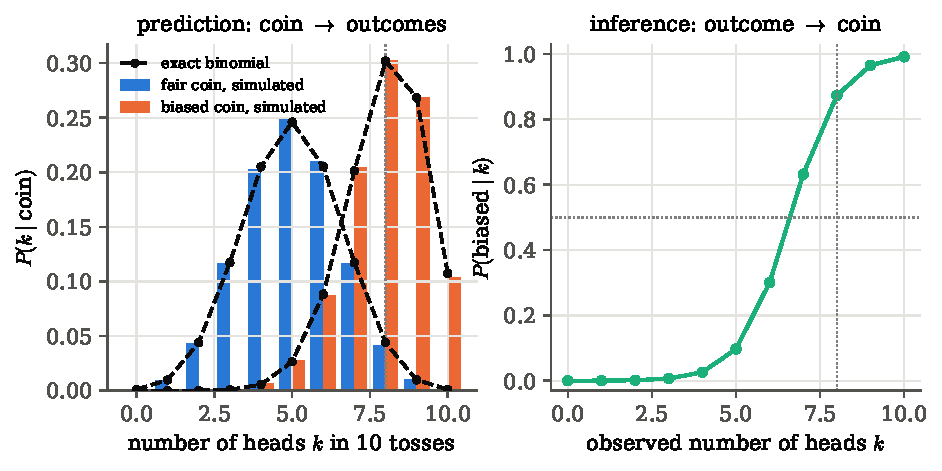
\includegraphics[width=\linewidth]{figures/ch00/coin_two_directions.pdf}
\caption{Left, prediction: each coin, tossed ten times over and over, spreads
its outcomes over $k=0,\dots,10$. Bars are simulated frequencies, dashed
curves the exact binomial probabilities; the dotted line marks the observed
$k=8$. Right, inference: for each possible observation $k$, the probability
that the coin was the biased one. The curve crosses the prior value $\frac12$
between $k=6$ and $k=7$, where the two coins explain the data about equally
well.}
\label{0a:fig:coin-two-directions}
\end{figure}

The forward number $\Prob(E\given H)$ and the backward number
$\Prob(H\given E)$ can be far apart. The classic case is a medical test, and
it goes through the same four steps. A disease affects $1\%$ of people. A test
detects it with probability $0.95$ and gives a false positive with probability
$0.10$.

\emph{The event.} A patient tests positive, written $+$.

\emph{What could have produced it?} The one thing we do not know is whether
the patient is ill. So there are two candidates: the patient has the disease
($D$), or does not ($D^c$).

\emph{How probable was the event under each?} If the patient is ill, the test
catches it $95\%$ of the time: $\Prob(+\given D)=0.95$. If the patient is
healthy, a positive result is a false alarm, which happens $10\%$ of the time:
$\Prob(+\given D^c)=0.10$.

\emph{Only then the priors, and the normalisation.} Before the test, the
patient was ill with probability $0.01$ and healthy with probability $0.99$.
Bayes' theorem \eqref{0a:eq:bayes} gives
\[
  \Prob(D\given +)=\frac{0.95\times0.01}{0.95\times0.01+0.10\times0.99}
  =\frac{0.0095}{0.1085}=0.0876 .
\]

\begin{pitfall}[$\Prob(E\given H)$ is not $\Prob(H\given E)$]
The two numbers answer different questions and can be wildly different. For
the positive test, the forward number $\Prob(+\given D)=0.95$ is not the
answer to ``is the patient ill?''; the answer is $\Prob(D\given +)=0.0876$.
Swapping the two conditionals is the ``prosecutor's fallacy''. Its statistical
twin appears in \cref{ch:04}: a $p$-value is \emph{not} the probability that
the null hypothesis is true.
\end{pitfall}

The lesson is not in the arithmetic. A positive result can come by two paths:
through the disease, or through a false alarm on a healthy person. Each
healthy person is unlikely to take the false-alarm path, but there are 99
healthy people for every ill one. The positive result favours the disease only
by the factor $\Prob(+\given D)/\Prob(+\given D^c)=0.95/0.10=9.5$. A factor of
$9.5$ acting on a prior of $1\%$ leaves the posterior below $10\%$, far from
the $95\%$ that the test's sensitivity suggests (\cref{5a:sec:shrink} draws it
to scale).

\paragraph{Two meanings of ``prediction''.}
In this chapter ``prediction'' means the forward direction, $H\to E$.
Statistics and machine-learning books also use the word for guessing a
\emph{new} data point (a regression output, a class label) after learning from
old data. That second kind of prediction is part of inference, because it
starts from data. When Wasserman lists ``prediction, classification,
clustering, and estimation'' as special cases of inference, he means the
second sense.

\providecommand{\zeroaIconLSS}{\tikz[baseline=0.1cm,x=1cm,y=1cm]{%
  \foreach \x/\y in {0.1/0.1,0.25/0.5,0.4/0.2,0.55/0.6,0.7/0.15,0.85/0.45,0.3/0.3,0.65/0.35,0.9/0.1,0.15/0.62}
    {\fill[formblue!80] (\x,\y) circle (0.9pt);}
  \draw[bdryred,thick] (0.5,0.35) circle (0.27);}}
\providecommand{\zeroaIconReal}{\tikz[baseline=0.1cm,x=1cm,y=1cm]{%
  \draw[formblue,thick] plot[domain=0.0:1.0,samples=30,smooth] (\x,{0.55*exp(-2.2*\x)+0.08});
  \foreach \x/\y in {0.1/0.47,0.3/0.39,0.5/0.26,0.7/0.21,0.9/0.17}
    {\draw[black] (\x,\y-0.06)--(\x,\y+0.06); \fill (\x,\y) circle (1pt);}
  \draw[softgray] (0,0)--(1.0,0);}}
\providecommand{\zeroaIconTree}{\tikz[baseline=0.2cm,x=1cm,y=1cm]{%
  \draw[softgray,thin] (0,0.3)--(0.45,0.55) (0,0.3)--(0.45,0.05)
    (0.45,0.55)--(0.95,0.68) (0.45,0.05)--(0.95,-0.08);
  \draw[bdryred,thick] (0.45,0.55)--(0.95,0.42) (0.45,0.05)--(0.95,0.18);
  \fill (0,0.3) circle (1pt);}}
\providecommand{\zeroaIconHist}{\tikz[baseline=0.1cm,x=1cm,y=1cm]{%
  \foreach \i/\h in {0/0.03,1/0.18,2/0.45,3/0.6,4/0.45,5/0.18,6/0.03}
    {\fill[formblue!70] (0.14*\i,0) rectangle ({0.14*\i+0.11},\h);}
  \draw[softgray] (-0.03,0)--(1.0,0);}}
\providecommand{\zeroaIconEst}{\tikz[baseline=0.1cm,x=1cm,y=1cm]{%
  \draw[formblue,thick] plot[domain=0.05:1.0,samples=40,smooth]
    (\x,{0.6*exp(-((\x-0.58)^2)/(2*0.11^2))});
  \draw[black,dashed] (0.5,0)--(0.5,0.68);
  \draw[softgray] (0,0)--(1.0,0);}}
\providecommand{\zeroaIconTest}{\tikz[baseline=0.1cm,x=1cm,y=1cm]{%
  \fill[bdryred!70] plot[domain=0.75:1.0,samples=15,smooth]
    (\x,{0.6*exp(-((\x-0.4)^2)/(2*0.16^2))}) -- (1.0,0) -- (0.75,0) -- cycle;
  \draw[formblue,thick] plot[domain=0.0:1.0,samples=40,smooth]
    (\x,{0.6*exp(-((\x-0.4)^2)/(2*0.16^2))});
  \draw[bdryred,thick] (0.75,0)--(0.75,0.35);
  \draw[softgray] (0,0)--(1.0,0);}}
\providecommand{\zeroaIconBayes}{\tikz[baseline=0.1cm,x=1cm,y=1cm]{%
  \draw[softgray,dashed] plot[domain=0.0:1.0,samples=30,smooth]
    (\x,{0.25*exp(-((\x-0.45)^2)/(2*0.3^2))});
  \draw[formblue,thick] plot[domain=0.3:1.0,samples=40,smooth]
    (\x,{0.65*exp(-((\x-0.65)^2)/(2*0.08^2))});
  \draw[softgray] (0,0)--(1.0,0);}}
\providecommand{\zeroaIconMC}{\tikz[baseline=0.05cm,x=1cm,y=1cm]{%
  \draw[softgray] (0,0) rectangle (0.7,0.7);
  \draw[formblue] (0.7,0) arc (0:90:0.7);
  \foreach \x/\y in {0.1/0.2,0.3/0.5,0.55/0.15,0.62/0.6,0.2/0.62,0.45/0.35,
                     0.66/0.4,0.15/0.4,0.35/0.1,0.5/0.55,0.27/0.3,0.6/0.27}
    {\fill[fibreorange] (\x,\y) circle (0.7pt);}}}
\providecommand{\zeroaIconMCMC}{\tikz[baseline=0.05cm,x=1cm,y=1cm]{%
  \draw[softgray,rotate around={30:(0.5,0.35)}] (0.5,0.35) ellipse (0.45 and 0.2);
  \draw[tangentgreen,thin] (0.05,0.02)--(0.2,0.12)--(0.28,0.3)--(0.42,0.26)
    --(0.5,0.4)--(0.62,0.44)--(0.55,0.33)--(0.7,0.5)--(0.78,0.46)--(0.66,0.38)
    --(0.8,0.6);
  \fill[tangentgreen] (0.05,0.02) circle (0.8pt);}}
\providecommand{\zeroaIconFisher}{\tikz[baseline=0.05cm,x=1cm,y=1cm]{%
  \draw[softgray,->] (0,0)--(1.0,0); \draw[softgray,->] (0,0)--(0,0.7);
  \draw[formblue,thick,rotate around={-35:(0.5,0.35)}] (0.5,0.35) ellipse (0.36 and 0.12);
  \fill[formblue] (0.5,0.35) circle (0.8pt);}}
\providecommand{\zeroaIconField}{\tikz[baseline=0.05cm,x=1cm,y=1cm]{%
  \draw[softgray,->] (0,0)--(1.0,0); \draw[softgray,->] (0,0)--(0,0.7);
  \draw[formblue,thick] plot[domain=0.05:0.95,samples=40,smooth]
    (\x,{0.12+0.45*exp(-((\x-0.3)^2)/(2*0.08^2))+0.2*exp(-((\x-0.62)^2)/(2*0.06^2))});}}
\providecommand{\zeroaIconTopo}{\tikz[baseline=0.05cm,x=1cm,y=1cm]{%
  \fill[bdryred!60] (0.15,0.45) circle (0.12);
  \fill[bdryred!60] (0.32,0.15) circle (0.1);
  \fill[bdryred!60,even odd rule] (0.72,0.35) circle (0.26) (0.72,0.35) circle (0.12);}}

\section{The questions the book answers}\label{0a:sec:questions}

One coin already raises many different questions, and each needs its own
tool. Keep the coin from the magic shop of \cref{0a:sec:two-directions}, but
forget the drawer. Now there is a single coin whose heads probability $p$ is
unknown, and we may toss it as often as we like.
\emph{How likely is 8 heads if $p=\frac12$?} is a forward calculation.
\emph{What is our best guess for $p$, and how wrong might it be?} is
estimation. \emph{Is 8 heads in 10 surprising for a fair coin?} is a test.
\emph{Which values of $p$ are plausible now?} is Bayesian inference.
\emph{Could we get any of these numbers by simulation instead of algebra?} is
Monte Carlo. \emph{How many tosses would we need to pin $p$ down to $\pm 0.01$?}
is a Fisher forecast. Each question has its own object that answers it, and
each has its own chapter. If we keep the questions apart, then for any tool we
can say which question it answers.

\paragraph{Same system, different measurements.}
A physicist knows this from the lab. One pendulum supports many experiments.
We can measure its period, estimate $g$ from the period, test whether the
period depends on the amplitude, or forecast how precisely a longer run would
pin down $g$. The pendulum stays the same. What changes is the question, and
with it the quantity we must compute. Probability tools work the same way: the
model stays fixed, and each tool computes the quantity that answers one
question about it.

\paragraph{The questions in words.}
Before any formula, each kind of question can be said in one sentence.
\begin{enumerate}[leftmargin=2em]
  \item \emph{Forward:} if the hypothesis is true, how often does this outcome occur?
  \item \emph{Spread:} what values can a random quantity take, and how are they distributed?
  \item \emph{Estimation:} what value of the parameter do the data point to, and how far off is that guess likely to be?
  \item \emph{Testing:} if only chance were at work, would a result like this, or one even more extreme in the same direction, be something we would reasonably expect?
  \item \emph{Bayesian inference:} which parameter values could have produced the data, and how probable is each one?
  \item \emph{Simulation:} can we get the answer to any of these by drawing random numbers, when the algebra is too hard?
  \item \emph{Forecasting:} before the experiment is run, how well could it measure the parameter?
  \item \emph{Choosing the summary:} which property of a field (a map, a density) carries the physics, and does it survive the nuisance effects of observation?
\end{enumerate}

The table below is the map of the book. Each row gives one question, the
object that answers it, and the chapter where that object is built. The
pictogram on the left of each row is a miniature of the central figure of that
chapter, the picture to remember for the row.

\begin{taxonomy}[which object answers which question]
\footnotesize
\renewcommand{\arraystretch}{1.35}
\begin{tabularx}{\linewidth}{@{}>{\centering\arraybackslash}m{1.15cm}
  >{\raggedright\arraybackslash}X >{\raggedright\arraybackslash}p{4.3cm}
  >{\centering\arraybackslash}m{1.0cm}@{}}
\toprule
& \textbf{The question, in words} & \textbf{The object that answers it} & \textbf{Ch.}\\
\midrule
\zeroaIconTree & How likely is this event, if the situation is as assumed? Which paths lead to it? &
  $\Prob(E\given H)$, summed over the paths of a probability tree & \ref{ch:01}\\
\zeroaIconHist & What values can a random quantity take, and how are they spread? &
  a distribution: pmf or pdf, CDF, mean and variance (binomial, Poisson, Gaussian, \dots) & \ref{ch:02}\\
\zeroaIconEst & What value of the parameter do the data point to, and how far off is that guess? &
  an estimator $\hat\theta$, its bias and variance, i.e.\ its sampling distribution; the likelihood $\Like(\theta)$ & \ref{ch:03}\\
\zeroaIconTest & If $\Hnull$ (the case whose distribution we know: ``it happened by chance'') were true, would a result like this, or more extreme in this direction, be expected? &
  a test statistic and its $p$-value, the tail probability under $\Hnull$ & \ref{ch:04}\\
\zeroaIconBayes & Which parameter values (or models) could have produced the data, and how probable is each? &
  the posterior $p(\params\given\data)\propto\Like(\params)\,p(\params)$; the evidence $Z$ for comparing models & \ref{ch:05}\\
\zeroaIconMC & What is the distribution of a quantity too complicated to compute by hand? &
  many simulated realisations; histograms and averages, with error $\propto 1/\sqrt N$ & \ref{ch:06}\\
\zeroaIconField & How do we summarise a random field (a sky map), and how does the summary fluctuate? &
  correlation function $\xi(r)$, power spectrum $P(k)$, $\Cell$ and its estimator $\Chat$ & \ref{ch:07}\\
\zeroaIconMC & How do a mask, noise and a beam change the sampling distribution of the summary? &
  Monte Carlo as the research instrument: simulated skies through the observation pipeline & \ref{ch:08}\\
\zeroaIconMCMC & How do we draw samples from a posterior in many dimensions without ever normalising it? &
  a Markov chain: a \emph{biased} random walker that lingers where the posterior is high & \ref{ch:09}\\
\zeroaIconFisher & Before the experiment, how well could it measure $\params$? &
  the Fisher matrix $\Fish$; forecast errors $\sigma_i\ge\sqrt{(\Fish^{-1})_{ii}}$ & \ref{ch:10}\\
\zeroaIconLSS & What do the positions and motions of galaxies say about how the Universe expands and how structure grows? &
  galaxy catalogues: $\xi(s)$ and $P(k)$ with weights and windows, the BAO ruler, peculiar velocities & \ref{ch:11}\\
\zeroaIconTopo & Is there information in how the structures of a field are connected, robust to nuisance effects? &
  excursion sets, Betti numbers, Euler characteristic, persistence: new random observables $S$ with a $P(S\given\theta)$ & \ref{ch:12}\\
\zeroaIconReal & Does the whole chain survive contact with real data? &
  complete analyses of Planck, SDSS and collider data, each reproducing a published result & \ref{ch:13}\\
\bottomrule
\end{tabularx}
\par\medskip\noindent
\Cref{ch:14} puts the rows back together: given a new problem, which row does
it belong to?
\end{taxonomy}

Most of the rows can be tried on the coin in a few lines. Four of them need a
new idea: estimation, testing, Monte Carlo and forecasting. Two definitions
carry all four.

\begin{workdef}[estimator, sampling distribution, $p$-value]
An \newterm{estimator} is a recipe that turns data into a guess for a
parameter, $\hat\theta=\hat\theta(\data)$ \unpack{a function of the data only,
e.g.\ $\hat p=k/n$, the fraction of heads}. Because the data are random, so is
$\hat\theta$. Its distribution over imagined repetitions of the whole
experiment is its \newterm{sampling distribution} \unpack{the histogram of
$\hat\theta$ if the experiment were rerun many times with the same true
$\theta$}. Its \newterm{bias} is $\E[\hat\theta]-\theta$ and its spread is
$\Var(\hat\theta)$.

A \newterm{null hypothesis} $\Hnull$ is a hypothesis whose sampling distribution
we know \unpack{``nothing but chance'', e.g.\ a fair coin}. Given an observed
value $t_{\rm obs}$ of a statistic $T$, the \newterm{$p$-value} is
\begin{equation}
  \pval=\Prob\big(T\ge t_{\rm obs}\given \Hnull\big),
  \label{0a:eq:pvalue}
\end{equation}
the probability, computed under $\Hnull$, of a result like the observed one
\emph{or even more in this direction} \unpack{here, larger values of $T$
count as further out}. We can compute it only because ``pure chance'' is the
one case whose distribution we have in hand. For a fair coin we know exactly
how often each head count turns up. A small $\pval$ says that, if the coin
really were fair, a result this far out would be a surprise (\cref{ch:04}).
\end{workdef}

\zeroaEx{the scatter of a fraction}
\label{0a:ex:mc-error}
The natural guess for $p$ is the fraction of heads. The question is whether
this guess is right on average, and how far it typically misses. Toss the coin
$n$ times and let $x_i=1$ if toss $i$ is heads and $x_i=0$ if it is tails. The
number of heads is $k=\sum_i x_i$, so the estimator is
$\hat p=k/n=\frac1n\sum_i x_i$. Its mean and variance are
\begin{align*}
  \E[\hat p] &\eqby{1} \frac1n\sum_{i=1}^n\E[x_i] \eqby{2} \frac1n\,n\,p = p,\\
  \Var(\hat p) &\eqby{3} \frac1{n^2}\sum_{i=1}^n\Var(x_i)
   \eqby{4} \frac1{n^2}\,n\,\big(\E[x_i^2]-\E[x_i]^2\big)
   \eqby{5} \frac{p-p^2}{n}=\frac{p(1-p)}{n} .
\end{align*}
\begin{explain}
  \item The expectation of a sum is the sum of expectations, and constants come out.
  \item $\E[x_i]=1\cdot p+0\cdot(1-p)=p$.
  \item For \emph{independent} tosses the variance of a sum is the sum of variances; a constant $c$ comes out as $c^2$.
  \item Definition of the variance, $\Var(x)=\E[x^2]-\E[x]^2$.
  \item $x_i^2=x_i$ because $x_i$ is $0$ or $1$, so $\E[x_i^2]=p$.
\end{explain}
So $\hat p$ is \newterm{unbiased}: on average it gives the true $p$. Its
standard deviation, the typical miss, is $\sqrt{p(1-p)/n}$. For $p=0.8$ this
is $0.126$ at $n=10$ and $0.040$ at $n=100$. The same algebra applies to
\emph{any} fraction of $N$ independent trials that each succeed with
probability $q$. That is why a Monte Carlo estimate of a probability $q$ from
$N$ simulated trials has error $\sqrt{q(1-q)/N}$.

\zeroaEx{the $p$-value of 8 heads}
\label{0a:ex:pvalue}
\emph{The observation.} Ten tosses gave 8 heads.
\emph{The question.} If the coin were fair, would 8 heads, or more than 8 heads, be something we would reasonably expect?
\emph{The pieces.} The null hypothesis is $\Hnull$: $p=\frac12$. The statistic
is the number of heads, $T=k$, and ``more extreme'' means more heads. Then
\begin{align*}
  \Prob(K\ge 8\given\Hnull)
  &\eqby{1} \Prob(8)+\Prob(9)+\Prob(10)
   \eqby{2} \frac{\binom{10}{8}+\binom{10}{9}+\binom{10}{10}}{2^{10}}
   = \frac{45+10+1}{1024}=\frac{56}{1024}=0.0547 .
\end{align*}
\begin{explain}
  \item ``This or more extreme in this direction'': the outcomes $8,9,10$ are exclusive, so their probabilities add.
  \item Binomial probabilities with $p=\frac12$ (\cref{0a:ex:forward}): every sequence has probability $2^{-10}$.
\end{explain}
About $5\%$ of fair ten-toss runs give 8 heads or more
(\cref{0a:fig:pvalue}). That is mildly surprising, not damning. The $p$-value
used only the distribution under $\Hnull$; it never mentioned the biased coin.
It is \emph{not} $\Prob(\Hnull\given\text{data})$, the probability that the
coin is fair. In the drawer story of \cref{0a:sec:two-directions} (equal
numbers of fair and biased coins) that number was $\Prob(F\given 8)=0.127$, the
answer to a different question.

\begin{figure}[htbp]
\centering
\begin{tikzpicture}
\begin{axis}[width=10cm,height=4.6cm,ybar,bar width=0.55cm,ymin=0,ymax=0.27,
  xtick={0,...,10},xlabel={number of heads $k$ in 10 tosses of a fair coin},
  ylabel={$\Prob(k\given\Hnull)$},axis x line*=bottom,axis y line*=left,
  enlarge x limits=0.06,tick label style={font=\footnotesize},
  label style={font=\small}]
\addplot[bar shift=0pt,fill=formblue!45,draw=formblue] coordinates
  {(0,0.000977) (1,0.009766) (2,0.043945) (3,0.117188) (4,0.205078) (5,0.246094)
   (6,0.205078) (7,0.117188)};
\addplot[bar shift=0pt,fill=bdryred!70,draw=bdryred] coordinates
  {(8,0.043945) (9,0.009766) (10,0.000977)};
\end{axis}
\node[font=\small,bdryred,anchor=west] at (6.9,2.2) {$56/1024=0.055$};
\end{tikzpicture}
\caption{The null distribution for ten tosses of a fair coin. The red bars are
the observed $k=8$ and the outcomes more extreme in the same direction; their
total height is the $p$-value. The blue bars never enter.}
\label{0a:fig:pvalue}
\end{figure}

\zeroaEx{a forecast before any toss: the Fisher information}
\label{0a:ex:fisher}
The question is asked before any toss: how precisely \emph{could} $n$ tosses
measure $p$? The answer depends on how sharply the data single out one value
of $p$. The likelihood of one particular sequence with $k$ heads is
$\Like(p)=p^k(1-p)^{n-k}$, so its logarithm is
$\ln\Like(p)=k\ln p+(n-k)\ln(1-p)$. A log-likelihood with a sharp peak pins
$p$ down; a flat one does not. The \newterm{Fisher information} measures the
sharpness. It is minus the expected curvature of $\ln\Like$ at the true $p$:
\begin{align*}
  I(p) &\eqby{1} -\E\!\left[\frac{\dd^2\ln\Like}{\dd p^2}\right]
   \eqby{2} \E\!\left[\frac{k}{p^2}+\frac{n-k}{(1-p)^2}\right]
   \eqby{3} \frac{np}{p^2}+\frac{n(1-p)}{(1-p)^2}
   = \frac np+\frac n{1-p}
   = \frac{n}{p(1-p)} .
\end{align*}
\begin{explain}
  \item Definition (\cref{ch:10}): a sharply curved log-likelihood pins the parameter down.
  \item $\frac{\dd}{\dd p}\ln\Like=\frac kp-\frac{n-k}{1-p}$; differentiate again and change sign.
  \item $\E[k]=np$ and $\E[n-k]=n(1-p)$.
\end{explain}
The Cram\'er--Rao bound (\cref{ch:03,ch:10}) says that no unbiased estimator
can beat $\Var(\hat\theta)\ge 1/I$. Here $1/I=p(1-p)/n$, exactly the variance of
$\hat p$ found in \cref{0a:ex:mc-error}. So the fraction of heads is as good
as any unbiased guess can be. The forecast needs no data, only an assumed
$p$. To reach a standard deviation $\sigma_p=0.01$ at $p\approx0.8$ we need
$n=p(1-p)/\sigma_p^2=0.16/10^{-4}=1600$ tosses.

\paragraph{What this bought us.}
The same coin gave three different numbers: a spread $\sqrt{p(1-p)/n}$
(estimation), a tail probability $0.055$ (testing) and a required number of
tosses, $1600$ (forecasting). None of them is a posterior. Each answers its
own row of the table. Confusing the rows is the most common error in applied
statistics.

\begin{pitfall}[what a $p$-value and a confidence interval do \emph{not} say]
A $p$-value of $0.055$ does not mean ``the coin is fair with probability
$0.055$''. It is $\Prob(\text{data this extreme}\given\Hnull)$, a forward
number. Likewise, a $95\%$ confidence interval is a recipe that covers the
true value in $95\%$ of repetitions of the experiment; it is not an interval
that contains the parameter with probability $95\%$. Only the posterior of
\cref{ch:05} makes probability statements about parameters.
\end{pitfall}

\subsection*{The questions in code}

The script \pyname{02_coin_questions.py} checks two of these answers by brute
force. The key lines are:

\pyfile[firstline=23,lastline=37]{code/ch00/02_coin_questions.py}{Estimation and a $p$-value by simulation}

The first block reruns the whole ten-toss experiment, and the hundred-toss
one, $50\,000$ times with the true $p=0.8$, and keeps each $\hat p$. That list
is a sample from the sampling distribution of $\hat p$. The second block is
\cref{0a:ex:pvalue} in one line. The third block simulates fair experiments.
In it, \pyname{np.cumsum(fair >= K_OBS)} counts, for every $N$ at once, how
many of the first $N$ experiments were as extreme as the observed 8 heads.
The last line is the error bar $\sqrt{q(1-q)/N}$ of \cref{0a:ex:mc-error}.

The run confirms both calculations. The standard deviation of $\hat p$ is
$\QSdTen$ at $n=10$ (theory $\QSdTenTh$) and $\QSdHundred$ at $n=100$ (theory
$\QSdHundredTh$). The mean at $n=10$ is $\QMeanTen$, so the estimator is
unbiased, as derived. The Monte Carlo $p$-value is $\QPmcHundred$ after
$N=\QNhundred$ experiments and $\QPmcMillion\pm\QSigmaMillion$ after $10^6$,
against the exact $\QPexact$.

\begin{figure}[htbp]
\centering
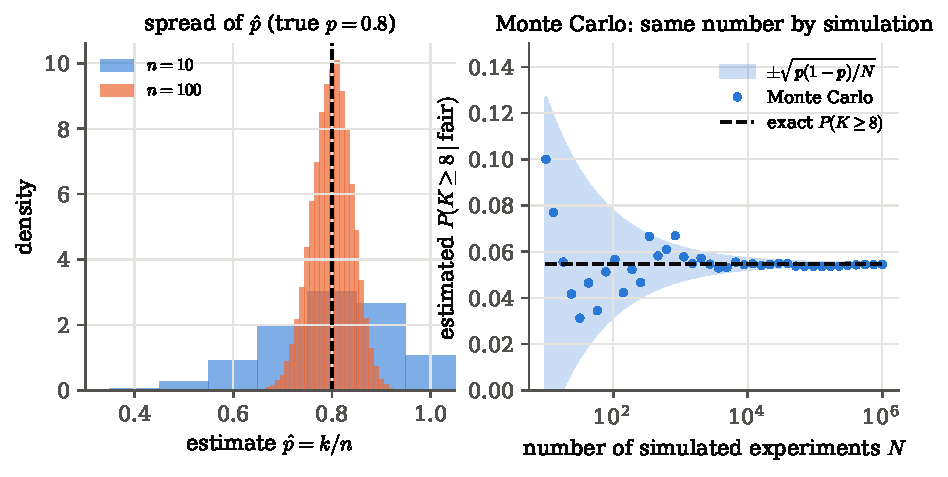
\includegraphics[width=\linewidth]{figures/ch00/coin_questions.pdf}
\caption{Left: the sampling distribution of $\hat p=k/n$ for a coin with
$p=0.8$. With 10 tosses the guesses spread over most of the interval; with 100
they crowd around the true value, ten times more tightly in variance. Right:
the Monte Carlo estimate of $\Prob(K\ge8\given$fair$)$ as the number of
simulated experiments grows. The points wander inside the shaded
$\pm\sqrt{p(1-p)/N}$ band, which narrows onto the exact value.}
\label{0a:fig:coin-questions}
\end{figure}

\begin{inpractice}[verification versus research]
Monte Carlo has two uses. Here it only \emph{verifies} a number we could
compute exactly, $56/1024$; the first use is to check theory and code against
each other. The second use is as the \emph{research instrument}, where no
exact answer exists. Suppose the ``coin'' were a CMB sky seen through a
galactic mask, with noise and a beam. Nobody can write down the distribution
of the measured power spectrum. Instead one simulates thousands of skies and
makes a histogram. The code is the same: draw, compute the statistic, count.
\Cref{ch:06} builds the first use, \cref{ch:08} the second.
\end{inpractice}

\paragraph{The same idea under different names.}
The vocabulary changes between communities, but the ideas do not. What
statisticians call \emph{estimation}, the machine-learning literature calls
\emph{learning}. The observed values $(X_i,Y_i)$ are there the \emph{training
sample}. The inputs $X_i$ are \emph{covariates} in one language and
\emph{features} in the other. A few more terms recur. A \emph{hypothesis} is a
subset of the parameter space. A \emph{confidence interval} is a recipe that
covers the unknown value with a stated frequency. \emph{Bayesian inference}
means using data to update beliefs, whereas \emph{frequentist inference}
collects the methods whose long-run frequency behaviour is guaranteed
\mainref{p.~xi}. Prediction in the second sense of
\cref{0a:sec:two-directions}, together with classification, clustering and
estimation, counts as a special case of inference \mainref{p.~ix}. Only the
Bayesian rows of the table above (\cref{ch:05,ch:09}) share out credibility
among parameter values \srcref{Kruschke}{p.~15}. The estimation and testing
rows instead describe how a \emph{procedure} behaves over repeated
experiments. The null hypothesis is the case whose distribution we know,
because we assume the result happened by chance \mainref{p.~149}.

\section{The pipeline: from a physical model to a statement about physics}\label{0a:sec:pipeline}

Real data are never fed into Bayes' theorem whole; they are compressed first.
A Planck temperature map at the resolution used for cosmology has about
$5\times10^{7}$ pixels. The model we want to test, $\Lambda$CDM, has six
parameters. Nobody writes Bayes' theorem directly for fifty million correlated
pixels. Instead the map is compressed into its angular power spectrum $\Chat$,
about $2500$ numbers, and those are compared with the theory. Each step of
this is a choice. First we decide that the power spectrum is the information
that matters. Then we work out how $\Chat$ fluctuates from one sky to another.
Only then do we infer the six parameters. Written out as one pipeline, this
chain of choices has an arrow for every tool in the book. Knowing which arrow
we are on is the fastest way to know what a tool is for.

\paragraph{Microstates and macrostates.}
Statistical mechanics works the same way. A gas has $10^{23}$ momenta, but we
never infer anything from the full microstate. We compress it into a few
macroscopic summaries (pressure, energy, magnetisation). Fluctuation theory
then tells us how much those summaries scatter; for example, the energy of a
system at temperature $T$ with heat capacity $C_V$ fluctuates by
$\langle\Delta E^2\rangle=k_BT^2C_V$. A summary is chosen for two reasons: it
carries the physics we care about, and its fluctuations can be calculated.
Data analysis makes the same two demands of every summary statistic.

\paragraph{Six stages, six questions.}
The whole book runs along one chain, drawn in \cref{0a:fig:pipeline}:
\begin{equation}
\boxed{\begin{array}{l}
\text{a theory with parameters }\params\;\rightarrow\;\text{the map or data set it produces}\\[2pt]
\qquad\rightarrow\;\text{decide which features of the data carry the physics}\\[2pt]
\qquad\rightarrow\;\text{compress the data into a statistic }S
\;\rightarrow\;\text{work out how }S\text{ scatters, }P(S\given\params)\\[2pt]
\qquad\rightarrow\;\text{say what the observed }S\text{ tells us about }\params
\end{array}}
\label{0a:eq:workflow}
\end{equation}
In symbols, the last two stages are $P(S\given\theta)$ and
$P(\theta\given S)\propto P(S\given\theta)P(\theta)$, where $\theta$ stands for
the parameters $\params$. The stages answer different kinds of question. The
choice of summary decides what should be measured. The last two stages decide
how the uncertainty in that measurement carries over to the parameters. The
same chain applies whether the data vector holds pixelised CMB temperatures or
measured bandpowers $C_\ell$, and whatever the number $M$ of model parameters.
Each stage is a question.
\begin{enumerate}[leftmargin=2em]
  \item \emph{Physical model:} what theory, with which parameters $\params$, could have produced the data?
  \item \emph{Field or dataset:} what exactly did the instrument record, and how does it depend on $\params$ and on noise?
  \item \emph{What information matters:} which property of the data is sensitive to $\params$, and which is only nuisance?
  \item \emph{Summary:} which function $S[\data]$ of the data keeps that property and discards the rest?
  \item \emph{Sampling distribution:} if the experiment were repeated with the same $\params$, how would $S$ scatter? That is $P(S\given\params)$.
  \item \emph{Infer physics:} given the one $S$ we observed, which $\params$ are plausible? That is $P(\params\given S)\propto P(S\given\params)P(\params)$.
\end{enumerate}
Stages 1 to 5 are the forward direction of \cref{0a:sec:two-directions}.
Stage 6 is the backward direction.

\begin{figure}[htbp]
\centering
\begin{tikzpicture}[
  stage/.style={draw=accent,thick,rounded corners=2pt,fill=ideabg,align=center,
                font=\small,text width=5.4cm,minimum height=0.95cm},
  flow/.style={->,thick,accent},
  chap/.style={font=\footnotesize,align=left,anchor=west,text width=5.3cm}]
  \node[stage] (m) at (0,0)     {physical model, parameters $\params$\\[-1pt]\footnotesize $\Lambda$CDM, a signal strength $\mu$, a coin's $p$};
  \node[stage] (d) at (0,-1.7)  {field or dataset $\data$\\[-1pt]\footnotesize a sky map, event counts, a strain record};
  \node[stage] (c) at (0,-3.4)  {decide which features\\ carry the physics};
  \node[stage] (s) at (0,-5.1)  {compress into a statistic $S[\data]$\\[-1pt]\footnotesize $k$, $\Chat$, $\xi(r)$, $\beta_0(\nu)$, \dots};
  \node[stage] (p) at (0,-6.8)  {work out how $S$ scatters: $P(S\given\params)$};
  \node[stage,fill=takebg,draw=tangentgreen] (i) at (0,-8.5) {what $S$ says about $\params$: $P(\params\given S)\propto P(S\given\params)\,P(\params)$};
  \draw[flow] (m) -- (d); \draw[flow] (d) -- (c); \draw[flow] (c) -- (s);
  \draw[flow] (s) -- (p); \draw[flow] (p) -- (i);
  \node[chap] at (3.2,-0.85) {\textbf{simulate the forward model:}\\ probability and distributions (Ch.~\ref{ch:01}, \ref{ch:02}), random fields (Ch.~\ref{ch:07}), Monte Carlo (Ch.~\ref{ch:06})};
  \node[chap] at (3.2,-2.55) {\textbf{which information?} phases and morphology that $\Cell$ discards (Ch.~\ref{ch:07}, \ref{ch:12})};
  \node[chap] at (3.2,-4.25) {\textbf{build the summary:} estimators (Ch.~\ref{ch:03}), $\Chat$ (Ch.~\ref{ch:07}), Betti numbers, $\chi$ (Ch.~\ref{ch:12})};
  \node[chap] at (3.2,-5.95) {\textbf{how does $S$ scatter?} error propagation (Ch.~\ref{ch:03}), null distributions (Ch.~\ref{ch:04}), Monte Carlo through mask, noise, beam (Ch.~\ref{ch:06}, \ref{ch:08})};
  \node[chap] at (3.2,-7.65) {\textbf{turn scatter into constraints:} tests (Ch.~\ref{ch:04}), Bayes (Ch.~\ref{ch:05}), MCMC (Ch.~\ref{ch:09}), Fisher (Ch.~\ref{ch:10})};
  \draw[->,thick,softgray,dashed] (i.west) -- ++(-0.6,0) |- (m.west);
  \node[font=\footnotesize,softgray,align=right,anchor=east] at (-3.6,-4.25) {check the\\ model, then\\ design the\\ next\\ experiment};
\end{tikzpicture}
\caption{The pipeline of the whole book. Boxes are the stages; the notes on
the right say which chapters serve the step from one box to the next. The
top four boxes are forward modelling and a choice, the fifth is probability
theory applied to that choice, and only the last box is inference. The dashed
loop is the step statisticians call a posterior predictive check: simulate
data from the inferred model and ask whether they look like the real data.}
\label{0a:fig:pipeline}
\end{figure}

One step of the pipeline is not mathematics: choosing what information
matters. It is a physics decision, and \cref{0a:sec:summaries} takes it up.
The next step, building the summary, does have a precise test: it tells us
when compressing the data loses nothing.

\begin{workdef}[summary statistic, sampling distribution, sufficiency]
A \newterm{summary statistic} is any function $S=S[\data]$ of the data
\unpack{a number or a short vector computed from the data alone, e.g.\ the
number of heads $k$}. Its \newterm{sampling distribution} $P(S\given\params)$
is the distribution of $S$ over repetitions of the experiment with the
parameters held fixed \unpack{the histogram of $S$ over many simulated
universes that share the same $\params$}. The summary is \newterm{sufficient}
for $\params$ if the likelihood depends on the data only through $S$:
\begin{equation}
  P(\data\given\params)=g\big(S[\data],\params\big)\,h(\data)
  \label{0a:eq:factorisation}
\end{equation}
\unpack{$h$ may depend on the data but not on $\params$, so it cancels from
every posterior and every likelihood ratio}. Then $P(\params\given\data)
=P(\params\given S)$: nothing about $\params$ was thrown away.
\end{workdef}

The coin shows how the test works. The data are the whole sequence
$x_1,\dots,x_n$ of zeros and ones ($x_i=1$ for heads, as in
\cref{0a:ex:mc-error}). Is the number of heads enough, or does the order of
the tosses also tell us something about $p$? Write down the probability of the
sequence:
\begin{align}
  P(x_1,\dots,x_n\given p)
  &\eqby{1} \prod_{i=1}^{n} p^{x_i}(1-p)^{1-x_i} \nonumber\\
  &\eqby{2} p^{\sum_i x_i}\,(1-p)^{\,n-\sum_i x_i}
   \eqby{3} p^{k}(1-p)^{n-k} .
  \label{0a:eq:coin-suff}
\end{align}
\begin{explain}
  \item The tosses are independent; one toss gives $p$ if $x_i=1$ and $1-p$ if $x_i=0$, which is what $p^{x_i}(1-p)^{1-x_i}$ says.
  \item Products of powers of the same base add their exponents.
  \item $k=\sum_i x_i$ is the number of heads.
\end{explain}
The sequence enters only through $k$. So \eqref{0a:eq:coin-suff} has the form
\eqref{0a:eq:factorisation} with $S=k$, $g=p^k(1-p)^{n-k}$ and $h=1$, and the
order of the tosses carries no information about $p$. The sampling
distribution of the summary $k$ is the binomial of \cref{0a:ex:forward}. The
last stage puts it into Bayes' theorem.

\zeroaEx{the coin through the whole pipeline}
\label{0a:ex:coin-pipeline}
The last stage asks: after $k$ heads in $n$ tosses, which values of the heads
probability $p$ are plausible, and how plausible is each? Now $p$ can be any
number in $[0,1]$, not one of two coins. Take a flat prior, $p(p)=1$ on
$[0,1]$, which treats every value as equally plausible beforehand. The
posterior for $p$ is then
\begin{align*}
  p(p\given k)
  &\eqby{1} \frac{P(k\given p)\cdot 1}{\int_0^1 P(k\given p')\,\dd p'}
   \eqby{2} \frac{p^{k}(1-p)^{n-k}}{\int_0^1 p'^{k}(1-p')^{n-k}\,\dd p'}
   \eqby{3} \frac{(n+1)!}{k!\,(n-k)!}\,p^{k}(1-p)^{n-k} .
\end{align*}
\begin{explain}
  \item Bayes' theorem for a continuous parameter: the sum over hypotheses in \eqref{0a:eq:bayes} becomes an integral.
  \item The factor $\binom nk$ does not depend on $p$ and cancels between numerator and denominator.
  \item The Beta integral $\int_0^1 p^a(1-p)^b\,\dd p=\frac{a!\,b!}{(a+b+1)!}$ for non-negative integers $a,b$ (proved by $b$ integrations by parts, each moving one power from $(1-p)$ to $p$).
\end{explain}
Where is this posterior centred, and how wide is it? Its mean and variance
follow from the same Beta integral:
\begin{align*}
  \E[p\given k] &\eqby{1} \frac{(n+1)!}{k!\,(n-k)!}\int_0^1 p^{k+1}(1-p)^{n-k}\dd p
   \eqby{2} \frac{(n+1)!}{k!\,(n-k)!}\cdot\frac{(k+1)!\,(n-k)!}{(n+2)!}=\frac{k+1}{n+2},\\
  \E[p^2\given k] &\eqby{3} \frac{(k+1)(k+2)}{(n+2)(n+3)},\qquad
  \Var(p\given k) \eqby{4} \frac{(k+1)(n-k+1)}{(n+2)^2(n+3)} .
\end{align*}
\begin{explain}
  \item Definition of the mean: multiply the posterior by $p$ and integrate.
  \item Beta integral with $a=k+1$, $b=n-k$; then $(k+1)!/k!=k+1$ and $(n+1)!/(n+2)!=1/(n+2)$.
  \item Same steps with $a=k+2$.
  \item $\E[p^2]-\E[p]^2$, put over the common denominator $(n+2)^2(n+3)$: the numerator is $(k+1)\big[(k+2)(n+2)-(k+1)(n+3)\big]=(k+1)(n-k+1)$.
\end{explain}
For large $n$ the variance tends to $\hat p(1-\hat p)/n$ with $\hat p=k/n$.
This is the same number as the sampling variance $p(1-p)/n$ of
\cref{0a:ex:mc-error}, with $\hat p$ in place of $p$. Here are the six stages
for the coin. Model: a coin with unknown $p$. Data: a toss sequence. What
matters: the fraction of heads, since the order carries no information.
Summary: $k$. Sampling distribution: binomial. Inference: the Beta-shaped
posterior.

\zeroaEx{the CMB through the pipeline}
\label{0a:ex:cmb-pipeline}
The same six stages apply to a map of the sky. The data are the temperature
fluctuation $\Delta T(\hat n)$ in each direction $\hat n$. Expand it in
spherical harmonics $Y_{\ell m}$, the sphere's analogue of Fourier modes:
$\Delta T(\hat n)=\sum_{\ell m}\alm Y_{\ell m}(\hat n)$. A multipole $\ell$
corresponds to an angular scale of roughly $180^\circ/\ell$, and $m$ runs from
$-\ell$ to $\ell$. Statistical isotropy \unpack{no preferred direction, so the
statistics are unchanged by rotations} means
$\E[\alm a^*_{\ell'm'}]=\Cell\,\delta_{\ell\ell'}\delta_{mm'}$. So the theory
predicts one number per $\ell$, the power spectrum $\Cell(\params)$. The
natural summary averages the squared sizes of the $2\ell+1$ measured
coefficients at each $\ell$. Is it right on average?
\begin{align*}
  \E\big[\Chat\big]
  &\eqby{1} \E\Big[\frac{1}{2\ell+1}\sum_{m=-\ell}^{\ell}|\alm|^2\Big]
   \eqby{2} \frac{1}{2\ell+1}\sum_{m=-\ell}^{\ell}\E\big[\alm a^*_{\ell m}\big]
   \eqby{3} \frac{1}{2\ell+1}(2\ell+1)\,\Cell = \Cell .
\end{align*}
\begin{explain}
  \item Definition of the estimator $\Chat$: the average power in the $2\ell+1$ modes of multipole $\ell$.
  \item $|a|^2=aa^*$, and the expectation of a sum is the sum of expectations.
  \item Isotropy with $\ell'=\ell$, $m'=m$; there are $2\ell+1$ values of $m$.
\end{explain}
So $\Chat$ is unbiased. It still scatters, because only $2\ell+1$ modes exist
at each $\ell$ and an average of few numbers is noisy. For a Gaussian sky the
scatter is $\sqrt{2/(2\ell+1)}\,\Cell$; this is cosmic variance, derived in
\cref{ch:07}. The pipeline reads: model ($\Lambda$CDM) $\to$ map $\to$ ``the
physics is in the variance per scale'' $\to$ $\Chat$ $\to$
$P(\Chat\given\params)$ $\to$ posterior on six parameters. For a full-sky
Gaussian map without noise, $\Chat$ is sufficient, exactly as $k$ is for the
coin (\cref{0a:ex:cmb-like}). For a masked or noisy sky, or a non-Gaussian
one, it is not, and that is where \cref{ch:08,ch:12} begin.

\paragraph{What this bought us.}
Compression is safe exactly when the likelihood depends on the data only
through the summary. For the coin this holds for $k$. For a Gaussian isotropic
full sky it holds for $\Chat$. Any other compression is a choice whose cost
must be checked.

\subsection*{The pipeline in code}

The script \pyname{03_pipeline_coin.py} checks the sufficiency claim and runs the pipeline for growing $n$.

\pyfile[firstline=23,lastline=32]{code/ch00/03_pipeline_coin.py}{Two sequences with the same $k$ have the same likelihood}
\pyfile[firstline=44,lastline=54]{code/ch00/03_pipeline_coin.py}{The posterior after $n=10,100,1000$ tosses}

The first listing evaluates \eqref{0a:eq:coin-suff} toss by toss for two
sequences with 8 heads each, HHHHHHHHTT and THHTHHHHHH, on a grid of $2001$
values of $p$. The largest difference between the two likelihood curves is
$\PipeMaxDiff$. That is floating-point round-off, so the curves are the same
function, as sufficiency says.

The second listing computes the posterior on the grid. It works in logarithms,
because a product of a thousand probabilities underflows. It subtracts the
maximum before exponentiating, and then normalises numerically; that sum over
the grid is Bayes' denominator. One simulated run with true $p=0.8$ gives:
\begin{itemize}[itemsep=1pt,leftmargin=1.2em]
  \item at $n=10$, $k=\PipeKTen$, posterior standard deviation $\PipeSdTen$,
        against the large-$n$ formula $\sqrt{\hat p(1-\hat p)/n}=\PipeSdThTen$;
  \item at $n=100$, $k=\PipeKHundred$, $\PipeSdHundred$ against $\PipeSdThHundred$;
  \item at $n=1000$, $k=\PipeKThousand$, $\PipeSdThousand$ against $\PipeSdThThousand$.
\end{itemize}
At $n=10$ (here $k=\PipeKTen$) the grid reproduces the exact value of
\cref{0a:ex:coin-pipeline},
\[
  \sqrt{\frac{(k+1)(n-k+1)}{(n+2)^2(n+3)}}=\PipeSdExactTen .
\]
The large-$n$ formula becomes accurate only as $n$ grows.

\begin{figure}[htbp]
\centering
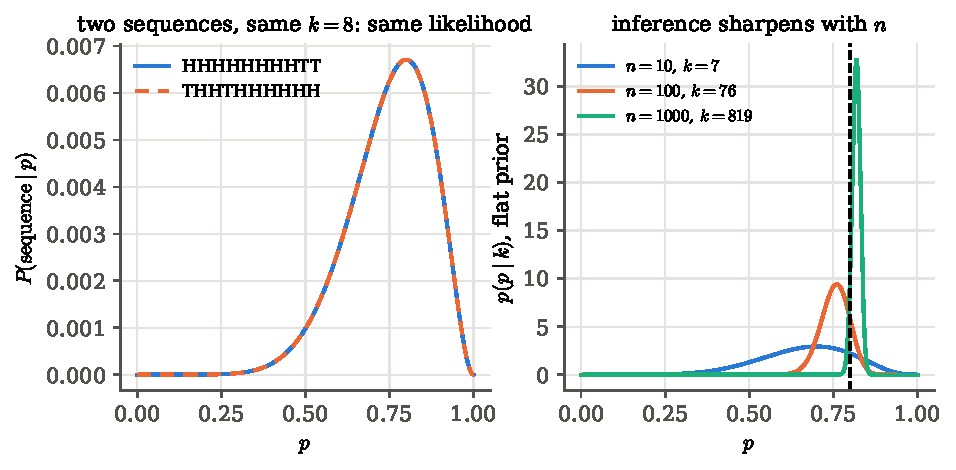
\includegraphics[width=\linewidth]{figures/ch00/pipeline_coin.pdf}
\caption{Left: the likelihoods of two different toss sequences with the same
number of heads lie exactly on top of each other, so the summary $k$ lost
nothing. Right: the flat-prior posterior for $p$ after 10, 100 and 1000
tosses of one coin with true $p=0.8$ (dashed line). The width shrinks like
$1/\sqrt n$.}
\label{0a:fig:pipeline-coin}
\end{figure}

\paragraph{How research uses the pipeline.}
In current research the hard stages are the middle ones. For the coin and the
full-sky Gaussian CMB every stage has a closed form, but real problems rarely
do. Which summary of a galaxy survey carries the neutrino mass: the power
spectrum $P(k)$, the bispectrum, void counts, Betti numbers? What is
$P(S\given\params)$ when $S$ is measured on a masked, noisy, nonlinear field?
Usually nobody can write it down. So one simulates the forward model many
times at fixed $\params$ and estimates the mean and covariance of $S$ from the
simulations (\cref{ch:08,ch:12}). The inference stage then uses the standard
machinery of \cref{ch:05,ch:09,ch:10}.

\begin{pitfall}[the posterior depends on the summary]
If $S$ is not sufficient, $P(\params\given S)$ is broader than
$P(\params\given\data)$, and it can be broader in a direction that matters. That
is not a bug of Bayes' theorem; it is the price of the compression chosen at
stage~4. Two analyses of the same data with different summaries can
legitimately give different constraints.
\end{pitfall}

\paragraph{Kruschke's five steps.}
The pipeline is the physicist's version of the five steps of Bayesian data
analysis \srcref{Kruschke}{p.~25}. They match the six stages one by one.
\emph{Identify the data relevant to the research question}: stages 2 and 3,
the dataset and the choice of what information matters. \emph{Define a
descriptive model for the data}: stages 1 and 5, the model and the sampling
distribution. \emph{Specify a prior}: the factor $P(\params)$ of stage 6.
\emph{Reallocate credibility across parameter values}: the posterior of
stage 6. \emph{Check the posterior predictions}: the dashed loop of
\cref{0a:fig:pipeline}.

\section{Which summary? From amplitude to topology}\label{0a:sec:summaries}

Two simulated universes are handed to us as density maps. In one, the dense
matter forms a connected web of filaments. In the other, it sits in isolated
clumps. By construction both maps have the same mean, the same variance and
the same power spectrum $P(k)$. An analysis that compresses each map to $P(k)$
will call them identical, yet a glance tells them apart.

Whether we catch this difference or miss it is decided at the third stage of
the pipeline of \cref{0a:sec:pipeline}: \emph{deciding which features carry
the physics}. The power spectrum answers one question: how much variance does
each scale carry? The two maps raise a different one. Is there physically
meaningful information in the way the high and low regions of a field are
connected, information that the summary we already use, here $P(k)$, does not
bring out? A field admits several kinds of summary, and two fields can be
built to agree on some kinds and differ on the others. Topological summaries
are worth the trouble for a second reason too: some of them are protected
against the distortions that observation introduces.

\paragraph{A recording with its phases scrambled.}
Take a recording of speech, $h(t)$, and Fourier transform it to $\tilde h(f)$.
Keep every amplitude $|\tilde h(f)|$ and replace every phase by a random one.
The power spectrum is untouched, and so is the loudness, yet the result is a
hiss. What made it speech was in the phases: in \emph{where} and \emph{how}
the power is arranged in time. For a field, the phases decide whether high
values line up into filaments, gather into blobs or scatter as noise.
Summaries beyond the power spectrum are ways of reading the phases.

\paragraph{The central question for a field.}
A theory predicts a field $\phi(\mathbf x)$ over space. The experiment gives
us one copy of it, and an imperfect one. On the way to us its values have been
pushed around by perturbations, by noise, by smoothing, by whatever happened
to the signal while it travelled. The question is whether something about the
\emph{shape and structure} of what we receive survives every change we count
as a nuisance. If it does, we can read it off without first undoing those
changes. Write such a change as a \newterm{nuisance transformation}
$\phi\to\phi'=\mathcal N[\phi]$; examples are noise, smoothing by a beam,
lensing, and a monotonic response of the detector. Three questions follow.
\begin{enumerate}[leftmargin=2em]
  \item What do we want to know: how large the field is, how its values at different points are related, or how its structures are shaped and connected?
  \item Which summary $T$ answers that question?
  \item Is there a summary that the nuisance cannot change, $T[\mathcal N[\phi]]=T[\phi]$, for a stated class of $\mathcal N$?
\end{enumerate}

The answers to the first question form a ladder. Each rung up keeps less of
the raw values and more of how they are arranged.

\begin{taxonomy}[the summaries of a field]
\small
\renewcommand{\arraystretch}{1.3}
\begin{tabularx}{\linewidth}{@{}>{\raggedright\arraybackslash}p{2.3cm}
  >{\raggedright\arraybackslash}X >{\raggedright\arraybackslash}p{4.4cm}@{}}
\toprule
\textbf{kind} & \textbf{the question it answers} & \textbf{examples}\\
\midrule
amplitude & how large is the field typically? & $\langle\phi\rangle$, $\Var(\phi)$, the one-point pdf $P(\phi)$\\
correlation & how are values a distance $r$ apart related? & $\xi(r)$, $P(k)$, $\Cell$\\
higher order & is there information beyond Gaussian two-point statistics? & bispectrum $B$, trispectrum $T$, skewness\\
morphology & what sizes and shapes do the structures have? & areas, perimeters, curvature of excursion sets\\
topology & how are the structures connected, and how many holes do they have? & Betti numbers $\beta_i$, Euler characteristic $\chi$, persistence\\
\bottomrule
\end{tabularx}
\smallskip
These are not rival theories of probability. They are different maps from
the same data to different summaries $S[\phi]$. Once $S$ is chosen it is an
ordinary random observable with a sampling distribution $P(S\given\params)$,
and \cref{ch:03,ch:04,ch:05,ch:09,ch:10} apply to it unchanged.
\end{taxonomy}

A \emph{Gaussian} random field is special: all its information is in the
first two rungs. Its higher-order summaries are fixed functions of its power
spectrum. Measuring them is therefore a consistency test (a search for
non-Gaussianity), not new information. For any non-Gaussian field, from the
late-time cosmic web to a map with foreground residuals, the upper rungs carry
information that $P(k)$ does not.

Topology is a property of shapes, not of functions. So to say what topology
measures, we must first turn a field into a shape.

\begin{workdef}[excursion set, Betti numbers, Euler characteristic]
For a threshold $\nu$, the \newterm{excursion set} of $\phi$ on a domain
$\mathcal M$ is
\begin{equation}
  X_\nu=\{\mathbf x\in\mathcal M:\ \phi(\mathbf x)>\nu\}
  \label{0a:eq:excursion}
\end{equation}
\unpack{the region of the map where the field exceeds $\nu$, e.g.\ the sky
directions hotter than $\nu$}. In two dimensions the \newterm{Betti numbers}
are $\beta_0(X_\nu)$ \unpack{the number of separate pieces} and $\beta_1(X_\nu)$
\unpack{the number of independent holes, i.e.\ enclosed regions that are not part of the set}. The
\newterm{Euler characteristic} is $\chi=\beta_0-\beta_1$. These numbers do
not change when the set is stretched or bent without tearing or gluing
(\cref{ch:12}). A summary $T$ is a \newterm{robust observable} under a
class of nuisance transformations if $T[\mathcal N[\phi]]=T[\phi]$ for every
$\mathcal N$ in the class.
\end{workdef}

\begin{figure}[htbp]
\centering
\begin{tikzpicture}
  \begin{scope}[x=0.55cm,y=0.75cm]
    \draw[->,softgray] (0.4,-1.7) -- (10.3,-1.7) node[anchor=north east,font=\footnotesize] {$x$};
    \draw[->,softgray] (0.6,-1.7) -- (0.6,2.1) node[anchor=east,font=\footnotesize] {$\phi$};
    \draw[form] plot[domain=0.6:10,samples=160,smooth]
      (\x,{0.9*sin(1.1*\x r)+0.55*sin((2.7*\x+1.0) r)+0.3*cos((4.3*\x+0.5) r)});
    \begin{scope}
      \clip (0.6,0.6) rectangle (10,2.0);
      \draw[bdry] plot[domain=0.6:10,samples=160,smooth]
        (\x,{0.9*sin(1.1*\x r)+0.55*sin((2.7*\x+1.0) r)+0.3*cos((4.3*\x+0.5) r)});
    \end{scope}
    \draw[dashed,black] (0.6,0.6) -- (10,0.6);
    \node[font=\footnotesize,anchor=west] at (10,0.6) {$\nu$};
    \foreach \a/\b in {1.133/1.534,2.129/2.877,6.641/7.723}
      {\draw[bdryred,line width=2.2pt] (\a,-1.7) -- (\b,-1.7);}
    \node[font=\footnotesize,bdryred,anchor=north] at (5.3,-1.9) {$X_\nu$: three pieces, $\beta_0=3$};
  \end{scope}
  \begin{scope}[xshift=7.1cm,yshift=0.3cm]
    \fill[bdryred!55] (0,0.9) circle (0.42);
    \node[font=\scriptsize,align=center,anchor=north] at (0,0.35) {$\beta_0{=}1,\ \beta_1{=}0$\\$\chi=1$};
    \fill[bdryred!55,even odd rule] (1.9,0.9) circle (0.45) (1.9,0.9) circle (0.2);
    \node[font=\scriptsize,align=center,anchor=north] at (1.9,0.35) {$\beta_0{=}1,\ \beta_1{=}1$\\$\chi=0$};
    \fill[bdryred!55] (-0.2,-0.9) circle (0.25) (0.3,-0.75) circle (0.2);
    \node[font=\scriptsize,align=center,anchor=north] at (0.05,-1.3) {$\beta_0{=}2,\ \beta_1{=}0$\\$\chi=2$};
    \fill[bdryred!55,even odd rule] (1.9,-0.85) ellipse (0.6 and 0.38)
      (1.65,-0.85) circle (0.13) (2.15,-0.85) circle (0.13);
    \node[font=\scriptsize,align=center,anchor=north] at (1.9,-1.3) {$\beta_0{=}1,\ \beta_1{=}2$\\$\chi=-1$};
  \end{scope}
\end{tikzpicture}
\caption{Left: a field along a line, a threshold $\nu$, and the excursion set
(the red intervals on the axis), which here has three pieces. Right: four
two-dimensional sets with their numbers of pieces $\beta_0$, holes $\beta_1$
and Euler characteristic $\chi=\beta_0-\beta_1$. Stretching any of them leaves
all three numbers unchanged; cutting or gluing does not.}
\label{0a:fig:excursion}
\end{figure}

Two facts make these summaries useful. First, a change of phases can leave the
lower rungs untouched while moving the upper ones. Second, a distortion that
changes each value by the same increasing function leaves the excursion sets
themselves untouched. Each takes a few lines to prove.

\zeroaEx{phase randomisation keeps the power spectrum and the variance}
\label{0a:ex:phases}
The question: if we keep every Fourier amplitude of a field and scramble the
phases, what stays the same? Let $\phi(\mathbf x)$ live on an $N$-pixel
periodic grid with zero mean, and let
$\tilde\phi_{\mathbf k}=\sum_{\mathbf x}\phi(\mathbf x)e^{-2\pi i\mathbf k\cdot\mathbf x/L}$
be its discrete Fourier transform ($L$ the side length in pixels). Build a new
field $\phi'$ with $\tilde\phi'_{\mathbf k}=|\tilde\phi_{\mathbf k}|e^{i\alpha_{\mathbf k}}$,
random phases $\alpha_{\mathbf k}$ with $\alpha_{-\mathbf k}=-\alpha_{\mathbf k}$
(so that $\phi'$ is real). Then
\begin{align*}
  P'(k) &\eqby{1} \big\langle|\tilde\phi'_{\mathbf k}|^2\big\rangle_{|\mathbf k|=k}
   \eqby{2} \big\langle|\tilde\phi_{\mathbf k}|^2\big\rangle_{|\mathbf k|=k}=P(k),\\
  \Var(\phi') &\eqby{3} \frac1N\sum_{\mathbf x}\phi'(\mathbf x)^2
   \eqby{4} \frac1{N^2}\sum_{\mathbf k}|\tilde\phi'_{\mathbf k}|^2
   \eqby{5} \frac1{N^2}\sum_{\mathbf k}|\tilde\phi_{\mathbf k}|^2
   = \Var(\phi) .
\end{align*}
\begin{explain}
  \item The measured power spectrum: average $|\tilde\phi_{\mathbf k}|^2$ over the wavevectors in a shell of radius $k$.
  \item $|re^{i\alpha}|^2=r^2$: the phase drops out of every $|\tilde\phi'_{\mathbf k}|^2$ individually.
  \item Zero mean (the $\mathbf k=0$ coefficient, the sum of the field, is left at zero).
  \item Parseval's theorem for the discrete Fourier transform, $\sum_{\mathbf x}|\phi(\mathbf x)|^2=\frac1N\sum_{\mathbf k}|\tilde\phi_{\mathbf k}|^2$.
  \item Same step as (2).
\end{explain}
So every summary built from the amplitudes $|\tilde\phi_{\mathbf k}|$ alone is
identical for $\phi$ and $\phi'$. The skewness, the excursion sets and their
Betti numbers depend on the phases, so they are free to change.

\zeroaEx{a monotonic distortion leaves the excursion sets alone}
\label{0a:ex:monotonic}
Suppose the detector does not record $\phi$ itself but
$\phi'(\mathbf x)=f(\phi(\mathbf x))$, with $f$ strictly increasing. Examples are a detector
with a nonlinear but monotonic response, or a lognormal model $\phi'=e^{\phi}$.
The question: which summaries of $\phi$ can we still read off $\phi'$ without
knowing $f$? Compare the excursion sets. For every threshold $\nu$
\begin{align*}
  X'_{f(\nu)} &\eqby{1} \{\mathbf x:\ f(\phi(\mathbf x))>f(\nu)\}
   \eqby{2} \{\mathbf x:\ \phi(\mathbf x)>\nu\} = X_\nu .
\end{align*}
\begin{explain}
  \item Definition \eqref{0a:eq:excursion} applied to $\phi'$ at the threshold $f(\nu)$.
  \item A strictly increasing $f$ preserves order both ways: $f(a)>f(b)$ exactly when $a>b$.
\end{explain}
The excursion sets are the same regions of the domain $\mathcal M$. So the
curves $\beta_0(\nu)$, $\beta_1(\nu)$, $\chi(\nu)$ are the same, except that
the threshold is relabelled $\nu\to f(\nu)$. Meanwhile the variance, the
skewness and $P(k)$ of $\phi'$ all change; for $f=\exp$ the one-point pdf goes
from Gaussian to lognormal. Here topology is a robust observable in the exact
sense of the working definition above, $T[\mathcal N[\phi]]=T[\phi]$; the power
spectrum is not.

\zeroaEx{counting holes by counting cells}
\label{0a:ex:cells}
How do we count holes in a real map, where nobody can look at every piece?
On a pixel grid a set is a union of square pixels, and $\chi$ can be computed
by counting: $\chi=V-E+F$. Here $V$ is the number of corners, $E$ the number of
pixel edges and $F$ the number of pixels of the set, each counted once. A
single pixel has $4-4+1=1$. Two separate pixels have $8-8+2=2$. Now take a
ring of eight pixels around an empty centre (a $3\times3$ block with the
middle removed). It uses all $4\times4=16$ corners of the block, $12$
horizontal and $12$ vertical edges, and $8$ pixels:
\[
  \chi=16-24+8=0=\beta_0-\beta_1=1-1 .
\]
So local counting finds a hole without ever looking for it. That is how
$\chi(\nu)$ is computed on real maps (\cref{ch:12}).

\paragraph{What this bought us.}
The ladder of summaries is a ladder of questions. Two fields can agree on the
bottom two rungs and differ above them. And some topological summaries are
exactly unchanged by a class of distortions that change every rung below.

\subsection*{Two fields with one power spectrum}

The script \pyname{04_same_spectrum.py} builds the two universes from the
opening of \cref{0a:sec:summaries}: one clumpy, one not, with the same power
spectrum. Field A drops $\SameNblob$ points at random on a $256\times256$
periodic grid and smooths them into blobs. Field B is A with its phases
randomised, exactly as in \cref{0a:ex:phases}:

\pyfile[firstline=28,lastline=34]{code/ch00/04_same_spectrum.py}{Keeping every $|\tilde\phi_k|$ and replacing the phases}

The random phases are taken from the Fourier transform of a real white-noise
map. Such phases automatically satisfy the condition
$\alpha_{-\mathbf k}=-\alpha_{\mathbf k}$, so B is real. Pieces are counted
with the function \pyname{scipy.ndimage.label}, which labels connected groups
of pixels above the threshold.

The run shows the lower rungs agreeing and the upper ones not. The variances
are $\Var(A)=\SameVarA$ and $\Var(B)=\SameVarB$, and the two binned power
spectra differ by at most a fraction $\SamePkMaxDev$, which is round-off. The
skewness separates the fields: $\SameSkewA$ for the clumps of A, $\SameSkewB$
for B, which is close to Gaussian. The topology separates them more sharply.
At $\nu=3$ (three standard deviations) A has $\beta_0=\SameBzeroA$ separate
pieces, one per surviving blob, and B has $\SameBzeroB$. At $\nu=0$ the counts
are $\SameBzeroAzero$ and $\SameBzeroBzero$.

\begin{figure}[htbp]
\centering
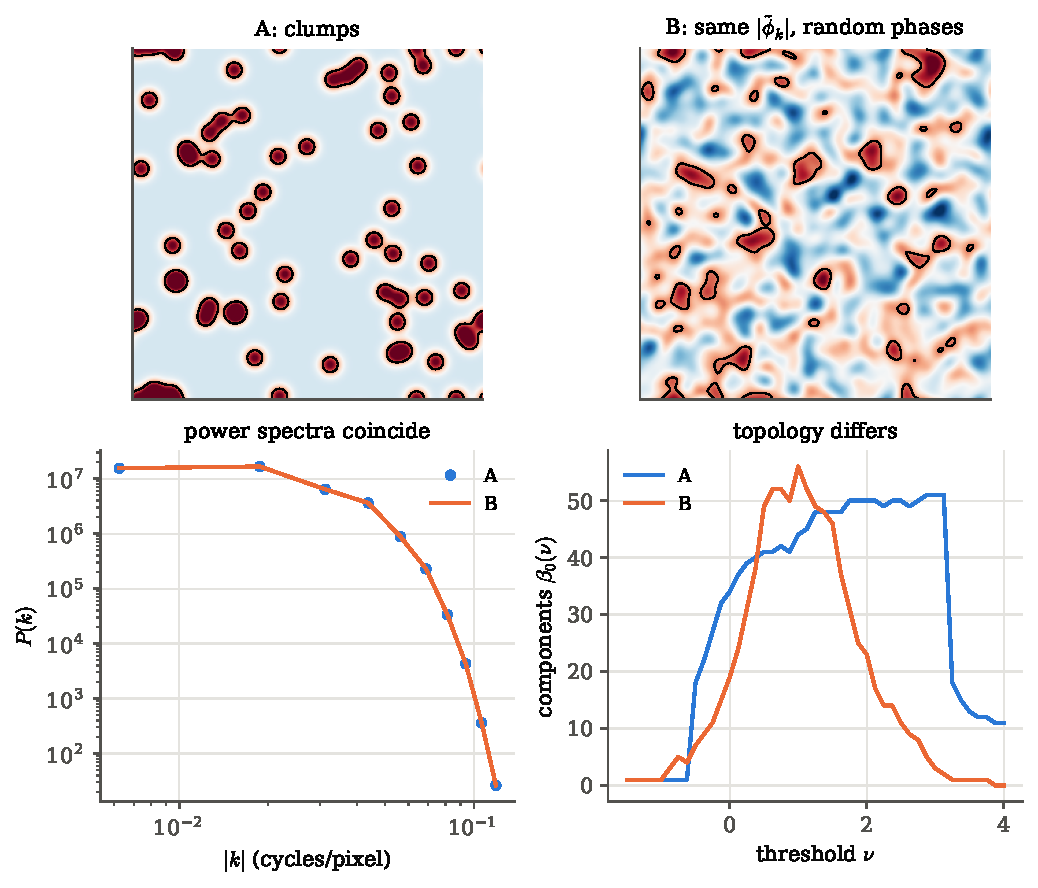
\includegraphics[width=0.92\linewidth]{figures/ch00/same_spectrum.pdf}
\caption{Top: the clumpy field A and its phase-randomised twin B, with the
contour at $\nu=1.5$. Bottom left: their power spectra coincide point by point.
Bottom right: the number of connected pieces of the excursion set as the
threshold is raised. B behaves like a Gaussian field, with most pieces near
$\nu\approx1$ and few at high threshold; A keeps one piece per blob right up to
the blob peaks, so its curve stays high until $\nu\approx3$.}
\label{0a:fig:same-spectrum}
\end{figure}

\subsection*{Topology that survives observation, and topology that records dynamics}

The detector with a monotonic response (\cref{0a:ex:monotonic}) is the
simplest protected case. A more physical one is CMB polarisation. The linear
polarisation is described by the two Stokes parameters $Q$ and $U$, which
combine into $P=Q+iU$. At isolated points where $Q=U=0$ the polarisation
direction is undefined. Walk once round such a \newterm{polarisation
singularity}, and the phase of $P$ turns by a whole multiple of $2\pi$. This
whole number, the winding index or charge, cannot change under a smooth
one-to-one remapping of the sky such as weak lensing. Lensing certainly
changes the polarisation map, converting $E$ modes into $B$ modes. But it can
only move and distort singularities; it cannot change their charges
continuously \cite{VachaspatiLue2003,HutererVachaspati2005,ChallinorChon2002}.
The protection fails where its assumptions fail: pairs of singularities can be
created or annihilated, and noise and finite resolution can hide them.

A count at a single threshold is fragile, since nothing makes $\nu=1\sigma$
special. The remedy is to follow each piece and hole as $\nu$ is lowered.
Record the threshold where each feature appears (its birth) and the one where
it merges or fills in (its death). This gives \newterm{persistence}. A feature
with a long lifetime $\Delta\nu=\nu_{\rm death}-\nu_{\rm birth}$ is a real
structure; a short-lived one is likely noise. \Cref{ch:12} builds this with a
union--find algorithm.

\begin{pitfall}[topology is not conserved by dynamics]
Invariance holds under a stated class of deformations, not under physics in
general. Gravitational collapse is not a monotonic remapping of the initial
density: it moves matter, merges clumps and opens voids, and the Betti numbers
of the cosmic web change with time \cite{Wilding2021,Pranav2017}. There the
changing topology is the \emph{signal}. The scientific question is either
``what survives the nuisance?'' or ``what changes because of the physics?''.
Both are legitimate; they are different questions. Note also that a mask cuts
excursion sets at its edge and so changes their topology, just as it changes
the covariance of $\Chat$ (\cref{ch:08}).
\end{pitfall}

\paragraph{How research uses a topological summary.}
A CMB map is a function $T:S^2\to\R$ from directions on the sphere to
temperatures. To use its topology, generate many Gaussian skies from the
fiducial power spectrum $\Cell$. Pass each sky through the beam, the noise and
the mask. Measure $\beta_0(\nu)$, $\beta_1(\nu)$ and $\chi(\nu)$ on every
realisation. The mean and covariance of these curves over the realisations
define a likelihood for the observed curves, and the posterior follows as for
any other summary. This is the Monte Carlo study of \cref{ch:08} with $\Chat$
replaced by a Betti curve, and it is where the book ends (\cref{ch:12}).

\section{One idea, several detectors}\label{0a:sec:universal}

A collider experiment counts events in bins of invariant mass and asks whether
there is a bump. A CMB satellite measures the temperature of the sky and asks
for the cosmological parameters. A gravitational-wave interferometer records a
strain time series and asks for the masses of an inspiralling binary. The
instruments share nothing, and the statistics looks different in each
community's papers: Poisson log-likelihoods, $\Cell$ likelihoods, matched
filters. Underneath, all three ask one question: \emph{for a given set of
parameters $\params$, how probable is the noise realisation that would turn
the model's prediction into the data we actually recorded?} Because the
question is the same, the idea needs to be developed only once. Writing it out
for each detector, and for a topological summary, shows how it applies
everywhere.

\paragraph{The noise you would need.}
The likelihood is the probability density of the noise that the data
require. Put the model prediction $m(\params)$ on one side and the data
$\data$ on the other. The difference $\data-m(\params)$ is the noise that
nature \emph{would have had to supply} if $\params$ were the truth. A value of
$\params$ that needs a wildly improbable noise realisation is implausible. A
value that needs only a typical fluctuation is plausible. What differs between
detectors is only the statistics of their noise. \Cref{ch:03} builds the
likelihood from this picture one step at a time.

\paragraph{The same four questions for any detector.}
\begin{enumerate}[leftmargin=2em]
  \item What does the model predict, as a function of $\params$?
  \item What is the noise: its distribution, and its correlations?
  \item For a trial $\params$, how probable is the noise realisation $\data-m(\params)$ (or, for counts, the observed counts given their expectation)?
  \item Read that probability as a function of $\params$, and feed it to Bayes, MCMC or Fisher.
\end{enumerate}

\begin{workdef}[likelihood from a noise model]
If the data are prediction plus noise, $\data=m(\params)+\bm\epsilon$, and the
noise has a known density $p_\epsilon$, then
\begin{equation}
  \Like(\params)\equiv p(\data\given\params)=p_\epsilon\big(\data-m(\params)\big)
  \label{0a:eq:like-noise}
\end{equation}
\unpack{the density of the noise realisation that is required, evaluated at
the observed data and read as a function of $\params$}. The
\newterm{likelihood} is not a probability distribution over $\params$: it need
not integrate to one over $\params$, and only its shape and ratios matter.
\end{workdef}

\begin{figure}[htbp]
\centering
\begin{tikzpicture}[x=1.05cm,y=1.1cm]
  \draw[->,softgray] (0,0) -- (8.6,0) node[anchor=north east,font=\footnotesize] {$x$};
  \draw[->,softgray] (0,0) -- (0,4.1) node[anchor=east,font=\footnotesize] {$d$};
  \draw[form] (0.3,0.905) -- (8.2,3.67);
  \node[font=\footnotesize,formblue,anchor=west] at (8.2,3.67) {$m(x;\theta)$};
  \foreach \x/\r in {1/0.35,2/-0.30,3/0.15,4/-0.55,5/0.25,6/0.45,7/-0.20}{
    \pgfmathsetmacro{\m}{0.8+0.35*\x}
    \draw[bdryred,thick] (\x,\m) -- (\x,{\m+\r});
    \fill[black] (\x,{\m+\r}) circle (1.6pt);
  }
  \draw[fibre] plot[domain=-1.1:1.1,samples=50,smooth]
    ({4+0.9*exp(-(\x)^2/(2*0.35^2))},{2.2+\x});
  \draw[faint] (4,1.1) -- (4,3.3);
  \node[font=\footnotesize,fibreorange,anchor=west,align=left] at (5.05,1.25) {$p(d_4\given\theta)$: how probable\\ is the red residual?};
  \node[font=\footnotesize,bdryred,anchor=east,align=right] at (3.85,0.45) {required noise\\ $\epsilon_i=d_i-m(x_i;\theta)$};
\end{tikzpicture}
\caption{Data as prediction plus noise. The blue line is the model for one
trial value of $\theta$; the black points are the data; the red segments are
the noise each point would need if that $\theta$ were true. The orange curve
at the fourth point is the Gaussian noise density: a long red segment lands in
its tail and costs a lot of probability. The likelihood multiplies these costs
over all points; moving $\theta$ moves the line and changes every red segment.}
\label{0a:fig:residuals}
\end{figure}

The commonest case is independent Gaussian noise: each data point $d_i$ has
its own noise $\epsilon_i\sim\Normal(0,\sigma_i^2)$, a Gaussian with mean zero
and standard deviation $\sigma_i$. Then \eqref{0a:eq:like-noise} gives the
workhorse of physics:
\begin{align}
  \ln\Like(\params)
  &\eqby{1} \ln\prod_{i=1}^{N}\frac{1}{\sqrt{2\pi\sigma_i^2}}
    \exp\!\Big[-\frac{(d_i-m_i(\params))^2}{2\sigma_i^2}\Big] \nonumber\\
  &\eqby{2} -\frac12\sum_{i=1}^{N}\frac{(d_i-m_i(\params))^2}{\sigma_i^2}
    -\frac12\sum_{i=1}^{N}\ln(2\pi\sigma_i^2)
   \equiv -\frac12\chi^2(\params)+\text{const} .
  \label{0a:eq:chi2}
\end{align}
\begin{explain}
  \item Independent noise: the joint density is the product of one Gaussian per data point, evaluated at the required noise $d_i-m_i(\params)$.
  \item The log of a product is the sum of logs, and $\ln e^{u}=u$.
\end{explain}
If the noise in different data points is correlated, with covariance matrix
$\Cmat$, the product of separate Gaussians becomes one multivariate Gaussian:
$\ln\Like=-\frac12(\data-m)\T\Cmat^{-1}(\data-m)-\frac12\ln\det(2\pi\Cmat)$.
The statistical logic is the same as before. Only the model for the
probability of the data has changed.

With a whole data vector and many parameters, the backward question of
\cref{0a:sec:two-directions} is still the same. The data vector is what we
saw. Every value of $\params$ is a candidate explanation. The likelihood says
how readily each candidate would have produced those data (\cref{ch:05}).
Reading the likelihood as the plausibility of the fluctuation needed to turn
the model into the data is also how maximum likelihood is motivated
\mainref{p.~122}.

\begin{taxonomy}[one question, four implementations]
\small
\renewcommand{\arraystretch}{1.3}
\begin{tabularx}{\linewidth}{@{}>{\raggedright\arraybackslash}p{1.9cm}
  >{\raggedright\arraybackslash}p{2.4cm} >{\raggedright\arraybackslash}X
  >{\raggedright\arraybackslash}p{4.1cm}@{}}
\toprule
\textbf{experiment} & \textbf{data} & \textbf{noise model} & \textbf{log-likelihood}\\
\midrule
collider & counts $n_i$ in bins & Poisson with mean $\lambda_i(\mu)=b_i+\mu s_i$ & $\sum_i[n_i\ln\lambda_i-\lambda_i]$\\
CMB & $\alm$, or $\Chat$ & Gaussian random field on the sphere, variance $\Cell$ per mode & $-\frac12\sum_\ell(2\ell+1)\big[\Chat/\Cell+\ln\Cell\big]$\\
GW detector & strain $d(t)$ & stationary Gaussian noise with PSD $S_n(f)$ & $-\frac12(d-h\,|\,d-h)$\\
topology & Betti curves $S=\beta_0(\nu),\dots$ & unknown in closed form: simulated & $-\frac12(S-\bar S)\T\widehat{\Cmat}^{-1}(S-\bar S)$ from simulations\\
\bottomrule
\end{tabularx}
\end{taxonomy}

\zeroaEx{the collider: a bump in Poisson counts}
\label{0a:ex:poisson}
The data are event counts $n_i$ in bins $i$ of invariant mass. The question:
how probable are these counts for a given signal strength $\mu$? In bin $i$
the expected count is $\lambda_i(\mu)=b_i+\mu s_i$: the background $b_i$ plus a
signal template $s_i$ scaled by $\mu$. Counts in different bins are
independent Poisson variables. Then
\begin{align*}
  \ln\Like(\mu)
  &\eqby{1} \ln\prod_i\frac{\lambda_i^{n_i}e^{-\lambda_i}}{n_i!}
   \eqby{2} \sum_i\big[n_i\ln\lambda_i(\mu)-\lambda_i(\mu)\big]-\sum_i\ln n_i!,\\
  \frac{\dd\ln\Like}{\dd\mu}
  &\eqby{3} \sum_i s_i\Big(\frac{n_i}{\lambda_i(\mu)}-1\Big)=0
  \quad\text{at the maximum-likelihood }\hat\mu .
\end{align*}
\begin{explain}
  \item Poisson probability of $n_i$ events when $\lambda_i$ are expected (\cref{ch:02}), multiplied over independent bins.
  \item Log of a product; the last sum does not depend on $\mu$ and drops out of every ratio.
  \item $\dd\lambda_i/\dd\mu=s_i$; the chain rule on $n_i\ln\lambda_i$ gives $n_is_i/\lambda_i$.
\end{explain}
The condition says that at the best fit the observed counts match the
expected ones on average, with each bin weighted by its signal $s_i$. There is
no $\sigma_i$ anywhere. The Poisson distribution carries its own noise: its
variance equals its mean.

\zeroaEx{the CMB: the full-sky $\Cell$ likelihood}
\label{0a:ex:cmb-like}
The data are the harmonic coefficients of the sky (\cref{0a:ex:cmb-pipeline});
the parameters are the power spectrum values $\Cell$. The question: how
probable is the observed sky for given $\Cell$? Write the sky in a real
orthonormal basis of spherical harmonics, so that at each multipole $\ell$
there are $2\ell+1$ real coefficients $r_{\ell j}$. For a Gaussian isotropic
sky they are independent, and each is $\Normal(0,\Cell)$. Then
\begin{align*}
  \ln\Like(\{\Cell\})
  &\eqby{1} \sum_{\ell}\sum_{j=1}^{2\ell+1}\Big[-\frac{r_{\ell j}^2}{2\Cell}-\frac12\ln(2\pi\Cell)\Big]\\
  &\eqby{2} -\frac12\sum_\ell\Big[\frac{(2\ell+1)\Chat}{\Cell}+(2\ell+1)\ln\Cell\Big]+\text{const}\\
  &= -\frac12\sum_\ell(2\ell+1)\Big[\frac{\Chat}{\Cell}+\ln\Cell\Big]+\text{const}.
\end{align*}
\begin{explain}
  \item \eqref{0a:eq:chi2} with $d_i\to r_{\ell j}$, zero mean and variance $\Cell$.
  \item $\sum_j r_{\ell j}^2=(2\ell+1)\Chat$, the definition of $\Chat$ in \cref{0a:ex:cmb-pipeline} (a real orthonormal basis is a rotation of the complex one, so the sum of squares is unchanged); $\ln 2\pi$ goes into the constant.
\end{explain}
Three things follow. First, the data enter only through $\Chat$, so $\Chat$
is sufficient in the sense of \eqref{0a:eq:factorisation}, as claimed in
\cref{0a:ex:cmb-pipeline}. Second, setting
$\partial\ln\Like/\partial\Cell=\frac12(2\ell+1)[\Chat/\Cell^2-1/\Cell]=0$
gives $\Cell=\Chat$: the measured spectrum is the best fit. Third,
$(2\ell+1)\Chat/\Cell=\sum_j(r_{\ell j}/\sqrt{\Cell})^2$ is a sum of $2\ell+1$
squared unit Gaussians, which is a $\chi^2_{2\ell+1}$ variable (\cref{ch:02}).
That is how the script below simulates one sky's spectrum without making a
map.

\zeroaEx{the GW detector: Gaussian noise with a PSD}
\label{0a:ex:whittle}
The detector records a strain $d(t)=h(t;\params)+n(t)$ for a time $T$: a
signal $h$ from the binary with parameters $\params$, plus noise $n$. The
question: how probable is the required noise $d-h$ for given $\params$? The
noise is simplest in frequency space, so Fourier transform,
$\tilde d(f)=\int d(t)e^{-2\pi ift}\dd t$, at the frequencies $f_k=k/T$, and
write $\tilde d_k=\tilde d(f_k)$. Stationary Gaussian noise has independent
Fourier modes. Its one-sided power spectral density $S_n(f)$ \unpack{the
noise power per unit frequency, counting positive frequencies only} fixes
their size, $\E|\tilde n_k|^2=\frac T2 S_n(f_k)$. We also need one fact about
complex Gaussians. A complex Gaussian $z$ with $\E|z|^2=\sigma^2$ has density
$\frac{1}{\pi\sigma^2}e^{-|z|^2/\sigma^2}$ (its real and imaginary parts are
independent, each with variance $\sigma^2/2$). So
\begin{align*}
  \ln\Like(\params)
  &\eqby{1} -\sum_{k}\frac{|\tilde d_k-\tilde h_k(\params)|^2}{\tfrac T2 S_n(f_k)}+\text{const}
   \eqby{2} -2\sum_k\Delta f\,\frac{|\tilde d_k-\tilde h_k|^2}{S_n(f_k)}+\text{const}\\
  &\eqby{3} -2\int_0^\infty\frac{|\tilde d(f)-\tilde h(f)|^2}{S_n(f)}\,\dd f+\text{const}
   \eqby{4} -\frac12\,(d-h\,|\,d-h)+\text{const},
\end{align*}
\begin{explain}
  \item The required noise in mode $k$ is $\tilde d_k-\tilde h_k$; the product of independent complex Gaussians becomes a sum in the log. The $-\ln(\pi\sigma^2)$ terms do not depend on $\params$.
  \item The mode spacing is $\Delta f=1/T$, so $\frac{1}{T/2}=2\Delta f$.
  \item For long $T$ the sum over modes becomes an integral over positive frequencies.
  \item Definition of the noise-weighted inner product $(a\,|\,b)=4\,\mathrm{Re}\int_0^\infty\tilde a(f)\tilde b^*(f)/S_n(f)\,\dd f$.
\end{explain}
This is the $\chi^2$ of \eqref{0a:eq:chi2} in the frequency domain, with each
frequency weighted by how noisy the detector is there. Maximising it over
$\params$ is matched filtering. Its curvature gives the Fisher matrix of
\cref{ch:10}.

\paragraph{What this bought us.}
Poisson counts, a Gaussian sky and coloured detector noise give three
formulas that look unrelated. Each one is \eqref{0a:eq:like-noise}: the
probability of the fluctuation that would turn the prediction into the data.

\subsection*{The three detectors in code}

The script \pyname{05_three_detectors.py} generates data for all three and
checks the noise model of each. For the collider and the GW detector the key lines are:

\pyfile[firstline=27,lastline=33]{code/ch00/05_three_detectors.py}{Collider: Poisson data and a scan of $\ln\Like(\mu)$}
\pyfile[firstline=53,lastline=58]{code/ch00/05_three_detectors.py}{GW: coloured Gaussian noise drawn in the frequency domain}

\emph{Collider.} The first block draws one Poisson count per bin. The
expected counts are a falling background plus a peak at $125$ GeV with
$\mu=1$. It then evaluates the $\ln\Like$ of \cref{0a:ex:poisson} on a grid of
$\mu$. With $\ColNtot$ events in total, the maximum is at
$\hat\mu=\ColMuHat$. The values of $\mu$ whose $\ln\Like$ lies within
$\frac12$ of the maximum run from $\ColMuLo$ to $\ColMuHi$; for a nearly
Gaussian likelihood this is the $\pm1\sigma$ interval (\cref{ch:03}). The true
$\mu=1$ is inside.

\emph{GW detector.} The second block draws each Fourier mode with real and
imaginary parts of variance $TS_n/4$, so that $\E|\tilde n_k|^2=TS_n/2$. The
periodogram $2|\tilde d_k|^2/T$ should then scatter around $S_n$. Averaged
over $\GwNbins$ frequency bins away from the injected line, its ratio to $S_n$
is $\GwMeanRatio$.

\emph{CMB.} One full sky is simulated as
$\Chat=\Cell\,\chi^2_{2\ell+1}/(2\ell+1)$ around the Planck best fit, using
the third result of \cref{0a:ex:cmb-like}. The mean of $\Chat/\Cell$ over
$2\le\ell\le1500$ is $\CmbMeanRatio$. Its scatter is $\CmbScatterLow$ for
$\ell\le30$ but only $\CmbScatterHigh$ for $\ell>1000$, as the cosmic-variance
formula $\sqrt{2/(2\ell+1)}$ predicts.

\begin{figure}[htbp]
\centering
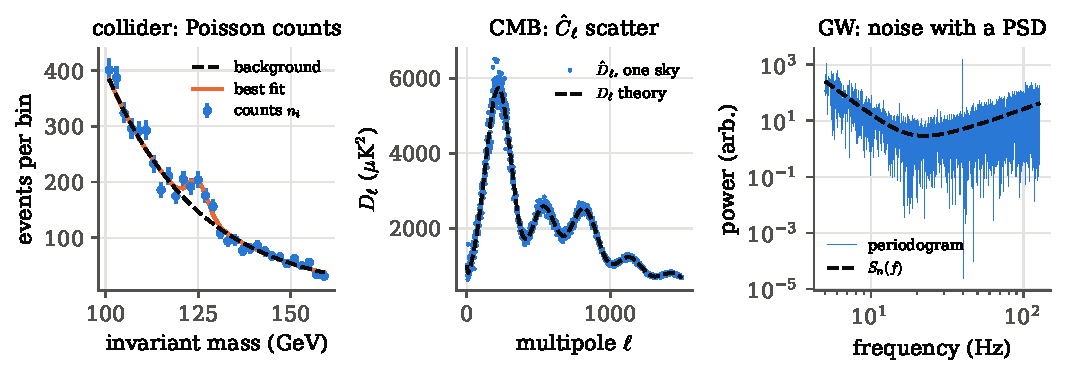
\includegraphics[width=\linewidth]{figures/ch00/three_detectors.pdf}
\caption{The same logic in three instruments. Left: Poisson counts with
$\sqrt{n}$ error bars over a falling background, and the best-fit background
plus signal. Middle: one simulated sky's $\hat D_\ell$ scattering around the
theory curve; the scatter is large at low $\ell$, where there are few modes,
and small at high $\ell$. Right: the periodogram of simulated detector noise,
wildly fluctuating from bin to bin but centred on the power spectral density.}
\label{0a:fig:three-detectors}
\end{figure}

\paragraph{How research uses these likelihoods.}
Each simulation here verifies a known noise model: Poisson counts, $\chi^2$
scatter of $\Chat$, a periodogram centred on $S_n$. In research the closed
forms break. A galactic mask couples multipoles and makes the $\Cell$
likelihood non-diagonal. Real interferometer noise has glitches and is not
stationary. A Betti curve has no known distribution at all. The fix is always
the fourth row of the taxonomy (topology): simulate the forward model,
estimate the mean and covariance of the summary from the simulations, and use
the Gaussian form. The price is that the estimated covariance
$\widehat{\Cmat}$ is itself noisy and must be corrected \cite{Hartlap2007}
(\cref{ch:08}).

\begin{pitfall}[the likelihood is not the posterior]
$\Like(\params)=p(\data\given\params)$ is a function of $\params$, but it is
not a density in $\params$. Here is a test that shows the difference. Change
variables from $\Cell$ to $\ln\Cell$. The likelihood's values stay the same,
but a density would pick up a Jacobian factor. Only after multiplying by a
prior and normalising (\cref{ch:05}) do we get a probability distribution for
$\params$.
\end{pitfall}

\section{How to run the code}\label{0a:sec:code}

Months from now we will change one line in the Monte Carlo of \cref{ch:08}.
A quoted covariance will then move, and we will want to know why: because of
the change, or because the random numbers were different this time? That
question has an answer only if two things hold. Every simulation in the book
must give the same numbers, bit for bit, when it is rerun. And every number in
the text must be traceable to the script that printed it. A small amount of
machinery guarantees both, so that one command regenerates every figure and
every simulated number.

\paragraph{A lab notebook with a calibration source.}
An experimentalist keeps a notebook that records which run produced which plot,
and keeps a calibration source that gives the same signal every time it is
measured. The code does both. Each script is one notebook entry: it writes its
figure and its numbers to files named after itself. And each script draws its
random numbers from a generator seeded by its own name, a calibration source
that reproduces the same ``noise'' on every run.

\paragraph{What we need from the code.}
\begin{enumerate}[leftmargin=2em]
  \item Where does each script live, and how is it run?
  \item Where do its figures and numbers go, and how do they get into the text?
  \item How are random numbers made reproducible, and different scripts independent?
  \item How do all figures share one visual style?
\end{enumerate}

\begin{figure}[htbp]
\centering
\begin{tikzpicture}[font=\small\ttfamily,
  dir/.style={anchor=west,text=accent},
  fil/.style={anchor=west},
  note/.style={anchor=west,font=\footnotesize\rmfamily,softgray}]
  \def\dy{0.46}
  \node[dir] (root) at (0,0) {Notes/};
  \draw[softgray] (0.15,{-(1-1)*\dy-0.1}) |- (0.45,{-1*\dy});
  \node[fil] at (0.45,{-1*\dy}) {main.tex, notes.sty};
  \node[note] at (5.6,{-1*\dy}) {the book and its style};
  \draw[softgray] (0.15,{-(2-1)*\dy-0.1}) |- (0.45,{-2*\dy});
  \node[dir] at (0.45,{-2*\dy}) {chapters/chNN/\textit{part}.tex};
  \node[note] at (5.6,{-2*\dy}) {the text of each chapter};
  \draw[softgray] (0.15,{-(3-1)*\dy-0.1}) |- (0.45,{-3*\dy});
  \node[fil] at (0.45,{-3*\dy}) {code/common.py};
  \node[note] at (5.6,{-3*\dy}) {shared helpers};
  \draw[softgray] (0.15,{-(4-1)*\dy-0.1}) |- (0.45,{-4*\dy});
  \node[fil] at (0.45,{-4*\dy}) {code/chNN/NN\_name.py};
  \node[note] at (5.6,{-4*\dy}) {one script per result};
  \draw[softgray] (0.15,{-(5-1)*\dy-0.1}) |- (0.45,{-5*\dy});
  \node[dir] at (0.45,{-5*\dy}) {figures/chNN/name.pdf};
  \node[note] at (5.6,{-5*\dy}) {written by \texttt{savefig}};
  \draw[softgray] (0.15,{-(6-1)*\dy-0.1}) |- (0.45,{-6*\dy});
  \node[dir] at (0.45,{-6*\dy}) {results/chNN/name.tex};
  \node[note] at (5.6,{-6*\dy}) {written by \texttt{save\_numbers}};
  \draw[softgray] (0.15,{-(7-1)*\dy-0.1}) |- (0.45,{-7*\dy});
  \node[dir] at (0.45,{-7*\dy}) {data/};
  \node[note] at (5.6,{-7*\dy}) {cached expensive products (CAMB spectra)};
  \draw[softgray] (0.15,{-(8-1)*\dy-0.1}) |- (0.45,{-8*\dy});
  \node[fil] at (0.45,{-8*\dy}) {tools/testpart.sh};
  \node[note] at (5.6,{-8*\dy}) {build one part and check it};
\end{tikzpicture}
\caption{The layout of the Notes directory. Every script is run from the
top directory, reads nothing but its own inputs, and writes its outputs into
the \texttt{figures} and \texttt{results} folders of its own chapter.}
\label{0a:fig:layout}
\end{figure}

Everything is Python with numpy, scipy, matplotlib and healpy, and every
sampler in the book is written from scratch. The choice of language does not
matter for the statistics; ``any computing language can be used''
\mainref{p.~ix}. Simulation makes a probability tangible: we watch the
empirical frequency settle on the theoretical value, as in the right panel of
\cref{0a:fig:coin-questions} \srcref{SeeingTheory}{pp.~5--7}.

Every script is run from the Notes directory, for example
\begin{center}
\texttt{python3 code/ch00/02\_coin\_questions.py}
\end{center}
and starts with a docstring stating the question it answers, what it computes
and what it writes. All scripts share one module, \pyname{code/common.py}.
Its first part sets the environment, the paths and the colours:

\pyfile[firstline=19,lastline=51]{code/common.py}{Environment, paths and the colour palette}

Lines 24--25 cap the linear-algebra libraries at four threads, so several
scripts can run side by side without fighting for cores. Line 29 selects a
non-interactive plotting backend, so scripts run without a display. The paths
are computed from the location of \pyname{common.py} itself. That is why a
script finds \texttt{figures/} and \texttt{results/} whatever directory it is
started from. Lines 36--41 are a switch for testing the book itself: setting
\texttt{SEED\_SALT} changes every seed and sends the figures and numbers to a
separate folder, so a run with different random numbers can be compared with
the book's own without overwriting it. \pyname{SERIES} is the fixed order of categorical colours: the
first data series in every figure is the same blue, the second the same
orange, and colours are never recycled. The function \pyname{setup()} (lines
54--80, not shown) applies one matplotlib style: serif fonts, a light grid, no
top and right axes. The second part of the module holds the functions every
script calls:

\pyfile[firstline=83,lastline=131]{code/common.py}{Figures, numbers, random streams and theory curves}

There are four functions. \pyname{savefig(fig, "ch00", "name")} writes
\texttt{figures/ch00/name.pdf}, which the text includes with
\verb|\includegraphics|. \pyname{save_numbers} writes a file of \LaTeX{}
macros, one per number, formatted by \pyname{_fmt} (four significant figures,
and $m\times10^{e}$ for very large or small values). The text loads that file
with \verb|\input| and writes \verb|$\PiHat$| where the number belongs.
\pyname{rng_for} builds a random generator whose seed is a hash of the
script's name. \pyname{theory_line} draws every analytic curve the same way,
black and dashed, on top of the simulation it is compared with.

\begin{figure}[htbp]
\centering
\begin{tikzpicture}[
  box/.style={draw=accent,thick,rounded corners=2pt,fill=ideabg,align=center,
              font=\footnotesize,text width=2.9cm,minimum height=0.9cm},
  outbox/.style={draw=softgray,rounded corners=2pt,fill=codebg,align=center,
              font=\footnotesize\ttfamily,text width=3.4cm,minimum height=0.8cm},
  flow/.style={->,thick,accent}]
  \node[box] (seed) at (0,0) {name of the script\\ \texttt{"ch00/06\_\dots"}};
  \node[box] (rng) at (0,-1.6) {\texttt{rng\_for}: SHA-256 $\to$ seed $\to$ PCG64};
  \node[box] (sim) at (0,-3.2) {the simulation};
  \node[outbox] (fig) at (4.6,-2.4) {figures/ch00/name.pdf};
  \node[outbox] (res) at (4.6,-4.0) {results/ch00/name.tex};
  \node[box,fill=takebg,draw=tangentgreen,text width=3.2cm] (tex) at (9.0,-3.2) {the chapter text: the figure and the macro \texttt{\textbackslash PiHat}};
  \draw[flow] (seed) -- (rng); \draw[flow] (rng) -- (sim);
  \draw[flow] (sim.east) -- (fig.west);
  \draw[flow] (sim.east) -- (res.west);
  \draw[flow] (fig.east) -- (tex.west);
  \draw[flow] (res.east) -- (tex.west);
\end{tikzpicture}
\caption{How a random number becomes a number in the text. The script's own
name fixes the seed, the seed fixes every random draw, and the outputs are
written to files that the chapter reads. Rerunning the script regenerates the
figure and the quoted numbers together, so they cannot drift apart.}
\label{0a:fig:dataflow}
\end{figure}

\begin{workdef}[pseudo-random stream, seed, results macro]
A \newterm{pseudo-random generator} is a deterministic algorithm whose output
passes statistical tests for independent uniform draws \unpack{PCG64 here,
built in \cref{ch:06}}. Its whole output is fixed by an integer, the
\newterm{seed}. \pyname{rng_for(chapter, name, stream)} takes the first $8$
bytes of the SHA-256 hash of \texttt{"chapter/name"} as a $64$-bit seed and
feeds it, together with the \pyname{stream} index, to numpy's
\pyname{SeedSequence}, which scrambles the pair into a full generator state.
Same name and stream \unpack{same seed} give the identical stream; different
names give streams with no detectable correlation. A \newterm{results macro}
is a \LaTeX{} command such as \verb|\PiHat| defined in
\texttt{results/chNN/name.tex} by the script, so that the text quotes the
number the code actually produced.
\end{workdef}

\zeroaEx{can two scripts share a seed by accident?}
\label{0a:ex:seedclash}
If two scripts got the same seed, their ``independent'' random numbers would
be identical. How likely is that? The hash scatters names over $2^{64}$
possible seeds, effectively at random. With $M$ scripts, the probability that
some pair collides is bounded as in the birthday problem:
\begin{align*}
  \Prob(\text{some collision})
  &\relby{1}{\le} \sum_{\text{pairs}}\Prob(\text{this pair collides})
   \eqby{2} \binom M2\,2^{-64}\\
  &\relby{3}{\le} \frac{M^2}{2}\,2^{-64}
   \eqby{4} \frac{10^6}{2}\times5.4\times10^{-20}=2.7\times10^{-14}
\end{align*}
for $M=1000$.
\begin{explain}
  \item The probability of a union is at most the sum of the probabilities (the union bound).
  \item Two independent uniform seeds agree with probability $2^{-64}$; there are $\binom M2$ pairs.
  \item $\binom M2=M(M-1)/2\le M^2/2$.
  \item $M=1000$ and $2^{-64}=5.4\times10^{-20}$.
\end{explain}
So with a thousand scripts a clash is, for practical purposes, impossible.
And because \pyname{SeedSequence} mixes in the \pyname{stream} index as well,
one script can take several independent streams; the three detectors of
\cref{0a:sec:universal} use streams $0,1,2$.

\zeroaEx{a Monte Carlo number with its error bar: $\pi$ from darts}
\label{0a:ex:darts}
Every Monte Carlo number in the book comes with an error bar; here is the
simplest case. Throw $N$ points uniformly in the unit square. The fraction
$\hat q$ that lands inside the quarter disc $x^2+y^2<1$ estimates the disc's
area, $q=\pi/4$, so $\hat\pi=4\hat q$ estimates $\pi$. How far off is it
likely to be? A fraction of $N$ independent trials scatters by
$\sqrt{q(1-q)/N}$ (\cref{0a:ex:mc-error}), so
\begin{align*}
  \sigma_{\hat\pi}
  &\eqby{1} 4\,\sigma_{\hat q}
   \eqby{2} 4\sqrt{\frac{q(1-q)}{N}}
   \eqby{3} 4\sqrt{\frac{0.7854\times0.2146}{10^6}}
   = 4\times4.106\times10^{-4}=1.642\times10^{-3} .
\end{align*}
\begin{explain}
  \item Multiplying a random variable by $4$ multiplies its standard deviation by $4$.
  \item The scatter of a fraction of $N$ independent trials, \cref{0a:ex:mc-error}.
  \item $q=\pi/4=0.7854$ and $N=10^6$.
\end{explain}
The script \pyname{06_reproducible_seeds.py} does exactly this with
$N=\PiN$. It finds $\hat\pi=\PiHat$ with estimated error $\PiErr$, within
about one standard error of $\pi=3.14159$. One more decimal digit means an
error ten times smaller, and since the error falls like $1/\sqrt N$ that
costs $100$ times more darts. This $1/\sqrt N$ law dominates every Monte
Carlo budget in the book.

\zeroaEx{the results file}
\label{0a:ex:results}
The same script also checks the seeding. It builds two generators from the
same name and one from a different name. The first draw is $\SeedFirstDraw$
for both generators with the same name (the streams are identical:
\SeedIdentical), and $\SeedOtherFirstDraw$ for the other name. The file the
script wrote, which the text reads, is:

\pyfile[language={[LaTeX]TeX},keywordstyle=\color{formblue}]{results/ch00/06_reproducible_seeds.tex}{The generated macro file}

Each line is \verb|\providecommand| followed by \verb|\renewcommand|. The
first defines the macro if it does not exist yet; the second sets its value.
So the file can be loaded twice without error, and the latest values always
win. Macro names contain letters only, because \LaTeX{} requires it, and
\pyname{save_numbers} enforces this with an assertion.

\paragraph{What this bought us.}
Rerunning a script regenerates its figure and its numbers together, with the
same random draws. The text never contains a simulated number typed by hand.

\begin{pitfall}[reproducible is not the same as correct]
A fixed seed makes a wrong answer reproducible too. Reproducibility lets us
see \emph{whether} a change in the code changed a result. It does not replace
two other checks. One is the test of \cref{ch:06}: does the generator pass
statistical tests? The other is the comparison of every simulation with a
known analytic limit. That is why every script in the book plots a black
dashed theory curve wherever one exists.
\end{pitfall}

\paragraph{Running everything.}
To regenerate every figure and number, run each script from the Notes
directory, e.g.\ \texttt{for f in code/ch*/[0-9]*.py; do python3 "\$f"; done}.
Then build the book with \texttt{latexmk -pdf main.tex}. Expensive products
(the fiducial CAMB spectrum, large simulated map sets, long chains) are cached
in \texttt{data/} and reused. To force a recomputation, delete the cache file.
One part can be built on its own with \texttt{./tools/testpart.sh}.

\section*{Chapter summary}
\addcontentsline{toc}{section}{Chapter summary}

\begingroup
\small
\renewcommand{\arraystretch}{1.3}
\begin{tabularx}{\linewidth}{@{}>{\raggedright\arraybackslash}p{3.0cm}
  >{\raggedright\arraybackslash}X >{\raggedright\arraybackslash}p{2.4cm}@{}}
\toprule
\textbf{concept} & \textbf{operational meaning} & \textbf{used later in}\\
\midrule
prediction, $\Prob(E\given H)$ & forward: fraction of the $H$-world in which $E$ happens; compute along a tree path & \cref{ch:01,ch:02}\\
inference, $\Prob(H\given E)$ & backward: keep the paths that end at $E$, renormalise & \cref{ch:05}\\
Bayes' theorem & posterior $\propto$ likelihood $\times$ prior; the evidence $E$ shrinks the sample space & \cref{ch:05,ch:09}\\
odds form & posterior odds = likelihood ratio $\times$ prior odds; independent data multiply & \cref{ch:04,ch:05}\\
estimator, sampling distribution & a function of data; its histogram over repeated experiments, with bias and variance & \cref{ch:03}\\
$p$-value & tail probability under $\Hnull$ of ``this or more extreme in this direction'' & \cref{ch:04}\\
Monte Carlo error & a simulated fraction scatters by $\sqrt{q(1-q)/N}$ & \cref{ch:06,ch:08}\\
Fisher information & minus the expected curvature of $\ln\Like$; best possible variance $1/I$ & \cref{ch:10}\\
pipeline & model $\to$ data $\to$ what matters $\to$ $S$ $\to$ $P(S\given\params)$ $\to$ $P(\params\given S)$ & every chapter\\
sufficient summary & likelihood depends on the data only through $S$; compression is free & \cref{ch:03,ch:07}\\
summary ladder & amplitude, correlation, higher order, morphology, topology & \cref{ch:07,ch:12}\\
excursion set, $\beta_0,\beta_1,\chi$ & region above $\nu$; pieces, holes, $\chi=\beta_0-\beta_1=V-E+F$ & \cref{ch:12}\\
robust observable & $T[\mathcal N[\phi]]=T[\phi]$ for a stated class of nuisances & \cref{ch:12}\\
likelihood from noise & density of the required noise $\data-m(\params)$, read as a function of $\params$ & \cref{ch:03,ch:05}\\
Poisson, $\Cell$, Whittle likelihoods & $\sum[n\ln\lambda-\lambda]$; $-\frac12\sum(2\ell+1)[\Chat/\Cell+\ln\Cell]$; $-\frac12(d-h|d-h)$ & \cref{ch:04,ch:07,ch:10}\\
reproducible streams & seed from the script name; numbers reach the text as macros & every chapter\\
\bottomrule
\end{tabularx}
\endgroup

\begin{sourcesays}[Reading the literature]
\begin{itemize}[leftmargin=1.5em]
  \item L.~Wasserman, \emph{All of Statistics}, Preface (the probability/inference figure and the statistics--data-mining dictionary), Ch.~1, and the discussion of the null hypothesis (p.~149) and maximum likelihood (p.~122).
  \item J.~K.~Kruschke, \emph{Doing Bayesian Data Analysis}, Chs.~1--2: reallocation of credibility, Holmes and the bouncy balls, the five steps. The clearest first read.
  \item \emph{Seeing Theory}, ``Basic probability'': theoretical versus empirical frequency, interactively.
  \item On topology of CMB polarisation and the cosmic web: \cite{VachaspatiLue2003,HutererVachaspati2005,ChallinorChon2002,Pranav2017,Wilding2021}.
\end{itemize}
\end{sourcesays}
  
\renewcommand{\thechapter}{T\arabic{chapter}}\renewcommand{\theHchapter}{T\arabic{chapter}}
\setcounter{chapter}{-1}
\chapter{Python for This Book}\label{ch:T0}
\providecommand{\TzFiles}{}\renewcommand{\TzFiles}{345}
\providecommand{\TzLines}{}\renewcommand{\TzLines}{45734}
\providecommand{\TzCalls}{}\renewcommand{\TzCalls}{27297}
\providecommand{\TzNames}{}\renewcommand{\TzNames}{759}
\providecommand{\TzNfifty}{}\renewcommand{\TzNfifty}{25}
\providecommand{\TzNeighty}{}\renewcommand{\TzNeighty}{83}
\providecommand{\TzNninety}{}\renewcommand{\TzNninety}{159}
\providecommand{\TzNninetynine}{}\renewcommand{\TzNninetynine}{526}
\providecommand{\TzRareNames}{}\renewcommand{\TzRareNames}{362}
\providecommand{\TzRareShare}{}\renewcommand{\TzRareShare}{2.1}
\providecommand{\TzOwnCalls}{}\renewcommand{\TzOwnCalls}{5205}
\providecommand{\TzCommonCalls}{}\renewcommand{\TzCommonCalls}{1671}
\providecommand{\TzNumpyShare}{}\renewcommand{\TzNumpyShare}{34}
\providecommand{\TzPlotShare}{}\renewcommand{\TzPlotShare}{22}
\providecommand{\TzScipyShare}{}\renewcommand{\TzScipyShare}{3}
\providecommand{\TzPctFor}{}\renewcommand{\TzPctFor}{88}
\providecommand{\TzPctDef}{}\renewcommand{\TzPctDef}{72}
\providecommand{\TzPctIf}{}\renewcommand{\TzPctIf}{46}
\providecommand{\TzPctFstring}{}\renewcommand{\TzPctFstring}{84}
\providecommand{\TzPctKw}{}\renewcommand{\TzPctKw}{99}
\providecommand{\TzPctSlice}{}\renewcommand{\TzPctSlice}{79}
\providecommand{\TzPctComp}{}\renewcommand{\TzPctComp}{65}
\providecommand{\TzPctDict}{}\renewcommand{\TzPctDict}{93}
\providecommand{\TzPctUnpack}{}\renewcommand{\TzPctUnpack}{99}
\providecommand{\TzPctWhile}{}\renewcommand{\TzPctWhile}{6}
\providecommand{\TzPctLambda}{}\renewcommand{\TzPctLambda}{39}
\providecommand{\TzPctClass}{}\renewcommand{\TzPctClass}{2}
\providecommand{\TzPctDecorator}{}\renewcommand{\TzPctDecorator}{2}
\providecommand{\TzPctWith}{}\renewcommand{\TzPctWith}{9}
\providecommand{\TzPctTry}{}\renewcommand{\TzPctTry}{3}
\providecommand{\TzPctMatmul}{}\renewcommand{\TzPctMatmul}{28}
\providecommand{\TzPctYield}{}\renewcommand{\TzPctYield}{0}
\providecommand{\TzPctGlobal}{}\renewcommand{\TzPctGlobal}{0}
\providecommand{\TzPctNumpy}{}\renewcommand{\TzPctNumpy}{99}
\providecommand{\TzPctPlt}{}\renewcommand{\TzPctPlt}{88}
\providecommand{\TzPctScipy}{}\renewcommand{\TzPctScipy}{53}
\providecommand{\TzPctHealpy}{}\renewcommand{\TzPctHealpy}{10}
\providecommand{\TzPctCamb}{}\renewcommand{\TzPctCamb}{5}
\providecommand{\TzPctNumba}{}\renewcommand{\TzPctNumba}{1}
\providecommand{\TzPctMultiproc}{}\renewcommand{\TzPctMultiproc}{1}
\providecommand{\TzPctTime}{}\renewcommand{\TzPctTime}{11}
\providecommand{\TzAsserts}{}\renewcommand{\TzAsserts}{19}
\providecommand{\TzAssertFiles}{}\renewcommand{\TzAssertFiles}{15}
\providecommand{\TzCheckCalls}{}\renewcommand{\TzCheckCalls}{13}
\providecommand{\TzCheckFiles}{}\renewcommand{\TzCheckFiles}{9}
\providecommand{\TzRngForCalls}{}\renewcommand{\TzRngForCalls}{289}
\providecommand{\TzRngForFiles}{}\renewcommand{\TzRngForFiles}{236}
\providecommand{\TzDrawFiles}{}\renewcommand{\TzDrawFiles}{216}
\providecommand{\TzSeededDrawFiles}{}\renewcommand{\TzSeededDrawFiles}{197}
\providecommand{\TzLibDrawFiles}{}\renewcommand{\TzLibDrawFiles}{15}
\providecommand{\TzBareRng}{}\renewcommand{\TzBareRng}{3}
\providecommand{\TzDefaultRng}{}\renewcommand{\TzDefaultRng}{5}
\providecommand{\TzLegacySeed}{}\renewcommand{\TzLegacySeed}{3}
\providecommand{\TzMedianNames}{}\renewcommand{\TzMedianNames}{36}
\providecommand{\TzMaxNames}{}\renewcommand{\TzMaxNames}{85}
\providecommand{\TzInv}{}\renewcommand{\TzInv}{105}
\providecommand{\TzSolve}{}\renewcommand{\TzSolve}{29}
\providecommand{\TzChol}{}\renewcommand{\TzChol}{22}
\providecommand{\TzEigh}{}\renewcommand{\TzEigh}{13}
\providecommand{\TzFft}{}\renewcommand{\TzFft}{182}
\providecommand{\TzPerfCounter}{}\renewcommand{\TzPerfCounter}{32}
\providecommand{\TzTimeTime}{}\renewcommand{\TzTimeTime}{98}
\providecommand{\TzTopNameOne}{}\renewcommand{\TzTopNameOne}{\texttt{np.sqrt}}
\providecommand{\TzTopCountOne}{}\renewcommand{\TzTopCountOne}{1255}
\providecommand{\TzTopNameTwo}{}\renewcommand{\TzTopNameTwo}{\texttt{x.mean}}
\providecommand{\TzTopCountTwo}{}\renewcommand{\TzTopCountTwo}{836}
\providecommand{\TzTopNameThree}{}\renewcommand{\TzTopNameThree}{\texttt{x.plot}}
\providecommand{\TzTopCountThree}{}\renewcommand{\TzTopCountThree}{826}
\providecommand{\TzTopNameFour}{}\renewcommand{\TzTopNameFour}{\texttt{np.array}}
\providecommand{\TzTopCountFour}{}\renewcommand{\TzTopCountFour}{721}
\providecommand{\TzTopNameFive}{}\renewcommand{\TzTopNameFive}{\texttt{x.set\_xlabel}}
\providecommand{\TzTopCountFive}{}\renewcommand{\TzTopCountFive}{707}
\providecommand{\TzAppendCalls}{}\renewcommand{\TzAppendCalls}{400}
\providecommand{\TzTopFiveSum}{}\renewcommand{\TzTopFiveSum}{4345}
\providecommand{\TzTopFiveShare}{}\renewcommand{\TzTopFiveShare}{15.9}
\providecommand{\TzLoopMillion}{}\renewcommand{\TzLoopMillion}{0.3575}
\providecommand{\TzVecMillionMs}{}\renewcommand{\TzVecMillionMs}{2.614}
\providecommand{\TzSpeedup}{}\renewcommand{\TzSpeedup}{137}
\providecommand{\TzSpeedupSmall}{}\renewcommand{\TzSpeedupSmall}{1}
\providecommand{\TzLoopNsPerElem}{}\renewcommand{\TzLoopNsPerElem}{358}
\providecommand{\TzVecNsPerElem}{}\renewcommand{\TzVecNsPerElem}{2.6}
\providecommand{\TzVecRelDiff}{}\renewcommand{\TzVecRelDiff}{3.731\times10^{-15}}
\providecommand{\TzZninetyfive}{}\renewcommand{\TzZninetyfive}{1.9600}
\providecommand{\TzPfive}{}\renewcommand{\TzPfive}{2.867\times10^{-7}}
\providecommand{\TzBackCdf}{}\renewcommand{\TzBackCdf}{0.9750}
\providecommand{\TzRvsMean}{}\renewcommand{\TzRvsMean}{2.0049}
\providecommand{\TzRvsStd}{}\renewcommand{\TzRvsStd}{0.5039}
\providecommand{\TzQuadTail}{}\renewcommand{\TzQuadTail}{2.867\times10^{-7}}
\providecommand{\TzQuadErr}{}\renewcommand{\TzQuadErr}{8.853\times10^{-10}}
\providecommand{\TzQuadRel}{}\renewcommand{\TzQuadRel}{5.328\times10^{-9}}
\providecommand{\TzUpperZero}{}\renewcommand{\TzUpperZero}{2.9957}
\providecommand{\TzUpperZeroExact}{}\renewcommand{\TzUpperZeroExact}{2.9957}
\providecommand{\TzUpperThree}{}\renewcommand{\TzUpperThree}{7.754}
\providecommand{\TzMinMu}{}\renewcommand{\TzMinMu}{2.0050}
\providecommand{\TzMinSig}{}\renewcommand{\TzMinSig}{0.5039}
\providecommand{\TzMeanCheck}{}\renewcommand{\TzMeanCheck}{2.0049}
\providecommand{\TzStdCheck}{}\renewcommand{\TzStdCheck}{0.5039}
\providecommand{\TzMinIters}{}\renewcommand{\TzMinIters}{69}
\providecommand{\TzLnFact}{}\renewcommand{\TzLnFact}{863.232}
\providecommand{\TzLnFactCheck}{}\renewcommand{\TzLnFactCheck}{863.232}
\providecommand{\TzFactOverflow}{}\renewcommand{\TzFactOverflow}{yes}
\providecommand{\TzInterpLinErr}{}\renewcommand{\TzInterpLinErr}{0.0489}
\providecommand{\TzInterpSplErr}{}\renewcommand{\TzInterpSplErr}{0.0027}
\providecommand{\TzFloatGap}{}\renewcommand{\TzFloatGap}{5.551\times10^{-17}}
\providecommand{\TzSeedDraw}{}\renewcommand{\TzSeedDraw}{0.858458}
\providecommand{\TzHilbCond}{}\renewcommand{\TzHilbCond}{1.602\times10^{13}}
\providecommand{\TzHilbResSolve}{}\renewcommand{\TzHilbResSolve}{8.502\times10^{-17}}
\providecommand{\TzHilbResInv}{}\renewcommand{\TzHilbResInv}{3.584\times10^{-5}}
\providecommand{\TzHilbErr}{}\renewcommand{\TzHilbErr}{2.272\times10^{-5}}
\providecommand{\TzTsolve}{}\renewcommand{\TzTsolve}{44}
\providecommand{\TzTinv}{}\renewcommand{\TzTinv}{180}
\providecommand{\TzTchol}{}\renewcommand{\TzTchol}{57}
\providecommand{\TzInvOverSolve}{}\renewcommand{\TzInvOverSolve}{4.1}
\providecommand{\TzFftPeak}{}\renewcommand{\TzFftPeak}{50.0}
\providecommand{\TzFftN}{}\renewcommand{\TzFftN}{2000}
\providecommand{\TzFftBins}{}\renewcommand{\TzFftBins}{1001}
\providecommand{\TzFftSnr}{}\renewcommand{\TzFftSnr}{180}
\providecommand{\TzEps}{}\renewcommand{\TzEps}{2.220\times10^{-16}}
\providecommand{\TzMaxFloat}{}\renewcommand{\TzMaxFloat}{1.798\times10^{308}}
\providecommand{\TzTiny}{}\renewcommand{\TzTiny}{2.225\times10^{-308}}
\providecommand{\TzCancNaive}{}\renewcommand{\TzCancNaive}{0.5000000414}
\providecommand{\TzCancGood}{}\renewcommand{\TzCancGood}{0.5000000000}
\providecommand{\TzCancNaiveTiny}{}\renewcommand{\TzCancNaiveTiny}{0.0}
\providecommand{\TzVarOnePass}{}\renewcommand{\TzVarOnePass}{2.00}
\providecommand{\TzVarTwoPass}{}\renewcommand{\TzVarTwoPass}{0.9919}
\providecommand{\TzHfwdPred}{}\renewcommand{\TzHfwdPred}{2.980\times10^{-8}}
\providecommand{\TzHcenPred}{}\renewcommand{\TzHcenPred}{8.733\times10^{-6}}
\providecommand{\TzHfwdBest}{}\renewcommand{\TzHfwdBest}{1.224\times10^{-8}}
\providecommand{\TzHcenBest}{}\renewcommand{\TzHcenBest}{8.214\times10^{-6}}
\providecommand{\TzErrFwdMin}{}\renewcommand{\TzErrFwdMin}{8.969\times10^{-9}}
\providecommand{\TzErrCenMin}{}\renewcommand{\TzErrCenMin}{8.991\times10^{-12}}
\providecommand{\TzErrFwdPred}{}\renewcommand{\TzErrFwdPred}{2.980\times10^{-8}}
\providecommand{\TzErrCenPred}{}\renewcommand{\TzErrCenPred}{3.814\times10^{-11}}
\providecommand{\TzExactE}{}\renewcommand{\TzExactE}{2.718281828459}
\providecommand{\TzQuadMiss}{}\renewcommand{\TzQuadMiss}{0}
\providecommand{\TzQuadMissErr}{}\renewcommand{\TzQuadMissErr}{0}
\providecommand{\TzQuadHit}{}\renewcommand{\TzQuadHit}{1.0000000000}
\providecommand{\TzQuadHitErr}{}\renewcommand{\TzQuadHitErr}{8.671\times10^{-10}}
\providecommand{\TzQuadTight}{}\renewcommand{\TzQuadTight}{0}
\providecommand{\TzQuadOnePoint}{}\renewcommand{\TzQuadOnePoint}{4.951\times10^{-14}}
\providecommand{\TzQuadTwoPoints}{}\renewcommand{\TzQuadTwoPoints}{0.9999994267}
\providecommand{\TzRootTwo}{}\renewcommand{\TzRootTwo}{1.414213562373}
\providecommand{\TzNMsuccess}{}\renewcommand{\TzNMsuccess}{False}
\providecommand{\TzNMgrad}{}\renewcommand{\TzNMgrad}{7.598}
\providecommand{\TzNMfun}{}\renewcommand{\TzNMfun}{1.868}
\providecommand{\TzBFGSgrad}{}\renewcommand{\TzBFGSgrad}{5.001\times10^{-6}}
\providecommand{\TzCholMinFew}{}\renewcommand{\TzCholMinFew}{-1.252\times10^{-15}}
\providecommand{\TzCholRankFew}{}\renewcommand{\TzCholRankFew}{29}
\providecommand{\TzCholMinMany}{}\renewcommand{\TzCholMinMany}{0.2669}
\providecommand{\TzCholRankMany}{}\renewcommand{\TzCholRankMany}{50}
\providecommand{\TzQexact}{}\renewcommand{\TzQexact}{0.02275}
\providecommand{\TzQsigFour}{}\renewcommand{\TzQsigFour}{0.00149}
\providecommand{\TzQobsFour}{}\renewcommand{\TzQobsFour}{0.00169}
\providecommand{\TzQfirst}{}\renewcommand{\TzQfirst}{0.0226}
\providecommand{\TzQzFirst}{}\renewcommand{\TzQzFirst}{-0.10}
\providecommand{\TzCrnTrue}{}\renewcommand{\TzCrnTrue}{0.00597}
\providecommand{\TzCrnInd}{}\renewcommand{\TzCrnInd}{0.00224}
\providecommand{\TzCrnCrn}{}\renewcommand{\TzCrnCrn}{0.00076}
\providecommand{\TzCrnGain}{}\renewcommand{\TzCrnGain}{9}
\providecommand{\TzCrnM}{}\renewcommand{\TzCrnM}{10000}
\providecommand{\TzCrnR}{}\renewcommand{\TzCrnR}{400}
\providecommand{\TzCrnZind}{}\renewcommand{\TzCrnZind}{2.7}
\providecommand{\TzCrnZcrn}{}\renewcommand{\TzCrnZcrn}{7.9}
\providecommand{\TzCrnOneInd}{}\renewcommand{\TzCrnOneInd}{0.00500}
\providecommand{\TzCrnOneCrn}{}\renewcommand{\TzCrnOneCrn}{0.00660}
\providecommand{\TzCrnFracIndBelow}{}\renewcommand{\TzCrnFracIndBelow}{60}
\providecommand{\TzCrnFracCrnBelow}{}\renewcommand{\TzCrnFracCrnBelow}{0}
\providecommand{\TzTrapEight}{}\renewcommand{\TzTrapEight}{1.974232}
\providecommand{\TzTrapSixteen}{}\renewcommand{\TzTrapSixteen}{1.993570}
\providecommand{\TzTrapErrEight}{}\renewcommand{\TzTrapErrEight}{-0.02577}
\providecommand{\TzTrapErrSixteen}{}\renewcommand{\TzTrapErrSixteen}{-0.00643}
\providecommand{\TzTrapRatio}{}\renewcommand{\TzTrapRatio}{4.008}
\providecommand{\TzRich}{}\renewcommand{\TzRich}{2.00001659}
\providecommand{\TzRichErr}{}\renewcommand{\TzRichErr}{1.659\times10^{-5}}
\providecommand{\TzNaiveZero}{}\renewcommand{\TzNaiveZero}{8.5}
\providecommand{\TzSfZero}{}\renewcommand{\TzSfZero}{38.0}
\providecommand{\TzNaiveRelFive}{}\renewcommand{\TzNaiveRelFive}{1.547\times10^{-10}}
\providecommand{\TzSfRelFive}{}\renewcommand{\TzSfRelFive}{2.216\times10^{-15}}
\providecommand{\TzLogTenForty}{}\renewcommand{\TzLogTenForty}{-349.44}
\providecommand{\TzLogsfForty}{}\renewcommand{\TzLogsfForty}{-349.44}
\providecommand{\TzPolyFloat}{}\renewcommand{\TzPolyFloat}{7.994\times10^{-15}}
\providecommand{\TzPolyFact}{}\renewcommand{\TzPolyFact}{1.000\times10^{-14}}
\providecommand{\TzPolyMpThirty}{}\renewcommand{\TzPolyMpThirty}{1.000\times10^{-14}}
\providecommand{\TzPolyKappa}{}\renewcommand{\TzPolyKappa}{1.33e+16}
\providecommand{\TzPolyLogKappa}{}\renewcommand{\TzPolyLogKappa}{16.1}
\providecommand{\TzAgreeFifteen}{}\renewcommand{\TzAgreeFifteen}{0.7}
\providecommand{\TzAgreeThirty}{}\renewcommand{\TzAgreeThirty}{16.4}
\providecommand{\TzAgreeTen}{}\renewcommand{\TzAgreeTen}{0.0}
\providecommand{\TzAgreeTwenty}{}\renewcommand{\TzAgreeTwenty}{7.8}
\providecommand{\TzTnp}{}\renewcommand{\TzTnp}{13.0}
\providecommand{\TzTmath}{}\renewcommand{\TzTmath}{332}
\providecommand{\TzTmpFifteen}{}\renewcommand{\TzTmpFifteen}{11330}
\providecommand{\TzTmpFifty}{}\renewcommand{\TzTmpFifty}{21097}
\providecommand{\TzMpOverNp}{}\renewcommand{\TzMpOverNp}{870}
\providecommand{\TzMpOverMath}{}\renewcommand{\TzMpOverMath}{34}
\providecommand{\TzSlopeFft}{}\renewcommand{\TzSlopeFft}{1.35}
\providecommand{\TzSlopeChol}{}\renewcommand{\TzSlopeChol}{2.45}
\providecommand{\TzSlopeBrute}{}\renewcommand{\TzSlopeBrute}{2.04}
\providecommand{\TzSlopeTree}{}\renewcommand{\TzSlopeTree}{1.69}
\providecommand{\TzSlopeSht}{}\renewcommand{\TzSlopeSht}{3.06}
\providecommand{\TzCholPred}{}\renewcommand{\TzCholPred}{3.25}
\providecommand{\TzCholMeas}{}\renewcommand{\TzCholMeas}{3.21}
\providecommand{\TzCholBigN}{}\renewcommand{\TzCholBigN}{6000}
\providecommand{\TzCholTwoK}{}\renewcommand{\TzCholTwoK}{0.567}
\providecommand{\TzShtPred}{}\renewcommand{\TzShtPred}{2.01}
\providecommand{\TzShtMeas}{}\renewcommand{\TzShtMeas}{1.43}
\providecommand{\TzShtTwoFiveSix}{}\renewcommand{\TzShtTwoFiveSix}{0.227}
\providecommand{\TzBruteMillionH}{}\renewcommand{\TzBruteMillionH}{22.6}
\providecommand{\TzTreeBig}{}\renewcommand{\TzTreeBig}{1.36}
\providecommand{\TzBruteSixteenK}{}\renewcommand{\TzBruteSixteenK}{16.89}
\providecommand{\TzTreeSixteenK}{}\renewcommand{\TzTreeSixteenK}{0.056}
\providecommand{\TzFftBig}{}\renewcommand{\TzFftBig}{468}
\providecommand{\TzFftBigN}{}\renewcommand{\TzFftBigN}{4194304}
\providecommand{\TzCholNsideDays}{}\renewcommand{\TzCholNsideDays}{6}
\providecommand{\TzCholNsideDaysThree}{}\renewcommand{\TzCholNsideDaysThree}{84}
\providecommand{\TzFftNlogN}{}\renewcommand{\TzFftNlogN}{1.07}
\providecommand{\TzPairsAgree}{}\renewcommand{\TzPairsAgree}{yes}
\providecommand{\SeedIdentical}{}\renewcommand{\SeedIdentical}{yes}
\providecommand{\SeedFirstDraw}{}\renewcommand{\SeedFirstDraw}{0.217}
\providecommand{\SeedOtherFirstDraw}{}\renewcommand{\SeedOtherFirstDraw}{0.4034}
\providecommand{\PiHat}{}\renewcommand{\PiHat}{3.143}
\providecommand{\PiErr}{}\renewcommand{\PiErr}{0.001641}
\providecommand{\PiN}{}\renewcommand{\PiN}{1000000}
\providecommand{\EightACholSix}{}\renewcommand{\EightACholSix}{0.80}
\providecommand{\EightALikeDaysTwoFiveSix}{}\renewcommand{\EightALikeDaysTwoFiveSix}{21}
\providecommand{\EightALikeYrFiveTwelve}{}\renewcommand{\EightALikeYrFiveTwelve}{4}
\providecommand{\EightALikeYrPlanck}{}\renewcommand{\EightALikeYrPlanck}{1.5\times10^{4}}
\providecommand{\EightAShtTwoFiveSix}{}\renewcommand{\EightAShtTwoFiveSix}{0.02}
\providecommand{\EightAShtPlanck}{}\renewcommand{\EightAShtPlanck}{9}
\providecommand{\EightAMemTwoFiveSix}{}\renewcommand{\EightAMemTwoFiveSix}{4.9}
\providecommand{\EightAMemPlanck}{}\renewcommand{\EightAMemPlanck}{20266}
\providecommand{\FiveCGcExact}{}\renewcommand{\FiveCGcExact}{2.096}
\providecommand{\FiveCGcNmax}{}\renewcommand{\FiveCGcNmax}{64}
\providecommand{\FiveCGcTmax}{}\renewcommand{\FiveCGcTmax}{9.43}
\providecommand{\FiveCGcLnBmax}{}\renewcommand{\FiveCGcLnBmax}{2.1}
\providecommand{\FiveCGcLnBsmall}{}\renewcommand{\FiveCGcLnBsmall}{4.558}
\providecommand{\FiveCGcNsmall}{}\renewcommand{\FiveCGcNsmall}{12}
\providecommand{\FiveCGcLnBmid}{}\renewcommand{\FiveCGcLnBmid}{2.379}
\providecommand{\FiveCGcNmid}{}\renewcommand{\FiveCGcNmid}{24}
\providecommand{\FiveCGcTpp}{}\renewcommand{\FiveCGcTpp}{5.621\times10^{-7}}
\providecommand{\FiveCGcSixD}{}\renewcommand{\FiveCGcSixD}{1.784e+04}
\providecommand{\FiveCGcSixDcmb}{}\renewcommand{\FiveCGcSixDcmb}{3.175\times10^{10}}
\providecommand{\FiveCDcErrTwo}{}\renewcommand{\FiveCDcErrTwo}{0.01888}
\providecommand{\FiveCDcErrFive}{}\renewcommand{\FiveCDcErrFive}{0.2925}
\providecommand{\FiveCDcErrEight}{}\renewcommand{\FiveCDcErrEight}{4.937}
\providecommand{\FiveCDcErrTen}{}\renewcommand{\FiveCDcErrTen}{0.98}
\providecommand{\FiveCDcFracTwo}{}\renewcommand{\FiveCDcFracTwo}{0.04682}
\providecommand{\FiveCDcFracFive}{}\renewcommand{\FiveCDcFracFive}{7.315\times10^{-4}}
\providecommand{\FiveCDcFracEight}{}\renewcommand{\FiveCDcFracEight}{9.500\times10^{-6}}
\providecommand{\FiveCDcPostTwo}{}\renewcommand{\FiveCDcPostTwo}{0.002947}
\providecommand{\FiveCDcPostTen}{}\renewcommand{\FiveCDcPostTen}{0.002263}
\providecommand{\FiveCDcMedTen}{}\renewcommand{\FiveCDcMedTen}{8.293\times10^{-4}}
\providecommand{\FiveCDcMedEight}{}\renewcommand{\FiveCDcMedEight}{0.1252}
\providecommand{\FiveCDcVolTen}{}\renewcommand{\FiveCDcVolTen}{9.563\times10^{-10}}
\providecommand{\FiveCDcDraws}{}\renewcommand{\FiveCDcDraws}{100000}
\providecommand{\SBNsim}{}\renewcommand{\SBNsim}{20{,}000}
\providecommand{\SBNbig}{}\renewcommand{\SBNbig}{10^6}
\providecommand{\SBksTwo}{}\renewcommand{\SBksTwo}{0.2452}
\providecommand{\SBksTen}{}\renewcommand{\SBksTen}{0.8436}
\providecommand{\SBksFifty}{}\renewcommand{\SBksFifty}{0.3608}
\providecommand{\SBksThree}{}\renewcommand{\SBksThree}{0.6115}
\providecommand{\SBvrTwo}{}\renewcommand{\SBvrTwo}{1.021}
\providecommand{\SBvrTen}{}\renewcommand{\SBvrTen}{1.000}
\providecommand{\SBvrFifty}{}\renewcommand{\SBvrFifty}{1.015}
\providecommand{\SBvrThree}{}\renewcommand{\SBvrThree}{0.998}
\providecommand{\SBerrTwo}{}\renewcommand{\SBerrTwo}{0.01483}
\providecommand{\SBerrThree}{}\renewcommand{\SBerrThree}{0.01005}
\providecommand{\SBmeanDevMax}{}\renewcommand{\SBmeanDevMax}{3.081}
\providecommand{\SBslopeHi}{}\renewcommand{\SBslopeHi}{-0.5133}
\providecommand{\SBslopeTwo}{}\renewcommand{\SBslopeTwo}{-0.5011}
\providecommand{\SBcoefTwo}{}\renewcommand{\SBcoefTwo}{2.098}
\providecommand{\SBoffSdFiveH}{}\renewcommand{\SBoffSdFiveH}{0.04741}
\providecommand{\SBoffInvFiveH}{}\renewcommand{\SBoffInvFiveH}{0.04472}
\providecommand{\SBoffSdAll}{}\renewcommand{\SBoffSdAll}{0.007064}
\providecommand{\SBoffInvAll}{}\renewcommand{\SBoffInvAll}{0.007071}
\providecommand{\SBoffMaxBig}{}\renewcommand{\SBoffMaxBig}{0.02929}
\providecommand{\SBnOffBig}{}\renewcommand{\SBnOffBig}{44551}
\providecommand{\SBknoxErr}{}\renewcommand{\SBknoxErr}{7.1}
\providecommand{\SBhpN}{}\renewcommand{\SBhpN}{3000}
\providecommand{\SBhpKsTwo}{}\renewcommand{\SBhpKsTwo}{0.5166}
\providecommand{\SBhpKsTen}{}\renewcommand{\SBhpKsTen}{0.998}
\providecommand{\SBhpKsFifty}{}\renewcommand{\SBhpKsFifty}{0.9504}
\providecommand{\SBhpVrTwo}{}\renewcommand{\SBhpVrTwo}{0.973}
\providecommand{\SBhpVrFifty}{}\renewcommand{\SBhpVrFifty}{0.996}
\providecommand{\EightBthreejWorst}{}\renewcommand{\EightBthreejWorst}{1.026\times10^{-12}}
\providecommand{\EightBthreejExample}{}\renewcommand{\EightBthreejExample}{0.057143}
\providecommand{\EightBorthSum}{}\renewcommand{\EightBorthSum}{1.000000000000}
\providecommand{\EightBrowRuleFull}{}\renewcommand{\EightBrowRuleFull}{4.1\times10^{-6}}
\providecommand{\EightBfarLeakFull}{}\renewcommand{\EightBfarLeakFull}{3.5\times10^{-5}}
\providecommand{\EightBcondFull}{}\renewcommand{\EightBcondFull}{1.1}
\providecommand{\EightBrowRuleCapTen}{}\renewcommand{\EightBrowRuleCapTen}{8.0\times10^{-4}}
\providecommand{\EightBfarLeakCapTen}{}\renewcommand{\EightBfarLeakCapTen}{2.9}
\providecommand{\EightBcondCapTen}{}\renewcommand{\EightBcondCapTen}{1.3\times10^{17}}
\providecommand{\EightBrowRuleCapTenApo}{}\renewcommand{\EightBrowRuleCapTenApo}{2.4\times10^{-5}}
\providecommand{\EightBfarLeakCapTenApo}{}\renewcommand{\EightBfarLeakCapTenApo}{0.33}
\providecommand{\EightBcondCapTenApo}{}\renewcommand{\EightBcondCapTenApo}{5.8\times10^{16}}
\providecommand{\EightBrowRuleCapThirty}{}\renewcommand{\EightBrowRuleCapThirty}{4.9\times10^{-4}}
\providecommand{\EightBfarLeakCapThirty}{}\renewcommand{\EightBfarLeakCapThirty}{1.5}
\providecommand{\EightBcondCapThirty}{}\renewcommand{\EightBcondCapThirty}{1.3\times10^{16}}
\providecommand{\EightBrowRuleCapSeventy}{}\renewcommand{\EightBrowRuleCapSeventy}{2.1\times10^{-4}}
\providecommand{\EightBfarLeakCapSeventy}{}\renewcommand{\EightBfarLeakCapSeventy}{0.63}
\providecommand{\EightBcondCapSeventy}{}\renewcommand{\EightBcondCapSeventy}{1.8}
\providecommand{\EightBrowRuleBand}{}\renewcommand{\EightBrowRuleBand}{4.5\times10^{-4}}
\providecommand{\EightBfarLeakBand}{}\renewcommand{\EightBfarLeakBand}{1.3}
\providecommand{\EightBcondBand}{}\renewcommand{\EightBcondBand}{1.8}
\providecommand{\EightBrowRuleBandApo}{}\renewcommand{\EightBrowRuleBandApo}{6.8\times10^{-6}}
\providecommand{\EightBfarLeakBandApo}{}\renewcommand{\EightBfarLeakBandApo}{0.44}
\providecommand{\EightBcondBandApo}{}\renewcommand{\EightBcondBandApo}{2}
\providecommand{\EightBrowRuleHoles}{}\renewcommand{\EightBrowRuleHoles}{7.0\times10^{-4}}
\providecommand{\EightBfarLeakHoles}{}\renewcommand{\EightBfarLeakHoles}{2.3}
\providecommand{\EightBcondHoles}{}\renewcommand{\EightBcondHoles}{1.1}
\providecommand{\Tzout}[1]{\lstinputlisting[style=py,language={},numbers=none,
  backgroundcolor=\color{white},frame=leftline,framexleftmargin=0.6em,xleftmargin=1.2em,
  basicstyle=\ttfamily\footnotesize\color{black!75}]{#1}}
\section*{Where this chapter is going}
\addcontentsline{toc}{section}{Where this chapter is going}
\label{T0a:sec:roadmap}

Every result in this book is printed by a short Python script, and every figure is drawn by one. A reader who has never programmed may open one of those scripts, see a page of unfamiliar words (\texttt{np.linspace}, \texttt{ax.loglog}, \texttt{rng.standard\_normal}, \texttt{optimize.brentq}) and conclude that programming is a second subject to be learned before the statistics can begin. It is not. The scripts are written in a small, repetitive subset of Python. The same two dozen names do half of all the work, and a reader who knows about a hundred of them can follow almost every line in the book.

That claim is not a guess. The code can be asked directly: a program can read every script in the book, without running any of them, and count which pieces of the language they use and which functions they call. The answer says what to learn, in what order, and what can safely be skipped on a first reading.

A script is read from the top down (\cref{T0a:fig:roadmap}). It opens with a docstring that states its question, then a fixed block of imports, then the computation, then a figure and a file of numbers. The computation is written in plain Python (numbers, text, lists and dictionaries, loops and conditions, functions) and almost all of its arithmetic is done by NumPy, the array library: arrays, indexing, masks, broadcasting, random numbers, linear algebra and Fourier transforms. On top of NumPy sit a few SciPy tools (integrals, roots, minimisers, probability distributions) and the few Matplotlib calls that draw every figure. A handful of features appear in only a few scripts, and two physics libraries, healpy and CAMB, can be read as black boxes with known inputs and outputs. And a few traps catch every newcomer once.

Knowing the syntax is not the end. A script can run without an error message and still print a number that is partly noise: rounding error, a step size chosen badly, a Monte Carlo average from too few draws. So every printed number deserves one more question: \emph{is it real?} Telling numerical noise from signal, knowing when sixteen digits are not enough, and predicting how long a computation will take before starting it are part of the same small toolkit.

\begin{figure}[htbp]
\centering
\begin{tikzpicture}[
  box/.style={draw=accent,rounded corners=2pt,fill=ideabg,align=center,font=\small,
              text width=3.3cm,minimum height=1.05cm,inner sep=3pt},
  tbox/.style={box,fill=warnbg,draw=bdryred},
  arr/.style={->,thick,accent}]
  \node[box] (census) at (0,0) {the census:\\ what the code uses};
  \node[box] (run) at (4.0,0) {running a script,\\ its anatomy};
  \node[box] (py) at (8.0,0) {plain Python:\\ values, loops, functions};
  \node[box] (np) at (8.0,-1.9) {NumPy: arrays,\\ masks, broadcasting};
  \node[box] (lin) at (4.0,-1.9) {random numbers,\\ linear algebra, FFT};
  \node[box] (sp) at (0,-1.9) {SciPy, Matplotlib,\\ files};
  \node[box] (rare) at (0,-3.8) {rare features,\\ healpy and CAMB};
  \node[box] (pit) at (4.0,-3.8) {pitfalls};
  \node[tbox] (trust) at (8.0,-3.8) {is the number real?\\ digits and cost};
  \draw[arr] (census) -- (run);
  \draw[arr] (run) -- (py);
  \draw[arr] (py) -- (np);
  \draw[arr] (np) -- (lin);
  \draw[arr] (lin) -- (sp);
  \draw[arr] (sp) -- (rare);
  \draw[arr] (rare) -- (pit);
  \draw[arr] (pit) -- (trust);
\end{tikzpicture}
\caption{From the census to trusting a number. The census (top left) decides what is worth learning. The blue boxes are the language and its libraries, in the order a reader meets them in a script. The red box asks whether a printed number can be trusted, how many of its digits are real, and how long it took to compute.}
\label{T0a:fig:roadmap}
\end{figure}

The book's pipeline (\cref{ch:00}) runs from a physical model to a dataset, to a summary of the data, to the sampling distribution of that summary, and back to the physics. Every arrow of it is a computation, and the same small toolkit serves all of them. With it, every script in the book reads like a derivation written in a slightly different notation.

\section{How much Python does the book use? A census}
\label{T0a:sec:census}

Suppose we want to learn just enough French to read one particular novel. A sensible first step is to count the words in the novel itself. Most of the text will turn out to be made of a few hundred very common words, and the rare ones can be looked up when we meet them. We can treat the book's code the same way. There are \TzFiles{} Python files under \texttt{code/}, with \TzLines{} lines between them. The question is how much of the language they actually use.

\paragraph{The question, in words.} Three counts answer it.
\begin{enumerate}[leftmargin=2em,itemsep=1pt]
  \item Which pieces of Python \emph{syntax} (loops, conditions, function definitions, \dots) appear, and in what share of the scripts?
  \item Which \emph{libraries} do the scripts import?
  \item Which \emph{functions} do they call, how often each, and how many distinct names are needed to cover most of the calls?
\end{enumerate}

\paragraph{Reading code without running it.} A Python program is text. Before Python runs it, a part of Python called the \newterm{parser} turns the text into a tree of statements, much as a grammar teacher turns a sentence into subject, verb and object. The tree for the line \texttt{x = np.sqrt(2.0)} says: an assignment, whose target is the name \texttt{x}, and whose value is a call; the thing called is the attribute \texttt{sqrt} of the name \texttt{np}; the call has one argument, the number $2.0$. Python's standard module \pyname{ast} (``abstract syntax tree'') gives a program access to this tree. So a census script can read every file, build its tree, and walk through the tree counting what it finds, without executing a single line of the code it is counting. Nothing is run, so nothing can go wrong, and the census of all \TzFiles{} files takes a few seconds.

\Cref{T0a:fig:ast} shows the tree for that one line. The census script's job is to visit every node of every such tree. For a node that is a call it writes down the name of the thing being called, the way a reader would see it on the page. The function that does this is short:

\pyfile[firstline=36,lastline=43,firstnumber=36]{code/chT0/01_census.py}{Turning the called object into the name a reader sees}

If the called thing is a plain name, like \texttt{len} or \texttt{print}, the name is the answer (line 38--39). If it is an attribute, like \texttt{np.sqrt}, the function calls itself on the part before the dot and glues the pieces back together with a dot (lines 40--42). So \texttt{np.linalg.solve} is rebuilt piece by piece, from \texttt{np} outwards. Calls on an object that has no simple name, such as \texttt{axes[0].plot}, are filed under the method name, as \texttt{x.plot}. Elsewhere the script maps the local short names back to their libraries: \texttt{from scipy import stats} followed by \texttt{stats.norm.pdf} is counted as \texttt{scipy.stats.norm.pdf}. Calls of functions that the book defines itself are counted separately, because they are part of the book's own vocabulary, not of Python's.

\begin{figure}[htbp]
\centering
\begin{tikzpicture}[
  nd/.style={draw=accent,rounded corners=2pt,fill=ideabg,font=\footnotesize\ttfamily,
             align=center,inner sep=3pt,minimum height=0.6cm},
  lf/.style={nd,fill=codebg,draw=softgray},
  ed/.style={thick,accent!70}]
  \node[nd] (as) at (0,0) {Assign};
  \node[lf] (x) at (-2.6,-1.3) {Name\\ \textrm{target} x};
  \node[nd] (call) at (1.6,-1.3) {Call};
  \node[nd] (attr) at (0.0,-2.7) {Attribute\\ \textrm{attr} sqrt};
  \node[lf] (arg) at (3.4,-2.7) {Constant\\ 2.0};
  \node[lf] (np) at (0.0,-4.1) {Name\\ np};
  \draw[ed] (as) -- (x);
  \draw[ed] (as) -- (call);
  \draw[ed] (call) -- (attr);
  \draw[ed] (call) -- (arg);
  \draw[ed] (attr) -- (np);
  \node[font=\small\ttfamily,anchor=west] at (3.4,0) {x = np.sqrt(2.0)};
  \node[font=\footnotesize,softgray,anchor=east] at (-1.1,-2.7) {the thing called};
  \node[font=\footnotesize,softgray,anchor=west] at (4.5,-2.7) {its argument};
\end{tikzpicture}
\caption{The tree that Python's parser builds from the line \texttt{x = np.sqrt(2.0)}, before anything is run. The census counts one call here, named \texttt{np.sqrt} by reading the \texttt{Attribute} node from the bottom up. Grey boxes are the leaves: names and numbers.}
\label{T0a:fig:ast}
\end{figure}

\paragraph{What the count found.} The scripts make \TzCalls{} calls to functions that are not the book's own, and those calls use \TzNames{} distinct names. That sounds like a lot of names to learn. It is not, because the calls are very unevenly shared among the names. Sort the names from the most used to the least used. The first five are \TzTopNameOne{} (\TzTopCountOne{} calls), \TzTopNameTwo{} (\TzTopCountTwo), \TzTopNameThree{} (\TzTopCountThree), \TzTopNameFour{} (\TzTopCountFour) and \TzTopNameFive{} (\TzTopCountFive). Then ask: how many names, taken from the top of that list, are needed before they account for a given share of all the calls?

\begin{workdef}[coverage of a vocabulary]
Rank the distinct names by the number of times they are called, $n_1\ge n_2\ge\dots\ge n_D$, where $D$ is the number of distinct names \unpack{here $D=\TzNames$}. The \newterm{coverage} of the top $K$ names is the share of all calls they make,
\[
  c(K)=\frac{\sum_{k=1}^{K}n_k}{\sum_{k=1}^{D}n_k}.
\]
The number of names needed for a share $q$ is the smallest $K$ with $c(K)\ge q$, written $K_q$.
\end{workdef}

\paragraph{Example: the top five names.} How much of the code do the five most used names cover on their own? We add their counts and divide by the total:
\begin{align*}
  c(5)
  &\eqby{1}\frac{n_1+n_2+n_3+n_4+n_5}{\sum_k n_k}
   \eqby{2}\frac{\TzTopFiveSum}{\TzCalls}
   = \TzTopFiveShare\,\% .
\end{align*}
\begin{explain}
  \item The definition of $c(K)$ with $K=5$.
  \item The five counts quoted above add up to $\TzTopFiveSum$; the total number of calls is $\TzCalls$.
\end{explain}
So one call in about every six or seven in the whole book is one of five names: a square root, a mean, a plot command, the creation of an array, and the label of a horizontal axis.

\begin{figure}[htbp]
\centering
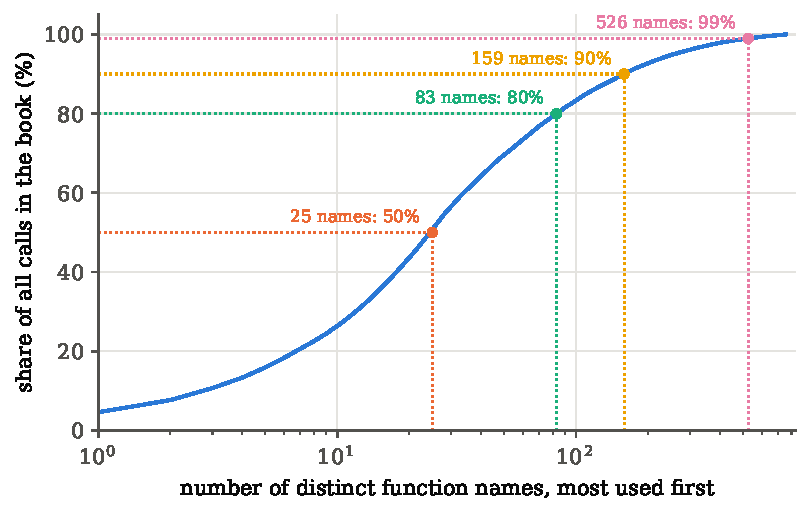
\includegraphics[width=11cm]{figures/chT0/01_census_coverage.pdf}
\caption{The share of all the book's library calls made by the most used names. The horizontal axis counts distinct names, most used first, on a logarithmic scale. Half of all calls use only $\TzNfifty$ names; $\TzNeighty$ names cover $80\%$, $\TzNninety$ cover $90\%$, and the last $1\%$ of calls is spread over hundreds of names that each appear a handful of times.}
\label{T0a:fig:coverage}
\end{figure}

\Cref{T0a:fig:coverage} is the whole answer. Half of all calls use $K_{0.5}=\TzNfifty$ names. Eighty per cent use $K_{0.8}=\TzNeighty$. Ninety per cent use $K_{0.9}=\TzNninety$. The curve then flattens: to reach $99\%$ takes $K_{0.99}=\TzNninetynine$ names, because the last per cent is a long tail of names that each appear once or twice. There are \TzRareNames{} names called three times or fewer in the whole book, and together they make only \TzRareShare\% of the calls. Those are exactly the names it is pointless to learn in advance. Each is used once, for one special job, and the script's comment or the text next to it says what it does.

\paragraph{Example: what the eighty per cent means for one script.} A typical script calls $\TzMedianNames$ distinct library names (the median over all files). Suppose a reader knows the $\TzNeighty$ most used names. How many unfamiliar calls will a script of a hundred calls contain? If the script's calls are drawn like the book's as a whole, each call is one of the known names with probability $c(\TzNeighty)\approx0.8$. The expected number of unknown calls is then
\begin{align*}
  \E[\text{unknown calls}]
  &\eqby{1}\sum_{i=1}^{100}\Prob(\text{call }i\text{ is unknown})
   \eqby{2}100\times\bigl(1-c(\TzNeighty)\bigr)
   \approx 100\times0.2=20 .
\end{align*}
\begin{explain}
  \item The expectation of a count is the sum of the probabilities of the events it counts (each call contributes $1$ if unknown, $0$ if not).
  \item Each call is unknown with probability $1-c(K)$, the share of calls outside the known names.
\end{explain}
Twenty calls sounds like many, but most of them repeat: a script that calls \texttt{hp.anafast} once usually calls it inside a loop or several times with different arguments. In practice the unfamiliar part of a script is one or two library functions, and the comment on that line usually says what they return.

\paragraph{Syntax: the same story, more strongly.} The census also asks, for each piece of syntax, what share of the scripts use it at least once (\cref{T0a:fig:syntax}). Some pieces are everywhere: assignment, function calls, imports, indexing, keyword arguments and tuple unpacking appear in practically every file, \texttt{for} loops in $\TzPctFor\%$, f-strings (a way of putting numbers into text) in $\TzPctFstring\%$, slices in $\TzPctSlice\%$, the definition of a function in $\TzPctDef\%$. Then comes a sharp drop. The \texttt{while} loop appears in $\TzPctWhile\%$ of the scripts, \texttt{try}/\texttt{except} in $\TzPctTry\%$, classes in $\TzPctClass\%$, decorators in $\TzPctDecorator\%$, generators (\texttt{yield}) in none. A course on Python spends weeks on classes, inheritance, generators, exceptions and decorators. The book barely uses them.

\begin{figure}[htbp]
\centering
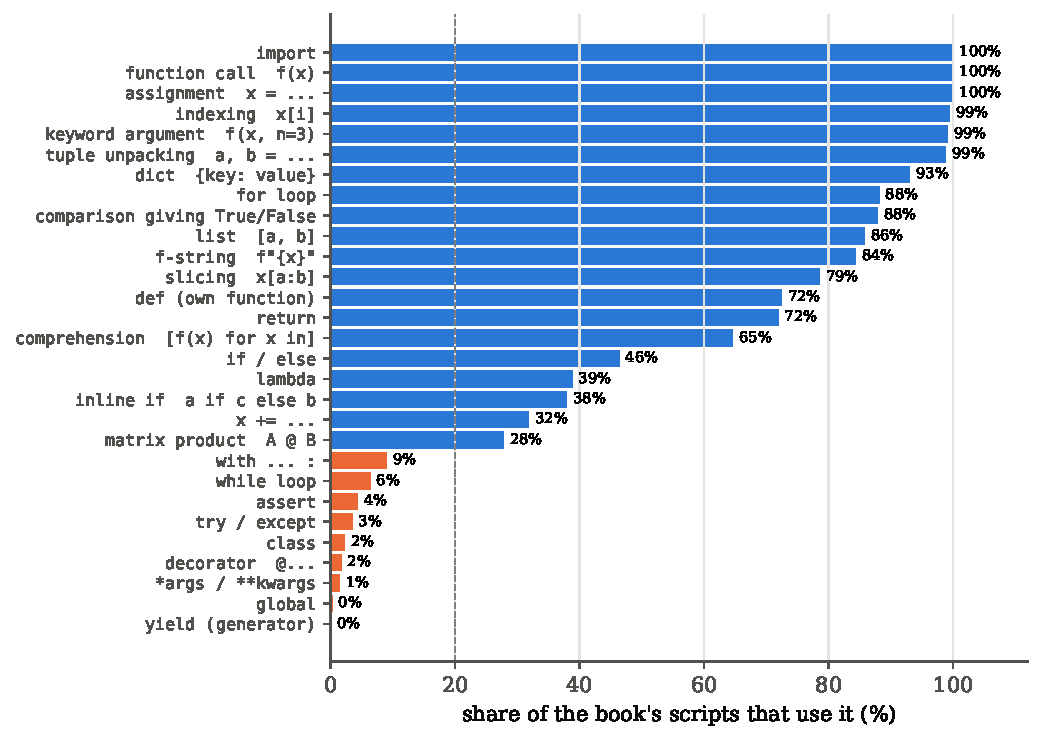
\includegraphics[width=11cm]{figures/chT0/01_census_syntax.pdf}
\caption{For each piece of Python syntax, the share of the book's scripts that use it at least once. Blue bars (at least $20\%$ of the scripts) are the core every reader needs; orange bars are rare and are collected in \cref{T0a:sec:rare}. The dashed line marks $20\%$.}
\label{T0a:fig:syntax}
\end{figure}

\paragraph{Libraries.} The import statements tell the same story. NumPy is imported by $\TzPctNumpy\%$ of the scripts and Matplotlib's plotting module by $\TzPctPlt\%$. SciPy is used by $\TzPctScipy\%$, almost always for one or two functions. healpy, the library for maps on the sphere, appears in $\TzPctHealpy\%$, and CAMB, the cosmology code, in $\TzPctCamb\%$; numba and the multiprocessing module in about $\TzPctNumba\%$ each. By number of calls, NumPy names make $\TzNumpyShare\%$ of all library calls, plotting calls about $\TzPlotShare\%$ and SciPy only $\TzScipyShare\%$: SciPy functions are powerful, so one call does a lot. The rest are Python's own built-in functions, such as \texttt{len}, \texttt{range}, \texttt{print}, and methods of arrays and lists, such as \texttt{x.mean()} or \texttt{results.append(\dots)}.

\Cref{T0a:fig:topcalls} lists the forty most used names, coloured by library. It is worth reading slowly once: together these forty names cover more than half of everything the book's code does, and each of them reappears below with an example.

\begin{figure}[htbp]
\centering
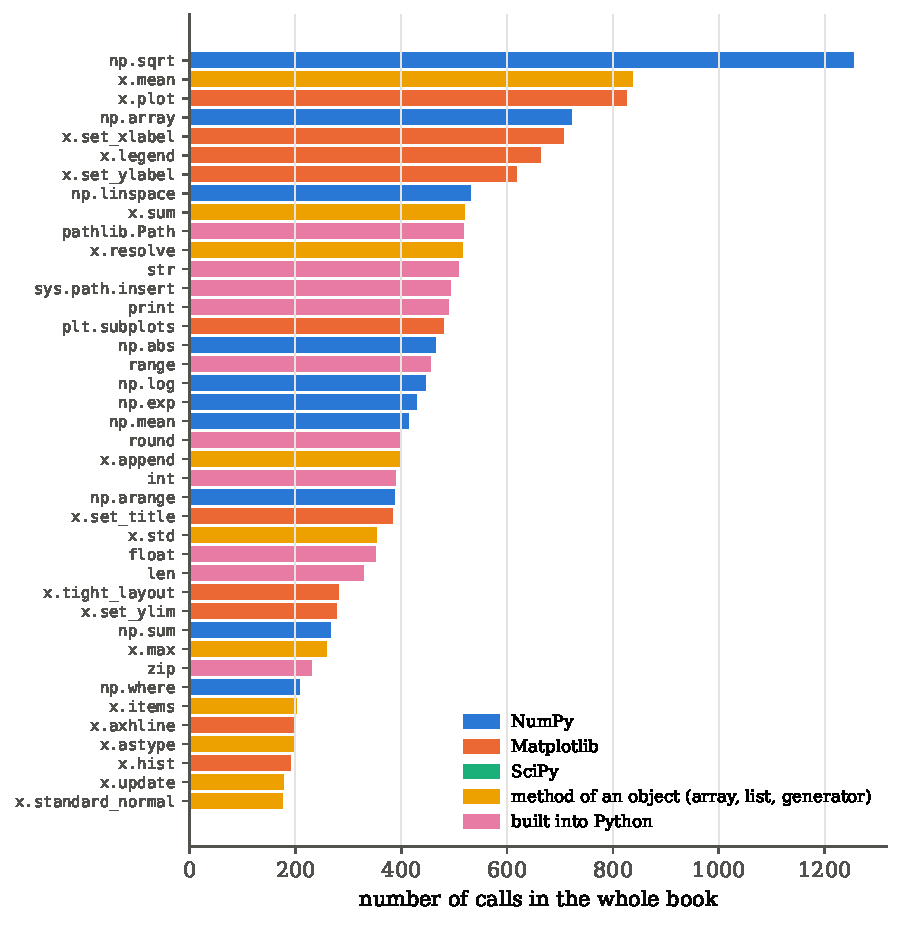
\includegraphics[width=10.5cm]{figures/chT0/01_census_topcalls.pdf}
\caption{The forty most used names in the book's code, by number of calls. \texttt{x.} stands for a method called on some object: \texttt{x.mean} is the mean of an array, \texttt{x.plot} draws on a set of axes, \texttt{x.append} adds an item to a list. Blue are NumPy functions, orange Matplotlib, green SciPy, yellow methods of arrays, lists and random generators, pink Python's built-in functions.}
\label{T0a:fig:topcalls}
\end{figure}

\begin{keyidea}[A small vocabulary does almost everything]
About $\TzNfifty$ names cover half of all the function calls in the book, about $\TzNeighty$ cover $80\%$, and the syntax needed is the core of the language: assignment, calls with keyword arguments, indexing and slicing, \texttt{for} and \texttt{if}, short functions, lists, tuples and dictionaries. Everything else is rare and can be looked up when met.
\end{keyidea}

That vocabulary is best learned in the order in which a reader meets it inside a script, each idea with its minimal syntax, a real excerpt from one of the book's scripts, and the one mistake most often made with it.
\section{Running a script and reading what it prints}
\label{T0a:sec:anatomy}

A script is a recipe for an experiment that the computer carries out. Like a lab procedure, it has a fixed shape: what it is for, what equipment it uses, the measurement itself, and where the results are written down. Every script in the book follows the same shape, so once one script has been read closely, the others look familiar. We read one closely here: \pyname{code/ch02/02_binomial.py}, which checks the binomial distribution of \cref{2a:sec:binomial} by simulation. Its question is: if we repeat a yes/no trial with success probability $p$ a number $n$ of times and count the successes, does the histogram of that count match the binomial formula $\binom nk p^k(1-p)^{n-k}$?

\paragraph{Running it.} From the top directory of the book (the folder \texttt{Notes}), one types in a terminal
\begin{center}
\texttt{python3 code/ch02/02\_binomial.py}
\end{center}
Python reads the file from the top and carries out its lines one after another. When it finishes, two new files exist: the figure \texttt{figures/ch02/02\_binomial.pdf} and the numbers file \texttt{results/ch02/02\_binomial.tex}. The terminal shows what the script chose to print, here two short lines naming those files. The book's own runs were made the same way, on a computing cluster, and the two files copied back. The random numbers are seeded by the script's name (\cref{0a:sec:code}), so the outputs are identical wherever the script runs.

\paragraph{When it fails.} If something goes wrong, Python stops and prints a \newterm{traceback}: a list of the lines that were being executed, innermost last, followed by one line naming the error. The last line is the one to read first. For example, adding an array of three numbers to an array of four numbers stops a script with
\begin{center}
\texttt{ValueError: operands could not be broadcast together with shapes (3,) (4,)}
\end{center}
which says exactly what is wrong: two arrays whose shapes do not fit (\cref{T0a:sec:broadcasting}). The line above it in the traceback gives the file and line number where it happened. Reading the traceback from the bottom up is the single most useful debugging habit.

\begin{figure}[htbp]
\centering
\begin{tikzpicture}[
  blk/.style={draw=accent,rounded corners=2pt,fill=ideabg,align=left,font=\footnotesize,
              text width=5.6cm,minimum height=0.75cm,inner sep=3pt},
  outfile/.style={draw=softgray,rounded corners=2pt,fill=codebg,align=center,font=\footnotesize\ttfamily,
              text width=3.6cm,minimum height=0.75cm},
  ln/.style={font=\scriptsize\ttfamily,softgray,anchor=east},
  arr/.style={->,thick,accent}]
  \node[blk] (doc) at (0,0) {\textbf{docstring}: Question, Computes, Writes};
  \node[blk] (imp) at (0,-1.0) {\textbf{imports}: the \texttt{sys.path} line, numpy, matplotlib, scipy, common};
  \node[blk] (set) at (0,-2.0) {\textbf{settings}: \texttt{setup()}, \texttt{rng = rng\_for(\dots)}, sizes};
  \node[blk] (fun) at (0,-3.0) {\textbf{own functions}: \texttt{def binomial\_by\_trials(\dots)}};
  \node[blk] (cmp) at (0,-4.0) {\textbf{the computation and the figure}: loop over cases};
  \node[blk] (num) at (0,-5.0) {\textbf{the numbers}: \texttt{save\_numbers(\dots)}};
  \node[ln] at (-3.0,0) {1--10};
  \node[ln] at (-3.0,-1.0) {11--15};
  \node[ln] at (-3.0,-2.0) {17--19};
  \node[ln] at (-3.0,-3.0) {21--24};
  \node[ln] at (-3.0,-4.0) {26--52};
  \node[ln] at (-3.0,-5.0) {54--60};
  \node[outfile] (fig) at (5.6,-3.5) {figures/ch02/\\02\_binomial.pdf};
  \node[outfile] (res) at (5.6,-5.0) {results/ch02/\\02\_binomial.tex};
  \draw[arr] (cmp.east) -- (fig.west);
  \draw[arr] (num.east) -- (res.west);
\end{tikzpicture}
\caption{The six blocks of every script in the book, with the line numbers they occupy in \pyname{02_binomial.py}. The two grey boxes are the files the script writes: the chapter text includes the figure and reads its numbers from the second file.}
\label{T0a:fig:anatomy}
\end{figure}

\paragraph{The whole script.} Here it is, all sixty lines.

\pyfile{code/ch02/02_binomial.py}{A complete book script: the binomial distribution by simulation}

We walk through it block by block (\cref{T0a:fig:anatomy}).

\emph{The docstring (lines 1--10).} Text between triple quotes at the top of a file is the file's \newterm{docstring}. Python stores it but does not execute it. Every script in the book states three things there: the \emph{Question} it answers, what it \emph{Computes}, and what it \emph{Writes}. Reading the docstring first tells us what to look for in the rest.

\emph{The imports (lines 11--15).} Line 11 is the same in every script and is explained once below. Lines 12--14 load NumPy under the short name \texttt{np}, Matplotlib's plotting module as \texttt{plt}, and the binomial distribution from SciPy. Line 15 loads four helpers from the book's own module \pyname{common.py}: \pyname{setup} (the figure style), \pyname{savefig} (write a figure into the right folder), \pyname{save_numbers} (write numbers for the text) and \pyname{rng_for} (a random generator seeded by the script's name). What each helper does inside is described in \cref{0a:sec:code}; here it is enough to know what goes in and what comes out.

\emph{The settings (lines 17--19).} \texttt{setup(6.4, 4.6)} sets the figure size in inches and the house style. \texttt{rng = rng\_for("ch02", "02\_binomial")} creates the random generator. Every random number in the script comes from \texttt{rng}. \texttt{reps = 20\_000} fixes the number of repetitions; the underscore only makes the number easier to read.

\emph{The script's own function (lines 21--24).} \texttt{binomial\_by\_trials(n, p, reps)} draws a table of uniform random numbers with \texttt{reps} rows and \texttt{n} columns, marks each entry \texttt{True} when it is below $p$ (a success), and counts the successes in each row. Line 24 does the counting with \texttt{trials.sum(axis=1)}: adding \texttt{True} as $1$ and \texttt{False} as $0$ along each row. Every idea in these four lines (arrays, comparisons that make masks, sums along an axis) appears again in \cref{T0a:sec:numpy}.

\emph{The computation and the figure (lines 26--52).} Line 27 lists six pairs $(n,p)$. Line 28 creates a figure with a $3\times2$ grid of panels. Line 29 walks through the panels and the pairs side by side: for each panel \texttt{ax} and each pair \texttt{(n, p)}, line 30 simulates, line 32 turns the counts into frequencies, and lines 33--34 draw the simulated bars and the exact probabilities as short black marks. Line 43 saves the figure. Lines 46--52 then compute two more checks: a trigger that fires when at least three of four detector layers fire, exactly and by simulation, and the mean and variance of the count.

\emph{The numbers (lines 54--60).} \texttt{save\_numbers} writes the five numbers to \texttt{results/\allowbreak ch02/\allowbreak 02\_binomial.tex}, each as a \LaTeX{} command, for example \verb|\twoaTrigExact|. The chapter text writes that command where the number belongs, so the number in the text is always the one the script printed.

\begin{figure}[htbp]
\centering
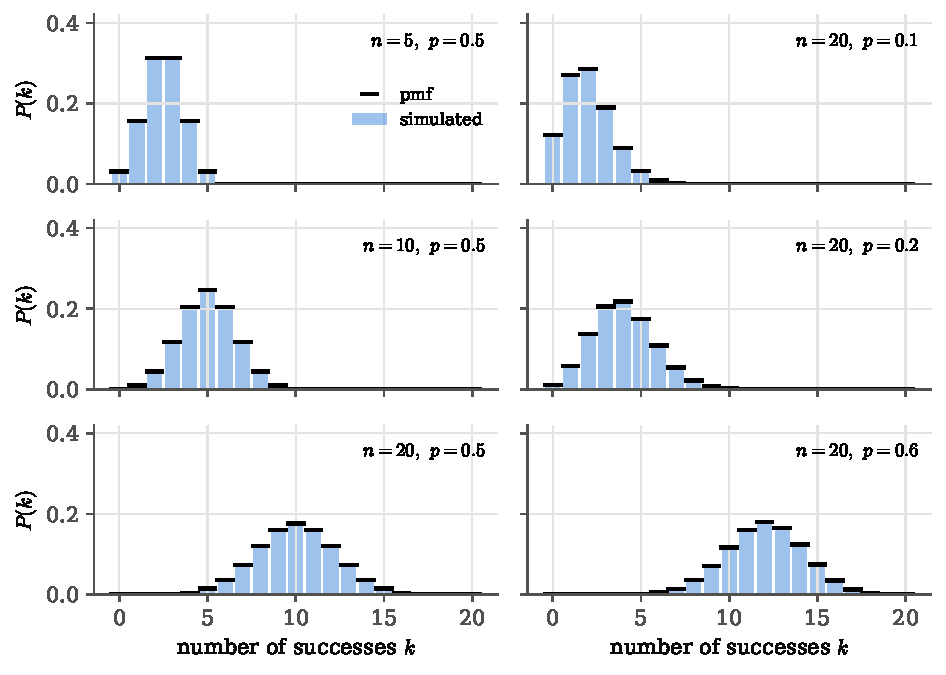
\includegraphics[width=9.5cm]{figures/ch02/02_binomial.pdf}
\caption{What \pyname{02_binomial.py} draws: for six choices of the number of trials $n$ and the success probability $p$, the frequencies of $k$ successes in $20\,000$ simulated experiments (blue bars) and the binomial probabilities (black marks). The left column grows $n$ at $p=0.5$; the right column grows $p$ at $n=20$.}
\label{T0a:fig:binomial-output}
\end{figure}

\paragraph{The one line that is the same everywhere.} Line 11 reads
\begin{center}
\texttt{import sys, pathlib; sys.path.insert(0, str(pathlib.Path(\_\_file\_\_).resolve().parents[1]))}
\end{center}
It looks cryptic, but it is a chain of small steps, each turning one thing into the next. Its job is to tell Python where \pyname{common.py} lives, so that line 15 can import it. Python looks for modules in a list of folders called \texttt{sys.path}, and the folder \texttt{code/} is not on that list by default. So the line computes the path of \texttt{code/} and puts it at the front of the list. For this script, read inside out:
\begin{align*}
  \texttt{\_\_file\_\_}
  &\eqby{1}\texttt{"code/ch02/02\_binomial.py"}\\
  \texttt{pathlib.Path(\_\_file\_\_).resolve()}
  &\eqby{2}\texttt{/\dots/Notes/code/ch02/02\_binomial.py}\\
  \texttt{\dots.parents[0]}
  &\eqby{3}\texttt{/\dots/Notes/code/ch02}\\
  \texttt{\dots.parents[1]}
  &\eqby{4}\texttt{/\dots/Notes/code}\\
  \texttt{sys.path.insert(0, str(\dots))}
  &\eqby{5}\text{put that folder first in the search list.}
\end{align*}
\begin{explain}
  \item Python sets \texttt{\_\_file\_\_} to the path by which the script was started.
  \item \texttt{pathlib.Path} turns the text into a path object, and \texttt{resolve()} makes it a full path from the root of the disk, whichever folder we started from.
  \item \texttt{parents[0]} is the folder that contains the file.
  \item \texttt{parents[1]} is one folder further up: \texttt{code/}, where \pyname{common.py} is.
  \item \texttt{str} turns the path object back into text, and \texttt{insert(0, \dots)} puts it at position $0$, the front, so it is searched first.
\end{explain}
The tour script \pyname{code/chT0/06_python_tour.py} prints the last names of these folders for itself: \texttt{here.parents[0].name} is \texttt{'chT0'} and \texttt{here.parents[1].name} is \texttt{'code'}. Because the path is computed from the script's own location, the script runs correctly whether it is started from \texttt{Notes}, from \texttt{Notes/code}, or from anywhere else. Library files of one chapter used by another (such as \pyname{code/ch07/lib_fields.py}) are reached the same way, with one more \texttt{sys.path.insert} line naming their folder.

\paragraph{Example: reading a printed summary.} Some scripts print a short report as they run. The census script of \cref{T0a:sec:census} prints three lines and keeps them in a text file:

\Tzout{results/chT0/01_census_out.txt}

The first line gives the size of the job (files, lines, calls, distinct names). The second gives $K_{0.5},K_{0.8},K_{0.9},K_{0.99}$ of \cref{T0a:fig:coverage}, in that order. The third gives the long tail. Printing a few such lines, with words next to the numbers, is what makes a script's output readable a month later.

\begin{pitfall}[Never edit a results file by hand]
The files in \texttt{results/} are written by the scripts. If a number in the text looks wrong, the fix is in the script: change it, rerun it, and the text updates itself. A number changed by hand in \texttt{results/} is silently overwritten at the next run, and until then the text disagrees with the code.
\end{pitfall}
\section{Plain Python: values, containers, loops and functions}
\label{T0a:sec:python}

Strip away the libraries and a script is a sequence of small instructions: give a number a name, collect several numbers together, repeat something for each item of a collection, do one thing or another depending on a condition, and package a recipe so that it can be used again. That is the whole of the plain Python the book needs. Every block below was run by \pyname{code/chT0/06_python_tour.py}, and each block shows a few lines of that script followed by exactly what they printed. The helper \texttt{say} prints a line and keeps a copy for the book; many lines use the f-string form \texttt{f"\{x = \}"}, which prints the expression itself followed by its value (\cref{T0a:sec:strings}).

\subsection{Numbers and names}
\label{T0a:sec:numbers}

The line \texttt{n = 20} does not state an equation. It is an instruction: compute the right-hand side and attach the name on the left to the result. The \newterm{assignment} \texttt{n = n + 1} is therefore perfectly sensible: take the current value of \texttt{n}, add one, and attach the name \texttt{n} to the new value.

Python has two kinds of number that matter here. An \newterm{integer} (type \texttt{int}) is a whole number, exact and of any size: a count of events, an index, a number of simulations. A \newterm{float} is a real number stored with about sixteen significant digits (\cref{T0a:sec:trust} says exactly how many and why). \texttt{20} is an integer, \texttt{20.0} and \texttt{0.2} are floats, and \texttt{1.5e-3} means $1.5\times10^{-3}$.

\pyfile[firstline=35,lastline=42,firstnumber=35]{code/chT0/06_python_tour.py}{The tour: numbers and names}
\noindent It prints:
\Tzout{results/chT0/06_numbers.txt}

The operators are \texttt{+ - * /}, \texttt{**} for powers ($2^{10}$ is \texttt{2 ** 10}, never \verb|2^10|, which means something else), \texttt{//} for whole-number division and \texttt{\%} for the remainder. Division with \texttt{/} always gives a float, even for two integers: $20/8=2.5$. Underscores inside a number are ignored, so \texttt{1\_000\_000} is a million written readably. The book uses this everywhere for sizes of simulations: \texttt{reps = 20\_000} in \cref{T0a:sec:anatomy}, \texttt{M = 200\_000} below.

\begin{pitfall}[The caret is not a power]
\texttt{2 ** 10} is $1024$. \verb|2 ^ 10| is $8$: the caret combines the bits of two integers, an operation the book never needs. A formula copied from paper with \verb|^| for powers runs without complaint and gives nonsense.
\end{pitfall}

\subsection{Text and f-strings}
\label{T0a:sec:strings}

Text is a \newterm{string}: characters between quotes, single or double. Strings are used for file names, labels on axes and lines of printed output. Two operations cover most uses. Strings can be joined with \texttt{+}, and single characters or pieces can be taken out by position, exactly as for lists (\cref{T0a:sec:containers}).

\pyfile[firstline=46,lastline=49,firstnumber=46]{code/chT0/06_python_tour.py}{The tour: text}
\noindent It prints:
\Tzout{results/chT0/06_strings.txt}

The operation that the book uses constantly is the \newterm{f-string}: a string with an \texttt{f} before the opening quote, in which anything between curly braces is computed and written into the text. A colon inside the braces sets the format: \texttt{:.3f} means three digits after the decimal point, \texttt{:.2e} scientific notation with two digits after the point, \texttt{:,} thousands separators. Writing \texttt{=} at the end, as in \verb|f"{n = }"|, prints the expression and its value; the tour script uses this for every line it prints.

\pyfile[firstline=53,lastline=57,firstnumber=53]{code/chT0/06_python_tour.py}{The tour: formatting numbers in f-strings}
\noindent It prints:
\Tzout{results/chT0/06_fstrings.txt}

Here is how a real script uses f-strings. \pyname{code/ch01/01_events_as_masks.py} (\cref{1a:sec:events}) sends its numbers to the text, rounding some of them to four digits on the way:

\pyfile[firstline=49,lastline=56,firstnumber=49]{code/ch01/01_events_as_masks.py}{Numbers sent to the text, some formatted by f-strings}

The keys on the left (\texttt{"OneAMaskExA"} and so on) become the names of \LaTeX{} commands. The values are either numbers, which \pyname{save_numbers} formats itself, or strings already formatted with f-strings, such as \verb|f"{pA:.4f}"|, which writes the probability \texttt{pA} with four decimals. Plot labels are f-strings too: line 35 of the binomial script writes \verb|f"$n={n},\\ p={p}$"|, which becomes the label $n=20,\ p=0.2$ in the figure.

\begin{pitfall}[Backslashes in labels]
A backslash inside an ordinary Python string starts a special character: \verb|"\n"| is a new line and \verb|"\t"| a tab. So the \LaTeX{} label \verb|"$\theta$"| arrives as a tab followed by \texttt{heta}. Either double every backslash (\verb|"$\\theta$"|) or put an \texttt{r} before the quote (\verb|r"$\theta$"|), which tells Python to leave backslashes alone. The book's scripts use both forms.
\end{pitfall}

\subsection{Lists, tuples and dictionaries}
\label{T0a:sec:containers}

Three containers hold several values under one name.

A \newterm{list} is an ordered sequence in square brackets, \texttt{[1, 2, 5, 30]}, which can grow. Its items are numbered from $0$, not from $1$, so \texttt{ns[0]} is the first item. Negative positions count from the end: \texttt{ns[-1]} is the last item. A \newterm{slice} \texttt{ns[a:b]} takes the items from position \texttt{a} up to, but not including, position \texttt{b}. \texttt{.append(x)} adds an item at the end. The method \texttt{.append} is called $\TzAppendCalls$ times in the book's code, almost always in one pattern: start with an empty list, and append one result each time round a loop.

\pyfile[firstline=61,lastline=69,firstnumber=61]{code/chT0/06_python_tour.py}{The tour: a list, and the start-empty-then-append pattern}
\noindent It prints:
\Tzout{results/chT0/06_lists.txt}

The rule ``from \texttt{a}, stopping before \texttt{b}'' becomes obvious once positions are pictured as the \emph{gaps between items}, not the items themselves (\cref{T0a:fig:slices}). Then \texttt{ns[1:3]} is everything between gap $1$ and gap $3$: two items. The length of a slice is \texttt{b - a}, and \texttt{ns[:k]} followed by \texttt{ns[k:]} gives back the whole list with nothing repeated and nothing lost.

\begin{figure}[htbp]
\centering
\begin{tikzpicture}[x=1.25cm,y=1cm,
  cell/.style={draw=accent,fill=ideabg,minimum width=1.25cm,minimum height=0.8cm,font=\small\ttfamily}]
  \foreach \v [count=\i from 0] in {1,2,5,30,100} {
    \node[cell] at (\i+0.5,0) {\v};
  }
  \foreach \i in {0,...,5} {
    \draw[softgray] (\i,0.55) -- (\i,0.8);
    \node[font=\footnotesize\ttfamily,accent] at (\i,1.05) {\i};
  }
  \foreach \i/\n in {0/-5,1/-4,2/-3,3/-2,4/-1} {
    \node[font=\footnotesize\ttfamily,fibreorange] at (\i+0.5,-0.75) {\n};
  }
  \node[font=\footnotesize,accent,anchor=east] at (-0.2,1.05) {gaps};
  \node[font=\footnotesize,fibreorange,anchor=east] at (-0.2,-0.75) {from the end};
  \draw[very thick,tangentgreen] (1,-1.25) -- (3,-1.25);
  \draw[tangentgreen] (1,-1.12) -- (1,-1.38);
  \draw[tangentgreen] (3,-1.12) -- (3,-1.38);
  \node[font=\footnotesize\ttfamily,tangentgreen,anchor=west] at (3.2,-1.25) {ns[1:3] = [2, 5]};
\end{tikzpicture}
\caption{The list \texttt{ns = [1, 2, 5, 30, 100]}. Blue numbers mark the gaps between items: a slice \texttt{ns[a:b]} runs from gap \texttt{a} to gap \texttt{b}, so \texttt{ns[1:3]} holds two items. An index \texttt{ns[i]} is the item just after gap \texttt{i}; orange numbers are the negative indices, counting back from the end.}
\label{T0a:fig:slices}
\end{figure}

A \newterm{tuple} is a fixed group of values in round brackets, \texttt{(20, 0.2)}, which cannot be changed after it is made. The book uses tuples to keep things together that belong together, such as the pair $(n,p)$ of a binomial distribution. Its most useful property is \newterm{unpacking}: \texttt{n, p = case} gives one name to each entry. Unpacking works in \texttt{for} loops too, and is used in practically every script.

\pyfile[firstline=73,lastline=78,firstnumber=73]{code/chT0/06_python_tour.py}{The tour: tuples and unpacking}
\noindent It prints:
\Tzout{results/chT0/06_tuples.txt}

A \newterm{dictionary} (\texttt{dict}) is a table that maps \emph{keys} to \emph{values}, written \texttt{\{"H0": 67.36, "ns": 0.9649\}}. A value is fetched by its key, \texttt{fid["H0"]}, not by a position. New entries are added by assignment, \texttt{fid["tau"] = 0.0544}, and \texttt{.items()} walks through the (key, value) pairs.

\pyfile[firstline=82,lastline=87,firstnumber=82]{code/chT0/06_python_tour.py}{The tour: a dictionary}
\noindent It prints:
\Tzout{results/chT0/06_dicts.txt}

All three containers appear together in the binomial script of \cref{T0a:sec:anatomy}, lines 27--30: a list of tuples \texttt{cases = [(5, 0.5), (10, 0.5), \dots]}, walked through with unpacking, \texttt{for ax, (n, p) in zip(\dots)}. The dictionary \texttt{\{...\}} handed to \pyname{save_numbers} on line 54 is the commonest dictionary in the book. A slightly richer use is in \pyname{code/ch03/01_sampling_distribution.py} (\cref{3a:sec:sampling-python}), which compares four ways of estimating $g$ from ten readings:

\pyfile[firstline=27,lastline=37,firstnumber=27]{code/ch03/01_sampling_distribution.py}{A dictionary of estimators, and a dictionary built from it}

The dictionary \texttt{est} maps a name (a string) to an array of $200\,000$ estimates, one per simulated experiment. Line 37 builds a second dictionary from the first: for every key \texttt{k} and value \texttt{v}, the standard deviation of \texttt{v}. That one-line construction is a \emph{comprehension} (\cref{T0a:sec:control}).

\paragraph{Example: why a dictionary and not a list?} The four estimators could be kept in a list, \texttt{[mean, median, midrange, first]}. Then the standard deviation of the median would be \texttt{sd[1]}, and anyone reading the code must remember that position $1$ is the median. With a dictionary it is \texttt{sd["sample median"]}: the code says what it means, and adding a fifth estimator does not shift the positions of the others. The rule of thumb is: a list when the items are of the same kind and their order matters (a sequence of sizes $N$), a dictionary when each item has a name (estimators, parameters, numbers for the text).

\begin{pitfall}[Counting from zero]
The first item is \texttt{x[0]} and the last is \texttt{x[len(x) - 1]}, also written \texttt{x[-1]}. \texttt{x[len(x)]} does not exist and stops the script with \texttt{IndexError}. When a formula on paper runs over $i=1,\dots,N$, the code runs over \texttt{i = 0, ..., N-1}.
\end{pitfall}

\subsection{Doing things repeatedly, and conditionally}
\label{T0a:sec:control}

A \texttt{for} loop repeats a block of lines once for each item of a collection. The block is marked by \newterm{indentation}: the lines that belong to the loop are shifted to the right by four spaces, and the first line that is not shifted is the first line after the loop. Python has no \texttt{end} statement; the indentation \emph{is} the structure.

\texttt{range(n)} produces the integers $0,1,\dots,n-1$ (\texttt{n} numbers, stopping before \texttt{n}), and \texttt{range(a, b)} those from \texttt{a} up to \texttt{b - 1}. \texttt{enumerate(xs)} gives the position together with each item, and \texttt{zip(xs, ys)} walks two collections side by side.

\pyfile[firstline=91,lastline=98,firstnumber=91]{code/chT0/06_python_tour.py}{The tour: three kinds of for loop}
\noindent It prints:
\Tzout{results/chT0/06_loops.txt}

An \texttt{if} statement runs a block only when a condition is true. \texttt{elif} (``else if'') adds further conditions, tried in order, and \texttt{else} catches everything left. Conditions are comparisons (\texttt{<}, \texttt{<=}, \texttt{==} for ``is equal to'', \texttt{!=} for ``is not equal to'') joined by \texttt{and}, \texttt{or}, \texttt{not}.

\pyfile[firstline=102,lastline=110,firstnumber=102]{code/chT0/06_python_tour.py}{The tour: if, elif, else}
\noindent It prints:
\Tzout{results/chT0/06_ifs.txt}

Both appear together in the dice script of \cref{1a:sec:events}, which colours the $36$ outcomes of two dice according to the two events ``first die even'' and ``sum at least $9$'':

\pyfile[firstline=62,lastline=73,firstnumber=62]{code/ch01/01_events_as_masks.py}{Two nested loops and a three-way condition}

Lines 62--63 are two loops, one inside the other: for each value \texttt{i} of the first die, for each value \texttt{j} of the second, so the inner block runs $6\times6=36$ times. Line 64 computes two true/false values. Lines 66--71 choose a colour: both events (green), only $A$ (blue), only $B$ (orange), and otherwise the white set on line 65 stays. Line 72 draws one square.

A \texttt{while} loop repeats as long as a condition holds, for when the number of repetitions is not known in advance. It is rare in the book ($\TzPctWhile\%$ of the scripts). A typical use is accept--reject sampling (\cref{ch:06}): keep drawing until enough draws have been accepted. \pyname{code/ch03/10_angular_ml.py} (\cref{3b:sec:newton}) does exactly that:

\pyfile[firstline=27,lastline=35,firstnumber=27]{code/ch03/10_angular_ml.py}{Draw until there are enough: a while loop}

Line 31 says: while fewer than \texttt{size} values have been collected, draw another batch of $2\times$\texttt{size} candidates, keep those that pass the test (line 33), and add them to the collection (line 34). Line 35 returns exactly \texttt{size} of them.

A \newterm{comprehension} is a loop that builds a list (or a dictionary) in one line: \texttt{[k ** 2 for k in range(5)]} is the list of the squares of $0,\dots,4$. An \texttt{if} at the end keeps only some items. The same construction inside \texttt{sum(\dots)} or \texttt{max(\dots)} needs no brackets.

\pyfile[firstline=142,lastline=148,firstnumber=142]{code/chT0/06_python_tour.py}{The tour: comprehensions}
\noindent It prints:
\Tzout{results/chT0/06_comprehensions.txt}

Comprehensions are in $\TzPctComp\%$ of the scripts. Line 37 of the sampling-distribution excerpt above, \verb|{k: v.std(ddof=1) for k, v in est.items()}|, is one. A one-line \texttt{if} also exists for values: \texttt{a if condition else b}. It is how the book's code writes a default, as in \texttt{rng = np.random.default\_rng() if rng is None else rng}.

\paragraph{Example: the same sum three ways.} The sum $\sum_{k=1}^{5}k$ is computed by an explicit loop in the tour (\texttt{total = 15}). With a comprehension it is \texttt{sum(k for k in range(1, 6))}. With NumPy (\cref{T0a:sec:numpy}) it is \texttt{np.arange(1, 6).sum()}. All three give $15$. The loop is the clearest; the NumPy form is the fastest for long sums, by a factor of about $\TzSpeedup$ for a million terms (\cref{T0a:sec:vectorise}).

\begin{pitfall}[Indentation is part of the program]
Moving a line four spaces to the left takes it out of the loop: it then runs once, after the loop, instead of once per item. Python cannot warn about this, because both versions are valid programs. When a result looks like ``only the last case was used'', check the indentation of the line that stores the result.
\end{pitfall}

\subsection{Functions}
\label{T0a:sec:functions}

A \newterm{function} packages a recipe with inputs and outputs, so that it can be used many times and read once. It starts with \texttt{def}, its name and its inputs (the \newterm{parameters}) in brackets; the indented block is the recipe; \texttt{return} hands back the result. A string on the first line of the block is the function's docstring. Parameters can have \newterm{default values}, used when the caller does not give them; and a caller can give any parameter by name, as a \newterm{keyword argument}, in any order. To return several results, a function returns them separated by commas, which makes a tuple, and the caller unpacks it.

\pyfile[firstline=123,lastline=138,firstnumber=123]{code/chT0/06_python_tour.py}{The tour: two functions and a lambda}
\noindent It prints:
\Tzout{results/chT0/06_functions.txt}

The first two lines call \texttt{gaussian(x, mu=0.0, sigma=1.0)}: once with both defaults, once giving \texttt{sigma} by name and leaving \texttt{mu} at its default. The third calls \texttt{mean\_and\_error}, which returns two values, unpacked into \texttt{m, e}. The last line uses a \newterm{lambda}: a one-line function without a name, \texttt{lambda t: t ** 2}, convenient when a function is needed only once, as an argument to another function.

Every one of these features is in daily use in the book. The log-likelihood of the decay-time example (\cref{3b:sec:curv-python}) is a two-line function, and the function whose root gives the likelihood interval is a lambda:

\pyfile[firstline=27,lastline=40,firstnumber=27]{code/ch03/09_mle_decay.py}{A function, and lambdas handed to SciPy}

Line 29 is the whole recipe: $\ln\Like(\tau)=-n\ln\tau-\sum_i t_i/\tau$ for decay times $t_i$, with \texttt{len(t)} giving $n$ and \texttt{t.sum()} the sum. Line 35 hands a lambda to SciPy's minimiser: ``the function of \texttt{s} that returns minus the log-likelihood at \texttt{s}''. Line 38 builds the function whose zeros are the points where $\ln\Like$ has dropped by $\tfrac12$ from its maximum, and lines 39--40 find those zeros (\cref{T0a:sec:scipy}).

Library functions in the book use defaults and keyword arguments to stay flexible. The Gaussian-field simulator of \cref{7a:sec:recipe} begins

\pyfile[firstline=45,lastline=53,firstnumber=45]{code/ch07/lib_fields.py}{Defaults and keyword arguments in a library function}

The parameters \texttt{d}, \texttt{rng} and \texttt{nsim} have defaults ($2$ dimensions, no generator given, one field), so the simplest call is \texttt{gaussian\_field(P, N, L)}, and a three-dimensional batch of fields is \texttt{gaussian\_field(P, N, L, d=3, nsim=100, rng=rng)}. The words after the colons (\texttt{N: int}, \texttt{L: float}) are \newterm{type hints}: notes for the reader saying what kind of value is expected. Python ignores them.

\begin{figure}[htbp]
\centering
\begin{tikzpicture}[
  fn/.style={draw=accent,thick,rounded corners=3pt,fill=ideabg,minimum width=4.6cm,minimum height=2.0cm,align=center,font=\small},
  inp/.style={font=\footnotesize\ttfamily,anchor=east},
  arr/.style={->,thick,accent}]
  \node[fn] (f) at (0,0) {\texttt{def mean\_and\_error(x):}\\[2pt] \footnotesize mean and standard error\\ \footnotesize of the readings \texttt{x}};
  \node[inp] (a) at (-3.6,0.5) {np.array([9.80, \dots])};
  \node[inp,softgray] (b) at (-3.6,-0.5) {(no other inputs)};
  \draw[arr] (a.east) -- (f.west |- a.east);
  \node[font=\footnotesize\ttfamily,anchor=west] (o1) at (3.6,0.45) {9.800};
  \node[font=\footnotesize\ttfamily,anchor=west] (o2) at (3.6,-0.45) {0.032};
  \draw[arr] (f.east |- o1.west) -- (o1.west);
  \draw[arr] (f.east |- o2.west) -- (o2.west);
  \node[font=\footnotesize,anchor=west,softgray] at (4.9,0.45) {$\to$ \texttt{m}};
  \node[font=\footnotesize,anchor=west,softgray] at (4.9,-0.45) {$\to$ \texttt{e}};
  \node[font=\footnotesize,align=center] at (0,-1.6) {\texttt{m, e = mean\_and\_error(readings)}};
\end{tikzpicture}
\caption{A function as a box with a name: an array of readings goes in, two numbers come out as a tuple, and the caller gives each a name by unpacking. Nothing inside the box is visible to the caller except what \texttt{return} hands back.}
\label{T0a:fig:function}
\end{figure}

\paragraph{Example: why a function at all?} The binomial script of \cref{T0a:sec:anatomy} simulates the binomial count three times: for the six panels (line 30), for the trigger (line 48) and for the moments (line 52). Without the function \texttt{binomial\_by\_trials}, its two lines would be written three times, and a correction (say, \texttt{<} instead of \texttt{<=}) would have to be made in three places. With the function, it is made once. This is the reason almost three quarters of the scripts ($\TzPctDef\%$) define at least one function of their own.

\begin{pitfall}[A function that forgets to return]
A function without a \texttt{return} line returns the special value \texttt{None}. The mistake looks like this: the last line computes the answer, \texttt{chi2 = np.sum(r ** 2)}, but never returns it. The caller then gets \texttt{None}, and the error appears later, somewhere else, as \texttt{TypeError: unsupported operand type(s) \dots{} 'NoneType'}. When that word appears in an error message, look for a missing \texttt{return}.
\end{pitfall}

\subsection{Modules and imports}
\label{T0a:sec:imports}

A \newterm{module} is a file of Python code whose functions can be used elsewhere. \texttt{import numpy as np} loads the module \texttt{numpy} and calls it \texttt{np} inside the script, so its square root is \texttt{np.sqrt}. \texttt{from scipy import stats} loads one part of SciPy under its own name, and \texttt{from math import comb} loads a single function. The book's short names are fixed: \texttt{np} for NumPy, \texttt{plt} for Matplotlib's plotting module, \texttt{hp} for healpy.

\pyfile[firstline=152,lastline=157,firstnumber=152]{code/chT0/06_python_tour.py}{The tour: imports}
\noindent It prints:
\Tzout{results/chT0/06_imports.txt}

The book's own modules (\pyname{common.py}, \pyname{camb_fiducial.py} and the \pyname{lib_*.py} files of each chapter) are imported the same way once their folder is on \texttt{sys.path} (\cref{T0a:sec:anatomy}). One more construction appears at the bottom of a few of them. \pyname{code/camb_fiducial.py} ends with

\pyfile[firstline=40,lastline=41,firstnumber=40]{code/camb_fiducial.py}{Run main() only when the file is started as a script}

Python sets the name \texttt{\_\_name\_\_} to \texttt{"\_\_main\_\_"} in the file that was started, and to the module's own name in a file that was imported. So \texttt{python3 code/camb\_fiducial.py} computes and saves the CAMB spectra, while \texttt{from camb\_fiducial import load\_fiducial} in another script only makes the function available, without running anything.
\section{NumPy: computing with whole arrays}
\label{T0a:sec:numpy}

A physicist writes $\chi^2=\sum_i (d_i-m_i)^2/\sigma_i^2$ without thinking about the order in which the terms are added. The formula is about whole vectors: the data vector $\data$, the model vector $\bm m$, the vector of errors. NumPy lets code be written the same way. Its central object is the \newterm{array}: a block of numbers, all of the same kind, laid out in a grid of one or more dimensions, on which arithmetic acts element by element. \texttt{(d - m) / s} is the vector of normalised residuals, and \texttt{np.sum(((d - m) / s) ** 2)} is $\chi^2$. NumPy names make $\TzNumpyShare\%$ of all library calls in the book, and NumPy is imported by $\TzPctNumpy\%$ of the scripts: this section is the heart of the toolkit. The printed lines below come from \pyname{code/chT0/07_numpy_tour.py}.

\subsection{Arrays, shape and type}
\label{T0a:sec:arrays}

An array is made from a list with \texttt{np.array([\dots])}, or directly by a function that fills it: \texttt{np.zeros}, \texttt{np.ones}, \texttt{np.full}, \texttt{np.arange}, \texttt{np.linspace}, or a random generator. Three attributes describe it. Its \newterm{shape} is a tuple giving the length along each dimension: \texttt{(4,)} for four readings, \texttt{(2, 3)} for two rows of three. \texttt{ndim} is the number of dimensions, and \texttt{dtype} the kind of number stored, almost always \texttt{float64} (a real number in double precision) or \texttt{int64} (a whole number). Arithmetic and functions such as \texttt{np.sqrt}, \texttt{np.exp}, \texttt{np.log} act on every element.

\Tzout{results/chT0/07_arrays.txt}

Three ways of making evenly spaced numbers need to be told apart, because they are used constantly. \texttt{np.arange(a, b, step)} starts at \texttt{a} and adds \texttt{step} until it reaches \texttt{b}, which it does \emph{not} include; it is meant for integers. \texttt{np.linspace(a, b, n)} gives \texttt{n} points from \texttt{a} to \texttt{b} \emph{including} both ends; it is the right choice for a grid of real numbers, such as the $x$ values at which a density is plotted. \texttt{np.logspace(p, q, n)} gives \texttt{n} points from $10^p$ to $10^q$, evenly spaced in the logarithm, and \texttt{np.geomspace(a, b, n)} the same between \texttt{a} and \texttt{b} themselves; they are the right choice for sample sizes, scales and frequencies that span several decades.

\paragraph{Example: how many points, and what spacing?} A grid of $\theta$ from $0$ to $1$ with steps of $0.1$ has eleven points, $0,0.1,\dots,1$. With \texttt{np.linspace(0, 1, 11)} the spacing is
\begin{align*}
  \Delta\theta
  &\eqby{1}\frac{b-a}{n-1}
   =\frac{1-0}{11-1}=0.1 ,
\end{align*}
\begin{explain}
  \item $n$ points with both ends included leave $n-1$ gaps between them.
\end{explain}
and the last point is exactly $1$. With \texttt{np.arange(0, 1, 0.1)} one gets only ten points, stopping at $0.9$; and because $0.1$ is not exactly representable in binary (\cref{T0a:sec:trust}), \texttt{np.arange} with a fractional step can occasionally include or exclude the end by rounding. Hence the rule: \texttt{arange} for integers, \texttt{linspace} for real grids.

\subsection{Indexing and slicing}
\label{T0a:sec:indexing}

Indexing an array works like indexing a list (\cref{T0a:fig:slices}), with one addition: an array with several dimensions takes one index per dimension, separated by commas. \texttt{A[1, 2]} is the element in row $1$, column $2$ (both counted from $0$). A colon on its own means ``all of this dimension'', so \texttt{A[:, 0]} is the first column and \texttt{A[1]} (or \texttt{A[1, :]}) the second row. A slice \texttt{a:b:step} can take every second or third element, and \texttt{::-1} reverses.

\Tzout{results/chT0/07_indexing.txt}

The book stores many repetitions of an experiment as the \emph{rows} of a two-dimensional array: one row per simulated experiment, one column per reading. Then \texttt{x[:, 0]} is ``the first reading of every experiment'', which is how the sampling-distribution script of \cref{3a:sec:sampling-python} builds its fourth estimator (line 34 of the excerpt in \cref{T0a:sec:containers}).

\subsection{Masks: selecting by a condition}
\label{T0a:sec:masks}

A comparison between an array and a number, such as \texttt{x > 0}, does not give one \texttt{True} or \texttt{False}. It gives an array of them, one per element: a \newterm{boolean mask}. A mask can do three things. Used as an index, \texttt{x[m]} keeps only the elements where the mask is \texttt{True}. Summed, \texttt{m.sum()} counts the \texttt{True} entries, because \texttt{True} counts as $1$ and \texttt{False} as $0$. Averaged, \texttt{m.mean()} is the fraction of \texttt{True} entries, which is how a simulated probability is computed. Masks combine with \texttt{\&} (and), \texttt{|} (or) and \texttt{\textasciitilde} (not). \texttt{np.where(m, a, b)} takes \texttt{a} where the mask is true and \texttt{b} elsewhere.

\Tzout{results/chT0/07_masks.txt}

Masks are the bridge between probability and code, and the very first script of \cref{ch:01} is built on them (\cref{1a:sec:events}). An event is a set of outcomes; in a simulation, an event \emph{is} a mask over the simulated outcomes:

\pyfile[firstline=20,lastline=40,firstnumber=20]{code/ch01/01_events_as_masks.py}{Events as boolean masks over $100\,000$ simulated rolls of two dice}

Lines 24--25 roll two dice $N=100\,000$ times: \texttt{rng.integers(1, 7, size=N)} draws integers from $1$ to $6$ (the upper end $7$ is excluded, as for \texttt{range}). Line 28 is the event ``first die even'' as a mask: \texttt{d1 \% 2 == 0} is \texttt{True} where the remainder on division by $2$ is zero. Lines 32--34 are intersection, union and complement, written \texttt{\&}, \texttt{|}, \texttt{\textasciitilde}. Line 40 checks the inclusion--exclusion identity $|A\cup B|=|A|+|B|-|A\cap B|$ on the counts, each count being a \texttt{.sum()} of a mask. The frequency of $A$ is then \texttt{A.mean()}, which estimates $\Prob(A)$.

\paragraph{Example: a probability as the mean of a mask.} Why is \texttt{A.mean()} an estimate of $\Prob(A)$? Write $I_i=1$ if roll $i$ lies in $A$ and $I_i=0$ otherwise; the mask \texttt{A} is the array $(I_1,\dots,I_N)$. Then
\begin{align*}
  \texttt{A.mean()}
  &\eqby{1}\frac1N\sum_{i=1}^N I_i
   \eqby{2}\frac{\#\{i:\ \text{roll } i\in A\}}{N},
  &
  \E[\texttt{A.mean()}]
  &\eqby{3}\frac1N\sum_{i=1}^N\E[I_i]
   \eqby{4}\Prob(A) .
\end{align*}
\begin{explain}
  \item \texttt{.mean()} adds the entries and divides by their number, with \texttt{True} counted as $1$.
  \item The sum of the indicators counts the rolls that land in $A$.
  \item The expectation of a sum is the sum of the expectations.
  \item Each indicator has expectation $1\cdot\Prob(A)+0\cdot(1-\Prob(A))=\Prob(A)$.
\end{explain}
So the mean of a mask is the relative frequency, an unbiased estimate of the probability, with the binomial standard error $\sqrt{\Prob(A)(1-\Prob(A))/N}$ (\cref{T0a:sec:trust}).

\begin{pitfall}[\texttt{and} is not \texttt{\&}]
For masks, write \texttt{(x > 0) \& (x < 1)}, with the brackets. The word \texttt{and} works only for single \texttt{True}/\texttt{False} values and stops with \texttt{ValueError: The truth value of an array with more than one element is ambiguous}. Without the brackets, \texttt{x > 0 \& x < 1} is read as \texttt{x > (0 \& x) < 1}, because \texttt{\&} binds more tightly than \texttt{>}.
\end{pitfall}

\subsection{Broadcasting: arrays of different shapes}
\label{T0a:sec:broadcasting}

\texttt{g * 2} multiplies every element of \texttt{g} by $2$: the single number is ``stretched'' to the shape of the array. NumPy generalises this to arrays of different shapes, and the generalisation, called \newterm{broadcasting}, is what lets the book write tables of pairs without loops.

\begin{workdef}[broadcasting]
Two arrays can be combined element by element when their shapes are compatible. Compare the shapes from the right (the last dimension first). Two lengths are compatible if they are equal or if one of them is $1$ \unpack{a length-$1$ dimension is copied as often as needed}. A missing dimension on the left counts as length $1$. The result has, in each dimension, the larger of the two lengths.
\end{workdef}

The tool for making a length-$1$ dimension on purpose is \texttt{None} as an index. If \texttt{r} has shape \texttt{(3,)}, then \texttt{r[:, None]} has shape \texttt{(3, 1)} (a column) and \texttt{r[None, :]} has shape \texttt{(1, 3)} (a row). Their difference has shape \texttt{(3, 3)}, and its entry $(i,j)$ is $r_i-r_j$ (\cref{T0a:fig:broadcast}).

\Tzout{results/chT0/07_broadcasting.txt}

\begin{figure}[htbp]
\centering
\begin{tikzpicture}[x=0.75cm,y=0.75cm,
  c/.style={draw=accent,fill=ideabg,minimum size=0.75cm,font=\footnotesize\ttfamily,inner sep=0},
  g/.style={draw=softgray,dashed,fill=white,minimum size=0.75cm,font=\footnotesize\ttfamily,text=softgray,inner sep=0}]
  \foreach \v [count=\i from 0] in {0,1,3} { \node[c] at (0,-\i) {\v}; }
  \foreach \v [count=\i from 0] in {0,1,3} { \node[g] at (1,-\i) {\v}; \node[g] at (2,-\i) {\v}; }
  \node[font=\footnotesize,align=center,anchor=south] at (1,0.6) {\texttt{r[:, None]}\\ $(3,1)\to(3,3)$};
  \node at (3.25,-1) {$-$};
  \foreach \v [count=\j from 0] in {0,1,3} { \node[c] at (4.5+\j,0) {\v}; }
  \foreach \v [count=\j from 0] in {0,1,3} { \node[g] at (4.5+\j,-1) {\v}; \node[g] at (4.5+\j,-2) {\v}; }
  \node[font=\footnotesize,align=center,anchor=south] at (5.5,0.6) {\texttt{r[None, :]}\\ $(1,3)\to(3,3)$};
  \node at (8.0,-1) {$=$};
  \foreach \row [count=\i from 0] in {{0,-1,-3},{1,0,-2},{3,2,0}} {
    \foreach \v [count=\j from 0] in \row { \node[c,fill=takebg] at (9.25+\j,-\i) {\v}; }
  }
  \node[font=\footnotesize,align=center,anchor=south] at (10.25,0.6) {all differences\\ $r_i-r_j$};
\end{tikzpicture}
\caption{Broadcasting a column against a row. The column of shape $(3,1)$ is copied sideways and the row of shape $(1,3)$ is copied downwards (dashed copies are never actually stored), so the difference is the full $3\times3$ table of $r_i-r_j$.}
\label{T0a:fig:broadcast}
\end{figure}

The book uses exactly this to build covariance matrices that depend on the distance between two points. The correlated one-dimensional field of \cref{6b:sec:cholesky} has covariance $C_{ij}=e^{-|x_i-x_j|/\ell}$ between grid points $x_i$ and $x_j$, and the whole $200\times200$ matrix is one line:

\pyfile[firstline=38,lastline=42,firstnumber=38]{code/ch06/23_cholesky_field.py}{A covariance matrix from all pairwise distances, by broadcasting}

Line 39 sets the sizes and line 40 makes the $200$ grid positions. In line 41, \texttt{xg[:, None] - xg[None, :]} is the $200\times200$ table of differences, \texttt{np.abs} takes their absolute values, and the exponential is applied to every entry. Line 42 factorises the matrix (\cref{T0a:sec:linalg}).

\paragraph{Example: when shapes do not fit.} Adding \texttt{r} of shape \texttt{(3,)} to \texttt{np.ones(4)} of shape \texttt{(4,)} compares the last lengths, $3$ and $4$. They differ and neither is $1$, so the operation is refused with the error quoted in \cref{T0a:sec:anatomy}. The error is a friend: NumPy refuses to guess what was meant. The dangerous case is the opposite one, when the shapes \emph{do} fit but not in the way intended. Subtracting a vector of $3$ column means from a $3\times3$ matrix, \texttt{A - A.mean(axis=0)}, subtracts each column's mean from its column, as intended; \texttt{A - A.mean(axis=1)} subtracts the \emph{row} means from the \emph{columns}, also without complaint. For square arrays, only the numbers reveal the mistake. Writing \texttt{A.mean(axis=1, keepdims=True)}, which keeps the reduced dimension with length $1$ (shape $(3,1)$), makes the intention explicit.

\subsection{Vectorisation: why loops are avoided}
\label{T0a:sec:vectorise}

Python can of course compute $\chi^2$ with a loop over the data points. The question is how much slower it is, and why. \pyname{code/chT0/02_vectorise.py} computes the same $\chi^2$ in both ways for $N$ from $10$ to $10^6$ or $10^7$:

\pyfile[firstline=19,lastline=29,firstnumber=19]{code/chT0/02_vectorise.py}{The same sum, one element at a time and as one array expression}

For $N=10^6$ the loop takes $\TzLoopMillion$\,s and the array expression $\TzVecMillionMs$\,ms, a factor of $\TzSpeedup$; the two answers agree to a relative difference of $\TzVecRelDiff$, which is rounding error from adding the terms in a different order (\cref{T0a:fig:vectorise}).

\begin{figure}[htbp]
\centering
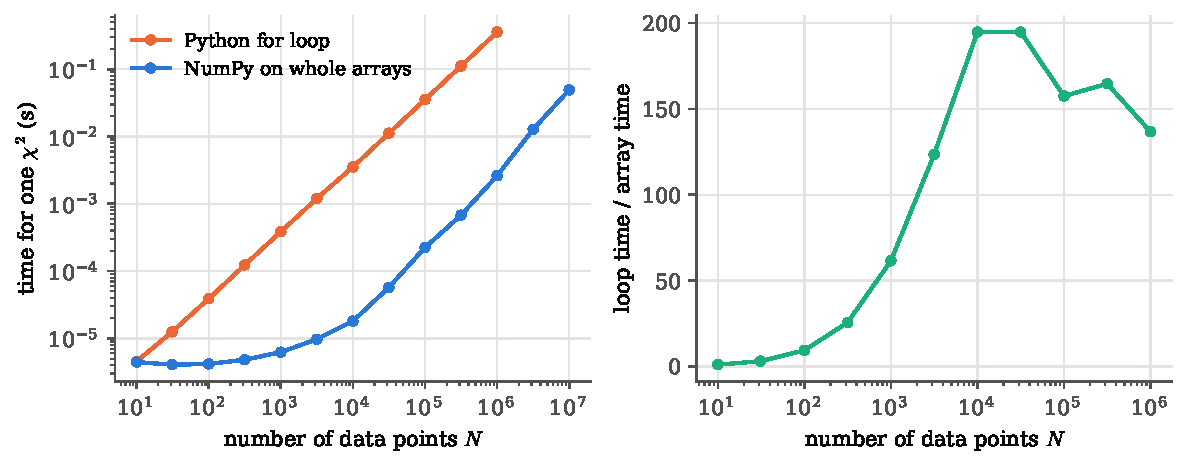
\includegraphics[width=12cm]{figures/chT0/02_vectorise.pdf}
\caption{Left: the time to compute one $\chi^2$ of $N$ data points with a Python loop (orange) and with one NumPy expression (blue). Both grow in proportion to $N$, but the loop pays far more per point. Right: the ratio of the two times, close to $1$ for a handful of points and about a hundred for large $N$.}
\label{T0a:fig:vectorise}
\end{figure}

\paragraph{Where the factor comes from.} Both versions do the same arithmetic, so the difference must be in the overhead around it. In the loop, Python handles each number as a separate object: it looks up \texttt{d[i]}, checks its type, creates a new object for each intermediate result, and only then does the floating-point operation, which itself takes a nanosecond or less. In the array expression, Python is consulted once per \emph{array}; the loop over elements runs inside NumPy's compiled code, on numbers stored side by side in memory. A simple cost model makes this quantitative. Let each version cost a fixed overhead plus a cost per element, $T_{\rm loop}=o_{\rm loop}+c_{\rm loop}N$ and $T_{\rm vec}=o_{\rm vec}+c_{\rm vec}N$. Then
\begin{align*}
  \frac{T_{\rm loop}}{T_{\rm vec}}
  &\eqby{1}\frac{o_{\rm loop}+c_{\rm loop}N}{o_{\rm vec}+c_{\rm vec}N}
   \;\xrightarrow{\;N\to\infty\;}\;\frac{c_{\rm loop}}{c_{\rm vec}}
   \eqby{2}\frac{\TzLoopNsPerElem\ \text{ns}}{\TzVecNsPerElem\ \text{ns}}
   \approx\TzSpeedup .
\end{align*}
\begin{explain}
  \item For large $N$ the overheads are negligible next to the terms proportional to $N$.
  \item The measured costs per element at $N=10^6$: the total times divided by $10^6$.
\end{explain}
For $N=10$ the ratio is about $\TzSpeedupSmall$: both versions are dominated by the fixed overhead of a function call, and vectorising buys nothing. The lesson is practical: a loop over a few dozen cases (six binomial panels, ten sample sizes) is fine and often clearest; a loop over a million data points or simulated values is written as an array expression.

\subsection{Reductions along an axis}
\label{T0a:sec:axis}

A \newterm{reduction} turns many numbers into fewer: \texttt{sum}, \texttt{mean}, \texttt{std}, \texttt{var}, \texttt{min}, \texttt{max}, \texttt{median}, \texttt{percentile}. On a two-dimensional array, the keyword \texttt{axis} says which dimension is reduced, that is, which dimension \emph{disappears}. With experiments in rows and readings in columns, \texttt{E.mean(axis=1)} averages along each row and leaves one mean per experiment; \texttt{E.mean(axis=0)} averages down each column and leaves one mean per reading slot; with no \texttt{axis}, all numbers are averaged (\cref{T0a:fig:axis}).

\Tzout{results/chT0/07_reductions.txt}

\begin{figure}[htbp]
\centering
\begin{tikzpicture}[x=0.8cm,y=0.6cm,
  c/.style={draw=accent,fill=ideabg,minimum width=0.8cm,minimum height=0.6cm,font=\scriptsize\ttfamily,inner sep=0},
  r/.style={draw=tangentgreen,fill=takebg,minimum width=0.8cm,minimum height=0.6cm,font=\scriptsize\ttfamily,inner sep=0}]
  \foreach \row [count=\i from 0] in {{9.80,9.71,9.86,9.83},{9.79,9.85,9.77,9.81},{9.90,9.74,9.82,9.80}} {
    \foreach \v [count=\j from 0] in \row { \node[c] at (\j,-\i) {\v}; }
  }
  \draw[->,thick,fibreorange] (-0.5,0.75) -- (3.5,0.75) node[right,font=\footnotesize] {\texttt{axis=1}: along each row};
  \foreach \v [count=\i from 0] in {9.800,9.805,9.815} { \node[r] at (5.2,-\i) {\v}; }
  \draw[->,thick,formblue] (-0.85,0.3) -- (-0.85,-2.3);
  \node[font=\footnotesize,formblue,anchor=east,align=right] at (-1.0,-1) {\texttt{axis=0}:\\ down each\\ column};
  \foreach \v [count=\j from 0] in {9.830,9.767,9.817,9.813} { \node[r] at (\j,-3.4) {\v}; }
  \node[font=\footnotesize,anchor=west] at (4.6,-3.4) {\texttt{E.mean(axis=0)}, shape $(4,)$};
  \node[font=\footnotesize,anchor=west] at (5.8,-1) {\texttt{E.mean(axis=1)}, shape $(3,)$};
\end{tikzpicture}
\caption{Reducing a $3\times4$ array of readings (three experiments in rows, four readings each). The axis named in the call is the one that disappears: \texttt{axis=1} leaves one mean per experiment, \texttt{axis=0} one mean per column.}
\label{T0a:fig:axis}
\end{figure}

This is how the book studies sampling distributions: simulate $M$ experiments of $N$ readings each as one $M\times N$ array, reduce along \texttt{axis=1} to get $M$ estimates, and histogram them. The $1/\sqrt N$ study of \cref{3a:sec:clt-python} does it for several parent distributions and several $N$:

\pyfile[firstline=34,lastline=41,firstnumber=34]{code/ch03/03_one_over_sqrtN.py}{Many experiments at once: an $M\times N$ array reduced along its rows}

Line 36 is the whole simulation for one parent distribution and one $N$: \texttt{draw((M, N))} returns $M=20\,000$ rows of $N$ draws, and \texttt{.mean(axis=1)} turns each row into its sample mean. Line 37 stores the variance of those $M$ means. Line 39 computes two percentiles at once from a list, \texttt{[25, 75]}. The loop over $N$ (line 34) and over the three parents (line 35) stays a Python loop, because it runs only $11\times3$ times; the $M\times N$ work inside it is vectorised.

\paragraph{Example: the standard error from one array.} Four readings of $g$ are in the first row of the array \texttt{E} above. Their mean and its standard error are
\begin{align*}
  \bar g=\texttt{E[0].mean()}, \qquad
  \sigma_{\bar g}
  &\eqby{1}\frac{s}{\sqrt n}
   \eqby{2}\texttt{E[0].std(ddof=1) / np.sqrt(E.shape[1])} .
\end{align*}
\begin{explain}
  \item The standard error of a mean of $n$ independent readings with sample standard deviation $s$ (\cref{ch:03}).
  \item \texttt{ddof=1} divides by $n-1$ instead of $n$ (the unbiased sample variance of \cref{2b:sec:nminus1}); \texttt{E.shape[1]} is the number of columns, $n=4$.
\end{explain}
Forgetting \texttt{ddof=1} is a common slip. NumPy's default is \texttt{ddof=0}, the divide-by-$n$ version, which is the maximum-likelihood estimate of the variance and is biased low by the factor $(n-1)/n$.

\subsection{Grids in two and more dimensions}
\label{T0a:sec:grids}

A function of two variables, such as a likelihood $\Like(a,b)$ or a Fourier-space amplitude $P(|\bm k|)$, is evaluated on a grid. \texttt{np.meshgrid(xs, ys, indexing="ij")} returns two arrays of the same two-dimensional shape: in the first, entry $(i,j)$ is \texttt{xs[i]}; in the second, it is \texttt{ys[j]}. Any formula in \texttt{XX} and \texttt{YY} is then evaluated at every grid point at once. The keyword \texttt{indexing="ij"} makes the first index run over \texttt{xs}, as in matrix notation; without it, NumPy uses the plotting convention, with the axes swapped, which is a classic source of transposed images.

\Tzout{results/chT0/07_grids.txt}

The Gaussian random fields of \cref{ch:07} need $|\bm k|$ on the grid of the fast Fourier transform. The library function that builds it is short:

\pyfile[firstline=24,lastline=31,firstnumber=24]{code/ch07/lib_fields.py}{The grid of wavenumbers for a $d$-dimensional box}

Line 26 gives the wavenumbers $k=2\pi n/L$ in the order the FFT uses (\cref{T0a:sec:fft}). Line 28 builds a list with one copy for each dimension: \texttt{[k1] * (d - 1)} repeats a list, and \texttt{+} joins two lists. Line 29 hands that list to \texttt{np.meshgrid}; the star in \texttt{*axes} unpacks the list into separate arguments. Line 30 computes $|\bm k|=\sqrt{k_x^2+k_y^2+\dots}$ at every grid point with a generator expression inside \texttt{sum}. Line 31 returns two things.
\section{Random numbers, linear algebra and Fourier transforms}
\label{T0a:sec:numpy-more}

Three parts of NumPy carry the physics of most chapters. Random numbers make the simulated experiments of every Monte Carlo study. Linear algebra handles covariance matrices, least-squares fits and Fisher matrices. The Fourier transform turns a field or a time series into its modes, where Gaussian random fields and detector noise become simple. Each takes only a few names.

\subsection{Random numbers with a seed}
\label{T0a:sec:random}

A computer cannot toss a coin. It runs a deterministic recipe, a \newterm{pseudo-random generator}, whose output passes every statistical test for independent uniform draws (\cref{ch:06} builds such generators from scratch). The whole sequence is fixed by one integer, the \newterm{seed}: the same seed gives the same sequence, every time, on every machine. NumPy packages a generator as an object of type \texttt{Generator}, and every random draw is a method of that object:
\begin{center}
\small
\begin{tabular}{@{}ll@{}}
\toprule
call & draws \\
\midrule
\texttt{rng.random(n)}, \texttt{rng.uniform(a, b, n)} & uniform on $[0,1)$ or $[a,b)$\\
\texttt{rng.standard\_normal(n)}, \texttt{rng.normal(mu, s, n)} & Gaussian, $\Normal(0,1)$ or $\Normal(\mu,s^2)$\\
\texttt{rng.integers(a, b, n)} & integers from \texttt{a} to \texttt{b-1}\\
\texttt{rng.poisson(lam, n)}, \texttt{rng.exponential(tau, n)} & Poisson counts, exponential waiting times\\
\texttt{rng.choice(x, n)}, \texttt{rng.permutation(x)} & resampling, shuffling\\
\bottomrule
\end{tabular}
\end{center}
The last argument may be a shape instead of a number: \texttt{rng.standard\_normal((M, N))} is an $M\times N$ array, the ``$M$ experiments of $N$ readings'' layout of \cref{T0a:sec:axis}.

The book never creates a generator by hand. It calls \texttt{rng\_for(chapter, name)} from \pyname{common.py}, which makes the seed from the script's own name (\cref{0a:sec:code}). The seeding script of \cref{ch:00} shows the consequence in four lines:

\pyfile[firstline=14,lastline=17,firstnumber=14]{code/ch00/06_reproducible_seeds.py}{Same name, same random numbers; different name, unrelated ones}

Lines 14 and 15 build two generators from the same name, so \texttt{a} and \texttt{b} are identical arrays. Line 16 uses another name, so \texttt{c} is unrelated. An optional third argument, the \newterm{stream}, gives one script several independent generators: \texttt{rng\_for("ch00", "05\_three\_detectors", 1)} is a different sequence from stream $0$ (\cref{6a:sec:seeds} shows why streams from one seed are independent).

\begin{figure}[htbp]
\centering
\begin{tikzpicture}[scale=0.9,transform shape,
  box/.style={draw=accent,rounded corners=2pt,fill=ideabg,align=center,font=\footnotesize,minimum height=0.9cm,inner sep=3pt},
  drawn/.style={draw=softgray,fill=codebg,font=\scriptsize\ttfamily,minimum width=1.05cm,minimum height=0.55cm,inner sep=1pt},
  arr/.style={->,thick,accent}]
  \node[box,text width=3.0cm] (name) at (0,0) {\texttt{"ch02/02\_binomial"}\\ the script's name};
  \node[box,text width=2.0cm] (seed) at (3.4,0) {seed\\ (a 64-bit integer)};
  \node[box,text width=2.2cm] (gen) at (6.5,0) {\texttt{rng}\\ a Generator};
  \draw[arr] (name) -- (seed);
  \draw[arr] (seed) -- (gen);
  \foreach \v [count=\i from 0] in {0.732,0.106,0.513,0.890} {
    \node[drawn] at (8.6+1.15*\i,0.0) {\v};
  }
  \node[font=\scriptsize,anchor=west] at (13.1,0) {\dots};
  \draw[arr] (gen) -- (8.0,0);
  \node[box,text width=2.0cm,fill=takebg,draw=tangentgreen] (seed2) at (3.4,-1.6) {seed\\ + stream $1$};
  \node[box,text width=2.2cm,fill=takebg,draw=tangentgreen] (gen2) at (6.5,-1.6) {\texttt{rng}\\ a second Generator};
  \draw[arr] (name.south) |- (seed2.west);
  \draw[arr] (seed2) -- (gen2);
  \foreach \v [count=\i from 0] in {0.248,0.977,0.031,0.664} {
    \node[drawn] at (8.6+1.15*\i,-1.6) {\v};
  }
  \node[font=\scriptsize,anchor=west] at (13.1,-1.6) {\dots};
  \draw[arr] (gen2) -- (8.0,-1.6);
\end{tikzpicture}
\caption{Where the random numbers of a script come from. The script's name fixes a seed, the seed fixes a generator, and the generator's sequence of draws (the numbers shown are only illustrative) is the same on every run. A stream number mixed into the seed gives a second, independent sequence.}
\label{T0a:fig:seeds}
\end{figure}

The census checks that the book keeps this rule. Of the $\TzDrawFiles$ files that draw random numbers, $\TzSeededDrawFiles$ create their generator with \pyname{rng_for}; nearly all of the rest are library files (\pyname{lib_*.py}, $\TzLibDrawFiles$ of them) that receive a generator from the script that calls them, as \texttt{gaussian\_field(\dots, rng=rng)} does in \cref{T0a:sec:functions}. A generator without a seed, \texttt{np.random.default\_rng()}, appears $\TzBareRng$ times, almost always as the fallback \texttt{if rng is None}. The old style of NumPy, a global generator set by \texttt{np.random.seed(\dots)} and used through \texttt{np.random.normal(\dots)}, appears $\TzLegacySeed$ times.

\paragraph{Example: why a fixed seed matters for a comparison.} Suppose we change the mask of a CMB simulation and the estimated variance of $\hat C_{100}$ moves by $2\%$. Is that the mask, or just different random skies? If both runs use the same seed, every sky is the same in the two runs, so the random part of the two estimates is largely shared and cancels in the difference; what remains is the mask effect plus whatever random part the two estimators do not share. If they use unrelated seeds, the $2\%$ is the mask plus the Monte Carlo noise of two independent runs, of the same order. Fixed seeds do not make the comparison exact. They make the two runs share their noise, which shrinks the noise of the difference, and \cref{T0a:sec:trust-mc} shows the size of the gain.

\begin{pitfall}[A generator made inside a loop]
Writing \texttt{rng = rng\_for(...)} \emph{inside} a loop restarts the sequence at every pass, so every ``independent'' repetition gets the same random numbers. The generator is made once, at the top of the script, and then drawn from repeatedly. (When fresh but reproducible streams are wanted per repetition, pass the repetition number as the stream: \texttt{rng\_for(chapter, name, i)}.)
\end{pitfall}

\subsection{Linear algebra}
\label{T0a:sec:linalg}

Matrices are two-dimensional arrays, and the matrix product is the operator \texttt{@}: \texttt{A @ B}, \texttt{A @ x}, \texttt{x @ C @ x} for $\bm x\T\Cmat\bm x$ (\texttt{x.T} or \texttt{A.T} is the transpose, which does nothing to a one-dimensional array). It appears in $\TzPctMatmul\%$ of the scripts. The star \texttt{A * B} is \emph{not} the matrix product: it multiplies element by element. Four functions from \texttt{np.linalg} do the rest:
\begin{itemize}[leftmargin=1.5em,itemsep=1pt]
  \item \texttt{np.linalg.solve(A, b)} returns the $\bm x$ with $A\bm x=\bm b$;
  \item \texttt{np.linalg.cholesky(C)} returns the lower-triangular $L$ with $LL\T=\Cmat$, for a symmetric positive-definite $\Cmat$ such as a covariance matrix;
  \item \texttt{np.linalg.eigh(C)} returns the eigenvalues (in increasing order) and the eigenvectors (as columns) of a symmetric matrix;
  \item \texttt{np.linalg.inv(A)} returns the inverse matrix.
\end{itemize}

\Tzout{results/chT0/07_linalg.txt}

\paragraph{Cholesky: making correlated noise.} The commonest use of \texttt{cholesky} in the book is to draw correlated Gaussian vectors with a given covariance $\Cmat$. Draw a vector $\bm z$ of independent standard Gaussians and set $\bm x=L\bm z$. Why does $\bm x$ have covariance $\Cmat$? Because
\begin{align*}
  \Cov(\bm x)
  &\eqby{1}\E[\bm x\bm x\T]
   \eqby{2}\E[L\bm z\bm z\T L\T]
   \eqby{3}L\,\E[\bm z\bm z\T]\,L\T
   \eqby{4}L\,\Id\,L\T
   \eqby{5}\Cmat .
\end{align*}
\begin{explain}
  \item $\bm x$ has zero mean, because $\bm z$ does, so its covariance is $\E[\bm x\bm x\T]$.
  \item $\bm x\T=(L\bm z)\T=\bm z\T L\T$.
  \item $L$ is a fixed matrix, so it comes out of the expectation.
  \item Independent standard Gaussians have unit variances and zero covariances.
  \item The defining property of the Cholesky factor.
\end{explain}
In code, with many draws stored as the rows of an array \texttt{z}, the product $L\bm z$ for every row at once is \texttt{z @ L.T}. That is exactly line 32 of the correlated-field script of \cref{6b:sec:cholesky}:

\pyfile[firstline=29,lastline=33,firstnumber=29]{code/ch06/23_cholesky_field.py}{Correlated Gaussian pairs from independent ones}

Line 31 draws $50\,000$ rows of two independent Gaussians, line 32 turns each row into a correlated pair, and line 33 checks the result with \texttt{np.cov(\dots, rowvar=False)}, the sample covariance when the variables are the columns.

\paragraph{Solve, do not invert.} The quantity $\bm d\T\Cmat^{-1}\bm d$ appears in every Gaussian likelihood and every Fisher matrix. It is tempting to write \texttt{d @ np.linalg.inv(C) @ d}. The better form is \texttt{d @ np.linalg.solve(C, d)}: it asks for $\bm y=\Cmat^{-1}\bm d$ by solving $\Cmat\bm y=\bm d$, without ever forming the inverse. The Fisher matrix of the CMB forecast in \cref{10a:sec:cmb-derive} is written this way:

\pyfile[firstline=183,lastline=195,firstnumber=183]{code/ch10/lib_fisher10.py}{A Fisher matrix summed over multipoles, with solve instead of inv}

For each multipole $\ell$ (line 187), lines 190--192 build the $3\times3$ covariance of the estimated $TT$, $EE$ and $TE$ spectra, line 193 stacks the derivatives of the three spectra with respect to the six parameters into a $3\times6$ array \texttt{d}, and line 194 adds $\bm d\T\Cmat^{-1}\bm d$, a $6\times6$ matrix, to the running sum.

Why is \texttt{solve} better? There are two reasons. The first is speed: solving needs one factorisation of $\Cmat$, about $\tfrac23n^3$ operations, while inverting needs about $2n^3$ and then a matrix product. The tour measured, for $n=2000$, $\TzTsolve$\,ms for \texttt{solve} against $\TzTinv$\,ms for \texttt{inv} followed by a product. The second is accuracy, and it matters for badly conditioned matrices, where small rounding errors are amplified. The tour tried both on the Hilbert matrices $H_{ij}=1/(i+j+1)$, which become nearly singular as their size grows (\cref{T0a:fig:linalg-fft}, left). For $n=10$, with condition number $\kappa\approx\TzHilbCond$ (\cref{T0a:sec:trust-linalg} explains this number), \texttt{solve} returns an $\bm x$ that satisfies the equations to $\TzHilbResSolve$ in relative terms, the best that double precision allows, while \texttt{inv} leaves a residual of $\TzHilbResInv$. Neither recovers $\bm x$ itself better than $\TzHilbErr$, because no method can beat the conditioning of the problem.

So when is \texttt{inv} right? When the inverse matrix itself is the answer wanted. Turning a Fisher matrix $\Fish$ into the covariance of the parameters, $\Fish^{-1}$, is the commonest case, and it accounts for most of the $\TzInv$ calls of \texttt{np.linalg.inv} in the book (against $\TzSolve$ of \texttt{solve}, $\TzChol$ of \texttt{cholesky} and $\TzEigh$ of \texttt{eigh}). Those matrices are small ($6\times6$ or so) and well conditioned, and there \texttt{inv} is harmless. The rule is: \texttt{inv} when the matrix $A^{-1}$ is the result, \texttt{solve} (or \texttt{cholesky}) when $A^{-1}$ only stands inside a formula such as $A^{-1}\bm b$ or $\bm b\T A^{-1}\bm b$.

\paragraph{Example: eigenvectors as the axes of an ellipse.} For the covariance $\Cmat=\bigl(\begin{smallmatrix}4&1.8\\1.8&1\end{smallmatrix}\bigr)$ of the tour, \texttt{eigh} returns the eigenvalues $\lambda_1\approx0.157$ and $\lambda_2\approx4.843$. Their sum is $5=\tr\Cmat$ and their product $0.76=\det\Cmat=4-1.8^2$, as they must be. The $1\sigma$ contour of a two-dimensional Gaussian with this covariance is an ellipse whose axes point along the eigenvectors, with half-lengths $\sqrt{\lambda_1}\approx0.40$ and $\sqrt{\lambda_2}\approx2.20$. \Cref{1b:sec:covariance} draws it with exactly this recipe (the function \texttt{ellipse} in \pyname{code/ch01/18_covariance_transform.py}).

\subsection{The fast Fourier transform}
\label{T0a:sec:fft}

The discrete Fourier transform of $N$ numbers $x_0,\dots,x_{N-1}$ is
\[
  X_k=\sum_{n=0}^{N-1}x_n\,e^{-2\pi i kn/N},\qquad k=0,\dots,N-1,
\]
the same sign convention as $\tilde h(f)=\int h(t)e^{-2\pi ift}\,\dd t$. Computed term by term it costs $N^2$ operations. The \newterm{fast Fourier transform} (FFT) computes the same numbers in about $N\log_2N$ operations, by splitting the sum into its even and odd terms again and again; for a million points that is fifty thousand times less work, which is why every power-spectrum calculation of the book is done in Fourier space. NumPy's functions live in \texttt{np.fft}:
\begin{itemize}[leftmargin=1.5em,itemsep=1pt]
  \item \texttt{np.fft.fft(x)} gives all $N$ complex $X_k$; \texttt{np.fft.ifft} inverts it.
  \item For real data, $X_{N-k}=X_k^*$, so half of the numbers are redundant. \texttt{np.fft.rfft(x)} returns only $k=0,\dots,N/2$, that is $N/2+1$ numbers, and \texttt{np.fft.irfft} inverts it. \texttt{rfftn} and \texttt{irfftn} do the same in several dimensions (the random fields of \cref{ch:07}).
  \item \texttt{np.fft.rfftfreq(N, d=dt)} gives the frequency of each entry, $f_k=k/(N\,\Delta t)$, and \texttt{fftfreq} the same for the full transform, with the negative frequencies in the second half.
\end{itemize}

\Tzout{results/chT0/07_fft.txt}

The tour puts a weak tone, amplitude $0.5$ at $50$\,Hz, into Gaussian noise of standard deviation $1$, samples it at $1000$\,Hz for $2$\,s, and transforms (\cref{T0a:fig:linalg-fft}, right). Two numbers follow from the sampling alone. The frequency step is $\Delta f=1/T=0.5$\,Hz and the highest frequency is the Nyquist frequency $f_s/2=500$\,Hz, which is why \texttt{f[1] = 0.5} and \texttt{f[-1] = 500.0}. The tone, invisible by eye in the time series, stands out at $\TzFftPeak$\,Hz, about $\TzFftSnr$ times above the median noise power. The last printed line checks Parseval's theorem in NumPy's convention, $\sum_n x_n^2=\frac1N\sum_k|X_k|^2$: the factor $1/N$ is where conventions differ between libraries and books, and checking Parseval is the quickest way to find out which one a function uses.

\begin{figure}[htbp]
\centering
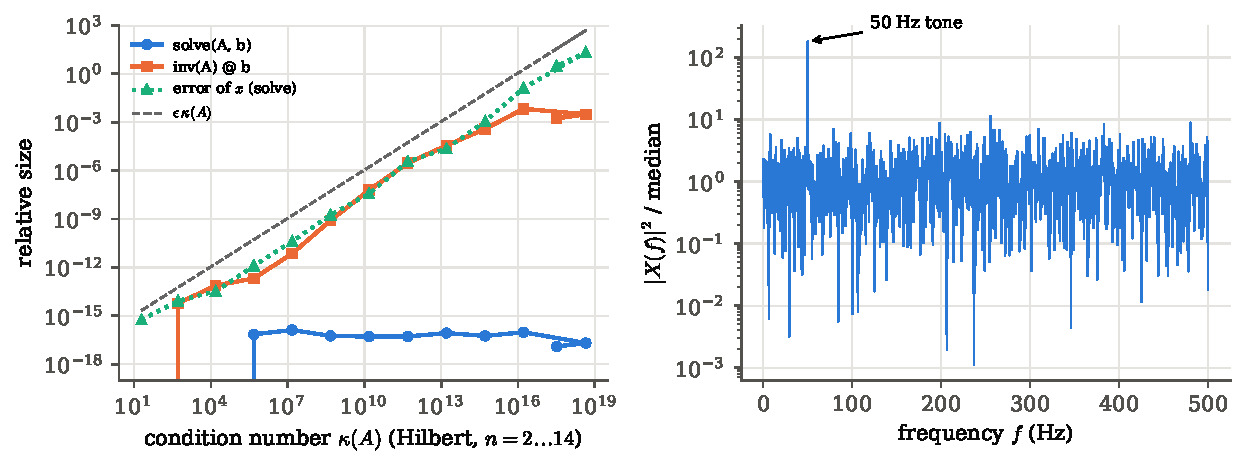
\includegraphics[width=12cm]{figures/chT0/07_numpy_tour.pdf}
\caption{Left: solving $A\bm x=\bm b$ for Hilbert matrices of growing size. With \texttt{solve} (blue) the residual stays at the rounding level for every condition number; with \texttt{inv} followed by a product (orange) it grows with the condition number. The error of $\bm x$ itself (green) follows $\epsilon\kappa$ (dashed) whatever the method. Right: the power spectrum of $2$\,s of noise containing a weak $50$\,Hz tone, normalised to its median: one Fourier coefficient carries the tone.}
\label{T0a:fig:linalg-fft}
\end{figure}

In the book, a typical FFT is two lines inside a larger recipe. The autocorrelation of a Markov chain (\cref{9b:sec:tau}) is computed with the Wiener--Khinchin theorem: the autocorrelation is the inverse transform of the power spectrum.

\pyfile[firstline=74,lastline=81,firstnumber=74]{code/ch09/lib_mcmc9c.py}{The autocorrelation of a chain through two FFTs}

Line 76 subtracts the mean. Line 78 transforms with \texttt{n=2 * n}, which pads the series with zeros to twice its length, so that the circular wrap-around of the discrete transform does not mix the end of the chain with its beginning. Line 79 multiplies the transform by its complex conjugate (the power) and transforms back; the first $n$ entries are the autocovariance at lags $0,\dots,n-1$. Line 80 divides by the value at lag $0$, so that $\rho(0)=1$. Done directly, this would cost $n^2$ operations, about $10^{10}$ for a chain of $10^5$ steps; through the FFT it takes milliseconds.
\section{SciPy: distributions, integrals, roots and minima}
\label{T0a:sec:scipy}

NumPy does arithmetic on arrays. SciPy adds the classic numerical recipes that a physicist would otherwise copy from a handbook: the densities and tail probabilities of the standard distributions, numerical integration, root finding, minimisation, special functions and interpolation. It is used in $\TzPctScipy\%$ of the scripts but makes only $\TzScipyShare\%$ of the calls, because one SciPy call does a lot of work. Six tools cover almost all of it. Each is shown answering one small physics question in \pyname{code/chT0/03_scipy_tour.py}, with an answer we can check by hand, and then in a real script.

\subsection{Probability distributions}
\label{T0a:sec:stats}

\texttt{scipy.stats} contains one object per distribution: \texttt{stats.norm}, \texttt{stats.poisson}, \texttt{stats.binom}, \texttt{stats.chi2}, \texttt{stats.t}, \texttt{stats.expon}, and about a hundred more. Every object answers the same five questions, which are the five things the earlier chapters ask of a distribution (\cref{T0a:fig:scipy}, left):
\begin{center}
\begin{tabular}{@{}lll@{}}
\toprule
method & question & formula \\
\midrule
\texttt{pdf(x)} (\texttt{pmf} if discrete) & how dense is the probability at $x$? & $p(x)$\\
\texttt{cdf(x)} & how likely is a value at most $x$? & $F(x)=\Prob(X\le x)$\\
\texttt{sf(x)} & how likely is a value above $x$? & $1-F(x)$, computed directly\\
\texttt{ppf(q)} & below which value lies a fraction $q$? & $F^{-1}(q)$\\
\texttt{rvs(size=n)} & give me $n$ random draws & \\
\bottomrule
\end{tabular}
\end{center}
Shape parameters come first (\texttt{stats.poisson.pmf(k, mu)}, \texttt{stats.chi2.sf(x, df)}), and every continuous distribution also takes \texttt{loc} and \texttt{scale}, which shift and stretch it: \texttt{stats.norm.pdf(x, loc=mu, scale=sigma)} is the Gaussian of mean $\mu$ and standard deviation $\sigma$. The logarithmic versions \texttt{logpdf}, \texttt{logpmf} and \texttt{logsf} are what likelihoods use, because a product of many small densities underflows while a sum of their logarithms does not (\cref{T0a:sec:precision}).

\pyfile[firstline=24,lastline=29,firstnumber=24]{code/chT0/03_scipy_tour.py}{One distribution object, several questions}

Line 25 asks where the Gaussian cdf reaches $0.975$: the answer, $\TzZninetyfive$, is the familiar ``$1.96\sigma$'' of a two-sided $95\%$ interval, and \texttt{cdf} of it gives back $\TzBackCdf$. Line 26 asks for the probability of a fluctuation above $5\sigma$: $\TzPfive$, the discovery threshold of particle physics. Line 27 draws $10^4$ values from $\Normal(2,0.5^2)$ using the book's generator (\texttt{random\_state=rng}); their sample mean and standard deviation are $\TzRvsMean$ and $\TzRvsStd$.

The same two functions do the work of the $p$-value-to-sigma conversion of \cref{4a:sec:p-to-z}:

\pyfile[firstline=23,lastline=25,firstnumber=23]{code/ch04/09_p_to_z.py}{Sigmas to one- and two-sided $p$-values}

\texttt{stats.norm.sf(Z)} acts on the whole array \texttt{Z} $=1,\dots,6$ at once, like any NumPy function. The reverse direction, from a $p$-value to a number of sigmas, is \texttt{stats.norm.isf(p)}, the inverse of \texttt{sf}.

\begin{pitfall}[\texttt{1 - cdf} in the tail]
For $x$ far in the upper tail, $F(x)$ is a number like $0.9999999997$, and $1-F(x)$ keeps only the few digits that differ from $1$. \texttt{sf(x)} computes the tail directly and keeps all sixteen. At $5\sigma$ the difference is still small; beyond about $8\sigma$, \texttt{1 - cdf} returns exactly $0$ while \texttt{sf} is still accurate (\cref{T0a:sec:precision}).
\end{pitfall}

\subsection{Integrals}
\label{T0a:sec:quad}

\texttt{integrate.quad(f, a, b)} integrates a function of one variable from \texttt{a} to \texttt{b} (either limit may be \texttt{np.inf}) and returns \emph{two} numbers: the value and an estimate of its absolute error. It evaluates \texttt{f} at cleverly chosen points, compares two rules of different order on each piece of the interval, and keeps subdividing the pieces where they disagree. The tour checks it against the $5\sigma$ tail of line 26:

\pyfile[firstline=31,lastline=33,firstnumber=31]{code/chT0/03_scipy_tour.py}{The $5\sigma$ tail again, by integrating the density}

\texttt{quad} returns $\TzQuadTail$ with an error estimate of $\TzQuadErr$, and the value differs from \texttt{sf(5)} by a relative $\TzQuadRel$. The comma on the left, \texttt{tail, tail\_err = \dots}, unpacks the two returned numbers. Many scripts keep only the value, writing \texttt{quad(\dots)[0]}, as the detector-smearing check of \cref{1b:sec:joint} does:

\pyfile[firstline=60,lastline=62,firstnumber=60]{code/ch01/13_detector_smearing.py}{Expected counts per histogram bin from integrals of a density}

Line 62 is a list comprehension that integrates the density over every bin, \texttt{zip(edges[:-1], edges[1:])} pairing each left edge with the next one. \Cref{T0a:sec:trust-boxes} shows how the error estimate can be wrong, and what to do about it.

\subsection{Roots}
\label{T0a:sec:roots}

Many statistical answers are the solution of one equation in one unknown: the parameter value where $\ln\Like$ has dropped by $\tfrac12$, the mean $\mu$ at which observing so few events would have probability $5\%$, the Lagrange multiplier of a maximum-entropy problem. \texttt{optimize.brentq(f, a, b)} finds a zero of \texttt{f} between \texttt{a} and \texttt{b}. It requires a \newterm{bracket}: \texttt{f(a)} and \texttt{f(b)} must have opposite signs, so that a continuous \texttt{f} must cross zero in between. It then shrinks the bracket, combining halving (always safe) with interpolation steps (fast when $f$ is smooth), until the zero is pinned to about $10^{-12}$ (\cref{T0a:fig:brentq}).

\begin{figure}[htbp]
\centering
\begin{tikzpicture}
\begin{axis}[width=8.5cm,height=5.0cm,xmin=0,xmax=2.05,ymin=-2.5,ymax=2.3,
  axis lines=middle,xlabel={$x$},ylabel={$f(x)=x^2-2$},
  xlabel style={anchor=north west},ylabel style={anchor=south},
  xtick={0,0.5,1,1.5,2},ytick={-2,-1,0,1,2},tick label style={font=\scriptsize},
  label style={font=\small}]
  \addplot[domain=0:2,samples=100,thick,formblue] {x^2-2};
  \addplot[only marks,mark=*,mark size=1.6pt,bdryred] coordinates {(0,-2) (2,2)};
  \addplot[only marks,mark=*,mark size=1.6pt,fibreorange] coordinates {(1,-1) (1.5,0.25)};
  \addplot[only marks,mark=*,mark size=2pt,tangentgreen] coordinates {(1.41421356,0)};
  \node[font=\scriptsize,anchor=west,bdryred] at (axis cs:0.08,-2.3) {$f(0)<0$};
  \node[font=\scriptsize,anchor=east,bdryred] at (axis cs:1.95,2.0) {$f(2)>0$};
  \node[font=\scriptsize,anchor=north west,fibreorange] at (axis cs:1.03,-1.08) {midpoint $1$};
  \node[font=\scriptsize,anchor=south east,fibreorange] at (axis cs:1.5,0.6) {midpoint $1.5$};
  \node[font=\scriptsize,anchor=south east,tangentgreen] at (axis cs:1.40,0.05) {$\sqrt2$};
\end{axis}
\end{tikzpicture}
\caption{A bracket and its shrinking. $f(0)=-2<0$ and $f(2)=2>0$ (red points), so a zero lies in $[0,2]$. The midpoint $1$ has $f<0$, so the zero is in $[1,2]$; the next midpoint $1.5$ has $f>0$, so it is in $[1,1.5]$ (orange points). \texttt{brentq} mixes such halvings with faster interpolation steps and stops at $\sqrt2$ (green) to twelve digits. On $[0,1]$ there is no sign change and \texttt{brentq} refuses to start.}
\label{T0a:fig:brentq}
\end{figure}

The tour computes the $95\%$ upper limit on a Poisson mean after observing $n$ events: the $\mu$ at which $\Prob(N\le n\given\mu)=0.05$.

\pyfile[firstline=35,lastline=39,firstnumber=35]{code/chT0/03_scipy_tour.py}{An upper limit as the root of an equation}

For $n=0$ the equation is $e^{-\mu}=0.05$, whose exact root is $\ln20=\TzUpperZeroExact$; \texttt{brentq} gives $\TzUpperZero$. For $n=3$ it gives $\TzUpperThree$ (\cref{T0a:fig:scipy}, right). The likelihood interval of the decay-time example (\cref{T0a:sec:functions}, lines 39--40 there) is the same pattern, with two brackets, one on each side of the maximum.

\subsection{Minima}
\label{T0a:sec:minimize}

{\sloppy Maximum likelihood means finding the parameters that make $-\ln\Like$ smallest. \texttt{optimize.minimize(f, x0)} starts at the guess \texttt{x0} and walks downhill. It returns a result object whose most useful entries are \texttt{res.x} (the minimising parameters), \texttt{res.fun} (the value there), \texttt{res.success} (whether the method believes it converged) and \texttt{res.nit} (how many iterations it took). The \texttt{method} keyword chooses the walk: \texttt{"Nelder-Mead"} needs only function values and is robust; \texttt{"BFGS"} and \texttt{"L-BFGS-B"} use gradients (estimated numerically if not given) and are faster on smooth problems; \texttt{"L-BFGS-B"} also accepts \texttt{bounds}. Extra fixed inputs, such as the data, are handed over with \texttt{args=(\dots,)}.\par}

\pyfile[firstline=41,lastline=48,firstnumber=41]{code/chT0/03_scipy_tour.py}{Maximum likelihood for Gaussian data by minimisation}

Two habits are visible here. The width is fitted as $\ln\sigma$ (line 43), so that any real number is an allowed value and the minimiser cannot wander to a negative $\sigma$. And the result is checked against an answer known in closed form: for Gaussian data the maximum-likelihood estimates are the sample mean and the divide-by-$n$ standard deviation. The minimiser finds $\hat\mu=\TzMinMu$ and $\hat\sigma=\TzMinSig$ in $\TzMinIters$ iterations; the closed forms give $\TzMeanCheck$ and $\TzStdCheck$.

The Poisson-binned fit of \cref{3b:sec:poisson-python} wraps \texttt{minimize} in a small function, so that three different goodness-of-fit functions can be minimised with the same call:

\pyfile[firstline=57,lastline=61,firstnumber=57]{code/ch03/12_poisson_bins.py}{A minimiser wrapped in a function, with tightened tolerances}

The function to minimise, \texttt{fun}, is itself an argument (functions can be passed around like numbers). \texttt{options=dict(xatol=\dots, fatol=\dots, maxiter=\dots)} tightens the stopping rules, because the default tolerances of Nelder--Mead are loose for a study that compares estimators to many digits. \Cref{T0a:sec:trust-boxes} shows what happens when a minimiser stops too early, and how \texttt{res.success} reports it.

\subsection{Special functions and interpolation}
\label{T0a:sec:special}

\texttt{scipy.special} contains the functions of mathematical physics: $\Gamma$ and its logarithm \texttt{gammaln}, the beta function, binomial coefficients \texttt{comb}, error functions, Bessel functions, the Voigt profile. The one the book uses most is \texttt{gammaln}, because likelihoods of counts contain factorials, and factorials overflow: $200!\approx10^{375}$ is far beyond the largest double, about $1.8\times10^{308}$. Its logarithm is a modest number:

\pyfile[firstline=50,lastline=57,firstnumber=50]{code/chT0/03_scipy_tour.py}{$\ln 200!$ is fine; $200!$ as a float is not}

$\ln200!=\ln\Gamma(201)=\TzLnFact$, and Python's own \texttt{math.lgamma} agrees ($\TzLnFactCheck$). Converting $200!$ itself to a float overflows (\texttt{OverflowError}: \TzFactOverflow); the \texttt{try}/\texttt{except} block of lines 52--56 catches that error and records it instead of stopping (\cref{T0a:sec:rare}). The de Moivre--Laplace check of \cref{2b:sec:dml-python} uses \texttt{special.gammaln(n\_st + 1)} for exactly this reason.

\newterm{Interpolation} estimates a function between tabulated points. \texttt{np.interp(x, xt, yt)} joins the table $(x_t,y_t)$ by straight lines; \texttt{interpolate.CubicSpline(xt, yt)} by smooth cubic pieces whose first and second derivatives are continuous. For a coarse table of six values of $\sin x$ on $[0,\pi]$ the tour finds a largest error of $\TzInterpLinErr$ for straight lines and $\TzInterpSplErr$ for the spline (lines 59--66). Straight lines are the right choice when the table is fine and the curve may have kinks; a spline when the table is coarse and the curve is smooth. \texttt{np.interp} is the one the book calls most often, typically to read a tabulated CAMB spectrum or a transfer function at new multipoles.

\begin{figure}[htbp]
\centering
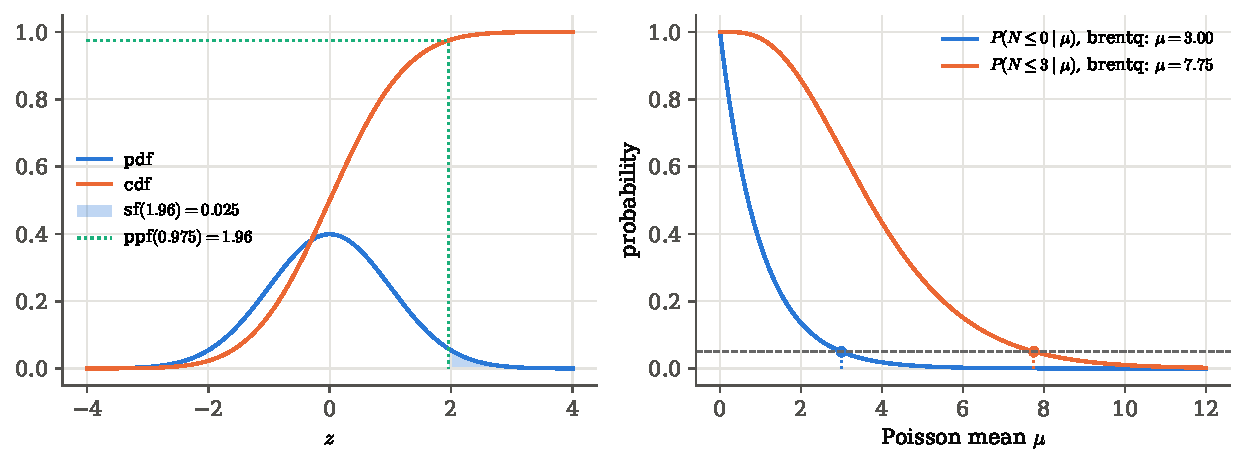
\includegraphics[width=12cm]{figures/chT0/03_scipy_tour.pdf}
\caption{Left: the standard Gaussian's density (pdf) and cumulative distribution (cdf). The shaded tail above $1.96$ is \texttt{sf(1.96)} $=0.025$, and the dotted path from $0.975$ on the cdf down to the axis is \texttt{ppf(0.975)} $=1.96$. Right: the probability of observing at most $n$ events as a function of the Poisson mean, for $n=0$ and $3$; \texttt{brentq} finds where each curve crosses $0.05$ (dashed), the $95\%$ upper limits.}
\label{T0a:fig:scipy}
\end{figure}
\section{Matplotlib, files and folders}
\label{T0a:sec:plots}

Every figure drawn from data in the book is made by a dozen Matplotlib calls, and every expensive result is kept on disk by two NumPy calls. Both are learned once.

\subsection{A figure is a canvas holding axes}
\label{T0a:sec:matplotlib}

Matplotlib thinks of a picture in two layers (\cref{T0a:fig:mpl}). The \newterm{figure} is the whole canvas, the thing saved to a PDF file. On it sit one or more \newterm{axes}: rectangular panels, each with its own coordinate system, ticks, labels and legend. Everything that is drawn is drawn \emph{on an axes}. The book always creates both at once,
\begin{center}
\texttt{fig, ax = plt.subplots()} \qquad or \qquad \texttt{fig, axes = plt.subplots(2, 3)}
\end{center}
which returns the figure and one axes, or the figure and a $2\times3$ array of axes, \texttt{axes[row, column]}. Everything else is a method of \texttt{ax}:
\begin{center}
\small
\begin{tabular}{@{}ll@{}}
\toprule
call & draws \\
\midrule
\texttt{ax.plot(x, y)}, \texttt{ax.plot(x, y, "o")} & a line through the points, or markers only\\
\texttt{ax.loglog}, \texttt{ax.semilogx}, \texttt{ax.semilogy} & the same with logarithmic axes\\
\texttt{ax.hist(data, bins=40, density=True)} & a histogram, normalised to a density\\
\texttt{ax.errorbar(x, y, yerr=s, fmt="o")} & points with error bars\\
\texttt{ax.fill\_between(x, lo, hi, alpha=0.3)} & a shaded band\\
\texttt{ax.imshow(image, origin="lower")} & a two-dimensional array as an image\\
\texttt{ax.axhline(y)}, \texttt{ax.axvline(x)} & a horizontal or vertical reference line\\
\texttt{ax.set\_xlabel}, \texttt{set\_ylabel}, \texttt{set\_title}, \texttt{set\_xlim} & labels and ranges\\
\texttt{ax.legend()} & a key built from the \texttt{label=\dots} of each curve\\
\bottomrule
\end{tabular}
\end{center}
Finally \texttt{fig.tight\_layout()} packs the panels so that labels do not overlap, and the book's \texttt{savefig(fig, "chNN", "name")} writes the PDF into \texttt{figures/chNN/} (\cref{0a:sec:code}). Colours come from the house palette set by \texttt{setup()}, and every analytic curve is drawn by \texttt{theory\_line(ax, x, y)} as a black dashed line on top of the simulation it is compared with.

\begin{figure}[htbp]
\centering
\begin{tikzpicture}[x=1cm,y=1cm]
  \draw[thick,softgray,fill=white] (0,0) rectangle (10.2,4.6);
  \node[font=\footnotesize\ttfamily,softgray,anchor=north west] at (0.05,4.6) {fig};
  \foreach \xo/\lab in {0.9/{axes[0]},5.9/{axes[1]}} {
    \begin{scope}[shift={(\xo,0.8)}]
      \draw[accent,fill=ideabg] (0,0) rectangle (3.6,3.0);
      \node[font=\footnotesize\ttfamily,accent,anchor=south west] at (0,3.0) {\lab};
    \end{scope}
  }
  \begin{scope}[shift={(0.9,0.8)}]
    \draw[formblue,thick,domain=0.1:3.5,samples=60] plot (\x,{1.5+1.1*exp(-\x/1.5)*cos(deg(2.2*\x))});
    \foreach \t in {0.3,0.7,...,3.3} { \fill[fibreorange] (\t,{1.5+1.1*exp(-\t/1.5)*cos(deg(2.2*\t))+0.12*sin(deg(7*\t))}) circle (1.3pt); }
    \node[font=\scriptsize,anchor=north] at (1.8,-0.05) {\texttt{ax.set\_xlabel("time")}};
    \node[font=\scriptsize,rotate=90,anchor=south] at (-0.05,1.5) {\texttt{set\_ylabel}};
    \draw[softgray] (2.25,2.35) rectangle (3.5,2.9);
    \node[font=\scriptsize,anchor=west] at (2.28,2.62) {\texttt{legend}};
  \end{scope}
  \begin{scope}[shift={(5.9,0.8)}]
    \foreach \i/\h in {0/0.25,1/0.6,2/1.25,3/2.0,4/2.4,5/2.1,6/1.3,7/0.65,8/0.3} {
      \fill[formblue!45] ({0.2+0.35*\i},0) rectangle ({0.5+0.35*\i},\h);
    }
    \draw[black,thick,dashed,domain=0.1:3.4,samples=60] plot (\x,{2.45*exp(-((\x-1.75)^2)/(2*0.62^2))});
    \node[font=\scriptsize,anchor=north] at (1.8,-0.05) {\texttt{ax.hist} + \texttt{theory\_line}};
  \end{scope}
\end{tikzpicture}
\caption{The two layers of a Matplotlib picture. The figure (\texttt{fig}) is the canvas that is saved; each axes is one panel with its own coordinates, and everything is drawn by a method of an axes. \texttt{plt.subplots(1, 2)} creates this layout and returns the figure and the array of the two axes.}
\label{T0a:fig:mpl}
\end{figure}

The gallery script \pyname{code/chT0/04_plot_gallery.py} draws one panel of each common kind from simulated data (\cref{T0a:fig:gallery}). A real figure of the book is the same calls in a slightly longer sequence. Here is the log-likelihood plot of the decay-time example (\cref{3b:sec:curv-python}):

\pyfile[firstline=42,lastline=53,firstnumber=42]{code/ch03/09_mle_decay.py}{A complete figure: curve, theory, reference lines, labels, legend, save}

Line 42 makes one axes of $5.2\times3.2$ inches. Line 44 plots $\ln\Like(\tau)-\ln\Like_{\max}$ on a grid of $400$ values of $\tau$, with a \LaTeX{} label for the legend (the \texttt{r} before the string keeps the backslashes, \cref{T0a:sec:strings}). Line 45 overlays the parabola that has the same curvature at the maximum. Lines 46--48 add a dotted horizontal line at $-\tfrac12$ and vertical lines at the two roots found by \texttt{brentq}. Lines 49--51 set the range, the axis labels and the legend; line 53 saves.

\begin{figure}[htbp]
\centering
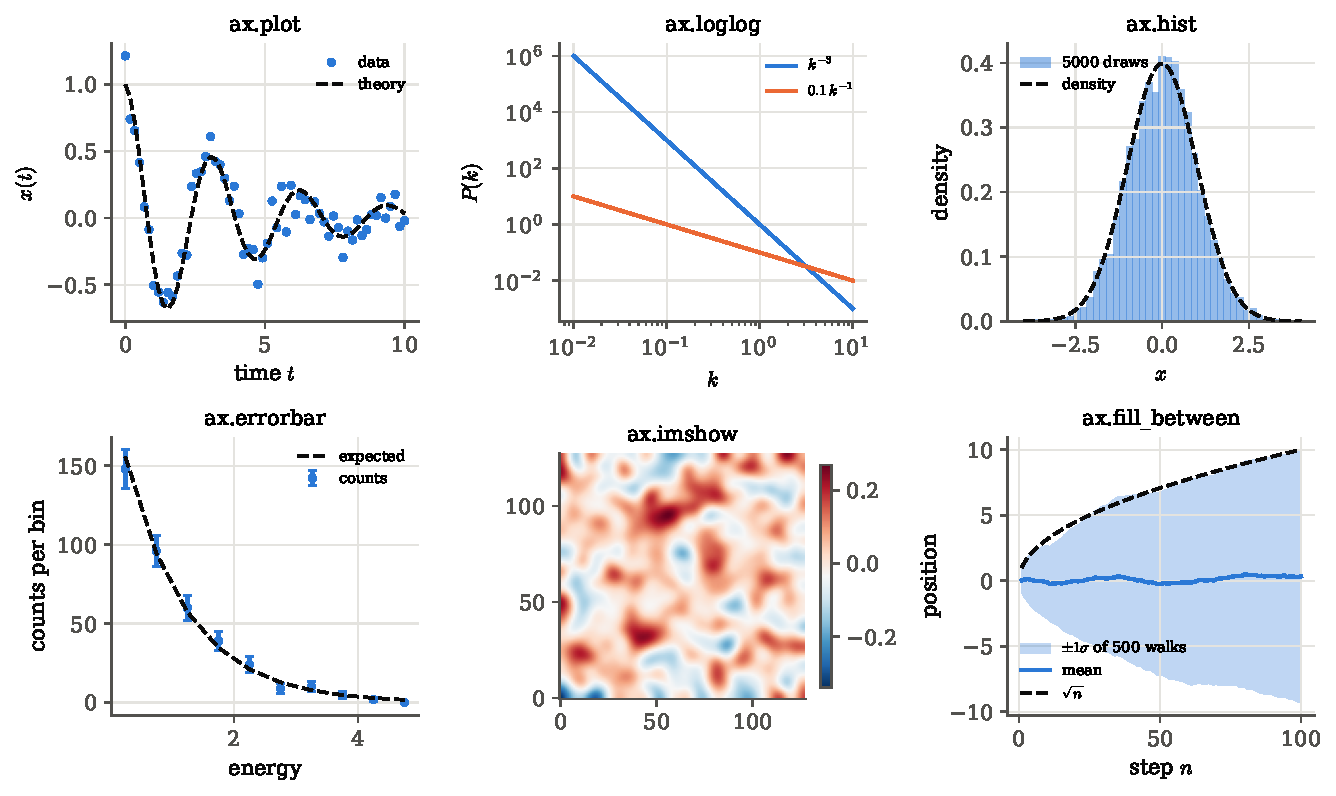
\includegraphics[width=\linewidth]{figures/chT0/04_plot_gallery.pdf}
\caption{Six kinds of panel and the call that draws each, from simulated data: noisy samples of a damped oscillation with the curve they scatter around (\texttt{plot}), two power laws as straight lines on logarithmic axes (\texttt{loglog}), $5000$ Gaussian draws against their density (\texttt{hist}), Poisson counts with $\sqrt n$ error bars (\texttt{errorbar}), a smoothed random field (\texttt{imshow}), and the $\pm1\sigma$ band of $500$ random walks around their mean, against $\sqrt n$ (\texttt{fill\_between}).}
\label{T0a:fig:gallery}
\end{figure}

\paragraph{Example: why a histogram needs \texttt{density=True}.} A histogram of $5000$ draws in bins of width $\Delta x$ has heights $n_j$ that add up to $5000$. A density $p(x)$ integrates to $1$. To compare them, the heights must be divided by the number of draws and by the bin width:
\begin{align*}
  \hat p_j
  &\eqby{1}\frac{n_j}{N\,\Delta x},
  &
  \sum_j\hat p_j\,\Delta x
  &\eqby{2}\frac{1}{N}\sum_j n_j
   \eqby{3}1 .
\end{align*}
\begin{explain}
  \item The fraction of draws in bin $j$, $n_j/N$, estimates $\int_{\text{bin}}p\,\dd x\approx p(x_j)\,\Delta x$; divide by $\Delta x$.
  \item Multiply each height by its bin width and add.
  \item Every draw falls in some bin (if the bins cover the data), so the counts add up to $N$.
\end{explain}
\texttt{ax.hist(x, bins=40, density=True)} does exactly this division, which is why the histogram and the black dashed density in the third panel of \cref{T0a:fig:gallery} lie on top of each other. Without \texttt{density=True} the bars would be $N\,\Delta x\approx5000\times0.2=1000$ times taller than the curve (for $40$ bins over a range of about $8$, $\Delta x\approx0.2$).

\begin{pitfall}[\texttt{plt} versus \texttt{ax}]
Many examples on the internet draw with \texttt{plt.plot(\dots)}, which draws on ``the current axes'' that Matplotlib keeps in the background. With several panels, ``current'' is easily not the panel intended. The book always draws with \texttt{ax.plot(\dots)} on an axes it holds by name, and calls \texttt{plt} only to create the figure.
\end{pitfall}

\subsection{Files, folders and caches}
\label{T0a:sec:files}

Some results cost minutes or hours: a thousand simulated CMB skies, a long Markov chain, a hundred calls of a Boltzmann code. They are computed once and kept in the folder \texttt{data/}, in NumPy's own file format. Two calls do it. \texttt{np.savez(path, name1=array1, name2=array2)} writes several arrays into one \texttt{.npz} file, each under a name. \texttt{z = np.load(path)} opens it, and \texttt{z["name1"]} gives back the first array, bit for bit.

Paths are handled by Python's \texttt{pathlib}. A \texttt{Path} is a file or folder name that knows its structure: \texttt{NOTES / "data" / "ch08"} joins names with the operator \texttt{/}, whatever the operating system's separator; \texttt{path.exists()} asks whether the file is there; \texttt{path.mkdir(parents=True, exist\_ok=True)} creates a folder (and any missing folders above it) unless it already exists; \texttt{path.parents[1]} is two levels up (\cref{T0a:sec:anatomy}).

The two combine into the \newterm{cache} pattern: if the file exists, load it; otherwise compute, save, and return. The Monte Carlo library of \cref{8a:sec:pipeline} writes it once, as a function that takes the computation itself as an argument:

\pyfile[firstline=252,lastline=262,firstnumber=252]{code/ch08/lib_cmbsim.py}{Compute once, then load: a cache in eleven lines}

\texttt{make} is a function that returns a dictionary of arrays (line 252 receives it without calling it). Line 254 makes sure \texttt{data/ch08} exists. If the file is already there and recomputing was not forced (line 256), lines 257--258 load it and turn it back into a dictionary with a comprehension over \texttt{z.files}, the list of the names stored in it. Otherwise line 259 calls \texttt{make()}, line 260 saves every entry of the dictionary with \texttt{**d} (which hands each key--value pair to \texttt{np.savez} as a keyword argument), and line 262 returns the result. A thousand skies are simulated the first time; every later run of every script that needs them reads them in a fraction of a second (\cref{T0a:fig:cache}).

\begin{figure}[htbp]
\centering
\begin{tikzpicture}[
  box/.style={draw=accent,rounded corners=2pt,fill=ideabg,align=center,font=\footnotesize,
              text width=2.7cm,minimum height=0.9cm,inner sep=3pt},
  q/.style={draw=accent,diamond,aspect=2.2,fill=white,font=\footnotesize,align=center,inner sep=1pt},
  arr/.style={->,thick,accent}]
  \node[box] (call) at (0,0) {\texttt{cached("mc", make)}};
  \node[q] (ex) at (3.9,0) {file\\ exists?};
  \node[box,fill=takebg,draw=tangentgreen] (load) at (8.0,0.85) {\texttt{np.load}: seconds};
  \node[box,fill=warnbg,draw=bdryred] (make) at (8.0,-0.85) {\texttt{make()}: minutes or hours};
  \node[box] (save) at (11.4,-0.85) {\texttt{np.savez}};
  \draw[arr] (call) -- (ex);
  \draw[arr] (ex.north) |- node[pos=0.75,above,font=\scriptsize] {yes} (load.west);
  \draw[arr] (ex.south) |- node[pos=0.75,below,font=\scriptsize] {no} (make.west);
  \draw[arr] (make) -- (save);
\end{tikzpicture}
\caption{The cache pattern of \texttt{lib\_cmbsim.cached}. The expensive branch (red) runs once and leaves a file behind; every later call takes the cheap branch (green). Deleting the file, or passing \texttt{force=True}, forces a fresh computation.}
\label{T0a:fig:cache}
\end{figure}

The fiducial CMB spectra shared by the whole book are cached the same way, in \pyname{code/camb_fiducial.py}:

\pyfile[firstline=25,lastline=37,firstnumber=25]{code/camb_fiducial.py}{Load the cached CAMB spectra, computing them on first use}

\texttt{load\_fiducial()} computes and saves the spectra only if \texttt{data/camb\_fiducial.npz} is missing (lines 26--27), and otherwise loads them (line 28) and returns the multipoles and the requested spectrum (line 29). Line 36 shows one more use of \texttt{**}: it unpacks a dictionary built on the spot, so that the parameters of the fiducial model are stored in the same file as \texttt{param\_H0}, \texttt{param\_ombh2}, and so on, and anyone opening the file can see which model produced it.

\begin{pitfall}[A stale cache]
A cache does not know that the code which produced it has changed. If a simulation is corrected but its cache file is left in place, every script keeps reading the old, wrong results. After changing a computation that feeds a cache, delete the file (or run once with \texttt{force=True}).
\end{pitfall}
\section{Seen a few times: rare features and two black boxes}
\label{T0a:sec:rare}

The census (\cref{T0a:fig:syntax}) found a sharp drop after the core of the language: a few constructions appear in fewer than one script in ten. They can be skipped on a first reading and looked up here when met. The same holds for the two physics libraries, healpy and CAMB, which the book uses as black boxes: we need to know what goes in and what comes out, not how they work inside.

\subsection{Classes and data classes}
\label{T0a:sec:classes}

A \newterm{class} bundles data together with the functions that act on it. The book defines classes in only $\TzPctClass\%$ of its scripts, always for the same reason: a group of settings that belong together and some quantities derived from them. The clearest example is the description of a CMB experiment in the Monte Carlo library of \cref{8a:sec:beam}:

\pyfile[firstline=68,lastline=92,firstnumber=68]{code/ch08/lib_cmbsim.py}{An experiment as a data class: settings, and quantities derived from them}

Read it as a form with blanks. Line 68, \texttt{@dataclass}, is a \newterm{decorator}: a line starting with \texttt{@} that modifies the definition below it, here by writing the routine parts of the class automatically. Lines 71--75 list the settings, each with a type hint and a default value: the HEALPix resolution, the beam width, the noise level, the band limit, and whether to include the pixel window. Then \texttt{exp = Experiment(nside=128, fwhm\_arcmin=10.0)} creates one experiment with two settings changed and the rest left at their defaults, and \texttt{exp.nside} reads a setting back. Lines 77--91 define quantities computed from the settings. The decorator \texttt{@property} makes each of them look like a setting: \texttt{exp.npix} or \texttt{exp.sigma\_pix} without brackets, recomputed every time it is read, so it can never disagree with the settings. Inside the class, \texttt{self} means ``this particular experiment''. Lines 92 onwards are ordinary functions of the experiment, called as \texttt{exp.nl()}.

\subsection{Errors on purpose, and \texttt{with}}
\label{T0a:sec:try-with}

\texttt{try:} followed by \texttt{except SomeError:} runs a block and, if that particular error occurs, runs the second block instead of stopping. It appears in $\TzPctTry\%$ of the scripts, typically to record that something failed. The SciPy tour uses it to show that $200!$ cannot be a float (\cref{T0a:sec:special}), and \cref{T0a:sec:trust-linalg} uses it to detect a matrix that is not positive definite. Catching errors to hide them is never done: a script that fails should fail loudly.

\texttt{with \dots{} as name:} sets something up for the duration of an indented block and tidies it away afterwards, even if the block fails. It appears in $\TzPctWith\%$ of the scripts, in three forms: opening a file, starting a pool of worker processes (below), and \texttt{with np.errstate(divide="ignore"):}, which silences NumPy's warning about a division by zero that the code is about to repair anyway (line 54 of \pyname{lib_fields.py}, where $P(k)$ is evaluated at $k=0$ and then set to zero).

\subsection{Several cores at once}
\label{T0a:sec:pool}

A Monte Carlo study runs the same function on many independent random seeds, and those runs can go on different processor cores at the same time. Python's \texttt{multiprocessing.Pool} does this with one call: \texttt{pool.map(f, jobs)} applies \texttt{f} to every item of the list \texttt{jobs}, spreads the items over the workers, and returns the results in the original order. The topology study of \cref{12c:sec:model} is the clearest case:

\pyfile[firstline=50,lastline=69,firstnumber=50]{code/ch12/c02_mc_fnl.py}{Hundreds of independent simulations spread over four cores}

Each job (lines 64--66) is a tuple: a stream number and a list of non-Gaussianity amplitudes $\epsilon$. The function \texttt{one} (lines 50--60) makes its own generator from the stream number (line 52), draws one Gaussian field, and measures it at every $\epsilon$ in the list. Line 68 starts four workers, and line 69 runs all the jobs. Two details make this safe. Every job builds its generator from its own stream number, so the result does not depend on which worker ran which job or in what order (\cref{T0a:sec:random}); a generator shared between workers would make the results depend on the scheduling. And the function given to \texttt{pool.map} is defined at the top level of the module, because each worker process imports the script to find it.

\begin{figure}[htbp]
\centering
\begin{tikzpicture}[
  job/.style={draw=softgray,fill=codebg,font=\scriptsize\ttfamily,minimum width=1.0cm,minimum height=0.5cm,inner sep=0.5pt},
  wk/.style={draw=accent,rounded corners=2pt,fill=ideabg,font=\footnotesize,minimum width=1.9cm,minimum height=0.6cm},
  arr/.style={->,accent}]
  \foreach \i in {0,...,7} { \node[job] (j\i) at (1.1*\i,0) {(\i,\dots)}; }
  \node[font=\footnotesize,anchor=east] at (-0.7,0) {\texttt{jobs}};
  \foreach \w in {0,...,3} { \node[wk] (w\w) at (0.25+2.4*\w,-1.6) {worker \w}; }
  \foreach \i/\w in {0/0,1/1,2/2,3/3,4/0,5/1,6/2,7/3} { \draw[arr] (j\i.south) -- (w\w.north); }
  \foreach \i in {0,...,7} { \node[job,fill=takebg,draw=tangentgreen] (r\i) at (1.1*\i,-3.2) {res \i}; }
  \foreach \i/\w in {0/0,1/1,2/2,3/3,4/0,5/1,6/2,7/3} { \draw[arr,tangentgreen] (w\w.south) -- (r\i.north); }
  \node[font=\footnotesize,anchor=east] at (-0.7,-3.2) {\texttt{out}};
\end{tikzpicture}
\caption{\texttt{pool.map(one, jobs)} with four workers. Each job carries its own stream number, so it produces the same result whichever worker runs it, and the list of results comes back in the order of the jobs.}
\label{T0a:fig:pool}
\end{figure}

\subsection{Compiled loops: numba}
\label{T0a:sec:numba}

Vectorisation (\cref{T0a:sec:vectorise}) needs the elements to be independent, so that one operation can act on all of them. Some algorithms are sequential by nature: in a Metropolis sweep of the Ising model each spin's update depends on its neighbours' \emph{current} values, which earlier steps of the same sweep may have just changed. Such a loop cannot be written as one array expression. The library numba solves this by compiling a Python function into machine code the first time it is called: the decorator \texttt{@njit} on top of the function is the only change. Five files use it ($\TzPctNumba\%$). The Ising sweep of \cref{9b:sec:ising} is one:

\pyfile[firstline=19,lastline=35,firstnumber=19]{code/ch09/20_ising.py}{A sequential Metropolis sweep, compiled by numba}

Apart from line 19 this is plain Python with two nested loops: visit every site, sum its four neighbours with periodic wrap-around (the \texttt{\% L} on line 28), compute the energy change, and accept the flip with the Metropolis probability. Uncompiled, the $L^2$ inner steps would run at Python's speed of a few hundred nanoseconds each; compiled, at a few nanoseconds. A compiled function accepts only NumPy arrays and plain numbers, which is why the random numbers \texttt{u} are drawn outside, by the book's generator, and passed in.

\subsection{healpy and CAMB as black boxes}
\label{T0a:sec:blackbox}

Two libraries do physics that the book does not reimplement. \newterm{healpy} handles maps on the sphere in the HEALPix pixelisation \cite{Gorski2005}: $12N_{\rm side}^2$ pixels of equal area, and the spherical-harmonic transforms between a map and its coefficients $\alm$. \newterm{CAMB} \cite{CAMB2000} solves the linearised Boltzmann equations of a cosmological model and returns its predicted spectra. Neither needs to be understood inside. Each can be used as a box with known inputs and outputs (\cref{T0a:fig:blackbox}), and checked from outside on a case with a known answer.

\begin{figure}[htbp]
\centering
\begin{tikzpicture}[
  bb/.style={draw=black!70,thick,fill=black!8,rounded corners=2pt,minimum width=2.6cm,minimum height=1.1cm,font=\small\bfseries,align=center},
  io/.style={font=\footnotesize,align=left},
  arr/.style={->,thick,accent}]
  \node[bb] (camb) at (0,0) {CAMB};
  \node[io,anchor=east] (ci) at (-2.0,0) {$H_0,\ \omega_b,\ \omega_c,\ \tau,\ A_s,\ n_s$\\ \texttt{lmax}};
  \node[io,anchor=west] (co) at (2.0,0) {$\Cell^{TT},\ \Cell^{EE},\ \Cell^{BB},\ \Cell^{TE}$\\ $\ell=0,\dots,\ell_{\max}$, in $\mu$K$^2$};
  \draw[arr] (ci.east) -- (camb.west);
  \draw[arr] (camb.east) -- (co.west);
  \node[bb] (hp1) at (0,-2.0) {\texttt{hp.alm2map}};
  \node[io,anchor=east] (hi) at (-2.0,-2.0) {$\alm$ ($\ell\le\ell_{\max}$), $N_{\rm side}$};
  \node[io,anchor=west] (ho) at (2.0,-2.0) {a map: $12N_{\rm side}^2$ pixel values};
  \draw[arr] (hi.east) -- (hp1.west);
  \draw[arr] (hp1.east) -- (ho.west);
  \node[bb] (hp2) at (0,-3.6) {\texttt{hp.anafast}};
  \node[io,anchor=east] (ai) at (-2.0,-3.6) {a map, \texttt{lmax}};
  \node[io,anchor=west] (ao) at (2.0,-3.6) {$\Chat=\frac1{2\ell+1}\sum_m|\alm|^2$};
  \draw[arr] (ai.east) -- (hp2.west);
  \draw[arr] (hp2.east) -- (ao.west);
\end{tikzpicture}
\caption{Three black boxes and what crosses their walls. CAMB turns six cosmological parameters into the predicted CMB spectra. healpy's \texttt{alm2map} turns harmonic coefficients into a pixelised map, and \texttt{anafast} turns a map back into the estimated power spectrum. A round trip through the last two must return the spectrum that went in, which is how the book checks them.}
\label{T0a:fig:blackbox}
\end{figure}

The whole CAMB interface the book uses is three calls in \pyname{code/camb_fiducial.py}:

\pyfile[firstline=16,lastline=22,firstnumber=16]{code/camb_fiducial.py}{Six parameters in, four spectra out}

Line 18 collects the parameters into one object (the \texttt{**params} unpacks the dictionary \texttt{FIDUCIAL} of line 13 into keyword arguments such as \texttt{H0=67.36}); \texttt{lmax} is set $200$ above the multipoles wanted, because the lensing calculation needs a margin. Line 19 runs the Boltzmann code, which takes several seconds. Line 20 asks for the spectra in $\mu$K$^2$ as raw $\Cell$ (not $D_\ell$), and line 21 keeps the total (lensed) spectra, an array with one row per $\ell$ and four columns $TT$, $EE$, $BB$, $TE$. Because this costs seconds per call, the result is cached (\cref{T0a:sec:files}) and CAMB is called again only by the few scripts that vary the parameters (\cref{T1a:sec:cl-response}, \cref{10a:sec:numderiv-camb}).

healpy calls look like this round trip, from \cref{7b:sec:camb}:

\pyfile[firstline=61,lastline=67,firstnumber=61]{code/ch07/24_camb_healpix.py}{From $\alm$ to a map and back: healpy as two black boxes}

Line 63 draws the coefficients with the book's own generator (\texttt{lh.synalm}, written from scratch in \cref{7b:sec:alm}). Line 64 is \texttt{hp.alm2map}: coefficients in, map of $N_{\rm side}=256$ out. Line 66 is \texttt{hp.anafast}: map in, $\Chat$ out; \texttt{iter} sets how many refinement passes it makes on the transform. Line 67 compares the result with the spectrum of the input coefficients. The few other healpy calls in the book are of the same kind: \texttt{hp.nside2npix} (pixels from resolution), \texttt{hp.map2alm} (map to coefficients), \texttt{hp.smoothing} (convolve with a beam), \texttt{hp.pixwin} (the pixel window), \texttt{hp.mollview} (draw the sphere on a page). Each is a documented box, and the book checks each once against a case with a known answer before relying on it.
\providecommand{\TzoutPart}[2]{\lstinputlisting[style=py,language={},numbers=none,
  backgroundcolor=\color{white},frame=leftline,framexleftmargin=0.6em,xleftmargin=1.2em,
  basicstyle=\ttfamily\footnotesize\color{black!75},#1]{#2}}

\section{Seven traps that catch everyone once}
\label{T0a:sec:pitfalls}

A program does exactly what it says, which is not always what its author meant. Most mistakes stop the script with an error message, and those are the friendly ones: Python names the line, and the fix is usually obvious. The dangerous mistakes are the ones that run to the end and print a plausible number. Take the smallest example. A script estimates the variance of each of $M$ simulated experiments, stored as the rows of an $M\times N$ array \texttt{x}, by subtracting each row's mean. If it writes \texttt{x - x.mean(axis=1)}, the means form an array of shape \texttt{(M,)}, and NumPy lines that shape up against the \emph{columns} of \texttt{x}, not its rows (\cref{T0a:sec:broadcasting}). When $M\neq N$ the shapes do not fit and the script stops; when by bad luck $M=N$, it subtracts the mean of experiment $j$ from reading $j$ of every experiment, runs to the end, and prints a variance that is simply wrong. The good version, \texttt{x - x.mean(axis=1, keepdims=True)}, keeps the means as a column of shape \texttt{(M, 1)} and is correct for every $M$ and $N$; its price is eleven characters. The lesson: the traps worth knowing are the silent ones.

There are seven of them, and each is a fact about how Python or NumPy stores numbers. The script \pyname{code/chT0/05_pitfalls.py} runs each one in two or three lines and prints what happens, and the book's own scripts show how each is avoided.

\subsection{Comparing real numbers}
\label{T0a:sec:pit-float}

A computer stores a real number in binary with a fixed number of digits, so most decimal fractions are stored only approximately. $0.1$ in binary is $0.000110011001100\ldots$, repeating for ever, and it is cut off after $53$ binary digits. The first lines of the script show the consequence:

\TzoutPart{firstline=1,lastline=4}{results/chT0/05_pitfalls_out.txt}

The stored $0.1+0.2$ and the stored $0.3$ differ by $\TzFloatGap$, so the test \texttt{==} says they are different. Nothing is broken: each number is correct to about sixteen significant digits, and they disagree in the seventeenth. The consequence is a rule. Real numbers computed in two different ways are compared with a tolerance, never with \texttt{==}. \texttt{np.isclose(a, b)} asks whether $\abs{a-b}\le 10^{-8}+10^{-5}\abs b$ (both tolerances can be changed with \texttt{atol=} and \texttt{rtol=}), and \texttt{np.allclose} asks the same of every element of two arrays.

The book's scripts compare in exactly this way when they check one method against another. The exact binomial confidence interval of \cref{4b:sec:ci-intentions} is found twice, once by solving two equations with \texttt{brentq} and once from a closed formula that uses the beta distribution:

\pyfile[firstline=40,lastline=45,firstnumber=40]{code/ch04/11_test_inversion.py}{Two routes to the same interval, compared with a tolerance}

Line 45 is the comparison: the two lower ends must agree to within $10^{-6}$, and so must the two upper ends. The tolerance is set by the less accurate of the two routes, here the root finder, whose default stopping rule pins the root to about $10^{-12}$; $10^{-6}$ leaves a wide margin while still catching any real mistake, which would show up in the second or third digit. How large a tolerance must be in general, and why, is the subject of \cref{T0a:sec:trust-float}.

\subsection{Whole numbers and real numbers}
\label{T0a:sec:pit-int}

Python and NumPy keep two kinds of number apart: integers (\texttt{int}, whole numbers, exact) and floating-point numbers (\texttt{float}, real numbers, approximate). Two consequences surprise newcomers:

\TzoutPart{firstline=5,lastline=7}{results/chT0/05_pitfalls_out.txt}

The first line is the dangerous one. \texttt{np.array([1, 2, 3])} is made from integers, so its \texttt{dtype} is \texttt{int64}, and an integer array can only hold integers: writing $0.7$ into it silently stores $0$, the integer part. The second line is the reassuring one: in Python~3, \texttt{/} always divides as real numbers, \texttt{7 / 2} is $3.5$, and only the explicit floor division \texttt{//} throws the fraction away.

Integer arrays arise naturally in the book, because counts are integers: \texttt{rng.poisson} and \texttt{rng.integers} return them, and so does \texttt{np.histogram} for its counts. The iterative unfolding of \cref{6b:sec:unf-bayes} works on simulated Poisson counts, and converts them to real numbers the moment they are drawn:

\pyfile[firstline=172,lastline=183,firstnumber=172]{code/ch06/30_unfolding.py}{Counts converted to real numbers before any arithmetic, and a default of \texttt{None}}

Line 183 draws $1000$ toy data sets of Poisson counts and immediately applies \texttt{.astype(float)}, which returns a copy of the array with \texttt{dtype} \texttt{float64}. The update of line 178 then divides these counts by the predicted ones and multiplies by efficiencies; with real numbers there is no risk that an intermediate result is cut to an integer anywhere along the way. (Lines 172 and 174 show another habit, the default value \texttt{None}, which \cref{T0a:sec:pit-default} explains.) The rule: when an array will hold real numbers, make it a float array from the start, with \texttt{np.zeros(n)} (which is float by default), \texttt{np.array(\dots, float)} or \texttt{.astype(float)}.

\subsection{Views and copies}
\label{T0a:sec:pit-view}

A slice of a NumPy array is not a new array. It is a \newterm{view} \unpack{a second name for part of the same block of memory}: \texttt{y = x[1:3]} makes \texttt{y} a window onto elements $1$ and $2$ of \texttt{x}, and writing through the window changes \texttt{x} (\cref{T0a:fig:view}). NumPy does this on purpose, because slicing a large array would otherwise copy it every time. The script shows both behaviours:

\TzoutPart{firstline=8,lastline=10}{results/chT0/05_pitfalls_out.txt}

With the view, the two nines appear inside \texttt{x}; with \texttt{.copy()}, \texttt{y} is an independent array and \texttt{x} stays zero. The same is true of plain assignment: \texttt{y = x} gives the same array a second name and copies nothing. Python lists behave the same way for assignment, though their slices \emph{are} copies.

\begin{figure}[htbp]
\centering
\begin{tikzpicture}[
  cell/.style={draw=black!60,minimum width=0.8cm,minimum height=0.6cm,font=\footnotesize\ttfamily},
  nm/.style={font=\small\ttfamily},
  arr/.style={->,thick,accent}]
  \node[font=\small,anchor=west] at (-0.4,1.35) {\texttt{y = x[1:3]}: a view};
  \foreach \i/\v in {0/0.,1/9.,2/9.,3/0.,4/0.} {
    \node[cell,fill=white] (a\i) at (0.8*\i,0) {\v};
    \node[font=\tiny,black!55] at (0.8*\i,-0.48) {\i};
  }
  \draw[thick,fibreorange,rounded corners=1pt] ($(a1.north west)+(-0.04,0.05)$) rectangle ($(a2.south east)+(0.04,-0.05)$);
  \node[nm,anchor=east] (x1) at (-0.75,0) {x};
  \draw[arr] (x1.east) -- (a0.west);
  \node[nm,fibreorange] (y1) at (1.2,0.95) {y};
  \draw[arr,fibreorange] (y1.south) -- ($(a1.north east)+(0,0.06)$);
  \begin{scope}[xshift=5.6cm]
  \node[font=\small,anchor=west] at (-0.4,1.35) {\texttt{y = x[1:3].copy()}};
  \foreach \i/\v in {0/0.,1/0.,2/0.,3/0.,4/0.} {
    \node[cell,fill=white] (b\i) at (0.8*\i,0) {\v};
    \node[font=\tiny,black!55] at (0.8*\i,-0.48) {\i};
  }
  \node[nm,anchor=east] (x2) at (-0.75,0) {x};
  \draw[arr] (x2.east) -- (b0.west);
  \node[cell,fill=takebg] (c0) at (1.2,-1.35) {9.};
  \node[cell,fill=takebg] (c1) at (2.0,-1.35) {9.};
  \node[nm,anchor=east,tangentgreen!60!black] (y2) at (0.25,-1.35) {y};
  \draw[arr,tangentgreen!60!black] (y2.east) -- (c0.west);
  \end{scope}
\end{tikzpicture}
\caption{Two names for one block of memory, or two blocks. Left: the slice \texttt{y} is a window (orange) onto elements $1$ and $2$ of \texttt{x}, so \texttt{y[:] = 9} writes into \texttt{x}. Right: \texttt{.copy()} makes a new block (green) for \texttt{y}, and \texttt{x} is untouched.}
\label{T0a:fig:view}
\end{figure}

Where does this matter in practice? When a loop records the history of something it keeps changing. Newton's method for the maximum-likelihood angle fit of \cref{3b:sec:newton} stores every step it takes, so that the path can be drawn:

\pyfile[firstline=62,lastline=71,firstnumber=62]{code/ch03/10_angular_ml.py}{Recording the path of an iteration: a copy at every step}

Line 63 makes the starting point a float array (the previous trap) and starts the list \texttt{path} with a \emph{separate} copy of it. Line 66 computes the Newton step, line 67 moves to the new point, and line 68 appends a copy of it to the list. Here line 67 happens to build a new array, because \texttt{th + step} always creates one, so the copy is a safeguard rather than a necessity. It becomes a necessity the moment someone ``simplifies'' line 67 to \texttt{th += step}: the operator \texttt{+=} updates the existing array in place, and without the copy every entry of \texttt{path} would be the same array, so the plotted path would collapse to its final point. The rule: when an array is stored and then changed, store a \texttt{.copy()}.

\subsection{Where ranges and slices stop}
\label{T0a:sec:pit-range}

Python counts from zero and stops \emph{before} the end:

\TzoutPart{firstline=11,lastline=15}{results/chT0/05_pitfalls_out.txt}

\texttt{range(5)} is $0,1,2,3,4$: five numbers, and $5$ is not among them. A slice \texttt{v[2:5]} takes elements $2,3,4$. \texttt{np.arange(0, 1, 0.1)} stops before $1$ and has ten points, while \texttt{np.linspace(0, 1, 11)} includes both ends and has eleven. The convention has a reward: \texttt{v[a:b]} has exactly $b-a$ elements, and \texttt{v[:k]} and \texttt{v[k:]} split \texttt{v} into two pieces without overlap or gap. Its cost is that every formula written on paper with $i=1,\dots,N$ must be translated to \texttt{i = 0, \dots, N-1}.

The commonest form of the trap in the book is the \newterm{fencepost} \unpack{$n$ bins need $n+1$ edges, as $n$ fence panels need $n+1$ posts} of every histogram (\cref{T0a:fig:fencepost}). The density-histogram script of \cref{1b:sec:pdf} builds its bins like this:

\pyfile[firstline=34,lastline=37,firstnumber=34]{code/ch01/11_density_histogram.py}{Bin edges with \texttt{arange}, and the centres between them}

Line 35 wants edges from $\mu-4\sigma$ to $\mu+4\sigma$ \emph{inclusive}, in steps of the bin width $w$. Because \texttt{np.arange} stops before its end point, and because $8\sigma/w$ steps of a fractional $w$ may land a hair above or below $\mu+4\sigma$ by rounding, the end is given as $\mu+4\sigma+w/2$: half a step beyond the last edge wanted, so that the last edge is included and nothing beyond it is. Line 36 returns the counts, one per bin, and the edges, one more than the counts. Line 37 makes the bin centres by averaging each edge with the next: \texttt{edges[1:]} drops the first edge and \texttt{edges[:-1]} drops the last, so the two arrays have the same length, the number of bins, and their average is the midpoint of every bin.

\begin{figure}[htbp]
\centering
\begin{tikzpicture}[x=1.65cm]
  \foreach \i in {0,...,5} {
    \draw[thick,black!70] (\i,0) -- (\i,0.9);
    \node[font=\scriptsize,anchor=north] at (\i,-0.05) {\texttt{edges[\i]}};
  }
  \foreach \i/\h in {0/0.45,1/0.75,2/0.6,3/0.35,4/0.2} {
    \fill[formblue!25] (\i+0.04,0) rectangle (\i+0.96,\h);
    \fill[fibreorange] (\i+0.5,0.04) circle (1.6pt);
    \node[font=\scriptsize,anchor=south,formblue!70!black] at (\i+0.5,0.92) {\texttt{counts[\i]}};
  }
  \draw[black!70] (-0.2,0) -- (5.2,0);
  \node[font=\footnotesize,anchor=west] at (5.3,0.5) {5 bins, 6 edges};
  \node[font=\footnotesize,anchor=west,fibreorange!80!black] at (5.35,0.05) {centres};
\end{tikzpicture}
\caption{The fencepost. Five bins (blue) are bounded by six edges (black). \texttt{np.histogram} returns five counts and six edges; the five centres (orange dots) are the averages of \texttt{edges[:-1]} (the left edges) and \texttt{edges[1:]} (the right edges).}
\label{T0a:fig:fencepost}
\end{figure}

\subsection{Shapes that do not fit, or fit by accident}
\label{T0a:sec:pit-shape}

Broadcasting (\cref{T0a:sec:broadcasting}) compares the shapes of two arrays from the right, and stretches any axis of length one. Two outcomes are printed by the script:

\TzoutPart{firstline=16,lastline=18}{results/chT0/05_pitfalls_out.txt}

Subtracting a column (shape \texttt{(3, 1)}, made by \texttt{r[:, None]}) from a row (shape \texttt{(3,)}) gives the $3\times3$ table of all differences, which is often exactly what is wanted. Adding arrays of lengths $3$ and $4$ fails with a message that names both shapes. The failure is the friendly case. The unfriendly case is the one of the opening paragraph: two axes that happen to have the same length, so that the shapes fit even though the meaning does not.

The sample-variance study of \cref{3a:sec:var-python} has exactly that structure, $M$ simulated experiments of $N$ readings each, stored as an $M\times N$ array, with $N$ running over a list of sample sizes:

\pyfile[firstline=29,lastline=33,firstnumber=29]{code/ch03/04_sample_variance.py}{Each row minus its own mean: \texttt{keepdims=True}}

Line 31 subtracts each row's mean from that row. \texttt{x.mean(axis=1)} alone would have shape \texttt{(M,)}, a row of $M$ means, which broadcasting would line up against the $N$ columns: an error if $M\neq N$, and a silently wrong answer if $M=N$. With \texttt{keepdims=True} the result keeps the averaged axis with length one, shape \texttt{(M, 1)}, a column, and broadcasting stretches it across each row. The habit that catches the rest: print \texttt{.shape} of every array in a new formula once, and check that it is what the paper formula says.

\subsection{A default value that remembers}
\label{T0a:sec:pit-default}

A default value in a function definition (\cref{T0a:sec:functions}) is created \emph{once}, when Python reads the \texttt{def} line, and shared by every call that does not supply that argument. For a number or a string this never matters, because they cannot be changed in place. For a list it does:

\TzoutPart{firstline=19,lastline=21}{results/chT0/05_pitfalls_out.txt}

\texttt{append\_bad(value, store=[])} appends to its default list, and since that list is the same object at every call, the second call returns $[1,2]$: it remembers the first. \texttt{append\_good(value, store=None)} uses the conventional cure: the default is the special value \texttt{None}, and the first line of the function makes a fresh list whenever \texttt{store} is \texttt{None}. The unfolding function \texttt{ibu} of the excerpt in \cref{T0a:sec:pit-int} uses the same pattern for an array: \texttt{prior=None} on line 172, and on line 174 a flat prior made fresh at each call when none is given. The book never uses a list, a dictionary or an array as a default value.

\subsection{Forgetting the seed}
\label{T0a:sec:pit-seed}

A generator made without a seed takes one from the computer's clock and its internal noise, so its numbers differ at every run:

\TzoutPart{firstline=22,lastline=24}{results/chT0/05_pitfalls_out.txt}

Two generators made with \texttt{np.random.default\_rng()} give different first draws; two made with \texttt{rng\_for} and the same name give the same draw, $\TzSeedDraw$, at every run and on every machine (\cref{T0a:sec:random}). The difference matters for three reasons. A number quoted in the text must be the number the script prints, every time it is rerun. A bug that appears for one random sample can be chased only if the same sample can be produced again. And two settings can be compared on the same random numbers, which makes their difference far more precise than either one (\cref{T0a:sec:trust-mc}).

The census counts of \cref{T0a:sec:random} show how faithfully the book keeps the rule: of the $\TzDrawFiles$ files that draw random numbers, $\TzSeededDrawFiles$ make their generator with \texttt{rng\_for}, and nearly all of the others are libraries that receive a generator from the script that calls them. The script above is one of the very few places where an unseeded generator is made on purpose, to show what it does.

\begin{pitfall}[A trap that hides in an average]
Each of the seven traps can hide inside a Monte Carlo average, where a wrong number looks like noise. The cure is the same for all of them: run the code once on a case whose answer is known, and compare with a tolerance (\cref{T0a:sec:trust-valid}).
\end{pitfall}
\providecommand{\TzZcv}{\pgfmathparse{(\SBvrTwo-1)/\SBerrTwo}\pgfmathprintnumber[fixed,precision=1]{\pgfmathresult}}

\section{Is this number real? Numerical noise and how to check}
\label{T0a:sec:trust}

A script finishes and prints a number. It ran without an error, the number has the right size, and it carries twelve digits. How many of those digits mean anything? The question is not idle, because every number a computer produces has passed through three filters that each blur it. Every real number is stored with about sixteen significant digits and rounded after every operation. Every method that replaces calculus by arithmetic (a derivative by a difference, an integral by a sum, an equation by an iteration) makes an error of its own that depends on a step size or a tolerance. And every Monte Carlo number is an average of random draws, which a different seed would change.

\paragraph{The smallest example.} The probability that a standard Gaussian variable exceeds $2$ is $\Prob(Z>2)=\TzQexact$. A script estimates it from $N=10^4$ draws as the fraction of draws above $2$, and with the first seed prints $\TzQfirst$. Read naively, that is a number with three significant digits, and it does not match the truth to all three. Which of the three filters set the error? Rounding contributes about one part in $10^{16}$, and the method (counting) is exact. The Monte Carlo filter is the whole story: the count of draws above $2$ is binomial, so the fraction has standard deviation $\sqrt{q(1-q)/N}=\TzQsigFour$ for $q=\TzQexact$. The printed value should therefore be read as $\TzQfirst\pm\TzQsigFour$: one and a half significant digits, and entirely consistent with the truth: the difference is $\TzQzFirst$ standard deviations. The naive reading would call a correct computation wrong; with only $10^2$ draws it would just as readily call a wrong one right. The good habit, quoting every number with its error, costs one more line of code. \emph{The lesson: a number without an error estimate has not yet been measured.}

The checks are a short list, one for each source of error: the floating-point facts that set the limit of every computation, the step-size balance of numerical derivatives, the reports and silences of SciPy's integrators, root finders and minimisers, the condition number of a matrix, the $1/\sqrt N$ of Monte Carlo, convergence studies, validation against known answers, and finally a single rule for deciding whether a difference between two numbers is real. Every one of them is already used somewhere in the book, and each is shown at work on a small problem by \pyname{code/chT0/08_trust.py}.

\subsection{Sixteen digits, and how to lose them}
\label{T0a:sec:trust-float}

\paragraph{How a real number is stored.} NumPy's \texttt{float64}, Python's \texttt{float}, is a number in binary scientific notation, packed into $64$ bits (\cref{T0a:fig:float64}):
\begin{equation}
  x=(-1)^{s}\,\Bigl(1+\sum_{k=1}^{52}b_k\,2^{-k}\Bigr)\,2^{e},
  \qquad b_k\in\{0,1\},\quad -1022\le e\le1023 .
  \label{T0a:eq:float64}
\end{equation}
One bit holds the sign $s$, eleven the exponent $e$, and fifty-two the binary digits $b_k$ of the fraction, the \newterm{mantissa}. Between $1$ and $2$ (that is, $e=0$) the numbers that can be stored are $1$, $1+2^{-52}$, $1+2\cdot2^{-52}$, and so on: they are evenly spaced, and the gap is
\begin{equation}
  \epsilon=2^{-52}\approx2.22\times10^{-16},
  \label{T0a:eq:eps}
\end{equation}
the \newterm{machine epsilon} \unpack{the gap between $1$ and the next larger storable number}. Between $2^e$ and $2^{e+1}$ the same $2^{52}$ steps are stretched by $2^e$, so the gap is $\epsilon\,2^e$: the \emph{relative} spacing is about $\epsilon$ everywhere. A real number is rounded to the nearest storable one, so its stored value is $x(1+\delta)$ with $\abs\delta\le\epsilon/2$, and so is the result of every arithmetic operation. That is what ``sixteen significant digits'' means: $\log_{10}(1/\epsilon)\approx15.7$ \cite{GoldbergFloat1991}. NumPy reports these facts itself, through \texttt{np.finfo(np.float64)}:

\TzoutPart{firstline=1,lastline=3}{results/chT0/08_trust_out.txt}

$1+\epsilon$ is the next number after $1$, so it differs from $1$; $1+\epsilon/2$ lies exactly halfway and is rounded back to $1$. The largest storable number is about $\TzMaxFloat$ and the smallest with full precision about $\TzTiny$, so overflow and underflow are rare in practice, though not impossible (\cref{T0a:sec:precision}).

\begin{figure}[htbp]
\centering
\begin{tikzpicture}[x=0.135cm]
  \fill[bdryred!30] (0,0) rectangle (1,0.6);
  \fill[fibreorange!35] (1,0) rectangle (12,0.6);
  \fill[formblue!25] (12,0) rectangle (64,0.6);
  \foreach \i in {0,...,64} { \draw[black!35,line width=0.2pt] (\i,0) -- (\i,0.6); }
  \draw[black!70] (0,0) rectangle (64,0.6);
  \node[font=\scriptsize,anchor=north] at (0.5,-0.05) {$s$};
  \node[font=\scriptsize,anchor=south] at (6.5,0.65) {exponent $e$ (11 bits)};
  \node[font=\scriptsize,anchor=south] at (38,0.65) {mantissa $b_1\dots b_{52}$ (52 bits)};
  \begin{scope}[yshift=-1.4cm,x=1cm]
    \draw[->,black!70] (-0.2,0) -- (8.9,0);
    \foreach \x in {0,0.5,1,1.5,2,2.5,3,3.5} { \draw[formblue,thick] (\x,-0.1) -- (\x,0.1); }
    \foreach \x in {4,5,6,7,8} { \draw[formblue,thick] (\x,-0.1) -- (\x,0.1); }
    \node[font=\scriptsize,anchor=north] at (0,-0.12) {$1$};
    \node[font=\scriptsize,anchor=north] at (4,-0.12) {$2$};
    \node[font=\scriptsize,anchor=north] at (8,-0.12) {$4$};
    \draw[<->,tangentgreen!60!black] (0,0.3) -- (0.5,0.3);
    \node[font=\scriptsize,anchor=south,tangentgreen!60!black] at (0.25,0.32) {$\epsilon$};
    \draw[<->,tangentgreen!60!black] (4,0.3) -- (5,0.3);
    \node[font=\scriptsize,anchor=south,tangentgreen!60!black] at (4.5,0.32) {$2\epsilon$};
  \end{scope}
\end{tikzpicture}
\caption{A \texttt{float64}. Top: one sign bit, eleven exponent bits and fifty-two mantissa bits. Bottom: the storable numbers near $1$, with the spacing exaggerated (there are really $2^{52}$ of them between $1$ and $2$). The gap is $\epsilon$ between $1$ and $2$ and doubles at every power of two, so the relative gap stays near $\epsilon$.}
\label{T0a:fig:float64}
\end{figure}

\paragraph{Comparing with a tolerance.} Because every result carries a relative error of order $\epsilon$, two routes to the same quantity agree to about $\epsilon$ times its size, not exactly, and the comparison must be relative. The dark-matter halo of \cref{T2a:sec:dm} is built from its virial mass and radius, and the script checks that the mass enclosed by the profile at $r_{200}$ really is the mass put in:

\pyfile[firstline=40,lastline=42,firstnumber=40]{code/chT2/04_dm_profile.py}{A relative comparison: the ratio minus one}

Line 41 is the enclosed mass of the profile, from its closed form, and line 42 compares the ratio of the two masses with $1$. Written as $\abs{M/M_{200}-1}<10^{-10}$ the test is relative: it does not care whether masses are measured in grams or in solar masses, while \texttt{abs(M - M200) < 1e-10} would be meaningless for numbers of order $10^{12}$. The tolerance sits well above the rounding level (a cube root, two logarithms and a few products, each adding about $\epsilon$) and far below any error that would matter.

\paragraph{Cancellation.} Rounding errors of order $\epsilon$ are harmless as long as they stay of order $\epsilon$. One operation can magnify them enormously: the subtraction of two nearly equal numbers. Suppose $a$ and $b$ are stored as $a(1+\delta_a)$ and $b(1+\delta_b)$, with $\abs{\delta_a},\abs{\delta_b}\le\epsilon/2$. What is the relative error of the computed difference?
\begin{align}
  \frac{\abs{a(1+\delta_a)-b(1+\delta_b)-(a-b)}}{\abs{a-b}}
  &\eqby{1}\frac{\abs{a\delta_a-b\delta_b}}{\abs{a-b}}
   \relby{2}{\le}\frac{\epsilon}{2}\,\frac{\abs a+\abs b}{\abs{a-b}} .
  \label{T0a:eq:cancel}
\end{align}
\begin{explain}
  \item Expand: the exact $a-b$ cancels, and the two rounding errors remain.
  \item The triangle inequality, $\abs{a\delta_a-b\delta_b}\le\abs a\abs{\delta_a}+\abs b\abs{\delta_b}$, and $\abs\delta\le\epsilon/2$.
\end{explain}
The inputs' relative error $\epsilon/2$ is multiplied by $(\abs a+\abs b)/\abs{a-b}$, which is about $2a/(a-b)$ when $a\approx b$. If $a$ and $b$ agree in their first ten digits, ten of the sixteen digits are lost: the result is the difference of two numbers whose leading digits cancelled, leaving the uncertain trailing ones. This is \newterm{catastrophic cancellation}, and it needs no long calculation: a single subtraction is enough.

\paragraph{Example: $1-\cos x$ for small $x$.} The ratio $(1-\cos x)/x^2$ tends to $\tfrac12$ as $x\to0$. At $x=10^{-5}$, $\cos x\approx1-5\times10^{-11}$, so the subtraction $1-\cos x$ cancels ten digits. Since $1$ is stored exactly and $\cos x$ with a relative error of at most $\epsilon/2$, \eqref{T0a:eq:cancel} bounds the relative error of the result by $(\epsilon/2)/(x^2/2)=\epsilon/x^2\approx2\times10^{-6}$. The script prints:

\TzoutPart{firstline=4,lastline=5}{results/chT0/08_trust_out.txt}

At $x=10^{-5}$ the naive formula gives $\TzCancNaive$, wrong in the eighth digit, within the bound. At $x=10^{-8}$ it gives exactly $0$. There $\cos x=1-5\times10^{-17}$; just below $1$ the storable numbers are spaced by $\epsilon/2\approx1.1\times10^{-16}$, and $5\times10^{-17}$ is less than half of that spacing, so $\cos x$ is stored as exactly $1$ and the difference vanishes. The cure is to rewrite the formula so that nothing nearly equal is subtracted. The double-angle identity $\cos x=1-2\sin^2(x/2)$ gives $1-\cos x=2\sin^2(x/2)$, a product of small numbers each known to sixteen digits, and the rewritten form returns $\TzCancGood$ at both values. \Cref{T0a:fig:trust-digits} (left) shows the relative error of both forms against $x$: the naive one follows the bound $\epsilon/x^2$ up to order one, and the rewritten one stays at the rounding floor.

\paragraph{Example: the variance in one pass.} The variance of a set of readings is $\langle x^2\rangle-\langle x\rangle^2$, and that formula needs only one pass through the data. Try it on $10^4$ readings $10^8+z_i$, with $z_i$ standard Gaussian: times in nanoseconds measured from some epoch would look like this. Both $\langle x^2\rangle$ and $\langle x\rangle^2$ are about $10^{16}$, and near $10^{16}$ the storable numbers are spaced by $\epsilon\cdot2^{53}=2$ (since $2^{53}\approx9\times10^{15}$). Each of the two terms is therefore known only to the nearest even number, and their difference, which should be about $1$, can only come out as a multiple of $2$:

\TzoutPart{firstline=6,lastline=6}{results/chT0/08_trust_out.txt}

The one-pass formula returns $\TzVarOnePass$; the two-pass form, which first subtracts the mean and then squares, returns $\TzVarTwoPass$, and so does \texttt{np.var}, which works the same way. By \eqref{T0a:eq:cancel} the amplification factor is about $2\times10^{16}$, enough to destroy all sixteen digits. The book always computes variances in two passes: the sample-variance excerpt of \cref{T0a:sec:pit-shape} subtracts each row's mean before squaring (line 31 there), and elsewhere \texttt{np.var} and \texttt{np.cov} do it internally. \emph{The lesson: never subtract two large, nearly equal numbers; rewrite the formula, or subtract the large common part first.}

\begin{figure}[htbp]
\centering
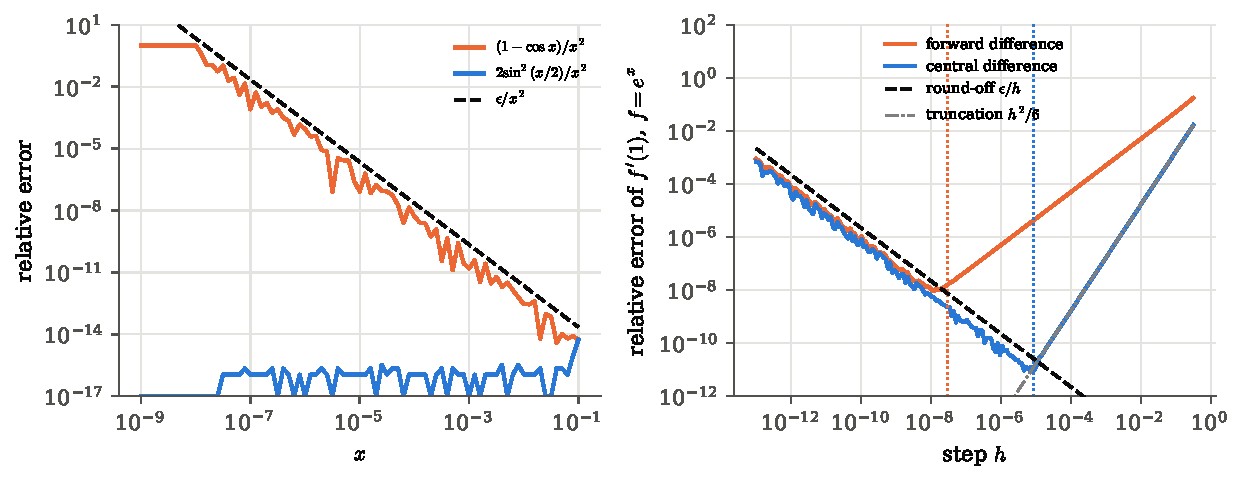
\includegraphics[width=\linewidth]{figures/chT0/08_trust_digits.pdf}
\caption{Where digits go. Left: relative error of $(1-\cos x)/x^2$ computed naively (orange) and as $2\sin^2(x/2)/x^2$ (blue). The naive form loses digits along the dashed line $\epsilon/x^2$ and is useless below $x\approx10^{-8}$; the rewritten form stays at the rounding floor. Right: relative error of the numerical derivative of $e^x$ against the step $h$, for the forward and central differences, as the root-mean-square over $101$ points between $0.5$ and $1.5$. To the right of each minimum the truncation error grows (grey line, $h^2/6$ for the central difference); to the left the round-off error grows as $\epsilon/h$ (dashed). Dotted verticals: the best steps predicted by \eqref{T0a:eq:hopt-central} and its forward analogue.}
\label{T0a:fig:trust-digits}
\end{figure}

\subsection{Derivatives: the step that is neither too large nor too small}
\label{T0a:sec:trust-deriv}

Fisher matrices (\cref{ch:10}), emulators (\cref{9c:sec:emu}) and Newton's method all need derivatives of functions that are known only as code. The obvious approach is the definition of the derivative with a small but finite step $h$. How small? Intuition says ``as small as possible'', and \cref{T0a:fig:trust-digits} (right) shows that intuition to be wrong: the error falls as $h$ shrinks, reaches a minimum, and then rises again. Two errors compete, and the best step is where they balance.

\paragraph{The truncation error.} Take the \newterm{central difference} $D(h)=[f(x+h)-f(x-h)]/2h$. Taylor's theorem gives $f(x\pm h)=f\pm hf'+\tfrac12h^2f''\pm\tfrac16h^3f'''+\dots$, all derivatives at $x$. Subtracting the two expansions cancels the even powers, and dividing by $2h$ leaves
\begin{equation}
  D(h)=f'(x)+\frac{h^2}{6}f'''(x)+O(h^4).
  \label{T0a:eq:central}
\end{equation}
The error $h^2f'''/6$ shrinks as $h$ shrinks: this is the part intuition sees.

\paragraph{The round-off error.} The two function values are computed with relative errors of order $\epsilon$, so each is off by up to about $\epsilon\abs f$, and in the worst case the two errors have opposite signs and add. Their difference is then off by $2\epsilon\abs f$, and dividing by $2h$ leaves $\epsilon\abs f/h$. This part \emph{grows} as $h$ shrinks: for a tiny $h$, $f(x+h)$ and $f(x-h)$ are nearly equal, and their difference is the cancellation of \eqref{T0a:eq:cancel}.

\paragraph{The balance.} The total error and its minimum follow in three lines:
\begin{align}
  E(h)&\eqby{1}\frac{\epsilon\abs f}{h}+\frac{h^2}{6}\abs{f'''},
  \nonumber\\
  \frac{\dd E}{\dd h}&\eqby{2}-\frac{\epsilon\abs f}{h^2}+\frac{h}{3}\abs{f'''}=0
  \quad\Longrightarrow\quad
  h_{\rm opt}\eqby{3}\Bigl(\frac{3\epsilon\abs f}{\abs{f'''}}\Bigr)^{1/3}\sim\epsilon^{1/3},
  \nonumber\\
  E(h_{\rm opt})&\eqby{4}\frac32\,\frac{\epsilon\abs f}{h_{\rm opt}}\sim\epsilon^{2/3}.
  \label{T0a:eq:hopt-central}
\end{align}
\begin{explain}
  \item Round-off plus truncation, the two estimates above.
  \item The smallest error is where the slope of $E$ vanishes.
  \item Multiply by $3h^2/\abs{f'''}$: $h^3=3\epsilon\abs f/\abs{f'''}$, and take the cube root.
  \item At $h_{\rm opt}$, $\frac{h^2}6\abs{f'''}=\frac{h^3}{6h}\abs{f'''}=\frac{3\epsilon\abs f}{6h}=\frac12\,\frac{\epsilon\abs f}{h}$: the truncation term is half the round-off term, and the sum is $\tfrac32$ of it. Since $h_{\rm opt}\sim\epsilon^{1/3}$, this is $\epsilon/\epsilon^{1/3}=\epsilon^{2/3}$.
\end{explain}
For $f=e^x$, where $f=f'''$, the best step is $(3\epsilon)^{1/3}=\TzHcenPred$ and the best relative error about $\epsilon^{2/3}\approx\TzErrCenPred$: two-thirds of the sixteen digits, about ten, survive. The same reasoning for the \newterm{forward difference} $[f(x+h)-f(x)]/h=f'+\tfrac12hf''+\dots$, whose truncation error is first order in $h$, gives $E=2\epsilon\abs f/h+\tfrac12h\abs{f''}$, $h_{\rm opt}=2\sqrt{\epsilon\abs f/\abs{f''}}\sim\epsilon^{1/2}$ and an error of order $\epsilon^{1/2}$: only eight digits. The script scans $h$ and finds:

\TzoutPart{firstline=7,lastline=8}{results/chT0/08_trust_out.txt}

The measured best steps sit where \eqref{T0a:eq:hopt-central} puts them. The measured errors are a few times smaller than predicted, because the prediction assumed the worst case, with the two rounding errors adding; on average they partly cancel.

\paragraph{The plateau check.} For a function whose third derivative is unknown, \eqref{T0a:eq:hopt-central} cannot be evaluated. The practical test is to compute the derivative for steps a factor of ten apart and look for a \newterm{plateau}, a range of $h$ over which the result does not change:

\TzoutPart{firstline=9,lastline=16}{results/chT0/08_trust_out.txt}

The exact value is $e=\TzExactE$. From $h=10^{-2}$ to $10^{-4}$ the digits settle (truncation shrinking a hundredfold per step); at $h=10^{-5}$ and $10^{-6}$ the results agree with each other to ten digits; below that, round-off takes over, and at $h=10^{-12}$ only four digits survive. The digits that stay fixed while $h$ changes by a factor of ten are the ones to trust.

The book chooses its steps in exactly this spirit. The emulator of \cref{9c:sec:emu-build} replaces CAMB by a second-order Taylor expansion in the six cosmological parameters, and its first derivatives are central differences with a fixed step for each parameter:

\pyfile[firstline=57,lastline=60,firstnumber=57]{code/ch09/lib_cmbemu.py}{Central differences of $\ln C_\ell$, one parameter at a time}

Line 57 builds a diagonal matrix whose row $i$ moves parameter $i$ alone by its step (the array \texttt{STEPS}, set on line 29 of the same file to $0.02$ in $\ln(10^{10}A_s)$, $0.01$ in $n_s$, $0.5$ in $H_0$, and so on). Lines 58--59 run CAMB at each shifted point, and line 60 is \eqref{T0a:eq:central}. These steps are far larger than $\epsilon^{1/3}$, and rightly so. CAMB's output is not accurate to sixteen digits but to perhaps six, so its $\epsilon$ is about $10^{-6}$, and \eqref{T0a:eq:hopt-central} then asks for steps of order $10^{-2}$ in relative terms. \Cref{10a:sec:numderiv-errors} redoes the balance with such a ``code noise'' and with the four-point rule, and \cref{10a:sec:numderiv-camb} runs the plateau check on CAMB itself, multiplying all six steps by factors from $\tfrac1{64}$ to $4$ and confirming that the forecast does not move over the middle of that range. \emph{The lesson: a numerical derivative is trustworthy only on a plateau; find it by changing $h$ by factors of ten.}

\subsection{Integrals, roots and minima: what the black boxes report}
\label{T0a:sec:trust-boxes}

\texttt{quad}, \texttt{brentq} and \texttt{minimize} (\cref{T0a:sec:scipy}) are iterations that stop when an internal test is satisfied. Each one reports something about its own reliability, and each can be fooled. The three ways they go wrong are different: \texttt{quad} can be confidently wrong, \texttt{brentq} refuses loudly, and \texttt{minimize} stops quietly.

\paragraph{\texttt{quad} is only as good as the points it looked at.} \texttt{quad} returns a value and an error estimate (\cref{T0a:sec:quad}). The estimate is the disagreement between two integration rules applied to the same function values, and so it says nothing about regions where the function was never evaluated. The script integrates a Gaussian of width $0.01$ centred at $37.3$, whose integral is exactly $1$, over $[0,100]$, and then tries four remedies:

\TzoutPart{firstline=17,lastline=17}{results/chT0/08_trust_out.txt}

Over $[0,100]$ \texttt{quad} first applies a $21$-point rule to the whole interval. No point lands within the peak, every value is zero or astronomically small, both rules agree on zero, and \texttt{quad} reports $\TzQuadMiss$ with a claimed error of $\TzQuadMissErr$. Tightening the tolerance changes nothing, because by \texttt{quad}'s own estimate the answer is already exact. Telling it that something happens at $37.3$, with \texttt{points=[37.3]}, still fails, and instructively: the peak now sits on the boundary between two pieces, and the integration rules never evaluate the function at the ends of a piece. An interval exactly as wide as the peak, \texttt{points=[37.25, 37.35]}, nearly works, and yet the answer is too small by $5.7\times10^{-7}$ while the claimed error is $10^{-9}$: the missing amount is the probability beyond $\pm5\sigma$ (twice the $\TzPfive$ of \cref{T0a:sec:stats}), which lives in the two long outer pieces where \texttt{quad} once again saw nothing. Only an interval that contains the whole peak with room to spare gives $\TzQuadHit$.

The book's integrals are chosen with this in mind: the limits and break points are put where the function lives. The posterior mean of a location parameter with a Student-$t$ likelihood, in the self-normalised importance-sampling study of \cref{6b:sec:self-norm}, is one ratio of two integrals:

\pyfile[firstline=114,lastline=117,firstnumber=114]{code/ch06/27_importance.py}{Integration limits wide enough for heavy tails, and a larger subdivision limit}

Line 115 is the likelihood of three data points at $-4$, $0.5$ and $1$, a product of three $t$ densities with three degrees of freedom. The range $[-60,60]$ is far wider than the data, because $t$ tails fall only as a power of the distance and a short range would cut off a noticeable part of the integral; \texttt{limit=400} lets \texttt{quad} subdivide up to $400$ times instead of the default $50$, so that it can resolve the structure near the data within that wide range. The checks for any \texttt{quad} result follow from the example: plot the integrand once; tighten \texttt{epsabs} and \texttt{epsrel} and see whether the value moves; split the range or change its ends and see whether the value moves. A value that moves was never as accurate as claimed.

\paragraph{\texttt{brentq} needs a bracket, and says so.} \texttt{brentq(f, a, b)} requires $f(a)$ and $f(b)$ to have opposite signs (\cref{T0a:sec:roots}). If they do not, it stops at once:

\TzoutPart{firstline=18,lastline=19}{results/chT0/08_trust_out.txt}

On $[0,1]$ the function $x^2-2$ is negative at both ends, so there is no guaranteed root and \texttt{brentq} refuses; on $[0,2]$ it finds $\sqrt2$ to fourteen digits. This failure is friendly. The care goes into choosing the bracket so that it contains exactly the root wanted: the exact binomial interval of \cref{T0a:sec:pit-float} (lines 40--41 of that excerpt) brackets the lower end between $10^{-6}$ and the estimate $z/N$, and the upper end between $z/N$ and $1-10^{-6}$, because each tail probability crosses its target exactly once on its own side of the estimate.

\paragraph{\texttt{minimize} can stop early, and reports it only if asked.} A minimiser stops when its steps become small, when it runs out of iterations, or when it can no longer find a way downhill. Only the first is success. The script minimises the five-dimensional Rosenbrock function, a long curved valley whose minimum is at $(1,1,1,1,1)$, twice:

\pyfile[firstline=105,lastline=112,firstnumber=105]{code/chT0/08_trust.py}{A minimiser stopped early, and one allowed to finish}

Line 107 runs Nelder--Mead with at most $200$ iterations, line 108 runs BFGS with the exact gradient, and lines 109--112 print, for each, the flag \texttt{success}, the point found, and the length of the gradient there:

\TzoutPart{firstline=20,lastline=21}{results/chT0/08_trust_out.txt}

The first result looks like an answer, a point with a function value of $\TzNMfun$, but \texttt{success} is \texttt{False}, the message says the iteration limit was reached, and the gradient there has length $\TzNMgrad$, far from zero. At a true minimum the gradient vanishes, as it does for BFGS, $\TzBFGSgrad$. Three checks catch an early stop: read \texttt{res.success} and \texttt{res.message}; evaluate the gradient (numerically if need be) at \texttt{res.x}; and restart from \texttt{res.x}, or from a different starting point, to see whether the answer moves. For a likelihood, also check that the curvature there gives a sensible error bar (\cref{ch:03}).

\subsection{Linear algebra: the condition number}
\label{T0a:sec:trust-linalg}

\paragraph{The question.} Solving $A\bm x=\bm b$ is the most common linear-algebra task in the book: every $\chi^2$, every Gaussian likelihood and every Fisher matrix contains one. The data $\bm b$ is never exact: it carries at least rounding error, usually measurement noise. How much does a small relative change of $\bm b$ change $\bm x$?

\paragraph{The smallest example.} Take $A=\mathrm{diag}(1,\,10^{-6})$. The equation splits into $x_1=b_1$ and $x_2=10^6\,b_2$. A change of $\bm b$ by $10^{-16}$ in its second component changes $x_2$ by $10^{-10}$, while $\bm x$ itself may be of order $1$: a relative change $10^{6}$ times that of $\bm b$. The matrix stretches some directions a million times more than others, and inverting it magnifies whatever lies along the weak direction. That ratio of stretches is the whole story.

\paragraph{The general bound.} For any perturbation $\delta\bm b$ the solution changes by $\delta\bm x=A^{-1}\delta\bm b$. Write $\norm{A}$ for the largest factor by which $A$ stretches any vector (its largest singular value, which for a symmetric positive-definite matrix is its largest eigenvalue), so that $\norm{A^{-1}}$ is one over the smallest. Then
\begin{align}
  \frac{\norm{\delta\bm x}}{\norm{\bm x}}
  &\eqby{1}\frac{\norm{A^{-1}\delta\bm b}}{\norm{\bm x}}
   \relby{2}{\le}\frac{\norm{A^{-1}}\,\norm{\delta\bm b}}{\norm{\bm x}}
   \relby{3}{\le}\norm{A^{-1}}\,\norm{A}\,\frac{\norm{\delta\bm b}}{\norm{\bm b}}
   \equiv\kappa(A)\,\frac{\norm{\delta\bm b}}{\norm{\bm b}} .
  \label{T0a:eq:cond}
\end{align}
\begin{explain}
  \item $A(\bm x+\delta\bm x)=\bm b+\delta\bm b$ and $A\bm x=\bm b$ give $\delta\bm x=A^{-1}\delta\bm b$.
  \item No vector is stretched by $A^{-1}$ more than $\norm{A^{-1}}$.
  \item $\norm{\bm b}=\norm{A\bm x}\le\norm A\,\norm{\bm x}$, so $1/\norm{\bm x}\le\norm A/\norm{\bm b}$.
\end{explain}
The \newterm{condition number} $\kappa(A)=\norm A\,\norm{A^{-1}}$ is the ratio of the largest to the smallest stretch, $\lambda_{\max}/\lambda_{\min}$ for a symmetric positive-definite matrix, and $10^6$ in the example. NumPy computes it as \texttt{np.linalg.cond(A)}. Since $\delta\bm b$ is at least rounding, of relative size $\epsilon$, the solution can carry a relative error up to $\kappa\epsilon$. In digits: \emph{about $\log_{10}\kappa$ of the sixteen digits are lost}. The tour of \cref{T0a:sec:linalg} solved a $10\times10$ Hilbert system, whose condition number is $\TzHilbCond$: thirteen digits lost, three left. The recovered $\bm x$ was indeed wrong by $\TzHilbErr$, inside the bound $\kappa\epsilon/2\approx2\times10^{-3}$, whether computed with \texttt{solve} or with \texttt{inv}. No algorithm can do better than the problem allows. What \texttt{solve} does achieve is a tiny residual, $\TzHilbResSolve$: its $\bm x$ solves a problem extremely close to the one posed, which is the most any method can promise. \texttt{inv} followed by a product does not even achieve that ($\TzHilbResInv$), the second reason, after speed, for the rule ``solve, do not invert''.

The book measures condition numbers where it matters. The mode-coupling matrix of the pseudo-$C_\ell$ method (\cref{8b:sec:invert}) must be inverted for every mask, and the script that builds it records its condition number for each:

\pyfile[firstline=74,lastline=75,firstnumber=74]{code/ch08/22_coupling.py}{The condition number of the coupling matrix, measured}

Line 74 keeps the multipoles $\ell\ge2$ (the monopole and dipole are removed from the maps), and line 75 computes $\kappa$. For the full sky it is $\EightBcondFull$, for the $70\%$ cap $\EightBcondCapSeventy$: harmless. For the $30\%$ and $10\%$ caps it is $\EightBcondCapThirty$ and $\EightBcondCapTen$, beyond $1/\epsilon$: all sixteen digits lost, the matrix singular to machine precision. \Cref{8b:sec:invert} explains why, and what is done instead (binning, which keeps only the well-determined combinations).

\paragraph{Cholesky failing is a message.} \texttt{np.linalg.cholesky} succeeds only for a symmetric matrix whose eigenvalues are all positive, and stops with \texttt{LinAlgError} otherwise. When a covariance matrix fails it, the matrix is telling us something. The script estimates the covariance of a $50$-bin data vector from $30$ and from $200$ simulations:

\TzoutPart{firstline=22,lastline=23}{results/chT0/08_trust_out.txt}

Why does $30$ fail? The sample covariance $\hat\Cmat=\frac1{n-1}\sum_{i=1}^n(\bm x_i-\bar{\bm x})(\bm x_i-\bar{\bm x})\T$ is a sum of $n$ matrices of the form $\bm u\bm u\T$, each of which stretches only along its own vector $\bm u$. And the $n$ vectors $\bm x_i-\bar{\bm x}$ are not independent: they sum to zero, so any one is minus the sum of the others. So $\hat\Cmat$ stretches at most $n-1$ directions and is exactly zero along the remaining $p-(n-1)$. With $n=30$ and $p=50$ the rank is $29$, twenty-one eigenvalues are zero (computed as $\pm10^{-15}$, rounding around zero), and the Cholesky factor does not exist. With $n=200$ all $50$ eigenvalues are positive and it succeeds. The failure says: not enough simulations to estimate this covariance. Even when $n>p$ the inverse of $\hat\Cmat$ is biased, and the Hartlap factor $(n-p-2)/(n-1)$ of \cref{8b:sec:hartlap} corrects it; \cref{8b:sec:nsims} asks how many simulations are enough.

A script that might meet such a matrix catches the error instead of crashing. The bootstrap of Hubble's 1929 galaxies (\cref{11c:sec:hubble-compare}) refits a model with a solar-motion term to each resampled set of twenty-four galaxies:

\pyfile[firstline=119,lastline=126,firstnumber=119]{code/ch11/08_hubble1929.py}{A resample whose fit is singular is recorded as missing, not hidden}

Line 120 draws $N$ galaxy indices with replacement, and line 121 refits the simple model. A resample can repeat a few galaxies so often that their directions on the sky no longer determine the four parameters of the fit, and the linear solve inside \texttt{fit\_solar} (\texttt{np.linalg.solve} on the normal equations) then fails. Lines 122--125 catch exactly that error and record the resample as \texttt{np.nan}; line 126 removes those before any statistic is formed, and the number removed can be printed. \emph{The lesson: $\log_{10}\kappa$ digits are lost to the matrix; a failed Cholesky factor is a diagnosis, not a nuisance.}

\subsection{Monte Carlo noise: every simulated number has an error bar}
\label{T0a:sec:trust-mc}

A Monte Carlo estimate is an average of $N$ independent draws, so its standard deviation is $\sigma/\sqrt N$, with $\sigma$ the standard deviation of a single draw: the variance of an average is the single-draw variance divided by $N$, derived in \cref{6b:sec:sqrtN}. The rule that follows is simple: every simulated number is quoted with its $\sigma/\sqrt N$, which is estimated from the same draws. The first Monte Carlo of the book, the estimate of $\pi$ from random points in a square (\cref{0a:sec:code}), does exactly that:

\pyfile[firstline=21,lastline=26,firstnumber=21]{code/ch00/06_reproducible_seeds.py}{A Monte Carlo estimate and its standard error, side by side}

Line 24 is the fraction of points inside the quarter disc, line 25 the estimate $\hat\pi=4\times$fraction, and line 26 its standard error: a fraction of $N$ independent yes/no draws has variance $q(1-q)/N$, and multiplying by $4$ multiplies the standard deviation by $4$. With $N=10^6$ the script finds $\hat\pi=\PiHat\pm\PiErr$, which is within one standard error of $\pi$.

\paragraph{Rerunning with a different seed.} The error bar is a prediction: other seeds should scatter by about that much. That prediction can be tested directly. The script estimates $\Prob(Z>2)$ with $N=10^4$ draws for eight different streams:

\TzoutPart{firstline=24,lastline=24}{results/chT0/08_trust_out.txt}

The eight estimates scatter by $\TzQobsFour$ against the predicted $\TzQsigFour$, the agreement expected for eight values, whose own standard deviation is uncertain by about $1/\sqrt{2\times7}\approx27\%$ (\cref{7b:sec:mc-var}). \Cref{T0a:fig:trust-mc} (left) shows the same for $N$ from $10^2$ to $10^6$: the estimates converge onto the exact value inside a band that narrows as $1/\sqrt N$. Each factor of ten in accuracy costs a factor of a hundred in draws.

\paragraph{Common random numbers.} Often the question is not a number but a difference: how much does a probability change when a parameter changes? Two independent Monte Carlo runs each carry their own noise, and the noise of the difference is larger than either. The cure is to run both settings on the \emph{same} random draws. Why that helps follows from the variance of a difference of two estimates $A$ and $B$:
\begin{align}
  \Var(A-B)
  &\eqby{1}\Var A+\Var B-2\Cov(A,B).
  \label{T0a:eq:crn}
\end{align}
\begin{explain}
  \item Expand $\E[(A-B-\E A+\E B)^2]$: the two squares give the variances, and the cross term gives $-2\Cov(A,B)$.
\end{explain}
With independent draws, $\Cov(A,B)=0$ and the variances add. With the same draws, the two estimates rise and fall together, $\Cov(A,B)$ is positive and nearly as large as the variances, and most of the noise cancels in the difference. This is the method of \newterm{common random numbers}. The script compares $\Prob(X>2)$ for $X\sim\Normal(\mu,1)$ at $\mu=0$ and at $\mu=0.1$, repeating the comparison $\TzCrnR$ times with $\TzCrnM$ draws each:

\pyfile[firstline=147,lastline=153,firstnumber=147]{code/chT0/08_trust.py}{The same change estimated with fresh draws, and with the same draws shifted}

Line 151 draws two independent sets of standard Gaussians. Line 152 estimates the change with fresh draws for the second setting; line 153 uses the first set for both settings, shifting it by $\delta=0.1$ for the second. The exact change is $\TzCrnTrue$. Its scatter over the repetitions is $\TzCrnInd$ with independent draws and $\TzCrnCrn$ with common ones, a variance $\TzCrnGain$ times smaller, worth $\TzCrnGain$ times as many draws (\cref{T0a:fig:trust-mc}, right). With independent draws a single comparison measures the change at only $\TzCrnZind$ standard deviations; with common random numbers, at $\TzCrnZcrn$.

The book uses common random numbers wherever it compares settings. The CMB pipeline of \cref{8a:sec:pipeline} computes seven different spectra from the \emph{same} simulated sky, so that the bias of one estimator relative to another is measured to a fraction of a per cent. The simulated Fisher matrices of \cref{12w:sec:mc-fisher} and \cref{12c:sec:deriv} take each derivative from maps that share their random seed, so that the maps differ only through the change of cosmology. \emph{The lesson: quote $\sigma/\sqrt N$ with every simulated number, and compare settings on the same random numbers.}

\begin{figure}[htbp]
\centering
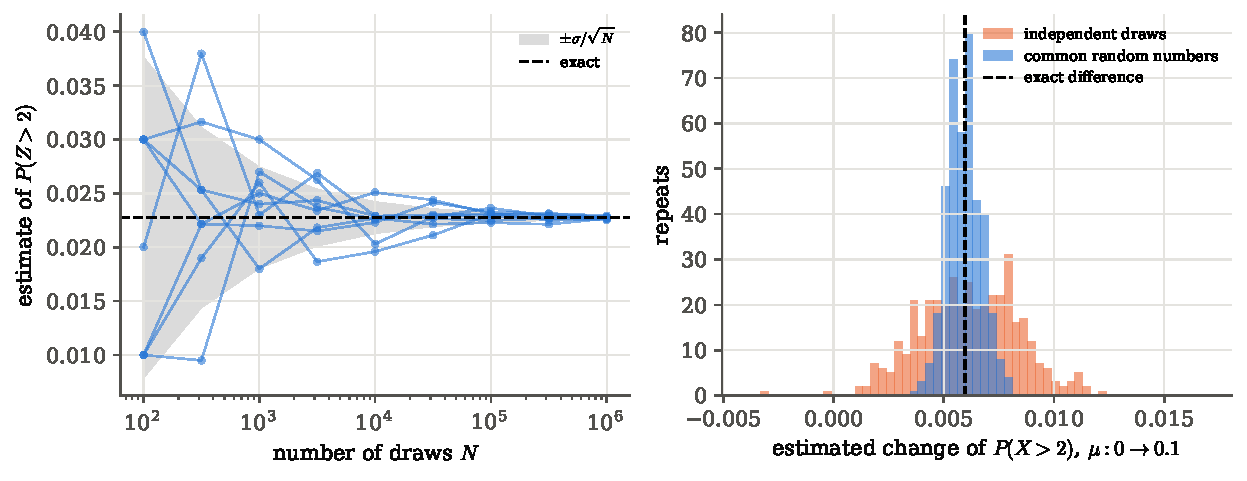
\includegraphics[width=\linewidth]{figures/chT0/08_trust_mc.pdf}
\caption{Monte Carlo noise. Left: estimates of $\Prob(Z>2)$ from eight independent streams (blue lines) against the number of draws; the grey band is the predicted $\pm\sigma/\sqrt N$ around the exact value (dashed). Right: the estimated change of $\Prob(X>2)$ when the mean moves from $0$ to $0.1$, over $400$ repetitions of $10^4$ draws each. Independent draws for the two settings (orange) scatter about three times more widely than common random numbers (blue) around the exact change (dashed).}
\label{T0a:fig:trust-mc}
\end{figure}

\subsection{Convergence: change the resolution until nothing changes}
\label{T0a:sec:trust-conv}

Every computation in the book has a resolution: a grid spacing, a number of points per axis, a HEALPix $N_{\rm side}$, a maximum multipole $\ell_{\max}$, a number of simulations or of chain steps. The answer at finite resolution differs from the answer the resolution is meant to approximate. The test is a \newterm{convergence study}: compute at two or three resolutions, and accept the answer only when it changes by less than its other errors.

\paragraph{Example: the trapezoid rule.} The integral $\int_0^\pi\sin x\,\dd x=2$ computed by the trapezoid rule with $n$ intervals:

\TzoutPart{firstline=26,lastline=28}{results/chT0/08_trust_out.txt}

Each halving of the step divides the error by $\TzTrapRatio$, almost exactly $4$. That number is itself information: an error that falls as $h^2$ is what the trapezoid rule should give (for a smooth function the trapezoid value exceeds the integral by $\frac{(b-a)h^2}{12}\overline{f''}$, with $\overline{f''}$ an average of the second derivative, here $-\sin x<0$, hence the negative errors), so the code behaves as its theory says. An error ratio far from the expected one is the sign of a bug or of a function that is not smooth.

\paragraph{Richardson extrapolation.} Knowing that the error falls as $h^2$ allows it to be removed. Write the result with step $h$ as its limit plus the leading error, and do the same for $h/2$:
\begin{align}
  T(h)&\eqby{1}I+ch^2+O(h^4),
  \qquad
  T(h/2)\eqby{2}I+\tfrac14ch^2+O(h^4),
  \nonumber\\
  \frac{4T(h/2)-T(h)}{3}&\eqby{3}\frac{4I+ch^2-I-ch^2}{3}+O(h^4)=I+O(h^4).
  \label{T0a:eq:richardson}
\end{align}
\begin{explain}
  \item The trapezoid error expanded in powers of the step. For a smooth function only even powers appear.
  \item The same with $h$ replaced by $h/2$: the coefficient $c$ is the same, so the $h^2$ term is a quarter as large.
  \item Four times the second line minus the first: the $h^2$ terms cancel and $3I$ remains; divide by $3$.
\end{explain}
The script prints the result:

\TzoutPart{firstline=29,lastline=29}{results/chT0/08_trust_out.txt}

From the two cheap values at $n=8$ and $16$, whose errors are $\TzTrapErrEight$ and $\TzTrapErrSixteen$, the combination gives an error of $\TzRichErr$: about four hundred times smaller than at $n=16$, for no new function evaluations. The four-point derivative of \cref{10a:sec:numderiv-errors} is the same trick applied to \eqref{T0a:eq:central}.

The book's convergence studies follow this pattern. The brute-force evidence of a four-parameter model in \cref{5c:sec:grid-cost} is computed with $n$ points per axis for seven values of $n$:

\pyfile[firstline=50,lastline=57,firstnumber=50]{code/ch05/27_grid_cost.py}{The same integral at seven resolutions, each timed}

Line 50 lists the resolutions, and the loop of lines 52--57 computes the log Bayes factor at each, timing it with \texttt{time.perf\_counter} (\cref{T0a:sec:cost}). The answer moves from $\FiveCGcLnBsmall$ at $n=\FiveCGcNsmall$ to $\FiveCGcLnBmid$ at $n=\FiveCGcNmid$ and $\FiveCGcLnBmax$ at $n=\FiveCGcNmax$, against the exact $\FiveCGcExact$: only the finest grids have converged. \Cref{8a:sec:res-conv} does the same with the number of simulated skies, watching the estimated bias and error bar settle inside the band $\pm\sigma/\sqrt N$. \emph{The lesson: an answer is converged when doubling the resolution changes it by less than its other errors.}

\subsection{Validation: test the code where the answer is known}
\label{T0a:sec:trust-valid}

The checks so far estimate the size of an error. None of them catches a plain mistake in the code: a sign, a factor of two, a wrong index. Those are caught by one habit, used throughout the book: before a method is trusted on a problem with no known answer, it is run on a problem with one. The Monte Carlo variance of simulated $\Chat$ is compared with the cosmic variance $2\Cell^2/(2\ell+1)$ before simulations are used for masked skies (\cref{7b:sec:mc-var}); the exact binomial interval found by root finding is compared with the closed formula in terms of the beta distribution (\cref{T0a:sec:pit-float}); the healpy round trip of \cref{T0a:sec:blackbox} must return the spectrum that went in; the Fisher forecast is checked against an MCMC run on the same likelihood (\cref{ch:10}).

A comparison can be written into the script as an \texttt{assert}: \texttt{assert condition} does nothing when the condition is true and stops the script with an error when it is false. The tiny-image study of \cref{12c:sec:tiny} enumerates every one of the $2^9=512$ black-and-white $3\times3$ images and checks three facts about each:

\pyfile[firstline=29,lastline=38,firstnumber=29]{code/ch12/c01_tiny.py}{Three identities checked on every one of 512 images}

Line 30 runs through all $512$ patterns of nine bits, line 31 turns each into a $3\times3$ image, and lines 32--33 count its pieces and holes and compute its Euler characteristic with the book's own functions. Line 34 asserts the Euler relation $\chi=\beta_0-\beta_1$; lines 36--37 assert that scikit-image's independent implementation finds the same number of pieces and the same $\chi$. If any of the $1536$ checks failed, the script would stop at that image. These are exact integer comparisons, so \texttt{==} is right here; between real numbers the comparison is made with a tolerance (\cref{T0a:sec:trust-float}).

The census of \cref{T0a:sec:census} counts how often the book writes such checks into its code: $\TzAsserts$ \texttt{assert} statements in $\TzAssertFiles$ files, and $\TzCheckCalls$ calls of \texttt{np.isclose}, \texttt{np.allclose} and similar comparison functions in $\TzCheckFiles$. That is a small number, and it understates the validation, because most of the book's checks are not asserts. They are a figure in which the simulation is drawn over the analytic curve (the black dashed \texttt{theory\_line} of \cref{T0a:sec:plots}), or a pair of numbers saved by the script and quoted side by side in the text. A comparison in a figure or in the text is read by a person, who notices a discrepancy that no one thought to assert. \emph{The lesson: a method is trusted where its answer is unknown only after it has reproduced an answer that is known.}

\begin{inpractice}[Verification first, then research]
The same simulation code plays two roles. Run on an ideal full-sky Gaussian field, it \emph{verifies}: its variance of $\Chat$ must reproduce $2\Cell^2/(2\ell+1)$ within its Monte Carlo error. Run with a mask, a beam and inhomogeneous noise, where no formula exists, it is the \emph{research instrument}: the covariance it produces feeds a likelihood (\cref{ch:08}). Research codes follow this order as a rule, and publish their validation tests next to their results.
\end{inpractice}

\subsection{The decision rule: is a difference real?}
\label{T0a:sec:trust-decide}

Every check above ends with a comparison of two numbers: a simulation and a formula, two resolutions, two methods, two settings. They never agree exactly. When is a difference real, and when is it noise? The rule is the one every physicist uses for measurements. Collect the uncertainty of each number from every source, numerical and Monte Carlo, add the independent ones in quadrature, and divide the difference by the result:
\begin{equation}
  z=\frac{\abs{x_1-x_2}}{\sqrt{\sigma_1^2+\sigma_2^2}},
  \qquad
  \sigma_i^2=\sigma_{i,\rm MC}^2+\sigma_{i,\rm num}^2 .
  \label{T0a:eq:zscore}
\end{equation}
If the two numbers really estimate the same quantity and the errors are roughly Gaussian, $z$ is the absolute value of a standard Gaussian variable: below $1$ two times in three, below $2$ nineteen times in twenty, above $3$ about once in four hundred. So $z\lesssim2$ means ``consistent''; $z$ between $2$ and $3$ means ``look again'', with more draws or another seed; $z\gtrsim3$, in a single planned comparison, means that the difference is real, which may mean a bug. When many comparisons are made at once, a few values of $z$ near $2$ to $3$ are expected by chance alone, exactly the look-elsewhere problem of \cref{4b:sec:lee}.

\paragraph{Example: the Monte Carlo variance at the quadrupole.} \Cref{7b:sec:mc-var} estimates the variance of $\Chat$ from $\SBNsim$ simulated skies and compares it with the cosmic variance $2\Cell^2/(2\ell+1)$. At $\ell=2$ the ratio of the two is $\SBvrTwo$, a $2\%$ excess. Is the formula wrong, or the simulation, or neither? The analytic answer has no numerical error worth mentioning, and the simulated one has the Monte Carlo error derived there, $\SBerrTwo$ in units of the ratio. So
\[
  z=\frac{\SBvrTwo-1}{\SBerrTwo}\approx\TzZcv ,
\]
well inside the range of chance: neither is wrong. Had the excess been $10\%$, $z$ would have been about $7$, and the code would have been searched for the bug.

\paragraph{Example: a change seen with and without common random numbers.} In \cref{T0a:sec:trust-mc}, a single comparison of $\Prob(X>2)$ at $\mu=0$ and $\mu=0.1$ with independent draws measures the true change $\TzCrnTrue$ against a noise of $\TzCrnInd$: $z\approx\TzCrnZind$, a ``look again''. Over the $\TzCrnR$ repeats, $\TzCrnFracIndBelow\%$ of such single comparisons fall short of $3\sigma$, so one of them alone often would not establish that the probability changed at all. With common random numbers the noise is $\TzCrnCrn$ and $z\approx\TzCrnZcrn$, and $\TzCrnFracCrnBelow\%$ fall short: a difference beyond doubt, from the same number of draws.

\begin{keyidea}[When a computed number can be trusted]
A computed number is trusted to the extent that its error budget is known: rounding ($\epsilon$ times the amplification of cancellation or of the condition number), the method (step size, tolerance, resolution, checked by changing them), and Monte Carlo noise ($\sigma/\sqrt N$, checked by changing the seed). A difference is real when it is large compared with the combined budget, $z\gtrsim3$; and a method is trusted on an unknown answer only after it has reproduced a known one.
\end{keyidea}

\Cref{T0a:tab:checklist} collects the checks in the form in which they are needed: a symptom, the check that diagnoses it, the fix, and a place in the book where it is done.

\begin{table}[htbp]
\centering
\small
\renewcommand{\arraystretch}{1.15}
\begin{tabularx}{\linewidth}{@{}>{\raggedright\arraybackslash}p{2.9cm}
                               >{\raggedright\arraybackslash}X
                               >{\raggedright\arraybackslash}p{3.1cm}
                               >{\raggedright\arraybackslash}p{2.1cm}@{}}
\toprule
symptom & check & fix & in the book\\\midrule
\texttt{==} between real numbers fails & print the difference; compare it with $\epsilon$ times the size & \texttt{np.isclose}, or a relative tolerance & \cref{T0a:sec:pit-float,T2a:sec:dm}\\
digits lost in a small difference & count the leading digits that cancel, \eqref{T0a:eq:cancel} & rewrite the formula; subtract the large common part first & \cref{T0a:sec:trust-float,3a:sec:var-python}\\
derivative changes with the step & scan $h$ by factors of ten; look for a plateau & a step on the plateau; four-point rule & \cref{10a:sec:numderiv-camb,9c:sec:emu-build}\\
integral with a tiny claimed error & plot the integrand; tighten the tolerance; change the range & limits and \texttt{points} where the function lives & \cref{6b:sec:self-norm}\\
\texttt{brentq} raises \texttt{ValueError} & evaluate $f$ at both ends & a bracket with a sign change around the wanted root & \cref{4b:sec:ci-intentions}\\
minimiser result looks plausible & \texttt{res.success}, \texttt{res.message}, gradient at \texttt{res.x} & more iterations; restart from \texttt{res.x}; a gradient-based method & \cref{T0a:sec:minimize}\\
solution of $A\bm x=\bm b$ unstable & \texttt{np.linalg.cond(A)}; $\log_{10}\kappa$ digits are lost & \texttt{solve}, not \texttt{inv}; bin or regularise & \cref{8b:sec:invert}\\
\texttt{cholesky} raises \texttt{LinAlgError} & eigenvalues of the matrix; rank against the number of simulations & more simulations; Hartlap factor & \cref{8b:sec:hartlap,8b:sec:nsims}\\
simulated number without an error bar & $\sigma/\sqrt N$ from the same draws; another seed & quote it; increase $N$ & \cref{6b:sec:sqrtN,7b:sec:mc-var}\\
noisy difference of two simulations & scatter of the difference over seeds & common random numbers & \cref{8a:sec:pipeline,12w:sec:mc-fisher}\\
answer depends on grid, $N_{\rm side}$, $\ell_{\max}$ & halve the step or double the size & finer resolution; Richardson extrapolation & \cref{5c:sec:grid-cost,8a:sec:res-conv}\\
a new method on a new problem & run it where the answer is known & find the bug before trusting the result & \cref{7b:sec:mc-var,12c:sec:tiny}\\
two numbers disagree & $z$ of \eqref{T0a:eq:zscore} with all errors & $z\lesssim2$: noise; $z\gtrsim3$: real, or a bug & \cref{7b:sec:mc-var}\\
\bottomrule
\end{tabularx}
\caption{Is the number real? Thirteen symptoms, the check that diagnoses each, the usual fix, and a place in the book where it is done.}
\label{T0a:tab:checklist}
\end{table}
\section{When sixteen digits are not enough: mpmath}
\label{T0a:sec:precision}

A double-precision number carries about sixteen significant digits and spans magnitudes from about $10^{-308}$ to $10^{308}$ (\cref{T0a:sec:trust-float}). For almost everything in the book that is ample. Occasionally it is not, and the failure has a recognisable shape: a probability so small that it underflows to zero, a sum whose terms cancel so completely that no digit of the answer survives, a factorial or a Gamma function so large that it overflows. The library \newterm{mpmath} computes with as many digits as we ask for, and the question is when to reach for it, how many digits to ask for, and what it costs.

\paragraph{The smallest example: the significance of a large excess.} The one-sided $p$-value of a $z\sigma$ excess is the Gaussian tail $\Prob(Z>z)$ (\cref{ch:04}). There are three ways to compute it in SciPy: \texttt{1 - norm.cdf(z)}, \texttt{norm.sf(z)} (the survival function, which computes the tail directly) and \texttt{norm.logsf(z)}, its natural logarithm. The script \pyname{code/chT0/09_mpmath.py} compares all three with mpmath at fifty digits:

\TzoutPart{firstline=1,lastline=8}{results/chT0/09_mpmath_out.txt}

At $5\sigma$, the discovery threshold of particle physics, all three are fine: even the naive \texttt{1 - cdf} is accurate to a relative $\TzNaiveRelFive$. At $8\sigma$ the naive form is already $7\%$ wrong, and from $\TzNaiveZero\sigma$ on it returns exactly $0$. The reason is the spacing of storable numbers just below $1$, which is $\epsilon/2\approx1.1\times10^{-16}$: the cdf is stored as the nearest of these, so a tail much smaller than $10^{-16}$ cannot be represented as ``$1$ minus something'' at all. \texttt{sf} avoids the subtraction and stays accurate down to about $10^{-300}$, but at $\TzSfZero\sigma$ the tail itself, about $10^{-316}$, is below the smallest number with full precision, $\TzTiny$, and the function returns $0$. \texttt{logsf} never forms the tiny number: it computes $\ln\Prob(Z>z)$ directly, a modest negative number, and agrees with mpmath to every printed digit all the way to $40\sigma$, where $\log_{10}\Prob=\TzLogsfForty$ (\cref{T0a:fig:mpmath}, left). The naive choice fails silently at $8\sigma$; the good choice, \texttt{sf} or \texttt{logsf}, costs nothing. \emph{The lesson: rewrite first; reach for more digits only when no rewriting will do, and then mostly to check.}

\begin{figure}[htbp]
\centering
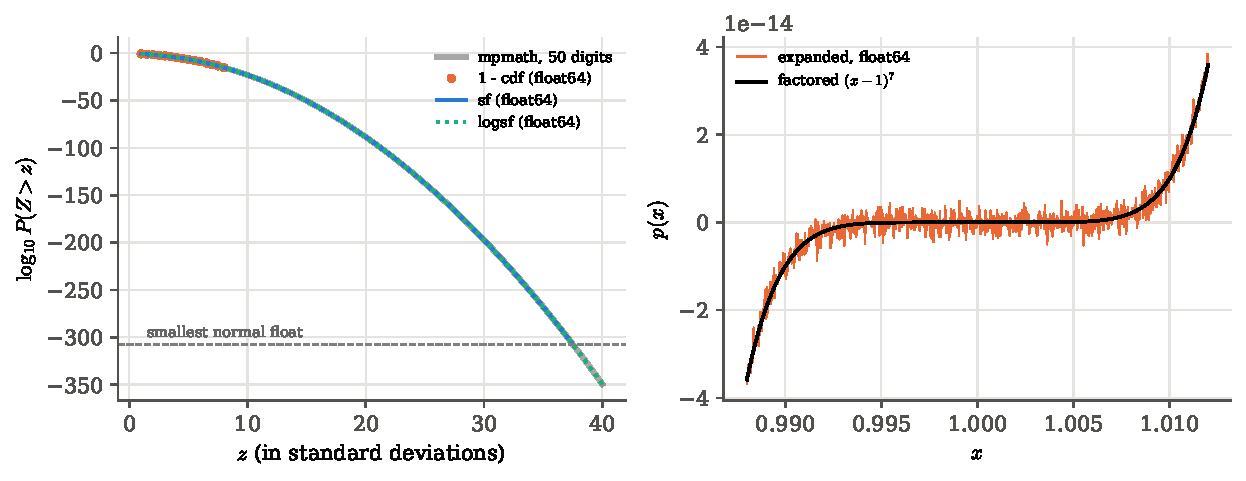
\includegraphics[width=\linewidth]{figures/chT0/09_mpmath.pdf}
\caption{Where double precision breaks. Left: $\log_{10}\Prob(Z>z)$ from mpmath at fifty digits (thick grey) and from three float64 routes. \texttt{1 - cdf} (orange points) stops near $8.5\sigma$, \texttt{sf} (blue) at $38\sigma$, where the tail falls below the smallest normal float (dashed); \texttt{logsf} (dotted) follows mpmath to the end. Right: the polynomial $(x-1)^7$ near its root, evaluated from its expanded coefficients in float64 (orange) and in factored form (black). The expanded form returns rounding noise of size about $10^{-14}$ instead of a smooth curve.}
\label{T0a:fig:mpmath}
\end{figure}

\subsection{Log space first}
\label{T0a:sec:logspace}

Most overflows and underflows in statistics come from products of many factors (likelihoods), from factorials and Gamma functions (binomial and Poisson probabilities, normalising constants), and from exponentials of large numbers (evidences, Boltzmann weights). All of them disappear when the computation is done with logarithms, which turn products into sums and keep every intermediate number of modest size. SciPy supplies the two tools that make this painless.

\paragraph{\texttt{gammaln}.} \texttt{scipy.special.gammaln(x)} returns $\ln\Gamma(x)$ without forming $\Gamma(x)$. Since $n!=\Gamma(n+1)$, $\ln 200!$ is \texttt{gammaln(201)}, which is $\TzLnFact$, while $200!$ itself, about $10^{375}$, overflows (\cref{T0a:sec:special}). A ratio of Gamma functions is the exponential of a difference of \texttt{gammaln}s. The bias factor $c_4(N)=\sqrt{2/(N-1)}\,\Gamma(N/2)/\Gamma\bigl((N-1)/2\bigr)$ of the sample standard deviation (\cref{3a:sec:n-minus-one}) is computed this way:

\pyfile[firstline=68,lastline=68,firstnumber=68]{code/ch03/04_sample_variance.py}{A ratio of Gamma functions as the exponential of a difference of logarithms}

For $N=5$ the direct ratio would be harmless, but $\Gamma(N/2)$ overflows above $N\approx344$, while the line as written works for any $N$: the logarithms stay of order $N\ln N$, and their difference, the logarithm of $c_4$, is close to zero.

\paragraph{\texttt{logsumexp}.} An evidence, a mixture density or a normalisation is a sum of exponentials, $\ln\sum_ie^{a_i}$, and the $a_i$ are log-likelihoods, often in the hundreds or thousands. For $a_1=-1000$ and $a_2=-1001$, \texttt{np.exp} underflows both to $0$ and the logarithm of the sum is $-\infty$. Factoring out the largest term $m=\max_ia_i$ removes the problem:
\begin{align}
  \ln\sum_ie^{a_i}
  &\eqby{1}\ln\Bigl(e^{m}\sum_ie^{a_i-m}\Bigr)
   \eqby{2}m+\ln\sum_ie^{a_i-m} .
  \label{T0a:eq:logsumexp}
\end{align}
\begin{explain}
  \item $e^{a_i}=e^{m}e^{a_i-m}$ for every $i$; take the common factor out of the sum.
  \item The logarithm of a product is the sum of the logarithms, and $\ln e^m=m$.
\end{explain}
Now every exponent $a_i-m$ is at most $0$, the largest term is exactly $1$, nothing overflows, and the terms that underflow are those too small to matter. For the example, $-1000+\ln(1+e^{-1})=-999.687$. \texttt{scipy.special.logsumexp} does exactly this. The posterior probabilities of three competing models in \cref{5c:sec:how-many} are their evidences normalised to sum to one, computed in log space throughout:

\pyfile[firstline=66,lastline=67,firstnumber=66]{code/ch05/25_how_many_bumps.py}{Posterior model probabilities from log-evidences}

Line 66 collects the three log-evidences, for no bump, one bump and two bumps. Line 67 subtracts $\ln\sum_ke^{\ln Z_k}$ from each, which is the logarithm of $Z_k/\sum_jZ_j$, the posterior probability of model $k$ when the three are equally probable a priori. The evidences themselves are never formed. The tail probability above is the same idea in SciPy's distributions: \texttt{logpdf}, \texttt{logcdf} and \texttt{logsf} exist for every distribution, and a likelihood of many data points is built as a sum of \texttt{logpdf} values rather than a product of \texttt{pdf} values, which underflows to zero once there are a few hundred points.

\subsection{Cancellation that cannot be rewritten away}
\label{T0a:sec:mp-cancel}

Sometimes no rewriting is available, because the formula arrives as given. A polynomial from a series expansion or a fit comes as its coefficients, not in factored form. The script takes the polynomial $(x-1)^7$ in its expanded form, $x^7-7x^6+21x^5-35x^4+35x^3-21x^2+7x-1$, evaluates it near $x=1$ by Horner's rule (multiply by $x$, add the next coefficient, repeat), and compares with the factored form:

\TzoutPart{firstline=9,lastline=10}{results/chT0/09_mpmath_out.txt}

At $x=1.01$ the exact value is $10^{-14}$; float64 returns $\TzPolyFloat$, wrong by $20\%$. \Cref{T0a:fig:mpmath} (right) shows the expanded form near the root: not a curve but a band of rounding noise. mpmath with fifteen digits reproduces the float64 answer digit for digit, because it is making the same rounding errors with the same number of digits; with thirty digits it returns $\TzPolyMpThirty$.

\paragraph{How many digits survive?} The question is the one answered for a single subtraction by \eqref{T0a:eq:cancel}, now for a sum of many terms. Suppose each term $t_k$ of a sum $p=\sum_kt_k$ is computed with relative error at most $u$, the working precision: $u\approx\epsilon/2$ in float64, and $u\approx10^{-d}$ when mpmath carries $d$ decimal digits. Then
\begin{align}
  \frac{\abs{\hat p-p}}{\abs p}
  &\eqby{1}\frac{\abs{\sum_kt_k\delta_k}}{\abs{\sum_kt_k}}
   \relby{2}{\le}u\,\frac{\sum_k\abs{t_k}}{\abs{\sum_kt_k}}
   \equiv u\,\kappa ,
  \nonumber\\
  \text{digits trusted}
  &\eqby{3}-\log_{10}(u\kappa)\approx d-\log_{10}\kappa .
  \label{T0a:eq:digits}
\end{align}
\begin{explain}
  \item Each computed term is $t_k(1+\delta_k)$, so the error of the sum is $\sum_kt_k\delta_k$.
  \item The triangle inequality and $\abs{\delta_k}\le u$.
  \item A relative error $10^{-j}$ means $j$ correct digits; with $u=10^{-d}$, $-\log_{10}u=d$.
\end{explain}
The \newterm{condition number} of the sum, $\kappa=\sum_k\abs{t_k}/\abs{\sum_kt_k}$, is the ratio of the size of the terms to the size of the result. For two terms, $a$ and $-b$, it is $(\abs a+\abs b)/\abs{a-b}$, the amplification factor of \eqref{T0a:eq:cancel}; for a linear system it is the $\kappa(A)$ of \eqref{T0a:eq:cond}. The rule reads the same each time: \emph{working digits minus $\log_{10}\kappa$}. (Rounding inside Horner's rule adds a factor of order the number of terms, a fraction of a digit to one digit; the rule is a guide, not a guarantee.)

For the expanded polynomial the terms are the binomial coefficients times powers of $x$, so $\sum_k\abs{t_k}=(x+1)^7$ by the binomial theorem, and
\[
  \kappa=\frac{(x+1)^7}{\abs{x-1}^7}=\Bigl(\frac{2.01}{0.01}\Bigr)^7\approx1.3\times10^{16}
  \quad\text{at }x=1.01,
\]
which the script confirms, $\kappa=\TzPolyKappa$ ($\log_{10}\kappa=\TzPolyLogKappa$). With $d\approx16$ working digits, \eqref{T0a:eq:digits} predicts that \emph{no} digit survives, and indeed none of the float64 answer is right. To keep ten digits we need $d\approx\TzPolyLogKappa+10\approx26$; asking for thirty leaves a margin.

\paragraph{The practical test: $d$ against $2d$.} The condition number is rarely known in advance. The practical rule is to compute the same quantity twice, at $d$ and at $2d$ digits, and keep the digits on which the two agree. Why does this work? The error of the $2d$ result is about $10^{-d}$ times smaller than that of the $d$ result, so the difference between the two is, to a good approximation, the error of the $d$ result itself:

\pyfile[firstline=77,lastline=88,firstnumber=77]{code/chT0/09_mpmath.py}{The same sum at $d$ and at $2d$ digits, and the number of digits on which they agree}

Line 80 sets the working precision to \texttt{dps} decimal digits, and line 81 evaluates the polynomial at $1.01$; line 82 doubles the precision and line 83 evaluates again. The input is given as the string \texttt{"1.01"}, so mpmath reads the decimal number exactly to the working precision; \texttt{mp.mpf(1.01)} would inherit the binary rounding of the float $1.01$. Line 85 converts the relative difference into a number of agreeing digits. The result:

\TzoutPart{firstline=11,lastline=15}{results/chT0/09_mpmath_out.txt}

At $d=10$ and $d=15$ the two results disagree completely: no digit of the $d$-digit answer can be trusted, as \eqref{T0a:eq:digits} predicted for $d<16$. At $d=20$ they agree on $\TzAgreeTwenty$ digits, and at $d=30$ on $\TzAgreeThirty$; the rule, $d-16$, predicted four and fourteen, so it is conservative, because it assumes that all rounding errors line up. \emph{The lesson: the digits that survive a doubling of the precision are the digits to keep.}

\begin{figure}[htbp]
\centering
\begin{tikzpicture}[x=0.17cm,y=0.62cm]
  \foreach \row/\d/\lab in {0/16/{float64, $d\approx16$},1/30/{mpmath, $d=30$},2/50/{mpmath, $d=50$}} {
    \fill[formblue!25] (0,-\row) rectangle (\d,-\row+0.7);
    \fill[bdryred!35] (0,-\row) rectangle ({min(16,\d)},-\row+0.7);
    \draw[black!60] (0,-\row) rectangle (\d,-\row+0.7);
    \node[font=\footnotesize,anchor=east] at (-0.3,-\row+0.35) {\lab};
  }
  \draw[black!50,dashed] (16,0.95) -- (16,-2.2);
  \node[font=\scriptsize,anchor=south,bdryred!80!black] at (8,0.75) {lost: $\log_{10}\kappa\approx16$};
  \node[font=\scriptsize,formblue!70!black] at (23,-1+0.35) {14 kept};
  \node[font=\scriptsize,formblue!70!black] at (33,-2+0.35) {34 kept};
  \node[font=\scriptsize,anchor=north] at (0,-2.15) {$0$};
  \node[font=\scriptsize,anchor=north] at (16,-2.15) {$16$};
  \node[font=\scriptsize,anchor=north] at (30,-2.15) {$30$};
  \node[font=\scriptsize,anchor=north] at (50,-2.15) {$50$ digits};
\end{tikzpicture}
\caption{The digit budget of the expanded polynomial at $x=1.01$. Each bar is the working precision; cancellation consumes the first $\log_{10}\kappa\approx16$ digits (red), whatever the precision, and only the rest (blue) can be trusted. In float64 nothing is left. The kept digits are the guaranteed minimum of \eqref{T0a:eq:digits}; the $d$-against-$2d$ test usually finds a few more.}
\label{T0a:fig:digits}
\end{figure}

\subsection{What it costs, and when to use it}
\label{T0a:sec:mp-cost}

An mpmath number is a Python object, and every operation on it runs Python code rather than a single machine instruction; nor does mpmath work on whole arrays. The script times one exponential each way:

\TzoutPart{firstline=16,lastline=16}{results/chT0/09_mpmath_out.txt}

NumPy, working on a whole array at once, needs $\TzTnp$\,ns per exponential; Python's \texttt{math.exp}, one number at a time, $\TzTmath$\,ns; mpmath, at the same fifteen digits, $\TzTmpFifteen$\,ns, about $\TzMpOverNp$ times slower than NumPy, and slower again at fifty digits. A Monte Carlo study of $10^8$ draws that takes a second in NumPy would take more than a day in mpmath. So mpmath is a tool for checking, not for running.

It is the right tool in four situations, in order of how often they arise.
\begin{enumerate}[leftmargin=2em,itemsep=1pt]
  \item \emph{As a reference.} A float64 routine whose accuracy is in doubt is compared, at a few points, with the same formula in mpmath at thirty or fifty digits: if the two agree to the digits that matter, the float64 routine is trusted everywhere it is fast. This is how \cref{T0a:fig:mpmath} judges SciPy's tail functions.
  \item \emph{Extreme tails}, beyond about $38\sigma$, where even \texttt{sf} underflows. In practice \texttt{logsf} already covers this, and mpmath is needed only for the tail of a distribution that has no log-survival function.
  \item \emph{Cancellation that no rewriting removes}, as in the expanded polynomial, with $d$ chosen by \eqref{T0a:eq:digits} and checked by the $d$-against-$2d$ test.
  \item \emph{Huge or tiny intermediate numbers that log space cannot handle}, such as a sum of terms of alternating sign each larger than $10^{308}$ (logarithms cannot represent the signs that make such a sum cancel).
\end{enumerate}
No script of the book needs mpmath for its results; the census of \cref{T0a:sec:census} finds it only here. Every case the book meets is handled by a rewrite or by log space, and those are what to try first.
\providecommand{\TzBruteLinMin}{\pgfmathparse{62.5*\TzBruteSixteenK/60}\pgfmathprintnumber[fixed,precision=0]{\pgfmathresult}}
\providecommand{\TzBruteQuadH}{\pgfmathparse{(62.5/60)*(62.5/60)*\TzBruteSixteenK}\pgfmathprintnumber[fixed,precision=0]{\pgfmathresult}}
\providecommand{\TzCholRatio}{\pgfmathparse{\TzCholMeas/\EightACholSix}\pgfmathprintnumber[fixed,precision=1]{\pgfmathresult}}
\providecommand{\TzDaysRatio}{\pgfmathparse{\TzCholNsideDaysThree/\EightALikeDaysTwoFiveSix}\pgfmathprintnumber[fixed,precision=1]{\pgfmathresult}}
\providecommand{\TzMcMinutes}{\pgfmathparse{3000*\TzShtTwoFiveSix/60}\pgfmathprintnumber[fixed,precision=0]{\pgfmathresult}}

\section{How long will it run? Counting operations}
\label{T0a:sec:cost}

Before a long computation is started, two questions deserve an answer: how long will it take, and will it fit in memory? A script that finishes in a second for a test case may need a day, or a terabyte, for the real one, and it is far better to know that before pressing the key than after a night of waiting.

\paragraph{The smallest example: counting close pairs.} The galaxy correlation function of \cref{13c:sec:paircounts} needs the number of pairs of points closer than some distance $r$. The obvious program compares every point with every other. The script \pyname{code/chT0/10_cost.py} times that brute-force count for $N$ random points in a cube: for $N=16\,000$ it takes $\TzBruteSixteenK$\,s. How long for a catalogue of a million galaxies? The naive extrapolation scales the time with the number of points: $10^6/16\,000=62.5$ times longer, about $\TzBruteLinMin$ minutes. That is wrong, because the work is not proportional to the number of points but to the number of \emph{pairs}, $N(N-1)/2\approx N^2/2$. Sixty-two and a half times more points means $62.5^2\approx3900$ times more pairs, and the honest estimate is about $\TzBruteQuadH$ hours; the script's fit to its measured times gives $\TzBruteMillionH$ hours. The good choice is to count first: how does the work grow with $N$? Its price is a minute of thought, and the same thought shows the way out. A $k$-d tree (\cref{13c:sec:tree}) groups the points into boxes and counts whole boxes of pairs at once, and it counts $256\,000$ points in $\TzTreeBig$\,s. \emph{The lesson: how the cost grows with the size matters far more than how fast the computer is.}

\subsection{Counting how the work grows}
\label{T0a:sec:bigO}

The cost of a computation, its run time or the number of arithmetic operations, depends on the size $N$ of the problem: the number of data points, pixels, grid points, simulations. For large $N$ it is usually close to a power law, $T(N)\approx cN^p$, possibly with a logarithm. The exponent $p$ comes from the structure of the algorithm and can be found by counting; the constant $c$ depends on the computer and the implementation and is found by timing. One writes $T(N)=O(N^p)$, read ``of order $N^p$'', to say that the cost grows no faster than a constant times $N^p$. Only the fastest-growing term is kept, and constant factors are dropped: $3N^2+100N$ is $O(N^2)$, because for large $N$ the first term dominates, whatever the constants.

The exponent answers the most useful practical question directly: \emph{if the problem gets ten times bigger, how much longer does it take?} For $O(N)$, ten times; for $O(N^2)$, a hundred times; for $O(N^3)$, a thousand times. The book's heavy computations fall into a handful of classes, each found by a count that fits in a line or two.

\paragraph{$O(N)$: anything done once per element.} Adding two vectors, evaluating a density on a grid, summing a $\chi^2$, drawing $N$ random numbers: one operation, or a fixed few, per element. Every vectorised NumPy expression of \cref{T0a:sec:vectorise} is of this kind.

\paragraph{$O(N\log N)$: halving, again and again.} The fast Fourier transform (\cref{T0a:sec:fft}) splits a transform of length $N$ into two transforms of length $N/2$, one for the even-numbered and one for the odd-numbered points, and combines them with about $cN$ further operations. How many operations does that make in all? Apply the split repeatedly:
\begin{align}
  T(N)
  &\eqby{1}2\,T(N/2)+cN
   \eqby{2}4\,T(N/4)+2cN
   \eqby{3}2^k\,T(N/2^k)+k\,cN
   \eqby{4}N\,T(1)+cN\log_2N .
  \label{T0a:eq:fft-cost}
\end{align}
\begin{explain}
  \item One split: two half-size transforms plus the combination.
  \item Split each half again: $2[2T(N/4)+cN/2]+cN$.
  \item After $k$ splits there are $2^k$ transforms of length $N/2^k$, and each level of splitting has added $cN$.
  \item The splitting stops at length one, after $k=\log_2N$ levels.
\end{explain}
A direct sum would need $N^2$ operations (every output frequency from every input point). For $N=10^6$ the difference between $N^2$ and $N\log_2N\approx2\times10^7$ is a factor of fifty thousand. Sorting a list (\texttt{np.sort}, used for quantiles and empirical distribution functions) is $O(N\log N)$ for the same reason.

\paragraph{$O(N^2)$: all pairs.} $N$ points have $N(N-1)/2$ pairs, so anything that visits every pair, such as the brute-force pair count, the pairwise-distance matrix of the correlated field in \cref{6b:sec:cholesky}, or the Vietoris--Rips complex of \cref{ch:12}, is $O(N^2)$ in time, and $O(N^2)$ in memory if the pairs are stored. Trees and grids bring pair counting down by never visiting pairs that are obviously too far apart or that can be counted as a block.

\paragraph{$O(N^3)$: dense linear algebra.} Solving $A\bm x=\bm b$, the Cholesky factor, the determinant, the inverse and the eigenvalues of an $N\times N$ matrix all cost $O(N^3)$. For the Cholesky factor the count is short. Column $k$ of $L$ is found from the entries to its left, after which every entry of the remaining $(N-k)\times(N-k)$ block below and to the right is updated once, with one multiplication and one addition; the block is symmetric, so only the entries on and below its diagonal are computed:
\begin{align}
  \text{operations}
  &\eqby{1}\sum_{k=1}^{N}2\cdot\frac{(N-k)(N-k+1)}{2}
   \eqby{2}\sum_{j=0}^{N-1}\bigl(j^2+j\bigr)
   \eqby{3}\frac{(N-1)N(2N-1)}{6}+\frac{(N-1)N}{2}
   \approx\frac{N^3}{3}.
  \label{T0a:eq:chol-cost}
\end{align}
\begin{explain}
  \item An $m\times m$ symmetric block has $m(m+1)/2$ entries on and below its diagonal, with $m=N-k$; each costs two operations.
  \item Rename $j=N-k$, which runs from $N-1$ down to $0$.
  \item The sum of the first $n$ squares is $n(n+1)(2n+1)/6$ and of the first $n$ integers $n(n+1)/2$, with $n=N-1$; for large $N$ only the $N^3/3$ of the first term matters.
\end{explain}
Every covariance matrix, every Gaussian likelihood in pixel space and every Fisher matrix of many parameters lives in this class.

\paragraph{$O(\ell_{\max}^3)$: spherical-harmonic transforms.} A HEALPix map at resolution $N_{\rm side}$ has $N_{\rm pix}=12N_{\rm side}^2$ pixels on about $4N_{\rm side}$ rings of constant latitude, and is analysed up to $\ell_{\max}\approx3N_{\rm side}$. On each ring an FFT separates the azimuthal modes $m$, which is cheap; then for every ring and every $m$ the transform sums over all $\ell\ge m$:
\[
  \underbrace{4N_{\rm side}}_{\text{rings}}\times\underbrace{\ell_{\max}}_{m}\times\underbrace{\ell_{\max}}_{\ell}
  \sim N_{\rm side}^3\sim N_{\rm pix}^{3/2}.
\]
Doubling $N_{\rm side}$ makes \texttt{map2alm} and \texttt{alm2map} eight times slower \cite{Gorski2005}.

\paragraph{Simulations and chains.} A Monte Carlo study costs the number of simulations times the cost of one; an MCMC run costs the number of steps times the cost of one likelihood evaluation. These multiply. A chain of $10^5$ steps with a Boltzmann code that takes a second per call takes more than a day; with the emulator of \cref{9c:sec:emu}, which evaluates in microseconds, it takes seconds. That is the whole reason the emulator exists.

\begin{figure}[htbp]
\centering
\begin{tikzpicture}
\begin{axis}[width=8.0cm,height=6.2cm,xmode=log,ymode=log,
  xmin=1e2,xmax=1e7,ymin=1e-6,ymax=1e8,
  xlabel={size $N$},ylabel={time (s), at $10^{-9}$\,s per operation},
  tick label style={font=\scriptsize},label style={font=\small},
  legend style={font=\scriptsize,at={(1.03,0.5)},anchor=west,draw=black!30},
  legend cell align=left]
  \addplot[thick,formblue,domain=1e2:1e7,samples=40] {1e-9*x};
  \addlegendentry{$N$: vectors}
  \addplot[thick,tangentgreen,domain=1e2:1e7,samples=40] {1e-9*x*ln(x)/ln(2)};
  \addlegendentry{$N\log_2N$: FFT, sorting}
  \addplot[thick,fibreorange,domain=1e2:1e7,samples=40] {1e-9*x^2/2};
  \addlegendentry{$N^2/2$: all pairs}
  \addplot[thick,bdryred,domain=1e2:1e7,samples=40] {1e-9*x^3/3};
  \addlegendentry{$N^3/3$: Cholesky}
  \addplot[black!50,dashed,domain=1e2:1e7] {600};
  \addplot[black!50,dotted,domain=1e2:1e7] {86400};
  \node[font=\scriptsize,black!60,anchor=south west] at (axis cs:1.2e2,600) {10 minutes};
  \node[font=\scriptsize,black!60,anchor=south west] at (axis cs:1.2e2,86400) {one day};
\end{axis}
\end{tikzpicture}
\caption{How the four commonest costs grow, at an illustrative $10^{-9}$\,s per operation. At $N=10^4$ all four are affordable; at $N=10^6$ an $N^2$ computation takes about ten minutes and an $N^3$ one about ten years. The horizontal lines mark the ten-minute budget of a laptop script and one day.}
\label{T0a:fig:growth}
\end{figure}

\paragraph{Memory.} Time is not the only limit. A \texttt{float64} occupies $8$ bytes, so an array of $N$ numbers takes $8N$ bytes and an $N\times N$ matrix $8N^2$. A covariance matrix of $10^4$ bins takes $800$\,MB; one of $4\times10^4$ bins, $12.8$\,GB, more than a laptop can spare. The pixel covariance of a map at $N_{\rm side}=256$, with $786\,432$ pixels, would take $8\times786\,432^2\approx4.9\times10^{12}$ bytes, almost five terabytes. Memory can also be estimated before running: count the largest arrays, multiply by eight bytes per element, and remember that NumPy expressions create temporary arrays of the same size as their inputs.

\subsection{Estimating a run time: time small, fit, extrapolate}
\label{T0a:sec:timing}

Counting gives the exponent; timing gives the constant. The recipe has four steps: time the computation at a few small sizes; fit a straight line to $\log T$ against $\log N$, whose slope is the measured exponent; extrapolate the line to the size wanted; and multiply by a safety factor. The script does the first two steps with two small functions:

\pyfile[firstline=36,lastline=49,firstnumber=36]{code/chT0/10_cost.py}{Timing: the best of a few runs, and the slope on log-log axes}

\texttt{time.perf\_counter()} (lines 40 and 42) reads a clock with sub-microsecond resolution, and the difference of two readings is the time spent in between. \texttt{best\_time} runs the computation three times and keeps the shortest time (line 43), the run least disturbed by whatever else the computer was doing. \texttt{slope} fits a straight line to the logarithms with \texttt{np.polyfit} (line 48); for $T=cN^p$, $\log T=\log c+p\log N$, so the slope is $p$. Only the largest sizes are used (\texttt{last=4}), because at small sizes fixed overheads, such as the call itself, distort the power law. The census finds such timing in $\TzPctTime\%$ of the scripts, with $\TzPerfCounter$ calls of \texttt{time.perf\_counter} and $\TzTimeTime$ of the coarser \texttt{time.time}.

The script times four representative operations on a single processor core: the FFT, the Cholesky factor, pair counting by brute force and with a tree, and \texttt{healpy.map2alm}. For two of them it then measures a size beyond the fitted range, to see whether the prediction holds. \Cref{T0a:fig:cost} shows the result, and the printed summary is:

\Tzout{results/chT0/10_cost_out.txt}

\begin{figure}[htbp]
\centering
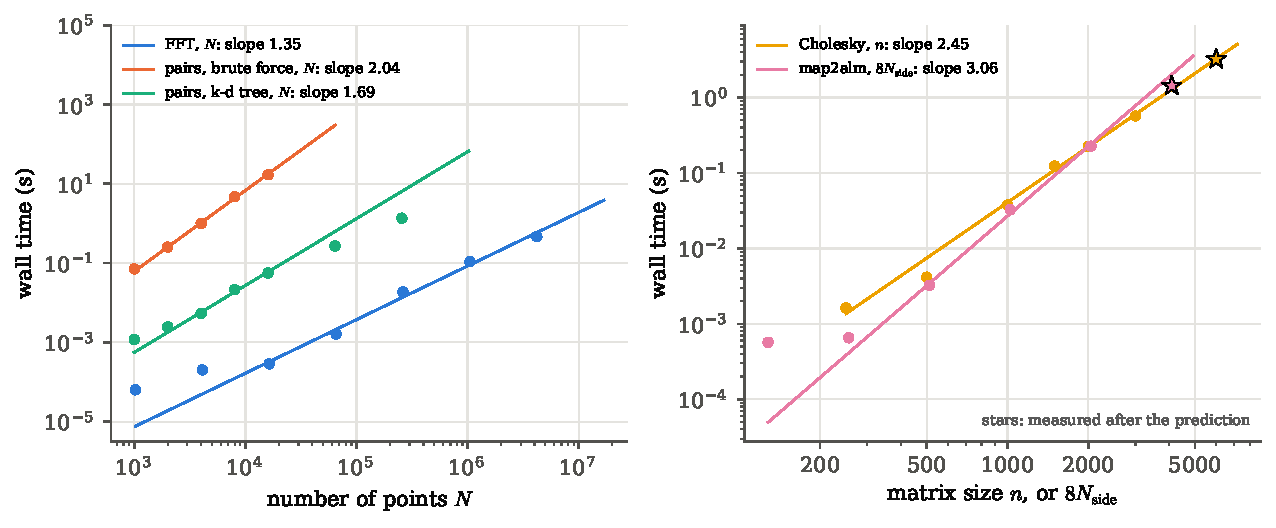
\includegraphics[width=\linewidth]{figures/chT0/10_cost.pdf}
\caption{Measured run times on one core (points) and power-law fits (lines), with the fitted exponents in the legends. Left: FFT, brute-force pair counting and $k$-d-tree pair counting against the number of points. Right: the Cholesky factor of an $n\times n$ matrix, and \texttt{map2alm} against $8N_{\rm side}$ (a rescaling that puts both on one axis). Stars: sizes beyond the fitted range, measured after the prediction was made.}
\label{T0a:fig:cost}
\end{figure}

What do the measured exponents say? Brute-force pair counting has slope $\TzSlopeBrute$, the counted $2$. \texttt{map2alm} has slope $\TzSlopeSht$ in $N_{\rm side}$, the counted $3$, and its prediction for $N_{\rm side}=512$, $\TzShtPred$\,s, compares with a measured $\TzShtMeas$\,s. The Cholesky fit predicts $\TzCholPred$\,s for $n=\TzCholBigN$ and the measurement is $\TzCholMeas$\,s. These are successes. Two exponents differ from the count, and both differences teach something. The FFT's slope is $\TzSlopeFft$, steeper than the $\TzFftNlogN$ that $N\log N$ alone would give over the same range: at the largest sizes the arrays no longer fit in the processor's fast cache memory, and every operation waits longer for its data. The Cholesky slope, $\TzSlopeChol$, is shallower than the counted $3$: for small matrices the fixed overheads are a large part of the time, and the optimised linear-algebra library also runs more efficiently on larger blocks, so the time grows more slowly than the operation count until the matrix is large. A fitted slope describes the range it was fitted on, and nothing guarantees it beyond.

\paragraph{Example: recalling the likelihood that cannot be evaluated.} \Cref{8a:sec:why-not-ml} asked how long one evaluation of the exact Gaussian likelihood of a CMB map would take. It needs the Cholesky factor of the $N_{\rm pix}\times N_{\rm pix}$ pixel covariance, and its script times that factor up to $n=6000$:

\pyfile[firstline=29,lastline=36,firstnumber=29]{code/ch08/03_cost_scaling.py}{The cost study of \cref{8a:sec:why-not-ml}: time at the largest size, exponent fixed by counting}

Lines 30--35 time the Cholesky factor of random positive-definite matrices, with the same best-of-three function as above. Line 36 is the instructive one: rather than fitting a slope, it fixes the exponent at the counted $3$ and uses only the largest, most nearly asymptotic, measurement to set the constant. From $\EightACholSix$\,s at $n=6000$ it predicted about $\EightALikeDaysTwoFiveSix$ days for the $786\,432$ pixels of $N_{\rm side}=256$, and $\EightAMemTwoFiveSix$\,TB of memory. The script of this section, on a single core, measured $\TzCholMeas$\,s at $n=6000$, about $\TzCholRatio$ times longer, because the earlier study let the linear-algebra library use up to four cores. With the counted exponent it predicts $\TzCholNsideDaysThree$ days, about $\TzDaysRatio$ times longer for the same reason: the two studies agree on the exponent and differ only in the constant. With its own fitted slope of $\TzSlopeChol$, however, it would predict only $\TzCholNsideDays$ days, an underestimate by more than a factor of ten, because a slope fitted where overheads still matter is extrapolated far beyond the range in which it was measured. When the asymptotic exponent is known by counting, use it, and take the constant from the largest size measured. Either way the conclusion of \cref{8a:sec:why-not-ml} stands: the exact pixel likelihood is out of reach, while a spherical-harmonic transform of the same map takes a fraction of a second.

\paragraph{Example: a Monte Carlo before it is run.} Suppose a study needs $1000$ simulated skies at $N_{\rm side}=256$, each analysed with three \texttt{map2alm} calls (temperature and two noise halves, say). One call took $\TzShtTwoFiveSix$\,s on one core, so the whole study needs about $3000\times\TzShtTwoFiveSix$\,s $\approx\TzMcMinutes$ minutes of transforms. That is within a laptop's budget on a few cores; at $N_{\rm side}=512$ it would be eight times longer, and at $N_{\rm side}=2048$, the resolution of the Planck maps, $512$ times longer, which is why the book's simulations stay at $N_{\rm side}\le512$ and say what the full-resolution version would cost. The grid evidence of \cref{5c:sec:grid-cost} is the same kind of estimate in a more dramatic form: an $n^4$ grid that takes $\FiveCGcTmax$\,s at $n=\FiveCGcNmax$ would take $\FiveCGcSixD$ years in six dimensions with a thousand points per axis.

\paragraph{The safety factor.} Extrapolation is uncertain in both directions: the exponent may change beyond the fitted range (the FFT and the Cholesky factor above), and a large run shares the computer with other work. A factor of two to three on the predicted time is prudent, and a prediction that is still uncomfortable after it is a prediction that the computation should not be run as planned. It should be made cheaper (a tree, an FFT, a coarser grid, an emulator), split over cores (\cref{T0a:sec:pool}), or sent to a bigger machine.

\begin{keyidea}[Estimate before you run]
Count how the work and the memory grow with the size of the problem; time the computation at a few small sizes; extrapolate with the counted exponent, the time measured at the largest size, and a safety factor of two or three. Anything that the estimate puts beyond about ten minutes or a few gigabytes is redesigned or moved to a bigger computer before it is started.
\end{keyidea}
\section{The whole toolkit on one page}
\label{T0a:sec:cheat}

\Cref{T0a:tab:cheat} is the toolkit in the order a script uses it: each concept, the smallest piece of syntax that does it, the subsection that explains it, and a place in the book where it does real work. The syntax column is meant to be read as a reminder of something already understood, not learned from.

\begin{table}[p]
\centering
\footnotesize
\renewcommand{\arraystretch}{1.12}
\begin{tabularx}{\linewidth}{@{}>{\raggedright\arraybackslash}p{2.75cm}
                               >{\raggedright\arraybackslash}X
                               >{\raggedright\arraybackslash}p{1.25cm}
                               >{\raggedright\arraybackslash}p{1.9cm}@{}}
\toprule
concept & syntax & here & at work in\\\midrule
\multicolumn{4}{@{}l}{\textbf{A script and plain Python}}\\
run a script & \texttt{python3 code/ch02/02\_binomial.py} & \S\ref{T0a:sec:anatomy} & \S\ref{2a:sec:binomial}\\
docstring, helpers & \texttt{"""Question: \dots"""}; \texttt{setup()}, \texttt{save\_numbers(\dots)} & \S\ref{T0a:sec:anatomy} & \S\ref{0a:sec:code}\\
f-string & \texttt{f"\{x:.3f\} \{n:,\} \{p:.2e\}"} & \S\ref{T0a:sec:strings} & \S\ref{1a:sec:events}\\
list, tuple & \texttt{xs = []}; \texttt{xs.append(v)}; \texttt{a, b = f(x)} & \S\ref{T0a:sec:containers} & \S\ref{3b:sec:newton}\\
dictionary & \texttt{d = \{"mean": m\}}; \texttt{for k, v in d.items():} & \S\ref{T0a:sec:containers} & \S\ref{3a:sec:sampling-python}\\
loops, conditions & \texttt{for i, v in enumerate(xs):}; \texttt{if \dots: elif \dots: else:} & \S\ref{T0a:sec:control} & \S\ref{1a:sec:events}\\
comprehension & \texttt{[f(v) for v in xs if v > 0]} & \S\ref{T0a:sec:control} & \S\ref{1b:sec:marginal}\\
function & \texttt{def f(x, n=10): return a, b}; \texttt{f(x, n=20)} & \S\ref{T0a:sec:functions} & \S\ref{3b:sec:invariance}\\
lambda & \texttt{lambda t: -loglike(t, data)} & \S\ref{T0a:sec:functions} & \S\ref{3b:sec:invariance}\\
import & \texttt{import numpy as np}; \texttt{from scipy import stats} & \S\ref{T0a:sec:imports} & every script\\
\midrule
\multicolumn{4}{@{}l}{\textbf{NumPy}}\\
array, shape, type & \texttt{x = np.array([1.0, 2.0])}; \texttt{x.shape}, \texttt{x.dtype} & \S\ref{T0a:sec:arrays} & \S\ref{1a:sec:events}\\
grids of numbers & \texttt{np.linspace(a, b, n)}; \texttt{np.logspace(p, q, n)} & \S\ref{T0a:sec:arrays} & \S\ref{1b:sec:pdf}\\
index, slice & \texttt{x[0]}, \texttt{x[-1]}, \texttt{x[a:b]}, \texttt{X[:, 0]}, \texttt{x[::-1]} & \S\ref{T0a:sec:indexing} & \S\ref{3a:sec:sampling-python}\\
mask & \texttt{x[(x > 0) \& (x < 1)]}; \texttt{np.mean(x > 2)} & \S\ref{T0a:sec:masks} & \S\ref{1a:sec:events}\\
broadcasting & \texttt{r[:, None] - r[None, :]}; \texttt{keepdims=True} & \S\ref{T0a:sec:broadcasting} & \S\ref{6b:sec:cholesky}\\
reduction & \texttt{X.mean(axis=1)}, \texttt{X.std(axis=0, ddof=1)} & \S\ref{T0a:sec:axis} & \S\ref{3a:sec:clt-python}\\
grids in $d$ dimensions & \texttt{np.meshgrid(x, y, indexing="ij")} & \S\ref{T0a:sec:grids} & \S\ref{7a:sec:phases}\\
random numbers & \texttt{rng = rng\_for("ch06", "name")}; \texttt{rng.standard\_normal(n)} & \S\ref{T0a:sec:random} & \S\ref{0a:sec:code}\\
linear algebra & \texttt{A @ x}; \texttt{np.linalg.solve(C, d)}; \texttt{cholesky}; \texttt{eigh} & \S\ref{T0a:sec:linalg} & \S\ref{6b:sec:cholesky}\\
Fourier transform & \texttt{np.fft.rfft(x)}; \texttt{np.fft.rfftfreq(n, dt)} & \S\ref{T0a:sec:fft} & \S\ref{9c:sec:pipeline}\\
\midrule
\multicolumn{4}{@{}l}{\textbf{SciPy, Matplotlib, files}}\\
distributions & \texttt{stats.norm.pdf}, \texttt{.cdf}, \texttt{.sf}, \texttt{.ppf}, \texttt{.logsf}, \texttt{.rvs} & \S\ref{T0a:sec:stats} & \S\ref{4a:sec:p-to-z}\\
integral & \texttt{val, err = integrate.quad(f, a, b)} & \S\ref{T0a:sec:quad} & \S\ref{1b:sec:marginal}\\
root & \texttt{optimize.brentq(f, a, b)} & \S\ref{T0a:sec:roots} & \S\ref{4b:sec:ci-intentions}\\
minimum & \texttt{res = optimize.minimize(f, x0)}; \texttt{res.x}, \texttt{res.success} & \S\ref{T0a:sec:minimize} & \S\ref{3b:sec:poisson-python}\\
log space & \texttt{special.gammaln(n + 1)}; \texttt{special.logsumexp(a)} & \S\ref{T0a:sec:logspace} & \S\ref{5c:sec:how-many}\\
figure & \texttt{fig, ax = plt.subplots()}; \texttt{ax.plot(x, y)}; \texttt{savefig(\dots)} & \S\ref{T0a:sec:matplotlib} & \S\ref{2a:sec:binomial}\\
files, cache & \texttt{np.savez(path, a=a)}; \texttt{np.load(path)}; \texttt{Path(\dots).exists()} & \S\ref{T0a:sec:files} & \S\ref{7b:sec:camb}\\
\midrule
\multicolumn{4}{@{}l}{\textbf{Seen a few times}}\\
data class & \texttt{@dataclass class Experiment: nside: int = 256} & \S\ref{T0a:sec:classes} & \S\ref{8a:sec:beam}\\
catching an error & \texttt{try: \dots{} except np.linalg.LinAlgError: \dots} & \S\ref{T0a:sec:try-with} & \S\ref{11c:sec:hubble-compare}\\
several cores & \texttt{with Pool(4) as pool: out = pool.map(f, jobs)} & \S\ref{T0a:sec:pool} & \S\ref{12c:sec:model}\\
compiled loop & \texttt{@njit} above a plain loop & \S\ref{T0a:sec:numba} & \S\ref{9b:sec:ising}\\
healpy, CAMB & \texttt{hp.alm2map}, \texttt{hp.anafast}; \texttt{camb.get\_results} & \S\ref{T0a:sec:blackbox} & \S\ref{7b:sec:camb}\\
\midrule
\multicolumn{4}{@{}l}{\textbf{Is it real? How long?}}\\
compare reals & \texttt{np.isclose(a, b)}; \texttt{abs(a / b - 1) < 1e-10} & \S\ref{T0a:sec:trust-float} & \S\ref{T2a:sec:dm}\\
Monte Carlo error & \texttt{x.std(ddof=1) / np.sqrt(len(x))} & \S\ref{T0a:sec:trust-mc} & \S\ref{0a:sec:code}\\
condition number & \texttt{np.linalg.cond(A)} & \S\ref{T0a:sec:trust-linalg} & \S\ref{8b:sec:invert}\\
more digits & \texttt{mp.mp.dps = 30}; \texttt{mp.mpf("1.01")} & \S\ref{T0a:sec:precision} & checks only\\
timing & \texttt{t0 = time.perf\_counter()} & \S\ref{T0a:sec:timing} & \S\ref{5c:sec:grid-cost}\\
\bottomrule
\end{tabularx}
\caption{The toolkit on one page. ``Here'' points to the subsection that explains it; ``at work in'' to a place where the book uses it on a real problem.}
\label{T0a:tab:cheat}
\end{table}

\paragraph{The census, once more.} The table has thirty-six rows. The census of \cref{T0a:sec:census} explains why that is enough. The book's $\TzFiles$ scripts make $\TzCalls$ calls to $\TzNames$ distinct library functions, but the calls are very unevenly shared: $\TzNfifty$ names make half of them, $\TzNeighty$ make $80\%$, and $\TzNninety$ make $90\%$. The other $\TzRareNames$ names are each used at most three times and together make only $\TzRareShare\%$ of the calls; each of those can be looked up in the documentation on the one occasion it is met. The syntax is more concentrated still: loops, function definitions, f-strings, slices, dictionaries and keyword arguments appear in most scripts, and classes, \texttt{try}, \texttt{while} and decorators in a few percent of them. A reader who knows the rows of \cref{T0a:tab:cheat}, and the habits of \cref{T0a:sec:trust,T0a:sec:precision,T0a:sec:cost}, can read every script in the book line by line, change it, and judge whether what it prints can be believed.

\section*{Chapter summary}
\addcontentsline{toc}{section}{Chapter summary}
\label{T0a:sec:summary}

Every number and figure in the book comes from a short script, and the scripts are written in a small, repetitive part of Python: a fixed anatomy, plain Python for the bookkeeping, NumPy for all arithmetic on arrays, a few SciPy tools, and a few Matplotlib calls. In the book's pipeline,
\[
  \text{physical model}\to\text{field or dataset}\to\text{summary }S\to P(S\given\theta)\to\text{infer physics},
\]
the code is the instrument that carries out every arrow, and the second half of the chapter is the instrument's calibration: what limits a computed number (rounding, the method, Monte Carlo noise), how to check each, when sixteen digits are not enough, and how to predict the cost of a computation before running it.

\begin{center}
\small
\renewcommand{\arraystretch}{1.15}
\begin{tabularx}{\linewidth}{@{}>{\raggedright\arraybackslash}p{3.2cm}
                               >{\raggedright\arraybackslash}X
                               >{\raggedright\arraybackslash}p{2.5cm}@{}}
\toprule
concept & operational meaning & used later in\\\midrule
the census & read every script's syntax tree without running it; count features, imports and calls; a few dozen names make most of the calls & every chapter\\
anatomy of a script & docstring (question, computes, writes), imports, settings, functions, computation and figure, numbers saved for the text & every chapter\\
vectorisation & one array expression instead of a Python loop; $\TzSpeedup$ times faster for a million elements & every chapter\\
broadcasting & arrays of different shapes combined by stretching axes of length one, compared from the right & \cref{ch:06,ch:07,ch:13}\\
seeded generator & \texttt{rng\_for(chapter, name)}: the same numbers on every run; streams for independent sequences & \cref{ch:06,ch:08,ch:09,ch:12}\\
solve, do not invert & $A^{-1}\bm b$ by \texttt{solve} or Cholesky; \texttt{inv} only when the inverse itself is wanted & \cref{ch:08,ch:10}\\
the seven traps & float equality, integer arrays, views, ranges, shapes, mutable defaults, missing seeds & every chapter\\
machine epsilon & $\epsilon=2^{-52}\approx2.2\times10^{-16}$, the relative spacing of \texttt{float64} numbers; compare with tolerances & \cref{ch:04,ch:10}\\
cancellation & subtracting nearly equal numbers multiplies the relative error by $(\abs a+\abs b)/\abs{a-b}$; rewrite the formula & \cref{ch:03,ch:04}\\
finite-difference step & central difference: best $h\sim\epsilon^{1/3}$, error $\sim\epsilon^{2/3}$; trust the plateau & \cref{ch:09,ch:10,ch:12}\\
condition number & $\kappa=\lambda_{\max}/\lambda_{\min}$; $\log_{10}\kappa$ digits lost; failed Cholesky means too few simulations or a singular matrix & \cref{ch:08,ch:10}\\
Monte Carlo error & $\sigma/\sqrt N$ quoted with every simulated number; common random numbers for differences & \cref{ch:06,ch:07,ch:08,ch:12}\\
convergence and validation & change the resolution until the answer stops moving; reproduce a known answer before trusting an unknown one & every chapter\\
decision rule & $z=\abs{\Delta}/\sqrt{\sigma_1^2+\sigma_2^2}$ with all errors; $z\gtrsim3$ is real (or a bug) & \cref{ch:04,ch:07}\\
log space and mpmath & \texttt{logsf}, \texttt{gammaln}, \texttt{logsumexp} first; mpmath at $d$ and $2d$ digits to check; trusted digits $\approx d-\log_{10}\kappa$ & \cref{ch:04,ch:05}\\
cost $O(N^p)$ & count the exponent, time small sizes for the constant, extrapolate with a safety factor; $8N^2$ bytes for an $N\times N$ matrix & \cref{ch:05,ch:08,ch:13}\\
\bottomrule
\end{tabularx}
\end{center}

\begin{recap}[Python for this book]
\begin{itemize}[leftmargin=1.2em,itemsep=1pt]
  \item The book's code uses a small vocabulary: $\TzNfifty$ names make half of all library calls and $\TzNninety$ make $90\%$. Learn those; look up the rest when they appear.
  \item A script reads like a derivation: question, imports, settings, computation, figure, numbers. Its numbers reach the text through \texttt{save\_numbers}, never by hand.
  \item NumPy does the arithmetic on whole arrays: shapes, slices, masks, broadcasting, reductions along an axis. Loops are kept for what is truly sequential.
  \item Randomness always comes from a seeded generator; matrices are solved, not inverted; real numbers are compared with tolerances.
  \item Every computed number has an error budget: rounding, the method, Monte Carlo noise. Check each by changing what controls it, validate on a known answer, and call a difference real only when it is large compared with the budget.
  \item Rewrite and use log space before asking for more digits; when asking, compare $d$ with $2d$.
  \item Count how the cost grows before running; time small sizes and extrapolate with a safety factor.
\end{itemize}
\end{recap}

\subsection*{Reading the literature}
\label{T0a:sec:reading}

\begin{itemize}[itemsep=2pt,leftmargin=1.2em]
  \item \textbf{The libraries.} The NumPy paper \cite{HarrisNumPy2020} explains the array model (shapes, strides, views, broadcasting, vectorised operations) on which everything here rests; the NumPy user guide, especially its pages on indexing, broadcasting and random generators, is the reference for exact behaviour. The SciPy paper \cite{VirtanenSciPy2020} describes the algorithms behind \texttt{quad} (QUADPACK), \texttt{brentq}, \texttt{minimize} and the distributions, and the SciPy reference guide gives every option and every returned field. Matplotlib is described in \cite{HunterMatplotlib2007}; its gallery is the quickest way to find how a particular kind of plot is drawn.
  \item \textbf{The physics libraries.} HEALPix is described in \cite{Gorski2005} and its Python interface healpy in \cite{ZoncaHealpy2019}; CAMB in \cite{CAMB2000}, with the CAMB Python documentation for the call pattern. numba is described in \cite{LamNumba2015}.
  \item \textbf{Floating point.} Goldberg's survey \cite{GoldbergFloat1991} is the classic account of how real numbers are stored and rounded, why cancellation happens, and how to rewrite formulas to avoid it. The mpmath documentation explains working precision (\texttt{mp.dps}) and the functions available at arbitrary precision.
\end{itemize}
  
\renewcommand{\thechapter}{\arabic{chapter}}\renewcommand{\theHchapter}{\arabic{chapter}}
\setcounter{chapter}{0}
\chapter{Probability: The Language of Uncertain Events}\label{ch:01}
\providecommand{\OneAMaskN}{}\renewcommand{\OneAMaskN}{100000}
\providecommand{\OneAMaskFreqA}{}\renewcommand{\OneAMaskFreqA}{0.5004}
\providecommand{\OneAMaskFreqB}{}\renewcommand{\OneAMaskFreqB}{0.2757}
\providecommand{\OneAMaskFreqAB}{}\renewcommand{\OneAMaskFreqAB}{0.1663}
\providecommand{\OneAMaskFreqAorB}{}\renewcommand{\OneAMaskFreqAorB}{0.6099}
\providecommand{\OneAMaskExA}{}\renewcommand{\OneAMaskExA}{0.5000}
\providecommand{\OneAMaskExB}{}\renewcommand{\OneAMaskExB}{0.2778}
\providecommand{\OneAMaskExAB}{}\renewcommand{\OneAMaskExAB}{0.1667}
\providecommand{\OneAMaskExAorB}{}\renewcommand{\OneAMaskExAorB}{0.6111}
\providecommand{\OneAMaskDeMorgan}{}\renewcommand{\OneAMaskDeMorgan}{0}
\providecommand{\OneAMaskIEGap}{}\renewcommand{\OneAMaskIEGap}{0}
\providecommand{\OneARunFinalA}{}\renewcommand{\OneARunFinalA}{0.320}
\providecommand{\OneARunFinalAtwo}{}\renewcommand{\OneARunFinalAtwo}{0.275}
\providecommand{\OneARunFinalB}{}\renewcommand{\OneARunFinalB}{0.032}
\providecommand{\OneARunFinalBtwo}{}\renewcommand{\OneARunFinalBtwo}{0.026}
\providecommand{\OneARunBandA}{}\renewcommand{\OneARunBandA}{0.029}
\providecommand{\OneARunBandB}{}\renewcommand{\OneARunBandB}{0.011}
\providecommand{\OneARunInsideA}{}\renewcommand{\OneARunInsideA}{4}
\providecommand{\OneARunInsideB}{}\renewcommand{\OneARunInsideB}{4}
\providecommand{\OneARunRuns}{}\renewcommand{\OneARunRuns}{4}
\providecommand{\OneABdayExact}{}\renewcommand{\OneABdayExact}{0.5073}
\providecommand{\OneABdayApprox}{}\renewcommand{\OneABdayApprox}{0.5000}
\providecommand{\OneABdayMC}{}\renewcommand{\OneABdayMC}{0.5070}
\providecommand{\OneABdayKhalf}{}\renewcommand{\OneABdayKhalf}{23}
\providecommand{\OneABdayExactFifty}{}\renewcommand{\OneABdayExactFifty}{0.970}
\providecommand{\OneABdayPixExact}{}\renewcommand{\OneABdayPixExact}{0.3914}
\providecommand{\OneABdayPixMC}{}\renewcommand{\OneABdayPixMC}{0.3951}
\providecommand{\OneABdayPixApprox}{}\renewcommand{\OneABdayPixApprox}{0.3904}
\providecommand{\OneABdayMCErr}{}\renewcommand{\OneABdayMCErr}{0.0011}
\providecommand{\OneABdayPixMCErr}{}\renewcommand{\OneABdayPixMCErr}{0.0015}
\providecommand{\OneABdayPull}{}\renewcommand{\OneABdayPull}{0.3}
\providecommand{\OneABdayPixPull}{}\renewcommand{\OneABdayPixPull}{2.3}
\providecommand{\OneACondN}{}\renewcommand{\OneACondN}{200000}
\providecommand{\OneACondNB}{}\renewcommand{\OneACondNB}{61090}
\providecommand{\OneACondNA}{}\renewcommand{\OneACondNA}{27774}
\providecommand{\OneACondNAB}{}\renewcommand{\OneACondNAB}{11100}
\providecommand{\OneACondAgB}{}\renewcommand{\OneACondAgB}{0.1817}
\providecommand{\OneACondBgA}{}\renewcommand{\OneACondBgA}{0.3997}
\providecommand{\OneACondRatio}{}\renewcommand{\OneACondRatio}{0.1817}
\providecommand{\OneACondExAgB}{}\renewcommand{\OneACondExAgB}{0.1818}
\providecommand{\OneACondExBgA}{}\renewcommand{\OneACondExBgA}{0.4000}
\providecommand{\OneATrigPathS}{}\renewcommand{\OneATrigPathS}{0.00855}
\providecommand{\OneATrigPathB}{}\renewcommand{\OneATrigPathB}{0.00198}
\providecommand{\OneATrigAcc}{}\renewcommand{\OneATrigAcc}{0.01053}
\providecommand{\OneATrigPurity}{}\renewcommand{\OneATrigPurity}{0.8120}
\providecommand{\OneATrigMCAcc}{}\renewcommand{\OneATrigMCAcc}{0.01062}
\providecommand{\OneATrigMCPurity}{}\renewcommand{\OneATrigMCPurity}{0.8138}
\providecommand{\OneATrigMCPathS}{}\renewcommand{\OneATrigMCPathS}{0.00865}
\providecommand{\OneATrigMCPathB}{}\renewcommand{\OneATrigMCPathB}{0.00198}
\providecommand{\OneATrigNacc}{}\renewcommand{\OneATrigNacc}{21248}
\providecommand{\OneAIndN}{}\renewcommand{\OneAIndN}{10000}
\providecommand{\OneAIndFA}{}\renewcommand{\OneAIndFA}{0.4964}
\providecommand{\OneAIndFB}{}\renewcommand{\OneAIndFB}{0.6706}
\providecommand{\OneAIndFC}{}\renewcommand{\OneAIndFC}{0.4927}
\providecommand{\OneAIndFAB}{}\renewcommand{\OneAIndFAB}{0.3317}
\providecommand{\OneAIndProdAB}{}\renewcommand{\OneAIndProdAB}{0.3329}
\providecommand{\OneAIndFAC}{}\renewcommand{\OneAIndFAC}{0.3280}
\providecommand{\OneAIndProdAC}{}\renewcommand{\OneAIndProdAC}{0.2446}
\providecommand{\OneAIndSdAB}{}\renewcommand{\OneAIndSdAB}{0.0024}
\providecommand{\OneAIndMeanAC}{}\renewcommand{\OneAIndMeanAC}{0.0833}
\providecommand{\OneAIndReps}{}\renewcommand{\OneAIndReps}{4000}
\providecommand{\OneAPidTagK}{}\renewcommand{\OneAPidTagK}{0.1800}
\providecommand{\OneAPidPostK}{}\renewcommand{\OneAPidPostK}{0.7500}
\providecommand{\OneAPidPostPi}{}\renewcommand{\OneAPidPostPi}{0.2222}
\providecommand{\OneAPidPostP}{}\renewcommand{\OneAPidPostP}{0.0278}
\providecommand{\OneAPidMCK}{}\renewcommand{\OneAPidMCK}{0.7492}
\providecommand{\OneAPidMCPi}{}\renewcommand{\OneAPidMCPi}{0.2228}
\providecommand{\OneAPidMCP}{}\renewcommand{\OneAPidMCP}{0.0280}
\providecommand{\OneAPidNtag}{}\renewcommand{\OneAPidNtag}{180515}
\providecommand{\OneAPidPurityOnePct}{}\renewcommand{\OneAPidPurityOnePct}{0.148}
\providecommand{\OneAMontyN}{}\renewcommand{\OneAMontyN}{300000}
\providecommand{\OneAMontyNsel}{}\renewcommand{\OneAMontyNsel}{150332}
\providecommand{\OneAMontyPostOne}{}\renewcommand{\OneAMontyPostOne}{0.3326}
\providecommand{\OneAMontyPostTwo}{}\renewcommand{\OneAMontyPostTwo}{0.6674}
\providecommand{\OneAMontyPostThree}{}\renewcommand{\OneAMontyPostThree}{0.0000}
\providecommand{\OneAMontyOpenThree}{}\renewcommand{\OneAMontyOpenThree}{0.5011}
\providecommand{\OneAMontySwitch}{}\renewcommand{\OneAMontySwitch}{0.6652}
\providecommand{\OneAMontyStay}{}\renewcommand{\OneAMontyStay}{0.3348}
\providecommand{\OneACardsNgreen}{}\renewcommand{\OneACardsNgreen}{150117}
\providecommand{\OneACardsHiddenGreen}{}\renewcommand{\OneACardsHiddenGreen}{0.6647}
 \providecommand{\oneaEx}[1]{\par\medskip\noindent\refstepcounter{wex}\textbf{Example~\thewex\ifx\relax#1\relax\else\ (#1)\fi.}\ }
\section*{Where this chapter is going}
\label{1a:sec:roadmap}

Every analysis in this book ends with a sentence of the form ``the probability
of this is that''. The probability that a muon passing through a detector
fires the trigger. The probability that a background fluctuation looks as large
as the bump we saw. The probability that $\Omega_m$, the fraction of the cosmic energy
density in matter, lies between $0.30$ and $0.32$, given a CMB map. Before we can say
any of these, three questions need answers. What exactly is the ``this'' that
has a probability? What rules must the numbers obey? How does a probability
change when we learn something?

The answers come in two steps. The first step works with \emph{events}: yes-or-no
statements about the outcome of an experiment, such as ``the track was tagged as
a kaon''. The second step, in the next part, turns outcomes into numbers, called
\emph{random variables}, and brings in densities, marginals and moments.

One picture runs through both steps: probability is area inside a box that holds
every possible outcome. Learning that something happened (conditioning) shrinks
the box. Conditioning several times in a row draws a tree. Adding the branches
of the tree that end in an observation gives the total probability of that
observation. Reading the tree backwards, from the observation to the branch that
produced it, is Bayes' theorem. Bayes' theorem links the two directions of
probability of \cref{ch:00}: prediction, $\Prob(E\given H)$, which goes from a
hypothesis $H$ to the event $E$ it produces, and inference, $\Prob(H\given E)$,
which goes from the event we saw back to the hypothesis that produced it.

\begin{figure}[htbp]
\centering
\begin{tikzpicture}[
  box/.style={draw=accent,rounded corners=2pt,fill=ideabg,align=center,
              font=\small,text width=3.0cm,minimum height=1.0cm,inner sep=3pt},
  hot/.style={box,fill=storybg,draw=fibreorange},
  nxt/.style={box,fill=recapbg,draw=softgray},
  flow/.style={->,thick,accent}]
  \node[box] (omega) at (0,0)   {sample space $\Omega$,\\ events as sets\\ \cref{1a:sec:events}};
  \node[box] (ax)    at (4.2,0) {axioms of $\Prob$\\ and two\\ interpretations\\ \cref{1a:sec:axioms}};
  \node[box] (count) at (8.4,0) {counting equally\\ likely outcomes\\ \cref{1a:sec:counting}};
  \node[hot] (cond)  at (0,-2.2) {conditioning:\\ shrink the box\\ \cref{1a:sec:conditional}};
  \node[hot] (tree)  at (4.2,-2.2) {trees: multiply\\ along, add across\\ \cref{1a:sec:trees}};
  \node[box] (ind)   at (8.4,-2.2) {independence\\ (not disjointness)\\ \cref{1a:sec:independence}};
  \node[hot] (bayes) at (4.2,-4.4) {Bayes: read the\\ tree backwards\\ \cref{1a:sec:bayes}};
  \node[nxt] (rv)    at (0,-4.4) {random variables,\\ densities,\\ moments\\ (next part)};
  \node[nxt] (ch5)   at (8.4,-4.4) {full Bayesian\\ inference\\ \cref{ch:05}};
  \draw[flow] (omega) -- (ax);
  \draw[flow] (ax) -- (count);
  \draw[flow] (omega) -- (cond);
  \draw[flow] (cond) -- (tree);
  \draw[flow] (tree) -- (ind);
  \draw[flow] (tree) -- (bayes);
  \draw[flow] (bayes) -- (ch5);
  \draw[flow] (cond) -- (rv);
\end{tikzpicture}
\caption{The route through the ideas. The top row builds the objects (events,
the rules for their probabilities, and the special case in which probability is
counting). The orange boxes are the core machine: conditioning shrinks the
space of possibilities, trees chain conditionings together, and Bayes'
theorem runs a tree in reverse. Grey boxes are where the ideas go next.}
\label{1a:fig:roadmap}
\end{figure}

Events are the language in which the last two steps of the book's pipeline are
written. The pipeline (\cref{ch:00}) runs: a theory with parameters $\theta$;
the data it produces; a statistic $S$ that compresses the data; how $S$ scatters
from one dataset to the next, $P(S\given\theta)$; and what the observed $S$ says
about $\theta$. A \emph{sampling distribution} is a list of probabilities of
events (``$S$ lands in this bin''), each computed assuming a hypothesis is true.
That is the forward direction. \emph{Inference} reads the same joint structure
backwards. Every later chapter, from $p$-values (\cref{ch:04}) to
Metropolis--Hastings (\cref{ch:09}) and Fisher forecasts (\cref{ch:10}), is
built from three rules about events: the axioms, the definition of conditional
probability, and the law of total probability.

\paragraph{Questions about events.}
\begin{enumerate}[leftmargin=1.5em,itemsep=1pt]
  \item What is the thing that has a probability? (An event, a subset of all
        possible outcomes.)
  \item What must any assignment of probabilities satisfy, and what follows
        from that alone?
  \item When every outcome is equally likely, how do we count?
  \item How does learning ``$B$ happened'' change the probability of $A$?
  \item How do we compute the probability of an observation that can be
        produced in several ways?
  \item When does learning $B$ tell us nothing about $A$?
  \item Having seen the observation, which of the ways produced it?
\end{enumerate}
\section{Sample spaces and events: probability needs a list of possibilities}
\label{1a:sec:events}

A cosmic-ray muon telescope is three flat scintillator paddles stacked above
each other. When a charged particle crosses a paddle, the paddle may or may not
give a signal. For each passage we record which paddles fired: a pattern like
$(1,0,1)$ means ``top fired, middle did not, bottom fired''. The trigger logic
writes the passage to disk if \emph{at least two} paddles fired.

Before we can ask ``how often does the trigger fire?'', we must say two things
precisely: what could have happened, and which of those possibilities count as
``the trigger fired''. The first is the sample space, the second is an event.
Once both are written down, every trigger condition, every selection cut and
every hypothesis in the book is a \emph{subset} of one fixed list. Combining
conditions then becomes set algebra, which we can check by drawing pictures and
by counting in code.

\paragraph{A box of possibilities.}
Picture a box. Every point in it is one complete description of how the
experiment could turn out. Nature picks one point, the outcome $\omega$. A
yes-or-no statement about the result (``at least two paddles fired'') is a
region drawn in the box. The statement is true exactly when the chosen point
lands inside the region. Probability will be the area of a region, and
conditioning will mean throwing away part of the box.

\paragraph{Setting up any probability problem.}
Every problem in this book starts with the same four questions, asked in words before any symbol appears.
\begin{enumerate}[leftmargin=1.5em,itemsep=1pt]
  \item What is one run of the experiment? (One muon passage, one pair of die
        rolls, one collision.)
  \item What is the complete list of its possible results, described finely
        enough that everything we will ask about can be read off?
  \item Which statement about the result do we care about?
  \item Which results make that statement true? That collection is the event.
\end{enumerate}

\begin{workdef}[sample space, outcome, event]
The \newterm{sample space} $\Omega$ is the set of all possible outcomes of an
experiment \unpack{one entry per distinguishable result of one run, and exactly
one entry is realised each time}. A point $\omega\in\Omega$ is called a
\newterm{sample outcome}, \newterm{realization} or \newterm{element}
\unpack{one complete description of how this run turned out}. A subset
$A\subseteq\Omega$ is an \newterm{event} \unpack{a collection of outcomes, for
example all patterns with at least two paddles fired}. We say ``$A$ happened''
or ``$A$ occurred'' when the realised outcome satisfies $\omega\in A$.
\emph{Operational test:} write down $\Omega$ as a list (or a formula), then
write the event as $\{\omega\in\Omega:\ \text{condition on }\omega\}$ and check
that you can decide the condition for every $\omega$.
\end{workdef}

The notation $\{\omega\in\Omega:\ \text{condition}\}$ is \newterm{set-builder
notation}. Read it as ``the set of all $\omega$ in $\Omega$ such that the
condition holds''.

\oneaEx{The telescope}
\label{1a:ex:telescope}
One run is one muon passage. Each paddle either fires (1) or not (0), so
\[
\Omega=\{000,\,001,\,010,\,011,\,100,\,101,\,110,\,111\},\qquad |\Omega|=8,
\]
where the digits are (top, middle, bottom) and $|\Omega|$ is the number of
elements. The trigger event is
\[
T=\{\omega:\ \text{at least two digits of }\omega\text{ are }1\}
 =\{011,\,101,\,110,\,111\}.
\]
The event ``the top paddle fired'' is $U=\{100,101,110,111\}$. Both are
subsets of the same $\Omega$, which is what will let us combine them.

\oneaEx{Three examples from Wasserman}
\label{1a:ex:aos-spaces}
\emph{(a) Two coin tosses.} $\Omega=\{HH,HT,TH,TT\}$. ``The first toss is
heads'' is $A=\{HH,HT\}$.

\emph{(b) A temperature measurement.} The outcome is a real number, so we may
take $\Omega=\R=(-\infty,\infty)$. Temperature is bounded below (by absolute
zero), so $\R$ is larger than needed, but a sample space that is too big does
no harm: the extra outcomes will simply get probability zero. ``The reading is
larger than 10 but at most 23'' is the interval $A=(10,23]$.

\emph{(c) Tossing a coin forever.} An outcome is an infinite sequence,
\[
\Omega=\bigl\{\omega=(\omega_1,\omega_2,\omega_3,\dots):\ \omega_i\in\{H,T\}\bigr\}.
\]
``The first head appears on the third toss'' is
\[
E=\bigl\{(\omega_1,\omega_2,\omega_3,\dots):\ \omega_1=T,\ \omega_2=T,\ \omega_3=H,\
\omega_i\in\{H,T\}\text{ for } i>3\bigr\}.
\]
$E$ contains infinitely many outcomes, since tosses $4,5,\dots$ are
unrestricted. An event is a condition, not a single sequence.

\paragraph{Outcome versus event, and a sample space that is too coarse.}
Two cautions. First, an outcome and an event are different objects. The outcome
$4$ of a die is a point; the event $\{4\}$ is a set containing that point.
Probabilities belong to events. Second, $\Omega$ must be fine enough to answer
every question we will ask. Suppose we roll two dice but record only their
\emph{sum}, so $\Omega=\{2,\dots,12\}$. Then we can no longer ask whether the
first die was even, because the sum does not say. The eleven sums are also not
equally likely. The finer space of 36 ordered pairs (first die, second die)
answers every question and makes each point equally likely. The sample space is
fixed by the measurement we make \srcref{Kruschke}{\S4.1}.

\subsection{Operations on events}

Statements combine with ``not'', ``or'' and ``and''. Events combine in exactly
the same way, through set operations.

\begin{workdef}[complement, union, intersection, difference]
For events $A,B\subseteq\Omega$:
\begin{itemize}[leftmargin=1.2em,itemsep=1pt]
\item the \newterm{complement} $A^c=\{\omega\in\Omega:\ \omega\notin A\}$
  \unpack{``not $A$'', every outcome outside $A$}. Note $\Omega^c=\varnothing$,
  the \newterm{empty set}.
\item the \newterm{union} $A\cup B=\{\omega:\ \omega\in A\text{ or }\omega\in B\text{ or both}\}$
  \unpack{``$A$ or $B$'', the inclusive or}.
\item the \newterm{intersection} $A\cap B=\{\omega:\ \omega\in A\text{ and }\omega\in B\}$
  \unpack{``$A$ and $B$'', both conditions true for the same outcome}.
  It is also written $AB$ or $(A,B)$.
\item the \newterm{set difference} $A-B=\{\omega:\ \omega\in A,\ \omega\notin B\}=A\cap B^c$
  \unpack{in $A$ but not in $B$}.
\item \newterm{inclusion} $A\subset B$ \unpack{every outcome in $A$ is also in $B$,
  so ``$A$ happened'' forces ``$B$ happened''}. Equivalently $B\supset A$.
\end{itemize}
For a sequence $A_1,A_2,\dots$ the countable union and intersection are
\[
\bigcup_{i=1}^\infty A_i=\{\omega:\ \omega\in A_i\text{ for at least one } i\},
\qquad
\bigcap_{i=1}^\infty A_i=\{\omega:\ \omega\in A_i\text{ for all } i\}.
\]
\end{workdef}

The shorthand $AB$ for $A\cap B$ will be used constantly, as in $\Prob(AB)$
for ``the probability that $A$ and $B$ both happen''. It is the same
convention as the comma in $p(x,y)$ for a joint density in the next part.

\begin{figure}[htbp]
\centering
\begin{tikzpicture}[scale=0.62]
  \foreach \k/\name/\lab in {0/c/{$A^c$},1/u/{$A\cup B$},2/i/{$A\cap B$},3/d/{$A-B$}}{
    \begin{scope}[xshift=\k*5.4cm]
      \coordinate (a) at (-0.65,0); \coordinate (b) at (0.65,0);
      \ifnum\k=0
        \fill[formblue!45] (-2.2,-1.5) rectangle (2.2,1.5);
        \fill[white] (a) circle (1.1);
      \fi
      \ifnum\k=1
        \fill[formblue!45] (a) circle (1.1); \fill[formblue!45] (b) circle (1.1);
      \fi
      \ifnum\k=2
        \begin{scope}\clip (a) circle (1.1); \fill[formblue!45] (b) circle (1.1);\end{scope}
      \fi
      \ifnum\k=3
        \fill[formblue!45] (a) circle (1.1);
        \fill[white] (b) circle (1.1);
      \fi
      \draw[thick] (-2.2,-1.5) rectangle (2.2,1.5);
      \draw (a) circle (1.1); \ifnum\k>0 \draw (b) circle (1.1); \fi
      \node[lbl] at (-1.2,0.5) {$A$};
      \ifnum\k>0 \node[lbl] at (1.2,0.5) {$B$}; \fi
      \node[lbl] at (1.85,-1.15) {$\Omega$};
      \node[lbl] at (0,-2.05) {\lab};
    \end{scope}}
\end{tikzpicture}
\caption{Venn diagrams: the rectangle is the sample space $\Omega$, the discs
are the events $A$ and $B$, and the shaded region is the event named
underneath. Shading the complement leaves a hole where $A$ is. The union is
everything touched by either disc, the intersection only the lens where they
overlap, the difference the part of $A$ outside $B$.}
\label{1a:fig:venn-ops}
\end{figure}

\paragraph{Four languages for the same thing.}
\begin{center}\small
\begin{tabular}{@{}llll@{}}
\toprule
sets & logic & detector / trigger & \texttt{numpy} mask\\
\midrule
$\Omega$ & always true & every passage & \texttt{np.ones(N, bool)}\\
$\varnothing$ & always false & impossible pattern & \texttt{np.zeros(N, bool)}\\
$A^c$ & not $A$ & veto on $A$ & \texttt{\textasciitilde A}\\
$A\cup B$ & $A$ or $B$ & OR of two trigger bits & \texttt{A | B}\\
$A\cap B$, $AB$ & $A$ and $B$ & coincidence (AND) & \texttt{A \& B}\\
$A-B$ & $A$ and not $B$ & $A$ with $B$ as veto & \texttt{A \& \textasciitilde B}\\
$A\subset B$ & $A$ implies $B$ & tighter cut & \texttt{np.all(B[A])}\\
$A\cap B=\varnothing$ & cannot both hold & mutually exclusive patterns & \texttt{not np.any(A \& B)}\\
\bottomrule
\end{tabular}
\end{center}

\oneaEx{Operations in the telescope}
\label{1a:ex:telescope-ops}
With $T$ (trigger) and $U$ (top fired) from \cref{1a:ex:telescope}:
\begin{align*}
T\cap U &= \{101,110,111\} &&\text{(trigger fired and top fired)},\\
T\cup U &= \{011,100,101,110,111\} &&\text{(trigger fired or top fired)},\\
T-U &= \{011\} &&\text{(trigger fired without the top paddle)},\\
T^c &= \{000,001,010,100\} &&\text{(at most one paddle fired)}.
\end{align*}
Each line is read off by going through the eight patterns and checking the
condition. The event $T-U=\{011\}$ is useful: it is the only way the trigger
can fire if the top paddle is dead.

\subsection{The rules of set algebra}

Set algebra looks like ordinary algebra, with $\cup$ playing $+$ and $\cap$
playing $\times$ \srcref{SeeingTheory}{p.~20}. So $A\cap(B\cup C)$ should
expand like $a(b+c)=ab+ac$. The analogy is not perfect: $A\cup A^c=\Omega$,
whereas $a+(-a)=0$. So each rule has to be proved, and the method is always the
same. Take one outcome and show that it is in the left side if and only if it
is in the right side.

\begin{keyidea}[De Morgan's laws and the distributive laws]
For any events $A,B,C$,
\begin{align}
(A\cup B)^c &= A^c\cap B^c, & (A\cap B)^c &= A^c\cup B^c, \label{1a:eq:demorgan}\\
A\cap(B\cup C) &= (A\cap B)\cup(A\cap C), & A\cup(B\cap C) &= (A\cup B)\cap(A\cup C).
\label{1a:eq:distrib}
\end{align}
In words: ``not ($A$ or $B$)'' is ``not $A$ and not $B$''. A veto on an OR
trigger is the coincidence of the two vetoes.
\end{keyidea}

Take any outcome $\omega\in\Omega$. Then
\begin{align*}
\omega\in(A\cup B)^c
&\relby{1}{\iff} \omega\notin A\cup B\\
&\relby{2}{\iff} \text{it is false that } (\omega\in A \text{ or } \omega\in B)\\
&\relby{3}{\iff} \omega\notin A \text{ and } \omega\notin B\\
&\relby{4}{\iff} \omega\in A^c \text{ and } \omega\in B^c\\
&\relby{5}{\iff} \omega\in A^c\cap B^c .
\end{align*}
\begin{explain}
  \item Definition of the complement.
  \item Definition of the union.
  \item An ``or'' statement is false exactly when both parts are false.
  \item Definition of the complement, applied to $A$ and to $B$.
  \item Definition of the intersection.
\end{explain}
Every step is an ``if and only if'', so the two sets contain exactly the same
outcomes. The second De Morgan law follows from the first. Apply the first law
to the events $A^c$ and $B^c$; since taking the complement twice gives back the
original event, this reads $(A^c\cup B^c)^c=A\cap B$. Taking the complement of
both sides gives $A^c\cup B^c=(A\cap B)^c$.

For the distributive law,
\begin{align*}
\omega\in A\cap(B\cup C)
&\relby{1}{\iff} \omega\in A \text{ and } (\omega\in B \text{ or } \omega\in C)\\
&\relby{2}{\iff} (\omega\in A \text{ and } \omega\in B) \text{ or } (\omega\in A \text{ and } \omega\in C)\\
&\relby{3}{\iff} \omega\in (A\cap B)\cup(A\cap C).
\end{align*}
\begin{explain}
  \item Definitions of intersection and union.
  \item ``$p$ and ($q$ or $r$)'' is true exactly when ``$p$ and $q$'' or
        ``$p$ and $r$'' is true. Check the eight combinations of truth values
        if in doubt.
  \item Definitions of intersection and union again.
\end{explain}
The other distributive law is proved the same way with ``and'' and ``or''
exchanged. All four identities extend to any collection $\{A_i: i\in I\}$,
for example $\bigl(\bigcup_{i\in I}A_i\bigr)^c=\bigcap_{i\in I}A_i^c$: the
chain above goes through word for word with ``for at least one $i$'' in place of
``or'' and ``for all $i$'' in place of ``and''.

\subsection{Disjoint events, partitions and indicator functions}

\begin{workdef}[disjoint, partition, indicator]
Events $A_1,A_2,\dots$ are \newterm{disjoint} or \newterm{mutually exclusive}
if $A_i\cap A_j=\varnothing$ whenever $i\neq j$ \unpack{no single outcome
belongs to two of them, so at most one can happen}. A \newterm{partition} of
$\Omega$ is a sequence of disjoint events with $\bigcup_i A_i=\Omega$
\unpack{every outcome lies in exactly one piece}. The \newterm{indicator
function} of $A$ is
\[
I_A(\omega)=I(\omega\in A)=\begin{cases}1 & \omega\in A,\\ 0 & \omega\notin A.\end{cases}
\]
\end{workdef}

For example $[0,1)$, $[1,2)$, $[2,3)$, \dots\ are disjoint, and together with
$[-1,0),[-2,-1),\dots$ they partition $\R$. The histogram bins of any analysis
are a partition of the range of the measured quantity. In the telescope,
``exactly $k$ paddles fired'' for $k=0,1,2,3$ is a partition of $\Omega$ into
pieces of sizes $1,3,3,1$.

\begin{figure}[htbp]
\centering
\begin{tikzpicture}[scale=0.9]
  \draw[thick] (0,0) rectangle (5,3);
  \fill[formblue!15] (0,0) -- (1.6,0) -- (2.1,3) -- (0,3) -- cycle;
  \fill[formblue!35] (1.6,0) -- (3.4,0) -- (3.0,3) -- (2.1,3) -- cycle;
  \fill[formblue!60] (3.4,0) -- (5,0) -- (5,1.6) -- (3.2,1.6) -- cycle;
  \fill[formblue!85] (3.2,1.6) -- (5,1.6) -- (5,3) -- (3.0,3) -- cycle;
  \draw (1.6,0) -- (2.1,3); \draw (3.4,0) -- (3.0,3); \draw (3.2,1.6) -- (5,1.6);
  \node[lbl] at (0.9,1.5) {$A_1$}; \node[lbl] at (2.5,1.5) {$A_2$};
  \node[lbl,white] at (4.2,0.8) {$A_3$}; \node[lbl,white] at (4.1,2.3) {$A_4$};
  \draw[bdry] (1.2,0.5) .. controls (1.5,2.8) and (4.6,2.9) .. (4.2,0.3) .. controls (3.4,-0.1) and (1.7,0.1) .. (1.2,0.5);
  \node[lbl,bdryred,anchor=west] at (5.1,0.45) {$B$};
  \node[lbl] at (2.5,-0.45) {partition $A_1,\dots,A_4$ and an event $B$};
  \begin{scope}[xshift=7.2cm]
    \draw[->] (-0.2,0) -- (4.6,0) node[anchor=west,lbl] {$\omega$};
    \draw[->] (0,-0.2) -- (0,2.2);
    \node[lbl,anchor=east] at (0,1.5) {$1$};
    \node[lbl,anchor=east] at (0,0) {$0$};
    \draw[form] (0,0) -- (1.3,0); \draw[form] (1.3,1.5) -- (3.1,1.5); \draw[form] (3.1,0) -- (4.4,0);
    \draw[faint,dashed] (1.3,0) -- (1.3,1.5); \draw[faint,dashed] (3.1,0) -- (3.1,1.5);
    \draw[very thick,fibreorange] (1.3,-0.35) -- (3.1,-0.35);
    \node[lbl,fibreorange] at (2.2,-0.7) {$A$};
    \node[lbl,formblue] at (2.2,1.85) {$I_A(\omega)$};
  \end{scope}
\end{tikzpicture}
\caption{Left: a partition cuts $\Omega$ into non-overlapping pieces that cover
it, so any event $B$ (red outline) is cut into the disjoint pieces $B\cap A_i$.
This picture is the law of total probability of \cref{1a:sec:trees}. Right: the
indicator of an event is a function on outcomes that equals one on the event
and zero elsewhere.}
\label{1a:fig:partition}
\end{figure}

Indicators turn set operations into arithmetic, which is how a computer does
set algebra. For any outcome,
\begin{align}
I_{A\cap B} &= I_A\,I_B, \qquad I_{A^c}=1-I_A, \nonumber\\
I_{A\cup B} &\eqby{1} 1-I_{(A\cup B)^c}
  \eqby{2} 1-I_{A^c\cap B^c}
  \eqby{3} 1-(1-I_A)(1-I_B)
  \eqby{4} I_A+I_B-I_AI_B . \label{1a:eq:indicator-union}
\end{align}
\begin{explain}
  \item The complement rule $I_{C^c}=1-I_C$ with $C=A\cup B$.
  \item De Morgan \eqref{1a:eq:demorgan}.
  \item The product rule for intersections, then the complement rule for each factor.
  \item Expand the product.
\end{explain}
The product rule holds because $I_AI_B$ is one only if both factors are one.
Now sum \eqref{1a:eq:indicator-union} over all the outcomes of a finite
$\Omega$ (or over all rows of a simulation). The sum of $I_A$ over outcomes
counts the outcomes in $A$, which is $|A|$, the number of elements of $A$. So
the sum gives the counting identity $|A\cup B|=|A|+|B|-|A\cap B|$. This is the
seed of the inclusion--exclusion rule of \cref{1a:sec:axioms}.

\subsection{Sequences of events and their limits}

Some events are naturally the end of a sequence of events: ``the detector is
still alive after $n$ hours'' for $n=1,2,\dots$, or ``the energy lies within
$1/n$ of the peak''. We need to say what the limit of such a sequence is.

\paragraph{Monotone sequences.}
A sequence $A_1,A_2,\dots$ is \newterm{monotone increasing} if
$A_1\subset A_2\subset\cdots$ \unpack{each event is a looser condition than the
one before}, and then $\lim_{n\to\infty}A_n\defeq\bigcup_{i=1}^\infty A_i$. It is
\newterm{monotone decreasing} if $A_1\supset A_2\supset\cdots$
\unpack{each condition is tighter}, and then
$\lim_{n\to\infty}A_n\defeq\bigcap_{i=1}^\infty A_i$. In either case we write
$A_n\to A$.

\oneaEx{Shrinking intervals: the endpoint matters}
\label{1a:ex:shrinking}
Let $\Omega=\R$ and $A_i=[0,1/i)$. The sets shrink, $[0,1)\supset[0,\tfrac12)\supset\cdots$.
Their union is the biggest one, $\bigcup_iA_i=[0,1)$. For the intersection,
\begin{align*}
x\in\bigcap_{i=1}^\infty[0,1/i)
&\relby{1}{\iff} 0\le x<1/i\ \text{for every } i\ge1\\
&\relby{2}{\iff} 0\le x\le 0\\
&\relby{3}{\iff} x=0 ,
\end{align*}
\begin{explain}
  \item Definition of the intersection.
  \item $1/i$ can be made smaller than any positive number, so $x<1/i$ for all
        $i$ holds exactly when $x\le0$.
  \item Combine $x\ge0$ and $x\le0$.
\end{explain}
so $\bigcap_iA_i=\{0\}$. If instead $A_i=(0,1/i)$, the same argument gives
$\bigcup_iA_i=(0,1)$ and $\bigcap_iA_i=\varnothing$, because now $x=0$ was
never allowed. The limit of a decreasing sequence can be a single point or
nothing at all, depending on one endpoint.

\paragraph{Try it: Infinitely often.}
Let $B_n=\bigcup_{i\ge n}A_i$ and $C_n=\bigcap_{i\ge n}A_i$. Show that
$B_1\supset B_2\supset\cdots$ and $C_1\subset C_2\subset\cdots$; that
$\omega\in\bigcap_nB_n$ exactly when $\omega$ lies in infinitely many of the
$A_i$; and that $\omega\in\bigcup_nC_n$ exactly when $\omega$ lies in all but
finitely many of them \mainref{p.~14, Ex.~3}.
\emph{Answer sketch:} $\omega\in\bigcap_nB_n$ means ``for every $n$ there is an
$i\ge n$ with $\omega\in A_i$'', which is ``there is no last $i$ with
$\omega\in A_i$''. If $A_i$ is ``a spark in the detector during hour $i$'',
$\bigcap_nB_n$ is ``sparks never stop''.

\subsection{Events in code}

In a simulation each row is one run of the experiment, so an event is simply
a boolean array with one entry per row: \texttt{True} where the outcome lies
in the event. The script below rolls two dice $\num{\OneAMaskN}$ times and builds
$A=$ ``the first die is even'' and $B=$ ``the sum is at least 9''.

\pyfile[firstline=20,lastline=47,firstnumber=20]{code/ch01/01_events_as_masks.py}{Events as boolean masks}

Lines 24--25 generate the outcomes, one pair $(d_1,d_2)$ per row, where $d_1$
and $d_2$ are the two dice. Lines 28--29 turn the two conditions into masks.
Lines 32--34 are the last column of the four-languages table above:
\texttt{\&}, \texttt{|} and \texttt{\textasciitilde} are intersection, union and
complement. Line 37 checks De Morgan's law row by row and finds
$\OneAMaskDeMorgan$ violations, as it must, since \eqref{1a:eq:demorgan} is an
identity about every single outcome, not a statement that holds on average.
Line 40 checks the counting identity $|A\cup B|=|A|+|B|-|A\cap B|$ and finds a
gap of $\OneAMaskIEGap$. Lines 43--47 compute exact probabilities by listing
all 36 outcomes, which is the counting method of \cref{1a:sec:counting}.

The simulated frequencies are $\OneAMaskFreqA$ for $A$ (exact
$\OneAMaskExA$), $\OneAMaskFreqB$ for $B$ (exact $\OneAMaskExB=10/36$),
$\OneAMaskFreqAB$ for $A\cap B$ (exact $\OneAMaskExAB=6/36$) and
$\OneAMaskFreqAorB$ for $A\cup B$ (exact $\OneAMaskExAorB=22/36$). The
identities hold exactly, because they are true outcome by outcome. The
frequencies only scatter around the exact probabilities, because they depend on
which outcomes the simulation happened to draw. This difference, exact identity
versus noisy estimate, returns throughout the book.

\begin{figure}[htbp]
\centering
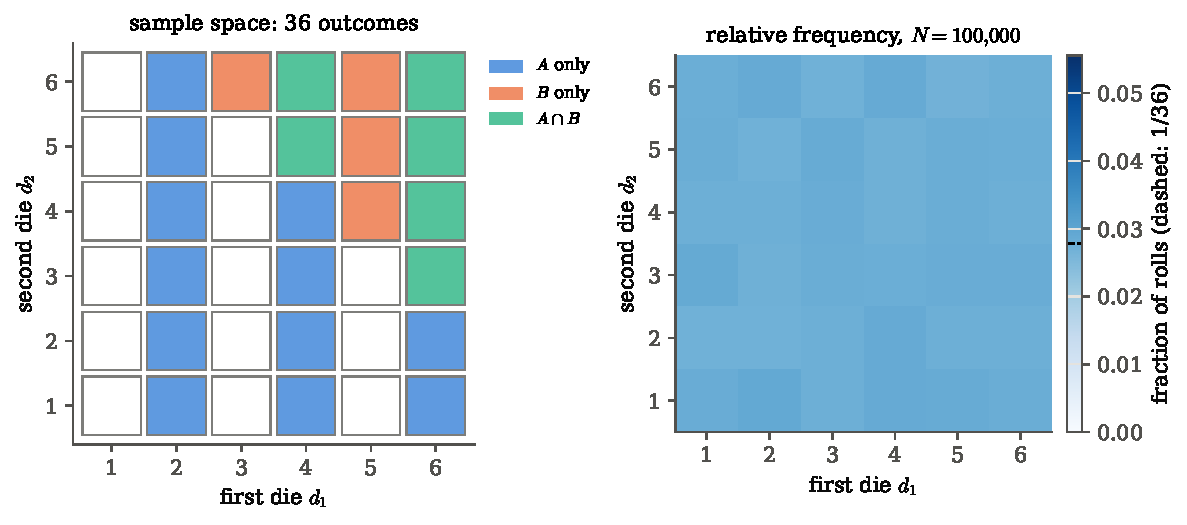
\includegraphics[width=\linewidth]{figures/ch01/1a_events_masks.pdf}
\caption{Left: the 36 outcomes of two dice as a grid, with the event $A$ (first
die even, blue), the event $B$ (sum at least 9, orange) and their overlap
(green). Counting cells gives the exact probabilities. Right: how often each
cell was hit in the simulation. Every cell is close to the dashed value $1/36$
on the colour bar, with small random differences.}
\label{1a:fig:events-masks}
\end{figure}

\paragraph{What this bought us.}
An event is a condition on outcomes, and in code it is a mask. Set identities
such as De Morgan's hold outcome by outcome, so they hold exactly for simulated
counts. Probabilities, which we define next, are what the frequencies of those
masks approach.

\section{The axioms of probability, and what they buy us}
\label{1a:sec:axioms}

Return to the three-paddle muon telescope of \cref{1a:ex:telescope}. Analyst
one has recorded a million muon passages and assigns to each of the eight
patterns the fraction of passages that produced it. Analyst two has just
installed a new middle paddle, has no data yet, and assigns numbers that
express how strongly she expects each pattern, based on the data sheet of the
photomultiplier. The two sets of numbers mean different things. Yet both
analysts will add them, subtract them from one, and combine them into trigger
probabilities in exactly the same way.

Whatever the numbers mean, any assignment of probabilities must obey three
rules, the axioms. Every rule we compute with follows from these three: the
complement rule, the inclusion--exclusion rule, the union bound that controls
the look-elsewhere effect, and the continuity that lets us take limits. Only
after the rules are in place do we ask what the numbers mean, and where each
meaning is used.

\paragraph{Probability is a unit of sand spread over the box.}
Take the box of possibilities from \cref{1a:sec:events} and pour exactly one
kilogram of sand over it, as unevenly as you like. The probability of an event
is the mass of sand lying inside its region. Mass is never negative. The whole
box holds all of it. If two regions do not overlap, the sand inside their union
is the sand in one plus the sand in the other. You would accept every one of
these statements about sand without proof. The proofs below only check that
three of them imply all the others.

\paragraph{What an assignment of probabilities must do.}
Stated in words, the demands are these.
\begin{enumerate}[leftmargin=1.5em,itemsep=1pt]
  \item To every event we can ask about, attach a number.
  \item The number for ``something happens'' ($\Omega$) must be the largest
        possible, and we fix the scale by calling it one.
  \item No event may get a negative number.
  \item Numbers for events that cannot happen together must add, also for an
        infinite list of such events.
  \item Everything else (complements, overlaps, limits) must then follow, so
        that we never need another rule.
\end{enumerate}

\begin{workdef}[probability distribution]
A \newterm{probability distribution} or \newterm{probability measure} $\Prob$
is a rule that assigns a real number $\Prob(A)$ to each event $A$
\unpack{each subset of $\Omega$ we are allowed to ask about, see
\cref{1a:sub:sigma}} such that
\begin{itemize}[leftmargin=1.2em,itemsep=1pt]
  \item[] \textbf{Axiom 1:} $\Prob(A)\ge 0$ for every event $A$.
  \item[] \textbf{Axiom 2:} $\Prob(\Omega)=1$.
  \item[] \textbf{Axiom 3:} if $A_1,A_2,\dots$ are disjoint
  \unpack{no outcome lies in two of them}, then
  \[
    \Prob\Bigl(\,\bigcup_{i=1}^\infty A_i\Bigr)=\sum_{i=1}^\infty \Prob(A_i).
  \]
\end{itemize}
Axiom 3 is called \newterm{countable additivity} \unpack{additivity for an
infinite sequence of disjoint events, one for each $i=1,2,3,\dots$}.
\emph{Operational test:} a table of numbers $\Prob(\{\omega\})$ on a finite or
countable $\Omega$ is a valid distribution exactly when every entry is
nonnegative and the entries sum to one.
\end{workdef}

These three lines are Kolmogorov's axioms (1933). They say nothing about
\emph{how} to find the numbers. That is the job of physics, of data and of
judgement. They only say which lists of numbers are internally consistent.

\subsection{Consequences of the axioms}

Five properties follow at once \mainref{p.~6, (1.1)}:
\begin{align}
&\Prob(\varnothing)=0, \nonumber\\
&A\subset B\ \Longrightarrow\ \Prob(A)\le\Prob(B), \nonumber\\
&0\le\Prob(A)\le 1, \label{1a:eq:props}\\
&\Prob(A^c)=1-\Prob(A), \nonumber\\
&A\cap B=\varnothing\ \Longrightarrow\ \Prob(A\cup B)=\Prob(A)+\Prob(B). \nonumber
\end{align}
Each takes a few lines to prove, and each proof is one idea that we will use
again, so we prove them all.

\paragraph{The empty event has probability zero.} Take the sequence
$A_1=\Omega$, $A_2=A_3=\cdots=\varnothing$. These are disjoint (the empty set
meets nothing) and their union is $\Omega$. Then
\begin{align*}
1 &\eqby{1} \Prob(\Omega)
   \eqby{2} \Prob\bigl(\Omega\cup\varnothing\cup\varnothing\cup\cdots\bigr)
   \eqby{3} \Prob(\Omega)+\sum_{i=2}^\infty\Prob(\varnothing)
   \eqby{4} 1+\sum_{i=2}^\infty\Prob(\varnothing).
\end{align*}
\begin{explain}
  \item Axiom 2.
  \item Adding empty sets to a union changes nothing.
  \item Axiom 3 for the disjoint sequence $\Omega,\varnothing,\varnothing,\dots$.
  \item Axiom 2 again.
\end{explain}
So $\sum_{i\ge2}\Prob(\varnothing)=0$. This is a sum of infinitely many copies
of the same number, which is nonnegative by Axiom 1. It is zero only if that
number is zero: $\Prob(\varnothing)=0$.

\paragraph{Finite additivity.} For disjoint $A_1,\dots,A_n$, pad the list with
empty sets, $A_{n+1}=A_{n+2}=\cdots=\varnothing$. Axiom 3 then gives
$\Prob(A_1\cup\cdots\cup A_n)=\sum_{i=1}^n\Prob(A_i)+\sum_{i>n}0$, which is the
last line of \eqref{1a:eq:props} for $n=2$.

\paragraph{Complement rule.} $A$ and $A^c$ are disjoint and $A\cup A^c=\Omega$, so
\begin{align}
1\eqby{1}\Prob(\Omega)\eqby{2}\Prob(A\cup A^c)\eqby{3}\Prob(A)+\Prob(A^c).
\label{1a:eq:complement}
\end{align}
\begin{explain}
  \item Axiom 2.
  \item Every outcome is either in $A$ or not.
  \item Finite additivity.
\end{explain}
This is the most used identity in the book: ``at least one'' is always
computed as one minus ``none''.

\paragraph{Monotonicity, and the difference rule.} If $A\subset B$, cut $B$
into the part inside $A$ and the part outside, $B=A\cup(B-A)$, which are
disjoint. Then
\begin{align}
\Prob(B)\eqby{1}\Prob(A)+\Prob(B-A)\relby{2}{\ge}\Prob(A).
\label{1a:eq:monotone}
\end{align}
\begin{explain}
  \item Finite additivity for the disjoint pieces $A$ and $B-A$.
  \item Axiom 1 for the event $B-A$.
\end{explain}
The first equality also says $\Prob(B-A)=\Prob(B)-\Prob(A)$ when $A\subset B$.
In detector language: a tighter cut $A$ inside a looser cut $B$ can only lose
outcomes, never gain them, so its probability cannot be larger. Finally
$0\le\Prob(A)$ is Axiom 1, and $\Prob(A)\le\Prob(\Omega)=1$ is monotonicity with
$B=\Omega$.

\begin{keyidea}[Inclusion--exclusion]
For any events $A$ and $B$,
\begin{equation}
\Prob(A\cup B)=\Prob(A)+\Prob(B)-\Prob(AB).
\label{1a:eq:incl-excl}
\end{equation}
Adding $\Prob(A)$ and $\Prob(B)$ counts the overlap twice, so we subtract it once.
\end{keyidea}

\begin{figure}[htbp]
\centering
\begin{tikzpicture}[scale=0.95]
  \coordinate (a) at (-0.8,0); \coordinate (b) at (0.8,0);
  \begin{scope}
    \fill[formblue!30] (a) circle (1.3);
    \fill[fibreorange!35] (b) circle (1.3);
    \begin{scope}\clip (a) circle (1.3); \fill[tangentgreen!40] (b) circle (1.3);\end{scope}
    \draw[thick] (-3,-1.8) rectangle (3,1.8);
    \draw (a) circle (1.3); \draw (b) circle (1.3);
    \node[lbl] at (-1.35,0) {$AB^c$};
    \node[lbl] at (0,0) {$AB$};
    \node[lbl] at (1.35,0) {$A^cB$};
    \node[lbl] at (-1.95,1.2) {$A$};
    \node[lbl] at (1.95,1.2) {$B$};
    \node[lbl] at (2.6,-1.45) {$\Omega$};
  \end{scope}
  \begin{scope}[xshift=7.0cm]
    \node[lbl,anchor=west] at (-2.4,1.2) {$\Prob(A)=\Prob(AB^c)+\Prob(AB)$};
    \node[lbl,anchor=west] at (-2.4,0.5) {$\Prob(B)=\Prob(AB)+\Prob(A^cB)$};
    \node[lbl,anchor=west] at (-2.4,-0.2) {sum: the green lens twice};
    \node[lbl,anchor=west] at (-2.4,-0.9) {$\Prob(A\cup B)$: each piece once};
  \end{scope}
\end{tikzpicture}
\caption{The union of two events is cut into three disjoint pieces: the part
of $A$ outside $B$ (blue), the overlap (green) and the part of $B$ outside $A$
(orange). $\Prob(A)$ and $\Prob(B)$ between them contain the green overlap
twice, and the union contains it once.}
\label{1a:fig:incl-excl}
\end{figure}

To prove \eqref{1a:eq:incl-excl}, use the three disjoint pieces of
\cref{1a:fig:incl-excl}: $A\cup B=(AB^c)\cup(AB)\cup(A^cB)$. Then
\begin{align*}
\Prob(A\cup B)
&\eqby{1} \Prob(AB^c)+\Prob(AB)+\Prob(A^cB)\\
&\eqby{2} \Prob(AB^c)+\Prob(AB)+\Prob(A^cB)+\Prob(AB)-\Prob(AB)\\
&\eqby{3} \Prob\bigl((AB^c)\cup(AB)\bigr)+\Prob\bigl((A^cB)\cup(AB)\bigr)-\Prob(AB)\\
&\eqby{4} \Prob(A)+\Prob(B)-\Prob(AB).
\end{align*}
\begin{explain}
  \item Finite additivity for three disjoint pieces.
  \item Add and subtract the same number.
  \item Finite additivity backwards, for the disjoint pairs $AB^c,AB$ and $A^cB,AB$.
  \item An outcome of $A$ is either outside $B$ or inside it, so
        $(AB^c)\cup(AB)=A$. Likewise $(A^cB)\cup(AB)=B$.
\end{explain}

\oneaEx{Two coin tosses}
\label{1a:ex:two-heads}
Let $H_1$ be ``heads on toss 1'' and $H_2$ ``heads on toss 2''. With the four
outcomes $HH,HT,TH,TT$ equally likely, $\Prob(H_1)=\Prob(\{HH,HT\})=\tfrac12$,
$\Prob(H_2)=\Prob(\{HH,TH\})=\tfrac12$ and $\Prob(H_1H_2)=\Prob(\{HH\})=\tfrac14$. So
\begin{align*}
\Prob(H_1\cup H_2)\eqby{1}\Prob(H_1)+\Prob(H_2)-\Prob(H_1H_2)
=\tfrac12+\tfrac12-\tfrac14=\tfrac34 .
\end{align*}
\begin{explain}
  \item Inclusion--exclusion \eqref{1a:eq:incl-excl}.
\end{explain}
Check by the complement rule: ``at least one head'' fails only for $TT$, so
the answer is $1-\tfrac14=\tfrac34$. The two routes must agree, and they do.

\oneaEx{A probability table for the telescope}
\label{1a:ex:telescope-probs}
On a finite sample space, finite additivity over single outcomes gives
\begin{equation}
\Prob(A)=\sum_{\omega\in A}\Prob(\{\omega\}),
\label{1a:eq:sum-atoms}
\end{equation}
so a distribution is just a table of nonnegative numbers that sum to one.
Suppose the telescope patterns have the probabilities
\begin{center}
\begin{tabular}{@{}lcccc@{}}
\toprule
pattern & $000$ & $001,\,010,\,100$ & $011,\,101,\,110$ & $111$\\
\midrule
probability (each) & $0.001$ & $0.009$ & $0.081$ & $0.729$\\
\bottomrule
\end{tabular}
\end{center}
They sum to $0.001+3(0.009)+3(0.081)+0.729=1$, so the table is legitimate.
(Where such numbers come from is the subject of \cref{1a:sec:independence}:
they are what one gets if each paddle fires with probability $0.9$ on its own.)
For the trigger $T$ and the event $U$ (top fired) of \cref{1a:ex:telescope-ops},
\begin{align*}
\Prob(T) &= 3(0.081)+0.729 = 0.972, \qquad \Prob(U)=0.009+2(0.081)+0.729=0.9,\\
\Prob(TU) &= \Prob(\{101,110,111\}) = 2(0.081)+0.729=0.891,\\
\Prob(T\cup U) &\eqby{1} 0.972+0.9-0.891 = 0.981 .
\end{align*}
\begin{explain}
  \item Inclusion--exclusion. Directly, $T\cup U=\{011,100,101,110,111\}$ has
        probability $0.081+0.009+0.081+0.081+0.729=0.981$, the same.
\end{explain}
The trigger misses a muon with probability $\Prob(T^c)=1-0.972=0.028$, by the
complement rule.

\paragraph{Try it: Three events.}
Show that
$\Prob(A\cup B\cup C)=\Prob(A)+\Prob(B)+\Prob(C)-\Prob(AB)-\Prob(AC)-\Prob(BC)+\Prob(ABC)$.
\emph{Hint:} apply \eqref{1a:eq:incl-excl} to $A\cup B$ and $C$, then use the
distributive law $(A\cup B)\cap C=(AC)\cup(BC)$ and \eqref{1a:eq:incl-excl}
once more, noting $(AC)(BC)=ABC$. In the telescope, the three events ``paddle
$j$ fired'' give $3(0.9)-3(0.81)+0.729=0.999$, which is $1-\Prob(\{000\})$.

\subsection{Two inequalities: Bonferroni and Boole}

Often we cannot compute an overlap $\Prob(AB)$, but we can still bound it from
below. Rearrange \eqref{1a:eq:incl-excl} and use $\Prob(A\cup B)\le 1$:
\begin{equation}
\Prob(AB)=\Prob(A)+\Prob(B)-\Prob(A\cup B)\ \ge\ \Prob(A)+\Prob(B)-1 .
\label{1a:eq:bonferroni}
\end{equation}
This is the simplest \newterm{Bonferroni inequality} \srcref{CasellaBerger}{(1.2.9)}.
\emph{Example.} The tracker and the calorimeter are each fully operational in
$95\%$ of the luminosity blocks. Then both are operational in at least
$95\%+95\%-100\%=90\%$ of them, however their failures are correlated. When
$\Prob(A)+\Prob(B)<1$ the bound is negative: true, but useless.

\begin{keyidea}[Boole's inequality, the union bound]
For any events $A_1,A_2,\dots$ (disjoint or not),
\begin{equation}
\Prob\Bigl(\,\bigcup_{n=1}^\infty A_n\Bigr)\le\sum_{n=1}^\infty\Prob(A_n).
\label{1a:eq:boole}
\end{equation}
The probability that at least one thing goes wrong is at most the sum of the
probabilities of each thing going wrong.
\end{keyidea}

Make the events disjoint by keeping only the part of each $A_n$ that is new:
$B_1=A_1$ and $B_n=A_n-\bigcup_{i<n}A_i$ \mainref{p.~14, Ex.~7}. An outcome in
$\bigcup_nA_n$ has a \emph{first} index $n$ with $\omega\in A_n$, and it lies in
$B_n$ for that $n$ only. So the $B_n$ are disjoint, $\bigcup_nB_n=\bigcup_nA_n$,
and $B_n\subset A_n$. Then
\begin{align*}
\Prob\Bigl(\,\bigcup_n A_n\Bigr)
\eqby{1}\Prob\Bigl(\,\bigcup_n B_n\Bigr)
\eqby{2}\sum_n\Prob(B_n)
\relby{3}{\le}\sum_n\Prob(A_n).
\end{align*}
\begin{explain}
  \item The two unions contain the same outcomes.
  \item Axiom 3 for the disjoint $B_n$.
  \item Monotonicity \eqref{1a:eq:monotone}, term by term, since $B_n\subset A_n$.
\end{explain}

\paragraph{In research: the look-elsewhere effect in one line.}
A bump hunt scans $m$ mass bins. If background alone makes a given bin
fluctuate up to the observed size with probability $\pval_{\text{local}}$, the
probability that \emph{some} bin does so is at most $m\,\pval_{\text{local}}$ by
\eqref{1a:eq:boole}. This is the Bonferroni correction for multiple tests
(\cref{ch:04}). It is a bound, and it is loose when neighbouring bins are
correlated. In real searches the actual ``global'' probability is obtained by
simulating many background-only experiments and counting how often the largest
fluctuation anywhere exceeds the observed one \cite{GrossVitells2010}. The
union bound is what tells us in advance roughly how bad the effect can be.

\oneaEx{Events of probability one}
\label{1a:ex:prob-one}
If $\Prob(A_i)=1$ for every $i$, then $\Prob\bigl(\bigcap_iA_i\bigr)=1$
\mainref{p.~14, Ex.~8}:
\begin{align*}
\Prob\Bigl(\bigl(\textstyle\bigcap_iA_i\bigr)^c\Bigr)
\eqby{1}\Prob\Bigl(\,\bigcup_iA_i^c\Bigr)
\relby{2}{\le}\sum_i\Prob(A_i^c)
\eqby{3}\sum_i 0 = 0 .
\end{align*}
\begin{explain}
  \item De Morgan's law \eqref{1a:eq:demorgan} for a countable family.
  \item Boole's inequality \eqref{1a:eq:boole}.
  \item Complement rule: $\Prob(A_i^c)=1-1=0$.
\end{explain}
A probability is nonnegative, so the complement has probability exactly zero
and the intersection has probability one. Countably many ``almost sure''
statements hold almost surely all at once.

\subsection{Continuity: probabilities of limits are limits of probabilities}

\paragraph{Continuity of probability.}
If $A_n\to A$ (a monotone sequence, \cref{1a:sec:events}), then
$\Prob(A_n)\to\Prob(A)$ as $n\to\infty$ \mainref{p.~7, Thm~1.8}.

\begin{figure}[htbp]
\centering
\begin{tikzpicture}[scale=0.9]
  \fill[formblue!12] (0,0) circle (2.2);
  \fill[formblue!30] (0,0) circle (1.6);
  \fill[formblue!55] (0,0) circle (1.0);
  \draw (0,0) circle (1.0); \draw (0,0) circle (1.6); \draw (0,0) circle (2.2);
  \draw[faint,dashed] (0,0) circle (2.55);
  \node[lbl,white] at (0,0) {$B_1=A_1$};
  \node[lbl] at (0,1.3) {$B_2$};
  \node[lbl] at (0,1.9) {$B_3$};
  \node[lbl,softgray] at (0,2.36) {$\cdots$};
  \draw[faint] (1.414,-1.686) -- (3.2,-2.2) node[lbl,anchor=west,black] {$A_3=B_1\cup B_2\cup B_3$};
  \draw[faint] (1.45,-0.676) -- (3.2,-1.2) node[lbl,anchor=west,black] {$A_2=B_1\cup B_2$};
  \draw[faint] (1.8,1.8) -- (3.2,1.8) node[lbl,anchor=west,black] {$A=\bigcup_nA_n$ (dashed)};
\end{tikzpicture}
\caption{An increasing sequence of events drawn as nested discs. The rings
$B_n$ (the part of $A_n$ that is new at step $n$) do not overlap, and the
first $n$ rings together make up $A_n$. The probability of the limit is the
total mass of all rings, which is the limit of the partial sums.}
\label{1a:fig:continuity}
\end{figure}

Suppose $A_1\subset A_2\subset\cdots$ with $A=\bigcup_iA_i$. Define the rings of
\cref{1a:fig:continuity}: $B_1=A_1$ and
$B_n=\{\omega:\ \omega\in A_n,\ \omega\notin A_{n-1}\}$ for $n\ge2$. Because the sets
are nested, ``not in $A_{n-1}$'' already means ``not in any earlier $A_i$'',
so this is the construction used for Boole's inequality. The $B_n$ are disjoint,
$A_n=\bigcup_{i=1}^nB_i$ and $\bigcup_{i=1}^\infty B_i=A$. Then
\begin{align*}
\lim_{n\to\infty}\Prob(A_n)
&\eqby{1}\lim_{n\to\infty}\Prob\Bigl(\,\bigcup_{i=1}^nB_i\Bigr)
 \eqby{2}\lim_{n\to\infty}\sum_{i=1}^n\Prob(B_i)
 \eqby{3}\sum_{i=1}^\infty\Prob(B_i)
 \eqby{4}\Prob\Bigl(\,\bigcup_{i=1}^\infty B_i\Bigr)
 \eqby{5}\Prob(A).
\end{align*}
\begin{explain}
  \item $A_n$ is the union of the first $n$ rings.
  \item Finite additivity.
  \item An infinite sum is by definition the limit of its partial sums. It
        converges because the partial sums increase and never exceed one.
  \item Axiom 3, which is where \emph{countable} additivity is essential.
  \item The rings together make up $A$.
\end{explain}
For a decreasing sequence $A_1\supset A_2\supset\cdots$ with $A=\bigcap_iA_i$, the
complements increase, $A_1^c\subset A_2^c\subset\cdots$, and by De Morgan
$\bigcup_iA_i^c=\bigl(\bigcap_iA_i\bigr)^c=A^c$. The increasing case gives
$\Prob(A_n^c)\to\Prob(A^c)$, so
$\Prob(A_n)=1-\Prob(A_n^c)\to1-\Prob(A^c)=\Prob(A)$ \mainref{p.~13, Ex.~1}.

\oneaEx{A detector that is alive forever}
\label{1a:ex:alive}
Let $A_n$ be ``the readout board has not failed during the first $n$ hours''.
The events decrease, $A_1\supset A_2\supset\cdots$, and their intersection $A$ is
``the board never fails''. Suppose a reliability model gives
$\Prob(A_n)=e^{-n/\tau}$ with a mean lifetime of $\tau=10^4$ hours. Continuity gives
\begin{align*}
\Prob(\text{never fails})\eqby{1}\lim_{n\to\infty}\Prob(A_n)=\lim_{n\to\infty}e^{-n/\tau}=0 .
\end{align*}
\begin{explain}
  \item Continuity for the decreasing sequence $A_n\to A$.
\end{explain}
We could not have computed $\Prob(A)$ directly, since $A$ is defined by an
infinite number of conditions. Continuity turns it into an ordinary limit.

\oneaEx{There is no uniform distribution on the integers}
\label{1a:ex:no-uniform-N}
Can we pick a whole number ``completely at random'', so that every
$n\in\{0,1,2,\dots\}$ has the same probability $c$ \mainref{p.~14, Ex.~6}? The
single-number events $\{0\},\{1\},\dots$ are disjoint with union $\Omega$, so
\begin{align*}
1\eqby{1}\Prob(\Omega)\eqby{2}\sum_{n=0}^\infty\Prob(\{n\})=\sum_{n=0}^\infty c
=\begin{cases}0 & c=0,\\ \infty & c>0.\end{cases}
\end{align*}
\begin{explain}
  \item Axiom 2.
  \item Axiom 3.
\end{explain}
Neither case equals one, so no such $\Prob$ exists. The same obstruction
appears for a ``flat prior'' on an unbounded parameter range, such as a
uniform distribution for a mass on $(0,\infty)$: it cannot be normalised.
Such an \emph{improper} prior can still be used as a device when the
posterior turns out normalisable, and \cref{ch:05} explains when.

\subsection{Which events are allowed? A word on $\sigma$-fields}
\label{1a:sub:sigma}

On a finite or countable $\Omega$ every subset can be an event. On $\R$ this
fails: one can prove that there is no way to give a ``length'' to
\emph{every} subset of $[0,1]$ that is countably additive and unchanged by
shifts. So probabilities are assigned only to a large, well-behaved class of
subsets \mainref{p.~13, \S1.9}.

\paragraph{$\sigma$-field, probability space.}
A \newterm{$\sigma$-field} (or $\sigma$-algebra) $\mathcal A$ is a collection
of subsets of $\Omega$ with (i) $\varnothing\in\mathcal A$, (ii) if
$A_1,A_2,\dots\in\mathcal A$ then $\bigcup_iA_i\in\mathcal A$, and (iii) if
$A\in\mathcal A$ then $A^c\in\mathcal A$ \unpack{the class of events is closed
under not, and countable or}. Its members are called \newterm{measurable}. The pair
$(\Omega,\mathcal A)$ is a \newterm{measurable space}, and with a probability
measure $\Prob$ on $\mathcal A$ the triple $(\Omega,\mathcal A,\Prob)$ is a
\newterm{probability space}. On $\R$ one uses the \newterm{Borel
$\sigma$-field}, the smallest $\sigma$-field containing all open intervals
\unpack{everything you can build from intervals by countably many unions,
intersections and complements}.

In practice this restriction never bites. Every event in this book
(intervals, histogram bins, excursion sets of a smooth field, limits of
monotone sequences) is Borel. A $\sigma$-field is also closed under countable
intersections, by De Morgan: $\bigcap_iA_i=\bigl(\bigcup_iA_i^c\bigr)^c$, and
the right side uses only complements and unions. So the limits of decreasing
sequences from \cref{1a:sec:events} stay inside it too.

\subsection{What the numbers mean: frequency and degree of belief}

The axioms fix the arithmetic. They do not say what $\Prob(A)=0.3$
\emph{means}. There are two standard answers \mainref{p.~6},
\srcref{Cowan}{\S1.2}, \srcref{Kruschke}{\S4.2}.

\begin{workdef}[frequency and degree-of-belief interpretations]
In the \newterm{frequency interpretation}, $\Prob(A)$ is the long-run proportion
of repetitions in which $A$ happens,
\begin{equation}
\Prob(A)=\lim_{n\to\infty}\frac{n_A}{n},
\label{1a:eq:freq}
\end{equation}
where $n_A$ is the \newterm{count} of $A$ \unpack{the number of runs, out of
$n$ identical and independent runs, in which $A$ occurred}.
In the \newterm{degree-of-belief} (subjective, Bayesian) interpretation,
$\Prob(A)$ measures how strongly a given observer, with given information,
believes that the statement $A$ is true. Here $\Omega$ is often called the
\newterm{hypothesis space} \unpack{a list of mutually exclusive statements,
exactly one of which is true}.
\end{workdef}

Both readings obey the same axioms, for different reasons. For frequencies
the axioms are automatic. A frequency is never negative, the frequency of
``some outcome'' is one, and the frequency of one of several disjoint outcomes
is the sum of their frequencies \srcref{Cowan}{p.~5}.

For beliefs the axioms are a consistency requirement, and a bet shows why.
Suppose you would pay $0.6$ for a ticket that pays $1$ if $A$ happens, and also
$0.6$ for a ticket that pays $1$ if $A$ does not. Buying both costs $1.2$.
Exactly one of the tickets wins, so you get back exactly $1$ whatever happens.
Your beliefs $\Prob(A)=\Prob(A^c)=0.6$ break the complement rule, and they lose
money for sure. Beliefs that cannot be exploited this way must obey the axioms.

The same kind of comparison pins a belief down. Suppose you prefer a ticket on
$A$ to a ticket on drawing red from a bag with 1 red and 9 white marbles. Then
your $\Prob(A)$ is above $0.1$. Suppose you also prefer a ticket on a bag with 5
red and 5 white to the ticket on $A$. Then your $\Prob(A)$ is below $0.5$. So it
lies between $0.1$ and $0.5$ \srcref{Kruschke}{\S4.2.2.1}.

The frequency reading needs repetition, so it fails for a unique object. It is
natural for anything that is repeated: collisions at a collider, photons in a
detector, the simulated universes of a Monte Carlo. Now take the electron mass
$m_e$. It is either inside the interval $[0.510,0.512]\,\text{MeV}$ or not, and
repeating the experiment does not change it. So the frequency of ``$m_e$ is in
the interval'' is either one (always inside) or zero (never), and we do not know
which. A statement like ``95\%
probability that $m_e$ lies in this interval'' only makes sense as a degree of
belief \srcref{Cowan}{p.~6}. The same is true of ``the probability that
$\Omega_m$ lies between $0.30$ and $0.32$'': there is one universe.

\begin{taxonomy}[Which interpretation, where in the book]
\begin{tabularx}{\linewidth}{@{}>{\raggedright}p{3.2cm}X@{}}
\toprule
\textbf{Frequency} & sampling distributions of data and statistics
(\cref{ch:02,ch:03}), $p$-values and the coverage of confidence intervals
(\cref{ch:04}), Monte Carlo error bars (\cref{ch:06}), cosmic variance of
$\Cell$ as scatter over hypothetical skies (\cref{ch:07}), the transfer
function and covariance of a masked pipeline (\cref{ch:08}).\\
\addlinespace
\textbf{Degree of belief} & priors and posteriors for parameters
$p(\params\given\data)$ (\cref{ch:05}), credible intervals from MCMC
(\cref{ch:09}), Fisher forecasts read as posterior widths (\cref{ch:10}),
systematic uncertainties.\\
\addlinespace
\textbf{Both, same rules} & everything in the theory of probability. The calculus is
shared, and in a Bayesian analysis the likelihood $\Prob(\data\given\params)$ is
itself a frequency statement about repeated data.\\
\bottomrule
\end{tabularx}
\end{taxonomy}

\subsection{A simulated long-run frequency}

The frequency definition \eqref{1a:eq:freq} is a limit, and a computer lets us
watch the limit being approached \mainref{p.~16, Ex.~21}. We flip a coin with
$\Prob(\text{heads})=p$ a thousand times and plot the proportion of heads so far.

\pyfile[firstline=23,lastline=34,firstnumber=23]{code/ch01/02_running_frequency.py}{Running proportion of heads}

Line 27 is the whole simulation: \texttt{rng.random(n\_max)} draws uniform
numbers in $[0,1)$, and a number lands below $p$ with probability $p$, so the
comparison is a coin with heads probability $p$. Line 28 divides the
cumulative count of heads by the number of flips so far, which is $n_A/n$ in
\eqref{1a:eq:freq}. Line 31 draws the band $p\pm2\sqrt{p(1-p)/n}$. Where that
width comes from is the variance of the binomial distribution in \cref{ch:02}.
For now it is simply a rule of thumb: at any given $n$, a run lies outside
the band only about one time in twenty.

\begin{figure}[htbp]
\centering
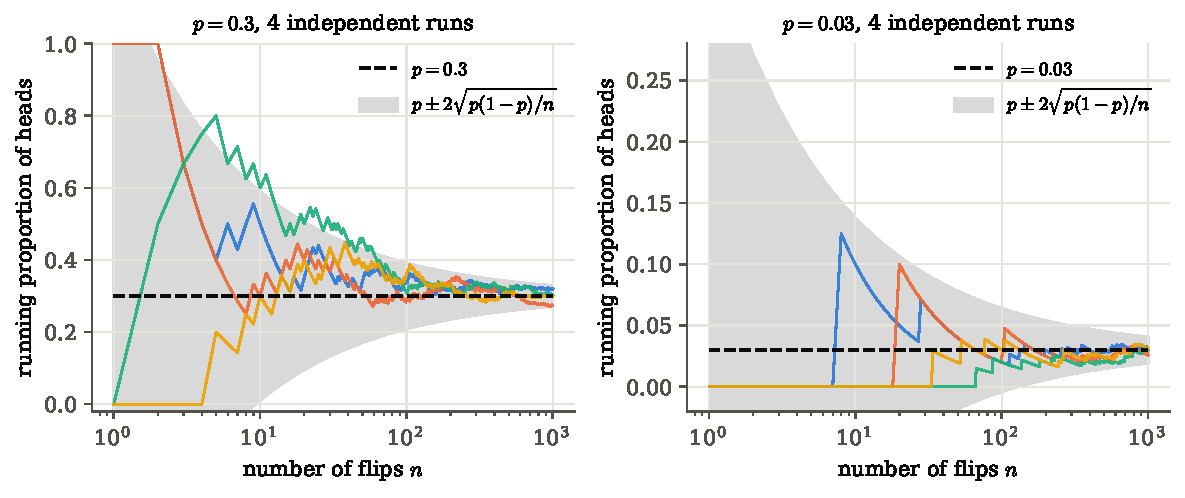
\includegraphics[width=\linewidth]{figures/ch01/1a_running_frequency.pdf}
\caption{Running proportion of heads for four independent runs of $1000$
flips, with $p=0.3$ (left) and $p=0.03$ (right). Early on the proportion jumps
around wildly. As flips accumulate the runs settle towards the dashed value,
and the shaded band $p\pm2\sqrt{p(1-p)/n}$ narrows like $1/\sqrt n$.}
\label{1a:fig:running}
\end{figure}

A rare event is harder to pin down than a common one. After $1000$ flips with
$p=0.3$, the first two runs end at $\OneARunFinalA$ and $\OneARunFinalAtwo$,
and $\OneARunInsideA$ of the $\OneARunRuns$ runs end inside the band
$0.3\pm\OneARunBandA$. With $p=0.03$ the first two end at $\OneARunFinalB$ and
$\OneARunFinalBtwo$, and $\OneARunInsideB$ of the $\OneARunRuns$ end inside
$0.03\pm\OneARunBandB$. The
band is narrower for the rare event in absolute terms. Relative to $p$, though,
it is much wider: about $10\%$ of $p$ for $p=0.3$, and almost $40\%$ of $p$ for
$p=0.03$. Dividing the half-width $2\sqrt{p(1-p)/n}$ by $p$ gives the relative
width $2\sqrt{(1-p)/(np)}$. It depends on $np$, the expected number of times the
event occurs. So estimating a small probability to a given relative precision
needs a number of trials proportional to $1/p$.

\paragraph{What this bought us.}
A finite run gives a frequency, not the probability. The frequency scatters
around the probability, and the scatter shrinks like $1/\sqrt{\text{(number of
occurrences)}}$. This is the first appearance of the Monte Carlo error, which
we will meet again every time a simulation estimates a number.

\begin{inpractice}[Verification here, instrument later]
Here we \emph{knew} $p$ and the simulation only verified that frequencies
approach it. In research the direction is reversed. Nobody can write down the
probability that a $pp$ collision at the LHC produces a muon that survives all
selection cuts. It is obtained exactly this way, as a frequency over millions
of simulated collisions, with the $1/\sqrt{n_A}$ scatter quoted as the
``Monte Carlo statistical uncertainty''.
\end{inpractice}

\paragraph{The frequency definition is not a recipe for every probability.}
Equation \eqref{1a:eq:freq} needs repeatable, identical runs. It gives no
meaning to $\Prob(\text{the Hubble tension is new physics})$. Conversely, a
degree of belief is not arbitrary: once it is written as a probability it must
obey all the rules above, and it must be updated by the rule of
\cref{1a:sec:bayes}.

\section{Equally likely outcomes: probability as counting}
\label{1a:sec:counting}

A silicon pixel sensor has $N=10^4$ pixels. In one readout frame, $k=100$
charged particles cross it, each landing on a pixel at random. If two particles
hit the same pixel, the pixel reports one hit, the two tracks share it, and the
tracking code may lose one of them. How often does at least one such merger
happen in a frame? The occupancy is only $100/10^4=1\%$, so one expects
``rarely''. The answer is about $39\%$.

When every outcome is equally likely, a probability is a ratio of two counts,
so all the work is in counting. Four basic counting formulas cover the cases:
ordered or not, with or without replacement. Physicists know them as
Maxwell--Boltzmann, Bose--Einstein and Fermi--Dirac counting. They settle the
pixel problem, which is the birthday problem in disguise, and we solve it three
ways: exactly, approximately and by simulation.

\paragraph{The microcanonical ensemble.}
In statistical mechanics an isolated system is equally likely to be in any of
its $\Omega(E)$ microstates of energy $E$. The probability of a macrostate is
then the number of microstates that realise it divided by $\Omega(E)$, and
entropy $S=k_B\ln\Omega$ is a logarithm of a count. Probability on a finite
sample space with equally likely outcomes is exactly this: fix the list of
equally likely microstates, and every probability is a ratio of counts.

\paragraph{Solving a counting problem.}
Every counting problem here is solved by the same four steps.
\begin{enumerate}[leftmargin=1.5em,itemsep=1pt]
  \item Find a sample space in which every outcome is equally likely. (This is
        a physical statement about the mechanism, not a counting fact.)
  \item Count all outcomes, $|\Omega|$.
  \item Count the outcomes in the event, $|A|$. Break the count into a
        sequence of simple choices.
  \item Divide. If counting $A$ is hard, count $A^c$ and use $1-|A^c|/|\Omega|$.
\end{enumerate}

\begin{workdef}[uniform distribution on a finite set]
If $\Omega=\{\omega_1,\dots,\omega_N\}$ is finite and every outcome has the
same probability, $\Prob(\{\omega_i\})=1/N$, then for every event
\begin{equation}
\Prob(A)=\frac{|A|}{|\Omega|}.
\label{1a:eq:uniform}
\end{equation}
This is the \newterm{uniform probability distribution} on $\Omega$
\unpack{probability of $A$ is the number of outcomes in $A$ over the number of
outcomes in $\Omega$}.
\emph{Operational test:} can you argue, from symmetry of the mechanism, that
no outcome is preferred? If not, \eqref{1a:eq:uniform} does not apply.
\end{workdef}

The equal value $1/N$ is forced: the $N$ single-outcome events are disjoint with
union $\Omega$, so $N\cdot c=1$. Then
\begin{align*}
\Prob(A)\eqby{1}\sum_{\omega\in A}\Prob(\{\omega\})\eqby{2}\sum_{\omega\in A}\frac1N
\eqby{3}\frac{|A|}{N}.
\end{align*}
\begin{explain}
  \item Finite additivity over the outcomes in $A$, \eqref{1a:eq:sum-atoms}.
  \item Every outcome has probability $1/N$.
  \item The sum has $|A|$ equal terms.
\end{explain}

\oneaEx{Two dice}
\label{1a:ex:two-dice}
Roll a die twice. $\Omega=\{(i,j):\ i,j\in\{1,\dots,6\}\}$ has $36$ ordered pairs,
all equally likely for fair dice rolled separately. The sum is $11$ for
$(5,6)$ and $(6,5)$, so $\Prob(\text{sum}=11)=2/36$. The sum is $7$ for $(1,6),(2,5),
\dots,(6,1)$, so $\Prob(\text{sum}=7)=6/36$. Here the pitfall of
\cref{1a:sec:events} bites: on the coarser space of sums $\{2,\dots,12\}$ the
eleven values are \emph{not} equally likely, and \eqref{1a:eq:uniform} would give
the wrong answer $1/11$.

\subsection{The multiplication principle}

\paragraph{Fundamental theorem of counting.}
If a job consists of $k$ separate choices, and the $i$-th choice can be made in
$n_i$ ways whatever the earlier choices were, the job can be done in
$n_1\times n_2\times\cdots\times n_k$ ways.

For $k=2$ choices, a table proves it. Write the possibilities with $n_1$ rows
(first choice) and $n_2$ columns (second choice). Each cell is one way of doing
the job, and there are $n_1n_2$ cells. For $k$ choices, treat the first $k-1$ as
one job and apply the $k=2$ case again and again. The phrase ``whatever the
earlier choices were'' matters. The \emph{number} of options at each step must
not depend on what was chosen before, although the options themselves may: when
dealing two cards, the second card has $51$ options whichever card came first,
but which $51$ depends on the first card.

\begin{figure}[htbp]
\centering
\begin{tikzpicture}[x=1.15cm,y=1cm]
  \foreach \i/\n in {1/{n},2/{n-1},3/{n-2}}{
    \draw[thick,formblue] (\i*1.6-0.6,0) rectangle (\i*1.6+0.6,0.8);
    \node[lbl] at (\i*1.6,0.4) {$\n$};
    \node[lbl,softgray] at (\i*1.6,-0.35) {slot \i};
  }
  \node[lbl] at (6.1,0.4) {$\cdots$};
  \draw[thick,formblue] (6.9,0) rectangle (8.5,0.8);
  \node[lbl] at (7.7,0.4) {$n-r+1$};
  \node[lbl,softgray] at (7.7,-0.35) {slot $r$};
  \node[lbl,anchor=west] at (0.9,-1.1) {ordered lists: $n(n-1)\cdots(n-r+1)=\dfrac{n!}{(n-r)!}$};
  \begin{scope}[yshift=-3.3cm]
    \foreach \w/\x in {abc/1.0,acb/2.0,bac/3.0,bca/4.0,cab/5.0,cba/6.0}{
      \node[draw=softgray,rounded corners=1pt,font=\small\ttfamily,inner sep=2pt] (w\w) at (\x,0.9) {\w};
    }
    \node[draw=fibreorange,thick,rounded corners=2pt,font=\small,inner sep=3pt] (set) at (3.5,-0.5) {$\{a,b,c\}$};
    \foreach \w in {abc,acb,bac,bca,cab,cba}{ \draw[faint] (w\w.south) -- (set.north); }
    \node[lbl,anchor=west] at (7.0,0.9) {$r!=6$ ordered lists};
    \node[lbl,anchor=west] at (7.0,-0.5) {one unordered set};
  \end{scope}
\end{tikzpicture}
\caption{Top: filling $r$ ordered slots from $n$ distinct objects without
putting any object back. The first slot has $n$ options, the second $n-1$, and
so on. Bottom: the $3!=6$ ordered lists of the letters $a,b,c$ all describe the
same unordered set, so counting sets means dividing the ordered count by $r!$.}
\label{1a:fig:slots}
\end{figure}

\paragraph{Permutations.} The number of ways to arrange $n$ distinct objects in
a row is $n!=n(n-1)\cdots2\cdot1$. Call it $P_n$. There are $n$ choices for the
first position, and then the remaining $n-1$ objects can be arranged in
$P_{n-1}$ ways, so $P_n=n\,P_{n-1}$ with $P_1=1$ \srcref{SeeingTheory}{p.~22}.
Unwinding the recursion gives $P_n=n!$. We set $0!=1$: there is exactly one way
to arrange nothing, and $P_1=1\cdot P_0$ requires $P_0=1$.

\paragraph{Ordered selection without replacement.} Filling $r$ ordered slots
from $n$ objects (\cref{1a:fig:slots}, top) can be done in
\begin{align*}
n(n-1)\cdots(n-r+1)\eqby{1}\frac{n(n-1)\cdots(n-r+1)\,(n-r)!}{(n-r)!}\eqby{2}\frac{n!}{(n-r)!}
\end{align*}
\begin{explain}
  \item Multiply and divide by $(n-r)!=(n-r)(n-r-1)\cdots1$.
  \item The numerator is now the full product $n(n-1)\cdots1$.
\end{explain}
ways, by the multiplication principle with $n_i=n-i+1$.

\paragraph{Unordered selection without replacement.} Now we want the number of
\emph{sets} of $r$ objects, ignoring order. Call it $\binom nr$. Every set of $r$
objects can be put in order in $r!$ ways (\cref{1a:fig:slots}, bottom), and every
ordered list arises from exactly one set. So we can count ordered lists in two
ways:
\begin{align}
\frac{n!}{(n-r)!}\eqby{1}\binom nr\times r!
\quad\Longrightarrow\quad
\binom nr=\frac{n!}{r!\,(n-r)!}.
\label{1a:eq:binom}
\end{align}
\begin{explain}
  \item Choose the set first ($\binom nr$ ways), then its order ($r!$ ways), and
        apply the multiplication principle.
\end{explain}
This is the \newterm{binomial coefficient}, read ``$n$ choose $r$''
\mainref{p.~8, (1.2)}. The method, counting something in two ways and
equating, is the most useful trick in combinatorics.

Two properties follow. $\binom n0=\binom nn=1$, since $0!=1$: there is one way
to choose nothing and one way to choose everything. And
$\binom nr=\binom n{n-r}$, since choosing the $r$ objects that are in is the same
as choosing the $n-r$ that are out. Algebraically, swapping $r\leftrightarrow n-r$
in $n!/(r!(n-r)!)$ swaps the two factorials in the denominator.

\oneaEx{Committees, and a poker hand}
\label{1a:ex:committee}
A class of $20$ elects a committee of $3$ \mainref{p.~8}:
\begin{align*}
\binom{20}{3}\eqby{1}\frac{20!}{3!\,17!}\eqby{2}\frac{20\times19\times18}{3\times2\times1}=1140 .
\end{align*}
\begin{explain}
  \item Definition \eqref{1a:eq:binom}.
  \item Cancel $17!$ from $20!=20\cdot19\cdot18\cdot17!$.
\end{explain}
A five-card poker hand is an unordered set of $5$ of $52$ cards, so there are
$\binom{52}5=2\,598\,960$ equally likely hands. ``Four aces'' fixes four cards and
leaves $48$ choices for the fifth, so $\Prob(\text{four aces})=48/2\,598\,960\approx
1.8\times10^{-5}$. ``Exactly one pair'' is built by a sequence of choices
\srcref{CasellaBerger}{(1.2.11)}: the pair's value ($13$ ways), its two suits
($\binom42=6$), the three other values, all different from each other and from
the pair ($\binom{12}3=220$), and a suit for each ($4^3=64$). So
\[
\Prob(\text{exactly one pair})=\frac{13\cdot6\cdot220\cdot64}{2\,598\,960}
=\frac{1\,098\,240}{2\,598\,960}\approx0.423 .
\]

\paragraph{Selection with replacement.} If an object is put back after being
chosen, every slot again has $n$ options, and there are $n^r$ ordered lists.

\paragraph{Unordered selection with replacement.} This is the hardest case.
An unordered choice of $r$ objects from $n$ types, repeats allowed, is fixed by
how many of each type we took. Draw the $n$ types as bins separated by $n-1$
walls, and each chosen object as a star in its bin (\cref{1a:fig:stars}). A
choice is then a row of $r$ stars and $n-1$ walls, and every such row is one
choice. Counting rows means choosing which $r$ of the $r+n-1$ positions hold
stars:
\begin{equation}
\#\{\text{unordered selections with replacement}\}=\binom{n+r-1}{r}.
\label{1a:eq:stars}
\end{equation}

\begin{figure}[htbp]
\centering
\begin{tikzpicture}[x=0.55cm,y=0.55cm]
  \foreach \x in {0,2,3,6}{ \node[font=\Large,fibreorange] at (\x,0) {$\star$}; }
  \foreach \x in {1,4,5}{ \draw[very thick,formblue] (\x,-0.7) -- (\x,0.7); }
  \draw[faint] (-0.8,-0.7) -- (-0.8,0.7); \draw[faint] (6.8,-0.7) -- (6.8,0.7);
  \node[lbl,anchor=north] at (0,-1.0) {1};
  \node[lbl,anchor=north] at (2.5,-1.0) {2};
  \node[lbl,anchor=north] at (4.5,-1.0) {3};
  \node[lbl,anchor=north] at (6,-1.0) {4};
  \node[lbl,softgray,anchor=north] at (3,-2.0) {bins (types or single-particle states)};
  \node[lbl,anchor=west] at (8.2,0.3) {occupations $(1,2,0,1)$};
  \node[lbl,anchor=west] at (8.2,-0.9) {$r=4$ stars, $n-1=3$ walls};
\end{tikzpicture}
\caption{Stars and bars. Four objects of four possible types are recorded as
a row of four stars and three walls. The stars between consecutive walls are
the objects of one type, so this row means one of type~1, two of type~2, none
of type~3 and one of type~4. The two outer walls (grey) never move and are not
counted.}
\label{1a:fig:stars}
\end{figure}

\begin{keyidea}[The four ways to choose $r$ objects from $n$]
\centering
\begin{tabular}{@{}lcc@{}}
\toprule
 & without replacement & with replacement\\
\midrule
ordered & $\dfrac{n!}{(n-r)!}$ & $n^r$\\[2ex]
unordered & $\dbinom nr$ & $\dbinom{n+r-1}{r}$\\
\bottomrule
\end{tabular}
\par\smallskip\raggedright
In the New York lottery ($6$ numbers from $44$) these are
$5\,082\,517\,440$, $7\,256\,313\,856$, $7\,059\,052$ and $13\,983\,816$ tickets
\srcref{CasellaBerger}{Table 1.2.1}.
\end{keyidea}

\paragraph{Counting in statistical mechanics.}
Put $r$ particles into $n$ single-particle states.
\begin{center}
\small
\begin{tabular}{@{}lll@{}}
\toprule
particles & counting & configurations\\
\midrule
distinguishable (Maxwell--Boltzmann) & ordered, with replacement & $n^r$\\
identical bosons (Bose--Einstein) & unordered, with replacement & $\binom{n+r-1}{r}$\\
identical fermions (Fermi--Dirac) & unordered, without replacement & $\binom nr$\\
\bottomrule
\end{tabular}
\end{center}
``With replacement'' means a state can hold more than one particle.
``Unordered'' means we only record occupation numbers, not which particle is where.

\begin{pitfall}[The count of outcomes is not a statement about their probabilities]
Take $r=2$ items from $n=3$ with replacement, by drawing, noting and putting
back. The nine ordered pairs are equally likely. The six unordered outcomes
$\{1,1\},\{2,2\},\{3,3\},\{1,2\},\{1,3\},\{2,3\}$ are \emph{not}: $\{1,2\}$ comes
from $(1,2)$ and $(2,1)$ and has probability $2/9$, while $\{1,1\}$ has $1/9$
\srcref{CasellaBerger}{Ex.~1.2.19}. Formula \eqref{1a:eq:stars} counts the
unordered outcomes, but only the mechanism decides which list is equally likely.
Physics gives a striking instance. For two particles in two states, the chance
that both sit in the same state is $1/2$ if they are distinguishable (states
$11,22$ out of $11,12,21,22$), $2/3$ for identical bosons (the three
occupations $(2,0),(1,1),(0,2)$ are the equally likely quantum states), and $0$
for fermions. That bosons ``bunch'' and fermions ``anti-bunch'' is measured
directly in Hanbury Brown--Twiss correlations. It is a fact about nature, not
about counting.
\end{pitfall}

\paragraph{Try it: Toss until two heads.}
A fair coin is tossed until the second head appears \mainref{p.~14, Ex.~5}.
Show that exactly $k$ tosses are needed with probability $(k-1)/2^k$ for
$k\ge2$. \emph{Answer:} every particular sequence of $k$ tosses has probability
$2^{-k}$. The event requires toss $k$ to be heads and exactly one head among the
first $k-1$ tosses, which can be placed in $\binom{k-1}{1}=k-1$ ways. As a check,
$\sum_{k\ge2}(k-1)2^{-k}=1$: differentiate $\sum_{k\ge0}x^k=1/(1-x)$ to get
$\sum_{k\ge1}kx^{k-1}=1/(1-x)^2$, and set $x=\tfrac12$ after multiplying by $x^2$.

\subsection{The birthday problem, and merged hits}

Now back to the pixel sensor from the start of this section: $N=10^4$ pixels,
$k=100$ particles per frame. Each of the $k$ particles lands on one of the $N$
pixels, independently and uniformly. (Independence is made precise in
\cref{1a:sec:independence}. Here it means that all $N^k$ ordered lists of
pixels, one entry per particle, are equally likely.) Let $D$ be the event ``at
least two particles share a pixel''. Its complement $D^c$, ``all $k$ pixels are
different'', is easier to count, because it is an ordered selection without
replacement.

\begin{align}
\Prob(D)
&\eqby{1} 1-\Prob(D^c)
 \eqby{2} 1-\frac{N(N-1)\cdots(N-k+1)}{N^k}
 \eqby{3} 1-\prod_{j=0}^{k-1}\Bigl(1-\frac jN\Bigr).
\label{1a:eq:bday-exact}
\end{align}
\begin{explain}
  \item Complement rule \eqref{1a:eq:complement}.
  \item Uniform distribution on the $N^k$ ordered lists (ordered, with
        replacement). $D^c$ contains the lists with all entries different
        (ordered, without replacement).
  \item Divide each of the $k$ factors $N-j$ of the numerator by one factor $N$
        of the denominator.
\end{explain}
For $N=365$ days this is the birthday problem. To see why the answer grows so
fast, take the logarithm and use $\ln(1-x)\approx-x$ for small $x$ (the first
term of the Taylor series $\ln(1-x)=-x-x^2/2-\cdots$):
\begin{align}
\ln\Prob(D^c)
&\eqby{1}\sum_{j=0}^{k-1}\ln\Bigl(1-\frac jN\Bigr)
 \relby{2}{\approx}-\sum_{j=0}^{k-1}\frac jN
 \eqby{3}-\frac{k(k-1)}{2N}.
\label{1a:eq:bday-approx}
\end{align}
\begin{explain}
  \item The logarithm of a product is the sum of the logarithms.
  \item $\ln(1-x)\approx-x$, valid when $j/N\ll1$, i.e.\ $k\ll N$.
  \item Arithmetic series, $0+1+\cdots+(k-1)=k(k-1)/2$.
\end{explain}
So $\Prob(D)\approx1-e^{-k(k-1)/2N}$. The exponent has a meaning: $k(k-1)/2=\binom k2$ is
the number of \emph{pairs} of particles, and each pair shares a pixel with
probability $1/N$. The number of pairs grows like $k^2$, which is why
coincidences come early. The probability reaches one half when
$k(k-1)/2N\approx\ln2$, i.e.\ $k\approx\sqrt{2N\ln2}\approx1.18\sqrt N$.

\oneaEx{Birthdays and pixels}
\label{1a:ex:birthday}
For $N=365$ and $k=23$, $\binom{23}2=253$ pairs, and \eqref{1a:eq:bday-exact}
gives $\Prob(D)=\OneABdayExact$, while the approximation gives
$1-e^{-253/365}=\OneABdayApprox$. The smallest group with better than even odds
has $k=\OneABdayKhalf$ people, close to $1.18\sqrt{365}\approx22.5$. With $50$
people the probability is $\OneABdayExactFifty$. For the pixel sensor, $N=10^4$
and $k=100$ give $\binom{100}{2}=4950$ pairs, and $\Prob(\text{some merged
hit})=\OneABdayPixExact$ exactly (approximation $\OneABdayPixApprox$), at a mean
occupancy of only $1\%$.

\pyfile[firstline=20,lastline=35,firstnumber=20]{code/ch01/03_birthday.py}{Exact, approximate and simulated birthday probabilities}

The exact function (lines 20--23) evaluates the product in
\eqref{1a:eq:bday-exact} as a product of numbers below one, which avoids the
enormous factorials. The simulation (lines 30--35) draws a $(\text{trials}\times k)$
array of random labels in $\{0,\dots,N-1\}$, one row per group. Sorting each row
puts equal labels next to each other, so a row contains a repeat exactly when
two neighbours are equal. The mean of that boolean column is the frequency of
$D$. With $200\,000$ simulated groups of $23$ the frequency is
$\OneABdayMC\pm\OneABdayMCErr$, and for $10^5$ simulated pixel frames it is
$\OneABdayPixMC\pm\OneABdayPixMCErr$. The error bars are the scatter
$\sqrt{q(1-q)/N}$ of a frequency. The two simulated values lie
$\OneABdayPull$ and $\OneABdayPixPull$ error bars from the exact ones.

\begin{figure}[htbp]
\centering
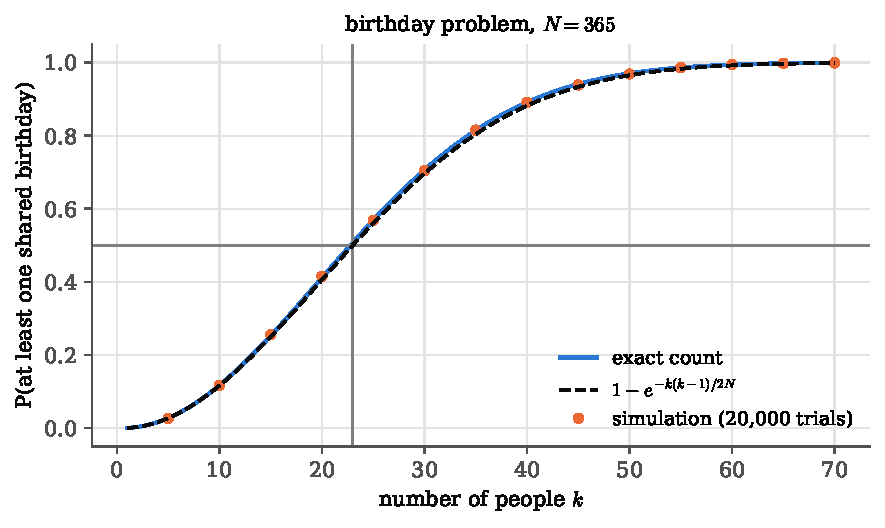
\includegraphics[width=0.8\linewidth]{figures/ch01/1a_birthday.pdf}
\caption{Probability that at least two of $k$ people share a birthday. The
exact count (solid) rises steeply and crosses one half between $22$ and $23$
people. The exponential approximation (dashed) lies just below it, and the
simulated frequencies (dots) fall on the exact curve.}
\label{1a:fig:birthday}
\end{figure}

\paragraph{What this bought us.}
Coincidences are governed by the number of \emph{pairs}, $\binom k2\approx k^2/2$,
not by $k$. A collision among $N$ equally likely labels becomes likely at
$k\sim\sqrt N$ draws, far below $N$.

\paragraph{In research: where the $\sqrt N$ rule bites.}
Pixel and strip detectors are designed so that occupancy stays low enough for
merged clusters to be rare, and the merging rate is estimated exactly as in
\cref{1a:ex:birthday}, then refined with a full simulation that includes the
real, non-uniform hit density near the beam. The same rule applies to random
seeds. If each of many parallel Monte Carlo jobs picks a $32$-bit seed at
random, two jobs share a seed (and produce identical ``independent'' samples)
with probability one half after only $1.18\sqrt{2^{32}}\approx77\,000$ jobs.
This is why \texttt{common.py} derives seeds deterministically through
\texttt{SeedSequence} (\cref{ch:06}).

\section{Conditional probability: shrinking the sample space}
\label{1a:sec:conditional}

At a collider, the trigger decides in microseconds which collisions are kept.
Everything an analyst later measures, such as the fraction of events with two
muons, the fraction whose muons have opposite charge or the fraction that fall
in a mass window, is a fraction \emph{among triggered events}. The events that
were not kept are gone. The analyst's world has shrunk from ``all collisions''
to ``collisions that fired the trigger''.

That is the whole idea: \emph{information shrinks the sample space}. The
question is this. Once we learn that an event $B$ happened, what is the new
probability of an event $A$? Conditional probability is the rule that answers
it, by computing probabilities inside the shrunken space. It is how a
probability changes when we learn something. Trees, the law of total
probability, independence and Bayes' theorem are all built from it. In a
simulation it is literally a selection: keep the rows in which $B$ holds, and
count among them.

In the area picture, conditioning changes only the unit of measurement.
Before we learn anything, $\Prob(A)$ is the fraction of the whole box $\Omega$
covered by $A$. If we learn that the outcome lies in $B$, every point outside
$B$ is ruled out, and $B$ becomes the new box. The probability of $A$ is now the
fraction of $B$ covered by $A$: the area of the overlap $AB$, measured in units
of the area of $B$ (\cref{1a:fig:shrink}). Nothing inside $B$ is re-weighted
relative to anything else inside $B$.

In \cref{1a:fig:shrink} the two regions are a hypothesis $H$ and an observed
event $E$. Their overlap $HE$ (green) can be measured against either one.
Measured against $H$, it is the share of the hypothesis region in which $E$
also happens. Measured against $E$, it is the share of the observed region in
which $H$ was also true. One patch, two yardsticks. Bayes' theorem
(\cref{1a:sec:bayes}) is the relation between those two readings of the same
patch, so the picture already contains it.

\begin{figure}[htbp]
\centering
\begin{tikzpicture}[scale=0.85]
  \begin{scope}
    \draw[thick] (0,0) rectangle (5,3.4);
    \fill[formblue!25] (0.5,0.5) rectangle (3.2,2.9);
    \fill[fibreorange!30] (2.2,0.9) rectangle (4.5,2.5);
    \fill[tangentgreen!45] (2.2,0.9) rectangle (3.2,2.5);
    \draw (0.5,0.5) rectangle (3.2,2.9);
    \draw (2.2,0.9) rectangle (4.5,2.5);
    \node[lbl] at (1.3,1.7) {$H$};
    \node[lbl] at (3.9,1.7) {$E$};
    \node[lbl] at (2.7,1.7) {$HE$};
    \node[lbl] at (4.6,3.05) {$\Omega$};
    \node[lbl,align=center] at (2.5,-0.55) {original sample space:\\ $\Prob(H)=\text{area}(H)/\text{area}(\Omega)$};
  \end{scope}
  \draw[->,thick,accent] (5.5,1.7) -- (6.9,1.7);
  \node[lbl,accent,anchor=south] at (6.2,2.3) {observe $E$};
  \begin{scope}[xshift=7.4cm]
    \draw[faint,dashed] (0,0) rectangle (5,3.4);
    \fill[fibreorange!30] (2.2,0.9) rectangle (4.5,2.5);
    \fill[tangentgreen!45] (2.2,0.9) rectangle (3.2,2.5);
    \draw[very thick,fibreorange] (2.2,0.9) rectangle (4.5,2.5);
    \node[lbl] at (2.7,1.7) {$HE$};
    \node[lbl] at (3.9,1.7) {$E$};
    \node[lbl,align=center] at (2.5,-0.55) {$E$ is the new reference space:\\ $\Prob(H\given E)=\text{area}(HE)/\text{area}(E)$};
  \end{scope}
\end{tikzpicture}
\caption{Conditioning as a change of reference space. Left: the hypothesis
region $H$ (blue) and the observed region $E$ (orange) overlap in the green
rectangle. Right: after we observe $E$, everything outside it is discarded and
the green area is measured as a fraction of the orange one. Measured against
$H$ instead, the same green area gives $\Prob(E\given H)$.}
\label{1a:fig:shrink}
\end{figure}

In words, computing a conditional probability takes four steps:
\begin{enumerate}[leftmargin=1.5em,itemsep=1pt]
  \item What do we know has happened? That event, $B$, is the new sample space.
  \item Discard every outcome outside $B$.
  \item Among the outcomes that remain, how much probability lies in $A$ as well?
  \item Rescale, so that the surviving outcomes carry total probability one.
\end{enumerate}
These four steps determine the formula completely. Write $\Prob_B(A)$ for the new
probability of $A$ once $B$ is known. We ask for three things: (i) $\Prob_B$ is a
probability, (ii) $\Prob_B(B)=1$, since $B$ is now certain, and (iii) inside $B$
nothing changes except the unit, $\Prob_B(C)=c\,\Prob(C)$ for every $C\subset B$,
with one constant $c$. Then for any event $A$,
\begin{align*}
\Prob_B(A)
&\eqby{1}\Prob_B(AB)+\Prob_B(AB^c)
 \eqby{2}\Prob_B(AB)
 \eqby{3}c\,\Prob(AB),
\qquad\text{and}\qquad
1\eqby{4}\Prob_B(B)\eqby{5}c\,\Prob(B).
\end{align*}
\begin{explain}
  \item $A$ is the disjoint union of its parts inside and outside $B$, and
        $\Prob_B$ is additive by (i).
  \item $AB^c\subset B^c$, and $\Prob_B(B^c)=1-\Prob_B(B)=0$ by (ii), so by
        monotonicity $\Prob_B(AB^c)=0$.
  \item $AB\subset B$, so (iii) applies.
  \item Requirement (ii).
  \item Requirement (iii) with $C=B$.
\end{explain}
The last equation fixes $c=1/\Prob(B)$, and the first gives
$\Prob_B(A)=\Prob(AB)/\Prob(B)$. There is no other choice.

\begin{workdef}[conditional probability]
If $\Prob(B)>0$, the \newterm{conditional probability of $A$ given $B$} is
\begin{equation}
\Prob(A\given B)=\frac{\Prob(AB)}{\Prob(B)}.
\label{1a:eq:cond}
\end{equation}
Read the bar as ``given'' \unpack{restricted to the outcomes in which $B$ is
true}. \emph{Frequency reading:} among the runs in which $B$ happened, the
fraction in which $A$ also happened, $\Prob(A\given B)\approx n_{AB}/n_B$
\unpack{$n_{AB}$ counts runs with both, $n_B$ runs with $B$, whatever $A$ did}.
\emph{Operational test in code:} \texttt{A[B].mean()}.
\end{workdef}

Three remarks. First, $\Prob(A)=\Prob(A\given\Omega)$: every probability is
conditional on the sample space we chose \srcref{Cowan}{p.~2}. Second, the
bar carries no arrow of time.
\[
\Prob(\text{rain last night}\given\text{wet ground this morning})
\]
is a perfectly good conditional probability: among mornings with wet ground,
the fraction that followed a rainy night
\srcref{Kruschke}{\S4.4.1}. Third, if $A$ and $B$ are disjoint then
$\Prob(A\given B)=0$: once $B$ has happened, $A$ cannot have.

\paragraph{The shrinking sample space, drawn to scale.}
Very often a problem does not hand us $\Prob(AB)$ directly. It tells us how
probable a situation $H$ is, and how often an observation $E$ occurs
\emph{inside} each situation. Take $\Prob(H)=0.25$, and suppose $E$ happens in
$60\%$ of the $H$-world and in $10\%$ of the $H^c$-world. This is the picture of
\cref{1a:fig:shrink} drawn to scale (\cref{1a:fig:area}). Draw $\Omega$ as a
rectangle of area one and $H$ as a vertical strip of width $0.25$. Inside each
strip, mark the part where $E$ happens as a piece running the full height of the
strip: it covers $0.6$ of the $H$ strip and $0.1$ of the $H^c$ strip. Set the two
pieces against the line between the strips, so that together they make one box,
the event $E$. The share of a strip that its piece covers is itself a
conditional probability: it is $E$ measured against the strip as its reference
space, so the two shares are $\Prob(E\given H)$ and $\Prob(E\given H^c)$.

Before we observe anything, $\Prob(H)$ is the width $0.25$ of the $H$ strip, a
fraction of the whole rectangle. Now learn that $E$ happened. Every point
outside the box is ruled out. The surviving region is the new sample space, and
probabilities are re-measured against its area:
\begin{align*}
\Prob(H\given E)
&\eqby{1}\frac{\text{area}(HE)}{\text{area}(E)}
 \eqby{2}\frac{\text{area}(HE)}{\text{area}(HE)+\text{area}(H^cE)}\\
&\eqby{3}\frac{0.25\times0.6}{0.25\times0.6+0.75\times0.1}
 =\frac{0.15}{0.225}=\frac23 .
\end{align*}
\begin{explain}
  \item Definition of conditional probability as re-measured area. The areas
        are probabilities because $\Omega$ has area one.
  \item $E$ is the union of its two pieces, which do not overlap because $H$ and
        $H^c$ are disjoint.
  \item Each piece is the strip's width times the share of the strip it
        covers, the width being the strip's probability and the share the
        conditional probability of $E$ inside the strip.
\end{explain}
Learning $E$ moved the probability of $H$ from $\tfrac14$ to $\tfrac23$. Why?
The figure shows it. The $H$ strip was only a third as wide as the $H^c$ strip
($0.25$ against $0.75$). But $E$ is six times as common inside $H$ as outside it
($0.6$ against $0.1$). So, of the area that survives, the $H$ piece ($0.15$) is
twice the $H^c$ piece ($0.075$), and $H$ holds two thirds of it.

Step (3) used the multiplication rule $\Prob(HE)=\Prob(E\given H)\Prob(H)$, read
off the picture here and derived as \eqref{1a:eq:mult} below. With every term
named, and the denominator written as a sum over all hypotheses, the same
calculation is Bayes' theorem (\cref{1a:sec:bayes} and \cref{ch:05}). Here it
is only the definition of conditional probability, drawn to scale.

\begin{figure}[htbp]
\centering
\begin{tikzpicture}[scale=0.8]
  \begin{scope}
    \fill[formblue!18] (0,0) rectangle (6,4);
    \fill[tangentgreen!45] (0.6,0) rectangle (1.95,4);
    \draw (1.5,0) -- (1.5,4);
    \draw[thick] (0,0) rectangle (6,4);
    \draw[line width=1.6pt,fibreorange] (0.6,0) rectangle (1.95,4);
    \node[lbl] at (0.3,2) {$H$};
    \node[lbl] at (3.975,2) {$H^c$};
    \node[lbl,font=\footnotesize] at (1.05,1.4) {$0.15$};
    \draw[faint] (1.75,2.6) -- (2.3,2.95) node[lbl,font=\footnotesize,anchor=south west,black,inner sep=1pt] {$0.075$};
    \node[lbl,fibreorange!80!black,anchor=south] at (1.275,4.05) {$E$};
    \node[lbl] at (6.25,3.75) {$\Omega$};
    \draw[faint] (0,-0.15) -- (0,-0.3) -- (1.5,-0.3) -- (1.5,-0.15);
    \draw[faint] (1.5,-0.15) -- (1.5,-0.3) -- (6,-0.3) -- (6,-0.15);
    \node[lbl] at (0.75,-0.6) {$0.25$};
    \node[lbl] at (3.75,-0.6) {$0.75$};
    \node[lbl,align=center,text width=6.2cm,anchor=north] at (3,-0.95) {before: $H$ fills a quarter of $\Omega$};
  \end{scope}
  \draw[->,thick,accent] (6.7,2) -- (8.1,2);
  \node[lbl,accent,align=center] at (7.4,2.75) {observe\\$E$};
  \begin{scope}[xshift=8.7cm]
    \draw[faint,dashed] (0,0) rectangle (6,4);
    \draw[faint,dashed] (1.5,0) -- (1.5,4);
    \fill[tangentgreen!45] (0.6,0) rectangle (1.95,4);
    \draw[very thin,black!40] (1.5,0) -- (1.5,4);
    \draw[line width=1.6pt,fibreorange] (0.6,0) rectangle (1.95,4);
    \node[lbl,align=center] at (1.05,2) {$H$\\[2pt]$\tfrac23$};
    \draw[faint] (1.75,1.2) -- (2.3,0.9) node[lbl,anchor=west,black,align=left,inner sep=1pt] {$H^c$: $\tfrac13$};
    \node[lbl,fibreorange!80!black,anchor=south] at (1.275,4.05) {$E$, area $0.225$};
    \node[lbl,align=center,text width=6.2cm,anchor=north] at (3,-0.95) {after: $E$ is the new sample space,\\ $H$ fills two thirds of it};
  \end{scope}
\end{tikzpicture}
\caption{Conditioning drawn to scale, in the picture of \cref{1a:fig:shrink}.
Left: the rectangle $\Omega$ has area 1, split into the strip $H$ of width
$0.25$ and the strip $H^c$ of width $0.75$. The event $E$ (orange outline)
covers $0.6$ of the $H$ strip and $0.1$ of the $H^c$ strip, so its two green
pieces have areas $0.25\times0.6=0.15$ and $0.75\times0.1=0.075$. Right: once
$E$ is observed, everything outside the orange box is discarded. $H$ keeps the
share of the box that its piece fills, $0.15/0.225=\tfrac23$, although its strip
was only a quarter of $\Omega$.}
\label{1a:fig:area}
\end{figure}

\oneaEx{Two dice, by counting in the shrunken space}
\label{1a:ex:dice-cond}
Roll two fair dice. Let $A$ be ``the sum is 8'' and $B$ ``at least one die shows
6''. By counting, $B$ has $11$ of the $36$ outcomes (six with a first 6, six with a
second 6, minus the double-counted $(6,6)$), $A=\{(2,6),(3,5),(4,4),(5,3),(6,2)\}$ has
$5$, and $AB=\{(2,6),(6,2)\}$ has $2$. Then
\begin{align*}
\Prob(A\given B)\eqby{1}\frac{\Prob(AB)}{\Prob(B)}\eqby{2}\frac{2/36}{11/36}=\frac{2}{11}\approx0.182,
\qquad
\Prob(B\given A)=\frac{2/36}{5/36}=\frac25=0.4 .
\end{align*}
\begin{explain}
  \item Definition \eqref{1a:eq:cond}.
  \item Uniform distribution on $36$ outcomes. The $1/36$ cancels, so the answer is
        a ratio of counts \emph{inside} $B$: $|AB|/|B|$.
\end{explain}
Learning $B$ raises the probability of $A$ from $5/36\approx0.139$ to $0.182$. The
two conditional probabilities use the same overlap and differ only in what it
is divided by.

\oneaEx{Hair and eye colour: reallocating credibility}
\label{1a:ex:hair-eye}
A sample of people has the joint proportions of eye and hair colour below
\srcref{Kruschke}{Table 4.1} (rows do not add exactly because of rounding in
the original data):
\begin{center}
\small
\begin{tabular}{@{}lccccc@{}}
\toprule
eye $\backslash$ hair & black & brunette & red & blond & marginal\\
\midrule
brown & 0.11 & 0.20 & 0.04 & 0.01 & 0.37\\
blue  & 0.03 & 0.14 & 0.03 & 0.16 & 0.36\\
hazel & 0.03 & 0.09 & 0.02 & 0.02 & 0.16\\
green & 0.01 & 0.05 & 0.02 & 0.03 & 0.11\\
\midrule
marginal & 0.18 & 0.48 & 0.12 & 0.21 & 1.0\\
\bottomrule
\end{tabular}
\end{center}
Learning ``blue eyes'' keeps only the second row and divides it by its total:
\begin{align*}
\Prob(\text{black}\given\text{blue})&=\tfrac{0.03}{0.36}=0.08, &
\Prob(\text{brunette}\given\text{blue})&=\tfrac{0.14}{0.36}=0.39,\\
\Prob(\text{red}\given\text{blue})&=\tfrac{0.03}{0.36}=0.08, &
\Prob(\text{blond}\given\text{blue})&=\tfrac{0.16}{0.36}=0.45 .
\end{align*}
The probability of blond hair rises from $0.21$ to $0.45$. The four numbers still
add up to one, because the row was divided by its own total. Learning ``blue
eyes'' has moved probability from some hair colours to others. Kruschke calls
this a reallocation of credibility. It is already Bayesian inference in
miniature.

\subsection{$\Prob(\cdot\given B)$ is a probability, $\Prob(A\given\cdot)$ is not}

For fixed $B$ with $\Prob(B)>0$, the function $A\mapsto\Prob(A\given B)$ satisfies the
three axioms \mainref{p.~14, Ex.~9}. Axiom 1 holds because a ratio of a
nonnegative number and a positive number is nonnegative. Axiom 2 holds because
$\Prob(\Omega\given B)=\Prob(\Omega B)/\Prob(B)=\Prob(B)/\Prob(B)=1$. For Axiom 3, let
$A_1,A_2,\dots$ be disjoint:
\begin{align*}
\Prob\Bigl(\,\bigcup_iA_i\,\Big\vert\, B\Bigr)
&\eqby{1}\frac{\Prob\bigl((\bigcup_iA_i)\cap B\bigr)}{\Prob(B)}
 \eqby{2}\frac{\Prob\bigl(\bigcup_i(A_iB)\bigr)}{\Prob(B)}
 \eqby{3}\frac{\sum_i\Prob(A_iB)}{\Prob(B)}
 \eqby{4}\sum_i\Prob(A_i\given B).
\end{align*}
\begin{explain}
  \item Definition \eqref{1a:eq:cond}.
  \item Distributive law \eqref{1a:eq:distrib}, for a countable family.
  \item The sets $A_iB$ are disjoint, because $A_iB\subset A_i$ and the $A_i$
        are. Then Axiom 3 for $\Prob$.
  \item Split the sum and use the definition for each term.
\end{explain}
So every rule of \cref{1a:sec:axioms} holds with ``$\given B$'' appended
everywhere: $\Prob(A^c\given B)=1-\Prob(A\given B)$, inclusion--exclusion, Boole.
This matters later, when all the machinery of probability is applied to a
posterior, which is a probability conditional on the data.

The same is \emph{not} true in the other slot. For fixed $A$, the map
$B\mapsto\Prob(A\given B)$ is not a probability. In general
$\Prob(A\given B\cup C)\neq\Prob(A\given B)+\Prob(A\given C)$, even for disjoint $B$ and
$C$. The quickest check: take $A=\Omega$, and any disjoint $B$ and $C$ of positive
probability. Every conditional probability of $\Omega$ is one, so the left side
is $1$ and the right side is $1+1=2$. The rules of probability act only on
events to the left of the bar \mainref{p.~10}.

\subsection{$\Prob(A\given B)$ is not $\Prob(B\given A)$}

The probability of spots given measles is essentially one. The probability of
measles given spots is small, since many things cause spots. The two
conditional probabilities share the numerator $\Prob(AB)$ and differ in the
denominator. \Cref{1a:fig:swap} draws it with the rectangles of
\cref{1a:fig:shrink}, now labelled $A$ and $B$. Conditioning on $B$ makes $B$
the whole world, and we ask what fraction of it the overlap fills. Swapping the
roles makes $A$ the whole world, and the same overlap is now measured against a
bigger region. In the picture the overlap has area $1.6$, $B$ has area $3.68$
and $A$ has area $6.48$, so
\begin{align*}
  \Prob(A\given B)&=\frac{\text{area}(AB)}{\text{area}(B)}=\frac{1.6}{3.68}=0.43,
  &
  \Prob(B\given A)&=\frac{\text{area}(AB)}{\text{area}(A)}=\frac{1.6}{6.48}=0.25 .
\end{align*}
Same patch, different yardstick, different answer. The two are equal only when
$A$ and $B$ have the same probability.

\begin{figure}[htbp]
\centering
\begin{tikzpicture}[scale=0.8]
  \begin{scope}
    \draw[faint,dashed] (0,0) rectangle (5,3.4);
    \draw[faint,dashed] (0.5,0.5) rectangle (3.2,2.9);
    \fill[fibreorange!30] (2.2,0.9) rectangle (4.5,2.5);
    \fill[tangentgreen!45] (2.2,0.9) rectangle (3.2,2.5);
    \draw[very thick,fibreorange] (2.2,0.9) rectangle (4.5,2.5);
    \node[lbl,softgray] at (1.3,1.7) {$A$};
    \node[lbl] at (2.7,1.7) {$AB$};
    \node[lbl] at (3.9,1.7) {$B$};
    \node[lbl,align=center] at (2.5,-0.6) {condition on $B$:\\ $\Prob(A\given B)=\text{area}(AB)/\text{area}(B)$};
  \end{scope}
  \begin{scope}[xshift=6.6cm]
    \draw[faint,dashed] (0,0) rectangle (5,3.4);
    \draw[faint,dashed] (2.2,0.9) rectangle (4.5,2.5);
    \fill[formblue!25] (0.5,0.5) rectangle (3.2,2.9);
    \fill[tangentgreen!45] (2.2,0.9) rectangle (3.2,2.5);
    \draw[very thick,formblue] (0.5,0.5) rectangle (3.2,2.9);
    \node[lbl] at (1.3,1.7) {$A$};
    \node[lbl] at (2.7,1.7) {$AB$};
    \node[lbl,softgray] at (3.9,1.7) {$B$};
    \node[lbl,align=center] at (2.5,-0.6) {condition on $A$:\\ $\Prob(B\given A)=\text{area}(AB)/\text{area}(A)$};
  \end{scope}
\end{tikzpicture}
\caption{Swapping what we condition on. The rectangles are those of
\cref{1a:fig:shrink}. Left: we learn that $B$ happened, so $B$ (orange outline)
is the new reference space and the green overlap is read as a fraction of
$B$. Right: we learn that $A$ happened instead, so $A$ (blue outline) is the
reference space and the same green overlap is read as a fraction of the larger
region $A$. Same numerator, different denominator: $\Prob(A\given B)=0.43$ but
$\Prob(B\given A)=0.25$.}
\label{1a:fig:swap}
\end{figure}

Mistaking one for the other is
common enough in court to have a name, the \newterm{prosecutor's fallacy}:
``the chance that an innocent person matches the DNA sample is one in a
million, so the chance that the defendant is innocent is one in a million''.
In statistics the same mistake reads ``$\Prob(\text{data this extreme}\given\Hnull)=0.01$,
so $\Prob(\Hnull\given\text{data})=0.01$'', which confuses a $p$-value with a
posterior probability (\cref{ch:04,ch:05}).

\oneaEx{A medical test}
\label{1a:ex:medical}
A test for a disease $D$ has outcomes $+$ and $-$, and the joint probabilities
are \mainref{p.~10, Ex.~1.13}
\begin{center}
\begin{tabular}{@{}lcc@{}}
\toprule
 & $D$ & $D^c$\\
\midrule
$+$ & $0.009$ & $0.099$\\
$-$ & $0.001$ & $0.891$\\
\bottomrule
\end{tabular}
\end{center}
Condition on the column (the true state) to get the test's performance:
\begin{align*}
\Prob(+\given D)\eqby{1}\frac{\Prob(+\cap D)}{\Prob(D)}\eqby{2}\frac{0.009}{0.009+0.001}=0.9,
\qquad
\Prob(-\given D^c)=\frac{0.891}{0.891+0.099}=0.9 .
\end{align*}
\begin{explain}
  \item Definition \eqref{1a:eq:cond}.
  \item $\Prob(D)$ is the sum of its column, since $D=(+\cap D)\cup(-\cap D)$ disjointly.
\end{explain}
The test is right $90\%$ of the time for the sick and for the healthy. Now
condition on the row (the result) instead:
\begin{align*}
\Prob(D\given +)\eqby{1}\frac{\Prob(+\cap D)}{\Prob(+)}\eqby{2}\frac{0.009}{0.009+0.099}
=\frac{9}{108}\approx0.08 .
\end{align*}
\begin{explain}
  \item Definition \eqref{1a:eq:cond}, now with $+$ as the conditioning event.
  \item $\Prob(+)$ is the sum of the first row.
\end{explain}
A positive result means the disease with probability $8\%$, not $90\%$. Among
positives, the healthy outnumber the sick eleven to one, because there are
ninety-nine times more healthy people to produce false positives
(\cref{1a:fig:dots}).

\begin{figure}[htbp]
\centering
\begin{tikzpicture}[x=0.24cm,y=0.24cm]
  \foreach \c in {0,...,49}{
    \foreach \r in {0,...,19}{
      \pgfmathtruncatemacro{\idx}{\c*20+\r}
      \ifnum\idx<9
        \fill[bdryred] (\c,-\r) circle (0.36);
      \else\ifnum\idx<10
        \draw[bdryred,thick] (\c,-\r) circle (0.30);
      \else\ifnum\idx<109
        \fill[fibreorange!70] (\c,-\r) circle (0.36);
      \else
        \fill[softgray!35] (\c,-\r) circle (0.30);
      \fi\fi\fi
    }
  }
  \node[lbl,anchor=west] at (0,-22.5)  {\tikz\fill[bdryred] (0,0) circle (3pt); sick, positive: 9};
  \node[lbl,anchor=west] at (0,-25)    {\tikz\draw[bdryred,thick] (0,0) circle (2.5pt); sick, negative: 1};
  \node[lbl,anchor=west] at (22,-22.5) {\tikz\fill[fibreorange!70] (0,0) circle (3pt); healthy, positive: 99};
  \node[lbl,anchor=west] at (22,-25)   {\tikz\fill[softgray!35] (0,0) circle (3pt); healthy, negative: 891};
  \node[lbl,anchor=west] at (40,-23.7) {$\Prob(D\given+)=\dfrac{9}{9+99}$};
\end{tikzpicture}
\caption{The medical test as a thousand people. The red dots at the top left
are the ten who are sick, nine of whom test positive. The orange block is the
ninety-nine healthy people who also test positive. Conditioning on a positive
result keeps only the filled coloured dots, and the red ones are a small
minority of them.}
\label{1a:fig:dots}
\end{figure}

\oneaEx{A radioactive nucleus does not age}
\label{1a:ex:nucleus}
A nucleus with decay constant $\lambda$ survives to time $t$ with probability
$\Prob(S_t)=e^{-\lambda t}$, where $S_t$ is ``not yet decayed at time $t$''. Given that
it has survived to $t$, what is the probability that it survives a further
time $s$? Surviving to $t+s$ implies surviving to $t$, so $S_{t+s}\subset S_t$ and
$S_{t+s}S_t=S_{t+s}$. Then
\begin{align*}
\Prob(S_{t+s}\given S_t)
\eqby{1}\frac{\Prob(S_{t+s}S_t)}{\Prob(S_t)}
\eqby{2}\frac{\Prob(S_{t+s})}{\Prob(S_t)}
\eqby{3}\frac{e^{-\lambda(t+s)}}{e^{-\lambda t}}
\eqby{4}e^{-\lambda s}=\Prob(S_s).
\end{align*}
\begin{explain}
  \item Definition \eqref{1a:eq:cond}.
  \item $S_{t+s}\subset S_t$.
  \item The survival law.
  \item $e^{a+b}=e^ae^b$.
\end{explain}
A nucleus that has already lived a thousand years is exactly as likely to
survive the next second as a freshly made one. The exponential law is the only
survival law with this \newterm{memoryless} property, and it is why the decay
constant is meaningful at all. Taking $s=\dd t$ small,
$\Prob(\text{decay in }[t,t+\dd t]\given S_t)=1-e^{-\lambda\,\dd t}\approx\lambda\,\dd t$: the decay
constant \emph{is} a conditional probability per unit time, the same at every
age. A human, or a photomultiplier tube, does age, and its survival law is not
exponential.

\subsection{The multiplication rule}

Multiplying \eqref{1a:eq:cond} by $\Prob(B)$, and doing the same with the roles of
$A$ and $B$ exchanged, gives the \newterm{multiplication rule}
\mainref{p.~11, Lemma~1.14}:
\begin{equation}
\Prob(AB)=\Prob(A\given B)\,\Prob(B)=\Prob(B\given A)\,\Prob(A).
\label{1a:eq:mult}
\end{equation}
Read it as a two-step story: for $A$ and $B$ both to happen, first $A$ must
happen, and then, in the world where $A$ has happened, $B$ must happen
\srcref{Lambert}{\S3.6}. Applying it repeatedly gives the \newterm{chain rule}
\mainref{p.~15, Ex.~17}:
\begin{align}
\Prob(ABC)
&\eqby{1}\Prob\bigl(A\given BC\bigr)\,\Prob(BC)
 \eqby{2}\Prob(A\given BC)\,\Prob(B\given C)\,\Prob(C),
\label{1a:eq:chain}
\end{align}
\begin{explain}
  \item Multiplication rule \eqref{1a:eq:mult} with the two events $A$ and $BC$.
  \item Multiplication rule again, for $\Prob(BC)$.
\end{explain}
and in general $\Prob(A_1A_2\cdots A_n)=\Prob(A_1)\Prob(A_2\given A_1)\Prob(A_3\given A_1A_2)\cdots
\Prob(A_n\given A_1\cdots A_{n-1})$. The chain rule is the arithmetic of a path through a
tree, which is the subject of the next section.

\oneaEx{Cards drawn without replacement}
\label{1a:ex:cards}
Draw two cards from a deck without putting the first back. Let $A$ be ``first is
the ace of clubs'' and $B$ ``second is the queen of diamonds''. Then
$\Prob(A)=1/52$, and once $A$ has happened the second card is uniform over the $51$
cards that remain, one of which is the queen of diamonds. So
$\Prob(AB)=\Prob(A)\Prob(B\given A)=\tfrac1{52}\cdot\tfrac1{51}$ \mainref{p.~11, Ex.~1.15}.

Four aces in a row: with $E_j$ ``the $j$-th card is an ace'',
\begin{align*}
\Prob(E_1E_2E_3E_4)
\eqby{1}\Prob(E_1)\Prob(E_2\given E_1)\Prob(E_3\given E_1E_2)\Prob(E_4\given E_1E_2E_3)
\eqby{2}\frac4{52}\cdot\frac3{51}\cdot\frac2{50}\cdot\frac1{49}
=\frac{1}{270\,725}.
\end{align*}
\begin{explain}
  \item Chain rule.
  \item At each step the shrunken deck is uniform: after $j$ aces, $52-j$ cards
        remain, $4-j$ of them aces.
\end{explain}
This equals $1/\binom{52}4$, as it must. Now condition on having started well
\srcref{CasellaBerger}{Ex.~1.3.3}. Given that the first $i$ cards are aces, the
deck has $52-i$ cards with $4-i$ aces, and the probability that the next $4-i$
cards are exactly those aces is $1/\binom{52-i}{4-i}$. For $i=1,2,3$ this is
$0.00005$, $0.00082$ and $0.0204$. Each piece of good news makes the event four
aces far more probable, though still unlikely.

\subsection{Conditioning is selection: a simulation}

In code, conditioning on $B$ means keeping only the rows where $B$ is true. We
repeat \cref{1a:ex:dice-cond} with $\OneACondN$ simulated rolls.

\pyfile[firstline=21,lastline=32,firstnumber=21]{code/ch01/04_conditioning_by_filtering.py}{Conditioning by filtering}

Lines 25--26 build the two masks. Line 29 is the whole of conditional
probability: \texttt{A[B]} is the sub-array of $A$ over the rows in which $B$
happened, and its mean is the fraction of those rows in which $A$ also
happened, $n_{AB}/n_B$. Line 32 computes the same number as a ratio of two
unconditional frequencies, $\hat\Prob(AB)/\hat\Prob(B)$, and the two agree exactly
($\OneACondAgB$ and $\OneACondRatio$), because $n_{AB}/n_B=(n_{AB}/N)/(n_B/N)$.

Of the $\OneACondN$ rolls, $\OneACondNB$ had at least one six, $\OneACondNA$ had
sum eight, and $\OneACondNAB$ had both. The estimates are
$\hat\Prob(A\given B)=\OneACondAgB$ (exact $2/11=\OneACondExAgB$) and
$\hat\Prob(B\given A)=\OneACondBgA$ (exact $2/5=\OneACondExBgA$).

\begin{figure}[htbp]
\centering
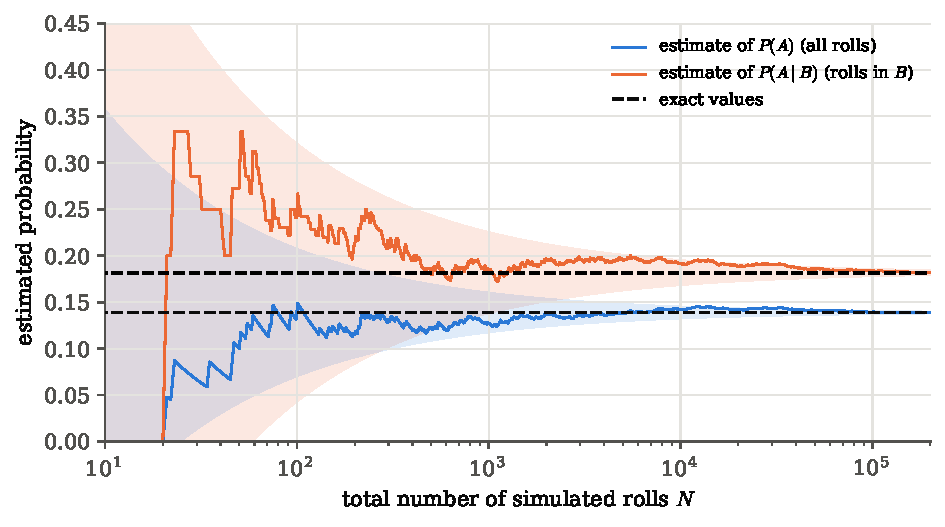
\includegraphics[width=0.85\linewidth]{figures/ch01/1a_conditioning.pdf}
\caption{Running estimates of $\Prob(A)$ from all rolls (blue) and of $\Prob(A\given B)$
from the rolls in $B$ only (orange), against the total number of simulated
rolls, with the exact values dashed. Both converge, but the conditional
estimate wanders more and its band is wider, because only about $30\%$ of the
rolls survive the selection.}
\label{1a:fig:conditioning}
\end{figure}

The figure shows the price of conditioning. The estimate of $\Prob(A\given B)$ uses
only $n_B\approx N\Prob(B)$ rolls, so its scatter is about
$\sqrt{\Prob(A\given B)(1-\Prob(A\given B))/(N\Prob(B))}$, the running-frequency rule of
\cref{1a:sec:axioms} with $n$ replaced by the number of survivors. Conditioning
on a rare event leaves few survivors, and then the estimate is noisy however
large $N$ was.

So conditioning is selection followed by renormalisation. In a simulation it
is one line, \texttt{A[B].mean()}, and its statistical error is set by how many
events survive the selection, not by how many were generated.

Two traps are worth naming. First, $\Prob(A\given B)$ and $\Prob(B\given A)$ are
different numbers, and they can be very different (\cref{1a:ex:medical}), so
always say in words which event is known. Second, \eqref{1a:eq:cond} needs
$\Prob(B)>0$. Conditioning on an event of probability zero, such as ``the
measured energy is exactly $91.1876$ GeV'', is still meaningful but needs
densities, which come in the next part.

\begin{inpractice}[Tag-and-probe]
The efficiency of a muon identification algorithm is a conditional
probability, $\Prob(\text{identified}\given\text{real muon})$. In data we do not know
which tracks are real muons, so we make a subset in which we do. Select
events with two tracks whose invariant mass is at the $Z$ peak and in which
one track (the ``tag'') passes a very tight identification. The other track
(the ``probe'') is then almost certainly a muon, and the fraction of probes
that pass the algorithm is the efficiency. The whole technique is the
definition \eqref{1a:eq:cond}, implemented as a selection on real events. Here
it is the research instrument: no formula gives this efficiency.
\end{inpractice}

Everything in this section comes back to one picture: the conditioning event
$B$ becomes the new, shrunk sample space \mainref{pp.~10--12, \S1.6}. It is
certain inside itself, $\Prob(B\given B)=\Prob(B)/\Prob(B)=1$
\srcref{CasellaBerger}{\S1.3}, and every other probability is re-measured as a
share of it (Seeing Theory draws the same idea as ``shelves'',
\srcref{SeeingTheory}{p.~27}). The medical test shows why we should not trust
intuition here: the shrunk space can hold a very different mix of cases from
the original one.
\section{Probability trees and the law of total probability}
\label{1a:sec:trees}

One collision in a hundred contains a real high-momentum muon ($S$, for
signal). The other $99\%$ do not ($B$, background). The hardware level-1
trigger (L1) fires for $95\%$ of the signal collisions and, because of fake
muons from hadrons punching through the calorimeter, for $2\%$ of the
background. The collisions that pass L1 are examined by the software
high-level trigger (HLT), which, \emph{among those that passed L1}, keeps
$90\%$ of the signal and $10\%$ of the background. What fraction of all
collisions is written to disk, and how much of what is written is signal?

A situation built from successive stages is drawn as a tree. Two rules then
answer both questions. The probability of each complete path is the product of
the conditional probabilities along it. The probability of an observation is
the sum over all the paths that lead to it. That sum is the law of total
probability. Read the right way, it is also marginalisation: averaging out the
stage we do not observe.

\paragraph{Water flowing through pipes.}
Pour one litre of water in at the root. At every junction the water divides
among the outgoing pipes in fixed proportions (the conditional probabilities),
and no water is lost, so the proportions at each junction add up to one. The
water reaching the end of a pipe is the product of the proportions along the
way. The total water collected in a bucket that several pipes drain into is
the sum of what each pipe delivers.

\paragraph{Building and reading a tree.}
The recipe, in words, is as follows.
\begin{enumerate}[leftmargin=1.5em,itemsep=1pt]
  \item What are the stages of the situation, in the order they are easiest
        to describe? (Nature picks $S$ or $B$, then L1 decides, then HLT decides.)
  \item At each node, what are the mutually exclusive possibilities for the
        next stage, and what is the probability of each \emph{given the path so far}?
  \item The probability of a complete path is the product along it.
  \item The probability of an event is the sum over the leaves where the event
        is true.
\end{enumerate}

\begin{workdef}[probability tree]
A \newterm{probability tree} is a rooted tree whose branches leaving each
node are the possible results of the next stage \unpack{mutually exclusive and
exhaustive, given everything above the node}. Each branch carries the
conditional probability of its result given the path from the root to its
node, so the labels leaving a node sum to one. A \newterm{path} from the root
to a leaf is one complete history, and the leaves partition $\Omega$
\unpack{every outcome follows exactly one path}.
\emph{Rules:} multiply along a path, add across paths.
\end{workdef}

\begin{figure}[htbp]
\centering
\begin{tikzpicture}[
  lev/.style={font=\small,inner sep=2pt},
  br/.style={thick,accent},
  pr/.style={font=\scriptsize,fill=white,inner sep=1pt},
  x=1cm,y=0.75cm]
  \node[lev] (r) at (0,0) {collision};
  \node[lev] (S) at (2.6,2.6) {$S$};
  \node[lev] (B) at (2.6,-2.6) {$B$};
  \node[lev] (SL) at (5.4,3.8) {L1};
  \node[lev] (SN) at (5.4,1.4) {no L1};
  \node[lev] (BL) at (5.4,-1.4) {L1};
  \node[lev] (BN) at (5.4,-3.8) {no L1};
  \node[lev] (SLH) at (8.2,4.6) {HLT};
  \node[lev] (SLN) at (8.2,3.0) {no HLT};
  \node[lev] (BLH) at (8.2,-0.6) {HLT};
  \node[lev] (BLN) at (8.2,-2.2) {no HLT};
  \draw[br] (r) -- node[pr,above left] {$0.01$} (S);
  \draw[br] (r) -- node[pr,below left] {$0.99$} (B);
  \draw[br] (S) -- node[pr,above left] {$0.95$} (SL);
  \draw[br] (S) -- node[pr,below left] {$0.05$} (SN);
  \draw[br] (B) -- node[pr,above left] {$0.02$} (BL);
  \draw[br] (B) -- node[pr,below left] {$0.98$} (BN);
  \draw[br] (SL) -- node[pr,above left] {$0.90$} (SLH);
  \draw[br] (SL) -- node[pr,below left] {$0.10$} (SLN);
  \draw[br] (BL) -- node[pr,above left] {$0.10$} (BLH);
  \draw[br] (BL) -- node[pr,below left] {$0.90$} (BLN);
  \node[font=\small,anchor=west,fibreorange] at (9.0,4.6) {$0.01\times0.95\times0.90=0.00855$};
  \node[font=\small,anchor=west,softgray] at (9.0,3.0) {$0.00095$};
  \node[font=\small,anchor=west,softgray] at (6.1,1.4) {$0.0005$};
  \node[font=\small,anchor=west,fibreorange] at (9.0,-0.6) {$0.99\times0.02\times0.10=0.00198$};
  \node[font=\small,anchor=west,softgray] at (9.0,-2.2) {$0.01782$};
  \node[font=\small,anchor=west,softgray] at (6.1,-3.8) {$0.9702$};
\end{tikzpicture}
\caption{The two-level trigger as a tree. The first split is nature's choice
between signal and background. Each later split is a trigger decision, and its
numbers are conditional on everything to the left. The numbers at the right
are the path probabilities, which add up to one. The two orange paths end in
``written to disk''.}
\label{1a:fig:trigger-tree}
\end{figure}

\subsection{Multiply along a path}

A path is an intersection of events, one per stage, so its probability is the
chain rule \eqref{1a:eq:chain}. For the top path of \cref{1a:fig:trigger-tree},
\begin{align}
\Prob(S\cap\mathrm{L1}\cap\mathrm{HLT})
&\eqby{1}\Prob(S)\,\Prob(\mathrm{L1}\given S)\,\Prob(\mathrm{HLT}\given S\cap\mathrm{L1})
 \eqby{2}0.01\times0.95\times0.90=0.00855 .
\label{1a:eq:path}
\end{align}
\begin{explain}
  \item Chain rule, with the events taken in the order of the stages.
  \item The branch labels. The last one is the HLT efficiency \emph{for signal
        that passed L1}, which is exactly how the HLT number was specified.
\end{explain}
The path probabilities at the right of \cref{1a:fig:trigger-tree} sum to one.
The reason is that the labels leaving each node sum to one. So the paths
through the branches leaving a node add up to the probability of the path
that reaches that node. Repeating this from the leaves back to the root leaves
the root's probability, one. In the water picture, no water is lost at a
junction.

\subsection{Add across paths: the law of total probability}

Let ``accepted'' be $\mathrm{Acc}=\mathrm{L1}\cap\mathrm{HLT}$. Two paths end in it,
one through $S$ and one through $B$. They are disjoint (a collision cannot be
both signal and background), so their probabilities add:
\begin{align*}
\Prob(\mathrm{Acc})=0.00855+0.99\times0.02\times0.10=0.00855+0.00198=0.01053 .
\end{align*}
About one collision in a hundred is kept. Nothing here was special to the
trigger: whenever the first stage splits $\Omega$ into disjoint pieces, the
probability of an event is the sum over the paths that end in it.

\begin{keyidea}[Law of total probability]
Let $A_1,\dots,A_k$ be a partition of $\Omega$. Then for any event $B$,
\begin{equation}
\Prob(B)=\sum_{i=1}^k\Prob(B\given A_i)\,\Prob(A_i).
\label{1a:eq:total}
\end{equation}
The first stage of the tree is the partition, the second stage is ``does $B$
happen'', and \eqref{1a:eq:total} adds the paths that end in $B$.
\end{keyidea}

To prove it, cut $B$ along the partition as in \cref{1a:fig:partition}:
$C_i=BA_i$. Every outcome of $B$ lies in exactly one $A_i$, so the $C_i$ are
disjoint and $B=\bigcup_iC_i$ \mainref{p.~12, Thm~1.16}. Then
\begin{align*}
\Prob(B)\eqby{1}\Prob\Bigl(\,\bigcup_iC_i\Bigr)\eqby{2}\sum_i\Prob(BA_i)\eqby{3}\sum_i\Prob(B\given A_i)\,\Prob(A_i).
\end{align*}
\begin{explain}
  \item $B$ is the union of its pieces $C_i$.
  \item Finite additivity for the disjoint pieces $C_i=BA_i$.
  \item Multiplication rule \eqref{1a:eq:mult} for each piece. If some
        $\Prob(A_i)=0$, the term $\Prob(BA_i)=0$ is simply dropped.
\end{explain}
The law holds just as well for a countable partition $A_1,A_2,\dots$, by
Axiom 3 in place of finite additivity.

\paragraph{Total probability is an average.}
The weights $\Prob(A_i)$ in \eqref{1a:eq:total} are nonnegative and sum to
one. So $\Prob(B)$ is a \emph{weighted average} of the conditional probabilities
$\Prob(B\given A_i)$, and it lies between the smallest and the largest of them.
In the trigger, the acceptance $0.01053$ lies between the background acceptance
$0.002$ ($=0.02\times0.10$) and the signal acceptance $0.855$
($=0.95\times0.90$). It sits very close to the background value, because
background carries $99\%$ of the weight.

This averaging is what it means to \newterm{marginalise}. We average out the
stage we do not observe, here the true nature of the collision. That stage
plays the role of a \emph{nuisance} variable: it matters for the answer, but we
do not ask about it. In \cref{ch:05} the same sum becomes an integral over
parameters $\params$ given data $\data$,
$p(\data)=\int p(\data\given\params)\,p(\params)\,\dd\params$, the evidence.

\oneaEx{The 662 keV line of caesium-137}
\label{1a:ex:cs137}
A $^{137}$Cs nucleus $\beta$-decays either to the excited isomer $^{137m}$Ba
(probability about $0.944$) or directly to the ground state of $^{137}$Ba (about
$0.056$). The isomer de-excites by emitting a $662$ keV photon with probability
about $0.902$. Otherwise the energy is carried off by an internal-conversion
electron. The direct branch emits no $662$ keV photon. The probability that one
decay produces a $662$ keV photon is
\begin{align*}
\Prob(\gamma_{662})
&\eqby{1}\Prob(\gamma_{662}\given{}^{137m}\mathrm{Ba})\,\Prob({}^{137m}\mathrm{Ba})
       +\Prob(\gamma_{662}\given\text{ground})\,\Prob(\text{ground})\\
&\eqby{2}0.902\times0.944+0\times0.056\approx0.851 ,
\end{align*}
\begin{explain}
  \item Law of total probability over the two decay branches.
  \item Branch probabilities from the nuclear data tables.
\end{explain}
which is the ``$85.1\%$ gamma intensity'' printed in the tables. A third stage,
``the photon deposits its full energy in the detector'' with probability
$\varepsilon$, multiplies the useful path by $\varepsilon$. A source of activity
$\mathcal A$ (decays per second) therefore gives a photopeak rate
$0.851\,\varepsilon\mathcal A$. Every calibration with a radioactive source uses
this tree.

\oneaEx{A coin from a bag}
\label{1a:ex:bag-total}
A bag holds a fair coin and a coin with $\Prob(\text{heads})=0.95$. We pick one
blindly and toss it three times \srcref{SeeingTheory}{p.~27}. Let $F$ be ``fair
coin picked'' and $H_3$ ``three heads''. Given the coin, the tosses are
independent (\cref{1a:sec:independence}), so $\Prob(H_3\given F^c)=0.95^3=0.857$ and
$\Prob(H_3\given F)=0.5^3=0.125$. Then
\begin{align*}
\Prob(H_3)\eqby{1}\Prob(H_3\given F^c)\Prob(F^c)+\Prob(H_3\given F)\Prob(F)
=0.857\times0.5+0.125\times0.5\approx0.491 .
\end{align*}
\begin{explain}
  \item Law of total probability over the partition $\{F,F^c\}$.
\end{explain}
We will reverse this tree in \cref{1a:sec:bayes} to ask which coin we hold.

\oneaEx{Taking turns: a tree with infinitely many paths}
\label{1a:ex:basketball}
Two players take turns shooting at a basket, player 1 first. Player 1 scores
with probability $1/3$, player 2 with probability $1/4$, independently each
time. What is the probability that player 1 scores first
\mainref{p.~9, Ex.~1.11}?

\begin{center}
\begin{tikzpicture}[x=1.45cm,y=0.9cm,
  br/.style={thick,accent},pr/.style={font=\scriptsize,fill=white,inner sep=1pt},
  nd/.style={font=\small,inner sep=2pt}]
  \node[nd] (a0) at (0,0) {start};
  \node[nd,fibreorange] (w1) at (1,-1.3) {1 scores};
  \node[nd] (m1) at (1,0) {1 misses};
  \node[nd,softgray] (l1) at (2,-1.3) {2 scores};
  \node[nd] (m2) at (2,0) {2 misses};
  \node[nd,fibreorange] (w2) at (3,-1.3) {1 scores};
  \node[nd] (m3) at (3,0) {1 misses};
  \node[nd,softgray] (l2) at (4,-1.3) {2 scores};
  \node[nd] (m4) at (4,0) {2 misses};
  \node[nd] (dots) at (5,0) {$\cdots$};
  \draw[br] (a0) -- node[pr,left] {$\tfrac13$} (w1);
  \draw[br] (a0) -- node[pr,above] {$\tfrac23$} (m1);
  \draw[br] (m1) -- node[pr,left] {$\tfrac14$} (l1);
  \draw[br] (m1) -- node[pr,above] {$\tfrac34$} (m2);
  \draw[br] (m2) -- node[pr,left] {$\tfrac13$} (w2);
  \draw[br] (m2) -- node[pr,above] {$\tfrac23$} (m3);
  \draw[br] (m3) -- node[pr,left] {$\tfrac14$} (l2);
  \draw[br] (m3) -- node[pr,above] {$\tfrac34$} (m4);
  \draw[br,dashed] (m4) -- (dots);
\end{tikzpicture}
\end{center}
Let $A_j$ be ``the first basket is by player 1, on her $j$-th attempt''. Each
$A_j$ is one path: $j-1$ rounds of ``both miss'', then player 1 scores. The
$A_j$ are disjoint and their union is the event $E$ we want. Each round of
two misses has probability $\tfrac23\cdot\tfrac34=\tfrac12$, so
$\Prob(A_j)=(\tfrac12)^{j-1}\tfrac13$, and
\begin{align*}
\Prob(E)\eqby{1}\sum_{j=1}^\infty\Prob(A_j)
\eqby{2}\frac13\sum_{j=1}^\infty\Bigl(\frac12\Bigr)^{j-1}
\eqby{3}\frac13\cdot\frac{1}{1-\tfrac12}=\frac23 .
\end{align*}
\begin{explain}
  \item Axiom 3, since the paths $A_j$ are disjoint.
  \item Multiply along each path.
  \item Geometric series, $\sum_{m=0}^\infty r^m=1/(1-r)$ for $0\le r<1$. It follows
        from $(1-r)(1+r+\cdots+r^{M})=1-r^{M+1}$ and $r^{M+1}\to0$. More generally
        $\sum_{j=k}^\infty r^j=r^k/(1-r)$.
\end{explain}
A shortcut avoids the series. Look only at the first round. With probability
$\tfrac13$ player 1 scores at once. With probability $\tfrac12$ both miss, and then
the game starts afresh, so player 1 scores first with probability $\Prob(E)$
again. In the remaining case player 2 scored. So
$\Prob(E)=\tfrac13+\tfrac12\Prob(E)$, which again gives $\Prob(E)=\tfrac23$.

\paragraph{Try it: Until both faces have appeared.}
Toss a fair coin until both a head and a tail have appeared
\mainref{p.~15, Ex.~13}. The sample space is
$\{HT,TH,HHT,TTH,HHHT,TTTH,\dots\}$. Show that exactly three tosses are needed
with probability $1/4$. \emph{Answer:} two paths, $HHT$ and $TTH$, each of
probability $(1/2)^3$.

\subsection{Following each collision down the tree}

The trigger tree can be simulated literally: generate the nature of each
collision, then each trigger decision with the probability appropriate to
that branch.

\pyfile[firstline=24,lastline=39,firstnumber=24]{code/ch01/05_trigger_chain.py}{The trigger tree, exactly and by simulation}

Lines 25--28 are the tree read as arithmetic: multiply along the two accepted
paths and add them. Line 33 is nature's choice at the root. Line 34 is the L1
split: \texttt{np.where} uses the signal efficiency on signal rows and the
background efficiency on background rows, which is precisely what
``conditional on the branch'' means. Line 35 applies the HLT only to rows that
passed L1 (the \texttt{l1 \&}), again with a branch-dependent efficiency. Lines
37--38 count the accepted collisions separately on each path. Line 39 is a
preview of \cref{1a:sec:bayes}: among accepted collisions, the fraction that is
signal.

With $2\times10^6$ simulated collisions, $\OneATrigNacc$ are accepted, a
frequency of $\OneATrigMCAcc$ against the exact $\OneATrigAcc$. The signal path
contributes $\OneATrigMCPathS$ (exact $\OneATrigPathS$) and the background path
$\OneATrigMCPathB$ (exact $\OneATrigPathB$).

\begin{figure}[htbp]
\centering
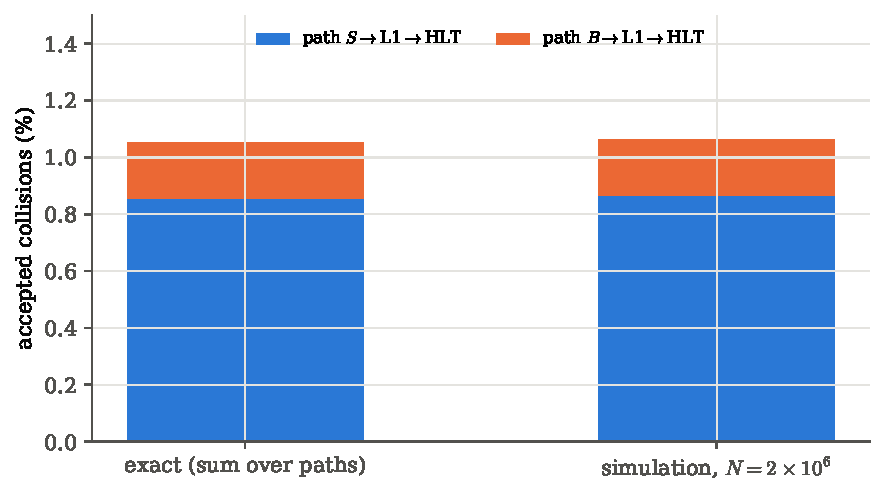
\includegraphics[width=0.75\linewidth]{figures/ch01/1a_trigger_chain.pdf}
\caption{The fraction of collisions written to disk, split into the two paths
of the tree that lead there. The left bar is the exact sum over paths, the
right bar the simulation. Signal (blue) supplies most of the accepted
collisions although only one collision in a hundred is signal.}
\label{1a:fig:trigger-bars}
\end{figure}

\paragraph{What this bought us.}
A tree turns a many-stage problem into bookkeeping: conditional probabilities
on the branches, products along paths, sums across paths. The law of total
probability is the sum across the paths that end in the observed event, and
it is a weighted average of the branch-wise probabilities.

\paragraph{In research: trigger rates and emulation.}
In a real experiment each trigger level has a rate budget (for example
$100$~kHz out of L1 and a few kHz out of the HLT), and the total rate is computed
exactly as a sum over the physics processes that can fire it, each weighted by
its cross section: the law of total probability with the processes as the
partition. Here the simulation only verified the tree. In practice the
branch efficiencies depend on the momentum, angle and pile-up of each
collision, and no closed formula exists. One then runs the trigger emulation
on millions of simulated events and counts, so the simulation is the
instrument and the tree is the check that one understands the result.

\begin{pitfall}[Branch labels are conditional on the path]
Two traps. First, the HLT keeps $90\%$ of signal \emph{that passed L1}. That is
$\Prob(\mathrm{HLT}\given S\cap\mathrm{L1})$, not $\Prob(\mathrm{HLT}\given S)$ and certainly not
$\Prob(\mathrm{HLT})$. Multiplying unconditional probabilities along a path is correct
only when the stages are independent, which is the subject of the next section.
Second, the paths that are added must be disjoint. The leaves of a tree always
are, which is why drawing the tree is safer than adding probabilities by eye.
\end{pitfall}

\section{Independence: when learning $B$ tells us nothing about $A$}
\label{1a:sec:independence}

In \cref{1a:ex:telescope-probs} we used a table in which the pattern $111$ had
probability $0.729=0.9^3$ and each pattern with one silent paddle had
$0.081=0.9^2\times0.1$. Those numbers come from one assumption: each paddle fires
with probability $0.9$ \emph{whatever the other paddles do}. The paddles are
separate pieces of plastic with separate photomultipliers, so this is
plausible. It fails if the three tubes share a high-voltage supply that
sometimes sags, because then one silent paddle makes it more likely that the
others are silent too.

Independence is the precise version of ``whatever the others do''. It is the
one situation in which the probability of ``$A$ and $B$'' is the product of the
two probabilities. That product rule lets us write the probability of a data
set as a product over data points, and every likelihood in this book is built
that way. There are two things that independence is not. First, independence is not the same as disjointness. Second, when there are three or more events, independence does not mean merely that every pair of events is independent.

\paragraph{Crossed strips.}
Draw $\Omega$ as the unit square. Let $A$ be a vertical strip of width
$\Prob(A)$ and $B$ a horizontal strip of height $\Prob(B)$. Their overlap is a
rectangle of area $\Prob(A)\Prob(B)$. Inside $A$, the strip $B$ covers the same
fraction $\Prob(B)$ as it covers of the whole square, so learning ``$A$
happened'' does not change the probability of $B$. Independence is this
product structure. Two dice, two separate detectors or two separate nuclei
behave like the two axes of the square.

\begin{figure}[htbp]
\centering
\begin{tikzpicture}[scale=1.25]
  \begin{scope}
    \draw[thick] (0,0) rectangle (2.4,2.4);
    \fill[formblue!30] (0,0) rectangle (1.2,2.4);
    \fill[fibreorange!30] (0,1.6) rectangle (2.4,2.4);
    \fill[tangentgreen!50] (0,1.6) rectangle (1.2,2.4);
    \draw (1.2,0) -- (1.2,2.4); \draw (0,1.6) -- (2.4,1.6);
    \node[lbl] at (0.6,0.8) {$A$};
    \node[lbl] at (1.8,2.0) {$B$};
    \node[lbl] at (0.6,2.0) {$AB$};
    \node[lbl] at (1.2,-0.35) {independent};
  \end{scope}
  \begin{scope}[xshift=3.2cm]
    \draw[thick] (0,0) rectangle (2.4,2.4);
    \fill[formblue!30] (0,0) rectangle (1.2,2.4);
    \fill[fibreorange!30] (1.2,1.6) rectangle (2.4,2.4);
    \fill[fibreorange!30] (1.2,0) rectangle (2.4,0.8);
    \draw (1.2,0) -- (1.2,2.4); \draw (1.2,1.6) -- (2.4,1.6); \draw (1.2,0.8) -- (2.4,0.8);
    \node[lbl] at (0.6,1.2) {$A$};
    \node[lbl] at (1.8,2.0) {$B$};
    \node[lbl] at (1.8,0.4) {$B$};
    \node[lbl] at (1.2,-0.35) {disjoint};
  \end{scope}
  \begin{scope}[xshift=6.4cm]
    \draw[thick] (0,0) rectangle (2.4,2.4);
    \fill[formblue!30] (0,0) rectangle (1.2,2.4);
    \fill[fibreorange!30] (1.2,2.0) rectangle (2.4,2.4);
    \fill[tangentgreen!50] (0,1.2) rectangle (1.2,2.4);
    \draw (1.2,0) -- (1.2,2.4);
    \draw (0,1.2) -- (1.2,1.2);
    \draw (1.2,2.0) -- (2.4,2.0);
    \node[lbl] at (0.6,0.6) {$A$};
    \node[lbl] at (1.8,2.2) {$B$};
    \node[lbl] at (0.6,1.8) {$AB$};
    \node[lbl] at (1.2,-0.35) {dependent};
  \end{scope}
\end{tikzpicture}
\caption{Three ways for two events to sit in the unit square, all drawn to scale and
all with $\Prob(A)=\tfrac12$ (the left half) and $\Prob(B)=\tfrac13$. Left: $B$ is the
top third, so it fills a third of $A$ and a third of the square, and $\Prob(AB)=\tfrac16$,
exactly the product: independent. Middle: $A$ and $B$ do not meet, so $\Prob(AB)=0$ and
knowing $A$ rules $B$ out. Right: $B$ still has area $\tfrac13$ but leans into $A$, so
$\Prob(AB)=\tfrac14\neq\tfrac16$. The two overlaps have the same width, so compare their
heights: $B$ covers half of $A$ on the right but only a third of $A$ on the left. Covering
more of $A$ than its $\tfrac13$ share of the square, $B$ becomes more likely once we learn $A$.}
\label{1a:fig:independence}
\end{figure}

\paragraph{Checking independence.}
Whenever a calculation seems to need independence, we ask four questions.
\begin{enumerate}[leftmargin=1.5em,itemsep=1pt]
  \item In words: does knowing that $B$ happened change how likely $A$ is?
  \item In numbers: is $\Prob(AB)$ equal to $\Prob(A)\Prob(B)$?
  \item Is independence being \emph{assumed} (no physical mechanism links the
        two) or \emph{derived} (computed from a known distribution)?
  \item For more than two events, check every sub-collection, not just the pairs.
\end{enumerate}

\begin{workdef}[independence]
Two events $A$ and $B$ are \newterm{independent}, written $A\perp\!\!\!\perp B$, if
\begin{equation}
\Prob(AB)=\Prob(A)\,\Prob(B).
\label{1a:eq:indep}
\end{equation}
A collection $\{A_i:\ i\in I\}$ is \newterm{independent} (or \newterm{mutually
independent}) if
$\Prob\bigl(\bigcap_{i\in J}A_i\bigr)=\prod_{i\in J}\Prob(A_i)$ for \emph{every} finite
subset $J\subseteq I$ \unpack{for three events that means the three pairs and the
triple, four equations in all}. Otherwise the events are dependent.
\emph{Operational test:} with $\Prob(B)>0$, independence is $\Prob(A\given B)=\Prob(A)$.
\end{workdef}

The conditional form is the meaning, and the product form is the convenient
definition, because it is symmetric and also makes sense when $\Prob(B)=0$. They
agree whenever $\Prob(B)>0$ \mainref{p.~11, Lemma~1.14}:
\begin{align*}
\Prob(A\given B)\eqby{1}\frac{\Prob(AB)}{\Prob(B)}\eqby{2}\frac{\Prob(A)\Prob(B)}{\Prob(B)}=\Prob(A),
\end{align*}
\begin{explain}
  \item Definition of conditional probability.
  \item Independence \eqref{1a:eq:indep}.
\end{explain}
and conversely, if $\Prob(A\given B)=\Prob(A)$ then multiplying by $\Prob(B)$ gives
\eqref{1a:eq:indep}. By the symmetry of \eqref{1a:eq:indep}, $\Prob(B\given A)=\Prob(B)$ too
when $\Prob(A)>0$: if $B$ tells us nothing about $A$, then $A$ tells us nothing about
$B$.

\paragraph{Assumed or derived.} Often independence is an \emph{assumption} that
expresses physics: a coin has no memory of its last toss, two nuclei do not
communicate, the noise in two separate amplifiers has separate sources.
Sometimes it is a \emph{result} \mainref{p.~8}. Roll one fair die and let
$A=\{2,4,6\}$ and $B=\{1,2,3,4\}$. Then $AB=\{2,4\}$ and
\[
\Prob(AB)=\tfrac26=\tfrac13=\tfrac12\times\tfrac23=\Prob(A)\Prob(B),
\]
so $A$ and $B$ are independent, although both are about the same single roll.
Nobody assumed it. With $C=\{4,5,6\}$ instead, $AC=\{4,6\}$ and
$\Prob(AC)=\tfrac13\neq\tfrac12\times\tfrac12$: knowing the roll is high makes it more
likely to be even.

\subsection{Consequences}

\paragraph{Complements of independent events are independent.}
If $A\perp\!\!\!\perp B$,
\begin{align*}
\Prob(AB^c)\eqby{1}\Prob(A)-\Prob(AB)\eqby{2}\Prob(A)-\Prob(A)\Prob(B)\eqby{3}\Prob(A)\bigl(1-\Prob(B)\bigr)
\eqby{4}\Prob(A)\Prob(B^c).
\end{align*}
\begin{explain}
  \item $A$ is the disjoint union of $AB$ and $AB^c$, so $\Prob(A)=\Prob(AB)+\Prob(AB^c)$.
  \item Independence of $A$ and $B$.
  \item Factor out $\Prob(A)$.
  \item Complement rule.
\end{explain}
So $A\perp\!\!\!\perp B^c$ \mainref{p.~15, Ex.~11}, \srcref{CasellaBerger}{Thm~1.3.9}. Applying the same argument with the roles of the events
exchanged gives $A^c\perp\!\!\!\perp B^c$. If a paddle's firing tells us nothing
about another's, neither does its silence.

\paragraph{Sure and impossible events are independent of everything}
\mainref{p.~15, Ex.~14}. If $\Prob(A)=0$, then $\Prob(AB)\le\Prob(A)=0$ by
monotonicity, so $\Prob(AB)=0=\Prob(A)\Prob(B)$. If $\Prob(A)=1$, then $\Prob(A^c)=0$, so $A^c$
is independent of every $B$, and by the complement result so is $A$. Finally,
an event independent of itself satisfies $\Prob(A)=\Prob(AA)=\Prob(A)^2$, so
$\Prob(A)\in\{0,1\}$.

\begin{keyidea}[Disjoint is not independent]
If $A$ and $B$ are disjoint and both have positive probability, they are
\emph{dependent}: $\Prob(A)\Prob(B)>0$, but $\Prob(AB)=\Prob(\varnothing)=0$
\mainref{p.~9}. Disjoint events are as dependent as events can be: learning
that one happened tells us for certain that the other did not.
\end{keyidea}

Apart from this case, a Venn diagram cannot show independence. Whether the
overlap equals the product depends on the areas, not on the shapes. In
\cref{1a:fig:independence} the right panel looks as ``overlapping'' as the left
one, yet only the left is independent.

Two more warnings \srcref{Lambert}{\S3.4}. First, take a playing card. Its
colour and its suit are dependent: ``red'' forces hearts or diamonds. Its suit
and its value are independent: $\Prob(\heartsuit\given\text{queen})=\tfrac14=\Prob(\heartsuit)$.
Second, dependence is not causation. The colour does not \emph{cause} the suit.
Dependence only means that knowing one tells us something about the other.

\subsection{Examples}

\oneaEx{At least one head in ten tosses}
\label{1a:ex:ten-tosses}
Let $A$ be ``at least one head'' in ten tosses of a fair coin and $T_j$ ``tails on
toss $j$'' \mainref{p.~9, Ex.~1.10}. Then
\begin{align*}
\Prob(A)&\eqby{1}1-\Prob(A^c)\eqby{2}1-\Prob(T_1T_2\cdots T_{10})
\eqby{3}1-\Prob(T_1)\Prob(T_2)\cdots\Prob(T_{10})\eqby{4}1-\Bigl(\frac12\Bigr)^{10}\approx0.999 .
\end{align*}
\begin{explain}
  \item Complement rule.
  \item ``No head'' means ``tails on every toss''.
  \item The tosses are independent (assumed: the coin has no memory).
  \item Each factor is $\tfrac12$.
\end{explain}
The Chevalier de M\'er\'e's bet ``at least one six in four rolls of a die'' is
the same computation, $1-(5/6)^4\approx0.518$ \srcref{CasellaBerger}{Ex.~1.3.8}, a
slightly favourable bet. His other bet, ``at least one double six in $24$ rolls of
two dice'', gives $1-(35/36)^{24}\approx0.491$, slightly unfavourable, which puzzled
him enough to write to Pascal.

\oneaEx{Telescope efficiency, and the first decay in a sample}
\label{1a:ex:indep-physics}
\emph{(a)} Each paddle fires with probability $\varepsilon$, independently. The
trigger needs at least two paddles. The pattern $111$ has probability
$\varepsilon^3$, and each of the three patterns with exactly one silent paddle
has probability $\varepsilon^2(1-\varepsilon)$, by the product rule for the three
independent events ``paddle $j$ fired or not'' (complements are independent
too). So
\begin{align*}
\Prob(T)\eqby{1}3\varepsilon^2(1-\varepsilon)+\varepsilon^3=3\varepsilon^2-2\varepsilon^3,
\end{align*}
\begin{explain}
  \item Finite additivity over the four disjoint patterns in $T$.
\end{explain}
which is $0.972$ at $\varepsilon=0.9$, reproducing the table of
\cref{1a:ex:telescope-probs}. A two-out-of-three majority turns $90\%$ paddles into
a $97\%$ trigger.

\emph{(b)} A sample holds $N$ nuclei, each surviving to time $t$ with probability
$e^{-\lambda t}$ (\cref{1a:ex:nucleus}), independently of the others. The
probability that \emph{none} has decayed by $t$ is
\begin{align*}
\Prob\Bigl(\,\bigcap_{i=1}^NS^{(i)}_t\Bigr)\eqby{1}\prod_{i=1}^N\Prob\bigl(S^{(i)}_t\bigr)
=\bigl(e^{-\lambda t}\bigr)^N=e^{-N\lambda t}.
\end{align*}
\begin{explain}
  \item Mutual independence of the $N$ survival events.
\end{explain}
``None has decayed by $t$'' is the same event as ``the first decay comes after
$t$''. So the waiting time until the first click of a Geiger counter has the
survival law $e^{-N\lambda t}$ of a single nucleus with rate $N\lambda$: it is
itself exponential, with rate $N\lambda$, the activity of the sample. This is
the seed of the Poisson process of \cref{ch:02}.

\oneaEx{Blue eyes}
\label{1a:ex:blue-eyes}
Each of three children has blue eyes with probability $\tfrac14$, independently
\mainref{p.~15, Ex.~15}. Let $K$ be the number of blue-eyed children.
\emph{(a)} Given that at least one has blue eyes, what is the probability that at
least two do? The event $\{K\ge2\}$ lies inside $\{K\ge1\}$, so
\begin{align*}
\Prob(K\ge2\given K\ge1)\eqby{1}\frac{\Prob(K\ge2)}{\Prob(K\ge1)}
\eqby{2}\frac{3\cdot\tfrac1{16}\cdot\tfrac34+\tfrac1{64}}{1-\bigl(\tfrac34\bigr)^3}
=\frac{10/64}{37/64}=\frac{10}{37}\approx0.27 .
\end{align*}
\begin{explain}
  \item Definition of conditional probability, with $\{K\ge2\}\cap\{K\ge1\}=\{K\ge2\}$.
  \item Numerator: exactly two blue (three choices of the brown-eyed child) or
        all three. Denominator: complement of ``none blue''. Independence gives
        each pattern's probability as a product.
\end{explain}
\emph{(b)} Given that the \emph{youngest} has blue eyes, at least two are blue-eyed
exactly when at least one of the other two is. By independence the youngest
tells us nothing about them, so the answer is $1-(\tfrac34)^2=\tfrac7{16}\approx0.44$.
The two conditions sound alike but carry different information, and (b) is
the larger because it pins down \emph{which} child is blue-eyed.

\subsection{Pairwise is not mutual}

For three events, one might hope that the triple product
$\Prob(ABC)=\Prob(A)\Prob(B)\Prob(C)$ is enough, or that it is enough for each pair to be
independent. Neither is \srcref{CasellaBerger}{Exs.~1.3.10--1.3.11}.

\oneaEx{The triple product without the pairs}
\label{1a:ex:triple-no-pairs}
Roll two dice. Let $A$ be ``doubles'', $B$ ``the sum is between $7$ and $10$'' and $C$
``the sum is $2$, $7$ or $8$''. Counting among the $36$ outcomes, $\Prob(A)=\tfrac6{36}=\tfrac16$,
$\Prob(B)=\tfrac{6+5+4+3}{36}=\tfrac12$ and $\Prob(C)=\tfrac{1+6+5}{36}=\tfrac13$. The only double with
sum in $\{7,8\}$ is $(4,4)$, so $\Prob(ABC)=\tfrac1{36}=\tfrac16\cdot\tfrac12\cdot\tfrac13$. But
$\Prob(BC)=\Prob(\text{sum }7\text{ or }8)=\tfrac{11}{36}\neq\tfrac16=\Prob(B)\Prob(C)$, and
$\Prob(AB)=\Prob(\{(4,4),(5,5)\})=\tfrac1{18}\neq\tfrac1{12}$. The triple product holds by
coincidence, while the pairs are dependent.

\oneaEx{The pairs without the triple}
\label{1a:ex:pairs-no-triple}
Let $\Omega$ consist of the nine strings $aaa$, $bbb$, $ccc$, $abc$, $bca$, $cab$, $acb$, $bac$, $cba$, each
with probability $\tfrac19$, and let $A_i$ be ``the $i$-th letter is $a$''. Each $A_i$
contains three strings (for $A_1$: $aaa,abc,acb$), so $\Prob(A_i)=\tfrac13$. Any two
positions are both $a$ only in $aaa$, so $\Prob(A_iA_j)=\tfrac19=\Prob(A_i)\Prob(A_j)$: every
pair is independent. But all three are $a$ also only in $aaa$, so
$\Prob(A_1A_2A_3)=\tfrac19\neq\tfrac1{27}$. Knowing that the first two letters are $a$
makes the third certain to be $a$.

\paragraph{Try it: Conditionally independent, marginally dependent.}
Suppose that on $95\%$ of days the telescope's shared high-voltage supply is
fine and each paddle fires with probability $0.92$, independently, while on
$5\%$ of days the voltage sags and each fires with probability $0.5$,
independently. Show, with the law of total probability, that
$\Prob(\text{top})=\Prob(\text{middle})\approx0.899$ but
$\Prob(\text{top and middle})\approx0.817\neq0.899^2\approx0.808$. The paddles are
independent \emph{given} the state of the supply, but not independent overall.
The unobserved common cause creates the dependence. This is the structure of
the hierarchical models of \cref{ch:05}.

\subsection{Testing independence on simulated data}

Take the die events $A=\{2,4,6\}$, $B=\{1,2,3,4\}$ (independent) and $C=\{4,5,6\}$
(dependent), simulate rolls, and compare $\hat\Prob(AB)$ with $\hat\Prob(A)\hat\Prob(B)$
\mainref{p.~17, Ex.~23}.

\pyfile[firstline=19,lastline=34,firstnumber=19]{code/ch01/06_independence_dice.py}{Independence checked by simulation}

Lines 21--24 roll one die $N$ times and build the three masks with
\texttt{np.isin}. Lines 26--27 are the frequencies. Lines 30--34 repeat the whole
$N$-roll experiment $\OneAIndReps$ times, as rows of a two-dimensional array, and
compute for each repeat the difference $\hat\Prob(\text{both})-\hat\Prob(\text{first})\hat\Prob(\text{second})$.

In a single run of $N=\OneAIndN$ rolls, $\hat\Prob(A)=\OneAIndFA$,
$\hat\Prob(B)=\OneAIndFB$, $\hat\Prob(C)=\OneAIndFC$. For the independent pair,
$\hat\Prob(AB)=\OneAIndFAB$ against $\hat\Prob(A)\hat\Prob(B)=\OneAIndProdAB$. For the dependent
pair, $\hat\Prob(AC)=\OneAIndFAC$ against $\hat\Prob(A)\hat\Prob(C)=\OneAIndProdAC$. Even
the independent pair does not satisfy the product rule \emph{exactly}, and no
finite simulation would, because frequencies scatter. So the real question is
whether the difference is larger than that random scatter. The repeats answer
it, by showing how large the difference typically is.

\begin{figure}[htbp]
\centering
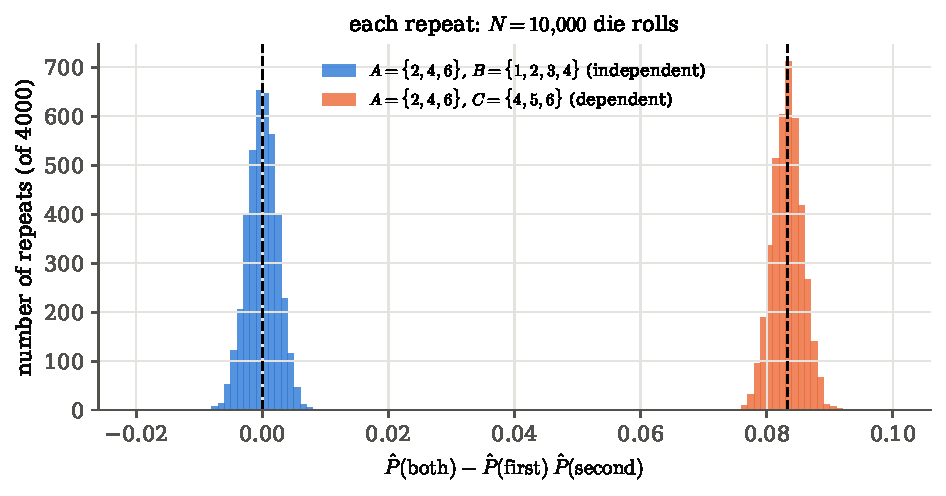
\includegraphics[width=0.85\linewidth]{figures/ch01/1a_independence.pdf}
\caption{The difference between the frequency of ``both'' and the product of the
two frequencies, over many repeats of a $10^4$-roll experiment. For the independent
pair (blue) the differences scatter symmetrically around zero. For the dependent
pair (orange) they scatter around $\tfrac13-\tfrac14=\tfrac1{12}$, far from zero compared with
the width of either histogram.}
\label{1a:fig:indep-hist}
\end{figure}

For the independent pair the differences have mean near zero and standard
deviation $\OneAIndSdAB$. For the dependent pair their mean is $\OneAIndMeanAC$, the
exact $\tfrac1{12}$, some thirty-five standard deviations away. A difference of
$\OneAIndFAB-\OneAIndProdAB$ in the single run is typical of independence. A difference of
$0.08$ is not.

\paragraph{What this bought us.}
With data, ``is $\Prob(AB)=\Prob(A)\Prob(B)$?'' becomes ``is the observed difference
large compared with its scatter under independence?''. That is a hypothesis
test with independence as the null hypothesis, and \cref{ch:04} makes it precise.

\paragraph{In research: independence is what lets us multiply.}
Every likelihood in this book is a product, and every product is an assumption
of independence. Poisson counts in different bins of a histogram are
independent if the events arrive independently (colliders, photon counting). The
spherical-harmonic coefficients $\alm$ of a statistically isotropic Gaussian sky
are independent for different $(\ell,m)$ (\cref{ch:07}), which is why the full-sky
CMB likelihood factorises over $\ell$. For stationary detector noise, the
Fourier amplitudes at different frequencies are independent, which is why the
gravitational-wave log-likelihood is a sum over frequency bins weighted by the
power spectral density (\cref{ch:10}). A mask breaks the $\alm$ independence and
correlated noise breaks the frequency independence. Handling that loss is much
of the work of \cref{ch:08}.

\begin{pitfall}[Three ways to get independence wrong]
(1) Treating disjoint events as independent. (2) Checking only pairs, or only
the full product, for three or more events. (3) Assuming independence where a
hidden common cause exists (a shared power supply, a common calibration
constant, a shared beam condition). Common-mode effects are the usual reason
why a redundant system fails more often than the product of the individual
failure rates predicts.
\end{pitfall}

\section{Bayes' theorem: reading the tree backwards}
\label{1a:sec:bayes}

A tree can be read in two directions, and the analyst at a collider needs the
direction it was not drawn in. Recall the two-level trigger of
\cref{1a:sec:trees}: a fast hardware trigger (L1) followed by a software
high-level trigger (HLT), which together write about one collision in a
hundred to disk. Its tree runs in the order in which things happen. First
nature makes the collision signal ($S$) or background ($B$). Then L1 decides.
Then the HLT decides. Read in that order, the tree answers
\emph{prediction} questions: if a collision is signal, how likely is it to be
kept?

The analyst who opens the files on disk never sees nature's first choice. She
sees only the collisions that were kept. So she asks the opposite question: of
the collisions written to disk, what fraction is signal? That is an
\emph{inference} question. It starts from an observation and asks which branch
of the tree produced it. These are the two directions of probability of
\cref{ch:00}. For a hypothesis $H$ and an observed event $E$, $\Prob(E\given H)$
runs forward, from $H$ to what it produces. $\Prob(H\given E)$ runs backward,
from what we saw to what produced it.

Bayes' theorem turns the first kind of number into the second. We need it
because the two kinds come from different places. The forward numbers are what
physics and calibration give us: efficiencies, misidentification rates,
branching fractions, the probability of the data under a model. The backward
numbers are what we want: the purity of a sample, the probability that a track
is a kaon, the credibility of a cosmological model. So the question is: given a
tree built in the forward direction, how do we read it backwards?

The analyst's question can be said in words, in four steps, before any formula.
\begin{enumerate}[leftmargin=2em,itemsep=1pt]
  \item What did she see? A collision on disk, one that the trigger kept.
  \item What could have put it there? It was either a signal collision or a
        background collision.
  \item If it was signal, how probable was it to be kept? And if it was
        background?
  \item Given those two answers, how must the shares of signal and
        background that nature started with be revised?
\end{enumerate}
Step 3 is ordinary prediction, done once for each hypothesis. Only step 4 is
new, and it needs nothing more than the definition of conditional probability,
used once.

\subsection{Two routes to the same leaf}

The whole theorem rests on one fact: a leaf of a tree is the same event
whichever order the tree was drawn in. Take a hypothesis $H$ and an observed
event $E$. The leaf ``$H$ and $E$'', written $HE$ for $H\cap E$, can be reached
in two orders. In the forward tree we pass first through $H$ and then through
$E$. In a tree drawn the other way round we pass first through $E$ and then
through $H$ \srcref{Lambert}{\S3.6.1}. Both routes end at the same event $HE$, so
they give it the same probability. The multiplication rule \eqref{1a:eq:mult},
$\Prob(HE)=\Prob(E\given H)\Prob(H)$, computes it along the forward route. Dividing
by $\Prob(E)$, which we assume is positive, gives the backward number:
\begin{align}
\Prob(H\given E)
&\eqby{1}\frac{\Prob(HE)}{\Prob(E)}
 \eqby{2}\frac{\Prob(E\given H)\,\Prob(H)}{\Prob(E)} .
\label{1a:eq:bayes-simple}
\end{align}
\begin{explain}
  \item Definition \eqref{1a:eq:cond} of conditional probability, with $E$ as
        the conditioning event: $E$ is the new, shrunk sample space.
  \item Multiplication rule along the forward route,
        $\Prob(HE)=\Prob(E\given H)\Prob(H)$.
\end{explain}
The numerator is one leaf of the forward tree. The denominator $\Prob(E)$ is the
total probability of the observation, and it too comes from the forward tree.
Suppose the possible hypotheses $H_1,\dots,H_k$ form a partition of the sample
space $\Omega$ \unpack{exactly one of them is true}. Then the law of total
probability \eqref{1a:eq:total} gives $\Prob(E)$ as the sum of all the forward
leaves that end in $E$. Putting that sum in the denominator gives the general
form \mainref{p.~12, Thm~1.17}.

\begin{keyidea}[Bayes' theorem]
Let $H_1,\dots,H_k$ be a partition of $\Omega$ with every $\Prob(H_i)>0$, and let
$\Prob(E)>0$. Then for each $i$,
\begin{equation}
\Prob(H_i\given E)
=\frac{\Prob(E\given H_i)\,\Prob(H_i)}{\sum_{j=1}^k\Prob(E\given H_j)\,\Prob(H_j)} .
\label{1a:eq:bayes}
\end{equation}
In the tree: the posterior of $H_i$ is the leaf ``$H_i$ then $E$'' divided by
the sum of all leaves that end in $E$.
\end{keyidea}

Each ingredient has a name \mainref{p.~12, Remark~1.18}.
\begin{itemize}[leftmargin=1.5em,itemsep=1pt]
  \item $\Prob(H_i)$ is the \newterm{prior} probability of $H_i$: how probable
        $H_i$ was before the observation.
  \item $\Prob(H_i\given E)$ is its \newterm{posterior} probability: how probable
        it is after.
  \item $\Prob(E\given H_i)$ is the \newterm{likelihood} of $H_i$: the probability
        of the observation we actually made, computed as if $H_i$ were true.
  \item $\Prob(E)$ is the \newterm{evidence}. It is the same number for every
        $H_i$, and its only job is to make the posteriors add up to one.
\end{itemize}
Nothing here goes beyond the definition of conditional probability and the law
of total probability. The only new thing is the direction in which we read the
tree.

Inverting a tree means: compute the leaves forward, then regroup them by the
observation instead of by the hypothesis. \Cref{1a:fig:invert} shows this for the
trigger. The forward tree and the inverted tree have the same four leaves with
the same probabilities, because the leaves are the same events. What changes is
the order of the two splits, and with it the conditional probabilities written
on the branches.

\begin{figure}[htbp]
\centering
\begin{tikzpicture}[
  nd/.style={font=\small,inner sep=2pt},
  br/.style={thick,accent},
  pr/.style={font=\scriptsize,fill=white,inner sep=1pt},
  lf/.style={font=\scriptsize,anchor=west},
  x=1cm,y=0.8cm]
  \node[font=\small\itshape] at (1.9,2.9) {prediction: nature's order};
  \node[nd] (r) at (0,0) {start};
  \node[nd] (S) at (1.6,1.2) {$S$};
  \node[nd] (B) at (1.6,-1.2) {$B$};
  \node[nd] (SA) at (3.9,1.8) {acc};
  \node[nd] (SR) at (3.9,0.6) {rej};
  \node[nd] (BA) at (3.9,-0.6) {acc};
  \node[nd] (BR) at (3.9,-1.8) {rej};
  \draw[br] (r) -- node[pr,above left] {$0.01$} (S);
  \draw[br] (r) -- node[pr,below left] {$0.99$} (B);
  \draw[br] (S) -- node[pr,above] {$0.855$} (SA);
  \draw[br] (S) -- node[pr,below] {$0.145$} (SR);
  \draw[br] (B) -- node[pr,above] {$0.002$} (BA);
  \draw[br] (B) -- node[pr,below] {$0.998$} (BR);
  \node[lf,fibreorange] at (4.25,1.8) {$0.00855$};
  \node[lf,softgray] at (4.25,0.6) {$0.00145$};
  \node[lf,formblue] at (4.25,-0.6) {$0.00198$};
  \node[lf,softgray!60!black] at (4.25,-1.8) {$0.98802$};
  \begin{scope}[xshift=6.5cm]
  \node[font=\small\itshape] at (1.9,2.9) {inference: observation first};
  \node[nd] (r2) at (0,0) {start};
  \node[nd] (A2) at (1.6,1.2) {acc};
  \node[nd] (R2) at (1.6,-1.2) {rej};
  \node[nd] (AS) at (3.9,1.8) {$S$};
  \node[nd] (AB) at (3.9,0.6) {$B$};
  \node[nd] (RS) at (3.9,-0.6) {$S$};
  \node[nd] (RB) at (3.9,-1.8) {$B$};
  \draw[br] (r2) -- node[pr,above left] {$0.01053$} (A2);
  \draw[br] (r2) -- node[pr,below left] {$0.98947$} (R2);
  \draw[br] (A2) -- node[pr,above] {$0.812$} (AS);
  \draw[br] (A2) -- node[pr,below] {$0.188$} (AB);
  \draw[br] (R2) -- node[pr,above] {$0.0015$} (RS);
  \draw[br] (R2) -- node[pr,below] {$0.9985$} (RB);
  \node[lf,fibreorange] at (4.25,1.8) {$0.00855$};
  \node[lf,formblue] at (4.25,0.6) {$0.00198$};
  \node[lf,softgray] at (4.25,-0.6) {$0.00145$};
  \node[lf,softgray!60!black] at (4.25,-1.8) {$0.98802$};
  \end{scope}
\end{tikzpicture}
\caption{The trigger of \cref{1a:fig:trigger-tree} with the two trigger levels
merged into one decision, accepted (acc) or rejected (rej), drawn in both
orders. Left: nature chooses signal or background, then the trigger decides.
Right: the same four leaves, same colours, same probabilities, regrouped by
the trigger decision first. The branches on the right are the inference
numbers: among accepted collisions, $81\%$ are signal.}
\label{1a:fig:invert}
\end{figure}

\paragraph{Example: inverting the trigger tree.}
\emph{What she saw.} A collision on disk: it passed both L1 and the HLT. Call
this one merged decision ``accepted'', $\mathrm{Acc}=\mathrm{L1}\cap\mathrm{HLT}$.

\emph{What could have produced it?} The collision was either signal, $S$, or
background, $B$. These are the two hypotheses.

\emph{How probable was acceptance under each?} Multiply along the paths of
\cref{1a:fig:trigger-tree}. A signal collision passes L1 with probability
$0.95$ and then the HLT with probability $0.90$, so
$\Prob(\mathrm{Acc}\given S)=0.95\times0.90=0.855$. A background collision passes
L1 with probability $0.02$ and then the HLT with probability $0.10$, so
$\Prob(\mathrm{Acc}\given B)=0.02\times0.10=0.002$.

\emph{Then the priors, and normalise.} Before the trigger, one collision in a
hundred is signal: $\Prob(S)=0.01$, $\Prob(B)=0.99$. The signal fraction of the
recorded sample, called its \newterm{purity}, is
\begin{align*}
\Prob(S\given\mathrm{Acc})
&\eqby{1}\frac{\Prob(\mathrm{Acc}\given S)\,\Prob(S)}
               {\Prob(\mathrm{Acc}\given S)\,\Prob(S)+\Prob(\mathrm{Acc}\given B)\,\Prob(B)}
 \eqby{2}\frac{0.855\times0.01}{0.855\times0.01+0.002\times0.99}\\
&=\frac{0.00855}{0.00855+0.00198}=\frac{0.00855}{0.01053}\approx0.812 .
\end{align*}
\begin{explain}
  \item Bayes' theorem \eqref{1a:eq:bayes} with the partition $\{S,B\}$.
  \item The branch probabilities of the merged tree.
\end{explain}
Only one collision in a hundred is signal, yet four out of five recorded
collisions are. The trigger has raised the probability of ``signal'' from a
prior of $0.01$ to a posterior of $0.81$. The reason is the ratio of the two
likelihoods: a signal collision is $0.855/0.002\approx430$ times more likely to
be accepted than a background one. The simulation of \cref{1a:sec:trees} (the
last line of its listing) counted the signal fraction among the accepted
collisions directly and found $\OneATrigMCPurity$, against the exact
$\OneATrigPurity$.

\paragraph{Example: dots and dashes.}
Morse code sends dots and dashes in the proportion $3:4$, so
$\Prob(\text{dot sent})=\tfrac37$ \srcref{CasellaBerger}{Ex.~1.3.6}. Noise on the line
turns a dot into a dash, or a dash into a dot, with probability $\tfrac18$. We
receive a dot. How sure can we be that a dot was sent?

What we saw is ``dot received''. Two things could have produced it: a dot was
sent and arrived intact, or a dash was sent and noise flipped it. Under the
first, a received dot has probability $\tfrac78$; under the second,
$\tfrac18$. The priors are $\tfrac37$ for a dot and $\tfrac47$ for a dash. Then
\begin{align*}
\Prob(\text{dot sent}\given\text{dot rec.})
\eqby{1}\frac{\tfrac78\cdot\tfrac37}{\tfrac78\cdot\tfrac37+\tfrac18\cdot\tfrac47}
\eqby{2}\frac{21/56}{21/56+4/56}=\frac{21}{25}=0.84 .
\end{align*}
\begin{explain}
  \item Bayes' theorem: the likelihood of ``dot received'' is $\tfrac78$ if a dot
        was sent and $\tfrac18$ if a dash was sent.
  \item Put both products over the common denominator $56$.
\end{explain}
So a received dot is wrong $4$ times in $25$, about one time in six, even though
each symbol is flipped only one time in eight. The extra errors come from the
dashes. Dashes are sent more often than dots, so the flipped dashes make up a
larger share of the received dots than the flip rate alone suggests.

\subsection{The recipe: prior times likelihood, then normalise}

The evidence $\Prob(E)$ is the same for every hypothesis. So we can leave it out,
compute prior times likelihood for each hypothesis, and divide by the total at
the end:
\begin{equation}
\Prob(H_i\given E)\;\propto\;\Prob(E\given H_i)\,\Prob(H_i),
\qquad
\text{then divide by the sum over } i .
\label{1a:eq:bayes-prop}
\end{equation}
This is the most useful form in practice. It turns every discrete Bayes problem
into a table with one row per hypothesis and four columns:
the prior; the likelihood; their product, which is the forward leaf that ends
in $E$; and the product divided by the sum of its column, which is the
posterior. The sum of the product column is $\Prob(E)$.

\paragraph{Example: spam.}
An email is spam ($A_1$), low priority ($A_2$) or high priority ($A_3$), with
prior probabilities $0.7$, $0.2$ and $0.1$ \mainref{pp.~12--13, Ex.~1.19}. The
word ``free'' ($E$) appears in $90\%$ of spam and in $1\%$ of each of the other
two kinds.\footnote{Wasserman prints $\Prob(B\given A_1)=.01$ for the third
likelihood. The subscript should be $A_3$, as the computation that follows it
shows.} An email arrives containing ``free''. That is what we saw, and the three
kinds of email are the hypotheses that could have produced it. The table is
\begin{center}
\small
\begin{tabular}{@{}lcccc@{}}
\toprule
hypothesis & prior $\Prob(A_i)$ & likelihood $\Prob(E\given A_i)$ & product & posterior $\Prob(A_i\given E)$\\
\midrule
spam          & $0.7$ & $0.90$ & $0.630$ & $0.9953$\\
low priority  & $0.2$ & $0.01$ & $0.002$ & $0.0032$\\
high priority & $0.1$ & $0.01$ & $0.001$ & $0.0016$\\
\midrule
sum           & $1$   & $0.92$ & $0.633$ & $1$\\
\bottomrule
\end{tabular}
\end{center}
so $\Prob(A_1\given E)=0.630/0.633\approx0.995$.

The column sums carry a lesson: the likelihoods are not a probability
distribution over the hypotheses. The priors add up to one, and so do the
posteriors, because both are probabilities \emph{over the hypotheses}. The
likelihoods add up to $0.92$, and nothing forces them to add up to one. Each
likelihood is a probability over \emph{outcomes} (does ``free'' appear or not?),
computed in a different world: one where the email is spam, one where it is low
priority, one where it is high priority. Read across those worlds, as a
function of the hypothesis, the list of likelihoods is not a probability
distribution. This is the statement ``$\Prob(A\given\cdot)$ is not a probability''
of \cref{1a:sec:conditional}. It is also why, in \cref{ch:03}, the likelihood of
a parameter is called a function and not a density.

\paragraph{Example: which operating system?}
Among computer owners $30\%$ use a Mac, $50\%$ Windows and $20\%$ Linux, and the
fractions infected by a virus are $0.65$, $0.82$ and $0.50$ \mainref{p.~16,
Ex.~19}. A randomly chosen owner turns out to be infected. The products are
$0.3\times0.65=0.195$, $0.5\times0.82=0.410$ and $0.2\times0.50=0.100$, with sum
$\Prob(\text{infected})=0.705$, so
\begin{align*}
\Prob(\text{Windows}\given\text{infected})=\frac{0.410}{0.705}\approx0.582,\qquad
\Prob(\text{Mac}\given\cdot)\approx0.277,\qquad
\Prob(\text{Linux}\given\cdot)\approx0.142 .
\end{align*}
Windows rises from $0.50$ to $0.58$. Mac falls from $0.30$ to $0.28$, and Linux
from $0.20$ to $0.14$. The rule is visible in the numbers. The average infection
rate is $\Prob(\text{infected})=0.705$. Windows owners are infected more often
than that ($0.82$), so Windows gains. Mac ($0.65$) and Linux ($0.50$) owners are
infected less often, so they lose.

That rule is general: probability can only move between the hypotheses, never
be created or destroyed \mainref{p.~16, Ex.~18}. The reason is that the priors
and the posteriors both add up to one. So if one hypothesis loses, another must
gain. To see it in symbols, suppose $A_1$ loses, $\Prob(A_1\given E)<\Prob(A_1)$.
Then
\begin{align*}
\sum_{i=2}^k\Prob(A_i\given E)\eqby{1}1-\Prob(A_1\given E)\relby{2}{>}1-\Prob(A_1)\eqby{3}\sum_{i=2}^k\Prob(A_i),
\end{align*}
\begin{explain}
  \item $\Prob(\cdot\given E)$ is a probability (\cref{1a:sec:conditional}), and the
        $A_i$ partition $\Omega$, so the posteriors add up to one.
  \item The assumption $\Prob(A_1\given E)<\Prob(A_1)$.
  \item The priors add up to one.
\end{explain}
A sum of $k-1$ terms can be larger than another sum of $k-1$ terms only if at
least one of its terms is larger. So some other hypothesis gains:
$\Prob(A_i\given E)>\Prob(A_i)$ for at least one $i\geq2$. For exactly this reason
Kruschke calls Bayesian inference a \emph{reallocation of credibility} across the
possibilities \srcref{Kruschke}{\S2.1}.

The extreme case is a hypothesis whose likelihood is zero. The observation is
impossible under it, so its posterior is zero. Its prior weight goes to the
hypotheses that survive, shared in proportion to each one's prior times
likelihood. Repeat this with more observations until only one hypothesis is
left, and you get Sherlock Holmes's rule: once every other cause has been ruled
out, the one that remains carries all the probability.

\subsection{Base rates and the odds form}

Bayes' theorem is least intuitive when the prior is small. A test for a rare
disease detects it with probability $\Prob(+\given D)=0.98$, and gives a false
positive with probability $\Prob(+\given D^c)=0.03$. The prevalence is
$\Prob(D)=0.001$ \srcref{Cowan}{p.~4}. You test positive.

\emph{What happened.} The test came back positive, written $+$.
\emph{What could have produced it?} Two situations: you have the disease,
$D$, or you do not, $D^c$. A positive result can come out of either.
\emph{How probable was a positive under each?} With the disease it is the
detection probability, $0.98$; without it, the false-positive rate, $0.03$.
\emph{Then the base rates.} Before the test, $D$ had probability $0.001$ and
$D^c$ had $0.999$. The two forward leaves that end in ``$+$'' give
\begin{align*}
\Prob(D\given +)
\eqby{1}\frac{0.98\times0.001}{0.98\times0.001+0.03\times0.999}
\eqby{2}\frac{0.00098}{0.00098+0.02997}\approx0.032 .
\end{align*}
\begin{explain}
  \item Bayes' theorem \eqref{1a:eq:bayes} with the partition $\{D,D^c\}$.
  \item The two forward leaves that end in ``$+$''.
\end{explain}
The test is wrong only $2\%$ or $3\%$ of the time, yet after a positive result
the probability of disease is only about $3\%$. The two leaves show why. The
false-positive leaf, $0.02997$, is thirty times larger than the true-positive
leaf, $0.00098$. Healthy people rarely test positive, but there are a thousand
times more of them, so they produce most of the positives. The medical test of
\cref{1a:ex:medical}
($\Prob(D\given +)\approx0.08$) and the screening example of
\srcref{Lambert}{\S3.6.2} (also $0.08$) have the same structure. Ignoring the
prior in such a problem is called the \newterm{base-rate fallacy}. It is the
prosecutor's fallacy of \cref{1a:sec:conditional} in another guise: it
confuses $\Prob(+\given D)$ with $\Prob(D\given +)$.

With two hypotheses, the effect of an observation is a single multiplication.
To see it, write Bayes' theorem \eqref{1a:eq:bayes-simple} for $H_1$ and for $H_2$,
and divide one by the other. The evidence $\Prob(E)$ cancels:
\begin{align}
\frac{\Prob(H_1\given E)}{\Prob(H_2\given E)}
&\eqby{1}\frac{\Prob(E\given H_1)\Prob(H_1)/\Prob(E)}{\Prob(E\given H_2)\Prob(H_2)/\Prob(E)}
 \eqby{2}\underbrace{\frac{\Prob(E\given H_1)}{\Prob(E\given H_2)}}_{\text{likelihood ratio}}
 \times\underbrace{\frac{\Prob(H_1)}{\Prob(H_2)}}_{\text{prior odds}} .
\label{1a:eq:odds}
\end{align}
\begin{explain}
  \item Bayes' theorem \eqref{1a:eq:bayes-simple} in the numerator and in the
        denominator.
  \item Cancel $\Prob(E)$ and regroup.
\end{explain}
The ratio on the left is the \newterm{posterior odds}. The observation
multiplies the prior odds by the \newterm{likelihood ratio}, and it does nothing
else. For the rare disease, take $H_1=D$ and $H_2=D^c$. The likelihood ratio is
$0.98/0.03\approx32.7$ and the prior odds are $0.001/0.999\approx0.0010$, so the
posterior odds are $0.0327$. Turning odds back into a probability,
$\Prob(D\given +)=0.0327/(1+0.0327)\approx0.032$, as before. The test is good
evidence (it multiplies the odds by about thirty), but it starts from odds of one
to a thousand.

The odds form makes repeated observations easy: each new observation multiplies
the odds again. Suppose a second test is also positive, and the two results are
independent \emph{given the disease status} (\cref{1a:sec:independence}). Then
yesterday's posterior is today's prior, and the odds are multiplied by $32.7$
again, to $1.07$, so $\Prob(D\given{+}{+})\approx0.52$. A third positive test
gives odds $34.9$ and $\Prob(D\given{+}{+}{+})\approx0.97$. In logarithms the
multiplications become additions: each independent observation \emph{adds} its
log likelihood ratio to the log odds. This is why analyses add up log
likelihoods rather than multiply likelihoods. The condition ``independent given
the disease status'' matters. A test that fails for a reason specific to the
patient will fail again, and then repeating it adds much less
\srcref{Lambert}{Problem~3.8.5}.

\begin{pitfall}[Efficiency is not purity]
A detector's efficiency $\Prob(\text{tag}\given\text{true})$ is a forward number,
measured once on a calibration sample, and it does not depend on what else is
in the beam. The purity $\Prob(\text{true}\given\text{tag})$ is an inverse number, and it
depends strongly on the prior, the composition of the sample. A selection
with $90\%$ efficiency and a $5\%$ fake rate can give a sample that is mostly
fakes, if the true particles are rare. Quote both, and never call one by the
other's name.
\end{pitfall}

\paragraph{Example: particle identification with misidentification.}
A hadron beam contains pions, kaons and protons in the proportions
$0.80:0.15:0.05$. A Cherenkov detector tags a track as ``kaon'' with probability
$0.90$ for a real kaon, $0.05$ for a pion and $0.10$ for a proton. A track is
tagged as a kaon. Which particle is it?

What we saw is the tag ``kaon''. Any of the three species could have produced
it, so they are the three hypotheses. Their priors are the beam proportions,
and their likelihoods are the three tagging probabilities. The table:
\begin{center}
\small
\begin{tabular}{@{}lcccc@{}}
\toprule
species & prior & $\Prob(\text{tag }K\given\text{species})$ & product & posterior\\
\midrule
$\pi$ & $0.80$ & $0.05$ & $0.040$ & $\OneAPidPostPi$\\
$K$   & $0.15$ & $0.90$ & $0.135$ & $\OneAPidPostK$\\
$p$   & $0.05$ & $0.10$ & $0.005$ & $\OneAPidPostP$\\
\midrule
sum   & $1$    &        & $\OneAPidTagK$ & $1$\\
\bottomrule
\end{tabular}
\end{center}
One tagged track in four is not a kaon, and almost all of the impostors are
pions. Pions are misidentified only $5\%$ of the time, but there are more than
five times as many pions as kaons in the beam. So the purity depends on the beam,
not only on the detector. As the kaon fraction falls, the purity collapses
(\cref{1a:fig:pid}). At a kaon fraction of $1\%$ it is only
$\OneAPidPurityOnePct$, with the same detector and the same $90\%$ efficiency.

\begin{figure}[htbp]
\centering
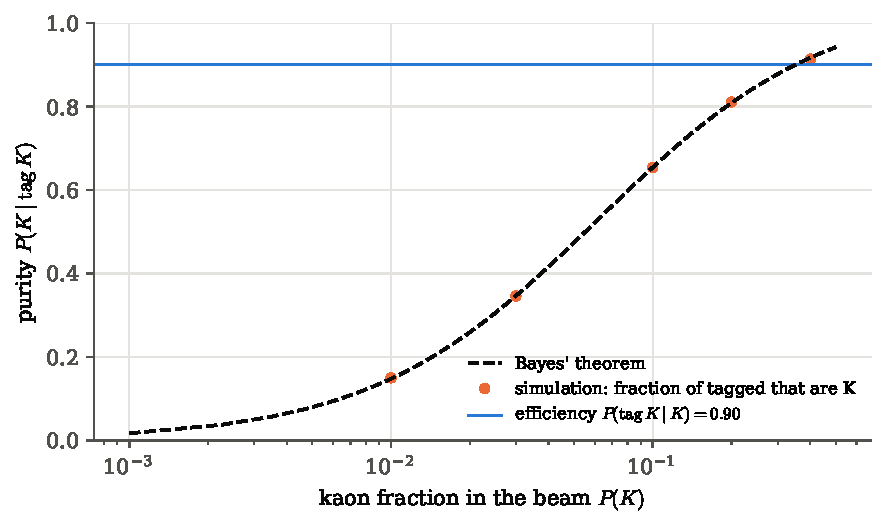
\includegraphics[width=0.75\linewidth]{figures/ch01/1a_particle_id.pdf}
\caption{Purity of the kaon-tagged sample against the kaon fraction of the
beam, on a logarithmic axis. The dashed curve is Bayes' theorem, the dots are
simulated beams in which we tag tracks and count the true kaons among the
tagged ones. The horizontal line is the efficiency, which stays at $0.90$
whatever the beam. The two agree only when kaons dominate.}
\label{1a:fig:pid}
\end{figure}

\subsection{When the observation carries information in how it was produced}

When the observation comes out of a person's choice, intuition tends to ignore
how it was produced, and goes wrong. In the trigger, the detector and the
medical test, the observation came from a fixed mechanism that was easy to see.
In three famous puzzles, Monty Hall, the three prisoners and the three cards,
the mechanism is hidden inside someone's decision.
The four steps of the reasoning handle them without any new idea. Everything
turns on the third step: under each hypothesis, how probable was \emph{exactly
the observation we made}?

\paragraph{Example: Monty Hall.}
A car is behind one of three doors, each with probability $\tfrac13$, and goats
are behind the other two. We pick door 1. The host, Monty, knows where the car
is. He always opens one of the two doors we did not pick, never the car door,
and if he has a choice he picks at random. He opens door 3
\mainref{p.~14, Ex.~10}. Should we switch to door 2?

\emph{What we saw.} Monty opened door 3. Call this event $M_3$.

\emph{What could have made him open it?} Monty's choice depends on one thing
we do not know, where the car is. So the candidate explanations are the
three places the car can be: $H_1$, $H_2$ and $H_3$, the car behind door 1,
2 or 3. We want to know which of these places could have led Monty to open
door 3, and how strongly.

\emph{How likely was door 3 under each location?} Take the three in turn. Monty
knows where the car is, he never reveals it, and he never opens our door.
\begin{itemize}[leftmargin=1.5em,itemsep=1pt]
  \item $H_1$, the car is behind our door 1: both other doors hide goats, so
        Monty can open door 2 or door 3 and chooses at random,
        $\Prob(M_3\given H_1)=\tfrac12$.
  \item $H_2$, the car is behind door 2: he may not open our door 1 and may
        not reveal the car behind door 2, so he is forced to open door 3,
        $\Prob(M_3\given H_2)=1$.
  \item $H_3$, the car is behind door 3: opening door 3 would reveal the car,
        so he cannot open it, $\Prob(M_3\given H_3)=0$.
\end{itemize}
These are the second-stage branches of the tree in \cref{1a:fig:monty-tree}.
\emph{Then the priors, and normalise.} Each location had prior $\Prob(H_d)=\tfrac13$, so
the three leaves that end in $M_3$ weigh $\tfrac13\cdot\tfrac12=\tfrac16$,
$\tfrac13\cdot1=\tfrac13$ and $\tfrac13\cdot0=0$. Normalising by their sum,
\begin{align*}
\Prob(H_2\given M_3)
&\eqby{1}\frac{\Prob(M_3\given H_2)\Prob(H_2)}{\sum_{d=1}^3\Prob(M_3\given H_d)\Prob(H_d)}
 \eqby{2}\frac{1\cdot\tfrac13}{\tfrac12\cdot\tfrac13+1\cdot\tfrac13+0\cdot\tfrac13}
 =\frac{1/3}{1/2}=\frac23,
\end{align*}
\begin{explain}
  \item Bayes' theorem with the partition $\{H_1,H_2,H_3\}$.
  \item The three likelihoods above and the uniform prior. The evidence is
        $\Prob(M_3)=\tfrac16+\tfrac13=\tfrac12$.
\end{explain}
and in the same way $\Prob(H_1\given M_3)=\tfrac16/\tfrac12=\tfrac13$ and
$\Prob(H_3\given M_3)=0$. Switching wins with probability $\tfrac23$.

The whole calculation is one look at the picture of \cref{1a:fig:shrink}, drawn
to scale in \cref{1a:fig:monty-boxes}. The three places the car can be fill the
sample space in three equal strips. The event $M_3$ is a box that takes half of
the $H_1$ strip, all of the $H_2$ strip and none of the $H_3$ strip, exactly the
three likelihoods above. Once we see $M_3$, that box is the whole world, and the
$H_2$ piece of it is twice the $H_1$ piece.

\begin{figure}[htbp]
\centering
\begin{tikzpicture}[scale=0.8]
  \begin{scope}
    \fill[formblue!18] (0,0) rectangle (6,4);
    \fill[tangentgreen!45] (1,0) rectangle (4,4);
    \draw (2,0) -- (2,4); \draw (4,0) -- (4,4);
    \draw[thick] (0,0) rectangle (6,4);
    \draw[line width=1.6pt,fibreorange] (1,0) rectangle (4,4);
    \node[lbl] at (0.5,2) {$H_1$};
    \node[lbl] at (3,3.55) {$H_2$};
    \node[lbl] at (5,2) {$H_3$};
    \node[lbl] at (1.5,1.6) {$\tfrac16$};
    \node[lbl] at (3,1.6) {$\tfrac13$};
    \node[lbl,fibreorange!80!black] at (2.5,4.35) {$M_3$: Monty opens door 3};
    \node[lbl] at (6.25,3.75) {$\Omega$};
    \foreach \a/\b in {0/2,2/4,4/6} {\draw[faint] (\a,-0.15) -- (\a,-0.3) -- (\b,-0.3) -- (\b,-0.15);
      \node[lbl] at ({(\a+\b)/2},-0.6) {$\tfrac13$};}
    \node[lbl,align=center,text width=6.2cm,anchor=north] at (3,-0.95) {before Monty acts: three equal strips,\\ one for each place the car can be};
  \end{scope}
  \draw[->,thick,accent] (6.7,2) -- (8.1,2);
  \node[lbl,accent,align=center] at (7.4,2.75) {observe\\$M_3$};
  \begin{scope}[xshift=8.7cm]
    \draw[faint,dashed] (0,0) rectangle (6,4);
    \draw[faint,dashed] (2,0) -- (2,4); \draw[faint,dashed] (4,0) -- (4,4);
    \fill[tangentgreen!45] (1,0) rectangle (4,4);
    \draw[very thin,black!40] (2,0) -- (2,4);
    \draw[line width=1.6pt,fibreorange] (1,0) rectangle (4,4);
    \node[lbl,align=center] at (1.5,2) {$H_1$\\[2pt]$\tfrac16$};
    \node[lbl,align=center] at (3,2) {$H_2$\\[2pt]$\tfrac13$};
    \node[lbl,softgray,align=center] at (5,2) {$H_3$\\ruled out};
    \node[lbl,fibreorange!80!black] at (2.5,4.35) {$M_3$, area $\tfrac12$};
    \node[lbl,align=center,text width=6.2cm,anchor=north] at (3,-0.95) {after: $M_3$ is the new sample space,\\ $H_2$ fills twice as much of it as $H_1$};
  \end{scope}
\end{tikzpicture}
\caption{Monty Hall drawn to scale in the picture of \cref{1a:fig:shrink}. Left:
the rectangle $\Omega$ has area 1, and since the car is behind exactly one door,
the three hypotheses $H_1$, $H_2$, $H_3$ fill it in three strips of area
$\tfrac13$. The event $M_3$, ``Monty opens door 3'' (orange outline), covers half
of $H_1$ (with the car behind our door he picks door 2 or 3 at random), all of
$H_2$ (he is forced to open door 3) and none of $H_3$ (he never reveals the car),
so its area is $\tfrac16+\tfrac13=\tfrac12$. Right: seeing $M_3$ discards
everything outside the orange box, and each hypothesis keeps the share of the box
that its piece fills: $\tfrac13$ for $H_1$, $\tfrac23$ for $H_2$.}
\label{1a:fig:monty-boxes}
\end{figure}

Most people's first answer is that, with one door gone, the two doors left
must be even. That answer throws away what Monty's choice told us. Door 3 was
not equally likely to be opened under the two locations still possible: with
the car behind door 2, Monty had no other move, while with the car behind our
door 1 he would have opened door 3 only half the time. What we saw is
therefore twice as probable under $H_2$ as under $H_1$, and the posteriors
inherit that factor of two, $\tfrac23$ against $\tfrac13$.

The fifty--fifty answer gets one step right and skips another. It shrinks the
sample space correctly: door 3 is out. But it forgets the likelihoods. A
counterexample shows that they decide the answer. Suppose Monty did \emph{not}
know where the car is, opened door 2 or door 3 at random, and happened to show a
goat behind door 3. Under $H_1$ he opens door 3 with probability $\tfrac12$ and
it hides a goat. Under $H_2$ he also opens door 3 with probability $\tfrac12$,
and it again hides a goat. So
$\Prob(M_3,\text{goat}\given H_1)=\Prob(M_3,\text{goat}\given H_2)=\tfrac12$, and
the answer really would be fifty--fifty. Same doors, same observation, different
mechanism, different posterior.

\begin{figure}[htbp]
\centering
\begin{tikzpicture}[
  nd/.style={font=\small,inner sep=2pt},
  br/.style={thick,accent},
  pr/.style={font=\scriptsize,fill=white,inner sep=1pt},
  lf/.style={font=\small,anchor=west},
  x=1cm,y=0.72cm]
  \node[nd] (r) at (0,0) {car placed};
  \node[nd] (H1) at (2.8,2.6) {$H_1$};
  \node[nd] (H2) at (2.8,0) {$H_2$};
  \node[nd] (H3) at (2.8,-2.6) {$H_3$};
  \node[nd] (a) at (5.6,3.3) {$M_2$};
  \node[nd,fibreorange] (b) at (5.6,1.9) {$M_3$};
  \node[nd,fibreorange] (c) at (5.6,0) {$M_3$};
  \node[nd] (d) at (5.6,-2.6) {$M_2$};
  \draw[br] (r) -- node[pr,above left] {$\tfrac13$} (H1);
  \draw[br] (r) -- node[pr,above] {$\tfrac13$} (H2);
  \draw[br] (r) -- node[pr,below left] {$\tfrac13$} (H3);
  \draw[br] (H1) -- node[pr,above] {$\tfrac12$} (a);
  \draw[br] (H1) -- node[pr,below] {$\tfrac12$} (b);
  \draw[br] (H2) -- node[pr,above] {$1$} (c);
  \draw[br] (H3) -- node[pr,above] {$1$} (d);
  \node[lf,fibreorange] at (6.1,1.9) {$\tfrac16$, posterior $\tfrac{1/6}{1/2}=\tfrac13$};
  \node[lf,fibreorange] at (6.1,0) {$\tfrac13$, posterior $\tfrac{1/3}{1/2}=\tfrac23$};
  \node[lf,softgray] at (6.1,3.3) {$\tfrac16$};
  \node[lf,softgray] at (6.1,-2.6) {$\tfrac13$};
\end{tikzpicture}
\caption{Monty Hall as a tree. We always pick door 1. The first split is where
the car is. The second is which door Monty opens, which is random only when
the car is behind our door. The two orange leaves are the ways of
producing the observation ``Monty opened door 3''. They have probabilities
$\tfrac16$ and $\tfrac13$, and dividing each by their total $\tfrac12$ gives the posterior.
The car cannot be behind door 3, so that hypothesis has no leaf in the
observation.}
\label{1a:fig:monty-tree}
\end{figure}

\paragraph{Example: the three prisoners.}
The same tree appears as an older puzzle \srcref{CasellaBerger}{Ex.~1.3.4}.
One of three prisoners $A$, $B$, $C$ is to be pardoned, each with probability
$\tfrac13$. Prisoner $A$ asks the warden to name one of the \emph{other two} who
will be executed.

\emph{What happened.} The warden names $B$. Call this event $W$.

\emph{What could have made him name $B$?} The one thing $A$ does not know is who
is pardoned, so the hypotheses are ``$A$ pardoned'', ``$B$ pardoned'' and ``$C$
pardoned'', written simply $A$, $B$, $C$. Take them in turn.
\begin{itemize}[leftmargin=1.5em,itemsep=1pt]
  \item If $A$ is pardoned, both $B$ and $C$ will be executed. The warden can name
        either and picks at random, so $\Prob(W\given A)=\tfrac12$.
  \item If $B$ is pardoned, the warden cannot name $B$ as one to be executed, so
        $\Prob(W\given B)=0$.
  \item If $C$ is pardoned, then of $B$ and $C$ only $B$ will be executed, so the
        warden must name $B$: $\Prob(W\given C)=1$.
\end{itemize}
\emph{Then the priors, and normalise.} These are the Monty Hall likelihoods, with
prisoner $A$ in the place of door 1, and the priors are again $\tfrac13$ each. So
$\Prob(A\given W)=\tfrac13$ and $\Prob(C\given W)=\tfrac23$.

Prisoner $A$ reasons ``now it is $A$ or $C$, so my chance has risen to
$\tfrac12$''. He is wrong. The warden is right that he told $A$ nothing about
$A$'s own fate. But he told $A$ a great deal about $C$'s.

\paragraph{Example: three cards.}
One card is green on both sides, one red on both sides, one green on one side
and red on the other. We draw a card at random, look at one side at random,
and see green \mainref{p.~15, Ex.~12}. What is the probability that the other
side is green too?

What we saw is a green face. It could have come from any card that has a green
side, so the hypotheses are the three cards: $GG$, $RR$ and $GR$, with prior
$\tfrac13$ each. Take them in turn. The $GG$ card shows green whichever side we
look at, so the likelihood is $1$. The $RR$ card never shows green: $0$. The $GR$
card shows green only if we happen to look at its green side: $\tfrac12$. The
posterior of $GG$ is
\begin{align*}
\Prob(GG\given\text{see }G)
\eqby{1}\frac{1\cdot\tfrac13}{1\cdot\tfrac13+0\cdot\tfrac13+\tfrac12\cdot\tfrac13}
\eqby{2}\frac{1/3}{1/2}=\frac23,
\end{align*}
\begin{explain}
  \item Bayes' theorem with the partition $\{GG,RR,GR\}$.
  \item The evidence is $\Prob(\text{see }G)=\tfrac12$, as it must be by symmetry
        between the colours.
\end{explain}
and the hidden side is green exactly when the card is $GG$. The popular answer,
$\tfrac12$, counts cards: two cards have a green side, so it treats them as
equally likely. But what we saw was a face, not a card. The correct answer
counts green \emph{faces}. There are three, and two of them are on the $GG$
card.

\subsection{A posterior over a parameter: coins in a box}

The hypotheses can be the possible values of a number, not just named
situations. Then the posterior is a probability distribution over that number.
That is the step from the puzzles to parameter estimation.

\paragraph{Example: which coin?}
A bag holds a fair coin and a biased coin with $\Prob(\text{heads})=0.95$. We pick
one at random and toss it three times, getting three heads, $H_3$
\srcref{SeeingTheory}{pp.~28--29}. Which coin did we pick? The hypotheses are
``biased'' and ``fair'', each with prior $\tfrac12$. Given the coin, the tosses
are independent, so the likelihoods of three heads are $0.95^3=0.857$ for the
biased coin and $0.5^3=0.125$ for the fair one. In \cref{1a:ex:bag-total} we
computed the two forward leaves,
$\Prob(H_3\given\text{biased})\Prob(\text{biased})=0.857\times0.5$ and
$\Prob(H_3\given\text{fair})\Prob(\text{fair})=0.125\times0.5$, and their sum
$\Prob(H_3)\approx0.491$. Reading that tree backwards,
\begin{align*}
\Prob(\text{biased}\given H_3)=\frac{0.857\times0.5}{0.491}\approx0.873 .
\end{align*}
Three heads move the biased coin from $\tfrac12$ to $0.87$. In the odds form
\eqref{1a:eq:odds}: the prior odds were $1$, the likelihood ratio is
$0.857/0.125\approx6.9$, so the posterior odds are $6.9$.

\paragraph{Example: five coins, and a prediction from a posterior.}
A box holds five coins whose probabilities of heads are $p_1=0$, $p_2=\tfrac14$,
$p_3=\tfrac12$, $p_4=\tfrac34$ and $p_5=1$ \mainref{p.~16, Ex.~20}. We pick coin $C_i$ at
random, prior $\tfrac15$ each, toss it once and get heads ($H_1$). The likelihood of
coin $i$ is $p_i$, so
\begin{align*}
\Prob(C_i\given H_1)
\eqby{1}\frac{p_i\cdot\tfrac15}{\sum_jp_j\cdot\tfrac15}
\eqby{2}\frac{p_i}{5/2}
=\bigl(0,\;0.1,\;0.2,\;0.3,\;0.4\bigr)\quad\text{for } i=1,\dots,5 .
\end{align*}
\begin{explain}
  \item Bayes' theorem. The uniform prior cancels between numerator and
        denominator.
  \item $\sum_jp_j=0+\tfrac14+\tfrac12+\tfrac34+1=\tfrac52$.
\end{explain}
With a flat prior, the posterior is just the likelihood, rescaled to add up to
one. The two-headed coin ($p_5=1$) is now the most probable, and the two-tailed
coin ($p_1=0$) is ruled out.

Now toss the same coin again. What is the probability of another head,
$\Prob(H_2\given H_1)$, where $H_2$ is ``heads on the second toss''? We do not
know which coin we hold, so we average over the coins. Given the coin $C_i$,
the tosses are independent, so $\Prob(H_2\given C_iH_1)=p_i$. The conditional
probability $\Prob(\cdot\given H_1)$ is itself a probability
(\cref{1a:sec:conditional}), so every rule holds for it, including the law of
total probability. Hence
\begin{align*}
\Prob(H_2\given H_1)
&\eqby{1}\sum_{i=1}^5\Prob(H_2\given C_iH_1)\,\Prob(C_i\given H_1)
 \eqby{2}\sum_{i=1}^5p_i\,\Prob(C_i\given H_1)\\
&\eqby{3}\frac{\sum_ip_i^2}{\sum_ip_i}
 =\frac{0+\tfrac1{16}+\tfrac14+\tfrac9{16}+1}{5/2}=\frac{15/8}{5/2}=\frac34 .
\end{align*}
\begin{explain}
  \item Law of total probability \eqref{1a:eq:total} for the probability
        $\Prob(\cdot\given H_1)$, over the partition $\{C_i\}$. Each term is
        $\Prob(H_2C_i\given H_1)=\Prob(H_2\given C_iH_1)\Prob(C_i\given H_1)$ by the
        multiplication rule applied inside $\Prob(\cdot\given H_1)$.
  \item Given the coin, the second toss does not care about the first.
  \item The posterior from the previous chain.
\end{explain}
The chance of heads has gone from $\tfrac12$ to $\tfrac34$. Before any toss, it
was the prior average of $p_i$, which is $\tfrac12$. After one head it is the
\emph{posterior} average of $p_i$, which is $\tfrac34$. This is a
\newterm{posterior predictive} probability: a prediction made by averaging over
what we still do not know, weighted by what we now believe. So the two tosses
are \emph{not} independent: $\Prob(H_2\given H_1)=\tfrac34\neq\Prob(H_2)=\tfrac12$.
They are independent only given the coin. The first head changes the forecast
for the second because it tells us something about the coin.

Finally, suppose instead that we toss the chosen coin until the first head,
and it arrives on toss 4 ($B_4$). The likelihood of coin $i$ is three tails and
then a head, $(1-p_i)^3p_i$:
\begin{align*}
\bigl((1-p_i)^3p_i\bigr)_{i=1}^5&=\Bigl(0,\;\tfrac{27}{256},\;\tfrac{16}{256},\;\tfrac{3}{256},\;0\Bigr),\\
\Prob(C_i\given B_4)&=\Bigl(0,\;\tfrac{27}{46},\;\tfrac{16}{46},\;\tfrac{3}{46},\;0\Bigr)
\approx(0,\;0.59,\;0.35,\;0.07,\;0),
\end{align*}
where the second list is the first divided by its sum $\tfrac{46}{256}$ (the flat
prior again cancels). A late first head favours a coin with a small $p$. Both
extreme coins are eliminated: $p_1=0$ never gives a head, and $p_5=1$ gives one
on the first toss.

The five values $p_i$ are a coarse grid over a continuous parameter, the
probability of heads $p\in[0,1]$. With a finer and finer grid, the posterior
becomes a density $p(p\given\data)$, where $\data$ stands for the observed
tosses, and the sum in the evidence becomes an integral. That is the subject of
\cref{ch:05}.

\subsection{Bayes' theorem in a simulation: selecting on the observation}

Bayes' theorem can be simulated in one line, because conditioning is selection
(\cref{1a:sec:conditional}). The recipe has three steps.
\begin{enumerate}[leftmargin=2em,itemsep=1pt]
  \item Generate many trials in the forward order, exactly as the tree says:
        first the hypothesis, then the observation.
  \item Keep only the trials in which the observation came out as it actually
        did.
  \item Among those, count how often each hypothesis was the true one.
\end{enumerate}
That fraction estimates the posterior, and no formula is involved. Here it is
for the particle-identification beam of the kaon-tagging example.

\pyfile[firstline=30,lastline=35,firstnumber=30]{code/ch01/07_particle_id_bayes.py}{Bayes' theorem by selecting tagged tracks}

Line 33 is the first split of the tree, the true species of each of a million
tracks, drawn from the beam composition (the prior). Line 34 is the second
split, the detector's decision. \texttt{p\_tag[true]} looks up, for each track,
the tagging probability of its own species, so this line uses exactly the
likelihoods of the table. Line 35 is the inversion: \texttt{true[tagged]} keeps
the true species of the tagged tracks only, and \texttt{np.bincount} counts how
many are pions, kaons and protons. Of the $\OneAPidNtag$ tagged tracks, the
fractions are $\OneAPidMCPi$, $\OneAPidMCK$ and $\OneAPidMCP$, against the exact
posteriors $\OneAPidPostPi$, $\OneAPidPostK$ and $\OneAPidPostP$. The same selection,
repeated for five beam compositions, gives the dots in \cref{1a:fig:pid}.

For Monty Hall the forward simulation must also contain Monty's rule, because
his rule is the likelihood.

\pyfile[firstline=26,lastline=32,firstnumber=26]{code/ch01/08_monty_hall.py}{Monty Hall by selecting the games in which door 3 was opened}

Line 26 places the prize (the prior). Lines 29--30 are Monty's behaviour, which
is the likelihood: with the prize behind door 1 he opens door 2 or 3 according
to a fair coin, otherwise he opens the one empty door we did not pick. Line 31
selects the observation, ``Monty opened door 3'', which happened in
$\OneAMontyNsel$ of the $\OneAMontyN$ games, a fraction $\OneAMontyOpenThree$
(exact $\tfrac12$, the evidence). Line 32 counts where the prize was in those
games: door 1 in a fraction $\OneAMontyPostOne$, door 2 in $\OneAMontyPostTwo$,
door 3 in $\OneAMontyPostThree$. Over all games, switching won
$\OneAMontySwitch$ of the time and staying $\OneAMontyStay$
(\cref{1a:fig:monty}). The three-card problem is simulated the same way in the
same script: of the $\OneACardsNgreen$ draws that showed a green face, the
hidden face was green in a fraction $\OneACardsHiddenGreen$ (exact $\tfrac23$).

\begin{figure}[htbp]
\centering
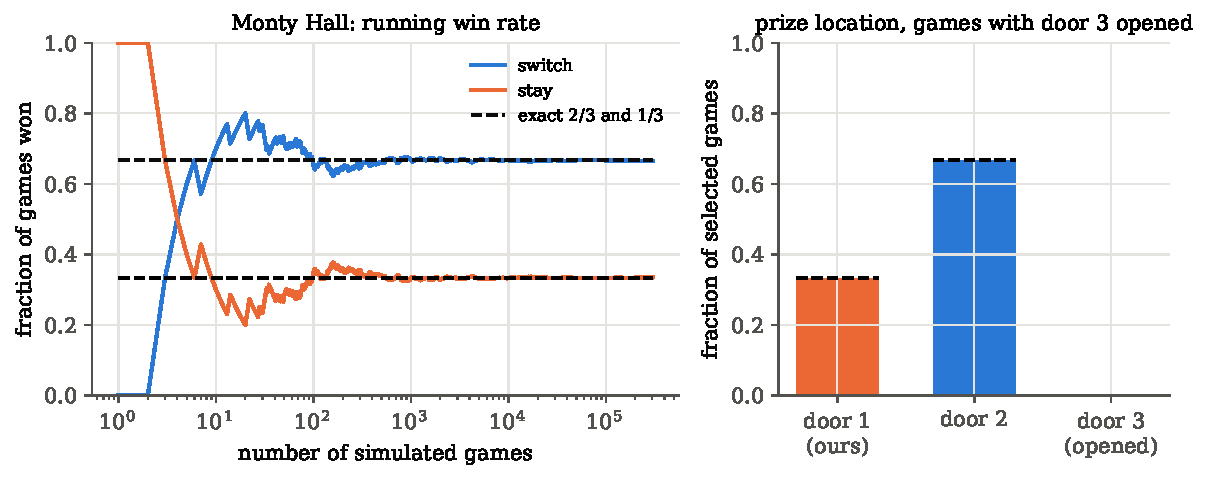
\includegraphics[width=0.95\linewidth]{figures/ch01/1a_monty_hall.pdf}
\caption{Monty Hall by simulation. Left: the running fraction of games won by
always switching and by always staying, settling on $\tfrac23$ and $\tfrac13$.
Right: among the games in which Monty opened door 3, where the prize was. The
bars are the posterior, estimated by counting, and the dashed ticks are the
exact values $\tfrac13$ and $\tfrac23$.}
\label{1a:fig:monty}
\end{figure}

\begin{inpractice}[Selecting on the observation is how analyses estimate purity]
Here the simulation only verified a posterior that Bayes' theorem gives in
one line. In a real analysis the ``hypotheses'' are the physics processes
(signal and every background), the ``observation'' is a long list of
selection cuts, and the likelihood of passing them depends on the kinematics
of each event, for which no formula exists. The expected composition of the
selected sample is then computed exactly as above: simulate each process with
its cross section as the prior weight, apply the selection, and count what
survives. The numbers that come out are the prior-times-likelihood column of
the table, event by event, and the fractions among the survivors are the
posterior. Bayes' theorem in its tabular form is also how particle-ID
systems combine the responses of several detectors: the likelihood ratios of
independent subdetectors multiply, as in \eqref{1a:eq:odds}, and the prior is
the expected particle mix.
\end{inpractice}

\subsection{Where this goes}

Every later chapter uses one of the two directions, prediction or inference,
and many use both. Side by side:
\begin{center}
\small
\begin{tabular}{@{}p{0.44\linewidth}p{0.44\linewidth}@{}}
\toprule
prediction & inference\\
\midrule
start from a hypothesis $H$ & start from an observed event $E$\\
ask what outcomes it can produce & ask which hypotheses could have produced it\\
uses $\Prob(E\given H)$, the forward tree & wants $\Prob(H\given E)$, the tree read backwards\\
efficiency, sampling distribution, $p$-value & purity, posterior, credible interval\\
\bottomrule
\end{tabular}
\end{center}
They are not rival interpretations of probability. They are two questions
about one joint probability structure, the leaves of a single tree.

From the trigger to the five coins, every example was settled by two sentences
said before any symbol. First: which hypotheses could have given what we saw?
They are the rows of the table, and the posterior is spread over them. Second:
how probable was the observation under each one? That is the likelihood
column. \Cref{ch:05} turns this into a standing habit.

The arithmetic is always the same, but the meaning of the posterior depends on
the hypotheses. When they are outcomes of a repeatable process (signal or
background, which coin, which door), a posterior is a long-run frequency among
the selected trials, as the simulations showed. When the hypothesis is a value
of a physical constant, which nature chose once, there are no repeated trials
to count. Then the posterior can only be read as a degree of belief, the second
interpretation of \cref{1a:sec:axioms}.

In the pipeline that runs from a physical model, through the data and a summary
of them, to physics inferred, the forward tree is the sampling distribution
$P(S\given\theta)$ of a summary $S$ computed from the data, given the model
parameters $\theta$. Reading that tree backwards is the last arrow, inference. \Cref{ch:05} replaces the list of hypotheses by a continuous
parameter $\params$, the likelihood by $\Like(\params)=p(\data\given\params)$ (the
probability density of the data $\data$ given $\params$), and the sum in the
evidence by the integral $Z=p(\data)=\int p(\data\given\params)\,p(\params)\,\dd\params$,
which runs over every possible parameter value and is usually the hard part.
\Cref{ch:09} avoids computing it at all: in the proportional form
\eqref{1a:eq:bayes-prop} only ratios of posteriors appear, and $Z$ cancels in
every ratio, just as $\Prob(E)$ cancelled in the odds \eqref{1a:eq:odds}. In
\cref{ch:04} we meet the forward direction on its own, in the $p$-value, which
is a statement about $\Prob(\text{data}\given\Hnull)$, the probability of the data
if the null hypothesis $\Hnull$ (``nothing but chance'') were true. It must
never be read as $\Prob(\Hnull\given\text{data})$.

\subsection*{Reading the literature}
\begin{description}[leftmargin=1.5em,itemsep=2pt]
  \item[Events.] \mainref{pp.~3--5, \S1.2} Wasserman defines $\Omega$, outcomes and events in three lines and gives the
three examples of \cref{1a:ex:aos-spaces}, the table of terminology
(our dictionary, where $\varnothing$ is the ``null event'' that is always false
and $\Omega$ the ``true event''), disjointness, partitions, indicators and the
limits of monotone sequences with the example $[0,1/i)$. He writes $A\cap B$ as
$AB$ or $(A,B)$, the convention used from here on. The proofs of De Morgan's
laws and the distributive law are exercises there (\mainref{p.~14, Ex.~4}) and
worked in \srcref{SeeingTheory}{pp.~20--21}. Kruschke adds the point that the
sample space is set by the measurement operation \srcref{Kruschke}{\S4.1}.
  \item[Axioms.] \mainref{pp.~5--7, 13, \S1.3, \S1.9} Wasserman states the axioms (Definition 1.5, footnote on $\sigma$-fields), the
two interpretations in one paragraph, the properties (1.1) without proof,
inclusion--exclusion (Lemma 1.6) with the proof we expanded, the two-toss
example (Example 1.7) and continuity (Theorem 1.8, increasing case only, the
decreasing case being his Exercise~1). The appendix \S1.9 defines $\sigma$-fields,
probability spaces and the Borel $\sigma$-field. Cowan \srcref{Cowan}{\S1.1} lists
finite additivity instead of countable additivity as the third axiom, noting
that this is a simplification. Countable additivity is what makes continuity
and \cref{1a:ex:no-uniform-N} work. The Bonferroni inequality and the
disjointification in Boole's inequality are from \srcref{CasellaBerger}{\S1.2};
the electron-mass argument is \srcref{Cowan}{\S1.2.2}; calibration by gambles is
\srcref{Kruschke}{\S4.2.2}.
  \item[Counting.] \mainref{pp.~7--8, \S1.4} Wasserman treats finite sample spaces in a page: the $36$ outcomes of two dice,
$\Prob(\text{sum}=11)=2/36$, the uniform distribution $\Prob(A)=|A|/|\Omega|$,
$n!$ with $0!=1$, the binomial coefficient (1.2), the committee of $3$ from $20$
($1140$), and $\binom n0=\binom nn=1$, $\binom nk=\binom n{n-k}$. He writes that
``we needn't delve into these in any great detail'', which is why we supplied
the derivations. The two-by-two table of counting rules, stars and bars, the
lottery and poker counts, and the warning that unordered outcomes with
replacement are not equally likely come from \srcref{CasellaBerger}{\S1.2.3--1.2.4}.
The recursion $P_n=nP_{n-1}$ and counting by overcounting are from
\srcref{SeeingTheory}{pp.~22--24}. The birthday problem is not treated in these sources.
  \item[Trees.] \mainref{p.~12, Thm~1.16} Wasserman states the law of total probability for a finite partition and
proves it in one line, as in our chain. He draws no trees. The tree picture,
with the first stage as the hypotheses and the second as the outcomes they
produce, organises the librarian--farmer, Monty Hall and medical-test problems above, and Lambert's ``two routes to the joint probability''
\srcref{Lambert}{\S3.6.1} is a two-stage tree read in both orders. Cowan
derives the same law as (1.7) \srcref{Cowan}{p.~3}, and Seeing Theory's
coins in a bag is \cref{1a:ex:bag-total} \srcref{SeeingTheory}{pp.~28--29}.
  \item[Independence.] \mainref{pp.~8--10, \S1.5} Wasserman defines independence by the product rule (Definition 1.9, with
$A\amalg B$ for independence), distinguishes assumed from derived independence
with the die events $\{2,4,6\}$ and $\{1,2,3,4\}$, shows that disjoint events with
positive probability are dependent and that a Venn diagram cannot display
independence, and gives Examples 1.10 and 1.11 and a summary box. His
Exercises 11, 14, 15 and 23 are solved above. The pairwise and mutual examples
and de M\'er\'e's bet are from \srcref{CasellaBerger}{\S1.3}, the card-colour and
causation remarks from \srcref{Lambert}{\S3.4}, and suit versus value from
\srcref{Kruschke}{\S4.4.2}. Seeing Theory lists $B=\{\text{second flip heads}\}$ as
$\{HT,TT\}$ \srcref{SeeingTheory}{p.~12}. It should be $\{HH,TH\}$.
  \item[Conditioning and Bayes.] Conditional probability and Bayes' theorem are \mainref{pp.~11--13, \S1.6--1.7}, \srcref{Cowan}{\S1.2}, \srcref{CasellaBerger}{\S1.3}, \srcref{Kruschke}{\S4.4} and \srcref{SeeingTheory}{pp.~26--30}.
Wasserman gives the law of total probability and Bayes' theorem as Theorems 1.16
and 1.17 \mainref{pp.~12--17}, the names prior and posterior in Remark 1.18, the
spam example as Example 1.19, and Monty Hall, the three cards, the rule that a
losing hypothesis forces another to gain, the operating systems and the five
coins as Exercises 10, 12, 18, 19 and 20. The two routes to
the joint probability are \srcref{Lambert}{\S3.6}. The disease example and the
combined form of the theorem are \srcref{Cowan}{pp.~3--4, (1.6)--(1.8)}. The
Morse-code and prisoners examples are \srcref{CasellaBerger}{\S1.3}, and the
coins in a bag are \srcref{SeeingTheory}{pp.~28--29}.
\end{description}

\begin{recap}[Events, conditional probability and trees]
\begin{itemize}[leftmargin=1.2em,itemsep=1pt]
  \item An experiment has a sample space $\Omega$ of outcomes. Events are subsets,
        combined by $\cup$, $\cap$ and complement. In code an event is a Boolean
        mask over simulated outcomes.
  \item Probability obeys three axioms. Complement rule, monotonicity,
        inclusion--exclusion, Boole's inequality and continuity all follow.
        It can be read as a long-run frequency or as a degree of belief.
  \item With equally likely outcomes, probability is counting:
        $\Prob(A)=|A|/|\Omega|$, with $n!$ and $\binom nk$ as the tools (birthday problem).
  \item Information shrinks the sample space: $\Prob(A\given B)=\Prob(AB)/\Prob(B)$,
        the overlap re-measured against the surviving region $B$. In code,
        \texttt{A[B].mean()}.
  \item Trees: multiply along a path (chain rule), add across paths (law of
        total probability, a weighted average over the unobserved stage).
  \item Independence, $\Prob(AB)=\Prob(A)\Prob(B)$, is not disjointness. Mutual
        independence needs every sub-collection.
  \item Bayes' theorem reads the tree backwards:
        $\Prob(H_i\given E)\propto\Prob(E\given H_i)\Prob(H_i)$, normalised by
        $\Prob(E)=\sum_j\Prob(E\given H_j)\Prob(H_j)$. Posterior odds are the
        likelihood ratio times the prior odds.
  \item Efficiency is a forward number, purity an inverse one. Small priors
        make even good evidence weak (base rates).
\end{itemize}
\end{recap}
\providecommand{\oneBEx}[1]{\par\medskip\noindent\refstepcounter{wex}\textbf{Example~\thewex\ifx\relax#1\relax\else\ (#1)\fi.}\ }
\providecommand{\OneBBernP}{}\renewcommand{\OneBBernP}{0.3}
\providecommand{\OneBBernFrac}{}\renewcommand{\OneBBernFrac}{0.3016}
\providecommand{\OneBNOmega}{}\renewcommand{\OneBNOmega}{10^5}
\providecommand{\OneBNExp}{}\renewcommand{\OneBNExp}{2\times10^{5}}
\providecommand{\OneBMeanX}{}\renewcommand{\OneBMeanX}{4.997}
\providecommand{\OneBMeanY}{}\renewcommand{\OneBMeanY}{2.796}
\providecommand{\OneBPXfive}{}\renewcommand{\OneBPXfive}{0.2467}
\providecommand{\OneBPXfiveExact}{}\renewcommand{\OneBPXfiveExact}{0.2461}
\providecommand{\OneBPYthree}{}\renewcommand{\OneBPYthree}{0.2606}
\providecommand{\OneBPeakExact}{}\renewcommand{\OneBPeakExact}{1.596}
\providecommand{\OneBPeakEst}{}\renewcommand{\OneBPeakEst}{1.612}
\providecommand{\OneBFracOneSig}{}\renewcommand{\OneBFracOneSig}{0.683}
\providecommand{\OneBQoneSample}{}\renewcommand{\OneBQoneSample}{49.826}
\providecommand{\OneBQoneExact}{}\renewcommand{\OneBQoneExact}{49.831}
\providecommand{\OneBMedSample}{}\renewcommand{\OneBMedSample}{49.996}
\providecommand{\OneBMedExact}{}\renewcommand{\OneBMedExact}{50.000}
\providecommand{\OneBQthreeSample}{}\renewcommand{\OneBQthreeSample}{50.146}
\providecommand{\OneBQthreeExact}{}\renewcommand{\OneBQthreeExact}{50.169}
\providecommand{\OneBMargN}{}\renewcommand{\OneBMargN}{2\times10^{5}}
\providecommand{\OneBMargSdY}{}\renewcommand{\OneBMargSdY}{2.006}
\providecommand{\OneBMargSdX}{}\renewcommand{\OneBMargSdX}{1.001}
\providecommand{\OneBBandN}{}\renewcommand{\OneBBandN}{4855}
\providecommand{\OneBCondMeanSim}{}\renewcommand{\OneBCondMeanSim}{1.404}
\providecommand{\OneBCondMeanExact}{}\renewcommand{\OneBCondMeanExact}{1.400}
\providecommand{\OneBCondSdSim}{}\renewcommand{\OneBCondSdSim}{1.426}
\providecommand{\OneBCondSdExact}{}\renewcommand{\OneBCondSdExact}{1.428}
\providecommand{\OneBSmearN}{}\renewcommand{\OneBSmearN}{5\times10^{5}}
\providecommand{\OneBSmearMeanSim}{}\renewcommand{\OneBSmearMeanSim}{19.99}
\providecommand{\OneBSmearVarSim}{}\renewcommand{\OneBSmearVarSim}{425.0}
\providecommand{\OneBSmearVarExact}{}\renewcommand{\OneBSmearVarExact}{425.0}
\providecommand{\OneBSmearNegSim}{}\renewcommand{\OneBSmearNegSim}{0.0866}
\providecommand{\OneBSmearNegExact}{}\renewcommand{\OneBSmearNegExact}{0.0860}
\providecommand{\OneBSmearChi}{}\renewcommand{\OneBSmearChi}{125}
\providecommand{\OneBSmearNdf}{}\renewcommand{\OneBSmearNdf}{136}
\providecommand{\OneBOscN}{}\renewcommand{\OneBOscN}{2\times10^{5}}
\providecommand{\OneBOscFracSim}{}\renewcommand{\OneBOscFracSim}{0.2872}
\providecommand{\OneBOscFracExact}{}\renewcommand{\OneBOscFracExact}{0.2871}
\providecommand{\OneBOscChi}{}\renewcommand{\OneBOscChi}{65.4}
\providecommand{\OneBOscNbins}{}\renewcommand{\OneBOscNbins}{60}
\providecommand{\OneBOscMeanSq}{}\renewcommand{\OneBOscMeanSq}{0.4995}
\providecommand{\OneBRuleChi}{}\renewcommand{\OneBRuleChi}{54.7}
\providecommand{\OneBRuleNbins}{}\renewcommand{\OneBRuleNbins}{50}
\providecommand{\OneBRuleFracSim}{}\renewcommand{\OneBRuleFracSim}{0.0478}
\providecommand{\OneBRuleFracExact}{}\renewcommand{\OneBRuleFracExact}{0.0477}
\providecommand{\OneBDecN}{}\renewcommand{\OneBDecN}{4\times10^{5}}
\providecommand{\OneBDecPstar}{}\renewcommand{\OneBDecPstar}{40.2}
\providecommand{\OneBDecMeanPtSim}{}\renewcommand{\OneBDecMeanPtSim}{31.566}
\providecommand{\OneBDecMeanPtExact}{}\renewcommand{\OneBDecMeanPtExact}{31.573}
\providecommand{\OneBDecFracSim}{}\renewcommand{\OneBDecFracSim}{0.4353}
\providecommand{\OneBDecFracExact}{}\renewcommand{\OneBDecFracExact}{0.4359}
\providecommand{\OneBDecMeanCos}{}\renewcommand{\OneBDecMeanCos}{0.0006}
\providecommand{\OneBExpUSim}{}\renewcommand{\OneBExpUSim}{1.7189}
\providecommand{\OneBExpUExact}{}\renewcommand{\OneBExpUExact}{1.7183}
\providecommand{\OneBStickSim}{}\renewcommand{\OneBStickSim}{0.7498}
\providecommand{\OneBHierMean}{}\renewcommand{\OneBHierMean}{9.997}
\providecommand{\OneBHierVar}{}\renewcommand{\OneBHierVar}{36.67}
\providecommand{\OneBHierVarExact}{}\renewcommand{\OneBHierVarExact}{36.67}
\providecommand{\OneBPlainVar}{}\renewcommand{\OneBPlainVar}{4.998}
\providecommand{\OneBArgminSq}{}\renewcommand{\OneBArgminSq}{1.00}
\providecommand{\OneBArgminAbs}{}\renewcommand{\OneBArgminAbs}{0.69}
\providecommand{\OneBMinSq}{}\renewcommand{\OneBMinSq}{0.996}
\providecommand{\OneBGalRa}{}\renewcommand{\OneBGalRa}{-0.795}
\providecommand{\OneBGalRb}{}\renewcommand{\OneBGalRb}{0.040}
\providecommand{\OneBGalRc}{}\renewcommand{\OneBGalRc}{0.486}
\providecommand{\OneBGalRd}{}\renewcommand{\OneBGalRd}{0.949}
\providecommand{\OneBZeroRxy}{}\renewcommand{\OneBZeroRxy}{0.0046}
\providecommand{\OneBZeroRxxy}{}\renewcommand{\OneBZeroRxxy}{1.0000}
\providecommand{\OneBZeroRabsxy}{}\renewcommand{\OneBZeroRabsxy}{0.9359}
\providecommand{\OneBZeroN}{}\renewcommand{\OneBZeroN}{2\times10^{5}}
\providecommand{\OneBCovN}{}\renewcommand{\OneBCovN}{2\times10^{5}}
\providecommand{\OneBChataa}{}\renewcommand{\OneBChataa}{3.998}
\providecommand{\OneBChatab}{}\renewcommand{\OneBChatab}{1.798}
\providecommand{\OneBChatbb}{}\renewcommand{\OneBChatbb}{0.999}
\providecommand{\OneBCYaa}{}\renewcommand{\OneBCYaa}{8.595}
\providecommand{\OneBCYab}{}\renewcommand{\OneBCYab}{2.999}
\providecommand{\OneBCYbb}{}\renewcommand{\OneBCYbb}{1.401}
\providecommand{\OneBCWaa}{}\renewcommand{\OneBCWaa}{0.157}
\providecommand{\OneBCWab}{}\renewcommand{\OneBCWab}{-0.001}
\providecommand{\OneBCWbb}{}\renewcommand{\OneBCWbb}{4.840}
\providecommand{\OneBLamA}{}\renewcommand{\OneBLamA}{0.157}
\providecommand{\OneBLamB}{}\renewcommand{\OneBLamB}{4.843}
\providecommand{\OneBLaa}{}\renewcommand{\OneBLaa}{2.000}
\providecommand{\OneBLba}{}\renewcommand{\OneBLba}{0.900}
\providecommand{\OneBLbb}{}\renewcommand{\OneBLbb}{0.436}
\providecommand{\OneBMgfMone}{}\renewcommand{\OneBMgfMone}{0.9993}
\providecommand{\OneBMgfMtwo}{}\renewcommand{\OneBMgfMtwo}{1.9993}
\providecommand{\OneBCfMaxDev}{}\renewcommand{\OneBCfMaxDev}{0.0073}
\providecommand{\OneBCfInvDev}{}\renewcommand{\OneBCfInvDev}{0.0004}
\providecommand{\OneBCfN}{}\renewcommand{\OneBCfN}{10^5}
\providecommand{\OneBRunGaussMax}{}\renewcommand{\OneBRunGaussMax}{0.022}
\providecommand{\OneBRunCauchyMin}{}\renewcommand{\OneBRunCauchyMin}{0.28}
\providecommand{\OneBRunCauchyMax}{}\renewcommand{\OneBRunCauchyMax}{1.21}
\providecommand{\OneBRunN}{}\renewcommand{\OneBRunN}{10^4}
\section{Random variables: turning outcomes into numbers}
\label{1b:sec:rv}

A charged track crosses ten layers of a silicon tracker. Each layer either
records a hit or misses it. The raw outcome of one track is therefore a
10-letter pattern such as \texttt{HHTHHTHHTT} (H for hit, T for miss). Nobody
analyses patterns directly. The track-quality cut asks for a \emph{number}:
``how many hits?'' A pattern-recognition algorithm asks for a different
number: ``what is the longest run of consecutive hits?'' Both numbers are
computed from the same pattern, and both are uncertain before the track
arrives.

A \newterm{random variable} is exactly this: a rule that reads a number off
each outcome. We want numbers because a pattern of letters cannot be put in a
histogram, averaged or added, and a number can. Every data point, every
estimator and every summary statistic in the rest of the book is a random
variable.

Recall the box $\Omega$ of all possible outcomes from the first part of
\cref{ch:01}, where the probability of an event was its share of the area of
the box. A random variable is a measuring device clipped onto that box.
Nature picks the point $\omega$, and the device prints the number
$X(\omega)$. Nothing random happens inside the device. It is an ordinary
function, and all the randomness is in which $\omega$ nature picked. Several
devices can be clipped onto the same box, and each reads its own number off
the \emph{same} outcome. This is why two random variables can be related to
each other (correlated, dependent): both are functions of one common
$\omega$.

Building a random variable takes four questions, asked in this order.
\begin{enumerate}[leftmargin=1.5em,itemsep=1pt]
  \item What is one outcome $\omega$? (One full hit pattern, one collision
        event record, one sky map.)
  \item What number do we want to read off it? Write it as a rule
        $\omega\mapsto X(\omega)$.
  \item For each set $A$ of numbers we might ask about, which outcomes give a
        value in $A$? That set of outcomes is an event, and its probability is
        the probability that $X$ lands in $A$.
  \item Collect those probabilities for all $A$. That list is the
        \emph{distribution} of $X$, and from then on we can mostly forget
        $\Omega$.
\end{enumerate}

\subsection{The definition, and the event hiding behind every statement about \texorpdfstring{$X$}{X}}

The four questions give one definition. They also give a rule we will use
constantly: every statement about the number $X$ is a statement about a set
of outcomes.

\begin{workdef}[random variable, distribution]
A \newterm{random variable} is a map
\[
  X:\Omega\to\R
\]
that assigns a real number $X(\omega)$ to each outcome $\omega$
\unpack{a fixed rule, such as ``count the H's'', applied to whichever
outcome occurs}. For a set $A\subseteq\R$ the \newterm{inverse image} is
$X^{-1}(A)=\{\omega\in\Omega:\ X(\omega)\in A\}$ \unpack{all outcomes whose
reading lands in $A$. It is a set of outcomes, not an inverse function}, and
\[
  \Prob(X\in A)\;\defeq\;\Prob\bigl(X^{-1}(A)\bigr),\qquad
  \Prob(X=x)\;\defeq\;\Prob\bigl(\{\omega:\ X(\omega)=x\}\bigr).
\]
The collection of all the numbers $\Prob(X\in A)$ is the
\newterm{distribution} of $X$ \unpack{how the probability of $\Omega$ is
spread along the real line by the map $X$}.
\emph{Operational test:} you have a random variable when, given any outcome,
you can compute a single real number from it without further information.
\end{workdef}

Capital $X$ is the random variable (the rule). Lower-case $x$ is a particular
value it can take. ``$X=x$'' is therefore an event: the set of outcomes whose
reading is $x$. (Strictly, $X$ must be \newterm{measurable}: every set
$\{\omega:X(\omega)\le x\}$ must be an event we are allowed to assign a
probability to. Every function met in practice is, and we will not mention it
again \mainref{p.~43}.)

\begin{figure}[htbp]
\centering
\begin{tikzpicture}[scale=1.0,
  pt/.style={circle,fill=formblue,inner sep=1.4pt},
  val/.style={circle,fill=fibreorange,inner sep=1.6pt}]
  \draw[thick,formblue,fill=formblue!8] plot[smooth cycle,tension=0.8]
    coordinates {(-0.2,0.2) (1.6,1.6) (3.4,1.1) (3.6,-0.9) (1.8,-1.7) (0.1,-1.1)};
  \node[lbl,formblue] at (0.2,1.35) {$\Omega$};
  \node[pt] (tt) at (1.2,-0.9) {}; \node[lbl,anchor=east] at (1.1,-0.9) {TT};
  \node[pt] (th) at (2.0,0.9) {};  \node[lbl,anchor=north] at (2.0,0.8) {TH};
  \node[pt] (ht) at (2.3,-0.3) {}; \node[lbl,anchor=north] at (2.3,-0.4) {HT};
  \node[pt] (hh) at (0.9,0.6) {};  \node[lbl,anchor=east] at (0.8,0.6) {HH};
  \draw[->,thick] (6.0,-1.8) -- (6.0,2.0) node[above,lbl] {$\R$};
  \foreach \y/\t in {-1/0, 0.2/1, 1.4/2} {
    \draw (5.9,\y) -- (6.1,\y);
    \node[lbl,anchor=west] at (6.15,\y) {$\t$};
  }
  \node[val] (v0) at (6.0,-1) {};
  \node[val] (v1) at (6.0,0.2) {};
  \node[val] (v2) at (6.0,1.4) {};
  \draw[->,faint,thick,shorten >=2pt] (tt) to[out=10,in=190] (v0);
  \draw[->,faint,thick,shorten >=2pt] (th) to[out=0,in=175] (v1);
  \draw[->,faint,thick,shorten >=2pt] (ht) to[out=10,in=185] (v1);
  \draw[->,faint,thick,shorten >=2pt] (hh) to[out=40,in=180] (v2);
  \node[lbl,align=left,anchor=west] at (7.0,1.4) {$X^{-1}(\{2\})=\{\mathrm{HH}\}$};
  \node[lbl,align=left,anchor=west] at (7.0,0.2) {$X^{-1}(\{1\})=\{\mathrm{TH},\mathrm{HT}\}$};
  \node[lbl,align=left,anchor=west] at (7.0,-1.0) {$X^{-1}(\{0\})=\{\mathrm{TT}\}$};
\end{tikzpicture}
\caption{A random variable is a function from outcomes to numbers. For two
coin flips, $X$ = number of heads sends the four outcomes to three numbers.
Two outcomes land on the value 1, so the probability that $X=1$ collects the
probability of both. The inverse images on the right are the events that
statements about $X$ secretly refer to.}
\label{1b:fig:rv-map}
\end{figure}

\oneBEx{Two flips: from the outcome table to the distribution}\label{1b:ex:two-flips}
Flip a fair coin twice, $\Omega=\{\mathrm{TT},\mathrm{TH},\mathrm{HT},\mathrm{HH}\}$,
each outcome with probability $1/4$, and let $X$ be the number of heads. Then
\begin{align*}
  \Prob(X=1)
  &\eqby{1} \Prob\bigl(\{\omega:\ X(\omega)=1\}\bigr)\\
  &\eqby{2} \Prob\bigl(\{\mathrm{TH},\mathrm{HT}\}\bigr)\\
  &\eqby{3} \Prob(\{\mathrm{TH}\})+\Prob(\{\mathrm{HT}\})
   = \tfrac14+\tfrac14=\tfrac12 .
\end{align*}
\begin{explain}
  \item Definition of $\Prob(X=x)$ as the probability of the inverse image.
  \item Read off which outcomes contain exactly one H.
  \item The two outcomes are disjoint events, so the axiom of additivity
        (first part of \cref{ch:01}) adds their probabilities.
\end{explain}
In the same way $\Prob(X=0)=\Prob(\{\mathrm{TT}\})=1/4$ and
$\Prob(X=2)=\Prob(\{\mathrm{HH}\})=1/4$. Two tables summarise the situation:
\begin{center}
\begin{tabular}{c|c|c}
$\omega$ & $\Prob(\{\omega\})$ & $X(\omega)$\\\hline
TT & 1/4 & 0\\ TH & 1/4 & 1\\ HT & 1/4 & 1\\ HH & 1/4 & 2
\end{tabular}
\qquad\qquad
\begin{tabular}{c|c}
$x$ & $\Prob(X=x)$\\\hline
0 & 1/4\\ 1 & 1/2\\ 2 & 1/4
\end{tabular}
\end{center}
The left table describes the outcomes themselves. The right table is the
distribution of $X$, and it answers every question about $X$ alone. What the
right table has lost, \emph{which} flip was the head, is exactly what $X$
does not measure.

\oneBEx{Several random variables on one disk}\label{1b:ex:disk}
Pick a point uniformly at random in the unit disk
$\Omega=\{(x,y):\ x^2+y^2\le1\}$, so that the probability of a region is its
area divided by $\pi$. The outcome is the point $\omega=(x,y)$. Four random
variables on the same $\Omega$ are $X(\omega)=x$, $Y(\omega)=y$,
$Z(\omega)=x+y$ and $W(\omega)=\sqrt{x^2+y^2}$ \mainref{p.~20}. Let us find the
distribution of the distance $W$ from the centre. For $0\le r\le1$,
\begin{align*}
  \Prob(W\le r)
  &\eqby{1} \Prob\bigl(\{(x,y):\ x^2+y^2\le r^2\}\bigr)\\
  &\eqby{2} \frac{\pi r^2}{\pi}
   = r^2 .
\end{align*}
\begin{explain}
  \item $W\le r$ happens exactly for the points inside the circle of radius $r$.
  \item Uniform on the disk means probability = area$/\pi$, and the small disk
        has area $\pi r^2$.
\end{explain}
So $\Prob(W\le\tfrac12)=\tfrac14$: a ``uniformly random point'' is \emph{not}
uniformly distributed in its distance from the centre. Three quarters of the
area lies in the outer ring $\tfrac12<W\le1$. A detector that is uniformly
illuminated sees most hits near its rim, simply because the rim has more area.

\subsection{Bernoulli and binomial: one trial and many trials}

The simplest random variables take only two values. Many of the most useful
ones in the book are sums of them.

\begin{workdef}[Bernoulli and binomial]
$X$ is \newterm{Bernoulli}$(p)$ if $\Prob(X=1)=p$ and $\Prob(X=0)=1-p$
\unpack{a single yes-or-no trial, 1 for success}. Compactly
$\Prob(X=x)=p^x(1-p)^{1-x}$ for $x\in\{0,1\}$.
$X$ is \newterm{binomial}$(n,p)$ if it counts the successes in $n$
successive, independent Bernoulli$(p)$ trials \unpack{the same trial repeated
$n$ times, with outcomes that do not influence each other}.
\emph{Operational test:} a single detector layer that fires or not is
Bernoulli. The number of the ten layers that fired is binomial, provided the
layers have the same efficiency and fire independently.
\end{workdef}

Bernoulli is for a single trial; binomial is for multiple successive trials.
That is the whole difference between the two. A binomial variable is a sum of Bernoulli variables,
$X=X_1+\dots+X_n$ with $X_i$ the indicator of success on trial $i$.

\oneBEx{The binomial distribution, by counting paths}\label{1b:ex:binomial}
Generalise \cref{1b:ex:two-flips} to $n$ trials with success probability
$p$ \mainref{p.~20 (``try generalizing this to $n$ flips'')}. An outcome is
a sequence of $n$ letters. Consider one particular sequence with exactly $k$
successes, say $\mathrm{S}^k\mathrm{F}^{n-k}$ (all successes first). Then
\begin{align*}
  \Prob(\mathrm{S}\cdots\mathrm{S}\,\mathrm{F}\cdots\mathrm{F})
  &\eqby{1} \underbrace{p\cdots p}_{k}\;\underbrace{(1-p)\cdots(1-p)}_{n-k}
   = p^k(1-p)^{n-k},\\
  \Prob(X=k)
  &\eqby{2} \sum_{\text{sequences with $k$ S}} p^k(1-p)^{n-k}
   \eqby{3} \binom{n}{k}p^k(1-p)^{n-k},\qquad k=0,1,\dots,n .
\end{align*}
\begin{explain}
  \item The trials are independent, so the probability of a sequence is the
        product of the probabilities of its letters.
  \item $\{X=k\}$ is the disjoint union of all sequences with exactly $k$
        successes, and every one of them has the same probability (only the
        number of S's matters, not their positions).
  \item The number of such sequences is the number of ways to choose which
        $k$ of the $n$ positions carry an S, $\binom{n}{k}=n!/(k!(n-k)!)$
        (the counting rule of the first part of \cref{ch:01}).
\end{explain}
For $n=10$, $p=\tfrac12$: $\Prob(X=5)=\binom{10}{5}/2^{10}=252/1024=0.2461$.
Simulated coin tosses give $\OneBPXfive$, against the exact
$\OneBPXfiveExact$. The binomial and its relatives (geometric, Poisson,
multinomial) are derived from first principles in \cref{ch:02}.

\oneBEx{The sample space that ``disappears''}\label{1b:ex:bern-construction}
The named distributions are usually stated with no $\Omega$ in sight. Is
there still a set of outcomes behind them? Yes: one can always be built
\mainref{p.~27}. Take $\Omega=[0,1]$ with
$\Prob([a,b])=b-a$ (uniform), fix $p$, and define
\[
  X(\omega)=\begin{cases}1,&\omega\le p,\\ 0,&\omega>p.\end{cases}
\]
Then
\begin{align*}
  \Prob(X=1)
  &\eqby{1} \Prob(\{\omega:\ \omega\le p\})
   \eqby{2} \Prob([0,p])
   \eqby{3} p ,
\end{align*}
\begin{explain}
  \item Inverse image of the value 1 under the rule above.
  \item The outcomes with $\omega\le p$ form the interval $[0,p]$.
  \item Uniform probability of an interval is its length.
\end{explain}
and $\Prob(X=0)=1-p$, so $X\sim\text{Bernoulli}(p)$. This is not a
curiosity: it is exactly how a computer makes a Bernoulli variable,
\texttt{x = (u <= p)} with \texttt{u} a uniform random number
(\cref{ch:06} makes this the general recipe). In practice we think of a random
variable as ``a random number''. Formally it is still a function on some
$\Omega$.

\begin{pitfall}[Three notational traps]
\begin{itemize}[leftmargin=1.2em,itemsep=1pt]
  \item $X\sim F$ means ``$X$ \emph{has} distribution $F$'', not ``$X$ is
        approximately $F$'' \mainref{p.~25}.
  \item In Binomial$(n,p)$, $X$ is random and $x$ is a value it can take,
        but $n$ and $p$ are \newterm{parameters}: fixed numbers of the model.
        The parameter is usually unknown and has to be learned from data.
        That is what statistical inference is about. Do not confuse the
        random variable with the parameter \mainref{p.~26}.
  \item $X$ and $Y$ are \newterm{equal in distribution}, $X\overset{d}{=}Y$,
        if $\Prob(X\le x)=\Prob(Y\le x)$ for every $x$. This does not mean
        $X=Y$. If $\Prob(X=1)=\Prob(X=-1)=\tfrac12$ and $Y=-X$, then $X$ and $Y$
        have the same distribution but $\Prob(X=Y)=0$ \mainref{p.~25}.
\end{itemize}
\end{pitfall}

\subsection{Seeing it: two random variables on the same outcomes}

A simulation shows two random variables read off the same outcomes. The
script first builds a Bernoulli variable from a uniform $\omega$, as in
\cref{1b:ex:bern-construction}. It then generates $\OneBNExp$ outcomes of ten fair flips (each row of an array is one
$\omega$) and applies two different maps to every row: $X$ = number of heads
and $Y$ = longest run of heads.

\pyfile[firstline=25,lastline=50,firstnumber=25]{code/ch01/10_rv_as_map.py}{Two random variables read off the same simulated outcomes}

Lines 26--29 are \cref{1b:ex:bern-construction} verbatim: \texttt{omega} is
an array of $\OneBNOmega$ uniform outcomes and \texttt{X\_bern} is the boolean
test $\omega\le p$ turned into 0/1. Its average is the fraction of ones,
$\OneBBernFrac$ for $p=\OneBBernP$. Line 33 draws the outcomes of the second
experiment: an array with one row per outcome and one column per flip. The two
maps on lines 44--45 are ordinary Python functions of a row, which is the
definition of a random variable made executable. Lines 47--50 estimate each
distribution by the fraction of outcomes that land on each value.

\begin{figure}[htbp]
\centering
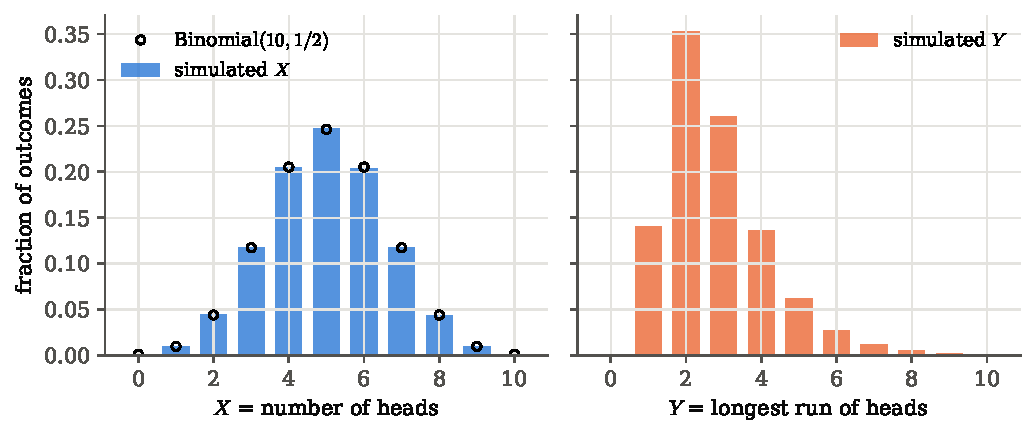
\includegraphics[width=0.95\linewidth]{figures/ch01/rv_as_map.pdf}
\caption{The same $2\times10^5$ simulated ten-flip outcomes, read by two
different random variables. Left: the number of heads, whose fractions sit on
the binomial probabilities (open circles). Right: the longest run of heads,
which has a completely different, skewed distribution although it is computed
from exactly the same outcomes.}
\label{1b:fig:rv-as-map}
\end{figure}

The numbers the script produced: the simulated $\Prob(X=5)$ is
$\OneBPXfive$ (exact $\OneBPXfiveExact$), the average number of heads is
$\OneBMeanX$ (we will show in \cref{1b:sec:expectation} that the exact value
is $np=5$), the average longest run is $\OneBMeanY$, and the most likely
longest run is 2, with $\Prob(Y=3)=\OneBPYthree$. No simple formula gives the
distribution of $Y$. The simulation gets it with the same effort as the
binomial one, because once we can generate outcomes, \emph{any} random
variable is just a function applied to them.

\paragraph{What this bought us.} A random variable is a function, so a
histogram of a random variable is a histogram of a function evaluated on
simulated outcomes. That single sentence is the whole of Monte Carlo
simulation (\cref{ch:06}).

\paragraph{How research uses it.} A collider Monte Carlo generator produces
outcomes $\omega$: complete event records with every particle's
four-momentum. An analysis then defines random variables on them: the missing
transverse momentum, the invariant mass of the two leading jets, the number of
$b$-tagged jets. The same $\omega$'s feed every observable, which is why one
simulated sample serves a whole collaboration, and why two observables
computed from the same events are in general correlated
(\cref{1b:sec:covariance}). In cosmology the outcome is a whole simulated sky
map, and the random variables are its summaries: a power spectrum $\Chat$ at
each $\ell$, the number of hot spots above a threshold, the Euler
characteristic of an excursion set (\cref{ch:07,ch:12}).

Later chapters use many named random variables. The table lists the named
distributions of \mainref{pp.~26--30}, each with the mechanism that produces
it. \Cref{ch:02}
derives every one of them from its mechanism.

\begin{taxonomy}[Named random variables and the story that produces each]
\begin{center}
\small
\begin{tabular}{@{}p{3.2cm}p{9.2cm}@{}}
\toprule
distribution & generating story\\\midrule
point mass $\delta_a$ & no randomness at all, $\Prob(X=a)=1$\\
discrete uniform & $k$ equally likely labels (a fair die)\\
Bernoulli$(p)$ & one yes/no trial\\
Binomial$(n,p)$ & successes in $n$ independent identical trials\\
Geometric$(p)$ & number of trials up to and including the first success, $p(1-p)^{k-1}$\\
Poisson$(\lambda)$ & counts of rare events in a fixed window (decays, events in a bin), $e^{-\lambda}\lambda^k/k!$\\
Uniform$(a,b)$ & ``a point at random'' in an interval, density $1/(b-a)$\\
Normal $\Normal(\mu,\sigma^2)$ & sums of many small independent effects (noise)\\
Exponential$(\beta)$ & waiting time to the next rare event, density $e^{-x/\beta}/\beta$\\
Gamma, $\chi^2_p$, $t_\nu$, Beta, Cauchy & sums of waiting times, sums of squared Gaussians, ratios, probabilities of probabilities, resonance line shapes\\
\bottomrule
\end{tabular}
\end{center}
\end{taxonomy}

\section{Mass, density and the cumulative distribution}
\label{1b:sec:pdf}

A test beam fires electrons of exactly $50\,\mathrm{GeV}$ into an
electromagnetic calorimeter. The calorimeter does not report 50 every time:
the shower fluctuates and the readout is noisy, so the measured energy $E$
scatters around 50 with a spread of about $0.25\,\mathrm{GeV}$. We want to
answer questions such as ``what fraction of electrons are measured below
49.5?'', ``which energy is exceeded by only 5\% of them?'' and ``how does the
histogram of measured energies look if we take more data?''

Three objects describe how a random variable is spread out: the probability
mass function for counts, the density for continuous readings, and the
cumulative distribution for both. We need more than one because counts and
continuous readings differ in kind. For a count (hits, heads) we can list the
probability of each value. For a continuous reading like $E$ we cannot,
because the probability of measuring \emph{exactly} $50.000\ldots$ is zero.
Each of the three objects can be read off a histogram. The idea people get
wrong most often is that a density is probability \emph{per unit} $x$, so it
carries units.

Mass and density are familiar from mechanics. A string of beads has point masses. A metal rod has a mass density
$\lambda(x)$ in kg/m, and the mass of a piece is $\int\lambda\,\dd x$. Nobody
asks ``what is the mass at the point $x=0.3\,$m?''. The answer is zero, and
yet $\lambda(0.3)$ is a perfectly good number. Probability works the same
way. Discrete random variables are beads: the probability sits on isolated
values. Continuous random variables are rods: the probability of a single
point is zero, and $f(x)$ is probability per unit length. The cumulative
distribution $F(x)$ is ``the mass to the left of $x$'', which makes sense for
beads, rods and anything in between.

To describe how a random number is spread out, we ask four questions in turn.
\begin{enumerate}[leftmargin=1.5em,itemsep=1pt]
  \item Does $X$ take isolated values (counts) or a continuum (energies,
        angles, positions)?
  \item Isolated values: list $\Prob(X=x)$ for each value.
  \item Continuum: ask instead for the probability of a small interval,
        divided by its width. That ratio is the density.
  \item Either way: the probability of landing at or below $x$ is a single
        function $F(x)$ that answers every interval question by subtraction,
        and whose inverse gives the quantiles.
\end{enumerate}

\subsection{The cumulative distribution function}

Beads and rods need different bookkeeping, but one function works for both:
the total probability collected up to a point.

\begin{workdef}[cumulative distribution function]
The \newterm{cumulative distribution function} (CDF) of $X$ is
\[
  F_X(x)=\Prob(X\le x),\qquad x\in\R ,
\]
\unpack{the probability that the reading is at most $x$, defined for every
real $x$, including values $X$ never takes}. We write $F$ when the variable is
clear.
\emph{Operational test:} sort a sample of $N$ readings. The fraction of
readings $\le x$ is the \newterm{empirical CDF}, and it tends to $F(x)$ as
$N\to\infty$.
\end{workdef}

\oneBEx{The CDF of two flips}\label{1b:ex:cdf-two-flips}
With $X$ = number of heads in two fair flips (\cref{1b:ex:two-flips}),
\[
  F_X(x)=\begin{cases}
  0, & x<0,\\ 1/4, & 0\le x<1,\\ 3/4, & 1\le x<2,\\ 1, & x\ge2 .
  \end{cases}
\]
For instance
\begin{align*}
  F_X(1.4)
  &\eqby{1} \Prob(X\le1.4)
   \eqby{2} \Prob(X=0)+\Prob(X=1)
   = \tfrac14+\tfrac12=\tfrac34 .
\end{align*}
\begin{explain}
  \item Definition of the CDF at the point $x=1.4$.
  \item $X$ only takes the values 0, 1, 2, and the ones $\le1.4$ are 0 and 1.
        The events $\{X=0\}$ and $\{X=1\}$ are disjoint, so their
        probabilities add.
\end{explain}
The CDF is a staircase. It is flat between the values, jumps by
$\Prob(X=x)$ at each value, and at a jump takes the \emph{upper} value (the
filled dots in \cref{1b:fig:cdf-steps}): $F(1)=3/4$, not $1/4$, because
$X\le1$ includes $X=1$.

\begin{figure}[htbp]
\centering
\begin{tikzpicture}[x=1.2cm,y=2.4cm]
  \begin{scope}
    \draw[->] (-0.6,0) -- (2.8,0) node[right,lbl] {$x$};
    \draw[->] (-0.6,0) -- (-0.6,1.15) node[above,lbl] {$\Prob(X=x)$};
    \foreach \y in {0.25,0.5,0.75,1} {\draw (-0.65,\y) -- (-0.55,\y);
      \node[lbl,anchor=east] at (-0.65,\y) {\y};}
    \foreach \x in {0,1,2} \node[lbl,anchor=north] at (\x,0) {\x};
    \draw[very thick,formblue] (0,0) -- (0,0.25);
    \draw[very thick,formblue] (1,0) -- (1,0.5);
    \draw[very thick,formblue] (2,0) -- (2,0.25);
    \fill[formblue] (0,0.25) circle (2pt) (1,0.5) circle (2pt) (2,0.25) circle (2pt);
    \node[lbl] at (1.1,1.1) {mass function};
  \end{scope}
  \begin{scope}[xshift=5.2cm]
    \draw[->] (-0.9,0) -- (2.9,0) node[right,lbl] {$x$};
    \draw[->] (-0.6,0) -- (-0.6,1.15) node[above,lbl] {$F_X(x)$};
    \foreach \y in {0.25,0.5,0.75,1} {\draw (-0.65,\y) -- (-0.55,\y);
      \node[lbl,anchor=east] at (-0.65,\y) {\y};}
    \foreach \x in {0,1,2} \node[lbl,anchor=north] at (\x,0) {\x};
    \draw[very thick,formblue] (-0.9,0) -- (0,0);
    \draw[very thick,formblue] (0,0.25) -- (1,0.25);
    \draw[very thick,formblue] (1,0.75) -- (2,0.75);
    \draw[very thick,formblue] (2,1) -- (2.8,1);
    \draw[faint,dashed] (0,0) -- (0,0.25) (1,0.25) -- (1,0.75) (2,0.75) -- (2,1);
    \fill[formblue] (0,0.25) circle (2pt) (1,0.75) circle (2pt) (2,1) circle (2pt);
    \filldraw[fill=white,draw=formblue,thick] (0,0) circle (2pt) (1,0.25) circle (2pt) (2,0.75) circle (2pt);
    \draw[bdryred,thick,dotted] (1.4,0) -- (1.4,0.75);
    \node[lbl,bdryred,anchor=north] at (1.4,-0.12) {$1.4$};
    \node[lbl] at (1.0,1.1) {CDF};
  \end{scope}
\end{tikzpicture}
\caption{Two fair flips. Left: the mass function puts probability $1/4$,
$1/2$, $1/4$ on the values 0, 1, 2. Right: the CDF accumulates it into a
staircase that jumps by those amounts. Filled dots mark the value the CDF
takes at each jump, open dots the value it approaches from the left. The
dotted line reads off $F(1.4)=3/4$.}
\label{1b:fig:cdf-steps}
\end{figure}

Every CDF has three properties, and conversely any function with these
properties is the CDF of some random variable \mainref{Thm~2.8, p.~21}:
\begin{enumerate}[label=(\roman*),leftmargin=2em,itemsep=1pt]
  \item \emph{non-decreasing}: $x_1<x_2\Rightarrow F(x_1)\le F(x_2)$, because
        $\{X\le x_1\}\subseteq\{X\le x_2\}$;
  \item \emph{normalised}: $F(x)\to0$ as $x\to-\infty$ and $F(x)\to1$ as
        $x\to+\infty$;
  \item \emph{right-continuous}: $F(x)=\lim_{y\downarrow x}F(y)$.
\end{enumerate}
Property (iii) is why the CDF takes the upper value at each jump (the filled
dots). Why does it hold? The tool is the \emph{continuity of probability}
from the first part of \cref{ch:01}: if
$A_1\supseteq A_2\supseteq\cdots$ shrink to $A=\bigcap_iA_i$, then
$\Prob(A)=\lim_i\Prob(A_i)$. Take any sequence $y_1>y_2>\cdots$ decreasing to
$x$, and $A_i=\{X\le y_i\}$. Then
\begin{align*}
  F(x)
  &\eqby{1} \Prob(X\le x)
   \eqby{2} \Prob\Bigl(\bigcap_i\{X\le y_i\}\Bigr)
   \eqby{3} \lim_i\Prob(X\le y_i)
   = \lim_i F(y_i) .
\end{align*}
\begin{explain}
  \item Definition of $F$.
  \item $X\le x$ holds exactly when $X\le y_i$ for every $i$, because the
        $y_i$ come arbitrarily close to $x$ from above.
  \item The events $\{X\le y_i\}$ shrink, so continuity of probability applies.
\end{explain}
From the left the argument fails. The events $\{X\le y_i\}$ with $y_i\uparrow
x$ grow to $\{X<x\}$, and that event misses the point $X=x$. This asymmetry
gives the handy rules of \mainref{Lemma~2.15, pp.~24--25}. Write
$F(x^-)=\lim_{y\uparrow x}F(y)$. Then
\begin{align}
  \Prob(X=x)&=F(x)-F(x^-), &
  \Prob(x<X\le y)&=F(y)-F(x), &
  \Prob(X>x)&=1-F(x). \label{1b:eq:cdf-rules}
\end{align}
The first says that the size of the jump at $x$ is the probability of the
value $x$. The second is additivity: $\{X\le y\}$ is the disjoint union of
$\{X\le x\}$ and $\{x<X\le y\}$. The third is the complement rule.

\subsection{Discrete variables: the probability mass function}

For counts the bookkeeping is the simplest one, a list of probabilities, one
per allowed value.

\begin{workdef}[probability mass function]
$X$ is \newterm{discrete} if it takes countably many values $x_1,x_2,\dots$
\unpack{values that can be listed one after another, like $0,1,2,\dots$}. Its
\newterm{probability mass function} (pmf) is $f_X(x)=\Prob(X=x)$. It
satisfies $f_X(x)\ge0$, $\sum_if_X(x_i)=1$, and
$F_X(x)=\sum_{x_i\le x}f_X(x_i)$.
\emph{Operational test:} from $N$ simulated or measured values, the fraction
equal to $x_i$ estimates $f_X(x_i)$. The fractions are pure numbers and none
can exceed 1.
\end{workdef}

A set is countable if its elements can be listed so that each one is reached
after finitely many steps. The integers are countable: list them as
$0,1,-1,2,-2,\dots$. The real numbers in $[0,1]$ are not. Cantor's diagonal argument builds, from any proposed list, a number
that differs from the $n$-th entry in its $n$-th decimal, so it is missing
from the list \srcref{SeeingTheory}{pp.~33--34}. A Poisson count can take
infinitely many values and is still discrete.

\subsection{Continuous variables: density is probability per unit \texorpdfstring{$x$}{x}}

Return to the calorimeter of the opening, which measures $50\,\mathrm{GeV}$
electrons with a spread of about $0.25\,\mathrm{GeV}$. Divide the energy axis
into bins of width $\Delta$, record $N$ electrons and let $n_i$ be the number
in bin $i$. The fraction $n_i/N$ estimates the probability of the bin. It
depends on the bin width: halve $\Delta$ and every fraction roughly halves.
Dividing by the width removes this dependence. The ratio
\[
  \frac{n_i}{N\,\Delta}
  \;\approx\;\frac{\Prob(\text{bin } i)}{\Delta}
\]
does \emph{not} depend on the bin width once the bins are narrow, and as
$N\to\infty$ and $\Delta\to0$ it becomes a smooth function of $E$, the
probability density \srcref{Cowan}{\S1.3, Fig.~1.2}
\srcref{Kruschke}{\S4.3.2}.

\begin{workdef}[probability density function]
$X$ is \newterm{continuous} if there is a function $f_X\ge0$ with
$\int_{-\infty}^{\infty}f_X(x)\,\dd x=1$ such that for every $a\le b$
\[
  \Prob(a<X<b)=\int_a^b f_X(x)\,\dd x .
\]
$f_X$ is the \newterm{probability density function} (pdf)
\unpack{probability per unit of $x$, so $f_X(x)\,\dd x$ is the probability of
the small interval $[x,x+\dd x]$}. Then $F_X(x)=\int_{-\infty}^xf_X(t)\,\dd t$,
and $f_X=F_X'$ wherever $F_X$ is differentiable.
\emph{Operational test:} histogram $N$ values in bins of width $\Delta$ and
divide each count by $N\Delta$. The result has units of $1/[x]$ and converges
to $f_X$.
\end{workdef}

\oneBEx{A density has units, and its peak can exceed 1}\label{1b:ex:density-units}
Let $E\sim\Normal(\mu,\sigma^2)$ with $\mu=50\,\mathrm{GeV}$ and
$\sigma=0.25\,\mathrm{GeV}$. The Gaussian density is
\[
  f(E)=\frac{1}{\sigma\sqrt{2\pi}}\exp\Bigl[-\frac{(E-\mu)^2}{2\sigma^2}\Bigr],
\]
so its peak value is
\begin{align*}
  f(\mu)
  &\eqby{1} \frac{1}{\sigma\sqrt{2\pi}}
   = \frac{1}{0.25\,\mathrm{GeV}\times2.5066}
   \eqby{2} 1.596\,\mathrm{GeV}^{-1}
   \eqby{3} 1.596\times10^{-3}\,\mathrm{MeV}^{-1}.
\end{align*}
\begin{explain}
  \item At $E=\mu$ the exponent vanishes and $e^0=1$.
  \item $\sqrt{2\pi}=2.5066$. The unit is inverse GeV because $\sigma$ has
        units of GeV.
  \item $1\,\mathrm{GeV}=10^3\,\mathrm{MeV}$, so
        $1\,\mathrm{GeV}^{-1}=10^{-3}\,\mathrm{MeV}^{-1}$.
\end{explain}
A density of 1.6 is not a probability of 1.6. The probability of a
$10\,\mathrm{MeV}$ window at the peak is about
$1.596\,\mathrm{GeV}^{-1}\times0.010\,\mathrm{GeV}=0.016$. The same physical
statement written in MeV gives
$1.596\times10^{-3}\,\mathrm{MeV}^{-1}\times10\,\mathrm{MeV}=0.016$. The
density changed by a factor 1000 when we changed units, and the probability
did not change at all. This is the first instance of the Jacobian rule of
\cref{1b:sec:transform}: densities transform, probabilities do not.

\oneBEx{Valid and invalid densities}\label{1b:ex:valid-pdf}
Checking a candidate density means checking $f\ge0$ and $\int f=1$
\mainref{pp.~23--24}.
\begin{itemize}[leftmargin=1.2em,itemsep=1pt]
  \item $f(x)=1$ on $[0,1]$ (Uniform$(0,1)$). The CDF is $F(x)=x$ on $[0,1]$,
        $0$ to the left, $1$ to the right.
  \item $f(x)=5$ on $[0,\tfrac15]$. Here $\int f=5\times\tfrac15=1$: a valid
        density whose value is 5 everywhere on its support.
  \item $f(x)=\tfrac23x^{-1/3}$ on $(0,1)$. It is unbounded at 0, yet
        \begin{align*}
          \int_0^1\tfrac23x^{-1/3}\dd x
          \eqby{1} \tfrac23\Bigl[\tfrac32x^{2/3}\Bigr]_0^1 = 1 .
        \end{align*}
        \begin{explain}
          \item The antiderivative of $x^{-1/3}$ is $x^{2/3}/(2/3)$, and it
                vanishes at $x=0$, so the singularity is integrable.
        \end{explain}
  \item $f(x)=1/(1+x)^2$ for $x\ge0$: $\int_0^\infty(1+x)^{-2}\dd x
        =\bigl[-(1+x)^{-1}\bigr]_0^\infty=1$. Valid.
  \item $f(x)=1/(1+x)$ for $x\ge0$ is \emph{not} a density:
        $\int_0^\infty\dd x/(1+x)=\int_1^\infty\dd u/u=\ln\infty=\infty$. It
        falls off too slowly to be normalised.
\end{itemize}

\begin{pitfall}[A density is not a probability]
If $X$ is continuous then $\Prob(X=x)=0$ for every $x$. Do not read $f(x)$ as
$\Prob(X=x)$. Probabilities come from integrating $f$ over an interval. A pdf
can exceed 1 and can even be infinite at a point. A pmf can do neither. For a
continuous $X$ it does not matter whether interval ends are included:
$\Prob(a<X<b)=\Prob(a\le X<b)=\Prob(a<X\le b)=\Prob(a\le X\le b)=F(b)-F(a)$.
\end{pitfall}

\paragraph{Neither mass nor density.} Some measured quantities are mixed. A
zero-suppressed calorimeter cell reads exactly $0$ with a finite probability
(no signal above threshold) and a continuous energy otherwise. Such a
variable has neither a pmf nor a pdf. Its CDF has a jump at 0 and rises
smoothly afterwards. The CDF still exists and still determines everything: if
two variables have the same CDF then $\Prob(X\in A)=\Prob(Y\in A)$ for every
$A$ \mainref{Thm~2.7, p.~21}. That is why the CDF, not the density, is the
fundamental object.\footnote{Loosely, one hears that a variable is continuous
``if it takes uncountably many values'' \srcref{SeeingTheory}{p.~35}. The
mixed variable above takes uncountably many values and has no density, so the
definition through $\int f$ is the correct one.}

\subsection{Quantiles: reading the CDF backwards}

The CDF answers ``what fraction lies below $x$?''. The reverse question,
``below which $x$ lies a fraction $q$?'', is answered by the quantile function.

\begin{workdef}[quantile function, median, quartiles]
The \newterm{quantile function} or inverse CDF is
\[
  F^{-1}(q)=\inf\{x:\ F(x)\ge q\},\qquad 0<q<1 ,
\]
\unpack{the smallest $x$ at which the CDF has reached height $q$}. If $F$ is
continuous and strictly increasing, $F^{-1}(q)$ is simply the unique $x$ with
$F(x)=q$. $F^{-1}(\tfrac12)$ is the \newterm{median}, $F^{-1}(\tfrac14)$ and
$F^{-1}(\tfrac34)$ are the first and third \newterm{quartiles}.
The \newterm{mode} is the value where the density (or pmf) is largest.
\emph{Operational test:} sort $N$ values. The value at position $\lceil qN\rceil$
is the sample $q$-quantile.
\end{workdef}

The definition above uses $\ge$, and other books use a strict inequality.\footnote{\mainref{Def.~2.16}
writes $\inf\{x:F(x)>q\}$. We use $\ge$, as in
\srcref{CasellaBerger}{\S2.1}. The two agree whenever $F$ is strictly
increasing and differ only on flat stretches of $F$. For two flips and
$q=\tfrac14$ the strict version gives 1, the $\ge$ version gives 0.} Nothing below depends on the choice.

\oneBEx{Gaussian probabilities and quantiles by standardising}\label{1b:ex:normal-quantile}
Let $X\sim\Normal(3,5)$, so $\mu=3$ and $\sigma^2=5$ (the second argument is
the variance). Write $Z=(X-\mu)/\sigma$, which is standard normal $\Normal(0,1)$
(we prove this in \cref{1b:sec:transform}), with CDF $\Phi$. Then
\mainref{Ex.~2.17, p.~29}
\begin{align*}
  \Prob(X>1)
  &\eqby{1} 1-\Prob(X\le1)
   \eqby{2} 1-\Prob\Bigl(Z\le\frac{1-3}{\sqrt5}\Bigr)
   \eqby{3} 1-\Phi(-0.8944)
   \eqby{4} 1-0.1855 = 0.81 .
\end{align*}
\begin{explain}
  \item Complement rule \eqref{1b:eq:cdf-rules}.
  \item $X\le1$ is the same event as $(X-3)/\sqrt5\le(1-3)/\sqrt5$, because
        subtracting and dividing by a positive number preserve the inequality.
  \item Definition of $\Phi$, with $-2/2.2361=-0.8944$.
  \item A table or \texttt{scipy.stats.norm.cdf(-0.8944)}.
\end{explain}
For the 20\% quantile $q$ we need $\Prob(X<q)=0.2$:
\begin{align*}
  0.2
  &\eqby{1} \Phi\Bigl(\frac{q-3}{\sqrt5}\Bigr)
  \quad\Longrightarrow\quad
  \frac{q-3}{\sqrt5}\eqby{2}\Phi^{-1}(0.2)=-0.8416
  \quad\Longrightarrow\quad
  q = 3-0.8416\sqrt5 = 1.1181 .
\end{align*}
\begin{explain}
  \item Same standardisation as above.
  \item Apply the inverse of the strictly increasing function $\Phi$ to both
        sides. $\Phi^{-1}(0.2)=-0.8416$ from a table or
        \texttt{norm.ppf(0.2)}.
\end{explain}

\oneBEx{Exponential lifetimes: quantiles and a random-number recipe}\label{1b:ex:exp-quantile}
A detector component has lifetime $X\sim\text{Exp}(\beta)$, density
$f(x)=e^{-x/\beta}/\beta$ for $x>0$. Its CDF and quantile function are
\begin{align*}
  F(x)
  &\eqby{1} \int_0^x\frac{e^{-t/\beta}}{\beta}\dd t
   = \bigl[-e^{-t/\beta}\bigr]_0^x
   = 1-e^{-x/\beta},\\
  F^{-1}(q)
  &\eqby{2} -\beta\ln(1-q).
\end{align*}
\begin{explain}
  \item $f=0$ for $t<0$, so the integral starts at 0. The antiderivative of
        $e^{-t/\beta}/\beta$ is $-e^{-t/\beta}$.
  \item Solve $q=1-e^{-x/\beta}$ for $x$: $e^{-x/\beta}=1-q$, take logs.
\end{explain}
The median lifetime is $\beta\ln2=0.693\beta$, shorter than the mean $\beta$
(\cref{1b:sec:expectation}): a few very long-lived components pull the mean up.

The quantile function is also a random-number generator. If
$U\sim\text{Uniform}(0,1)$ and $F$ is continuous and strictly increasing, then
$X=F^{-1}(U)$ has CDF $F$:
\begin{align*}
  \Prob\bigl(F^{-1}(U)\le x\bigr)
  &\eqby{1} \Prob\bigl(U\le F(x)\bigr)
   \eqby{2} F(x).
\end{align*}
\begin{explain}
  \item $F$ is strictly increasing, so applying it to both sides of
        $F^{-1}(U)\le x$ gives the equivalent inequality $U\le F(x)$.
  \item For a uniform $U$, $\Prob(U\le u)=u$ for $u\in[0,1]$.
\end{explain}
So \texttt{x = -beta*np.log(1-u)} turns uniform numbers into exponential
lifetimes. Running the argument backwards, $Y=F(X)$ is Uniform$(0,1)$
whenever $X$ has the continuous CDF $F$ (the \newterm{probability integral
transform}) \mainref{Exercise~2.15, p.~45}
\srcref{CasellaBerger}{Thm~2.1.10}. Both facts become the inverse-transform
method of \cref{ch:06} and the idea behind calibrated $p$-values in
\cref{ch:04}.

\oneBEx{Which interval holds 95\%?}\label{1b:ex:hdi}
A $q$-quantile pins one point. To summarise a spread we need an interval that
holds, say, 95\% of the probability. Many intervals do, so we must say which
one we mean. Two choices are common.
The \newterm{equal-tailed interval} $[F^{-1}(0.025),F^{-1}(0.975)]$ leaves 2.5\%
in each tail. The \newterm{highest density interval} (HDI) contains the
values whose density exceeds a level $W$, with $W$ chosen so that the
enclosed probability is 95\%. Every point inside it is more probable (per unit
$x$) than every point outside \srcref{Kruschke}{\S4.3.4}. For a Gaussian both
are $\mu\pm1.96\sigma$. For the exponential lifetime they differ:
\begin{align*}
  \text{equal-tailed:}\ & \bigl[-\beta\ln0.975,\,-\beta\ln0.025\bigr]
      = [0.025\beta,\ 3.689\beta],\quad\text{width }3.66\beta,\\
  \text{HDI:}\ & \bigl[0,\,-\beta\ln0.05\bigr]=[0,\ 2.996\beta],
      \quad\text{width }3.00\beta .
\end{align*}
The density is largest at $x=0$ and decreases, so the highest-density region
must start at 0 and extend until $F(x)=0.95$. It is the narrowest interval
with 95\% probability. Both appear later: equal-tailed intervals in
frequentist confidence constructions (\cref{ch:03}), HDIs for Bayesian
posteriors (\cref{ch:05}).

\subsection{Seeing it: from counts to density, and the empirical CDF}

\pyfile[firstline=25,lastline=50,firstnumber=25]{code/ch01/11_density_histogram.py}{Histogram counts, divided by $N\Delta$, become a density}

The script draws $10^5$ Gaussian energies with $\mu=50$, $\sigma=0.25$ (line
26). The loop over \texttt{cases} makes three histograms with different
numbers of events and bin widths. The left panel plots raw counts per bin
(line 38): they differ by orders of magnitude between the three cases,
because counts scale with both $N$ and $\Delta$. Line 39 divides by
$N\Delta$, and the right panel shows that all three collapse onto the same
curve, the pdf drawn by \texttt{theory\_line}.

\begin{figure}[htbp]
\centering
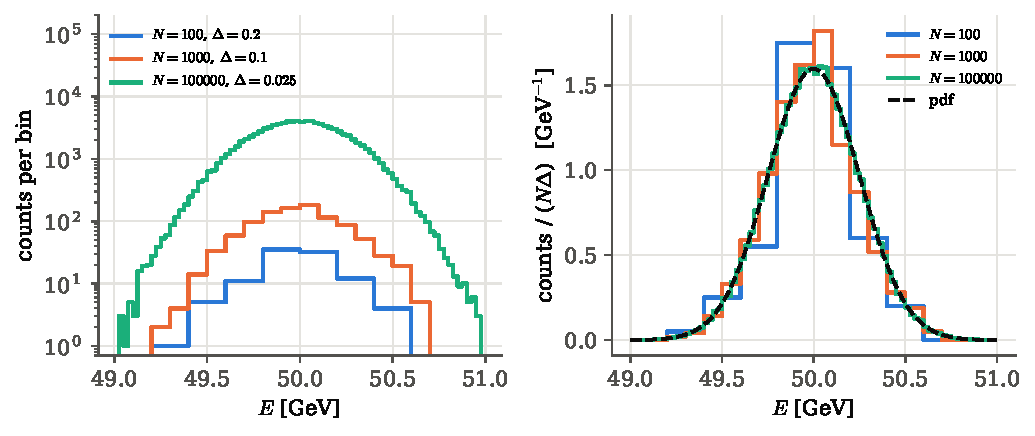
\includegraphics[width=0.95\linewidth]{figures/ch01/density_histogram.pdf}
\caption{Left: counts per bin for three data sets ($N=100$, $10^3$, $10^5$
with bins of 0.2, 0.1, 0.025 GeV). The heights are not comparable. Right: the
same histograms divided by $N\Delta$. They now fluctuate around one curve, the
Gaussian density, whose peak is above 1 per GeV.}
\label{1b:fig:density-histogram}
\end{figure}

With the finest bins the estimated peak density is $\OneBPeakEst\,\mathrm{GeV}^{-1}$
against the exact $\OneBPeakExact\,\mathrm{GeV}^{-1}$, and the fraction of
electrons within $\pm\sigma$ of 50 GeV is $\OneBFracOneSig$ (the Gaussian
value is 0.6827).

\pyfile[firstline=58,lastline=69,firstnumber=58]{code/ch01/11_density_histogram.py}{The empirical CDF is a sorted sample}

Lines 60--61 are the whole empirical CDF: sort the sample, and assign to the
$i$-th smallest value the height $i/N$. Lines 66--69 draw the quartiles as
the construction ``go across at height $q$, then down to the axis''. With
$N=1000$ the sample quartiles are $\OneBQoneSample$, $\OneBMedSample$,
$\OneBQthreeSample\,$GeV, against the exact $\OneBQoneExact$, $\OneBMedExact$,
$\OneBQthreeExact\,$GeV.

\begin{figure}[htbp]
\centering
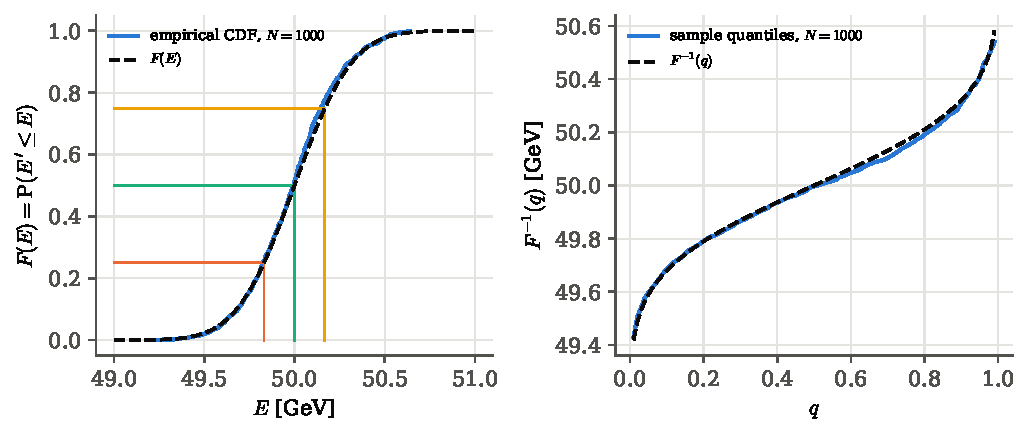
\includegraphics[width=0.95\linewidth]{figures/ch01/ecdf_quantiles.pdf}
\caption{Left: the empirical CDF of 1000 simulated energies (a staircase
with 1000 tiny steps) on top of the exact CDF. The coloured lines read off the
quartiles: across at $q=0.25,0.5,0.75$ and down to the energy axis. Right: the
same information turned sideways, sample quantiles against $q$, compared
with the exact quantile function.}
\label{1b:fig:ecdf}
\end{figure}

\paragraph{What this bought us.} Counts depend on how you bin. Densities do
not, but they carry units of $1/[x]$. The CDF needs no binning at all, which
is why tests that compare a sample to a model, such as Kolmogorov--Smirnov in
\cref{ch:04}, are built on the empirical CDF.

\paragraph{How research uses it.} Here the histogram \emph{verifies} a density
we already know. In research the direction is often reversed: nobody knows the
density of, say, the estimated tensor-to-scalar ratio after a realistic
foreground cleaning pipeline, so we simulate the whole pipeline many times and
the normalised histogram (or the empirical CDF) of the output \emph{is} our
best knowledge of its sampling distribution. Its quantiles become the error
bars. Chapters~\ref{ch:06} and~\ref{ch:08} do exactly this.
\section{Several variables at once: joint, marginal and conditional distributions}
\label{1b:sec:joint}

A calorimeter measures a photon. Two numbers describe the event: the true
energy $E$ that nature gave the photon, and the measured energy
$E_{\rm meas}=E+\text{noise}$ that the readout reports. The physics (a falling
spectrum from a decay or a background process) tells us how $E$ is
distributed. The detector response tells us how $E_{\rm meas}$ is spread for
a given $E$. But the histogram we actually fill contains only $E_{\rm meas}$.
The true energy is a \newterm{nuisance variable}: it is essential to the
physics of the measurement, and we never observe it.

The same situation appears in every cosmological analysis. A fit returns a
joint constraint on $(\Omega_m,\sigma_8)$, and a talk quotes
``$\Omega_m=0.31\pm0.01$'' with $\sigma_8$ ``marginalised over''. In both
cases we hold the joint distribution of several random variables and need
one of two operations. \emph{Marginalising} isolates one variable by
averaging out the others. \emph{Conditioning} fixes one variable and asks how
the rest are distributed. Neither is new. Both are rules from the first part
of \cref{ch:01} (the law of total probability and conditional probability),
applied to densities.

Two pictures make both operations concrete. Draw a scatter plot of many simulated pairs $(x,y)$. The density of points in
the plane is the joint density. Squash all the points onto the $x$ axis,
ignoring $y$, and histogram them: that is the marginal of $x$. Instead, keep
only the points in a thin vertical band at $x=x_0$, histogram their $y$
values and normalise: that is the conditional density of $y$ given $x_0$
\srcref{Cowan}{Figs.~1.4--1.6}. Projecting adds up all the ways a value of
$x$ could have arisen. Slicing throws away everything that disagrees with
what we know. This is the ``shrinking of the sample space'' of the first part
of this chapter.

So with two random variables there are four questions to ask.
\begin{enumerate}[leftmargin=1.5em,itemsep=1pt]
  \item How are the two variables distributed \emph{together}? (Joint.)
  \item How is one of them distributed if we do not care about, or cannot
        see, the other? (Marginal: average out the nuisance.)
  \item How is one distributed if we \emph{know} the value of the other?
        (Conditional: slice and renormalise.)
  \item Does knowing one change what we expect for the other? (If not, they
        are independent, and the joint is the product of the marginals.)
\end{enumerate}

\subsection{Joint distributions}

The other three questions are all answered from the distribution of the
pair taken together, so we define it first.

\begin{workdef}[joint mass function, joint density]
For discrete $X,Y$ the \newterm{joint mass function} is
$f(x,y)=\Prob(X=x,Y=y)$ \unpack{the probability that both statements hold at
once, $\Prob(X=x\text{ and }Y=y)$}. For continuous variables a
\newterm{joint density} is a function $f(x,y)\ge0$ with
$\iint f\,\dd x\,\dd y=1$ such that for every region $A$ of the plane
\[
  \Prob\bigl((X,Y)\in A\bigr)=\iint_A f(x,y)\,\dd x\,\dd y ,
\]
\unpack{probability per unit area, so $f(x,y)\,\dd x\,\dd y$ is the
probability of the small rectangle at $(x,y)$}. The joint CDF is
$F(x,y)=\Prob(X\le x,Y\le y)$.
\emph{Operational test:} a 2-D histogram of $N$ simulated pairs with cells
$\Delta x\times\Delta y$, divided by $N\Delta x\Delta y$, estimates $f(x,y)$.
Its units are $1/([x][y])$.
\end{workdef}

\oneBEx{A joint table and a uniform square}\label{1b:ex:joint-table}
Two binary variables with the joint table \mainref{Ex.~2.18, p.~31}
\begin{center}
\begin{tabular}{c|cc|c}
 & $Y=0$ & $Y=1$ & \\\hline
$X=0$ & 1/9 & 2/9 & 1/3\\
$X=1$ & 2/9 & 4/9 & 2/3\\\hline
 & 1/3 & 2/3 & 1
\end{tabular}
\end{center}
have $f(1,1)=\Prob(X=1,Y=1)=4/9$. The row and column sums written in the
margins of the table are the marginals of the next subsection. For a
continuous example, let
$(X,Y)$ be uniform on the unit square, $f=1$ there. Then
$\Prob(X<\tfrac12,Y<\tfrac12)$ is the integral of 1 over the lower-left
quarter, which is its area, $\tfrac14$.

\oneBEx{A density on a curved region}\label{1b:ex:parabola}
Let $f(x,y)=c\,x^2y$ on the region $x^2\le y\le1$ (and 0 elsewhere)
\mainref{Ex.~2.22, p.~32}. The region forces $-1\le x\le1$. Fix $c$ by
normalisation, integrating $y$ first at fixed $x$:
\begin{align*}
  1
  &\eqby{1} c\int_{-1}^{1}\!\!\int_{x^2}^{1}x^2y\,\dd y\,\dd x
   \eqby{2} c\int_{-1}^{1}x^2\,\frac{1-x^4}{2}\,\dd x
   \eqby{3} \frac c2\Bigl(\frac23-\frac27\Bigr)
   = \frac{4c}{21}
  \quad\Longrightarrow\quad c=\frac{21}{4}.
\end{align*}
\begin{explain}
  \item For each $x\in[-1,1]$, $y$ runs over $[x^2,1]$: this is the only
        delicate step, and \cref{1b:fig:parabola} is there to make it visible.
  \item $\int_{x^2}^1y\,\dd y=\tfrac12(1-x^4)$.
  \item $\int_{-1}^1x^2\dd x=\tfrac23$ and $\int_{-1}^1x^6\dd x=\tfrac27$.
\end{explain}
Now the probability that $X\ge Y$. Inside the support this needs $x\ge y\ge x^2$,
possible only for $0\le x\le1$ (the hatched sliver in the figure):
\begin{align*}
  \Prob(X\ge Y)
  &\eqby{1} \frac{21}{4}\int_0^1\!\!\int_{x^2}^{x}x^2y\,\dd y\,\dd x
   \eqby{2} \frac{21}{4}\int_0^1x^2\,\frac{x^2-x^4}{2}\,\dd x
   \eqby{3} \frac{21}{8}\Bigl(\frac15-\frac17\Bigr)
   = \frac{3}{20}.
\end{align*}
\begin{explain}
  \item The event $\{X\ge Y\}$ intersected with the support is
        $\{0\le x\le1,\ x^2\le y\le x\}$.
  \item $\int_{x^2}^{x}y\,\dd y=\tfrac12(x^2-x^4)$.
  \item $\int_0^1x^4=\tfrac15$, $\int_0^1x^6=\tfrac17$, and
        $\tfrac{21}{8}\cdot\tfrac{2}{35}=\tfrac{3}{20}$.
\end{explain}

\begin{figure}[htbp]
\centering
\begin{tikzpicture}[x=2.4cm,y=2.4cm]
  \fill[formblue!15] plot[domain=-1:1,samples=60] (\x,{\x*\x}) -- (1,1) -- (-1,1) -- cycle;
  \fill[pattern=crosshatch,pattern color=bdryred!70]
     plot[domain=0:1,samples=40] (\x,{\x*\x}) -- (0,0) -- cycle;
  \draw[->] (-1.35,0) -- (1.45,0) node[right,lbl] {$x$};
  \draw[->] (0,-0.1) -- (0,1.3) node[above,lbl] {$y$};
  \draw[thick,formblue] plot[domain=-1.1:1.1,samples=60] (\x,{\x*\x});
  \draw[thick,tangentgreen] (-0.05,-0.05) -- (1.2,1.2);
  \draw[faint] (-1,1) -- (1,1);
  \node[lbl,formblue,anchor=east] at (-1.12,1.12) {$y=x^2$};
  \node[lbl,tangentgreen,anchor=west] at (1.22,1.2) {$y=x$};
  \node[lbl,anchor=east] at (-0.02,1.06) {$1$};
  \node[lbl,anchor=north] at (1,-0.02) {$1$};
  \node[lbl,anchor=north] at (-1,-0.02) {$-1$};
  \node[lbl,align=center] at (-0.58,0.62) {support\\$x^2\le y\le1$};
  \draw[bdryred,->] (1.05,0.35) -- (0.62,0.5);
  \node[lbl,bdryred,anchor=west] at (1.05,0.35) {$\{X\ge Y\}$};
\end{tikzpicture}
\caption{The density $\tfrac{21}{4}x^2y$ lives on the shaded region between
the parabola $y=x^2$ and the line $y=1$. The event $X\ge Y$ is the hatched
sliver between the parabola and the diagonal $y=x$. To integrate, fix $x$
and let $y$ run up the vertical segment inside the region.}
\label{1b:fig:parabola}
\end{figure}

\subsection{Marginal distributions: averaging out the nuisance}\label{1b:sec:marginal}

If we only care about $X$, the event ``$X=x$'' is the disjoint union of the
events ``$X=x$ and $Y=y$'' over all values $y$. The law of total probability
(first part of \cref{ch:01}) adds them up.

\begin{workdef}[marginal distribution]
The \newterm{marginal} mass function or density of $X$ is
\[
  f_X(x)=\sum_yf(x,y)\quad\text{(discrete)},\qquad
  f_X(x)=\int_{-\infty}^{\infty}f(x,y)\,\dd y\quad\text{(continuous)},
\]
and similarly $f_Y(y)=\sum_xf(x,y)$ or $\int f(x,y)\,\dd x$
\unpack{sum or integrate the joint over every value of the variable we want
to get rid of}. The variable summed over is \emph{marginalised} or
\emph{integrated out}.
\emph{Operational test:} simulate pairs $(x,y)$, throw away the $y$'s, and
histogram the $x$'s.
\end{workdef}

We need a marginal distribution to isolate and understand the probability of
a single variable by averaging out or removing ``nuisance'' variables from a
complex joint distribution. The word ``averaging'' is meant literally.
Write the joint as $f(x,y)=f(x\given y)f_Y(y)$ (the product rule, derived
below). Then the marginal $f_X(x)=\int f(x\given y)f_Y(y)\dd y$ is the
average of the conditional densities $f(x\given y)$, each weighted by how
probable its nuisance value $y$ is.

Why is the continuous marginal an integral over $y$
\srcref{Cowan}{(1.20)--(1.21)}? Cut the vertical strip $[x,x+\dd x]$ into
small cells of height $\Delta y$ at heights $y_i$:
\begin{align*}
  \Prob\bigl(x\le X\le x+\dd x\bigr)
  &\eqby{1} \sum_i\Prob\bigl(x\le X\le x+\dd x,\ y_i\le Y\le y_i+\Delta y\bigr)
  \\
  &\eqby{2} \sum_i f(x,y_i)\,\Delta y\,\dd x
   \;\xrightarrow{\ \Delta y\to0\ }\;\Bigl[\int f(x,y)\,\dd y\Bigr]\dd x .
\end{align*}
\begin{explain}
  \item The cells are disjoint and together make up the strip (the law of
        total probability).
  \item The probability of a small cell is the joint density times its area.
\end{explain}
The bracket is probability per unit $x$: the marginal density.

\oneBEx{Margins of a table, and what they cannot tell you}\label{1b:ex:margins}
For the table \mainref{Ex.~2.24, p.~33}
\begin{center}
\begin{tabular}{c|cc|c}
 & $Y=0$ & $Y=1$ & \\\hline
$X=0$ & 1/10 & 2/10 & 3/10\\
$X=1$ & 3/10 & 4/10 & 7/10\\\hline
 & 4/10 & 6/10 & 1
\end{tabular}
\end{center}
the marginal of $X$ is the column of row sums, $f_X(0)=3/10$, $f_X(1)=7/10$,
and the marginal of $Y$ is the row of column sums. The name ``marginal''
literally means ``written in the margin of the table''.

Marginals lose information. The joint table
$f(0,0)=\tfrac1{12}$, $f(1,0)=\tfrac5{12}$, $f(0,1)=f(1,1)=\tfrac3{12}$ has
marginals $f_X=(\tfrac13,\tfrac23)$ and $f_Y=(\tfrac12,\tfrac12)$. So does the
different table $f(0,0)=\tfrac16$, $f(1,0)=\tfrac13$, $f(0,1)=\tfrac16$,
$f(1,1)=\tfrac13$ \srcref{CasellaBerger}{Ex.~4.1.9}. Knowing both marginals
does not determine the joint. This is a small instance of a big theme:
summarising discards information. A CMB power spectrum $\Cell$ is a
``marginal'' summary that keeps the variance at each scale and throws away
the phases, and \cref{ch:12} is about recovering some of what was thrown
away.

\oneBEx{Marginal densities by integration}\label{1b:ex:marginal-integrals}
\begin{itemize}[leftmargin=1.2em,itemsep=1pt]
  \item $f(x,y)=e^{-(x+y)}$ for $x,y\ge0$:
        $f_X(x)=e^{-x}\int_0^\infty e^{-y}\dd y=e^{-x}$ \mainref{Ex.~2.26}.
  \item $f(x,y)=x+y$ on the unit square:
        $f_Y(y)=\int_0^1(x+y)\dd x=\tfrac12+y$ \mainref{Ex.~2.27}.
  \item $f(x,y)=\tfrac{21}{4}x^2y$ on $x^2\le y\le1$ (\cref{1b:ex:parabola}):
        \begin{align*}
          f_X(x)
          \eqby{1} \frac{21}{4}x^2\int_{x^2}^{1}y\,\dd y
          = \frac{21}{8}x^2(1-x^4),\qquad -1\le x\le1 .
        \end{align*}
        \begin{explain}
          \item At fixed $x$ the density is nonzero only for $x^2\le y\le1$,
                so those are the limits of the $y$ integral
                \mainref{Ex.~2.28, p.~34}.
        \end{explain}
\end{itemize}
In the last case the limits of integration depend on $x$. Forgetting that is
the commonest error in marginalisation.

\subsection{The Gaussian case: marginalising by completing the square}

The single most important joint density is the bivariate Gaussian. With zero
means, standard deviations $\sigma_x,\sigma_y$ and a correlation parameter
$\rho\in(-1,1)$ (\cref{1b:sec:covariance} shows that $\rho$ is the
correlation coefficient),
\begin{equation}
  f(x,y)=\frac{1}{2\pi\sigma_x\sigma_y\sqrt{1-\rho^2}}
  \exp\Bigl\{-\frac{1}{2(1-\rho^2)}
  \Bigl[\frac{x^2}{\sigma_x^2}-\frac{2\rho xy}{\sigma_x\sigma_y}
  +\frac{y^2}{\sigma_y^2}\Bigr]\Bigr\}.
  \label{1b:eq:bvn}
\end{equation}
The contours of $f$ are ellipses, tilted when $\rho\ne0$. We need one integral,
the Gaussian integral
$\int_{-\infty}^{\infty}e^{-(y-m)^2/(2s^2)}\dd y=\sqrt{2\pi}\,s$
(for any shift $m$ and width $s>0$).

\oneBEx{The marginal and the conditional of a bivariate Gaussian}\label{1b:ex:bvn-marginal}
The question: how is $X$ distributed on its own, and how is $Y$ distributed
once $X=x$ is known? The plan is to rewrite the exponent so that $y$ appears
in a single square. Then the $y$ integral becomes the Gaussian integral just
recalled. First rearrange the bracket in \eqref{1b:eq:bvn}:
\begin{align*}
  \frac{x^2}{\sigma_x^2}-\frac{2\rho xy}{\sigma_x\sigma_y}+\frac{y^2}{\sigma_y^2}
  &\eqby{1} \Bigl(\frac{y}{\sigma_y}-\frac{\rho x}{\sigma_x}\Bigr)^2
            +\frac{x^2}{\sigma_x^2}-\frac{\rho^2x^2}{\sigma_x^2}
   = \frac{\bigl(y-\rho\sigma_yx/\sigma_x\bigr)^2}{\sigma_y^2}
            +(1-\rho^2)\frac{x^2}{\sigma_x^2}.
\end{align*}
\begin{explain}
  \item Expanding $(y/\sigma_y-\rho x/\sigma_x)^2$ gives
        $y^2/\sigma_y^2-2\rho xy/(\sigma_x\sigma_y)+\rho^2x^2/\sigma_x^2$,
        so we must add back $(1-\rho^2)x^2/\sigma_x^2$ to restore the
        original expression.
\end{explain}
Dividing by $2(1-\rho^2)$ and writing $m(x)=\rho\sigma_yx/\sigma_x$ and
$s=\sigma_y\sqrt{1-\rho^2}$, the joint density factorises as
\[
  f(x,y)=\frac{1}{2\pi\sigma_x s}
  \exp\Bigl[-\frac{(y-m(x))^2}{2s^2}\Bigr]\exp\Bigl[-\frac{x^2}{2\sigma_x^2}\Bigr].
\]
The marginal of $X$ follows:
\begin{align*}
  f_X(x)
  &\eqby{1} \frac{e^{-x^2/2\sigma_x^2}}{2\pi\sigma_xs}
     \int_{-\infty}^{\infty}e^{-(y-m(x))^2/2s^2}\,\dd y
   \eqby{2} \frac{e^{-x^2/2\sigma_x^2}}{2\pi\sigma_xs}\,\sqrt{2\pi}\,s
   = \frac{1}{\sqrt{2\pi}\,\sigma_x}e^{-x^2/2\sigma_x^2}.
\end{align*}
\begin{explain}
  \item Definition of the marginal. The factor depending only on $x$ comes
        out of the $y$ integral.
  \item Gaussian integral with shift $m(x)$ and width $s$. The shift does not
        change the area, which is why the answer is so simple.
\end{explain}
So $X\sim\Normal(0,\sigma_x^2)$ whatever $\rho$ is, and by the symmetry of
\eqref{1b:eq:bvn}, $Y\sim\Normal(0,\sigma_y^2)$. The conditional density of
$Y$ at fixed $X=x$ is the joint divided by the marginal (defined in the next
subsection):
\[
  f(y\given x)=\frac{f(x,y)}{f_X(x)}
  =\frac{1}{\sqrt{2\pi}\,s}\exp\Bigl[-\frac{(y-\rho\sigma_yx/\sigma_x)^2}{2s^2}\Bigr],
  \qquad
  Y\given X=x\ \sim\ \Normal\Bigl(\rho\frac{\sigma_y}{\sigma_x}x,\
  \sigma_y^2(1-\rho^2)\Bigr).
\]
Knowing $X$ does two things to $Y$: it shifts the centre along the line
$y=\rho\sigma_yx/\sigma_x$ (the ``regression line''), and it shrinks the
width by the factor $\sqrt{1-\rho^2}$. For $\rho=0.7$ that factor is $0.71$.

\begin{pitfall}[Marginal width is not conditional width]
In a two-parameter fit, the error bar on one parameter with the other held
fixed at its best value is the \emph{conditional} width
$\sigma_y\sqrt{1-\rho^2}$. The error bar with the other parameter
marginalised is $\sigma_y$. For strongly correlated parameters these differ a
lot: $\rho=0.95$ gives a factor $3.2$. Quoting the conditional error as if it
were the marginal one is a classic way to overstate a result. \Cref{ch:10}
meets the same distinction as $1/\sqrt{\Fish_{ii}}$ versus
$\sqrt{(\Fish^{-1})_{ii}}$.
\end{pitfall}

\subsection{Conditional distributions: slicing and renormalising}

Slicing the scatter plot at $Y=y$ and renormalising the slice gives the
definition.

\begin{workdef}[conditional mass function and density]
For discrete variables, the \newterm{conditional mass function} of $X$ given
$Y=y$ is
\[
  f_{X|Y}(x\given y)=\Prob(X=x\given Y=y)=\frac{f(x,y)}{f_Y(y)},
  \qquad f_Y(y)>0 ,
\]
the ordinary conditional probability of the first part of \cref{ch:01}. For
continuous variables the \newterm{conditional density} is defined by the same
formula \unpack{the joint along the line $Y=y$, divided by its total, so
that it integrates to 1 over $x$}, and
$\Prob(X\in A\given Y=y)=\int_Af_{X|Y}(x\given y)\,\dd x$.
\emph{Operational test:} keep only simulated pairs with $y$ in a thin band
around $y_0$, histogram their $x$ values and normalise.
\end{workdef}

In the continuous case the event $\{Y=y\}$ has probability zero. So
conditioning on it cannot literally mean $\Prob(A\cap B)/\Prob(B)$, which
would be $0/0$. Why is the definition still right? Think of a thin band of
width $\dd y$ around $y$. Both numerator and denominator carry the same
factor $\dd y$, which cancels and leaves the ratio of densities
\srcref{Cowan}{(1.23)}. (Wasserman \mainref{p.~36, footnote 6} calls
conditioning on a probability-zero event ``treading in deep water'' and
simply adopts the formula as the definition.) Rearranging the definition
gives the product rule
\begin{equation}
  f(x,y)=f_{X|Y}(x\given y)\,f_Y(y)=f_{Y|X}(y\given x)\,f_X(x),
  \label{1b:eq:product-rule}
\end{equation}
and from it the continuous law of total probability and Bayes' theorem
\srcref{Cowan}{(1.26)--(1.28)}:
\begin{equation}
  f_X(x)=\int f_{X|Y}(x\given y)f_Y(y)\,\dd y,
  \qquad
  f_{Y|X}(y\given x)=\frac{f_{X|Y}(x\given y)\,f_Y(y)}{\int f_{X|Y}(x\given y')f_Y(y')\,\dd y'} .
  \label{1b:eq:cont-bayes}
\end{equation}
The first is ``sum over the branches of a tree'', with a continuum of
branches. The second reads the tree backwards. With $y$ a parameter and $x$
the data, $f_{X|Y}$ is the prediction and $f_{Y|X}$ the inference: this is
the equation \cref{ch:05} is built on.

\oneBEx{Conditional probabilities from a density}\label{1b:ex:conditional}
\begin{enumerate}[label=(\alph*),leftmargin=1.6em,itemsep=2pt]
  \item $f(x,y)=x+y$ on the unit square, with $f_Y(y)=y+\tfrac12$
        (\cref{1b:ex:marginal-integrals}). Then $f(x\given y)=(x+y)/(y+\tfrac12)$
        and \mainref{Ex.~2.38, p.~37}
        \begin{align*}
          \Prob\bigl(X<\tfrac14\given Y=\tfrac13\bigr)
          &\eqby{1} \int_0^{1/4}\frac{x+\frac13}{\frac13+\frac12}\,\dd x
           \eqby{2} \frac65\Bigl[\frac{x^2}{2}+\frac{x}{3}\Bigr]_0^{1/4}
           = \frac65\Bigl(\frac1{32}+\frac1{12}\Bigr)
           = \frac{11}{80}.
        \end{align*}
        \begin{explain}
          \item Integrate the conditional density over the event, at $y=\tfrac13$.
          \item $1/(\tfrac13+\tfrac12)=\tfrac65$, and the antiderivative is
                elementary. Then $\tfrac1{32}+\tfrac1{12}=\tfrac{11}{96}$.
        \end{explain}
  \item Build a joint from a marginal and a conditional: $X\sim$ Uniform$(0,1)$
        and then $Y\given X=x\sim$ Uniform$(x,1)$ \mainref{Ex.~2.39}. Then
        $f(y\given x)=1/(1-x)$ for $x<y<1$, and by \eqref{1b:eq:product-rule}
        $f(x,y)=1/(1-x)$ on $0<x<y<1$. The marginal of $Y$ is
        \begin{align*}
          f_Y(y)
          &\eqby{1} \int_0^y\frac{\dd x}{1-x}
           \eqby{2} -\int_1^{1-y}\frac{\dd u}{u}
           = -\ln(1-y),\qquad 0<y<1 .
        \end{align*}
        \begin{explain}
          \item At fixed $y$, the joint is nonzero for $0<x<y$.
          \item Substitute $u=1-x$, $\dd u=-\dd x$; the limits $x=0,y$ become
                $u=1,1-y$.
        \end{explain}
        The density of $Y$ rises towards $y=1$: each stage pushes $Y$ upward.
  \item For $f=\tfrac{21}{4}x^2y$ on $x^2\le y\le1$, dividing by the
        marginal of \cref{1b:ex:marginal-integrals} gives
        $f(y\given x)=2y/(1-x^4)$ on $x^2\le y\le1$. At $x=\tfrac12$ this is
        $32y/15$, and \mainref{Ex.~2.40, p.~38}
        \begin{align*}
          \Prob\bigl(Y\ge\tfrac34\given X=\tfrac12\bigr)
          \eqby{1} \int_{3/4}^{1}\frac{32y}{15}\,\dd y
          = \frac{16}{15}\Bigl(1-\frac{9}{16}\Bigr)=\frac{7}{15}.
        \end{align*}
        \begin{explain}
          \item The conditional density at $x=\tfrac12$ lives on
                $\tfrac14\le y\le1$, and the event asks for the top part.
        \end{explain}
\end{enumerate}

\subsection{Independence}

The last question is whether slicing changes anything at all. If every slice
looks the same, learning one variable teaches us nothing about the other.

\begin{workdef}[independent random variables]
$X$ and $Y$ are \newterm{independent}, written $X\perp Y$, if for every pair
of sets $A,B$
\[
  \Prob(X\in A,\ Y\in B)=\Prob(X\in A)\,\Prob(Y\in B)
\]
\unpack{every event about $X$ is independent of every event about $Y$}.
Equivalently the joint factorises into the marginals,
$f(x,y)=f_X(x)f_Y(y)$ for all $x,y$ \mainref{Thm~2.30, p.~35}, and then
$f(y\given x)=f_Y(y)$: learning $x$ does not change the distribution of $Y$.
\emph{Operational test:} slice the scatter plot at several $x$ values. If
the normalised $y$-histograms in the slices all look the same, and the same
as the marginal, the variables are independent.
\end{workdef}

\oneBEx{Checking independence}\label{1b:ex:independence}
\begin{enumerate}[label=(\alph*),leftmargin=1.6em,itemsep=2pt]
  \item The table with all four entries $\tfrac14$ is independent:
        $f_X=f_Y=(\tfrac12,\tfrac12)$ and every cell equals
        $\tfrac12\cdot\tfrac12$. The table $f(0,0)=f(1,1)=\tfrac12$,
        $f(0,1)=f(1,0)=0$ has the \emph{same} marginals but is not independent:
        $f_X(0)f_Y(1)=\tfrac14\ne0=f(0,1)$ \mainref{Ex.~2.31}.
  \item $X,Y$ independent with the same density $f(x)=2x$ on $[0,1]$. The
        joint is $4xy$ on the unit square, and \mainref{Ex.~2.32}
        \begin{align*}
          \Prob(X+Y\le1)
          &\eqby{1} 4\int_0^1x\Bigl[\int_0^{1-x}y\,\dd y\Bigr]\dd x
           \eqby{2} 2\int_0^1x(1-x)^2\,\dd x
           \eqby{3} 2\Bigl(\frac12-\frac23+\frac14\Bigr)=\frac16 .
        \end{align*}
        \begin{explain}
          \item The event is the triangle below the line $y=1-x$; for each $x$,
                $y$ runs from 0 to $1-x$.
          \item $\int_0^{1-x}y\,\dd y=\tfrac12(1-x)^2$.
          \item Expand $x(1-x)^2=x-2x^2+x^3$ and integrate term by term.
        \end{explain}
  \item Shortcut \mainref{Thm~2.33, p.~36}: if the joint is nonzero on a
        rectangle (possibly infinite) and has the form $g(x)h(y)$, the
        variables are independent. $f=2e^{-(x+2y)}$ on $x,y>0$ is
        $g(x)h(y)$ with $g=2e^{-x}$, $h=e^{-2y}$, so $X\perp Y$.
  \item The rectangle condition matters. $\tfrac{21}{4}x^2y$ on $x^2\le y\le1$
        looks like $g(x)h(y)$, but the region is not a rectangle, and
        $f(y\given x)=2y/(1-x^4)$ depends on $x$: learning $x$ tells us $y\ge
        x^2$. $X$ and $Y$ are dependent.
\end{enumerate}

For more than two variables the definitions carry over. A
\newterm{random vector} $\bm X=(X_1,\dots,X_n)$ has a joint density
$f(x_1,\dots,x_n)$; marginals integrate out any subset of components;
$X_1,\dots,X_n$ are independent if $f=\prod_if_{X_i}(x_i)$. If they are
independent \emph{and} all have the same marginal $F$ they are
\newterm{iid} (independent and identically distributed), written
$X_1,\dots,X_n\iid F$, and form a \newterm{random sample} of size $n$ from
$F$ \mainref{Def.~2.41, p.~39}. Repeated measurements, Monte Carlo draws and
the pixels of a white-noise map are the standard iid examples.

Two multivariate models recur throughout the book \mainref{\S2.10}. The
\newterm{multinomial} counts how $n$ independent draws fall into $k$
categories (histogram bins) with probabilities $p_1,\dots,p_k$. The marginal
of one count $X_j$ is Binomial$(n,p_j)$: lump all the other categories into
``not $j$'' and each draw becomes a Bernoulli$(p_j)$ trial. The
\newterm{multivariate normal} $\Normal(\bm\mu,\Sigma)$ has density
\begin{equation}
  f(\bm x)=\frac{1}{(2\pi)^{k/2}\abs{\Sigma}^{1/2}}
  \exp\Bigl\{-\tfrac12(\bm x-\bm\mu)\T\Sigma^{-1}(\bm x-\bm\mu)\Bigr\},
  \label{1b:eq:mvn}
\end{equation}
with $\Sigma$ a symmetric positive-definite $k\times k$ matrix. For $k=2$ and
$\Sigma=\bigl(\begin{smallmatrix}\sigma_x^2&\rho\sigma_x\sigma_y\\
\rho\sigma_x\sigma_y&\sigma_y^2\end{smallmatrix}\bigr)$ it reduces to
\eqref{1b:eq:bvn}:
\begin{align*}
  \abs{\Sigma}
  &\eqby{1} \sigma_x^2\sigma_y^2(1-\rho^2),\qquad
  \Sigma^{-1}\eqby{2}\frac{1}{\sigma_x^2\sigma_y^2(1-\rho^2)}
   \begin{pmatrix}\sigma_y^2&-\rho\sigma_x\sigma_y\\-\rho\sigma_x\sigma_y&\sigma_x^2\end{pmatrix},\\
  \bm x\T\Sigma^{-1}\bm x
  &\eqby{3} \frac{\sigma_y^2x^2-2\rho\sigma_x\sigma_yxy+\sigma_x^2y^2}{\sigma_x^2\sigma_y^2(1-\rho^2)}
   = \frac{1}{1-\rho^2}\Bigl[\frac{x^2}{\sigma_x^2}-\frac{2\rho xy}{\sigma_x\sigma_y}+\frac{y^2}{\sigma_y^2}\Bigr].
\end{align*}
\begin{explain}
  \item Determinant of a $2\times2$ matrix, $ad-bc$.
  \item Inverse of a $2\times2$ matrix: swap the diagonal, negate the
        off-diagonal, divide by the determinant.
  \item Multiply out $(x,y)\,\Sigma^{-1}(x,y)\T$, then divide numerator and
        denominator by $\sigma_x^2\sigma_y^2$.
\end{explain}
The general marginal and conditional rules \mainref{Thm~2.44, p.~40},
$X_b\given X_a=x_a\sim\Normal\bigl(\mu_b+\Sigma_{ba}\Sigma_{aa}^{-1}(x_a-\mu_a),\,
\Sigma_{bb}-\Sigma_{ba}\Sigma_{aa}^{-1}\Sigma_{ab}\bigr)$, reduce for $k=2$ to
exactly what we derived in \cref{1b:ex:bvn-marginal}:
$\Sigma_{ba}\Sigma_{aa}^{-1}=\rho\sigma_x\sigma_y/\sigma_x^2=\rho\sigma_y/\sigma_x$
and $\Sigma_{bb}-\Sigma_{ba}^2/\Sigma_{aa}=\sigma_y^2(1-\rho^2)$. The general
proofs are in \cref{ch:02}.

\subsection{Seeing it: projections, slices, and the smeared spectrum}

The first script samples the bivariate Gaussian with $\sigma_x=1$,
$\sigma_y=2$, $\rho=0.7$, projects, and slices at $x_0=1$.

\pyfile[firstline=23,lastline=34,firstnumber=23]{code/ch01/12_marginal_gaussian.py}{Marginal by projection, conditional by slicing}

Line 26 draws $\OneBMargN$ pairs from $\Normal(\bm0,\Cmat)$. The marginal needs
no code at all: \texttt{Y} on its own \emph{is} a sample from $f_Y$ (line 27
just splits the columns). The conditional is a boolean mask, the band
$\abs{x-1}<0.05$ (line 31), exactly the ``conditioning is selecting a
subset'' of the first part of \cref{ch:01}.

\begin{figure}[htbp]
\centering
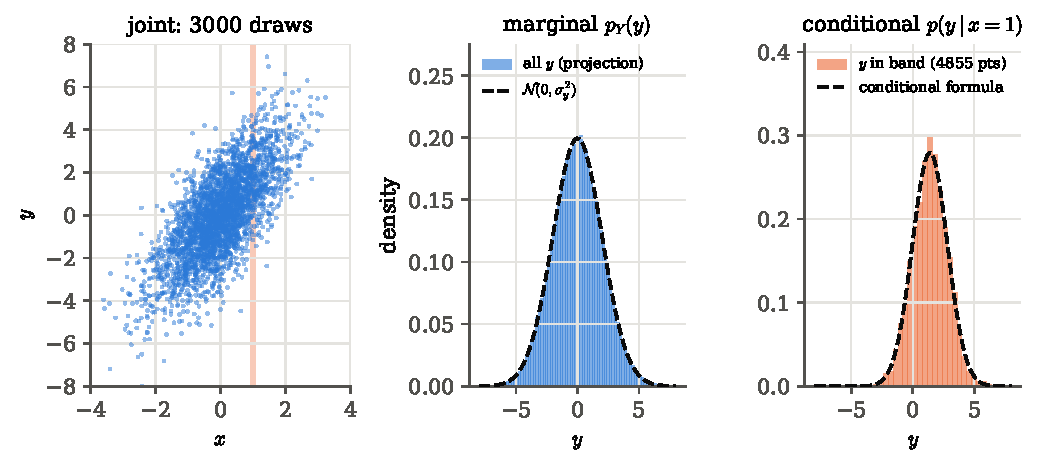
\includegraphics[width=\linewidth]{figures/ch01/marginal_gaussian.pdf}
\caption{Left: 3000 draws from the correlated Gaussian, with the thin band at
$x=1$ shaded. Middle: all $y$ values, projected onto the $y$ axis, follow the
marginal $\Normal(0,4)$. Right: only the $y$ values from inside the band,
renormalised, follow the narrower and shifted conditional density.}
\label{1b:fig:marginal-gaussian}
\end{figure}

The simulated marginal widths are $\OneBMargSdX$ and $\OneBMargSdY$ (exact 1
and 2). The band holds $\OneBBandN$ points, whose $y$ values have mean
$\OneBCondMeanSim$ and standard deviation $\OneBCondSdSim$, against the exact
conditional $\rho\sigma_yx_0/\sigma_x=\OneBCondMeanExact$ and
$\sigma_y\sqrt{1-\rho^2}=\OneBCondSdExact$ (the band has finite width, which
adds a tiny extra spread).

\oneBEx{The measured spectrum: marginalising the true energy}\label{1b:ex:smearing}
Return to the photon in the calorimeter from the start of this section. Its
true energy $E$ is never observed. Only the measured energy
$E_{\rm meas}=E+\text{noise}$ is recorded, and we want the spectrum of
$E_{\rm meas}$. Let the true energy be exponential,
$f(E)=e^{-E/\beta}/\beta$ for $E>0$ with $\beta=20\,$GeV (a falling
spectrum), and the detector Gaussian,
$f(x\given E)=\exp[-(x-E)^2/2\sigma^2]/(\sqrt{2\pi}\sigma)$ with
$\sigma=5\,$GeV, where $x=E_{\rm meas}$. The joint is the product
\eqref{1b:eq:product-rule}, and the spectrum we histogram is the marginal
\begin{equation}
  f(x)=\int_0^\infty\frac{e^{-E/\beta}}{\beta}\,
  \frac{e^{-(x-E)^2/2\sigma^2}}{\sqrt{2\pi}\,\sigma}\,\dd E .
  \label{1b:eq:smear-integral}
\end{equation}
To do the integral, collect the $E$-dependence of the exponent into one
square, so that what is left is a Gaussian integral:
\begin{align*}
  -\frac{E}{\beta}-\frac{(x-E)^2}{2\sigma^2}
  &\eqby{1} -\frac{E^2-2E\bigl(x-\sigma^2/\beta\bigr)+x^2}{2\sigma^2}
   \eqby{2} -\frac{\bigl(E-m\bigr)^2}{2\sigma^2}+\frac{m^2-x^2}{2\sigma^2}\\
  &\eqby{3} -\frac{\bigl(E-m\bigr)^2}{2\sigma^2}-\frac{x}{\beta}+\frac{\sigma^2}{2\beta^2},
\end{align*}
with $m=x-\sigma^2/\beta$.
\begin{explain}
  \item Put both terms over $2\sigma^2$: $E/\beta=2\sigma^2E/(2\sigma^2\beta)$,
        and expand $(x-E)^2$.
  \item Complete the square, $E^2-2Em=(E-m)^2-m^2$.
  \item $m^2-x^2=-2x\sigma^2/\beta+\sigma^4/\beta^2$; divide by $2\sigma^2$.
\end{explain}
The last two terms do not involve $E$ and leave the integral. What remains is
a Gaussian in $E$ centred at $m$, integrated over $E>0$ only:
\begin{align*}
  f(x)
  &\eqby{1} \frac1\beta\,e^{\sigma^2/2\beta^2-x/\beta}
     \int_0^\infty\frac{e^{-(E-m)^2/2\sigma^2}}{\sqrt{2\pi}\,\sigma}\dd E
   \eqby{2} \frac1\beta\,e^{\sigma^2/2\beta^2-x/\beta}\,
     \Phi\Bigl(\frac{x-\sigma^2/\beta}{\sigma}\Bigr).
\end{align*}
\begin{explain}
  \item Insert the rearranged exponent into \eqref{1b:eq:smear-integral}.
  \item The remaining integral is $\Prob(W>0)$ for $W\sim\Normal(m,\sigma^2)$,
        which is $\Prob\bigl((W-m)/\sigma>-m/\sigma\bigr)=1-\Phi(-m/\sigma)=\Phi(m/\sigma)$
        by the symmetry of the standard Gaussian.
\end{explain}
The formula shows two things. First, far above the resolution scale,
$x\gg\sigma^2/\beta+\sigma$, we have $\Phi\to1$. There the measured spectrum
is the true exponential with the same slope, multiplied by the constant
$e^{\sigma^2/2\beta^2}>1$. Smearing ``feeds'' events from low to high energy,
and so raises the tail. Second, near and below zero the $\Phi$ factor cuts
in. There is a finite probability of measuring a \emph{negative} energy,
which no true photon has.

\pyfile[firstline=24,lastline=34,firstnumber=24]{code/ch01/13_detector_smearing.py}{Simulating the nuisance, then forgetting it}

Lines 26--27 are the whole physics: draw the true energy, add the noise.
Marginalising over the nuisance then costs nothing: we simply never look at
\texttt{E\_true} again. The function \texttt{p\_meas} (lines 30--33) is the
closed form just derived.

\begin{figure}[htbp]
\centering
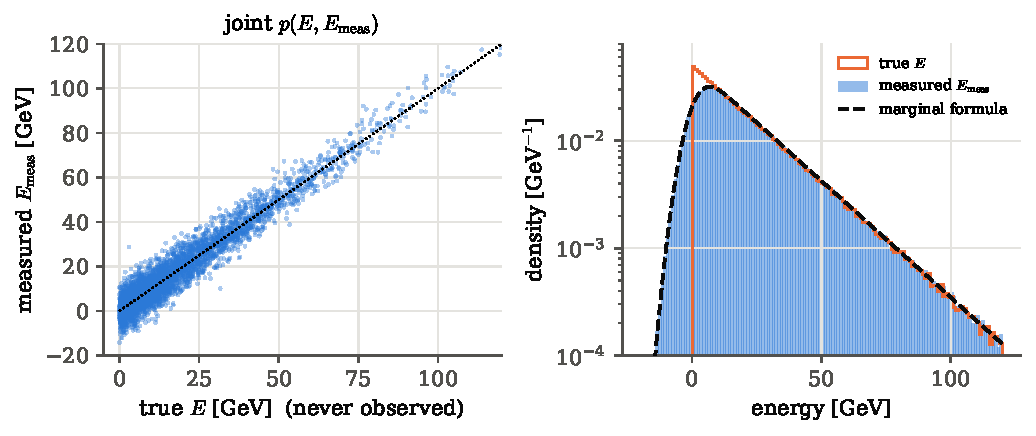
\includegraphics[width=0.95\linewidth]{figures/ch01/detector_smearing.pdf}
\caption{Left: the joint distribution of (true, measured) energy, scattered
around the diagonal. Only the vertical coordinate is ever recorded. Right, on a
log scale: the true spectrum (orange outline) is a straight line starting at
zero. The measured spectrum (blue) is its marginal with the true energy
integrated out. It leaks below zero and runs parallel to, and slightly above,
the true line in the tail. The dashed curve is the closed form.}
\label{1b:fig:smearing}
\end{figure}

With $\OneBSmearN$ photons the simulation gives a mean measured energy of
$\OneBSmearMeanSim\,$GeV (exact $\beta=20$), a variance of
$\OneBSmearVarSim\,\mathrm{GeV}^2$ (exact $\beta^2+\sigma^2=\OneBSmearVarExact$,
derived in \cref{1b:sec:expectation}), and a fraction
$\OneBSmearNegSim$ of negative measured energies (exact
$\int_{-\infty}^0f=\OneBSmearNegExact$). A $\chi^2$ comparison of the
histogram with the bin-integrated formula gives $\OneBSmearChi$ for
$\OneBSmearNdf$ bins, which is what agreement looks like (\cref{ch:04} makes
this precise).

\paragraph{What this bought us.} Marginalising a nuisance variable is, in simulation, the act of not looking
at it. Analytically it is an integral over the joint, $f(x)=\int f(x\given
E)f(E)\,\dd E$. The same integral with $E$ a parameter is the Bayesian
evidence of \cref{ch:05}, and with $E$ the true sky it is the forward model
of \cref{ch:08}.

\begin{inpractice}[Verification here, forward modelling in research]
The closed form above \emph{verifies} the simulation. In a real calorimeter
the response $f(x\given E)$ has non-Gaussian tails, depends on position and
is known only through test-beam data and detector simulation. Then the
marginal $\int f(x\given E)f(E\given\theta)\,\dd E$ has no closed form and
is computed by exactly the two lines of code above, repeated for each
theory parameter $\theta$. That forward-folded spectrum is what a fit
compares with data. Going the other way, from $x$ back to $E$, is
\emph{unfolding}, a conditional distribution $f(E\given x)$ computed with
\eqref{1b:eq:cont-bayes}.
\end{inpractice}
\section{Functions of random variables: change of variables and Jacobians}
\label{1b:sec:transform}

A classical harmonic oscillator swings as $x(t)=A\cos\omega t$. We take a
photograph at a random moment, with no idea of the phase. Where is the bob
most likely to be caught? The motion is completely deterministic; the only
randomness is \emph{when} we look, and the time $t$ is uniform over a period.
The position is a function of that uniform time, $X=A\cos\omega T$, so its
distribution is fixed by the distribution of $T$ and the function. We will
find that the bob is most likely near the turning points, where it moves
slowly, and least likely at the centre, where it is fastest.

The same question appears whenever an observable is a function of something
whose distribution we know: the angle of a decay product, the transverse
momentum computed from that angle, a flux from a magnitude, the logarithm of
a likelihood. In each case we know the density of $X$ and want the density of
$Y=r(X)$. The tool is the Jacobian, and it works for several variables at
once. The oscillator has a second use: histogramming $x(t)$ at random times is
the same act as histogramming samples from a posterior (\cref{ch:05}).

The key idea is that probability is conserved when we relabel. Think of probability as a fluid of total mass 1 spread along the $x$ axis.
The map $y=r(x)$ moves each drop of fluid to a new place but creates and
destroys nothing. Whatever mass sat in $[x,x+\dd x]$ now sits in the image
interval $[y,y+\dd y]$. If the map stretches that interval
($\abs{\dd y}>\abs{\dd x}$), the same mass is spread thinner and the density
drops. If it compresses it, the density rises. For the oscillator the
``map'' is from time to position: near the turning points a long stretch of
time maps onto a short stretch of position, so the density of position is
high there. This is the same bookkeeping as a number density $n(\bm x)$
under a change of coordinates, or a phase-space density under a canonical
transformation.

In practice we find the distribution of $Y=r(X)$ in three steps.
\begin{enumerate}[leftmargin=1.5em,itemsep=1pt]
  \item For a value $y$, which values of $x$ produce $Y\le y$? Draw it.
  \item The probability of $Y\le y$ is the probability of that set of $x$'s.
        That is the CDF of $Y$.
  \item Differentiate to get the density. If $r$ is one-to-one, this collapses
        to ``old density times $\abs{\dd x/\dd y}$''. If several $x$'s give the
        same $y$, add their contributions.
\end{enumerate}

\subsection{Discrete variables: collect the preimages}

For a discrete $X$, $Y=r(X)$ is discrete and
$\Prob(Y=y)=\Prob\bigl(X\in r^{-1}(y)\bigr)$, where $r^{-1}(y)$ is the set of
all $x$ with $r(x)=y$. If $\Prob(X=-1)=\Prob(X=1)=\tfrac14$,
$\Prob(X=0)=\tfrac12$ and $Y=X^2$, then $\Prob(Y=0)=\Prob(X=0)=\tfrac12$ and
$\Prob(Y=1)=\Prob(X=1)+\Prob(X=-1)=\tfrac12$ \mainref{Ex.~2.45, p.~41}. $Y$
takes fewer values than $X$ because $r$ is not one-to-one.

\subsection{Continuous variables: the CDF method and the Jacobian}

For a continuous variable the same three steps work with integrals instead of
sums, and when $r$ is one-to-one they collapse into a single formula.

\begin{workdef}[change of variables for one variable]
Let $X$ have density $f_X$ and $Y=r(X)$. The \newterm{CDF method} computes
\[
  F_Y(y)=\Prob\bigl(r(X)\le y\bigr)=\int_{A_y}f_X(x)\,\dd x,\qquad
  A_y=\{x:\ r(x)\le y\},\qquad f_Y=F_Y' .
\]
If $r$ is strictly monotone with inverse $x=s(y)$, this gives
\begin{equation}
  f_Y(y)=f_X\bigl(s(y)\bigr)\,\Bigl\lvert\frac{\dd s}{\dd y}\Bigr\rvert ,
  \label{1b:eq:jacobian-1d}
\end{equation}
\unpack{the old density evaluated at the $x$ that maps to $y$, times the
factor by which the map squeezes lengths near that point}. If several $x_k$
map to the same $y$ (with $r$ monotone near each), the contributions add:
$f_Y(y)=\sum_kf_X(x_k)\,\abs{\dd x_k/\dd y}$.
\emph{Operational test:} simulate $X$, apply $r$, histogram $Y$. The
histogram must follow the formula.
\end{workdef}

Why does \eqref{1b:eq:jacobian-1d} hold \srcref{CasellaBerger}{Thm~2.1.5}?
Take $r$ increasing first. Then $s$ is increasing too, and
$r(X)\le y\iff X\le s(y)$:
\begin{align*}
  f_Y(y)
  &\eqby{1} \frac{\dd}{\dd y}\Prob\bigl(X\le s(y)\bigr)
   = \frac{\dd}{\dd y}F_X\bigl(s(y)\bigr)
   \eqby{2} f_X\bigl(s(y)\bigr)\,\frac{\dd s}{\dd y} .
\end{align*}
\begin{explain}
  \item $F_Y(y)=\Prob(r(X)\le y)$, and for increasing $r$ the event is
        $\{X\le s(y)\}$.
  \item Chain rule, with $F_X'=f_X$.
\end{explain}
If $r$ is decreasing, $r(X)\le y\iff X\ge s(y)$, so $F_Y(y)=1-F_X(s(y))$ and
$f_Y=-f_X(s)\,s'$. Now $s'<0$, so $-s'=\abs{s'}$. Both cases are
\eqref{1b:eq:jacobian-1d}. The absolute value is there because densities are
positive whichever way the map runs \srcref{Cowan}{(1.30)--(1.32)}. In the
fluid picture: $f_Y\abs{\dd y}=f_X\abs{\dd x}$, ``mass in = mass out''.

\begin{figure}[htbp]
\centering
\begin{tikzpicture}[x=1.4cm,y=1.1cm]
  \draw[->] (0,0) -- (5.3,0) node[right,lbl] {$x$};
  \draw[->] (0,0) -- (0,4.4) node[above,lbl] {$y=r(x)$};
  \draw[thick,formblue,domain=0.2:5,samples=60] plot (\x,{0.9+1.6*ln(\x+0.3)});
  \pgfmathsetmacro{\xa}{1.2}\pgfmathsetmacro{\xb}{1.6}
  \pgfmathsetmacro{\ya}{0.9+1.6*ln(\xa+0.3)}\pgfmathsetmacro{\yb}{0.9+1.6*ln(\xb+0.3)}
  \fill[fibreorange!30] (\xa,0) rectangle (\xb,\ya);
  \fill[tangentgreen!25] (0,\ya) rectangle (\xa,\yb);
  \draw[faint,dashed] (\xa,0) -- (\xa,\ya) -- (0,\ya);
  \draw[faint,dashed] (\xb,0) -- (\xb,\yb) -- (0,\yb);
  \node[lbl,anchor=north] at ({(\xa+\xb)/2},-0.05) {$\dd x$};
  \node[lbl,anchor=east] at (-0.05,{(\ya+\yb)/2}) {$\dd y$};
  \pgfmathsetmacro{\xc}{3.8}\pgfmathsetmacro{\xd}{4.2}
  \pgfmathsetmacro{\yc}{0.9+1.6*ln(\xc+0.3)}\pgfmathsetmacro{\yd}{0.9+1.6*ln(\xd+0.3)}
  \fill[fibreorange!30] (\xc,0) rectangle (\xd,\yc);
  \fill[tangentgreen!25] (0,\yc) rectangle (\xc,\yd);
  \draw[faint,dashed] (\xc,0) -- (\xc,\yc) -- (0,\yc);
  \draw[faint,dashed] (\xd,0) -- (\xd,\yd) -- (0,\yd);
  \node[lbl,anchor=north] at ({(\xc+\xd)/2},-0.05) {$\dd x$};
  \node[lbl,anchor=east] at (-0.05,{(\yc+\yd)/2}) {$\dd y$};
  \node[lbl,align=left,anchor=west] at (1.8,0.9) {steep: $\dd y>\dd x$,\\ $Y$ thinned};
  \node[lbl,align=left,anchor=west] at (3.0,4.35) {flat: $\dd y<\dd x$, density of $Y$ piled up};
\end{tikzpicture}
\caption{The Jacobian rule. Two strips of equal width $\dd x$ carry
probability $f_X\dd x$ up to the curve and across to the $y$ axis. Where the
curve is steep (left) the strip lands on a wide interval $\dd y$ and the
density of $Y$ is diluted. Where it is flat (right) the same width lands on a
narrow interval and the density is concentrated. The factor is
$\abs{\dd x/\dd y}=1/\abs{r'(x)}$.}
\label{1b:fig:jacobian-strip}
\end{figure}

\oneBEx{Standardising a Gaussian, and changing units}\label{1b:ex:standardise}
Let $X\sim\Normal(\mu,\sigma^2)$ and $Z=(X-\mu)/\sigma$. The inverse is
$x=s(z)=\mu+\sigma z$ with $\dd s/\dd z=\sigma>0$, so
\begin{align*}
  f_Z(z)
  &\eqby{1} f_X(\mu+\sigma z)\,\sigma
   \eqby{2} \frac{\sigma}{\sigma\sqrt{2\pi}}\exp\Bigl[-\frac{(\sigma z)^2}{2\sigma^2}\Bigr]
   = \frac{1}{\sqrt{2\pi}}e^{-z^2/2}.
\end{align*}
\begin{explain}
  \item \eqref{1b:eq:jacobian-1d} with $\abs{s'}=\sigma$.
  \item Substitute $x-\mu=\sigma z$ in the Gaussian density.
\end{explain}
So $Z\sim\Normal(0,1)$, the fact used in \cref{1b:ex:normal-quantile}.
Reversed, $X=\mu+\sigma Z$ is $\Normal(\mu,\sigma^2)$ \mainref{p.~28}. A
change of units is the same calculation: $E_{\rm MeV}=1000\,E_{\rm GeV}$ has
$\abs{\dd E_{\rm GeV}/\dd E_{\rm MeV}}=10^{-3}$, so every density value is
divided by 1000, which is what we found by hand in
\cref{1b:ex:density-units}.

\oneBEx{The logarithm of an exponential, and what does not transform}\label{1b:ex:log-exp}
Let $X\sim\text{Exp}(1)$, $F_X(x)=1-e^{-x}$, and $Y=\ln X$
\mainref{Ex.~2.46, p.~41}. By the CDF method,
\begin{align*}
  F_Y(y)
  &\eqby{1} \Prob(\ln X\le y)
   \eqby{2} \Prob(X\le e^y)
   = 1-e^{-e^y},
  \qquad
  f_Y(y)\eqby{3} e^ye^{-e^y},\quad y\in\R .
\end{align*}
\begin{explain}
  \item Definition of the CDF of $Y$.
  \item $\ln$ is increasing, so $\ln X\le y\iff X\le e^y$. Then use $F_X$.
  \item Differentiate: $\frac{\dd}{\dd y}(-e^{-e^y})=e^{-e^y}\cdot e^y$.
\end{explain}
The monotone formula gives the same thing directly:
$s(y)=e^y$, $s'=e^y$, $f_X(e^y)=e^{-e^y}$.

Now compare summaries. The point: a change of variables carries the
quantiles along, but it moves the mode. The \emph{median} of $X$ is $\ln2$.
The median of $Y$ solves $1-e^{-e^y}=\tfrac12$, that is $e^y=\ln2$, so it is
$\ln(\ln2)$, the log of the median of $X$. This holds for every quantile and
any increasing map, because $\Prob(Y\le r(x))=\Prob(X\le x)$. The
\emph{mode} behaves differently. The mode of $X$ is 0 (the density $e^{-x}$ is
largest there), whose log is $-\infty$. The mode of $Y$ is where
$\frac{\dd}{\dd y}(y-e^y)=0$, at $y=0$, that is $x=1$. The peak moves because
the Jacobian reshapes the curve. Maximum a posteriori estimates
therefore depend on the parametrisation, and quantile-based intervals do not
(\cref{ch:05}).

\oneBEx{A square: two branches and two regimes}\label{1b:ex:square}
Let $X\sim\text{Uniform}(-1,3)$, density $\tfrac14$, and $Y=X^2$, with values
in $(0,9)$ \mainref{Ex.~2.47, p.~42}. The set $A_y=\{x:x^2\le y\}$ is
$[-\sqrt y,\sqrt y]$, intersected with $(-1,3)$.
\begin{itemize}[leftmargin=1.2em,itemsep=1pt]
  \item $0<y<1$: $A_y=[-\sqrt y,\sqrt y]$ lies inside $(-1,3)$, so
        $F_Y(y)=2\sqrt y/4=\tfrac12\sqrt y$ and $f_Y=\frac{1}{4\sqrt y}$.
  \item $1\le y<9$: $-\sqrt y\le-1$, so $A_y\cap(-1,3)=(-1,\sqrt y]$ and
        $F_Y(y)=(\sqrt y+1)/4$, $f_Y=\frac{1}{8\sqrt y}$.
\end{itemize}
The density halves at $y=1$ because below 1 two values of $x$ (one negative,
one positive) feed each $y$, and above 1 only the positive one does. The
general version is the sum over branches \srcref{CasellaBerger}{Thm~2.1.8}:
for $Y=X^2$ with any density,
$f_Y(y)=\frac{1}{2\sqrt y}\bigl[f_X(\sqrt y)+f_X(-\sqrt y)\bigr]$. For
$X\sim\Normal(0,1)$,
\begin{align*}
  f_Y(y)
  \eqby{1} \frac{1}{2\sqrt y}\cdot2\cdot\frac{e^{-y/2}}{\sqrt{2\pi}}
  = \frac{1}{\sqrt{2\pi y}}\,e^{-y/2},\qquad y>0,
\end{align*}
\begin{explain}
  \item Both branches $x=\pm\sqrt y$ have $\abs{\dd x/\dd y}=1/(2\sqrt y)$
        and, by symmetry, the same density $e^{-y/2}/\sqrt{2\pi}$.
\end{explain}
which is the $\chi^2$ density with one degree of freedom. It diverges at
$y=0$ (but integrably), and the sum of $\nu$ such squares gives the
$\chi^2_\nu$ of \cref{ch:02}.

\subsection{The oscillator: histogramming a deterministic motion}
\label{1b:ex:arcsine}

A mass $m$ on a spring moves as $x(t)=A\cos\omega t$, $p(t)=-m\omega A\sin\omega t$,
with period $T=2\pi/\omega$. Nothing about this motion is random: once $A$ is
fixed, $x(t)$ is known at every instant. Yet there is an everyday question about it
whose answer is a probability density:
\begin{center}
  \emph{If I look at the oscillator at a randomly chosen instant, where will I find it?}
\end{center}
The probability cannot come from the equation of motion, which has none in it. It
comes from four words of the question, ``a randomly chosen instant''. They sound
innocent, but they carry an assumption: the act of looking is equally likely to
happen at every instant of the period, no part of the swing preferred,
\begin{equation*}
  P(t)\,\dd t=\frac{\dd t}{T},\qquad 0\le t<T .
\end{equation*}
This rule, which says \emph{what} is chosen at random and how, is the
\newterm{sampling prescription}. The rule is uniform; the motion is not.
Why does the question make the instant uniform, and not something else?
Because choosing the instant is what picks the state. At fixed energy the
possible states of the oscillator are the points $(x,p)$ on its phase-space
orbit, so here the orbit is the sample space. The motion passes through each
point of the orbit at exactly one instant of the period, so a random instant
picks a random point of the orbit (\cref{1b:fig:arcsine}b). Once the instant
is chosen, the dynamics carry it to its point, and that step has nothing
random in it. The only probabilistic input is therefore the uniform $t$.
Everything else (Method~2 below) is a change of variables from $t$ to $x$.
This is also why sampling is easy here. We never have to build the
distribution on phase space: the motion walks us over it, and we only choose
the time. To find the distribution of position, we histogram $x$ for a large
set of random values of $t$. We now find the density of $x$ in three ways.

\paragraph{Method 1: the CDF.} For $-A<x<A$, $\cos\omega t\le x/A$ holds for
$\omega t$ in $[\arccos(x/A),\,2\pi-\arccos(x/A)]$, an interval of length
$2\pi-2\arccos(x/A)$ out of $2\pi$. So
\begin{align*}
  F_X(x)
  &\eqby{1} 1-\frac{1}{\pi}\arccos\frac xA
   \eqby{2} \frac12+\frac1\pi\arcsin\frac xA,
  \qquad
  f_X(x)\eqby{3}\frac1\pi\,\frac{1/A}{\sqrt{1-x^2/A^2}}
   = \frac{1}{\pi\sqrt{A^2-x^2}} .
\end{align*}
\begin{explain}
  \item $\omega t$ is uniform on $[0,2\pi)$, so the probability is the
        fraction of the circle: $(2\pi-2\arccos(x/A))/2\pi$.
  \item $\arccos u=\tfrac\pi2-\arcsin u$.
  \item $\frac{\dd}{\dd u}\arcsin u=1/\sqrt{1-u^2}$ and the chain rule with
        $u=x/A$.
\end{explain}

\paragraph{Method 2: uniform time, then change variable from $t$ to $x$.}
The sampling prescription of the question says that the time is uniformly
distributed over one period,
\begin{equation}
  P(t)\,\dd t=\frac{\dd t}{T},\qquad 0\le t<T .
  \label{1b:eq:uniform-time}
\end{equation}
Everything else is a change of variable. The map $t\mapsto x=A\cos\omega t$ is
two-to-one: every $x\in(-A,A)$ is passed twice per period, once on the way out
($p<0$) and once on the way back ($p>0$). The probability of landing in
$[x,x+\dd x]$ is the probability of the two time intervals that map onto it,
each of length $\dd t=\dd x/\abs{v}$:
\begin{align*}
  P(x)\,\dd x
  &\eqby{1} 2\times\frac{1}{T}\,\abs{\frac{\dd t}{\dd x}}\dd x
   \eqby{2} \frac{2}{T}\,\frac{\dd x}{\omega\sqrt{A^2-x^2}}
   \eqby{3} \frac{\dd x}{\pi\sqrt{A^2-x^2}} .
\end{align*}
\begin{explain}
  \item \eqref{1b:eq:uniform-time} applied to the two branches, which contribute
        equally; this is the Jacobian rule of \cref{1b:eq:jacobian-1d} summed over preimages.
  \item $\abs{\dd x/\dd t}=\abs{v}=A\omega\abs{\sin\omega t}=\omega\sqrt{A^2-x^2}$,
        using $\sin^2+\cos^2=1$ (equivalently energy conservation,
        $\tfrac12mv^2+\tfrac12m\omega^2x^2=\tfrac12m\omega^2A^2$).
  \item $T=2\pi/\omega$.
\end{explain}
In words: the probability of finding the mass in $\dd x$ is the fraction of the
period it spends there, $\propto\dd x/\abs{v}$. It is slow near the turning
points, so it is found there most often.

\paragraph{Change the rule, change the answer.}
\label{1b:par:sampling-rule}
The arcsine law is the answer to the question about a random \emph{instant}. Ask a
different question about the same oscillator: pick a \emph{position} at random,
uniformly on $(-A,A)$, so that $P(x)=1/(2A)$, and ask at which instant of the
period the oscillator is there. Each $x$ is passed twice per period, once moving
left ($p<0$, $0<t<T/2$) and once moving right ($p>0$, $T/2<t<T$), so the rule must
also say which passage we mean; we let a fair coin decide. Now the map runs the
other way, from $x$ to $t$, and the pair (position, branch) fixes the instant
uniquely. The instant $t$ in $(0,T/2)$ comes only from the position $x(t)$ on the
left-moving branch, and an instant in $(T/2,T)$ only from $x(t)$ on the right-moving
one, so
\begin{align}
  P(t)
  &\eqby{1} \frac12\,P\bigl(x(t)\bigr)\,\abs{\frac{\dd x}{\dd t}}
   \eqby{2} \frac12\cdot\frac{1}{2A}\cdot A\omega\abs{\sin\omega t}
   = \frac{\omega}{4}\,\abs{\sin\omega t},
  \qquad 0\le t<T .
  \label{1b:eq:time-from-uniform-x}
\end{align}
\begin{explain}
  \item The Jacobian rule \eqref{1b:eq:jacobian-1d} for the map $x\mapsto t$ on the
        branch that contains $t$, times the probability $\frac12$ that the coin chose
        that branch. Each instant has exactly one preimage, so there is one term.
  \item $P(x)=1/(2A)$ is the new sampling prescription, and
        $\abs{\dd x/\dd t}=A\omega\abs{\sin\omega t}$ from $x=A\cos\omega t$.
\end{explain}
It is normalised: $\int_0^T\frac\omega4\abs{\sin\omega t}\,\dd t
=\frac\omega4\cdot2\cdot\frac2\omega=1$. The time is no longer uniform. The
sampled instants crowd around $t=T/4$ and $3T/4$, where the mass crosses the
centre at full speed, and they avoid the turning points. This is the reverse
of the arcsine picture. Why? Every $\dd x$ now carries the same probability,
and a fast stretch of the swing covers many $\dd x$ per unit time, so it
collects many of the sampled instants. The fraction of instants in the first
tenth of the period is $(1-\cos\frac\pi5)/4=\OneBRuleFracExact$, not $0.1$.
The script \texttt{14b\_sampling\_rule.py} finds $\OneBRuleFracSim$, and its
histogram of $t$ matches \eqref{1b:eq:time-from-uniform-x} with
$\chi^2=\OneBRuleChi$ over $\OneBRuleNbins$ bins (\cref{1b:fig:sampling-rule}).
The equation of motion is the same in both questions. Only the sampling rule
changed, and the distributions of both $x$ and $t$ changed with it.

\begin{figure}[htbp]
\centering
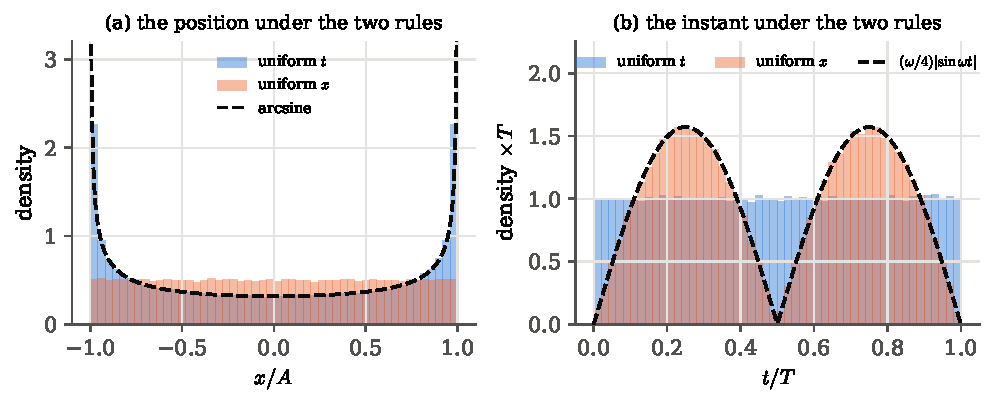
\includegraphics[width=\linewidth]{figures/ch01/oscillator_sampling_rule.pdf}
\caption{One oscillator, two sampling rules, $2\times10^5$ samples each. (a) Choosing
the instant uniformly gives the arcsine law for the position (blue); choosing the
position uniformly gives, by construction, a flat histogram (orange). (b) The
instants behind the same samples: flat under the first rule, and under the second
rule the two humps of $(\omega/4)\abs{\sin\omega t}$, highest where the mass passes
the centre and zero at the turning points $t=0,\,T/2,\,T$.}
\label{1b:fig:sampling-rule}
\end{figure}

\begin{keyidea}[Equations of motion + sampling prescription $\to$ probability distribution]
A deterministic motion has no distribution until we say what is chosen at random.
The same orbit gives the arcsine law for $x$ if the instant is uniform, and
$(\omega/4)\abs{\sin\omega t}$ for $t$ if the position is uniform. Conservation laws
tell us which states are \emph{accessible} (energy conservation confines the
oscillator to its ellipse), not that they are equally probable. Being canonically
conjugate does not make a variable uniform either: the phase $\theta=\omega t$,
conjugate to the action $E/\omega$, is uniform under the first rule only because
that rule chose the instant uniformly, and under the second rule it has density
$\frac14\abs{\sin\theta}$.
\end{keyidea}

\paragraph{Method 3: from first principles, if we did not know that $t$ is uniform.}
Method 2 assumed \eqref{1b:eq:uniform-time}. Suppose we did not know that the
instant is uniformly distributed, and asked instead what statistical mechanics
says: in the \newterm{microcanonical ensemble} all phase-space points with
energy between $E$ and $E+\Delta E$ are equally probable. We then only have to
measure areas in phase space. The energy is
\begin{equation*}
  H(x,p)=\frac{p^2}{2m}+\frac12m\omega^2x^2=E,
  \qquad E=\frac12m\omega^2A^2,
\end{equation*}
so the orbit is the ellipse $x^2/A^2+p^2/(m\omega A)^2=1$, with the two branches
$p_\pm(x)=\pm m\omega\sqrt{A^2-x^2}$. Thicken it into a shell
$E\to E+\Delta E$. At fixed $x$ the shell has thickness in the $p$ direction
\begin{align*}
  \Delta p
  &\eqby{1} \sqrt{2m(E+\Delta E)-m^2\omega^2x^2}-\sqrt{2mE-m^2\omega^2x^2}
   \eqby{2} \frac{m\,\Delta E}{\sqrt{2mE-m^2\omega^2x^2}}
   \eqby{3} \frac{\Delta E}{\omega\sqrt{A^2-x^2}} .
\end{align*}
\begin{explain}
  \item Solve $H=E$ for $\abs p$: $\abs p=\sqrt{2mE-m^2\omega^2x^2}$, at the outer
        and inner energies.
  \item First order in $\Delta E$: $\sqrt{a+\epsilon}-\sqrt a\simeq\epsilon/(2\sqrt a)$
        with $\epsilon=2m\Delta E$.
  \item $2mE=m^2\omega^2A^2$, so the square root is $m\omega\sqrt{A^2-x^2}$.
\end{explain}
The vertical strip between $x$ and $x+\dd x$ meets the shell twice, at $p_+$ and
at $p_-$ (the two dark patches in \cref{1b:fig:arcsine}b), so the shell area
inside the strip and the total shell area are
\begin{align*}
  \dd\mathcal A
  &\eqby{1} 2\,\Delta p\,\dd x
   = \frac{2\Delta E}{\omega\sqrt{A^2-x^2}}\,\dd x,
  \\
  \mathcal A_{\rm shell}
  &\eqby{2} \mathcal A(E+\Delta E)-\mathcal A(E)
   \eqby{3} \frac{2\pi}{\omega}\,\Delta E .
\end{align*}
\begin{explain}
  \item Two patches, each of height $\Delta p$ and width $\dd x$.
  \item The shell is the region between the two ellipses.
  \item The ellipse of energy $E$ has semi-axes $\sqrt{2E/m\omega^2}$ and $\sqrt{2mE}$,
        so it encloses $\mathcal A(E)=\pi\sqrt{2E/m\omega^2}\sqrt{2mE}=2\pi E/\omega$,
        which is linear in $E$.
\end{explain}
Equal probability for equal phase-space area then gives
\begin{align*}
  P(x)\,\dd x
  &\eqby{1} \frac{\dd\mathcal A}{\mathcal A_{\rm shell}}
   \eqby{2} \frac{2\Delta E\,\dd x/\bigl(\omega\sqrt{A^2-x^2}\bigr)}{2\pi\Delta E/\omega}
   = \frac{\dd x}{\pi\sqrt{A^2-x^2}},
  \qquad \abs{x}<A,
\end{align*}
\begin{explain}
  \item Microcanonical ensemble: probability is proportional to phase-space area within the shell.
  \item The two results above; $\Delta E$ and $\omega$ cancel.
\end{explain}
and it is normalised, $\frac1\pi\int_{-A}^{A}\dd x/\sqrt{A^2-x^2}=\frac1\pi[\arcsin(x/A)]_{-A}^{A}=1$.

All three methods agree, and the agreement is not a coincidence. Methods 2 and 3
say the same thing from two ends: the \emph{time} average over one orbit equals
the \emph{ensemble} average over the energy shell. Why? The time spent in a
patch of the shell is its width over the speed, $\dd x/\abs v$. The patch area
is $2\Delta p\,\dd x$, and $\Delta p\propto1/\abs{v}$, so the area is
proportional to the same thing. A uniformly random instant therefore lands in
each patch in proportion to its area. This equality of time and
ensemble averages is \newterm{ergodicity}, and it is the property that makes
Markov-chain sampling work in \cref{ch:09}.

The density diverges at the turning points, where $v=0$, but integrably. For example
\begin{align*}
  \Prob\bigl(\abs X>0.9A\bigr)
  &\eqby{1} 1-\bigl[F_X(0.9A)-F_X(-0.9A)\bigr]
   \eqby{2} 1-\frac2\pi\arcsin0.9
   = 0.2871 ,
\end{align*}
\begin{explain}
  \item Complement of $-0.9A<X\le0.9A$, and \eqref{1b:eq:cdf-rules}.
  \item $\arcsin$ is odd, so $F(0.9A)-F(-0.9A)=\tfrac2\pi\arcsin0.9$.
\end{explain}
so more than a quarter of the time is spent in the outer 10\% of the range, both sides
combined. Averaging $x^2$ over this density gives
$\langle x^2\rangle=A^2/2$ (\cref{1b:sec:expectation}), the statement that the
time-averaged potential energy is half the total.

\pyfile[firstline=23,lastline=28,firstnumber=23]{code/ch01/14_oscillator_arcsine.py}{The oscillator: random instants, deterministic map onto the phase-space orbit}

Line 26 is the only random line: \emph{when} we look. Lines 27--28 apply the
deterministic map to a point $(x,p)$ of the orbit, which is the sampled element of the sample space. Everything else is comparison. The script also computes
the quantum probability density $\abs{\psi_{30}(x)}^2$ of the oscillator
eigenstate with $n=30$, using the stable recursion for Hermite functions
(lines 39--46), at the same energy $E=(n+\tfrac12)\hbar\omega=\tfrac12m\omega^2A^2$,
i.e.\ $A=\sqrt{2n+1}$ in units $\hbar=m=\omega=1$.

\begin{figure}[htbp]
\centering
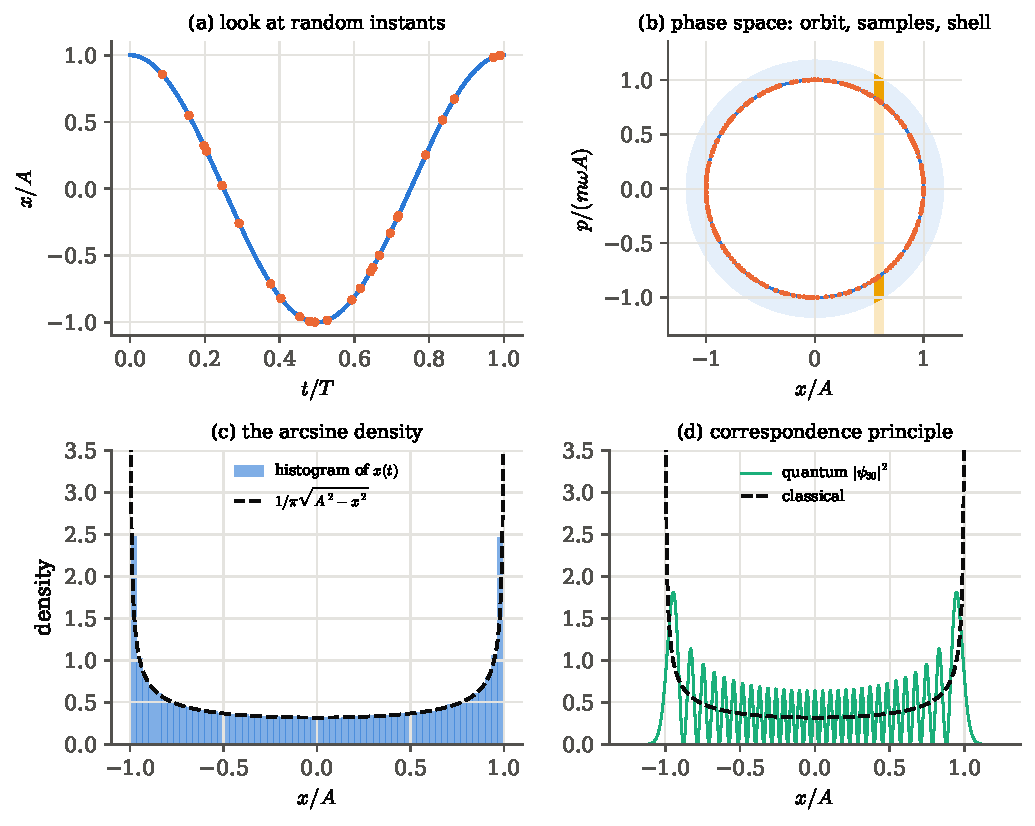
\includegraphics[width=\linewidth]{figures/ch01/oscillator_arcsine.pdf}
\caption{(a) The trajectory, looked at in random instants (dots). (b) The same
instants as points $(x,p)$ of phase space: they all lie on the energy ellipse
(a circle in the scaled units), the sample space of this problem. The pale ring is
a thickened energy shell; the vertical strip between $x$ and $x+\dd x$ meets it in
two dark patches, at $p_+$ and $p_-$, whose area is what Method~3 computes.
(c) The histogram of $x$ at $2\times10^5$ random instants follows the arcsine
density, lowest at the centre and rising steeply towards the turning points.
(d) The quantum density for $n=30$ oscillates rapidly, but its local average
follows the same classical curve: the correspondence principle seen as a
statement about probability densities.}
\label{1b:fig:arcsine}
\end{figure}

The script finds $\Prob(\abs X>0.9A)=\OneBOscFracSim$ (exact
$\OneBOscFracExact$), $\langle x^2\rangle=\OneBOscMeanSq\,A^2$ (exact $0.5$),
and a $\chi^2$ of $\OneBOscChi$ over $\OneBOscNbins$ bins against the
bin-integrated arcsine law, computed from CDF differences (lines 105--109 of
the script).

\paragraph{How research uses it.} The oscillator experiment is: pick random $t$, compute $x(t)$, histogram.
The histogram converges to the density of $x$ without our ever writing
that density down. \Cref{ch:05,ch:09} do exactly this with a posterior: an
MCMC sampler produces points $\params^{(1)},\params^{(2)},\dots$ and the
histogram of any function $g(\params)$ of them (a derived parameter such as
$H_0$ computed from $\Omega_mh^2$ and $\Omega_m$) is its posterior density,
Jacobian included automatically. Here the Monte Carlo \emph{verifies} a
known arcsine law. There it \emph{is} the answer, because the posterior
density of a derived parameter has no closed form.

\subsection{Why every point of the energy shell is equally likely: maximum entropy}
\label{1b:sec:maxent}

Method~3 for the oscillator (\cref{1b:ex:arcsine}) found the arcsine law without
ever mentioning time. It used one sentence instead: all points of the energy shell
are equally probable. Where does that sentence come from? Not from energy
conservation, which only confines the oscillator to its ellipse and says nothing
about how probable each point of it is (the key idea of \cref{1b:ex:arcsine}). It is
an extra assumption, and it can be derived from a cleaner one. Three
assumptions are needed.
\begin{enumerate}[leftmargin=1.6em,itemsep=1pt]
  \item \emph{A probabilistic description.} Cut phase space into small cells
        $i=1,2,\dots$ of equal area $\dd x\,\dd p$. The state of the system is
        described by probabilities $p_i\ge0$ with $\sum_ip_i=1$. Equal area is the
        natural cell size because phase-space area is what the Hamiltonian motion
        preserves (Liouville's theorem).
  \item \emph{Constraints.} What we know about the system is written as equations
        the $p_i$ must obey.
  \item \emph{Equilibrium.} Among all distributions that obey the constraints, the
        equilibrium one maximises the Gibbs--Shannon entropy
        \begin{equation}
          S[p]=-k_B\sum_ip_i\ln p_i .
          \label{1b:eq:gibbs-entropy}
        \end{equation}
\end{enumerate}

\paragraph{Only normalisation: the microcanonical distribution.}
Keep only the $M$ cells of the shell between $E$ and $E+\Delta E$, the accessible
states, and impose nothing but normalisation. With a Lagrange multiplier $k_B\alpha$
for $\sum_ip_i=1$, the maximum has
\begin{align*}
  0
  &\eqby{1}\frac{\partial}{\partial p_j}\Bigl[-k_B\sum_ip_i\ln p_i
       -k_B\alpha\Bigl(\sum_ip_i-1\Bigr)\Bigr]
   \eqby{2}-k_B\bigl(\ln p_j+1+\alpha\bigr),
  \\
  p_j
  &\eqby{3}e^{-1-\alpha}
   \eqby{4}\frac1M\qquad\text{for every cell } j \text{ of the shell}.
\end{align*}
\begin{explain}
  \item The stationary point of the entropy with the constraint added through its
        multiplier.
  \item Only the term $i=j$ depends on $p_j$, and $\frac{\dd}{\dd p}(p\ln p)=\ln p+1$.
  \item Solve for $p_j$.
  \item The right side of (3) is the same number for every $j$; normalisation over
        the $M$ cells fixes it to $1/M$.
\end{explain}
It is a maximum, because $\partial^2S/\partial p_j^2=-k_B/p_j<0$, and its value is
$S=k_B\ln M$, Boltzmann's entropy of \cref{1a:sec:counting}. Equal probability per
cell of equal area means probability proportional to phase-space area: Method~3's
``equal probability for equal phase-space area'' was this assumption.

\paragraph{Normalisation and a fixed mean energy: the canonical distribution.}
Now let the system exchange energy with its surroundings, so that cells of every
energy $E_i$ are accessible, and suppose all we know is the mean energy,
$\sum_ip_iE_i=U$. A second multiplier $\lambda$ enters:
\begin{align*}
  0
  &\eqby{1}\frac{\partial}{\partial p_j}\Bigl[S[p]-k_B\alpha\Bigl(\sum_ip_i-1\Bigr)
        -\lambda\Bigl(\sum_ip_iE_i-U\Bigr)\Bigr]
   \eqby{2}-k_B\bigl(\ln p_j+1+\alpha\bigr)-\lambda E_j,
  \\
  p_j
  &\eqby{3}e^{-1-\alpha}\,e^{-\beta E_j}
   \eqby{4}\frac{e^{-\beta E_j}}{Z},
  \qquad \beta\equiv\frac{\lambda}{k_B},\quad Z=\sum_ie^{-\beta E_i}.
\end{align*}
\begin{explain}
  \item The stationary point with both constraints.
  \item As before, plus $\partial(\sum_ip_iE_i)/\partial p_j=E_j$.
  \item Solve for $\ln p_j$ and exponentiate.
  \item Normalisation fixes $e^{-1-\alpha}=1/Z$; $Z$, the \newterm{partition
        function}, is simply the normaliser.
\end{explain}
What is $\beta$? Put the solution back into the entropy and ask how the maximum
entropy changes with $U$:
\begin{align*}
  S
  &\eqby{1}-k_B\sum_ip_i\bigl(-\beta E_i-\ln Z\bigr)
   \eqby{2}k_B\bigl(\beta U+\ln Z\bigr),
  \\
  \frac{\dd S}{\dd U}
  &\eqby{3}k_B\Bigl(\beta+U\frac{\dd\beta}{\dd U}
        +\frac{\partial\ln Z}{\partial\beta}\frac{\dd\beta}{\dd U}\Bigr)
   \eqby{4}k_B\beta .
\end{align*}
\begin{explain}
  \item $\ln p_i=-\beta E_i-\ln Z$.
  \item $\sum_ip_iE_i=U$ and $\sum_ip_i=1$.
  \item $\beta$ depends on $U$ through the constraint; differentiate both terms.
  \item $\partial_\beta\ln Z=-\sum_iE_ie^{-\beta E_i}/Z=-U$, so the last two terms
        cancel.
\end{explain}
Thermodynamics defines the temperature by $1/T=\dd S/\dd U$. So $\lambda=k_B\beta=1/T$,
that is $\beta=1/k_BT$, and the maximum-entropy distribution at fixed mean energy is
the Boltzmann distribution $p_i=e^{-E_i/k_BT}/Z$.

\paragraph{No sampling rule, and a definition that closes on itself.}
In \cref{1b:ex:arcsine} a probability needed a sampling prescription: choose the
instant, or choose the position, and the answers differed. Here we never said what
is chosen at random, and we did not need to. Why not? The entropy
\eqref{1b:eq:gibbs-entropy} is a function of the probabilities themselves, so
maximising it is a statement about the $p_i$ directly. The third assumption
takes the place of the sampling rule. That assumption is also a definition:
equilibrium \emph{is} the maximum-entropy state compatible with the
constraints. So the argument closes on itself. The microcanonical and
canonical distributions apply exactly when the system is in that state, and
the derivation says nothing about whether, or how fast, a given system gets
there. For the one-dimensional oscillator the dynamics answer that question
at once: a uniform instant lands on the shell in proportion to area (the
ergodicity paragraph of \cref{1b:ex:arcsine}). The same variational argument with a fixed variance gives
the Gaussian as the maximum-entropy density, in \cref{ch:02}.

\subsection{Time averages of a bounded motion: the virial theorem}
\label{1b:sec:virial}

The oscillator's $\langle x^2\rangle=A^2/2$ of \cref{1b:ex:arcsine} is a time
average: under the uniform-instant rule, averaging over the arcsine density is
averaging over one period. It says that the mean potential energy is
$\langle V\rangle=\frac12m\omega^2\langle x^2\rangle=\frac14m\omega^2A^2=E/2$, so the
mean kinetic energy is $\langle K\rangle=E-\langle V\rangle=E/2$ as well:
$2\langle K\rangle=2\langle V\rangle$. This is the virial theorem for a potential
$V\propto x^2$, and the general version takes three lines.

Take particles with positions $\bm r_a$ and momenta $\bm p_a$, potential
$V(\bm r_1,\bm r_2,\dots)$, and kinetic energy $K=\sum_a\bm p_a^2/2m_a$. Let
$G=\sum_a\bm r_a\cdot\bm p_a$ (for one particle in one dimension, $G=xp$). Then
\begin{align*}
  \frac{\dd G}{\dd t}
  &\eqby{1}\sum_a\dot{\bm r}_a\cdot\bm p_a+\sum_a\bm r_a\cdot\dot{\bm p}_a
   \eqby{2}2K-\sum_a\bm r_a\cdot\nabla_aV,
  \\
  \frac{G(\tau)-G(0)}{\tau}
  &\eqby{3}2\langle K\rangle_\tau-\Bigl\langle\sum_a\bm r_a\cdot\nabla_aV\Bigr\rangle_\tau
   \eqby{4}0\quad\text{in the limit }\tau\to\infty .
\end{align*}
\begin{explain}
  \item Product rule.
  \item $\dot{\bm r}_a=\bm p_a/m_a$, so the first sum is $\sum_a\bm p_a^2/m_a=2K$;
        Newton's law $\dot{\bm p}_a=-\nabla_aV$ in the second.
  \item Average both sides over a time $\tau$, $\langle f\rangle_\tau=\frac1\tau\int_0^\tau f\,\dd t$.
  \item For a bounded motion $G$ stays bounded, so the left side goes to zero as
        $\tau\to\infty$ (for a periodic motion it is exactly zero over one period).
\end{explain}
Hence the time-averaged \newterm{virial theorem}
\begin{equation}
  2\langle K\rangle=\Bigl\langle\sum_a\bm r_a\cdot\nabla_aV\Bigr\rangle
  \qquad\Longrightarrow\qquad
  2\langle K\rangle=n\,\langle V\rangle\quad\text{for } V\propto r^n ,
  \label{1b:eq:virial}
\end{equation}
the second form because a potential homogeneous of degree $n$,
$V(\lambda\bm r_1,\lambda\bm r_2,\dots)=\lambda^nV$, obeys Euler's relation
$\sum_a\bm r_a\cdot\nabla_aV=nV$ (differentiate in $\lambda$ at $\lambda=1$). For the
oscillator $n=2$ and $\langle K\rangle=\langle V\rangle$, as found above.

\paragraph{Gravity: negative heat capacity.}
For self-gravitating masses, $V=-\sum_{a<b}Gm_am_b/\abs{\bm r_a-\bm r_b}$ is homogeneous
of degree $n=-1$. Then
\begin{align*}
  E
  &\eqby{1}\langle K\rangle+\langle V\rangle
   \eqby{2}\langle K\rangle-2\langle K\rangle
   =-\langle K\rangle
   \eqby{3}-\tfrac32Nk_BT,
  \qquad
  \frac{\dd E}{\dd T}=-\tfrac32Nk_B<0 .
\end{align*}
\begin{explain}
  \item $E$ is conserved, so it equals its own time average.
  \item The virial theorem \eqref{1b:eq:virial} with $n=-1$: $\langle V\rangle=-2\langle K\rangle$.
  \item The kinetic-gas definition of temperature for $N$ particles,
        $\langle K\rangle=\frac32Nk_BT$.
\end{explain}
A self-gravitating system has a negative heat capacity: when it loses energy it heats
up. A star radiates, contracts, its potential energy falls by twice the energy lost,
and half of that goes into faster thermal motion. Star clusters behave the same way:
the core loses energy to the halo and gets hotter.

\paragraph{The canonical distribution cannot have $C<0$.}
The canonical distribution of \cref{1b:sec:maxent} fixes the sign of the heat
capacity, so it cannot describe such a system. With $Z(\beta)=\sum_ie^{-\beta E_i}$,
\begin{align*}
  \frac{\partial\ln Z}{\partial\beta}
  &\eqby{1}-\frac{\sum_iE_ie^{-\beta E_i}}{Z}=-\langle E\rangle,
  \qquad
  \frac{\partial^2\ln Z}{\partial\beta^2}
  \eqby{2}\frac{\sum_iE_i^2e^{-\beta E_i}}{Z}-\Bigl(\frac{\sum_iE_ie^{-\beta E_i}}{Z}\Bigr)^2
  =\Var(E),
  \\
  C
  &\eqby{3}\frac{\dd\langle E\rangle}{\dd T}
   \eqby{4}\frac{\dd\beta}{\dd T}\,\frac{\dd\langle E\rangle}{\dd\beta}
   \eqby{5}\Bigl(-\frac1{k_BT^2}\Bigr)\Bigl(-\frac{\partial^2\ln Z}{\partial\beta^2}\Bigr)
   =\frac{\Var(E)}{k_BT^2}\;\ge\;0 .
\end{align*}
\begin{explain}
  \item Differentiate $\ln Z$; the ratio is the canonical average of $E$.
  \item Differentiate once more (quotient rule): $\partial_\beta(Z'/Z)=Z''/Z-(Z'/Z)^2$,
        which is $\langle E^2\rangle-\langle E\rangle^2$ (the generating-function view
        of $\ln Z$ is in \cref{1b:sec:moments}).
  \item The heat capacity is the change of mean energy with temperature.
  \item Chain rule through $\beta=1/k_BT$.
  \item $\dd\beta/\dd T=-1/k_BT^2$ and the two results of the first line.
\end{explain}
A variance is never negative, so a system described by the canonical distribution
has $C\ge0$. A self-gravitating system, with $C<0$, cannot be described by the
canonical distribution, and physically it cannot sit in equilibrium with a heat bath:
if it is a little hotter than the bath it loses energy, gets hotter still, and runs
away. Only the microcanonical description, an isolated system at fixed $E$ with
maximum entropy on its shell, can apply to it. The assumptions of
\cref{1b:sec:maxent} say exactly when each distribution is legitimate: fixed energy
gives the microcanonical, a fixed mean energy (which in practice means contact with
a bath) gives the canonical, and the second needs $C\ge0$ to be consistent.

\subsection{Isotropic decays: flat in \texorpdfstring{$\cos\theta$}{cos theta}, peaked in \texorpdfstring{$p_T$}{pT}}

\oneBEx{Angles and transverse momentum of an isotropic decay}\label{1b:ex:decay}
A particle at rest decays into two daughters, each of momentum $p^*$ in
opposite directions. ``Isotropic'' means the daughter direction is uniform
on the unit sphere: the probability of a patch is its solid angle over
$4\pi$, $\dd\Prob=\dd\Omega/4\pi=\sin\theta\,\dd\theta\,\dd\phi/4\pi$ with
$\theta\in[0,\pi]$ the polar angle to the beam axis $z$. Then:
\begin{align*}
  f(\theta)
  &\eqby{1} \int_0^{2\pi}\frac{\sin\theta}{4\pi}\,\dd\phi
   = \frac{\sin\theta}{2},\qquad
  f_{\cos\theta}(u)\eqby{2}\frac{\sin\theta}{2}\cdot\frac{1}{\sin\theta}
   = \frac12,\quad u\in[-1,1].
\end{align*}
\begin{explain}
  \item The joint density of $(\theta,\phi)$ is $\sin\theta/4\pi$.
        Marginalise the azimuth $\phi$.
  \item $u=\cos\theta$ is decreasing on $[0,\pi]$ with
        $\abs{\dd\theta/\dd u}=1/\sin\theta$. Apply \eqref{1b:eq:jacobian-1d}.
\end{explain}
So $\cos\theta$ is flat, $\theta$ is not (few decays go along the beam,
because the poles have little solid angle), and $p_z=p^*\cos\theta$ is
uniform on $[-p^*,p^*]$. The transverse momentum $p_T=p^*\sin\theta$ is
different: two angles, $\theta$ and $\pi-\theta$, give the same $p_T$. With
$\sin\theta=p_T/p^*$ and $\abs{\cos\theta}=\sqrt{1-p_T^2/p^{*2}}$,
\begin{align*}
  \Bigl\lvert\frac{\dd\theta}{\dd p_T}\Bigr\rvert
  &\eqby{1} \frac{1}{p^*\abs{\cos\theta}}
   = \frac{1}{\sqrt{p^{*2}-p_T^2}},\\
  f(p_T)
  &\eqby{2} 2\times\frac{\sin\theta}{2}\times\frac{1}{\sqrt{p^{*2}-p_T^2}}
   = \frac{p_T}{p^*\sqrt{p^{*2}-p_T^2}},\qquad 0<p_T<p^* .
\end{align*}
\begin{explain}
  \item $\dd p_T/\dd\theta=p^*\cos\theta$.
  \item Two branches ($\theta<\pi/2$ and $\theta>\pi/2$) with the same
        density $\sin\theta/2$ and the same Jacobian.
\end{explain}
The density diverges at $p_T=p^*$, the \newterm{Jacobian peak}: decays near
$\theta=\pi/2$ all pile up at the maximum $p_T$, because $p_T$ is stationary
there. For $W\to e\nu$ with the $W$ at rest, $p^*=m_W/2\approx40\,$GeV, and
the sharp edge of the electron $p_T$ spectrum near 40 GeV is what makes the
$p_T$ distribution sensitive to $m_W$. As a check,
$\Prob(p_T>0.9p^*)=\Prob(\abs{\cos\theta}<\sqrt{1-0.81})=\sqrt{0.19}=0.4359$,
because $\cos\theta$ is uniform.

\pyfile[firstline=22,lastline=30,firstnumber=22]{code/ch01/15_decay_angles.py}{Isotropic directions and the transverse momentum}

Lines 26--27 generate isotropic directions by normalising a vector of three
independent standard Gaussians. This works because the joint density of the
three Gaussians, $(2\pi)^{-3/2}e^{-\abs{\bm v}^2/2}$, depends only on the
length $\abs{\bm v}$, so it is unchanged by rotations and the direction must
be uniform. Lines 28--30 compute the three random variables of the example
from the same simulated directions.

\begin{figure}[htbp]
\centering
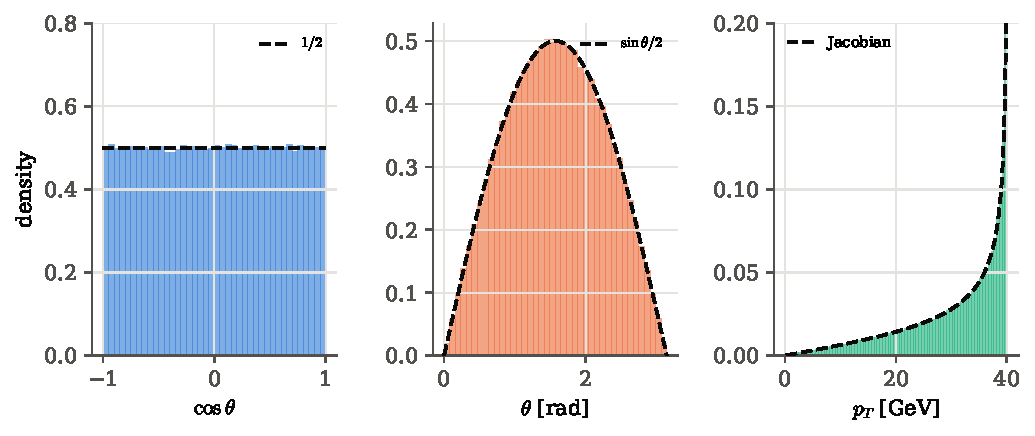
\includegraphics[width=\linewidth]{figures/ch01/decay_angles.pdf}
\caption{$4\times10^5$ isotropic decays of a particle at rest with
$p^*=m_W/2$. Left: $\cos\theta$ is flat at $\tfrac12$. Middle: $\theta$
itself follows $\sin\theta/2$, vanishing along the beam. Right: the
transverse momentum rises towards the kinematic endpoint $p^*$ and piles up
there (the Jacobian peak).}
\label{1b:fig:decay}
\end{figure}

The simulation gives $\langle\cos\theta\rangle=\OneBDecMeanCos$ (exact 0),
$\langle p_T\rangle=\OneBDecMeanPtSim\,$GeV against the exact
$p^*\langle\sin\theta\rangle=\pi p^*/4=\OneBDecMeanPtExact\,$GeV, and
$\Prob(p_T>0.9p^*)=\OneBDecFracSim$ against $\OneBDecFracExact$.

\subsection{Several variables: the Jacobian determinant}

Everything above extends to several variables at once, with lengths replaced
by areas or volumes.

\begin{workdef}[change of variables in several dimensions]
Let $(X,Y)$ have joint density $f_{X,Y}$ and let $(U,V)=g(X,Y)$ be
one-to-one on the region where $f_{X,Y}>0$, with inverse $x=h_1(u,v)$,
$y=h_2(u,v)$. Then
\begin{equation}
  f_{U,V}(u,v)=f_{X,Y}\bigl(h_1(u,v),h_2(u,v)\bigr)\,\abs{J},\qquad
  J=\det\begin{pmatrix}\partial x/\partial u&\partial x/\partial v\\
  \partial y/\partial u&\partial y/\partial v\end{pmatrix},
  \label{1b:eq:jacobian-2d}
\end{equation}
\unpack{the old density at the preimage point, times the factor by which the
inverse map scales areas near it}. The same holds in $n$ dimensions with the
$n\times n$ Jacobian determinant \srcref{Cowan}{(1.37)--(1.38)}.
\emph{Operational test:} a small rectangle $\dd u\,\dd v$ is the image of a
parallelogram of area $\abs J\dd u\,\dd v$, and both must carry the same
probability.
\end{workdef}

The multidimensional formula is \eqref{1b:eq:jacobian-1d} with ``length''
replaced by ``area'': the inverse map sends the rectangle with sides
$\dd u,\dd v$ to a parallelogram spanned by the vectors
$(\partial_ux,\partial_uy)\dd u$ and $(\partial_vx,\partial_vy)\dd v$, whose
area is $\abs{J}\dd u\,\dd v$, the familiar volume element of a coordinate
change.

\oneBEx{Sum and difference of two Gaussians; polar coordinates}\label{1b:ex:sum-diff}
Let $X,Y\iid\Normal(0,1)$ and $U=X+Y$, $V=X-Y$
\srcref{CasellaBerger}{Ex.~4.3.4}. The inverse is $x=(u+v)/2$,
$y=(u-v)/2$, so
\begin{align*}
  J&\eqby{1}\det\begin{pmatrix}\tfrac12&\tfrac12\\ \tfrac12&-\tfrac12\end{pmatrix}=-\tfrac12,
  \qquad x^2+y^2\eqby{2}\frac{(u+v)^2+(u-v)^2}{4}=\frac{u^2+v^2}{2},\\
  f_{U,V}(u,v)
  &\eqby{3} \frac{1}{2\pi}e^{-(u^2+v^2)/4}\cdot\frac12
   = \Bigl[\frac{e^{-u^2/4}}{\sqrt{2\pi\cdot2}}\Bigr]
     \Bigl[\frac{e^{-v^2/4}}{\sqrt{2\pi\cdot2}}\Bigr].
\end{align*}
\begin{explain}
  \item Partial derivatives of $x$ and $y$ with respect to $u,v$.
  \item The cross terms $\pm2uv$ cancel.
  \item \eqref{1b:eq:jacobian-2d} with
        $f_{X,Y}=\tfrac{1}{2\pi}e^{-(x^2+y^2)/2}$ and $\abs J=\tfrac12$.
\end{explain}
The joint factorises: $U$ and $V$ are independent, each $\Normal(0,2)$. The
sum and difference of two equally noisy channels are statistically
independent, a fact \cref{1b:sec:covariance} will explain through their
covariance.

In polar coordinates, $x=r\cos\varphi$, $y=r\sin\varphi$, $J=r$, and the
same density becomes $f(r,\varphi)=\frac{1}{2\pi}\cdot re^{-r^2/2}$: the angle
is uniform on $[0,2\pi)$, independent of the radius, and $R$ has density
$re^{-r^2/2}$ (the Rayleigh distribution). Read backwards this is the
Box--Muller recipe for making Gaussians from uniforms (\cref{ch:06}).

For a single function $Z=r(X,Y)$ the three-step CDF method still works
\mainref{p.~42}: find $A_z=\{(x,y):r(x,y)\le z\}$, integrate the joint over
it, differentiate. Alternatively, invent a second variable to make the map
one-to-one, use \eqref{1b:eq:jacobian-2d}, and marginalise the invented
variable \srcref{CasellaBerger}{\S4.3}. For $Z=X+Y$ take $(x,y)\to(x,z)$ with
$z=x+y$, so $y=z-x$ and $\abs J=1$. For independent $X,Y$ with densities $g,h$:
\begin{align}
  f_Z(z)
  &\eqby{1} \int f_{X,Z}(x,z)\,\dd x
   \eqby{2} \int g(x)\,h(z-x)\,\dd x ,
  \label{1b:eq:convolution}
\end{align}
\begin{explain}
  \item Marginalise the auxiliary variable $x$.
  \item \eqref{1b:eq:jacobian-2d} with $\abs J=1$ and independence,
        $f_{X,Y}(x,z-x)=g(x)h(z-x)$.
\end{explain}
the \newterm{convolution} $g*h$: the density of a sum is the convolution of
the densities \srcref{Cowan}{(1.36)}. For a product $Z=XY$ take $y=z/x$,
$\abs{J}=1/\abs x$, and get $f_Z(z)=\int g(x)h(z/x)\,\dd x/\abs x$, the Mellin
convolution \srcref{Cowan}{(1.35)}.

\oneBEx{The sum of two uniforms is a triangle}\label{1b:ex:triangle}
Let $X_1,X_2\iid\text{Uniform}(0,1)$ and $Y=X_1+X_2$
\mainref{Ex.~2.48, p.~43}. \emph{By geometry}: $A_y=\{x_1+x_2\le y\}$ within
the unit square is a triangle of area $y^2/2$ for $0\le y<1$, and the square
minus a corner triangle of area $(2-y)^2/2$ for $1\le y<2$
(\cref{1b:fig:triangle}). So $F_Y=y^2/2$ and then $1-(2-y)^2/2$, and
$f_Y(y)=y$ on $[0,1]$, $2-y$ on $[1,2]$. \emph{By convolution}
\eqref{1b:eq:convolution}, with $g=h=\mathbb{1}_{[0,1]}$ (the indicator of
$[0,1]$),
\begin{align*}
  f_Y(y)
  &\eqby{1} \int_0^1\mathbb{1}\bigl[0\le y-x\le1\bigr]\,\dd x
   \eqby{2} \min(y,1)-\max(0,y-1)
   = \begin{cases}y,&0\le y\le1,\\ 2-y,&1\le y\le2 .\end{cases}
\end{align*}
\begin{explain}
  \item $g(x)=1$ restricts $x$ to $[0,1]$, and $h(y-x)=1$ needs
        $0\le y-x\le1$.
  \item Both conditions together: $\max(0,y-1)\le x\le\min(1,y)$. The
        integral is the length of that interval.
\end{explain}
Adding two flat distributions gives a peaked one. Adding more gives
something ever closer to a Gaussian, the central limit theorem of
\cref{ch:02}; \cref{1b:sec:moments} shows why the convolution becomes simple
after a Fourier transform.

\begin{figure}[htbp]
\centering
\begin{tikzpicture}[x=2.3cm,y=2.3cm]
  \begin{scope}
    \fill[formblue!30] (0,0) -- (0.65,0) -- (0,0.65) -- cycle;
    \draw (0,0) rectangle (1,1);
    \draw[thick,bdryred] (0.65,0) -- (0,0.65);
    \fill[bdryred] (0.65,0) circle (1.3pt) (0,0.65) circle (1.3pt);
    \node[lbl,anchor=north] at (0.65,-0.02) {$(y,0)$};
    \node[lbl,anchor=east] at (-0.02,0.65) {$(0,y)$};
    \node[lbl,anchor=north] at (0,-0.02) {$0$};
    \node[lbl,anchor=north] at (1,-0.02) {$1$};
    \node[lbl,align=center] at (0.5,-0.5) {$0\le y<1$:\\area $y^2/2$};
  \end{scope}
  \begin{scope}[xshift=3.2cm]
    \fill[formblue!30] (0,0) -- (1,0) -- (1,0.4) -- (0.4,1) -- (0,1) -- cycle;
    \draw (0,0) rectangle (1,1);
    \draw[thick,bdryred] (1,0.4) -- (0.4,1);
    \fill[bdryred] (1,0.4) circle (1.3pt) (0.4,1) circle (1.3pt);
    \node[lbl,anchor=west] at (1.02,0.4) {$(1,y-1)$};
    \node[lbl,anchor=south] at (0.4,1.02) {$(y-1,1)$};
    \node[lbl,anchor=north] at (0,-0.02) {$0$};
    \node[lbl,anchor=north] at (1,-0.02) {$1$};
    \node[lbl,align=center] at (0.5,-0.5) {$1\le y<2$:\\area $1-(2-y)^2/2$};
  \end{scope}
\end{tikzpicture}
\caption{The event $X_1+X_2\le y$ inside the unit square is everything below
the red line $x_2=y-x_1$. For $y<1$ it is a small triangle. For $y>1$ it is
the whole square minus the unshaded corner. The shaded area is the CDF of the
sum.}
\label{1b:fig:triangle}
\end{figure}

The worked cases used every method in turn. The table says which one to
reach for in each situation.

\begin{taxonomy}[Which method for which transformation]
\begin{center}
\small
\begin{tabular}{@{}p{4.3cm}p{8.1cm}@{}}
\toprule
situation & method\\\midrule
$X$ discrete & add probabilities of all preimages\\
$r$ monotone & $f_Y=f_X(s(y))\abs{s'(y)}$\\
$r$ many-to-one (e.g.\ $x^2$, $\cos$, $\sin$) & sum the monotone formula over branches, or use the CDF\\
awkward region, piecewise & CDF method: draw $A_y$, integrate, differentiate\\
$n$ variables to $n$ variables & Jacobian determinant \eqref{1b:eq:jacobian-2d}\\
one function of $n$ variables & add auxiliary variables, Jacobian, marginalise; sums $\to$ convolution\\
sums of many independent variables & characteristic functions (\cref{1b:sec:moments})\\
anything else & simulate and histogram (Monte Carlo, \cref{ch:06})\\
\bottomrule
\end{tabular}
\end{center}
\end{taxonomy}

Three mistakes recur in all of these methods.

\begin{pitfall}[Transforming the density's value instead of its argument]
Writing $f_Y(y)=f_X(s(y))$ and forgetting the Jacobian is the commonest
error. The result is not normalised, so a quick check $\int f_Y=1$ catches
it. A second error is forgetting branches ($\theta$ and $\pi-\theta$ both give
the same $p_T$). A third is expecting the peak to transform like a point:
modes move under reparametrisation, quantiles do not
(\cref{1b:ex:log-exp}).
\end{pitfall}
\section{Expectation and variance: the long-run average and the spread}
\label{1b:sec:expectation}

A slot machine pays \$100 with probability $0.001$, pays \$5 with probability
$0.14$, and otherwise takes our \$1. Should we play? No single pull answers
that, because a single pull is random. What we can predict is the average
over many pulls. In $N$ pulls we expect about $0.001N$ big wins, $0.14N$
small wins and $0.859N$ losses, so the average payoff per pull is
\[
  0.001\times100+0.14\times5+0.859\times(-1)=-0.059
\]
dollars. In the long run we lose about six cents per pull
\srcref{Kruschke}{\S4.3.3}. Each possible value was weighted by how often it
occurs. That weighted average is the expectation.

Physicists use this object all the time under other names. The ensemble
average $\langle A\rangle=\sum_ip_iA_i$ of statistical mechanics, with
$p_i=e^{-\beta E_i}/Z$, is an expectation. So is the quantum expectation value
$\langle\psi\rvert\hat A\lvert\psi\rangle=\sum_a a\,\abs{\langle a\vert\psi\rangle}^2$,
where the Born probabilities $\abs{\langle a\vert\psi\rangle}^2$ weight the
eigenvalues $a$. Two numbers summarise a whole distribution: a location (the
mean) and a spread (the variance). There are rules for computing both for
sums, for functions and for conditional situations, without ever writing down
the density of the quantity being averaged. Three questions organise the
topic.
\begin{enumerate}[leftmargin=1.6em,itemsep=1pt]
  \item What is the average value of $X$, and of any function $r(X)$?
  \item How far from that average does $X$ typically fall?
  \item If we learn the value of another variable, how do the average and the
        spread change, and how do the conditional pieces reassemble into the
        whole?
\end{enumerate}

\subsection{The expectation}

Start from data. Draw $X$ independently $N$ times and let $n_x$ be the number
of draws that gave the value $x$. The average of the draws is
\[
  \frac1N\sum_{j=1}^NX_j=\sum_x x\,\frac{n_x}{N} .
\]
The frequencies $n_x/N$ approach the probabilities $f(x)=\Prob(X=x)$ as $N$
grows (the frequency interpretation of \cref{1a:sec:axioms}; the law of large
numbers in \cref{ch:02} makes this precise). So the long-run average is
$\sum_x x\,f(x)$. For a continuous variable, sort the draws into bins of
width $\Delta x$. The fraction in the bin at $x$ is about $f(x)\,\Delta x$,
where $f$ is the density, and the sum over bins becomes an integral as
$\Delta x\to0$.

\begin{workdef}[expectation, mean]
The \newterm{expectation} (or \newterm{mean}, or first moment) of $X$ is
\begin{equation}
  \E(X)=\begin{cases}
    \sum_x x\,f(x) & X\text{ discrete},\\[3pt]
    \int_{-\infty}^{\infty}x\,f(x)\,\dd x & X\text{ continuous},
  \end{cases}
  \label{1b:eq:mean}
\end{equation}
the values weighted by the pmf \unpack{$f(x)=\Prob(X=x)$, the mass at $x$} or
by the density \unpack{probability per unit $x$}.
It is written $\mu$, $\mu_X$, $\E X$ or $\langle X\rangle$ and has the units of
$X$. It \newterm{exists} only if $\sum_x\abs x f(x)$ (or
$\int\abs x f(x)\,\dd x$) is finite.
\emph{Operational test:} the average of many independent draws of $X$ settles
down to $\E(X)$.
\end{workdef}

\mainref{Def.~3.1, p.~47} writes both cases as $\int x\,\dd F(x)$, a single
notation for ``sum against the masses or integrate against the density''.
We will use the two explicit forms.

\paragraph{Example: simple means.}
For a Bernoulli trial, $\E(X)=0\cdot(1-p)+1\cdot p=p$: the mean of an
indicator is the probability of the event it indicates. For the number of
heads in two fair flips, $\E(X)=0\cdot\tfrac14+1\cdot\tfrac12+2\cdot\tfrac14=1$
\mainref{Exs.~3.2--3.3, p.~48}. For a fair die,
$\E(X)=\tfrac16(1+2+\dots+6)=\tfrac{21}{6}=3.5$ \srcref{SeeingTheory}{p.~10},
a value the die can never show. The mean is a long-run average, not a
typical outcome. For $X\sim\mathrm{Uniform}(-1,3)$ the density is $\tfrac14$
on $(-1,3)$ and
\begin{align*}
  \E(X)
  &\eqby{1} \int_{-1}^{3}x\cdot\tfrac14\,\dd x
   \eqby{2} \tfrac14\Bigl[\tfrac{x^2}{2}\Bigr]_{-1}^{3}
   = \tfrac14\cdot\tfrac{9-1}{2}=1 .
\end{align*}
\begin{explain}
  \item \eqref{1b:eq:mean} with $f=\tfrac14$ inside the interval and $0$ outside.
  \item Antiderivative of $x$.
\end{explain}
The mean is the midpoint, as symmetry demands. The same happens for the
parabola $f(x)=6x(1-x)$ on $[0,1]$ \srcref{Kruschke}{(4.7)}:
$\E(X)=6\int_0^1(x^2-x^3)\,\dd x=6\bigl(\tfrac13-\tfrac14\bigr)=\tfrac12$.

\paragraph{Example: the mean lifetime.}
A lifetime with density $f(x)=e^{-x/\beta}/\beta$ for $x>0$
(exponential with mean $\beta$, \cref{1b:sec:pdf}) has
\begin{align*}
  \E(X)
  &\eqby{1} \int_0^\infty x\,\frac{e^{-x/\beta}}{\beta}\,\dd x
   \eqby{2} \beta\int_0^\infty u\,e^{-u}\,\dd u \\
  &\eqby{3} \beta\Bigl(\bigl[-u\,e^{-u}\bigr]_0^\infty+\int_0^\infty e^{-u}\,\dd u\Bigr)
   \eqby{4} \beta\,(0+1)=\beta .
\end{align*}
\begin{explain}
  \item Definition \eqref{1b:eq:mean}; the density vanishes for $x<0$.
  \item Substitute $u=x/\beta$, so $x=\beta u$ and $\dd x=\beta\,\dd u$.
  \item Integrate by parts with $u$ differentiated and $e^{-u}$ integrated.
  \item $ue^{-u}\to0$ at both ends, and $\int_0^\infty e^{-u}\dd u=1$.
\end{explain}
So $\beta$ really is the mean lifetime, and the median $\beta\ln2$ found in
\cref{1b:ex:exp-quantile} sits below it.

\paragraph{The balance point.}
If we read $f(x)$ as a mass density along a rod (or as point masses $f(x_i)$
at positions $x_i$), then $\E(X)=\sum_ix_if(x_i)$ with $\sum_if(x_i)=1$ is the
centre of mass: the rod balances on a fulcrum placed at the mean
(\cref{1b:fig:balance}). A small mass far out in a tail pulls the balance
point a long way. This is why the mean of a skewed distribution is dragged
towards its long tail, and why a single outlier can move a sample mean a lot.

\begin{figure}[htbp]
\centering
\begin{tikzpicture}[x=2.0cm,y=4.0cm]
  \draw[thick] (-0.4,0) -- (4.4,0);
  \foreach \k/\p in {0/0.2401,1/0.4116,2/0.2646,3/0.0756,4/0.0081}{
    \fill[formblue!55] ({\k-0.18},0.02) rectangle ({\k+0.18},{0.02+\p});
    \node[lbl,anchor=north] at (\k,-0.17) {$\k$};
    \node[lbl,anchor=south] at (\k,{0.02+\p}) {$\p$};
  }
  \fill[bdryred] (1.2,0) -- (1.08,-0.16) -- (1.32,-0.16) -- cycle;
  \node[lbl,anchor=west,bdryred] at (1.4,-0.08) {$\E(X)=np=1.2$};
  \node[lbl,anchor=north] at (2,-0.34) {number of successes $x$};
\end{tikzpicture}
\caption{The pmf of a binomial with $n=4$, $p=0.3$, drawn as masses on a rod.
The rod balances on the red fulcrum at $x=1.2$, which is the mean. The mean is
not one of the possible values, and it lies to the right of the most probable
value $x=1$ because the tail extends to the right.}
\label{1b:fig:balance}
\end{figure}

\paragraph{Example: a density with no mean.}
The Cauchy density $f(x)=1/[\pi(1+x^2)]$ is the Breit--Wigner (Lorentzian)
line shape of a resonance with unit half-width, centred at $0$. It is
symmetric, so one is tempted to say its mean is $0$. But the mean exists only
if $\int\abs x f(x)\,\dd x$ is finite, and
\begin{align*}
  \int_{-\infty}^{\infty}\frac{\abs x}{\pi(1+x^2)}\,\dd x
  &\eqby{1} \frac2\pi\int_0^\infty\frac{x}{1+x^2}\,\dd x
   \eqby{2} \frac1\pi\Bigl[\ln(1+x^2)\Bigr]_0^\infty=\infty .
\end{align*}
\begin{explain}
  \item The integrand is even, so the integral is twice the integral over $x>0$.
  \item $\frac{\dd}{\dd x}\ln(1+x^2)=\frac{2x}{1+x^2}$, and the logarithm grows
        without bound.
\end{explain}
(\mainref{Ex.~3.5, p.~48} reaches the same conclusion by parts.) The tails
fall only like $1/x^2$, so $x f(x)\sim1/(\pi x)$ and the integral diverges
logarithmically. The positive and negative halves are each infinite, and
``$\infty-\infty$'' has no value. This is not a mathematical curiosity. In a
simulation the running average never settles down: every so often a draw
from far out in a tail arrives and moves the average by a finite amount,
however many draws came before (\cref{1b:fig:cauchy-run}, the computer
experiment of \mainref{Exercise~3.9, p.~59}). After $\OneBRunN$ draws the four
Gaussian averages are all within $\OneBRunGaussMax$ of zero, while the four
Cauchy averages lie between $\OneBRunCauchyMin$ and $\OneBRunCauchyMax$ in
absolute value and are still jumping. \Cref{1b:sec:moments} will show the
reason: the average of $n$ Cauchy draws has exactly the same Cauchy
distribution as a single draw.

\begin{figure}[htbp]
\centering
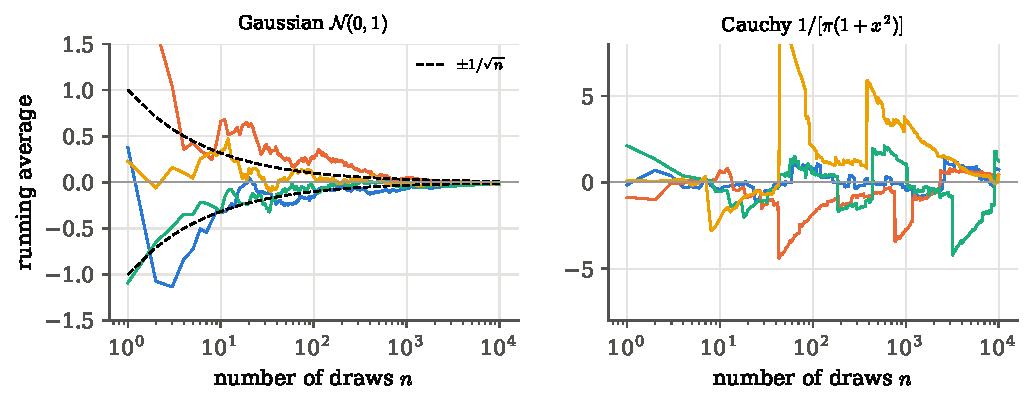
\includegraphics[width=\linewidth]{figures/ch01/cauchy_running_mean.pdf}
\caption{Running averages of four independent sequences of draws, on a
logarithmic axis in $n$. Left: Gaussian draws; the averages close in on zero
inside the dashed $\pm1/\sqrt n$ envelope. Right: Cauchy draws; the averages
wander and jump whenever a very large draw arrives, and do not converge.}
\label{1b:fig:cauchy-run}
\end{figure}

From here on, whenever we write an expectation we assume it exists.

\subsection{The average of a function: the lazy statistician}

Often we want the mean of $Y=r(X)$: the kinetic energy $\tfrac12mv^2$ of a
molecule with random velocity, the flux $10^{-0.4m}$ of a star of random
magnitude, the $p_T$ of a decay product at a random angle. One route is to
find $f_Y$ by the change-of-variables rules of \cref{1b:sec:transform} and
average $y$ against it. There is a much easier way
\mainref{Thm.~3.6, p.~48}:
\begin{equation}
  \E\bigl(r(X)\bigr)=\sum_xr(x)\,f_X(x)
  \quad\text{or}\quad
  \E\bigl(r(X)\bigr)=\int r(x)\,f_X(x)\,\dd x .
  \label{1b:eq:lotus}
\end{equation}
It is called the rule of the lazy statistician because it looks like what a
lazy person would write without thinking, and it is right. Think of a game
in which $X$ is drawn and we are paid $r(X)$: our average income is each
payment $r(x)$ times the chance of that $x$, summed.

Why does it hold? For discrete $X$ \mainref{Exercise~3.6, p.~59}, group the
values of $x$ according to the value $y=r(x)$ they produce:
\begin{align*}
  \E(Y)
  &\eqby{1} \sum_y y\,\Prob(Y=y)
   \eqby{2} \sum_y y\sum_{x:\,r(x)=y}f_X(x)
   \eqby{3} \sum_y\ \sum_{x:\,r(x)=y}r(x)\,f_X(x)
   \eqby{4} \sum_x r(x)\,f_X(x) .
\end{align*}
\begin{explain}
  \item Definition \eqref{1b:eq:mean} applied to $Y$.
  \item $\Prob(Y=y)$ is the total mass of all preimages of $y$
        (\cref{1b:sec:transform}).
  \item Inside the inner sum $r(x)=y$, so $y$ may be replaced by $r(x)$.
  \item Every $x$ lies in exactly one set $\{x:r(x)=y\}$, so the double sum
        visits each $x$ once.
\end{explain}
For continuous $X$ and increasing $r$ with inverse $s$, the same thing
happens with a Jacobian:
\begin{align*}
  \E(Y)
  &\eqby{1} \int y\,f_X\bigl(s(y)\bigr)\,s'(y)\,\dd y
   \eqby{2} \int r(x)\,f_X(x)\,\dd x .
\end{align*}
\begin{explain}
  \item Definition of $\E(Y)$ with $f_Y$ from \eqref{1b:eq:jacobian-1d}.
  \item Substitute $x=s(y)$, so $y=r(x)$ and $\dd x=s'(y)\,\dd y$.
\end{explain}
The Jacobian in the density is exactly cancelled by the Jacobian of the
measure. In the fluid picture: $f_Y(y)\,\dd y=f_X(x)\,\dd x$ is the same
drop of probability, and we multiply it by the same number $y=r(x)$
whichever coordinate we use \srcref{Cowan}{(1.40)}. A decreasing $r$ or
several branches give the same result branch by branch.

The most important special case is an indicator. Let $r=I_A$, the indicator
of a set $A$ ($I_A(x)=1$ if $x\in A$ and $0$ otherwise). Then
\begin{equation}
  \E\bigl(I_A(X)\bigr)=\int I_A(x)f_X(x)\,\dd x=\int_Af_X(x)\,\dd x=\Prob(X\in A).
  \label{1b:eq:prob-as-mean}
\end{equation}
Probability is a special case of expectation. This is how every Monte Carlo
estimate of a probability works (\cref{ch:06}): the fraction of simulated
draws that land in $A$ is the sample mean of an indicator.

\paragraph{Example: $\E(e^X)$ two ways.}
Let $X\sim\mathrm{Uniform}(0,1)$ and $Y=e^X$ \mainref{Ex.~3.7, p.~49}.
By \eqref{1b:eq:lotus}, $\E(Y)=\int_0^1e^x\,\dd x=e-1$. The long way first
finds $f_Y$: the inverse is $s(y)=\ln y$ with $s'(y)=1/y$, so
\eqref{1b:eq:jacobian-1d} gives $f_Y(y)=1/y$ on $(1,e)$, and
$\E(Y)=\int_1^e y\cdot\tfrac1y\,\dd y=e-1$. Same answer, more work. A
simulation with $10^6$ draws gives $\OneBExpUSim$ (exact $\OneBExpUExact$).
Note that $e^{\E(X)}=e^{1/2}=1.649$ is \emph{not} the answer.

\paragraph{Example: the broken stick.}
Break a stick of unit length at a uniformly random point $X$ and keep the
longer piece, $Y=\max\{X,1-X\}$ \mainref{Ex.~3.8, p.~49}. On $x<\tfrac12$ the
longer piece is $1-x$, on $x\ge\tfrac12$ it is $x$:
\begin{align*}
  \E(Y)
  &\eqby{1} \int_0^{1/2}(1-x)\,\dd x+\int_{1/2}^1x\,\dd x
   \eqby{2} \Bigl(\tfrac12-\tfrac18\Bigr)+\Bigl(\tfrac12-\tfrac18\Bigr)
   =\tfrac34 .
\end{align*}
\begin{explain}
  \item \eqref{1b:eq:lotus} with the density $1$ on $(0,1)$, split where $r$
        changes formula.
  \item $\int_0^{1/2}(1-x)\dd x=\tfrac12-\tfrac18$, and
        $\int_{1/2}^1x\,\dd x=\tfrac12-\tfrac18$.
\end{explain}
The simulation gives $\OneBStickSim$.

\paragraph{Example: time average and ensemble average for the oscillator.}
For the oscillator $x(t)=A\cos\omega t$ of \cref{1b:ex:arcsine} we can compute
$\langle x^2\rangle$ in two ways. As an average over the position density
$f(x)=1/(\pi\sqrt{A^2-x^2})$:
\begin{align*}
  \E(X^2)
  &\eqby{1} \int_{-A}^{A}\frac{x^2}{\pi\sqrt{A^2-x^2}}\,\dd x
   \eqby{2} \frac1\pi\int_{-\pi/2}^{\pi/2}\frac{A^2\sin^2\varphi}{A\cos\varphi}\,A\cos\varphi\,\dd\varphi
   \eqby{3} \frac{A^2}{\pi}\cdot\frac\pi2=\frac{A^2}{2} .
\end{align*}
\begin{explain}
  \item \eqref{1b:eq:lotus} with $r(x)=x^2$.
  \item Substitute $x=A\sin\varphi$: $\dd x=A\cos\varphi\,\dd\varphi$ and
        $\sqrt{A^2-x^2}=A\cos\varphi\ge0$ on $[-\tfrac\pi2,\tfrac\pi2]$.
  \item $\int_{-\pi/2}^{\pi/2}\sin^2\varphi\,\dd\varphi=\tfrac\pi2$ (the average
        of $\sin^2$ over a half period is $\tfrac12$).
\end{explain}
As an average over the uniform time $T$ on one period $P=2\pi/\omega$, again
by \eqref{1b:eq:lotus} but now with $X=r(T)$:
$\E(X^2)=\frac1P\int_0^PA^2\cos^2\omega t\,\dd t=\frac{A^2}{2}$. The ensemble
average over positions equals the time average over one period, a small
instance of the ergodic idea that returns with Markov chains in \cref{ch:09}.
Multiplied by $\tfrac12m\omega^2$ it says that the mean potential energy is half
the total energy. The simulation with $A=1$ gives $\OneBOscMeanSq$.

The rule extends to several variables \mainref{(3.4), p.~49},
\[
  \E\bigl(r(X,Y)\bigr)=\iint r(x,y)\,f(x,y)\,\dd x\,\dd y .
\]
For $(X,Y)$ uniform on the unit square,
$\E(X^2+Y^2)=\int_0^1\!\int_0^1(x^2+y^2)\,\dd x\,\dd y=\tfrac13+\tfrac13=\tfrac23$
\mainref{Ex.~3.9, p.~49}.

\begin{pitfall}[The average of a function is not the function of the average]
In general $\E\bigl(r(X)\bigr)\neq r\bigl(\E X\bigr)$: above,
$\E(e^X)=1.718$ but $e^{\E X}=1.649$. Equality holds for linear $r$ only. For
a convex $r$ (curving upwards, like $x^2$ or $e^x$) the inequality always runs
one way, $\E\,r(X)\ge r(\E X)$ (Jensen's inequality,
\srcref{CasellaBerger}{Thm.~4.7.7}), which is why $\langle v^2\rangle\ge\langle
v\rangle^2$. Averaging magnitudes and then converting to flux, or averaging
$\ln\Like$ and exponentiating, gives biased answers for the same reason.
\end{pitfall}

\subsection{Linearity, and products of independent variables}

The single most useful property of the expectation is that it is linear,
whether or not the variables are independent \mainref{Thm.~3.11, p.~50}. For
two continuous variables with joint density $f(x,y)$:
\begin{align*}
  \E(aX+bY)
  &\eqby{1} \iint(ax+by)\,f(x,y)\,\dd x\,\dd y\\
  &\eqby{2} a\int x\Bigl[\int f(x,y)\,\dd y\Bigr]\dd x
           +b\int y\Bigl[\int f(x,y)\,\dd x\Bigr]\dd y\\
  &\eqby{3} a\int x\,f_X(x)\,\dd x+b\int y\,f_Y(y)\,\dd y
   \eqby{4} a\,\E(X)+b\,\E(Y) .
\end{align*}
\begin{explain}
  \item The lazy statistician for two variables, with $r(x,y)=ax+by$.
  \item Split the integral into two and do the inner integral over the
        variable that does not appear in front.
  \item The inner integrals are the marginal densities (\cref{1b:sec:joint}).
  \item Definition \eqref{1b:eq:mean}.
\end{explain}
No independence was used: marginalisation did all the work. By induction,
$\E\bigl(\sum_ia_iX_i\bigr)=\sum_ia_i\E(X_i)$ for any number of variables, and
$\E(aX+b)=a\E(X)+b$ because a constant is a variable with all its mass at one
point.

\paragraph{Example: the binomial mean by indicators.}
The definition gives $\E(X)=\sum_{x=0}^nx\binom nxp^x(1-p)^{n-x}$, which is
not an inviting sum. Instead write the number of successes as a sum of
indicators, $X=\sum_{i=1}^nX_i$ with $X_i=1$ if trial $i$ succeeds
\mainref{Ex.~3.12, p.~50}. Each $\E(X_i)=p$, so linearity gives
\[
  \E(X)=\sum_{i=1}^n\E(X_i)=np .
\]
This is the exact value $5$ that the simulation of \cref{1b:sec:rv} found as
$\OneBMeanX$ for ten fair flips. Linearity turned a combinatorial sum into one
line. The same trick gives the mean count of any multinomial bin,
$\E(X_j)=np_j$.

\paragraph{Example: the mean of the smeared energy.}
In the detector example of \cref{1b:ex:smearing} the measured energy is
$E_{\rm meas}=E+\eps$, the true energy plus a Gaussian error with mean $0$.
Linearity gives $\E(E_{\rm meas})=\E(E)+\E(\eps)=\beta+0=20\,$GeV without
touching the convolution integral \eqref{1b:eq:smear-integral}. The
simulation found $\OneBSmearMeanSim\,$GeV.

For products the situation is different. If $X$ and $Y$ are independent then
$f(x,y)=f_X(x)f_Y(y)$ and \mainref{Thm.~3.13, p.~50}
\begin{align}
  \E(XY)
  &\eqby{1} \iint xy\,f_X(x)f_Y(y)\,\dd x\,\dd y
   \eqby{2} \Bigl(\int x\,f_X(x)\,\dd x\Bigr)\Bigl(\int y\,f_Y(y)\,\dd y\Bigr)
   = \E(X)\,\E(Y) .
  \label{1b:eq:product-mean}
\end{align}
\begin{explain}
  \item Lazy statistician with $r=xy$, and the factorised joint density.
  \item The integrand is a function of $x$ times a function of $y$, so the
        double integral is a product of single integrals.
\end{explain}
The same argument gives, for any functions $g$ and $h$
\srcref{CasellaBerger}{Thm.~4.2.10},
\[
  \E\bigl(g(X)h(Y)\bigr)=\E\bigl(g(X)\bigr)\,\E\bigl(h(Y)\bigr)
\]
(\srcref{SeeingTheory}{p.~32} gives the discrete version). Without
independence it fails: if $X=Y$ is a fair coin indicator then
$\E(XY)=\E(X^2)=\tfrac12$, while $\E(X)\E(Y)=\tfrac14$.

\begin{keyidea}[What expectation respects]
$\E\bigl(\sum_ia_iX_i+b\bigr)=\sum_ia_i\E(X_i)+b$ always. The mean of a
product is the product of the means when the variables are independent, and
not in general.
\end{keyidea}

\subsection{The mean as the best single guess}

Suppose we must summarise $X$ by one number $b$ and we are penalised by the
squared miss $(X-b)^2$. Which $b$ minimises the expected penalty?
Adding and subtracting $\mu=\E X$ answers it without calculus
\srcref{CasellaBerger}{Ex.~2.2.6}:
\begin{align}
  \E(X-b)^2
  &\eqby{1} \E\bigl[(X-\mu)+(\mu-b)\bigr]^2 \nonumber\\
  &\eqby{2} \E(X-\mu)^2+2(\mu-b)\,\E(X-\mu)+(\mu-b)^2 \nonumber\\
  &\eqby{3} \E(X-\mu)^2+(\mu-b)^2 .
  \label{1b:eq:mse-split}
\end{align}
\begin{explain}
  \item Add and subtract $\mu$ inside the bracket.
  \item Expand the square and use linearity; $\mu-b$ is a constant and comes
        out of the expectation.
  \item $\E(X-\mu)=\E X-\mu=0$.
\end{explain}
The first term does not depend on $b$ and the second is smallest, zero, at
$b=\mu$. So the mean is the best guess under squared loss, and the smallest
achievable expected squared miss is $\E(X-\mu)^2$, which is the variance we
define next \srcref{Kruschke}{\S4.3.3.1}. Equation \eqref{1b:eq:mse-split} is a
Pythagoras theorem: total squared miss = spread about the mean + squared
offset of the guess. It returns in \cref{ch:03} as ``mean squared error =
variance + bias$^2$''.

If the penalty is the absolute miss $\abs{X-M}$, the best guess is the median
instead. Write $\E\abs{X-M}=\int_{-\infty}^M(M-x)f(x)\,\dd x+\int_M^\infty(x-M)f(x)\,\dd x$
and differentiate in $M$:
\begin{align*}
  \frac{\dd}{\dd M}\E\abs{X-M}
  &\eqby{1} \int_{-\infty}^Mf(x)\,\dd x-\int_M^\infty f(x)\,\dd x
   \eqby{2} F(M)-\bigl(1-F(M)\bigr)=2F(M)-1 .
\end{align*}
\begin{explain}
  \item Leibniz rule. The boundary terms vanish because each integrand is zero
        at $x=M$, leaving the derivatives $+1$ and $-1$ of the integrands.
  \item Definition of the CDF $F$ (\cref{1b:sec:pdf}).
\end{explain}
The derivative is negative for $F(M)<\tfrac12$ and positive after, so the
minimum is at $F(M)=\tfrac12$, the median. With a penalty of $0$ for an exact
hit and $1$ for any miss, the best guess is the mode. These three loss
functions reappear in \cref{ch:05}, where they turn a posterior into the
posterior mean, median and mode. \Cref{1b:fig:mean-minimiser} checks the first
two for an exponential with $\beta=1$: the simulated squared loss is smallest
at $M=\OneBArgminSq$ (exact $1$), where it equals $\OneBMinSq$ (the variance,
exact $1$), and the absolute loss is smallest at $M=\OneBArgminAbs$ (exact
$\ln2=0.693$).

\begin{figure}[htbp]
\centering
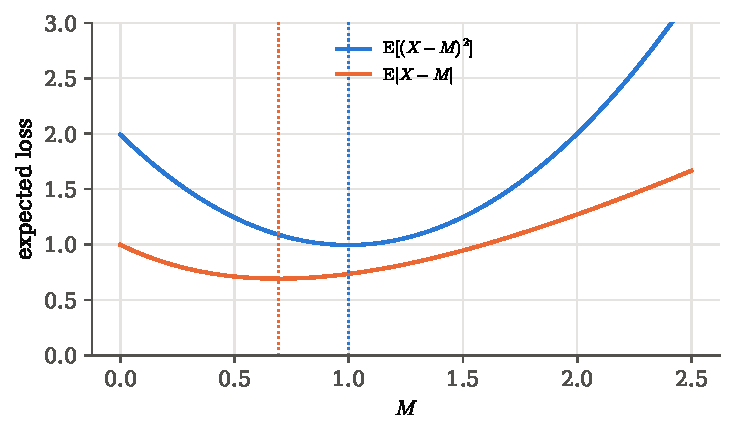
\includegraphics[width=0.72\linewidth]{figures/ch01/mean_minimiser.pdf}
\caption{Expected squared miss and expected absolute miss of a guess $M$ for
exponential lifetimes with mean $1$, computed by averaging over simulated
draws. The squared miss bottoms out at the mean (blue dotted line), the
absolute miss at the median $\ln 2$ (orange dotted line). The height of the
blue minimum is the variance.}
\label{1b:fig:mean-minimiser}
\end{figure}

\subsection{Variance and standard deviation}

The mean says where a distribution sits. We also need how wide it is. The
obvious candidate, the average deviation $\E(X-\mu)$, is useless: it is always
$\E X-\mu=0$, because positive and negative deviations cancel by the definition
of $\mu$ \mainref{p.~50, footnote}. The average absolute deviation
$\E\abs{X-\mu}$ works but is awkward algebraically. The average
\emph{squared} deviation is the standard choice, and
\eqref{1b:eq:mse-split} has already shown why it is natural.

\begin{workdef}[variance, standard deviation]
The \newterm{variance} of $X$ is the mean squared deviation from the mean,
\begin{equation}
  \Var(X)=\sigma^2=\E\bigl[(X-\mu)^2\bigr]
  =\int(x-\mu)^2f(x)\,\dd x ,
  \label{1b:eq:var}
\end{equation}
\unpack{units of $X$ squared}. The \newterm{standard deviation} is
$\sigma=\sqrt{\Var(X)}$ \unpack{same units as $X$, a typical size of
$X-\mu$}.
\emph{Operational test:} the average of $(X_j-\bar X)^2$ over many draws.
\end{workdef}

Three properties do most of the work \mainref{Thm.~3.15, p.~51}.
First, the shortcut formula:
\begin{align}
  \Var(X)
  &\eqby{1} \E\bigl[X^2-2\mu X+\mu^2\bigr]
   \eqby{2} \E(X^2)-2\mu\,\E(X)+\mu^2
   \eqby{3} \E(X^2)-\mu^2 .
  \label{1b:eq:var-short}
\end{align}
\begin{explain}
  \item Expand the square in \eqref{1b:eq:var}.
  \item Linearity; $\mu$ is a constant.
  \item $\E(X)=\mu$, so $-2\mu^2+\mu^2=-\mu^2$.
\end{explain}
Second, shifting does nothing and scaling scales:
$\Var(aX+b)=\E\bigl[(aX+b-a\mu-b)^2\bigr]=a^2\E(X-\mu)^2=a^2\Var(X)$.
Third, $\Var(X)\ge0$, with equality only when $X$ equals a constant with
probability one, since a non-negative quantity $(X-\mu)^2$ can have zero mean
only if it is zero with probability one \mainref{Exercise~3.2, p.~59}.

\paragraph{Example: Bernoulli, die, uniform, exponential.}
For a Bernoulli trial $X^2=X$, so $\E(X^2)=p$ and
$\Var(X)=p-p^2=p(1-p)$, largest for a fair coin and zero when the outcome is
certain. For a fair die
\[
  \Var(X)=\E(X^2)-\mu^2=\tfrac16(1+4+9+16+25+36)-3.5^2
  =\tfrac{91}{6}-\tfrac{49}{4}=\tfrac{35}{12}\approx2.92
\]
\srcref{SeeingTheory}{p.~14}.\footnote{Seeing Theory writes the variance as
``$E[(X-EX)]^2$'' in this exercise and as ``$E(X^2)-E(X)$'' in Proposition~0.0.1(c)
on p.~12; both should read $E[(X-EX)^2]=E(X^2)-(EX)^2$, as in its own proof.}
For $X\sim\mathrm{Uniform}(a,b)$:
\begin{align*}
  \Var(X)
  &\eqby{1} \frac{1}{b-a}\int_a^bx^2\,\dd x-\Bigl(\frac{a+b}{2}\Bigr)^2
   \eqby{2} \frac{a^2+ab+b^2}{3}-\frac{a^2+2ab+b^2}{4}
   \eqby{3} \frac{(b-a)^2}{12} .
\end{align*}
\begin{explain}
  \item Shortcut \eqref{1b:eq:var-short}, with density $1/(b-a)$ and mean
        $(a+b)/2$.
  \item $\int_a^bx^2\dd x=(b^3-a^3)/3=(b-a)(a^2+ab+b^2)/3$.
  \item Common denominator $12$: $4a^2+4ab+4b^2-3a^2-6ab-3b^2=(b-a)^2$.
\end{explain}
A physicist meets this constantly: a silicon strip detector of pitch $w$ that
records only which strip fired localises a track uniformly within the strip,
so its position resolution is $w/\sqrt{12}$. For the exponential,
$\E(X^2)=\beta^2\int_0^\infty u^2e^{-u}\dd u=2\beta^2$ (parts twice), so
$\Var(X)=2\beta^2-\beta^2=\beta^2$: the standard deviation of a lifetime equals
its mean.

For a sum, expand the square. With $\mu_X=\E X$, $\mu_Y=\E Y$:
\begin{align}
  \Var(X+Y)
  &\eqby{1} \E\bigl[(X-\mu_X)+(Y-\mu_Y)\bigr]^2 \nonumber\\
  &\eqby{2} \Var(X)+\Var(Y)+2\,\E\bigl[(X-\mu_X)(Y-\mu_Y)\bigr] \nonumber\\
  &\eqby{3} \Var(X)+\Var(Y)\qquad(X,Y\text{ independent}).
  \label{1b:eq:var-sum}
\end{align}
\begin{explain}
  \item The mean of $X+Y$ is $\mu_X+\mu_Y$ by linearity.
  \item Expand and use linearity.
  \item For independent variables \eqref{1b:eq:product-mean} with $g(X)=X-\mu_X$,
        $h(Y)=Y-\mu_Y$ gives $\E(X-\mu_X)\,\E(Y-\mu_Y)=0\cdot0$.
\end{explain}
The cross term is the covariance, the subject of \cref{1b:sec:covariance}. For
independent variables it vanishes and variances add, so that
$\Var\bigl(\sum_ia_iX_i\bigr)=\sum_ia_i^2\Var(X_i)$ \mainref{(3.8), p.~51}.
Standard deviations do not add; they add \emph{in quadrature}. Every
``add the errors in quadrature'' in a laboratory is this line, valid when the
error sources are independent.

\paragraph{Example: the binomial variance, and the smeared spectrum.}
With $X=\sum_iX_i$ a sum of $n$ independent indicators, each with variance
$p(1-p)$, we get $\Var(X)=np(1-p)$ \mainref{Ex.~3.16, p.~51}. It vanishes for
$p=0$ or $p=1$, where every trial has a certain outcome. For the smeared
energy $E_{\rm meas}=E+\eps$ the detector error does not depend on the true
energy, so $\Var(E_{\rm meas})=\Var(E)+\Var(\eps)=\beta^2+\sigma^2=400+25=425\,
\mathrm{GeV}^2$, as the simulation of \cref{1b:ex:smearing} found
($\OneBSmearVarSim$). The detector resolution adds in quadrature to the
intrinsic width of the spectrum.

\subsection{The sample mean and the sample variance}

In practice we do not know $\mu$ and $\sigma^2$. We have $n$ independent draws
$X_1,\dots,X_n$ from the same distribution (an iid sample, \cref{1b:sec:joint})
and form the \newterm{sample mean} and the \newterm{sample variance}
\mainref{(3.9)--(3.10), p.~51},
\begin{equation}
  \bar X_n=\frac1n\sum_{i=1}^nX_i,\qquad
  S_n^2=\frac1{n-1}\sum_{i=1}^n\bigl(X_i-\bar X_n\bigr)^2 .
  \label{1b:eq:sample-moments}
\end{equation}
They are functions of the data, so they are random variables with their own
distributions. A function of the data is called a \newterm{statistic}, and
its distribution over repeated experiments is its
\newterm{sampling distribution} \mainref{Exercise~3.19, p.~61}. In the chain
from a physical model to inferred physics, this is the step ``construct a
summary $S$, then derive its sampling distribution $P(S\given\theta)$'', in its
simplest form. The rules above already give the first two moments
\mainref{Thm.~3.17, p.~52}:
\begin{align}
  \E(\bar X_n)&\eqby{1}\frac1n\sum_{i=1}^n\E(X_i)=\mu,\nonumber\\
  \Var(\bar X_n)&\eqby{2}\frac1{n^2}\sum_{i=1}^n\Var(X_i)=\frac{\sigma^2}{n}.
  \label{1b:eq:mean-of-mean}
\end{align}
\begin{explain}
  \item Linearity.
  \item The draws are independent, so variances add, and each carries the
        factor $(1/n)^2$ from scaling.
\end{explain}
The spread of the sample mean shrinks like $\sigma/\sqrt n$, the
\newterm{standard error of the mean}: four times the data halves the error
bar. For the sample variance we need $\E\bigl[\sum_i(X_i-\bar X)^2\bigr]$:
\begin{align*}
  \E\Bigl[\sum_{i=1}^n(X_i-\bar X)^2\Bigr]
  &\eqby{1} \E\Bigl[\sum_{i=1}^nX_i^2-n\bar X^2\Bigr]
   \eqby{2} n\,\E(X_1^2)-n\,\E(\bar X^2)\\
  &\eqby{3} n(\sigma^2+\mu^2)-n\Bigl(\frac{\sigma^2}{n}+\mu^2\Bigr)
   = (n-1)\,\sigma^2 .
\end{align*}
\begin{explain}
  \item Expand: $\sum_i(X_i-\bar X)^2=\sum_iX_i^2-2\bar X\sum_iX_i+n\bar X^2$,
        and $\sum_iX_i=n\bar X$.
  \item Linearity; all $X_i$ have the same distribution.
  \item The shortcut \eqref{1b:eq:var-short} read backwards,
        $\E(Z^2)=\Var(Z)+(\E Z)^2$, for $Z=X_1$ and for $Z=\bar X$ using
        \eqref{1b:eq:mean-of-mean}.
\end{explain}
Dividing by $n-1$ therefore gives $\E(S_n^2)=\sigma^2$. Why $n-1$ and not
$n$? The deviations are measured from $\bar X$, which is computed from the
same data. By \eqref{1b:eq:mse-split} applied to the $n$ data points, the
sample mean is the point that makes $\sum_i(X_i-b)^2$ as small as possible.
So deviations from $\bar X$ are systematically smaller than deviations from
the true $\mu$, by exactly one draw's worth of variance. In Python,
\texttt{np.var(x)} divides by $n$ unless one passes \texttt{ddof=1}, while
\texttt{np.cov} divides by $n-1$ by default.

\subsection{Conditional expectation and the law of total variance}

What is the mean of $Y$ among those experiments in which $X=x$? Compute the
mean as before, but with the conditional density $f(y\given x)$ of
\cref{1b:sec:joint} in place of $f_Y(y)$ \mainref{Def.~3.22, p.~54}:\footnote{\mainref{(3.13)--(3.14), p.~54} has a stray ``$dx$'' after the two
discrete sums; there is no integral in the discrete case.}
\begin{equation}
  \E(Y\given X=x)=\int y\,f(y\given x)\,\dd y
  \quad\Bigl(\text{or }\sum_y y\,f(y\given x)\Bigr).
  \label{1b:eq:cond-mean}
\end{equation}
Similarly
$\E\bigl(r(X,Y)\given X=x\bigr)=\int r(x,y)f(y\given x)\,\dd y$.
The result is a number for each $x$, that is, a function of $x$. Before $X$ is
observed we do not know which number it will be, so $\E(Y\given X)$, the
function evaluated at the random $X$, is itself a random variable. This is
the subtle point of the definition \mainref{p.~54, Warning}. $\E(Y)$ is a
number, $\E(Y\given X=x)$ is a function, and $\E(Y\given X)$ is a random
variable. Physically, $\E(Y\given X=x)$ is the curve through the middle of the
scatter plot of $Y$ against $X$, the regression curve. \Cref{1b:fig:zero-corr}
traces it by binning.

\paragraph{Example: a two-stage draw.}
Draw $X\sim\mathrm{Uniform}(0,1)$ and then $Y\given X=x\sim\mathrm{Uniform}(x,1)$
\mainref{Ex.~3.23, p.~54}. The conditional density is $1/(1-x)$ on $(x,1)$, so
\begin{align*}
  \E(Y\given X=x)
  &\eqby{1} \int_x^1\frac{y}{1-x}\,\dd y
   \eqby{2} \frac{1}{1-x}\cdot\frac{1-x^2}{2}
   \eqby{3} \frac{1+x}{2} ,
\end{align*}
\begin{explain}
  \item \eqref{1b:eq:cond-mean} with the uniform conditional density.
  \item $\int_x^1y\,\dd y=(1-x^2)/2$.
  \item $1-x^2=(1-x)(1+x)$.
\end{explain}
the midpoint of $(x,1)$, as it must be. So $\E(Y\given X)=(1+X)/2$, a random
variable.

Averaging the conditional mean over $X$ gives back the unconditional mean.
This is the \newterm{law of iterated expectations} \mainref{Thm.~3.24, p.~55}:
\begin{align}
  \E\bigl[\E(Y\given X)\bigr]
  &\eqby{1} \int\Bigl[\int y\,f(y\given x)\,\dd y\Bigr]f_X(x)\,\dd x
   \eqby{2} \iint y\,f(x,y)\,\dd y\,\dd x
   \eqby{3} \E(Y) .
  \label{1b:eq:iterated}
\end{align}
\begin{explain}
  \item The outer expectation of the function $x\mapsto\E(Y\given X=x)$, by the
        lazy statistician.
  \item Product rule $f(y\given x)f_X(x)=f(x,y)$ \eqref{1b:eq:product-rule}.
  \item Lazy statistician with $r(x,y)=y$.
\end{explain}
It is the law of total probability of \cref{1a:sec:trees} for averages: the
overall mean is the mean in each branch weighted by the probability of the
branch. For the two-stage draw,
$\E(Y)=\E\bigl[(1+X)/2\bigr]=(1+\tfrac12)/2=\tfrac34$ \mainref{Ex.~3.25, p.~55},
with no joint density needed. A useful companion rule: anything already known
given $X$ comes out of the conditional expectation,
$\E\bigl(r(X)s(Y)\given X\bigr)=r(X)\,\E\bigl(s(Y)\given X\bigr)$
\mainref{Exercise~3.16, p.~60}.

The spread splits in the same way. The \newterm{conditional variance} is \mainref{Def.~3.26, p.~55}
\[
  \Var(Y\given X=x)=\int\bigl(y-\mu(x)\bigr)^2f(y\given x)\,\dd y,
  \qquad \mu(x)=\E(Y\given X=x).
\] Then
\srcref{CasellaBerger}{Thm.~4.4.7}
\begin{align}
  \Var(Y)
  &\eqby{1} \E\bigl[(Y-\mu(X))+(\mu(X)-\E Y)\bigr]^2 \nonumber\\
  &\eqby{2} \E\bigl[(Y-\mu(X))^2\bigr]+\E\bigl[(\mu(X)-\E Y)^2\bigr]
            +2\,\E\bigl[(Y-\mu(X))(\mu(X)-\E Y)\bigr] \nonumber\\
  &\eqby{3} \E\bigl[\Var(Y\given X)\bigr]+\Var\bigl[\E(Y\given X)\bigr]+0 .
  \label{1b:eq:total-var}
\end{align}
\begin{explain}
  \item Add and subtract $\mu(X)=\E(Y\given X)$.
  \item Expand the square; linearity.
  \item First term: iterate, $\E[(Y-\mu(X))^2]=\E\bigl[\E\bigl((Y-\mu(X))^2\given X\bigr)\bigr]
        =\E[\Var(Y\given X)]$. Second term: $\mu(X)$ has mean $\E Y$ by
        \eqref{1b:eq:iterated}, so this is its variance. Third term: iterate
        again; given $X$ the factor $\mu(X)-\E Y$ is known and comes out, leaving
        $\E\bigl(Y-\mu(X)\given X\bigr)=\mu(X)-\mu(X)=0$.
\end{explain}
This is the \newterm{law of total variance} \mainref{Thm.~3.27, p.~55}: the
total spread is the average spread within each group plus the spread of the
group means. A detector with a stable resolution but a calibration that
drifts from run to run shows exactly this: within-run scatter plus run-to-run
scatter of the mean response.

\paragraph{Example: counts with a random efficiency.}
A pixel counts how many of $n=20$ photons it detects. Its efficiency $Q$ is
not known and varies from pixel to pixel, uniformly on $(0,1)$ for the sake of
the example; given $Q=q$ the count is $K\given Q=q\sim\mathrm{Binomial}(n,q)$.
(\mainref{Ex.~3.28, p.~56} tells the same story with counties and a disease
rate.) A model built in stages like this is a \newterm{hierarchical model}.
Then $\E(K\given Q)=nQ$ and $\Var(K\given Q)=nQ(1-Q)$, so
\begin{align*}
  \E(K)&\eqby{1}\E(nQ)=\frac n2,\\
  \Var(K)&\eqby{2}\E\bigl[nQ(1-Q)\bigr]+\Var(nQ)
   \eqby{3} n\Bigl(\frac12-\frac13\Bigr)+\frac{n^2}{12}
   =\frac n6+\frac{n^2}{12}.
\end{align*}
\begin{explain}
  \item Iterated expectations \eqref{1b:eq:iterated}; $\E Q=\tfrac12$.
  \item Law of total variance \eqref{1b:eq:total-var}.
  \item $\E(Q)-\E(Q^2)=\tfrac12-\tfrac13$, and $\Var(nQ)=n^2\Var(Q)=n^2/12$
        from the uniform variance with $b-a=1$.
\end{explain}
For $n=20$ this is $36.67$, far larger than the variance $np(1-p)=5$ of a
binomial with the same mean and a fixed efficiency of $\tfrac12$. Most of the
spread is the spread of the efficiencies, the $n^2/12$ term. The whole
experiment takes three lines of Python:

\pyfile[firstline=30,lastline=34,firstnumber=30]{code/ch01/16_expectation_checks.py}{A two-stage (hierarchical) draw}

Line 31 draws one efficiency per pixel. Line 32 draws a binomial count
\emph{with that pixel's efficiency}: numpy broadcasts the array \texttt{Q}, so
each count gets its own $q$. Line 33 is the comparison with a fixed
efficiency. With $10^6$ pixels the simulated mean is $\OneBHierMean$ (exact
$10$), the simulated variance is $\OneBHierVar$ (exact $\OneBHierVarExact$),
and the fixed-efficiency variance is $\OneBPlainVar$ (exact $5$).

\Cref{1b:fig:hierarchical} shows something more striking: the distribution of
$K$ is flat. To see why, marginalise the nuisance efficiency, exactly as in
\cref{1b:sec:joint}:
\begin{align*}
  \Prob(K=k)
  &\eqby{1} \int_0^1\binom nk q^k(1-q)^{n-k}\,\dd q
   \eqby{2} \binom nk\frac{k!\,(n-k)!}{(n+1)!}
   = \frac{1}{n+1} .
\end{align*}
\begin{explain}
  \item Joint = $f(q)\,\Prob(K=k\given q)$ with $f(q)=1$; integrate out $q$.
  \item The beta integral
        $I(a,b)=\int_0^1q^a(1-q)^b\,\dd q=\frac{a!\,b!}{(a+b+1)!}$. Integration by
        parts gives $I(a,b)=\frac{b}{a+1}I(a+1,b-1)$; repeating $b$ times gives
        $I(a,b)=\frac{b!}{(a+1)\cdots(a+b)}\,I(a+b,0)$, and
        $I(a+b,0)=\frac1{a+b+1}$.
\end{explain}
Every count from $0$ to $20$ has probability $1/21$. The ignorance about $Q$
has been passed on to $K$. In \cref{ch:05} the same calculation reappears as the
\emph{prior predictive} distribution of a binomial experiment with a flat
prior on its success probability.

\begin{figure}[htbp]
\centering
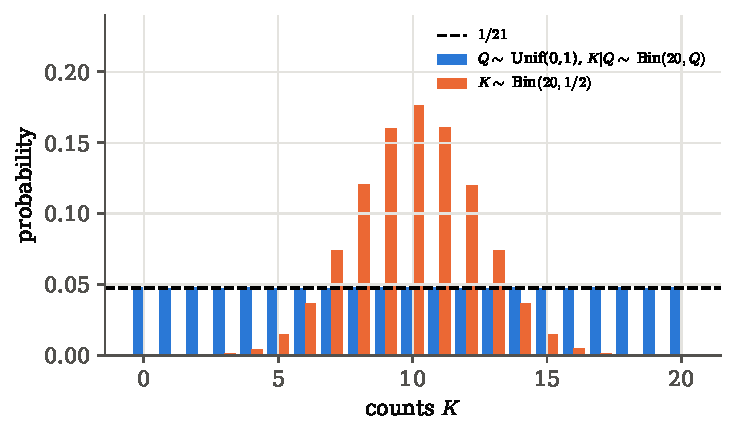
\includegraphics[width=0.72\linewidth]{figures/ch01/hierarchical_counts.pdf}
\caption{Counts out of $20$ photons. Blue: each pixel has its own efficiency,
drawn uniformly; the counts are spread evenly over $0,\dots,20$ at the height
$1/21$ of the dashed line. Orange: every pixel has efficiency $\tfrac12$; the
counts crowd around $10$. Both have mean $10$, but the variances are $36.7$ and
$5$.}
\label{1b:fig:hierarchical}
\end{figure}

The cross term $\E[(X-\mu_X)(Y-\mu_Y)]$ that appeared in the variance of a
sum measures how two variables move together. Together with the averages and
spreads above, it describes the \emph{relation} between two variables at the
level of second moments.
\section{Covariance and correlation: how two variables move together}
\label{1b:sec:covariance}

Two readout channels of a calorimeter sit on the same electronics board. Each
channel records its own signal plus a common pedestal noise that the board
adds to both: $X_1=S_1+N$ and $X_2=S_2+N$, with $S_1$, $S_2$ and $N$
independent. Looked at one at a time, each channel is just a noisy number.
Looked at together, they tend to go up and down together, because whenever
the pedestal $N$ fluctuates high, both readings are pulled up. Nothing about
the individual distributions reveals this. It is a property of the joint
distribution, and the variance of a sum, \eqref{1b:eq:var-sum}, has already
shown us the number that measures it: the cross term
$\E\bigl[(X-\mu_X)(Y-\mu_Y)\bigr]$.

That number is the covariance. Its dimensionless version is the correlation
coefficient. Both detect linear co-movement and miss everything else. For
many variables the second moments collect into a covariance matrix, and a
linear change of variables moves it by the rule $\Cmat'=A\Cmat A\T$. Every
error bar on a derived quantity, every Fisher forecast of \cref{ch:10} and
every $\chi^2$ of correlated band powers in \cref{ch:07,ch:08} is built from
this matrix. Three questions organise the topic.
\begin{enumerate}[leftmargin=1.6em,itemsep=1pt]
  \item How do we measure whether ``$X$ above its mean'' goes with ``$Y$ above
        its mean''?
  \item What does a zero value of that measure tell us, and what does it not?
  \item For a vector of variables, how do the second moments change when we
        form linear combinations, and can we always find combinations that are
        uncorrelated?
\end{enumerate}

\subsection{Covariance and the correlation coefficient}

\begin{workdef}[covariance, correlation coefficient]
For $X,Y$ with means $\mu_X,\mu_Y$ and standard deviations $\sigma_X,\sigma_Y$,
the \newterm{covariance} and the \newterm{correlation coefficient} are
\begin{equation}
  \Cov(X,Y)=\E\bigl[(X-\mu_X)(Y-\mu_Y)\bigr],\qquad
  \rho_{XY}=\frac{\Cov(X,Y)}{\sigma_X\,\sigma_Y} .
  \label{1b:eq:cov}
\end{equation}
$\Cov$ has the units of $X$ times those of $Y$ \unpack{positive if the two
tend to be on the same side of their means}. $\rho$ is a pure number between
$-1$ and $1$.
\emph{Operational test:} the average of $(x_j-\bar x)(y_j-\bar y)$ over many
simulated pairs, \texttt{np.cov} and \texttt{np.corrcoef} in Python.
\end{workdef}

The definition is read off a scatter plot \srcref{Cowan}{pp.~18--19}. Put the
origin at $(\mu_X,\mu_Y)$ (\cref{1b:fig:quadrants}). A point in the upper-right
or lower-left quadrant has deviations of the same sign, so its product
$(x-\mu_X)(y-\mu_Y)$ is positive. A point in the other two quadrants
contributes a negative product. The covariance is the probability-weighted
balance of the two. A cloud tilted up to the right puts more mass in the
positive quadrants and has $\Cov>0$. A cloud tilted down has $\Cov<0$. A cloud
with as much mass in the negative quadrants as in the positive ones has
$\Cov=0$, whatever its shape.

\begin{figure}[htbp]
\centering
\begin{tikzpicture}[scale=0.9]
  \fill[formblue!10] (0,0) rectangle (3,2.2);
  \fill[formblue!10] (0,0) rectangle (-3,-2.2);
  \fill[bdryred!8] (0,0) rectangle (-3,2.2);
  \fill[bdryred!8] (0,0) rectangle (3,-2.2);
  \draw[->] (-3.2,0) -- (3.3,0) node[right,lbl] {$x$};
  \draw[->] (0,-2.4) -- (0,2.5) node[above,lbl] {$y$};
  \draw[thick,formblue,rotate=30] (0,0) ellipse (2.6 and 0.9);
  \draw[formblue,rotate=30] (0,0) ellipse (1.3 and 0.45);
  \node[lbl,formblue!70!black] at (2.2,1.75) {$+$};
  \node[lbl,formblue!70!black] at (-2.2,-1.75) {$+$};
  \node[lbl,bdryred] at (-2.2,1.75) {$-$};
  \node[lbl,bdryred] at (2.2,-1.75) {$-$};
  \fill (0,0) circle (1.2pt);
  \node[lbl,anchor=north west] at (0.35,-0.75) {$(\mu_X,\mu_Y)$};
  \node[lbl,align=left,anchor=west] at (3.5,1.0)
     {$(x-\mu_X)(y-\mu_Y)>0$\\ in the blue quadrants};
  \node[lbl,align=left,anchor=west] at (3.5,-1.0)
     {$(x-\mu_X)(y-\mu_Y)<0$\\ in the red quadrants};
\end{tikzpicture}
\caption{Reading the sign of a covariance. The ellipses are contours of a
density tilted up to the right. Most of its probability sits in the blue
quadrants, where the two deviations have the same sign, so the average of
their product, the covariance, is positive.}
\label{1b:fig:quadrants}
\end{figure}

Expanding the product gives the form used in computation
\mainref{Thm.~3.19, p.~52}:
\begin{align}
  \Cov(X,Y)
  &\eqby{1} \E\bigl[XY-\mu_YX-\mu_XY+\mu_X\mu_Y\bigr]\nonumber\\
  &\eqby{2} \E(XY)-\mu_Y\mu_X-\mu_X\mu_Y+\mu_X\mu_Y
   = \E(XY)-\E(X)\,\E(Y) .
  \label{1b:eq:cov-short}
\end{align}
\begin{explain}
  \item Multiply out $(X-\mu_X)(Y-\mu_Y)$.
  \item Linearity; $\mu_X,\mu_Y$ are constants.
\end{explain}
With $Y=X$ this is the variance shortcut \eqref{1b:eq:var-short}:
$\Cov(X,X)=\Var(X)$. Constants shifted onto either variable drop out, and the
covariance is linear in each argument separately:
\begin{equation}
  \Cov\Bigl(\sum_{i}a_iX_i,\ \sum_{j}b_jY_j\Bigr)=\sum_{i}\sum_{j}a_ib_j\,\Cov(X_i,Y_j)
  \label{1b:eq:bilinear}
\end{equation}
\mainref{Exercise~3.14, p.~60}. To see it, note that the deviation of
$\sum_ia_iX_i$ from its mean is $\sum_ia_i(X_i-\mu_{X_i})$, do the same for
the $Y$'s, multiply the two sums term by term and take the expectation of
each term. Setting both sums equal gives the variance of any linear
combination \mainref{Thm.~3.20, p.~52},
\begin{equation}
  \Var\Bigl(\sum_ia_iX_i\Bigr)=\sum_ia_i^2\Var(X_i)+2\sum_{i<j}a_ia_j\Cov(X_i,X_j),
  \label{1b:eq:var-comb}
\end{equation}
and in particular $\Var(X\pm Y)=\Var(X)+\Var(Y)\pm2\Cov(X,Y)$.

\paragraph{Example: the shared pedestal.}
Return to the two calorimeter channels of the opening, $X_1=S_1+N$ and
$X_2=S_2+N$, which share the pedestal noise $N$. Take $\Var(S_1)=\Var(S_2)=\sigma_S^2$ and
$\Var(N)=\sigma_N^2$. By \eqref{1b:eq:bilinear},
\begin{align*}
  \Cov(X_1,X_2)
  &\eqby{1} \Cov(S_1,S_2)+\Cov(S_1,N)+\Cov(N,S_2)+\Cov(N,N)
   \eqby{2} \sigma_N^2 ,
\end{align*}
\begin{explain}
  \item Bilinearity with $X_1=S_1+N$, $X_2=S_2+N$.
  \item Independent variables have zero covariance (shown below); $\Cov(N,N)=\Var(N)$.
\end{explain}
so $\rho=\sigma_N^2/(\sigma_S^2+\sigma_N^2)$, which is $\tfrac12$ when the
signal and the pedestal fluctuate equally. Now form the difference. By
\eqref{1b:eq:var-comb},
$\Var(X_1-X_2)=2(\sigma_S^2+\sigma_N^2)-2\sigma_N^2=2\sigma_S^2$: the common
noise has cancelled completely. The sum has $\Var(X_1+X_2)=2\sigma_S^2+4\sigma_N^2$:
it is doubled. This is common-mode rejection, and it is why differential
measurements are powerful. A gravitational-wave interferometer reads the
\emph{difference} of its two arm lengths, so the laser noise common to both
arms cancels to first order.

\subsection{Why \texorpdfstring{$\abs\rho\le1$}{|rho| <= 1}, and what \texorpdfstring{$\rho=\pm1$}{rho = +-1} means}

The correlation coefficient removes the units by dividing by both standard
deviations. That it then lies in $[-1,1]$ follows from one observation
\srcref{CasellaBerger}{Thm.~4.5.7}: the mean of a square is never negative.
For every real $t$ let
\begin{align*}
  h(t)
  &\eqby{1} \E\Bigl[\bigl(t(X-\mu_X)+(Y-\mu_Y)\bigr)^2\Bigr]
   \eqby{2} t^2\sigma_X^2+2t\,\Cov(X,Y)+\sigma_Y^2
   \relby{3}{\ge} 0 .
\end{align*}
\begin{explain}
  \item Definition of $h$, the mean square of a combination of the two
        deviations.
  \item Expand the square and use linearity.
  \item The expectation of a non-negative quantity is non-negative.
\end{explain}
A quadratic in $t$ that is never negative has at most one real root, so its
discriminant is not positive: $4\Cov(X,Y)^2-4\sigma_X^2\sigma_Y^2\le0$, that
is, $\abs{\Cov(X,Y)}\le\sigma_X\sigma_Y$, or $-1\le\rho\le1$. Equality,
$\abs\rho=1$, means the discriminant is zero, so $h(t_0)=0$ for one $t_0$,
namely $t_0=-\Cov(X,Y)/\sigma_X^2$. A non-negative variable with zero mean is
zero with probability one, so $Y-\mu_Y=-t_0(X-\mu_X)$: the points lie exactly
on a straight line with slope $a=-t_0=\Cov/\sigma_X^2$, which has the sign of
$\rho$. Conversely if $Y=aX+b$ then $\Cov(X,Y)=a\sigma_X^2$ and
$\sigma_Y=\abs a\sigma_X$, so $\rho=a/\abs a=\pm1$ \mainref{Thm.~3.19, p.~52}.

In the language of vectors this is the Cauchy--Schwarz inequality. Centred
random variables form a vector space with the inner product
$\langle U,V\rangle=\E(UV)$, the length of $U$ is its standard deviation,
and $\rho$ is the cosine of the angle between $X-\mu_X$ and $Y-\mu_Y$. It is
$\pm1$ when the two ``vectors'' are parallel, $0$ when they are orthogonal. A
quantum physicist will recognise the normalised overlap
$\abs{\langle\psi\vert\phi\rangle}/(\norm\psi\norm\phi)\le1$. Because it is a
cosine, $\rho$ is unchanged by shifting or by rescaling either variable with
a positive factor: it does not care whether energies are in GeV or TeV.

\Cref{1b:fig:correlation-gallery} calibrates the eye. With 1500 points from
bivariate Gaussians of unit variances and $\rho=-0.8,\,0,\,0.5,\,0.95$, the
sample correlations are $\OneBGalRa$, $\OneBGalRb$, $\OneBGalRc$ and
$\OneBGalRd$. A correlation of $0.5$ is a visibly tilted but still fat cloud;
it takes $\rho$ close to $1$ to make a thin line.

\begin{figure}[htbp]
\centering
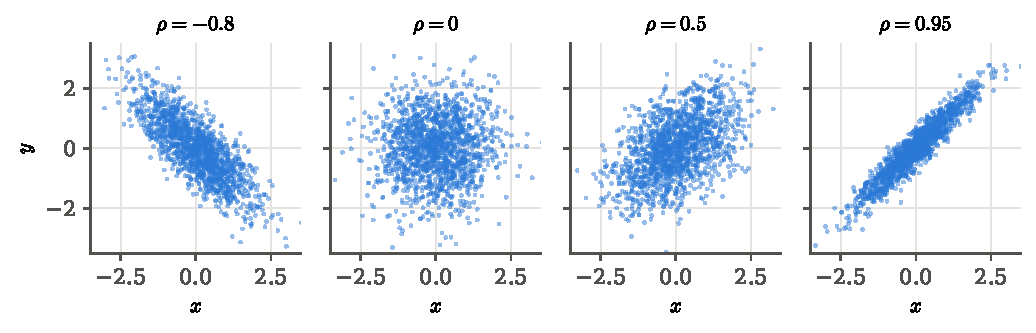
\includegraphics[width=\linewidth]{figures/ch01/correlation_gallery.pdf}
\caption{Clouds of 1500 draws from bivariate Gaussians with unit variances and
four values of the correlation coefficient. The sign of $\rho$ gives the
direction of the tilt; its size says how tightly the points hug a straight
line.}
\label{1b:fig:correlation-gallery}
\end{figure}

\subsection{Zero correlation is not independence}

If $X$ and $Y$ are independent, $\E(XY)=\E(X)\E(Y)$ by
\eqref{1b:eq:product-mean}, and \eqref{1b:eq:cov-short} gives $\Cov(X,Y)=0$.
The converse is false \mainref{Thm.~3.19, p.~52}. The standard
counterexample shows why. Let $X\sim\Normal(0,1)$ and
$Y=X^2$. Then $Y$ is completely determined by $X$, the strongest dependence
there is. Yet
\begin{align*}
  \Cov(X,Y)
  &\eqby{1} \E(X\cdot X^2)-\E(X)\,\E(X^2)
   \eqby{2} \E(X^3)-0\cdot1
   \eqby{3} 0 .
\end{align*}
\begin{explain}
  \item Shortcut \eqref{1b:eq:cov-short} with $Y=X^2$.
  \item $\E(X)=0$ and $\E(X^2)=\Var(X)=1$.
  \item $\E(X^3)=\int x^3\varphi(x)\,\dd x=0$: the integrand is odd because
        the Gaussian density $\varphi$ is even.
\end{explain}
The covariance vanishes because the relation is symmetric: for every point
$(x,x^2)$ on the right branch of the parabola there is an equally likely
point $(-x,x^2)$ on the left, and their products of deviations cancel
\srcref{Cowan}{Fig.~1.10}. The correlation coefficient measures how well a
\emph{straight line} fits, and the best straight line through a symmetric
parabola is flat.

\begin{figure}[htbp]
\centering
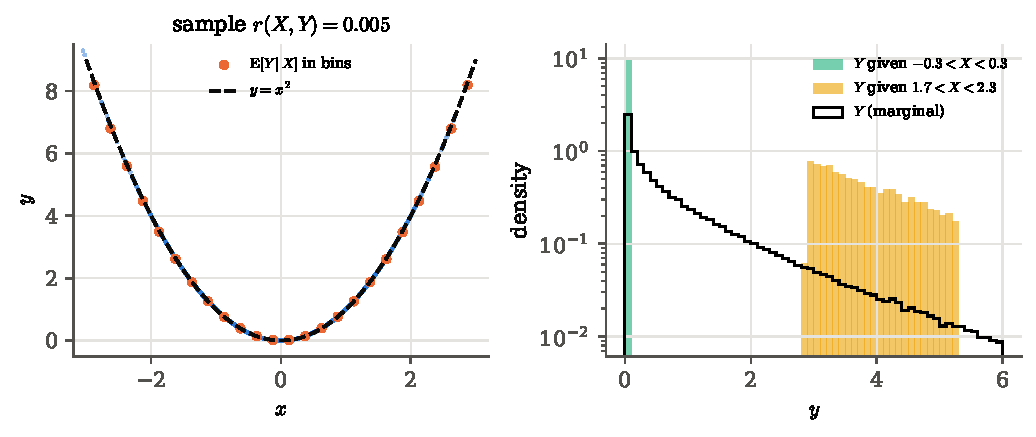
\includegraphics[width=\linewidth]{figures/ch01/zero_correlation.pdf}
\caption{Left: draws of $(X,X^2)$ with $X$ Gaussian. The points lie exactly on
the parabola, the binned conditional mean $\E(Y\given X)$ (orange) follows it,
and yet the sample correlation is essentially zero. Right: the distribution of
$Y$ for $X$ near $0$ and for $X$ near $2$ (logarithmic density axis). The two
conditional distributions do not even overlap, so knowing $X$ changes
everything we know about $Y$, which is the opposite of independence.}
\label{1b:fig:zero-corr}
\end{figure}

\Cref{1b:fig:zero-corr} shows it numerically. With $\OneBZeroN$ draws the
sample correlation of $X$ and $Y$ is $\OneBZeroRxy$. The dependence is all
there: the correlation of $Y$ with $\abs X$ (a monotone function of $X$ on
each branch) is $\OneBZeroRabsxy$, and the conditional distributions of $Y$
in two slices of $X$ are completely different. \srcref{CasellaBerger}{Ex.~4.5.9}
gives a version with noise, $Y=X^2+Z$, with the same conclusion. Operationally:
before concluding that two quantities are unrelated because their correlation
is small, plot them.

There is a ladder of conditions between independence and zero correlation. If
the conditional mean of $X$ does not depend on $Y$, $\E(X\given Y=y)=c$ for all
$y$, then $X$ and $Y$ are uncorrelated \mainref{Exercise~3.18, p.~61}:
\begin{align*}
  \E(XY)
  &\eqby{1} \E\bigl[\E(XY\given Y)\bigr]
   \eqby{2} \E\bigl[Y\,\E(X\given Y)\bigr]
   \eqby{3} c\,\E(Y)
   \eqby{4} \E(X)\,\E(Y) .
\end{align*}
\begin{explain}
  \item Iterated expectations \eqref{1b:eq:iterated}.
  \item Given $Y$, the factor $Y$ is known and comes out.
  \item $\E(X\given Y)=c$.
  \item $\E(X)=\E[\E(X\given Y)]=c$.
\end{explain}
The same two steps show that if $\E(Y\given X)=X$ then $\E(XY)=\E(X^2)$ and
$\E(Y)=\E(X)$, so $\Cov(X,Y)=\Var(X)$ \mainref{Exercise~3.21, p.~61}. So
independence implies a constant conditional mean, which implies zero
correlation, and neither implication reverses (in the parabola example
$\E(Y\given X)=X^2$ is far from constant).

For one family the ladder collapses. If $(X,Y)$ is bivariate Gaussian
\eqref{1b:eq:bvn} with $\rho=0$, the cross term $-2\rho xy/(\sigma_x\sigma_y)$
in the exponent vanishes, the exponent splits into an $x$ part plus a $y$
part, and the density factorises into $f_X(x)f_Y(y)$. For jointly Gaussian
variables, uncorrelated means independent. This is why the sum and the
difference of two equally noisy Gaussian channels in \cref{1b:ex:sum-diff}
came out independent. They are jointly Gaussian, and the sum-and-difference
example of the next subsection shows that they are uncorrelated.

\begin{pitfall}[Gaussian marginals do not make a Gaussian pair]
The shortcut ``uncorrelated $\Rightarrow$ independent'' needs the variables to
be \emph{jointly} Gaussian, not just each Gaussian. Let $X\sim\Normal(0,1)$ and
let $S=\pm1$ be an independent fair sign. Then $Y=SX$ is also $\Normal(0,1)$
(flipping the sign of a symmetric variable changes nothing), and
$\Cov(X,Y)=\E(S)\E(X^2)=0$. But $\abs Y=\abs X$ always, so the two are
strongly dependent. The pair lives on the two diagonals $y=\pm x$, which no
bivariate Gaussian does.
\end{pitfall}

\subsection{The covariance matrix and how linear maps move it}

With many variables we collect them into a column vector
$\bm X=(X_1,\dots,X_k)\T$ with mean vector $\bm\mu=(\E X_1,\dots,\E X_k)\T$. All
the variances and covariances go into one matrix, the
\newterm{covariance matrix} (``variance--covariance matrix'' in
\mainref{p.~53}, ``error matrix'' in \srcref{Cowan}{p.~18}):
\begin{equation}
  \Cmat_{ij}=\Cov(X_i,X_j),\qquad
  \Cmat=\E\bigl[(\bm X-\bm\mu)(\bm X-\bm\mu)\T\bigr]
  =\begin{pmatrix}
     \Var(X_1) & \Cov(X_1,X_2) & \cdots\\
     \Cov(X_2,X_1) & \Var(X_2) & \cdots\\
     \vdots & & \ddots
   \end{pmatrix}.
  \label{1b:eq:covmat}
\end{equation}
The outer product $(\bm X-\bm\mu)(\bm X-\bm\mu)\T$ is a $k\times k$ matrix whose
$(i,j)$ entry is $(X_i-\mu_i)(X_j-\mu_j)$, and the expectation is taken entry
by entry. The matrix is symmetric, its diagonal holds the variances, and it
is positive semi-definite: for any fixed vector $\bm a$,
\begin{align*}
  \bm a\T\Cmat\,\bm a
  &\eqby{1} \sum_{i,j}a_ia_j\Cov(X_i,X_j)
   \eqby{2} \Var\bigl(\bm a\T\bm X\bigr)
   \relby{3}{\ge} 0 .
\end{align*}
\begin{explain}
  \item Write out the quadratic form.
  \item Bilinearity \eqref{1b:eq:bilinear} with $b_j=a_j$ and $Y_j=X_j$.
  \item A variance is never negative.
\end{explain}
So all eigenvalues of $\Cmat$ are $\ge0$. A zero eigenvalue means some
combination $\bm a\T\bm X$ has zero variance, i.e.\ is a constant: the
variables obey an exact linear constraint (as the multinomial counts below do).
Dividing entry $(i,j)$ by $\sigma_i\sigma_j$ gives the correlation matrix, with
ones on the diagonal.

Now let $\bm Y=A\bm X+\bm b$ for a fixed $m\times k$ matrix $A$ and vector $\bm b$.
Linearity gives $\E\bm Y=A\bm\mu+\bm b$, and \mainref{Lemma~3.21, p.~54}
\begin{align}
  \Cmat_{\bm Y}
  &\eqby{1} \E\bigl[(A\bm X-A\bm\mu)(A\bm X-A\bm\mu)\T\bigr]
   \eqby{2} \E\bigl[A(\bm X-\bm\mu)(\bm X-\bm\mu)\T A\T\bigr]
   \eqby{3} A\,\Cmat\,A\T .
  \label{1b:eq:ACAT}
\end{align}
\begin{explain}
  \item Definition \eqref{1b:eq:covmat} for $\bm Y$; the shift $\bm b$ cancels
        in $\bm Y-\E\bm Y$.
  \item $(A\bm v)\T=\bm v\T A\T$.
  \item $A$ is constant and comes out of the entry-by-entry expectation on both
        sides (linearity).
\end{explain}
In components, $(\Cmat_{\bm Y})_{ij}=\sum_{k,l}A_{ik}A_{jl}\Cov(X_k,X_l)$
\srcref{Cowan}{(1.62)}, which is just \eqref{1b:eq:bilinear}. For a single
combination, $A=\bm a\T$ is one row and $\Var(\bm a\T\bm X)=\bm a\T\Cmat\bm a$,
the quadratic form above. The covariance matrix transforms like a rank-2
tensor, $C'_{ij}=A_{ik}A_{jl}C_{kl}$; the inertia tensor and the stress tensor
transform the same way.

\begin{keyidea}[Linear maps move covariance by sandwiching]
If $\bm Y=A\bm X+\bm b$ then $\E\bm Y=A\,\E\bm X+\bm b$ and
$\Cmat_{\bm Y}=A\,\Cmat_{\bm X}A\T$, exactly, for any distribution.
\end{keyidea}

\paragraph{Example: sum and difference of two channels.}
Take $\Cmat=\begin{psmallmatrix}\sigma_1^2 & c\\ c & \sigma_2^2\end{psmallmatrix}$
and $A=\begin{psmallmatrix}1&1\\1&-1\end{psmallmatrix}$, so
$Y_1=X_1+X_2$ and $Y_2=X_1-X_2$. Then
\begin{align*}
  A\,\Cmat\,A\T
  &\eqby{1} \begin{pmatrix}\sigma_1^2+c & c+\sigma_2^2\\ \sigma_1^2-c & c-\sigma_2^2\end{pmatrix}
            \begin{pmatrix}1&1\\1&-1\end{pmatrix}
   \eqby{2} \begin{pmatrix}\sigma_1^2+\sigma_2^2+2c & \sigma_1^2-\sigma_2^2\\
                           \sigma_1^2-\sigma_2^2 & \sigma_1^2+\sigma_2^2-2c\end{pmatrix}.
\end{align*}
\begin{explain}
  \item First product $A\Cmat$, row by column; $A\T=A$ here.
  \item Second product; e.g.\ the $(1,2)$ entry is
        $(\sigma_1^2+c)-(c+\sigma_2^2)$.
\end{explain}
The diagonal reproduces $\Var(X_1\pm X_2)=\sigma_1^2+\sigma_2^2\pm2c$. The new
off-diagonal entry, $\Cov(X_1+X_2,X_1-X_2)=\sigma_1^2-\sigma_2^2$, is zero
whenever the two channels are equally noisy, whatever their correlation $c$.
With $\Cmat=\sigma^2\Id$ we get $A\Cmat A\T=2\sigma^2\Id$, and since the pair is
jointly Gaussian that is the independence of \cref{1b:ex:sum-diff}. For
the numerical case $\sigma_1^2=4$, $\sigma_2^2=1$, $c=1.8$ the prediction is
$\begin{psmallmatrix}8.6&3\\3&1.4\end{psmallmatrix}$, and the sample covariance
of $\OneBCovN$ simulated pairs is
$\begin{psmallmatrix}\OneBCYaa&\OneBCYab\\\OneBCYab&\OneBCYbb\end{psmallmatrix}$.

\paragraph{Example: the multinomial covariance.}
Throw $n$ events into $k$ histogram bins with probabilities $p_1,\dots,p_k$
(\cref{1b:sec:joint}), and let $X_i$ be the count in bin $i$. Each $X_i$ is
binomial, $\Var(X_i)=np_i(1-p_i)$. To get the covariance of two bins, merge
them: $X_i+X_j$ counts the events that fell in either, so it is
$\mathrm{Binomial}(n,p_i+p_j)$ \mainref{p.~54}. Then
\begin{align*}
  2\Cov(X_i,X_j)
  &\eqby{1} \Var(X_i+X_j)-\Var(X_i)-\Var(X_j)\\
  &\eqby{2} n(p_i+p_j)(1-p_i-p_j)-np_i(1-p_i)-np_j(1-p_j)
   \eqby{3} -2np_ip_j ,
\end{align*}
\begin{explain}
  \item \eqref{1b:eq:var-comb} for $X_i+X_j$, solved for the covariance.
  \item Binomial variances of the merged bin and of each bin.
  \item Expand: the linear terms cancel, and
        $-(p_i+p_j)^2+p_i^2+p_j^2=-2p_ip_j$.
\end{explain}
so $\Cov(X_i,X_j)=-np_ip_j$ for $i\neq j$. Histogram bins with a fixed total
are anticorrelated: an extra event in one bin is an event missing from the
others. The covariance matrix has a zero eigenvalue along $\bm a=(1,\dots,1)$,
because $\sum_iX_i=n$ is exactly constant. (If the total itself is a Poisson
count, as for a collider run of fixed luminosity, the bins become
independent Poisson variables; see \cref{ch:02}.)

\subsection{Diagonalising: the principal axes of the error ellipse}

Correlated variables are awkward: we cannot read off the uncertainty of one
without the other. Can a linear change of variables always make them
uncorrelated? Yes, and it is a rotation \srcref{Cowan}{\S1.7}. Because $\Cmat$
is real and symmetric, it has $k$ orthonormal eigenvectors $\bm r_1,\dots,\bm r_k$,
$\Cmat\bm r_j=\lambda_j\bm r_j$, with $\lambda_j\ge0$ by positive
semi-definiteness. Put them as the columns of an orthogonal matrix $R$ and
take $\bm W=R\T\bm X$, so $W_i=\bm r_i\T\bm X$ is the component of $\bm X$ along
$\bm r_i$. By \eqref{1b:eq:ACAT} with $A=R\T$,
\begin{align*}
  (\Cmat_{\bm W})_{ij}
  &\eqby{1} \bigl(R\T\Cmat R\bigr)_{ij}
   \eqby{2} \bm r_i\T\Cmat\,\bm r_j
   \eqby{3} \lambda_j\,\bm r_i\T\bm r_j
   \eqby{4} \lambda_j\,\delta_{ij} .
\end{align*}
\begin{explain}
  \item The sandwich rule with $A=R\T$.
  \item Row $i$ of $R\T$ is $\bm r_i\T$ and column $j$ of $R$ is $\bm r_j$.
  \item Eigenvalue equation.
  \item Orthonormality of the eigenvectors.
\end{explain}
The new variables are uncorrelated and their variances are the eigenvalues
\srcref{Cowan}{(1.65)}. Geometrically, the contours of a Gaussian density with
covariance $\Cmat$ are ellipses (ellipsoids) whose axes point along the
eigenvectors, with semi-axes $\sqrt{\lambda_j}$ at ``$1\sigma$''. The rotation
simply turns the coordinate axes onto the principal axes of this
\newterm{error ellipse}, exactly like rotating onto the principal axes of an
inertia tensor or onto the normal modes of coupled oscillators.

In two dimensions everything is explicit. Write
$\Cmat=\begin{psmallmatrix}\sigma_1^2&c\\c&\sigma_2^2\end{psmallmatrix}$ with
$c=\rho\sigma_1\sigma_2$. The eigenvalues solve
$\det(\Cmat-\lambda\Id)=\lambda^2-(\sigma_1^2+\sigma_2^2)\lambda+\sigma_1^2\sigma_2^2-c^2=0$,
so
\begin{equation}
  \lambda_\pm=\tfrac12\Bigl[\sigma_1^2+\sigma_2^2
     \pm\sqrt{(\sigma_1^2+\sigma_2^2)^2-4(1-\rho^2)\sigma_1^2\sigma_2^2}\Bigr]
  \label{1b:eq:eig2}
\end{equation}
\srcref{Cowan}{(1.69)}. For the rotation angle, rotate by $\theta$,
$W_1=\cos\theta\,X_1+\sin\theta\,X_2$ and $W_2=-\sin\theta\,X_1+\cos\theta\,X_2$,
and demand zero covariance:
\begin{align*}
  \Cov(W_1,W_2)
  &\eqby{1} -\sin\theta\cos\theta\,\sigma_1^2+(\cos^2\theta-\sin^2\theta)\,c
            +\sin\theta\cos\theta\,\sigma_2^2\\
  &\eqby{2} \tfrac12\sin2\theta\,(\sigma_2^2-\sigma_1^2)+c\cos2\theta ,
\end{align*}
\begin{explain}
  \item Bilinearity \eqref{1b:eq:bilinear}.
  \item Double-angle formulas.
\end{explain}
which vanishes for $\tan2\theta=2c/(\sigma_1^2-\sigma_2^2)$
\srcref{Cowan}{(1.71)}. For $\sigma_1^2=4$, $\sigma_2^2=1$, $c=1.8$ (so
$\rho=0.9$): $\tan2\theta=1.2$, $\theta=25.1^\circ$, and
\eqref{1b:eq:eig2} gives $\lambda=(5\pm\sqrt{21.96})/2=\OneBLamB$ and
$\OneBLamA$. The simulated rotated variables have variances $\OneBCWbb$ and
$\OneBCWaa$ and covariance $\OneBCWab$ (\cref{1b:fig:cov-transform}, right).
The long axis carries almost all the variance: nearly all the scatter of the
two channels is in one combination.

The same algebra run backwards generates correlated variables. If $\bm Z$ has
independent standard normal components, $\Cmat_{\bm Z}=\Id$, and
$\bm X=L\bm Z$ has covariance $L\Id L\T=LL\T$. So any factorisation
$\Cmat=LL\T$ gives a recipe. The standard one is the Cholesky factor, a lower
triangular $L$; for $2\times2$,
$L=\begin{psmallmatrix}\sigma_1&0\\\rho\sigma_2&\sigma_2\sqrt{1-\rho^2}\end{psmallmatrix}$,
which one checks by multiplying out. Here $L=\begin{psmallmatrix}\OneBLaa&0\\
\OneBLba&\OneBLbb\end{psmallmatrix}$, and the script uses exactly this:

\pyfile[firstline=21,lastline=35,firstnumber=21]{code/ch01/18_covariance_transform.py}{Correlated Gaussians, the sandwich rule and the eigenbasis}

Lines 22--25 build $L$ and generate $\bm X=L\bm Z$ for $\OneBCovN$ pairs; their
sample covariance (line 26) is
$\begin{psmallmatrix}\OneBChataa&\OneBChatab\\\OneBChatab&\OneBChatbb\end{psmallmatrix}$,
the target $\Cmat$. Lines 28--31 apply the sum-and-difference matrix and
compare $A\Cmat A\T$ with the sample covariance of $\bm Y$. Lines 33--35
diagonalise: \texttt{np.linalg.eigh} returns the eigenvalues in ascending order
and the unit eigenvectors as the columns of \texttt{R}, and $\bm W=R\T\bm X$
is uncorrelated.

\begin{figure}[htbp]
\centering
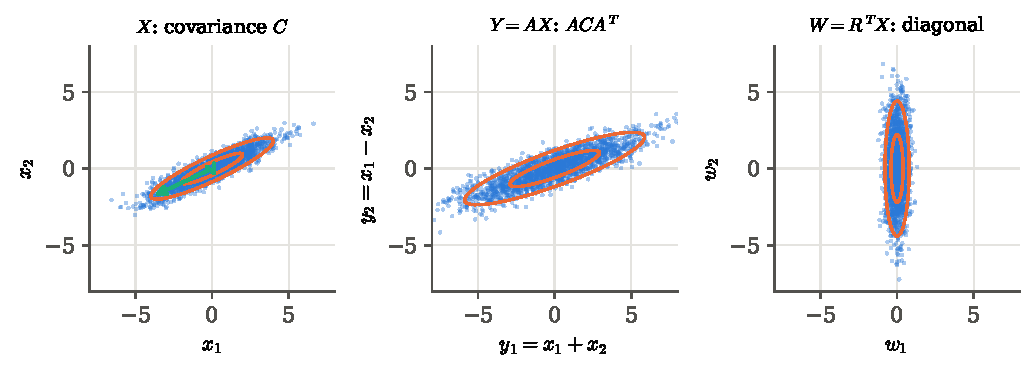
\includegraphics[width=\linewidth]{figures/ch01/covariance_transform.pdf}
\caption{One cloud of correlated pairs seen in three coordinate systems, with
the predicted $1\sigma$ and $2\sigma$ ellipses. Left: the original channels,
with the two eigenvectors of $\Cmat$ drawn as green arrows. Middle: sum and
difference; the ellipse is the one predicted by $A\Cmat A\T$. Right: components
along the eigenvectors; the ellipse is aligned with the axes, so the new
variables are uncorrelated.}
\label{1b:fig:cov-transform}
\end{figure}

\subsection{A first look at error propagation}

Most derived quantities are not linear in the measured ones: a mass from two
momenta, a ratio of two rates, a distance from a flux. If the input
uncertainties are small, we can linearise \srcref{Cowan}{\S1.6}. Expand
$y(\bm x)$ to first order about the means,
$y(\bm x)\approx y(\bm\mu)+\sum_iA_i(x_i-\mu_i)$ with
$A_i=\partial y/\partial x_i$ at $\bm\mu$. The constant does not affect the
spread, and the rest is linear, so the sandwich rule applies to the Jacobian
matrix $A_{ki}=\partial y_k/\partial x_i$:
\begin{equation}
  \E\,y_k\approx y_k(\bm\mu),\qquad
  \Cov(y_k,y_l)\approx\sum_{i,j}\frac{\partial y_k}{\partial x_i}
     \frac{\partial y_l}{\partial x_j}\,\Cmat_{ij},\qquad
  \Cmat_{\bm y}\approx A\,\Cmat\,A\T
  \label{1b:eq:error-prop}
\end{equation}
\srcref{Cowan}{(1.53)--(1.55)}. For a linear map this is exact
\eqref{1b:eq:ACAT}; otherwise it is the first term of an expansion.

\paragraph{Example: products add relative errors in quadrature.}
For $y=x_1x_2$ the Jacobian is $A=(\mu_2,\ \mu_1)$, so
\begin{align*}
  \sigma_y^2
  &\eqby{1} \mu_2^2\sigma_1^2+\mu_1^2\sigma_2^2+2\mu_1\mu_2\,\Cmat_{12},
  &
  \frac{\sigma_y^2}{y^2}
  &\eqby{2} \frac{\sigma_1^2}{\mu_1^2}+\frac{\sigma_2^2}{\mu_2^2}
            +2\frac{\Cmat_{12}}{\mu_1\mu_2} .
\end{align*}
\begin{explain}
  \item \eqref{1b:eq:error-prop} with $\partial y/\partial x_1=x_2$,
        $\partial y/\partial x_2=x_1$ at the means.
  \item Divide by $y^2\approx\mu_1^2\mu_2^2$.
\end{explain}
For uncorrelated inputs, absolute errors add in quadrature for a sum and
relative errors add in quadrature for a product \srcref{Cowan}{(1.59)--(1.60)}.
The approximation fails when $y$ curves appreciably over a range of one
standard deviation; the classic case is $1/x$ with $\sigma_x$ not small
compared with $\mu_x$. Then one simulates (\cref{ch:06}). Error propagation,
and its limits, is developed properly in \cref{ch:03}.

\paragraph{How research uses it.} In a real analysis the covariance matrix is rarely computed on paper. The
band powers of a CMB or galaxy power spectrum measured on a masked, noisy sky
(\cref{ch:07,ch:08}) are correlated in ways no formula captures, so one
simulates $N_s$ mock data sets and uses the sample covariance, the matrix
version of $S_n^2$ with its $1/(N_s-1)$. The $\chi^2$ likelihood needs the
\emph{inverse}, and the inverse of a noisy estimate is biased; it must be
rescaled by $(N_s-p-2)/(N_s-1)$ for $p$ data points \cite{Hartlap2007}. The
Fisher matrix of \cref{ch:10} is the inverse of a forecast parameter
covariance, and its eigenvectors are the principal axes above: the
best- and worst-constrained combinations of parameters. The simulations here
\emph{verified} $A\Cmat A\T$, a known result; in those analyses the same
simulate-and-average machinery is the only way to obtain $\Cmat$ at all.
\section{Moments, generating functions and characteristic functions}
\label{1b:sec:moments}

A physicist has two standard ways of packing a whole function into
something easier to handle. One is a list of moments: the total charge, the
dipole moment and the quadrupole moment of a charge distribution describe it
from far away, better and better as more terms are kept. The other is a
transform: a Fourier or Laplace transform turns a messy operation on
functions into a simple one on their transforms. Probability uses both, and
statistical mechanics has used them all along. The partition function
$Z(\beta)=\int g(E)\,e^{-\beta E}\,\dd E$ is the Laplace transform of the
density of states $g(E)$, and the mean energy and its fluctuations,
$\langle E\rangle=-\partial_\beta\ln Z$ and
$\langle E^2\rangle-\langle E\rangle^2=\partial_\beta^2\ln Z=k_BT^2C_V$, are
read off from its derivatives.

Higher moments describe the shape of a distribution. Two transforms, the
moment generating function and the characteristic function, produce all the
moments at once. Their more important use is a different one: sums. In
\cref{1b:sec:transform} the density of a sum of independent variables was a
convolution \eqref{1b:eq:convolution}, an integral that gets worse with every
term added. After a Fourier transform, convolution becomes multiplication.
That single fact is what makes the central limit theorem of \cref{ch:02}
provable in a few lines. Three questions organise the topic.
\begin{enumerate}[leftmargin=1.6em,itemsep=1pt]
  \item Which numbers beyond the mean and the variance describe the shape of a
        distribution, and do they determine it?
  \item How do we get the distribution of a sum of independent variables
        without doing convolution integrals?
  \item What do we do when the moments, or the transform itself, do not exist?
\end{enumerate}

\subsection{Moments and the shape of a distribution}

The $k$-th \newterm{moment} of $X$ is $\E(X^k)$ and the $k$-th
\newterm{central moment} is $\E\bigl[(X-\mu)^k\bigr]$, assuming
$\E\abs X^k<\infty$ \mainref{p.~49--50} (\srcref{Cowan}{(1.41)--(1.42)} writes
them $\mu_n'$ and $\mu_n$). The first moment is the mean and the second
central moment the variance. The standardised third and fourth central
moments describe shape:
\begin{equation}
  \gamma_1=\frac{\E(X-\mu)^3}{\sigma^3}\ \ \text{(skewness)},\qquad
  \gamma_2=\frac{\E(X-\mu)^4}{\sigma^4}-3\ \ \text{(excess kurtosis)} .
  \label{1b:eq:skew-kurt}
\end{equation}
Both are pure numbers. The skewness is positive when a long tail extends to
the right (the exponential has $\gamma_1=2$), zero for a symmetric
distribution. The $-3$ is chosen so that a Gaussian has $\gamma_2=0$;
distributions with heavier tails than the Gaussian have $\gamma_2>0$. In the
multipole language the mean is the centre of charge, and the variance is the
moment of inertia about it.

A higher moment existing guarantees the lower ones \mainref{Thm.~3.10,
p.~49}. For $j<k$,
\begin{align*}
  \E\abs X^j
  &\eqby{1} \int_{\abs x\le1}\abs x^jf(x)\,\dd x+\int_{\abs x>1}\abs x^jf(x)\,\dd x\\
  &\relby{2}{\le} \int_{\abs x\le1}f(x)\,\dd x+\int_{\abs x>1}\abs x^kf(x)\,\dd x
   \relby{3}{\le} 1+\E\abs X^k .
\end{align*}
\begin{explain}
  \item Split the range at $\abs x=1$.
  \item On $\abs x\le1$, $\abs x^j\le1$. On $\abs x>1$, $\abs x^j\le\abs x^k$
        because $j<k$.
  \item The first integral is at most the total probability $1$; the second is
        at most the full integral of $\abs x^kf$.
\end{explain}
The converse fails, and tails decide: the Cauchy density has no moments at all
(\cref{1b:sec:expectation}), and a density falling like $1/\abs x^{4}$ has a
mean and a variance but no third moment.

Do the moments, if they all exist, determine the distribution? Not always.
Here are two different densities on $x>0$
\srcref{CasellaBerger}{Ex.~2.3.10}:
\[
  f_1(x)=\frac{1}{\sqrt{2\pi}\,x}\,e^{-(\ln x)^2/2},\qquad
  f_2(x)=f_1(x)\bigl[1+\sin(2\pi\ln x)\bigr],
\]
with identical moments of every order. ($f_1$ is the lognormal: $\ln X$ is
standard normal.) With $u=\ln x$, so that $f_1(x)\,\dd x=\varphi(u)\,\dd u$
with $\varphi$ the standard normal density, the extra piece of the $r$-th
moment of $f_2$ is
\begin{align*}
  \int_0^\infty x^rf_1(x)\sin(2\pi\ln x)\,\dd x
  &\eqby{1} \int_{-\infty}^{\infty}e^{ru}\varphi(u)\sin(2\pi u)\,\dd u
   \eqby{2} e^{r^2/2}\int_{-\infty}^{\infty}\varphi(u-r)\sin(2\pi u)\,\dd u\\
  &\eqby{3} e^{r^2/2}\int_{-\infty}^{\infty}\varphi(y)\sin(2\pi y)\,\dd y
   \eqby{4} 0 .
\end{align*}
\begin{explain}
  \item Substitute $x=e^u$; $x^r=e^{ru}$.
  \item Complete the square: $ru-u^2/2=r^2/2-(u-r)^2/2$.
  \item Substitute $y=u-r$. For integer $r$, $\sin(2\pi(y+r))=\sin(2\pi y)$.
  \item $\varphi$ is even and $\sin$ is odd, so the integrand is odd.
\end{explain}
So $f_1$ and $f_2$ share all moments, $\E X^r=e^{r^2/2}$ for both, though they
are visibly different densities. The problem is again the tails: the moments
grow so fast that they fail to pin down the function. When the support is
bounded, or when the moment generating function below exists in an interval
around $t=0$, the moments do determine the distribution
\srcref{CasellaBerger}{Thm.~2.3.11}.

\subsection{The moment generating function}

The \newterm{moment generating function} (mgf) of $X$ is
\mainref{Def.~3.29, p.~56}
\begin{equation}
  \psi_X(t)=\E\bigl(e^{tX}\bigr)=\int e^{tx}f(x)\,\dd x ,
  \label{1b:eq:mgf}
\end{equation}
for the real $t$ where the expectation is finite. It is the Laplace transform
of the density (with $t\to-t$), and we assume it is finite on some interval
around $t=0$. The name comes from expanding the exponential:
$e^{tX}=\sum_k t^kX^k/k!$, so
\begin{equation}
  \psi_X(t)=\sum_{k=0}^{\infty}\frac{t^k}{k!}\,\E(X^k),
  \qquad\text{hence}\qquad
  \psi_X^{(k)}(0)=\E(X^k) .
  \label{1b:eq:mgf-moments}
\end{equation}
The moments are the Taylor coefficients of $\psi$ at $0$ (times $k!$). Moving
$\E$ through the sum, or through $\dd/\dd t$ as \mainref{p.~56} does, is
legitimate precisely because $\psi$ is finite near $0$.

\paragraph{Example: the exponential.}
For $X\sim\mathrm{Exp}(1)$, $f(x)=e^{-x}$ on $x>0$ \mainref{Ex.~3.30, p.~57}:
\begin{align*}
  \psi_X(t)
  &\eqby{1} \int_0^\infty e^{tx}e^{-x}\,\dd x
   \eqby{2} \int_0^\infty e^{-(1-t)x}\,\dd x
   \eqby{3} \frac{1}{1-t}
   \eqby{4} \sum_{k=0}^\infty t^k\qquad(t<1).
\end{align*}
\begin{explain}
  \item Definition \eqref{1b:eq:mgf}.
  \item Combine the exponents.
  \item The integral converges only for $t<1$; for $t\ge1$ it diverges.
  \item Geometric series, valid for $\abs t<1$.
\end{explain}
Matching with \eqref{1b:eq:mgf-moments}, $\E(X^k)/k!=1$, so $\E(X^k)=k!$: mean
$1$, $\E X^2=2$, variance $2-1=1$, all without an integral beyond the first.
We can run the same computation on data. Replace $\psi$ by the empirical mgf,
the average of $e^{tX_j}$ over simulated draws, and differentiate it
numerically at $0$:

\pyfile[firstline=23,lastline=27,firstnumber=23]{code/ch01/19_characteristic_function.py}{Moments from the empirical mgf}

Line 25 defines $\hat\psi(t)$ as a sample mean over $10^6$ draws; lines 26--27
are the central finite differences for $\psi'(0)$ and $\psi''(0)$ with step
$h=0.01$. They give $\OneBMgfMone$ and $\OneBMgfMtwo$ (exact $1$ and $2$).

\paragraph{Linear changes and sums.}
Two properties make the mgf useful \mainref{Lemma~3.31, p.~57}. For
$Y=aX+b$, $\psi_Y(t)=\E\bigl(e^{t(aX+b)}\bigr)=e^{bt}\psi_X(at)$. For a sum of
independent variables,
\begin{align}
  \psi_{X_1+\dots+X_n}(t)
  &\eqby{1} \E\bigl(e^{tX_1}e^{tX_2}\cdots e^{tX_n}\bigr)
   \eqby{2} \E\bigl(e^{tX_1}\bigr)\cdots\E\bigl(e^{tX_n}\bigr)
   = \prod_{i=1}^n\psi_{X_i}(t) .
  \label{1b:eq:mgf-sum}
\end{align}
\begin{explain}
  \item The exponential of a sum is the product of exponentials.
  \item Independence: the mean of a product of functions of independent
        variables is the product of the means (\cref{1b:sec:expectation}).
\end{explain}
Combined with uniqueness (if two mgfs agree on an interval around $0$, the
distributions are equal, \mainref{Thm.~3.33, p.~57}), this identifies the
distribution of a sum by recognising its mgf.

\paragraph{Example: binomial and Poisson sums.}
A Bernoulli trial has $\psi(t)=(1-p)+pe^t$. A binomial count is a sum of $n$
independent trials, so $\psi(t)=(pe^t+q)^n$ with $q=1-p$
\mainref{Ex.~3.32, p.~57}. Adding two independent binomials with the same $p$
gives $(pe^t+q)^{n_1}(pe^t+q)^{n_2}=(pe^t+q)^{n_1+n_2}$, the mgf of
$\mathrm{Binomial}(n_1+n_2,p)$: pooling two runs of trials is one longer run
\mainref{Ex.~3.34, p.~57}. For a Poisson count,
\begin{align*}
  \psi(t)
  &\eqby{1} \sum_{k=0}^\infty e^{tk}\,\frac{e^{-\lambda}\lambda^k}{k!}
   \eqby{2} e^{-\lambda}\sum_{k=0}^\infty\frac{(\lambda e^t)^k}{k!}
   \eqby{3} e^{-\lambda}e^{\lambda e^t}
   = e^{\lambda(e^t-1)} .
\end{align*}
\begin{explain}
  \item Lazy statistician with the Poisson pmf.
  \item Collect $e^{tk}\lambda^k=(\lambda e^t)^k$.
  \item Exponential series $\sum_ka^k/k!=e^a$.
\end{explain}
Then independent $Y_1\sim\mathrm{Poisson}(\lambda_1)$ and
$Y_2\sim\mathrm{Poisson}(\lambda_2)$ have
$\psi_{Y_1+Y_2}=e^{\lambda_1(e^t-1)}e^{\lambda_2(e^t-1)}=e^{(\lambda_1+\lambda_2)(e^t-1)}$,
so $Y_1+Y_2\sim\mathrm{Poisson}(\lambda_1+\lambda_2)$
\mainref{Ex.~3.35, p.~58}.\footnote{The text writes the sum as
``$Y=Y_1+Y+2$''; it should read $Y=Y_1+Y_2$.} Signal events and background
events counted in the same window form one Poisson count with the summed rate,
the starting point of every counting experiment in \cref{ch:04}.

\paragraph{Example: the Gaussian, by completing the square.}
For $X\sim\Normal(\mu,\sigma^2)$ write $x=\mu+\sigma z$:
\begin{align*}
  \psi_X(t)
  &\eqby{1} e^{\mu t}\int\frac{e^{-z^2/2}}{\sqrt{2\pi}}\,e^{\sigma tz}\,\dd z
   \eqby{2} e^{\mu t}\,e^{\sigma^2t^2/2}\int\frac{e^{-(z-\sigma t)^2/2}}{\sqrt{2\pi}}\,\dd z
   \eqby{3} e^{\mu t+\sigma^2t^2/2} .
\end{align*}
\begin{explain}
  \item $e^{tx}=e^{\mu t}e^{\sigma tz}$, and $f(x)\,\dd x=\varphi(z)\,\dd z$.
  \item Complete the square: $-z^2/2+\sigma tz=-(z-\sigma t)^2/2+\sigma^2t^2/2$.
  \item The remaining integral is a shifted standard normal density, which
        integrates to $1$.
\end{explain}
A sum of independent Gaussians therefore has mgf
$\exp\bigl[(\sum_i\mu_i)t+(\sum_i\sigma_i^2)t^2/2\bigr]$: it is Gaussian, with the
means added and the variances added. The table of \mainref{p.~58} also lists
$\mathrm{Gamma}(\alpha,\beta)$, $\psi(t)=(1-\beta t)^{-\alpha}$ for $t<1/\beta$.
Since an exponential with mean $\beta$ is $\mathrm{Gamma}(1,\beta)$, the sum
of $n$ independent exponential lifetimes has mgf $(1-\beta t)^{-n}$ and is
$\mathrm{Gamma}(n,\beta)$ \mainref{Exercise~3.24, p.~61}. The named distributions
and their mgfs are the subject of \cref{ch:02}.

\paragraph{Cumulants.}
Because sums multiply mgfs, their logarithms add. The
\newterm{cumulant generating function} $K(t)=\ln\psi(t)$ has Taylor
coefficients $K(t)=\sum_n\kappa_nt^n/n!$ called \newterm{cumulants}
\srcref{CasellaBerger}{\S2.6.2}. The first two are
\begin{align*}
  \kappa_1&=K'(0)\eqby{1}\frac{\psi'(0)}{\psi(0)}=\mu,&
  \kappa_2&=K''(0)\eqby{2}\frac{\psi''(0)}{\psi(0)}-\Bigl(\frac{\psi'(0)}{\psi(0)}\Bigr)^2=\sigma^2,
\end{align*}
\begin{explain}
  \item Derivative of a logarithm; $\psi(0)=\E(1)=1$ and $\psi'(0)=\mu$.
  \item Quotient rule, then $\psi''(0)=\E X^2$ and the shortcut
        \eqref{1b:eq:var-short}.
\end{explain}
and $\kappa_3=\E(X-\mu)^3$. For independent $X,Y$ every cumulant adds,
$\kappa_n(X+Y)=\kappa_n(X)+\kappa_n(Y)$. For the Gaussian
$K(t)=\mu t+\sigma^2t^2/2$ exactly, so every cumulant beyond the second is
zero. Non-zero higher cumulants therefore measure non-Gaussianity: the skewness
is $\kappa_3/\kappa_2^{3/2}$. The primordial non-Gaussianity parameter
$f_{\rm NL}$ of cosmology is a third cumulant of this kind, and the
topological summaries of \cref{ch:12} are one way to detect such departures
from Gaussianity.

Return to the partition function $Z(\beta)=\int g(E)\,e^{-\beta E}\,\dd E$ of
the opening. The mgf of the energy in the canonical ensemble is
$\E e^{tE}=Z(\beta-t)/Z(\beta)$, so $K(t)=\ln Z(\beta-t)-\ln Z(\beta)$ and
$\kappa_1=-\partial_\beta\ln Z$, $\kappa_2=\partial^2_\beta\ln Z$: the free
energy is a cumulant generating function.

\subsection{The characteristic function}

The mgf has a weakness: it may not exist. For the Cauchy density
$e^{tx}/(1+x^2)$ grows without bound in one tail for every $t\neq0$, so
$\psi(t)=\infty$. The lognormal $f_1$ above has all its moments, yet
$\psi(t)=\infty$ for every $t>0$, which is how it escapes the uniqueness
theorem. The cure is to put an $i$ in the exponent.

\begin{workdef}[characteristic function]
The \newterm{characteristic function} of $X$ is
\begin{equation}
  \phi_X(t)=\E\bigl(e^{itX}\bigr)=\int e^{itx}f(x)\,\dd x ,\qquad t\in\R ,
  \label{1b:eq:cf}
\end{equation}
\unpack{the Fourier transform of the density}. It always exists, since
$\abs{e^{itx}}=1$ gives $\abs{\phi(t)}\le\int f=1$, and it determines the
distribution uniquely. The density is recovered by the inverse transform
\begin{equation}
  f(x)=\frac{1}{2\pi}\int\phi_X(t)\,e^{-itx}\,\dd t
  \label{1b:eq:cf-inverse}
\end{equation}
whenever $\phi_X$ is integrable.
\emph{Operational test:} the average of $\cos(tX_j)+i\sin(tX_j)$ over draws.
\end{workdef}

(\mainref{p.~56, footnote~2} mentions it in one line;
\srcref{CasellaBerger}{\S2.6.2} states the existence and uniqueness.) In the
Fourier convention used throughout, $\tilde h(f)=\int h(x)e^{-2\pi ifx}\dd x$, the
characteristic function is $\phi(t)=\tilde f(-t/2\pi)$: the same transform with
the sign of the exponent flipped and the frequency measured in radians. The
properties follow directly from \eqref{1b:eq:cf}: $\phi(0)=1$;
$\phi(-t)=\overline{\phi(t)}$; $\phi$ is real if and only if the distribution
is symmetric about $0$; $\phi_{aX+b}(t)=e^{ibt}\phi_X(at)$; the product rule
\eqref{1b:eq:mgf-sum} holds with $it$ in place of $t$; and when the moments
exist, $\phi^{(k)}(0)=i^k\E(X^k)$, so the Taylor expansion near $0$ is
\begin{equation}
  \phi_X(t)=1+i\mu t-\tfrac12\E(X^2)\,t^2+o(t^2) .
  \label{1b:eq:cf-taylor}
\end{equation}
For the Gaussian, replacing $t$ by $it$ in the mgf gives
$\phi(t)=e^{i\mu t-\sigma^2t^2/2}$: the Fourier transform of a Gaussian is a
Gaussian, with the width inverted, as in the uncertainty relation between
position and momentum wave packets.

\paragraph{Example: the uniform and its sums.}
For $U\sim\mathrm{Uniform}(-1,1)$,
\begin{align*}
  \phi_U(t)
  &\eqby{1} \frac12\int_{-1}^{1}e^{itx}\,\dd x
   \eqby{2} \frac12\cdot\frac{e^{it}-e^{-it}}{it}
   \eqby{3} \frac{\sin t}{t} .
\end{align*}
\begin{explain}
  \item Definition \eqref{1b:eq:cf} with density $\tfrac12$ on $(-1,1)$.
  \item Antiderivative $e^{itx}/(it)$.
  \item $e^{it}-e^{-it}=2i\sin t$.
\end{explain}
It is real because $U$ is symmetric, and it is the diffraction pattern of a
single slit, since a uniform density is a slit aperture. The sum of $n$
independent copies has $\phi(t)=(\sin t/t)^n$. For $n=2$, the inverse
transform \eqref{1b:eq:cf-inverse} of $(\sin t/t)^2$ must be the triangle
density $(1-\abs s/2)/2$ on $(-2,2)$ found by convolution in
\cref{1b:ex:triangle}. \Cref{1b:fig:cf} checks both directions numerically.
With $\OneBCfN$ draws, the empirical characteristic functions of $U$, $U_1+U_2$
and $U_1+U_2+U_3$ agree with $(\sin t/t)^n$ to within $\OneBCfMaxDev$ at every
$t$ (the expected sampling noise is about $1/\sqrt{10^5}\approx0.003$ per
point). A numerical inverse Fourier transform of $(\sin t/t)^2$ reproduces the
triangle to within $\OneBCfInvDev$.

\begin{figure}[htbp]
\centering
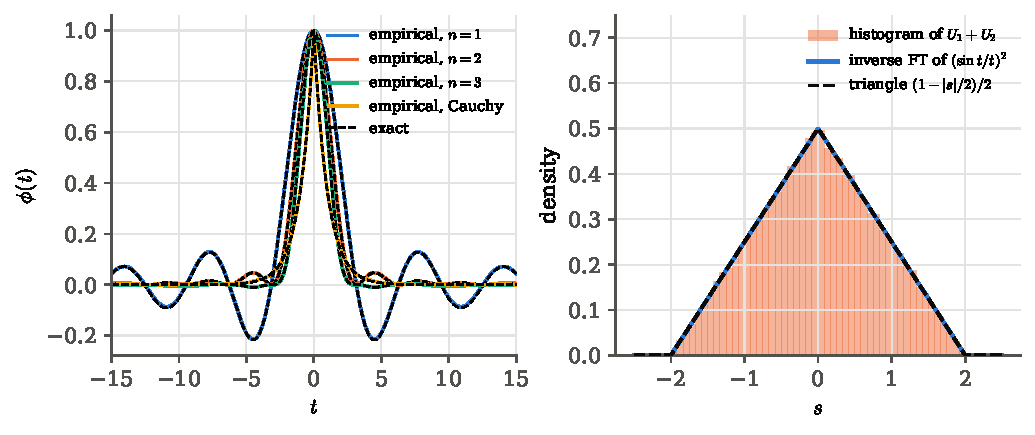
\includegraphics[width=\linewidth]{figures/ch01/characteristic_function.pdf}
\caption{Left: characteristic functions estimated from simulated draws
(coloured) against the exact ones (black dashed): $(\sin t/t)^n$ for sums of
$n=1,2,3$ uniforms, which narrow and flatten their side lobes as $n$ grows,
and $e^{-\abs t}$ for the Cauchy, with its kink at $t=0$. Right: the
histogram of $U_1+U_2$, the numerical inverse transform of $(\sin t/t)^2$, and
the exact triangle lie on top of each other.}
\label{1b:fig:cf}
\end{figure}

The picture behind this is the convolution theorem, drawn in
\cref{1b:fig:conv-theorem}. For independent $X$ and $Y$ the density of $X+Y$ is
the convolution $f_X*f_Y$ \eqref{1b:eq:convolution}, and its characteristic
function is the product $\phi_X\phi_Y$. Going around the square the long
way, through Fourier space, replaces an integral by a multiplication.

\begin{figure}[htbp]
\centering
\begin{tikzpicture}[
  nd/.style={draw=accent,rounded corners=2pt,fill=ideabg,align=center,
             font=\small,minimum width=3.4cm,minimum height=0.9cm},
  ar/.style={->,thick,accent}]
  \node[nd] (f)   at (0,1.8)  {densities $f_X,\ f_Y$};
  \node[nd] (fs)  at (6.4,1.8) {density of $X+Y$:\\ $f_X*f_Y$};
  \node[nd] (p)   at (0,0)    {cfs $\phi_X,\ \phi_Y$};
  \node[nd] (ps)  at (6.4,0)  {cf of $X+Y$:\\ $\phi_X\,\phi_Y$};
  \draw[ar] (f) -- (fs);
  \draw[ar] (f) -- (p);
  \draw[ar] (p) -- (ps);
  \draw[ar] (ps) -- (fs);
  \node[lbl,anchor=south] at (3.2,1.9) {convolve (hard)};
  \node[lbl,anchor=north] at (3.2,-0.1) {multiply (easy)};
  \node[lbl,anchor=east] at (-0.1,0.9) {Fourier transform};
  \node[lbl,anchor=west] at (6.5,0.9) {inverse transform};
\end{tikzpicture}
\caption{Two routes from the densities of two independent variables to the
density of their sum. The top route is the convolution integral. The bottom
route transforms each density, multiplies the transforms, and transforms back.}
\label{1b:fig:conv-theorem}
\end{figure}

\begin{keyidea}[Sums of independent variables]
For independent $X_1,\dots,X_n$ the characteristic function of the sum is
the product $\prod_i\phi_{X_i}(t)$, and the characteristic function determines
the distribution. The same holds for the mgf wherever it exists.
\end{keyidea}

\paragraph{Example: the Cauchy, and why its average never settles.}
The characteristic function of the Cauchy density is $e^{-\abs t}$. The
cleanest proof applies the inversion formula \eqref{1b:eq:cf-inverse} to
$e^{-\abs t}$ and checks that the result is the Cauchy density:
\begin{align*}
  \frac1{2\pi}\int_{-\infty}^{\infty}e^{-\abs t}e^{-itx}\,\dd t
  &\eqby{1} \frac1{2\pi}\Bigl[\int_0^\infty e^{-t(1+ix)}\,\dd t+\int_0^\infty e^{-t(1-ix)}\,\dd t\Bigr]\\
  &\eqby{2} \frac1{2\pi}\Bigl[\frac1{1+ix}+\frac1{1-ix}\Bigr]
   \eqby{3} \frac{1}{\pi(1+x^2)} .
\end{align*}
\begin{explain}
  \item Split at $t=0$ and substitute $t\to-t$ in the negative half.
  \item $\int_0^\infty e^{-ct}\dd t=1/c$ for $\mathrm{Re}\,c>0$.
  \item Common denominator $(1+ix)(1-ix)=1+x^2$, numerator $2$.
\end{explain}
By uniqueness, $\phi(t)=e^{-\abs t}$. It has a kink at $t=0$, so it has no
derivative there, which by \eqref{1b:eq:cf-taylor} is the transform-side sign
that the mean does not exist. Now average $n$ independent Cauchy draws:
\begin{align*}
  \phi_{\bar X_n}(t)
  &\eqby{1} \prod_{i=1}^n\phi_X\Bigl(\frac tn\Bigr)
   \eqby{2} \bigl(e^{-\abs t/n}\bigr)^n
   = e^{-\abs t} .
\end{align*}
\begin{explain}
  \item $\bar X_n=\sum_iX_i/n$: scaling rule $\phi_{aX}(t)=\phi_X(at)$ with
        $a=1/n$, and the product rule for the independent sum.
  \item The Cauchy characteristic function.
\end{explain}
The average of $n$ Cauchy draws has exactly the distribution of one draw, for
every $n$. Averaging gains nothing, which is what the running averages of
\cref{1b:fig:cauchy-run} showed. A physicist measuring the centre of a
resonance line with a pure Breit--Wigner shape by averaging event positions
would find the same.

\subsection{Setting up the central limit theorem}

The characteristic function makes the most important theorem of the next
chapter almost mechanical. Let $X_1,\dots,X_n$ be iid with mean $0$ and variance
$\sigma^2$, and standardise their sum, $Z_n=(X_1+\dots+X_n)/(\sigma\sqrt n)$.
Then
\begin{align*}
  \phi_{Z_n}(t)
  &\eqby{1} \Bigl[\phi_X\Bigl(\frac{t}{\sigma\sqrt n}\Bigr)\Bigr]^n
   \eqby{2} \Bigl[1-\frac{\sigma^2}{2}\,\frac{t^2}{\sigma^2n}+o\Bigl(\frac1n\Bigr)\Bigr]^n
   = \Bigl[1-\frac{t^2}{2n}+o\Bigl(\frac1n\Bigr)\Bigr]^n
   \xrightarrow[n\to\infty]{}\ e^{-t^2/2} .
\end{align*}
\begin{explain}
  \item Scaling and product rules, as for the Cauchy average.
  \item Taylor expansion \eqref{1b:eq:cf-taylor} with $\mu=0$ and
        $\E X^2=\sigma^2$, at the small argument $t/(\sigma\sqrt n)$.
\end{explain}
The last step is the limit $(1+a/n)^n\to e^a$. The limit $e^{-t^2/2}$ is the
characteristic function of $\Normal(0,1)$, and convergence of characteristic
functions implies convergence of the CDFs \srcref{CasellaBerger}{Thm.~2.6.1}.
So the standardised sum of many iid variables with finite variance is
approximately Gaussian, whatever their own distribution: the central limit
theorem. Only the first two terms of \eqref{1b:eq:cf-taylor} survived, which
is why only the mean and the variance of the $X_i$ matter in the limit. The
Cauchy fails the hypothesis, having no finite variance and a kinked
$\phi$, and is not Gaussianised. The proper statement, its conditions, the
rate of convergence and its failures are the business of \cref{ch:02}.

One more generating function is handy for counts. The
\newterm{probability generating function} $G(s)=\E(s^X)=\sum_k\Prob(X=k)\,s^k$
of a variable taking values $0,1,2,\dots$ is a power series whose coefficients
are the probabilities themselves, $\Prob(X=k)=G^{(k)}(0)/k!$, and whose
derivatives at $s=1$ give the factorial moments $\E[X(X-1)\cdots]$
\srcref{CasellaBerger}{\S2.6.2}. It is the mgf with $s=e^t$; for a Poisson
count $G(s)=e^{\lambda(s-1)}$.

\begin{recap}
\begin{itemize}[leftmargin=1.2em,itemsep=1pt]
  \item A random variable is a map from outcomes to numbers. Its distribution
        is given by a CDF, and by a pmf (mass) or a pdf (probability per unit
        $x$, with units).
  \item Marginals average out nuisance variables; conditionals slice and
        renormalise; independence means the joint factorises.
  \item Change of variables: $f_Y\abs{\dd y}=f_X\abs{\dd x}$, summed over
        branches, with $\abs J$ in several dimensions.
  \item $\E r(X)=\int r(x)f(x)\,\dd x$. Expectation is linear always;
        products factorise under independence. The mean minimises the expected
        squared miss, the median the absolute miss.
  \item $\Var(X)=\E X^2-\mu^2$; independent variances add;
        $\Var(\bar X_n)=\sigma^2/n$; $S_n^2$ divides by $n-1$.
  \item $\E[\E(Y\given X)]=\E Y$ and $\Var Y=\E\Var(Y\given X)+\Var\E(Y\given X)$.
  \item Covariance measures linear co-movement; $\abs\rho\le1$; zero
        correlation does not imply independence (except for jointly Gaussian
        variables).
  \item $\Cmat_{A\bm X+\bm b}=A\Cmat A\T$; eigenvectors of $\Cmat$ give
        uncorrelated combinations; $\bm X=L\bm Z$ with $LL\T=\Cmat$ generates them.
  \item mgf and cf generate moments; sums of independent variables multiply
        them; the cf always exists and leads straight to the central limit
        theorem.
\end{itemize}
\end{recap}
\clearpage
\section*{Chapter summary}
\addcontentsline{toc}{section}{Chapter summary}
\label{1b:sec:summary}

Every later statement of the form ``the probability of this is that'' rests
on the ideas of this chapter. The first part worked with events:
what has a probability, which rules the numbers obey, how conditioning shrinks
the sample space, how trees chain conditions, and how reading a tree backwards
turns a prediction $\Prob(E\given H)$ into an inference $\Prob(H\given E)$. The
second part turned outcomes into numbers, gave them densities, and compressed
the densities into means, variances, covariance matrices and transforms.
A data analysis in physics runs along a chain,
\[
  \text{model}\to\text{data}\to\text{summary }S\to P(S\given\theta)\to\text{inference}:
\]
a physical model with parameters $\theta$ produces data, we compress the data
into a summary $S$, we work out how $S$ is distributed for each $\theta$, and
we infer $\theta$. Probability is the language of every arrow. The fourth
arrow has already been walked once. The sample mean $\bar X_n$ is a summary,
and $\E\bar X_n=\mu$, $\Var\bar X_n=\sigma^2/n$ are the first two moments of
its sampling distribution. The two tables list each concept, what it means
operationally (how to compute or test it), and where it is used next.

\begin{center}
\small
\renewcommand{\arraystretch}{1.15}
\begin{tabularx}{\linewidth}{@{}>{\raggedright\arraybackslash}p{3.3cm}
                               >{\raggedright\arraybackslash}X
                               >{\raggedright\arraybackslash}p{2.7cm}@{}}
\toprule
\multicolumn{3}{@{}l}{\textbf{Events and their probabilities}}\\
concept & operational meaning & used later in\\\midrule
sample space, event & list every outcome; an event is a subset, in code a
  boolean mask over simulated outcomes & every chapter\\
axioms of $\Prob$ & non-negative, total $1$, additive over disjoint events;
  all other rules (complement, inclusion--exclusion, Boole) follow &
  \cref{ch:02,ch:04}\\
frequency vs degree of belief & long-run fraction of repetitions vs a
  coherent state of knowledge; same rules, different reading &
  \cref{ch:03,ch:05}\\
counting & equally likely outcomes: favourable over total, via
  multiplication principle and binomial coefficients & \cref{ch:02}\\
conditional probability & shrink the sample space to where the evidence is
  true and re-measure: $\Prob(A\given B)=\Prob(AB)/\Prob(B)$; in code, filter
  then count & \cref{ch:04,ch:05}\\
trees, total probability & multiply along a path, add across paths:
  $\Prob(E)=\sum_i\Prob(E\given H_i)\Prob(H_i)$ & \cref{ch:05,ch:09}\\
independence & $\Prob(AB)=\Prob(A)\Prob(B)$; learning $B$ does not change
  $\Prob(A)$; pairwise is weaker than mutual & \cref{ch:02,ch:06}\\
Bayes' theorem & read the tree backwards: from $\Prob(E\given H)$ and
  $\Prob(H)$ to $\Prob(H\given E)$ & \cref{ch:05,ch:09,ch:10}\\
\bottomrule
\end{tabularx}
\end{center}
\newpage

\begin{center}
\small
\renewcommand{\arraystretch}{1.15}
\begin{tabularx}{\linewidth}{@{}>{\raggedright\arraybackslash}p{3.3cm}
                               >{\raggedright\arraybackslash}X
                               >{\raggedright\arraybackslash}p{2.7cm}@{}}
\toprule
\multicolumn{3}{@{}l}{\textbf{Random variables and their summaries}}\\
concept & operational meaning & used later in\\\midrule
random variable & a function on outcomes; one simulated outcome gives every
  observable at once & every chapter\\
Bernoulli, binomial & one yes/no trial vs the number of successes in $n$ independent identical trials, $\binom nkp^k(1-p)^{n-k}$ & \cref{ch:02,ch:04}\\
CDF, quantiles & $F(x)=\Prob(X\le x)$, estimated by the empirical CDF;
  $F^{-1}(u)$ of a uniform $u$ samples $X$ & \cref{ch:04,ch:06}\\
pmf, pdf & mass at a point; density = probability per unit $x$ (a
  normalised histogram of width $\to0$) & \cref{ch:02,ch:03}\\
HDI, equal-tailed interval & shortest region of given probability vs equal
  tail areas & \cref{ch:05}\\
joint, marginal & marginal = integrate (average) out the nuisance variables;
  in code, ignore the column & \cref{ch:05,ch:09,ch:10}\\
conditional density & slice at the observed value and renormalise;
  $f(x,y)=f(y\given x)f(x)$ & \cref{ch:03,ch:05}\\
independence of variables & joint density factorises; test by comparing
  conditional slices & \cref{ch:02,ch:06}\\
change of variables & $f_Y\abs{\dd y}=f_X\abs{\dd x}$ summed over branches;
  Jacobian determinant in $n$ dimensions; check by histogramming & \cref{ch:02,ch:05,ch:06}\\
sampling prescription & say what is chosen at random: uniform instant gives the
  arcsine law for $x$, uniform $x$ gives $(\omega/4)\abs{\sin\omega t}$ for $t$;
  conservation laws give accessibility, not equal probability & \cref{ch:06,ch:09}\\
maximum entropy (microcanonical, canonical) & maximise $-k_B\sum p_i\ln p_i$ under the
  constraints: normalisation alone gives uniform on the energy shell, a fixed mean
  energy gives $e^{-E_i/k_BT}/Z$ & \cref{ch:02,ch:05}\\
virial theorem, negative heat capacity & bounded motion: $2\langle K\rangle=n\langle V\rangle$
  for $V\propto r^n$; gravity gives $E=-\frac32Nk_BT$, $C<0$, which the canonical
  $C=\Var E/k_BT^2\ge0$ forbids & when the canonical distribution applies\\
expectation & probability-weighted average; long-run mean of draws;
  $\E r(X)=\int rf$; linear always & every chapter\\
variance, standard deviation & mean squared deviation; independent variances
  add; errors add in quadrature & \cref{ch:02,ch:03}\\
sample mean and variance & $\bar X$ has variance $\sigma^2/n$; $S^2$
  divides by $n-1$ to be unbiased & \cref{ch:03,ch:04}\\
conditional expectation, total variance & $\E Y=\E[\E(Y\given X)]$;
  spread = mean within-group spread + spread of group means &
  \cref{ch:03,ch:05}\\
covariance, correlation & mean product of deviations; $\abs\rho\le1$
  measures linear co-movement only; plot before trusting $\rho\approx0$ &
  \cref{ch:03,ch:07}\\
covariance matrix & $\Cmat_{A\bm X+\bm b}=A\Cmat A\T$; eigenvectors give
  uncorrelated combinations; $\bm X=L\bm Z$ generates correlated Gaussians &
  \cref{ch:07,ch:08,ch:10}\\
error propagation & linearise: $\Cmat_{\bm y}\approx A\Cmat A\T$ with the
  Jacobian $A$; exact only for linear maps & \cref{ch:03,ch:10}\\
moments, cumulants & shape numbers; cumulants add for independent sums and
  vanish beyond order two for a Gaussian & \cref{ch:02,ch:12}\\
mgf, characteristic function & generate moments; sums of independent
  variables multiply them; cf always exists and gives the CLT &
  \cref{ch:02}\\
\bottomrule
\end{tabularx}
\end{center}

\subsection*{Reading the literature}

\begin{itemize}[leftmargin=1.2em,itemsep=2pt]
  \item \textbf{Main line.} \mainref{Chs.~1--3} covers probability, random
        variables and expectation compactly, with many short examples and
        exercises; most of the examples of \cref{ch:01} are worked out from
        there in full.
  \item \textbf{The clearest first reading.} \srcref{Kruschke}{Ch.~4}: what a
        distribution is, mass versus density (with the density exceeding $1$),
        means, variances, HDIs, and two-way tables, all in small steps.
  \item \textbf{Pictures.} \srcref{SeeingTheory}{Chs.~1--3}: interactive
        visual versions of events, expectation, variance and random
        variables.
  \item \textbf{The physicist's version.} \srcref{Cowan}{Ch.~1}: densities as
        normalised histograms, marginals as projections, conditionals as thin
        bands, functions of random variables, the covariance matrix, error
        propagation and the orthogonal transformation to uncorrelated
        variables.
  \item \textbf{Careful statements.} \srcref{CasellaBerger}{Chs.~1--2, 4}:
        transformations with full hypotheses, the minimising-distance
        property of the mean, non-unique moments, generating functions,
        conditional variance, and the correlation bounds.
  \item \textbf{Bayesian framing.} \srcref{Lambert}{Ch.~3} for probability
        trees and the two directions of probability, prediction and
        inference, which \cref{ch:05} develops.
  \item \textbf{Going further.} Characteristic functions and the continuity
        theorem are treated in any graduate probability text; for the
        physicist, \srcref{Cowan}{Ch.~10} applies them to sums of random
        variables.
\end{itemize}
  
\chapter{Probability Distributions from First Principles}\label{ch:02}
\providecommand{\twoaBernP}{}\renewcommand{\twoaBernP}{0.9}
\providecommand{\twoaBernMean}{}\renewcommand{\twoaBernMean}{0.9002}
\providecommand{\twoaBernVar}{}\renewcommand{\twoaBernVar}{0.0898}
\providecommand{\twoaBernVarTheory}{}\renewcommand{\twoaBernVarTheory}{0.09}
\providecommand{\twoaTrigExact}{}\renewcommand{\twoaTrigExact}{0.986}
\providecommand{\twoaTrigSim}{}\renewcommand{\twoaTrigSim}{0.9859}
\providecommand{\twoaTrigFour}{}\renewcommand{\twoaTrigFour}{0.8145}
\providecommand{\twoaBinMean}{}\renewcommand{\twoaBinMean}{4.001}
\providecommand{\twoaBinVar}{}\renewcommand{\twoaBinVar}{3.205}
\providecommand{\twoaMultPone}{}\renewcommand{\twoaMultPone}{0.4287}
\providecommand{\twoaMultPtwo}{}\renewcommand{\twoaMultPtwo}{0.26}
\providecommand{\twoaMultVarOneSim}{}\renewcommand{\twoaMultVarOneSim}{12.27}
\providecommand{\twoaMultVarOneTh}{}\renewcommand{\twoaMultVarOneTh}{12.25}
\providecommand{\twoaMultCovSim}{}\renewcommand{\twoaMultCovSim}{-5.577}
\providecommand{\twoaMultCovTh}{}\renewcommand{\twoaMultCovTh}{-5.572}
\providecommand{\twoaMultCorrSim}{}\renewcommand{\twoaMultCorrSim}{-0.5119}
\providecommand{\twoaMultCorrTh}{}\renewcommand{\twoaMultCorrTh}{-0.5134}
\providecommand{\twoaMultCorrPois}{}\renewcommand{\twoaMultCorrPois}{-0.002175}
\providecommand{\twoaMultRowSumVar}{}\renewcommand{\twoaMultRowSumVar}{0}
\providecommand{\twoaPLMean}{}\renewcommand{\twoaPLMean}{3}
\providecommand{\twoaPLVar}{}\renewcommand{\twoaPLVar}{2.986}
\providecommand{\twoaPLZeroSim}{}\renewcommand{\twoaPLZeroSim}{0.04965}
\providecommand{\twoaPLZeroTh}{}\renewcommand{\twoaPLZeroTh}{0.04979}
\providecommand{\twoaTVfive}{}\renewcommand{\twoaTVfive}{0.2191}
\providecommand{\twoaTVtwenty}{}\renewcommand{\twoaTVtwenty}{0.0402}
\providecommand{\twoaTVhundred}{}\renewcommand{\twoaTVhundred}{0.007607}
\providecommand{\twoaTVthousand}{}\renewcommand{\twoaTVthousand}{7.515\times10^{-4}}
\providecommand{\twoaTypExact}{}\renewcommand{\twoaTypExact}{0.423}
\providecommand{\twoaTypPois}{}\renewcommand{\twoaTypPois}{0.4232}
\providecommand{\twoaPPMean}{}\renewcommand{\twoaPPMean}{10.01}
\providecommand{\twoaPPVar}{}\renewcommand{\twoaPPVar}{9.866}
\providecommand{\twoaPPDetMean}{}\renewcommand{\twoaPPDetMean}{3.004}
\providecommand{\twoaPPDetVar}{}\renewcommand{\twoaPPDetVar}{3.008}
\providecommand{\twoaPPSumMean}{}\renewcommand{\twoaPPSumMean}{15}
\providecommand{\twoaPPSumVar}{}\renewcommand{\twoaPPSumVar}{14.76}
\providecommand{\twoaPPZeroSim}{}\renewcommand{\twoaPPZeroSim}{0}
\providecommand{\twoaPPZeroTh}{}\renewcommand{\twoaPPZeroTh}{4.540\times10^{-5}}
\providecommand{\twoaPPMaxErr}{}\renewcommand{\twoaPPMaxErr}{4.619\times10^{-4}}
\providecommand{\twoaPPZeroCount}{}\renewcommand{\twoaPPZeroCount}{0}
\providecommand{\twoaPPZeroExpect}{}\renewcommand{\twoaPPZeroExpect}{0.9}
\providecommand{\twoaWTGapMean}{}\renewcommand{\twoaWTGapMean}{0.4993}
\providecommand{\twoaWTGapVar}{}\renewcommand{\twoaWTGapVar}{0.2501}
\providecommand{\twoaWTCountMean}{}\renewcommand{\twoaWTCountMean}{2.003}
\providecommand{\twoaWTCountVar}{}\renewcommand{\twoaWTCountVar}{2.017}
\providecommand{\twoaWTWtenMean}{}\renewcommand{\twoaWTWtenMean}{4.993}
\providecommand{\twoaWTWtenVar}{}\renewcommand{\twoaWTWtenVar}{2.539}
\providecommand{\twoaWTCond}{}\renewcommand{\twoaWTCond}{0.3694}
\providecommand{\twoaWTUncond}{}\renewcommand{\twoaWTUncond}{0.3675}
\providecommand{\twoaWTMemTh}{}\renewcommand{\twoaWTMemTh}{0.3679}
\providecommand{\twoaMuonSurv}{}\renewcommand{\twoaMuonSurv}{0.1027}
\providecommand{\twoaGeoMean}{}\renewcommand{\twoaGeoMean}{10.03}
\providecommand{\twoaGeoVar}{}\renewcommand{\twoaGeoVar}{91.61}
\providecommand{\twoaNBMean}{}\renewcommand{\twoaNBMean}{26.97}
\providecommand{\twoaNBVar}{}\renewcommand{\twoaNBVar}{271}
\providecommand{\twoaNBMeanTh}{}\renewcommand{\twoaNBMeanTh}{27}
\providecommand{\twoaNBVarTh}{}\renewcommand{\twoaNBVarTh}{270}
\providecommand{\twoaMixMean}{}\renewcommand{\twoaMixMean}{9.997}
\providecommand{\twoaMixVar}{}\renewcommand{\twoaMixVar}{29.87}
\providecommand{\twoaMixVarTh}{}\renewcommand{\twoaMixVarTh}{30}
\providecommand{\twoaGeoTail}{}\renewcommand{\twoaGeoTail}{0.04384}
\providecommand{\twoaGeoTailTh}{}\renewcommand{\twoaGeoTailTh}{0.04239}
\providecommand{\twoaDTTrueMean}{}\renewcommand{\twoaDTTrueMean}{500}
\providecommand{\twoaDTRawMean}{}\renewcommand{\twoaDTRawMean}{500.3}
\providecommand{\twoaDTRawFano}{}\renewcommand{\twoaDTRawFano}{0.9597}
\providecommand{\twoaDTFanoSE}{}\renewcommand{\twoaDTFanoSE}{0.02236}
\providecommand{\twoaDTnpMean}{}\renewcommand{\twoaDTnpMean}{400.1}
\providecommand{\twoaDTnpTh}{}\renewcommand{\twoaDTnpTh}{400}
\providecommand{\twoaDTnpFano}{}\renewcommand{\twoaDTnpFano}{0.6156}
\providecommand{\twoaDTnpFanoTh}{}\renewcommand{\twoaDTnpFanoTh}{0.64}
\providecommand{\twoaDTpMean}{}\renewcommand{\twoaDTpMean}{389.5}
\providecommand{\twoaDTpTh}{}\renewcommand{\twoaDTpTh}{389.4}
\providecommand{\twoaDTpFano}{}\renewcommand{\twoaDTpFano}{0.5861}
\providecommand{\twoaDTpFanoTh}{}\renewcommand{\twoaDTpFanoTh}{0.6106}
\providecommand{\twoaDTnHat}{}\renewcommand{\twoaDTnHat}{5.002}
\providecommand{\twoaDTRawPull}{}\renewcommand{\twoaDTRawPull}{-1.8}
\providecommand{\twoaDTnpPull}{}\renewcommand{\twoaDTnpPull}{-1.7}
\providecommand{\twoaDTpPull}{}\renewcommand{\twoaDTpPull}{-1.8}
\providecommand{\twoaDTnHatPull}{}\renewcommand{\twoaDTnHatPull}{0.5}
\providecommand{\twoaGaussDiffFour}{}\renewcommand{\twoaGaussDiffFour}{0.02554}
\providecommand{\twoaGaussDiffTwentyfive}{}\renewcommand{\twoaGaussDiffTwentyfive}{0.003868}
\providecommand{\twoaGaussDiffHundred}{}\renewcommand{\twoaGaussDiffHundred}{9.388\times10^{-4}}
\providecommand{\twoaGaussDiffFourHundred}{}\renewcommand{\twoaGaussDiffFourHundred}{2.323\times10^{-4}}
\providecommand{\twoaTailPois}{}\renewcommand{\twoaTailPois}{2.001\times10^{-4}}
\providecommand{\twoaTailGauss}{}\renewcommand{\twoaTailGauss}{3.167\times10^{-5}}
\providecommand{\twoaTailGaussCC}{}\renewcommand{\twoaTailGaussCC}{4.810\times10^{-5}}
\providecommand{\twoaTailRatio}{}\renewcommand{\twoaTailRatio}{6.319}
\section*{Where this chapter is going}
\addcontentsline{toc}{section}{Where this chapter is going}

A physicist rarely invents a probability distribution. It is forced on us by the way the data were made. A paddle that either fires or does not fire, a histogram filled one event at a time, a Geiger counter clicking at random, a photomultiplier waiting for its tenth photon: each of these is a small machine, and each machine produces its own distribution. We build the common distributions from the machines that generate them. We state the assumptions in words, derive the probability law line by line, compute its mean and variance, and then run the machine in Python to check that the histogram of simulated outcomes lands on the formula.

Building a distribution from its machine is the \emph{prediction} direction of probability (\cref{ch:01}). We fix a hypothesis, say ``the source emits at rate $\lambda$'', and ask which outcomes it produces and how often. Recall the book's pipeline (\cref{ch:00}): a theory produces data, we compress the data into a statistic $S$, we work out how $S$ scatters when the experiment is repeated, and from that we infer the physics, labelled by parameters $\theta$. The distributions of counts, histograms and waiting times in this chapter supply the scatter step, $P(S\given\theta)$, for the simplest statistics. Once we have $P(S\given\theta)$, we can read it the other way round: hold the observed $S$ fixed and let $\theta$ vary. Read that way it is the likelihood (\cref{ch:03}), and Bayes' theorem turns the likelihood into a posterior (\cref{ch:05}).

The counting distributions come first, from a single yes/no trial up to the waiting times between random events. The continuous distributions follow. With them come the reason the Gaussian appears everywhere, the distributions built from Gaussians ($\chi^2$, Student-$t$, $F$), and the remaining common distributions.

\begin{figure}[htbp]
\centering
\begin{tikzpicture}[
  box/.style={draw=accent,rounded corners=2pt,fill=ideabg,align=center,font=\small,
              minimum width=2.55cm,minimum height=0.95cm,inner sep=2pt},
  cbox/.style={box,fill=takebg,draw=tangentgreen},
  arr/.style={->,thick,accent},
  note/.style={font=\scriptsize,softgray,align=center}]
  \node[box] (bern) at (0,0) {Bernoulli\\ one trial};
  \node[box] (bin)  at (3.2,0) {binomial\\ $n$ trials};
  \node[box] (mult) at (3.2,-1.7) {multinomial\\ histogram bins};
  \node[box] (pois) at (6.4,0) {Poisson\\ rare events};
  \node[box] (proc) at (6.4,-1.7) {Poisson process\\ rate $\lambda$, no memory};
  \node[box] (geo)  at (0,-1.7) {geometric,\\ neg.\ binomial};
  \node[box] (exp)  at (9.6,-1.7) {exponential,\\ gamma (Erlang)};
  \node[box,fill=warnbg,draw=bdryred] (fail) at (10,0) {when it fails:\\ dead time, extra spread};
  \draw[arr] (bern) -- (bin);
  \draw[arr] (bin) -- (mult);
  \draw[arr] (bin) -- (pois);
  \draw[arr] (proc) -- (pois);
  \draw[arr] (bern) -- (geo);
  \draw[arr] (proc) -- (exp);
  \draw[arr] (pois) -- (fail);
  \node[note,anchor=west,align=left] at (6.55,-0.85) {same answer from\\ a second route};
  \node[note,anchor=south] at (4.8,0.5) {$n\to\infty$, $np=\lambda$};
  \node[cbox] (gau) at (1.6,-3.9) {Gaussian\\ de Moivre--Laplace, CLT};
  \node[cbox] (chi) at (5.2,-3.9) {$\chi^2$, $t$, $F$\\ from Gaussians};
  \node[cbox] (zoo) at (8.8,-3.9) {the zoo and\\ ``which one when''};
  \draw[arr,tangentgreen] (gau) -- (chi);
  \draw[arr,tangentgreen] (chi) -- (zoo);
  \draw[arr,tangentgreen,dashed] (bin.south west) to[out=-120,in=90] (gau.north);
  \draw[arr,tangentgreen,dashed] (exp.south) to[out=-90,in=60] (zoo.north);
  \draw[faint,dashed] (-1.5,-2.85) -- (11.1,-2.85);
  \node[note,anchor=west] at (-1.5,-2.65) {counting};
  \node[note,anchor=west] at (-1.5,-3.05) {next part: continuous};
\end{tikzpicture}
\caption{The road through the chapter. Blue boxes are the counting distributions, each from the one before it or from a second, independent route (the Poisson distribution appears both as a limit of the binomial and from three physical inputs about the arrivals). The red box collects the ways real detectors break the assumptions. Green boxes are the continuous distributions of the next part; the dashed arrows mark where the binomial and the waiting times feed into them.}
\label{2a:fig:roadmap}
\end{figure}

\paragraph{A distribution is the fingerprint of a mechanism.}
Every counting distribution answers one forward question: \emph{if the world works like this machine, how often does each outcome occur?} To use a distribution correctly, we must recognise the machine behind it. So we meet each distribution in the same four steps:
\begin{enumerate}[leftmargin=1.6em,itemsep=1pt]
  \item \textbf{The story:} which physical process are we modelling, and which assumptions (independence, constant probability, constant rate) does it satisfy?
  \item \textbf{The derivation:} count the ways the outcome can happen and multiply their probabilities.
  \item \textbf{The summary numbers:} mean and variance, derived rather than quoted.
  \item \textbf{The check:} simulate the machine itself, not the formula, and compare the histogram with the derived law.
\end{enumerate}
\section{One trial: the Bernoulli distribution}\label{2a:sec:bernoulli}

A cosmic-ray muon crosses a plastic scintillator paddle. Either the photomultiplier behind the paddle produces a pulse above threshold, or it does not. Nothing else can happen. The paddle has an \emph{efficiency} $\epsilon$: the probability that it fires when a muon really goes through. This single yes/no trial is the building block of every coincidence trigger, every tracking efficiency and every ``did this event pass the cut?'' in an analysis. One number describes the trial completely: the probability of a ``yes'', which we call $p$ in general (for the paddle, $p=\epsilon$). Every counting distribution in this chapter is assembled from copies of this trial.

\paragraph{Physical picture: a two-level system measured once.}
A spin-$\tfrac12$ particle in the state $\alpha\ket{\uparrow}+\beta\ket{\downarrow}$, measured along $z$, gives ``up'' with probability $\abs{\alpha}^2$ and ``down'' with probability $\abs{\beta}^2=1-\abs{\alpha}^2$. One measurement, two outcomes, one number. The paddle is the same situation without the Hilbert space. Its microscopic history is unknown (how many photons were made, how many reached the photocathode), and the threshold collapses all of it into a single bit: fired or not.

\paragraph{The question, step by step.}
\begin{enumerate}[leftmargin=1.6em,itemsep=1pt]
  \item What can the outcome be? Two things. We code them as numbers: $1$ (``success'', fired) and $0$ (``failure'', did not fire).
  \item How many numbers do we need to describe the trial? One: the probability $p$ of a $1$. The probability of a $0$ is then forced to be $1-p$.
  \item Can we write both probabilities as one formula in the outcome $x$? Yes. That single formula is what makes products over many trials simple later.
  \item What are its average and spread? Derive them, then check by simulation.
\end{enumerate}

\subsection{The notation of distributions}

Three pieces of notation are used for the rest of the book: the symbol $\sim$, the probability mass function, and the parameter.

\begin{workdef}[has distribution, pmf, parameter]
We write $X\sim F$ and read it ``$X$ \emph{has distribution} $F$''. The symbol $\sim$ does \emph{not} mean ``approximately'' here. For a random variable $X$ \unpack{a rule that assigns a number to each outcome of the experiment} that takes whole-number values, the \newterm{probability mass function} (pmf) is
\[
  f(x)\;=\;\Prob(X=x),
\]
the probability that $X$ comes out equal to the particular number $x$. A \newterm{parameter} \unpack{a fixed number, such as $p$, that selects one member of a family of distributions} is not random. It is written after a bar or a semicolon when we want to stress it: $f(x\given p)$ or $f(x;p)$.
\end{workdef}

\begin{pitfall}[three kinds of letter]
In $\Prob(X=x)=p^x(1-p)^{1-x}$ there are three different kinds of object. $X$ (capital) is the random variable: it has not been observed yet, and it has a distribution. $x$ (lower case) is a possible value: an ordinary number we plug in. $p$ is a parameter: fixed, usually unknown, and the thing statistical inference tries to learn from data. Mixing them up is the commonest source of nonsense in statistics \mainref{p.~26}. The whole of \cref{ch:03} is about reading the same formula as a function of $p$ for fixed $x$.
\end{pitfall}

\subsection{The two simplest distributions}

Two very simple distributions mark the extreme cases of everything that follows. The first has no randomness at all; the second has no preferred outcome.

\begin{workdef}[point mass and discrete uniform]
$X$ has a \newterm{point mass} at $a$, written $X\sim\delta_a$, if $\Prob(X=a)=1$ \unpack{the outcome is certain, there is no randomness at all}. Its cumulative distribution function (CDF) $F(x)=\Prob(X\le x)$ is a single step,
\[
  F(x)=\begin{cases}0 & x<a,\\ 1 & x\ge a.\end{cases}
\]
$X$ has the \newterm{discrete uniform} distribution on $\{1,\dots,N\}$ if $f(x)=1/N$ for $x=1,\dots,N$ and $0$ otherwise \unpack{all $N$ outcomes equally likely, like a fair die with $N$ faces}.
\end{workdef}

The point mass is what any distribution becomes when its spread shrinks to zero: a perfectly stable voltage reference, a noise-free measurement. Its mean is $a$ and its variance is $0$. The discrete uniform is the other extreme: no outcome is preferred. Its mean and variance need two standard sums, which we recall and derive once here.

\paragraph{Example: mean and variance of a fair $N$-sided die.}
We need $\sum_{i=1}^N i=\tfrac{N(N+1)}{2}$ and $\sum_{i=1}^N i^2=\tfrac{N(N+1)(2N+1)}{6}$. The first follows by writing the sum forwards and backwards and adding: each of the $N$ columns sums to $N+1$. For the second, sum the identity $(i+1)^3-i^3=3i^2+3i+1$ from $i=1$ to $N$. The left side telescopes (each $i^3$ cancels against the next term) to $(N+1)^3-1$. The right side is $3\sum i^2+3\sum i+N$. Solving, $3\sum i^2=(N+1)^3-1-\tfrac{3N(N+1)}{2}-N$, which simplifies to $\tfrac{N(N+1)(2N+1)}{2}$; divide by $3$. With both sums in hand,
\begin{align*}
  \E X &\eqby{1} \sum_{x=1}^N x\,\frac1N \eqby{2} \frac1N\,\frac{N(N+1)}{2} = \frac{N+1}{2},\\
  \E X^2 &\eqby{1} \sum_{x=1}^N x^2\,\frac1N \eqby{2} \frac{(N+1)(2N+1)}{6},\\
  \Var X &\eqby{3} \E X^2-(\E X)^2
     = \frac{(N+1)(2N+1)}{6}-\frac{(N+1)^2}{4}
     \eqby{4} \frac{(N+1)(N-1)}{12}.
\end{align*}
\begin{explain}
  \item The expectation of $g(X)$ is the sum of $g(x)$ times the probability of $x$ (\cref{ch:01}).
  \item The two power sums recalled above.
  \item The shortcut $\Var X=\E[(X-\mu)^2]=\E X^2-2\mu\E X+\mu^2=\E X^2-\mu^2$ with $\mu=\E X$.
  \item Take out $(N+1)/12$: $2(2N+1)-3(N+1)=N-1$.
\end{explain}
For an ordinary die ($N=6$) this gives mean $3.5$ and variance $35/12\approx2.92$ \srcref{CasellaBerger}{\S3.2, p.~70}. For a digitiser that reports one of $N$ equally likely codes, the standard deviation is $\sqrt{(N^2-1)/12}\approx N/\sqrt{12}$, the famous ``$1/\sqrt{12}$ of a bin'' of quantisation noise.

\subsection{The Bernoulli trial}

\begin{workdef}[Bernoulli distribution]
$X\sim\mathrm{Bernoulli}(p)$ if $X$ takes the value $1$ with probability $p$ and the value $0$ with probability $1-p$, for some $p\in[0,1]$ \unpack{one trial with two outcomes, success coded as $1$}. Its pmf is
\begin{equation}
  f(x\given p)\;=\;p^{x}(1-p)^{1-x},\qquad x\in\{0,1\}. \label{2a:eq:bern}
\end{equation}
\emph{Recognise it by:} a single trial, exactly two outcomes, a fixed probability $p$.
\end{workdef}

The exponents in \eqref{2a:eq:bern} act as switches that pick the right factor. To see this, put in the two possible values. At $x=1$: $p^1(1-p)^0=p$. At $x=0$: $p^0(1-p)^1=1-p$. The switches pay off when we multiply many such factors, one per trial: the exponents simply add up.

A random variable that is $1$ when something happens and $0$ otherwise is also called an \newterm{indicator}. We write $I_A$ for the indicator of an event $A$. Every Bernoulli variable is the indicator of its success event, and every indicator is Bernoulli with $p=\Prob(A)$.

\paragraph{Mean and variance.} One fact does all the work: $0^2=0$ and $1^2=1$, so $X^2=X$ for a Bernoulli variable.
\begin{align}
  \E X &\eqby{1} 0\cdot(1-p)+1\cdot p = p, \nonumber\\
  \E X^2 &\eqby{2} \E X = p, \nonumber\\
  \Var X &\eqby{3} \E X^2-(\E X)^2 = p-p^2 = p(1-p). \label{2a:eq:bernvar}
\end{align}
\begin{explain}
  \item Sum of value times probability over the two values.
  \item $X^2=X$ because the only values are $0$ and $1$.
  \item The variance shortcut used for the fair die above.
\end{explain}
The variance $p(1-p)$ is zero at $p=0$ and $p=1$ (a certain outcome is a point mass) and largest, $1/4$, at $p=1/2$. A fair coin is the most unpredictable yes/no trial there is.

\subsection{Where does the randomness live? An explicit sample space}

A random variable is a map from the sample space $\Omega$ of \cref{ch:01} (the set of all possible outcomes of the experiment) to numbers. In the formulas above $\Omega$ never appeared, but it is still there. For the Bernoulli trial we can build it explicitly \mainref{p.~27}, and the construction is exactly how a computer makes a Bernoulli variable.

\begin{figure}[htbp]
\centering
\begin{tikzpicture}[x=9cm,y=1cm]
  \fill[formblue!25] (0,0) rectangle (0.7,0.35);
  \fill[softgray!20] (0.7,0) rectangle (1,0.35);
  \draw[thick] (0,0) rectangle (1,0.35);
  \draw[thick] (0.7,-0.08) -- (0.7,0.43);
  \node[lbl,anchor=north] at (0,-0.08) {$0$};
  \node[lbl,anchor=north] at (0.7,-0.08) {$p$};
  \node[lbl,anchor=north] at (1,-0.08) {$1$};
  \node[lbl,anchor=east] at (-0.02,0.175) {$\Omega=[0,1]$};
  \node[font=\footnotesize] at (0.35,0.175) {length $p$};
  \node[font=\footnotesize] at (0.85,0.175) {length $1-p$};
  \foreach \u in {0.12,0.31,0.58,0.66,0.83,0.95}{
    \draw[bdryred] (\u,0.35) -- (\u,0.55); \fill[bdryred] (\u,0.55) circle (1.8pt);
  }
  \node[draw=formblue,thick,circle,inner sep=1.5pt,font=\small] (one) at (0.35,-1.4) {$X=1$};
  \node[draw=softgray,thick,circle,inner sep=1.5pt,font=\small] (zero) at (0.85,-1.4) {$X=0$};
  \draw[->,thick,formblue] (0.35,-0.45) -- (one.north);
  \draw[->,thick,softgray] (0.85,-0.45) -- (zero.north);
\end{tikzpicture}
\caption{The Bernoulli trial as a map. A point $\omega$ is thrown uniformly on the unit interval (red dots are six such throws). Every $\omega$ in the blue part, of length $p$, is sent to $X=1$; every $\omega$ in the grey part is sent to $X=0$. The probability of $X=1$ is just the length of the blue part.}
\label{2a:fig:bern-omega}
\end{figure}

Take $\Omega=[0,1]$ with the ``length'' probability $\Prob([a,b])=b-a$ for $0\le a\le b\le1$ \unpack{a point thrown uniformly on the unit interval}. Fix $p$ and define the map
\[
  X(\omega)=\begin{cases}1 & \omega\le p,\\ 0 & \omega>p.\end{cases}
\]
Then $\Prob(X=1)=\Prob(\omega\le p)=\Prob([0,p])=p$ and $\Prob(X=0)=1-p$. So $X\sim\mathrm{Bernoulli}(p)$ (\cref{2a:fig:bern-omega}). Every counting distribution can be built this way from uniform numbers. This is the basis of Monte Carlo simulation; \cref{ch:06} develops it in general (inverse-transform sampling). Here we only use it.

\subsection{Worked examples}

\paragraph{Example: the paddle, and a veto.}
A paddle has efficiency $\epsilon=0.9$. Let $X$ be the indicator ``paddle fired''. Then $\E X=0.9$ and $\Var X=0.9\times0.1=0.09$, so the standard deviation of a single trial is $0.3$.

Now use the same paddle as a \emph{veto}: we keep the event only if the paddle did \emph{not} fire. The indicator of ``kept'' is $Y=1-X$. It is $1$ exactly when $X=0$, which happens with probability $1-\epsilon$. So $Y\sim\mathrm{Bernoulli}(1-\epsilon)$, with $\E Y=0.1$ and $\Var Y=0.1\times0.9=0.09$. The same variance also follows directly from $X$:
\begin{align*}
  \Var Y &\eqby{1} \Var(1-X) \eqby{2} (-1)^2\Var X = 0.09 .
\end{align*}
\begin{explain}
  \item Definition of $Y$.
  \item Adding a constant does not change a spread, and multiplying by $a$ multiplies the variance by $a^2$ (\cref{ch:01}).
\end{explain}
The veto and the paddle have the same variance: $p(1-p)$ is symmetric under $p\to1-p$, because relabelling success and failure cannot change how unpredictable the trial is.

\paragraph{Example: one trial read two ways.}
The formula $p^x(1-p)^{1-x}$ can be read in two directions, exactly the two directions of probability, prediction and inference (\cref{ch:01}).

\emph{Prediction.} Fix $p=0.9$. The formula is a distribution over $x$: $f(1)=0.9$, $f(0)=0.1$, and $\sum_x f(x)=1$.

\emph{Inference.} Suppose we observed one firing, $x=1$. Read the same formula as a function of $p$: $\Like(p)=p^1(1-p)^0=p$. This is the \newterm{likelihood} of $p$. It is \emph{not} a probability distribution over $p$:
\begin{align*}
  \int_0^1 \Like(p)\,\dd p \eqby{1} \int_0^1 p\,\dd p \eqby{2} \Bigl[\tfrac{p^2}{2}\Bigr]_0^1 = \tfrac12 \neq 1 .
\end{align*}
\begin{explain}
  \item The likelihood for the observation $x=1$.
  \item Elementary integral.
\end{explain}
The likelihood tells us that values of $p$ near $1$ make the observed firing more plausible than values near $0$, and nothing more \srcref{Kruschke}{\S6.1, p.~125}. Turning it into a distribution over $p$ needs a prior and Bayes' theorem (\cref{ch:05}).

\paragraph{Example: many independent trials of the same paddle.}
Record $N$ muons, with outcomes $x_1,\dots,x_N$, each $0$ or $1$, and assume the trials are independent. The probability of this particular sequence is
\begin{align*}
  \Prob(x_1,\dots,x_N\given p)
  &\eqby{1} \prod_{i=1}^N p^{x_i}(1-p)^{1-x_i}
  \eqby{2} p^{\sum_i x_i}(1-p)^{\sum_i(1-x_i)}
  \eqby{3} p^{z}(1-p)^{N-z},
\end{align*}
\begin{explain}
  \item Independence: the joint probability is the product of the single-trial probabilities (\cref{ch:01}).
  \item Powers of the same base multiply by adding exponents.
  \item Write $z=\sum_i x_i$ for the number of firings. Then $\sum_i(1-x_i)=N-z$.
\end{explain}
Only the count $z$ survives: the order in which the firings happened does not matter. This collapse is what the switch exponents in \eqref{2a:eq:bern} were for, and it is the seed of the binomial distribution in the next section \srcref{Kruschke}{(6.2), p.~125}.

\subsection{Python: build the trial from a uniform number}

The script \pyname{code/ch02/01_bernoulli.py} does exactly what \cref{2a:fig:bern-omega} shows. The core is three lines:

\pyfile[firstline=19,lastline=22,firstnumber=19]{code/ch02/01_bernoulli.py}{One Bernoulli trial per uniform number}

Line by line: \pyname{rng.uniform} throws the points $\omega$ on $[0,1]$; the comparison \pyname{u <= p} is the map $X(\omega)$, returning \pyname{True} or \pyname{False}; \pyname{astype(int)} codes these as $1$ and $0$. The rest of the script runs $5000$ trials for three values of $p$ and plots the running fraction of successes, then draws $10^6$ trials at $p=\twoaBernP$ and compares the observed frequencies with \eqref{2a:eq:bern}.

\begin{figure}[htbp]
\centering
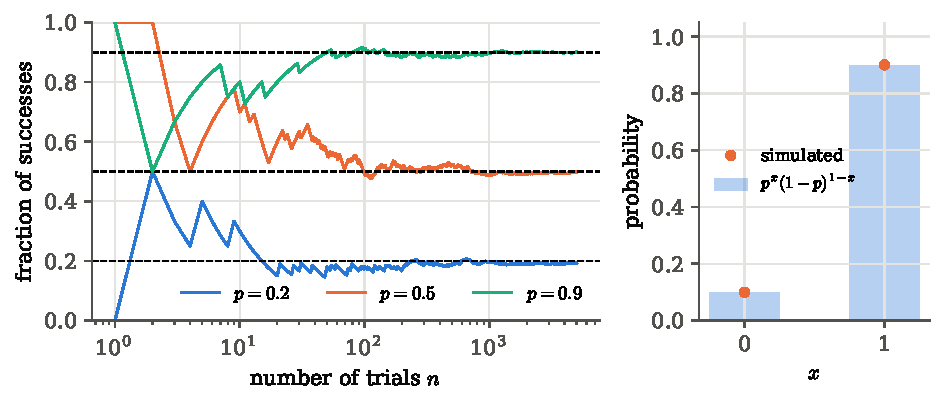
\includegraphics[width=\linewidth]{figures/ch02/01_bernoulli.pdf}
\caption{Left: the fraction of successes after $n$ trials, for three paddles. Early on the fraction jumps around wildly; by a few thousand trials each curve has settled onto its dashed line at $p$. Right: for $p=0.9$ the bars are the pmf and the dots the frequencies in a million simulated trials; they coincide.}
\label{2a:fig:bern-sim}
\end{figure}

For $10^6$ trials at $p=\twoaBernP$ the sample mean is $\twoaBernMean$ and the sample variance is $\twoaBernVar$, against the derived $p=\twoaBernP$ and $p(1-p)=\twoaBernVarTheory$ (\cref{2a:fig:bern-sim}). On the left, the running fraction slowly settles onto $p$: this is the law of large numbers at work. Its typical distance from $p$ after $n$ trials shrinks like $\sqrt{p(1-p)/n}$, which follows from the binomial variance in the next section.

\paragraph{What this bought us.}
A yes/no trial is fully described by one number $p$. The pmf $p^x(1-p)^{1-x}$ is built so that products over many independent trials collapse onto the number of successes. The mean is $p$ and the variance is $p(1-p)$, largest for a fair coin.

\section{Many successive trials: the binomial distribution}\label{2a:sec:binomial}

A cosmic-ray telescope is a stack of four scintillator layers. A muon going straight down crosses all four. Each layer fires independently with efficiency $\epsilon=0.95$, the probability that it fires when a muon crosses it. To reject noise, the trigger demands that \emph{at least three} of the four layers fire. What fraction of real muons does the trigger keep? Requiring all four would be cleaner, but how many muons would it cost? Both questions need the same thing: the probability of exactly $k$ successes in $n$ independent trials. The binomial distribution supplies it. It turns ``each trial succeeds with probability $p$'' into the full distribution of the number of successes.

\paragraph{Physical picture: paths through a tree.}
Picture each trial as a fork in a road: up for success, down for failure. After $n$ forks, every possible history is a path, and the number of successes is the number of ``up'' steps along that path. A random walk in one dimension has the same combinatorics. So do $n$ non-interacting spin-$\tfrac12$ particles: the number of spin-up particles is binomially distributed. The binomial coefficient $\binom nk$ that appears below is the \emph{multiplicity} of the macrostate ``$k$ up'', the same multiplicity that statistical mechanics uses to define entropy.

\paragraph{The question, step by step.}
\begin{enumerate}[leftmargin=1.6em,itemsep=1pt]
  \item What is the probability of one \emph{particular} sequence of outcomes, say success, failure, success? Multiply, because the trials are independent.
  \item Does that probability depend on the order? No: only on how many successes there are.
  \item How many sequences have exactly $k$ successes? Count them.
  \item So the probability of $k$ successes is (number of sequences) $\times$ (probability of each one).
\end{enumerate}

\begin{figure}[htbp]
\centering
\begin{tikzpicture}[
  st/.style={circle,draw=accent,fill=ideabg,inner sep=1.2pt,minimum size=5mm,font=\scriptsize},
  lf/.style={font=\scriptsize,anchor=west},
  up/.style={thick,formblue},
  dn/.style={thick,softgray}]
  \node[st] (r) at (0,0) {};
  \node[st] (s) at (2,1.6) {S};
  \node[st] (f) at (2,-1.6) {F};
  \draw[up] (r) -- (s); \draw[dn] (r) -- (f);
  \node[st] (ss) at (4,2.4) {S}; \node[st] (sf) at (4,0.8) {F};
  \node[st] (fs) at (4,-0.8) {S}; \node[st] (ff) at (4,-2.4) {F};
  \draw[up] (s) -- (ss); \draw[dn] (s) -- (sf);
  \draw[up] (f) -- (fs); \draw[dn] (f) -- (ff);
  \foreach \pa/\y/\name in {ss/2.8/sss, sf/1.2/sfs, fs/-0.4/fss, ff/-2.0/ffs}{
    \node[st] (\name) at (6,\y) {S}; \draw[up] (\pa) -- (\name);}
  \foreach \pa/\y/\name in {ss/2.0/ssf, sf/0.4/sff, fs/-1.2/fsf, ff/-2.8/fff}{
    \node[st] (\name) at (6,\y) {F}; \draw[dn] (\pa) -- (\name);}
  \node[lf] at (6.4,2.8)  {SSS \quad $k=3$\quad $p^3$};
  \node[lf] at (6.4,2.0)  {SSF \quad $k=2$\quad $p^2(1-p)$};
  \node[lf] at (6.4,1.2)  {SFS \quad $k=2$\quad $p^2(1-p)$};
  \node[lf] at (6.4,0.4)  {SFF \quad $k=1$\quad $p(1-p)^2$};
  \node[lf] at (6.4,-0.4) {FSS \quad $k=2$\quad $p^2(1-p)$};
  \node[lf] at (6.4,-1.2) {FSF \quad $k=1$\quad $p(1-p)^2$};
  \node[lf] at (6.4,-2.0) {FFS \quad $k=1$\quad $p(1-p)^2$};
  \node[lf] at (6.4,-2.8) {FFF \quad $k=0$\quad $(1-p)^3$};
  \node[font=\scriptsize,softgray] at (2,-3.4) {trial 1};
  \node[font=\scriptsize,softgray] at (4,-3.4) {trial 2};
  \node[font=\scriptsize,softgray] at (6,-3.4) {trial 3};
\end{tikzpicture}
\caption{All $2^3=8$ histories of three trials. Blue branches are successes (probability $p$), grey ones failures (probability $1-p$). Each path's probability is the product along it and depends only on its number of successes $k$. Counting paths per $k$ gives $1,3,3,1$, the third row of Pascal's triangle.}
\label{2a:fig:tree}
\end{figure}

\subsection{Deriving the pmf by counting paths}

Take $n$ independent trials, each a Bernoulli$(p)$. A history is a string of $n$ letters, S (success) or F (failure). By the product formula for independent Bernoulli trials (\cref{2a:sec:bernoulli}), a string with $k$ S's has probability $p^k(1-p)^{n-k}$ whatever the order.

\emph{How many strings have exactly $k$ S's?} We must choose which $k$ of the $n$ positions carry an S. Count ordered choices first: there are $n$ ways to pick the first position, $n-1$ for the second, and so on down to $n-k+1$ for the $k$-th, giving $n(n-1)\cdots(n-k+1)=\frac{n!}{(n-k)!}$ ordered choices. Each set of $k$ positions has been counted $k!$ times, once for each order in which we could have picked the same positions. So the number of sets is
\begin{equation}
  \binom nk \;=\; \frac{n!}{k!\,(n-k)!}, \label{2a:eq:binomcoef}
\end{equation}
the \newterm{binomial coefficient}, read ``$n$ choose $k$''. (By convention $0!=1$, so $\binom n0=\binom nn=1$.)

\begin{workdef}[binomial distribution]
$X\sim\mathrm{Binomial}(n,p)$ if $X$ is the number of successes in $n$ independent trials, each succeeding with the same probability $p$ \unpack{$n$ fixed in advance, trials do not influence each other, $p$ the same for every trial}. Its pmf is
\begin{equation}
  f(k\given n,p)\;=\;\binom nk\,p^k(1-p)^{n-k},\qquad k=0,1,\dots,n. \label{2a:eq:binom}
\end{equation}
\emph{Recognise it by:} multiple successive trials (where Bernoulli is for a single trial), a fixed number of them, each yes/no, independent, with constant $p$, and we record only the total number of successes.
\end{workdef}

\paragraph{It is normalised.} The probabilities \eqref{2a:eq:binom} add up to one. The tool is the \newterm{binomial theorem}: $(a+b)^n=\sum_{k=0}^n\binom nk a^kb^{n-k}$. Here is why it is true. Expanding the product of $n$ factors $(a+b)(a+b)\cdots(a+b)$ means choosing $a$ or $b$ from each factor. A term $a^kb^{n-k}$ arises once for each way of choosing which $k$ factors give $a$, and there are $\binom nk$ such ways. Then
\begin{align*}
  \sum_{k=0}^n f(k\given n,p) \eqby{1} \sum_{k=0}^n\binom nk p^k(1-p)^{n-k} \eqby{2} \bigl(p+(1-p)\bigr)^n = 1^n = 1 .
\end{align*}
\begin{explain}
  \item Definition \eqref{2a:eq:binom}.
  \item The binomial theorem with $a=p$ and $b=1-p$.
\end{explain}
With $p=\tfrac12$ the same line says $\sum_k\binom nk=2^n$: the total number of paths in the tree \srcref{CasellaBerger}{(3.2.4), p.~74}.

\subsection{Mean and variance, two ways}

\paragraph{The slick way: a sum of indicators.} Let $X_i$ be the indicator of success on trial $i$: it is $1$ if trial $i$ succeeds and $0$ otherwise. Counting successes is adding up these indicators, so $X=X_1+\dots+X_n$, and the $X_i$ are independent Bernoulli$(p)$.
\begin{align}
  \E X &\eqby{1} \sum_{i=1}^n\E X_i \eqby{2} np, \nonumber\\
  \Var X &\eqby{3} \sum_{i=1}^n\Var X_i \eqby{4} np(1-p). \label{2a:eq:binvar}
\end{align}
\begin{explain}
  \item Expectation is linear: $\E(\sum X_i)=\sum\E X_i$, with or without independence (\cref{ch:01}).
  \item $\E X_i=p$ from \eqref{2a:eq:bernvar}.
  \item For \emph{independent} variables the covariances vanish, so the variance of a sum is the sum of variances.
  \item $\Var X_i=p(1-p)$ from \eqref{2a:eq:bernvar}.
\end{explain}

\paragraph{The direct way: sum the pmf.} This route uses a trick that recurs throughout the chapter: absorb the factor $k$ into the binomial coefficient, then recognise the sum that is left as the total probability of a smaller distribution. The identity we need is
\[
  k\binom nk = k\frac{n!}{k!(n-k)!} = \frac{n!}{(k-1)!(n-k)!} = n\binom{n-1}{k-1}\qquad (k\ge1).
\]
Then
\begin{align*}
  \E X &\eqby{1} \sum_{k=1}^n k\binom nk p^k(1-p)^{n-k}
   \eqby{2} np\sum_{k=1}^n\binom{n-1}{k-1}p^{k-1}(1-p)^{(n-1)-(k-1)}\\
  &\eqby{3} np\sum_{j=0}^{n-1}\binom{n-1}{j}p^{j}(1-p)^{n-1-j}
   \eqby{4} np .
\end{align*}
\begin{explain}
  \item Definition of the mean. The $k=0$ term is zero, so we start at $k=1$.
  \item The identity above, and one factor $p$ taken out of $p^k$.
  \item Rename $j=k-1$.
  \item The sum is the total probability of a Binomial$(n-1,p)$, which is $1$.
\end{explain}
For the variance, the same trick works on the \emph{factorial moment} $\E[X(X-1)]$, using $k(k-1)\binom nk=n(n-1)\binom{n-2}{k-2}$:
\begin{align*}
  \E[X(X-1)] &\eqby{1} n(n-1)p^2\sum_{j=0}^{n-2}\binom{n-2}{j}p^j(1-p)^{n-2-j} \eqby{2} n(n-1)p^2,\\
  \Var X &\eqby{3} \E[X(X-1)]+\E X-(\E X)^2 = n(n-1)p^2+np-n^2p^2 = np(1-p).
\end{align*}
\begin{explain}
  \item The same three steps as for the mean, with two factors of $k$ absorbed and $j=k-2$.
  \item A Binomial$(n-2,p)$ sums to one.
  \item $\E X^2=\E[X(X-1)]+\E X$, and then the variance shortcut.
\end{explain}
Both ways agree with \srcref{Cowan}{(2.3)--(2.4), p.~27}.\footnote{Cowan writes the upper limit of the sum in (2.3) as $\infty$. It should be $n$, the number of trials, since the count cannot exceed it.}

\paragraph{What the numbers mean.} The mean count $np$ grows like $n$, but the standard deviation $\sqrt{np(1-p)}$ grows only like $\sqrt n$. Dividing both by $n$, the \emph{fraction} of successes $X/n$ has mean $p$ and standard deviation $\sqrt{p(1-p)/n}$. This is the rate at which the running fractions in \cref{2a:fig:bern-sim} settle, and the origin of every ``$1/\sqrt N$'' error bar on an efficiency.

\subsection{The moment generating function and sums of binomials}

The \newterm{moment generating function} (mgf) $M_X(t)=\E e^{tX}$ (\cref{ch:01}) packs all the moments into one function: its $r$-th derivative at $t=0$ is $\E X^r$. For the binomial,
\begin{align}
  M_X(t) \eqby{1} \sum_{k=0}^n e^{tk}\binom nk p^k(1-p)^{n-k}
  \eqby{2} \sum_{k=0}^n\binom nk (pe^t)^k(1-p)^{n-k}
  \eqby{3} \bigl(1-p+pe^t\bigr)^n . \label{2a:eq:binmgf}
\end{align}
\begin{explain}
  \item Definition of the mgf.
  \item $e^{tk}p^k=(pe^t)^k$.
  \item The binomial theorem with $a=pe^t$ and $b=1-p$.
\end{explain}
Check: $M'(0)=n(1-p+p)^{n-1}p=np$, the mean again.

\begin{keyidea}[binomials with the same $p$ add]
If $X_1\sim\mathrm{Binomial}(n_1,p)$ and $X_2\sim\mathrm{Binomial}(n_2,p)$ are independent, then $X_1+X_2\sim\mathrm{Binomial}(n_1+n_2,p)$.
\end{keyidea}
\emph{Why:} the counting story gives it at once. $X_1$ counts successes in $n_1$ trials, and $X_2$ counts them in another $n_2$ independent trials with the same $p$. So $X_1+X_2$ counts successes in $n_1+n_2$ such trials. The mgf says the same. The mgf of a sum of independent variables is the product of their mgfs, and $(1-p+pe^t)^{n_1}(1-p+pe^t)^{n_2}=(1-p+pe^t)^{n_1+n_2}$, the mgf \eqref{2a:eq:binmgf} of Binomial$(n_1+n_2,p)$. The same $p$ is essential: with different $p$'s the product is not of binomial form.

\subsection{Worked examples}

\paragraph{Example: the coincidence trigger.}
Return to the four-layer telescope from the start of the section. Each layer fires with $\epsilon=0.95$, independently, so the number of layers that fire is $X\sim\mathrm{Binomial}(4,0.95)$. The trigger needs $X\ge3$.
\begin{align*}
  \Prob(X\ge3) &\eqby{1} \binom43\epsilon^3(1-\epsilon)+\binom44\epsilon^4 \\
  &\eqby{2} 4(0.857375)(0.05)+0.81450625 \\
  &= 0.171475+0.814506 = 0.98598 .
\end{align*}
\begin{explain}
  \item Only $k=3$ and $k=4$ satisfy the condition. Add their pmf values.
  \item $0.95^3=0.857375$ and $0.95^4=0.81450625$.
\end{explain}
The 3-out-of-4 trigger keeps $98.6\%$ of muons. Demanding all four keeps only $\epsilon^4=\twoaTrigFour$, so the cleaner trigger loses about one muon in five. The simulation in \pyname{02_binomial.py} (one million four-layer events) gives $\twoaTrigSim$ against the exact $\twoaTrigExact$.

\paragraph{Example: the Chevalier de M\'er\'e's two bets.}
Is it more likely to get at least one six in $4$ rolls of a die, or at least one double six in $24$ rolls of two dice? The number of successes is binomial in both cases, and ``at least one'' is the complement of ``none'':
\begin{align*}
  \Prob(\text{at least one six in }4) &\eqby{1} 1-\binom40\Bigl(\tfrac16\Bigr)^0\Bigl(\tfrac56\Bigr)^4 = 1-0.4823 = 0.518,\\
  \Prob(\text{at least one double six in }24) &\eqby{2} 1-\Bigl(\tfrac{35}{36}\Bigr)^{24} = 1-0.5086 = 0.491 .
\end{align*}
\begin{explain}
  \item Binomial$(4,1/6)$ at $k=0$.
  \item Binomial$(24,1/36)$ at $k=0$: two dice show a double six with probability $1/36$.
\end{explain}
The gambler's intuition ($4\times\tfrac16=24\times\tfrac1{36}=\tfrac23$) is wrong because it adds probabilities of events that are not mutually exclusive \srcref{CasellaBerger}{Ex.~3.2.3, p.~75}. The same mistake appears in ``the probability of at least one fake signal in $N$ search bins is $N$ times the single-bin probability'': true only while that product is small (the look-elsewhere effect, \cref{ch:04}).

\paragraph{Example: drawing without replacement: the hypergeometric.}
The binomial needs the same $p$ on every trial. That fails when we sample \emph{without replacement} from a small population, because each draw changes what is left. A batch of $N=25$ front-end chips contains $M$ faulty ones. We test $K=10$ chips at random and find none faulty. How surprising is this if $M=6$?

The number of faulty chips in the sample follows the \newterm{hypergeometric} distribution. Count equally likely samples: there are $\binom NK$ ways to choose $K$ chips, and $\binom Mx\binom{N-M}{K-x}$ of them contain exactly $x$ faulty ones (choose $x$ of the $M$ faulty and $K-x$ of the $N-M$ good ones). So
\[
  \Prob(X=x\given N,M,K)=\frac{\binom Mx\binom{N-M}{K-x}}{\binom NK},
\]
with mean $KM/N$ and variance $\frac{KM}{N}\frac{(N-M)(N-K)}{N(N-1)}$. For our batch,
\begin{align*}
  \Prob(X=0) \eqby{1} \frac{\binom60\binom{19}{10}}{\binom{25}{10}} \eqby{2} \frac{92378}{3268760} = 0.028 .
\end{align*}
\begin{explain}
  \item Hypergeometric with $N=25$, $M=6$, $K=10$, $x=0$.
  \item $\binom{19}{10}=92378$ and $\binom{25}{10}=3268760$.
\end{explain}
If six chips were faulty, a clean sample is unlikely: under $3\%$ \srcref{CasellaBerger}{Ex.~3.2.1, p.~73}. The binomial with $p=M/N=0.24$ would give $(0.76)^{10}=0.064$, more than twice as large. Why the difference? Without replacement, each good chip drawn leaves a remaining pool that is \emph{more} faulty, so a clean run is rarer. The factor $(N-K)/(N-1)$ in the variance is the ``finite-population correction''. When the batch is much larger than the sample, $N\gg K$, this factor goes to one and the hypergeometric becomes the binomial.

\subsection{Python: repeat the $n$ trials, histogram the count}

The script \pyname{code/ch02/02_binomial.py} simulates the generating process itself, not the formula. It builds a table of uniform numbers, one row per experiment and one column per trial.

\pyfile[firstline=21,lastline=24,firstnumber=21]{code/ch02/02_binomial.py}{Binomial counts by running the trials}

\pyname{rng.uniform(size=(reps, n)) <= p} is a \pyname{reps}$\times n$ table of Bernoulli trials, built exactly as in \cref{2a:sec:bernoulli}. Summing along a row (\pyname{axis=1}) counts the successes in one experiment. The script does this $20\,000$ times for six $(n,p)$ pairs and overlays \pyname{scipy.stats.binom.pmf} as black ticks (\cref{2a:fig:binom-sim}).

\begin{figure}[htbp]
\centering
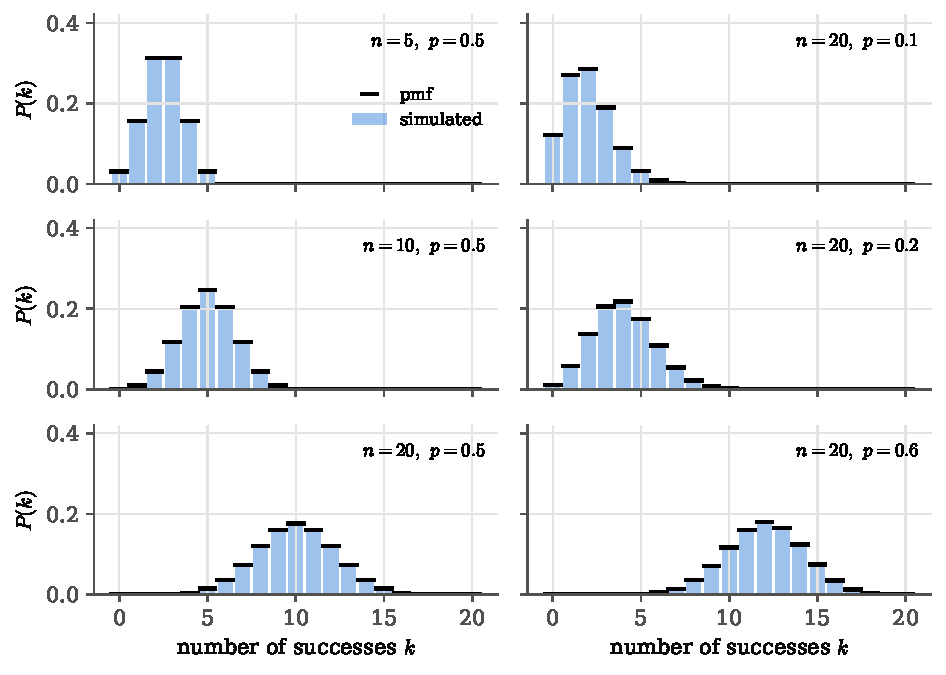
\includegraphics[width=0.95\linewidth]{figures/ch02/02_binomial.pdf}
\caption{Histograms of simulated success counts (bars) against the pmf (black ticks). Left column: $p=\tfrac12$ and more trials; the distribution stays symmetric, moves right and widens like $\sqrt n$. Right column: $n=20$ and growing $p$; at small $p$ the distribution is squashed against $k=0$ and skewed, at $p=0.6$ it leans the other way.}
\label{2a:fig:binom-sim}
\end{figure}

For $n=20$, $p=0.2$ and $200\,000$ experiments the sample mean is $\twoaBinMean$ and the sample variance $\twoaBinVar$, against $np=4$ and $np(1-p)=3.2$. \Cref{2a:fig:binom-sim} shows two features that matter later. For $p=\tfrac12$ and growing $n$ the shape is already bell-like: this is the de Moivre--Laplace limit, derived in the next part. For small $p$ the distribution piles up near zero with a tail to the right: this is the regime that becomes the Poisson distribution in \cref{2a:sec:poisson-limit}.

\begin{pitfall}[when the binomial is the wrong model]
Three assumptions go into \eqref{2a:eq:binom}, and each can fail in a real detector.
\begin{itemize}[leftmargin=1.4em,itemsep=1pt]
  \item \emph{Fixed $n$.} If the number of trials is itself random (the number of muons in a run), the count of successes is not binomial. We return to this in \cref{2a:sec:poisson-process}.
  \item \emph{Independence.} Layers that share a high-voltage supply fail together, so the number of dead layers is spread wider than binomial.
  \item \emph{Constant $p$.} Efficiency that varies across the paddle (edges versus centre), or between runs, also inflates the spread. The \emph{beta-binomial} distribution models a $p$ that itself varies \srcref{Lambert}{\S8.4.5}. Sampling without replacement (the hypergeometric example above) is the opposite case: the spread is \emph{narrower} than binomial.
\end{itemize}
A quick check is to compare the observed variance of a count with $np(1-p)$ computed from its observed mean.
\end{pitfall}

\section{Histogram bins: the multinomial distribution}\label{2a:sec:multinomial}

A calorimeter records the energy of $N=50$ electrons from a beta source, and we fill a histogram with $m=5$ energy bins. Each electron lands in bin $j$ with probability $p_j$, set by the shape of the spectrum. The number of electrons in bin $j$, the bin count $n_j$, fluctuates from one run to the next. To fit the spectrum later (\cref{ch:03}) we need the \emph{joint} distribution of all the bin contents, including how the bins fluctuate together. That joint distribution is the multinomial: the binomial with more than two outcomes. Its main lesson is that, with $N$ fixed, the bins of a histogram are \emph{negatively correlated}.

\paragraph{Physical picture: a fixed number of balls in boxes.}
Fifty balls are thrown one at a time into five boxes. If box 1 happens to catch more than its share, there are fewer balls left for the other boxes. The total is fixed, so the counts cannot all go up together. Statistical mechanics has the same situation in the canonical ensemble, where the particle number is fixed. Letting the total fluctuate, as in the grand canonical ensemble, removes the constraint. We will see that it also removes the correlation.

\paragraph{The question, step by step.}
\begin{enumerate}[leftmargin=1.6em,itemsep=1pt]
  \item What is the probability of one \emph{particular} sequence of bin assignments (electron 1 in bin 3, electron 2 in bin 1, \dots)? Multiply the $p$'s.
  \item Which feature of the sequence does that probability depend on? Only how many electrons went into each bin.
  \item How many sequences give the counts $(n_1,\dots,n_m)$? Count them.
  \item What does one bin look like on its own, and how do two bins co-vary?
\end{enumerate}

\subsection{Deriving the pmf}

Each of $N$ independent trials ends in one of $m$ outcomes, with probabilities $p_1,\dots,p_m$ and $\sum_jp_j=1$. A particular sequence with $n_1$ outcomes of type $1$, $n_2$ of type $2$, and so on, has probability $p_1^{n_1}p_2^{n_2}\cdots p_m^{n_m}$ by independence, whatever the order.

\emph{How many sequences have these counts?} Start by treating the $N$ trials as labelled objects in a row: there are $N!$ orderings. Many orderings give the same assignment of outcomes. Shuffling the $n_1$ trials of type $1$ among themselves ($n_1!$ ways) does not change which trials are of type $1$, and the same holds for every type. So each distinct assignment has been counted $n_1!\,n_2!\cdots n_m!$ times, and the number of distinct assignments is
\begin{equation}
  \binom{N}{n_1,n_2,\dots,n_m}\;=\;\frac{N!}{n_1!\,n_2!\cdots n_m!}, \label{2a:eq:multcoef}
\end{equation}
the \newterm{multinomial coefficient}. For $m=2$ it is $N!/(n_1!(N-n_1)!)$, the binomial coefficient.

\begin{workdef}[multinomial distribution]
The vector of counts $\bm n=(n_1,\dots,n_m)$ is $\mathrm{Multinomial}(N,\bm p)$ if it records how many of $N$ independent trials fell into each of $m$ categories, each trial landing in category $j$ with the same probability $p_j$ \unpack{$N$ fixed, categories exclusive and exhaustive, $\sum_jp_j=1$}. Its pmf is
\begin{equation}
  f(n_1,\dots,n_m\given N,\bm p)\;=\;\frac{N!}{n_1!\cdots n_m!}\,p_1^{n_1}\cdots p_m^{n_m},
  \qquad n_j\ge0,\quad \sum_jn_j=N. \label{2a:eq:mult}
\end{equation}
\emph{Recognise it by:} a histogram of a fixed number of independent entries, or any tally of categorical outcomes (particle species, decay channels, blood types).
\end{workdef}

The pmf \eqref{2a:eq:mult} sums to one by the \emph{multinomial theorem}, $(p_1+\dots+p_m)^N=\sum\frac{N!}{n_1!\cdots n_m!}p_1^{n_1}\cdots p_m^{n_m}$. It is proved exactly like the binomial theorem: expanding the product means picking one $p_j$ from each of the $N$ factors. The left side is $1^N=1$.

\begin{figure}[htbp]
\centering
\begin{tikzpicture}[x=10cm,y=1cm]
  \def\ca{0.4287}\def\cb{0.6887}\def\cc{0.8464}\def\cd{0.9420}
  \fill[formblue!45] (0,0) rectangle (\ca,0.4);
  \fill[formblue!32] (\ca,0) rectangle (\cb,0.4);
  \fill[formblue!22] (\cb,0) rectangle (\cc,0.4);
  \fill[formblue!14] (\cc,0) rectangle (\cd,0.4);
  \fill[formblue!7]  (\cd,0) rectangle (1,0.4);
  \draw[thick] (0,0) rectangle (1,0.4);
  \foreach \c in {\ca,\cb,\cc,\cd}{\draw[thick] (\c,0) -- (\c,0.4);}
  \node[font=\footnotesize] at (0.2143,0.2) {bin 1};
  \node[font=\footnotesize] at (0.5587,0.2) {bin 2};
  \node[font=\footnotesize] at (0.7675,0.2) {3};
  \node[font=\footnotesize] at (0.8942,0.2) {4};
  \node[font=\footnotesize] at (0.971,0.2) {5};
  \node[lbl,anchor=north] at (0,0) {$0$};
  \node[lbl,anchor=north] at (1,0) {$1$};
  \node[font=\scriptsize,anchor=north] at (\ca,0) {$p_1$};
  \node[font=\scriptsize,anchor=north] at (\cb,0) {$p_1{+}p_2$};
  \node[lbl,anchor=east] at (-0.02,0.2) {$u$};
  \fill[bdryred] (0.61,0.4) circle (1.2pt);
  \draw[->,thick,bdryred] (0.61,0.55) -- (0.61,0.43);
  \node[font=\scriptsize,bdryred,anchor=south] at (0.61,0.55) {$u=0.61$};
  \begin{scope}[yshift=-3.3cm]
    \foreach \j/\h in {1/2.14,2/1.30,3/0.79,4/0.48,5/0.29}{
      \draw[fill=formblue!30] ({(\j-1)*0.16+0.1},0) rectangle ({\j*0.16+0.1-0.02},\h);
      \node[font=\scriptsize,anchor=north] at ({(\j-0.5)*0.16+0.09},0) {$n_{\j}$};
    }
    \draw[faint] (0.08,0) -- (0.92,0);
    \node[font=\scriptsize,softgray,anchor=west] at (0.62,1.8) {expected counts $Np_j$};
  \end{scope}
\end{tikzpicture}
\caption{How one event chooses its bin. The unit interval is cut into pieces of lengths $p_1,\dots,p_5$ (a falling spectrum). A uniform number $u$ lands in one piece, here bin 2, and that bin's count goes up by one. Repeating this $N$ times fills the histogram below, whose bar heights are the expected counts $Np_j$ for $N=50$.}
\label{2a:fig:mult-bins}
\end{figure}

\subsection{One bin at a time: the marginal is binomial}

Often we care about one bin only. Then the other bins are \emph{nuisance} variables, and we \newterm{marginalise}: sum the joint pmf over all values of the variables we do not care about (\cref{ch:01}).

\begin{keyidea}[each bin is binomial]
If $\bm n\sim\mathrm{Multinomial}(N,\bm p)$, then $n_j\sim\mathrm{Binomial}(N,p_j)$ for every $j$.
\end{keyidea}
\emph{Why:} look at bin $j$ alone. Each trial either lands in bin $j$ (probability $p_j$) or does not (probability $1-p_j$). Lump all the other bins into the single outcome ``not in bin $j$'', and we have $N$ independent yes/no trials with the same probability: the binomial story. The algebra confirms it. Take three categories (bin $i$, bin $j$, ``everything else''), where the pmf is the \emph{trinomial}
\[
  f(n_i,n_j)=\frac{N!}{n_i!\,n_j!\,(N-n_i-n_j)!}\,p_i^{n_i}p_j^{n_j}(1-p_i-p_j)^{N-n_i-n_j}.
\]
Summing out $n_j$:
\begin{align*}
  \sum_{n_j=0}^{N-n_i} f(n_i,n_j)
  &\eqby{1} \frac{N!}{n_i!\,(N-n_i)!}p_i^{n_i}\sum_{n_j=0}^{N-n_i}\frac{(N-n_i)!}{n_j!\,(N-n_i-n_j)!}\,p_j^{n_j}(1-p_i-p_j)^{N-n_i-n_j}\\
  &\eqby{2} \binom N{n_i}p_i^{n_i}\,\bigl(p_j+1-p_i-p_j\bigr)^{N-n_i}
  \eqby{3} \binom N{n_i}p_i^{n_i}(1-p_i)^{N-n_i}.
\end{align*}
\begin{explain}
  \item Multiply and divide by $(N-n_i)!$, and take out everything that does not depend on $n_j$.
  \item The remaining sum is the binomial theorem with $n=N-n_i$, $a=p_j$, $b=1-p_i-p_j$.
  \item The two $p_j$'s cancel.
\end{explain}
The result is the Binomial$(N,p_i)$ pmf, so $\E n_i=Np_i$ and $\Var n_i=Np_i(1-p_i)$ from \eqref{2a:eq:binvar}, and the same holds for every bin. Summing over the nuisance bin removed it and left the distribution of the one bin we care about.

\subsection{Two bins together: the covariance}

The question is how two bin counts $n_i$ and $n_j$ fluctuate together. The tool is the same as for the binomial mean: write each count as a sum of indicators, one per event. Let $I_{e j}$ be the indicator that event $e$ landed in bin $j$ (it is $1$ if so, $0$ if not). Then $n_j=\sum_{e=1}^N I_{ej}$. Two facts about these indicators do all the work:
\begin{itemize}[leftmargin=1.4em,itemsep=1pt]
  \item \emph{same event, different bins:} one event lands in exactly one bin, so $I_{ei}I_{ej}=0$ for $i\ne j$;
  \item \emph{different events:} $I_{ei}$ and $I_{e'j}$ are independent for $e\ne e'$, so their covariance is zero.
\end{itemize}
For $i\neq j$,
\begin{align}
  \Cov(n_i,n_j)
  &\eqby{1} \sum_{e=1}^N\sum_{e'=1}^N \Cov(I_{ei},I_{e'j})
   \eqby{2} \sum_{e=1}^N \Cov(I_{ei},I_{ej}) \nonumber\\
  &\eqby{3} \sum_{e=1}^N\bigl(\E[I_{ei}I_{ej}]-\E I_{ei}\,\E I_{ej}\bigr)
   \eqby{4} \sum_{e=1}^N (0-p_ip_j) = -Np_ip_j . \label{2a:eq:multcov}
\end{align}
\begin{explain}
  \item Covariance is linear in each argument, so the covariance of two sums is the sum of all pairwise covariances.
  \item Terms with $e\ne e'$ vanish: different events are independent.
  \item Definition $\Cov(A,B)=\E[AB]-\E A\,\E B$.
  \item $I_{ei}I_{ej}=0$, and $\E I_{ej}=p_j$ because an indicator is Bernoulli.
\end{explain}
Together with the variances, the full \newterm{covariance matrix} of the histogram is
\begin{equation}
  \Cmat_{ij}\;=\;\Cov(n_i,n_j)\;=\;N\bigl(p_i\delta_{ij}-p_ip_j\bigr),
  \qquad \Cmat=N\bigl(\diag(\bm p)-\bm p\bm p\T\bigr), \label{2a:eq:multC}
\end{equation}
and the correlation of two bins is
\[
  \Corr(n_i,n_j)=\frac{-Np_ip_j}{\sqrt{Np_i(1-p_i)\,Np_j(1-p_j)}}=-\sqrt{\frac{p_ip_j}{(1-p_i)(1-p_j)}} .
\]
It does not depend on $N$: more events do not make the anti-correlation go away.

\paragraph{The matrix is singular.} Every row of $\Cmat$ sums to zero: $\sum_jN(p_i\delta_{ij}-p_ip_j)=N(p_i-p_i\sum_jp_j)=0$. So the vector $\bm 1=(1,\dots,1)$ is a zero mode, $\Cmat\,\bm 1=0$, and $\Var(\sum_jn_j)=\bm1\T\Cmat\bm1=0$. This is no surprise: the total $\sum_jn_j=N$ does not fluctuate at all. A $\chi^2$ built from the full $\Cmat$ must therefore drop one bin or use a pseudo-inverse, a point that returns when we fit histograms (\cref{ch:03}).

\subsection{Worked examples}

\paragraph{Example: a die rolled twelve times.}
What is the probability that a fair die rolled $12$ times shows each face exactly twice?
\begin{align*}
  f(2,2,2,2,2,2) \eqby{1} \frac{12!}{(2!)^6}\Bigl(\tfrac16\Bigr)^{12}
  \eqby{2} \frac{479001600}{64}\cdot\frac{1}{2176782336}
  = \frac{7484400}{2176782336} = 0.00344 .
\end{align*}
\begin{explain}
  \item Multinomial with $N=12$, $m=6$, all $p_j=1/6$, all $n_j=2$.
  \item $12!=479001600$, $(2!)^6=64$ and $6^{12}=2176782336$.
\end{explain}
The ``perfectly flat'' histogram is rare: about one run in $290$. A histogram that looks too flat should make us as suspicious as one that looks too bumpy.

\paragraph{Example: blood groups in a sample.}
In a population the ABO blood groups O, A, B, AB have frequencies roughly $p=(0.45,0.40,0.11,0.04)$. In a sample of $N=10$ donors, what is the probability of exactly $5$ O, $4$ A, $1$ B and no AB?
\begin{align*}
  f \eqby{1} \frac{10!}{5!\,4!\,1!\,0!}\,(0.45)^5(0.40)^4(0.11)^1(0.04)^0
  \eqby{2} 1260\times0.018453\times0.0256\times0.11 = 0.0655 .
\end{align*}
\begin{explain}
  \item Multinomial pmf with $N=10$, $m=4$.
  \item $10!/(5!\,4!)=3628800/(120\times24)=1260$, $0.45^5=0.018453$, $0.40^4=0.0256$.
\end{explain}
Each donor is one categorical trial. The multinomial aggregates the categorical outcomes into counts \srcref{Lambert}{\S8.4.10}, exactly as a histogram aggregates individual events into bins.

\paragraph{Example: the covariance of the first two bins of the spectrum.}
Return to the beta spectrum from the start of the section: $N=50$ electrons in five bins. Take a falling spectrum, with the five bin probabilities proportional to $e^{-j/2}$ for $j=0,\dots,4$. Normalising them to sum to one gives $p_1=\twoaMultPone$ and $p_2=\twoaMultPtwo$ for the first two bins. Then
\begin{align*}
  \Var n_1 &= Np_1(1-p_1) = 50\times0.4287\times0.5713 = 12.25,\\
  \Cov(n_1,n_2) &= -Np_1p_2 = -50\times0.4287\times0.2600 = -5.57,\\
  \Corr(n_1,n_2) &= -\sqrt{\frac{0.4287\times0.2600}{0.5713\times0.7400}} = -0.513 .
\end{align*}
A strong anti-correlation: a run with an excess in the first bin very probably has a deficit in the second.

\subsection{Python: drop the events into the bins}

\pyfile[firstline=20,lastline=32,firstnumber=20]{code/ch02/03_multinomial.py}{Filling many histograms event by event}

The function \pyname{histogram_of_events} is \cref{2a:fig:mult-bins} in code. \pyname{np.cumsum(p)} gives the cut points $p_1,\,p_1+p_2,\dots$ of the unit interval; \pyname{np.searchsorted} returns, for each uniform number, the index of the piece it fell into, that is, the bin; \pyname{np.bincount} counts the events per bin. Line 31 fills $30\,000$ histograms with exactly $N=50$ events. Line 32 does the same but first draws the number of events from a Poisson distribution with mean $50$ (the distribution of \cref{2a:sec:poisson-limit}), to see what happens when the total is allowed to fluctuate.

\begin{figure}[htbp]
\centering
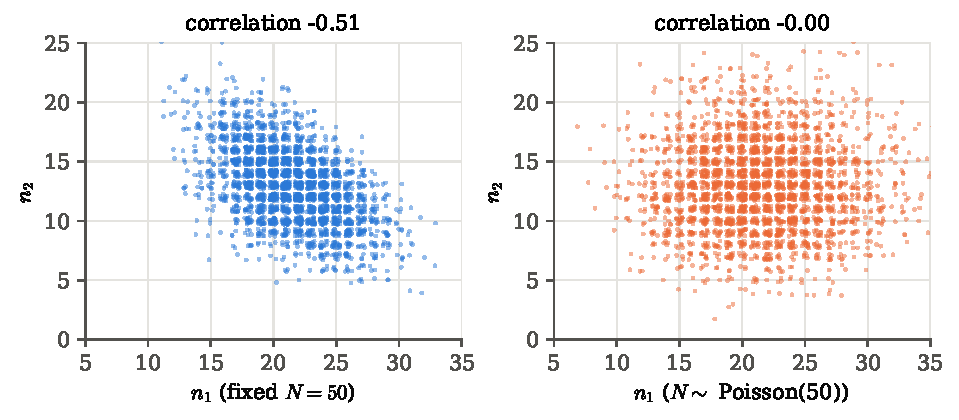
\includegraphics[width=\linewidth]{figures/ch02/03_multinomial.pdf}
\caption{Contents of bin 2 against bin 1 for $3000$ simulated histograms (a small random jitter separates the integer points). Left: with exactly $50$ events per histogram the cloud slopes downwards, because an extra event in bin 1 is an event missing from somewhere else. Right: when the number of events is itself Poisson, the cloud is round and the two bins are uncorrelated.}
\label{2a:fig:mult-sim}
\end{figure}

The simulated variance of bin 1 is $\twoaMultVarOneSim$ (theory $\twoaMultVarOneTh$), the covariance of bins 1 and 2 is $\twoaMultCovSim$ (theory $\twoaMultCovTh$) and their correlation is $\twoaMultCorrSim$ (theory $\twoaMultCorrTh$). The variance of the row sums is exactly $\twoaMultRowSumVar$: the zero mode of $\Cmat$. With a Poisson number of events the correlation drops to $\twoaMultCorrPois$, compatible with zero (\cref{2a:fig:mult-sim}). We prove in \cref{2a:sec:poisson-process} that Poisson-distributed totals make the bins \emph{exactly} independent. This is why fits to histograms whose total is not fixed in advance (most collider analyses) may treat bins as independent Poisson counts.

\begin{pitfall}[independent bins are an assumption]
It is tempting to treat histogram bins as independent, each with error $\sqrt{n_j}$. With a fixed number of entries that is wrong: the bins are anti-correlated by \eqref{2a:eq:multcov}. For many bins with small $p_j$ the correlation $\approx-\sqrt{p_ip_j}$ is small and the independent approximation is usually fine; for a histogram with a few dominant bins it is not. Normalised shapes (``unit-area'' histograms) always carry this constraint.
\end{pitfall}

\section{Rare events in many trials: the Poisson distribution}\label{2a:sec:poisson-limit}

A microgram of a long-lived isotope contains of order $10^{15}$ nuclei. In one second each nucleus decays with a tiny probability $p$, and the decays are independent. A Geiger counter records the number of decays in each one-second window. Strictly, this count is Binomial$(n,p)$ with $n\approx10^{15}$ nuclei. But nobody knows $n$ or $p$ separately, and nobody wants to evaluate $\binom{10^{15}}{k}$. What we \emph{can} measure is the average number of clicks per window, $\lambda=np$. The Poisson distribution is what the binomial becomes when the trials are very many, each is very unlikely to succeed, and only their product $\lambda$ matters. It is the distribution of \emph{counts of rare events}.

\paragraph{Physical picture: rare, independent, many.}
Photons arriving at a CCD pixel, dark counts in a photomultiplier, cosmic rays through a detector, events in one bin of a collider histogram, galaxies in a small cell of a sparse survey: each count is the sum of a huge number of chances, each tiny, none influencing the others. In every one of these cases only the mean count $\lambda$ enters the answer. The microscopic details, such as how many photons were emitted upstream or how many protons collided, drop out.

\paragraph{The question, step by step.}
\begin{enumerate}[leftmargin=1.6em,itemsep=1pt]
  \item Start from the exact binomial for $n$ trials with $p=\lambda/n$, so that the mean $np=\lambda$ stays fixed.
  \item Let $n\to\infty$. Which factors change and which survive?
  \item Is the limit a proper distribution? What are its mean and variance?
  \item How large must $n$ be for the approximation to be good?
\end{enumerate}

\subsection{The limit, line by line}

The derivation needs one limit from calculus. We prove it first.

\paragraph{The compound-interest limit.} For any fixed real $\lambda$, $\displaystyle\lim_{n\to\infty}\Bigl(1-\frac\lambda n\Bigr)^n=e^{-\lambda}$.
\emph{Why:} take the logarithm and use the Taylor series $\ln(1-x)=-x-\tfrac{x^2}2-\tfrac{x^3}3-\cdots$, valid for $\abs x<1$:
\begin{align*}
  \ln\Bigl(1-\frac\lambda n\Bigr)^n
  \eqby{1} n\ln\Bigl(1-\frac\lambda n\Bigr)
  \eqby{2} n\Bigl(-\frac\lambda n-\frac{\lambda^2}{2n^2}-\cdots\Bigr)
  = -\lambda-\frac{\lambda^2}{2n}-\cdots
  \;\xrightarrow{\;n\to\infty\;}\; -\lambda .
\end{align*}
\begin{explain}
  \item $\ln a^n=n\ln a$.
  \item Taylor series with $x=\lambda/n$, which is less than one in size once $n>\abs\lambda$.
\end{explain}
Exponentiate: the limit is $e^{-\lambda}$. \Cref{2a:fig:compound} shows how fast it is approached. The correction $-\lambda^2/(2n)$ in the exponent tells us that $(1-\lambda/n)^n$ is always a little \emph{below} $e^{-\lambda}$, by a relative amount of about $\lambda^2/2n$.

\begin{figure}[htbp]
\centering
\begin{tikzpicture}
\begin{axis}[width=10cm,height=5.2cm,xmin=0,xmax=62,ymin=0,ymax=0.056,
  xlabel={number of trials $n$},ylabel={$(1-3/n)^n$},
  ytick={0,0.01,0.02,0.03,0.04,0.05},yticklabel style={/pgf/number format/fixed,/pgf/number format/precision=2},
  axis lines=left,tick label style={font=\scriptsize},label style={font=\small}]
  \addplot[only marks,mark=*,mark size=1.3pt,formblue,samples at={4,5,...,60}] {(1-3/x)^x};
  \addplot[dashed,black,domain=0:62] {exp(-3)};
  \node[font=\scriptsize,anchor=south east] at (axis cs:60,0.0505) {$e^{-3}=0.0498$};
\end{axis}
\end{tikzpicture}
\caption{The probability that none of $n$ nuclei decays, when each decays with probability $3/n$. With four nuclei it is tiny; as the nuclei become more numerous and individually less likely to decay, it climbs towards the dashed limit $e^{-3}$, getting within ten per cent of it by $n\approx50$.}
\label{2a:fig:compound}
\end{figure}

With this limit in hand, we can take the binomial to the Poisson. Put $p=\lambda/n$ into the binomial pmf \eqref{2a:eq:binom}, so that the mean $np=\lambda$ stays fixed, and hold the count $k$ fixed while $n$ grows:
\begin{align}
  \binom nk p^k(1-p)^{n-k}
  &\eqby{1} \frac{n!}{k!\,(n-k)!}\,\frac{\lambda^k}{n^k}\Bigl(1-\frac\lambda n\Bigr)^{n}\Bigl(1-\frac\lambda n\Bigr)^{-k} \nonumber\\
  &\eqby{2} \frac{\lambda^k}{k!}\;\cdot\;\frac{n(n-1)\cdots(n-k+1)}{n^k}\;\cdot\;\Bigl(1-\frac\lambda n\Bigr)^{n}\;\cdot\;\Bigl(1-\frac\lambda n\Bigr)^{-k} \nonumber\\
  &\eqby{3} \frac{\lambda^k}{k!}\;\cdot\;\Bigl(1-\frac1n\Bigr)\Bigl(1-\frac2n\Bigr)\cdots\Bigl(1-\frac{k-1}n\Bigr)\;\cdot\;\Bigl(1-\frac\lambda n\Bigr)^{n}\;\cdot\;\Bigl(1-\frac\lambda n\Bigr)^{-k} \nonumber\\
  &\xrightarrow{\;n\to\infty\;} \frac{\lambda^k}{k!}\cdot 1\cdot e^{-\lambda}\cdot 1 . \label{2a:eq:poislimit}
\end{align}
\begin{explain}
  \item Substitute $p=\lambda/n$ and split $(1-p)^{n-k}=(1-p)^n(1-p)^{-k}$.
  \item Regroup. $n!/(n-k)!=n(n-1)\cdots(n-k+1)$ has exactly $k$ factors.
  \item Divide each of the $k$ factors by one of the $k$ powers of $n$.
\end{explain}
Now take the four factors in the third line of the chain one at a time as $n\to\infty$. The first, $\lambda^k/k!$, does not involve $n$. In the second, each of the $k-1$ brackets $(1-j/n)$ goes to $1$; there is a \emph{fixed} number of them because $k$ is fixed, so their product goes to $1$. The third, $(1-\lambda/n)^n$, goes to $e^{-\lambda}$ by the compound-interest limit. The fourth is a fixed power, $-k$, of something that goes to one, so it goes to one.

\begin{workdef}[Poisson distribution]
$X\sim\mathrm{Poisson}(\lambda)$ if
\begin{equation}
  f(k\given\lambda)\;=\;e^{-\lambda}\,\frac{\lambda^k}{k!},\qquad k=0,1,2,\dots \label{2a:eq:pois}
\end{equation}
for some $\lambda>0$ \unpack{the mean number of events, a real number, not necessarily an integer}. There is no upper limit on $k$.
\emph{Recognise it by:} a count of events that are individually rare and mutually independent, out of a very large (or unknown) number of opportunities.
\end{workdef}

The number of trials $n$ has disappeared. The only parameter left is the mean count $\lambda$, the one thing we can measure.

\subsection{Normalisation, mean, variance, mgf}

Every sum here is the exponential series $e^{x}=\sum_{k=0}^\infty x^k/k!$, valid for every real (or complex) $x$, in disguise.
\begin{align*}
  \sum_{k=0}^\infty f(k) &\eqby{1} e^{-\lambda}\sum_{k=0}^\infty\frac{\lambda^k}{k!} \eqby{2} e^{-\lambda}e^{\lambda}=1,\\
  \E X &\eqby{3} e^{-\lambda}\sum_{k=1}^\infty k\frac{\lambda^k}{k!}
       \eqby{4} \lambda e^{-\lambda}\sum_{k=1}^\infty\frac{\lambda^{k-1}}{(k-1)!}
       \eqby{2} \lambda e^{-\lambda}e^{\lambda}=\lambda,\\
  \E[X(X-1)] &\eqby{5} e^{-\lambda}\sum_{k=2}^\infty k(k-1)\frac{\lambda^k}{k!}
       = \lambda^2 e^{-\lambda}\sum_{k=2}^\infty\frac{\lambda^{k-2}}{(k-2)!} \eqby{2} \lambda^2,\\
  \Var X &\eqby{6} \E[X(X-1)]+\E X-(\E X)^2 = \lambda^2+\lambda-\lambda^2=\lambda .
\end{align*}
\begin{explain}
  \item Take the constant $e^{-\lambda}$ out of the sum.
  \item Exponential series (after renaming $j=k-1$ or $j=k-2$).
  \item The $k=0$ term vanishes.
  \item $k/k!=1/(k-1)!$, and one factor $\lambda$ taken out.
  \item The same trick with $k(k-1)/k!=1/(k-2)!$; the $k=0,1$ terms vanish.
  \item As for the binomial.
\end{explain}
\begin{keyidea}[mean equals variance]
For a Poisson count, $\E X=\Var X=\lambda$. The standard deviation is $\sqrt\lambda$, and the \emph{relative} fluctuation is $1/\sqrt\lambda$.
\end{keyidea}
So a Poisson count has mean and variance both equal to $\lambda$. Its standard deviation is $\sqrt\lambda$, and its \emph{relative} fluctuation, standard deviation over mean, is $1/\sqrt\lambda$. This is the origin of the ``$\sqrt N$'' error bar on a count, and of photon shot noise: to measure a flux to $1\%$ we need $1/\sqrt\lambda=0.01$, that is, about $10^4$ photons. The same results follow from the binomial ones by taking the limit: $np=\lambda$ and $np(1-p)=\lambda(1-\lambda/n)\to\lambda$.

The mgf is
\begin{align}
  M_X(t) \eqby{1} e^{-\lambda}\sum_{k=0}^\infty\frac{(\lambda e^t)^k}{k!} \eqby{2} e^{-\lambda}e^{\lambda e^t}=\exp\bigl[\lambda(e^t-1)\bigr]. \label{2a:eq:poismgf}
\end{align}
\begin{explain}
  \item $e^{tk}\lambda^k=(\lambda e^t)^k$.
  \item Exponential series with $x=\lambda e^t$.
\end{explain}
It is also the limit of the binomial mgf: $(1+p(e^t-1))^n=(1+\lambda(e^t-1)/n)^n\to e^{\lambda(e^t-1)}$ by the same compound-interest limit.

\paragraph{The shape: a recursion.} Dividing consecutive terms of \eqref{2a:eq:pois},
\begin{equation}
  \frac{f(k)}{f(k-1)}=\frac{e^{-\lambda}\lambda^k/k!}{e^{-\lambda}\lambda^{k-1}/(k-1)!}=\frac\lambda k . \label{2a:eq:poisrec}
\end{equation}
Each step from $k-1$ to $k$ multiplies the probability by $\lambda/k$. That factor is larger than one while $k<\lambda$ and smaller than one once $k>\lambda$. So the pmf rises while $k<\lambda$ and falls once $k>\lambda$. The most probable count is $\lfloor\lambda\rfloor$ (and if $\lambda$ is an integer, $\lambda-1$ and $\lambda$ are equally probable). The recursion is also the numerically stable way to compute the pmf: start at $f(0)=e^{-\lambda}$ and multiply by $\lambda/k$, never forming $\lambda^k$ or $k!$ separately \srcref{CasellaBerger}{(3.2.6)--(3.2.7), p.~77}.

\subsection{How good is the approximation?}

A convenient single number for the distance between two distributions $f$ and $g$ on the integers is the \newterm{total variation distance} $\mathrm{TV}(f,g)=\tfrac12\sum_k\abs{f(k)-g(k)}$ \unpack{the largest possible difference between the probabilities the two distributions give to the same event}. For the binomial with $p=\lambda/n$ and the Poisson with the same mean, a classical inequality due to Le~Cam states
\[
  \mathrm{TV}\bigl(\mathrm{Binomial}(n,\lambda/n),\,\mathrm{Poisson}(\lambda)\bigr)\;\le\;np^2\;=\;\frac{\lambda^2}{n}.
\]
Why $np^2$? Each Bernoulli trial differs from a Poisson$(p)$ variable only in the rare event of two or more ``successes'' in one trial, which has probability of order $p^2$. There are $n$ trials, so the differences add up to at most about $np^2$. The script \pyname{code/ch02/04_poisson_limit.py} computes the actual distance for $\lambda=3$: $\twoaTVfive$ at $n=5$, $\twoaTVtwenty$ at $n=20$, $\twoaTVhundred$ at $n=100$ and $\twoaTVthousand$ at $n=1000$. It falls like $1/n$, as the bound says, but is about ten times smaller than the bound.

\subsection{Worked examples}

\paragraph{Example: a typesetter's errors, exact and Poisson.}
A typesetter makes on average one error per $500$ words. Five pages of $300$ words hold $1500$ words. What is the probability of at most two errors? Exactly, $X\sim\mathrm{Binomial}(1500,1/500)$; approximately, $X\sim\mathrm{Poisson}(3)$.
\begin{align*}
  \Prob(X\le2) &\approx e^{-3}\Bigl(1+3+\frac{3^2}{2}\Bigr) \eqby{1} 0.049787\times8.5 = 0.4232 .
\end{align*}
\begin{explain}
  \item Sum of \eqref{2a:eq:pois} for $k=0,1,2$ with $\lambda=np=1500/500=3$.
\end{explain}
The exact binomial gives $\twoaTypExact$; the Poisson approximation gives $\twoaTypPois$, wrong in the fourth decimal \srcref{CasellaBerger}{Ex.~3.2.5, p.~77}.

\paragraph{Example: photomultiplier dark counts.}
A photomultiplier produces on average $5$ dark pulses every $3$~ms. In the next $1$~ms, what is the probability of no dark pulse, and of at least two? The count in $1$~ms is Poisson with $\lambda=5/3$.
\begin{align*}
  \Prob(X=0) &= e^{-5/3} = 0.189,\\
  \Prob(X\ge2) &\eqby{1} 1-\Prob(X=0)-\Prob(X=1) \eqby{2} 1-0.189-\tfrac53(0.189) = 1-0.189-0.315 = 0.496 .
\end{align*}
\begin{explain}
  \item Complement of ``zero or one''.
  \item $\Prob(X=1)=\lambda e^{-\lambda}$, which is $\lambda$ times $\Prob(X=0)$ by the recursion \eqref{2a:eq:poisrec}.
\end{explain}
So a $1$~ms coincidence window contains at least two dark pulses half the time: at this rate, a two-fold coincidence of dark noise is not rare. The numbers are those of a telephone switchboard in \srcref{CasellaBerger}{Ex.~3.2.4, p.~76}, a reminder that the Poisson story does not care what is being counted.

\paragraph{Example: events in a collider signal region.}
A new process has cross-section $\sigma=0.5$~fb, the data set has integrated luminosity $L=20~\text{fb}^{-1}$ and the selection efficiency is $\epsilon=0.3$. Each of the enormous number of proton--proton collisions has a tiny, independent chance to produce a selected signal event, so the number of selected events is Poisson with mean \srcref{Cowan}{(2.12), p.~30}
\[
  \lambda=\sigma L\epsilon=0.5\times20\times0.3=3 .
\]
The chance of seeing \emph{nothing} is $f(0\given3)=e^{-3}=0.0498$, about $5\%$. Read backwards, this is the classic ``three events'' rule: if we see zero events, any model predicting $\lambda\ge3$ is excluded at about $95\%$ confidence (\cref{ch:04}).

\subsection{Python: literally many nuclei}

\pyfile[firstline=24,lastline=28,firstnumber=24]{code/ch02/04_poisson_limit.py}{Counting decays of 2000 nuclei per window}

Each counting window gets $2000$ fresh uniform numbers, one per nucleus, and a nucleus ``decays'' if its number is below $\lambda/n=3/2000$. The count per window is the number of decays. Nothing in this code mentions $e^{-\lambda}$ or $k!$: the Poisson law has to emerge from the process. The script then computes the total variation distances quoted above and the typesetter example.

\begin{figure}[htbp]
\centering
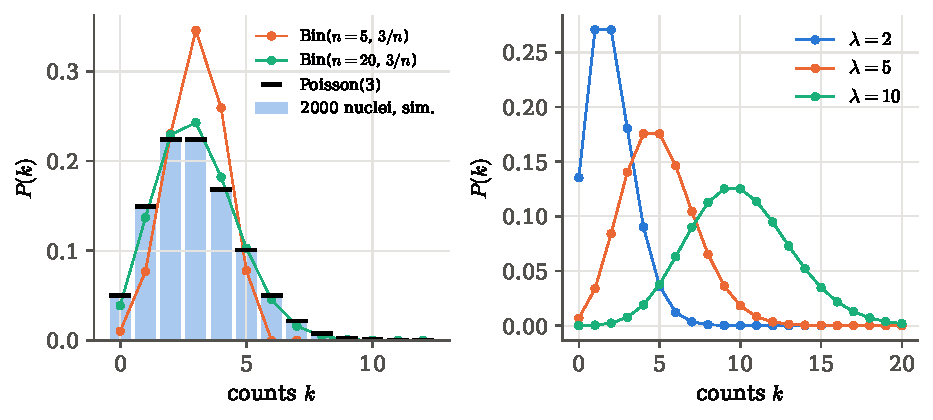
\includegraphics[width=\linewidth]{figures/ch02/04_poisson_limit.pdf}
\caption{Left: the histogram of decay counts from $2000$ simulated nuclei per window (bars) sits on the Poisson(3) pmf (black ticks). The binomials with only $5$ or $20$ trials and the same mean are visibly narrower, because each trial can produce at most one event. Right: Poisson shapes for $\lambda=2,5,10$; skewed to the right at small $\lambda$, nearly symmetric by $\lambda=10$.}
\label{2a:fig:pois-limit}
\end{figure}

Over $20\,000$ windows the sample mean is $\twoaPLMean$ and the sample variance is $\twoaPLVar$, equal within the statistical error as \emph{mean $=$ variance} demands. The fraction of empty windows is $\twoaPLZeroSim$, against $e^{-3}=\twoaPLZeroTh$ (\cref{2a:fig:pois-limit}). The right panel reproduces the shapes of \srcref{Cowan}{Fig.~2.3, p.~29}. The growing symmetry with $\lambda$ is the start of the Gaussian limit, previewed in \cref{2a:sec:failures}.

\paragraph{What this bought us.}
When many independent chances each have a small probability, the count is Poisson with the single parameter $\lambda=np$. Its variance equals its mean, so the relative scatter of a count is $1/\sqrt\lambda$. The approximation error is of order $\lambda^2/n$, negligible for any macroscopic number of trials.

\begin{pitfall}[``rare'' refers to each trial, not to the count]
The count itself need not be small: a CCD pixel may collect $10^5$ photons, and that count is still Poisson, because each of the $10^{20}$ photons emitted by the star had a tiny chance of landing in this pixel. What must be small is the probability per opportunity, and what must hold is independence. Conversely, a small count is not automatically Poisson: the number of dead channels in a $4$-channel module is binomial with $n=4$, and \cref{2a:fig:pois-limit} shows how different that can be.
\end{pitfall}

\section{The Poisson process: constant rate, no memory}\label{2a:sec:poisson-process}

In \cref{2a:sec:poisson-limit} the Poisson distribution came from a binomial over $n$ nuclei, each with a tiny chance to decay. Often there is no such $n$ to imagine. Cosmic rays arrive from the sky, photons from a distant quasar, dark pulses from a photocathode. All we know is that events come \emph{at random in time}, with some average rate $\lambda$ (events per second), and that the process has no memory: what happened in the last second does not affect the next. These two physical statements are enough. Through a differential equation, they force the count in any window of length $t$ to be Poisson$(\lambda t)$. The same machinery then shows that three common operations give Poisson counts again: thinning a Poisson stream (losing events at random), adding two streams, and splitting one into histogram bins.

\paragraph{Physical picture: a master equation with one-way hops.}
Think of the count $N(t)$, the number of events up to time $t$, as the state of a system that can only climb a ladder: $0\to1\to2\to\cdots$, one rung at a time, with hopping rate $\lambda$ from every rung. The probability of being on rung $n$ is fed from rung $n-1$ and drains into rung $n+1$. The rate equations for a radioactive decay chain have exactly this form, and so does the master equation of a birth process in statistical mechanics.

\paragraph{The question, step by step.}
\begin{enumerate}[leftmargin=1.6em,itemsep=1pt]
  \item What exactly do ``random in time at rate $\lambda$'' and ``no memory'' assume? State the inputs, then derive what they imply for a very short interval $h$.
  \item How does the probability of having $n$ events by time $t$ change between $t$ and $t+h$?
  \item Let $h\to0$ to get differential equations, and solve them.
  \item What happens to such a stream when we lose some events, add another stream, or sort the events into bins?
\end{enumerate}

\subsection{From three physical inputs to the short-interval rules}
\label{2a:sec:poisson-inputs}

Think of photons from a star whose brightness does not change. Even a perfect
detector does not count the same number in every exposure, because the photons
arrive one at a time at random instants. That scatter is \newterm{shot noise}.
It is not interference added to the signal. It is what counting discrete,
independent arrivals means. We now find its distribution from first principles:
we say exactly what we assume about the arrivals, and derive everything else.

\emph{The inputs.} Three are physical, and one is a mathematical regularity
condition.
\begin{enumerate}[label=(P\arabic*),leftmargin=2.6em,itemsep=1pt]
  \item \emph{No memory.} The numbers of events in non-overlapping time windows
        are independent. An arrival tells us nothing about when the next one comes.
  \item \emph{Constant rate.} The distribution of the count in a window depends
        only on its length, not on when it starts. The source does not brighten
        or fade during the exposure.
  \item \emph{One at a time.} Events arrive singly, never in bunches at the same
        instant.
  \item[(R)] \emph{Regularity.} The probability $P_0(h)$ that a window of length
        $h$ is empty changes continuously with $h$. This is a property we demand of
        the mathematics, not a statement about photons.
\end{enumerate}

\emph{The empty window.} Split a window of length $h_1+h_2$ into two pieces. It
is empty exactly when both pieces are empty, so
\begin{align}
  P_0(h_1+h_2)
  &\eqby{1} \Prob(\text{first piece empty})\,\Prob(\text{second piece empty})
   \eqby{2} P_0(h_1)\,P_0(h_2).
  \label{2a:eq:cauchy}
\end{align}
\begin{explain}
  \item (P1): the two pieces do not overlap, so their counts are independent and the probabilities multiply.
  \item (P2): each piece behaves like any window of the same length, wherever it sits.
\end{explain}
Write $g(h)=-\ln P_0(h)$. Then \eqref{2a:eq:cauchy} says $g(h_1+h_2)=g(h_1)+g(h_2)$:
$g$ turns sums of lengths into sums of values. Applying it $n$ times gives
$g(n\,h)=n\,g(h)$, so $g(m/n)=(m/n)\,g(1)$ for every rational length, and by (R) the
same holds for every length. Hence, with $\lambda\equiv g(1)\ge0$,
\begin{equation}
  P_0(h)=e^{-\lambda h}.
  \label{2a:eq:empty}
\end{equation}
Nothing was assumed about the size of $\lambda$; it is simply the constant that
the inputs leave free, and below it turns out to be the mean number of events per
unit time, the \newterm{rate}.

\emph{At least one event in a short window.} Expanding \eqref{2a:eq:empty} for small $h$,
\begin{align*}
  \Prob(\text{at least one event in }h)
  &= 1-e^{-\lambda h}
   \eqby{1} \lambda h-\tfrac12(\lambda h)^2+\cdots
   = \lambda h+O(h^2).
\end{align*}
\begin{explain}
  \item The Taylor series $e^{-x}=1-x+\tfrac12x^2-\cdots$.
\end{explain}
So ``probability proportional to the length'' is not an assumption. It is the
first term of the exact answer, and it holds for any short window.

\emph{Two or more in a short window.} By (P3) two events never share an instant,
so two arrivals in one window are two separate events. Cut the window into two
halves: two events in the window means at least one event in each half, or two
in one half. The first has probability
$\bigl(\lambda\tfrac h2+O(h^2)\bigr)^2=O(h^2)$ by (P1), and repeating the halving
shows the second is also $O(h^2)$. So
\begin{equation*}
  \Prob(\text{two or more in }h)=O(h^2),\qquad
  \Prob(\text{exactly one in }h)=\lambda h+O(h^2).
\end{equation*}
Two arrivals need two rare events to coincide, a product of two small
probabilities. That is why, in a short enough window, the only outcomes that
matter are ``nothing'' and ``exactly one''.

We need one piece of notation for what follows. A function $g(h)$ is $o(h)$
(``little-o of $h$'') if $g(h)/h\to0$ as $h\to0$ \unpack{it vanishes faster than
$h$ itself}. For example $h^2=o(h)$, but $\sqrt h$ and $3h$ are not. Every $O(h^2)$
above is $o(h)$.

\begin{workdef}[Poisson process]
A \newterm{counting process} $N(t)$ is the number of events in $[0,t]$. Inputs
(P1)--(P3) and (R) give it the five properties of a \newterm{homogeneous Poisson
process} with rate $\lambda$:
\begin{enumerate}[label=(\roman*),leftmargin=2em,itemsep=1pt]
  \item $N(0)=0$ \unpack{we start counting at $t=0$};
  \item the counts in non-overlapping intervals are independent \unpack{input (P1)};
  \item the distribution of the count in $(t,t+h]$ depends only on the length $h$ \unpack{input (P2)};
  \item $\Prob(\text{exactly one event in }(t,t+h])=\lambda h+o(h)$ \unpack{derived above, not assumed};
  \item $\Prob(\text{two or more events in }(t,t+h])=o(h)$ \unpack{derived above from (P3)}.
\end{enumerate}
\emph{Recognise it by:} events that arrive one at a time, independently, at a steady average rate.
\end{workdef}

\begin{pitfall}[When the inputs fail]
Each input can fail, and then the counts are not Poisson. A source whose
brightness changes during the exposure breaks (P2) (the count is then Poisson with
mean $\int\lambda(t)\,\dd t$, see below). Dead time after each detection breaks
(P1): a detector that is blind for a while after a hit makes the next arrival
depend on the last. Events that come in bursts break (P3): an air shower fires
many detectors at once, and thermal light shows photon bunching. In each case the
variance of the count differs from its mean, which is the quickest test.
\end{pitfall}

\begin{figure}[htbp]
\centering
\begin{tikzpicture}[x=1cm,y=1cm]
  \draw[->,thick] (0,0) -- (11,0);
  \node[lbl,anchor=north] at (11,-0.05) {$t$};
  \foreach \x in {0,0.25,...,10}{\draw[faint] (\x,-0.12) -- (\x,0.12);}
  \foreach \x in {1.125,2.875,3.375,6.625,8.875,9.375}{
    \fill[bdryred] (\x,0) circle (2.2pt);}
  \node[lbl,anchor=north] at (0,-0.15) {$0$};
  \node[lbl,anchor=north] at (10,-0.15) {$T$};
  \draw[formblue,thick] (6.5,-0.18) rectangle (6.75,0.18);
  \draw[formblue,dashed] (6.5,-0.18) -- (5.2,-1.35);
  \draw[formblue,dashed] (6.75,-0.18) -- (8.2,-1.35);
  \draw[formblue,thick] (5.2,-1.35) rectangle (8.2,-2.25);
  \fill[bdryred] (6.7,-1.8) circle (2.2pt);
  \node[font=\scriptsize,anchor=west] at (8.35,-1.55) {one slice of width $h$:};
  \node[font=\scriptsize,anchor=west] at (8.35,-1.85) {one event, prob.\ $\lambda h$};
  \node[font=\scriptsize,anchor=west] at (8.35,-2.15) {two or more, prob.\ $o(h)$};
  \node[font=\scriptsize,anchor=east] at (5.05,-1.8) {independent of all other slices};
\end{tikzpicture}
\caption{The short-interval rules as a picture. The time axis is cut into short slices; each slice independently contains an event (red dots) with probability $\lambda h$, and practically never two. Counting the dots in $[0,T]$ means counting successes in $T/h$ Bernoulli trials with $p=\lambda h$.}
\label{2a:fig:slices}
\end{figure}

\Cref{2a:fig:slices} already suggests the answer. Cut $[0,t]$ into $n=t/h$ slices. Each slice is a Bernoulli trial with success probability $p=\lambda h=\lambda t/n$, and the trials are independent by (ii). So $N(t)$ is binomial with $np=\lambda t$, and as $h\to0$ we are in the limit of \cref{2a:sec:poisson-limit}: $N(t)\sim\mathrm{Poisson}(\lambda t)$. Now we derive the same result a second way, which does not rely on the binomial at all and which generalises to rates that vary in time.

\subsection{The differential equations}

Let $P_n(t)=\Prob(N(t)=n)$. At $t=0$, $P_0(0)=1$ and $P_n(0)=0$ for $n\ge1$, by property (i).

\paragraph{No events.} To have no events by $t+h$ we need no events by $t$ \emph{and} none in $(t,t+h]$:
\begin{align*}
  P_0(t+h) &\eqby{1} P_0(t)\,\Prob(\text{no event in }(t,t+h]) \eqby{2} P_0(t)\bigl(1-\lambda h-o(h)\bigr),\\
  \frac{P_0(t+h)-P_0(t)}{h} &\eqby{3} -\lambda P_0(t)-P_0(t)\frac{o(h)}{h}
  \;\xrightarrow{\;h\to0\;}\; \frac{\dd P_0}{\dd t}=-\lambda P_0 .
\end{align*}
\begin{explain}
  \item Property (ii): the count in $(t,t+h]$ is independent of the count in $[0,t]$, so the probabilities multiply.
  \item Properties (iv) and (v): the probability of zero events is $1$ minus the probability of one minus the probability of two or more, and both $o(h)$ terms combine into one $o(h)$.
  \item Subtract $P_0(t)$ and divide by $h$. The last term vanishes as $h\to0$ by the definition of $o(h)$.
\end{explain}
With $P_0(0)=1$ the solution is $P_0(t)=e^{-\lambda t}$: the probability of an empty window decays exponentially with its length, just as the survival probability of an unstable nucleus does.

\paragraph{$n\ge1$ events.} To have $n$ events by $t+h$, either we had $n$ by $t$ and none arrive, or we had $n-1$ and one arrives, or we had $n-j$ for $j\ge2$ and $j$ arrive:
\begin{align*}
  P_n(t+h) &\eqby{1} P_n(t)\bigl(1-\lambda h\bigr)+P_{n-1}(t)\,\lambda h+o(h),\\
  \frac{\dd P_n}{\dd t} &\eqby{2} -\lambda P_n(t)+\lambda P_{n-1}(t) .
\end{align*}
\begin{explain}
  \item The three routes are mutually exclusive, so their probabilities add, and each is a product by property (ii). All routes with two or more arrivals, and the corrections to the first two, are $o(h)$ by (iv) and (v).
  \item Subtract $P_n(t)$, divide by $h$ and let $h\to0$.
\end{explain}
This is the \newterm{master equation} of the process (\cref{2a:fig:ladder}): rung $n$ gains probability from rung $n-1$ at rate $\lambda P_{n-1}$ and loses it to rung $n+1$ at rate $\lambda P_n$.

\begin{figure}[htbp]
\centering
\begin{tikzpicture}[st/.style={circle,draw=accent,fill=ideabg,thick,minimum size=9mm,font=\small}]
  \foreach \n/\x in {0/0,1/2.2,2/4.4,3/6.6}{\node[st] (s\n) at (\x,0) {$\n$};}
  \node (dots) at (8.6,0) {$\cdots$};
  \draw[->,thick,formblue] (s0) -- (s1);
  \draw[->,thick,formblue] (s1) -- (s2);
  \draw[->,thick,formblue] (s2) -- (s3);
  \draw[->,thick,formblue] (s3) -- (dots);
  \node[font=\scriptsize,anchor=north] at (0,-0.6) {$P_0=e^{-\lambda t}$};
  \node[font=\scriptsize,anchor=north] at (2.2,-0.6) {$\lambda t\,e^{-\lambda t}$};
  \node[font=\scriptsize,anchor=north] at (4.4,-0.6) {$\tfrac{(\lambda t)^2}{2}e^{-\lambda t}$};
  \node[font=\scriptsize,anchor=north] at (6.6,-0.6) {$\tfrac{(\lambda t)^3}{6}e^{-\lambda t}$};
\end{tikzpicture}
\caption{The count as a system climbing a ladder. Every hop goes one rung up and happens at the same rate $\lambda$, whatever the rung; no hop ever goes down. Below each rung is its occupation probability at time $t$, the solution derived in the text.}
\label{2a:fig:ladder}
\end{figure}

\paragraph{Solving the ladder.} The master equation has the form $y'+\lambda y=g(t)$, a linear first-order equation, with $y=P_n$ and $g=\lambda P_{n-1}$. Such an equation is solved with the \emph{integrating factor} $e^{\lambda t}$. Multiplying by it turns the left side into a single derivative: $(e^{\lambda t}y)'=e^{\lambda t}(y'+\lambda y)=e^{\lambda t}g$. So define $Q_n(t)=e^{\lambda t}P_n(t)$. Then
\begin{align*}
  \frac{\dd Q_n}{\dd t} \eqby{1} e^{\lambda t}\Bigl(\frac{\dd P_n}{\dd t}+\lambda P_n\Bigr) \eqby{2} e^{\lambda t}\lambda P_{n-1} = \lambda Q_{n-1},
  \qquad Q_0(t)=1,\quad Q_n(0)=0\ (n\ge1).
\end{align*}
\begin{explain}
  \item Product rule.
  \item The master equation: $\dd P_n/\dd t+\lambda P_n=\lambda P_{n-1}$.
\end{explain}
Now climb the ladder by induction. Suppose $Q_{n-1}(t)=(\lambda t)^{n-1}/(n-1)!$. This is true for $n-1=0$, since $Q_0=e^{\lambda t}P_0=e^{\lambda t}e^{-\lambda t}=1$. Then
\begin{align*}
  Q_n(t) \eqby{1} \int_0^t\lambda\,Q_{n-1}(s)\,\dd s \eqby{2} \int_0^t\frac{\lambda^n s^{n-1}}{(n-1)!}\,\dd s \eqby{3} \frac{\lambda^nt^n}{n!}.
\end{align*}
\begin{explain}
  \item Integrate $\dd Q_n/\dd s=\lambda Q_{n-1}$ from $0$ to $t$, using $Q_n(0)=0$.
  \item The induction hypothesis.
  \item $\int_0^ts^{n-1}\dd s=t^n/n$, and $(n-1)!\,n=n!$.
\end{explain}
\begin{keyidea}[the count of a Poisson process]
For a homogeneous Poisson process with rate $\lambda$,
\begin{equation}
  \Prob\bigl(N(t)=n\bigr)=e^{-\lambda t}\frac{(\lambda t)^n}{n!},\qquad N(t)\sim\mathrm{Poisson}(\lambda t), \label{2a:eq:ppcount}
\end{equation}
and by (iii) the count in \emph{any} window of length $t$ has the same distribution.
\end{keyidea}
Undoing the substitution, $P_n(t)=e^{-\lambda t}Q_n(t)=e^{-\lambda t}(\lambda t)^n/n!$: the count $N(t)$ is Poisson with mean $\lambda t$, as in \eqref{2a:eq:ppcount}. The two routes, the binomial limit and the master equation, give the same answer. So whenever events are rare, independent and at a steady rate, the Poisson distribution is forced on us.

\paragraph{A rate that varies in time.} Suppose the rate is a function $\lambda(t)$: a source that fades, or a beam whose intensity falls during a fill. Then input (P2), and with it property (iii), is dropped, and (iv) becomes $\lambda(t)h+o(h)$. The master equation keeps its form with $\lambda$ replaced by $\lambda(t)$. The integrating factor becomes $e^{m(t)}$, where $m(t)=\int_0^t\lambda(s)\,\dd s$ is the expected number of events up to $t$. Because $\dd m/\dd t=\lambda(t)$, the same induction gives $Q_n=m(t)^n/n!$. So
\[
  N(t)\sim\mathrm{Poisson}\bigl(m(t)\bigr),\qquad N(s+t)-N(s)\sim\mathrm{Poisson}\bigl(m(s+t)-m(s)\bigr).
\]
Only the \emph{integrated} rate over the window matters \mainref{Thm.~23.33, p.~395}. For a collider, $m$ is $\sigma\epsilon$ times the integrated luminosity, whatever the luminosity did during the run.

\subsection{Three closure properties}

Real counting chains lose events, add sources and sort events into bins. Each of these operations keeps us inside the Poisson family.

\paragraph{Adding independent sources: sums of independent Poissons are Poisson.} If $X_1\sim\mathrm{Poisson}(\lambda_1)$ and $X_2\sim\mathrm{Poisson}(\lambda_2)$ are independent, then $X_1+X_2\sim\mathrm{Poisson}(\lambda_1+\lambda_2)$.
The direct proof sums over all the ways to split $k$ events between the two sources (a \emph{convolution}):
\begin{align*}
  \Prob(X_1+X_2=k)
  &\eqby{1} \sum_{j=0}^k\Prob(X_1=j)\,\Prob(X_2=k-j)
  \eqby{2} \sum_{j=0}^k e^{-\lambda_1}\frac{\lambda_1^j}{j!}\,e^{-\lambda_2}\frac{\lambda_2^{k-j}}{(k-j)!}\\
  &\eqby{3} \frac{e^{-(\lambda_1+\lambda_2)}}{k!}\sum_{j=0}^k\binom kj\lambda_1^j\lambda_2^{k-j}
  \eqby{4} e^{-(\lambda_1+\lambda_2)}\frac{(\lambda_1+\lambda_2)^k}{k!}.
\end{align*}
\begin{explain}
  \item The event $\{X_1+X_2=k\}$ is the disjoint union of $\{X_1=j,X_2=k-j\}$, and independence factorises each term.
  \item Poisson pmfs.
  \item Multiply and divide by $k!$ to form $\binom kj=k!/(j!(k-j)!)$.
  \item Binomial theorem.
\end{explain}
With mgfs it is one line: $e^{\lambda_1(e^t-1)}e^{\lambda_2(e^t-1)}=e^{(\lambda_1+\lambda_2)(e^t-1)}$ \mainref{Ex.~3.35, p.~58}\footnote{The line ``$Y=Y_1+Y+2$'' in the source is a misprint for $Y=Y_1+Y_2$.}. In the process picture the result is obvious. Interleave two independent streams, and each short slice holds one event with probability $(\lambda_1+\lambda_2)h+o(h)$: the merged stream is a Poisson process with the summed rate. So signal plus background, with expected counts $s$ and $b$, is Poisson with mean $s+b$.

\paragraph{Losing events: thinning.} Each event of a Poisson$(\lambda)$ stream is detected independently with efficiency $\epsilon$. Given $N=n$ true events, the detected number is $Y\given N=n\sim\mathrm{Binomial}(n,\epsilon)$. Marginalise over the unobserved $N$:
\begin{align*}
  \Prob(Y=y)
  &\eqby{1} \sum_{n=y}^\infty\Prob(Y=y\given N=n)\Prob(N=n)
  \eqby{2} \sum_{n=y}^\infty\frac{n!}{y!\,(n-y)!}\epsilon^y(1-\epsilon)^{n-y}\,e^{-\lambda}\frac{\lambda^n}{n!}\\
  &\eqby{3} \frac{(\epsilon\lambda)^y}{y!}e^{-\lambda}\sum_{j=0}^\infty\frac{\bigl((1-\epsilon)\lambda\bigr)^{j}}{j!}
  \eqby{4} \frac{(\epsilon\lambda)^y}{y!}e^{-\lambda}e^{(1-\epsilon)\lambda}
  = e^{-\epsilon\lambda}\frac{(\epsilon\lambda)^y}{y!}.
\end{align*}
\begin{explain}
  \item Law of total probability over the nuisance variable $N$ (\cref{ch:01}); $n<y$ is impossible.
  \item Binomial and Poisson pmfs.
  \item Cancel $n!$, write $\lambda^n=\lambda^y\lambda^{n-y}$, and rename $j=n-y$.
  \item Exponential series.
\end{explain}
So $Y\sim\mathrm{Poisson}(\epsilon\lambda)$ \mainref{p.~395}. A detector with efficiency $\epsilon$ looking at a Poisson source records a Poisson count with mean $\epsilon\lambda$. This is why $\lambda=\sigma L\epsilon$ in the collider example of \cref{2a:sec:poisson-limit} could simply include the efficiency as a factor.

\paragraph{Sorting into bins: Poissonisation.} Now let a Poisson$(\nu)$ number of events be sorted into $m$ histogram bins with probabilities $p_j$ (\cref{2a:sec:multinomial}). Given the total $N=\sum n_j$, the bins are multinomial. The joint pmf of the bins is
\begin{align*}
  \Prob(n_1,\dots,n_m)
  &\eqby{1} \Prob(N=\textstyle\sum_jn_j)\;\frac{N!}{n_1!\cdots n_m!}p_1^{n_1}\cdots p_m^{n_m}
  \eqby{2} e^{-\nu}\frac{\nu^N}{N!}\,\frac{N!}{\prod_jn_j!}\prod_jp_j^{n_j}\\
  &\eqby{3} \prod_{j=1}^m e^{-\nu p_j}\frac{(\nu p_j)^{n_j}}{n_j!} .
\end{align*}
\begin{explain}
  \item The counts determine $N$, so the joint probability is $\Prob(N)$ times the multinomial given $N$.
  \item Poisson pmf of $N$.
  \item Cancel $N!$; write $\nu^N=\prod_j\nu^{n_j}$ and $e^{-\nu}=\prod_je^{-\nu p_j}$ using $\sum_jp_j=1$.
\end{explain}
The joint pmf \emph{factorises} into a product of Poisson$(\nu p_j)$ pmfs, one per bin. So the bins are \emph{independent} Poisson counts. This is the proof promised in \cref{2a:sec:multinomial}: the anti-correlation came entirely from fixing the total. It is also why a binned likelihood with a Poisson term per bin, $\prod_je^{-\nu_j}\nu_j^{n_j}/n_j!$, is the standard model of a collider histogram (\cref{ch:03}).

\subsection{Worked examples}

\paragraph{Example: an empty window.}
A counter sees background at $\lambda=2$~counts/s. What is the probability that a $5$~s window is empty, and that a $1$~s window is? By \eqref{2a:eq:ppcount}, $\Prob(N(5)=0)=e^{-10}=\twoaPPZeroTh$ and $\Prob(N(1)=0)=e^{-2}=0.135$. The five-second window is five one-second windows in a row, and by independence (input P1) $e^{-10}=(e^{-2})^5$: the empty-window probabilities multiply, which is precisely why $P_0$ had to be an exponential.

\paragraph{Example: signal on top of background.}
A search window expects $b=2.4$ background and $s=1.2$ signal events, both Poisson and independent. The total count is Poisson$(3.6)$. The probability of observing at least $6$ events is
\begin{align*}
  \Prob(N\ge6) &\eqby{1} 1-e^{-3.6}\sum_{k=0}^5\frac{3.6^k}{k!}
  \eqby{2} 1-0.02732\,(1+3.6+6.48+7.776+6.998+5.039) \\
  &= 1-0.02732\times30.893 = 1-0.8441 = 0.156 ,
\end{align*}
\begin{explain}
  \item Sum of Poissons is Poisson; complement of $k\le5$.
  \item $e^{-3.6}=0.02732$, and the terms $3.6^k/k!$ built with the recursion \eqref{2a:eq:poisrec}: multiply successively by $3.6/1,3.6/2,\dots,3.6/5$.
\end{explain}
while with background alone ($\lambda=2.4$) the same calculation gives $1-0.9643=0.036$. Six events would be four times more likely with the signal than without: the \emph{ratio} of these two probabilities is the germ of the likelihood ratio of \cref{ch:04}.

\paragraph{Example: a detector that sees $30\%$ of the events.}
A source emits into the detector at $\lambda=2$~s$^{-1}$ and each photon is detected with $\epsilon=0.3$. In $T=5$~s the true count is Poisson$(10)$ and the detected count is Poisson$(3)$. The detected count is \emph{not} ``$0.3$ times a Poisson$(10)$ count''. That scaled count could only take the values $0,0.3,0.6,\dots$, and its variance would be $0.3^2\times10=0.9$. Thinning keeps the counts integer, and the thinned count has variance equal to its mean, $3$. The extra variance comes from the losses: each event is lost at random, and the random losses add binomial noise.

\subsection{Python: the short-interval rules, slice by slice}

The script \pyname{05_poisson_process.py} implements \cref{2a:fig:slices} literally: $T=5$~s is cut into $5000$ slices of $h=1$~ms, and each slice holds an event with probability $\lambda h=0.002$.

\pyfile[firstline=28,lastline=35,firstnumber=28]{code/ch02/05_poisson_process.py}{Events slice by slice, thinned, and a second source}

Line 30 is property (iv): one uniform number per slice, an event if it is below $\lambda h$. Line 31 is thinning: each event survives only if a second, independent uniform number is below $\epsilon$. Line 32 is an independent second source at $1$~s$^{-1}$. The chunks of $1000$ windows keep the memory use small. A second block integrates the master equation with Euler steps of $1$~ms:

\pyfile[firstline=37,lastline=44,firstnumber=37]{code/ch02/05_poisson_process.py}{Euler integration of the master equation}

\pyname{gain} is the vector of $P_{n-1}$ (with $P_{-1}=0$), and line 44 is $P_n(t+\dd t)=P_n(t)+\dd t\,\lambda(P_{n-1}-P_n)$.

\begin{figure}[htbp]
\centering
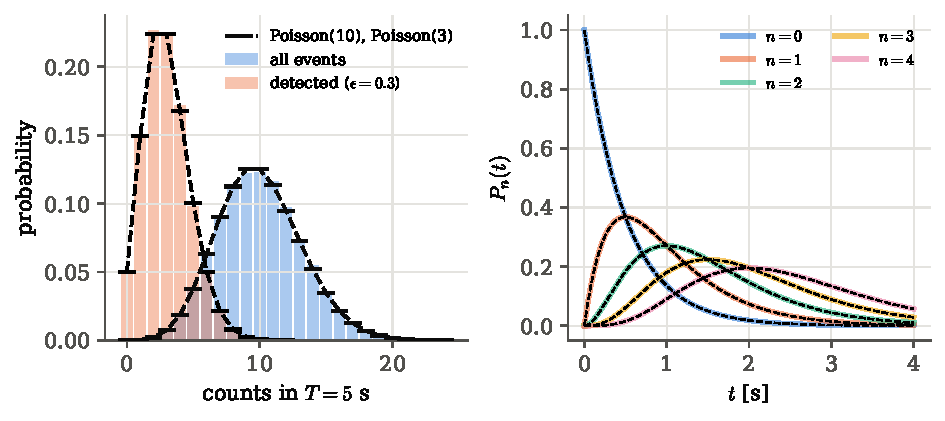
\includegraphics[width=\linewidth]{figures/ch02/05_poisson_process.pdf}
\caption{Left: counts in $5$~s windows built slice by slice, for all events (blue) and for the $30\%$ that are detected (orange); the black ticks are Poisson(10) and Poisson(3). Right: the ladder probabilities $P_0,\dots,P_4$ from integrating the master equation (thick coloured curves) lie on the analytic Poisson curves (thin dashed). $P_0$ decays from one; each higher rung fills up later and peaks at $t=n/\lambda$.}
\label{2a:fig:pp-sim}
\end{figure}

Over $20\,000$ windows the total count has mean $\twoaPPMean$ and variance $\twoaPPVar$ (theory $10$ and $10$), the thinned count $\twoaPPDetMean$ and $\twoaPPDetVar$ (theory $3$ and $3$), and the sum of the two sources $\twoaPPSumMean$ and $\twoaPPSumVar$ (theory $15$ and $15$). Empty windows are rare: with $e^{-10}=\twoaPPZeroTh$ we expect $20\,000\,e^{-10}\approx\twoaPPZeroExpect$ of them, and this run has $\twoaPPZeroCount$. The Euler solution of the master equation differs from $e^{-\lambda t}(\lambda t)^n/n!$ by at most $\twoaPPMaxErr$ over $0\le t\le4$~s (\cref{2a:fig:pp-sim}), an error that shrinks in proportion to the step size.

\begin{inpractice}[verification versus research]
Everything above is \emph{verification}: the simulation checks an analytic result we already had. The same slice-by-slice machinery becomes a research instrument as soon as the inputs (P1)--(P3) are only approximately true and no formula exists: a rate that depends on the recent history (afterpulsing in a PMT, pile-up in a calorimeter), events that trigger other events (cosmic-ray air showers, aftershocks), or a detector whose efficiency depends on the previous hit (\cref{2a:sec:failures}). Then we simulate the process and histogram the counts, and that histogram \emph{is} the sampling distribution $P(S\given\theta)$ fed into the likelihood.
\end{inpractice}

\section{Waiting times: the exponential and gamma distributions}\label{2a:sec:waiting}

The same Geiger counter can be read in two ways. We can count the clicks in fixed windows (\cref{2a:sec:poisson-process}), or we can record the \emph{time} of each click and look at the gaps between them. A timing detector with a photomultiplier does the second: it waits for the first photon, or for the tenth, and its time resolution is set by how much that waiting time fluctuates. A muon stopped in a scintillator waits a random time before it decays. For a Poisson process these waiting times have simple laws. The time to the first event is exponential. The time to the $n$-th event is gamma (also called Erlang). And the ``no memory'' input becomes the statement that a waiting time never ``ages''.

\paragraph{Physical picture: the survival law of an unstable particle.}
An unstable nucleus has no clock inside it. If it has survived a thousand years, its chance of decaying in the next second is the same as on the day it was made. This is why the survival fraction is $e^{-t/\tau}$, and why we can speak of \emph{the} lifetime $\tau$ of a species without saying how old the sample is. The time between Poisson events is the same law: the process never ``remembers'' when the last event happened.

\paragraph{The question, step by step.}
\begin{enumerate}[leftmargin=1.6em,itemsep=1pt]
  \item The first event comes after time $t$ exactly when the window $[0,t]$ is empty. We already know the probability of that.
  \item The $n$-th event comes before time $w$ exactly when the window $[0,w]$ holds at least $n$ events. We know that too.
  \item Differentiate these probabilities to get densities. Compute means and variances.
  \item Check the ``no memory'' property directly, and simulate a stream from its gaps.
\end{enumerate}

\begin{figure}[htbp]
\centering
\begin{tikzpicture}[x=1.05cm]
  \draw[->,thick] (0,0) -- (11,0);
  \node[lbl,anchor=north] at (11,-0.05) {$t$};
  \def\ta{1.4}\def\tb{2.3}\def\tc{4.6}\def\td{5.1}\def\te{8.2}
  \foreach \x in {0,\ta,\tb,\tc,\td,\te}{\draw[thick] (\x,-0.12) -- (\x,0.12);}
  \foreach \x in {\ta,\tb,\tc,\td,\te}{\fill[bdryred] (\x,0) circle (2.2pt);}
  \draw[decorate,decoration={brace,amplitude=4pt},tangentgreen,thick] (0,0.25) -- (\ta,0.25);
  \node[font=\scriptsize,tangentgreen,anchor=south] at ({\ta/2},0.42) {$S_0$};
  \draw[decorate,decoration={brace,amplitude=4pt},tangentgreen,thick] (\ta,0.25) -- (\tb,0.25);
  \node[font=\scriptsize,tangentgreen,anchor=south] at ({(\ta+\tb)/2},0.42) {$S_1$};
  \draw[decorate,decoration={brace,amplitude=4pt},tangentgreen,thick] (\tb,0.25) -- (\tc,0.25);
  \node[font=\scriptsize,tangentgreen,anchor=south] at ({(\tb+\tc)/2},0.42) {$S_2$};
  \draw[decorate,decoration={brace,amplitude=4pt},tangentgreen,thick] (\tc,0.25) -- (\td,0.25);
  \node[font=\scriptsize,tangentgreen,anchor=south] at ({(\tc+\td)/2},0.42) {$S_3$};
  \draw[decorate,decoration={brace,amplitude=4pt},tangentgreen,thick] (\td,0.25) -- (\te,0.25);
  \node[font=\scriptsize,tangentgreen,anchor=south] at ({(\td+\te)/2},0.42) {$S_4$};
  \foreach \x/\n in {\ta/1,\tb/2,\tc/3,\td/4,\te/5}{\node[font=\scriptsize,anchor=north] at (\x,-0.15) {$W_{\n}$};}
  \node[font=\scriptsize,anchor=north] at (0,-0.15) {$0$};
  \draw[decorate,decoration={brace,amplitude=5pt,mirror},formblue,thick] (0,-0.65) -- (\tc,-0.65);
  \node[font=\scriptsize,formblue,anchor=north] at ({\tc/2},-0.85) {$W_3=S_0+S_1+S_2$};
  \draw[fibreorange,thick,dashed] (6.5,-0.45) -- (6.5,0.2);
  \node[font=\scriptsize,fibreorange,anchor=west] at (6.55,-0.75) {at $t=6.5$: $N(t)=4$};
\end{tikzpicture}
\caption{One stretch of a Poisson stream. The green braces are the gaps (sojourn times) $S_0,S_1,\dots$ between successive events; the arrival times $W_n$ are their running sums. At the dashed line four events have happened, so $W_4\le t<W_5$: counts and waiting times are two descriptions of the same stream.}
\label{2a:fig:gaps}
\end{figure}

\subsection{The first event: exponential}

Let $T=W_1$ be the time of the first event, and recall that $N(t)$ is the number of events in $[0,t]$. \Cref{2a:fig:gaps} shows the link between the two descriptions: the first event comes after $t$ if and only if there is no event in $[0,t]$, that is, $T>t$ exactly when $N(t)=0$. This duality between waiting times and counts turns a question about times into one about counts, which we have already answered. So
\begin{align}
  \Prob(T>t) \eqby{1} \Prob(N(t)=0) \eqby{2} e^{-\lambda t},\qquad
  F(t)=\Prob(T\le t)=1-e^{-\lambda t},\qquad
  f(t) \eqby{3} \frac{\dd F}{\dd t}=\lambda e^{-\lambda t}. \label{2a:eq:expo}
\end{align}
\begin{explain}
  \item The duality between waiting times and counts.
  \item The empty-window probability $P_0(t)$ from \cref{2a:sec:poisson-process}.
  \item A density is the derivative of the CDF (\cref{ch:01}).
\end{explain}

\begin{workdef}[exponential distribution]
$T\sim\mathrm{Exp}(\lambda)$ in the \emph{rate} parameterisation if $f(t)=\lambda e^{-\lambda t}$ for $t\ge0$ \unpack{$\lambda$ is events per unit time}; equivalently, in the \emph{scale} parameterisation used by AoS, $f(t)=\frac1\beta e^{-t/\beta}$ with $\beta=1/\lambda$ \unpack{$\beta$ is a time, the mean wait}. For a decaying particle $\beta=\tau$, the mean lifetime.
\emph{Recognise it by:} the waiting time until something that happens at a constant rate and does not age.
\end{workdef}

The moments of the exponential, and those of the gamma distribution below, need one special function. The \newterm{gamma function} is, for $\alpha>0$, $\Gamma(\alpha)=\int_0^\infty y^{\alpha-1}e^{-y}\,\dd y$ \unpack{a continuous extension of the factorial, with $\Gamma(n)=(n-1)!$}.
Its three essential properties:
\begin{align*}
  \Gamma(1) &= \int_0^\infty e^{-y}\dd y = 1,\\
  \Gamma(\alpha+1) &\eqby{1} \Bigl[-y^\alpha e^{-y}\Bigr]_0^\infty+\alpha\int_0^\infty y^{\alpha-1}e^{-y}\dd y \eqby{2} \alpha\,\Gamma(\alpha),\\
  \Gamma(\tfrac12) &\eqby{3} \int_0^\infty y^{-1/2}e^{-y}\dd y \eqby{4} 2\int_0^\infty e^{-x^2}\dd x = \sqrt\pi .
\end{align*}
\begin{explain}
  \item Integration by parts, with $u=y^\alpha$ and $\dd v=e^{-y}\dd y$.
  \item The boundary term vanishes at both ends for $\alpha>0$.
  \item Definition with $\alpha=\tfrac12$.
  \item Substitute $y=x^2$, $\dd y=2x\,\dd x$, and use the Gaussian integral $\int_{-\infty}^\infty e^{-x^2}\dd x=\sqrt\pi$.
\end{explain}
From the first two, $\Gamma(n)=(n-1)(n-2)\cdots1\cdot\Gamma(1)=(n-1)!$ for integer $n$ \srcref{CasellaBerger}{(3.3.2)--(3.3.4), p.~81}.

Now the moments of the exponential, substituting $y=\lambda t$:
\begin{align*}
  \E T^r \eqby{1} \int_0^\infty t^r\lambda e^{-\lambda t}\dd t \eqby{2} \frac1{\lambda^r}\int_0^\infty y^re^{-y}\dd y \eqby{3} \frac{\Gamma(r+1)}{\lambda^r}=\frac{r!}{\lambda^r}.
\end{align*}
\begin{explain}
  \item Definition of the $r$-th moment.
  \item $t=y/\lambda$, $\dd t=\dd y/\lambda$.
  \item Definition of $\Gamma(r+1)$.
\end{explain}
So $\E T=1/\lambda$, $\E T^2=2/\lambda^2$ and $\Var T=2/\lambda^2-1/\lambda^2=1/\lambda^2$. The mean waiting time is the inverse rate, and the standard deviation equals the mean: an exponential wait is as uncertain as it is long.

\subsection{No memory}

\begin{keyidea}[the exponential is memoryless]
For all $t,s\ge0$, $\Prob(T>t+s\given T>t)=\Prob(T>s)$.
\end{keyidea}
\begin{align*}
  \Prob(T>t+s\given T>t) \eqby{1} \frac{\Prob(T>t+s\text{ and }T>t)}{\Prob(T>t)} \eqby{2} \frac{\Prob(T>t+s)}{\Prob(T>t)} \eqby{3} \frac{e^{-\lambda(t+s)}}{e^{-\lambda t}} = e^{-\lambda s} = \Prob(T>s).
\end{align*}
\begin{explain}
  \item Definition of conditional probability (\cref{ch:01}).
  \item $T>t+s$ already implies $T>t$.
  \item Survival function \eqref{2a:eq:expo}.
\end{explain}
In words: having waited a time $t$ without an event, the remaining wait has the same distribution as a fresh one (\cref{2a:fig:memoryless}). The converse is also true: the exponential is the \emph{only} continuous distribution with this property. To see why, write $G(t)=\Prob(T>t)$ for the survival function. Memorylessness says $G(t+s)/G(t)=G(s)$, that is, $G(t+s)=G(t)G(s)$. Taking logarithms, $\ln G(t+s)=\ln G(t)+\ln G(s)$: the function $\ln G$ is additive. The only continuous additive functions are linear, so $\ln G(t)=-\lambda t$ for some constant $\lambda>0$. So memorylessness \emph{forces} $G(t)=e^{-\lambda t}$ \srcref{CasellaBerger}{(3.3.11), p.~83}.

\begin{figure}[htbp]
\centering
\begin{tikzpicture}
\begin{axis}[width=10cm,height=5cm,xmin=0,xmax=3,ymin=0,ymax=1.08,
  xlabel={$t$ [s]},ylabel={$\Prob(T>t)=e^{-2t}$},axis lines=left,
  tick label style={font=\scriptsize},label style={font=\small},
  xtick={0,0.5,1,1.5,2,2.5,3},ytick={0,0.135,0.368,0.5,1},
  yticklabels={$0$,$0.135$,$0.368$,$0.5$,$1$}]
  \addplot[thick,formblue,domain=0:3,samples=120] {exp(-2*x)};
  \addplot[thick,tangentgreen] coordinates {(0.5,0) (0.5,0.3679)};
  \addplot[only marks,mark=*,mark size=1.6pt,tangentgreen] coordinates {(0.5,0.3679)};
  \addplot[thick,bdryred] coordinates {(1,0) (1,0.1353)};
  \addplot[thick,bdryred,dashed] coordinates {(1.5,0) (1.5,0.0498)};
  \addplot[only marks,mark=*,mark size=1.6pt,bdryred] coordinates {(1,0.1353) (1.5,0.0498)};
  \addplot[faint,dashed] coordinates {(0,0.3679) (0.5,0.3679)};
  \addplot[faint,dashed] coordinates {(0,0.1353) (1,0.1353)};
  \node[font=\scriptsize,tangentgreen,anchor=west] at (axis cs:0.55,0.45) {$\Prob(T>0.5)=0.368$};
  \node[font=\scriptsize,bdryred,anchor=west] at (axis cs:1.55,0.2) {$\dfrac{\Prob(T>1.5)}{\Prob(T>1)}=\dfrac{0.0498}{0.1353}=0.368$};
\end{axis}
\end{tikzpicture}
\caption{The survival curve of an exponential wait with $\lambda=2$~s$^{-1}$. The chance of waiting a further half second is the same whether we start the clock at zero (green: height at $0.5$) or after an empty first second (red: ratio of the heights at $1.5$ and $1$). Every stretch of the curve is a scaled copy of the whole.}
\label{2a:fig:memoryless}
\end{figure}

\paragraph{The gaps are independent exponentials.} Recall from \cref{2a:fig:gaps} that $S_0,S_1,\dots$ are the gaps between successive events and $W_n$ is the time of the $n$-th event. The argument for the first wait restarts at every event. Given that the first event is at $W_1=s$, the second gap $S_1$ exceeds $t$ exactly when $(s,s+t]$ is empty:
\begin{align*}
  \Prob(S_1>t\given W_1=s) \eqby{1} \Prob(\text{no events in }(s,s+t]\given W_1=s) \eqby{2} \Prob(\text{no events in }(s,s+t]) \eqby{3} e^{-\lambda t}.
\end{align*}
\begin{explain}
  \item Duality between the gap and an empty interval.
  \item Independent increments: what happens in $(s,s+t]$ does not care about $[0,s]$.
  \item Stationarity: an interval of length $t$ is empty with probability $e^{-\lambda t}$ wherever it sits.
\end{explain}
The answer does not depend on $s$, so $S_1$ is independent of $W_1=S_0$ and is again Exp$(\lambda)$. Repeating the argument, the gaps $S_0,S_1,S_2,\dots$ are independent and identically distributed (iid) Exp$(\lambda)$ \mainref{Thm.~23.35, p.~396}. This gives a second, equivalent definition of the Poisson process: \emph{a stream of events whose gaps are iid exponential}. It is the one we use to simulate.

\subsection{The $n$-th event: gamma (Erlang)}

The time of the $n$-th event is $W_n=S_0+S_1+\dots+S_{n-1}$, a sum of $n$ independent exponentials. Use the duality again: $W_n\le w$ exactly when at least $n$ events happened by $w$.
\begin{align}
  \Prob(W_n\le w) &\eqby{1} \Prob(N(w)\ge n) \eqby{2} 1-\sum_{k=0}^{n-1}e^{-\lambda w}\frac{(\lambda w)^k}{k!}, \nonumber\\
  f_{W_n}(w) &\eqby{3} \lambda e^{-\lambda w}\sum_{k=0}^{n-1}\frac{(\lambda w)^k}{k!}-e^{-\lambda w}\sum_{k=1}^{n-1}\frac{\lambda^kw^{k-1}}{(k-1)!} \nonumber\\
  &\eqby{4} \lambda e^{-\lambda w}\Bigl[\sum_{k=0}^{n-1}\frac{(\lambda w)^k}{k!}-\sum_{j=0}^{n-2}\frac{(\lambda w)^j}{j!}\Bigr]
   \eqby{5} \frac{\lambda^n w^{n-1}}{(n-1)!}\,e^{-\lambda w}. \label{2a:eq:erlang}
\end{align}
\begin{explain}
  \item The $n$-th arrival is before $w$ if and only if the count at $w$ is at least $n$.
  \item $N(w)\sim\mathrm{Poisson}(\lambda w)$; complement of $k\le n-1$.
  \item Differentiate with the product rule: the derivative of $e^{-\lambda w}$ gives the first sum (with the sign flipped by the leading minus), the derivative of $(\lambda w)^k/k!$ is $\lambda^kw^{k-1}/(k-1)!$ (zero for $k=0$).
  \item In the second sum take out $\lambda$ and rename $j=k-1$.
  \item The two sums \emph{telescope}: every term cancels except $k=n-1$ in the first.
\end{explain}
This is the \newterm{Erlang} density.\footnote{The density printed in \mainref{Thm.~23.35, p.~396} has $e^{-\lambda t}$ where $e^{-\lambda w}$ is meant. The proof there also writes $S_1$ for the first gap after defining the gaps from $S_0$.} With $\Gamma(n)=(n-1)!$ and the scale $\beta=1/\lambda$ it is a special case of the general gamma family.

\begin{workdef}[gamma distribution]
$X\sim\mathrm{Gamma}(\alpha,\beta)$ (shape $\alpha>0$, scale $\beta>0$) if
\begin{equation}
  f(x\given\alpha,\beta)=\frac{1}{\Gamma(\alpha)\,\beta^\alpha}\,x^{\alpha-1}e^{-x/\beta},\qquad x>0. \label{2a:eq:gamma}
\end{equation}
\unpack{for integer $\alpha=n$ and $\beta=1/\lambda$, the waiting time for the $n$-th event of a rate-$\lambda$ Poisson process}. $\mathrm{Exp}$ is $\mathrm{Gamma}(1,\beta)$.
\emph{Recognise it by:} a sum of independent exponential waits, or more generally a positive quantity whose density rises like a power and falls like an exponential.
\end{workdef}

It is normalised because substituting $y=x/\beta$ turns $\int_0^\infty x^{\alpha-1}e^{-x/\beta}\dd x$ into $\beta^\alpha\Gamma(\alpha)$. Its moments follow from the \emph{kernel trick}: recognise the integrand as another gamma density, up to its constant.
\begin{align*}
  \E X \eqby{1} \int_0^\infty\frac{x^{\alpha}e^{-x/\beta}}{\Gamma(\alpha)\beta^\alpha}\dd x
  \eqby{2} \frac{\Gamma(\alpha+1)\beta^{\alpha+1}}{\Gamma(\alpha)\beta^\alpha}
  \eqby{3} \alpha\beta,\qquad
  \E X^2 \eqby{2} \frac{\Gamma(\alpha+2)\beta^{\alpha+2}}{\Gamma(\alpha)\beta^\alpha}=\alpha(\alpha+1)\beta^2 .
\end{align*}
\begin{explain}
  \item One extra factor of $x$ raises the power to $x^\alpha$.
  \item $\int_0^\infty x^{(\alpha+1)-1}e^{-x/\beta}\dd x=\Gamma(\alpha+1)\beta^{\alpha+1}$, the normalisation of Gamma$(\alpha+1,\beta)$; likewise with $\alpha+2$.
  \item $\Gamma(\alpha+1)=\alpha\Gamma(\alpha)$.
\end{explain}
So $\Var X=\alpha(\alpha+1)\beta^2-\alpha^2\beta^2=\alpha\beta^2$ \srcref{CasellaBerger}{(3.3.7)--(3.3.8), p.~82}. For the Erlang wait, $\E W_n=n/\lambda$ and $\Var W_n=n/\lambda^2$, exactly $n$ times the exponential values, as a sum of $n$ independent gaps must give.

The mgf, by the same substitution, is $M_X(t)=(1-\beta t)^{-\alpha}$ for $t<1/\beta$. Multiplying mgfs shows that independent $\mathrm{Gamma}(\alpha_i,\beta)$ variables with a \emph{common scale} add to $\mathrm{Gamma}(\sum\alpha_i,\beta)$: $n$ gaps of $\mathrm{Gamma}(1,1/\lambda)$ make $\mathrm{Gamma}(n,1/\lambda)$, and the first $n$ gaps followed by the next $m$ make $W_{n+m}$.

\paragraph{The gamma--Poisson identity.} The first line of \eqref{2a:eq:erlang} is a useful identity in its own right. For integer $\alpha$ and $X\sim\mathrm{Gamma}(\alpha,\beta)$,
\[
  \Prob(X\le x)=\Prob(Y\ge\alpha),\qquad Y\sim\mathrm{Poisson}(x/\beta).
\]
A tail probability of a continuous waiting time equals a tail probability of a discrete count \srcref{CasellaBerger}{(3.3.9), p.~82}. Casella and Berger prove it by repeated integration by parts; the duality ``$n$-th event before $x$ $\Leftrightarrow$ at least $n$ events by $x$'' makes it obvious.

\subsection{Worked examples}

\paragraph{Example: muon survival.}
Stopped muons decay with mean lifetime $\tau=2.197~\mu$s. What fraction survives $5~\mu$s? By \eqref{2a:eq:expo} with $\lambda=1/\tau$, $\Prob(T>5~\mu\text{s})=e^{-5/2.197}=\twoaMuonSurv$. By memorylessness, a muon that has already survived $5~\mu$s again has about a $10\%$ chance to survive the next $5~\mu$s. So measuring $\tau$ does not require knowing when each muon was produced. Any start time after the muon stops gives the same exponential shape with the same $\tau$. This is why a muon-lifetime experiment can start its clock at the stop signal and ignore everything earlier.

\paragraph{Example: waiting for the third photon.}
Photons reach a photocathode at $\lambda=2$ per ns (after thinning by the quantum efficiency). The discriminator fires on the third photoelectron. What is the probability that it has fired within $1$~ns? By the gamma--Poisson identity,
\begin{align*}
  \Prob(W_3\le1) \eqby{1} \Prob(N(1)\ge3) \eqby{2} 1-e^{-2}\Bigl(1+2+\frac{2^2}{2}\Bigr) = 1-5e^{-2} = 1-0.677 = 0.323 .
\end{align*}
\begin{explain}
  \item Duality; $N(1)\sim\mathrm{Poisson}(2)$.
  \item Complement of $k=0,1,2$.
\end{explain}
The timing jitter of this trigger is the spread of $W_3$. With $\beta=1/\lambda=0.5$~ns, $W_3\sim\mathrm{Gamma}(3,0.5\text{ ns})$ has mean $\alpha\beta=1.5$~ns and standard deviation $\sqrt{\alpha}\,\beta=\sqrt3\times0.5=0.87$~ns. In general, firing on the $n$-th photon gives mean $n/\lambda$ and standard deviation $\sqrt n/\lambda$, so the relative jitter is $1/\sqrt n$. The more photons we wait for, the later the trigger, but the more \emph{predictable}.

\paragraph{Example: counts or gaps: the same information about $\lambda$.}
We watch a Poisson stream for a time $T$ and see $N$ events at times $w_1<\dots<w_N$. From the counts alone, the probability of the data is $e^{-\lambda T}(\lambda T)^N/N!$. From the gaps: $N$ gaps of the observed lengths (density $\lambda e^{-\lambda s_i}$ each) and then no event in the last stretch $T-w_N$ (probability $e^{-\lambda(T-w_N)}$). The product is
\begin{align*}
  \prod_{i=1}^N\lambda e^{-\lambda s_i}\times e^{-\lambda(T-w_N)} \eqby{1} \lambda^Ne^{-\lambda w_N}e^{-\lambda(T-w_N)} = \lambda^Ne^{-\lambda T}.
\end{align*}
\begin{explain}
  \item The gaps add up to the time of the last event, $\sum_is_i=w_N$.
\end{explain}
As functions of $\lambda$, the count probability and the gap product are both proportional to $\lambda^Ne^{-\lambda T}$ \mainref{Ex.~23.36, p.~396}. So the detailed arrival times carry no information about a constant rate beyond $N$ and $T$. Both likelihoods peak at the same estimate, $\hat\lambda=N/T$ (\cref{ch:03}). The exact times \emph{do} matter as soon as we want to test whether the rate is constant.

\subsection{Python: a stream built from its gaps}

To simulate the gaps we need exponential numbers, made from uniform ones. One fact does it \srcref{Cowan}{(2.16)--(2.18), p.~30}: if $X$ has a continuous CDF $F$, then $U=F(X)$ is uniform on $[0,1]$. Reading it backwards, $X=F^{-1}(U)$ has CDF $F$. For the exponential, $U=1-e^{-\lambda T}$ gives $T=-\ln(1-U)/\lambda$. Since $1-U$ is also uniform, $T=-\ln U/\lambda$ does the same job. This is \emph{inverse-transform sampling}, developed in general in \cref{ch:06}.

\pyfile[firstline=23,lastline=31,firstnumber=23]{code/ch02/06_waiting_times.py}{Exponential gaps, arrival times, counts per window}

Line 24 draws $200\,000$ exponential gaps with $\lambda=2$~s$^{-1}$; line 25 turns them into arrival times by a running sum, exactly as in \cref{2a:fig:gaps}. Line 27 counts the arrivals in each $1$~s window: \pyname{np.floor(times)} is the window index of each event and \pyname{np.bincount} counts events per index. The function \pyname{erlang_pdf} is \eqref{2a:eq:erlang}. Further down, the gaps are grouped in blocks of $n$ and summed to give samples of $W_n$.

\begin{figure}[htbp]
\centering
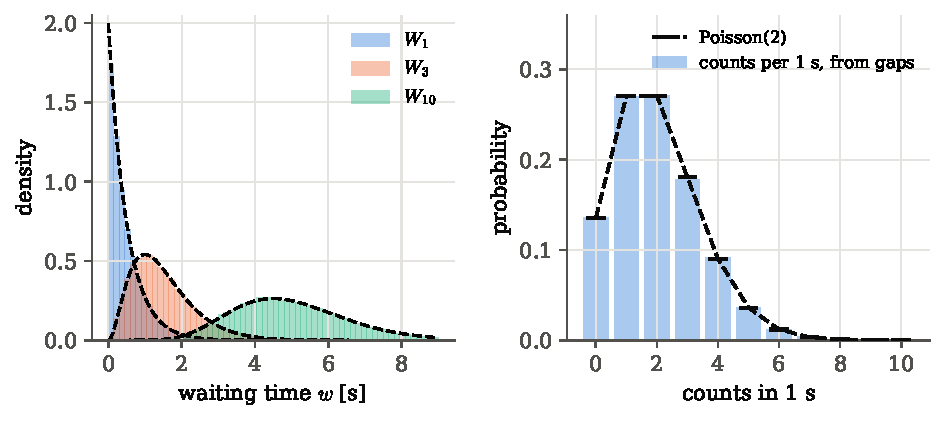
\includegraphics[width=\linewidth]{figures/ch02/06_waiting_times.pdf}
\caption{Left: histograms of the arrival time of the first, third and tenth event, built by summing $1$, $3$ or $10$ simulated gaps, with the Erlang densities as dashed curves. The first arrival is most likely immediately; later arrivals have a peak that moves right and a width that grows only like $\sqrt n$. Right: counting the same stream in $1$~s windows gives the Poisson(2) distribution, closing the loop from gaps back to counts.}
\label{2a:fig:wait-sim}
\end{figure}

The gaps have sample mean $\twoaWTGapMean$~s and variance $\twoaWTGapVar$~s$^2$ (theory $1/\lambda=0.5$ and $1/\lambda^2=0.25$). The counts per second have mean $\twoaWTCountMean$ and variance $\twoaWTCountVar$ (theory $2$ and $2$). The tenth arrival has mean $\twoaWTWtenMean$~s and variance $\twoaWTWtenVar$~s$^2$ (theory $5$ and $2.5$). For memorylessness, among the gaps that exceeded $1$~s the fraction that exceeded $1.5$~s is $\twoaWTCond$, against $\twoaWTUncond$ for all gaps exceeding $0.5$~s and the theoretical $e^{-1}=\twoaWTMemTh$ (\cref{2a:fig:wait-sim}).

\begin{pitfall}[rate or scale? three conventions for one distribution]
The same gamma distribution is written with a \emph{scale} $\beta$ (AoS, Casella--Berger, \pyname{scipy.stats.gamma(a, scale=beta)}, \pyname{numpy}'s \pyname{rng.gamma(shape, scale)}), or with a \emph{rate} $1/\beta$ (Lambert, most Bayesian texts and Stan). ``Exp(2)'' means mean $2$ in one book and mean $1/2$ in another. Always check by computing the mean. Lambert's lottery example is a warning: three prize-claiming times, each exponential with rate $1$ per day, sum to a gamma with \emph{shape} $3$ and rate $1$, which the text describes with the words ``scale'' and ``shape'' swapped \srcref{Lambert}{\S8.4.9}.
\end{pitfall}

\paragraph{Not every lifetime is exponential.} Memorylessness means a constant \emph{hazard} $h(t)=f(t)/\Prob(T>t)$ \unpack{the probability per unit time of failing now, given survival so far}. For the exponential $h(t)=\lambda$. Components that wear out have a rising hazard and are better described by the Weibull distribution, $\Prob(T>t)=e^{-(t/\beta)^\gamma}$ with $\gamma>1$ \srcref{CasellaBerger}{(3.3.12), p.~83}. Particles and nuclei have no wear, which is why the exponential law of decay is exact (to the extent quantum mechanics allows).

\section{Discrete waiting times and extra spread: geometric and negative binomial}\label{2a:sec:negbin}

At a collider, bunches cross every $25$~ns and each crossing fires a rare trigger with probability $p$. How many crossings do we wait until the first trigger? Until the third? This is the waiting-time question of \cref{2a:sec:waiting}, but with time coming in discrete ticks. A second puzzle has the same answer. A galaxy survey counts galaxies in cells of equal volume. The mean is $10$ per cell, but the variance is $30$, not the $10$ a Poisson count would have. The counts are \emph{overdispersed}: they scatter more than Poisson, because galaxies cluster and the underlying density varies from cell to cell. Two distributions answer both questions. The geometric and negative binomial distributions count trials until a given number of successes. The negative binomial then reappears as a Poisson count whose mean itself fluctuates, and in that role it is the standard model for counts that scatter more than Poisson.

\paragraph{Physical picture: ticks of a clock, and a Poisson with a wobbling rate.}
The geometric wait is the exponential wait with time chopped into ticks; shrink the ticks and it becomes the exponential. The overdispersed count is a Poisson count seen through a fluctuating medium, in two stages. First nature picks the local rate. Then a Poisson count is drawn with that rate. The total scatter is the sum of the scatter from the two stages: the Poisson ``shot noise'' plus the variance of the rate. Photon counts from a twinkling star behave this way.

\paragraph{The question, step by step.}
\begin{enumerate}[leftmargin=1.6em,itemsep=1pt]
  \item The first success is on trial $k$ exactly when trials $1,\dots,k-1$ fail and trial $k$ succeeds. Multiply.
  \item The $r$-th success is on trial $x$ exactly when trial $x$ succeeds and the first $x-1$ trials contain $r-1$ successes. That is a binomial count times one more trial.
  \item If a Poisson mean is itself random, average the Poisson pmf over its distribution (marginalise).
\end{enumerate}

\begin{figure}[htbp]
\centering
\begin{tikzpicture}[sq/.style={draw,minimum size=5.5mm,inner sep=0pt,font=\scriptsize}]
  \node[font=\small,anchor=east] at (-0.3,0) {geometric};
  \foreach \i in {1,...,6}{\node[sq,fill=softgray!20] at ({(\i-1)*0.62},0) {F};}
  \node[sq,fill=formblue!40] at (3.72,0) {S};
  \node[font=\scriptsize,anchor=west] at (4.2,0) {first success on trial $k=7$};
  \node[font=\small,anchor=east] at (-0.3,-1.1) {neg.\ binomial};
  \foreach \i/\c in {1/F,2/S,3/F,4/F,5/F,6/S,7/F,8/F,9/F,10/F}{
    \if S\c
      \node[sq,fill=formblue!40] at ({(\i-1)*0.62},-1.1) {S};
    \else
      \node[sq,fill=softgray!20] at ({(\i-1)*0.62},-1.1) {F};
    \fi}
  \node[sq,fill=formblue!40,draw=bdryred,thick] at (6.2,-1.1) {S};
  \node[font=\scriptsize,anchor=west] at (6.7,-1.1) {third success on trial $x=11$};
  \draw[decorate,decoration={brace,amplitude=4pt,mirror},thick,accent] (-0.28,-1.5) -- (5.86,-1.5);
  \node[font=\scriptsize,accent,anchor=north] at (2.8,-1.7) {first $x-1=10$ trials: any arrangement of $r-1=2$ successes, $\binom{10}{2}$ ways};
\end{tikzpicture}
\caption{Two waits in a sequence of Bernoulli trials. Top: the first success after six failures. Bottom: the third success (outlined in red) is the last trial; before it, the two earlier successes can sit in any of $\binom{10}2=45$ arrangements among the first ten trials, each equally probable.}
\label{2a:fig:trials-wait}
\end{figure}

\subsection{The geometric distribution}

\begin{workdef}[geometric distribution]
$X\sim\mathrm{Geom}(p)$ if $X$ is the number of the trial on which the first success occurs, in a sequence of independent Bernoulli$(p)$ trials \unpack{$X$ counts the successful trial too, so $X\ge1$}:
\begin{equation}
  \Prob(X=k)=(1-p)^{k-1}p,\qquad k=1,2,3,\dots \label{2a:eq:geom}
\end{equation}
\emph{Recognise it by:} the number of tries until the first success, with a constant chance per try.
\end{workdef}

The formula follows from the first step listed above. The first success is on trial $k$ when $k-1$ failures, each with probability $1-p$, are followed by a success, all independent; multiplying gives $(1-p)^{k-1}p$. Some books (and \pyname{scipy.stats.nbinom}) count instead the number of \emph{failures} before the first success, $Y=X-1\in\{0,1,\dots\}$, with $\Prob(Y=y)=(1-p)^yp$.\footnote{The normalisation check for the geometric distribution in \mainref{pp.~26--27} has a misprint in its middle sum, which is printed as $p\sum_{k\ge1}(1-p)^k$. That sum equals $1-p$, not $1$. The exponent must be $k-1$, as below.}

\paragraph{Geometric series.} Everything follows from $\sum_{j=0}^\infty r^j=\frac1{1-r}$ for $\abs r<1$. Proof: the partial sum $S_n=1+r+\dots+r^n$ satisfies $S_n-rS_n=1-r^{n+1}$, so $S_n=\frac{1-r^{n+1}}{1-r}\to\frac1{1-r}$. Differentiating term by term (allowed inside the radius of convergence) gives $\sum_{j=1}^\infty jr^{j-1}=\frac1{(1-r)^2}$ and $\sum_{j=2}^\infty j(j-1)r^{j-2}=\frac2{(1-r)^3}$. With $r=1-p$:
\begin{align*}
  \sum_{k=1}^\infty\Prob(X=k) &\eqby{1} p\sum_{k=1}^\infty(1-p)^{k-1} \eqby{2} \frac{p}{1-(1-p)}=1,\\
  \E X &\eqby{3} p\sum_{k=1}^\infty k(1-p)^{k-1} \eqby{4} \frac{p}{p^2}=\frac1p,\\
  \E[X(X-1)] &\eqby{3} p(1-p)\sum_{k=2}^\infty k(k-1)(1-p)^{k-2} \eqby{4} \frac{2p(1-p)}{p^3}=\frac{2(1-p)}{p^2},\\
  \Var X &\eqby{5} \frac{2(1-p)}{p^2}+\frac1p-\frac1{p^2}=\frac{1-p}{p^2}.
\end{align*}
\begin{explain}
  \item Take out $p$.
  \item Geometric series with $j=k-1$ running from $0$.
  \item Definition of the (factorial) moment; for the second line one factor $(1-p)$ is taken out so that the power is $k-2$.
  \item The differentiated series with $1-r=p$.
  \item $\Var X=\E[X(X-1)]+\E X-(\E X)^2$; put over $p^2$: $2-2p+p-1=1-p$.
\end{explain}
A trigger with $p=0.1$ fires on average every $10$ crossings, with a standard deviation $\sqrt{0.9}/0.1=9.5$ crossings: nearly as large as the mean, just like the exponential.

\paragraph{The tail and no memory.} The first success comes after trial $k$ exactly when the first $k$ trials all fail, so $\Prob(X>k)=(1-p)^k$. Then
\begin{align*}
  \Prob(X>s+t\given X>t) \eqby{1} \frac{\Prob(X>s+t)}{\Prob(X>t)} = \frac{(1-p)^{s+t}}{(1-p)^t} = (1-p)^s = \Prob(X>s)
\end{align*}
\begin{explain}
  \item $X>s+t$ implies $X>t$, and the definition of conditional probability.
\end{explain}
for integers $s,t\ge0$. The geometric is memoryless: a trigger that has not fired for $1000$ crossings is not ``due'' \srcref{CasellaBerger}{(3.2.11), p.~80}.

\paragraph{From ticks to continuous time.} Let the trials be ticks of length $h$ with $p=\lambda h$. The waiting time is $T=hX$, and
\[
  \Prob(T>t)=\Prob(X>t/h)=(1-\lambda h)^{t/h}\xrightarrow{\;h\to0\;}e^{-\lambda t},
\]
by the compound-interest limit of \cref{2a:sec:poisson-limit} with $n=t/h$. The geometric becomes the exponential, just as the binomial became the Poisson. The slices of \cref{2a:fig:slices} are exactly these ticks.

\subsection{The negative binomial}

\begin{workdef}[negative binomial distribution]
In a sequence of independent Bernoulli$(p)$ trials, let $X$ be the number of the trial on which the $r$-th success occurs. Then $X\sim\mathrm{NegBin}(r,p)$ with
\begin{equation}
  \Prob(X=x)=\binom{x-1}{r-1}p^r(1-p)^{x-r},\qquad x=r,r+1,\dots \label{2a:eq:nbx}
\end{equation}
Equivalently, the number of failures before the $r$-th success, $Y=X-r$, has
\begin{equation}
  \Prob(Y=y)=\binom{r+y-1}{y}p^r(1-p)^y,\qquad y=0,1,2,\dots \label{2a:eq:nby}
\end{equation}
\unpack{for $r=1$ these are the two forms of the geometric}.
\emph{Recognise it by:} the number of tries until a fixed number $r$ of successes, or (see below) a count that is more spread out than Poisson.
\end{workdef}

\emph{Derivation of \eqref{2a:eq:nbx}.} This is the second step listed above (\cref{2a:fig:trials-wait}). The $r$-th success is on trial $x$ if and only if two things happen. First, the first $x-1$ trials contain exactly $r-1$ successes; this has the binomial probability $\binom{x-1}{r-1}p^{r-1}(1-p)^{x-r}$. Second, trial $x$ succeeds, with probability $p$, independently of the earlier trials. Multiplying the two gives \eqref{2a:eq:nbx}. Replacing $x=y+r$ and using $\binom{n}{k}=\binom{n}{n-k}$ gives \eqref{2a:eq:nby} \srcref{CasellaBerger}{(3.2.9)--(3.2.10), p.~78}.

\paragraph{Mean and variance: a sum of geometric waits.} After each success the process starts afresh, because the trials are independent. So $Y$, the number of failures before the $r$-th success, is the sum of $r$ independent copies of $Y_1=X_1-1$, the number of failures before the first success; here $X_1\sim\mathrm{Geom}(p)$. From the geometric moments, $Y_1$ has $\E Y_1=\frac1p-1=\frac{1-p}p$ and $\Var Y_1=\Var X_1=\frac{1-p}{p^2}$. Hence
\begin{equation}
  \E Y=\frac{r(1-p)}{p},\qquad \Var Y=\frac{r(1-p)}{p^2}=\E Y+\frac{(\E Y)^2}{r}. \label{2a:eq:nbvar}
\end{equation}
The last form follows by writing $\mu=r(1-p)/p$: then $\mu+\mu^2/r=\frac{r(1-p)}p\bigl(1+\frac{1-p}{p}\bigr)=\frac{r(1-p)}{p^2}$. \emph{The variance always exceeds the mean}, by $\mu^2/r$.

\paragraph{Why ``negative'' binomial.} Write out the coefficient with $r+y-1$ over $y$ and pull out a sign from each of the $y$ factors:
\begin{align*}
  \binom{r+y-1}{y} \eqby{1} \frac{(r+y-1)(r+y-2)\cdots r}{y!}
  \eqby{2} (-1)^y\frac{(-r)(-r-1)\cdots(-r-y+1)}{y!}
  \eqby{3} (-1)^y\binom{-r}{y}.
\end{align*}
\begin{explain}
  \item Cancel $(r-1)!$ from $(r+y-1)!/(y!(r-1)!)$, leaving $y$ factors on top.
  \item Each factor $(r+j)=-(-r-j)$, for $j=0,\dots,y-1$, read in reverse order.
  \item The \emph{generalised} binomial coefficient $\binom{a}{y}=a(a-1)\cdots(a-y+1)/y!$ makes sense for any real $a$, including $a=-r$.
\end{explain}
Newton's binomial series $(1+z)^a=\sum_y\binom ay z^y$ for $\abs z<1$ then normalises \eqref{2a:eq:nby}: $\sum_y\binom{-r}{y}(-(1-p))^yp^r=(1-(1-p))^{-r}p^r=1$. The pmf is a term of a binomial expansion with a negative exponent.

\paragraph{Its mgf and the Poisson limit.} For one geometric failure count, $\E e^{tY_1}=\sum_yp(1-p)^ye^{ty}=p/(1-(1-p)e^t)$ (geometric series, valid for $(1-p)e^t<1$). A sum of $r$ independent copies has the $r$-th power. Now let $r\to\infty$ while holding the mean $r(1-p)/p$ close to a fixed $\lambda$; to leading order $1-p=\lambda/r$:
\begin{align*}
  M_Y(t)=\Bigl(\frac{p}{1-(1-p)e^t}\Bigr)^r
  \eqby{1} \frac{(1-\lambda/r)^r}{(1-\lambda e^t/r)^r}
  \;\xrightarrow{\;r\to\infty\;}\; \frac{e^{-\lambda}}{e^{-\lambda e^t}} = e^{\lambda(e^t-1)} .
\end{align*}
\begin{explain}
  \item Substitute $p=1-\lambda/r$.
\end{explain}
The limit is the Poisson mgf \eqref{2a:eq:poismgf}: with many required successes and rare failures, the failure count becomes Poisson, and the excess variance $\mu^2/r$ disappears \srcref{CasellaBerger}{p.~79}.

\subsection{A Poisson count with a fluctuating mean}

The most important appearance of the negative binomial in physics is not about waiting at all. Suppose the count in a cell is Poisson with mean $\Lambda$, but $\Lambda$ itself varies: from cell to cell (clustering), from run to run (beam intensity) or from pixel to pixel (a twinkling source). Take $\Lambda$ to follow a gamma distribution with shape $\kappa$ and scale $\mu/\kappa$. By the gamma moments of \cref{2a:sec:waiting}, $\E\Lambda=\kappa\cdot\mu/\kappa=\mu$ and $\Var\Lambda=\kappa(\mu/\kappa)^2=\mu^2/\kappa$. The distribution of the count is then the \newterm{mixture}: the marginal over the nuisance variable $\Lambda$. Write $\theta=\mu/\kappa$ for the gamma scale:
\begin{align*}
  \Prob(N=n)
  &\eqby{1} \int_0^\infty e^{-\lambda}\frac{\lambda^n}{n!}\;\frac{\lambda^{\kappa-1}e^{-\lambda/\theta}}{\Gamma(\kappa)\theta^\kappa}\,\dd\lambda
  \eqby{2} \frac{1}{n!\,\Gamma(\kappa)\,\theta^\kappa}\int_0^\infty\lambda^{n+\kappa-1}e^{-\lambda(1+\theta)/\theta}\,\dd\lambda\\
  &\eqby{3} \frac{\Gamma(n+\kappa)}{n!\,\Gamma(\kappa)\,\theta^\kappa}\Bigl(\frac{\theta}{1+\theta}\Bigr)^{n+\kappa}
  \eqby{4} \frac{\Gamma(n+\kappa)}{n!\,\Gamma(\kappa)}\Bigl(\frac{\kappa}{\kappa+\mu}\Bigr)^{\kappa}\Bigl(\frac{\mu}{\kappa+\mu}\Bigr)^{n}.
\end{align*}
\begin{explain}
  \item Law of total probability for a continuous nuisance variable: Poisson pmf given $\Lambda=\lambda$, times the gamma density of $\Lambda$, integrated.
  \item Collect the powers of $\lambda$ and the exponentials: $\lambda+\lambda/\theta=\lambda(1+\theta)/\theta$.
  \item The integral is the gamma normalisation with shape $n+\kappa$ and scale $\theta/(1+\theta)$.
  \item $\theta^{-\kappa}(\theta/(1+\theta))^{\kappa}=(1+\theta)^{-\kappa}$, and $\theta/(1+\theta)=\mu/(\kappa+\mu)$, $1/(1+\theta)=\kappa/(\kappa+\mu)$.
\end{explain}
For integer $\kappa$, $\Gamma(n+\kappa)/(n!\,\Gamma(\kappa))=\binom{\kappa+n-1}{n}$, and this is \eqref{2a:eq:nby} with $r=\kappa$ and $p=\kappa/(\kappa+\mu)$. The formula makes sense for any real $\kappa>0$, and in this role $\kappa$ is called the \newterm{inverse dispersion} \srcref{Lambert}{\S8.4.4}.

The variance is cleanest by the law of total variance (\cref{ch:01}). It splits the scatter into the two stages of the physical picture above: nature picks the rate, then the Poisson count is drawn.
\begin{align}
  \Var N \eqby{1} \E\bigl[\Var(N\given\Lambda)\bigr]+\Var\bigl(\E[N\given\Lambda]\bigr) \eqby{2} \E\Lambda+\Var\Lambda \eqby{3} \mu+\frac{\mu^2}{\kappa}. \label{2a:eq:overdisp}
\end{align}
\begin{explain}
  \item Law of total variance: average of the conditional variance plus variance of the conditional mean.
  \item Given $\Lambda$, $N$ is Poisson, so its conditional mean and variance both equal $\Lambda$.
  \item Gamma moments.
\end{explain}
The variance is the Poisson shot noise $\mu$ plus the variance of the rate, $\mu^2/\kappa$. Nothing in the second step used the gamma form: \emph{any} fluctuating mean gives $\Var N=\mu+\Var\Lambda>\mu$. The gamma only makes the full distribution a closed form.

\subsection{Worked examples}

\paragraph{Example: how long until the trigger fires?}
With $p=0.1$ per crossing, what is the probability of waiting more than $30$ crossings for the first trigger? $\Prob(X>30)=(0.9)^{30}=\twoaGeoTailTh$. And for a light bulb that fails on any given day with probability $0.001$, $\Prob(X>30)=0.999^{30}=0.970$: a $97\%$ chance to last a month \srcref{CasellaBerger}{Ex.~3.2.7, p.~80}. By memorylessness, the same $97\%$ applies to the next month of a bulb that has already lasted a year. Real bulbs age, so the geometric is only a rough model for them; a trigger has no memory, so for it the model is exact.

\paragraph{Example: inverse binomial sampling.}
To measure a rare branching fraction $p$ we can fix the number of trials and count successes (binomial), or keep collecting until we have $r$ successes (negative binomial) \srcref{CasellaBerger}{Ex.~3.2.6, p.~79}. Suppose $p=0.02$ and we stop at $r=100$ signal events. The number of events examined is $X=Y+r$ with
\begin{align*}
  \E X \eqby{1} \frac{r}{p}=5000,\qquad \mathrm{sd}(X) \eqby{2} \frac{\sqrt{r(1-p)}}{p}=\frac{\sqrt{98}}{0.02}=495 .
\end{align*}
\begin{explain}
  \item $\E X=\E Y+r=r(1-p)/p+r=r/p$.
  \item $\Var X=\Var Y=r(1-p)/p^2$ from \eqref{2a:eq:nbvar}.
\end{explain}
The relative uncertainty of the stopping point is $\sqrt{1-p}/\sqrt r\approx10\%$, set by $r$ alone. Stopping rules like this matter for inference: \cref{ch:03} and \cref{ch:05} show that the binomial and negative binomial give proportional likelihoods for $p$, so a Bayesian analysis does not care which rule was used, while a p-value does.

\paragraph{Example: counts in cells of a clustered galaxy field.}
Cells of a survey contain on average $\mu=10$ galaxies. If galaxies were placed independently (a Poisson process in space, \cref{2a:sec:poisson-process}), the variance of the cell counts would be $10$. But galaxies trace a fluctuating matter density. The local mean in a cell is $\Lambda=\mu(1+\delta)$, where $\delta$ is the density contrast smoothed over the cell, with variance $\sigma^2_{\text{cell}}$. So $\Var\Lambda=\mu^2\sigma^2_{\text{cell}}$, and by \eqref{2a:eq:overdisp},
\[
  \Var N=\mu+\mu^2\sigma^2_{\text{cell}} .
\]
If $\sigma^2_{\text{cell}}=0.2$, then $\Var N=10+20=30$, three times the Poisson value. This is the gamma--Poisson model with $1/\kappa=\sigma^2_{\text{cell}}$, that is, $\kappa=5$. Read backwards, the formula is a measurement. The \emph{excess} variance of counts in cells over the Poisson value measures the clustering amplitude $\sigma^2_{\text{cell}}$. That excess is the one-point statistic behind the two-point function of \cref{ch:07}. The Poisson term $\mu$ is the \emph{shot noise} that every galaxy power spectrum must subtract.

\subsection{Python: trials one after another, and a wobbling rate}

\pyfile[firstline=23,lastline=35,firstnumber=23]{code/ch02/07_geometric_negbin.py}{Geometric and negative binomial by running trials; the gamma--Poisson mixture}

For each of $50\,000$ experiments the script runs $400$ Bernoulli$(0.1)$ trials (the chance that fewer than three successes occur in $400$ trials is negligible) and finds the trial numbers of the successes with \pyname{np.flatnonzero}. The first one is the geometric wait; the third one minus $r=3$ is the number of failures before the third success. For the mixture, line 34 draws a rate for each run from a gamma distribution with shape $\kappa=5$ and scale $\mu/\kappa$ (numpy's convention is scale), and line 35 draws one Poisson count with that rate.

\begin{figure}[htbp]
\centering
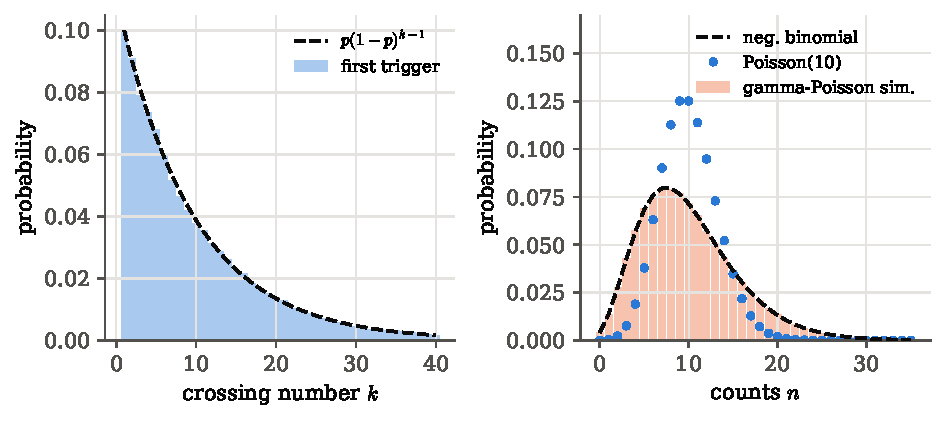
\includegraphics[width=\linewidth]{figures/ch02/07_geometric_negbin.pdf}
\caption{Left: the crossing number of the first trigger (bars) against $p(1-p)^{k-1}$ (dashed): a geometric staircase, highest at $k=1$, falling by a factor $0.9$ per crossing. Right: counts whose Poisson mean wobbles from run to run (bars) follow the negative binomial (dashed), far wider than the Poisson with the same mean $10$ (blue dots).}
\label{2a:fig:nb-sim}
\end{figure}

The geometric wait has sample mean $\twoaGeoMean$ and variance $\twoaGeoVar$ (theory $1/p=10$ and $(1-p)/p^2=90$); $\twoaGeoTail$ of the experiments waited more than $30$ crossings, against $0.9^{30}=\twoaGeoTailTh$. The failures before the third success have mean $\twoaNBMean$ and variance $\twoaNBVar$ (theory $\twoaNBMeanTh$ and $\twoaNBVarTh$). The mixture counts have mean $\twoaMixMean$ and variance $\twoaMixVar$, against $\mu+\mu^2/\kappa=\twoaMixVarTh$ (\cref{2a:fig:nb-sim}).

\paragraph{What this bought us.}
Discrete waits (geometric, negative binomial) are the tick-by-tick versions of the exponential and gamma. The negative binomial also describes a Poisson count with a gamma-distributed mean, with variance $\mu+\mu^2/\kappa$. Whenever counts scatter more than their mean, look for a fluctuating rate.

\section{When the Poisson assumptions fail, and where the Poisson goes for large \texorpdfstring{$\lambda$}{lambda}}\label{2a:sec:failures}

Point a Geiger counter at a radioactive source and move it closer. At first the count rate rises like $1/r^2$, as the solid angle says it should. Closer in, it rises more slowly than $1/r^2$, and with some counters, very close to a strong source, it even \emph{falls}. Now look at the counts in successive short windows at a fixed distance. A second oddity appears: at high rate they scatter \emph{less} than the $\sqrt{\text{mean}}$ that the Poisson distribution promises. A clustered galaxy survey shows the opposite oddity, as we saw in the counts-in-cells example of \cref{2a:sec:negbin}: the counts in cells scatter \emph{more} than Poisson.

Both oddities are the Poisson inputs of \cref{2a:sec:poisson-process} failing, in opposite directions. Each physical effect breaks a particular input (P1)--(P3) of \cref{2a:sec:poisson-inputs}. One number computed from the data detects the failure. And the commonest failure in counting detectors, dead time, can be corrected. A separate question concerns large means: there the Poisson distribution becomes close to a Gaussian, and the replacement is safe in some places and badly wrong in others.

\paragraph{The questions.}
\begin{enumerate}[leftmargin=1.6em,itemsep=1pt]
  \item Which Poisson input does each physical effect break, and does it push the variance of the counts up or down?
  \item Given a set of counts, how do we test whether they are Poisson?
  \item For a counter that is blind for a time $\tau$ after each hit, what is the recorded rate, how do we get the true rate back, and how much do the recorded counts scatter?
  \item For large $\lambda$, how close is Poisson$(\lambda)$ to the Gaussian $\Normal(\lambda,\lambda)$, and where does the approximation fail?
\end{enumerate}

\subsection{Three inputs, two directions of failure}

Recall the three physical inputs from which the Poisson process was derived (\cref{2a:sec:poisson-inputs}):
\begin{enumerate}[leftmargin=2.6em,itemsep=1pt,label=(P\arabic*)]
  \item what happens in one time slice is independent of what happened in all the others \unpack{no memory, no triggering, no suppression};
  \item the rate $\lambda$ is the \emph{same} at all times \unpack{the source does not drift};
  \item events come one at a time \unpack{never two at the same instant}.
\end{enumerate}
From these came the pmf $e^{-\lambda t}(\lambda t)^n/n!$ for the count $N$ in a window of length $t$, and with it the defining fingerprint $\Var N=\E N$. The Poisson is the distribution of ``counts of rare events'' \mainref{p.~27}. Here ``rare'' means precisely that the events do not interact with each other and are not modulated by anything. The same point holds from the user's side \srcref{Lambert}{\S8.4.3}: the mean and the variance are the same parameter, so the Poisson is useful only for data with $\Var N\approx\E N$.

Real effects break the inputs in one of two directions.

\paragraph{More spread than Poisson (overdispersion).} Two kinds of effect make the counts clump.
\begin{itemize}[leftmargin=1.4em,itemsep=1pt]
  \item \emph{The rate itself fluctuates} (input P2 fails). The beam intensity drifts from run to run, the sky background varies across the field, the density of dark matter modulates where galaxies form. In \cref{2a:sec:negbin} we proved that a Poisson count with a random mean $\Lambda$ has $\Var N=\E\Lambda+\Var\Lambda$, eq.~\eqref{2a:eq:overdisp}. The extra term can only add.
  \item \emph{Events trigger further events} (input P1 fails in the positive direction). A photomultiplier pulse is followed by an afterpulse from an ion drifting back to the photocathode. A cosmic-ray primary makes an air shower of secondaries. Events arrive in bunches, and a window either catches a bunch or misses it.
\end{itemize}
The binomial has the same failure mode. When the success probability $p$ varies from group to group, for example between detector modules or between clinical trials, the number of successes is spread wider than $np(1-p)$. Its standard model is the beta-binomial, the binomial analogue of the negative binomial \srcref{Lambert}{\S8.4.5}.

\paragraph{Less spread than Poisson (underdispersion).} Other effects make the events avoid each other, so that the stream becomes more regular than random.
\begin{itemize}[leftmargin=1.4em,itemsep=1pt]
  \item \emph{Events suppress further events} (input P1 fails in the negative direction). After recording a hit the counter is blind for a \newterm{dead time} $\tau$. A neuron cannot fire again during its refractory period. Pile-up rejection throws away events that come too close together.
  \item \emph{The pool of possible events is finite.} With $n$ nuclei and decay probability $p$ per window the count is binomial, with $\Var N=np(1-p)<np=\E N$. This is negligible for a macroscopic source ($n\sim10^{20}$), but not for a handful of trapped ions, or for a short-lived isotope that decays appreciably during the measurement (then input P2 fails as well: the rate falls with time).
\end{itemize}
Input (P3) fails when two events in one slice are recorded as one. This \newterm{pile-up} (two photons in one X-ray CCD pixel within one readout frame, two particles in one calorimeter cell in one bunch crossing) loses events and distorts the recorded energies. As far as the counts are concerned, it acts like a dead time of one frame.

\begin{figure}[htbp]
\centering
\begin{tikzpicture}[x=1.05cm,y=1cm,
  ev/.style={formblue,line width=1.1pt},
  cnt/.style={font=\scriptsize,softgray},
  rowlab/.style={font=\small,anchor=east,align=right}]
  \foreach \xx in {0,2,4,6,8,10} \draw[faint,dashed] (\xx,0.45) -- (\xx,-2.75);
  \node[rowlab] at (-0.2,0) {Poisson\\[-2pt]{\scriptsize independent}};
  \draw[black!40] (0,0) -- (10,0);
  \foreach \t in {0.09,0.48,0.52,1.22,1.23,1.86,2.07,3.30,3.69,3.74,4.32,4.97,6.27,6.33,6.74,6.80,7.85,8.27,8.47,8.53,9.79,9.87}
    \draw[ev] (\t,-0.22) -- (\t,0.22);
  \foreach \xx/\c in {1/6,3/4,5/2,7/5,9/5} \node[cnt] at (\xx,-0.42) {$\c$};
  \node[rowlab] at (-0.2,-1.1) {clustered\\[-2pt]{\scriptsize overdispersed}};
  \draw[black!40] (0,-1.1) -- (10,-1.1);
  \foreach \t in {2.59,2.68,2.91,4.31,4.33,4.34,4.44,4.65,5.19,5.37,8.73,8.77,8.78,8.86,8.93,8.99,9.06,9.08,9.72,9.85}
    \draw[ev,fibreorange] (\t,-1.32) -- (\t,-0.88);
  \foreach \xx/\c in {1/0,3/3,5/7,7/0,9/10} \node[cnt] at (\xx,-1.52) {$\c$};
  \node[rowlab] at (-0.2,-2.2) {regular\\[-2pt]{\scriptsize underdispersed}};
  \draw[black!40] (0,-2.2) -- (10,-2.2);
  \foreach \t in {0.42,0.79,1.13,1.55,1.99,2.60,3.01,3.48,3.98,4.41,4.76,5.26,5.73,6.31,6.90,7.24,7.64,8.07,8.48,8.85,9.47,9.87}
    \draw[ev,tangentgreen] (\t,-2.42) -- (\t,-1.98);
  \foreach \xx/\c in {1/5,3/4,5/4,7/4,9/5} \node[cnt] at (\xx,-2.62) {$\c$};
\end{tikzpicture}
\caption{Three streams of about twenty events, each cut into five equal windows (dashed lines); the small numbers are the counts per window. Top: a Poisson stream, with the irregular gaps and chance near-coincidences of genuine randomness. Middle: the same kind of stream in clumps (a few independent ``parents'', each with a small bunch of offspring): whole windows are empty and others are crowded. Bottom: a dense Poisson stream passed through a counter that is blind for a fixed time after each recorded hit: no two events are close, the gaps are almost equal, and the counts barely change from window to window.}
\label{2a:fig:three-streams}
\end{figure}

\Cref{2a:fig:three-streams} shows the three kinds of stream. The eye reads clumping and regularity immediately. What we need is a number that does the same for a data set of thousands of windows.

\subsection{The Fano factor: a one-number test}

Since a Poisson count has variance equal to its mean, the natural diagnostic is their ratio.

\begin{workdef}[Fano factor (index of dispersion)]
For a count $N$ with mean $\mu>0$, the \newterm{Fano factor} is
\[
  F=\frac{\Var N}{\E N} .
\]
$F=1$ for a Poisson count, $F>1$ is \newterm{overdispersion} \unpack{clumped events or a fluctuating rate}, and $F<1$ is \newterm{underdispersion} \unpack{events that avoid each other, or a finite pool}. From $k$ independent counts $n_1,\dots,n_k$ of the same window we estimate it by
\[
  \hat F=\frac{s^2}{\bar n},\qquad \bar n=\frac1k\sum_{i=1}^kn_i,\quad s^2=\frac1{k-1}\sum_{i=1}^k(n_i-\bar n)^2 .
\]
For Poisson counts with $\bar n\gg1$, $\hat F$ scatters about $1$ with standard deviation $\sqrt{2/(k-1)}$.
\end{workdef}

Values of $F$ we already know: Poisson $F=1$; binomial $F=1-p$; negative binomial $F=1+\mu/\kappa$, from \eqref{2a:eq:overdisp}. The name comes from the physics of ionisation detectors, where U.~Fano showed that the number of electron--ion pairs made by a particle of fixed energy fluctuates less than Poisson (the energy budget is fixed, so the pairs are not independent). The same ratio minus one is Mandel's $Q$ parameter in quantum optics (see the example on sub-Poissonian light below).

\paragraph{How far from $1$ is ``significantly'' far?} A sample Fano factor is itself a random number, so a measured $\hat F=0.97$ need not mean anything. To judge it we need the spread of $\hat F$ when the counts really are Poisson. Two facts give it. The first: for any independent sample of size $k$, the sample variance $s^2$ has
\[
  \Var(s^2)=\frac{2\sigma^4}{k-1}+\frac{\kappa_4}{k},
\]
where $\sigma^2$ is the variance and $\kappa_4$ the fourth \newterm{cumulant} \unpack{the excess of the fourth central moment over its Gaussian value, $\kappa_4=\E(N-\mu)^4-3\sigma^4$} of one count. The first term is the Gaussian result, derived with the $\chi^2$ distribution in the next part. The second is the correction for a non-Gaussian parent. The second fact: for a Poisson count every cumulant equals $\lambda$ (proved in \cref{2a:sec:gauss-preview} below), so $\sigma^2=\kappa_4=\lambda$. The mean $\bar n$ fluctuates by only a relative $1/\sqrt{k\lambda}$, so in the ratio we may treat it as the constant $\lambda$. Then
\begin{align}
  \mathrm{sd}(\hat F)
  &\eqby{1} \frac{\mathrm{sd}(s^2)}{\lambda}
  \eqby{2} \frac1\lambda\sqrt{\frac{2\lambda^2}{k-1}+\frac{\lambda}{k}}
  \eqby{3} \sqrt{\frac{2}{k-1}+\frac{1}{k\lambda}}
  \relby{4}{\approx} \sqrt{\frac{2}{k-1}} . \label{2a:eq:fanosd}
\end{align}
\begin{explain}
  \item $\hat F=s^2/\bar n$ with $\bar n$ replaced by its expected value $\lambda$; its relative fluctuation $1/\sqrt{k\lambda}$ is tiny next to that of $s^2$.
  \item The variance of $s^2$ with $\sigma^2=\kappa_4=\lambda$.
  \item Take $\lambda^2$ out of the square root.
  \item For $\lambda\gg1$ the second term is negligible: $1/(k\lambda)\ll2/(k-1)$.
\end{explain}
The spread depends only on the number of windows $k$, not on the rate. The combination $D=(k-1)\hat F=\sum_i(n_i-\bar n)^2/\bar n$ is the classical \newterm{index-of-dispersion statistic}. For Poisson counts it is close to a $\chi^2$ variable with $k-1$ degrees of freedom, and using it to reject ``the counts are Poisson'' is a hypothesis test in the sense of \cref{ch:04}.

\paragraph{Example: reading a Fano factor.} We record $k=4000$ windows. By \eqref{2a:eq:fanosd}, $\mathrm{sd}(\hat F)=\sqrt{2/3999}=0.0224$.
\begin{itemize}[leftmargin=1.4em,itemsep=1pt]
  \item $\hat F=0.96$ is $(0.96-1)/0.0224=-1.8$ standard deviations from $1$. That happens by chance in about $7\%$ of Poisson data sets (two-sided), so it is no evidence against Poisson.
  \item $\hat F=0.62$ is $-17$ standard deviations. The counts are certainly not Poisson, and they are underdispersed: look for dead time.
  \item $\hat F=3.0$ is $+89$ standard deviations. Look for a fluctuating rate or clustering, as in the galaxy counts of \cref{2a:sec:negbin}, where $F=1+\mu\sigma^2_{\text{cell}}=3$.
\end{itemize}
With only $k=20$ windows, $\mathrm{sd}(\hat F)=0.32$, and even $\hat F=0.62$ is barely more than one standard deviation from $1$. A few windows cannot distinguish these streams. That is why the five windows of \cref{2a:fig:three-streams} are only an illustration.

\subsection{Dead time}

The commonest failure in a counting detector is dead time. After a hit, the electronics need a time $\tau$ to shape the pulse, digitise it and reset. Anything arriving in that interval is lost. Typical values are $\tau\sim100$--$300~\mu$s for a Geiger--M\"uller tube, $\sim10$--$100$~ns for a photomultiplier with fast electronics, and one readout frame (seconds) for an X-ray CCD. Two idealised models bracket the real behaviour of most systems.
\begin{itemize}[leftmargin=1.4em,itemsep=1pt]
  \item \newterm{Non-paralysable}: the counter is blind for $\tau$ after each \emph{recorded} hit. Hits that arrive during the dead period are lost and have no further effect.
  \item \newterm{Paralysable}: \emph{every} hit, recorded or not, restarts the dead period. A hit is recorded only if the previous true hit came at least $\tau$ earlier. A burst of closely spaced hits keeps the counter blind for the whole burst.
\end{itemize}
Let $n$ be the true rate (hits per second) and $m$ the recorded rate. \Cref{2a:fig:deadtime-models} runs one stream of true hits through both models.

\begin{figure}[htbp]
\centering
\begin{tikzpicture}[x=1.6cm,y=1cm,
  hit/.style={formblue,line width=1.1pt},
  lost/.style={black!35,line width=0.9pt},
  dead/.style={fill=bdryred!18,draw=bdryred!60},
  rowlab/.style={font=\small,anchor=east,align=right}]
  \node[rowlab] at (-0.15,0) {true hits};
  \draw[black!40] (0,0) -- (6.3,0);
  \foreach \t in {0.3,1.0,1.35,1.6,2.9,3.2,4.6,5.1,5.3} \draw[hit] (\t,-0.22) -- (\t,0.22);
  \node[rowlab] at (-0.15,-1.2) {non-paralysable};
  \foreach \a/\b in {0.3/1.1,1.35/2.15,2.9/3.7,4.6/5.4} \draw[dead] (\a,-1.35) rectangle (\b,-1.05);
  \draw[black!40] (0,-1.2) -- (6.3,-1.2);
  \foreach \t in {0.3,1.35,2.9,4.6} \draw[hit] (\t,-1.45) -- (\t,-0.95);
  \foreach \t in {1.0,1.6,3.2,5.1,5.3} \draw[lost] (\t,-1.3) -- (\t,-1.1);
  \node[rowlab] at (-0.15,-2.4) {paralysable};
  \foreach \a/\b in {0.3/2.4,2.9/4.0,4.6/6.1} \draw[dead] (\a,-2.55) rectangle (\b,-2.25);
  \draw[black!40] (0,-2.4) -- (6.3,-2.4);
  \foreach \t in {0.3,2.9,4.6} \draw[hit] (\t,-2.65) -- (\t,-2.15);
  \foreach \t in {1.0,1.35,1.6,3.2,5.1,5.3} \draw[lost] (\t,-2.5) -- (\t,-2.3);
  \draw[|-|,black!70] (0.3,-3.1) -- (1.1,-3.1);
  \node[font=\small,anchor=west] at (1.2,-3.1) {$\tau$};
  \draw[hit] (2.7,-3.22) -- (2.7,-2.98); \node[font=\scriptsize,anchor=west] at (2.75,-3.1) {recorded};
  \draw[lost] (3.75,-3.2) -- (3.75,-3.0); \node[font=\scriptsize,anchor=west] at (3.8,-3.1) {lost};
  \draw[dead] (4.45,-3.22) rectangle (4.75,-2.98); \node[font=\scriptsize,anchor=west] at (4.8,-3.1) {dead};
\end{tikzpicture}
\caption{Nine true hits (top) seen by two counters with the same dead time $\tau$ (the bar at the bottom left). The non-paralysable counter (middle) is blind for exactly $\tau$ after each recorded hit, so it records four hits: the third true hit arrives just after the first dead period ends. The paralysable counter (bottom) is blind for $\tau$ after every hit, so the rapid run of four early hits keeps extending one long dead period and only three hits are recorded.}
\label{2a:fig:deadtime-models}
\end{figure}

\paragraph{The recorded rate, non-paralysable.} Count for a long time $T$. The counter records $mT$ hits and is blind for $\tau$ after each, so it is dead for a total time $mT\tau$ and live for $T(1-m\tau)$. During live time the true stream is untouched (input P1 for the true hits), so it delivers $nT(1-m\tau)$ hits, and each of them is recorded:
\begin{align}
  mT \eqby{1} nT(1-m\tau)
  \quad\Longrightarrow\quad
  m\eqby{2}\frac{n}{1+n\tau},
  \qquad
  n\eqby{3}\frac{m}{1-m\tau}. \label{2a:eq:dtnp}
\end{align}
\begin{explain}
  \item Recorded hits $=$ true hits that arrive while the counter is live.
  \item Solve for $m$: $m+nm\tau=n$.
  \item Solve instead for $n$. This is the dead-time correction: from the recorded rate and $\tau$ we recover the true rate.
\end{explain}
At low rate, $n\tau\ll1$, we get $m\approx n(1-n\tau)$: the fractional loss is $n\tau$, the expected number of true hits in one dead period. At high rate, $m\to1/\tau$: the counter records one hit per dead period and saturates.

\paragraph{The recorded rate, paralysable.} A hit is recorded if and only if the gap since the previous \emph{true} hit is at least $\tau$. For a Poisson stream every gap is exponential with rate $n$ (\cref{2a:sec:waiting}), so
\begin{align}
  m \eqby{1} n\,\Prob(\text{gap}\ge\tau) \eqby{2} n\,e^{-n\tau}. \label{2a:eq:dtp}
\end{align}
\begin{explain}
  \item Of the $nT$ true hits in time $T$, the recorded ones are those whose preceding gap is at least $\tau$; by the law of large numbers their fraction is the probability of that.
  \item Survival function of the exponential gap, $\Prob(\text{gap}>t)=e^{-nt}$ from \eqref{2a:eq:expo}.
\end{explain}
Now $m$ is not monotonic in $n$. It rises, reaches its maximum $1/(e\tau)$ at $n\tau=1$ (set $\dd m/\dd n=e^{-n\tau}(1-n\tau)=0$), and then falls back towards zero as the counter spends almost all its time paralysed. That is the Geiger counter whose rate fell as it approached the source. At low rate both models agree, $m\approx n(1-n\tau)$, as the left panel of \cref{2a:fig:deadtime} shows.

\begin{pitfall}[a recorded rate can have two true rates]
For a paralysable counter, every recorded rate below $1/(e\tau)$ is produced by \emph{two} true rates, one below $1/\tau$ and one above. The measurement alone cannot tell which. Change the rate in a known way (move the source, add a second source) and see whether the recorded rate goes up or down. And a recorded rate above $1/(e\tau)$ is impossible for a paralysable counter: if one is seen, the model or the value of $\tau$ is wrong.
\end{pitfall}

\paragraph{The scatter of the recorded counts.} Dead time removes precisely the hits that come soon after another hit, so the recorded stream is more regular than the true one (\cref{2a:fig:three-streams}, bottom). How much more regular?

The recorded stream of either model is a \newterm{renewal process} \unpack{the gaps between successive recorded hits are independent and all have the same distribution}. Why? After each recorded hit, the future depends only on true hits that have not happened yet, and those are independent of the past (input P1 for the true stream).

For a renewal process the count's scatter follows from the gaps. Let the gap $I$ between recorded hits have mean $m_I$ and variance $\sigma_I^2$. Count in a window $T\gg m_I$, and let $S_k$ be the time of the $k$-th recorded hit, the sum of $k$ independent gaps. The count reaches $k$ when $S_k$ reaches $T$. Write $S_k=km_I+\delta S$, with $\Var\delta S=k\sigma_I^2$. Suppose the gaps happen to add up to a little more time than average, $\delta S>0$. Then fewer hits fit into $T$. Each missing hit is worth one mean gap, so the count changes by $\delta N\approx-\delta S/m_I$. Hence
\begin{align}
  \E N \eqby{1} \frac{T}{m_I},\qquad
  \Var N \eqby{2} \frac{\Var\delta S}{m_I^2} \eqby{3} \frac{k\,\sigma_I^2}{m_I^2} \eqby{4} \frac{T\sigma_I^2}{m_I^3},\qquad
  F=\frac{\Var N}{\E N} \eqby{5} \frac{\sigma_I^2}{m_I^2}. \label{2a:eq:renewalF}
\end{align}
\begin{explain}
  \item On average one hit per mean gap.
  \item $\delta N\approx-\delta S/m_I$, and the sign does not affect the variance.
  \item The $k$ gaps are independent, so their variances add.
  \item $k\approx\E N=T/m_I$.
  \item Divide the two results: $T$ cancels.
\end{explain}
For a long window, the Fano factor of the counts equals the square of the relative spread of the gaps, $\sigma_I/m_I$. Check on the Poisson stream itself: exponential gaps have $\sigma_I=m_I=1/\lambda$, so $F=1$.

For the \emph{non-paralysable} counter, a gap between recorded hits is the dead period $\tau$ followed by a fresh exponential wait for the next true hit (memorylessness, \cref{2a:sec:waiting}): $I=\tau+G$ with $G\sim\mathrm{Exp}$ of rate $n$. So $m_I=\tau+1/n$ and $\sigma_I^2=1/n^2$, and
\begin{align}
  m \eqby{1} \frac{1}{m_I} = \frac{n}{1+n\tau},\qquad
  F \eqby{2} \frac{1/n^2}{(\tau+1/n)^2} = \frac{1}{(1+n\tau)^2}. \label{2a:eq:dtnpF}
\end{align}
\begin{explain}
  \item The recorded rate is one over the mean gap; this re-derives \eqref{2a:eq:dtnp} by a second route.
  \item Eq.~\eqref{2a:eq:renewalF} with the mean and variance of $\tau+G$ (a constant shift does not change a variance).
\end{explain}

For the \emph{paralysable} counter the gap is harder. After a recorded hit, true hits keep arriving, separated by true gaps $g_1,g_2,\dots$ (independent, exponential with rate $n$). The next recorded hit is the first true hit whose own preceding gap is at least $\tau$. So $I=g_1+\dots+g_J$, where $J$ is the index of the first gap with $g_j\ge\tau$. The cleanest tool is the moment generating function $M_I(s)=\E e^{sI}$ (\cref{ch:01}). Split one exponential gap by whether it is short or long:
\[
  a(s)=\E\bigl[e^{sg}\mathbb 1\{g<\tau\}\bigr]=\frac{n}{n-s}\bigl(1-e^{-(n-s)\tau}\bigr),\qquad
  b(s)=\E\bigl[e^{sg}\mathbb 1\{g\ge\tau\}\bigr]=\frac{n}{n-s}e^{-(n-s)\tau},
\]
both from $\int n e^{-(n-s)g}\,\dd g$ over $[0,\tau)$ and $[\tau,\infty)$ (for $s<n$). Then
\begin{align*}
  M_I(s)
  &\eqby{1} \sum_{j=1}^\infty a(s)^{j-1}b(s)
  \eqby{2} \frac{b(s)}{1-a(s)}
  \eqby{3} \frac{n\,e^{-(n-s)\tau}}{(n-s)-n+n\,e^{-(n-s)\tau}}
  \eqby{4} \frac{1}{1-\frac{s}{n}\,e^{(n-s)\tau}} .
\end{align*}
\begin{explain}
  \item $J=j$ means $j-1$ short gaps followed by one long gap. The gaps are independent, so $\E e^{sI}$ on that event factorises into $a^{j-1}b$, and we sum over $j$.
  \item Geometric series, valid for $s$ near $0$ where $a(s)<1$.
  \item Insert $a$ and $b$ and multiply top and bottom by $n-s$.
  \item The denominator is $n e^{-(n-s)\tau}-s$; divide top and bottom by $n e^{-(n-s)\tau}$.
\end{explain}
The mean and variance come from the \newterm{cumulant generating function} $K_I(s)=\ln M_I(s)$, whose first two Taylor coefficients are $K_I(s)=\E I\,s+\Var I\,s^2/2+O(s^3)$. With $Q=e^{n\tau}$ and $u=\frac sn e^{(n-s)\tau}=\frac{sQ}{n}(1-s\tau+O(s^2))$,
\begin{align}
  K_I(s) \eqby{1} -\ln(1-u) \eqby{2} u+\frac{u^2}2+O(s^3)
  \eqby{3} \frac{Q}{n}\,s+\Bigl(\frac{Q^2}{2n^2}-\frac{\tau Q}{n}\Bigr)s^2+O(s^3). \label{2a:eq:dtpK}
\end{align}
\begin{explain}
  \item The logarithm of the result above.
  \item Taylor series $-\ln(1-u)=u+u^2/2+\dots$; $u$ is of order $s$, so $u^3=O(s^3)$.
  \item Insert $u=\frac{sQ}n-\frac{s^2\tau Q}{n}+O(s^3)$ and $u^2=\frac{s^2Q^2}{n^2}+O(s^3)$.
\end{explain}
Reading off, $\E I=e^{n\tau}/n$, so $m=1/\E I=ne^{-n\tau}$, which re-derives \eqref{2a:eq:dtp}. And $\Var I=Q^2/n^2-2\tau Q/n$, so by \eqref{2a:eq:renewalF}
\begin{equation}
  F=\frac{\Var I}{(\E I)^2}=1-2n\tau\,e^{-n\tau}. \label{2a:eq:dtpF}
\end{equation}
Both counters are underdispersed. At low rate both give $F\approx1-2n\tau$. At $n\tau=1$ the paralysable counter is at its most regular, $F=1-2/e=0.26$. At very high rate it becomes nearly Poisson again. The reason: the few recorded hits are then the rare long gaps of the true stream, and those are almost independent of each other.

\paragraph{Example: correcting a Geiger counter.} A Geiger--M\"uller tube has $\tau=200~\mu$s and records $m=1500$ counts per second, so $m\tau=0.3$. If it is non-paralysable, \eqref{2a:eq:dtnp} gives
\begin{align*}
  n \eqby{1} \frac{m}{1-m\tau} = \frac{1500}{0.7} = 2143~\text{s}^{-1} .
\end{align*}
\begin{explain}
  \item Dead-time correction \eqref{2a:eq:dtnp}.
\end{explain}
So $30\%$ of the true hits were lost ($m\tau$ is exactly the dead fraction of the time). If the tube is paralysable, we must solve $n\tau e^{-n\tau}=m\tau=0.3$. Numerically the two roots are $n\tau=0.489$ and $n\tau=1.781$, that is $n=2447~\text{s}^{-1}$ or $n=8907~\text{s}^{-1}$. This is the two-root ambiguity of a paralysable counter: one recorded rate, two possible true rates, and only a change of the true rate in a known way can tell them apart. The largest rate this counter could ever record is $1/(e\tau)=1839~\text{s}^{-1}$, so a reading of $2000~\text{s}^{-1}$ would already be impossible for it.

\paragraph{Example: the error bar of a corrected rate.} After the correction the rate is right on average, but the corrected count is \emph{not} Poisson, and its error bar is not $\sqrt{\text{corrected counts}}$. For the non-paralysable counter, let $M$ be the number recorded in a long time $T$, with $\E M=mT$ and $\Var M=F\,mT$. The estimate is $\hat n=g(\hat m)$, with $\hat m=M/T$ and $g(m)=m/(1-m\tau)$. For small fluctuations a smooth function of an estimate varies by the derivative times the fluctuation, $\delta\hat n=g'(m)\,\delta\hat m$ (the \newterm{delta method}, \cref{ch:03}):
\begin{align}
  \Var\hat n
  &\eqby{1} g'(m)^2\,\Var\hat m
  \eqby{2} \frac{1}{(1-m\tau)^4}\,\frac{F\,m}{T}
  \eqby{3} (1+n\tau)^4\,\frac{1}{(1+n\tau)^2}\,\frac{n}{(1+n\tau)\,T}
  \eqby{4} \frac{n\,(1+n\tau)}{T}. \label{2a:eq:dtcorrvar}
\end{align}
\begin{explain}
  \item Delta method.
  \item $g'(m)=\frac{(1-m\tau)+m\tau}{(1-m\tau)^2}=\frac1{(1-m\tau)^2}$, and $\Var\hat m=\Var M/T^2=Fm/T$.
  \item $1-m\tau=1/(1+n\tau)$ from \eqref{2a:eq:dtnp}, together with $F$ from \eqref{2a:eq:dtnpF} and $m=n/(1+n\tau)$.
  \item Collect the powers of $(1+n\tau)$: $4-2-1=1$.
\end{explain}
Had we counted the true hits with a perfect counter, $\Var(\hat n)=n/T$ (Poisson). So dead time inflates the variance of the corrected rate by the factor $1+n\tau$: the corrected count $\hat nT$ has variance $(1+n\tau)$ times its mean. The correction removes the bias, but the information lost in the dead periods does not come back. For the Geiger counter above, $1+n\tau=1.43$: the corrected rate is $\sqrt{1.43}=1.2$ times more uncertain than naive Poisson error bars claim.

\paragraph{Example: sub-Poissonian light, or dead time?} In quantum optics the photocount statistics of a light beam are summarised by Mandel's parameter $Q=F-1=(\Var N-\E N)/\E N$. Coherent laser light gives Poisson photocounts, $Q=0$. Thermal light is bunched, $Q>0$: for a single mode the photocount is geometric (the Bose--Einstein distribution), and for many modes it is negative binomial, the gamma--Poisson mixture of \cref{2a:sec:negbin} with the fluctuating intensity playing the role of $\Lambda$. A measured $Q<0$, called \emph{sub-Poissonian} light, has no classical explanation. A classical intensity can only add variance: $\Var\Lambda\ge0$ in \eqref{2a:eq:overdisp}. So $Q<0$ is a signature of non-classical light, such as that from single-photon sources. But a non-paralysable photon counter with dead time $\tau$ records $F=1/(1+n\tau)^2$ even for a perfect laser, by \eqref{2a:eq:dtnpF}, and that is $Q\approx-2n\tau$. At $n=10^6~\text{s}^{-1}$ and $\tau=50$~ns this is $Q\approx-0.1$, a fake non-classical signal. Any claim of $Q<0$ must first remove the detector's own dead time. This is why such experiments use two detectors behind a beam splitter and look at coincidences, so that neither detector has to record two photons in quick succession.

\subsection{Python: a counter that goes blind}

\pyfile[firstline=28,lastline=47,firstnumber=28]{code/ch02/08_deadtime_gauss.py}{A Poisson stream of true hits, and the two dead-time models}

The function \pyname{true_hits} builds the true stream exactly as in \cref{2a:sec:waiting}: exponential gaps $-\ln U/n$ from uniform numbers $U$, summed into arrival times. The \pyname{record} function implements the two models of \cref{2a:fig:deadtime-models} literally. The paralysable rule needs no memory beyond the previous true hit, so it is one vectorised comparison of each gap with $\tau$ (lines~40--41). The non-paralysable rule needs to remember when the last \emph{recorded} hit happened, so it is a plain loop that keeps that one number, \pyname{last} (lines~42--47). The script then cuts a $40$~s stream at $n=5\times10^4~\text{s}^{-1}$ into $4000$ windows of $10$~ms (so $n\tau=0.25$ with $\tau=5~\mu$s), counts the recorded hits per window, and repeats the rate measurement for a range of true rates.

\begin{figure}[htbp]
\centering
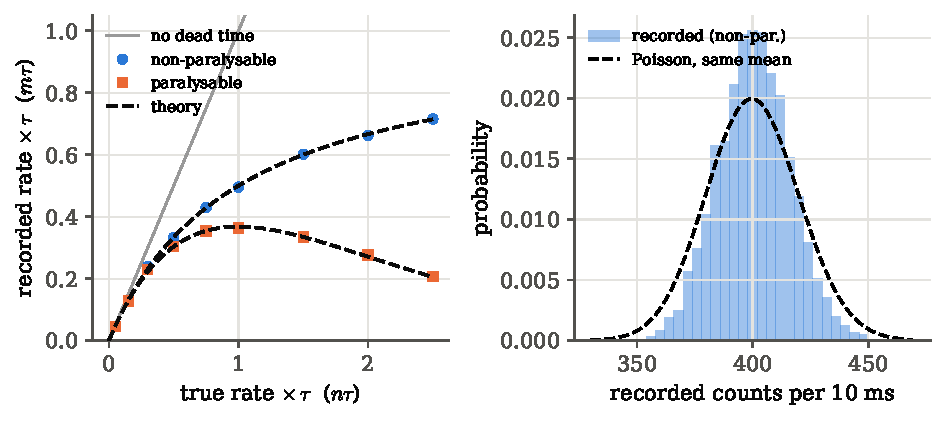
\includegraphics[width=\linewidth]{figures/ch02/08_deadtime.pdf}
\caption{Left: recorded rate against true rate, both in units of $1/\tau$. The simulated counters (dots and squares) sit on the derived curves $n\tau/(1+n\tau)$ and $n\tau e^{-n\tau}$ (dashed). The grey line is a perfect counter. The non-paralysable counter saturates at one hit per dead time; the paralysable one peaks at $n\tau=1$ and then falls. Right: the recorded counts per $10$~ms window at $n\tau=0.25$ (bars) form a visibly narrower histogram than a Poisson distribution with the same mean (dashed).}
\label{2a:fig:deadtime}
\end{figure}

The numbers it produced are these. The true hits give $\twoaDTRawMean$ counts per window on average (expected $\twoaDTTrueMean$) with $\hat F=\twoaDTRawFano$; by \eqref{2a:eq:fanosd} the Poisson scatter of $\hat F$ is $\twoaDTFanoSE$, so $\hat F-1$ is $\twoaDTRawPull$ times this scatter. The non-paralysable counter records a mean of $\twoaDTnpMean$ per window, against $\twoaDTnpTh$ from \eqref{2a:eq:dtnp}, and its Fano factor is $\twoaDTnpFano$, against $1/(1+n\tau)^2=\twoaDTnpFanoTh$. The paralysable counter records $\twoaDTpMean$ (theory $\twoaDTpTh$) with $\hat F=\twoaDTpFano$ (theory $1-2n\tau e^{-n\tau}=\twoaDTpFanoTh$). In units of their own scatter (for $F\ne1$ it is about $F\sqrt{2/(k-1)}$), the two dead-time Fano factors minus their predictions are $\twoaDTnpPull$ and $\twoaDTpPull$. The three numbers are not independent: all three come from the \emph{same} stream of true hits, so a chance fluctuation of that stream shows up in all three. Correcting the non-paralysable mean with \eqref{2a:eq:dtnp} gives $\hat n=\twoaDTnHat\times10^4~\text{s}^{-1}$ for the true rate of $5\times10^4~\text{s}^{-1}$, off by $\twoaDTnHatPull$ times its statistical error $\sqrt{n(1+n\tau)/T}\approx40~\text{s}^{-1}$ from \eqref{2a:eq:dtcorrvar}. The right panel of \cref{2a:fig:deadtime} is the underdispersion made visible.

\paragraph{How research uses it.} Here the simulation \emph{verified} formulas we had derived. Real detectors rarely match either idealised model: the dead time can depend on the pulse height, several stages of electronics can each have their own $\tau$, and afterpulsing adds clustering on top. For them the analytic route stops, and the same few lines of code become the instrument: simulate the true stream, pass it through a model of the electronics, and histogram the recorded counts. That histogram is the sampling distribution $P(S\given\theta)$ of the recorded count, and it goes into the likelihood (\cref{ch:03}). In a collider analysis, the Fano factor of event counts in stable running periods is a routine check that the luminosity and trigger were steady; in a survey, the excess over $F=1$ is the clustering signal itself.

\subsection{Large \texorpdfstring{$\lambda$}{lambda}: the Poisson count becomes Gaussian (a preview)}\label{2a:sec:gauss-preview}

In \cref{2a:fig:pois-limit} the Poisson pmf became more symmetric as $\lambda$ grew. For a large mean, a Poisson variable can be treated as a continuous Gaussian variable \srcref{Cowan}{\S2.2, p.~29}. Cumulants show why most quickly. The Poisson mgf is $M_X(t)=\exp[\lambda(e^t-1)]$, eq.~\eqref{2a:eq:poismgf}, so its cumulant generating function is
\begin{align}
  K_X(t)=\ln M_X(t) \eqby{1} \lambda(e^t-1) \eqby{2} \lambda\sum_{r=1}^\infty\frac{t^r}{r!}
  \quad\Longrightarrow\quad \kappa_r(X) \eqby{3} \lambda\quad\text{for every }r\ge1. \label{2a:eq:poiscum}
\end{align}
\begin{explain}
  \item Logarithm of the Poisson mgf.
  \item Taylor series of $e^t$ with the $r=0$ term cancelled by the $-1$.
  \item By definition the $r$-th cumulant $\kappa_r$ is $r!$ times the coefficient of $t^r$ in $K_X$. The first three cumulants are the mean, the variance and the third central moment.
\end{explain}
Now standardise, $Z=(X-\lambda)/\sqrt\lambda$. Since $K_{aX+b}(t)=bt+K_X(at)$, shifting by $b$ changes only $\kappa_1$ and scaling by $a$ multiplies $\kappa_r$ by $a^r$. With $a=1/\sqrt\lambda$,
\[
  \kappa_1(Z)=0,\qquad \kappa_2(Z)=1,\qquad \kappa_3(Z)=\frac{\lambda}{\lambda^{3/2}}=\frac1{\sqrt\lambda},\qquad \kappa_r(Z)=\lambda^{1-r/2}\xrightarrow{\;\lambda\to\infty\;}0\quad(r\ge3).
\]
So $K_Z(t)\to t^2/2$, which is the cumulant generating function of $\Normal(0,1)$: \emph{Poisson$(\lambda)$ is approximately $\Normal(\lambda,\lambda)$ for large $\lambda$}. The leading correction is the skewness $\kappa_3(Z)=1/\sqrt\lambda$, which shrinks only slowly: at $\lambda=25$ it is still $0.2$. The next part derives this limit properly (de Moivre--Laplace for the binomial, and the central limit theorem), with the corrections. It also explains why the limit holds. For integer $\lambda$, a Poisson$(\lambda)$ count is the sum of $\lambda$ independent Poisson$(1)$ counts, by the sum rule of \cref{2a:sec:poisson-process}, and sums of many independent terms tend to a Gaussian.

\begin{figure}[htbp]
\centering
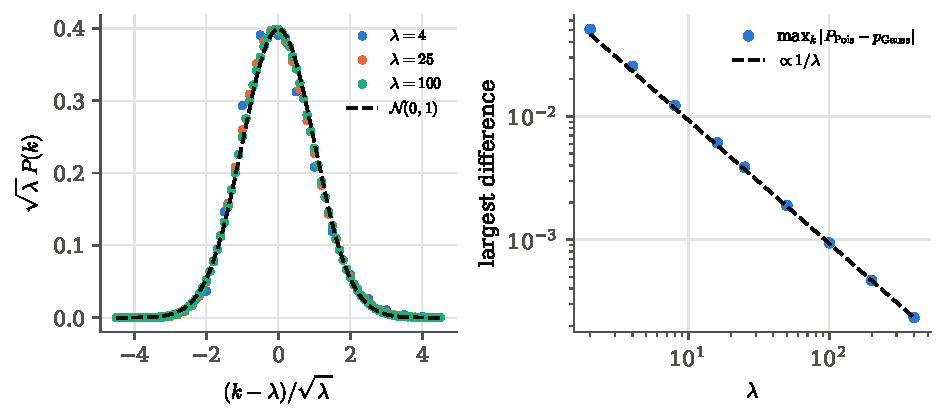
\includegraphics[width=\linewidth]{figures/ch02/08_poisson_gauss.pdf}
\caption{Left: Poisson pmfs for $\lambda=4$, $25$ and $100$, standardised so that the horizontal axis is the distance from the mean in standard deviations, and rescaled by $\sqrt\lambda$ so that they are comparable with a density. They crowd onto the standard Gaussian (dashed); at $\lambda=4$ the points are still lopsided, higher on the left of the peak and with a longer right tail. Right: the largest pointwise difference between the Poisson pmf and the Gaussian density falls like $1/\lambda$ (dashed line).}
\label{2a:fig:poisgauss}
\end{figure}

\Cref{2a:fig:poisgauss} shows the convergence. The largest difference $\max_k|P(k)-p_{\text{Gauss}}(k)|$ is $\twoaGaussDiffFour$ at $\lambda=4$, $\twoaGaussDiffTwentyfive$ at $\lambda=25$, $\twoaGaussDiffHundred$ at $\lambda=100$ and $\twoaGaussDiffFourHundred$ at $\lambda=400$. The $1/\lambda$ law has a simple reason: the peak height is about $1/\sqrt{2\pi\lambda}$, and the skewness correction to it is a fraction of order $\kappa_3(Z)=1/\sqrt\lambda$ of that height, so the absolute error is of order $1/\lambda$.

\paragraph{Example: a $4\sigma$ excess on a background of $25$.} A search region expects $b=25$ background events, with Poisson standard deviation $5$, and we observe $45$, which is $(45-25)/5=4$ standard deviations above the background. How often does background alone give $45$ or more? The Gaussian answer is $\Prob(Z\ge4)=\twoaTailGauss$. The exact Poisson answer, $\sum_{k\ge45}e^{-25}25^k/k!$, is $\twoaTailPois$: $\twoaTailRatio$ times larger. Even the \newterm{continuity correction} \unpack{treating the integer $45$ as the interval from $44.5$ up}, which gives $\twoaTailGaussCC$, is still wrong by a factor of four. Why so wrong? The Gaussian is good near the peak, where the $1/\lambda$ errors of \cref{2a:fig:poisgauss} are small in absolute terms. In the tail both probabilities are tiny, and a small absolute error is a large relative one. The Poisson right tail is heavier than the Gaussian one, because the Poisson is positively skewed. So the Gaussian \emph{understates} the chance of an upward fluctuation and overstates the significance of an excess. Tail probabilities, p-values and discovery claims (\cref{ch:04}) must use the exact Poisson distribution.

\subsection{Choosing a counting distribution}

Every counting distribution came from a mechanism, so recognising the mechanism is how we choose the distribution. The table collects them, with the Fano factor $F=\Var N/\E N$ as the quick check against data.

\begin{taxonomy}[which counting distribution, when]
\centering\small
\renewcommand{\arraystretch}{1.25}
\begin{tabular}{@{}>{\raggedright\arraybackslash}p{4.4cm}>{\raggedright\arraybackslash}p{2.7cm}>{\raggedright\arraybackslash}p{2.2cm}>{\raggedright\arraybackslash}p{2.1cm}@{}}
\textbf{mechanism} & \textbf{distribution} & \textbf{mean} & \textbf{Fano $F$}\\\hline
one yes/no trial & Bernoulli$(p)$ & $p$ & $1-p$\\
successes in $n$ independent trials, same $p$ & Binomial$(n,p)$ & $np$ & $1-p$\\
$N$ events sorted into bins, total fixed & Multinomial$(N,\bm p)$ & $Np_j$ per bin & $1-p_j$ per bin\\
many trials, rare successes; or a stream at constant rate with no memory & Poisson$(\lambda)$ & $\lambda$ & $1$\\
Poisson with a gamma-distributed rate, or clumped events & NegBin & $\mu$ & $1+\mu/\kappa$\\
counter blind for $\tau$ after each recorded hit & renewal count & $nT/(1+n\tau)$ & $(1+n\tau)^{-2}$\\
trials until the first / $r$-th success & Geometric / NegBin & $1/p$, $r/p$ & ---\\
time to the first / $n$-th event of a stream & Exponential / Gamma & $1/\lambda$, $n/\lambda$ & ---\\
\end{tabular}
\end{taxonomy}

The Fano column is the one to remember when data arrive. A value near $1$, judged against $\sqrt{2/(k-1)}$, supports a Poisson model. A value clearly above $1$ points to a fluctuating rate or clumping, and the negative binomial is the standard next model. A value clearly below $1$ points to dead time, pile-up rejection or a finite pool, and calls for a model of the detector. For large means the Poisson itself may be replaced by a Gaussian with variance equal to the mean, but only near the peak, never in the tails.

\begin{recap}[Part summary: counting distributions]
\begin{itemize}
  \item \textbf{Bernoulli} (one trial): $p^x(1-p)^{1-x}$, mean $p$, variance $p(1-p)$. Many independent trials give the product $p^z(1-p)^{N-z}$, which depends only on the number of successes.
  \item \textbf{Binomial} (successes in $n$ successive trials): count the $\binom nk$ paths, each of probability $p^k(1-p)^{n-k}$; mean $np$, variance $np(1-p)$; sums with the same $p$ stay binomial.
  \item \textbf{Multinomial} (histogram with fixed total): marginals binomial, covariance $-Np_ip_j$ between bins; with a Poisson total the bins become independent Poisson counts.
  \item \textbf{Poisson}: the $n\to\infty$, $np=\lambda$ limit of the binomial, and independently the count of a constant-rate, memoryless stream (from the ladder of differential equations $\dd P_n/\dd t=\lambda(P_{n-1}-P_n)$). Mean $=$ variance $=\lambda$. Closed under sums, thinning and binning.
  \item \textbf{Waiting times}: first event exponential (memoryless), $n$-th event Gamma$(n,1/\lambda)$ (Erlang); discrete versions geometric and negative binomial.
  \item \textbf{Failures}: a fluctuating rate or clumping gives $F>1$ (negative binomial); dead time gives $F<1$, with recorded rate $n/(1+n\tau)$ or $ne^{-n\tau}$ and $F=\sigma_I^2/m_I^2$ from the gaps; the dead-time correction removes the bias but inflates the variance by $1+n\tau$.
  \item \textbf{Large $\lambda$}: all Poisson cumulants equal $\lambda$, so the standardised count tends to $\Normal(0,1)$ with skewness $1/\sqrt\lambda$; use the exact Poisson in the tails.
\end{itemize}
\end{recap}
\providecommand{\tbStirTen}{}\renewcommand{\tbStirTen}{1.00837}
\providecommand{\tbStirOne}{}\renewcommand{\tbStirOne}{1.0844}
\providecommand{\tbDMLslope}{}\renewcommand{\tbDMLslope}{-1.00}
\providecommand{\tbDMLerrTen}{}\renewcommand{\tbDMLerrTen}{0.0168}
\providecommand{\tbDMLerrMax}{}\renewcommand{\tbDMLerrMax}{1.8\times10^{-5}}
\providecommand{\tbDMLnMax}{}\renewcommand{\tbDMLnMax}{10000}
\providecommand{\tbCBexact}{}\renewcommand{\tbCBexact}{0.268}
\providecommand{\tbCBplain}{}\renewcommand{\tbCBplain}{0.207}
\providecommand{\tbCBcc}{}\renewcommand{\tbCBcc}{0.270}
\providecommand{\tbCBsd}{}\renewcommand{\tbCBsd}{2.449}
\providecommand{\tbCLTskewOne}{}\renewcommand{\tbCLTskewOne}{2.01}
\providecommand{\tbCLTskewFive}{}\renewcommand{\tbCLTskewFive}{0.91}
\providecommand{\tbCLTskewThirty}{}\renewcommand{\tbCLTskewThirty}{0.366}
\providecommand{\tbCLTskewThirtyTh}{}\renewcommand{\tbCLTskewThirtyTh}{0.365}
\providecommand{\tbCLTslopeExp}{}\renewcommand{\tbCLTslopeExp}{-0.50}
\providecommand{\tbCLTslopeUni}{}\renewcommand{\tbCLTslopeUni}{-1.02}
\providecommand{\tbCLTDexpThirtyTwo}{}\renewcommand{\tbCLTDexpThirtyTwo}{0.0235}
\providecommand{\tbCLTDuniThirtyTwo}{}\renewcommand{\tbCLTDuniThirtyTwo}{8.7\times10^{-4}}
\providecommand{\tbCLTDexpOne}{}\renewcommand{\tbCLTDexpOne}{0.159}
\providecommand{\tbCLTBEthirty}{}\renewcommand{\tbCLTBEthirty}{3.64}
\providecommand{\tbCLTBEmodern}{}\renewcommand{\tbCLTBEmodern}{0.209}
\providecommand{\tbCLTDexpThirty}{}\renewcommand{\tbCLTDexpThirty}{0.0243}
\providecommand{\tbCLTrhothree}{}\renewcommand{\tbCLTrhothree}{2.415}
\providecommand{\tbCLTnsamp}{}\renewcommand{\tbCLTnsamp}{200000}
\providecommand{\tbBWgam}{}\renewcommand{\tbBWgam}{1.2476}
\providecommand{\tbBWiqrMean}{}\renewcommand{\tbBWiqrMean}{2.463}
\providecommand{\tbBWiqrTheory}{}\renewcommand{\tbBWiqrTheory}{2.495}
\providecommand{\tbBWnavg}{}\renewcommand{\tbBWnavg}{1000}
\providecommand{\tbBWfinalMean}{}\renewcommand{\tbBWfinalMean}{94.52}
\providecommand{\tbBWfinalOff}{}\renewcommand{\tbBWfinalOff}{3.3}
\providecommand{\tbBWfinalMedian}{}\renewcommand{\tbBWfinalMedian}{91.186}
\providecommand{\tbBWmedSE}{}\renewcommand{\tbBWmedSE}{0.0062}
\providecommand{\tbLanTailFrac}{}\renewcommand{\tbLanTailFrac}{6.1\times10^{-2}}
\providecommand{\tbLanTailGauss}{}\renewcommand{\tbLanTailGauss}{2.9\times10^{-7}}
\providecommand{\tbLanNlayers}{}\renewcommand{\tbLanNlayers}{25}
\providecommand{\tbMElam}{}\renewcommand{\tbMElam}{0.3710}
\providecommand{\tbMEpOne}{}\renewcommand{\tbMEpOne}{0.0544}
\providecommand{\tbMEpTwo}{}\renewcommand{\tbMEpTwo}{0.0788}
\providecommand{\tbMEpThree}{}\renewcommand{\tbMEpThree}{0.1142}
\providecommand{\tbMEpFour}{}\renewcommand{\tbMEpFour}{0.1654}
\providecommand{\tbMEpFive}{}\renewcommand{\tbMEpFive}{0.2398}
\providecommand{\tbMEpSix}{}\renewcommand{\tbMEpSix}{0.3475}
\providecommand{\tbMESmax}{}\renewcommand{\tbMESmax}{1.6136}
\providecommand{\tbMESrandMax}{}\renewcommand{\tbMESrandMax}{1.6139}
\providecommand{\tbMESrandMaxMean}{}\renewcommand{\tbMESrandMaxMean}{4.4966}
\providecommand{\tbMEminDeficit}{}\renewcommand{\tbMEminDeficit}{9.6\times10^{-4}}
\providecommand{\tbMEnKeep}{}\renewcommand{\tbMEnKeep}{7888}
\providecommand{\tbMESuniformDie}{}\renewcommand{\tbMESuniformDie}{1.7918}
\providecommand{\tbEntUniform}{}\renewcommand{\tbEntUniform}{1.2425}
\providecommand{\tbEntTriang}{}\renewcommand{\tbEntTriang}{1.3959}
\providecommand{\tbEntLaplace}{}\renewcommand{\tbEntLaplace}{1.3466}
\providecommand{\tbEntLogistic}{}\renewcommand{\tbEntLogistic}{1.4046}
\providecommand{\tbEntGauss}{}\renewcommand{\tbEntGauss}{1.4189}
\providecommand{\tbKangEnt}{}\renewcommand{\tbKangEnt}{0.1111}
\providecommand{\tbKangSq}{}\renewcommand{\tbKangSq}{0.0833}
\providecommand{\tbKangLog}{}\renewcommand{\tbKangLog}{0.1301}
\providecommand{\tbKangSqrt}{}\renewcommand{\tbKangSqrt}{0.1218}
\providecommand{\tbMVNfracOne}{}\renewcommand{\tbMVNfracOne}{0.6873}
\providecommand{\tbMVNfracTwo}{}\renewcommand{\tbMVNfracTwo}{0.9559}
\providecommand{\tbMVNlevOne}{}\renewcommand{\tbMVNlevOne}{2.296}
\providecommand{\tbMVNlevTwo}{}\renewcommand{\tbMVNlevTwo}{6.180}
\providecommand{\tbMVNcondMeanTh}{}\renewcommand{\tbMVNcondMeanTh}{3.600}
\providecommand{\tbMVNcondSdTh}{}\renewcommand{\tbMVNcondSdTh}{1.200}
\providecommand{\tbMVNcondMean}{}\renewcommand{\tbMVNcondMean}{3.614}
\providecommand{\tbMVNcondSd}{}\renewcommand{\tbMVNcondSd}{1.187}
\providecommand{\tbMVNnSlab}{}\renewcommand{\tbMVNnSlab}{9588}
\providecommand{\tbMVNmargSd}{}\renewcommand{\tbMVNmargSd}{1.997}
\providecommand{\tbMVNlamOne}{}\renewcommand{\tbMVNlamOne}{4.693}
\providecommand{\tbMVNlamTwo}{}\renewcommand{\tbMVNlamTwo}{0.307}
\providecommand{\tbMVNangle}{}\renewcommand{\tbMVNangle}{66.6}
\providecommand{\tbMVNN}{}\renewcommand{\tbMVNN}{20000}
\providecommand{\tbChiMeanFive}{}\renewcommand{\tbChiMeanFive}{5.010}
\providecommand{\tbChiVarFive}{}\renewcommand{\tbChiVarFive}{10.076}
\providecommand{\tbChiMeanTen}{}\renewcommand{\tbChiMeanTen}{9.993}
\providecommand{\tbChiVarTen}{}\renewcommand{\tbChiVarTen}{19.897}
\providecommand{\tbQFmean}{}\renewcommand{\tbQFmean}{2.999}
\providecommand{\tbQFvar}{}\renewcommand{\tbQFvar}{5.989}
\providecommand{\tbNaiveMean}{}\renewcommand{\tbNaiveMean}{2.997}
\providecommand{\tbNaiveVar}{}\renewcommand{\tbNaiveVar}{7.284}
\providecommand{\tbSVmeanS}{}\renewcommand{\tbSVmeanS}{4.0024}
\providecommand{\tbSVmeanSn}{}\renewcommand{\tbSVmeanSn}{3.2019}
\providecommand{\tbSVsigmaSq}{}\renewcommand{\tbSVsigmaSq}{4.0}
\providecommand{\tbSVbiasTh}{}\renewcommand{\tbSVbiasTh}{3.2000}
\providecommand{\tbSVwMean}{}\renewcommand{\tbSVwMean}{4.002}
\providecommand{\tbSVwVar}{}\renewcommand{\tbSVwVar}{8.022}
\providecommand{\tbSVcorrGauss}{}\renewcommand{\tbSVcorrGauss}{+0.0016}
\providecommand{\tbSVcorrExp}{}\renewcommand{\tbSVcorrExp}{+0.685}
\providecommand{\tbSVn}{}\renewcommand{\tbSVn}{5}
\providecommand{\tbSVnrep}{}\renewcommand{\tbSVnrep}{200000}
\providecommand{\tbTn}{}\renewcommand{\tbTn}{5}
\providecommand{\tbTdof}{}\renewcommand{\tbTdof}{4}
\providecommand{\tbTnrep}{}\renewcommand{\tbTnrep}{400000}
\providecommand{\tbTfracOneNineSix}{}\renewcommand{\tbTfracOneNineSix}{0.1209}
\providecommand{\tbTfracOneNineSixTh}{}\renewcommand{\tbTfracOneNineSixTh}{0.1216}
\providecommand{\tbZfracOneNineSix}{}\renewcommand{\tbZfracOneNineSix}{0.0497}
\providecommand{\tbTquant}{}\renewcommand{\tbTquant}{2.776}
\providecommand{\tbTfracQuant}{}\renewcommand{\tbTfracQuant}{0.0493}
\providecommand{\tbTfracThree}{}\renewcommand{\tbTfracThree}{0.0396}
\providecommand{\tbTfracThreeTh}{}\renewcommand{\tbTfracThreeTh}{0.0399}
\providecommand{\tbTfracThreeGauss}{}\renewcommand{\tbTfracThreeGauss}{0.0027}
\providecommand{\tbTmixNu}{}\renewcommand{\tbTmixNu}{3}
\providecommand{\tbTksMix}{}\renewcommand{\tbTksMix}{0.0010}
\providecommand{\tbTksUV}{}\renewcommand{\tbTksUV}{0.0013}
\providecommand{\tbFdOne}{}\renewcommand{\tbFdOne}{5}
\providecommand{\tbFdTwo}{}\renewcommand{\tbFdTwo}{10}
\providecommand{\tbFmean}{}\renewcommand{\tbFmean}{1.252}
\providecommand{\tbFmeanTh}{}\renewcommand{\tbFmeanTh}{1.250}
\providecommand{\tbFninetyfive}{}\renewcommand{\tbFninetyfive}{3.326}
\providecommand{\tbFfracNinetyfive}{}\renewcommand{\tbFfracNinetyfive}{0.0502}
\providecommand{\tbFksTsq}{}\renewcommand{\tbFksTsq}{0.0035}
\providecommand{\tbLNndyn}{}\renewcommand{\tbLNndyn}{10}
\providecommand{\tbLNmu}{}\renewcommand{\tbLNmu}{13.757}
\providecommand{\tbLNs}{}\renewcommand{\tbLNs}{0.4633}
\providecommand{\tbLNlnMean}{}\renewcommand{\tbLNlnMean}{13.758}
\providecommand{\tbLNlnSd}{}\renewcommand{\tbLNlnSd}{0.4629}
\providecommand{\tbLNmedian}{}\renewcommand{\tbLNmedian}{0.948}
\providecommand{\tbLNmedianTh}{}\renewcommand{\tbLNmedianTh}{0.943}
\providecommand{\tbLNmean}{}\renewcommand{\tbLNmean}{1.050}
\providecommand{\tbLNmeanTh}{}\renewcommand{\tbLNmeanTh}{1.050}
\providecommand{\tbLNmeanExact}{}\renewcommand{\tbLNmeanExact}{1.049}
\providecommand{\tbLNskew}{}\renewcommand{\tbLNskew}{1.333}
\providecommand{\tbLNskewLn}{}\renewcommand{\tbLNskewLn}{-0.054}
\providecommand{\tbMBsv}{}\renewcommand{\tbMBsv}{249.9}
\providecommand{\tbMBmean}{}\renewcommand{\tbMBmean}{398.9}
\providecommand{\tbMBmeanTh}{}\renewcommand{\tbMBmeanTh}{398.7}
\providecommand{\tbMBmodeTh}{}\renewcommand{\tbMBmodeTh}{353.4}
\providecommand{\tbMBrmsTh}{}\renewcommand{\tbMBrmsTh}{432.8}
\providecommand{\tbMBrms}{}\renewcommand{\tbMBrms}{432.8}
\providecommand{\tbRAYmean}{}\renewcommand{\tbRAYmean}{1.2531}
\providecommand{\tbRAYmeanTh}{}\renewcommand{\tbRAYmeanTh}{1.2533}
\providecommand{\tbPOWmean}{}\renewcommand{\tbPOWmean}{1.9986}
\providecommand{\tbPOWsd}{}\renewcommand{\tbPOWsd}{2.0012}
\providecommand{\tbOSn}{}\renewcommand{\tbOSn}{10}
\providecommand{\tbOSk}{}\renewcommand{\tbOSk}{3}
\providecommand{\tbOSmean}{}\renewcommand{\tbOSmean}{0.2728}
\providecommand{\tbOSmeanTh}{}\renewcommand{\tbOSmeanTh}{0.2727}
\providecommand{\tbOSvar}{}\renewcommand{\tbOSvar}{0.01659}
\providecommand{\tbOSvarTh}{}\renewcommand{\tbOSvarTh}{0.01653}
\providecommand{\tbGRmean}{}\renewcommand{\tbGRmean}{0.3846}
\providecommand{\tbGRmeanTh}{}\renewcommand{\tbGRmeanTh}{0.3846}
\providecommand{\tbRJacc}{}\renewcommand{\tbRJacc}{0.1123}
\providecommand{\tbRJaccTh}{}\renewcommand{\tbRJaccTh}{0.1119}
\providecommand{\tbRJkept}{}\renewcommand{\tbRJkept}{224548}
\providecommand{\tbRJmean}{}\renewcommand{\tbRJmean}{0.6428}
\providecommand{\tbRJmeanTh}{}\renewcommand{\tbRJmeanTh}{0.6429}
\providecommand{\tbRJsd}{}\renewcommand{\tbRJsd}{0.1240}
\providecommand{\tbRJsdTh}{}\renewcommand{\tbRJsdTh}{0.1237}
\providecommand{\tbDIRmeanOne}{}\renewcommand{\tbDIRmeanOne}{0.4999}
\providecommand{\tbDIRmeanOneTh}{}\renewcommand{\tbDIRmeanOneTh}{0.5000}
\providecommand{\tbDIRvarOne}{}\renewcommand{\tbDIRvarOne}{0.02767}
\providecommand{\tbDIRvarOneTh}{}\renewcommand{\tbDIRvarOneTh}{0.02778}
\providecommand{\tbDIRcov}{}\renewcommand{\tbDIRcov}{-0.01386}
\providecommand{\tbDIRcovTh}{}\renewcommand{\tbDIRcovTh}{-0.01389}
\providecommand{\tbWsig}{}\renewcommand{\tbWsig}{2.0}
\providecommand{\tbWDelta}{}\renewcommand{\tbWDelta}{10}
\providecommand{\tbWfwhm}{}\renewcommand{\tbWfwhm}{6.18}
\providecommand{\tbWsigEq}{}\renewcommand{\tbWsigEq}{2.63}
\providecommand{\tbWoutSim}{}\renewcommand{\tbWoutSim}{0.0820}
\providecommand{\tbWoutVoigt}{}\renewcommand{\tbWoutVoigt}{0.0825}
\providecommand{\tbWoutTail}{}\renewcommand{\tbWoutTail}{0.0794}
\providecommand{\tbWoutGauss}{}\renewcommand{\tbWoutGauss}{1.4\times10^{-4}}
\providecommand{\tbWrstar}{}\renewcommand{\tbWrstar}{3}
\providecommand{\tbWfaSim}{}\renewcommand{\tbWfaSim}{0.0112}
\providecommand{\tbWfaTh}{}\renewcommand{\tbWfaTh}{0.0111}
\providecommand{\tbWfaEight}{}\renewcommand{\tbWfaEight}{1.27\times10^{-14}}
\providecommand{\tbWpExact}{}\renewcommand{\tbWpExact}{0.0235}
\providecommand{\tbWzGauss}{}\renewcommand{\tbWzGauss}{2.12}
\providecommand{\tbWpGauss}{}\renewcommand{\tbWpGauss}{0.0169}
\providecommand{\tbWthreeGauss}{}\renewcommand{\tbWthreeGauss}{0.0027}
\providecommand{\tbWfiveGauss}{}\renewcommand{\tbWfiveGauss}{5.7\times10^{-7}}
\providecommand{\tbWthreeLap}{}\renewcommand{\tbWthreeLap}{0.0144}
\providecommand{\tbWfiveLap}{}\renewcommand{\tbWfiveLap}{8.5\times10^{-4}}
\providecommand{\tbWthreeTfive}{}\renewcommand{\tbWthreeTfive}{0.0117}
\providecommand{\tbWfiveTfive}{}\renewcommand{\tbWfiveTfive}{1.3\times10^{-3}}
\providecommand{\tbWthreeTthree}{}\renewcommand{\tbWthreeTthree}{0.0138}
\providecommand{\tbWfiveTthree}{}\renewcommand{\tbWfiveTthree}{3.2\times10^{-3}}
\providecommand{\tbWratioTthree}{}\renewcommand{\tbWratioTthree}{5650}
\section{The Gaussian, first way: the shape of a binomial with many trials}
\label{2b:sec:gauss-binomial}

The same bell-shaped curve describes a calorimeter energy, a timing residual, a CMB temperature and a strain sample. None of these is a count: the counting distributions of the first half of the chapter live on the integers, and these quantities do not. There are three separate routes to the bell curve, and each route tells us \emph{when} to trust it. The oldest route starts from a count after all. Take a binomial distribution with a very large number of trials and ask what shape it takes.

\paragraph{Ten thousand photo-electrons.}
A scintillator bar is hit by a cosmic muon. It produces $n=10\,000$ photons, and each photon independently reaches the photomultiplier and makes a photo-electron with probability $p=0.3$. The number of photo-electrons $k$ is Binomial$(n,p)$ (see the counting part of this chapter). To compute $\Prob(k\le 2950)$ exactly we would add $2951$ terms, each containing factorials of numbers near $10^4$. Nobody does that. Instead everyone replaces the binomial by a smooth bell curve with mean $np=3000$ and standard deviation $\sqrt{np(1-p)}\approx 45.8$.

That replacement raises four questions. Which bell curve, exactly? Why a bell and not some other shape? How large must $n$ be? And how do we correct for the fact that $k$ is an integer while the curve is smooth? The large-$n$ limit of the binomial answers all four.

\paragraph{Zooming in on the peak of a mountain.}
The Gaussian is what \emph{every} smooth, single-peaked, sharply concentrated distribution looks like near its maximum. Here is why. For large $n$ the binomial pmf is a tall, narrow mountain centred at $np$, and its width grows only like $\sqrt n$. Plot the \emph{logarithm} of any smooth mountain: near its summit it looks like a downward parabola. The exponential of a parabola is a Gaussian. This is the same move as the harmonic approximation in mechanics: expand the potential to second order about its minimum and the motion becomes simple harmonic. Here we expand $\ln\Prob(k)$ to second order about its maximum.

\paragraph{The plan.}
\begin{enumerate}[label=\arabic*.]
  \item Which quantity do we want? The probability of $k$ successes in $n$ trials when $n$ is large.
  \item What makes it hard? Factorials of large numbers. So first find a good formula for $n!$ (Stirling).
  \item Where is the probability concentrated? Near $k=np$, in a window of width $\sqrt{np(1-p)}$.
  \item What does $\ln\Prob(k)$ look like in that window? Expand it in powers of the distance from the peak and keep what survives as $n\to\infty$.
  \item How do we turn a statement about integers into one about a continuous variable, and what does that cost? (The continuity correction.)
\end{enumerate}

\subsection{The Gaussian density and what its two parameters do}
\label{2b:sec:gauss-def}

\begin{workdef}[Gaussian (normal) distribution]
A continuous random variable $X$ has a \newterm{Gaussian} or \newterm{normal} distribution with parameters $\mu$ and $\sigma^2$, written $X\sim\Normal(\mu,\sigma^2)$, if its density \unpack{probability per unit $x$, so it has units of $1/x$} is
\begin{equation}
  p(x\given\mu,\sigma^2)=\frac{1}{\sqrt{2\pi\sigma^2}}\exp\!\left[-\frac{(x-\mu)^2}{2\sigma^2}\right],\qquad -\infty<x<\infty ,
  \label{2b:eq:gauss}
\end{equation}
with $\mu\in\R$ and $\sigma>0$. The case $\mu=0$, $\sigma=1$ is the \newterm{standard normal} $Z\sim\Normal(0,1)$, with density $\varphi(z)=e^{-z^2/2}/\sqrt{2\pi}$ and cumulative distribution function \unpack{the probability of landing at or below $z$} $\Phi(z)=\int_{-\infty}^z\varphi(z')\,\dd z'$.
\emph{Operational test:} standardise, $z=(x-\mu)/\sigma$, and compare the histogram of $z$ with $\varphi$ (or the ordered $z$ values with the quantiles $\Phi^{-1}$).
\end{workdef}

Three facts make the Gaussian usable. We check each one.

\paragraph{It is normalised.} The function $e^{-z^2/2}$ has no elementary antiderivative, so the normalisation needs a trick: square the integral and go to polar coordinates \srcref{CasellaBerger}{p.~84--85}. Let $I=\int_{-\infty}^{\infty}e^{-z^2/2}\dd z$. Then
\begin{align}
  I^2
  &\eqby{1} \int_{-\infty}^{\infty}\!\!\int_{-\infty}^{\infty} e^{-(u^2+v^2)/2}\,\dd u\,\dd v \nonumber\\
  &\eqby{2} \int_{0}^{2\pi}\!\!\int_{0}^{\infty} e^{-r^2/2}\,r\,\dd r\,\dd\phi \nonumber\\
  &\eqby{3} 2\pi\Bigl[-e^{-r^2/2}\Bigr]_0^{\infty} \nonumber\\
  &= 2\pi .
  \label{2b:eq:gauss-integral}
\end{align}
\begin{explain}
  \item The two copies of the integral use independent dummy variables $u$ and $v$, and a product of two integrals is a double integral over the plane.
  \item Polar coordinates $u=r\cos\phi$, $v=r\sin\phi$: then $u^2+v^2=r^2$ and the area element is $\dd u\,\dd v=r\,\dd r\,\dd\phi$.
  \item The $\phi$ integral gives $2\pi$. The extra factor $r$ makes the $r$ integral elementary, since $\frac{\dd}{\dd r}\bigl(-e^{-r^2/2}\bigr)=r\,e^{-r^2/2}$.
\end{explain}
So $I=\sqrt{2\pi}$, which is the constant in $\varphi$. Substituting $z=(x-\mu)/\sigma$, $\dd x=\sigma\,\dd z$, gives the constant $1/\sqrt{2\pi\sigma^2}$ in \eqref{2b:eq:gauss}. A by-product: with $w=z^2/2$ the half-line integral becomes $\int_0^\infty w^{-1/2}e^{-w}\dd w=\Gamma(\tfrac12)$, so
\begin{equation}
  \Gamma(\tfrac12)=\sqrt\pi ,
  \label{2b:eq:gamma-half}
\end{equation}
where $\Gamma(\alpha)=\int_0^\infty t^{\alpha-1}e^{-t}\dd t$ is the Gamma function, with $\Gamma(\alpha+1)=\alpha\Gamma(\alpha)$ (integrate by parts) and $\Gamma(n+1)=n!$ for integers. We need all three facts for $\chi^2$ later.

\paragraph{$\mu$ is the mean and $\sigma^2$ the variance.} With $x=\mu+\sigma z$,
\begin{align}
  \E(X)
  &\eqby{1} \mu+\sigma\int_{-\infty}^{\infty} z\,\varphi(z)\,\dd z \eqby{2} \mu , \nonumber\\
  \Var(X)
  &\eqby{3} \sigma^2\int_{-\infty}^{\infty} z^2\varphi(z)\,\dd z
   \eqby{4} \sigma^2\Bigl\{\bigl[-z\varphi(z)\bigr]_{-\infty}^{\infty}+\int_{-\infty}^{\infty}\varphi(z)\,\dd z\Bigr\}
   \eqby{5} \sigma^2 .
  \label{2b:eq:gauss-moments}
\end{align}
\begin{explain}
  \item Change variables and use $\int\varphi=1$ for the constant term.
  \item The integrand $z\varphi(z)$ is odd, so the integral over a symmetric range vanishes.
  \item $\Var(X)=\E(X-\mu)^2$ and $(x-\mu)^2=\sigma^2z^2$.
  \item Integrate by parts with $u=z$ and $\dd v=z\varphi(z)\dd z$, whose integral is $v=-\varphi(z)$ because $\varphi'(z)=-z\varphi(z)$.
  \item The boundary term vanishes because $\varphi$ decays faster than any power, and the remaining integral is $1$.
\end{explain}
So the two parameters are exactly the mean and the variance \srcref{Cowan}{(2.23)--(2.24)}. This is special: for most distributions the parameters are \emph{not} the mean and variance (the log-normal of \cref{2b:sec:zoo} is a warning example).

\paragraph{Standardising reduces everything to one table.} If $X\sim\Normal(\mu,\sigma^2)$ then $Z=(X-\mu)/\sigma\sim\Normal(0,1)$ and, conversely, $X=\mu+\sigma Z$ \mainref{p.~28}. Hence
\begin{equation}
  \Prob(a<X<b)=\Phi\!\left(\frac{b-\mu}{\sigma}\right)-\Phi\!\left(\frac{a-\mu}{\sigma}\right).
  \label{2b:eq:gauss-prob}
\end{equation}
Two numbers are worth knowing by heart. First, the probability within $1$, $2$, $3$ standard deviations of the mean is $0.6827$, $0.9545$, $0.9973$ (\cref{2b:fig:gauss-bands}). Second, ``one sigma'' can be read off a plot by eye: it is where the curve stops bending down and starts bending up. To see this, note that the density has its maximum at $x=\mu$, and its second derivative $\varphi''(z)=(z^2-1)\varphi(z)$ vanishes at $z=\pm1$. So the inflection points sit at $x=\mu\pm\sigma$.

\begin{figure}[htbp]
\centering
\begin{tikzpicture}
\begin{axis}[width=11cm,height=5.2cm,domain=-4:4,samples=161,
  axis lines=left,xlabel={$z=(x-\mu)/\sigma$},ylabel={$\varphi(z)$},
  ymin=0,ymax=0.47,xtick={-3,-2,-1,0,1,2,3},ytick={0,0.1,0.2,0.3,0.4},
  every axis plot/.append style={thick}]
  \addplot[draw=none,fill=formblue!10,domain=-3:3] {exp(-x^2/2)/sqrt(2*pi)} \closedcycle;
  \addplot[draw=none,fill=formblue!22,domain=-2:2] {exp(-x^2/2)/sqrt(2*pi)} \closedcycle;
  \addplot[draw=none,fill=formblue!40,domain=-1:1] {exp(-x^2/2)/sqrt(2*pi)} \closedcycle;
  \addplot[formblue] {exp(-x^2/2)/sqrt(2*pi)};
  \addplot[only marks,mark=*,mark size=1.6pt,bdryred] coordinates {(-1,0.2420) (1,0.2420)};
  \node[font=\scriptsize,anchor=east,bdryred] at (axis cs:-1.05,0.262) {inflection};
  \node[font=\scriptsize] at (axis cs:0,0.12) {$68.3\%$};
  \node[font=\scriptsize] at (axis cs:1.5,0.035) {$95.4\%$};
  \node[font=\scriptsize] at (axis cs:3.35,0.045) {$99.7\%$};
  \draw[faint] (axis cs:2.55,0.012) -- (axis cs:3.15,0.038);
\end{axis}
\end{tikzpicture}
\caption{The standard normal density. The darkest band ($|z|<1$) holds $68.3\%$ of the probability, the band out to $|z|<2$ holds $95.4\%$, and out to $|z|<3$ holds $99.7\%$. The red dots are the inflection points at $z=\pm1$: one standard deviation is where the curve changes from bending down to bending up.}
\label{2b:fig:gauss-bands}
\end{figure}

\paragraph{Example: Reading the table both ways.}
\label{2b:ex:aos-gauss}
Let $X\sim\Normal(3,5)$. The second argument is the \emph{variance}, so $\sigma=\sqrt5$. A table of $\Phi$ answers two kinds of question. The forward question gives a cut and asks for a probability: what is $\Prob(X>1)$?
\begin{align*}
  \Prob(X>1)
  &\eqby{1} 1-\Prob(X<1)
  \eqby{2} 1-\Phi\!\left(\frac{1-3}{\sqrt5}\right)
  = 1-\Phi(-0.8944)
  \eqby{3} 0.81 .
\end{align*}
\begin{explain}
  \item Complement rule. For a continuous variable $\Prob(X=1)=0$, so $<$ and $\le$ do not matter.
  \item Standardise with \eqref{2b:eq:gauss-prob}.
  \item From a table or \pyname{scipy.stats.norm.cdf}: $\Phi(-0.8944)=0.1855$.
\end{explain}
The quantile question goes the other way. It gives a probability and asks for the cut: which $q$ has $\Prob(X<q)=0.2$?
\begin{align*}
  0.2=\Prob(X<q)
  &\eqby{1} \Phi\!\left(\frac{q-3}{\sqrt5}\right)
  \;\Longrightarrow\; \frac{q-3}{\sqrt5}\eqby{2}\Phi^{-1}(0.2)=-0.8416 \\
  &\;\Longrightarrow\; q\eqby{3}3-0.8416\sqrt5=1.1181 .
\end{align*}
\begin{explain}
  \item Standardise.
  \item $\Phi$ is strictly increasing, so it can be inverted. $\Phi^{-1}$ is \pyname{scipy.stats.norm.ppf}.
  \item Solve the linear equation for $q$.
\end{explain}
These are the two numbers of \mainref{p.~29, Example~2.17}.

\begin{pitfall}[$\Normal(\mu,\sigma^2)$ or $\Normal(\mu,\sigma)$?]
AoS, Cowan and CasellaBerger write the \emph{variance} as the second argument. Lambert and most software (\pyname{scipy.stats.norm(loc, scale)}, \pyname{numpy.random.normal(loc, scale)}) take the \emph{standard deviation}. $\Normal(3,5)$ in AoS is \pyname{norm(3, sqrt(5))} in scipy. Always check which one a formula or a function expects.
\end{pitfall}

\subsection{Stirling's formula from Laplace's method}
\label{2b:sec:stirling}

The binomial is built from factorials, so we need a good formula for $n!$ when $n$ is large. That formula is Stirling's:
\begin{equation}
  n! \simeq \sqrt{2\pi n}\;n^n e^{-n}\qquad (n\to\infty),
  \qquad\text{i.e.}\qquad
  \ln n! = n\ln n-n+\tfrac12\ln(2\pi n)+O(1/n) .
  \label{2b:eq:stirling}
\end{equation}

It comes from the same zoom-in on a peak, now applied to an integral. \emph{The starting point.} The Gamma function gives $n!$ as an integral, $n!=\Gamma(n+1)=\int_0^\infty t^n e^{-t}\dd t$, and for large $n$ its integrand is sharply peaked. \emph{Where is the peak, and how sharp is it?} Write the integrand as $e^{f(t)}$ with $f(t)=n\ln t-t$. The slope $f'(t)=n/t-1$ vanishes at $t=n$, so the peak is at $t=n$. The curvature $f''(t)=-n/t^2$ equals $-1/n$ there. \emph{Only then the integral.} Expanding $f$ to second order about its maximum,
\begin{align}
  n!
  &\eqby{1} \int_0^\infty \exp\Bigl[f(n)+f'(n)(t-n)+\tfrac12 f''(n)(t-n)^2+\dots\Bigr]\dd t \nonumber\\
  &\eqby{2} n^n e^{-n}\int_0^\infty \exp\Bigl[-\frac{(t-n)^2}{2n}+\dots\Bigr]\dd t \nonumber\\
  &\eqby{3} n^n e^{-n}\int_{-\infty}^{\infty} e^{-s^2/(2n)}\dd s\;\bigl(1+O(1/n)\bigr) \nonumber\\
  &\eqby{4} \sqrt{2\pi n}\;n^n e^{-n}\bigl(1+O(1/n)\bigr) .
  \label{2b:eq:stirling-derivation}
\end{align}
\begin{explain}
  \item Taylor expansion of $f$ about $t=n$ inside the exponential.
  \item $f(n)=n\ln n-n$ gives $e^{f(n)}=n^ne^{-n}$, the linear term vanishes because $t=n$ is the maximum, and $\tfrac12f''(n)=-1/(2n)$.
  \item Substitute $s=t-n$. The integrand is negligible beyond a few multiples of $\sqrt n$ from the peak, so extending the lower limit from $s=-n$ to $-\infty$ adds only a Gaussian tail of order $e^{-n/2}$. The cubic and higher terms of the expansion give the relative correction of order $1/n$ (it is $1/(12n)$).
  \item The Gaussian integral \eqref{2b:eq:gauss-integral} with $\sigma^2=n$.
\end{explain}
This is \newterm{Laplace's method}: a sharply peaked integrand $e^{f(t)}$ is replaced by a Gaussian with the same peak height and the same curvature. We will meet it again as the Gaussian (Laplace) approximation to a posterior in \cref{ch:05}. \Cref{2b:fig:laplace} shows how good the approximation already is at $n=10$.

\begin{figure}[htbp]
\centering
\begin{tikzpicture}
\begin{axis}[width=11cm,height=5cm,domain=0.05:30,samples=200,
  axis lines=left,xlabel={$t$},ylabel={integrand$/$peak},
  ymin=0,ymax=1.15,xmin=0,xmax=30,legend cell align=left,legend style={draw=none,font=\scriptsize,at={(0.98,0.95)},anchor=north east},
  every axis plot/.append style={thick}]
  \addplot[formblue] {exp(10*ln(x/10)-(x-10))};
  \addlegendentry{integrand $t^{10}e^{-t}$, scaled}
  \addplot[black,dashed] {exp(-(x-10)^2/20)};
  \addlegendentry{Gaussian}
  \draw[tangentgreen,<->] (axis cs:10-3.1623,0.6065) -- (axis cs:10+3.1623,0.6065);
  \node[font=\scriptsize,tangentgreen,anchor=south] at (axis cs:10,0.66) {$2\sqrt{n}$};
\end{axis}
\end{tikzpicture}
\caption{Laplace's method for $10!=\int_0^\infty t^{10}e^{-t}\dd t$. The integrand (blue) is scaled to peak height one at $t=n=10$. The dashed Gaussian has the same peak and the same curvature there, so its width is $\sqrt n$. The two areas differ by less than one percent, and the mismatch is the slight skew of the blue curve, which the $1/(12n)$ correction describes.}
\label{2b:fig:laplace}
\end{figure}

Stirling's formula is accurate even for small $n$. The script below finds $n!/\text{Stirling}=\tbStirOne$ at $n=1$ and $\tbStirTen$ at $n=10$, in agreement with $1+1/(12n)$ (\cref{2b:fig:demoivre-errors}a). Even $1!$ is off by only eight percent.

\subsection{The de Moivre--Laplace limit}
\label{2b:sec:demoivre}

\begin{keyidea}[de Moivre--Laplace]
Let $k\sim\text{Binomial}(n,p)$ and $q=1-p$. For large $n$ and $k$ within a few $\sqrt{npq}$ of $np$,
\begin{equation}
  \Prob(k)=\binom nk p^kq^{n-k}\simeq \frac{1}{\sqrt{2\pi npq}}\exp\!\left[-\frac{(k-np)^2}{2npq}\right].
  \label{2b:eq:dml}
\end{equation}
The binomial pmf becomes a Gaussian density with $\mu=np$ and $\sigma^2=npq$, the binomial mean and variance.
\end{keyidea}

The derivation takes two steps. First, replace each factorial by Stirling's formula. Second, Taylor-expand the exponent about the peak. \emph{Step one.} Insert \eqref{2b:eq:stirling} for $n!$, $k!$ and $(n-k)!$:
\begin{align}
  \ln\Prob(k)
  &\eqby{1} \ln n!-\ln k!-\ln(n-k)!+k\ln p+(n-k)\ln q \nonumber\\
  &\eqby{2} \bigl[n\ln n-k\ln k-(n-k)\ln(n-k)+k\ln p+(n-k)\ln q\bigr]
     -\tfrac12\ln\frac{2\pi k(n-k)}{n} \nonumber\\
  &\eqby{3} -k\ln\frac{k}{np}-(n-k)\ln\frac{n-k}{nq}-\tfrac12\ln\frac{2\pi k(n-k)}{n} .
  \label{2b:eq:dml-step1}
\end{align}
\begin{explain}
  \item The logarithm of the binomial pmf.
  \item Stirling for the three factorials. The $-n+k+(n-k)$ from the three ``$-m$'' terms cancels. The three $\tfrac12\ln(2\pi m)$ terms combine into the last logarithm.
  \item Write $n\ln n=k\ln n+(n-k)\ln n$ and collect: $k\ln n-k\ln k+k\ln p=-k\ln\frac{k}{np}$, and the same for the $n-k$ terms.
\end{explain}
\emph{Step two.} Measure $k$ from the centre of the binomial, $k=np+\delta$, so that $\delta$ is the distance from the peak. Then $n-k=nq-\delta$, $k/(np)=1+\delta/(np)$ and $(n-k)/(nq)=1-\delta/(nq)$. Each logarithm in \eqref{2b:eq:dml-step1} now has the form $\ln(1+x)$ with $x$ small, so we use $\ln(1+x)=x-\tfrac{x^2}{2}+\tfrac{x^3}{3}-\dots$:
\begin{align}
  (np+\delta)\ln\Bigl(1+\frac{\delta}{np}\Bigr)
  &\eqby{1} (np+\delta)\Bigl(\frac{\delta}{np}-\frac{\delta^2}{2n^2p^2}+\frac{\delta^3}{3n^3p^3}\Bigr)+O\Bigl(\frac{\delta^4}{n^3}\Bigr) \nonumber\\
  &\eqby{2} \delta+\frac{\delta^2}{2np}-\frac{\delta^3}{6n^2p^2}+O\Bigl(\frac{\delta^4}{n^3}\Bigr),\nonumber\\
  (nq-\delta)\ln\Bigl(1-\frac{\delta}{nq}\Bigr)
  &\eqby{3} -\delta+\frac{\delta^2}{2nq}+\frac{\delta^3}{6n^2q^2}+O\Bigl(\frac{\delta^4}{n^3}\Bigr) .
  \label{2b:eq:dml-taylor}
\end{align}
\begin{explain}
  \item Taylor series of the logarithm to third order.
  \item Multiply out: $\delta^2$ terms $\frac{\delta^2}{np}-\frac{\delta^2}{2np}=\frac{\delta^2}{2np}$, and $\delta^3$ terms $-\frac{\delta^3}{2n^2p^2}+\frac{\delta^3}{3n^2p^2}=-\frac{\delta^3}{6n^2p^2}$.
  \item The same calculation with $p\to q$ and $\delta\to-\delta$.
\end{explain}
The exponent in \eqref{2b:eq:dml-step1} is minus the sum of these two lines:
\begin{align}
  -k\ln\frac{k}{np}-(n-k)\ln\frac{n-k}{nq}
  &\eqby{1} -\frac{\delta^2}{2n}\Bigl(\frac1p+\frac1q\Bigr)+\frac{\delta^3}{6n^2}\Bigl(\frac1{p^2}-\frac1{q^2}\Bigr)+\dots \nonumber\\
  &\eqby{2} -\frac{\delta^2}{2npq}+\frac{\delta^3}{6n^2}\,\frac{q^2-p^2}{p^2q^2}+\dots
  \label{2b:eq:dml-exponent}
\end{align}
\begin{explain}
  \item The $\pm\delta$ terms cancel. This cancellation is what puts the peak at $np$.
  \item $\frac1p+\frac1q=\frac{p+q}{pq}=\frac1{pq}$ because $p+q=1$.
\end{explain}
\emph{Which terms survive?} Only the quadratic one. The probability sits where $\delta$ is of order $\sqrt{npq}$, so we judge each term there. The quadratic term $\delta^2/(2npq)$ is of order $1$. The cubic term is of order $n^{3/2}/n^2=n^{-1/2}$, which goes to zero. The prefactor also simplifies: $k(n-k)/n=npq+\delta(q-p)-\delta^2/n=npq\,[1+O(n^{-1/2})]$. Dropping the terms that vanish gives \eqref{2b:eq:dml}.

The cubic term also says how fast the limit is reached, in two ways. For $p=q=\tfrac12$ it is exactly zero, so the symmetric binomial converges faster. And the leading corrections are \emph{odd} in $\delta$: they skew the curve but leave its height at the peak unchanged. So the largest pointwise error is the relative correction $n^{-1/2}$ times the height of the pmf, also of order $n^{-1/2}$, which gives $n^{-1}$.

\begin{pitfall}[The approximation is local]
\eqref{2b:eq:dml} was derived for $\delta=O(\sqrt n)$. Far in the tails, say $\delta\sim n$, the neglected cubic and higher terms are \emph{not} small and the relative error can be enormous, even though both probabilities are tiny. A ``$5\sigma$'' tail probability computed from the Gaussian approximation to a binomial or Poisson count can be off by a large factor. For tail probabilities use the exact distribution (\pyname{scipy.stats.binom.sf}).
\end{pitfall}

\paragraph{Example: The continuity correction.}
\label{2b:ex:continuity}
An integer count has to be matched to a smooth curve, and the match is best when we cut half-way between integers. Let $X\sim\text{Binomial}(25,0.6)$, so $\mu=15$ and $\sigma=\sqrt{25\cdot0.6\cdot0.4}=\tbCBsd$. We want $\Prob(X\le13)$. Think of each integer $k$ as a bar of width one centred on $k$, so the bar for $k=13$ reaches up to $13.5$. The plain Gaussian approximation cuts at $13$ and misses half of that bar. The \newterm{continuity correction} cuts at $13.5$ instead:
\begin{align*}
  \Prob(X\le13)
  &\eqby{1} \Prob(X\le13.5)
  \eqby{2} \Phi\!\left(\frac{13.5-15}{\tbCBsd}\right)
  = \tbCBcc .
\end{align*}
\begin{explain}
  \item $X$ is an integer, so $X\le13$ and $X\le13.5$ are the same event. The bar picture tells us to use the second when replacing the pmf by a density.
  \item de Moivre--Laplace with $\mu=np$, $\sigma^2=npq$, then standardise.
\end{explain}
The exact binomial sum is $\tbCBexact$ and the uncorrected approximation $\Phi\bigl((13-15)/\tbCBsd\bigr)=\tbCBplain$. The half-bar is worth six percentage points here. In general, $\Prob(X\le x)\approx\Phi\bigl((x+\tfrac12-\mu)/\sigma\bigr)$ and $\Prob(X\ge x)\approx1-\Phi\bigl((x-\tfrac12-\mu)/\sigma\bigr)$.

\paragraph{Example: How many photo-electrons?}
Back to the scintillator bar of the opening: $n=10^4$ photons, each making a photo-electron with probability $p=0.3$, so $\mu=np=3000$ and $\sigma=\sqrt{npq}=\sqrt{2100}=45.83$. We wanted $\Prob(k\le2950)$:
\begin{align*}
  \Prob(k\le2950)
  &\eqby{1}\Phi\!\left(\frac{2950.5-3000}{45.83}\right)
  =\Phi(-1.080)
  \eqby{2}0.140 .
\end{align*}
\begin{explain}
  \item de Moivre--Laplace with the continuity correction.
  \item Table value. The exact binomial sum (\pyname{binom.cdf(2950, 10000, 0.3)}) agrees to three decimal places.
\end{explain}
The same numbers give the bar's energy resolution. The relative width $\sigma/\mu=\sqrt{q/(np)}=1.5\%$ is its photo-statistics term. It falls like $1/\sqrt{\text{number of photo-electrons}}$, the famous $a/\sqrt E$ term of calorimetry.

\paragraph{Exercise: when is $n$ large enough.}
CasellaBerger's rule of thumb is $\min(np,\,nq)\ge5$ \srcref{CasellaBerger}{p.~85}. Use \eqref{2b:eq:dml-exponent} to explain why the rule involves the \emph{smaller} of $np$ and $nq$. (Answer: the relative size of the cubic term at $\delta=\sigma$ is $\frac{\sigma^3}{6n^2}\frac{|q^2-p^2|}{p^2q^2}=\frac{|q-p|}{6\sqrt{npq}}$, which is large when either $np$ or $nq$ is small, i.e.\ when the distribution is squeezed against $k=0$ or $k=n$.)

\subsection{Python: watching the binomial become a Gaussian}
\label{2b:sec:dml-python}

The script computes Stirling's ratio, overlays the Gaussian on three binomials, and measures the largest pointwise error as $n$ grows from $10$ to $10^4$. The first key lines check Stirling's formula:

\pyfile[firstline=29,lastline=33,firstnumber=29]{code/ch02/20_demoivre_laplace.py}{Stirling's formula against the exact $\ln n!$}

Line 31 uses \pyname{gammaln}, the logarithm of the Gamma function, because $n!$ itself overflows a double for $n>170$. Any likelihood code works with logarithms of factorials for the same reason. The next lines measure how far the binomial is from its Gaussian:

\pyfile[firstline=54,lastline=62,firstnumber=54]{code/ch02/20_demoivre_laplace.py}{The largest error of the de Moivre--Laplace approximation}

For each $n$ on a logarithmic grid, line 60 compares the exact pmf with the Gaussian density at the same integers and keeps the worst case. Line 62 fits a straight line in log--log space. The slope comes out as $\tbDMLslope$, the $n^{-1}$ predicted above from the odd (skewing) corrections. At $n=10$ the largest error is $\tbDMLerrTen$, at $n=\tbDMLnMax$ it is $\tbDMLerrMax$ (\cref{2b:fig:demoivre-errors}b).

\begin{figure}[htbp]
\centering
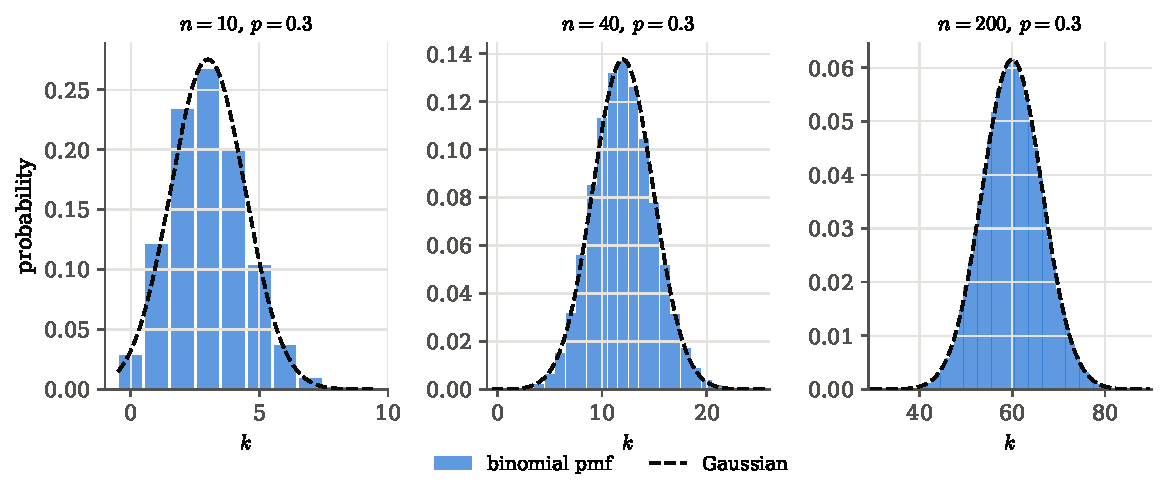
\includegraphics[width=\linewidth]{figures/ch02/demoivre_panels.pdf}
\caption{Binomial$(n,0.3)$ probabilities (bars) with the Gaussian of the same mean and variance (dashed) for $n=10$, $40$, $200$. At $n=10$ the bars lean to the right of the curve: the distribution is squeezed against $k=0$ and is skewed. By $n=200$ the skew is invisible by eye.}
\label{2b:fig:demoivre-panels}
\end{figure}

\begin{figure}[htbp]
\centering
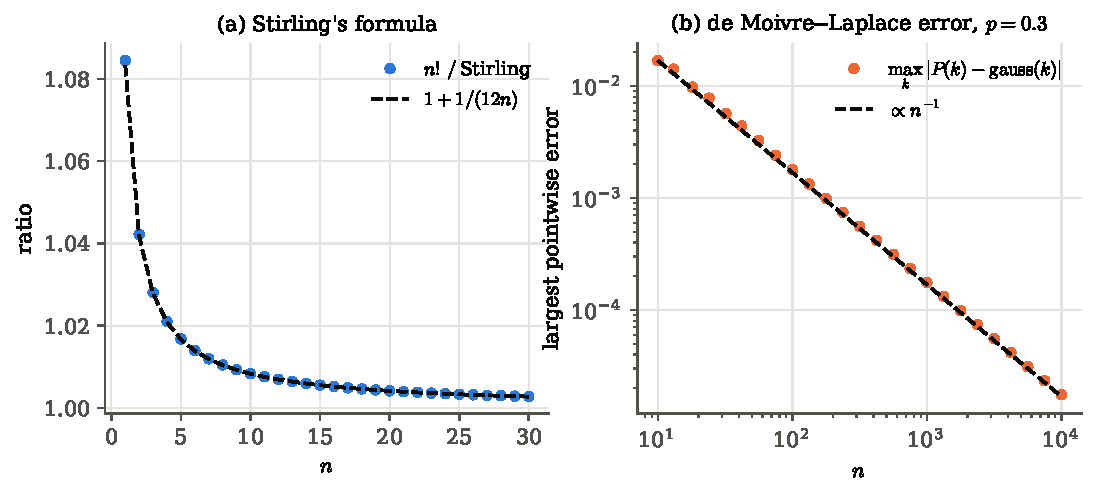
\includegraphics[width=\linewidth]{figures/ch02/demoivre_errors.pdf}
\caption{(a) The ratio of the exact $n!$ to Stirling's formula approaches one from above, following $1+1/(12n)$. (b) The largest pointwise difference between the binomial pmf and its Gaussian approximation falls as $1/n$ (dashed line).}
\label{2b:fig:demoivre-errors}
\end{figure}

\paragraph{What this bought us.}
The Gaussian appears whenever a distribution is sharply peaked and we look on the scale of its width: the logarithm is a parabola there. For the binomial the parabola has curvature $1/(npq)$, which fixes the Gaussian completely. The first correction is a skew of relative size $|q-p|/\sqrt{npq}$, and it is the skew, not the width, that tells us whether $n$ is large enough.

\begin{inpractice}[Verifying a limit versus relying on it]
Here the plot only \emph{verifies} a known limit: the exact pmf is cheap, so nothing hangs on the approximation. Research uses the same Gaussian replacement where no exact answer is at hand. A binned $\chi^2$ fit to a histogram treats each bin count, a binomial or Poisson number, as Gaussian with variance equal to its mean. That is fine with thousands of counts per bin and biased with a handful (the skew term above). High-energy physicists therefore switch to the exact Poisson likelihood for sparse bins (\cref{ch:03,ch:04}). CMB analyses meet the same issue at low multipoles, where each $\Chat$ is a sum of only $2\ell+1$ squared Gaussians and is visibly skewed (\cref{ch:07}).
\end{inpractice}

\paragraph{Reading the numbers in the literature.} AoS states the density as \mainref{(2.3)} and works Example~2.17 (our worked example above), remarking only that ``many phenomena in nature have approximately Normal distributions''. Cowan's (2.22)--(2.27) is the same density with $\varphi$, $\Phi$ and the quantiles $x_\alpha=\Phi^{-1}(\alpha)$. CasellaBerger quotes the $1,2,3\sigma$ contents as $.6826$, $.9544$, $.9974$ (truncated rather than rounded), and in Example~3.3.2 the values $.206$, $.267$, $.271$ for the plain, exact and continuity-corrected results. Those differ slightly from ours because the book rounds $z$ to $-0.82$ and $-0.61$ before entering the table.

\section{The Gaussian, second way: the central limit theorem}
\label{2b:sec:clt}

A binomial count is a sum of $n$ Bernoulli variables, one per trial (each is $1$ for a success and $0$ for a failure). So de Moivre--Laplace is really a statement about \emph{sums}. The central limit theorem says that sums of almost anything become Gaussian. That is why measurement errors are modelled as Gaussian. Knowing exactly what the theorem assumes tells us when \emph{not} to.

\paragraph{Where a timing error comes from.}
A drift-chamber hit time is shifted by the drift of the ionisation cluster, the rise time of the amplifier, the discriminator walk, cable delays that depend on temperature, the jitter of the clock, and a dozen smaller effects. None of these is Gaussian. A walk correction leaves a residual that is roughly uniform; a photon arrival delay is roughly exponential. Yet the histogram of timing residuals in a well-calibrated detector is a clean bell curve, until we look far out in its tails.

So the sum seems to forget the shapes of its ingredients. Three questions follow. Why does it forget? How fast does it forget, so that we know how many ingredients count as ``many''? And which ingredients are never forgotten? A Breit--Wigner line shape and a Landau energy loss turn out to be two of them.

\paragraph{Convolution smooths, and Fourier space turns it into multiplication.}
Adding independent variables smooths their density, and the smoothing always ends in a Gaussian. \emph{Why smoothing?} The density of a sum of two independent variables is the \emph{convolution} of their densities: every way of splitting the total between the two contributes. Convolving a box with a box gives a triangle. A triangle with a box gives three glued parabolas. After a handful of steps the shape is a smooth hump (\cref{2b:fig:convolution}). \emph{Why a Gaussian?} Follow the sum into Fourier space, one step at a time. There the convolution becomes a product. Taking logarithms turns the product into a sum. Each term of that sum is a power series in the frequency, and its coefficients are the \emph{cumulants} (mean, variance, skewness, \dots). When we rescale the sum to unit width, every cumulant beyond the second is suppressed by a power of $n$. What survives is a quadratic in the frequency, and a function whose logarithm is quadratic is a Gaussian. This is the diffusion equation in disguise: a drop of ink of any initial shape spreads into a Gaussian cloud.

\paragraph{The plan.}
\begin{enumerate}[label=\arabic*.]
  \item What do we add? $n$ independent copies of one random variable with finite mean $\mu$ and variance $\sigma^2$.
  \item What happens to the sum without rescaling? Its mean grows like $n$ and its width like $\sqrt n$, so we centre it and divide by $\sigma\sqrt n$.
  \item Which tool makes sums easy? The characteristic function, because it turns convolutions into products.
  \item What does the characteristic function of the rescaled sum tend to? Expand for small frequency, raise to the power $n$, take the limit.
  \item How fast is the limit reached, and what breaks it? Look at the first term we threw away, and at parents whose variance is infinite.
\end{enumerate}

\subsection{Characteristic functions: the tool that turns sums into products}
\label{2b:sec:cf}

The density of a sum is a convolution, which is awkward to handle directly. The Fourier transform of a density, called its characteristic function, turns the convolution into a product. We need its definition and three properties.

\begin{workdef}[characteristic function]
The \newterm{characteristic function} of a random variable $X$ with density $p(x)$ is
\begin{equation}
  \phi_X(k)=\E\bigl(e^{ikX}\bigr)=\int_{-\infty}^{\infty}e^{ikx}p(x)\,\dd x ,
  \label{2b:eq:cf}
\end{equation}
the Fourier transform of the density \unpack{with the sign $+ikx$ and no $2\pi$ in the exponent} \srcref{Cowan}{(10.1)}. It exists for \emph{every} distribution, because $|e^{ikx}|=1$. The density is recovered by the inverse transform $p(x)=\frac{1}{2\pi}\int\phi_X(k)e^{-ikx}\dd k$ \srcref{Cowan}{(10.3)}, so $\phi_X$ and $p$ carry the same information. (A refresher of \cref{ch:01}: the moment generating function $\E e^{tX}$ is the same object at imaginary frequency, $t=ik$, but it can be infinite.)
\end{workdef}

Three properties do all the work. First, the characteristic function of a sum of independent variables is the product of their characteristic functions. Let $X_1,\dots,X_n$ be independent with densities $p_1,\dots,p_n$ and characteristic functions $\phi_1,\dots,\phi_n$, and let $S=\sum_jX_j$. Then
\begin{align}
  \phi_S(k)
  &\eqby{1} \int\!\cdots\!\int e^{ik(x_1+\dots+x_n)}\,p_1(x_1)\cdots p_n(x_n)\,\dd x_1\cdots\dd x_n \nonumber\\
  &\eqby{2} \int e^{ikx_1}p_1(x_1)\dd x_1\;\cdots\int e^{ikx_n}p_n(x_n)\dd x_n
  = \phi_1(k)\cdots\phi_n(k) .
  \label{2b:eq:cf-sum}
\end{align}
\begin{explain}
  \item Definition \eqref{2b:eq:cf} for $S$, with the joint density of independent variables equal to the product of the marginals.
  \item The exponential of a sum is a product of exponentials, and each factor depends on one variable only, so the $n$-fold integral factorises.
\end{explain}
Second, shifting multiplies by a phase and rescaling rescales the frequency: for constants $a$ and $b$, $\phi_{aX+b}(k)=\E e^{ik(aX+b)}=e^{ikb}\phi_X(ak)$. Third, derivatives at the origin give moments, $\frac{\dd^m\phi_X}{\dd k^m}\big|_{k=0}=i^m\E(X^m)$ \srcref{Cowan}{(10.4)}, so near $k=0$
\begin{equation}
  \phi_X(k)=1+ik\E X-\frac{k^2}{2}\E X^2-\frac{ik^3}{6}\E X^3+\dots
  \label{2b:eq:cf-taylor}
\end{equation}

\paragraph{The characteristic function of a Gaussian.} For $Z\sim\Normal(0,1)$ differentiate under the integral and integrate by parts:
\begin{align}
  \phi_Z'(k)
  &\eqby{1} \int iz\,e^{ikz}\varphi(z)\,\dd z
  \eqby{2} -i\int e^{ikz}\varphi'(z)\,\dd z
  \eqby{3} i\int \bigl(ik\,e^{ikz}\bigr)\varphi(z)\,\dd z
  = -k\,\phi_Z(k) .
  \label{2b:eq:cf-gauss-ode}
\end{align}
\begin{explain}
  \item Differentiate $e^{ikz}$ with respect to $k$.
  \item $z\varphi(z)=-\varphi'(z)$.
  \item Integrate by parts. The boundary term vanishes because $\varphi\to0$, and $\frac{\dd}{\dd z}e^{ikz}=ik\,e^{ikz}$ moves to the other factor with a minus sign.
\end{explain}
The solution of $\phi'=-k\phi$ with $\phi(0)=1$ is $\phi_Z(k)=e^{-k^2/2}$. For $X=\mu+\sigma Z$ the scaling rule gives
\begin{equation}
  \phi_X(k)=\exp\bigl(i\mu k-\tfrac12\sigma^2k^2\bigr) ,
  \label{2b:eq:cf-gauss}
\end{equation}
the entry in Cowan's Table~10.1. The Fourier transform of a Gaussian is a Gaussian, with the widths inverted: a narrow density has a wide characteristic function. A sum of independent Gaussians is therefore Gaussian, with the means and the variances adding \srcref{Cowan}{(10.11)}. The reason is the product rule: the product of two functions of the form \eqref{2b:eq:cf-gauss} is again of that form, with $\mu=\mu_1+\mu_2$ and $\sigma^2=\sigma_1^2+\sigma_2^2$. This is AoS's fact (iii) \mainref{p.~28}.

\begin{figure}[htbp]
\centering
\begin{tikzpicture}
\begin{axis}[width=11cm,height=5.8cm,axis lines=left,xmin=-0.2,xmax=3.4,ymin=0,ymax=1.8,ytick={0,0.5,1},
  xlabel={$s=x_1+\dots+x_n$},ylabel={density of $s$},
  legend cell align=left,legend style={draw=none,font=\scriptsize,at={(0.99,0.98)},anchor=north east},
  every axis plot/.append style={thick}]
  \addplot[formblue,const plot] coordinates {(-0.2,0) (0,0) (0,1) (1,1) (1,0) (1.2,0)};
  \addlegendentry{$n=1$: box}
  \addplot[fibreorange] coordinates {(0,0) (1,1) (2,0)};
  \addlegendentry{$n=2$: triangle}
  \addplot[tangentgreen,domain=0:1,samples=40,forget plot] {x^2/2};
  \addplot[tangentgreen,domain=1:2,samples=40,forget plot] {(-2*x^2+6*x-3)/2};
  \addplot[tangentgreen,domain=2:3,samples=40] {(3-x)^2/2};
  \addlegendentry{$n=3$: three parabolas}
  \addplot[black,dashed,domain=0:3,samples=100] {exp(-(x-1.5)^2/(2*0.25))/sqrt(2*pi*0.25)};
  \addlegendentry{Gaussian, mean $1.5$, variance $3/12$}
\end{axis}
\end{tikzpicture}
\caption{Repeated convolution of a flat density on $[0,1]$. One uniform is a box, the sum of two is a triangle, the sum of three is made of three parabolas joined smoothly. Already at $n=3$ the green curve is hard to tell from the Gaussian with the same mean and variance (dashed). Each convolution also makes the curve one derivative smoother.}
\label{2b:fig:convolution}
\end{figure}

\subsection{The theorem and its proof}
\label{2b:sec:clt-proof}

The theorem asks three things of the terms in the sum: they are independent, they share one distribution, and that distribution has a finite variance. It asks nothing about the shape.

\begin{keyidea}[Central limit theorem]
Let $X_1,X_2,\dots$ be independent and identically distributed with mean $\mu$ and \emph{finite} variance $\sigma^2>0$. Let $\bar X_n=\frac1n\sum_{j=1}^nX_j$ and
\begin{equation}
  Z_n=\frac{\sum_{j=1}^nX_j-n\mu}{\sigma\sqrt n}=\frac{\sqrt n(\bar X_n-\mu)}{\sigma} .
  \label{2b:eq:zn}
\end{equation}
Then $Z_n$ \newterm{converges in distribution} \unpack{the probabilities $\Prob(Z_n\le z)$ converge, for every $z$} to $\Normal(0,1)$:
\begin{equation}
  \lim_{n\to\infty}\Prob(Z_n\le z)=\Phi(z)\qquad\text{for all }z .
  \label{2b:eq:clt}
\end{equation}
Equivalently, $\bar X_n\approx\Normal(\mu,\sigma^2/n)$ and $\sum_jX_j\approx\Normal(n\mu,n\sigma^2)$ for large $n$.
\end{keyidea}

The theorem approximates probabilities, not the random variable: ``It's the probability statements that we are approximating, not the random variable itself'' \mainref{p.~77}. $Z_n$ does not \emph{become} a Gaussian variable. What happens is that the numbers $\Prob(Z_n\le z)$ approach the numbers $\Phi(z)$.

\paragraph{Proof.} The plan is to show that the characteristic function of $Z_n$ tends to $e^{-k^2/2}$, the one of $\Normal(0,1)$. Let $Y_j=(X_j-\mu)/\sigma$, so $\E Y_j=0$, $\E Y_j^2=1$, and $Z_n=\sum_jY_j/\sqrt n$. Because the second moment is finite, \eqref{2b:eq:cf-taylor} holds to second order with a remainder that is small compared to $k^2$: $\phi_Y(k)=1-\tfrac12k^2+o(k^2)$. Then
\begin{align}
  \phi_{Z_n}(k)
  &\eqby{1} \Bigl[\phi_Y\Bigl(\frac{k}{\sqrt n}\Bigr)\Bigr]^n \nonumber\\
  &\eqby{2} \Bigl[1-\frac{k^2}{2n}+o\Bigl(\frac1n\Bigr)\Bigr]^n \nonumber\\
  &\eqby{3} \exp\Bigl\{n\ln\Bigl[1-\frac{k^2}{2n}+o\Bigl(\frac1n\Bigr)\Bigr]\Bigr\} \nonumber\\
  &\eqby{4} \exp\Bigl\{n\Bigl[-\frac{k^2}{2n}+o\Bigl(\frac1n\Bigr)\Bigr]\Bigr\}
  \;\xrightarrow{\;n\to\infty\;}\; e^{-k^2/2} .
  \label{2b:eq:clt-proof}
\end{align}
\begin{explain}
  \item Product rule \eqref{2b:eq:cf-sum} for $n$ identical factors, and the scaling rule with $a=1/\sqrt n$.
  \item The second-order expansion of $\phi_Y$ at the small frequency $k/\sqrt n$ ($k$ is held fixed).
  \item $a^n=e^{n\ln a}$.
  \item $\ln(1+x)=x+O(x^2)$, and $x^2=O(1/n^2)$ so $nx^2\to0$. This is the step AoS writes as $(1+a_n/n)^n\to e^a$ when $a_n\to a$.
\end{explain}
The limit is the characteristic function of $\Normal(0,1)$. Finally, \newterm{Lévy's continuity theorem} \unpack{if characteristic functions converge at every $k$ to a function continuous at $k=0$, the distributions converge} turns this into \eqref{2b:eq:clt}. \qquad$\blacksquare$

Look at what the proof used. Independence, to multiply characteristic functions. A finite variance, to expand to second order. Identical distributions, only for convenience. It did \emph{not} use anything about the shape of $p(x)$. That is the whole content of ``regardless of the form of the individual p.d.f.s'' \srcref{Cowan}{p.~33}.

\paragraph{Why characteristic functions and not moment generating functions.}
AoS proves the CLT with the moment generating function $\psi(t)=\E e^{tX}$ and assumes it is finite near $t=0$ \mainref{p.~81--82}. That assumption excludes perfectly good cases. A Student $t_3$ variable (\cref{2b:sec:t}) has variance $3$ but $\E e^{tX}=\infty$ for every $t\ne0$, because its tails fall like a power. The CLT holds for it; the MGF proof cannot show it. The characteristic function always exists, which is why Cowan and all rigorous treatments use it.

\paragraph{Not identically distributed.} Terms with different variances still give a Gaussian sum, provided no single term dominates. If the $X_j$ are independent with means $\mu_j$ and variances $\sigma_j^2$, the sum tends to $\Normal\bigl(\sum\mu_j,\sum\sigma_j^2\bigr)$ \srcref{Cowan}{p.~147--148} under ``somewhat more restrictive conditions''. The condition (Lindeberg's) says in words: \emph{no single term may carry a finite fraction of the total variance}. A sum of one huge error and many tiny ones is as non-Gaussian as the huge error.

\paragraph{Vectors.} The theorem also holds for vectors. If $\bm X_j$ are iid vectors with mean $\bm\mu$ and covariance matrix $\Cmat$, then $\sqrt n(\bar{\bm X}_n-\bm\mu)$ tends to the multivariate Gaussian $\Normal(\bm 0,\Cmat)$ of \cref{2b:sec:mvn} \mainref{p.~78--79, Thm.~5.12}. This is why a histogram with many entries, or a set of band-powers built from many modes, has a Gaussian \emph{joint} distribution.

\paragraph{Unknown $\sigma$: the studentised version.} Replacing the unknown $\sigma$ by its estimate from the data leaves the limit unchanged. In practice $\sigma$ is not known, and we use the sample standard deviation $S_n$, with $S_n^2=\frac1{n-1}\sum_j(X_j-\bar X_n)^2$. Then still $\sqrt n(\bar X_n-\mu)/S_n\to\Normal(0,1)$ \mainref{p.~79, Thm.~5.10}. \emph{Why?} This ratio equals $Z_n\cdot(\sigma/S_n)$, and $S_n^2=\frac{n}{n-1}\bigl[\frac1n\sum X_j^2-\bar X_n^2\bigr]\to\E X^2-\mu^2=\sigma^2$ by the law of large numbers, so the second factor tends to the constant $1$. A quantity that tends to $\Normal(0,1)$ times one that tends to $1$ still tends to $\Normal(0,1)$ (Slutsky's argument). For small $n$ and Gaussian data the exact law of this ratio is Student's $t$ (\cref{2b:sec:t}).

\subsection{How fast? Cumulants, skewness and the Berry--Esseen bound}
\label{2b:sec:clt-rate}

How large $n$ must be is decided by the $k^3$ term that the proof threw away. To keep track of it, we take logarithms of characteristic functions.

\begin{workdef}[cumulants]
The \newterm{cumulants} $\kappa_r$ of $X$ are the Taylor coefficients of the logarithm of its characteristic function,
\begin{equation}
  \ln\phi_X(k)=\sum_{r\ge1}\kappa_r\frac{(ik)^r}{r!} .
  \label{2b:eq:cumulants}
\end{equation}
$\kappa_1$ is the mean, $\kappa_2$ the variance, $\kappa_3=\E(X-\mu)^3$ the third central moment \unpack{it measures asymmetry}. The \newterm{skewness} is $\gamma_1=\kappa_3/\sigma^3$ and the \newterm{excess kurtosis} $\gamma_2=\kappa_4/\sigma^4$ \unpack{zero for a Gaussian, positive for heavier tails}. For a Gaussian, $\ln\phi=i\mu k-\sigma^2k^2/2$, so \emph{all} cumulants beyond the second vanish.
\end{workdef}

Two rules fix how cumulants behave in a sum. Cumulants of independent variables add, because logarithms turn the product \eqref{2b:eq:cf-sum} into a sum. And rescaling by $a$ multiplies $\kappa_r$ by $a^r$, by the scaling rule $\phi_{aX}(k)=\phi_X(ak)$. So for the standardised sum \eqref{2b:eq:zn},
\begin{align}
  \kappa_r(Z_n)
  &\eqby{1} n\,\kappa_r\Bigl(\frac{X-\mu}{\sigma\sqrt n}\Bigr)
  \eqby{2} n\,\frac{\kappa_r(X)}{\sigma^r n^{r/2}}
  = \frac{\kappa_r(X)}{\sigma^r}\,n^{1-r/2}\qquad(r\ge2) .
  \label{2b:eq:cumulant-scaling}
\end{align}
\begin{explain}
  \item $Z_n$ is a sum of $n$ independent copies of $(X-\mu)/(\sigma\sqrt n)$, and cumulants add.
  \item Shifting changes only $\kappa_1$. Scaling by $1/(\sigma\sqrt n)$ multiplies $\kappa_r$ by $(\sigma\sqrt n)^{-r}$.
\end{explain}
This is the CLT again, now with rates. For $r=2$ the result is $1$ for every $n$ (unit variance, by construction). For $r=3$ it says the skewness of $Z_n$ is $\gamma_1/\sqrt n$. For $r=4$ the excess kurtosis is $\gamma_2/n$. Higher cumulants die faster still.

\paragraph{Example: Predicting how skewed a sum of exponentials is.}
\label{2b:ex:skew}
For $X\sim$ Exp$(1)$ the characteristic function is $\phi(k)=(1-ik)^{-1}$ \srcref{Cowan}{Table~10.1}, so
\begin{align*}
  \ln\phi(k)
  &\eqby{1} -\ln(1-ik)
  \eqby{2} \sum_{r\ge1}\frac{(ik)^r}{r}
  \eqby{3} \sum_{r\ge1}(r-1)!\,\frac{(ik)^r}{r!} ,
\end{align*}
\begin{explain}
  \item Take the logarithm.
  \item $-\ln(1-u)=\sum_{r\ge1}u^r/r$ with $u=ik$.
  \item Multiply and divide by $r!$ to read off the cumulants in the form \eqref{2b:eq:cumulants}.
\end{explain}
so $\kappa_r=(r-1)!$: mean $1$, variance $1$, $\kappa_3=2$, skewness $\gamma_1=2$. By \eqref{2b:eq:cumulant-scaling} a sum of $n$ exponentials has skewness $2/\sqrt n$. The simulation (below) measures $\tbCLTskewOne$ at $n=1$, $\tbCLTskewFive$ at $n=5$ (predicted $0.894$) and $\tbCLTskewThirty$ at $n=30$ (predicted $\tbCLTskewThirtyTh$). A sum of thirty exponentials is still visibly lopsided.

\paragraph{The first correction to the Gaussian (Edgeworth).} The skewness term gives the leading error of the Gaussian approximation. Keep the $r=3$ cumulant in the exponent and expand: $\phi_{Z_n}(k)\approx e^{-k^2/2}\bigl[1+\frac{\gamma_1}{6\sqrt n}(ik)^3\bigr]$. Under the inverse transform each factor $ik$ becomes $-\dd/\dd z$ (differentiate $e^{-ikz}$), so
\begin{align}
  \Prob(Z_n\le z)
  &\eqby{1} \Phi(z)+\frac{\gamma_1}{6\sqrt n}\int_{-\infty}^{z}\Bigl(-\frac{\dd}{\dd z'}\Bigr)^3\varphi(z')\,\dd z'+O\Bigl(\frac1n\Bigr) \nonumber\\
  &\eqby{2} \Phi(z)-\frac{\gamma_1}{6\sqrt n}\,\varphi''(z)+O\Bigl(\frac1n\Bigr)
  \eqby{3} \Phi(z)-\frac{\gamma_1}{6\sqrt n}\,(z^2-1)\varphi(z)+O\Bigl(\frac1n\Bigr) .
  \label{2b:eq:edgeworth}
\end{align}
\begin{explain}
  \item Inverse Fourier transform of the two terms of the expanded characteristic function, then integrate the density up to $z$.
  \item $(-\dd/\dd z)^3=-\dd^3/\dd z^3$, and integrating $\varphi'''$ from $-\infty$ gives $\varphi''$ (it vanishes at $-\infty$).
  \item $\varphi'=-z\varphi$, so $\varphi''=(z^2-1)\varphi$.
\end{explain}
The correction is largest at $z=0$, where it has size $\gamma_1\varphi(0)/(6\sqrt n)=0.0665\,\gamma_1/\sqrt n$. We check this against the exact worst-case gap, the \newterm{Kolmogorov distance} $D_n=\sup_z|\Prob(Z_n\le z)-\Phi(z)|$, which the script computes without Monte Carlo noise. For exponentials ($\gamma_1=2$) and $n=32$ the prediction is $0.0235$ and the exact value is $\tbCLTDexpThirtyTwo$. A \emph{symmetric} parent behaves differently. Its skewness $\gamma_1$ is zero, so the $n^{-1/2}$ term is absent, and the error starts at order $1/n$ with a coefficient set by the kurtosis. For uniforms ($\gamma_2=-6/5$) the next Edgeworth term predicts $8.6\times10^{-4}$ at $n=32$, and the exact value is $\tbCLTDuniThirtyTwo$. The fitted slopes of $\ln D_n$ against $\ln n$ are $\tbCLTslopeExp$ (exponential) and $\tbCLTslopeUni$ (uniform), \cref{2b:fig:clt-rate}.

\paragraph{A guaranteed bound.} The Edgeworth term is an estimate; a proof needs a bound. The Berry--Esseen inequality gives one, with no expansion \mainref{p.~78, (5.4)}:
\begin{equation}
  \sup_z\bigl|\Prob(Z_n\le z)-\Phi(z)\bigr|\le C\,\frac{\E|X-\mu|^3}{\sigma^3\sqrt n} ,
  \label{2b:eq:berry-esseen}
\end{equation}
with $C=33/4$ in AoS. For Exp$(1)$, $\E|X-1|^3=\int_0^1(1-x)^3e^{-x}\dd x+\int_1^\infty(x-1)^3e^{-x}\dd x=(6/e-2)+6/e=12/e-2=\tbCLTrhothree$. At $n=30$ the AoS bound is $\tbCLTBEthirty$, larger than $1$ and therefore useless, while the true distance is $\tbCLTDexpThirty$. The best constant known today is below $0.48$, which gives $\tbCLTBEmodern$: a valid guarantee, but still an order of magnitude pessimistic. The bound is for proofs, the Edgeworth term for estimates.

\paragraph{Example: Programs with Poisson bugs.}
\label{2b:ex:aos-poisson}
The number of errors in a computer program is Poisson with mean $5$. We have $125$ programs, and $\bar X_{125}$ is the average number of errors per program. What is the probability that this average is below $5.5$, $\Prob(\bar X_{125}<5.5)$? For Poisson$(\lambda)$ the mean and variance are both $\lambda$, so here $\mu=5$ and $\sigma=\sqrt5$, and
\begin{align*}
  \Prob(\bar X_n<5.5)
  &\eqby{1} \Prob\Bigl(\frac{\sqrt n(\bar X_n-\mu)}{\sigma}<\frac{\sqrt{125}\,(5.5-5)}{\sqrt5}\Bigr)
  \eqby{2} \Prob(Z_n<2.5)
  \eqby{3} \Phi(2.5)=0.9938 .
\end{align*}
\begin{explain}
  \item Subtract the mean, multiply by $\sqrt n/\sigma$ on both sides.
  \item $\sqrt{125}\times0.5/\sqrt5=\sqrt{25}\times0.5=2.5$.
  \item CLT \eqref{2b:eq:clt}.
\end{explain}
This is \mainref{p.~77--78, Example~5.9}. Here we can check the CLT against the exact answer. The sum $\sum X_j$ is itself Poisson$(625)$, so the exact answer is $\Prob(\sum X_j\le687)=0.9932$. The CLT is good to six parts in ten thousand, because the Poisson skewness $1/\sqrt{625}=0.04$ is small.

\paragraph{Example: Poisson becomes Gaussian, in Fourier space.}
\label{2b:ex:cowan-poisson}
The same limit can be watched directly in Fourier space. Let $n\sim$ Poisson$(\nu)$, with characteristic function $\phi_n(k)=\exp[\nu(e^{ik}-1)]$ \srcref{Cowan}{Table~10.1}. Standardise, $x=(n-\nu)/\sqrt\nu$:
\begin{align*}
  \phi_x(k)
  &\eqby{1} e^{-ik\sqrt\nu}\,\phi_n\Bigl(\frac{k}{\sqrt\nu}\Bigr)
  \eqby{2} \exp\Bigl[\nu\Bigl(e^{ik/\sqrt\nu}-1\Bigr)-ik\sqrt\nu\Bigr] \\
  &\eqby{3} \exp\Bigl[\nu\Bigl(\frac{ik}{\sqrt\nu}-\frac{k^2}{2\nu}-\frac{ik^3}{6\nu^{3/2}}+\dots\Bigr)-ik\sqrt\nu\Bigr]
  \eqby{4} \exp\Bigl[-\frac{k^2}{2}-\frac{ik^3}{6\sqrt\nu}+\dots\Bigr]\xrightarrow{\nu\to\infty}e^{-k^2/2} .
\end{align*}
\begin{explain}
  \item Scaling rule with $a=1/\sqrt\nu$, $b=-\sqrt\nu$.
  \item Insert the Poisson characteristic function.
  \item Expand $e^{u}=1+u+u^2/2+u^3/6+\dots$ with $u=ik/\sqrt\nu$.
  \item The $ik\sqrt\nu$ terms cancel. The cubic term is $\kappa_3(x)(ik)^3/6$ with $\kappa_3(x)=1/\sqrt\nu$, the skewness of a Poisson count.
\end{explain}
This is Cowan's (10.8)--(10.10). The Poisson mean plays the role of $n$: a Poisson count is a sum of $\nu$ unit-mean Poisson counts.

\paragraph{Example: Inverting a characteristic function by residues.}
\label{2b:ex:cowan-residue}
Sometimes the inverse transform can be done exactly, and then we get the distribution of the sum for every $n$, not only its limit. Take $n$ independent lifetimes, each Exp$(\xi)$ with mean $\xi$. Each has $\phi_x(k)=(1-ik\xi)^{-1}$, so the sum $z=\sum x_j$ has $\phi_z(k)=(1-ik\xi)^{-n}$ \srcref{Cowan}{(10.21)--(10.22)}. The inverse transform $g(z)=\frac{1}{2\pi}\int e^{-ikz}(1-ik\xi)^{-n}\dd k$ has a pole of order $n$ at $k=-i/\xi$ in the lower half plane. For $z>0$, $e^{-ikz}$ decays when $\mathrm{Im}\,k<0$, so we close the contour below (clockwise, a factor $-2\pi i$). With $(1-ik\xi)^{-n}=(-i\xi)^{-n}(k+i/\xi)^{-n}$,
\begin{align*}
  g(z)
  &\eqby{1} \frac{-2\pi i}{2\pi}\,(-i\xi)^{-n}\,\frac{1}{(n-1)!}\frac{\dd^{n-1}}{\dd k^{n-1}}e^{-ikz}\Big|_{k=-i/\xi}
  \eqby{2} \frac{-i\,(-iz)^{n-1}}{(-i\xi)^{n}(n-1)!}\,e^{-z/\xi}
  \eqby{3} \frac{1}{(n-1)!}\frac{z^{n-1}}{\xi^n}e^{-z/\xi} .
\end{align*}
\begin{explain}
  \item Residue of a pole of order $n$: $\frac{1}{(n-1)!}$ times the $(n-1)$-th derivative of the rest of the integrand.
  \item Each derivative of $e^{-ikz}$ brings down $-iz$, and $e^{-i(-i/\xi)z}=e^{-z/\xi}$.
  \item $-i\,(-i)^{n-1}/(-i)^n=1$.
\end{explain}
This is the Gamma (Erlang) density of the waiting time for the $n$-th event, met in the counting part of this chapter \srcref{Cowan}{(10.24)}. So the estimate $\hat\xi=z/n$ of the mean lifetime has an exactly known, skewed distribution. Its skewness is the $2/\sqrt n$ found above for a sum of $n$ exponentials.

\subsection{Python: sums of uniforms and exponentials}
\label{2b:sec:clt-python}

\pyfile[firstline=42,lastline=47,firstnumber=42]{code/ch02/21_clt_sums.py}{Standardised sums of $n$ uniforms and $n$ exponentials}

Line 44 draws an array of shape $(\tbCLTnsamp,n)$ and sums along each row, so each row is one ``experiment'' with $n$ ingredients. Line 45 standardises with the \emph{exact} parent mean and standard deviation, which is \eqref{2b:eq:zn}. The histograms are in \cref{2b:fig:clt-hist}.

\pyfile[firstline=64,lastline=83,firstnumber=64]{code/ch02/21_clt_sums.py}{Exact Kolmogorov distances, without Monte Carlo noise}

A Monte Carlo histogram cannot resolve a distance of $10^{-3}$, so the rate is computed exactly. For exponentials the sum is Gamma$(n,1)$ (line 67). For uniforms, lines 74--82 build the density of the sum by repeated numerical convolution on a fine grid (FFT convolution, line 76), exactly the operation pictured in \cref{2b:fig:convolution}, and integrate it to a CDF.

\begin{figure}[htbp]
\centering
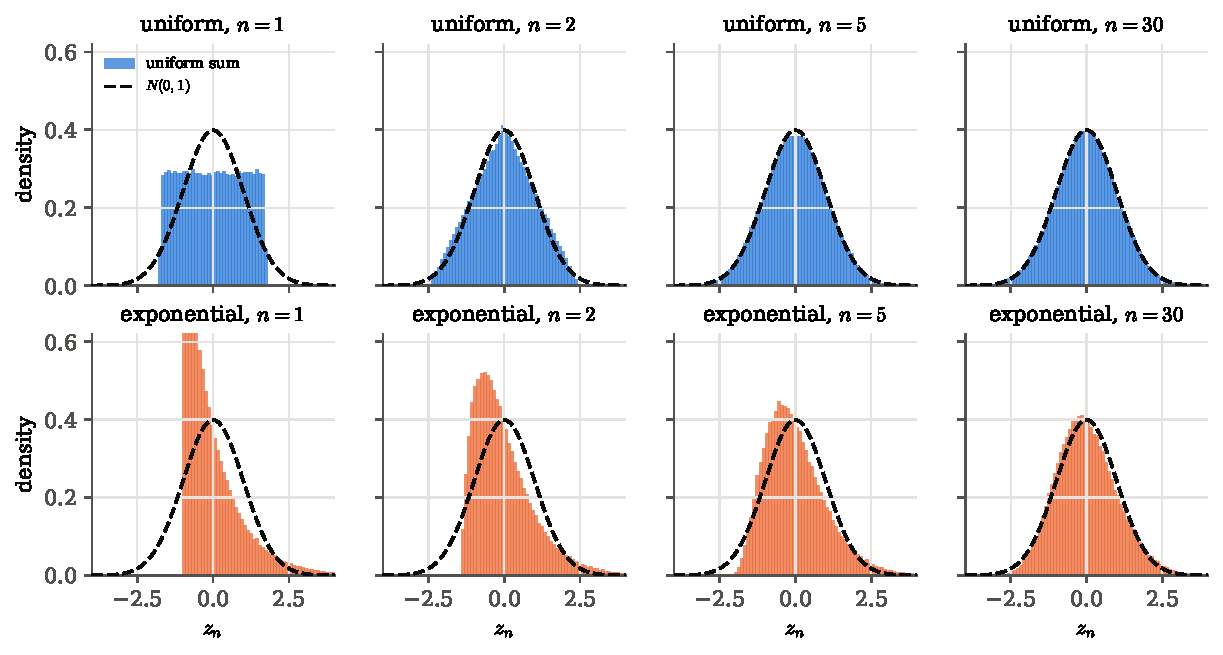
\includegraphics[width=\linewidth]{figures/ch02/clt_histograms.pdf}
\caption{Histograms of the standardised sum $z_n$ of $n$ uniforms (top) and $n$ exponentials (bottom), $\tbCLTnsamp$ experiments each, with the standard normal density (dashed). The uniform sum is already bell-shaped at $n=2$ to $5$. The exponential sum keeps a visible skew, a steep left side and a long right tail, even at $n=30$.}
\label{2b:fig:clt-hist}
\end{figure}

\begin{figure}[htbp]
\centering
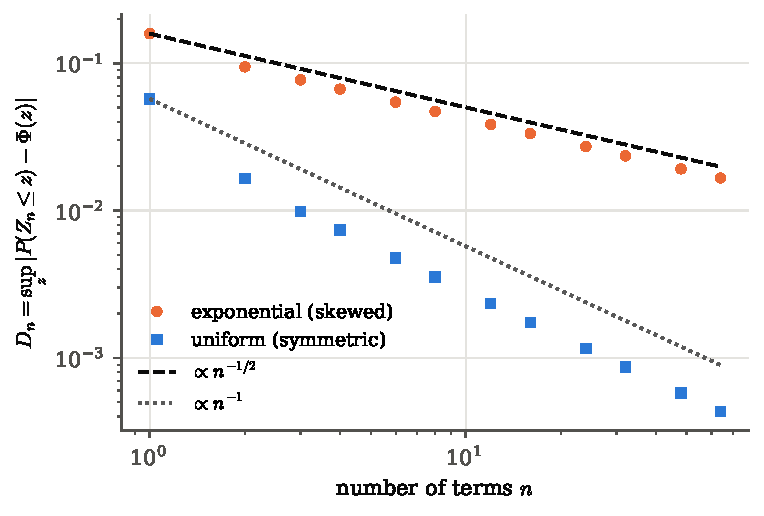
\includegraphics[width=0.66\linewidth]{figures/ch02/clt_rate.pdf}
\caption{The worst-case gap between the distribution of $z_n$ and $\Phi$, as a function of the number of terms. For the skewed exponential parent it falls as $n^{-1/2}$ (dashed), for the symmetric uniform parent as $n^{-1}$ (dotted). At $n=30$ the symmetric case is more than twenty times closer to Gaussian.}
\label{2b:fig:clt-rate}
\end{figure}

\paragraph{What this bought us.}
``Large $n$'' is not a number; it depends on the skewness of what is being added. The error of the Gaussian approximation is about $0.07\,\gamma_1/\sqrt n$ in cumulative probability. Symmetric ingredients converge like $1/n$, lopsided ones like $1/\sqrt n$.

\subsection{Where the theorem fails: Breit--Wigner resonances}
\label{2b:sec:cauchy}

\paragraph{Measuring the Z mass with a running average.}
The invariant mass of $e^+e^-$ pairs from Z decays follows, to a first approximation, the (non-relativistic) \newterm{Breit--Wigner} or \newterm{Cauchy} line shape
\begin{equation}
  p(m\given M,\Gamma)=\frac1\pi\frac{\Gamma/2}{(m-M)^2+\Gamma^2/4},
  \label{2b:eq:bw}
\end{equation}
with $M=91.1876$\,GeV the mass and $\Gamma=2.4952$\,GeV the full width at half maximum \srcref{Cowan}{(2.41)}. (We ignore detector resolution and radiation to keep the point clean.) A student averages the masses of the first $N$ events and expects the average to settle down like $1/\sqrt N$.

The student's expectation fails, because the Breit--Wigner has no mean. It is a proper density: with $u=2(m-M)/\Gamma$, $\int\frac{\dd u}{\pi(1+u^2)}=\frac1\pi[\arctan u]_{-\infty}^{\infty}=1$ \mainref{p.~30}. But the two halves of the mean, $\int_M^\infty m\,p(m)\dd m$ and $\int_{-\infty}^M m\,p(m)\dd m$, diverge separately, because the integrand falls only like $1/m$. Their difference is therefore undefined \srcref{Cowan}{p.~36--37}; CasellaBerger's (3.3.20) states it as $\E|X|=\infty$. The variance is infinite too, so the CLT does not apply.

Instead, the mean of Cauchy variables is as wide as one of them. If $X_1,\dots,X_n$ are iid Cauchy with centre $M$ and half-width $\gamma=\Gamma/2$, then $\bar X_n$ has \emph{exactly the same} Cauchy distribution, for every $n$ \srcref{CasellaBerger}{p.~177}. Averaging does not help at all.

The proof is two lines once we have the characteristic function. For the standard Cauchy $p(x)=1/[\pi(1+x^2)]$ and $k>0$, close the contour in the upper half plane, where $e^{ikx}$ decays, around the pole at $x=i$:
\begin{align}
  \phi(k)
  &\eqby{1} \frac1\pi\oint\frac{e^{ikx}}{(x-i)(x+i)}\dd x
  \eqby{2} \frac1\pi\,2\pi i\,\frac{e^{ik\cdot i}}{2i}
  = e^{-k} ,
  \label{2b:eq:cf-cauchy}
\end{align}
\begin{explain}
  \item Factor $1+x^2$. The semicircle at infinity contributes nothing for $k>0$.
  \item Residue theorem: $2\pi i$ times the residue at $x=i$, which is $e^{ik\,i}/(i+i)$.
\end{explain}
and by symmetry $\phi(k)=e^{-|k|}$ for all $k$ \srcref{Cowan}{Table~10.1}. For centre $M$ and scale $\gamma$, $\phi(k)=e^{iMk-\gamma|k|}$. Then
\begin{align}
  \phi_{\bar X_n}(k)
  &\eqby{1}\Bigl[\phi\Bigl(\frac kn\Bigr)\Bigr]^n
  \eqby{2}\Bigl[e^{iMk/n-\gamma|k|/n}\Bigr]^n
  = e^{iMk-\gamma|k|} ,
  \label{2b:eq:cauchy-mean}
\end{align}
\begin{explain}
  \item Product and scaling rules with $a=1/n$.
  \item The Cauchy characteristic function at frequency $k/n$.
\end{explain}
which is the characteristic function of a single event. \emph{Where did the CLT proof break?} At the expansion. The kink of $e^{-|k|}$ at $k=0$ is the Fourier-space signature of the missing variance: $\phi$ has no second derivative there, so the expansion \eqref{2b:eq:cf-taylor} does not exist \srcref{Cowan}{p.~145}. The width is controlled by $|k|$ rather than $k^2$. So in the exponent it scales as $n\times\frac1n=1$, instead of the $n\times\frac1{n^2}$ that would have made it shrink.

\paragraph{One event can move the average anywhere.}
With a Gaussian, an event $10\sigma$ away is essentially impossible. With a Breit--Wigner, the probability of landing further than $t$ from the peak falls only like $1/t$. Among $N$ events, the most extreme one is typically at distance $\sim N\gamma$ from the peak, so its contribution to the average, $\sim N\gamma/N=\gamma$, never becomes small. The average is always at the mercy of the latest outlier. The \emph{median} does not care how far out an outlier is, only on which side it lies.

The simulation shows both behaviours. The script draws $10^5$ Breit--Wigner masses in three independent streams. After $10^5$ events one running mean sits at $\tbBWfinalMean$\,GeV, $\tbBWfinalOff$\,GeV from the true mass, and all three keep jumping (\cref{2b:fig:cauchy}a). The running median of the same events is $\tbBWfinalMedian$\,GeV. Its standard error, $\pi\gamma/(2\sqrt N)=\tbBWmedSE$\,GeV, does fall like $1/\sqrt N$: the median of any continuous density has asymptotic variance $1/[4Np(M)^2]$, and $p(M)=1/(\pi\gamma)$ here. Panel (b) repeats the average of $\tbBWnavg$ events twenty thousand times: its interquartile range is $\tbBWiqrMean$\,GeV, equal to that of a \emph{single} event, $2\gamma=\Gamma=\tbBWiqrTheory$\,GeV.

\pyfile[firstline=41,lastline=50,firstnumber=41]{code/ch02/22_cauchy_landau.py}{Running mean and running median of Breit--Wigner masses}

Line 42 generates Breit--Wigner masses as $M+\gamma\,C$, where $\gamma=\Gamma/2$ is the half-width and $C$ is a standard Cauchy variable. Numpy draws $C$ with
\pyname{rng.standard_cauchy}. (A standard Cauchy variable is the same thing as the ratio of two independent standard normals.) Line 43 computes all running means at once with a cumulative sum. Line 49 evaluates the running median on a logarithmic grid of $N$ values.

\begin{figure}[htbp]
\centering
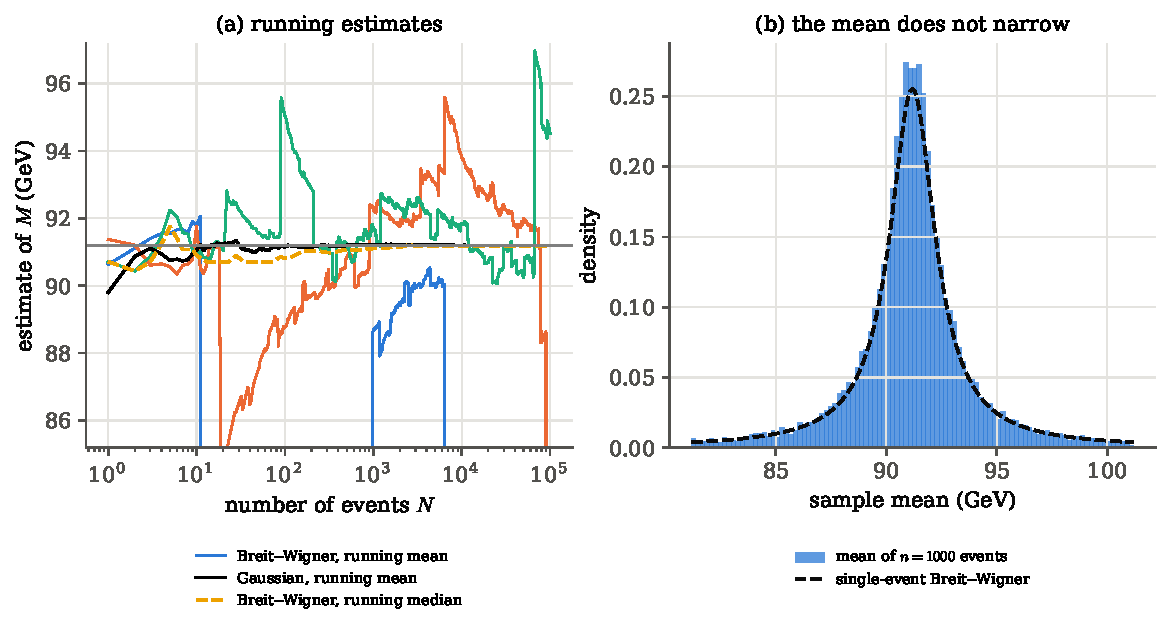
\includegraphics[width=\linewidth]{figures/ch02/cauchy_running.pdf}
\caption{(a) Running estimates of the Z mass from Breit--Wigner events. The three coloured running means jump by GeV every time an extreme event arrives and never settle. The running mean of Gaussian events of the same half-width (black) and the running median of the Breit--Wigner events (dashed) both converge to the true mass (grey line). (b) The distribution of the average of $1000$ events (histogram) is the single-event Breit--Wigner (dashed): no narrowing at all.}
\label{2b:fig:cauchy}
\end{figure}

\begin{pitfall}[The width convention]
Cowan's $\Gamma$ in \eqref{2b:eq:bw} is the \emph{full} width at half maximum, the convention of particle physics, where $\Gamma=\hbar/\tau$ is the decay rate. Many statistics texts write the Cauchy scale $\gamma$ as the \emph{half} width, and \pyname{scipy.stats.cauchy(loc, scale)} expects $\gamma=\Gamma/2$ \srcref{Cowan}{p.~37, footnote}.
\end{pitfall}

Strictly, real resonances do have a mean. The mass cannot be negative or exceed the collision energy, and the relativistic line shape with phase space and parton luminosities cuts the tails \srcref{Cowan}{p.~38--39}. But the cut sits so far out that the practical lesson stands: sample means of resonance masses converge painfully slowly and are dominated by a few events. Fit the line shape, or use the median or a truncated mean.

\subsection{Where the theorem is slow: Landau energy loss}
\label{2b:sec:landau}

A charged particle crossing a thin layer loses energy $\Delta$ in many soft collisions and, occasionally, one hard collision that knocks out a fast $\delta$-electron. The distribution of $\Delta$, derived by Landau, is \srcref{Cowan}{(2.42)--(2.46)}
\begin{equation}
  f(\Delta)=\frac1\xi\,\phi_L(\lambda),\qquad
  \lambda=\frac1\xi\Bigl[\Delta-\xi\Bigl(\ln\frac{\xi}{\epsilon'}+1-\gamma_E\Bigr)\Bigr],\qquad
  \phi_L(\lambda)=\frac1\pi\int_0^\infty e^{-u\ln u-\lambda u}\sin\pi u\,\dd u ,
  \label{2b:eq:landau}
\end{equation}
where $\xi$ grows with the layer thickness and falls like $1/\beta^2$ ($\beta$ is the particle's speed in units of $c$), $\epsilon'$ depends on the ionisation energy of the material and on $\beta\gamma$, and $\gamma_E=0.5772$ is Euler's constant. The high tail falls like $1/\lambda^2$, following the Rutherford cross-section for hard knock-ons. So, as for the Breit--Wigner, the mean and variance do not exist. The useful number is the most probable loss, $\Delta_{\mathrm{mp}}=\xi[\ln(\xi/\epsilon')+0.198]$ \srcref{Cowan}{(2.48)}. It depends on the velocity, and it is the basis of particle identification by $\dd E/\dd x$.

Adding layers does not make the Landau tail Gaussian. Cowan's example \srcref{Cowan}{p.~148}: the ionisation in $1$\,m of argon is the sum over $25$ layers of $4$\,cm, and one might hope the sum is Gaussian. The script adds $\tbLanNlayers$ standard Landau variables and compares the result with a Gaussian of the same median and interquartile range (\cref{2b:fig:landau}). The core matches. The tail does not: a fraction $\tbLanTailFrac$ of the sums lie more than five matched standard deviations above the median, against $\tbLanTailGauss$ for a Gaussian. Rare hard collisions dominate the sum however many layers we add. (Mathematically the Landau distribution is \emph{stable}: like the Cauchy, the suitably shifted and rescaled sum of Landau variables is again Landau.) Practical $\dd E/\dd x$ estimators therefore use a truncated mean, discarding the largest $30$--$40\%$ of the samples.

\begin{figure}[htbp]
\centering
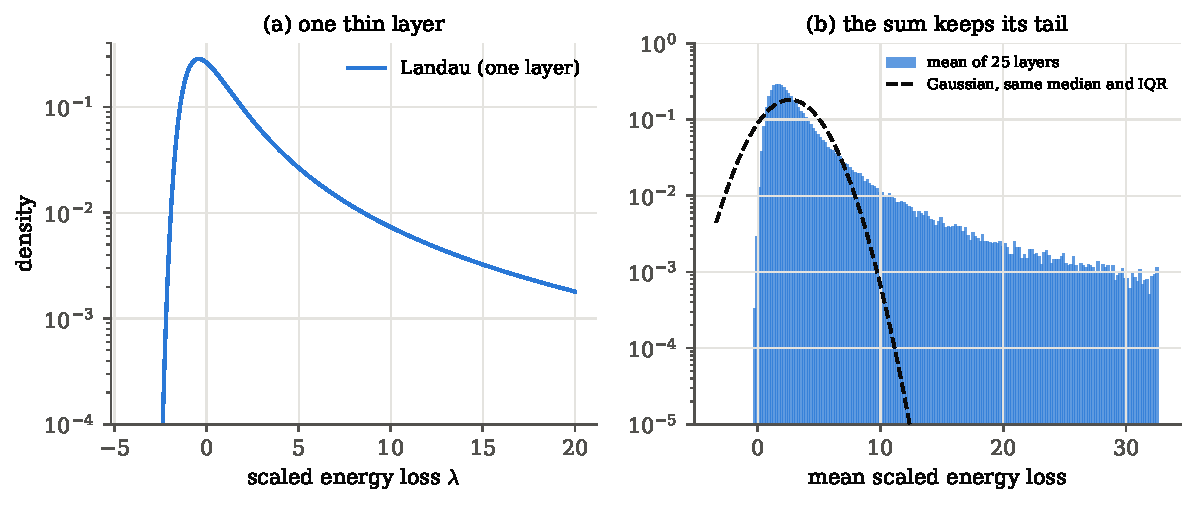
\includegraphics[width=\linewidth]{figures/ch02/landau_sum.pdf}
\caption{(a) The Landau density for one thin layer, on a logarithmic scale: a sharp peak and a long power-law tail to high energy loss. (b) The mean over $25$ layers (histogram) against a Gaussian with the same median and interquartile range (dashed). The Gaussian describes the core and misses the tail by many orders of magnitude.}
\label{2b:fig:landau}
\end{figure}

\begin{taxonomy}[Does the CLT apply to my sum?]
\begin{tabular}{@{}p{0.43\linewidth}p{0.51\linewidth}@{}}
\toprule
situation & what the sum does \\
\midrule
independent, identical, finite variance & Gaussian; error $\approx0.07\gamma_1/\sqrt n$ in probability \\
independent, different variances, none dominant & Gaussian (Lindeberg), variance $\sum\sigma_j^2$ \\
one term dominates the variance & looks like that term \\
infinite variance (Breit--Wigner, Landau, power-law tails) & no Gaussian limit; a \emph{stable} law with the same heavy tail \\
correlated terms & Gaussian only if correlations die off, with an \emph{effective} $n$ smaller than $n$ \\
a \emph{product} of positive factors & log-normal: apply the CLT to the logarithm (\cref{2b:sec:zoo}) \\
the \emph{maximum}, not the sum & not Gaussian at all: extreme-value laws (Gumbel, Fr\'echet, Weibull) \\
\bottomrule
\end{tabular}
\end{taxonomy}

\paragraph{How research uses this.}
The sums of uniforms and exponentials \emph{verify} a theorem whose answer we know. The same machinery becomes the research instrument when the ingredients are the actual detector effects. Cowan's warning \srcref{Cowan}{p.~148} is that a quoted ``$1\sigma$'' interval covers $68.3\%$ only if the errors are Gaussian in their tails. The only way to learn the tails of a real resolution function (multiple Coulomb scattering has a Gaussian core and a single-scattering Rutherford tail) is a detailed Monte Carlo of the individual contributions. In cosmology the band-power $\Chat$ is a sum of $2\ell+1$ squared Gaussian modes. At high $\ell$ the CLT makes it Gaussian; at low $\ell$ it is visibly skewed, and the likelihood of the CMB power spectrum has to be built with that skewness in it \cite{HamimecheLewis2008} (\cref{ch:07,ch:08}). Gravitational-wave detector noise is Gaussian in bulk, but ``glitches'' play the role of the Landau tail and must be vetoed or modelled.

\section{The Gaussian, third way: the least committal assignment}
\label{2b:sec:maxent}

A calibration note says: ``the timing resolution of the chamber is $2$\,ns rms.'' Nothing more. No histogram, no list of contributions, no statement about tails. Yet the next step of every analysis is to write down a probability density for the timing residual, because a likelihood needs one. Which density should we write? The first two derivations of the Gaussian do not help here. De Moivre--Laplace needs a binomial, and the central limit theorem needs a sum of many independent pieces. Here we know neither. We know one number.

The third reason the Gaussian is everywhere is of a different kind. It is not about how the noise was produced. It is about what we \emph{know}. The principle of maximum entropy picks out the one distribution that agrees with the facts we have and assumes nothing else. With it we can write a density when all we have is a mean, or a variance, or a covariance matrix. It shows why least squares, which is a Gaussian likelihood, is the natural fit when all we know is the size of the error bars. And it is the same variational principle that produces the Boltzmann distribution in statistical mechanics, so it rests on physics we already trust.

The question, stated in words: \emph{among all distributions that satisfy a set of known averages, which one should we use, and what does it look like when the known average is a variance?}

\subsection{A die with a loaded average}
\label{2b:sec:maxent-die}

Start with Sivia's example, because it is discrete and we can see every number \srcref{Sivia}{p.~113--114}. A six-sided die has been rolled very many times. We are told only that the average number of dots was $4.5$. What probabilities $p_1,\dots,p_6$ should we assign to the six faces?

The information is a single linear constraint,
\begin{equation}
  \sum_{i=1}^{6} i\,p_i = 4.5 ,\qquad \sum_{i=1}^{6}p_i=1 .
  \label{2b:eq:die-constraint}
\end{equation}
The fair die, $p_i=1/6$, has average $3.5$, so it is ruled out. But infinitely many assignments remain. Here are three of them:
\begin{itemize}
  \item $p=(0,0,0,\tfrac12,\tfrac12,0)$: only faces 4 and 5 ever appear. The average is $4.5$.
  \item $p=(0,0,\tfrac12,0,0,\tfrac12)$: only faces 3 and 6 appear. The average is $\tfrac32+3=4.5$.
  \item Something smooth that rises steadily from face 1 to face 6.
\end{itemize}
The first two are absurd. They claim that faces 1, 2, 3 and 6 (or 1, 2, 4 and 5) \emph{never} appear, and nothing we were told supports that. They contain information we do not have. The third kind feels right. It leans towards the high faces just enough to move the average from $3.5$ to $4.5$, and otherwise treats the faces evenhandedly. To turn ``feels right'' into a rule, we need a number that measures how much an assignment commits to beyond the constraints. Then we pick the assignment for which that number is smallest.

\subsection{Why the measure is the entropy: counting the ways}
\label{2b:sec:monkeys}

Sivia's ``monkey argument'' \srcref{Sivia}{p.~116--118} derives that number by counting, exactly as Boltzmann counted microstates. Imagine $M$ boxes, one per possible outcome, and a team of monkeys throwing $N$ pennies into them completely at random, each penny into each box with probability $1/M$. After the throw, box $i$ holds $n_i$ pennies, with $\sum_i n_i=N$, and we read off the candidate assignment
\begin{equation}
  p_i=\frac{n_i}{N}.
  \label{2b:eq:monkey-p}
\end{equation}
If the candidate violates the constraint we throw it away. If it satisfies it we keep it. Repeat many times. The assignment the monkeys produce most often is the one we should use. \emph{Why?} The monkeys have no preferences. So whatever structure the favoured assignment has beyond the constraint, it has only because overwhelmingly many throws produce it.

How often do the monkeys produce a given set of occupation numbers $\{n_i\}$? There are $M^N$ equally likely sequences of throws (each of $N$ pennies picks one of $M$ boxes). The number of sequences that put $n_1$ pennies in box 1, $n_2$ in box 2, and so on, is the multinomial coefficient of \cref{2a:sec:multinomial}. So the frequency is
\begin{equation}
  F(\{p_i\})=\frac{1}{M^N}\,\frac{N!}{n_1!\,n_2!\cdots n_M!} .
  \label{2b:eq:monkey-F}
\end{equation}
Now let $N$ be very large, so that every $n_i$ is large too, and use Stirling's formula in its crudest form $\ln n!\approx n\ln n-n$ (the leading terms of \eqref{2b:eq:stirling}):
\begin{align}
  \ln F
  &\eqby{1} -N\ln M+\ln N!-\sum_{i=1}^M\ln n_i! \nonumber\\
  &\eqby{2} -N\ln M+\bigl(N\ln N-N\bigr)-\sum_{i=1}^M\bigl(n_i\ln n_i-n_i\bigr) \nonumber\\
  &\eqby{3} -N\ln M+N\ln N-\sum_{i=1}^M n_i\ln n_i \nonumber\\
  &\eqby{4} -N\ln M-\sum_{i=1}^M n_i\ln\frac{n_i}{N} \nonumber\\
  &\eqby{5} -N\ln M-N\sum_{i=1}^M p_i\ln p_i .
  \label{2b:eq:monkey-lnF}
\end{align}
\begin{explain}
  \item Logarithm of \eqref{2b:eq:monkey-F}: a quotient becomes a difference and a product becomes a sum.
  \item Stirling, $\ln n!\approx n\ln n-n$, for $N!$ and for each $n_i!$. The neglected terms grow only like $\ln n$, which is negligible next to $n$.
  \item The $-N$ and the $+\sum_i n_i=+N$ cancel.
  \item Write $N\ln N=\sum_i n_i\ln N$ (again because $\sum_in_i=N$) and combine the two logarithms.
  \item Substitute $n_i=Np_i$ from \eqref{2b:eq:monkey-p}.
\end{explain}
The first term, $-N\ln M$, is the same for every candidate. So the monkeys produce the assignment $\{p_i\}$ with a frequency proportional to $e^{NS}$, where
\begin{equation}
  S=-\sum_{i=1}^M p_i\ln p_i .
  \label{2b:eq:entropy-discrete}
\end{equation}
Because $N$ is huge, $e^{NS}$ is extremely sharply peaked. Two candidates whose values of $S$ differ by only $0.01$ are produced with frequencies in the ratio $e^{0.01N}$, which for $N=10^4$ pennies is $e^{100}$. Among all candidates that pass the constraint, essentially only the one with the largest $S$ ever comes out. This is the same mathematics that makes the equilibrium macrostate of a gas overwhelmingly the most probable: Boltzmann's $S=k_B\ln W$ with $W$ the number of microstates is \eqref{2b:eq:monkey-lnF} with $k_B=1$.

\paragraph{Unequal boxes.} When the possible outcomes are not equally likely to begin with, the entropy acquires a reference distribution. So far all boxes were the same size. Suppose instead that the proposition ``the face shows 3, 4, 5 or 6'' is one box and ``the face shows 1'' and ``shows 2'' are two more. Then a fair monkey should hit the big box four times as often \srcref{Sivia}{p.~118--119}. If box $i$ is hit with probability $m_i$ (with $\sum_i m_i=1$), the frequency \eqref{2b:eq:monkey-F} becomes the full multinomial probability $\frac{N!}{\prod_i n_i!}\prod_i m_i^{n_i}$, and the same Stirling steps give
\begin{equation}
  \frac1N\ln F=-\sum_{i=1}^M p_i\ln\frac{p_i}{m_i} .
  \label{2b:eq:entropy-measure}
\end{equation}
The only new term is $+\sum_i n_i\ln m_i=N\sum_ip_i\ln m_i$, and it joins the logarithm. When all $m_i=1/M$ we recover \eqref{2b:eq:entropy-discrete} up to the constant $\ln M$.

\begin{workdef}[entropy of a distribution, and the MaxEnt principle]
The \newterm{entropy} of a discrete assignment $\{p_i\}$ relative to a \newterm{measure} $\{m_i\}$ \unpack{the probabilities we would assign if we knew nothing at all, often equal} is
\[
  S=-\sum_i p_i\ln\frac{p_i}{m_i}.
\]
For a continuous variable with density $p(x)$ and measure $m(x)$ it is \srcref{Sivia}{(5.29)}
\begin{equation}
  S[p]=-\int p(x)\ln\frac{p(x)}{m(x)}\,\dd x .
  \label{2b:eq:entropy-cont}
\end{equation}
The \newterm{principle of maximum entropy} (MaxEnt): given \newterm{testable information} \unpack{constraints of the form $\E f_k(X)=F_k$, which any proposed distribution either obeys or violates}, assign the distribution that maximises $S$ subject to those constraints and to normalisation.
\emph{Operational recipe:} write $p\propto m\,e^{-\sum_k\lambda_kf_k}$ and solve the constraint equations for the multipliers $\lambda_k$.
\end{workdef}

The continuous formula needs the measure $m(x)$ because a density has units. If $x$ is a time in ns and we switch to seconds, $p(x)$ is multiplied by $10^9$, and $-\int p\ln p\,\dd x$ shifts by $-\ln 10^9$. The ratio $p/m$ has no units, since $p$ and $m$ transform the same way under a change of variable. So \eqref{2b:eq:entropy-cont} is the same number in any coordinates \srcref{Sivia}{p.~119}. What is $m$? Maximising $S$ with only the normalisation constraint gives $p=m$ (Sivia's (5.30), and the case $K=0$ of the recipe below). So $m$ is the distribution of complete ignorance. For a location variable on the real line it is uniform, and then we may drop it. From now on we do so unless we say otherwise.

\subsection{The recipe: Lagrange multipliers give exponentials}
\label{2b:sec:maxent-recipe}

Maximising the entropy under known averages always gives an exponential. To see why, maximise $S$ with $K$ testable constraints $\sum_i p_i f_k(x_i)=F_k$, $k=1,\dots,K$. We handle the constraints with Lagrange multipliers \unpack{one extra unknown per constraint, chosen at the end so the constraint holds}: find the stationary point of
\begin{equation*}
  Q=-\sum_i p_i\ln\frac{p_i}{m_i}+\lambda_0\Bigl(1-\sum_i p_i\Bigr)+\sum_{k=1}^K\lambda_k\Bigl(F_k-\sum_i p_i f_k(x_i)\Bigr).
\end{equation*}
Differentiate with respect to one particular $p_j$. Only the terms containing $p_j$ contribute:
\begin{align}
  \frac{\partial Q}{\partial p_j}
  &\eqby{1} -\ln\frac{p_j}{m_j}-1-\lambda_0-\sum_{k=1}^K\lambda_kf_k(x_j) \eqby{2} 0 \nonumber\\
  \Longrightarrow\quad p_j
  &\eqby{3} m_j\,e^{-(1+\lambda_0)}\,\exp\Bigl[-\sum_{k=1}^K\lambda_kf_k(x_j)\Bigr]
   \eqby{4} \frac{m_j}{Z}\exp\Bigl[-\sum_{k=1}^K\lambda_kf_k(x_j)\Bigr].
  \label{2b:eq:maxent-solution}
\end{align}
\begin{explain}
  \item $\frac{\dd}{\dd p}(-p\ln(p/m))=-\ln(p/m)-1$, and each constraint is linear in $p_j$ with coefficient $-1$ or $-f_k(x_j)$.
  \item A maximum of $Q$ is a stationary point.
  \item Exponentiate and multiply by $m_j$.
  \item Normalisation fixes $e^{1+\lambda_0}=Z\equiv\sum_j m_j\exp[-\sum_k\lambda_kf_k(x_j)]$, the \newterm{partition function}.
\end{explain}
Is it a maximum and not a minimum? Yes, and the only one. The second derivatives are $\partial^2Q/\partial p_j\partial p_l=-\delta_{jl}/p_j<0$, so $Q$ is strictly concave, and a concave function on the convex set of allowed $\{p_i\}$ has exactly one stationary point, its global maximum. There is no risk of picking a saddle.

Every physicist has seen \eqref{2b:eq:maxent-solution} before. With one constraint, the mean energy $\sum_ip_iE_i=U$, it reads $p_j=e^{-\beta E_j}/Z$, the Boltzmann distribution, with the Lagrange multiplier $\beta$ playing the role of $1/k_BT$. Temperature \emph{is} the Lagrange multiplier that enforces a given mean energy. Jaynes's reading of statistical mechanics, which Sivia summarises \srcref{Sivia}{p.~118}, is exactly this: the canonical ensemble is the least committal assignment compatible with a known average energy.

\paragraph{Example: the die.} For the die, $m_i=1/6$ and there is one constraint, $f(i)=i$, $F=4.5$. Writing $\lambda\equiv-\lambda_1$ for convenience, \eqref{2b:eq:maxent-solution} says
\begin{equation}
  p_i=\frac{e^{\lambda i}}{Z(\lambda)},\qquad Z(\lambda)=\sum_{j=1}^6 e^{\lambda j},\qquad
  \sum_{i=1}^6 i\,p_i=\frac{\dd\ln Z}{\dd\lambda}=4.5 .
  \label{2b:eq:die-maxent}
\end{equation}
This equation for $\lambda$ has exactly one solution. The mean $\dd\ln Z/\dd\lambda$ increases with $\lambda$, because its derivative $\dd^2\ln Z/\dd\lambda^2=\sum i^2p_i-(\sum ip_i)^2$ is a variance and so positive. At $\lambda=0$ the mean is $3.5$, and as $\lambda\to\infty$ it tends to $6$. So it passes $4.5$ exactly once, and a root finder gives $\lambda=\tbMElam$. The probabilities are
\[
  (p_1,\dots,p_6)=(\tbMEpOne,\ \tbMEpTwo,\ \tbMEpThree,\ \tbMEpFour,\ \tbMEpFive,\ \tbMEpSix),
\]
a geometric progression with ratio $e^\lambda\approx1.45$: every step up in dots multiplies the probability by the same factor (\cref{2b:fig:maxent-die}a, which reproduces Sivia's Fig.~5.2). The entropy is $S=\tbMESmax$, below the fair-die value $\ln6=\tbMESuniformDie$: the constraint costs entropy, as it must.

\paragraph{Checking by brute force.} No random die with the same average beats the MaxEnt die. The script draws $4\times10^6$ random assignments uniformly over all possible dice (a Dirichlet$(1,\dots,1)$ distribution, which we meet in \cref{2b:sec:zoo}). It keeps the $\tbMEnKeep$ whose mean lies within $0.005$ of $4.5$, and \cref{2b:fig:maxent-die}b histograms their entropies. The largest entropy among them is $\tbMESrandMax$ (for a die of mean $\tbMESrandMaxMean$), against $\tbMESmax$ for the MaxEnt die. The two are very close, and a random die can even come out a hair ahead. That is not a defeat: the window lets in means slightly below $4.5$, closer to the fair $3.5$, and a smaller tilt costs less entropy. Comparing like with like, each candidate against the MaxEnt die of \emph{its own} mean, every one falls short, by at least $\tbMEminDeficit$.

\pyfile[firstline=38,lastline=51,firstnumber=38]{code/ch02/23_maxent.py}{The MaxEnt die, and random dice with the same mean}

Lines 38--40 compute the mean $\sum_i i\,p_i$ of the exponential family \eqref{2b:eq:die-maxent} for a given $\lambda$. Line 43 solves ``mean $=4.5$'' for $\lambda$ with Brent's bracketing root finder; the monotonicity argument above is what guarantees that the bracket $[-5,5]$ contains exactly one root. Lines 49--51 draw random dice, keep those with the right mean, and compute their entropies, using the convention $0\ln0=0$.

\begin{figure}[htbp]
\centering
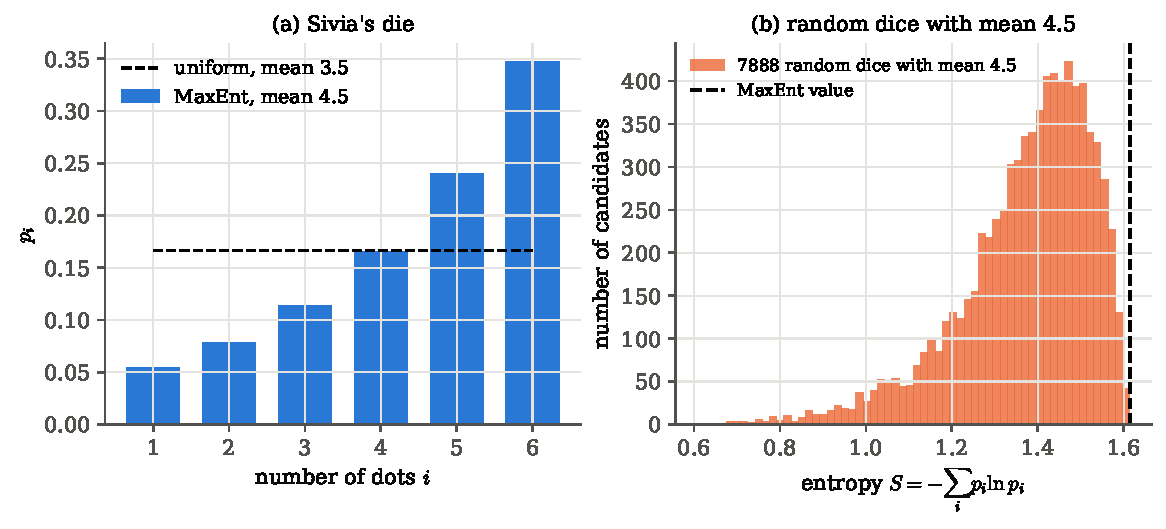
\includegraphics[width=\linewidth]{figures/ch02/maxent_die.pdf}
\caption{(a) The maximum-entropy die for a known average of $4.5$ (bars) against the fair die (dashed). The probabilities grow by a constant factor from face to face. (b) Entropies of several thousand randomly drawn dice whose average is also $4.5$. They pile up to the left of the MaxEnt value (dashed line), and compared with the MaxEnt die of its own average every one falls short: every other assignment assumes something extra.}
\label{2b:fig:maxent-die}
\end{figure}

\paragraph{Example: the kangaroo problem.} Is entropy really special, or would any function that rewards spreading out do? Sivia's kangaroo problem answers this \srcref{Sivia}{p.~114--116}. We are told that one third of all kangaroos have blue eyes and one third are left-handed. What fraction are both? Call the four probabilities $p_1$ (blue, left), $p_2$ (blue, right), $p_3$ (not blue, left), $p_4$ (not blue, right). The two facts and normalisation leave one free number, $x=p_1$ (\cref{2b:fig:kangaroo}a):
\[
  p_1=x,\quad p_2=\tfrac13-x,\quad p_3=\tfrac13-x,\quad p_4=\tfrac13+x,\qquad 0\le x\le\tfrac13 .
\]
Common sense says $x=1/9$: with no information about a link between eye colour and handedness, we should not invent one, and independence gives $\frac13\times\frac13$. Maximise the entropy:
\begin{align}
  \frac{\dd S}{\dd x}
  &\eqby{1} \frac{\dd}{\dd x}\Bigl[-x\ln x-2\bigl(\tfrac13-x\bigr)\ln\bigl(\tfrac13-x\bigr)-\bigl(\tfrac13+x\bigr)\ln\bigl(\tfrac13+x\bigr)\Bigr] \nonumber\\
  &\eqby{2} -\ln x-1+2\ln\bigl(\tfrac13-x\bigr)+2-\ln\bigl(\tfrac13+x\bigr)-1 \nonumber\\
  &\eqby{3} \ln\frac{(\tfrac13-x)^2}{x(\tfrac13+x)} .
  \label{2b:eq:kangaroo}
\end{align}
\begin{explain}
  \item Entropy \eqref{2b:eq:entropy-discrete} of the four-cell table.
  \item $\frac{\dd}{\dd x}(-u\ln u)=-(\ln u+1)\,\frac{\dd u}{\dd x}$, with $\frac{\dd u}{\dd x}=+1,-1,-1,+1$ for the four cells.
  \item The constants cancel ($-1+2-1=0$) and the logarithms combine.
\end{explain}
Setting this to zero gives $(\frac13-x)^2=x(\frac13+x)$, that is $\frac19-\frac23x+x^2=\frac13x+x^2$, so $x=\frac19$. Entropy reproduces independence exactly.

Other plausible-looking criteria do not. Maximising $-\sum p_i^2$ gives $\frac{\dd}{\dd x}\bigl[x^2+2(\frac13-x)^2+(\frac13+x)^2\bigr]=8x-\frac23=0$, so $x=\frac1{12}$: a negative correlation nobody asked for. The script maximises all four of Sivia's candidates numerically and finds $x=\tbKangEnt$ (entropy), $\tbKangSq$ ($-\sum p_i^2$), $\tbKangLog$ ($\sum\ln p_i$) and $\tbKangSqrt$ ($\sum\sqrt{p_i}$), reproducing his Table~5.1. Only functions monotonically related to $S$ give $1/9$ (Sivia quotes Skilling for the proof), and that is the strongest argument that entropy is the right measure of ``assuming nothing extra''.

\begin{figure}[htbp]
\centering
\begin{tikzpicture}
  \begin{scope}
    \draw[thick] (0,0) rectangle (3.2,3.2);
    \draw[thick] (1.6,0) -- (1.6,3.2);
    \draw[thick] (0,1.6) -- (3.2,1.6);
    \node[lbl] at (0.8,2.4) {$x$};
    \node[lbl] at (2.4,2.4) {$\tfrac13-x$};
    \node[lbl] at (0.8,0.8) {$\tfrac13-x$};
    \node[lbl] at (2.4,0.8) {$\tfrac13+x$};
    \node[lbl,anchor=south] at (0.8,3.25) {left};
    \node[lbl,anchor=south] at (2.4,3.25) {right};
    \node[lbl,anchor=east] at (-0.05,2.4) {blue};
    \node[lbl,anchor=east] at (-0.05,0.8) {not blue};
    \node[lbl,font=\small\bfseries] at (1.6,-1.75) {(a)};
  \end{scope}
  \begin{scope}[xshift=5.0cm,yshift=-0.2cm]
  \begin{axis}[width=7.0cm,height=4.6cm,xmin=0,xmax=0.3333,ymin=0.6,ymax=1.34,
      xlabel={$x=p_1$},ylabel={entropy $S$},
      xtick={0,0.1111,0.2222,0.3333},xticklabels={$0$,$\frac19$,$\frac29$,$\frac13$},
      tick label style={font=\scriptsize},label style={font=\small},
      legend style={font=\scriptsize,at={(0.6,0.03)},anchor=south,draw=none,fill=none}]
    \addplot[formblue,thick,domain=0.0005:0.3328,samples=200]
      {-x*ln(x)-2*(1/3-x)*ln(1/3-x)-(1/3+x)*ln(1/3+x)};
    \addlegendentry{$S(x)$}
    \addplot[only marks,mark=*,mark size=1.6pt,fibreorange,samples at={0.0833,0.1218,0.1301}]
      {-x*ln(x)-2*(1/3-x)*ln(1/3-x)-(1/3+x)*ln(1/3+x)};
    \addlegendentry{other criteria}
    \addplot[only marks,mark=square*,mark size=2pt,black,samples at={0.1111}]
      {-x*ln(x)-2*(1/3-x)*ln(1/3-x)-(1/3+x)*ln(1/3+x)};
    \addlegendentry{maximum, $x=\frac19$}
    \draw[faint,dashed] (axis cs:0.1111,0.6) -- (axis cs:0.1111,1.273);
  \end{axis}
  \node[lbl,font=\small\bfseries] at (2.6,-1.55) {(b)};
  \end{scope}
\end{tikzpicture}
\caption{The kangaroo problem. (a) The two known marginals, one third blue-eyed and one third left-handed, leave a single free number $x$ in the $2\times2$ table. (b) The entropy of the table as a function of $x$. It peaks at $x=1/9$, the independent answer. The orange dots mark the maximisers of Sivia's three alternative criteria, which all build in a correlation that the information does not contain.}
\label{2b:fig:kangaroo}
\end{figure}

\subsection{Continuous MaxEnt: a variance gives a Gaussian}
\label{2b:sec:maxent-gauss}

Back to the timing residual of the calibration note, where all we were given was an rms of $2$\,ns. The testable information is that the residual $x$ has mean $\mu$ and variance $\sigma^2$, and $x$ can be any real number. The question: which density has the largest entropy under these two constraints? The continuous version of the recipe replaces sums by integrals and the partial derivative by a functional derivative \unpack{the change of $Q$ when $p$ is changed by a small bump $\delta p$ at one point $x$, divided by the area of the bump}. We need
\[
  Q[p]=-\int p\ln p\,\dd x+\lambda_0\Bigl(1-\int p\,\dd x\Bigr)+\lambda_1\Bigl(\sigma^2-\int(x-\mu)^2p\,\dd x\Bigr)
\]
to be stationary \srcref{Sivia}{p.~121--122}. Then
\begin{align}
  \frac{\delta Q}{\delta p(x)}
  &\eqby{1} -\ln p(x)-1-\lambda_0-\lambda_1(x-\mu)^2 \eqby{2} 0
  \quad\Longrightarrow\quad p(x)=e^{-1-\lambda_0}\,e^{-\lambda_1(x-\mu)^2} , \nonumber\\
  1&\eqby{3} e^{-1-\lambda_0}\int_{-\infty}^{\infty}e^{-\lambda_1(x-\mu)^2}\dd x
   \eqby{4} e^{-1-\lambda_0}\sqrt{\frac{\pi}{\lambda_1}} , \nonumber\\
  \sigma^2&\eqby{5} \sqrt{\frac{\lambda_1}{\pi}}\int_{-\infty}^{\infty}(x-\mu)^2e^{-\lambda_1(x-\mu)^2}\dd x
   \eqby{6} \frac{1}{2\lambda_1}
  \quad\Longrightarrow\quad
  p(x)=\frac{1}{\sqrt{2\pi\sigma^2}}\,e^{-(x-\mu)^2/2\sigma^2}.
  \label{2b:eq:maxent-gauss}
\end{align}
\begin{explain}
  \item The same differentiation as in \eqref{2b:eq:maxent-solution}, applied pointwise: changing $p$ near $x$ changes each integral by its integrand at $x$ times the size of the change.
  \item Stationarity; then solve for $p$. For the integral to exist we need $\lambda_1>0$.
  \item The normalisation constraint.
  \item The Gaussian integral \eqref{2b:eq:gauss-integral}, rescaled: substitute $z=\sqrt{2\lambda_1}(x-\mu)$.
  \item The variance constraint, with the constant from line (4), $e^{-1-\lambda_0}=\sqrt{\lambda_1/\pi}$.
  \item The normalised density $\sqrt{\lambda_1/\pi}\,e^{-\lambda_1(x-\mu)^2}$ is a Gaussian of variance $1/(2\lambda_1)$, by \eqref{2b:eq:gauss-moments}. Solving $\sigma^2=1/(2\lambda_1)$ gives $\lambda_1=1/(2\sigma^2)$.
\end{explain}
So the maximum-entropy density with a given mean and variance is the Gaussian $\Normal(\mu,\sigma^2)$ of \eqref{2b:eq:gauss}. Nothing was assumed about how the residual was produced.

\paragraph{A second proof, and a proof that it is the maximum.} The Lagrange argument finds a stationary point. A short inequality shows directly that no other density with the same variance does better. We use one elementary fact, $\ln t\le t-1$ for $t>0$ (the tangent line at $t=1$ lies above the concave logarithm). Let $p$ be any density with mean $\mu$ and variance $\sigma^2$, and let $g$ be the Gaussian with the same two numbers. Then
\begin{align}
  S[p]-S[g]
  &\eqby{1} -\int p\ln p\,\dd x+\int g\ln g\,\dd x \nonumber\\
  &\eqby{2} -\int p\ln p\,\dd x+\int p\ln g\,\dd x \nonumber\\
  &\eqby{3} \int p\ln\frac{g}{p}\,\dd x \nonumber\\
  &\relby{4}{\le} \int p\Bigl(\frac gp-1\Bigr)\dd x \eqby{5} \int g\,\dd x-\int p\,\dd x = 0 .
  \label{2b:eq:gibbs}
\end{align}
\begin{explain}
  \item Definition \eqref{2b:eq:entropy-cont} with uniform measure.
  \item $\ln g(x)=-\frac12\ln(2\pi\sigma^2)-(x-\mu)^2/2\sigma^2$ is a constant plus a multiple of $(x-\mu)^2$. Its average is therefore fixed by the normalisation and the variance alone, and $p$ and $g$ share both.
  \item Combine the two integrals.
  \item $\ln t\le t-1$ with $t=g/p$, at every $x$ where $p>0$.
  \item Both densities integrate to one.
\end{explain}
Equality in step (4) needs $g/p=1$ everywhere, so the Gaussian is the \emph{unique} maximiser. The quantity $\int p\ln(p/g)\,\dd x\ge0$ we just met is the \newterm{Kullback--Leibler divergence} of $p$ from $g$. It will return in \cref{ch:03} (maximum likelihood minimises it) and in \cref{ch:05}. The value itself is
\[
  S[g]=-\int g\ln g\,\dd x\eqby{1}\tfrac12\ln(2\pi\sigma^2)+\frac{\E(x-\mu)^2}{2\sigma^2}=\tfrac12\ln\bigl(2\pi e\sigma^2\bigr),
\]
where (1) inserts $\ln g$ from step (2) above.

\begin{keyidea}[The third origin of the Gaussian]
Of all densities on the real line with a given mean $\mu$ and variance $\sigma^2$, the Gaussian $\Normal(\mu,\sigma^2)$ has the largest entropy, $\tfrac12\ln(2\pi e\sigma^2)$. Assigning it claims nothing about the data except the mean and the variance. Assigning anything else claims more.
\end{keyidea}

\paragraph{Example: five densities with unit variance.} The script evaluates the entropy of five familiar densities, each scaled to variance one: uniform $\tbEntUniform$, Laplace $\tbEntLaplace$, triangular $\tbEntTriang$, logistic $\tbEntLogistic$, Gaussian $\tbEntGauss=\frac12\ln(2\pi e)$. The Gaussian wins, but the others are close. The logistic is only $0.014$ behind: two densities with nearly the same core can have nearly the same entropy. \Cref{2b:fig:unitvar} shows three of the five, and why they lose. The uniform ``wastes'' its variance by having no tails at all. The Laplace concentrates probability in a cusp and pays for its variance with long exponential tails. The Gaussian spreads its probability in the most even way the variance allows.

\begin{figure}[htbp]
\centering
\begin{tikzpicture}
\begin{axis}[width=10cm,height=5cm,xmin=-4,xmax=4,ymin=0,ymax=0.75,
    xlabel={$x$ (units of $\sigma$)},ylabel={density},
    tick label style={font=\scriptsize},label style={font=\small},
    legend style={font=\scriptsize,at={(0.99,0.97)},anchor=north east,draw=none,fill=none}]
  \addplot[formblue,very thick,domain=-4:4,samples=201] {exp(-x^2/2)/sqrt(2*pi)};
  \addlegendentry{Gaussian, $S=\tbEntGauss$}
  \addplot[fibreorange,thick,domain=-4:4,samples=401] {exp(-sqrt(2)*abs(x))/sqrt(2)};
  \addlegendentry{Laplace, $S=\tbEntLaplace$}
  \addplot[tangentgreen,thick] coordinates {(-4,0) (-1.7321,0) (-1.7321,0.2887) (1.7321,0.2887) (1.7321,0) (4,0)};
  \addlegendentry{uniform, $S=\tbEntUniform$}
\end{axis}
\end{tikzpicture}
\caption{Three densities with the same mean ($0$) and variance ($1$). The uniform box stops dead at $\pm\sqrt3$; the Laplace density has a sharp peak and fat exponential tails. Among all densities with this variance the Gaussian has the largest entropy, and the numbers in the legend show by how much it beats these two.}
\label{2b:fig:unitvar}
\end{figure}

\subsection{The family tree: other constraints, other distributions}
\label{2b:sec:maxent-family}

Each common distribution is the MaxEnt answer to some piece of partial knowledge. The recipe \eqref{2b:eq:maxent-solution} works like a machine: feed in the constraint functions $f_k$ and the range of $x$, and out comes $p\propto m\,e^{-\sum\lambda_kf_k}$. Sivia runs it for the common cases \srcref{Sivia}{p.~120--125}:
\begin{itemize}
  \item \emph{Nothing but the range $[a,b]$.} Then $p=m$, the uniform density $1/(b-a)$ (Bernoulli's principle of insufficient reason).
  \item \emph{A mean $\mu$, with $x\ge0$.} One constraint $f=x$, so $p\propto e^{-\lambda_1x}$. Normalisation on $[0,\infty)$ gives $\lambda_1e^{-\lambda_1x}$ and the mean gives $\lambda_1=1/\mu$: the exponential $p(x)=\mu^{-1}e^{-x/\mu}$ \srcref{Sivia}{(5.33)}, the waiting-time law of \eqref{2a:eq:expo}. The same computation on the line with a mean alone fails: $e^{-\lambda_1x}$ cannot be normalised on $(-\infty,\infty)$, which is the recipe's way of saying that a mean alone does not specify a spread.
  \item \emph{A variance on the whole line.} The Gaussian, \eqref{2b:eq:maxent-gauss}.
  \item \emph{A mean absolute deviation $\E|x-\mu|=\epsilon$.} $f=|x-\mu|$ gives the Laplace (double-exponential) density $\frac{1}{2\epsilon}e^{-|x-\mu|/\epsilon}$ \srcref{Sivia}{(5.39)--(5.40)}. Its log-likelihood is $-\sum|x_k-\mu_k|/\epsilon_k$: the $\ell_1$ ``least absolute deviations'' fit, which is more robust to outliers than least squares.
  \item \emph{Many variables with known individual variances.} With $N$ data $x_k$, predictions $\mu_k$ and known $\E(x_k-\mu_k)^2=\sigma_k^2$, the multidimensional version gives the product of Gaussians \srcref{Sivia}{(5.36)--(5.38)}
  \begin{equation}
    p(\{x_k\})=\prod_{k=1}^N\frac{1}{\sqrt{2\pi}\sigma_k}\exp\Bigl[-\frac{(x_k-\mu_k)^2}{2\sigma_k^2}\Bigr],
    \label{2b:eq:maxent-lsq}
  \end{equation}
  which is exactly the likelihood behind least squares, $-2\ln p=\chi^2+\text{const}$. From the MaxEnt point of view least squares does not assume that the noise \emph{is} Gaussian. It is the honest likelihood when all we know is the size of each error bar. If we also know the covariances $\E(x_j-\mu_j)(x_k-\mu_k)$, the same recipe returns the correlated multivariate Gaussian of the next section.
  \item \emph{A mean count $\E N=\mu$ of events in an interval.} Here the measure matters. Cut the interval into $M$ tiny cells, each of which can hold an event or not. The number of cell patterns giving $N$ events among $M$ indistinguishable cells is $M^N/N!$ for $M\gg N$, so $m(N)\propto M^N/N!$ \srcref{Sivia}{(5.43)}. Then
  \[
    p(N)\propto\frac{M^N}{N!}e^{-\lambda N}=\frac{(Me^{-\lambda})^N}{N!}
    \quad\Longrightarrow\quad
    p(N)=e^{-\mu}\frac{\mu^N}{N!},
  \]
  where normalisation, $\sum_N(Me^{-\lambda})^N/N!=e^{Me^{-\lambda}}$, and the mean condition identify $Me^{-\lambda}=\mu$. The unknown $M$ drops out, and we recover the Poisson distribution of \cref{2a:sec:poisson-limit} from knowledge of the mean alone.
  \item \emph{The mean kinetic energy of a gas molecule.} The constraint $\E\frac12m|\bm v|^2=\frac32k_BT$ with uniform measure on velocity space gives a Gaussian for each velocity component with variance $k_BT/m$. The speed distribution that follows is the Maxwell--Boltzmann law of \cref{2b:sec:zoo}.
\end{itemize}

\begin{pitfall}[MaxEnt is a statement about knowledge, not about the noise]
The MaxEnt Gaussian is the best assignment \emph{given only} a variance. If the real residuals have a Landau tail (\cref{2b:sec:landau}) or a Breit--Wigner shape, the Gaussian will misjudge the tails badly, and the cure is not to argue about entropy but to put the extra knowledge in as a constraint (a known tail fraction, a known fourth moment) or to model the mechanism. And when the variance is infinite, as for a Breit--Wigner, there is no variance constraint to impose in the first place.
\end{pitfall}

\paragraph{How the three origins fit together.} The three reasons for the Gaussian agree, and that is not a coincidence. De Moivre--Laplace and the central limit theorem are statements about \emph{mechanisms}: many small independent contributions added together. MaxEnt is a statement about \emph{information}: we know a variance and nothing else. The link is that adding independent pieces and rescaling to fixed variance can only increase the entropy (convolution smooths). So the central limit theorem is the dynamics that drives a sum towards the maximum-entropy state, like a gas relaxing to equilibrium. When a physicist writes ``Gaussian errors'' she is usually relying on all of them at once: the CLT for why the errors should be close to Gaussian, and MaxEnt for why, knowing only the error bar, nothing else would be more honest.

The same principle supplies the forward model $P(\data\given\params)$, the probability of the data $\data$ given the parameters $\params$, whenever only the covariance of the noise is known. The prior assignments of \cref{ch:05} use it too. And the MaxEnt die's exponential form is the first example of the exponential families that make maximum likelihood and conjugate priors tractable (\cref{ch:03,ch:05}).
\section{Many correlated Gaussians: the multivariate normal}
\label{2b:sec:mvn}

Most measurements come as several numbers that move together, and one object describes them all: the multivariate Gaussian. A straight-line track fit returns two numbers, an intercept and a slope, and they are never independent: tilt the line a little and the intercept has to move to keep the line going through the hits. A fit of a CMB power spectrum returns $\Omega_m h^2$ and $n_s$, and they, too, move together. A CMB temperature map is a list of $10^6$ pixel values, each Gaussian, and neighbouring pixels are strongly correlated. A stretch of gravitational-wave strain is a list of $10^5$ samples whose correlations are set by the detector's noise spectrum. The Fisher matrix of \cref{ch:10} approximates every posterior by a multivariate Gaussian, and a Gaussian random field (\cref{ch:07}) is a multivariate Gaussian with very many components.

Four things about it are used constantly. How to \emph{sample} it, which follows from building it out of independent standard normals. The shape of its contours, the ellipses of every parameter-estimation plot. What fraction of the probability each ellipse contains. And two operations: \emph{marginalising} (averaging out a nuisance variable) and \emph{conditioning} (fixing one variable at a known value).

The questions, in words: \emph{what is the joint density of several correlated Gaussian quantities, how do we draw from it, and what are the distributions of a subset of them, either ignoring the rest or with the rest held fixed?}

\subsection{Building it: a linear map of independent standard normals}
\label{2b:sec:mvn-build}

Start from what we know. Let $Z_1,\dots,Z_k$ be independent $\Normal(0,1)$ variables and collect them into a column vector $\bm Z$. Independence means the joint density is the product of the one-dimensional densities \mainref{p.~40}:
\begin{equation}
  p_{\bm Z}(\bm z)=\prod_{j=1}^k\frac{e^{-z_j^2/2}}{\sqrt{2\pi}}=\frac{1}{(2\pi)^{k/2}}\exp\Bigl(-\tfrac12\bm z\T\bm z\Bigr).
  \label{2b:eq:mvn-std}
\end{equation}
Its contours, $\bm z\T\bm z=\text{const}$, are spheres, and its components are uncorrelated. Correlations appear when we mix the components linearly. Take a fixed invertible $k\times k$ matrix $\mathbf A$ and a fixed vector $\bm\mu$ and define
\begin{equation}
  \bm X=\bm\mu+\mathbf A\bm Z .
  \label{2b:eq:mvn-map}
\end{equation}
Its mean is $\E\bm X=\bm\mu+\mathbf A\,\E\bm Z=\bm\mu$. Its covariance matrix \unpack{the $k\times k$ table of all $\Cov(X_i,X_j)$, with the variances on the diagonal} is
\begin{align}
  \Cmat\equiv\E\bigl[(\bm X-\bm\mu)(\bm X-\bm\mu)\T\bigr]
  &\eqby{1} \E\bigl[\mathbf A\bm Z\bm Z\T\mathbf A\T\bigr]
  \eqby{2} \mathbf A\,\E\bigl[\bm Z\bm Z\T\bigr]\mathbf A\T
  \eqby{3} \mathbf A\mathbf A\T .
  \label{2b:eq:mvn-cov}
\end{align}
\begin{explain}
  \item $\bm X-\bm\mu=\mathbf A\bm Z$, and $(\mathbf A\bm Z)\T=\bm Z\T\mathbf A\T$.
  \item $\mathbf A$ is not random, and expectation is linear, so it can be taken outside on both sides.
  \item $\E(Z_iZ_j)=\delta_{ij}$: unit variances and, by independence, zero covariances. So $\E\bm Z\bm Z\T=\Id$.
\end{explain}
We know the mean and covariance of $\bm X$; now we want its density. Change variables. The map $\bm z\mapsto\bm x=\bm\mu+\mathbf A\bm z$ is linear with inverse $\bm z=\mathbf A^{-1}(\bm x-\bm\mu)$. A small box of volume $\dd^k z$ is mapped to a parallelepiped of volume $|\det\mathbf A|\,\dd^kz$, so probability conservation, $p_{\bm X}\,\dd^kx=p_{\bm Z}\,\dd^kz$, gives
\begin{align}
  p_{\bm X}(\bm x)
  &\eqby{1} p_{\bm Z}\bigl(\mathbf A^{-1}(\bm x-\bm\mu)\bigr)\,\frac{1}{|\det\mathbf A|} \nonumber\\
  &\eqby{2} \frac{1}{(2\pi)^{k/2}|\det\mathbf A|}\exp\Bigl[-\tfrac12(\bm x-\bm\mu)\T(\mathbf A^{-1})\T\mathbf A^{-1}(\bm x-\bm\mu)\Bigr] \nonumber\\
  &\eqby{3} \frac{1}{(2\pi)^{k/2}(\det\Cmat)^{1/2}}\exp\Bigl[-\tfrac12(\bm x-\bm\mu)\T\Cmat^{-1}(\bm x-\bm\mu)\Bigr].
  \label{2b:eq:mvn}
\end{align}
\begin{explain}
  \item The multidimensional change-of-variables rule: the Jacobian of the inverse map is $\det\mathbf A^{-1}=1/\det\mathbf A$.
  \item Insert \eqref{2b:eq:mvn-std} with $\bm z=\mathbf A^{-1}(\bm x-\bm\mu)$, so $\bm z\T\bm z=(\bm x-\bm\mu)\T(\mathbf A^{-1})\T\mathbf A^{-1}(\bm x-\bm\mu)$.
  \item $(\mathbf A^{-1})\T\mathbf A^{-1}=(\mathbf A\mathbf A\T)^{-1}=\Cmat^{-1}$, and $\det\Cmat=\det\mathbf A\,\det\mathbf A\T=(\det\mathbf A)^2$.
\end{explain}
The matrix $\mathbf A$ has disappeared: only $\Cmat=\mathbf A\mathbf A\T$ is left. So the distribution is fixed by the mean and the covariance alone, and any two matrices with the same $\mathbf A\mathbf A\T$ give the same distribution. That is the density quoted by all our sources \mainref{(2.10)}, \srcref{Cowan}{(2.28)}.

\begin{workdef}[multivariate normal distribution]
A random vector $\bm X\in\R^k$ is \newterm{multivariate normal}, $\bm X\sim\Normal(\bm\mu,\Cmat)$, if its density is \eqref{2b:eq:mvn}, where $\bm\mu$ is its mean vector and $\Cmat$ its covariance matrix, which must be symmetric and \newterm{positive definite} \unpack{$\bm a\T\Cmat\bm a>0$ for every nonzero vector $\bm a$. This says that every linear combination $\bm a\T\bm X$ has a nonzero variance}. It has $k$ means plus $k(k+1)/2$ independent entries of $\Cmat$ as parameters \srcref{Cowan}{p.~33}.
\emph{Operational recipe (sampling):} factor $\Cmat=\mathbf L\mathbf L\T$ (Cholesky, $\mathbf L$ lower triangular, or the symmetric square root $\Cmat^{1/2}$ of \mainref{Thm~2.43}), draw $k$ independent standard normals $\bm z$, and return $\bm\mu+\mathbf L\bm z$. \emph{Inverse (whitening):} $\mathbf L^{-1}(\bm X-\bm\mu)\sim\Normal(0,\Id)$.
\end{workdef}

Why must $\Cmat$ be positive definite? Because $\bm a\T\Cmat\bm a=\Var(\bm a\T\bm X)$, and a variance cannot be negative. If it is zero for some $\bm a\neq0$, then $\bm a\T\bm X$ is a constant: one component is an exact linear function of the others, the distribution lives on a lower-dimensional plane, $\det\Cmat=0$, and \eqref{2b:eq:mvn} does not exist. (A fitted $\Cmat$ that is singular or nearly singular almost always means a parameter that the data cannot distinguish from a combination of the others.)

\paragraph{Example: two dimensions, written out.} For $k=2$ write $\Cmat=\begin{pmatrix}\sigma_x^2&\rho\sigma_x\sigma_y\\ \rho\sigma_x\sigma_y&\sigma_y^2\end{pmatrix}$, where $\rho=\Cov(x,y)/(\sigma_x\sigma_y)$ is the \newterm{correlation coefficient}, $-1<\rho<1$. The inverse of a $2\times2$ matrix is its adjugate over its determinant, so with $u=(x-\mu_x)/\sigma_x$ and $v=(y-\mu_y)/\sigma_y$,
\begin{align}
  (\bm x-\bm\mu)\T\Cmat^{-1}(\bm x-\bm\mu)
  &\eqby{1} \frac{1}{\sigma_x^2\sigma_y^2(1-\rho^2)}
    \begin{pmatrix}x-\mu_x& y-\mu_y\end{pmatrix}
    \begin{pmatrix}\sigma_y^2&-\rho\sigma_x\sigma_y\\-\rho\sigma_x\sigma_y&\sigma_x^2\end{pmatrix}
    \begin{pmatrix}x-\mu_x\\ y-\mu_y\end{pmatrix} \nonumber\\
  &\eqby{2} \frac{u^2-2\rho uv+v^2}{1-\rho^2} ,
  \label{2b:eq:bvn-quad}
\end{align}
\begin{explain}
  \item $\det\Cmat=\sigma_x^2\sigma_y^2-\rho^2\sigma_x^2\sigma_y^2=\sigma_x^2\sigma_y^2(1-\rho^2)$, and the adjugate swaps the diagonal entries and flips the sign of the off-diagonal ones.
  \item Multiply out: the three terms are $\sigma_y^2(x-\mu_x)^2$, $-2\rho\sigma_x\sigma_y(x-\mu_x)(y-\mu_y)$ and $\sigma_x^2(y-\mu_y)^2$; dividing each by $\sigma_x^2\sigma_y^2$ turns them into $u^2$, $-2\rho uv$, $v^2$.
\end{explain}
and $(\det\Cmat)^{1/2}=\sigma_x\sigma_y\sqrt{1-\rho^2}$. This gives the bivariate normal density of \srcref{Cowan}{(2.30)} and \srcref{CasellaBerger}{Def.~4.5.10},
\begin{equation}
  p(x,y)=\frac{1}{2\pi\sigma_x\sigma_y\sqrt{1-\rho^2}}\exp\Bigl[-\frac{u^2-2\rho uv+v^2}{2(1-\rho^2)}\Bigr].
  \label{2b:eq:bvn}
\end{equation}
Our running example, used by the script and in the rest of this section, has $\sigma_x=1$, $\sigma_y=2$, $\rho=0.8$ (and means $\mu_x=1$, $\mu_y=2$), so $\Cmat=\begin{pmatrix}1&1.6\\1.6&4\end{pmatrix}$ and $\det\Cmat=4-2.56=1.44$. Its Cholesky factor is $\mathbf L=\begin{pmatrix}1&0\\1.6&1.2\end{pmatrix}$; check: $\mathbf L\mathbf L\T=\begin{pmatrix}1&1.6\\1.6&1.6^2+1.2^2\end{pmatrix}=\Cmat$. So a sample is $x=\mu_x+z_1$, $y=\mu_y+1.6z_1+1.2z_2$: the $y$ component copies $80\%$ of the $x$ fluctuation, in units of its own width, and adds fresh noise of its own. That sentence is what a correlation of $0.8$ \emph{means} mechanically.

\subsection{The shape: ellipses and how much they contain}
\label{2b:sec:mvn-ellipse}

The contours of the multivariate Gaussian are ellipsoids, and rotating to their axes removes the correlations. To see this, note that the density \eqref{2b:eq:mvn} depends on $\bm x$ only through the quadratic form
\[
  Q(\bm x)=(\bm x-\bm\mu)\T\Cmat^{-1}(\bm x-\bm\mu),
\]
so its contours are the surfaces $Q=c$. To find their shape, diagonalise $\Cmat$. A real symmetric matrix has an orthonormal basis of eigenvectors: $\Cmat=\mathbf R\,\boldsymbol\Lambda\,\mathbf R\T$ with $\mathbf R$ a rotation whose columns are the eigenvectors and $\boldsymbol\Lambda=\diag(\lambda_1,\dots,\lambda_k)$, all $\lambda_i>0$ by positive definiteness. In rotated coordinates $\bm y=\mathbf R\T(\bm x-\bm\mu)$,
\begin{equation}
  Q\eqby{1}\bm y\T\boldsymbol\Lambda^{-1}\bm y\eqby{2}\sum_{i=1}^k\frac{y_i^2}{\lambda_i}=c ,
  \label{2b:eq:mvn-ellipse}
\end{equation}
\begin{explain}
  \item $\Cmat^{-1}=\mathbf R\boldsymbol\Lambda^{-1}\mathbf R\T$ because $\mathbf R^{-1}=\mathbf R\T$.
  \item $\boldsymbol\Lambda^{-1}$ is diagonal.
\end{explain}
an ellipsoid with principal axes along the eigenvectors and semi-axes $\sqrt{c\lambda_i}$. In the $y$ coordinates the components are independent, $y_i\sim\Normal(0,\lambda_i)$: rotating to the eigenbasis \emph{removes} the correlations. This is the same step as finding the normal modes of coupled oscillators.

For the running example ($\sigma_x=1$, $\sigma_y=2$, $\rho=0.8$), the eigenvalues solve $\lambda^2-(\tr\Cmat)\lambda+\det\Cmat=\lambda^2-5\lambda+1.44=0$, so $\lambda=\frac12\bigl(5\pm\sqrt{25-5.76}\bigr)$, that is $\lambda_1=\tbMVNlamOne$ and $\lambda_2=\tbMVNlamTwo$. The major axis, from $(1-\lambda_1)v_1+1.6v_2=0$, has slope $v_2/v_1=(\lambda_1-1)/1.6=2.31$, an angle of $\tbMVNangle^\circ$ from the $x$ axis.

\paragraph{How much probability is inside an ellipse?} The question reduces to one about the length of a standard normal vector. Whiten: $\bm Z=\mathbf L^{-1}(\bm X-\bm\mu)$, with $\mathbf L$ the Cholesky factor of $\Cmat$, is a vector of independent standard normals, and $Q=\bm Z\T\bm Z$ (the calculation in step (3) of \eqref{2b:eq:mvn}, read backwards). So the probability inside $Q\le c$ is the probability that a $k$-dimensional standard normal vector has squared length at most $c$. In \cref{2b:sec:chi2} we will show that this squared length has the $\chi^2_k$ distribution \mainref{Thm~2.44(4)}. For $k=2$ we can do it at once in polar coordinates, exactly as in \eqref{2b:eq:gauss-integral}:
\begin{align}
  \Prob(Q\le c)
  &\eqby{1}\int_0^{2\pi}\!\!\int_0^{\sqrt c}\frac{e^{-r^2/2}}{2\pi}\,r\,\dd r\,\dd\phi
   \eqby{2}\Bigl[-e^{-r^2/2}\Bigr]_0^{\sqrt c}
   = 1-e^{-c/2} .
  \label{2b:eq:ellipse-content}
\end{align}
\begin{explain}
  \item $Q=z_1^2+z_2^2=r^2$, and the density \eqref{2b:eq:mvn-std} with $k=2$ is $e^{-r^2/2}/2\pi$.
  \item The angular integral gives $2\pi$, and $r\,e^{-r^2/2}$ has antiderivative $-e^{-r^2/2}$.
\end{explain}
Setting $1-e^{-c/2}$ equal to the one-dimensional $1\sigma$ and $2\sigma$ probabilities, $0.6827$ and $0.9545$, gives $c=-2\ln(1-0.6827)=\tbMVNlevOne$ and $c=\tbMVNlevTwo$. These are the familiar $\Delta\chi^2=2.30$ and $6.18$ contours of two-parameter plots. So the ellipse $Q=1$, which is often drawn as the ``$1\sigma$ ellipse'', is too small: it contains only $1-e^{-1/2}=39.3\%$. In $k$ dimensions the required $c$ grows further. A random vector in many dimensions is almost never near its centre, because the $\chi^2_k$ distribution of its squared length has mean $k$.

\paragraph{Reading the ellipse: marginal box, conditional chord.} One ellipse carries two different error bars for $y$, and they must not be confused. \Cref{2b:fig:ellipse-geometry} is drawn with the true numbers of the running example. \emph{The box.} The ellipse $Q=1$ is tangent to the box $|x-\mu_x|\le\sigma_x$, $|y-\mu_y|\le\sigma_y$. (Check the top point: with $x-\mu_x=z_1$, $y-\mu_y=1.6z_1+1.2z_2$ and $z_1=\cos t$, $z_2=\sin t$, $y$ is largest when $\tan t=1.2/1.6$, giving $y-\mu_y=1.6\times0.8+1.2\times0.6=2=\sigma_y$.) So the projection of the $Q=1$ ellipse on each axis is the marginal $\pm1\sigma$ range. \emph{The chord.} The vertical chord through the centre is shorter: at $x=\mu_x$ the ellipse has $y-\mu_y=\pm1.2=\pm\sigma_y\sqrt{1-\rho^2}$, which, as \cref{2b:sec:mvn-conditional} shows, is the $1\sigma$ range of $y$ when $x$ is \emph{known}. \emph{The tilt.} The points where the ellipse has vertical tangents, $(\mu_x\pm1,\mu_y\pm1.6)$, lie on the line $y-\mu_y=\rho(\sigma_y/\sigma_x)(x-\mu_x)$, the conditional mean. This line is \emph{not} the major axis: its angle is $\arctan1.6=58^\circ$, not $\tbMVNangle^\circ$.

\begin{figure}[htbp]
\centering
\begin{tikzpicture}[scale=1.25]
  \draw[faint,->] (-2.2,0) -- (2.4,0) node[anchor=west,lbl] {$x-\mu_x$};
  \draw[faint,->] (0,-2.6) -- (0,2.7) node[anchor=south,lbl] {$y-\mu_y$};
  \draw[fibreorange,thick,dashed] (-1,-2) rectangle (1,2);
  \draw[formblue,very thick,samples=120,domain=0:360,smooth]
    plot ({cos(\x)},{1.6*cos(\x)+1.2*sin(\x)});
  \draw[bdryred,thick] (-1.45,-2.32) -- (1.45,2.32);
  \fill[bdryred] (1,1.6) circle (1.4pt) (-1,-1.6) circle (1.4pt);
  \draw[vec] (0,0) -- ({2.166*cos(66.6)},{2.166*sin(66.6)});
  \draw[vec] (0,0) -- ({0.554*cos(156.6)},{0.554*sin(156.6)});
  \draw[black,line width=1.6pt] (0,-1.2) -- (0,1.2);
  \node[lbl,anchor=west,fibreorange] at (1.05,-1.75) {marginal box: $\pm\sigma_x$, $\pm\sigma_y$};
  \node[lbl,anchor=west,bdryred] at (1.5,2.35) {$\E(y\given x)$, slope $\rho\sigma_y/\sigma_x$};
  \node[lbl,anchor=east] at (-1.1,-0.6) {heavy chord: $\pm\sigma_y\sqrt{1-\rho^2}$};
  \node[lbl,anchor=east,tangentgreen] at (-1.1,0.6) {green: principal axes};
  \node[lbl,anchor=west,formblue] at (1.1,-0.7) {$Q=1$};
\end{tikzpicture}
\caption{The $Q=1$ contour of the example ($\sigma_x=1$, $\sigma_y=2$, $\rho=0.8$), drawn exactly. It just touches the dashed box of the marginal $\pm1\sigma$ ranges. The heavy vertical chord at $x=\mu_x$ is the much shorter $\pm1\sigma$ range of $y$ once $x$ is fixed. The red line of conditional means passes through the two points of vertical tangency (dots), and it is tilted less steeply than the long principal axis (green).}
\label{2b:fig:ellipse-geometry}
\end{figure}

\subsection{Linear combinations and marginals}
\label{2b:sec:mvn-marginal}

Every linear function of a Gaussian vector is again Gaussian, and marginals are a special case. The quickest proof uses the characteristic function, the $k$-dimensional version of \eqref{2b:eq:cf}, $\phi_{\bm X}(\bm t)=\E e^{i\bm t\T\bm X}$. With $\bm X=\bm\mu+\mathbf A\bm Z$,
\begin{align}
  \phi_{\bm X}(\bm t)
  &\eqby{1} e^{i\bm t\T\bm\mu}\,\E\exp\bigl(i(\mathbf A\T\bm t)\T\bm Z\bigr)
   \eqby{2} e^{i\bm t\T\bm\mu}\prod_{j=1}^k e^{-(\mathbf A\T\bm t)_j^2/2}
   \eqby{3} \exp\Bigl(i\bm t\T\bm\mu-\tfrac12\bm t\T\Cmat\,\bm t\Bigr).
  \label{2b:eq:mvn-cf}
\end{align}
\begin{explain}
  \item $\bm t\T\mathbf A\bm Z=(\mathbf A\T\bm t)\T\bm Z$, and the constant phase comes out of the expectation.
  \item The $Z_j$ are independent, so the expectation factorises, and each factor is the one-dimensional Gaussian characteristic function $e^{-s^2/2}$ \eqref{2b:eq:cf-gauss} at $s=(\mathbf A\T\bm t)_j$.
  \item $\sum_j(\mathbf A\T\bm t)_j^2=\bm t\T\mathbf A\mathbf A\T\bm t=\bm t\T\Cmat\bm t$.
\end{explain}
Now let $\mathbf B$ be any $m\times k$ matrix and $\bm Y=\mathbf B\bm X$. Its characteristic function is $\E e^{i\bm s\T\mathbf B\bm X}=\phi_{\bm X}(\mathbf B\T\bm s)=\exp(i\bm s\T\mathbf B\bm\mu-\frac12\bm s\T\mathbf B\Cmat\mathbf B\T\bm s)$, which is again of the form \eqref{2b:eq:mvn-cf}. Since the characteristic function determines the distribution,
\begin{equation}
  \bm X\sim\Normal(\bm\mu,\Cmat)\quad\Longrightarrow\quad \mathbf B\bm X\sim\Normal\bigl(\mathbf B\bm\mu,\;\mathbf B\Cmat\mathbf B\T\bigr).
  \label{2b:eq:mvn-linear}
\end{equation}
Two special cases are the ones everybody uses \mainref{Thm~2.44}, \srcref{CasellaBerger}{p.~144}.
\begin{itemize}
  \item A single linear combination, $\mathbf B=\bm a\T$: $\bm a\T\bm X\sim\Normal(\bm a\T\bm\mu,\bm a\T\Cmat\bm a)$. For two variables, $ax+by\sim\Normal(a\mu_x+b\mu_y,\ a^2\sigma_x^2+b^2\sigma_y^2+2ab\rho\sigma_x\sigma_y)$. This is the exact form of the error-propagation formula for linear functions.
  \item The marginal of a subset. Split $\bm X=(\bm X_a,\bm X_b)$ and $\bm\mu$, $\Cmat$ into the matching blocks $\bm\mu_a$, $\Cmat_{aa}$, $\Cmat_{ab}$, and so on. Choosing $\mathbf B=(\Id\;\;0)$ picks out $\bm X_a$, and $\mathbf B\Cmat\mathbf B\T=\Cmat_{aa}$. So $\bm X_a\sim\Normal(\bm\mu_a,\Cmat_{aa})$.
\end{itemize}
The second statement is marginalising in exactly the sense of \cref{ch:01}. In words: to average out the nuisance variables $\bm X_b$ of a Gaussian, \emph{delete their rows and columns} from $\bm\mu$ and $\Cmat$. No integral needs to be done. In the running example the marginal of $y$ is $\Normal(\mu_y,4)$ whatever the value of $\rho$; the script finds a sample standard deviation of $\tbMVNmargSd$ for $y$.

\subsection{Conditionals: fixing one variable}
\label{2b:sec:mvn-conditional}

Suppose we learn the value of $\bm X_a$ exactly. What is the distribution of $\bm X_b$ now? Split $\bm X_b$ into the part that $\bm X_a$ can predict and a residual that it cannot. Define the residual
\[
  \bm W=\bm X_b-\Cmat_{ba}\Cmat_{aa}^{-1}\bm X_a .
\]
$\bm W$ and $\bm X_a$ are uncorrelated:
\begin{align}
  \Cov(\bm W,\bm X_a)
  &\eqby{1} \Cov(\bm X_b,\bm X_a)-\Cmat_{ba}\Cmat_{aa}^{-1}\Cov(\bm X_a,\bm X_a)
   \eqby{2} \Cmat_{ba}-\Cmat_{ba}\Cmat_{aa}^{-1}\Cmat_{aa}=0 .
  \label{2b:eq:mvn-uncorr}
\end{align}
\begin{explain}
  \item Covariance is linear in each argument, and $\Cmat_{ba}\Cmat_{aa}^{-1}$ is a constant matrix.
  \item The blocks of $\Cmat$ are exactly these covariances.
\end{explain}
For Gaussians, uncorrelated means independent. The vector $(\bm W,\bm X_a)$ is a linear function of $\bm X$, so by \eqref{2b:eq:mvn-linear} it is jointly Gaussian, and its covariance matrix is block diagonal by \eqref{2b:eq:mvn-uncorr}. A block-diagonal $\Cmat$ has a block-diagonal inverse and a determinant equal to the product of the blocks' determinants, so the density \eqref{2b:eq:mvn} factorises into a function of $\bm w$ times a function of $\bm x_a$. That is independence.

So knowing $\bm X_a=\bm x_a$ tells us nothing about $\bm W$, and $\bm X_b=\bm W+\Cmat_{ba}\Cmat_{aa}^{-1}\bm x_a$ is a Gaussian vector shifted by a constant. Its mean and covariance are
\begin{align}
  \E(\bm X_b\given\bm x_a)
  &\eqby{1} \E\bm W+\Cmat_{ba}\Cmat_{aa}^{-1}\bm x_a
   \eqby{2} \bm\mu_b+\Cmat_{ba}\Cmat_{aa}^{-1}(\bm x_a-\bm\mu_a) ,\nonumber\\
  \Cov(\bm X_b\given\bm x_a)
  &\eqby{3} \Cov(\bm W)
   \eqby{4} \Cmat_{bb}-2\,\Cmat_{ba}\Cmat_{aa}^{-1}\Cmat_{ab}+\Cmat_{ba}\Cmat_{aa}^{-1}\Cmat_{aa}\Cmat_{aa}^{-1}\Cmat_{ab}
   = \Cmat_{bb}-\Cmat_{ba}\Cmat_{aa}^{-1}\Cmat_{ab} .
  \label{2b:eq:mvn-cond}
\end{align}
\begin{explain}
  \item $\bm W$ is independent of $\bm X_a$, so conditioning does not change its mean.
  \item $\E\bm W=\bm\mu_b-\Cmat_{ba}\Cmat_{aa}^{-1}\bm\mu_a$.
  \item A constant shift does not change a covariance, and $\bm W$ is unaffected by the conditioning.
  \item Expand $\Cov(\bm X_b-\mathbf M\bm X_a)=\Cmat_{bb}-\mathbf M\Cmat_{ab}-\Cmat_{ba}\mathbf M\T+\mathbf M\Cmat_{aa}\mathbf M\T$ with $\mathbf M=\Cmat_{ba}\Cmat_{aa}^{-1}$, using $\Cmat_{ab}\T=\Cmat_{ba}$ and the symmetry of $\Cmat_{aa}^{-1}$. The two middle terms are equal.
\end{explain}

\begin{keyidea}[Marginal and conditional of a Gaussian]
For $\bm X=(\bm X_a,\bm X_b)\sim\Normal(\bm\mu,\Cmat)$ \mainref{Thm~2.44}:
\begin{itemize}
  \item \emph{marginal}: $\bm X_a\sim\Normal(\bm\mu_a,\Cmat_{aa})$ (delete the other rows and columns);
  \item \emph{conditional}: $\bm X_b\given\bm X_a=\bm x_a\ \sim\ \Normal\bigl(\bm\mu_b+\Cmat_{ba}\Cmat_{aa}^{-1}(\bm x_a-\bm\mu_a),\ \Cmat_{bb}-\Cmat_{ba}\Cmat_{aa}^{-1}\Cmat_{ab}\bigr)$.
\end{itemize}
The conditional mean moves linearly with $\bm x_a$; the conditional covariance does not depend on $\bm x_a$ at all, and is never larger than the marginal one.
\end{keyidea}

For two variables the conditional is \srcref{CasellaBerger}{p.~145}
\begin{equation}
  y\given x\ \sim\ \Normal\Bigl(\mu_y+\rho\frac{\sigma_y}{\sigma_x}(x-\mu_x),\ \sigma_y^2(1-\rho^2)\Bigr),
  \label{2b:eq:bvn-cond}
\end{equation}
since here $\Cmat_{ba}\Cmat_{aa}^{-1}=\rho\sigma_x\sigma_y/\sigma_x^2$ and $\Cmat_{bb}-\Cmat_{ba}\Cmat_{aa}^{-1}\Cmat_{ab}=\sigma_y^2-\rho^2\sigma_y^2$. As $|\rho|\to1$ the conditional width goes to zero: $y$ becomes a deterministic linear function of $x$.

\paragraph{Example: the slab.} In the running example ($\mu_x=1$, $\mu_y=2$, $\sigma_x=1$, $\sigma_y=2$, $\rho=0.8$), fix $x=\mu_x+1=2$. Then \eqref{2b:eq:bvn-cond} predicts $y\given x\sim\Normal(2+0.8\times2\times1,\ 4\times0.36)$, a mean of $\tbMVNcondMeanTh$ and a standard deviation of $\tbMVNcondSdTh$, compared with the marginal standard deviation of $2$. The script cannot condition on an exact value, so it keeps the $\tbMVNnSlab$ samples (out of $4\times10^5$) in the thin slab $|x-2|<0.05$ and finds mean $\tbMVNcondMean$ and standard deviation $\tbMVNcondSd$. Panel (b) of \cref{2b:fig:mvn} shows both histograms against the predicted Gaussians.

\paragraph{Example: conditional versus marginal errors.} The conditional variance of one variable can be read straight off the inverse covariance: it is $1/(\Cmat^{-1})_{bb}$, while the marginal variance is $\Cmat_{bb}$. The reason is the block-inverse (Schur complement) formula, which says that the $bb$ block of $\Cmat^{-1}$ is $(\Cmat_{bb}-\Cmat_{ba}\Cmat_{aa}^{-1}\Cmat_{ab})^{-1}$, the inverse of the conditional covariance. In the running example $(\Cmat^{-1})_{yy}=1/1.44$, so the conditional variance is $1.44$ and the conditional standard deviation $1.2$, as above. The same distinction matters for Fisher forecasts (\cref{ch:10}), where the Fisher matrix $\Fish$ plays the role of $\Cmat^{-1}$. There $1/\sqrt{F_{ii}}$ is the error on parameter $i$ with all the others \emph{fixed} (the chord), and $\sqrt{(\Fish^{-1})_{ii}}$ is the error with the others \emph{marginalised} (the box). Quoting the first when you mean the second is a classic way to overstate a forecast.

\begin{pitfall}[Gaussian marginals do not make a Gaussian vector]
Every property above starts from \emph{joint} normality, and the derivation does not run backwards \srcref{CasellaBerger}{p.~145}. Let $X\sim\Normal(0,1)$ and let $S=\pm1$ be an independent fair sign. Then $Y=SX$ is also $\Normal(0,1)$, and $\Cov(X,Y)=\E(S)\E(X^2)=0$. But $X+Y$ equals $0$ with probability $\frac12$, which no Gaussian does, and $|Y|=|X|$ exactly, so the two are uncorrelated but completely dependent. ``Uncorrelated implies independent'' holds only for jointly Gaussian variables.
\end{pitfall}

\paragraph{Python: sampling and checking.} The script draws $\tbMVNN$ points by the Cholesky recipe, computes $Q$ for each, and checks the ellipse contents and the conditional.

\pyfile[firstline=30,lastline=41,firstnumber=30]{code/ch02/24_mvn.py}{Drawing a bivariate Gaussian and measuring the content of its ellipses}

Line 33 computes the Cholesky factor $\mathbf L$, with $\mathbf L\mathbf L\T=\Cmat$. Line 35 is the whole sampler: each row of the standard-normal array is a $\bm z$, and multiplying by $\mathbf L\T$ from the right is the row-vector version of $\mathbf L\bm z$. Line 39 evaluates $Q=\bm r\T\Cmat^{-1}\bm r$ for every sample at once with \pyname{np.einsum}. Line 40 converts the one-dimensional $1\sigma$ and $2\sigma$ probabilities into $\chi^2_2$ quantiles, the $\Delta\chi^2$ levels, and line 41 counts the samples inside: $\tbMVNfracOne$ and $\tbMVNfracTwo$, against $0.6827$ and $0.9545$. Is that agreement? With $\tbMVNN$ samples the binomial standard error of a fraction near $0.68$ is $\sqrt{0.68\times0.32/20000}\approx0.003$, so both agree within about $1.5$ standard errors.

\begin{figure}[htbp]
\centering
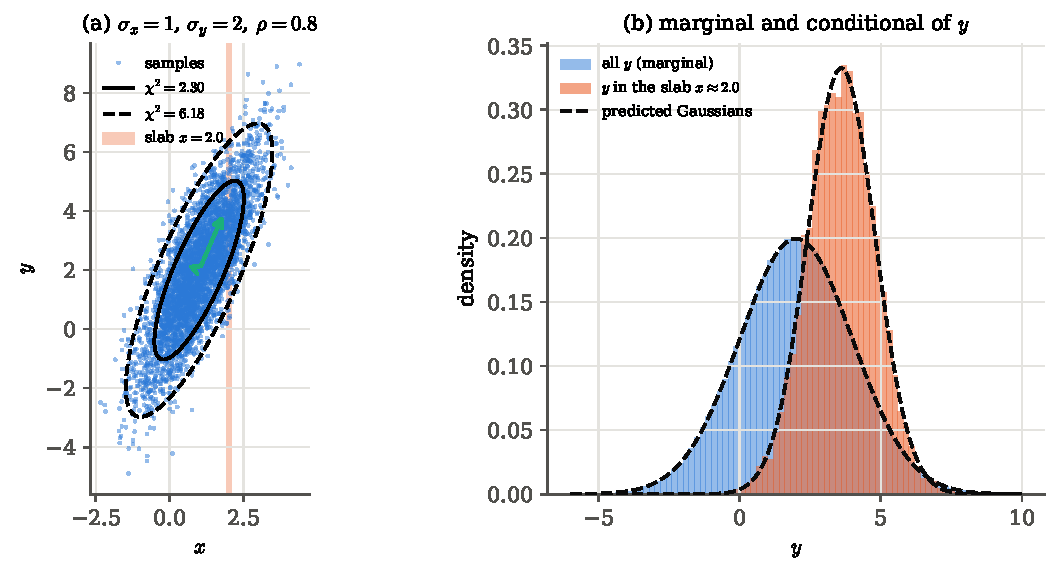
\includegraphics[width=\linewidth]{figures/ch02/mvn_ellipses.pdf}
\caption{(a) Samples of the bivariate Gaussian with $\sigma_x=1$, $\sigma_y=2$, $\rho=0.8$, with the $\Delta\chi^2=2.30$ and $6.18$ ellipses and the principal axes (arrows, of length one standard deviation along each axis). The shaded strip is the slab used for conditioning. (b) All $y$ values (the marginal) and the $y$ values inside the slab (the conditional), each with its predicted Gaussian. Fixing $x$ shifts the centre and shrinks the width.}
\label{2b:fig:mvn}
\end{figure}

\paragraph{The same object in three sciences.} The multivariate Gaussian is the common core of the three kinds of data this book keeps returning to. \emph{Colliders.} For Poisson counts in many bins it is the large-count limit of the product of Poissons. Its $\Cmat$ is diagonal, with variances equal to the means, until systematic uncertainties shared between bins add correlations. \emph{The CMB.} For a CMB map (\cref{ch:07}) the vector is the list of pixel temperatures or of the harmonic coefficients $\alm$, and $\Cmat$ is built from the power spectrum $\Cell$. For an isotropic Gaussian field the $\alm$ are independent with variance $\Cell$, so in harmonic space $\Cmat$ is diagonal. \emph{Gravitational waves.} For detector noise the vector is the time series and $\Cmat$ is set by the power spectral density. Stationarity makes it a Toeplitz matrix (constant along each diagonal), and the Fourier transform diagonalises it, just as the eigenbasis did in \eqref{2b:eq:mvn-ellipse}. In each case the step that makes the likelihood computable is the same: whiten, and then everything is a sum of independent squares. That sum of squares is the $\chi^2$ variable of \cref{2b:sec:chi2}. When the tails of real data are heavier than Gaussian, the multivariate Student-$t$, a Gaussian with a randomly rescaled covariance (\cref{2b:sec:t}), is the standard robust replacement \srcref{Lambert}{\S8.4.11}.
\section{Sums of squared Gaussians: the \texorpdfstring{$\chi^2$}{chi-squared} distribution}
\label{2b:sec:chi2}

We fit a straight line to ten points with error bars and get $\chi^2=\sum_i(x_i-\mu_i)^2/\sigma_i^2=14.2$, where $x_i$ is a measured value, $\mu_i$ the line's prediction and $\sigma_i$ the error bar. Is the fit good? The number means nothing until we know how $\chi^2$ is distributed when the model is right. Sums of squared Gaussians turn up throughout physics. A CMB band power $\Chat=\frac{1}{2\ell+1}\sum_m|\alm|^2$ is a sum of squares of Gaussian coefficients, and its scatter is cosmic variance. The power of Gaussian detector noise in one frequency bin of a gravitational-wave stream is the sum of two squares, the real and imaginary parts. The quadratic form in the exponent of the multivariate Gaussian, whose contours we just drew, is a sum of squares after whitening. And the sample variance of $n$ repeated measurements is a sum of squared deviations.

Two results answer these questions. A sum of $\nu$ squared standard normals has a definite distribution, $\chi^2_\nu$, with mean $\nu$ and variance $2\nu$. And the sample variance divides by $n-1$, not $n$, because estimating the mean uses up exactly one ``degree of freedom'' in a sense the geometry makes precise.

The questions, in words: \emph{if $\nu$ independent standard normal numbers are squared and added, what is the density of the total? And what changes when the numbers are deviations from their own average rather than from the true mean?}

\subsection{One square}
\label{2b:sec:chi2-one}

Start with a single square, $Q=Y^2$ with $Y\sim\Normal(0,1)$. \emph{When is $Q$ small?} For $q>0$, $Q\le q$ happens exactly when $-\sqrt q\le Y\le\sqrt q$. So we can get the density of $Q$ by differentiating the probability of that interval:
\begin{align}
  f_1(q)=\frac{\dd}{\dd q}\Prob(Q\le q)
  &\eqby{1} \frac{\dd}{\dd q}\bigl[\Phi(\sqrt q)-\Phi(-\sqrt q)\bigr]
   \eqby{2} 2\varphi(\sqrt q)\,\frac{1}{2\sqrt q}
   \eqby{3} \frac{1}{\sqrt{2\pi q}}\,e^{-q/2} .
  \label{2b:eq:chi2-one}
\end{align}
\begin{explain}
  \item The probability of an interval is the difference of the cumulative distribution at its ends.
  \item Chain rule, $\frac{\dd}{\dd q}\sqrt q=\frac1{2\sqrt q}$, and the symmetry $\varphi(-y)=\varphi(y)$. The two ends contribute equally: this is the factor two of \srcref{Cowan}{(10.14)}, which counts the positive and the negative root.
  \item $\varphi(\sqrt q)=e^{-q/2}/\sqrt{2\pi}$.
\end{explain}
The density diverges like $q^{-1/2}$ at the origin, because $Y$ is most likely near zero and squaring crowds those values towards $q=0$. One square is a gamma variable, Gamma$(\frac12,2)$ \srcref{CasellaBerger}{Lemma~5.3.2}. To check, recall the gamma density \eqref{2a:eq:gamma}: with shape $\alpha=\frac12$ and scale $\beta=2$ it is $q^{-1/2}e^{-q/2}/(\Gamma(\frac12)\sqrt2)$, and $\Gamma(\frac12)=\sqrt\pi$ \eqref{2b:eq:gamma-half} makes this identical to \eqref{2b:eq:chi2-one}.

\subsection{Many squares: two derivations}
\label{2b:sec:chi2-many}

\paragraph{The geometric route: integrate the joint density over a ball.} \emph{The question in words:} what is the probability that $Q_\nu\le q$, whatever the individual values of $Y_1,\dots,Y_\nu$ happen to be? We know the joint density of all the $Y_j$, and we do not care about them one by one, only about the one combination $Q_\nu$. So we do what we always do with variables we do not care about (\cref{1b:sec:marginal}): integrate the joint density over every set of values $y_1,\dots,y_\nu$ that gives $Q_\nu\le q$, and then change variables to $Q$. It goes in four steps.

\emph{Step 1: the joint density.} The $Y_j$ are independent, so their joint density is the product of the $\nu$ one-dimensional densities. Writing $\bm y=(y_1,\dots,y_\nu)$ and $|\bm y|^2=y_1^2+\dots+y_\nu^2$,
\begin{equation}
  f(\bm y)=\prod_{j=1}^{\nu}\frac{e^{-y_j^2/2}}{\sqrt{2\pi}}=\frac{e^{-(y_1^2+\dots+y_\nu^2)/2}}{(2\pi)^{\nu/2}}=\frac{e^{-|\bm y|^2/2}}{(2\pi)^{\nu/2}} ,
  \label{2b:eq:chi2-joint}
\end{equation}
since a product of exponentials is the exponential of the sum. The density depends on $\bm y$ only through its length $r=|\bm y|$: it is the same at every point of a sphere centred on the origin.

\emph{Step 2: the event $Q_\nu\le q$ is a ball.} $Q_\nu=|\bm Y|^2$ is the squared distance of the random point $\bm Y$ from the origin. So $Q_\nu\le q$ happens exactly when $\bm Y$ lands inside the ball of radius $\sqrt q$, and its probability is the joint density integrated over all $\bm y$ in that ball:
\[
  \Prob(Q_\nu\le q)=\int_{|\bm y|^2\le q}\frac{e^{-|\bm y|^2/2}}{(2\pi)^{\nu/2}}\,\dd^\nu y .
\]
This is the one-square argument of \cref{2b:sec:chi2-one} in $\nu$ dimensions: there the ball was the interval $[-\sqrt q,\sqrt q]$.

\emph{Step 3: spherical coordinates.} Because the integrand depends only on $r$, we slice the ball into thin spherical shells. A shell of radius $r$ and thickness $\dd r$ has volume $S_{\nu-1}r^{\nu-1}\dd r$, where $S_{\nu-1}$ is the area of the unit sphere in $\nu$ dimensions ($S_1=2\pi$, the circumference of the unit circle; $S_2=4\pi$). The power $r^{\nu-1}$ is there because a sphere of radius $r$ is the unit sphere stretched by $r$ in each of its $\nu-1$ directions. Integrating over the angles of each shell leaves a one-dimensional integral,
\begin{equation}
  \Prob(Q_\nu\le q)=\frac{S_{\nu-1}}{(2\pi)^{\nu/2}}\int_0^{\sqrt q}r^{\nu-1}e^{-r^2/2}\,\dd r .
  \label{2b:eq:chi2-ball}
\end{equation}
We still need $S_{\nu-1}$. The Gaussian integral gives it, by computing one integral in two ways. The integral of $e^{-|\bm y|^2/2}$ over all of $\mathbb R^\nu$ factorises into $\nu$ one-dimensional Gaussian integrals, each equal to $\sqrt{2\pi}$; in shells it is $S_{\nu-1}\int_0^\infty r^{\nu-1}e^{-r^2/2}\dd r$. Setting the two equal,
\begin{align}
  (2\pi)^{\nu/2}
  &\eqby{1} \int_{\mathbb R^\nu}e^{-|\bm y|^2/2}\,\dd^\nu y
   \eqby{2} S_{\nu-1}\int_0^\infty r^{\nu-1}e^{-r^2/2}\,\dd r
   \eqby{3} S_{\nu-1}\,2^{\nu/2-1}\,\Gamma\bigl(\tfrac\nu2\bigr)
  \quad\Longrightarrow\quad S_{\nu-1}=\frac{2\pi^{\nu/2}}{\Gamma(\nu/2)} .
  \label{2b:eq:sphere-area}
\end{align}
\begin{explain}
  \item Cartesian coordinates: $e^{-|\bm y|^2/2}=\prod_je^{-y_j^2/2}$, and each $\int_{-\infty}^\infty e^{-y_j^2/2}\dd y_j=\sqrt{2\pi}$.
  \item Spherical coordinates, as in step 3, with the ball extended to all of space.
  \item Substitute $t=r^2/2$, so $r=\sqrt{2t}$, $\dd r=\dd t/\sqrt{2t}$ and $r^{\nu-1}\dd r=(2t)^{\nu/2-1}\dd t$; the $t$ integral is $\int_0^\infty t^{\nu/2-1}e^{-t}\dd t=\Gamma(\nu/2)$.
\end{explain}
Divide by $2^{\nu/2-1}\Gamma(\nu/2)$ and use $(2\pi)^{\nu/2}/2^{\nu/2-1}=2\pi^{\nu/2}$. (Check: $\nu=2$ gives $2\pi/\Gamma(1)=2\pi$, and $\nu=3$ gives $2\pi^{3/2}/(\sqrt\pi/2)=4\pi$.)

\emph{Step 4: from the radius to $Q$, and differentiate.} In \eqref{2b:eq:chi2-ball} change the integration variable from $r$ to $s=r^2$, the value of $Q$ on the shell, and then differentiate with respect to the upper limit:
\begin{align}
  \Prob(Q_\nu\le q)
  &\eqby{1} \frac{S_{\nu-1}}{(2\pi)^{\nu/2}}\int_0^{q}s^{(\nu-1)/2}\,e^{-s/2}\,\frac{\dd s}{2\sqrt s}
   \eqby{2} \frac{1}{2^{\nu/2}\,\Gamma(\nu/2)}\int_0^{q}s^{\nu/2-1}\,e^{-s/2}\,\dd s ,
  \nonumber\\
  f_\nu(q)=\frac{\dd}{\dd q}\Prob(Q_\nu\le q)
  &\eqby{3} \frac{q^{\nu/2-1}e^{-q/2}}{2^{\nu/2}\,\Gamma(\nu/2)} ,\qquad q>0 ,
  \label{2b:eq:chi2}
\end{align}
\begin{explain}
  \item $r=\sqrt s$, so $r^{\nu-1}=s^{(\nu-1)/2}$ and $\dd r=\dd s/(2\sqrt s)$; the limits $r=0$ and $r=\sqrt q$ become $s=0$ and $s=q$.
  \item Insert $S_{\nu-1}$ from \eqref{2b:eq:sphere-area}: $\frac{2\pi^{\nu/2}}{\Gamma(\nu/2)}\cdot\frac{1}{(2\pi)^{\nu/2}}\cdot\frac12=\frac{1}{2^{\nu/2}\Gamma(\nu/2)}$, and combine the powers, $s^{(\nu-1)/2}s^{-1/2}=s^{\nu/2-1}$.
  \item The derivative of an integral with respect to its upper limit is the integrand at that limit.
\end{explain}
the $\chi^2$ density with $\nu$ \newterm{degrees of freedom} \srcref{Cowan}{(2.34)}, \mainref{p.~30}. The power $q^{\nu/2-1}$ is pure geometry: the area of a sphere of radius $\sqrt q$ in $\nu$ dimensions. In high dimensions this factor pushes the probability away from the origin, which is why $\chi^2_\nu$ peaks near $\nu-2$ rather than at zero. We use the same shell argument for the Maxwell--Boltzmann speed distribution in \cref{2b:sec:zoo}.

\paragraph{The characteristic function route.} The second route draws no sphere. Characteristic functions turn the sum of squares into a product \srcref{Cowan}{(10.12)--(10.15)}. First transform one square. With $a=1-2ik$,
\begin{align}
  \phi_1(k)=\E\,e^{ikY^2}
  &\eqby{1} \int_{-\infty}^{\infty}\frac{e^{-y^2/2}}{\sqrt{2\pi}}\,e^{iky^2}\,\dd y
   \eqby{2} \int_{-\infty}^{\infty}\frac{e^{-ay^2/2}}{\sqrt{2\pi}}\,\dd y
   \eqby{3} (1-2ik)^{-1/2} .
  \label{2b:eq:chi2-cf1}
\end{align}
\begin{explain}
  \item The expectation of a function of $Y$ is its integral against the density of $Y$.
  \item Combine the exponents: $-\frac{y^2}{2}+iky^2=-\frac{(1-2ik)y^2}{2}$.
  \item The Gaussian integral $\int e^{-ay^2/2}\dd y=\sqrt{2\pi/a}$, which holds for complex $a$ with positive real part (here $\mathrm{Re}\,a=1$) with the principal square root, by analytic continuation from real $a$.
\end{explain}
For $Q_\nu=Y_1^2+\dots+Y_\nu^2$ with independent $Y_j$, the product rule \eqref{2b:eq:cf-sum} gives $\phi_\nu(k)=(1-2ik)^{-\nu/2}$ \srcref{Cowan}{(10.15)}. Which density has this transform? One square was a gamma variable, so try the gamma density with shape $\alpha$ and scale $\beta$:
\begin{align}
  \int_0^\infty e^{ikx}\,\frac{x^{\alpha-1}e^{-x/\beta}}{\Gamma(\alpha)\beta^\alpha}\,\dd x
  &\eqby{1} \frac{1}{\Gamma(\alpha)\beta^\alpha}\int_0^\infty x^{\alpha-1}e^{-x(1-i\beta k)/\beta}\,\dd x
   \eqby{2} \frac{1}{\Gamma(\alpha)\beta^\alpha}\,\Gamma(\alpha)\Bigl(\frac{\beta}{1-i\beta k}\Bigr)^{\alpha}
   = (1-i\beta k)^{-\alpha} ,
  \label{2b:eq:gamma-cf}
\end{align}
\begin{explain}
  \item Combine the exponentials.
  \item Substitute $t=x(1-i\beta k)/\beta$; then $\int_0^\infty x^{\alpha-1}e^{-cx}\dd x=\Gamma(\alpha)/c^\alpha$, again valid for complex $c$ with positive real part.
\end{explain}
so $(1-2ik)^{-\nu/2}$ is the characteristic function of Gamma$(\nu/2,2)$. Since a characteristic function determines its density, $f_\nu(q)=q^{\nu/2-1}e^{-q/2}/(2^{\nu/2}\Gamma(\nu/2))$, which is \eqref{2b:eq:chi2} again: the product of $\nu$ transforms and the integral over a ball give the same density.

\begin{workdef}[$\chi^2$ distribution]
$Q\sim\chi^2_\nu$ if $Q=\sum_{j=1}^\nu Y_j^2$ with $Y_j\iid\Normal(0,1)$. Equivalently, $Q$ has density \eqref{2b:eq:chi2}, the Gamma$(\nu/2,2)$ density, and characteristic function $(1-2ik)^{-\nu/2}$.
\emph{Summary numbers:} $\E Q=\nu$, $\Var Q=2\nu$, mode $\max(\nu-2,0)$. \emph{Additivity:} independent $\chi^2_{\nu_1}$ and $\chi^2_{\nu_2}$ add to $\chi^2_{\nu_1+\nu_2}$ (multiply the characteristic functions).
\emph{Recognise it by:} a sum of squares of independent, zero-mean, unit-variance Gaussian quantities, such as residuals divided by their true errors.
\end{workdef}

\paragraph{Mean and variance.} The mean of $\chi^2_\nu$ is $\nu$ and its variance is $2\nu$. For one square, $\E Y^2=1$ and $\E Y^4=3$ (differentiate the Gaussian characteristic function four times, or integrate by parts twice as in \eqref{2b:eq:gauss-moments}), so $\Var Y^2=3-1=2$. Means and variances of independent terms add, so $\E Q_\nu=\nu$ and $\Var Q_\nu=2\nu$ \srcref{Cowan}{(2.36)--(2.37)}. The script sums $\nu$ squared normals $2\times10^5$ times and finds mean $\tbChiMeanFive$ and variance $\tbChiVarFive$ for $\nu=5$, and $\tbChiMeanTen$ and $\tbChiVarTen$ for $\nu=10$ (\cref{2b:fig:chi2-sums}a). For large $\nu$ the CLT makes $\chi^2_\nu\approx\Normal(\nu,2\nu)$, but slowly: its skewness is $\sqrt{8/\nu}$, still $0.28$ at $\nu=100$ (the skewness of one square, $\sqrt8$, shrinks like $1/\sqrt\nu$, as in \eqref{2b:eq:cumulant-scaling}).

\paragraph{Example: is $\chi^2=14.2$ for ten degrees of freedom a good fit?} Yes, it is acceptable. \emph{The question in words:} if the straight line is the right model, how often would a fit come out this bad or worse? With $\nu=10$, $\E\chi^2=10$ and the standard deviation is $\sqrt{20}=4.5$. So $14.2$ is less than one standard deviation high. Exactly, $\Prob(\chi^2_{10}>14.2)=0.16$: one fit in six would do this badly even with the right model. The central $90\%$ range of $\chi^2_{10}$ is $3.9$ to $18.3$. A fit with $\chi^2=24$ would have tail probability $0.008$ and would be suspicious.

The same reduced $\chi^2/\nu$ can mean different things for different $\nu$. Its standard deviation is $\sqrt{2/\nu}$, which is $0.45$ for ten points. So ``$\chi^2/\nu=1.4$'' is unremarkable for $\nu=10$, while for $\nu=100$ ($\chi^2=140$) it has tail probability $0.005$. Hypothesis tests built on this are the subject of \cref{ch:04}.

\paragraph{Example: cosmic variance.} A CMB band power is a $\chi^2$ variable, and that fixes its scatter. Recall that $\Chat=\frac{1}{2\ell+1}\sum_m|\alm|^2$ is the measured power at multipole $\ell$, built from the $2\ell+1$ harmonic coefficients $\alm$, and $\Cell$ is its true value. \emph{How many independent Gaussians go into it?} Exactly $2\ell+1$ real numbers. The $m=0$ coefficient is real. For $m>0$ the real and imaginary parts count separately. And $a_{\ell,-m}$ adds nothing new, being fixed by $a_{\ell,-m}=(-1)^ma^*_{\ell m}$. For an isotropic Gaussian sky these $2\ell+1$ numbers are independent Gaussians whose squares add up to $\sum_m|\alm|^2$, each with the same share of the variance. So $(2\ell+1)\Chat/\Cell\sim\chi^2_{2\ell+1}$, and
\[
  \Var\Chat\eqby{1}\Bigl(\frac{\Cell}{2\ell+1}\Bigr)^2\,\Var\chi^2_{2\ell+1}\eqby{2}\frac{\Cell^2}{(2\ell+1)^2}\,2(2\ell+1)=\frac{2\Cell^2}{2\ell+1},
\]
where (1) scales a random variable by a constant and (2) uses $\Var\chi^2_\nu=2\nu$. This is the cosmic variance that \cref{ch:07} verifies by simulation. At $\ell=2$, $\Chat$ is a $\chi^2_5$ variable divided by five: skewed, with a $1\sigma$ scatter of $63\%$.

\subsection{Correlated Gaussians: the quadratic form}
\label{2b:sec:chi2-quadform}

Correlations do not change the answer, as long as the sum of squares uses the full inverse covariance. If $\bm X\sim\Normal(\bm\mu,\Cmat)$ in $k$ dimensions, then
\begin{equation}
  Q=(\bm X-\bm\mu)\T\Cmat^{-1}(\bm X-\bm\mu)\ \sim\ \chi^2_k
  \label{2b:eq:quadform}
\end{equation}
\srcref{Cowan}{(2.39)}, \mainref{Thm~2.44(4)}. The proof is one line with the whitening of \cref{2b:sec:mvn}: with $\mathbf L$ the Cholesky factor, $\mathbf L\mathbf L\T=\Cmat$, the vector $\bm Z=\mathbf L^{-1}(\bm X-\bm\mu)$ has independent standard normal components and $\bm Z\T\bm Z=(\bm X-\bm\mu)\T(\mathbf L\mathbf L\T)^{-1}(\bm X-\bm\mu)=Q$. This is what justified the ellipse contents in \eqref{2b:eq:ellipse-content}.

\paragraph{Example: forgetting the correlations.} Dropping the off-diagonal elements keeps the right mean but gives the wrong spread. The script takes a correlated three-dimensional Gaussian with covariance
\[
  \Cmat=\begin{pmatrix}1&0.6&0.3\\0.6&2&-0.5\\0.3&-0.5&1.5\end{pmatrix}
\]
and computes $Q$ for $2\times10^5$ draws: mean $\tbQFmean$ and variance $\tbQFvar$, as $\chi^2_3$ requires. It also computes the ``naive'' sum $\sum_i(x_i-\mu_i)^2/C_{ii}$, which ignores the off-diagonal elements. Its mean is still $\tbNaiveMean$, because each term has expectation $1$ whatever the correlations. But its variance is $\tbNaiveVar$ instead of $6$ (\cref{2b:fig:chi2-sums}b), because the terms are correlated and so do not add like independent squares. A goodness-of-fit test that uses only the diagonal errors on correlated data (neighbouring bins of a smoothed spectrum, overlapping band powers) will reject correct models too often, even though its average looks fine.

\begin{figure}[htbp]
\centering
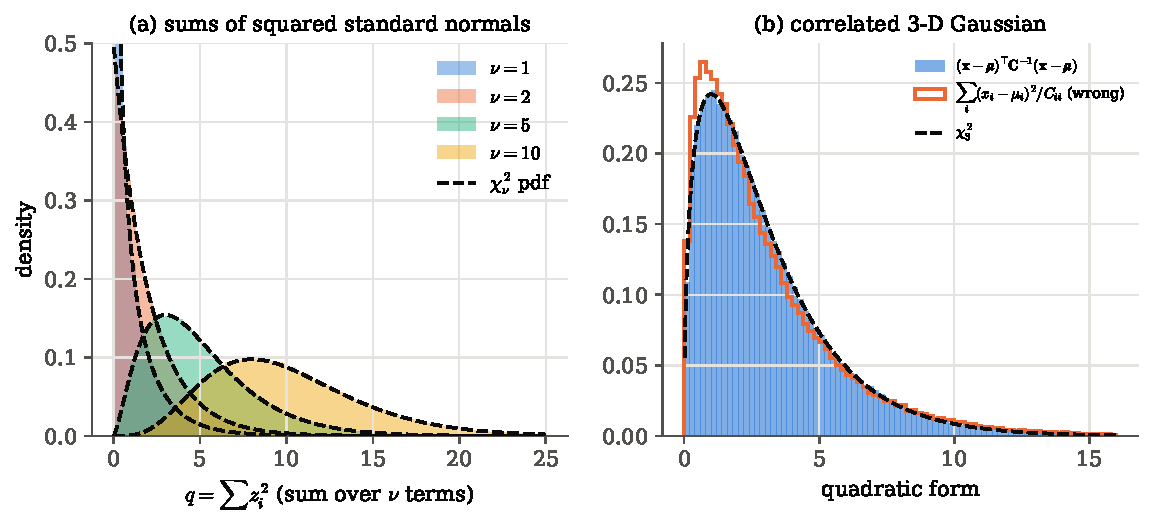
\includegraphics[width=\linewidth]{figures/ch02/chi2_sums.pdf}
\caption{(a) Histograms of sums of $\nu$ squared standard normals for $\nu=1,2,5,10$ against the $\chi^2_\nu$ densities (dashed). For $\nu=1$ and $2$ the density is largest at zero; for larger $\nu$ the peak moves out to $\nu-2$. (b) For a correlated three-dimensional Gaussian, the full quadratic form follows $\chi^2_3$, while the sum that uses only the diagonal variances (orange) has the right mean but the wrong shape: it piles up near zero and has a longer tail, so its variance is larger.}
\label{2b:fig:chi2-sums}
\end{figure}

\subsection{The sample variance and the lost degree of freedom}
\label{2b:sec:nminus1}

Five readings of a pendulum period, $x_1,\dots,x_5$, scatter about the unknown true value $\mu$ with unknown spread $\sigma$. We estimate $\mu$ by the sample mean $\bar x=\frac1n\sum x_i$, and $\sigma^2$ from the deviations $x_i-\bar x$. Why divide the sum of squared deviations by $n-1$?

\paragraph{The bias.} Deviations from $\bar x$ are systematically smaller than deviations from the true $\mu$. The reason: the sample mean is the value of $a$ that minimises $\sum_i(x_i-a)^2$ (set the derivative $-2\sum_i(x_i-a)$ to zero), so no other centre, $\mu$ included, gives a smaller sum. By how much smaller? Write $x_i-\mu=(x_i-\bar x)+(\bar x-\mu)$ and expand:
\begin{align}
  \sum_{i=1}^n(x_i-\mu)^2
  &\eqby{1} \sum_{i=1}^n(x_i-\bar x)^2+2(\bar x-\mu)\sum_{i=1}^n(x_i-\bar x)+n(\bar x-\mu)^2 \nonumber\\
  &\eqby{2} \sum_{i=1}^n(x_i-\bar x)^2+n(\bar x-\mu)^2 .
  \label{2b:eq:ss-split}
\end{align}
\begin{explain}
  \item Square the sum of two terms and sum over $i$; the last term does not depend on $i$.
  \item $\sum_i(x_i-\bar x)=n\bar x-n\bar x=0$.
\end{explain}
Take expectations for independent $x_i$ with variance $\sigma^2$, any distribution. The left side has expectation $n\sigma^2$ and $\E(\bar x-\mu)^2=\Var\bar x=\sigma^2/n$, so
\begin{equation}
  \E\sum_{i=1}^n(x_i-\bar x)^2=n\sigma^2-n\cdot\frac{\sigma^2}{n}=(n-1)\sigma^2 .
  \label{2b:eq:nminus1}
\end{equation}
Hence $S^2=\frac1{n-1}\sum(x_i-\bar x)^2$ has $\E S^2=\sigma^2$, while the ``natural'' $\frac1n\sum(x_i-\bar x)^2$ is low on average by the factor $(n-1)/n$. The script, with $n=\tbSVn$ and $\sigma^2=\tbSVsigmaSq$, finds $\E S^2=\tbSVmeanS$ and $\E\bigl[\frac1n\sum(x_i-\bar x)^2\bigr]=\tbSVmeanSn$, against the predicted $\tbSVbiasTh$. The missing $\sigma^2/n$ is exactly the variance of $\bar x$ around $\mu$: the part of the scatter that the sample mean ``absorbs'' by following the data.

\paragraph{The distribution: rotate the data.} For Gaussian data we can say much more: $(n-1)S^2/\sigma^2$ is exactly $\chi^2_{n-1}$, and it is independent of $\bar x$. A rotation of the data shows both. Picture the $n$ readings as one point $\bm x\in\R^n$. The sample mean is about the component of $\bm x$ along the diagonal direction $\bm e=(1,\dots,1)/\sqrt n$, since $\bm e\T\bm x=\sqrt n\,\bar x$. The deviations $x_i-\bar x$ are the components of what is left over, $\bm x-\sqrt n\,\bar x\,\bm e$, which is perpendicular to $\bm e$ and so lives in an $(n-1)$-dimensional subspace (\cref{2b:fig:helmert}). Choose an orthonormal basis whose first vector is $\bm e$, collect the basis vectors as the rows of an orthogonal matrix $\mathbf H$ (for $n=3$, one choice, the \newterm{Helmert} matrix, is shown below), and rotate: $\bm y=\mathbf H(\bm x-\mu\bm 1)$, where $\bm1=(1,\dots,1)$. Then:
\begin{itemize}
  \item $\bm x-\mu\bm1\sim\Normal(0,\sigma^2\Id)$, so by \eqref{2b:eq:mvn-linear} $\bm y\sim\Normal(0,\sigma^2\mathbf H\mathbf H\T)=\Normal(0,\sigma^2\Id)$: the $y_j$ are again independent with variance $\sigma^2$. An isotropic Gaussian looks the same in every rotated frame.
  \item $y_1=\bm e\T(\bm x-\mu\bm1)=\sqrt n(\bar x-\mu)$.
  \item A rotation preserves length, so $\sum_{j=1}^ny_j^2=\sum_i(x_i-\mu)^2$, and by \eqref{2b:eq:ss-split}, $\sum_{j=2}^ny_j^2=\sum_i(x_i-\mu)^2-n(\bar x-\mu)^2=\sum_i(x_i-\bar x)^2$.
\end{itemize}
The last line says that $(n-1)S^2/\sigma^2=\sum_{j=2}^n(y_j/\sigma)^2$ is a sum of $n-1$ independent squared standard normals, and it involves only $y_2,\dots,y_n$, which are independent of $y_1$ and hence of $\bar x$.

\paragraph{Example: $n=3$, by hand.} The rows of
\[
  \mathbf H=\begin{pmatrix}\tfrac1{\sqrt3}&\tfrac1{\sqrt3}&\tfrac1{\sqrt3}\\[2pt] \tfrac1{\sqrt2}&-\tfrac1{\sqrt2}&0\\[2pt] \tfrac1{\sqrt6}&\tfrac1{\sqrt6}&-\tfrac2{\sqrt6}\end{pmatrix}
\]
have unit length and are mutually orthogonal (for example, row 2 $\cdot$ row 3 $=\frac1{\sqrt{12}}-\frac1{\sqrt{12}}+0=0$). Take the readings $\bm x=(1,2,6)$, so $\bar x=3$ and $\sum(x_i-\bar x)^2=4+1+9=14$. The second and third rotated components (the shift by $\mu\bm1$ drops out of them, because their rows sum to zero) are $y_2=(1-2)/\sqrt2$ and $y_3=(1+2-12)/\sqrt6$, and $y_2^2+y_3^2=\frac12+\frac{81}6=14$. The first component carries the mean, the other two carry the scatter.

\begin{keyidea}[Sample mean and sample variance of Gaussian data]
If $x_1,\dots,x_n\iid\Normal(\mu,\sigma^2)$ \srcref{CasellaBerger}{Thm~5.3.1}:
(a) $\bar x$ and $S^2$ are independent;
(b) $\bar x\sim\Normal(\mu,\sigma^2/n)$;
(c) $(n-1)S^2/\sigma^2\sim\chi^2_{n-1}$.
One degree of freedom is spent on the direction along which $\bar x$ is measured; the scatter lives in the remaining $n-1$.
\end{keyidea}

Casella and Berger prove (a) by factorising the joint density after the change of variables $(\bar x,x_2-\bar x,\dots,x_n-\bar x)$, and (c) by induction, adding one data point at a time with the update $(n-1)S_n^2=(n-2)S_{n-1}^2+\frac{n-1}{n}(x_n-\bar x_{n-1})^2$ \srcref{CasellaBerger}{(5.3.1)--(5.3.2)}. They also give the fastest check of (a): $\Cov(\bar x,x_j-\bar x)=\sum_i\frac1n(\delta_{ij}-\frac1n)\sigma^2=0$, and uncorrelated linear functions of independent Gaussians are independent \srcref{CasellaBerger}{Lemma~5.3.3}. The rotation is the same argument seen geometrically.

\begin{figure}[htbp]
\centering
\begin{tikzpicture}[scale=0.95]
  \draw[faint,->] (-0.4,0) -- (4.6,0) node[anchor=north,lbl] {$x_1-\mu$};
  \draw[faint,->] (0,-0.4) -- (0,4.4) node[anchor=east,lbl] {$x_2-\mu$};
  \draw[formblue,thick] (-0.3,-0.3) -- (4.2,4.2);
  \node[lbl,formblue,anchor=west] at (4.2,4.2) {direction $\bm e=(1,1)/\sqrt2$};
  \coordinate (X) at (1.2,3.6);
  \coordinate (P) at (2.4,2.4); %
  \fill (X) circle (1.6pt);
  \node[lbl,anchor=east] at (1.1,3.7) {data $\bm x$};
  \fill[formblue] (P) circle (1.6pt);
  \node[lbl,anchor=north west,formblue] at (2.5,2.35) {$(\bar x,\bar x)$};
  \draw[bdryred,very thick] (P) -- (X);
  \node[lbl,bdryred,anchor=south west] at (1.95,3.05) {residual};
  \draw[thin] ($(P)+(-0.18,0.18)$) -- ($(P)+(0,0.36)$) -- ($(P)+(0.18,0.18)$);
  \draw[bdryred!50,dashed] (0.6,4.2) -- (4.2,0.6);
\end{tikzpicture}
\caption{Two readings seen as one point $\bm x$ in the plane (origin at the true value). Projecting onto the diagonal gives the sample mean $(\bar x,\bar x)$; the residual, whose length squared is $\sum(x_i-\bar x)^2$, is perpendicular to the diagonal. All data sets with the same mean lie on the dashed line, so the residual has only $n-1=1$ direction to move in. For an isotropic Gaussian the component along the diagonal and the component across it are independent.}
\label{2b:fig:helmert}
\end{figure}

\paragraph{Python: checking the theorem, and seeing it fail.} The script draws $\tbSVnrep$ samples of $n=\tbSVn$ Gaussian readings.

\pyfile[firstline=67,lastline=80,firstnumber=67]{code/ch02/25_chi2_sampvar.py}{The sample variance: $n-1$ degrees of freedom, and independence from the mean}

Line 70 computes $S^2$ with \pyname{ddof=1}, numpy's name for dividing by $n-1$ (``delta degrees of freedom''). Line 71 divides by $n$. Line 72 forms $(n-1)S^2/\sigma^2$, whose simulated mean and variance are $\tbSVwMean$ and $\tbSVwVar$, as $\chi^2_4$ requires ($4$ and $8$). Line 75 forms the same sum with the true mean instead of $\bar x$, which follows $\chi^2_5$ instead (\cref{2b:fig:chi2-sampvar}a). Lines 78--80 test independence, and show where it fails. The correlation between $\bar x$ and $S^2$ is $\tbSVcorrGauss$ for Gaussian readings, but $\tbSVcorrExp$ for exponential readings. \emph{Why?} For a skewed parent, a sample that happens to contain a large value has both a large mean and a large variance. The independence of $\bar x$ and $S^2$ is special to the Gaussian (it actually characterises it), and so is everything built on it in the next section.

\begin{figure}[htbp]
\centering
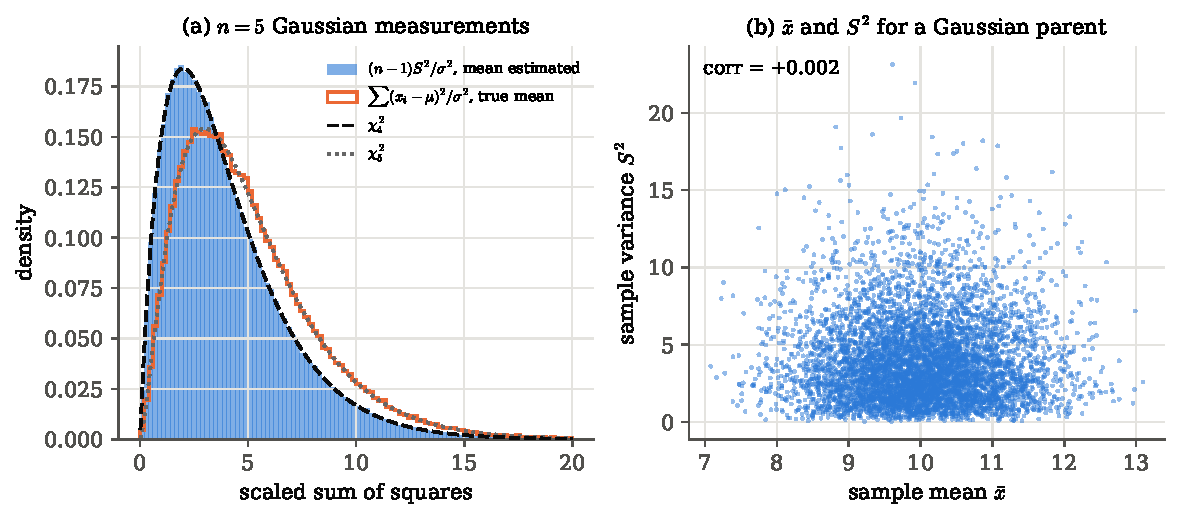
\includegraphics[width=\linewidth]{figures/ch02/chi2_sampvar.pdf}
\caption{(a) For five Gaussian readings, the scaled sum of squared deviations from the sample mean (histogram) follows $\chi^2_4$ (dashed), while deviations from the true mean (outline) follow $\chi^2_5$ (dotted). (b) Sample mean against sample variance for Gaussian readings: no trend at all, as independence requires.}
\label{2b:fig:chi2-sampvar}
\end{figure}

\begin{pitfall}[Degrees of freedom are dimensions, not data points]
The rule ``$\nu$ = number of data minus number of fitted parameters'' is the rotation argument again: each parameter that enters the model \emph{linearly} and is fitted by least squares removes one direction from the residual vector, exactly as $\bar x$ did. The rule is exact for linear models with Gaussian errors, approximate for nonlinear ones, and wrong when the data are correlated but treated as independent, or when parameters sit at a physical boundary.
\end{pitfall}
\section{When the error bar is itself estimated: Student's \texorpdfstring{$t$}{t} and the \texorpdfstring{$F$}{F} ratio}
\label{2b:sec:t}

We time five swings of a pendulum, compute $g$ from each, and quote the result as $\bar x\pm S/\sqrt5$, with $S$ the sample standard deviation. Then, to claim a ``two-sigma'' discrepancy with the textbook value, we check whether $|\bar x-g_0|$ exceeds $1.96\,S/\sqrt5$. This is wrong, and not by a little. The rule $1.96$ comes from the Gaussian, and it assumes that we know the true $\sigma$. We do not. Our error bar is itself a random number, computed from the same five readings, and sometimes it comes out much too small. When it does, the ratio $(\bar x-\mu)/(S/\sqrt n)$ is large, with $\mu$ the true value. So the ratio has fatter tails than a Gaussian. W.~S.~Gosset, who faced exactly this with small samples at the Guinness brewery and published as ``Student'', derived its distribution \srcref{CasellaBerger}{p.~181}.

Gosset's distribution does three jobs. It is the exact distribution of the \emph{studentised} mean for Gaussian data, so small-sample intervals and tests built on it are honest. It is also a Gaussian whose variance is itself random, which makes it the standard robust replacement for a Gaussian likelihood. And the same construction applied to two variances gives the $F$ distribution, the tool for asking whether two detectors, two runs or two models have the same scatter.

The question, in words: \emph{if a Gaussian quantity is divided by an independent, estimated measure of its own spread, how is the ratio distributed, and how different is it from a Gaussian?}

\subsection{The studentised mean}
\label{2b:sec:t-derive}

\emph{Why this ratio appears.} Let $x_1,\dots,x_n\iid\Normal(\mu,\sigma^2)$. If we
knew $\sigma$, the standardised mean
\begin{equation*}
  U=\frac{\bar x-\mu}{\sigma/\sqrt n}\sim\Normal(0,1)
\end{equation*}
would be all we need. We do not know $\sigma$, so we replace it by the sample
standard deviation $S$, with $S^2=\frac1{n-1}\sum_i(x_i-\bar x)^2$. Write $p=n-1$.
The quantity we actually compute is the \newterm{studentised mean}, and dividing its
top and bottom by $\sigma/\sqrt n$ shows what it is made of
\srcref{CasellaBerger}{(5.3.5)}:
\begin{align}
  T=\frac{\bar x-\mu}{S/\sqrt n}
  &\eqby{1} \frac{(\bar x-\mu)/(\sigma/\sqrt n)}{\sqrt{S^2/\sigma^2}}
   \eqby{2} \frac{U}{\sqrt{V/p}},
  \qquad V=\frac{(n-1)S^2}{\sigma^2}\sim\chi^2_p .
  \label{2b:eq:t-ratio}
\end{align}
\begin{explain}
  \item Divide numerator and denominator by $\sigma/\sqrt n$. The $\sqrt n$ cancels in the denominator.
  \item $S^2/\sigma^2=V/p$ by the definition of $V$. That $V$ is $\chi^2_p$, and that $U$ and $V$ are independent, are the results on the sample mean and variance of \cref{2b:sec:nminus1}.
\end{explain}
The unknown $\sigma$ has cancelled. So the whole problem is: given two independent
pieces, $U\sim\Normal(0,1)$ and $V\sim\chi^2_p$, what is the distribution of
$T=U/\sqrt{V/p}$?

\emph{The two ingredients and their joint density.} The density of $U$ is the standard
Gaussian, and the density of $V$ is the $\chi^2_p$ density \eqref{2b:eq:chi2}:
\begin{equation}
  f_U(u)=\frac{1}{\sqrt{2\pi}}\,e^{-u^2/2},
  \qquad
  f_V(v)=\frac{1}{2^{p/2}\Gamma(p/2)}\,v^{p/2-1}e^{-v/2}\quad(v>0).
  \label{2b:eq:t-ingredients}
\end{equation}
Because $U$ and $V$ are independent, their joint density is the product,
$f_{U,V}(u,v)=f_U(u)\,f_V(v)$.

\emph{Change variables from $(U,V)$ to $(T,V)$.} We keep $V$ and trade $U$ for $T$.
Solving \eqref{2b:eq:t-ratio} for $u$ gives the map and its Jacobian:
\begin{align}
  u=t\sqrt{\frac vp},\quad v=v,
  \qquad
  \left|\frac{\partial(u,v)}{\partial(t,v)}\right|
  &\eqby{1} \left|\begin{matrix}\sqrt{v/p} & \dfrac{t}{2\sqrt{pv}}\\[6pt] 0 & 1\end{matrix}\right|
   \eqby{2} \sqrt{\frac vp}.
  \label{2b:eq:t-jacobian}
\end{align}
\begin{explain}
  \item The four partial derivatives: $\partial u/\partial t=\sqrt{v/p}$, $\partial u/\partial v=t/(2\sqrt{pv})$, $\partial v/\partial t=0$, $\partial v/\partial v=1$.
  \item The matrix is triangular, so its determinant is the product of the diagonal entries. The off-diagonal entry never matters.
\end{explain}
The joint density of $(T,V)$ is the old joint density, evaluated at the old variables,
times this Jacobian (the rule of \cref{1b:eq:jacobian-2d}):
\begin{align}
  f_{T,V}(t,v)
  &\eqby{1} f_U\!\Bigl(t\sqrt{\tfrac vp}\Bigr)\,f_V(v)\,\sqrt{\frac vp} \nonumber\\
  &\eqby{2} \frac{1}{\sqrt{2\pi}}e^{-t^2v/(2p)}\;
            \frac{v^{p/2-1}e^{-v/2}}{2^{p/2}\Gamma(p/2)}\;\sqrt{\frac vp} \nonumber\\
  &\eqby{3} \frac{1}{\sqrt{2\pi p}\;2^{p/2}\Gamma(p/2)}\;
            v^{(p+1)/2-1}\,
            \exp\!\Bigl[-\frac v2\Bigl(1+\frac{t^2}{p}\Bigr)\Bigr].
  \label{2b:eq:t-joint}
\end{align}
\begin{explain}
  \item Change of variables, with the joint density of $(U,V)$ factorised by independence.
  \item Substitute the two densities \eqref{2b:eq:t-ingredients}, with $u^2=t^2v/p$.
  \item Collect the powers of $v$: $v^{p/2-1}\cdot v^{1/2}=v^{(p+1)/2-1}$. Collect the exponentials: $e^{-t^2v/(2p)}\,e^{-v/2}=e^{-\frac v2(1+t^2/p)}$. The constants are $1/\sqrt{2\pi}$, $1/\sqrt p$ and $1/(2^{p/2}\Gamma(p/2))$.
\end{explain}

\emph{The question that finishes the job.} What is the probability density for $T=t$,
regardless of what $V$ happens to be? That is a marginal density: we have the joint
density of $(T,V)$, and $V$ is a nuisance we do not care about, so we integrate it out
(\cref{1b:sec:marginal}). Write $A=1+t^2/p$ to keep the formula short. Then
\begin{align}
  f_T(t)
  &\eqby{1} \int_0^\infty f_{T,V}(t,v)\,\dd v \nonumber\\
  &\eqby{2} \frac{1}{\sqrt{2\pi p}\;2^{p/2}\Gamma(p/2)}
            \int_0^\infty v^{(p+1)/2-1}\,e^{-Av/2}\,\dd v \nonumber\\
  &\eqby{3} \frac{1}{\sqrt{2\pi p}\;2^{p/2}\Gamma(p/2)}\;
            \Gamma\Bigl(\frac{p+1}{2}\Bigr)\Bigl(\frac{2}{A}\Bigr)^{(p+1)/2} \nonumber\\
  &\eqby{4} \frac{\Gamma\bigl(\frac{p+1}{2}\bigr)}{\Gamma\bigl(\frac p2\bigr)\sqrt{p\pi}}\;
            \Bigl(1+\frac{t^2}{p}\Bigr)^{-(p+1)/2} .
  \label{2b:eq:student}
\end{align}
\begin{explain}
  \item Marginalisation: the density of $T$ alone is the joint density summed (integrated) over every value $V$ can take.
  \item Insert \eqref{2b:eq:t-joint}. Everything that does not depend on $v$ comes outside the integral.
  \item The gamma integral $\int_0^\infty x^{a-1}e^{-bx}\,\dd x=\Gamma(a)/b^a$, with $a=\frac{p+1}{2}$ and $b=\frac A2$, so $1/b^a=(2/A)^{(p+1)/2}$.
  \item The powers of two cancel, $2^{(p+1)/2}/(2^{p/2}\sqrt2)=1$, leaving $1/\sqrt{\pi p}$; then put back $A=1+t^2/p$.
\end{explain}
This is Student's $t$ density with $p$ degrees of freedom \srcref{CasellaBerger}{(5.3.6)}, \mainref{p.~30}.
The whole construction fits in one line: a standard Gaussian $U$, divided by the
square root of an independent $\chi^2_p/p$, is $t_p$. The $t$ distribution exists because
the fixed $\sigma$ of a Gaussian standardisation has been replaced by a random estimate,
whose square is a scaled $\chi^2$, and that extra randomness fattens the tails.

\begin{workdef}[Student's $t$ distribution]
$T\sim t_p$ if $T=U/\sqrt{V/p}$ with $U\sim\Normal(0,1)$ and $V\sim\chi^2_p$ independent; its density is \eqref{2b:eq:student}. For Gaussian data, $(\bar x-\mu)/(S/\sqrt n)\sim t_{n-1}$ exactly, for every $n\ge2$.
\emph{Equivalent picture:} a Gaussian $\Normal(0,\sigma^2)$ whose variance is random, $\sigma^2\sim$ Inv-Gamma$(p/2,p/2)$ \unpack{so the precision $1/\sigma^2$ is a gamma variable with mean one} \srcref{Lambert}{\S8.4.7}.
\emph{Summary numbers:} $\E T=0$ for $p>1$, $\Var T=p/(p-2)$ for $p>2$; only moments of order less than $p$ exist.
\end{workdef}

\paragraph{The tails, and the moments that do not exist.} For large $|t|$, \eqref{2b:eq:student} falls like $|t|^{-(p+1)}$, a power law. So $\E|T|^r$ is finite only for $r<p$ \srcref{CasellaBerger}{(5.3.7)}. With $p=1$ the density is $\Gamma(1)/(\Gamma(\frac12)\sqrt\pi)\,(1+t^2)^{-1}=\frac{1}{\pi(1+t^2)}$, the Cauchy distribution of \cref{2b:sec:cauchy}. So the studentised mean of \emph{two} Gaussian measurements has no mean at all. The variance, for $p>2$, follows from independence:
\begin{align}
  \Var T=\E T^2
  &\eqby{1} p\,\E(U^2)\,\E\Bigl(\frac1V\Bigr)
   \eqby{2} p\int_0^\infty\frac1v\,\frac{v^{p/2-1}e^{-v/2}}{2^{p/2}\Gamma(p/2)}\,\dd v
   \eqby{3} p\,\frac{2^{p/2-1}\Gamma(p/2-1)}{2^{p/2}\Gamma(p/2)}
   \eqby{4} \frac{p}{p-2} .
  \label{2b:eq:t-var}
\end{align}
\begin{explain}
  \item $T^2=pU^2/V$ with $U$ and $V$ independent, so the expectation factorises; $\E T=0$ by symmetry.
  \item $\E U^2=1$, and the expectation of $1/V$ is its integral against the $\chi^2_p$ density.
  \item The integrand is $v^{(p/2-1)-1}e^{-v/2}$, which integrates to $\Gamma(p/2-1)\,2^{p/2-1}$ provided $p>2$ (otherwise it diverges at $v=0$).
  \item $\Gamma(p/2)=(p/2-1)\Gamma(p/2-1)$, so the ratio is $\frac{1}{2(p/2-1)}=\frac1{p-2}$.
\end{explain}
The variance of $T$ is dominated by the rare samples whose estimated error bar $S$ happens to be tiny. That is what the divergence of step (3) at small $v$ means. As $p\to\infty$, $V/p\to1$ by the law of large numbers and $(1+t^2/p)^{-(p+1)/2}\to e^{-t^2/2}$, so $t_\infty=\Normal(0,1)$ \mainref{p.~30}. For non-Gaussian data and large $n$ the studentised mean still tends to $\Normal(0,1)$ (the studentised CLT, \mainref{Thm~5.10}). What the $t$ distribution adds is the \emph{exact} small-$n$ answer for Gaussian data.

\paragraph{Example: five pendulum readings.} Back to the five pendulum values of $g$ from the opening: how often does the Gaussian rule cry ``two sigma'' when nothing is wrong? The script simulates $\tbTnrep$ experiments of $n=\tbTn$ readings with $\sigma=0.05$\,m\,s$^{-2}$ and computes $T$ for each.

\pyfile[firstline=35,lastline=46,firstnumber=35]{code/ch02/26_student_t_F.py}{The studentised mean of five Gaussian readings}

Line 38 estimates the error bar from the same five numbers (\pyname{ddof=1} is the $n-1$ divisor). Line 39 forms $T$ with the estimated error bar and line 40 forms the same ratio with the true $\sigma$, which is exactly $\Normal(0,1)$. Lines 42--46 count how often each exceeds various thresholds. \emph{With the true $\sigma$}, $|Z|>1.96$ happens in a fraction $\tbZfracOneNineSix$ of experiments, the promised $5\%$. \emph{With the estimated error bar}, $|T|>1.96$ happens in $\tbTfracOneNineSix$, against the $t_4$ prediction $\tbTfracOneNineSixTh$. So the nominal ``$2\sigma$ discrepancy'' occurs more than twice as often as claimed. The correct $95\%$ point is $t_{4,\,0.975}=\tbTquant$, and $|T|$ exceeds it in a fraction $\tbTfracQuant$. Further out the difference explodes: $|T|>3$ happens in $\tbTfracThree$ of experiments ($t_4$: $\tbTfracThreeTh$), fifteen times the Gaussian $\tbTfracThreeGauss$ (\cref{2b:fig:t}a).

\begin{pitfall}[Do not use Gaussian thresholds with an estimated error bar]
With $n$ readings and $\sigma$ estimated from them, the two-sided $95\%$ multiplier is $t_{n-1,0.975}$: $12.7$ for $n=2$, $4.30$ for $n=3$, $2.78$ for $n=5$, $2.26$ for $n=10$, $2.09$ for $n=20$, and it reaches $1.96$ only as $n\to\infty$. For three-sigma or five-sigma claims the Gaussian rule is off by orders of magnitude unless $n$ is large. And the exact $t$ needs Gaussian readings: with a few outliers even $t$ is too optimistic.
\end{pitfall}

\paragraph{Example: a Gaussian with a random width.} Integrating $V$ out of \eqref{2b:eq:t-joint} has a second reading. For a fixed value $V=v$, $T=U\sqrt{p/v}$ is just a Gaussian with variance $p/v$; integrating over $v$ averages these Gaussians of different widths. So the $t$ distribution is a Gaussian whose width is itself random, and that is also a recipe for modelling data. Lambert's schools example \srcref{Lambert}{\S8.4.7} merges the test scores of many schools that share one mean but have different spreads. Each school on its own is Gaussian; the merged population is not. If the school variances are distributed as $\sigma^2\sim$ Inv-Gamma$(\nu/2,\nu/2)$, equivalently the precisions $1/\sigma^2$ as Gamma$(\nu/2,\text{scale }2/\nu)$, which is $\chi^2_\nu/\nu$, the merged distribution is exactly $t_\nu$: ``its head rises, its shoulders fall, and its tails fatten.'' The script draws $\tbTnrep$ values both ways for $\nu=\tbTmixNu$: as a Gaussian with a random precision (lines 51--52), and as $U/\sqrt{V/\nu}$ (line 54). Both histograms follow $t_3$, with Kolmogorov--Smirnov distances \unpack{the largest gap between the empirical and the exact cumulative distribution} of $\tbTksMix$ and $\tbTksUV$, as small as sampling noise allows at this sample size (\cref{2b:fig:t}b).

So the $t$ distribution is the workhorse \emph{robust likelihood}. When a few measurements have underestimated errors, when a detector occasionally misbehaves, when the population is heterogeneous, a $t_\nu$ likelihood with $\nu$ of a few lets outliers exist without dragging the fit. The degrees of freedom need not be an integer: $\nu$ is a free, real-valued shape parameter that can itself be fitted \srcref{Lambert}{\S8.4.7}. Its multivariate version, a multivariate Gaussian with one random scale factor for the whole covariance, gives joint tails heavy enough to see Lambert's hedge-fund ``bankruptcy days'' that a multivariate normal fit misses \srcref{Lambert}{\S8.4.11}.

\begin{figure}[htbp]
\centering
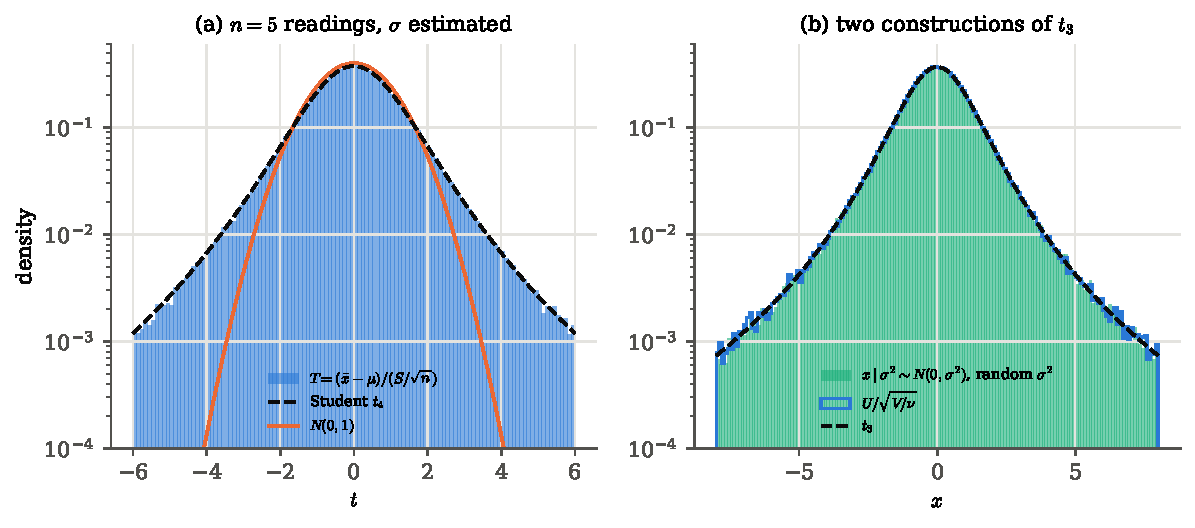
\includegraphics[width=\linewidth]{figures/ch02/t_student.pdf}
\caption{(a) The studentised mean of five Gaussian readings (histogram, logarithmic scale) follows Student's $t_4$ (dashed). The standard normal (solid) is far too thin in the tails. (b) Two constructions of $t_3$: a Gaussian whose variance is drawn afresh from an inverse-gamma distribution for every value, and the ratio $U/\sqrt{V/\nu}$. They are the same distribution.}
\label{2b:fig:t}
\end{figure}

\subsection{Ratios of variances: Snedecor's \texorpdfstring{$F$}{F}}
\label{2b:sec:F}

Two calorimeters measure the same electron beam. Calorimeter $X$ gives $n_X$ readings with sample variance $S_X^2$, calorimeter $Y$ gives $n_Y$ readings with $S_Y^2$. Is $X$'s resolution really worse, or did the numbers fluctuate? For Gaussian readings each $(n-1)S^2/\sigma^2$ is $\chi^2_{n-1}$, and the two are independent, so \srcref{CasellaBerger}{(5.3.8)}
\begin{equation}
  F=\frac{S_X^2/\sigma_X^2}{S_Y^2/\sigma_Y^2}=\frac{V_1/p}{V_2/q},\qquad V_1\sim\chi^2_p,\quad V_2\sim\chi^2_q,\qquad p=n_X-1,\quad q=n_Y-1 .
  \label{2b:eq:F-ratio}
\end{equation}
Under the hypothesis $\sigma_X=\sigma_Y$ the unknown widths cancel and $F=S_X^2/S_Y^2$ is computable from the data. Its density comes from the same trick as for $t$: hold the denominator fixed, then average over it. Fix $V_2=w$. Then $F=\frac{q}{pw}V_1$, so $V_1=\frac{pw}{q}x$ and $f_{F\given w}(x)=\frac{pw}{q}f_p\bigl(\frac{pwx}{q}\bigr)$. Averaging over $w$:
\begin{align}
  f_F(x)
  &\eqby{1} \int_0^\infty f_q(w)\,\frac{pw}{q}\,f_p\Bigl(\frac{pwx}{q}\Bigr)\dd w \nonumber\\
  &\eqby{2} \frac{(p/q)^{p/2}\,x^{p/2-1}}{2^{(p+q)/2}\Gamma(\frac p2)\Gamma(\frac q2)}\int_0^\infty w^{(p+q)/2-1}\,e^{-\frac w2\left(1+\frac{px}{q}\right)}\dd w \nonumber\\
  &\eqby{3} \frac{\Gamma\bigl(\frac{p+q}{2}\bigr)}{\Gamma\bigl(\frac p2\bigr)\Gamma\bigl(\frac q2\bigr)}\Bigl(\frac pq\Bigr)^{p/2}\frac{x^{p/2-1}}{\bigl(1+\frac pq x\bigr)^{(p+q)/2}},\qquad x>0 .
  \label{2b:eq:F}
\end{align}
\begin{explain}
  \item Law of total probability, with the change-of-variable factor $\frac{\dd V_1}{\dd x}=\frac{pw}{q}$.
  \item Insert both $\chi^2$ densities \eqref{2b:eq:chi2}. The powers of $w$ are $1+(\frac p2-1)+(\frac q2-1)=\frac{p+q}2-1$; the $x$-dependence outside the integral is $x^{p/2-1}$ with the constant $(p/q)^{1+p/2-1}$.
  \item The gamma integral with $a=\frac{p+q}{2}$ and $c=\frac12(1+px/q)$; the factor $2^{(p+q)/2}$ cancels.
\end{explain}
This is Snedecor's $F_{p,q}$ density \srcref{CasellaBerger}{(5.3.9)}. Its mean is slightly above one. By the same factorisation as \eqref{2b:eq:t-var}, $\E F=\frac qp\,\E V_1\,\E\frac1{V_2}=\frac{q}{q-2}$ for $q>2$ \srcref{CasellaBerger}{Ex.~5.3.7}. It exceeds one because $1/V_2$ is convex, so its average exceeds one over the average of $V_2$.

Three facts connect $F$ to its neighbours \srcref{CasellaBerger}{Thm~5.3.8}, and each is visible from the definition \eqref{2b:eq:F-ratio}. First, $1/F\sim F_{q,p}$: swap numerator and denominator. Second, if $T\sim t_q$ then $T^2=U^2/(V/q)=(\chi^2_1/1)/(\chi^2_q/q)\sim F_{1,q}$. Third, $\frac{(p/q)F}{1+(p/q)F}=\frac{V_1}{V_1+V_2}\sim$ Beta$(p/2,q/2)$, the fraction of a total carried by one gamma variable, which we derive in \cref{2b:sec:zoo}. Casella and Berger also note Kelker's result: the ratio has an $F$ distribution for any spherically symmetric parent, not only the Gaussian. So the $F$ test is somewhat robust.

\paragraph{Example: two calorimeters.} Small samples determine variances poorly. With six and eleven readings, one calorimeter's variance must come out more than three times the other's before we can claim, at the $5\%$ level, that its resolution is worse. The script shows this. It takes $n_X=6$ readings with $\sigma_X=1.5$ and $n_Y=11$ readings with $\sigma_Y=0.4$ (the true widths differ, but they cancel in \eqref{2b:eq:F-ratio}), so $p=\tbFdOne$ and $q=\tbFdTwo$. Over $\tbTnrep$ repetitions the mean of $F$ is $\tbFmean$, against $q/(q-2)=\tbFmeanTh$. The $95$th percentile of $F_{5,10}$ is $\tbFninetyfive$, and it is exceeded in a fraction $\tbFfracNinetyfive$ of repetitions (\cref{2b:fig:F}a). The script also squares the $t_4$ values of the pendulum experiment and compares them with $F_{1,4}$: the Kolmogorov--Smirnov distance on $10^5$ values is $\tbFksTsq$ (\cref{2b:fig:F}b).

\begin{figure}[htbp]
\centering
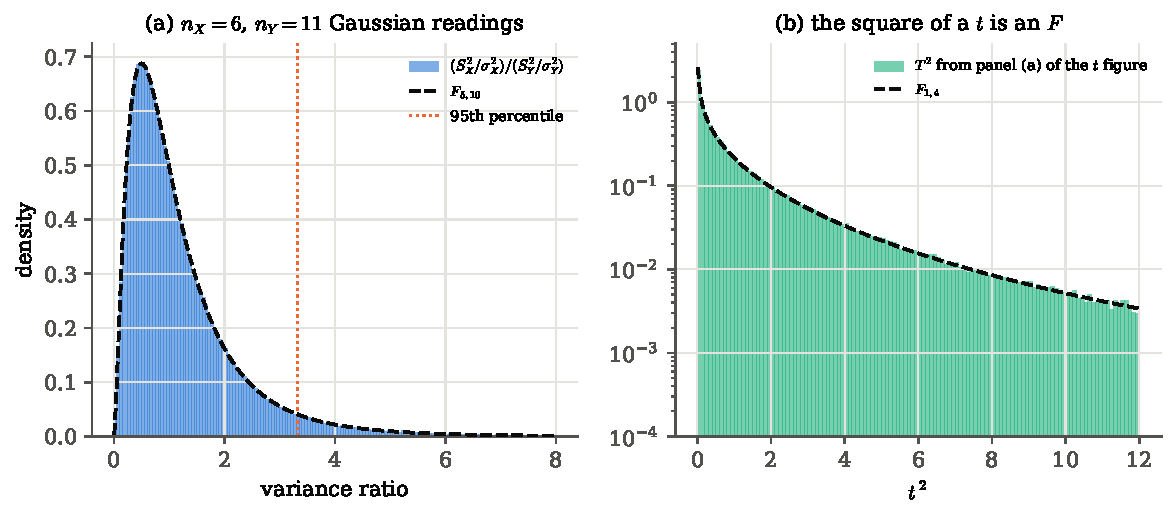
\includegraphics[width=\linewidth]{figures/ch02/f_ratio.pdf}
\caption{(a) The ratio of two scaled sample variances, from six and eleven Gaussian readings, follows $F_{5,10}$ (dashed); the dotted line marks its 95th percentile. (b) The squares of the studentised means of the pendulum experiment follow $F_{1,4}$, on a logarithmic scale that shows the power-law tail.}
\label{2b:fig:F}
\end{figure}

\paragraph{Where the ratios come back.} Every exact small-sample test in classical statistics is built on one pattern: a Gaussian or a $\chi^2$, divided by an independent $\chi^2$ that estimates the unknown scale. Examples are the $t$ test for a mean, the two-sample $t$ test, the $F$ test for the equality of variances, and the $F$ test that compares a model with a nested model having extra parameters by the ratio of $\chi^2$ improvements. These are the subject of \cref{ch:04}. Bayesian inference (\cref{ch:05}) arrives at the same $t_{n-1}$. Integrating an unknown Gaussian $\sigma$ out of the posterior for $\mu$, with the prior $p(\sigma)\propto1/\sigma$, produces it \srcref{Sivia}{p.~56--57, (3.43)--(3.44)}. The fattening of the tails is the price of not knowing the noise level, whichever school of inference pays it.
\section{The rest of the zoo, each with the machine that makes it}
\label{2b:sec:zoo}

Almost every distribution a physicist meets is produced by a small machine built from the ones we already have: a uniform phase, a sum, a product, a length, a ratio, a sorting. So a table of distributions is not a list of unrelated formulas. Recognising the machine lets us choose the right distribution for a new problem, and it tells us when a distribution will fail. Each remaining common continuous distribution is treated the same way: the machine, the density derived from it, the summary numbers, and a check by running the machine in Python.

The question for every entry, in words: \emph{which physical mechanism produces this distribution, and what does the mechanism predict for its shape, its mean and its spread?}

\subsection{Uniform: complete ignorance within a range}
\label{2b:sec:uniform}

A charged particle crosses a silicon strip detector whose strips have pitch $w=50\,\mu$m, and only the strip that fired is recorded. Where in the strip did the particle pass? With no further information every position is equally likely. The same holds for a phase that has been scrambled, the rounding error of a digitiser, or the position of an event within a time bin. All are \newterm{uniform}: $X\sim\mathrm U(a,b)$ has density $1/(b-a)$ on $[a,b]$ \srcref{CasellaBerger}{p.~81}. It is the maximum-entropy assignment when only the range is known (\cref{2b:sec:maxent-family}). Its moments are
\begin{align}
  \E X&\eqby{1}\int_a^b\frac{x}{b-a}\,\dd x=\frac{b^2-a^2}{2(b-a)}=\frac{a+b}{2}, \nonumber\\
  \Var X&\eqby{2}\int_a^b\frac{(x-\frac{a+b}2)^2}{b-a}\,\dd x
   \eqby{3}\frac{1}{b-a}\int_{-(b-a)/2}^{(b-a)/2}u^2\,\dd u=\frac{(b-a)^2}{12} .
  \label{2b:eq:uniform}
\end{align}
\begin{explain}
  \item Definition of the mean, and $b^2-a^2=(b-a)(b+a)$.
  \item Definition of the variance about the mean just found.
  \item Substitute $u=x-\frac{a+b}{2}$; then $\int_{-h}^hu^2\dd u=\frac{2h^3}{3}$ with $h=\frac{b-a}2$, which gives $\frac{(b-a)^3}{12}$.
\end{explain}
So the strip detector has a position resolution of $w/\sqrt{12}=14.4\,\mu$m, the famous ``pitch over root twelve'', and a digitiser with step $\Delta$ adds quantisation noise of variance $\Delta^2/12$.

The uniform distribution is also the parent of all others: any continuous variable can be made from a uniform one, and turned back into one. If $X$ is continuous with cumulative distribution function $F$, then $U=F(X)$ is uniform on $[0,1]$, because
\[
  \Prob(U\le u)\eqby{1}\Prob\bigl(X\le F^{-1}(u)\bigr)\eqby{2}F\bigl(F^{-1}(u)\bigr)=u ,
\]
where (1) uses that $F$ is increasing and (2) is the definition of $F$. Read backwards, $X=F^{-1}(U)$ turns uniform random numbers into draws from any distribution: this is inverse-transform sampling, the first tool of \cref{ch:06}. Read forwards, it says that a $\pval$-value, which is $1-F$ of the observed statistic under $\Hnull$, is uniformly distributed when $\Hnull$ is true (\cref{ch:04}).

\subsection{Exponential, gamma and Weibull: waiting and adding}
\label{2b:sec:gamma}

The exponential and gamma distributions were derived in \cref{2a:sec:waiting} from the Poisson process with rate $\lambda$: the wait for the first event is Exp$(\lambda)$, and the wait for the $n$-th event is Gamma$(n,1/\lambda)$, the Erlang density \eqref{2a:eq:erlang}. The characteristic function \eqref{2b:eq:gamma-cf} shows the whole family at once: gamma variables with a common scale add. Gamma$(\alpha,\beta)$, with shape $\alpha$ and scale $\beta$, has $\phi(k)=(1-i\beta k)^{-\alpha}$, so for independent gamma variables with a common scale
\begin{equation}
  \mathrm{Gamma}(\alpha_1,\beta)+\mathrm{Gamma}(\alpha_2,\beta)=\mathrm{Gamma}(\alpha_1+\alpha_2,\beta),
  \label{2b:eq:gamma-add}
\end{equation}
since $(1-i\beta k)^{-\alpha_1}(1-i\beta k)^{-\alpha_2}=(1-i\beta k)^{-(\alpha_1+\alpha_2)}$ \srcref{CasellaBerger}{Ex.~4.6.8}. Two special lines of the family we have met: Exp$(\lambda)=$ Gamma$(1,1/\lambda)$, and $\chi^2_\nu=$ Gamma$(\nu/2,2)$ \srcref{CasellaBerger}{(3.3.10)--(3.3.11)}. So adding exponential waits and adding squared Gaussians are the same operation seen through different parameters.

The moments follow from a trick called ``recognise the kernel'' \srcref{CasellaBerger}{(3.3.7)--(3.3.8)}: multiplying by $x$ turns one gamma density into another, whose integral we already know. Since the gamma density integrates to one, $\int_0^\infty x^{\alpha-1}e^{-x/\beta}\dd x=\Gamma(\alpha)\beta^\alpha$ for every $\alpha>0$. Then
\begin{align}
  \E X
  &\eqby{1}\frac{1}{\Gamma(\alpha)\beta^\alpha}\int_0^\infty x^{(\alpha+1)-1}e^{-x/\beta}\,\dd x
   \eqby{2}\frac{\Gamma(\alpha+1)\beta^{\alpha+1}}{\Gamma(\alpha)\beta^\alpha}
   \eqby{3}\alpha\beta ,
  \label{2b:eq:gamma-mean}
\end{align}
\begin{explain}
  \item Multiply the density by $x$: the integrand becomes the kernel of a Gamma$(\alpha+1,\beta)$ density.
  \item Its integral is the normalisation of that density.
  \item $\Gamma(\alpha+1)=\alpha\Gamma(\alpha)$.
\end{explain}
and in the same way $\E X^2=\alpha(\alpha+1)\beta^2$, so $\Var X=\alpha\beta^2$. For $\chi^2_\nu$ this gives back $\nu$ and $2\nu$.

A third member of the waiting-time family is the \newterm{Weibull} distribution, $Y=X^{1/\gamma}$ with $X$ exponential \srcref{CasellaBerger}{(3.3.12)}. It is the lifetime of a component whose failure rate $h(t)$ is not constant but grows (or falls) like a power of its age, $h(t)\propto t^{\gamma-1}$. So $\gamma>1$ describes wear-out, $\gamma<1$ infant mortality, and $\gamma=1$ the memoryless exponential. The Weibull is also one of the three limiting laws for the \emph{maximum} of many variables, listed in the taxonomy of \cref{2b:sec:landau}.

As a prior, the gamma distribution is the natural choice for a Poisson rate $\lambda>0$ \srcref{Lambert}{\S8.5.3}. The reason is conjugacy, which Machine~3 of the beta distribution below shows at work.

\subsection{Log-normal: products of many factors}
\label{2b:sec:lognormal}

A photo-electron entering a photomultiplier hits the first dynode and knocks out $g_1$ secondary electrons. Each of these knocks $g_2$ out of the next dynode, and so on through ten stages. The gain is a \emph{product}, $G=g_1g_2\cdots g_{10}$. A product becomes a sum when we take logarithms: $\ln G=\sum_i\ln g_i$ is a sum of independent terms, so the central limit theorem makes $\ln G$ approximately Gaussian \srcref{Cowan}{p.~34--35}. A quantity whose logarithm is Gaussian is \newterm{log-normal}. Whenever an effect acts by multiplication (gains in cascades, fragmentation, growth, the stretching of fluid elements, the luminosity of a galaxy built by many mergers) the log-normal is the default, just as the Gaussian is for additive effects.

If $\ln X=Y\sim\Normal(\mu,\sigma^2)$, then $X=e^Y$ and $\dd y/\dd x=1/x$, so
\begin{equation}
  f(x)\eqby{1} f_Y(\ln x)\,\Bigl|\frac{\dd y}{\dd x}\Bigr|\eqby{2}\frac{1}{\sqrt{2\pi\sigma^2}}\,\frac1x\,\exp\Bigl[-\frac{(\ln x-\mu)^2}{2\sigma^2}\Bigr],\qquad x>0,
  \label{2b:eq:lognormal}
\end{equation}
\begin{explain}
  \item The one-dimensional change of variables.
  \item Insert the Gaussian density for $Y=\ln x$ \srcref{Cowan}{(2.31)}, \srcref{CasellaBerger}{(3.3.21)}.
\end{explain}
The parameters $\mu$ and $\sigma^2$ are the mean and variance of $\ln X$, not of $X$. The moments of $X$ come from the Gaussian moment generating function $\E e^{rY}$:
\begin{align}
  \E X^r=\E e^{rY}
  &\eqby{1}\int_{-\infty}^{\infty}\frac{1}{\sqrt{2\pi\sigma^2}}\exp\Bigl[ry-\frac{(y-\mu)^2}{2\sigma^2}\Bigr]\dd y \nonumber\\
  &\eqby{2}e^{r\mu+r^2\sigma^2/2}\int_{-\infty}^{\infty}\frac{1}{\sqrt{2\pi\sigma^2}}\exp\Bigl[-\frac{(y-\mu-r\sigma^2)^2}{2\sigma^2}\Bigr]\dd y
   \eqby{3}e^{r\mu+r^2\sigma^2/2} .
  \label{2b:eq:lognormal-moments}
\end{align}
\begin{explain}
  \item $X^r=e^{rY}$, integrated against the density of $Y$.
  \item Complete the square: $ry-\frac{(y-\mu)^2}{2\sigma^2}=-\frac{(y-\mu-r\sigma^2)^2}{2\sigma^2}+r\mu+\frac{r^2\sigma^2}{2}$, as expanding both sides confirms.
  \item The remaining integral is a normalised Gaussian centred at $\mu+r\sigma^2$.
\end{explain}
So $\E X=e^{\mu+\sigma^2/2}$ and $\Var X=\E X^2-(\E X)^2=e^{2\mu+\sigma^2}(e^{\sigma^2}-1)$ \srcref{Cowan}{(2.32)--(2.33)}. The median is $e^\mu$, because $\ln$ is monotonic and the median of $Y$ is $\mu$. So mean $>$ median $>$ mode $=e^{\mu-\sigma^2}$: a long tail to the right.

\paragraph{Example: the gain of a ten-stage photomultiplier.} The script gives each of $\tbLNndyn$ dynodes an independent uniform multiplication factor $g_i\sim\mathrm U(3,5)$, draws $4\times10^5$ gains, and compares with the log-normal predicted by the CLT applied to $\ln G$.

\pyfile[firstline=35,lastline=48,firstnumber=35]{code/ch02/27_zoo_lognormal_maxwell.py}{The gain of a ten-dynode photomultiplier}

Lines 36--38 run the machine: multiply ten factors, take the log. Lines 42--45 compute the CLT prediction exactly. For a uniform $g$, $\E\ln g$ and $\E(\ln g)^2$ are elementary integrals ($\int\ln g\,\dd g=g\ln g-g$ and $\int(\ln g)^2\dd g=g[(\ln g)^2-2\ln g+2]$). The mean and variance of $\ln G$ are ten times those of $\ln g$. The prediction is $\mu=\tbLNmu$, $\sigma=\tbLNs$; the simulated $\ln G$ has mean $\tbLNlnMean$ and standard deviation $\tbLNlnSd$.

The gain itself is strongly skewed: its skewness is $\tbLNskew$, while $\ln G$ has $\tbLNskewLn$. Its median is $\tbLNmedian\times10^6$ against $e^\mu=\tbLNmedianTh\times10^6$, and its mean is $\tbLNmean\times10^6$, matching the log-normal $e^{\mu+\sigma^2/2}=\tbLNmeanTh\times10^6$ and the exact $\E G=(\E g)^{10}=4^{10}=\tbLNmeanExact\times10^6$ (\cref{2b:fig:lognormal}).

\begin{figure}[htbp]
\centering
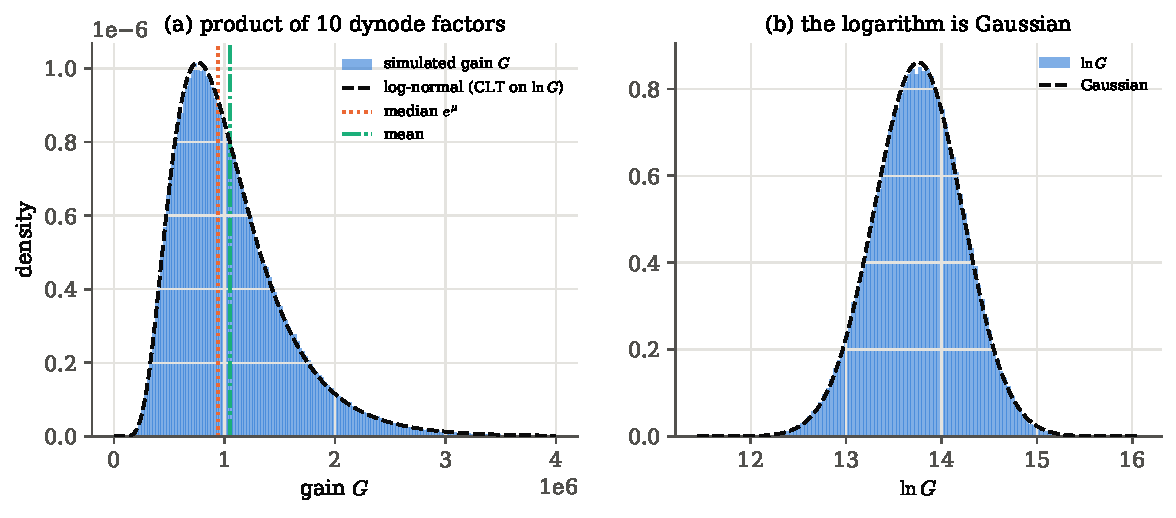
\includegraphics[width=\linewidth]{figures/ch02/zoo_lognormal.pdf}
\caption{(a) The simulated gain of a ten-stage photomultiplier (histogram) and the log-normal predicted by applying the central limit theorem to $\ln G$ (dashed). The median $e^\mu$ (dotted) lies well below the mean (dash-dotted). (b) The same gains on a logarithmic axis: a symmetric Gaussian.}
\label{2b:fig:lognormal}
\end{figure}

\begin{pitfall}[Averaging logarithms gives the median, not the mean]
For a log-normal quantity, $\exp(\overline{\ln x})$ estimates the median $e^\mu$, which is smaller than the mean by the factor $e^{\sigma^2/2}$ ($11\%$ for the photomultiplier). Fitting a straight line to $\ln x$ and exponentiating the prediction has the same bias. Decide which of the two you need, and correct by $e^{\sigma^2/2}$ if it is the mean.
\end{pitfall}

\subsection{Rayleigh and Maxwell--Boltzmann: the length of a Gaussian vector}
\label{2b:sec:maxwell}

The velocity components $(v_x,v_y,v_z)$ of an argon atom in a gas at temperature $T$ are independent Gaussians with mean zero and variance $s^2=k_BT/m$ (this is the MaxEnt result of \cref{2b:sec:maxent-family}, or the Boltzmann factor $e^{-mv^2/2k_BT}$). The \emph{speed} $v=|\bm v|$ is the length of a three-dimensional Gaussian vector. We derived its distribution in all but name in the geometric route to $\chi^2$: the density of $\bm v$ is $(2\pi s^2)^{-3/2}e^{-v^2/2s^2}$, and the volume of the shell at radius $v$ is $S_2v^2\dd v=4\pi v^2\dd v$. Hence
\begin{equation}
  f(v)\eqby{1}4\pi v^2\,\frac{e^{-v^2/2s^2}}{(2\pi s^2)^{3/2}}\eqby{2}\sqrt{\frac2\pi}\;\frac{v^2}{s^3}\;e^{-v^2/2s^2},\qquad v>0 ,
  \label{2b:eq:maxwell}
\end{equation}
\begin{explain}
  \item The shell argument of \eqref{2b:eq:sphere-area} with $\nu=3$.
  \item $4\pi/(2\pi)^{3/2}=\sqrt{2/\pi}$.
\end{explain}
This is the Maxwell--Boltzmann speed distribution. Equivalently, $v^2/s^2\sim\chi^2_3$. Its three landmark speeds, the most probable, the rms and the mean, are
\begin{align}
  v_{\mathrm{mode}}&\eqby{1}\sqrt2\,s=\sqrt{\frac{2k_BT}{m}},\qquad
  v_{\mathrm{rms}}\eqby{2}\sqrt3\,s , \nonumber\\
  \E v&\eqby{3}\sqrt{\frac2\pi}\,\frac{1}{s^3}\int_0^\infty v^3e^{-v^2/2s^2}\dd v\eqby{4}\sqrt{\frac8\pi}\,s=\sqrt{\frac{8k_BT}{\pi m}} .
  \label{2b:eq:maxwell-moments}
\end{align}
\begin{explain}
  \item $\frac{\dd}{\dd v}\bigl(v^2e^{-v^2/2s^2}\bigr)=\bigl(2v-v^3/s^2\bigr)e^{-v^2/2s^2}=0$ at $v^2=2s^2$.
  \item $\E v^2=s^2\,\E\chi^2_3=3s^2$: equipartition, $\frac12m\E v^2=\frac32k_BT$.
  \item Definition of the mean.
  \item With $t=v^2/2s^2$, $\int_0^\infty v^3e^{-v^2/2s^2}\dd v=2s^4\int_0^\infty te^{-t}\dd t=2s^4$, and $\sqrt{2/\pi}\cdot2s=\sqrt{8/\pi}\,s$.
\end{explain}
For argon at $300$\,K the script finds $s=\tbMBsv$\,m/s, and from $4\times10^5$ simulated atoms a mean speed of $\tbMBmean$\,m/s (theory $\tbMBmeanTh$), with the mode at $\tbMBmodeTh$ and the rms speed at $\tbMBrms$ (theory $\tbMBrmsTh$) (\cref{2b:fig:rayleigh}b).

In two dimensions the shell has circumference $2\pi r$, and the same argument gives the \newterm{Rayleigh} distribution
\begin{equation}
  f(r)=\frac{r}{s^2}\,e^{-r^2/2s^2},\qquad \E r=s\sqrt{\pi/2},\qquad r^2\sim s^2\chi^2_2 ,
  \label{2b:eq:rayleigh}
\end{equation}
and the squared length $r^2$ is \emph{exponential} with mean $2s^2$, since $\chi^2_2=$ Gamma$(1,2)$. Of all the cases in this book, this one reaches furthest. A complex Gaussian mode $z=x+iy$, with independent real and imaginary parts of equal variance, has a Rayleigh amplitude $|z|$, a uniform phase, and an exponential power $|z|^2$. That describes a Fourier mode $\tilde\delta(\bm k)$ of a Gaussian random field (\cref{ch:07}), each $\alm$ with $m\neq0$ on the CMB sky, and each frequency bin of Gaussian detector noise in a gravitational-wave periodogram.

\emph{What follows for the scatter of a measured power?} The exponential has standard deviation equal to its mean. So a raw periodogram fluctuates by $100\%$ in every bin, however long the data stream. Only averaging reduces the scatter: over bins or segments (Welch's method), or over the $2\ell+1$ values of $m$, which gives the cosmic variance of \cref{2b:sec:chi2-many}. The script checks the unit-variance case: $\E|z|=\tbRAYmean$ against $\sqrt{\pi/2}=\tbRAYmeanTh$, and $|z|^2$ has mean $\tbPOWmean$ and standard deviation $\tbPOWsd$, both $2$ for an exponential (\cref{2b:fig:rayleigh}a).

\begin{figure}[htbp]
\centering
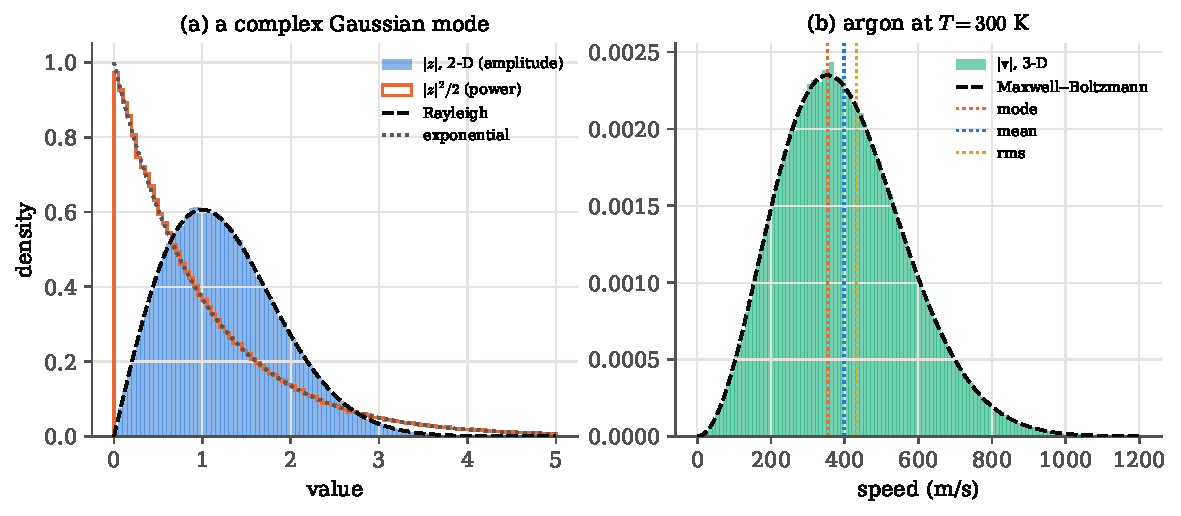
\includegraphics[width=\linewidth]{figures/ch02/zoo_rayleigh_maxwell.pdf}
\caption{(a) The amplitude of a complex Gaussian mode follows the Rayleigh density, and half its squared amplitude, the power, follows a unit exponential. (b) Speeds of simulated argon atoms at $300$\,K against the Maxwell--Boltzmann law, with the mode, the mean and the rms speed marked in that order.}
\label{2b:fig:rayleigh}
\end{figure}

\subsection{Beta: probabilities of probabilities}
\label{2b:sec:beta}

The distributions so far describe data. The beta distribution usually describes a \emph{probability}: the efficiency of a trigger, the bias of a coin, the fraction of events that are signal. It lives on $[0,1]$ and has density \srcref{CasellaBerger}{(3.3.16)}, \srcref{Kruschke}{(6.3)}
\begin{equation}
  f(\theta\given a,b)=\frac{\theta^{a-1}(1-\theta)^{b-1}}{B(a,b)},\qquad
  B(a,b)=\int_0^1\theta^{a-1}(1-\theta)^{b-1}\dd\theta=\frac{\Gamma(a)\Gamma(b)}{\Gamma(a+b)} .
  \label{2b:eq:beta}
\end{equation}
It is produced by three different machines, and each explains something.

\paragraph{Machine 1: sorting uniform numbers.} Draw $n$ independent uniform numbers on $[0,1]$ and let $U_{(k)}$ be the $k$-th smallest, the $k$-th \newterm{order statistic}. For $U_{(k)}$ to lie in $[u,u+\dd u]$, one of the $n$ numbers must fall in that interval, $k-1$ of them below $u$ and $n-k$ above it. The number of ways to choose which is which is the multinomial coefficient $\frac{n!}{(k-1)!\,1!\,(n-k)!}$ of \cref{2a:sec:multinomial}, and the probabilities of the three cells are $u$, $\dd u$ and $1-u$. So
\begin{equation}
  f_{U_{(k)}}(u)\,\dd u=\frac{n!}{(k-1)!\,(n-k)!}\,u^{k-1}(1-u)^{n-k}\,\dd u ,
  \label{2b:eq:orderstat}
\end{equation}
which is Beta$(k,n-k+1)$, with $B(k,n-k+1)=\frac{(k-1)!(n-k)!}{n!}$ \srcref{CasellaBerger}{Ex.~5.4.5}. For a general continuous parent with cumulative distribution $F$ and density $f$, the same count gives $\frac{n!}{(k-1)!(n-k)!}F(x)^{k-1}[1-F(x)]^{n-k}f(x)$ \srcref{CasellaBerger}{Thm~5.4.4}. Casella and Berger prove it by differentiating the binomial probability that at least $k$ of the $n$ values lie below $x$. The same counting gives the joint density of two order statistics, and from it the distribution of the range $U_{(n)}-U_{(1)}\sim$ Beta$(n-1,2)$ \srcref{CasellaBerger}{Thm~5.4.6, Ex.~5.4.7}. 

Order statistics describe the median, quantiles, the fastest of $n$ photon arrival times (which sets the timing of a scintillator), and the largest of $n$ noise fluctuations (the look-elsewhere effect of \cref{ch:04}). With $n=\tbOSn$ and $k=\tbOSk$ the script finds the mean and variance of $U_{(3)}$ to be $\tbOSmean$ and $\tbOSvar$, against $\frac{k}{n+1}=\tbOSmeanTh$ and $\frac{k(n-k+1)}{(n+1)^2(n+2)}=\tbOSvarTh$ (\cref{2b:fig:beta-origins}a).

\paragraph{Machine 2: the share of a total.} Let $X\sim$ Gamma$(a,1)$ and $Y\sim$ Gamma$(b,1)$ be independent. They could be the waiting times for the $a$-th and the $b$-th events of two independent unit-rate processes, or two $\chi^2$ variables. What is the distribution of the share $U=X/(X+Y)$? Change variables to $S=X+Y$ and $U$, so $X=SU$, $Y=S(1-U)$, with Jacobian $\bigl|\partial(x,y)/\partial(s,u)\bigr|=s$:
\begin{align}
  f(u,s)
  &\eqby{1}s\;\frac{(su)^{a-1}e^{-su}}{\Gamma(a)}\;\frac{(s(1-u))^{b-1}e^{-s(1-u)}}{\Gamma(b)} \nonumber\\
  &\eqby{2}\underbrace{\frac{\Gamma(a+b)}{\Gamma(a)\Gamma(b)}\,u^{a-1}(1-u)^{b-1}}_{\text{Beta}(a,b)}\;\times\;\underbrace{\frac{s^{a+b-1}e^{-s}}{\Gamma(a+b)}}_{\text{Gamma}(a+b,1)} .
  \label{2b:eq:gamma-ratio}
\end{align}
\begin{explain}
  \item The joint density of independent $X$ and $Y$ at $x=su$, $y=s(1-u)$, times the Jacobian. The determinant of $\begin{pmatrix}u&s\\1-u&-s\end{pmatrix}$ is $-us-s(1-u)=-s$.
  \item Collect powers: $s\cdot s^{a-1}s^{b-1}=s^{a+b-1}$, and $e^{-su}e^{-s(1-u)}=e^{-s}$. Multiply and divide by $\Gamma(a+b)$.
\end{explain}
The density factorises, so the share $U$ is Beta$(a,b)$ and is \emph{independent} of the total $S$. As a by-product, the second factor integrates to one, so the first must too, which proves $B(a,b)=\Gamma(a)\Gamma(b)/\Gamma(a+b)$ \srcref{CasellaBerger}{(3.3.17)}. With $a=2.5$, $b=4$ the script finds $\E U=\tbGRmean$ against $a/(a+b)=\tbGRmeanTh$ (\cref{2b:fig:beta-origins}b). The relation of $F$ to the beta distribution in \cref{2b:sec:F} is this machine applied to two $\chi^2$ variables.

\paragraph{Summary numbers and shapes.} Recognising kernels again, $\E\theta^r=B(a+r,b)/B(a,b)$ \srcref{CasellaBerger}{(3.3.18)}, so
\begin{equation}
  \E\theta=\frac{a}{a+b},\qquad \Var\theta=\frac{ab}{(a+b)^2(a+b+1)},\qquad \text{mode}=\frac{a-1}{a+b-2}\ \ (a,b>1).
  \label{2b:eq:beta-moments}
\end{equation}
The two shape parameters make the family flexible (\cref{2b:fig:beta-shapes}). It is uniform for $a=b=1$, U-shaped for $a,b<1$, J-shaped when one of them is below one, and single-peaked for $a,b>1$. It is symmetric when $a=b$, with variance $1/[4(2a+1)]$.

\emph{How do we choose $a$ and $b$?} Kruschke's advice \srcref{Kruschke}{p.~128--131} is to think of $a$ and $b$ as ``previously seen'' successes and failures. The concentration $\kappa=a+b$ measures how much prior data that is, and
\[
  a=\mu\kappa,\quad b=(1-\mu)\kappa\qquad\text{or}\qquad a=\omega(\kappa-2)+1,\quad b=(1-\omega)(\kappa-2)+1
\]
set the mean $\mu$ or the mode $\omega$ \srcref{Kruschke}{(6.5)--(6.6)}. A prior with mode $0.8$ and concentration $12$ is Beta$(9,3)$. From a desired mean and standard deviation, $a=\mu\nu$ and $b=(1-\mu)\nu$ with $\nu=\mu(1-\mu)/\sigma^2-1$ \srcref{Kruschke}{(6.7)}: mean $0.5$ and standard deviation $0.1$ give Beta$(12,12)$. The standard deviation must be below $1/\sqrt{12}=0.289$, that of the uniform, or the formula returns a U-shaped (or impossible) answer.

\begin{figure}[htbp]
\centering
\begin{tikzpicture}
\begin{axis}[width=11cm,height=5.4cm,xmin=0,xmax=1,ymin=0,ymax=4.4,
    xlabel={$\theta$},ylabel={density},
    tick label style={font=\scriptsize},label style={font=\small},
    legend style={font=\scriptsize,at={(0.5,-0.32)},anchor=north,draw=none,fill=none},
    legend columns=2,legend cell align=left]
  \addplot[softgray,thick,domain=0.012:0.988,samples=200] {1/(pi*sqrt(x*(1-x)))};
  \addlegendentry{Beta$(\frac12,\frac12)$: U-shaped}
  \addplot[black,thick,dashed,domain=0:1,samples=2] {1};
  \addlegendentry{Beta$(1,1)$: uniform}
  \addplot[fibreorange,thick,domain=0:1,samples=200] {30*x*(1-x)^4};
  \addlegendentry{Beta$(2,5)$}
  \addplot[formblue,thick,domain=0:1,samples=200] {495*x^8*(1-x)^2};
  \addlegendentry{Beta$(9,3)$: mode $0.8$, $\kappa=12$}
  \addplot[tangentgreen,thick,domain=0:1,samples=200] {16224936*x^11*(1-x)^11};
  \addlegendentry{Beta$(12,12)$: mean $0.5$, sd $0.1$}
\end{axis}
\end{tikzpicture}
\caption{Members of the beta family. With both parameters below one the density piles up at the ends; with both equal to one it is flat; above one it has a single peak whose position is set by the ratio of the parameters and whose width shrinks as their sum grows. The blue and green curves are Kruschke's two worked prior specifications.}
\label{2b:fig:beta-shapes}
\end{figure}

\begin{workdef}[beta distribution]
$\theta\sim$ Beta$(a,b)$, $a,b>0$, has density \eqref{2b:eq:beta} on $[0,1]$ and moments \eqref{2b:eq:beta-moments}.
\emph{Recognise it by:} a probability or a fraction that is itself uncertain. It is the $k$-th smallest of $n$ uniform numbers (Beta$(k,n-k+1)$), the share $X/(X+Y)$ of two independent gamma variables with a common scale (Beta$(a,b)$), and, as shown next, the updated belief about a success probability after $a-1$ successes and $b-1$ failures observed from a flat start \unpack{with prior Beta$(a_0,b_0)$ and $h$ successes in $N$ trials the result is Beta$(a_0+h,b_0+N-h)$}.
\end{workdef}

\paragraph{Machine 3: keep the runs that match.} The third machine is inference itself. A coin has unknown bias $\theta$. Before flipping it, our belief about $\theta$ is Beta$(2,2)$: probably near a half, but anything is possible. \emph{The event.} We flip it $N=10$ times and see $h=7$ heads. \emph{The question.} Which values of $\theta$ could have produced seven heads, and how strongly should we now believe in each? Let the computer answer by brute force, with no formula at all. Draw $\theta$ from the prior; flip a coin with that $\theta$ ten times; keep $\theta$ if and only if the run produced exactly seven heads; repeat.

\pyfile[firstline=44,lastline=50,firstnumber=44]{code/ch02/28_beta_dirichlet.py}{Keep the runs that match: a posterior by rejection}

Line 46 draws two million values of $\theta$ from the prior. Line 47 runs the \emph{forward} model, the prediction direction of \cref{ch:01}: for each $\theta$, simulate the experiment. Line 48 keeps only those $\theta$ that reproduced the data, which is conditioning on the observation, the inference direction. The histogram of the kept values is the answer (\cref{2b:fig:beta-origins}c). \emph{What is it analytically?} Take the candidate values of $\theta$ one at a time. A given $\theta$ is kept with the binomial probability of the data, $\binom{10}{7}\theta^7(1-\theta)^3$. It was drawn in the first place with the prior density. So the kept values have density proportional to the product of the two,
\[
  \underbrace{\theta(1-\theta)}_{\text{Beta}(2,2)\text{ kernel}}\times\underbrace{\theta^7(1-\theta)^3}_{\text{probability of the data}}=\theta^{8}(1-\theta)^{4},
\]
the kernel of Beta$(9,5)$. In general, prior Beta$(a_0,b_0)$ and binomial data give Beta$(a_0+h,b_0+N-h)$. The family is \newterm{conjugate} to the binomial: prior and posterior belong to the same family. And ``$a$ and $b$ are previous successes and failures'' is literally true. The script's kept values have mean $\tbRJmean$ and standard deviation $\tbRJsd$, against $\frac{9}{14}=\tbRJmeanTh$ and $\tbRJsdTh$.

The acceptance fraction has a meaning too. It is $\tbRJacc$, the probability of seeing seven heads averaged over the prior, $\binom{10}{7}B(9,5)/B(2,2)=\tbRJaccTh$. That is the \emph{evidence}, the denominator of Bayes' theorem. So this little machine is the whole of \cref{ch:05} in miniature. Rejection wastes $89\%$ of the draws here. It would waste nearly all of them for a continuous observation or many parameters, which is why \cref{ch:09} replaces it by Markov chain Monte Carlo. The same logic makes the gamma distribution conjugate to the Poisson rate: a Gamma$(\alpha,\beta)$ prior times the Poisson likelihood $\lambda^ne^{-\lambda}$ is again a gamma kernel.

\begin{figure}[htbp]
\centering
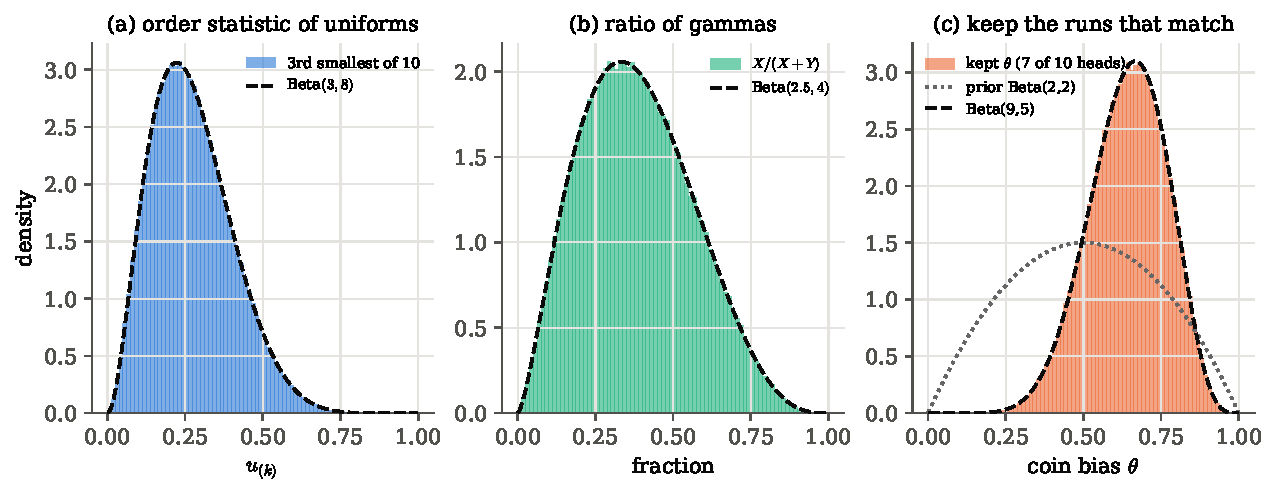
\includegraphics[width=\linewidth]{figures/ch02/beta_origins.pdf}
\caption{Three machines that make a beta distribution. (a) The third smallest of ten uniform numbers. (b) The share $X/(X+Y)$ of two independent gamma variables. (c) Coin biases drawn from a Beta$(2,2)$ prior (dotted) and kept only when their simulated ten flips gave seven heads: the survivors follow Beta$(9,5)$.}
\label{2b:fig:beta-origins}
\end{figure}

\subsection{Dirichlet: several probabilities that sum to one}
\label{2b:sec:dirichlet}

A histogram with $K$ bins has bin probabilities $p_1,\dots,p_K$ with $\sum_jp_j=1$; an election has vote shares; a decay has branching ratios. The distribution for such a vector is the \newterm{Dirichlet}, and the gamma machine of \eqref{2b:eq:gamma-ratio} (Machine~2, the share of a total) builds it. Draw independent $G_j\sim$ Gamma$(\alpha_j,1)$, $j=1,\dots,K$, and normalise, $p_j=G_j/\sum_lG_l$. The same change of variables, now with $K$ variables, gives the density on the simplex \unpack{the set of vectors with all $p_j\ge0$ and $\sum_jp_j=1$, a triangle for $K=3$}
\begin{equation}
  f(p_1,\dots,p_K)=\frac{\Gamma(\alpha_0)}{\prod_j\Gamma(\alpha_j)}\prod_{j=1}^Kp_j^{\alpha_j-1},\qquad \alpha_0=\sum_j\alpha_j ,
  \label{2b:eq:dirichlet}
\end{equation}
which reduces to the beta for $K=2$. Its properties follow from the machine without any integration. \emph{Marginals.} One component is $p_1=G_1/(G_1+R)$ with $R=\sum_{j\ge2}G_j\sim$ Gamma$(\alpha_0-\alpha_1,1)$ by \eqref{2b:eq:gamma-add}, so by machine 2 each marginal is a beta,
\[
  p_j\sim\text{Beta}(\alpha_j,\alpha_0-\alpha_j),\qquad \E p_j=\frac{\alpha_j}{\alpha_0},\qquad \Var p_j=\frac{\alpha_j(\alpha_0-\alpha_j)}{\alpha_0^2(\alpha_0+1)} .
\]
\emph{Covariances.} These follow from the constraint $\sum_jp_j=1$. For $K=3$, $p_1+p_2=1-p_3$, so
\begin{align}
  2\Cov(p_1,p_2)
  &\eqby{1}\Var p_3-\Var p_1-\Var p_2 \nonumber\\
  &\eqby{2}\frac{\alpha_3(\alpha_0-\alpha_3)-\alpha_1(\alpha_0-\alpha_1)-\alpha_2(\alpha_0-\alpha_2)}{\alpha_0^2(\alpha_0+1)}
   \eqby{3}\frac{-2\alpha_1\alpha_2}{\alpha_0^2(\alpha_0+1)} .
  \label{2b:eq:dirichlet-cov}
\end{align}
\begin{explain}
  \item $\Var(p_1+p_2)=\Var(1-p_3)=\Var p_3$, and $\Var(p_1+p_2)=\Var p_1+\Var p_2+2\Cov(p_1,p_2)$.
  \item Insert the beta variances.
  \item Write $s=\alpha_1+\alpha_2$, so $\alpha_3=\alpha_0-s$. The numerator is $(\alpha_0-s)s-\alpha_1(\alpha_0-\alpha_1)-\alpha_2(\alpha_0-\alpha_2)=-s^2+\alpha_1^2+\alpha_2^2=-2\alpha_1\alpha_2$.
\end{explain}
So $\Cov(p_i,p_j)=-\alpha_i\alpha_j/[\alpha_0^2(\alpha_0+1)]$ for $i\neq j$ (for $K>3$ lump the other components into one, which is again gamma), the same negative-correlation pattern as the multinomial counts of \eqref{2a:eq:multcov}: if one share grows, the others must shrink.

For Lambert's three-party election with Dirichlet$(4,2,2)$ \srcref{Lambert}{\S8.5.1}, the script finds $\E p_1=\tbDIRmeanOne$ ($\tbDIRmeanOneTh$), $\Var p_1=\tbDIRvarOne$ ($\tbDIRvarOneTh$) and $\Cov(p_1,p_2)=\tbDIRcov$ ($\tbDIRcovTh$) (\cref{2b:fig:dirichlet}). Two facts decide when to use it. It is conjugate to the multinomial, exactly as the beta is to the binomial: prior Dirichlet$(\bm\alpha)$ and bin counts $\bm n$ give Dirichlet$(\bm\alpha+\bm n)$. And, as Lambert warns, its correlations are all fixed by the $\alpha$'s, so it cannot express a belief such as ``if party 2 does well, so does party 3''; logistic-normal priors are used when that matters.

\begin{figure}[htbp]
\centering
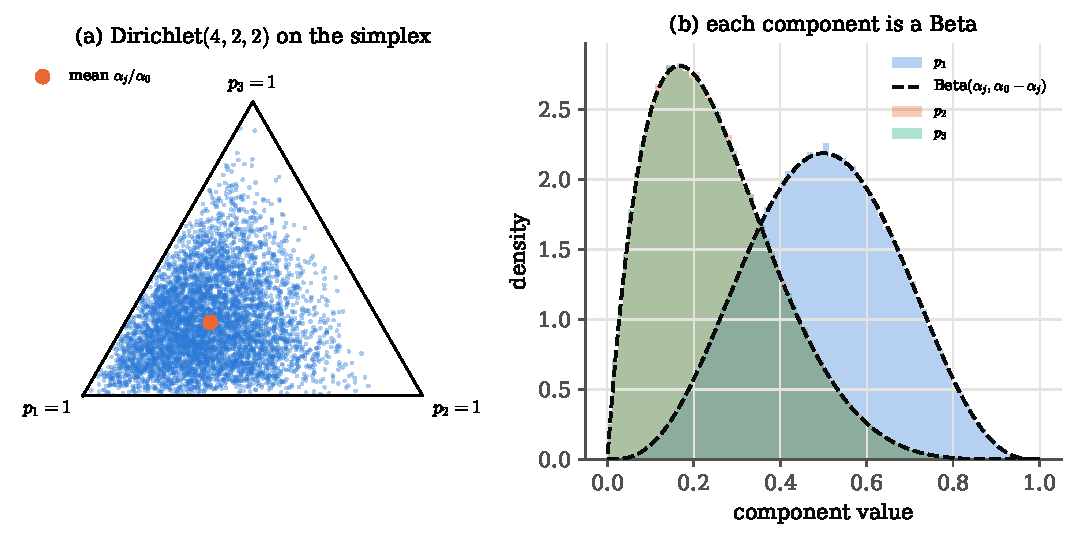
\includegraphics[width=\linewidth]{figures/ch02/dirichlet.pdf}
\caption{(a) Draws from Dirichlet$(4,2,2)$ on the triangle of possible vote shares: each corner is one party winning everything, and the cloud sits nearer the corner of the party with the largest $\alpha$. (b) Each share on its own follows a beta distribution (dashed curves).}
\label{2b:fig:dirichlet}
\end{figure}

\subsection{Two relatives from earlier sections}
\label{2b:sec:relatives}

Two more distributions complete the zoo, and both have appeared already. The \newterm{Laplace} or double-exponential density $\frac{1}{2\sigma}e^{-|x-\mu|/\sigma}$, with $\Var=2\sigma^2$ \srcref{CasellaBerger}{(3.3.22)--(3.3.23)}, was the MaxEnt answer for a known mean absolute deviation. Its machine is the difference of two independent exponential waits with the same mean $\sigma$. To check, multiply the characteristic functions: $(1-i\sigma k)^{-1}(1+i\sigma k)^{-1}=(1+\sigma^2k^2)^{-1}$, which is the transform of the Laplace density. It has a cusp at the centre and exponential tails, fatter than Gaussian but with all moments finite. The \newterm{Cauchy} (Breit--Wigner) distribution of \cref{2b:sec:cauchy} has three machines: the line shape of an unstable state, the ratio of two independent standard normals \srcref{CasellaBerger}{p.~89}, and Student's $t_1$. Its location parameter is the median, even though it has no mean \srcref{CasellaBerger}{(3.3.19)--(3.3.20)}.

\paragraph{One family tree.} Stepping back, nearly everything in this part hangs from two roots. From the \emph{Gaussian}: squares give $\chi^2$, lengths give Rayleigh and Maxwell, ratios give $t$, $F$ and Cauchy, exponentials give the log-normal, linear maps give the multivariate normal. From the \emph{exponential} (the waiting time of a Poisson process): sums give the gamma, shares of sums give the beta and the Dirichlet, powers give the Weibull, differences give the Laplace. The two trees meet at $\chi^2_\nu=$ Gamma$(\nu/2,2)$, and $\chi^2_2$ is itself an exponential. \Cref{2b:sec:which} collects them into one table.
\section{Which distribution when}
\label{2b:sec:which}

A new set of numbers arrives: the invariant masses of a few thousand dielectron events, the output of a matched filter running over a month of detector noise, the $\chi^2$ of a fit that took a week to set up. Someone asks what distribution the numbers follow. The tempting answer is to make a histogram and pick whichever curve from the zoo looks closest. The better order is the opposite one. Every distribution of this chapter came out of a machine, and the machine is what we can know before seeing a single number. So the question ``which distribution?'' becomes ``which machine made these numbers?''. The histogram comes afterwards, to check the answer where the check is most demanding: in the tails.

Choosing by machine is a procedure, and it can be written down. The machines fit into one family tree and one table. The procedure works on all three kinds of data the book keeps returning to: collider counts, detector noise and fitted spectra. And it has one firm warning attached: two distributions that agree in mean and variance can disagree by factors of thousands where discoveries are claimed.

\subsection{Reading the mechanism}
\label{2b:sec:which-procedure}

Before fitting any curve, we answer four questions about how the number was made.
\begin{enumerate}[leftmargin=1.6em,itemsep=1pt]
  \item \emph{Is it a count or a continuous measurement?} Counts go to the counting machines of \cref{2a:sec:bernoulli} to \cref{2a:sec:failures}, whose table ends the previous part. Continuous measurements go to this part.
  \item \emph{Which operation produced it?} Adding many small pieces, multiplying many factors, squaring and adding, taking the length of a vector, dividing one random quantity by another, waiting for an event, taking a share of a total, or sorting.
  \item \emph{Are the ingredients independent, and do they have a finite variance?} If the answer is no, the limit theorems that manufacture Gaussians and $\chi^2$'s are switched off, and a Cauchy or a Landau law (\cref{2b:sec:cauchy,2b:sec:landau}) may be what arrives.
  \item \emph{Which part of the distribution will the conclusion rest on?} An average and its error bar use the centre, where almost any sensible model agrees. A $\pval$-value, a discovery claim or a false-alarm rate uses the tail, where models disagree most.
\end{enumerate}
Lambert draws the same procedure as a decision tree for choosing a likelihood \srcref{Lambert}{\S8.6, Fig.~8.33}, and adds the practical advice to err on the side of robustness \srcref{Lambert}{\S8.8}: when unsure, prefer the model with heavier tails (the negative binomial over the Poisson, Student's $t$ over the Gaussian).

Most continuous distributions descend from just two parents, the Gaussian and the exponential. \Cref{2b:fig:family} arranges the machines as two trees \srcref{Lambert}{\S8.3, Fig.~8.1}. Each box names a distribution and, underneath, the operation that makes it from its parent. The Gaussian tree is the world of sums, the exponential tree the world of waiting. The dashed line is the one place where they are literally the same distribution: $\chi^2_\nu=$ Gamma$(\nu/2,2)$, so a sum of $\nu$ squared Gaussians is the wait for the $(\nu/2)$-th event of a Poisson stream of rate $\frac12$. Above both sits the uniform distribution, which by the inverse-transform rule of \cref{2b:sec:uniform} can be turned into any of them.

\begin{figure}[htbp]
\centering
\begin{tikzpicture}[x=0.9cm,y=1cm,
  gbox/.style={draw=formblue,rounded corners=2pt,fill=ideabg,align=center,font=\scriptsize,
               minimum width=1.55cm,minimum height=0.8cm,inner sep=2pt},
  ebox/.style={gbox,draw=fibreorange},
  ubox/.style={gbox,draw=black!55,fill=white},
  garr/.style={->,thick,formblue},
  earr/.style={->,thick,fibreorange},
  uarr/.style={->,thick,black!45}]
  \node[ubox] (U) at (6.6,1.7) {\textbf{uniform} U$(0,1)$\\ $F^{-1}(U)$ gives any law};
  \node[gbox] (G) at (3.2,0) {\textbf{Gaussian}\\ sums (CLT), MaxEnt};
  \node[gbox] (MVN) at (0,-1.8) {\textbf{multivariate}\\ \textbf{normal}\\ linear map};
  \node[gbox] (LN) at (2.15,-1.8) {\textbf{log-normal}\\ exponentiate};
  \node[gbox] (RM) at (4.3,-1.8) {\textbf{Rayleigh},\\ \textbf{Maxwell}\\ length in\\ 2-D, 3-D};
  \node[gbox] (CA) at (6.45,-1.8) {\textbf{Cauchy}\\ ratio of two};
  \node[gbox] (CHI) at (3.2,-3.6) {\textbf{\boldmath$\chi^2_\nu$}\\ sum of $\nu$ squares};
  \node[gbox] (T) at (2.1,-5.4) {\textbf{\boldmath Student $t_\nu$}\\ $Z/\sqrt{\chi^2_\nu/\nu}$\\ ($t_1=$ Cauchy)};
  \node[gbox] (F) at (4.3,-5.4) {\textbf{\boldmath$F_{p,q}$}\\ ratio of two\\ $\chi^2/\text{dof}$};
  \node[ebox] (E) at (10.6,0) {\textbf{exponential}\\ Poisson waits};
  \node[ebox] (GA) at (8.6,-1.8) {\textbf{gamma}\\ sum of waits};
  \node[ebox] (LA) at (10.7,-1.8) {\textbf{Laplace}\\ difference\\ of two};
  \node[ebox] (WE) at (12.8,-1.8) {\textbf{Weibull}\\ power $X^{1/\gamma}$};
  \node[ebox] (BE) at (7.7,-3.6) {\textbf{beta}\\ share $\frac{X}{X+Y}$};
  \node[ebox] (DI) at (9.7,-3.6) {\textbf{Dirichlet}\\ shares of $K$};
  \draw[uarr] (U) -- (G);
  \draw[uarr] (U) -- (E);
  \foreach \c in {MVN,LN,RM,CA,CHI} \draw[garr] (G) -- (\c);
  \draw[garr] (CHI) -- (T);
  \draw[garr] (CHI) -- (F);
  \foreach \c in {GA,LA,WE} \draw[earr] (E) -- (\c);
  \draw[earr] (GA) -- (BE);
  \draw[earr] (GA) -- (DI);
  \draw[tangentgreen,very thick,dashed] (CHI.east) -- (GA.south west);
\end{tikzpicture}
\caption{Two family trees hold most of the continuous zoo. Blue: everything built from Gaussians, with the building operation written under each name. Orange: everything built from the exponential waiting time of a Poisson process. The green dashed line joins $\chi^2_\nu$ and the gamma family, which are the same distribution. The uniform at the top feeds both trees, since any law is $F^{-1}$ of a uniform number.}
\label{2b:fig:family}
\end{figure}

The table collects the continuous machines with their summary numbers and the places they turn up in physics. Every mean and variance in it was derived earlier in the chapter, and the section that derived it also gives the density.

\begin{taxonomy}[which continuous distribution, when]
\centering\footnotesize
\renewcommand{\arraystretch}{1.22}
\begin{tabularx}{\linewidth}{@{}>{\raggedright\arraybackslash}p{3.55cm}>{\raggedright\arraybackslash}p{2.05cm}>{\raggedright\arraybackslash}p{3.0cm}>{\raggedright\arraybackslash}X@{}}
\textbf{mechanism} & \textbf{distribution} & \textbf{mean; variance} & \textbf{physics examples}\\\hline
sum of many small independent pieces with finite variance; or only mean and variance known & $\Normal(\mu,\sigma^2)$ & $\mu$; $\sigma^2$ & measurement and thermal noise, large-$\lambda$ counts, real and imaginary part of a noise Fourier bin\\
linear map $A\bm Z+\bm\mu$ of independent standard normals & $\Normal(\bm\mu,\Cmat)$ & $\bm\mu$; $\Cmat=AA\T$ & correlated parameters, pixels of a Gaussian field, Fisher forecasts\\
only a range known; $F(X)$ of any continuous $X$ & U$(a,b)$ & $\frac{a+b}2$; $\frac{(b-a)^2}{12}$ & strip pitch$/\sqrt{12}$, rounding, random phase, $\pval$-values under $\Hnull$\\
wait for the first event of a constant-rate stream; power of a complex Gaussian mode & Exp$(\lambda)$ & $\frac1\lambda$; $\frac1{\lambda^2}$ & decay times, arrival gaps, periodogram power, $|\alm|^2$\\
sum of $\alpha$ waits; $\chi^2$ with a scale & Gamma$(\alpha,\beta)$ & $\alpha\beta$; $\alpha\beta^2$ & time to the $n$-th photon, prior on a Poisson rate\\
failure rate a power of age & Weibull, $Y=X^{1/\gamma}$, $X\sim$ Exp$(1)$ & $\Gamma(1+\frac1\gamma)$; $\Gamma(1+\frac2\gamma)-\Gamma(1+\frac1\gamma)^2$ & lifetimes of tubes and electronics, extremes\\
product of many positive independent factors & log-normal, $\ln X\sim\Normal(\mu,\sigma^2)$ & $e^{\mu+\sigma^2/2}$; $e^{2\mu+\sigma^2}(e^{\sigma^2}-1)$ & photomultiplier gain, log-normal density-field models\\
sum of $\nu$ squared independent standard normals & $\chi^2_\nu$ & $\nu$; $2\nu$ & goodness of fit, $(n-1)S^2/\sigma^2$, $\Chat$ and cosmic variance\\
length of a 2-D / 3-D Gaussian vector (scale $s$) & Rayleigh / Maxwell & $s\sqrt{\pi/2}$; $(2-\frac\pi2)s^2$ \;/\; $s\sqrt{8/\pi}$; $(3-\frac8\pi)s^2$ & Fourier amplitudes, matched-filter SNR in noise / molecular speeds\\
Gaussian over an independently estimated scale & Student $t_\nu$ & $0$ ($\nu>1$); $\frac{\nu}{\nu-2}$ ($\nu>2$) & mean with an estimated error bar, likelihood robust to outliers\\
ratio of two independent $\chi^2/\text{dof}$ & $F_{p,q}$ & $\frac{q}{q-2}$ ($q>2$) & comparing two resolutions, nested fits\\
resonance line shape; ratio of two normals & Cauchy (Breit--Wigner) & none; none (median $M$, half-width $\gamma$) & unstable-particle mass, natural line width\\
resonance seen with Gaussian resolution & Voigt & none; none & measured mass peaks, pressure-broadened lines\\
energy lost in a thin layer & Landau & none; none & $\dd E/\dd x$ in silicon and gas\\
uncertain probability; $k$-th of $n$ uniforms; share of two gammas & Beta$(a,b)$ & $\frac{a}{a+b}$; $\frac{ab}{(a+b)^2(a+b+1)}$ & efficiencies, branching fractions, prior on a success probability\\
uncertain probability vector & Dirichlet$(\bm\alpha)$ & $\frac{\alpha_j}{\alpha_0}$; $\frac{\alpha_j(\alpha_0-\alpha_j)}{\alpha_0^2(\alpha_0+1)}$ & bin probabilities of a histogram, branching ratios\\
difference of two equal exponentials; known mean absolute deviation & Laplace$(\mu,\sigma)$ & $\mu$; $2\sigma^2$ & least-absolute-deviation fits\\
\end{tabularx}
\end{taxonomy}

One row of the table is new, the Voigt profile. It is the first of three recognition problems, and it shows how two rows combine.

\subsection{Three recognitions}
\label{2b:sec:which-examples}

\paragraph{Example: a Z peak seen through a detector.} In \cref{2b:sec:cauchy} the Z line shape was the Breit--Wigner \eqref{2b:eq:bw}, with detector resolution ignored. A real calorimeter adds to each true mass $B$ an independent Gaussian error $G\sim\Normal(0,\sigma^2)$, with $\sigma=\tbWsig$\,GeV for our example. The measured mass is $m=B+G$. \emph{The question:} does the smearing turn the peak into a Gaussian, and what happens to the tails? \emph{Reading the mechanism:} a \emph{sum} of two independent pieces, so the characteristic function is a product:
\begin{align}
  \phi_m(k)
  &\eqby{1}\E\bigl(e^{ikB}\bigr)\,\E\bigl(e^{ikG}\bigr)
   \eqby{2}e^{iMk-\gamma|k|}\;e^{-\sigma^2k^2/2},\qquad \gamma=\Gamma/2 .
  \label{2b:eq:voigt-cf}
\end{align}
\begin{explain}
  \item $e^{ik(B+G)}=e^{ikB}e^{ikG}$, and the expectation of a product of independent factors is the product of expectations, \eqref{2b:eq:cf-sum}.
  \item The Cauchy transform \eqref{2b:eq:cf-cauchy} with centre $M$ and half-width $\gamma$, and the Gaussian transform \eqref{2b:eq:cf-gauss} with mean zero.
\end{explain}
The inverse transform of \eqref{2b:eq:voigt-cf} is the \newterm{Voigt profile}, the convolution of the two densities. It has no closed form, but the characteristic function already answers the question: no, the Cauchy tail survives. First, $\phi_m$ still has the kink $|k|$ at $k=0$, so it is not differentiable there and $m$ still has no mean: Gaussian smearing cannot cure a Cauchy tail. Second, the tail itself survives unchanged. For $|m-M|$ much larger than both $\sigma$ and $\gamma$,
\begin{align}
  p_m(m)
  &\eqby{1}\int_{-\infty}^{\infty}p_B(m-g)\,p_G(g)\,\dd g
   \eqby{2}p_B(m)\int_{-\infty}^{\infty}p_G(g)\,\dd g\,\bigl[1+O(\sigma^2/(m-M)^2)\bigr] \nonumber\\
  &\eqby{3}\frac1\pi\,\frac{\gamma}{(m-M)^2+\gamma^2}\,\bigl[1+\dots\bigr]
   \eqby{4}\frac{\gamma}{\pi\,(m-M)^2}\,\bigl[1+\dots\bigr] .
  \label{2b:eq:voigt-tail}
\end{align}
\begin{explain}
  \item The density of a sum of independent variables is the convolution of their densities: to reach $m$, the Gaussian must supply $g$ and the resonance $m-g$.
  \item $p_G$ is non-negligible only for $|g|\lesssim3\sigma$, and over that range the Breit--Wigner, far out in its tail, changes little. Expanding $p_B(m-g)$ to second order in $g$, the linear term averages to zero because $\E G=0$, and the quadratic term is smaller by a factor of order $\sigma^2/(m-M)^2$.
  \item $p_G$ integrates to one, and \eqref{2b:eq:bw} written with $\gamma=\Gamma/2$.
  \item $(m-M)^2\gg\gamma^2$.
\end{explain}
So the fraction of events more than $\Delta$ from the peak is, for $\Delta\gg\sigma,\gamma$,
\begin{align}
  \Prob(|m-M|>\Delta)
  \eqby{1}2\int_\Delta^\infty\frac{\gamma}{\pi u^2}\,\dd u
  \eqby{2}\frac{2\gamma}{\pi\Delta} ,
  \label{2b:eq:voigt-frac}
\end{align}
\begin{explain}
  \item The symmetry of the two tails and the approximation \eqref{2b:eq:voigt-tail} with $u=|m-M|$.
  \item $\int_\Delta^\infty u^{-2}\dd u=1/\Delta$.
\end{explain}
For $\gamma=1.2476$\,GeV and $\Delta=\tbWDelta$\,GeV this gives $\tbWoutTail$.

\pyfile[firstline=37,lastline=51,firstnumber=37]{code/ch02/29_which_distribution.py}{A Breit--Wigner resonance smeared by Gaussian resolution}

The script builds the machine literally, and the Gaussian fails by a factor of several hundred in the wings. Line 39 adds a Cauchy draw of half-width $\gamma$ and a Gaussian draw of width $\sigma$ to the Z mass, for each of $2\times10^5$ events. Line 41 counts the fraction of events beyond $\Delta$. Lines 42--44 integrate the exact Voigt density (\pyname{scipy.special.voigt_profile}, whose arguments are the Gaussian $\sigma$ and the Cauchy half-width $\gamma$) over the core. Lines 47--51 find the full width at half maximum of the Voigt profile and build the Gaussian with the same width, the curve one would get by fitting a Gaussian to the peak by eye.

The three estimates of the tail agree: the simulated fraction beyond $\tbWDelta$\,GeV is $\tbWoutSim$, the exact Voigt value is $\tbWoutVoigt$, and the tail estimate \eqref{2b:eq:voigt-frac} is $\tbWoutTail$. The Voigt peak has a full width at half maximum of $\tbWfwhm$\,GeV, and a Gaussian with that width ($\sigma_{\text{eq}}=\tbWsigEq$\,GeV) puts only $\tbWoutGauss$ of its probability beyond $\tbWDelta$\,GeV. On a linear plot the two curves are hard to tell apart. On the logarithmic plot of \cref{2b:fig:which}b the difference is a factor of several hundred. An analysis that modelled the peak as a Gaussian would find about $8\%$ of the Z events in its ``background'' sidebands.

\begin{figure}[htbp]
\centering
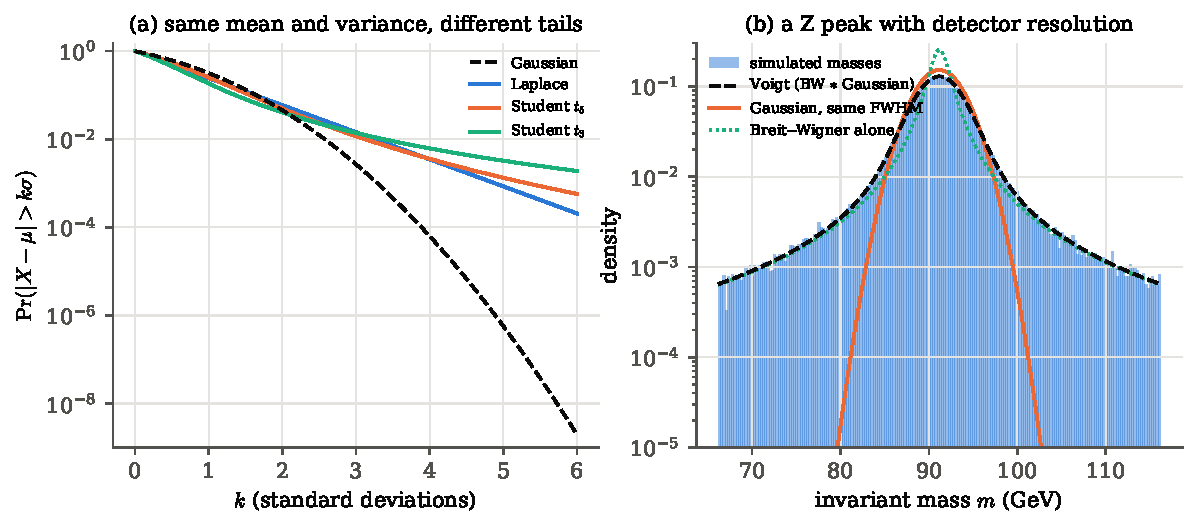
\includegraphics[width=\linewidth]{figures/ch02/which_distribution.pdf}
\caption{(a) Two-sided tail probability against distance from the mean, in units of the standard deviation, for four symmetric distributions scaled to the same mean and variance. They agree within a factor of two out to about two standard deviations and then separate by orders of magnitude. (b) Simulated Z masses with a Breit--Wigner width and Gaussian detector resolution, on a logarithmic scale. The Voigt density (dashed) follows them into the wings; the Gaussian with the same half-maximum width (solid) matches only the core; far from the peak the Voigt rejoins the pure Breit--Wigner (dotted).}
\label{2b:fig:which}
\end{figure}

\paragraph{Example: false alarms in a gravitational-wave search.} A matched filter correlates the detector output with a template waveform whose phase is unknown. It returns two numbers at each time, the correlation with the cosine-phase and with the sine-phase template, normalised so that in pure Gaussian noise each is a standard normal and the two are independent. The signal-to-noise ratio is $\rho=\sqrt{x^2+y^2}$, with $x$ and $y$ the two correlations. \emph{The question:} how often does noise alone push $\rho$ above a threshold? \emph{Reading the mechanism:} \emph{the length of a two-dimensional Gaussian vector}. So $\rho$ is Rayleigh with $s=1$, and $\rho^2$ is $\chi^2_2$, the exponential with mean $2$ (\cref{2b:sec:maxwell}). The chance that noise alone crosses a threshold $\rho_*$ is
\begin{align}
  \Prob(\rho>\rho_*)
  \eqby{1}\Prob(\rho^2>\rho_*^2)
  \eqby{2}\int_{\rho_*^2}^{\infty}\tfrac12e^{-u/2}\,\dd u
  \eqby{3}e^{-\rho_*^2/2} .
  \label{2b:eq:false-alarm}
\end{align}
\begin{explain}
  \item $\rho\ge0$, and squaring is increasing on $[0,\infty)$.
  \item The $\chi^2_\nu$ density \eqref{2b:eq:chi2} with $\nu=2$ is $u^{0}e^{-u/2}/(2\,\Gamma(1))=\frac12e^{-u/2}$.
  \item $\int_a^\infty\frac12e^{-u/2}\dd u=e^{-a/2}$.
\end{explain}
The script checks the formula at $\rho_*=\tbWrstar$: the fraction of $2\times10^5$ noise draws above threshold is $\tbWfaSim$, against $e^{-9/2}=\tbWfaTh$ (script lines 54--59). At the conventional detection threshold $\rho_*=8$ the formula gives $\tbWfaEight$ per independent template and time sample. That looks reassuringly small. But a search examines very many templates at every sample of months of data, so the answer depends on the $\chi^2_2$ law holding fourteen decades down its tail. Real detector noise contains short non-Gaussian bursts (``glitches''), which is exactly the kind of fat tail of \cref{2b:fig:which}a.

So searches do not trust \eqref{2b:eq:false-alarm} for their final significance. They measure the background empirically. They shift one detector's data in time against another's, by more than the light travel time, and count how often noise alone produces a coincident trigger. The formula \emph{verifies} the pipeline on simulated Gaussian noise; the time slides are the research instrument on real data. The same Rayleigh and exponential laws describe the amplitude and the power of a noise frequency bin, which returns in the gravitational-wave Fisher forecasts of \cref{ch:10}, where the noise enters through its power spectral density.

\paragraph{Example: is $\chi^2=130$ for $100$ degrees of freedom a bad fit?} It is suspicious but not damning, and the Gaussian shortcut gets its tail wrong by $40\%$. A fit of a model with $P$ adjustable parameters to $N$ Gaussian measurements returns a minimum $\chi^2$. For a model linear in its parameters, the minimum is a quadratic form in the residuals with $N-P$ independent directions left over (the argument of \cref{2b:sec:chi2-quadform,2b:sec:nminus1}, made precise in \cref{ch:03}). Reading the mechanism: \emph{a sum of $\nu=N-P$ squared standard normals}, so $\chi^2_{\min}\sim\chi^2_\nu$. \emph{The question:} how often would a correct model give $\chi^2\ge130$? With $\nu=100$ it is tempting to use the central limit theorem, since $\chi^2_{100}$ is a sum of $100$ independent $\chi^2_1$ variables, and write $\chi^2\approx\Normal(\nu,2\nu)$:
\[
  z=\frac{\chi^2-\nu}{\sqrt{2\nu}}=\frac{130-100}{\sqrt{200}}=\tbWzGauss ,\qquad \Prob(Z>z)=\tbWpGauss .
\]
The exact tail, from \pyname{scipy.stats.chi2.sf(130, 100)}, is $\tbWpExact$, about $40\%$ larger. \emph{Why?} The parent $\chi^2_1$ is skewed, and the CLT removes skewness only slowly (\cref{2b:sec:clt-rate}). To measure it, we need the cumulants $\kappa_n$ (the Taylor coefficients of $\ln\phi$). The cumulants of $\chi^2_1$ follow from its characteristic function $(1-2ik)^{-1/2}$ \eqref{2b:eq:chi2-cf1}: $\ln\phi=-\frac12\ln(1-2ik)=\sum_{n\ge1}\frac{(2ik)^n}{2n}$, and matching with $\ln\phi=\sum_n\kappa_n(ik)^n/n!$ gives $\kappa_n=2^{n-1}(n-1)!$, so $\kappa_2=2$ and $\kappa_3=8$. Then
\begin{align}
  \gamma_1\bigl(\chi^2_\nu\bigr)
  \eqby{1}\frac{\kappa_3(\chi^2_\nu)}{\kappa_2(\chi^2_\nu)^{3/2}}
  \eqby{2}\frac{\nu\,\kappa_3(\chi^2_1)}{\bigl[\nu\,\kappa_2(\chi^2_1)\bigr]^{3/2}}
  \eqby{3}\frac{8\nu}{(2\nu)^{3/2}}
  =\sqrt{\frac8\nu} .
  \label{2b:eq:chi2-skew}
\end{align}
\begin{explain}
  \item Skewness is the third cumulant in units of the standard deviation cubed, with the cumulants of \eqref{2b:eq:cumulants}.
  \item Cumulants of independent variables add, and $\chi^2_\nu$ is the sum of $\nu$ independent $\chi^2_1$.
  \item $\kappa_3(\chi^2_1)=8$ and $\kappa_2(\chi^2_1)=2$.
\end{explain}
At $\nu=100$ the skewness is still $0.28$. So the right tail is longer than the Gaussian's, and the Gaussian approximation underestimates how often a correct model gives a large $\chi^2$. The verdict itself is mild. A correct model would give $\chi^2\ge130$ in about $2\%$ of repetitions, so the fit is suspicious but not damning, and \cref{ch:04} turns this reasoning into a test. The practical rule is simpler: never use $\Normal(\nu,2\nu)$ for a tail probability when the exact $\chi^2_\nu$ survival function is one line of code.

\subsection{The tails decide}
\label{2b:sec:which-tails}

The three examples share a lesson: the core of each distribution was well described by a Gaussian, and the question was about the tail. \Cref{2b:fig:which}a puts numbers on it. It shows four symmetric distributions, each scaled to mean zero and variance one: the Gaussian, the Laplace, and Student's $t_5$ and $t_3$ (for $t_\nu$ with scale $c$ the variance is $c^2\nu/(\nu-2)$ by \eqref{2b:eq:t-var}, so $c^2=3/5$ and $1/3$). They are indistinguishable at one standard deviation and cross near two. At three standard deviations the two-sided tail probabilities are $\tbWthreeGauss$ for the Gaussian but $\tbWthreeLap$ (Laplace), $\tbWthreeTfive$ ($t_5$) and $\tbWthreeTthree$ ($t_3$), four to five times more. At five standard deviations the Gaussian gives $\tbWfiveGauss$ and $t_3$ gives $\tbWfiveTthree$, a ratio of $\tbWratioTthree$.

\begin{keyidea}[Choose by mechanism, check in the tails]
A distribution is chosen by recognising the machine that made the numbers (sum, product, squares, length, ratio, wait, share). Its mean and variance are then fixed by the machine, but agreement in mean and variance says almost nothing beyond about two standard deviations. Any conclusion that uses a tail probability must justify the tail separately, by the mechanism or by an empirical measurement of the background.
\end{keyidea}

The physics of the tails is usually different from the physics of the core. Cowan makes the point for the two distributions with divergent moments, the Breit--Wigner and the Landau. A real resonance mass is bounded by the masses of its decay products and by the collision energy, and a real energy loss by the energy of the incoming particle, so ``the models break down in the tails of the distributions'' \srcref{Cowan}{pp.~38--39}. Near the peak the idealised machine is accurate; far from it, other mechanisms take over (kinematic limits, radiation, pile-up, detector glitches, non-Gaussian foregrounds).

So particle physicists quote a ``$5\sigma$'' discovery as a tail probability of $2.9\times10^{-7}$ computed from the \emph{distribution of the test statistic}, obtained by simulation or by an asymptotic theorem (\cref{ch:04}), and never from a Gaussian assumption about the data alone. The same caution applies to a posterior interval far from the peak of a posterior (\cref{ch:05}), and to the Fisher forecast of \cref{ch:10}, which is Gaussian by construction and must be checked against a sampled posterior in the tails (\cref{ch:09}).

\begin{pitfall}[A good fit to the peak is not a test of the tails]
A histogram with most of its entries within $\pm2\sigma$ fits a Gaussian, a Laplace or a $t_5$ almost equally well: the $\chi^2$ of the fit is dominated by the populated bins, and the tail bins hold too few entries to discriminate. The choice between them must come from the mechanism, or from a dedicated sample that populates the tails (a control region, a time slide, a large simulation).
\end{pitfall}

With a mechanism in hand, the summary numbers of the table give a first check that costs nothing: compare the sample mean and variance with the predicted ones, the Fano factor for counts (\cref{2a:sec:failures}), and, when enough data exist, the sample skewness with the predicted $\gamma_1$. A mismatch in these moments rules the mechanism out; a match leaves the tails still to be checked.

\begin{recap}[Part summary: continuous distributions]
\begin{itemize}
  \item \textbf{Gaussian, three ways.} (i) The binomial near its peak, by Stirling's formula and a second-order expansion of $\ln p_k$ (de Moivre--Laplace), with error $O(1/n)$ at the peak. (ii) The central limit theorem: the characteristic function of a standardised sum tends to $e^{-k^2/2}$ whenever the parent has finite variance, with error $O(n^{-1/2})$ set by the skewness (Berry--Esseen). (iii) Maximum entropy: the least committal density with a given mean and variance.
  \item \textbf{When the CLT fails or is slow.} Cauchy (Breit--Wigner): no mean, and the average of $n$ draws is as wide as one draw. Landau: finite range in reality, but so skewed that the mean of $25$ layers is still far from Gaussian.
  \item \textbf{Multivariate normal.} $\bm X=\bm\mu+A\bm Z$ with $\Cmat=AA\T$; contours are ellipses, and the region $\Delta\chi^2\le2.30$ (two parameters) holds $68.3\%$; marginals drop rows and columns of $\Cmat$; conditionals shift the mean by $\Cmat_{ba}\Cmat_{aa}^{-1}(\bm x_a-\bm\mu_a)$ and shrink the covariance to the Schur complement.
  \item \textbf{$\chi^2_\nu$.} Sum of $\nu$ squared standard normals, $\chi^2_\nu=$ Gamma$(\nu/2,2)$, mean $\nu$, variance $2\nu$; $(\bm X-\bm\mu)\T\Cmat^{-1}(\bm X-\bm\mu)\sim\chi^2_k$; $(n-1)S^2/\sigma^2\sim\chi^2_{n-1}$, independent of $\bar X$, because estimating the mean uses up one direction.
  \item \textbf{$t$ and $F$.} Student $t_\nu=Z/\sqrt{\chi^2_\nu/\nu}$: the studentised mean, heavier tails, variance $\nu/(\nu-2)$, a scale mixture of Gaussians; $F_{p,q}$ is a ratio of two scaled $\chi^2$ and $t_q^2=F_{1,q}$.
  \item \textbf{The zoo.} Uniform (only a range; parent of all through $F^{-1}$), gamma and Weibull (waits), log-normal (products), Rayleigh and Maxwell (lengths of Gaussian vectors; a complex Gaussian mode has exponential power), beta and Dirichlet (uncertain probabilities, conjugate to binomial and multinomial counts), Laplace (differences of waits).
  \item \textbf{Which one when.} Recognise the mechanism first, then check moments, and check tails separately: laws with equal variance can differ by factors of thousands at $5\sigma$.
\end{itemize}
\end{recap}

\section*{Chapter summary}
\addcontentsline{toc}{section}{Chapter summary}
\label{2b:sec:summary}

Every common probability distribution comes from a machine that generates it. Counting machines give the discrete laws: one trial, many trials, histogram bins, rare events, a random stream in time, the waits between its events, and the ways real detectors break these assumptions. Measuring machines give the continuous laws: the Gaussian three times over, then the multivariate normal, the $\chi^2$, Student's $t$ and the $F$ ratio built from it, and the rest of the continuous zoo built from the Gaussian and the exponential. All of it runs in the direction of \emph{prediction}: fix a hypothesis and ask what data it produces and how often. On the pipeline of \cref{ch:00}, that is the step which says how a statistic $S$ scatters given the parameters $\theta$, $P(S\given\theta)$, for the simplest statistics (counts, sums, sample means and variances, $\chi^2$'s, power-spectrum estimates). Every later chapter either reads such a $P(S\given\theta)$ backwards as a likelihood or builds a new one by simulation. The two tables list each concept, what it means operationally (how to compute, recognise or test it), and where it is used next.

\begin{center}
\small
\renewcommand{\arraystretch}{1.15}
\begin{tabularx}{\linewidth}{@{}>{\raggedright\arraybackslash}p{3.3cm}
                               >{\raggedright\arraybackslash}X
                               >{\raggedright\arraybackslash}p{2.7cm}@{}}
\toprule
\multicolumn{3}{@{}l}{\textbf{Counting distributions (first part)}}\\
concept & operational meaning & used later in\\\midrule
distribution as a mechanism & state the machine and its assumptions, derive the law, then simulate the machine (not the formula) and compare histograms & every chapter\\
Bernoulli & one yes/no trial, $p^x(1-p)^{1-x}$; $N$ trials give $p^z(1-p)^{N-z}$, depending only on the number of successes & \cref{ch:03,ch:05}\\
binomial & successes in $n$ independent trials with the same $p$: count the $\binom nk$ paths; mean $np$, variance $np(1-p)$ & \cref{ch:03,ch:04,ch:05}\\
multinomial & a histogram with a fixed total: binomial marginals, covariance $-Np_ip_j$ between bins & \cref{ch:03,ch:04}\\
Poisson & $n\to\infty$, $np=\lambda$ limit of the binomial; mean $=$ variance $=\lambda$; closed under sums and thinning & \cref{ch:03,ch:04,ch:05,ch:06}\\
Poisson process & constant rate, no memory; $\dd P_n/\dd t=\lambda(P_{n-1}-P_n)$; with a Poisson total, histogram bins become independent Poisson counts & \cref{ch:03,ch:06}\\
exponential, gamma (Erlang) & wait for the first / $n$-th event; memoryless; means $1/\lambda$, $n/\lambda$ & \cref{ch:05,ch:06}\\
geometric, negative binomial & trials to the first / $r$-th success; also a Poisson with gamma-distributed rate (overdispersion) & \cref{ch:03,ch:05}\\
Fano factor & variance over mean of counts; $\approx1$ Poisson, $>1$ fluctuating rate or clumping, $<1$ dead time; judge against $\sqrt{2/(k-1)}$ & \cref{ch:04,ch:08}\\
dead time & recorded rate $n/(1+n\tau)$ or $ne^{-n\tau}$; correcting it removes bias but inflates the variance by $1+n\tau$ & \cref{ch:06}\\
large-count limit & all Poisson cumulants equal $\lambda$, skewness $1/\sqrt\lambda$: Gaussian near the peak, exact Poisson in the tails & \cref{ch:03,ch:04}\\
\bottomrule
\end{tabularx}
\end{center}

\begin{center}
\small
\renewcommand{\arraystretch}{1.15}
\begin{tabularx}{\linewidth}{@{}>{\raggedright\arraybackslash}p{3.3cm}
                               >{\raggedright\arraybackslash}X
                               >{\raggedright\arraybackslash}p{2.7cm}@{}}
\toprule
\multicolumn{3}{@{}l}{\textbf{Continuous distributions (second part)}}\\
concept & operational meaning & used later in\\\midrule
Gaussian $\Normal(\mu,\sigma^2)$ & $\mu$ the centre, $\sigma$ the width; probabilities from $\Phi$; $68.3/95.4/99.7\%$ within $1/2/3\sigma$ & every chapter\\
Stirling, Laplace's method & expand the logarithm of a peaked integrand to second order about its maximum & \cref{ch:05,ch:10}\\
de Moivre--Laplace & binomial near its peak $\approx$ Gaussian with mean $np$, variance $np(1-p)$; error largest in the tails & \cref{ch:03,ch:04}\\
characteristic function & $\E e^{ikX}$, always exists; sums multiply it; cumulants are the Taylor coefficients of its logarithm & \cref{ch:06,ch:07}\\
central limit theorem & standardised sums of finite-variance variables tend to $\Normal(0,1)$; error $\sim\gamma_1/\sqrt n$ (Berry--Esseen); check by simulation & \cref{ch:03,ch:04,ch:06}\\
Cauchy, Landau & no mean: averaging does not narrow a Cauchy; use the median or a truncated mean; Landau sums converge very slowly & \cref{ch:03,ch:06}\\
maximum entropy & least committal distribution given constraints: $p\propto e^{-\sum_j\lambda_jf_j}$; mean $\to$ exponential, variance $\to$ Gaussian & \cref{ch:05}\\
multivariate normal & $\bm\mu+A\bm Z$ with $\Cmat=AA\T$ (Cholesky); ellipses with $\Delta\chi^2=2.30,6.18$ in 2-D; marginal = delete rows and columns; conditional = Schur complement & \cref{ch:07,ch:09,ch:10}\\
$\chi^2_\nu$ & sum of $\nu$ squared standard normals; mean $\nu$, variance $2\nu$; quadratic forms $\bm r\T\Cmat^{-1}\bm r$; exact tail by \pyname{chi2.sf} & \cref{ch:03,ch:04,ch:07,ch:08}\\
sample variance, $n-1$ & $(n-1)S^2/\sigma^2\sim\chi^2_{n-1}$, independent of $\bar X$ for Gaussian data; one direction is used by the mean & \cref{ch:03,ch:04}\\
Student $t$ & mean over an estimated error bar; heavier tails, $t_\nu\to\Normal$ as $\nu\to\infty$; robust likelihood & \cref{ch:04,ch:05}\\
$F$ ratio & ratio of two independent scaled $\chi^2$; compare variances or nested fits; $t^2=F_{1,q}$ & \cref{ch:04}\\
uniform, inverse transform & $F(X)$ is uniform; $F^{-1}(U)$ samples any law; $\pval$-values are uniform under $\Hnull$ & \cref{ch:04,ch:06}\\
log-normal & products of positive factors; mean $e^{\mu+\sigma^2/2}$ above the median $e^\mu$ & \cref{ch:05,ch:07}\\
Rayleigh, Maxwell, exponential power & length of a 2-D / 3-D Gaussian vector; a complex Gaussian mode has Rayleigh amplitude, uniform phase, exponential power & \cref{ch:07,ch:08,ch:10}\\
beta, Dirichlet & uncertain probability (vector); conjugate to binomial (multinomial) counts; ``keep the runs that match'' gives the posterior & \cref{ch:05,ch:09}\\
which distribution when & recognise the mechanism, check the moments, justify the tails separately & \cref{ch:04,ch:10,ch:12}\\
\bottomrule
\end{tabularx}
\end{center}

\subsection*{Reading the literature}

\begin{itemize}[leftmargin=1.2em,itemsep=2pt]
  \item \textbf{Main line.} \mainref{\S\S2.3--2.4, 2.10, 5.4} gives the discrete and continuous families, the multivariate normal with its marginals and conditionals, and the central limit theorem with the Berry--Esseen bound, compactly and with short examples; the MGF proof of the CLT is in \mainref{\S5.7.2}.
  \item \textbf{The clearest first reading.} \srcref{Kruschke}{Ch.~6}: the beta distribution as a description of belief about a probability, its parameters as previous successes and failures, and how to set them from a mean and a spread.
  \item \textbf{The physicist's version.} \srcref{Cowan}{Ch.~2} for each distribution with a physics setting (including the Breit--Wigner and Landau laws and their divergent moments), and \srcref{Cowan}{Ch.~10} for characteristic functions, the limits binomial $\to$ Poisson $\to$ Gaussian, the $\chi^2$ from squares, and the practical validity of the CLT.
  \item \textbf{Careful derivations.} \srcref{CasellaBerger}{\S\S3.2--3.3, 4.5--4.6, 5.3--5.4}: the families with full proofs of their moments, the bivariate and multivariate normal, the independence of $\bar X$ and $S^2$, the $t$ and $F$ densities by Jacobians, and order statistics.
  \item \textbf{Maximum entropy.} \srcref{Sivia}{Ch.~5}: the monkey argument for the entropy, the loaded die, the kangaroo problem, and the exponential, Gaussian, Laplace and Poisson as MaxEnt assignments.
  \item \textbf{Choosing a likelihood and a prior.} \srcref{Lambert}{Ch.~8}: a catalogue of sampling and prior distributions with a story for each, their interrelations, the robust versions (negative binomial, Student $t$), and a decision tree for choosing a likelihood.
  \item \textbf{Pictures.} \srcref{SeeingTheory}{pp.~38--39}: an interactive demonstration of the central limit theorem.
  \item \textbf{Going further.} The Gaussian approximation to the $\Chat$ likelihood and its failure at low $\ell$, where the $\chi^2_{2\ell+1}$ skewness matters, is treated in \cite{HamimecheLewis2008}; \cref{ch:07,ch:08} build on it.
\end{itemize}
  
\chapter{Estimators, Error Propagation and the Likelihood}\label{ch:03}

\providecommand{\ThreeAM}{}\renewcommand{\ThreeAM}{200\,000}
\providecommand{\ThreeASdMean}{}\renewcommand{\ThreeASdMean}{0.01583}
\providecommand{\ThreeASdMedian}{}\renewcommand{\ThreeASdMedian}{0.01859}
\providecommand{\ThreeASdMidrange}{}\renewcommand{\ThreeASdMidrange}{0.02155}
\providecommand{\ThreeASdFirst}{}\renewcommand{\ThreeASdFirst}{0.04993}
\providecommand{\ThreeASdTheory}{}\renewcommand{\ThreeASdTheory}{0.01581}
\providecommand{\ThreeAMedianVarRatio}{}\renewcommand{\ThreeAMedianVarRatio}{1.379}
\providecommand{\ThreeATauMean}{}\renewcommand{\ThreeATauMean}{2.198}
\providecommand{\ThreeATauSd}{}\renewcommand{\ThreeATauSd}{0.4914}
\providecommand{\ThreeATauSkew}{}\renewcommand{\ThreeATauSkew}{0.4475}
\providecommand{\ThreeATauSkewTheory}{}\renewcommand{\ThreeATauSkewTheory}{0.4472}
\providecommand{\ThreeAPiMean}{}\renewcommand{\ThreeAPiMean}{3.142}
\providecommand{\ThreeAPiSd}{}\renewcommand{\ThreeAPiSd}{0.1642}
\providecommand{\ThreeAPiSeTheory}{}\renewcommand{\ThreeAPiSeTheory}{0.1642}
\providecommand{\ThreeAUOneBias}{}\renewcommand{\ThreeAUOneBias}{2.896\times10^{-4}}
\providecommand{\ThreeAUTwoBias}{}\renewcommand{\ThreeAUTwoBias}{-0.09081}
\providecommand{\ThreeAUThreeBias}{}\renewcommand{\ThreeAUThreeBias}{1.080\times10^{-4}}
\providecommand{\ThreeAUOneMSE}{}\renewcommand{\ThreeAUOneMSE}{0.03342}
\providecommand{\ThreeAUTwoMSE}{}\renewcommand{\ThreeAUTwoMSE}{0.01517}
\providecommand{\ThreeAUThreeMSE}{}\renewcommand{\ThreeAUThreeMSE}{0.008373}
\providecommand{\ThreeAUOneMSEth}{}\renewcommand{\ThreeAUOneMSEth}{0.03333}
\providecommand{\ThreeAUTwoMSEth}{}\renewcommand{\ThreeAUTwoMSEth}{0.01515}
\providecommand{\ThreeAUThreeMSEth}{}\renewcommand{\ThreeAUThreeMSEth}{0.008333}
\providecommand{\ThreeAUTwoBiasth}{}\renewcommand{\ThreeAUTwoBiasth}{-0.09091}
\providecommand{\ThreeASlopeU}{}\renewcommand{\ThreeASlopeU}{-1.001}
\providecommand{\ThreeASlopeE}{}\renewcommand{\ThreeASlopeE}{-0.9973}
\providecommand{\ThreeASlopeP}{}\renewcommand{\ThreeASlopeP}{-1.002}
\providecommand{\ThreeACauchyIQRone}{}\renewcommand{\ThreeACauchyIQRone}{1.011}
\providecommand{\ThreeACauchyIQRlast}{}\renewcommand{\ThreeACauchyIQRlast}{0.9998}
\providecommand{\ThreeACoinExact}{}\renewcommand{\ThreeACoinExact}{0.937}
\providecommand{\ThreeACoinNclt}{}\renewcommand{\ThreeACoinNclt}{27}
\providecommand{\ThreeACoinExactNclt}{}\renewcommand{\ThreeACoinExactNclt}{0.7522}
\providecommand{\ThreeAZeightyfive}{}\renewcommand{\ThreeAZeightyfive}{1.036}
\providecommand{\ThreeAVbiasFive}{}\renewcommand{\ThreeAVbiasFive}{0.796}
\providecommand{\ThreeAVunbFive}{}\renewcommand{\ThreeAVunbFive}{0.995}
\providecommand{\ThreeAVarSGaussTen}{}\renewcommand{\ThreeAVarSGaussTen}{0.2229}
\providecommand{\ThreeAVarSGaussTenTh}{}\renewcommand{\ThreeAVarSGaussTenTh}{0.2222}
\providecommand{\ThreeAVarSExpTen}{}\renewcommand{\ThreeAVarSExpTen}{0.8255}
\providecommand{\ThreeAVarSExpTenTh}{}\renewcommand{\ThreeAVarSExpTenTh}{0.8222}
\providecommand{\ThreeAMseNmOneTen}{}\renewcommand{\ThreeAMseNmOneTen}{0.2229}
\providecommand{\ThreeAMseNTen}{}\renewcommand{\ThreeAMseNTen}{0.1907}
\providecommand{\ThreeAMseNpOneTen}{}\renewcommand{\ThreeAMseNpOneTen}{0.1826}
\providecommand{\ThreeACfourFive}{}\renewcommand{\ThreeACfourFive}{0.94}
\providecommand{\ThreeAMeanSFive}{}\renewcommand{\ThreeAMeanSFive}{0.94}
\providecommand{\ThreeASpurSd}{}\renewcommand{\ThreeASpurSd}{0.1484}
\providecommand{\ThreeASpurSdTh}{}\renewcommand{\ThreeASpurSdTh}{0.1429}
\providecommand{\ThreeASpurMax}{}\renewcommand{\ThreeASpurMax}{0.4416}
\providecommand{\ThreeANpairs}{}\renewcommand{\ThreeANpairs}{190}
\providecommand{\ThreeARMean}{}\renewcommand{\ThreeARMean}{0.5902}
\providecommand{\ThreeARMeanTh}{}\renewcommand{\ThreeARMeanTh}{0.5904}
\providecommand{\ThreeARSd}{}\renewcommand{\ThreeARSd}{0.1544}
\providecommand{\ThreeARSdTh}{}\renewcommand{\ThreeARSdTh}{0.1431}
\providecommand{\ThreeAZSd}{}\renewcommand{\ThreeAZSd}{0.2416}
\providecommand{\ThreeAZSdTh}{}\renewcommand{\ThreeAZSdTh}{0.2425}
\providecommand{\ThreeARSkew}{}\renewcommand{\ThreeARSkew}{-0.8008}
\providecommand{\ThreeAZSkew}{}\renewcommand{\ThreeAZSkew}{-8.926\times10^{-4}}
\providecommand{\ThreeAHartlapTen}{}\renewcommand{\ThreeAHartlapTen}{1.616}
\providecommand{\ThreeAHartlapTenTh}{}\renewcommand{\ThreeAHartlapTenTh}{1.611}
\providecommand{\ThreeAPendG}{}\renewcommand{\ThreeAPendG}{9.811}
\providecommand{\ThreeAPendSgLin}{}\renewcommand{\ThreeAPendSgLin}{0.04377}
\providecommand{\ThreeAPendSgMC}{}\renewcommand{\ThreeAPendSgMC}{0.04375}
\providecommand{\ThreeAPendMeanMC}{}\renewcommand{\ThreeAPendMeanMC}{9.811}
\providecommand{\ThreeARatioALin}{}\renewcommand{\ThreeARatioALin}{0.1414}
\providecommand{\ThreeARatioAHalf}{}\renewcommand{\ThreeARatioAHalf}{0.1425}
\providecommand{\ThreeARatioAMed}{}\renewcommand{\ThreeARatioAMed}{0.9999}
\providecommand{\ThreeARatioANeg}{}\renewcommand{\ThreeARatioANeg}{0}
\providecommand{\ThreeARatioAFar}{}\renewcommand{\ThreeARatioAFar}{1.600\times10^{-4}}
\providecommand{\ThreeARatioBLin}{}\renewcommand{\ThreeARatioBLin}{1.16}
\providecommand{\ThreeARatioBHalf}{}\renewcommand{\ThreeARatioBHalf}{1.294}
\providecommand{\ThreeARatioBMed}{}\renewcommand{\ThreeARatioBMed}{3.329}
\providecommand{\ThreeARatioBNeg}{}\renewcommand{\ThreeARatioBNeg}{0.001363}
\providecommand{\ThreeARatioBFar}{}\renewcommand{\ThreeARatioBFar}{0.02883}
\providecommand{\ThreeARatioCLin}{}\renewcommand{\ThreeARatioCLin}{10.05}
\providecommand{\ThreeARatioCHalf}{}\renewcommand{\ThreeARatioCHalf}{11.49}
\providecommand{\ThreeARatioCMed}{}\renewcommand{\ThreeARatioCMed}{7.083}
\providecommand{\ThreeARatioCNeg}{}\renewcommand{\ThreeARatioCNeg}{0.1589}
\providecommand{\ThreeARatioCFar}{}\renewcommand{\ThreeARatioCFar}{0.0961}
\providecommand{\ThreeAWsdW}{}\renewcommand{\ThreeAWsdW}{0.3391}
\providecommand{\ThreeAWsdWth}{}\renewcommand{\ThreeAWsdWth}{0.339}
\providecommand{\ThreeAWsdU}{}\renewcommand{\ThreeAWsdU}{0.6228}
\providecommand{\ThreeAWsdUth}{}\renewcommand{\ThreeAWsdUth}{0.621}
\providecommand{\ThreeAWchiMean}{}\renewcommand{\ThreeAWchiMean}{6.998}
\providecommand{\ThreeAWchiVar}{}\renewcommand{\ThreeAWchiVar}{14.05}
\providecommand{\ThreeAWbest}{}\renewcommand{\ThreeAWbest}{0.5}
\providecommand{\ThreeACorrVmcNine}{}\renewcommand{\ThreeACorrVmcNine}{0.5453}
\providecommand{\ThreeACorrVthNine}{}\renewcommand{\ThreeACorrVthNine}{0.5429}
 
\section*{Where this chapter is going}
\label{3a:sec:roadmap}

Every measurement ends with a number and an error bar. The number is easy to
get: we average, we fit, we read off a peak. The error bar is the hard part,
and it is where statistics lives. It answers one question:
\emph{``if nature let us run this experiment again, how different would our
number be?''}

The book's pipeline (\cref{ch:00}) runs from a theory to its data, from the
data to a statistic $S$ that compresses them, from $S$ to how $S$ scatters,
$P(S\given\theta)$, and from that scatter to the physics. The error bar lives
on the two middle arrows: building $S$, and working out how it scatters.

The key step is to treat a summary of the data as a \newterm{random variable}
in its own right. If we imagine repeating the experiment many times, the
summary takes a different value each time, so it has a distribution. That
distribution has a centre (does it sit on the true value, or is it biased?),
a width (the standard error) and correlations with other summaries. From this
one step come the answers to several practical questions: why widths shrink
like $1/\sqrt N$ (the law of large numbers and the central limit theorem), why
the sample variance divides by $N-1$, how noisy a covariance matrix estimated
from simulations is, how errors pass through a formula, and how to combine
measurements of different quality. The same probability of the data, read
\emph{backwards} as a function of the parameters, is the likelihood, the
subject of the second half of the chapter.

\begin{figure}[htbp]
\centering
\begin{tikzpicture}[
  node distance=5mm and 7mm,
  blk/.style={draw=accent,thick,rounded corners=2pt,fill=ideabg,
              align=center,font=\small,minimum height=9mm,text width=24mm},
  hot/.style={blk,fill=defbg,draw=fibreorange!80!black},
  flow/.style={->,thick,accent}]
  \node[blk] (model) {physical model\\ $\theta$};
  \node[blk,right=of model] (data) {data\\ $x_1,\dots,x_N$};
  \node[hot,right=of data] (est) {estimator\\ $\hat\theta=g(x_1,\dots,x_N)$};
  \node[hot,below=9mm of est] (samp) {sampling distribution\\ of $\hat\theta$};
  \node[hot,left=of samp] (bv) {bias, variance,\\ MSE, $1/\sqrt N$};
  \node[hot,left=of bv] (prop) {covariance, error\\ propagation, weights};
  \node[blk,below=9mm of samp,fill=nashbg,draw=violet!70!black] (like)
       {likelihood\\ (second half)};
  \draw[flow] (model) -- (data);
  \draw[flow] (data) -- (est);
  \draw[flow] (est) -- (samp);
  \draw[flow] (samp) -- (bv);
  \draw[flow] (bv) -- (prop);
  \draw[flow] (samp) -- (like);
\end{tikzpicture}
\caption{The route through the ideas. A model with true parameter $\theta$
produces data. A recipe (the estimator) turns data into a number. Imagining
many repetitions of the experiment turns that number into a random variable
with a sampling distribution (orange boxes). Its centre and width
give the error bar, and the same machinery propagates and combines error bars.
The last box, the likelihood, reads the probability of the data as a
function of $\theta$ and is the subject of the second part.}
\label{3a:fig:roadmap}
\end{figure}

\section{One number from many readings: estimators and their sampling distribution}
\label{3a:sec:sampling}

A student times a pendulum of length $L=1\,$m ten times and converts each
period into a value of the gravitational acceleration. The ten numbers are
\[
9.79,\ 9.83,\ 9.86,\ 9.80,\ 9.77,\ 9.84,\ 9.81,\ 9.78,\ 9.85,\ 9.82\ \ \mathrm{m\,s^{-2}}.
\]
No two agree. What is ``the answer''? The average, $9.815$? The middle value?
The first reading? And whatever we choose, how far from the true $g$ can it
be? A particle physicist faces the same question with twenty muon decay times
and the lifetime $\tau_\mu$, and a cosmologist with one CMB map and the
amplitude of fluctuations.

The way forward is to stop asking for ``the answer'' and choose a
\emph{recipe} instead: a fixed rule that turns any list of readings into one
number. A rule can be applied to data we did not get. So we can ask how its
output would scatter if the experiment were repeated. That scatter is the
error bar.

\paragraph{The shape of every problem that follows.}
In each of these examples there is a quantity we care about and can never
look at directly: the true $g$, the muon lifetime, an amplitude of the early
Universe. Call it $s$. What we hold instead are readings $x_1,\dots,x_N$, and
each of them carries some information about $s$ mixed with things we do not
want: noise, a contaminating signal, a calibration offset. Schematically,
\begin{equation}
  x_i = (\text{a piece that responds to } s) + (\text{everything else}),
  \qquad
  \hat s=F(x_1,\dots,x_N).
  \label{3a:eq:hidden-s}
\end{equation}
The recipe is the function $F$. Choosing it, given what we know about how each
reading responds to $s$ and about the size and structure of everything else,
is the whole subject of estimation. This chapter first learns to judge a
given $F$ by the scatter of its output; its second half, the likelihood, and
\cref{ch:05}, the posterior, are two systematic ways of choosing $F$ in the
first place.

\paragraph{The experiment as a random number generator.}
Think of the whole experiment, ten readings and all, as one throw of a very
complicated die. Nature fixes the true $g$ and the noise level. Each throw
produces a new list of ten numbers, and our recipe turns each list into one
number. Throw the die many times and those numbers form a histogram. This
imagined histogram plays the role of the \emph{ensemble} of statistical
mechanics. We only ever see one microstate, our one data set. The error bars
we quote, however, are properties of the whole ensemble.

\paragraph{Before any symbol.}
\begin{enumerate}[label=\arabic*.]
  \item What did we observe? A list of numbers $x_1,\dots,x_N$.
  \item What could have produced it? A family of probability distributions,
        labelled by the unknown quantity we care about (the
        \emph{statistical model}).
  \item What recipe turns the list into one number? (The \emph{estimator}.)
  \item If nature reran the experiment with the same true value, how would the
        recipe's output be distributed? (The \emph{sampling distribution}.)
  \item What does that distribution say about our one number? Its centre tells
        us whether the recipe aims at the right place. Its width is the error bar.
\end{enumerate}

Step 4 is a \emph{prediction} in the sense of \cref{ch:00}: we start from a
hypothesised truth and ask what outcomes it produces. Every error bar built
from a sampling distribution runs in this forward direction, from truth to
data. The reverse question, from the data we saw back to the truths that
could have produced them, is the likelihood of the second half of the chapter
and the Bayesian inference of \cref{ch:05}.

\subsection{Statistical models: the list of possible truths}
\label{3a:sec:models}

Statistical inference is ``using data to infer the distribution that
generated the data'' \mainref{p.~87}. So before inferring anything, we must
write down which distributions could have generated it.

\begin{workdef}[statistical model]
A \newterm{statistical model} $\mathfrak F$ is a set of probability
distributions \unpack{the candidate explanations of how the data were
produced}. It is \newterm{parametric} if its members can be labelled by
finitely many numbers,
\begin{equation}
  \mathfrak F=\bigl\{\,f(x;\theta)\;:\;\theta\in\Theta\,\bigr\},
  \label{3a:eq:parametric-model}
\end{equation}
where $\theta$ is the \newterm{parameter} \unpack{a fixed but unknown number,
or vector, that picks one member} and $\Theta$ the \newterm{parameter space}
\unpack{all values $\theta$ is allowed to take}. If $\theta=(\theta_1,\theta_2)$
and we only care about $\theta_1$, then $\theta_2$ is a \newterm{nuisance
parameter} \unpack{needed to describe the data, not wanted in the answer}. A
model that cannot be labelled by finitely many numbers is
\newterm{nonparametric}.
\end{workdef}

The Gaussian model for the pendulum is the two-parameter family
\begin{equation}
  \mathfrak F=\Bigl\{\,f(x;\mu,\sigma)=\frac{1}{\sigma\sqrt{2\pi}}
  \exp\Bigl[-\frac{(x-\mu)^2}{2\sigma^2}\Bigr]\;:\;\mu\in\R,\ \sigma>0\Bigr\}.
  \label{3a:eq:gauss-model}
\end{equation}
Here $\mu$ is the centre of the readings and $\sigma$ their noise level. The
semicolon in $f(x;\mu,\sigma)$ separates the value of the random variable,
$x$, from the labels of the distribution, $\mu$ and $\sigma$. If all we want
is $g=\mu$, then $\sigma$ is a nuisance parameter: we need it to describe the
scatter, but it is not part of the answer.

A coin flip (or ``did this muon decay inside the detector?'') is the
one-parameter Bernoulli model $f(x;p)=p^x(1-p)^{1-x}$, $x\in\{0,1\}$, where
$p$ is the probability of a $1$ (see \cref{ch:02}).

The set of \emph{all} distribution functions, $\mathfrak F_{\mathrm{ALL}}$, is
nonparametric: no finite list of numbers labels its members. Even there we
can ask about single numbers computed from the distribution function $F$,
such as the mean $T(F)=\int x\,\dd F(x)$, the variance
$T(F)=\int x^2\dd F(x)-\bigl(\int x\,\dd F(x)\bigr)^2$ or the median
$T(F)=F^{-1}(1/2)$. Any such function of the whole distribution is called a
\newterm{statistical functional} \mainref{p.~89}. Estimating a whole density
$f$ is harder: it needs a smoothness assumption, for instance
$\int(f'')^2\dd x<\infty$, which says the candidate densities are ``not too
wiggly''. Density estimation comes back with histograms and kernels.

\paragraph{Data = model + noise.}
A very common model has the form
\begin{equation}
  Y=r(X)+\epsilon,\qquad \E(\epsilon)=0,
  \label{3a:eq:regression}
\end{equation}
where $X$ is the setting we control (a pendulum length, a frequency), $Y$ the
reading we get, and $r(x)=\E(Y\given X=x)$ the \newterm{regression function},
the average reading at setting $x$. Every measurement written as ``the model
prediction plus noise'' has this form. The condition $\E(\epsilon)=0$ costs
nothing: we can always \emph{define} the noise as the gap between the reading
and its average, $\epsilon\defeq Y-r(X)$, and then its mean is zero
automatically:
\begin{align}
  \E(\epsilon)
  &\eqby{1} \E\bigl[\E(\epsilon\given X)\bigr] \nonumber\\
  &\eqby{2} \E\bigl[\E(Y-r(X)\given X)\bigr] \nonumber\\
  &\eqby{3} \E\bigl[\E(Y\given X)-r(X)\bigr] \nonumber\\
  &\eqby{4} \E\bigl[r(X)-r(X)\bigr]=0 .
  \label{3a:eq:noise-mean-zero}
\end{align}
\begin{explain}
  \item Law of total expectation: average first over $Y$ at fixed $X$, then over $X$.
  \item Insert the definition of $\epsilon$.
  \item Once $X$ is fixed, $r(X)$ is a constant and comes out of the conditional average.
  \item By definition $r(X)=\E(Y\given X)$.
\end{explain}
So ``zero-mean noise'' is not an extra assumption. What \emph{is} an
assumption is the \emph{shape} of the noise distribution (Gaussian, Poisson,
\dots), and that assumption is what the likelihood in the second half of this
chapter is built from.

\subsection{Statistic, estimator, estimate}
\label{3a:sec:estimator}

Lab talk uses three words loosely that we must keep apart: the recipe, the
random number it will produce before the data are in, and the value it
produces once they are.

\begin{workdef}[statistic, estimator, estimate]
Let $X_1,\dots,X_N$ be a \newterm{sample} \unpack{$N$ independent readings, each
drawn from the same $f(x;\theta)$}. A \newterm{statistic} is any function of the
sample that contains no unknown quantity. An \newterm{estimator} of $\theta$ is
a statistic used to guess $\theta$,
\begin{equation}
  \hat\theta_N=g(X_1,\dots,X_N).
  \label{3a:eq:estimator}
\end{equation}
The \newterm{estimate} is the number $g(x_1,\dots,x_N)$ obtained by feeding in
the particular data we observed.
\end{workdef}

The distinction matters. The estimator is a fixed \emph{function}, like
``add them up and divide by $N$''. Because its inputs are random, its output
is a random variable. The estimate is one realisation of that random variable,
the one our universe happened to give us. For the pendulum, the sample mean is
an estimator of $g$, and $9.815\,\mathrm{m\,s^{-2}}$ is an estimate
\srcref{Cowan}{\S5.1, p.~64}.

The readings are independent and identically distributed (iid): each comes
from the same $f(x;\theta)$, and none influences another. Independence means
the joint density of the whole list is the product of the single densities,
\begin{equation}
  f_{\text{sample}}(x_1,\dots,x_N;\theta)=f(x_1;\theta)\,f(x_2;\theta)\cdots f(x_N;\theta)
  =\prod_{i=1}^N f(x_i;\theta),
  \label{3a:eq:joint-sample}
\end{equation}
so the entire experiment is a single draw of one $N$-dimensional random
vector $(X_1,\dots,X_N)$ \srcref{Cowan}{(5.1)}.

\subsection{The sampling distribution and the standard error}
\label{3a:sec:sampdist}

An estimator is a random variable, so it has a distribution. The width of
that distribution is the error bar.

\begin{workdef}[sampling distribution, standard error]
The \newterm{sampling distribution} of $\hat\theta_N$ is its probability
distribution over imagined repetitions of the whole experiment \unpack{each
repetition draws a fresh sample of size $N$ from the same $f(x;\theta)$, with
$\theta$ held fixed}. Its standard deviation is the \newterm{standard error},
\begin{equation}
  \operatorname{se}(\hat\theta_N)=\sqrt{\Var_\theta(\hat\theta_N)} .
  \label{3a:eq:se}
\end{equation}
Usually $\operatorname{se}$ depends on the unknown truth. Replacing the truth
by estimates gives the \newterm{estimated standard error}
$\widehat{\operatorname{se}}$, the number we actually quote.
\end{workdef}

The subscript in $\E_\theta$, $\Var_\theta$, $\Prob_\theta$ means ``computed
with the density $f(x;\theta)$ at this one fixed $\theta$''. It does
\emph{not} mean an average over values of $\theta$ \mainref{p.~89}. Written
out, the mean of the sampling distribution can be computed in two ways
\srcref{Cowan}{(5.3)}: as a one-dimensional integral over the values of
$\hat\theta$, or as an $N$-dimensional integral over all possible data sets:
\begin{equation}
  \E_\theta[\hat\theta]
  =\int\hat\theta\;g(\hat\theta;\theta)\,\dd\hat\theta
  =\int\!\cdots\!\int \hat\theta(x_1,\dots,x_N)\,
   f(x_1;\theta)\cdots f(x_N;\theta)\,\dd x_1\cdots\dd x_N ,
  \label{3a:eq:expect-estimator}
\end{equation}
where $g(\hat\theta;\theta)$ is the sampling density. The second form is
often the easier one, because it never needs $g$. It needs only the recipe
$\hat\theta(x_1,\dots,x_N)$ and the model density $f$.

\begin{figure}[htbp]
\centering
\begin{tikzpicture}[font=\small,
  box/.style={draw=accent,rounded corners=2pt,fill=ideabg,align=center,minimum width=23mm,minimum height=8mm},
  est/.style={draw=fibreorange!80!black,rounded corners=2pt,fill=defbg,align=center,minimum width=17mm,minimum height=7mm}]
  \node[box] (nat) at (0,0) {nature\\ true $g$, noise $\sigma$};
  \foreach \y/\lab/\val [count=\i] in {1.5/{9.79, 9.83, \dots}/9.815,
                               0/{9.84, 9.76, \dots}/9.797,
                               -1.5/{9.81, 9.88, \dots}/9.826}{
    \node[box,minimum width=27mm] (d\i) at (3.9,\y) {data set \i\\ \lab};
    \node[est] (e\i) at (7.2,\y) {$\hat g=\val$};
    \draw[->,thick,accent] (nat.east) -- (d\i.west);
    \draw[->,thick,fibreorange!80!black] (d\i.east) -- (e\i.west);
  }
  \node[font=\small,softgray] at (3.9,-2.45) {$\vdots$ (many more)};
  \begin{scope}[shift={(9.1,-1.6)}]
    \foreach \x/\h in {0/0.25,0.3/0.7,0.6/1.5,0.9/2.4,1.2/2.9,1.5/2.4,1.8/1.5,2.1/0.7,2.4/0.25}{
      \fill[formblue!45] (\x,0) rectangle ++(0.28,\h);
    }
    \draw[faint] (-0.1,0) -- (2.8,0);
    \node[below,align=center,font=\footnotesize] at (1.35,0) {sampling distribution\\ of $\hat g$};
  \end{scope}
  \draw[->,thick,formblue] (e1.east) to[out=0,in=140] (9.4,1.3);
  \draw[->,thick,formblue] (e2.east) -- (9.05,0);
  \draw[->,thick,formblue] (e3.east) to[out=0,in=200] (9.05,-1.2);
\end{tikzpicture}
\caption{Imagined repetitions. Nature, with its true value held fixed,
produces a fresh data set on each run of the experiment. The same recipe turns
each data set into an estimate, and the estimates pile up into a histogram,
the sampling distribution. We observe only one data set, but the error bar is
the width of this histogram.}
\label{3a:fig:repetitions}
\end{figure}

\paragraph{Example: The fraction of successes.}
\label{3a:ex:bernoulli}
Let $X_1,\dots,X_N$ be Bernoulli$(p)$: $X_i=1$ if, say, the $i$-th muon
decays inside the fiducial volume. Take $\hat p=N^{-1}\sum_iX_i$. We need
$\E X_i=1\cdot p+0\cdot(1-p)=p$ and $\Var X_i=\E X_i^2-p^2=p-p^2=p(1-p)$
(because $X_i^2=X_i$). Then
\begin{align*}
  \E_p(\hat p)
  &\eqby{1} \frac1N\sum_{i=1}^N\E_p(X_i) \eqby{2} \frac1N\,Np=p ,\\
  \Var_p(\hat p)
  &\eqby{3} \frac1{N^2}\Var_p\Bigl(\sum_{i=1}^NX_i\Bigr)
   \eqby{4} \frac1{N^2}\sum_{i=1}^N\Var_p(X_i)
   \eqby{5} \frac{p(1-p)}{N}.
\end{align*}
\begin{explain}
  \item Expectation is linear: $\E(aU+bV)=a\E U+b\E V$, for any random variables.
  \item Each of the $N$ terms equals $p$.
  \item $\Var(cU)=c^2\Var U$ for a constant $c$.
  \item For independent variables the covariances vanish, so the variance of a
        sum is the sum of the variances (derived in \cref{3a:eq:var-mean} below).
  \item Each term equals $p(1-p)$.
\end{explain}
So $\hat p$ is centred on the truth, and
$\operatorname{se}=\sqrt{p(1-p)/N}$. We do not know $p$, so we quote
$\widehat{\operatorname{se}}=\sqrt{\hat p(1-\hat p)/N}$ \mainref{p.~91,
Ex.~6.8}. With $N=400$ and $\hat p=0.30$ this is
$\sqrt{0.3\times0.7/400}=0.023$.

\paragraph{Example: Estimating $\pi$ with darts.}
\label{3a:ex:darts}
Throw darts uniformly at a square of side $L$ with an inscribed circle. A dart
lands in the circle with probability
$p=\pi(L/2)^2/L^2=\pi/4$ \srcref{SeeingTheory}{pp.~16--17}. With $X_i=1$ for
a hit, $\hat\pi=4\hat p$ is an estimator of $\pi$. From
\cref{3a:ex:bernoulli},
\begin{align*}
  \E(\hat\pi) &\eqby{1} 4\,\E(\hat p)=4\cdot\frac\pi4=\pi,\\
  \operatorname{se}(\hat\pi) &\eqby{2} 4\sqrt{\frac{p(1-p)}{n}}
     \eqby{3} 4\sqrt{\frac{(\pi/4)(1-\pi/4)}{n}}
     = \frac{1.642}{\sqrt n}.
\end{align*}
\begin{explain}
  \item Linearity, and $\E\hat p=p=\pi/4$.
  \item $\Var(4\hat p)=16\Var\hat p$, so the standard deviation is multiplied by $4$.
  \item Insert $p=\pi/4$: $(\pi/4)(1-\pi/4)=0.7854\times0.2146=0.1685$, and $4\sqrt{0.1685}=1.642$.
\end{explain}
With $n=100$ darts the simulation in \cref{3a:sec:sampling-python} gives a
mean of $\ThreeAPiMean$ and a spread of $\ThreeAPiSd$ over $\ThreeAM$
repetitions, against the derived $\ThreeAPiSeTheory$. A hundred darts pin
$\pi$ down only to about $\pm0.16$. This is our first sighting of the
Monte Carlo error $\propto1/\sqrt n$ of \cref{ch:06}.

\paragraph{Example: The muon lifetime from twenty decays.}
\label{3a:ex:lifetime}
Decay times of a muon at rest are exponential, $f(t;\tau)=\tau^{-1}e^{-t/\tau}$,
with $\E t=\tau$ and $\Var t=\tau^2$ (\cref{ch:02}). The estimator
$\hat\tau=N^{-1}\sum_it_i$ has, exactly as in \cref{3a:ex:bernoulli},
$\E\hat\tau=\tau$ and $\Var\hat\tau=\tau^2/N$. But here we can do better than
the mean and variance: we know the whole sampling distribution. A sum of $N$
independent exponentials of mean $\tau$ is a Gamma (Erlang) variable with
shape $N$ and scale $\tau$ (\cref{ch:02}). Dividing by $N$ divides the scale
by $N$:
\begin{equation}
  g(\hat\tau;\tau)=\frac{\hat\tau^{\,N-1}e^{-N\hat\tau/\tau}}{\Gamma(N)\,(\tau/N)^N},
  \qquad \hat\tau>0 .
  \label{3a:eq:gamma-sampling}
\end{equation}
This density is skewed to the right: its skewness is $2/\sqrt N$, i.e.
$\ThreeATauSkewTheory$ for $N=20$ (the simulation gives $\ThreeATauSkew$).
So the error bar $\tau/\sqrt N$ does not tell the whole story, because a
skewed distribution treats the two sides differently. For $N=20$, integrating
\eqref{3a:eq:gamma-sampling} shows that $\hat\tau$ falls below the true $\tau$
slightly more often than above it ($53\%$ against $47\%$), but large upward
excursions are the more common ones: $\hat\tau$ exceeds $\tau$ by two standard
errors with probability $3.3\%$, and falls short by two standard errors with
probability only $1.0\%$.

\subsection{Seeing it in Python}
\label{3a:sec:sampling-python}

\pyfile[firstline=24,lastline=37]{code/ch03/01_sampling_distribution.py}{Four recipes applied to the same simulated experiments}

The script creates a matrix \pyname{x} of shape $(M,N)=(\ThreeAM,10)$: each
row is one complete pendulum experiment with true $g=9.81$ and
$\sigma=0.05\,\mathrm{m\,s^{-2}}$. The dictionary \pyname{est} applies four
different recipes to every row: the sample mean, the sample median, the
mid-range $(\min+\max)/2$, and the lazy ``first reading only''. The last line
measures the spread of each recipe over the $M$ repetitions. That spread
\emph{is} the standard error, obtained without any formula.

\begin{figure}[htbp]
\centering
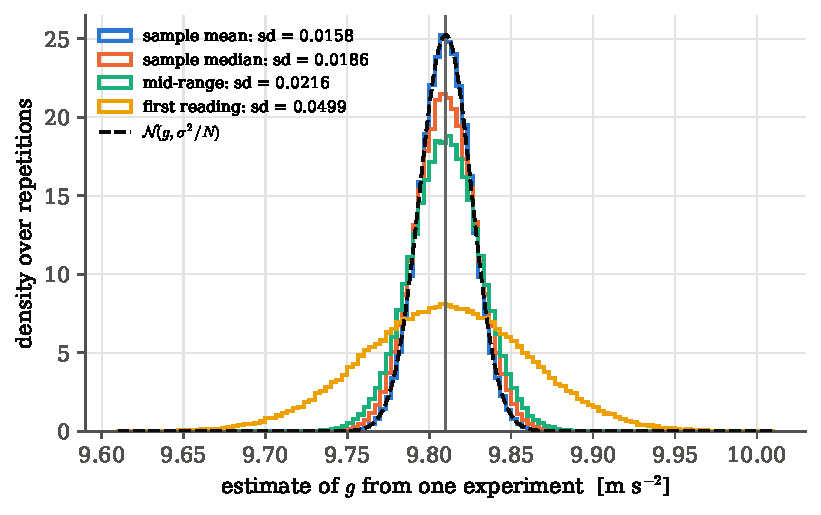
\includegraphics[width=11cm]{figures/ch03/sampling_gauss.pdf}
\caption{Sampling distributions of four estimators of $g$, each built from
the same $\ThreeAM$ simulated ten-reading experiments. All four are centred on
the true value (vertical line). The sample mean is the narrowest and sits on
the derived curve $\Normal(g,\sigma^2/N)$. Using only the first reading gives
a distribution as wide as the noise itself.}
\label{3a:fig:sampling-gauss}
\end{figure}

The numbers: the sample mean scatters by $\ThreeASdMean$ against the derived
$\sigma/\sqrt{N}=\ThreeASdTheory$; the median by $\ThreeASdMedian$ (its
variance is $\ThreeAMedianVarRatio$ times larger, tending to $\pi/2\approx1.57$
for large $N$ with Gaussian noise); the mid-range by $\ThreeASdMidrange$; the
first reading by $\ThreeASdFirst\approx\sigma$. All four recipes are
``right on average''. They differ in how much they scatter, and that is what
makes one of them better. \Cref{3a:sec:bias-variance} makes ``better''
precise.

\begin{figure}[htbp]
\centering
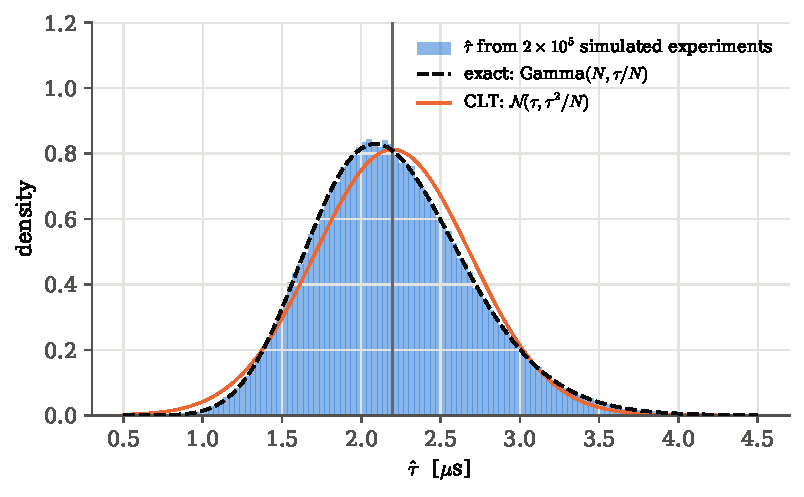
\includegraphics[width=10.5cm]{figures/ch03/sampling_lifetime.pdf}
\caption{Sampling distribution of the lifetime estimate from twenty decays.
The histogram of simulated $\hat\tau$ follows the exact Gamma density
\eqref{3a:eq:gamma-sampling} (dashed), including its longer right tail. The
Gaussian with the same mean and width (solid) is close but visibly too
symmetric.}
\label{3a:fig:sampling-lifetime}
\end{figure}

The simulated mean and spread of $\hat\tau$ are $\ThreeATauMean$ and
$\ThreeATauSd\,\mu$s, against the derived $\tau=2.197$ and
$\tau/\sqrt{20}=0.491\,\mu$s.

\paragraph{What this bought us.}
An estimator is a recipe, so it has a sampling distribution. The standard
error is the width of that distribution, not the width of the data: with ten
readings of noise $\sigma$ the sample mean scatters by $\sigma/\sqrt{10}$, a
single reading by $\sigma$.

\begin{center}\small
\begin{tabularx}{\linewidth}{@{}lXl@{}}
\toprule
word & what it is & pendulum example\\
\midrule
parameter $\theta$ & fixed, unknown number labelling the true distribution & the true $g$\\
statistic & any function of the data with no unknowns & $\max_i x_i$, $\sum x_i^2$\\
estimator $\hat\theta$ & a statistic used to guess $\theta$; a random variable & $\bar X=N^{-1}\sum X_i$\\
estimate & the estimator evaluated on our data; one number & $9.815$\\
standard error & width of the estimator's sampling distribution & $\sigma/\sqrt N=0.016$\\
\bottomrule
\end{tabularx}
\end{center}

\begin{pitfall}[What is random and what is fixed]
In the frequentist picture, $\theta$ is fixed and $\hat\theta$ is
random. A statement such as ``$g=9.815\pm0.016$'' is shorthand for a statement
about the \emph{recipe}: applied to repeated experiments, it lands within
$0.016$ of the truth about two times in three. It is not a probability
distribution for $g$. Probability distributions \emph{for} parameters are the
Bayesian answer of \cref{ch:05}, and the precise meaning of an interval is the
subject of \cref{ch:04}.
\end{pitfall}

\paragraph{A first look at intervals and tests.}
The sampling distribution also gives the two other basic tools of
statistics, intervals and tests. Suppose $\hat\theta_N$ is approximately
Gaussian with estimated standard error $\widehat{\operatorname{se}}$ (the
central limit theorem of \cref{3a:sec:lln-clt} explains why this is so
common). Then the interval
$C_N=(\hat\theta_N-z_{\alpha/2}\widehat{\operatorname{se}},\ \hat\theta_N+z_{\alpha/2}\widehat{\operatorname{se}})$
with $z_{\alpha/2}=\Phi^{-1}(1-\alpha/2)$ ($\Phi$ is the standard normal
distribution function) traps the fixed $\theta$ in a
fraction $1-\alpha$ of repetitions as $N\to\infty$ \mainref{p.~94, Thm~6.16}.
For $\alpha=0.05$, $z_{\alpha/2}=1.96\approx2$: ``estimate $\pm$ two standard
errors''. For the
Bernoulli case the interval is
$\hat p\pm z_{\alpha/2}\sqrt{\hat p(1-\hat p)/N}$ \mainref{Ex.~6.17}.

A \newterm{hypothesis test} uses the same sampling distribution the other
way round. We start from a default hypothesis, such as ``the coin is fair'',
$p=1/2$. Under it we know how $T=|\hat p-1/2|$ is distributed. If the
observed $T$ is larger than the default would usually produce, we reject the
default \mainref{p.~95, Ex.~6.18}. Both ideas are developed properly in
\cref{ch:04}.

\paragraph{Verification and research.}
Here the Monte Carlo \emph{verifies} a result we can derive,
$\operatorname{se}(\bar X)=\sigma/\sqrt N$. The same few lines, ``simulate the
experiment many times, apply the recipe, histogram the output'', are the
\emph{research instrument} when no formula exists. The sampling distribution
of a CMB power spectrum estimated from a masked, noisy, beam-smoothed map
(\cref{ch:08}), or of a topological summary of a field such as its Euler
characteristic (\cref{ch:12}), is obtained in exactly this way, with a
simulator of the sky in place of \pyname{rng.standard_normal}.

\section{Aiming and scattering: bias, variance and mean squared error}
\label{3a:sec:bias-variance}

Charged particles cross a silicon strip detector and leave hits whose
positions along one strip are uniformly spread between $0$ and the strip's
unknown active length $\theta$. We record $n=10$ hit positions. Three
colleagues propose three recipes. The first doubles the average position
(the average of a uniform variable sits in the middle). The second takes
the largest position seen (no hit can be beyond the end). The third takes
the largest position and nudges it up a little, because the largest of ten
hits is almost never exactly at the end.

Which recipe should we use? Each one is a guess at $\theta$, and each guess
misses by some amount that changes from experiment to experiment. The fair
comparison is the average squared miss, the mean squared error. It splits
into two parts every experimentalist already knows: a systematic offset and
a statistical scatter.

\paragraph{Darts at a target.}
Picture the sampling distribution of \cref{3a:sec:sampling} as a cluster of
darts around a bull's-eye at the true value. Two things can go wrong. The
cluster can be centred in the wrong place (a thrower with a consistent pull
to the left), or it can be wide (a shaky hand). The first is \emph{bias}, the
second is \emph{variance}. A good estimator needs both to be small, and it
may be worth accepting a little of one to remove a lot of the other.

\begin{figure}[htbp]
\centering
\begin{tikzpicture}[font=\small]
  \pgfmathsetseed{7}
  \foreach \col/\bx/\s/\ttl [count=\k] in
      {0/0/0.18/{low bias\\ low variance},
       1/0.55/0.18/{high bias\\ low variance},
       2/0/0.55/{low bias\\ high variance},
       3/0.55/0.55/{high bias\\ high variance}}{
    \begin{scope}[xshift=\col*3.3cm]
      \draw[faint] (0,0) circle (1.2);
      \draw[faint] (0,0) circle (0.8);
      \draw[faint] (0,0) circle (0.4);
      \fill[bdryred] (0,0) circle (1.2pt);
      \foreach \i in {1,...,14}{
        \pgfmathsetmacro{\px}{\bx+\s*rand}
        \pgfmathsetmacro{\py}{0.25*\bx+\s*rand}
        \fill[formblue] (\px,\py) circle (1.5pt);
      }
      \node[align=center,font=\footnotesize] at (0,-1.6) {\ttl};
    \end{scope}
  }
\end{tikzpicture}
\caption{Four throwers, fourteen darts each. The red dot is the true value of
the parameter and every blue dot is the estimate from one repetition of the
experiment. Moving the whole cluster off the centre is bias. Spreading it out
is variance. The mean squared error is the average squared distance of the
darts from the red dot, and it grows with both.}
\label{3a:fig:darts}
\end{figure}

\paragraph{The questions, in words.}
\begin{enumerate}[label=\arabic*.]
  \item Over many repetitions, where is the recipe's output centred? Is that
        the true value? (Bias.)
  \item How widely does the output scatter about its own centre? (Variance,
        or its square root, the standard error.)
  \item On average, how far is the output from the \emph{truth}, counting
        both effects? (Mean squared error.)
  \item As we take more data, does the output settle down on the truth?
        (Consistency.)
\end{enumerate}

\subsection{Bias, variance and their sum}
\label{3a:sec:mse}

Two things can be wrong with an estimator: its centre can be off, and its
spread can be large. Each has a name, and the two combine into one measure of
total error.

\begin{workdef}[bias, unbiased, mean squared error]
The \newterm{bias} of an estimator $\hat\theta_n$ is
\begin{equation}
  \operatorname{bias}(\hat\theta_n)=\E_\theta(\hat\theta_n)-\theta
  \label{3a:eq:bias}
\end{equation}
\unpack{the offset of the centre of the sampling distribution from the
truth, at this fixed $\theta$}. The estimator is \newterm{unbiased} if the
bias is zero for \emph{every} $\theta$ in $\Theta$. The \newterm{mean
squared error} is
\begin{equation}
  \operatorname{MSE}(\hat\theta_n)=\E_\theta\bigl[(\hat\theta_n-\theta)^2\bigr]
  \label{3a:eq:mse-def}
\end{equation}
\unpack{the average over repetitions of the squared miss distance}.
\end{workdef}

Both are functions of the unknown $\theta$, because the average is taken
with $f(x;\theta)$. The two ideas fit together exactly: the MSE is the
variance plus the squared bias. To show it, call the centre of the sampling
distribution $\bar\theta_n\defeq\E_\theta(\hat\theta_n)$. It is a fixed
number, not a random variable. Then
\begin{align}
  \operatorname{MSE}(\hat\theta_n)
  &\eqby{1} \E_\theta\bigl[(\hat\theta_n-\bar\theta_n+\bar\theta_n-\theta)^2\bigr]
     \nonumber\\
  &\eqby{2} \E_\theta\bigl[(\hat\theta_n-\bar\theta_n)^2\bigr]
     +2(\bar\theta_n-\theta)\,\E_\theta\bigl[\hat\theta_n-\bar\theta_n\bigr]
     +(\bar\theta_n-\theta)^2 \nonumber\\
  &\eqby{3} \E_\theta\bigl[(\hat\theta_n-\bar\theta_n)^2\bigr]+(\bar\theta_n-\theta)^2
     \nonumber\\
  &\eqby{4} \Var_\theta(\hat\theta_n)+\operatorname{bias}^2(\hat\theta_n).
  \label{3a:eq:mse-decomp}
\end{align}
\begin{explain}
  \item Add and subtract the constant $\bar\theta_n$ inside the square.
  \item Expand $(a+b)^2=a^2+2ab+b^2$ with $a=\hat\theta_n-\bar\theta_n$ (random)
        and $b=\bar\theta_n-\theta$ (constant). Constants come out of the
        expectation, and $\E(b^2)=b^2$.
  \item $\E_\theta[\hat\theta_n-\bar\theta_n]=\bar\theta_n-\bar\theta_n=0$ by the
        definition of $\bar\theta_n$, so the cross term vanishes.
  \item The first term is the variance by definition. The second is the
        squared bias \eqref{3a:eq:bias}.
\end{explain}

\begin{keyidea}[MSE = bias$^2$ + variance]
The mean squared error of any estimator is the square of its systematic
offset plus the square of its statistical scatter,
$\operatorname{MSE}=\operatorname{bias}^2+\operatorname{se}^2$. For an
unbiased estimator the MSE is just the variance.
\end{keyidea}

Why is the result true, beyond the algebra? It is Pythagoras. The miss
$\hat\theta_n-\theta$ is a fixed offset $b$ (the bias) plus a random part
$a$ whose average is zero. Squaring gives $a^2+2ab+b^2$. The cross term
averages to zero, because $b$ is a constant and $a$ averages to zero. So the
two parts add in square, like the two perpendicular sides of a right
triangle. The same identity is the parallel-axis theorem of mechanics: the
moment of inertia about the true value equals the moment about the centre of
mass plus the total mass times the squared distance between the two.

\paragraph{Statistics and the laboratory.}
\begin{center}\small
\begin{tabular}{@{}ll@{}}
\toprule
statistics & laboratory\\
\midrule
bias & systematic error (a miscalibrated scale)\\
standard error & statistical error (shrinks with more data)\\
$\operatorname{MSE}=\operatorname{bias}^2+\operatorname{se}^2$ & ``add the errors in quadrature''\\
unbiased estimator & a method with no systematic offset, for every true value\\
consistent estimator & a method that homes in on the truth as data accumulate\\
\bottomrule
\end{tabular}
\end{center}

The variance of the estimator is the \emph{statistical} error. A bias, or a
mistake in the model, is a \emph{systematic} error, and more data do not
remove it \srcref{Cowan}{\S5.1, (5.5)}. One caution about the quadrature
row. Physicists add a systematic in quadrature because they treat its
unknown size as random, drawn from an ensemble of possible miscalibrations.
The bias in \eqref{3a:eq:mse-decomp} is not random. It is a definite, if
unknown, number, and it enters squared for a purely algebraic reason: the
cross term vanished.

\subsection{Three recipes for the strip length}
\label{3a:sec:uniform}

Back to the silicon strip from the start of this section. A strip of unknown
active length $\theta$ records $n=10$ hits, and each hit position $X_i$ is
equally likely to be anywhere along it, $X_i\sim\mathrm{Uniform}(0,\theta)$,
with density $1/\theta$ on $[0,\theta]$. The three colleagues each proposed a
way of turning the ten positions into one number for $\theta$, that is, an
estimator $\hat\theta=g(X_1,\dots,X_n)$ in the sense of \cref{3a:sec:estimator}.
It is customary to call a candidate estimator $T$ (for a statistic of the data),
and we number the three candidates in the order the colleagues proposed them.
Two ingredients appear in them: the sample mean
$\bar X=\frac1n\sum_{i=1}^nX_i$, and the largest of the ten positions, written
$X_{(n)}=\max_iX_i$ (the subscript in parentheses means ``the $n$-th in order of
size''). The moments of a single hit we need are (from \cref{ch:02})
\begin{equation}
  \E X_i=\frac\theta2,\qquad \E X_i^2=\int_0^\theta\frac{x^2}{\theta}\dd x=\frac{\theta^2}{3},
  \qquad \Var X_i=\frac{\theta^2}{3}-\frac{\theta^2}{4}=\frac{\theta^2}{12}.
  \label{3a:eq:uniform-moments}
\end{equation}
The three recipes, written as formulas, are
\begin{align*}
  T_1&=2\bar X &&\text{double the average position (a uniform hit sits at $\theta/2$ on average),}\\
  T_2&=X_{(n)} &&\text{take the largest position (no hit can lie beyond the end),}\\
  T_3&=\tfrac{n+1}{n}\,X_{(n)} &&\text{nudge the largest position up (it almost never reaches the end).}
\end{align*}
For each recipe we ask the questions listed above: where is it centred, how
widely does it scatter, and what is its total error?

\paragraph{Example: Doubling the mean.}
\label{3a:ex:uniform-mean}
\begin{align*}
  \E T_1 &\eqby{1} 2\cdot\frac1n\sum_{i=1}^n\E X_i \eqby{2} 2\cdot\frac\theta2=\theta,\\
  \Var T_1 &\eqby{3} 4\,\Var\bar X \eqby{4} 4\cdot\frac{\theta^2}{12\,n}=\frac{\theta^2}{3n}.
\end{align*}
\begin{explain}
  \item Linearity of expectation.
  \item Each $\E X_i=\theta/2$ by \eqref{3a:eq:uniform-moments}.
  \item $\Var(cU)=c^2\Var U$ with $c=2$.
  \item $\Var\bar X=\Var X_i/n$ for independent readings (the same steps as in
        \cref{3a:ex:bernoulli}, and derived generally in \eqref{3a:eq:var-mean}).
\end{explain}
So $T_1$ is unbiased and $\operatorname{MSE}(T_1)=\theta^2/(3n)$. For $n=10$
and $\theta=1$ this is $0.0333$.

\paragraph{Example: The largest hit.}
\label{3a:ex:uniform-max}
We first need the sampling distribution of the maximum. The maximum is below
$t$ exactly when \emph{every} hit is below $t$. For $0\le t\le\theta$,
\begin{align*}
  \Prob(X_{(n)}\le t)
  &\eqby{1} \Prob(X_1\le t,\ X_2\le t,\ \dots,\ X_n\le t)
   \eqby{2} \prod_{i=1}^n\Prob(X_i\le t)
   \eqby{3} \Bigl(\frac t\theta\Bigr)^n .
\end{align*}
\begin{explain}
  \item ``The largest is at most $t$'' is the same event as ``all are at most $t$''.
  \item The hits are independent, so the joint probability factorises.
  \item For a uniform variable $\Prob(X_i\le t)=t/\theta$.
\end{explain}
Differentiating, the density is $g(t)=n\,t^{n-1}/\theta^n$ on $[0,\theta]$.
It piles up near the end of the strip, as the picture of ten hits suggests.
Its moments are
\begin{align*}
  \E X_{(n)} &\eqby{1} \int_0^\theta t\cdot\frac{n\,t^{n-1}}{\theta^n}\dd t
    \eqby{2} \frac{n}{\theta^n}\,\frac{\theta^{n+1}}{n+1}=\frac{n}{n+1}\,\theta,\\
  \E X_{(n)}^2 &\eqby{3} \frac{n}{\theta^n}\,\frac{\theta^{n+2}}{n+2}=\frac{n}{n+2}\,\theta^2,\\
  \Var X_{(n)} &\eqby{4} \frac{n}{n+2}\,\theta^2-\frac{n^2}{(n+1)^2}\,\theta^2
    \eqby{5} \frac{n\,\theta^2}{(n+1)^2(n+2)} .
\end{align*}
\begin{explain}
  \item Definition of the mean of a continuous variable with density $g$.
  \item $\int_0^\theta t^n\dd t=\theta^{n+1}/(n+1)$.
  \item The same integral with one more power of $t$: $\int_0^\theta t^{n+1}\dd t=\theta^{n+2}/(n+2)$.
  \item $\Var=\E X^2-(\E X)^2$.
  \item Common denominator: $n(n+1)^2-n^2(n+2)=n\bigl[(n+1)^2-n(n+2)\bigr]=n$.
\end{explain}
So $\operatorname{bias}(T_2)=\frac{n}{n+1}\theta-\theta=-\frac{\theta}{n+1}$:
the largest hit always falls short of the end. By \eqref{3a:eq:mse-decomp},
\begin{align*}
  \operatorname{MSE}(T_2)
  &\eqby{1} \frac{\theta^2}{(n+1)^2}+\frac{n\,\theta^2}{(n+1)^2(n+2)}
   \eqby{2} \frac{\theta^2\,\bigl[(n+2)+n\bigr]}{(n+1)^2(n+2)}
   = \frac{2\,\theta^2}{(n+1)(n+2)} .
\end{align*}
\begin{explain}
  \item Squared bias plus variance.
  \item Put both terms over the denominator $(n+1)^2(n+2)$. Then
        $2n+2=2(n+1)$ cancels one factor of $n+1$.
\end{explain}
For $n=10$: bias $=-1/11=\ThreeAUTwoBiasth$ and
$\operatorname{MSE}=2/132=\ThreeAUTwoMSEth$ (with $\theta=1$). Even though it
is biased, $T_2$ has less than half the MSE of the unbiased $T_1$.

\paragraph{Example: Correcting the bias.}
\label{3a:ex:uniform-corrected}
The bias of $T_2$ is known exactly, as a fraction of $\theta$, so we can
divide it out:
\begin{align*}
  \E T_3 &\eqby{1} \frac{n+1}{n}\,\E X_{(n)} \eqby{2} \frac{n+1}{n}\cdot\frac{n}{n+1}\,\theta=\theta,\\
  \Var T_3 &\eqby{3} \frac{(n+1)^2}{n^2}\cdot\frac{n\,\theta^2}{(n+1)^2(n+2)}
   =\frac{\theta^2}{n(n+2)} .
\end{align*}
\begin{explain}
  \item Linearity, with the constant $(n+1)/n$.
  \item The mean of the maximum from \cref{3a:ex:uniform-max}.
  \item $\Var(cU)=c^2\Var U$ with $c=(n+1)/n$, and the variance of the maximum.
\end{explain}
Now $\operatorname{MSE}(T_3)=\theta^2/(n(n+2))=1/120=\ThreeAUThreeMSEth$ for
$n=10$: unbiased \emph{and} four times better than $T_1$. For large $n$,
$\operatorname{MSE}(T_1)\propto1/n$ while $\operatorname{MSE}(T_3)\propto1/n^2$.
The maximum uses the one feature of the data (the sharp edge) that carries
the most information about $\theta$. The mean washes that edge out.

\paragraph{Seeing it in Python.}
\Cref{3a:lst:uniform} simulates $M=200\,000$ experiments of ten hits and
applies all three recipes to each.

\pyfile[firstline=24,lastline=36,label={3a:lst:uniform}]{code/ch03/02_bias_variance_uniform.py}{The three recipes and their derived bias and variance}

The function \pyname{estimators} takes a matrix whose rows are experiments
and returns the three estimates for each row. The function \pyname{theory}
encodes the formulas just derived, so the script can put the two side by
side. The simulated biases are $\ThreeAUOneBias$, $\ThreeAUTwoBias$ and
$\ThreeAUThreeBias$ (derived: $0$, $\ThreeAUTwoBiasth$, $0$). The simulated
MSEs are $\ThreeAUOneMSE$, $\ThreeAUTwoMSE$ and $\ThreeAUThreeMSE$ (derived:
$\ThreeAUOneMSEth$, $\ThreeAUTwoMSEth$, $\ThreeAUThreeMSEth$). Agreement to
the third digit is what $M=200\,000$ repetitions buy.

\begin{figure}[htbp]
\centering
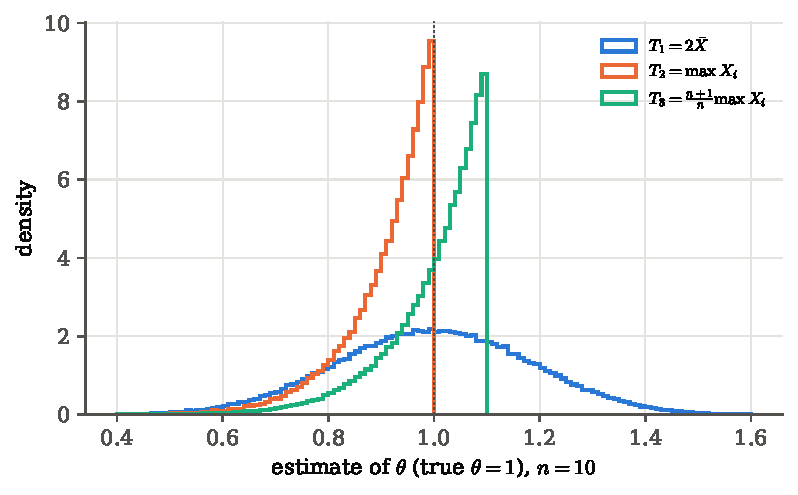
\includegraphics[width=11cm]{figures/ch03/uniform_estimators.pdf}
\caption{Sampling distributions of the three strip-length recipes with ten
hits each. Doubling the mean gives a broad, symmetric bump centred on the
truth. The largest hit gives a sharp distribution that ends exactly at the
truth and so sits entirely to its left. Stretching it by $11/10$ moves it
onto the truth and keeps it narrow.}
\label{3a:fig:uniform-estimators}
\end{figure}

\begin{figure}[htbp]
\centering
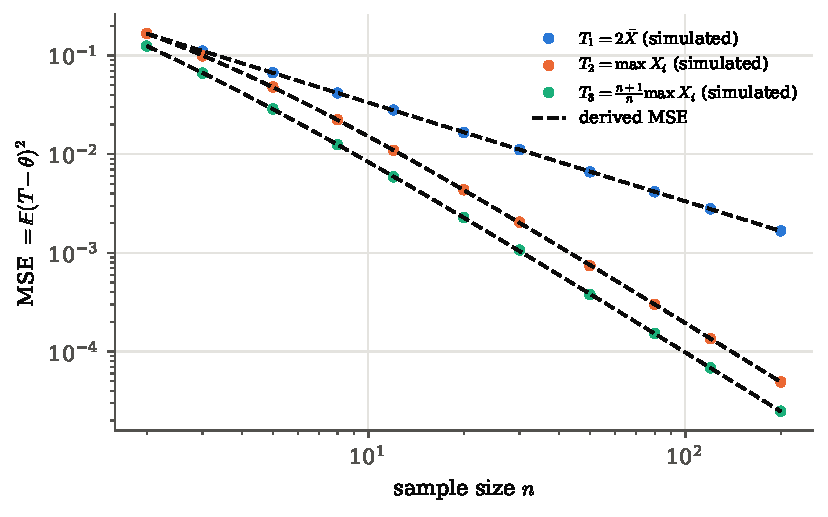
\includegraphics[width=10.5cm]{figures/ch03/uniform_mse.pdf}
\caption{Mean squared error against the number of hits, on log--log axes.
The points are simulations and the dashed curves the derived formulas.
Doubling the mean falls with slope $-1$. Both recipes built on the largest
hit fall with slope $-2$, and the corrected one stays below the uncorrected
one at every $n$.}
\label{3a:fig:uniform-mse}
\end{figure}

\subsection{The MSE depends on the truth}
\label{3a:sec:mse-theta}

For the strip, $T_3$ beat $T_1$ at every $\theta$. That is unusual. The MSE
is a function of the unknown truth, so one recipe can win for some true
values and lose for others. The simplest case shows how.

\paragraph{Example: Shrinking the mean towards zero.}
\label{3a:ex:shrinkage}
Let $X_1,\dots,X_n\sim\Normal(\mu,\sigma^2)$ and consider the family of
recipes $T_c=c\,\bar X$ with a constant $0<c\le1$. Then
\begin{align*}
  \operatorname{MSE}(T_c)
  &\eqby{1} \bigl(\E T_c-\mu\bigr)^2+\Var T_c
   \eqby{2} (c-1)^2\mu^2+c^2\,\frac{\sigma^2}{n}.
\end{align*}
\begin{explain}
  \item The decomposition \eqref{3a:eq:mse-decomp}.
  \item $\E T_c=c\mu$ and $\Var T_c=c^2\Var\bar X=c^2\sigma^2/n$.
\end{explain}
Setting the derivative with respect to $c$ to zero,
$2(c-1)\mu^2+2c\,\sigma^2/n=0$, gives the best constant
$c^\ast=\mu^2/(\mu^2+\sigma^2/n)$. It depends on the unknown $\mu$, so it is
not a recipe we can use. Fix $c<1$ instead and compare with $\bar X$, which
is $T_1$ here and has MSE $\sigma^2/n$. Shrinking lowers the variance term
by the factor $c^2$ but adds the bias term $(c-1)^2\mu^2$, which grows with
$\mu$. So shrinking wins when $\mu$ is near zero and loses when $\mu$ is far
from zero (\cref{3a:fig:mse-crossing}). With $\sigma^2/n=1$ and $c=0.8$ the
curves cross where $0.04\,\mu^2+0.64=1$, i.e.\ at $|\mu|=3$.

\begin{figure}[htbp]
\centering
\begin{tikzpicture}
\begin{axis}[width=9.5cm,height=5.4cm,xmin=-5,xmax=5,ymin=0,ymax=2.2,
  xlabel={true mean $\mu$ (in units of $\sigma/\sqrt n$)},
  ylabel={MSE (units of $\sigma^2/n$)},
  legend style={font=\footnotesize,at={(0.5,0.97)},anchor=north},
  tick label style={font=\footnotesize},label style={font=\small}]
  \addplot[very thick,formblue,domain=-5:5] {1};
  \addlegendentry{$\bar X$ (unbiased)}
  \addplot[very thick,fibreorange,domain=-5:5,samples=101] {0.04*x^2+0.64};
  \addlegendentry{$0.8\,\bar X$ (biased)}
  \draw[faint,dashed] (axis cs:3,0) -- (axis cs:3,1);
  \draw[faint,dashed] (axis cs:-3,0) -- (axis cs:-3,1);
  \fill[bdryred] (axis cs:3,1) circle (1.6pt);
  \fill[bdryred] (axis cs:-3,1) circle (1.6pt);
\end{axis}
\end{tikzpicture}
\caption{Mean squared error of two recipes for a Gaussian mean, as a function
of the true value. The sample mean has the same MSE everywhere. The shrunken
recipe wins inside $|\mu|<3$ and loses outside, and the two curves meet at the
red dots. Neither is better for every possible truth.}
\label{3a:fig:mse-crossing}
\end{figure}

\paragraph{There is usually no ``best'' estimator.}
Because the MSE is a function of $\theta$, two estimators are usually not
ordered: one wins for some true values and loses for others. The simplest
way to get a meaningful comparison is to restrict the class, for instance
to unbiased estimators, and look for the smallest variance inside it. That
programme leads to the Cram\'er--Rao bound and the Fisher information
(second half of \cref{ch:03} and \cref{ch:10}).

\begin{pitfall}[Unbiased is not the same as good]
An unbiased estimator can be much worse than a biased one. $T_1$ in the strip
example is unbiased and has four times the MSE of $T_3$ and twice that of
the biased $T_2$. Conversely, a biased estimator is not ``wrong'': Wasserman
notes that unbiasedness ``used to receive much attention but these days is
considered less important'' \mainref{p.~90}. What matters is the size of
the total error, and that it shrinks as data accumulate.
\end{pitfall}

\paragraph{Example: Poisson counts.}
\label{3a:ex:poisson}
A counter records $X_1,\dots,X_n\sim\mathrm{Poisson}(\lambda)$ events in $n$
equal time bins, and we estimate the rate by $\hat\lambda=\bar X$. From
\cref{ch:02}, $\E X_i=\Var X_i=\lambda$. Then
\begin{align*}
  \operatorname{bias}(\hat\lambda) &\eqby{1} \frac1n\sum_i\E X_i-\lambda=0,\\
  \operatorname{se}(\hat\lambda) &\eqby{2} \sqrt{\frac{\Var X_i}{n}}=\sqrt{\frac\lambda n},\\
  \operatorname{MSE}(\hat\lambda) &\eqby{3} 0^2+\frac\lambda n=\frac\lambda n .
\end{align*}
\begin{explain}
  \item Linearity and $\E X_i=\lambda$.
  \item Variance of a mean of independent readings, and $\Var X_i=\lambda$ for a Poisson variable.
  \item Decomposition \eqref{3a:eq:mse-decomp} with zero bias.
\end{explain}
The estimated standard error is $\sqrt{\hat\lambda/n}$. For $n=1$ this is the
familiar ``$\sqrt N$ error on $N$ counts'' \mainref{Exercise~6.1}.

\subsection{Consistency: does the recipe home in on the truth?}
\label{3a:sec:consistency}

A minimal demand on any recipe is that more data make it better, eventually
without limit. To say this precisely we must say what it means for a
sequence of random numbers to approach a constant. One random number can
still land anywhere, so ``approach'' has to be a statement about
probabilities. The simplest version is below (the other versions are in
\cref{3a:sec:convergence}).

\paragraph{Convergence in probability and consistency.}
A sequence of random variables $Y_n$ \newterm{converges in probability} to a
constant $c$, written $Y_n\xrightarrow{\;P\;}c$, if for every $\epsilon>0$
\begin{equation}
  \Prob\bigl(|Y_n-c|>\epsilon\bigr)\;\longrightarrow\;0\qquad(n\to\infty)
  \label{3a:eq:conv-prob}
\end{equation}
\unpack{any band around $c$, however narrow, eventually contains $Y_n$ in
almost all repetitions}. An estimator is \newterm{consistent} if
$\hat\theta_n\xrightarrow{P}\theta$ for every $\theta\in\Theta$.

To prove consistency we need a bound on the probability of a large miss.
One elementary inequality supplies it.

\paragraph{Markov and Chebyshev inequalities.}
If $Y\ge0$ and $t>0$, then $\Prob(Y\ge t)\le\E Y/t$ (Markov). Applied to
$Y=(U-a)^2$ with $t=\epsilon^2$ it gives, for any random variable $U$ and
any constant $a$,
\begin{equation}
  \Prob\bigl(|U-a|\ge\epsilon\bigr)\le\frac{\E\bigl[(U-a)^2\bigr]}{\epsilon^2}.
  \label{3a:eq:chebyshev}
\end{equation}
With $a=\E U$ the numerator is $\Var U$ (Chebyshev).

Markov's inequality is true for a reason we can see: a non-negative
quantity cannot have a big chunk of probability at large values without
dragging its average up. Written out, with $\mathbb{1}\{\cdot\}$ the
indicator that is $1$ when the condition holds and $0$ otherwise,
\begin{align}
  \E Y
  &\relby{1}{\ge} \E\bigl[Y\,\mathbb{1}\{Y\ge t\}\bigr]
   \relby{2}{\ge} \E\bigl[t\,\mathbb{1}\{Y\ge t\}\bigr]
   \eqby{3} t\,\Prob(Y\ge t).
  \label{3a:eq:markov}
\end{align}
\begin{explain}
  \item $Y\ge0$, so throwing away the part of the average where $Y<t$ cannot increase it.
  \item Where the indicator is $1$, $Y\ge t$. Where it is $0$, both sides are $0$.
  \item The average of an indicator is the probability of its event.
\end{explain}
Dividing by $t$ gives Markov. Now take $U=\hat\theta_n$ and $a=\theta$ in
\eqref{3a:eq:chebyshev}: the numerator is exactly the MSE, so
\begin{equation}
  \Prob\bigl(|\hat\theta_n-\theta|\ge\epsilon\bigr)
  \le\frac{\operatorname{MSE}(\hat\theta_n)}{\epsilon^2}
  =\frac{\operatorname{bias}^2(\hat\theta_n)+\operatorname{se}^2(\hat\theta_n)}{\epsilon^2}.
  \label{3a:eq:mse-consistency}
\end{equation}

\paragraph{A sufficient condition for consistency.}
If $\operatorname{bias}(\hat\theta_n)\to0$ and
$\operatorname{se}(\hat\theta_n)\to0$ as $n\to\infty$, then $\hat\theta_n$ is
consistent. The reason is \eqref{3a:eq:mse-consistency}: its right side then
goes to zero for every fixed $\epsilon$, and it bounds the probability of a
miss larger than $\epsilon$.

\paragraph{Example: Which recipes are consistent?}
\label{3a:ex:consistency}
\begin{itemize}
  \item $\hat p=\bar X$ for coin flips: bias $0$, $\operatorname{se}=\sqrt{p(1-p)/n}\to0$.
        Consistent \mainref{Ex.~6.11}.
  \item $T_2=X_{(n)}$ for the strip: bias $-\theta/(n+1)\to0$, variance
        $\sim\theta^2/n^2\to0$. \emph{Biased but consistent.}
  \item ``Use the first reading only'' for the pendulum: bias $0$ but
        $\operatorname{se}=\sigma$ for every $n$. The inequality tells us
        nothing, and indeed $\Prob(|X_1-g|>\epsilon)$ is the same fixed
        number for all $n$. \emph{Unbiased but not consistent.}
\end{itemize}
Bias and consistency are therefore independent properties. One is about
the centre of the sampling distribution at fixed $n$, the other about the
whole distribution as $n\to\infty$.

\paragraph{Try it.}
Show that $T_c=c_n\bar X$ with $c_n=n/(n+1)$ is biased for every finite $n$
and yet consistent for a Gaussian mean. (Compute its bias and variance and
let $n\to\infty$.)

\paragraph{What this bought us.}
Choose recipes by their total error, $\operatorname{MSE}=\operatorname{bias}^2
+\operatorname{se}^2$. Bias alone is a poor guide. A recipe whose bias and
standard error both vanish as the data grow is consistent, by Chebyshev's
inequality.

\paragraph{Verification and research.}
For the strip we could derive every number, and the simulation only checked
the algebra. In real analyses the recipe is often a long chain (a fit
inside a selection inside a reconstruction) and the bias has no formula. The
standard remedy is the same simulation used as an instrument: inject a known
truth into simulated data, run the full chain many times, and measure the
bias and scatter of the output. This ``injection--recovery'' test is how
the bias of a CMB power spectrum estimator on a masked sky is found and
removed (\cref{ch:08}).

\section{Why error bars shrink like $1/\sqrt N$: the law of large numbers and the central limit theorem}
\label{3a:sec:lln-clt}

Every accelerator physicist knows the rule of thumb: to halve the error on
a cross-section, collect four times the luminosity. A Monte Carlo
integration that gives two correct digits with $10^4$ samples needs $10^6$
for three. The rule has exceptions that bite. The average of energies
drawn from a Breit--Wigner resonance does not improve at all as we add
events.

Two theorems account for the rule and for its exceptions. The law of large
numbers says that an average settles on the true mean. The central limit
theorem says how it is distributed on the way: as a Gaussian of width
$\sigma/\sqrt N$, provided the readings have a finite variance $\sigma^2$.
The Breit--Wigner has none, and that is why it escapes the rule.

\paragraph{A random walk, rescaled.}
The sum of $N$ independent readings is a random walk of $N$ steps. Its
distance from the expected position grows like $\sqrt N$, the familiar
result from diffusion ($\langle x^2\rangle\propto t$). The mean is the sum
divided by $N$, so its scatter is $\sqrt N/N=1/\sqrt N$. And the shape of a
diffusing cloud forgets the shape of the individual step: after many steps
it is a Gaussian, whatever the kick distribution was. That is the central
limit theorem, the same statement as the approach of a diffusion kernel to
a heat-equation Gaussian.

\paragraph{What we want to know.}
\begin{enumerate}[label=\arabic*.]
  \item How does the scatter of an average depend on the number of readings,
        and on correlations between them?
  \item In what sense does a random average ``tend to'' the true mean? (There
        are several inequivalent senses.)
  \item What does the histogram of averages look like for large $N$, and how
        large is large?
  \item What breaks, and why, when the parent has no finite variance?
\end{enumerate}

\subsection{The variance of a sum and of a mean}
\label{3a:sec:var-mean}

The $1/\sqrt N$ comes from one identity: the variance of a sum is the sum of
all the variances and covariances of its terms. Let $X_1,\dots,X_N$ have
means $\mu_i$, variances $\sigma_i^2$ and covariances
$\Cov(X_i,X_j)=\E[(X_i-\mu_i)(X_j-\mu_j)]$, with $\Cov(X_i,X_i)=\sigma_i^2$.
For the sum,
\begin{align}
  \Var\Bigl(\sum_{i=1}^NX_i\Bigr)
  &\eqby{1} \E\Bigl[\Bigl(\sum_{i=1}^N(X_i-\mu_i)\Bigr)^2\Bigr]
   \eqby{2} \E\Bigl[\sum_{i=1}^N\sum_{j=1}^N(X_i-\mu_i)(X_j-\mu_j)\Bigr] \nonumber\\
  &\eqby{3} \sum_{i=1}^N\sum_{j=1}^N\Cov(X_i,X_j)
   \eqby{4} \sum_{i=1}^N\sigma_i^2+\sum_{i\neq j}\Cov(X_i,X_j) .
  \label{3a:eq:var-sum}
\end{align}
\begin{explain}
  \item By linearity the mean of the sum is $\sum\mu_i$. The variance is the
        mean squared deviation from it.
  \item The square of a sum is the double sum of all products.
  \item Linearity of expectation, term by term, and the definition of covariance.
  \item Split the double sum into the diagonal $i=j$ and the rest.
\end{explain}
If the readings are independent, every covariance with $i\neq j$ vanishes.
If they also share one variance $\sigma^2$, the mean $\bar X=N^{-1}\sum X_i$
has
\begin{equation}
  \E\bar X=\mu,\qquad
  \Var\bar X=\frac1{N^2}\,N\sigma^2=\frac{\sigma^2}{N},\qquad
  \operatorname{se}(\bar X)=\frac{\sigma}{\sqrt N}
  \label{3a:eq:var-mean}
\end{equation}
\mainref{p.~52, Thm.~3.17}, \srcref{Cowan}{(5.8), (5.13)}. This is the
$1/\sqrt N$. It needs nothing about the parent except a finite $\sigma$.

\paragraph{Example: Averaging a die.}
\label{3a:ex:dice}
For a fair die, $\E X=3.5$ and $\E X^2=(1+4+9+16+25+36)/6=91/6$, so
$\Var X=91/6-49/4=35/12=2.917$. The average of $50$ rolls therefore has
$\Var\bar X=2.917/50=0.0583$ and $\operatorname{se}=0.24$
\srcref{SeeingTheory}{pp.~38--39}. The individual rolls scatter over
$1$--$6$, their average over roughly $3.26$--$3.74$ (two thirds of the time).

\paragraph{Example: Correlated readings do not average away.}
\label{3a:ex:correlated-mean}
Suppose every pair of readings has the same correlation $\rho$, so
$\Cov(X_i,X_j)=\rho\sigma^2$ for $i\neq j$. This happens when a common
drift, such as a temperature change in the pendulum lab, moves all readings
together. There are $N(N-1)$ ordered pairs with $i\neq j$, so from
\eqref{3a:eq:var-sum}
\begin{align*}
  \Var\bar X
  &\eqby{1} \frac1{N^2}\Bigl[N\sigma^2+N(N-1)\rho\sigma^2\Bigr]
   \eqby{2} \frac{\sigma^2}{N}\bigl[1+(N-1)\rho\bigr]
   \;\xrightarrow{N\to\infty}\;\rho\,\sigma^2 .
\end{align*}
\begin{explain}
  \item Divide the variance of the sum by $N^2$. Diagonal terms give $N\sigma^2$, off-diagonal ones $N(N-1)\rho\sigma^2$.
  \item Factor out $\sigma^2/N$.
\end{explain}
With $\rho=0.1$ the error of the mean can never fall below
$\sqrt{0.1}\,\sigma=0.32\,\sigma$, however many readings we take. The ratio
$N_{\mathrm{eff}}=\sigma^2/\Var\bar X=N/[1+(N-1)\rho]$ is the number of
\emph{effectively independent} readings. The same quantity decides how
useful a correlated Markov chain is (\cref{ch:09}).

\subsection{What ``tends to'' means for random variables}
\label{3a:sec:convergence}

For numbers, $a_n\to a$ has one meaning. For random variables there are
several. A random variable is not one number: it is a rule that assigns a
value to every outcome of the experiment, and that rule has a distribution.
A sequence can approach its limit value by value, or only in its
distribution, and these are different things. Two simple sequences show the
difference \mainref{p.~71}. If $X_n\sim\Normal(0,1)$ for every $n$, independently, the
$X_n$ never settle anywhere, yet every one has the same distribution. If
$X_n\sim\Normal(0,1/n)$, the distributions squeeze onto $0$
(\cref{3a:fig:squeeze}), and we would like to say $X_n\to0$.

\begin{workdef}[three modes of convergence]
Let $X_n$ be random variables with distribution functions $F_n$, and $X$ a
random variable with distribution function $F$.
\begin{itemize}
  \item $X_n\xrightarrow{P}X$ (\newterm{in probability}) if
        $\Prob(|X_n-X|>\epsilon)\to0$ for every $\epsilon>0$
        \unpack{the chance of a miss bigger than $\epsilon$ dies out}.
  \item $X_n\rightsquigarrow X$ (\newterm{in distribution}) if
        $F_n(t)\to F(t)$ at every $t$ where $F$ is continuous \unpack{only the
        histograms converge, not the values themselves}.
  \item $X_n\xrightarrow{\text{qm}}X$ (\newterm{in quadratic mean}) if
        $\E(X_n-X)^2\to0$ \unpack{the mean squared miss dies out}.
\end{itemize}
\end{workdef}

\begin{figure}[htbp]
\centering
\begin{tikzpicture}
\begin{axis}[width=10cm,height=5cm,xmin=-3,xmax=3,ymin=0,ymax=4.3,
  xlabel={$x$},ylabel={density of $X_n$},samples=201,
  legend style={font=\footnotesize,draw=none,fill=none},legend pos=north east,
  tick label style={font=\footnotesize},label style={font=\small}]
  \addplot[thick,formblue!45,domain=-3:3] {exp(-x^2/2)/sqrt(2*pi)};
  \addlegendentry{$n=1$}
  \addplot[thick,formblue!70,domain=-3:3] {sqrt(10)*exp(-10*x^2/2)/sqrt(2*pi)};
  \addlegendentry{$n=10$}
  \addplot[thick,formblue,domain=-3:3] {sqrt(100)*exp(-100*x^2/2)/sqrt(2*pi)};
  \addlegendentry{$n=100$}
\end{axis}
\end{tikzpicture}
\caption{The densities of $X_n\sim\Normal(0,1/n)$ for $n=1,10,100$. The area
stays one while the width shrinks like $1/\sqrt n$, so all the probability
crowds onto the point $0$. This is the picture behind every mode of
convergence to a constant.}
\label{3a:fig:squeeze}
\end{figure}

\paragraph{Example: $X_n\sim\Normal(0,1/n)$ converges to $0$ in every sense.}
\label{3a:ex:squeeze}
In quadratic mean, $\E X_n^2=\Var X_n=1/n\to0$. In probability, by
Chebyshev \eqref{3a:eq:chebyshev}, $\Prob(|X_n|>\epsilon)\le1/(n\epsilon^2)\to0$.
In distribution, write $Z=\sqrt n X_n\sim\Normal(0,1)$ with distribution
function $\Phi$:
\begin{align*}
  F_n(t)=\Prob(X_n\le t)
  &\eqby{1} \Prob(\sqrt n X_n\le\sqrt n\,t)
   \eqby{2} \Phi(\sqrt n\,t)
   \;\xrightarrow{n\to\infty}\;
   \begin{cases}0,& t<0,\\ 1/2,& t=0,\\ 1,& t>0.\end{cases}
\end{align*}
\begin{explain}
  \item Multiply both sides of the inequality by $\sqrt n>0$.
  \item $\sqrt nX_n$ is standard normal.
\end{explain}
The limit $X=0$ (a point mass) has $F(t)=0$ for $t<0$ and $F(t)=1$ for
$t\ge0$. The two agree everywhere except at $t=0$, where
$F_n(0)=1/2\neq F(0)=1$. That one disagreement is not a failure of $X_n$ to
approach $0$. At $t=0$ the limit $F$ jumps from $0$ to $1$, and each $X_n$,
being symmetric about $0$, keeps exactly half its probability below the
jump. This is why the definition asks for convergence only where $F$ is
continuous: the jump points of $F$ are ignored \mainref{Ex.~5.3}.

\paragraph{How the modes are related.}
Quadratic mean implies in probability, which implies in distribution. The
converse implications fail in general. There is one important partial
converse: convergence in distribution \emph{to a constant} implies
convergence in probability to that constant \mainref{Thm.~5.4}.

\begin{figure}[htbp]
\centering
\begin{tikzcd}[column sep=huge,row sep=large]
  X_n\xrightarrow{\text{qm}}X \arrow[r,Rightarrow,shift left=3]
  & X_n\xrightarrow{P}X \arrow[r,Rightarrow,shift left=3]
      \arrow[l,Rightarrow,shift left=3,dashed,color=bdryred]
  & X_n\rightsquigarrow X
      \arrow[l,Rightarrow,shift left=3,dashed,color=bdryred]
\end{tikzcd}
\caption{Implications between the modes of convergence. The solid arrows
always hold. The dashed red arrows, pointing back, fail in general. The
dashed arrow from distribution back to probability does hold in one case:
when the limit is a single number, which is the case for consistency.}
\label{3a:fig:modes}
\end{figure}

Why each arrow holds, and why the reverse ones fail:
\begin{itemize}
  \item \emph{qm $\Rightarrow$ P.} Chebyshev with $U=X_n$, $a=X$:
        $\Prob(|X_n-X|>\epsilon)\le\E(X_n-X)^2/\epsilon^2\to0$. This is the
        argument of \eqref{3a:eq:mse-consistency}.
  \item \emph{P $\not\Rightarrow$ qm.} Let $U\sim\mathrm{Uniform}(0,1)$ and
        $X_n=\sqrt n$ if $U<1/n$, else $0$. Then
        $\Prob(|X_n|>\epsilon)=1/n\to0$, but $\E X_n^2=n\cdot(1/n)=1$ for
        every $n$. A rare but large value keeps the mean square alive. The
        same device with $X_n=n^2$ on probability $1/n$ gives
        $X_n\xrightarrow{P}0$ while $\E X_n=n\to\infty$: convergence in
        probability says nothing about averages \mainref{p.~75}.
  \item \emph{P $\Rightarrow$ D.} If $X_n$ is very probably within $\epsilon$
        of $X$, then $\Prob(X_n\le t)$ is squeezed between
        $\Prob(X\le t-\epsilon)$ and $\Prob(X\le t+\epsilon)$ up to a vanishing
        error. At a continuity point both bounds tend to $F(t)$ as
        $\epsilon\to0$.
  \item \emph{D $\not\Rightarrow$ P.} Let $X\sim\Normal(0,1)$ and $X_n=-X$.
        Every $X_n$ has the distribution $\Normal(0,1)$, so $X_n\rightsquigarrow X$
        trivially, but $|X_n-X|=2|X|$ never shrinks.
\end{itemize}

Convergence in probability and in distribution survive the usual
operations \mainref{Thm.~5.5}: if $X_n\xrightarrow{P}X$ and
$Y_n\xrightarrow{P}Y$ then $X_n+Y_n\xrightarrow{P}X+Y$,
$X_nY_n\xrightarrow{P}XY$, and $h(X_n)\xrightarrow{P}h(X)$ for continuous $h$.
For convergence in distribution the analogous rule is \newterm{Slutsky's
theorem}: if $X_n\rightsquigarrow X$ and $Y_n\rightsquigarrow c$, a
\emph{constant}, then $X_n+Y_n\rightsquigarrow X+c$ and
$X_nY_n\rightsquigarrow cX$. (Without the constant it fails: $X_n$ and
$Y_n$ could each be $\Normal(0,1)$ but perfectly anticorrelated, so that
$X_n+Y_n=0$.)

There are two further modes: \emph{almost sure} convergence,
$\Prob(X_n\to X)=1$, which asks for convergence along each single sequence
of outcomes, and convergence in mean, $\E|X_n-X|\to0$. Only the first is
needed, once, for the strong law below.

\subsection{The law of large numbers}
\label{3a:sec:lln}

\paragraph{Weak law of large numbers.}
If $X_1,X_2,\dots$ are iid with mean $\mu$, then
$\bar X_N\xrightarrow{P}\mu$. The distribution of the sample mean piles up
on the true mean.

With a finite variance the proof is one line of Chebyshev
\eqref{3a:eq:chebyshev} with $U=\bar X_N$, $a=\mu$:
\begin{align}
  \Prob\bigl(|\bar X_N-\mu|>\epsilon\bigr)
  &\relby{1}{\le} \frac{\Var\bar X_N}{\epsilon^2}
   \eqby{2} \frac{\sigma^2}{N\epsilon^2}
   \;\xrightarrow{N\to\infty}\;0 .
  \label{3a:eq:wlln}
\end{align}
\begin{explain}
  \item Chebyshev's inequality, with $\E\bar X_N=\mu$ so that the numerator is the variance.
  \item Variance of the mean \eqref{3a:eq:var-mean}.
\end{explain}
The theorem holds even without a finite variance, provided $\E|X|<\infty$
\mainref{Thm.~5.6}. The \emph{strong} law says more: with probability one,
the running average of a single infinite sequence of readings converges to
$\mu$ \mainref{Thm.~5.18}. That is the version that justifies computing an
average along one long Monte Carlo run or one long Markov chain.

The law of large numbers is also a statement about the meaning of
probability. Let $X_i=\mathbb{1}\{\text{event }A\text{ on trial }i\}$. Then
$\bar X_N$ is the relative frequency of $A$ and $\mu=\Prob(A)$, so relative
frequencies converge to probabilities. The ``frequentist'' reading of
probability rests on this.

\paragraph{Example: How many tosses? Chebyshev against the truth.}
\label{3a:ex:coin-chebyshev}
For a fair coin, how large must $n$ be so that
$\Prob(0.4\le\bar X_n\le0.6)\ge0.7$? With $\mu=1/2$ and
$\Var\bar X_n=p(1-p)/n=1/(4n)$,
\begin{align*}
  \Prob(0.4\le\bar X_n\le0.6)
  &\eqby{1} 1-\Prob\bigl(|\bar X_n-\tfrac12|>0.1\bigr)
   \relby{2}{\ge} 1-\frac{1}{4n\,(0.1)^2}
   = 1-\frac{25}{n}.
\end{align*}
\begin{explain}
  \item The complement of ``within $0.1$ of $1/2$''.
  \item Chebyshev with $\Var\bar X_n=1/(4n)$ and $\epsilon=0.1$.
\end{explain}
The bound exceeds $0.7$ once $25/n\le0.3$, i.e.\ $n\ge84$ \mainref{Ex.~5.7}.
Chebyshev is a guarantee for \emph{every} distribution with this variance,
so it is pessimistic for any particular one. The exact binomial probability
at $n=84$ is $\ThreeACoinExact$. Using the Gaussian approximation of the next
subsection, $\Prob(|\bar X_n-\tfrac12|\le0.1)\approx2\Phi(0.1\sqrt n/0.5)-1\ge0.7$
requires $0.2\sqrt n\ge z_{0.85}=\ThreeAZeightyfive$, i.e.\
$n\ge\ThreeACoinNclt$, where the exact probability is $\ThreeACoinExactNclt$.

\paragraph{A sharper guarantee, and a first interval.}
Chebyshev uses only the variance, so it must hold for every distribution.
For Bernoulli readings (each $X_i$ is $0$ or $1$, with $\Prob(X_i=1)=p$) we
know more, and \newterm{Hoeffding's inequality} uses it:
$\Prob(|\bar X_n-p|>\epsilon)\le2e^{-2n\epsilon^2}$ \mainref{Thm.~4.5, (4.4)}.
This bound falls exponentially in $n$, not as $1/n$. With $n=100$ and
$\epsilon=0.2$ it gives $2e^{-8}=0.00067$, where Chebyshev gives only
$1/(4\cdot100\cdot0.04)=0.0625$ \mainref{Ex.~4.6}. (For the moderate
$\epsilon=0.1$ of the coin example, Chebyshev happens to be the stronger of
the two.)

The bound also gives an interval. Set the right side equal to a small
probability $\alpha$ and solve for $\epsilon$:
$\epsilon_n=\sqrt{\ln(2/\alpha)/(2n)}$. Then the interval $\hat p\pm\epsilon_n$
contains the true $p$ with probability at least $1-\alpha$, for \emph{every}
$p$ and every $n$, with no large-$n$ approximation \mainref{Ex.~6.15}. For
$\alpha=0.05$ and $n=100$, $\epsilon_n=\sqrt{3.689/200}=0.136$.

What does ``with probability at least $1-\alpha$'' refer to? Not to $p$,
which is fixed. It refers to the interval recipe, applied over repeated
experiments. A striking case makes the point: Wasserman's Ex.~6.14 builds a
legitimate 75\% interval that, on some data sets, is known with certainty to
contain $\theta$. So the sentence ``with probability 0.95, $p$ is contained
in the interval'', said of $\bar X\pm1.96\,S/\sqrt n$
\srcref{SeeingTheory}{p.~42}, is loose: the $0.95$ belongs to the recipe,
not to $p$. The full story of intervals is in \cref{ch:04}.

\subsection{The central limit theorem}
\label{3a:sec:clt}

The law of large numbers says where the sample mean goes. It does not say
how $\bar X_N$ is distributed on the way, which is what we need for error
bars. The central limit theorem does.

\begin{keyidea}[Central limit theorem]
Let $X_1,\dots,X_N$ be iid with mean $\mu$ and finite variance $\sigma^2$.
Then
\begin{equation}
  Z_N\defeq\frac{\bar X_N-\mu}{\sqrt{\Var\bar X_N}}=\frac{\sqrt N(\bar X_N-\mu)}{\sigma}
  \;\rightsquigarrow\;\Normal(0,1),
  \label{3a:eq:clt}
\end{equation}
that is, $\Prob(Z_N\le z)\to\Phi(z)$ for every $z$. Informally,
$\bar X_N\approx\Normal(\mu,\sigma^2/N)$ whatever the parent distribution.
\end{keyidea}

The theorem approximates probabilities, not values: ``it's the probability
statements that we are approximating, not the random variable itself''
\mainref{p.~77}. No single $\bar X_N$ becomes a Gaussian number; what becomes
Gaussian is the chance that $\bar X_N$ falls in a given range.

In practice we do not know $\sigma$. The theorem still holds with $\sigma$
replaced by the sample standard deviation $S_N$ of
\cref{3a:sec:sample-variance}. The reason: $S_N\xrightarrow{P}\sigma$, and
Slutsky's theorem lets us swap a factor that tends to a constant
\mainref{Thm.~5.10}. For random vectors,
$\sqrt N(\bar{\bm X}_N-\bm\mu)\rightsquigarrow\Normal(\bm 0,\bm\Sigma)$ with
$\bm\Sigma$ the covariance matrix of one reading \mainref{Thm.~5.12}.

\paragraph{Why it is true: cumulants add.}
The cleanest physicist's argument uses the \newterm{cumulant generating
function} $K_Y(t)=\ln\E\,e^{tY}=\sum_{k\ge1}\kappa_k t^k/k!$, the logarithm
of the moment generating function. Its Taylor coefficients $\kappa_k$ are
the \newterm{cumulants} \unpack{$\kappa_1$ is the mean, $\kappa_2$ the
variance, $\kappa_3/\kappa_2^{3/2}$ the skewness}. For independent $U,V$,
$\E e^{t(U+V)}=\E e^{tU}\,\E e^{tV}$, so $K_{U+V}=K_U+K_V$: cumulants of
independent variables add, like free energies of independent subsystems.
Let $Y_i=(X_i-\mu)/\sigma$, which has $\kappa_1=0$, $\kappa_2=1$, and write
$Z_N=N^{-1/2}\sum_iY_i$. Then
\begin{align}
  K_{Z_N}(t)
  &\eqby{1} \sum_{i=1}^N K_{Y}\bigl(t/\sqrt N\bigr)
   \eqby{2} N\sum_{k\ge2}\frac{\kappa_k}{k!}\,\frac{t^k}{N^{k/2}} \nonumber\\
  &\eqby{3} \frac{t^2}{2}+\frac{\kappa_3}{6\sqrt N}\,t^3+\frac{\kappa_4}{24\,N}\,t^4+\cdots
   \;\xrightarrow{N\to\infty}\;\frac{t^2}{2}.
  \label{3a:eq:clt-cumulants}
\end{align}
\begin{explain}
  \item Cumulants of independent variables add, and scaling $Y\to cY$ turns
        $K_Y(t)$ into $K_Y(ct)$, here with $c=1/\sqrt N$.
  \item Insert the series. The $k=1$ term is absent because $\kappa_1=0$.
  \item The $k=2$ term is $N\cdot\tfrac12t^2/N$. The $k$-th term carries
        $N^{1-k/2}$, which vanishes for every $k\ge3$.
\end{explain}
The limit $t^2/2$ is the cumulant generating function of $\Normal(0,1)$,
whose only nonzero cumulant is the variance. Every other cumulant of the
standardised mean dies, the skewness fastest, like $\kappa_3/\sqrt N$. For an
exponential parent $\kappa_3=2$, so the skewness of the mean is $2/\sqrt N$,
exactly the value we met for the muon lifetime in \cref{3a:ex:lifetime}.
(The rigorous proof uses the characteristic function $\E e^{itY}$, which
exists for every distribution, and the same expansion to second order
\mainref{Lemma~5.20}.)

\paragraph{How large is large?}
The expansion shows that the error of the Gaussian approximation is
controlled by the skewness divided by $\sqrt N$. The \newterm{Berry--Esseen
inequality} makes this quantitative \mainref{Thm.~5.11, (5.4)}:
\begin{equation}
  \sup_z\bigl|\Prob(Z_N\le z)-\Phi(z)\bigr|\le\frac{C\,\E|X_1-\mu|^3}{\sqrt N\,\sigma^3},
  \label{3a:eq:berry-esseen}
\end{equation}
with $C=33/4$ in Wasserman. (That constant is very generous. Much smaller
values, below one half, have since been proved.) Symmetric parents converge
fast. Skewed ones, like exponential lifetimes or Poisson counts with small
means, need more readings.

\paragraph{Example: Pile-up in a collider.}
\label{3a:ex:pileup}
The number of proton--proton interactions per bunch crossing is Poisson with
mean $\lambda=5$. Over $n=125$ crossings, what is the probability that the
average number of interactions is below $5.5$? With $\mu=\sigma^2=\lambda=5$,
\begin{align*}
  \Prob(\bar X_n<5.5)
  &\eqby{1} \Prob\Bigl(\frac{\sqrt n(\bar X_n-\mu)}{\sigma}<\frac{\sqrt n(5.5-\mu)}{\sigma}\Bigr)
   \eqby{2} \Prob\Bigl(Z<\frac{\sqrt{125}\times0.5}{\sqrt5}\Bigr)
   \approx \Phi(2.5)=0.9938 .
\end{align*}
\begin{explain}
  \item Subtract $\mu$, multiply by $\sqrt n/\sigma>0$: the event is unchanged.
  \item $\sqrt{125}/\sqrt5=\sqrt{25}=5$, times $0.5$ is $2.5$. By the CLT
        the left side is approximately standard normal.
\end{explain}
(The same numbers describe a count of errors in computer programs
\mainref{Ex.~5.9}.)

\paragraph{Example: When there is no variance: the Breit--Wigner.}
\label{3a:ex:cauchy}
A resonance of mass $m$ and width $\Gamma$ has the Breit--Wigner (Cauchy)
line shape, which in units $x=(E-m)/(\Gamma/2)$ is
$f(x)=1/[\pi(1+x^2)]$. Its tails fall like $x^{-2}$, so $\int|x|f\,\dd x$
diverges: it has no mean and no variance \srcref{Cowan}{\S2.8, \S5.2}. Its
characteristic function is $\phi(t)=\E e^{itX}=e^{-|t|}$. For the average of
$N$ independent draws,
\begin{align*}
  \E\,e^{it\bar X_N}
  &\eqby{1} \prod_{i=1}^N\E\,e^{i(t/N)X_i}
   \eqby{2} \bigl(e^{-|t|/N}\bigr)^N
   = e^{-|t|} .
\end{align*}
\begin{explain}
  \item The exponential of a sum is a product, and independence lets the average factorise.
  \item Each factor is the characteristic function at $t/N$.
\end{explain}
The average of $N$ Cauchy variables has \emph{exactly} the same distribution
as one of them. Averaging does not help at all. The half-width of the
central 50\% of $\bar X_N$ is $1$ (the quartiles of the Cauchy are $\pm1$)
for every $N$. The fix is to use a different estimator. The sample median of
Cauchy data \emph{is} consistent. For large $N$ its standard error is
$1/(2f(0)\sqrt N)$, the general large-$N$ result for a median at a point
where the density is $f(0)$; with $f(0)=1/\pi$ this is $\pi/(2\sqrt N)$.

\subsection{Seeing it in Python}
\label{3a:sec:clt-python}

\pyfile[firstline=27,lastline=43]{code/ch03/03_one_over_sqrtN.py}{Variance of the sample mean for three parents, and the Cauchy exception}

For each $N=1,2,4,\dots,1024$ the script draws $M=20\,000$ experiments of
$N$ readings from a uniform, an exponential and a Poisson parent, averages
each row, and records the variance of the $M$ averages. It also records the
half-width of the central 50\% of the averages for exponential and Cauchy
parents (a width that exists even when the variance does not). The fitted
log--log slopes of $\Var\bar X_N$ against $N$ are $\ThreeASlopeU$,
$\ThreeASlopeE$ and $\ThreeASlopeP$ (derived: $-1$). The Cauchy half-width is
$\ThreeACauchyIQRone$ at $N=1$ and $\ThreeACauchyIQRlast$ at $N=1024$
(derived: $1$ for all $N$).

\begin{figure}[htbp]
\centering
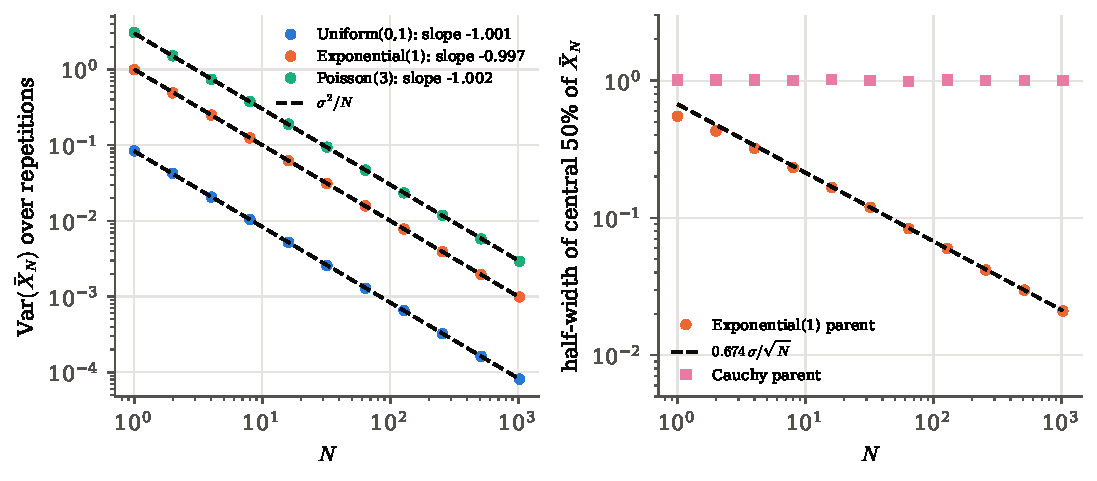
\includegraphics[width=12cm]{figures/ch03/var_mean_vs_N.pdf}
\caption{Left: the variance of the sample mean falls as $\sigma^2/N$ (dashed
lines) for three very different parents, a straight line of slope $-1$ on
log--log axes. Right: the width of the distribution of the mean falls as
$1/\sqrt N$ for exponential readings but stays flat for Cauchy readings,
where averaging a thousand values is no better than taking one.}
\label{3a:fig:var-mean-vs-N}
\end{figure}

\begin{figure}[htbp]
\centering
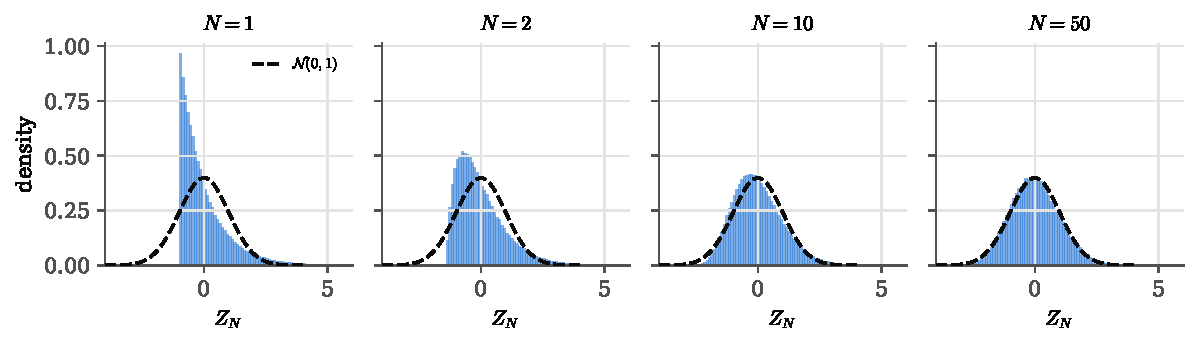
\includegraphics[width=12.5cm]{figures/ch03/clt_exponential.pdf}
\caption{The central limit theorem at work on exponential decay times.
Each panel is the histogram of the standardised mean $Z_N$ of $N$
exponential readings, over $200\,000$ repetitions, with the standard normal
curve dashed. At $N=1$ it is the exponential itself, cut off at $Z=-1$. By
$N=10$ it is close to Gaussian with a visible right skew, and by $N=50$ the
residual skewness $2/\sqrt{50}=0.28$ is hard to see.}
\label{3a:fig:clt-exponential}
\end{figure}

\paragraph{Asymptotically normal.}
An estimator is \newterm{asymptotically normal} if
$(\hat\theta_N-\theta)/\operatorname{se}\rightsquigarrow\Normal(0,1)$
\unpack{for large $N$ its sampling distribution is a Gaussian centred on the
truth with width equal to the standard error} \mainref{(6.8)}.

Most estimators we will meet are asymptotically normal: sample means by the
CLT, smooth functions of means by the delta method of
\cref{3a:sec:propagation}, and maximum-likelihood estimators by the argument
of the second half of \cref{ch:03}. That is why ``estimate $\pm$ standard
error'' means roughly a 68\% interval so often.

\begin{pitfall}[The CLT is about the mean, not about the data]
The CLT does not make the readings Gaussian, and it does not make every
statistic Gaussian. The histogram of individual muon decay times stays
exponential forever. It is the histogram of their \emph{average} that
becomes Gaussian. And it needs a finite variance: for Cauchy-like tails (a
resonance, a ratio of noisy quantities, \cref{3a:sec:ratio}) it fails
completely.
\end{pitfall}

\paragraph{What this bought us.}
Independent errors add like the steps of a random walk, so the scatter of a
mean is $\sigma/\sqrt N$ and its distribution approaches a Gaussian, with a
residual skewness that falls like $1/\sqrt N$. Correlations put a floor under
the error, and a parent without a variance defeats averaging altogether.

\paragraph{Verification and research.}
The log--log plot verifies $\sigma^2/N$ where we know $\sigma$. In a
Monte Carlo computation (\cref{ch:06}) we run the same check backwards: the
slope of the measured variance against $N$ tells us whether the samples are
really independent (slope $-1$) or correlated (a flatter slope, as for an
MCMC chain in \cref{ch:09}), and the plateau of a correlated run measures its
$N_{\mathrm{eff}}$.

\section{Estimating the scatter itself: the sample variance and its error}
\label{3a:sec:sample-variance}

The pendulum error bar $\sigma/\sqrt N$ contains the noise level $\sigma$,
which nobody told us. We must estimate it from the same ten readings. A
cosmologist faces the same task at every multipole: the angular power
spectrum $C_\ell$ \emph{is} a variance, the variance of the $2\ell+1$
spherical-harmonic coefficients $a_{\ell m}$, and estimating it from one sky
is estimating a variance from a finite sample. So is quoting the error bar
of a Monte Carlo average (\cref{ch:06}).

Two facts come out of this. The estimator of a variance that is right on
average divides by $N-1$, not by $N$. And that estimate has its own
uncertainty, the ``error on the error'', of which the cosmic-variance
formula is a special case.

\paragraph{Equipartition with the centre of mass removed.}
We cannot measure the spread of the readings about the unknown truth $\mu$,
only about their own average $\bar X$. Deviations from $\bar X$ are
systematically a little smaller than deviations from $\mu$, because the
average sits in the middle of the data by construction. How much smaller?
Think of $N$ particles of a gas,
each velocity component carrying energy $\tfrac12kT$ on average. If we
measure velocities relative to the centre of mass, one degree of freedom is
gone and the total relative kinetic energy is $(N-1)\tfrac12kT$. In the same
way, the $N$ deviations $X_i-\bar X$ sum to zero, only $N-1$ of them are
free, and each carries $\sigma^2$ on average.

\paragraph{What we want to know.}
\begin{enumerate}[label=\arabic*.]
  \item What is the average of $\sum_i(X_i-\bar X)^2$ over repetitions?
  \item What divisor makes the estimate of $\sigma^2$ right on average, and is
        that the best divisor?
  \item How much does the estimate of $\sigma^2$ itself scatter?
  \item What changes when the true mean is known, as for the $a_{\ell m}$
        of the CMB?
\end{enumerate}

\subsection{The $N-1$}
\label{3a:sec:n-minus-one}

Let $X_1,\dots,X_N$ be iid with mean $\mu$ and variance $\sigma^2$. The
question is the average, over repetitions, of the \newterm{sum of squared
deviations} $\mathrm{SS}=\sum_i(X_i-\bar X)^2$. We know the average of the
squared deviations from $\mu$; it is $\sigma^2$ each. So we first relate the
two sums. Write $X_i-\mu=(X_i-\bar X)+(\bar X-\mu)$ and square:
\begin{align}
  \sum_{i=1}^N(X_i-\mu)^2
  &\eqby{1} \sum_i(X_i-\bar X)^2+2(\bar X-\mu)\sum_i(X_i-\bar X)+N(\bar X-\mu)^2
     \nonumber\\
  &\eqby{2} \mathrm{SS}+N(\bar X-\mu)^2 .
  \label{3a:eq:ss-identity}
\end{align}
\begin{explain}
  \item Expand the square. The factor $\bar X-\mu$ does not depend on $i$ and
        comes out of the sum.
  \item $\sum_i(X_i-\bar X)=N\bar X-N\bar X=0$: deviations from the average sum
        to zero.
\end{explain}
This is again the parallel-axis theorem: spread about the truth equals
spread about the centre plus $N$ times the squared offset of the centre.
Now average over repetitions:
\begin{align}
  \E\,\mathrm{SS}
  &\eqby{1} \sum_{i=1}^N\E(X_i-\mu)^2-N\,\E(\bar X-\mu)^2
   \eqby{2} N\sigma^2-N\cdot\frac{\sigma^2}{N}
   = (N-1)\,\sigma^2 .
  \label{3a:eq:ess}
\end{align}
\begin{explain}
  \item Rearrange \eqref{3a:eq:ss-identity} and use linearity of expectation.
  \item $\E(X_i-\mu)^2=\sigma^2$ for each $i$, and $\E(\bar X-\mu)^2=\Var\bar X=\sigma^2/N$ from \eqref{3a:eq:var-mean}.
\end{explain}
The missing $\sigma^2$ is exactly the variance of the average: the data are
spread about $\bar X$, and $\bar X$ is itself off from $\mu$ by about
$\sigma/\sqrt N$.

\begin{workdef}[sample variance]
The \newterm{sample variance} is
\begin{equation}
  S^2=\frac{1}{N-1}\sum_{i=1}^N(X_i-\bar X)^2 ,
  \label{3a:eq:s2}
\end{equation}
and by \eqref{3a:eq:ess} it is unbiased, $\E S^2=\sigma^2$ \mainref{p.~52, Thm.~3.17}. The divisor
$N-1$ is the number of \newterm{degrees of freedom} \unpack{independent
directions left in the data after one direction was used to fix $\bar X$}.
If the true mean $\mu$ is \emph{known}, the estimator
$S_0^2=N^{-1}\sum_i(X_i-\mu)^2$ is unbiased with divisor $N$, since then
nothing was used up \srcref{Cowan}{(5.9)--(5.10)}.
\end{workdef}

\begin{figure}[htbp]
\centering
\begin{tikzpicture}[scale=1.0,font=\small]
  \draw[faint,->] (-0.3,0) -- (4.2,0) node[below] {$x_1$};
  \draw[faint,->] (0,-0.3) -- (0,3.8) node[left] {$x_2$};
  \draw[form,dashed] (-0.2,-0.2) -- (3.6,3.6);
  \node[formblue,anchor=west] at (3.6,3.6) {all readings equal};
  \coordinate (X) at (3.2,1.0);
  \coordinate (P) at (2.1,2.1);
  \coordinate (M) at (1.6,1.6);   %
  \draw[vec] (0,0) -- (X);
  \draw[fibre,very thick] (P) -- (X);
  \draw[bdry] (M) -- (P);
  \fill (X) circle (1.6pt);
  \fill[formblue] (P) circle (1.6pt);
  \fill[bdryred] (M) circle (1.6pt);
  \node[anchor=west] at (X) {$\ (x_1,x_2)$};
  \node[anchor=east,formblue] at (P) {$(\bar x,\bar x)\ $};
  \node[anchor=north west,bdryred] at (M) {$(\mu,\mu)$};
  \draw[thin] ($(P)!0.22cm!(X)$) -- ($(P)!0.22cm!(X)+(P)!0.22cm!(M)-(P)$) -- ($(P)!0.22cm!(M)$);
\end{tikzpicture}
\caption{Two readings as one point in the plane. The dashed diagonal holds
the data sets in which both readings are equal. The average $(\bar x,\bar x)$
is the foot of the perpendicular from the data point onto the diagonal. The
orange residual, of squared length $\mathrm{SS}$, lives in the one direction
perpendicular to the diagonal. The red segment is the offset of the average
from the truth. The right angle is the identity
\eqref{3a:eq:ss-identity}: distance$^2$ to the truth = orange$^2$ +
red$^2$.}
\label{3a:fig:projection}
\end{figure}

The geometry in \cref{3a:fig:projection} holds for any $N$. The data are a
vector in $\R^N$. The average is its projection on the line spanned by
$(1,1,\dots,1)$, and the residual vector $(X_i-\bar X)_i$ lives in the
$(N-1)$-dimensional subspace perpendicular to it. If the noise is isotropic
(independent, equal variance), each of those $N-1$ directions carries
variance $\sigma^2$, which is \eqref{3a:eq:ess} without algebra. For a
Gaussian parent we get the whole distribution, not just the average. Rotate
to a new orthonormal basis whose first axis is the diagonal. Independent
Gaussian noise of equal variance looks the same in every such basis, so the
new coordinates are again independent Gaussians of variance $\sigma^2$. The
first carries $\bar X$; the other $N-1$ carry the residual. So
$\mathrm{SS}/\sigma^2$ is a sum of $N-1$ squares of independent standard
normals, that is
\begin{equation}
  \frac{(N-1)S^2}{\sigma^2}\sim\chi^2_{N-1},
  \label{3a:eq:s2-chi2}
\end{equation}
independently of $\bar X$ (the $\chi^2$ distribution is in \cref{ch:02}).

\paragraph{Example: The pendulum's noise level.}
\label{3a:ex:pendulum-s}
For the ten readings of \cref{3a:sec:sampling}, $\bar x=9.815$ and the
deviations are $-0.025,0.015,0.045,-0.015,-0.045,0.025,-0.005,-0.035,0.035,0.005$.
Their squares sum to
$2(0.025^2+0.015^2+0.045^2+0.035^2+0.005^2)=2\times0.004125=0.00825$. Hence
\begin{align*}
  s^2 &\eqby{1} \frac{0.00825}{9}=9.17\times10^{-4},\qquad s=0.0303,\qquad
  \widehat{\operatorname{se}}(\bar x) \eqby{2} \frac{s}{\sqrt{10}}=0.0096\ \mathrm{m\,s^{-2}} .
\end{align*}
\begin{explain}
  \item Divide the sum of squared deviations by $N-1=9$.
  \item The estimated standard error of the mean replaces $\sigma$ by $s$ in \eqref{3a:eq:var-mean}.
\end{explain}
The result is $g=9.815\pm0.010\,\mathrm{m\,s^{-2}}$. How much should we trust
the ``$\pm0.010$''? That is the question of \cref{3a:sec:var-of-var}.

\paragraph{Example: $S^2$ is consistent.}
\label{3a:ex:s2-consistent}
Expanding the square in \eqref{3a:eq:s2},
$\sum_i(X_i-\bar X)^2=\sum_iX_i^2-N\bar X^2$, so
\begin{align*}
  S^2
  &\eqby{1} \frac{N}{N-1}\Bigl[\frac1N\sum_{i=1}^NX_i^2-\bar X^2\Bigr]
   \;\xrightarrow{\;P\;}\; 1\cdot\bigl[\E X^2-\mu^2\bigr] \eqby{2} \sigma^2 .
\end{align*}
\begin{explain}
  \item Factor out $N/(N-1)$. Inside the bracket, the first term is the mean of
        the iid variables $X_i^2$, which tends in probability to $\E X^2$ by the
        WLLN. $\bar X\xrightarrow{P}\mu$ and squaring is continuous, so
        $\bar X^2\xrightarrow{P}\mu^2$. Sums and products of sequences that
        converge in probability converge to the sums and products of the
        limits, and $N/(N-1)\to1$.
  \item $\E X^2-\mu^2=\sigma^2$.
\end{explain}
\srcref{CasellaBerger}{Ex.~5.5.3}; \mainref{Exercise~5.1}. The same argument
applied with the continuous map $\sqrt{\cdot}$ gives $S\xrightarrow{P}\sigma$.

\begin{pitfall}[$S$ is a biased estimator of $\sigma$]
Unbiasedness does not survive nonlinear maps. Because
$\Var S=\E S^2-(\E S)^2\ge0$, we have $(\E S)^2\le\E S^2=\sigma^2$, so
$\E S\le\sigma$, with equality only if $S$ never fluctuates (this is
Jensen's inequality for the concave square root). For Gaussian data,
$\E S=c_4(N)\,\sigma$ with
$c_4(N)=\sqrt{2/(N-1)}\;\Gamma(N/2)/\Gamma\bigl((N-1)/2\bigr)$, which follows
from the mean of the square root of a $\chi^2_{N-1}$ variable. For $N=5$,
$c_4=\ThreeACfourFive$; the simulation gives $\E S/\sigma=\ThreeAMeanSFive$.
$S$ is biased for every finite $N$ but consistent
\srcref{CasellaBerger}{Ex.~5.5.5}.
\end{pitfall}

\subsection{Is $N-1$ the best divisor?}
\label{3a:sec:best-divisor}

Unbiased is not the same as best (\cref{3a:sec:bias-variance}). For
Gaussian data we can compute the MSE of $W_d=\mathrm{SS}/d$ for any divisor
$d$, because by \eqref{3a:eq:s2-chi2} $\mathrm{SS}=\sigma^2\chi^2_{N-1}$ and
a $\chi^2_\nu$ variable has mean $\nu$ and variance $2\nu$.

\paragraph{Example: The divisor that minimises the MSE.}
\label{3a:ex:divisor}
\begin{align*}
  \operatorname{MSE}(W_d)
  &\eqby{1} \Bigl(\frac{(N-1)\sigma^2}{d}-\sigma^2\Bigr)^2+\frac{2(N-1)\sigma^4}{d^2}
   \eqby{2} \sigma^4\Bigl[\bigl((N-1)u-1\bigr)^2+2(N-1)u^2\Bigr],\quad u=\frac1d .
\end{align*}
\begin{explain}
  \item Squared bias plus variance \eqref{3a:eq:mse-decomp}, with $\E W_d=(N-1)\sigma^2/d$ and $\Var W_d=2(N-1)\sigma^4/d^2$.
  \item Factor out $\sigma^4$ and write $u=1/d$.
\end{explain}
Setting the $u$-derivative to zero,
$2(N-1)\bigl[(N-1)u-1\bigr]+4(N-1)u=0$, i.e.\ $(N+1)u=1$. The minimum is at
$d=N+1$. For $N=10$ the three candidates give
\[
  d=N-1:\ \tfrac29=0.222,\qquad d=N:\ 0.01+0.18=0.190,\qquad
  d=N+1:\ \tfrac{4}{121}+\tfrac{18}{121}=0.182
\]
(in units of $\sigma^4$). The simulation gives $\ThreeAMseNmOneTen$,
$\ThreeAMseNTen$ and $\ThreeAMseNpOneTen$.

So the unbiased $S^2$ does not have the smallest MSE. Even $d=N$ beats it
\srcref{CasellaBerger}{Exs.~7.3.3--7.3.4}: the biased maximum-likelihood
estimator $\hat\sigma^2=\mathrm{SS}/N$ has MSE $(2N-1)\sigma^4/N^2$, smaller
than the $2\sigma^4/(N-1)$ of $S^2$. A larger divisor shrinks the estimate
towards zero, trading a small downward bias for a reduction in variance.

Why, then, do we usually quote $S^2$? For two reasons. First, estimates are
often \emph{averaged} later, and when they are, biases add up while scatter
averages away; an unbiased estimate is then what we want. Second, the
optimal divisor depends on the parent: $N+1$ is special to Gaussian data.

\subsection{The variance of the variance}
\label{3a:sec:var-of-var}

How much does $S^2$ scatter? The answer involves the fourth central moment
$\mu_4=\E(X-\mu)^4$. Without loss of generality set $\mu=0$ (shifting every
reading by a constant changes neither $S^2$ nor the central moments). Using
$\sum_i(X_i-\bar X)^2=\sum_iX_i^2-\frac1N\sum_{i,j}X_iX_j$, split $S^2$ into
a ``diagonal'' and an ``off-diagonal'' part:
\begin{equation}
  S^2=\underbrace{\frac1N\sum_{i}X_i^2}_{A}\;-\;
  \underbrace{\frac{1}{N(N-1)}\sum_{i\neq j}X_iX_j}_{B} .
  \label{3a:eq:s2-split}
\end{equation}
(The coefficient of $X_i^2$ is $\frac{1}{N-1}(1-\frac1N)=\frac1N$, and that of
$X_iX_j$, $i\neq j$, is $\frac{1}{N-1}\cdot\frac1N$.) The variance of a
difference is $\Var(A-B)=\Var A+\Var B-2\Cov(A,B)$, so we need three pieces.
\begin{align}
  \Var A
  &\eqby{1} \frac{1}{N^2}\,N\,\Var(X^2)
   \eqby{2} \frac{\mu_4-\sigma^4}{N}, \label{3a:eq:varA}\\
  \E B^2
  &\eqby{3} \frac{1}{N^2(N-1)^2}\sum_{i\neq j}\sum_{k\neq l}\E[X_iX_jX_kX_l]
   \eqby{4} \frac{2N(N-1)\sigma^4}{N^2(N-1)^2}
   = \frac{2\sigma^4}{N(N-1)}, \label{3a:eq:varB}\\
  \Cov(A,B)
  &\eqby{5} \frac{1}{N^2(N-1)}\sum_k\sum_{i\neq j}\E[X_k^2X_iX_j]
   \eqby{6} 0 . \label{3a:eq:covAB}
\end{align}
\begin{explain}
  \item The $X_i^2$ are independent, so the variance of their sum is the sum of their variances.
  \item $\Var(X^2)=\E X^4-(\E X^2)^2=\mu_4-\sigma^4$ (recall $\mu=0$).
  \item $\E B=0$ because each term has $\E X_iX_j=\E X_i\,\E X_j=0$. So
        $\Var B=\E B^2$, which is the double sum over pairs of pairs.
  \item A product $X_iX_jX_kX_l$ with $i\neq j$ has zero mean unless every index
        appears at least twice, which forces $\{k,l\}=\{i,j\}$. There are two
        such choices, $(k,l)=(i,j)$ or $(j,i)$, each giving
        $\E X_i^2X_j^2=\sigma^4$. There are $N(N-1)$ ordered pairs $(i,j)$.
  \item $\E B=0$, so $\Cov(A,B)=\E[AB]$. Multiply out the two sums.
  \item Since $i\neq j$, at least one of $i,j$ differs from $k$ and from the
        other index, so it appears once and its factor $\E X=0$ kills the term.
\end{explain}
Putting the pieces together,
\begin{align}
  \Var S^2
  &\eqby{1} \Var A+\Var B-2\Cov(A,B)
   \eqby{2} \frac{\mu_4-\sigma^4}{N}+\frac{2\sigma^4}{N(N-1)} \nonumber\\
  &\eqby{3} \frac1N\Bigl[\mu_4-\frac{N-3}{N-1}\,\sigma^4\Bigr] .
  \label{3a:eq:var-s2}
\end{align}
\begin{explain}
  \item Variance of a difference.
  \item Insert \eqref{3a:eq:varA}--\eqref{3a:eq:covAB}.
  \item $-\sigma^4+\frac{2\sigma^4}{N-1}=-\sigma^4\,\frac{N-1-2}{N-1}$.
\end{explain}
This is \srcref{Cowan}{(5.14)}. For a Gaussian parent, $\mu_4=3\sigma^4$ (from
Isserlis' theorem, or by direct integration: $\E Z^4=3$ for a standard
normal), and
\begin{equation}
  \Var S^2\big|_{\text{Gauss}}
  =\frac{\sigma^4}{N}\,\frac{3(N-1)-(N-3)}{N-1}=\frac{2\sigma^4}{N-1},
  \label{3a:eq:var-s2-gauss}
\end{equation}
in agreement with $\Var\chi^2_{N-1}=2(N-1)$ in \eqref{3a:eq:s2-chi2}.

\paragraph{The error on the error.}
For Gaussian data the relative error of $S^2$ is $\sqrt{2/(N-1)}$, and that
of $S$ is half as large (a relative error halves under a square root; this
is the propagation rule of \cref{3a:sec:propagation}):
\begin{equation}
  \frac{\operatorname{se}(S)}{\sigma}\approx\frac{1}{\sqrt{2(N-1)}} .
  \label{3a:eq:error-on-error}
\end{equation}
With ten readings an error bar is itself uncertain by about 24\%. With a
hundred, by 7\%. Quoting an error bar to three significant figures from ten
points is meaningless.

For a heavy-tailed parent the variance of $S^2$ is larger, because $\mu_4$
weights the tails heavily. An exponential parent of mean $\tau$ has
$\sigma=\tau$ and $\mu_4=9\tau^4=9\sigma^4$, three times the Gaussian value.
To quote the
uncertainty of $S^2$ from data, replace $\mu_4$ by the sample moment
$m_4=\frac1N\sum_i(X_i-\bar X)^4$ \srcref{Cowan}{(5.15)}.

\paragraph{Example: Cosmic variance.}
\label{3a:ex:cosmic-variance}
In a statistically isotropic Gaussian sky, the $2\ell+1$ coefficients
$a_{\ell m}$ at multipole $\ell$ behave (for this count) like $2\ell+1$
independent real Gaussian variables of mean zero and variance $C_\ell$
(the precise complex bookkeeping is in \cref{ch:07}). The natural estimator
$\Chat=\frac{1}{2\ell+1}\sum_m|a_{\ell m}|^2$ is the known-mean estimator
$S_0^2$ with $N=2\ell+1$. With known mean zero, $\sum_ma_{\ell m}^2/C_\ell$
is a sum of $2\ell+1$ squared standard normals, i.e.\ $\chi^2_{2\ell+1}$, so
\begin{align*}
  \E\Chat &\eqby{1} \frac{C_\ell}{2\ell+1}\,(2\ell+1)=C_\ell,\qquad
  \Var\Chat \eqby{2} \frac{C_\ell^2}{(2\ell+1)^2}\cdot2(2\ell+1)=\frac{2C_\ell^2}{2\ell+1}.
\end{align*}
\begin{explain}
  \item A $\chi^2_\nu$ variable has mean $\nu$.
  \item It has variance $2\nu$, and $\Var(cU)=c^2\Var U$ with $c=C_\ell/(2\ell+1)$.
\end{explain}
This is \newterm{cosmic variance}: the relative error
$\sqrt{2/(2\ell+1)}$ is 63\% at the quadrupole $\ell=2$ and cannot be reduced,
because we have only one sky. It is the known-mean version of
\eqref{3a:eq:var-s2-gauss}, with $N$ in place of $N-1$ because no degree of
freedom is spent on estimating a mean.

\subsection{Seeing it in Python}
\label{3a:sec:var-python}

\pyfile[firstline=29,lastline=39]{code/ch03/04_sample_variance.py}{The two divisors and the scatter of $S^2$}

Each row of \pyname{x} is one experiment of $N$ standard normal readings
($\sigma=1$). The script forms $\mathrm{SS}$ row by row, divides by $N$ and
by $N-1$, and averages over the $M=100\,000$ rows. It also records the
variance of $S^2$ across rows and the MSE of the three divisors. The last
three lines repeat the variance measurement for an exponential parent. For
$N=5$ the average of $\mathrm{SS}/N$ is $\ThreeAVbiasFive$ (derived:
$4/5=0.8$) and of $\mathrm{SS}/(N-1)$ is $\ThreeAVunbFive$ (derived: $1$).
At $N=10$, $\Var S^2=\ThreeAVarSGaussTen$ for Gaussian readings (derived
$\ThreeAVarSGaussTenTh$) and $\ThreeAVarSExpTen$ for exponential ones
(derived from \eqref{3a:eq:var-s2} with $\mu_4=9$: $\ThreeAVarSExpTenTh$).

\begin{figure}[htbp]
\centering
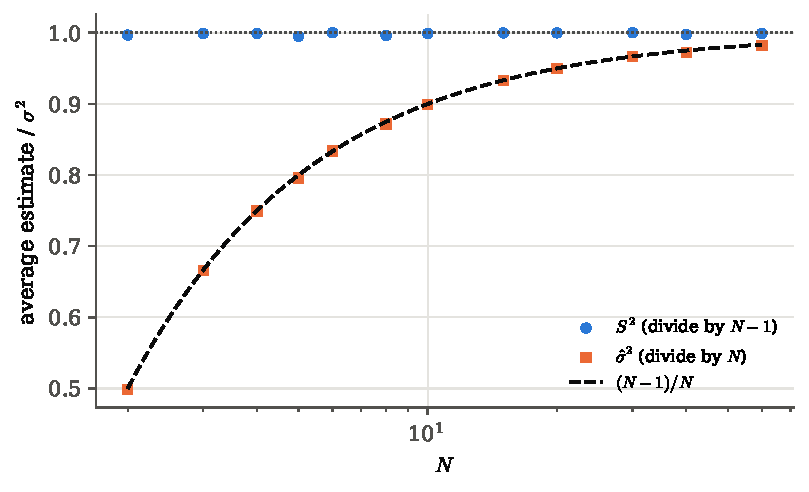
\includegraphics[width=10.5cm]{figures/ch03/variance_bias.pdf}
\caption{Average of two variance estimators over $100\,000$ Gaussian
experiments, as a function of the number of readings. Dividing by $N-1$ is
right on average at every $N$. Dividing by $N$ falls short by the factor
$(N-1)/N$ (dashed), badly for $N=2$ and negligibly beyond a few tens.}
\label{3a:fig:variance-bias}
\end{figure}

\begin{figure}[htbp]
\centering
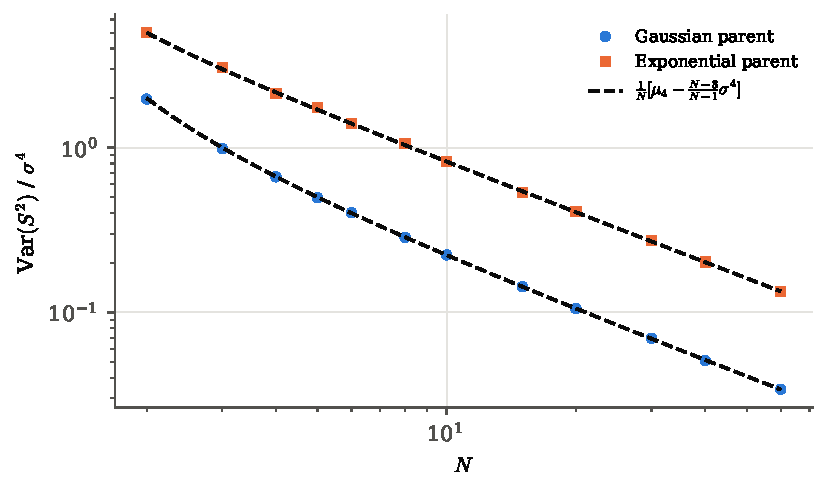
\includegraphics[width=10.5cm]{figures/ch03/variance_of_variance.pdf}
\caption{Scatter of the sample variance over repetitions. Both parents follow
the derived formula \eqref{3a:eq:var-s2} (dashed), falling roughly as $1/N$.
The exponential parent, with its long tail, has a variance of the variance
about four times larger than the Gaussian at the same $N$.}
\label{3a:fig:variance-of-variance}
\end{figure}

\paragraph{What this bought us.}
Divide by $N-1$ because one degree of freedom went into $\bar X$. The
resulting $S^2$ is unbiased but has its own scatter,
$\Var S^2=\frac1N[\mu_4-\frac{N-3}{N-1}\sigma^4]$, which for Gaussian data
means a relative error of $1/\sqrt{2(N-1)}$ on $S$. With a known mean the
divisor is $N$, and the Gaussian scatter $2\sigma^4/N$ is cosmic variance.

\paragraph{Verification and research.}
Here the simulation verifies \eqref{3a:eq:var-s2}. The formula is needed
later as an instrument: the error bar of any Monte Carlo estimate of a
variance, and hence of every simulated covariance matrix
(\cref{3a:sec:covariance}), is set by it. For a masked sky the $a_{\ell m}$
are no longer independent, the effective number of modes drops below
$2\ell+1$, often to roughly $\fsky(2\ell+1)$, and the true variance of the
power spectrum estimate is found by simulation (\cref{ch:08}).

\section{Estimating covariance and correlation matrices, and how noisy they are}
\label{3a:sec:covariance}

A CMB or galaxy-survey analysis compresses a map into $p=20$ band powers and
compares them with theory through a $\chi^2=(\data-\bm m)\T\Cmat^{-1}(\data-\bm m)$.
The covariance matrix $\Cmat$ of the band powers has no formula once masks
and noise enter, so we run $n$ simulations and estimate it from the scatter
of the simulated band powers. Supercomputer time limits us to, say, $n=50$.
The resulting matrix shows correlations between bins that are not there,
and its inverse is too large. In the same way a detector with twenty
readout channels shows ``cross-talk'' between channels that is just noise.

The sample variance, extended to a matrix, tells us how noisy each element
is, and so how large the false correlations can be. A change of variable
gives a reliable error bar for a real correlation. And a single factor
removes the bias of the inverse.

\paragraph{A tilted cloud, seen through few points.}
A correlation coefficient measures the tilt of a cloud of points in a
scatter plot. With a thousand points the tilt is obvious. With ten points
drawn from a perfectly round cloud, the ten happen to line up a little by
chance, and a tilt appears. A $20\times20$ correlation matrix has $190$
tilts to get wrong, so some of them will be large by chance. It is the same
reason why a few stars in the sky seem to form constellations.

\paragraph{The questions, in words.}
\begin{enumerate}[label=\arabic*.]
  \item How do we estimate, without bias, the covariance of two quantities
        from paired readings?
  \item If two quantities are truly unrelated, how large a sample
        correlation can chance produce?
  \item For a real correlation, what is the sampling distribution of its
        estimate, and how do we put an error bar on it?
  \item What happens when we invert a noisy covariance matrix?
\end{enumerate}

\subsection{The sample covariance matrix}
\label{3a:sec:sample-cov}

Recall from \cref{ch:02} the covariance
$\Sigma_{ab}=\Cov(X_a,X_b)=\E[(X_a-\mu_a)(X_b-\mu_b)]$ of two components of
a random vector $\bm X=(X_1,\dots,X_p)$, and the correlation
$\rho_{ab}=\Sigma_{ab}/\sqrt{\Sigma_{aa}\Sigma_{bb}}$, which lies in $[-1,1]$.

\begin{workdef}[sample covariance and correlation]
Given $n$ independent readings $\bm x_1,\dots,\bm x_n$ of a $p$-component
vector \unpack{each $\bm x_j$ is one simulation, or one event, giving all
$p$ numbers at once}, with average $\bar{\bm x}=n^{-1}\sum_j\bm x_j$, the
\newterm{sample covariance matrix} is
\begin{equation}
  \hat\Cmat=\frac{1}{n-1}\sum_{j=1}^n(\bm x_j-\bar{\bm x})(\bm x_j-\bar{\bm x})\T,
  \qquad
  \hat C_{ab}=\frac{1}{n-1}\sum_{j=1}^n(x_{aj}-\bar x_a)(x_{bj}-\bar x_b),
  \label{3a:eq:sample-cov}
\end{equation}
and the \newterm{sample correlation} is
\begin{equation}
  r_{ab}=\frac{\hat C_{ab}}{\sqrt{\hat C_{aa}\hat C_{bb}}}
  =\frac{\sum_j(x_{aj}-\bar x_a)(x_{bj}-\bar x_b)}
        {\sqrt{\sum_j(x_{aj}-\bar x_a)^2\,\sum_j(x_{bj}-\bar x_b)^2}} .
  \label{3a:eq:sample-corr}
\end{equation}
\end{workdef}

In \eqref{3a:eq:sample-corr} the factors $1/(n-1)$ cancel between numerator
and denominator, which gives the second form; by the Cauchy--Schwarz
inequality it always satisfies $|r|\le1$. The printed formula
\mainref{(14.6)} drops the $1/(n-1)$ from the numerator only, which would
let $|r|$ exceed $1$. The form above is the correct one and agrees with
\srcref{Cowan}{(5.12)}.

The diagonal of $\hat\Cmat$ holds the sample variances of
\cref{3a:sec:sample-variance}. The off-diagonal elements are unbiased by the
same argument. Write $\bm y_j=\bm x_j-\bm\mu$, so that
$\bm x_j-\bar{\bm x}=\bm y_j-\bar{\bm y}$, and use
$\sum_j(\bm y_j-\bar{\bm y})(\bm y_j-\bar{\bm y})\T=\sum_j\bm y_j\bm y_j\T-n\,\bar{\bm y}\bar{\bm y}\T$
(the matrix version of \eqref{3a:eq:ss-identity}):
\begin{align}
  \E\Bigl[\sum_{j}(\bm x_j-\bar{\bm x})(\bm x_j-\bar{\bm x})\T\Bigr]
  &\eqby{1} \sum_j\E[\bm y_j\bm y_j\T]-n\,\E[\bar{\bm y}\bar{\bm y}\T]
   \eqby{2} n\bm\Sigma-n\cdot\frac{\bm\Sigma}{n}
   = (n-1)\,\bm\Sigma .
  \label{3a:eq:cov-unbiased}
\end{align}
\begin{explain}
  \item Linearity of expectation applied element by element.
  \item $\E[\bm y_j\bm y_j\T]=\bm\Sigma$ by definition. For the mean,
        $\E[\bar y_a\bar y_b]=n^{-2}\sum_{j,k}\E[y_{aj}y_{bk}]=n^{-2}\cdot n\,\Sigma_{ab}$,
        because readings $j\neq k$ are independent with zero mean.
\end{explain}
So $\E\hat\Cmat=\bm\Sigma$ \mainref{p.~233, (14.4)}. A handy form for
computing is $\hat C_{ab}=\frac{n}{n-1}\bigl(\overline{x_ax_b}-\bar x_a\bar x_b\bigr)$,
where the bar means the average over readings \srcref{Cowan}{(5.11)}.

\paragraph{Example: A $2\times2$ covariance by hand.}
\label{3a:ex:cov-hand}
Four paired readings $(x,y)=(1,2),(2,1),(3,4),(4,3)$. Both averages are
$2.5$. The deviations are $\delta x=(-1.5,-0.5,0.5,1.5)$ and
$\delta y=(-0.5,-1.5,1.5,0.5)$. Then
\begin{align*}
  \hat C_{xx} &\eqby{1} \tfrac13(2.25+0.25+0.25+2.25)=\tfrac53,\qquad
  \hat C_{yy}\eqby{2}\tfrac53,\\
  \hat C_{xy} &\eqby{3} \tfrac13(0.75+0.75+0.75+0.75)=1,\qquad
  r \eqby{4} \frac{1}{\sqrt{(5/3)(5/3)}}=0.6 .
\end{align*}
\begin{explain}
  \item Squares of the $x$ deviations, divided by $n-1=3$.
  \item The $y$ deviations are a permutation of the $x$ ones, so the same sum.
  \item Products $(-1.5)(-0.5)$, $(-0.5)(-1.5)$, $(0.5)(1.5)$, $(1.5)(0.5)$, each $0.75$.
  \item Definition \eqref{3a:eq:sample-corr}.
\end{explain}
Four points already give a respectable-looking $r=0.6$. Is it real? To
answer, we need to know how large $r$ gets when there is no correlation at
all.

\subsection{Correlations from pure noise}
\label{3a:sec:spurious}

\begin{figure}[htbp]
\centering
\begin{tikzpicture}[font=\small]
  \coordinate (O) at (0,0);
  \coordinate (A) at (3.6,0.4);
  \coordinate (B) at (2.2,2.4);
  \draw[vec] (O) -- (A);
  \draw[vec,formblue] (O) -- (B);
  \node[anchor=west] at (A) {$\ \bm a=(x_{aj}-\bar x_a)_j$};
  \node[anchor=south,formblue] at (B) {$\bm b=(x_{bj}-\bar x_b)_j$};
  \pic[draw,angle radius=9mm,"$\varphi$",angle eccentricity=1.35] {angle=A--O--B};
  \draw[faint,dashed] (B) -- ($(O)!(B)!(A)$);
  \node[anchor=north east,align=right,font=\footnotesize] at (-0.2,-0.2)
       {$r=\cos\varphi=\dfrac{\bm a\cdot\bm b}{|\bm a|\,|\bm b|}$};
\end{tikzpicture}
\caption{The sample correlation as an angle. The deviations of the $n$
readings of each quantity form two vectors in $\R^n$, both perpendicular to
$(1,\dots,1)$ and so living in an $(n-1)$-dimensional space. The sample
correlation is the cosine of the angle between them. Uncorrelated noise
points $\bm b$ in a random direction relative to $\bm a$.}
\label{3a:fig:corr-angle}
\end{figure}

Formula \eqref{3a:eq:sample-corr} is a dot product divided by two lengths,
so it is the cosine of the angle between the two deviation vectors in
\cref{3a:fig:corr-angle}. This picture gives the spread of $r$ for unrelated
quantities without any integrals.

\paragraph{Example: The scatter of $r$ when $\rho=0$.}
\label{3a:ex:r-null}
Let the two quantities be independent Gaussians. As in
\cref{3a:fig:projection}, the deviation vectors live in the
$(m=n-1)$-dimensional subspace perpendicular to $(1,\dots,1)$, and in it the
Gaussian noise vector $\bm b$ is isotropic: its direction $\bm u=\bm b/|\bm b|$ is
uniformly distributed on the unit sphere, independently of $\bm a$. Rotate
coordinates so that $\bm a$ points along the first axis. Then $r=u_1$ and
\begin{align*}
  \E r \eqby{1} 0,\qquad
  \E r^2=\E u_1^2
  &\eqby{2} \frac1m\sum_{k=1}^m\E u_k^2
   \eqby{3} \frac1m\,\E\Bigl[\sum_{k=1}^mu_k^2\Bigr]
   \eqby{4} \frac1m=\frac{1}{n-1} .
\end{align*}
\begin{explain}
  \item $\bm u$ and $-\bm u$ are equally likely.
  \item By symmetry every component of a uniform unit vector has the same
        mean square.
  \item Linearity of expectation.
  \item A unit vector has $\sum_ku_k^2=1$ exactly.
\end{explain}
So for unrelated quantities $r$ scatters about zero with standard deviation
$1/\sqrt{n-1}$, and for large $n$ it is close to Gaussian. With $n=4$ as in
\cref{3a:ex:cov-hand}, $1/\sqrt3=0.58$: our $r=0.6$ is one standard deviation
from zero and means nothing.

\begin{keyidea}[Spurious correlations]
If $p$ quantities are truly independent, each of the $p(p-1)/2$ off-diagonal
sample correlations scatters about zero with standard deviation about
$1/\sqrt{n-1}$. Among many pairs, roughly 5\% exceed $1.96/\sqrt{n-1}$ in
magnitude by chance alone.
\end{keyidea}

With $p=20$ and $n=50$ there are $\ThreeANpairs$ pairs. The prediction is a
spread of $1/\sqrt{49}=\ThreeASpurSdTh$ and about ten pairs beyond
$|r|=0.28$. The simulation (\cref{3a:fig:spurious}) gives a spread of
$\ThreeASpurSd$ in one realisation and a largest $|r|$ of $\ThreeASpurMax$.
Searching a large matrix for the most correlated pair and then quoting its
significance as if it were the only pair examined is the \emph{look-elsewhere
effect} of \cref{ch:04}.

\begin{figure}[htbp]
\centering
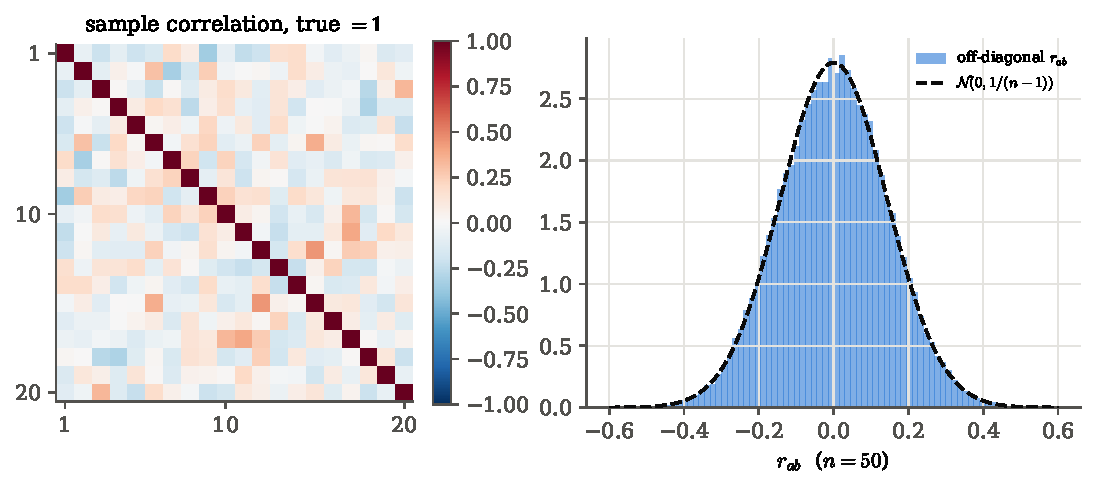
\includegraphics[width=12cm]{figures/ch03/spurious_correlations.pdf}
\caption{Left: the sample correlation matrix of twenty independent quantities
from fifty readings. The true matrix is the identity. Every coloured
off-diagonal square is noise, and some reach $\pm0.4$. Right: the
off-diagonal elements from 400 such matrices, with the Gaussian of standard
deviation $1/\sqrt{n-1}$ (dashed).}
\label{3a:fig:spurious}
\end{figure}

\subsection{A real correlation, its error bar, and Fisher's $z$}
\label{3a:sec:fisher-z}

For a bivariate Gaussian with correlation $\rho\neq0$, the sample correlation
is biased and skewed, with, to leading order in $1/n$
\srcref{Cowan}{(5.16)--(5.17)},
\begin{equation}
  \E r\approx\rho-\frac{\rho(1-\rho^2)}{2n},\qquad
  \Var r\approx\frac{(1-\rho^2)^2}{n}.
  \label{3a:eq:r-moments}
\end{equation}
The variance shrinks as $|\rho|\to1$, because $r$ cannot exceed $1$: the
sampling distribution is squashed against the wall and develops a long tail
towards zero. An error bar $r\pm\sqrt{\Var r}$ is then misleading, since it
depends on the unknown $\rho$ and may poke above $1$.

Fisher's remedy is a change of variable that makes the width independent of
$\rho$. We look for $z=h(r)$ with $\Var z$ constant. To first order in the
fluctuation (the propagation rule derived in \cref{3a:sec:propagation}),
$\Var h(r)\approx h'(\rho)^2\Var r$, so we need
$h'(\rho)\propto1/(1-\rho^2)$:
\begin{align}
  h(\rho)
  &\eqby{1} \int_0^\rho\frac{\dd s}{1-s^2}
   \eqby{2} \frac12\int_0^\rho\Bigl(\frac{1}{1+s}+\frac{1}{1-s}\Bigr)\dd s
   \eqby{3} \frac12\ln\frac{1+\rho}{1-\rho}=\operatorname{artanh}\rho .
  \label{3a:eq:fisher-z}
\end{align}
\begin{explain}
  \item Choose the integration constant so that $h(0)=0$.
  \item Partial fractions: $\frac{1}{1-s^2}=\frac12\bigl(\frac{1}{1+s}+\frac{1}{1-s}\bigr)$.
  \item Integrate: $\ln(1+s)-\ln(1-s)$, evaluated from $0$ to $\rho$.
\end{explain}
Then $\Var z\approx(1-\rho^2)^{-2}(1-\rho^2)^2/n=1/n$. A finer calculation
replaces $n$ by $n-3$, and $z$ is very nearly Gaussian even for small $n$:
\begin{equation}
  z=\operatorname{artanh}r\approx\Normal\Bigl(\operatorname{artanh}\rho,\ \frac{1}{n-3}\Bigr).
  \label{3a:eq:fisher-z-dist}
\end{equation}
The inverse map is $\rho=\tanh z=(e^{2z}-1)/(e^{2z}+1)$. The map stretches
the region near $\pm1$, which pulls the squashed tail back into a
symmetric shape.

\paragraph{Example: An interval for a correlation.}
\label{3a:ex:fisher-interval}
We observe $r=0.6$ from $n=20$ pairs. A 95\% interval is built in $z$ and
mapped back \mainref{p.~234}:
\begin{align*}
  \hat z &\eqby{1} \operatorname{artanh}0.6=\tfrac12\ln4=0.693,\qquad
  \frac{1.96}{\sqrt{n-3}} \eqby{2} \frac{1.96}{\sqrt{17}}=0.475,\\
  (a,b) &\eqby{3} (0.218,\ 1.169),\qquad
  (\tanh a,\tanh b) \eqby{4} (0.214,\ 0.824).
\end{align*}
\begin{explain}
  \item $\frac12\ln\frac{1.6}{0.4}=\frac12\ln4$.
  \item The standard deviation of $z$ from \eqref{3a:eq:fisher-z-dist}, times $1.96$.
  \item $\hat z\mp0.475$.
  \item Map each end back with $\tanh$, which is increasing, so the order is kept.
\end{explain}
The interval $(0.21,0.82)$ is asymmetric about $0.6$, longer on the side
away from the wall at $1$, exactly as the skewed sampling distribution
demands.

\pyfile[firstline=50,lastline=56]{code/ch03/05_covariance_noise.py}{Simulating the sample correlation for $\rho=0.6$, $n=20$}

The script makes correlated pairs by multiplying independent standard
normals by the Cholesky factor $L$ of the target $2\times2$ correlation
matrix ($LL\T$ equals that matrix, so $L\bm\epsilon$ has exactly that
covariance, \cref{ch:02}). It removes the mean of each column within every
experiment and applies \eqref{3a:eq:sample-corr} row by row. Over
$100\,000$ experiments the mean of $r$ is $\ThreeARMean$ (from
\eqref{3a:eq:r-moments}: $\ThreeARMeanTh$), its spread $\ThreeARSd$ (leading
order: $\ThreeARSdTh$, an underestimate at this small $n$) and its skewness
$\ThreeARSkew$. For $z$, the spread is $\ThreeAZSd$ against
$1/\sqrt{17}=\ThreeAZSdTh$, and the skewness $\ThreeAZSkew$: Fisher's
transformation has removed it.

\begin{figure}[htbp]
\centering
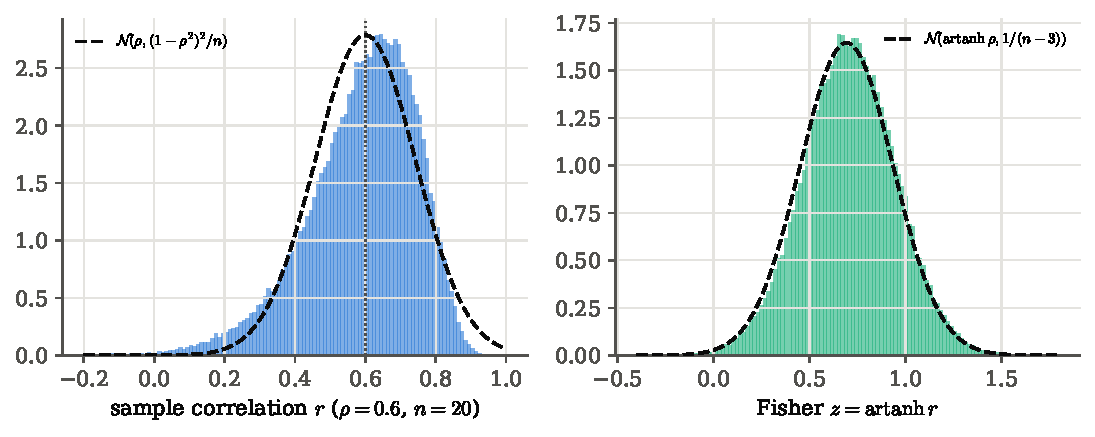
\includegraphics[width=12cm]{figures/ch03/corr_fisher_z.pdf}
\caption{Left: the sample correlation from twenty pairs with true
correlation $0.6$ (dotted). It is skewed, with a long tail towards zero, and
the leading-order Gaussian (dashed) is too narrow on that side. Right: the
same experiments after Fisher's transformation $z=\operatorname{artanh}r$.
The histogram now sits on a symmetric Gaussian of width $1/\sqrt{n-3}$.}
\label{3a:fig:fisher-z}
\end{figure}

\subsection{How noisy is every element, and what inversion does}
\label{3a:sec:cov-noise}

For Gaussian readings there is a clean formula for the scatter of each
element of $\hat\Cmat$. The rotation argument of
\cref{3a:sec:n-minus-one}, applied to each component, turns the $n$ centred
readings into $n-1$ independent vectors $\bm z_k\sim\Normal(\bm0,\bm\Sigma)$,
with $(n-1)\hat\Cmat=\sum_{k=1}^{n-1}\bm z_k\bm z_k\T$. We need one fact
about Gaussian fourth moments, familiar to physicists as Wick's theorem.

\paragraph{Isserlis (Wick) theorem.}
For a zero-mean Gaussian vector,
$\E[z_az_bz_cz_d]=\Sigma_{ab}\Sigma_{cd}+\Sigma_{ac}\Sigma_{bd}+\Sigma_{ad}\Sigma_{bc}$:
the sum over all ways of pairing the four factors, each pair replaced by its
covariance. (With $a=b=c=d$ it gives $\E z^4=3\sigma^4$.)

\begin{align}
  \Var\hat C_{ab}
  &\eqby{1} \frac{1}{(n-1)^2}\sum_{k=1}^{n-1}\Var(z_{ak}z_{bk})
   \eqby{2} \frac{1}{n-1}\Bigl(\E[z_az_bz_az_b]-\Sigma_{ab}^2\Bigr) \nonumber\\
  &\eqby{3} \frac{1}{n-1}\Bigl(\Sigma_{aa}\Sigma_{bb}+2\Sigma_{ab}^2-\Sigma_{ab}^2\Bigr)
   = \frac{\Sigma_{aa}\Sigma_{bb}+\Sigma_{ab}^2}{n-1} .
  \label{3a:eq:var-cov-element}
\end{align}
\begin{explain}
  \item $\hat C_{ab}$ is $1/(n-1)$ times a sum of $n-1$ independent terms, so variances add.
  \item All $n-1$ terms have the same distribution, and $\Var(U)=\E U^2-(\E U)^2$ with $\E[z_az_b]=\Sigma_{ab}$.
  \item Isserlis with indices $(a,b,a,b)$: the pairings give $\Sigma_{ab}\Sigma_{ab}$, $\Sigma_{aa}\Sigma_{bb}$ and $\Sigma_{ab}\Sigma_{ba}$.
\end{explain}
For $a=b$ this is $2\Sigma_{aa}^2/(n-1)$, the Gaussian variance of $S^2$ in
\eqref{3a:eq:var-s2-gauss}. For $\Sigma=\mathbb{1}$ and $a\neq b$ it is
$1/(n-1)$, the scatter of spurious correlations found above. Each element
of a covariance matrix estimated from $n=50$ simulations is uncertain by
about $1/\sqrt{49}=14\%$ of the typical diagonal size.

\paragraph{Inverting a noisy matrix.}
The $\chi^2$ needs $\Cmat^{-1}$, and here noise does more than add scatter:
it biases the result. The reason is that $1/x$ is a convex function. For a
single number, Jensen's inequality gives $\E[1/\hat\sigma^2]>1/\E[\hat\sigma^2]$:
a fluctuation of $\hat\sigma^2$ towards zero raises $1/\hat\sigma^2$ by more
than an equal fluctuation upwards lowers it. For a matrix, the noise spreads
the eigenvalues of $\hat\Cmat$ apart. The smallest ones come out too small,
and inverting turns them into eigenvalues of $\hat\Cmat^{-1}$ that are too
large. For Gaussian readings and $n>p+2$ the exact result is
\begin{equation}
  \E\bigl[\hat\Cmat^{-1}\bigr]=\frac{n-1}{n-p-2}\,\Cmat^{-1},
  \label{3a:eq:hartlap}
\end{equation}
a property of the inverse-Wishart distribution. The unbiased estimate of
the inverse covariance is therefore
$\widehat{\Cmat^{-1}}=\frac{n-p-2}{n-1}\hat\Cmat^{-1}$, the
\newterm{Hartlap factor} \cite{Hartlap2007}. As $p$ approaches $n$ the bias
explodes, and at $p\ge n$ the matrix $\hat\Cmat$ is singular (its rank is at
most $n-1$).

\paragraph{Example: How many simulations?}
\label{3a:ex:hartlap}
With $n=30$ simulations and $p=10$ bins,
$(n-1)/(n-p-2)=29/18=\ThreeAHartlapTenTh$: without the correction, every
$\chi^2$ is too large by $61\%$, and parameter error bars come out too small
by a factor of about $\sqrt{1.61}=1.27$. The simulation gives
$\ThreeAHartlapTen$. To keep the bias below 10\% we need
$(n-1)/(n-p-2)\le1.1$. From $n-1\le1.1(n-p-2)$ we get
$0.1\,n\ge1.1p+1.2$, i.e.\ $n\ge11p+12$: about $120$ simulations for $10$ bins. Even
then, the \emph{noise} in the inverse (not just its bias) widens the
parameter constraints, a further effect that has to be propagated.

\begin{figure}[htbp]
\centering
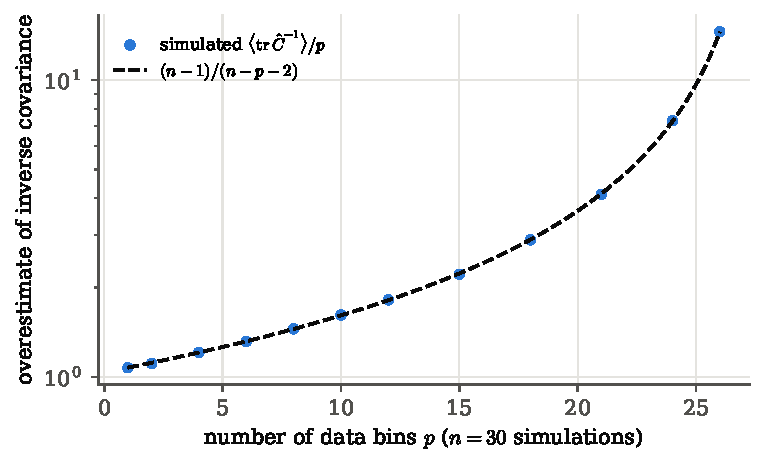
\includegraphics[width=10cm]{figures/ch03/hartlap.pdf}
\caption{How much the inverse of a sample covariance matrix overestimates
the true inverse, for thirty simulations and a growing number of bins
(logarithmic vertical axis). The simulated overestimate follows
$(n-1)/(n-p-2)$ (dashed): small for a few bins, a factor of two by
$p\approx14$, and diverging as $p$ approaches $n-2$.}
\label{3a:fig:hartlap}
\end{figure}

\begin{pitfall}[Selected and misread correlations]
A correlation coefficient estimated from the same data that were used to
choose which pair to look at is not distributed as
\eqref{3a:eq:fisher-z-dist}. Nor is a correlation evidence of a causal link,
and a zero correlation does not mean independence (the correlation only
sees the linear part of a relation, \cref{ch:02}).
\end{pitfall}

\paragraph{What this bought us.}
A covariance matrix estimated from $n$ samples has element-wise noise of
relative size $\sim1/\sqrt{n-1}$, which shows up as spurious correlations of
that size. Put error bars on a correlation in the variable
$z=\operatorname{artanh}r$, where the width is $1/\sqrt{n-3}$. Before
inverting an estimated covariance, multiply the inverse by the Hartlap
factor $(n-p-2)/(n-1)$, and choose $n$ well above $p$.

\paragraph{Verification and research.}
Everything above was verified against formulas valid for Gaussian
readings. For band powers from masked skies or non-Gaussian fields, neither
\eqref{3a:eq:var-cov-element} nor \eqref{3a:eq:hartlap} is exact, and the
number of simulations needed for a stable $\chi^2$ is itself found by
simulation: rerun the covariance estimate with independent sets of
simulations and watch how the parameter constraints move (\cref{ch:08}).

\section{Propagating errors through a formula}
\label{3a:sec:propagation}

The pendulum student now measures the length, $L=1.000\pm0.002\,$m, and the
period, $T=2.006\pm0.004\,$s, and computes $g=4\pi^2L/T^2$. What is the error
on $g$? A particle physicist asks the same about a branching ratio
$N_{\text{signal}}/N_{\text{norm}}$, a cosmologist about $H_0$ derived from a
measured angle and a sound horizon. And sometimes the textbook answer is badly
wrong: a ratio whose denominator is poorly measured has a distribution with
tails that no Gaussian error bar describes.

Faced with a formula and a few uncertain inputs, the tempting non-answer is the one in
\cref{3a:fig:ebeb}: we are not sure how big the error on each point is, so we give the error
bar an error bar of its own, and that one an error bar too. It never ends in a number. The
way out is to notice that the uncertainty of $g$ is not a new, separate unknown. It is the
uncertainty of $L$ and $T$, carried once through the formula $g=4\pi^2L/T^2$. The rest of this
section shows how.

\begin{figure}[htbp]
\centering
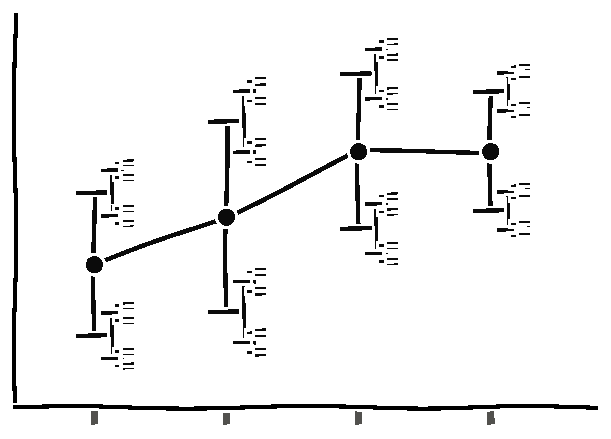
\includegraphics[width=0.62\linewidth]{figures/ch03/error_bars_on_error_bars.pdf}
\caption{What not propagating an error looks like: every error bar gets error bars of its own,
three levels deep, and the picture never settles to one number per point.}
\label{3a:fig:ebeb}
\end{figure}

The standard answer replaces the formula by its tangent, which gives the
output covariance as a ``Jacobian sandwich'' $A\Cmat A\T$ and shows exactly
where correlations between the inputs enter. The answer is exact for linear
formulas, and right for large samples (the delta method). Where it fails, a
Monte Carlo propagation still works.

\paragraph{Every smooth function is linear up close.}
Zoom in on a smooth curve and it looks like its tangent line. If the cloud of
possible input values is small compared with the scale on which the function
bends, then over that cloud the function is effectively linear, and a linear
map sends a Gaussian to a Gaussian, stretched by the slope. When the cloud is
wide enough to feel the curvature, the output is skewed and its centre
shifts. Near a pole, like $1/x$ at $x=0$, all bets are off.

\paragraph{What we want to know.}
\begin{enumerate}[label=\arabic*.]
  \item Given the means and covariance of the inputs, what are the mean and
        covariance of the outputs, to the first order in the fluctuations?
  \item When is that answer exact, and when is it an approximation?
  \item How do correlations between inputs change the result?
  \item How can we tell that the approximation has failed, and what then?
\end{enumerate}

\begin{figure}[htbp]
\centering
\begin{tikzpicture}
\begin{axis}[width=9cm,height=6cm,xmin=0.4,xmax=3.0,ymin=0,ymax=1.6,
  xlabel={input $x$},ylabel={output $y=1/x$},samples=200,
  tick label style={font=\footnotesize},label style={font=\small},
  clip=false]
  \addplot[very thick,formblue,domain=0.62:3.0] {1/x};
  \addplot[thick,tangentgreen,domain=0.7:2.6] {1/1.5-(x-1.5)/2.25};
  \draw[fibreorange,dashed] (axis cs:1.2,0) -- (axis cs:1.2,0.8333) -- (axis cs:0.4,0.8333);
  \draw[fibreorange,dashed] (axis cs:1.8,0) -- (axis cs:1.8,0.5556) -- (axis cs:0.4,0.5556);
  \draw[softgray,dotted,thick] (axis cs:1.5,0) -- (axis cs:1.5,0.6667) -- (axis cs:0.4,0.6667);
  \fill[fibreorange] (axis cs:1.2,0.8333) circle (1.6pt);
  \fill[fibreorange] (axis cs:1.8,0.5556) circle (1.6pt);
  \fill[tangentgreen] (axis cs:1.2,0.8) circle (1.6pt);
  \fill[tangentgreen] (axis cs:1.8,0.5333) circle (1.6pt);
  \addplot[thick,bdryred,domain=0.6:2.4] {0.35*exp(-(x-1.5)^2/(2*0.09))};
  \node[anchor=west,font=\footnotesize,formblue] at (axis cs:1.05,1.3) {$y=1/x$};
  \node[anchor=west,font=\footnotesize,tangentgreen] at (axis cs:2.2,0.18) {tangent at $\mu$};
  \node[anchor=east,font=\footnotesize,bdryred] at (axis cs:0.85,0.2) {input density};
\end{axis}
\end{tikzpicture}
\caption{Linear propagation through $y=1/x$ with input $\mu=1.5$,
$\sigma=0.3$. The red curve is the input density. Orange dots: the true
images of $\mu\pm\sigma$, at $0.556$ and $0.833$, lie asymmetrically about the
image $0.667$ of the mean (dotted). Green dots: the tangent line puts them
symmetrically at $0.533$ and $0.800$. The curvature makes the output skewed
towards large $y$, which is what the Monte Carlo shows later.}
\label{3a:fig:tangent}
\end{figure}

\subsection{The first-order formula}
\label{3a:sec:linear-propagation}

Let the inputs $\bm x=(x_1,\dots,x_n)$ have means $\bm\mu$ and covariance
matrix $V_{ij}=\Cov(x_i,x_j)$, and let $y(\bm x)$ be a smooth function. Expand
about the means,
\begin{equation}
  y(\bm x)=y(\bm\mu)+\sum_{i=1}^n\frac{\partial y}{\partial x_i}\Big|_{\bm\mu}(x_i-\mu_i)
  +\frac12\sum_{i,j}\frac{\partial^2y}{\partial x_i\partial x_j}\Big|_{\bm\mu}(x_i-\mu_i)(x_j-\mu_j)+\cdots,
  \label{3a:eq:taylor}
\end{equation}
If the inputs scatter only a little about their means, the quadratic and
higher terms are small, so we keep only the linear term. Write
$g_i=\partial y/\partial x_i$ at $\bm\mu$. Then, to this order,
\begin{align}
  \E y &\eqby{1} y(\bm\mu)+\sum_ig_i\,\E(x_i-\mu_i) \eqby{2} y(\bm\mu),
  \label{3a:eq:prop-mean}\\
  \sigma_y^2=\E\bigl[(y-\E y)^2\bigr]
  &\eqby{3} \E\Bigl[\Bigl(\sum_ig_i(x_i-\mu_i)\Bigr)^2\Bigr]
   \eqby{4} \sum_{i,j}g_ig_j\,\E\bigl[(x_i-\mu_i)(x_j-\mu_j)\bigr]
   \eqby{5} \sum_{i,j}g_i\,V_{ij}\,g_j .
  \label{3a:eq:prop-var}
\end{align}
\begin{explain}
  \item Take the expectation of the linearised \eqref{3a:eq:taylor}. The $g_i$ are constants.
  \item Each $\E(x_i-\mu_i)=0$.
  \item Subtract \eqref{3a:eq:prop-mean} from the linearised $y$.
  \item Square of a sum is a double sum, then linearity.
  \item Definition of the covariance.
\end{explain}
For several outputs $y_1,\dots,y_m$, the same steps with two different
outputs $y_k,y_l$ give the covariance matrix of the outputs,
\begin{equation}
  U_{kl}=\Cov(y_k,y_l)\approx\sum_{i,j}\frac{\partial y_k}{\partial x_i}\frac{\partial y_l}{\partial x_j}V_{ij},
  \qquad
  U=A\,V\!A\T,\qquad A_{ki}=\frac{\partial y_k}{\partial x_i}\Big|_{\bm\mu},
  \label{3a:eq:prop-matrix}
\end{equation}
where $A$ is the $m\times n$ \newterm{Jacobian} matrix
\srcref{Cowan}{(1.53)--(1.56)}.

\begin{workdef}[linear error propagation]
\newterm{Linear} (first-order) \newterm{error propagation} replaces each
function by its tangent plane at the input means \unpack{the first two terms
of the Taylor series, valid when the inputs scatter over a region where the
second derivatives hardly matter}, so that the output covariance is
$U=AVA\T$ with $A$ the Jacobian at the means. If the inputs are
uncorrelated, $V$ is diagonal and
$\sigma_y^2=\sum_i(\partial y/\partial x_i)^2\sigma_i^2$
\srcref{Cowan}{(1.57)}.
\end{workdef}

\paragraph{Four rules everybody uses.}
With two inputs and $V_{12}=\rho\sigma_1\sigma_2$, \eqref{3a:eq:prop-var}
gives \srcref{Cowan}{(1.59)--(1.60)}:
\begin{align}
  y=x_1\pm x_2:&\quad \sigma_y^2=\sigma_1^2+\sigma_2^2\pm2\rho\sigma_1\sigma_2,
  \label{3a:eq:prop-sum}\\
  y=x_1x_2\ \text{or}\ x_1/x_2:&\quad
  \frac{\sigma_y^2}{y^2}=\frac{\sigma_1^2}{x_1^2}+\frac{\sigma_2^2}{x_2^2}\pm\frac{2\rho\sigma_1\sigma_2}{x_1x_2},
  \label{3a:eq:prop-product}\\
  y=x^k:&\quad \frac{\sigma_y}{|y|}=|k|\,\frac{\sigma_x}{|x|},
  \label{3a:eq:prop-power}\\
  y=\ln x:&\quad \sigma_y=\frac{\sigma_x}{x}.
  \label{3a:eq:prop-log}
\end{align}
(For the product take $+$, for the ratio $-$. The derivatives are
$\partial(x_1x_2)/\partial x_1=x_2$, $\partial(x_1/x_2)/\partial x_2=-x_1/x_2^2$,
and dividing by $y^2$ turns them into relative errors.) Absolute errors add
in quadrature for sums, relative errors for products and ratios.

\paragraph{Example: The pendulum.}
\label{3a:ex:pendulum-prop}
$g=4\pi^2LT^{-2}$ is a product of powers, so relative errors add in
quadrature with weights $|k|$:
\begin{align*}
  \frac{\sigma_g^2}{g^2}
  &\eqby{1} \Bigl(\frac{\sigma_L}{L}\Bigr)^2+\Bigl(2\,\frac{\sigma_T}{T}\Bigr)^2
   \eqby{2} (0.002)^2+\Bigl(\frac{2\times0.004}{2.006}\Bigr)^2
   = 4.0\times10^{-6}+1.59\times10^{-5},\\
  g &\eqby{3} \frac{4\pi^2\times1.000}{2.006^2}=\ThreeAPendG\ \mathrm{m\,s^{-2}},\qquad
  \sigma_g=\ThreeAPendG\times\sqrt{1.99\times10^{-5}}=\ThreeAPendSgLin\ \mathrm{m\,s^{-2}}.
\end{align*}
\begin{explain}
  \item \eqref{3a:eq:prop-product} and \eqref{3a:eq:prop-power} with $k=1$ for $L$
        and $k=-2$ for $T$. $L$ and $T$ are measured independently, so $\rho=0$.
  \item Insert the numbers.
  \item The central value is the function at the input means \eqref{3a:eq:prop-mean}.
\end{explain}
The period dominates. Its relative error ($0.20\%$) is the same as that of
$L$, but it enters squared, so it contributes four times the variance. To
improve $g$, time more swings.

\paragraph{Example: A common calibration: correlated errors.}
\label{3a:ex:common-calib}
Two energies $E_1,E_2$ are measured with the same calorimeter. Each has an
independent statistical error $\sigma_s$ and they share one calibration error
$\sigma_c$: $E_i=E_i^{\text{true}}+\epsilon_i+\delta$, where the $\epsilon_i$ are
independent with mean $0$ and variance $\sigma_s^2$, and the common shift
$\delta$, independent of both, has mean $0$ and variance $\sigma_c^2$. Then
$V_{11}=V_{22}=\sigma_s^2+\sigma_c^2$ and $V_{12}=\Cov(\epsilon_1+\delta,\epsilon_2+\delta)=\sigma_c^2$.
For the difference and the sum, \eqref{3a:eq:prop-sum} gives
\begin{align*}
  \Var(E_1-E_2) &\eqby{1} 2(\sigma_s^2+\sigma_c^2)-2\sigma_c^2=2\sigma_s^2,\qquad
  \Var(E_1+E_2) \eqby{2} 2(\sigma_s^2+\sigma_c^2)+2\sigma_c^2=2\sigma_s^2+4\sigma_c^2 .
\end{align*}
\begin{explain}
  \item Minus sign: the common shift $\delta$ cancels in a difference.
  \item Plus sign: it adds coherently in a sum, so its standard deviation doubles.
\end{explain}
Ignoring the correlation would overstate the error of a mass difference and
understate the error of a total energy. This is why experiments publish full
covariance matrices, not just error bars.

\subsection{Linear maps are exact, and every covariance can be diagonalised}
\label{3a:sec:linear-exact}

If $\bm y=A\bm x$ exactly (a linear map, as in a change of basis, a
rebinning, or a sum of channels), there is no Taylor remainder, and
\begin{align}
  U_{kl}=\Cov(y_k,y_l)
  &\eqby{1} \E\Bigl[\sum_iA_{ki}(x_i-\mu_i)\sum_jA_{lj}(x_j-\mu_j)\Bigr]
   \eqby{2} \sum_{i,j}A_{ki}V_{ij}A_{lj}
   = (AVA\T)_{kl}
  \label{3a:eq:linear-exact}
\end{align}
\begin{explain}
  \item $y_k-\E y_k=\sum_iA_{ki}(x_i-\mu_i)$ by linearity, with no approximation.
  \item Multiply out and use linearity of expectation.
\end{explain}
holds exactly \srcref{Cowan}{(1.62)}. A linear map of a Gaussian vector is
Gaussian, so for Gaussian inputs the whole distribution of $\bm y$ is
$\Normal(A\bm\mu,AVA\T)$.

Exactness has a useful consequence: a well-chosen linear map removes all
correlations. $V$ is real and symmetric, so it has $n$
orthonormal eigenvectors $\bm r^{(k)}$ with $V\bm r^{(k)}=\lambda_k\bm r^{(k)}$
and $\bm r^{(k)}\cdot\bm r^{(l)}=\delta_{kl}$. Take the rows of $A$ to be these
eigenvectors, $A_{ki}=r^{(k)}_i$. Then
\begin{align}
  U_{kl}
  &\eqby{1} \sum_{i,j}r^{(k)}_iV_{ij}r^{(l)}_j
   \eqby{2} \sum_ir^{(k)}_i\,\lambda_l\,r^{(l)}_i
   \eqby{3} \lambda_l\,\delta_{kl} .
  \label{3a:eq:decorrelate}
\end{align}
\begin{explain}
  \item \eqref{3a:eq:linear-exact} with $A_{ki}=r^{(k)}_i$.
  \item $\sum_jV_{ij}r^{(l)}_j=\lambda_lr^{(l)}_i$, the eigenvalue equation.
  \item Orthonormality of the eigenvectors.
\end{explain}
The new variables $y_k=\bm r^{(k)}\cdot\bm x$ are uncorrelated, with variances
equal to the eigenvalues of $V$ \srcref{Cowan}{(1.63)--(1.65)}. This is the
statistics version of finding normal modes of coupled oscillators, and
of the principal axes of an inertia tensor.

\paragraph{Example: Decorrelating two measurements.}
\label{3a:ex:decorrelate}
For $V=\sigma^2\begin{pmatrix}1&\rho\\\rho&1\end{pmatrix}$ the eigenvectors are
$(1,1)/\sqrt2$ and $(1,-1)/\sqrt2$ with eigenvalues $\sigma^2(1\pm\rho)$ (check:
$V(1,1)\T=\sigma^2(1+\rho)(1,1)\T$). The combinations $(x_1+x_2)/\sqrt2$ and
$(x_1-x_2)/\sqrt2$ are uncorrelated, and with $\rho$ close to $1$ the
difference is much better measured than either input. The calibration example
above is this with $\rho=\sigma_c^2/(\sigma_s^2+\sigma_c^2)$.

\subsection{The delta method: why the first-order formula is right for large samples}
\label{3a:sec:delta}

Linear propagation is an approximation, so when can we trust it? When the
inputs are themselves estimators built from $n$ readings. Their scatter then
shrinks like $1/\sqrt n$, the cloud of inputs shrinks onto the tangent, and
the curvature terms become negligible. The delta method makes this precise.

\paragraph{The delta method.}
If $\sqrt n(Y_n-\mu)\rightsquigarrow\Normal(0,\sigma^2)$ and $g$ is
differentiable with $g'(\mu)\neq0$, then
\begin{equation}
  \sqrt n\bigl(g(Y_n)-g(\mu)\bigr)\rightsquigarrow\Normal\bigl(0,\ g'(\mu)^2\sigma^2\bigr),
  \qquad\text{i.e.}\qquad g(Y_n)\approx\Normal\Bigl(g(\mu),\ \frac{g'(\mu)^2\sigma^2}{n}\Bigr).
  \label{3a:eq:delta}
\end{equation}
For a vector, $\sqrt n\bigl(g(\bm Y_n)-g(\bm\mu)\bigr)\rightsquigarrow
\Normal\bigl(0,\nabla g\T\bm\Sigma\nabla g\bigr)$ \mainref{Thms.~5.13, 5.15}.

Why it is true: expand $g(Y_n)=g(\mu)+g'(\mu)(Y_n-\mu)+R_n$ with a remainder
$R_n$ of order $(Y_n-\mu)^2$. Multiply by $\sqrt n$. The linear term
$g'(\mu)\sqrt n(Y_n-\mu)$ tends in distribution to $\Normal(0,g'(\mu)^2\sigma^2)$.
The remainder is $\sqrt n\,R_n\sim\sqrt n\,(Y_n-\mu)^2=[\sqrt n(Y_n-\mu)]^2/\sqrt n$,
a quantity of fixed size divided by $\sqrt n$, so it tends to zero in
probability, and Slutsky's theorem lets us drop it. The curvature does not
disappear. It becomes negligible compared with the shrinking linear scatter.

\paragraph{Example: A function of one mean, and the product of two.}
\label{3a:ex:delta}
In both cases the inputs are sample means, so by the central limit theorem
$\sqrt n(\bar X_n-\mu)\rightsquigarrow\Normal(0,\sigma^2)$ and the delta
method applies. (a) For $W_n=e^{\bar X_n}$, $g(s)=e^s$ has
$g'(\mu)=e^\mu$, so $W_n\approx\Normal(e^\mu,e^{2\mu}\sigma^2/n)$
\mainref{Ex.~5.14}. (b) For the product of two means,
$Y=\bar X_1\bar X_2$ from $n$ paired readings with covariance matrix
$\bm\Sigma=(\sigma_{ab})$, the gradient of $g(s_1,s_2)=s_1s_2$ at $\bm\mu$ is
$(\mu_2,\mu_1)$ and
\begin{align*}
  \nabla g\T\bm\Sigma\nabla g
  &\eqby{1} \begin{pmatrix}\mu_2&\mu_1\end{pmatrix}
            \begin{pmatrix}\sigma_{11}&\sigma_{12}\\\sigma_{12}&\sigma_{22}\end{pmatrix}
            \begin{pmatrix}\mu_2\\\mu_1\end{pmatrix}
   \eqby{2} \mu_2^2\sigma_{11}+2\mu_1\mu_2\sigma_{12}+\mu_1^2\sigma_{22},
\end{align*}
\begin{explain}
  \item $\partial(s_1s_2)/\partial s_1=s_2$ and $\partial(s_1s_2)/\partial s_2=s_1$, at the means.
  \item Multiply out the quadratic form.
\end{explain}
so $\sqrt n(\bar X_1\bar X_2-\mu_1\mu_2)\rightsquigarrow\Normal(0,\mu_2^2\sigma_{11}+2\mu_1\mu_2\sigma_{12}+\mu_1^2\sigma_{22})$
\mainref{Ex.~5.16}. Dividing by $(\mu_1\mu_2)^2$ this is the product rule
\eqref{3a:eq:prop-product}.

\paragraph{When the slope vanishes.}
If $g'(\mu)=0$, the first-order formula says $\sigma_y=0$, which is absurd.
The second-order term takes over \srcref{CasellaBerger}{Thm.~5.5.26}: with
$g(Y_n)-g(\mu)\approx\frac12g''(\mu)(Y_n-\mu)^2$ and
$n(Y_n-\mu)^2/\sigma^2\rightsquigarrow\chi^2_1$,
\begin{equation}
  n\bigl(g(Y_n)-g(\mu)\bigr)\rightsquigarrow\frac{\sigma^2g''(\mu)}{2}\,\chi^2_1 .
  \label{3a:eq:second-order-delta}
\end{equation}
Estimating a power $|A|^2$ when the true amplitude $A$ is zero is exactly this
case. With $g(s)=s^2$ we have $g'(0)=0$ and $g''=2$, so the estimate is
$\sigma^2\chi^2_1/n$: never negative, and biased upward by $\sigma^2/n$
(the mean of $\chi^2_1$ is $1$).

\paragraph{The second-order bias.}
Keeping the quadratic term of \eqref{3a:eq:taylor} in the mean gives
$\E y\approx y(\bm\mu)+\frac12\sum_{ij}\partial_i\partial_jy\,V_{ij}$. For
$y=1/x$ this is $\E(1/x)\approx\frac1\mu\bigl(1+\sigma^2/\mu^2\bigr)$, always
above $1/\mu$, as \cref{3a:fig:tangent} suggests. For the ratio of means
$\bar X/\bar Y$ Casella and Berger derive in the same way
\srcref{CasellaBerger}{Ex.~5.5.27}
\[
  \E\frac{\bar X}{\bar Y}\approx\frac{\mu_X}{\mu_Y},\qquad
  \Var\frac{\bar X}{\bar Y}\approx\frac1n\,\frac{\mu_X^2}{\mu_Y^2}
  \Bigl(\frac{\sigma_X^2}{\mu_X^2}+\frac{\sigma_Y^2}{\mu_Y^2}-\frac{2\sigma_{XY}}{\mu_X\mu_Y}\Bigr),
\]
the ratio rule \eqref{3a:eq:prop-product} with $\sigma^2\to\sigma^2/n$, and
they warn that it can be far off when $\mu_Y$ is near zero.

\subsection{When linear propagation fails: the ratio of Gaussians}
\label{3a:sec:ratio}

Let $x_1\sim\Normal(\mu_1,\sigma_1^2)$ and $x_2\sim\Normal(\mu_2,\sigma_2^2)$ be
independent and $y=x_1/x_2$. The linear rule gives a Gaussian of width
$\sigma_y=|y_0|\sqrt{(\sigma_1/\mu_1)^2+(\sigma_2/\mu_2)^2}$ around
$y_0=\mu_1/\mu_2$. But the denominator has a nonzero density at $x_2=0$,
where $y$ diverges, so $y$ has no mean and no variance at all, however small
$\sigma_2/\mu_2$ is. The extreme case, both means zero, shows where the
heavy tails come from.

\paragraph{Example: The ratio of two zero-mean Gaussians is a Breit--Wigner.}
\label{3a:ex:ratio-cauchy}
Let $x_1,x_2\sim\Normal(0,1)$ independently. The pair $(x_2,x_1)$ is an
isotropic Gaussian in the plane, so its polar angle $\Theta$ is uniformly
distributed, and $y=x_1/x_2=\tan\Theta$. Since $\tan$ has period $\pi$, we can
take $\Theta$ uniform on $(-\pi/2,\pi/2)$. Then
\begin{align*}
  \Prob(y\le t)
  &\eqby{1} \Prob(\Theta\le\arctan t)
   \eqby{2} \frac{\arctan t+\pi/2}{\pi},\qquad
  f(t) \eqby{3} \frac{1}{\pi(1+t^2)} .
\end{align*}
\begin{explain}
  \item $\tan$ is increasing on $(-\pi/2,\pi/2)$.
  \item Uniform distribution on an interval of length $\pi$.
  \item Differentiate: $\frac{\dd}{\dd t}\arctan t=1/(1+t^2)$.
\end{explain}
This is the Cauchy (Breit--Wigner) distribution of \cref{3a:ex:cauchy}
\srcref{CasellaBerger}{\S5.5}. For $\mu_2\neq0$ the ratio keeps a
Cauchy-like $1/y^2$ tail. Its weight is set by how much probability $x_2$
has near zero.

\pyfile[firstline=39,lastline=51]{code/ch03/06_error_propagation.py}{Monte Carlo propagation for a ratio of Gaussians}

The script takes $\mu_1=10$, $\sigma_1=\sigma_2=1$ and three denominators,
$\mu_2=10,3,1$ (relative error $0.1$, $0.33$, $1$). For each it draws
$10^6$ pairs, forms the ratio, and compares the Monte Carlo distribution with
the linear prediction. Because the variance may not exist, it measures the
width by the half-distance between the $15.9$ and $84.1$ percentiles (which
is $\sigma$ for a Gaussian), and it counts negative ratios and ``$5\sigma$''
outliers.

\begin{table}[htbp]
\centering\small
\begin{tabular}{@{}lccc@{}}
\toprule
& $\sigma_2/\mu_2=0.1$ & $0.33$ & $1$\\
\midrule
linear prediction $y_0\pm\sigma_y$ & $1\pm\ThreeARatioALin$ & $3.33\pm\ThreeARatioBLin$ & $10\pm\ThreeARatioCLin$\\
Monte Carlo median & $\ThreeARatioAMed$ & $\ThreeARatioBMed$ & $\ThreeARatioCMed$\\
Monte Carlo central-68\% half-width & $\ThreeARatioAHalf$ & $\ThreeARatioBHalf$ & $\ThreeARatioCHalf$\\
fraction with $y<0$ & $\ThreeARatioANeg$ & $\ThreeARatioBNeg$ & $\ThreeARatioCNeg$\\
fraction beyond $5\sigma_y$ (Gaussian: $5.7\times10^{-7}$) & $\ThreeARatioAFar$ & $\ThreeARatioBFar$ & $\ThreeARatioCFar$\\
\bottomrule
\end{tabular}
\caption{Linear propagation against Monte Carlo for $y=x_1/x_2$.}
\label{3a:tab:ratio}
\end{table}

At 10\% relative error the linear rule is fine in the core (width
$\ThreeARatioAHalf$ against $\ThreeARatioALin$) but already has $300$ times
too many $5\sigma$ outliers. At 33\% the core is 12\% wider than predicted
and 3\% of ratios are beyond ``$5\sigma$''. At 100\% the linear answer is
meaningless: the median is $\ThreeARatioCMed$, not $10$, and $\ThreeARatioCNeg$
of the ratios are negative although both means are positive.

\begin{figure}[htbp]
\centering
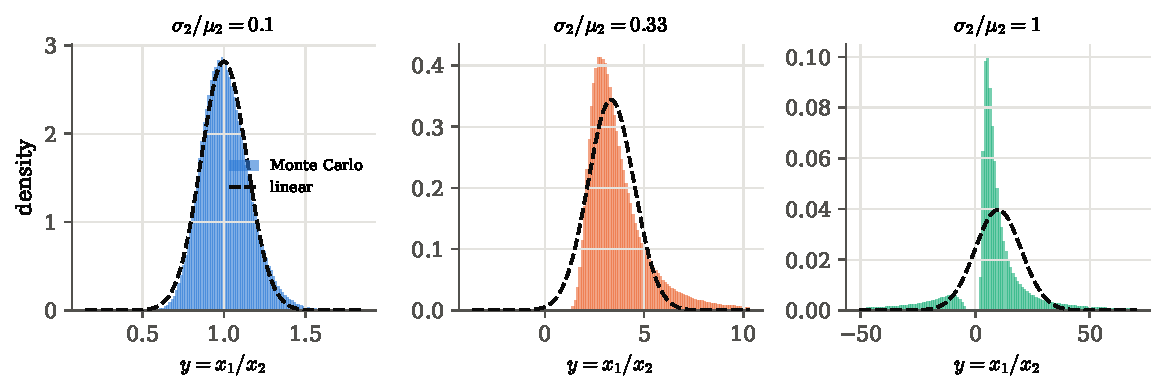
\includegraphics[width=12.5cm]{figures/ch03/ratio_failure.pdf}
\caption{The ratio of two Gaussian quantities, simulated (histograms) and by
linear propagation (dashed), as the denominator's relative error grows from
left to right. At 10\% the two agree. At 33\% the true distribution is
skewed, with a long right tail. At 100\% it has a spike near zero, negative
values and heavy tails, and bears no resemblance to the Gaussian.}
\label{3a:fig:ratio-failure}
\end{figure}

\begin{figure}[htbp]
\centering
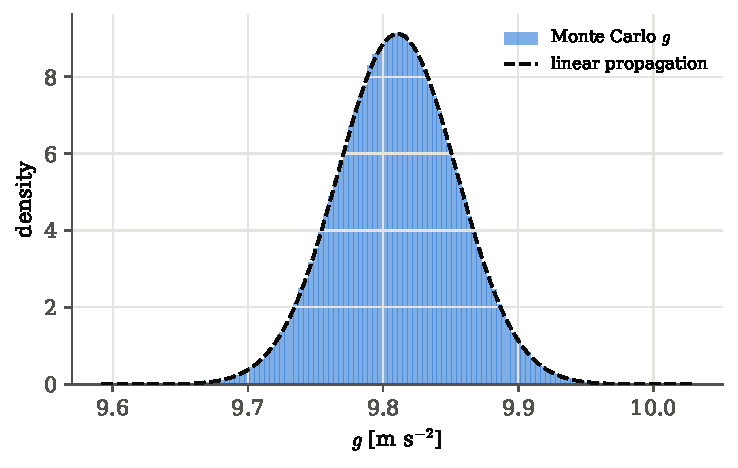
\includegraphics[width=7.5cm]{figures/ch03/pendulum_mc.pdf}
\caption{Monte Carlo propagation for the pendulum. A million pairs
$(L,T)$ drawn from their Gaussian errors give the histogram of $g$. The
linear-propagation Gaussian (dashed) lies on top of it, because the relative
errors of $0.2\%$ are tiny compared with the scale on which $L/T^2$ bends.}
\label{3a:fig:pendulum-mc}
\end{figure}

For the pendulum, by contrast, the Monte Carlo spread of $g$ is
$\ThreeAPendSgMC$ against the linear $\ThreeAPendSgLin$, and the mean is
$\ThreeAPendMeanMC$ (\cref{3a:fig:pendulum-mc}).

\begin{taxonomy}[Which propagation to use]
\centering\small
\begin{tabularx}{\linewidth}{@{}XX@{}}
\toprule
situation & method\\
\midrule
linear function ($\bm y=A\bm x$) & $U=AVA\T$, exact\\
small relative errors, smooth $y$ & first-order formula; check one case by Monte Carlo\\
$y$ depends on a quantity whose error is not small (ratio, $1/x$, $\ln x$ near $0$) & Monte Carlo propagation: sample inputs, apply $y$, histogram; quote median and percentiles\\
$g'(\mu)=0$ at the input means & second-order delta method, $\chi^2_1$ shape\\
inputs from an MCMC chain & apply $y$ to every sample of the chain (\cref{ch:09})\\
\bottomrule
\end{tabularx}
\end{taxonomy}

\paragraph{Symmetric error bars on a ratio.}
An efficiency, a branching ratio or a signal-to-background ratio with a
poorly known denominator should not be quoted as ``central $\pm$ symmetric
error''. The median is shifted, the errors are asymmetric, and the tails are
long. Quote percentiles from a Monte Carlo propagation or, better, build a
likelihood for the ratio directly (second half of \cref{ch:03}), as
Cowan recommends \srcref{Cowan}{p.~22}.

\paragraph{What this bought us.}
To first order, covariances propagate as $U=AVA\T$ with the Jacobian $A$:
absolute errors add in quadrature for sums, relative errors for products,
and correlations add $\pm2\rho\sigma_1\sigma_2$ terms. The rule is exact for
linear maps and asymptotically right for smooth functions of estimators
(delta method). It fails when the input scatter reaches a region of strong
curvature or a pole, and then Monte Carlo propagation is the answer.

\begin{inpractice}[Verification and research]
For the pendulum, Monte Carlo propagation merely verifies the linear formula.
For a derived cosmological parameter (the age of the Universe from $H_0$,
$\Omega_m$ and $\Omega_\Lambda$; $S_8=\sigma_8\sqrt{\Omega_m/0.3}$), the same idea
is the working tool: take every sample of a posterior chain, compute the
derived quantity, and histogram it. No Jacobian is needed, and correlations
and nonlinearity are handled automatically (\cref{ch:09}).
\end{inpractice}

\section{Combining measurements of different quality: the weighted mean}
\label{3a:sec:weighted}

Eight laboratories have measured the same quantity $\mu$: a particle mass, a
lifetime, the Hubble constant. Their error bars range from $0.5$ to $3$ in
some unit. A reviewer asks for one number. The plain average treats the best
laboratory and the worst on an equal footing, and that feels wrong. A
measurement with a small error bar should count for more. But how much more,
and how small is the error of the combination?

One idea settles both questions with the tools we already
have. The combination is again an estimator, a recipe applied to the data,
so it has a sampling distribution, a bias and a variance
(\cref{3a:sec:sampling,3a:sec:bias-variance}). Among all unbiased linear
recipes we look for the one with the smallest variance. The answer is the
\newterm{inverse-variance weighted mean}, and the same answer drops out of
the Gaussian likelihood, which is our first glimpse of the second half of
the chapter. The questions, in order, are these.
\begin{enumerate}[label=\arabic*.]
  \item Which weights $w_i$ make $\sum_i w_ix_i$ unbiased with the smallest
        variance, and what is that variance?
  \item How can we check that the measurements agree well enough for the
        combination to mean something?
  \item What changes when the measurements are correlated, for example
        because they share a systematic error?
  \item What if the readings also contain something we do not want, which
        enters each of them differently? How do we remove it?
\end{enumerate}

\paragraph{When the readings carry more than the signal.}
The laboratories differ only in how noisy they are. Readings can also
differ in what they contain. At the start of the chapter we wrote every reading as a piece that responds
to what we want, plus everything else \eqref{3a:eq:hidden-s}. So far,
``everything else'' has been noise of a known kind: it scatters around zero
with a spread we can describe, and it is different in every reading. For
that we already have good tools. We average, the noise partly cancels, and
the error bar shrinks like $1/\sqrt N$.

Sometimes they carry something more than noise. Picture yourself at a
noisy party with two microphones, trying to record a friend. She stands
between them, so both pick up her voice equally loudly. A loudspeaker plays
music, and it stands closer to the second microphone, so there the music is
twice as loud. Averaging the two recordings does not help, because the music
is not random noise that averages away: it is the same song in both, only
louder in one. Yet there is a trick. Double the first recording and subtract
the second. The music, twice in each, cancels. The voice, twice minus once,
survives. Noise-cancelling headphones work on exactly this principle.

The sky does the same thing to an astronomer. The microwave background has
the same brightness at two observing frequencies, while the dust of our own
Galaxy is much brighter at the higher one. A calibration drift, a
contaminating source, a foreground: whenever the unwanted part has a pattern
of its own across the readings, different from the pattern of what we want,
we can weight the readings so that the unwanted pattern cancels and the
wanted one survives. Each reading gets its own weight, $F=\sum_iw_ix_i$, and
the question is which weights to use.

\emph{The party in symbols.} Call the voice (or the sky signal) $s$ and the
music (or the dust) $f$. It is twice as strong in the second reading, and
each reading has its own noise. Combine them with two numbers $w_1,w_2$:
\begin{align}
  x_1&=s+f+n_1,\qquad x_2=s+2f+n_2,\notag\\
  w_1x_1+w_2x_2&\eqby{1}(w_1+w_2)\,s+(w_1+2w_2)\,f+(w_1n_1+w_2n_2).
  \label{3a:eq:two-channel}
\end{align}
\begin{explain}
  \item Multiply out and collect the terms in $s$, in $f$ and in the noise.
\end{explain}
Each bracket is a dial. The first sets the \emph{normalisation}: unless
$w_1+w_2=1$ we are estimating a rescaled signal. The plain difference
$x_2-x_1=f+n_2-n_1$ shows how badly this can go: its weights sum to zero,
so the signal cancels completely and what is left measures the foreground.
The second bracket sets the \emph{contamination}: $w_1+2w_2=0$ removes $f$
whatever its value. Both conditions together fix the weights,
$w_1=2$, $w_2=-1$, and
\begin{equation}
  2x_1-x_2 \eqby{1} s+(2n_1-n_2),\qquad
  \Var(2x_1-x_2)\eqby{2}4\sigma_1^2+\sigma_2^2 .
  \label{3a:eq:two-channel-clean}
\end{equation}
\begin{explain}
  \item \eqref{3a:eq:two-channel} with $w_1+w_2=1$ and $w_1+2w_2=0$.
  \item Independent noises: variances add, each weighted by $w_i^2$
        \eqref{3a:eq:var-sum}.
\end{explain}
The foreground is gone exactly, the signal keeps its unit normalisation, and
the price is noise: with $\sigma_1=\sigma_2=\sigma$ the clean combination has
variance $5\sigma^2$, ten times the $\sigma^2/2$ of the plain average
$(x_1+x_2)/2$, which in exchange keeps $1.5f$ of foreground. Weights that
cancel unwanted pieces are easy to find; weights that also keep the noise
small are a trade-off. Lesson: a linear combination can switch off anything
whose response across the readings differs from that of $s$, while one
constraint, $\sum_iw_i=1$ for a signal that enters every reading equally,
keeps $s$ itself intact; the rest is the choice of the least noisy weights
among those allowed.

\paragraph{A picture: weights point in a direction.}
Write the two readings as one list, $\bm x=(x_1,x_2)\T$. The signal enters
both readings equally, with the pattern $\bm a=(1,1)\T$; the dust enters
with the pattern $\bm c=(1,2)\T$. The weights are a third list,
$\bm w=(w_1,w_2)\T$, and a weighted sum multiplies matching entries and adds
them up. That is a dot product, so the readings and the two dials become
\begin{equation}
  \bm x=\bm a\,s+\bm c\,f+\bm n
  \qquad\Longrightarrow\qquad
  \bm w\T\bm x\eqby{1}(\bm w\T\bm a)\,s+(\bm w\T\bm c)\,f+\bm w\T\bm n .
  \label{3a:eq:dials-vector}
\end{equation}
\begin{explain}
  \item Multiply each term by $\bm w\T$; a number in front of a list comes
        out of the dot product.
\end{explain}
For the weights $\bm w=(2,-1)\T$ the signal gives $2\cdot1-1\cdot1=1$ and
survives; the dust gives $2\cdot1-1\cdot2=0$ and vanishes. In the language
of geometry, $\bm w$ points at right angles to the dust's pattern, so it is
blind to the dust however bright it is.

\Cref{3a:fig:ruler} shows what the weighted sum does to a point. Lay a ruler
along $\bm w$, marked so that it reads $\bm w\T\bm x$, and drop the data
straight down onto it, at right angles. Where the point lands is the reading.
Because the ruler stands at right angles to everything else, sliding the
point in that direction does not move its shadow: the data and the signal
alone land on the same mark. Only the signal moves the shadow along the
ruler.

\begin{figure}[htbp]
\centering
\begin{tikzpicture}[x=1.75cm,y=1.75cm,font=\small,>={Stealth[length=7pt,width=5pt]}]
  \coordinate (O) at (0,0); \coordinate (S) at (2.2,0.88); \coordinate (E) at (0.48,1.6);
  \coordinate (X) at (2.68,2.48); \coordinate (W) at (1.136,-0.341);
  \coordinate (U) at (0.8077,-0.2424); \coordinate (R) at ($2.2*(U)$);
  \draw[black!30,->] (-0.4,0) -- (3.4,0) node[below left=1pt,black!55] {\footnotesize mic 1};
  \draw[black!30,->] (0,-1.0) -- (0,3.0) node[below left=1pt,black!55] {\footnotesize mic 2};
  \draw[black!55,line width=0.8pt] ($-0.4*(U)$) -- ($3.3*(U)$);
  \foreach \k in {1,2,3} \draw[black!55] ($\k*(U)+0.07*(0.3,1)$) -- ($\k*(U)-0.07*(0.3,1)$);
  \draw[bdryred!55,line width=1.2pt] (X) -- (R);
  \pic[draw=bdryred!70,line width=0.6pt,angle radius=0.22cm] {right angle=X--R--O};
  \fill[bdryred] (R) circle (1.6pt) node[below right=0pt,bdryred] {$s$};
  \draw[decorate,decoration={brace,mirror,amplitude=5pt,raise=11pt},bdryred!85!black,line width=0.7pt]
        (O) -- (R) node[midway,below=19pt,font=\footnotesize] {$\bm w\T\bm x$};
  \draw[->,formblue,line width=1.6pt] (O) -- (S);
  \draw[->,fibreorange,line width=1.6pt] (O) -- (E);
  \draw[->,black,line width=1.6pt] (O) -- (X);
  \draw[->,bdryred,line width=1.6pt] (O) -- (W);
  \node[formblue,above left=0pt] at ($(S)+(0,0.05)$) {signal};
  \node[fibreorange,left=1pt] at (E) {everything else};
  \node[black,above=1pt] at (X) {data};
  \node[bdryred,above right=-1pt] at (W) {$\bm w$};
\end{tikzpicture}
\caption{The weighted sum as a shadow on a ruler. The data are the signal plus everything else. The
weights $\bm w$ point along a ruler at right angles to everything else; the reading $\bm w\T\bm x$ is
where the data fall when dropped straight onto it. The tip of the signal lies on the same drop line, so
the data and the signal alone give the same reading. The two patterns are drawn further apart than at
the party, so that the angles are easy to see.}
\label{3a:fig:ruler}
\end{figure}

So $\bm w$ is a filter. It asks one question of the data: how much of the
pattern we want is here, ignoring everything else? Notice that it does not
point along the signal. It points where it must to be blind to everything
else, so its direction is set as much by what we ignore as by what we want;
only when the rest is plain noise does it line up with the signal itself. A
neuron in a network is the same kind of filter. Its weights also decide
which differences in the input it reads and which it ignores, but nobody
works them out: they start at random and are adjusted during training until
the readings are useful. Choosing weights is choosing a direction: one that
sees what we want and is blind to what we do not. With
more readings there is room to be blind to more unwanted patterns at once,
and finding the weights is a small set of linear equations. When the
unwanted patterns are not known exactly, or the noise matters as much as
they do, we look instead for the direction along which the combination
scatters least, and that search is the rest of this section.

\emph{The universal principle.} The two microphones did one thing: each
recording was the voice plus everything else, and the weights kept the voice
and dropped the rest. Every weighted sum in this section does the same, and
so, it turns out, does almost every analysis in the book. What makes it
possible is a \newterm{feature}: a property that the part we want has and
the rest does not. At the party it is how loud each source is in each
microphone: the voice equally loud in both, the music twice as loud in
one. Building a quantity that keeps the wanted feature and drops the others
is \newterm{feature extraction}, and the weighted sum is its simplest form.
The principle has one hard limit: without a feature there is no
separation. Put the loudspeaker right next to your friend, and voice and
music arrive equally loud in both microphones; no weights can pull them
apart, because weights can use a difference the data contain but cannot
invent one.

The principle does not stop at simple problems; even an artificial neural
network runs on it. Suppose someone has written the digit 9 on a sheet of
paper, we photograph it, and a network must tell from the photograph which
digit was written. The photograph is a grid of pixel values: the pixels of
the written 9, plus the paper, a smudge, uneven light. A first layer of
weighted sums extracts the feature we want, the pixels that belong to the
number. Those pixels are in turn a few shapes, a loop and a stroke running
down from it, plus details that do not matter, such as the size of the
loop; the next layer extracts the shapes. The last layers turn the shapes
into the answer: one loop alone is a 0, two loops stacked are an 8, a loop
on top with a tail below is a 9. Each layer is a set of weighted sums, each
bent by a fixed curve, and each takes what the layer before it kept as its
new data. The only real difference from our two microphones is where the
weights come from: a network learns them from many labelled examples, while
we work ours out from what we know about the patterns and the noise. So
even the most complicated network is a long chain of the step we have just
taken: isolate one feature, then the next. \Cref{3a:fig:network} writes it
with the same bookkeeping as the party, $\bm x=\bm a\,s+\bm c\,f+\bm n$:
at each step the data are split into the part we want plus the rest, and
weights keep the part we want.

\begin{figure}[htbp]
\centering
\def\loopcells{1/6,2/6,3/6,0/5,4/5,0/4,4/4,1/3,2/3,3/3,4/3}
\def\tailcells{4/2,4/1,2/0,3/0}
\newcommand\grid[3]{%
  \begin{scope}[shift={(#1,#2)},x=0.2cm,y=0.2cm]
    \fill[black!5] (0,0) rectangle (5,7); #3
    \draw[black!25,step=1] (0,0) grid (5,7);
  \end{scope}}
\newcommand\rest{\fill[softgray!55] (0,0) rectangle (2,1); \fill[softgray!35] (0,3) rectangle (1,4);}
\newcommand\cells[2]{\foreach \c/\r in #1 \fill[#2] (\c,\r) rectangle (\c+1,\r+1);}
\begin{tikzpicture}[font=\small,>=Stealth]
  \grid{0}{3.2}{\rest\cells{\loopcells}{formblue}\cells{\tailcells}{formblue}}
  \node at (1.35,3.9) {$=$};
  \grid{1.7}{3.2}{\cells{\loopcells}{formblue}\cells{\tailcells}{formblue}}
  \node at (3.05,3.9) {$+$};
  \grid{3.4}{3.2}{\rest}
  \node[below] at (0.5,3.2) {\footnotesize$\bm x$};
  \node[below] at (2.2,3.2) {\footnotesize$\bm x_9$};
  \node[below] at (3.9,3.2) {\footnotesize$\bm x_{\rm rest}$};
  \node[anchor=west,align=left,text width=6.2cm] at (5.0,3.9)
    {\footnotesize the photograph is the written 9 plus the paper, a smudge,
     uneven light; weights that match pen strokes keep $\bm x_9$};
  \grid{1.7}{0.9}{\cells{\loopcells}{formblue}\cells{\tailcells}{formblue}}
  \node at (3.05,1.6) {$=$};
  \grid{3.4}{0.9}{\cells{\loopcells}{fibreorange}}
  \node at (4.75,1.6) {$+$};
  \grid{5.1}{0.9}{\cells{\tailcells}{fibreorange}}
  \node[below] at (2.2,0.9) {\footnotesize$\bm x_9$};
  \node[below] at (3.9,0.9) {\footnotesize$\bm x_{\rm loop}$};
  \node[below] at (5.6,0.9) {\footnotesize$\bm x_{\rm tail}$};
  \node[anchor=west,align=left,text width=4.6cm] at (6.6,1.6)
    {\footnotesize the 9 is a loop plus a tail; weights that match each shape
     give its score};
  \newcommand\vbars[4]{%
    \begin{scope}[shift={(#1,#2)}]
      \draw[black!25] (0,0) rectangle (1.0,1.2);
      \foreach \v/\col [count=\k] in {#3} \fill[\col] (0.08,1.2-0.38*\k+0.06) rectangle ++(0.75*\v,0.26);
      \node[below] at (0.45,0) {\footnotesize #4};
    \end{scope}}
  \begin{scope}[yshift=-1.7cm]
    \node[anchor=east,align=right] at (1.7,1.01) {\footnotesize loop on top};
    \node[anchor=east,align=right] at (1.7,0.63) {\footnotesize tail below};
    \node[anchor=east,align=right] at (1.7,0.25) {\footnotesize second loop};
    \vbars{1.75}{0}{1.1/fibreorange,1.05/fibreorange,0.15/fibreorange}{$\bm s$}
    \node at (3.05,0.6) {$=$};
    \vbars{3.4}{0}{1/bdryred,1/bdryred,0/bdryred}{$\bm p_9$}
    \node at (4.75,0.6) {$+$};
    \vbars{5.1}{0}{0.1/softgray,0.05/softgray,0.15/softgray}{$\bm s_{\rm rest}$}
    \node[anchor=west,align=left,text width=5.4cm] at (6.6,0.6)
      {\footnotesize the shape scores are a 9's pattern plus a leftover;
       each digit's pattern $\bm p_d$ is its weights, its score is
       $\bm p_d\T\bm s$, and the 9 scores highest};
  \end{scope}
\end{tikzpicture}
\caption{Reading a handwritten 9 with the idea of the two microphones, used again and again. Each row
has the form \emph{data $=$ what we want $+$ the rest}, exactly like $\bm x=\bm a\,s+\bm c\,f+\bm n$,
and a set of weights keeps what we want: a weighted sum $\bm w\T\bm x$ whose weights match the wanted
pattern, bent by a fixed curve such as $\max(0,z)$. What one row keeps is the data of the next; in the
last row the data are the shape scores, and each digit's weights are its own pattern of shapes. A
neural network is this chain with many rows, and with weights learned from labelled examples.}
\label{3a:fig:network}
\end{figure}

Every step in the figure is the dot product of the two microphones, repeated
many times and chained; nothing else enters. Readings, patterns and weights
are all lists of numbers, so the natural language for all of it is linear
algebra.

We start with the simplest case: readings of different quality, no
contaminant, and weights chosen so the combination scatters as little as
possible. \Cref{3a:sec:weighted-corr} then lets the unwanted pieces be
shared between readings, and the same formula becomes the method used to
separate the microwave background from the Galaxy.

\subsection{The best linear combination}
\label{3a:sec:blue}

Let the measurements $x_1,\dots,x_N$ be independent, each unbiased,
$\E x_i=\mu$, with known standard deviations $\sigma_i$ that differ from one
measurement to the next. We try a \emph{linear} recipe
$\hat\mu=\sum_iw_ix_i$ with numbers $w_i$ still to be chosen. Two
properties follow at once:
\begin{align}
  \E\hat\mu &\eqby{1} \sum_i w_i\,\E x_i \eqby{2} \mu\sum_i w_i ,
  \label{3a:eq:wmean-bias}\\
  \Var\hat\mu &\eqby{3} \sum_i w_i^2\,\Var x_i \eqby{4} \sum_i w_i^2\sigma_i^2 .
  \label{3a:eq:wmean-var}
\end{align}
\begin{explain}
  \item Linearity of expectation.
  \item Every measurement is unbiased, $\E x_i=\mu$.
  \item Variance of a sum \eqref{3a:eq:var-sum}: the covariances vanish
        because the $x_i$ are independent, and a constant factor comes out
        squared, $\Var(wx)=w^2\Var x$.
  \item $\Var x_i=\sigma_i^2$.
\end{explain}
So $\hat\mu$ is unbiased for every value of $\mu$ exactly when the weights
sum to one, $\sum_iw_i=1$. Its mean squared error is then just its variance
\eqref{3a:eq:mse-decomp}, and we want the weights that make
$\sum_iw_i^2\sigma_i^2$ as small as possible under that one constraint.

\paragraph{Minimising with a Lagrange multiplier.}
Recall the method from mechanics: to minimise $f(\bm w)$ subject to
$g(\bm w)=0$, look for points where the gradient of $f$ is parallel to the
gradient of $g$, that is, where the gradient of
$f-\lambda g$ vanishes for some number $\lambda$ (the multiplier). Here
$f=\sum_iw_i^2\sigma_i^2$ and $g=\sum_iw_i-1$:
\begin{align}
  0 &\eqby{1} \frac{\partial}{\partial w_k}\Bigl[\sum_i w_i^2\sigma_i^2-\lambda\Bigl(\sum_iw_i-1\Bigr)\Bigr]
     \eqby{2} 2w_k\sigma_k^2-\lambda
  \quad\Longrightarrow\quad w_k=\frac{\lambda}{2\sigma_k^2},\notag\\
  1 &\eqby{3} \sum_k w_k = \frac{\lambda}{2}\sum_k\frac{1}{\sigma_k^2}
  \quad\Longrightarrow\quad \frac{\lambda}{2}=\frac{1}{W},
  \qquad W\equiv\sum_{k=1}^N\frac{1}{\sigma_k^2},\notag\\
  w_k &\eqby{4} \frac{1/\sigma_k^2}{W},\qquad
  \Var\hat\mu \eqby{5} \sum_k\frac{1}{\sigma_k^4W^2}\,\sigma_k^2
  = \frac{1}{W^2}\sum_k\frac{1}{\sigma_k^2}
  = \frac{1}{W}.
  \label{3a:eq:wmean-weights}
\end{align}
\begin{explain}
  \item Stationarity of $f-\lambda g$ in each $w_k$.
  \item Only the $i=k$ terms depend on $w_k$: $\partial(w_k^2\sigma_k^2)/\partial w_k=2w_k\sigma_k^2$
        and $\partial w_k/\partial w_k=1$.
  \item Impose the constraint $\sum_kw_k=1$ to fix $\lambda$.
  \item Insert $\lambda/2=1/W$ into $w_k=\lambda/(2\sigma_k^2)$.
  \item Insert these weights into \eqref{3a:eq:wmean-var}.
\end{explain}

A stationary point need not be a minimum. One inequality settles it: no
other unbiased linear recipe does better. For any weights with
$\sum_iw_i=1$, the Cauchy--Schwarz inequality
$(\sum_ia_ib_i)^2\le\sum_ia_i^2\sum_ib_i^2$ with $a_i=w_i\sigma_i$ and
$b_i=1/\sigma_i$ gives
\begin{equation}
  1 \eqby{1} \Bigl(\sum_i w_i\Bigr)^2
    \eqby{2} \Bigl(\sum_i w_i\sigma_i\cdot\frac{1}{\sigma_i}\Bigr)^2
    \relby{3}{\le} \sum_iw_i^2\sigma_i^2\;\sum_i\frac{1}{\sigma_i^2}
    \eqby{4} \Var\hat\mu\cdot W .
  \label{3a:eq:wmean-cs}
\end{equation}
\begin{explain}
  \item The weights sum to one.
  \item Multiply and divide each term by $\sigma_i$.
  \item Cauchy--Schwarz. Equality holds only when $a_i\propto b_i$, that is
        $w_i\sigma_i\propto1/\sigma_i$, or $w_i\propto1/\sigma_i^2$.
  \item \eqref{3a:eq:wmean-var} and the definition of $W$.
\end{explain}
So $\Var\hat\mu\ge1/W$ for every unbiased linear combination, and the
inverse-variance weights are the only ones that reach the bound.

\begin{workdef}[inverse-variance weighted mean]
For independent unbiased measurements $x_i$ of one quantity, with standard
deviations $\sigma_i$,
\[
  \hat\mu=\frac{\sum_ix_i/\sigma_i^2}{\sum_i1/\sigma_i^2},
  \qquad
  \sigma_{\hat\mu}=\Bigl(\sum_i\frac{1}{\sigma_i^2}\Bigr)^{-1/2}.
\]
Each measurement is weighted by its inverse variance $1/\sigma_i^2$
\unpack{a measurement twice as precise counts four times as much}. This is
the unbiased linear combination with the smallest variance
\srcref{Cowan}{(7.26)--(7.27)}, \srcref{Sivia}{(2.30)--(2.31)}.
\end{workdef}

\paragraph{What the formula says.}
Three consequences are worth reading off. First, since
$W\ge1/\sigma_k^2$ for every single $k$, the combined variance $1/W$ is
never larger than the smallest individual variance: adding a measurement,
however poor, never hurts \srcref{Cowan}{p.~107}. Second, if one
measurement is much more precise than the rest, it dominates both $W$ and
the weighted sum, and the combination is essentially that measurement.
Third, if all errors are equal, $\sigma_i=\sigma$, the weights are all
$1/N$ and $\Var\hat\mu=\sigma^2/N$, the familiar variance of the sample mean
\eqref{3a:eq:var-mean}.

Two pictures from physics make the formula feel familiar. Inverse variances
add like the conductances of resistors in parallel, $1/R=\sum_i1/R_i$: the
combined ``resistance to knowing $\mu$'' is smaller than the smallest
single one. And $\hat\mu$ is the centre of mass of the points $x_i$ with
masses $1/\sigma_i^2$; a precise measurement is a heavy mass that drags the
centre towards itself. Later we will call $1/\sigma^2$ the
\newterm{information} carried by a measurement, and the statement ``the
information of independent measurements adds'' becomes the additivity of
Fisher matrices (\cref{ch:10}).

\paragraph{The same answer from least squares and the likelihood.}
Suppose, in addition, that each $x_i$ is Gaussian,
$x_i\sim\Normal(\mu,\sigma_i^2)$. The probability density of the whole data
set, read as a function of $\mu$, is
$\prod_i(2\pi\sigma_i^2)^{-1/2}\exp[-(x_i-\mu)^2/2\sigma_i^2]$, so its
logarithm is a constant minus $\tfrac12\chi^2(\mu)$ with
\begin{equation}
  \chi^2(\mu)=\sum_{i=1}^N\frac{(x_i-\mu)^2}{\sigma_i^2}
  \label{3a:eq:wmean-chi2}
\end{equation}
\srcref{Cowan}{(7.25)}. Making the density as large as possible means making
$\chi^2$ as small as possible. We complete the square in $\mu$:
\begin{align}
  \chi^2(\mu)
  &\eqby{1} \sum_i\frac{x_i^2}{\sigma_i^2}-2\mu\sum_i\frac{x_i}{\sigma_i^2}+\mu^2\sum_i\frac{1}{\sigma_i^2}\notag\\
  &\eqby{2} \sum_i\frac{x_i^2}{\sigma_i^2}-2\mu W\hat\mu+\mu^2W\notag\\
  &\eqby{3} W(\mu-\hat\mu)^2+\Bigl[\sum_i\frac{x_i^2}{\sigma_i^2}-W\hat\mu^2\Bigr]
   \eqby{4} W(\mu-\hat\mu)^2+\chi^2_{\min}.
  \label{3a:eq:wmean-square}
\end{align}
\begin{explain}
  \item Expand $(x_i-\mu)^2=x_i^2-2\mu x_i+\mu^2$ and sum term by term.
  \item $\sum_ix_i/\sigma_i^2=W\hat\mu$ by the definition of the weighted
        mean, and $\sum_i1/\sigma_i^2=W$.
  \item Add and subtract $W\hat\mu^2$: $\mu^2W-2\mu W\hat\mu+W\hat\mu^2=W(\mu-\hat\mu)^2$.
  \item The bracket does not depend on $\mu$. It is the value of $\chi^2$ at
        $\mu=\hat\mu$, which we call $\chi^2_{\min}$.
\end{explain}
So $\chi^2$ is a parabola in $\mu$ with its minimum exactly at the weighted
mean \srcref{Cowan}{(7.26)}. Its curvature is
$\mathrm d^2\chi^2/\mathrm d\mu^2=2W$, and the density of the data, as a
function of $\mu$, is proportional to $\exp[-W(\mu-\hat\mu)^2/2]$: a
Gaussian bump of width $W^{-1/2}=\sigma_{\hat\mu}$. So the width of the
bump is exactly the error bar we derived from the sampling distribution.

Two more facts can be read off the parabola, and both return in the second
half of the chapter. First, the variance is ``two over the curvature of
$\chi^2$'': $\sigma_{\hat\mu}^2=1/W=2/(2W)$ \srcref{Cowan}{(7.27)},
\srcref{Sivia}{(2.31)}. Second, moving $\mu$ one standard error away from
$\hat\mu$ raises $\chi^2$ by exactly $1$, because $W\sigma_{\hat\mu}^2=1$.
The same formulas also appear as the peak and width of a Bayesian posterior
with a flat prior \srcref{Sivia}{pp.~30--31}. For Gaussian data and a flat
prior the two readings coincide.

\begin{keyidea}[Inverse-variance weighting]
To combine independent unbiased measurements, weight each by $1/\sigma_i^2$.
Inverse variances add: $1/\sigma_{\hat\mu}^2=\sum_i1/\sigma_i^2$. For
correlated measurements with covariance $V$, the weights become
$\bm w=V^{-1}\bm1/(\bm1\T V^{-1}\bm1)$ and
$1/\sigma_{\hat\mu}^2=\bm1\T V^{-1}\bm1$ (\cref{3a:sec:weighted-corr}).
\end{keyidea}

\paragraph{Example: two measurements of a mass.}
Two experiments report $x_1=10.0\pm0.3$ and $x_2=10.8\pm0.4$ (in
$\mathrm{GeV}$). The weights and the combination are
\begin{align*}
  \frac{1}{\sigma_1^2}&=\frac{1}{0.09}=11.11,\qquad
  \frac{1}{\sigma_2^2}=\frac{1}{0.16}=6.25,\qquad
  W\eqby{1}17.36,\\
  \hat\mu&\eqby{2}\frac{11.11\times10.0+6.25\times10.8}{17.36}
  =\frac{111.1+67.5}{17.36}=10.29,\qquad
  \sigma_{\hat\mu}\eqby{3}\frac{1}{\sqrt{17.36}}=0.24 .
\end{align*}
\begin{explain}
  \item $W$ is the sum of the inverse variances.
  \item Weighted mean. The first measurement carries weight $11.11/17.36=0.64$.
  \item $\sigma_{\hat\mu}=W^{-1/2}$.
\end{explain}
The result, $10.29\pm0.24$, is closer to the more precise measurement and is
more precise than either. The plain average $10.4$ would have the error
$\tfrac12\sqrt{0.09+0.16}=0.25$, slightly worse, and would be pulled
towards the poorer measurement.

\paragraph{Example: equal errors and one outstanding measurement.}
Take $N-1$ measurements with error $\sigma$ and one with error $\sigma/k$.
Then $W=(N-1)/\sigma^2+k^2/\sigma^2$, and the precise measurement carries the
weight
\begin{equation*}
  w_{\text{best}}\eqby{1}\frac{k^2/\sigma^2}{(N-1+k^2)/\sigma^2}
  =\frac{k^2}{N-1+k^2},
  \qquad
  \sigma_{\hat\mu}\eqby{2}\frac{\sigma}{\sqrt{N-1+k^2}} .
\end{equation*}
\begin{explain}
  \item \eqref{3a:eq:wmean-weights}, with the common factor $1/\sigma^2$ cancelled.
  \item $\sigma_{\hat\mu}=W^{-1/2}$.
\end{explain}
One measurement ten times more precise ($k=10$) is worth $k^2=100$ ordinary
ones: with $N-1=9$ ordinary measurements it carries $100/109=92\%$ of the
weight. Precision is worth its square.

\subsection{Do the measurements agree? The $\chi^2$ of the residuals}
\label{3a:sec:wchi2}

The error $\sigma_{\hat\mu}=W^{-1/2}$ uses only the quoted $\sigma_i$, never
the spread of the $x_i$ themselves. Two measurements $10.0\pm0.3$ and
$10.8\pm0.4$ give the same $\sigma_{\hat\mu}$ as $10.0\pm0.3$ and
$15.0\pm0.4$, although the second pair plainly contradicts itself. The value
of $\chi^2$ at its minimum is the missing check: it measures how far the
data scatter about $\hat\mu$ in units of their own error bars.

What value should we expect? Write $z_i=(x_i-\mu)/\sigma_i$ for the
standardised errors: they are independent with mean $0$ and variance $1$.
Then
\begin{align}
  \chi^2_{\min}
  &\eqby{1} \sum_i\frac{\bigl[(x_i-\mu)-(\hat\mu-\mu)\bigr]^2}{\sigma_i^2}\notag\\
  &\eqby{2} \sum_i z_i^2-2(\hat\mu-\mu)\sum_i\frac{x_i-\mu}{\sigma_i^2}+(\hat\mu-\mu)^2W\notag\\
  &\eqby{3} \sum_i z_i^2-2(\hat\mu-\mu)^2W+(\hat\mu-\mu)^2W
   = \sum_i z_i^2-W(\hat\mu-\mu)^2,\notag\\
  \E\chi^2_{\min}
  &\eqby{4} N-W\cdot\frac1W = N-1 .
  \label{3a:eq:wchi2-mean}
\end{align}
\begin{explain}
  \item Add and subtract the true $\mu$ inside $x_i-\hat\mu$.
  \item Expand the square. The first term is $z_i^2$, and $\sum_i1/\sigma_i^2=W$.
  \item $\sum_i(x_i-\mu)/\sigma_i^2=\sum_ix_i/\sigma_i^2-\mu W=W(\hat\mu-\mu)$.
  \item $\E z_i^2=1$ for each of the $N$ terms, and
        $\E(\hat\mu-\mu)^2=\Var\hat\mu=1/W$ because $\hat\mu$ is unbiased.
\end{explain}
This is the weighted twin of the $N-1$ in the sample variance
(\cref{3a:sec:n-minus-one}): fitting one parameter to the data uses up one
of the $N$ independent directions of scatter. For Gaussian measurements the
geometry of \cref{3a:sec:n-minus-one} goes through unchanged in the
rescaled coordinates $z_i$. The noise vector $(z_1,\dots,z_N)$ is
isotropic, the fit removes its component along the single direction
$(1/\sigma_1,\dots,1/\sigma_N)$, and the remaining $N-1$ perpendicular
components are independent standard normals. Hence
\begin{equation}
  \chi^2_{\min}\sim\chi^2_{N-1},\qquad
  \E\chi^2_{\min}=N-1,\qquad \Var\chi^2_{\min}=2(N-1),
  \label{3a:eq:wchi2-dist}
\end{equation}
with the $\chi^2$ distribution of \cref{ch:02}. A value of
$\chi^2_{\min}/(N-1)$ near $1$ says the scatter matches the error bars. A
value far above $1$ says it does not.

\paragraph{Example: the two masses again.}
For two measurements, $\chi^2_{\min}$ depends only on their difference.
With $w_1=W^{-1}/\sigma_1^2$ and $w_2=1-w_1$,
\begin{align*}
  \chi^2_{\min}
  &\eqby{1}\frac{(x_1-\hat\mu)^2}{\sigma_1^2}+\frac{(x_2-\hat\mu)^2}{\sigma_2^2}
  \eqby{2}(x_1-x_2)^2\Bigl[\frac{w_2^2}{\sigma_1^2}+\frac{w_1^2}{\sigma_2^2}\Bigr]
  \eqby{3}\frac{(x_1-x_2)^2}{\sigma_1^2+\sigma_2^2},\\
  &\eqby{4}\frac{(10.0-10.8)^2}{0.09+0.16}=\frac{0.64}{0.25}=2.56 .
\end{align*}
\begin{explain}
  \item Definition \eqref{3a:eq:wmean-chi2} at $\mu=\hat\mu$.
  \item $x_1-\hat\mu=x_1-w_1x_1-w_2x_2=w_2(x_1-x_2)$, and likewise
        $x_2-\hat\mu=-w_1(x_1-x_2)$.
  \item $w_1=\sigma_2^2/(\sigma_1^2+\sigma_2^2)$ and
        $w_2=\sigma_1^2/(\sigma_1^2+\sigma_2^2)$ (multiply numerator and
        denominator of $w_1$ by $\sigma_1^2\sigma_2^2$). The bracket becomes
        $\bigl[\sigma_1^4/\sigma_1^2+\sigma_2^4/\sigma_2^2\bigr]/(\sigma_1^2+\sigma_2^2)^2
        =1/(\sigma_1^2+\sigma_2^2)$.
  \item Insert the numbers.
\end{explain}
The result is natural: $x_1-x_2$ has mean zero if both measure the same
$\mu$ and variance $\sigma_1^2+\sigma_2^2$ \eqref{3a:eq:prop-sum}, so
$\chi^2_{\min}$ is the squared number of standard deviations by which the two
disagree, here $1.6$. For one degree of freedom, a value of $2.56$ or more
occurs in $11\%$ of repetitions when both measurements are right, so the pair
is acceptable. (This is a first $p$-value; \cref{ch:04} develops them
properly.) The contradictory pair $10.0\pm0.3$ and $15.0\pm0.4$ gives
$\chi^2_{\min}=25/0.25=100$, a ten-standard-deviation disagreement.

\paragraph{What to do when they disagree.}
A large $\chi^2_{\min}$ means that at least one error bar is underestimated,
or that the measurements do not in fact measure the same thing. There is no
purely statistical cure. A common convention, used for example in
particle-physics averages, is to inflate the combined error by the factor
$\sqrt{\chi^2_{\min}/(N-1)}$ when that factor exceeds one. This is
equivalent to assuming that every quoted $\sigma_i$ is too small by the same
unknown factor, and it is only as good as that assumption.

\begin{pitfall}[A tiny error bar from inconsistent data]
The formula $\sigma_{\hat\mu}=W^{-1/2}$ never looks at the data, so it
happily returns a small error for measurements that contradict each other.
Always report $\chi^2_{\min}$ and $N-1$ with a weighted mean. When two
precise determinations disagree by several standard deviations (as early-
and late-Universe measurements of $H_0$ do in the Hubble tension of
\cref{T2b:sec:tension}), their weighted mean is a number
that neither experiment supports, and its error bar is meaningless.
\end{pitfall}

\subsection{Eight laboratories in Python}
\label{3a:sec:weighted-python}

A simulation checks every claim. The eight laboratories have
$\sigma_i=0.5$, $0.7$, $1.0$, $1.2$, $1.5$, $2.0$, $2.5$ and $3.0$, and the true value is
$\mu=0$. We repeat the whole campaign of eight measurements $200\,000$ times
and compute, in each repetition, the plain average, the weighted mean and
$\chi^2_{\min}$.

\pyfile[firstline=25,lastline=35]{code/ch03/07_weighted_mean.py}{Eight laboratories, many times over}

The array \pyname{x} has one row per repetition and one column per
laboratory; multiplying standard normals by the row vector \pyname{sig}
gives each column its own error bar (numpy broadcasting). The weights
\pyname{w} are the inverse variances. The weighted mean of each row is the
weighted sum divided by \pyname{w.sum()}, which is $W$. In the line for
\pyname{chi2}, \pyname{xw[:, None]} turns the vector of weighted means into
a column, so that each row's own $\hat\mu$ is subtracted from that row's
eight measurements. The last two lines are the predictions,
$W^{-1/2}$ for the weighted mean and $\sqrt{\sum_i\sigma_i^2}/N$ for the
plain average (the variance of a sum of independent terms divided by
$N^2$).

The weighted mean scatters with standard deviation $\ThreeAWsdW$, against
the prediction $W^{-1/2}=\ThreeAWsdWth$. The plain average scatters with
$\ThreeAWsdU$, against the prediction $\sqrt{24.68}/8=\ThreeAWsdUth$. The
plain average is not merely worse than the weighted mean: it is worse than
the best laboratory on its own, whose error is $\ThreeAWbest$. Averaging in
poor measurements with equal weight destroys information. The simulated
$\chi^2_{\min}$ has mean $\ThreeAWchiMean$ and variance $\ThreeAWchiVar$,
against $N-1=7$ and $2(N-1)=14$ from \eqref{3a:eq:wchi2-dist}, and
\cref{3a:fig:weighted-mean} shows that its whole histogram is $\chi^2_7$.

\begin{figure}[htbp]
\centering
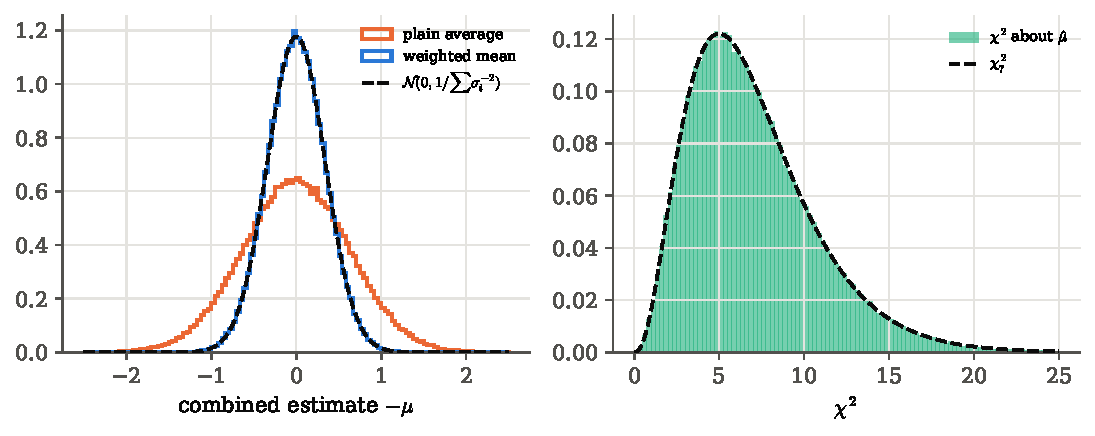
\includegraphics[width=12cm]{figures/ch03/weighted_mean.pdf}
\caption{Left: over many repetitions of the eight-laboratory campaign, the
weighted mean (blue) is a narrow Gaussian of width $W^{-1/2}$ (dashed),
while the plain average (orange) is almost twice as wide. Right: the
histogram of $\chi^2_{\min}$ about the weighted mean lies on the $\chi^2$
curve with $7=N-1$ degrees of freedom, not $8$.}
\label{3a:fig:weighted-mean}
\end{figure}

\subsection{Correlated measurements}
\label{3a:sec:weighted-corr}

Measurements are often correlated. Two analyses may use the same data in
part, the same luminosity, the same energy calibration
(\cref{3a:ex:common-calib}) or the same theory input. Let the measurements
$\bm x=(x_1,\dots,x_N)\T$ be unbiased, $\E x_i=\mu$, with a known covariance
matrix $V$, and write $\bm1=(1,\dots,1)\T$ for the column of ones. The
linear combination $\hat\mu=\bm w\T\bm x$ is still unbiased exactly when
$\bm1\T\bm w=\sum_iw_i=1$ \srcref{Cowan}{(7.31)--(7.32)}, since the
derivation of \eqref{3a:eq:wmean-bias} never used independence. Its
variance is the error-propagation formula \eqref{3a:eq:prop-matrix} with the
$1\times N$ Jacobian $A=\bm w\T$, and this is exact because the map is
linear (\cref{3a:sec:linear-exact}):
\begin{equation}
  \Var\hat\mu=\sum_{i,j}w_iV_{ij}w_j=\bm w\T V\bm w
  \label{3a:eq:wcorr-var}
\end{equation}
\srcref{Cowan}{(7.33)}. We minimise it with a multiplier as before
(Cowan eliminates $w_N$ instead; a multiplier is quicker):
\begin{align}
  \bm0 &\eqby{1} \nabla_{\bm w}\bigl[\bm w\T V\bm w-\lambda(\bm1\T\bm w-1)\bigr]
        \eqby{2} 2V\bm w-\lambda\bm1
  \quad\Longrightarrow\quad \bm w=\frac{\lambda}{2}V^{-1}\bm1,\notag\\
  1 &\eqby{3} \bm1\T\bm w=\frac{\lambda}{2}\,\bm1\T V^{-1}\bm1
  \quad\Longrightarrow\quad \bm w=\frac{V^{-1}\bm1}{\bm1\T V^{-1}\bm1},\notag\\
  \Var\hat\mu &\eqby{4} \frac{\bm1\T V^{-1}\,V\,V^{-1}\bm1}{(\bm1\T V^{-1}\bm1)^2}
  = \frac{1}{\bm1\T V^{-1}\bm1}.
  \label{3a:eq:wcorr-weights}
\end{align}
\begin{explain}
  \item Stationarity in all $w_k$ at once.
  \item $\partial(\bm w\T V\bm w)/\partial w_k=\sum_j(V_{kj}+V_{jk})w_j=2(V\bm w)_k$,
        because $V$ is symmetric.
  \item Impose the constraint to fix $\lambda$.
  \item Insert $\bm w$ into \eqref{3a:eq:wcorr-var}. $V^{-1}$ is symmetric,
        so $\bm w\T=\bm1\T V^{-1}/(\bm1\T V^{-1}\bm1)$, and $V^{-1}VV^{-1}=V^{-1}$.
\end{explain}
In components, $w_i=\sum_j(V^{-1})_{ij}\big/\sum_{k,l}(V^{-1})_{kl}$
\srcref{Cowan}{(7.30)}. For uncorrelated measurements
$(V^{-1})_{ij}=\delta_{ij}/\sigma_i^2$ and we are back at
\eqref{3a:eq:wmean-weights}. The same weights minimise the generalised
$\chi^2(\mu)=(\bm x-\mu\bm1)\T V^{-1}(\bm x-\mu\bm1)$
\srcref{Cowan}{(7.28)}, whose derivative
$-2\bm1\T V^{-1}(\bm x-\mu\bm1)$ vanishes at
$\mu=\bm1\T V^{-1}\bm x/\bm1\T V^{-1}\bm1$. That this least-squares
combination is also the minimum-variance unbiased linear one is an instance
of the Gauss--Markov theorem \srcref{Cowan}{p.~108}.

\paragraph{Two correlated measurements.}
Two measurements already show every new effect of correlation. With
correlation coefficient $\rho$,
\begin{equation}
  V=\begin{pmatrix}\sigma_1^2&\rho\sigma_1\sigma_2\\ \rho\sigma_1\sigma_2&\sigma_2^2\end{pmatrix},
  \qquad
  V^{-1}=\frac{1}{1-\rho^2}
  \begin{pmatrix}\dfrac{1}{\sigma_1^2}&\dfrac{-\rho}{\sigma_1\sigma_2}\\[2mm]
  \dfrac{-\rho}{\sigma_1\sigma_2}&\dfrac{1}{\sigma_2^2}\end{pmatrix}
  \label{3a:eq:wcorr-V2}
\end{equation}
\srcref{Cowan}{(7.34)--(7.35)}. (Check: the inverse of
$\bigl(\begin{smallmatrix}a&b\\b&d\end{smallmatrix}\bigr)$ is
$\bigl(\begin{smallmatrix}d&-b\\-b&a\end{smallmatrix}\bigr)/(ad-b^2)$, and
here $ad-b^2=\sigma_1^2\sigma_2^2(1-\rho^2)$.) Then
\begin{align}
  \bm1\T V^{-1}\bm1
  &\eqby{1}\frac{1}{1-\rho^2}\Bigl[\frac{1}{\sigma_1^2}+\frac{1}{\sigma_2^2}-\frac{2\rho}{\sigma_1\sigma_2}\Bigr]
   \eqby{2}\frac{\sigma_1^2+\sigma_2^2-2\rho\sigma_1\sigma_2}{(1-\rho^2)\sigma_1^2\sigma_2^2},
  \label{3a:eq:wcorr-info2}\\
  w\equiv w_1
  &\eqby{3}\frac{\bigl[1/\sigma_1^2-\rho/(\sigma_1\sigma_2)\bigr]/(1-\rho^2)}{\bm1\T V^{-1}\bm1}
   \eqby{4}\frac{\sigma_2^2-\rho\sigma_1\sigma_2}{\sigma_1^2+\sigma_2^2-2\rho\sigma_1\sigma_2},
  \qquad w_2=1-w,
  \label{3a:eq:wcorr-w2}\\
  \Var\hat\mu
  &\eqby{5}\frac{(1-\rho^2)\sigma_1^2\sigma_2^2}{\sigma_1^2+\sigma_2^2-2\rho\sigma_1\sigma_2}
  \label{3a:eq:wcorr-var2}
\end{align}
\srcref{Cowan}{(7.36)--(7.39)}.
\begin{explain}
  \item The sum of all four entries of $V^{-1}$.
  \item Common denominator $\sigma_1^2\sigma_2^2$.
  \item $(V^{-1}\bm1)_1$ is the sum of the first row of $V^{-1}$.
  \item Multiply numerator and denominator by $(1-\rho^2)\sigma_1^2\sigma_2^2$.
  \item $\Var\hat\mu=1/(\bm1\T V^{-1}\bm1)$ from \eqref{3a:eq:wcorr-weights}
        and \eqref{3a:eq:wcorr-info2}.
\end{explain}

How much does the second measurement help? Subtract the information of the
first alone:
\begin{equation}
  \frac{1}{\Var\hat\mu}-\frac{1}{\sigma_1^2}
  \eqby{1}\frac{1}{1-\rho^2}\Bigl[\frac{1}{\sigma_1^2}+\frac{1}{\sigma_2^2}-\frac{2\rho}{\sigma_1\sigma_2}-\frac{1-\rho^2}{\sigma_1^2}\Bigr]
  \eqby{2}\frac{1}{1-\rho^2}\Bigl[\frac{\rho^2}{\sigma_1^2}-\frac{2\rho}{\sigma_1\sigma_2}+\frac{1}{\sigma_2^2}\Bigr]
  \eqby{3}\frac{1}{1-\rho^2}\Bigl(\frac{\rho}{\sigma_1}-\frac{1}{\sigma_2}\Bigr)^2 .
  \label{3a:eq:wcorr-gain}
\end{equation}
\begin{explain}
  \item \eqref{3a:eq:wcorr-info2}, with $1/\sigma_1^2$ written over the
        same denominator $1-\rho^2$.
  \item $1/\sigma_1^2-(1-\rho^2)/\sigma_1^2=\rho^2/\sigma_1^2$.
  \item The bracket is a perfect square.
\end{explain}
This is never negative \srcref{Cowan}{(7.40)}: a second measurement never
hurts, even a correlated one. The gain is zero exactly when
$\rho=\sigma_1/\sigma_2$, which includes the trivial case of the same
measurement entered twice ($\rho=1$, $\sigma_1=\sigma_2$). And for
$\rho>\sigma_1/\sigma_2$ the weight $w$ of \eqref{3a:eq:wcorr-w2} exceeds
one, so the worse measurement gets a \emph{negative} weight and
$\hat\mu=wx_1+(1-w)x_2$ lies outside the interval between $x_1$ and $x_2$
\srcref{Cowan}{p.~109}.

This is not a paradox. With a strong positive correlation, both measurements
are likely to err in the same direction. If the noisier one reads higher
than the precise one, it is telling us that the common error pushed both up,
the precise one too, so the true value probably lies \emph{below} both. The
optimal combination extrapolates. As $\rho\to1$ the variance
\eqref{3a:eq:wcorr-var2} goes to zero (for $\sigma_1\ne\sigma_2$): the
difference $x_1-x_2$ then measures the common error exactly, and it can be
subtracted.

\paragraph{The same formula cleans the microwave sky.}
A CMB experiment observes the sky in several frequency channels. In the
temperature units used for the CMB, the CMB itself has the same amplitude in
every channel, while the Galactic dust, synchrotron and free--free emission
change strongly with frequency, and every channel has its own noise. So each
channel map is exactly a reading of the form \eqref{3a:eq:hidden-s},
$x_\nu=s+(\text{foregrounds}+\text{noise})_\nu$, at every pixel. Take as
$V$ the covariance of the channel maps measured from the maps themselves,
foregrounds included, and apply \eqref{3a:eq:wcorr-weights}: the weights
$\bm w=V^{-1}\bm1/(\bm1\T V^{-1}\bm1)$ keep the CMB at unit normalisation,
since $\bm1\T\bm w=1$, and minimise everything else together, which is
possible because the foregrounds are strongly correlated between channels,
the large-$\rho$ regime just described, with negative weights doing the
subtracting. This is the \newterm{internal linear combination} (ILC)
\cite{Tegmark2003ILC}. The foregrounds dominate on some angular scales and in
some parts of the sky and not in others, so a single set of weights for the
whole map is a compromise. The needlet ILC, NILC \cite{Delabrouille2009NILC},
splits the maps into pieces localised both in scale and on the sky (needlets)
and computes a separate $V$, hence separate weights, in each piece. It is one
of the four methods behind the Planck maps that \cref{ch:12,ch:13} analyse
\cite{Planck2018IV}. One caveat comes straight from the derivation: the
weights are computed from the same data they are applied to, so the chance
correlation between CMB and foregrounds in a finite patch is partly
subtracted too, which biases the cleaned map slightly low (the ILC bias);
it is small when each piece contains many pixels.

\paragraph{The same thing in Python.}
The second half of \pyname{07_weighted_mean.py} takes $\sigma_1=1$,
$\sigma_2=2$, evaluates \eqref{3a:eq:wcorr-w2} and \eqref{3a:eq:wcorr-var2}
on a grid of $\rho$, and, at seven values of $\rho$, draws $200\,000$
correlated pairs with \pyname{rng.multivariate_normal}, forms
$wx_1+(1-w)x_2$ and measures its variance. \Cref{3a:fig:correlated-combination}
shows the result. At $\rho=0.9$ the simulation gives $\ThreeACorrVmcNine$
against the formula's $\ThreeACorrVthNine$, well below the better
measurement's own variance $\sigma_1^2=1$.

\begin{figure}[htbp]
\centering
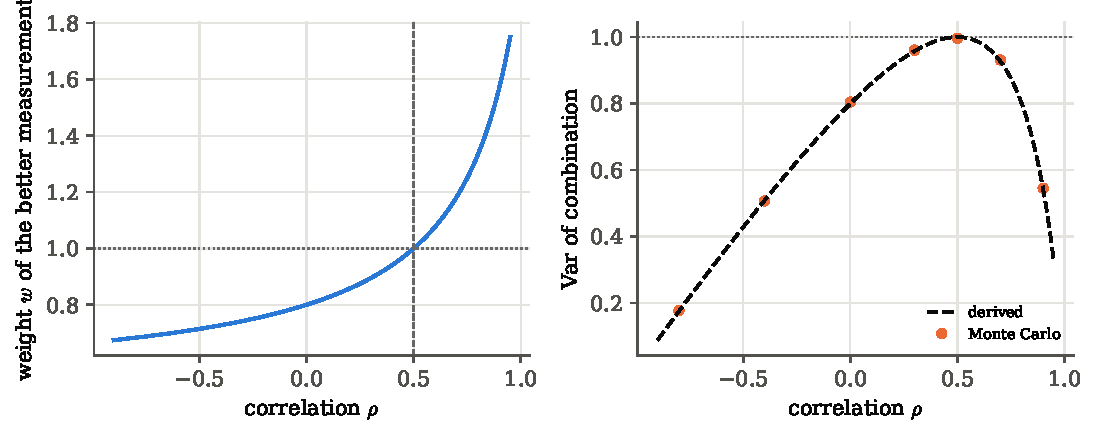
\includegraphics[width=12cm]{figures/ch03/correlated_combination.pdf}
\caption{Combining two measurements with $\sigma_1=1$ and $\sigma_2=2$ as
their correlation $\rho$ varies. Left: the weight of the better measurement
passes $1$ at $\rho=\sigma_1/\sigma_2=0.5$ (dashed vertical line), and
beyond it the poorer measurement is subtracted. Right: the variance of the
optimal combination (dashed curve, formula; dots, simulation) touches the
better measurement's variance $1$ only at $\rho=0.5$ and falls towards zero
as $\rho\to1$.}
\label{3a:fig:correlated-combination}
\end{figure}

\paragraph{Example: two rulers and one thermometer.}
Cowan's example makes the negative weight concrete
\srcref{Cowan}{\S7.6.1}. We measure a length $\lambda$ with two rulers of
different materials, calibrated at temperature $T_0$, with thermal expansion
coefficients $c_1$ and $c_2$. Each reading $L_i$ is corrected with the
measured temperature $T$,
\begin{equation}
  y_i=L_i+c_i(T-T_0),
  \label{3a:eq:rulers}
\end{equation}
\srcref{Cowan}{(7.41)}. The readings have independent errors $\sigma_L$, and
the one thermometer reading $T$ has error $\sigma_T$ and enters both
corrections. Linear propagation, exact here, gives
\begin{align*}
  \sigma_i^2 &\eqby{1} \sigma_L^2+c_i^2\sigma_T^2,\qquad
  V_{12} \eqby{2} c_1c_2\sigma_T^2,\qquad
  \rho\eqby{3}\frac{c_1c_2\sigma_T^2}{\sqrt{(\sigma_L^2+c_1^2\sigma_T^2)(\sigma_L^2+c_2^2\sigma_T^2)}}
\end{align*}
\srcref{Cowan}{(7.42)--(7.44)}.
\begin{explain}
  \item Variance of a sum of independent terms, with
        $\Var[c_i(T-T_0)]=c_i^2\sigma_T^2$.
  \item The only error the two corrected lengths share is the temperature
        error, as in \cref{3a:ex:common-calib}:
        $\Cov(c_1T,c_2T)=c_1c_2\sigma_T^2$.
  \item $\rho=V_{12}/(\sigma_1\sigma_2)$.
\end{explain}
Take $c_1=0.02$ and $c_2=0.05\,\mathrm{mm\,K^{-1}}$, $\sigma_L=0.01\,$mm and
$\sigma_T=2\,$K, and suppose the room is really at $22^\circ$C, two degrees
above $T_0=20^\circ$C, for a true length of $1000.00\,$mm; the thermometer
reads $25^\circ$C. The corrected lengths come out as $y_1=1000.06$ and
$y_2=1000.15\,$mm. The numbers are
\begin{align*}
  \sigma_1^2&=10^{-4}+4\times10^{-4}\times4=0.0017,\qquad
  \sigma_2^2=10^{-4}+25\times10^{-4}\times4=0.0101,\qquad
  V_{12}=0.004,\\
  \rho&=\frac{0.004}{\sqrt{0.0017\times0.0101}}=0.965
  \;>\;\frac{\sigma_1}{\sigma_2}=0.410,\\
  w&\eqby{1}\frac{\sigma_2^2-V_{12}}{\sigma_1^2+\sigma_2^2-2V_{12}}
   =\frac{0.0061}{0.0038}=1.605,\\
  \hat\lambda&\eqby{2}1000+1.605\times0.06-0.605\times0.15=1000.006\,\mathrm{mm},\qquad
  \sigma_{\hat\lambda}\eqby{3}\sqrt{\frac{\sigma_1^2\sigma_2^2-V_{12}^2}{0.0038}}=0.018\,\mathrm{mm}.
\end{align*}
\begin{explain}
  \item \eqref{3a:eq:wcorr-w2} with $\rho\sigma_1\sigma_2=V_{12}$.
  \item $\hat\lambda=wy_1+(1-w)y_2$, written relative to $1000\,$mm.
  \item \eqref{3a:eq:wcorr-var2}, again with $\rho\sigma_1\sigma_2=V_{12}$,
        so that $(1-\rho^2)\sigma_1^2\sigma_2^2=\sigma_1^2\sigma_2^2-V_{12}^2$.
\end{explain}
The combination $1000.006\pm0.018\,$mm lies \emph{outside} the interval
$[1000.06,1000.15]$ and is right, whereas the naive weighted mean that ignores
the correlation gives $1000.073\pm0.038\,$mm, too high by twice its own
error.

Why is a value outside both readings right? \Cref{3a:fig:rulers} shows it.
Each corrected length is a straight line in the unknown true temperature.
Both rulers measure the same length, so they must agree at the true
temperature. The estimate is therefore pulled towards the point where the
two lines cross \srcref{Cowan}{Fig.~7.7}. The same fit returns an estimate of
the temperature itself, $\hat T=22.2^\circ$C, from
\srcref{Cowan}{(7.47)}: the disagreement between the rulers has been used
to correct the thermometer. In the limit $\sigma_L\to0$ ($\rho\to1$) the
two lines give $\hat\lambda=(c_2y_1-c_1y_2)/(c_2-c_1)$ with zero
variance.\footnote{This follows from \eqref{3a:eq:rulers} with exact
readings: then $y_i=\lambda+c_i(T-T_{\text{true}})$, and eliminating
$T-T_{\text{true}}$ between $i=1,2$ gives $c_2y_1-c_1y_2=(c_2-c_1)\lambda$.
Cowan's (7.46) has $c_1$ and $c_2$ interchanged in the numerators; the
check $c_1=0$ (a ruler that does not expand, so $\lambda=y_1$) confirms the
version given here.}

\begin{figure}[htbp]
\centering
\begin{tikzpicture}
\begin{axis}[width=10cm,height=6.2cm,
  xmin=19,xmax=27,ymin=-0.08,ymax=0.2,
  xlabel={assumed true temperature (${}^\circ$C)},
  ylabel={corrected length $-1000$ (mm)},
  tick label style={font=\footnotesize},label style={font=\small},
  yticklabel style={/pgf/number format/fixed},
  scaled y ticks=false,
  legend style={font=\footnotesize,at={(0.02,0.98)},anchor=north west,draw=none,fill=none},
  clip=true]
  \addplot[draw=none,fill=formblue!18,domain=19:27,forget plot] {-0.04+0.02*(x-20)+0.01} \closedcycle;
  \addplot[draw=none,fill=white,domain=19:27,forget plot] {-0.04+0.02*(x-20)-0.01} \closedcycle;
  \addplot[very thick,formblue,domain=19:27] {-0.04+0.02*(x-20)};
  \addlegendentry{ruler 1, $c_1=0.02$}
  \addplot[very thick,fibreorange,domain=19:27] {-0.10+0.05*(x-20)};
  \addlegendentry{ruler 2, $c_2=0.05$}
  \addplot[fibreorange,thin,dashed,domain=19:27,forget plot] {-0.10+0.05*(x-20)+0.01};
  \addplot[fibreorange,thin,dashed,domain=19:27,forget plot] {-0.10+0.05*(x-20)-0.01};
  \draw[softgray,dashed] (axis cs:25,-0.08) -- (axis cs:25,0.2);
  \fill[formblue] (axis cs:25,0.06) circle (2pt);
  \fill[fibreorange] (axis cs:25,0.15) circle (2pt);
  \node[font=\footnotesize,anchor=west] at (axis cs:25.15,0.06) {$y_1$};
  \node[font=\footnotesize,anchor=west] at (axis cs:25.15,0.15) {$y_2$};
  \node[font=\footnotesize,anchor=north,align=center] at (axis cs:25.9,-0.03) {thermometer\\ reads $25^\circ$};
  \fill[bdryred] (axis cs:22.16,0.0055) circle (2.2pt);
  \node[font=\footnotesize,anchor=north west] at (axis cs:22.3,-0.005) {$(\hat T,\hat\lambda)$};
\end{axis}
\end{tikzpicture}
\caption{Two rulers read at a thermometer reading of $25^\circ$C give the
corrected lengths $y_1$ and $y_2$ (dots on the dashed vertical line). If the
temperature were different, each corrected length would slide along its
own line, whose slope is the ruler's expansion coefficient; the shaded
strip and the thin dashed lines show the $\pm\sigma_L$ reading error. Both
rulers measure one length, so the truth sits where the lines cross. The
correlated weighted mean (red dot) lands there, below both $y_1$ and
$y_2$, and at a temperature near $22^\circ$C.}
\label{3a:fig:rulers}
\end{figure}

\paragraph{How research uses it.}
Every world average of a particle mass or lifetime is an inverse-variance
weighted mean, quoted with its $\chi^2_{\min}$ and, when needed, the
inflation factor of \cref{3a:sec:wchi2}. When several experiments share
systematic errors, the correlated formula \eqref{3a:eq:wcorr-weights} is
used under the name ``best linear unbiased estimate'' (the original
discussion is by Lyons and collaborators, \srcref{Cowan}{p.~109}). The hard
part is not the algebra but the off-diagonal elements of $V$, which must be
estimated.

Here our Monte Carlo only \emph{verifies} formulas we derived. In research
the covariance of the inputs is itself often taken from simulations, and
then its noise (\cref{3a:sec:cov-noise}) passes into the weights.

In cosmology the same algebra appears in a more general form. Combining
independent probes with Gaussian likelihoods multiplies the likelihoods,
and multiplying Gaussians adds their inverse covariances. For one parameter that is
exactly $1/\sigma^2=\sum_i1/\sigma_i^2$; for many parameters it is the
statement that Fisher matrices add (\cref{ch:10}).

\paragraph{Where this leaves us.}
Every error bar so far came from one idea: treat a summary of the data as a
random variable over imagined repetitions, and ask for its centre and width.
The weighted mean showed a second way of seeing the same numbers. The
density of the data, read as a function of the unknown $\mu$, peaked at the
estimator and had a width equal to its standard error. That reading of the
density is the likelihood, the subject of the second half of the chapter.
Maximising it gives estimators, and its curvature gives their error bars.

\begin{recap}[Part 3a in one page]
\begin{itemize}
  \item An estimator $\hat\theta=g(x_1,\dots,x_N)$ is a random variable. Its
        sampling distribution over imagined repetitions gives the error bar
        (the standard error). Simulate it when in doubt.
  \item $\mathrm{MSE}=\mathrm{bias}^2+\mathrm{variance}$. Consistency:
        $\hat\theta\to\theta$ in probability, guaranteed when bias and
        variance both go to zero.
  \item $\Var\bar x=\sigma^2/N$: errors shrink like $1/\sqrt N$ (law of
        large numbers via Chebyshev). The central limit theorem makes the
        sampling distribution of a mean Gaussian.
  \item $S^2$ divides by $N-1$ to be unbiased. Its own error is
        $\Var S^2=2\sigma^4/(N-1)$ for Gaussian data (cosmic variance is the
        same fact).
  \item Sample covariance and correlation matrices are noisy: sample
        correlations of independent variables scatter by $\sim1/\sqrt N$,
        and inverting a simulated covariance needs the Hartlap factor.
  \item Error propagation: $U=AVA\T$ with the Jacobian $A$, exact for linear
        maps. It fails near poles and for noisy denominators; use Monte Carlo
        propagation there.
  \item Combining measurements: weight by $1/\sigma_i^2$, so
        $1/\sigma_{\hat\mu}^2=\sum_i1/\sigma_i^2$. Check
        $\chi^2_{\min}\sim\chi^2_{N-1}$. With correlations,
        $\bm w=V^{-1}\bm1/(\bm1\T V^{-1}\bm1)$, and weights can be negative.
\end{itemize}
\end{recap}

\providecommand{\ThreeBBernArea}{}\renewcommand{\ThreeBBernArea}{3.780\times10^{-7}}
\providecommand{\ThreeBBernAreaNum}{}\renewcommand{\ThreeBBernAreaNum}{3.780\times10^{-7}}
\providecommand{\ThreeBBernLmax}{}\renewcommand{\ThreeBBernLmax}{1.427\times10^{-6}}
\providecommand{\ThreeBBernRatio}{}\renewcommand{\ThreeBBernRatio}{0.265}
\providecommand{\ThreeBUnifMax}{}\renewcommand{\ThreeBUnifMax}{0.9072}
\providecommand{\ThreeBLifeT}{}\renewcommand{\ThreeBLifeT}{10.51}
\providecommand{\ThreeBAreaTau}{}\renewcommand{\ThreeBAreaTau}{4.920\times10^{-4}}
\providecommand{\ThreeBAreaTauNum}{}\renewcommand{\ThreeBAreaTauNum}{4.920\times10^{-4}}
\providecommand{\ThreeBAreaLam}{}\renewcommand{\ThreeBAreaLam}{8.910\times10^{-5}}
\providecommand{\ThreeBAreaRatio}{}\renewcommand{\ThreeBAreaRatio}{5.522}
\providecommand{\ThreeBDecN}{}\renewcommand{\ThreeBDecN}{50}
\providecommand{\ThreeBDecTauHat}{}\renewcommand{\ThreeBDecTauHat}{0.8831}
\providecommand{\ThreeBDecTauNum}{}\renewcommand{\ThreeBDecTauNum}{0.8831}
\providecommand{\ThreeBDecSigCurv}{}\renewcommand{\ThreeBDecSigCurv}{0.1249}
\providecommand{\ThreeBDecLo}{}\renewcommand{\ThreeBDecLo}{0.114}
\providecommand{\ThreeBDecHi}{}\renewcommand{\ThreeBDecHi}{0.1376}
\providecommand{\ThreeBDecSdTh}{}\renewcommand{\ThreeBDecSdTh}{0.1414}
\providecommand{\ThreeBDecSdMC}{}\renewcommand{\ThreeBDecSdMC}{0.1406}
\providecommand{\ThreeBDecMeanTau}{}\renewcommand{\ThreeBDecMeanTau}{1.003}
\providecommand{\ThreeBDecMeanCurv}{}\renewcommand{\ThreeBDecMeanCurv}{0.1419}
\providecommand{\ThreeBDecCoverCurv}{}\renewcommand{\ThreeBDecCoverCurv}{0.6913}
\providecommand{\ThreeBDecCoverDl}{}\renewcommand{\ThreeBDecCoverDl}{0.6866}
\providecommand{\ThreeBDecLamMean}{}\renewcommand{\ThreeBDecLamMean}{1.017}
\providecommand{\ThreeBDecLamTh}{}\renewcommand{\ThreeBDecLamTh}{1.02}
\providecommand{\ThreeBAngMomA}{}\renewcommand{\ThreeBAngMomA}{0.49}
\providecommand{\ThreeBAngMomB}{}\renewcommand{\ThreeBAngMomB}{0.4458}
\providecommand{\ThreeBAngA}{}\renewcommand{\ThreeBAngA}{0.4885}
\providecommand{\ThreeBAngB}{}\renewcommand{\ThreeBAngB}{0.4396}
\providecommand{\ThreeBAngSa}{}\renewcommand{\ThreeBAngSa}{0.05099}
\providecommand{\ThreeBAngSb}{}\renewcommand{\ThreeBAngSb}{0.107}
\providecommand{\ThreeBAngRho}{}\renewcommand{\ThreeBAngRho}{0.4237}
\providecommand{\ThreeBAngIter}{}\renewcommand{\ThreeBAngIter}{4}
\providecommand{\ThreeBAngStepOneA}{}\renewcommand{\ThreeBAngStepOneA}{0.4885}
\providecommand{\ThreeBAngStepOneB}{}\renewcommand{\ThreeBAngStepOneB}{0.4396}
\providecommand{\ThreeBAngSdA}{}\renewcommand{\ThreeBAngSdA}{0.05376}
\providecommand{\ThreeBAngSdB}{}\renewcommand{\ThreeBAngSdB}{0.1081}
\providecommand{\ThreeBAngRhoMC}{}\renewcommand{\ThreeBAngRhoMC}{0.4919}
\providecommand{\ThreeBAngMomSdA}{}\renewcommand{\ThreeBAngMomSdA}{0.05422}
\providecommand{\ThreeBAngMomSdB}{}\renewcommand{\ThreeBAngMomSdB}{0.1109}
\providecommand{\ThreeBAngMeanA}{}\renewcommand{\ThreeBAngMeanA}{0.502}
\providecommand{\ThreeBAngMeanB}{}\renewcommand{\ThreeBAngMeanB}{0.4986}
\providecommand{\ThreeBAngRhoMCErr}{}\renewcommand{\ThreeBAngRhoMCErr}{0.0339}
\providecommand{\ThreeBAngRhoHessMean}{}\renewcommand{\ThreeBAngRhoHessMean}{0.4263}
\providecommand{\ThreeBAngRhoHessSd}{}\renewcommand{\ThreeBAngRhoHessSd}{0.03868}
\providecommand{\ThreeBAngMomRatioA}{}\renewcommand{\ThreeBAngMomRatioA}{1.009}
\providecommand{\ThreeBAngMomRatioAErr}{}\renewcommand{\ThreeBAngMomRatioAErr}{0.007096}
\providecommand{\ThreeBAngMomRatioB}{}\renewcommand{\ThreeBAngMomRatioB}{1.026}
\providecommand{\ThreeBAngMomRatioBErr}{}\renewcommand{\ThreeBAngMomRatioBErr}{0.009865}
\providecommand{\ThreeBLineA}{}\renewcommand{\ThreeBLineA}{1.238}
\providecommand{\ThreeBLineB}{}\renewcommand{\ThreeBLineB}{0.4187}
\providecommand{\ThreeBLineSa}{}\renewcommand{\ThreeBLineSa}{0.4113}
\providecommand{\ThreeBLineSb}{}\renewcommand{\ThreeBLineSb}{0.08767}
\providecommand{\ThreeBLineRho}{}\renewcommand{\ThreeBLineRho}{-0.8223}
\providecommand{\ThreeBLineChi}{}\renewcommand{\ThreeBLineChi}{11.01}
\providecommand{\ThreeBLineP}{}\renewcommand{\ThreeBLineP}{0.2012}
\providecommand{\ThreeBLineSaMC}{}\renewcommand{\ThreeBLineSaMC}{0.4067}
\providecommand{\ThreeBLineSbMC}{}\renewcommand{\ThreeBLineSbMC}{0.08717}
\providecommand{\ThreeBLineRhoMC}{}\renewcommand{\ThreeBLineRhoMC}{-0.8182}
\providecommand{\ThreeBLineChiMean}{}\renewcommand{\ThreeBLineChiMean}{7.932}
\providecommand{\ThreeBLineChiVar}{}\renewcommand{\ThreeBLineChiVar}{15.69}
\providecommand{\ThreeBLineWrongMean}{}\renewcommand{\ThreeBLineWrongMean}{41.36}
\providecommand{\ThreeBCorrMeanBd}{}\renewcommand{\ThreeBCorrMeanBd}{0.4986}
\providecommand{\ThreeBCorrMeanBf}{}\renewcommand{\ThreeBCorrMeanBf}{0.4994}
\providecommand{\ThreeBCorrQuoted}{}\renewcommand{\ThreeBCorrQuoted}{0.08767}
\providecommand{\ThreeBCorrTrueD}{}\renewcommand{\ThreeBCorrTrueD}{0.1284}
\providecommand{\ThreeBCorrSdD}{}\renewcommand{\ThreeBCorrSdD}{0.1282}
\providecommand{\ThreeBCorrSdF}{}\renewcommand{\ThreeBCorrSdF}{0.1212}
\providecommand{\ThreeBCorrQuotedF}{}\renewcommand{\ThreeBCorrQuotedF}{0.121}
\providecommand{\ThreeBCorrChiD}{}\renewcommand{\ThreeBCorrChiD}{4.77}
\providecommand{\ThreeBCorrChiF}{}\renewcommand{\ThreeBCorrChiF}{8.069}
\providecommand{\ThreeBPoisNobs}{}\renewcommand{\ThreeBPoisNobs}{122}
\providecommand{\ThreeBPoisNuP}{}\renewcommand{\ThreeBPoisNuP}{122}
\providecommand{\ThreeBPoisNuN}{}\renewcommand{\ThreeBPoisNuN}{110.7}
\providecommand{\ThreeBPoisNuS}{}\renewcommand{\ThreeBPoisNuS}{129}
\providecommand{\ThreeBPoisTauP}{}\renewcommand{\ThreeBPoisTauP}{1.076}
\providecommand{\ThreeBPoisTauN}{}\renewcommand{\ThreeBPoisTauN}{0.9253}
\providecommand{\ThreeBPoisTauS}{}\renewcommand{\ThreeBPoisTauS}{1.18}
\providecommand{\ThreeBPoisChiN}{}\renewcommand{\ThreeBPoisChiN}{13.7}
\providecommand{\ThreeBPoisChiS}{}\renewcommand{\ThreeBPoisChiS}{14.01}
\providecommand{\ThreeBPoisBC}{}\renewcommand{\ThreeBPoisBC}{18.47}
\providecommand{\ThreeBPoisZeroBins}{}\renewcommand{\ThreeBPoisZeroBins}{4}
\providecommand{\ThreeBPoisDiffP}{}\renewcommand{\ThreeBPoisDiffP}{3.996\times10^{-9}}
\providecommand{\ThreeBPoisDiffN}{}\renewcommand{\ThreeBPoisDiffN}{-11.65}
\providecommand{\ThreeBPoisDiffS}{}\renewcommand{\ThreeBPoisDiffS}{7.883}
\providecommand{\ThreeBPoisPredN}{}\renewcommand{\ThreeBPoisPredN}{-13.73}
\providecommand{\ThreeBPoisPredS}{}\renewcommand{\ThreeBPoisPredS}{7.883}
\providecommand{\ThreeBPoisTauMeanP}{}\renewcommand{\ThreeBPoisTauMeanP}{1.002}
\providecommand{\ThreeBPoisTauMeanN}{}\renewcommand{\ThreeBPoisTauMeanN}{0.8992}
\providecommand{\ThreeBPoisTauMeanS}{}\renewcommand{\ThreeBPoisTauMeanS}{1.114}
\providecommand{\ThreeBPoisBCmean}{}\renewcommand{\ThreeBPoisBCmean}{18.73}
\providecommand{\ThreeBPoisDof}{}\renewcommand{\ThreeBPoisDof}{18}
\providecommand{\ThreeBEffMeanBig}{}\renewcommand{\ThreeBEffMeanBig}{0.9981}
\providecommand{\ThreeBEffMedBig}{}\renewcommand{\ThreeBEffMedBig}{1.578}
\providecommand{\ThreeBEffNBig}{}\renewcommand{\ThreeBEffNBig}{201}
\providecommand{\ThreeBEffARE}{}\renewcommand{\ThreeBEffARE}{0.6327}
\providecommand{\ThreeBEffAREth}{}\renewcommand{\ThreeBEffAREth}{0.6366}
\providecommand{\ThreeBEffUnifFifty}{}\renewcommand{\ThreeBEffUnifFifty}{0.01877}
\providecommand{\ThreeBEffUnifFiftyTh}{}\renewcommand{\ThreeBEffUnifFiftyTh}{0.01887}
\providecommand{\ThreeBEffNFifty}{}\renewcommand{\ThreeBEffNFifty}{51}
\providecommand{\ThreeBConsTen}{}\renewcommand{\ThreeBConsTen}{1.47}
\providecommand{\ThreeBConsHund}{}\renewcommand{\ThreeBConsHund}{1.031}
\providecommand{\ThreeBConsThou}{}\renewcommand{\ThreeBConsThou}{1.016}
\providecommand{\ThreeBProfNon}{}\renewcommand{\ThreeBProfNon}{20}
\providecommand{\ThreeBProfNoff}{}\renewcommand{\ThreeBProfNoff}{8}
\providecommand{\ThreeBProfK}{}\renewcommand{\ThreeBProfK}{1}
\providecommand{\ThreeBProfS}{}\renewcommand{\ThreeBProfS}{12}
\providecommand{\ThreeBProfB}{}\renewcommand{\ThreeBProfB}{8}
\providecommand{\ThreeBProfLo}{}\renewcommand{\ThreeBProfLo}{5.192}
\providecommand{\ThreeBProfHi}{}\renewcommand{\ThreeBProfHi}{5.47}
\providecommand{\ThreeBCondLo}{}\renewcommand{\ThreeBCondLo}{4.145}
\providecommand{\ThreeBCondHi}{}\renewcommand{\ThreeBCondHi}{4.811}
\providecommand{\ThreeBProfGauss}{}\renewcommand{\ThreeBProfGauss}{5.292}
\providecommand{\ThreeBCondGauss}{}\renewcommand{\ThreeBCondGauss}{4.472}
\providecommand{\ThreeBProfCover}{}\renewcommand{\ThreeBProfCover}{0.6849}
\providecommand{\ThreeBCondCover}{}\renewcommand{\ThreeBCondCover}{0.6088}
\providecommand{\ThreeBProfUsed}{}\renewcommand{\ThreeBProfUsed}{9995}
\providecommand{\ThreeBBootRelOne}{}\renewcommand{\ThreeBBootRelOne}{0.1365}
\providecommand{\ThreeBBootRelMean}{}\renewcommand{\ThreeBBootRelMean}{0.1375}
\providecommand{\ThreeBBootRelSd}{}\renewcommand{\ThreeBBootRelSd}{0.01819}
\providecommand{\ThreeBBootTauHat}{}\renewcommand{\ThreeBBootTauHat}{0.8176}
\providecommand{\ThreeBBootMed}{}\renewcommand{\ThreeBBootMed}{0.5147}
\providecommand{\ThreeBBootSeTauTrue}{}\renewcommand{\ThreeBBootSeTauTrue}{0.1425}
\providecommand{\ThreeBBootSeTauNP}{}\renewcommand{\ThreeBBootSeTauNP}{0.1116}
\providecommand{\ThreeBBootSeTauP}{}\renewcommand{\ThreeBBootSeTauP}{0.1162}
\providecommand{\ThreeBBootSeTauCurv}{}\renewcommand{\ThreeBBootSeTauCurv}{0.1156}
\providecommand{\ThreeBBootSeMedTrue}{}\renewcommand{\ThreeBBootSeMedTrue}{0.1418}
\providecommand{\ThreeBBootSeMedNP}{}\renewcommand{\ThreeBBootSeMedNP}{0.1352}
\providecommand{\ThreeBBootSeMedP}{}\renewcommand{\ThreeBBootSeMedP}{0.1155}
\providecommand{\ThreeBBootNormLo}{}\renewcommand{\ThreeBBootNormLo}{0.2496}
\providecommand{\ThreeBBootNormHi}{}\renewcommand{\ThreeBBootNormHi}{0.7798}
\providecommand{\ThreeBBootPivLo}{}\renewcommand{\ThreeBBootPivLo}{0.1678}
\providecommand{\ThreeBBootPivHi}{}\renewcommand{\ThreeBBootPivHi}{0.6632}
\providecommand{\ThreeBBootPctLo}{}\renewcommand{\ThreeBBootPctLo}{0.3661}
\providecommand{\ThreeBBootPctHi}{}\renewcommand{\ThreeBBootPctHi}{0.8616}
\providecommand{\ThreeBBootMedTrueVal}{}\renewcommand{\ThreeBBootMedTrueVal}{0.6931}
\providecommand{\ThreeBBootFrac}{}\renewcommand{\ThreeBBootFrac}{0.6386}
\providecommand{\ThreeBBootFracTh}{}\renewcommand{\ThreeBBootFracTh}{0.6358}
\providecommand{\ThreeBBootB}{}\renewcommand{\ThreeBBootB}{10000}
\providecommand{\ThreeBRBTruth}{}\renewcommand{\ThreeBRBTruth}{0.2231}
\providecommand{\ThreeBRBCrudeMean}{}\renewcommand{\ThreeBRBCrudeMean}{0.2232}
\providecommand{\ThreeBRBCrudeVar}{}\renewcommand{\ThreeBRBCrudeVar}{0.1734}
\providecommand{\ThreeBRBRBMean}{}\renewcommand{\ThreeBRBRBMean}{0.2231}
\providecommand{\ThreeBRBRBVar}{}\renewcommand{\ThreeBRBRBVar}{0.00799}
\providecommand{\ThreeBRBRatio}{}\renewcommand{\ThreeBRBRatio}{0.04608}
\providecommand{\ThreeBRBCR}{}\renewcommand{\ThreeBRBCR}{0.007468}
\providecommand{\ThreeBRBCrudeVarTh}{}\renewcommand{\ThreeBRBCrudeVarTh}{0.1733}
\providecommand{\ThreeBRBRBVarTh}{}\renewcommand{\ThreeBRBRBVarTh}{0.008057}
\providecommand{\ThreeBRBn}{}\renewcommand{\ThreeBRBn}{10}
\providecommand{\ThreeBRBlam}{}\renewcommand{\ThreeBRBlam}{1.5}
\providecommand{\ThreeBBayesSqArg}{}\renewcommand{\ThreeBBayesSqArg}{3.005}
\providecommand{\ThreeBBayesAbsArg}{}\renewcommand{\ThreeBBayesAbsArg}{2.677}
\providecommand{\ThreeBBayesZOArg}{}\renewcommand{\ThreeBBayesZOArg}{2}
\providecommand{\ThreeBBayesMean}{}\renewcommand{\ThreeBBayesMean}{3}
\providecommand{\ThreeBBayesMedian}{}\renewcommand{\ThreeBBayesMedian}{2.672}
\providecommand{\ThreeBBayesMode}{}\renewcommand{\ThreeBBayesMode}{2}
\providecommand{\ThreeBCMBMeanTwo}{}\renewcommand{\ThreeBCMBMeanTwo}{0.9962}
\providecommand{\ThreeBCMBVarTwo}{}\renewcommand{\ThreeBCMBVarTwo}{0.401}
\providecommand{\ThreeBCMBBoundTwo}{}\renewcommand{\ThreeBCMBBoundTwo}{0.4}
\providecommand{\ThreeBCMBRelErrTwo}{}\renewcommand{\ThreeBCMBRelErrTwo}{0.6332}
\providecommand{\ThreeBCMBMeanThirty}{}\renewcommand{\ThreeBCMBMeanThirty}{1.002}
\providecommand{\ThreeBCMBVarThirty}{}\renewcommand{\ThreeBCMBVarThirty}{0.03236}
\providecommand{\ThreeBCMBBoundThirty}{}\renewcommand{\ThreeBCMBBoundThirty}{0.03279}
\providecommand{\ThreeBCMBRelErrThirty}{}\renewcommand{\ThreeBCMBRelErrThirty}{0.1799}
\providecommand{\ThreeBCMBScoreVarThirty}{}\renewcommand{\ThreeBCMBScoreVarThirty}{30.16}
\providecommand{\ThreeBCMBFishThirty}{}\renewcommand{\ThreeBCMBFishThirty}{30.5}
\providecommand{\ThreeBCMBScoreMeanThirty}{}\renewcommand{\ThreeBCMBScoreMeanThirty}{0.008949}
 
\section{The likelihood: data are the model plus noise}
\label{3b:sec:likelihood}

We measure a voltage, count photons in a detector, record the arrival
times of decays, or estimate a power spectrum from a map of the sky. In every
case we also have a theory with a knob on it: a resistance, a cross-section,
a lifetime, a cosmological parameter. Set the knob to a value $\theta$ and
the theory predicts what the apparatus should have shown. Call that
prediction $d(\theta)$. The apparatus never shows exactly $d(\theta)$. It
shows the prediction plus whatever the noise happened to be on that day.
Until now the question has run one way: \emph{given} the truth, how does a
summary of the data scatter when the experiment is repeated? Now the data
are in, and we ask the opposite question: which values of the knob could
have produced the data we actually have?

The tool for this backward question is the \newterm{likelihood}. It is not a
new probability distribution. It is the old one, the distribution of the
data, read in the other direction. To understand it we need answers to four
questions.
\begin{enumerate}[label=\arabic*.]
  \item How does a model of the noise turn into a number attached to each
        value of $\theta$?
  \item What happens with many measurements?
  \item Why is that number \emph{not} a probability distribution for
        $\theta$, even though it is built from one?
  \item Where does it sit in Bayes' theorem, and what information in the
        data does it keep?
\end{enumerate}
The pipeline of \cref{ch:00} ends with an arrow from how a statistic $S$
scatters, $P(S\given\theta)$, to what the observed value of $S$ says about
the physics. The likelihood is that arrow. It is the sampling distribution
of the data (or of a summary $S$ of them), evaluated at the data we
observed and read as a function of the physics $\theta$.

\subsection{One measurement: from the noise to the likelihood}
\label{3b:sec:one-measurement}

Start with the simplest experiment there is. The model predicts a number
$d(\theta)$, and the measurement adds noise:
\begin{equation}
  D = d(\theta) + \epsilon,\qquad \epsilon\sim\Normal(0,\sigma^2),
  \label{3b:eq:model-noise}
\end{equation}
with $\sigma$ known from calibrating the instrument. The noise $\epsilon$
\unpack{the random amount by which this particular reading differs from the
ideal, noiseless one} has density
$\phi_\sigma(\epsilon)=(2\pi\sigma^2)^{-1/2}\exp(-\epsilon^2/2\sigma^2)$.
What is the density of the reading $D$ itself? Fix $\theta$ and ask for the
probability that $D$ lands in a small window $[D_0,D_0+\dd D]$:
\begin{align}
  \Prob\bigl(D_0\le D\le D_0+\dd D\given\theta\bigr)
  &\eqby{1} \Prob\bigl(D_0-d(\theta)\le \epsilon\le D_0-d(\theta)+\dd D\bigr)
  \nonumber\\
  &\eqby{2} \phi_\sigma\bigl(D_0-d(\theta)\bigr)\,\dd D
  \nonumber\\
  &\eqby{3} \frac{1}{\sqrt{2\pi\sigma^2}}
     \exp\!\left[-\frac{\bigl(D_0-d(\theta)\bigr)^2}{2\sigma^2}\right]\dd D .
  \label{3b:eq:one-point}
\end{align}
\begin{explain}
  \item At fixed $\theta$ the prediction $d(\theta)$ is just a number, so
        $D=d(\theta)+\epsilon$ lies in the window exactly when $\epsilon$
        lies in the same window shifted down by $d(\theta)$.
  \item For a small window, probability is density times width. A shift does
        not stretch the window, so the width is still $\dd D$.
  \item Insert the Gaussian density of the noise.
\end{explain}
So $D\sim\Normal(d(\theta),\sigma^2)$: the reading is Gaussian, centred on
the prediction, with the width of the noise. Nothing new so far. This is the
\emph{forward} or \emph{prediction} direction: fix the physics, ask how the
data would scatter.

Now the data are in. We hold $D=D_0$ fixed at the value on the lab book and
let $\theta$ vary instead. The same expression becomes a function of $\theta$,
\begin{equation}
  \Like(\theta)\equiv p(D_0\given\theta)
  =\frac{1}{\sqrt{2\pi\sigma^2}}
   \exp\!\left[-\frac{\bigl(D_0-d(\theta)\bigr)^2}{2\sigma^2}\right]
  =\phi_\sigma\bigl(\underbrace{D_0-d(\theta)}_{\text{required noise}}\bigr).
  \label{3b:eq:like-one}
\end{equation}
The last form says what the likelihood measures. Take a trial value
$\theta$. The model predicts $d(\theta)$. To turn that prediction into the
reading we actually got, the noise must have been exactly
$\epsilon=D_0-d(\theta)$. The likelihood is the probability density of
\emph{that} noise value. So for each trial $\theta$ it answers one question:
how probable is the noise that this $\theta$ needs in order to explain our
reading?

\begin{keyidea}[what the likelihood measures]
Pick a trial value $\theta$. The model then says what the reading should have
been, $d(\theta)$, and the gap $D_0-d(\theta)$ is the noise that nature would
have had to add to turn that prediction into the reading we actually got. The
likelihood of $\theta$ is how probable this particular piece of noise is.
In symbols it is nothing more than the distribution of the data: if
$D=d(\theta)+\epsilon$ with $\epsilon\sim\Normal(0,1)$, then
$D\sim\Normal(d(\theta),1)$, and this density, with $D$ held at the observed
value and $\theta$ left free, is the likelihood function. For noise of width
$\sigma$, as in \eqref{3b:eq:like-one}, the $1$ becomes $\sigma^2$.
\end{keyidea}

A value of $\theta$ whose prediction sits close to the data needs only a
small, ordinary fluctuation and gets a high likelihood. A value whose
prediction sits five noise widths away needs a five-sigma fluctuation and
gets a likelihood smaller by a factor $e^{-25/2}\approx4\times10^{-6}$.
\Cref{3b:fig:residual-gaussians} draws exactly this for several data
points and two trial models.

In the language of the backward question, each trial value of $\theta$ is a
candidate explanation, the reading $D_0$ is what we saw, and the likelihood
ranks the candidates by how easily each one would have produced that reading.
Parameter estimation in \cref{ch:05} is built on exactly this.

\begin{figure}[htbp]
\centering
\begin{tikzpicture}[x=0.95cm,y=1.05cm]
  \foreach \panel/\xs/\a/\b/\name in {0/0/1.0/0.5/{\theta_A},1/6.6/2.45/0.0/{\theta_B}}{
  \begin{scope}[xshift=\xs cm]
    \draw[->,faint] (0,0.3) -- (5.9,0.3) node[below left,font=\footnotesize,black] {$x$};
    \draw[->,faint] (0,0.3) -- (0,4.9) node[left,font=\footnotesize,black] {$D$};
    \draw[form] (0.2,{\a+\b*0.2}) -- (5.7,{\a+\b*5.7});
    \node[font=\footnotesize,formblue,anchor=west] at (0.15,4.6) {model $d(x;\name)$};
    \foreach \xi/\yi in {1/1.6,2/1.9,3/2.7,4/2.9,5/3.6}{
      \pgfmathsetmacro{\m}{\a+\b*\xi}
      \draw[fibre,thin,smooth,samples=41,domain={\m-1.25}:{\m+1.25},variable=\y]
        plot ({\xi+0.62*exp(-((\y-\m)^2)/(2*0.09))},\y);
      \draw[faint,densely dotted] (\xi,{\m-1.25}) -- (\xi,{\m+1.25});
      \draw[bdry,thick] (\xi,\m) -- (\xi,\yi);
      \draw[tangentgreen,thick] (\xi,\yi) -- ({\xi+0.62*exp(-((\yi-\m)^2)/(2*0.09))},\yi);
      \fill[black] (\xi,\yi) circle (1.6pt);
    }
  \end{scope}}
  \node[font=\footnotesize,align=center] at (3.0,-0.25) {$\theta_A$: small residuals,\\ every datum near the peak};
  \node[font=\footnotesize,align=center] at (9.6,-0.25) {$\theta_B$: large residuals,\\ data far out in the tails};
\end{tikzpicture}
\caption{The likelihood of two trial parameter values. Black dots are the
same five measurements in both panels. The blue line is the model prediction
for the trial value, and the orange curve on its side at each $x$ is the
noise density $\Normal(d,\sigma^2)$ centred on the prediction. The red
segment is the fluctuation the noise would have had to produce, and the
length of the green tick is the height of the noise density at the datum.
The likelihood is the product of the five green lengths. On the left they
are all long. On the right two of them are almost zero, so $\theta_B$ needs
an implausible noise realisation.}
\label{3b:fig:residual-gaussians}
\end{figure}

\begin{workdef}[likelihood]
For data $\data$ and a model that gives the data a probability
(or density) $p(\data\given\params)$ for each parameter value, the
\newterm{likelihood} is that same function with the data held fixed at
their observed values and the parameters varied,
\[
  \Like(\params)\equiv p(\data_{\text{obs}}\given\params).
\]
\emph{Operationally:} write down the noise model that turns a prediction
$d(\params)$ into data \unpack{for example ``add independent Gaussian noise of
known width''}, compute the probability of the observed data under it, and
treat the answer as a function of $\params$ alone. The
\newterm{log-likelihood} is $\ell(\params)=\ln\Like(\params)$.
\end{workdef}

\paragraph{Example: one reading of a resistance.}
We pass a known current $I=2\,$A through a resistor and read the voltage
with a voltmeter whose noise is $\sigma=0.2\,$V. The model is Ohm's law,
$d(R)=IR$, and the reading is $D_0=10.4\,$V. Then
\begin{align*}
  \Like(R)
  &\eqby{1}\frac{1}{\sqrt{2\pi}\,(0.2\,\mathrm V)}
     \exp\!\left[-\frac{(10.4\,\mathrm V-2\,\mathrm A\cdot R)^2}{2(0.2\,\mathrm V)^2}\right]\\
  &\eqby{2}\frac{1}{\sqrt{2\pi}\,(0.2\,\mathrm V)}
     \exp\!\left[-\frac{(R-5.2\,\Omega)^2}{2(0.1\,\Omega)^2}\right].
\end{align*}
\begin{explain}
  \item \eqref{3b:eq:like-one} with $d(R)=IR$.
  \item Factor $I^2$ out of the square:
        $(D_0-IR)^2=I^2(R-D_0/I)^2$, and $\sigma^2/I^2=(0.1\,\Omega)^2$.
\end{explain}
As a function of $R$ the likelihood is a Gaussian bump centred at
$5.2\,\Omega$ with width $0.1\,\Omega$. The peak is at the resistance whose
prediction needs zero noise: $IR=D_0$ gives $R=10.4\,\mathrm V/2\,\mathrm
A=5.2\,\Omega$. The width is the noise width divided by the slope
$\dd d/\dd R=I$, because a change $\delta R$ moves the prediction by
$I\,\delta R$. The prefactor carries units of $\mathrm{V}^{-1}$, because it
is a density in the \emph{voltage}, not in $R$. That is the first sign that
the likelihood is not a probability density for $R$
(\cref{3b:sec:not-density}).

\subsection{Many measurements: the product and the logarithm}
\label{3b:sec:product}

Real experiments have many data points $D_1,\dots,D_N$, taken at settings
$x_1,\dots,x_N$, with predictions $d_i(\theta)=d(x_i;\theta)$. If the noise
in different readings is independent, the joint density factorises, because
independence means precisely that the joint density is the product of the
single ones \srcref{Sivia}{p.~65, (3.62)}:
\begin{align}
  \Like(\theta)
  &\eqby{1} p(D_1,\dots,D_N\given\theta)
   \eqby{2} \prod_{i=1}^N p(D_i\given\theta)
  \nonumber\\
  &\eqby{3} \prod_{i=1}^N\frac{1}{\sqrt{2\pi\sigma_i^2}}
     \exp\!\left[-\frac{\bigl(D_i-d_i(\theta)\bigr)^2}{2\sigma_i^2}\right],
  \label{3b:eq:like-product}\\
  \ell(\theta)
  &\eqby{4} -\frac12\sum_{i=1}^N\frac{\bigl(D_i-d_i(\theta)\bigr)^2}{\sigma_i^2}
   \;-\;\sum_{i=1}^N\ln\sqrt{2\pi\sigma_i^2} .
  \label{3b:eq:loglike-gauss}
\end{align}
\begin{explain}
  \item Definition of the likelihood for the whole data vector.
  \item Independent noise: the probability of the joint noise realisation
        is the product of the probabilities of the individual ones.
  \item Insert \eqref{3b:eq:one-point} for each reading, with its own
        noise width $\sigma_i$.
  \item The logarithm of a product is the sum of the logarithms, and
        $\ln e^{u}=u$.
\end{explain}
The first sum in \eqref{3b:eq:loglike-gauss} is
$\chi^2(\theta)$: each residual $D_i-d_i(\theta)$ is divided by its error
bar $\sigma_i$, squared, and the squares are added. The second sum does not
depend on $\theta$ at all. So, for Gaussian noise,
$\ell(\theta)=-\tfrac12\chi^2(\theta)+\text{const}$. This is why least
squares works (\cref{3b:sec:least-squares}).

For identically distributed data, $x_1,\dots,x_n$ drawn independently from
one density $f(x;\theta)$, the same steps give Wasserman's definition
\mainref{p.~122, Def.~9.7},
\begin{equation}
  \Like_n(\theta)=\prod_{i=1}^n f(x_i;\theta),\qquad
  \ell_n(\theta)=\sum_{i=1}^n\ln f(x_i;\theta).
  \label{3b:eq:like-iid}
\end{equation}
Three practical remarks follow from the product structure.
\begin{enumerate}[label=(\roman*)]
  \item \emph{Work with logarithms.} A product of a thousand densities of
        size $0.1$ is $10^{-1000}$ and underflows every computer. Its
        logarithm, $-2303$, is harmless. Sums are also what we
        differentiate most easily.
  \item \emph{Constants do not matter.} Multiplying $\Like$ by any positive
        number $c$ that does not depend on $\theta$ changes nothing we will
        do with it: the location of the maximum, the shape, and ratios
        $\Like(\theta_1)/\Like(\theta_2)$ are all unchanged
        \mainref{p.~123, Remark~9.9}. We drop such constants freely and write
        $\Like\propto\dots$.
  \item \emph{Only ratios carry meaning.} Since the overall constant is
        arbitrary, the statement ``$\Like(\theta_1)=0.03$'' means nothing.
        The statement ``$\Like(\theta_1)/\Like(\theta_2)=20$'' means that the
        data are twenty times more probable under $\theta_1$ than under
        $\theta_2$. The cosmology literature often reports
        $-2\ln[\Like(\theta)/\Like_{\max}]$ \srcref{Padilla}{(26)}, which is
        a $\Delta\chi^2$ for Gaussian noise.
\end{enumerate}

\paragraph{Example: a coin, or any yes/no detector.}
A detector fires ($x_i=1$) or not ($x_i=0$) with unknown probability $p$.
Each trial is Bernoulli, $f(x;p)=p^x(1-p)^{1-x}$. In $n=20$ trials it
fires $S=\sum_ix_i=12$ times \mainref{p.~123, Ex.~9.10}. Then
\begin{align*}
  \Like(p)
  &\eqby{1}\prod_{i=1}^{n}p^{x_i}(1-p)^{1-x_i}
   \eqby{2}p^{\sum_ix_i}(1-p)^{n-\sum_ix_i}
   = p^{12}(1-p)^{8}.
\end{align*}
\begin{explain}
  \item \eqref{3b:eq:like-iid} with the Bernoulli probability.
  \item Collect the powers: $\prod_ip^{x_i}=p^{\sum_ix_i}$ and likewise for
        $1-p$.
\end{explain}
The left panel of \cref{3b:fig:likelihood-shapes} shows it. It is a smooth
bump with its peak at $p=S/n=0.6$. The individual zeros and ones have
disappeared: only their sum $S$ enters.

\paragraph{Example: a uniform distribution with an unknown end point.}
Let $x_i\sim\mathrm{Uniform}(0,\theta)$, with density $1/\theta$ on
$[0,\theta]$ and zero outside \mainref{p.~124, Ex.~9.12}. Each factor of
the product is $1/\theta$ if $x_i\le\theta$ and zero if $x_i>\theta$. The
product is nonzero only if \emph{every} $x_i\le\theta$, that is, if
$\theta\ge x_{(n)}\equiv\max_ix_i$:
\[
  \Like(\theta)=
  \begin{cases}
    \theta^{-n}, & \theta\ge x_{(n)},\\
    0,           & \theta< x_{(n)}.
  \end{cases}
\]
A value $\theta$ smaller than the largest observation is not merely
implausible, it is impossible: no noise realisation can put a point above the
end of the box. For ten simulated points with largest value
$x_{(10)}=\ThreeBUnifMax$, the middle panel of
\cref{3b:fig:likelihood-shapes} shows a cliff at $x_{(10)}$ followed by a
decay as $\theta^{-10}$. It has no smooth peak. Because of that cliff, this
model breaks rules that smooth likelihoods obey: the maximum is not found by
setting a derivative to zero (\cref{3b:sec:mle-hand}), and the Cram\'er--Rao
bound does not apply (\cref{3b:sec:cramer-rao}).

\subsection{The likelihood is not a probability density for \texorpdfstring{$\theta$}{theta}}
\label{3b:sec:not-density}

The likelihood is not the probability density of $\theta$. The temptation is
real: it is built from a density, and in the resistor example it even looked
like a Gaussian in $R$. Two facts show that it is not a density for
$\theta$. Its area over $\theta$ is arbitrary, and it does not change the way a
density must when we rename the parameter.

\paragraph{The area under the likelihood is arbitrary.}
Integrate the resistor likelihood over $R$:
\begin{align*}
  \int_{-\infty}^{\infty}\Like(R)\,\dd R
  &\eqby{1}\frac{1}{\sqrt{2\pi}\,\sigma}\int_{-\infty}^{\infty}
     \exp\!\left[-\frac{(R-D_0/I)^2}{2(\sigma/I)^2}\right]\dd R
   \eqby{2}\frac{1}{\sqrt{2\pi}\,\sigma}\sqrt{2\pi}\,\frac{\sigma}{I}
   =\frac1I = 0.5\,\mathrm{A}^{-1}.
\end{align*}
\begin{explain}
  \item The form found in the resistor example, with $\sigma=0.2\,$V.
  \item The Gaussian integral
        $\int e^{-(u-u_0)^2/2s^2}\dd u=\sqrt{2\pi}\,s$ with $s=\sigma/I$.
\end{explain}
If $\Like(R)$ were a probability density for $R$, this area would be $1$.
It is $0.5$, and it is not even a pure number: it has units of inverse
amperes. Change the current to $1\,$A and the area becomes $1$. Measure the
current in milliamperes and it changes again. The reason is that the
likelihood is a density in the \emph{data}: it integrates to one over $D$,
by construction, and its units are those of $1/D$. Nothing fixes its
integral over $\theta$.

The same happens in every example. For the detector,
\begin{align*}
  \int_0^1\Like(p)\,\dd p
  \eqby{1}\int_0^1p^{S}(1-p)^{n-S}\,\dd p
  \eqby{2}B(S+1,n-S+1)
  \eqby{3}\frac{S!\,(n-S)!}{(n+1)!}
  =\frac{12!\,8!}{21!}=\ThreeBBernArea ,
\end{align*}
\begin{explain}
  \item The Bernoulli likelihood of the example above.
  \item The Beta integral $\int_0^1p^{a-1}(1-p)^{b-1}\dd p=B(a,b)$, the
        normalising constant of the Beta distribution (\cref{ch:02}), with
        $a=S+1$, $b=n-S+1$.
  \item $B(a,b)=\Gamma(a)\Gamma(b)/\Gamma(a+b)$ and $\Gamma(m+1)=m!$.
\end{explain}
and the numerical integral in \pyname{08_likelihood_shapes.py} gives the
same number, $\ThreeBBernAreaNum$. The peak value is
$\Like(0.6)=\ThreeBBernLmax$, so the area is only $\ThreeBBernRatio$ times
the peak height (in units of $p$). Nothing about it is one.

\paragraph{Renaming the parameter changes the area but not the values.}
The second fact goes deeper. When we change the name of the parameter, a
density picks up a Jacobian factor and the likelihood does not. To see it,
take $k=5$ decay times with total $T=\sum_it_i=\ThreeBLifeT$ (in units of
the true lifetime), and describe the decay either by the mean life $\tau$ or
by the rate $\lambda=1/\tau$. With $f(t;\tau)=\tau^{-1}e^{-t/\tau}$,
\begin{align*}
  \Like(\tau)&\eqby{1}\prod_{i=1}^k\frac1\tau e^{-t_i/\tau}
   =\tau^{-k}e^{-T/\tau},
  &\int_0^\infty\Like(\tau)\,\dd\tau
   &\eqby{2}\frac{\Gamma(k-1)}{T^{k-1}}=\ThreeBAreaTau,\\
  \Like(\lambda)&\eqby{3}\prod_{i=1}^k\lambda e^{-\lambda t_i}
   =\lambda^{k}e^{-\lambda T},
  &\int_0^\infty\Like(\lambda)\,\dd\lambda
   &\eqby{4}\frac{\Gamma(k+1)}{T^{k+1}}=\ThreeBAreaLam .
\end{align*}
\begin{explain}
  \item \eqref{3b:eq:like-iid} with the exponential density.
  \item Substitute $u=T/\tau$, $\dd\tau=-T\,\dd u/u^2$:
        $\int_0^\infty\tau^{-k}e^{-T/\tau}\dd\tau
        =T^{1-k}\int_0^\infty u^{k-2}e^{-u}\dd u=T^{1-k}\Gamma(k-1)$.
  \item The same density written with $\lambda$: $f(t;\lambda)=\lambda e^{-\lambda t}$.
  \item The Gamma integral $\int_0^\infty\lambda^ke^{-\lambda T}\dd\lambda
        =\Gamma(k+1)/T^{k+1}$.
\end{explain}
The two areas differ by a factor $T^2/[k(k-1)]=\ThreeBAreaRatio$. Yet at
corresponding points the two functions are \emph{equal}: putting
$\lambda=1/\tau$ into $\lambda^ke^{-\lambda T}$ gives
$\tau^{-k}e^{-T/\tau}$, so $\Like(\lambda=1/\tau)=\Like(\tau)$. The
likelihood behaves like a scalar field. It assigns a number to each physical
hypothesis (``the lifetime is $1.3\,$ns''), whatever coordinate we use to
name that hypothesis.

A genuine probability density behaves differently. If $p_\tau(\tau)$ were a
density for $\tau$, the probability of a small interval $\dd\tau$ would be
$p_\tau\,\dd\tau$. The same interval written in $\lambda$ has width
$\dd\lambda=\dd\tau/\tau^2$, and the probability must be the same, so the
density for $\lambda$ would be
$p_\lambda(\lambda)=p_\tau(1/\lambda)\,|\dd\tau/\dd\lambda|
=p_\tau(1/\lambda)/\lambda^2$. The factor $1/\lambda^2$ is the Jacobian. The
likelihood never picks one up, so the areas under it in different
coordinates disagree, and neither area means anything. The right panel of
\cref{3b:fig:likelihood-shapes} shows the two curves, each scaled to peak
height one: the same heights at corresponding points, but different shapes
along the axis.

\begin{figure}[htbp]
\centering
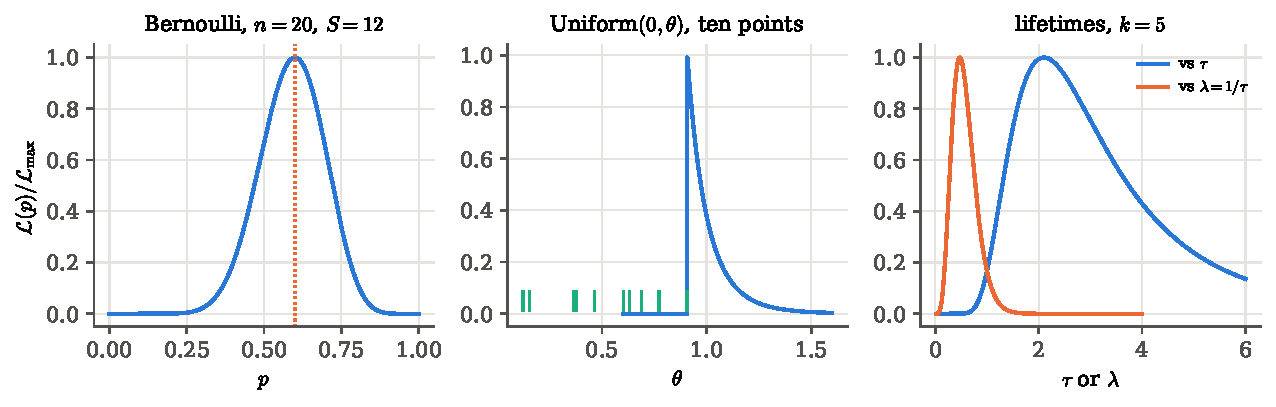
\includegraphics[width=12cm]{figures/ch03/likelihood_shapes.pdf}
\caption{Three likelihoods, each scaled to a maximum of one. Left: a
yes/no detector that fired 12 times in 20 trials, a smooth bump peaked at
$p=0.6$. Middle: ten points from a uniform box of unknown length (ticks
at the bottom). The likelihood is zero until $\theta$ reaches the largest
point, then decays as $\theta^{-10}$. Right: five decay times, with the
likelihood drawn once against the mean life $\tau$ and once against the rate
$\lambda=1/\tau$. The two curves take the same value at $\lambda=1/\tau$,
but they enclose different areas.}
\label{3b:fig:likelihood-shapes}
\end{figure}

\begin{keyidea}[The likelihood is a function of $\theta$, not a distribution over $\theta$]
$\Like(\theta)=p(\data_{\text{obs}}\given\theta)$ is normalised over the
\emph{data}, $\int p(\data\given\theta)\,\dd\data=1$ for every $\theta$. Over
$\theta$ it has no normalisation, it changes no Jacobian under a change of
parameter, and only ratios $\Like(\theta_1)/\Like(\theta_2)$ are meaningful
\mainref{p.~122}. To get a probability distribution over $\theta$ one needs
a prior, and Bayes' theorem (\cref{ch:05}).
\end{keyidea}

\subsection{Prediction and inference: where the likelihood sits}
\label{3b:sec:bayes-place}

The two readings of $p(\data\given\theta)$ are the two directions of
probability that run through the whole book (\cref{ch:01}). Read forward, it
starts from a fixed $\theta$ and says which data sets that $\theta$ can
produce, and how often. Read backward, the data set is already in hand, and
we ask which values of $\theta$ could have produced it and how much each one
deserves to be believed now that we have it.

\emph{Prediction} is the first reading, \emph{inference} the second.
\Cref{3b:fig:two-directions} draws both as trees. In the prediction
tree one parameter value fans out into many possible data sets, and their
probabilities add to one. In the inference tree many parameter values point
at the one data set we have, and the numbers attached to the branches are the
likelihoods. They need not add to anything.

So, facing data, we ask two questions in words before writing anything.
First: which values of $\theta$ could have produced these data? Second: how
probable would these data have been under each of them? The answers to the
second question, read across all $\theta$, are the likelihood. The first
question fixes what the posterior will be a distribution over. Turning the
likelihood into that distribution needs one more ingredient, a prior
(\cref{ch:05}).

\begin{figure}[htbp]
\centering
\begin{tikzpicture}[
  pt/.style={draw=accent,thick,rounded corners=2pt,fill=ideabg,font=\small,
             minimum height=7mm,minimum width=14mm,align=center},
  obs/.style={pt,draw=fibreorange!80!black,fill=defbg},
  flow/.style={->,thick,accent}]
  \node[pt] (th) at (0,0) {$\theta$ fixed};
  \node[pt] (d1) at (3.0,1.2) {$\data^{(1)}$};
  \node[pt] (d2) at (3.0,0) {$\data^{(2)}$};
  \node[pt] (d3) at (3.0,-1.2) {$\data^{(3)}$};
  \foreach \k in {1,2,3} \draw[flow] (th) -- (d\k);
  \node[font=\footnotesize,align=center] at (2.2,-2.3)
       {$p(\data^{(k)}\given\theta)$\\ add up to $1$};
  \node[font=\small\bfseries,accent] at (1.6,2.1) {prediction};
  \node[pt] (t1) at (8.2,1.2) {$\theta_1$};
  \node[pt] (t2) at (8.2,0) {$\theta_2$};
  \node[pt] (t3) at (8.2,-1.2) {$\theta_3$};
  \node[obs] (dobs) at (11.0,0) {$\data_{\text{obs}}$};
  \foreach \k in {1,2,3} \draw[flow] (t\k) -- (dobs);
  \node[font=\footnotesize,align=center] at (9.6,-2.3)
       {$\Like(\theta_k)=p(\data_{\text{obs}}\given\theta_k)$\\ need not add to $1$};
  \node[font=\small\bfseries,accent] at (9.6,2.1) {inference};
\end{tikzpicture}
\caption{The same conditional probability read two ways. Left: one
hypothesis produces many possible data sets, and the probabilities of all of
them sum to one. Right: many hypotheses could have produced the single data
set we observed (orange). The likelihood attaches to each hypothesis the
probability that it would have produced exactly these data. These numbers
compare hypotheses with each other but are not a distribution over them.}
\label{3b:fig:two-directions}
\end{figure}

Bayes' theorem is the bridge from one tree to the other. Written for
parameters it reads \srcref{HobsonBMC}{p.~11, (1.25)}
\begin{equation}
  \underbrace{p(\theta)}_{\text{prior}}\;
  \underbrace{p(\data\given\theta)}_{\text{likelihood}}
  \;=\;p(\theta,\data)\;=\;
  \underbrace{p(\data)}_{\text{evidence }Z}\;
  \underbrace{p(\theta\given\data)}_{\text{posterior}} .
  \label{3b:eq:bayes}
\end{equation}
Both sides are the joint probability of parameter and data, $p(\theta,\data)$,
split into two factors in the two possible orders. The likelihood is the
part the experiment supplies. It is also the least controversial part. We
can calibrate the instrument with known inputs and count how often it
produces each output, which pins $p(\data\given\theta)$ down to any desired
precision \srcref{HobsonBMC}{p.~11}. The prior, the evidence and the
posterior belong to \cref{ch:05}. Two facts about them are needed now.
First, with a flat prior $p(\theta)=\text{const}$ the posterior is
proportional to the likelihood, so the peak of the posterior is the peak of
the likelihood \srcref{Sivia}{p.~64, (3.61)}. Second, ``flat'' depends on
the parametrisation. A prior flat in $\tau$ is not flat in $\lambda=1/\tau$,
because of the Jacobian $1/\lambda^2$ found above. From here on we stay
on the frequentist side and use the likelihood by itself, without any prior.

\paragraph{What the likelihood keeps: sufficiency.}
In each of the three examples the likelihood depended on the data through
one number only: the count $S$ of detector firings, the total decay time
$T$, and the largest value $x_{(n)}$ of the uniform box. Two detector data
sets with the same $S$ give the same likelihood function, so nothing
computed from the likelihood can tell them apart. A statistic with this
property is called \newterm{sufficient}
\unpack{knowing its value lets us write down the whole likelihood function,
up to a constant factor} \mainref{p.~137, Def.~9.32}. The factorisation
theorem \mainref{p.~140, Thm.~9.40} gives a quick test: $T(\data)$ is
sufficient exactly when $p(\data\given\theta)=g\bigl(T(\data),\theta\bigr)\,h(\data)$.
For Gaussian data with unknown $\mu$ and $\sigma$ the pair
$(\bar x,S^2)$ is sufficient \mainref{p.~138, Ex.~9.34}: the likelihood
$\propto\sigma^{-n}\exp\{-[(n-1)S^2+n(\bar x-\mu)^2]/2\sigma^2\}$ uses
nothing else. Cosmologists use the same compression every day: when a map
is Gaussian and statistically isotropic, its power spectrum carries all the
information about the parameters. Sufficiency also improves estimators. The
Rao--Blackwell
theorem says that averaging any estimator over all data sets that share
the observed value of a sufficient statistic gives a new estimator whose
mean squared error is never larger \mainref{p.~140, Thm.~9.42}: an
estimator that uses anything beyond the sufficient statistic is only
adding noise.

\paragraph{The likelihood principle.}
The \newterm{likelihood principle} goes one step further
\srcref{CasellaBerger}{\S6.3.1}. It says that if two data sets $\data$ and
$\data'$ give proportional likelihoods, $\Like(\theta\given\data)=
c\,\Like(\theta\given\data')$ for all $\theta$, then they carry the same
evidence about $\theta$ and should lead to the same conclusion. Two coin
experiments show what this means. Experimenter A decides to toss a coin
$n=20$ times and sees $S=12$ heads. The count is binomial, and
$\Like\propto p^{12}(1-p)^8$. Experimenter B decides to toss until the
eighth tail, and the eighth tail comes on toss $20$, so B also saw $12$
heads and $8$ tails. That count is negative binomial, and again
$\Like\propto p^{12}(1-p)^8$, only with a different constant in front. The
likelihoods are proportional, so by the principle A and B have learned the
same thing about $p$. Estimates and intervals built from the likelihood
alone respect the principle. Procedures that average over data sets that could have been
observed but were not, such as $p$-values (\cref{ch:04}), depend on the
stopping rule, so they violate it. Bayesian inference satisfies it
automatically, because the posterior uses the data only through
$\Like(\theta)$ \srcref{CasellaBerger}{\S6.3.2}.
\section{Maximum likelihood: pick the value that needs the least unusual noise}
\label{3b:sec:mle}

The likelihood $\Like(\theta)$ of \cref{3b:sec:likelihood} gives every
candidate value of $\theta$ a number: how readily that value would have
produced the data we hold. If we must report a single value, the natural
choice is the one with the highest number. Its prediction needs the most
ordinary noise to become the data. This is the
\newterm{maximum likelihood estimator}, and it is the workhorse of
experimental physics. Almost every fitted mass, lifetime, cross-section and
cosmological parameter you have seen was obtained this way, or by its
Gaussian special case, least squares.

Turning the idea into recipes raises three questions.
\begin{enumerate}[label=\arabic*.]
  \item How do we find the maximum when we can do the calculus by hand, and
        what do the answers look like for the standard models?
  \item How does it compare with the older recipe of matching moments?
  \item How do we find the maximum when we cannot do the calculus, and how
        does that look in Python?
\end{enumerate}
The recipe is worth using because, for large samples, it homes in on the
truth, is nearly unbiased, and is as precise as any estimator can be. These
properties are proved in \cref{3b:sec:properties}. Its error bar comes from
the width of the likelihood (\cref{3b:sec:curvature}).

\begin{workdef}[maximum likelihood estimator]
The \newterm{maximum likelihood estimator} (MLE) $\hat\theta$ is the value of
$\theta$ that maximises $\Like(\theta)$, or equivalently
$\ell(\theta)=\ln\Like(\theta)$ \mainref{p.~122, Def.~9.8}. When the maximum
is inside the allowed range and $\ell$ is smooth, it solves the
\newterm{score equation}
\[
  S(\theta)\equiv\frac{\partial\ell}{\partial\theta}=0,
  \qquad \frac{\partial^2\ell}{\partial\theta^2}<0 ,
\]
where the \newterm{score} $S(\theta)$ \unpack{the slope of the
log-likelihood, a random quantity because it depends on the data} measures
how much the data pull $\theta$ up or down. For several parameters every
component of the gradient vanishes and the matrix of second derivatives is
negative definite.
\end{workdef}

Before differentiating we may throw away every factor of $\Like$ that does
not contain $\theta$. Two facts allow it. First, $\ln$ is increasing, so
$\Like$ and $\ell$ peak at the same $\theta$. Second, a constant factor in
$\Like$ becomes an added constant in $\ell$, and the derivative of a
constant is zero.

\subsection{Solving the score equation by hand}
\label{3b:sec:mle-hand}

\paragraph{Example: the mean lifetime of an unstable particle.}
We record $n$ decay times $t_1,\dots,t_n$ from $f(t;\tau)=\tau^{-1}e^{-t/\tau}$
\srcref{Cowan}{\S6.2}. Then
\begin{align}
  \ell(\tau)&\eqby{1}\sum_{i=1}^n\Bigl(-\ln\tau-\frac{t_i}{\tau}\Bigr)
             =-n\ln\tau-\frac{T}{\tau},\qquad T\equiv\sum_it_i,
  \nonumber\\
  S(\tau)&\eqby{2}-\frac n\tau+\frac{T}{\tau^2}
          \eqby{3}0
  \quad\Longrightarrow\quad
  \hat\tau=\frac Tn=\bar t,
  \label{3b:eq:tau-mle}\\
  \ell''(\hat\tau)&\eqby{4}\frac{n}{\hat\tau^2}-\frac{2T}{\hat\tau^3}
   \eqby{5}-\frac{n}{\hat\tau^2}<0 .
  \nonumber
\end{align}
\begin{explain}
  \item Logarithm of the product \eqref{3b:eq:like-iid}:
        $\ln(\tau^{-1}e^{-t/\tau})=-\ln\tau-t/\tau$.
  \item Differentiate term by term: $\dd(-n\ln\tau)/\dd\tau=-n/\tau$ and
        $\dd(-T/\tau)/\dd\tau=T/\tau^2$.
  \item The score equation. Multiply by $\tau^2$ to get $-n\tau+T=0$.
  \item Differentiate once more: $\dd(-n/\tau)/\dd\tau=n/\tau^2$,
        $\dd(T/\tau^2)/\dd\tau=-2T/\tau^3$.
  \item At $\hat\tau$ we have $T=n\hat\tau$, so $2T/\hat\tau^3=2n/\hat\tau^2$.
\end{explain}
The maximum likelihood lifetime is the average decay time. It is unbiased,
$\E\bar t=\tau$, and its variance is $\tau^2/n$, because the exponential has
variance $\tau^2$ and averaging $n$ independent times divides the variance
by $n$. This is the same estimator whose sampling distribution we simulated
for the muon lifetime in \cref{3a:ex:lifetime}. The number
$-\ell''(\hat\tau)=n/\hat\tau^2$ is one over the square of the error bar, as
\cref{3b:sec:curvature} shows.

\paragraph{Example: the centre and width of a Gaussian.}
Let $x_i\sim\Normal(\mu,\sigma^2)$ with both parameters unknown
\mainref{p.~123, Ex.~9.11}, \srcref{Cowan}{\S6.3},
\srcref{CasellaBerger}{Ex.~7.2.11}. Dropping the constant $-\tfrac n2\ln2\pi$,
\begin{align*}
  \ell(\mu,\sigma)&\eqby{1}-n\ln\sigma-\frac{1}{2\sigma^2}\sum_{i=1}^n(x_i-\mu)^2,\\
  \frac{\partial\ell}{\partial\mu}&\eqby{2}\frac1{\sigma^2}\sum_i(x_i-\mu)=0
  \;\Longrightarrow\;\hat\mu=\bar x,\\
  \frac{\partial\ell}{\partial\sigma}&\eqby{3}-\frac n\sigma+\frac1{\sigma^3}\sum_i(x_i-\mu)^2=0
  \;\Longrightarrow\;\hat\sigma^2=\frac1n\sum_i(x_i-\bar x)^2 .
\end{align*}
\begin{explain}
  \item $\ln$ of $\prod_i(2\pi\sigma^2)^{-1/2}e^{-(x_i-\mu)^2/2\sigma^2}$,
        with $\ln(\sigma^2)^{-n/2}=-n\ln\sigma$.
  \item The chain rule on $(x_i-\mu)^2$ gives $-2(x_i-\mu)$. The sum
        vanishes when $n\mu=\sum_ix_i$.
  \item Differentiate $-n\ln\sigma$ and $\sigma^{-2}$; multiply the equation
        by $\sigma^3/n$; and insert the solution $\mu=\bar x$ of the first
        equation, because both equations must hold at once.
\end{explain}
The centre is the sample mean, as one would guess. The width divides by
$n$, not $n-1$, and so it is \emph{biased}. In \cref{3a:sec:n-minus-one} we
showed that $\E\sum_i(x_i-\bar x)^2=(n-1)\sigma^2$. Dividing by $n$ gives
$\E\hat\sigma^2=\tfrac{n-1}{n}\sigma^2$: the MLE is low by a factor
$(n-1)/n$. The bias is the price of estimating $\mu$ from the same data, and
it vanishes as $n\to\infty$. Maximum likelihood promises good behaviour for
large samples, not unbiasedness at every $n$.

\paragraph{Example: the firing probability of a detector.}
For the Bernoulli likelihood $p^S(1-p)^{n-S}$ of \cref{3b:sec:product},
\[
  \ell(p)=S\ln p+(n-S)\ln(1-p),\qquad
  S(p)=\frac Sp-\frac{n-S}{1-p}=0
  \;\Longrightarrow\;\hat p=\frac Sn ,
\]
because multiplying the score equation by $p(1-p)$ gives
$S(1-p)-(n-S)p=S-np=0$. For $S=12$ in $n=20$ trials, $\hat p=0.6$, the peak
seen in \cref{3b:fig:likelihood-shapes}.

\paragraph{Example: when the maximum sits on an edge.}
For the uniform box the likelihood $\theta^{-n}$ decreases for all
$\theta\ge x_{(n)}$ and is zero below, so the maximum is at the cliff,
$\hat\theta=x_{(n)}$ \mainref{p.~124}. The score equation
$-n/\theta=0$ has no solution at all; the maximum is found by looking, not
by differentiating. The estimator is biased low, because the largest of $n$
points always falls short of the end of the box:
$\E x_{(n)}=\tfrac{n}{n+1}\theta$. A related case arises whenever physics
restricts the parameter. A signal strength $\mu$ cannot be negative. If we
measure $x_i\sim\Normal(\mu,\sigma^2)$ and find $\bar x<0$, the likelihood
restricted to $\mu\ge0$ is largest at the edge, so $\hat\mu=0$
\srcref{CasellaBerger}{Ex.~7.2.8}. The derivative there is not zero, and
several of the nice properties of \cref{3b:sec:properties} fail at such
boundaries.

\begin{pitfall}[The MLE is not ``the most probable value of $\theta$'']
$\hat\theta$ is the value under which the \emph{data} are most probable. It
is the most probable value of $\theta$ only in a Bayesian analysis with a
flat prior, and then only in the parametrisation in which the prior is flat
\srcref{Sivia}{p.~64}. Because the likelihood carries no Jacobian, the
MLE itself does not care about the parametrisation:
$\hat\lambda=1/\hat\tau$ (\cref{3b:sec:properties}). The peak of a posterior
\emph{density} does move under a change of variables.
\end{pitfall}

\subsection{The method of moments, for comparison}
\label{3b:sec:mom}

Before maximum likelihood there was a simpler idea. A model with $k$
parameters predicts the first $k$ moments $\alpha_j(\theta)=\E_\theta X^j$
\unpack{the average of the $j$-th power of the data, as a function of the
parameters}. The data give the sample moments
$\hat\alpha_j=\tfrac1n\sum_ix_i^j$. The \newterm{method of moments}
estimator sets the two equal and solves,
$\alpha_j(\tilde\theta)=\hat\alpha_j$ for $j=1,\dots,k$
\mainref{p.~121, Def.~9.3}, \srcref{Cowan}{Ch.~8}. For the Bernoulli
model, $\E X=p$ gives $\tilde p=\bar x=S/n$; for the Gaussian, $\E X=\mu$
and $\E X^2=\sigma^2+\mu^2$ give $\tilde\mu=\bar x$ and
$\tilde\sigma^2=\tfrac1n\sum x_i^2-\bar x^2=\tfrac1n\sum(x_i-\bar x)^2$
\mainref{p.~121, Exs.~9.4--9.5}. Both coincide with the MLE. Under mild
conditions the moment estimator is consistent and asymptotically Gaussian
\mainref{p.~122, Thm.~9.6}, but in general it throws information away, and
the MLE is at least as precise for large samples (\cref{3b:sec:properties}).

\paragraph{Example: an angular distribution.}
In $e^+e^-\to\mu^+\mu^-$ the distribution of $x=\cos\theta$ of the outgoing
muon has the shape $1+\alpha x+\beta x^2$, where $\beta$ comes from the
photon exchange and $\alpha$, the forward--backward asymmetry, from its
interference with the $Z$. The detector accepts only
$x_{\min}\le x\le x_{\max}$, so the density is
\srcref{Cowan}{\S6.8, (8.9)}
\begin{equation}
  f(x;\alpha,\beta)=\frac{1+\alpha x+\beta x^2}{d_1+\alpha d_2+\beta d_3},
  \qquad d_k\equiv\frac{x_{\max}^k-x_{\min}^k}{k},
  \label{3b:eq:angular}
\end{equation}
because
$\int_{x_{\min}}^{x_{\max}}(1+\alpha x+\beta x^2)\,\dd x=d_1+\alpha d_2+\beta d_3$.
The first two moments are ratios of the same kind,
\begin{align*}
  \E x&\eqby{1}\frac{d_2+\alpha d_3+\beta d_4}{d_1+\alpha d_2+\beta d_3},&
  \E x^2&\eqby{2}\frac{d_3+\alpha d_4+\beta d_5}{d_1+\alpha d_2+\beta d_3},
\end{align*}
\begin{explain}
  \item $\int x(1+\alpha x+\beta x^2)\,\dd x=d_2+\alpha d_3+\beta d_4$.
  \item $\int x^2(1+\alpha x+\beta x^2)\,\dd x=d_3+\alpha d_4+\beta d_5$.
\end{explain}
and setting them equal to $\hat\alpha_1=\overline{x}$ and
$\hat\alpha_2=\overline{x^2}$ and multiplying out gives two \emph{linear}
equations for $(\alpha,\beta)$,
\[
  \alpha(\hat\alpha_1d_2-d_3)+\beta(\hat\alpha_1d_3-d_4)=d_2-\hat\alpha_1d_1,
  \qquad
  \alpha(\hat\alpha_2d_2-d_4)+\beta(\hat\alpha_2d_3-d_5)=d_3-\hat\alpha_2d_1 .
\]
For $2000$ simulated events with $\alpha=\beta=0.5$ on
$-0.95\le x\le0.95$ (Cowan's set-up), these give
$(\tilde\alpha,\tilde\beta)=(\ThreeBAngMomA,\ThreeBAngMomB)$. The maximum
likelihood equations for the same model are not linear, so they need a
numerical method.

\subsection{When the calculus cannot be done: Newton--Raphson}
\label{3b:sec:newton}

For \eqref{3b:eq:angular} the log-likelihood is
$\ell(\alpha,\beta)=\sum_i\ln(1+\alpha x_i+\beta x_i^2)-n\ln(d_1+\alpha d_2+\beta d_3)$,
and its score equations have no closed-form solution. The standard
numerical maximiser replaces $\ell$ near a trial point by a parabola and
jumps to the parabola's top. The same parabola gives the error bar in
\cref{3b:sec:curvature}. Near a trial point $\theta_j$,
\begin{align}
  \ell(\theta)&\eqby{1}\ell(\theta_j)+\ell'(\theta_j)(\theta-\theta_j)
   +\tfrac12\ell''(\theta_j)(\theta-\theta_j)^2+\dots,
  \nonumber\\
  0&\eqby{2}\ell'(\theta_j)+\ell''(\theta_j)(\theta_{j+1}-\theta_j)
  \quad\Longrightarrow\quad
  \theta_{j+1}=\theta_j-\frac{\ell'(\theta_j)}{\ell''(\theta_j)} .
  \label{3b:eq:newton}
\end{align}
\begin{explain}
  \item Taylor expansion to second order: we replace $\ell$ by the parabola
        that has the same value, slope and curvature at $\theta_j$.
  \item Jump to the top of that parabola, where its derivative vanishes.
\end{explain}
With several parameters, $\ell'$ becomes the gradient $\bm g$ and $\ell''$
the matrix of second derivatives $H$ (the \newterm{Hessian}), and the step
is $\params_{j+1}=\params_j-H^{-1}\bm g$. Near the maximum the error shrinks
quadratically, roughly squaring at every step, so a handful of iterations
suffice. \Cref{3b:fig:newton} shows the first two steps on a lifetime
likelihood.

\paragraph{Example: Newton by hand.}
Take $n=5$ decays with total time $T=6$, so that $\ell(\tau)=-5\ln\tau-6/\tau$,
$\ell'=-5/\tau+6/\tau^2$, $\ell''=5/\tau^2-12/\tau^3$, and the exact answer
is $\hat\tau=T/n=1.2$. Start at $\tau_0=0.8$:
\begin{align*}
  \tau_1&\eqby{1}0.8-\frac{-6.25+9.375}{7.8125-23.4375}
        =0.8+\frac{3.125}{15.625}=1.0,\\
  \tau_2&\eqby{2}1.0-\frac{-5+6}{5-12}=1+\frac17=1.1429,\\
  \tau_3&\eqby{3}1.1429+\frac{0.2188}{4.2109}=1.1948,\qquad
  \tau_4=1.19996,\qquad \tau_5=1.2000 .
\end{align*}
\begin{explain}
  \item \eqref{3b:eq:newton} with $\ell'(0.8)=-5/0.8+6/0.64$ and
        $\ell''(0.8)=5/0.64-12/0.512$.
  \item The same at $\tau_1=1$.
  \item The same at $\tau_2$, where $\ell'=0.2188$ and $\ell''=-4.2109$.
\end{explain}
The distance to the answer goes $0.4,\;0.2,\;0.057,\;0.0052,\;0.00005$: the
number of correct digits roughly doubles per step once we are close.

\begin{figure}[htbp]
\centering
\begin{tikzpicture}
\begin{axis}[width=10cm,height=6.2cm,
  xmin=0.55,xmax=2.3,ymin=-7.6,ymax=-5.05,
  xlabel={$\tau$},ylabel={$\ell(\tau)$},
  tick label style={font=\footnotesize},label style={font=\small},
  legend style={font=\footnotesize,at={(0.98,0.97)},anchor=north east,draw=none,fill=white},
  clip=true]
  \addplot[very thick,formblue,domain=0.55:2.3,samples=120] {-5*ln(x)-6/x};
  \addlegendentry{$\ell(\tau)=-5\ln\tau-6/\tau$}
  \addplot[thick,fibreorange,dashed,domain=0.55:1.45,samples=60]
     {-6.38428+3.125*(x-0.8)-7.8125*(x-0.8)^2};
  \addlegendentry{parabola at $\tau_0$}
  \addplot[thick,tangentgreen,dashed,domain=0.6:1.7,samples=60]
     {-6+(x-1)-3.5*(x-1)^2};
  \addlegendentry{parabola at $\tau_1$}
  \addplot[only marks,mark=*,mark size=1.8pt,black,forget plot]
     coordinates {(0.8,-6.38428) (1.0,-6.0) (1.142857,-5.91766)};
  \addplot[only marks,mark=o,mark size=2pt,fibreorange,forget plot] coordinates {(1.0,-6.07178)};
  \addplot[only marks,mark=o,mark size=2pt,tangentgreen,forget plot] coordinates {(1.142857,-5.92857)};
  \draw[softgray,densely dotted] (axis cs:1.2,-7.6) -- (axis cs:1.2,-5.91161);
  \node[font=\footnotesize,anchor=east] at (axis cs:0.79,-6.38) {$\tau_0$};
  \node[font=\footnotesize,anchor=north] at (axis cs:1.0,-6.12) {$\tau_1$};
  \node[font=\footnotesize,anchor=south] at (axis cs:1.12,-5.90) {$\tau_2$};
  \node[font=\footnotesize,anchor=west] at (axis cs:1.21,-7.45) {$\hat\tau=1.2$};
\end{axis}
\end{tikzpicture}
\caption{Newton--Raphson on a log-likelihood. At the starting point
$\tau_0$ the method replaces $\ell$ by the parabola (orange) with the same
height, slope and curvature, and jumps to its top (open circle), which lies
straight above $\tau_1$. Repeating from $\tau_1$ (green parabola) lands at
$\tau_2$, already close to the true maximum at $\hat\tau=1.2$ (dotted
line). Each parabola hugs the curve better than the last because the curve
looks more and more like a parabola near its peak.}
\label{3b:fig:newton}
\end{figure}

Newton's method trusts the parabola, and the parabola can lie. Here
$\ell''=5/\tau^2-12/\tau^3$ is negative only when $5\tau<12$, that is for
$\tau<2T/n=2.4$. Beyond that the curve bends upwards and the parabola has a
minimum, not a maximum. Started at $\tau_0=3$, the step therefore points
\emph{away} from the maximum. Practical
minimisers (the \texttt{MINUIT} of particle physics, \pyname{scipy.optimize})
therefore check that each step increases $\ell$, shorten it if not, and
start from a sensible guess. The method of moments is an excellent source of
such guesses.

\paragraph{The angular fit in Python.}
The script \pyname{10_angular_ml.py} generates $2000$ events from
\eqref{3b:eq:angular} by accept--reject (\cref{ch:06}), computes the moment
estimate, and hands it to Newton's method. The heart of it is the analytic
gradient and Hessian,
\[
  \frac{\partial\ell}{\partial\alpha}=\sum_i\frac{x_i}{g_i}-\frac{n\,d_2}{D},\qquad
  \frac{\partial^2\ell}{\partial\alpha^2}=-\sum_i\frac{x_i^2}{g_i^2}+\frac{n\,d_2^2}{D^2},
  \qquad g_i=1+\alpha x_i+\beta x_i^2,\quad D=d_1+\alpha d_2+\beta d_3,
\]
and the same with $x_i\to x_i^2$, $d_2\to d_3$ for $\beta$ (the mixed
derivative has $x_i^3$ and $d_2d_3$). These follow from
$\dd\ln g/\dd\alpha=x/g$ and $\dd\ln D/\dd\alpha=d_2/D$ and one more
derivative of each.
\pyfile[firstline=62,lastline=81]{code/ch03/10_angular_ml.py}{Newton--Raphson for the angular distribution, and the covariance from the Hessian}
The loop is \eqref{3b:eq:newton} in matrix form:
\pyname{np.linalg.solve(H, g)} computes $H^{-1}\bm g$ without forming the
inverse. The last four lines compute the covariance of the estimates as the
inverse of minus the Hessian at the maximum, a rule derived in
\cref{3b:sec:curvature}. Starting from the moment estimate, Newton reaches
$(\hat\alpha,\hat\beta)=(\ThreeBAngA,\ThreeBAngB)$ in
$\ThreeBAngIter$ iterations; after the first step the answer already agrees
with the final one far better than its error bar. The left panel of \cref{3b:fig:angular} shows the
fitted density on the histogram of the events.

\begin{figure}[htbp]
\centering
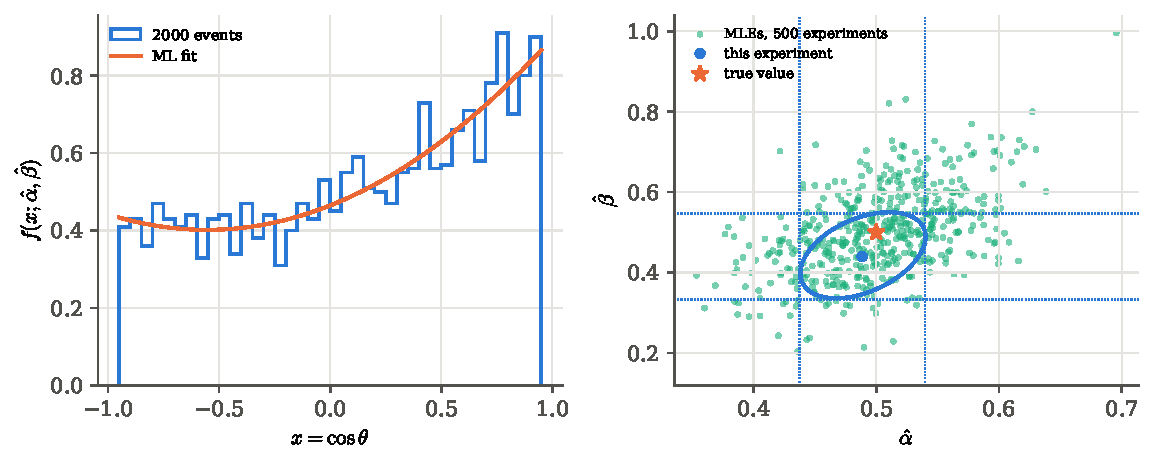
\includegraphics[width=12cm]{figures/ch03/angular_ml.pdf}
\caption{A two-parameter maximum likelihood fit. Left: $2000$ simulated
values of $\cos\theta$ and the fitted density $1+\hat\alpha x+\hat\beta x^2$
(normalised). Right: the fitted $(\hat\alpha,\hat\beta)$ of $500$ independent
repetitions of the experiment (green), the fit of the first experiment (blue
dot), the truth (star), and the contour on which $\ln\Like$ of the first
experiment has dropped by $\tfrac12$ from its maximum. The dotted lines
tangent to the contour mark $\hat\alpha\pm\sigma_{\hat\alpha}$ and
$\hat\beta\pm\sigma_{\hat\beta}$ from the inverse Hessian. The cloud of
repetitions has the size, tilt and shape of the contour.}
\label{3b:fig:angular}
\end{figure}

Repeating the whole experiment $500$ times, the maximum likelihood estimates
average $(\ThreeBAngMeanA,\ThreeBAngMeanB)$ (truth $(0.5,0.5)$) and scatter
by $\sigma_{\hat\alpha}=\ThreeBAngSdA$ and $\sigma_{\hat\beta}=\ThreeBAngSdB$.
The moment estimates scatter by $\ThreeBAngMomSdA$ and $\ThreeBAngMomSdB$.
Both methods were applied to the same $500$ data sets, so the ratios of the
spreads are measured well: $\ThreeBAngMomRatioA\pm\ThreeBAngMomRatioAErr$
for $\alpha$ and $\ThreeBAngMomRatioB\pm\ThreeBAngMomRatioBErr$ for $\beta$.
For this mild distribution the two methods are close;
the gap widens for sharply peaked densities, where low moments are poor
summaries of the shape.

\paragraph{When the number of events is itself random.}
In a counting experiment the total number of events $n$ is not fixed in
advance: it is Poisson distributed with a mean $\nu$ that the theory may
predict (a cross-section times a luminosity). Then the likelihood acquires
one more factor \srcref{Cowan}{\S6.9},
\begin{equation}
  \Like(\nu,\theta)=\frac{\nu^n e^{-\nu}}{n!}\prod_{i=1}^nf(x_i;\theta)
  =\frac{e^{-\nu}}{n!}\prod_{i=1}^n\nu f(x_i;\theta),
  \label{3b:eq:extended}
\end{equation}
the \newterm{extended likelihood}. If $\nu$ is a free parameter unrelated to
$\theta$, the $\nu$-dependent part of $\ell$ is $n\ln\nu-\nu$, whose
derivative $n/\nu-1$ vanishes at $\hat\nu=n$. The $\theta$-dependent part is
the same as before, so $\hat\theta$ is unchanged. If $\nu=\nu(\theta)$, the
total rate carries information about
$\theta$ in addition to the shape, and the extended likelihood uses both.
The product $\nu f(x;\theta)$ is the expected number of events per unit
$x$, which is why the extended likelihood is the natural starting point for
histograms of counts (\cref{3b:sec:poisson}).

\paragraph{Hidden variables.}
Some likelihoods are easy to maximise only if we knew something we were
not told, for example which of two Gaussian populations each point came
from (a mixture model). The \newterm{EM algorithm} alternates between
guessing the hidden labels from the current parameters (the ``E'' step, an
expectation) and maximising the likelihood as if the labels were known (the
``M'' step). No cycle can decrease $\Like$ \mainref{pp.~143--145}. It is
the standard tool for fitting mixtures.
\section{Gaussian noise: least squares and the \texorpdfstring{$\chi^2$}{chi-square}}
\label{3b:sec:least-squares}

Every physics student has fitted a straight line through points with error
bars by ``minimising $\chi^2$''. The rule is usually taught without a
reason. Why squares and not absolute values? Why divide by $\sigma_i^2$?
What is the error on the slope, and how do we know whether the line is any
good? All of this follows in a few lines from the likelihood of
\cref{3b:sec:likelihood}, once we assume that the noise is Gaussian. The
same lines then cover noise that is correlated from point to point, which
is the normal situation for binned power spectra and for gravitational-wave
strain. Four questions need answers.
\begin{enumerate}[label=\arabic*.]
  \item Why is least squares the maximum likelihood estimator for Gaussian
        noise, and when is it not?
  \item For a model linear in its parameters, what are the estimates and
        their covariance, exactly?
  \item What value of $\chi^2_{\min}$ should a correct model give, and how
        do we turn it into a test of the fit?
  \item What changes when the noise is correlated, and what goes wrong if
        we ignore the correlation?
\end{enumerate}

\subsection{Least squares is Gaussian maximum likelihood}
\label{3b:sec:ls-from-ml}

Take data $D_i=d_i(\params)+\epsilon_i$, $i=1,\dots,N$: the model prediction
$d_i(\params)$ plus independent noise $\epsilon_i\sim\Normal(0,\sigma_i^2)$
with known $\sigma_i$. Its log-likelihood is \eqref{3b:eq:loglike-gauss} of
\cref{3b:sec:product}. Written with the
\newterm{normalised residuals} $R_i=(D_i-d_i(\params))/\sigma_i$ it reads
\srcref{Sivia}{p.~65, (3.65)--(3.67)}
\begin{align}
  \ell(\params)
  &\eqby{1}-\frac12\sum_{i=1}^NR_i^2-\sum_{i=1}^N\ln\sqrt{2\pi}\,\sigma_i
  \eqby{2}-\frac12\chi^2(\params)+\text{const},
  \qquad
  \chi^2(\params)\equiv\sum_{i=1}^N\frac{\bigl(D_i-d_i(\params)\bigr)^2}{\sigma_i^2}.
  \label{3b:eq:chi2-def}
\end{align}
\begin{explain}
  \item \eqref{3b:eq:loglike-gauss}, with the residuals in units of their
        error bars.
  \item The error bars are known numbers, so the second sum does not
        depend on $\params$.
\end{explain}
Maximising $\ell$ is minimising $\chi^2$, because of the minus sign. So the
\newterm{least-squares estimator} is the maximum likelihood estimator
\srcref{Cowan}{\S7.1}, \srcref{HobsonBMC}{p.~50, (2.24)--(2.25)}. This
answers the two ``why'' questions. The squares come from the exponent of the
Gaussian. The $1/\sigma_i^2$ measures each residual against its own error
bar: a residual of $0.3$ is a one-sigma event for a point with
$\sigma_i=0.3$ and a ten-sigma event for a point with $\sigma_i=0.03$. With
equal error bars all points count equally. For a constant model,
$\chi^2=\sum_i(D_i-\mu)^2/\sigma_i^2$, and minimising it over $\mu$ gives
the inverse-variance weighted mean of \cref{3a:sec:weighted}.

The derivation also says when least squares is \emph{not} maximum
likelihood. It used two assumptions, and each can fail. If the noise is not
Gaussian (heavy tails, outliers, counts), the exponent is not a square. If
the error bars depend on the parameters, for example $\sigma_i^2=d_i(\params)$
for counts, the term $\sum\ln\sigma_i$ depends on $\params$ and cannot be
dropped. So least squares is what the likelihood reduces to under these two
assumptions. When it misbehaves, the cure is to go back to the likelihood,
not to patch the recipe \srcref{Sivia}{p.~66}.

\subsection{Linear models: the normal equations}
\label{3b:sec:linear-ls}

Many models are linear in their parameters even when they are not linear
in $x$: a straight line $a+bx$, a polynomial, a sum of templates with
unknown amplitudes. Write such a model as
$d_i(\params)=\sum_{k=1}^mA_{ik}\theta_k$, or $\bm d=A\params$, where the
$N\times m$ \newterm{design matrix} $A$ \unpack{column $k$ is the model
curve for $\theta_k=1$ and all other parameters zero} is known. For a line,
row $i$ of $A$ is $(1,\ x_i)$. Collect the error bars into the diagonal
covariance $\Cmat=\diag(\sigma_1^2,\dots,\sigma_N^2)$; everything below also
holds for a general $\Cmat$, which we use in \cref{3b:sec:correlated}. Then
\begin{align}
  \chi^2(\params)&\eqby{1}(\bm D-A\params)\T\Cmat^{-1}(\bm D-A\params),
  \nonumber\\
  \frac{\partial\chi^2}{\partial\params}&\eqby{2}-2A\T\Cmat^{-1}(\bm D-A\params)
  \eqby{3}\bm0
  \quad\Longrightarrow\quad
  (A\T\Cmat^{-1}A)\,\hat\params=A\T\Cmat^{-1}\bm D,
  \nonumber\\
  \hat\params&\eqby{4}(A\T\Cmat^{-1}A)^{-1}A\T\Cmat^{-1}\bm D
  \;\equiv\;B\bm D .
  \label{3b:eq:normal-eq}
\end{align}
\begin{explain}
  \item With a diagonal $\Cmat$ this is
        $\sum_i(D_i-d_i)^2/\sigma_i^2$ written as a matrix product.
  \item Differentiate the quadratic form: for a symmetric matrix $M$,
        $\partial(\bm v\T M\bm v)/\partial\params=2(\partial\bm v/\partial\params)\T M\bm v$,
        and here $\partial\bm v/\partial\params=-A$.
  \item The score equation. These $m$ linear equations are the
        \newterm{normal equations}.
  \item The matrix $A\T\Cmat^{-1}A$ is $m\times m$ and invertible as long as
        the columns of $A$ are linearly independent (no two parameters do the
        same thing to the model).
\end{explain}
The estimator is a fixed matrix $B$ times the data. So its mean and
covariance follow from linear error propagation, which is exact for linear
maps (\cref{3a:sec:linear-exact}):
\begin{align}
  \E\hat\params&\eqby{1}B\,\E\bm D\eqby{2}(A\T\Cmat^{-1}A)^{-1}A\T\Cmat^{-1}A\params=\params,
  \nonumber\\
  \Cov\hat\params&\eqby{3}B\,\Cmat\,B\T
  \eqby{4}(A\T\Cmat^{-1}A)^{-1}A\T\Cmat^{-1}\,\Cmat\,\Cmat^{-1}A(A\T\Cmat^{-1}A)^{-1}
  \eqby{5}(A\T\Cmat^{-1}A)^{-1}\equiv U .
  \label{3b:eq:ls-cov}
\end{align}
\begin{explain}
  \item Expectation is linear.
  \item The noise has mean zero, so $\E\bm D=A\params$.
  \item Covariance of a linear map, $\Cov(B\bm D)=B\Cov(\bm D)B\T$.
  \item Insert $B$ and $B\T$; $\Cmat$ and $A\T\Cmat^{-1}A$ are symmetric.
  \item $\Cmat^{-1}\Cmat=\Id$, and then
        $(A\T\Cmat^{-1}A)^{-1}(A\T\Cmat^{-1}A)=\Id$.
\end{explain}
So for a linear model with Gaussian noise the least-squares estimates are
unbiased and have covariance $U=(A\T\Cmat^{-1}A)^{-1}$, with no
approximation. Now look at the curvature of $\chi^2$. Differentiating
\eqref{3b:eq:normal-eq} once more gives
$\partial^2\chi^2/\partial\params\,\partial\params\T=2A\T\Cmat^{-1}A=2U^{-1}$.
Because $\chi^2$ is exactly quadratic in $\params$, its Taylor series stops
there:
\begin{equation}
  \chi^2(\params)=\chi^2_{\min}+(\params-\hat\params)\T U^{-1}(\params-\hat\params),
  \qquad
  \ell(\params)=\ell_{\max}-\tfrac12(\params-\hat\params)\T U^{-1}(\params-\hat\params).
  \label{3b:eq:chi2-quadratic}
\end{equation}
The likelihood is an exact Gaussian in $\params$, centred on $\hat\params$,
whose width matrix is the covariance of the estimator. In one dimension
$\chi^2(\theta)=\chi^2_{\min}+(\theta-\hat\theta)^2/\sigma_{\hat\theta}^2$,
so the parameter values at which $\chi^2$ has risen by one from its minimum
are exactly $\hat\theta\pm\sigma_{\hat\theta}$ \srcref{Cowan}{\S7.2}.
This is the model case for the rule ``the curvature of the log-likelihood is
the error'', which \cref{3b:sec:curvature} extends to every smooth
likelihood.

\begin{keyidea}[Linear least squares]
For data $\bm D=A\params+\bm\epsilon$ with Gaussian noise of covariance
$\Cmat$,
\[
  \hat\params=(A\T\Cmat^{-1}A)^{-1}A\T\Cmat^{-1}\bm D,\qquad
  \Cov\hat\params=(A\T\Cmat^{-1}A)^{-1},
\]
the estimator is unbiased and Gaussian, and $\chi^2$ rises by exactly one at
$\hat\theta_k\pm\sigma_{\hat\theta_k}$ when the other parameters are
re-minimised. Nothing here is asymptotic.
\end{keyidea}

\paragraph{Example: a straight line through three points.}
Fit $y=a+bx$ to $(x_i,y_i)=(0,1.1),(1,1.9),(2,3.2)$, all with $\sigma=0.1$.
For a line the normal equations are $2\times2$, and it pays to name the sums
$S=\sum1/\sigma_i^2$, $S_x=\sum x_i/\sigma_i^2$, $S_{xx}=\sum x_i^2/\sigma_i^2$,
$S_y=\sum y_i/\sigma_i^2$, $S_{xy}=\sum x_iy_i/\sigma_i^2$ and
$\Delta=SS_{xx}-S_x^2$. In units of $1/\sigma^2=100$ they are $S=3$,
$S_x=3$, $S_{xx}=5$, $S_y=6.2$, $S_{xy}=8.3$. Then
\begin{align*}
  \begin{pmatrix}\hat a\\ \hat b\end{pmatrix}
  &\eqby{1}\begin{pmatrix}S&S_x\\ S_x&S_{xx}\end{pmatrix}^{-1}
    \begin{pmatrix}S_y\\ S_{xy}\end{pmatrix}
  \eqby{2}\frac1\Delta\begin{pmatrix}S_{xx}S_y-S_xS_{xy}\\ SS_{xy}-S_xS_y\end{pmatrix}
  =\frac16\begin{pmatrix}31-24.9\\ 24.9-18.6\end{pmatrix}
  =\begin{pmatrix}1.017\\ 1.050\end{pmatrix},\\
  U&\eqby{3}\frac1\Delta\begin{pmatrix}S_{xx}&-S_x\\ -S_x&S\end{pmatrix}
  =\sigma^2\begin{pmatrix}5/6&-1/2\\ -1/2&1/2\end{pmatrix},
  \qquad
  \sigma_{\hat a}=0.091,\ \ \sigma_{\hat b}=0.071,\ \ \rho=-0.775 .
\end{align*}
\begin{explain}
  \item The normal equations \eqref{3b:eq:normal-eq}: with rows $(1,x_i)$,
        $A\T\Cmat^{-1}A$ has entries $S,S_x,S_x,S_{xx}$ and
        $A\T\Cmat^{-1}\bm y=(S_y,S_{xy})\T$.
  \item Inverse of a $2\times2$ matrix: swap the diagonal, negate the
        off-diagonal, divide by the determinant $\Delta$. Here
        $\Delta=3\cdot5-3^2=6$ in units of $\sigma^{-4}$; the powers of
        $\sigma$ cancel in $\hat a,\hat b$.
  \item $U=(A\T\Cmat^{-1}A)^{-1}$ from \eqref{3b:eq:ls-cov}; restoring the
        units, $1/\Delta=\sigma^4/6$ and the matrix entries carry
        $1/\sigma^2$.
\end{explain}
The intercept and slope are strongly anticorrelated, $\rho=-(1/2)/\sqrt{(5/6)(1/2)}$:
if the fitted slope is a little too steep, the line must start a little
lower to pass through the middle of the data. Choosing the origin of $x$
at the weighted mean, $\bar x=S_x/S=1$, would make $S_x=0$ and the two
estimates uncorrelated. The residuals are $y_i-\hat a-\hat bx_i=(0.083,-0.167,0.083)$,
so $\chi^2_{\min}=(0.0069+0.0278+0.0069)/0.01=4.17$. Is that good or bad?

\subsection{How good is the fit? The distribution of \texorpdfstring{$\chi^2_{\min}$}{chi2min}}
\label{3b:sec:chi2-min}

If the model is right, every normalised residual is a standard Gaussian
before fitting, and $\chi^2(\params_{\text{true}})$ is a sum of $N$ squared
standard Gaussians, so it follows the $\chi^2_N$ distribution (\cref{ch:02}).
Fitting lowers it: the fitted curve bends towards the data and eats part
of the noise. By how much? The cleanest way to see it is geometric.

Whiten the data first. Factor the covariance as $\Cmat=LL\T$ (for a
diagonal $\Cmat$, simply $L=\diag(\sigma_i)$; in general the Cholesky
factor). Then $\bm z=L^{-1}\bm D$, $\tilde A=L^{-1}A$ and
$\bm\eta=L^{-1}\bm\epsilon$ satisfy $\bm z=\tilde A\params+\bm\eta$ with
$\bm\eta\sim\Normal(\bm0,\Id_N)$, and
$\chi^2=|\bm z-\tilde A\params|^2$ is an ordinary squared distance in
$\R^N$. The model predictions $\tilde A\params$, as $\params$ ranges over
$\R^m$, fill an $m$-dimensional flat subspace (the column space of
$\tilde A$). Minimising the distance means dropping a perpendicular:
the fit is the orthogonal projection of $\bm z$ onto that subspace
(\cref{3b:fig:projection}). With the projector
$P=\tilde A(\tilde A\T\tilde A)^{-1}\tilde A\T$
\unpack{the matrix that maps any vector to its closest point in the model
subspace. It satisfies $P^2=P$ and $P\T=P$},
\begin{align}
  \chi^2_{\min}
  &\eqby{1}\bigl|(\Id-P)\bm z\bigr|^2
  \eqby{2}\bigl|(\Id-P)\bm\eta\bigr|^2
  \eqby{3}\bm\eta\T(\Id-P)\bm\eta ,
  \nonumber\\
  \E\chi^2_{\min}
  &\eqby{4}\tr\bigl[(\Id-P)\,\E(\bm\eta\bm\eta\T)\bigr]
  \eqby{5}\tr(\Id_N)-\tr P
  \eqby{6}N-m\equiv\dof .
  \label{3b:eq:chi2-min-mean}
\end{align}
\begin{explain}
  \item The fitted point is $P\bm z$, so the residual vector is
        $\bm z-P\bm z$.
  \item $\bm z=\tilde A\params+\bm\eta$, and $(\Id-P)\tilde A=0$ because
        $P$ leaves every vector of the model subspace unchanged. The true
        model drops out: only the noise is left.
  \item $|\bm v|^2=\bm v\T\bm v$ with $(\Id-P)\T(\Id-P)=\Id-P$, using
        $P\T=P$ and $P^2=P$.
  \item A number equals its own trace, $\bm\eta\T M\bm\eta=\tr(M\bm\eta\bm\eta\T)$,
        and the trace is linear, so it commutes with $\E$.
  \item Whitened noise has $\E(\bm\eta\bm\eta\T)=\Id_N$.
  \item $\tr P=\tr[(\tilde A\T\tilde A)^{-1}\tilde A\T\tilde A]=\tr\Id_m=m$,
        by the cyclic property of the trace.
\end{explain}
The fit removes on average exactly one unit of $\chi^2$ per fitted
parameter. The whole distribution follows too. $P$ is a projector of rank
$m$, so it has $m$ eigenvalues $1$ and $N-m$ eigenvalues $0$, and $\Id-P$
has the reverse. Rotate to the eigenbasis of $P$. A rotation of independent
standard Gaussians gives independent standard Gaussians again, because
$\Normal(\bm0,\Id)$ looks the same in every direction. In the new basis
$\chi^2_{\min}=\bm\eta\T(\Id-P)\bm\eta$ keeps only the $N-m$ components
with eigenvalue $1$, so it is a sum of $N-m$ squared independent standard
Gaussians:
\begin{equation}
  \chi^2_{\min}\sim\chi^2_{\dof},\qquad \dof=N-m,\qquad
  \E\chi^2_{\min}=\dof,\qquad \Var\chi^2_{\min}=2\dof .
  \label{3b:eq:chi2-min-dist}
\end{equation}
This is the argument that gave the divisor $N-1$ in the sample variance
(\cref{3a:sec:n-minus-one}), where one parameter, the mean, was fitted. Now
there are $m$. The number $\dof$ is the number of \newterm{degrees of
freedom} of the fit.

\begin{figure}[htbp]
\centering
\begin{tikzpicture}[x={(1.3cm,0cm)},y={(0.62cm,0.42cm)},z={(0cm,1.2cm)}]
  \fill[formblue!10] (-0.3,-0.4,0) -- (3.6,-0.4,0) -- (3.6,2.6,0) -- (-0.3,2.6,0) -- cycle;
  \draw[formblue!60] (-0.3,-0.4,0) -- (3.6,-0.4,0) -- (3.6,2.6,0) -- (-0.3,2.6,0) -- cycle;
  \node[font=\footnotesize,formblue,anchor=west] at (3.65,2.4,0) {model subspace $\{\tilde A\params\}$};
  \coordinate (O) at (0,0,0);
  \coordinate (T) at (1.7,1.2,0);
  \coordinate (Z) at (2.3,1.7,1.5);
  \coordinate (F) at (2.3,1.7,0);
  \draw[vec,black!70] (O) -- (Z);
  \draw[vec,formblue] (O) -- (F);
  \draw[fibre,->] (T) -- (Z);
  \draw[bdry,->] (F) -- (Z);
  \draw[faint,densely dashed] (T) -- (F);
  \draw[faint] ($(F)+(0,0,0.18)$) -- ($(F)+(0,0,0.18)+(0.12,0.1,0)$) -- ($(F)+(0.12,0.1,0)$);
  \fill (O) circle (1.3pt); \fill (T) circle (1.3pt); \fill (Z) circle (1.5pt); \fill (F) circle (1.3pt);
  \node[font=\footnotesize,anchor=east] at (O) {$0$};
  \node[font=\footnotesize,anchor=north] at (T) {$\tilde A\params_{\text{true}}$};
  \node[font=\footnotesize,anchor=south] at (Z) {data $\bm z$};
  \node[font=\footnotesize,anchor=north west] at (F) {fit $P\bm z=\tilde A\hat\params$};
  \node[font=\footnotesize,align=left,anchor=north west] at (-0.3,-0.9,0)
       {\textcolor{fibreorange}{orange}: noise $\bm\eta$ ($N$ dimensions)\quad
        \textcolor{bdryred}{red}: residual $(\Id-P)\bm\eta$ ($N-m$ dimensions)};
\end{tikzpicture}
\caption{Least squares as a projection, after whitening so that the noise is
the same in every direction. The data vector lies off the model subspace by
the noise vector (orange). The fit drops a perpendicular onto the subspace.
The residual (red) is the part of the noise perpendicular to the subspace;
the part lying inside it has been absorbed into the fitted parameters,
which is why the fit sits away from the truth along the plane. With $m$
parameters, $m$ of the $N$ noise components are absorbed and $N-m$ are left
in $\chi^2_{\min}$.}
\label{3b:fig:projection}
\end{figure}

\paragraph{Turning $\chi^2_{\min}$ into a test.}
Given \eqref{3b:eq:chi2-min-dist}, a correct model with correct error bars
gives $\chi^2_{\min}\approx\dof\pm\sqrt{2\dof}$. The standard summary is
the \newterm{goodness-of-fit $p$-value}, the probability that a correct
model would give a $\chi^2_{\min}$ at least as large as the one observed,
$\pval=\Prob(\chi^2_\dof\ge\chi^2_{\min})$ \srcref{Padilla}{\S3.5},
\srcref{Cowan}{\S7.5}. A tiny $\pval$ says that the data are hard to
reconcile with the model and the error bars together: the model is wrong,
or the errors are underestimated, or the noise is not Gaussian. A
$\pval$ very close to one ($\chi^2_{\min}\ll\dof$) is also a warning: the
errors are overestimated, or there are correlations that were ignored
(\cref{3b:sec:correlated}), or the data were ``cleaned'' by hand. The
ratio $\chi^2_{\min}/\dof$, the \newterm{reduced} $\chi^2$, should be near
one, with a spread of $\sqrt{2/\dof}$. The full logic of tests, and what a
$p$-value does and does not mean, is \cref{ch:04}.

\paragraph{Example: the three-point line again.}
Two parameters from three points leave $\dof=1$. The observed
$\chi^2_{\min}=4.17$ has
$\pval=\Prob(\chi^2_1\ge4.17)=\Prob(|Z|\ge2.04)=0.041$, where
$Z\sim\Normal(0,1)$ and we used that a $\chi^2_1$ variable is the square of
one standard Gaussian. Such a large $\chi^2$ happens in about four per cent
of experiments if the line and the error bars are both right. With one
degree of freedom this is weak evidence, but it would be worth checking
whether $\sigma=0.1$ is honest.

\paragraph{Confidence regions from $\Delta\chi^2$.}
The quadratic form \eqref{3b:eq:chi2-quadratic}, evaluated at the true
parameters, is
$\chi^2(\params_{\text{true}})-\chi^2_{\min}=(\hat\params-\params_{\text{true}})\T U^{-1}(\hat\params-\params_{\text{true}})$,
and since $\hat\params-\params_{\text{true}}\sim\Normal(\bm0,U)$, it is a
sum of $m$ squared standard Gaussians (whiten with $U$ as we whitened with
$\Cmat$): $\Delta\chi^2\sim\chi^2_m$. The region
$\{\params:\chi^2(\params)\le\chi^2_{\min}+\Delta\chi^2_\alpha\}$ therefore
covers the truth in a fraction $1-\alpha$ of repeated experiments if
$\Delta\chi^2_\alpha$ is the corresponding quantile of $\chi^2_m$
\srcref{Padilla}{\S3.6, Table~III}:
\begin{center}
\small
\begin{tabular}{lccc}
  \hline
  coverage & $m=1$ & $m=2$ & $m=3$\\
  \hline
  $68.3\%$ & $1.00$ & $2.30$ & $3.53$\\
  $95.4\%$ & $4.00$ & $6.17$ & $8.02$\\
  $99.73\%$ & $9.00$ & $11.8$ & $14.2$\\
  \hline
\end{tabular}
\end{center}
The threshold depends on the number $m$ of parameters in the joint region,
not on the number $N$ of data points.\footnote{Padilla et al.\ write the recipe
as $Q(n-M,\min\chi^2+\Delta\chi^2)=p$ \srcref{Padilla}{(37)}, which mixes
the goodness-of-fit distribution (with $n-M$ degrees of freedom) with the
distribution of $\Delta\chi^2$ (with $M$). Their Table~III is correct and
follows from $\Prob(\chi^2_M\le\Delta\chi^2)=p$.} For one parameter at a
time, with the others re-minimised, $\Delta\chi^2=1$ gives the
$\hat\theta\pm\sigma_{\hat\theta}$ interval found from
\eqref{3b:eq:chi2-quadratic}. A joint two-parameter $68\%$ region needs
$\Delta\chi^2=2.30$, a larger ellipse. Since $\ell=-\tfrac12\chi^2+\text{const}$,
the same ellipse is the contour on which $\ln\Like$ has dropped by
$2.30/2$ from its maximum (\cref{3b:sec:curvature}).

\subsection{Fitting a line in Python}
\label{3b:sec:ls-python}

The script \pyname{11_line_fit.py} fits $y=a+bx$ to $N=10$ points at
$x=1,\dots,10$ with error bars growing from $0.48$ to $1.2$, true values
$a=1$, $b=0.5$. The whole of linear least squares is five lines.
\pyfile[firstline=30,lastline=37]{code/ch03/11_line_fit.py}{Generalised least squares in five lines}
Line by line: invert the covariance, form $U=(A\T\Cmat^{-1}A)^{-1}$, apply
\eqref{3b:eq:normal-eq}, form the residuals and
$\chi^2=\bm r\T\Cmat^{-1}\bm r$. The function accepts a whole stack of data
sets at once (one per row of \pyname{y}), which is how we fit $10^4$
simulated experiments in one call.

For the first data set the fit gives $\hat a=\ThreeBLineA\pm\ThreeBLineSa$,
$\hat b=\ThreeBLineB\pm\ThreeBLineSb$ with correlation $\ThreeBLineRho$,
and $\chi^2_{\min}=\ThreeBLineChi$ for $\dof=8$, a goodness-of-fit
$\pval=\ThreeBLineP$: an unremarkable fit. Over $10^4$ repetitions the
estimates scatter by $\ThreeBLineSaMC$ and $\ThreeBLineSbMC$ with
correlation $\ThreeBLineRhoMC$, exactly as $U$ predicts, and
$\chi^2_{\min}$ has mean $\ThreeBLineChiMean$ and variance
$\ThreeBLineChiVar$, against $\dof=8$ and $2\dof=16$ from
\eqref{3b:eq:chi2-min-dist}. Fitting the wrong model, a constant, to the same
data gives an average $\chi^2_{\min}$ of $\ThreeBLineWrongMean$ for $9$
degrees of freedom: the test sees the missing slope at once
(\cref{3b:fig:line-fit}).

\begin{figure}[htbp]
\centering
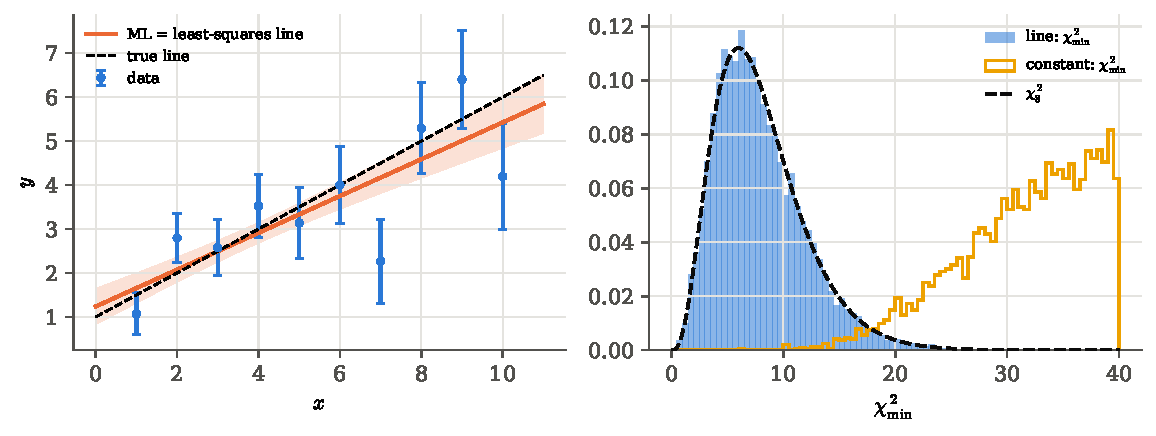
\includegraphics[width=12cm]{figures/ch03/line_fit.pdf}
\caption{Least squares as Gaussian maximum likelihood. Left: ten points with
error bars that grow to the right, the fitted line with its $\pm1\sigma$
band from $U=(A\T\Cmat^{-1}A)^{-1}$ (narrowest near the weighted centre of
the data), and the true line (dashed). Right: $\chi^2_{\min}$ of $10^4$
simulated experiments for the correct model (filled), which follows the
$\chi^2_8$ curve, and for a constant fitted to the same data (outline), which
sits far to the right.}
\label{3b:fig:line-fit}
\end{figure}

\subsection{Correlated noise: \texorpdfstring{$\chi^2=\bm r\T\Cmat^{-1}\bm r$}{chi2 = r C-1 r}}
\label{3b:sec:correlated}

Noise is often correlated from one data point to the next. Neighbouring
bins of a power spectrum share modes. A slowly drifting baseline pushes
consecutive readings up together. A common calibration error moves every
point at once.
The noise is then a Gaussian vector $\bm\epsilon\sim\Normal(\bm0,\Cmat)$ with
a non-diagonal covariance, and the likelihood is the multivariate normal
density (\cref{ch:02}) evaluated at the required noise
$\bm r=\bm D-\bm d(\params)$:
\begin{align}
  \Like(\params)
  &\eqby{1}p_{\bm\eta}\bigl(L^{-1}\bm r\bigr)\,\bigl|\det L^{-1}\bigr|
  \eqby{2}\frac{1}{(2\pi)^{N/2}}\,e^{-\frac12(L^{-1}\bm r)\T(L^{-1}\bm r)}\,
   \frac{1}{|\det L|}
  \nonumber\\
  &\eqby{3}\frac{1}{\sqrt{(2\pi)^N\det\Cmat}}
   \exp\!\Bigl[-\tfrac12\,\bm r\T\Cmat^{-1}\bm r\Bigr],
  \qquad
  -2\ell(\params)=\bm r\T\Cmat^{-1}\bm r+\ln\det\Cmat+N\ln2\pi .
  \label{3b:eq:like-corr}
\end{align}
\begin{explain}
  \item Write the noise as $\bm\epsilon=L\bm\eta$ with $\Cmat=LL\T$ and
        $\bm\eta\sim\Normal(\bm0,\Id)$. Changing variables from $\bm\eta$ to
        $\bm\epsilon$ multiplies the density by the Jacobian
        $|\det(\partial\bm\eta/\partial\bm\epsilon)|=|\det L^{-1}|$.
  \item Independent standard Gaussians: the density is the product of $N$
        factors $(2\pi)^{-1/2}e^{-\eta_i^2/2}$.
  \item $(L^{-1}\bm r)\T(L^{-1}\bm r)=\bm r\T(LL\T)^{-1}\bm r=\bm r\T\Cmat^{-1}\bm r$,
        and $(\det L)^2=\det\Cmat$.
\end{explain}
So the correlated $\chi^2$ is $\bm r\T\Cmat^{-1}\bm r$, and every result
above, from the normal equations to $\chi^2_{\min}\sim\chi^2_{N-m}$,
holds with this $\Cmat$, because those derivations never used that $\Cmat$
was diagonal. This is the likelihood written for cosmological data with
correlated errors. One term needs care. The $\ln\det\Cmat$ is a constant
only if the covariance does not depend on the parameters. For the power
spectrum of a Gaussian random field the
covariance \emph{is} the signal (cosmic variance scales with $\Cell$
itself), and then $\ln\det\Cmat(\params)$ must be kept. Dropping it biases
the fit (\cref{ch:07}).

\paragraph{What goes wrong if we ignore the correlation?}
Suppose the noise has covariance $\Cmat_{ij}=\sigma_i\sigma_je^{-|x_i-x_j|/2}$
(neighbours correlated at $e^{-1/2}=0.61$) but we fit with only the
diagonal. The estimator is still $\hat\params=B_{\text{diag}}\bm D$, a
linear function of the data with $B_{\text{diag}}A=\Id$, so it is still
\emph{unbiased}. What is wrong is the error bar. The quoted covariance
$(A\T\Cmat_{\text{diag}}^{-1}A)^{-1}$ assumes the noise we did not have; the
true covariance is $B_{\text{diag}}\Cmat B_{\text{diag}}\T$ by the same
propagation rule as \eqref{3b:eq:ls-cov}. The second half of
\pyname{11_line_fit.py} draws correlated noise as $L\bm\eta$ with the
Cholesky factor and fits $10^4$ data sets both ways. For the slope:
\begin{center}
\small
\begin{tabular}{lccc}
  \hline
  fit & mean $\hat b$ & quoted $\sigma_{\hat b}$ & true scatter of $\hat b$\\
  \hline
  diagonal $\chi^2$ & $\ThreeBCorrMeanBd$ & $\ThreeBCorrQuoted$ & $\ThreeBCorrSdD$ (predicted $\ThreeBCorrTrueD$)\\
  full $\bm r\T\Cmat^{-1}\bm r$ & $\ThreeBCorrMeanBf$ & $\ThreeBCorrQuotedF$ & $\ThreeBCorrSdF$\\
  \hline
\end{tabular}
\end{center}
Both fits centre on the true slope $0.5$. The diagonal fit claims an error
of $\ThreeBCorrQuoted$ but actually scatters by $\ThreeBCorrSdD$, so every
quoted interval is too short by a third. The full fit quotes its error
correctly, and that error is also smaller than the true error of the
diagonal fit: using the correlations is not only honest but more precise.
The goodness of fit misleads too. With the diagonal $\chi^2$ the average
$\chi^2_{\min}$ is $\ThreeBCorrChiD$ instead of $8$, a fit that looks
suspiciously good; with the full $\Cmat$ it is $\ThreeBCorrChiF$
(\cref{3b:fig:line-fit-corr}).

\begin{pitfall}[Correlated noise makes a bad error bar look like a good fit]
Positively correlated noise moves neighbouring points up and down
together. A smooth model can follow such coherent wiggles, so the residuals
come out smaller than independent noise of the same size would give, and
$\chi^2_{\min}\ll\dof$. At the same moment the parameter errors computed from
the diagonal are too small. A reduced $\chi^2$ well below one is a hint to
look for correlations, not a reason to celebrate.
\end{pitfall}

\begin{figure}[htbp]
\centering
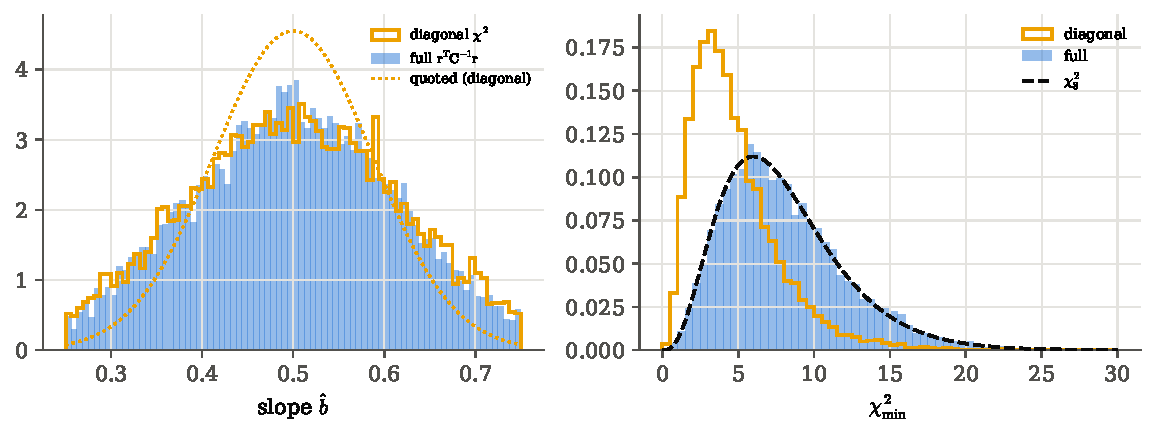
\includegraphics[width=12cm]{figures/ch03/line_fit_corr.pdf}
\caption{Fitting data with correlated noise, $10^4$ simulated experiments.
Left: the slope from the diagonal $\chi^2$ (outline) and from the full
$\bm r\T\Cmat^{-1}\bm r$ (filled). Both are centred on the truth, but the
diagonal fit is wider than the Gaussian it quotes (dotted). Right: the
diagonal fit's $\chi^2_{\min}$ piles up well below the $\chi^2_8$ curve,
while the full fit's follows it.}
\label{3b:fig:line-fit-corr}
\end{figure}

\paragraph{The same idea for a gravitational-wave detector.}
Detector noise is correlated in time but, if stationary, it is uncorrelated
between different frequencies: the Fourier transform diagonalises its
covariance, and the diagonal entries are the noise power spectral density
$S_n(f)$ \unpack{the noise variance per unit frequency. Frequencies where the
detector is noisy have large $S_n$}. The sum $\bm r\T\Cmat^{-1}\bm r$ then
becomes an integral over frequency, with $\tilde r(f)=\int r(t)e^{-2\pi ift}\dd t$,
\[
  -2\ell(\params)=(D-h_{\params}\,|\,D-h_{\params})+\text{const},\qquad
  (a\,|\,b)\equiv4\,\mathrm{Re}\int_0^\infty\frac{\tilde a(f)\,\tilde b^*(f)}{S_n(f)}\,\dd f ,
\]
where $h_{\params}$ is the waveform predicted for source parameters
$\params$. The \newterm{noise-weighted inner product} $(a|b)$ is
$\bm a\T\Cmat^{-1}\bm b$ in the basis where $\Cmat$ is diagonal, with
one-sided $S_n$ and positive frequencies only, hence the factor $4$. Every
gravitational-wave parameter estimate, and the Fisher forecasts of
\cref{ch:10}, start from this one line.
\section{Counting experiments: the Poisson likelihood of a histogram}
\label{3b:sec:poisson}

A search at a collider histograms the invariant mass of candidate events
into bins; an X-ray telescope histograms photon energies; a decay experiment
histograms decay times. Far from the peak, or in a short run, many bins hold
a handful of events, and some hold none. The habit of putting an error bar
$\sqrt{n_i}$ on every bin and minimising $\chi^2$ breaks down here. A bin
with $n_i=0$ gets an error bar of zero, and bins that fluctuated low get
error bars that are too small. The reason is that the noise in a counting
experiment is not Gaussian and is not added to the prediction. The count in
a bin is a Poisson random number whose mean is the prediction. The
likelihood has no trouble with this, because all it needs is the
probability of what was observed. Four questions need answers.
\begin{enumerate}[label=\arabic*.]
  \item What is the likelihood of a histogram of counts, and what does
        maximising it do to the total number of events?
  \item Can the same likelihood also tell us whether the fit is good?
  \item What exactly goes wrong with the two $\chi^2$ recipes that use
        $\sqrt{n_i}$ or $\sqrt{\mu_i}$ as the error bar?
  \item How does the idea carry over to other data: measurements with
        Gaussian errors, gravitational-wave strain, CMB maps?
\end{enumerate}

\subsection{The likelihood of a histogram}
\label{3b:sec:poisson-like}

Divide the range of $x$ into $N$ bins. If events arrive independently at a
constant rate, the count $n_i$ in bin $i$ is Poisson distributed
(\cref{ch:02}) with mean
\[
  \mu_i(\nu,\params)=\nu\int_{\text{bin }i}f(x;\params)\,\dd x\equiv\nu\,p_i(\params),
  \qquad\sum_{i=1}^Np_i(\params)=1,
\]
where $\nu$ is the expected total and $p_i$ the probability that an event
falls in bin $i$ \srcref{Cowan}{\S6.10}. Different bins are independent,
so
\begin{align}
  \Like(\nu,\params)
  &\eqby{1}\prod_{i=1}^N\frac{\mu_i^{n_i}e^{-\mu_i}}{n_i!},
  \nonumber\\
  \ell(\nu,\params)
  &\eqby{2}\sum_{i=1}^N\bigl(n_i\ln\mu_i-\mu_i\bigr)-\sum_{i=1}^N\ln n_i!
  \eqby{3}-\tfrac12\,C(\nu,\params)+\text{const},
  \qquad
  C\equiv2\sum_{i=1}^N\bigl(\mu_i-n_i\ln\mu_i\bigr).
  \label{3b:eq:poisson-like}
\end{align}
\begin{explain}
  \item Poisson probability of $n_i$ counts for mean $\mu_i$, multiplied over
        independent bins \srcref{Cowan}{(6.44)}.
  \item $\ln(\mu^ne^{-\mu}/n!)=n\ln\mu-\mu-\ln n!$.
  \item The counts are data, so $\sum\ln n_i!$ does not depend on the
        parameters.
\end{explain}
The quantity $C=-2\ell+\text{const}$ is the \newterm{Cash statistic},
introduced for X-ray astronomy \cite{Cash1979}; minimising it is
maximising the Poisson likelihood. In the language of
\cref{3b:sec:likelihood}, each bin asks how probable it is that a Poisson
source with mean $\mu_i(\params)$ produced the count we saw, and an empty
bin contributes simply $e^{-\mu_i}$, the probability of seeing nothing.

\paragraph{The total number of events is conserved.}
Split the Poisson product into a statement about the total and a
statement about the shape. With $n=\sum_in_i$ and $\mu_i=\nu p_i$,
\begin{align}
  \prod_{i=1}^N\frac{\mu_i^{n_i}e^{-\mu_i}}{n_i!}
  &\eqby{1}\frac{\nu^{n}e^{-\nu}}{n!}\;
   \frac{n!}{\prod_in_i!}\prod_{i=1}^Np_i^{n_i},
  \label{3b:eq:poisson-split}\\
  \frac{\partial\ell}{\partial\nu}
  &\eqby{2}\frac{n}{\nu}-1\eqby{3}0
  \quad\Longrightarrow\quad\hat\nu=n .
  \nonumber
\end{align}
\begin{explain}
  \item $\prod_i\mu_i^{n_i}=\nu^{\sum n_i}\prod_ip_i^{n_i}$ and
        $\prod_ie^{-\mu_i}=e^{-\nu\sum p_i}=e^{-\nu}$; then multiply and
        divide by $n!$. The first factor is the Poisson probability of the
        total, the second the multinomial probability of the split into bins
        \srcref{Cowan}{(6.41), (6.43)}.
  \item Only the first factor depends on $\nu$, and
        $\partial_\nu(n\ln\nu-\nu)=n/\nu-1$.
  \item The score equation for $\nu$; the multinomial factor is untouched,
        so $\hat\params$ is the same as in a fit with the total fixed.
\end{explain}
The fitted normalisation equals the observed number of events, exactly, in
every experiment, whatever the shape parameters do. This is the binned form
of the extended likelihood \eqref{3b:eq:extended}. It is also the property
the two $\chi^2$ recipes below lack.

\begin{workdef}[Poisson likelihood of a histogram]
For counts $n_i$ with predicted means $\mu_i(\params)$,
\[
  -2\ell(\params)=2\sum_i\bigl(\mu_i-n_i\ln\mu_i\bigr)+\text{const}.
\]
\emph{Operationally:} compute the expected count in every bin from the
model (integrate the density over the bin and multiply by the expected
total), evaluate this sum, minimise. Empty bins stay in the sum and
contribute $2\mu_i$. No bins need to be merged, and no error bars are
assigned.
\end{workdef}

\paragraph{Example: one bin.}
For a single bin with $n=9$ counts,
$\ell(\mu)=9\ln\mu-\mu$ gives $\hat\mu=9$ and
$-\ell''(\hat\mu)=n/\hat\mu^2=1/9$, a curvature error of $3=\sqrt n$, the
familiar rule. The likelihood itself is skewed: solving
$\ell(\mu)=\ell_{\max}-\tfrac12$ gives $\mu\in[6.32,12.34]$, that is
$9^{+3.34}_{-2.68}$. The interval reaches further up than down. Why? A
Poisson count with mean $\mu$ has spread $\sqrt\mu$. A large mean such as
$12.34$ has a large spread, $3.5$, so a count of $9$ is less than one spread
below it. A small mean such as $6.32$ has a small spread, $2.5$, so the
same count is slightly more than one spread above it. Large means can
therefore stray further from the data and still explain them about as well
(\cref{3b:sec:curvature}).

\subsection{Fitting and testing with one number: the Baker--Cousins \texorpdfstring{$\chi^2_\lambda$}{chi2-lambda}}
\label{3b:sec:baker-cousins}

The value of $C$ at its minimum does not by itself say whether the fit is
good. Its constant is arbitrary, and it grows with the total number of
events even for a perfect model. To make it a measure of fit, compare the
model with the best any model could do \cite{BakerCousins1984}. That best
is the \newterm{saturated model}
\unpack{a ``model'' with one free mean per bin, which therefore sets
$\mu_i=n_i$ and fits the data perfectly}. The likelihood ratio is
\begin{align}
  \chi^2_\lambda(\params)
  &\eqby{1}-2\ln\frac{\Like(\bm\mu(\params))}{\Like(\bm\mu=\bm n)}
  \eqby{2}-2\sum_i\Bigl[\bigl(n_i\ln\mu_i-\mu_i\bigr)-\bigl(n_i\ln n_i-n_i\bigr)\Bigr]
  \nonumber\\
  &\eqby{3}2\sum_{i=1}^N\Bigl[\mu_i-n_i+n_i\ln\frac{n_i}{\mu_i}\Bigr]
  \label{3b:eq:baker-cousins}
\end{align}
\srcref{Cowan}{(6.52)}.
\begin{explain}
  \item Definition of the likelihood-ratio statistic against the saturated
        model.
  \item \eqref{3b:eq:poisson-like} at $\mu_i$ and at $\mu_i=n_i$; the
        $\ln n_i!$ cancel in the ratio.
  \item Collect terms; $n_i\ln n_i-n_i\ln\mu_i=n_i\ln(n_i/\mu_i)$.
        An empty bin contributes $2\mu_i$ (since $n\ln n\to0$ as $n\to0$).
\end{explain}
Since $\chi^2_\lambda=C+\text{(terms in $n_i$ only)}$, minimising it is the
same as maximising the Poisson likelihood. Every term is non-negative. To
see it, write the bracket as $n_i(u-1-\ln u)$ with $u=\mu_i/n_i$, and note
that $u-1-\ln u\ge0$, with equality only at $u=1$ (the line $u-1$ lies above
the curve $\ln u$ and touches it at $u=1$). So $\chi^2_\lambda$ vanishes
only for a perfect fit, $\mu_i=n_i$ in every bin.

Why call it a $\chi^2$? Expand one term for a count close to its mean,
$n=\mu+\delta$ with $|\delta|\ll\mu$:
\begin{align*}
  \mu-n+n\ln\frac n\mu
  &\eqby{1}-\delta+(\mu+\delta)\ln\Bigl(1+\frac\delta\mu\Bigr)
  \eqby{2}-\delta+(\mu+\delta)\Bigl(\frac\delta\mu-\frac{\delta^2}{2\mu^2}+O\bigl(\tfrac{\delta^3}{\mu^3}\bigr)\Bigr)\\
  &\eqby{3}-\delta+\delta+\frac{\delta^2}{\mu}-\frac{\delta^2}{2\mu}+O\Bigl(\frac{\delta^3}{\mu^2}\Bigr)
  =\frac{\delta^2}{2\mu}+O\Bigl(\frac{\delta^3}{\mu^2}\Bigr).
\end{align*}
\begin{explain}
  \item Substitute $n=\mu+\delta$, and $n/\mu=1+\delta/\mu$.
  \item Taylor series $\ln(1+u)=u-u^2/2+O(u^3)$.
  \item Multiply out and keep terms up to $\delta^2/\mu$.
\end{explain}
So $\chi^2_\lambda\approx\sum_i(n_i-\mu_i)^2/\mu_i$ when every bin has many
counts: a Pearson $\chi^2$, a sum of squared standardised Poisson
fluctuations. In that limit $\chi^2_{\lambda,\min}\sim\chi^2_{N-m}$ for
$m$ fitted parameters, the Poisson analogue of
\eqref{3b:eq:chi2-min-dist}. The general statement is
\newterm{Wilks' theorem} \cite{Wilks1938}: for nested models, $-2\ln$ of the
ratio of maximised likelihoods is asymptotically $\chi^2$ with as many
degrees of freedom as the difference in the number of free parameters,
here $N-m$ (the saturated model has $N$). \Cref{ch:04} treats it properly.
Baker and Cousins' point is that $\chi^2_\lambda$ reaches this limit faster
than the $\chi^2$ recipes, and one statistic serves both to fit and to test.

\begin{keyidea}[Binned counts: use the Poisson likelihood]
Minimise $\chi^2_\lambda=2\sum_i[\mu_i-n_i+n_i\ln(n_i/\mu_i)]$. It is $-2\ln\Like$
up to a constant, so it gives the maximum likelihood fit; the fitted total
equals the observed total exactly; empty bins are harmless; and its minimum
is approximately $\chi^2_{N-m}$, so it is also the goodness-of-fit
statistic.
\end{keyidea}

\subsection{What goes wrong with \texorpdfstring{$\sqrt n$}{sqrt(n)} error bars}
\label{3b:sec:neyman-pearson}

Two least-squares recipes are common for histograms \srcref{Cowan}{\S7.4}.
The \newterm{Neyman} $\chi^2$ takes the variance of each bin from the data,
$\chi^2_N=\sum_i(n_i-\mu_i)^2/n_i$. The \newterm{Pearson} $\chi^2$ takes it
from the model, $\chi^2_P=\sum_i(n_i-\mu_i)^2/\mu_i$. Both treat the counts
as Gaussian, and both get the normalisation wrong, in opposite directions.
Let the model be $\mu_i=\nu p_i$ with $\sum_ip_i=1$ and minimise over $\nu$.

\paragraph{Neyman.} Setting the derivative to zero,
\begin{align*}
  \frac{\partial\chi^2_N}{\partial\nu}
  &\eqby{1}-2\sum_i\frac{p_i(n_i-\nu p_i)}{n_i}=0
  \quad\Longrightarrow\quad
  1=\nu\sum_i\frac{p_i^2}{n_i},\\
  \chi^2_{N,\min}
  &\eqby{2}\sum_i n_i-2\nu\sum_ip_i+\nu^2\sum_i\frac{p_i^2}{n_i}
  \eqby{3}n-2\nu+\nu
  \quad\Longrightarrow\quad
  \hat\nu_N=n-\chi^2_{N,\min} .
\end{align*}
\begin{explain}
  \item Chain rule on $(n_i-\nu p_i)^2$, then $\sum_ip_in_i/n_i=\sum_ip_i=1$.
  \item Expand the square: $(n_i-\nu p_i)^2/n_i=n_i-2\nu p_i+\nu^2p_i^2/n_i$.
  \item $\sum_in_i=n$, $\sum_ip_i=1$, and the first line gives
        $\nu^2\sum p_i^2/n_i=\nu$.
\end{explain}
\paragraph{Pearson.} In the same way,
\begin{align*}
  \frac{\partial\chi^2_P}{\partial\nu}
  &\eqby{1}-\sum_i\frac{n_i^2}{\nu^2p_i}+1=0
  \quad\Longrightarrow\quad
  \nu^2=\sum_i\frac{n_i^2}{p_i},\\
  \chi^2_{P,\min}
  &\eqby{2}\sum_i\frac{n_i^2}{\nu p_i}-2n+\nu
  \eqby{3}\nu-2n+\nu
  \quad\Longrightarrow\quad
  \hat\nu_P=n+\tfrac12\chi^2_{P,\min} .
\end{align*}
\begin{explain}
  \item Expand first: $(n_i-\nu p_i)^2/(\nu p_i)=n_i^2/(\nu p_i)-2n_i+\nu p_i$,
        then differentiate in $\nu$.
  \item Sum the expanded terms.
  \item The first line gives $\sum n_i^2/(\nu p_i)=\nu$.
\end{explain}
These are Cowan's (7.22) and (7.21). They say that the Neyman fit
undershoots the observed total by $\chi^2_{N,\min}$ and the Pearson fit
overshoots it by $\tfrac12\chi^2_{P,\min}$. Both relations hold exactly at the
minimum, also when shape parameters are fitted at the same time, because
the derivative with respect to $\nu$ must vanish there too. A correct model
gives $\chi^2_{\min}\approx N-m$, so the Neyman fit is low by about the
number of bins and the Pearson fit high by about half of it. The definitions
show why. Neyman gives a bin that fluctuated down a small variance, hence a
large weight, and the fit is dragged down. Pearson can lower its $\chi^2$ by
raising $\mu_i$, which inflates the variances it divides by, and the fit
drifts up. With $N=20$
bins and $n\approx120$ events the Neyman bias is about ten per cent,
comparable to the statistical error $\sqrt n\approx11$ on the total itself:
a systematic error as large as the statistical one, introduced by the
fitting recipe alone.

\paragraph{Example: two bins by hand.}
Suppose the model says the two halves of a range are equally likely,
$p_1=p_2=\tfrac12$, and we observe $n_1=4$, $n_2=16$, so $n=20$. Then
\begin{align*}
  \hat\nu_{\text{ML}}&=20,\\
  \hat\nu_N&\eqby{1}\Bigl(\frac{1/4}{4}+\frac{1/4}{16}\Bigr)^{-1}=12.8,
  \qquad \chi^2_{N,\min}\eqby{2}20-12.8=7.2,\\
  \hat\nu_P&\eqby{3}\sqrt{\frac{16}{1/2}+\frac{256}{1/2}}=\sqrt{544}=23.3,
  \qquad \chi^2_{P,\min}\eqby{4}2(23.3-20)=6.65 .
\end{align*}
\begin{explain}
  \item The Neyman condition $1=\nu\sum p_i^2/n_i$.
  \item $\hat\nu_N=n-\chi^2_{N,\min}$.
  \item The Pearson condition $\nu^2=\sum n_i^2/p_i$.
  \item $\hat\nu_P=n+\tfrac12\chi^2_{P,\min}$.
\end{explain}
Twenty events were seen. Only the likelihood says twenty.

\subsection{A histogram fit in Python}
\label{3b:sec:poisson-python}

The script \pyname{12_poisson_bins.py} histograms decay times into $N=20$
bins on $0\le t\le5$ (in units of the true lifetime), with an expected
total of $\nu=120$, and fits $(\nu,\tau)$ with the three statistics.
\pyfile[firstline=37,lastline=54]{code/ch03/12_poisson_bins.py}{The three statistics for a histogram}
The Cash and Baker--Cousins functions differ only by terms in $n_i$, so
they have the same minimum; \pyname{special.xlogy(n, n)} evaluates
$n\ln n$ with the convention $0\ln0=0$. The Neyman function needs a patch
for empty bins, \pyname{np.maximum(n, 1)}, which is itself a sign of
trouble.

For the example histogram, with $n=\ThreeBPoisNobs$ events and
$\ThreeBPoisZeroBins$ empty bins, the fitted totals are
$\hat\nu=\ThreeBPoisNuP$ (Poisson), $\ThreeBPoisNuN$ (Neyman) and
$\ThreeBPoisNuS$ (Pearson), with lifetimes $\ThreeBPoisTauP$,
$\ThreeBPoisTauN$ and $\ThreeBPoisTauS$ (\cref{3b:fig:poisson-fit}). The
Baker--Cousins statistic at the minimum is $\ThreeBPoisBC$ for
$\ThreeBPoisDof$ degrees of freedom, a normal-looking fit.

\begin{figure}[htbp]
\centering
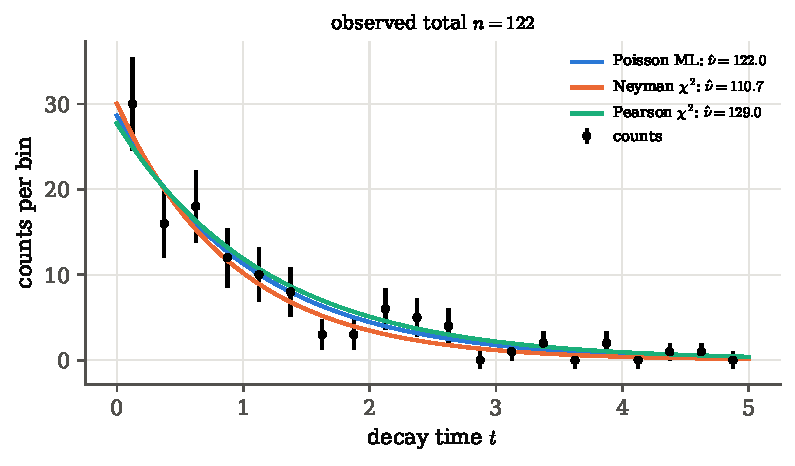
\includegraphics[width=10cm]{figures/ch03/poisson_fit.pdf}
\caption{One histogram of decay times with few counts per bin (points,
with $\sqrt{\max(n_i,1)}$ bars for orientation only) and three fits of the
same exponential shape. The Poisson likelihood fit reproduces the observed
total. The Neyman $\chi^2$ fit sits low, pulled down by the bins that
fluctuated low; the Pearson $\chi^2$ fit sits high.}
\label{3b:fig:poisson-fit}
\end{figure}

Over $3000$ simulated histograms the Poisson fit returns
$|\hat\nu-n|\le\ThreeBPoisDiffP$ in every one of them, the exact
conservation law of \eqref{3b:eq:poisson-split} up to the tolerance of the
minimiser. The Pearson fit is high by $\ThreeBPoisDiffS$ events on average,
exactly $\tfrac12\overline{\chi^2_{P,\min}}=\ThreeBPoisPredS$. The Neyman fit
is low by $\ThreeBPoisDiffN$; the relation $\hat\nu_N=n-\chi^2_{N,\min}$
predicts $\ThreeBPoisPredN$, and the difference is entirely due to the patch
for empty bins, which breaks the identity $\sum_ip_in_i/n_i=1$ used in its
derivation. The bias leaks into the shape: the mean fitted lifetimes are
$\ThreeBPoisTauMeanP$, $\ThreeBPoisTauMeanN$ and $\ThreeBPoisTauMeanS$ for
a true value of $1$. Finally, the Baker--Cousins $\chi^2_{\lambda,\min}$
averages $\ThreeBPoisBCmean$ against $\ThreeBPoisDof$ degrees of freedom
and follows the $\chi^2_{18}$ curve even with this sparse histogram
(\cref{3b:fig:poisson-bias}).

\begin{figure}[htbp]
\centering
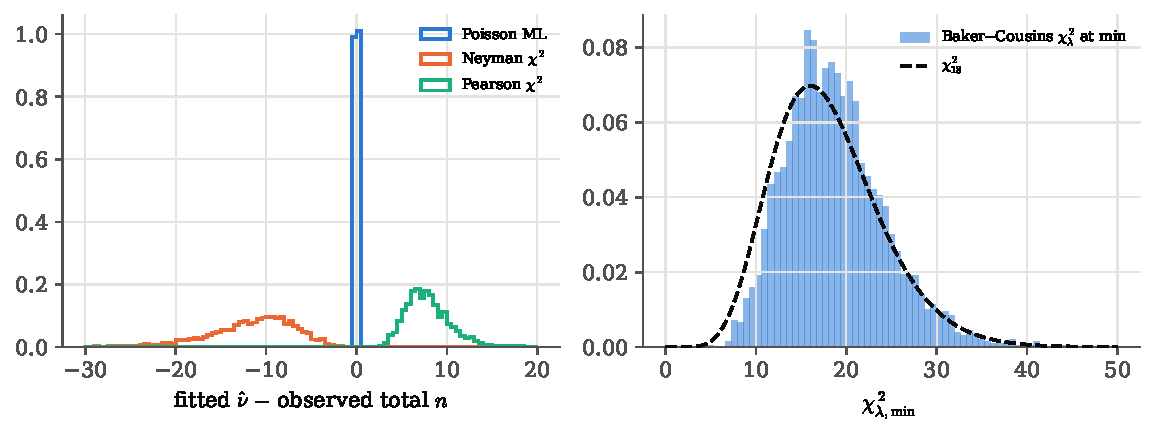
\includegraphics[width=12cm]{figures/ch03/poisson_bias.pdf}
\caption{Three thousand simulated histograms. Left: fitted total minus
observed total. The Poisson fit is a spike at zero; the Neyman fit is
biased low by about ten events and the Pearson fit high by about eight.
Right: the Baker--Cousins statistic at its minimum follows the $\chi^2$
distribution for $20-2=18$ degrees of freedom, so it can be used as a
goodness-of-fit test.}
\label{3b:fig:poisson-bias}
\end{figure}

\subsection{One idea, three implementations}
\label{3b:sec:universal}

The recipe is always the same: write the prediction, write the probability
of the fluctuation needed to turn it into the data, and multiply over
independent pieces. Only the noise model changes from one field to another.
Three noise models cover most data in physics and cosmology: Poisson counts;
Gaussian noise with a covariance that does not depend on the parameters
(gravitational-wave strain is this case written in frequency); and a
Gaussian field whose covariance is itself the signal, as for the CMB.

\begin{taxonomy}[Which likelihood when]
\small
\begin{tabular}{@{}>{\raggedright\arraybackslash}p{3.3cm}>{\raggedright\arraybackslash}p{4.4cm}>{\raggedright\arraybackslash}p{5.0cm}@{}}
  data & noise model & $-2\ln\Like$ (up to constants)\\
  \hline
  counts in bins (colliders, X-ray, decay histograms)
    & $n_i\sim\mathrm{Poisson}(\mu_i(\params))$, independent bins
    & $2\sum_i[\mu_i-n_i\ln\mu_i]$ \eqref{3b:eq:poisson-like}\\[2pt]
  measurements with error bars; binned spectra
    & Gaussian, covariance $\Cmat$ independent of $\params$
    & $\bm r\T\Cmat^{-1}\bm r$ \eqref{3b:eq:like-corr}\\[2pt]
  GW strain
    & stationary Gaussian noise with PSD $S_n(f)$
    & $(D-h_{\params}|D-h_{\params})$ (\cref{3b:sec:correlated})\\[2pt]
  CMB map, full sky, no noise
    & $\alm$ Gaussian with variance $\Cell(\params)$
    & $\sum_\ell(2\ell+1)\bigl[\Chat/\Cell+\ln\Cell\bigr]$\\
\end{tabular}
\end{taxonomy}

The last line needs a derivation, because it is the first case where the
parameters sit in the covariance rather than in the mean. In a statistically
isotropic Gaussian sky the spherical-harmonic coefficients $\alm$ have mean
zero and variance $\Cell$, the theory's power spectrum. The measured
spectrum is $\Chat=\frac{1}{2\ell+1}\sum_m|\alm|^2$. Because the sky is real,
$a_{\ell,-m}$ is fixed by $a_{\ell m}$, so at each $\ell$ there are
$2\ell+1$ independent real numbers: $a_{\ell0}$, and $\sqrt2\,\mathrm{Re}\,\alm$
and $\sqrt2\,\mathrm{Im}\,\alm$ for $m=1,\dots,\ell$. Call them $y_{\ell k}$,
$k=1,\dots,2\ell+1$. Each is Gaussian with variance $\Cell$, and
$\sum_ky_{\ell k}^2=\sum_m|\alm|^2=(2\ell+1)\Chat$. Then
\begin{align*}
  -2\ell(\params)
  &\eqby{1}\sum_\ell\sum_{k=1}^{2\ell+1}\Bigl[\frac{y_{\ell k}^2}{\Cell(\params)}+\ln\Cell(\params)+\ln2\pi\Bigr]
  \eqby{2}\sum_\ell(2\ell+1)\Bigl[\frac{\Chat}{\Cell(\params)}+\ln\Cell(\params)\Bigr]+\text{const}.
\end{align*}
\begin{explain}
  \item \eqref{3b:eq:like-corr} with a diagonal covariance whose entries
        are $\Cell$: $-2\ln$ of each Gaussian factor is
        $y^2/\Cell+\ln\Cell+\ln2\pi$.
  \item Sum over $k$ using $\sum_ky_{\ell k}^2=(2\ell+1)\Chat$; the $2\ell+1$
        copies of $\ln\Cell$ give the second term.
\end{explain}
The $\ln\Cell$ term is the $\ln\det\Cmat$ of \eqref{3b:eq:like-corr}, and it
cannot be dropped: without it the fit would push every $\Cell$ to
infinity. If the model sets each $\Cell$ free, the score equation
$-\Chat/\Cell^2+1/\Cell=0$ gives $\hat C_\ell=\Chat$, so the familiar
estimator is the maximum likelihood estimator. As a function of $\Cell$
this likelihood is skewed, like the Poisson one above, and for the same
reason: the spread of $\Chat$ grows with its mean. A mask, instrument noise
and a beam change this likelihood, as \cref{ch:07,ch:08} show.
\section{The width of the likelihood is the error bar}
\label{3b:sec:curvature}

The width of the likelihood is the error bar of the estimate. To see why
one would expect this, look at a likelihood with a sharp peak. Only a
narrow range of parameter values can turn the prediction into the data
with an ordinary fluctuation. Move a little away and the noise required
becomes implausible. A broad likelihood says the opposite: many values
would have done about equally well. For linear models with Gaussian noise
we proved the claim exactly in \cref{3b:sec:linear-ls}: the log-likelihood
is a parabola whose width is the standard deviation of $\hat\theta$. For any
smooth likelihood with enough data it holds approximately, and a check on
$10^4$ simulated experiments shows how well. Three questions follow.
\begin{enumerate}[label=\arabic*.]
  \item How do we read an error bar off the log-likelihood, from its
        curvature or from where it has dropped by $\tfrac12$?
  \item Why should the width of a function of $\theta$, computed from one
        data set, equal the scatter of $\hat\theta$ over many data sets? The
        answer introduces the Fisher information.
  \item How well does it work at a realistic sample size?
\end{enumerate}

\subsection{Curvature at the peak}
\label{3b:sec:curv-peak}

Expand the log-likelihood about its maximum, where the first derivative
vanishes \srcref{Padilla}{(29)--(31)}:
\begin{align}
  \ell(\theta)
  &\eqby{1}\ell(\hat\theta)+\underbrace{\ell'(\hat\theta)}_{=0}(\theta-\hat\theta)
   +\tfrac12\ell''(\hat\theta)(\theta-\hat\theta)^2+\dots
  \eqby{2}\ell_{\max}-\frac{(\theta-\hat\theta)^2}{2\hat\sigma^2}+\dots,
  \qquad
  \hat\sigma^2\equiv\frac{1}{-\ell''(\hat\theta)} .
  \label{3b:eq:curvature}
\end{align}
\begin{explain}
  \item Taylor's theorem at the maximum; the score vanishes there.
  \item $\ell''(\hat\theta)<0$ at a maximum, so $-1/\ell''$ is positive and
        we may call it $\hat\sigma^2$.
\end{explain}
Near its peak the likelihood is therefore
$\Like(\theta)\approx\Like_{\max}\exp[-(\theta-\hat\theta)^2/2\hat\sigma^2]$,
a Gaussian bump of width $\hat\sigma$. The rule is: \emph{the error bar is
one over the square root of minus the second derivative of $\ln\Like$ at its
maximum} \srcref{Cowan}{\S6.4}. For several parameters, minus the matrix of
second derivatives (the Hessian with a minus sign) plays the role of
$1/\hat\sigma^2$, and its inverse is the estimated covariance matrix. That
is the line \pyname{V = np.linalg.inv(-H)} in the Newton--Raphson fit of
the muon angular distribution (\cref{3b:sec:newton}).

\paragraph{Example: the lifetime.}
For $n$ decay times the maximum likelihood lifetime is $\hat\tau=\bar t$,
and \eqref{3b:eq:tau-mle} gave $-\ell''(\hat\tau)=n/\hat\tau^2$. So
$\hat\sigma_{\hat\tau}=\hat\tau/\sqrt n$. Fifty decays measure a lifetime to
$1/\sqrt{50}\approx14\%$. The true standard deviation of $\bar t$ is
$\tau/\sqrt n$ (\cref{3b:sec:mle-hand}), and the curvature gives the same
formula with the unknown $\tau$ replaced by its estimate.

\paragraph{Example: the detector efficiency.}
For the detector that fires $S$ times in $n$ trials, the log-likelihood is
$\ell(p)=S\ln p+(n-S)\ln(1-p)$ and $\hat p=S/n$ (\cref{3b:sec:mle-hand}).
Then
\begin{align*}
  -\ell''(p)&\eqby{1}\frac{S}{p^2}+\frac{n-S}{(1-p)^2},\qquad
  -\ell''(\hat p)\eqby{2}\frac{n}{\hat p}+\frac{n}{1-\hat p}
  \eqby{3}\frac{n}{\hat p(1-\hat p)},\qquad
  \hat\sigma_{\hat p}=\sqrt{\frac{\hat p(1-\hat p)}{n}} .
\end{align*}
\begin{explain}
  \item Differentiate $S/p-(n-S)/(1-p)$ once more.
  \item At $\hat p=S/n$: $S/\hat p^2=n/\hat p$ and
        $(n-S)/(1-\hat p)^2=n/(1-\hat p)$.
  \item Common denominator: $1/\hat p+1/(1-\hat p)=1/[\hat p(1-\hat p)]$.
\end{explain}
For $S=12$ out of $n=20$ this is $\sqrt{0.6\cdot0.4/20}=0.11$, the
binomial standard error.

\subsection{The graphical method: where \texorpdfstring{$\ln\Like$}{ln L} has dropped by one half}
\label{3b:sec:delta-lnl}

If $\ell$ were exactly the parabola \eqref{3b:eq:curvature}, then at
$\theta=\hat\theta\pm\hat\sigma$ it would be exactly $\ell_{\max}-\tfrac12$.
That suggests a second recipe that does not need derivatives: draw
$\ell(\theta)$ and read off where it crosses $\ell_{\max}-\tfrac12$
\srcref{Cowan}{\S6.7}. For Gaussian data $-2\ell=\chi^2+\text{const}$, so
this is the $\Delta\chi^2=1$ rule of \cref{3b:sec:chi2-min}. When the
log-likelihood is not a parabola, the two crossings are at different
distances from $\hat\theta$, and one quotes an asymmetric error
$\hat\theta^{+\sigma_+}_{-\sigma_-}$.

\paragraph{Example: the lifetime interval exactly.}
Measure $\tau$ in units of the estimate, $u=\tau/\hat\tau$. Using
$T=n\hat\tau$,
\begin{align*}
  \ell(\tau)-\ell(\hat\tau)
  &\eqby{1}-n\ln\tau-\frac{n\hat\tau}{\tau}+n\ln\hat\tau+n
  \eqby{2}-n\Bigl[\ln u+\frac1u-1\Bigr].
\end{align*}
\begin{explain}
  \item $\ell(\tau)=-n\ln\tau-T/\tau$ at $\tau$ and at $\hat\tau$, with
        $T/\hat\tau=n$.
  \item $\ln\tau-\ln\hat\tau=\ln u$ and $\hat\tau/\tau=1/u$.
\end{explain}
The $\Delta\ln\Like=\tfrac12$ interval is the pair of roots of
$\ln u+1/u-1=1/(2n)$, the same for every data set once expressed in units of
$\hat\tau$. For small $u-1$, $\ln u+1/u-1\approx\tfrac12(u-1)^2$, which
returns $u=1\pm1/\sqrt n$, the curvature error. For $n=50$ the exact roots
are $u=0.871$ and $u=1.156$: the interval reaches further up than down,
because decay times drawn with a longer lifetime also scatter more.

\paragraph{Why the graphical interval is the better one.}
The curvature error depends on how we name the parameter; the $\Delta\ln\Like$
interval does not. The likelihood assigns the same number to a hypothesis
whatever we call it (\cref{3b:sec:not-density}). So if we switch from $\tau$
to the rate $\lambda=1/\tau$, the set of hypotheses with
$\ell\ge\ell_{\max}-\tfrac12$ is the same set, merely relabelled. If
$\tau_-$ and $\tau_+$ are the lower and upper ends of the $\tau$ interval,
the $\lambda$ interval is $[1/\tau_+,1/\tau_-]$. The curvature, by contrast,
changes: $-\partial^2\ell/\partial\lambda^2$ at $\hat\lambda$ is $n/\hat\lambda^2$,
so the curvature interval in $\lambda$ is $\hat\lambda(1\pm1/\sqrt n)$,
which is \emph{not} the image of $\hat\tau(1\pm1/\sqrt n)$. The two
symmetric recipes disagree with each other, and each is right only to
leading order. The graphical interval behaves as if we had found and used
the parametrisation in which $\ell$ is most nearly a parabola, without our
having to find it.

\begin{pitfall}[A curvature error assumes a parabola]
$\hat\sigma=(-\ell'')^{-1/2}$ describes the peak only. If $\ell$ is skewed,
has a second maximum, or is cut off by a physical boundary (a mass that
cannot be negative, a cliff like the uniform box), the curvature says
nothing about the tails. Always plot $\ln\Like$, or at least find the two
$\Delta\ln\Like=\tfrac12$ crossings, before quoting $\pm\hat\sigma$.
\end{pitfall}

\paragraph{Several parameters.}
With two parameters the level set $\ell=\ell_{\max}-\tfrac12$ is a closed
curve, an ellipse when $\ell$ is quadratic. In the right panel of
\cref{3b:fig:angular} it is drawn for the fit of the angular distribution
$1+\alpha x+\beta x^2$ (\cref{3b:sec:newton}). The dotted lines tangent to it
are at $\hat\alpha\pm\sigma_{\hat\alpha}$ and $\hat\beta\pm\sigma_{\hat\beta}$,
with the errors from the inverse Hessian \srcref{Cowan}{\S6.8}. Why tangent
lines? Fix $\alpha$ and move $\beta$ to make $\ell$ as large as possible. As
$\alpha$ moves away from $\hat\alpha$ this best value falls, and it reaches
$\ell_{\max}-\tfrac12$ exactly where the vertical line at that $\alpha$
touches the contour. That best value as a function of $\alpha$ is the profile
likelihood of \cref{3b:sec:profile}. The tilt of the ellipse shows the
correlation between the two estimates. For that fit the inverse Hessian gives
$\sigma_{\hat\alpha}=\ThreeBAngSa$, $\sigma_{\hat\beta}=\ThreeBAngSb$ and
$\rho=\ThreeBAngRho$; the $500$ repetitions scatter with
$\ThreeBAngSdA$, $\ThreeBAngSdB$ and $\rho=\ThreeBAngRhoMC$. The standard
deviations agree to a few per cent. The correlation from $500$ pairs is
itself uncertain by $(1-\rho^2)/\sqrt{500}=\ThreeBAngRhoMCErr$, so the two
values of $\rho$ should be compared within that error. The Hessian's own
$\rho$ also changes from one experiment to the next: over the $500$
repetitions it averages $\ThreeBAngRhoHessMean$ and scatters by
$\ThreeBAngRhoHessSd$. Its average and the repetitions' $\rho$ are consistent
within about two of the repetitions' errors: $500$ repetitions are not enough
to tell them apart. The $\tfrac12$-contour projects onto each
axis as a $68\%$ interval for that parameter alone. A region that should
contain \emph{both} true values with $68\%$ probability is the larger
contour $\Delta\ln\Like=2.30/2=1.15$, as in the $\Delta\chi^2$ table of
\cref{3b:sec:chi2-min}.

\subsection{Why the curvature is the error: score and Fisher information}
\label{3b:sec:fisher-info}

We now have a recipe that uses one data set, a second derivative of a
function of $\theta$. The error bar we want is a statement about many data
sets: the standard deviation of $\hat\theta$ over imagined repetitions. Why
should they agree? The bridge is the score, $S(\theta)=\ell'(\theta)$,
viewed as a random variable. For a fixed $\theta$, each data set gives a
different score. Two identities about its distribution do all the work.
They hold whenever we may differentiate under the integral sign, which
requires, in particular, that the range of the data does not depend on
$\theta$ (it fails for the uniform box).

\paragraph{The score has mean zero.} For a single observation with density
$f(x;\theta)$,
\begin{align}
  \E_\theta\Bigl[\frac{\partial\ln f(X;\theta)}{\partial\theta}\Bigr]
  &\eqby{1}\int\frac{\partial_\theta f(x;\theta)}{f(x;\theta)}\,f(x;\theta)\,\dd x
  \eqby{2}\frac{\partial}{\partial\theta}\int f(x;\theta)\,\dd x
  \eqby{3}\frac{\partial}{\partial\theta}1=0 .
  \label{3b:eq:score-mean}
\end{align}
\begin{explain}
  \item Expectation over the density of the data at the \emph{same}
        $\theta$; $\partial_\theta\ln f=\partial_\theta f/f$.
  \item The $f$ cancels. Exchange the derivative and the integral (the
        regularity condition).
  \item Every density integrates to one, for every $\theta$.
\end{explain}
At the true parameter, the data pull neither up nor down on average.

\paragraph{The variance of the score is minus the mean curvature.}
Now differentiate the identity
\[
  \int(\partial_\theta\ln f)\,f\,\dd x=0
\]
once more with respect to $\theta$:
\begin{align}
  0&\eqby{1}\int\Bigl[(\partial^2_\theta\ln f)\,f+(\partial_\theta\ln f)\,\partial_\theta f\Bigr]\dd x
   \eqby{2}\int\Bigl[\partial^2_\theta\ln f+(\partial_\theta\ln f)^2\Bigr]f\,\dd x ,
  \nonumber\\
  I(\theta)&\equiv\E_\theta\bigl[(\partial_\theta\ln f)^2\bigr]
   \eqby{3}-\E_\theta\bigl[\partial^2_\theta\ln f\bigr] .
  \label{3b:eq:fisher-identity}
\end{align}
\begin{explain}
  \item Product rule under the integral.
  \item $\partial_\theta f=(\partial_\theta\ln f)\,f$.
  \item Split the integral. Since the score has mean zero, the first form
        is its variance.
\end{explain}
For $n$ independent observations, $\ell=\sum_i\ln f(x_i;\theta)$ is a sum of
independent terms, so the variance of the total score and the expected
curvature both add: $I_n(\theta)=nI(\theta)$ \mainref{p.~128, Thm.~9.17}.

\begin{workdef}[Fisher information]
The \newterm{Fisher information} in $n$ observations is
\[
  I_n(\theta)=\Var_\theta\bigl[S(\theta)\bigr]=-\E_\theta\bigl[\ell''(\theta)\bigr]=nI(\theta),
\]
the average curvature of the log-likelihood at the true parameter
\mainref{p.~128, Def.~9.16}. The \newterm{observed information}
$-\ell''(\hat\theta)$ is the curvature of the one log-likelihood we have,
at its peak. \emph{Operationally:} differentiate $\ln f$ twice, take minus
its average over the model, multiply by $n$. For several parameters,
$I_{jk}=-\E[\partial_j\partial_k\ell]$ is the \newterm{Fisher matrix}
(\cref{ch:10}).
\end{workdef}

\paragraph{From the score to the scatter of $\hat\theta$.}
Now expand the score equation of one data set about the true value
$\theta$ \mainref{p.~136}:
\begin{align}
  0&\eqby{1}\ell'(\hat\theta)
   \eqby{2}\ell'(\theta)+(\hat\theta-\theta)\,\ell''(\theta)+\dots
  \quad\Longrightarrow\quad
  \hat\theta-\theta\approx\frac{\ell'(\theta)}{-\ell''(\theta)}
  \eqby{3}\frac{\tfrac1{\sqrt n}\,\ell'(\theta)}{\tfrac1{\sqrt n}\,[-\ell''(\theta)]}
  \nonumber\\
  \sqrt n\,(\hat\theta-\theta)
  &\approx\frac{\frac{1}{\sqrt n}\sum_iS_i}{\frac1n\sum_i[-\partial^2_\theta\ln f(x_i;\theta)]}
  \;\relby{4}{\rightsquigarrow}\;\frac{\Normal\bigl(0,I(\theta)\bigr)}{I(\theta)}
  \eqby{5}\Normal\Bigl(0,\frac1{I(\theta)}\Bigr).
  \label{3b:eq:asymptotic}
\end{align}
\begin{explain}
  \item $\hat\theta$ solves the score equation.
  \item Taylor expansion of $\ell'$ about the true value; for large $n$,
        $\hat\theta$ is close to $\theta$ (consistency,
        \cref{3b:sec:properties}) and the dropped terms are smaller.
  \item Multiply numerator and denominator by $1/\sqrt n$ and move one
        $\sqrt n$ to the left.
  \item The numerator is $\sqrt n$ times the average of the $n$ independent
        scores $S_i=\partial_\theta\ln f(x_i;\theta)$, each of mean $0$
        \eqref{3b:eq:score-mean} and variance $I(\theta)$
        \eqref{3b:eq:fisher-identity}, so by the central limit theorem it
        tends to $\Normal(0,I)$. The denominator is an average of $n$
        independent curvatures with mean $I(\theta)$, so by the law of
        large numbers it tends to the constant $I(\theta)$.
  \item Dividing a $\Normal(0,I)$ variable by the number $I$ gives variance
        $I/I^2=1/I$.
\end{explain}
So the scatter of $\hat\theta$ over repetitions is set by the Fisher
information, the \emph{average} curvature of the log-likelihood. The
curvature $-\ell''(\hat\theta)$ of the one data set we have is an average of
$n$ independent curvatures, so by the same law of large numbers it is close
to $I_n$. That is why the width read off our one likelihood gives the error
bar.

\begin{keyidea}[The curvature of $\ln\Like$ is the error bar]
For a regular model and large $n$ the MLE is approximately Gaussian,
\[
  \hat\theta\approx\Normal\Bigl(\theta,\ \frac{1}{I_n(\theta)}\Bigr),\qquad
  \widehat{\mathrm{se}}=\frac{1}{\sqrt{I_n(\hat\theta)}}
  \;\approx\;\frac{1}{\sqrt{-\ell''(\hat\theta)}},
\]
and $\hat\theta\pm1.96\,\widehat{\mathrm{se}}$ is an approximate $95\%$
confidence interval \mainref{pp.~129--130, Thms.~9.18--9.19}. With several
parameters, $\Cov\hat\params\approx I_n^{-1}$.
\end{keyidea}

\paragraph{Examples of Fisher information.}
The standard cases follow from \eqref{3b:eq:fisher-identity} in one line
each \mainref{p.~130, Exs.~9.20--9.22}.
\begin{itemize}
  \item Gaussian mean, known $\sigma$: $\ln f=-(x-\mu)^2/2\sigma^2+\dots$,
        $\partial^2_\mu\ln f=-1/\sigma^2$, so $I=1/\sigma^2$ and
        $\mathrm{se}=\sigma/\sqrt n$. The curvature is the same for every
        data set, so observed and expected information coincide exactly.
  \item Poisson counts, mean $\lambda$: $\ln f=x\ln\lambda-\lambda-\ln x!$,
        $\partial^2_\lambda\ln f=-x/\lambda^2$, and $\E X=\lambda$ gives
        $I=1/\lambda$, $\mathrm{se}=\sqrt{\lambda/n}$.
  \item Bernoulli: $\partial_p^2\ln f=-x/p^2-(1-x)/(1-p)^2$, with
        $\E X=p$, so $I=1/p+1/(1-p)=1/[p(1-p)]$.
  \item Exponential lifetime: $\partial^2_\tau(-\ln\tau-t/\tau)=1/\tau^2-2t/\tau^3$,
        with $\E t=\tau$, so $I=1/\tau^2$ and
        $\mathrm{se}=\tau/\sqrt n$.
\end{itemize}
The information per observation is large where the density changes quickly
as $\theta$ changes, because then each observation discriminates sharply
between nearby values: a Gaussian of small $\sigma$, a Poisson mean near
zero, a coin whose $p$ is near $0$ or $1$.

\subsection{Testing the recipe on \texorpdfstring{$10^4$}{10\^4} experiments}
\label{3b:sec:curv-python}

The script \pyname{09_mle_decay.py} tests the whole argument on the
lifetime, for $n=\ThreeBDecN$ decays with true lifetime $\tau=1$. It first
analyses one experiment, the way an experimenter would.
\pyfile[firstline=32,lastline=40]{code/ch03/09_mle_decay.py}{One experiment: the MLE, the curvature error and the $\Delta\ln\Like=\tfrac12$ interval}
The analytic MLE is the mean; \pyname{minimize_scalar} confirms it
numerically ($\ThreeBDecTauNum$). The curvature error is
$\hat\tau/\sqrt n$. The function \pyname{f} is zero where $\ln\Like$ has
dropped by $\tfrac12$, and \pyname{brentq} finds its two roots on either
side of the peak. The result is
\[
  \hat\tau=\ThreeBDecTauHat\pm\ThreeBDecSigCurv\ \text{(curvature)},\qquad
  \hat\tau=\ThreeBDecTauHat^{+\ThreeBDecHi}_{-\ThreeBDecLo}\ \text{($\Delta\ln\Like=\tfrac12$)} .
\]
\Cref{3b:fig:mle-lnL} shows the log-likelihood and its parabola: close near
the peak, with the curve falling more steeply on the low side.

\begin{figure}[htbp]
\centering
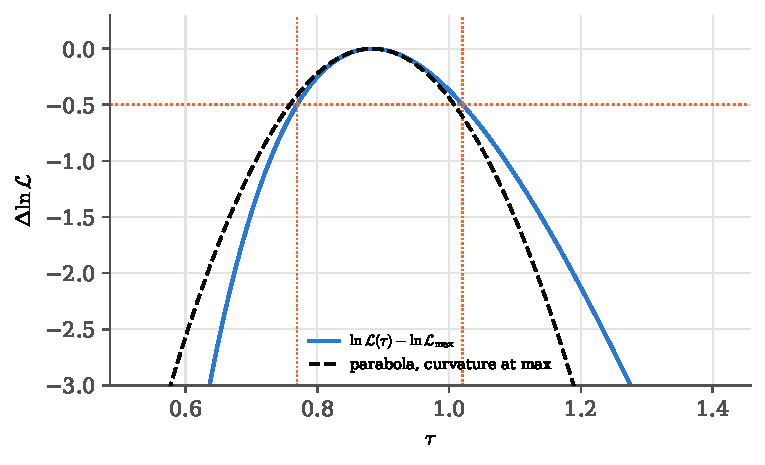
\includegraphics[width=9cm]{figures/ch03/mle_decay_lnL.pdf}
\caption{The log-likelihood of one experiment with fifty decays (solid)
and the parabola with the same curvature at the peak (dashed). The dotted
horizontal line is $\ln\Like_{\max}-\tfrac12$; its crossings with the curve
(dotted verticals) give the asymmetric interval. The curve drops faster than
the parabola on the left and slower on the right.}
\label{3b:fig:mle-lnL}
\end{figure}

Then the script does what no experimenter can: it repeats the experiment
$10^4$ times and looks at the scatter.
\pyfile[firstline=55,lastline=65]{code/ch03/09_mle_decay.py}{Ten thousand experiments: scatter and coverage}
The numbers are
\begin{center}
\small
\begin{tabular}{lc}
  \hline
  quantity & value\\
  \hline
  mean of $\hat\tau$ over $10^4$ experiments & $\ThreeBDecMeanTau$\\
  true scatter of $\hat\tau$ (Monte Carlo) & $\ThreeBDecSdMC$\\
  $1/\sqrt{I_n(\tau)}=\tau/\sqrt n$ & $\ThreeBDecSdTh$\\
  average curvature error $\hat\tau/\sqrt n$ & $\ThreeBDecMeanCurv$\\
  coverage of $\hat\tau\pm\hat\tau/\sqrt n$ & $\ThreeBDecCoverCurv$\\
  coverage of the $\Delta\ln\Like=\tfrac12$ interval & $\ThreeBDecCoverDl$\\
  \hline
\end{tabular}
\end{center}
The scatter of the MLE over repetitions is the inverse square root of the
Fisher information, to within the Monte Carlo error (about $0.7\%$ for
$10^4$ experiments). The curvature error of an individual experiment
fluctuates with $\hat\tau$, as the right panel of \cref{3b:fig:mle-scatter}
shows, but it is correct on average. Both intervals cover the true value in
about $68\%$ of the experiments, the fraction a $\pm1\sigma$ Gaussian
interval should cover ($0.683$). At $n=50$ the asymptotic theory is
already good. The left panel shows that the exact sampling distribution of
$\hat\tau$, a Gamma distribution with shape $n$ (the sum of $n$
exponentials, \cref{ch:02}), is slightly skewed compared with the Gaussian
of \eqref{3b:eq:asymptotic}; the skewness shrinks like $1/\sqrt n$.

\begin{figure}[htbp]
\centering
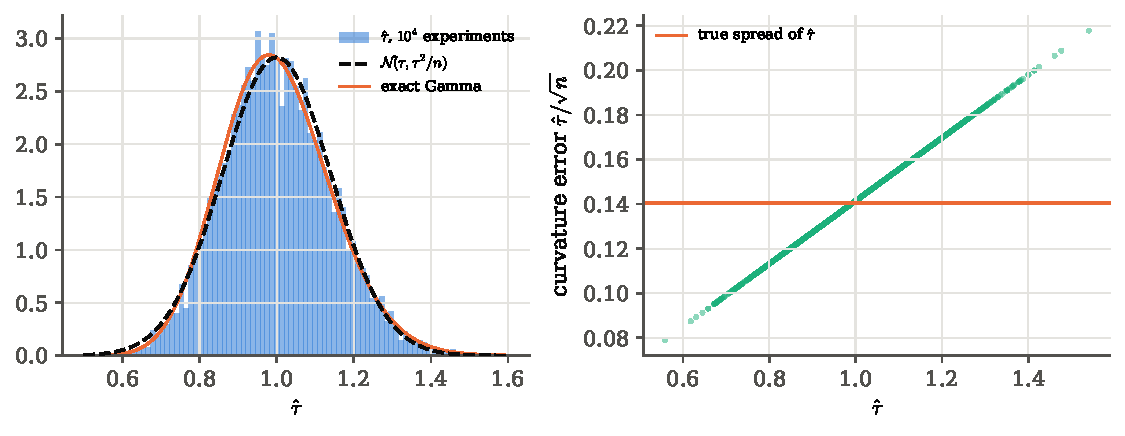
\includegraphics[width=12cm]{figures/ch03/mle_decay_scatter.pdf}
\caption{Ten thousand repetitions of the fifty-decay experiment. Left: the
histogram of the maximum likelihood lifetimes, the Gaussian predicted by the
Fisher information (dashed) and the exact Gamma distribution (solid). Right:
each experiment's curvature error plotted against its estimate. The error
grows with $\hat\tau$, because it is $\hat\tau/\sqrt n$, and it scatters
around the true spread of the estimates (horizontal line).}
\label{3b:fig:mle-scatter}
\end{figure}
\section{What makes maximum likelihood good}
\label{3b:sec:properties}

We now have many ways to turn data into a number: the mean, the median,
the method of moments, least squares, maximum likelihood. Why is maximum
likelihood the default of experimental physics? Not because it is always
unbiased. The Gaussian width $\hat\sigma^2$ is not (\cref{3b:sec:mle-hand}),
and the decay rate $1/\hat\tau$ is not either (\cref{3b:sec:invariance}).
The reason is a set of large-sample properties
\mainref{p.~125}. For a regular model (smooth in $\theta$, with a support
that does not move with $\theta$, and a true value inside the parameter
space) the MLE is
\begin{enumerate}[label=\arabic*.]
  \item \emph{consistent}: it converges to the true value;
  \item \emph{equivariant}: the MLE of $g(\theta)$ is $g(\hat\theta)$;
  \item \emph{asymptotically Gaussian}, with variance $1/I_n(\theta)$
        (\cref{3b:sec:fisher-info});
  \item \emph{asymptotically efficient}: no unbiased estimator has a
        smaller variance than $1/I_n$, so for large $n$ nothing beats it;
  \item \emph{approximately Bayesian}: for large $n$ the posterior with any
        smooth prior peaks near $\hat\theta$ with width $1/\sqrt{I_n}$
        (\cref{ch:05}).
\end{enumerate}
The third is \eqref{3b:eq:asymptotic}. Each of the first, second and fourth
has a short reason, each can be seen working on simulated data, and each
fails when one of the regularity conditions fails.

\subsection{Consistency: the log-likelihood peaks at the truth}
\label{3b:sec:consistency}

Why should the peak of the likelihood of one finite data set sit near the
true value $\theta_\star$? The answer is that, as $n$ grows, the
log-likelihood per observation settles down to a fixed curve, and that
curve peaks at $\theta_\star$. To see it, compare each $\theta$ with the
truth through the average log-likelihood ratio
\[
  M_n(\theta)=\frac1n\sum_{i=1}^n\ln\frac{f(x_i;\theta)}{f(x_i;\theta_\star)} .
\]
It differs from $\ell(\theta)/n$ only by a term that does not depend on
$\theta$, so it peaks at $\hat\theta$. It is an average of $n$ independent
terms, so by the law of large numbers it approaches its expectation,
\begin{align}
  M_n(\theta)\;\to\;\E_{\theta_\star}\!\Bigl[\ln\frac{f(X;\theta)}{f(X;\theta_\star)}\Bigr]
  &\eqby{1}-\int f(x;\theta_\star)\ln\frac{f(x;\theta_\star)}{f(x;\theta)}\,\dd x
  \equiv-D(\theta_\star,\theta),
  \label{3b:eq:kl}
\end{align}
\begin{explain}
  \item Write the expectation as an integral over the true density and flip
        the ratio inside the logarithm, which flips the sign.
\end{explain}
where $D(f,g)=\int f\ln(f/g)$ is the \newterm{Kullback--Leibler divergence}
\unpack{how badly the density $g$ describes data that really come from $f$,
in units of log-probability per observation} \mainref{p.~126}. It is never
negative, and it vanishes only when the two densities are equal:
\begin{align*}
  -D(f,g)
  &\eqby{1}\E_f\Bigl[\ln\frac{g(X)}{f(X)}\Bigr]
  \relby{2}{\le}\ln\E_f\Bigl[\frac{g(X)}{f(X)}\Bigr]
  \eqby{3}\ln\int f(x)\frac{g(x)}{f(x)}\,\dd x
  \eqby{4}\ln 1=0 .
\end{align*}
\begin{explain}
  \item Definition of $D$ with the ratio inverted.
  \item Jensen's inequality: $\ln$ is concave, so the average of the
        logarithm is at most the logarithm of the average, with equality only
        if $g/f$ is constant.
  \item Expectation over $f$.
  \item $g$ is a density and integrates to one. A constant ratio $g/f$
        must therefore equal one.
\end{explain}
Physicists know this as the Gibbs inequality of statistical mechanics:
relative entropy is non-negative. So the limit of $M_n$ is a function with a
unique maximum, equal to zero, at $\theta=\theta_\star$, provided different
parameter values give different densities (the model is
\newterm{identifiable}). The $M_n$ curves converge to that function, and
their peaks, which are the MLEs, converge to its peak. That is Wasserman's
consistency theorem \mainref{p.~127, Thm.~9.13}; the proof needs the
convergence to hold uniformly in $\theta$, which is where regularity
conditions enter.

\paragraph{Example: the lifetime.}
For exponential decays,
\begin{align*}
  D(\tau_\star,\tau)
  &\eqby{1}\E_{\tau_\star}\Bigl[\ln\frac{\tau_\star^{-1}e^{-t/\tau_\star}}{\tau^{-1}e^{-t/\tau}}\Bigr]
  \eqby{2}\ln\frac{\tau}{\tau_\star}+\E_{\tau_\star}[t]\Bigl(\frac1\tau-\frac1{\tau_\star}\Bigr)
  \eqby{3}\ln\frac{\tau}{\tau_\star}+\frac{\tau_\star}{\tau}-1 .
\end{align*}
\begin{explain}
  \item Definition \eqref{3b:eq:kl} with the exponential density.
  \item $\ln$ of the ratio is $\ln(\tau/\tau_\star)-t/\tau_\star+t/\tau$;
        take the expectation term by term.
  \item $\E_{\tau_\star}t=\tau_\star$.
\end{explain}
This is the same function $\ln u+1/u-1$ that appeared in the exact
$\Delta\ln\Like$ interval, now with $u=\tau/\tau_\star$: the expected shape
of the log-likelihood, per event, is minus the Kullback--Leibler divergence.
The script \pyname{13_efficiency.py} draws $M_n(\tau)$ for one data set each
of $n=10$, $100$ and $1000$ decays (\cref{3b:fig:consistency}). Their peaks,
the MLEs, are at $\ThreeBConsTen$, $\ThreeBConsHund$ and $\ThreeBConsThou$,
and the curves close in on $-D(\tau_\star,\tau)$ as $n$ grows.

\begin{figure}[htbp]
\centering
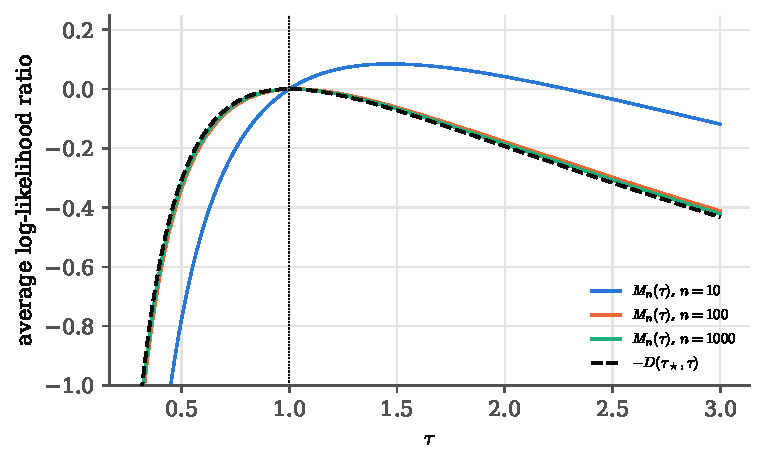
\includegraphics[width=9cm]{figures/ch03/consistency_kl.pdf}
\caption{Why the MLE is consistent. The average log-likelihood ratio
$M_n(\tau)$ of one simulated data set, for $10$, $100$ and $1000$ decays,
approaches minus the Kullback--Leibler divergence (dashed), which has its
maximum, zero, exactly at the true lifetime (dotted). The peak of each
$M_n$ is that data set's MLE, and it is dragged towards the truth as the
curves converge.}
\label{3b:fig:consistency}
\end{figure}

The same argument says what happens when the model is wrong. If the data
come from a density $g$ that is not in the family $f(x;\theta)$, $M_n$ still
converges, now to $-D(g,f(\cdot;\theta))$ plus a constant, and the MLE
converges to the parameter whose density is closest to the truth in the
Kullback--Leibler sense. The fit converges, but to the best wrong answer.

\subsection{Invariance: the MLE does not care what we call the parameter}
\label{3b:sec:invariance}

If $\eta=g(\theta)$ is a one-to-one reparametrisation, the likelihood in
terms of $\eta$ is $\Like^*(\eta)=\Like(g^{-1}(\eta))$: the same numbers
attached to the same hypotheses (\cref{3b:sec:not-density}). Its maximum is
therefore at the $\eta$ that corresponds to $\hat\theta$,
\[
  \hat\eta=g(\hat\theta)
\]
\mainref{p.~127, Thm.~9.14}, \srcref{CasellaBerger}{Thm.~7.2.10}. For a $g$
that is not one-to-one (say $\eta=\theta^2$), Casella and Berger define the
likelihood of $\eta$ as the largest $\Like(\theta)$ over all $\theta$ with
$g(\theta)=\eta$, and the statement still holds. The MLE of the decay rate
is $1/\hat\tau$, the MLE of $\sigma$ is $\sqrt{\hat\sigma^2}$, and the MLE
of the Hubble time is $1/\hat H_0$.

Unbiasedness does not survive such a change. Take $\hat\lambda=1/\hat\tau=n/T$
with $T=\sum_it_i$, a sum of $n$ exponentials, which has the Gamma density
$T^{n-1}e^{-T/\tau}/[\Gamma(n)\tau^n]$ (\cref{ch:02}). Then
\begin{align*}
  \E\Bigl[\frac1T\Bigr]
  &\eqby{1}\int_0^\infty\frac1T\,\frac{T^{n-1}e^{-T/\tau}}{\Gamma(n)\tau^n}\,\dd T
  \eqby{2}\frac{\Gamma(n-1)\,\tau^{n-1}}{\Gamma(n)\,\tau^n}
  \eqby{3}\frac{1}{(n-1)\tau},
  \qquad
  \E\hat\lambda=\frac{n}{n-1}\,\lambda .
\end{align*}
\begin{explain}
  \item Expectation of $1/T$ over the Gamma density.
  \item The remaining integrand is an unnormalised Gamma density of shape
        $n-1$, and
        $\int_0^\infty T^{n-2}e^{-T/\tau}\dd T=\Gamma(n-1)\,\tau^{n-1}$.
  \item $\Gamma(n)=(n-1)\Gamma(n-1)$.
\end{explain}
For $n=50$ the bias factor is $50/49=\ThreeBDecLamTh$; the $10^4$
experiments of \pyname{09_mle_decay.py} give $\E\hat\lambda=\ThreeBDecLamMean$.
Since $\hat\tau$ is exactly unbiased, $\hat\lambda$ cannot be. A nonlinear
function of an unbiased estimator is biased, by Jensen's inequality, just
as the sample standard deviation $S$ is biased for $\sigma$ even though
$S^2$ is unbiased for $\sigma^2$ (\cref{3a:sec:n-minus-one}). So an
estimator can be unbiased in one parametrisation only. Maximum likelihood
gives up unbiasedness and gains consistency in every parametrisation at
once.

The error bar of $\hat\eta=g(\hat\theta)$ follows from the delta method
(\cref{3a:sec:delta}), now applied to the MLE \mainref{p.~131, Thm.~9.24}:
$\widehat{\mathrm{se}}(\hat\eta)\approx|g'(\hat\theta)|\,\widehat{\mathrm{se}}(\hat\theta)$.
For $\lambda=1/\tau$, $|g'|=1/\tau^2$ and
$\widehat{\mathrm{se}}(\hat\lambda)=\hat\tau^{-2}\cdot\hat\tau/\sqrt n=\hat\lambda/\sqrt n$,
the same relative error, as it must be to first order. With several
parameters the gradient replaces the derivative,
$\widehat{\mathrm{se}}^2(\hat\eta)\approx\nabla g\T\,\widehat{\Cov}(\hat\params)\,\nabla g$,
with the covariance from the inverse Fisher matrix
\mainref{p.~134, Thm.~9.28}. For example, take the coefficient of variation
$\eta=\sigma/\mu$ of Gaussian data. One observation has
$\ln f=-\ln\sigma-(x-\mu)^2/2\sigma^2+\text{const}$. Its second derivatives
are $\partial^2_\mu\ln f=-1/\sigma^2$, $\partial_\mu\partial_\sigma\ln
f=-2(x-\mu)/\sigma^3$ and $\partial^2_\sigma\ln f=1/\sigma^2-3(x-\mu)^2/\sigma^4$.
Averaging with $\E(x-\mu)=0$ and $\E(x-\mu)^2=\sigma^2$ and multiplying by
$-n$ gives a diagonal Fisher matrix with entries $n/\sigma^2$ and
$2n/\sigma^2$, so $\Var\hat\mu\approx\sigma^2/n$ and
$\Var\hat\sigma\approx\sigma^2/2n$. The gradient of $\eta$ is
$(\partial_\mu\eta,\partial_\sigma\eta)=(-\sigma/\mu^2,\,1/\mu)$. Then
$\widehat{\mathrm{se}}^2(\hat\eta)=\frac{\hat\sigma^2}{\hat\mu^4}\frac{\hat\sigma^2}{n}
+\frac{1}{\hat\mu^2}\frac{\hat\sigma^2}{2n}
=\hat\sigma^2/(n\hat\mu^2)\,[\hat\sigma^2/\hat\mu^2+\tfrac12]$
\mainref{p.~134, Ex.~9.29}.

\subsection{The Cram\'er--Rao bound: nobody can beat the information}
\label{3b:sec:cramer-rao}

The MLE has asymptotic variance $1/I_n(\theta)$. Could a cleverer
estimator do better? The \newterm{Cram\'er--Rao inequality} (also called
the Rao--Cram\'er--Fr\'echet bound) says no, for any unbiased estimator,
at any sample size \srcref{CasellaBerger}{Thm.~7.3.9}, \srcref{Cowan}{\S6.6}.
The proof is a single use of the Cauchy--Schwarz inequality for
covariances, $\Cov(A,B)^2\le\Var A\,\Var B$, applied to the estimator and
the score.

Let $T(\data)$ be any estimator with mean $m(\theta)=\E_\theta T$, and
$S(\theta)=\partial_\theta\ln p(\data\given\theta)$ the score of the whole
data set. Then
\begin{align}
  \Cov_\theta(T,S)
  &\eqby{1}\E_\theta[T\,S]
  \eqby{2}\int T(\data)\,\frac{\partial_\theta p(\data\given\theta)}{p(\data\given\theta)}\,p(\data\given\theta)\,\dd\data
  \eqby{3}\frac{\partial}{\partial\theta}\int T(\data)\,p(\data\given\theta)\,\dd\data
  \eqby{4}m'(\theta),
  \nonumber\\
  m'(\theta)^2
  &\relby{5}{\le}\Var_\theta T\cdot\Var_\theta S
  \eqby{6}\Var_\theta T\cdot I_n(\theta)
  \quad\Longrightarrow\quad
  \Var_\theta T\;\ge\;\frac{m'(\theta)^2}{I_n(\theta)} .
  \label{3b:eq:cramer-rao}
\end{align}
\begin{explain}
  \item $\Cov(T,S)=\E[TS]-\E T\,\E S$, and $\E S=0$ by \eqref{3b:eq:score-mean}.
  \item Write out the expectation; $S=\partial_\theta p/p$.
  \item Cancel $p$ and move the derivative outside. $T$ depends on the data
        only, not on $\theta$. This exchange is the regularity condition.
  \item The integral is the definition of $m(\theta)$.
  \item Cauchy--Schwarz for covariances, with step (4) on the left.
  \item $\Var S=I_n$, \eqref{3b:eq:fisher-identity}.
\end{explain}
For an unbiased estimator $m(\theta)=\theta$ and $m'=1$, so that
$\Var T\ge1/I_n(\theta)$, which for independent, identically distributed
data is $1/[nI(\theta)]$ \srcref{CasellaBerger}{Cor.~7.3.10}.
If $T$ has a bias $b(\theta)$, then $m=\theta+b$ and the bound is
$(1+b')^2/I_n$, Cowan's form of the inequality.

\begin{keyidea}[Cram\'er--Rao]
For a regular model, every unbiased estimator satisfies
\[
  \Var_\theta\hat\theta\;\ge\;\frac{1}{I_n(\theta)}=\frac{1}{nI(\theta)} .
\]
The Fisher information is the best precision the data can possibly give.
The MLE reaches the bound as $n\to\infty$; it is
\newterm{asymptotically efficient}. For several parameters,
$\Cov\hat\params-\Fish^{-1}$ is positive semidefinite, where $\Fish$ is the
Fisher matrix (\cref{ch:10}).
\end{keyidea}

\paragraph{When is the bound reached exactly?}
Cauchy--Schwarz is an equality only when the two variables are linearly
related. The bound is attained by an unbiased $T$ exactly when
$S(\theta)=a(\theta)\,[T(\data)-\theta]$ for some function $a$
\srcref{CasellaBerger}{Cor.~7.3.15}. This happens for the exponential
families of distributions \mainref{p.~141}. The lifetime is an example: its
score, $-n/\tau+T/\tau^2=(n/\tau^2)(\bar t-\tau)$, has exactly this form,
so $\bar t$ attains the bound $\tau^2/n$ at every $n$, not only
asymptotically. So does $\bar x$ for a Gaussian mean. For the Gaussian
variance with unknown mean the bound is $2\sigma^4/n$, while the best
unbiased estimator, $S^2$, has variance $2\sigma^4/(n-1)$: close, but the
bound is not attained \srcref{CasellaBerger}{Ex.~7.3.14}.

\paragraph{When the bound does not apply: the uniform box again.}
For $\mathrm{Uniform}(0,\theta)$, a blind application of the recipe gives
$\partial_\theta\ln(1/\theta)=-1/\theta$, ``information'' $1/\theta^2$ per
point, and a ``bound'' $\theta^2/n$. But the unbiased estimator
$\tfrac{n+1}{n}x_{(n)}$ does far better. Since
$\Prob(x_{(n)}\le y)=(y/\theta)^n$, the scaled maximum $y=x_{(n)}/\theta$
has density $ny^{n-1}$ on $[0,1]$, and
\begin{align*}
  \E y&\eqby{1}\frac{n}{n+1},\qquad
  \E y^2\eqby{2}\frac{n}{n+2},\\
  \Var\Bigl[\frac{n+1}{n}x_{(n)}\Bigr]
  &\eqby{3}\frac{(n+1)^2}{n^2}\,\theta^2\Bigl[\frac{n}{n+2}-\frac{n^2}{(n+1)^2}\Bigr]
  \eqby{4}\frac{\theta^2}{n(n+2)} .
\end{align*}
\begin{explain}
  \item $\int_0^1y\cdot ny^{n-1}\dd y=n/(n+1)$.
  \item $\int_0^1y^2\cdot ny^{n-1}\dd y=n/(n+2)$.
  \item $\Var(cX)=c^2\Var X$ with $x_{(n)}=\theta y$, and
        $\Var y=\E y^2-(\E y)^2$.
  \item Common denominator:
        $n(n+1)^2-n^2(n+2)=n$, so the bracket is $n/[(n+1)^2(n+2)]$.
\end{explain}
The variance falls like $1/n^2$, not $1/n$. The simulation in
\pyname{13_efficiency.py} gives $n\Var/\theta^2=\ThreeBEffUnifFifty$ at
$n=\ThreeBEffNFifty$, against the exact $1/(n+2)=\ThreeBEffUnifFiftyTh$ and
the ``bound'' $1$. There is no contradiction. Step (3) of
\eqref{3b:eq:cramer-rao} moved a derivative through an integral. Here the
upper limit of that integral is $\theta$ itself, so differentiating it
produces an extra boundary term and the exchange is not allowed. Indeed the
``score'' $-n/\theta$ does not have mean zero: it is not random at all
\srcref{CasellaBerger}{Ex.~7.3.13}. The lesson is that a sharp edge in the
data is worth more than any smooth feature, because a single point near the
edge pins it down. Physicists use this all the time: the endpoint of a
beta spectrum or of a kinematic distribution measures a mass far more
sharply than the bulk of the distribution does.

\subsection{Efficiency in practice: the mean against the median}
\label{3b:sec:efficiency}

The ratio of the variances of two consistent estimators, at large $n$, is
their \newterm{asymptotic relative efficiency}
\mainref{p.~131, Thm.~9.23}. For Gaussian data the mean is the MLE of the
centre and attains the bound $\sigma^2/n$. The sample median also estimates
the centre, and it is popular because a single wild point cannot move it
much. How much precision does it cost?

The asymptotic variance of the median follows from a counting argument. Let
$m$ be the true median and $f(m)$ the density there. The sample median lies
below $m+\delta$ exactly when at least half the points do. The number of
points below $m+\delta$ is binomial with $n$ trials and success probability
$F(m+\delta)\approx\tfrac12+f(m)\delta$, so
\begin{align*}
  \Prob(\hat m\le m+\delta)
  &\eqby{1}\Prob\Bigl(\mathrm{Bin}\bigl(n,\tfrac12+f\delta\bigr)\ge\tfrac n2\Bigr)
  \eqby{2}\Prob\Bigl(Z\ge\frac{n/2-n/2-nf\delta}{\sqrt n/2}\Bigr)
  \eqby{3}\Phi\bigl(2\sqrt n\,f(m)\,\delta\bigr),\\
  \Var\hat m&\eqby{4}\frac{1}{4nf(m)^2}
  \eqby{5}\frac{\pi\sigma^2}{2n}\quad\text{(Gaussian data)}.
\end{align*}
\begin{explain}
  \item The median is below $m+\delta$ if at least $n/2$ points are.
        Near $m$, $F(m+\delta)\approx F(m)+f(m)\delta$ with $F(m)=\tfrac12$.
  \item Gaussian approximation of the binomial (\cref{ch:02}): mean
        $n(\tfrac12+f\delta)$, variance $\approx n/4$ for small $\delta$.
  \item $\Prob(Z\ge-a)=\Phi(a)$ for a standard Gaussian $Z$.
  \item Step (3) says $\hat m-m$ is Gaussian with standard deviation
        $1/(2\sqrt nf)$.
  \item For $\Normal(\mu,\sigma^2)$, $f(m)=1/(\sqrt{2\pi}\sigma)$ and
        $1/(4f^2)=2\pi\sigma^2/4$.
\end{explain}
The median's relative efficiency is $(\sigma^2/n)/(\pi\sigma^2/2n)=2/\pi=0.64$:
using the median on Gaussian data is like throwing away $36\%$ of the
events \mainref{p.~131}. The simulation, $60\,000$ data sets at each of
several $n$, confirms it (\cref{3b:fig:efficiency}): at $n=\ThreeBEffNBig$,
$n\Var$ is $\ThreeBEffMeanBig\,\sigma^2$ for the mean and
$\ThreeBEffMedBig\,\sigma^2$ for the median ($\pi/2=1.571$), an efficiency of
$\ThreeBEffARE$ against $2/\pi=\ThreeBEffAREth$.

\begin{figure}[htbp]
\centering
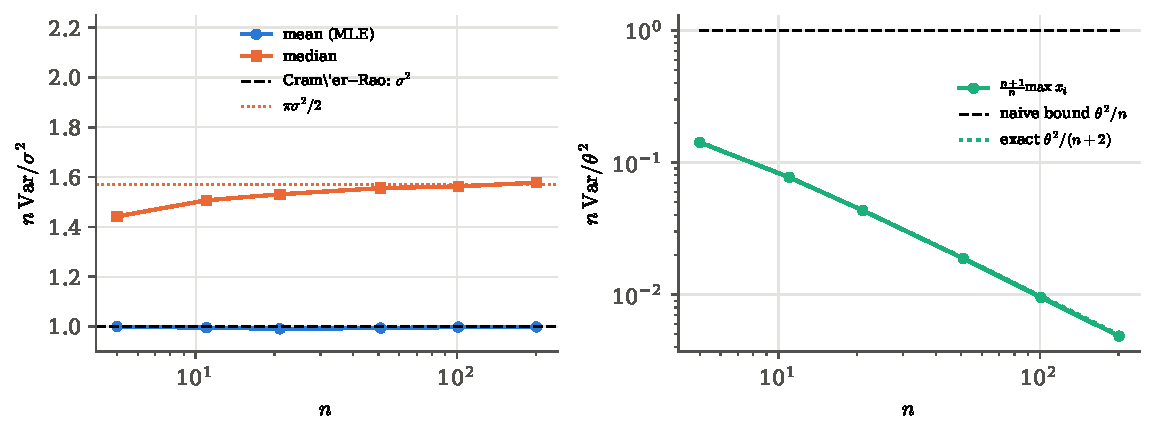
\includegraphics[width=12cm]{figures/ch03/efficiency.pdf}
\caption{Efficiency, simulated. Left: $n$ times the variance of the mean
(the MLE) and of the median for Gaussian data. The mean sits on the
Cram\'er--Rao bound at every $n$; the median approaches $\pi\sigma^2/2$
(dotted). Right: for the uniform box the estimator $\frac{n+1}{n}\max x_i$
falls far below the naive ``bound'' $\theta^2/n$ (dashed) and follows the
exact $\theta^2/(n+2)$ (dotted), because the regularity conditions fail.}
\label{3b:fig:efficiency}
\end{figure}

The lost precision buys robustness. For the Cauchy distribution, whose
tails are so heavy that the sample mean does not converge at all, the
median is consistent, with variance $\pi^2\gamma^2/(4n)$ for half-width
$\gamma$ (the same formula with $f(m)=1/(\pi\gamma)$). The MLE is optimal
only \emph{within the model}. When the real data have heavier tails than the
model allows, an estimator that is slightly inefficient under the model but
robust to outliers can be far better in practice.

\begin{pitfall}[The fine print of ``the MLE is optimal'']
Every property above is asymptotic and assumes a regular model
with the true value inside the parameter space. At small $n$ the MLE can be
biased ($\hat\sigma^2$, $\hat\lambda$). At a boundary (a signal strength
fitted to zero) the sampling distribution is not Gaussian. With a moving
support (the uniform box) the Cram\'er--Rao bound does not apply. When the
number of nuisance parameters grows with the data (one unknown mean per
pair of measurements, say), the MLE of the common parameter need not even be
consistent. Check with a simulation whenever any of these apply.
\end{pitfall}
\section{Nuisance parameters and the profile likelihood}
\label{3b:sec:profile}

Almost no real likelihood has only the parameters we care about. A search
for a new particle wants the signal rate, but the background rate is also
unknown. A cosmological fit wants $\Omega_m$ and $\sigma_8$, but the galaxy
bias, the calibration of the telescope and the amplitude of a foreground
come along. These are \newterm{nuisance parameters}
\unpack{parameters that the likelihood depends on and the data constrain,
but whose values we do not want to report} \mainref{p.~120}. They cannot
be ignored. Fixing them at a guessed value pretends we know them, and that
makes the error on the interesting parameter too small. Three questions
need answers.
\begin{enumerate}[label=\arabic*.]
  \item How do we reduce a likelihood of several parameters to a function
        of the one we care about, without pretending the others are known?
  \item Why does the honest answer have a wider interval, and by how much?
  \item How does this compare with the Bayesian way of removing a nuisance
        parameter, by integrating it out?
\end{enumerate}

\subsection{A signal on top of a background}
\label{3b:sec:on-off}

A standard counting experiment has two regions. In the \emph{signal
region} we count $n_{\text{on}}$ events, expected to be $s+b$: signal plus
background. In a \emph{control region}, chosen so that it contains no
signal, we count $n_{\text{off}}$ events, expected to be $kb$, where the
known factor $k$ is the ratio of exposures (here $k=1$). Both counts are
Poisson, and they are independent:
\[
  \ell(s,b)=n_{\text{on}}\ln(s+b)-(s+b)+n_{\text{off}}\ln(kb)-kb .
\]
The global maximum is easy. Setting the derivatives with respect to $s$
and to $b$ to zero gives the two score equations
$n_{\text{on}}/(s+b)=1$ and $n_{\text{on}}/(s+b)-1+n_{\text{off}}/b-k=0$.
By the first, the first two terms of the second cancel, which leaves
$n_{\text{off}}/b=k$. So $\hat b=n_{\text{off}}/k$, and then the first gives
$\hat s=n_{\text{on}}-n_{\text{off}}/k$. With
$n_{\text{on}}=\ThreeBProfNon$ and $n_{\text{off}}=\ThreeBProfNoff$,
$\hat s=\ThreeBProfS$ and $\hat b=\ThreeBProfB$. The question is the error
on $\hat s$.

\paragraph{Two ways to get a one-dimensional likelihood.}
To get the error on $\hat s$ we need a likelihood of $s$ alone, and there
are two ways to remove $b$. The lazy way is to fix $b$ at its best value
$\hat b$ and look at $\ell(s,\hat b)$, the \newterm{conditional}
likelihood. It pretends that the control region measured $b$ perfectly. The
honest way is to let $b$ adjust: for each trial value of $s$, find the
background that makes the data most probable, and use that.

\begin{workdef}[profile likelihood]
For parameters $(\theta,\bm\nu)$, with $\theta$ of interest and $\bm\nu$
nuisance, the \newterm{profile likelihood} is
\[
  \Like_p(\theta)=\max_{\bm\nu}\Like(\theta,\bm\nu)
  =\Like\bigl(\theta,\hat{\hat{\bm\nu}}(\theta)\bigr),
\]
where $\hat{\hat{\bm\nu}}(\theta)$ is the best value of the nuisance
parameters at fixed $\theta$ \unpack{the ridge line of the likelihood, one
point for every $\theta$}. \emph{Operationally:} on a grid of $\theta$,
maximise over everything else, record the maximum; then treat $\Like_p$ like
a one-parameter likelihood, with its maximum at the global $\hat\theta$.
\end{workdef}

For the on/off problem the inner maximisation can be done by hand. At fixed
$s$,
\begin{align*}
  0&\eqby{1}\frac{n_{\text{on}}}{s+b}-1+\frac{n_{\text{off}}}{b}-k\\
   &\eqby{2}\Rightarrow\ n_{\text{on}}\,b-b(s+b)+n_{\text{off}}(s+b)-kb(s+b)=0\\
   &\eqby{3}\Rightarrow\ (1+k)\,b^2+\bigl[(1+k)s-n_{\text{on}}-n_{\text{off}}\bigr]\,b-n_{\text{off}}\,s=0,
\end{align*}
\begin{explain}
  \item $\partial\ell/\partial b$ at fixed $s$.
  \item Multiply by $b(s+b)>0$.
  \item Collect powers of $b$ and multiply by $-1$.
\end{explain}
and $\hat{\hat b}(s)$ is the positive root of this quadratic (the constant
term is negative for $s>0$, so there is exactly one). As $s$ increases, the
best background decreases: more of the $n_{\text{on}}$ events are already
explained by signal. That anticorrelation is what the conditional likelihood
ignores.

\subsection{Why profiling widens the interval}
\label{3b:sec:profile-width}

Near the maximum every smooth log-likelihood is quadratic, so it is enough
to understand the Gaussian case. Take one parameter of interest $\theta$
and one nuisance parameter $\nu$. Write $\bm x=(\theta-\hat\theta,\nu-\hat\nu)$
and $\ell=\ell_{\max}-\tfrac12\bm x\T\Fish\bm x$ with the information matrix
$\Fish=\begin{pmatrix}F_{\theta\theta}&F_{\theta\nu}\\F_{\theta\nu}&F_{\nu\nu}\end{pmatrix}$,
whose inverse $V=\Fish^{-1}$ is the covariance matrix. Maximise over the
nuisance direction:
\begin{align}
  \ell-\ell_{\max}
  &\eqby{1}-\tfrac12\bigl[F_{\theta\theta}x_\theta^2+2F_{\theta\nu}x_\theta x_\nu+F_{\nu\nu}x_\nu^2\bigr],
  \nonumber\\
  \frac{\partial\ell}{\partial x_\nu}=0
  &\eqby{2}\Rightarrow\ x_\nu=-\frac{F_{\theta\nu}}{F_{\nu\nu}}\,x_\theta ,
  \nonumber\\
  \ell_p-\ell_{\max}
  &\eqby{3}-\tfrac12\Bigl(F_{\theta\theta}-\frac{F_{\theta\nu}^2}{F_{\nu\nu}}\Bigr)x_\theta^2
  \eqby{4}-\frac{x_\theta^2}{2V_{\theta\theta}} .
  \label{3b:eq:profile-gauss}
\end{align}
\begin{explain}
  \item Write out the quadratic form.
  \item Derivative in $x_\nu$: $-(F_{\theta\nu}x_\theta+F_{\nu\nu}x_\nu)=0$.
        This is the profile path, a straight line through the maximum.
  \item Substitute:
        $2F_{\theta\nu}x_\theta x_\nu+F_{\nu\nu}x_\nu^2=-F_{\theta\nu}^2x_\theta^2/F_{\nu\nu}$.
  \item The $(\theta,\theta)$ element of the inverse of a symmetric
        $2\times2$ matrix is
        $V_{\theta\theta}=F_{\nu\nu}/\det\Fish$, and
        $F_{\theta\theta}-F_{\theta\nu}^2/F_{\nu\nu}=\det\Fish/F_{\nu\nu}=1/V_{\theta\theta}$.
\end{explain}
The profile likelihood is a Gaussian of variance $V_{\theta\theta}$: the
full marginal variance of $\hat\theta$, including the uncertainty it
inherits from the nuisance parameter. The conditional likelihood at
$\nu=\hat\nu$ has curvature $F_{\theta\theta}$, hence variance
$1/F_{\theta\theta}$, and
\[
  \frac{1}{F_{\theta\theta}}=V_{\theta\theta}\,(1-\rho^2)\;\le\;V_{\theta\theta},
\]
where $\rho$ is the correlation coefficient of $\hat\theta$ and $\hat\nu$.
The identity follows from the same $2\times2$ inverse, whose entries are
$V_{\theta\theta}=F_{\nu\nu}/\det\Fish$, $V_{\nu\nu}=F_{\theta\theta}/\det\Fish$
and $V_{\theta\nu}=-F_{\theta\nu}/\det\Fish$:
\[
  \rho^2=\frac{V_{\theta\nu}^2}{V_{\theta\theta}V_{\nu\nu}}
        =\frac{F_{\theta\nu}^2}{F_{\theta\theta}F_{\nu\nu}},
  \qquad
  V_{\theta\theta}(1-\rho^2)
  =\frac{F_{\nu\nu}}{\det\Fish}\cdot\frac{F_{\theta\theta}F_{\nu\nu}-F_{\theta\nu}^2}{F_{\theta\theta}F_{\nu\nu}}
  =\frac{1}{F_{\theta\theta}} .
\]
So the conditional interval is too short by the factor $\sqrt{1-\rho^2}$.
The stronger the correlation, the more it understates the error.
\Cref{3b:fig:profile-geometry} shows the geometry.

\begin{figure}[htbp]
\centering
\begin{tikzpicture}[scale=2.0]
  \draw[->,faint] (-1.45,0) -- (1.55,0) node[right,font=\footnotesize,black] {$\theta-\hat\theta$};
  \draw[->,faint] (0,-1.25) -- (0,1.3) node[above,font=\footnotesize,black] {$\nu-\hat\nu$};
  \draw[form,smooth,samples=100,domain=0:360,variable=\t]
    plot ({cos(\t)},{0.6*cos(\t)+0.8*sin(\t)});
  \draw[fibre] (-1.35,-0.81) -- (1.35,0.81);
  \draw[tangentgreen,thick,dashed] (-1.35,0) -- (1.35,0);
  \draw[fibreorange,densely dotted] (1,-1.15) -- (1,1.15);
  \draw[fibreorange,densely dotted] (-1,-1.15) -- (-1,1.15);
  \fill[fibreorange] (1,0.6) circle (1.2pt);
  \fill[fibreorange] (-1,-0.6) circle (1.2pt);
  \fill[tangentgreen] (0.8,0) circle (1.2pt);
  \fill[tangentgreen] (-0.8,0) circle (1.2pt);
  \fill (0,0) circle (1pt);
  \draw[fibreorange,thick,|-|] (-1,-1.45) -- (1,-1.45);
  \node[font=\footnotesize,anchor=west,fibreorange] at (1.05,-1.45) {profile: $\pm\sqrt{V_{\theta\theta}}$};
  \draw[tangentgreen,thick,|-|] (-0.8,-1.65) -- (0.8,-1.65);
  \node[font=\footnotesize,anchor=west,tangentgreen!70!black] at (1.05,-1.65) {conditional: $\pm\sqrt{1/F_{\theta\theta}}$};
  \node[font=\footnotesize,align=right,anchor=north east] at (-1.5,1.28)
    {\textcolor{formblue}{ellipse}: $\Delta\ln\Like=\tfrac12$\\
     \textcolor{fibreorange}{solid line}: profile path $\hat{\hat\nu}(\theta)$\\
     \textcolor{tangentgreen!70!black}{dashed line}: $\nu$ fixed at $\hat\nu$};
\end{tikzpicture}
\caption{Profile versus conditional likelihood for a Gaussian likelihood
with correlation $\rho=0.6$ between the parameter of interest and the
nuisance parameter. The profile path runs through the points where the
ellipse has vertical tangents, so the profile likelihood drops by
$\tfrac12$ at the full width of the ellipse (orange bar). Holding the
nuisance parameter fixed cuts the ellipse along the horizontal line and
gives an interval shorter by the factor $\sqrt{1-\rho^2}=0.8$ (green bar).}
\label{3b:fig:profile-geometry}
\end{figure}

\paragraph{Example: the on/off errors in the Gaussian limit.}
For large counts, $\hat s=n_{\text{on}}-n_{\text{off}}/k$ is a difference of
independent Poisson counts. A Poisson count has variance equal to its mean,
estimated by the count itself, so the variances are about $n_{\text{on}}$
and $n_{\text{off}}$. By linear error propagation
(\cref{3a:sec:linear-propagation}),
$\sigma_{\hat s}^2\approx n_{\text{on}}+n_{\text{off}}/k^2$. For
$(20,8)$ with $k=1$ that is $\sqrt{28}=\ThreeBProfGauss$. Fixing $b$ leaves
only the fluctuation of $n_{\text{on}}$, $\sqrt{20}=\ThreeBCondGauss$. The
profile likelihood reproduces the first number, the conditional
likelihood the second.

\subsection{The on/off problem in Python}
\label{3b:sec:profile-python}

\pyfile[firstline=34,lastline=51]{code/ch03/14_profile.py}{Profile and conditional intervals for the on/off problem}
The function \pyname{bhat_of_s} is the positive root of the quadratic for
$\hat{\hat b}(s)$ in \cref{3b:sec:on-off}. The functions \pyname{prof} and
\pyname{cond} are the two one-dimensional
log-likelihoods shifted so that their zeros are the $\Delta\ln\Like=\tfrac12$
crossings, which \pyname{brentq} finds on either side of $\hat s$. For
the observed counts the result is
\[
  \text{profile: } \hat s=\ThreeBProfS^{+\ThreeBProfHi}_{-\ThreeBProfLo},
  \qquad
  \text{conditional: } \hat s=\ThreeBProfS^{+\ThreeBCondHi}_{-\ThreeBCondLo}.
\]
The profile interval is about $20\%$ wider, as the Gaussian estimates
$\ThreeBProfGauss$ and $\ThreeBCondGauss$ said, and both are asymmetric
because the counts are small. \Cref{3b:fig:profile} shows the
two-dimensional contours, the profile path and the two curves.

\begin{figure}[htbp]
\centering
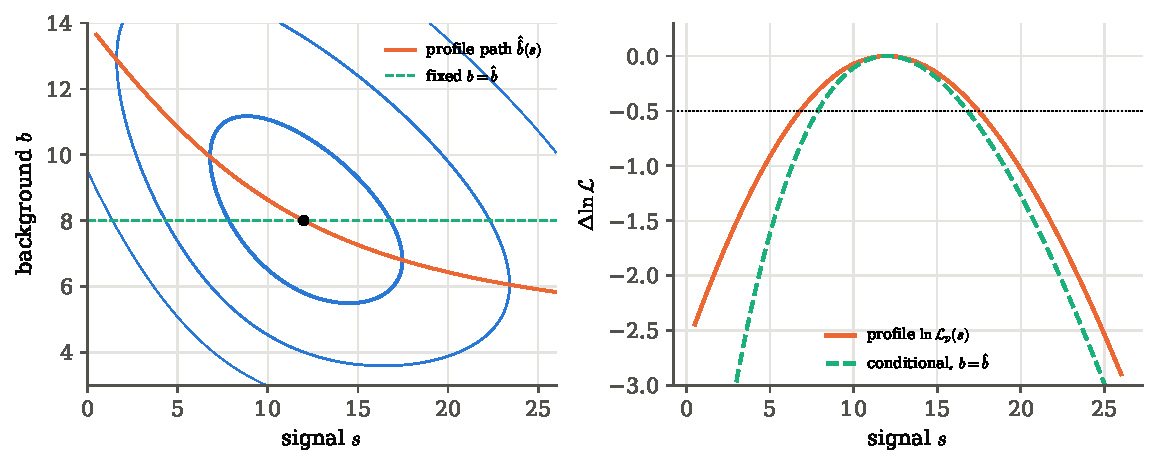
\includegraphics[width=12cm]{figures/ch03/profile.pdf}
\caption{A signal on top of a background, from $20$ counts in the signal
region and $8$ in the control region. Left: contours of $\ln\Like(s,b)$ at
$\Delta\ln\Like=\tfrac12$, $2$ and $4.5$, the profile path (the best
background for each signal value, falling as $s$ rises) and the line of
fixed background. Right: the profile log-likelihood is wider than the
conditional one; the dotted line at $-\tfrac12$ marks the interval
endpoints.}
\label{3b:fig:profile}
\end{figure}

Which interval is right? The script simulates $10^4$ experiments with
$s=12$ and $b=8$ and counts how often each interval contains the true
signal. (In $\ThreeBProfUsed$ of them both intervals exist; the rest have
$n_{\text{off}}=0$ or a similar degenerate outcome.) The profile interval
covers the truth in $\ThreeBProfCover$ of the experiments, the $68\%$ a
$\pm1\sigma$ interval promises. The conditional interval covers it in only
$\ThreeBCondCover$. The reason the profile works is \newterm{Wilks'
theorem} again \cite{Wilks1938}: $-2\ln[\Like_p(\theta)/\Like_{\max}]$ at the
true $\theta$ is asymptotically $\chi^2_1$, whatever the number of nuisance
parameters that were maximised over, so the $\Delta\ln\Like_p=\tfrac12$
interval has $68\%$ coverage for large samples. This is what the
\texttt{MINOS} errors of \texttt{MINUIT} compute, and it is the basis of the
profile-likelihood test statistics used in every LHC search (\cref{ch:04}).

\begin{keyidea}[Profile out nuisance parameters]
Maximise over the nuisance parameters at each value of the parameter of
interest, and read the interval from $\Delta\ln\Like_p=\tfrac12$. For a
Gaussian likelihood this gives exactly the marginal error
$\sqrt{V_{\theta\theta}}$; fixing the nuisance parameters instead gives
$\sqrt{1/F_{\theta\theta}}$, too small by $\sqrt{1-\rho^2}$.
\end{keyidea}

\subsection{Profiling and marginalising}
\label{3b:sec:marginalise}

The Bayesian removes a nuisance parameter differently: by integrating it
out of the posterior, $p(\theta\given\data)=\int p(\theta,\nu\given\data)\,\dd\nu$
\srcref{Padilla}{(38)}, \srcref{HobsonBMC}{p.~49}. This is the
marginalisation of a joint distribution that we have used since
\cref{ch:01}: average over the variable we do not want. For a Gaussian
likelihood and a flat prior the two operations give the same answer,
because the integral of a two-dimensional Gaussian over one variable is a
Gaussian in the other with variance $V_{\theta\theta}$, the same as
\eqref{3b:eq:profile-gauss}. They differ when the likelihood is not
Gaussian, and the difference is itself a warning that the asymptotic
theory is being stretched.

\paragraph{Example: an unknown noise level.}
Hobson et al.\ consider a fit where every datum has Gaussian noise of the
same, unknown size $\sigma$ \srcref{HobsonBMC}{p.~50, (2.25)--(2.26)}. With
$Q(\theta)=\sum_i(D_i-d_i(\theta))^2$ the likelihood is
$\Like(\theta,\sigma)=(2\pi\sigma^2)^{-N/2}\exp[-Q(\theta)/2\sigma^2]$.
Profile over $\sigma$:
\begin{align*}
  \frac{\partial\ell}{\partial\sigma}
  &\eqby{1}-\frac N\sigma+\frac{Q}{\sigma^3}=0
  \ \Rightarrow\ \hat{\hat\sigma}^2(\theta)=\frac{Q(\theta)}{N},
  \qquad
  \Like_p(\theta)\eqby{2}\Bigl(\frac{2\pi Q(\theta)}{N}\Bigr)^{-N/2}e^{-N/2}
  \;\propto\;Q(\theta)^{-N/2} .
\end{align*}
\begin{explain}
  \item Differentiate $-N\ln\sigma-Q/2\sigma^2$.
  \item Substitute: the exponent becomes $-Q/(2Q/N)=-N/2$.
\end{explain}
Now marginalise instead, with the prior $p(\sigma)\propto1/\sigma$ (flat
in $\ln\sigma$, the prior Hobson et al.\ use):
\begin{align*}
  \int_0^\infty\sigma^{-N}e^{-Q/2\sigma^2}\,\frac{\dd\sigma}{\sigma}
  &\eqby{1}\int_0^\infty\Bigl(\frac{2u}{Q}\Bigr)^{N/2}e^{-u}\,\frac{\dd u}{2u}
  \eqby{2}\frac12\Bigl(\frac2Q\Bigr)^{N/2}\Gamma\Bigl(\frac N2\Bigr)
  \;\propto\;Q(\theta)^{-N/2}.
\end{align*}
\begin{explain}
  \item Substitute $u=Q/2\sigma^2$, so $\sigma^{-2}=2u/Q$ and
        $\dd\sigma/\sigma=-\dd u/(2u)$ (the sign is absorbed by swapping the
        limits).
  \item $\int_0^\infty u^{N/2-1}e^{-u}\dd u=\Gamma(N/2)$.
\end{explain}
The two routes give the same function of $\theta$, which is Hobson's
(2.26) up to a constant. The unknown noise level turns the Gaussian
$e^{-\chi^2/2}$ into the heavier-tailed $Q^{-N/2}$, a Student-$t$ shape in
$\theta$ (\cref{ch:02}): not knowing the size of the error bars costs
precision, and the likelihood knows it. The same device, an unknown scale
factor on all quoted error bars, is Hobson's ``safety valve'' for data with
underestimated errors \srcref{HobsonBMC}{p.~52}.
\section{The bootstrap: the sampling distribution from one data set}
\label{3b:sec:bootstrap}

Every error bar so far came from a formula: $\sigma/\sqrt n$ for the mean,
the curvature of $\ln\Like$ for the MLE, the delta method for a function of
estimates. To check those formulas we also used a luxury no experimenter
has: we simulated $10^4$ fresh experiments from the true distribution and
looked at the scatter. Now suppose there is no formula (the median of
lifetimes, a ratio of two fitted amplitudes, the peak position of a
smoothed histogram) and no known truth to simulate from. All we have is one
data set. The \newterm{bootstrap} lets that one data set stand in for the
unknown distribution, and then simulates from it \cite{Efron1979}. Three
questions need answers.
\begin{enumerate}[label=\arabic*.]
  \item What does it mean to ``simulate from the data'', and why does it
        estimate the sampling distribution?
  \item How do we turn the simulated replicas into a standard error and a
        confidence interval?
  \item When does it fail?
\end{enumerate}

\subsection{Two worlds}
\label{3b:sec:boot-idea}

Let the data $x_1,\dots,x_n$ come independently from an unknown
distribution $F$, and let $T_n=g(x_1,\dots,x_n)$ be any statistic. Its
standard error is $\sqrt{\Var_F(T_n)}$, which we could compute by
simulation if we knew $F$: draw many samples of size $n$ from $F$, compute
$T_n$ on each, take the standard deviation. We do not know $F$. But we have
an estimate of it, the \newterm{empirical distribution} $\hat F_n$
\unpack{the distribution that puts probability $1/n$ on each observed data
point, and nothing elsewhere}. The bootstrap replaces $F$ by $\hat F_n$ and
then does the simulation \mainref{pp.~108--109}:
\[
  \Var_F(T_n)\;\overset{\text{(i)}}{\approx}\;\Var_{\hat F_n}(T_n)
  \;\overset{\text{(ii)}}{\approx}\;v_{\text{boot}}
  =\frac1{B-1}\sum_{b=1}^B\Bigl(T^*_{n,b}-\overline{T^*}\Bigr)^2 .
\]
Approximation (i) is the statistical one: it is good when $\hat F_n$ is
close to $F$, which requires $n$ to be reasonably large, and it cannot be
improved without more data. Approximation (ii) is pure Monte Carlo: its
error falls as $1/\sqrt B$, and we make it small by running the computer
longer.

Drawing a sample of size $n$ from $\hat F_n$ means picking $n$ of the
observed points at random, \emph{with replacement}: some points appear
twice or three times, others not at all. Each such \newterm{bootstrap
sample} $x^*_1,\dots,x^*_n$ gives a \newterm{replica} $T^*_n$ of the
statistic. \Cref{3b:fig:two-worlds} lays out the analogy.

\begin{figure}[htbp]
\centering
\begin{tikzpicture}[
  bx/.style={draw=accent,thick,rounded corners=2pt,fill=ideabg,font=\small,
             minimum height=8mm,align=center,text width=25mm},
  bs/.style={bx,draw=fibreorange!80!black,fill=defbg},
  flow/.style={->,thick,accent}]
  \node[bx] (F) at (0,0) {unknown $F$};
  \node[bx] (X) at (3.7,0) {data\\ $x_1,\dots,x_n$};
  \node[bx] (T) at (7.4,0) {$T_n=g(x_1,\dots,x_n)$};
  \draw[flow] (F) -- (X); \draw[flow] (X) -- (T);
  \node[bs] (Fh) at (0,-2.0) {$\hat F_n$: $1/n$ on\\ each data point};
  \node[bs] (Xs) at (3.7,-2.0) {resample\\ $x^*_1,\dots,x^*_n$};
  \node[bs] (Ts) at (7.4,-2.0) {replica\\ $T^*_n=g(x^*_1,\dots,x^*_n)$};
  \draw[flow] (Fh) -- (Xs); \draw[flow] (Xs) -- (Ts);
  \draw[flow,dashed,fibreorange!80!black] (X.south west) to[out=-120,in=60] (Fh.north east);
  \node[font=\small\bfseries,accent,anchor=south west] at (-1.3,0.5) {real world};
  \node[font=\small\bfseries,fibreorange!80!black,anchor=north west] at (-1.3,-2.75) {bootstrap world};
  \node[font=\footnotesize,align=center,anchor=north] at (7.4,-2.75) {repeat $B$ times,\\ histogram the $T^*_n$};
\end{tikzpicture}
\caption{The two worlds of the bootstrap. In the real world an unknown
distribution produced one data set and one value of the statistic, and
we cannot repeat it. In the bootstrap world the empirical distribution
(built from the data, dashed arrow) plays the role of the truth. We can
draw from it as often as we like, and the scatter of the replicas stands in
for the scatter of the statistic in the real world.}
\label{3b:fig:two-worlds}
\end{figure}

\begin{workdef}[nonparametric bootstrap]
To estimate the standard error of a statistic $T_n$ from one data set of
size $n$: for $b=1,\dots,B$, draw $n$ indices uniformly from
$\{1,\dots,n\}$ with replacement, form the bootstrap sample, and compute the
replica $T^*_{n,b}$. The bootstrap standard error is the sample standard
deviation of the $B$ replicas \mainref{p.~109, (8.1)}. $B$ of a few hundred
suffices for a standard error; intervals need a few thousand.
\end{workdef}

\paragraph{Example: the bootstrap of the mean, exactly.}
For the mean we can do the bootstrap world by hand. A single resampled
point $x^*$ equals each $x_i$ with probability $1/n$, so
\begin{align*}
  \E_{\hat F}x^*&\eqby{1}\frac1n\sum_ix_i=\bar x,\qquad
  \Var_{\hat F}x^*\eqby{2}\frac1n\sum_i(x_i-\bar x)^2\equiv\hat\sigma^2,\\
  \Var_{\hat F}\bar x^*&\eqby{3}\frac{\hat\sigma^2}{n}
  \eqby{4}\frac{n-1}{n}\,\frac{S^2}{n} .
\end{align*}
\begin{explain}
  \item The expectation over the empirical distribution is the plain
        average of the data.
  \item Its variance is the average squared deviation from that average,
        with divisor $n$.
  \item The $n$ resampled points are independent draws from $\hat F$, so the
        variance of their mean is the single-point variance over $n$.
  \item $S^2=\sum_i(x_i-\bar x)^2/(n-1)$ is the unbiased sample variance.
\end{explain}
The bootstrap reproduces the textbook standard error $S/\sqrt n$, up to the
factor $\sqrt{(n-1)/n}$ that is negligible for $n$ of a few tens. For the
data $\{1,2,6\}$, $\bar x=3$ and $\hat\sigma^2=(4+1+9)/3=14/3$, so the
bootstrap variance of the mean is $14/9=1.56$, against $S^2/n=7/3=2.33$ from
the unbiased formula: with three points the factor $(n-1)/n=2/3$ matters.
There are only $\binom{2n-1}{n}=10$ distinct bootstrap samples here, so for
tiny $n$ the bootstrap distribution is coarse; for $n=50$ there are about
$5\times10^{28}$.

\paragraph{The parametric bootstrap.}
If we trust a parametric model $f(x;\theta)$, there is a better stand-in
for $F$ than $\hat F_n$: the fitted model $f(x;\hat\theta)$. The
\newterm{parametric bootstrap} simulates $B$ data sets of size $n$ from
$f(x;\hat\theta)$ and refits each one \mainref{p.~134}. This is exactly
what we did with the $10^4$ simulated lifetime experiments of
\cref{3b:sec:curv-python}, except that the fitted value replaces the truth.
It is also the standard way to calibrate a
complicated analysis in physics: fit, simulate from the fit, analyse the
simulations the same way, look at the scatter.

\subsection{The bootstrap in Python}
\label{3b:sec:boot-python}

The script \pyname{15_bootstrap.py} takes one data set of $n=50$ decay
times and asks for the standard errors of two statistics: the mean
$\hat\tau$, where we know the answer, and the median, where we have no
simple formula (its asymptotic variance is $1/[4nf(m)^2]$ from
\cref{3b:sec:efficiency}, which needs the unknown density at the unknown
median).
\pyfile[firstline=26,lastline=45]{code/ch03/15_bootstrap.py}{Nonparametric and parametric bootstrap of the mean and the median}
Line 34 is the whole nonparametric bootstrap: a $B\times n$ array of random
indices, used to pick data points with replacement, so that each row is one
bootstrap sample. Line 38 is the parametric bootstrap, fresh exponential
samples with the fitted lifetime. Lines 30--31 compute what no experimenter
can, the true sampling distribution from $10^4$ fresh experiments, as a
referee.

\begin{center}
\small
\begin{tabular}{lccc}
  \hline
  standard error & true (fresh experiments) & nonparametric & parametric\\
  \hline
  mean $\hat\tau$ & $\ThreeBBootSeTauTrue$ & $\ThreeBBootSeTauNP$ & $\ThreeBBootSeTauP$\\
  median & $\ThreeBBootSeMedTrue$ & $\ThreeBBootSeMedNP$ & $\ThreeBBootSeMedP$\\
  \hline
\end{tabular}
\end{center}
In this run the data set has $\hat\tau=\ThreeBBootTauHat$ and median
$\ThreeBBootMed$, for true values $1$ and $\ln2=\ThreeBBootMedTrueVal$.
The bootstrap estimates the standard error of the distribution it simulates
from, and that distribution is built from these fifty numbers, so it
inherits their luck. The parametric bootstrap simulates from an exponential
with mean $\hat\tau$, so its error for the mean follows $\hat\tau$, as does
the curvature error $\hat\tau/\sqrt n=\ThreeBBootSeTauCurv$. The
nonparametric bootstrap follows the spread of the data instead. A data set
that comes out low or narrow gives error bars that are too small, one that
comes out high or wide gives error bars that are too large, and no method
that uses only these fifty numbers can tell which kind of draw it has.
Dividing by the estimate removes the overall scale: the \emph{relative}
error here is $\ThreeBBootSeTauNP/\ThreeBBootTauHat=\ThreeBBootRelOne$
against the true $\ThreeBBootSeTauTrue/1$. That too depends on the draw.
Computed on each of the $10^4$ fresh experiments, the same relative error
averages $\ThreeBBootRelMean$ but scatters by $\ThreeBBootRelSd$ from one
data set to the next, so a single data set can easily miss it by that much.
For the median the bootstrap gives an error bar where we had no formula at
all, with the same caveat: it comes from one data set and shares its luck. \Cref{3b:fig:bootstrap} compares the shapes of the bootstrap
distributions, each centred on its own estimate, with the true sampling
distribution.

\begin{figure}[htbp]
\centering
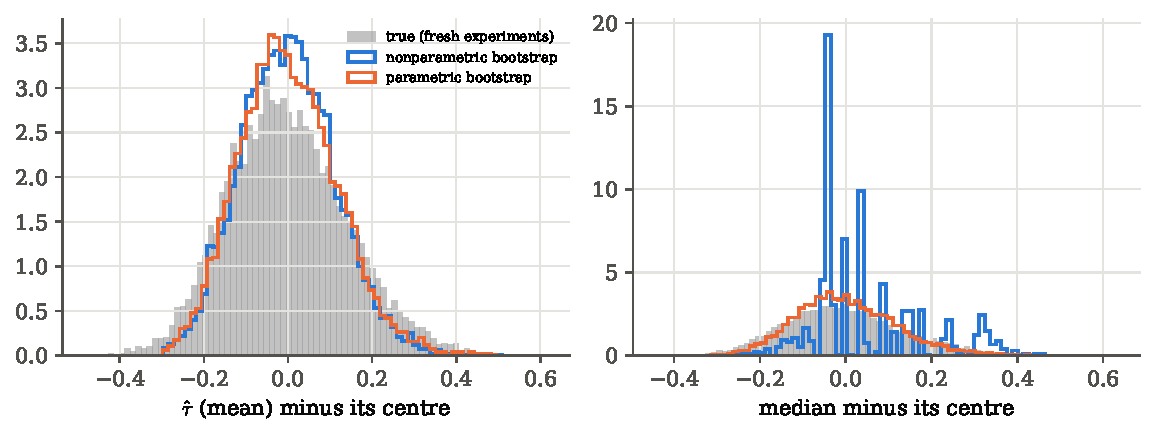
\includegraphics[width=12cm]{figures/ch03/bootstrap.pdf}
\caption{Bootstrap distributions from one data set of fifty decay times,
each centred on its own centre so the shapes can be compared. Grey: the true
sampling distribution from ten thousand fresh experiments. Blue: resampling
the data with replacement. Orange: simulating from the fitted exponential.
Left: the mean. Right: the median, whose nonparametric bootstrap
distribution is lumpy because a resampled median can only take a few
values near the middle of the data.}
\label{3b:fig:bootstrap}
\end{figure}

\subsection{Bootstrap confidence intervals}
\label{3b:sec:boot-intervals}

A standard error gives the simplest interval, the \newterm{Normal
interval} $T_n\pm z_{\alpha/2}\,\widehat{\mathrm{se}}_{\text{boot}}$
\mainref{p.~110, (8.2)}, which assumes a Gaussian sampling distribution. The
bootstrap distribution contains more than a width, and two other
constructions use its shape.

\paragraph{The pivotal interval.}
Let $R_n=\hat\theta-\theta$ be the error of the estimate, with unknown
distribution function $H(r)=\Prob(R_n\le r)$. Choose
$a=\hat\theta-H^{-1}(1-\alpha/2)$ and $b=\hat\theta-H^{-1}(\alpha/2)$. Then
\begin{align*}
  \Prob(a\le\theta\le b)
  &\eqby{1}\Prob\bigl(\hat\theta-b\le R_n\le\hat\theta-a\bigr)
  \eqby{2}H\bigl(\hat\theta-a\bigr)-H\bigl(\hat\theta-b\bigr)\\
  &\eqby{3}H\bigl(H^{-1}(1-\tfrac\alpha2)\bigr)-H\bigl(H^{-1}(\tfrac\alpha2)\bigr)
  =1-\alpha .
\end{align*}
\begin{explain}
  \item $a\le\theta$ is the same as $\hat\theta-\theta\le\hat\theta-a$, and
        $\theta\le b$ is $\hat\theta-b\le\hat\theta-\theta$.
  \item Probability of an interval from the distribution function (for a
        continuous $H$).
  \item Insert the chosen $a$ and $b$.
\end{explain}
We do not know $H$, but the bootstrap gives its analogue: the distribution
of $R^*=\theta^*-\hat\theta$, whose quantiles are
$\theta^*_\beta-\hat\theta$ with $\theta^*_\beta$ the $\beta$-quantile of
the replicas. Substituting gives the \newterm{pivotal interval}
\mainref{p.~111, (8.6)}
\[
  C_n=\bigl(2\hat\theta-\theta^*_{1-\alpha/2},\ 2\hat\theta-\theta^*_{\alpha/2}\bigr).
\]
The interval is reflected. Suppose the replicas scatter further above
$\hat\theta$ than below it. In the bootstrap world, then, the estimate
overshoots its truth by larger amounts than it undershoots. Carried back to
the real world, our $\hat\theta$ may sit well above the true $\theta$, so
the interval reaches further \emph{down}.

\paragraph{The percentile interval.}
The simplest recipe of all takes the quantiles of the replicas directly,
$(\theta^*_{\alpha/2},\theta^*_{1-\alpha/2})$ \mainref{p.~111}. It is exact
when some monotone transformation makes the sampling distribution symmetric
and Gaussian, and it respects the parametrisation in the way the
$\Delta\ln\Like$ interval does. All three intervals have coverage tending to
$1-\alpha$ under weak conditions \mainref{p.~111, Thm.~8.3}.

\paragraph{Example: the median of the lifetimes.}
For the median of our fifty decay times, $95\%$ intervals from $10^4$
nonparametric replicas are
\[
  \text{Normal: }(\ThreeBBootNormLo,\ \ThreeBBootNormHi),\qquad
  \text{pivotal: }(\ThreeBBootPivLo,\ \ThreeBBootPivHi),\qquad
  \text{percentile: }(\ThreeBBootPctLo,\ \ThreeBBootPctHi),
\]
for a true median of $\ThreeBBootMedTrueVal$. The replicas of a median are
lumpy and lopsided, and the three recipes treat the lopsidedness
differently: the percentile interval follows it, the pivotal interval
reflects it about the estimate, and the Normal interval ignores it. So the
three intervals differ, and for one data set one of them can miss the true
median while another contains it. Any $95\%$ procedure
misses in one experiment in twenty. Which of them misses less often for a
given problem can be settled only by the same kind of simulation over many
data sets, as in \cref{ch:04}.

\subsection{Where the bootstrap fails}
\label{3b:sec:boot-fail}

The bootstrap works when the statistic depends smoothly on the whole
distribution. It fails when the statistic is controlled by a few extreme
points, because $\hat F_n$ has no probability beyond the largest observation.
The cleanest example is the uniform box again, with $T_n=x_{(n)}$. The true
sampling distribution of the maximum is continuous, with density
$nx^{n-1}/\theta^n$ below $\theta$. A bootstrap replica, however, is the
maximum of $n$ points drawn from the data, and it equals the observed
maximum whenever that point is drawn at least once:
\begin{align*}
  \Prob\bigl(x^*_{(n)}=x_{(n)}\bigr)
  &\eqby{1}1-\Prob\bigl(x_{(n)}\text{ is never drawn}\bigr)
  \eqby{2}1-\Bigl(1-\frac1n\Bigr)^n
  \;\xrightarrow{n\to\infty}\;1-e^{-1}=0.632 .
\end{align*}
\begin{explain}
  \item The replica's maximum is $x_{(n)}$ as soon as $x_{(n)}$ is among the
        resampled points; otherwise it is smaller.
  \item Each of the $n$ independent draws misses that point with probability
        $1-1/n$.
\end{explain}
For $n=50$ this is $\ThreeBBootFracTh$, and the simulation gives
$\ThreeBBootFrac$: almost two thirds of the replicas sit on a single value,
a spike that the continuous true distribution does not have
(\cref{3b:fig:bootstrap-fail}). No amount of resampling can put a replica
above $x_{(n)}$, yet the true $\theta$ is always there. The same caution
applies to any statistic that lives in the tails: extreme values, endpoint
fits, the largest peak in a noisy map. For such statistics the parametric
bootstrap, or a simulation from a physical model, is the right tool.

\begin{figure}[htbp]
\centering
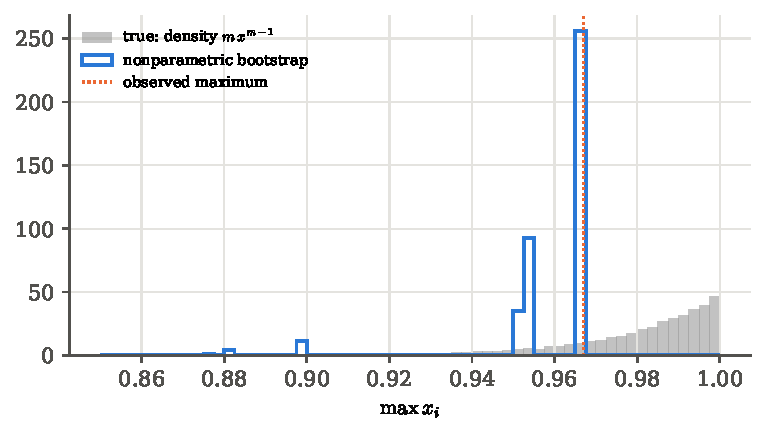
\includegraphics[width=9cm]{figures/ch03/bootstrap_uniform.pdf}
\caption{A statistic the bootstrap cannot handle: the maximum of fifty
uniform points. Grey: its true sampling distribution, smooth and piled
against the end of the box. Blue: the bootstrap replicas, about
$63\%$ of which equal the observed maximum (dotted line), with the rest
spread over a few lower data values. None can exceed the observed maximum.}
\label{3b:fig:bootstrap-fail}
\end{figure}

\begin{inpractice}[Verification versus research]
Most of the simulations above \emph{verified} results already derived:
that $\chi^2_{\min}$ follows $\chi^2_{N-m}$, that the curvature
of $\ln\Like$ equals the scatter of the MLE, that the Poisson fit conserves
the total. Their job was to make the formulas believable and to show how
large $n$ must be before the asymptotic statements hold. In research the
same machinery is the instrument itself, used exactly where no formula
exists. A cosmological analysis estimates the covariance matrix of a
masked, noisy power spectrum from hundreds of simulated skies, a
parametric bootstrap from the fitted model (\cref{ch:07,ch:08}); an LHC
search calibrates its profile-likelihood test statistic on pseudo-experiments
when Wilks' theorem is doubtful; large-scale-structure analyses resample
patches of the sky (a jackknife or block bootstrap) to capture
correlations no one can model analytically. The logic is always that of
\cref{3b:fig:two-worlds}: build the best stand-in for the truth, simulate
from it, analyse each simulation exactly as the data, read the error off the
scatter.
\end{inpractice}
\section{From a model to an estimator: how to find the right one}
\label{3b:sec:recipe}

A theorist hands us a model: a prediction $d(\theta)$, a noise level, and a
parameter $\theta$ to be measured. Nothing says which function of the data
to quote as the answer. The sample mean, the median, the midrange, the
value that minimises some $\chi^2$: each is an estimator, each has a
sampling distribution, and they differ in width. So the question is: which
function of the data should we quote? The tools for answering it are
already in hand. The likelihood gives the probability of the data. The
score equation turns it into an estimate. The curvature gives an error bar.
The Cram\'er--Rao bound says how narrow the error bar can ever be. Put in
order, these tools become a procedure that starts from the model and ends
with an estimator whose sampling distribution we know and cannot improve
(\cref{3b:fig:recipe-flow}). The procedure has five steps, and every one has
already appeared in a special case.

\begin{figure}[htbp]
\centering
\begin{tikzpicture}[
  bx/.style={draw=accent,thick,rounded corners=2pt,fill=ideabg,font=\small,
             minimum height=9mm,align=center,text width=33mm},
  bd/.style={bx,dashed,draw=fibreorange!80!black,fill=defbg},
  flow/.style={->,thick,accent}]
  \node[bx] (A) at (0,0)   {1. model\\ $\data=d(\theta)+\text{noise}$};
  \node[bx] (B) at (4.4,0) {likelihood\\ $\Like(\theta)=p(\data\given\theta)$};
  \node[bx] (C) at (8.8,0) {2. sufficient\\ statistic $U(\data)$};
  \node[bx] (D) at (8.8,-3.3) {3. candidates: moments, ML, LS, Bayes};
  \node[bx] (E) at (4.4,-3.3) {4. best? bias, variance, Cram\'er--Rao, Rao--Blackwell};
  \node[bx] (F) at (0,-3.3) {estimate $\hat\theta\pm\hat\sigma$};
  \node[bd] (G) at (4.4,-1.65) {5. no formula:\\ simulate and calibrate};
  \draw[flow] (A) -- (B); \draw[flow] (B) -- (C); \draw[flow] (C) -- (D);
  \draw[flow] (D) -- (E); \draw[flow] (E) -- (F);
  \draw[flow,dashed,fibreorange!80!black] (B) -- (G);
  \draw[flow,dashed,fibreorange!80!black] (G) -- (E);
\end{tikzpicture}
\caption{From a model to an estimator. The solid path is the procedure when
the likelihood can be written down. If it cannot (dashed path), a simple
statistic is computed and its bias and scatter are read off simulated
data sets.}
\label{3b:fig:recipe-flow}
\end{figure}

Four examples run through every step: independent Gaussian readings
$x_i\sim\Normal(\mu,\sigma^2)$ with known $\sigma$; Poisson counts
$X_i\sim\mathrm{Poisson}(\lambda)$, the numbers of events in $n$ equal time
slots; exponential decay times $t_i$ with mean lifetime $\tau$; and the
multipole coefficients $\alm$ of a full-sky Gaussian CMB map. The CMB
example is then followed through the whole chain in
\cref{3b:sec:recipe-cmb}.

\subsection{Step 1: write the likelihood}
\label{3b:sec:recipe-like}

Everything starts from the statement that the data are the model plus noise
(\cref{3b:sec:one-measurement}): the noise realisation that the data require
has a known probability, and that probability, read as a function of the
parameter, is $\Like(\theta)$. For independent data the likelihood is the
product \eqref{3b:eq:like-iid}. For the four examples, keeping only the
factors that depend on the parameter,
\begin{align}
  \text{Gaussian mean:}\quad &\Like(\mu)\propto
      \exp\Bigl[-\frac1{2\sigma^2}\sum_i(x_i-\mu)^2\Bigr],
  \nonumber\\
  \text{Poisson rate:}\quad &\Like(\lambda)=\prod_i\frac{e^{-\lambda}\lambda^{X_i}}{X_i!}
      \propto e^{-n\lambda}\lambda^{K},\qquad K\equiv\sum_iX_i,
  \nonumber\\
  \text{exponential lifetime:}\quad &\Like(\tau)=\tau^{-n}e^{-T/\tau},\qquad
      T\equiv\sum_it_i,
  \label{3b:eq:four-likes}\\
  \text{full-sky CMB:}\quad &\Like(\Cell)\propto
      \Cell^{-(2\ell+1)/2}\exp\Bigl[-\frac{(2\ell+1)\Chat}{2\Cell}\Bigr].
  \nonumber
\end{align}
The last line is the isotropic Gaussian sky of \cref{3b:sec:universal}.
Recall its ingredients. At multipole $\ell$ there are $2\ell+1$ independent
real numbers $y_{\ell k}$: $a_{\ell0}$, and $\sqrt2\,\mathrm{Re}\,\alm$ and
$\sqrt2\,\mathrm{Im}\,\alm$ for $m=1,\dots,\ell$. (For $m>0$ the real and
imaginary parts of $\alm$ each have variance $\Cell/2$, and $a_{\ell,-m}$ is
the complex conjugate of $\alm$ up to a sign, so it adds nothing new; the
factor $\sqrt2$ brings each variance up to $\Cell$.) Each $y_{\ell k}$ has
density $(2\pi\Cell)^{-1/2}e^{-y_{\ell k}^2/2\Cell}$. Their product over the
$2\ell+1$ values of $k$ gives the last line, with
$(2\ell+1)\Chat=\sum_ky_{\ell k}^2=\sum_m|\alm|^2$.

\subsection{Step 2: what can the data tell us? Sufficient statistics}
\label{3b:sec:recipe-suff}

Look at \eqref{3b:eq:four-likes}. The Gaussian likelihood contains the
$n$ readings, yet after expanding the square it depends on them only through
$\bar x$ (and through a constant). The Poisson likelihood depends on the
counts only through their total $K$, the exponential one only through $T$,
the CMB one only through $\Chat$. Every data set with the same $K$ gives
exactly the same likelihood curve, so no estimate, error bar or confidence
interval computed from the likelihood can distinguish them. The remaining
information in the $n$ numbers, which ones were large, which came first,
says nothing about $\theta$.

\paragraph{Definition.}
A statistic $U(\data)$ is \newterm{sufficient} for $\theta$ if the
conditional distribution of the data given the value of $U$ does not involve
$\theta$ \mainref{p.~137, Def.~9.32}. Given $U$, the data set is one of the
points on the ``surface'' $\{\data':U(\data')=U(\data)\}$, and sufficiency
says that $\theta$ has no influence on which point of the surface we land
on: $\theta$ only decides how probable the surface is. Statistical
mechanics has met this before. In the canonical ensemble
$p(\text{microstate}\given\beta)=e^{-\beta E}/Z(\beta)$, and given the energy
$E$ all microstates are equally likely, whatever $\beta$ is. The energy is
therefore a sufficient statistic for the inverse temperature $\beta$: a
thermometer that reads only $E$ loses nothing.

The coarsest statistic with this property is called \newterm{minimal
sufficient}: two data sets have the same value of it exactly when the ratio
of their likelihoods $p(\data\given\theta)/p(\data'\given\theta)$ does not
depend on $\theta$ \mainref{p.~138, Def.~9.35}. In all the examples below the statistic
found is minimal, so no further compression is possible without losing
information.

\paragraph{The factorisation theorem.}
Checking the definition directly needs the conditional distribution. The
\newterm{Neyman--Fisher factorisation theorem} \mainref{p.~140, Thm.~9.40},
\srcref{CasellaBerger}{Thm.~6.2.6} replaces that with a test on the
likelihood:
\[
  U\text{ is sufficient}\iff
  p(\data\given\theta)=g\bigl(U(\data),\theta\bigr)\,h(\data)
  \quad\text{for some functions }g,h .
\]
All the $\theta$-dependence must pass through $U$, and whatever else depends
on the data (the $h$) must not know about $\theta$. The proof, for discrete
data (sums become integrals for densities), has two halves. Write $\mathcal A_u$ for
the set of all data sets with $U=u$.

\emph{Factorised form implies sufficiency.} For a data set $\data$ with
$U(\data)=u$,
\begin{align}
  \Prob(\data\given U=u,\theta)
  &\eqby{1}\frac{\Prob(\data\given\theta)}{\Prob(U=u\given\theta)}
   \eqby{2}\frac{g(u,\theta)\,h(\data)}{\sum_{\data'\in\mathcal A_u}g(u,\theta)\,h(\data')}
   \eqby{3}\frac{h(\data)}{\sum_{\data'\in\mathcal A_u}h(\data')} .
  \label{3b:eq:suff-forward}
\end{align}
\begin{explain}
  \item The event $\{\data\}$ lies inside $\{U=u\}$, so
        $\Prob(\data,U=u\given\theta)=\Prob(\data\given\theta)$.
  \item Numerator by the factorisation. The denominator is the sum of the
        probabilities of all data sets in $A_u$, and $g(U(\data'),\theta)=g(u,\theta)$
        for each of them.
  \item $g(u,\theta)$ is a common factor and cancels.
\end{explain}
The result contains no $\theta$, which is the definition.

\emph{Sufficiency implies the factorised form.} If
$\Prob(\data\given U=u,\theta)=c(\data)$ does not depend on $\theta$, then
\[
  \Prob(\data\given\theta)
  =\Prob(\data\given U=U(\data),\theta)\,\Prob(U=U(\data)\given\theta)
  =c(\data)\;q\bigl(U(\data),\theta\bigr),
\]
which is the factorised form with $h=c$ and $g=q$, the sampling distribution
of $U$ itself.

\paragraph{Examples.}
Expanding the square, $\sum_i(x_i-\mu)^2=\sum_i(x_i-\bar x)^2+n(\bar x-\mu)^2$,
so the Gaussian likelihood factorises with
$g=\exp[-n(\bar x-\mu)^2/2\sigma^2]$ and $h=\exp[-\sum_i(x_i-\bar x)^2/2\sigma^2]$:
$\bar x$ is sufficient for $\mu$. Reading \eqref{3b:eq:four-likes}, the Poisson
total $K$ is sufficient for $\lambda$ with $g=e^{-n\lambda}\lambda^K$ and
$h=\prod_i1/X_i!$; the sum of decay times $T$ is sufficient for $\tau$ with
$h=1$; and $\Chat$, equivalently $\sum_m|\alm|^2$, is sufficient for $\Cell$
with $h=1$. The last statement is the precise form of the everyday remark
that for a Gaussian isotropic sky the power spectrum contains everything
there is to know about the parameters: the phases of the $\alm$ carry no
information. It is a statement about the model. If the field is not
Gaussian, $h$ is no longer free of $\Cell$ and the phases carry information
that $\Chat$ throws away, a point that returns when topological summaries of
fields appear (\cref{ch:12}).

\paragraph{The exponential family: sufficient statistics and moment matching.}
All four examples, and most of the distributions of \cref{ch:02},
have the form
\begin{equation}
  p(x\given\theta)=h(x)\exp\bigl[\eta(\theta)\,\phi(x)-A(\theta)\bigr],
  \label{3b:eq:expfam}
\end{equation}
with $\phi(x)$ a single function of one observation (the Poisson has
$\phi=x$, $\eta=\ln\lambda$, $A=\lambda$; the exponential lifetime has
$\phi=t$, $\eta=-1/\theta$, $A=\ln\theta$ with $\theta$ the mean lifetime; the CMB coefficient has
$\phi=y^2$, $\eta=-1/2\Cell$, $A=\tfrac12\ln2\pi\Cell$). For $n$
independent observations, the product has
$\exp[\eta\sum_i\phi(x_i)-nA]\prod_ih(x_i)$, so $\sum_i\phi(x_i)$ is
sufficient by the factorisation theorem. More: the MLE is the solution of
a moment-matching equation. Differentiating the normalisation
$\int p\,\dd x=1$ with respect to $\theta$ gives
\[
  0=\int(\eta'\phi-A')\,p\,\dd x
  \quad\Longrightarrow\quad
  \E_\theta\phi=\frac{A'(\theta)}{\eta'(\theta)},
\]
and then
\begin{align}
  \frac{\partial\ell}{\partial\theta}
  &\eqby{1}\eta'\sum_i\phi(x_i)-nA'
   \eqby{2}\eta'(\theta)\Bigl[\sum_i\phi(x_i)-n\,\E_\theta\phi\Bigr] .
  \label{3b:eq:expfam-score}
\end{align}
\begin{explain}
  \item Logarithm of the product, then differentiate; $h$ does not contain $\theta$.
  \item Insert $A'=\eta'\,\E_\theta\phi$.
\end{explain}
With $\eta'\ne0$ the score equation is
\begin{equation}
  \E_{\hat\theta}\,\phi=\frac1n\sum_{i=1}^n\phi(x_i),
  \label{3b:eq:moment-match}
\end{equation}
\emph{the model's mean of the sufficient statistic equals its observed
mean.} That is why the maximum-likelihood lifetime is the mean decay time,
the Poisson rate estimate is the mean count $\hat\lambda=\bar X$, the CMB
estimate is the mean of $y^2$, and in each case the method of moments
(\cref{3b:sec:mom}) gives the same answer as maximum likelihood. Outside the
exponential family, for instance for the angular distribution
\eqref{3b:eq:angular}, whose parameters also sit in the normalisation, the two
methods give different estimates and the moment estimates are generally less precise.

\subsection{Step 3: constructing candidate estimators}
\label{3b:sec:recipe-candidates}

Having found what the data can tell us, we build estimators from it. The
families met so far are the following.
\begin{itemize}
  \item \emph{Method of moments} (\cref{3b:sec:mom}): set model moments equal
        to sample moments. No likelihood is needed, only moments of the
        model. Quick, consistent, often a good starting point for Newton--Raphson.
  \item \emph{Maximum likelihood} (\cref{3b:sec:mle}): maximise
        $\Like(\theta)$. Always available when the likelihood is, invariant
        under reparametrisation, asymptotically efficient.
  \item \emph{Least squares} (\cref{3b:sec:ls-from-ml}): the maximum likelihood estimator
        for independent Gaussian noise, $-2\ell=\chi^2$, and for correlated
        Gaussian noise with the weight matrix $\Cmat^{-1}$. Not a separate
        principle.
  \item \emph{Bayes estimators}, which use a prior and a cost of being wrong.
        They complete the list and are derived below; \cref{ch:05}
        develops them.
\end{itemize}

\paragraph{The EM algorithm: maximum likelihood with hidden variables.}
Sometimes the likelihood is a sum over quantities we did not observe, such as the
unknown class of each event in a mixture of signal and background,
$p(\data\given\theta)=\sum_zp(\data,z\given\theta)$, and the logarithm of a sum
has no closed-form maximum. Given a current guess $\theta_t$, let
$q(z)=p(z\given\data,\theta_t)$ be the posterior probability of each hidden
assignment. Since the logarithm is concave, Jensen's inequality gives
\begin{align}
  \ln p(\data\given\theta)
  &\eqby{1}\ln\sum_zq(z)\frac{p(\data,z\given\theta)}{q(z)}
   \relby{2}{\ge}\sum_zq(z)\ln p(\data,z\given\theta)-\sum_zq(z)\ln q(z),
  \label{3b:eq:em}
\end{align}
\begin{explain}
  \item Multiply and divide by $q(z)$, which sums to one.
  \item Jensen: the log of an average is at least the average of the log.
\end{explain}
with equality at $\theta=\theta_t$. (There
$p(\data,z\given\theta_t)/q(z)=p(\data\given\theta_t)$ is the same for every
$z$, and Jensen's inequality is an equality for an average of equal
numbers.) The right side differs from
$Q(\theta\given\theta_t)=\sum_zq(z)\ln p(\data,z\given\theta)$ by a constant,
and $Q$ involves the logarithm of a single term, usually easy to maximise.
The algorithm alternates the \newterm{E step} (compute $q(z)$, hence $Q$) with
the \newterm{M step} ($\theta_{t+1}=\arg\max_\theta Q$). No cycle can
decrease the likelihood, because the right side touches $\ln p(\data\given\theta)$ at
$\theta_t$ and lies below it elsewhere \mainref{pp.~143--144}. Raising the
right side therefore raises $\ln p$ at least as much. It converges to a
stationary point, which can be a local maximum.

\paragraph{Bayes estimators: choose the answer that minimises the expected loss.}
Suppose we must announce one number $a$ for $\theta$, and being off by
$\theta-a$ costs us $L(\theta,a)$. We do not know $\theta$, but after the
experiment we have the posterior $p(\theta\given\data)\propto
\Like(\theta)p(\theta)$, the probability density of the value of $\theta$ given the
data and a prior $p(\theta)$ (\cref{3b:eq:bayes}). Announce the $a$ that
minimises the posterior expected loss
\[
  \rho(a)=\int L(\theta,a)\,p(\theta\given\data)\,\dd\theta .
\]
The expectation is over the plausible values of $\theta$ at fixed data,
not over repeated data sets. Three choices of loss give three familiar
summaries.

\emph{Squared loss, $L=(\theta-a)^2$.} Let $m=\E[\theta\given\data]$ be the
posterior mean. Then
\begin{align}
  \rho(a)&=\E\bigl[(\theta-a)^2\given\data\bigr]\\
   &\eqby{1}\E\bigl[(\theta-m)^2\given\data\bigr]
     +2(m-a)\,\E\bigl[\theta-m\given\data\bigr]+(m-a)^2\\
   &\eqby{2}\Var[\theta\given\data]+(m-a)^2 .
  \label{3b:eq:bayes-squared}
\end{align}
\begin{explain}
  \item Write $\theta-a=(\theta-m)+(m-a)$ and expand the square. The number
        $m-a$ is a constant for the expectation.
  \item $\E[\theta-m\given\data]=0$ by definition of $m$, which kills the cross term.
\end{explain}
The first term does not depend on $a$, so $\rho$ is smallest at $a=m$: the
\emph{posterior mean} minimises the expected squared error.

\emph{Absolute loss, $L=|\theta-a|$.} With $F(a)=\int_{-\infty}^ap\,\dd\theta$,
\begin{align*}
  \rho(a)&=\int_{-\infty}^{a}(a-\theta)\,p\,\dd\theta+\int_a^\infty(\theta-a)\,p\,\dd\theta,\\
  \frac{\dd\rho}{\dd a}&\eqby{1}\int_{-\infty}^{a}p\,\dd\theta-\int_a^\infty p\,\dd\theta
   =2F(a)-1 .
\end{align*}
\begin{explain}
  \item Differentiate the integrals with respect to $a$ in the integrand and
        at the limits; the limit terms contain $(a-\theta)p$ at $\theta=a$, which is zero.
\end{explain}
The derivative vanishes at $F(a)=\tfrac12$: the \emph{posterior median}.

\emph{Zero--one loss,} $L=0$ if $|\theta-a|<h$ and $1$ otherwise. Then
$\rho(a)=1-\int_{a-h}^{a+h}p\,\dd\theta\approx1-2h\,p(a\given\data)$, smallest
where the posterior is largest: the \emph{posterior mode} (MAP, maximum
\emph{a posteriori}), obtained as $h\to0$.

For a symmetric, single-peaked posterior the three coincide. For a skewed
one they do not. The Poisson rate with a single observation $K=2$ and a flat
prior has posterior $p(\lambda\given K)\propto\lambda^2e^{-\lambda}$, a
Gamma density with shape $3$. Its mode is $2$ (equal to the MLE, because the
prior is flat, \cref{3b:sec:bayes-place}), its median is $2.67$ and its
mean is $3$. Evaluating the expected losses on a grid of announced values
(\cref{3b:fig:recipe}, middle) reproduces the three minima at
$\ThreeBBayesZOArg$, $\ThreeBBayesAbsArg$ and $\ThreeBBayesSqArg$. Which
number is ``the estimate'' depends on what a mistake costs. A flat prior
makes the maximum-likelihood estimate the Bayes estimator under zero--one
loss, and only under it.

\subsection{Step 4: choosing the best}
\label{3b:sec:recipe-best}

Several candidates, several sampling distributions. Two tools rank them.
The first is the Cram\'er--Rao bound (\cref{3b:sec:cramer-rao}), a floor on
the variance of an unbiased estimator. If a candidate sits on the floor it
cannot be improved, and the search ends. The second tool says how to
improve a candidate that is above it.

\paragraph{The Rao--Blackwell theorem.}
Let $W(\data)$ be any unbiased estimator of $g(\theta)$ and $U$ a sufficient
statistic. Define
\[
  \tilde W(U)=\E[W\given U] ,
\]
the average of $W$ over all data sets with the observed value of $U$.
Three facts follow.

First, $\tilde W$ is a legitimate statistic. The average uses the
conditional distribution of the data given $U$, which by sufficiency does not
contain $\theta$. Without sufficiency the average would need the unknown
$\theta$ and could not be computed.

Second, $\tilde W$ is unbiased, by the law of total expectation,
$\E\tilde W=\E[\E(W\given U)]=\E W=g(\theta)$.

Third, its variance is never larger:
\begin{align}
  \Var W
  &\eqby{1}\E\bigl[\Var(W\given U)\bigr]+\Var\bigl[\E(W\given U)\bigr]
   \eqby{2}\E\bigl[\Var(W\given U)\bigr]+\Var\tilde W
   \relby{3}{\ge}\Var\tilde W .
  \label{3b:eq:rao-blackwell}
\end{align}
\begin{explain}
  \item The law of total variance: split the scatter of $W$ into the average
        scatter inside each slice $U=u$ and the scatter of the slice
        averages between slices.
  \item Definition of $\tilde W$.
  \item The first term is an average of variances, each $\ge0$. It vanishes
        only if $W$ is already a function of $U$.
\end{explain}
\mainref{p.~140, Thm.~9.42}, \srcref{CasellaBerger}{Thm.~7.3.17}. The
reduction is exactly the average variance that $W$ wasted on the part of the
data that $U$ does not contain. The theorem gives an algorithm: start with
any crude unbiased estimator, however silly, and average it over the
sufficient statistic.

\paragraph{Example: estimating $e^{-\lambda}$, the chance of an empty slot.}
In $n$ time slots we count $X_i\sim\mathrm{Poisson}(\lambda)$ events, and we
want $g(\lambda)=e^{-\lambda}=\Prob(X=0)$, the probability that a slot is
empty. A crude unbiased estimator uses the first slot only:
$W=\mathbf 1\{X_1=0\}$, since $\E W=\Prob(X_1=0)=e^{-\lambda}$. It wastes
$n-1$ slots. Its variance is that of a 0/1 variable, $e^{-\lambda}(1-e^{-\lambda})$.
The total $K=\sum_iX_i$ is sufficient. The conditional mean is the
probability that slot $1$ is empty given the total $K=s$. Independent
Poisson variables add to a Poisson variable, so
\begin{align}
  \Prob(X_1=0\given K=s)
  &\eqby{1}\frac{\Prob(X_1=0)\,\Prob\bigl(\sum_{i\ge2}X_i=s\bigr)}{\Prob(K=s)}
   \eqby{2}\frac{e^{-\lambda}\,e^{-(n-1)\lambda}\,[(n-1)\lambda]^s/s!}{e^{-n\lambda}\,(n\lambda)^s/s!}
   \eqby{3}\Bigl(\frac{n-1}{n}\Bigr)^{s} .
  \label{3b:eq:rb-poisson}
\end{align}
\begin{explain}
  \item Definition of conditional probability; $X_1=0$ and $K=s$ together mean
        $X_1=0$ and the other $n-1$ slots add up to $s$, and the slots are independent.
  \item The sum of the other $n-1$ slots is Poisson with mean $(n-1)\lambda$,
        the total is Poisson with mean $n\lambda$.
  \item The exponentials and factorials cancel, and so does $\lambda^s$, leaving
        $(n-1)^s/n^s$. This is the last place that $\lambda$ could have entered.
\end{explain}
So $\tilde W=(1-1/n)^K$. In words: given the total, each of the $K$ events
fell in slot $1$ with probability $1/n$, independently, so slot $1$ is
empty with probability $(1-1/n)^K$. The variance is found from the
generating function of the Poisson distribution, $\E z^K=\exp[n\lambda(z-1)]$:
with $z=1-1/n$ this gives $\E\tilde W=e^{-\lambda}$ (unbiased, as promised),
and with $z^2=1-2/n+1/n^2$ it gives $\E\tilde W^2=e^{-2\lambda+\lambda/n}$, so
\[
  \Var\tilde W=e^{-2\lambda}\bigl(e^{\lambda/n}-1\bigr) .
\]
For $n=10$ and $\lambda=1.5$ the crude estimator has variance
$\ThreeBRBCrudeVarTh$ and the Rao--Blackwellised one $\ThreeBRBRBVarTh$, a
reduction by a factor of more than twenty. The simulation of
$20\,000$ experiments (\cref{3b:sec:recipe-python}) gives $\ThreeBRBCrudeVar$ and
$\ThreeBRBRBVar$, both means at $\ThreeBRBCrudeMean$ and $\ThreeBRBRBMean$
against the truth $\ThreeBRBTruth$. The Cram\'er--Rao floor for estimating
$g(\lambda)$ is $g'(\lambda)^2/I_n=\lambda e^{-2\lambda}/n=\ThreeBRBCR$ with
$I_n=n/\lambda$. The improved estimator sits just above it. Expanding,
$\Var\tilde W\approx(\lambda e^{-2\lambda}/n)(1+\lambda/2n)$, so the excess
over the floor is a factor $1+\lambda/2n$, which tends to one as $n$ grows.

\paragraph{Best unbiased estimators.}
Can averaging a second time, over a different crude starting estimator,
improve it again? For the Poisson total, no. The total $K$ is
\newterm{complete} \unpack{the only function of $K$ whose mean is zero for
every $\lambda$ is the zero function}. The Lehmann--Scheffé theorem
\srcref{CasellaBerger}{Thm.~7.3.23} says that for a complete sufficient
statistic $U$, any unbiased function of $U$ is the unique
minimum-variance unbiased estimator (UMVUE). Two unbiased functions of $U$
could be different only by a function of $U$ with zero mean, and there is
none. The exponential family \eqref{3b:eq:expfam} with a rich enough
parameter has complete statistics, so $\tilde W$ above is the best unbiased
estimator of $e^{-\lambda}$, even though it does not reach the Cram\'er--Rao
floor. The bound is attained only when the score is a linear function of the
estimator, which for $e^{-\lambda}$ it is not.

\paragraph{When a biased estimator beats an unbiased one.}
UMVUEs are the best among unbiased estimators. The mean squared error is
bias squared plus variance (\cref{3a:sec:mse}), and a small bias that buys a
larger drop in variance can win. The maximum-likelihood estimate of
$e^{-\lambda}$ is $e^{-\hat\lambda}=e^{-K/n}$. It is biased, but by
$O(1/n)$, so its squared bias is $O(1/n^2)$ and the variance is $O(1/n)$:
the MLE and $\tilde W$ have nearly the same variance, and which has the
lower MSE depends on $n$ and $\lambda$. The earlier example with the
Gaussian variance went further: the divisor $N+1$ beats both $N-1$ and $N$
(\cref{3a:sec:best-divisor}). The posterior mean with a prior centred away
from the data is another example: it shrinks the estimate toward the prior,
adds bias and removes variance (\cref{ch:05}). Unbiasedness is a convenient
property, not a goal. The MLE's claim to be good is asymptotic efficiency, and
the Bayes and shrinkage estimates add to it when prior knowledge exists.

\subsection{Step 5: when the likelihood cannot be written down}
\label{3b:sec:recipe-intractable}

The procedure needs $p(\data\given\theta)$. For a masked, noisy, beamed
CMB map the field is still Gaussian, but the pixels are correlated, and the
likelihood with a huge covariance matrix is too expensive to evaluate at every point
of a Markov chain. For the large-scale-structure correlation function, the
number of independent modes is far larger than the number of simulations
available to estimate the covariance. For a topological summary of a field
(\cref{ch:12}) there is no likelihood at all. The procedure still works if
we give up on optimality and compute a simple summary statistic, then
replace the missing likelihood by simulation:
\begin{enumerate}
  \item choose a statistic $\hat S(\data)$ that is cheap and sensitive to
        $\theta$ (a pseudo-$C_\ell$, a counts-in-cells histogram);
  \item simulate many data sets from the model at several $\theta$, through
        the same mask, noise and beam, and compute $\hat S$ for each
        (\cref{ch:06});
  \item read off the mean $\langle\hat S\rangle_\theta$ (the bias and the
        transfer function of the estimator) and the covariance of $\hat S$ from the
        scatter over the simulations, with the Hartlap correction of
        \cref{3a:sec:cov-noise};
  \item use a Gaussian likelihood for $\hat S$ with that mean and covariance,
        or quote the parameter at which $\langle\hat S\rangle_\theta$ matches
        the observed $\hat S$, with an error bar from the simulated spread.
\end{enumerate}
This works even if $\hat S$ is not sufficient: its bias is calibrated out and
its error bar is honest, but the error bar is wider than the Cram\'er--Rao
floor of the full data. A mask removing a fraction of the sky, for example,
inflates the variance of the pseudo-spectrum roughly by one over the
observed sky fraction and correlates neighbouring multipoles; the simulations
measure both exactly. The same machinery, used for verification where a
formula exists and as the research instrument where none does, is
developed in \cref{ch:06,ch:08}.

\subsection{The full chain on one example: the CMB power spectrum}
\label{3b:sec:recipe-cmb}

Take a full-sky, noiseless, Gaussian isotropic temperature map, with the
coefficients $\alm$ of variance $\Cell$ (the power spectrum of the theory),
and ask for the best estimate of $\Cell$ at one multipole. Write
$\nu=2\ell+1$.

\paragraph{Step 1: likelihood.} From \eqref{3b:eq:four-likes},
\begin{equation}
  \ln\Like(\Cell)=-\frac{\nu}{2}\Bigl[\frac{\Chat}{\Cell}+\ln\Cell\Bigr]+\text{const},
  \qquad\Chat=\frac1\nu\sum_{m=-\ell}^{\ell}|\alm|^2 .
  \label{3b:eq:cmb-loglike}
\end{equation}

\paragraph{Step 2: sufficiency.} $\Chat$ enters alone, and the factorisation
is complete with $h=1$. Nothing about the phases or the sign of $m$ is needed.

\paragraph{Step 3: the candidate.} The score equation:
\begin{align}
  \frac{\partial\ln\Like}{\partial\Cell}
  &\eqby{1}-\frac{\nu}{2\Cell}+\frac{\nu\Chat}{2\Cell^2}
   \eqby{2}\frac{\nu}{2\Cell^2}\bigl(\Chat-\Cell\bigr)
   \;=0\quad\Longrightarrow\quad\hat C_\ell^{\rm ML}=\Chat .
  \label{3b:eq:cmb-score}
\end{align}
\begin{explain}
  \item Differentiate \eqref{3b:eq:cmb-loglike}: $\partial_C(\Chat/C)=-\Chat/C^2$ and $\partial_C\ln C=1/C$.
  \item Common denominator $2\Cell^2$.
\end{explain}
The second derivative is $\nu/2\Cell^2-\nu\Chat/\Cell^3$. At the solution
$\Cell=\Chat$ it equals $\nu/2\Chat^2-\nu/\Chat^2=-\nu/2\Chat^2<0$, so this
is a maximum. The
familiar estimator, the average of $|\alm|^2$ over the $2\ell+1$ values of
$m$, is the maximum-likelihood estimator, the moment-matching solution
\eqref{3b:eq:moment-match} with $\phi=y^2$, and (with flat prior) the
posterior mode.

\paragraph{Step 4: is it the best?} Bias: $\E y^2=\Cell$ for each of the $\nu$
variables, so $\E\Chat=\Cell$, unbiased. Variance: $\nu\Chat/\Cell=\sum_k(y_k/\sqrt{\Cell})^2$
is a sum of $\nu$ squares of unit Gaussians, which is $\chi^2_\nu$ with mean $\nu$
and variance $2\nu$, so
\begin{equation}
  \Var\Chat=\frac{\Cell^2}{\nu^2}\,2\nu=\frac{2\Cell^2}{2\ell+1}.
  \label{3b:eq:cosmic-variance}
\end{equation}
Fisher information, the negative mean of the second derivative at the truth:
\begin{align}
  I(\Cell)&\eqby{1}-\E\Bigl[\frac{\nu}{2\Cell^2}-\frac{\nu\Chat}{\Cell^3}\Bigr]
   \eqby{2}-\frac{\nu}{2\Cell^2}+\frac{\nu}{\Cell^2}
   =\frac{2\ell+1}{2\Cell^2} .
  \label{3b:eq:cmb-fisher}
\end{align}
\begin{explain}
  \item The identity $I=-\E\,\partial^2\ln\Like/\partial\theta^2$ \eqref{3b:eq:fisher-identity}.
  \item Only $\Chat$ is random, and $\E\Chat=\Cell$.
\end{explain}
The Cram\'er--Rao bound is $1/I=2\Cell^2/(2\ell+1)$, which is exactly
\eqref{3b:eq:cosmic-variance}. The estimator attains the bound: the score
\eqref{3b:eq:cmb-score} is proportional to $\Chat-\Cell$, the exact condition
for equality in Cauchy--Schwarz in the derivation of
\eqref{3b:eq:cramer-rao}. No unbiased estimator of $\Cell$ built from one
sky can have a smaller variance. This number is \newterm{cosmic
variance}: a fractional error of $\sqrt{2/(2\ell+1)}$, which is $63\%$ at the
quadrupole and $18\%$ at $\ell=30$, caused by nothing but the fact that we
have one sky, with $2\ell+1$ independent numbers at each $\ell$. No
instrument improves it. In \cref{3a:sec:var-of-var} the same number
appeared as the variance of a variance. Here it is the Cram\'er--Rao bound
of the model.

\subsection{The recipe in Python}
\label{3b:sec:recipe-python}

\pyfile[firstline=25,lastline=39]{code/ch03/16_estimator_recipe.py}{Rao--Blackwell for the empty-slot probability}
The array \pyname{X} holds $20\,000$ experiments of $n=10$ Poisson slots
each. The crude estimator looks only at the first slot, and the sufficient
statistic \pyname{S} is the row sum (the $K$ of the text). The
Rao--Blackwellised estimator is the function $((n-1)/n)^{K}$ of
\eqref{3b:eq:rb-poisson}. The printed variances are the numbers
quoted above: $\ThreeBRBCrudeVar$ against $\ThreeBRBRBVar$, a ratio of
$\ThreeBRBRatio$, and both means agree with $e^{-\lambda}=\ThreeBRBTruth$.

\pyfile[firstline=41,lastline=50]{code/ch03/16_estimator_recipe.py}{Expected loss of three point estimates under a skewed posterior}
A posterior sample of $400\,000$ points from the Gamma density is used to
evaluate $\rho(a)$ on a grid, for squared and absolute loss. For the
zero--one loss the exact density is used in $1-2h\,p(a)$. The grids have their
minima at $\ThreeBBayesSqArg$ (mean $\ThreeBBayesMean$), $\ThreeBBayesAbsArg$
(median $\ThreeBBayesMedian$) and $\ThreeBBayesZOArg$ (mode $\ThreeBBayesMode$).

\pyfile[firstline=52,lastline=68]{code/ch03/16_estimator_recipe.py}{A full-sky Gaussian CMB: the maximum-likelihood $C_\ell$ and its variance}
For $\ell=2$ and $\ell=30$, $20\,000$ simulated skies supply $\sum_m|\alm|^2$;
dividing by $2\ell+1$ gives $\Chat$ for $C=1$. The means are
$\ThreeBCMBMeanTwo$ and $\ThreeBCMBMeanThirty$ (unbiased), the variances
$\ThreeBCMBVarTwo$ and $\ThreeBCMBVarThirty$ against the bounds
$2/(2\ell+1)=\ThreeBCMBBoundTwo$ and $\ThreeBCMBBoundThirty$, so the
simulated estimator sits on the Cram\'er--Rao bound at both multipoles
within sampling noise. The fractional errors are $\ThreeBCMBRelErrTwo$ and
$\ThreeBCMBRelErrThirty$. The last lines evaluate the score
\eqref{3b:eq:cmb-score} at the true $C$: its mean is
$\ThreeBCMBScoreMeanThirty$ (zero, \eqref{3b:eq:score-mean}) and its variance
is $\ThreeBCMBScoreVarThirty$ against the Fisher information
$\nu/2=\ThreeBCMBFishThirty$ at $\ell=30$, as \eqref{3b:eq:fisher-identity} requires.

\begin{figure}[htbp]
\centering
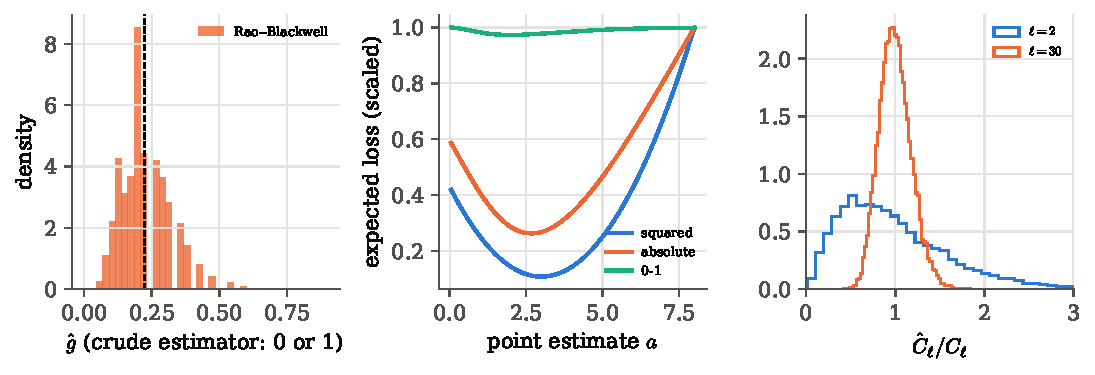
\includegraphics[width=12.5cm]{figures/ch03/estimator_recipe.pdf}
\caption{Three outcomes of the recipe. Left: the Rao--Blackwellised estimate of
$e^{-\lambda}$ over $20\,000$ experiments; the crude estimator can only
answer $0$ or $1$, while the averaged one is tightly peaked on the truth
(dashed). Middle: expected loss for a skewed posterior as a function of the
announced value, for squared, absolute and zero--one loss. Their minima are
at the mean, the median and the mode, from right to left. Right: the maximum-likelihood
$\Chat/\Cell$ from $20\,000$ skies at $\ell=2$ and $\ell=30$, centred on the
truth with widths set by cosmic variance.}
\label{3b:fig:recipe}
\end{figure}

\begin{taxonomy}[Which estimator when]
\small
\begin{tabular}{@{}>{\raggedright\arraybackslash}p{3.7cm}>{\raggedright\arraybackslash}p{3.9cm}>{\raggedright\arraybackslash}p{4.0cm}@{}}
  situation & estimator & why\\
  \hline
  exponential family (Poisson, exponential, Gaussian, $\chi^2_\nu$-type)
    & maximum likelihood $=$ match the mean of the sufficient statistic
    & sufficient, efficient, on the Cram\'er--Rao floor for the mean parameter\\[2pt]
  Gaussian noise, known $\Cmat$
    & least squares (weights $\Cmat^{-1}$)
    & it is the ML estimator; exact for linear models\\[2pt]
  counts in bins
    & Poisson ML ($2\sum[\mu-n\ln\mu]$), not $\sqrt n$-weighted $\chi^2$
    & no bias on the normalisation, valid for small counts\\[2pt]
  Gaussian isotropic sky
    & $\Chat=\frac1{2\ell+1}\sum_m|\alm|^2$
    & ML, unbiased, attains cosmic variance\\[2pt]
  a crude unbiased estimator exists
    & average it over a sufficient statistic
    & never increases the variance (Rao--Blackwell)\\[2pt]
  prior information, or a cost of error
    & Bayes: posterior mean, median or mode
    & minimises the expected squared, absolute, 0--1 loss\\[2pt]
  intractable likelihood, masks, non-Gaussian summaries
    & simple statistic, bias and covariance calibrated by simulation
    & honest error bar, not optimal\\
\end{tabular}
\end{taxonomy}
\providecommand{\ThreeBHNaiveMean}{}\renewcommand{\ThreeBHNaiveMean}{69.49}
\providecommand{\ThreeBHNaiveBias}{}\renewcommand{\ThreeBHNaiveBias}{-0.5076}
\providecommand{\ThreeBHNaiveSd}{}\renewcommand{\ThreeBHNaiveSd}{0.6265}
\providecommand{\ThreeBHNaiveRmse}{}\renewcommand{\ThreeBHNaiveRmse}{0.8063}
\providecommand{\ThreeBHRatioMean}{}\renewcommand{\ThreeBHRatioMean}{70.24}
\providecommand{\ThreeBHRatioBias}{}\renewcommand{\ThreeBHRatioBias}{0.2388}
\providecommand{\ThreeBHRatioSd}{}\renewcommand{\ThreeBHRatioSd}{0.5362}
\providecommand{\ThreeBHRatioRmse}{}\renewcommand{\ThreeBHRatioRmse}{0.587}
\providecommand{\ThreeBHMLMean}{}\renewcommand{\ThreeBHMLMean}{70.03}
\providecommand{\ThreeBHMLBias}{}\renewcommand{\ThreeBHMLBias}{0.02722}
\providecommand{\ThreeBHMLSd}{}\renewcommand{\ThreeBHMLSd}{0.5191}
\providecommand{\ThreeBHMLRmse}{}\renewcommand{\ThreeBHMLRmse}{0.5198}
\providecommand{\ThreeBHNaiveBiasLead}{}\renewcommand{\ThreeBHNaiveBiasLead}{-0.4992}
\providecommand{\ThreeBHNaiveBiasTh}{}\renewcommand{\ThreeBHNaiveBiasTh}{-0.5181}
\providecommand{\ThreeBHRatioBiasLead}{}\renewcommand{\ThreeBHRatioBiasLead}{0.1672}
\providecommand{\ThreeBHRatioBiasTh}{}\renewcommand{\ThreeBHRatioBiasTh}{0.2376}
\providecommand{\ThreeBHaBias}{}\renewcommand{\ThreeBHaBias}{7.845\times10^{-4}}
\providecommand{\ThreeBHaSd}{}\renewcommand{\ThreeBHaSd}{0.0161}
\providecommand{\ThreeBHaSdTh}{}\renewcommand{\ThreeBHaSdTh}{0.01611}
\providecommand{\ThreeBHMLSdTh}{}\renewcommand{\ThreeBHMLSdTh}{0.5192}
\providecommand{\ThreeBHMLBiasTh}{}\renewcommand{\ThreeBHMLBiasTh}{0.001926}
\providecommand{\ThreeBHMLBiasCorr}{}\renewcommand{\ThreeBHMLBiasCorr}{0.02529}
\providecommand{\ThreeBHMLMedianBias}{}\renewcommand{\ThreeBHMLMedianBias}{0.02696}
\providecommand{\ThreeBHCovOne}{}\renewcommand{\ThreeBHCovOne}{0.6853}
\providecommand{\ThreeBHCovTwo}{}\renewcommand{\ThreeBHCovTwo}{0.948}
\providecommand{\ThreeBHaBiasLin}{}\renewcommand{\ThreeBHaBiasLin}{7.927\times10^{-4}}
\providecommand{\ThreeBHmagLowZ}{}\renewcommand{\ThreeBHmagLowZ}{0.2173}
\providecommand{\ThreeBHmagHighZ}{}\renewcommand{\ThreeBHmagHighZ}{0.02173}
\providecommand{\ThreeBHNaiveBiasFour}{}\renewcommand{\ThreeBHNaiveBiasFour}{-0.5158}
\providecommand{\ThreeBHRatioBiasFour}{}\renewcommand{\ThreeBHRatioBiasFour}{0.2403}
\providecommand{\ThreeBHMLBiasFour}{}\renewcommand{\ThreeBHMLBiasFour}{0.02787}
\providecommand{\ThreeBHMLSdFour}{}\renewcommand{\ThreeBHMLSdFour}{0.2588}
\providecommand{\ThreeBHCalSd}{}\renewcommand{\ThreeBHCalSd}{1.104}
\providecommand{\ThreeBHCalSdTh}{}\renewcommand{\ThreeBHCalSdTh}{1.098}
\providecommand{\ThreeBHCalCovOne}{}\renewcommand{\ThreeBHCalCovOne}{0.6798}
\providecommand{\ThreeBHCalCovNaive}{}\renewcommand{\ThreeBHCalCovNaive}{0.3605}
\providecommand{\ThreeBHsigM}{}\renewcommand{\ThreeBHsigM}{0.03}
\providecommand{\ThreeBHOneML}{}\renewcommand{\ThreeBHOneML}{70.19}
\providecommand{\ThreeBHOneSd}{}\renewcommand{\ThreeBHOneSd}{0.5231}
\providecommand{\ThreeBHFishDet}{}\renewcommand{\ThreeBHFishDet}{0}
\providecommand{\ThreeBHsaCal}{}\renewcommand{\ThreeBHsaCal}{0.03409}
\providecommand{\ThreeBHsaStat}{}\renewcommand{\ThreeBHsaStat}{0.01618}
\providecommand{\ThreeBHCambDiff}{}\renewcommand{\ThreeBHCambDiff}{8.326\times10^{-5}}
\providecommand{\ThreeBHCambOm}{}\renewcommand{\ThreeBHCambOm}{0.3152}
\providecommand{\ThreeBHhzMean}{}\renewcommand{\ThreeBHhzMean}{69.99}
\providecommand{\ThreeBHhzSd}{}\renewcommand{\ThreeBHhzSd}{0.6258}
\providecommand{\ThreeBOmhzMean}{}\renewcommand{\ThreeBOmhzMean}{0.3006}
\providecommand{\ThreeBOmhzSd}{}\renewcommand{\ThreeBOmhzSd}{0.02365}
\providecommand{\ThreeBHhzSdTh}{}\renewcommand{\ThreeBHhzSdTh}{0.6333}
\providecommand{\ThreeBHhzSdFixed}{}\renewcommand{\ThreeBHhzSdFixed}{0.2811}
\providecommand{\ThreeBOmhzSdTh}{}\renewcommand{\ThreeBOmhzSdTh}{0.02399}
\providecommand{\ThreeBHhzRho}{}\renewcommand{\ThreeBHhzRho}{-0.8957}
\providecommand{\ThreeBHhzTwoD}{}\renewcommand{\ThreeBHhzTwoD}{70.79}
\providecommand{\ThreeBHhzProf}{}\renewcommand{\ThreeBHhzProf}{70.79}
\providecommand{\ThreeBOmhzTwoD}{}\renewcommand{\ThreeBOmhzTwoD}{0.2878}
\providecommand{\ThreeBOmhzProf}{}\renewcommand{\ThreeBOmhzProf}{0.2878}
\providecommand{\ThreeBHqZero}{}\renewcommand{\ThreeBHqZero}{-0.55}
\providecommand{\ThreeBHlawBiasTen}{}\renewcommand{\ThreeBHlawBiasTen}{-2.965}
\providecommand{\ThreeBHlawBiasFive}{}\renewcommand{\ThreeBHlawBiasFive}{-1.687}
\providecommand{\ThreeBHqBiasTen}{}\renewcommand{\ThreeBHqBiasTen}{0.1555}
\providecommand{\ThreeBHqBiasFiveH}{}\renewcommand{\ThreeBHqBiasFiveH}{2.873}
\providecommand{\ThreeBHlawSigTen}{}\renewcommand{\ThreeBHlawSigTen}{0.5192}
\providecommand{\ThreeBHlawZcross}{}\renewcommand{\ThreeBHlawZcross}{0.02}
\providecommand{\ThreeBHqZcross}{}\renewcommand{\ThreeBHqZcross}{0.192}
\providecommand{\ThreeBHlawBiasMCTen}{}\renewcommand{\ThreeBHlawBiasMCTen}{-2.988}
\providecommand{\ThreeBHlawBiasMCThirty}{}\renewcommand{\ThreeBHlawBiasMCThirty}{-7.16}
\providecommand{\ThreeBHlawBiasThirty}{}\renewcommand{\ThreeBHlawBiasThirty}{-7.171}
\providecommand{\ThreeBHTrue}{}\renewcommand{\ThreeBHTrue}{70}
\providecommand{\ThreeBHMtrue}{}\renewcommand{\ThreeBHMtrue}{-19.25}
\providecommand{\ThreeBHsigInt}{}\renewcommand{\ThreeBHsigInt}{0.15}
\providecommand{\ThreeBHsigV}{}\renewcommand{\ThreeBHsigV}{300}
\providecommand{\ThreeBHN}{}\renewcommand{\ThreeBHN}{100}
\providecommand{\ThreeBHNmock}{}\renewcommand{\ThreeBHNmock}{20000}
\providecommand{\ThreeBHNhz}{}\renewcommand{\ThreeBHNhz}{300}
\providecommand{\ThreeBHNmockhz}{}\renewcommand{\ThreeBHNmockhz}{1000}
\providecommand{\ThreeBHKappaSigSq}{}\renewcommand{\ThreeBHKappaSigSq}{0.004772}
\providecommand{\ThreeBCCN}{}\renewcommand{\ThreeBCCN}{30}
\providecommand{\ThreeBCCNmock}{}\renewcommand{\ThreeBCCNmock}{4000}
\providecommand{\ThreeBCCErr}{}\renewcommand{\ThreeBCCErr}{8}
\providecommand{\ThreeBCCHone}{}\renewcommand{\ThreeBCCHone}{69.74}
\providecommand{\ThreeBCCSigone}{}\renewcommand{\ThreeBCCSigone}{1.02}
\providecommand{\ThreeBCCHprofone}{}\renewcommand{\ThreeBCCHprofone}{71.02}
\providecommand{\ThreeBCCOmprofone}{}\renewcommand{\ThreeBCCOmprofone}{0.282}
\providecommand{\ThreeBCCMean}{}\renewcommand{\ThreeBCCMean}{70.02}
\providecommand{\ThreeBCCMeanErr}{}\renewcommand{\ThreeBCCMeanErr}{0.02}
\providecommand{\ThreeBCCSd}{}\renewcommand{\ThreeBCCSd}{1.019}
\providecommand{\ThreeBCCBound}{}\renewcommand{\ThreeBCCBound}{1.022}
\providecommand{\ThreeBCCProfMean}{}\renewcommand{\ThreeBCCProfMean}{69.95}
\providecommand{\ThreeBCCProfSd}{}\renewcommand{\ThreeBCCProfSd}{3.08}
\providecommand{\ThreeBCCOmSd}{}\renewcommand{\ThreeBCCOmSd}{0.041}
 
\section{A worked problem: finding the estimator of the Hubble constant}
\label{3b:sec:hubble}

A white dwarf in a binary system accretes matter from its companion until it
approaches the Chandrasekhar mass, and then it explodes. The explosion, a
type~Ia supernova, is nearly the same every time: after a correction for how
fast its light curve declines, its peak luminosity varies from one supernova
to the next by only about $15\%$. That makes it a \newterm{standard candle}
\unpack{an object whose true brightness is known, so its apparent brightness
tells us its distance}. A spectrum of the host galaxy gives its redshift $z$
to a few parts in $10^5$. The peak apparent brightness, measured as a
magnitude $m$, is known far less well: the intrinsic spread and the
photometry together scatter it by about $0.15$ magnitudes.

A survey collects $N$ pairs $(z_i,m_i)$. Nearby galaxies recede with
velocities proportional to their distances, and the constant of
proportionality is the Hubble constant $H_0$. So the pairs contain $H_0$.
The obvious way to get it out is the one Hubble used: turn each magnitude
into a distance, plot velocity against distance, and fit a straight line
through the origin. That obvious estimator is wrong. For a survey of $100$
supernovae its slope is too low by about half a km/s/Mpc, as large as its
own error bar, and the offset does not shrink when the survey grows to
$400$ or $4000$ supernovae. A different function of the same pairs has no
offset and the smallest error bar any estimator can have. It comes out of
the five-step procedure of \cref{3b:sec:recipe}: write the likelihood, find
the sufficient statistic, build candidates, compare them with the
Cram\'er--Rao bound, and simulate when formulas run out.
The same constant returns several times later, each time reached by a different route: the distance
ladder that supplies the supernova luminosity these mock surveys take as known
(\cref{T2b:sec:ladder}) and its disagreement with the CMB (\cref{T2b:sec:tension}), the baryon
acoustic ruler read backwards as an inverse ladder (\cref{T2b:sec:bao}), a CMB chain reweighted by the
ladder value (\cref{9c:sec:importance}), the CMB forecast in which $H_0$ is a derived parameter
(\cref{10a:sec:cmb-planck}), cosmic chronometers that need no calibration at all
(\cref{3b:sec:hubble-cc,11c:sec:cc}), and the peculiar velocities of the local flow
(\cref{11c:sec:virgo,11c:sec:cosmicvar}); \cref{11c:sec:h0-routes} brings them together.

\paragraph{The question.}
Given redshifts $z_i$ and apparent magnitudes $m_i$ of $N$ supernovae,
\begin{enumerate}
  \item where does the noise live, and what is the likelihood?
  \item which function of the data is an unbiased estimator of $H_0$ with the
        smallest scatter, and what is its error bar?
  \item what can supernovae alone \emph{not} tell us about $H_0$?
  \item what changes when the supernovae are far enough away that the Hubble
        law is no longer a straight line?
\end{enumerate}

\subsection{Step 1: the model, and where the noise lives}
\label{3b:sec:hubble-model}

Two standard results of cosmology are the physical inputs. The first is the
\newterm{Hubble law}: at low redshift the
recession velocity $cz$ of a galaxy is proportional to its distance $d$,
\[
  cz=H_0\,d .
\]
A galaxy also moves through space with a \newterm{peculiar velocity}
\unpack{its velocity relative to the smooth expansion, caused by the pull of
nearby structure}. Along the line of sight this adds a random velocity
$v_i$ to the recession velocity. Its spread is $\sigma_v\approx300$~km/s, so
that for galaxy $i$
\begin{equation}
  cz_i=H_0\,d_i+v_i,\qquad v_i\sim\Normal(0,\sigma_v^2).
  \label{3b:eq:hubble-law}
\end{equation}
The second piece is the \newterm{distance modulus}: the apparent magnitude
$m$ and the absolute magnitude $M$ (the magnitude the object would have at
$10$~pc) differ by
\[
  \mu\equiv m-M=5\log_{10}\frac{D_L}{10\,\text{pc}}
  =5\log_{10}\frac{D_L}{\text{Mpc}}+25 ,
\]
where $D_L$ is the luminosity distance \unpack{the distance for which the
observed flux is $L/4\pi D_L^2$}. At low redshift $D_L=d$. The $+25$ is
$5\log_{10}(10^6\,\text{pc}/10\,\text{pc})$, the price of measuring distances
in Mpc. Magnitudes are logarithmic and run backwards: $5$ magnitudes fainter
means $100$ times less flux, and a larger $m$ means a larger distance. From
now on $d$ is in Mpc, velocities are in km/s and $H_0$ is in km/s/Mpc.

\paragraph{The noise is Gaussian in the magnitude.}
The luminosity of a supernova scatters by a fixed \emph{fraction} from one
explosion to the next, and the photometry measures fluxes with a fixed
fractional error. On a logarithmic scale a fixed fraction is a fixed
additive amount, so the scatter is an additive Gaussian noise in the
magnitude:
\begin{equation}
  m_i=M+5\log_{10}d_i+25+\epsilon_i,\qquad \epsilon_i\sim\Normal(0,\sigma_{\rm int}^2),
  \label{3b:eq:sn-mag}
\end{equation}
with $\sigma_{\rm int}=\ThreeBHsigInt$~mag, the combined intrinsic and
measurement scatter. The noise $\epsilon_i$ is independent of the peculiar
velocity $v_i$. The distance ``measured'' from the magnitude is
\begin{equation}
  \tilde d_i\equiv10^{(m_i-M-25)/5}=d_i\,10^{\epsilon_i/5}=d_i\,e^{\kappa\epsilon_i},
  \qquad\kappa\equiv\frac{\ln10}{5}\approx0.4605 .
  \label{3b:eq:dtilde}
\end{equation}
A Gaussian in the exponent makes $\tilde d_i$ \newterm{log-normal}
\unpack{its logarithm, not itself, is Gaussian}. Its median is the true $d_i$,
since $\epsilon_i$ is positive or negative with equal probability, but its
mean is not. All the moments follow from one Gaussian integral, which we
shall use repeatedly. For $\epsilon\sim\Normal(0,\sigma^2)$ and any real $t$,
\begin{align}
  \E\,e^{t\epsilon}
  &=\int_{-\infty}^{\infty}\frac{\dd\epsilon}{\sqrt{2\pi}\sigma}\,
    e^{t\epsilon-\epsilon^2/2\sigma^2}
   \eqby{1}\int_{-\infty}^{\infty}\frac{\dd\epsilon}{\sqrt{2\pi}\sigma}\,
    e^{-(\epsilon-t\sigma^2)^2/2\sigma^2+t^2\sigma^2/2}
   \eqby{2}e^{t^2\sigma^2/2} .
  \label{3b:eq:lognormal-mgf}
\end{align}
\begin{explain}
  \item Complete the square:
        $t\epsilon-\epsilon^2/2\sigma^2=-(\epsilon-t\sigma^2)^2/2\sigma^2+t^2\sigma^2/2$.
  \item The remaining integrand is a normalised Gaussian centred on $t\sigma^2$,
        which integrates to one.
\end{explain}
With $t=\kappa$ and $t=2\kappa$,
\begin{equation}
  \E\,\tilde d_i=d_i\,e^{\kappa^2\sigma_{\rm int}^2/2},
  \qquad
  \E\,\tilde d_i^{\,2}=d_i^2\,e^{2\kappa^2\sigma_{\rm int}^2},
  \qquad
  \E\,\tilde d_i^{\,-1}=d_i^{-1}\,e^{\kappa^2\sigma_{\rm int}^2/2}.
  \label{3b:eq:dtilde-moments}
\end{equation}
For $\sigma_{\rm int}=\ThreeBHsigInt$~mag, $\kappa^2\sigma_{\rm int}^2=\ThreeBHKappaSigSq$:
the average distance built from magnitudes is too large by a quarter of a
percent, and the average of its square by one percent. Both the distance
and its inverse are biased \emph{upwards}. These small factors are the whole
story of the first two candidates below.

\paragraph{The likelihood, in the variable where the noise lives.}
The redshifts are measured almost exactly, so we condition on them and let
the noise sit in $m_i$. Write $x_i\equiv v_i/cz_i$ for the fractional
peculiar velocity. Solving \eqref{3b:eq:hubble-law} for $d_i$ and putting it
into \eqref{3b:eq:sn-mag},
\begin{align}
  m_i&\eqby{1}M+25+5\log_{10}\frac{cz_i(1-x_i)}{H_0}+\epsilon_i\nonumber\\
     &\eqby{2}M+25+5\log_{10}(cz_i)-5\log_{10}H_0+\frac{5}{\ln10}\ln(1-x_i)+\epsilon_i\nonumber\\
     &\eqby{3}M+25+5\log_{10}(cz_i)-a-\frac{5}{\ln10}\,x_i+\epsilon_i+O(x_i^2),
     \qquad a\equiv5\log_{10}H_0 .
  \label{3b:eq:sn-model}
\end{align}
\begin{explain}
  \item $d_i=(cz_i-v_i)/H_0=cz_i(1-x_i)/H_0$.
  \item The logarithm of a product is a sum of logarithms, and
        $\log_{10}y=\ln y/\ln10$.
  \item $\ln(1-x)=-x+O(x^2)$. Even at $z=0.01$, $cz=3000$~km/s and
        $\sigma_v/cz=0.1$, so the neglected term is small.
\end{explain}
The parameter $H_0$ enters only through $a=5\log_{10}H_0$, and it enters
\emph{additively}: in the variable where the noise is Gaussian, the model is
a constant shift. The two noise terms are independent Gaussians, so their sum
is Gaussian with the sum of the variances. This is linear error propagation
(\cref{3a:sec:linear-propagation}) of the velocity $v_i$ through the factor
$\partial m_i/\partial v_i=-(5/\ln10)/cz_i$:
\begin{equation}
  \sigma_i^2=\sigma_{\rm int}^2+\Bigl(\frac{5}{\ln10}\,\frac{\sigma_v}{cz_i}\Bigr)^2 .
  \label{3b:eq:sn-sigma}
\end{equation}
The peculiar-velocity term is $\ThreeBHmagLowZ$~mag at $z=0.01$, larger than the
intrinsic scatter, and $\ThreeBHmagHighZ$~mag at $z=0.1$, where it is
negligible. The very nearest supernovae are the least useful for $H_0$,
because their own motions are a large fraction of their recession
velocities. The data are the model plus noise, as in
\eqref{3b:eq:model-noise}, and the likelihood is the probability of the noise
realisation $m_i-\text{prediction}_i$ that the data require:
\begin{equation}
  \ln\Like(a,M)=-\frac12\sum_{i=1}^N\frac{\bigl[m_i-M-25-5\log_{10}(cz_i)+a\bigr]^2}{\sigma_i^2}
  +\text{const}.
  \label{3b:eq:hubble-like}
\end{equation}
\Cref{3b:fig:hubble-mock} shows one simulated survey of $\ThreeBHN$
supernovae with $0.01<z<0.1$, drawn from $H_0=\ThreeBHTrue$ and
$M=\ThreeBHMtrue$ in a universe where \eqref{3b:eq:hubble-law} is exact. In
the velocity--distance plane the points fan out as the distance grows,
because a fixed magnitude error is a fixed \emph{fractional} distance error.
In the magnitude residuals the scatter is the same at all redshifts except
the nearest, where the peculiar velocities widen the band
\eqref{3b:eq:sn-sigma}.

\begin{figure}[htbp]
\centering
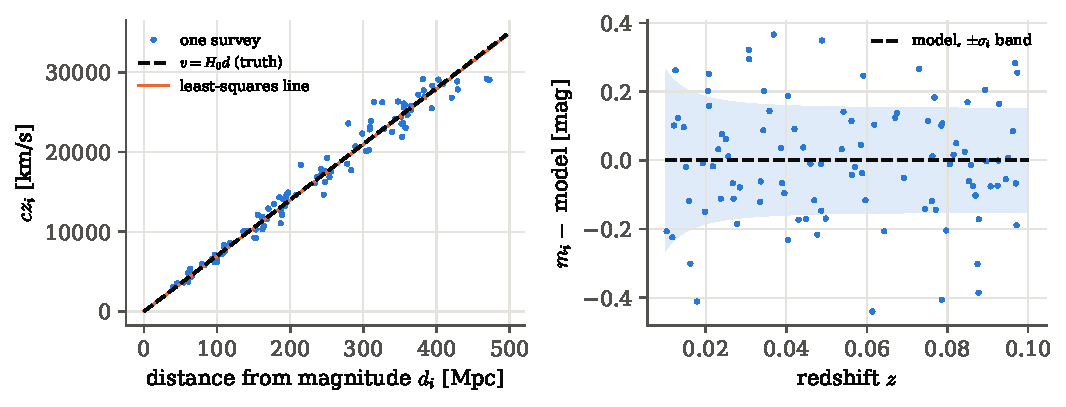
\includegraphics[width=12.5cm]{figures/ch03/hubble_mock.pdf}
\caption{One mock survey of $100$ supernovae. Left: recession velocity
against the distance inferred from each magnitude, with the true Hubble line
(dashed) and the least-squares line through the origin, which lies slightly
below it. The scatter grows in proportion to the distance. Right: the
magnitudes minus the model prediction at the true parameters. The noise is
Gaussian in this variable, with a width (shaded, $\pm\sigma_i$) that is
constant except at the lowest redshifts, where peculiar velocities add to
it.}
\label{3b:fig:hubble-mock}
\end{figure}

\subsection{Steps 2 and 3: the sufficient statistic and three candidates}
\label{3b:sec:hubble-candidates}

For the moment, pretend that the absolute magnitude $M$ of a type~Ia
supernova is known exactly. (It is not, and \cref{3b:sec:hubble-degeneracy}
shows that this changes everything about the error bar.) Each supernova
then gives its own estimate of $a=5\log_{10}H_0$,
\begin{equation}
  y_i\equiv M+25+5\log_{10}(cz_i)-m_i,
  \qquad \E\,y_i=a,\quad\Var y_i=\sigma_i^2 ,
  \label{3b:eq:sn-yi}
\end{equation}
by reading \eqref{3b:eq:sn-model} backwards. The likelihood
\eqref{3b:eq:hubble-like} is $\ln\Like=-\frac12\sum_iw_i(y_i-a)^2$ with the
weights $w_i\equiv1/\sigma_i^2$.

\paragraph{Step 2: the sufficient statistic.}
Let $W\equiv\sum_iw_i$ and $\bar y_w\equiv\sum_iw_iy_i/W$, the
inverse-variance weighted mean of the $y_i$. Then
\begin{align}
  \sum_iw_i(y_i-a)^2
  &\eqby{1}\sum_iw_i\bigl[(y_i-\bar y_w)+(\bar y_w-a)\bigr]^2\nonumber\\
  &\eqby{2}\sum_iw_i(y_i-\bar y_w)^2+2(\bar y_w-a)\sum_iw_i(y_i-\bar y_w)+W(\bar y_w-a)^2\nonumber\\
  &\eqby{3}\sum_iw_i(y_i-\bar y_w)^2+W(\bar y_w-a)^2 .
  \label{3b:eq:sn-split}
\end{align}
\begin{explain}
  \item Add and subtract $\bar y_w$.
  \item Expand the square; $\bar y_w-a$ does not depend on $i$.
  \item $\sum_iw_i(y_i-\bar y_w)=W\bar y_w-W\bar y_w=0$.
\end{explain}
So $\Like(a)=\exp[-W(\bar y_w-a)^2/2]\times\exp[-\sum_iw_i(y_i-\bar y_w)^2/2]$.
The first factor is the $g(U,a)$ of the factorisation theorem
(\cref{3b:sec:recipe-suff}) with $U=\bar y_w$, and the second is an $h(\data)$
that knows nothing about $a$. The weighted mean $\bar y_w$ is sufficient for
$a$, hence for $H_0=10^{a/5}$. Every estimator that is not a function of
$\bar y_w$ uses part of the data that carries no information about $H_0$,
and pays for it in variance or bias.

\paragraph{Candidate (a): fit the Hubble line to distances.}
Put $v_i\equiv cz_i$ on the vertical axis and the magnitude distances
$\tilde d_i$ of \eqref{3b:eq:dtilde} on the horizontal one, and minimise
$\sum_i(v_i-H\tilde d_i)^2$. Setting the derivative
$-2\sum_i\tilde d_i(v_i-H\tilde d_i)$ to zero,
\begin{equation}
  \hat H_{\rm naive}=\frac{\sum_iv_i\tilde d_i}{\sum_i\tilde d_i^{\,2}} .
  \label{3b:eq:h-naive}
\end{equation}
This is least squares, but for a model in which the noise sits in $v$ and the
horizontal coordinate is exact. Here the horizontal coordinate carries the
larger noise. For a large survey the numerator and the denominator, divided
by $N$, each converge to their means by the law of large numbers, so
$\hat H_{\rm naive}$ converges to the ratio of the means. With
$d_i=cz_i(1-x_i)/H_0$ and $\epsilon_i$ independent of $x_i$,
\begin{align}
  \E\bigl[v_i\tilde d_i\bigr]
  &\eqby{1}cz_i\,\E[d_i]\,\E\bigl[e^{\kappa\epsilon_i}\bigr]
   \eqby{2}\frac{(cz_i)^2}{H_0}\,e^{\kappa^2\sigma_{\rm int}^2/2},\nonumber\\
  \E\bigl[\tilde d_i^{\,2}\bigr]
  &\eqby{3}\E[d_i^2]\,\E\bigl[e^{2\kappa\epsilon_i}\bigr]
   \eqby{4}\frac{(cz_i)^2+\sigma_v^2}{H_0^2}\,e^{2\kappa^2\sigma_{\rm int}^2},\nonumber\\
  \hat H_{\rm naive}
  &\;\xrightarrow{N\to\infty}\;
   \frac{\sum_i\E[v_i\tilde d_i]}{\sum_i\E[\tilde d_i^{\,2}]}
   \eqby{5}H_0\,e^{-3\kappa^2\sigma_{\rm int}^2/2}\;
   \frac{\sum_i(cz_i)^2}{\sum_i\bigl[(cz_i)^2+\sigma_v^2\bigr]} .
  \label{3b:eq:naive-bias}
\end{align}
\begin{explain}
  \item $v_i=cz_i$ is fixed; $\tilde d_i=d_ie^{\kappa\epsilon_i}$ and the two
        factors are independent.
  \item $\E d_i=cz_i/H_0$ since $\E x_i=0$, and \eqref{3b:eq:lognormal-mgf}
        with $t=\kappa$.
  \item As in (1), with $\tilde d_i^{\,2}=d_i^2e^{2\kappa\epsilon_i}$.
  \item $\E d_i^2=(cz_i)^2\E(1-x_i)^2/H_0^2=[(cz_i)^2+\sigma_v^2]/H_0^2$,
        and \eqref{3b:eq:lognormal-mgf} with $t=2\kappa$.
  \item Divide; $e^{\kappa^2\sigma^2/2}/e^{2\kappa^2\sigma^2}=e^{-3\kappa^2\sigma^2/2}$.
\end{explain}
The limit is not $H_0$. The dominant factor, $e^{-3\kappa^2\sigma_{\rm int}^2/2}$,
gives a bias of $\ThreeBHNaiveBiasLead$~km/s/Mpc for $\sigma_{\rm int}=\ThreeBHsigInt$;
the peculiar velocities lower it a little further, to $\ThreeBHNaiveBiasTh$ for
the redshift range of the survey. The mechanism is the textbook one for noise
in the horizontal variable (``regression dilution''): the scatter of
$\tilde d_i$ inflates $\sum\tilde d_i^{\,2}$ more than it inflates
$\sum v_i\tilde d_i$, and the slope is pulled down. Because the limit
\eqref{3b:eq:naive-bias} does not involve $N$, the estimator is
\emph{inconsistent}: more supernovae make it converge faster to the wrong
number. Only the $O(1/N)$ corrections to the ratio of means depend on the
survey size.

\paragraph{Candidate (b): average the individual ratios.}
Each supernova gives its own $H_0$ as $v_i/\tilde d_i$, and we average them:
$\hat H_{\rm ratio}=\frac1N\sum_iv_i/\tilde d_i$. Each term is
\[
  \frac{v_i}{\tilde d_i}=\frac{cz_i\,e^{-\kappa\epsilon_i}}{d_i}
  =H_0\,\frac{e^{-\kappa\epsilon_i}}{1-x_i},
\]
and its mean follows from \eqref{3b:eq:lognormal-mgf} with $t=-\kappa$ and
$1/(1-x)=1+x+x^2+\dots$, so that $\E(1-x_i)^{-1}\approx1+\sigma_v^2/(cz_i)^2$:
\begin{equation}
  \E\,\hat H_{\rm ratio}\approx H_0\,e^{\kappa^2\sigma_{\rm int}^2/2}\,
  \frac1N\sum_i\Bigl[1+\frac{\sigma_v^2}{(cz_i)^2}\Bigr].
  \label{3b:eq:ratio-bias}
\end{equation}
The bias now has the opposite sign, $\ThreeBHRatioBiasLead$~km/s/Mpc from the
magnitude scatter and $\ThreeBHRatioBiasTh$ in total, because the nearest
supernovae have large $x_i$. It is again independent of $N$. The mean of
ratios is not the ratio of means, and averaging a nonlinear function of noisy
numbers averages its bias too.

\paragraph{Candidate (c): maximum likelihood.}
The score of \eqref{3b:eq:hubble-like} is
$\partial\ln\Like/\partial a=\sum_iw_i(y_i-a)=W(\bar y_w-a)$, which vanishes at
\begin{equation}
  \hat a=\bar y_w=\frac{\sum_iw_i\bigl[M+25+5\log_{10}(cz_i)-m_i\bigr]}{\sum_iw_i},
  \qquad w_i=\frac1{\sigma_i^2},
  \qquad \hat H_0=10^{\hat a/5}.
  \label{3b:eq:hubble-ml}
\end{equation}
It is the weighted mean of \cref{3a:sec:weighted}, applied to the
individual estimates $y_i$ of $a$ in the variable where their noise is
Gaussian, and it is a function of the sufficient statistic only.

\emph{Bias.} $\E\hat a=\sum_iw_i\E y_i/W=a$: unbiased, to the order of
\eqref{3b:eq:sn-model}. The neglected term, $-(5/\ln10)\ln(1-x_i)=(5/\ln10)(x_i+x_i^2/2+\dots)$,
has mean $(5/\ln10)\,\sigma_v^2/2(cz_i)^2$, which after weighting is
$\ThreeBHaBiasLin$~mag, about a twentieth of the error bar.

\emph{Variance and efficiency.} The $y_i$ are independent, so
\begin{align}
  \Var\hat a
  &\eqby{1}\frac{\sum_iw_i^2\,\Var y_i}{W^2}
   \eqby{2}\frac{\sum_iw_i}{W^2}=\frac1W,
  \qquad
  I(a)\eqby{3}-\E\frac{\partial^2\ln\Like}{\partial a^2}=\sum_iw_i=W .
  \label{3b:eq:hubble-fisher}
\end{align}
\begin{explain}
  \item The variance of a sum of independent terms is the sum of the variances,
        and a constant factor comes out squared.
  \item $w_i^2\Var y_i=w_i^2\sigma_i^2=w_i$.
  \item Differentiate the score $\sum_iw_i(y_i-a)$ once more; the result
        $-W$ is not random, so the expectation does nothing.
\end{explain}
The variance equals $1/I(a)$: the estimator sits on the Cram\'er--Rao bound
\eqref{3b:eq:cramer-rao}. The score $W(\bar y_w-a)$ is a linear function of
$\hat a$, the condition for equality. The error bar is
$\sigma_a=W^{-1/2}$, and by linear propagation through $H_0=e^{\kappa a}$,
$\sigma_{H_0}=\kappa H_0\sigma_a$.

\emph{From $a$ to $H_0$.} The invariance of maximum likelihood
(\cref{3b:sec:invariance}) makes $\hat H_0=10^{\hat a/5}$ the maximum-likelihood
estimator of $H_0$. It is not exactly unbiased, because the exponential is
convex. Expand $g(\hat a)=e^{\kappa\hat a}$ around the truth to second order
(the delta method of \cref{3a:sec:delta}, one order further):
\begin{align}
  \E\,\hat H_0
  &\eqby{1}\E\Bigl[g(a)+g'(a)(\hat a-a)+\tfrac12g''(a)(\hat a-a)^2\Bigr]
   \eqby{2}H_0\Bigl(1+\tfrac12\kappa^2\sigma_a^2\Bigr)
   \relby{3}{\approx}H_0\,e^{\kappa^2\sigma_a^2/2}.
  \label{3b:eq:hubble-delta}
\end{align}
\begin{explain}
  \item Taylor expansion of $g$; higher orders are smaller by further powers of $\sigma_a$.
  \item $g'=\kappa H_0$, $g''=\kappa^2H_0$; $\E(\hat a-a)=0$ and $\E(\hat a-a)^2=\sigma_a^2$.
  \item Because $\hat a$ is exactly Gaussian, \eqref{3b:eq:lognormal-mgf} with
        $t=\kappa$ gives the exponential exactly; the delta method gives its
        first two terms.
\end{explain}
The bias-corrected estimator is $\hat H_0\,e^{-\kappa^2\sigma_a^2/2}$. Since
$\sigma_a\to0$ as $N$ grows, the uncorrected $\hat H_0$ is consistent. For
$100$ supernovae $\sigma_a\approx\ThreeBHaSdTh$ and the bias is
$\ThreeBHMLBiasTh$~km/s/Mpc, utterly negligible. It matters when $\sigma_a$
is large: an $H_0$ from a single supernova ($\sigma_a=0.15$) is biased by
$0.24\%$, and averaging many such single-object values accumulates the
bias coherently, which is exactly what went wrong with candidate (b). The
cure is always the same: average in the variable where the noise is
Gaussian and transform once at the end. The median of $\hat H_0$ is exactly
$H_0$ (the exponential is monotonic), and the interval
$[10^{(\hat a-\sigma_a)/5},10^{(\hat a+\sigma_a)/5}]$ has exactly the coverage of
$\hat a\pm\sigma_a$.

\begin{keyidea}[The maximum-likelihood estimator of $H_0$]
Work in the variable where the noise is Gaussian. For low-redshift
supernovae with calibrated $M$ that is $a=5\log_{10}H_0$, and the
estimator is the inverse-variance weighted mean
\eqref{3b:eq:hubble-ml} of the single-object values
$M+25+5\log_{10}(cz_i)-m_i$, with $\sigma_i^2$ from \eqref{3b:eq:sn-sigma}.
It is sufficient, unbiased for $a$, on the Cram\'er--Rao bound $\sigma_a=(\sum_iw_i)^{-1/2}$,
and $10^{\hat a/5}$ is consistent for $H_0$. Converting magnitudes to
distances first gives inconsistent estimators.
\end{keyidea}

\subsection{Step 4: comparing the candidates on simulated surveys}
\label{3b:sec:hubble-mc}

The three biases \eqref{3b:eq:naive-bias}, \eqref{3b:eq:ratio-bias},
\eqref{3b:eq:hubble-delta} are large-$N$ approximations, and the claim that
the maximum-likelihood error bar is right is a statement about repeated
surveys. Both can be checked by simulating many surveys from a known truth,
which is the verification use of Monte Carlo (\cref{ch:06}).

\pyfile[firstline=40,lastline=66]{code/ch03/17_hubble_estimator.py}{Mock supernova surveys and the three estimators of $H_0$}
The function \pyname{sigma_mag} is \eqref{3b:eq:sn-sigma}. The function
\pyname{mock_lowz} draws redshifts uniformly in $0.01<z<0.1$, a peculiar
velocity for each galaxy, the true distance from \eqref{3b:eq:hubble-law}
and a magnitude from \eqref{3b:eq:sn-mag}; it generates the data from the
physics, not from the linearised likelihood, so the approximation in
\eqref{3b:eq:sn-model} is tested too. The arrays have one row per survey,
and every estimator sums over the last axis, so $\ThreeBHNmock$ surveys of
$\ThreeBHN$ supernovae are processed at once. \pyname{naive} is
\eqref{3b:eq:h-naive}, \pyname{ratio} the mean of $v_i/\tilde d_i$, and
\pyname{ml} returns $10^{\hat a/5}$, $\hat a$ and $\sigma_a=W^{-1/2}$ from
\eqref{3b:eq:hubble-ml} and \eqref{3b:eq:hubble-fisher}.

\begin{center}
\small
\begin{tabular}{@{}lcccc@{}}
\toprule
estimator & mean bias & predicted bias & scatter & rms error\\
 & [km/s/Mpc] & [km/s/Mpc] & [km/s/Mpc] & [km/s/Mpc]\\\midrule
(a) least-squares line \eqref{3b:eq:h-naive} & $\ThreeBHNaiveBias$ & $\ThreeBHNaiveBiasTh$ & $\ThreeBHNaiveSd$ & $\ThreeBHNaiveRmse$\\
(b) mean of ratios & $\ThreeBHRatioBias$ & $\ThreeBHRatioBiasTh$ & $\ThreeBHRatioSd$ & $\ThreeBHRatioRmse$\\
(c) maximum likelihood \eqref{3b:eq:hubble-ml} & $\ThreeBHMLBias$ & $\ThreeBHMLBiasTh$ & $\ThreeBHMLSd$ & $\ThreeBHMLRmse$\\
\bottomrule
\end{tabular}
\end{center}
The predicted biases are \eqref{3b:eq:naive-bias} and \eqref{3b:eq:ratio-bias}
averaged over the simulated redshifts, and for (c) the convexity term of
\eqref{3b:eq:hubble-delta}. The first two agree with the simulation to within
the $O(1/N)$ corrections: for surveys of $400$ supernovae the measured biases
are $\ThreeBHNaiveBiasFour$ and $\ThreeBHRatioBiasFour$, no smaller, while the
scatter of the maximum-likelihood estimator halves to $\ThreeBHMLSdFour$. The
least-squares line is off by about one standard deviation for $100$ supernovae
and by two for $400$. The small residual bias of (c) is not the convexity term
but the second-order peculiar-velocity term: the simulated mean of $\hat a$ is
too large by $\ThreeBHaBias$~mag, against the predicted $\ThreeBHaBiasLin$.
The scatter of $\hat a$ is $\ThreeBHaSd$ against the Cram\'er--Rao value
$\ThreeBHaSdTh$, and the interval $\hat a\pm\sigma_a$ covers the truth in a
fraction $\ThreeBHCovOne$ of the surveys ($\pm1.96\sigma_a$: $\ThreeBHCovTwo$),
as a $68\%$ and a $95\%$ interval should. \Cref{3b:fig:hubble-estimators} shows the three
sampling distributions.

\begin{figure}[htbp]
\centering
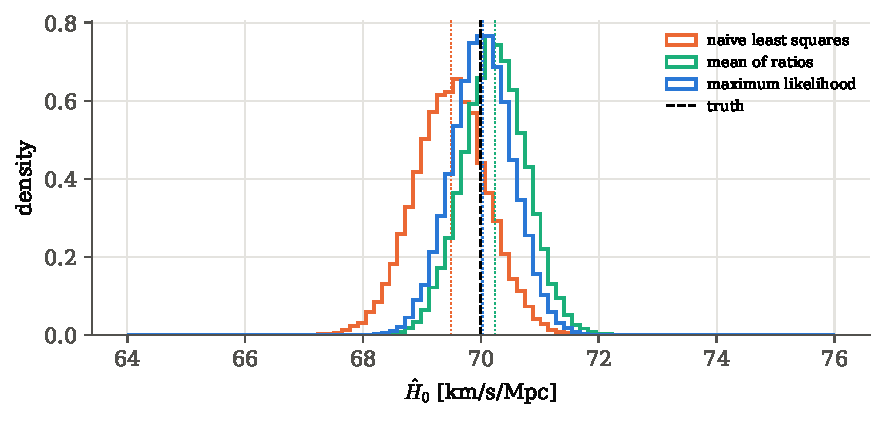
\includegraphics[width=11cm]{figures/ch03/hubble_estimators.pdf}
\caption{Sampling distributions of the three estimators of $H_0$ over
$20\,000$ mock surveys of $100$ supernovae with $H_0=70$ (dashed). The
dotted lines mark the means. The least-squares line through the magnitude
distances is shifted low and is also the widest; the mean of the individual
ratios is shifted high; the maximum-likelihood estimator is centred on the
truth and is the narrowest.}
\label{3b:fig:hubble-estimators}
\end{figure}

\subsection{What supernovae alone cannot tell us: the \texorpdfstring{$H_0$--$M$}{H0-M} degeneracy}
\label{3b:sec:hubble-degeneracy}

Look again at the likelihood \eqref{3b:eq:hubble-like}. The absolute magnitude
$M$ and $a=5\log_{10}H_0$ appear only in the combination $M-a$. Increasing
both by the same amount leaves every prediction, and so the likelihood,
unchanged. The only thing the supernovae measure is the combination
\[
  \mathcal M\equiv M-5\log_{10}H_0+25 ,
\]
which is a statement about the product ``luminosity times $H_0^{-2}$'':
brighter candles in a faster-expanding universe look exactly like fainter
candles in a slower one. In the Fisher matrix of \eqref{3b:eq:hubble-like} for
the two parameters $(M,a)$,
\begin{align}
  \Fish
  &\eqby{1}\sum_iw_i
   \begin{pmatrix}
     1 & -1\\ -1 & 1
   \end{pmatrix}
   =W\begin{pmatrix}1&-1\\-1&1\end{pmatrix},
  \qquad
  \det\Fish\eqby{2}W^2-W^2=0 ,
  \label{3b:eq:hubble-fisher2}
\end{align}
\begin{explain}
  \item $F_{jk}=-\E\,\partial^2\ln\Like/\partial\theta_j\partial\theta_k$; the
        residual is $m_i-M-25-5\log_{10}(cz_i)+a$, whose derivatives are
        $-1$ for $M$ and $+1$ for $a$, so each supernova contributes $w_i$
        times the product of the two derivatives.
  \item Determinant of the $2\times2$ matrix.
\end{explain}
A singular Fisher matrix has a zero mode: the direction $(\delta M,\delta
a)\propto(1,1)$ costs no likelihood at all, and the variance along it is
infinite. \Cref{3b:fig:hubble-degeneracy} shows this for the survey of
\cref{3b:fig:hubble-mock}. The $\Delta\chi^2$ contours in the $(M,H_0)$ plane are an
open band along $H_0\propto10^{M/5}$, and the $\chi^2$ as a function of $H_0$ at
three fixed values of $M$ has three different minima of exactly the same
depth. Evaluated numerically for that survey, $\det\Fish=\ThreeBHFishDet$ to
rounding.

The absolute magnitude must therefore come from somewhere else: from
supernovae in galaxies whose distances are measured independently, with
Cepheid variables or the tip of the red giant branch, which are in turn
calibrated geometrically with parallaxes. This is the \newterm{distance
ladder}. The distance-ladder value of $H_0$ is $73.04\pm1.04$~km/s/Mpc
\cite{Riess2022SH0ES}, while the CMB with $\Lambda$CDM gives $67.36\pm0.54$
\cite{Planck2018VI}, $4.8$ standard deviations apart: the \newterm{Hubble tension}. Since supernovae only fix
$M-5\log_{10}H_0$, the same tension can be stated as a disagreement of
$5\log_{10}(73.04/67.36)=0.18$~mag in the absolute magnitude of type~Ia supernovae.
The ladder that supplies $M$ is built as one linear model, with its error budget rung by rung, in
\cref{T2b:sec:ladder}, where the tension is also computed (\cref{T2b:sec:tension}).

\paragraph{A calibrated $M$ as a nuisance parameter.}
Suppose the calibrators give $M=M_{\rm cal}\pm\sigma_M$ with Gaussian errors.
That is one more measurement, independent of the Hubble-flow supernovae, and
its log-likelihood $-(M-M_{\rm cal})^2/2\sigma_M^2$ adds to
\eqref{3b:eq:hubble-like}. The Fisher matrix gains $1/\sigma_M^2$ in its
$MM$ element. The variance of $\hat a$, with $M$ treated as a nuisance
parameter, is the $aa$ element of the inverse:
\begin{align}
  \Fish'
  &=\begin{pmatrix}W+\sigma_M^{-2}&-W\\-W&W\end{pmatrix},
  \qquad
  \det\Fish'\eqby{1}\frac{W}{\sigma_M^2},
  \nonumber\\
  \sigma_a^2=(\Fish'^{-1})_{aa}
  &\eqby{2}\frac{W+\sigma_M^{-2}}{W/\sigma_M^2}
   \eqby{3}\frac1W+\sigma_M^2 .
  \label{3b:eq:hubble-calib}
\end{align}
\begin{explain}
  \item $(W+\sigma_M^{-2})W-W^2=W/\sigma_M^2$.
  \item The $(2,2)$ element of the inverse of a $2\times2$ matrix is its $(1,1)$
        element divided by the determinant.
  \item Divide term by term.
\end{explain}
This is the profile-likelihood variance $V_{\theta\theta}$ of
\eqref{3b:eq:profile-gauss} with $\theta=a$ and $\nu=M$: maximising the
likelihood over $M$ at each $a$ gives a parabola in $a$ of exactly this
width, and for a Gaussian likelihood marginalising over $M$ gives the same
(\cref{3b:sec:marginalise}). The two errors add in quadrature: the
statistical error of the Hubble-flow sample and the calibration error. The
estimator itself is \eqref{3b:eq:hubble-ml} with $M=M_{\rm cal}$, because
the Hubble-flow supernovae cannot move $M$ at all.

For the simulated surveys $W^{-1/2}=\ThreeBHsaStat$~mag, and with a
calibration of $\sigma_M=\ThreeBHsigM$~mag, typical of current ladders, the
total is $\sigma_a=\ThreeBHsaCal$~mag: the calibration dominates, and adding
more Hubble-flow supernovae hardly helps. In the simulation each survey
gets its own calibration $M_{\rm cal}$ drawn around the truth. The scatter of
$\hat H_0$ is then $\ThreeBHCalSd$~km/s/Mpc against the predicted
$\kappa H_0\sigma_a=\ThreeBHCalSdTh$, and the interval with the full
$\sigma_a$ covers the truth in $\ThreeBHCalCovOne$ of the surveys. Quoting only the
statistical error $W^{-1/2}$ would give intervals that cover the truth in
$\ThreeBHCalCovNaive$ of the surveys, instead of $68\%$.

\begin{figure}[htbp]
\centering
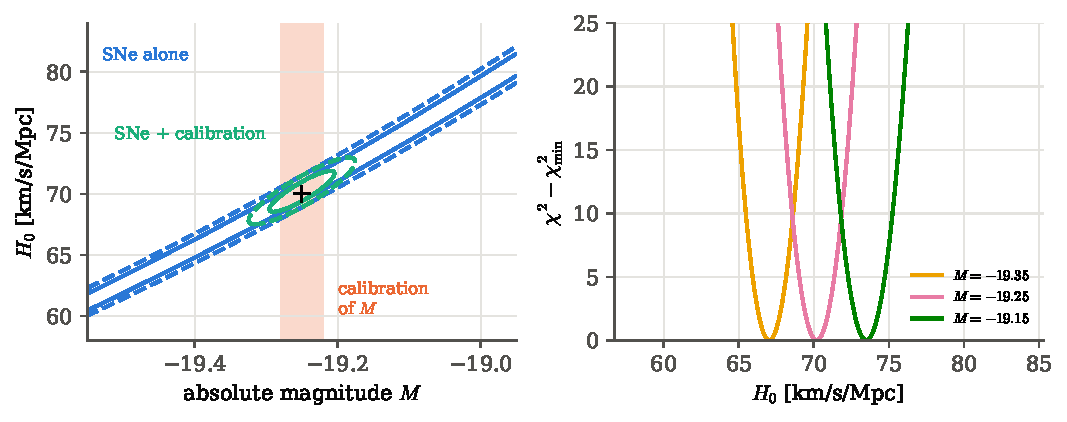
\includegraphics[width=12.5cm]{figures/ch03/hubble_degeneracy.pdf}
\caption{The degeneracy between $H_0$ and the absolute magnitude $M$ for one
survey of $100$ supernovae. Left: $\Delta\chi^2=2.30$ (solid) and $6.18$
(dashed) contours. The supernovae alone allow an open band; a calibration of $M$
to $\pm0.03$~mag (vertical strip) closes it into a small ellipse, whose
height is set mostly by the width of the strip. Right: $\chi^2$ against $H_0$
at three fixed values of $M$. Each has a perfectly good minimum of the same
depth, at a different $H_0$.}
\label{3b:fig:hubble-degeneracy}
\end{figure}

\begin{pitfall}[An error bar that forgets the calibration]
Fixing $M$ at a calibrated value and reporting the curvature error of the
Hubble-flow fit, $\kappa H_0W^{-1/2}$, conditions on the nuisance parameter
instead of profiling it. The interval is too short by the factor
$(1+W\sigma_M^2)^{-1/2}$, here about one half, and its coverage falls from
$68\%$ to about a third. The calibration error must be carried into every
number derived from the calibrated supernovae.
\end{pitfall}

\subsection{Beyond low redshift: the luminosity distance and a profile over \texorpdfstring{$\Omega_{m0}$}{Omega\_m0}}
\label{3b:sec:hubble-highz}

At larger redshift the Hubble law bends. In a flat universe with matter
density parameter $\Omega_{m0}$ and a cosmological constant, neglecting
radiation, the luminosity distance is a standard result of cosmology,
taken here as an input:
\begin{equation}
  D_L(z)=\frac{c}{H_0}\,(1+z)\int_0^z\frac{\dd z'}{E(z')},
  \qquad
  E(z)=\sqrt{\Omega_{m0}(1+z)^3+1-\Omega_{m0}} ,
  \label{3b:eq:dl}
\end{equation}
the distance travelled by light through an expanding universe whose
expansion rate is $H_0E(z)$. The model for the magnitudes becomes
$m_i=M+25+5\log_{10}(D_L(z_i)/\text{Mpc})+\text{noise}$. Write
$\bar D_L\equiv H_0D_L/c$ for the dimensionless integral, which depends on
$\Omega_{m0}$ but not on $H_0$. Then
\begin{equation}
  m_i=M+25+5\log_{10}\bigl[c\,\bar D_L(z_i;\Omega_{m0})\bigr]-a+\text{noise},
  \label{3b:eq:sn-model-dl}
\end{equation}
so $a$ still enters additively, and $M$ and $a$ are still degenerate: the
whole of \cref{3b:sec:hubble-degeneracy} carries over unchanged. What is new
is that the model depends on $\Omega_{m0}$ through an integral, nonlinearly.
The maximum-likelihood estimator is the minimum of
$\chi^2(a,\Omega_{m0})=\sum_iw_i[y_i(\Omega_{m0})-a]^2$, with
$y_i(\Omega_{m0})=M+25+5\log_{10}[c\bar D_L(z_i;\Omega_{m0})]-m_i$. At fixed
$\Omega_{m0}$ the minimum over $a$ is the weighted mean
$\hat a(\Omega_{m0})=\sum_iw_iy_i(\Omega_{m0})/W$ as before, and substituting
it leaves the profile $\chi^2_p(\Omega_{m0})=\sum_iw_i[y_i-\hat a(\Omega_{m0})]^2$,
a function of one variable that a one-dimensional minimiser handles.

\pyfile[firstline=180,lastline=184]{code/ch03/17_hubble_estimator.py}{The flat-$\Lambda$CDM luminosity distance}
\pyname{dl_bar} evaluates $\bar D_L$ by integrating $1/E$ with the trapezoidal
rule on a fine grid and interpolating at the supernova redshifts. At the
Planck 2018 best-fit parameters, it agrees with the luminosity
distance computed by CAMB to a fractional $\ThreeBHCambDiff$ out to $z=1$; CAMB
includes radiation and massive neutrinos, which is the size of the
difference.

\pyfile[firstline=207,lastline=219]{code/ch03/17_hubble_estimator.py}{Profiling $a=5\log_{10}H_0$ analytically and minimising over $\Omega_{m0}$}
The simulated surveys have $\ThreeBHNhz$ supernovae uniform in
$0.01<z<1$, with $H_0=\ThreeBHTrue$ and $\Omega_{m0}=0.3$, and $M$ known.
\pyname{profile_chi2} returns $\chi^2_p$ and $\hat a$ at one
$\Omega_{m0}$, and \pyname{minimize_scalar} finds the minimum over
$\Omega_{m0}$. For the first survey a direct two-dimensional minimisation of
$\chi^2(H_0,\Omega_{m0})$ with Nelder--Mead gives $H_0=\ThreeBHhzTwoD$,
$\Omega_{m0}=\ThreeBOmhzTwoD$, the same as the profile ($\ThreeBHhzProf$,
$\ThreeBOmhzProf$): analytic profiling over the linear parameter loses nothing.

Over $\ThreeBHNmockhz$ surveys the estimates of $H_0$ average
$\ThreeBHhzMean$ with a scatter of $\ThreeBHhzSd$~km/s/Mpc, and those of
$\Omega_{m0}$ average $\ThreeBOmhzMean$ with a scatter of $\ThreeBOmhzSd$: both
are unbiased. The Fisher matrix in $(a,\Omega_{m0})$, computed with a
numerical derivative of $5\log_{10}\bar D_L$ with respect to $\Omega_{m0}$,
predicts $\ThreeBHhzSdTh$ and $\ThreeBOmhzSdTh$. With $\Omega_{m0}$ held fixed
the $H_0$ error would be only $\ThreeBHhzSdFixed$: the two estimates are
correlated with $\rho=\ThreeBHhzRho$, and profiling over $\Omega_{m0}$ widens
the error by $1/\sqrt{1-\rho^2}$, exactly the mechanism of
\cref{3b:sec:profile-width}. A higher $\Omega_{m0}$ decelerates the expansion,
makes distant supernovae nearer and brighter, and is compensated by a lower $H_0$.

\paragraph{When does the straight Hubble law fail?}
Expanding \eqref{3b:eq:dl} in $z$ gives the distance modulus
$\mu=25+5\log_{10}(cz/H_0)+1.086\,(1-q_0)\,z+O(z^2)$, where
$1.086=5/(2\ln10)$ and $q_0$ is the deceleration parameter, $q_0=\tfrac32\Omega_{m0}-1=\ThreeBHqZero$
for flat $\Lambda$CDM. The pure Hubble law drops the linear term. Applying
the estimator \eqref{3b:eq:hubble-ml} to noiseless $\Lambda$CDM magnitudes
with redshifts up to $z_{\max}$ gives its bias directly, since the estimator
is linear in the data (\cref{3b:fig:hubble-highz}, right). For $z_{\max}=0.05$ the bias is
$\ThreeBHlawBiasFive$~km/s/Mpc, for $z_{\max}=0.1$ it is $\ThreeBHlawBiasTen$,
about six times the statistical error $\ThreeBHlawSigTen$ of $100$
supernovae. The Monte Carlo surveys confirm it: $\ThreeBHlawBiasMCTen$ at
$z_{\max}=0.1$ and $\ThreeBHlawBiasMCThirty$ at $0.3$ (predicted
$\ThreeBHlawBiasThirty$). The bias exceeds the statistical error of $100$
supernovae already for $z_{\max}\approx\ThreeBHlawZcross$. Keeping the $q_0$ term
moves this to $z_{\max}\approx\ThreeBHqZcross$, with a bias of
$\ThreeBHqBiasTen$~km/s/Mpc at $z_{\max}=0.1$ but $\ThreeBHqBiasFiveH$ at $0.5$; beyond that
only the full \eqref{3b:eq:dl} is safe. In practice the ``low-redshift''
estimator means the Hubble law with the $q_0$ term (and often the next one)
applied to $0.02\lesssim z\lesssim0.15$: the lower cut removes the supernovae
whose peculiar velocities dominate, the upper cut keeps the expansion
accurate. Like the bias of the least-squares line, this is a bias of a wrong
model, and it does not average away.

\begin{figure}[htbp]
\centering
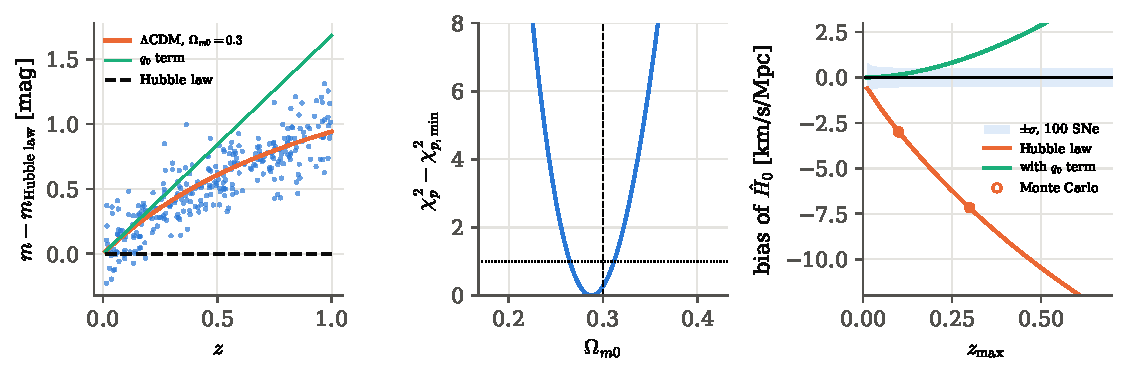
\includegraphics[width=12.8cm]{figures/ch03/hubble_highz.pdf}
\caption{Supernovae beyond the linear Hubble law. Left: one survey of $300$
supernovae to $z=1$, as magnitudes minus the Hubble-law prediction; the
$\Lambda$CDM curve follows the points, the first-order $q_0$ term follows
them only at low redshift. Middle: the profile $\chi^2_p(\Omega_{m0})$ of that
survey, with $a$ minimised analytically at each $\Omega_{m0}$; the dotted line
is $\Delta\chi^2=1$, the dashed line the truth. Right: bias of $\hat H_0$ from
fitting the pure Hubble law and the law with the $q_0$ term to supernovae up to
$z_{\max}$, compared with the $\pm1\sigma$ statistical error of $100$
supernovae (shaded); the circles are Monte Carlo checks.}
\label{3b:fig:hubble-highz}
\end{figure}

\paragraph{How the measurement is done in research.}
Real analyses solve the same problem with the same structure, on a larger
scale. The SH0ES measurement \cite{Riess2022SH0ES} writes the Cepheid
magnitudes in the anchor galaxies (with geometric distances), the Cepheids
and supernovae in the calibrator galaxies, and the Hubble-flow supernovae
($0.023<z<0.15$, with the $q_0$ and $j_0$ expansion terms) as one linear
model $\bm y=A\bm\theta+\text{noise}$ with a full covariance matrix, and
solves it by generalised least squares, $\hat{\bm\theta}=(A\T\Cmat^{-1}A)^{-1}A\T\Cmat^{-1}\bm y$
\eqref{3b:eq:normal-eq}. The parameter vector contains $M$ and $5\log_{10}H_0$
together with the Cepheid period--luminosity parameters and the host
distances, so the degeneracy of \cref{3b:sec:hubble-degeneracy} is broken
inside one fit and $\sigma_M$ is propagated automatically. The Pantheon+
analysis \cite{Brout2022PantheonPlus} fits $1550$ supernovae with a
covariance matrix that includes calibration and light-curve systematics, and
fits $M$, $H_0$ and $\Omega_{m0}$ jointly with the SH0ES calibrators, profiling or
marginalising over the light-curve standardisation parameters. Two things
our mock surveys ignored enter there: a magnitude-limited survey preferentially
finds the brighter supernovae at large distance, a selection bias that no
choice of estimator removes and that is calibrated by simulating the survey
(step~5, \cref{3b:sec:recipe-intractable}); and correlated systematics, which
are what the off-diagonal covariance is for (\cref{3b:sec:correlated}). The same
problem can be posed as Bayesian inference, with priors on
$(M,H_0,\Omega_{m0})$ and a Markov chain exploring the posterior; \cref{ch:09}
builds those chains, and \cref{9c:sec:importance} uses one to add the SH0ES value to a CMB chain by reweighting.
How the error on $H_0$ is assembled from the errors of the rungs, before any data are taken, is the
error budget of \cref{T2b:sec:ladder}, and the Fisher matrix of \cref{ch:10} returns to $H_0$ as a
parameter derived from the CMB in \cref{10a:sec:cmb-planck}.

\subsection{A second probe: cosmic chronometers, where \texorpdfstring{$H_0$}{H0} enters linearly}
\label{3b:sec:hubble-cc}

Supernovae measure distances, and the expansion rate enters only through the integral that
relates distance to $H(z)$. There is another method that measures $H(z)$ more directly.
Consider galaxies that formed their stars early in cosmic history and then stopped forming new
stars. Since no new stars are being added, their stellar populations simply grow older as the
Universe evolves, and as the stars age, the spectrum of the galaxy changes in a predictable
way. The observed spectrum can therefore be used to estimate the age of the stellar population
at a given redshift. Comparing similar passively evolving galaxies at two nearby redshifts, the
difference in their ages measures the difference in cosmic time between those redshifts, which
gives $\dd t/\dd z$. Since $1+z=a^{-1}$,
\begin{equation}
  H(z)=-\frac{1}{1+z}\,\frac{\dd z}{\dd t}=-\frac{1}{1+z}\left(\frac{\dd t}{\dd z}\right)^{-1}.
  \label{3b:eq:cc-hz}
\end{equation}
These galaxies are therefore used as \newterm{cosmic chronometers}: clocks whose age
differences give $H(z)$ without any distance.
A chronometer survey delivers $N$ triples $(z_i,H_i,\sigma_i)$: a redshift,
a measured expansion rate in km/s/Mpc, and its error bar.

\paragraph{The event, and what could have produced it.}
What we observed is the number $H_i$ at redshift $z_i$. What made it come out that way? Two
things: the true expansion rate at $z_i$, and the measurement error. In flat $\Lambda$CDM the
true rate is $H_{\rm th}(z;H_0,\Omega_{m0})=H_0\,E(z;\Omega_{m0})$, with the same $E$ as in
\eqref{3b:eq:dl}. The errors of the age measurements are independent from point to point and
Gaussian with standard deviation $\sigma_i$. So for each candidate pair $(H_0,\Omega_{m0})$ the
noise needed to turn the prediction into the data is $H_i-H_0E_i$, with $E_i\equiv E(z_i;\Omega_{m0})$,
and how plausible that noise is gives the likelihood: $-2\ln\Like=\chi^2+\text{const}$ with
\[
  \chi^2(H_0,\Omega_{m0})=\sum_{i=1}^{N}\frac{\bigl(H_i-H_0E_i\bigr)^2}{\sigma_i^2}.
\]
Here is the feature that makes the problem easy. The matter density enters $E_i$ through a
square root, nonlinearly, but $H_0$ only multiplies it: \emph{the model is linear in $H_0$}. At
fixed $\Omega_{m0}$ the $\chi^2$ is therefore a quadratic function of $H_0$, a parabola, and its
minimum can be written down. With the three sums $S_{HH}\equiv\sum_iH_i^2/\sigma_i^2$,
$S_{HE}\equiv\sum_iH_iE_i/\sigma_i^2$ and $S_{EE}\equiv\sum_iE_i^2/\sigma_i^2$,
\begin{align}
  \chi^2(H_0)
  &\eqby{1}S_{HH}-2H_0\,S_{HE}+H_0^2\,S_{EE},
  \nonumber\\
  \frac{\dd\chi^2}{\dd H_0}
  &\eqby{2}-2S_{HE}+2H_0\,S_{EE}=0
  \quad\Longrightarrow\quad
  \hat H_0=\frac{S_{HE}}{S_{EE}}=\frac{\sum_iH_iE_i/\sigma_i^2}{\sum_iE_i^2/\sigma_i^2},
  \label{3b:eq:cc-estimator}\\
  \chi^2(H_0)
  &\eqby{3}S_{EE}\bigl(H_0-\hat H_0\bigr)^2+\chi^2_{\min},
  \qquad \chi^2_{\min}=S_{HH}-\frac{S_{HE}^2}{S_{EE}} .
  \nonumber
\end{align}
\begin{explain}
  \item Expand $(H_i-H_0E_i)^2=H_i^2-2H_0H_iE_i+H_0^2E_i^2$, divide by $\sigma_i^2$ and sum;
        $H_0$ does not depend on $i$.
  \item Differentiate the quadratic; $S_{EE}>0$, so the stationary point is the minimum.
  \item Complete the square: $S_{EE}(H_0-\hat H_0)^2=S_{EE}H_0^2-2H_0S_{HE}+S_{HE}^2/S_{EE}$.
\end{explain}
No minimiser is needed. The estimator is a \emph{weighted ratio}, and it is also a weighted
mean: each point gives its own estimate $H_i/E_i$ of $H_0$, with variance $\sigma_i^2/E_i^2$,
and \eqref{3b:eq:cc-estimator} is $\sum_iw_i(H_i/E_i)/\sum_iw_i$ with the inverse variances
$w_i=E_i^2/\sigma_i^2$ as weights, exactly the weighted mean of \cref{3a:sec:weighted}.

\paragraph{Bias, variance and the bound.}
The $H_i$ are independent with $\E H_i=H_0E_i$ and $\Var H_i=\sigma_i^2$, and the $E_i$ are
fixed numbers at fixed $\Omega_{m0}$. Then
\begin{align}
  \E\,\hat H_0
  &\eqby{1}\frac{\sum_iE_i\,\E H_i/\sigma_i^2}{S_{EE}}
   \eqby{2}\frac{H_0\sum_iE_i^2/\sigma_i^2}{S_{EE}}=H_0,
  \nonumber\\
  \Var\hat H_0
  &\eqby{3}\frac{\sum_iE_i^2\,\Var H_i/\sigma_i^4}{S_{EE}^2}
   \eqby{4}\frac{S_{EE}}{S_{EE}^2}=\frac{1}{\sum_iE_i^2/\sigma_i^2},
  \nonumber\\
  I(H_0)
  &\eqby{5}\E\Bigl[\frac{\partial^2(-\ln\Like)}{\partial H_0^2}\Bigr]
   \eqby{6}\frac12\,\frac{\dd^2\chi^2}{\dd H_0^2}=S_{EE} .
  \label{3b:eq:cc-variance}
\end{align}
\begin{explain}
  \item The expectation is linear and the denominator is not random.
  \item $\E H_i=H_0E_i$.
  \item Variances of independent terms add, each multiplied by the square of its coefficient
        $E_i/(\sigma_i^2S_{EE})$.
  \item $\Var H_i=\sigma_i^2$, so each term is $E_i^2/\sigma_i^2$.
  \item The Fisher information of \cref{3b:sec:cramer-rao}.
  \item $-\ln\Like=\chi^2/2+\text{const}$, and the second derivative of the parabola, $2S_{EE}$,
        is not random, so the expectation does nothing.
\end{explain}
The estimator is unbiased and its variance is $1/I(H_0)$: it sits on the Cram\'er--Rao bound
\eqref{3b:eq:cramer-rao}, as it must, since the score
$\partial\ln\Like/\partial H_0=-\frac12\dd\chi^2/\dd H_0=S_{EE}(\hat H_0-H_0)$ is a linear function
of $\hat H_0$. The completed square in line~3 of \eqref{3b:eq:cc-estimator} says the same thing
graphically: $\chi^2$ rises by one when $H_0$ moves by $S_{EE}^{-1/2}$ from its minimum.

Compare with the supernova estimator \eqref{3b:eq:hubble-ml}. There the parameter
$a=5\log_{10}H_0$ entered the magnitudes \emph{additively}, as a shift, and the estimator was a
weighted mean of the $y_i$; here $H_0$ enters the rates \emph{multiplicatively}, as a scale, and
the estimator is a weighted ratio. Both are instances of one rule: \emph{a parameter that enters
the model linearly, with Gaussian noise, has a closed-form maximum-likelihood estimator that is
unbiased and on the Cram\'er--Rao bound.} Unlike candidate (b) of
\cref{3b:sec:hubble-candidates}, the single-point ratios $H_i/E_i$ carry no bias, because the
noise sits in the numerator only and enters linearly.

\paragraph{The matter density.}
The closed form holds at fixed $\Omega_{m0}$. The matter density is not known exactly, and it
must be profiled or marginalised. Profiling is cheap here for the same reason as for the
distant supernovae of \cref{3b:sec:hubble-highz}: at each $\Omega_{m0}$ the best $H_0$ is
$\hat H_0(\Omega_{m0})$ of \eqref{3b:eq:cc-estimator}, and substituting it leaves the profile
$\chi^2_p(\Omega_{m0})=S_{HH}-S_{HE}^2/S_{EE}$, the $\chi^2_{\min}$ of line~3, a function of one
variable for a one-dimensional minimiser. As in \cref{3b:sec:profile-width}, letting $\Omega_{m0}$
float widens the error on $H_0$, because a higher matter density raises $E(z)$ at high redshift
and is compensated by a lower $H_0$.

\paragraph{A numerical illustration.}
Script \pyname{code/ch03/18_chronometers.py} draws $\ThreeBCCN$ points uniform in $0.07<z<2$ from
$H_0=70$, $\Omega_{m0}=0.3$, with $\ThreeBCCErr\%$ errors. For one survey
(\cref{3b:fig:cc}) the closed form gives $\hat H_0=\ThreeBCCHone\pm\ThreeBCCSigone$~km/s/Mpc at
$\Omega_{m0}=0.3$. Over $\ThreeBCCNmock$ surveys the estimates average $\ThreeBCCMean\pm\ThreeBCCMeanErr$,
unbiased, and scatter by $\ThreeBCCSd$, against the bound $S_{EE}^{-1/2}=\ThreeBCCBound$. With
$\Omega_{m0}$ profiled, the first survey gives $\hat H_0=\ThreeBCCHprofone$ and
$\hat\Omega_{m0}=\ThreeBCCOmprofone$, and over the surveys the $H_0$ estimates average
$\ThreeBCCProfMean$ with a scatter of $\ThreeBCCProfSd$, three times wider than at fixed
$\Omega_{m0}$, while $\Omega_{m0}$ scatters by $\ThreeBCCOmSd$. The full chronometer analysis, with
real data, the systematic errors of stellar-population models and the comparison with
supernovae, is in \cref{11c:sec:cc}. Chronometers are the one route to $H_0$ in the book that needs
neither a calibrated candle, as the supernovae of \cref{T2b:sec:ladder} do, nor a sound horizon, as
the CMB of \cref{10a:sec:cmb-planck} and the BAO of \cref{T2b:sec:bao} do.

\begin{figure}[htbp]
\centering
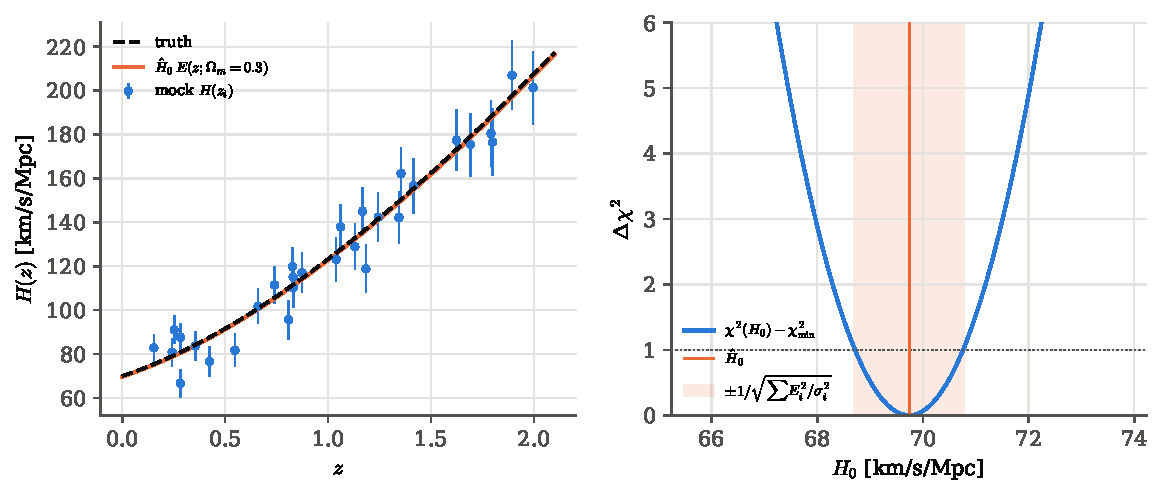
\includegraphics[width=12.8cm]{figures/ch03/chronometers.pdf}
\caption{Cosmic chronometers. Left: one mock survey of $H(z_i)$ points with their error bars,
the true expansion history (dashed) and the closed-form fit $\hat H_0E(z)$ at $\Omega_{m0}=0.3$
(orange). Right: the $\chi^2$ of that survey as a function of $H_0$ is an exact parabola; its
minimum is $\hat H_0$, and it rises by one (dotted) at $\hat H_0\pm S_{EE}^{-1/2}$ (shaded).}
\label{3b:fig:cc}
\end{figure}
\paragraph{Where this leaves us.}
The likelihood is the probability of the data, the object of \cref{ch:02}
and of \cref{3a:sec:sampling}, read backwards. For every trial value of the
parameters it asks how plausible the fluctuation is that would turn the
prediction into the data we have. Everything else follows from its shape.
Its peak is the estimate. Its width is the error bar. Its peak value,
compared with that of a saturated model, tests the fit. Maximising it over
the parameters we do not care about removes the nuisances. When no formula
is available, the bootstrap and the parametric simulation give the sampling
distribution directly. To find the best estimator, sufficiency says what the
data can tell us; candidates come from moments, maximum likelihood or a
loss function; and the Cram\'er--Rao bound and the Rao--Blackwell theorem
say when to stop improving. The full-sky power spectrum went through every
one of these steps. \Cref{ch:04} turns likelihood ratios and $\chi^2$ values into
tests and $p$-values; \cref{ch:05} multiplies the likelihood by a prior and
normalises it; \cref{ch:09} explores it with Markov chains when it has too
many dimensions to plot; \cref{ch:10} replaces it by its curvature, the
Fisher matrix, to forecast experiments before they are built.

\begin{recap}[Part 3b in one page]
\begin{itemize}
  \item Data $=$ model $+$ noise. The likelihood
        $\Like(\params)=p(\data_{\text{obs}}\given\params)$ is the probability
        (density) of the noise realisation needed to turn the prediction
        $d(\params)$ into the data. It is a function of $\params$, not a
        distribution over $\params$: no normalisation, no Jacobian, only
        ratios matter.
  \item Independent data multiply: $\ell=\sum_i\ln f(x_i;\params)$. The MLE
        solves $\partial\ell/\partial\params=0$; Newton--Raphson
        $\params\to\params-H^{-1}\bm g$ when it cannot be solved by hand.
  \item Gaussian noise: $-2\ell=\chi^2=\bm r\T\Cmat^{-1}\bm r$ (plus
        $\ln\det\Cmat$ if $\Cmat$ depends on $\params$). Linear models:
        $\hat\params=(A\T\Cmat^{-1}A)^{-1}A\T\Cmat^{-1}\bm D$ with covariance
        $(A\T\Cmat^{-1}A)^{-1}$, exactly. $\chi^2_{\min}\sim\chi^2_{N-m}$,
        mean $\dof=N-m$. Ignoring correlations keeps the fit unbiased but
        makes its error bar wrong.
  \item Counts: $-2\ell=2\sum[\mu_i-n_i\ln\mu_i]$; the fit conserves the
        total. Baker--Cousins $\chi^2_\lambda$ fits and tests; Neyman and
        Pearson $\chi^2$ bias the normalisation by $-\chi^2$ and
        $+\chi^2/2$.
  \item Error bar: $\hat\sigma=(-\ell''(\hat\theta))^{-1/2}$ or the
        $\Delta\ln\Like=\tfrac12$ crossings (better when $\ell$ is skewed).
        Why: $\Var S=-\E\ell''=I_n$, and $\hat\theta\approx\Normal(\theta,1/I_n)$.
  \item The MLE is consistent (Kullback--Leibler), equivariant
        ($\widehat{g(\theta)}=g(\hat\theta)$), asymptotically efficient:
        Cram\'er--Rao $\Var\hat\theta\ge1/I_n$ for unbiased estimators of
        regular models. Median on Gaussian data: efficiency $2/\pi$.
  \item Nuisance parameters: profile,
        $\Like_p(\theta)=\max_\nu\Like(\theta,\nu)$; its width is the full
        marginal error. Fixing $\nu$ underestimates the error by
        $\sqrt{1-\rho^2}$.
  \item Finding the estimator: write $\Like$; find the sufficient statistic
        from the factorisation $p=g(U,\theta)h(\data)$; build candidates;
        compare with $1/I_n$. In an exponential family the MLE matches the
        model mean of $U$ to its observed mean. Rao--Blackwell:
        $\E[W\given U]$ never has larger variance than an unbiased $W$.
        Bayes estimators: posterior mean, median, mode for squared,
        absolute, zero--one loss. Full-sky $\Chat=\sum_m|\alm|^2/(2\ell+1)$
        is sufficient, unbiased, and sits on the bound $2\Cell^2/(2\ell+1)$.
  \item Bootstrap: resample the data with replacement (or simulate from the
        fit) and use the scatter of the replicas. It fails for statistics
        controlled by extremes, such as the maximum.
\end{itemize}
\end{recap}

\section*{Chapter summary}
\addcontentsline{toc}{section}{Chapter summary}
\label{3b:sec:summary}

A number computed from data is a random variable, with a sampling
distribution over imagined repetitions of the experiment. The first idea
is to ask how such an estimator scatters: its bias, its variance, the
$1/\sqrt N$ law, the noise in variances and covariance matrices, the
propagation of errors through formulas, and the combination of
measurements. The second idea is to read the probability of the data
backwards, as a function of the parameters. That gives the likelihood,
which builds estimators and shows their error bars in its shape. On the
pipeline of \cref{ch:00} these are the first tools for the last arrow, from
a statistic's scatter to the physics: given the sampling distribution of a
summary, they produce a number, an error bar and a check of the fit. The
two tables list each concept, what it means operationally, and where it is
used next.

\begin{center}
\small
\renewcommand{\arraystretch}{1.15}
\begin{tabularx}{\linewidth}{@{}>{\raggedright\arraybackslash}p{3.3cm}
                               >{\raggedright\arraybackslash}X
                               >{\raggedright\arraybackslash}p{2.7cm}@{}}
\toprule
\multicolumn{3}{@{}l}{\textbf{Estimators and their errors (first half)}}\\
concept & operational meaning & used later in\\\midrule
statistical model & a family $f(x;\theta)$ of densities, one per parameter value; parametric if $\theta$ is finite-dimensional & every chapter\\
estimator, sampling distribution & a recipe $\hat\theta=g(x_1,\dots,x_N)$; its histogram over simulated repetitions of the experiment; standard error $=$ its width & \cref{ch:04,ch:06,ch:08}\\
bias, variance, MSE & centre offset and width of the sampling distribution; $\mathrm{MSE}=\mathrm{bias}^2+\mathrm{variance}$; compare estimators at several true values & \cref{ch:05,ch:10}\\
consistency & $\hat\theta\to\theta$ in probability; check that bias and variance both vanish as $N\to\infty$ & \cref{ch:09}\\
$1/\sqrt N$, LLN, CLT & $\Var\bar x=\sigma^2/N$; means become Gaussian with width $\sigma/\sqrt N$; fails for the Cauchy & \cref{ch:06,ch:07,ch:09}\\
sample variance, $N-1$ & divide by the number of residual degrees of freedom; $\Var S^2=2\sigma^4/(N-1)$ for Gaussian data & \cref{ch:04,ch:07}\\
cosmic variance & the variance of a variance: $\Var\Chat=2\Cell^2/(2\ell+1)$ & \cref{ch:07,ch:08}\\
sample covariance, Hartlap factor & $\hat\Cmat$ from $N_s$ simulations is noisy; multiply $\hat\Cmat^{-1}$ by $(N_s-p-2)/(N_s-1)$ & \cref{ch:08,ch:12}\\
error propagation & $U=A V A\T$ with the Jacobian $A$; exact for linear maps; replace by Monte Carlo near poles and for noisy denominators & \cref{ch:06,ch:10}\\
weighted mean & weights $1/\sigma_i^2$; $1/\sigma^2_{\hat\mu}=\sum1/\sigma_i^2$; check $\chi^2_{\min}\sim\chi^2_{N-1}$; correlated case $V^{-1}\bm1/(\bm1\T V^{-1}\bm1)$ & \cref{ch:04,ch:10}\\
\bottomrule
\end{tabularx}
\end{center}

\begin{center}
\small
\renewcommand{\arraystretch}{1.15}
\begin{tabularx}{\linewidth}{@{}>{\raggedright\arraybackslash}p{3.3cm}
                               >{\raggedright\arraybackslash}X
                               >{\raggedright\arraybackslash}p{2.7cm}@{}}
\toprule
\multicolumn{3}{@{}l}{\textbf{The likelihood (second half)}}\\
concept & operational meaning & used later in\\\midrule
likelihood & write the noise model, evaluate the probability of the observed data, vary $\params$; compare values only through ratios & every later chapter\\
not a density in $\theta$ & area arbitrary, no Jacobian; a prior is needed to make it a distribution & \cref{ch:05}\\
sufficiency, likelihood principle & the likelihood depends on the data only through a sufficient statistic; proportional likelihoods carry the same evidence & \cref{ch:04,ch:05,ch:07}\\
factorisation theorem, exponential family & $p=g(U,\theta)h(\data)$ identifies $U$; in $h\,e^{\eta\phi-A}$ the MLE solves $\E_{\hat\theta}\phi=\overline{\phi}$ & \cref{ch:05,ch:07}\\
Bayes estimator & minimise the posterior expected loss: mean for squared, median for absolute, mode for zero--one loss & \cref{ch:05,ch:09}\\
Rao--Blackwell, UMVUE & average a crude unbiased estimator over a sufficient statistic; with a complete statistic the result is the best unbiased estimator & \cref{ch:06}\\
MC-calibrated statistic & when $\Like$ is intractable, simulate, calibrate the mean and covariance of a simple statistic & \cref{ch:06,ch:08}\\
full-sky $\Chat$ & sufficient, unbiased, attains Cram\'er--Rao: cosmic variance $2\Cell^2/(2\ell+1)$ & \cref{ch:07,ch:08,ch:10}\\
noise lives in magnitudes & write the likelihood in the variable where the noise is Gaussian ($m$, not $d$); distances from magnitudes are log-normal, $\E\tilde d=d\,e^{\kappa^2\sigma^2/2}$ & \cref{ch:09}\\
naive vs ML estimator of $H_0$ & a line fitted to magnitude distances or a mean of ratios is biased and inconsistent; the weighted mean of $5\log_{10}H_0$ is sufficient and on the Cram\'er--Rao bound & \cref{ch:09,ch:10,T2b:sec:ladder}\\
$H_0$--$M$ degeneracy & SNe fix only $M-5\log_{10}H_0$ (singular Fisher matrix); a calibration adds $\sigma_M^2$ to $\sigma^2_{5\log_{10}H_0}$; the Hubble tension is $0.18$~mag in $M$ & \cref{T2b:sec:tension,9c:sec:importance,11c:sec:h0-routes}\\
maximum likelihood & maximise $\ell$; solve the score equation or iterate Newton--Raphson from a moment estimate & \cref{ch:04,ch:08,ch:10}\\
method of moments & match sample moments to model moments; a quick, consistent starting point & \cref{ch:06}\\
extended likelihood & multiply by $\mathrm{Poisson}(n;\nu)$ when the number of events is random & \cref{ch:04}\\
least squares & minimise $\chi^2=\bm r\T\Cmat^{-1}\bm r$; normal equations; covariance $(A\T\Cmat^{-1}A)^{-1}$ & \cref{ch:07,ch:08,ch:10}\\
goodness of fit & $\pval=\Prob(\chi^2_{N-m}\ge\chi^2_{\min})$; reduced $\chi^2\approx1\pm\sqrt{2/\dof}$ & \cref{ch:04}\\
$\Delta\chi^2$ regions & $\chi^2\le\chi^2_{\min}+\Delta\chi^2$ with $\Delta\chi^2$ from $\chi^2_m$ ($1$, $2.30$, $3.53$ for $68\%$) & \cref{ch:09,ch:10}\\
correlated and parameter-dependent noise & keep $\ln\det\Cmat(\params)$; GW: $(D-h|D-h)$ with $S_n(f)$; CMB: $\sum(2\ell+1)[\Chat/\Cell+\ln\Cell]$ & \cref{ch:07,ch:08,ch:10}\\
Poisson binned likelihood & $2\sum[\mu_i-n_i\ln\mu_i]$ (Cash); Baker--Cousins $\chi^2_\lambda$ to test; never $\sqrt{n_i}$ errors for few counts & \cref{ch:04,ch:06}\\
curvature error, $\Delta\ln\Like=\tfrac12$ & $\hat\sigma=(-\ell'')^{-1/2}$, or the two crossings of $\ell_{\max}-\tfrac12$; covariance $(-H)^{-1}$ & \cref{ch:09,ch:10}\\
score, Fisher information & $\E S=0$, $\Var S=-\E\ell''=I_n=nI$; $\hat\theta\approx\Normal(\theta,1/I_n)$ & \cref{ch:05,ch:10}\\
consistency, invariance & the MLE converges to the minimiser of the Kullback--Leibler divergence; $\widehat{g(\theta)}=g(\hat\theta)$, but bias is not invariant & \cref{ch:05,ch:09}\\
Cram\'er--Rao bound, efficiency & $\Var\hat\theta\ge1/I_n$ for unbiased estimators of regular models; attained by exponential families; fails for moving supports & \cref{ch:10}\\
profile likelihood & maximise over nuisance parameters at each $\theta$; read $\Delta\ln\Like_p=\tfrac12$; Wilks gives the coverage & \cref{ch:04,ch:05,ch:10}\\
bootstrap & resample the data with replacement (nonparametric) or simulate from the fit (parametric); Normal, pivotal and percentile intervals; fails for extremes & \cref{ch:06,ch:08,ch:12}\\
\bottomrule
\end{tabularx}
\end{center}

\subsection*{Reading the literature}

\begin{itemize}[leftmargin=1.2em,itemsep=2pt]
  \item \textbf{Main line.} \mainref{Chs.~5--6} for convergence, the law of
        large numbers, the central limit theorem, estimators, bias, variance
        and consistency; \mainref{Ch.~9} for the likelihood, maximum
        likelihood and its properties (consistency through the
        Kullback--Leibler divergence, equivariance, Fisher information,
        asymptotic normality, efficiency, the delta method, the parametric
        bootstrap), with sufficiency, the factorisation theorem, Rao--Blackwell and
        exponential families in its appendix; \mainref{Ch.~8} for the bootstrap and its
        intervals.
  \item \textbf{The physicist's version.} \srcref{Cowan}{\S\S1.6--1.7,
        Ch.~5} for error propagation and estimators; \srcref{Cowan}{Ch.~6}
        for maximum likelihood with physics examples (lifetimes, the angular
        distribution, extended and binned likelihoods, goodness of fit);
        \srcref{Cowan}{Ch.~7} for least squares, binned $\chi^2$ and the
        normalisation biases; \srcref{Cowan}{Ch.~8} for the method of
        moments.
  \item \textbf{Why least squares.} \srcref{Sivia}{\S3.5}: maximum
        likelihood and least squares as what Bayes' theorem reduces to
        under a flat prior and Gaussian noise; \srcref{Sivia}{\S2.3} for
        the weighted mean from a Gaussian posterior.
  \item \textbf{Careful derivations.} Casella and Berger give convergence
        and the delta method in \srcref{CasellaBerger}{\S5.5}, the
        likelihood principle and Birnbaum's argument in
        \srcref{CasellaBerger}{\S6.3}, maximum likelihood with restricted
        ranges and the invariance theorem in \srcref{CasellaBerger}{\S7.2.2},
        in \srcref{CasellaBerger}{\S6.2} sufficiency and the factorisation
        theorem, in \srcref{CasellaBerger}{\S7.2.3} Bayes estimators, and in
        \srcref{CasellaBerger}{\S7.3} mean squared error, the Cram\'er--Rao
        inequality with its attainment condition, and the Rao--Blackwell and
        Lehmann--Scheff\'e theorems.
  \item \textbf{Cosmology.} \srcref{HobsonBMC}{\S1.3.1} for the four
        ingredients of Bayes' theorem and why the likelihood is the least
        controversial one; \srcref{HobsonBMC}{\S2.4} for a $\chi^2$ fit as a
        Gaussian likelihood and the marginalisation of an unknown noise
        level. \srcref{Padilla}{\S\S3.3--3.8} for the likelihood ratio, the
        Hessian, $\chi^2$ goodness of fit, $\Delta\chi^2$ regions and a first
        look at the Fisher matrix.
  \item \textbf{Pictures.} \srcref{SeeingTheory}{pp.~16--18, 38--48} for
        interactive demonstrations of estimation, consistency and the
        central limit theorem.
  \item \textbf{Original papers.} The noise of inverted simulated
        covariance matrices \cite{Hartlap2007}; the Poisson statistic for
        sparse spectra \cite{Cash1979}; the likelihood-ratio $\chi^2$ for
        histograms \cite{BakerCousins1984}; the asymptotic $\chi^2$
        distribution of likelihood ratios \cite{Wilks1938}; the bootstrap
        \cite{Efron1979}.
\end{itemize}
  
\chapter{Hypothesis Testing: Asking the Null}\label{ch:04}

\providecommand{\FourABumpBtot}{}\renewcommand{\FourABumpBtot}{60}
\providecommand{\FourABumpStot}{}\renewcommand{\FourABumpStot}{9}
\providecommand{\FourABumpB}{}\renewcommand{\FourABumpB}{3.74}
\providecommand{\FourABumpN}{}\renewcommand{\FourABumpN}{10}
\providecommand{\FourABumpP}{}\renewcommand{\FourABumpP}{0.005172}
\providecommand{\FourABumpPmc}{}\renewcommand{\FourABumpPmc}{0.005133}
\providecommand{\FourABumpPmcErr}{}\renewcommand{\FourABumpPmcErr}{7.146\times10^{-5}}
\providecommand{\FourABumpZ}{}\renewcommand{\FourABumpZ}{2.56}
\providecommand{\FourABumpZnaive}{}\renewcommand{\FourABumpZnaive}{3.24}
\providecommand{\FourABumpZwrong}{}\renewcommand{\FourABumpZwrong}{1.98}
\providecommand{\FourACowanPone}{}\renewcommand{\FourACowanPone}{4.972\times10^{-4}}
\providecommand{\FourACowanPtwo}{}\renewcommand{\FourACowanPtwo}{1.721\times10^{-4}}
\providecommand{\FourACowanPthree}{}\renewcommand{\FourACowanPthree}{0.001411}
\providecommand{\FourACowanZone}{}\renewcommand{\FourACowanZone}{3.29}
\providecommand{\FourACowanZnaive}{}\renewcommand{\FourACowanZnaive}{4.36}
\providecommand{\FourACoinPone}{}\renewcommand{\FourACoinPone}{0.00129}
\providecommand{\FourACoinPtwo}{}\renewcommand{\FourACoinPtwo}{0.0026}
\providecommand{\FourACoinPtwoMC}{}\renewcommand{\FourACoinPtwoMC}{0.0028}
\providecommand{\FourAKrFixN}{}\renewcommand{\FourAKrFixN}{0.0320}
\providecommand{\FourAKrFixNMC}{}\renewcommand{\FourAKrFixNMC}{0.0325}
\providecommand{\FourAKrFixZ}{}\renewcommand{\FourAKrFixZ}{0.0173}
\providecommand{\FourAKrFixZMC}{}\renewcommand{\FourAKrFixZMC}{0.0173}
\providecommand{\FourACowStop}{}\renewcommand{\FourACowStop}{7.286\times10^{-4}}
\providecommand{\FourACowStopMC}{}\renewcommand{\FourACowStopMC}{7.500\times10^{-4}}
\providecommand{\FourAPowSizeFour}{}\renewcommand{\FourAPowSizeFour}{0.0508}
\providecommand{\FourAPowSizeSixtyfour}{}\renewcommand{\FourAPowSizeSixtyfour}{0.0518}
\providecommand{\FourAPowNreq}{}\renewcommand{\FourAPowNreq}{24.7}
\providecommand{\FourAPowNreqInt}{}\renewcommand{\FourAPowNreqInt}{25}
\providecommand{\FourAPowReqMC}{}\renewcommand{\FourAPowReqMC}{0.801}
\providecommand{\FourAPowWaldSize}{}\renewcommand{\FourAPowWaldSize}{0.0643}
\providecommand{\FourAPowNthree}{}\renewcommand{\FourAPowNthree}{11}
\providecommand{\FourAPowNfive}{}\renewcommand{\FourAPowNfive}{17}
\providecommand{\FourAPowSfiftyThree}{}\renewcommand{\FourAPowSfiftyThree}{7.6}
\providecommand{\FourAPowSfiftyFive}{}\renewcommand{\FourAPowSfiftyFive}{13.6}
\providecommand{\FourAPowFiveAtTwenty}{}\renewcommand{\FourAPowFiveAtTwenty}{0.924}
\providecommand{\FourAPowFiveAtTwentyMC}{}\renewcommand{\FourAPowFiveAtTwentyMC}{0.925}
\providecommand{\FourAPUfracZero}{}\renewcommand{\FourAPUfracZero}{0.0494}
\providecommand{\FourAPUfracOne}{}\renewcommand{\FourAPUfracOne}{0.242}
\providecommand{\FourAPUfracTwo}{}\renewcommand{\FourAPUfracTwo}{0.813}
\providecommand{\FourAPUks}{}\renewcommand{\FourAPUks}{0.72}
\providecommand{\FourAPUdisc}{}\renewcommand{\FourAPUdisc}{0.0453}
\providecommand{\FourAPUpower}{}\renewcommand{\FourAPUpower}{0.473}
\providecommand{\FourAPUnullSig}{}\renewcommand{\FourAPUnullSig}{0.489}
\providecommand{\FourAPUnullSigTh}{}\renewcommand{\FourAPUnullSigTh}{0.487}
\providecommand{\FourAPUnullBand}{}\renewcommand{\FourAPUnullBand}{0.681}
\providecommand{\FourAPUnullBandTh}{}\renewcommand{\FourAPUnullBandTh}{0.682}
\providecommand{\FourAWaldSizeThree}{}\renewcommand{\FourAWaldSizeThree}{0.190}
\providecommand{\FourAWaldSizeFive}{}\renewcommand{\FourAWaldSizeFive}{0.122}
\providecommand{\FourAWaldSizeTen}{}\renewcommand{\FourAWaldSizeTen}{0.081}
\providecommand{\FourAWaldSizeThirty}{}\renewcommand{\FourAWaldSizeThirty}{0.059}
\providecommand{\FourAWaldSizeThreeEx}{}\renewcommand{\FourAWaldSizeThreeEx}{0.189}
\providecommand{\FourATSizeThree}{}\renewcommand{\FourATSizeThree}{0.050}
\providecommand{\FourATSizeTen}{}\renewcommand{\FourATSizeTen}{0.050}
\providecommand{\FourACalMeanOne}{}\renewcommand{\FourACalMeanOne}{662.07}
\providecommand{\FourACalMeanTwo}{}\renewcommand{\FourACalMeanTwo}{665.67}
\providecommand{\FourACalSdOne}{}\renewcommand{\FourACalSdOne}{4.30}
\providecommand{\FourACalSdTwo}{}\renewcommand{\FourACalSdTwo}{3.55}
\providecommand{\FourACalD}{}\renewcommand{\FourACalD}{3.60}
\providecommand{\FourACalSe}{}\renewcommand{\FourACalSe}{1.54}
\providecommand{\FourACalW}{}\renewcommand{\FourACalW}{2.33}
\providecommand{\FourACalPwald}{}\renewcommand{\FourACalPwald}{0.0198}
\providecommand{\FourACalPwelch}{}\renewcommand{\FourACalPwelch}{0.0298}
\providecommand{\FourACalPperm}{}\renewcommand{\FourACalPperm}{0.0251}
\providecommand{\FourACalPpermScipy}{}\renewcommand{\FourACalPpermScipy}{0.0273}
\providecommand{\FourACalPermDiffSig}{}\renewcommand{\FourACalPermDiffSig}{1.8}
\providecommand{\FourAToyP}{}\renewcommand{\FourAToyP}{0.667}
\providecommand{\FourACholP}{}\renewcommand{\FourACholP}{0.00016}
\providecommand{\FourANPbkgCut}{}\renewcommand{\FourANPbkgCut}{0.397}
\providecommand{\FourANPbkgFisher}{}\renewcommand{\FourANPbkgFisher}{0.256}
\providecommand{\FourANPbkgLR}{}\renewcommand{\FourANPbkgLR}{0.177}
\providecommand{\FourANPbkgRandom}{}\renewcommand{\FourANPbkgRandom}{0.199}
\providecommand{\FourAWkSimEighty}{}\renewcommand{\FourAWkSimEighty}{1.630}
\providecommand{\FourAWkSimNinety}{}\renewcommand{\FourAWkSimNinety}{2.726}
\providecommand{\FourAWkSimNinetyfive}{}\renewcommand{\FourAWkSimNinetyfive}{3.757}
\providecommand{\FourAWkSimNinetynine}{}\renewcommand{\FourAWkSimNinetynine}{6.685}
\providecommand{\FourAWkChiEighty}{}\renewcommand{\FourAWkChiEighty}{1.642}
\providecommand{\FourAWkChiNinety}{}\renewcommand{\FourAWkChiNinety}{2.706}
\providecommand{\FourAWkChiNinetyfive}{}\renewcommand{\FourAWkChiNinetyfive}{3.841}
\providecommand{\FourAWkChiNinetynine}{}\renewcommand{\FourAWkChiNinetynine}{6.635}
\providecommand{\FourAWkMeanOne}{}\renewcommand{\FourAWkMeanOne}{1.002}
\providecommand{\FourAWkMeanTwo}{}\renewcommand{\FourAWkMeanTwo}{2.003}
\providecommand{\FourAWkVarOne}{}\renewcommand{\FourAWkVarOne}{2.011}
\providecommand{\FourAWkVarTwo}{}\renewcommand{\FourAWkVarTwo}{3.995}
\providecommand{\FourAWkZeroSmall}{}\renewcommand{\FourAWkZeroSmall}{0.603}
\providecommand{\FourAWkZeroBig}{}\renewcommand{\FourAWkZeroBig}{0.527}
\providecommand{\FourAWkThreeSmall}{}\renewcommand{\FourAWkThreeSmall}{0.001769}
\providecommand{\FourAWkThreeBig}{}\renewcommand{\FourAWkThreeBig}{0.001262}
\providecommand{\FourAWkThreeTh}{}\renewcommand{\FourAWkThreeTh}{0.00135}
\providecommand{\FourAWkZwilks}{}\renewcommand{\FourAWkZwilks}{3.40}
\providecommand{\FourAWkZexact}{}\renewcommand{\FourAWkZexact}{3.29}
\providecommand{\FourAWkZAsmall}{}\renewcommand{\FourAWkZAsmall}{2.33}
\providecommand{\FourAWkZsbSmall}{}\renewcommand{\FourAWkZsbSmall}{2.80}
\providecommand{\FourAWkZAbig}{}\renewcommand{\FourAWkZAbig}{0.984}
\providecommand{\FourAWkZsbBig}{}\renewcommand{\FourAWkZsbBig}{1.000}
\providecommand{\FourAWkZmedBig}{}\renewcommand{\FourAWkZmedBig}{0.984}
\providecommand{\FourAMendelChi}{}\renewcommand{\FourAMendelChi}{0.470}
\providecommand{\FourAMendelP}{}\renewcommand{\FourAMendelP}{0.925}
\providecommand{\FourAGofQsmall}{}\renewcommand{\FourAGofQsmall}{33.5}
\providecommand{\FourAGofQlarge}{}\renewcommand{\FourAGofQlarge}{31.4}
\providecommand{\FourAGofQth}{}\renewcommand{\FourAGofQth}{31.4}
\providecommand{\FourAGofPsmallMC}{}\renewcommand{\FourAGofPsmallMC}{0.091}
\providecommand{\FourAGofPsmallChi}{}\renewcommand{\FourAGofPsmallChi}{0.070}
\providecommand{\FourAGofMeanBinned}{}\renewcommand{\FourAGofMeanBinned}{6.01}
\providecommand{\FourAGofMeanRaw}{}\renewcommand{\FourAGofMeanRaw}{6.06}
\providecommand{\FourAGofMeanDiff}{}\renewcommand{\FourAGofMeanDiff}{0.051}
\providecommand{\FourAGofMeanDiffErr}{}\renewcommand{\FourAGofMeanDiffErr}{0.002}
\providecommand{\FourAGofMeanErr}{}\renewcommand{\FourAGofMeanErr}{0.05}
\providecommand{\FourAKsD}{}\renewcommand{\FourAKsD}{0.1790}
\providecommand{\FourAKsDscipy}{}\renewcommand{\FourAKsDscipy}{0.1790}
\providecommand{\FourAKsPscipy}{}\renewcommand{\FourAKsPscipy}{0.0714}
\providecommand{\FourAKsPkolm}{}\renewcommand{\FourAKsPkolm}{0.0812}
\providecommand{\FourAKsPmc}{}\renewcommand{\FourAKsPmc}{0.0726}
\providecommand{\FourAKsSqrtnD}{}\renewcommand{\FourAKsSqrtnD}{1.266}
\providecommand{\FourAPzOneOne}{}\renewcommand{\FourAPzOneOne}{0.1587}
\providecommand{\FourAPzOneTwo}{}\renewcommand{\FourAPzOneTwo}{0.3173}
\providecommand{\FourAPzTwoOne}{}\renewcommand{\FourAPzTwoOne}{0.02275}
\providecommand{\FourAPzTwoTwo}{}\renewcommand{\FourAPzTwoTwo}{0.0455}
\providecommand{\FourAPzThreeOne}{}\renewcommand{\FourAPzThreeOne}{0.00135}
\providecommand{\FourAPzThreeTwo}{}\renewcommand{\FourAPzThreeTwo}{0.0027}
\providecommand{\FourAPzFourOne}{}\renewcommand{\FourAPzFourOne}{3.167\times10^{-5}}
\providecommand{\FourAPzFourTwo}{}\renewcommand{\FourAPzFourTwo}{6.334\times10^{-5}}
\providecommand{\FourAPzFiveOne}{}\renewcommand{\FourAPzFiveOne}{2.867\times10^{-7}}
\providecommand{\FourAPzFiveTwo}{}\renewcommand{\FourAPzFiveTwo}{5.733\times10^{-7}}
\providecommand{\FourAPzSixOne}{}\renewcommand{\FourAPzSixOne}{9.866\times10^{-10}}
\providecommand{\FourAPzSixTwo}{}\renewcommand{\FourAPzSixTwo}{1.973\times10^{-9}}
\providecommand{\FourAPzAnyThree}{}\renewcommand{\FourAPzAnyThree}{0.126}
\providecommand{\FourAPzAnyThreeMC}{}\renewcommand{\FourAPzAnyThreeMC}{0.126}
\providecommand{\FourAPzAnyFive}{}\renewcommand{\FourAPzAnyFive}{2.866\times10^{-5}}
\providecommand{\FourAPzPurThree}{}\renewcommand{\FourAPzPurThree}{0.270}
\providecommand{\FourAPzPurFive}{}\renewcommand{\FourAPzPurFive}{0.9994}
\providecommand{\FourAPzZfivepct}{}\renewcommand{\FourAPzZfivepct}{1.645}
\providecommand{\FourAPzZfivepctTwo}{}\renewcommand{\FourAPzZfivepctTwo}{1.960}
 
\section*{Where this chapter is going}
\label{4a:sec:roadmap}

A physicist who sees a bump in a histogram asks one question before any other:
\emph{could this be luck?} Background alone fluctuates. Some bins come out high,
some low, and if we look at enough histograms one of them will show something
that looks like a new particle. Before we get excited, we want a number that says
how surprising the bump would be if nothing new were there. We need to know
how to compute that number, what it means, and what it does not mean.

The key move is to pick the one hypothesis we can simulate with no free choices:
``only background, only chance''. This is the \newterm{null hypothesis}. Its
sampling distribution is the one we know, so we can work out how often chance
alone would hand us a bump as large as ours or larger
(\cref{4a:sec:null}). That frequency is a tail probability, the
\newterm{p-value}. Everything else grows out of that question: how to
choose the summary of the data whose tail we compute (the \emph{test statistic}),
what ``this direction'' means (one- and two-sided tests), how often a test fires by
mistake and how often it catches a real effect (size and power), why the p-value is
uniformly distributed when nothing is there, which statistic is the best one (the
Neyman--Pearson lemma), and the workhorses built from it (likelihood ratios, Wilks'
theorem, $\chi^2$ and Kolmogorov--Smirnov goodness of fit). We end by translating
p-values into the ``$Z\sigma$'' language of particle physics and asking why a
discovery needs $5\sigma$.

Recall the pipeline of \cref{ch:00}: a theory produces data, the data are
compressed into a statistic $S$, the scatter of $S$ is its sampling
distribution $P(S\given\theta)$, and from that scatter we infer the physics.
Testing is the last arrow. It uses the sampling distribution \emph{under one
special $\theta$}, the null, and asks whether the observed summary is typical
of it. Every test can also be turned into a confidence interval, and a search
that looks in many places needs its p-value corrected for the look-elsewhere
effect; both follow from the same tail probabilities. \Cref{ch:05} then asks
the question a p-value cannot answer: how probable is the hypothesis itself,
given the data?

\begin{figure}[htbp]
\centering
\begin{tikzpicture}[
  node distance=5mm and 6mm,
  blk/.style={draw=accent,thick,rounded corners=2pt,fill=ideabg,
              align=center,font=\small,minimum height=14mm,text width=25mm},
  hot/.style={blk,fill=defbg,draw=fibreorange!80!black},
  flow/.style={->,thick,accent}]
  \node[blk] (data) {data\\ (a bump)};
  \node[hot,right=of data] (null) {null $\Hnull$:\\ known sampling\\ distribution};
  \node[hot,right=of null] (stat) {test statistic\\ $T$, direction};
  \node[hot,right=of stat] (pval) {p-value:\\ tail beyond $t_{\rm obs}$};
  \node[hot,below=9mm of pval] (power) {size $\alpha$, power,\\ uniform p};
  \node[hot,left=of power] (np) {best test:\\ likelihood ratio,\\ Wilks};
  \node[hot,left=of np] (gof) {goodness of fit:\\ $\chi^2$, KS};
  \node[hot,left=of gof] (z) {p $\to Z\sigma$,\\ why $5\sigma$};
  \node[blk,below=9mm of np,fill=nashbg,draw=violet!70!black,text width=50mm] (next)
       {intervals, look-elsewhere\\ (part 4b),\\ $\Prob(\Hnull\given\text{data})$ (\cref{ch:05})};
  \draw[flow] (data) -- (null);
  \draw[flow] (null) -- (stat);
  \draw[flow] (stat) -- (pval);
  \draw[flow] (pval) -- (power);
  \draw[flow] (power) -- (np);
  \draw[flow] (np) -- (gof);
  \draw[flow] (gof) -- (z);
  \draw[flow] (np) -- (next);
\end{tikzpicture}
\caption{The route through this part. We start from data that look surprising and
pick the hypothesis whose sampling distribution we know, the null. A summary of the
data, the test statistic, and a direction of ``more extreme'' turn the question
``could this be chance?'' into a tail probability. The bottom row asks how good a test
is, which test is best, how to test a whole model, and how to report the answer. The
violet box points to what the p-value cannot tell us and to the next part.}
\label{4a:fig:roadmap}
\end{figure}

\section{A bump in a histogram: new particle or luck?}
\label{4a:sec:bump}

We have recorded events in which two photons were produced, and for each
event we computed the invariant mass $m_{\gamma\gamma}$ of the photon pair.
\Cref{4a:fig:bump-spectrum} shows the histogram: thirty bins of
$2\,$GeV between $100$ and $160\,$GeV. Known physics produces a smooth,
falling spectrum, and from simulation we expect $\FourABumpBtot$ background
events in the whole range, distributed as the dashed line. Near
$126\,$GeV two neighbouring bins stick out. A new particle decaying to two
photons would show up exactly like this: a narrow excess at its mass. But
background alone also fluctuates. Every bin is a Poisson count, some bins
come out high and some low, and a pair of high bins can happen by luck.

\begin{figure}[htbp]
\centering
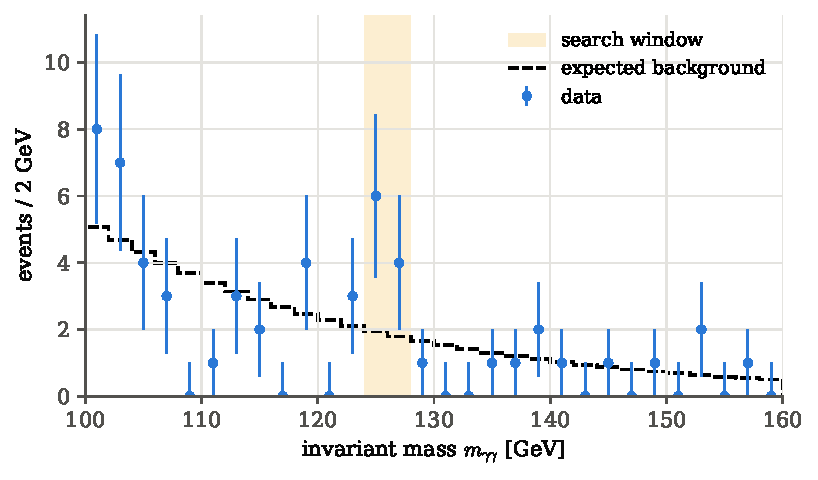
\includegraphics[width=0.82\linewidth]{figures/ch04/bump_spectrum.pdf}
\caption{A simulated diphoton mass spectrum. The dots are the observed counts
per $2\,$GeV bin, the dashed staircase is the background we expect with no new
particle, and the shaded band is the two-bin window $124$--$128\,$GeV where
the excess sits. The error bars are $\sqrt{n}$ and are drawn only to guide the
eye; the pitfall at the end of \cref{4a:sec:bump} explains why they must not be used
to judge the excess.}
\label{4a:fig:bump-spectrum}
\end{figure}

The first thing we can compute is not whether the particle exists. It is how
surprising the bump would be \emph{if nothing new were there}. That is weaker
than what we want to know, but we can compute it exactly, and every discovery
claim in physics starts with it.

\paragraph{The question in words.}
Before any formula, we can list the three things we need.
\begin{enumerate}[label=\arabic*.]
  \item A hypothesis precise enough to \emph{predict} the data, with no knob
        left to turn. ``Only background'' is such a hypothesis: the dashed line
        tells us the Poisson mean of every bin.
  \item One number computed from the data that is large when there is a
        signal and small when there is not. Here, the count in the window.
  \item The answer to: if only background were present, how often would that
        number come out at least as large as the one we saw?
\end{enumerate}

\subsection{The null hypothesis is the one whose predictions we know}
\label{4a:sec:null}

Every test starts by splitting the possible values of an unknown parameter
into two sets, one for each hypothesis. This is the same for a particle search
and for a medical trial. \mainref{p.~149} opens with rats: expose one group to
asbestos, leave another unexposed, and compare the disease rates. Either the
two rates are the same, or they are not. In the bump, the unknown parameter is
the expected number $s$ of signal events in the window, and physics allows
any $s\ge0$. Writing $\theta$ for the parameter and $\Theta$ for the set of all
its allowed values, the two hypotheses are two disjoint sets that together
cover $\Theta$:
\begin{equation}
  \Hnull:\ \theta\in\Theta_0
  \qquad\text{versus}\qquad
  \Halt:\ \theta\in\Theta_1,
  \qquad \Theta_0\cup\Theta_1=\Theta,\quad \Theta_0\cap\Theta_1=\varnothing .
  \label{4a:eq:partition}
\end{equation}
For the bump, $\theta=s$, $\Theta=[0,\infty)$, $\Theta_0=\{0\}$ and
$\Theta_1=(0,\infty)$. For the rats, $\theta$ is the difference of the two
disease rates, $\Theta_0=\{0\}$, and $\Theta_1$ is every nonzero difference.

The two hypotheses are not on an equal footing, and the asymmetry is the whole
point. $\Hnull$ is the \newterm{null hypothesis}: the data came about by
chance alone, from processes we already understand. We treat it this way
\emph{because we know its probability distribution}. With $s=0$ the count in
every bin is Poisson with a known mean, and we can compute, or simulate, the
probability of any outcome. The alternative $\Halt$ is a whole family: every
$s>0$, every possible mass and width of the new particle, each predicting
something different. We cannot compute ``the'' probability of the data under
$\Halt$ without first choosing one of its members.

So we test ``chance alone'' not because we believe it, but because it is the
one case whose probability density we actually know. A test therefore runs in
the \emph{prediction} direction of \cref{ch:01}. We start from the one
situation we can simulate, $\Hnull$, and ask what outcomes it produces and how
often. Only then do we compare with what we saw.

\paragraph{The question a test asks.}
Suppose $\Hnull$ is true. Would a result like the one we got, or even more in
this direction, then be a reasonable thing to expect?

If the answer is ``hardly ever'', the data give us evidence against $\Hnull$.
If the answer is ``quite often'', they do not. Notice what we did \emph{not}
ask: how probable $\Hnull$ is. That question runs in the inference direction
and needs Bayes' theorem, and we come back to it in
\cref{4a:sec:not-posterior} and \cref{ch:05}.

\subsection{Test statistic, rejection region, critical value}
\label{4a:sec:rejection}

Data sets are long lists of numbers, and we cannot compare lists directly.
We compress the data $\bm x$ into one number, the \newterm{test statistic}
$T(\bm x)$ \unpack{a function of the data alone, chosen to be large when
$\Halt$ is true}. For the bump, $T$ is the count $n$ in the window. Large $n$
points to a signal, and $n$ near the expected background points to nothing.

A test is then a rule for turning $T$ into a decision. We choose a set of
outcomes, the \newterm{rejection region} $R$, and agree in advance
\mainref{(10.2)}, \srcref{Cowan}{\S4.1}:
\begin{equation}
  \bm x\in R\ \Longrightarrow\ \text{reject }\Hnull,
  \qquad
  \bm x\notin R\ \Longrightarrow\ \text{retain }\Hnull,
  \qquad
  R=\{\bm x:\ T(\bm x)>c\}.
  \label{4a:eq:rejection}
\end{equation}
The threshold $c$ is the \newterm{critical value}. Cowan calls the rejection
region the \emph{critical region} and its complement the \emph{acceptance
region}. We say ``retain'' rather than ``accept'': not rejecting the null only
means the data did not contradict it, just as a jury that fails to convict
has not proved innocence. The whole problem of testing is to choose a good
$T$ and a sensible $c$. Choosing $c$ is the subject of
\cref{4a:sec:power}; choosing $T$, of \cref{4a:sec:np}.

\mainref{p.~150} adds a warning worth keeping in mind from the start: tests
are for well-defined hypotheses. If the real question is ``how big is the
effect?'', an estimate with a confidence interval answers it better than a
test.

\subsection{The p-value: the tail beyond what we saw}
\label{4a:sec:pvalue-def}

Instead of fixing $c$ in advance and reporting only ``reject'' or ``retain'',
we can report \emph{where} the observed statistic $t_{\rm obs}$ falls in the
null distribution. \Cref{4a:fig:null-tail} shows the picture that the whole
chapter keeps returning to. The curve is $g(t\given\Hnull)$, the sampling
distribution of the test statistic when the null is true. The vertical line is
the value we observed. The shaded area to the right is the probability,
under $\Hnull$, of a result like ours or even more in the direction that
signals $\Halt$. That area is the p-value.

\begin{figure}[htbp]
\centering
\begin{tikzpicture}
\begin{axis}[
  width=11cm, height=5.2cm,
  domain=0:14, samples=200,
  xmin=0, xmax=14, ymin=0, ymax=0.3,
  axis lines=left, xlabel={test statistic $t$}, ylabel={$g(t\given H_0)$},
  xtick={0,2,4,6,8,10,12,14}, ytick=\empty,
  clip=false]
  \addplot[name path=f, formblue, very thick] {x^2*exp(-x)/2};
  \path[name path=axis] (axis cs:0,0) -- (axis cs:14,0);
  \addplot[fibreorange!70, opacity=0.8] fill between[of=f and axis, soft clip={domain=6.5:14}];
  \draw[bdryred, thick] (axis cs:6.5,0) -- (axis cs:6.5,0.17);
  \node[anchor=south, bdryred, font=\small] at (axis cs:6.5,0.17) {$t_{\rm obs}$};
  \node[anchor=west, font=\small, align=left] at (axis cs:8.6,0.085)
       {shaded area $=p$\\$=\Prob(T\ge t_{\rm obs}\given H_0)$};
  \draw[->, black!60] (axis cs:8.5,0.075) -- (axis cs:7.5,0.025);
  \node[anchor=west, font=\small, formblue] at (axis cs:3.3,0.25)
       {typical under $H_0$};
  \draw[->, thick, fibreorange!80!black] (axis cs:9.5,0.20) -- (axis cs:13.5,0.20);
  \node[anchor=south, font=\small, fibreorange!80!black] at (axis cs:11.5,0.205)
       {direction of $H_1$};
\end{axis}
\end{tikzpicture}
\caption{The p-value as a tail area. The blue curve is the distribution of the
test statistic in a world where only chance operates. The observed value sits
at the red line. The orange tail collects every outcome at least as extreme,
in the direction the alternative predicts. A small tail means our result would
be rare if the null were true.}
\label{4a:fig:null-tail}
\end{figure}

\begin{workdef}[p-value]
For a test that rejects $\Hnull$ when $T$ is large, and a simple null
$\Theta_0=\{\theta_0\}$, the \newterm{p-value} of the observed data is
\[
  p=\Prob_{\theta_0}\bigl(T\ge t_{\rm obs}\bigr)
\]
\unpack{the probability, computed as if $\Hnull$ were true, of a test
statistic at least as large as the one observed}. It is computed from
$\Hnull$ alone and is \emph{not} the probability that $\Hnull$ is true.
Operationally: simulate many data sets under $\Hnull$, compute $T$ for each,
and count the fraction with $T\ge t_{\rm obs}$
\mainref{Thm~10.12}, \srcref{Cowan}{\S4.5}.
\end{workdef}

Three features of the definition matter.
\begin{itemize}[itemsep=1pt,leftmargin=1.2em]
  \item The p-value is a probability of \emph{data}, not of hypotheses. The
        null value $\theta_0$ sits in the subscript as a fixed assumption.
  \item It counts the observed value itself and everything beyond it. The words
        ``or even more in this direction'' are needed because, once the data
        are rich enough, the probability of getting exactly $t_{\rm obs}$ is
        tiny under any hypothesis, so it cannot measure surprise on its own.
  \item It needs a \emph{direction}. We must say in advance which outcomes
        count as more extreme. \Cref{4a:sec:sides} shows that this choice is
        part of the question.
\end{itemize}

\subsection{The p-value of a Poisson excess}
\label{4a:sec:poisson-p}

\emph{What we need.} Under the null, the count $N$ in the window adds up many
rare, independent background events, so it is a Poisson variable
(\cref{ch:02}). Its mean $b$ is the expected background in the window. So the
first step is to find $b$, and the second is to add up the Poisson tail.

\emph{The expected background.} Take the background to be
exponential in mass, $f(m)\propto e^{-(m-m_0)/L}$ with $m_0=100\,$GeV, decay
length $L=25\,$GeV, and total expectation $B=\FourABumpBtot$ over the range
$[100,160]\,$GeV. Its cumulative distribution on this range is
$F(m)=\bigl(1-e^{-(m-m_0)/L}\bigr)/\bigl(1-e^{-60/L}\bigr)$, and the expected
background in the window is
\begin{align}
  b &\eqby{1} B\,\bigl[F(128)-F(124)\bigr] \notag\\
    &\eqby{2} B\,\frac{e^{-24/25}-e^{-28/25}}{1-e^{-60/25}}
     = \FourABumpBtot\times\frac{0.3829-0.3263}{1-0.0907}
     \approx \FourABumpB .
  \label{4a:eq:bwin}
\end{align}
\begin{explain}
  \item The expected number of background events in a window is the total
        expectation times the fraction of the background probability that
        falls inside the window.
  \item Insert $F$. The denominators cancel between $F(128)$ and $F(124)$,
        and the ones cancel in the difference.
\end{explain}

\emph{The tail.} With $b$ in hand, the p-value of observing $n_{\rm obs}$
events is the probability that a Poisson count with mean $b$ comes out at
$n_{\rm obs}$ or above \srcref{Cowan}{(4.38)}:
\begin{align}
  p=\Prob(N\ge n_{\rm obs}\given\Hnull)
  &\eqby{1} \sum_{n=n_{\rm obs}}^{\infty}\Prob(N=n\given s=0) \notag\\
  &\eqby{2} \sum_{n=n_{\rm obs}}^{\infty}\frac{b^n e^{-b}}{n!} \notag\\
  &\eqby{3} 1-\sum_{n=0}^{n_{\rm obs}-1}\frac{b^n e^{-b}}{n!} .
  \label{4a:eq:poisson-p}
\end{align}
\begin{explain}
  \item The events $\{N=n\}$ for different $n$ are disjoint, so their
        probabilities add. The direction is ``upwards'', because a signal
        can only add events.
  \item Under $\Hnull$ the count is Poisson with mean $b$.
  \item The Poisson probabilities sum to one, because
        $\sum_{n\ge0}b^n/n!=e^{b}$. So the infinite upper tail equals one
        minus a \emph{finite} sum, which is what we actually evaluate.
\end{explain}

\paragraph{Example: our bump.}
In the two-bin window there are $n_{\rm obs}=\FourABumpN$ events on an
expected background of $b=\FourABumpB$. The finite sum in
\eqref{4a:eq:poisson-p} runs over $n=0,\dots,9$, and
\[
  p=\Prob(N\ge\FourABumpN\given b=\FourABumpB)=\FourABumpP .
\]
About one background-only experiment in $190$ would give a window at least
this full. \Cref{4a:fig:bump-null} shows the null distribution of the window
count with this tail shaded, and the same distribution rebuilt from $10^6$
simulated background-only experiments.

\begin{figure}[htbp]
\centering
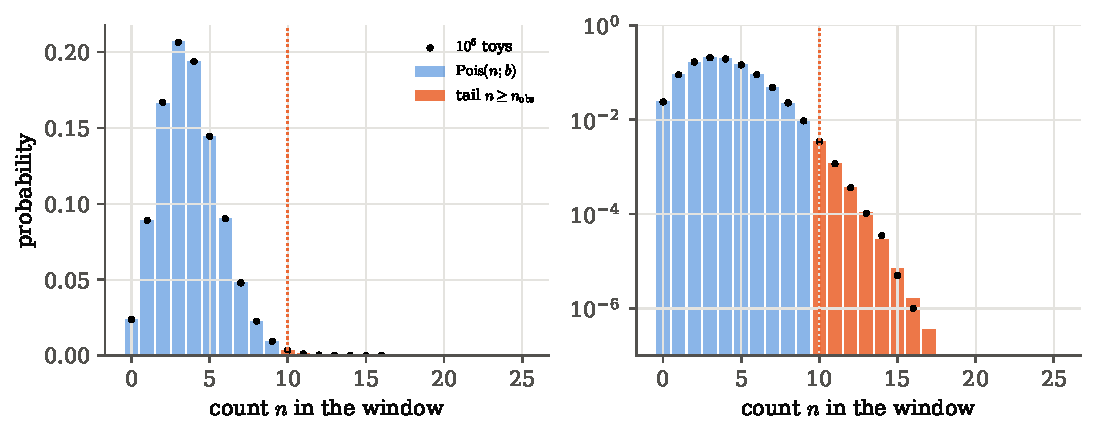
\includegraphics[width=\linewidth]{figures/ch04/bump_null.pdf}
\caption{The null distribution of the window count, $\mathrm{Pois}(n;b)$ with
$b=\FourABumpB$, on a linear scale (left) and a log scale (right). The orange
bars are the outcomes at least as large as the observed $n_{\rm obs}=\FourABumpN$,
and their total height is the p-value. The black dots are the frequencies in
a million simulated background-only experiments. They follow the bars even far
out in the tail, where the log scale is needed to see them.}
\label{4a:fig:bump-null}
\end{figure}

\paragraph{Example: Cowan's peak.}
\srcref{Cowan}{p.~60, Fig.~4.3} shows a histogram with a peak where two bins
contain $n_{\rm obs}=11$ entries on an expected background of $b=3.2$. The
same formula gives
\[
  p=1-\sum_{n=0}^{10}\frac{3.2^n e^{-3.2}}{n!}=\FourACowanPone ,
\]
the value $5.0\times10^{-4}$ quoted there. Fewer than one background-only
histogram in two thousand would have such a full pair of bins \emph{at that
location}. The last three words matter: a peak could have appeared anywhere
in the histogram, and \srcref{Cowan}{p.~61} points out that the fair
question is how often a peak this improbable appears in \emph{any} bin. That
is the look-elsewhere effect, treated in the second part of the chapter.

\paragraph{Example: a few events on almost no background, and a background we
do not quite know.}
The p-value is computed \emph{entirely} from the null model, so an error in
the expected background goes straight into it. Suppose we expect $b=0.5$
background events and observe $n_{\rm obs}=5$ \srcref{Cowan}{p.~59}. Then
\eqref{4a:eq:poisson-p} gives $p=\FourACowanPtwo$. If the background estimate
is off and the true value is $b=0.8$, the same five events give
$p=\FourACowanPthree$, almost ten times larger. A modest error in the
background has turned a striking result into a much less striking one. This is
why every real search spends most of its effort on the background estimate,
and quotes p-values for a range of plausible $b$.

\subsection{Python: exact tail and simulated tail}
\label{4a:sec:bump-python}

\Cref{4a:lst:bump} shows the lines of \pyname{code/ch04/01_bump_pvalue.py}
that compute the p-value twice.

\pyfile[firstline=39,lastline=52,label={4a:lst:bump}]{code/ch04/01_bump_pvalue.py}{The window count, its exact Poisson p-value, and a Monte Carlo p-value}

The mask \pyname{win} picks the two bins between $124$ and $128\,$GeV, and
summing the expected background and the observed counts over it gives $b$
and $n_{\rm obs}$. The function \pyname{stats.poisson.sf(k, b)} is the
\emph{survival function} $\Prob(N>k)$, so asking for
\pyname{sf(n_win - 1, b_win)} gives $\Prob(N\ge n_{\rm obs})$, exactly the
last line of \eqref{4a:eq:poisson-p}. The off-by-one is the most common bug
in this computation: $\Prob(N>n_{\rm obs})$ leaves out the observed value
itself.

The Monte Carlo version is the definition of the p-value turned into code, and
it does not use the formula at all. It draws $M=10^6$ background-only
experiments, each a single Poisson count with mean $b$, and counts the
fraction at least as large as the observation. It finds $p=\FourABumpPmc$,
with a binomial standard error of $\sqrt{p(1-p)/M}=\FourABumpPmcErr$, in
agreement with the exact value $\FourABumpP$. Here the simulation is overkill,
because the tail sum is exact. But when the test statistic is complicated and
its null distribution has no formula, which is the usual situation in
research, simulation is the only option.

The simulated data do contain a signal: $\FourABumpStot$ expected events from
a narrow resonance at $126\,$GeV. The test does not know this. With these
numbers it cannot tell a real signal of this size from a lucky fluctuation
with much confidence. \Cref{4a:sec:power} asks how large a signal must be
before a test catches it reliably.

\begin{pitfall}[The $\sqrt{n}$ error bar answers the wrong question]
It is tempting to write the observation as $n\pm\sqrt n$, subtract the
background, and count standard deviations. For five events on $b=0.5$ this
gives $4.5\pm2.2$, ``only two standard deviations'' from zero, even though
$p=\FourACowanPtwo$ says the excess is very unusual \srcref{Cowan}{p.~60}.
The error bar $\sqrt n$ describes how a Poisson variable \emph{with mean $n$}
fluctuates down. The p-value asks how a Poisson variable \emph{with mean $b$}
fluctuates up, and only the second question is posed by the null. For our
bump, $(n-b)/\sqrt n=\FourABumpZwrong$ and $(n-b)/\sqrt b=\FourABumpZnaive$,
while the exact tail corresponds to $\FourABumpZ$ Gaussian standard
deviations (the conversion is explained in \cref{4a:sec:ztable}). Neither
shortcut is right for small counts. Compute the tail.
\end{pitfall}

Two practical lessons from \srcref{Cowan}{p.~61} complete the recipe. The
window must be fixed before we look at the data, with a width of a few times
the mass resolution; widening or shifting it to make the excess look better
destroys the meaning of the p-value, because the null distribution was
computed for a fixed window. And the p-value of one window ignores the
other bins, some of which are also a little high or low. A test of the whole
histogram against the background shape is a goodness-of-fit test, the subject
of \cref{4a:sec:gof}.
\section{Which way is ``more extreme''? Sides, and the stopping rule}
\label{4a:sec:sides}

A coin is tossed $N=20$ times and comes up heads $n_h=17$ times
\srcref{Cowan}{p.~58}. A fair coin gives $10$ heads on average, so $17$ looks
suspicious. To turn the suspicion into a p-value we must say which other
outcomes are ``at least as extreme'' as $17$ heads. The answer is not a
technicality. It depends on what we were worried about before we tossed, and,
more surprisingly, on how we decided when to stop tossing. The coin is small
enough that we can do every sum by hand and see both effects directly.

\paragraph{The question in words.}
\begin{enumerate}[label=\arabic*.]
  \item Which alternative are we guarding against: a coin biased towards
        heads, or a coin biased either way?
  \item Given that choice, which outcomes count as ``this, or even more in
        this direction''?
  \item Did the experimenter fix the number of tosses in advance, or stop for
        some other reason? The imaginary repetitions that the p-value averages
        over must follow the same plan.
\end{enumerate}

\subsection{Simple and composite hypotheses, one and two sides}
\label{4a:sec:simple-composite}

A hypothesis that fixes the distribution of the data completely is
\newterm{simple}. ``The coin is fair'', $p=\tfrac12$, is simple: it predicts
$n_h\sim\mathrm{Binomial}(20,\tfrac12)$ \unpack{the number of successes in $20$
independent tries, each with success probability $\tfrac12$}. A hypothesis
that leaves at least one parameter free is \newterm{composite}, for example
$p\le\tfrac12$ or $p\neq\tfrac12$ \mainref{p.~151}, \srcref{Cowan}{\S4.1}.

The alternative decides the shape of the rejection region.
\begin{itemize}
  \item A \newterm{two-sided test}, $\Hnull:\theta=\theta_0$ versus
        $\Halt:\theta\neq\theta_0$, guards against departures in both
        directions. For the coin, very many heads and very few heads are both
        evidence of bias, and a sensible statistic is the distance from the
        expected value, $T=\abs{n_h-N/2}$.
  \item A \newterm{one-sided test}, $\Hnull:\theta\le\theta_0$ versus
        $\Halt:\theta>\theta_0$ (or the mirror image), guards against a
        departure in one direction only. If the only suspicion is a coin loaded
        towards heads, then $T=n_h$ and only large values count.
\end{itemize}
In both cases the test statistic is built to be \emph{large when $\Halt$ is
true}, so the rejection region is always ``$T$ large'' and the p-value is always
an upper tail of $T$. The direction lives in the choice of $T$.
\Cref{4a:fig:sides} shows the two rejection regions for a statistic that is
standard normal under the null, with the same total probability $\alpha=0.05$
in each: all of it in one tail beyond $z=\FourAPzZfivepct$, or half in each
tail beyond $\pm\FourAPzZfivepctTwo$.

\begin{figure}[htbp]
\centering
\begin{tikzpicture}
\pgfplotsset{fouraSides/.style={width=6.4cm, height=4.2cm, domain=-3.6:3.6,
  samples=160, xmin=-3.6, xmax=3.6, ymin=0, ymax=0.47, axis lines=left,
  ytick=\empty, xtick={-2,0,2}, xlabel={$z$}}}
\begin{axis}[fouraSides, title={\small one-sided: $H_1:\theta>\theta_0$}]
  \addplot[name path=g, formblue, thick] {exp(-x^2/2)/sqrt(2*pi)};
  \path[name path=ax] (axis cs:-3.6,0) -- (axis cs:3.6,0);
  \addplot[fibreorange!75] fill between[of=g and ax, soft clip={domain=1.645:3.6}];
  \draw[bdryred] (axis cs:1.645,0) -- (axis cs:1.645,0.30);
  \node[anchor=south, font=\small, bdryred] at (axis cs:1.645,0.30) {$1.645$};
  \node[anchor=south west, font=\small] at (axis cs:2.0,0.07) {$\alpha$};
\end{axis}
\begin{axis}[fouraSides, xshift=7cm, title={\small two-sided: $H_1:\theta\neq\theta_0$}]
  \addplot[name path=g, formblue, thick] {exp(-x^2/2)/sqrt(2*pi)};
  \path[name path=ax] (axis cs:-3.6,0) -- (axis cs:3.6,0);
  \addplot[fibreorange!75] fill between[of=g and ax, soft clip={domain=1.96:3.6}];
  \addplot[fibreorange!75] fill between[of=g and ax, soft clip={domain=-3.6:-1.96}];
  \draw[bdryred] (axis cs:1.96,0) -- (axis cs:1.96,0.30);
  \draw[bdryred] (axis cs:-1.96,0) -- (axis cs:-1.96,0.30);
  \node[anchor=south, font=\small, bdryred] at (axis cs:1.96,0.30) {$1.96$};
  \node[anchor=south, font=\small, bdryred] at (axis cs:-1.96,0.30) {$-1.96$};
  \node[anchor=south west, font=\small] at (axis cs:2.3,0.05) {$\alpha/2$};
  \node[anchor=south east, font=\small] at (axis cs:-2.3,0.05) {$\alpha/2$};
\end{axis}
\end{tikzpicture}
\caption{The same total probability $\alpha=0.05$ placed in one tail (left)
or split between two tails (right) of a standard normal null distribution. The
one-sided test rejects sooner in the direction it cares about, at $1.645$
instead of $1.96$, and never rejects in the other direction.}
\label{4a:fig:sides}
\end{figure}

\paragraph{Example: 17 heads in 20 tosses.}
The binomial probability of $k$ heads for a fair coin is
$\binom{20}{k}2^{-20}$, and $2^{20}=1\,048\,576$. If we only feared a coin
loaded towards heads, the p-value is
\begin{align}
  p_{\text{one}}=\Prob(n_h\ge17\given p=\tfrac12)
  &\eqby{1} \frac{1}{2^{20}}\Bigl[\tbinom{20}{17}+\tbinom{20}{18}+\tbinom{20}{19}+\tbinom{20}{20}\Bigr] \notag\\
  &\eqby{2} \frac{1140+190+20+1}{1\,048\,576}=\frac{1351}{1\,048\,576}
   \approx\FourACoinPone .
  \label{4a:eq:coin-one}
\end{align}
\begin{explain}
  \item Add the probabilities of the disjoint outcomes $17,18,19,20$ heads.
  \item $\binom{20}{17}=\binom{20}{3}=\frac{20\cdot19\cdot18}{6}=1140$,
        $\binom{20}{18}=\binom{20}{2}=190$, $\binom{20}{19}=20$,
        $\binom{20}{20}=1$.
\end{explain}
If any bias counts, the outcomes at least as far from $10$ as $17$ are
$n_h\in\{0,1,2,3\}\cup\{17,\dots,20\}$, that is $\abs{n_h-10}\ge7$. The
binomial with $p=\frac12$ is symmetric, $\binom{20}{k}=\binom{20}{20-k}$, so
the lower tail equals the upper one and
\[
  p_{\text{two}}=\Prob\bigl(\abs{n_h-10}\ge7\given p=\tfrac12\bigr)
  =2\,p_{\text{one}}=\frac{2702}{1\,048\,576}\approx\FourACoinPtwo ,
\]
the value $0.0026$ of \srcref{Cowan}{p.~58}. \Cref{4a:fig:coin-sides} shows
the eight outcomes that enter. The two answers differ by a factor of two, and
both are correct answers to different questions.

\begin{figure}[htbp]
\centering
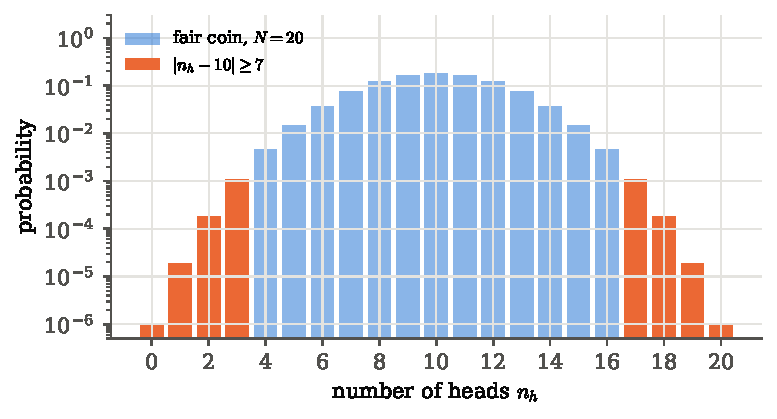
\includegraphics[width=0.78\linewidth]{figures/ch04/coin_sides.pdf}
\caption{The binomial distribution of the number of heads in $20$ tosses of a
fair coin, on a logarithmic vertical scale so that the thin tails show. The orange
bars are the outcomes at least as far from $10$ as the
observed $17$, on either side. Their total is the two-sided p-value; the four
bars on the right alone give the one-sided one.}
\label{4a:fig:coin-sides}
\end{figure}

\paragraph{A composite null.}
For a one-sided composite null, the p-value is the tail at the boundary of the
null, so the composite test reduces to the simple test at $\theta_0$. To see
why, pose the one-sided coin question with the composite null
$\Hnull:p\le\frac12$, where $p$ is now the probability of heads. The problem is
that every $p$ in $\Theta_0$ gives a different tail probability
$\Prob_p(n_h\ge17)$. The rule \mainref{Thm~10.12} is to report the largest of
them, $\sup_{\theta\in\Theta_0}\Prob_\theta(T\ge t_{\rm obs})$, so that the
number is honest for every member of the null. The tail $\Prob_p(n_h\ge17)$
grows with $p$, because a coin more inclined to heads gives more heads. So the
largest tail is reached at the boundary $p=\frac12$, and the answer is again
$\FourACoinPone$. The boundary value is the member of the null hardest to tell
apart from the alternative.

\paragraph{When the null distribution is not symmetric.}
A skewed null needs a convention for its two-sided p-value. For the fair coin,
``twice the one-sided tail'' and ``everything at least as far from the mean''
agree. For a skewed null, such as a Poisson with small mean, they do not, and
we must choose one of two rules: either double the
smaller tail, or add the probabilities of all outcomes that are no more
probable than the one observed. In searches for new physics the question is
almost always one-sided anyway, because a signal can only add events.

\begin{pitfall}[Choosing the side after seeing the data]
The side is part of the question, so it must be chosen before looking at the
data. Deciding on a one-sided test \emph{because} the excess came out
upwards halves the p-value without any new evidence. Under the null this
procedure rejects whenever either tail holds $\alpha$ of the probability, so
its true type I error rate is $2\alpha$, not $\alpha$.
\end{pitfall}

\subsection{The same data, different p-values: the stopping rule}
\label{4a:sec:stopping}

The same data can give different p-values, depending on how the experimenter
decided when to stop. The reason is in what the p-value asks for: the
probability of outcomes ``like this or more extreme'' in \emph{repetitions of
the experiment}. Those repetitions never happened. We imagine them, or, in the
blunt words of \srcref{Lambert}{\S2.8}, to test a hypothesis we ``invent
fictitious samples''. Lambert's example: if we hypothesise that heights are
normal with mean $1.55\,$m and standard deviation $0.3\,$m and meet one person
of $2.5\,$m, the p-value is the probability of meeting someone \emph{at least}
$2.5\,$m tall, although nobody taller was observed. To imagine the repetitions
we must know the plan that produced the data, and the data alone do not tell
us.

\emph{The data.} \srcref{Kruschke}{\S11.1} gives the example. A coin shows
$z=7$ heads in $N=24$ tosses. Is it fair? We take two possible plans in turn.

\paragraph{Plan A: the number of tosses was fixed at $N=24$.}
Then the random quantity is the number of heads $z$, it is
$\mathrm{Binomial}(24,\frac12)$ under the null, and few heads is the extreme
direction:
\[
  p_A=\Prob(z\le7\given N=24)=\sum_{k=0}^{7}\binom{24}{k}2^{-24}=\FourAKrFixN .
\]

\paragraph{Plan B: the experimenter tossed until the seventh head.}
Now $z=7$ is fixed by design and the random quantity is the number of tosses
$N$ it took. Needing \emph{many} tosses to collect seven heads is the sign of
a tail-heavy coin, so the extreme direction is $N\ge24$. The event $\{N\ge24\}$
is the same as ``at most six heads in the first $23$ tosses'':
\begin{align}
  p_B=\Prob(N\ge24\given z=7)
  &\eqby{1} \Prob\bigl(\text{at most 6 heads in the first 23 tosses}\bigr) \notag\\
  &\eqby{2} \sum_{k=0}^{6}\binom{23}{k}2^{-23}
   = \FourAKrFixZ .
  \label{4a:eq:fixz}
\end{align}
\begin{explain}
  \item The seventh head arrives at toss $24$ or later exactly when the first
        $23$ tosses contain six heads or fewer.
  \item The first $23$ tosses of a fair coin are
        $\mathrm{Binomial}(23,\frac12)$, whatever happens afterwards.
\end{explain}
The distribution of $N$ itself is the negative binomial of \cref{ch:02}: the
$n$-th toss is the seventh head when it is a head and the previous $n-1$ tosses
hold exactly six heads, so $\Prob(N=n)=\binom{n-1}{6}2^{-n}$.
\Cref{4a:fig:stopping} shows the two clouds of imaginary outcomes side by side.

\begin{figure}[htbp]
\centering
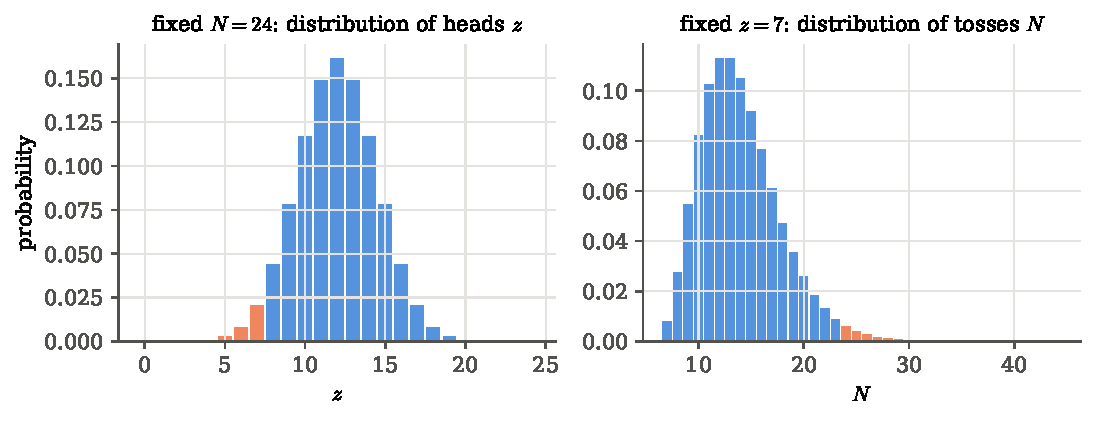
\includegraphics[width=\linewidth]{figures/ch04/stopping_rules.pdf}
\caption{Two plans that can produce the same record of $7$ heads in $24$
tosses. Left: with $N=24$ fixed, the random quantity is the number of heads,
and its lower tail $z\le7$ (orange) is the p-value. Right: when tossing stops
at the seventh head, the random quantity is the number of tosses, and its upper
tail $N\ge24$ (orange) is the p-value. The observed data are identical; the
imagined repetitions are not.}
\label{4a:fig:stopping}
\end{figure}

\emph{What the two plans say.} The very same sequence of tosses is ``not
significant'' under one plan and ``significant'' under the other. With the
conventional two-tailed threshold, which puts $2.5\%$ in each tail, plan A
gives $p_A=\FourAKrFixN$, above $0.025$, and plan B gives $p_B=\FourAKrFixZ$,
below it.
\srcref{Kruschke}{p.~309} adds two more plans. If the experimenter tossed for
a fixed length of time, so that $N$ itself is random (Poisson), the p-value is
$0.024$. If a second coin was tested in the same study and the question is
whether \emph{either} coin looks this extreme, the chance that at least one of
two independent fixed-$N$ experiments reaches the tail is
$1-(1-p_A)^2\approx2p_A$, which is the $0.063$ found there. The last case is
our first taste of the look-elsewhere effect.

\paragraph{Example: Cowan's stopping rule.}
\srcref{Cowan}{p.~58} tells the same story with the 17 heads in 20 tosses.
Suppose the plan was ``toss until there are at least three heads and at least
three tails'', and the stopping happened at toss $20$ (with $17$ heads and
$3$ tails). Now the extreme outcomes are those that need $20$ tosses or more:
\begin{align}
  \Prob(N_{\rm stop}\ge20)
  &\eqby{1} \Prob\bigl(\text{after 19 tosses, heads}\le2\ \text{or tails}\le2\bigr) \notag\\
  &\eqby{2} 2\,\Prob\bigl(\mathrm{Binomial}(19,\tfrac12)\le2\bigr) \notag\\
  &\eqby{3} 2\,\frac{\binom{19}{0}+\binom{19}{1}+\binom{19}{2}}{2^{19}}
   = \frac{2\,(1+19+171)}{524\,288}\approx\FourACowStop .
  \label{4a:eq:cowan-stop}
\end{align}
\begin{explain}
  \item We are still tossing after toss $19$ exactly when one of the two
        faces has appeared at most twice so far.
  \item The two events are disjoint (both at most $2$ would mean at most $4$
        tosses, not $19$), so their probabilities add, and by symmetry they
        are equal.
  \item Binomial sum with $\binom{19}{2}=171$ and $2^{19}=524\,288$.
\end{explain}
That is $0.073\%$ instead of the $0.26\%$ of the fixed-$N$ plan
\srcref{Cowan}{p.~58}. Cowan's resolution is a convention: always interpret
``similar experiments'' as experiments with the same number of observations.
It is arbitrary, but it makes a reported p-value unambiguous.

\paragraph{Python.}
The script \pyname{code/ch04/02_sides_and_stopping.py} evaluates every tail
sum above with \pyname{scipy.stats.binom} and then checks each one by running
the stated protocol many times.

\pyfile[firstline=34,lastline=52]{code/ch04/02_sides_and_stopping.py}{Two stopping plans, and Cowan's rule, simulated}

For plan B it uses the fact that the number of tails before the seventh head is
a negative binomial variable, \pyname{rng.negative_binomial(7, 0.5)}, so the
total number of tosses is seven plus that. For Cowan's rule it simply tosses:
$200\,000$ sequences of $60$ tosses, running totals of heads and tails with
\pyname{np.cumsum}, and the first toss at which both totals reach three. The
simulations give $\FourAKrFixNMC$, $\FourAKrFixZMC$ and $\FourACowStopMC$
against the exact $\FourAKrFixN$, $\FourAKrFixZ$ and $\FourACowStop$, and
$\FourACoinPtwoMC$ against $\FourACoinPtwo$ for the two-sided coin test.

\begin{keyidea}[A p-value depends on the outcomes that did not happen]
A p-value is a sum over imaginary repetitions of the experiment. Which
repetitions are imagined depends on the plan: the alternative we guard against
(one or two sides), when the experimenter would have stopped, and how many
other places or coins we would also have looked at. Change the plan and the
p-value changes, even if the data do not.
\end{keyidea}

A Bayesian analysis does not have this problem, because it uses only the
probability of the data actually observed. In plan A that probability is
$\binom{24}{7}p^7(1-p)^{17}$ and in plan B it is $\binom{23}{6}p^7(1-p)^{17}$.
As functions of the coin's bias $p$, the two likelihoods differ only by a
constant factor, which cancels in Bayes' theorem. Any inference built from the
likelihood alone therefore reaches the same conclusion under both plans
\srcref{Kruschke}{\S11.1.7}. The p-value, which sums over outcomes that were
not observed, does not. We take this up in \cref{ch:05}. For now the practical
rule is Cowan's: fix the plan in advance, state it, and compute the p-value for
that plan.
\section{Two ways to be wrong: size, power and how much data we need}
\label{4a:sec:power}

A p-value tells us how surprising one data set is. Before the experiment runs,
we face a different pair of questions. How often will our procedure cry
``discovery'' when there is nothing there? And if there \emph{is} something
there, of a given size, how often will we catch it? The first number protects
the field from false claims. The second tells us whether the experiment is
worth building. A detector that can only see a signal one time in ten is a
bad investment, however careful the analysis.

\mainref{p.~150} offers the legal trial as a model. The defendant is presumed
innocent, the null, and is convicted only if the evidence is strong. Two
mistakes are possible: convicting an innocent person, and acquitting a guilty
one. A court that never convicts makes no mistakes of the first kind, and is
useless. There is a trade-off, and it can be put into numbers.

\paragraph{The question in words.}
\begin{enumerate}[label=\arabic*.]
  \item If the null is true, what is the probability that the test rejects it?
  \item If a particular alternative is true, what is the probability that the
        test rejects the null?
  \item How do both depend on the critical value and on the amount of data,
        and how large must an experiment be to catch an effect of a given size?
\end{enumerate}

\subsection{Type I and type II errors}
\label{4a:sec:errors}

Every test ends in one of four situations \mainref{Table~10.1}:
\begin{center}
\begin{tabular}{lcc}
\toprule
 & retain $\Hnull$ & reject $\Hnull$ \\
\midrule
$\Hnull$ true & correct & \newterm{type I error} (false alarm) \\
$\Halt$ true & \newterm{type II error} (missed signal) & correct \\
\bottomrule
\end{tabular}
\end{center}
Cowan calls them errors of the first and second kind \srcref{Cowan}{\S4.1}.
Picture the test statistic $t$ with its two sampling distributions,
$g(t\given\Hnull)$ and $g(t\given\Halt)$, and a cut $t_{\rm cut}$ above which
we reject (\cref{4a:fig:alpha-beta}). The probability of a type I error is the
area of the null distribution above the cut, and the probability of a type II
error is the area of the alternative below it \srcref{Cowan}{(4.1)--(4.2)}:
\begin{equation}
  \alpha=\int_{t_{\rm cut}}^{\infty}g(t\given\Hnull)\,\dd t,
  \qquad
  \beta_{\rm II}=\int_{-\infty}^{t_{\rm cut}}g(t\given\Halt)\,\dd t .
  \label{4a:eq:alpha-beta}
\end{equation}
Moving the cut to the right shrinks $\alpha$ and grows $\beta_{\rm II}$; moving
it left does the opposite. With a fixed statistic and a fixed amount of data
we cannot shrink both. Only a better statistic (\cref{4a:sec:np}) or more data
separates the two curves.

\begin{figure}[htbp]
\centering
\begin{tikzpicture}
\begin{axis}[
  width=11cm, height=5cm, domain=-3.5:6.5, samples=200,
  xmin=-3.5, xmax=6.5, ymin=0, ymax=0.56, axis lines=left, clip=false,
  xlabel={test statistic $t$}, ytick=\empty, xtick={-2,0,2,4,6}]
  \addplot[name path=h0, formblue, thick] {exp(-x^2/2)/sqrt(2*pi)};
  \addplot[name path=h1, tangentgreen!80!black, thick] {exp(-(x-2.8)^2/2)/sqrt(2*pi)};
  \path[name path=ax] (axis cs:-3.5,0) -- (axis cs:6.5,0);
  \addplot[fibreorange!75] fill between[of=h0 and ax, soft clip={domain=1.645:6.5}];
  \addplot[tangentgreen!30] fill between[of=h1 and ax, soft clip={domain=-3.5:1.645}];
  \draw[bdryred, thick] (axis cs:1.645,0) -- (axis cs:1.645,0.46);
  \node[anchor=south, font=\small, bdryred] at (axis cs:1.645,0.46) {$t_{\rm cut}$};
  \node[font=\small, formblue, anchor=east] at (axis cs:-1.1,0.30) {$g(t\given H_0)$};
  \node[font=\small, tangentgreen!60!black, anchor=west] at (axis cs:3.9,0.30) {$g(t\given H_1)$};
  \node[font=\small, anchor=west] at (axis cs:2.6,0.08) {$\alpha$};
  \draw[black!60] (axis cs:2.6,0.08) -- (axis cs:2.05,0.03);
  \node[font=\small, anchor=east] at (axis cs:0.6,0.08) {$\beta_{\rm II}$};
  \draw[black!60] (axis cs:0.6,0.08) -- (axis cs:1.25,0.06);
  \node[font=\small, anchor=west] at (axis cs:-3.3,0.54) {retain $H_0$};
  \node[font=\small, anchor=east] at (axis cs:6.4,0.54) {reject $H_0$};
\end{axis}
\end{tikzpicture}
\caption{The trade-off behind every test. Blue: the distribution of the
statistic when the null is true; green: when a particular alternative is true.
Everything right of the red cut is rejected. The orange sliver is the
probability of a false alarm, $\alpha$; the pale green region is the
probability of missing the signal, $\beta_{\rm II}$. Sliding the cut trades one
for the other.}
\label{4a:fig:alpha-beta}
\end{figure}

\subsection{The power function}
\label{4a:sec:power-function}

The alternative is rarely a single value, so we want the rejection probability
as a function of the true parameter.

\begin{workdef}[power function, size, level]
The \newterm{power function} of a test with rejection region $R$ is
\[
  \beta(\theta)=\Prob_\theta(\bm X\in R)
\]
\unpack{the probability of rejecting $\Hnull$ when the true parameter is
$\theta$}. For $\theta\in\Theta_1$ it is the probability of a correct
rejection; for $\theta\in\Theta_0$ it is a false-alarm rate. The
\newterm{size} is the worst false-alarm rate,
$\alpha=\sup_{\theta\in\Theta_0}\beta(\theta)$, and a test has
\newterm{level} $\alpha$ if its size is at most $\alpha$ \mainref{Def.~10.1}.
Operationally: simulate data at each $\theta$ and record the fraction of
data sets that the test rejects.
\end{workdef}

A notational trap: Wasserman uses $\beta(\theta)$ for the power, while
\srcref{Cowan}{(4.2)} uses $\beta$ for the type II error probability, so that
Cowan's power is $1-\beta$. Here we use Wasserman's convention and write the type II error
probability at a point $\theta_1\in\Theta_1$ as $\beta_{\rm II}=1-\beta(\theta_1)$.

\paragraph{Example: the one-sided test for a Gaussian mean.}
We take $n$ readings $X_1,\dots,X_n\iid\Normal(\mu,\sigma^2)$ with $\sigma$
known and test $\Hnull:\mu\le0$ against $\Halt:\mu>0$ by rejecting when the
sample mean $\bar X$ exceeds a cut $c$ \mainref{Ex.~10.2}. Recall from
\cref{ch:03} that $\bar X\sim\Normal(\mu,\sigma^2/n)$, so
$Z=\sqrt n(\bar X-\mu)/\sigma$ is standard normal. The power function is
\begin{align}
  \beta(\mu)
  &\eqby{1} \Prob_\mu\bigl(\bar X>c\bigr) \notag\\
  &\eqby{2} \Prob_\mu\Bigl(\frac{\sqrt n(\bar X-\mu)}{\sigma}>\frac{\sqrt n(c-\mu)}{\sigma}\Bigr) \notag\\
  &\eqby{3} \Prob\Bigl(Z>\frac{\sqrt n(c-\mu)}{\sigma}\Bigr) \notag\\
  &\eqby{4} 1-\Phi\Bigl(\frac{\sqrt n(c-\mu)}{\sigma}\Bigr) .
  \label{4a:eq:power-z}
\end{align}
\begin{explain}
  \item Definition of the power function with $R=\{\bar X>c\}$.
  \item Subtract $\mu$ and multiply by $\sqrt n/\sigma>0$ on both sides; this
        does not change the event.
  \item The left-hand side is standard normal whatever $\mu$ is.
  \item $\Phi$ is the standard normal CDF, $\Phi(z)=\Prob(Z\le z)$.
\end{explain}
As $\mu$ increases the argument of $\Phi$ decreases, so $\beta(\mu)$
increases. The largest false-alarm rate over the null region $\mu\le0$ is
therefore at the boundary:
\[
  \alpha=\sup_{\mu\le0}\beta(\mu)=\beta(0)=1-\Phi\Bigl(\frac{\sqrt n\,c}{\sigma}\Bigr)
  \quad\Longrightarrow\quad
  c=\frac{\sigma\,z_\alpha}{\sqrt n},\qquad z_\alpha\equiv\Phi^{-1}(1-\alpha).
\]
So the size-$\alpha$ test rejects when $\sqrt n\,\bar X/\sigma>z_\alpha$:
the sample mean, measured in units of its own standard deviation, must exceed
$z_{0.05}=\FourAPzZfivepct$ for $\alpha=0.05$.

\Cref{4a:fig:power-curves} (left) plots \eqref{4a:eq:power-z} for $n=4$,
$16$ and $64$ with $\sigma=1$, together with simulated rejection rates. All
three curves pass through $\alpha=0.05$ at $\mu=0$: the size does not depend
on $n$, because the cut moves in as $1/\sqrt n$. What depends on $n$ is the
steepness. Quadrupling the data halves the width of $\bar X$'s distribution,
so the curve rises over half the range of $\mu$. In the simulation the rate of
false alarms at $\mu=0$ is $\FourAPowSizeFour$ for $n=4$ and
$\FourAPowSizeSixtyfour$ for $n=64$, both equal to $0.05$ within the
simulation error $\sqrt{0.05\times0.95/20\,000}\approx0.0015$.

\begin{figure}[htbp]
\centering
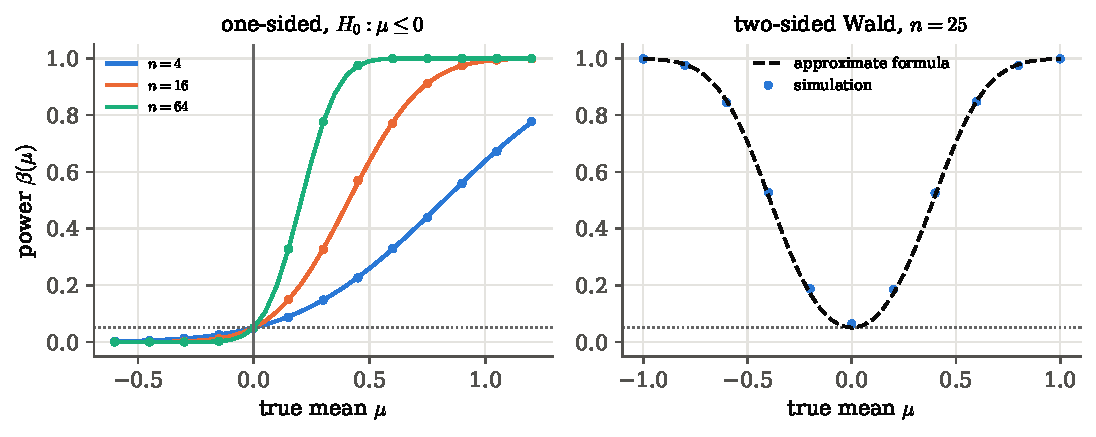
\includegraphics[width=\linewidth]{figures/ch04/power_curves.pdf}
\caption{Power functions. Left: the one-sided test of $\mu\le0$ for three
sample sizes, with the formula as lines and simulated rejection rates as dots.
Every curve crosses the dotted $\alpha=0.05$ line at $\mu=0$ and climbs faster
the more data there are. Right: the two-sided Wald test with $n=25$ and an
estimated standard error; the dashed curve is the approximate formula and the
dots are simulations. The curve is symmetric and bottoms out near $\alpha$ at
$\mu=0$.}
\label{4a:fig:power-curves}
\end{figure}

\paragraph{Example: how many readings do we need?}
Suppose we want power $0.8$ at $\mu_1=0.5\sigma$, with $\alpha=0.05$. Setting
\eqref{4a:eq:power-z} equal to $0.8$ at $\mu=\mu_1$, with $c=\sigma
z_\alpha/\sqrt n$,
\begin{align}
  0.8
  &\eqby{1} 1-\Phi\Bigl(z_\alpha-\frac{\sqrt n\,\mu_1}{\sigma}\Bigr)
  \eqby{2} \Phi\Bigl(\frac{\sqrt n\,\mu_1}{\sigma}-z_\alpha\Bigr) \notag\\
  &\;\Longrightarrow\;
  \frac{\sqrt n\,\mu_1}{\sigma}-z_\alpha \eqby{3} z_{0.2}
  \;\Longrightarrow\;
  n \eqby{4} \Bigl(\frac{(z_\alpha+z_{0.2})\,\sigma}{\mu_1}\Bigr)^2
  =\Bigl(\frac{1.645+0.842}{0.5}\Bigr)^2\approx\FourAPowNreq .
  \label{4a:eq:sample-size}
\end{align}
\begin{explain}
  \item Insert $c=\sigma z_\alpha/\sqrt n$ into $\sqrt n(c-\mu_1)/\sigma$.
  \item The normal CDF is symmetric: $1-\Phi(x)=\Phi(-x)$.
  \item Apply $\Phi^{-1}$; $\Phi^{-1}(0.8)=z_{0.2}=0.842$ in the notation
        $z_a=\Phi^{-1}(1-a)$.
  \item Solve for $n$.
\end{explain}
We need $n=\FourAPowNreqInt$ readings, and the simulation with $n=25$ rejects
in a fraction $\FourAPowReqMC$ of experiments at $\mu=0.5$. The formula says
what experiment planning comes down to: the required number of readings grows
as $1/\mu_1^2$, so detecting an effect half as large costs four times as much
data.
\srcref{Kruschke}{\S11.5.1} makes the same point: planning an experiment is
where sampling distributions are most useful.

\paragraph{Example: the power of the two-sided Wald test.}
Most tests are two-sided and use an estimate $\hat\theta$ with standard error
$\widehat{\rm se}$; the Wald test of \cref{4a:sec:wald} rejects
$\Hnull:\theta=\theta_0$ when $\abs{\hat\theta-\theta_0}/\widehat{\rm se}>z_{\alpha/2}$.
Suppose the truth is $\theta_\star\neq\theta_0$ and $\hat\theta$ is
approximately $\Normal(\theta_\star,{\rm se}^2)$, so that
$Z=(\hat\theta-\theta_\star)/{\rm se}$ is approximately standard normal. Write
$\delta=(\theta_0-\theta_\star)/{\rm se}$. Then
\begin{align}
  \beta(\theta_\star)
  &\eqby{1} \Prob_{\theta_\star}\Bigl(\frac{\hat\theta-\theta_0}{\rm se}>z_{\alpha/2}\Bigr)
          +\Prob_{\theta_\star}\Bigl(\frac{\hat\theta-\theta_0}{\rm se}<-z_{\alpha/2}\Bigr) \notag\\
  &\eqby{2} \Prob\bigl(Z>\delta+z_{\alpha/2}\bigr)+\Prob\bigl(Z<\delta-z_{\alpha/2}\bigr) \notag\\
  &\eqby{3} 1-\Phi\Bigl(\frac{\theta_0-\theta_\star}{\rm se}+z_{\alpha/2}\Bigr)
          +\Phi\Bigl(\frac{\theta_0-\theta_\star}{\rm se}-z_{\alpha/2}\Bigr) .
  \label{4a:eq:power-wald}
\end{align}
\begin{explain}
  \item The two-sided rejection region is the union of two disjoint tails.
  \item $\hat\theta-\theta_0=(\hat\theta-\theta_\star)+(\theta_\star-\theta_0)$,
        so dividing by se gives $Z-\delta$; move $\delta$ across.
  \item Write both tails with the normal CDF.
\end{explain}
This is \mainref{(10.6)}. Since se shrinks as $1/\sqrt n$, the argument
$\delta$ grows, and one of the two terms tends to one: the power is large when
$\theta_\star$ is far from $\theta_0$ or when the sample is large
\mainref{p.~154}. In the right panel of \cref{4a:fig:power-curves} the
simulation follows the formula. At $\mu=0$ it rejects in a fraction
$\FourAPowWaldSize$ of experiments, a little above $0.05$, because the
standard error was estimated from only $25$ readings. \Cref{4a:sec:wald}
explains that excess and removes it.

\subsection{The power of a counting experiment}
\label{4a:sec:power-counting}

Return to a search like the bump: a window with known background $b=3.2$ and
an unknown signal $s\ge0$, so that $N\sim\mathrm{Pois}(s+b)$. Particle
physics sets thresholds not as $\alpha=0.05$ but as ``$3\sigma$'' and
``$5\sigma$'', meaning one-sided tail probabilities
$\FourAPzThreeOne$ and $\FourAPzFiveOne$ (\cref{4a:sec:ztable} explains the
translation). The test rejects when $N\ge n_{\rm crit}$, where $n_{\rm crit}$
is the smallest count whose null tail is below the threshold:
\begin{equation}
  n_{\rm crit}=\min\bigl\{n:\ \Prob(N\ge n\given s=0)\le p_{\rm thr}\bigr\},
  \qquad
  \beta(s)=\Prob(N\ge n_{\rm crit}\given s)
  =1-\sum_{k=0}^{n_{\rm crit}-1}\frac{(s+b)^ke^{-(s+b)}}{k!} .
  \label{4a:eq:power-poisson}
\end{equation}
The first formula is the null tail \eqref{4a:eq:poisson-p} scanned in $n$. The
second is the same tail sum evaluated with the signal switched on, because
the power is the rejection probability under the alternative.

\paragraph{Example: $3\sigma$ and $5\sigma$ with $b=3.2$.}
The script finds $n_{\rm crit}=\FourAPowNthree$ for $3\sigma$ and
$n_{\rm crit}=\FourAPowNfive$ for $5\sigma$. So Cowan's $11$ events on $3.2$
(\cref{4a:sec:poisson-p}) just reach $3\sigma$. \Cref{4a:fig:power-counting}
shows the power as a function of $s$. A signal of about $\FourAPowSfiftyThree$
events is needed to cross $3\sigma$ half of the time, and about
$\FourAPowSfiftyFive$ to cross $5\sigma$ half of the time. With $s=20$ the
$5\sigma$ test fires with probability $\FourAPowFiveAtTwenty$, and a direct
simulation of $20\,000$ experiments gives $\FourAPowFiveAtTwentyMC$.

\begin{figure}[htbp]
\centering
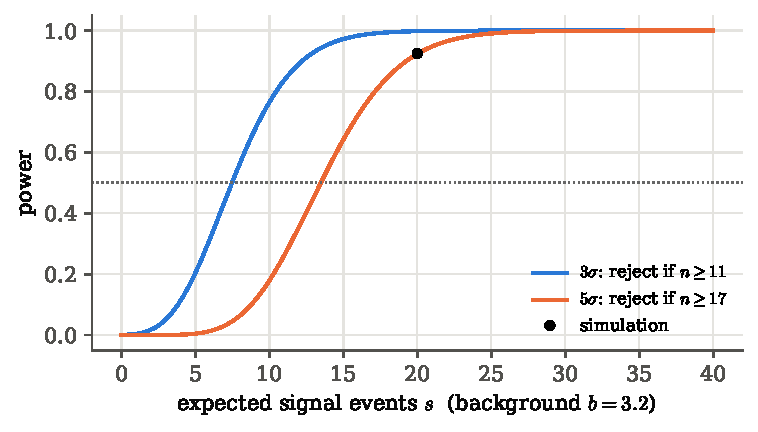
\includegraphics[width=0.8\linewidth]{figures/ch04/power_counting.pdf}
\caption{Power of a counting experiment with background $b=3.2$, for the
$3\sigma$ and the $5\sigma$ thresholds. Each curve rises from nearly zero to one
as the expected signal grows. The dotted line marks power one half, and the
black dot is a direct simulation at $s=20$.}
\label{4a:fig:power-counting}
\end{figure}

With discrete data a test usually has level $\alpha$ without having size
exactly $\alpha$: its false-alarm rate is below the target, and we call it
\emph{conservative}. The reason is that $N$ takes only integer values, so the
rejection probability under the null jumps as the cut moves from one integer
to the next. For example, the size of the test ``reject if $N\ge11$'' is
$\Prob(N\ge11\given b=3.2)=\FourACowanPone$, smaller than the $3\sigma$ target
$\FourAPzThreeOne$, and the next lower cut, $N\ge10$, would overshoot it.

\pyfile[firstline=72,lastline=87]{code/ch04/03_power_curves.py}{Critical count and power of a Poisson counting experiment}

The helper \pyname{n_crit} steps $n$ upward until the null tail
\pyname{stats.poisson.sf(n - 1, b)} drops below the threshold, which is
\eqref{4a:eq:power-poisson} read literally. The power curves are then the same
survival function with mean \pyname{b + s}. Nothing here needs an
approximation, which makes the counting experiment the best place to build
intuition about power before we meet statistics whose distributions must be
simulated.

\paragraph{Statistically significant is not the same as important.}
The power function of a consistent test climbs to one for \emph{every}
$\theta\in\Theta_1$ as $n\to\infty$, however close $\theta$ is to $\theta_0$.
With enough data, an effect too small to matter will be declared significant.
\mainref{p.~155} calls this the gap between statistical and scientific
significance: a rejection says the effect is probably not zero, not that it is
large. A confidence interval shows both at once, the distance from $\theta_0$
and the precision, and is often the more informative report. Every test can
be turned into a confidence interval, a construction taken up in the second
part of the chapter.
\section{The p-value is a random variable}
\label{4a:sec:uniform}

A p-value changes from one repetition of an experiment to the next. Imagine a
thousand groups, each running the same background-only experiment and each
computing a p-value. They will not get the same number. The data fluctuate, so
the test statistic fluctuates, so the p-value fluctuates
\srcref{Cowan}{p.~58}. The p-value is therefore a random variable with its own
distribution. That distribution is what gives ``reject if $p<\alpha$'' a known
false-alarm rate. It also shows, more clearly than any argument in words, why
a p-value is not the probability that the null is true.

\paragraph{The question in words.}
\begin{enumerate}[label=\arabic*.]
  \item How is the p-value related to the rejection regions of
        \cref{4a:sec:power}?
  \item If the null is true, how are p-values distributed? If it is false?
  \item In a collection of experiments where some nulls are true and some
        false, what fraction of the ``significant'' results are false alarms?
\end{enumerate}

\subsection{The smallest level at which we would reject}
\label{4a:sec:inf-alpha}

Suppose that for every $\alpha\in(0,1)$ we have a size-$\alpha$ test, with
rejection region $R_\alpha=\{T\ge c_\alpha\}$. A smaller $\alpha$ means a
stricter test, a larger $c_\alpha$ and a smaller region, so the regions are
nested. For our data, some of these tests reject and some do not, and there
is a smallest level at which the test still rejects. \mainref{Def.~10.11}
takes that as the definition,
\[
  p=\inf\bigl\{\alpha:\ T(\bm x)\in R_\alpha\bigr\},
\]
and \mainref{Thm~10.12} shows that it is the same tail probability as before.
For a simple null the argument is short. The observed value $t_{\rm obs}$ is on
the boundary of the region exactly when $c_\alpha=t_{\rm obs}$, and the size of
that region is $\Prob_{\theta_0}(T\ge t_{\rm obs})$. Any smaller $\alpha$ puts
the cut above $t_{\rm obs}$ and retains; any larger one rejects. So
\begin{equation}
  \text{reject at level }\alpha
  \quad\Longleftrightarrow\quad
  p\le\alpha .
  \label{4a:eq:p-le-alpha}
\end{equation}
This is why a p-value is more useful than a bare ``reject'': every reader can
apply their own $\alpha$. For a composite null the tail probability depends
on which $\theta\in\Theta_0$ is true, and the definition takes the worst case,
$p=\sup_{\theta\in\Theta_0}\Prob_\theta(T\ge t_{\rm obs})$, as we already did
for the coin in \cref{4a:sec:simple-composite}.

A widely used vocabulary for p-values \mainref{p.~157}:
\begin{center}
\begin{tabular}{ll}
\toprule
p-value & evidence against $\Hnull$ \\
\midrule
$<0.01$ & very strong \\
$0.01$--$0.05$ & strong \\
$0.05$--$0.10$ & weak \\
$>0.10$ & little or none \\
\bottomrule
\end{tabular}
\end{center}
Particle physicists would call $p=0.01$ an unremarkable fluctuation, for
reasons we come to in \cref{4a:sec:ztable}. The scale is a convention, and
conventions differ between fields.

\subsection{Under the null, p is uniform}
\label{4a:sec:p-uniform}

Let $T$ have a continuous distribution under $\Hnull$, with cumulative
distribution function $F_0(t)=\Prob_{\theta_0}(T\le t)$, increasing and
continuous. For an observed value $t$, the p-value is the upper tail,
$p=1-F_0(t)$. Now let the data be random, so that the p-value is the random
variable $P=1-F_0(T)$. For any $u\in(0,1)$,
\begin{align}
  \Prob_{\theta_0}(P\le u)
  &\eqby{1} \Prob_{\theta_0}\bigl(1-F_0(T)\le u\bigr) \notag\\
  &\eqby{2} \Prob_{\theta_0}\bigl(F_0(T)\ge1-u\bigr) \notag\\
  &\eqby{3} \Prob_{\theta_0}\bigl(T\ge F_0^{-1}(1-u)\bigr) \notag\\
  &\eqby{4} 1-F_0\bigl(F_0^{-1}(1-u)\bigr) \notag\\
  &\eqby{5} u .
  \label{4a:eq:p-uniform}
\end{align}
\begin{explain}
  \item Definition of $P$.
  \item Rearrange the inequality.
  \item $F_0$ is increasing, so applying $F_0^{-1}$ to both sides keeps the
        direction of the inequality.
  \item $\Prob(T\ge a)=1-F_0(a)$ for a continuous variable, since
        $\Prob(T=a)=0$.
  \item $F_0$ undoes $F_0^{-1}$.
\end{explain}
A variable with $\Prob(P\le u)=u$ for all $u$ is uniform on $(0,1)$
\mainref{Thm~10.14}. The fact behind it is the \newterm{probability integral
transform} \unpack{feeding a continuous random variable into its own CDF gives
a uniform variable}. Run backwards, the same fact turns uniform random numbers
into any distribution we like, by inversion (\cref{ch:06} uses it to
simulate). Put together with \eqref{4a:eq:p-le-alpha}, which says ``reject at
level $\alpha$'' is the same as ``$p\le\alpha$'', it gives a test whose
false-alarm probability is exactly $\alpha$. So when nothing is there, a
p-value is just a uniform random number. Values below $0.3$ occur $30\%$ of
the time and values below $0.03$ occur $3\%$ of the time: both are things that
happen, one ten times more often than the other.

When the alternative is true, the statistic tends to be larger, the tail beyond
it smaller, and the p-values pile up near zero. How strongly they pile up is
the power: by \eqref{4a:eq:p-le-alpha}, $\Prob_\theta(P\le\alpha)=\beta(\theta)$.

\paragraph{Example: p-values from Gaussian readings.}
Take $n=10$ readings of $\Normal(\mu,1)$ and the one-sided test of $\mu=0$,
with $p=1-\Phi(\sqrt{n}\,\bar x)$. The script
\pyname{code/ch04/04_pvalue_uniform.py} computes $200\,000$ such p-values for
each of three true means. The left panel of \cref{4a:fig:pvalue-hist} shows the
histograms. At $\mu=0$ the histogram is flat, a fraction $\FourAPUfracZero$ of
the p-values fall below $0.05$, and a Kolmogorov--Smirnov test of uniformity
(\cref{4a:sec:ks}) returns $p=\FourAPUks$, no evidence against flatness. At
$\mu=0.3$ a fraction $\FourAPUfracOne$ fall below $0.05$, and at $\mu=0.8$ a
fraction $\FourAPUfracTwo$: these are the powers of the test at those means.

\begin{figure}[htbp]
\centering
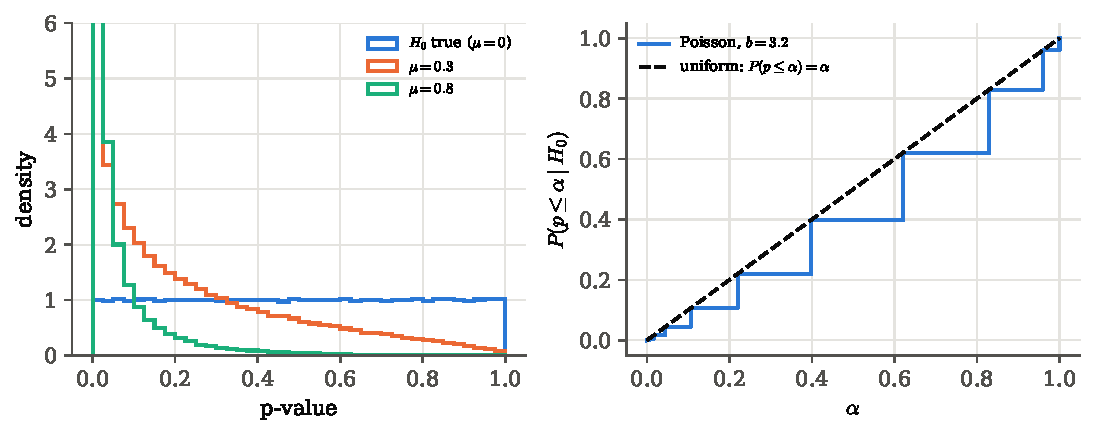
\includegraphics[width=\linewidth]{figures/ch04/pvalue_hist.pdf}
\caption{Left: histograms of p-values from many repetitions of the same
experiment. With the null true (blue) the histogram is flat; with a real effect
(orange, green) the p-values crowd towards zero, more so for the larger effect.
Right: for Poisson counts with $b=3.2$ the p-value takes only a few values, so
its cumulative distribution is a staircase. The staircase touches the diagonal
at its corners and otherwise stays below it, so ``reject if $p\le\alpha$'' never
rejects more often than $\alpha$.}
\label{4a:fig:pvalue-hist}
\end{figure}

\subsection{Discrete data: valid, not uniform}
\label{4a:sec:p-valid}

For a count the argument breaks at step (4) of \eqref{4a:eq:p-uniform},
because $\Prob(T=a)$ is no longer zero. The p-value can only take the values
$\pi(n)=\Prob_0(N\ge n)$ for integer $n$, so it cannot be uniform. What
survives is the inequality that matters for error control, the definition of
a \newterm{valid p-value} \unpack{one that is at most $\alpha$ with probability at
most $\alpha$ under the null, for every $\alpha$} \srcref{CasellaBerger}{Def.~8.3.26}:
\[
  \Prob_\theta(P\le u)\le u\qquad\text{for every }\theta\in\Theta_0\text{ and every }u\in[0,1].
\]
For a Poisson count the proof takes one line. The tail $\pi(n)$ decreases as
$n$ grows. Let $n_u$ be the smallest integer with $\pi(n_u)\le u$. Then
\begin{equation}
  \Prob_0(P\le u)
  \eqby{1} \Prob_0\bigl(\pi(N)\le u\bigr)
  \eqby{2} \Prob_0(N\ge n_u)
  \eqby{3} \pi(n_u)
  \relby{4}{\le} u .
  \label{4a:eq:p-valid}
\end{equation}
\begin{explain}
  \item The p-value of an observed count $N$ is $\pi(N)$.
  \item Because $\pi$ is decreasing, $\pi(N)\le u$ holds exactly when
        $N\ge n_u$.
  \item Definition of $\pi$.
  \item Definition of $n_u$.
\end{explain}
Equality holds only when $u$ happens to be one of the attainable values
$\pi(n)$, which are the corners of the staircase in the right panel of
\cref{4a:fig:pvalue-hist}. With $b=3.2$ the simulated fraction of null
experiments with $p\le0.05$ is $\FourAPUdisc$, below $0.05$. For a composite
null, the supremum over $\Theta_0$ in the definition of $p$ keeps it valid for
every member of the null \srcref{CasellaBerger}{Thm~8.3.27}.

\paragraph{A large p-value is not evidence for the null.}
A large $p$ can arise because $\Hnull$ is true, or because $\Hnull$ is false
and the test has too little power to notice \mainref{p.~157}. In the example
above, at $\mu=0.3$ three quarters of the p-values exceed $0.05$ although the
null is false. Failing to reject says ``these data cannot tell''. Testing is
built to find evidence \emph{against} a null, not to prove one
\mainref{p.~161}.

\subsection{What a p-value is not}
\label{4a:sec:not-posterior}

The most common misreading of a p-value is ``$p=0.04$, so there is a $4\%$
chance that the null is true''. \mainref{p.~157} and \srcref{Cowan}{p.~58} both
warn against it. The two numbers answer questions in opposite directions:
\[
  p=\Prob\bigl(\text{data this extreme or more}\given\Hnull\bigr)
  \qquad\text{versus}\qquad
  \Prob\bigl(\Hnull\given\text{data}\bigr).
\]
The first is a prediction from the null; the second is an inference about it.
Turning one into the other takes Bayes' theorem, and Bayes' theorem needs a
number the p-value never uses: how often the null is true before we look.
A simulation makes the difference concrete.

\paragraph{Example: a population of experiments.}
\emph{The setting.} Picture a field in which $90\%$ of the hypotheses people
test are really null, $\pi_0=0.9$. The other $10\%$ have an effect $\mu=0.5$
in the same experiment as above: $n=10$ Gaussian readings of unit variance,
tested one-sided against $\mu=0$. We simulate $10^6$ experiments, each picking
null or effect at random with these frequencies, and compute every p-value.

\emph{The question.} Among the ``significant'' experiments, those with
$p<0.05$, what fraction had a true null?

\emph{The two routes to a significant result.} A result can be significant
because the null is true and chance gave a small $p$, which happens with
probability $0.05$ by uniformity. Or it can be significant because there is an
effect and the test caught it, which happens with probability equal to the
power at $\mu=0.5$, $\FourAPUpower$.

\emph{Only then the numbers.} Weighting each route by how often it is taken,
Bayes' theorem gives
\begin{align}
  \Prob(\Hnull\given p<0.05)
  &\eqby{1} \frac{\Prob(p<0.05\given\Hnull)\,\pi_0}
                 {\Prob(p<0.05\given\Hnull)\,\pi_0+\Prob(p<0.05\given\Halt)\,(1-\pi_0)} \notag\\
  &\eqby{2} \frac{0.05\times0.9}{0.05\times0.9+\FourAPUpower\times0.1}
   \approx \FourAPUnullSigTh .
  \label{4a:eq:false-discovery}
\end{align}
\begin{explain}
  \item Bayes' theorem with the two hypotheses as the branches of a
        probability tree: first choose null or effect, then the p-value.
  \item Under the null $P$ is uniform, so $\Prob(P<0.05)=0.05$; under the
        effect it is the power.
\end{explain}
Almost half of the significant results are false alarms; the simulation
counts a fraction $\FourAPUnullSig$. Now narrow the selection to results that
only just made it, $0.04<p<0.05$. Under the null this band has probability
$0.01$ (uniformity again), and under the effect it has a probability we
compute from \eqref{4a:eq:power-z}. The same formula gives
$\FourAPUnullBandTh$, and the simulation $\FourAPUnullBand$: two thirds of the
barely significant results come from true nulls, while each of them reports
``$p<0.05$''. \Cref{4a:fig:pvalue-population} shows why: the flat carpet of null
p-values is ten times more populous than the effect experiments, and near
$p=0.05$ the carpet dominates.

\begin{figure}[htbp]
\centering
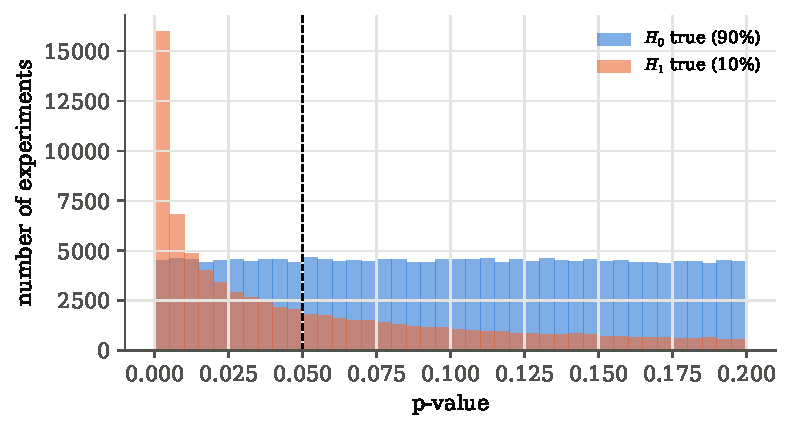
\includegraphics[width=0.8\linewidth]{figures/ch04/pvalue_population.pdf}
\caption{p-values from a population of experiments in which $90\%$ of the nulls
are true. The blue histogram (true nulls) is flat; the orange one (real
effects) rises towards zero. Left of the dashed line at $p=0.05$ both
contribute, and just left of it the flat blue carpet is the larger.}
\label{4a:fig:pvalue-population}
\end{figure}

\pyfile[firstline=61,lastline=78]{code/ch04/04_pvalue_uniform.py}{A population of experiments: how many significant results are false alarms?}

The code draws one Boolean per experiment, \pyname{is_null}, with probability
$\pi_0$, and sets the true mean to $0$ or $0.5$ accordingly. It draws the
sample mean directly from $\Normal(\mu,\sigma^2/n)$, which is its exact
distribution, converts it to a p-value, and then simply counts: among the
experiments with \pyname{pp < 0.05}, what fraction have \pyname{is_null}?
The analytic lines below are \eqref{4a:eq:false-discovery} and its narrow-band
version.

\begin{pitfall}[$p$ is not $\Prob(\Hnull\given\text{data})$]
The p-value is computed assuming the null is true, so it cannot be the
probability that the null is true. The fraction of significant results that
are false alarms depends on the power and on how often nulls are true in the
first place, neither of which enters $p$. In the example, $p<0.05$ went with a
$\FourAPUnullSig$ chance of a true null, and $0.04<p<0.05$ with a
$\FourAPUnullBand$ chance. The inference direction is the subject of
\cref{ch:05}.
\end{pitfall}

This does not make p-values useless. It makes them one ingredient. A small
p-value says the data are hard to produce by chance alone; whether that makes
the alternative probable depends on how plausible it was to begin with. That
is the logic behind the $5\sigma$ convention of \cref{4a:sec:ztable}, and it
is exactly the prior-times-likelihood structure of Bayes' theorem.
\section{Three workhorse tests: Wald, Student's t and permutation}
\label{4a:sec:wald}

A calorimeter is calibrated twice, a week apart, on the $661.7\,$keV gamma
line of $^{137}$Cs. The first run records $12$ reconstructed peak positions,
the second $15$. The second run's mean is higher. Did the energy
scale drift, or is this the scatter we expect from a detector with a
resolution of a few keV? Situations like this, comparing two samples or
comparing an estimate with a reference value, are the everyday business of
testing. Most tests for them are one of three kinds.
\begin{enumerate}[label=\arabic*.]
  \item The \emph{Wald test}: divide the estimate's distance from the null
        value by its estimated standard error and compare with a normal
        distribution. It works for any estimator that is approximately normal.
  \item The \emph{t-test}: the same ratio, with the exact distribution that
        accounts for having estimated the standard error from few Gaussian
        readings.
  \item The \emph{permutation test}: no distributional assumption at all; the
        null distribution is built by shuffling the labels of the data.
\end{enumerate}
Most powerful tests in the sense of \cref{4a:sec:np} often do not exist for
composite hypotheses, so these general-purpose tests carry most of the load
\mainref{p.~152}.

\subsection{The Wald test}
\label{4a:sec:wald-test}

Let $\hat\theta$ be an estimate of a scalar parameter $\theta$ with estimated
standard error $\widehat{\rm se}$, and suppose $\hat\theta$ is approximately
normal, as maximum-likelihood estimators are for large samples
(\cref{ch:03}). To test $\Hnull:\theta=\theta_0$ against
$\Halt:\theta\neq\theta_0$ we measure the distance in standard errors,
\begin{equation}
  W=\frac{\hat\theta-\theta_0}{\widehat{\rm se}},
  \qquad
  \text{reject }\Hnull\text{ when }\abs{W}>z_{\alpha/2}
  \label{4a:eq:wald}
\end{equation}
\mainref{Def.~10.3}. Under the null, $W$ is approximately standard normal, so
\begin{equation}
  \Prob_{\theta_0}\bigl(\abs{W}>z_{\alpha/2}\bigr)\;\longrightarrow\;\Prob\bigl(\abs{Z}>z_{\alpha/2}\bigr)=\alpha
  \qquad(n\to\infty),
  \label{4a:eq:wald-size}
\end{equation}
which is \mainref{Thm~10.4}: the Wald test has size $\alpha$ asymptotically.
The p-value of an observed $w$ is the two-sided normal tail
\mainref{(10.7)}:
\begin{equation}
  p=\Prob_{\theta_0}\bigl(\abs{W}>\abs{w}\bigr)\approx\Prob\bigl(\abs{Z}>\abs{w}\bigr)=2\Phi(-\abs{w}).
  \label{4a:eq:wald-p}
\end{equation}
The standard error may also be computed at the null value, ${\rm se}_0$, in
place of the estimate; both versions are valid \mainref{Remark~10.5}. For a
binomial proportion $\hat p$ tested against $p_0$, for instance, one may use
${\rm se}_0=\sqrt{p_0(1-p_0)/n}$, which needs no estimate at all.

\paragraph{Example: comparing two means.}
Two independent samples $X_1,\dots,X_m$ and $Y_1,\dots,Y_n$ have means
$\mu_1,\mu_2$. The null is $\delta=\mu_1-\mu_2=0$, the estimate is
$\hat\delta=\bar X-\bar Y$, and because the samples are independent the
variances add \mainref{Ex.~10.8}:
\begin{equation}
  \widehat{\rm se}=\sqrt{\frac{s_1^2}{m}+\frac{s_2^2}{n}},
  \qquad
  W=\frac{\bar X-\bar Y}{\sqrt{s_1^2/m+s_2^2/n}},
  \label{4a:eq:two-means}
\end{equation}
with $s_1^2,s_2^2$ the two sample variances. In Wasserman's cholesterol data
\mainref{Ex.~10.15} the two group means are $216.2$ and $195.3$ with standard
errors $5$ and $2.4$, so
$W=(216.2-195.3)/\sqrt{5^2+2.4^2}=20.9/5.55\approx3.78$ and
$p=2\Phi(-3.78)=\FourACholP$, the quoted $0.0002$. The same recipe works for
medians, with the standard error of the difference of sample medians taken
from the bootstrap of \cref{ch:03} \mainref{Ex.~10.9}; there $W=2.4$ and
$p=0.02$.

\paragraph{Example: two classifiers, and paired data.}
\mainref{Ex.~10.7} compares two prediction algorithms, and the same logic
compares two event classifiers. If each is run on its own test set, of sizes
$m$ and $n$, the error counts are independent binomials and
\eqref{4a:eq:two-means} applies with $s_i^2=\hat p_i(1-\hat p_i)$. If both run
on the \emph{same} test set, the two error rates are correlated and the
variances no longer add. The fix is to test the per-event difference: let
$X_i=1$ if the first classifier is right on event $i$, $Y_i$ likewise for the
second, and $D_i=X_i-Y_i$. Then $\hat\delta=\bar D$, $\widehat{\rm se}=S_D/\sqrt n$
with $S_D$ the sample standard deviation of the $D_i$, and $W=\bar D/\widehat{\rm se}$.
This \newterm{paired comparison} removes the event-to-event variation that both
classifiers share, which is usually most of it.

\subsection{Small samples: Student's t}
\label{4a:sec:t-test}

The Wald test's guarantee is asymptotic. With few readings, the estimated
standard error is itself noisy, and a too-small $\widehat{\rm se}$ inflates
$\abs{W}$. We can see how badly by simulation: draw $n$ readings from
$\Normal(0,1)$, so the null $\mu=0$ is true, compute
$T=\sqrt n\,\bar X/S$ with $S$ the sample standard deviation, and count how
often $\abs T>1.96$. \Cref{4a:fig:wald-size} shows the answer: the false-alarm
rate is $\FourAWaldSizeThree$ at $n=3$, $\FourAWaldSizeFive$ at $n=5$,
$\FourAWaldSizeTen$ at $n=10$ and $\FourAWaldSizeThirty$ at $n=30$, instead of
$0.05$.

For Gaussian data the exact distribution of $T$ is known. Write
\begin{align}
  T=\frac{\sqrt n(\bar X-\mu_0)}{S}
  &\eqby{1} \frac{\sqrt n(\bar X-\mu_0)/\sigma}{S/\sigma} \notag\\
  &\eqby{2} \frac{Z}{\sqrt{V/(n-1)}},
  \qquad Z\sim\Normal(0,1),\quad V=\frac{(n-1)S^2}{\sigma^2}\sim\chi^2_{n-1} .
  \label{4a:eq:t-stat}
\end{align}
\begin{explain}
  \item Divide numerator and denominator by the unknown $\sigma$; the ratio is
        unchanged, so $T$ does not depend on $\sigma$.
  \item Under the null the numerator is standard normal. In the denominator,
        $S/\sigma=\sqrt{V/(n-1)}$, and $(n-1)S^2/\sigma^2$ is $\chi^2_{n-1}$ and
        independent of $\bar X$ for Gaussian data (\cref{ch:03}).
\end{explain}
A standard normal divided by the square root of an independent
$\chi^2_k/k$ is by definition a \newterm{Student t variable} with $k$ degrees
of freedom \unpack{a bell curve with heavier tails, because the denominator
sometimes comes out small}, with density \mainref{p.~170}
\begin{equation}
  f(t)=\frac{\Gamma\bigl(\tfrac{k+1}{2}\bigr)}{\sqrt{k\pi}\,\Gamma\bigl(\tfrac k2\bigr)}
       \Bigl(1+\frac{t^2}{k}\Bigr)^{-(k+1)/2} .
  \label{4a:eq:t-density}
\end{equation}
For $k=1$ it is the Cauchy distribution of \cref{ch:02}, and as
$k\to\infty$ it becomes the standard normal, because
$(1+t^2/k)^{-(k+1)/2}\to e^{-t^2/2}$ and $V/k\to1$ by the law of large numbers.
So $T\sim t_{n-1}$ exactly, and the \newterm{t-test} rejects when
$\abs T>t_{n-1,\alpha/2}$, the upper $\alpha/2$ quantile of $t_{n-1}$. The same
fact lets us compute, not just simulate, how often the Wald test rejects a
true null. The Wald test uses the normal cut $1.96$, so its size is
$\Prob(\abs{t_{n-1}}>1.96)$, which for $n=3$ is $\FourAWaldSizeThreeEx$, the
solid line in \cref{4a:fig:wald-size}. The t-test's simulated size is
$\FourATSizeThree$ at $n=3$ and $\FourATSizeTen$ at $n=10$. For moderately
large $n$ the two tests are the same test.

\begin{figure}[htbp]
\centering
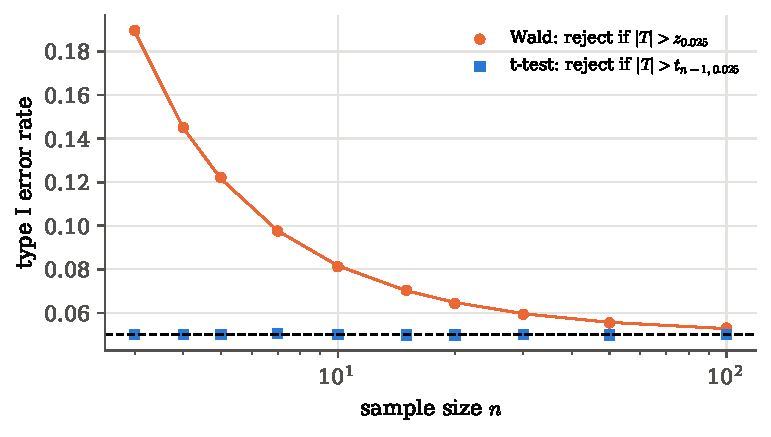
\includegraphics[width=0.8\linewidth]{figures/ch04/wald_size.pdf}
\caption{How often a test rejects a true null, as a function of the number of
Gaussian readings. The Wald test, which uses the normal cut $1.96$ with an
estimated standard error, rejects too often for small samples (orange dots,
with the exact curve as a line). The t-test, which uses the t quantile,
stays on the dashed $0.05$ line at every sample size (blue squares).}
\label{4a:fig:wald-size}
\end{figure}

For two samples with possibly different variances, the ratio
\eqref{4a:eq:two-means} is not exactly t-distributed. \newterm{Welch's t-test}
uses a t distribution with an effective number of degrees of freedom computed
from $s_1,s_2,m,n$; it is what \pyname{scipy.stats.ttest_ind(..., equal_var=False)}
does.

\subsection{The permutation test}
\label{4a:sec:permutation}

The t-test is exact only for Gaussian data. The \newterm{permutation test}
is exact for any distribution, at the price of a computation
\mainref{\S10.5}. The null it tests is that the two samples come from the
same distribution, $\Hnull:F_X=F_Y$. The key observation: if that is true, the
labels ``first sample'' and ``second sample'' carry no information. Every way
of splitting the pooled $N=m+n$ values into a group of $m$ and a group of $n$
was equally likely to have produced the data we saw. So we can build the null
distribution of any statistic $T$ by recomputing it for all $N!$ orderings of
the pooled values, each with probability $1/N!$. That is the
\newterm{permutation distribution}, and the p-value is the fraction of
orderings with $T$ larger than the observed value.

\paragraph{Example: the smallest possible permutation test.}
Take $(X_1,X_2,Y_1)=(1,9,3)$ and $T=\abs{\bar X-\bar Y}$
\mainref{Ex.~10.19}. The observed value is $\abs{(1+9)/2-3}=2$. The six
orderings, with the first two entries playing the role of $X$:
\begin{center}
\begin{tabular}{ccc}
\toprule
ordering & $T$ & probability \\
\midrule
$(1,9,3)$, $(9,1,3)$ & $\abs{5-3}=2$ & $2/6$ \\
$(1,3,9)$, $(3,1,9)$ & $\abs{2-9}=7$ & $2/6$ \\
$(3,9,1)$, $(9,3,1)$ & $\abs{6-1}=5$ & $2/6$ \\
\bottomrule
\end{tabular}
\end{center}
Four of the six give $T>2$, so $p=\Prob_0(T>2)=4/6=\FourAToyP$. The script
enumerates the six orderings with \pyname{itertools.permutations} and gets the
same number. (Some authors count $T\ge t_{\rm obs}$, which includes the
observed ordering itself; with continuous data and many orderings the
difference is negligible.)

For real data $N!$ is astronomically large, so we sample orderings at random.
The algorithm \mainref{p.~163} is:
\begin{enumerate}[label=\arabic*.]
  \item compute $t_{\rm obs}$ from the data as labelled;
  \item shuffle the pooled data, split into groups of $m$ and $n$, and
        recompute $T$;
  \item repeat step 2 $B$ times, giving $T_1,\dots,T_B$;
  \item the p-value is approximately $\frac1B\sum_{j=1}^B I(T_j>t_{\rm obs})$,
        with $I$ the indicator (one if true, zero if false).
\end{enumerate}
Why is this legitimate? Under the null the $N$ values are exchangeable: their
joint distribution does not change when we reorder them. Given the set of
values that occurred, every assignment of labels is equally likely, so the
shuffled statistics are draws from the exact conditional null distribution of
$T$. No normality, no large-sample limit, no estimate of a standard error is
involved. The permutation test is most useful when there are few samples and
the statistic has no convenient formula for its distribution. Wasserman's
gene-expression example is of this kind (\mainref{Ex.~10.20}: ten patients,
two tumour types, $T$ the absolute difference of medians $=710$,
$p=0.045$).

\paragraph{Example: the calorimeter calibration.}
Back to the two calibration runs. We simulate run 1 as $12$ readings
from $\Normal(661.7,4^2)\,$keV and run 2 as $15$ readings with a true shift of
$3.3\,$keV (script \pyname{05_wald_t_permutation.py}). The observed means are $\FourACalMeanOne$ and $\FourACalMeanTwo\,$keV
with sample standard deviations $\FourACalSdOne$ and $\FourACalSdTwo\,$keV.
By \eqref{4a:eq:two-means},
\begin{align*}
  \hat\delta &= \FourACalMeanTwo-\FourACalMeanOne=\FourACalD\ \text{keV},\\
  \widehat{\rm se} &= \sqrt{\FourACalSdOne^2/12+\FourACalSdTwo^2/15}=\FourACalSe\ \text{keV},\\
  W &= \FourACalD/\FourACalSe=\FourACalW ,
\end{align*}
so the Wald p-value is $2\Phi(-\FourACalW)=\FourACalPwald$. Welch's t-test gives
$\FourACalPwelch$, larger because it accounts for the uncertainty in the two
standard deviations. The permutation test, with $B=100\,000$ shuffles of the
$27$ values, gives $\FourACalPperm$. \Cref{4a:fig:permutation} shows the
permutation distribution of $\bar x_2-\bar x_1$ with the observed difference
marked. The three p-values are close to one another: they ask the same question
in three ways. None of them would convince a particle physicist of a new effect.
Nor could they be expected to. With twelve and fifteen readings of $4\,$keV
resolution, the true shift of $3.3\,$keV is only
$3.3/\sqrt{4^2/12+4^2/15}\approx2.1$ standard errors on average, and a single pair
of runs can easily show much less or much more. This experiment is too small to
find the shift reliably.

\begin{figure}[htbp]
\centering
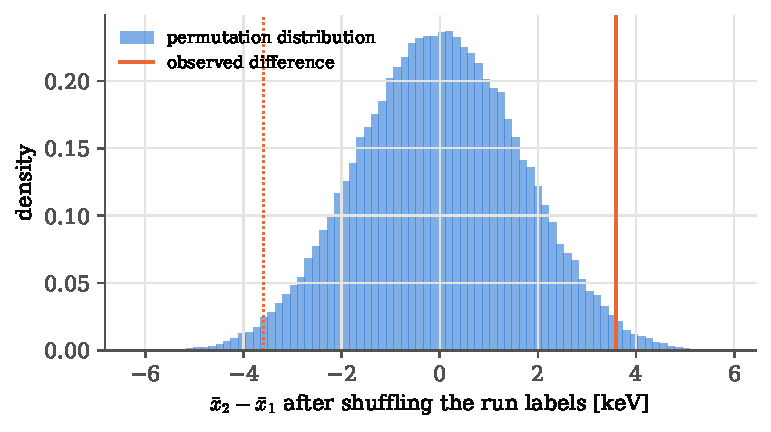
\includegraphics[width=0.8\linewidth]{figures/ch04/permutation_dist.pdf}
\caption{The permutation distribution for the calibration example: the
difference of the two run means after randomly reassigning the $27$ readings
to the two runs, $100\,000$ times. The solid orange line is the observed
difference and the dotted one its mirror image; the fraction of shuffles
beyond either line is the two-sided p-value.}
\label{4a:fig:permutation}
\end{figure}

\pyfile[firstline=48,lastline=66]{code/ch04/05_wald_t_permutation.py}{Wald, Welch and permutation tests for two calibration runs}

The loop is the algorithm above, line for line: \pyname{rng.permutation}
shuffles the pooled readings, the first $m$ play run 1 and the rest run 2,
and the difference of means is stored. The p-value counts shuffles with
$\abs{T_j}\ge\abs{t_{\rm obs}}$ (two-sided). As a cross-check the script calls
\pyname{scipy.stats.permutation_test} with $20\,000$ resamples, which returns
$\FourACalPpermScipy$. Both numbers are Monte Carlo estimates, so they carry a
random error. For the shorter run of $20\,000$ resamples that error is
$\sqrt{p(1-p)/20\,000}$, a few thousandths at most. The two estimates differ by
$\FourACalPermDiffSig$ times their combined error; more shuffles would bring them together. In large samples the permutation test
usually agrees with the asymptotic tests, and it is most valuable for small
samples \mainref{p.~164}.

\paragraph{Tests and intervals are two views of one object.}
There is a simple link between the Wald test and the familiar interval
$\hat\theta\pm z_{\alpha/2}\widehat{\rm se}$. By \eqref{4a:eq:wald},
$\abs{\hat\theta-\theta_0}>z_{\alpha/2}\widehat{\rm se}$ says precisely that
$\theta_0$ lies outside that interval. So the size-$\alpha$ Wald test rejects
$\theta_0$ if and only if $\theta_0$ is outside the $1-\alpha$ interval
\mainref{Thm~10.10}. The second part of the chapter turns that observation
into a general machine for building confidence intervals from tests.
\section{The best test: the Neyman--Pearson lemma}
\label{4a:sec:np}

A trigger has to decide, event by event, whether a collision looks like
signal or like background. Each event comes with several measured
quantities: energies, angles, isolation variables. Any selection keeps some
signal and some background. At a fixed signal efficiency, say $90\%$, one
selection keeps less background than another, and we would like the best one.
Put as a question about tests: among all tests
with the same size $\alpha$, which has the largest power? For two simple
hypotheses there is a complete answer, and it is one of the few genuinely
optimal results in statistics.

\paragraph{The question in words.}
\begin{enumerate}[label=\arabic*.]
  \item We have a fixed budget $\alpha$ of false-alarm probability. Which
        outcomes should we spend it on?
  \item Does the answer depend on the particular alternative, or is one test
        best against a whole family of alternatives?
  \item What do we do when the densities are only available as simulated
        events in many dimensions?
\end{enumerate}

\subsection{Spending a false-alarm budget}
\label{4a:sec:np-budget}

Take a simple null and a simple alternative, $\Hnull:\theta=\theta_0$ versus
$\Halt:\theta=\theta_1$, with densities $f_0(\bm x)=f(\bm x\given\theta_0)$ and
$f_1(\bm x)=f(\bm x\given\theta_1)$ for the whole data set. A test is a choice
of rejection region $R$. Its size and power are
\[
  \alpha=\int_R f_0(\bm x)\,\dd\bm x,
  \qquad
  \beta(\theta_1)=\int_R f_1(\bm x)\,\dd\bm x .
\]
Think of each small cell $\dd\bm x$ of data space as an item we can put into
$R$. It costs $f_0\,\dd\bm x$ of the false-alarm budget and buys $f_1\,\dd\bm x$
of power. The budget is fixed. To buy as much power as possible we should take
the items with the best value for money first, the cells where the ratio
$f_1/f_0$ is largest, and keep taking them in order of decreasing ratio until
the budget is spent. The region we end up with is
$R=\{\bm x:\ f_1(\bm x)/f_0(\bm x)>k\}$, with the threshold $k$ fixed by the
budget.

The same answer comes out of the Lagrange-multiplier method familiar from
mechanics. We maximise $\int_Rf_1$ subject to $\int_Rf_0=\alpha$, so we
maximise $\int_R(f_1-kf_0)\,\dd\bm x$ for a multiplier $k$. The integrand can
be positive or negative, and the integral over $R$ is largest when $R$
contains every point where $f_1-kf_0>0$ and no point where it is negative.
The multiplier is the exchange rate between power and size.

\begin{keyidea}[Neyman--Pearson lemma]
For testing a simple $\Hnull:\theta=\theta_0$ against a simple
$\Halt:\theta=\theta_1$, the test that rejects when the
\newterm{likelihood ratio}
\[
  \Lambda(\bm x)=\frac{f(\bm x\given\theta_1)}{f(\bm x\given\theta_0)}
  =\frac{\Like(\theta_1)}{\Like(\theta_0)}
\]
exceeds a constant $k$, with $k$ chosen so that
$\Prob_{\theta_0}(\Lambda>k)=\alpha$, has the largest power of all tests of
level $\alpha$ \mainref{Thm~10.30}, \srcref{CasellaBerger}{Thm~8.3.12},
\srcref{Cowan}{(4.12)}. The ratio collapses any number of measured variables
into one number, and no other function of the data does better.
\end{keyidea}

\paragraph{Why it is true.}
The budget argument is the proof in disguise. To make it exact, describe a
test by its \newterm{test function} $\phi(\bm x)$ \unpack{one where the test
rejects, zero where it retains}, so that size and power are $\int\phi f_0$ and
$\int\phi f_1$. Let $\phi$ be the likelihood-ratio test and $\phi'$ any other
test of level $\alpha$, with power functions $\beta$ and $\beta'$. At every
point, $[\phi(\bm x)-\phi'(\bm x)][f_1(\bm x)-kf_0(\bm x)]\ge0$: where
$f_1>kf_0$ we have $\phi=1\ge\phi'$, and where $f_1<kf_0$ we have
$\phi=0\le\phi'$, so the two factors never have opposite signs. Integrating,
\begin{align}
  0 &\relby{1}{\le} \int\bigl[\phi(\bm x)-\phi'(\bm x)\bigr]\bigl[f_1(\bm x)-kf_0(\bm x)\bigr]\dd\bm x \notag\\
    &\eqby{2} \bigl[\beta(\theta_1)-\beta'(\theta_1)\bigr]-k\bigl[\beta(\theta_0)-\beta'(\theta_0)\bigr] \notag\\
    &\relby{3}{\le} \beta(\theta_1)-\beta'(\theta_1) .
  \label{4a:eq:np-proof}
\end{align}
\begin{explain}
  \item The integrand is non-negative at every point, as just argued.
  \item Multiply out: $\int\phi f_1=\beta(\theta_1)$, $\int\phi f_0=\beta(\theta_0)$,
        and likewise for $\phi'$.
  \item $\beta(\theta_0)=\alpha$ for the likelihood-ratio test, and
        $\beta'(\theta_0)\le\alpha$ because $\phi'$ has level $\alpha$; so the
        bracket multiplying $k\ge0$ is non-negative, and dropping it can only
        increase the right-hand side.
\end{explain}
So $\beta(\theta_1)\ge\beta'(\theta_1)$: no level-$\alpha$ test beats the
likelihood ratio \srcref{CasellaBerger}{p.~315}. For discrete data replace
integrals by sums. Notice what the proof used: nothing about the shape of the
densities, the dimension of $\bm x$, or large samples. The lemma is exact.

\paragraph{Example: the Gaussian mean, and a uniformly best test.}
Let $X_1,\dots,X_n\iid\Normal(\mu,\sigma^2)$, $\sigma$ known, and test
$\mu=0$ against a single $\mu=\mu_1>0$. The log of the likelihood ratio is
\begin{align}
  \ln\Lambda
  &\eqby{1} \sum_{i=1}^n\Bigl[-\frac{(x_i-\mu_1)^2}{2\sigma^2}+\frac{x_i^2}{2\sigma^2}\Bigr] \notag\\
  &\eqby{2} \sum_{i=1}^n\frac{2\mu_1x_i-\mu_1^2}{2\sigma^2}
   \eqby{3} \frac{n\mu_1}{\sigma^2}\,\bar x-\frac{n\mu_1^2}{2\sigma^2} .
  \label{4a:eq:np-gauss}
\end{align}
\begin{explain}
  \item The likelihood is a product of Gaussians; its log is a sum. The
        normalisations $1/\sqrt{2\pi\sigma^2}$ are the same under both
        hypotheses and cancel.
  \item Expand $(x_i-\mu_1)^2=x_i^2-2\mu_1x_i+\mu_1^2$; the $x_i^2$ terms
        cancel.
  \item $\sum_ix_i=n\bar x$.
\end{explain}
Because $\mu_1>0$, $\ln\Lambda$ increases with $\bar x$, so ``$\Lambda>k$''
is the same event as ``$\bar x>c$'' for some $c$. The most powerful test is
the one-sided test of \cref{4a:sec:power-function}, with
$c=\sigma z_\alpha/\sqrt n$ to give size $\alpha$ \srcref{CasellaBerger}{Ex.~8.3.15}.

The value of $\mu_1$ has disappeared from the rejection region. Neither the
event $\bar x>c$ nor the cut $c=\sigma z_\alpha/\sqrt n$ mentions it. So the
same region is most powerful against \emph{every} $\mu_1>0$. A test with this
property is \newterm{uniformly most powerful}. Such tests exist
when the likelihood ratio is monotone in one statistic, as for one-sided
problems in exponential families. For two-sided alternatives they usually do
not: the best test against $\mu_1>0$ rejects for large $\bar x$, the best
against $\mu_1<0$ rejects for small $\bar x$, and no single region is best
against both \mainref{p.~152}.

\paragraph{Example: discreteness restricts the available sizes.}
Let $X\sim\mathrm{Binomial}(2,\theta)$, testing $\theta=\frac12$ against
$\theta=\frac34$ \srcref{CasellaBerger}{Ex.~8.3.14}. The pmfs are
$\binom2x\theta^x(1-\theta)^{2-x}$, giving
$(\frac14,\frac12,\frac14)$ and $(\frac1{16},\frac6{16},\frac9{16})$ for
$x=0,1,2$, so the ratios are
\[
  \Lambda(0)=\frac{1/16}{1/4}=\frac14,\qquad
  \Lambda(1)=\frac{6/16}{1/2}=\frac34,\qquad
  \Lambda(2)=\frac{9/16}{1/4}=\frac94 .
\]
Ranking the outcomes by $\Lambda$ and filling the budget: rejecting on
$\{2\}$ is the most powerful test of size $\Prob_{1/2}(X=2)=\frac14$; rejecting
on $\{1,2\}$ is the most powerful test of size $\frac34$. No non-randomised
test has size $0.05$ except the one that never rejects. With discrete data the
lemma still says what to do, but only certain sizes can be achieved, as we saw
for the Poisson counts in \cref{4a:sec:power-counting}.

\subsection{Selecting particles: efficiency, purity and the ratio}
\label{4a:sec:selection}

Selecting events is a test, and the lemma tells us how to do it best.
\srcref{Cowan}{\S4.2} takes a charged
particle of known momentum whose ionisation $t$ is measured. Electrons and
pions deposit different amounts on average, so $t$ has density $g(t\given e)$
for electrons and $g(t\given\pi)$ for pions. Selecting electron candidates with
a cut $t<t_{\rm cut}$ defines two efficiencies \srcref{Cowan}{(4.3)--(4.4)},
\[
  \varepsilon_e=\int_{-\infty}^{t_{\rm cut}}g(t\given e)\,\dd t=1-\alpha,
  \qquad
  \varepsilon_\pi=\int_{-\infty}^{t_{\rm cut}}g(t\given\pi)\,\dd t=\beta_{\rm II} .
\]
Here the \emph{signal} plays the role of the null: rejecting ``it is an
electron'' when it is one loses signal, with probability $\alpha$, and keeping
a pion is a type II error. The purity of the selected sample follows from
Bayes' theorem with the particle fractions $a_e$ and $a_\pi=1-a_e$ as prior
probabilities \srcref{Cowan}{(4.8)--(4.11)}:
\begin{equation}
  P_e=\frac{\text{electrons kept}}{\text{particles kept}}
  =\frac{a_e\,\varepsilon_e}{a_e\,\varepsilon_e+a_\pi\,\varepsilon_\pi} .
  \label{4a:eq:purity}
\end{equation}
This is the same structure as \eqref{4a:eq:false-discovery}: the purity of a
selection, like the fraction of true discoveries, needs the prior fractions.
At fixed efficiency $\varepsilon_e$ the purity is largest when
$\varepsilon_\pi$ is smallest, which is the Neyman--Pearson problem. With one
variable and a monotone ratio a single cut is automatically optimal. With a
vector of variables $\bm x$ the lemma says to keep the events with
$g(\bm x\given e)/g(\bm x\given\pi)>c$ \srcref{Cowan}{(4.12)--(4.13)}.

In practice $g(\bm x\given H)$ is known only through simulated events. With
$M$ histogram bins per variable and $n$ variables there are $M^n$ bins to fill,
which becomes impossible beyond a few variables \srcref{Cowan}{p.~51}. One
retreat is a linear statistic $t=\bm a\T\bm x$. Fisher chose the direction
$\bm a$ that maximises the separation of the two class means relative to the
spread within the classes, $(\tau_0-\tau_1)^2/(\Sigma_0^2+\Sigma_1^2)$, and
found \srcref{Cowan}{(4.23)}
\begin{equation}
  \bm a\propto\bm W^{-1}(\bm\mu_0-\bm\mu_1),\qquad\bm W=\bm V_0+\bm V_1,
  \label{4a:eq:fisher-disc}
\end{equation}
with $\bm\mu_k$ and $\bm V_k$ the mean vector and covariance matrix of $\bm x$
under hypothesis $k$. When both classes are Gaussian with the \emph{same}
covariance $\bm V$, Fisher's discriminant is exactly the log likelihood ratio.
Writing $Q_k=(\bm x-\bm\mu_k)\T\bm V^{-1}(\bm x-\bm\mu_k)$ for the quadratic
form in each Gaussian exponent,
\begin{align}
  \ln\frac{\Normal(\bm x;\bm\mu_0,\bm V)}{\Normal(\bm x;\bm\mu_1,\bm V)}
  &\eqby{1} -\tfrac12Q_0+\tfrac12Q_1 \notag\\
  &\eqby{2} (\bm\mu_0-\bm\mu_1)\T\bm V^{-1}\bm x
       -\tfrac12\bigl(\bm\mu_0\T\bm V^{-1}\bm\mu_0-\bm\mu_1\T\bm V^{-1}\bm\mu_1\bigr) .
  \label{4a:eq:fisher-lr}
\end{align}
\begin{explain}
  \item The normalisations $(2\pi)^{-n/2}\det\bm V^{-1/2}$ are equal and cancel.
  \item Expand $Q_k=\bm x\T\bm V^{-1}\bm x-2\bm\mu_k\T\bm V^{-1}\bm x+\bm\mu_k\T\bm V^{-1}\bm\mu_k$
        (using the symmetry of $\bm V^{-1}$). The quadratic term in $\bm x$ is
        the same for both and cancels, leaving a linear function of $\bm x$.
\end{explain}
The coefficient vector is $\bm V^{-1}(\bm\mu_0-\bm\mu_1)$, proportional to
Fisher's with $\bm W=2\bm V$ \srcref{Cowan}{(4.27)--(4.28)}. When the covariances
differ, the $\bm x\T\bm V_k^{-1}\bm x$ terms no longer cancel, the optimal
boundary is curved, and a linear statistic loses power. Nonlinear methods,
neural networks and boosted trees, are in this light approximations to the
likelihood ratio learned from simulated events \srcref{Cowan}{\S4.4.2}: a
classifier trained to separate two classes outputs, at best, a monotone
function of $g(\bm x\given H_0)/g(\bm x\given H_1)$.

\paragraph{Example: three selections, and three hundred random ones.}
We make signal and background Gaussian in two variables
(script \pyname{06_neyman_pearson.py}), with different means and different covariance
matrices, and compare three selections at a signal efficiency of $90\%$: a
cut on $x_1$ alone, Fisher's linear discriminant \eqref{4a:eq:fisher-disc}
trained on $20\,000$ events of each class, and the exact log likelihood ratio.
\Cref{4a:fig:np-scatter} shows the events and the three decision boundaries.
The fractions of background kept are $\FourANPbkgCut$ for the $x_1$ cut,
$\FourANPbkgFisher$ for Fisher and $\FourANPbkgLR$ for the likelihood ratio.

\begin{figure}[htbp]
\centering
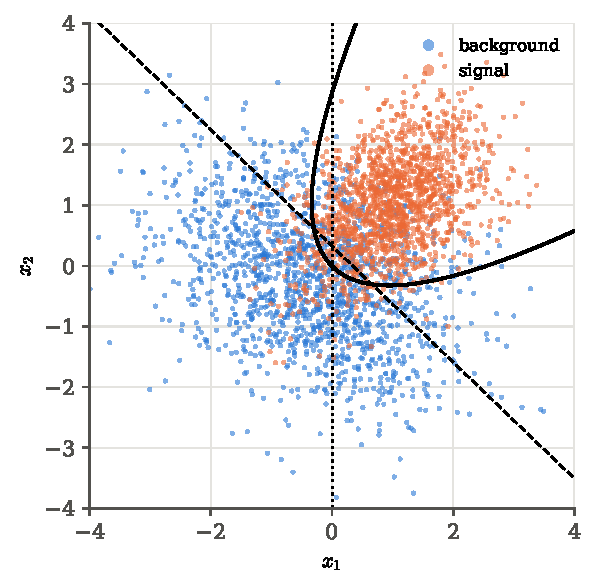
\includegraphics[width=0.6\linewidth]{figures/ch04/np_scatter.pdf}
\caption{Signal (orange) and background (blue) events in two measured
variables, with three boundaries that each keep $90\%$ of the signal: a cut on
$x_1$ alone (dotted), Fisher's straight line (dashed), and the curved contour
of constant likelihood ratio (solid). The curved boundary follows the shape of
the two clouds, which have different orientations, and so admits the least
background.}
\label{4a:fig:np-scatter}
\end{figure}

The lemma claims that no selection does better than the likelihood ratio. To
check this, the script also draws
$300$ random quadratic selections $g(\bm x)=\bm x\T\bm A\bm x+\bm v\T\bm x>c$,
each tuned to keep $90\%$ of the signal. The best of them keeps a background
fraction $\FourANPbkgRandom$, above the likelihood ratio's $\FourANPbkgLR$.
(Because the true ratio here is itself quadratic, a random quadratic can come
close, but it cannot win.) \Cref{4a:fig:np-roc} shows the whole trade-off as
a \newterm{ROC curve} \unpack{background efficiency against signal efficiency,
as the cut is varied}. The likelihood-ratio curve lies below the others at every
signal efficiency.

\begin{figure}[htbp]
\centering
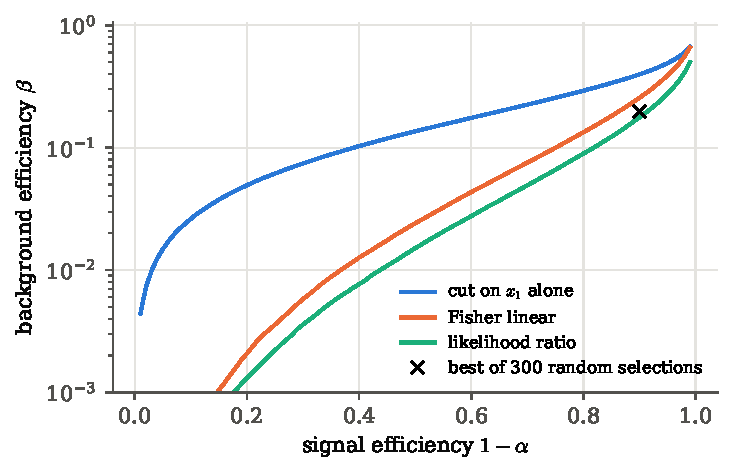
\includegraphics[width=0.8\linewidth]{figures/ch04/np_roc.pdf}
\caption{Background kept versus signal kept, as the threshold of each selection
is varied. Lower is better. The likelihood ratio (green) is lowest everywhere,
Fisher's linear discriminant (orange) is next, a cut on one variable (blue) is
worst, and the cross marks the best of $300$ random quadratic selections at
$90\%$ signal efficiency, which still lies above the green curve.}
\label{4a:fig:np-roc}
\end{figure}

\pyfile[firstline=32,lastline=50]{code/ch04/06_neyman_pearson.py}{Three selections compared at equal signal efficiency}

The function \pyname{lnr} is the log likelihood ratio, evaluated with the
exact densities because we generated the data; in a real analysis they would
come from simulation or be learned. Fisher's coefficients come from one line of
linear algebra, \pyname{np.linalg.solve(Wsum, tr_s.mean(0) - tr_b.mean(0))}, which is
\eqref{4a:eq:fisher-disc} without forming an inverse. For each statistic the
threshold for a given signal efficiency is a quantile of its signal
distribution (\pyname{np.quantile}), and the background efficiency is the
fraction of background above it, found by sorting.

\begin{pitfall}[Most powerful for one alternative only]
The Neyman--Pearson lemma is about \emph{two} completely specified
hypotheses. Real alternatives have free parameters: an unknown mass, an
unknown coupling. A test tuned to one mass hypothesis can be poor for another,
and a uniformly most powerful test rarely exists. The generalisation that
handles free parameters, by fitting them, is the likelihood-ratio test of the
next section; it is not guaranteed optimal, but it inherits the lemma's logic
and is the standard tool.
\end{pitfall}
\section{Likelihood-ratio tests and Wilks' theorem}
\label{4a:sec:wilks}

The Neyman--Pearson lemma needs two completely specified hypotheses. A real
search never has them. In the diphoton bump the background normalisation is
known only roughly, the signal strength is unknown, and even the null ``no
signal'' leaves the background level free. Such unknown parameters, which we
must allow for but do not want to report, are \newterm{nuisance parameters}
\unpack{parameters of the model that are not the question, like a background
level or a calibration constant}. We need a test that works with composite
hypotheses, and a way to get its null distribution without simulating every
possible value of the nuisance parameters.

The recipe is the natural generalisation of the lemma: in the ratio of
likelihoods, give each hypothesis its best shot by maximising over its free
parameters. The surprise, due to Wilks \cite{Wilks1938}, is that the resulting
statistic has, for large samples, a null distribution that does not depend on
the model at all.

\paragraph{The question in words.}
\begin{enumerate}[label=\arabic*.]
  \item How much better does the data fit if we free the parameters that the
        null fixes?
  \item How large must that improvement be before it is surprising, if the
        null is true?
  \item When does the universal answer fail, and what do we do then?
\end{enumerate}

\subsection{The likelihood-ratio statistic}
\label{4a:sec:lrt}

Let $\Like(\params)$ be the likelihood of the data as a function of all
parameters $\params\in\Theta$ (\cref{ch:03}), and let the null restrict them to
$\Theta_0\subset\Theta$. The \newterm{likelihood ratio} is
\begin{equation}
  \lambda(\bm x)=\frac{\sup_{\params\in\Theta_0}\Like(\params)}{\sup_{\params\in\Theta}\Like(\params)}
  =\frac{\Like(\hat{\params}_0)}{\Like(\hat{\params})},
  \qquad
  -2\ln\lambda=2\bigl[\ln\Like(\hat{\params})-\ln\Like(\hat{\params}_0)\bigr],
  \label{4a:eq:lrt}
\end{equation}
where $\hat{\params}$ is the maximum-likelihood estimate over all of $\Theta$
and $\hat{\params}_0$ the one restricted to $\Theta_0$. Because $\Theta_0$ is
part of $\Theta$, the restricted maximum can never be higher, so
$0<\lambda\le1$ and $-2\ln\lambda\ge0$. It is zero when the null fits as well
as anything, and grows as the unrestricted fit pulls away. We reject for large
$-2\ln\lambda$.

Two conventions need a word. First, \mainref{Def.~10.21} calls the quantity
$2\ln[\Like(\hat\params)/\Like(\hat\params_0)]$ itself ``$\lambda$'', so
Wasserman's $\lambda$ is our $-2\ln\lambda$. Second, the denominator maximises
over all of $\Theta$ rather than over the alternative alone,
$\Theta\setminus\Theta_0$. This changes the statistic very little and makes
its theory much simpler \mainref{p.~164}.

\begin{keyidea}[Wilks' theorem]
Let $\params$ have $r$ free parameters and the null fix $r-q$ of them, leaving
$q$ free. If the null is true, the model is regular and the true value lies in
the interior of $\Theta_0$, then for large samples
\[
  -2\ln\lambda\;\sim\;\chi^2_{r-q}
\]
\unpack{the degrees of freedom are the number of parameters the null fixes},
whatever the model \mainref{Thm~10.22}, \srcref{CasellaBerger}{Thm~10.3.3}.
The p-value is $\Prob(\chi^2_{r-q}>-2\ln\lambda_{\rm obs})$.
\end{keyidea}

For example, with five parameters and the null $\theta_4=\theta_5=0$, the
statistic is asymptotically $\chi^2_{5-3}=\chi^2_2$ \mainref{p.~164}. The
nuisance parameters, the ones left free under both hypotheses, cost nothing
in degrees of freedom: they are refitted in numerator and denominator.

\subsection{Why the answer is $\chi^2$}
\label{4a:sec:wilks-why}

Take one parameter, $\theta$, and a simple null $\theta=\theta_0$, so
$r-q=1$. Write $\ell(\theta)=\ln\Like(\theta)$ and expand it around its
maximum $\hat\theta$ \srcref{CasellaBerger}{p.~395}:
\begin{align}
  -2\ln\lambda
  &\eqby{1} 2\bigl[\ell(\hat\theta)-\ell(\theta_0)\bigr] \notag\\
  &\eqby{2} 2\Bigl[\ell(\hat\theta)-\Bigl(\ell(\hat\theta)+\ell'(\hat\theta)(\theta_0-\hat\theta)
            +\tfrac12\ell''(\hat\theta)(\theta_0-\hat\theta)^2+\dots\Bigr)\Bigr] \notag\\
  &\eqby{3} -\ell''(\hat\theta)\,(\hat\theta-\theta_0)^2+\dots \notag\\
  &\eqby{4} \Bigl(\frac{\hat\theta-\theta_0}{\widehat{\rm se}}\Bigr)^2+\dots .
  \label{4a:eq:wilks-taylor}
\end{align}
\begin{explain}
  \item Definition \eqref{4a:eq:lrt} with $\hat\theta_0=\theta_0$.
  \item Taylor expansion of $\ell(\theta_0)$ about $\hat\theta$.
  \item $\ell'(\hat\theta)=0$ at the maximum, and the $\ell(\hat\theta)$ terms
        cancel.
  \item The curvature of the log likelihood at its peak is the observed
        information, and its inverse is the variance of the estimate:
        $-\ell''(\hat\theta)=1/\widehat{\rm se}^{\,2}$ (\cref{ch:03}).
\end{explain}
For a large sample, $\hat\theta$ is approximately normal about the true value
with standard deviation se. Under the null the true value is $\theta_0$, so the
bracket in the last line is approximately a standard normal $Z$, and
$-2\ln\lambda\approx Z^2\sim\chi^2_1$. The dropped terms are of higher order in
$\hat\theta-\theta_0$, which shrinks as $1/\sqrt n$. In words: near its peak,
every smooth log likelihood is a parabola, the likelihood-ratio statistic is
the drop of that parabola between $\hat\theta$ and $\theta_0$, and the drop is
the square of the Wald statistic of \cref{4a:sec:wald}. With $k$ fixed
parameters the same expansion gives a quadratic form in a $k$-dimensional
normal vector weighted by its inverse covariance, which is a sum of $k$ squared
independent standard normals: $\chi^2_k$.

\paragraph{The linear-Gaussian case, where Wilks is exact.}
If the data are $y_i=\mu_i(\params)+\epsilon_i$ with known Gaussian errors
$\sigma_i$, then $-2\ln\Like(\params)=\chi^2(\params)+\text{const}$ with
$\chi^2(\params)=\sum_i(y_i-\mu_i(\params))^2/\sigma_i^2$ (\cref{ch:03}), and
\begin{equation}
  -2\ln\lambda
  \eqby{1} -2\ln\Like(\hat\params_0)+2\ln\Like(\hat\params)
  \eqby{2} \chi^2_{\min}(\Hnull)-\chi^2_{\min}(\Halt)
  \equiv\Delta\chi^2 .
  \label{4a:eq:delta-chi2}
\end{equation}
\begin{explain}
  \item Definition \eqref{4a:eq:lrt}.
  \item Maximising the likelihood is minimising $\chi^2$, and the constants
        cancel in the difference.
\end{explain}
When the model is linear in the parameters, $\Delta\chi^2$ is exactly
$\chi^2_{r-q}$ for any sample size. Here is the geometric reason. Divide each
residual by its $\sigma_i$; the noise vector $\bm\epsilon/\bm\sigma$ is then an
isotropic Gaussian in $N$ dimensions. A least-squares fit with $r$ linear
parameters is the orthogonal projection of the data onto an $r$-dimensional
subspace; the null's fit projects onto a $q$-dimensional subspace inside it.
Under the null, the difference of the two squared residual lengths is the
squared length of the noise projected onto the $(r-q)$-dimensional part of the
big subspace orthogonal to the small one. An isotropic Gaussian projected onto
any $k$-dimensional subspace is an isotropic Gaussian in $k$ dimensions, and its
squared length is $\chi^2_k$.

\paragraph{Example: the Poisson rate.}
With $X_1,\dots,X_n\iid\mathrm{Pois}(\lambda)$ and $\Hnull:\lambda=\lambda_0$
\srcref{CasellaBerger}{Ex.~10.3.2}, the log likelihood is
$\ell(\lambda)=-n\lambda+S\ln\lambda+\text{const}$ with $S=\sum_iX_i$, and its
maximum is at $\hat\lambda=S/n$. Then
\begin{align}
  -2\ln\lambda
  &\eqby{1} 2\bigl[\ell(\hat\lambda)-\ell(\lambda_0)\bigr]
   \eqby{2} 2\bigl[-n\hat\lambda+S\ln\hat\lambda+n\lambda_0-S\ln\lambda_0\bigr] \notag\\
  &\eqby{3} 2n\Bigl[(\lambda_0-\hat\lambda)-\hat\lambda\ln\frac{\lambda_0}{\hat\lambda}\Bigr] .
  \label{4a:eq:poisson-lrt}
\end{align}
\begin{explain}
  \item Definition, with a simple null.
  \item Insert $\ell$; the $\ln X_i!$ terms in the constant cancel.
  \item Use $S=n\hat\lambda$ and $\ln\hat\lambda-\ln\lambda_0=-\ln(\lambda_0/\hat\lambda)$.
\end{explain}
Casella and Berger simulate it for $\lambda_0=5$ and $n=25$. Our
$100\,000$ simulated experiments give the percentiles below; they sit close to
those of $\chi^2_1$ already at this modest sample size (their own table has
$1.630$, $2.726$, $3.744$ and $6.304$ from $10\,000$ experiments).
\begin{center}
\begin{tabular}{lcccc}
\toprule
percentile & $0.80$ & $0.90$ & $0.95$ & $0.99$ \\
\midrule
simulated $-2\ln\lambda$ & $\FourAWkSimEighty$ & $\FourAWkSimNinety$ & $\FourAWkSimNinetyfive$ & $\FourAWkSimNinetynine$ \\
$\chi^2_1$ & $\FourAWkChiEighty$ & $\FourAWkChiNinety$ & $\FourAWkChiNinetyfive$ & $\FourAWkChiNinetynine$ \\
\bottomrule
\end{tabular}
\end{center}

\paragraph{Example: is there a quadratic term?}
Twenty points $y_i$ at $x_i\in[-1,1]$ carry Gaussian noise of known
$\sigma=0.5$, and the truth is a constant. We fit a constant, a straight line
and a parabola $a+bx+cx^2$, and form $\Delta\chi^2$ for two nulls: $c=0$ (one
constraint) and $b=c=0$ (two constraints). Over $100\,000$ simulated data
sets the first has mean $\FourAWkMeanOne$ and variance $\FourAWkVarOne$, the
second mean $\FourAWkMeanTwo$ and variance $\FourAWkVarTwo$, matching
$\chi^2_1$ (mean $1$, variance $2$) and $\chi^2_2$ (mean $2$, variance $4$).
\Cref{4a:fig:wilks-checks} shows both examples.

\begin{figure}[htbp]
\centering
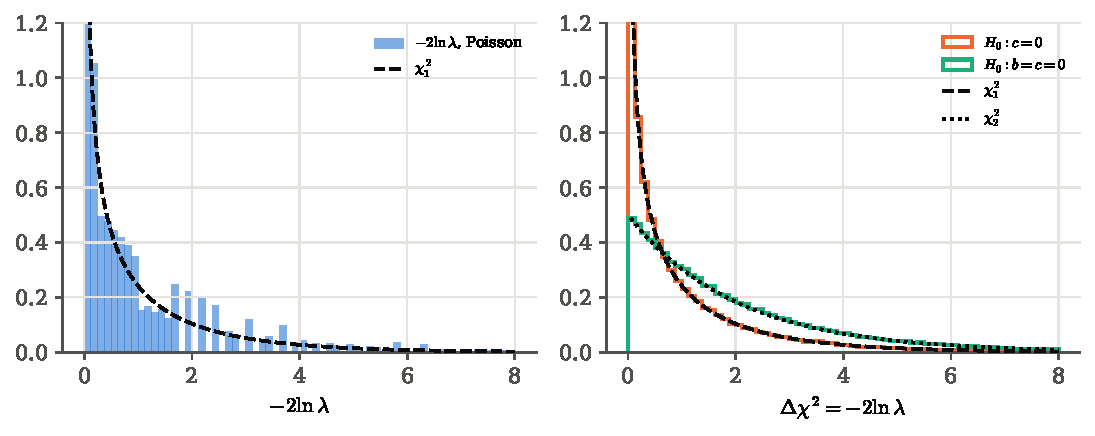
\includegraphics[width=\linewidth]{figures/ch04/wilks_checks.pdf}
\caption{Wilks' theorem checked twice. Left: the likelihood-ratio statistic for
a Poisson rate ($25$ counts, $\lambda_0=5$) follows the $\chi^2_1$ density
(dashed) closely. Right: $\Delta\chi^2$ between nested polynomial fits with
Gaussian noise follows $\chi^2_1$ when one coefficient is tested (orange) and
$\chi^2_2$ when two are (green, with the dotted density). For linear models the
agreement is exact, not only asymptotic.}
\label{4a:fig:wilks-checks}
\end{figure}

\paragraph{Example: Mendel's peas by likelihood ratio.}
Mendel counted $X=(315,101,108,32)$ peas in four classes, $n=556$, where his
theory predicts probabilities $p_0=(\frac9{16},\frac3{16},\frac3{16},\frac1{16})$
\mainref{Ex.~10.18}. The multinomial likelihood is $\prod_jp_j^{X_j}$, maximised
at $\hat p_j=X_j/n$, so
\begin{align*}
  -2\ln\lambda&=2\sum_{j=1}^4X_j\ln\frac{X_j/n}{p_{0j}}\\
  &=2\Bigl[315\ln\frac{315/556}{9/16}+101\ln\frac{101/556}{3/16}
   +108\ln\frac{108/556}{3/16}+32\ln\frac{32/556}{1/16}\Bigr]=0.48
\end{align*}
\mainref{Ex.~10.23}. The unrestricted model has three free probabilities (four
that sum to one), the null none, so the reference is $\chi^2_3$ and the p-value
is about $0.92$. The Pearson statistic of \cref{4a:sec:gof} gives $0.47$ on the
same data: for large counts the two statistics agree to second order.

\subsection{When the null sits on a boundary: $Z=\sqrt{q_0}$}
\label{4a:sec:boundary}

When the null value sits on the edge of the allowed region, Wilks' theorem
needs a correction, and the corrected answer is very simple. The case that
matters is the counting experiment of \cref{4a:sec:power-counting}: a count
$N\sim\mathrm{Pois}(s+b)$, with known expected background $b$, unknown
expected signal $s$, and the physical constraint $s\ge0$. The null $s=0$ sits
on the \emph{edge} of the allowed region, which breaks the interior condition
of Wilks' theorem.

\emph{The fit.} The log likelihood is
$\ell(s)=N\ln(s+b)-(s+b)+\text{const}$. Its maximum is at $s=N-b$ if that is
allowed, and at the boundary $s=0$ otherwise, so $\hat s=\max(N-b,0)$.

\emph{The statistic.} The discovery statistic is the likelihood-ratio
statistic \eqref{4a:eq:lrt} for the null $s=0$:
\begin{align}
  q_0=-2\ln\frac{\Like(0)}{\Like(\hat s)}
  &\eqby{1} 2\bigl[N\ln(\hat s+b)-(\hat s+b)-N\ln b+b\bigr] \notag\\
  &\eqby{2} \begin{cases}
              2\bigl[N\ln(N/b)-(N-b)\bigr], & N>b,\\
              0, & N\le b .
            \end{cases}
  \label{4a:eq:q0}
\end{align}
\begin{explain}
  \item Insert $\ell$ at $\hat s$ and at $0$.
  \item For $N>b$, $\hat s+b=N$. For $N\le b$ the best allowed fit is $\hat s=0$,
        the same as the null, and the ratio is one. A deficit is never evidence
        for a signal.
\end{explain}
\emph{Its null distribution.} For a large background, $N$ is nearly Gaussian
about $b$ and falls below it half of the time; then $q_0=0$. In the other
half, the unconstrained Wilks argument applies and $q_0$ is $\chi^2_1$. So the
null distribution is the
mixture $\frac12\delta(q_0)+\frac12\chi^2_1$, a result that goes back to
Chernoff. Its tail is
\begin{equation}
  \Prob(q_0\ge Z^2\given\Hnull)
  \eqby{1} \tfrac12\Prob\bigl(\chi^2_1\ge Z^2\bigr)
  \eqby{2} \tfrac12\Prob\bigl(\abs{Z'}\ge Z\bigr)
  \eqby{3} \Phi(-Z),
  \qquad Z'\sim\Normal(0,1),
  \label{4a:eq:half-chi2}
\end{equation}
\begin{explain}
  \item For $Z>0$ only the $\chi^2_1$ half contributes, with weight $\frac12$.
  \item A $\chi^2_1$ variable is the square of a standard normal.
  \item The two tails of $Z'$ are equal, $\Prob(\abs{Z'}\ge Z)=2\Phi(-Z)$.
\end{explain}
so the significance of an observation is simply $Z=\sqrt{q_0}$ standard
deviations \cite{Cowan2011}. The same half-$\chi^2$, and $Z=\sqrt{q_0}$, survive when the
background and calibrations are nuisance parameters profiled in $q_0$, as the second
part of the chapter shows in its section on discovery and exclusion with nuisance
parameters. \Cref{4a:fig:wilks-boundary} tests this with two
million background-only toys at $b=3.2$ and at $b=100$. The fraction with
$q_0=0$ is $\FourAWkZeroSmall$ and $\FourAWkZeroBig$, above one half because
the Poisson puts extra probability at and just below its mean. The fraction with
$q_0\ge9$, that is $Z\ge3$, is $\FourAWkThreeSmall$ and $\FourAWkThreeBig$,
against the asymptotic $\FourAWkThreeTh$: the formula is good to about $7\%$
at $b=100$ and to about $30\%$ at $b=3.2$. For Cowan's peak, $11$ events on
$3.2$, $Z=\sqrt{q_0}=\FourAWkZwilks$, while the exact Poisson tail corresponds
to $\FourAWkZexact$.

\begin{figure}[htbp]
\centering
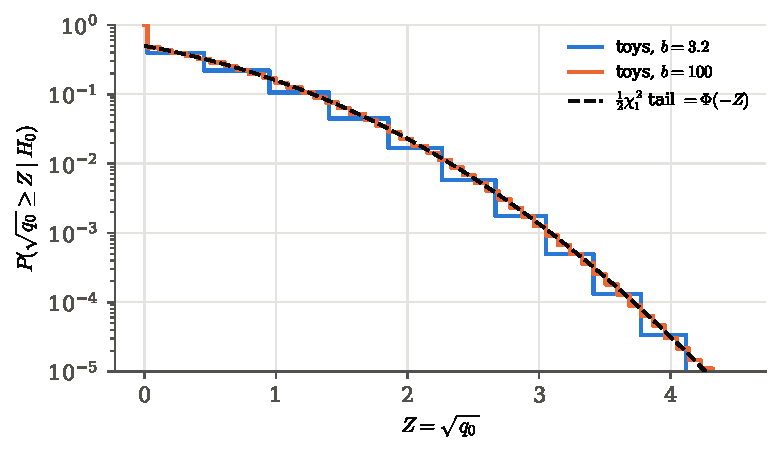
\includegraphics[width=0.8\linewidth]{figures/ch04/wilks_boundary.pdf}
\caption{The probability that background alone reaches a significance
$Z=\sqrt{q_0}$ or more, from toys with $b=3.2$ (blue) and $b=100$ (orange),
compared with the asymptotic half-$\chi^2_1$ prediction $\Phi(-Z)$ (dashed). The
large-background staircase follows the prediction closely; the small-background
one jumps in coarse steps because only integer counts are possible, and
wanders above and below the line.}
\label{4a:fig:wilks-boundary}
\end{figure}

\pyfile[firstline=65,lastline=70]{code/ch04/07_wilks.py}{The discovery statistic for a counting experiment}

The function is \eqref{4a:eq:q0} verbatim: the \pyname{np.where} enforces
$\hat s\ge0$, and the \pyname{errstate} guard silences the harmless warnings
from $\ln0$ in the branch that is discarded.

\paragraph{Example: the expected significance, and when $s/\sqrt b$ is enough.}
Before an experiment we want its \emph{median} significance if a signal $s$ is
present. We can get it without simulation \cite{Cowan2011}: evaluate $q_0$ on
the ``Asimov'' data set, in which $N$ is replaced by its expectation $s+b$.
Then
\begin{align}
  Z_A^2=q_0\bigl(N=s+b\bigr)
  &\eqby{1} 2\Bigl[(s+b)\ln\frac{s+b}{b}-s\Bigr]
   \eqby{2} 2\Bigl[(s+b)\ln\Bigl(1+\frac sb\Bigr)-s\Bigr] \notag\\
  &\eqby{3} 2\Bigl[(s+b)\Bigl(\frac sb-\frac{s^2}{2b^2}+\frac{s^3}{3b^3}-\dots\Bigr)-s\Bigr] \notag\\
  &\eqby{4} \frac{s^2}{b}\Bigl[1-\frac{s}{3b}+\dots\Bigr] .
  \label{4a:eq:asimov}
\end{align}
\begin{explain}
  \item \eqref{4a:eq:q0} with $N=s+b>b$; $N-b=s$.
  \item $(s+b)/b=1+s/b$.
  \item $\ln(1+u)=u-u^2/2+u^3/3-\dots$ with $u=s/b$.
  \item Multiply out: $(s+b)(s/b)=s^2/b+s$, whose $s$ cancels the $-s$;
        $(s+b)(-s^2/2b^2)=-s^2/2b-s^3/2b^2$; $(s+b)(s^3/3b^3)=s^3/3b^2+\dots$.
        Collecting, $s^2/b-s^2/2b=s^2/2b$ and $-s^3/2b^2+s^3/3b^2=-s^3/6b^2$;
        the factor $2$ gives $s^2/b-s^3/3b^2$.
\end{explain}
So for $s\ll b$ the familiar $Z\approx s/\sqrt b$ is recovered, and the first
correction shows it \emph{overestimates} the significance. With $s=10$ on
$b=100$, $Z_A=\FourAWkZAbig$, $s/\sqrt b=\FourAWkZsbBig$, and the median of
toy significances is $\FourAWkZmedBig$. With $s=5$ on $b=3.2$ the shortcut
fails badly: $Z_A=\FourAWkZAsmall$ against $s/\sqrt b=\FourAWkZsbSmall$.

\begin{inpractice}[Profile likelihood ratios at the LHC]
The discovery of the Higgs boson and most searches since use exactly this
statistic, with many nuisance parameters for backgrounds, luminosity and
energy scales. Each is ``profiled'': maximised separately in numerator and
denominator of $\lambda$. The asymptotic formulae, $Z=\sqrt{q_0}$ and the Asimov
median, are derived for this general case in \cite{Cowan2011}. Our toys
\emph{verify} them against an analytic answer. In research the same toys are the
\emph{instrument}: where counts are small, parameters sit on boundaries or the
signal mass is scanned, the null distribution of $q_0$ is generated by
simulation, and the asymptotic formula serves only as a cross-check.
\end{inpractice}

\paragraph{Where Wilks does not apply.}
Three conditions carried the derivation, and each fails somewhere in physics.
The parameter must be in the interior (the boundary gives the half-$\chi^2$
above). The hypotheses must be nested, one a special case of the other. And
every parameter of the alternative must mean something under the null. The last
condition fails in a bump hunt: the signal mass is meaningless when the signal
strength is zero, and maximising over it inflates $q_0$ beyond any $\chi^2$.
That is the look-elsewhere effect in its likelihood form
\cite{GrossVitells2010}, and it leads to the trials factor treated in the second part of the chapter.
\section{Goodness of fit: Pearson's $\chi^2$ and Kolmogorov--Smirnov}
\label{4a:sec:gof}

So far the null has always been tested against a definite direction: a
signal in a window, a bias of a coin, a shift of a calibration. Often we want
something vaguer. Here is the background model for the whole mass spectrum,
thirty bins of it; does it describe the data \emph{at all}? No particular
alternative is in mind, just ``something else''. This is a
\newterm{goodness-of-fit} test \srcref{Cowan}{\S4.5}: the test statistic
itself measures the disagreement between data and model, and its large values
are the extreme direction.

\paragraph{The question in words.}
\begin{enumerate}[label=\arabic*.]
  \item How do we add up the disagreement of many bins into one number with a
        known null distribution?
  \item What changes when the total is fixed, when parameters were fitted to
        the same data, and when counts are small?
  \item Can we avoid binning altogether?
\end{enumerate}

\subsection{The $\chi^2$ distribution, recalled}
\label{4a:sec:chi2-dist}

If $Z_1,\dots,Z_k$ are independent standard normals, $V=\sum_{i=1}^kZ_i^2$ has
the $\chi^2$ distribution with $k$ degrees of freedom (\cref{ch:02}), with
density, mean and variance \mainref{p.~159}
\begin{equation}
  f(v)=\frac{v^{k/2-1}e^{-v/2}}{2^{k/2}\Gamma(k/2)}\quad(v>0),
  \qquad
  \E V=k,\qquad \Var V=2k .
  \label{4a:eq:chi2-density}
\end{equation}
The mean is immediate, $\E Z_i^2=1$ for each term, and the variance follows
from $\E Z^4=3$: $\Var Z_i^2=3-1=2$ per term. Its upper quantile
$\chi^2_{k,\alpha}$ is defined by $\Prob(\chi^2_k>\chi^2_{k,\alpha})=\alpha$, and
a p-value is the upper tail beyond the observed value. For large $k$ the
distribution is close to $\Normal(k,2k)$.

\subsection{Pearson's statistic}
\label{4a:sec:pearson}

A histogram has $N$ bins with observed counts $n_i$ and expected counts
$\nu_i$ under the model. If the counts are independent Poisson variables and
none of the $\nu_i$ is small, each $n_i$ is approximately Gaussian with mean
$\nu_i$ and variance $\nu_i$, so $(n_i-\nu_i)/\sqrt{\nu_i}$ is approximately a
standard normal. Adding the squares \srcref{Cowan}{(4.39)},
\begin{equation}
  \chi^2=\sum_{i=1}^N\frac{(n_i-\nu_i)^2}{\nu_i}\;\sim\;\chi^2_N
  \qquad\text{(approximately, for }\nu_i\gtrsim5\text{)} .
  \label{4a:eq:pearson-poisson}
\end{equation}
The approximation does not care what physical variable was histogrammed or
what shape the model has; the test is \newterm{distribution free}. Each term is
the squared deviation in units of its own standard deviation, so $\chi^2$ is
the total disagreement counted in ``sigmas squared''.

If instead the total $n=\sum_in_i$ is fixed, the counts are multinomial with
cell probabilities $p_{0i}$ and expected counts $E_i=np_{0i}$, and Pearson's
statistic is \mainref{Def.~10.16}, \srcref{Cowan}{(4.41)}
\begin{equation}
  T=\sum_{j=1}^k\frac{(X_j-E_j)^2}{E_j}\;\sim\;\chi^2_{k-1}
  \label{4a:eq:pearson-multinomial}
\end{equation}
under the null, asymptotically \mainref{Thm~10.17}. The one lost degree of
freedom is the constraint $\sum_j(X_j-E_j)=0$: the deviations are not
independent, because an excess in one cell must be paid for by deficits
elsewhere. The case $k=2$ shows the mechanism exactly. With cell
probabilities $p$ and $1-p$, $X_2-n(1-p)=-(X_1-np)$, so
\begin{align}
  T
  &\eqby{1} \frac{(X_1-np)^2}{np}+\frac{(X_1-np)^2}{n(1-p)} \notag\\
  &\eqby{2} (X_1-np)^2\,\frac{(1-p)+p}{np(1-p)}
   \eqby{3} \Bigl(\frac{X_1-np}{\sqrt{np(1-p)}}\Bigr)^2 .
  \label{4a:eq:pearson-two}
\end{align}
\begin{explain}
  \item The second deviation is minus the first, and its square is the same.
  \item Common denominator.
  \item $(1-p)+p=1$.
\end{explain}
The bracket is the binomial count standardised by its own mean $np$ and
standard deviation $\sqrt{np(1-p)}$, which by the de Moivre--Laplace theorem of
\cref{ch:02} is approximately standard normal. So $T\approx Z^2\sim\chi^2_1$:
two cells, one degree of freedom. For $k$ cells the same happens in $k-1$
dimensions: the constraint confines the standardised deviation vector to a
hyperplane, and its squared length is a sum of $k-1$ independent squared
normals.

\paragraph{Example: Mendel's peas.}
Mendel crossed peas and counted $X=(315,101,108,32)$ progeny of four types,
$n=556$; his theory predicts $p_0=(\frac9{16},\frac3{16},\frac3{16},\frac1{16})$
\mainref{Ex.~10.18}. The expected counts are $E=(312.75,104.25,104.25,34.75)$
and
\begin{align*}
  T&=\frac{(315-312.75)^2}{312.75}+\frac{(101-104.25)^2}{104.25}
     +\frac{(108-104.25)^2}{104.25}+\frac{(32-34.75)^2}{34.75}\\
   &=0.016+0.101+0.135+0.218=\FourAMendelChi .
\end{align*}
With $k-1=3$ degrees of freedom the $5\%$ critical value is $7.815$, far above,
and the p-value is $\Prob(\chi^2_3>\FourAMendelChi)=\FourAMendelP$. So the data
do not contradict Mendel's theory. They do not prove it either. A test like
this can show evidence to reject the null, but it cannot prove the null
\mainref{p.~161}, because a failure to reject may come from a true null or
from low power. (A footnote there recalls that Mendel's results have been
suspected of fitting \emph{too} well. A p-value very close to one is also
improbable under the null.)

\begin{pitfall}[$\chi^2/\nu$ near one is not enough]
It is common to quote $\chi^2$ divided by the number of degrees of freedom and
call anything near one a good fit. The ratio hides the scale: the spread of
$\chi^2_\nu/\nu$ is $\sqrt{2/\nu}$, which shrinks with $\nu$. For
$\chi^2=15$ on $10$ degrees of freedom the p-value is $0.13$, perfectly fine;
for $\chi^2=150$ on $100$, the same ratio, it is $9.0\times10^{-4}$
\srcref{Cowan}{p.~62}. Always quote $\chi^2$ and $\nu$ separately, or the
p-value.
\end{pitfall}

\subsection{Fitted parameters and small counts}
\label{4a:sec:gof-fitted}

Usually the model has parameters, such as a background slope, that are
estimated from the same histogram. The fit pulls the expectation towards the
data and makes $\chi^2$ smaller than it would be at the true parameters. If
$s$ parameters are estimated by maximising the multinomial likelihood of the
binned counts, $Q(\params)=\prod_jp_j(\params)^{N_j}$, then
\mainref{Thm~10.29}
\begin{equation}
  Q=\sum_{j=1}^k\frac{\bigl(N_j-np_j(\hat\params)\bigr)^2}{np_j(\hat\params)}
  \;\sim\;\chi^2_{k-1-s} :
  \label{4a:eq:pearson-fitted}
\end{equation}
each fitted parameter removes one degree of freedom, for the same geometric
reason as in Wilks' theorem (\cref{4a:sec:wilks-why}): the fit projects the
deviations onto a smaller subspace. This count holds only when the parameters
are fitted to the binned counts. If they are estimated instead from the
\emph{unbinned} data, which is often more natural, the distribution of $Q$ is
no longer $\chi^2_{k-1-s}$; a theorem of Chernoff and Lehmann puts it between
$\chi^2_{k-1-s}$ and $\chi^2_{k-1}$ \mainref{p.~169}. The reason is that the
unbinned estimate is not tuned to the bins, so it removes less of the
disagreement.

\paragraph{Example: fitting a decay length.}
The script \pyname{code/ch04/08_goodness_of_fit.py} draws $400$ decay times
with mean $\tau=2$, histograms them in $k=8$ bins, $[0,1),[1,2),\dots,[7,\infty)$,
and fits $\tau$ two ways: by maximising the binned multinomial likelihood, and
by the unbinned maximum-likelihood estimate $\hat\tau=\bar t$. Over $4000$
repetitions the mean of $Q$ is $\FourAGofMeanBinned$ with the binned fit, as
$\chi^2_{k-2}=\chi^2_6$ predicts, and $\FourAGofMeanRaw$ with the unbinned
one; each mean carries a random error of about $\FourAGofMeanErr$. Both fits see
the same histograms, so their difference is measured much better: the unbinned fit
leaves $Q$ larger by $\FourAGofMeanDiff\pm\FourAGofMeanDiffErr$ on average, which
puts it between $\chi^2_6$ and $\chi^2_7$, as Chernoff--Lehmann says
(\cref{4a:fig:gof-chi2}, right). Here the difference is small; it matters more
when the bins are few and the parameters many.

\paragraph{Example: when the bins are sparse.}
The $\chi^2_N$ approximation needs every $\nu_i$ to be reasonably large. With a
few counts per bin, $(n_i-\nu_i)^2/\nu_i$ is far from a squared Gaussian: a
Poisson with small mean is skewed, and a single count of $5$ where $1$ was
expected contributes $16$. \srcref{Cowan}{p.~63} finds $\chi^2=29.8$ for $20$
bins of his bump histogram, where most bins have fewer than five entries, and
shows that the $\chi^2_{20}$ tail ($0.073$) understates the true p-value
($0.11$, from Monte Carlo). Our version uses $20$ Poisson bins with expected
counts between about $1$ and $4$. Simulating $200\,000$ histograms under the
null, the $95\%$ point of Pearson's statistic is $\FourAGofQsmall$, against
$\FourAGofQth$ for $\chi^2_{20}$. For an observed value of $30$ the simulated
p-value is $\FourAGofPsmallMC$ and the $\chi^2$ formula would give
$\FourAGofPsmallChi$. With $25$ times more data in the same shape the
simulated $95\%$ point becomes $\FourAGofQlarge$, on the $\chi^2$ value
(\cref{4a:fig:gof-chi2}, left). The remedy is Cowan's: when counts are small,
simulate the null distribution of the statistic you computed.

\begin{figure}[htbp]
\centering
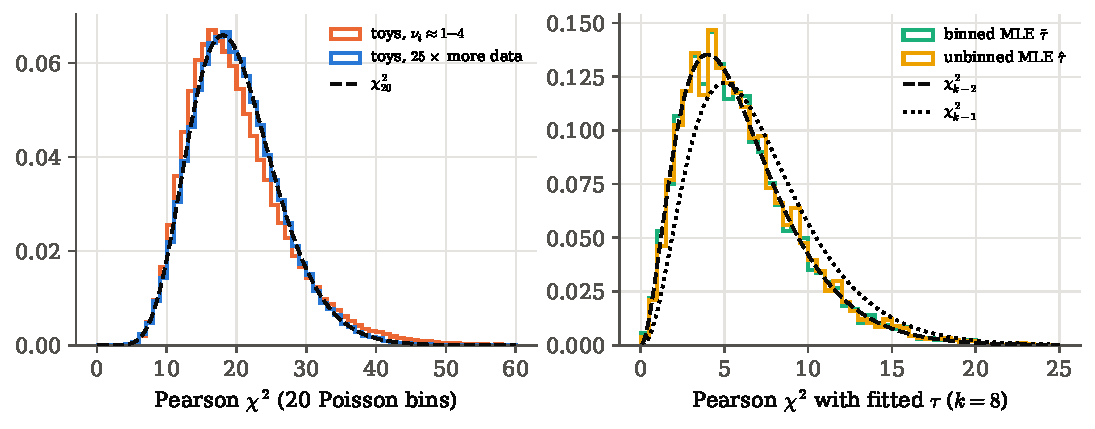
\includegraphics[width=\linewidth]{figures/ch04/gof_chi2.pdf}
\caption{Left: the null distribution of Pearson's $\chi^2$ for $20$ Poisson
bins. With one to four expected counts per bin (orange) it has a longer tail
than $\chi^2_{20}$ (dashed); with $25$ times more data (blue) it lies on the
curve. Right: after fitting a decay length, Pearson's statistic follows
$\chi^2_{k-2}$ when the fit uses the binned counts (green) and sits slightly
towards $\chi^2_{k-1}$ (dotted) when the fit uses the unbinned decay times
(yellow).}
\label{4a:fig:gof-chi2}
\end{figure}

Binning is a choice, and different choices give different p-values
\srcref{Cowan}{p.~63}. Bins must be wide enough for the approximation, yet wide
bins throw away where in the bin each event fell. Simulating the null
distribution relaxes the first constraint. Avoiding bins altogether removes
the choice.

\subsection{The Kolmogorov--Smirnov test}
\label{4a:sec:ks}

For $n$ individual measurements $x_1,\dots,x_n$ we can compare the data with a
hypothesised continuous CDF $F$ directly. The \newterm{empirical CDF}
\unpack{the fraction of the data at or below $x$}
\[
  F_n(x)=\frac1n\#\{i:\ x_i\le x\}
\]
is a staircase that climbs by $1/n$ at each data point. The
\newterm{Kolmogorov--Smirnov statistic} is its largest vertical distance from
the model,
\begin{equation}
  D_n=\sup_x\abs{F_n(x)-F(x)} .
  \label{4a:eq:ks}
\end{equation}
The supremum over all $x$ reduces to a check at the data points. Sort them,
$x_{(1)}\le\dots\le x_{(n)}$. Between two data points $F_n$ is flat and $F$
increases, so the gap $F_n-F$ is largest just after a jump and $F-F_n$ is
largest just before one. At $x_{(i)}$ the staircase jumps from $(i-1)/n$ to
$i/n$, hence
\begin{equation}
  D_n=\max\bigl(D_n^+,D_n^-\bigr),\qquad
  D_n^+=\max_i\Bigl(\frac in-F(x_{(i)})\Bigr),\qquad
  D_n^-=\max_i\Bigl(F(x_{(i)})-\frac{i-1}n\Bigr).
  \label{4a:eq:ks-compute}
\end{equation}

Why is the null distribution of $D_n$ the same for every continuous $F$? Set
$u_i=F(x_i)$. Under the null the $u_i$ are uniform on $(0,1)$ by the
probability integral transform of \cref{4a:sec:p-uniform}, and because $F$ is
increasing, ``$x_i\le x$'' is the same as ``$u_i\le F(x)$''. Writing $u=F(x)$,
\begin{equation}
  \abs{F_n(x)-F(x)}
  \eqby{1} \Bigl\lvert\frac1n\#\{i:u_i\le u\}-u\Bigr\rvert
  \eqby{2} \abs{G_n(u)-u},
  \label{4a:eq:ks-free}
\end{equation}
\begin{explain}
  \item Replace each event $x_i\le x$ by the equivalent $u_i\le u$.
  \item $G_n$ is the empirical CDF of the uniform sample $u_1,\dots,u_n$.
\end{explain}
so $D_n$ is the Kolmogorov--Smirnov distance of a uniform sample from the
uniform CDF, whatever $F$ was. Its distribution can be tabulated once; for
large $n$, Kolmogorov showed that $\sqrt nD_n$ converges to a limiting
distribution with tail $\Prob(K>x)=2\sum_{j\ge1}(-1)^{j-1}e^{-2j^2x^2}$.

\paragraph{Example: a decay length that is not what we thought.}
Fifty decay times are drawn with mean $1.3$, and we test the null that the
mean is $1$, $F(x)=1-e^{-x}$. \Cref{4a:fig:ks} (left) shows the empirical
staircase below the model curve over most of the range, since longer lifetimes
make small times rarer. Our own implementation of \eqref{4a:eq:ks-compute}
finds $D_{50}=\FourAKsD$, so $\sqrt nD_n=\FourAKsSqrtnD$. The exact p-value
from \pyname{scipy.stats.kstest} (which also returns $D=\FourAKsDscipy$) is
$\FourAKsPscipy$; the Kolmogorov limit gives $\FourAKsPkolm$; and $40\,000$
simulated null samples of size $50$ give $\FourAKsPmc$. With only fifty events,
a $30\%$ change of lifetime gives modest evidence against the null at best, and
another fifty decays could easily give a much larger p-value.

\begin{figure}[htbp]
\centering
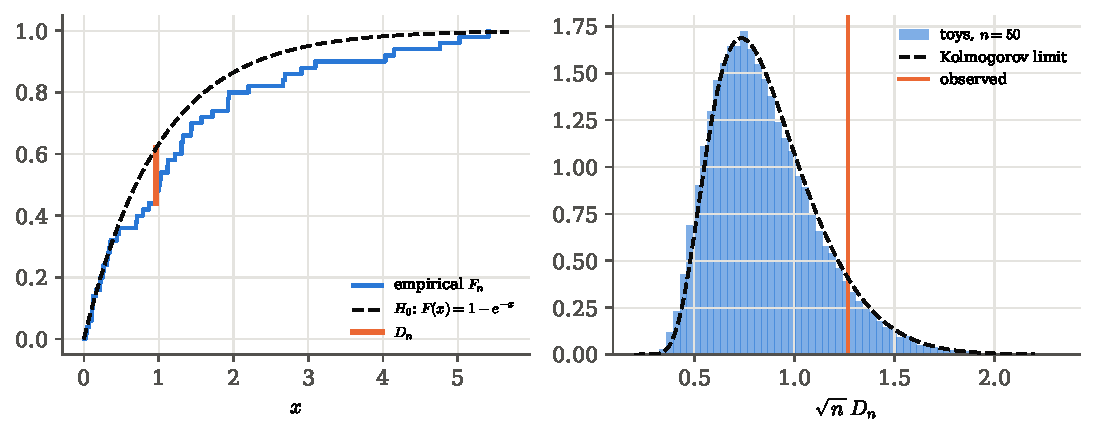
\includegraphics[width=\linewidth]{figures/ch04/ks_test.pdf}
\caption{Left: the empirical CDF of fifty decay times (blue staircase) and the
null model's CDF (dashed). The orange bar marks the largest vertical gap,
$D_n$. Right: the null distribution of $\sqrt n\,D_n$ for samples of fifty,
from simulation (histogram) and Kolmogorov's large-$n$ limit (dashed), with the
observed value marked.}
\label{4a:fig:ks}
\end{figure}

\pyfile[firstline=85,lastline=91]{code/ch04/08_goodness_of_fit.py}{The Kolmogorov--Smirnov statistic from scratch}

The function sorts the sample, evaluates the model CDF at each point, and
takes the two maxima of \eqref{4a:eq:ks-compute} with the vectors
\pyname{np.arange(1, n+1)/n} (the tops of the steps) and
\pyname{np.arange(0, n)/n} (the bottoms). It agrees with scipy to every digit
printed. The Monte Carlo p-value calls the same function on samples drawn from
the null.

Two cautions. The distribution-free property holds only when $F$ is fully
specified in advance. If its parameters are estimated from the same data, the
fitted CDF hugs the data and $D_n$ is typically smaller, so the tabulated
p-values are too large; the null distribution must then be simulated, fitting
the parameters afresh on each simulated sample. And like every goodness-of-fit
test, a large p-value does not certify the model: it may only mean the test has
little power against the departure that is actually present
\mainref{p.~169}. Relatives of KS that weight the whole curve rather than its
largest gap, such as the Cram\'er--von Mises statistic, are often more
powerful \srcref{Cowan}{p.~63}.
\section{From $p$ to $Z\sigma$, and why a discovery needs $5\sigma$}
\label{4a:sec:ztable}

Particle physicists rarely quote p-values. They say that an excess is ``a
$2.6\sigma$ fluctuation'', that $3\sigma$ counts as evidence, and that a
discovery needs $5\sigma$. The language comes from Gaussian error bars, but it
is used for every kind of test statistic, including Poisson counts and
likelihood ratios that are nothing like Gaussian. So ``$Z$ sigma'' must be a
relabelling of the p-value, and it is: a precise one-to-one translation. Once
we have it, we can ask why particle physics sets the bar so high, when other
fields are content with $p<0.05$.

\paragraph{The question in words.}
\begin{enumerate}[label=\arabic*.]
  \item What exactly does ``$Z$ sigma'' mean for a test statistic that is not
        Gaussian?
  \item How small is the p-value of a $5\sigma$ result, and how does it
        compare with $3\sigma$?
  \item What goes wrong with a lower threshold, given many searches, imperfect
        backgrounds and new physics that is rare?
\end{enumerate}

\subsection{The translation}
\label{4a:sec:p-to-z}

The \newterm{significance} $Z$ of a p-value is the number of standard
deviations above the mean at which a standard normal variable has the same
upper-tail probability \cite{Cowan2011}:
\begin{equation}
  p=\int_Z^\infty\frac{e^{-t^2/2}}{\sqrt{2\pi}}\,\dd t=1-\Phi(Z)=\Phi(-Z),
  \qquad
  Z=\Phi^{-1}(1-p) .
  \label{4a:eq:p-to-z}
\end{equation}
The definition says nothing about the distribution of the actual statistic. A
Poisson count, a $\chi^2$, a permutation statistic: whatever gave the p-value,
$Z$ is only a relabelling of it on a scale that physicists find intuitive. For
the bump of \cref{4a:sec:bump}, $p=\FourABumpP$ becomes $Z=\FourABumpZ$. Some
authors use the two-sided convention $p=2\Phi(-Z)$, which corresponds to
$\abs{\text{Gaussian}}\ge Z$; discovery claims use the one-sided version,
because only an excess counts. The table from
\pyname{code/ch04/09_p_to_z.py}:
\begin{center}
\begin{tabular}{ccc}
\toprule
$Z$ & one-sided $\Phi(-Z)$ & two-sided $2\Phi(-Z)$ \\
\midrule
$1$ & $\FourAPzOneOne$ & $\FourAPzOneTwo$ \\
$2$ & $\FourAPzTwoOne$ & $\FourAPzTwoTwo$ \\
$3$ & $\FourAPzThreeOne$ & $\FourAPzThreeTwo$ \\
$4$ & $\FourAPzFourOne$ & $\FourAPzFourTwo$ \\
$5$ & $\FourAPzFiveOne$ & $\FourAPzFiveTwo$ \\
$6$ & $\FourAPzSixOne$ & $\FourAPzSixTwo$ \\
\bottomrule
\end{tabular}
\end{center}
In the other direction, $p=0.05$ corresponds to $Z=\FourAPzZfivepct$
one-sided and $\FourAPzZfivepctTwo$ two-sided. The usual $5\%$ threshold of
the life sciences is a $1.6$ to $2\sigma$ effect, and a $5\sigma$ result has a
p-value about $170\,000$ times smaller.

\paragraph{Example: reading the scale in both directions.}
A search reports a one-sided p-value of $2.5\times10^{-4}$. Then
$Z=\Phi^{-1}(1-2.5\times10^{-4})=3.48$, a little above the $3\sigma$ line of
``evidence'' and well short of $5\sigma$. Had the same number been a
two-sided p-value, the one-sided tail would be half of it, $1.25\times10^{-4}$,
and $Z=3.66$; quoting $Z$ without saying which convention is in use can move
the claim by a fifth of a sigma. In the other direction, an analysis planned
to reach $Z=4.2$ must see a background-only tail no bigger than
$\Phi(-4.2)=1.3\times10^{-5}$, about one chance in $75\,000$.

\paragraph{How fast the tail falls.}
For large $Z$ there is a simple estimate of the tail, useful for checking
orders of magnitude without a table. Write $\varphi(t)=e^{-t^2/2}/\sqrt{2\pi}$
and note that $\varphi'(t)=-t\varphi(t)$. Integrating by parts,
\begin{align}
  \Phi(-Z)=\int_Z^\infty\varphi(t)\,\dd t
  &\eqby{1} \int_Z^\infty\frac1t\,\bigl(t\varphi(t)\bigr)\dd t
   \eqby{2} \Bigl[-\frac{\varphi(t)}{t}\Bigr]_Z^\infty-\int_Z^\infty\frac{\varphi(t)}{t^2}\,\dd t \notag\\
  &\eqby{3} \frac{\varphi(Z)}{Z}-\int_Z^\infty\frac{\varphi(t)}{t^2}\,\dd t
   \relby{4}{\approx} \frac{\varphi(Z)}{Z}\Bigl(1-\frac1{Z^2}\Bigr) .
  \label{4a:eq:mills}
\end{align}
\begin{explain}
  \item Multiply and divide by $t$.
  \item Parts, with $u=1/t$ and $\dd v=t\varphi(t)\,\dd t$, so $v=-\varphi(t)$
        and $\dd u=-\dd t/t^2$.
  \item The boundary term vanishes at infinity.
  \item The remaining integral is smaller by a factor of about $1/Z^2$; the
        same trick applied to it gives the correction shown.
\end{explain}
At $Z=5$, $\varphi(5)=e^{-12.5}/\sqrt{2\pi}=1.49\times10^{-6}$, so the
estimate is $1.49\times10^{-6}\times0.96/5=2.85\times10^{-7}$, against the
exact $\FourAPzFiveOne$. The factor $e^{-Z^2/2}$ dominates: each extra sigma near
$Z=5$ costs a factor of $e^{-(Z+1)^2/2+Z^2/2}=e^{-Z-1/2}\approx250$ in
probability.

\begin{figure}[htbp]
\centering
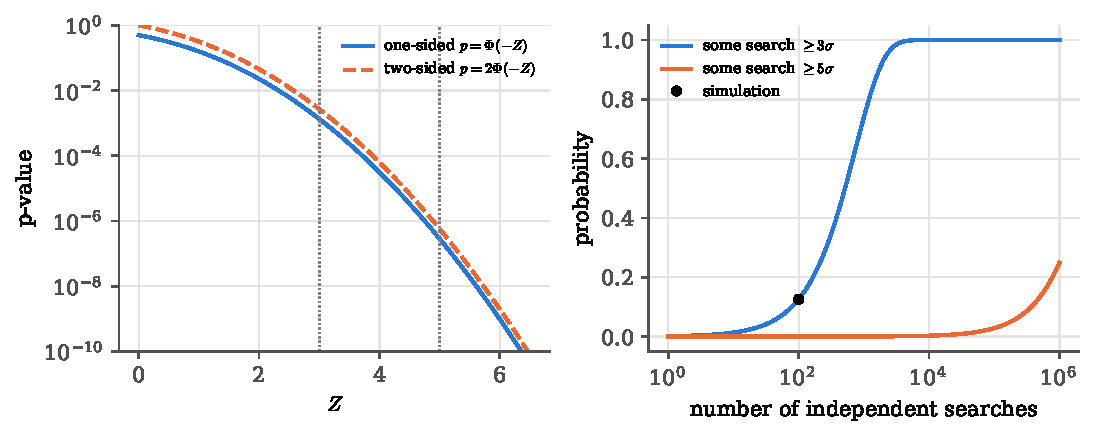
\includegraphics[width=\linewidth]{figures/ch04/p_to_z.pdf}
\caption{Left: the p-value that corresponds to a significance $Z$, one-sided
(solid) and two-sided (dashed), on a log scale; the dotted lines mark $3\sigma$
and $5\sigma$. Right: the probability that at least one of many independent
background-only searches reaches $3\sigma$ (blue) or $5\sigma$ (orange). With a
hundred searches the chance of a $3\sigma$ fluctuation somewhere is already
about one in eight; the black dot is a direct simulation.}
\label{4a:fig:p-to-z}
\end{figure}

\subsection{Why five}
\label{4a:sec:why-five}

Three separate arguments each call for a threshold far stricter than
$p<0.05$: there are many searches, the backgrounds are imperfect, and new
physics is rare. We take them one at a time.

\paragraph{Many searches.}
A laboratory does not run one test. It scans masses, channels, final states,
and every analysis group does the same. If $N$ independent searches each have
probability $p_1$ of a false alarm, the probability that at least one of them
fires is
\begin{equation}
  \Prob(\text{at least one})
  \eqby{1} 1-\Prob(\text{none})
  \eqby{2} 1-(1-p_1)^N
  \relby{3}{\approx} Np_1\quad(Np_1\ll1).
  \label{4a:eq:any-search}
\end{equation}
\begin{explain}
  \item Complement.
  \item Independence: the probability that all $N$ stay quiet is the product.
  \item $(1-p_1)^N\approx1-Np_1$ to first order.
\end{explain}
With $N=100$ and a $3\sigma$ threshold, $p_1=\FourAPzThreeOne$ gives
$\FourAPzAnyThree$, and a simulation of the maximum of $100$ standard normals
over $200\,000$ trials gives $\FourAPzAnyThreeMC$. One lab in eight would see a
$3\sigma$ effect from nothing. At $5\sigma$ the same number is
$\FourAPzAnyFive$. This is Kruschke's two coins of \cref{4a:sec:stopping}
on a larger scale, and it is the look-elsewhere effect that the second part of
the chapter quantifies properly for scans over a mass.

\paragraph{Imperfect backgrounds.}
The p-value is computed from the null model alone, so an error in the null
model goes straight into it. In \cref{4a:sec:poisson-p} moving the background
from $0.5$ to $0.8$ events changed the p-value of five events by a factor of
about eight. Real detectors also have tails in their resolution functions that
no Gaussian captures. A $5\sigma$ threshold leaves a margin: an effect that
survives it is unlikely to be an artefact of a background that is off by a
modest amount. A $3\sigma$ effect is not so robust.

\paragraph{New physics is rare.}
The third argument is the population argument of \cref{4a:sec:not-posterior},
and it needs Bayes' theorem. \emph{The event} is ``the search crossed the
threshold''. \emph{The question} is what produced it: a real effect, or a false
alarm on a null. Suppose that of all the hypotheses that searches test, only a
fraction $\pi_1=10^{-3}$ are real. \emph{Each route in turn:} when an effect
is real, the search reaches the threshold half the time, so the power is
$0.5$; when the null is true, it reaches it with the false-alarm probability
$p_{\rm thr}$ of the threshold. \Cref{4a:fig:tree} draws the probability tree.
\emph{Only then the numbers.} The fraction of threshold crossings that are
real, the \emph{purity} of the discoveries, is
\begin{equation}
  \Prob(\text{real}\given\text{crossed})
  \eqby{1} \frac{\pi_1\times0.5}{\pi_1\times0.5+(1-\pi_1)\,p_{\rm thr}} ,
  \label{4a:eq:purity-z}
\end{equation}
\begin{explain}
  \item Bayes' theorem on the tree: the two branches that end in ``crossed''
        are ``real, then detected'' and ``null, then false alarm''.
\end{explain}
exactly the purity formula \eqref{4a:eq:purity} of event selection, with
hypotheses in place of particles. With $p_{\rm thr}=\FourAPzThreeOne$ ($3\sigma$)
the purity is $\FourAPzPurThree$: nearly three quarters of the ``discoveries''
would be false. With $p_{\rm thr}=\FourAPzFiveOne$ ($5\sigma$) it is
$\FourAPzPurFive$. The numbers $\pi_1$ and the power are illustrative, and a
frequentist cannot even write $\pi_1$ into the p-value. But the lesson is
robust: when true effects are rare, the threshold must be far smaller than
$\pi_1$ for a crossing to mean what we want it to mean. Extraordinary claims
need extraordinary evidence, and $5\sigma$ is how particle physics encodes that
without writing down a prior. \Cref{ch:05} writes it down.

\begin{figure}[htbp]
\centering
\begin{tikzpicture}[
  grow=right, level distance=33mm,
  level 1/.style={sibling distance=22mm},
  level 2/.style={sibling distance=11mm},
  every node/.style={font=\small},
  edge from parent/.style={draw, thick, black!60}]
  \node[draw, rounded corners=2pt, fill=ideabg] {searched hypothesis}
    child {node[draw, rounded corners=2pt, fill=ideabg] (null) {null ($1-\pi_1$)}
      child {node (nq) {not crossed}}
      child {node[text=bdryred] (nc) {crossed: false alarm}}
    }
    child {node[draw, rounded corners=2pt, fill=ideabg] (real) {real ($\pi_1$)}
      child {node (rq) {not crossed}}
      child {node[text=tangentgreen!70!black] (rc) {crossed: discovery}}
    };
  \node[anchor=west, font=\footnotesize, text=black!70] at ($(nc.east)+(1mm,0)$) {prob.\ $p_{\rm thr}$};
  \node[anchor=west, font=\footnotesize, text=black!70] at ($(nq.east)+(1mm,0)$) {prob.\ $1-p_{\rm thr}$};
  \node[anchor=west, font=\footnotesize, text=black!70] at ($(rc.east)+(1mm,0)$) {prob.\ power};
  \node[anchor=west, font=\footnotesize, text=black!70] at ($(rq.east)+(1mm,0)$) {prob.\ $1-$power};
\end{tikzpicture}
\caption{The probability tree behind the $5\sigma$ convention. First nature
decides whether the hypothesis being searched for is real, with a small
probability $\pi_1$; then the experiment either crosses the threshold or not.
Among all crossings, the false alarms (red) come from the heavily populated
null branch, the discoveries (green) from the thin real branch. Only a tiny
false-alarm probability keeps the red leaf smaller than the green one.}
\label{4a:fig:tree}
\end{figure}

\paragraph{What $5\sigma$ does not say.}
A $5\sigma$ result has $p=\FourAPzFiveOne$. It does not follow that the
probability of the null is $\FourAPzFiveOne$, nor that the new particle exists
with probability $1-\FourAPzFiveOne$. As in \cref{4a:sec:not-posterior}, those
are inference-direction statements and need a prior. The convention in
particle physics is to call $3\sigma$ ``evidence'' and $5\sigma$ an
``observation'', to report the p-value (or $Z$) together with the expected
significance of the experiment, and to leave the probability of the hypothesis
to a Bayesian analysis.

\begin{recap}
\begin{itemize}
  \item The null hypothesis is the one whose sampling distribution we know:
        ``it happened by chance''. A test runs in the prediction direction,
        from $\Hnull$ to the outcomes it produces.
  \item The p-value is the probability, under $\Hnull$, of a test statistic at
        least as extreme as observed, in the direction the alternative
        predicts. The direction, and the experimental plan (stopping rule,
        number of places looked), are part of the question.
  \item A test has size $\alpha$ (false-alarm rate) and a power function
        $\beta(\theta)$ (rejection rate under the truth). Power grows with
        effect size and with $\sqrt n$; experiment planning is a power
        calculation.
  \item Under a continuous null the p-value is uniform, so ``reject if
        $p\le\alpha$'' has size $\alpha$. For discrete data it is valid:
        $\Prob(p\le\alpha)\le\alpha$.
  \item A p-value is not $\Prob(\Hnull\given\text{data})$: that needs the prior
        frequency of true nulls and the power (Bayes).
  \item Wald, t and permutation tests cover most everyday comparisons; the
        t-test is exact for small Gaussian samples, the permutation test for
        any distribution.
  \item Neyman--Pearson: for simple hypotheses the likelihood ratio is the most
        powerful statistic. With free parameters, $-2\ln\lambda$ is
        asymptotically $\chi^2$ with as many degrees of freedom as the null
        fixes (Wilks); on a boundary it is half $\chi^2_1$ and $Z=\sqrt{q_0}$.
  \item Pearson's $\chi^2$ and Kolmogorov--Smirnov test a whole model; fitted
        parameters, small counts and estimated CDFs change their null
        distributions, which can always be simulated.
  \item $Z=\Phi^{-1}(1-p)$. Discovery needs $5\sigma$ because of many searches,
        imperfect backgrounds and the rarity of real effects.
\end{itemize}
\end{recap}

\providecommand{\FourBKrN}{}\renewcommand{\FourBKrN}{24}
\providecommand{\FourBKrZ}{}\renewcommand{\FourBKrZ}{7}
\providecommand{\FourBKrThetaHat}{}\renewcommand{\FourBKrThetaHat}{0.292}
\providecommand{\FourBKrLo}{}\renewcommand{\FourBKrLo}{0.126}
\providecommand{\FourBKrHi}{}\renewcommand{\FourBKrHi}{0.511}
\providecommand{\FourBKrWaldLo}{}\renewcommand{\FourBKrWaldLo}{0.110}
\providecommand{\FourBKrWaldHi}{}\renewcommand{\FourBKrWaldHi}{0.474}
\providecommand{\FourBKrSe}{}\renewcommand{\FourBKrSe}{0.0928}
\providecommand{\FourBKrHoefEps}{}\renewcommand{\FourBKrHoefEps}{0.277}
\providecommand{\FourBKrHoefLo}{}\renewcommand{\FourBKrHoefLo}{0.014}
\providecommand{\FourBKrHoefHi}{}\renewcommand{\FourBKrHoefHi}{0.569}
\providecommand{\FourBKrPhalf}{}\renewcommand{\FourBKrPhalf}{0.064}
\providecommand{\FourBBWcovAll}{}\renewcommand{\FourBBWcovAll}{0.7498}
\providecommand{\FourBBWcovSame}{}\renewcommand{\FourBBWcovSame}{0.5005}
\providecommand{\FourBBWcovDiff}{}\renewcommand{\FourBBWcovDiff}{1.0000}
\providecommand{\FourBBWfracSame}{}\renewcommand{\FourBBWfracSame}{0.5009}
\providecommand{\FourBBeltCL}{}\renewcommand{\FourBBeltCL}{90}
\providecommand{\FourBBeltNobs}{}\renewcommand{\FourBBeltNobs}{6}
\providecommand{\FourBBeltLoSix}{}\renewcommand{\FourBBeltLoSix}{2.61}
\providecommand{\FourBBeltHiSix}{}\renewcommand{\FourBBeltHiSix}{11.84}
\providecommand{\FourBBeltMinAcc}{}\renewcommand{\FourBBeltMinAcc}{0.9002}
\providecommand{\FourBBeltMaxAcc}{}\renewcommand{\FourBBeltMaxAcc}{0.9995}
\providecommand{\FourBUpNinetyFiveZero}{}\renewcommand{\FourBUpNinetyFiveZero}{2.996}
\providecommand{\FourBUpNinetyZero}{}\renewcommand{\FourBUpNinetyZero}{2.303}
\providecommand{\FourBLoNinetyFiveThree}{}\renewcommand{\FourBLoNinetyFiveThree}{0.818}
\providecommand{\FourBUpNinetyFiveThree}{}\renewcommand{\FourBUpNinetyFiveThree}{7.75}
\providecommand{\FourBCBlo}{}\renewcommand{\FourBCBlo}{0.261}
\providecommand{\FourBCBhi}{}\renewcommand{\FourBCBhi}{1.184}
\providecommand{\FourBBeltLoZero}{}\renewcommand{\FourBBeltLoZero}{0.00}
\providecommand{\FourBBeltHiZero}{}\renewcommand{\FourBBeltHiZero}{3.00}
\providecommand{\FourBBeltLoOne}{}\renewcommand{\FourBBeltLoOne}{0.05}
\providecommand{\FourBBeltHiOne}{}\renewcommand{\FourBBeltHiOne}{4.74}
\providecommand{\FourBBeltLoTwo}{}\renewcommand{\FourBBeltLoTwo}{0.36}
\providecommand{\FourBBeltHiTwo}{}\renewcommand{\FourBBeltHiTwo}{6.30}
\providecommand{\FourBBeltLoThree}{}\renewcommand{\FourBBeltLoThree}{0.82}
\providecommand{\FourBBeltHiThree}{}\renewcommand{\FourBBeltHiThree}{7.75}
\providecommand{\FourBBeltLoFour}{}\renewcommand{\FourBBeltLoFour}{1.37}
\providecommand{\FourBBeltHiFour}{}\renewcommand{\FourBBeltHiFour}{9.15}
\providecommand{\FourBBeltLoFive}{}\renewcommand{\FourBBeltLoFive}{1.97}
\providecommand{\FourBBeltHiFive}{}\renewcommand{\FourBBeltHiFive}{10.51}
\providecommand{\FourBBeltLoSeven}{}\renewcommand{\FourBBeltLoSeven}{3.29}
\providecommand{\FourBBeltHiSeven}{}\renewcommand{\FourBBeltHiSeven}{13.15}
\providecommand{\FourBBeltLoEight}{}\renewcommand{\FourBBeltLoEight}{3.98}
\providecommand{\FourBBeltHiEight}{}\renewcommand{\FourBBeltHiEight}{14.43}
\providecommand{\FourBBeltLoNine}{}\renewcommand{\FourBBeltLoNine}{4.70}
\providecommand{\FourBBeltHiNine}{}\renewcommand{\FourBBeltHiNine}{15.71}
\providecommand{\FourBBeltLoTen}{}\renewcommand{\FourBBeltLoTen}{5.43}
\providecommand{\FourBBeltHiTen}{}\renewcommand{\FourBBeltHiTen}{16.96}
\providecommand{\FourBLadderMiss}{}\renewcommand{\FourBLadderMiss}{5}
\providecommand{\FourBLadderN}{}\renewcommand{\FourBLadderN}{10}
\providecommand{\FourBCovKnown}{}\renewcommand{\FourBCovKnown}{0.9498}
\providecommand{\FourBCovKnownErr}{}\renewcommand{\FourBCovKnownErr}{0.0005}
\providecommand{\FourBCovOneSigma}{}\renewcommand{\FourBCovOneSigma}{0.6814}
\providecommand{\FourBSims}{}\renewcommand{\FourBSims}{200000}
\providecommand{\FourBCovZthree}{}\renewcommand{\FourBCovZthree}{0.810}
\providecommand{\FourBCovTthree}{}\renewcommand{\FourBCovTthree}{0.949}
\providecommand{\FourBCovZfive}{}\renewcommand{\FourBCovZfive}{0.879}
\providecommand{\FourBCovTfive}{}\renewcommand{\FourBCovTfive}{0.951}
\providecommand{\FourBCovZten}{}\renewcommand{\FourBCovZten}{0.918}
\providecommand{\FourBCovTten}{}\renewcommand{\FourBCovTten}{0.950}
\providecommand{\FourBCovZthirty}{}\renewcommand{\FourBCovZthirty}{0.941}
\providecommand{\FourBCovTthirty}{}\renewcommand{\FourBCovTthirty}{0.951}
\providecommand{\FourBGninetyMin}{}\renewcommand{\FourBGninetyMin}{0.903}
\providecommand{\FourBGninetyMean}{}\renewcommand{\FourBGninetyMean}{0.939}
\providecommand{\FourBGsixtyeightMin}{}\renewcommand{\FourBGsixtyeightMin}{0.689}
\providecommand{\FourBGsixtyeightMean}{}\renewcommand{\FourBGsixtyeightMean}{0.782}
\providecommand{\FourBWninetyMin}{}\renewcommand{\FourBWninetyMin}{0.020}
\providecommand{\FourBWsixtyeightMin}{}\renewcommand{\FourBWsixtyeightMin}{0.020}
\providecommand{\FourBWninetyAtOne}{}\renewcommand{\FourBWninetyAtOne}{0.628}
\providecommand{\FourBGninetyAtOne}{}\renewcommand{\FourBGninetyAtOne}{0.981}
\providecommand{\FourBNuChk}{}\renewcommand{\FourBNuChk}{2.7}
\providecommand{\FourBCovChkExact}{}\renewcommand{\FourBCovChkExact}{0.9793}
\providecommand{\FourBCovChkMC}{}\renewcommand{\FourBCovChkMC}{0.9796}
\providecommand{\FourBCovChkMCw}{}\renewcommand{\FourBCovChkMCw}{0.7442}
\providecommand{\FourBLiN}{}\renewcommand{\FourBLiN}{5}
\providecommand{\FourBLiTauHat}{}\renewcommand{\FourBLiTauHat}{1.58}
\providecommand{\FourBLiLo}{}\renewcommand{\FourBLiLo}{1.04}
\providecommand{\FourBLiHi}{}\renewcommand{\FourBLiHi}{2.56}
\providecommand{\FourBLiMinus}{}\renewcommand{\FourBLiMinus}{0.54}
\providecommand{\FourBLiPlus}{}\renewcommand{\FourBLiPlus}{0.98}
\providecommand{\FourBLiUlo}{}\renewcommand{\FourBLiUlo}{0.617}
\providecommand{\FourBLiUhi}{}\renewcommand{\FourBLiUhi}{1.516}
\providecommand{\FourBLiExLo}{}\renewcommand{\FourBLiExLo}{1.10}
\providecommand{\FourBLiExHi}{}\renewcommand{\FourBLiExHi}{2.78}
\providecommand{\FourBLiCovFive}{}\renewcommand{\FourBLiCovFive}{0.675}
\providecommand{\FourBLiCovFiveMC}{}\renewcommand{\FourBLiCovFiveMC}{0.674}
\providecommand{\FourBLiCovOne}{}\renewcommand{\FourBLiCovOne}{0.645}
\providecommand{\FourBLiCovFifty}{}\renewcommand{\FourBLiCovFifty}{0.682}
\providecommand{\FourBSymCovFive}{}\renewcommand{\FourBSymCovFive}{0.680}
\providecommand{\FourBLiMissAbove}{}\renewcommand{\FourBLiMissAbove}{0.126}
\providecommand{\FourBLiMissBelow}{}\renewcommand{\FourBLiMissBelow}{0.199}
\providecommand{\FourBSymMissAbove}{}\renewcommand{\FourBSymMissAbove}{0.053}
\providecommand{\FourBSymMissBelow}{}\renewcommand{\FourBSymMissBelow}{0.266}
\providecommand{\FourBSymCovFifty}{}\renewcommand{\FourBSymCovFifty}{0.683}
\providecommand{\FourBFzSigR}{}\renewcommand{\FourBFzSigR}{0.168}
\providecommand{\FourBFzZ}{}\renewcommand{\FourBFzZ}{0.549}
\providecommand{\FourBFzSigZ}{}\renewcommand{\FourBFzSigZ}{0.243}
\providecommand{\FourBFzNaiveLo}{}\renewcommand{\FourBFzNaiveLo}{0.068}
\providecommand{\FourBFzNaiveHi}{}\renewcommand{\FourBFzNaiveHi}{0.932}
\providecommand{\FourBFzZetaLo}{}\renewcommand{\FourBFzZetaLo}{-0.075}
\providecommand{\FourBFzZetaHi}{}\renewcommand{\FourBFzZetaHi}{1.174}
\providecommand{\FourBFzRhoLo}{}\renewcommand{\FourBFzRhoLo}{-0.075}
\providecommand{\FourBFzRhoHi}{}\renewcommand{\FourBFzRhoHi}{0.826}
\providecommand{\FourBFzPnaive}{}\renewcommand{\FourBFzPnaive}{0.14}
\providecommand{\FourBFzPfisher}{}\renewcommand{\FourBFzPfisher}{1.2}
\providecommand{\FourBFzPexact}{}\renewcommand{\FourBFzPexact}{1.2}
\providecommand{\FourBFzT}{}\renewcommand{\FourBFzT}{2.45}
\providecommand{\FourBFzCovNaiveFive}{}\renewcommand{\FourBFzCovNaiveFive}{0.951}
\providecommand{\FourBFzCovFisherFive}{}\renewcommand{\FourBFzCovFisherFive}{0.989}
\providecommand{\FourBFzCovNaiveEight}{}\renewcommand{\FourBFzCovNaiveEight}{0.941}
\providecommand{\FourBFzCovFisherEight}{}\renewcommand{\FourBFzCovFisherEight}{0.989}
\providecommand{\FourBElCovOne}{}\renewcommand{\FourBElCovOne}{0.395}
\providecommand{\FourBElCovTwoThirty}{}\renewcommand{\FourBElCovTwoThirty}{0.683}
\providecommand{\FourBElCovSlope}{}\renewcommand{\FourBElCovSlope}{0.682}
\providecommand{\FourBElQ}{}\renewcommand{\FourBElQ}{2.30}
\providecommand{\FourBElRho}{}\renewcommand{\FourBElRho}{-0.84}
\providecommand{\FourBBdUpNinetyFive}{}\renewcommand{\FourBBdUpNinetyFive}{-0.355}
\providecommand{\FourBBdUpNinetyNine}{}\renewcommand{\FourBBdUpNinetyNine}{0.326}
\providecommand{\FourBBdUpShift}{}\renewcommand{\FourBBdUpShift}{1.645}
\providecommand{\FourBBdUpBayes}{}\renewcommand{\FourBBdUpBayes}{1.05}
\providecommand{\FourBBdUpFCNinetyFive}{}\renewcommand{\FourBBdUpFCNinetyFive}{0.61}
\providecommand{\FourBBdCovBayesMin}{}\renewcommand{\FourBBdCovBayesMin}{0.950}
\providecommand{\FourBBdMuBayesMin}{}\renewcommand{\FourBBdMuBayesMin}{4.48}
\providecommand{\FourBBdCovShiftZero}{}\renewcommand{\FourBBdCovShiftZero}{1.000}
\providecommand{\FourBFfCovTwo}{}\renewcommand{\FourBFfCovTwo}{0.850}
\providecommand{\FourBFfCovMin}{}\renewcommand{\FourBFfCovMin}{0.850}
\providecommand{\FourBFcCovMin}{}\renewcommand{\FourBFcCovMin}{0.8998}
\providecommand{\FourBFcCovMax}{}\renewcommand{\FourBFcCovMax}{0.9002}
\providecommand{\FourBFcTrans}{}\renewcommand{\FourBFcTrans}{1.28}
\providecommand{\FourBPtAccLo}{}\renewcommand{\FourBPtAccLo}{0}
\providecommand{\FourBPtAccHi}{}\renewcommand{\FourBPtAccHi}{6}
\providecommand{\FourBPtAcc}{}\renewcommand{\FourBPtAcc}{0.935}
\providecommand{\FourBPtCentralUpZero}{}\renewcommand{\FourBPtCentralUpZero}{-0.004}
\providecommand{\FourBPtCovFCMin}{}\renewcommand{\FourBPtCovFCMin}{0.900}
\providecommand{\FourBPtCovClMin}{}\renewcommand{\FourBPtCovClMin}{0.900}
\providecommand{\FourBPtCovCLsMin}{}\renewcommand{\FourBPtCovCLsMin}{0.901}
\providecommand{\FourBPtCovCLsZero}{}\renewcommand{\FourBPtCovCLsZero}{1.000}
\providecommand{\FourBPtCovFCZero}{}\renewcommand{\FourBPtCovFCZero}{0.916}
\providecommand{\FourBPtCovClZero}{}\renewcommand{\FourBPtCovClZero}{0.950}
\providecommand{\FourBPtCLsBayesDiff}{}\renewcommand{\FourBPtCLsBayesDiff}{4.300\times10^{-12}}
\providecommand{\FourBPtFCUpZeroBzero}{}\renewcommand{\FourBPtFCUpZeroBzero}{2.44}
\providecommand{\FourBPtFCUpZeroBeight}{}\renewcommand{\FourBPtFCUpZeroBeight}{0.84}
\providecommand{\FourBPtFCZeroHiFixed}{}\renewcommand{\FourBPtFCZeroHiFixed}{1.07}
\providecommand{\FourBPtFCZeroHiRaw}{}\renewcommand{\FourBPtFCZeroHiRaw}{0.95}
\providecommand{\FourBFcGMinusTwoLo}{}\renewcommand{\FourBFcGMinusTwoLo}{0.00}
\providecommand{\FourBFcGMinusTwoHi}{}\renewcommand{\FourBFcGMinusTwoHi}{0.40}
\providecommand{\FourBFcGMinusOneLo}{}\renewcommand{\FourBFcGMinusOneLo}{0.00}
\providecommand{\FourBFcGMinusOneHi}{}\renewcommand{\FourBFcGMinusOneHi}{0.81}
\providecommand{\FourBFcGZeroLo}{}\renewcommand{\FourBFcGZeroLo}{0.00}
\providecommand{\FourBFcGZeroHi}{}\renewcommand{\FourBFcGZeroHi}{1.64}
\providecommand{\FourBFcGOneLo}{}\renewcommand{\FourBFcGOneLo}{0.00}
\providecommand{\FourBFcGOneHi}{}\renewcommand{\FourBFcGOneHi}{2.64}
\providecommand{\FourBFcGTwoLo}{}\renewcommand{\FourBFcGTwoLo}{0.58}
\providecommand{\FourBFcGTwoHi}{}\renewcommand{\FourBFcGTwoHi}{3.64}
\providecommand{\FourBFcGThreeLo}{}\renewcommand{\FourBFcGThreeLo}{1.37}
\providecommand{\FourBFcGThreeHi}{}\renewcommand{\FourBFcGThreeHi}{4.64}
\providecommand{\FourBPtRZero}{}\renewcommand{\FourBPtRZero}{0.607}
\providecommand{\FourBPtPZero}{}\renewcommand{\FourBPtPZero}{0.030}
\providecommand{\FourBPtRankZero}{}\renewcommand{\FourBPtRankZero}{6}
\providecommand{\FourBPtFCZeroLo}{}\renewcommand{\FourBPtFCZeroLo}{0.00}
\providecommand{\FourBPtFCZeroHi}{}\renewcommand{\FourBPtFCZeroHi}{0.95}
\providecommand{\FourBPtClZero}{}\renewcommand{\FourBPtClZero}{-0.70}
\providecommand{\FourBPtCLsZero}{}\renewcommand{\FourBPtCLsZero}{2.30}
\providecommand{\FourBPtROne}{}\renewcommand{\FourBPtROne}{0.708}
\providecommand{\FourBPtPOne}{}\renewcommand{\FourBPtPOne}{0.106}
\providecommand{\FourBPtRankOne}{}\renewcommand{\FourBPtRankOne}{5}
\providecommand{\FourBPtFCOneLo}{}\renewcommand{\FourBPtFCOneLo}{0.00}
\providecommand{\FourBPtFCOneHi}{}\renewcommand{\FourBPtFCOneHi}{1.88}
\providecommand{\FourBPtClOne}{}\renewcommand{\FourBPtClOne}{0.89}
\providecommand{\FourBPtCLsOne}{}\renewcommand{\FourBPtCLsOne}{2.84}
\providecommand{\FourBPtRTwo}{}\renewcommand{\FourBPtRTwo}{0.826}
\providecommand{\FourBPtPTwo}{}\renewcommand{\FourBPtPTwo}{0.185}
\providecommand{\FourBPtRankTwo}{}\renewcommand{\FourBPtRankTwo}{3}
\providecommand{\FourBPtFCTwoLo}{}\renewcommand{\FourBPtFCTwoLo}{0.00}
\providecommand{\FourBPtFCTwoHi}{}\renewcommand{\FourBPtFCTwoHi}{3.04}
\providecommand{\FourBPtClTwo}{}\renewcommand{\FourBPtClTwo}{2.32}
\providecommand{\FourBPtCLsTwo}{}\renewcommand{\FourBPtCLsTwo}{3.52}
\providecommand{\FourBPtRThree}{}\renewcommand{\FourBPtRThree}{0.963}
\providecommand{\FourBPtPThree}{}\renewcommand{\FourBPtPThree}{0.216}
\providecommand{\FourBPtRankThree}{}\renewcommand{\FourBPtRankThree}{2}
\providecommand{\FourBPtFCThreeLo}{}\renewcommand{\FourBPtFCThreeLo}{0.00}
\providecommand{\FourBPtFCThreeHi}{}\renewcommand{\FourBPtFCThreeHi}{4.42}
\providecommand{\FourBPtClThree}{}\renewcommand{\FourBPtClThree}{3.68}
\providecommand{\FourBPtCLsThree}{}\renewcommand{\FourBPtCLsThree}{4.36}
\providecommand{\FourBPtRFour}{}\renewcommand{\FourBPtRFour}{0.966}
\providecommand{\FourBPtPFour}{}\renewcommand{\FourBPtPFour}{0.189}
\providecommand{\FourBPtRankFour}{}\renewcommand{\FourBPtRankFour}{1}
\providecommand{\FourBPtFCFourLo}{}\renewcommand{\FourBPtFCFourLo}{0.00}
\providecommand{\FourBPtFCFourHi}{}\renewcommand{\FourBPtFCFourHi}{5.59}
\providecommand{\FourBPtClFour}{}\renewcommand{\FourBPtClFour}{4.99}
\providecommand{\FourBPtCLsFour}{}\renewcommand{\FourBPtCLsFour}{5.34}
\providecommand{\FourBPtRFive}{}\renewcommand{\FourBPtRFive}{0.753}
\providecommand{\FourBPtPFive}{}\renewcommand{\FourBPtPFive}{0.132}
\providecommand{\FourBPtRankFive}{}\renewcommand{\FourBPtRankFive}{4}
\providecommand{\FourBPtFCFiveLo}{}\renewcommand{\FourBPtFCFiveLo}{0.00}
\providecommand{\FourBPtFCFiveHi}{}\renewcommand{\FourBPtFCFiveHi}{6.99}
\providecommand{\FourBPtClFive}{}\renewcommand{\FourBPtClFive}{6.27}
\providecommand{\FourBPtCLsFive}{}\renewcommand{\FourBPtCLsFive}{6.44}
\providecommand{\FourBPtRSix}{}\renewcommand{\FourBPtRSix}{0.480}
\providecommand{\FourBPtPSix}{}\renewcommand{\FourBPtPSix}{0.077}
\providecommand{\FourBPtRankSix}{}\renewcommand{\FourBPtRankSix}{7}
\providecommand{\FourBPtFCSixLo}{}\renewcommand{\FourBPtFCSixLo}{0.15}
\providecommand{\FourBPtFCSixHi}{}\renewcommand{\FourBPtFCSixHi}{8.46}
\providecommand{\FourBPtClSix}{}\renewcommand{\FourBPtClSix}{7.53}
\providecommand{\FourBPtCLsSix}{}\renewcommand{\FourBPtCLsSix}{7.60}
\providecommand{\FourBPtRSeven}{}\renewcommand{\FourBPtRSeven}{0.259}
\providecommand{\FourBPtPSeven}{}\renewcommand{\FourBPtPSeven}{0.039}
\providecommand{\FourBPtRankSeven}{}\renewcommand{\FourBPtRankSeven}{8}
\providecommand{\FourBPtFCSevenLo}{}\renewcommand{\FourBPtFCSevenLo}{0.90}
\providecommand{\FourBPtFCSevenHi}{}\renewcommand{\FourBPtFCSevenHi}{9.53}
\providecommand{\FourBPtClSeven}{}\renewcommand{\FourBPtClSeven}{8.77}
\providecommand{\FourBPtCLsSeven}{}\renewcommand{\FourBPtCLsSeven}{8.80}
\providecommand{\FourBPtREight}{}\renewcommand{\FourBPtREight}{0.121}
\providecommand{\FourBPtPEight}{}\renewcommand{\FourBPtPEight}{0.017}
\providecommand{\FourBPtRankEight}{}\renewcommand{\FourBPtRankEight}{9}
\providecommand{\FourBPtFCEightLo}{}\renewcommand{\FourBPtFCEightLo}{1.51}
\providecommand{\FourBPtFCEightHi}{}\renewcommand{\FourBPtFCEightHi}{10.99}
\providecommand{\FourBPtClEight}{}\renewcommand{\FourBPtClEight}{9.99}
\providecommand{\FourBPtCLsEight}{}\renewcommand{\FourBPtCLsEight}{10.00}
\providecommand{\FourBPtRNine}{}\renewcommand{\FourBPtRNine}{0.050}
\providecommand{\FourBPtPNine}{}\renewcommand{\FourBPtPNine}{0.007}
\providecommand{\FourBPtRankNine}{}\renewcommand{\FourBPtRankNine}{10}
\providecommand{\FourBPtFCNineLo}{}\renewcommand{\FourBPtFCNineLo}{1.88}
\providecommand{\FourBPtFCNineHi}{}\renewcommand{\FourBPtFCNineHi}{12.29}
\providecommand{\FourBPtClNine}{}\renewcommand{\FourBPtClNine}{11.21}
\providecommand{\FourBPtCLsNine}{}\renewcommand{\FourBPtCLsNine}{11.21}
\providecommand{\FourBPtRTen}{}\renewcommand{\FourBPtRTen}{0.018}
\providecommand{\FourBPtPTen}{}\renewcommand{\FourBPtPTen}{0.002}
\providecommand{\FourBPtRankTen}{}\renewcommand{\FourBPtRankTen}{11}
\providecommand{\FourBPtFCTenLo}{}\renewcommand{\FourBPtFCTenLo}{2.64}
\providecommand{\FourBPtFCTenHi}{}\renewcommand{\FourBPtFCTenHi}{13.50}
\providecommand{\FourBPtClTen}{}\renewcommand{\FourBPtClTen}{12.41}
\providecommand{\FourBPtCLsTen}{}\renewcommand{\FourBPtCLsTen}{12.41}
\providecommand{\FourBMtC}{}\renewcommand{\FourBMtC}{36}
\providecommand{\FourBMtAlphaEW}{}\renewcommand{\FourBMtAlphaEW}{0.84}
\providecommand{\FourBMtBonfPC}{}\renewcommand{\FourBMtBonfPC}{0.00139}
\providecommand{\FourBMtBonfEW}{}\renewcommand{\FourBMtBonfEW}{0.0488}
\providecommand{\FourBMtSidakPC}{}\renewcommand{\FourBMtSidakPC}{0.00142}
\providecommand{\FourBMtExRaw}{}\renewcommand{\FourBMtExRaw}{5}
\providecommand{\FourBMtExBonf}{}\renewcommand{\FourBMtExBonf}{2}
\providecommand{\FourBMtExBH}{}\renewcommand{\FourBMtExBH}{5}
\providecommand{\FourBMtM}{}\renewcommand{\FourBMtM}{1000}
\providecommand{\FourBMtMone}{}\renewcommand{\FourBMtMone}{100}
\providecommand{\FourBMtShift}{}\renewcommand{\FourBMtShift}{3}
\providecommand{\FourBMtReps}{}\renewcommand{\FourBMtReps}{2000}
\providecommand{\FourBMtRawS}{}\renewcommand{\FourBMtRawS}{91.2}
\providecommand{\FourBMtRawV}{}\renewcommand{\FourBMtRawV}{45.1}
\providecommand{\FourBMtRawFDR}{}\renewcommand{\FourBMtRawFDR}{0.330}
\providecommand{\FourBMtRawFWER}{}\renewcommand{\FourBMtRawFWER}{1.000}
\providecommand{\FourBMtBonfS}{}\renewcommand{\FourBMtBonfS}{18.6}
\providecommand{\FourBMtBonfV}{}\renewcommand{\FourBMtBonfV}{0.05}
\providecommand{\FourBMtBonfFDR}{}\renewcommand{\FourBMtBonfFDR}{0.0024}
\providecommand{\FourBMtBonfFWER}{}\renewcommand{\FourBMtBonfFWER}{0.045}
\providecommand{\FourBMtBHS}{}\renewcommand{\FourBMtBHS}{60.5}
\providecommand{\FourBMtBHV}{}\renewcommand{\FourBMtBHV}{3.0}
\providecommand{\FourBMtBHFDR}{}\renewcommand{\FourBMtBHFDR}{0.0456}
\providecommand{\FourBMtBHFWER}{}\renewcommand{\FourBMtBHFWER}{0.944}
\providecommand{\FourBMtBHBound}{}\renewcommand{\FourBMtBHBound}{0.045}
\providecommand{\FourBMtNullRaw}{}\renewcommand{\FourBMtNullRaw}{1.000}
\providecommand{\FourBMtNullBonf}{}\renewcommand{\FourBMtNullBonf}{0.0456}
\providecommand{\FourBMtNullBH}{}\renewcommand{\FourBMtNullBH}{0.0462}
\providecommand{\FourBMtNullReps}{}\renewcommand{\FourBMtNullReps}{5000}
\providecommand{\FourBScPgvFive}{}\renewcommand{\FourBScPgvFive}{1.36\times10^{-5}}
\providecommand{\FourBScZgvFive}{}\renewcommand{\FourBScZgvFive}{4.20}
\providecommand{\FourBScPlocFive}{}\renewcommand{\FourBScPlocFive}{2.87\times10^{-7}}
\providecommand{\FourBScBtot}{}\renewcommand{\FourBScBtot}{3000}
\providecommand{\FourBScSlope}{}\renewcommand{\FourBScSlope}{30}
\providecommand{\FourBScSigM}{}\renewcommand{\FourBScSigM}{1.5}
\providecommand{\FourBScNmass}{}\renewcommand{\FourBScNmass}{201}
\providecommand{\FourBScToys}{}\renewcommand{\FourBScToys}{20000}
\providecommand{\FourBScMobs}{}\renewcommand{\FourBScMobs}{142.50}
\providecommand{\FourBScMuObs}{}\renewcommand{\FourBScMuObs}{42}
\providecommand{\FourBScQobs}{}\renewcommand{\FourBScQobs}{10.79}
\providecommand{\FourBScZloc}{}\renewcommand{\FourBScZloc}{3.28}
\providecommand{\FourBScPloc}{}\renewcommand{\FourBScPloc}{5.10\times10^{-4}}
\providecommand{\FourBScPglob}{}\renewcommand{\FourBScPglob}{0.0159}
\providecommand{\FourBScPglobErr}{}\renewcommand{\FourBScPglobErr}{0.0009}
\providecommand{\FourBScZglob}{}\renewcommand{\FourBScZglob}{2.15}
\providecommand{\FourBScTrials}{}\renewcommand{\FourBScTrials}{31.3}
\providecommand{\FourBScNzeroHundred}{}\renewcommand{\FourBScNzeroHundred}{2.78}
\providecommand{\FourBScNzeroAll}{}\renewcommand{\FourBScNzeroAll}{2.804}
\providecommand{\FourBScNone}{}\renewcommand{\FourBScNone}{3.60}
\providecommand{\FourBScPgv}{}\renewcommand{\FourBScPgv}{0.0167}
\providecommand{\FourBScFracZero}{}\renewcommand{\FourBScFracZero}{0.508}
\providecommand{\FourBScPfourMC}{}\renewcommand{\FourBScPfourMC}{0.0234}
\providecommand{\FourBScPfourTh}{}\renewcommand{\FourBScPfourTh}{0.0228}
\providecommand{\FourBScPthreeGlob}{}\renewcommand{\FourBScPthreeGlob}{0.040}
\providecommand{\FourBScTrialsThreeAsym}{}\renewcommand{\FourBScTrialsThreeAsym}{28}
\providecommand{\FourBCrConfLo}{}\renewcommand{\FourBCrConfLo}{0.261}
\providecommand{\FourBCrConfHi}{}\renewcommand{\FourBCrConfHi}{1.184}
\providecommand{\FourBCrCredLo}{}\renewcommand{\FourBCrCredLo}{0.299}
\providecommand{\FourBCrCredHi}{}\renewcommand{\FourBCrCredHi}{1.077}
\providecommand{\FourBCrCovConfMin}{}\renewcommand{\FourBCrCovConfMin}{0.900}
\providecommand{\FourBCrCovCredMin}{}\renewcommand{\FourBCrCovCredMin}{0.727}
\providecommand{\FourBCrCovCredFive}{}\renewcommand{\FourBCrCovCredFive}{0.844}
\providecommand{\FourBCrCovCredTwenty}{}\renewcommand{\FourBCrCovCredTwenty}{0.620}
\providecommand{\FourBCrCovCredFifty}{}\renewcommand{\FourBCrCovCredFifty}{0.302}
\providecommand{\FourBCrCredProbConfSix}{}\renewcommand{\FourBCrCredProbConfSix}{0.947}
\providecommand{\FourBCrCredProbConfFifty}{}\renewcommand{\FourBCrCredProbConfFifty}{0.868}
\providecommand{\FourBCrCredProbConfZero}{}\renewcommand{\FourBCrCredProbConfZero}{0.963}
\providecommand{\FourBCrNormCovZero}{}\renewcommand{\FourBCrNormCovZero}{0.994}
\providecommand{\FourBCrNormCovTwo}{}\renewcommand{\FourBCrNormCovTwo}{0.780}
\providecommand{\FourBCrNormCovFour}{}\renewcommand{\FourBCrNormCovFour}{0.110}
\providecommand{\FourBHdiInfLo}{}\renewcommand{\FourBHdiInfLo}{0.254}
\providecommand{\FourBHdiInfHi}{}\renewcommand{\FourBHdiInfHi}{0.531}
\providecommand{\FourBHdiFlatLo}{}\renewcommand{\FourBHdiFlatLo}{0.141}
\providecommand{\FourBHdiFlatHi}{}\renewcommand{\FourBHdiFlatHi}{0.483}
\providecommand{\FourBHdiPhalf}{}\renewcommand{\FourBHdiPhalf}{0.932}
\providecommand{\FourBRopeOneLo}{}\renewcommand{\FourBRopeOneLo}{0.608}
\providecommand{\FourBRopeOneHi}{}\renewcommand{\FourBRopeOneHi}{0.691}
\providecommand{\FourBRopeTwoLo}{}\renewcommand{\FourBRopeTwoLo}{0.459}
\providecommand{\FourBRopeTwoHi}{}\renewcommand{\FourBRopeTwoHi}{0.521}
\providecommand{\FourBRopeTwoIn}{}\renewcommand{\FourBRopeTwoIn}{0.994}
\providecommand{\FourBTpBtot}{}\renewcommand{\FourBTpBtot}{3000}
\providecommand{\FourBTpSzero}{}\renewcommand{\FourBTpSzero}{60}
\providecommand{\FourBTpSigM}{}\renewcommand{\FourBTpSigM}{1.5}
\providecommand{\FourBTpSlope}{}\renewcommand{\FourBTpSlope}{30}
\providecommand{\FourBTpSigKappa}{}\renewcommand{\FourBTpSigKappa}{0.10}
\providecommand{\FourBTpSigDelta}{}\renewcommand{\FourBTpSigDelta}{0.5}
\providecommand{\FourBTpMuHat}{}\renewcommand{\FourBTpMuHat}{1.07}
\providecommand{\FourBTpBetaHat}{}\renewcommand{\FourBTpBetaHat}{0.972}
\providecommand{\FourBTpKappaHat}{}\renewcommand{\FourBTpKappaHat}{1.00}
\providecommand{\FourBTpDeltaHat}{}\renewcommand{\FourBTpDeltaHat}{-0.14}
\providecommand{\FourBTpProfLo}{}\renewcommand{\FourBTpProfLo}{0.34}
\providecommand{\FourBTpProfHi}{}\renewcommand{\FourBTpProfHi}{0.34}
\providecommand{\FourBTpCondLo}{}\renewcommand{\FourBTpCondLo}{0.32}
\providecommand{\FourBTpCondHi}{}\renewcommand{\FourBTpCondHi}{0.30}
\providecommand{\FourBTpMargMode}{}\renewcommand{\FourBTpMargMode}{1.04}
\providecommand{\FourBTpMargLo}{}\renewcommand{\FourBTpMargLo}{0.32}
\providecommand{\FourBTpMargHi}{}\renewcommand{\FourBTpMargHi}{0.36}
\providecommand{\FourBTpSigTot}{}\renewcommand{\FourBTpSigTot}{0.34}
\providecommand{\FourBTpSigStat}{}\renewcommand{\FourBTpSigStat}{0.31}
\providecommand{\FourBTpSigSyst}{}\renewcommand{\FourBTpSigSyst}{0.15}
\providecommand{\FourBTpMaxDiffPM}{}\renewcommand{\FourBTpMaxDiffPM}{0.27}
\providecommand{\FourBTpQzero}{}\renewcommand{\FourBTpQzero}{12.43}
\providecommand{\FourBTpZzero}{}\renewcommand{\FourBTpZzero}{3.53}
\providecommand{\FourBTpQzeroA}{}\renewcommand{\FourBTpQzeroA}{11.05}
\providecommand{\FourBTpZA}{}\renewcommand{\FourBTpZA}{3.32}
\providecommand{\FourBTpTau}{}\renewcommand{\FourBTpTau}{3.531}
\providecommand{\FourBTpSwin}{}\renewcommand{\FourBTpSwin}{57.3}
\providecommand{\FourBTpBwin}{}\renewcommand{\FourBTpBwin}{302.1}
\providecommand{\FourBTpNon}{}\renewcommand{\FourBTpNon}{365}
\providecommand{\FourBTpNoff}{}\renewcommand{\FourBTpNoff}{1047}
\providecommand{\FourBTpMuOO}{}\renewcommand{\FourBTpMuOO}{1.20}
\providecommand{\FourBTpBhatOO}{}\renewcommand{\FourBTpBhatOO}{296.5}
\providecommand{\FourBTpBhhOO}{}\renewcommand{\FourBTpBhhOO}{311.7}
\providecommand{\FourBTpSigOO}{}\renewcommand{\FourBTpSigOO}{0.37}
\providecommand{\FourBTpQzeroOO}{}\renewcommand{\FourBTpQzeroOO}{11.28}
\providecommand{\FourBTpZOO}{}\renewcommand{\FourBTpZOO}{3.36}
\providecommand{\FourBTpZKB}{}\renewcommand{\FourBTpZKB}{3.50}
\providecommand{\FourBTpZAOO}{}\renewcommand{\FourBTpZAOO}{2.80}
\providecommand{\FourBTpZAKB}{}\renewcommand{\FourBTpZAKB}{3.20}
\providecommand{\FourBTpSigOOKB}{}\renewcommand{\FourBTpSigOOKB}{0.33}
\providecommand{\FourBHlToys}{}\renewcommand{\FourBHlToys}{400\,000}
\providecommand{\FourBHlGridToys}{}\renewcommand{\FourBHlGridToys}{40\,000}
\providecommand{\FourBHlBandToys}{}\renewcommand{\FourBHlBandToys}{4000}
\providecommand{\FourBHlQzeroA}{}\renewcommand{\FourBHlQzeroA}{3.40}
\providecommand{\FourBHlZA}{}\renewcommand{\FourBHlZA}{1.84}
\providecommand{\FourBHlMedQzero}{}\renewcommand{\FourBHlMedQzero}{3.40}
\providecommand{\FourBHlZmed}{}\renewcommand{\FourBHlZmed}{1.84}
\providecommand{\FourBHlZAform}{}\renewcommand{\FourBHlZAform}{2.78}
\providecommand{\FourBHlSigZero}{}\renewcommand{\FourBHlSigZero}{0.542}
\providecommand{\FourBHlSigOne}{}\renewcommand{\FourBHlSigOne}{0.470}
\providecommand{\FourBHlQtA}{}\renewcommand{\FourBHlQtA}{4.52}
\providecommand{\FourBHlFracZero}{}\renewcommand{\FourBHlFracZero}{0.546}
\providecommand{\FourBHlPnine}{}\renewcommand{\FourBHlPnine}{0.001572}
\providecommand{\FourBHlPnineTh}{}\renewcommand{\FourBHlPnineTh}{1.35\times10^{-3}}
\providecommand{\FourBHlNobs}{}\renewcommand{\FourBHlNobs}{14}
\providecommand{\FourBHlMobs}{}\renewcommand{\FourBHlMobs}{9}
\providecommand{\FourBHlLimToy}{}\renewcommand{\FourBHlLimToy}{1.37}
\providecommand{\FourBHlLimAsym}{}\renewcommand{\FourBHlLimAsym}{1.37}
\providecommand{\FourBHlBandToyMm}{}\renewcommand{\FourBHlBandToyMm}{0.44}
\providecommand{\FourBHlBandToyM}{}\renewcommand{\FourBHlBandToyM}{0.62}
\providecommand{\FourBHlBandToyMed}{}\renewcommand{\FourBHlBandToyMed}{0.90}
\providecommand{\FourBHlBandToyP}{}\renewcommand{\FourBHlBandToyP}{1.28}
\providecommand{\FourBHlBandToyPp}{}\renewcommand{\FourBHlBandToyPp}{1.71}
\providecommand{\FourBHlBandAsMm}{}\renewcommand{\FourBHlBandAsMm}{0.48}
\providecommand{\FourBHlBandAsM}{}\renewcommand{\FourBHlBandAsM}{0.65}
\providecommand{\FourBHlBandAsMed}{}\renewcommand{\FourBHlBandAsMed}{0.92}
\providecommand{\FourBHlBandAsP}{}\renewcommand{\FourBHlBandAsP}{1.32}
\providecommand{\FourBHlBandAsPp}{}\renewcommand{\FourBHlBandAsPp}{1.86}
\providecommand{\FourBHlCoefMm}{}\renewcommand{\FourBHlCoefMm}{1.05}
\providecommand{\FourBHlCoefM}{}\renewcommand{\FourBHlCoefM}{1.41}
\providecommand{\FourBHlCoefMed}{}\renewcommand{\FourBHlCoefMed}{1.96}
\providecommand{\FourBHlCoefP}{}\renewcommand{\FourBHlCoefP}{2.73}
\providecommand{\FourBHlCoefPp}{}\renewcommand{\FourBHlCoefPp}{3.66}
\providecommand{\FourBHlBlindSig}{}\renewcommand{\FourBHlBlindSig}{4.47}
\providecommand{\FourBHlExclSB}{}\renewcommand{\FourBHlExclSB}{0.082}
\providecommand{\FourBHlExclSBAsym}{}\renewcommand{\FourBHlExclSBAsym}{0.078}
\providecommand{\FourBHlExclCLs}{}\renewcommand{\FourBHlExclCLs}{0.0000}
\providecommand{\FourBHlObsLimOneTwoFive}{}\renewcommand{\FourBHlObsLimOneTwoFive}{1.68}
\providecommand{\FourBHlExpLimOneTwoFive}{}\renewcommand{\FourBHlExpLimOneTwoFive}{0.60}
\providecommand{\FourBHlExpLimMin}{}\renewcommand{\FourBHlExpLimMin}{0.39}
\providecommand{\FourBHlExpLimMax}{}\renewcommand{\FourBHlExpLimMax}{0.79}
\providecommand{\FourBHlZlocOneTwoFive}{}\renewcommand{\FourBHlZlocOneTwoFive}{3.53}
\providecommand{\FourBHlZexpOneTwoFive}{}\renewcommand{\FourBHlZexpOneTwoFive}{3.32}
\providecommand{\FourBHlMassMinP}{}\renewcommand{\FourBHlMassMinP}{125}
\providecommand{\FourBHlZlocMax}{}\renewcommand{\FourBHlZlocMax}{3.53}
\providecommand{\FourBHlNexcl}{}\renewcommand{\FourBHlNexcl}{34}
\providecommand{\FourAWkSimEighty}{}\renewcommand{\FourAWkSimEighty}{1.630}
\providecommand{\FourAWkSimNinety}{}\renewcommand{\FourAWkSimNinety}{2.726}
\providecommand{\FourAWkSimNinetyfive}{}\renewcommand{\FourAWkSimNinetyfive}{3.757}
\providecommand{\FourAWkSimNinetynine}{}\renewcommand{\FourAWkSimNinetynine}{6.685}
\providecommand{\FourAWkChiEighty}{}\renewcommand{\FourAWkChiEighty}{1.642}
\providecommand{\FourAWkChiNinety}{}\renewcommand{\FourAWkChiNinety}{2.706}
\providecommand{\FourAWkChiNinetyfive}{}\renewcommand{\FourAWkChiNinetyfive}{3.841}
\providecommand{\FourAWkChiNinetynine}{}\renewcommand{\FourAWkChiNinetynine}{6.635}
\providecommand{\FourAWkMeanOne}{}\renewcommand{\FourAWkMeanOne}{1.002}
\providecommand{\FourAWkMeanTwo}{}\renewcommand{\FourAWkMeanTwo}{2.003}
\providecommand{\FourAWkVarOne}{}\renewcommand{\FourAWkVarOne}{2.011}
\providecommand{\FourAWkVarTwo}{}\renewcommand{\FourAWkVarTwo}{3.995}
\providecommand{\FourAWkZeroSmall}{}\renewcommand{\FourAWkZeroSmall}{0.603}
\providecommand{\FourAWkZeroBig}{}\renewcommand{\FourAWkZeroBig}{0.527}
\providecommand{\FourAWkThreeSmall}{}\renewcommand{\FourAWkThreeSmall}{0.001769}
\providecommand{\FourAWkThreeBig}{}\renewcommand{\FourAWkThreeBig}{0.001262}
\providecommand{\FourAWkThreeTh}{}\renewcommand{\FourAWkThreeTh}{0.00135}
\providecommand{\FourAWkZwilks}{}\renewcommand{\FourAWkZwilks}{3.40}
\providecommand{\FourAWkZexact}{}\renewcommand{\FourAWkZexact}{3.29}
\providecommand{\FourAWkZAsmall}{}\renewcommand{\FourAWkZAsmall}{2.33}
\providecommand{\FourAWkZsbSmall}{}\renewcommand{\FourAWkZsbSmall}{2.80}
\providecommand{\FourAWkZAbig}{}\renewcommand{\FourAWkZAbig}{0.984}
\providecommand{\FourAWkZsbBig}{}\renewcommand{\FourAWkZsbBig}{1.000}
\providecommand{\FourAWkZmedBig}{}\renewcommand{\FourAWkZmedBig}{0.984}
\providecommand{\ThreeBProfNon}{}\renewcommand{\ThreeBProfNon}{20}
\providecommand{\ThreeBProfNoff}{}\renewcommand{\ThreeBProfNoff}{8}
\providecommand{\ThreeBProfK}{}\renewcommand{\ThreeBProfK}{1}
\providecommand{\ThreeBProfS}{}\renewcommand{\ThreeBProfS}{12}
\providecommand{\ThreeBProfB}{}\renewcommand{\ThreeBProfB}{8}
\providecommand{\ThreeBProfLo}{}\renewcommand{\ThreeBProfLo}{5.192}
\providecommand{\ThreeBProfHi}{}\renewcommand{\ThreeBProfHi}{5.47}
\providecommand{\ThreeBCondLo}{}\renewcommand{\ThreeBCondLo}{4.145}
\providecommand{\ThreeBCondHi}{}\renewcommand{\ThreeBCondHi}{4.811}
\providecommand{\ThreeBProfGauss}{}\renewcommand{\ThreeBProfGauss}{5.292}
\providecommand{\ThreeBCondGauss}{}\renewcommand{\ThreeBCondGauss}{4.472}
\providecommand{\ThreeBProfCover}{}\renewcommand{\ThreeBProfCover}{0.6849}
\providecommand{\ThreeBCondCover}{}\renewcommand{\ThreeBCondCover}{0.6088}
\providecommand{\ThreeBProfUsed}{}\renewcommand{\ThreeBProfUsed}{9995}
 
\section{From a test to an interval: the values we cannot reject}
\label{4b:sec:inversion}

A new muon trigger is being commissioned. \emph{What happened:} in a test run,
$\FourBKrN$ muons that we know passed through the detector are sent in, and the
trigger fires on $\FourBKrZ$ of them. (The numbers are those of Kruschke's coin,
$z=7$ heads in $N=24$ flips \srcref{Kruschke}{\S11.3.1}; a trigger efficiency
$\theta$, the probability that the trigger fires on a muon, is a heads
probability with a different name.) The design goal was an efficiency of one
half. A test of $\Hnull:\theta=0.5$ answers one narrow question: do the data
contradict the design value? They do not, quite: the two-sided p-value is
$\FourBKrPhalf$, just above $0.05$. But the engineer who must decide whether
to rebuild the trigger has a different question. \emph{Which efficiencies are
compatible with $7$ firings out of $24$?} Is $0.4$ still possible? Is $0.2$?
What about $0.6$?

The tools of the first part of the chapter already answer this. Each candidate
value $\theta_0$ defines its own null hypothesis, $\Hnull:\theta=\theta_0$, and
we can test each one at level $\alpha$. Some candidates are rejected; the rest
survive. The set of survivors is a confidence interval. So a p-value asks how
surprising the data are under one hypothesis, and a confidence interval asks
the same question of every hypothesis at once and lists the ones that pass.

\paragraph{The question in words.}
\begin{enumerate}[label=\arabic*.]
  \item What property should a reported range $[a,b]$ have, so that quoting it
        is an honest summary of an experiment, whatever the true $\theta$ is?
  \item How do we build a range with that property from tests we already know?
  \item What does the range say, and what does it not say?
\end{enumerate}

\subsection{What a confidence interval promises}
\label{4b:sec:ci-def}

An interval estimate is a pair of numbers $a(\bm X)$ and $b(\bm X)$ computed
from the data $\bm X$, with $a\le b$, together with the claim
``$a\le\theta\le b$'' \srcref{CasellaBerger}{Def.~9.1.1}. The data are random,
so $a$ and $b$ are random too: rerun the experiment and the interval moves. The
parameter does not move. It has one fixed value, which we do not know. So the
one thing we can ask of a recipe for intervals is this: over repeated runs of
the experiment, how often does the moving interval land on the fixed
parameter?

\begin{workdef}[confidence interval, coverage]
A $1-\alpha$ \newterm{confidence interval} for $\theta$ is a pair of
statistics $a(\bm X)\le b(\bm X)$ \unpack{functions of the data only, no
unknown parameter inside} such that \mainref{(6.9)}
\[
  \Prob_\theta\bigl(a(\bm X)\le\theta\le b(\bm X)\bigr)\ \ge\ 1-\alpha
  \qquad\text{for every }\theta\in\Theta .
\]
The left side, read as a function of $\theta$, is the
\newterm{coverage probability} \unpack{the fraction of repeated experiments,
generated with this $\theta$, whose interval contains it}
\srcref{CasellaBerger}{Def.~9.1.4}. Its smallest value over $\theta$ is the
\newterm{confidence coefficient} \srcref{CasellaBerger}{Def.~9.1.5}.
\emph{Operational test:} simulate many experiments at a fixed $\theta$, build
the interval each time, count the hits; repeat for other $\theta$.
\end{workdef}

Three words in the definition carry the weight. ``Every'' $\theta$: we do not
know the truth, so the guarantee must hold whatever it is. ``At least'':
for discrete data an exact $1-\alpha$ is impossible, and we then accept
intervals that cover more often. ``Repeated experiments'': the probability
is about the recipe, not about the one interval we computed. For a parameter
vector the same definition applies to a region (an ellipse, say) instead of an
interval, and we speak of a \newterm{confidence set}.

We do not need to imagine one experiment repeated forever for this to be
useful \mainref{p.~92}. On day one we measure one quantity and quote a $95\%$
interval. On day two we measure a completely different quantity, on day three
another. If every one of those intervals comes from a recipe with $95\%$
coverage, then over a career $95\%$ of the quoted intervals contain their
true values, even though no two of them are about the same parameter. The pollster who writes
``$83\%$ in favour, accurate to within $4$ points $95$ percent of the time''
makes exactly this promise about a lifetime of different questions
\mainref{Ex.~6.13}.

\subsection{Inverting a family of tests}
\label{4b:sec:inversion-theorem}

A level-$\alpha$ test of $\Hnull:\theta=\theta_0$ has an \newterm{acceptance
region} $A(\theta_0)$ \unpack{the set of data sets for which that null is
retained}, with
\begin{equation}
  \Prob_{\theta_0}\bigl(\bm X\in A(\theta_0)\bigr)\ \ge\ 1-\alpha .
  \label{4b:eq:acceptance}
\end{equation}
The acceptance region lives in the space of \emph{data}. We now define a set
in the space of \emph{parameters}, one for each observed data set $\bm x$:
\begin{equation}
  C(\bm x)=\bigl\{\theta_0:\ \bm x\in A(\theta_0)\bigr\},
  \label{4b:eq:inversion}
\end{equation}
the set of null values that the data $\bm x$ fail to reject. The two sets are
tied together by a statement that is true by definition
\srcref{CasellaBerger}{p.~340}:
\begin{equation}
  \bm x\in A(\theta_0)\quad\Longleftrightarrow\quad\theta_0\in C(\bm x).
  \label{4b:eq:tautology}
\end{equation}

\begin{keyidea}[Test inversion]
If $A(\theta_0)$ is the acceptance region of a level-$\alpha$ test of
$\theta=\theta_0$, for every $\theta_0$, then the set of values not rejected,
$C(\bm X)=\{\theta_0:\bm X\in A(\theta_0)\}$, is a $1-\alpha$ confidence set.
Conversely, from any $1-\alpha$ confidence set, $A(\theta_0)=\{\bm x:\theta_0\in
C(\bm x)\}$ is the acceptance region of a level-$\alpha$ test
\srcref{CasellaBerger}{Thm.~9.2.2}. Tests and intervals are the same object
read in two directions.
\end{keyidea}

The proof is short, and it shows where ``for every $\theta$'' comes from. Let
$\theta$ be the true value, whatever it is. We ask: how often does the set of
survivors $C(\bm X)$ contain it? Then
\begin{align}
  \Prob_\theta\bigl(\theta\in C(\bm X)\bigr)
  &\eqby{1} \Prob_\theta\bigl(\bm X\in A(\theta)\bigr)
  \relby{2}{\ge} 1-\alpha .
  \label{4b:eq:inversion-proof}
\end{align}
\begin{explain}
  \item The event ``the random set $C(\bm X)$ contains $\theta$'' is, by
        \eqref{4b:eq:tautology} with $\theta_0=\theta$, the same event as
        ``the random data fall in the acceptance region of the test of the
        true value''. Same event, same probability.
  \item The test of $\theta_0=\theta$ has level $\alpha$,
        \eqref{4b:eq:acceptance}, and this holds for the true value like for
        any other.
\end{explain}
We never needed to know which $\theta$ is true. We built a test for
\emph{every} candidate. Whichever candidate is true, its own test decides
whether the interval covers it. That test wrongly rejects with probability at
most $\alpha$, so the interval misses with probability at most $\alpha$. The converse runs the same chain backwards:
$\Prob_{\theta_0}(\bm X\notin A(\theta_0))=\Prob_{\theta_0}(\theta_0\notin
C(\bm X))\le\alpha$.

In practice we use the first direction. Building a level-$\alpha$ test is
easy: choose a statistic and a tail, as in the first part of the chapter.
Guessing the right shape of an interval is hard. Inversion solves the hard
problem with the easy one, and every property of the test carries over to the
interval:
one-sided tests give one-sided intervals (limits), two-sided tests give
two-sided intervals, a test based on a sufficient statistic gives an interval
based on it, and a strangely shaped acceptance region gives a strangely shaped
set, which need not even be an interval \srcref{CasellaBerger}{p.~341}.

\paragraph{Example: the Gaussian mean.}
Take $X_1,\dots,X_n$ independent, each $\Normal(\mu,\sigma^2)$ with $\sigma$
known, and the two-sided test of $\mu=\mu_0$ that retains when the sample mean
$\bar x$ is within $z_{\alpha/2}\sigma/\sqrt n$ of $\mu_0$, where
$z_{\alpha/2}=\Phi^{-1}(1-\alpha/2)$ is the standard normal quantile
($1.96$ for $\alpha=0.05$) \srcref{CasellaBerger}{Ex.~9.2.1}. Then
\begin{align}
  \bm x\in A(\mu_0)
  &\relby{1}{\Longleftrightarrow}\ \abs{\bar x-\mu_0}\le z_{\alpha/2}\frac{\sigma}{\sqrt n}
   \notag\\
  &\relby{2}{\Longleftrightarrow}\ -z_{\alpha/2}\frac{\sigma}{\sqrt n}\le\bar x-\mu_0\le z_{\alpha/2}\frac{\sigma}{\sqrt n}
   \notag\\
  &\relby{3}{\Longleftrightarrow}\ \bar x-z_{\alpha/2}\frac{\sigma}{\sqrt n}\le\mu_0\le\bar x+z_{\alpha/2}\frac{\sigma}{\sqrt n} .
  \label{4b:eq:normal-inversion}
\end{align}
\begin{explain}
  \item Definition of the acceptance region of this test.
  \item An absolute value is at most $c$ exactly when the quantity lies
        between $-c$ and $c$.
  \item Subtract $\bar x$ throughout and multiply by $-1$, which reverses both
        inequalities; then read the result as a condition on $\mu_0$.
\end{explain}
The last line is $C(\bm x)$: the familiar $\bar x\pm z_{\alpha/2}\sigma/\sqrt n$.
\Cref{4b:fig:inversion} draws it. In the plane of (data, parameter), the test
keeps the band between two parallel lines. Reading the band horizontally, at
fixed $\mu_0$, gives the acceptance region, a range of $\bar x$. Reading it
vertically, at the observed $\bar x$, gives the confidence interval, a range of
$\mu$. The test fixes the parameter and asks which data are consistent with
it; the interval fixes the data and asks which parameters are consistent with
them.

\begin{figure}[htbp]
\centering
\begin{tikzpicture}[scale=0.95]
  \fill[formblue!10] (0,0) -- (1,0) -- (6,5) -- (6,6) -- (5,6) -- (0,1) -- cycle;
  \draw[->,thick,black!70] (0,0) -- (6.4,0) node[right] {observed mean $\bar x$};
  \draw[->,thick,black!70] (0,0) -- (0,6.4) node[above right] {parameter $\mu$};
  \draw[formblue,thick] (1,0) -- (6,5);
  \draw[formblue,thick] (0,1) -- (5,6);
  \node[font=\footnotesize,formblue,anchor=west] at (6.05,5.0) {$\mu=\bar x-z_{\alpha/2}\sigma/\sqrt n$};
  \node[font=\footnotesize,formblue,anchor=south] at (4.6,6.05) {$\mu=\bar x+z_{\alpha/2}\sigma/\sqrt n$};
  \draw[fibreorange,line width=2.2pt] (1.5,2.5) -- (3.5,2.5);
  \draw[black!50,dashed] (0,2.5) -- (1.5,2.5);
  \node[anchor=east,font=\small] at (0,2.5) {$\mu_0$};
  \node[fibreorange!80!black,font=\small,anchor=north] at (2.25,2.35) {$A(\mu_0)$};
  \draw[tangentgreen,line width=2.2pt] (4,3) -- (4,5);
  \draw[black!50,dashed] (4,0) -- (4,3);
  \node[anchor=north,font=\small] at (4,0) {$\bar x^{*}$};
  \node[tangentgreen!70!black,font=\small,anchor=west] at (4.1,4.45) {$C(\bar x^{*})$};
\end{tikzpicture}
\caption{The Gaussian test and its interval are one band. The shaded band holds
the pairs (observed mean, parameter) that the level-$\alpha$ test does not
reject. A horizontal cut at a hypothesised $\mu_0$ gives the range of data the
test accepts (orange). A vertical cut at the mean actually observed gives the
range of parameters the data do not reject (green): the confidence interval.}
\label{4b:fig:inversion}
\end{figure}

\paragraph{Example: the trigger efficiency, exactly.}
Back to the trigger: $N=\FourBKrN$ muons, of which $z=\FourBKrZ$ fired it. The
number of firings $Z$ is binomial, $\mathrm{Binomial}(N,\theta)$. \emph{The
question:} which $\theta_0$ does a two-sided test at level $\alpha$ fail to
reject? The test splits $\alpha$ equally between the two tails, so a candidate
can fail in two ways.
\begin{itemize}[itemsep=1pt,leftmargin=1.2em]
  \item It is too \emph{small} if, under $\theta_0$, seeing $z$ or more firings
        has probability at most $\alpha/2$.
  \item It is too \emph{large} if, under $\theta_0$, seeing $z$ or fewer
        firings has probability at most $\alpha/2$.
\end{itemize}
The survivors are the $\theta_0$ that fail neither way:
\begin{equation}
  \Prob(Z\ge z\given\theta_0)>\frac\alpha2
  \qquad\text{and}\qquad
  \Prob(Z\le z\given\theta_0)>\frac\alpha2 .
  \label{4b:eq:clopper}
\end{equation}
As $\theta_0$ grows, each muon is more likely to fire the trigger, so the
first tail grows and the second shrinks. The first condition therefore cuts off
small $\theta_0$, the second cuts off large $\theta_0$, and the survivors form
an interval $[\theta_L,\theta_U]$, whose ends solve
$\Prob(Z\ge z\given\theta_L)=\alpha/2$ and $\Prob(Z\le z\given\theta_U)=\alpha/2$.
This is the \newterm{Clopper--Pearson} interval \srcref{CasellaBerger}{Ex.~9.2.5}.
For our trigger it is
\[
  \theta\in[\FourBKrLo,\ \FourBKrHi]\qquad(95\%),
\]
the numbers Kruschke finds for the same data \srcref{Kruschke}{p.~321}. The
design value $0.5$ is inside, which is the interval version of $p=\FourBKrPhalf>0.05$.
So is $0.2$, and so is every efficiency from about $0.13$ to about $0.51$.
That answers the engineer: $0.2$ and $0.4$ are still possible, $0.6$ is not.
Seven firings in twenty-four is weak information.

\Cref{4b:fig:pvalue-function} shows the whole family of tests at once. For
every $\theta_0$ on the horizontal axis we plot the two-sided p-value of
$\Hnull:\theta=\theta_0$. This \newterm{p-value function} is largest near the
observed fraction $\hat\theta=\FourBKrThetaHat$ and falls off on both sides; the
confidence interval is the set where it stays above $\alpha$. The curve is not a
probability density for $\theta$: its height at $\theta_0$ is a tail
probability of the data, and the area under it has no meaning (it need not
be one) \srcref{Kruschke}{p.~323}.

\begin{figure}[htbp]
\centering
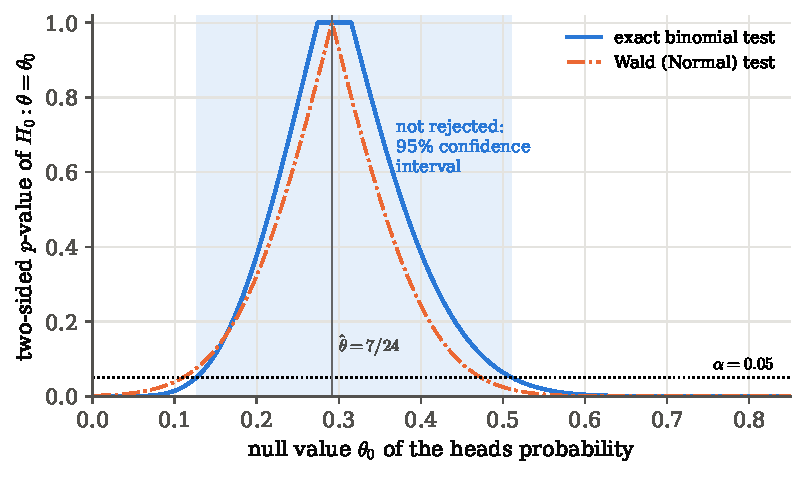
\includegraphics[width=0.85\linewidth]{figures/ch04/pvalue_function.pdf}
\caption{The two-sided p-value of $\theta=\theta_0$ for $7$ successes in $24$
trials, as a function of the hypothesised $\theta_0$. The solid curve uses the
exact binomial tails, the dash-dotted one the Normal (Wald) approximation. Where
a curve stays above the dotted line at $\alpha=0.05$, the null value survives;
the shaded strip is the exact $95\%$ confidence interval. The Wald curve is
symmetric about $\hat\theta$ and shifted to the left of the exact one.}
\label{4b:fig:pvalue-function}
\end{figure}

\paragraph{Two cheaper intervals for the same data.}
The exact interval needs a root finder. Two shortcuts avoid it. The first,
the Normal (Wald) interval, treats the observed fraction $\hat\theta=z/N$ as
Gaussian with mean $\theta$ and estimated standard error
$\widehat{\rm se}=\sqrt{\hat\theta(1-\hat\theta)/N}$. Its coverage is right
only in the large-sample limit \mainref{Thm.~6.16}. To see why, write
$\hat\theta_n$ for the estimate from $n$ trials and suppose
$(\hat\theta_n-\theta)/\widehat{\rm se}$ tends in distribution to
$Z\sim\Normal(0,1)$ (here $Z$ is a standard normal variable, not the count).
Then
\begin{align}
  \Prob_\theta\bigl(\hat\theta_n-z_{\alpha/2}\widehat{\rm se}<\theta<\hat\theta_n+z_{\alpha/2}\widehat{\rm se}\bigr)
  &\eqby{1} \Prob_\theta\Bigl(-z_{\alpha/2}<\frac{\hat\theta_n-\theta}{\widehat{\rm se}}<z_{\alpha/2}\Bigr)
   \notag\\
  &\relby{2}{\longrightarrow} \Prob\bigl(-z_{\alpha/2}<Z<z_{\alpha/2}\bigr)
   \eqby{3} 1-\alpha .
  \label{4b:eq:wald-ci}
\end{align}
\begin{explain}
  \item The same rearrangement of inequalities as in
        \eqref{4b:eq:normal-inversion}, now with $\hat\theta_n$ and
        $\widehat{\rm se}$.
  \item Convergence in distribution: probabilities of intervals converge to
        those of the limit.
  \item The definition of $z_{\alpha/2}$ puts $\alpha/2$ in each tail.
\end{explain}
For the trigger, $\widehat{\rm se}=\FourBKrSe$ and the interval is
$[\FourBKrWaldLo,\FourBKrWaldHi]$. It is symmetric about $\hat\theta$, while
the exact one reaches further up, because a binomial with $\theta$ below one half
has a longer right tail. The second shortcut, from Hoeffding's inequality, gives
a third interval,
$\hat\theta\pm\epsilon_N$ with $\epsilon_N^2=\ln(2/\alpha)/(2N)$, which covers
with probability at least $1-\alpha$ for \emph{every} $N$, not just in the
limit \mainref{Ex.~6.15}. Here $\epsilon_N=\FourBKrHoefEps$ and the interval
is $[\FourBKrHoefLo,\FourBKrHoefHi]$, almost twice as long. That is the price
of a guarantee that uses nothing about the binomial except that each trial is
between $0$ and $1$. So the trade is: the Normal interval is shorter, but its
coverage is only approximately right \mainref{Ex.~6.17}. How far off it is, we
measure in \cref{4b:sec:coverage}.

\paragraph{Example: inverting a likelihood-ratio test.}
Test inversion works with any test, including the likelihood-ratio test.
Casella and Berger take $n$ lifetimes from an exponential distribution with
mean $\lambda$ \srcref{CasellaBerger}{Ex.~9.2.3}. The likelihood is
$\lambda^{-n}e^{-\sum x_i/\lambda}$, it is largest at $\hat\lambda=\sum x_i/n$,
and the ratio of the likelihood at $\lambda_0$ to its maximum is
\begin{align}
  \frac{\lambda_0^{-n}e^{-\sum x_i/\lambda_0}}{\hat\lambda^{-n}e^{-n}}
  &\eqby{1} \Bigl(\frac{\sum x_i}{n\lambda_0}\Bigr)^{n}e^{\,n}\,e^{-\sum x_i/\lambda_0} .
  \label{4b:eq:exp-lrt}
\end{align}
\begin{explain}
  \item Insert $\hat\lambda=\sum x_i/n$ in the denominator, so that
        $e^{-\sum x_i/\hat\lambda}=e^{-n}$, and collect powers.
\end{explain}
The test retains $\lambda_0$ when this ratio is large, above some threshold
$k$. Write $T=\sum x_i/\lambda_0$. Then the ratio is $(T/n)^n e^{n}e^{-T}$, so
the condition is $T^ne^{-T}\ge k^*$, where the constant $n^n/e^n$ has been moved
into the new threshold $k^*=kn^n/e^n$. The function $T^ne^{-T}$ rises and then
falls, so it is above a level exactly on a stretch $b\le T\le a$ whose ends have
equal height, $a^ne^{-a}=b^ne^{-b}$. Solving $b\le\sum x_i/\lambda_0\le a$ for
$\lambda_0$ gives the interval $\sum x_i/a\le\lambda\le\sum x_i/b$.

\emph{Its coverage.} The interval covers the true $\lambda$ exactly when
$T=\sum X_i/\lambda$ lies between $b$ and $a$. Each $X_i/\lambda$ is
exponential with mean one, whatever $\lambda$ is, so $T$ is a sum of $n$
exponentials of mean one, a $\mathrm{Gamma}(n,1)$ variable, with the same
distribution for every $\lambda$. For $n=2$ its density is $te^{-t}$, and
\begin{align}
  \Prob(b\le T\le a)
  &\eqby{1} \int_b^a te^{-t}\,\dd t
   \eqby{2} \bigl[-te^{-t}\bigr]_b^a+\int_b^a e^{-t}\,\dd t
   \eqby{3} e^{-b}(b+1)-e^{-a}(a+1) .
  \label{4b:eq:exp-coverage}
\end{align}
\begin{explain}
  \item The $\mathrm{Gamma}(2,1)$ density.
  \item Integration by parts with $u=t$, $\dd v=e^{-t}\dd t$.
  \item Evaluate both terms and collect.
\end{explain}
Requiring $0.90$ and $a^2e^{-a}=b^2e^{-b}$ at the same time gives $a=5.480$,
$b=0.441$ and a confidence coefficient of $0.90006$. As a check:
$e^{-0.441}\times1.441=0.9272$ and $e^{-5.480}\times6.480=0.0270$, whose
difference is $0.900$; and $5.480^2e^{-5.480}=0.125=0.441^2e^{-0.441}$. The
interval for two lifetimes is $[\sum x_i/5.48,\ \sum x_i/0.441]$, a factor of
twelve wide.

The exponential example worked so smoothly because $T=\sum X_i/\lambda$ has a
distribution that does not depend on $\lambda$. Such a function of data and
parameter is called a \newterm{pivot} \srcref{CasellaBerger}{Def.~9.2.6}.
$(\bar X-\mu)/(\sigma/\sqrt n)$ is a pivot for a Gaussian mean, and
$(\bar X-\mu)/(S/\sqrt n)$, with the sample standard deviation $S$, is a pivot
with a Student $t_{n-1}$ distribution when $\sigma$ is unknown. A pivot gives
an interval whose coverage is the same for every parameter value, and the
coverage can be computed once. Without a pivot, as for the binomial, coverage
depends on $\theta$, and we have to check it everywhere
(\cref{4b:sec:coverage}).

\paragraph{One-sided limits.}
Inverting one-sided tests gives one-sided intervals. To get an \emph{upper}
bound for a Gaussian mean with unknown $\sigma$, test $\mu=\mu_0$ against
$\mu<\mu_0$. The level-$\alpha$ test rejects when
$(\bar x-\mu_0)/(s/\sqrt n)<-t_{n-1,\alpha}$, so it retains when
$\mu_0\le\bar x+t_{n-1,\alpha}s/\sqrt n$, and the survivors form
$(-\infty,\ \bar x+t_{n-1,\alpha}s/\sqrt n]$ \srcref{CasellaBerger}{Ex.~9.2.4}.
The alternative decides the shape: an alternative of \emph{small} values
rejects large $\mu_0$, and what survives is everything below a bound. Upper
limits on signal rates in searches are built this way (\cref{4b:sec:boundary}).

\subsection{Tests and intervals give the same verdict}
\label{4b:sec:duality}

Wasserman states the special case of test inversion that practitioners use
every day \mainref{Thm.~10.10}: the size-$\alpha$ Wald test rejects
$\theta=\theta_0$ exactly when $\theta_0$ lies outside
$\hat\theta\pm z_{\alpha/2}\widehat{\rm se}$. It is \eqref{4b:eq:normal-inversion}
with $\widehat{\rm se}$ in place of $\sigma/\sqrt n$. Checking whether a null
value is inside a $95\%$ interval \emph{is} a test at the $5\%$ level.

The interval carries more information than the verdict, and that answers a
common confusion between statistical and scientific significance
\mainref{p.~155}. \Cref{4b:fig:significance} shows two intervals that both
exclude $\theta_0$, so both tests reject. In the first, the whole interval sits
close to $\theta_0$: the effect is real but tiny, perhaps too small to matter.
In the second, the interval is far away: the effect is large. A p-value alone
cannot tell these apart; the interval can. A $3\times10^{-4}$ shift in a
calibration constant can be ``highly significant'' with enough data and still
irrelevant to every physics result that uses the constant.

\begin{figure}[htbp]
\centering
\begin{tikzpicture}[x=1cm,y=1cm]
  \foreach \yy/\lo/\hi/\lab in {1.3/0.35/1.05/{small effect},0/2.6/4.4/{large effect}}{
    \draw[->,black!60] (-0.6,\yy) -- (5.4,\yy) node[right,font=\small] {$\theta$};
    \draw[bdryred,thick] (0,\yy-0.2) -- (0,\yy+0.2);
    \node[font=\small,bdryred,anchor=north] at (0,\yy-0.22) {$\theta_0$};
    \draw[formblue,line width=2.4pt] (\lo,\yy) -- (\hi,\yy);
    \fill[formblue] ({(\lo+\hi)/2},\yy) circle (2.2pt);
    \node[font=\footnotesize,anchor=south] at ({(\lo+\hi)/2},\yy+0.12) {\lab};
  }
\end{tikzpicture}
\caption{Statistical versus scientific significance. Both $95\%$ intervals
(blue bars, dots at the estimates) exclude the null value $\theta_0$, so both
data sets reject $\Hnull$ at the $5\%$ level. In the top row the effect is
close to $\theta_0$ and may not matter in practice; in the bottom row it is
large. The interval reports the size of the effect; the test only reports that
it is not zero.}
\label{4b:fig:significance}
\end{figure}

\subsection{The interval inherits the test's intentions}
\label{4b:sec:ci-intentions}

The first part of the chapter found that a p-value depends on the stopping
rule: the same $7$ heads in $24$ flips gave different p-values when the
experimenter meant to stop at $N=24$, at $z=7$, or when time ran out. An
interval built from those tests inherits the dependence. Kruschke works out the
$95\%$ intervals for the four intentions \srcref{Kruschke}{pp.~318--321}:
\begin{center}
\begin{tabular}{lc}
\toprule
intention of the experimenter & $95\%$ confidence interval for $\theta$ \\
\midrule
stop after $N=24$ trials & $[0.126,\ 0.511]$ \\
stop after $z=7$ successes & $[0.126,\ 0.484]$ \\
stop when the time is up & $[0.135,\ 0.497]$ \\
test two coins, each with fixed $N$ & $[0.110,\ 0.539]$ \\
\bottomrule
\end{tabular}
\end{center}
The data are identical in all four rows. What differs is the cloud of
experiments that \emph{could} have happened, and a confidence interval, like a
p-value, is a statement about that cloud. For a trigger test this is not
academic. A run stopped ``when the beam went down'' has a random $N$, and
strictly its interval must be computed for that plan. \Cref{4b:sec:credible}
returns to this point: the Bayesian interval depends on the data only through
the likelihood and does not care why the experimenter stopped.

\paragraph{Python.}
The inversion for the trigger is a few lines of
\pyname{code/ch04/11_test_inversion.py}.

\pyfile[firstline=29,lastline=45,label={4b:lst:inversion}]{code/ch04/11_test_inversion.py}{The exact binomial interval by test inversion}

The two functions are the tails in \eqref{4b:eq:clopper}:
\pyname{binom.cdf(z, N, t)} is $\Prob(Z\le z)$ and \pyname{binom.sf(z - 1, N, t)} is
$\Prob(Z\ge z)$ (the survival function is a strict inequality, hence the
$z-1$). The p-value function is twice the smaller tail, capped at one. The
interval ends come from a root finder: \pyname{brentq} solves ``tail $=\alpha/2$''
on the side of $\hat\theta$ where that tail is the one that shrinks. The last
lines check the result against a closed form. Integrating the beta density by
parts $z$ times shows that $\Prob(Z\ge z\given\theta)$ equals the probability that
a $\mathrm{Beta}(z,N-z+1)$ variable is below $\theta$, so $\theta_L$ is a beta
quantile, and similarly for $\theta_U$; the assertion confirms that the root
finder and the identity agree to $10^{-6}$.

\begin{pitfall}[``The parameter is in the interval with probability 95\%'']
After the experiment the interval is two numbers, $[\FourBKrLo,\FourBKrHi]$, and
the efficiency is one number. Either it is inside or it is not; in the
frequentist framework the probability is $0$ or $1$, and we do not know which
\srcref{Cowan}{p.~123}. The $95\%$ belongs to the recipe that produced the two
numbers. Saying ``the efficiency lies in $[0.126, 0.511]$ with probability
$95\%$'' is a statement about $\theta$ given the data, an inference-direction
statement, and it needs a prior (\cref{4b:sec:credible}, \cref{ch:05}).
\end{pitfall}
\section{The Neyman construction: a belt of acceptance regions}
\label{4b:sec:neyman}

A calorimeter measures the energy of a jet. The estimate $\hat\theta$ it
returns is not Gaussian: at low energy the response is skewed, at high energy
it is wider, and the shape of the scatter changes with the true energy
$\theta$. From test beams or simulation we know, for every true $\theta$, the
distribution $g(\hat\theta;\theta)$ of the estimate. We see one number,
$\hat\theta_{\rm obs}$, and want an interval for $\theta$ that covers the true
energy in, say, $68.3\%$ of repeated measurements, whatever that energy is.

Test inversion (\cref{4b:sec:inversion-theorem}) already tells us what to do.
For every $\theta$, choose a set of $\hat\theta$ values that has probability
$1-\alpha$ under $g(\cdot;\theta)$. Then collect the $\theta$ whose set contains
the observation. Drawing all those sets at once on one graph is Neyman's
construction of 1937 \srcref{Cowan}{\S9.2}, \cite{FeldmanCousins1998}. Every
other frequentist interval in this chapter is a special case of it, or a
shortcut to it.

\paragraph{The question in words.}
Given only the family of sampling distributions $g(\hat\theta;\theta)$:
how do we draw a region in the (data, parameter) plane that yields, for any
observed $\hat\theta$, an interval with guaranteed coverage? And how does the
recipe look for the two workhorses, a Gaussian estimate and a Poisson count?

\subsection{The construction, step by step}
\label{4b:sec:belt}

We use the convention of Feldman and Cousins: the measured quantity on the
horizontal axis, the parameter on the vertical axis \cite{FeldmanCousins1998}.

\begin{enumerate}[label=\textbf{Step \arabic*.},leftmargin=*]
  \item \emph{For one hypothetical $\theta$, pick an acceptance interval.}
        Along the horizontal line at height $\theta$, choose
        $[v_\beta(\theta),u_\alpha(\theta)]$ such that the estimate falls above
        $u_\alpha$ with probability $\alpha$ and below $v_\beta$ with
        probability $\beta$ \srcref{Cowan}{(9.1)--(9.2)}:
        \begin{equation}
          \alpha=\int_{u_\alpha(\theta)}^{\infty}g(\hat\theta;\theta)\,\dd\hat\theta,
          \qquad
          \beta=\int_{-\infty}^{v_\beta(\theta)}g(\hat\theta;\theta)\,\dd\hat\theta .
          \label{4b:eq:belt-edges}
        \end{equation}
        \emph{Why legitimate?} We only used $g(\cdot;\theta)$, which we know
        for every $\theta$ by assumption. The data play no role yet.
  \item \emph{Repeat for every $\theta$.} The horizontal intervals sweep out a
        region, the \newterm{confidence belt}, bounded by the curves
        $v_\beta(\theta)$ on the left and $u_\alpha(\theta)$ on the right. For
        every $\theta$, by construction,
        $\Prob\bigl(v_\beta(\theta)\le\hat\theta\le u_\alpha(\theta)\bigr)=1-\alpha-\beta$
        \srcref{Cowan}{(9.3)}.
  \item \emph{Do the experiment, draw a vertical line at $\hat\theta_{\rm
        obs}$.} The confidence interval $[a,b]$ is the set of $\theta$ whose
        horizontal interval is cut by the line.
        \emph{Why legitimate?} This is \eqref{4b:eq:inversion}: the horizontal
        interval at $\theta$ is the acceptance region of a test of $\theta$,
        and the vertical cut collects the values not rejected.
\end{enumerate}

\emph{Why does the result cover?} \Cref{4b:fig:belt} shows it. Suppose the
truth is $\theta_{\rm true}$, a height on the graph that we do not know.
\begin{itemize}[itemsep=1pt,leftmargin=1.2em]
  \item The interval contains $\theta_{\rm true}$ exactly when the vertical
        line at $\hat\theta_{\rm obs}$ cuts the horizontal segment at height
        $\theta_{\rm true}$.
  \item That happens exactly when $\hat\theta_{\rm obs}$ falls inside that
        segment.
  \item By Step~1, the estimate falls inside the segment at the true height
        with probability $1-\alpha-\beta$.
\end{itemize}
So the coverage equals the probability inside the horizontal segment at the
true value. We made that $1-\alpha-\beta$ at every height, so it holds whatever
the truth is.

\begin{figure}[htbp]
\centering
\begin{tikzpicture}[x=1.05cm,y=1.05cm]
  \fill[formblue!10] (-0.6,0) -- (0.9,0) -- (6.9,5) -- (3.4,5) -- cycle;
  \draw[formblue,thick] (-0.6,0) -- (3.4,5);
  \draw[formblue,thick] (0.9,0) -- (6.9,5);
  \draw[->,thick,black!70] (-1,0) -- (7.3,0) node[below left] {estimate $\hat\theta$};
  \draw[->,thick,black!70] (-1,0) -- (-1,5.4) node[above right] {parameter $\theta$};
  \node[formblue,font=\footnotesize,anchor=east] at (2.4,3.75) {$v_\beta(\theta)$};
  \node[formblue,font=\footnotesize,anchor=west] at (5.8,4.05) {$u_\alpha(\theta)$};
  \foreach \t in {0.5,1.5,3.5}{
    \draw[formblue!60,line width=1.3pt] ({0.8*\t-0.6},\t) -- ({1.2*\t+0.9},\t);
  }
  \draw[fibreorange,line width=2.2pt] (1.4,2.5) -- (3.9,2.5);
  \draw[black!40,dashed] (-1,2.5) -- (1.4,2.5);
  \node[anchor=east,font=\small] at (-1,2.5) {$\theta_{\rm true}$};
  \draw[black!60,dashed] (3,0) -- (3,5.2);
  \draw[tangentgreen,line width=2.2pt] (3,1.75) -- (3,4.5);
  \node[anchor=north,font=\small] at (3,0) {$\hat\theta_{\rm obs}$};
  \fill[tangentgreen!70!black] (3,1.75) circle (1.6pt);
  \fill[tangentgreen!70!black] (3,4.5) circle (1.6pt);
  \node[anchor=west,font=\small,tangentgreen!60!black] at (3.08,1.62) {$a$};
  \node[anchor=east,font=\small,tangentgreen!60!black] at (2.92,4.62) {$b$};
\end{tikzpicture}
\caption{A confidence belt. For each hypothetical $\theta$ (vertical axis) the
horizontal segment holds the estimates that are accepted, with probability
$1-\alpha-\beta$; a few are drawn, and the one at the true value is orange. The
vertical line at the observed estimate cuts the belt between $a$ and $b$ (green):
that is the confidence interval. The lower end $a$ comes from the right edge of
the belt, the upper end $b$ from the left edge. The green interval contains
$\theta_{\rm true}$ exactly when the observed estimate lies on the orange
segment.}
\label{4b:fig:belt}
\end{figure}

\begin{workdef}[confidence belt]
For each parameter value $\theta$ an \newterm{acceptance interval}
$[v_\beta(\theta),u_\alpha(\theta)]$ of the estimate, with probability
$1-\alpha-\beta$ under $g(\hat\theta;\theta)$. The union over $\theta$ is the
\newterm{confidence belt}. The interval for an observation is the vertical cut
of the belt at $\hat\theta_{\rm obs}$.
\emph{Operational recipe:} on a grid of $\theta$, compute the acceptance
interval from the known (or simulated) distribution of the estimate; for the
observed value, keep every grid point whose interval contains it.
\end{workdef}

\paragraph{The same thing with inverse functions.}
If the estimator is a good one, both edges increase with $\theta$: a larger
true value gives larger estimates. Then they can be inverted,
$a(\hat\theta)\equiv u_\alpha^{-1}(\hat\theta)$ and
$b(\hat\theta)\equiv v_\beta^{-1}(\hat\theta)$ \srcref{Cowan}{(9.4)}, and the
coverage follows in two lines. Fix the true $\theta$. Then
\begin{align}
  \Prob\bigl(a(\hat\theta)\ge\theta\bigr)
  &\eqby{1} \Prob\bigl(\hat\theta\ge u_\alpha(\theta)\bigr)
   \eqby{2} \alpha ,
  \qquad
  \Prob\bigl(b(\hat\theta)\le\theta\bigr)
   \eqby{3} \Prob\bigl(\hat\theta\le v_\beta(\theta)\bigr)
   \eqby{4} \beta ,
  \notag\\
  \Prob\bigl(a(\hat\theta)<\theta<b(\hat\theta)\bigr)
  &\eqby{5} 1-\alpha-\beta .
  \label{4b:eq:belt-coverage}
\end{align}
\begin{explain}
  \item $u_\alpha$ is increasing, so applying it to both sides of
        $a(\hat\theta)\ge\theta$ preserves the inequality, and
        $u_\alpha(a(\hat\theta))=\hat\theta$ by the definition of the inverse.
  \item The definition of $u_\alpha$ in \eqref{4b:eq:belt-edges}.
  \item The same step for $v_\beta$ and $b$.
  \item The definition of $v_\beta$.
  \item The two ``miss'' events cannot happen together, because $a<b$ (the
        right edge of the belt lies to the right of the left edge), so the
        probability of a hit is one minus the sum of the two.
\end{explain}
The random quantities are $a$ and $b$: they depend on $\hat\theta$. Repeated
experiments give different intervals, and a fraction $1-\alpha-\beta$ of them
contain the fixed $\theta$ \srcref{Cowan}{p.~121}.

In practice we find $a$ and $b$ without drawing the belt. By the definition of
the inverses, $u_\alpha(a)=\hat\theta_{\rm obs}$ and $v_\beta(b)=\hat\theta_{\rm
obs}$. Putting these into \eqref{4b:eq:belt-edges}, at $\theta=a$ for the first
integral and $\theta=b$ for the second, gives \srcref{Cowan}{(9.9)}
\begin{equation}
  \alpha=\int_{\hat\theta_{\rm obs}}^{\infty}g(\hat\theta;a)\,\dd\hat\theta,
  \qquad
  \beta=\int_{-\infty}^{\hat\theta_{\rm obs}}g(\hat\theta;b)\,\dd\hat\theta .
  \label{4b:eq:belt-ends}
\end{equation}
In words: the lower end $a$ is the parameter value for which an estimate as
large as the one observed, or larger, would occur with probability $\alpha$;
the upper end $b$ is the value for which an estimate this small or smaller
would occur with probability $\beta$. Each end is a one-sided test with
p-value exactly $\alpha$ (or $\beta$). Beware of the names here. The p-value of
the test of $\theta=a$ is $\alpha$, a small number. The confidence level of the
limit $\theta\ge a$ is $1-\alpha$, a large one. To keep them apart we say
``confidence level'' only for the coverage of an interval and ``p-value'' only
for tests \srcref{Cowan}{pp.~122--123}.

\paragraph{Central and one-sided.}
The recipe leaves one choice free: how to split the excluded probability
between the two sides. If the total excluded probability is $\gamma$, then
$\alpha=\beta=\gamma/2$ gives a \newterm{central} interval of level
$1-\gamma$. $\beta=0$ gives a lower limit, $\alpha=0$ an upper limit. A
central interval has equal probabilities of missing on either side; it need not
be symmetric about the estimate. And the choice must be made \emph{before}
looking at the data. \Cref{4b:sec:boundary} shows what goes wrong when the data
decide it.

\subsection{Gaussian estimate: the error bar is a 68.3\% interval}
\label{4b:sec:belt-gauss}

When $g(\hat\theta;\theta)$ is Gaussian with mean $\theta$ and known standard
deviation $\sigma_{\hat\theta}$, the cumulative distribution is
$G(\hat\theta;\theta)=\Phi\bigl((\hat\theta-\theta)/\sigma_{\hat\theta}\bigr)$
\srcref{Cowan}{(9.10)}. Then \eqref{4b:eq:belt-ends} can be solved in closed
form:
\begin{align}
  \alpha
  &\eqby{1} 1-\Phi\Bigl(\frac{\hat\theta_{\rm obs}-a}{\sigma_{\hat\theta}}\Bigr)
  \ \Longrightarrow\
  a \eqby{2} \hat\theta_{\rm obs}-\sigma_{\hat\theta}\,\Phi^{-1}(1-\alpha),
  \notag\\
  \beta
  &\eqby{3} \Phi\Bigl(\frac{\hat\theta_{\rm obs}-b}{\sigma_{\hat\theta}}\Bigr)
  \ \Longrightarrow\
  b \eqby{4} \hat\theta_{\rm obs}-\sigma_{\hat\theta}\,\Phi^{-1}(\beta)
    \eqby{5} \hat\theta_{\rm obs}+\sigma_{\hat\theta}\,\Phi^{-1}(1-\beta).
  \label{4b:eq:gauss-ends}
\end{align}
\begin{explain}
  \item The upper tail beyond $\hat\theta_{\rm obs}$ of a Gaussian centred on
        $a$.
  \item Solve: $\Phi\bigl((\hat\theta_{\rm obs}-a)/\sigma\bigr)=1-\alpha$, apply
        $\Phi^{-1}$ and rearrange.
  \item The lower tail below $\hat\theta_{\rm obs}$ of a Gaussian centred on $b$.
  \item Apply $\Phi^{-1}$ and rearrange.
  \item Symmetry of the Gaussian: $\Phi^{-1}(\beta)=-\Phi^{-1}(1-\beta)$.
\end{explain}
With $\alpha=\beta=0.1587$, $\Phi^{-1}(1-\alpha)=1$ and the $68.3\%$ central
interval is $\hat\theta_{\rm obs}\pm\sigma_{\hat\theta}$ \srcref{Cowan}{(9.13)}.
This is the precise sense in which a ``one-sigma error bar'' is a confidence
interval. The standard quantiles, which every physicist ends up knowing by
heart \srcref{Cowan}{Tables~9.1--9.2}:
\begin{center}
\begin{tabular}{ccc@{\qquad}ccc}
\toprule
\multicolumn{3}{c}{central, $1-\gamma$} & \multicolumn{3}{c}{one-sided, $1-\alpha$}\\
\cmidrule(r){1-3}\cmidrule(l){4-6}
$\Phi^{-1}(1-\gamma/2)$ & $1-\gamma$ & & $\Phi^{-1}(1-\alpha)$ & $1-\alpha$ & \\
\midrule
$1$ & $0.6827$ & & $1$ & $0.8413$ &\\
$2$ & $0.9544$ & & $2$ & $0.9772$ &\\
$3$ & $0.9973$ & & $3$ & $0.9987$ &\\
$1.645$ & $0.90$ & & $1.282$ & $0.90$ &\\
$1.960$ & $0.95$ & & $1.645$ & $0.95$ &\\
$2.576$ & $0.99$ & & $2.326$ & $0.99$ &\\
\bottomrule
\end{tabular}
\end{center}
The number $1.645$ appears twice: it is the central $90\%$ quantile and the
one-sided $95\%$ one. This coincidence matters when a parameter sits at a
physical boundary (\cref{4b:sec:boundary}).

Physicists use the same convention, the $68.3\%$ central interval, for error
bars even when $g$ is not Gaussian. The interval is then no longer symmetric,
and the result is quoted as $\hat\theta^{+d}_{-c}$, meaning $a=\hat\theta-c$ and
$b=\hat\theta+d$. For example, $5.79^{+0.32}_{-0.25}$ means: the recipe that
produced $[5.54,6.11]$ covers the true value in $68.3\%$ of repeated
experiments, with equal chances of missing high and low. It does not mean that $\theta$ lies in $[5.54,6.11]$ with
probability $68.3\%$ \srcref{Cowan}{p.~123}. When $\sigma_{\hat\theta}$ is itself
estimated from the data, the pivot becomes Student's $t$; for large samples the
Gaussian recipe with the estimated $\hat\sigma$ is fine, for small ones it is
not, and \cref{4b:sec:coverage} measures by how much.

\subsection{Poisson counts: a belt with steps}
\label{4b:sec:belt-poisson}

A count $n$ of rare events is Poisson with mean $\nu$, and the estimate is
$\hat\nu=n$ \srcref{Cowan}{(9.14)}. \emph{What changes:} the estimate now takes
only integer values. So \eqref{4b:eq:belt-edges} cannot be satisfied exactly.
The tail probability beyond an integer changes in jumps from one integer to the
next, and for a given $\alpha$ there is usually no integer $u_\alpha(\nu)$ whose
tail is exactly $\alpha$. \emph{The fix:} keep the end conditions
\eqref{4b:eq:belt-ends}, and count the observed value as part of each tail
\srcref{Cowan}{(9.15)--(9.16)}:
\begin{equation}
  \alpha=\Prob(n\ge n_{\rm obs};a)=1-\sum_{n=0}^{n_{\rm obs}-1}\frac{a^n}{n!}e^{-a},
  \qquad
  \beta=\Prob(n\le n_{\rm obs};b)=\sum_{n=0}^{n_{\rm obs}}\frac{b^n}{n!}e^{-b}.
  \label{4b:eq:poisson-ends}
\end{equation}
These can be solved numerically. There is also a closed form, because the
Poisson cumulative sum is a $\chi^2$ tail \srcref{Cowan}{(9.17)}:
\begin{equation}
  \sum_{n=0}^{k}\frac{\nu^n}{n!}e^{-\nu}
  =\int_{2\nu}^{\infty}f_{\chi^2}\bigl(z;\,2(k+1)\bigr)\,\dd z ,
  \qquad
  f_{\chi^2}(z;m)=\frac{z^{m/2-1}e^{-z/2}}{2^{m/2}\,\Gamma(m/2)} .
  \label{4b:eq:poisson-chi2}
\end{equation}
To prove the identity, we show that the two sides start at the same value and
change at the same rate. Call the left side $F(\nu)$ and the right side
$H(\nu)$. Both equal one at $\nu=0$: on the left only the $n=0$ term survives,
and on the right the whole $\chi^2$ density is integrated. Their derivatives
are
\begin{align}
  F'(\nu)
  &\eqby{1} \sum_{n=0}^{k}\Bigl(\frac{n\nu^{n-1}}{n!}-\frac{\nu^n}{n!}\Bigr)e^{-\nu}
   \eqby{2} \sum_{n=1}^{k}\frac{\nu^{n-1}}{(n-1)!}e^{-\nu}-\sum_{n=0}^{k}\frac{\nu^{n}}{n!}e^{-\nu}
   \eqby{3} -\frac{\nu^{k}}{k!}e^{-\nu},
  \notag\\
  H'(\nu)
  &\eqby{4} -2\,f_{\chi^2}\bigl(2\nu;\,2k+2\bigr)
   \eqby{5} -2\,\frac{(2\nu)^{k}e^{-\nu}}{2^{k+1}\,k!}
   \eqby{6} -\frac{\nu^{k}}{k!}e^{-\nu}.
  \label{4b:eq:poisson-chi2-proof}
\end{align}
\begin{explain}
  \item Product rule on $\nu^ne^{-\nu}$.
  \item Cancel $n$ against $n!$ in the first sum; its $n=0$ term is zero.
  \item Shift $n-1\to n$ in the first sum: it becomes the second sum without
        its last term, so everything cancels except $-\nu^ke^{-\nu}/k!$.
  \item Fundamental theorem of calculus, with the lower limit $2\nu$ whose
        derivative is $2$.
  \item Insert the density with $m=2k+2$: $z^{m/2-1}=(2\nu)^k$,
        $e^{-z/2}=e^{-\nu}$, $2^{m/2}=2^{k+1}$, $\Gamma(k+1)=k!$.
  \item Simplify $2\cdot2^k/2^{k+1}=1$.
\end{explain}
The two functions are equal at $\nu=0$ and have equal derivatives everywhere,
so they are equal for every $\nu$. Applying the identity to the two conditions
in \eqref{4b:eq:poisson-ends} (with $k=n_{\rm obs}-1$ for $a$ and
$k=n_{\rm obs}$ for $b$) turns each into a $\chi^2$ probability up to $2a$ or beyond $2b$, so the
limits are quantiles of $\chi^2$ distributions \srcref{Cowan}{(9.18)}:
\begin{equation}
  a=\tfrac12F^{-1}_{\chi^2}(\alpha;\,2n_{\rm obs}),
  \qquad
  b=\tfrac12F^{-1}_{\chi^2}(1-\beta;\,2(n_{\rm obs}+1)) ,
  \label{4b:eq:garwood}
\end{equation}
where $F^{-1}_{\chi^2}(p;m)$ is the $p$ quantile with $m$ degrees of freedom.
These are Garwood's intervals of 1936 \srcref{CasellaBerger}{Ex.~9.2.15}. For
$n$ independent Poisson observations of rate $\lambda$ the sum is
Poisson$(n\lambda)$, and the interval for $\lambda$ is \eqref{4b:eq:garwood}
divided by $n$; with $n=10$ observations summing to $6$, the $90\%$ interval is
$[\FourBCBlo,\ \FourBCBhi]$.\footnote{Casella and Berger print $0.262$ for the
lower end; $F^{-1}_{\chi^2}(0.05;12)/20=5.226/20=0.2613$.}

\paragraph{Example: zero events.}
If nothing is seen, $n_{\rm obs}=0$, there is no lower limit and the upper limit
solves $\beta=e^{-b}$, so $b=-\ln\beta$ \srcref{Cowan}{(9.20)}. At $95\%$,
$b=-\ln0.05=\FourBUpNinetyFiveZero\approx3$: if the mean were $3$, seeing
nothing would happen $5\%$ of the time. This ``rule of three'' is how a search
that sees no candidate events quotes its sensitivity. At $90\%$ it is
$\FourBUpNinetyZero$.

\paragraph{Example: the $90\%$ table.}
Script \pyname{code/ch04/12_neyman_poisson_belt.py} builds the belt by brute
force (for each $\nu$ on a grid, keep the counts whose two tails both exceed
$5\%$), reads off the intervals, and checks them against \eqref{4b:eq:garwood}:
\begin{center}
\small
\begin{tabular}{c*{11}{c}}
\toprule
$n_{\rm obs}$ & 0 & 1 & 2 & 3 & 4 & 5 & 6 & 7 & 8 & 9 & 10\\
\midrule
$a$ & $\FourBBeltLoZero$ & $\FourBBeltLoOne$ & $\FourBBeltLoTwo$ & $\FourBBeltLoThree$ & $\FourBBeltLoFour$ & $\FourBBeltLoFive$ & $\FourBBeltLoSix$ & $\FourBBeltLoSeven$ & $\FourBBeltLoEight$ & $\FourBBeltLoNine$ & $\FourBBeltLoTen$\\
$b$ & $\FourBBeltHiZero$ & $\FourBBeltHiOne$ & $\FourBBeltHiTwo$ & $\FourBBeltHiThree$ & $\FourBBeltHiFour$ & $\FourBBeltHiFive$ & $\FourBBeltHiSix$ & $\FourBBeltHiSeven$ & $\FourBBeltHiEight$ & $\FourBBeltHiNine$ & $\FourBBeltHiTen$\\
\bottomrule
\end{tabular}
\end{center}
These are the $\alpha=0.05$ and $\beta=0.05$ columns of Cowan's Table~9.3. The
belt is in \cref{4b:fig:poisson-belt}. Two features distinguish it from the
Gaussian one. The edges are staircases, because the acceptance set at each
$\nu$ is a set of integers. And the probability inside each horizontal set is
not $0.90$ but somewhere between $\FourBBeltMinAcc$ and $\FourBBeltMaxAcc$,
depending on $\nu$: adding the observed count to each tail makes each tail at
most $5\%$, so the interval covers at least $90\%$
\srcref{Cowan}{(9.19)}. Discreteness buys safety at the price of intervals that
are longer than they need to be for most $\nu$; \cref{4b:sec:coverage} maps the
over-coverage exactly.

\begin{figure}[htbp]
\centering
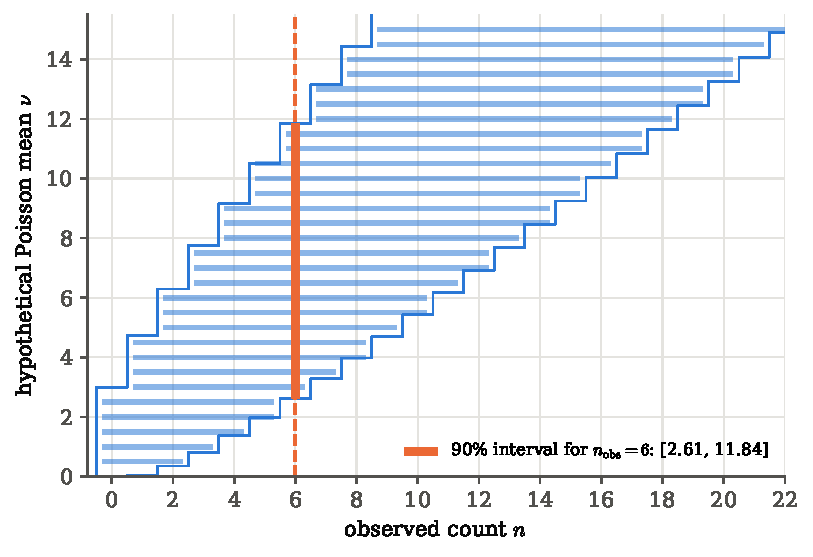
\includegraphics[width=0.8\linewidth]{figures/ch04/poisson_belt.pdf}
\caption{The $90\%$ central confidence belt for a Poisson mean, built by brute
force. Each horizontal bar is the set of counts accepted at one hypothetical
mean $\nu$ (bars drawn every $0.5$); the thin staircases are the edges of the
belt on the fine grid. The dashed vertical line at $n=6$ cuts the belt between
the two ends of the orange bar, the $90\%$ interval for six observed events.}
\label{4b:fig:poisson-belt}
\end{figure}

\paragraph{Python.}
The heart of the brute-force construction:

\pyfile[firstline=28,lastline=46,label={4b:lst:belt}]{code/ch04/12_neyman_poisson_belt.py}{The Poisson belt and its inversion}

\pyname{cdf} and \pyname{sf} are matrices, one row per hypothetical $\nu$ and
one column per count, holding $\Prob(N\le n)$ and $\Prob(N\ge n)$. The boolean
matrix \pyname{keep} marks the counts whose two tails are both larger than
$5\%$: each row is one horizontal acceptance set. Inverting is then a vertical
read: \pyname{interval_from_belt} collects every $\nu$ whose row contains the
observed count. The script then asserts that the brute-force interval equals
Garwood's formula to within the grid spacing, for $n_{\rm obs}=0,\dots,10$.

\subsection{When the estimate is not Gaussian: transform first}
\label{4b:sec:fisher-z}

For a non-Gaussian estimator we can always build the full belt. Sometimes a
change of variables makes that unnecessary. The textbook case is the
correlation coefficient $r$ of $n$ pairs from a two-dimensional Gaussian
\srcref{Cowan}{\S9.5}. Its distribution is skewed, the more so the closer the
true $\rho$ is to $\pm1$, and it is Gaussian only for very large $n$ (Cowan
quotes $n\gtrsim500$).

The trouble is that the spread of $r$ depends on the unknown $\rho$. Fisher's
idea is to transform $r$ so that it does not: a
\newterm{variance-stabilising transformation} \unpack{a function $g$ chosen so
that the variance of $g(r)$ no longer depends on $\rho$}. The variance of $r$
is approximately $(1-\rho^2)^2/n$ \srcref{Cowan}{(5.17)}. The delta method of
\cref{ch:03} (a smooth function of an estimate has variance $g'^2$ times the
estimate's variance) gives $\Var g(r)\approx g'(\rho)^2(1-\rho^2)^2/n$. This is
independent of $\rho$ if $g'(\rho)=1/(1-\rho^2)$:
\begin{align}
  g(\rho)
  &\eqby{1} \int\frac{\dd\rho}{1-\rho^2}
   \eqby{2} \frac12\int\Bigl(\frac1{1+\rho}+\frac1{1-\rho}\Bigr)\dd\rho
   \eqby{3} \frac12\ln\frac{1+\rho}{1-\rho}
   \eqby{4} \tanh^{-1}\rho .
  \label{4b:eq:fisher-z}
\end{align}
\begin{explain}
  \item Integrate the required derivative.
  \item Partial fractions: $1/(1-\rho^2)=\tfrac12[1/(1+\rho)+1/(1-\rho)]$.
  \item $\int\dd\rho/(1\pm\rho)=\pm\ln(1\pm\rho)$; choose the constant so that
        $g(0)=0$.
  \item The standard form of the inverse hyperbolic tangent.
\end{explain}
So $z=\tanh^{-1}r$ has variance close to $1/n$; a finer calculation gives
$1/(n-3)$ \srcref{Cowan}{(9.22)--(9.25)}, and $z$ is close to Gaussian much
sooner than $r$. The recipe: transform, build the Gaussian interval for
$\zeta=\tanh^{-1}\rho$, transform the ends back with $\tanh$.

\paragraph{Example: $r=0.5$ from $20$ pairs.}
The point first: the naive Gaussian interval claims a correlation, and the
transformed one does not. \emph{Naive.} The naive error
$\hat\sigma_r=(1-r^2)/\sqrt n=\FourBFzSigR$ makes $r$ look like a three-sigma
effect, and the naive $99\%$ interval $[\FourBFzNaiveLo,\FourBFzNaiveHi]$
excludes zero. \emph{Transformed.} Now $z=\tanh^{-1}0.5=\FourBFzZ$ and
$\sigma_z=1/\sqrt{n-3}=1/\sqrt{17}=\FourBFzSigZ$. The $99\%$ interval for
$\zeta$ is $[\FourBFzZetaLo,\FourBFzZetaHi]$, and applying $\tanh$ to its ends
gives $[\FourBFzRhoLo,\FourBFzRhoHi]$ for $\rho$: zero is inside
\srcref{Cowan}{p.~130}. The evidence for a correlation is much weaker than the
naive error suggests. Under
$\rho=0$ the naive Gaussian gives a one-sided probability of
$\FourBFzPnaive\%$ for $r\ge0.5$, the $z$ transformation gives
$\FourBFzPfisher\%$, and the exact calculation (under $\rho=0$,
$r\sqrt{n-2}/\sqrt{1-r^2}$ is Student $t$ with $n-2$ degrees of freedom, here
$t=\FourBFzT$) gives $\FourBFzPexact\%$.\footnote{Cowan quotes $2.3\%$ for
the $z$ transformation. We find $\FourBFzPfisher\%$ for the one-sided tail,
in agreement with the exact $t$ calculation; $2.3\%$ is close to the two-sided
value.} Which interval should we trust? A simulation of $10^5$ samples of $20$
pairs settles it. At $\rho=0.5$ the naive $99\%$ interval covers only
$\FourBFzCovNaiveFive$ of the time, the Fisher interval $\FourBFzCovFisherFive$;
at $\rho=0.8$, $\FourBFzCovNaiveEight$ against $\FourBFzCovFisherEight$.

\subsection{Intervals from the likelihood function}
\label{4b:sec:likelihood-interval}

The most widely used interval in physics needs no belt at all. In the large
sample limit, the maximum-likelihood estimator is Gaussian around the true
value with standard deviation $\sigma_{\hat\theta}$, and the likelihood itself
becomes a Gaussian function of $\theta$ around $\hat\theta$ with the same
width \srcref{Cowan}{(9.26)--(9.27)}; the equality of the two widths is the
Cram\'er--Rao bound becoming an equality (\cref{ch:03}). Then
\begin{align}
  \ln\Like(\hat\theta\pm N\sigma_{\hat\theta})
  &\eqby{1} \ln\Like_{\max}-\frac{(N\sigma_{\hat\theta})^2}{2\sigma_{\hat\theta}^2}
   \eqby{2} \ln\Like_{\max}-\frac{N^2}{2} .
  \label{4b:eq:dlnl}
\end{align}
\begin{explain}
  \item $\ln\Like(\theta)=\ln\Like_{\max}-(\theta-\hat\theta)^2/2\sigma_{\hat\theta}^2$
        for a Gaussian likelihood, evaluated at $\theta-\hat\theta=\pm N\sigma_{\hat\theta}$.
  \item Cancel $\sigma_{\hat\theta}^2$.
\end{explain}
So the $68.3\%$ interval is where $\ln\Like$ has dropped by $1/2$ from its
maximum, the $95.4\%$ interval where it has dropped by $2$, and in a
least-squares fit, where $\ln\Like=-\chi^2/2$, where $\chi^2$ has risen by $N^2$
\srcref{Cowan}{(9.28)--(9.30)}:
\begin{equation}
  \ln\Like\bigl(\hat\theta^{+d}_{-c}\bigr)=\ln\Like_{\max}-\frac{N^2}{2},
  \qquad
  \chi^2\bigl(\hat\theta^{+d}_{-c}\bigr)=\chi^2_{\min}+N^2 .
  \label{4b:eq:likelihood-interval}
\end{equation}
This prescription is used, and works well, even when $\ln\Like$ is not a
parabola. \emph{Why?} The reason is that the likelihood does not care how we
label the parameter. Suppose some monotone reparametrisation $\eta=h(\theta)$
makes the likelihood Gaussian in $\eta$. The likelihood is a function on parameter space, and its \emph{values}
do not change when we relabel the points: $\Like$ at the point called $\theta$
equals $\Like$ at the same point called $\eta=h(\theta)$. So the points where
$\ln\Like$ has dropped by $1/2$ are the same points in either labelling. In the
$\eta$ labelling they bound an exact $68.3\%$ interval; mapped back, they bound
an asymmetric interval in $\theta$ with the same coverage. So the recipe uses
the good parametrisation without our having to find it. But it is only as good
as the assumption that such an $h$ exists, and that is guaranteed only for
large samples. That is why the result is called a \emph{likelihood interval}:
it approximates the confidence interval, and is not one exactly
\srcref{Cowan}{p.~131}.

\paragraph{Example: five lifetimes.}
Take $n$ decay times $t_i$ from an exponential with mean $\tau$. With
$\hat\tau=\bar t$ and $u=\hat\tau/\tau$,
\begin{align}
  \ln\Like(\tau)-\ln\Like_{\max}
  &\eqby{1} \Bigl(-n\ln\tau-\frac{n\hat\tau}{\tau}\Bigr)-\bigl(-n\ln\hat\tau-n\bigr)
   \eqby{2} n\Bigl(\ln\frac{\hat\tau}{\tau}-\frac{\hat\tau}{\tau}+1\Bigr)
   \eqby{3} n\,(\ln u-u+1) .
  \label{4b:eq:exp-dlnl}
\end{align}
\begin{explain}
  \item $\ln\Like=\sum_i\ln(\tau^{-1}e^{-t_i/\tau})=-n\ln\tau-\sum_it_i/\tau$, and
        $\sum_it_i=n\hat\tau$; at the maximum $\tau=\hat\tau$ the second term
        is $-n$.
  \item Collect the logarithms.
  \item Definition of $u$.
\end{explain}
The drop depends on the data only through $u$, so the two roots of
$n(\ln u-u+1)=-\tfrac12$ are fixed numbers for each $n$: for $n=5$,
$u=\FourBLiUlo$ and $u=\FourBLiUhi$. The likelihood interval is
$[\hat\tau/\FourBLiUhi,\ \hat\tau/\FourBLiUlo]$ for \emph{every} sample of five.
For the sample simulated in \pyname{code/ch04/14_likelihood_intervals.py} with
true $\tau=1$, $\hat\tau=\FourBLiTauHat$ and the interval is
$[\FourBLiLo,\FourBLiHi]$, that is
$\hat\tau=\FourBLiTauHat^{+\FourBLiPlus}_{-\FourBLiMinus}$
(\cref{4b:fig:likelihood-interval}, left). Cowan's own sample gives
$0.85^{+0.52}_{-0.30}$ \srcref{Cowan}{Fig.~9.6}, the same ratios
$1.61$ and $0.65$ to $\hat\tau$, as the invariance predicts.

Because $u=\hat\tau/\tau$ is a pivot (it is a mean of five exponentials of
mean one, a $\mathrm{Gamma}(5,1/5)$ variable, whatever $\tau$ is), the coverage
of the likelihood interval can be computed exactly: it is
$\Prob(\FourBLiUlo\le U\le\FourBLiUhi)=\FourBLiCovFive$, against a nominal
$0.683$; a Monte Carlo of $2\times10^5$ experiments gives $\FourBLiCovFiveMC$.
The exact central interval for our sample, from the pivot
$2n\hat\tau/\tau\sim\chi^2_{2n}$, is $[\FourBLiExLo,\FourBLiExHi]$. The symmetric
interval $\hat\tau\pm\hat\tau/\sqrt n$ happens to have about the right total
coverage at $n=5$ ($\FourBSymCovFive$), but it distributes its misses badly: it
lies entirely below the truth in $\FourBSymMissBelow$ of experiments and entirely
above it in $\FourBSymMissAbove$, where a central interval would have $0.159$ on
each side. The likelihood interval splits them as $\FourBLiMissBelow$ and
$\FourBLiMissAbove$. \Cref{4b:fig:likelihood-interval} (right) shows how both
approach the nominal coverage as $n$ grows. With $n=50$ Cowan's symmetric
$1.06\pm0.15$ is fine; with $n=5$ the asymmetric likelihood interval is the
honest summary.

\begin{figure}[htbp]
\centering
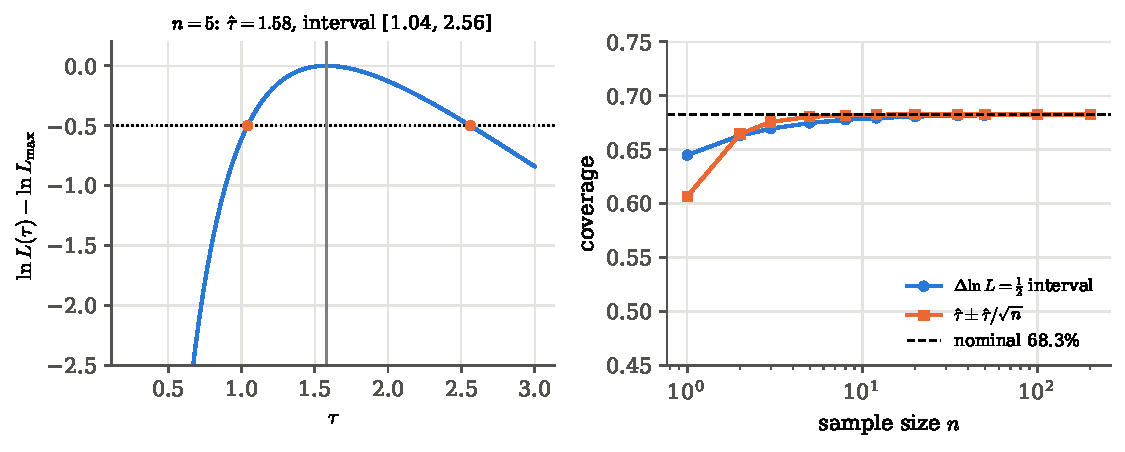
\includegraphics[width=\linewidth]{figures/ch04/likelihood_interval.pdf}
\caption{Left: the log-likelihood of five simulated decay times, relative to its
maximum, as a function of the mean lifetime $\tau$. It is not a parabola: it
falls steeply towards small $\tau$ and slowly towards large $\tau$. The dotted
line is the drop by $1/2$; its two crossings (orange) are the ends of the
likelihood interval. Right: the exact coverage of the $\Delta\ln\Like=\tfrac12$
interval and of the symmetric $\hat\tau\pm\hat\tau/\sqrt n$, as a function of
the sample size; both approach $68.3\%$.}
\label{4b:fig:likelihood-interval}
\end{figure}

\subsection{Several parameters: confidence regions}
\label{4b:sec:regions}

With $m$ parameters $\params=(\theta_1,\dots,\theta_m)$, the large-sample
estimators are jointly Gaussian with covariance $\Cmat$, and the likelihood is a
Gaussian function of $\params$ with the same $\Cmat$
\srcref{Cowan}{(9.31)--(9.33)}. Both are governed by the quadratic form
\begin{equation}
  Q(\hat\params,\params)=(\hat\params-\params)\T\Cmat^{-1}(\hat\params-\params),
  \label{4b:eq:Q}
\end{equation}
which is symmetric in its two arguments. The argument for a confidence region
takes three steps.
\begin{itemize}[itemsep=1pt,leftmargin=1.2em]
  \item \emph{Two readings of one form.} As a function of the estimate at fixed
        truth, the level sets of $Q$ are the ellipses of equal sampling
        density. As a function of the parameters at fixed estimate, they are
        the contours of equal likelihood.
  \item \emph{Its distribution.} At the true $\params$, $Q$ has a $\chi^2_m$
        distribution (\cref{ch:02}): whitening the Gaussian vector turns $Q$
        into a sum of $m$ squared independent standard normals. So
        $\Prob(Q\le Q_\gamma)=1-\gamma$ when
        $Q_\gamma=F^{-1}_{\chi^2}(1-\gamma;m)$, the $1-\gamma$ quantile.
  \item \emph{The symmetry.} ``The estimate is within $Q_\gamma$ of the
        truth'' and ``the truth is within $Q_\gamma$ of the estimate'' are the
        same event.
\end{itemize}
So the region $\{\params:Q(\hat\params,\params)\le Q_\gamma\}$ contains the
truth with probability $1-\gamma$: it is a $1-\gamma$ confidence region. In
practice it is found as the contour \srcref{Cowan}{(9.34)--(9.37)}
\begin{equation}
  \ln\Like(\params)=\ln\Like_{\max}-\frac{Q_\gamma}{2}
  \qquad\text{or}\qquad
  \chi^2(\params)=\chi^2_{\min}+Q_\gamma .
  \label{4b:eq:region}
\end{equation}
The thresholds grow with the number of parameters
\srcref{Cowan}{Tables~9.4--9.5}:
\begin{center}
\begin{tabular}{lccccc}
\toprule
$1-\gamma$ & $m=1$ & $m=2$ & $m=3$ & $m=4$ & $m=5$\\
\midrule
$0.683$ & $1.00$ & $2.30$ & $3.53$ & $4.72$ & $5.89$\\
$0.90$ & $2.71$ & $4.61$ & $6.25$ & $7.78$ & $9.24$\\
$0.95$ & $3.84$ & $5.99$ & $7.82$ & $9.49$ & $11.1$\\
$0.99$ & $6.63$ & $9.21$ & $11.3$ & $13.3$ & $15.1$\\
\bottomrule
\end{tabular}
\end{center}
For $m=1$, $Q_\gamma=N^2$ and the recipe is \eqref{4b:eq:likelihood-interval}.
For $m=2$ the familiar threshold no longer works. The $\Delta\chi^2=1$ contour,
which many plots label ``$1\sigma$'', contains the truth only $39.3\%$ of the
time; the $68.3\%$ region needs $\Delta\chi^2=2.30$. \Cref{4b:fig:ellipse} checks this with a straight-line fit to
ten points, repeated $2\times10^5$ times: the truth falls inside the
$\Delta\chi^2=1$ ellipse in $\FourBElCovOne$ of the experiments and inside the
$\Delta\chi^2=\FourBElQ$ ellipse in $\FourBElCovTwoThirty$. The interval for the
slope \emph{alone}, $\hat\theta_2\pm\sqrt{C_{22}}$, still covers $\FourBElCovSlope$:
a one-parameter question keeps its one-parameter threshold. This is how
cosmological constraints are drawn: the $68\%$ and $95\%$ contours in a plane
of two parameters, and one-dimensional intervals from the marginal or profile
of each (\cref{ch:09,ch:10}).

\begin{figure}[htbp]
\centering
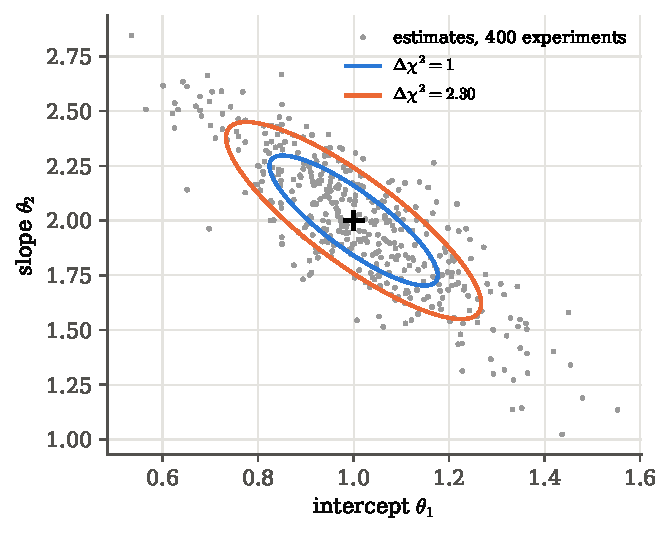
\includegraphics[width=0.6\linewidth]{figures/ch04/ellipse_coverage.pdf}
\caption{Two-parameter confidence regions for a straight-line fit. Grey dots:
the fitted (intercept, slope) from $400$ simulated experiments with the same
true line (cross). The negative tilt is the correlation of the two estimates
(correlation coefficient $\FourBElRho$). The inner ellipse, $\Delta\chi^2=1$,
holds about $39\%$ of the dots, the outer, $\Delta\chi^2=2.30$, about $68\%$.
The same ellipses drawn around any one estimate are its confidence regions.}
\label{4b:fig:ellipse}
\end{figure}

As in one dimension, the region is random and the parameters are fixed
\srcref{Cowan}{p.~135}. And as in one dimension, the $\chi^2_m$ calibration is
only asymptotic. For strongly non-Gaussian likelihoods the coverage of
\eqref{4b:eq:region} must be checked by simulation, as in
\cref{4b:sec:coverage}.
\section{Coverage is a property of the procedure}
\label{4b:sec:coverage}

A hundred groups around the world measure the same Gaussian mean, each with
$n=\FourBLadderN$ readings of known resolution, and each quotes the $95\%$
interval $\bar x\pm1.96\,\sigma/\sqrt n$. \Cref{4b:fig:ladder} shows what
happens in a simulation where we know the truth. The intervals jump up and
down with the data; the true value, the dashed line, stays put; and
$\FourBLadderMiss$ of the hundred intervals miss it. None of the hundred groups
can tell from its own interval whether it is one of the unlucky ones. The
$95\%$ is a property of the whole ladder, not of any rung.

\begin{figure}[htbp]
\centering
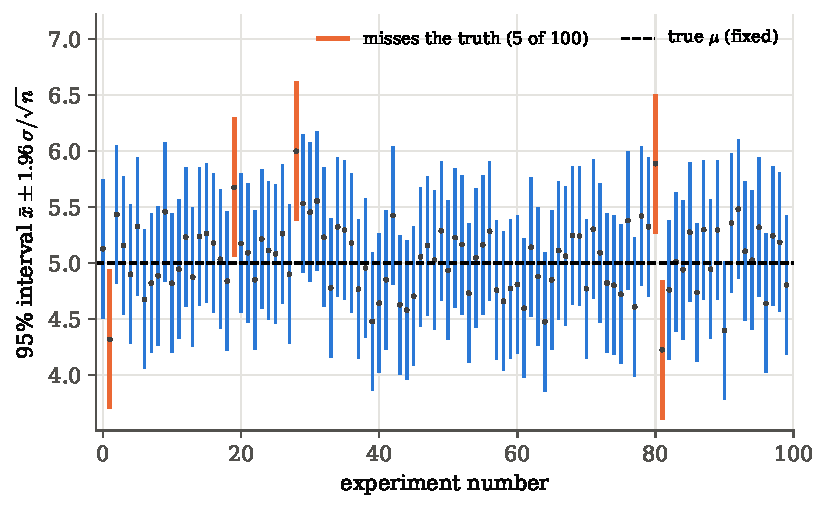
\includegraphics[width=0.85\linewidth]{figures/ch04/coverage_ladder.pdf}
\caption{A hundred simulated experiments, each quoting a $95\%$ interval for the
same Gaussian mean. The vertical bars are the intervals, the dots the sample
means, the dashed line the true value. The intervals move from experiment to
experiment; the truth does not. The orange bars are the intervals that miss it.}
\label{4b:fig:ladder}
\end{figure}

A confidence level is a promise about a \emph{recipe}: apply it to data
generated with any $\theta$, and it will contain that $\theta$ with the stated
probability. We can check by simulation whether a recipe keeps the promise. The
check finds three kinds of fault: recipes that cover less often than they
claim, recipes that cover more often than needed and so are too wide, and,
less obviously, recipes that are right on average but wrong in situations we
can recognise from the data.

\paragraph{The question in words.}
\begin{enumerate}[label=\arabic*.]
  \item For a given recipe, how does the coverage depend on the true parameter,
        and what is its worst case?
  \item Which common recipes undercover, which overcover, and why?
  \item Is the long-run coverage the right thing to know about the one interval
        we actually hold?
\end{enumerate}

\subsection{The coverage function}
\label{4b:sec:coverage-function}

For a recipe $\bm x\mapsto[a(\bm x),b(\bm x)]$ the \newterm{coverage function}
is $C(\theta)=\Prob_\theta\bigl(a(\bm X)\le\theta\le b(\bm X)\bigr)$. For
continuous data it is an integral, for counts a sum:
\begin{equation}
  C(\theta)=\int\mathbb 1\bigl[a(\bm x)\le\theta\le b(\bm x)\bigr]\,
            p(\bm x\given\theta)\,\dd\bm x ,
  \qquad
  C(\nu)=\sum_{n=0}^{\infty}\Prob(n\given\nu)\,\mathbb 1\bigl[a(n)\le\nu\le b(n)\bigr].
  \label{4b:eq:coverage-function}
\end{equation}
The indicator $\mathbb 1[\cdot]$ is one when the interval computed from $\bm x$
contains $\theta$ and zero otherwise. A recipe is \emph{exact} if
$C(\theta)=1-\alpha$ everywhere, it \newterm{undercovers} where $C(\theta)<1-\alpha$
and \newterm{overcovers} where $C(\theta)>1-\alpha$. A recipe that overcovers
somewhere and undercovers nowhere is called \newterm{conservative}
\cite{FeldmanCousins1998}. The confidence coefficient of
\cref{4b:sec:ci-def} is $\inf_\theta C(\theta)$.

\begin{workdef}[checking coverage]
\emph{Operational recipe:} choose a grid of true values $\theta$. For each,
simulate $M$ experiments, apply the interval recipe to each, and record the
fraction $\hat C(\theta)$ that contain $\theta$; its Monte Carlo error is
$\sqrt{\hat C(1-\hat C)/M}$. For discrete data with a finite number of
outcomes, evaluate the sum \eqref{4b:eq:coverage-function} exactly instead.
A recipe is acceptable for a claimed level $1-\alpha$ if $\hat C(\theta)\ge
1-\alpha$ (within errors) at every $\theta$ that physics allows.
\end{workdef}

The simplest case is a Gaussian mean \srcref{CasellaBerger}{Ex.~9.1.3}. Take
four readings from $\Normal(\mu,1)$ and the interval $[\bar X-1,\bar X+1]$.
\emph{The question:} how often does it contain $\mu$? The mean of four readings
has variance $1/4$, so $\bar X\sim\Normal(\mu,1/4)$, and
\begin{align}
  C(\mu)
  &\eqby{1} \Prob(-1\le\bar X-\mu\le1)
   \eqby{2} \Prob\Bigl(-2\le\frac{\bar X-\mu}{\sqrt{1/4}}\le2\Bigr)
   \eqby{3} \Prob(-2\le Z\le2)
   = 0.9544 .
  \label{4b:eq:cb-coverage}
\end{align}
\begin{explain}
  \item Rearrange $\bar X-1\le\mu\le\bar X+1$.
  \item Divide by the standard deviation $\sqrt{1/4}=1/2$.
  \item The standardised mean is standard normal whatever $\mu$ is.
\end{explain}
The coverage is the same for every $\mu$ because $\bar X-\mu$ is a pivot: its
distribution does not depend on $\mu$ (\cref{4b:sec:inversion-theorem}). Most
recipes have no pivot, and then the coverage depends on the parameter.

\paragraph{Example: two intervals for a uniform endpoint.}
Let $X_1,\dots,X_n$ be uniform on $[0,\theta]$ and $Y=\max X_i$
\srcref{CasellaBerger}{Ex.~9.1.6}. Since $Y\le y$ exactly when every $X_i\le y$,
$\Prob(Y\le y)=(y/\theta)^n$, and $T=Y/\theta$ has density $nt^{n-1}$ on
$[0,1]$, whatever $\theta$ is. Compare two recipes, $[aY,bY]$ with $1\le a<b$
and $[Y+c,Y+d]$ with $0\le c<d$:
\begin{align}
  \Prob_\theta(aY\le\theta\le bY)
  &\eqby{1} \Prob\Bigl(\frac1b\le T\le\frac1a\Bigr)
   \eqby{2} \int_{1/b}^{1/a}nt^{n-1}\,\dd t
   = \Bigl(\frac1a\Bigr)^n-\Bigl(\frac1b\Bigr)^n ,
  \notag\\
  \Prob_\theta(Y+c\le\theta\le Y+d)
  &\eqby{3} \Prob\Bigl(1-\frac d\theta\le T\le1-\frac c\theta\Bigr)
   \eqby{4} \Bigl(1-\frac c\theta\Bigr)^n-\Bigl(1-\frac d\theta\Bigr)^n
   \xrightarrow{\ \theta\to\infty\ }0 .
  \label{4b:eq:uniform-coverage}
\end{align}
\begin{explain}
  \item Divide $aY\le\theta\le bY$ by $\theta$ and invert: $1/b\le Y/\theta\le1/a$.
  \item The density of $T$.
  \item Subtract $Y$ and divide by $\theta$ (for $\theta\ge d$).
  \item Same integral with the new limits.
\end{explain}
The scale recipe has the same coverage for every $\theta$, because
$T=Y/\theta$ is a pivot. The shift recipe does not. Its coverage depends on
$\theta$ and tends to zero for large $\theta$, because a fixed shift becomes
negligible when the endpoint is large. So its worst-case coverage, the
confidence coefficient, is zero. Used for, say, the maximum energy of a
spectrum, it would be a disastrous recipe, even though for some $\theta$ it
looks fine.

\subsection{The Gaussian mean, with and without a known $\sigma$}
\label{4b:sec:coverage-gauss}

Simulating $\FourBSims$ experiments of the kind in \cref{4b:fig:ladder} gives a
coverage of $\FourBCovKnown\pm\FourBCovKnownErr$ for the $95\%$ interval and
$\FourBCovOneSigma$ for $\bar x\pm\sigma/\sqrt n$, as it must: this recipe is
exact. Things go wrong when $\sigma$ is not known and is replaced by the sample
standard deviation $s$. The Normal quantile $1.96$ assumes the scale is fixed,
but $s$ fluctuates from sample to sample. The quantity that does have a fixed
distribution is $(\bar x-\mu)/(s/\sqrt n)$, which follows Student's $t_{n-1}$
(from the first part of the chapter). The simulation measures how much the
Normal quantile loses:
\begin{center}
\begin{tabular}{lcccc}
\toprule
readings $n$ & $3$ & $5$ & $10$ & $30$\\
\midrule
$\bar x\pm1.96\,s/\sqrt n$ & $\FourBCovZthree$ & $\FourBCovZfive$ & $\FourBCovZten$ & $\FourBCovZthirty$\\
$\bar x\pm t_{n-1,0.025}\,s/\sqrt n$ & $\FourBCovTthree$ & $\FourBCovTfive$ & $\FourBCovTten$ & $\FourBCovTthirty$\\
\bottomrule
\end{tabular}
\end{center}
With three readings the ``$95\%$'' interval covers only $81\%$ of the time;
the $t$ quantile restores $95\%$ at every $n$. The failure is systematic, not a
fluctuation, and it is invisible in any single experiment. A calibration run
with three repeated measurements, quoted with a Normal quantile, claims more
precision than it has.

\subsection{Counts: over-coverage and a saw-tooth}
\label{4b:sec:coverage-poisson}

For a Poisson mean the sum in \eqref{4b:eq:coverage-function} can be done
exactly on a fine grid of $\nu$, and \cref{4b:fig:coverage-poisson} shows the
result for two recipes: Garwood's interval \eqref{4b:eq:garwood} and the quick
$n\pm z\sqrt n$ (the Wald interval for a count). Three things stand out.

First, Garwood's interval never undercovers. Its $90\%$ version has coverage
at least $\FourBGninetyMin$ and on average $\FourBGninetyMean$ over
$0<\nu<15$; its $68.3\%$ version has minimum $\FourBGsixtyeightMin$ and mean
$\FourBGsixtyeightMean$. It is conservative, as \eqref{4b:eq:poisson-ends} was
designed to be. Feldman and Cousins insist that this is a defect, not a
virtue: an interval that claims $68\%$ and delivers $78\%$ is wider than
needed, and wider intervals mean less power to exclude false hypotheses
\cite{FeldmanCousins1998}. With discrete data some over-coverage is
unavoidable; the goal is to have as little of it as possible.

Second, the coverage is a saw-tooth. The reason is in the sum
\eqref{4b:eq:coverage-function}: count $n$ contributes its probability only if
its interval $[a(n),b(n)]$ contains $\nu$. As $\nu$ increases past one of the
interval ends, one count suddenly stops (or starts) contributing, and $C(\nu)$
jumps \srcref{CasellaBerger}{p.~352}. Between jumps the same counts contribute,
and their probabilities change smoothly with $\nu$. So every tooth sits at an
entry of the table of interval ends.

Third, the quick recipe fails badly at small counts. At $\nu=1$ its nominal
$90\%$ interval covers only $\FourBWninetyAtOne$ of the time (Garwood:
$\FourBGninetyAtOne$), and as $\nu\to0$ its coverage drops to
$\FourBWninetyMin$. The reason is visible in the formula: $n=0$ gives the
interval $[0,0]$, which contains no positive $\nu$, and for small $\nu$ zero is
the most likely count. The same mechanism ruins the Normal interval for a
binomial proportion near $0$ or $1$.

\begin{figure}[htbp]
\centering
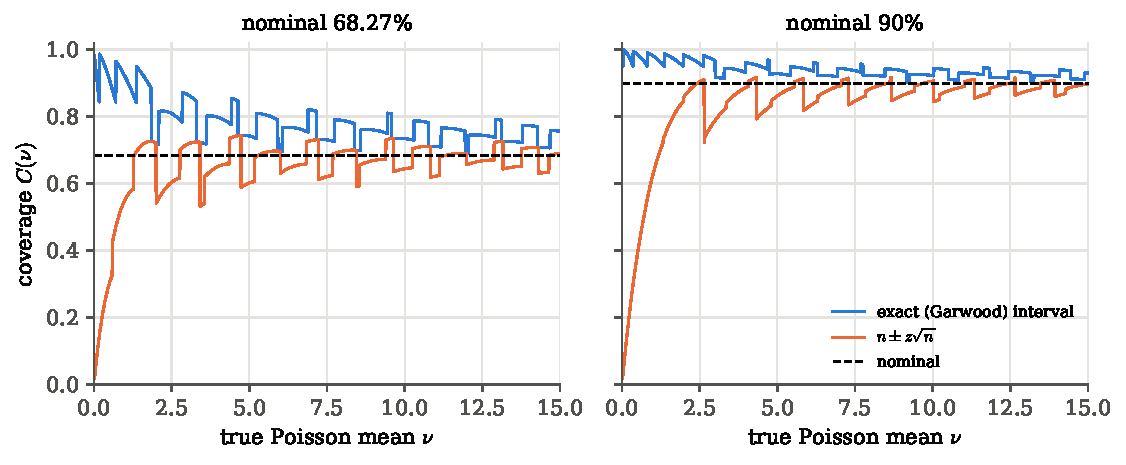
\includegraphics[width=\linewidth]{figures/ch04/coverage_poisson.pdf}
\caption{Exact coverage of two interval recipes for a Poisson mean, as a
function of the true mean. Left: nominal $68.27\%$, right: nominal $90\%$
(dashed lines). Garwood's exact interval (blue) always lies above the nominal
level, with saw-tooth jumps where the true mean crosses an interval end. The
quick interval $n\pm z\sqrt n$ (orange) undercovers, dramatically so below a
mean of about two.}
\label{4b:fig:coverage-poisson}
\end{figure}

The script \pyname{code/ch04/13_coverage.py} computes these curves with a
matrix of Poisson probabilities:

\pyfile[firstline=66,lastline=87,label={4b:lst:coverage}]{code/ch04/13_coverage.py}{Exact coverage of Poisson interval recipes}

Each recipe returns the interval ends for all counts $0,\dots,80$ at once. The
boolean matrix \pyname{inside} has one row per true $\nu$ and one column per
count, and is true where that count's interval contains that $\nu$.
Multiplying by the Poisson probabilities and summing along each row is
\eqref{4b:eq:coverage-function}. A brute-force check at $\nu=\FourBNuChk$ draws
$\FourBSims$ counts, builds their intervals and counts hits: the Monte Carlo
coverage $\FourBCovChkMC$ agrees with the exact $\FourBCovChkExact$ (and for the
quick recipe the simulation gives $\FourBCovChkMCw$).

\paragraph{Pointwise versus uniform.}
The Poisson curve makes concrete a distinction between two meanings of
``correct for large samples'' \mainref{\S6.5}. Take the Normal interval for a
proportion $p$ from $n$ trials, with estimate $\hat p$ and coverage $C(p)$.
For each \emph{fixed} $p$, $C(p)$ tends to $1-\alpha$ as $n\to\infty$: the
interval is \emph{pointwise} asymptotic. But at any fixed $n$, a small enough
$p$ makes $\hat p=0$ almost certain; the interval then collapses to $\{0\}$,
and the coverage is near zero. So the worst case $\inf_pC(p)$ does not tend to
$1-\alpha$, and the interval is not \emph{uniformly} asymptotic. ``Large sample'' has to be
large compared with something, and near a boundary the something is the
number of events, not the number of trials.

\subsection{Right on average, wrong in a recognisable case}
\label{4b:sec:berger-wolpert}

Coverage is an average over all possible data sets. Sometimes the data we hold
tell us that we are in a subset of those data sets where the recipe is right
much more often, or much less often, than the average. An example due to
Berger and Wolpert shows this plainly \mainref{Ex.~6.14}. Let $\theta$ be a
fixed number, let
$X_1,X_2$ be independent, each $+1$ or $-1$ with probability one half, and
observe only $Y_i=\theta+X_i$. The ``interval'', a single point, is
\[
  C=\begin{cases}\{Y_1-1\} & \text{if }Y_1=Y_2,\\ \{(Y_1+Y_2)/2\} & \text{if }Y_1\ne Y_2.\end{cases}
\]
There are four equally likely cases:
\begin{align}
  \Prob_\theta(\theta\in C)
  &\eqby{1} \tfrac14\,\mathbb 1[(\theta+1)-1=\theta]
          +\tfrac14\,\mathbb 1[(\theta-1)-1=\theta]
          +\tfrac24\,\mathbb 1[\tfrac12(2\theta)=\theta]
   \eqby{2} \tfrac14+0+\tfrac12=\tfrac34 .
  \label{4b:eq:bw}
\end{align}
\begin{explain}
  \item $(X_1,X_2)=(+1,+1)$: both $Y$ equal $\theta+1$, and $C=\{\theta\}$.
        $(-1,-1)$: both equal $\theta-1$, and $C=\{\theta-2\}$. $(+1,-1)$ or
        $(-1,+1)$: the $Y$ differ and their average is $\theta$.
  \item Evaluate the indicators.
\end{explain}
So $C$ is a $75\%$ confidence set for every $\theta$.

\emph{What we observe.} Now suppose the data are $Y_1=15$, $Y_2=17$.
\emph{The question.} Which of the four cases could have produced these data?
The two $Y$ differ, so $(+1,+1)$ and $(-1,-1)$ are ruled out; only the mixed
cases remain, and in both of them the average of the $Y$ is $\theta$. So
$C=\{16\}$ is \emph{certainly} right. Had we instead seen $Y_1=Y_2$, only the
first two cases could have produced it, and the recipe is right in one of them
and wrong in the other: right half the time. A simulation of $4\times10^5$ repetitions in
\pyname{code/ch04/11_test_inversion.py} confirms it: overall coverage
$\FourBBWcovAll$, coverage $\FourBBWcovDiff$ when $Y_1\ne Y_2$ (a fraction
$1-\FourBBWfracSame$ of the time), and $\FourBBWcovSame$ when $Y_1=Y_2$.

The lesson: ``$75\%$'' is a statement about the recipe, not about this data
set. Calling $\{16\}$ a $75\%$ confidence set is still correct, because that is
what the recipe guarantees \mainref{p.~93}. A probability statement about
$\theta$ given these particular $Y$ is a different kind of statement, the one
Bayesian inference makes (\cref{4b:sec:credible}). Frequentists handle the
problem by \emph{conditioning}: they compute the coverage only over data sets
that share a feature of the observed one, a feature that carries no information
about $\theta$ but does tell us how precise the experiment turned out to be
(here, whether $Y_1=Y_2$). In physics the classic case is a measurement whose
resolution depends on an event-by-event quantity: the relevant error bar is the
one for the resolution actually obtained.

\begin{inpractice}[Coverage studies: verification and research]
A coverage simulation can play two different roles. When an analytic result
exists, it \emph{verifies}: the $t$ interval must cover $95\%$ at every $n$, the
Garwood interval must never undercover, and a simulation that disagrees has a
bug. When no analytic result exists, the same simulation \emph{is} the method.
Experiments at the LHC build Neyman belts from toy Monte Carlo when the test
statistic has no known distribution; neutrino-oscillation fits construct
Feldman--Cousins regions from millions of pseudo-experiments; cosmological
analyses check whether a posterior interval from an MCMC chain
(\cref{ch:09}) covers the input parameters of simulated skies. In every case the
recipe is \eqref{4b:eq:coverage-function} evaluated by brute force.
\end{inpractice}
\section{Upper limits near a physical boundary}
\label{4b:sec:boundary}

The squared mass of a neutrino can be estimated from a measured energy and
momentum as $\widehat{m^2}=E^2-p^2$. The true $m^2$ cannot be negative, but the
estimate can: both $E^2$ and $p^2$ carry measurement errors, and when the true
mass is tiny, their difference comes out negative about half the time
\srcref{Cowan}{\S9.8}. The same happens to any parameter estimated as a
difference, $\hat\theta=x-y$: a signal rate estimated as ``counts minus
expected background'', a dark-matter cross-section, a tensor-to-scalar ratio.
Physics says $\theta\ge0$. The data, fluctuating, do not know that.

A search that sees nothing reports an \emph{upper limit}. Near the boundary
every recipe met so far runs into trouble. The interval can come out entirely
in the forbidden region, or be empty, or be so short that it claims more than
the experiment can know. Each fix trades one good property for another, and
seeing what each one gives up shows what a limit really promises.

\paragraph{The question in words.}
\begin{enumerate}[label=\arabic*.]
  \item What does the classical recipe give when the estimate is negative, and
        is it wrong?
  \item Which alternatives exist (shifting the estimate, a Bayesian prior on
        $\theta\ge0$, Feldman and Cousins' ordering, CL$_s$), and what does
        each do to the coverage?
  \item Why must the choice between ``upper limit'' and ``two-sided interval''
        be made before the data are seen?
\end{enumerate}

\subsection{The classical limit can be negative}
\label{4b:sec:classical-limit}

Let $\hat\theta$ be Gaussian with mean $\theta$ and known $\sigma_{\hat\theta}$,
with $\theta\ge0$ known a priori. The one-sided classical upper limit at
confidence level $1-\beta$ is, from \eqref{4b:eq:gauss-ends},
\begin{equation}
  \theta_{\rm up}=\hat\theta_{\rm obs}+\sigma_{\hat\theta}\,\Phi^{-1}(1-\beta)
  \label{4b:eq:classical-up}
\end{equation}
\srcref{Cowan}{(9.39)}. With $\sigma_{\hat\theta}=1$ and
$\hat\theta_{\rm obs}=-2$, the $95\%$ limit is
$-2+1.645=\FourBBdUpNinetyFive$. The experiment ``excludes'' every physical
value of $\theta$, including zero.

\emph{Is the recipe wrong?} No. It covers the true value in $95\%$ of
experiments, whatever that value is. If $\theta=0$, an estimate below $-1.645$
happens $5\%$ of the time, and those are exactly the experiments whose limit
is negative. We have simply landed in the $5\%$. \emph{Is the result useful?}
Also no. We knew before the experiment that $\theta\ge0$, and so certainly
that $\theta>\FourBBdUpNinetyFive$. Two tempting repairs make it worse. Raising the
confidence level to $99\%$ moves the limit to $\FourBBdUpNinetyNine$, a limit
three times smaller than the experiment's resolution, quoted at very high
confidence; and choosing the level $97.725\%$ gives $\theta_{\rm up}=10^{-5}$,
which is absurd \srcref{Cowan}{p.~137}.

Whatever limit we quote, the first rule is to report the estimate itself,
$\hat\theta_{\rm obs}\pm\sigma_{\hat\theta}$, even when it is negative. The
reason is combination. Unbiased estimates from many experiments average to the
truth only if the negative ones are kept; setting them to zero pushes every
average upwards. When
$\hat\theta$ is far from Gaussian, the whole likelihood function should be
published so that others can combine it \srcref{Cowan}{p.~137}.

\subsection{Three repairs: shift, Bayes, and flip-flop}
\label{4b:sec:repairs}

\paragraph{Shift the estimate to zero.}
A common practice replaces a negative estimate by zero before applying
\eqref{4b:eq:classical-up} \srcref{Cowan}{(9.40)}:
$\theta_{\rm up}=\max(\hat\theta_{\rm obs},0)+\sigma_{\hat\theta}\Phi^{-1}(1-\beta)$.
At $95\%$ the limit is then never below $1.645\,\sigma_{\hat\theta}$
($\FourBBdUpShift$ for our example), so it is never smaller than about the
resolution. The shifted limit is never below the classical one, so it contains
the truth at least as often: it overcovers. In \cref{4b:fig:boundary} (right) its coverage is $1$ for all
$\theta\le1.645$, because every experiment then quotes a limit above $\theta$.

\paragraph{A Bayesian limit with a prior that knows $\theta\ge0$.}
In the Bayesian approach the boundary is built in by a prior that vanishes for
$\theta<0$. With a flat prior on $\theta\ge0$ \srcref{Cowan}{(9.41)--(9.44)} and
$\sigma_{\hat\theta}=1$, the posterior is the Gaussian likelihood cut off at
zero and renormalised. Write $x=\hat\theta_{\rm obs}$ and $\varphi$ for the
standard normal density. The upper limit solves
\begin{align}
  1-\beta
  &\eqby{1} \frac{\int_0^{\theta_{\rm up}}\varphi(\theta-x)\,\dd\theta}{\int_0^{\infty}\varphi(\theta-x)\,\dd\theta}
   \eqby{2} \frac{\Phi(\theta_{\rm up}-x)-\Phi(-x)}{1-\Phi(-x)}
   \eqby{3} \frac{\Phi(\theta_{\rm up}-x)-1+\Phi(x)}{\Phi(x)} ,
  \notag\\
  \Longrightarrow\quad
  \theta_{\rm up}
  &\eqby{4} x+\Phi^{-1}\bigl(1-\beta\,\Phi(x)\bigr).
  \label{4b:eq:bayes-up}
\end{align}
\begin{explain}
  \item Bayes' theorem with a flat prior on $\theta\ge0$: the posterior is the
        likelihood $\varphi(\theta-x)$ normalised over the physical region
        \srcref{Cowan}{(9.43)}.
  \item Substitute $t=\theta-x$; the integrals are differences of the normal
        CDF.
  \item Symmetry, $\Phi(-x)=1-\Phi(x)$, in numerator and denominator.
  \item Multiply by $\Phi(x)$, solve for $\Phi(\theta_{\rm up}-x)=1-\beta\Phi(x)$,
        and apply $\Phi^{-1}$.
\end{explain}
For $x=-2$ this gives $\theta_{\rm up}=\FourBBdUpBayes$. For large positive $x$,
$\Phi(x)\to1$ and the limit tends to the classical $x+1.645$. The Bayesian limit
is always positive and always above the classical one (Cowan's Fig.~9.8, our
\cref{4b:fig:boundary}, left).

It means something different. It is the value that $\theta$ exceeds with
posterior probability $5\%$, given the prior. So it depends on the prior, and
the flat prior has two weaknesses. First, it says that $0<\theta<1$ is as
plausible before the experiment as $10^{40}<\theta<10^{40}+1$. Second, it
changes when we relabel the parameter: a flat prior on $m^2$ is not flat on
$m$. The prior
$\pi(\theta)\propto1/\theta$, flat in $\ln\theta$, gives limits invariant under
$\theta\to\theta^k$, but the integrals diverge unless the likelihood vanishes
at $\theta\to0$, which a Gaussian likelihood does not
\srcref{Cowan}{(9.45) and p.~139}. In practice the flat prior is the common
choice, with its assumptions stated.

The Bayesian limit was not built to have coverage, but we can still measure
its coverage. \Cref{4b:fig:boundary} (right) shows that for this problem it
overcovers near the boundary and approaches $95\%$ from above for large
$\theta$ (minimum $\FourBBdCovBayesMin$).

\begin{figure}[htbp]
\centering
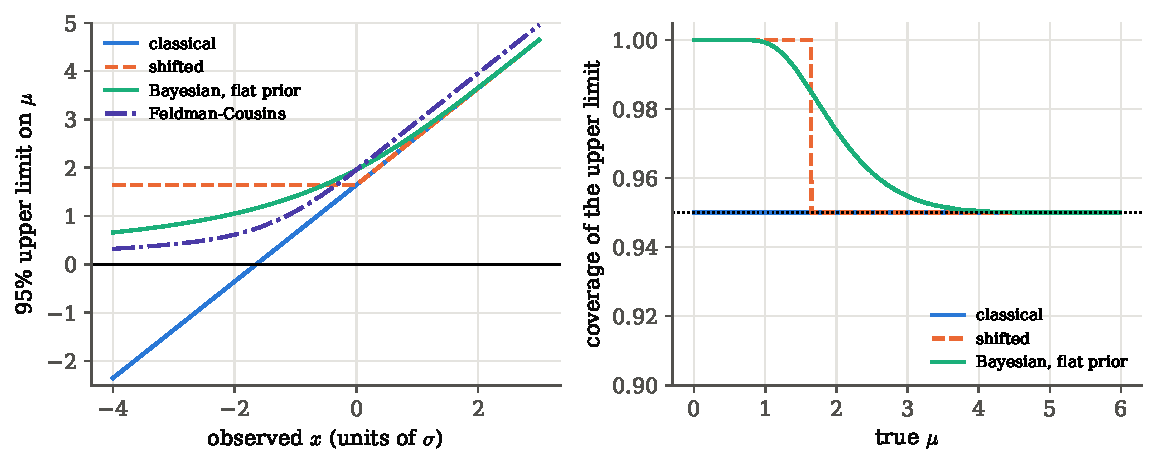
\includegraphics[width=\linewidth]{figures/ch04/boundary_limits.pdf}
\caption{Left: $95\%$ upper limits on a non-negative Gaussian mean as a
function of the observed estimate, in units of the resolution. The classical
limit (blue) goes negative for estimates below $-1.645$; the shifted limit
(orange dashed) is flat at $1.645$ for negative estimates; the flat-prior
Bayesian limit (green) and the Feldman--Cousins upper end (violet) stay positive
and fall slowly. All agree for large estimates. Right: the coverage of three of
the recipes as a function of the true value. The classical limit covers exactly
$95\%$, the other two more near the boundary.}
\label{4b:fig:boundary}
\end{figure}

\paragraph{Flip-flopping.}
Feldman and Cousins describe a third habit, common enough that they gave it a
name \cite{FeldmanCousins1998}. Physicist X decides after seeing the data: ``if
the result is less than $3\sigma$, I quote a $90\%$ upper limit; if it is more,
I quote a $90\%$ central interval; and if it is negative, I pretend it was
zero.'' Each of the two recipes alone covers $90\%$. The mixture does not.
\emph{The question:} take $\sigma=1$ and a true mean $\mu=2$; how often does the
mixture contain $2$? Here $x$ is the measured value. Take the two branches one
at a time.
\begin{itemize}[itemsep=1pt,leftmargin=1.2em]
  \item The upper-limit branch ($x<3$) quotes $[0,\max(x,0)+1.28]$, which
        contains $2$ when $x\ge0.72$.
  \item The central branch ($x\ge3$) quotes $[x-1.645,x+1.645]$, which
        contains $2$ when $x\le3.645$.
\end{itemize}
So
\begin{align}
  C(2)
  &\eqby{1} \Prob(0.72\le x<3)+\Prob(3\le x\le3.645)
   \eqby{2} \Prob(-1.28\le x-2\le1.645)
   \notag\\
  &\eqby{3} \Phi(1.645)-\Phi(-1.28)
   \eqby{4} 0.95-0.10=0.85 .
  \label{4b:eq:flipflop}
\end{align}
\begin{explain}
  \item The two branches, each with its own condition for covering $\mu=2$.
  \item The two ranges join into one; subtract the true value $2$.
  \item $x-2$ is standard normal.
  \item The standard quantiles of \cref{4b:sec:belt-gauss}.
\end{explain}
The quoted ``$90\%$'' intervals cover $85\%$ of the time. The missing $5\%$ are
the measurements above $3.645$. The upper-limit recipe alone would have given
them a limit above $2$, but the switch hands them a central interval that
misses. The script finds the
same $\FourBFfCovTwo$ at $\mu=2$, and that this is the minimum; the coverage stays
at $85\%$ from $\mu\approx1.3$ to $\mu\approx4.3$ (\cref{4b:fig:fc-coverage},
left). In belt language (\cref{4b:fig:fc-belts}, dashed), switching recipes
at $x=3$ bends the belt so that the horizontal acceptance intervals at
intermediate $\mu$ hold only $85\%$ of the probability.

\begin{pitfall}[Deciding the form of the result after seeing the data]
Choosing between an upper limit and a two-sided interval according to how the
data came out destroys the coverage of both, even though each recipe is
correct alone. The rule of the Neyman construction is that the acceptance
regions are fixed before the measurement. If we want the result to switch
automatically from a limit to an interval as the signal grows, the switch must
be part of the construction itself, which is what the unified approach below
does.
\end{pitfall}

The strict alternative, always quoting the central interval, has its own
problem. With $\sigma=1$ and $x=-1.8$, the $90\%$ central interval has upper end
$x+1.645=-0.155$, so it contains no physical value at all. The interval is
\emph{empty} \cite{FeldmanCousins1998}. It is still a correct member of an
ensemble with $90\%$ coverage, but not one anybody wants to publish.

\subsection{The unified approach of Feldman and Cousins}
\label{4b:sec:fc}

The Neyman construction (\cref{4b:sec:belt}) leaves one choice open:
\emph{which} values of the measurement to put in the acceptance interval at
each $\mu$, so that it holds probability $1-\alpha$. Central intervals leave
out equal tails on both sides; upper limits leave out only the lowest values,
keeping everything above a cut. Feldman and Cousins choose by a likelihood ratio.

\begin{keyidea}[Likelihood-ratio ordering]
At each $\mu$, rank the possible outcomes $x$ by
\[
  R(x)=\frac{P(x\given\mu)}{P(x\given\mu_{\rm best})},
\]
where $\mu_{\rm best}$ is the \emph{physically allowed} value of $\mu$ that
makes $x$ most probable. Add outcomes to the acceptance interval in order of
decreasing $R$ until their total probability reaches $1-\alpha$
\cite[(4.1)]{FeldmanCousins1998}. Then build the belt and read the intervals as
usual. The coverage is right by construction, the interval is never empty, and
the result turns by itself from an upper limit into a two-sided interval as the
data move away from the boundary.
\end{keyidea}

\emph{Why this ordering?} $R$ compares how well $\mu$ explains $x$ with how
well the best physical value explains it. An outcome with $R$ close to one is
one that $\mu$ explains nearly as well as any allowed value could. Putting such
outcomes in the acceptance set first means that we reject $\mu$ only for data
that some other physical $\mu$ explains much better. This is the likelihood-ratio test of the
first part of the chapter, with the physical boundary written into the
maximisation, inverted into an interval.

\paragraph{Gaussian with $\mu\ge0$.}
With $P(x\given\mu)=\varphi(x-\mu)$, the best physical value is
$\mu_{\rm best}=\max(0,x)$. Then
\begin{align}
  R(x)
  &\eqby{1}
   \begin{cases}
     \varphi(x-\mu)/\varphi(0)=e^{-(x-\mu)^2/2}, & x\ge0,\\[2pt]
     \varphi(x-\mu)/\varphi(x)=e^{-(x-\mu)^2/2+x^2/2}=e^{\,x\mu-\mu^2/2}, & x<0,
   \end{cases}
  \label{4b:eq:fc-R}
\end{align}
\begin{explain}
  \item For $x\ge0$, $\mu_{\rm best}=x$ and $\varphi(0)=1/\sqrt{2\pi}$; for $x<0$,
        $\mu_{\rm best}=0$, and expanding $-(x-\mu)^2/2+x^2/2=x\mu-\mu^2/2$
        \cite[(4.2)--(4.3)]{FeldmanCousins1998}.
\end{explain}
For $x\ge0$, $R$ decreases with the distance from $\mu$, so the acceptance
interval is centred, as in a central interval. For $x<0$, $R$ decreases as $x$
becomes more negative, but only linearly in the exponent, much more slowly than
the Gaussian: negative outcomes are penalised less, because no physical $\mu$
explains them well. The acceptance interval $[x_1,x_2]$ at each $\mu$ is found
numerically from $R(x_1)=R(x_2)$ and $\int_{x_1}^{x_2}\varphi(x-\mu)\dd x=1-\alpha$
\cite[(4.4)]{FeldmanCousins1998}.

\emph{Where does the limit turn into a two-sided interval?} The acceptance
set at $\mu=0$ decides it. There $R(x)=1$ for all
$x<0$ and $R(x)=e^{-x^2/2}$ for $x\ge0$, so every negative $x$ is ranked first
(probability $1/2$), followed by $x$ from $0$ upwards until the total is $0.90$:
$\Phi(x_2)=0.90$, $x_2=\FourBFcTrans$. For an observation above $\FourBFcTrans$,
$\mu=0$ is excluded and the interval is two-sided; below it, the interval starts
at zero and is an upper limit. The brute-force belt in
\pyname{code/ch04/15_feldman_cousins.py} reproduces Feldman and Cousins' Table~X
at $90\%$:
\begin{center}
\begin{tabular}{lcccccc}
\toprule
$x_0$ & $-2$ & $-1$ & $0$ & $1$ & $2$ & $3$\\
\midrule
$[\mu_1,\mu_2]$ &
$[\FourBFcGMinusTwoLo,\FourBFcGMinusTwoHi]$ &
$[\FourBFcGMinusOneLo,\FourBFcGMinusOneHi]$ &
$[\FourBFcGZeroLo,\FourBFcGZeroHi]$ &
$[\FourBFcGOneLo,\FourBFcGOneHi]$ &
$[\FourBFcGTwoLo,\FourBFcGTwoHi]$ &
$[\FourBFcGThreeLo,\FourBFcGThreeHi]$\\
\bottomrule
\end{tabular}
\end{center}
Here $x_0$ is the observed measurement and $[\mu_1,\mu_2]$ its interval. At
$x_0=0$ the $90\%$ upper limit is $\FourBFcGZeroHi$: the classical $95\%$ limit
rather than the $90\%$ one ($1.28$). The reason is that at $\mu\approx1.6$ the
unified acceptance interval is already nearly central, so its left edge sits
$1.645$ below $\mu$, and $1.645$ is also the one-sided $95\%$ quantile
(\cref{4b:sec:belt-gauss}). That is the price of repairing flip-flopping: near
the boundary the unified limits are somewhat looser
\cite{FeldmanCousins1998}. In exchange no interval is empty, the limits for
very negative $x_0$ shrink only slowly (as $1/\abs{x_0}$), and the coverage is
$90\%$ for every $\mu$ (between $\FourBFcCovMin$ and $\FourBFcCovMax$ on our grid;
\cref{4b:fig:fc-coverage}, left).

\begin{figure}[htbp]
\centering
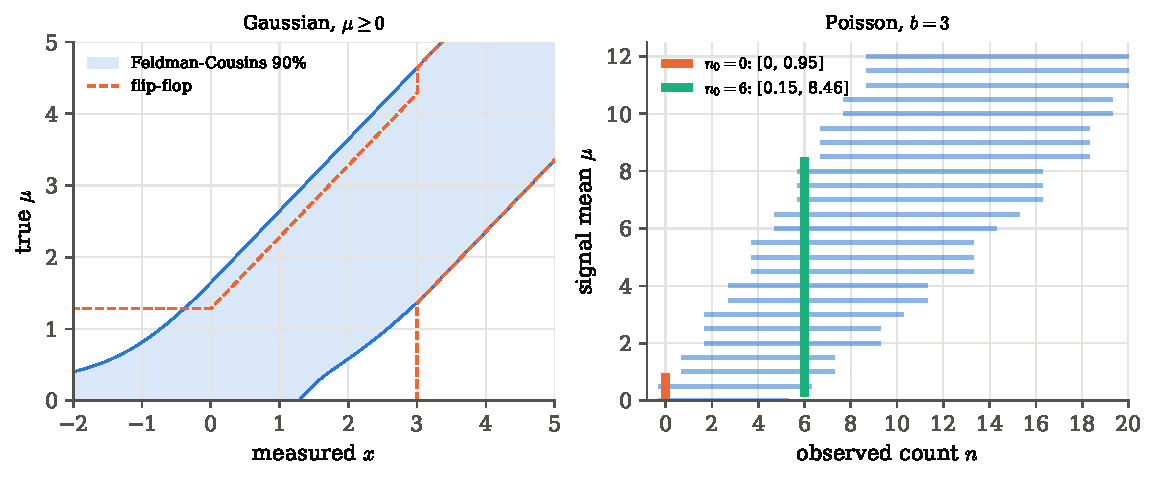
\includegraphics[width=\linewidth]{figures/ch04/fc_belts.pdf}
\caption{Left: the $90\%$ Feldman--Cousins belt for a Gaussian measurement of a
non-negative mean (shaded, solid edges) and the belt implied by flip-flopping
(dashed). Below $x\approx1.28$ the unified belt reaches down to $\mu=0$, so the
interval is an upper limit; above, it is two-sided. The flip-flop belt jumps at
$x=3$ where the recipe switches. Right: the Feldman--Cousins acceptance sets
for a Poisson count on a known background $b=3$ (bars every $0.5$ in $\mu$),
with the intervals for $n_0=0$ (orange) and $n_0=6$ (green).}
\label{4b:fig:fc-belts}
\end{figure}

\subsection{Counting on a known background}
\label{4b:sec:fc-poisson}

The most common version of the problem in particle physics is a count $n$ of
candidate events, of which a known mean $b$ is expected from background and an
unknown mean $\mu\ge0$ from signal \srcref{Cowan}{\S9.9}. The total is Poisson
with mean $\mu+b$,
\begin{equation}
  P(n\given\mu)=\frac{(\mu+b)^n}{n!}\,e^{-(\mu+b)} ,
  \label{4b:eq:poisson-bkg}
\end{equation}
and the naive estimate is $\hat\mu=n-b$, which is negative whenever fewer
events than the expected background are seen \srcref{Cowan}{(9.47)--(9.48)}.
The classical limits are the background-free ones shifted down by $b$
\srcref{Cowan}{(9.50)}. For $b=3$ and no events observed, the $90\%$ upper
limit is $\FourBUpNinetyZero-3=\FourBPtClZero$: negative. The central $90\%$
interval is $[0,\ 3.00-3]$, with an upper end $\FourBPtCentralUpZero$ below zero:
empty \cite{FeldmanCousins1998}.

\paragraph{The ordering at one value of $\mu$.}
Feldman and Cousins work one row of their construction by hand, $b=3$ and
$\mu=0.5$ \cite[Table~I]{FeldmanCousins1998}. For each $n$ the best physical
signal is $\mu_{\rm best}=\max(0,n-b)$, and $R=P(n\given0.5)/P(n\given\mu_{\rm best})$:
\begin{center}
\small
\begin{tabular}{l*{11}{c}}
\toprule
$n$ & 0 & 1 & 2 & 3 & 4 & 5 & 6 & 7 & 8 & 9 & 10\\
\midrule
$P(n\given\mu)$ & $\FourBPtPZero$ & $\FourBPtPOne$ & $\FourBPtPTwo$ & $\FourBPtPThree$ & $\FourBPtPFour$ & $\FourBPtPFive$ & $\FourBPtPSix$ & $\FourBPtPSeven$ & $\FourBPtPEight$ & $\FourBPtPNine$ & $\FourBPtPTen$\\
$\mu_{\rm best}$ & 0 & 0 & 0 & 0 & 1 & 2 & 3 & 4 & 5 & 6 & 7\\
$R$ & $\FourBPtRZero$ & $\FourBPtROne$ & $\FourBPtRTwo$ & $\FourBPtRThree$ & $\FourBPtRFour$ & $\FourBPtRFive$ & $\FourBPtRSix$ & $\FourBPtRSeven$ & $\FourBPtREight$ & $\FourBPtRNine$ & $\FourBPtRTen$\\
rank & $\FourBPtRankZero$ & $\FourBPtRankOne$ & $\FourBPtRankTwo$ & $\FourBPtRankThree$ & $\FourBPtRankFour$ & $\FourBPtRankFive$ & $\FourBPtRankSix$ & $\FourBPtRankSeven$ & $\FourBPtRankEight$ & $\FourBPtRankNine$ & $\FourBPtRankTen$\\
\bottomrule
\end{tabular}
\end{center}
Adding counts in the order of the last row, the total first reaches $0.90$ with
rank $7$, so the acceptance set at $\mu=0.5$ is $n\in[\FourBPtAccLo,\FourBPtAccHi]$,
with probability $\FourBPtAcc$ (more than $0.90$, because of discreteness).
Look at $n=0$. Its probability under $\mu=0.5$ is only $0.030$. But no physical
$\mu$ makes it much more probable: the best is $\mu=0$, with $0.050$. So
$R=\FourBPtRZero$, high in the ranking, and $n=0$ is accepted. This is what
keeps the interval for $n_0=0$ from being empty.

\paragraph{The intervals.}
Repeating the ranking on a grid of $\mu$ and reading vertically gives the
Feldman--Cousins intervals; \cref{4b:fig:fc-belts} (right) shows the belt. The
code is short:

\pyfile[firstline=143,lastline=154,label={4b:lst:fc}]{code/ch04/15_feldman_cousins.py}{The Feldman--Cousins acceptance sets for a Poisson count on background}

For every $n$ the array \pyname{pbest} holds $P(n\given\mu_{\rm best})$; for each
hypothetical $\mu$ the counts are sorted by decreasing $R$ (\pyname{argsort} of
$-R$), their probabilities accumulated, and the set cut where the running sum
first reaches the confidence level. The minimum and maximum of the kept counts
are the ends of the horizontal set. For $b=3$ at $90\%$:
\begin{center}
\small
\begin{tabular}{l*{11}{c}}
\toprule
$n_0$ & 0 & 1 & 2 & 3 & 4 & 5 & 6 & 7 & 8 & 9 & 10\\
\midrule
FC $\mu_1$ & $\FourBPtFCZeroLo$ & $\FourBPtFCOneLo$ & $\FourBPtFCTwoLo$ & $\FourBPtFCThreeLo$ & $\FourBPtFCFourLo$ & $\FourBPtFCFiveLo$ & $\FourBPtFCSixLo$ & $\FourBPtFCSevenLo$ & $\FourBPtFCEightLo$ & $\FourBPtFCNineLo$ & $\FourBPtFCTenLo$\\
FC $\mu_2$ & $\FourBPtFCZeroHi^{*}$ & $\FourBPtFCOneHi$ & $\FourBPtFCTwoHi$ & $\FourBPtFCThreeHi$ & $\FourBPtFCFourHi$ & $\FourBPtFCFiveHi$ & $\FourBPtFCSixHi$ & $\FourBPtFCSevenHi$ & $\FourBPtFCEightHi$ & $\FourBPtFCNineHi$ & $\FourBPtFCTenHi$\\
classical & $\FourBPtClZero$ & $\FourBPtClOne$ & $\FourBPtClTwo$ & $\FourBPtClThree$ & $\FourBPtClFour$ & $\FourBPtClFive$ & $\FourBPtClSix$ & $\FourBPtClSeven$ & $\FourBPtClEight$ & $\FourBPtClNine$ & $\FourBPtClTen$\\
CL$_s$ & $\FourBPtCLsZero$ & $\FourBPtCLsOne$ & $\FourBPtCLsTwo$ & $\FourBPtCLsThree$ & $\FourBPtCLsFour$ & $\FourBPtCLsFive$ & $\FourBPtCLsSix$ & $\FourBPtCLsSeven$ & $\FourBPtCLsEight$ & $\FourBPtCLsNine$ & $\FourBPtCLsTen$\\
\bottomrule
\end{tabular}
\end{center}
The first two rows agree with Feldman and Cousins' Table~IV to the grid
precision, with one exception marked $^{*}$. For $n_0=0$ the raw construction
gives $\FourBPtFCZeroHiRaw$; Feldman and Cousins publish $1.08$. The difference is
a deliberate correction: because $n$ is discrete, the raw upper end is not always
a decreasing function of $b$, and they lengthen intervals to make it so. Applying
their rule (replace $\mu_2(b)$ by the largest value at any larger background) on
a fine grid of $b$ gives $\FourBPtFCZeroHiFixed$. For $n_0\le5$ the interval starts
at zero: an upper limit. From $n_0=6$ on it is two-sided. The switch happens by
itself.

\paragraph{CL$_s$ and the Bayesian limit.}
The classical limit in the third row goes negative for small $n_0$. The reason:
when the background fluctuates down, few events are seen, and every signal
looks excluded. The LEP and Tevatron experiments adopted a modification
designed against exactly this \cite{Cowan2011}. In a counting experiment, a
small $n$ is what argues against a signal, so the two relevant tail
probabilities are those of seeing $n_0$ or fewer events, with and without the
signal:
\begin{equation}
  \mathrm{CL}_{s+b}(\mu)=\Prob(n\le n_0\given\mu+b),
  \qquad
  \mathrm{CL}_b=\Prob(n\le n_0\given b).
  \label{4b:eq:clsb}
\end{equation}
The classical recipe excludes $\mu$ when $\mathrm{CL}_{s+b}<\alpha$.

\begin{workdef}[CL$_s$]
The ratio $\mathrm{CL}_s(\mu)=\mathrm{CL}_{s+b}(\mu)/\mathrm{CL}_b$ (in the
notation of \cite{Cowan2011}, $p_{s+b}/(1-p_b)$). A signal $\mu$ is excluded at
confidence level $1-\alpha$ if $\mathrm{CL}_s(\mu)<\alpha$. Dividing by
$\mathrm{CL}_b\le1$ makes exclusion harder exactly when the data look
background-poor \unpack{when even background alone rarely gives so few events}.
\end{workdef}

For $n_0=0$, $\mathrm{CL}_s=e^{-(\mu+b)}/e^{-b}=e^{-\mu}$, and the $90\%$ limit is
$\mu=\ln10=\FourBPtCLsZero$ for \emph{every} $b$. Seeing nothing on a background of
three events excludes no more than seeing nothing on no background. That is the
intended behaviour: an experiment should not get a better limit because its
background fluctuated low. \Cref{4b:fig:fc-limits} contrasts the three
recipes as a function of $b$. The classical limit for $n_0=0$ falls as
$2.30-b$ and crosses zero at $b=2.30$. The Feldman--Cousins limit also falls, from
$\FourBPtFCUpZeroBzero$ at $b=0$ towards about one: it is a correct confidence
interval, and with a larger background, zero events really are rarer for every
$\mu$. CL$_s$ stays at $\FourBPtCLsZero$.

The CL$_s$ limit is the flat-prior Bayesian limit of Cowan's (9.53)--(9.54).
With a flat prior on $\mu\ge0$, the posterior probability above $\mu$ is
\begin{align}
  \Prob(\mu_s>\mu\given n_0)
  &\eqby{1} \frac{\int_\mu^\infty(\mu'+b)^{n_0}e^{-(\mu'+b)}\,\dd\mu'}{\int_0^\infty(\mu'+b)^{n_0}e^{-(\mu'+b)}\,\dd\mu'}
   \eqby{2} \frac{\int_{\mu+b}^\infty t^{n_0}e^{-t}\,\dd t/n_0!}{\int_{b}^\infty t^{n_0}e^{-t}\,\dd t/n_0!}
  \notag\\
  &\eqby{3} \frac{\sum_{n=0}^{n_0}(\mu+b)^ne^{-(\mu+b)}/n!}{\sum_{n=0}^{n_0}b^ne^{-b}/n!}
   \eqby{4} \mathrm{CL}_s(\mu).
  \label{4b:eq:cls-bayes}
\end{align}
\begin{explain}
  \item Posterior tail with the likelihood \eqref{4b:eq:poisson-bkg}; the
        $1/n_0!$ cancels.
  \item Substitute $t=\mu'+b$, and divide top and bottom by $n_0!$.
  \item The gamma tail equals the Poisson cumulative sum,
        $\int_x^\infty t^ke^{-t}\dd t/k!=\sum_{n=0}^k x^ne^{-x}/n!$: this is
        \eqref{4b:eq:poisson-chi2} with $z=2t$, since
        $f_{\chi^2}(2t;2k+2)\,\dd(2t)=t^ke^{-t}\dd t/k!$.
  \item Definition \eqref{4b:eq:clsb}.
\end{explain}
So setting the posterior tail to $\alpha$ and setting CL$_s=\alpha$ give the same
limit; the script finds the two limits equal to within $\FourBPtCLsBayesDiff$. For $b=0$
both reduce to the classical limit \srcref{Cowan}{(9.55)}, because then
$\mathrm{CL}_b=1$. So for a counting experiment without background the
frequentist and the flat-prior Bayesian limits are the same number, and there
is no choice to make \srcref{Cowan}{p.~142}.

\begin{figure}[htbp]
\centering
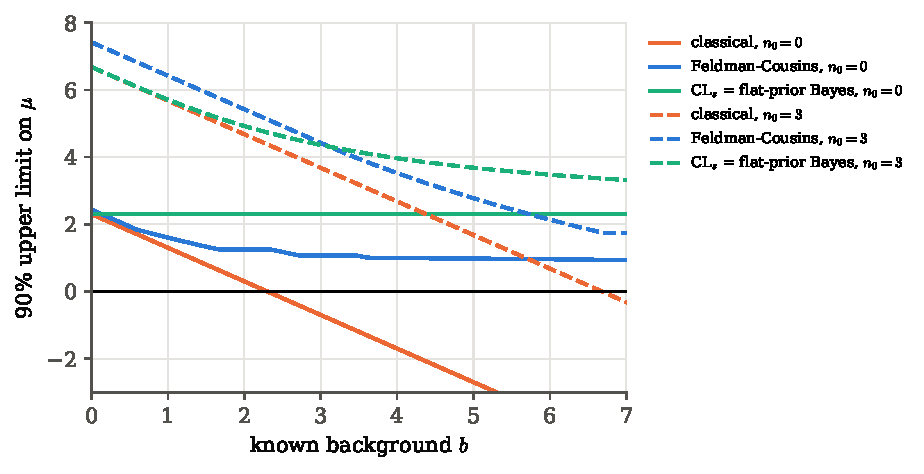
\includegraphics[width=0.78\linewidth]{figures/ch04/fc_poisson_limits.pdf}
\caption{$90\%$ upper limits on a signal mean for $n_0=0$ (solid) and $n_0=3$
(dashed) observed events, as a function of the known background. The classical
limit (orange) falls linearly and becomes negative; the Feldman--Cousins limit
(blue) falls but stays positive; CL$_s$, equal to the flat-prior Bayesian
limit (green), does not improve when the background grows: for $n_0=0$ it is
flat at $2.30$.}
\label{4b:fig:fc-limits}
\end{figure}

\paragraph{What each recipe does to the coverage.}
\Cref{4b:fig:fc-coverage} (right) shows the exact coverage for $b=3$. All three
recipes keep $90\%$ as a minimum (Feldman--Cousins $\FourBPtCovFCMin$, classical
$\FourBPtCovClMin$, CL$_s$ $\FourBPtCovCLsMin$) and all have the Poisson
saw-tooth. They differ in how much they overcover. The classical limit,
negative values and all, is a correct $90\%$ upper limit; its failures include
every experiment that quotes a negative limit. CL$_s$ overcovers most near
$\mu=0$, where it always covers, because it never excludes any $\mu$ below
$2.30$. It is conservative by design: not a confidence interval in the strict
Neyman sense, but a limit with guaranteed coverage that a lucky downward
fluctuation cannot improve. Feldman--Cousins is closest to exact.

\begin{figure}[htbp]
\centering
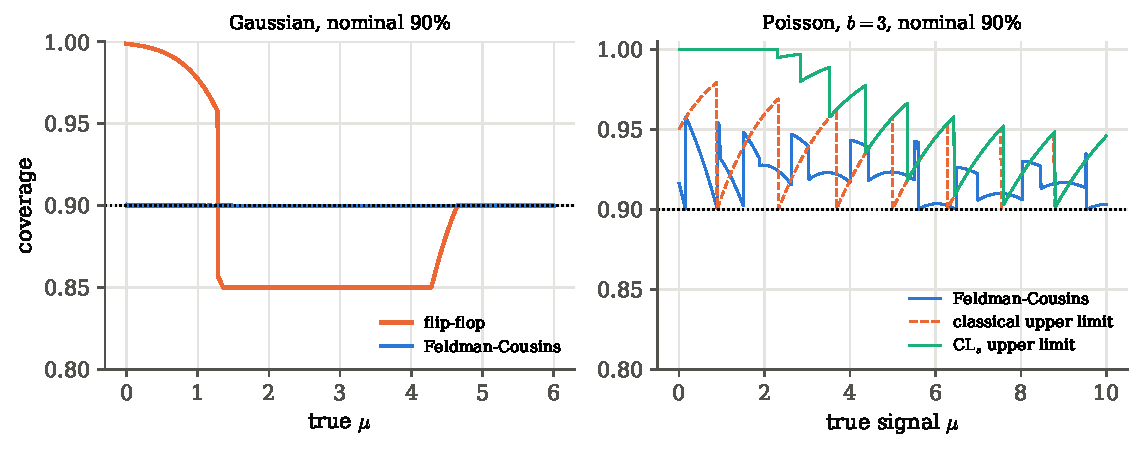
\includegraphics[width=\linewidth]{figures/ch04/fc_coverage.pdf}
\caption{Coverage near a boundary. Left: Gaussian measurement of a non-negative
mean, nominal $90\%$. The flip-flop recipe (orange) drops to $85\%$ over a wide
range of true values; the Feldman--Cousins intervals (blue, under the dotted
line) cover $90\%$ everywhere. Right: Poisson count on $b=3$. Feldman--Cousins,
classical upper limit and CL$_s$ all stay above $90\%$, with saw-tooth
over-coverage; CL$_s$ overcovers most at small signals.}
\label{4b:fig:fc-coverage}
\end{figure}

Feldman and Cousins point out one more advantage of their construction
\cite[\S IV.C]{FeldmanCousins1998}. The interval is never empty, even when the
observation is improbable for \emph{every} $\mu$ (say, no events at all on a
background of fifteen). In that case a non-empty interval should not reassure
anyone; the right response is a separate goodness-of-fit question, ``how probable
is so few events even for $\mu=0$?''. Their tables flag such entries. The
interval answers ``which $\mu$ are compatible with the data, given the model''; it
does not test the model.

In practice the unified approach is standard for neutrino-oscillation results,
CL$_s$ for exclusion limits at the LHC, and in both communities the Bayesian
flat-prior limit is quoted as a cross-check. Whatever the choice, it must be
stated, and fixed before the data are looked at \srcref{Cowan}{p.~137}.
\section{Many tests at once and the look-elsewhere effect}
\label{4b:sec:lee}

A microarray measures the activity of $2638$ genes in two groups of patients,
and for each gene we can test whether the two groups differ
\mainref{p.~165}. A particle search looks for a resonance at every mass between
$105$ and $155\,$GeV. A survey tests the isotropy of the sky in hundreds of
patches. In all three cases each single test has a small false-alarm
probability $\alpha$. But there are many tests, so the chance that \emph{some}
test fires by luck is much larger. This is the \newterm{multiple testing}
problem; in a particle search it is called the \newterm{look-elsewhere
effect}. The first part of the chapter met it as one of the reasons for the
$5\sigma$ convention. How much the false-alarm rate grows can be computed, and
it can be kept under control.

\paragraph{The question in words.}
\begin{enumerate}[label=\arabic*.]
  \item If we run $m$ tests, how likely is at least one false rejection, and
        how do we keep that under control?
  \item When we expect some real effects among many tests, is ``no false
        rejection at all'' the right goal, or is ``few false rejections among
        those we claim'' better?
  \item When the search is over a continuous parameter, like a mass, how many
        independent tests is it, and how do we convert the local p-value of the
        biggest bump into a global one?
\end{enumerate}

\subsection{The family-wise error rate and Bonferroni}
\label{4b:sec:bonferroni}

Suppose we run $c$ tests, all their null hypotheses are true, and the tests are
independent, each with level $\alpha$. \emph{The question:} how likely is at
least one false alarm? This probability, which Kruschke calls the
\emph{experimentwise} error rate \srcref{Kruschke}{\S11.4.1}, is
\begin{equation}
  \alpha_{\rm EW}
  \eqby{1} 1-\Prob(\text{no false alarm})
  \eqby{2} 1-(1-\alpha)^c .
  \label{4b:eq:alpha-ew}
\end{equation}
\begin{explain}
  \item Complement.
  \item Independence: each test stays quiet with probability $1-\alpha$.
\end{explain}
With nine groups there are $c=9\times8/2=\FourBMtC$ pairwise comparisons, and at
$\alpha=0.05$ the chance of at least one false alarm is $\FourBMtAlphaEW$. An
analyst who compares everything with everything is almost sure to find
something.

The simplest cure is to make each test stricter. From here on we write $m$ for
the number of tests (the $c$ above) and $P_i$ for the p-value of test $i$. The
\newterm{Bonferroni} method rejects null $H_{0,i}$ only if $P_i<\alpha/m$
\mainref{p.~166}. Then, whatever the dependence between the tests, the
probability of at least one false rejection, the \newterm{family-wise error
rate}, is at most $\alpha$ \mainref{Thm.~10.24}. Let $R_i$ be
the event ``null $i$ is true and falsely rejected'', and $R$ the event that at
least one null is falsely rejected:
\begin{align}
  \Prob(R)
  &\eqby{1} \Prob\Bigl(\bigcup_{i}R_i\Bigr)
   \relby{2}{\le} \sum_i\Prob(R_i)
   \relby{3}{\le} \sum_{i=1}^{m}\frac{\alpha}{m}
   = \alpha .
  \label{4b:eq:bonferroni}
\end{align}
\begin{explain}
  \item At least one false rejection means one of the $R_i$ happened.
  \item The union bound: the probability of a union never exceeds the sum of
        the probabilities (overlaps are counted more than once on the right).
        No independence is needed.
  \item Under a true null the p-value is uniform (or, for discrete data,
        valid), so $\Prob(P_i<\alpha/m)\le\alpha/m$; nulls that are false
        contribute no false rejections at all.
\end{explain}
For the gene example, $0.05/2638=1.9\times10^{-5}$ is the threshold
\mainref{Ex.~10.25}. For the $\FourBMtC$ comparisons the per-comparison level
is $\FourBMtBonfPC$, and the actual family-wise rate for independent tests is
$1-(1-\FourBMtBonfPC)^{36}=\FourBMtBonfEW$, just below the target. The exact
level for independent tests, $1-(1-\alpha)^{1/c}=\FourBMtSidakPC$ (the
\v{S}id\'ak correction), is hardly different; Bonferroni's advantage is that it
holds for any dependence.

The price is power. Bonferroni makes even one false rejection unlikely, and with
thousands of tests the threshold becomes so small that real effects are
missed. There is a second objection \srcref{Kruschke}{pp.~326--327}: the
correction depends
on how many comparisons the analyst \emph{intended} to make, and on whether a
comparison was planned or prompted by the data, so two analysts with the same
data can reach different conclusions.

\begin{pitfall}[The post hoc comparison]
Comparing the two groups that happen to be furthest apart, after looking,
is not one test: it is the largest of all possible comparisons, and its null
distribution is that of a maximum. The same is true of the highest bin in a
histogram, the best of several selection cuts, and the mass where a bump
appeared. The p-value must be computed for the procedure actually followed,
including the looking.
\end{pitfall}

\subsection{The false discovery rate and Benjamini--Hochberg}
\label{4b:sec:bh}

In a screening problem we \emph{expect} some effects to be real. Then the useful
promise is about the list of discoveries: most of what we claim should be true.
To state this, sort the outcomes of the $m$ tests into a table
\mainref{Table~10.2}:
\begin{center}
\begin{tabular}{lccc}
\toprule
 & $\Hnull$ not rejected & $\Hnull$ rejected & total\\
\midrule
$\Hnull$ true & $U$ & $V$ & $m_0$\\
$\Hnull$ false & $T$ & $S$ & $m_1$\\
total & $m-R$ & $R$ & $m$\\
\bottomrule
\end{tabular}
\end{center}
$V$ counts false discoveries, $S$ true ones, $R=V+S$ all rejections. The
\newterm{false discovery proportion} is $\mathrm{FDP}=V/R$ (zero if $R=0$), and
the \newterm{false discovery rate} is its expectation,
$\mathrm{FDR}=\E(\mathrm{FDP})$ \mainref{p.~166}. Bonferroni controls
$\Prob(V\ge1)$; the FDR asks only that $V$ be a small fraction of $R$ on
average.

\paragraph{The Benjamini--Hochberg procedure} \mainref{(10.8)}:
\begin{enumerate}[label=\arabic*.]
  \item Sort the p-values, $P_{(1)}<\dots<P_{(m)}$.
  \item Find the largest $i$ with $P_{(i)}<i\alpha/(C_mm)$, where $C_m=1$ for
        independent tests and $C_m=\sum_{j=1}^m1/j$ otherwise.
  \item Reject every null with $P_i\le P_{(i)}$ for that $i$.
\end{enumerate}
Then $\mathrm{FDR}\le(m_0/m)\alpha\le\alpha$, whatever the number of true nulls
and whatever the distribution of the p-values of the false ones
\mainref{Thm.~10.26}.

\emph{Why the sloping line $i\alpha/m$?} Take the case $C_m=1$, and follow the
estimate of the false discovery proportion step by step.
\begin{itemize}[itemsep=1pt,leftmargin=1.2em]
  \item Suppose we reject every null whose p-value is below a threshold $t$.
  \item The $m_0$ true nulls have uniform p-values, so about $m_0t$ of them fall
        below $t$. That is the expected number of false discoveries.
  \item If the threshold is the $i$-th smallest p-value, we make $R=i$
        rejections, so the false discovery proportion is about $m_0t/i$.
  \item We do not know $m_0$, so we replace it by its upper bound $m$. Requiring
        $mt/i\le\alpha$ gives $t\le i\alpha/m$: exactly the BH line.
\end{itemize}
So the procedure picks the most generous threshold whose estimated false
discovery proportion is still at most $\alpha$. The theorem shows that this
heuristic holds exactly for the expectation.

\paragraph{Example: ten p-values.}
Wasserman's ten ordered p-values are $0.00017$, $0.00448$, $0.00671$, $0.00907$,
$0.01220$, $0.33626$, $0.39341$, $0.53882$, $0.58125$, $0.98617$
\mainref{Ex.~10.28}. At $\alpha=0.05$, Bonferroni rejects below $0.005$: the
first $\FourBMtExBonf$. BH compares $P_{(i)}$ with $0.005\,i$: $0.00017<0.005$,
$0.00448<0.010$, $0.00671<0.015$, $0.00907<0.020$, $0.01220<0.025$, but
$0.33626>0.030$, and none of the later ones gets under the line. So
BH rejects the first $\FourBMtExBH$, the same as uncorrected testing here.

\paragraph{Example: a thousand tests.}
In \pyname{code/ch04/16_multiple_testing.py}, $m=\FourBMtM$ one-sided $z$-tests
are run, of which $m_1=\FourBMtMone$ have a real shift of $\FourBMtShift$ standard
deviations, and the whole family is repeated $\FourBMtReps$ times. On average:
\begin{center}
\begin{tabular}{lcccc}
\toprule
procedure & true discoveries $S$ & false discoveries $V$ & FDR & $\Prob(V\ge1)$\\
\midrule
uncorrected, $P<0.05$ & $\FourBMtRawS$ & $\FourBMtRawV$ & $\FourBMtRawFDR$ & $\FourBMtRawFWER$\\
Bonferroni & $\FourBMtBonfS$ & $\FourBMtBonfV$ & $\FourBMtBonfFDR$ & $\FourBMtBonfFWER$\\
Benjamini--Hochberg & $\FourBMtBHS$ & $\FourBMtBHV$ & $\FourBMtBHFDR$ & $\FourBMtBHFWER$\\
\bottomrule
\end{tabular}
\end{center}
Each procedure buys something different. Uncorrected testing finds most real
effects, but a third of its ``discoveries'' are false. Bonferroni makes almost no false discoveries and finds fewer than a
fifth of the real effects. BH finds three times as many as Bonferroni, with a
false discovery rate of $\FourBMtBHFDR$, at the bound
$(m_0/m)\alpha=\FourBMtBHBound$ of the theorem. It almost always makes
\emph{some} false discovery, which it never promised not to do. When all nulls
are true, $V=R$ and FDR $=\Prob(V\ge1)$, so BH controls the family-wise rate
too: in $\FourBMtNullReps$ all-null families it fired in $\FourBMtNullBH$ of them,
Bonferroni in $\FourBMtNullBonf$. \Cref{4b:fig:bh} shows the procedure on one
family.

\begin{figure}[htbp]
\centering
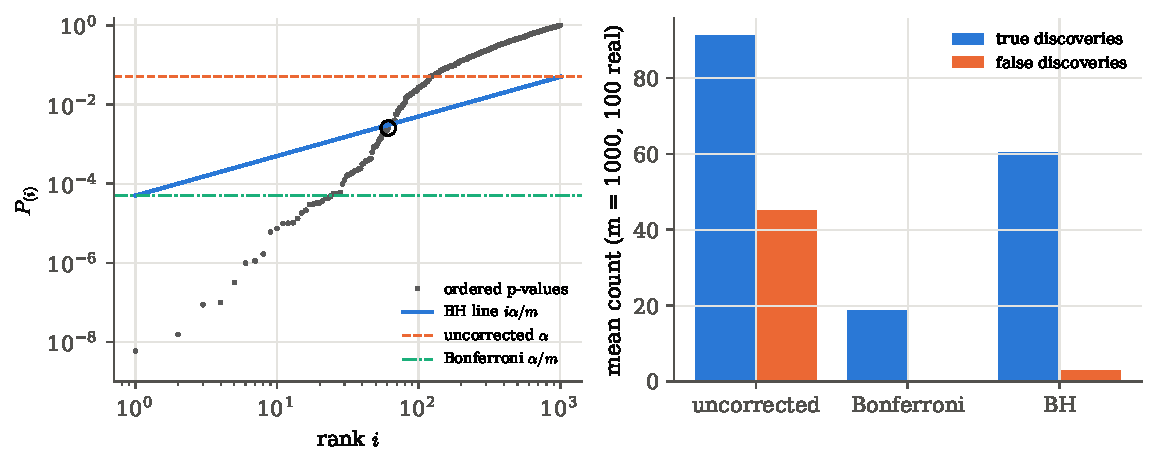
\includegraphics[width=\linewidth]{figures/ch04/bh_procedure.pdf}
\caption{Left: the thousand p-values of one simulated family, sorted, on
logarithmic axes. The real effects make the steep tail at small rank. The BH
threshold is the last p-value below the sloping line $i\alpha/m$ (circled);
the horizontal lines are the uncorrected and Bonferroni thresholds. Right: mean
numbers of true and false discoveries of the three procedures over $2000$
families.}
\label{4b:fig:bh}
\end{figure}

\begin{keyidea}[Two error rates for many tests]
The family-wise error rate $\Prob(V\ge1)$ is controlled by Bonferroni,
$P_i<\alpha/m$, for any dependence. The false discovery rate $\E(V/R)$ is
controlled by Benjamini--Hochberg, which rejects below the last crossing of
the line $i\alpha/m$. Use the first when a single false claim is costly (a
discovery), the second when a list of candidates will be followed up (a
screening).
\end{keyidea}

\subsection{The look-elsewhere effect in a mass scan}
\label{4b:sec:scan}

A resonance search is a multiple test with a continuum of tests: one for every
possible mass. (In this section $m$ is a mass, no longer a number of tests.)
\emph{What is done.} We do not know the mass, so for every hypothesised mass
$m$ we fit a signal of that mass and compute the likelihood-ratio statistic
$q_0(m)$ of the first part of the chapter. Its square root $Z(m)=\sqrt{q_0(m)}$
is the \newterm{local significance}, and $p_{\rm loc}=\Phi(-Z)$ the
\newterm{local p-value}. We then report the largest excess,
$q_{\max}=\max_mq_0(m)$.

\emph{Why the usual theory fails.} The mass exists only under the alternative:
with no signal, the background does not depend on $m$, so the null hypothesis
has no mass to fit. That is exactly the situation where Wilks' theorem does not
apply to the maximum \cite{GrossVitells2010}. \emph{The question} is then:
under the background-only hypothesis, how is the maximum over the scan
distributed?

\begin{workdef}[local and global p-value, trials factor]
The \newterm{local p-value} of the biggest bump is the probability, under the
background only, of an excess at least as large \emph{at its mass}. The
\newterm{global p-value} is the probability of an excess at least as large
\emph{anywhere in the search range}, $p_{\rm glob}=\Prob(q_{\max}\ge q_{\rm
obs}\given\Hnull)$. The \newterm{trials factor} is $p_{\rm glob}/p_{\rm loc}$.
\emph{Operational recipe:} simulate background-only data sets, scan each one
exactly as the data were scanned, record $q_{\max}$; $p_{\rm glob}$ is the
fraction with $q_{\max}\ge q_{\rm obs}$.
\end{workdef}

\paragraph{A simulated search.}
The script \pyname{code/ch04/17_bump_scan.py} generates a diphoton-like spectrum
of $\FourBScBtot$ background events in sixty $1\,$GeV bins from $100$ to
$160\,$GeV, falling exponentially with decay length $\FourBScSlope\,$GeV, and
searches for a Gaussian peak of width $\sigma_m=\FourBScSigM\,$GeV at
$\FourBScNmass$ masses between $105$ and $155\,$GeV in steps of $0.25\,$GeV. For
simplicity the background shape and normalisation are taken as known; in the
Gross--Vitells toy the normalisation is fitted, which changes the numbers, not
the method. At each mass the signal strength $\hat\mu\ge0$ maximises the binned
Poisson likelihood, and
\begin{equation}
  q_0(m)=2\Bigl[\sum_i n_i\ln\frac{b_i+\hat\mu s_i(m)}{b_i}-\hat\mu\Bigr],
  \qquad \hat\mu\ge0,
  \label{4b:eq:q0-scan}
\end{equation}
where $s_i(m)$ is the fraction of a unit signal at mass $m$ falling in bin $i$,
so that $\hat\mu$ counts signal events and $\sum_is_i=1$.

\pyfile[firstline=41,lastline=56,label={4b:lst:scan}]{code/ch04/17_bump_scan.py}{The scan: one-sided likelihood ratio at every mass, for many spectra at once}

The function takes a batch of spectra and returns $q_0$ at every mass for each
of them. \pyname{g0} is the slope of $\ln\Like$ at $\mu=0$. If it is negative,
the likelihood falls as soon as any signal is added, so the best non-negative
signal is zero and $q_0=0$. Otherwise Newton's method climbs the
log-likelihood, which is concave in $\mu$, starting from the linear estimate
$\sum s_i(n_i-b_i)/b_i\big/\sum s_i^2/b_i$; twelve iterations are plenty.
Arrays of shape (spectra, masses, bins) let numpy do all $500\times201$ fits of a
batch at once.

We took one background-only spectrum as ``the data'', choosing, among a
hundred generated ones, the spectrum whose largest local excess was closest to
$3\sigma$. \Cref{4b:fig:scan-spectrum} shows it. The best bump is at
$\FourBScMobs\,$GeV with $\hat\mu=\FourBScMuObs$ events, $q_0=\FourBScQobs$, local
significance $Z_{\rm loc}=\FourBScZloc$ and local p-value
$p_{\rm loc}=\FourBScPloc$. There is, of course, no particle.

\begin{figure}[htbp]
\centering
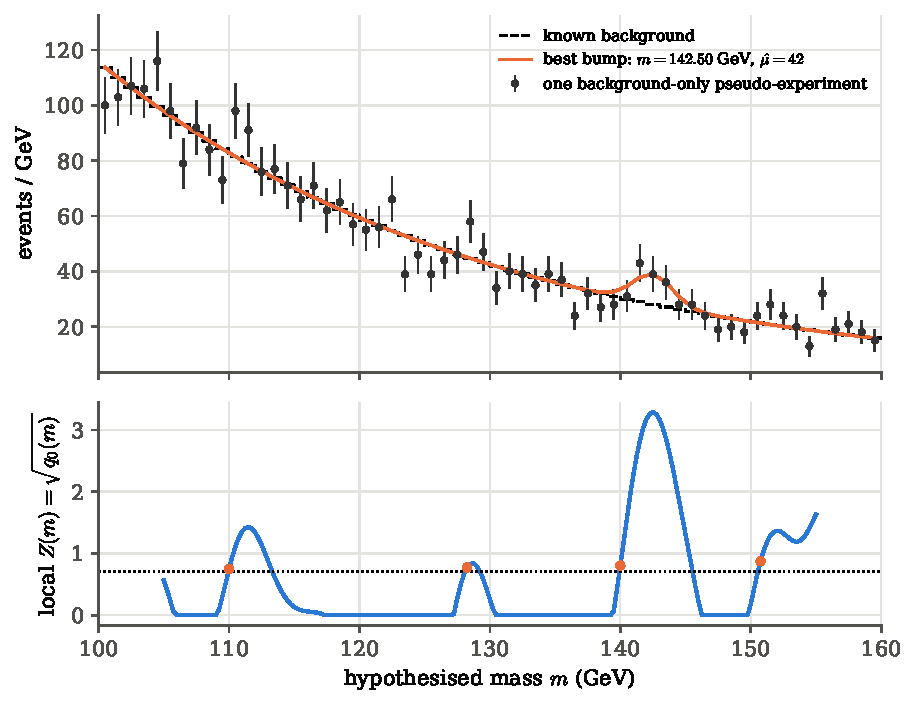
\includegraphics[width=0.85\linewidth]{figures/ch04/scan_spectrum.pdf}
\caption{Top: a background-only pseudo-experiment (points), the known
background (dashed) and the best fitted bump (orange). Bottom: the local
significance $\sqrt{q_0}$ as a function of the hypothesised mass. It is zero
wherever the data dip below the background, and the fluctuations are about as
wide as the mass resolution. The dotted line is the reference level
$\sqrt{0.5}$ used to count upcrossings (orange dots).}
\label{4b:fig:scan-spectrum}
\end{figure}

\emph{At one fixed mass} the results of the first part of the chapter still
hold. At $125\,$GeV, over $\FourBScToys$ background-only spectra, $q_0=0$ in
$\FourBScFracZero$ of them (the half-$\chi^2$ spike at zero) and
$\Prob(q_0>4)=\FourBScPfourMC$, against $\Phi(-2)=\FourBScPfourTh$. \emph{Over
all masses} the picture changes: a fraction $\FourBScPglob\pm\FourBScPglobErr$ of the
background-only spectra have $q_{\max}\ge\FourBScQobs$. So
\[
  p_{\rm loc}=\FourBScPloc\ (Z_{\rm loc}=\FourBScZloc),
  \qquad
  p_{\rm glob}=\FourBScPglob\ (Z_{\rm glob}=\FourBScZglob),
  \qquad
  \text{trials factor}\approx\FourBScTrials .
\]
A ``$\FourBScZloc\sigma$ bump'' is a $\FourBScZglob\sigma$ effect once we remember where we looked.
A local $3\sigma$ excess somewhere in this range appears in
$\FourBScPthreeGlob$ of background-only spectra, one in twenty-five.

\subsection{The global p-value without a million toys}
\label{4b:sec:gross-vitells}

The simulation needed $\FourBScToys$ scans to measure a global p-value of
$\FourBScPglob$. For a $5\sigma$ claim, $p\approx3\times10^{-7}$, it would need of order
$10^7$ scans, each a full fit \cite{GrossVitells2010}. Gross and Vitells, building
on a bound by Davies, found a way around this.

\emph{The event.} The largest excess is above some level $c$: $q_{\max}>c$.
\emph{How can it happen?} There are only two ways. Either $q_0$ is already
above $c$ at the lower end of the range, $m_{\rm lo}$, or $q_0(m)$ crosses the
level $c$ upwards at least once somewhere in the scan. Call $N(c)$ the number
of such \newterm{upcrossings}. Then
\begin{align}
  \Prob(q_{\max}>c)
  &\relby{1}{\le} \Prob\bigl(q_0(m_{\rm lo})>c\bigr)+\Prob\bigl(N(c)\ge1\bigr)
   \relby{2}{\le} p_{\rm loc}(c)+\E[N(c)] ,
  \label{4b:eq:davies}
\end{align}
\begin{explain}
  \item The union bound over the two ways of exceeding $c$.
  \item $\Prob(N\ge1)=\sum_{k\ge1}\Prob(N=k)\le\sum_kk\Prob(N=k)=\E N$; the
        first term is the local p-value at a fixed mass.
\end{explain}
and for large $c$ the bound becomes an equality, since two upcrossings of a high
level are rare \cite[(1)]{GrossVitells2010}. \emph{The remaining question:} how
does $\E[N(c)]$ depend on $c$? Treat $Z(m)$ as a smooth Gaussian process of
unit variance, a random curve along the mass axis. The rate at which it
crosses a level $u$ upwards is proportional to the density of $Z$ at $u$, that
is to $e^{-u^2/2}$ (Rice's formula). The proportionality constant depends on
how quickly $Z(m)$ forgets its value as $m$ changes, here on the mass
resolution, but not on $u$. With $q_0=Z^2$ and $u=\sqrt c$, this gives
$\E[N(c)]\propto e^{-c/2}$. So a count of upcrossings at one low reference
level $c_0$ fixes the whole curve \cite[(3)]{GrossVitells2010}:
\begin{equation}
  p_{\rm glob}(c)\ \approx\ p_{\rm loc}(c)+\E[N(c_0)]\,e^{-(c-c_0)/2}.
  \label{4b:eq:gv}
\end{equation}
At a low level upcrossings are frequent, so a handful of background-only
scans measures $\E[N(c_0)]$ well. With $c_0=0.5$ and only the first $100$ toys
we count $\E[N(c_0)]=\FourBScNzeroHundred$ (all $\FourBScToys$ give
$\FourBScNzeroAll$), and \eqref{4b:eq:gv} at $c=\FourBScQobs$ gives
$p_{\rm glob}\approx\FourBScPgv$, against $\FourBScPglob\pm\FourBScPglobErr$ from
the full simulation. \Cref{4b:fig:scan-tail} (left) compares the whole curves.

\paragraph{The trials factor grows with the significance.}
Divide \eqref{4b:eq:gv} by $p_{\rm loc}=\Phi(-Z)$, with $c=Z^2$, and use the
large-$Z$ tail estimate $\Phi(-Z)\approx e^{-Z^2/2}/(\sqrt{2\pi}\,Z)$ from the
first part of the chapter. Writing $\mathcal N_1=\E[N(c_0)]e^{c_0/2}$, so that
$\E[N(c)]=\mathcal N_1e^{-c/2}$,
\begin{align}
  \frac{p_{\rm glob}}{p_{\rm loc}}
  &\eqby{1} 1+\frac{\mathcal N_1e^{-Z^2/2}}{\Phi(-Z)}
   \relby{2}{\approx} 1+\mathcal N_1e^{-Z^2/2}\cdot\sqrt{2\pi}\,Z\,e^{Z^2/2}
   \eqby{3} 1+\sqrt{2\pi}\,\mathcal N_1Z .
  \label{4b:eq:trials}
\end{align}
\begin{explain}
  \item Divide \eqref{4b:eq:gv} by $p_{\rm loc}$ and insert $c=Z^2$.
  \item The Gaussian tail estimate.
  \item The exponentials cancel.
\end{explain}
The trials factor is not a fixed ``number of independent masses''. It grows
linearly with the local significance \cite[(12)]{GrossVitells2010}. (Gross and
Vitells write $1+\sqrt{\pi/2}\,\mathcal NZ$ for the two-sided statistic, whose
level crossings are twice as many, $\mathcal N=2\mathcal N_1$: the same formula.)
Here $\mathcal N_1=\FourBScNone$, so a local $3\sigma$ bump carries a trials
factor of about $\FourBScTrialsThreeAsym$ and our $\FourBScZloc\sigma$ bump about $\FourBScTrials$,
matching the toys (\cref{4b:fig:scan-tail}, right). \emph{Why does it grow?}
A higher level is crossed only near the top of a fluctuation, and the part of
the fluctuation above the level gets narrower as the level rises. A pre-chosen
mass must land on that narrow top, so the local p-value falls faster than the
chance that the top appears somewhere in the range. For a local
$5\sigma$ excess in this search, \eqref{4b:eq:gv} gives
$p_{\rm glob}=\FourBScPgvFive$, a global significance of $\FourBScZgvFive\sigma$,
from $p_{\rm loc}=\FourBScPlocFive$: no simulation of $10^7$ scans needed.

\begin{figure}[htbp]
\centering
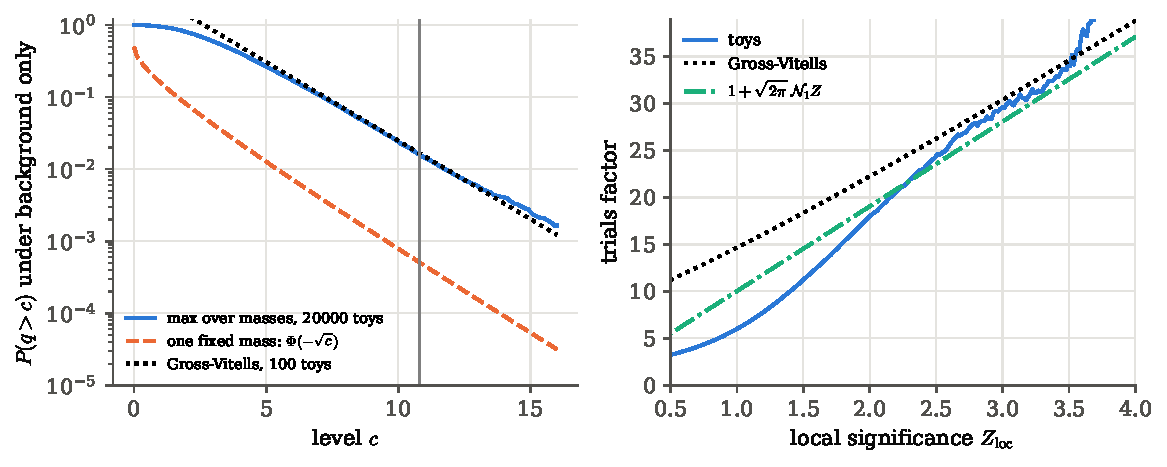
\includegraphics[width=\linewidth]{figures/ch04/scan_tail.pdf}
\caption{Left: the probability, with background only, that the largest excess
exceeds a level $c$ anywhere in the scan (blue, $20\,000$ toys), compared with
the local probability at one fixed mass (orange dashed) and the Gross--Vitells
formula calibrated on $100$ toys (black dotted). The vertical line marks the
observed bump. Right: the trials factor, global over local p-value, as a
function of the local significance, with the Gross--Vitells prediction and its
asymptotic straight line.}
\label{4b:fig:scan-tail}
\end{figure}

\paragraph{What ``elsewhere'' means.}
The global p-value refers to the range of the scan, and that range must be
fixed before the data are seen. But other decay channels, other signal widths
and other analyses in the same experiment are also places one could have
looked. There is no unique answer to how far ``elsewhere'' extends. That is why
experiments quote the local significance together with the global one for a
stated range.

\begin{inpractice}[How searches report the look-elsewhere effect]
A search at a collider quotes the local p-value of the largest excess, and a
global p-value over a stated mass range, obtained from background-only toys
where affordable and from the upcrossing formula \eqref{4b:eq:gv} otherwise. The
test statistic is the profile likelihood ratio of \cite{Cowan2011} with the
nuisance parameters (background shape, energy scale) fitted in every toy. The
same formula applies to any scan over a parameter that exists only under the
signal hypothesis: the position of a localised feature in the CMB power
spectrum, the frequency of an oscillation in a Galactic-centre spectrum, the
sky position and frequency of a gravitational-wave template.
\end{inpractice}

The Bayesian language of \cref{ch:05} handles the same problem differently.
The unknown mass gets a prior spread over the search range. The evidence for a
signal is then automatically diluted by the fraction of the range that is
compatible with the bump. This dilution, the \emph{Occam factor}, plays the
role of the trials factor.

Two things were held simple in this scan: the background shape was known, and
the only question was discovery. A real search fits the background together
with its systematic uncertainties, and when nothing is found it must say which
signal strengths are excluded. \Cref{4b:sec:templates} builds the likelihood
with nuisance parameters that the scan's $q_0(m)$ then uses, and
\cref{4b:sec:limits} turns the same profile likelihood ratio into upper limits,
$\mathrm{CL}_s$ and the expected band.
\section{A search as a likelihood: templates and nuisance parameters}
\label{4b:sec:templates}

In the summer of 2012 two experiments at the LHC showed the same kind of plot: a
histogram of the invariant mass of photon pairs, a smooth background falling from
left to right, and a small bump near $125\,$GeV. The question put to that histogram
was simple to say. Is there a signal in it, and how big is it? The size is quoted
as a \newterm{signal strength} $\mu$ \unpack{the number of signal events seen,
divided by the number the Standard Model predicts}, so $\mu=0$ means ``background
only'' and $\mu=1$ means ``the predicted Higgs boson''.

But the number of signal events the Standard Model ``predicts'' in that histogram is
not known exactly. It depends on how many collisions were recorded (the luminosity),
on how often a real photon pair passes the selection (the efficiency), and on where
exactly a $125\,$GeV peak lands on the measured mass axis (the photon energy scale).
Each of these was measured in a separate calibration, each to a few per cent. The
background level under the peak is not predicted at all; it has to be read off the
data. So the honest statement of the experiment's knowledge is not one number for
the prediction but a prediction that depends on several uncertain inputs, each of
which has been measured somewhere. Writing all of that as one likelihood is what
turns a histogram into a measurement of $\mu$, and the same construction serves
any search: a dark-matter recoil spectrum, a line in an X-ray spectrum, an excess of
gravitational-wave triggers above the noise.

\paragraph{The question in words.}
\begin{enumerate}[label=\arabic*.]
  \item What is the probability of the whole histogram, given a signal strength and
        everything else the prediction depends on?
  \item What is a ``systematic uncertainty'' in this language, and why does it
        become a parameter with a measurement of its own?
  \item How do we remove those extra parameters to speak about $\mu$ alone, and how
        does this compare with the profile likelihood of \cref{ch:03} and with the
        Bayesian marginalisation of \cref{ch:05}?
\end{enumerate}

\subsection{The probability of a histogram}
\label{4b:sec:binned-like}

Start with what is recorded. Each selected event has a measured mass $x$, and the
events are sorted into bins, $n_1,\dots,n_N$ events in bins $1,\dots,N$. What is the
probability of this list of counts?

\emph{The inputs.} Two physical assumptions carry everything, the same ones that
gave the Poisson distribution in \cref{ch:02}: the collisions that produce
selected events happen independently of each other, one at a time, and at a rate
that does not change during the run. Then the total number of selected events $N_{\rm tot}$
is Poisson with some mean $\nu_{\rm tot}$. One more input, also physical: each event
lands in bin $i$ with a probability $p_i$ that does not depend on the other events.

\emph{The question:} the bins split one Poisson stream into $N$ pieces; what is the
joint probability of the counts in the pieces? Given the total, the counts are
multinomial (each of the $N_{\rm tot}$ events chooses its bin independently). So,
with $N_{\rm tot}=\sum_in_i$ and $\nu_i=\nu_{\rm tot}p_i$,
\begin{align}
  \Prob(n_1,\dots,n_N)
  &\eqby{1} \Prob(N_{\rm tot})\,\Prob(n_1,\dots,n_N\given N_{\rm tot})
   \eqby{2} \frac{\nu_{\rm tot}^{N_{\rm tot}}e^{-\nu_{\rm tot}}}{N_{\rm tot}!}\,
            \frac{N_{\rm tot}!}{n_1!\cdots n_N!}\,p_1^{n_1}\cdots p_N^{n_N}
  \notag\\
  &\eqby{3} \prod_{i=1}^N\frac{(\nu_{\rm tot}p_i)^{n_i}}{n_i!}\,e^{-\nu_{\rm tot}p_i}
   \eqby{4} \prod_{i=1}^N\frac{\nu_i^{n_i}}{n_i!}\,e^{-\nu_i} .
  \label{4b:eq:split}
\end{align}
\begin{explain}
  \item The product rule: first the total, then how it is shared among the bins.
  \item Poisson for the total; multinomial for the sharing.
  \item The $N_{\rm tot}!$ cancel; write $\nu_{\rm tot}^{N_{\rm tot}}=\prod_i\nu_{\rm tot}^{n_i}$
        and $e^{-\nu_{\rm tot}}=\prod_ie^{-\nu_{\rm tot}p_i}$, using $\sum_in_i=N_{\rm tot}$
        and $\sum_ip_i=1$.
  \item Name the mean of bin $i$, $\nu_i=\nu_{\rm tot}p_i$.
\end{explain}
The joint probability factorises: the bin counts are \emph{independent} Poisson
variables, each with its own mean. Nothing about the bins being ``far apart'' was
needed; the independence comes from the Poisson total.

\emph{Signal plus background.} In each bin the events come from two independent
sources, signal and background. The sum of two independent Poisson counts is Poisson
with the summed mean (\cref{ch:02}), so the mean of bin $i$ is
\begin{equation}
  \nu_i=\mu\,s_i+b_i,
  \qquad
  s_i=S\,f_i,\quad b_i=B\,g_i .
  \label{4b:eq:nu-template}
\end{equation}
Here $S$ and $B$ are the expected total numbers of signal (for $\mu=1$) and
background events, and $f_i$, $g_i$ are the fractions of each falling in bin $i$
\cite[(2)--(4)]{Cowan2011}.

\begin{workdef}[template]
A \newterm{template} is the predicted histogram of one process: the fractions $f_i$
(signal) or $g_i$ (background) of its events expected in each bin \unpack{a shape,
normalised to one, usually made by running the detector simulation on many simulated
events}. The analysis fits the data as a sum of templates with free or constrained
normalisations. \emph{Operationally:} histogram the simulated events of each process
with the binning of the data, divide by their number.
\end{workdef}

\paragraph{Example: the search we will follow.}
Our pseudo-experiment has sixty $1\,$GeV
bins from $100$ to $160\,$GeV. The background template $g_i$ is a falling exponential
of decay length $\FourBTpSlope\,$GeV with $B=\FourBTpBtot$ expected events; the signal
template $f_i$ is a Gaussian peak at $125\,$GeV with the mass resolution
$\sigma_m=\FourBTpSigM\,$GeV and $S=\FourBTpSzero$ expected events. The data were
generated with $\mu=1$ by the library \pyname{code/ch04/lib_templates.py}. With every input known, the likelihood would be
\eqref{4b:eq:split} with \eqref{4b:eq:nu-template} inserted, a function of $\mu$
alone, exactly the likelihood that was scanned over masses in \cref{4b:sec:scan}.

\subsection{Systematic uncertainties become nuisance parameters}
\label{4b:sec:nuisance-hep}

Now let the inputs be uncertain, as they are. Take the three of our example one at a
time, and ask of each: \emph{how does it change the predicted counts, and who
measured it?}
\begin{itemize}[itemsep=1pt,leftmargin=1.2em]
  \item \emph{The background normalisation} $\beta$. The background is $\beta B$
        instead of $B$. Nobody predicts $\beta$ well; the data measure it, from the
        bins away from the peak (the \newterm{sidebands}) or from a separate
        \newterm{control region} chosen to contain no signal.
  \item \emph{The signal yield} $\kappa$, luminosity times efficiency relative to its
        nominal value. The signal is $\mu\kappa S$ instead of $\mu S$. A calibration
        measured $\kappa$: its result was $a_\kappa=1$ with an error of
        $\sigma_\kappa=\FourBTpSigKappa$.
  \item \emph{The energy scale} $\delta$. A mis-calibration shifts every measured
        photon energy, so the peak sits at $125+\delta$ and the signal template
        becomes $f_i(125+\delta)$. The scale was calibrated on the well-known $Z$
        boson peak: $a_\delta=0$ with $\sigma_\delta=\FourBTpSigDelta\,$GeV.
\end{itemize}
Each of these is a parameter the predicted counts depend on and that we do not want
to report: a \newterm{nuisance parameter} (\cref{ch:03}). The first one is
different from the other two in kind. It changes the background, which the
histogram itself measures. The other two change the signal, which the histogram
cannot separate from $\mu$: a larger $\kappa$ and a smaller $\mu$ give the same peak.
Only the calibration can tell them apart.

\emph{What should be done with $\kappa$?} There are three candidates. We could fix it
at $1$; that pretends the calibration was perfect, and \cref{ch:03} showed what this
costs: intervals too short by the factor $\sqrt{1-\rho^2}$ and coverage below its
promise. We could leave it free with no information; then $\mu$ and $\kappa$ are
completely degenerate and $\mu$ is not measured at all. Or we could use what the
calibration actually found. The calibration is a measurement like any other. Its
result $a_\kappa$ is a random number whose distribution depends on the true
$\kappa$: Gaussian, with mean $\kappa$ and standard deviation $\sigma_\kappa$. The
probability of the calibration result, read as a function of $\kappa$, is its
likelihood. The calibration and the search are independent measurements, so the
probability of both results is the product of their probabilities. This gives the
complete likelihood
\begin{equation}
  \Like(\mu,\bm\theta)
  =\prod_{i=1}^{N}\frac{\bigl(\mu\,s_i(\bm\theta)+b_i(\bm\theta)\bigr)^{n_i}}{n_i!}\,
     e^{-(\mu s_i(\bm\theta)+b_i(\bm\theta))}
   \;\times\;\prod_{k}p\bigl(a_k\given\theta_k\bigr) ,
  \label{4b:eq:full-like}
\end{equation}
with $\bm\theta=(\beta,\kappa,\delta)$ the nuisance parameters and one factor
$p(a_k\given\theta_k)$ for each auxiliary measurement \cite[(6)]{Cowan2011},
\cite{Cranmer2015}. For a calibration quoted as $a_k\pm\sigma_k$,
\begin{equation}
  p(a_k\given\theta_k)=\frac{1}{\sqrt{2\pi}\,\sigma_k}\,
  \exp\Bigl[-\frac{(a_k-\theta_k)^2}{2\sigma_k^2}\Bigr],
  \label{4b:eq:constraint}
\end{equation}
a \newterm{constraint term}. If the auxiliary measurement is itself a count, a
control region with $m$ events expected to be $\tau\beta B$, the factor is Poisson
instead; \cref{4b:sec:onoff-hep} works that case out.

\begin{pitfall}[A constraint term is a likelihood, not a prior]
The Gaussian factor \eqref{4b:eq:constraint} looks like a prior on $\theta_k$, and in a
Bayesian analysis it is combined with one. But in \eqref{4b:eq:full-like} it is the
probability of an observed number, the calibration result $a_k$, given the
parameter. In pseudo-experiments, therefore, $a_k$ must be \emph{generated} afresh
together with the histogram (the calibration would have come out differently too),
not held at its observed value \cite{Cowan2011}.
\end{pitfall}

A nuisance parameter can change the \emph{shape} of a template, not only its size: the
energy scale moves the peak. Real analyses rarely have a formula like
$f_i(125+\delta)$. They have the nominal template and two shifted ones, made by
re-running the simulation with the calibration moved up and down by one standard
deviation, and they interpolate between them bin by bin \cite{Cranmer2015}. With
$\theta$ measured in units of its calibration error, the simplest choice is
\begin{equation}
  f_i(\theta)=f_i^{0}+\theta\,\bigl(f_i^{+}-f_i^{0}\bigr)\quad(\theta\ge0),
  \qquad
  f_i(\theta)=f_i^{0}+\theta\,\bigl(f_i^{0}-f_i^{-}\bigr)\quad(\theta<0),
  \label{4b:eq:morph}
\end{equation}
so that $\theta=0,\pm1$ give back the three simulated templates, and the constraint
term is a standard normal in $\theta$.

\Cref{4b:fig:like-structure} shows how the pieces of \eqref{4b:eq:full-like} hang
together: every parameter predicts some measurements, every measurement
contributes one factor, and the likelihood is their product.

\begin{figure}[htbp]
\centering
\begin{tikzpicture}[
  par/.style={draw=formblue,thick,rounded corners=2pt,inner sep=4pt,font=\small,fill=formblue!6},
  meas/.style={draw=fibreorange,thick,rounded corners=2pt,inner sep=4pt,font=\small,fill=fibreorange!6,align=center},
  arr/.style={->,>=stealth,thick,black!55}]
  \node[par] (mu) at (0,2.2) {$\mu$ signal strength};
  \node[par] (be) at (4.2,2.2) {$\beta$ background};
  \node[par] (ka) at (-4.2,2.2) {$\kappa$ signal yield};
  \node[par] (de) at (-4.2,0.9) {$\delta$ energy scale};
  \node[meas] (hist) at (0,-0.6) {mass histogram $n_i$\\[1pt]\footnotesize Poisson, mean $\mu\kappa S f_i(125+\delta)+\beta B g_i$};
  \node[meas] (ak) at (-5.0,-2.3) {calibration $a_\kappa$\\[1pt]\footnotesize Gaussian, mean $\kappa$};
  \node[meas] (ad) at (-1.7,-2.3) {$Z$-peak scale $a_\delta$\\[1pt]\footnotesize Gaussian, mean $\delta$};
  \node[meas] (cr) at (3.6,-2.3) {control region $m$\\[1pt]\footnotesize Poisson, mean $\tau\beta B$};
  \draw[arr] (mu) -- (hist);
  \draw[arr] (be) -- (hist);
  \draw[arr] (ka) -- (hist);
  \draw[arr] (de) -- (hist);
  \draw[arr] (ka.west) to[out=200,in=100] (ak.north);
  \draw[arr] (de.south) to[out=-80,in=90] (ad.north);
  \draw[arr] (be.east) to[out=-20,in=60] (cr.north east);
\end{tikzpicture}
\caption{The structure of a search likelihood. Parameters (blue) predict the
measurements (orange). The signal strength $\mu$ is predicted only by the main
histogram, where it always appears multiplied by the signal yield $\kappa$; the
calibrations measure $\kappa$ and the energy scale $\delta$ on their own, and the
background normalisation $\beta$ is measured by the histogram's sidebands and,
optionally, by a control region. The likelihood is the product of one factor per
measurement.}
\label{4b:fig:like-structure}
\end{figure}

\subsection{Removing the nuisance parameters: fix, profile or integrate}
\label{4b:sec:profile-hep}

We have met this problem twice before, and it is worth recalling both times
concretely. In \cref{ch:03}, in the section on nuisance parameters and the profile
likelihood, a counting experiment saw $\ThreeBProfNon$ events in a signal region and
$\ThreeBProfNoff$ in a control region of the same size. The estimated signal was
$\hat s=\ThreeBProfS$. Holding the background fixed at its best value gave the error
$^{+\ThreeBCondHi}_{-\ThreeBCondLo}$, letting it adjust (profiling) gave
$^{+\ThreeBProfHi}_{-\ThreeBProfLo}$, and in simulated repetitions only the profile
interval covered the truth $68\%$ of the time ($\ThreeBProfCover$ against
$\ThreeBCondCover$). In \cref{ch:05}, in the section on nuisance parameters, the
Bayesian removed a background level by integrating the joint posterior over it, and
found that integrating and maximising agree when the likelihood is Gaussian, and
differ by a ``volume'' factor (how many values of the nuisance parameter fit almost as
well) when it is not. The search likelihood \eqref{4b:eq:full-like} is the same
problem with three differences: there are several nuisance parameters, their
information comes from separate auxiliary measurements, and the goal is not only an
interval but the test statistics of \cref{4b:sec:limits}.

The frequentist tool is the same as in \cref{ch:03}: the \newterm{profile likelihood
ratio}
\begin{equation}
  \lambda(\mu)=\frac{\Like\bigl(\mu,\hat{\hat{\bm\theta}}(\mu)\bigr)}{\Like(\hat\mu,\hat{\bm\theta})},
  \qquad 0\le\lambda(\mu)\le1,
  \label{4b:eq:lambda}
\end{equation}
where $\hat\mu,\hat{\bm\theta}$ maximise $\Like$ over everything, and
$\hat{\hat{\bm\theta}}(\mu)$ maximises it over the nuisance parameters with $\mu$ held
fixed \cite[(7)]{Cowan2011}. The double hat is read ``the best nuisance parameters
for this $\mu$''. The numerator can never exceed the denominator, because the
denominator is maximised over more.

Set the three ways of removing $\bm\theta$ side by side.
\begin{itemize}[itemsep=1pt,leftmargin=1.2em]
  \item \emph{Fix} $\bm\theta$ at $\hat{\bm\theta}$: the conditional likelihood. It
        keeps only the statistical fluctuation of the histogram. Its width is the
        ``statistical error''.
  \item \emph{Profile}: at each $\mu$, let $\bm\theta$ take its best value. The
        width of $-2\ln\lambda(\mu)$ is the total error.
  \item \emph{Integrate}: give $\bm\theta$ a prior (here flat in $\beta$, and the
        calibrations' Gaussians, which are then genuinely priors) and integrate the
        joint posterior over it, as in \cref{ch:05}.
\end{itemize}
\emph{What is the same?} For a Gaussian likelihood all three are Gaussians in $\mu$;
profiling and integrating give the same width, the full variance $V_{\mu\mu}$, and
fixing gives the smaller $1/F_{\mu\mu}$ (\cref{ch:03}). \emph{What differs?} The
meaning: the profile curve is a likelihood ratio whose sampling distribution we will
compute, the marginal is a posterior density that needs a prior. And the shape, as
soon as the likelihood is not Gaussian, through the volume factor.

\emph{How large is the systematic part of the error?} Analyses quote it separately,
by subtraction. For one nuisance parameter, \cref{ch:03} found
$1/F_{\mu\mu}=V_{\mu\mu}(1-\rho^2)$, with $\rho$ the correlation of $\hat\mu$ and
$\hat\theta$, so
\begin{equation}
  \sigma_{\rm syst}^2
  \equiv\sigma_{\rm tot}^2-\sigma_{\rm stat}^2
  \eqby{1} V_{\mu\mu}-\frac{1}{F_{\mu\mu}}
  \eqby{2} V_{\mu\mu}-V_{\mu\mu}(1-\rho^2)
  =\rho^2\,V_{\mu\mu} .
  \label{4b:eq:syst}
\end{equation}
\begin{explain}
  \item The profile width is $\sqrt{V_{\mu\mu}}$, the conditional width $\sqrt{1/F_{\mu\mu}}$.
  \item The identity of \cref{ch:03}.
\end{explain}
The ``systematic error'' is the part of the variance of $\hat\mu$ that it shares with
the nuisance parameter through their correlation. It adds to the statistical one in
quadrature by construction, not by assumption. With several nuisance parameters the
same subtraction is used, and $\rho^2$ becomes the fraction of the variance of
$\hat\mu$ that all of them together account for.

\paragraph{Example: the template fit.}
The script \pyname{code/ch04/19_hep_templates.py} maximises \eqref{4b:eq:full-like}
for our pseudo-data. The heart of it is the negative log-likelihood:

\pyfile[firstline=33,lastline=46,label={4b:lst:nll}]{code/ch04/lib_templates.py}{The search likelihood: Poisson bins times two Gaussian constraint terms}

\pyname{expected} builds the mean counts \eqref{4b:eq:nu-template} with the three
nuisance parameters inserted; \pyname{nll} returns $-\ln\Like$ without the constants
$\ln n_i!$ and $\ln\sqrt{2\pi}\sigma_k$, which cancel in every ratio. A numerical
minimiser (\pyname{scipy.optimize.minimize}) does the rest, over all four parameters
for the denominator of \eqref{4b:eq:lambda}, over the three nuisance parameters at
each fixed $\mu$ for the numerator. The global fit gives
\[
  \hat\mu=\FourBTpMuHat,\qquad
  \hat\beta=\FourBTpBetaHat,\qquad
  \hat\kappa=\FourBTpKappaHat,\qquad
  \hat\delta=\FourBTpDeltaHat\,\text{GeV}.
\]
Why is $\hat\kappa$ exactly the calibration value? Because the histogram sees only the
product $\mu\kappa$. Whatever the product the histogram prefers, the fit can reach it
with any $\kappa$ by moving $\mu$, so it sets $\kappa$ where its own measurement, the
calibration, wants it. The energy scale, in contrast, is pulled a little by the data:
the peak in the histogram sits slightly below $125\,$GeV, and the fit moves it by a
fraction of the calibration error.

\Cref{4b:fig:templates} (right) shows the three curves. Read at
$-2\ln(\Like/\Like_{\max})=1$:
\[
  \text{fixed: }\hat\mu^{+\FourBTpCondHi}_{-\FourBTpCondLo},
  \qquad
  \text{profile: }\hat\mu^{+\FourBTpProfHi}_{-\FourBTpProfLo},
  \qquad
  \text{marginal: }\FourBTpMargMode^{+\FourBTpMargHi}_{-\FourBTpMargLo}.
\]
So $\sigma_{\rm stat}=\FourBTpSigStat$, $\sigma_{\rm tot}=\FourBTpSigTot$, and by
\eqref{4b:eq:syst} $\sigma_{\rm syst}=\FourBTpSigSyst$. Most of the systematic part is the
$10\%$ yield calibration: since the histogram measures $\mu\kappa$, a $10\%$ error on
$\kappa$ is a $10\%$ error on $\mu$, about $0.1\,\hat\mu\approx0.11$, and
$\sqrt{\FourBTpSigStat^2+0.11^2}\approx0.33$. Profiling and marginalising nearly agree: the marginal peaks slightly lower, at
$\FourBTpMargMode$, with almost the same width, and the largest difference between the two curves inside the
plotted interval is $\FourBTpMaxDiffPM$ in $-2\ln$. That is the volume effect of
\cref{ch:05} at work, small here because the likelihood is close to Gaussian. The
sizes are the lesson. A $1.5\,$GeV resolution and $\FourBTpBtot$ background events make
the statistical error dominant; a ten times larger data set would shrink
$\sigma_{\rm stat}$ by $\sqrt{10}$ and leave $\sigma_{\rm syst}$ untouched, and the
calibration would then limit the measurement.

\begin{figure}[htbp]
\centering
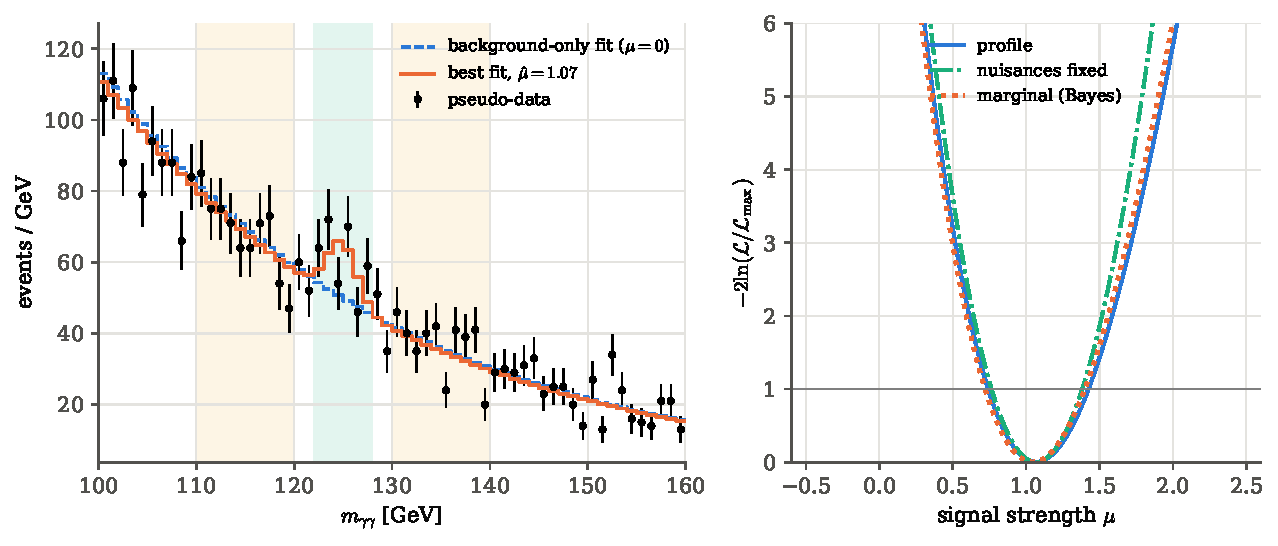
\includegraphics[width=\linewidth]{figures/ch04/hep_templates.pdf}
\caption{Left: the pseudo-data (points), the best background-only fit (blue dashed)
and the best signal-plus-background fit (orange). The green band is the signal
window and the yellow bands the sidebands used by the counting version of the search.
Right: three ways of turning the four-parameter likelihood into a curve for $\mu$.
Fixing the nuisance parameters gives the narrowest curve (the statistical error);
profiling them gives the total error; integrating them with priors (Bayes) gives
nearly the same curve, slightly shifted towards smaller $\mu$. The grey line at
one marks the $68\%$ interval.}
\label{4b:fig:templates}
\end{figure}

\subsection{The smallest search: a signal window and its sidebands}
\label{4b:sec:onoff-hep}

Every piece of the template likelihood can be seen working, and solved by hand, in a
stripped-down version of the same search. Keep only two numbers from the histogram:
the count $n$ in a signal window around the peak, $122$--$128\,$GeV, and the count
$m$ in two sidebands, $110$--$120$ and $130$--$140\,$GeV (\cref{4b:fig:templates},
left). In the window we expect $\mu s+b$ events, where $s=\FourBTpSwin$ is the
nominal signal falling in the window and $b$ the unknown background. In the
sidebands we expect $\tau b$, where $\tau=\FourBTpTau$ is the ratio of the background
template integrated over the sidebands to its integral over the window. The shape is
taken as known; only its normalisation $b$ is not. The sidebands are the control
region and $b$ is the nuisance parameter. The likelihood is two Poisson factors
\cite[(90)]{Cowan2011},
\begin{equation}
  \ln\Like(\mu,b)=n\ln(\mu s+b)-(\mu s+b)+m\ln(\tau b)-\tau b+\text{const},
  \label{4b:eq:onoff}
\end{equation}
the on/off likelihood of \cref{ch:03} with $k$ renamed $\tau$ and the signal written
as $\mu s$.

\emph{The global maximum.} Setting the two derivatives to zero,
\begin{align}
  \frac{\partial\ln\Like}{\partial\mu}
  &\eqby{1} s\Bigl(\frac{n}{\mu s+b}-1\Bigr)=0
   \;\Rightarrow\; \hat\mu s+\hat b=n,
  \notag\\
  \frac{\partial\ln\Like}{\partial b}
  &\eqby{2} \frac{n}{\mu s+b}-1+\frac{m}{b}-\tau=0
   \;\Rightarrow\;\hat b=\frac{m}{\tau},
   \qquad \hat\mu=\frac{n-m/\tau}{s} .
  \label{4b:eq:onoff-mle}
\end{align}
\begin{explain}
  \item Only the first two terms of \eqref{4b:eq:onoff} contain $\mu$.
  \item By the first equation the first two terms cancel, leaving $m/b=\tau$; then
        $\hat\mu s=n-\hat b$.
\end{explain}
In words: the sidebands estimate the background, scaled down to the window by $\tau$,
and the signal is what is left over. With $n=\FourBTpNon$ and $m=\FourBTpNoff$,
$\hat b=\FourBTpBhatOO$ and $\hat\mu=\FourBTpMuOO$. We allow $\hat\mu<0$ here: it is
whatever value maximises the likelihood, as long as the mean count $\mu s+b$ stays
positive. \Cref{4b:sec:limits} needs this.

\emph{The best background for a given $\mu$.} Hold $\mu$ fixed and solve only the
second equation of \eqref{4b:eq:onoff-mle}:
\begin{align}
  0&\eqby{1} n\,b-b(\mu s+b)+m(\mu s+b)-\tau b(\mu s+b)
  \notag\\
   &\eqby{2} -(1+\tau)\,b^2+\bigl[n+m-(1+\tau)\mu s\bigr]\,b+m\mu s ,
  \notag\\
  \hat{\hat b}(\mu)
  &\eqby{3} \frac{A}{2(1+\tau)}+\sqrt{\frac{A^2+4(1+\tau)\,m\,\mu s}{4(1+\tau)^2}},
  \qquad A=n+m-(1+\tau)\mu s .
  \label{4b:eq:bhh}
\end{align}
\begin{explain}
  \item Multiply $\partial\ln\Like/\partial b=0$ by $b(\mu s+b)>0$.
  \item Collect powers of $b$.
  \item The quadratic formula; for $\mu>0$ the constant term $m\mu s$ is positive, so
        the roots have opposite signs and only the $+$ root is a background.
\end{explain}
This is \cite[(93)]{Cowan2011}, and the same quadratic as in \cref{ch:03}. At $\mu=0$
the square root equals $A/(2(1+\tau))$ and
$\hat{\hat b}(0)=(n+m)/(1+\tau)$: with no signal, the window and the sidebands are
pooled into one background measurement. Here $\hat{\hat b}(0)=\FourBTpBhhOO$, more
than $\hat b$, because the pooled estimate also uses the excess in the window.

\emph{The discovery statistic.} For $\hat\mu>0$, $q_0=-2\ln\lambda(0)$. At the global
maximum $\hat\mu s+\hat b=n$ and $\tau\hat b=m$; at $\mu=0$ the window mean is
$\hat{\hat b}(0)$ and the sideband mean $\tau\hat{\hat b}(0)$, and the two linear
terms add up to $(1+\tau)\hat{\hat b}(0)=n+m$. So
\begin{align}
  q_0
  &\eqby{1} 2\Bigl[\bigl(n\ln n-n+m\ln m-m\bigr)
          -\bigl(n\ln\hat{\hat b}(0)+m\ln\tau\hat{\hat b}(0)-(n+m)\bigr)\Bigr]
  \notag\\
  &\eqby{2} 2\Bigl[n\ln\frac{n}{\hat{\hat b}(0)}+m\ln\frac{m}{\tau\,\hat{\hat b}(0)}\Bigr].
  \label{4b:eq:q0-onoff}
\end{align}
\begin{explain}
  \item \eqref{4b:eq:onoff} at the two maxima, using the values just listed.
  \item The $-(n+m)$ terms cancel; combine the logarithms.
\end{explain}
The numbers give $q_0=\FourBTpQzeroOO$, a significance $Z=\sqrt{q_0}=\FourBTpZOO$
(\cref{4b:sec:wald-asym} shows why the square root is the significance even with a
nuisance parameter). Compare with two neighbours.
\begin{itemize}[itemsep=1pt,leftmargin=1.2em]
  \item \emph{The background known exactly}, $b=\FourBTpBwin$: the formula of the first
        part of the chapter, $q_0=2[n\ln(n/b)-(n-b)]$, gives $Z=\FourBTpZKB$.
  \item \emph{The full template fit} of \cref{4b:sec:profile-hep}, with three nuisance
        parameters: $Z=\sqrt{q_0}=\FourBTpZzero$.
\end{itemize}
One pseudo-experiment is a poor judge of which method is better: all three values of
$Z$ move with the luck of the same data. The expected significances, computed with the
Asimov data set of \cref{4b:sec:asimov}, do not: $\FourBTpZAOO$ for the window with
sidebands, $\FourBTpZAKB$ with the background known, and $\FourBTpZA$ for the template
fit. Measuring the background instead of knowing it costs significance. The template
fit wins it back, because it uses every bin, each weighted by its own ratio of signal
to background, instead of a window with a hard edge.

The size of the cost is easiest to see in the Gaussian limit. $\hat\mu=(n-m/\tau)/s$ is
a difference of independent counts, so its variance is about
$(n+m/\tau^2)/s^2$, an error of $\FourBTpSigOO$; with the background known it would be
$\sqrt n/s=\FourBTpSigOOKB$. The control region adds the term $m/\tau^2\approx b/\tau$:
a control region $\tau$ times larger than the window adds a fraction $1/\tau$ of the
background variance.

The lesson in one line: a systematic uncertainty is a parameter with a measurement of
its own, and the search likelihood is the product of the main measurement and those
auxiliary measurements.

\section[Discovery and exclusion: $q_0$, $\tilde q_\mu$, CL$_s$, Brazil band]{Discovery and exclusion with nuisance parameters: $q_0$, $\tilde q_\mu$, CL$_s$ and the Brazil band}
\label{4b:sec:limits}

The discovery statistic $q_0$ has appeared twice already. In the first part of the
chapter, a count $N$ on a \emph{known} background $b$ gave
$q_0=2[N\ln(N/b)-(N-b)]$ for $N>b$ and zero otherwise; with background only it is
half the time zero and otherwise $\chi^2_1$, so its tail is $\Phi(-\sqrt{q_0})$ and the
significance is simply $Z=\sqrt{q_0}$. For Cowan's peak of $11$ events on an expected $3.2$ this gave
$Z=\FourAWkZwilks$, against $\FourAWkZexact$ from the exact Poisson tail. In
\cref{4b:sec:scan} the same $q_0$ was computed at every hypothesised mass, again with
the background known, and the largest one needed the look-elsewhere correction. The
statistic is the same now; three things are new. The background and the calibrations
are nuisance parameters, profiled in $q_0$, and we need to know whether
$Z=\sqrt{q_0}$ survives that. We need a second statistic for \emph{excluding} a
signal, and the distribution of both statistics when the signal is present, to say
what an experiment can expect. And we need a rule for exclusion that does not reward
an experiment for a lucky downward fluctuation.

\paragraph{The question in words.}
\begin{enumerate}[label=\arabic*.]
  \item With nuisance parameters, which number measures how badly the data disagree
        with ``no signal'', and which with ``a signal of strength $\mu$''?
  \item What are their distributions, without simulating millions of experiments?
  \item Before looking at the data, what discovery significance and what limit should
        the experiment expect, and how far from it may the observed values reasonably
        fall?
  \item Why do the LHC experiments exclude with CL$_s$ rather than with the plain
        p-value?
\end{enumerate}

\subsection{Three statistics built from the profile likelihood ratio}
\label{4b:sec:three-stats}

All three statistics are built from the profile likelihood ratio $\lambda(\mu)$ of
\eqref{4b:eq:lambda}: the best likelihood with $\mu$ fixed, nuisance parameters at
their best, divided by the best likelihood overall. A value near one says that $\mu$
fits about as well as anything; a small value says that it does not. The basic
statistic is $t_\mu=-2\ln\lambda(\mu)$, large when $\mu$ fits badly. The physical
question decides which fluctuations should count against $\mu$, and that gives the
three variants \cite[\S2]{Cowan2011}.

\emph{Discovery: testing $\mu=0$.} A signal can only add events. If the data show
fewer events than the background predicts ($\hat\mu<0$), that may be evidence of a
badly modelled background, but it is no evidence for a signal. So
\begin{equation}
  q_0=\begin{cases}-2\ln\lambda(0), & \hat\mu\ge0,\\ 0, & \hat\mu<0,\end{cases}
  \label{4b:eq:q0-def}
\end{equation}
\cite[(12)]{Cowan2011}, the one-sided statistic of the first part of the chapter, now
with nuisance parameters inside $\lambda$.

\emph{Exclusion: testing a signal $\mu>0$.} To set an upper limit we ask whether the
data have too \emph{few} events for $\mu$. Data with $\hat\mu>\mu$ (more signal-like
than $\mu$ itself) are not evidence against $\mu$ when the question is an upper
limit, so they count as perfect agreement. And since $\mu\ge0$ is physical, the
reference fit should not use a negative signal: if $\hat\mu<0$, the best
\emph{physical} fit is $\mu=0$. Taking these one at a time gives the statistic
\begin{equation}
  \tilde q_\mu=
  \begin{cases}
    -2\ln\dfrac{\Like\bigl(\mu,\hat{\hat{\bm\theta}}(\mu)\bigr)}{\Like\bigl(0,\hat{\hat{\bm\theta}}(0)\bigr)}, & \hat\mu<0,\\[12pt]
    -2\ln\dfrac{\Like\bigl(\mu,\hat{\hat{\bm\theta}}(\mu)\bigr)}{\Like\bigl(\hat\mu,\hat{\bm\theta}\bigr)}, & 0\le\hat\mu\le\mu,\\[12pt]
    0, & \hat\mu>\mu,
  \end{cases}
  \label{4b:eq:qtilde}
\end{equation}
\cite[(16)]{Cowan2011}. Replacing $\hat\mu$ by the best physical value when
$\hat\mu<0$ is the move of Feldman and Cousins, whose ordering used
$\mu_{\rm best}=\max(0,x)$ (\cref{4b:sec:fc}). (The variant $q_\mu$ without the
tilde keeps $\hat\mu$ in the denominator in all cases; in the approximation of the
next subsection both give the same limits.)

\Cref{4b:fig:qtilde} draws the two statistics as functions of $\hat\mu$, in the
approximation derived next, for a signal $\mu$ two standard deviations from zero.
Both are monotonic where they are not zero: $q_0$ grows as $\hat\mu$ rises, $\tilde
q_\mu$ grows as $\hat\mu$ falls. That monotonicity is what makes their distributions
easy.

\begin{figure}[htbp]
\centering
\begin{tikzpicture}
\begin{axis}[width=10cm,height=7cm,
  xmin=-1.5,xmax=3.5,ymin=0,ymax=14,ytick={0,2,4,6,8,10},
  xlabel={$\hat\mu/\sigma$},ylabel={statistic},
  axis lines=left,tick label style={font=\footnotesize},label style={font=\small},
  legend style={draw=none,font=\footnotesize,at={(0.98,0.98)},anchor=north east,fill=white,fill opacity=0.85,text opacity=1},
  legend cell align=left]
  \addplot[softgray,dashed,thick,domain=-1.5:3.5,samples=100] {(2-x)^2};
  \addlegendentry{$t_\mu$ (two-sided)}
  \addplot[formblue,very thick,domain=-1.5:0,samples=2,forget plot] {4-4*x};
  \addplot[formblue,very thick,domain=0:2,samples=60,forget plot] {(2-x)^2};
  \addplot[formblue,very thick,domain=2:3.5,samples=2] {0};
  \addlegendentry{$\tilde q_\mu$ (upper limit), $\mu=2\sigma$}
  \addplot[fibreorange,very thick,domain=-1.5:0,samples=2,forget plot] {0};
  \addplot[fibreorange,very thick,domain=0:3.16,samples=60] {x^2};
  \addlegendentry{$q_0$ (discovery)}
  \draw[densely dotted,black!50] (axis cs:2,0) -- (axis cs:2,10);
  \node[font=\footnotesize,anchor=south west] at (axis cs:2.02,7.4) {$\hat\mu=\mu$};
  \draw[densely dotted,black!50] (axis cs:0,0) -- (axis cs:0,10);
\end{axis}
\end{tikzpicture}
\caption{The test statistics as functions of the estimated signal strength, in
units of its standard deviation, for a tested signal $\mu=2\sigma$. The discovery
statistic $q_0$ (orange) is zero for a deficit and grows as $(\hat\mu/\sigma)^2$ for an
excess. The upper-limit statistic $\tilde q_\mu$ (blue) is zero for
$\hat\mu>\mu$, follows the two-sided $t_\mu$ (grey dashed) between $0$ and $\mu$, and
for $\hat\mu<0$ continues as a straight line, because the reference fit stops at the
physical boundary.}
\label{4b:fig:qtilde}
\end{figure}

\subsection{Wald's approximation and the half-$\chi^2$}
\label{4b:sec:wald-asym}

\emph{The question:} if the true signal strength is $\mu'$, how is $\tilde q_\mu$ (or
$q_0$) distributed? The answer rests on one approximation, due to Wald
\cite[(17)]{Cowan2011}: for a large data sample,
\begin{equation}
  -2\ln\lambda(\mu)\approx\frac{(\mu-\hat\mu)^2}{\sigma^2},
  \qquad \hat\mu\sim\Normal(\mu',\sigma^2),
  \label{4b:eq:wald}
\end{equation}
where $\sigma^2=V_{\mu\mu}$ is the variance of $\hat\mu$ \emph{including} the nuisance
parameters. Both halves come from \cref{ch:03}. Near its maximum every smooth
log-likelihood is quadratic, and maximising the quadratic over the nuisance directions
leaves a parabola in $\mu$ with curvature $1/V_{\mu\mu}$: that is the profile result of \cref{ch:03}
(the section on nuisance parameters), which gives
$\ln\Like_p(\mu)-\ln\Like_{\max}=-(\mu-\hat\mu)^2/2V_{\mu\mu}$, and $-2$ times this is
\eqref{4b:eq:wald}. And the maximum-likelihood estimator of a large sample is
Gaussian about the true value with that variance (\cref{ch:03}). The corrections are of
relative order $1/\sqrt{N_{\rm events}}$. The nuisance parameters enter only through
$\sigma$, which they make larger. That is the whole reason the formulas of the first
part of the chapter survive with nuisance parameters.

\paragraph{The distribution of $q_0$.}
With \eqref{4b:eq:wald} at $\mu=0$, $-2\ln\lambda(0)=\hat\mu^2/\sigma^2$, so
$q_0=\hat\mu^2/\sigma^2$ for $\hat\mu\ge0$ and $0$ otherwise. \emph{The question:}
what is $\Prob(q_0\le x)$ for $x>0$? The event ``$q_0\le x$'' happens in two ways:
$\hat\mu<0$ (then $q_0=0$), or $0\le\hat\mu\le\sigma\sqrt x$. Together this is just
$\hat\mu\le\sigma\sqrt x$:
\begin{align}
  F(q_0\given\mu')
  &\eqby{1} \Prob\bigl(\hat\mu\le\sigma\sqrt{q_0}\bigr)
   \eqby{2} \Phi\Bigl(\frac{\sigma\sqrt{q_0}-\mu'}{\sigma}\Bigr)
   =\Phi\Bigl(\sqrt{q_0}-\frac{\mu'}{\sigma}\Bigr),
  \label{4b:eq:F-q0}\\
  f(q_0\given\mu')
  &\eqby{3} \Bigl[1-\Phi\Bigl(\frac{\mu'}{\sigma}\Bigr)\Bigr]\delta(q_0)
   +\frac{1}{2\sqrt{2\pi q_0}}\exp\Bigl[-\frac12\Bigl(\sqrt{q_0}-\frac{\mu'}{\sigma}\Bigr)^2\Bigr].
  \notag
\end{align}
\begin{explain}
  \item The two ways combined.
  \item Standardise: $(\hat\mu-\mu')/\sigma$ is standard normal.
  \item The jump of $F$ at $q_0=0$, $\Phi(-\mu'/\sigma)$, is a point mass; for $q_0>0$
        differentiate with the chain rule, $\dd\sqrt{q_0}/\dd q_0=1/(2\sqrt{q_0})$, and
        $\Phi'=\varphi$.
\end{explain}
For $\mu'=0$ this is $\tfrac12\delta(q_0)$ plus half a $\chi^2_1$ density
\cite[(48)--(49)]{Cowan2011}; its p-value is $p_0=1-F(q_0\given0)=1-\Phi(\sqrt{q_0})$,
and the significance $Z_0=\Phi^{-1}(1-p_0)=\sqrt{q_0}$ \cite[(53)]{Cowan2011}. The
result of the first part of the chapter, now with any number of profiled nuisance
parameters.

\paragraph{The distribution of $\tilde q_\mu$.}
Insert \eqref{4b:eq:wald} into the three cases of \eqref{4b:eq:qtilde}. The middle
case is $(\mu-\hat\mu)^2/\sigma^2$ directly. In the first, the reference is the fit at
$\mu=0$ instead of the global one:
\begin{align}
  -2\ln\frac{\Like(\mu,\hat{\hat{\bm\theta}}(\mu))}{\Like(0,\hat{\hat{\bm\theta}}(0))}
  &\eqby{1} -2\ln\frac{\Like(\mu,\hat{\hat{\bm\theta}}(\mu))}{\Like(\hat\mu,\hat{\bm\theta})}
           +2\ln\frac{\Like(0,\hat{\hat{\bm\theta}}(0))}{\Like(\hat\mu,\hat{\bm\theta})}
  \notag\\
  &\eqby{2} \frac{(\mu-\hat\mu)^2}{\sigma^2}-\frac{\hat\mu^2}{\sigma^2}
   \eqby{3} \frac{\mu^2-2\mu\hat\mu}{\sigma^2}.
  \label{4b:eq:qtilde-wald}
\end{align}
\begin{explain}
  \item Multiply and divide by the global maximum: $-2\ln\lambda(\mu)+2\ln\lambda(0)$.
  \item \eqref{4b:eq:wald} at $\mu$ and at $0$.
  \item Expand the square; the $\hat\mu^2$ cancel.
\end{explain}
This is the straight line of \cref{4b:fig:qtilde}, matching the parabola at
$\hat\mu=0$ where both equal $\mu^2/\sigma^2$ \cite[(62)]{Cowan2011}.

\emph{The question:} if the truth is $\mu'$, how probable is a value of $\tilde q_\mu$ at
least as large as the observed $\tilde q_{\rm obs}$? Since $\tilde q_\mu$ falls as
$\hat\mu$ rises (where it is not zero), ``$\tilde q_\mu\ge\tilde q_{\rm obs}$'' is the
same event as ``$\hat\mu\le\hat\mu_{\rm obs}$'', where $\hat\mu_{\rm obs}$ is the
estimate that produces $\tilde q_{\rm obs}$. So
\begin{equation}
  \Prob\bigl(\tilde q_\mu\ge\tilde q_{\rm obs}\given\mu'\bigr)
  =\Prob\bigl(\hat\mu\le\hat\mu_{\rm obs}\given\mu'\bigr)
  =\Phi\Bigl(\frac{\hat\mu_{\rm obs}-\mu'}{\sigma}\Bigr).
  \label{4b:eq:p-mu}
\end{equation}
To express this through the statistic itself, invert each branch. For
$\tilde q_{\rm obs}\le\mu^2/\sigma^2$ (the parabola), $\hat\mu_{\rm obs}=\mu-\sigma\sqrt{\tilde
q_{\rm obs}}$; for $\tilde q_{\rm obs}>\mu^2/\sigma^2$ (the line),
$\hat\mu_{\rm obs}=(\mu^2-\sigma^2\tilde q_{\rm obs})/(2\mu)$. Inserting each into
\eqref{4b:eq:p-mu},
\begin{align}
  1-F(\tilde q_\mu\given\mu')
  &\eqby{1}
   \begin{cases}
     \Phi\bigl(-\sqrt{\tilde q_\mu}+(\mu-\mu')/\sigma\bigr), & \tilde q_\mu\le\mu^2/\sigma^2,\\[4pt]
     \Phi\Bigl(-\dfrac{\tilde q_\mu-(\mu^2-2\mu\mu')/\sigma^2}{2\mu/\sigma}\Bigr), & \tilde q_\mu>\mu^2/\sigma^2,
   \end{cases}
  \label{4b:eq:F-qtilde}
\end{align}
\begin{explain}
  \item First branch: $(\mu-\sigma\sqrt{\tilde q}-\mu')/\sigma$. Second branch:
        $(\mu^2-\sigma^2\tilde q-2\mu\mu')/(2\mu\sigma)$, then divide top and bottom by
        $\sigma$.
\end{explain}
which is \cite[(65)]{Cowan2011}. For $\mu'=\mu$, the p-value of the tested signal is
$p_\mu=1-\Phi(\sqrt{\tilde q_\mu})$ on the parabola: the half-$\chi^2$ again.

\emph{The upper limit.} The $95\%$ upper limit is the $\mu$ whose p-value is
$\alpha=0.05$. By \eqref{4b:eq:p-mu} with $\mu'=\mu$, $p_\mu=\Phi((\hat\mu-\mu)/\sigma)$ on
\emph{both} branches, and setting it equal to $\alpha$ gives
\begin{equation}
  \mu_{\rm up}=\hat\mu+\sigma\,\Phi^{-1}(1-\alpha)
  \label{4b:eq:mu-up}
\end{equation}
\cite[(69)]{Cowan2011}: the classical one-sided limit \eqref{4b:eq:classical-up} of
\cref{4b:sec:classical-limit}, with $\sigma$ now including the systematics. It inherits
that limit's flaw. When $\hat\mu<-1.645\,\sigma$ the limit is negative, and it
excludes every physical signal including none at all.

\paragraph{Toys against the formulas.}
How large must the sample be? The formulas are tested by the script
\pyname{code/ch04/20_cls_limits.py} on the smallest case available, the window-and-sideband experiment of
\cref{4b:sec:onoff-hep} with Cowan et al.'s numbers $s=10$, $b=10$, $\tau=1$
\cite[\S5.1]{Cowan2011}: ten signal events on ten background events, the background
measured in a control region of the same size. The statistics follow from
\eqref{4b:eq:bhh}--\eqref{4b:eq:q0-onoff} with no numerical fitting:

\pyfile[firstline=46,lastline=72,label={4b:lst:onoff}]{code/ch04/20_cls_limits.py}{Profiled background, $q_0$ and $\tilde q_\mu$ for the counting experiment with a control region, for many toys at once}

\pyname{bhh} is \eqref{4b:eq:bhh}; \pyname{lnL_hat} is the log-likelihood at the global
maximum, where the means equal the counts; \pyname{q0} and \pyname{qt} are
\eqref{4b:eq:q0-def} and \eqref{4b:eq:qtilde}, case by case, with \pyname{np.where}
choosing the branch for every toy. With $\FourBHlToys$ toys for each hypothesis
(\cref{4b:fig:qdists}): with background only, $q_0=0$ in a fraction $\FourBHlFracZero$
of the toys (above one half because the counts are integers), and
$\Prob(q_0\ge9)=\FourBHlPnine$, against $\Phi(-3)=\FourBHlPnineTh$; with the signal
present, the toys follow the shifted density of \eqref{4b:eq:F-q0}, with $\sigma$ taken
from the Asimov data set of the next subsection. Even with twenty events, the
formulas describe the bulk of the distributions; the far tails, and the discreteness,
are where toys are still needed.

\begin{figure}[htbp]
\centering
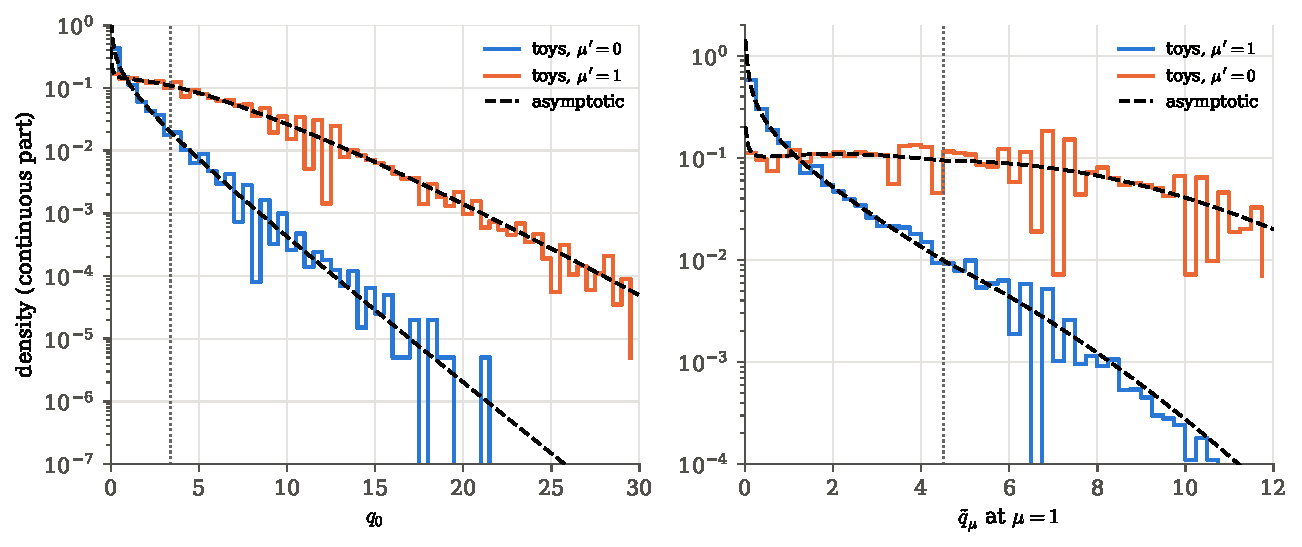
\includegraphics[width=\linewidth]{figures/ch04/hep_qdists.pdf}
\caption{Distributions of the test statistics for a counting experiment with
$s=10$, $b=10$ and a control region of the same size, from toys (steps) and from the
asymptotic formulas (dashed). Left: $q_0$ with background only (blue, the half-$\chi^2$)
and with the signal present (orange). Right: $\tilde q_\mu$ for $\mu=1$, when the
signal is present (blue, again a half-$\chi^2$) and when it is absent (orange). The
dotted lines are the Asimov values, which estimate the medians of the orange
distributions. The jagged steps come from the integer counts.}
\label{4b:fig:qdists}
\end{figure}

\subsection{The Asimov data set: what an experiment should expect}
\label{4b:sec:asimov}

Before an experiment runs, its designers want to know its \emph{sensitivity}: if the
signal is there, what significance will it typically reach, and if not, what limit
will it typically set? ``Typically'' means the median over repetitions. Simulating
thousands of experiments answers this; one artificial data set answers it too.

\begin{workdef}[Asimov data set]
The \newterm{Asimov data set} for a strength $\mu'$ is the data set in which every
count equals its expectation, $n_i=\mu's_i+b_i$, and every auxiliary measurement
equals the nominal value of its nuisance parameter \unpack{no statistical fluctuation
anywhere, the counts are allowed to be non-integer} \cite[(24)--(25)]{Cowan2011}.
\emph{Operationally:} fill the histogram with the model prediction and fit it like data.
\end{workdef}

\emph{Why do the estimators return the true values on it?} The maximum of $\ln\Like$
is where every derivative vanishes. For the Poisson part of \eqref{4b:eq:full-like},
$\ln\Like=\sum_i[n_i\ln\nu_i-\nu_i]+\text{const}$, so for any parameter $\theta_j$
(including $\mu$)
\begin{equation}
  \frac{\partial\ln\Like}{\partial\theta_j}
  \eqby{1} \sum_i\Bigl(\frac{n_i}{\nu_i}-1\Bigr)\frac{\partial\nu_i}{\partial\theta_j}
  \eqby{2} 0\quad\text{when }n_i=\nu_i\text{ for all }i,
  \label{4b:eq:asimov-score}
\end{equation}
\begin{explain}
  \item Differentiate $n_i\ln\nu_i-\nu_i$ with the chain rule.
  \item Every bracket vanishes. The Gaussian constraint terms vanish in the same way
        when $a_k=\theta_k$.
\end{explain}
So the true parameters are a maximum \cite[(23)]{Cowan2011}: fitted on the Asimov data
set, $\hat\mu=\mu'$ and $\hat{\bm\theta}=\bm\theta$.

\emph{Why does it give the median?} By \eqref{4b:eq:wald}, $q_0$ and $\tilde q_\mu$ are
monotonic functions of $\hat\mu$, and $\hat\mu$ is Gaussian with mean and median $\mu'$.
The median of a monotonic function is that function of the median. And the value of
the statistic at $\hat\mu=\mu'$ is exactly what the Asimov data set gives. So
\begin{equation}
  \mathrm{med}[Z_0\given\mu']=\sqrt{q_{0,\rm A}},
  \qquad
  \sigma_{\rm A}^2=\frac{(\mu-\mu')^2}{q_{\mu,\rm A}},
  \label{4b:eq:asimov-med}
\end{equation}
where the subscript A marks a statistic evaluated on the Asimov data set
\cite[(29)--(30), (79)]{Cowan2011}. The second formula reads \eqref{4b:eq:wald}
backwards: on the Asimov data set $\hat\mu=\mu'$, so $-2\ln\lambda_{\rm A}(\mu)=(\mu-\mu')^2/\sigma^2$
can be solved for $\sigma$. This is how the $\sigma$ in all the formulas is obtained in
practice: one fit to one artificial data set, nuisance parameters included.

\paragraph{The expected significance of a counting experiment.}
Take a count with known background $b$ and nominal signal $s$, and evaluate
$q_0=2[n\ln(n/b)-(n-b)]$ on the Asimov count $n=s+b$:
\begin{align}
  Z_{\rm A}^2=q_{0,\rm A}
  &\eqby{1} 2\Bigl[(s+b)\ln\frac{s+b}{b}-s\Bigr]
   \eqby{2} 2\Bigl[(s+b)\ln\Bigl(1+\frac sb\Bigr)-s\Bigr],
  \notag\\
  Z_{\rm A}
  &=\sqrt{2\Bigl[(s+b)\ln\Bigl(1+\frac{s}{b}\Bigr)-s\Bigr]}
   \;\relby{3}{\approx}\;\frac{s}{\sqrt b}\Bigl(1-\frac{s}{6b}\Bigr).
  \label{4b:eq:ZA}
\end{align}
\begin{explain}
  \item The known-background $q_0$ at $n=s+b$, where $n-b=s$.
  \item $(s+b)/b=1+s/b$.
  \item The expansion $q_{0,\rm A}=(s^2/b)[1-s/3b+\dots]$ worked out in the first part
        of the chapter, and $\sqrt{1-u}\approx1-u/2$.
\end{explain}
This is the same algebra as in the first part of the chapter; what is new is its
meaning, the \emph{median} significance, which \eqref{4b:eq:asimov-med} supplies. The
familiar $s/\sqrt b$ is its small-signal limit and overestimates it. For $s=b=10$,
$Z_{\rm A}=\FourBHlZAform$.

With the background measured in a control region, the Asimov counts are $n=s+b$ and
$m=\tau b$, and \eqref{4b:eq:q0-onoff} with $\hat{\hat b}(0)=(s+b+\tau b)/(1+\tau)$ gives
\begin{equation}
  Z_{\rm A}^2=2\Bigl[(s+b)\ln\frac{(1+\tau)(s+b)}{s+(1+\tau)b}
            +\tau b\ln\frac{(1+\tau)\,b}{s+(1+\tau)b}\Bigr].
  \label{4b:eq:ZA-onoff}
\end{equation}
For $s=b=10$ and $\tau=1$ this is $Z_{\rm A}=\FourBHlZA$, against $\FourBHlZAform$ with
the background known: measuring the background in a region no larger than the
signal region costs a third of the expected significance. As $\tau\to\infty$ the
control region measures $b$ perfectly: the second logarithm is
$\ln[1-s/(s+(1+\tau)b)]\approx-s/(\tau b)$, so the second term tends to $-s$, the first
to $(s+b)\ln(1+s/b)$, and \eqref{4b:eq:ZA} returns. The toys agree: their median $q_0$
under the signal is $\FourBHlMedQzero$, the same as the Asimov value $\FourBHlQzeroA$ to the digits shown. (Here the
expected counts are whole numbers, so the Asimov data set is itself a possible outcome of the experiment.)

\subsection{CL$_s$: not excluding what we cannot see}
\label{4b:sec:cls-hep}

The limit \eqref{4b:eq:mu-up} has the defect met at the start of
\cref{4b:sec:boundary}: a downward fluctuation of the background makes it negative.
There is a sharper way to see what is wrong, and it is the reason CL$_s$ exists.

\emph{The event.} An experiment with almost no sensitivity to some signal (because the
signal is tiny compared with the background, $\mu/\sigma\ll1$) reports that it
excludes that signal at $95\%$ confidence. \emph{What made it exclude?} The data
cannot tell signal from no signal, so it can only have been a downward fluctuation of
the background. \emph{How often does that happen when there is no signal?} The rule
``exclude $\mu$ if $p_\mu<\alpha$'' with $p_\mu=\Phi((\hat\mu-\mu)/\sigma)$ excludes
when $\hat\mu<\mu-\sigma\Phi^{-1}(1-\alpha)$. With background only, $\hat\mu\sim\Normal(0,\sigma^2)$:
\begin{equation}
  \Prob(\text{exclude }\mu\given0)
  \eqby{1} \Prob\Bigl(\frac{\hat\mu}{\sigma}<\frac{\mu}{\sigma}-\Phi^{-1}(1-\alpha)\Bigr)
  \eqby{2} \Phi\Bigl(\frac{\mu}{\sigma}-\Phi^{-1}(1-\alpha)\Bigr)
  \;\xrightarrow{\ \mu/\sigma\to0\ }\;\alpha .
  \label{4b:eq:blind-excl}
\end{equation}
\begin{explain}
  \item Divide the exclusion condition by $\sigma$.
  \item $\hat\mu/\sigma$ is standard normal.
\end{explain}
An experiment blind to a signal still excludes it in $5\%$ of runs. That is correct
coverage (the signal is absent, so excluding it is no error) but it is not a statement
any physicist wants to publish: the exclusion says nothing about the signal, only
about the luck of the background. The counting experiment of our toys, with a weak
signal $s=1$ on $b=10$ and $\tau=1$, has $\sigma=\FourBHlBlindSig$ at $\mu=1$; in
background-only toys it excludes $\mu=1$ in a fraction $\FourBHlExclSB$ of the runs
(the formula: $\FourBHlExclSBAsym$), not far above the $5\%$ of a completely blind
experiment, although one signal event on ten background events measured this way
is all but invisible.

\begin{workdef}[CL$_s$]
For a tested signal $\mu$ and the statistic $\tilde q_\mu$, let
$\mathrm{CL}_{s+b}=\Prob(\tilde q_\mu\ge\tilde q_{\rm obs}\given\mu)$ be the p-value of the
signal hypothesis and $\mathrm{CL}_b=\Prob(\tilde q_\mu\ge\tilde q_{\rm obs}\given0)$ the
same tail computed with background only \unpack{how background-poor the data look,
judged by the same statistic}. Then
\[
  \mathrm{CL}_s=\frac{\mathrm{CL}_{s+b}}{\mathrm{CL}_b},
\]
and $\mu$ is excluded at confidence level $1-\alpha$ if $\mathrm{CL}_s<\alpha$
\cite{Junk1999,Read2002}. In the notation of \cite{Cowan2011}, $p_\mu/(1-p_b)$.
\end{workdef}

This is the same ratio as \eqref{4b:eq:clsb} of \cref{4b:sec:fc-poisson}, where the
statistic was the count itself; the profile likelihood ratio generalises it to any
number of bins and nuisance parameters. \emph{Why does dividing help?} Take the two
extremes.
\begin{itemize}[itemsep=1pt,leftmargin=1.2em]
  \item \emph{No sensitivity.} The signal changes nothing, so both tails are computed
        from nearly the same distribution: $\mathrm{CL}_{s+b}\approx\mathrm{CL}_b$ and
        $\mathrm{CL}_s\approx1$. The signal is never excluded. In the weak-signal toys,
        CL$_s$ excluded $\mu=1$ in none of the runs (a fraction $\FourBHlExclCLs$).
  \item \emph{Good sensitivity.} Data that disfavour the signal are typical for the
        background, $\mathrm{CL}_b$ is near one, and CL$_s\approx\mathrm{CL}_{s+b}$.
        Nothing changes.
\end{itemize}
In between, dividing by $\mathrm{CL}_b\le1$ raises the ratio exactly when the data
look background-poor, which is when the plain p-value would have been lucky. The
price is over-coverage: a CL$_s$ limit is above the classical one and covers the true
value in more than $95\%$ of repetitions, as \cref{4b:fig:fc-coverage} showed for
counts. CL$_s$ is a ratio of p-values, not a p-value, and not a probability of the
signal.

\paragraph{The asymptotic CL$_s$ limit.}
By \eqref{4b:eq:p-mu}, $\mathrm{CL}_{s+b}=\Phi((\hat\mu-\mu)/\sigma)$ and, with $\mu'=0$,
$\mathrm{CL}_b=\Phi(\hat\mu/\sigma)$. The limit solves
$\mathrm{CL}_s=\alpha$:
\begin{equation}
  \Phi\Bigl(\frac{\hat\mu-\mu_{\rm up}}{\sigma}\Bigr)=\alpha\,\Phi\Bigl(\frac{\hat\mu}{\sigma}\Bigr)
  \;\Longrightarrow\;
  \mu_{\rm up}=\hat\mu+\sigma\,\Phi^{-1}\Bigl(1-\alpha\,\Phi\Bigl(\frac{\hat\mu}{\sigma}\Bigr)\Bigr),
  \label{4b:eq:cls-up}
\end{equation}
using $\Phi^{-1}(\alpha u)=-\Phi^{-1}(1-\alpha u)$. Compare \eqref{4b:eq:bayes-up} of
\cref{4b:sec:repairs}: it is the same formula. The asymptotic CL$_s$ limit on a Gaussian
estimate is the flat-prior Bayesian upper limit, just as for counts the CL$_s$ limit
equalled the flat-prior Bayesian limit \eqref{4b:eq:cls-bayes}. Two different
questions, a ratio of frequentist tails and a posterior probability with the
boundary built into the prior, give the same number. That coincidence is part of why
CL$_s$ was accepted: it behaves like a Bayesian limit near the boundary and like a
classical one far from it.

For the counting experiment with $s=b=10$, $\tau=1$ and an observation of $n=\FourBHlNobs$
events in the signal region and $m=\FourBHlMobs$ in the control region, the $95\%$
CL$_s$ limit computed with toys (tables of $\tilde q_\mu$ under $\mu$ and under $0$ on a grid
of $\mu$, $\FourBHlGridToys$ toys each) is $\mu_{\rm up}=\FourBHlLimToy$; the asymptotic
formulas, with $\sigma=\sigma_{\rm A}(\mu)$ from \eqref{4b:eq:asimov-med}, give
$\FourBHlLimAsym$.

\subsection{The expected limit and the Brazil band}
\label{4b:sec:brazil}

A limit means little without knowing what the experiment should have achieved. If
there is no signal, $\hat\mu\sim\Normal(0,\sigma^2)$, and the CL$_s$ limit
\eqref{4b:eq:cls-up} is an increasing function of $\hat\mu$. \emph{The question:} what
limit does an experiment with no signal typically report, and in what range? Since the
limit is monotonic in $\hat\mu$, its quantiles are the limits at the quantiles of
$\hat\mu$. The median is at $\hat\mu=0$; the $\pm N$ standard-deviation quantiles at
$\hat\mu=N\sigma$. Putting $\hat\mu=N\sigma$ into \eqref{4b:eq:cls-up},
\begin{equation}
  \mu_{\rm up}(N)
  \eqby{1} N\sigma+\sigma\,\Phi^{-1}\bigl(1-\alpha\,\Phi(N)\bigr),
  \qquad
  \mu_{\rm up}(0)\eqby{2}\sigma\,\Phi^{-1}(1-\alpha/2)=1.96\,\sigma ,
  \label{4b:eq:band}
\end{equation}
\begin{explain}
  \item \eqref{4b:eq:cls-up} with $\hat\mu/\sigma=N$.
  \item $\Phi(0)=\tfrac12$, and $\Phi^{-1}(0.975)=1.96$ for $\alpha=0.05$.
\end{explain}
For $N=-2,-1,0,1,2$ the bracket is $\FourBHlCoefMm$, $\FourBHlCoefM$, $\FourBHlCoefMed$,
$\FourBHlCoefP$ and $\FourBHlCoefPp$ times $\sigma$. The band is lopsided: a downward
fluctuation of the background cannot push the CL$_s$ limit much below $\sigma$, while an
upward one raises it freely. (The plain limit \eqref{4b:eq:mu-up} would have given
$1.645\sigma+N\sigma$, down to $-0.36\,\sigma$ at $N=-2$.) Since $\sigma=\sigma_{\rm A}(\mu)$
depends on the $\mu$ being tested, each line of \eqref{4b:eq:band} is solved for
$\mu_{\rm up}$ numerically \cite[(88)--(89)]{Cowan2011}.

\paragraph{Toys against Asimov.}
For the counting experiment with $s=b=10$, $\tau=1$, the script computes the CL$_s$ limit
of $\FourBHlBandToys$ background-only experiments with toys and takes the quantiles:
\begin{center}
\begin{tabular}{lccccc}
\toprule
 & $-2\sigma$ & $-1\sigma$ & median & $+1\sigma$ & $+2\sigma$\\
\midrule
toys & $\FourBHlBandToyMm$ & $\FourBHlBandToyM$ & $\FourBHlBandToyMed$ & $\FourBHlBandToyP$ & $\FourBHlBandToyPp$\\
Asimov, \eqref{4b:eq:band} & $\FourBHlBandAsMm$ & $\FourBHlBandAsM$ & $\FourBHlBandAsMed$ & $\FourBHlBandAsP$ & $\FourBHlBandAsPp$\\
\bottomrule
\end{tabular}
\end{center}
For an experiment of twenty events the asymptotic band is within a few per cent in the
middle and within ten per cent at the edges, a little conservative throughout. In
the tails the integer counts matter, and the toys are the reference.

\paragraph{The Higgs-style plots.}
For the template search of \cref{4b:sec:templates}, the script repeats the whole
procedure at every hypothesised mass from $110$ to $150\,$GeV: the observed CL$_s$
limit on $\mu$ from the pseudo-data, the expected median and bands from the Asimov
background-only data set at that mass, and the local $p_0$ with its Asimov expectation
for $\mu=1$ (\cref{4b:fig:brazil}). The green and yellow bands that give the plot its
nickname, the \newterm{Brazil band}, are \eqref{4b:eq:band}. The expected limit falls
from $\FourBHlExpLimMax$ to $\FourBHlExpLimMin$ across the range, because the background
falls with mass while the signal does not. Away from $125\,$GeV the observed limit
wanders inside the bands, as a background-only experiment should, and $\mu=1$ is
excluded at $\FourBHlNexcl$ of the $41$ masses. Near $125\,$GeV the observed limit rises far
above the band ($\FourBHlObsLimOneTwoFive$ against an expected $\FourBHlExpLimOneTwoFive$):
the data there refuse to exclude a signal, and the right panel says why. The local
significance at $125\,$GeV is $\FourBHlZlocOneTwoFive\sigma$, close to the
$\FourBHlZexpOneTwoFive\sigma$ expected for $\mu=1$. It is local: a search over this
range must correct it for the look-elsewhere effect of \cref{4b:sec:scan}.

\begin{figure}[htbp]
\centering
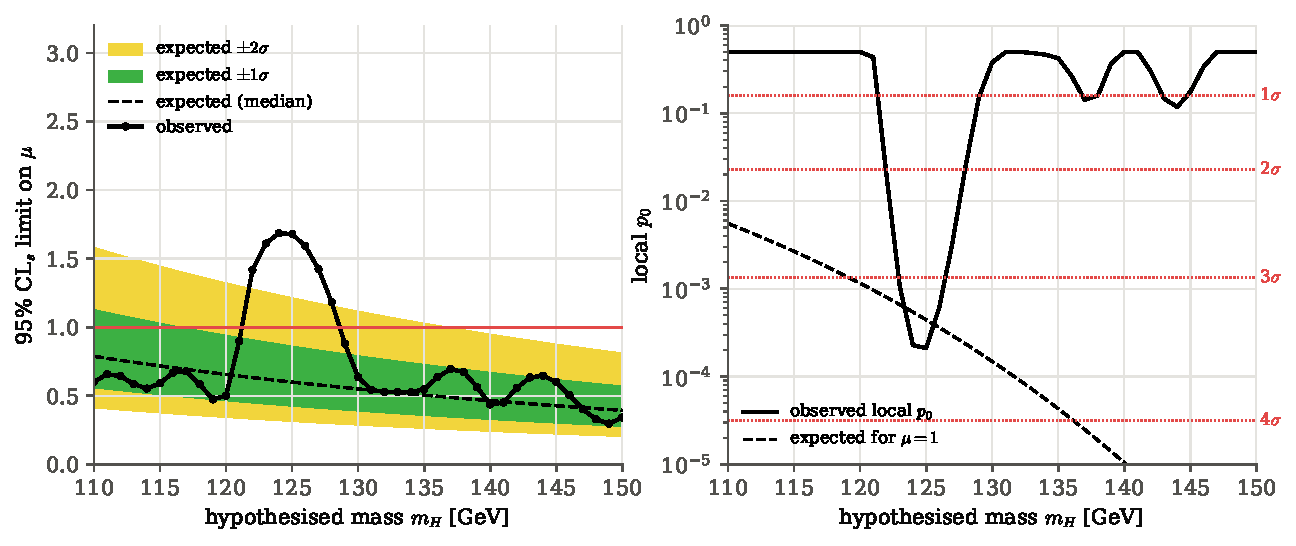
\includegraphics[width=\linewidth]{figures/ch04/hep_brazil.pdf}
\caption{The template search as the LHC experiments show it. Left: the $95\%$ CL$_s$
upper limit on the signal strength at each hypothesised mass (solid), with the median
expected for background only (dashed) and the $\pm1\sigma$ (green) and $\pm2\sigma$
(yellow) bands. Masses where the solid line is below the thin horizontal line at $\mu=1$ are
excluded for the nominal signal. Right: the local p-value of the background-only
hypothesis (solid) and its median expectation if the nominal signal is present
(dashed); the dotted lines mark $1$ to $4\sigma$.}
\label{4b:fig:brazil}
\end{figure}

\begin{keyidea}[The LHC recipe in four lines]
Write the search as a likelihood with nuisance parameters constrained by their
auxiliary measurements. Test ``no signal'' with $q_0$ and report $Z=\sqrt{q_0}$, local
and global. Exclude a signal when $\mathrm{CL}_s=\mathrm{CL}_{s+b}/\mathrm{CL}_b<0.05$, using
$\tilde q_\mu$. Show the observed limit against the expected one and its Brazil band,
both from the Asimov data set, and check with toys where counts are small.
\end{keyidea}

\begin{inpractice}[How the experiments compute it]
The likelihoods of real searches have hundreds of bins and hundreds of nuisance
parameters, with templates interpolated as in \eqref{4b:eq:morph}. They are written in
standard formats (HistFactory, with the RooStats, \texttt{pyhf} and CMS
\texttt{Combine} tools) and minimised numerically; the asymptotic formulas of
\cite{Cowan2011} give $q_0$, the CL$_s$ limit and the Brazil band from the observed and
Asimov fits alone, and toys are run where counts are small or near the boundary
\cite{Cranmer2015}. Our two scripts verify the formulas against toys on a case where
both are cheap. In research the same machinery is the instrument: the toys
are the reference whenever the formulas are in doubt, and published likelihoods let
others combine results, as \cref{4b:sec:classical-limit} urged.
\end{inpractice}

The lesson in one line: with nuisance parameters profiled, the significance is still
$\sqrt{q_0}$ and the limit still comes from a half-$\chi^2$, and CL$_s$ divides by the
background's own p-value so that a signal is never excluded by luck.
\section{Confidence intervals and credible intervals}
\label{4b:sec:credible}

Ten one-minute runs of a low-background detector record a total of six
events. Two analysts report a $90\%$ interval for the rate $\lambda$ per run.
The first, using Garwood's construction, reports $[\FourBCrConfLo,\
\FourBCrConfHi]$. The second, using Bayes' theorem with a mild prior, reports
$[\FourBCrCredLo,\ \FourBCrCredHi]$ \srcref{CasellaBerger}{Exs.~9.2.15--9.2.16}.
The numbers are close. The statements are not. The first is a confidence
interval: it comes from a recipe that covers the true rate in at least $90\%$ of
repeated experiments. The second is a \newterm{credible interval}: given these
data and the prior, it contains the rate with probability $90\%$. The first is
a prediction-direction statement, about which data each rate would produce. The
second is an inference-direction statement, about which rates could have
produced the data we saw. Bayes' theorem is the bridge between them. Comparing
the two on the same data shows what each one claims and what it needs;
\cref{ch:05} develops the Bayesian side in full.

\paragraph{The question in words.}
\begin{enumerate}[label=\arabic*.]
  \item What does each interval say, in words, and what is random in each?
  \item Does a credible interval cover like a confidence interval, and does a
        confidence interval hold the posterior probability it claims?
  \item When do the two coincide?
\end{enumerate}

\subsection{A credible set}
\label{4b:sec:credible-def}

In the Bayesian framework $\theta$ has a probability distribution, first the
prior $\pi(\theta)$ and, after the data, the posterior
$\pi(\theta\given\bm x)\propto p(\bm x\given\theta)\pi(\theta)$. Any set $A$ of
parameter values has a \newterm{credible probability}
$\Prob(\theta\in A\given\bm x)=\int_A\pi(\theta\given\bm x)\,\dd\theta$
\srcref{CasellaBerger}{(9.2.18)}, and a set with credible probability $1-\alpha$
is a $1-\alpha$ credible set. The different name keeps the two kinds of
probability apart. As with confidence intervals, many sets have the required
probability, so we must choose one.
Two common choices are the \emph{equal-tailed} interval, with posterior
probability $\alpha/2$ beyond each end, and the \newterm{highest density
interval} (HDI) \unpack{every point inside has higher posterior density than
every point outside}, which makes $\pi(a\given\bm x)=\pi(b\given\bm x)$ and is the
shortest interval with the required probability \srcref{Cowan}{(9.42)},
\srcref{Kruschke}{\S11.3.2}.

\paragraph{Example: the Poisson rate.}
Take $n$ observations from Poisson$(\lambda)$ with sum $y=\sum x_i$, and a
gamma prior with shape $a$ and scale $b$, density
$\propto\lambda^{a-1}e^{-\lambda/b}$. Then
\begin{align}
  \pi(\lambda\given\bm x)
  &\eqby{1} \propto \Bigl(\prod_{i}\lambda^{x_i}e^{-\lambda}\Bigr)\lambda^{a-1}e^{-\lambda/b}
   \eqby{2} \lambda^{a+y-1}e^{-\lambda(n+1/b)}
   \eqby{3} \mathrm{Gamma}\Bigl(a+y,\ \frac{b}{nb+1}\Bigr),
  \label{4b:eq:gamma-post}
\end{align}
\begin{explain}
  \item Bayes' theorem: likelihood of independent Poisson counts times prior;
        factors not involving $\lambda$ are dropped.
  \item Collect powers of $\lambda$ and the exponentials.
  \item This is the gamma density with shape $a+y$ and rate $n+1/b$, that is
        scale $1/(n+1/b)=b/(nb+1)$ \srcref{CasellaBerger}{(9.2.19)}.
\end{explain}
A gamma variable of shape $k$ and scale $s$, multiplied by $2/s$, is $\chi^2$
with $2k$ degrees of freedom, so $2(nb+1)\lambda/b\sim\chi^2_{2(a+y)}$ under the
posterior, and the equal-tailed interval has $\chi^2$ quantiles for ends
\srcref{CasellaBerger}{(9.2.20)}. With $a=b=1$, $n=10$, $y=6$: $22\lambda\sim\chi^2_{14}$,
and the $5\%$ and $95\%$ quantiles $6.571$ and $23.685$ give
$[\FourBCrCredLo,\FourBCrCredHi]$. The credible interval is shorter than the
confidence interval and pulled towards zero. Both effects come from the prior.
It adds information, which narrows the interval. And it favours small rates
(its density $e^{-\lambda}$ falls with $\lambda$), which pulls the interval
down.

\subsection{Judging each interval by the other's standard}
\label{4b:sec:cross-check}

Each interval keeps its own promise exactly. \emph{The question:} how does each
do when judged by the other's promise \srcref{CasellaBerger}{Ex.~9.2.17}?

\emph{Coverage of the credible interval.} Fix a true $\lambda$. Simulate the
total of the ten runs, $y\sim$ Poisson$(10\lambda)$, many times (or sum exactly
over $y$), build the credible interval each time and count hits. \Cref{4b:fig:credible-coverage}
(left) shows the result. For small $\lambda$ near the prior's bulk the credible
interval covers about $90\%$, sometimes more, sometimes less (minimum
$\FourBCrCovCredMin$ on $0<\lambda<3$). For large $\lambda$ the prior's pull
towards small values becomes a bias, and the coverage collapses: $\FourBCrCovCredFive$
at $\lambda=5$, $\FourBCrCovCredTwenty$ at $\lambda=20$, $\FourBCrCovCredFifty$ at
$\lambda=50$, tending to zero \srcref{CasellaBerger}{(9.2.22)}. A credible
interval is not a confidence interval.

\emph{Credible probability of the confidence interval.} Fix the data, compute
the posterior, and ask how much posterior probability lies inside the Garwood
interval. At $y=6$ it is $\FourBCrCredProbConfSix$; it decreases steadily with
$y$, reaching $\FourBCrCredProbConfFifty$ at $y=50$, and tends to zero for
$y\to\infty$ unless the prior scale is $b=1/n$
(\cref{4b:fig:credible-coverage}, right). A confidence interval is not a
credible interval either.

\begin{figure}[htbp]
\centering
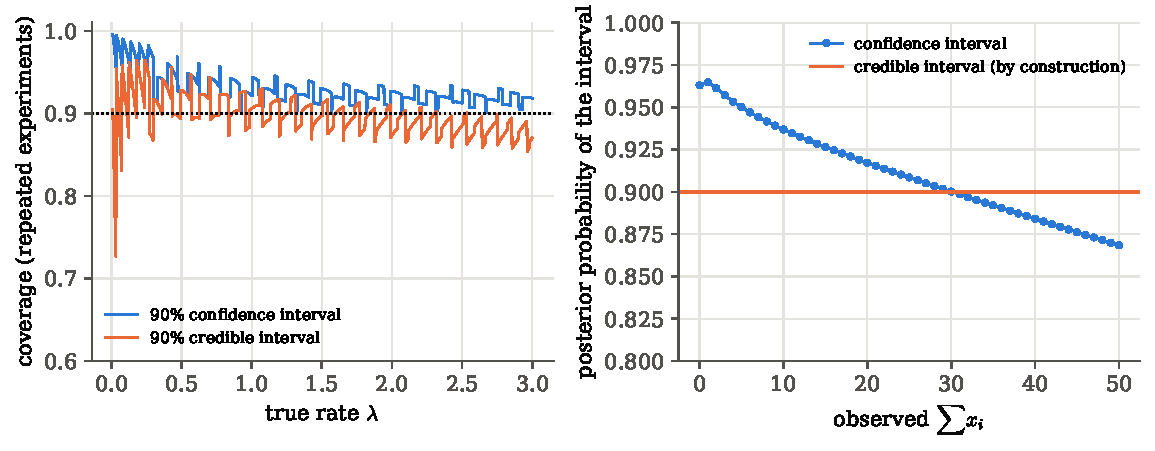
\includegraphics[width=\linewidth]{figures/ch04/credible_coverage.pdf}
\caption{Two $90\%$ intervals for a Poisson rate from ten observations,
judged by each other's criterion. Left: the frequentist coverage as a
function of the true rate. The confidence interval (blue) never drops below
$90\%$; the credible interval with a gamma$(1,1)$ prior (orange) scatters around
$90\%$ at small rates and falls away as the rate grows past the prior's range.
Right: the posterior probability contained in each interval, as a function of
the observed total. The credible interval holds $90\%$ by construction; the
confidence interval holds more for small totals and less for large ones.}
\label{4b:fig:credible-coverage}
\end{figure}

\paragraph{Example: a Gaussian mean with a Gaussian prior.}
Here the calculation can be done in closed form \srcref{CasellaBerger}{Ex.~9.2.18}.
Let $X_1,\dots,X_n$ be $\Normal(\theta,\sigma^2)$ and the prior $\Normal(\mu,\tau^2)$,
and write $\gamma=\sigma^2/(n\tau^2)$ for the ratio of the data variance of the
mean to the prior variance. The posterior is Gaussian with mean
$\delta=(\gamma\mu+\bar x)/(1+\gamma)$ and variance $V=\sigma^2/(n(1+\gamma))$, and
the $1-\alpha$ credible interval is $\delta\pm z_{\alpha/2}\sqrt V$. Its coverage at a
fixed true $\theta$, with $Z=\sqrt n(\bar X-\theta)/\sigma\sim\Normal(0,1)$ and
$\Delta=\sqrt n(\theta-\mu)/\sigma$, is
\begin{align}
  \Prob_\theta\bigl(\abs{\theta-\delta}\le z_{\alpha/2}\sqrt V\bigr)
  &\eqby{1} \Prob_\theta\Bigl(\Bigl\lvert\frac{\gamma(\theta-\mu)-(\bar X-\theta)}{1+\gamma}\Bigr\rvert
             \le z_{\alpha/2}\frac{\sigma}{\sqrt{n(1+\gamma)}}\Bigr)
   \notag\\
  &\eqby{2} \Prob\bigl(\abs{\gamma\Delta-Z}\le\sqrt{1+\gamma}\,z_{\alpha/2}\bigr)
   \notag\\
  &\eqby{3} \Phi\bigl(\gamma\Delta+\sqrt{1+\gamma}\,z_{\alpha/2}\bigr)
            -\Phi\bigl(\gamma\Delta-\sqrt{1+\gamma}\,z_{\alpha/2}\bigr).
  \label{4b:eq:normal-cred-cov}
\end{align}
\begin{explain}
  \item $\theta-\delta=[(1+\gamma)\theta-\gamma\mu-\bar X]/(1+\gamma)
        =[\gamma(\theta-\mu)-(\bar X-\theta)]/(1+\gamma)$.
  \item Multiply both sides by $(1+\gamma)\sqrt n/\sigma$ and use the
        definitions of $Z$ and $\Delta$.
  \item $Z$ is standard normal: the probability that it lies within
        $\sqrt{1+\gamma}\,z_{\alpha/2}$ of $\gamma\Delta$.
\end{explain}
So the coverage depends on how far the truth is from the prior mean, measured
by $\Delta$ in units of the standard error $\sigma/\sqrt n$. If the truth sits
at the prior mean, $\Delta=0$, the interval overcovers (for $\gamma=1$ and
$95\%$, the coverage is $\FourBCrNormCovZero$), because the prior's information
is correct. If the truth is two or four standard errors away from the prior
mean, the coverage is $\FourBCrNormCovTwo$ or $\FourBCrNormCovFour$
(\cref{4b:fig:hdi-vs-ci}, right). As $\tau\to\infty$,
$\gamma\to0$ and \eqref{4b:eq:normal-cred-cov} becomes $\Phi(z_{\alpha/2})-\Phi(-z_{\alpha/2})=1-\alpha$
for every $\theta$: with a flat prior the credible interval is the confidence
interval $\bar x\pm z_{\alpha/2}\sigma/\sqrt n$, number for number. This coincidence,
like the counting-experiment coincidence of Cowan's (9.55), is special to
location parameters and flat priors; it is why the two schools rarely argue
about a well-measured Gaussian quantity.

\subsection{The coin again: the HDI does not depend on the stopping rule}
\label{4b:sec:hdi}

Kruschke returns to $z=7$ heads in $N=24$ flips with a prior $\mathrm{beta}(11,11)$,
a coin that looks fair \srcref{Kruschke}{\S11.3.2}. The posterior is
$\mathrm{beta}(11+7,\ 11+17)$ and its $95\%$ HDI is
$[\FourBHdiInfLo,\FourBHdiInfHi]$; with a uniform prior it would be
$[\FourBHdiFlatLo,\FourBHdiFlatHi]$. \Cref{4b:fig:hdi-vs-ci} (left) shows both
posteriors with the four confidence intervals of \cref{4b:sec:ci-intentions}
underneath. The four confidence intervals differ; the HDI is the same for all
four. \emph{Why?} The Bayesian interval sees the data only through the
likelihood $\theta^7(1-\theta)^{17}$, and that is the same whether the
experimenter meant to stop at $N=24$, at $z=7$, or when time ran out. The
confidence interval also depends on which cloud of imaginary outcomes the plan
would have produced. Kruschke lists three
advantages of the HDI \srcref{Kruschke}{pp.~324--325}: it is a direct statement
about the credibility of values of $\theta$; it does not depend on sampling and
testing intentions; and it responds, openly, to prior knowledge. The price is the
prior itself, which must be stated and defended.

\begin{figure}[htbp]
\centering
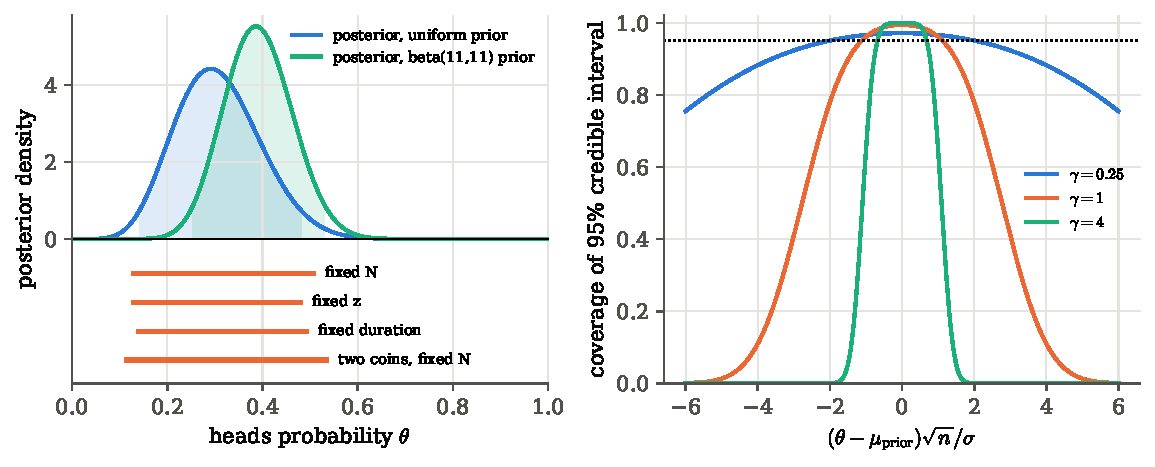
\includegraphics[width=\linewidth]{figures/ch04/hdi_vs_ci.pdf}
\caption{Left: posteriors for $7$ heads in $24$ flips with a uniform (blue) and a
$\mathrm{beta}(11,11)$ (green) prior; the shaded parts are the $95\%$ highest
density intervals. Below the axis, the four $95\%$ confidence intervals that
four stopping intentions produce from the same data. Right: frequentist coverage
of a $95\%$ credible interval for a Gaussian mean with a Gaussian prior, as a
function of the distance between the true value and the prior mean (in units of
the standard error), for three ratios $\gamma$ of data variance to prior
variance. A strong prior (large $\gamma$) covers only near its own centre.}
\label{4b:fig:hdi-vs-ci}
\end{figure}

\paragraph{Deciding with an interval: the ROPE.}
A test asks whether $\theta$ equals a null value exactly, a question whose
answer is almost always ``no'' with enough data. Kruschke replaces it by a
\newterm{region of practical equivalence} (ROPE) \unpack{a small range of values
that are, for the purpose at hand, as good as the null value}, and a rule
\srcref{Kruschke}{\S12.1.1}: reject the null value if the $95\%$ HDI lies entirely
outside the ROPE; accept it for practical purposes if the HDI lies entirely inside;
otherwise, withhold judgement. For a coin with ROPE $[0.45,0.55]$ and a uniform
prior, $325$ heads in $500$ flips give the HDI $[\FourBRopeOneLo,\FourBRopeOneHi]$,
outside the ROPE: not fair. $490$ heads in $1000$ give
$[\FourBRopeTwoLo,\FourBRopeTwoHi]$, inside: fair for practical purposes (the
posterior probability of the ROPE is $\FourBRopeTwoIn$). Unlike a p-value, this rule
can \emph{accept} a null value, and only when the measurement is precise enough to
deserve it. The physicist's analogue is familiar: a calibration is declared good
when its uncertainty band lies within the tolerance, not when a test fails to
reject perfection.

\subsection{What each interval says}
\label{4b:sec:words}

The two kinds of interval differ in what they claim, what they treat as random,
what they need as input, what they guarantee, and how they typically go wrong.

\begin{taxonomy}[Confidence interval or credible interval]
\small
\renewcommand{\arraystretch}{1.15}
\begin{tabularx}{\linewidth}{@{}>{\raggedright\arraybackslash}p{3.0cm}
                               >{\raggedright\arraybackslash}X
                               >{\raggedright\arraybackslash}X@{}}
\toprule
 & confidence interval & credible interval\\
\midrule
in words & ``a recipe that, applied to data from any $\theta$, contains that $\theta$
  $95\%$ of the time'' & ``given these data and this prior, $\theta$ is in here with
  probability $95\%$''\\
random & the interval (through the data) & $\theta$ (through the posterior)\\
fixed & the true $\theta$ & the observed data\\
needs & $p(\bm x\given\theta)$ for all data that could have occurred, including the
  stopping and search plan & the likelihood of the observed data and a prior\\
guarantee & coverage for every $\theta$ & correct posterior probability, if the prior is
  right\\
typical failure & empty or unphysical intervals, flip-flopping, dependence on
  intentions & poor coverage where the prior is wrong\\
coincide when & \multicolumn{2}{>{\raggedright\arraybackslash}X@{}}{location
  parameters with flat priors: Gaussian mean, Poisson with no background}\\
\bottomrule
\end{tabularx}
\end{taxonomy}

In the pipeline of the book, both are ways of turning the sampling
distribution $P(S\given\theta)$ of a summary into a statement about the physics.
The confidence interval stays in the prediction direction and asks which
$\theta$ would make the observed summary typical. The credible interval crosses
into the inference direction and asks how probable each $\theta$ is. Cosmologists
quote credible intervals from MCMC posteriors (\cref{ch:09}); particle physicists
quote confidence intervals and limits; the Fisher forecasts of \cref{ch:10} are,
for linear-Gaussian models, both at once. \Cref{ch:05} builds the Bayesian side
properly: priors, the evidence, and the reallocation of credibility that a posterior
is.

\begin{recap}
\begin{itemize}
  \item A $1-\alpha$ confidence interval is a recipe with coverage at least
        $1-\alpha$ for every parameter value. The interval is random, the parameter
        fixed.
  \item Inverting a family of level-$\alpha$ tests gives a $1-\alpha$ confidence
        set: keep the null values that are not rejected. The p-value function
        displays all the tests at once.
  \item The Neyman construction draws the acceptance regions of all tests as a belt
        in the (data, parameter) plane; the interval is its vertical cut. Gaussian
        estimates give $\hat\theta\pm\sigma$, Poisson counts give Garwood's
        $\chi^2$ intervals, and $\Delta\ln\Like=\tfrac12$ (or $\Delta\chi^2=1$) is
        the large-sample shortcut. With $m$ parameters the $68.3\%$ region is
        $\Delta\chi^2=2.30$ for $m=2$.
  \item Coverage is checked by simulation. Normal quantiles with an estimated
        $\sigma$ undercover at small $n$; $n\pm\sqrt n$ fails at small counts;
        discrete data force over-coverage with a saw-tooth.
  \item Near a physical boundary the classical limit can be negative or the
        interval empty. Choosing between limit and interval after seeing the data
        undercovers ($85\%$ for a nominal $90\%$). Feldman--Cousins ordering by a
        likelihood ratio fixes both; CL$_s$ (equal to the flat-prior Bayesian limit
        for counting) protects against excluding what the experiment cannot see.
  \item Many tests: Bonferroni controls the chance of any false rejection, BH the
        fraction of false discoveries. In a scan, the global p-value exceeds the
        local one by a trials factor that grows linearly with the significance;
        the Gross--Vitells formula gets it from a few toys.
  \item A credible interval is a probability statement about $\theta$ given the data
        and a prior. It does not guarantee coverage; a confidence interval does not
        hold its nominal posterior probability; they agree for flat priors on location
        parameters.
\end{itemize}
\end{recap}

\subsection*{Reading the literature}
\label{4b:sec:literature}

\begin{itemize}[leftmargin=1.2em,itemsep=2pt]
  \item \textbf{Main line.} \mainref{Ch.~10} for hypothesis testing: the null and
        the alternative, power and size, the Wald test, p-values and their
        uniformity, the $\chi^2$ and permutation tests, likelihood-ratio tests,
        multiple testing (Bonferroni and Benjamini--Hochberg) and goodness of fit;
        \mainref{\S6.3.2} for confidence sets, their interpretation and the
        Berger--Wolpert example.
  \item \textbf{The physicist's version.} \srcref{Cowan}{Ch.~4} for test statistics,
        particle selection, the Neyman--Pearson lemma, goodness of fit and the
        significance of a signal; \srcref{Cowan}{Ch.~9} for confidence belts,
        Gaussian and Poisson intervals, Fisher's $z$, likelihood intervals,
        confidence regions and limits near a boundary, with and without background.
  \item \textbf{Careful derivations.} \srcref{CasellaBerger}{\S8.3} for the
        Neyman--Pearson lemma and valid p-values; \srcref{CasellaBerger}{\S10.3}
        for the asymptotic distribution of the likelihood ratio;
        \srcref{CasellaBerger}{\S\S9.1--9.2} for interval estimators, coverage and
        confidence coefficients, test inversion, pivots, Garwood's Poisson
        intervals and the coverage of credible sets.
  \item \textbf{The Bayesian critique.} \srcref{Kruschke}{Ch.~11} for how p-values
        and confidence intervals depend on stopping and testing intentions, and for
        multiple comparisons; \srcref{Kruschke}{Ch.~12} for the HDI and the region of
        practical equivalence. \srcref{Lambert}{\S2.8} for the frequentist's
        imaginary samples.
  \item \textbf{Original papers.} Feldman and Cousins' unified approach to small
        signals \cite{FeldmanCousins1998}; Gross and Vitells on trials factors for
        the look-elsewhere effect \cite{GrossVitells2010}; Cowan, Cranmer, Gross and
        Vitells on asymptotic formulae for likelihood-based tests of new physics,
        including the profile likelihood ratio, the Asimov data set and the CL$_s$
        remark \cite{Cowan2011}; Wilks on the asymptotic $\chi^2$ distribution of
        likelihood ratios \cite{Wilks1938}.
\end{itemize}

\clearpage
\raggedbottom
\section*{Chapter summary}
\addcontentsline{toc}{section}{Chapter summary}
\label{4b:sec:summary}

Before a measurement is published it must answer three questions. Could this be
chance? Which parameter values are compatible with what we saw? How often do
our recipes mislead us? All three start from the sampling distribution of a
summary. Tests answer the first: they are built around the one hypothesis
whose predictions we know, the null, and measure surprise with p-values.
Intervals and limits answer the second: they are families of tests, inverted.
Coverage checks and corrections for the many places we looked answer the third.
In the pipeline of the book,
\[
  \text{model}\to\text{data}\to\text{summary }S\to P(S\given\theta)\to\boxed{\text{infer physics}},
\]
tests and intervals are the frequentist form of the last arrow, and
\cref{ch:05} gives the Bayesian one.

\begin{center}
\small
\renewcommand{\arraystretch}{1.15}
\begin{tabularx}{\linewidth}{@{}>{\raggedright\arraybackslash}p{3.3cm}
                               >{\raggedright\arraybackslash}X
                               >{\raggedright\arraybackslash}p{2.7cm}@{}}
\toprule
\multicolumn{3}{@{}l}{\textbf{Testing the null (first half)}}\\
concept & operational meaning & used later in\\\midrule
null hypothesis & the hypothesis whose sampling distribution we know and can simulate: ``it happened by chance'' & every search, \cref{ch:08,ch:12}\\
test statistic, rejection region & one number, large under the alternative; reject when it exceeds a critical value fixed in advance & \cref{ch:08,ch:12}\\
p-value & probability under $\Hnull$ of a statistic at least as extreme, in the alternative's direction; simulate if no formula & \cref{ch:06,ch:08,ch:12}\\
one- and two-sided, stopping rule & the direction and the experimental plan are part of the question; they change the p-value & \cref{ch:05}\\
size, power & false-alarm rate $\alpha$; rejection probability under the truth; plan the experiment by the power & \cref{ch:10}\\
uniformity of p & under a continuous null $p\sim\mathrm{U}(0,1)$; for discrete data $\Prob(p\le\alpha)\le\alpha$; a histogram of null p-values checks a pipeline & \cref{ch:06,ch:08}\\
$p\ne\Prob(\Hnull\given\text{data})$ & the posterior of the null needs a prior and the power (Bayes) & \cref{ch:05}\\
Wald, $t$, permutation tests & estimate over standard error; Student $t$ for small Gaussian samples; relabel the data for a distribution-free null & \cref{ch:06,ch:12}\\
Neyman--Pearson, likelihood ratio & for simple hypotheses the likelihood ratio is the most powerful statistic & \cref{ch:08,ch:10}\\
Wilks, $q_0$, $Z=\sqrt{q_0}$ & $-2\ln\lambda\sim\chi^2$ with as many degrees of freedom as the null fixes; half-$\chi^2$ on a boundary & \cref{ch:09,ch:10}\\
Pearson $\chi^2$, KS & goodness of fit of a whole model; fitted parameters reduce the degrees of freedom; simulate sparse cases & \cref{ch:07,ch:08}\\
$p\to Z\sigma$, $5\sigma$ & $Z=\Phi^{-1}(1-p)$; $3\sigma$ evidence, $5\sigma$ observation, because of many searches, backgrounds and rarity & \cref{ch:12}\\
\bottomrule
\end{tabularx}
\end{center}

\begin{center}
\small
\renewcommand{\arraystretch}{1.15}
\begin{tabularx}{\linewidth}{@{}>{\raggedright\arraybackslash}p{3.3cm}
                               >{\raggedright\arraybackslash}X
                               >{\raggedright\arraybackslash}p{2.7cm}@{}}
\toprule
\multicolumn{3}{@{}l}{\textbf{Intervals, coverage and many tests (second half)}}\\
concept & operational meaning & used later in\\\midrule
confidence interval & a recipe with coverage $\ge1-\alpha$ for every $\theta$; the interval is random, $\theta$ fixed & \cref{ch:08,ch:10}\\
test inversion, p-value function & keep the null values a level-$\alpha$ test does not reject & \cref{ch:08}\\
Neyman belt & acceptance intervals at every $\theta$, cut vertically at the observation; build on a grid from simulations when there is no formula & \cref{ch:06,ch:08}\\
Gaussian and Poisson intervals & $\hat\theta\pm\sigma$ is the $68.3\%$ central interval; Garwood's $\chi^2$ quantiles for counts; $-\ln0.05=3$ for zero events & \cref{ch:07,ch:08}\\
likelihood interval, $\Delta\chi^2$ regions & $\Delta\ln\Like=\tfrac12$, $\Delta\chi^2=1$ in one dimension; $2.30$ ($68.3\%$) and $5.99$ ($95\%$) in two & \cref{ch:09,ch:10}\\
coverage check & simulate at fixed $\theta$, count hits; exact sums for counts; $t$ not $z$ for estimated $\sigma$ & \cref{ch:06,ch:08,ch:09}\\
limits near a boundary & report $\hat\theta\pm\sigma$ always; classical, shifted, Bayesian, Feldman--Cousins, CL$_s$; fix the recipe in advance & \cref{ch:10}\\
Bonferroni, BH & $P_i<\alpha/m$ controls any false rejection; the BH line $i\alpha/m$ controls the false discovery rate & \cref{ch:12}\\
look-elsewhere effect & global p-value from toys scanned like the data; $p_{\rm glob}\approx p_{\rm loc}+\E N(c_0)e^{-(c-c_0)/2}$; trials factor $\propto Z$ & \cref{ch:08,ch:12}\\
search likelihood, nuisance parameters & Poisson bins of signal and background templates times one constraint term per calibration; profile to get $\lambda(\mu)$; $\sigma_{\rm syst}^2=\sigma_{\rm tot}^2-\sigma_{\rm stat}^2$ & \cref{ch:08,ch:10}\\
$q_0$, $\tilde q_\mu$, CL$_s$, Brazil band & $Z=\sqrt{q_0}$ with profiled nuisances (Wald); exclude when $\mathrm{CL}_{s+b}/\mathrm{CL}_b<0.05$; expected limit and $\pm1,2\sigma$ bands from the Asimov data set; toys for small counts & \cref{ch:10,ch:12}\\
credible interval, HDI, ROPE & posterior probability of a set given data and prior; shortest set; accept or reject a value for practical purposes & \cref{ch:05,ch:09}\\
\bottomrule
\end{tabularx}
\end{center}
\clearpage
\flushbottom
  
\chapter{Bayes' Theorem and Bayesian Inference}\label{ch:05}

\providecommand{\FiveAMedJointD}{}\renewcommand{\FiveAMedJointD}{0.0095}
\providecommand{\FiveAMedJointH}{}\renewcommand{\FiveAMedJointH}{0.099}
\providecommand{\FiveAMedPpos}{}\renewcommand{\FiveAMedPpos}{0.1085}
\providecommand{\FiveAMedPost}{}\renewcommand{\FiveAMedPost}{0.08756}
\providecommand{\FiveAMontyPE}{}\renewcommand{\FiveAMontyPE}{0.5}
\providecommand{\FiveAMontyPostA}{}\renewcommand{\FiveAMontyPostA}{0.3333}
\providecommand{\FiveAMontyPostB}{}\renewcommand{\FiveAMontyPostB}{0.6667}
\providecommand{\FiveATrigJointS}{}\renewcommand{\FiveATrigJointS}{0.045}
\providecommand{\FiveATrigJointB}{}\renewcommand{\FiveATrigJointB}{0.019}
\providecommand{\FiveATrigPE}{}\renewcommand{\FiveATrigPE}{0.064}
\providecommand{\FiveATrigPost}{}\renewcommand{\FiveATrigPost}{0.7031}
\providecommand{\FiveABallPa}{}\renewcommand{\FiveABallPa}{0.1118}
\providecommand{\FiveABallPb}{}\renewcommand{\FiveABallPb}{0.5578}
\providecommand{\FiveABallPc}{}\renewcommand{\FiveABallPc}{0.311}
\providecommand{\FiveABallPd}{}\renewcommand{\FiveABallPd}{0.01937}
\providecommand{\FiveABallLRbc}{}\renewcommand{\FiveABallLRbc}{1.794}
\providecommand{\FiveAGrbPriorG}{}\renewcommand{\FiveAGrbPriorG}{0.3846}
\providecommand{\FiveAGrbPriorB}{}\renewcommand{\FiveAGrbPriorB}{0.1026}
\providecommand{\FiveAGrbPriorD}{}\renewcommand{\FiveAGrbPriorD}{0.5128}
\providecommand{\FiveAGrbSigOne}{}\renewcommand{\FiveAGrbSigOne}{0.4595}
\providecommand{\FiveAGrbLG}{}\renewcommand{\FiveAGrbLG}{0.004776}
\providecommand{\FiveAGrbLB}{}\renewcommand{\FiveAGrbLB}{0.004006}
\providecommand{\FiveAGrbLD}{}\renewcommand{\FiveAGrbLD}{6.629\times10^{-5}}
\providecommand{\FiveAGrbMaG}{}\renewcommand{\FiveAGrbMaG}{0.8051}
\providecommand{\FiveAGrbMaB}{}\renewcommand{\FiveAGrbMaB}{0.18}
\providecommand{\FiveAGrbMaD}{}\renewcommand{\FiveAGrbMaD}{0.0149}
\providecommand{\FiveAGrbMbG}{}\renewcommand{\FiveAGrbMbG}{0.4088}
\providecommand{\FiveAGrbMbB}{}\renewcommand{\FiveAGrbMbB}{0.04486}
\providecommand{\FiveAGrbMbD}{}\renewcommand{\FiveAGrbMbD}{0.5463}
\providecommand{\FiveAGrbForgotG}{}\renewcommand{\FiveAGrbForgotG}{0.9011}
\providecommand{\FiveAGrbForgotB}{}\renewcommand{\FiveAGrbForgotB}{0.09887}
\providecommand{\FiveAGrbNphot}{}\renewcommand{\FiveAGrbNphot}{68}
\providecommand{\FiveAGrbNtrue}{}\renewcommand{\FiveAGrbNtrue}{25}
\providecommand{\FiveAGrbNest}{}\renewcommand{\FiveAGrbNest}{23.65}
\providecommand{\FiveABdtPostNine}{}\renewcommand{\FiveABdtPostNine}{0.8804}
\providecommand{\FiveABdtPostEight}{}\renewcommand{\FiveABdtPostEight}{0.3926}
\providecommand{\FiveABdtPostNineTiny}{}\renewcommand{\FiveABdtPostNineTiny}{0.06795}
\providecommand{\FiveABdtEffS}{}\renewcommand{\FiveABdtEffS}{0.3446}
\providecommand{\FiveABdtEffB}{}\renewcommand{\FiveABdtEffB}{0.0016}
\providecommand{\FiveABdtCutLR}{}\renewcommand{\FiveABdtCutLR}{215.4}
\providecommand{\FiveABdtCutPur}{}\renewcommand{\FiveABdtCutPur}{0.6851}
\providecommand{\FiveABdtMC}{}\renewcommand{\FiveABdtMC}{0.882}
\providecommand{\FiveABdtMCerr}{}\renewcommand{\FiveABdtMCerr}{0.006818}
\providecommand{\FiveABdtNsel}{}\renewcommand{\FiveABdtNsel}{2238}
\providecommand{\FiveABdtHalfOne}{}\renewcommand{\FiveABdtHalfOne}{0.8223}
\providecommand{\FiveABdtHalfTiny}{}\renewcommand{\FiveABdtHalfTiny}{0.9556}
\providecommand{\FiveACoinHeads}{}\renewcommand{\FiveACoinHeads}{16}
\providecommand{\FiveACoinN}{}\renewcommand{\FiveACoinN}{50}
\providecommand{\FiveACoinMaxDiff}{}\renewcommand{\FiveACoinMaxDiff}{1.041\times10^{-16}}
\providecommand{\FiveACoinPostMean}{}\renewcommand{\FiveACoinPostMean}{0.3269}
\providecommand{\FiveACoinModeFour}{}\renewcommand{\FiveACoinModeFour}{0.4}
\providecommand{\FiveACoinModeForty}{}\renewcommand{\FiveACoinModeForty}{0.268}
\providecommand{\FiveACoinLRh}{}\renewcommand{\FiveACoinLRh}{0.1461}
\providecommand{\FiveACoinLRt}{}\renewcommand{\FiveACoinLRt}{-0.2218}
\providecommand{\FiveACoinKLone}{}\renewcommand{\FiveACoinKLone}{0.03574}
\providecommand{\FiveACoinKLzero}{}\renewcommand{\FiveACoinKLzero}{0.03786}
\providecommand{\FiveACoinTossesHundred}{}\renewcommand{\FiveACoinTossesHundred}{55.97}
\providecommand{\FiveASeqPa}{}\renewcommand{\FiveASeqPa}{0.6154}
\providecommand{\FiveASeqPb}{}\renewcommand{\FiveASeqPb}{0.7191}
\providecommand{\FiveASeqPc}{}\renewcommand{\FiveASeqPc}{0.5059}
\providecommand{\FiveASeqPd}{}\renewcommand{\FiveASeqPd}{0.621}
\providecommand{\FiveASeqArea}{}\renewcommand{\FiveASeqArea}{0.08245}
\providecommand{\FiveAEvFlat}{}\renewcommand{\FiveAEvFlat}{0.08993}
\providecommand{\FiveAEvTri}{}\renewcommand{\FiveAEvTri}{0.0604}
\providecommand{\FiveAEvFair}{}\renewcommand{\FiveAEvFair}{0.009766}
\providecommand{\FiveAEvSumFlat}{}\renewcommand{\FiveAEvSumFlat}{1}
\providecommand{\FiveAEvSumTri}{}\renewcommand{\FiveAEvSumTri}{1}
\providecommand{\FiveAEvRatio}{}\renewcommand{\FiveAEvRatio}{9.208}
\providecommand{\FiveAScrLRMp}{}\renewcommand{\FiveAScrLRMp}{8.70}
\providecommand{\FiveAScrLRMm}{}\renewcommand{\FiveAScrLRMm}{0.144}
\providecommand{\FiveAScrLRUp}{}\renewcommand{\FiveAScrLRUp}{8.00}
\providecommand{\FiveAScrLRUm}{}\renewcommand{\FiveAScrLRUm}{0.222}
\providecommand{\FiveAScrLRBp}{}\renewcommand{\FiveAScrLRBp}{95.0}
\providecommand{\FiveAScrLRBm}{}\renewcommand{\FiveAScrLRBm}{0.0505}
\providecommand{\FiveAScrP}{}\renewcommand{\FiveAScrP}{0.0808}
\providecommand{\FiveAScrPP}{}\renewcommand{\FiveAScrPP}{0.413}
\providecommand{\FiveAScrPM}{}\renewcommand{\FiveAScrPM}{0.0192}
\providecommand{\FiveAScrPPP}{}\renewcommand{\FiveAScrPPP}{0.9852}
\providecommand{\FiveAScrPPM}{}\renewcommand{\FiveAScrPPM}{0.0343}
\providecommand{\FiveAScrPMP}{}\renewcommand{\FiveAScrPMP}{0.650}
\providecommand{\FiveAScrM}{}\renewcommand{\FiveAScrM}{0.00146}
\providecommand{\FiveAScrMCP}{}\renewcommand{\FiveAScrMCP}{0.0805}
\providecommand{\FiveAScrMCPP}{}\renewcommand{\FiveAScrMCPP}{0.413}
\providecommand{\FiveAScrMCPM}{}\renewcommand{\FiveAScrMCPM}{0.0189}
\providecommand{\FiveAScrMCPPP}{}\renewcommand{\FiveAScrMCPPP}{0.9847}
\providecommand{\FiveAScrCorrHH}{}\renewcommand{\FiveAScrCorrHH}{0.0526}
\providecommand{\FiveAScrCorrLR}{}\renewcommand{\FiveAScrCorrLR}{13.2}
\providecommand{\FiveAScrCorrPost}{}\renewcommand{\FiveAScrCorrPost}{0.118}
\providecommand{\FiveAScrCorrMC}{}\renewcommand{\FiveAScrCorrMC}{0.119}
\providecommand{\FiveAPrbLAp}{}\renewcommand{\FiveAPrbLAp}{11.25}
\providecommand{\FiveAPrbLBp}{}\renewcommand{\FiveAPrbLBp}{17.0}
\providecommand{\FiveAPrbLBm}{}\renewcommand{\FiveAPrbLBm}{0.1579}
\providecommand{\FiveAPrbOzero}{}\renewcommand{\FiveAPrbOzero}{0.005025}
\providecommand{\FiveAPrbA}{}\renewcommand{\FiveAPrbA}{0.0535}
\providecommand{\FiveAPrbAB}{}\renewcommand{\FiveAPrbAB}{0.490}
\providecommand{\FiveAPrbAb}{}\renewcommand{\FiveAPrbAb}{0.00885}
\providecommand{\FiveAPrbOAB}{}\renewcommand{\FiveAPrbOAB}{0.9611}
\providecommand{\FiveAPrbOAb}{}\renewcommand{\FiveAPrbOAb}{0.008926}
\providecommand{\FiveAPrbN}{}\renewcommand{\FiveAPrbN}{4}
\providecommand{\FiveAPrbNminus}{}\renewcommand{\FiveAPrbNminus}{0.877}
\providecommand{\FiveAPrbNpost}{}\renewcommand{\FiveAPrbNpost}{0.9877}
\providecommand{\FiveAPrbqA}{}\renewcommand{\FiveAPrbqA}{0.05155}
\providecommand{\FiveAPrbqB}{}\renewcommand{\FiveAPrbqB}{0.02062}
\providecommand{\FiveAPrbHAB}{}\renewcommand{\FiveAPrbHAB}{0.03103}
\providecommand{\FiveAPrbHAb}{}\renewcommand{\FiveAPrbHAb}{0.04897}
\providecommand{\FiveAPrbABc}{}\renewcommand{\FiveAPrbABc}{0.110}
\providecommand{\FiveAPrbAbc}{}\renewcommand{\FiveAPrbAbc}{0.0137}
\providecommand{\FiveAPrbLRABc}{}\renewcommand{\FiveAPrbLRABc}{24.7}
\providecommand{\FiveAPrbLRABi}{}\renewcommand{\FiveAPrbLRABi}{191}
\providecommand{\FiveAPrbMCAB}{}\renewcommand{\FiveAPrbMCAB}{0.489}
\providecommand{\FiveAPrbMCAb}{}\renewcommand{\FiveAPrbMCAb}{0.00898}
\providecommand{\FiveAPrbMCABc}{}\renewcommand{\FiveAPrbMCABc}{0.110}
\providecommand{\FiveAPrbMCAbc}{}\renewcommand{\FiveAPrbMCAbc}{0.0139}
 
\section*{Where this chapter is going}
\label{5a:sec:roadmap}

Nature produced one set of data. Several situations could have produced it: a
disease or no disease, signal or background, a fair coin or a biased one, a
universe with one value of $\Omega_m$ or another. Physics usually tells us how
each situation \emph{generates} data. What we want is the reverse: given the
data we actually have, how should probability be spread over the situations that
could have produced them? Bayes' theorem is the rule that turns the first kind
of knowledge into the second, and one picture carries it throughout. Before the
evidence, the whole sample space is in play. The evidence tells us that we are
somewhere in the region where it is true, so the sample space shrinks to that
region, and every hypothesis is re-measured by the share of the surviving region
it occupies.

With a handful of discrete hypotheses the picture can be drawn and computed by
hand. Credibility is reallocated: hypotheses that predicted the observation well
gain, the others lose, and the total stays one. The ratio of two hypotheses
changes by a single factor, the likelihood ratio, so evidence multiplies odds and
adds in logarithms. Observations arriving one by one are absorbed one by one, the
posterior of each step becoming the prior of the next, and the order does not
matter. The denominator of the theorem is the sum over every path that could have
led to the observation. When the hypotheses become the values of a continuous
parameter, the list becomes a density, the likelihood comes from a model of the
noise, and we need ways to summarise a posterior and to integrate out parameters
we do not care about. Finally the hypotheses can be whole models with their own
parameters. Then the denominator, the evidence, is what compares them, and
computing it in many dimensions is so hard that it motivates the sampling methods
of \cref{ch:09}.

Bayes' theorem is the last arrow of the pipeline of \cref{0a:sec:pipeline}: it
takes the sampling distribution $P(S\given\theta)$ of a summary $S$ and turns it
into a statement about the physics. \Cref{ch:02,ch:03,ch:04} built the forward object $P(S\given\theta)$; here
it is read backwards.

\begin{figure}[htbp]
\centering
\begin{tikzpicture}[
  node distance=6mm and 5mm,
  blk/.style={draw=accent,thick,rounded corners=2pt,fill=ideabg,
              align=center,font=\small,minimum height=10mm,text width=27mm},
  hot/.style={blk,fill=defbg,draw=fibreorange!80!black},
  flow/.style={->,thick,accent}]
  \node[blk] (fwd) {forward model\\ $\Prob(E\given H_i)$\\ \footnotesize(\cref{ch:02,ch:03,ch:04})};
  \node[hot,right=of fwd] (shrink) {evidence shrinks\\ the sample\\ space:\\ $\Prob(H_i\given E)$};
  \node[hot,right=of shrink] (odds) {odds $\times$\\ likelihood ratio;\\ sequential updates};
  \node[hot,right=of odds] (den) {denominator $=$\\ sum over all paths};
  \node[hot,below=10mm of den] (cont) {continuous $\theta$:\\ $p(\theta\given\data)$, priors,\\ marginalisation};
  \node[hot,left=of cont] (model) {models $M_i$:\\ evidence $Z$,\\ Bayes factors};
  \node[blk,left=of model] (mcmc) {why we sample:\\ MCMC \footnotesize(\cref{ch:09})};
  \node[blk,left=of mcmc] (fish) {curvature of\\ the log posterior:\\ Fisher \footnotesize(\cref{ch:10})};
  \draw[flow] (fwd) -- (shrink);
  \draw[flow] (shrink) -- (odds);
  \draw[flow] (odds) -- (den);
  \draw[flow] (den) -- (cont);
  \draw[flow] (cont) -- (model);
  \draw[flow] (model) -- (mcmc);
  \draw[flow] (cont.south) to[out=-150,in=-30] (fish.south);
\end{tikzpicture}
\caption{How the ideas of Bayesian inference connect. The top row works with a
list of discrete hypotheses: a forward model gives the probability of the
observation under each, the observation shrinks the sample space, odds change by
the likelihood ratio, and the denominator collects every path to the
observation. The bottom row replaces the list by a continuous parameter and then
by competing models; the cost of the denominator in many dimensions leads to
Markov chain Monte Carlo, and the curvature of the log posterior near its peak
leads to the Fisher matrix. The boxes with blue borders belong to other chapters.}
\label{5a:fig:roadmap}
\end{figure}

\section{One joint table, read in two directions}
\label{5a:sec:two-directions}

A collider experiment writes an event to disk because its first-level trigger
fired. Three independent trigger paths can fire it: the muon system, the
calorimeter, and a fast track trigger. From the trigger rates we know what share
of the recorded events each path is responsible for: $25\%$ muon, $60\%$
calorimeter, $15\%$ track. The event record of one particular event has lost the
flag that says which path fired. Offline, the reconstruction finds an isolated
muon with large transverse momentum in it. Which path most probably fired the
trigger?

The physics of each trigger tells us something in the \emph{forward} direction. If
the muon path fired, the event contains an isolated high-$p_T$ muon $70\%$ of the
time (the rest are fakes and muons outside the offline acceptance). If the
calorimeter path fired, only $5\%$ of such events contain one. If the track path
fired, $20\%$ do. These numbers answer ``given the path, what do we see?''. We
want the reverse: ``given what we see, which path?''.

The two questions use probability in two opposite directions. In the first, we
fix one possible situation (here, the path that fired) and ask what it can lead
to: which outcomes, and how probable each one is. The outcome is still
uncertain, and probability forecasts it. This is \newterm{prediction}. In the
second, the outcome has already happened: the muon is on disk. Several
situations could have led to it, and we want to know which one did. So we start
from the outcome and work back to its possible sources. We ask which hypotheses
could have produced what we saw, and how probable each one is now that we have
seen it. This is \newterm{inference}. We met the two directions in \cref{ch:00}
and read a first tree backwards in \cref{ch:01}. All of Bayesian inference rests
on this one step: turning the forward question into the backward one.

\paragraph{The question in words.}
Every backward question can be put into four short questions before a single
symbol is written:
\begin{enumerate}[itemsep=1pt]
  \item What did we actually see?
  \item Which hypotheses could have given rise to it?
  \item Under each of those hypotheses, how probable was what we saw?
  \item In the light of that evidence, how must the probabilities we gave the
        hypotheses beforehand be revised?
\end{enumerate}
For the trigger: (1) we observed an isolated high-$p_T$ muon, call it $E$;
(2) the three paths $H_\mu$, $H_{\rm cal}$, $H_{\rm trk}$ could have produced
it, and exactly one of them fired this event (we ignore the rare events fired
by two paths at once); (3) the observation had probability $0.70$, $0.05$ and
$0.20$ under them; (4) the original probabilities $0.25$, $0.60$, $0.15$ must
be updated in the light of $E$.
Steps 1 to 3 are prediction, done once for each hypothesis. Only step 4 is new.

\subsection{Deduction runs forward, inference runs backward}

The same two directions appear in the difference between deduction and
inference \srcref{Sivia}{\S1.1, Fig.~1.1}. In \emph{deductive} reasoning the
cause is given and we work out its consequences. If a coin is fair, the
probability of seven heads in ten tosses follows by counting. Pure mathematics,
and every game of chance, runs this way. Most of science runs the other way. We
see the effects and ask for the cause: ten tosses gave seven heads; is the coin
fair? Several causes could have produced the same effect, so no amount of logic
makes the answer certain. Sivia calls this \emph{plausible reasoning}. The
question is whether plausible reasoning has rules we can compute with.

It does, and they are the rules of probability we already know. Cox asked a
plain question: if we give numbers to degrees of belief, what rules must those
numbers obey for the reasoning to be consistent? Consistent means, among other
things, that two different ways of using the same information must give the same
answer. His answer was that any such numbers can be relabelled so that they obey
exactly two rules \srcref{Sivia}{\S1.2, (1.1)--(1.2)}:
\begin{align}
  \Prob(X\given I)+\Prob(\bar X\given I)&=1
  &&\text{(sum rule)},\label{5a:eq:sum}\\
  \Prob(X,Y\given I)&=\Prob(X\given Y,I)\,\Prob(Y\given I)
  &&\text{(product rule)}.\label{5a:eq:product}
\end{align}
Here $\bar X$ \unpack{``$X$ is false''} is the complement, the comma means
``and'', and $I$ is the \newterm{background information}
\unpack{everything we take as given, such as the trigger rates and the detector
model}. Every probability in inference is conditional on some $I$, even when we
stop writing it. Many heated arguments about data analysis are really arguments
about an $I$ that nobody wrote down \srcref{Sivia}{\S1.2}.

The product rule already contains Bayes' theorem. The joint statement ``$X$ and
$Y$'' is the same statement as ``$Y$ and $X$'', so the product rule can be applied
in either order and must give the same number:
\begin{align}
  \Prob(X\given Y,I)\,\Prob(Y\given I)
  &\eqby{1}\Prob(X,Y\given I)
  \eqby{2}\Prob(Y,X\given I)
  \eqby{3}\Prob(Y\given X,I)\,\Prob(X\given I).\nonumber
\intertext{Dividing by $\Prob(Y\given I)>0$,}
  \Prob(X\given Y,I)
  &\eqby{4}\frac{\Prob(Y\given X,I)\,\Prob(X\given I)}{\Prob(Y\given I)} .
  \label{5a:eq:bayes-xy}
\end{align}
\begin{explain}
  \item Product rule \eqref{5a:eq:product}.
  \item ``$X$ and $Y$'' is logically the same proposition as ``$Y$ and $X$''.
  \item Product rule again, with the roles of $X$ and $Y$ exchanged.
  \item Divide both sides of the first line by $\Prob(Y\given I)$.
\end{explain}
Put $X=H$, a hypothesis, and $Y=E$, the observed evidence. The theorem turns the
quantity physics hands us, $\Prob(E\given H,I)$, into the quantity we want,
$\Prob(H\given E,I)$ \srcref{Sivia}{\S1.3}, \srcref{Kruschke}{\S5.1.1},
\srcref{Lambert}{\S3.6}.

Bayes' theorem is the first consequence of the two rules. The second is
\newterm{marginalisation} \srcref{Sivia}{(1.5)--(1.7)}: it answers ``how
probable is $E$ when we do not know which hypothesis is true?''. If $H_1,\dots,H_k$ are \newterm{mutually exclusive
and exhaustive} \unpack{exactly one of them is true}, then
\begin{align}
  \Prob(E\given I)
  &\eqby{1}\sum_{i=1}^k\Prob(E,H_i\given I)
  \eqby{2}\sum_{i=1}^k\Prob(E\given H_i,I)\,\Prob(H_i\given I) .
  \label{5a:eq:marg}
\end{align}
\begin{explain}
  \item $E$ happens together with exactly one of the $H_i$, so its probability
        is the sum of the probabilities of the $k$ disjoint pieces $E\cap H_i$.
        This is the law of total probability of \cref{ch:01}; Sivia derives it
        from the sum and product rules alone.
  \item Product rule on each term.
\end{explain}
It is the denominator of Bayes' theorem, and it will get a section of its own
(\cref{5a:sec:denominator}).

Put $X=H_i$ in \eqref{5a:eq:bayes-xy} and replace the denominator by the
marginalisation \eqref{5a:eq:marg}. For mutually exclusive and exhaustive hypotheses
$H_1,\dots,H_k$ and an observation $E$ with $\Prob(E)>0$ this gives the working form
of Bayes' theorem:
\begin{equation}
  \underbrace{\Prob(H_i\given E)}_{\text{posterior}}
  =\frac{\overbrace{\Prob(E\given H_i)}^{\text{likelihood}}\;
         \overbrace{\Prob(H_i)}^{\text{prior}}}
        {\underbrace{\textstyle\sum_{j}\Prob(E\given H_j)\,\Prob(H_j)}_{\text{evidence }\Prob(E)}} .
  \label{5a:eq:bayes}
\end{equation}

\begin{keyidea}[Bayes' theorem in words]
Posterior $=$ likelihood $\times$ prior $/$ evidence. It is the product rule applied in
both orders. The numerator is one path through the tree; the denominator is the sum
over every path that ends in $E$.
\end{keyidea}

\subsection{The tree and the trigger}

Draw the trigger problem as a tree (\cref{5a:fig:trigger-tree}). The first split
is nature's choice of path, with the priors on the branches. The second split is
what the offline reconstruction sees, with the forward probabilities on the
branches. Multiplying along a path gives the probability of the leaf, the joint
probability $\Prob(H_i\cap E)$.

\begin{figure}[htbp]
\centering
\begin{tikzpicture}[
  font=\small,
  lvl/.style={draw=accent,rounded corners=2pt,fill=ideabg,minimum width=14mm,
              minimum height=6mm,align=center},
  leafE/.style={draw=formblue,thick,fill=formblue!12,rounded corners=2pt,
                minimum width=12mm,minimum height=6mm},
  leafN/.style={draw=softgray,rounded corners=2pt,minimum width=12mm,
                minimum height=6mm,text=softgray}]
  \node[lvl] (root) at (0,0) {event};
  \node[lvl] (mu)  at (-4.2,-1.8) {$H_\mu$};
  \node[lvl] (cal) at ( 0.0,-1.8) {$H_{\rm cal}$};
  \node[lvl] (trk) at ( 4.2,-1.8) {$H_{\rm trk}$};
  \draw (root) -- (mu) node[pos=0.5,anchor=south east,xshift=1pt] {$0.25$};
  \draw (root) -- (cal) node[pos=0.5,right=2pt] {$0.60$};
  \draw (root) -- (trk) node[pos=0.5,anchor=south west,xshift=-1pt] {$0.15$};
  \foreach \h/\x/\pe/\pn/\j in {mu/-4.2/0.70/0.30/0.175, cal/0.0/0.05/0.95/0.030, trk/4.2/0.20/0.80/0.030}{
    \node[leafE] (\h E) at (\x-0.9,-3.7) {$E$};
    \node[leafN] (\h N) at (\x+0.9,-3.7) {$\bar E$};
    \draw (\h) -- (\h E) node[pos=0.45,left=2pt] {$\pe$};
    \draw[softgray] (\h) -- (\h N) node[pos=0.45,right=2pt] {$\pn$};
    \node[font=\footnotesize,formblue!70!black] at (\x-0.9,-4.35) {$\j$};
  }
  \node[anchor=west,font=\footnotesize,align=left] at (-6.4,-5.0)
    {leaf probabilities of the observed branch $E$ (products along each path)};
\end{tikzpicture}
\caption{The trigger problem as a tree. Nature first chooses the path that fires,
with the priors on the upper branches; the lower branches give the probability
that each path's events contain an isolated high-$p_T$ muon ($E$) or not
($\bar E$). The observed branch is outlined in blue, and the number under each
blue leaf is the product along its path. Inference keeps only the blue leaves
and asks what share of their total each one carries.}
\label{5a:fig:trigger-tree}
\end{figure}

Prediction reads the tree top-down: pick a path, follow it, get the probability of
each outcome. Inference starts at the bottom. We saw the muon, so we know we are
on a blue leaf, but not on which one. So we collect the three blue leaves and ask
what share of their total each one holds:
\begin{align*}
  \Prob(E)
  &\eqby{1}0.25\times0.70+0.60\times0.05+0.15\times0.20
   =0.175+0.030+0.030=0.235,\\
  \Prob(H_\mu\given E)
  &\eqby{2}\frac{0.175}{0.235}\approx0.745,\qquad
  \Prob(H_{\rm cal}\given E)=\Prob(H_{\rm trk}\given E)=\frac{0.030}{0.235}\approx0.128 .
\end{align*}
\begin{explain}
  \item Marginalisation \eqref{5a:eq:marg}: the sum of the three blue leaves.
  \item Bayes' theorem \eqref{5a:eq:bayes}: one blue leaf over all of them.
\end{explain}
The muon path most probably fired the trigger. The calorimeter path was the most
probable before we looked ($0.60$), and it is now one of the two least probable.
It lost because it rarely produces what we saw. The track path was the least
probable before, and it ends level with the calorimeter path. Only the product of
prior and likelihood enters, so a small prior times a larger likelihood
($0.15\times0.20$) can match a large prior times a small likelihood
($0.60\times0.05$). The prior still matters: the posteriors are \emph{not} the
likelihoods rescaled to sum to one. Those would be $0.70$, $0.05$, $0.20$ divided
by their sum $0.95$, that is $0.74$, $0.05$, $0.21$.

\subsection{The joint table: a column for prediction, a row for inference}

A tree is one way to store a joint distribution. A table is another, and it makes
the two directions of reading especially plain \srcref{Kruschke}{\S5.1.2,
Tables~5.1 and~5.5}. Let the columns be the hypotheses and the rows be the
possible observations. Each cell holds the joint probability
$\Prob(E_r,H_c)=\Prob(E_r\given H_c)\Prob(H_c)$. Summing a column gives the
prior $\Prob(H_c)$ in the bottom margin; summing a row gives $\Prob(E_r)$ in the
right margin. \Cref{5a:fig:joint-table} shows it for the trigger.

\begin{figure}[htbp]
\centering
\begin{tikzpicture}[font=\small]
  \def\cw{2.1}\def\rh{0.75}
  \fill[formblue!16] (0,-\rh) rectangle (4*\cw,0);
  \fill[fibreorange!30,opacity=0.6] (0,-2*\rh) rectangle (\cw,0);
  \draw[fibreorange!80!black,thick] (0,-2*\rh) rectangle (\cw,0);
  \draw[formblue,thick] (0,-\rh) rectangle (4*\cw,0);
  \foreach \i in {0,...,4} \draw[softgray] (\i*\cw,\rh) -- (\i*\cw,-3*\rh);
  \foreach \j in {1,0,-1,-2,-3} \draw[softgray] (-1.4,\j*\rh) -- (4*\cw,\j*\rh);
  \draw[thick] (3*\cw,\rh) -- (3*\cw,-3*\rh);
  \draw[thick] (-1.4,-2*\rh) -- (4*\cw,-2*\rh);
  \node at (0.5*\cw,0.5*\rh) {$H_\mu$};
  \node at (1.5*\cw,0.5*\rh) {$H_{\rm cal}$};
  \node at (2.5*\cw,0.5*\rh) {$H_{\rm trk}$};
  \node at (3.5*\cw,0.5*\rh) {row sum};
  \node[anchor=east] at (-0.1,-0.5*\rh) {$E$};
  \node[anchor=east] at (-0.1,-1.5*\rh) {$\bar E$};
  \node[anchor=east] at (-0.1,-2.5*\rh) {column sum};
  \node at (0.5*\cw,-0.5*\rh) {$0.175$};
  \node at (1.5*\cw,-0.5*\rh) {$0.030$};
  \node at (2.5*\cw,-0.5*\rh) {$0.030$};
  \node at (3.5*\cw,-0.5*\rh) {$0.235$};
  \node at (0.5*\cw,-1.5*\rh) {$0.075$};
  \node at (1.5*\cw,-1.5*\rh) {$0.570$};
  \node at (2.5*\cw,-1.5*\rh) {$0.120$};
  \node at (3.5*\cw,-1.5*\rh) {$0.765$};
  \node at (0.5*\cw,-2.5*\rh) {$0.25$};
  \node at (1.5*\cw,-2.5*\rh) {$0.60$};
  \node at (2.5*\cw,-2.5*\rh) {$0.15$};
  \node at (3.5*\cw,-2.5*\rh) {$1$};
  \fill[fibreorange!18,draw=fibreorange!80!black,thick] (0,-3.9*\rh) rectangle (0.4,-3.5*\rh);
  \node[anchor=west] at (0.5,-3.7*\rh) {prediction: one column, divided by its sum};
  \fill[formblue!16,draw=formblue,thick] (0,-4.7*\rh) rectangle (0.4,-4.3*\rh);
  \node[anchor=west] at (0.5,-4.5*\rh) {inference: the observed row, divided by its sum};
\end{tikzpicture}
\caption{The joint probabilities of trigger path (columns) and offline
observation (rows). A prediction fixes a hypothesis and looks down its column:
$0.175/0.25=0.70$ is the probability of seeing the muon if the muon path fired.
An inference fixes the observation and looks along its row: $0.175/0.235=0.745$
is the probability that the muon path fired given that we see the muon. Both
divide the same cell, by different sums.}
\label{5a:fig:joint-table}
\end{figure}

Now the two directions are two ways of dividing the same cell. Prediction fixes a
column and divides by the column sum: $\Prob(E\given H_\mu)=0.175/0.25$.
Inference fixes the row we observed and divides by the row sum:
$\Prob(H_\mu\given E)=0.175/0.235$. Observing $E$ means \emph{restricting
attention to one row of the table} \srcref{Kruschke}{\S5.2}. The other row, $\bar
E$, is still a perfectly good row. It is simply not what happened, and it drops out
of every calculation. That is the shrinking of the sample space in its most
compact form. \Cref{5a:sec:shrink} draws it to scale.

The table also shows why the forward numbers are called a
\newterm{likelihood} rather than a probability once we read them the inference
way \srcref{Lambert}{\S4.4}. Along a column, the forward probabilities of all
possible observations sum to one: $0.70+0.30=1$. Along the observed row, the
forward probabilities $\Prob(E\given H_c)$ of that \emph{one} observation under the
different hypotheses are $0.70$, $0.05$, $0.20$. They sum to $0.95$, and nothing
forces them to sum to one. Read along a row they are a function of the
hypothesis, not a distribution over it.

\paragraph{Example: a coin table.}
Lambert makes the same point with a coin allowed only six values of its
probability of heads, $\theta\in\{0,0.2,0.4,0.6,0.8,1\}$, tossed twice
\srcref{Lambert}{\S4.4, Table~4.1}. The number of heads $X$ is binomial, so the
table entries are $\Prob(X\given\theta)=\binom{2}{X}\theta^X(1-\theta)^{2-X}$:
\begin{center}
\small
\begin{tabular}{@{}c|ccc|c@{}}
\toprule
$\theta$ & $X=0$ & $X=1$ & $X=2$ & sum over $X$\\
\midrule
0.0 & 1.00 & 0.00 & 0.00 & 1\\
0.2 & 0.64 & 0.32 & 0.04 & 1\\
0.4 & 0.36 & 0.48 & 0.16 & 1\\
0.6 & 0.16 & 0.48 & 0.36 & 1\\
0.8 & 0.04 & 0.32 & 0.64 & 1\\
1.0 & 0.00 & 0.00 & 1.00 & 1\\
\midrule
sum over $\theta$ & 2.20 & 1.60 & 2.20 & \\
\bottomrule
\end{tabular}
\end{center}
Each row (fixed $\theta$) is a probability distribution for the data: it sums to
one. Each column (fixed data) is a likelihood: for $X=1$ it sums to $1.60$. The
same happens for a continuous $\theta\in[0,1]$. With one head in two tosses,
\begin{align*}
  \int_0^1\Prob(X=1\given\theta)\,\dd\theta
  \eqby{1}\int_0^1 2\theta(1-\theta)\,\dd\theta
  \eqby{2}2\Bigl(\frac12-\frac13\Bigr)=\frac13\neq1 .
\end{align*}
\begin{explain}
  \item The binomial probability of one head in two tosses.
  \item $\int_0^1\theta\,\dd\theta=\frac12$ and $\int_0^1\theta^2\,\dd\theta=\frac13$.
\end{explain}
A likelihood has no reason to integrate to one over the parameter. That is why
Bayes' theorem needs both a prior, to turn it into a joint probability, and a
denominator, to normalise the row.

\begin{pitfall}[A likelihood is not a probability of the hypothesis]
$\Prob(E\given H)$ read as a function of $H$ is a likelihood. It can be large for
two hypotheses at once, and its sum over hypotheses means nothing. ``The muon
path explains the data with probability $0.70$'' is a misreading: $0.70$ is the
probability of the data if the muon path fired. The probability of the path is
$0.745$ here, and only because of the particular priors.
\end{pitfall}

\subsection{Logical, not causal, connections}

Inference runs backwards in logic, not in time. A later event cannot cause an
earlier one, but it can still tell us about it. Jaynes' example shows this
\srcref{Sivia}{\S1.4}.

\paragraph{Example: the second ball tells us about the first.}
A bag holds five red and seven green balls. We draw two, one after the other,
without putting the first back.

\emph{The event.} We are not told the colour of the first ball. We are told that
the second is green. Call this $G_2$.

\emph{The question.} Is the probability that the first ball was red still
$5/12$, as it was before we heard about the second? The first draw happened
before the second, so the second cannot have caused it. But the second can be
evidence about it.

\emph{The candidates.} There are two: the first ball was red ($R_1$) or green
($G_1$). Under each, the second draw is a draw from a different bag. After a red
first ball the bag holds $4$ red and $7$ green, so a green second ball has
probability $7/11$. After a green first ball it holds $5$ red and $6$ green, so a
green second ball has probability $6/11$. A green second ball is a little more
likely if the first was red, because the first draw then left all seven greens
in the bag.

\emph{Only then the numbers.} The priors are $\Prob(R_1)=5/12$ and
$\Prob(G_1)=7/12$:
\begin{align*}
  \Prob(G_2)
  &\eqby{1}\Prob(G_2\given R_1)\Prob(R_1)+\Prob(G_2\given G_1)\Prob(G_1)
   =\frac{7}{11}\cdot\frac{5}{12}+\frac{6}{11}\cdot\frac{7}{12}
   =\frac{35+42}{132}=\frac{7}{12},\\
  \Prob(R_1\given G_2)
  &\eqby{2}\frac{\Prob(G_2\given R_1)\Prob(R_1)}{\Prob(G_2)}
   =\frac{35/132}{77/132}=\frac{5}{11} .
\end{align*}
\begin{explain}
  \item Marginalisation over the first draw, with $\Prob(G_2\given R_1)=7/11$ and
        $\Prob(G_2\given G_1)=6/11$ found above.
  \item Bayes' theorem.
\end{explain}
The answer moved from $5/12\approx0.417$ to $5/11\approx0.455$. The extreme case
makes it obvious: with one red and one green ball in the bag, a green second ball
means the first was red with certainty. A conditional probability records what
one statement \emph{tells us} about another, not what causes what. Inference from
the leaves of a tree back to its first split works the same way: the observation
comes later in the physics, but it tells us about what happened first.

\subsection{What the probabilities mean}

There are two readings of what a probability is, and Wasserman sets them side by
side \mainref{pp.~175--176}. The frequentist reading rests on three postulates.
Probability is a long-run relative frequency. Parameters are fixed constants, so
no probability statements are made about them. A procedure is judged by how
often it gives the right answer over many repetitions. The Bayesian reading rests
on three others. Probability describes a degree of belief. We may therefore make
probability statements about parameters. Inference about a parameter means
producing a probability distribution for it. The second reading is the one that
lets us give a probability to a one-off event. The weather forecast's ``$90\%$
chance of rain tomorrow'' is such a probability \srcref{SeeingTheory}{p.~49}. So is
Laplace's posterior for the mass of Saturn. He summarised it as a bet of
$11\,000$ to $1$ that his estimate was not wrong by more than $1\%$. A further
$150$ years of data changed the estimate by only $0.63\%$ \srcref{Sivia}{\S1.4}.

For the trigger path both readings work. Which path fires is the outcome of a
process that repeats with every event, and $0.745$ is the fraction of recorded
events with an isolated muon that were fired by the muon path. A physical
constant is different: nature chose its value once, so only the degree-of-belief
reading is available. The arithmetic of \eqref{5a:eq:bayes} is the same either
way. A degree of belief is not arbitrary: two people with the same background
information $I$ must assign the same probabilities \srcref{Sivia}{\S1.4}. When
they disagree, they disagree about $I$, and Bayes' theorem forces each of them
to write $I$ down.
\section{Information shrinks the sample space}
\label{5a:sec:shrink}

A disease affects one person in a hundred. A test for it comes out positive for
$95\%$ of the people who have the disease and, falsely, for $10\%$ of the people
who do not. A person picked at random tests positive. How worried should they
be? Most people's first answer is ``about $95\%$''. The right answer is about
$9\%$. We computed it by formula in
\cref{ch:01}. Here we want to \emph{see} it, in one picture that works for every
inference problem.

The picture rests on one idea. Before the evidence, every possibility in the
sample space is still in play, and the probability of a hypothesis is the
fraction of the whole space it occupies. The evidence tells us that we are
somewhere in the region where the evidence is true. Everything outside that
region is ruled out. The sample space has shrunk, and each hypothesis is now
measured by the fraction of the \emph{surviving} region that it occupies.
Bayes' theorem is nothing more than
this re-measurement. What makes it a useful calculating tool is that the
surviving region can be built out of numbers we know: priors and forward
probabilities.

\subsection{The unit square}

Take a square of side one. Its area, one, is the total probability. Cut it by a
vertical line into a strip of width $\Prob(H)$ on the left, the hypothesis, and a
strip of width $\Prob(\neg H)=1-\Prob(H)$ on the right, its negation. Inside the
left strip, shade from the bottom a bar of height $\Prob(E\given H)$: the fraction
of the $H$-world in which the evidence $E$ occurs. Inside the right strip, shade a
bar of height $\Prob(E\given\neg H)$. That is the whole construction
(\cref{5a:fig:square}, top left).

\begin{figure}[htbp]
\centering
\begin{tikzpicture}[font=\small]
  \def\S{3.0}
  \pgfmathsetmacro{\pH}{0.30}\pgfmathsetmacro{\lH}{0.70}\pgfmathsetmacro{\lN}{0.20}
  \pgfmathsetmacro{\A}{\pH*\S}\pgfmathsetmacro{\B}{\lH*\S}\pgfmathsetmacro{\C}{\lN*\S}
  \begin{scope}
    \fill[formblue!8] (0,0) rectangle (\A,\S);
    \fill[fibreorange!8] (\A,0) rectangle (\S,\S);
    \fill[formblue!65] (0,0) rectangle (\A,\B);
    \fill[fibreorange!75] (\A,0) rectangle (\S,\C);
    \draw[thick] (0,0) rectangle (\S,\S);
    \draw (\A,0) -- (\A,\S);
    \node at ({\A/2},{\S-0.25}) {$H$};
    \node at ({(\A+\S)/2},{\S-0.25}) {$\neg H$};
    \draw[decorate,decoration={brace,mirror,amplitude=4pt}]
      (0,-0.08) -- (\A,-0.08) node[midway,below=5pt] {$\Prob(H)$};
    \draw[decorate,decoration={brace,mirror,amplitude=4pt}]
      (\A,-0.08) -- (\S,-0.08) node[midway,below=5pt] {$\Prob(\neg H)$};
    \draw[decorate,decoration={brace,amplitude=4pt}]
      (-0.08,0) -- (-0.08,\B) node[midway,left=5pt] {$\Prob(E\given H)$};
    \draw[decorate,decoration={brace,mirror,amplitude=3pt}]
      ({\S+0.08},0) -- ({\S+0.08},\C) node[midway,right=4pt] {$\Prob(E\given\neg H)$};
    \node[font=\small\bfseries,anchor=south] at ({\S/2},{\S+0.1}) {before the evidence};
  \end{scope}
  \begin{scope}[xshift=6.6cm]
    \fill[black!55] (0,\B) rectangle (\A,\S);
    \fill[black!55] (\A,\C) rectangle (\S,\S);
    \fill[formblue!65] (0,0) rectangle (\A,\B);
    \fill[fibreorange!75] (\A,0) rectangle (\S,\C);
    \draw[thick] (0,0) rectangle (\S,\S);
    \draw (\A,0) -- (\A,\S);
    \node[white,align=center,font=\footnotesize] at ({(\A+\S)/2},{(\C+\S)/2}) {$E$ is false here:\\ discarded};
    \node[white,font=\footnotesize] at ({\A/2},{\S-0.25}) {$\bar E$};
    \node[white,font=\footnotesize,align=center] at ({\A/2},{\B/2}) {$H\!\cap\! E$};
    \node[font=\footnotesize,align=center] at ({(\A+\S)/2},{\C/2}) {$\neg H\cap E$};
    \node[font=\small\bfseries,anchor=south] at ({\S/2},{\S+0.1}) {after observing $E$};
  \end{scope}
  \begin{scope}[shift={(2.2,-3.3)}]
    \pgfmathsetmacro{\W}{\A+\S-\A+0.5}
    \fill[formblue!65] ({(\W-\A)/2},0.12) rectangle ({(\W+\A)/2},{0.12+\B});
    \draw[thick] (0,0) -- (\W,0);
    \fill[formblue!65] (0,-0.12) rectangle (\A,{-0.12-\B});
    \node at ({\A+0.25},{-0.12-\B/2}) {$+$};
    \fill[fibreorange!75] ({\A+0.5},{-0.12-\B/2-\C/2}) rectangle (\W,{-0.12-\B/2+\C/2});
    \node[anchor=west] at ({\W+0.3},0)
      {$=\;\Prob(H\given E)\;=\;\dfrac{0.21}{0.21+0.14}\;=\;0.60$};
  \end{scope}
\end{tikzpicture}
\caption{Bayes' theorem as information shrinking the sample space, for
$\Prob(H)=0.3$, $\Prob(E\given H)=0.7$, $\Prob(E\given\neg H)=0.2$. Top left: the
square is split at the prior, and each strip carries a bar whose height is the
probability that its hypothesis produces the evidence. Top right: once $E$ is
observed, everything above the bars is greyed out; only the two bars survive.
Bottom: the posterior is the blue rectangle divided by the sum of the two
surviving rectangles, drawn at the same scale as the square.}
\label{5a:fig:square}
\end{figure}

Every number in the problem now has a shape. A prior is a \emph{width}. A forward
probability, the likelihood of the evidence under one hypothesis, is a
\emph{height} measured inside that hypothesis's strip. The joint probability of
``$H$ and $E$'' is the \emph{area} of the blue bar, because the product rule says
\begin{align}
  \text{area of the blue bar}
  \eqby{1}\Prob(H)\times\Prob(E\given H)
  \eqby{2}\Prob(H\cap E) .
  \label{5a:eq:area}
\end{align}
\begin{explain}
  \item A rectangle's area is its width times its height.
  \item Product rule \eqref{5a:eq:product}.
\end{explain}
The orange bar, likewise, has area $\Prob(\neg H\cap E)$. The two bars are
disjoint and together they are all of $E$, so their total area is $\Prob(E)$.

Now observe $E$. Every point of the square above the bars is a possibility in
which $E$ did \emph{not} happen, and we grey it out (\cref{5a:fig:square}, top
right). What survives is the two bars. The probability of $H$ is now the fraction
of the surviving area that lies in the $H$ strip:
\begin{align}
  \Prob(H\given E)
  &\eqby{1}\frac{\text{area}(H\cap E)}{\text{area}(E)}
  \eqby{2}\frac{\text{area}(H\cap E)}{\text{area}(H\cap E)+\text{area}(\neg H\cap E)}\nonumber\\
  &\eqby{3}\frac{\Prob(E\given H)\,\Prob(H)}
               {\Prob(E\given H)\,\Prob(H)+\Prob(E\given\neg H)\,\Prob(\neg H)} .
  \label{5a:eq:bayes-area}
\end{align}
\begin{explain}
  \item Definition of conditional probability: $E$ is the new, shrunk sample
        space, and $\Prob(\cdot\given E)$ measures areas relative to it.
  \item The surviving region $E$ is the union of the two disjoint bars.
  \item Each bar's area is width times height, \eqref{5a:eq:area}.
\end{explain}
The last line is Bayes' theorem \eqref{5a:eq:bayes} for the two hypotheses $H$
and $\neg H$. The picture has derived it with no algebra beyond ``area is width
times height''.

The same overlap also gives the forward probability. Measured against the $H$
strip instead of against $E$,
\begin{equation*}
  \Prob(E\given H)=\frac{\text{area}(H\cap E)}{\text{area}(H)} .
\end{equation*}
The numerator is the same blue bar in both conditional probabilities. What
changes is the region we divide by: the whole $H$ strip for prediction, the
surviving region $E$ for inference.

Once the square is drawn, Bayes' theorem is hard to avoid. There is a single
overlap, the blue bar $H\cap E$, and two places to stand when we measure it.
Standing in $H$, we ask how much of the $H$ strip the evidence also covers, and
the answer is $\Prob(E\given H)$. Standing in $E$, we ask how much of the
surviving region belongs to $H$, and the answer is $\Prob(H\given E)$. Bayes'
theorem is the algebra that turns the first measurement of this one overlap into
the second.

\begin{workdef}[prior, likelihood, posterior, evidence]
For hypotheses $H_i$ that partition the sample space and an observation $E$:
\begin{itemize}[itemsep=1pt,leftmargin=1.2em]
  \item the \newterm{prior} $\Prob(H_i)$ \unpack{how plausible $H_i$ was before
        $E$} is the width of strip $i$;
  \item the \newterm{likelihood} $\Prob(E\given H_i)$ \unpack{how probable the
        observed $E$ would be if $H_i$ were true, read as a function of $i$} is the
        height of the bar in strip $i$ (in the box picture of \cref{1a:fig:shrink},
        the share of strip $i$ that $E$ covers);
  \item the \newterm{evidence} $\Prob(E)=\sum_j\Prob(E\given H_j)\Prob(H_j)$
        \unpack{the total probability of the observation} is the total surviving
        area;
  \item the \newterm{posterior} $\Prob(H_i\given E)$ \unpack{how plausible $H_i$ is
        after $E$} is the area of $E$ inside strip $i$ divided by the total
        surviving area.
\end{itemize}
\emph{Operationally:} multiply each prior by its likelihood, add the products,
divide each product by the sum.
\end{workdef}

\subsection{The medical test, to scale}

Now draw the medical test with its true proportions. The disease strip has width
$\Prob(D)=0.01$; on a rectangle $5\,$cm wide that is half a millimetre. On the
square of \cref{5a:fig:square} its bar would be a needle of that width, too thin
to see. So we use the box picture of \cref{1a:fig:shrink} instead. It shows the
same areas, but draws the evidence as one region, the box
(\cref{5a:fig:medical}). A positive test covers
$0.95$ of the thin disease strip, because the test catches the disease $95\%$ of
the time, and $0.10$ of the healthy strip, which is $0.99$ wide. The two pieces
sit side by side and make one box, the event $+$. The reason for the surprising
answer is visible at once: the box is almost all healthy piece. That piece covers
only a tenth of its strip, but its strip is ninety-nine times wider.

\begin{figure}[htbp]
\centering
\begin{tikzpicture}[scale=0.8]
  \begin{scope}
    \fill[formblue!18] (0,0) rectangle (6,4);
    \fill[tangentgreen!45] (0.003,0) rectangle (0.654,4);
    \draw[thick] (0,0) rectangle (6,4);
    \draw[line width=1.6pt,fibreorange] (0.003,0) rectangle (0.654,4);
    \node[lbl] at (3.33,2) {$D^c$};
    \draw[faint] (0.35,2.9) -- (1.1,3.2) node[lbl,font=\footnotesize,anchor=west,black,inner sep=1pt] {$D^c$ and $+$: $\FiveAMedJointH$};
    \fill[black] (0.03,0.9) circle (1.1pt);
    \draw[faint] (0.03,0.9) -- (1.1,0.7) node[lbl,font=\footnotesize,anchor=west,black,inner sep=1pt,align=left] {$D$ and $+$: $\FiveAMedJointD$\\(the sliver at the edge)};
    \node[lbl,fibreorange!80!black,anchor=south west] at (0,4.05) {$+$: the test is positive};
    \node[lbl] at (6.25,3.75) {$\Omega$};
    \foreach \a/\b in {0/0.06,0.06/6} {\draw[faint] (\a,-0.15) -- (\a,-0.3) -- (\b,-0.3) -- (\b,-0.15);}
    \node[lbl] at (3.03,-0.6) {$D^c$: $0.99$};
    \draw[faint] (0.03,-0.3) -- (-0.2,-0.6) node[lbl,anchor=east,inner sep=1pt,black] {$D$: $0.01$};
    \node[lbl,align=center,text width=6.2cm,anchor=north] at (3,-1.25) {before: the disease strip is $1\%$ of $\Omega$};
  \end{scope}
  \draw[->,thick,accent] (6.7,2) -- (8.1,2);
  \node[lbl,accent,align=center] at (7.4,2.75) {observe\\$+$};
  \begin{scope}[xshift=8.7cm]
    \draw[faint,dashed] (0,0) rectangle (6,4);
    \fill[tangentgreen!45] (0.003,0) rectangle (0.654,4);
    \draw[line width=1.6pt,fibreorange] (0.003,0) rectangle (0.654,4);
    \node[lbl,fibreorange!80!black,anchor=south east] at (5.95,0.08) {$+$, area $\FiveAMedPpos$};
    \foreach \wx/\wy/\ix/\iy in {0.003/0/1.0/1.6, 0.654/0/5.68/1.6, 0.003/4/1.0/5.6, 0.654/4/5.68/5.6}
      {\draw[black!38,line width=0.6pt] (\wx,\wy) -- (\ix,\iy);}
    \begin{scope}[shift={(1.0,1.6)}]
      \fill[tangentgreen!45] (0,0) rectangle (4.68,4);
      \draw[black!45] (0.41,0) -- (0.41,4);
      \draw[line width=1.6pt,fibreorange] (0,0) rectangle (4.68,4);
      \draw[faint] (0.2,0.35) -- (0.6,-0.12) node[lbl,anchor=north west,black,inner sep=1pt] {$D$: $\FiveAMedPost$};
      \node[lbl,align=center] at (2.55,2) {$D^c$\\[2pt]$0.912$};
      \node[lbl,font=\footnotesize,accent,anchor=south] at (2.34,4.05) {the whole box, $\times7.2$ wide};
    \end{scope}
    \node[lbl,align=center,text width=6.2cm,anchor=north] at (3,-1.25) {after: $+$ is the new sample space,\\ $D$ fills only $\FiveAMedPost$ of it};
  \end{scope}
\end{tikzpicture}
\caption{The medical test drawn to scale, in the picture of \cref{1a:fig:shrink}.
Left: $\Omega$ has area 1, cut into the disease strip $D$, of width $0.01$, and the
healthy strip $D^c$, of width $0.99$. The event $+$ (orange outline) covers $0.95$
of the $D$ strip, because the test catches the disease $95\%$ of the time, and
$0.10$ of the $D^c$ strip, because it gives a false alarm to one healthy person in
ten. Its two pieces have areas $0.01\times0.95=\FiveAMedJointD$ and
$0.99\times0.10=\FiveAMedJointH$; at this scale the $D$ piece hides under the
orange outline. Right: a positive result discards everything outside the box.
The raised inset magnifies the whole box about seven times horizontally, with the height unchanged (the grey lines join each corner of the box to the matching corner of the inset): the $D$ piece is the narrow piece at the start of the box, and it fills only $\FiveAMedPost$ of the box's area.}
\label{5a:fig:medical}
\end{figure}

\emph{The event.} What we observed is a positive test, written $+$.

\emph{What could have produced it?} The one thing we do not know about the person
is whether they are ill, so there are two candidate explanations: $D$, they have
the disease, and $D^c$, they do not. Each is a route by which a positive result
can arise.

\emph{How probable was the event along each route?} If the person is ill, the
test catches the disease $95\%$ of the time, so $\Prob(+\given D)=0.95$. If they
are healthy, a positive result is a false alarm, which the test gives $10\%$ of
the time, so $\Prob(+\given D^c)=0.10$. These are the shares of the two strips
that the box covers.

\emph{Only then the priors, and the normalisation.} Before the test, the person
was ill with probability $\Prob(D)=0.01$ and healthy with $\Prob(D^c)=0.99$: the
widths of the strips. The numbers are the areas:
\begin{align*}
  \Prob(+)
  &\eqby{1}\Prob(+\given D)\Prob(D)+\Prob(+\given D^c)\Prob(D^c)
   =0.95\times0.01+0.10\times0.99\\
  &=\FiveAMedJointD+\FiveAMedJointH=\FiveAMedPpos,\\
  \Prob(D\given +)
  &\eqby{2}\frac{\FiveAMedJointD}{\FiveAMedPpos}=\FiveAMedPost .
\end{align*}
\begin{explain}
  \item The area of the box: the sum of its two pieces.
  \item The $D$ piece's share of it, \eqref{5a:eq:bayes-area}.
\end{explain}
The arithmetic is not the lesson. A positive result can come by two routes:
through the disease, or through a false alarm on a healthy person. The disease
route begins with little weight, $0.01$, and the test favours it over the healthy
route by a factor of only about $9.5$ ($0.95$ against $0.10$). A factor of $9.5$
applied to so small a start cannot lift the posterior anywhere near $95\%$.
In the box, the positive result covers $9.5$ times more of the disease strip than
of the healthy strip, but the healthy strip is $99$ times wider.

Other versions of the same problem teach the same lesson: prevalence $0.001$ with
sensitivity $0.99$ and false-alarm rate $0.05$ gives $0.019$
\srcref{Kruschke}{\S5.1.2, Table~5.4}; prevalence $0.001$ with $95\%$ accuracy
either way also gives $0.019$, a twentyfold increase on the prior that is still
far from certainty \srcref{SeeingTheory}{pp.~50--51}; breast-cancer screening with
prevalence $1\%$, sensitivity $80\%$ and false-positive rate $10\%$ gives $0.075$
\srcref{Lambert}{\S3.6.2}. In every case the healthy piece covers a small share of a very wide strip.

\begin{pitfall}[A share of the strip is not a share of the box]
The $95\%$ that people quote is the share of the disease strip that a positive
result covers, $\Prob(+\given D)$. The answer is the disease piece's share of the
box, $\Prob(D\given +)$. The first tells us how the test behaves on diseased
people; only the widths of both strips turn it into a statement about this
person.
\end{pitfall}

\subsection{More than two hypotheses: Monty Hall}

Nothing in the construction needs two strips. With $k$ hypotheses the sample
space is cut into $k$ strips of widths $\Prob(H_i)$, the evidence covers the
share $\Prob(E\given H_i)$ of strip $i$, and the posterior of $H_i$ is the share
of the evidence that lies in strip $i$.

\paragraph{Example: Monty Hall, to scale.}
Three doors hide one car and two goats. We choose door A. Monty, who knows where
the car is, always opens one of the two other doors to show a goat, choosing at
random when he has a choice. Then he opens door C.

\emph{The event.} What we observed is ``Monty opened door C''. Call it $M_C$.

\emph{What made him open that door?} Before any number, we ask which situations
could have produced this event. The only thing we do not know is where the car is,
so the possible explanations are the three possible locations of the car.
We call them $H_A$, $H_B$ and $H_C$, with the car behind A, B or C respectively.
The question is which of these locations could have led to the event we saw,
Monty opening C.

\emph{How probable was the event under each hypothesis?} We go through the three
locations one by one and ask how likely Monty was to open C if that location were
the truth. Monty knows where the car is, he never opens the door we chose, and he
never reveals the car.
\begin{itemize}[itemsep=1pt,leftmargin=1.2em]
  \item Under $H_A$ the car is behind our door. Both B and C hide goats, so he may
        open either, and he picks at random: $\Prob(M_C\given H_A)=\frac12$.
  \item Under $H_B$ the car is behind B. He cannot open A (ours) or B (the car), so
        he is forced to open C: $\Prob(M_C\given H_B)=1$.
  \item Under $H_C$ the car is behind C. He never reveals the car, so he would not
        open C: $\Prob(M_C\given H_C)=0$.
\end{itemize}
These three numbers are the shares of the three strips covered by the box in
\cref{5a:fig:monty} (the picture of \cref{1a:fig:monty-boxes}, here with doors A, B,
C). They are also the three branches ending in ``Monty opens
C'' of the tree in \cref{ch:01}.

\emph{Only then the priors, and the normalisation.} Before Monty acted, each
location was equally probable, $\Prob(H_A)=\Prob(H_B)=\Prob(H_C)=\frac13$: these are
the widths of the three strips. Multiplying each width by the share the box covers
gives the area of each piece of the box: half of the A strip, all of the B strip
and none of the C strip. Dividing each piece by the whole box,
\begin{align*}
  \Prob(H_B\given M_C)
  &\eqby{1}\frac{\Prob(M_C\given H_B)\Prob(H_B)}
     {\Prob(M_C\given H_A)\Prob(H_A)+\Prob(M_C\given H_B)\Prob(H_B)+\Prob(M_C\given H_C)\Prob(H_C)}\\
  &\eqby{2}\frac{1\cdot\tfrac13}{\tfrac12\cdot\tfrac13+1\cdot\tfrac13+0\cdot\tfrac13}
  =\frac{1/3}{1/2}=\frac23,
  \qquad \Prob(H_A\given M_C)=\frac{1/6}{1/2}=\frac13,\qquad \Prob(H_C\given M_C)=0 .
\end{align*}
\begin{explain}
  \item Bayes' theorem \eqref{5a:eq:bayes}: the B piece over the whole box, the
        denominator being the sum over the three paths
        that can end in ``Monty opens C''.
  \item The shares found above and the widths $\frac13$. The area of the box is
        $\FiveAMontyPE$.
\end{explain}

\Cref{5a:fig:monty} draws the last line. Bayes' theorem is a division of areas:
the piece of the box that lies in the $B$ strip, divided by the whole box, which is
the $A$ piece and the $B$ piece side by side.

\begin{figure}[htbp]
\centering
\begin{tikzpicture}[scale=0.62]
  \begin{scope}
    \fill[formblue!18] (0,0) rectangle (6,4);
    \fill[tangentgreen!45] (1,0) rectangle (4,4);
    \draw (2,0) -- (2,4); \draw (4,0) -- (4,4);
    \draw[thick] (0,0) rectangle (6,4);
    \draw[line width=1.6pt,fibreorange] (1,0) rectangle (4,4);
    \node[lbl] at (0.5,2) {$H_A$};
    \node[lbl] at (3,3.5) {$H_B$};
    \node[lbl] at (5,2) {$H_C$};
    \node[lbl] at (1.5,1.4) {$\tfrac16$};
    \node[lbl] at (3,1.4) {$\tfrac13$};
    \node[lbl,fibreorange!80!black] at (2.5,4.45) {$M_C$: Monty opens $C$};
    \node[lbl] at (6.35,3.7) {$\Omega$};
    \foreach \a/\b in {0/2,2/4,4/6} {\draw[faint] (\a,-0.15) -- (\a,-0.3) -- (\b,-0.3) -- (\b,-0.15);
      \node[lbl] at ({(\a+\b)/2},-0.65) {$\tfrac13$};}
    \node[lbl,align=center,text width=7cm,anchor=north] at (3,-1.05) {priors are the strip widths; the box covers\\ half of $A$, all of $B$, none of $C$};
  \end{scope}
  \begin{scope}[xshift=11.4cm]
    \node[lbl,anchor=east] at (-0.15,2.4) {$\Prob(H_B\given M_C)=$};
    \fill[tangentgreen!45] (0.5,2.75) rectangle (2.5,4.75);
    \draw (0.5,2.75) rectangle (2.5,4.75);
    \node[lbl] at (1.5,3.75) {$B$};
    \draw[thick] (0,2.4) -- (4.6,2.4);
    \fill[tangentgreen!45] (0,0) rectangle (1,2);
    \draw (0,0) rectangle (1,2);
    \node[lbl] at (0.5,1) {$A$};
    \node[lbl] at (1.5,1) {$+$};
    \fill[tangentgreen!45] (2,0) rectangle (4,2);
    \draw (2,0) rectangle (4,2);
    \node[lbl] at (3,1) {$B$};
    \node[lbl,anchor=west] at (4.8,2.4) {$=\dfrac{1/3}{1/6+1/3}=\dfrac23$};
    \node[lbl,align=center,text width=6cm,anchor=north] at (2.3,-1.05) {Bayes: the $B$ piece over the whole box};
  \end{scope}
\end{tikzpicture}
\caption{Monty Hall drawn to scale, and Bayes' theorem as a division of areas.
Left: the sample space $\Omega$ has area 1. The three places the car can be fill
it in strips of width $\tfrac13$, the priors. The box $M_C$, ``Monty opens door
$C$'', covers half of the $A$ strip (with the car behind our door he picks $B$ or
$C$ at random), all of the $B$ strip (he is forced to open $C$) and none of the
$C$ strip (he never reveals the car); each green piece has area prior $\times$
likelihood. Right: the posterior of $H_B$ is the $B$ piece divided by the whole
box, the $A$ piece and the $B$ piece together. All three pieces are shrunk by the same factor,
so the ratio of areas you see is the posterior, $\tfrac23$.
The posterior of $H_A$ is the $A$ piece over the same box, $\tfrac13$.}
\label{5a:fig:monty}
\end{figure}

\paragraph{Why not fifty--fifty?}
The tempting argument says that Monty has taken one door away, so the two that
remain must be equally likely. It ignores what Monty's choice tells us. Opening
C was not equally probable under the two hypotheses still standing: if the car
is behind B he had to open C, while if it is behind A he opened C only half the
time. The evidence is twice as probable under $H_B$ as under $H_A$, and with
equal priors that factor of two passes straight into the posteriors.
In the box the factor of two is visible directly: the B piece is twice as wide as
the A piece, cut from strips of the same width.

The two-strip picture still works if we lump hypotheses together. Take $H=H_B$ and
$\neg H=$ ``$H_A$ or $H_C$'' (the car is behind A or behind C). Then $\Prob(H)=\frac13$, $\Prob(M_C\given
H)=1$, and the share of the $\neg H$ strip that the evidence covers is the average
of the shares it replaces, weighted by their widths:
\begin{align*}
  \Prob(M_C\given\neg H)
  \eqby{1}\frac{\Prob(M_C\cap H_A)+\Prob(M_C\cap H_C)}{\Prob(H_A)+\Prob(H_C)}
  =\frac{\tfrac13\cdot\tfrac12+\tfrac13\cdot0}{\tfrac23}=\frac14 ,
\end{align*}
\begin{explain}
  \item Definition of conditional probability, with the event $\neg H=H_A\cup H_C$
        split into its disjoint parts.
\end{explain}
and \eqref{5a:eq:bayes-area} gives $\frac{1/3}{1/3+(2/3)(1/4)}=\frac23$ again. Merging
strips merges their pieces into one piece of the same total area.

\paragraph{Example: two urns.}
The urn problem is the simplest picture of
all. Urn A holds 8 red and 2 blue balls, urn B holds 2 red and 8 blue, and one urn
is picked with probability $\frac12$ each. A red ball is drawn.

The event is the red ball, $R$. What could have produced it? Either urn: the
two candidate sources are $A$ and $B$. How probable was a red ball from each?
Urn A is eight-tenths red, so $\Prob(R\given A)=0.8$; urn B is two-tenths red, so
$\Prob(R\given B)=0.2$. These are the shares of the two strips that the evidence
covers. Only then the priors:
each urn was picked with probability $\frac12$, so the strips are equal, and
normalising the surviving areas gives
$\Prob(A\given R)=0.4/(0.4+0.1)=0.8$ and $\Prob(B\given R)=0.2$.

Drawing the red ball did nothing to the urns: each still holds what it held.
What changed is our belief about which urn the ball came from, and that belief
is fixed by two things together, the probability with which each urn was picked
and the probability that each urn gives a red ball.

\subsection{A physics example: signal or background after the trigger}

Before the trigger, $5\%$ of the collisions entering an analysis preselection are
signal ($S$) and $95\%$ are background ($B$). The trigger keeps $90\%$ of signal
events and $2\%$ of background events.

\emph{The event.} An event has been triggered.

\emph{The question.} Is it signal? There are two candidate explanations, $S$ and
$B$. Under $S$ the trigger fires with probability $0.90$; under $B$ with
probability $0.02$.

\emph{The numbers.} Drawn to scale (\cref{5a:fig:trigger-area}), the $S$ strip has
width $0.05$ and the trigger keeps $0.90$ of it; the $B$ strip has width $0.95$ and
the trigger keeps only $0.02$ of it. The two pieces of the triggered box have areas
$\FiveATrigJointS$ for signal and $\FiveATrigJointB$ for background, so the
triggered sample has signal fraction
\begin{align*}
  \Prob(S\given\text{trig})
  \eqby{1}\frac{0.05\times0.90}{0.05\times0.90+0.95\times0.02}
  =\frac{\FiveATrigJointS}{\FiveATrigPE}=\FiveATrigPost .
\end{align*}
\begin{explain}
  \item Bayes' theorem \eqref{5a:eq:bayes-area}; $\FiveATrigPE$ is the fraction of
        all preselected events that the trigger keeps.
\end{explain}
The trigger has raised the signal fraction from $5\%$ to $70\%$. In detector
language, $\Prob(\text{trig}\given S)$ is the \emph{efficiency} and
$\Prob(S\given\text{trig})$ is the \emph{purity} of the triggered sample. The
picture shows the difference. The efficiency is a share of the $S$ strip, so it
does not depend on the strip widths. The purity is a share of the box, so it
does.

\begin{figure}[htbp]
\centering
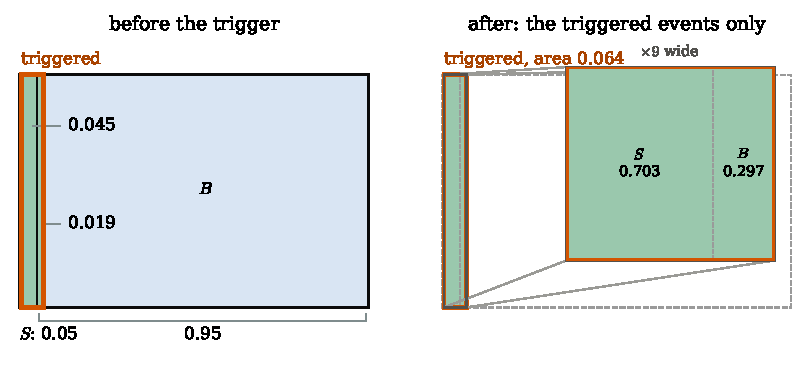
\includegraphics[width=\linewidth]{figures/ch05/area_trigger.pdf}
\caption{The trigger drawn to scale, in the picture of \cref{1a:fig:shrink}. Left:
the signal strip $S$ has width $0.05$ and the background strip $B$ width $0.95$; the
triggered events (orange outline) cover $0.90$ of the signal strip but only $0.02$
of the background strip, so the two pieces have areas $\FiveATrigJointS$ and
$\FiveATrigJointB$. The background piece covers a small share of its strip, but its
strip is nineteen times wider. Right: once we keep only triggered events, the box
is the new sample space; the inset magnifies it horizontally. Signal fills
$\FiveATrigPost$ of it.}
\label{5a:fig:trigger-area}
\end{figure}

\subsection{Drawing the boxes in Python}

The trigger figure was drawn by one short function, \pyname{box_diagram}, which
takes any list of priors and likelihoods and draws the box picture to scale. Its
geometry is the loop over strips:

\pyfile[firstline=143,lastline=156,firstnumber=143]{code/ch05/lib_area.py}{The
strips and the pieces of the evidence}\label{5a:lst:area}

Line 145 turns the priors into the positions of the strip edges, so strip $i$ runs
from the sum of the earlier priors to that sum plus its own prior. Line 149 is the
whole of the likelihood's role: the piece of $E$ in strip $i$ is as wide as the strip
times $\Prob(E\given H_i)$, and it runs the full height, so its area is prior times
likelihood. Lines 150--155 only decide where the piece sits inside its strip: it is
pushed against a neighbouring strip that also has a piece, so that the pieces join
into one box, as in \cref{1a:fig:monty-boxes}. The companion function
\pyname{posterior} in the same file computes the numbers: the joint areas are
\pyname{priors * likes}, their sum is $\Prob(E)$, and the posterior is their ratio.
The same file keeps \pyname{area_diagram}, which draws the square of
\cref{5a:fig:square} with bars. The script \pyname{code/ch05/01_area_diagrams.py}
computes the medical test, Monty Hall and the trigger, draws the trigger, and writes
the posteriors quoted above.
\section{Reallocating credibility across possibilities}
\label{5a:sec:reallocation}

We step outside in the morning and the pavement is wet. Rain? A garden sprinkler?
A burst pipe? A passer-by who spilled a drink? Each possibility has some
credibility before we look further, rain more than a spilled drink. Then we look
around. If the trees and the parked cars are wet as far as we can see, credibility
flows to rain. If the wet patch is small and there is an empty cup beside it,
credibility flows to the spilled drink, although it started low. Kruschke puts the
whole of Bayesian inference into one sentence: it is the \newterm{reallocation of
credibility across possibilities} \srcref{Kruschke}{\S2.1}.

The phrase says two things, and the square of \cref{5a:sec:shrink} makes both
exact. First, the total credibility is fixed. It is always one, shared among
possibilities that exclude each other and together cover everything we consider.
Second, credibility moves towards the possibilities that account well for what
was seen. Which ones gain? The posterior of a possibility is its prior times its
likelihood, divided by $\Prob(E)$. And $\Prob(E)$ is the average of all the
likelihoods, each weighted by its prior. So a possibility gains exactly when its
likelihood, the height of its bar in the square, is above that average. This
means any inference problem needs only three things: a list of possibilities, a
prior over the list, and, for each item, the probability of what we saw.

\begin{keyidea}[Posterior is proportional to likelihood times prior]
\[
  \Prob(H_i\given E)\;\propto\;\Prob(E\given H_i)\,\Prob(H_i),
\]
with the constant fixed by $\sum_i\Prob(H_i\given E)=1$ \mainref{p.~177, (11.2)}. Equivalently, the posterior of $H_i$ is its prior
multiplied by the factor $\Prob(E\given H_i)/\Prob(E)$, which exceeds one exactly when
$H_i$ predicted $E$ better than the prior-weighted average of all hypotheses.
\end{keyidea}

\subsection{The Bayes box}

The bookkeeping fits in a table with one row per possibility, which Lambert calls a
\newterm{Bayes box} \srcref{Lambert}{\S5.5.1}. Columns: the possibility, its prior,
its likelihood, their product, and the product divided by the column sum.

\paragraph{Example: the fish game.}
A covered bowl holds five fish, each red or white. We want the number $\alpha$ of red
fish. We pull out one fish at random and it is red: that is the event. The
candidates are the six possible bowls, $\alpha\in\{0,1,\dots,5\}$. We have no idea
beforehand, so each gets prior $\frac16$. How probable is a red fish under each
candidate? A bowl with $\alpha$ red fish out of five gives a red fish with
probability $\alpha/5$.
\begin{center}
\small
\begin{tabular}{@{}ccccc@{}}
\toprule
$\alpha$ & prior & likelihood $\alpha/5$ & prior $\times$ likelihood & posterior\\
\midrule
0 & 1/6 & 0   & 0    & 0\\
1 & 1/6 & 1/5 & 1/30 & 1/15\\
2 & 1/6 & 2/5 & 2/30 & 2/15\\
3 & 1/6 & 3/5 & 3/30 & 3/15\\
4 & 1/6 & 4/5 & 4/30 & 4/15\\
5 & 1/6 & 1   & 5/30 & 5/15\\
\midrule
sum & 1 & 3 & 15/30 $=\Prob(\text{red})$ & 1\\
\bottomrule
\end{tabular}
\end{center}
The posterior column is the product column divided by its sum, $\frac12$. The
table shows three things. First, the likelihood column sums to $3$, not to $1$:
as in \cref{5a:sec:two-directions}, a likelihood is not a distribution over the
possibilities. Second, $\alpha=0$ is eliminated, because a bowl with no red fish
cannot produce a red fish. Third, with a flat prior the posterior has the same
shape as the likelihood, here a straight line rising to $\alpha=5$. Suppose
instead we believed that the game-maker likes mixed bowls. A prior peaked at
$\alpha=2,3$ would then pull the posterior back towards the middle. The posterior
is a compromise between prior and likelihood \srcref{Lambert}{\S5.5.1},
\srcref{Kruschke}{\S5.3}.

\subsection{Elimination and exoneration}

Sherlock Holmes said: ``when you have eliminated the impossible, whatever remains,
however improbable, must be the truth''. In the Bayes box this is a likelihood of
zero. If the observation is impossible under $H_j$, then $\Prob(E\given H_j)=0$, and
that row's posterior is zero. If the other possibilities all have the same
likelihood, their posteriors are just their priors rescaled to sum to one. Kruschke
draws four suspects at $0.25$ each: rule out A, and B, C, D get $\frac13$ each;
rule out B as well, and C, D get $\frac12$; rule out C, and D gets $1$
\srcref{Kruschke}{\S2.1, Fig.~2.1}. The reverse, \emph{exoneration}, is an
observation that only one possibility can produce: then that possibility gets
credibility one and all the others are cleared \srcref{Kruschke}{Fig.~2.2}.

\paragraph{Example: the trigger path, continued.}
Recall the event of \cref{5a:sec:two-directions} that had lost its trigger flag.
One of three paths fired it: muon ($H_\mu$), calorimeter ($H_{\rm cal}$) or track
($H_{\rm trk}$). The isolated muon $E$ moved their credibility from
$(0.25,0.60,0.15)$ to $(0.745,0.128,0.128)$. Now we read the run log and find that
during this run the muon trigger was masked: it could not fire. How probable is
that log entry under each path? If the muon path fired the event, a mask is
impossible, so the probability is $0$. If either other path fired it, the mask
is certain to be in the log, so the probability is $1$. The new likelihoods
multiply the old posteriors:
\begin{align*}
  \Prob(H_\mu\given E,\text{mask})
  &\eqby{1}\frac{0\times0.745}{0\times0.745+1\times0.128+1\times0.128}=0,\\
  \Prob(H_{\rm cal}\given E,\text{mask})=\Prob(H_{\rm trk}\given E,\text{mask})
  &\eqby{2}\frac12 .
\end{align*}
\begin{explain}
  \item Bayes' theorem with the previous posterior as the new prior (justified in
        \cref{5a:sec:sequential}); the mask entry has likelihoods $(0,1,1)$.
  \item The two survivors have equal likelihood, so they keep the ratio of their
        previous credibilities, which was $1:1$.
\end{explain}
The muon path, the favourite a moment ago, is gone. Its $0.745$ has been shared
between the two survivors in proportion to what they had. \Cref{5a:fig:cred-trigger}
shows the whole sequence as bars.

\begin{figure}[htbp]
\centering
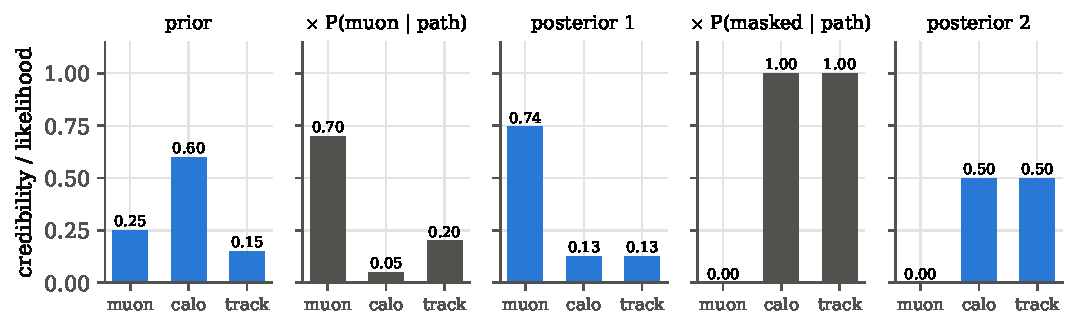
\includegraphics[width=\linewidth]{figures/ch05/credibility_trigger.pdf}
\caption{Credibility of the three trigger paths. From left: the prior (share of
recorded events); the likelihood of an isolated high-$p_T$ muon under each path; the
posterior; the likelihood of the run-log entry ``muon trigger masked''; the final
posterior. Blue bars always sum to one; grey bars need not. Each blue panel is the
previous blue panel times the grey panel, renormalised.}
\label{5a:fig:cred-trigger}
\end{figure}

\begin{pitfall}[A zero prior can never be revived]
If a possibility has prior zero, its posterior is zero whatever is observed, because
$0\times\Prob(E\given H)=0$. Lambert's example is someone so certain that the Earth
is flat that the round Earth gets prior zero; no amount of astronomical data can
then move it \srcref{Lambert}{\S5.7.1}. Truncating a prior (``the prevalence is surely
below $25\%$'') does the same to every value beyond the cut. Give every possibility
you cannot rule out on physical grounds a nonzero prior.
\end{pitfall}

\subsection{Noisy data only nudge}

Holmes' clues were decisive: each one set some likelihoods exactly to zero. Real
measurements are noisy. A noisy measurement is only somewhat more probable under one
possibility than under another, so credibility moves gradually and nothing is
ruled out.

\paragraph{Example: which ball size?}
A factory makes balls in four sizes, with nominal diameters $1,2,3,4$ (in some
unit). Inflation varies, so a ball of size $s$ has a diameter spread around $s$; take
it Gaussian with standard deviation $\sigma=1.17$.\footnote{This value reproduces
Kruschke's percentages; he does not state the spread he used.} We ordered three balls
of size $2$.

\emph{The event.} We measure the three diameters $d=(1.77,2.23,2.70)$.

\emph{The question.} Did we get what we ordered
\srcref{Kruschke}{\S2.1.1, Fig.~2.3}? Which size could have produced these three
diameters?

\emph{The candidates.} The four sizes $s=1,2,3,4$. The factory may have lost our
order, so we do not trust the label and give each size prior $\frac14$.

\emph{How probable are the data under each size?} The three diameters are
independent once the size is fixed, so the likelihood is a product of three
Gaussian densities:
\begin{align}
  p(\data\given s)
  &\eqby{1}\prod_{i=1}^3\frac{1}{\sqrt{2\pi}\,\sigma}
          \exp\!\Bigl[-\frac{(d_i-s)^2}{2\sigma^2}\Bigr]
  \eqby{2}\frac{1}{(2\pi\sigma^2)^{3/2}}
          \exp\!\Bigl[-\frac{1}{2\sigma^2}\sum_{i=1}^3(d_i-s)^2\Bigr] .
  \label{5a:eq:balls}
\end{align}
\begin{explain}
  \item Independence given $s$: the joint density is the product of the three
        single-ball densities $\Normal(d_i;s,\sigma^2)$.
  \item Collect the three exponentials into one.
\end{explain}
The prefactor is the same for every $s$, so it cancels in the posterior. Only the
sum of squared distances from the data to $s$ matters, and the smaller it is, the
larger the likelihood. The sums are $5.00$, $0.60$, $2.20$ and $9.80$ for
$s=1,2,3,4$: size $2$ is closest to the three measurements.

\emph{Only then the numbers.} With equal priors, the posterior
(\cref{5a:fig:balls}) is $\FiveABallPa$, $\FiveABallPb$, $\FiveABallPc$,
$\FiveABallPd$ for sizes $1$ to $4$. Size $2$ is the most credible, but far from
certain. Its likelihood is only $\FiveABallLRbc$ times that of size $3$, because
the spread of a single ball, $\sigma=1.17$, is larger than the distance between
sizes. No size is ruled out, since a Gaussian is never exactly zero. Size $4$ is
merely very unlikely.

\begin{figure}[htbp]
\centering
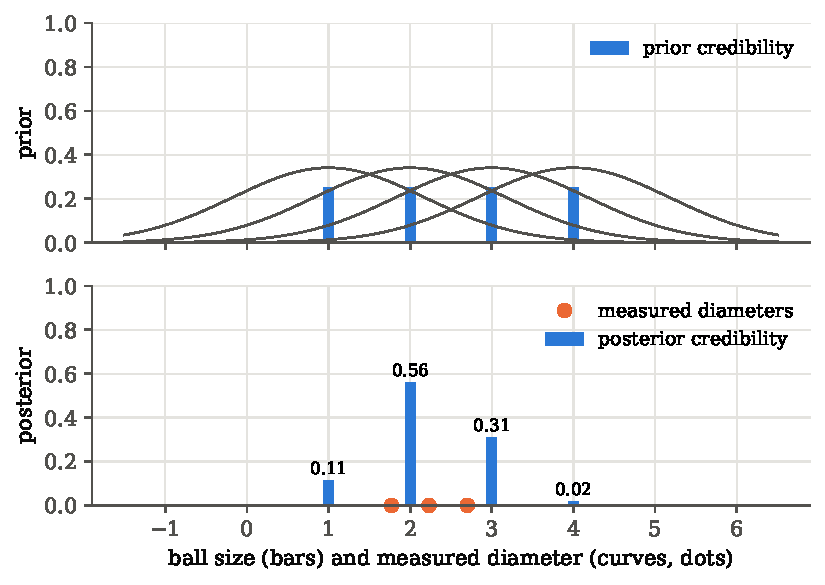
\includegraphics[width=0.78\linewidth]{figures/ch05/credibility_balls.pdf}
\caption{Top: four candidate ball sizes with equal prior credibility (bars), and the
spread of diameters each size produces (curves). Bottom: the three measured diameters
(dots on the axis) and the posterior credibility of each size. The data sit between
sizes 2 and 3, closer to 2, and the credibility moves accordingly, without ruling
anything out.}
\label{5a:fig:balls}
\end{figure}

Data analysis is exactly this, with the balls replaced by physical parameters. We
list the possible sources of the data, write down how each would produce data,
and let the data reallocate the credibility \srcref{Kruschke}{\S2.1.1}. The recipe
has the same steps in every textbook. Identify the data. Write a model that gives
the probability of the data for each possibility. Put a prior on the
possibilities. Apply Bayes' theorem. Check that the most credible possibilities
actually reproduce the data \srcref{Kruschke}{\S2.3}, \mainref{p.~176}. Repeat as
new data arrive \srcref{SeeingTheory}{p.~51}. The possibilities are usually the
values of the parameters of a model \srcref{Kruschke}{\S2.2}. When a parameter is
continuous, the row of bars becomes a density over it. Each value of the parameter, here
the ball size $s$, is then one candidate explanation of the measured data, and
its likelihood says how easily that value could have produced them; this is
parameter estimation, taken up for continuous parameters in
\cref{5b:sec:continuous}.

\subsection{Which source produced this photon?}

A gamma-ray burst goes off, and in the $100\,$s after it a gamma-ray telescope
records photons from a $10^\circ\times10^\circ$ patch of sky around it. Each photon
comes with a reconstructed direction $\bm r$ and energy $E$. Three sources can produce
a photon in this patch: the burst itself (G), a steady blazar $1.3^\circ$ away (Bz),
and the diffuse gamma-ray background spread over the whole patch (D). For each
photon we ask: which source produced it? This is the trigger-path problem again.
The candidates are the three sources, and the evidence is the photon's direction
and energy, which are continuous.

\paragraph{Priors from rates.}
Before we look at a photon's direction or energy, the probability that it came from
source $k$ is that source's share of the expected photon count in the window. We
take $30$ expected burst photons, $8$ from the blazar and $40$ from the diffuse
background, so the priors are $\FiveAGrbPriorG$, $\FiveAGrbPriorB$ and
$\FiveAGrbPriorD$. The diffuse background is the most probable source of a random
photon.

\paragraph{Likelihoods from the instrument.}
The telescope does not report a direction exactly. A photon from a point source at
$\bm r_k$ is reconstructed at $\bm r$ with a probability density given by the
\newterm{point-spread function} \unpack{the density of reconstructed directions for a
point source, here a 2-D Gaussian of width $\sigma(E)$}, which is wide at low energy
and narrow at high energy; we take $\sigma(E)=0.8^\circ\,(E/1\,\text{GeV})^{-0.8}$. The
energy of a photon from source $k$ is distributed according to that source's spectrum,
a power law $p(E\given k)\propto E^{-\gamma_k}$ with $\gamma=2.0$ for the burst,
$2.4$ for the blazar and $2.6$ for the diffuse emission. Direction and energy are
independent given the source, apart from the energy dependence of the PSF width, so
\begin{align}
  p(\bm r,E\given k)
  \eqby{1}p(E\given k)\;p(\bm r\given E,k)
  \eqby{2}
  \begin{cases}
    p(E\given k)\,\dfrac{1}{2\pi\sigma(E)^2}
      \exp\!\Bigl[-\dfrac{|\bm r-\bm r_k|^2}{2\sigma(E)^2}\Bigr],
      & k=\text{G, Bz},\\[3mm]
    p(E\given \text{D})\,\dfrac{1}{A}, & k=\text{D}.
  \end{cases}
  \label{5a:eq:grb-like}
\end{align}
\begin{explain}
  \item Product rule for densities.
  \item For a point source the direction density is the PSF centred on the source.
        For the diffuse background every direction in the patch of area $A=100\,\text{deg}^2$
        is equally likely.
\end{explain}

\paragraph{Densities as likelihoods.}
The observation ``the photon arrived exactly at $\bm r$ with exactly energy $E$'' has
probability zero under every source. What the telescope really reports is ``in a
small cell $\dd^2\bm r\,\dd E$ around $(\bm r,E)$'', and that has probability
$p(\bm r,E\given k)\,\dd^2\bm r\,\dd E$. The cell size is the same factor for every
source and cancels between the numerator and the denominator of Bayes' theorem. So
densities can stand in for probabilities as likelihoods, as long as all of them are
densities in the same variables.

\paragraph{Example: one photon.}
A photon arrives at $\bm r=(0.7^\circ,0.3^\circ)$ with $E=2\,$GeV, between the burst
and the blazar and a little closer to the blazar. At this energy the PSF width is
$\FiveAGrbSigOne^\circ$. The three likelihoods \eqref{5a:eq:grb-like} are
$\FiveAGrbLG$, $\FiveAGrbLB$ and $\FiveAGrbLD$ per $\text{deg}^2$ per GeV. Then
\begin{align*}
  \Prob(\text{G}\given\bm r,E)
  \eqby{1}\frac{\FiveAGrbPriorG\times\FiveAGrbLG}
   {\FiveAGrbPriorG\times\FiveAGrbLG+\FiveAGrbPriorB\times\FiveAGrbLB
    +\FiveAGrbPriorD\times\FiveAGrbLD}
  \eqby{2}\FiveAGrbMaG ,
\end{align*}
\begin{explain}
  \item Bayes' theorem with the three sources as the partition.
  \item Numerically, $1.84\times10^{-3}/2.28\times10^{-3}$.
\end{explain}
and likewise $\Prob(\text{Bz}\given\bm r,E)=\FiveAGrbMaB$,
$\Prob(\text{D}\given\bm r,E)=\FiveAGrbMaD$. The burst wins, and each source's
result has a plain reason. The photon is closer to the blazar, so the direction
alone slightly favours the blazar. But the burst is nearly four times brighter in
this window, which gives it the larger prior, and its harder spectrum makes a
$2\,$GeV photon more probable. The product of prior and likelihood is therefore
largest for the burst. The diffuse background was the most probable source before
we looked at the photon. It loses because its likelihood is spread evenly over the
whole patch: it predicts \emph{this} direction no better than any other.

\Cref{5a:fig:grb-sky} does this for every photon of one simulated window. Photons near
the burst are dark (almost surely burst photons), photons far from both point sources
are pale (mostly background), and photons between the two point sources are shared.
A soft photon far out, at $(-3^\circ,2^\circ)$ with $E=0.3\,$GeV, still has
$\Prob(\text{G}\given\bm r,E)=\FiveAGrbMbG$: at $0.3\,$GeV the PSF is about
$2^\circ$ wide, so the burst can put a photon there.

\begin{figure}[htbp]
\centering
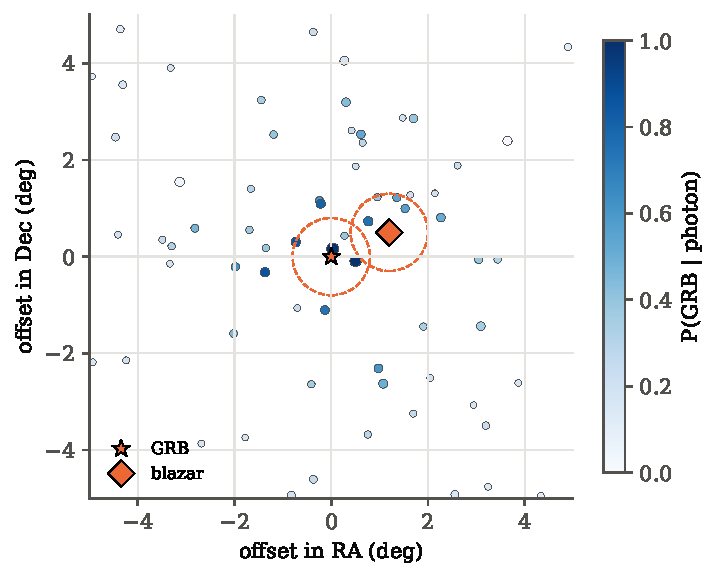
\includegraphics[width=0.68\linewidth]{figures/ch05/grb_sky.pdf}
\caption{One simulated $100\,$s window of photons around a gamma-ray burst (star),
with a blazar nearby (diamond) and a diffuse background. Each dot is a photon, larger
for higher energy, shaded by its posterior probability of having come from the
burst. The dashed circles have the radius of the point-spread function at $1\,$GeV.
Dark dots cluster on the burst; photons far from both point sources are pale.}
\label{5a:fig:grb-sky}
\end{figure}

\pyfile[firstline=56,lastline=67,firstnumber=56]{code/ch05/03_grb_source.py}{Posterior
source probabilities for a photon}

Lines 58--60 are the three cases of \eqref{5a:eq:grb-like}, one column per source.
Line 66 multiplies each column by its prior (the expected counts; their common
normalisation cancels), and line 67 divides by the sum over sources. It works on a
whole array of photons at once. Adding the burst column over all photons of the
window gives $\FiveAGrbNest$, an estimate of the number of burst photons; the
simulation actually contained $\FiveAGrbNtrue$ of the $\FiveAGrbNphot$. Such
per-photon source probabilities are used in gamma-ray astronomy to weight photons
when searching for pulsations or transients, so that background photons dilute the
signal less.
\section{Odds and the likelihood ratio: evidence as a multiplier}
\label{5a:sec:odds}

A search for a rare process uses a boosted decision tree, a classifier that gives
every event a score $x$ between $0$ and $1$. Signal events tend to score high,
background events low, and both distributions are known from simulation. Before we
look at its score, an event is signal with probability $\pi$, the signal fraction of
the sample. Then one event scores $x=0.9$. How probable is it that this event is
signal? And how would the answer change in another analysis with the same classifier
but a hundred times less signal?

The answer splits into two factors. One depends only on the classifier and the
score. The other depends only on the sample. The second question then needs no new
work: we keep the first factor and change the second. This split is the odds form
of Bayes' theorem, and it gives the simplest working rule for the question
``which hypothesis produced this?''.

\subsection{Odds}

The \newterm{odds} on a hypothesis are its probability divided by the probability of
its negation, $O(H)=\Prob(H)/\Prob(\neg H)$. Odds and probability carry the same
information:
\begin{equation}
  O=\frac{p}{1-p}
  \qquad\Longleftrightarrow\qquad
  p=\frac{O}{1+O} .
  \label{5a:eq:odds-prob}
\end{equation}
A probability of $\frac12$ is odds $1$ (``evens''), $0.9$ is odds $9$, $0.01$ is odds
$1/99$. More generally, for any two hypotheses $H_1$, $H_2$ in a partition, the ratio
$\Prob(H_1)/\Prob(H_2)$ is the odds of $H_1$ against $H_2$.

How do the odds of $H_1$ against $H_2$ change when we observe $E$? Write Bayes'
theorem \eqref{5a:eq:bayes} for $H_1$ and for $H_2$ and divide:
\begin{align}
  \frac{\Prob(H_1\given E)}{\Prob(H_2\given E)}
  &\eqby{1}\frac{\Prob(E\given H_1)\,\Prob(H_1)/\Prob(E)}
               {\Prob(E\given H_2)\,\Prob(H_2)/\Prob(E)}
  \eqby{2}\underbrace{\frac{\Prob(E\given H_1)}{\Prob(E\given H_2)}}_{\text{likelihood ratio}}
   \times\underbrace{\frac{\Prob(H_1)}{\Prob(H_2)}}_{\text{prior odds}} .
  \label{5a:eq:odds}
\end{align}
\begin{explain}
  \item Bayes' theorem in numerator and denominator.
  \item The evidence $\Prob(E)$ is common to both and cancels.
\end{explain}
We write $\Lambda$ for the likelihood ratio.

\begin{keyidea}[Evidence multiplies odds]
\[
  \text{posterior odds}=\Lambda\times\text{prior odds},
  \qquad
  \Lambda=\frac{\Prob(E\given H_1)}{\Prob(E\given H_2)} .
\]
The \newterm{likelihood ratio} $\Lambda$ is everything the observation has to say
about $H_1$ versus $H_2$. It does not involve the priors, it does not involve any
other hypothesis, and it does not need $\Prob(E)$.
\end{keyidea}

In the square of \cref{5a:sec:shrink} every factor of \eqref{5a:eq:odds} is a ratio of
shapes. The prior odds are the ratio of the two strip \emph{widths}. The likelihood
ratio is the ratio of the two bar \emph{heights}. Their product, width ratio times
height ratio, is the ratio of the two surviving \emph{areas}, which is the posterior
odds. Take the medical test of \cref{5a:fig:medical}. The strip widths are
$\Prob(D)=0.01$ and $\Prob(D^c)=0.99$, a ratio of $1:99$. The positive result covers
$0.95$ of the disease strip and $0.10$ of the healthy one, a likelihood ratio of
$9.5:1$. So the surviving areas are in the ratio $9.5:99\approx1:10.4$, and the
posterior probability is $1/11.4\approx0.088$ by \eqref{5a:eq:odds-prob}. The test
is good evidence, a factor of $9.5$, but it is applied to odds that started at one
to ninety-nine.

\subsection{Evidence adds in logarithms}

Take logarithms of \eqref{5a:eq:odds}. Products become sums:
\begin{equation}
  \log O(H_1{:}H_2\given E)=\log\Lambda+\log O(H_1{:}H_2) .
  \label{5a:eq:logodds}
\end{equation}
So each piece of evidence \emph{adds} its log likelihood ratio to the log odds. We
call $\log\Lambda$ the \emph{weight of evidence}. A convenient unit is the
\newterm{decibel}: $10\log_{10}$ of the odds, the same unit physicists use for the
gains along an amplifier chain. Odds of $1:99$ are $-20\,$dB, evens are $0\,$dB,
odds of $99:1$ are $+20\,$dB. A positive medical test adds
$10\log_{10}9.5=+9.8\,$dB. One positive test takes the patient from $-20.0\,$dB to
$-10.2\,$dB, which is odds $0.096$ and probability $0.088$. Suppose a second
positive test is taken, independent of the first \emph{given} the disease status
(a condition examined in \cref{5a:sec:sequential}). It adds another $9.8\,$dB, to
$-0.4\,$dB, probability $0.48$. A third takes it to $+9.4\,$dB, probability $0.90$
(\cref{5a:fig:decibels}).

\begin{figure}[htbp]
\centering
\begin{tikzpicture}[font=\small,x=0.28cm]
  \draw[->] (-24,0) -- (24,0) node[right] {dB};
  \foreach \t in {-20,-10,0,10,20} {
    \draw (\t,0.12) -- (\t,-0.12) node[below,font=\footnotesize] {$\t$};
  }
  \node[font=\footnotesize,align=center,anchor=north] at (-20,-0.75) {odds $1{:}99$};
  \node[font=\footnotesize,align=center,anchor=north] at (0,-0.75) {evens};
  \node[font=\footnotesize,align=center,anchor=north] at (20,-0.75) {odds $99{:}1$};
  \foreach \x/\p/\n in {-19.96/0.010/prior, -10.18/0.088/1 test, -0.40/0.48/2 tests, 9.38/0.90/3 tests}{
    \fill[formblue] (\x,0) circle (2.2pt);
    \node[anchor=south,font=\footnotesize,align=center] at (\x,1.05) {\n\\ $p=\p$};
  }
  \foreach \a/\b in {-19.96/-10.18, -10.18/-0.40, -0.40/9.38}{
    \draw[->,thick,tangentgreen] (\a,0.12) to[out=60,in=120] (\b,0.12);
  }
  \node[font=\footnotesize,tangentgreen!60!black,anchor=west] at (11,0.55)
    {each green step: $+9.8$ dB};
\end{tikzpicture}
\caption{The medical test as a walk on a scale of log odds. The prior, one person in a
hundred, sits at $-20\,$dB. Each positive result from an independent test adds the
same weight of evidence, $10\log_{10}9.5\approx9.8\,$dB. The probability above each
dot follows from the odds by $p=O/(1+O)$: three positive tests are needed before the
disease becomes the likely explanation.}
\label{5a:fig:decibels}
\end{figure}

The additive form explains two habits of practising physicists. First, analyses
add log likelihoods rather than multiply likelihoods, because independent pieces of
evidence add in logarithms. Second, ``how strong is this evidence?'' has an answer
that does not depend on the prior: $\log\Lambda$. Whether it is strong \emph{enough} depends on where the
prior odds started. A $+10\,$dB piece of evidence decides a question that started at
evens, and barely dents one that started at $-40\,$dB.

\subsection{Signal or background, given a classifier score}

Back to the boosted decision tree of the opening, which gives each event a score
$x$ between $0$ and $1$, and to the question: given one event's score, is it
signal ($S$) or background ($B$)? Suppose the simulation shows that signal scores follow the
density $f_S(x)=30\,x^4(1-x)$ and background scores the density
$f_B(x)=30\,x(1-x)^4$ on $[0,1]$ (\cref{5a:fig:bdt}, left). Both are Beta densities,
$\mathrm{Beta}(5,2)$ and $\mathrm{Beta}(2,5)$; all we need is that each integrates to
one, which the factor $30$ ensures. The evidence is the score of one event, a
continuous quantity, so the likelihoods are densities, and the cell $\dd x$ cancels in
the ratio exactly as the cell $\dd^2\bm r\,\dd E$ did for the photon in
\cref{5a:sec:reallocation}. The likelihood ratio is
\begin{align}
  \Lambda(x)
  &\eqby{1}\frac{f_S(x)}{f_B(x)}
  \eqby{2}\frac{30\,x^4(1-x)}{30\,x(1-x)^4}
  \eqby{3}\Bigl(\frac{x}{1-x}\Bigr)^{3} .
  \label{5a:eq:bdt-lr}
\end{align}
\begin{explain}
  \item Likelihood ratio of signal to background for the observed score.
  \item The two densities.
  \item Cancel $30$, one power of $x$ and one power of $(1-x)$.
\end{explain}
With prior odds $\pi/(1-\pi)$, the posterior odds are
$\Lambda(x)\,\pi/(1-\pi)$. In logarithms, with the \newterm{logit}
$\operatorname{logit}p=\ln[p/(1-p)]$ \unpack{the natural log of the odds},
\begin{equation}
  \operatorname{logit}\Prob(S\given x)=\operatorname{logit}\pi+3\operatorname{logit}x .
  \label{5a:eq:bdt-logit}
\end{equation}
This is the split promised at the start. The score contributes a term,
$3\operatorname{logit}x$, that depends only on the classifier. The sample
contributes a term, $\operatorname{logit}\pi$, that depends only on the signal
fraction $\pi$.

\paragraph{Example: the same score in two analyses.}
For $x=0.9$ the likelihood ratio is $9^3=729$. With $\pi=0.01$ the prior odds are
$1/99$, the posterior odds $729/99=7.36$, and
\begin{align*}
  \Prob(S\given x=0.9)\eqby{1}\frac{7.36}{1+7.36}=\FiveABdtPostNine .
\end{align*}
\begin{explain}
  \item Posterior odds converted to a probability by \eqref{5a:eq:odds-prob}.
\end{explain}
In the analysis with a hundred times less signal, $\pi=10^{-4}$, the likelihood
ratio is unchanged and only the prior odds change. The same score gives posterior
odds $729/9999=0.073$, so $\Prob(S\given x=0.9)=\FiveABdtPostNineTiny$. Same event,
same classifier, and now it is probably background. A score of $0.8$ is weaker
evidence, $\Lambda=4^3=64$, and gives only $\FiveABdtPostEight$ at $\pi=0.01$. The score
at which an event becomes more likely signal than not, $\Prob(S\given x)=\frac12$, is
where $3\operatorname{logit}x=-\operatorname{logit}\pi$: $x_{1/2}=\FiveABdtHalfOne$ for
$\pi=0.01$ and $\FiveABdtHalfTiny$ for $\pi=10^{-4}$ (\cref{5a:fig:bdt}, right).

\begin{figure}[htbp]
\centering
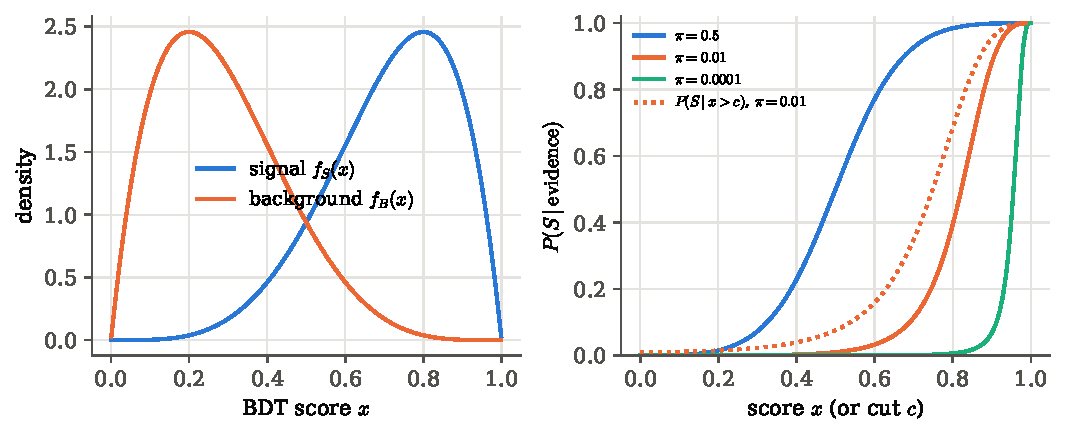
\includegraphics[width=\linewidth]{figures/ch05/bdt_posterior.pdf}
\caption{Left: the score densities of signal and background. Right: the probability
that an event is signal given its score $x$, for three signal fractions $\pi$ (solid).
The curves are the same likelihood ratio combined with different prior odds, so they
are shifted copies of one another on the logit scale. The dotted curve is a different
question: the signal fraction of the whole sample with $x>c$, plotted against the cut
$c$, for $\pi=0.01$.}
\label{5a:fig:bdt}
\end{figure}

\paragraph{Checking it by selection.}
We can check the formula without algebra, because conditioning on an observation
is the same as selecting the events that show it (\cref{ch:01}). The script \pyname{code/ch05/04_bdt_posterior.py} generates $10^7$ events
with $\pi=0.01$, draws each event's score from $f_S$ or $f_B$, keeps the
$\FiveABdtNsel$ events with $|x-0.9|<0.005$, and counts the signal among them: the
fraction is $\FiveABdtMC\pm\FiveABdtMCerr$, against $\FiveABdtPostNine$ from
\eqref{5a:eq:bdt-logit}. Bayes' theorem is the statement of what this selection
returns.

\subsection{Be exact about what you observed}

A score and a cut are different observations, and they give different answers.
The dotted curve in \cref{5a:fig:bdt} shows the cut. Suppose we do not look at each
event's score but select all events with $x>c$ and ask for the signal fraction of
the selected sample, its \newterm{purity}. The observed event is now
``$x>c$'', whose probability under each hypothesis is an efficiency,
$\varepsilon_S(c)=\int_c^1f_S\,\dd x$ and $\varepsilon_B(c)=\int_c^1f_B\,\dd x$. For
$c=0.8$ these are $\FiveABdtEffS$ and $\FiveABdtEffB$, so
\begin{align*}
  \Lambda(x>0.8)\eqby{1}\frac{\varepsilon_S}{\varepsilon_B}=\FiveABdtCutLR,
  \qquad
  \Prob(S\given x>0.8)\eqby{2}\FiveABdtCutPur .
\end{align*}
\begin{explain}
  \item The likelihood ratio of the event ``$x>0.8$'' is the ratio of the probabilities
        of that event, the two efficiencies.
  \item Posterior odds $\FiveABdtCutLR/99$, converted with \eqref{5a:eq:odds-prob}.
\end{explain}
This is much larger than $\Prob(S\given x=0.8)=\FiveABdtPostEight$. Why? The
selected sample contains all the events with $x$ between $0.8$ and $1$. Most of
them score well above $0.8$, and their scores are much stronger evidence. An event
that sits exactly at the cut is among the \emph{least} signal-like in the sample.
Bayes' theorem conditions on exactly the statement we say we know, nothing more. ``The score is
$0.8$'' and ``the score is above $0.8$'' are different observations with different
likelihood ratios, and mixing them is a common error in quoting per-event
probabilities.

\paragraph{Why the likelihood ratio is the right score.}
For two hypotheses, \eqref{5a:eq:odds} says that the posterior depends on the data
only through $\Lambda$. Any two events with the same $\Lambda$ are equally
signal-like, whatever else differs between them. This is the Bayesian face of the
Neyman--Pearson lemma of \cref{ch:04}: the most powerful selection at any background
rejection is a cut on $\Lambda$. A classifier whose score is a monotonic function of
$\Lambda$ is already optimal, and our score is one, since $(x/(1-x))^3$ increases with
$x$.

\begin{inpractice}[The likelihood-ratio trick]
A classifier trained with balanced samples of simulated signal and background, and a
loss such as the cross-entropy, learns in the limit of enough data and flexibility to
output $s(x)=\Prob(S\given x)$ at $\pi=\frac12$, that is
$s=\Lambda/(1+\Lambda)$. Then $\Lambda(x)=s/(1-s)$ is recovered from the output, and
\eqref{5a:eq:odds} converts it to the posterior for the actual signal fraction of any
sample. The same trick turns classifiers into estimators of likelihood ratios between
two parameter points, which is how simulation-based inference compares hypotheses
whose likelihoods cannot be written down.
\end{inpractice}
\section{Sequential updating: yesterday's posterior is today's prior}
\label{5a:sec:sequential}

We find a coin on the pavement and want to know how biased it is. We toss it once and
it lands heads. It is tempting to say that one toss tells us nothing. It tells us
something: the coin is not two-tailed, a possibility that was open a moment ago, and
coins that favour heads are now a little more credible than before
\srcref{SeeingTheory}{p.~53}. We toss again, and again. Each toss should move our
belief a little more, starting from wherever the previous tosses left it. Is that
legitimate? Do we get the same answer as if we had waited for all the tosses and
analysed them at once? And does it matter in which order the tosses came?

\subsection{The update rule}

Let $D_1$ be the first piece of data and $D_2$ the second. Everything we know after
both is $\Prob(H\given D_1,D_2)$. The question is whether we can reach it in two
steps: first update on $D_1$, then update the result on $D_2$. To see, apply Bayes'
theorem to $D_2$ alone, with $D_1$ added to the background information of every
probability:
\begin{align}
  \Prob(H\given D_1,D_2)
  &\eqby{1}\frac{\Prob(D_2\given H,D_1)\;\Prob(H\given D_1)}{\Prob(D_2\given D_1)}
  \label{5a:eq:seq-general}\\
  &\eqby{2}\frac{\Prob(D_2\given H)\;\Prob(H\given D_1)}
               {\sum_j\Prob(D_2\given H_j)\,\Prob(H_j\given D_1)} .
  \label{5a:eq:seq}
\end{align}
\begin{explain}
  \item Bayes' theorem \eqref{5a:eq:bayes-xy} with $X=H$, $Y=D_2$ and background
        information $I$ replaced by ``$I$ and $D_1$''. Every rule of probability holds
        with extra information in the conditioning, since $\Prob(\cdot\given D_1)$ is
        itself a probability \srcref{Sivia}{\S1.2}.
  \item \emph{If} $D_2$ is independent of $D_1$ given each hypothesis,
        $\Prob(D_2\given H_j,D_1)=\Prob(D_2\given H_j)$. The denominator is then the
        marginalisation \eqref{5a:eq:marg} over the $H_j$, done inside
        $\Prob(\cdot\given D_1)$.
\end{explain}
Line \eqref{5a:eq:seq} is Bayes' theorem for $D_2$ alone, with the posterior after
$D_1$ in the place of the prior. So the answer is yes: the posterior of one step is
the prior of the next. This needs one condition, that the data are
\newterm{conditionally independent} \unpack{independent once the hypothesis is
fixed, although not independent when the hypothesis is unknown}. Line
\eqref{5a:eq:seq-general} needs no assumption at all.

\paragraph{The order does not matter.}
Doing $D_2$ first and $D_1$ second must give the same answer. Both routes compute
the probability of $H$ given the \emph{single} statement ``$D_1$ and $D_2$'', and
``$D_1$ and $D_2$'' is the same statement as ``$D_2$ and $D_1$''. The formula shows
the same thing. Under conditional independence, doing the two updates in one go
gives \srcref{Kruschke}{\S5.2.1}
\begin{align*}
  \Prob(H\given D_1,D_2)
  &\eqby{1}\frac{\Prob(D_1,D_2\given H)\,\Prob(H)}{\sum_j\Prob(D_1,D_2\given H_j)\,\Prob(H_j)}
  \eqby{2}\frac{\Prob(D_1\given H)\,\Prob(D_2\given H)\,\Prob(H)}
              {\sum_j\Prob(D_1\given H_j)\,\Prob(D_2\given H_j)\,\Prob(H_j)}\\
  &\eqby{3}\frac{\Prob(D_2\given H)\,\Prob(D_1\given H)\,\Prob(H)}
              {\sum_j\Prob(D_2\given H_j)\,\Prob(D_1\given H_j)\,\Prob(H_j)}
  \eqby{4}\Prob(H\given D_2,D_1) .
\end{align*}
\begin{explain}
  \item Bayes' theorem for the combined data.
  \item Conditional independence: the joint likelihood is the product.
  \item Multiplication of numbers commutes.
  \item Bayes' theorem read backwards, with the data in the other order.
\end{explain}
Updating one datum at a time computes the same product in stages. Each stage
multiplies by one likelihood and renormalises. Renormalising early instead of at
the end changes nothing, because a constant factor cancels in the ratio.

\begin{keyidea}[Sequential updating]
For data that are independent given the hypothesis, updating one datum at a time,
each posterior serving as the next prior, gives exactly the posterior of updating
with all the data at once, in any order. In log-odds form each datum simply adds its
log likelihood ratio. Without conditional independence the general rule
\eqref{5a:eq:seq-general} still holds, and the order still does not matter, but each
datum's likelihood must then be conditioned on the data before it.
\end{keyidea}

\subsection{The sample space, toss by toss}

A coin is either fair, $\Prob(\text{heads})=0.5$, or biased, $\Prob(\text{heads})=0.8$,
and we give each prior $\frac12$. We toss it four times and see H, H, T, H.
\Cref{5a:fig:shrink-seq} shows two ways of watching the sample space shrink.

The top row keeps the original sample space, drawn as in \cref{1a:fig:shrink}: two
strips of width $\frac12$, the biased coin on the left. After each toss, the
evidence ``the tosses so far'' is a box, and the part of each strip that it covers is
the part that survives. The share of the strip it covers is the probability of the
whole sequence so far under that coin: $0.8$, $0.64$, $0.128$,
$0.1024$ for the biased coin and $0.5$, $0.25$, $0.125$, $0.0625$ for the fair one. The
box only ever shrinks. After all four tosses its area is
\begin{align*}
  \Prob(\text{HHTH})
  \eqby{1}\tfrac12\times0.8^3\times0.2+\tfrac12\times0.5^4
  =0.0512+0.03125=\FiveASeqArea ,
\end{align*}
\begin{explain}
  \item Marginalisation over the two coins, with the product of the four toss
        probabilities (conditionally independent given the coin) as each likelihood.
\end{explain}
the probability, before any toss, of seeing exactly this sequence.

The bottom row blows the surviving box back up to area one after each toss. The
dividing line is then the current posterior, which is the prior for the next toss:
$0.5$, then $\FiveASeqPa$ after H, $\FiveASeqPb$ after HH, $\FiveASeqPc$ after HHT, and
$\FiveASeqPd$ after HHTH. The box in each rescaled panel is the next toss, covering a share of each strip
equal to its likelihood. A head is $0.8/0.5=1.6$ times more likely from the biased coin and moves
the line right; the tail is $0.2/0.5=0.4$ times as likely and moves it back left.
Both rows give the same final posterior,
$0.0512/\FiveASeqArea=\FiveASeqPd$: renormalising at every step or only at the end is
the same calculation.

\begin{figure}[htbp]
\centering
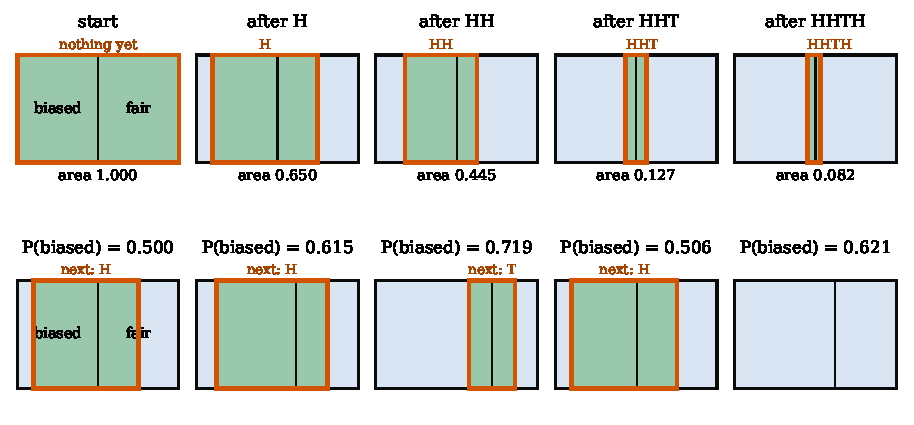
\includegraphics[width=\linewidth]{figures/ch05/shrinking_sequence.pdf}
\caption{The sample space shrinking toss by toss, for a biased coin (left strip)
against a fair one (right strip), drawn to scale as in \cref{1a:fig:shrink}. Top row:
the original sample space, with the tosses so far as a box (orange outline) that
covers $0.8$ or $0.5$ of each strip per head and $0.2$ or $0.5$ per tail; the number
under each panel is the area of the box, the probability of the sequence so far.
Bottom row: the surviving box rescaled to area one, so that the dividing line is the
current posterior of the biased coin; the box drawn in it is the next toss (the last
panel has no next toss).}
\label{5a:fig:shrink-seq}
\end{figure}

\subsection{A grid of biases}

Real coins are not limited to two types. The real question is: what is the coin's
probability of heads $\theta$, which could be anywhere in $[0,1]$? Kruschke's
answer is to allow a grid of candidate values, say
$\theta_j\in\{0,0.01,\dots,1\}$, as if a factory made coins of 101 types, and to
treat each $\theta_j$ as one hypothesis \srcref{Kruschke}{\S5.3}. A single toss $y$ ($y=1$ for heads, $0$ for tails) has the
Bernoulli likelihood \srcref{Kruschke}{(5.10)}
\begin{equation}
  \Prob(y\given\theta_j)=\theta_j^{\,y}(1-\theta_j)^{1-y},
  \label{5a:eq:bernoulli}
\end{equation}
which is $\theta_j$ for a head and $1-\theta_j$ for a tail. Updating is then one line of
code:

\pyfile[firstline=34,lastline=37,firstnumber=34]{code/ch05/05_coin_grid.py}{One toss:
multiply by the likelihood on the grid and renormalise}

Line 36 multiplies the whole array of credibilities by the array of likelihoods, one
value per grid point, and line 37 divides by the sum, the discrete evidence. This is the
Bayes box of \cref{5a:sec:reallocation} with 101 rows, recomputed after each toss.

The main lesson of \cref{5a:fig:coin-grid} is that with few data the prior matters,
and with many data it hardly does. The figure follows $50$ tosses of a coin with
true $\theta=0.3$, which produced $\FiveACoinHeads$ heads. It starts from two
priors. One is flat. The other is triangular, with its peak at $\frac12$ and zero
at $0$ and $1$; it encodes the belief that most coins are roughly fair.

Each toss acts in a way we can predict. After one tail, the flat-prior posterior
is the straight line $1-\theta$, because the likelihood of a tail is $1-\theta$.
The coin that always lands heads, $\theta=1$, is ruled out. After the first head,
$\theta=0$ is ruled out too. As tosses accumulate, the posterior narrows around
the observed fraction of heads. The two posteriors move towards each other, and
after $50$ tosses they nearly coincide; the flat-prior posterior has mean
$\FiveACoinPostMean$. So with few data the posterior is a compromise between prior
and likelihood, and with many the likelihood dominates
\srcref{Kruschke}{\S5.3.1--5.3.2}. Kruschke's numbers show the same thing on a grid
of $1001$ values with the triangular prior \srcref{Kruschke}{Fig.~5.2}. One head in
$4$ tosses gives a posterior mode of $\FiveACoinModeFour$, pulled far from the
observed fraction $0.25$ towards the prior's peak. Ten heads in $40$ tosses give
$\FiveACoinModeForty$, close to $0.25$.

\begin{figure}[htbp]
\centering
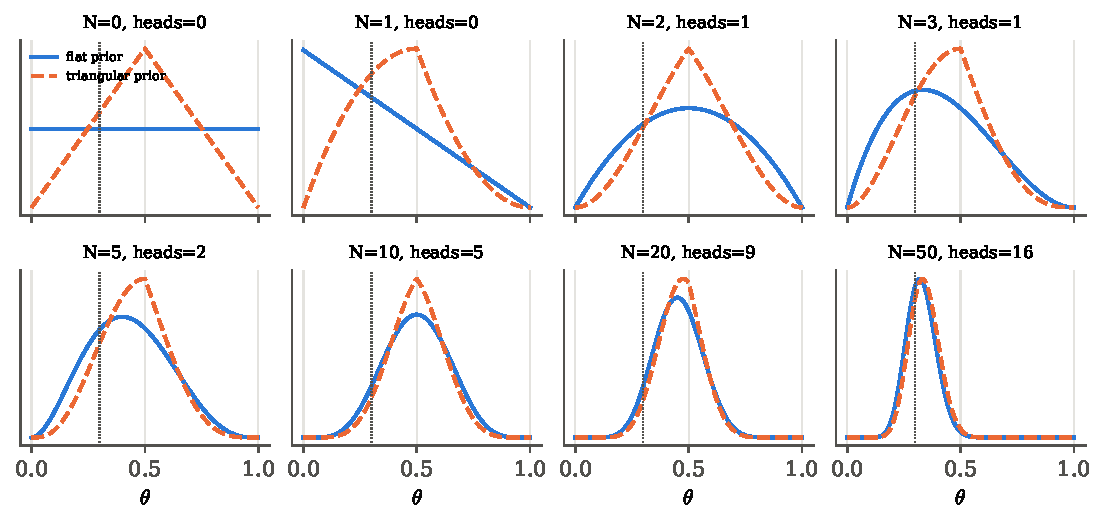
\includegraphics[width=\linewidth]{figures/ch05/coin_grid_panels.pdf}
\caption{Credibility of $101$ candidate biases $\theta$ after $N$ tosses of a coin whose
true bias is $0.3$ (dotted line), starting from a flat prior (solid) and from a
triangular prior peaked at $\frac12$ (dashed). Early on the two posteriors differ,
because the data are few; by $N=50$ both are narrow and nearly identical, centred near
the observed fraction of heads.}
\label{5a:fig:coin-grid}
\end{figure}

The script also checks the order claim numerically. It updates the flat prior with the
same $50$ tosses in $1000$ random orders and compares each result with the batch
posterior $\propto\theta^{z}(1-\theta)^{N-z}$ computed in one step ($z$ heads in $N$
tosses, \srcref{Kruschke}{(5.11)}). The largest difference at any grid point is
$\FiveACoinMaxDiff$, the size of floating-point rounding.

\subsection{Evidence accumulates as a random walk}

Return to two hypotheses, now a fair coin ($\theta_0=0.5$) against a biased one
($\theta_1=0.7$), with prior odds $1$. By \eqref{5a:eq:logodds} the $\log_{10}$ odds of
biased against fair add $\log_{10}(0.7/0.5)=\FiveACoinLRh$ for each head and
$\log_{10}(0.3/0.5)=\FiveACoinLRt$ for each tail. The log odds perform a random walk
(\cref{5a:fig:logodds}). If the coin really is biased, the average step per toss is
\begin{align}
  \E[\text{step}\given\theta_1]
  \eqby{1}\theta_1\log\frac{\theta_1}{\theta_0}+(1-\theta_1)\log\frac{1-\theta_1}{1-\theta_0}
  \equiv D_{\rm KL}(\theta_1\Vert\theta_0) ,
  \label{5a:eq:kl}
\end{align}
\begin{explain}
  \item A head, with probability $\theta_1$, contributes $\log(\theta_1/\theta_0)$; a
        tail, with probability $1-\theta_1$, contributes
        $\log[(1-\theta_1)/(1-\theta_0)]$.
\end{explain}
This average step is the \newterm{Kullback--Leibler divergence} between the two
coins \unpack{the average log likelihood ratio in favour of the true distribution;
in statistical mechanics it is the relative entropy}. It is never negative, and it
is zero only if the two coins are the same. So the walk drifts towards the truth,
whichever coin is true. The rate is $\FiveACoinKLone$ in $\log_{10}$ per toss when
the biased coin is true, and $\FiveACoinKLzero$ when the fair coin is true.
Reaching odds of $100:1$, which is $2$ in $\log_{10}$, therefore takes about
$2/\FiveACoinKLone\approx56$ tosses on average, with large scatter from one
sequence to the next. The more alike the two hypotheses, the smaller the divergence and the longer
the wait: telling apart two nearly identical coins, like two nearly identical
cosmologies, needs a lot of data.

\begin{figure}[htbp]
\centering
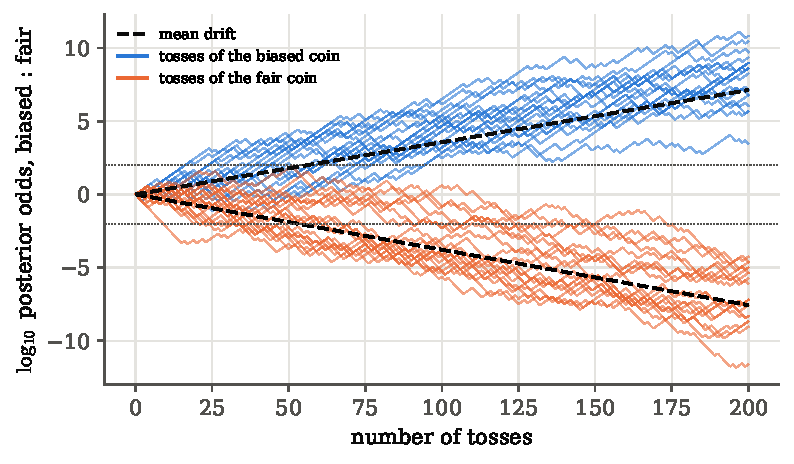
\includegraphics[width=0.82\linewidth]{figures/ch05/coin_logodds.pdf}
\caption{Log posterior odds of ``biased ($\theta=0.7$)'' against ``fair'' along $20$
simulated sequences of $200$ tosses from each coin, starting at odds $1$. Every head
steps up, every tail steps down. Sequences from the biased coin (blue) drift upward and
those from the fair coin (orange) downward, each at the rate given by a
Kullback--Leibler divergence (dashed lines). The dotted lines mark odds of $100:1$ each
way.}
\label{5a:fig:logodds}
\end{figure}

\subsection{When the data are not independent given the hypothesis}

Conditional independence is an assumption about how the data are produced, and it
can fail. When it fails, repeated evidence is worth less than the product of its
parts. Take the medical test again (prevalence $0.01$, $\Prob(+\given D)=0.95$,
$\Prob(+\given D^c)=0.10$), and suppose its false positives have two causes. Half of
them come from a harmless antibody that $5\%$ of healthy people carry, and it makes
the test positive every time. The other half are random, and happen to the other
healthy people with probability $r=0.05/0.95$ per test. The single-test false
positive rate is still $0.05+0.95\,r=0.10$. But for a healthy person two positive
tests in a row are now much more likely than $0.10^2$:
\begin{align*}
  \Prob({+}{+}\given D^c)
  \eqby{1}0.05\times1+0.95\times r^2
  =0.05+0.95\times0.00277=0.0526 .
\end{align*}
\begin{explain}
  \item Split the healthy population into antibody carriers (both tests positive
        for sure) and the others (two independent random false positives).
\end{explain}
For the diseased we keep independent tests, $\Prob({+}{+}\given D)=0.95^2=0.9025$. The
likelihood ratio of two positives is $0.9025/0.0526=17.1$, not $9.5^2=90$. Starting
from odds $1/99$, the posterior odds are $0.173$ and $\Prob(D\given{+}{+})=0.15$,
where the naive product would have given $0.48$. The second test is weaker evidence
because a large part of what made the first test positive in a healthy person repeats
itself.

\begin{pitfall}[Correlated data are not independent evidence]
Multiplying likelihoods, or adding log likelihood ratios, assumes that the data are
independent \emph{given} each hypothesis. Repeated measurements that share a
calibration offset, a common background mismodelling, overlapping sky patches or the
same patient-specific cause are correlated even given the hypothesis. Treating them as
independent double-counts the shared part and makes the evidence look far stronger
than it is. The remedy is to write the joint likelihood with its correlations, as a
multivariate Gaussian with a full covariance matrix $\Cmat$ does for Gaussian data.
\end{pitfall}

\subsection{Screening for breast cancer, test by test}
\label{5a:sec:screening}

A woman of fifty with no symptoms goes for a routine screening mammogram. The result
is positive. She is recalled for an ultrasound, and if that is positive too, for a
biopsy. After each result she, and her doctor, want to know one thing: how probable is
it now that she has cancer? We use round numbers of the right size for this age group,
illustrative rather than taken from a particular study: a \newterm{prevalence}
\unpack{the fraction of women screened at this age who have breast cancer at the time
of screening} of $1\%$; for the mammogram a sensitivity of $0.87$ and a specificity of
$0.90$; for the ultrasound $0.80$ and $0.90$; for the biopsy $0.95$ and $0.99$.
Sensitivity is $\Prob(+\given C)$, the chance that the test is positive if she has
cancer ($C$); specificity is $\Prob(-\given C^c)$, the chance that it is negative if
she has none ($C^c$).

There are two hypotheses throughout, $C$ and $C^c$, and each test redistributes the
whole unit of probability between them. The posterior after one test is the prior for
the next, by \eqref{5a:eq:seq}, as long as the tests are conditionally independent
given her true state; we come back to that assumption at the end.

\paragraph{Test 1: the mammogram.}
\emph{The event.} What we observed is ``the mammogram is positive''. Call it $M_+$.

\emph{What could have produced it?} The only thing we do not know is whether she has
cancer. So there are two explanations: she has cancer and the mammogram detected it,
or she has none and the mammogram raised a false alarm.

\emph{How probable was the event under each hypothesis?}
\begin{itemize}[itemsep=1pt,leftmargin=1.2em]
  \item Under $C$ the mammogram is positive when it detects the tumour, which is the
        sensitivity: $\Prob(M_+\given C)=0.87$.
  \item Under $C^c$ it is positive only by a false alarm, from dense tissue, a benign
        lump or a shadow: $\Prob(M_+\given C^c)=1-0.90=0.10$.
\end{itemize}

\emph{Only then the priors, and the update.} Before the test her probability of cancer
was the prevalence, $0.01$, so her prior odds were $1/99$. With the odds form
\eqref{5a:eq:odds},
\begin{align*}
  O(C\given M_+)
  &\eqby{1}\frac{\Prob(M_+\given C)}{\Prob(M_+\given C^c)}\cdot\frac{\Prob(C)}{\Prob(C^c)}
   \eqby{2}\frac{0.87}{0.10}\cdot\frac{0.01}{0.99}
   =\frac{8.7}{99}=0.0879,
  \qquad
  \Prob(C\given M_+)\eqby{3}\frac{0.0879}{1.0879}=\FiveAScrP .
\end{align*}
\begin{explain}
  \item Posterior odds are the likelihood ratio times the prior odds.
  \item The two likelihoods just found, and the prevalence.
  \item Odds back to probability, \eqref{5a:eq:odds-prob}.
\end{explain}
A positive mammogram leaves her with about an $8\%$ chance of cancer. The positive
result is $8.7$ times more probable if she has cancer, but cancer was $99$ to $1$
against, and $8.7$ times $1/99$ is still about $1$ to $11$. The low base rate is the
whole reason: among a hundred women screened, about one has cancer and is very likely
to test positive, while about ten of the ninety-nine healthy women test positive too.
This is the picture of \cref{5a:fig:medical}, drawn for the mammogram's numbers in the
first panel of \cref{5a:fig:screening-squares}.

\paragraph{A positive and a negative result do not carry the same information.}
For any test, write the odds update for each result:
\begin{align*}
  O(C\given +)
  &\eqby{1}\frac{\Prob(+\given C)}{\Prob(+\given C^c)}\,O(C)
   =\underbrace{\frac{\text{sens}}{1-\text{spec}}}_{\mathrm{LR}_+}\,O(C),
  \qquad
  O(C\given -)
  \eqby{2}\frac{\Prob(-\given C)}{\Prob(-\given C^c)}\,O(C)
   =\underbrace{\frac{1-\text{sens}}{\text{spec}}}_{\mathrm{LR}_-}\,O(C).
\end{align*}
\begin{explain}
  \item \eqref{5a:eq:odds} with $E=+$; $\Prob(+\given C^c)=1-\Prob(-\given C^c)$.
  \item \eqref{5a:eq:odds} with $E=-$; $\Prob(-\given C)=1-\Prob(+\given C)$.
\end{explain}
These two numbers are the \newterm{positive and negative likelihood ratios} of the
test. For the mammogram $\mathrm{LR}_+=\FiveAScrLRMp$ and
$\mathrm{LR}_-=\FiveAScrLRMm$: a positive multiplies the odds by $8.7$, a negative
divides them by $6.9$. They are not reciprocals, and they are controlled by different
numbers. $\mathrm{LR}_+$ is large when the false-alarm rate $1-\text{spec}$ is small, so
a highly specific test is good at confirming (the biopsy has
$\mathrm{LR}_+=\FiveAScrLRBp$). $\mathrm{LR}_-$ is small when the miss rate
$1-\text{sens}$ is small, so a highly sensitive test is good at excluding. On the
probability scale the low prior sharpens the asymmetry: a negative mammogram would
have moved her from $1\%$ to $\FiveAScrM$, less than one percentage point, while the
positive moved her to $8\%$.

\paragraph{Test 2: the ultrasound.}
\emph{The event.} The ultrasound is positive, $U_+$.

\emph{What could have produced it?} The same two explanations, but their weights are
no longer $0.01$ and $0.99$. They are the posteriors after the mammogram,
$\FiveAScrP$ and $1-\FiveAScrP$: the first result is now part of the prior.

\emph{How probable was the event under each?} Under $C$, $\Prob(U_+\given C)=0.80$.
Under $C^c$, $\Prob(U_+\given C^c)=0.10$, provided the ultrasound's false alarms have
nothing to do with the mammogram's once her state is fixed. So
$\mathrm{LR}_+=\FiveAScrLRUp$, and
\begin{align*}
  O(C\given M_+,U_+)
  \eqby{1}8.0\times0.0879=0.703,
  \qquad
  \Prob(C\given M_+,U_+)=\frac{0.703}{1.703}=\FiveAScrPP .
\end{align*}
\begin{explain}
  \item The update \eqref{5a:eq:seq} in odds form: the posterior odds after the
        mammogram are the prior odds for the ultrasound.
\end{explain}
A second positive multiplies the odds again, and she is now at about $41\%$. Had the
ultrasound been negative, its $\mathrm{LR}_-=\FiveAScrLRUm$ would have pulled the odds
down by a factor $4.5$, to $0.0195$ and $\Prob(C)=\FiveAScrPM$. One positive and one
negative do not cancel: $8.7\times0.222=1.93$, so she would still be about twice as
likely to have cancer as before screening.

\paragraph{Test 3: the biopsy.}
\emph{The event.} The biopsy is positive, $B_+$.

\emph{What could have produced it?} The same two explanations, now weighted by the
posterior after two positive images, odds $0.703$.

\emph{How probable was the event under each?} A pathologist looking at the tissue
finds the cancer with probability $0.95$ if it is there, and reports cancer in
healthy tissue with probability $0.01$. So $\mathrm{LR}_+=0.95/0.01=95$.

\emph{The update.} The odds become $95\times0.703=66.8$, and
$\Prob(C\given M_+,U_+,B_+)=\FiveAScrPPP$. A negative biopsy instead would give odds
$0.703\times\FiveAScrLRBm=0.0355$ and $\Prob(C)=\FiveAScrPPM$. That is still above
the prevalence, which is why a negative biopsy after two positive images is often
repeated.

\Cref{5a:fig:screening-paths} shows all eight sequences of results at once, and
\cref{5a:fig:screening-squares} the sample space re-drawn before each test along the path
$+,+,+$, with the current posterior as the width of the cancer strip. The calculation
is one function, called once per test:

\pyfile[firstline=32,lastline=49,firstnumber=32]{code/ch05/30_screening.py}{One test is
one Bayes update; three tests are three updates in a row}

Line 34 picks the likelihoods of the observed result under $C$ and $C^c$, line 35 is
Bayes' theorem through \texttt{posterior} of \pyname{lib_area.py} (\cref{5a:lst:area}),
and lines 44--49 feed
each posterior into the next test for every one of the $2^3$ sequences. The script also
simulates $4\times10^6$ women, gives each a true state and three test results, and
keeps those with the observed results, conditioning by filtering as in \cref{ch:01}.
The fraction with cancer among them is $\FiveAScrMCP$ after $M_+$, $\FiveAScrMCPP$
after $M_+U_+$ and $\FiveAScrMCPPP$ after all three, agreeing with the exact values
within the Monte Carlo error.

\begin{figure}[htbp]
\centering
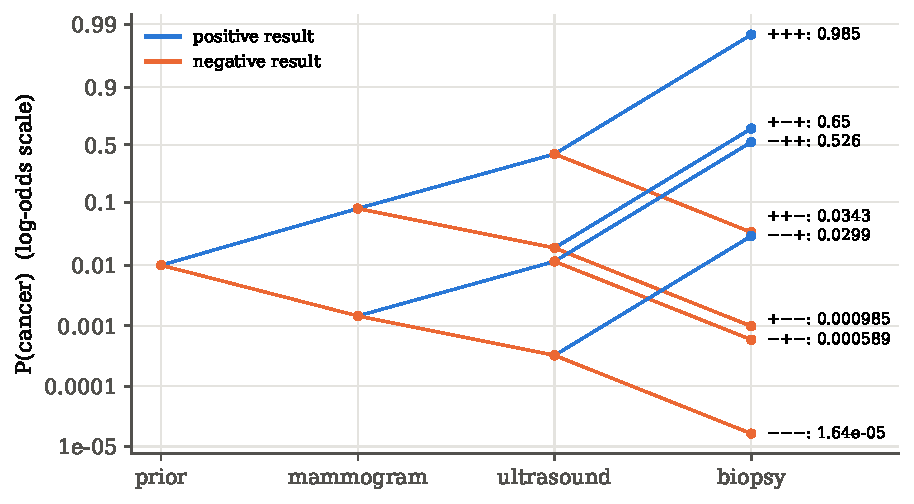
\includegraphics[width=0.86\linewidth]{figures/ch05/screening_paths.pdf}
\caption{The probability of cancer after each test, for every sequence of results,
on a log-odds axis, where each test moves the curve by the same step whatever came
before. A positive (blue) steps up by $\log_{10}\mathrm{LR}_+$, a negative (orange)
down by $\log_{10}\mathrm{LR}_-$; the end labels give the final probability for each
sequence. The biopsy's steps are much longer than the imaging tests', because its
likelihood ratios are much further from one.}
\label{5a:fig:screening-paths}
\end{figure}

\begin{figure}[htbp]
\centering
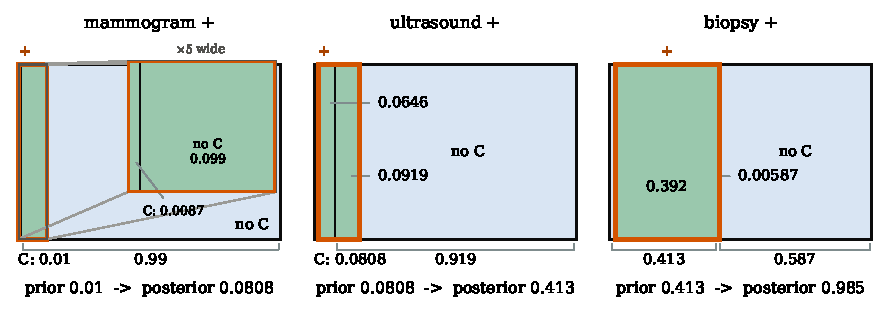
\includegraphics[width=\linewidth]{figures/ch05/screening_squares.pdf}
\caption{The sample space re-drawn before each test along the path $+,+,+$, in the
box picture of \cref{1a:fig:shrink}, with the function of \cref{5a:lst:area}. In each
panel the width of the cancer strip ($C$) is the current prior, and the positive
result is the box (orange outline): it covers the sensitivity's share of the $C$
strip and the false-alarm rate's share of the other, and the numbers are the areas
of its two pieces. Before the mammogram the cancer strip is $1\%$ of the width
(magnified in the inset); after it, the posterior $0.081$ becomes the width of the
strip for the ultrasound, and after the ultrasound, $0.41$ becomes the width for the
biopsy.}
\label{5a:fig:screening-squares}
\end{figure}

\paragraph{The assumption behind the multiplication.}
Multiplying the odds by each test's likelihood ratio assumes that the tests are
independent given her true state. For a healthy woman this says that a false alarm
on the mammogram makes a false alarm on the ultrasound neither more nor less likely.
That can fail: two imaging tests can be fooled by the same thing, since a benign
lump or very dense tissue may look suspicious to both. Model it as for the antibody
in the previous subsection. Say $5\%$ of healthy women carry such a feature and test
positive on both. The rest have independent false alarms at the rate $r=0.05/0.95$,
chosen so that each test alone still has false-positive rate $0.10$. Then three
numbers change:
$\Prob(M_+U_+\given C^c)=0.05+0.95\,r^2=\FiveAScrCorrHH$ instead of $0.01$; the
pair of positives has likelihood ratio
$0.87\times0.80/\FiveAScrCorrHH=\FiveAScrCorrLR$ instead of $8.7\times8.0=70$; and
her probability after two positive images is $\FiveAScrCorrPost$ (simulation
$\FiveAScrCorrMC$), not $\FiveAScrPP$. The second positive is worth less, because
much of what made the first one positive in a healthy woman repeats itself. The biopsy
examines the tissue itself, a different failure mode altogether, which is why it is
the test that settles the question.

\paragraph{Problem.}
In a younger screening population the prevalence is $0.5\%$. Test A has sensitivity
$0.90$ and specificity $0.92$; test B has sensitivity $0.85$ and specificity $0.95$.
(a) Assuming the tests are conditionally independent, find $\Prob(C\given A_+,B_+)$ and
$\Prob(C\given A_+,B_-)$. (b) How many independent positive results of test A are
needed for the probability of cancer to exceed $95\%$? (c) Now suppose that $3\%$ of
healthy women carry a benign feature that makes both A and B positive, while the
other healthy women have independent false positives at rates chosen so that each test
alone keeps its specificity. Redo (a), and say why the answers moved.

\paragraph{Solution.}
(a) The prior odds are $O_0=0.005/0.995=\FiveAPrbOzero$. The likelihood ratios are
$\mathrm{LR}_+^A=0.90/0.08=\FiveAPrbLAp$, $\mathrm{LR}_+^B=0.85/0.05=\FiveAPrbLBp$ and
$\mathrm{LR}_-^B=0.15/0.95=\FiveAPrbLBm$. Then
\begin{align*}
  O(C\given A_+,B_+)
  &\eqby{1}\mathrm{LR}_+^B\,\mathrm{LR}_+^A\,O_0
   =17.0\times11.25\times\FiveAPrbOzero=\FiveAPrbOAB,
  &\Prob(C\given A_+,B_+)&\eqby{2}\FiveAPrbAB,\\
  O(C\given A_+,B_-)
  &\eqby{3}\mathrm{LR}_-^B\,\mathrm{LR}_+^A\,O_0
   =\FiveAPrbOAb,
  &\Prob(C\given A_+,B_-)&=\FiveAPrbAb .
\end{align*}
\begin{explain}
  \item Two sequential updates in odds form; conditional independence lets each test
        enter through its own likelihood ratio.
  \item $p=O/(1+O)$.
  \item The same with the negative ratio of B.
\end{explain}
After a positive A alone the probability is $\FiveAPrbA$; a positive B brings it to
about one half, while a negative B brings it back to under $1\%$, still above the
prevalence of $0.5\%$.

(b) After $n$ independent positives of A the odds are $(\mathrm{LR}_+^A)^nO_0$, and
$95\%$ means odds of $19$:
\begin{align*}
  (\mathrm{LR}_+^A)^n\,O_0\ge19
  \;\relby{1}{\Longleftrightarrow}\;
  n\ge\frac{\ln(19/O_0)}{\ln\mathrm{LR}_+^A}
  =\frac{\ln3781}{\ln11.25}=3.40 .
\end{align*}
\begin{explain}
  \item Take logarithms; $\ln\mathrm{LR}_+^A>0$, so the inequality keeps its direction.
\end{explain}
So $n=\FiveAPrbN$: three positives give $\FiveAPrbNminus$, four give $\FiveAPrbNpost$.
This assumes that repeating test A on the same woman gives independent errors, which
for a repeated image of the same breast is exactly the assumption that part (c)
questions.

(c) With a fraction $g=0.03$ of healthy women carrying the feature, the other healthy
women must have false-positive rates $q_A=(0.08-g)/(1-g)=\FiveAPrbqA$ and
$q_B=(0.05-g)/(1-g)=\FiveAPrbqB$, so that each test alone is unchanged. For a healthy
woman,
\begin{align*}
  \Prob(A_+B_+\given C^c)
  &\eqby{1}g+(1-g)\,q_Aq_B=\FiveAPrbHAB,
  \qquad
  \Prob(A_+B_-\given C^c)
  \eqby{2}(1-g)\,q_A(1-q_B)=\FiveAPrbHAb,
\end{align*}
\begin{explain}
  \item Carriers are positive on both; the others are positive on both by two
        independent false alarms.
  \item A carrier is never negative on B, so only non-carriers contribute.
\end{explain}
while for a woman with cancer nothing changes,
$\Prob(A_+B_+\given C)=0.90\times0.85$ and $\Prob(A_+B_-\given C)=0.90\times0.15$.
The joint likelihood ratios replace the products of (a):
\begin{align*}
  \Prob(C\given A_+,B_+)
  &\eqby{1}\frac{O_0\cdot0.765/\FiveAPrbHAB}{1+O_0\cdot0.765/\FiveAPrbHAB}
   =\FiveAPrbABc,
  \qquad
  \Prob(C\given A_+,B_-)
  \eqby{2}\FiveAPrbAbc .
\end{align*}
\begin{explain}
  \item Odds form with the likelihood ratio of the \emph{pair} of results,
        $0.765/\FiveAPrbHAB=\FiveAPrbLRABc$, instead of $11.25\times17=\FiveAPrbLRABi$.
  \item The same with $0.135/\FiveAPrbHAb$.
\end{explain}
Both answers moved towards the prior. Two positives are now worth a factor
$\FiveAPrbLRABc$ rather than $\FiveAPrbLRABi$, because a healthy woman who is positive
on A is quite likely to be a carrier ($0.03/0.08$ of them), and a carrier is positive on
B for certain. The negative B is less reassuring for the same reason: among healthy
women positive on A, a negative B is now rarer, so it says less about health. The
script checks all four numbers by simulation, $\FiveAPrbMCAB$, $\FiveAPrbMCAb$,
$\FiveAPrbMCABc$ and $\FiveAPrbMCAbc$.
\section{The denominator: the sum over all paths}
\label{5a:sec:denominator}

The denominator $\Prob(E)$ of Bayes' theorem is the model's prediction for the
data. So far it has looked like bookkeeping: the number we divide by so that the
posteriors add up to one. In the odds form it cancelled altogether. But it is a
probability in its own right, and a meaningful one. Recall the trigger problem of
\cref{5a:sec:two-directions}, where $E$ was an isolated high-$p_T$ muon and three
trigger paths could have fired the event. There $\Prob(E)=0.235$. This says that,
\emph{before} we looked at the event, the model of the three paths predicted that
$23.5\%$ of recorded events would contain such a muon. Suppose a large sample of
events showed $60\%$. No reallocation of credibility among the three paths could
explain that. The trouble would lie in the list of paths or in the forward
probabilities, not in the priors. The denominator is also the one place in Bayes'
theorem that needs every hypothesis at once.

\subsection{Every path, and only paths}

The denominator is the marginalisation \eqref{5a:eq:marg}: the sum, over every
hypothesis, of the probability of reaching the observation along that hypothesis's
path (\cref{5a:fig:paths}),
\begin{equation}
  \Prob(E)=\sum_{i}\Prob(E\given H_i)\,\Prob(H_i)
  \quad\text{(discrete)},\qquad
  p(\data)=\int p(\data\given\theta)\,p(\theta)\,\dd\theta
  \quad\text{(continuous)} .
  \label{5a:eq:evidence}
\end{equation}
In the square of \cref{5a:sec:shrink} it is the total surviving area. It does not
depend on which hypothesis we are asking about. It depends only on the observation
and on the whole list of hypotheses with their priors. Two names are in use: the \newterm{evidence}, and the \newterm{marginal
likelihood}, because it is the likelihood averaged over the hypotheses with the prior
as the weight \srcref{Kruschke}{\S5.2, (5.8)--(5.9)}. Wasserman calls its continuous version $c_n=\int\Like_n(\theta)f(\theta)\,\dd\theta$ the
\newterm{normalizing constant} and notes that it can be dropped and recovered later
\mainref{p.~177, (11.3)}.

\begin{figure}[htbp]
\centering
\begin{tikzpicture}[
  font=\small,
  lvl/.style={draw=accent,rounded corners=2pt,fill=ideabg,minimum width=14mm,
              minimum height=6mm,align=center},
  leafE/.style={draw=formblue,thick,fill=formblue!12,rounded corners=2pt,
                minimum width=16mm,minimum height=6mm,align=center},
  path/.style={formblue,thick}]
  \node[lvl] (root) at (0,0) {event};
  \node[lvl] (mu)  at (-4.0,-1.6) {$H_\mu$};
  \node[lvl] (cal) at ( 0.0,-1.6) {$H_{\rm cal}$};
  \node[lvl] (trk) at ( 4.0,-1.6) {$H_{\rm trk}$};
  \draw[path] (root) -- (mu);
  \draw[path] (root) -- (cal);
  \draw[path] (root) -- (trk);
  \node[leafE] (mE) at (-4.0,-3.2) {$E$};
  \node[leafE] (cE) at ( 0.0,-3.2) {$E$};
  \node[leafE] (tE) at ( 4.0,-3.2) {$E$};
  \draw[path] (mu) -- (mE);
  \draw[path] (cal) -- (cE);
  \draw[path] (trk) -- (tE);
  \node[font=\footnotesize,anchor=west] at (-3.7,-2.4) {$0.25\times0.70$};
  \node[font=\footnotesize,anchor=west] at (0.3,-2.4) {$0.60\times0.05$};
  \node[font=\footnotesize,anchor=west] at (4.3,-2.4) {$0.15\times0.20$};
  \node[draw=formblue,thick,fill=formblue!8,rounded corners=2pt,align=center]
    (sum) at (0,-4.9) {$\Prob(E)=0.175+0.030+0.030=0.235$};
  \draw[path] (mE.south) -- (sum.north west);
  \draw[path] (cE.south) -- (sum.north);
  \draw[path] (tE.south) -- (sum.north east);
\end{tikzpicture}
\caption{The denominator of Bayes' theorem as the sum over paths. Each hypothesis
contributes one path from the root to the observed leaf $E$, with probability equal to
the product of its two branch probabilities (written beside the path). The evidence
collects all of them. A hypothesis missing from the tree is a path missing from the
sum.}
\label{5a:fig:paths}
\end{figure}

\subsection{The denominator is a prediction}

Now read \eqref{5a:eq:evidence} as a function of the data rather than as one number.
Before the data are taken, ask: how probable is each possible observation $E$? The
answer, $\Prob(E)$ for every $E$, is the model's forecast of what we are going to
see, averaged over our uncertainty about which hypothesis is true. It is called the \newterm{prior predictive distribution}
\srcref{Lambert}{\S6.3.4}. Unlike the likelihood, it is a genuine probability
distribution over the data: summed over all possible observations it gives one,
because $\sum_E\Prob(E\given H_i)=1$ for each $i$ and the priors sum to one.

\paragraph{Example: what did we expect from ten tosses?}
Take the grid of $101$ coin biases of \cref{5a:sec:sequential} with a flat prior, and
ask for the probability of $z$ heads in $N=10$ tosses before any toss is made. In the
continuum limit of the grid, the flat prior density is $p(\theta)=1$ on $[0,1]$, and
\begin{align}
  \Prob(z)
  &\eqby{1}\int_0^1\binom{N}{z}\theta^z(1-\theta)^{N-z}\,\dd\theta
   \eqby{2}\binom{N}{z}\frac{z!\,(N-z)!}{(N+1)!}
   \eqby{3}\frac{N!}{z!\,(N-z)!}\cdot\frac{z!\,(N-z)!}{(N+1)!}
   =\frac{1}{N+1} .
  \label{5a:eq:prior-pred}
\end{align}
\begin{explain}
  \item The evidence \eqref{5a:eq:evidence} with the binomial likelihood and the flat
        prior.
  \item The Beta integral $\int_0^1\theta^a(1-\theta)^b\,\dd\theta=a!\,b!/(a+b+1)!$ for
        integers $a,b\ge0$; it follows by integrating by parts $b$ times.
  \item Write out the binomial coefficient; the factorials cancel.
\end{explain}
Every number of heads from $0$ to $10$ was equally expected, with probability
$\frac{1}{11}=0.091$. The $101$-point grid gives $\FiveAEvFlat$ for $z=9$, the small
difference being the grid's approximation of the integral. A prior concentrated on
fair coins predicts something quite different (\cref{5a:fig:prior-pred}). If we are
certain that the coin is fair, $\Prob(z=9)=\binom{10}{9}2^{-10}=\FiveAEvFair$. The
triangular prior sits in between, $\FiveAEvTri$. Each prior predictive sums to one over
$z=0,\dots,10$, as the script confirms.

\begin{figure}[htbp]
\centering
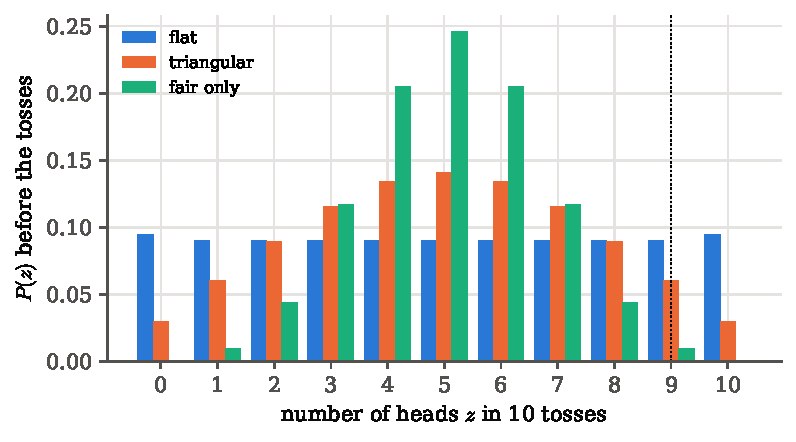
\includegraphics[width=0.8\linewidth]{figures/ch05/prior_predictive.pdf}
\caption{The denominator of Bayes' theorem as a forecast. For each of three beliefs
about the coin, the bars give the probability of each number of heads in ten tosses,
computed before any toss as a sum over all candidate biases. The flat prior spreads its
forecast evenly; ``the coin is fair'' concentrates it near five heads. The dotted line
marks the observed nine heads.}
\label{5a:fig:prior-pred}
\end{figure}

The whole computation is one matrix product:

\pyfile[firstline=33,lastline=35,firstnumber=33]{code/ch05/07_evidence.py}{The prior
predictive as a sum over paths}

Line 34 builds the table of \cref{5a:sec:two-directions}: one row per possible
observation $z$, one column per hypothesis $\theta_j$, entries $\Prob(z\given\theta_j)$.
Line 35 multiplies it by the vector of priors, which for each row is the sum over the
paths $\theta_j$ of likelihood times prior.

Now nine heads have been observed. Which model predicted that better? The
flat-prior model had given this outcome probability $\FiveAEvFlat$, the fair-coin
model only $\FiveAEvFair$. So the flat model predicted the observation
$\FiveAEvRatio$ times better. A ratio of two evidences is a likelihood ratio in which
each ``hypothesis'' is a whole model together with its prior. By \eqref{5a:eq:odds}
it multiplies the prior odds of one model against the other. This ratio, the
\emph{Bayes factor}, is the tool for comparing models, and comparing models is the
one job for which the denominator cannot be skipped.

\subsection{A missing path distorts every posterior}

Because the denominator sums over the hypotheses we listed, it silently assumes that
the list is complete. If the truth is not on the list, Bayes' theorem still returns
posteriors that sum to one, now shared among the wrong candidates. Kruschke's example
is the wet pavement caused by something nobody listed \srcref{Kruschke}{\S2.2}.

\paragraph{Example: forgetting the background.}
In the gamma-ray example of \cref{5a:sec:reallocation}, the soft photon at
$(-3^\circ,2^\circ)$ had source probabilities $\FiveAGrbMbG$ (burst), $\FiveAGrbMbB$
(blazar) and $\FiveAGrbMbD$ (diffuse background). Suppose we forget the diffuse
background and keep only the two point sources. The denominator loses the largest of
its three paths, and the same photon now gets $\FiveAGrbForgotG$ for the burst and
$\FiveAGrbForgotB$ for the blazar. Nothing in the output warns us: the posteriors still
sum to one. The warning is in the denominator itself. Without the background, the model
predicts that almost no photons arrive far from the two point sources, so the evidence
of a map full of such photons is tiny compared with that of the model with the
background. Comparing evidences, or checking whether the most credible hypotheses
actually reproduce the data \srcref{Kruschke}{\S2.2}, is how a missing path is found.

\begin{pitfall}[A small evidence is not by itself a refutation]
Every particular data set has a small probability: any one sequence of ten tosses has
probability $2^{-10}\approx0.001$ under a fair coin. The value of $\Prob(E)$ alone says
little. It becomes informative when compared, either with the evidence of another
model for the same data, or with the spread of $\Prob(E)$ over the data sets the model
itself would typically produce.
\end{pitfall}

\subsection{Why the denominator is the hard part}

The denominator is hard because it needs every hypothesis at once, and in many
dimensions there are far too many. For a handful of hypotheses the sum
\eqref{5a:eq:evidence} is trivial. For a continuous parameter it is an integral,
which a grid approximates by a sum, as in the $101$-point coin grid. For $D$
parameters a grid with $n$ points per axis has $n^D$ points. With $n=1000$ and
$D=6$, the number of parameters of the standard cosmological model, that is
$10^{18}$ evaluations of the likelihood \srcref{Kruschke}{\S5.4},
\srcref{Lambert}{\S6.4}.

There are two ways out. The first is to choose priors that match the form of the
likelihood, so that the integral can be done by hand; these \emph{conjugate}
priors give posteriors of a known shape. The second is to notice that estimating
parameters never needs the denominator at all. It cancels in every ratio of
posteriors, exactly as it cancelled in the odds \eqref{5a:eq:odds}. A method that
only ever compares the posterior at two points,
$p(\theta'\given\data)/p(\theta\given\data)=p(\data\given\theta')p(\theta')/p(\data\given\theta)p(\theta)$,
can explore the posterior without knowing its normalisation. That is the idea behind
Markov chain Monte Carlo (\cref{ch:09}) \srcref{Lambert}{\S6.5}. Only when models
themselves are compared must the evidence be computed, and that needs its own methods.

The trigger paths, the medical test, Monty's door, the urns and the ball sizes
were all solved in the same way, and the way is worth making a habit: put the
question into words before touching a symbol. First ask: which hypotheses could
have produced what we observed? With that list settled, ask: how probable would
the observation have been if each of them were true? These two answers sort the
whole problem. The first answer says what the posterior is a distribution over,
and so fixes the list of paths that the denominator sums over. The second answer
is the likelihood: it fixes the height of each bar in the square.

\begin{recap}
\begin{itemize}[itemsep=2pt,leftmargin=1.2em]
  \item Prediction reads $\Prob(E\given H)$, inference wants $\Prob(H\given E)$. Both
        come from one joint distribution: a column of the joint table for prediction,
        the observed row for inference.
  \item Bayes' theorem is the product rule applied in both orders. Observing $E$
        shrinks the sample space to $E$; each hypothesis is re-measured by its share of
        the surviving region.
  \item In the unit square: priors are widths, likelihoods are heights, joint
        probabilities are areas, the evidence is the surviving area, and the posterior
        is one surviving rectangle over all of them.
  \item Base rates matter: evidence covering most of a thin strip (medical test,
        trigger purity, rare signal) can lose to evidence covering a small share of
        a wide strip.
  \item Inference is reallocation of credibility: a zero likelihood eliminates, a zero
        prior can never be revived, noisy data only nudge.
  \item Posterior odds $=$ likelihood ratio $\times$ prior odds. The likelihood ratio is
        all the evidence says about two hypotheses; in logarithms, independent evidence
        adds (decibels, log-odds random walk with drift equal to a Kullback--Leibler
        divergence).
  \item Condition on exactly what was observed: ``score $=0.8$'' and ``score $>0.8$'' are
        different evidence.
  \item Sequential updating: the posterior becomes the prior; the order of the data
        does not matter; multiplying likelihoods requires independence given the
        hypothesis.
  \item The denominator is the sum over all paths: the normaliser, the prior
        predictive forecast of the data, and the quantity that compares models. It
        needs the complete list of hypotheses and is hard to compute in many
        dimensions, which is why parameter estimation works with ratios of posteriors.
\end{itemize}
\end{recap}

\providecommand{\FiveBGd}{}\renewcommand{\FiveBGd}{0.6041}
\providecommand{\FiveBGsig}{}\renewcommand{\FiveBGsig}{0.1}
\providecommand{\FiveBGtrue}{}\renewcommand{\FiveBGtrue}{0.8}
\providecommand{\FiveBGpeak}{}\renewcommand{\FiveBGpeak}{0.777}
\providecommand{\FiveBGsqrtd}{}\renewcommand{\FiveBGsqrtd}{0.7772}
\providecommand{\FiveBGmasspos}{}\renewcommand{\FiveBGmasspos}{0.5}
\providecommand{\FiveBGevid}{}\renewcommand{\FiveBGevid}{0.4336}
\providecommand{\FiveBTauN}{}\renewcommand{\FiveBTauN}{2000}
\providecommand{\FiveBTauRawMax}{}\renewcommand{\FiveBTauRawMax}{\infty}
\providecommand{\FiveBTauRawMaxPct}{}\renewcommand{\FiveBTauRawMaxPct}{0}
\providecommand{\FiveBTauLogLmax}{}\renewcommand{\FiveBTauLogLmax}{3149}
\providecommand{\FiveBTauMean}{}\renewcommand{\FiveBTauMean}{1.996}
\providecommand{\FiveBTauSd}{}\renewcommand{\FiveBTauSd}{0.007948}
\providecommand{\FiveBTauSigd}{}\renewcommand{\FiveBTauSigd}{0.05}
\providecommand{\FiveBBetaModeS}{}\renewcommand{\FiveBBetaModeS}{0.5321}
\providecommand{\FiveBBetaModeL}{}\renewcommand{\FiveBBetaModeL}{0.7965}
\providecommand{\FiveBBetaModeF}{}\renewcommand{\FiveBBetaModeF}{0.85}
\providecommand{\FiveBBetaHdiSlo}{}\renewcommand{\FiveBBetaHdiSlo}{0.466}
\providecommand{\FiveBBetaHdiShi}{}\renewcommand{\FiveBBetaHdiShi}{0.5975}
\providecommand{\FiveBBetaHdiLlo}{}\renewcommand{\FiveBBetaHdiLlo}{0.6629}
\providecommand{\FiveBBetaHdiLhi}{}\renewcommand{\FiveBBetaHdiLhi}{0.8966}
\providecommand{\FiveBBetaHdiFlo}{}\renewcommand{\FiveBBetaHdiFlo}{0.6599}
\providecommand{\FiveBBetaHdiFhi}{}\renewcommand{\FiveBBetaHdiFhi}{0.9591}
\providecommand{\FiveBBetaErr}{}\renewcommand{\FiveBBetaErr}{1.247\times10^{-11}}
\providecommand{\FiveBCountsSum}{}\renewcommand{\FiveBCountsSum}{28}
\providecommand{\FiveBCountsList}{}\renewcommand{\FiveBCountsList}{3, 5, 7, 4, 9}
\providecommand{\FiveBGamA}{}\renewcommand{\FiveBGamA}{31}
\providecommand{\FiveBGamB}{}\renewcommand{\FiveBGamB}{6}
\providecommand{\FiveBGamMean}{}\renewcommand{\FiveBGamMean}{5.167}
\providecommand{\FiveBGamSd}{}\renewcommand{\FiveBGamSd}{0.928}
\providecommand{\FiveBGamErr}{}\renewcommand{\FiveBGamErr}{1.018\times10^{-11}}
\providecommand{\FiveBGamMLE}{}\renewcommand{\FiveBGamMLE}{5.6}
\providecommand{\FiveBNxa}{}\renewcommand{\FiveBNxa}{10.2}
\providecommand{\FiveBNxb}{}\renewcommand{\FiveBNxb}{9.936}
\providecommand{\FiveBNxc}{}\renewcommand{\FiveBNxc}{10.07}
\providecommand{\FiveBNmPost}{}\renewcommand{\FiveBNmPost}{10.1}
\providecommand{\FiveBNsPost}{}\renewcommand{\FiveBNsPost}{0.4319}
\providecommand{\FiveBNmIvw}{}\renewcommand{\FiveBNmIvw}{10.15}
\providecommand{\FiveBNsIvw}{}\renewcommand{\FiveBNsIvw}{0.4364}
\providecommand{\FiveBNErr}{}\renewcommand{\FiveBNErr}{2.260\times10^{-14}}
\providecommand{\FiveBPred}{}\renewcommand{\FiveBPred}{0.4853}
\providecommand{\FiveBPlugin}{}\renewcommand{\FiveBPlugin}{0.5102}
\providecommand{\FiveBULzero}{}\renewcommand{\FiveBULzero}{2.996}
\providecommand{\FiveBULone}{}\renewcommand{\FiveBULone}{4.744}
\providecommand{\FiveBULthree}{}\renewcommand{\FiveBULthree}{7.754}
\providecommand{\FiveBCmbModeTwo}{}\renewcommand{\FiveBCmbModeTwo}{0.7143}
\providecommand{\FiveBCmbMeanTwo}{}\renewcommand{\FiveBCmbMeanTwo}{1.667}
\providecommand{\FiveBCmbLoTwo}{}\renewcommand{\FiveBCmbLoTwo}{0.6303}
\providecommand{\FiveBCmbHiTwo}{}\renewcommand{\FiveBCmbHiTwo}{2.421}
\providecommand{\FiveBCmbLoFifty}{}\renewcommand{\FiveBCmbLoFifty}{0.8776}
\providecommand{\FiveBCmbHiFifty}{}\renewcommand{\FiveBCmbHiFifty}{1.162}
\providecommand{\FiveBCmbModeFifty}{}\renewcommand{\FiveBCmbModeFifty}{0.9806}
\providecommand{\FiveBGwAhat}{}\renewcommand{\FiveBGwAhat}{1.06}
\providecommand{\FiveBGwAsd}{}\renewcommand{\FiveBGwAsd}{0.1}
\providecommand{\FiveBGwSpread}{}\renewcommand{\FiveBGwSpread}{0.1008}
\providecommand{\FiveBGwHH}{}\renewcommand{\FiveBGwHH}{100}
\providecommand{\FiveBSumAboveMode}{}\renewcommand{\FiveBSumAboveMode}{78}
\providecommand{\FiveBSumMean}{}\renewcommand{\FiveBSumMean}{1.667}
\providecommand{\FiveBSumMedian}{}\renewcommand{\FiveBSumMedian}{1.149}
\providecommand{\FiveBSumMode}{}\renewcommand{\FiveBSumMode}{0.7143}
\providecommand{\FiveBSumEtiLo}{}\renewcommand{\FiveBSumEtiLo}{0.3896}
\providecommand{\FiveBSumEtiHi}{}\renewcommand{\FiveBSumEtiHi}{6.015}
\providecommand{\FiveBSumHdiLo}{}\renewcommand{\FiveBSumHdiLo}{0.2294}
\providecommand{\FiveBSumHdiHi}{}\renewcommand{\FiveBSumHdiHi}{4.389}
\providecommand{\FiveBSumHdiSLo}{}\renewcommand{\FiveBSumHdiSLo}{0.2275}
\providecommand{\FiveBSumHdiSHi}{}\renewcommand{\FiveBSumHdiSHi}{4.356}
\providecommand{\FiveBSumHdiYLo}{}\renewcommand{\FiveBSumHdiYLo}{0.348}
\providecommand{\FiveBSumHdiYHi}{}\renewcommand{\FiveBSumHdiYHi}{5.054}
\providecommand{\FiveBSumWater}{}\renewcommand{\FiveBSumWater}{0.02375}
\providecommand{\FiveBBiLoA}{}\renewcommand{\FiveBBiLoA}{-0.8394}
\providecommand{\FiveBBiHiA}{}\renewcommand{\FiveBBiHiA}{-0.7096}
\providecommand{\FiveBBiLoB}{}\renewcommand{\FiveBBiLoB}{0.7096}
\providecommand{\FiveBBiHiB}{}\renewcommand{\FiveBBiHiB}{0.8394}
\providecommand{\FiveBBiMean}{}\renewcommand{\FiveBBiMean}{0.000}
\providecommand{\FiveBLapHa}{}\renewcommand{\FiveBLapHa}{0.2812}
\providecommand{\FiveBLapSa}{}\renewcommand{\FiveBLapSa}{0.07948}
\providecommand{\FiveBLapMeanA}{}\renewcommand{\FiveBLapMeanA}{0.2941}
\providecommand{\FiveBLapSdA}{}\renewcommand{\FiveBLapSdA}{0.07702}
\providecommand{\FiveBLapHb}{}\renewcommand{\FiveBLapHb}{0.1}
\providecommand{\FiveBLapSb}{}\renewcommand{\FiveBLapSb}{0.09487}
\providecommand{\FiveBLapNegB}{}\renewcommand{\FiveBLapNegB}{0.1459}
\providecommand{\FiveBLapMeanB}{}\renewcommand{\FiveBLapMeanB}{0.1667}
\providecommand{\FiveBLapSdB}{}\renewcommand{\FiveBLapSdB}{0.1034}
\providecommand{\FiveBLhModeFive}{}\renewcommand{\FiveBLhModeFive}{1.096}
\providecommand{\FiveBLhSdFive}{}\renewcommand{\FiveBLhSdFive}{0.06506}
\providecommand{\FiveBLhXbarFive}{}\renewcommand{\FiveBLhXbarFive}{1.197}
\providecommand{\FiveBLhModeSix}{}\renewcommand{\FiveBLhModeSix}{1.34}
\providecommand{\FiveBLhSdSix}{}\renewcommand{\FiveBLhSdSix}{0.2039}
\providecommand{\FiveBLhLapSix}{}\renewcommand{\FiveBLhLapSix}{0.2026}
\providecommand{\FiveBLhXbarSix}{}\renewcommand{\FiveBLhXbarSix}{3.578}
\providecommand{\FiveBLhSqrtTwoN}{}\renewcommand{\FiveBLhSqrtTwoN}{0.0625}
\providecommand{\FiveBMaRhoWide}{}\renewcommand{\FiveBMaRhoWide}{-0.6688}
\providecommand{\FiveBMaRhoNarrow}{}\renewcommand{\FiveBMaRhoNarrow}{-0.9331}
\providecommand{\FiveBMaSigWide}{}\renewcommand{\FiveBMaSigWide}{0.2075}
\providecommand{\FiveBMaSigCondWide}{}\renewcommand{\FiveBMaSigCondWide}{0.1538}
\providecommand{\FiveBMaSigNarrow}{}\renewcommand{\FiveBMaSigNarrow}{0.4197}
\providecommand{\FiveBMaSigCondNarrow}{}\renewcommand{\FiveBMaSigCondNarrow}{0.1517}
\providecommand{\FiveBVolMargMode}{}\renewcommand{\FiveBVolMargMode}{0}
\providecommand{\FiveBVolProfMode}{}\renewcommand{\FiveBVolProfMode}{0.83}
\providecommand{\FiveBVolMargMean}{}\renewcommand{\FiveBVolMargMean}{0.5447}
\providecommand{\FiveBVolPsmallMarg}{}\renewcommand{\FiveBVolPsmallMarg}{0.5375}
\providecommand{\FiveBVolPsmallProf}{}\renewcommand{\FiveBVolPsmallProf}{0.2077}
\providecommand{\FiveBVolAtrue}{}\renewcommand{\FiveBVolAtrue}{1.2}
\providecommand{\FiveBVolLoopR}{}\renewcommand{\FiveBVolLoopR}{500}
\providecommand{\FiveBVolLoopPsmallMarg}{}\renewcommand{\FiveBVolLoopPsmallMarg}{0.20}
\providecommand{\FiveBVolLoopPsmallProf}{}\renewcommand{\FiveBVolLoopPsmallProf}{0.07}
\providecommand{\FiveBVolLoopErr}{}\renewcommand{\FiveBVolLoopErr}{0.01}
\providecommand{\FiveBVolLoopModeZero}{}\renewcommand{\FiveBVolLoopModeZero}{50}
\providecommand{\FiveBPrFracCentral}{}\renewcommand{\FiveBPrFracCentral}{0.763}
\providecommand{\FiveBPrFlatTop}{}\renewcommand{\FiveBPrFlatTop}{0.9001}
\providecommand{\FiveBPrFlatBottom}{}\renewcommand{\FiveBPrFlatBottom}{9.001\times10^{-4}}
\providecommand{\FiveBPrLogDecade}{}\renewcommand{\FiveBPrLogDecade}{0.25}
\providecommand{\FiveBPrFlatMeanTen}{}\renewcommand{\FiveBPrFlatMeanTen}{0.1667}
\providecommand{\FiveBPrFlatUpTen}{}\renewcommand{\FiveBPrFlatUpTen}{0.3644}
\providecommand{\FiveBPrFlatMeanThou}{}\renewcommand{\FiveBPrFlatMeanThou}{0.1008}
\providecommand{\FiveBPrFlatUpThou}{}\renewcommand{\FiveBPrFlatUpThou}{0.1169}
\providecommand{\FiveBPrJefMeanTen}{}\renewcommand{\FiveBPrJefMeanTen}{0.1364}
\providecommand{\FiveBPrJefUpTen}{}\renewcommand{\FiveBPrJefUpTen}{0.3306}
\providecommand{\FiveBPrJefMeanThou}{}\renewcommand{\FiveBPrJefMeanThou}{0.1004}
\providecommand{\FiveBPrJefUpThou}{}\renewcommand{\FiveBPrJefUpThou}{0.1165}
\providecommand{\FiveBPrHalMeanTen}{}\renewcommand{\FiveBPrHalMeanTen}{0.1}
\providecommand{\FiveBPrHalUpTen}{}\renewcommand{\FiveBPrHalUpTen}{0.2831}
\providecommand{\FiveBPrHalMeanThou}{}\renewcommand{\FiveBPrHalMeanThou}{0.1}
\providecommand{\FiveBPrHalUpThou}{}\renewcommand{\FiveBPrHalUpThou}{0.116}
\providecommand{\FiveBBvmGapTen}{}\renewcommand{\FiveBBvmGapTen}{1.452}
\providecommand{\FiveBBvmGapThou}{}\renewcommand{\FiveBBvmGapThou}{2.949}
\providecommand{\FiveBBvmGapLast}{}\renewcommand{\FiveBBvmGapLast}{0.3407}
\providecommand{\FiveBBvmGapPeak}{}\renewcommand{\FiveBBvmGapPeak}{5.885}
\providecommand{\FiveBBvmNpeak}{}\renewcommand{\FiveBBvmNpeak}{122}
\providecommand{\FiveBBvmNone}{}\renewcommand{\FiveBBvmNone}{12999}
\providecommand{\FiveBBvmNtot}{}\renewcommand{\FiveBBvmNtot}{5068}
\providecommand{\FiveBChainFlatA}{}\renewcommand{\FiveBChainFlatA}{0.3147}
\providecommand{\FiveBChainFlatB}{}\renewcommand{\FiveBChainFlatB}{0.3182}
\providecommand{\FiveBChainStrA}{}\renewcommand{\FiveBChainStrA}{0.7172}
\providecommand{\FiveBChainStrB}{}\renewcommand{\FiveBChainStrB}{0.716}
\providecommand{\FiveBChainExactFlat}{}\renewcommand{\FiveBChainExactFlat}{0.3182}
\providecommand{\FiveBChainExactStr}{}\renewcommand{\FiveBChainExactStr}{0.7167}
\providecommand{\FiveBSaTwoHeads}{}\renewcommand{\FiveBSaTwoHeads}{0.4839}
\providecommand{\FiveBSaTwoHeadsExact}{}\renewcommand{\FiveBSaTwoHeadsExact}{0.4853}
\providecommand{\FiveBSaPredLo}{}\renewcommand{\FiveBSaPredLo}{0}
\providecommand{\FiveBSaPredHi}{}\renewcommand{\FiveBSaPredHi}{4}
\providecommand{\FiveBSaPlugHi}{}\renewcommand{\FiveBSaPlugHi}{2}
\providecommand{\FiveBSaPredZero}{}\renewcommand{\FiveBSaPredZero}{0.2612}
\providecommand{\FiveBSaPlugZero}{}\renewcommand{\FiveBSaPlugZero}{0.3487}
\providecommand{\FiveBSaPpos}{}\renewcommand{\FiveBSaPpos}{0.9877}
\providecommand{\FiveBSaTauLo}{}\renewcommand{\FiveBSaTauLo}{0.03117}
\providecommand{\FiveBSaTauHi}{}\renewcommand{\FiveBSaTauHi}{0.4355}
\providecommand{\FiveBSaB}{}\renewcommand{\FiveBSaB}{200000}
 
\section{From a list of hypotheses to a continuous parameter}
\label{5b:sec:continuous}

A theorist hands us a formula. If a parameter $\lambda$ of nature has a certain value,
an instrument should read $\mu(\lambda)$. The parameter could be the mass of a
particle, a coupling, a lifetime or the matter density of the universe. The instrument
is not perfect, so what it actually reads is the prediction plus some noise. We take
one reading, $d$. Which values of $\lambda$ could have produced it, and how much
credibility should each value get?

We answer it in the same order as the Monty Hall problem (\cref{5a:fig:monty}).
\emph{The event.} What we observed is ``the instrument showed $d$''.
\emph{The question.} What made it show that value? The possible explanations are the
possible values of $\lambda$, each one a possible state of nature.
\emph{Each candidate in turn.} For each value of $\lambda$ we ask how probable the
reading $d$ was if that value were the truth. The prediction would then have been
$\mu(\lambda)$, so the question is how likely the noise was to push $\mu(\lambda)$ to
exactly the $d$ we saw.
\emph{Only then the priors, and the normalisation.} We multiply by the prior weight of
each value and divide by the total.

This is the question ``which urn did the ball come from?'' or ``is this event signal
or background?'' with one change. There the candidate explanations formed a short
list, $H_1,H_2,\dots$. Here every real number in some range is a candidate. Bayes'
theorem still holds, but three things need care. A probability spread over a continuum
is a density. The sum over paths in the denominator becomes an integral. And a computer
can evaluate the density only at finitely many points.

\subsection{The tree, continuous in spirit}

Write the reading as prediction plus noise,
\begin{equation}
  d=\mu(\lambda)+\epsilon,\qquad \epsilon\sim\Normal(0,\sigma^2),
  \label{5b:eq:model}
\end{equation}
where $\sigma$ is the known size of the noise. The forward question, prediction, asks:
if nature chose $\lambda$, what readings would we see, and how often? Its answer is a
Gaussian centred on the prediction,
\begin{equation}
  p(d\given\lambda)=\frac{1}{\sqrt{2\pi\sigma^2}}
  \exp\!\left[-\frac{\bigl(d-\mu(\lambda)\bigr)^2}{2\sigma^2}\right].
  \label{5b:eq:gauss-like}
\end{equation}
Held at the reading we have and read as a function of $\lambda$, it is the
\newterm{likelihood} $\Like(\lambda)$, which scores each candidate by the
probability of the noise, $d-\mu(\lambda)$, it would have needed
(\cref{3b:sec:likelihood}).

The inference question runs the other way, and its picture is a probability tree with
one branch per candidate value (\cref{5b:fig:tree}). The first split chooses $\lambda$
with prior weight $p(\lambda)$. The second step produces the reading, with probability
$p(d\given\lambda)$ along each branch. Every branch can reach the same leaf $d$,
because Gaussian noise can turn any prediction into any reading, only with very
different probabilities. With infinitely many branches the tree cannot be drawn
literally, but it can be drawn in spirit: pick three candidates $\lambda_1,\lambda_2,
\lambda_3$ and remember that there is one branch for every value in between.

\begin{figure}[htbp]
\centering
\begin{tikzpicture}[x=1cm,y=1cm]
  \draw[faint,->] (-4.2,3.0) -- (4.4,3.0) node[right,lbl,black] {$\lambda$};
  \draw[form,domain=-4:4,samples=80] plot (\x,{3.0+0.9*exp(-(\x+0.6)^2/5)});
  \node[lbl,formblue,anchor=east] at (-4.25,3.55) {$p(\lambda)$};
  \node[lbl,draw,rounded corners,fill=white] (root) at (0,4.6) {possible values of $\lambda$};
  \foreach \xx/\nm in {-2.8/1,0/2,2.8/3}{
    \pgfmathsetmacro{\yy}{3.0+0.9*exp(-(\xx+0.6)^2/5)}
    \fill[formblue] (\xx,\yy) circle (1.4pt);
    \draw[->,thick,black!70] (root.south) -- (\xx,2.3);
    \node[lbl,anchor=east] at (\xx-0.1,2.05) {$\lambda_\nm$};
    \draw[->,thick,black!70] (\xx,1.85) -- (\xx,0.75);
    \node[lbl] at (\xx,0.45) {$d$};
    \node[lbl] at (\xx,0.0) {$p(d\given\lambda_\nm)$};
  }
  \foreach \xx in {-3.6,-2.2,-1.6,-1.0,-0.5,0.5,1.0,1.6,2.2,3.6}{
    \draw[faint,black!25] (root.south) -- (\xx,2.3);
  }
  \draw[faint,->] (-4.2,-1.4) -- (4.4,-1.4) node[right,lbl,black] {$\lambda$};
  \draw[thick,tangentgreen,domain=-4:4,samples=80] plot (\x,{-1.4+0.9*exp(-(\x-0.9)^2/1.2)});
  \node[lbl,tangentgreen,anchor=east] at (-4.25,-0.8) {$p(d\given\lambda)$};
\end{tikzpicture}
\caption{The probability tree for a continuous parameter, drawn in spirit. The top
curve is the prior density, the weight with which each branch is chosen. Three branches
are drawn in full and the faint fan stands for the continuum of branches between them.
Every branch can end at the same observed reading $d$, each with its own probability.
The bottom curve collects those probabilities as a function of $\lambda$: the
likelihood.}
\label{5b:fig:tree}
\end{figure}

\begin{keyidea}[Parameter estimation is inference with a continuum of explanations]
Every candidate value of the parameter $\lambda$ is one possible explanation of
the data. The reading $d$ is the event that actually happened. The likelihood
$\Like(\lambda)=p(d\given\lambda)$ measures, value by value, how easily that
$\lambda$ could have produced the event.
\end{keyidea}

\subsection{From a sum over branches to a density}

What does Bayes' theorem become when the hypotheses form a continuum? We reduce the
question to the case we already know, a finite list. Chop the $\lambda$ axis into cells
of small width $\Delta\lambda$, centred on the points $\lambda_j$, and call
``$\lambda$ lies in cell $j$'' hypothesis $H_j$. Exactly one cell contains the true
value, so these hypotheses are a partition and the discrete theorem applies to them.
The prior probability of cell $j$ is $\Prob(H_j)\approx p(\lambda_j)\,\Delta\lambda$,
because a density times a small width is a probability. Then
\begin{align}
  \frac{\Prob(H_j\given d)}{\Delta\lambda}
  &\eqby{1}\frac{1}{\Delta\lambda}\,
     \frac{p(d\given\lambda_j)\,p(\lambda_j)\,\Delta\lambda}
          {\sum_k p(d\given\lambda_k)\,p(\lambda_k)\,\Delta\lambda}
   \nonumber\\
  &\eqby{2}\frac{p(d\given\lambda_j)\,p(\lambda_j)}
          {\sum_k p(d\given\lambda_k)\,p(\lambda_k)\,\Delta\lambda}
   \nonumber\\
  &\xrightarrow{\ \Delta\lambda\to0\ }
   \frac{p(d\given\lambda_j)\,p(\lambda_j)}{\int p(d\given\lambda)\,p(\lambda)\,\dd\lambda} .
  \label{5b:eq:bayes-cont}
\end{align}
\begin{explain}
  \item Discrete Bayes' theorem for the cells, with the prior probability of each cell
        written as density times width.
  \item The $\Delta\lambda$ in the numerator cancels the $1/\Delta\lambda$ in front.
        The one in the denominator stays inside the sum.
\end{explain}
Now let the cells shrink. In the denominator each term is multiplied by its width, so
the sum is a Riemann sum and becomes an integral. On the left, the probability of a cell
divided by its width becomes a probability per unit $\lambda$: the
\newterm{posterior density} $p(\lambda\given d)$. So the continuous theorem is
\mainref{p.~177, (11.1)}
\begin{equation}
  p(\lambda\given d)=\frac{p(d\given\lambda)\,p(\lambda)}{p(d)},\qquad
  p(d)=\int p(d\given\lambda)\,p(\lambda)\,\dd\lambda .
  \label{5b:eq:bayes}
\end{equation}
The denominator $p(d)$ is the old sum over every path to the observation, now an
integral over every branch of the tree in \cref{5b:fig:tree}. It does not depend on
$\lambda$, so the shape of the posterior is set by the numerator alone
\mainref{p.~177, (11.2)--(11.3)}:
\begin{equation}
  p(\lambda\given d)\;\propto\;\Like(\lambda)\,p(\lambda),
  \label{5b:eq:prop}
\end{equation}
``posterior is proportional to likelihood times prior''. The constant is recovered at
the end by demanding that $\int p(\lambda\given d)\,\dd\lambda=1$.

\begin{workdef}[posterior density]
The \newterm{posterior density} of a continuous parameter $\lambda$ given data $d$ is
$p(\lambda\given d)=\Like(\lambda)\,p(\lambda)/p(d)$, where $\Like(\lambda)=p(d\given
\lambda)$ is the likelihood \unpack{the probability density of the data actually
observed, read as a function of $\lambda$}, $p(\lambda)$ is the prior density
\unpack{credibility per unit $\lambda$ before the data}, and $p(d)$ is the evidence
\unpack{the same product integrated over all $\lambda$. It makes the posterior
integrate to one}. \emph{Operationally:} evaluate $\Like(\lambda)p(\lambda)$ at every
$\lambda$ you care about, and divide by its integral. The probability that $\lambda$
lies between $a$ and $b$ is $\int_a^bp(\lambda\given d)\,\dd\lambda$.
\end{workdef}

A density is not itself a probability. Its value at a point, say $p(\lambda\given d)=
3$, means ``probability $3\,\Delta\lambda$ for a small cell of width $\Delta\lambda$
around this point'', and it carries units of one over the units of $\lambda$. Only areas
under the curve are probabilities. This matters as soon as we change variables
(\cref{5b:sec:priors}): the height of a density changes when we stretch the axis,
while the probabilities of corresponding intervals do not.

\paragraph{Example: a linear prediction and a flat prior.}
Let $\mu(\lambda)=\lambda$, so the instrument reads the parameter itself plus noise,
and take a prior that is constant, $p(\lambda)=1/(\lambda_{\max}-\lambda_{\min})$, over
a range much wider than $\sigma$ and containing $d$. Then
\begin{align*}
  p(\lambda\given d)
  &\eqby{1}\frac{\Like(\lambda)\,p(\lambda)}{\int\Like(\lambda')\,p(\lambda')\,\dd\lambda'}
   \eqby{2}\frac{e^{-(d-\lambda)^2/2\sigma^2}}{\int_{\lambda_{\min}}^{\lambda_{\max}}
       e^{-(d-\lambda')^2/2\sigma^2}\dd\lambda'}
   \eqby{3}\frac{1}{\sqrt{2\pi\sigma^2}}\,e^{-(\lambda-d)^2/2\sigma^2}.
\end{align*}
\begin{explain}
  \item Bayes' theorem \eqref{5b:eq:bayes}.
  \item The flat prior is the same constant in numerator and denominator and cancels,
        and so does the factor $1/\sqrt{2\pi\sigma^2}$ of the likelihood.
  \item The range is many $\sigma$ wide around $d$, so the integral is, to excellent
        accuracy, the full Gaussian integral $\int_{-\infty}^\infty e^{-u^2/2\sigma^2}
        \dd u=\sqrt{2\pi\sigma^2}$.
\end{explain}
The posterior is a Gaussian in $\lambda$, centred on the reading $d$, with width equal
to the noise size $\sigma$. Values of $\lambda$ whose prediction lies close to the
reading get the most credibility. The formula looks like the likelihood with $d$ and
$\lambda$ swapped, and here it is exactly that. But this is a coincidence of the linear
prediction $\mu(\lambda)=\lambda$, as the next example shows.

\paragraph{Example: a rate that depends on the square of a coupling.}
Many rates in particle physics are proportional to the square of a coupling $g$: a
decay width, a cross-section, an oscillation probability. Take $\mu(g)=g^2$ in suitable
units, with noise $\sigma=\FiveBGsig$, and suppose the true coupling is
$g=\FiveBGtrue$.
\emph{The event.} One simulated reading came out as $d=\FiveBGd$.
\emph{The question.} Which couplings could have produced it? A coupling $g$ predicts
the rate $g^2$, so the candidates that explain the reading well are those with $g^2$
close to $d$.
\emph{The candidates.} There are two groups of them, not one: $g$ near $+\sqrt d$ and
$g$ near $-\sqrt d$. The reason is that $g$ and $-g$ predict the same rate, so no
reading can tell them apart.
\emph{Only then the numbers.} With a flat prior on $g\in[-1.5,1.5]$,
\begin{equation*}
  p(g\given d)\propto\exp\!\left[-\frac{(d-g^2)^2}{2\sigma^2}\right].
\end{equation*}
This is largest where $g^2=d$, that is at the \emph{two} points $g=\pm\sqrt d=
\pm\FiveBGsqrtd$ (\cref{5b:fig:coupling}). The function is even in $g$, so exactly half
the posterior probability lies on each side: the computed mass at $g>0$ is
$\FiveBGmasspos$.
\emph{What it means.} The data say ``$|g|$ is about $\FiveBGsqrtd$'' and nothing about
the sign. The posterior reports this honestly with two peaks; a single ``best value
with an error bar'' could not. If theory tells us that $g>0$, that is prior
information. Put it in the prior, $p(g)=0$ for $g<0$, and the posterior becomes the
right-hand peak alone, renormalised.

\begin{figure}[htbp]
\centering
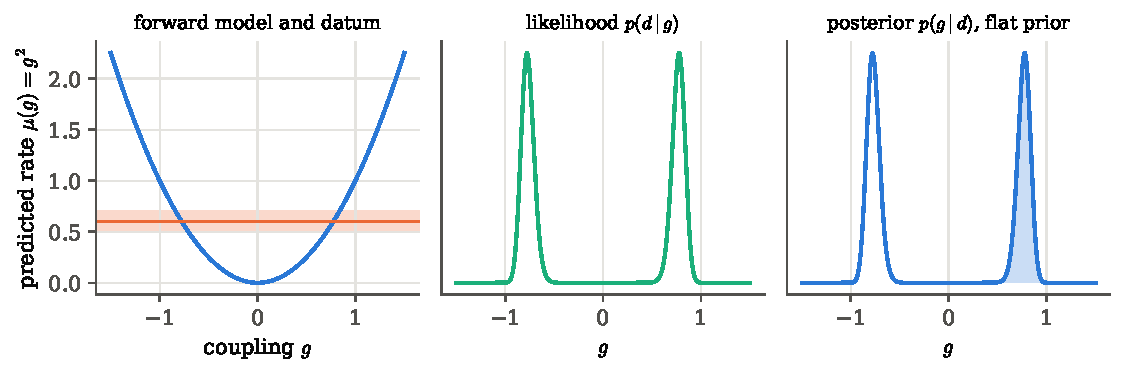
\includegraphics[width=\linewidth]{figures/ch05/grid_coupling.pdf}
\caption{Inferring a coupling from a rate proportional to its square. Left: the
forward model $g^2$ and the measured rate with its noise band. Two ranges of $g$, one
on each side of zero, predict rates inside the band. Middle: the likelihood as a
function of $g$ has a peak at each of them. Right: with a flat prior the posterior has
the same two peaks, and the shaded half, $g>0$, holds exactly half the probability.}
\label{5b:fig:coupling}
\end{figure}

\subsection{Many data points}

A real experiment gives many readings. Let the model predict a whole data vector
$\bm m(\lambda)=(m_1(\lambda),\dots,m_N(\lambda))$ and let the measured values be
$\data=(d_1,\dots,d_N)$ with independent Gaussian noise of sizes $\sigma_i$.
Independence means the joint density of all readings
is the product of the single-reading densities \mainref{p.~177}, so
\begin{align}
  \ln\Like(\lambda)
  &\eqby{1}\ln\prod_{i=1}^N\frac{1}{\sqrt{2\pi\sigma_i^2}}
     \exp\!\left[-\frac{(d_i-m_i(\lambda))^2}{2\sigma_i^2}\right]
   \nonumber\\
  &\eqby{2}-\frac12\sum_{i=1}^N\frac{(d_i-m_i(\lambda))^2}{\sigma_i^2}
     -\frac12\sum_{i=1}^N\ln(2\pi\sigma_i^2)
   \;=\;-\frac12\chi^2(\lambda)+\text{const}.
  \label{5b:eq:chi2}
\end{align}
\begin{explain}
  \item The likelihood of independent readings is the product of
        \eqref{5b:eq:gauss-like} over $i$.
  \item The log of a product is the sum of the logs, and $\ln e^{x}=x$.
\end{explain}
Here $\chi^2(\lambda)=\sum_i(d_i-m_i(\lambda))^2/\sigma_i^2$ is the sum of squared
residuals, each measured in units of its error bar, and the constant does not depend on
$\lambda$. With correlated noise of covariance matrix
$\Cmat$ the product is replaced by one multivariate Gaussian and
$\chi^2=(\data-\bm m)\T\Cmat^{-1}(\data-\bm m)$ (\cref{ch:03}). Either way the posterior
is
\begin{equation}
  p(\lambda\given\data)\propto e^{-\chi^2(\lambda)/2}\,p(\lambda),
  \label{5b:eq:post-chi2}
\end{equation}
and nothing in the logic has changed. The observed event is now the whole vector
$\data$. Each hypothesis $\lambda$ is judged by how plausible the whole vector of
fluctuations $\data-\bm m(\lambda)$ that it requires would be. Only the model for the
probability of the data changes from problem to problem. With a flat prior, $p(\lambda)$
is a constant, so the peak of the posterior is where $\chi^2$ is smallest: the
least-squares estimate. Least squares is therefore the special case ``flat prior,
Gaussian noise'' of Bayesian estimation \srcref{Sivia}{\S3.5}.

The same reasoning works at the scale of a whole survey; only the space of hypotheses
grows. In cosmology $\data$ may be thousands of band powers of the CMB and $\lambda$ the
handful of parameters of the standard cosmological model (see the cosmology notes). What we observed is the whole data
vector $\data$, every band power at once. The candidate explanations are the
possible values of $\lambda$, each one a different cosmological model. For each
of them the likelihood asks: had nature picked this model, how plausible would
it have been for exactly the data we hold to come out? Bayes' theorem combines
these likelihoods with the prior distribution and returns a posterior
distribution over the models.

\subsection{The posterior on a grid}

For one or two parameters the safest way to compute a posterior is to evaluate it on a
grid of values and look \srcref{Sivia}{\S3.4, ``brute force and ignorance''}. The grid
works whether the posterior is skewed, has several peaks, or has a sharp edge where the
prior stops. Its one trap is numerical: a product of many likelihoods is too large or
too small for a computer to store.

\paragraph{Example: a lifetime from 2000 readings.}
A source decays with lifetime $\tau$. We record the signal at $N=\FiveBTauN$ times,
$d_i=e^{-t_i/\tau}+\epsilon_i$ with $\sigma=\FiveBTauSigd$, and put a flat prior on
$\tau$. The obvious code multiplies the $N$ Gaussian densities for each grid value of
$\tau$. Each density near the curve is about $1/(\sqrt{2\pi}\,\sigma)\approx8$, and
$8^{2000}$ is far beyond the largest floating-point number, so the product comes out
as $\FiveBTauRawMax$. Now quote the same data in per cent. Every density is a hundred
times smaller, about $0.08$, and the product underflows to $\FiveBTauRawMaxPct$. The
posterior cannot depend on the units the data are quoted in, so neither answer means
anything. The cure is to work with logarithms \srcref{Sivia}{p.~34}:
\begin{enumerate}
  \item compute $L_j=\ln\Like(\tau_j)+\ln p(\tau_j)$ on the grid, as a \emph{sum} of
        logs;
  \item subtract the largest value, $L_j\to L_j-L_{\max}$, so that the largest is $0$;
  \item exponentiate, $w_j=e^{L_j-L_{\max}}$, which lies between $0$ and $1$;
  \item normalise, $p(\tau_j\given\data)=w_j/\sum_kw_k\Delta\tau$.
\end{enumerate}
Step 2 is legitimate because it multiplies every $w_j$ by the same constant
$e^{-L_{\max}}$, and a common constant cancels in the normalisation of step 4. For our
data $L_{\max}=\FiveBTauLogLmax$: the likelihood at the peak is $e^{\FiveBTauLogLmax}$,
a number no computer stores, but the \emph{ratios} of likelihoods between grid points
are perfectly ordinary numbers.

\pyfile[firstline=58,lastline=74,firstnumber=58]{code/ch05/08_grid_posterior.py}{The
lifetime posterior on a grid: the raw product fails, the log-sum with the maximum
subtracted works}

Line~63 builds the model prediction for every grid value of $\tau$ at every time at
once, as an $801\times2000$ array, and line~64 the Gaussian density of every reading.
Lines~65--68 form the raw products and show them overflow and, in per cent, underflow.
Line~69 is the log-likelihood as a sum, line~71 subtracts the maximum and
exponentiates, line~72 normalises, and lines~73--74 compute the posterior mean and
standard deviation by summing over the grid. The result is
$\tau=\FiveBTauMean\pm\FiveBTauSd$ (\cref{5b:fig:lifetime}), consistent with the true
value $2$ used in the simulation.

\begin{figure}[htbp]
\centering
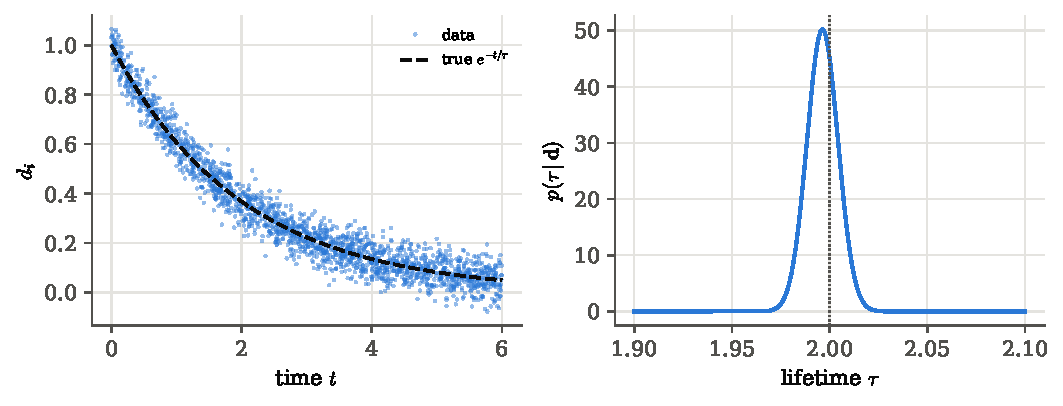
\includegraphics[width=0.9\linewidth]{figures/ch05/grid_lifetime.pdf}
\caption{A lifetime from 2000 noisy readings. Left: the readings (dots) and the true
decay curve (dashed). Right: the posterior for the lifetime computed on a grid of 801
values by summing log-likelihoods and subtracting their maximum. The dotted line marks
the value used to simulate the data.}
\label{5b:fig:lifetime}
\end{figure}

\begin{pitfall}[Never multiply raw likelihoods]
The product of many densities overflows or underflows depending only on the units the
data are quoted in. Always sum log-likelihoods and subtract the maximum before
exponentiating. The same rule applies to every sampler of \cref{ch:09}: they compare
$\ln p$ values, never $p$ values.
\end{pitfall}

A grid fails in many dimensions, because its cost grows as a power of the number of
parameters. With $n$ points per axis, a posterior in $D$ parameters needs $n^D$
evaluations: 100 points per axis is $10^4$
evaluations in two dimensions and $10^{12}$ in six, the size of a minimal cosmological
model. That cost, and the evidence integral it makes impossible, are what drive us to
sampling methods (\cref{ch:06,ch:09}).
\section{Conjugate priors: posteriors on the back of an envelope}
\label{5b:sec:conjugate}

For the likelihoods physicists meet most often, the product ``likelihood times prior''
can be worked out on paper. These are counts of successes, counts of events and
Gaussian readings. A grid (\cref{5b:sec:continuous}) also gives the posterior, but only
as a table of numbers. On paper the posterior comes out in the same family of curves as
the prior, with a few constants shifted by the data. We can then see at a glance how
much of the answer comes from the data and how much from the prior. Updating becomes
bookkeeping: add the number of heads here, the number of counts there.

The question is: for which pairs of likelihood and prior does the product have the same
functional form as the prior, and what are the update rules?

\begin{workdef}[conjugate prior]
A family of prior densities is \newterm{conjugate} to a likelihood if, for every data
set, prior from the family $\times$ likelihood is again a member of the family
\unpack{same functional form in the parameter, different values of its constants}
\mainref{p.~179}. Conjugacy is a property of the \emph{pair}: a prior is conjugate only
with respect to a particular likelihood \srcref{Kruschke}{\S6.2}. \emph{Operationally:}
write the likelihood as a function of the parameter, drop every factor that does not
contain it, and look for a density with the same $\theta$-dependence.
\end{workdef}

\subsection{Coins: the Beta--Binomial pair}

A coin, or any process with two outcomes, has unknown probability $\theta$ of
``success''. One toss $y\in\{0,1\}$ has the Bernoulli probability
$\theta^y(1-\theta)^{1-y}$, and $N$ independent tosses with $z$ successes have
\srcref{Kruschke}{(6.2)}
\begin{align*}
  p(\{y_i\}\given\theta)
  \eqby{1}\prod_{i=1}^N\theta^{y_i}(1-\theta)^{1-y_i}
  \eqby{2}\theta^{\sum_iy_i}(1-\theta)^{\sum_i(1-y_i)}
  =\theta^{z}(1-\theta)^{N-z}.
\end{align*}
\begin{explain}
  \item Independent tosses: the joint probability is the product.
  \item Powers of the same base multiply by adding exponents.
\end{explain}
As a function of $\theta$ this is a power of $\theta$ times a power of $1-\theta$. A
prior of the same shape is the \newterm{Beta distribution} (\cref{ch:02}),
\begin{equation}
  p(\theta)=\mathrm{Beta}(\theta\given a,b)=\frac{\theta^{a-1}(1-\theta)^{b-1}}{B(a,b)},
  \qquad
  B(a,b)=\int_0^1\theta^{a-1}(1-\theta)^{b-1}\dd\theta=\frac{\Gamma(a)\Gamma(b)}{\Gamma(a+b)},
  \label{5b:eq:beta}
\end{equation}
with $a,b>0$ \srcref{Kruschke}{(6.3)--(6.4)}. The Beta function $B(a,b)$ is only a
normalising number. Recall $\Gamma(n)=(n-1)!$ for integers and $\Gamma(x+1)=x\Gamma(x)$
in general. The flat prior is $\mathrm{Beta}(1,1)$. Multiply prior and likelihood:
\begin{align}
  p(\theta\given z,N)
  &\eqby{1}\frac{\theta^{z}(1-\theta)^{N-z}\;\theta^{a-1}(1-\theta)^{b-1}/B(a,b)}{p(z,N)}
   \eqby{2}\frac{\theta^{(z+a)-1}(1-\theta)^{(N-z+b)-1}}{B(a,b)\,p(z,N)}
   \nonumber\\
  &\eqby{3}\frac{\theta^{(z+a)-1}(1-\theta)^{(N-z+b)-1}}{B(z+a,\,N-z+b)}
   =\mathrm{Beta}(\theta\given z+a,\;N-z+b).
  \label{5b:eq:beta-post}
\end{align}
\begin{explain}
  \item Bayes' theorem with the Bernoulli likelihood and the Beta prior.
  \item Collect the powers of $\theta$ and of $1-\theta$.
  \item The numerator is the $\theta$-dependence of a Beta density with parameters
        $z+a$ and $N-z+b$. A density must integrate to one, and there is only one
        constant that makes this one do so, $B(z+a,N-z+b)$. So the denominator must be
        that constant, and no integral was needed \srcref{Kruschke}{\S6.3}.
\end{explain}
The update rule is: \emph{add the successes to $a$ and the failures to $b$}. Adding is
done in any order, so the result is the same whether the tosses arrive one at a time
or all at once, as sequential updating requires (\cref{5a:sec:sequential}). The rule
also tells us how to read a prior. $\mathrm{Beta}(a,b)$ behaves like the posterior we
would hold after seeing about $a$ successes and $b$ failures. So $\kappa=a+b$ counts how
many tosses' worth of information the prior carries \srcref{Kruschke}{\S6.2.1}.

\paragraph{The posterior mean is a compromise.}
The mean of a Beta density is
\begin{align*}
  \E[\theta]
  \eqby{1}\frac{1}{B(a,b)}\int_0^1\theta^{a}(1-\theta)^{b-1}\dd\theta
  \eqby{2}\frac{B(a+1,b)}{B(a,b)}
  \eqby{3}\frac{\Gamma(a+1)\,\Gamma(a+b)}{\Gamma(a)\,\Gamma(a+b+1)}
  \eqby{4}\frac{a}{a+b}.
\end{align*}
\begin{explain}
  \item Definition of the mean, $\int\theta\,p(\theta)\dd\theta$, with one extra power
        of $\theta$.
  \item The integral is the Beta function with $a\to a+1$.
  \item Write both Beta functions with Gammas. $\Gamma(b)$ cancels.
  \item $\Gamma(a+1)=a\Gamma(a)$ and $\Gamma(a+b+1)=(a+b)\Gamma(a+b)$.
\end{explain}
For the posterior \eqref{5b:eq:beta-post} this gives \srcref{Kruschke}{(6.9)},
\mainref{p.~179}
\begin{align}
  \frac{z+a}{N+a+b}
  \eqby{1}\frac{z}{N}\cdot\frac{N}{N+a+b}+\frac{a}{a+b}\cdot\frac{a+b}{N+a+b} .
  \label{5b:eq:beta-mean}
\end{align}
\begin{explain}
  \item Multiply out the right side: the $N$ and the $a+b$ cancel, leaving
        $(z+a)/(N+a+b)$.
\end{explain}
The posterior mean is a weighted average of two numbers: the observed fraction $z/N$
(the maximum likelihood estimate) and the prior mean $a/(a+b)$. Their weights are
proportional to the number of tosses $N$ and to the prior's worth in tosses,
$\kappa=a+b$. So the data win once $N\gg\kappa$. For a flat prior, $a=b=1$, it is
$(z+1)/(N+2)$, Laplace's rule of succession \mainref{p.~178, (11.5)--(11.6)}. For
example, Kruschke's prior $\mathrm{Beta}(5,5)$ with $z=1$ success in $N=10$ gives
posterior mean $(1+5)/(10+10)=0.3$, exactly halfway between the prior mean $0.5$ and the
data fraction $0.1$, because $N=\kappa$ \srcref{Kruschke}{Fig.~6.3}.

\paragraph{Example: the same data, three priors.}
\emph{The event.} A two-outcome process is tried 20 times and gives 17 successes, 85\%.
\emph{The question.} What should we now believe about its success probability $\theta$?
The answer depends on what we knew before, that is, on what the process is
\srcref{Kruschke}{\S6.4.1}.
\emph{Three cases in turn.} If it is a freshly minted government coin, we are confident
it is fair: prior $\mathrm{Beta}(100,100)$, worth 200 tosses of evidence for $0.5$. If a
success is a professional basketball player making a free throw, we know such players
make about 75\% of them: prior $\mathrm{Beta}(18.25,6.75)$, mode $0.75$ and $\kappa=25$.
If it is the colour of samples of a substance on a distant planet, we know only that
both outcomes are possible: $\mathrm{Beta}(1,1)$.
\emph{Only then the numbers.} Adding 17 to $a$ and 3 to $b$, the three posteriors are $\mathrm{Beta}(117,103)$,
$\mathrm{Beta}(35.25,9.75)$ and $\mathrm{Beta}(18,4)$, with modes
$\FiveBBetaModeS$, $\FiveBBetaModeL$ and $\FiveBBetaModeF$ (\cref{5b:fig:three-priors}).
The 17 successes barely move the government coin, pull the basketball player just above his
league's typical rate, and fully determine the planetary substance. None of the three
analysts is wrong. They started from different knowledge, and twenty tosses are not
enough to overwhelm a prior worth two hundred.

\begin{figure}[htbp]
\centering
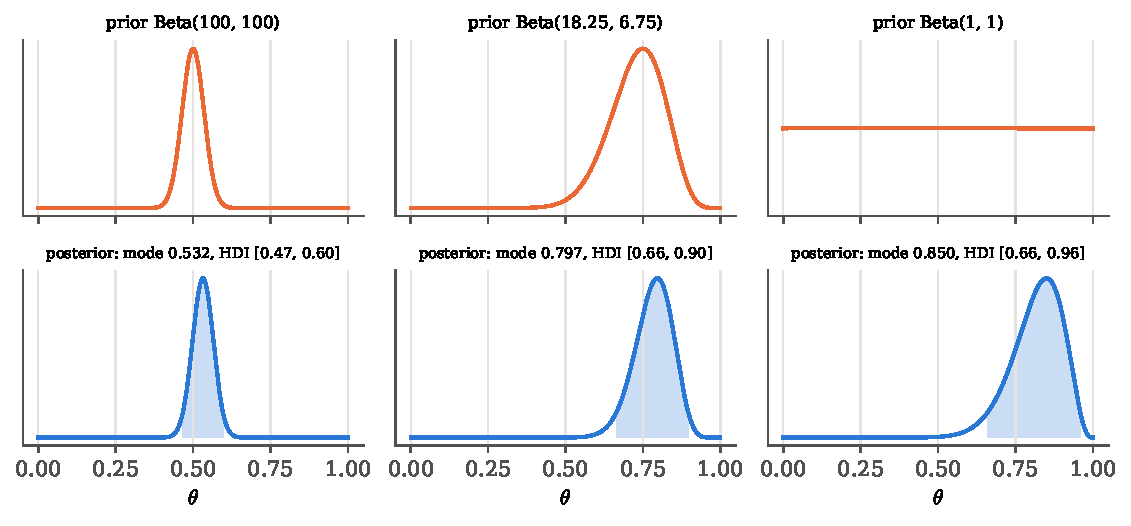
\includegraphics[width=\linewidth]{figures/ch05/conjugate_three_priors.pdf}
\caption{Seventeen heads in twenty tosses, analysed with three priors. Top row: a
confident fair-coin prior, a basketball league's free-throw rate, and a flat prior.
Bottom row: the three posteriors, each a Beta density, with the shaded 95\% highest
density interval (\cref{5b:sec:summaries}). The same data move the three beliefs by
very different amounts.}
\label{5b:fig:three-priors}
\end{figure}

\paragraph{Example: predicting the next two tosses.}
Conjugacy also gives predictions in closed form. A coin gave 10 heads in 14 tosses. What
is the probability that the next two tosses are both heads \srcref{Padilla}{\S2.3,
\S3.1}? With a flat prior, $\mathrm{Beta}(1,1)$, the posterior is $\mathrm{Beta}(1+10,
1+4)=\mathrm{Beta}(11,5)$. If we knew $\theta$, two heads would have probability
$\theta^2$. We do not know $\theta$, so we average $\theta^2$ over the posterior, that
is, we marginalise $\theta$:
\begin{align*}
  \Prob(\text{HH}\given\data)
  \eqby{1}\int_0^1\theta^2\,\frac{\theta^{10}(1-\theta)^{4}}{B(11,5)}\,\dd\theta
  \eqby{2}\frac{B(13,5)}{B(11,5)}
  \eqby{3}\frac{12\cdot11}{17\cdot16}
  =\FiveBPred .
\end{align*}
\begin{explain}
  \item Sum over the paths ``$\theta$, then two heads'': the probability of HH given
        $\theta$ times the posterior density of $\theta$.
  \item The integral is a Beta function with the first argument raised by two.
  \item $B(13,5)/B(11,5)=\Gamma(13)\Gamma(16)/[\Gamma(11)\Gamma(18)]$, and
        $\Gamma(13)/\Gamma(11)=12\cdot11$, $\Gamma(18)/\Gamma(16)=17\cdot16$.
\end{explain}
Plugging in the single best value $\hat\theta=10/14$ instead gives
$(10/14)^2=\FiveBPlugin$. The posterior predictive is smaller, and it is the honest
answer. It remembers that $\theta$ might be lower than $10/14$; the plug-in pretends that
14 tosses fixed $\theta$ exactly.

\subsection{Counts: the Gamma--Poisson pair}

A detector counts cosmic-ray muons in one-minute windows. The counts $n_1,\dots,n_M$ are
Poisson with unknown rate $\lambda$ per minute, so the likelihood is
\srcref{Lambert}{(9.8)}
\begin{align*}
  p(\{n_i\}\given\lambda)
  \eqby{1}\prod_{i=1}^M\frac{\lambda^{n_i}e^{-\lambda}}{n_i!}
  \eqby{2}\frac{\lambda^{\sum_in_i}\,e^{-M\lambda}}{\prod_in_i!}
  \;\propto\;\lambda^{S}e^{-M\lambda},\qquad S=\sum_in_i .
\end{align*}
\begin{explain}
  \item Independent windows: the product of Poisson probabilities.
  \item Add the exponents of $\lambda$, and $M$ copies of $e^{-\lambda}$ make
        $e^{-M\lambda}$. The factorials do not contain $\lambda$.
\end{explain}
A power of $\lambda$ times a decaying exponential in $\lambda$ is the shape of the
\newterm{Gamma distribution}, $\mathrm{Gamma}(\lambda\given\alpha,\beta)=\beta^\alpha
\lambda^{\alpha-1}e^{-\beta\lambda}/\Gamma(\alpha)$ for $\lambda>0$, with mean
$\alpha/\beta$ and variance $\alpha/\beta^2$ (\cref{ch:02}). Multiplying,
\begin{align}
  p(\lambda\given\{n_i\})
  \eqby{1}\lambda^{S}e^{-M\lambda}\cdot\lambda^{\alpha-1}e^{-\beta\lambda}
  \eqby{2}\lambda^{(\alpha+S)-1}e^{-(\beta+M)\lambda}
  \;\Rightarrow\;
  \lambda\given\{n_i\}\sim\mathrm{Gamma}(\alpha+S,\;\beta+M).
  \label{5b:eq:gamma-post}
\end{align}
\begin{explain}
  \item Posterior $\propto$ likelihood $\times$ prior, dropping constants.
  \item Collect powers and exponents. The normalisation follows as in the Beta case.
\end{explain}
The rule is: \emph{add the total count to $\alpha$ and the number of windows to $\beta$}
\srcref{Lambert}{(9.11)}. So $\mathrm{Gamma}(\alpha,\beta)$ is like having already seen
about $\alpha$ counts in $\beta$ windows, and the posterior mean $(\alpha+S)/(\beta+M)$ is
again a weighted average, of the prior mean $\alpha/\beta$ and the observed mean $S/M$.

\paragraph{Example: the muon rate.}
A previous run suggested ``about 3 per minute, not very sure'': prior
$\mathrm{Gamma}(3,1)$, mean 3, standard deviation $\sqrt3\approx1.7$. Five windows gave
$\FiveBCountsList$ counts, total $S=\FiveBCountsSum$, observed mean $\FiveBGamMLE$. The
posterior is $\mathrm{Gamma}(\FiveBGamA,\FiveBGamB)$ with mean $\FiveBGamMean$ and
standard deviation $\FiveBGamSd$: pulled a little from the data's $\FiveBGamMLE$ towards
the prior's 3, since the prior is worth one window against the data's five
(\cref{5b:fig:conjugate}, middle).

\subsection{Gaussian readings: inverse-variance weighting emerges}

Several laboratories measure the same quantity $\mu$ with different instruments. Reading
$x_k$ has Gaussian error $\sigma_k$, and we have a Gaussian prior $\Normal(a,b^2)$ of
mean $a$ and width $b$. We work with the logarithm, because the log of a product of
Gaussians is a sum of squares, which is easy to collect. Up to constants that do not
contain $\mu$,
\begin{align}
  -2\ln p(\mu\given\{x_k\})
  &\eqby{1}\sum_k\frac{(x_k-\mu)^2}{\sigma_k^2}+\frac{(\mu-a)^2}{b^2}
   \nonumber\\
  &\eqby{2}\mu^2\Bigl(\sum_kw_k+\frac1{b^2}\Bigr)
     -2\mu\Bigl(\sum_kw_kx_k+\frac{a}{b^2}\Bigr)+\text{const}
   \nonumber\\
  &\eqby{3}P\,(\mu-m)^2+\text{const},\qquad
   P=\sum_kw_k+\frac1{b^2},\quad m=\frac{\sum_kw_kx_k+a/b^2}{P}.
  \label{5b:eq:normal-post}
\end{align}
\begin{explain}
  \item Log of Gaussian likelihoods times a Gaussian prior, multiplied by $-2$.
  \item Expand the squares and write $w_k=1/\sigma_k^2$. Terms without $\mu$ go into
        the constant.
  \item Complete the square: $P\mu^2-2\mu Pm=P(\mu-m)^2-Pm^2$, and $Pm^2$ is a constant.
\end{explain}
The posterior is therefore Gaussian, $\mu\given\{x_k\}\sim\Normal(m,1/P)$
\mainref{p.~179, (11.7)}. Two rules have appeared by themselves.
\begin{itemize}
  \item \emph{Precisions add.} The precision (inverse variance) of the posterior is
        the sum of the precisions of the measurements and of the prior.
  \item \emph{Means are precision-weighted.} Each measurement counts in proportion to
        $1/\sigma_k^2$, and the prior counts as one more measurement, of value $a$ and
        error $b$.
\end{itemize}
With a very broad prior, $b\to\infty$, we get the familiar inverse-variance weighted
mean $\bar\mu=\sum_kw_kx_k/\sum_kw_k$ with error $(\sum_kw_k)^{-1/2}$
\srcref{Sivia}{(2.30)--(2.31)}. For $N$ equal errors this is the sample mean with error
$\sigma/\sqrt N$. Wasserman writes the same result as $m=w\bar X+(1-w)a$ with
$w=(1/\mathrm{se}^2)/(1/\mathrm{se}^2+1/b^2)$ and $\mathrm{se}=\sigma/\sqrt n$
\mainref{p.~179}.

\paragraph{Example: three laboratories.}
Three simulated measurements are $\FiveBNxa\pm0.5$, $\FiveBNxb\pm1.0$ and
$\FiveBNxc\pm2.0$, and a vague earlier estimate gives the prior $\Normal(8,3^2)$. The
posterior is $\mu=\FiveBNmPost\pm\FiveBNsPost$. Without the prior, the inverse-variance
weighted mean is $\FiveBNmIvw\pm\FiveBNsIvw$. The prior counts as one more measurement,
of error 3. It shifts the answer by a tenth of its error bar and shrinks the error bar
slightly (\cref{5b:fig:conjugate}, right).

\begin{figure}[htbp]
\centering
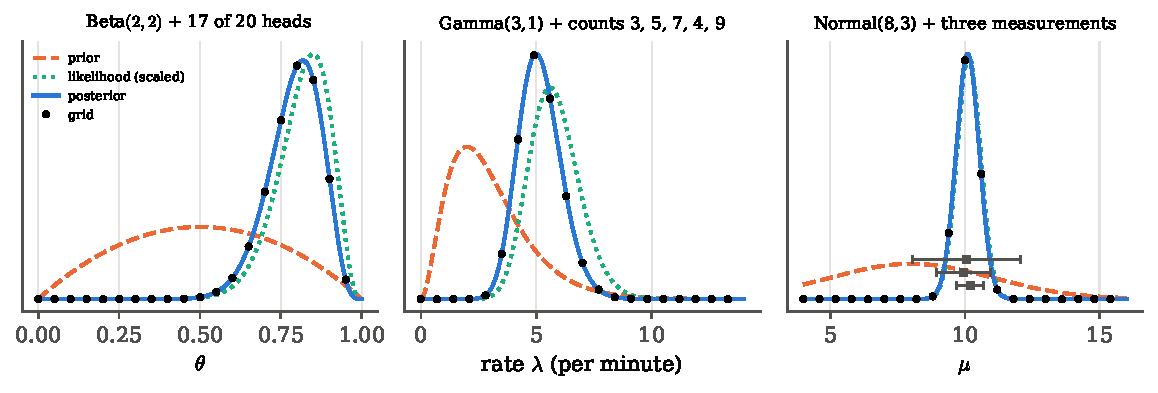
\includegraphics[width=\linewidth]{figures/ch05/conjugate_pairs.pdf}
\caption{The three conjugate pairs. In each panel the dashed curve is the prior, the
dotted curve the likelihood (scaled to unit area), the solid curve the closed-form
posterior and the dots the posterior computed by brute force on a grid. Left: a Beta
prior and 17 heads in 20. Middle: a Gamma prior and five minutes of muon counts.
Right: a Gaussian prior and three measurements with different error bars (squares with
bars). The dots lie on the curves, to a relative accuracy of $10^{-11}$.}
\label{5b:fig:conjugate}
\end{figure}

The update rules are exact, and the grid check in \cref{5b:fig:conjugate} confirms it.
The largest relative difference between the brute-force and closed-form posteriors is
$\FiveBBetaErr$ for the Beta case, $\FiveBGamErr$ for the Gamma case and $\FiveBNErr$ for
the Gaussian case: pure round-off.

\begin{taxonomy}[common conjugate pairs]
\centering\small
\begin{tabular}{@{}lll@{}}
\toprule
likelihood (data) & conjugate prior & posterior \\
\midrule
Bernoulli/binomial ($z$ of $N$) & $\mathrm{Beta}(a,b)$ & $\mathrm{Beta}(a+z,\,b+N-z)$\\
Poisson (total $S$ in $M$ windows) & $\mathrm{Gamma}(\alpha,\beta)$ & $\mathrm{Gamma}(\alpha+S,\,\beta+M)$\\
multinomial (counts $\bm n$) & $\mathrm{Dirichlet}(\bm\alpha)$ & $\mathrm{Dirichlet}(\bm\alpha+\bm n)$\\
Gaussian, known $\sigma_k$ & $\Normal(a,b^2)$ & $\Normal(m,1/P)$, \eqref{5b:eq:normal-post}\\
Gaussian, known mean, variance $v$ & $\text{Inv-Gamma}(\alpha,\beta)$ &
  $\text{Inv-Gamma}\bigl(\alpha+\frac N2,\,\beta+\frac12\sum(x_i-\mu)^2\bigr)$\\
\bottomrule
\end{tabular}
\par\smallskip\raggedright
Sources: \srcref{Lambert}{Table~9.1}, \mainref{pp.~178--179}. The last row is the one
used for a power-spectrum amplitude below.
\end{taxonomy}

\paragraph{The limits of conjugacy.}
Conjugate pairs exist only for a handful of simple likelihoods, and even then only
priors of one particular shape are allowed. A coin factory that makes coins biased
either near $0.25$ or near $0.75$ has a two-humped prior that no Beta density can
represent. Its posterior after 14 heads in 27 has three bumps, a compromise between the
two humps of the prior and the single peak of the likelihood, and must be computed on a
grid \srcref{Kruschke}{\S6.4.2}. Likewise, replacing a Gaussian likelihood by a more
robust Student-$t$ destroys conjugacy altogether \srcref{Lambert}{\S9.7}. The lesson is
not to bend the model to fit a conjugate prior. Conjugacy is a source of exact test
cases and of intuition. Realistic models are handled by grids in low dimension and by
sampling (\cref{ch:09}) in high dimension.

\subsection{One calculation, three instruments}

The same few lines of algebra appear in three very different corners of physics. Only
the likelihood changes: counts at a collider are Poisson, a CMB map is a Gaussian random
field, and a gravitational-wave strain is a known waveform in Gaussian noise described
by a power spectral density (\cref{5b:fig:instruments}).

\paragraph{A collider search with no background.}
A search for a rare process expects $s$ signal events and, after cuts, essentially no
background. The number observed is Poisson with mean $s$. Suppose nothing is seen. How
large could $s$ be? The flat prior on $s\ge0$ is the $\mathrm{Gamma}(1,0)$ limit, and
the search is a single window, so the Gamma update \eqref{5b:eq:gamma-post} with $n$
events gives $s\given n\sim\mathrm{Gamma}(n+1,1)$. For $n=0$ the posterior is $e^{-s}$.
The 95\% credible upper limit $s_{95}$ is the value below which $s$ lies with
probability 95\%, so it solves
\begin{align*}
  0.95\eqby{1}\int_0^{s_{95}}e^{-s}\,\dd s\eqby{2}1-e^{-s_{95}}
  \quad\Rightarrow\quad s_{95}=\ln 20=\FiveBULzero .
\end{align*}
\begin{explain}
  \item The posterior probability that $s$ is below the limit is 95\%.
  \item Elementary integral.
\end{explain}
This is the famous ``three events'' upper limit for an empty search. With one or three
events observed the limits are $\FiveBULone$ and $\FiveBULthree$.

\paragraph{The CMB: a power-spectrum amplitude from $2\ell+1$ numbers.}
The temperature map is expanded in spherical harmonics, and at multipole $\ell$ the
coefficients $\alm$ amount to $2\ell+1$ independent real Gaussian numbers of zero mean
and variance $\Cell$ (see the cosmology notes, and \cref{ch:07}). Their likelihood is
\begin{align*}
  p(\{\alm\}\given\Cell)
  \eqby{1}\prod_{m=-\ell}^{\ell}\frac{e^{-|\alm|^2/2\Cell}}{\sqrt{2\pi\Cell}}
  \;\propto\;\Cell^{-(2\ell+1)/2}\exp\!\left[-\frac{(2\ell+1)\Chat}{2\Cell}\right],
  \qquad \Chat=\frac{1}{2\ell+1}\sum_m|\alm|^2 .
\end{align*}
\begin{explain}
  \item $2\ell+1$ independent Gaussians of variance $\Cell$, and the sum of their squares
        written through the estimator $\Chat$.
\end{explain}
As a function of $\Cell$ this is an inverse power times $e^{-\text{const}/\Cell}$. That
is the shape of an inverse-Gamma density, the last row of the table. With the scale-invariant prior
$p(\Cell)\propto1/\Cell$ (\cref{5b:sec:priors}) the posterior is
$\text{Inv-Gamma}\bigl(\tfrac{2\ell+1}2,\tfrac{(2\ell+1)\Chat}2\bigr)$. For the
quadrupole, $\ell=2$, only five numbers exist in the whole sky. The posterior of
$\Cell/\Chat$ has its mode at $\FiveBCmbModeTwo$, its mean at $\FiveBCmbMeanTwo$, and its
central 68\% interval from $\FiveBCmbLoTwo$ to $\FiveBCmbHiTwo$. So five numbers cannot
pin the quadrupole power to better than a factor of about two, however good the
telescope. This is cosmic variance seen as a posterior. At $\ell=50$ the interval has shrunk to
$[\FiveBCmbLoFifty,\FiveBCmbHiFifty]$ and the posterior is nearly Gaussian.

\paragraph{A gravitational-wave amplitude.}
A detector records $d=A\,h_0+n$, where $h_0$ is a known waveform, $A$ an unknown
amplitude and $n$ stationary Gaussian noise with power spectral density $S_n(f)$. The
likelihood is $\Like\propto\exp[-\frac12(d-Ah_0\,|\,d-Ah_0)]$ with the noise-weighted
inner product $(a|b)=4\,\mathrm{Re}\int_0^\infty\tilde a\tilde b^*/S_n\,\dd f$
(\cref{ch:03}). The inner product is linear in each slot, so
\begin{align*}
  (d-Ah_0\,|\,d-Ah_0)
  \eqby{1}(d|d)-2A\,(d|h_0)+A^2\,(h_0|h_0)
  \eqby{2}(h_0|h_0)\,\bigl(A-\hat A\bigr)^2+\text{const},
  \\ \hat A=\frac{(d|h_0)}{(h_0|h_0)} .
\end{align*}
\begin{explain}
  \item Expand, using $(h_0|d)=(d|h_0)$ for the real inner product.
  \item Complete the square in $A$.
\end{explain}
The posterior for $A$ with a flat or Gaussian prior is Gaussian, centred on the
matched-filter estimate $\hat A$, with standard deviation $1/\sqrt{(h_0|h_0)}$. For our
toy chirp in coloured noise, normalised to $(h_0|h_0)=\FiveBGwHH$, the posterior is
$A=\FiveBGwAhat\pm\FiveBGwAsd$ for true $A=1$, and over 4000 independent noise
realisations the estimate $\hat A$ scatters by $\FiveBGwSpread$, the posterior width, as
it should.

\begin{figure}[htbp]
\centering
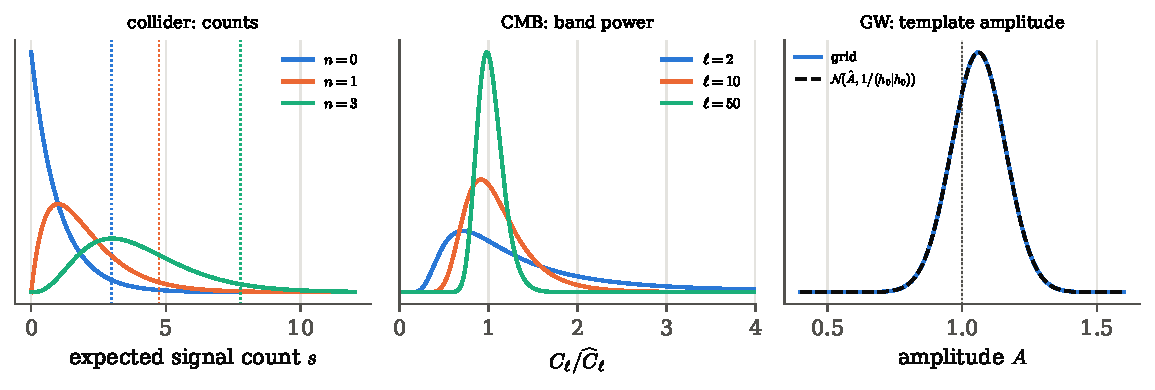
\includegraphics[width=\linewidth]{figures/ch05/three_instruments.pdf}
\caption{One posterior calculation in three instruments. Left: a background-free
collider search, posterior for the expected signal after 0, 1 and 3 observed events,
with the 95\% upper limits dotted. Middle: the posterior of a CMB band power relative to
its estimate, for $\ell=2$, 10 and 50. The quadrupole's posterior is broad and skewed.
Right: the amplitude of a known gravitational-wave template in coloured noise, computed
on a grid (solid) and from the closed form (dashed).}
\label{5b:fig:instruments}
\end{figure}

\begin{inpractice}[closed forms inside large analyses]
Conjugate results survive as building blocks inside big pipelines. Collider limits for
counting experiments are routinely quoted as Bayesian upper limits with a flat prior on
the signal rate, exactly the Gamma calculation above, and physicists check them against
frequentist constructions (\cref{ch:04}). CMB likelihoods at low $\ell$ use the exact
inverse-Gamma shape rather than a Gaussian, because the quadrupole's posterior is far
from Gaussian (\cref{ch:07}). Gravitational-wave pipelines marginalise analytically over
parameters that enter linearly, such as an amplitude or a phase, before sampling the
rest (\cref{ch:09}). Everywhere, the closed forms are also the test cases that a new
sampler must reproduce.
\end{inpractice}
\section{Summarising a posterior: best values and credible intervals}
\label{5b:sec:summaries}

The posterior is the complete answer: every statement we can make about the parameter
is an integral of it. But papers quote only a handful of numbers, such as
``$\theta=0.28\pm0.08$'' or ``$s<3$ events at 95\%''. A decision, such as building the
next detector or claiming a discovery, also needs one number or one interval. So which
numbers should we quote, and what exactly does each one mean?

Our running example is the posterior of the CMB quadrupole power $C_2$ from
\cref{5b:sec:conjugate}. There the five numbers $a_{2m}$ ($m=-2,\dots,2$) measured over
the whole sky gave an inverse-Gamma posterior. Write it in terms of the ratio
$x=C_2/\widehat C_2$ of the power to its estimate $\widehat C_2=\frac15\sum_m|a_{2m}|^2$.
Then its parameters are $\alpha=\beta=5/2$, and it is strongly skewed, with a long tail
to large $x$ (\cref{5b:fig:summaries}, left).

\subsection{Three best values, three losses}

There are three standard point summaries \srcref{Lambert}{\S7.6}: the
\newterm{posterior mean} $\E[\theta\given\data]=\int\theta\,p(\theta\given\data)
\dd\theta$ \mainref{p.~177, (11.4)}, the \newterm{posterior median} (half the
probability on each side), and the \newterm{posterior mode} or MAP, \emph{maximum a
posteriori}, the highest point of the density. For a symmetric single-peaked posterior
they coincide. For the quadrupole they are
\[
  \text{mode }\FiveBSumMode,\qquad\text{median }\FiveBSumMedian,\qquad
  \text{mean }\FiveBSumMean .
\]
Which one is ``right''? Each is the best answer to a different question: what does it
cost us to be wrong? Suppose we must announce one number $M$, and we pay a penalty
$\mathrm{loss}(\theta-M)$ if the truth turns out to be $\theta$. We do not know
$\theta$, so we average the penalty over the posterior. The expected penalty is
$R(M)=\int\mathrm{loss}(\theta-M)\,p(\theta\given\data)\,\dd\theta$, and the best $M$ is
the one that makes it smallest \srcref{Kruschke}{\S4.3.3}. We take three penalties in
turn.

\paragraph{Squared loss gives the mean.}
With $\mathrm{loss}=(\theta-M)^2$,
\begin{align*}
  \frac{\dd R}{\dd M}
  \eqby{1}\int\frac{\partial}{\partial M}(\theta-M)^2\,p(\theta\given\data)\,\dd\theta
  \eqby{2}-2\int(\theta-M)\,p(\theta\given\data)\,\dd\theta
  \eqby{3}-2\bigl(\E[\theta\given\data]-M\bigr),
\end{align*}
\begin{explain}
  \item Differentiate under the integral, since the limits do not depend on $M$.
  \item $\partial_M(\theta-M)^2=-2(\theta-M)$.
  \item Split the integral: $\int\theta p\,\dd\theta$ is the mean and $\int Mp\,\dd\theta
        =M$ because $p$ is normalised.
\end{explain}
which vanishes at $M=\E[\theta\given\data]$. A large miss costs the square of its size,
so the rare values far out in a long tail weigh heavily, and they drag the answer
towards that tail.

\paragraph{Absolute loss gives the median.}
With $\mathrm{loss}=|\theta-M|$,
\begin{align*}
  \frac{\dd R}{\dd M}
  \eqby{1}\int_{-\infty}^{M}p(\theta\given\data)\,\dd\theta
         -\int_{M}^{\infty}p(\theta\given\data)\,\dd\theta
  \eqby{2}\Prob(\theta<M\given\data)-\Prob(\theta>M\given\data),
\end{align*}
\begin{explain}
  \item $\partial_M|\theta-M|$ is $+1$ for $\theta<M$ and $-1$ for $\theta>M$.
  \item Each integral of the density over a half-line is a probability.
\end{explain}
which vanishes when half the probability lies on each side: the median.

\paragraph{``All or nothing'' gives the mode.}
If we win only when $M$ lands within a tiny window $\pm\delta$ of the truth, the
expected reward is $\int_{M-\delta}^{M+\delta}p\,\dd\theta\approx2\delta\,p(M\given
\data)$, largest where the density is highest: the MAP.

The mode is the easiest to compute. The evidence does not depend on $\theta$, so the
mode is simply the maximum of likelihood times prior, and no normalisation is needed.
With a flat prior it is the maximum-likelihood estimate. But it is the most fragile of
the three, for two reasons. First, it depends on the parametrisation: a density changes
shape when the axis is stretched (\cref{5b:sec:priors}). Second, for a skewed posterior
it can sit far from the bulk of the probability. For the quadrupole,
$\FiveBSumAboveMode$\% of the posterior probability lies \emph{above} the mode.

The median does not have the first weakness. If $y=g(\theta)$ is increasing, the median
of $y$ is $g$ of the median of $\theta$. The reason is that ``half the probability lies
below'' is a statement about the probabilities of corresponding intervals, and a change
of variable does not alter those. Lambert ranks the mean first, the median second and
the MAP last \srcref{Lambert}{\S7.6}. Whichever is quoted, say which one it is, and give
an interval with it.

\subsection{Credible intervals}

A \newterm{credible interval} of level $1-\alpha$ is any region holding posterior
probability $1-\alpha$. Many regions do so, and two conventions pick one of them.

The \newterm{equal-tailed interval} (ETI) puts probability $\alpha/2$ in each tail: find
$a,b$ with $\int_{-\infty}^ap\,\dd\theta=\int_b^\infty p\,\dd\theta=\alpha/2$
\mainref{p.~178}. It is the interval between two quantiles, easy to compute from a
cumulative distribution or from samples (\cref{5b:sec:sampling}), and, like the median,
it maps onto itself under any increasing change of variable.

The \newterm{highest density interval} (HDI) instead takes the most credible values
first \srcref{Kruschke}{\S4.3.4}. Picture the posterior curve as a landscape, with a
water level $W$ that is lowered from above. The HDI is the set of $\theta$ that stick out above the
water, $p(\theta\given\data)>W$, with $W$ lowered until that set holds probability
$1-\alpha$ (\cref{5b:fig:hdi-water}).

\begin{workdef}[highest density interval]
The $(1-\alpha)$ \newterm{HDI} is the set $\{\theta:\,p(\theta\given\data)>W\}$, where
the level $W$ is chosen so that $\int_{p>W}p(\theta\given\data)\,\dd\theta=1-\alpha$.
Every point inside has higher density than every point outside
\unpack{so it contains the most credible values}. For a single-peaked posterior it is
the \emph{shortest} interval with probability $1-\alpha$ \srcref{Sivia}{(2.21)}. For a
posterior with several peaks it can be several disjoint intervals.
\emph{Operationally:} on a grid, sort the grid values by density and accumulate them from
the top until the probability reaches $1-\alpha$. From samples, take the shortest
interval that contains a fraction $1-\alpha$ of the sorted samples.
\end{workdef}

\begin{figure}[htbp]
\centering
\begin{tikzpicture}[x=1.15cm,y=2.2cm]
  \def\dens(#1){0.55*exp(-(#1-1.6)^2/0.35)+0.38*exp(-(#1-4.6)^2/0.45)}
  \fill[formblue!18,domain=0.943:2.257,samples=60] (0.943,0) -- plot (\x,{\dens(\x)}) -- (2.257,0) -- cycle;
  \fill[formblue!18,domain=3.976:5.224,samples=60] (3.976,0) -- plot (\x,{\dens(\x)}) -- (5.224,0) -- cycle;
  \draw[form,domain=0:6.3,samples=160] plot (\x,{\dens(\x)});
  \draw[faint,->] (-0.1,0) -- (6.6,0) node[right,black,lbl] {$\theta$};
  \draw[bdryred,thick,dashed] (-0.1,0.16) -- (6.4,0.16);
  \node[lbl,bdryred,anchor=east] at (-0.15,0.16) {level $W$};
  \draw[very thick,formblue] (0.943,-0.08) -- (2.257,-0.08);
  \draw[very thick,formblue] (3.976,-0.08) -- (5.224,-0.08);
  \node[lbl,anchor=north] at (3.1,-0.14) {HDI $=$ two intervals, total probability $1-\alpha$};
  \node[lbl,anchor=west] at (5.6,0.45) {$p(\theta\given\data)$};
\end{tikzpicture}
\caption{The highest density interval as a water level. The level $W$ is lowered until
the parts of the posterior above it (shaded) hold probability $1-\alpha$. Every value
inside the shaded region is more credible than every value outside. With two peaks, the
HDI is two separate intervals.}
\label{5b:fig:hdi-water}
\end{figure}

\paragraph{Why the HDI is the shortest interval.}
For a single-peaked density, look for the shortest interval $[a,b]$ with fixed
probability $F(b)-F(a)=1-\alpha$, where $F$ is the cumulative distribution. Minimise
$b-a$ with a Lagrange multiplier $\eta$ for the constraint:
\begin{align*}
  0\eqby{1}\frac{\partial}{\partial a}\Bigl[(b-a)-\eta\bigl(F(b)-F(a)-(1-\alpha)\bigr)\Bigr]
  \eqby{2}-1+\eta\,p(a),\qquad
  0\eqby{3}\frac{\partial}{\partial b}\Bigl[\cdots\Bigr]=1-\eta\,p(b),
\end{align*}
\begin{explain}
  \item Stationarity of the Lagrangian with respect to the lower end.
  \item $\partial_aF(a)=p(a)$, the density at the lower end.
  \item The same with respect to the upper end.
\end{explain}
So $p(a)=p(b)=1/\eta$: the shortest interval has the same density at both ends. That
is exactly the water level picture, with the level at height $1/\eta$. For a skewed
posterior the two conventions therefore differ. The HDI is shifted towards the peak and
has unequal tails. The ETI has equal tails and unequal densities at its ends.

\paragraph{Example: the quadrupole.}
Recall that $x=C_2/\widehat C_2$ is the quadrupole power relative to its estimate. Its
95\% ETI is $[\FiveBSumEtiLo,\FiveBSumEtiHi]$ and its 95\% HDI is
$[\FiveBSumHdiLo,\FiveBSumHdiHi]$, at water level $W=\FiveBSumWater$
(\cref{5b:fig:summaries}, left). The HDI is shorter and starts lower. Why? Values of $x$
between $\FiveBSumHdiLo$ and $\FiveBSumEtiLo$ have higher density than values near
$\FiveBSumEtiHi$, yet the ETI leaves out the former and keeps the latter
\srcref{Kruschke}{\S12.1.2.2}. From $10^5$ posterior samples, the shortest interval
containing 95\% of them is $[\FiveBSumHdiSLo,\FiveBSumHdiSHi]$, the same up to sampling
noise.

The HDI has a price: it depends on the variable it is computed in. Compute the HDI of
the same posterior in the variable $y=\ln x$ and map its ends back to $x$. It becomes
$[\FiveBSumHdiYLo,\FiveBSumHdiYHi]$, a different interval. The reason is that the HDI is
built from density heights, and heights change when the axis is stretched. The ETI is
built from probabilities of intervals, so it is the same whichever variable it is
computed in. Kruschke still prefers the HDI whenever the parameter has a natural scale,
because on that scale it is the interval of the most credible values.

\paragraph{Example: two peaks.}
The coupling posterior of \cref{5b:sec:continuous} has two peaks at $g=\pm\FiveBGsqrtd$.
Its 68\% HDI is two intervals, $[\FiveBBiLoA,\FiveBBiHiA]\cup[\FiveBBiLoB,\FiveBBiHiB]$
(\cref{5b:fig:summaries}, right). Its posterior mean is $\FiveBBiMean$, in the gap
between the peaks, where the posterior density is essentially zero. So the mean is the
one value of $g$ that the data rule out most firmly \srcref{Sivia}{\S2.2, Fig.~2.6}.
When a posterior has several peaks, no single number is an honest summary. Quote each
peak with its own interval, or show the curve.
Lambert's pirate makes the same point with money: if treasure is buried along a beach
with a two-humped posterior, digging up the split HDI costs less than digging the whole
central interval for the same chance of finding the gold \srcref{Lambert}{\S7.7.2}.

\begin{figure}[htbp]
\centering
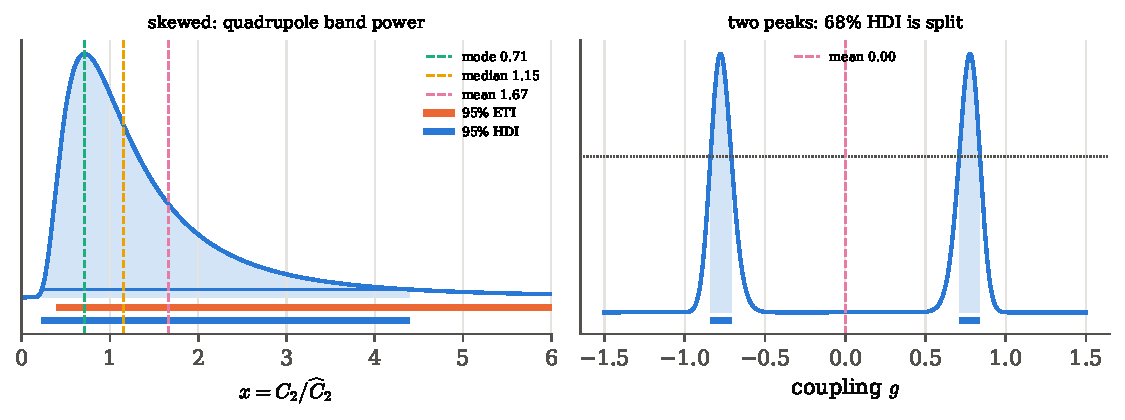
\includegraphics[width=\linewidth]{figures/ch05/summaries.pdf}
\caption{Summaries of two posteriors. Left: the skewed posterior of the quadrupole
power relative to its estimate, with its mode, median and mean (vertical dashed lines),
the 95\% equal-tailed interval (upper bar, orange) and the 95\% HDI (lower bar, blue,
shaded, with its water level). Right: the two-peaked coupling posterior. Its 68\% HDI is
two intervals, and its mean falls in the gap between the peaks.}
\label{5b:fig:summaries}
\end{figure}

\subsection{What a credible interval says, and what a confidence interval says}

A 95\% credible interval makes a direct statement about the parameter: given these data
and this prior, the probability that $\theta$ lies in the interval is 0.95. A 95\%
confidence interval (\cref{ch:03,ch:04}) makes a statement about a procedure: if the
experiment were repeated many times, intervals built this way would cover the fixed true
value in 95\% of the repetitions \srcref{Lambert}{\S7.7}. The two are different
statements and need not agree. Often, though, the numbers are the same. For a
Gaussian likelihood and a flat or broad prior the posterior is $\Normal(\bar\theta,\tau^2)$ with
$\bar\theta\approx\hat\theta$ and $\tau\approx\mathrm{se}$, where $\hat\theta$ is the
maximum-likelihood estimate and $\mathrm{se}$ its standard error. So the 95\% credible
interval $\bar\theta\pm1.96\tau$ is approximately the frequentist $\hat\theta\pm1.96\,
\mathrm{se}$ \mainref{p.~179}. For large samples this agreement is general
(\cref{5b:sec:laplace}). For small samples, skewed posteriors, parameters near a
physical boundary, or informative priors, they can differ substantially, and in high
dimensions a 95\% credible region need not cover the truth 95\% of the time
\mainref{p.~189}.

\begin{pitfall}[Credible is not confidence]
``The parameter lies in $[a,b]$ with 95\% probability'' is a correct reading of a
credible interval and an incorrect reading of a confidence interval. Conversely,
``this interval covers the truth in 95\% of repeated experiments'' is guaranteed for a
confidence interval and not, in general, for a credible interval. When a result is
quoted, say which kind it is, and for a credible interval say which prior was used and
whether it is an HDI or an equal-tailed interval.
\end{pitfall}
\section{The Gaussian approximation: a peak and its curvature}
\label{5b:sec:laplace}

Most posteriors in a mature experiment look like a single smooth bump. Then two numbers
describe the whole curve well: where the bump is and how wide it is. The result is
quoted as ``$\theta=\theta_0\pm\sigma$''. Where do these two numbers come from, in one
parameter and in many? And when does this description mislead?

\subsection{One parameter}

We work with the logarithm of the posterior, $L(\theta)=\ln p(\theta\given\data)$, for
two reasons. It turns products of likelihoods into sums. And near a peak it varies much
more gently than the posterior itself, so a short Taylor series describes it well
\srcref{Sivia}{(2.10)}. Let $\theta_0$ be the peak, so $L'(\theta_0)=0$ and
$L''(\theta_0)<0$, and Taylor-expand about it:
\begin{align}
  L(\theta)
  &\eqby{1}L(\theta_0)+L'(\theta_0)(\theta-\theta_0)
     +\tfrac12L''(\theta_0)(\theta-\theta_0)^2+\dots
   \nonumber\\
  &\eqby{2}L(\theta_0)-\frac{(\theta-\theta_0)^2}{2\sigma^2}+\dots,
   \qquad \sigma\equiv\bigl(-L''(\theta_0)\bigr)^{-1/2}.
  \label{5b:eq:laplace}
\end{align}
\begin{explain}
  \item Taylor's theorem to second order about $\theta_0$.
  \item The linear term vanishes at a maximum, and $L''(\theta_0)$ is negative, so we
        may write it as $-1/\sigma^2$.
\end{explain}
Exponentiate and drop the higher terms. The exponential of $-(\theta-\theta_0)^2/
2\sigma^2$ is a Gaussian, so $p(\theta\given\data)\approx\Normal(\theta_0,\sigma^2)$
\srcref{Sivia}{(2.13)--(2.15)}. This is the \newterm{Gaussian} or \newterm{Laplace
approximation}. In words: the error bar is one over the square root of the curvature of
the log-posterior at its peak. A sharply curved peak means a small error bar. Within the approximation, $\theta_0\pm\sigma$ holds 68\% of
the probability and $\theta_0\pm2\sigma$ holds 95\%.

\paragraph{Example: Gaussian readings.}
For $N$ readings of equal error $\sigma_x$ and a flat prior, $L=\text{const}-\sum_k(x_k-
\mu)^2/2\sigma_x^2$. Then $L'=\sum_k(x_k-\mu)/\sigma_x^2=0$ gives $\mu_0=\bar x$, and
$L''=-N/\sigma_x^2$ gives $\sigma=\sigma_x/\sqrt N$ \srcref{Sivia}{(2.28)--(2.29)}. Here
the expansion is exact, because $L$ is a quadratic and all higher derivatives vanish.

\paragraph{Example: the coin.}
With a flat prior and $R$ heads in $N$ tosses, $L=\text{const}+R\ln\theta+(N-R)\ln(1-
\theta)$ \srcref{Sivia}{(2.17)}. Then
\begin{align*}
  L'(\theta)&\eqby{1}\frac R\theta-\frac{N-R}{1-\theta}=0
  \;\Rightarrow\;\theta_0=\frac RN,\\
  L''(\theta_0)&\eqby{2}-\frac{R}{\theta_0^2}-\frac{N-R}{(1-\theta_0)^2}
  \eqby{3}-\frac{N}{\theta_0}-\frac{N}{1-\theta_0}
  \eqby{4}-\frac{N}{\theta_0(1-\theta_0)} ,
\end{align*}
\begin{explain}
  \item Differentiate the logs, and solve $R(1-\theta_0)=(N-R)\theta_0$.
  \item Differentiate once more.
  \item Substitute $R=N\theta_0$ and $N-R=N(1-\theta_0)$.
  \item Common denominator: $\frac{1}{\theta_0}+\frac{1}{1-\theta_0}=\frac{1}{\theta_0(1-\theta_0)}$.
\end{explain}
so $\sigma=\sqrt{\theta_0(1-\theta_0)/N}$ \srcref{Sivia}{(2.19)--(2.20)}, the familiar
binomial error. The width shrinks like $1/\sqrt N$. At fixed $N$ it is largest for
$\theta_0=\frac12$, so it is easier to show that a coin is strongly biased than to show
that it is fair.

How good is the approximation? It depends on the data. For 9 heads in 32 tosses it
gives $\theta=\FiveBLapHa\pm\FiveBLapSa$. The exact posterior is a Beta density
(\cref{5b:sec:conjugate}) with mean $\FiveBLapMeanA$ and standard deviation
$\FiveBLapSdA$, so the two agree well (\cref{5b:fig:laplace-coin}, left). For 1 head in
10 the approximation gives $\FiveBLapHb\pm\FiveBLapSb$. It puts $\FiveBLapNegB$ of its
probability at $\theta<0$, which is impossible. The exact posterior is squeezed against
the boundary $\theta=0$ and skewed, with mean $\FiveBLapMeanB$. So near a physical
boundary, and with few data, an error bar is the wrong summary: quote an interval from
the posterior itself (\cref{5b:sec:summaries}).

\begin{figure}[htbp]
\centering
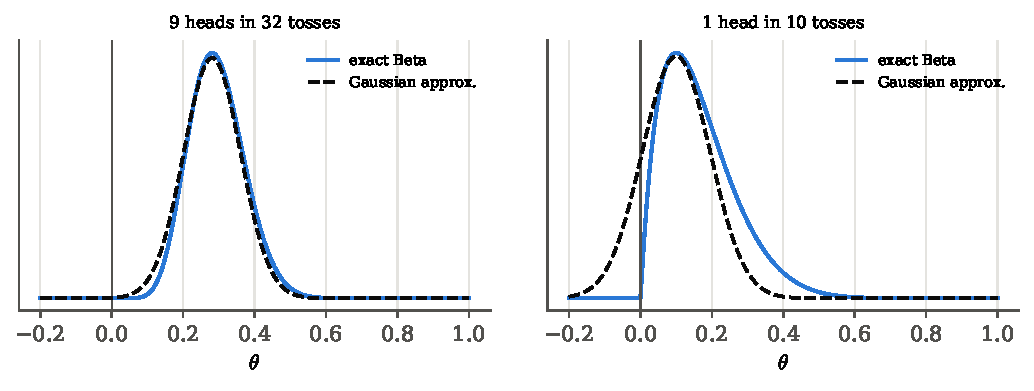
\includegraphics[width=0.92\linewidth]{figures/ch05/laplace_coin.pdf}
\caption{The Gaussian approximation (dashed) against the exact posterior (solid) for a
coin with a flat prior. Left: 9 heads in 32 tosses, where the two nearly agree. Right:
1 head in 10 tosses, where the exact posterior is pressed against the boundary
$\theta=0$ and the Gaussian spills probability into the impossible region to its left.}
\label{5b:fig:laplace-coin}
\end{figure}

\subsection{Several parameters: the Hessian and its inverse}

With parameters $\params=(\theta_1,\dots,\theta_M)$ the same expansion about the peak
$\params_0$ reads \srcref{Sivia}{(3.30)--(3.31)}
\begin{equation}
  L(\params)\approx L(\params_0)+\tfrac12(\params-\params_0)\T\mathbf H\,(\params-\params_0),
  \qquad H_{ij}=\left.\frac{\partial^2L}{\partial\theta_i\,\partial\theta_j}\right|_{\params_0},
  \label{5b:eq:hessian}
\end{equation}
where the linear term has again vanished because $\params_0$ is the peak. The matrix
$\mathbf H$ of second derivatives is the \newterm{Hessian}. Exponentiating, the
posterior is approximately a multivariate Gaussian with covariance matrix
$\Cmat=-\mathbf H^{-1}$ \srcref{Sivia}{(3.32)}, just as $\sigma^2=-1/L''$ in one
dimension. Its contours are ellipses (ellipsoids in more dimensions). Their axes point
along the eigenvectors of $\mathbf H$, and their lengths are proportional to
$|h_i|^{-1/2}$, where $h_i$ are the eigenvalues of $\mathbf H$ \srcref{Sivia}{Fig.~3.6}.
The peak really is a maximum only if all eigenvalues are negative.

\paragraph{Example: two parameters, done by hand.}
Write the second derivatives at the peak as $A=\partial_X^2L$, $B=\partial_Y^2L$,
$C=\partial_X\partial_YL$ \srcref{Sivia}{(3.19)}. A maximum needs $A<0$, $B<0$ and
$AB>C^2$. The inverse of a $2\times2$ matrix is
$\bigl(\begin{smallmatrix}A&C\\C&B\end{smallmatrix}\bigr)^{-1}
=\frac{1}{AB-C^2}\bigl(\begin{smallmatrix}B&-C\\-C&A\end{smallmatrix}\bigr)$, so
\begin{align}
  \Cmat=-\mathbf H^{-1}
  &\eqby{1}\frac{1}{C^2-AB}\begin{pmatrix}B&-C\\-C&A\end{pmatrix},
  \qquad
  \sigma_X^2\eqby{2}\frac{B}{C^2-AB},\quad
  \sigma_Y^2=\frac{A}{C^2-AB},\quad
  \sigma_{XY}\eqby{3}\frac{C}{AB-C^2}.
  \label{5b:eq:cov2}
\end{align}
\begin{explain}
  \item The $2\times2$ inverse, with the overall minus sign absorbed into the
        denominator.
  \item The diagonal entries are the variances. Both $B$ and $C^2-AB$ are negative,
        so $\sigma_X^2>0$ \srcref{Sivia}{(3.21)--(3.22)}.
  \item The off-diagonal entry is the covariance \srcref{Sivia}{(3.27)}.
\end{explain}
The correlation coefficient is $\rho=\sigma_{XY}/(\sigma_X\sigma_Y)=C/\sqrt{AB}$.

There are two different error bars for $X$, and they answer different questions. The
\newterm{marginal} error $\sigma_X$ of \eqref{5b:eq:cov2} answers: how far can $X$ move
if $Y$ may be anything the data permit (\cref{5b:sec:marginal})? The
\newterm{conditional} error answers: how far can $X$ move if $Y$ is held fixed at its
best value? With $Y$ fixed, only the curvature in $X$ matters, so
$\sigma_{X|Y}=(-A)^{-1/2}$. How much smaller is the second? Their ratio is
\begin{align*}
  \frac{\sigma_X^2}{\sigma_{X|Y}^2}
  \eqby{1}\frac{B}{C^2-AB}\,(-A)
  \eqby{2}\frac{AB}{AB-C^2}
  \eqby{3}\frac{1}{1-\rho^2}\;\ge1 .
\end{align*}
\begin{explain}
  \item Divide \eqref{5b:eq:cov2} by $1/(-A)$.
  \item Multiply numerator and denominator by $-1$.
  \item Divide numerator and denominator by $AB$ and use $\rho^2=C^2/(AB)$.
\end{explain}
So holding a correlated parameter fixed always makes the error bar look smaller, by a
factor $\sqrt{1-\rho^2}$. With $\rho=0.95$ the conditional error is a third of the honest
one \srcref{Sivia}{Fig.~3.8}. \Cref{5b:fig:ellipse} shows the geometry. The conditional
error is the width of a horizontal slice through the centre of the ellipse. The marginal
error is the width of the ellipse's shadow on the $X$ axis.

\begin{figure}[htbp]
\centering
\begin{tikzpicture}[x=1cm,y=1cm]
  \draw[faint,->] (-3.3,0) -- (3.4,0) node[right,black,lbl] {$X$};
  \draw[faint,->] (0,-2.3) -- (0,2.4) node[above,black,lbl] {$Y$};
  \draw[form,rotate=35] (0,0) ellipse (2.6 and 0.55);
  \draw[fibre,line width=2pt] (-0.918,0) -- (0.918,0);
  \draw[bdryred,dashed] (-2.153,-2.0) -- (-2.153,1.6);
  \draw[bdryred,dashed] (2.153,-1.6) -- (2.153,2.0);
  \draw[bdryred,very thick] (-2.153,-1.9) -- (2.153,-1.9);
  \node[lbl,bdryred,anchor=north] at (0,-1.95) {marginal: shadow on the $X$ axis};
  \node[lbl,fibreorange,align=center,anchor=north] at (1.35,-0.75) {conditional slice\\at $Y=Y_0$};
  \draw[fibreorange,thin] (1.0,-0.72) -- (0.55,-0.03);
\end{tikzpicture}
\caption{Conditional against marginal error for two correlated parameters. The ellipse
is a contour of the Gaussian posterior. Holding $Y$ at its best value and asking how
far $X$ may move gives the short orange slice, of half-width $(-A)^{-1/2}$. Letting $Y$
take any value gives the full shadow of the ellipse on the $X$ axis, between the red
dashed tangents, of half-width proportional to $\sqrt{B/(C^2-AB)}$.}
\label{5b:fig:ellipse}
\end{figure}

\begin{keyidea}[error bars from the curvature]
Near its peak, the log-posterior is a quadratic form with Hessian $\mathbf H$. The
posterior is then approximately Gaussian with covariance $\Cmat=-\mathbf H^{-1}$. The
honest (marginal) error bar on $\theta_i$ is $\sqrt{\Cmat_{ii}}=\sqrt{[(-\mathbf H)^{-1}]_{ii}}$,
the square root of a diagonal element of the \emph{inverse}. The inverse of a diagonal
element, $1/\sqrt{-H_{ii}}$, is the conditional error with all other parameters frozen,
and is always smaller or equal.
\end{keyidea}

\paragraph{The link to the Fisher matrix.}
The Laplace approximation and the Fisher forecast of \cref{ch:10} are the same object,
seen after and before the data are taken. Here is why. With a flat prior, $-\mathbf H$
is the curvature of the log-likelihood at its maximum, called the \emph{observed
information}. Average it over all the data sets the model could have produced, and we
get the \newterm{Fisher matrix} $\Fish$, with $F_{ij}=-\E[\partial_i\partial_j\ln
\Like]$. So $\Fish^{-1}$ is the expected posterior covariance. Then
$\sqrt{(\Fish^{-1})_{ii}}$ is the expected marginal error, and $1/\sqrt{F_{ii}}$ the
expected conditional one \srcref{Padilla}{\S3.8}.

For a Gaussian likelihood with a model linear in the parameters, $L$ is exactly
quadratic. The Hessian then does not depend on the parameters, and the approximation is
exact \srcref{Sivia}{\S3.4, (3.52)}. For nonlinear models the peak itself is usually
found step by step, by Newton--Raphson steps $\params_{k+1}=\params_k-\mathbf H^{-1}
\nabla L$ \srcref{Sivia}{(3.55)}, as in \cref{ch:03}.

\paragraph{Example: contours for two parameters.}
Which contour of a two-parameter posterior holds 68\% of the probability? Measure the
distance from the peak by $Q=(\params-\params_0)\T\Cmat^{-1}(\params-\params_0)$. Within
the Gaussian approximation, $Q=2[L(\params_0)-L(\params)]$, the ``$\Delta\chi^2$'' from
the peak. The contours are the curves $Q=k$, so we need the distribution of $Q$. Change
variables to $\bm u=\Cmat^{-1/2}(\params-\params_0)$. This turns the Gaussian into $M$
independent standard normals, so $Q=\sum_iu_i^2$ has a $\chi^2$ distribution with $M$
degrees of freedom (\cref{ch:02}). For $M=2$ that distribution is an exponential,
$p(Q)=\frac12e^{-Q/2}$, so
\begin{align*}
  \Prob(Q\le k)\eqby{1}\int_0^k\tfrac12e^{-Q/2}\dd Q\eqby{2}1-e^{-k/2}
  \\
  \Rightarrow\quad
  k_{68.3\%}=-2\ln(1-0.683)=2.30,\qquad k_{95.4\%}=6.17 .
\end{align*}
\begin{explain}
  \item The $\chi^2_2$ density is $\frac12e^{-Q/2}$.
  \item Elementary integral, then solve for $k$.
\end{explain}
These are the contour levels ``$\Delta\chi^2=2.30$ and $6.17$'' used in every
two-parameter plot in cosmology \srcref{Padilla}{Table~III}. In one dimension the same
argument gives $\Delta\chi^2=1$ and $4$ for $\pm1\sigma$ and $\pm2\sigma$: a one-parameter
interval and a two-parameter contour at the same confidence need different thresholds.

\subsection{When the approximation fails, and when it comes back: the lighthouse}

A lighthouse stands at unknown position $\alpha$ along a straight coast, a known
distance $\beta$ out to sea \srcref{Sivia}{\S2.4}. It emits short flashes in random
directions, uniformly in the azimuth $\vartheta\in(-\pi/2,\pi/2)$. Detectors along the
shore record \emph{where} each flash arrives, $x=\alpha+\beta\tan\vartheta$, but not its
direction (\cref{5b:fig:lighthouse-geom}). Where is the lighthouse?

\begin{figure}[htbp]
\centering
\begin{tikzpicture}[x=1cm,y=1cm]
  \fill[formblue!8] (-3.5,0) rectangle (4.5,2.4);
  \draw[thick] (-3.5,0) -- (4.5,0) node[right,lbl] {shore, $x$};
  \node[lbl,anchor=south west] at (-3.4,2.0) {sea};
  \fill (0,2) circle (2.2pt);
  \node[lbl,anchor=south east] at (-0.1,2.05) {lighthouse};
  \draw[faint,dashed] (0,2) -- (0,0);
  \node[lbl,anchor=east] at (-0.05,1.0) {$\beta$};
  \draw[->,thick,fibreorange] (0,2) -- (2.4,0);
  \draw[faint] (0,1.4) arc (-90:-50.2:0.6);
  \node[lbl,anchor=north west] at (0.25,1.35) {$\vartheta$};
  \fill (0,0) circle (1.5pt);
  \node[lbl,anchor=north] at (0,-0.08) {$\alpha$};
  \fill[fibreorange] (2.4,0) circle (1.5pt);
  \node[lbl,anchor=north] at (2.4,-0.08) {$x_k$};
\end{tikzpicture}
\caption{The lighthouse problem. A flash leaves at azimuth $\vartheta$, uniformly
distributed, and reaches the shore at $x_k=\alpha+\beta\tan\vartheta$. Only the arrival
point is recorded.}
\label{5b:fig:lighthouse-geom}
\end{figure}

The likelihood of one arrival point follows from the change of variables for densities
(\cref{ch:01}):
\begin{align*}
  p(x\given\alpha,\beta)
  \eqby{1}p(\vartheta)\left|\frac{\dd\vartheta}{\dd x}\right|
  \eqby{2}\frac1\pi\cdot\frac{1}{\beta\,(1+\tan^2\vartheta)}
  \eqby{3}\frac{\beta}{\pi\,[\beta^2+(x-\alpha)^2]} .
\end{align*}
\begin{explain}
  \item The probability in a small range $\dd\vartheta$ equals that in the matching
        $\dd x$.
  \item $p(\vartheta)=1/\pi$ on $(-\pi/2,\pi/2)$, and $\dd x/\dd\vartheta=\beta/\cos^2
        \vartheta=\beta(1+\tan^2\vartheta)$.
  \item $\tan\vartheta=(x-\alpha)/\beta$.
\end{explain}
This is a Cauchy (Lorentzian) density \srcref{Sivia}{(2.34)}, with a peak at $\alpha$ and
tails so heavy that its variance is infinite (\cref{ch:02}). Take a flat prior on
$\alpha$ and independent flashes at $x_1,\dots,x_N$. The log-posterior is
$L(\alpha)=\text{const}-\sum_k\ln[\beta^2+(x_k-\alpha)^2]$ \srcref{Sivia}{(2.38)}. The
condition $L'=0$ for its peak cannot be solved in closed form, but on a grid the whole
posterior is easy to compute.

\Cref{5b:fig:lighthouse} shows the posterior as flashes accumulate, for a lighthouse at
$\alpha=1$\,km with $\beta=1$\,km. After one or two flashes the posterior is broad with
heavy tails. When two flashes land far apart, the posterior has two humps, one near
each. In this run, by eight flashes it is a single bump. After 64 its standard deviation, $\FiveBLhSdSix$, agrees
with the Laplace width $\FiveBLhLapSix$ from the curvature at the peak. After 512 flashes the posterior is
$\alpha=\FiveBLhModeFive\pm\FiveBLhSdFive$\,km, and the width matches the large-$N$
prediction $\beta\sqrt{2/N}=\FiveBLhSqrtTwoN$\,km that follows from the Fisher
information of a Cauchy density.

The sample mean of the arrival points would be the answer for Gaussian data. Here it
does not converge at all: after 64 flashes it is $\FiveBLhXbarSix$, and on average it
is no closer to the truth than a single flash. Why? For Cauchy data the average of $N$ points has the same Cauchy
distribution as a single point, because the central limit theorem needs a finite
variance (\cref{ch:02}). One wild flash, sent almost parallel to the shore, can drag the
mean anywhere. The posterior never uses the mean. It weighs every flash through the
likelihood. A wild flash far from $\alpha$ has a likelihood that is nearly flat in
$\alpha$, so it barely moves the posterior \srcref{Sivia}{p.~36}.

\begin{figure}[htbp]
\centering
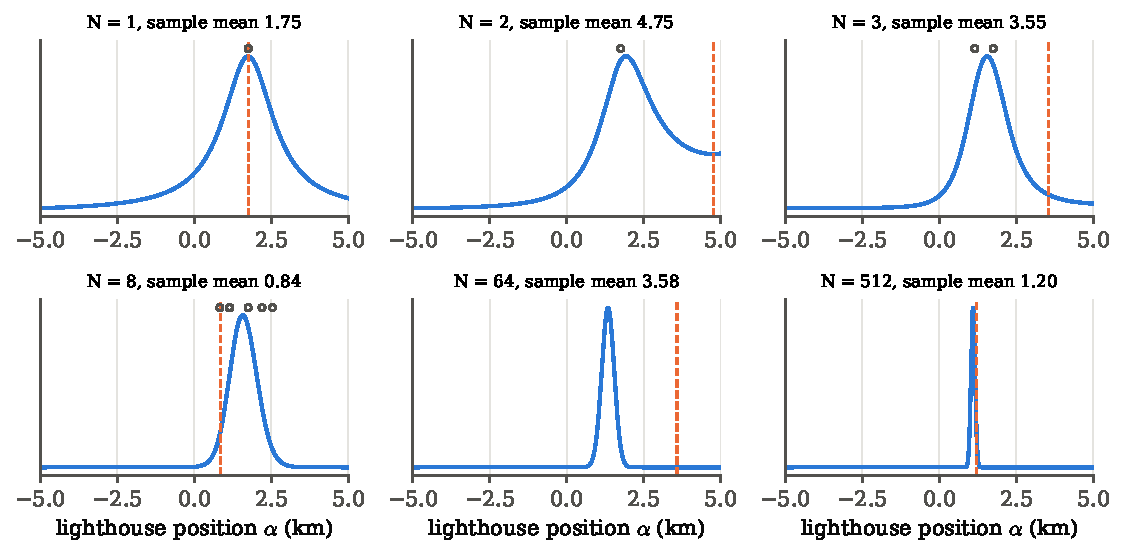
\includegraphics[width=\linewidth]{figures/ch05/lighthouse.pdf}
\caption{The posterior for the lighthouse position as flashes accumulate ($N$ in each
title). Circles at the top of the first four panels mark where the flashes landed, and
the dashed vertical line is the sample mean of the arrival points. The posterior starts
broad and sometimes two-peaked, becomes a narrow Gaussian-like peak near the true
$\alpha=1$\,km, while the sample mean keeps jumping around.}
\label{5b:fig:lighthouse}
\end{figure}

The lighthouse shows both sides of the Gaussian approximation. With few data the
posterior can be lopsided or have several peaks, and no ``$\theta_0\pm\sigma$''
describes it. With many data from a well-behaved likelihood the posterior becomes a
Gaussian of width $1/\sqrt{N\,I}$, where $I$ is the Fisher information of one datum,
whatever the shape of the single-datum likelihood. That second half is
a theorem, the Bernstein--von Mises theorem of \cref{5b:sec:bvm}.
\section{Nuisance parameters: integrating out what we do not care about}
\label{5b:sec:marginal}

A spectrum shows a peak sitting on a smooth background: a Bragg peak on diffuse
scattering, an emission line on a quasar's continuum, a resonance on the falling
background of a collider mass spectrum. We want the amplitude $A$ of the peak. The
background level $B$ is of no interest in itself, but it cannot be ignored, because the
counts we measure are the sum of both, and a higher background leaves room for a
smaller peak \srcref{Sivia}{\S3.1}. Such a parameter, needed by the model and irrelevant
to the question, is a \newterm{nuisance parameter}. How do we get a posterior for $A$
alone that honestly includes our ignorance of $B$?

\subsection{Marginalising: the sum rule applied to parameters}

Bayes' theorem gives the joint posterior $p(A,B\given\data)$, a density over pairs of
values. Our question is about $A$ alone: what is the probability that $A$ lies in some
small range, whatever $B$ is? That can happen in many ways, one for each value of $B$,
and the sum rule says to add up their probabilities. This is marginalisation
(\cref{ch:01}). A marginal distribution isolates the probability of a single variable,
here $A$, by averaging out the ``nuisance'' variables, here $B$, from the joint
distribution:
\begin{equation}
  p(A\given\data)=\int p(A,B\given\data)\,\dd B
  \label{5b:eq:marg}
\end{equation}
\srcref{Sivia}{(3.9)}, \mainref{p.~183, (11.9)}, \srcref{Padilla}{(38)}. In the tree
picture it is the sum over all branches of $B$ that lead to the same $A$. With more
nuisance parameters the integral runs over all of them. This is why the standard output
of a cosmological analysis is a set of marginal posteriors, of one or two parameters
out of dozens \srcref{HobsonBMC}{(2.6)}.

\begin{workdef}[marginal posterior]
For parameters of interest $\params$ and nuisance parameters $\bm\nu$, the
\newterm{marginal posterior} is $p(\params\given\data)=\int p(\params,\bm\nu\given\data)\,
\dd\bm\nu$ \unpack{the joint posterior summed over every value of the nuisance
parameters, each weighted by how credible it is}. \emph{Operationally:} on a grid, sum
the joint posterior along the nuisance axes. From samples of the joint posterior,
simply ignore the nuisance coordinates (\cref{5b:sec:sampling}).
\end{workdef}

How does not knowing $B$ change what we learn about $A$? To see it, split the integrand
with the product rule, $p(A,B\given\data)=p(A\given B,\data)\,p(B\given\data)$:
\begin{equation}
  p(A\given\data)=\int p(A\given B,\data)\;p(B\given\data)\,\dd B .
  \label{5b:eq:marg-mix}
\end{equation}
The marginal is an average of the conditional posteriors $p(A\given B,\data)$, one for
each assumed background, weighted by how credible that background is. Now suppose an
independent calibration fixed the background exactly at $b$. Then $p(B\given\data)=
\delta(B-b)$ and
\begin{align*}
  p(A\given\data)
  \eqby{1}\int p(A\given B,\data)\,\delta(B-b)\,\dd B
  \eqby{2}p(A\given b,\data),
\end{align*}
\begin{explain}
  \item The calibration puts all the probability for $B$ at $b$.
  \item The delta function picks out the integrand at $B=b$.
\end{explain}
So the conditional posterior is the special case in which the nuisance parameter is
known perfectly \srcref{Sivia}{p.~44}. An analysis that ``fixes'' a parameter at a
fiducial value is doing exactly this, without saying so: it gives that parameter a
delta-function prior \srcref{HobsonBMC}{p.~42}. Any spread in $p(B\given\data)$ mixes
conditionals centred at different places, so the marginal is broader.

\paragraph{Example: a peak on a background.}
Following Sivia, the expected count in channel $k$ is $D_k=n_0[A\,e^{-x_k^2/2w^2}+B]$,
a Gaussian peak of known width and position on a flat background, and the observed count
$N_k$ is Poisson with mean $D_k$ \srcref{Sivia}{(3.1)--(3.4)}. With independent channels
and a flat prior on $A,B\ge0$,
\begin{equation*}
  \ln p(A,B\given\{N_k\})=\text{const}+\sum_k\bigl[N_k\ln D_k-D_k\bigr]
\end{equation*}
\srcref{Sivia}{(3.8)}, the log of a product of Poisson probabilities with the factorials
dropped. Here $n_0$ sets the overall count level, $x_k$ is the position of channel $k$
measured from the peak, and $w$ is the peak width.

How much does not knowing $B$ cost? It depends on whether the data can tell the peak
from the background. \Cref{5b:fig:signal-bkg} shows two simulated set-ups, both with
$A=1$, $B=2$.
\begin{itemize}[itemsep=1pt,leftmargin=1.2em]
  \item \emph{Wide set-up} (top row): 15 channels spread well beyond the peak. The
        outer channels measure the background alone, so $A$ and $B$ are only moderately
        correlated, $\rho=\FiveBMaRhoWide$. The marginal error on $A$ is
        $\FiveBMaSigWide$, against $\FiveBMaSigCondWide$ if $B$ were known to be 2.
  \item \emph{Narrow set-up} (bottom row): 7 channels over a narrow range around the
        peak. No channel sees the background alone, so a little more background and a
        little less peak fit almost equally well. The correlation is
        $\rho=\FiveBMaRhoNarrow$, and the marginal error on $A$ grows to
        $\FiveBMaSigNarrow$, almost three times the conditional error
        $\FiveBMaSigCondNarrow$.
\end{itemize}
Both ratios agree with the factor $1/\sqrt{1-\rho^2}$ of \cref{5b:sec:laplace}. So when
the data cannot separate signal from background, a calibration of the background is
worth a lot. When they can, it adds little \srcref{Sivia}{p.~42}.

\begin{figure}[htbp]
\centering
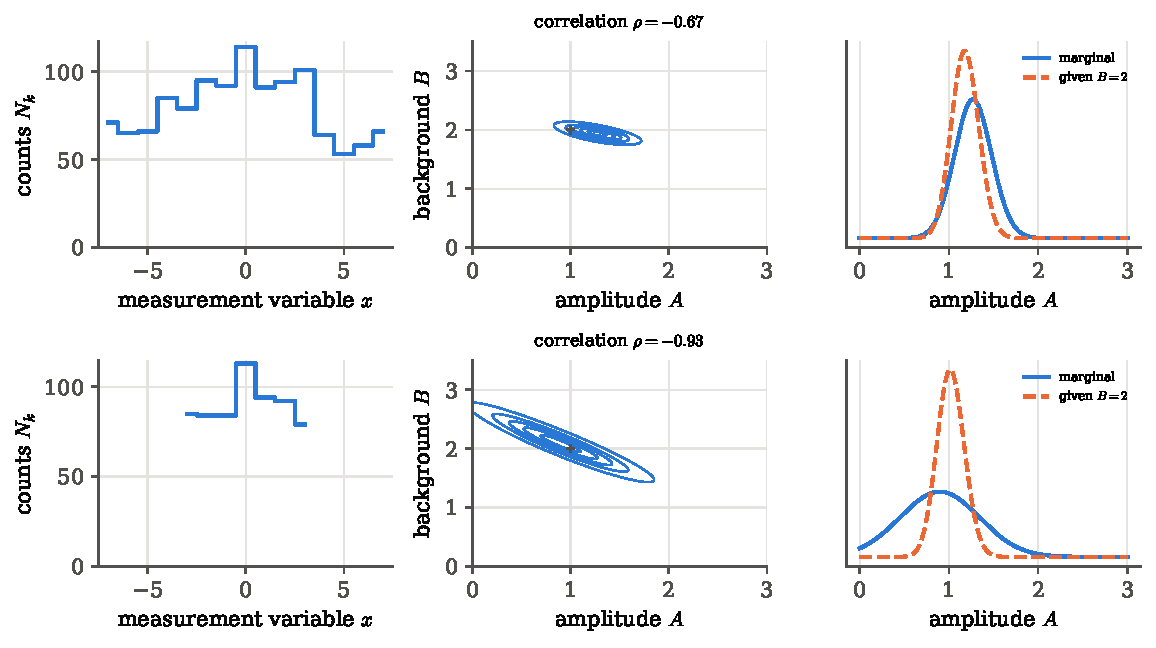
\includegraphics[width=\linewidth]{figures/ch05/marg_signal_bkg.pdf}
\caption{A peak of amplitude $A$ on a flat background $B$, from Poisson counts. Top:
15 channels spanning the peak and the background around it. Bottom: 7 channels
concentrated on the peak. Left: the simulated counts. Middle: contours of the joint
posterior at 10, 30, 50, 70 and 90\% of its maximum, with the true values marked by a
cross. Right: the marginal posterior of $A$ (solid) and the conditional posterior with
$B$ fixed at its true value (dashed). The narrow set-up correlates $A$ and $B$ strongly,
and marginalising over $B$ then widens the posterior of $A$ a lot.}
\label{5b:fig:signal-bkg}
\end{figure}

\paragraph{Example: an unknown noise level.}
Readings $x_k$ are Gaussian with mean $\mu$ and an error $\sigma$ that nobody told us.
Then $\sigma$ is a nuisance parameter, and \cref{ch:03} showed that integrating it out
with the prior $p(\sigma)\propto1/\sigma$ gives $p(\mu\given\data)\propto
\bigl[\sum_k(x_k-\mu)^2\bigr]^{-N/2}$ \srcref{Sivia}{(3.38)}, \srcref{HobsonBMC}{(2.26)}.
Its shape in $\mu$ follows from splitting the sum about the sample mean $\bar x$:
\begin{align*}
  \sum_k(x_k-\mu)^2
  &\eqby{1}\sum_k\bigl[(x_k-\bar x)+(\bar x-\mu)\bigr]^2\\
  &\eqby{2}\sum_k(x_k-\bar x)^2+2(\bar x-\mu)\sum_k(x_k-\bar x)+N(\bar x-\mu)^2
  \eqby{3}V+N(\bar x-\mu)^2,
\end{align*}
\begin{explain}
  \item Add and subtract $\bar x$ inside each square.
  \item Expand the square. The middle factor $(\bar x-\mu)$ does not depend on $k$.
  \item $\sum_k(x_k-\bar x)=0$ by the definition of $\bar x$, and $V\equiv\sum_k(x_k-\bar x)^2$.
\end{explain}
So $p(\mu\given\data)\propto[N(\bar x-\mu)^2+V]^{-N/2}$, a Student-$t$ curve centred on
$\bar x$ \srcref{Sivia}{(3.41)--(3.44)}. For large $N$ it approaches a Gaussian of width
$\sqrt{V/N^2}$, the familiar $s/\sqrt N$ with $s^2=V/N$. For small $N$ its tails are
much heavier than a Gaussian's. Not knowing the size of the noise costs precision, and
marginalisation builds that cost in automatically. (Sivia's flat prior on $\sigma$ gives the exponent
$-(N-1)/2$ instead, a slightly wider curve. The choice matters only for very few data.)

\subsection{Marginalising against profiling}

The frequentist way to remove a nuisance parameter is to \emph{maximise} over it: the
profile likelihood $\Like_p(A)=\max_B\Like(A,B)$ (\cref{ch:03}). Do integration and
maximisation agree?

For a Gaussian posterior they do. Write the log-posterior about its peak as
$L=\frac12(ax^2+2cxy+by^2)$ in the deviations $x=A-A_0$, $y=B-B_0$, with $a,b<0$ and
$ab>c^2$. Maximising over $y$ at fixed $x$ gives $by+cx=0$, so $y^\ast=-cx/b$, and
\begin{align*}
  L(x,y^\ast)
  \eqby{1}\tfrac12\Bigl(ax^2-\frac{2c^2x^2}{b}+\frac{c^2x^2}{b}\Bigr)
  \eqby{2}\tfrac12\,\frac{ab-c^2}{b}\,x^2 ,
  \qquad
  \int e^{L}\,\dd y
  \eqby{3}e^{\frac12\frac{ab-c^2}{b}x^2}\sqrt{\frac{2\pi}{-b}} .
\end{align*}
\begin{explain}
  \item Substitute $y^\ast=-cx/b$.
  \item Collect the terms over the common denominator $b$.
  \item Complete the square in $y$, $by^2+2cxy=b(y+cx/b)^2-c^2x^2/b$, and do the
        Gaussian integral over $y$. Its value $\sqrt{2\pi/(-b)}$ does not depend on $x$.
\end{explain}
Profile and marginal have the same $x$-dependence, so after normalisation they are the
same curve, with variance $b/(c^2-ab)$ as in \eqref{5b:eq:cov2}. The equality rests on
step (3): the width of the posterior in the nuisance direction, $(-b)^{-1/2}$, is the
same for every $x$.

When that width changes with the parameter of interest, the two disagree. To see by how
much, call the parameter of interest $\theta$ and the nuisance parameter $\nu$. At each
fixed $\theta$, expand $L$ about the best nuisance value $\hat\nu(\theta)$ and integrate
the Gaussian in $\nu$, exactly as in step (3). This gives
\begin{equation}
  p(\theta\given\data)=\int e^{L(\theta,\nu)}\,\dd\nu
  \;\approx\;\underbrace{e^{L(\theta,\hat\nu(\theta))}}_{\text{profile}}\;
  \underbrace{\sqrt{2\pi}\,\sigma_\nu(\theta)}_{\text{volume}},
  \qquad \sigma_\nu(\theta)=\bigl(-\partial_\nu^2L\bigr)^{-1/2}\big|_{\hat\nu(\theta)} .
  \label{5b:eq:volume}
\end{equation}
The first factor is the profile, the best fit at this $\theta$. The second measures how
many values of $\nu$ fit almost as well. So the marginal rewards values of $\theta$ for
which many values of the nuisance parameter fit the data, a large ``volume'' of good
fits. The profile only asks how good the best fit is.

\paragraph{Example: a weak bump of unknown position.}
Readings $y_i$ at 60 positions $x_i\in[0,10]$ follow $y_i=A\,e^{-(x_i-\mu)^2/2w^2}+
\epsilon_i$ with unit Gaussian noise and known narrow width $w=0.4$. A bump of true
amplitude $A=\FiveBVolAtrue$ sits at $\mu=5$, and we take flat priors on $A\in[0,4]$ and
on the position $\mu\in[0,10]$ (\cref{5b:fig:volume}). Here the amplitude $A$ is the
parameter of interest and the position $\mu$ the nuisance parameter.

How wide is the range of good positions? It depends on $A$. When $A$ is large, only
positions near the true bump fit, so the posterior in $\mu$ is narrow. When $A$ is near
zero, every position fits equally well, because a bump of zero height is invisible
wherever it is. Then the whole prior range of $\mu$ contributes. That large volume pulls
the marginal posterior of $A$ towards zero. For the data of \cref{5b:fig:volume} its
mode is at $A=\FiveBVolMargMode$, and it puts probability $\FiveBVolPsmallMarg$ on
$A<0.5$. The profile ignores volume. It peaks at $A=\FiveBVolProfMode$ and gives
$\FiveBVolPsmallProf$ to $A<0.5$. One data set could be a fluke, so we repeat the
analysis on $\FiveBVolLoopR$ fresh data sets with the same true bump. On average the
marginal gives $A<0.5$ a probability of $\FiveBVolLoopPsmallMarg$ and the profile
$\FiveBVolLoopPsmallProf$ (each to within about $\FiveBVolLoopErr$), and the marginal
peaks at $A=0$ in $\FiveBVolLoopModeZero$ of them.

Neither is wrong; they answer different questions. The profile says ``the best bump
anywhere has amplitude about $\FiveBVolProfMode$''. The marginal says ``averaged over
where a bump could be, small amplitudes are more credible than the best fit alone
suggests''.
This is the Bayesian face of the look-elsewhere effect (\cref{ch:04}). It is also a
first view of how the evidence penalises a model for its prior volume, the Occam factor
of model comparison.

\begin{figure}[htbp]
\centering
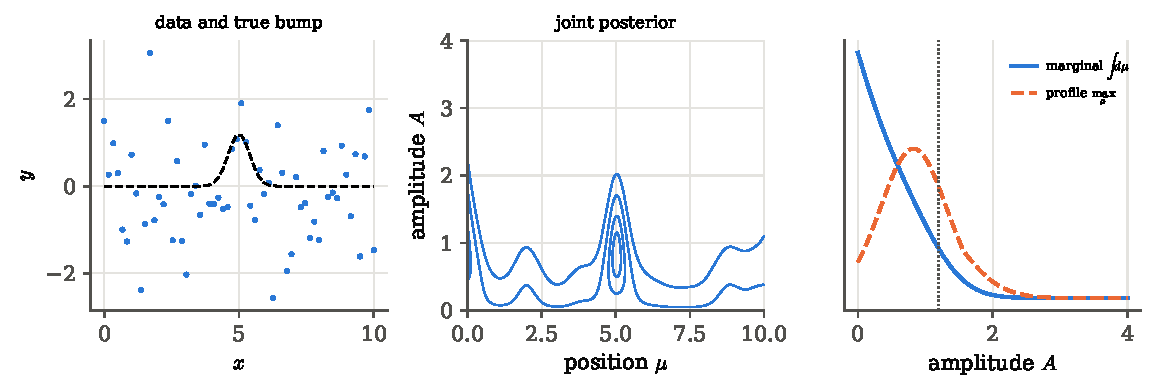
\includegraphics[width=\linewidth]{figures/ch05/marg_volume.pdf}
\caption{Marginal against profile for a weak bump whose position is unknown. Left: the
data and the true bump (dashed). Middle: the joint posterior of amplitude and position.
At small amplitude every position fits about equally well, so whatever probability the
posterior keeps there is spread over the whole range of positions. Right: the marginal
posterior of the amplitude (solid) integrates over position, so it gives small
amplitudes more weight than the profile (dashed), which maximises over position and
peaks near the best-fitting bump. The dotted line is the true amplitude.}
\label{5b:fig:volume}
\end{figure}

\begin{pitfall}[The peak of the joint is not the peak of the marginal]
The best-fit point of a joint posterior, projected onto one parameter, is the peak of
the profile, not of the marginal. For skewed or banana-shaped posteriors, and whenever
the nuisance width changes across the parameter of interest, the two differ, and quoting
``the best fit'' next to a marginal interval can put the best fit outside the interval.
In cosmology these ``projection'' or ``prior-volume'' effects are routine in analyses
with many nuisance parameters. Report which summary is quoted, and when they differ,
report both \srcref{Sivia}{p.~54}.
\end{pitfall}

Marginals also hide structure. Two strongly correlated parameters may each have a broad
marginal while their difference is sharply determined. And two pairs of parameters with
the same marginals can have very different joint posteriors
\srcref{Kruschke}{Fig.~12.1}. Whenever the question concerns a combination of parameters,
compute the posterior of that combination from the joint, not from the marginals. With
samples this is a one-line operation (\cref{5b:sec:sampling}).
\section{Choosing a prior: subjective, flat and Jeffreys}
\label{5b:sec:priors}

Every posterior so far has needed a prior density $p(\theta)$ for the parameter
$\theta$ we want, the weight each branch of the probability tree gets before the data
arrive. Sometimes the choice is easy: an earlier experiment measured the same quantity,
and its result is our prior. Often it is not. Suppose we are the first to measure the
fraction $\theta$ of cosmic-ray muons that fire a new trigger. We believe it lies
between 0 and 1 and not much more. What density should we write down, and how much
does the answer depend on that choice?

Two schools answer differently \mainref{pp.~181--182}. The first, called
\newterm{subjectivism}, says that the prior should reflect our opinion about $\theta$
before the data are collected. The second looks for a prior that expresses no opinion
at all, a ``noninformative'' prior. The obvious candidate is a flat prior,
$p(\theta)\propto\text{constant}$. Both are useful and both have traps. The trap of the
flat prior is the more surprising one. A prior cannot be flat in every way of describing
the same parameter, so ``flat'' always hides a choice of variable.

The questions, in words, are these.
\begin{enumerate}
  \item How do we turn real but vague knowledge into a density?
  \item What does a flat prior actually say, and when is a flat prior over an infinite
        range allowed?
  \item Is there a rule that gives the same answer whichever variable we use to
        describe the parameter?
\end{enumerate}

\subsection{Priors that encode knowledge}

A prior is a probability like any other. No probability, prior or likelihood, is ever
simply ``known''. Each one is an assignment that reflects the information $I$ we have.
We call $p(X\given I)$ a likelihood when $X$ is data, and a prior when $X$ is a
parameter and no new measurement is involved. The difference is one of name, not of
objectivity \srcref{Sivia}{\S5.5}. What makes an assignment objective is consistency:
two people with the same information should assign the same density. In practice there
are three routes from knowledge to a density, which we take in turn.

\paragraph{Informal assessment.} Think of ten points, each carrying 10\% of the prior
probability, and decide where they plausibly go \srcref{HobsonBMC}{\S1.3.2}. That gives
a rough centre, a rough width and a rough shape, which we then match to a standard
density. For a \emph{location} parameter \unpack{one that shifts the prediction, like a
peak position or a mass} with centre $c$ and width $w$, a Cauchy density
\begin{equation*}
  p(\theta)=\frac{w/\pi}{(\theta-c)^2+w^2}
\end{equation*}
is a good choice. Its heavy tails still give real weight to values far from the guess,
so the data can move the answer there if they demand it. For a positive \emph{intensity} \unpack{a rate or an
amplitude that cannot be negative} of plausible size $a$, an exponential
$p(\theta)=a^{-1}e^{-\theta/a}$, or a Gamma density if we also know a width, does the same
job \srcref{HobsonBMC}{(1.28)--(1.30)}. The prior does not have to be ``right'' in some
undefinable sense. It has to be reasonable.

\paragraph{Moment matching.} If earlier data exist, choose a standard density with the
same mean and standard deviation as those data \srcref{Lambert}{\S5.6.2}. For example,
five earlier determinations of a detector gain, with mean $1.02$ and scatter $0.05$,
give the prior $\Normal(1.02,0.05^2)$. Which moments to match is an arbitrary choice, so
this is a practical recipe rather than a principle.

\paragraph{Example: a prior elicited from quantiles.}
Experts find quantiles easier to state than standard deviations. Suppose a colleague
says: ``I would give even odds that the Hubble constant lies between 67 and
$73\,\mathrm{km\,s^{-1}Mpc^{-1}}$, and I think it is equally likely to be below 67 as
above 73.'' That is a statement of the 25\% and 75\% quantiles, $q_{25}=67$ and
$q_{75}=73$. For a Gaussian prior $\Normal(\mu,s^2)$ each quantile is $q=\mu+z\,s$, where
$z$ is the matching quantile of the standard normal, $z_{75}=-z_{25}=0.6745$
\srcref{Lambert}{\S5.6.3}. Then
\begin{align*}
  q_{75}-q_{25}&\eqby{1}(\mu+z_{75}s)-(\mu+z_{25}s)\eqby{2}2\times0.6745\,s
  &&\Rightarrow\quad s=\frac{73-67}{1.349}=4.45,\\
  q_{75}+q_{25}&\eqby{3}2\mu
  &&\Rightarrow\quad \mu=70 .
\end{align*}
\begin{explain}
  \item Each quantile of $\Normal(\mu,s^2)$ is $\mu$ plus the standard-normal quantile
        times $s$.
  \item $z_{25}=-z_{75}$ because the standard normal is symmetric.
  \item Adding instead of subtracting, the $z$ terms cancel for the same reason.
\end{explain}
So the elicited prior is $\Normal(70,4.45^2)$. With a panel of experts, the pairs
$(z,q)$ from all of them lie roughly on one straight line $q=\mu+zs$, and a linear
regression through them gives a pooled $\mu$ (the intercept) and $s$ (the slope).

\subsection{Flat priors, and flat priors over an infinite range}

A flat prior $p(\theta)=\text{constant}$ lets the likelihood alone set the shape of the
posterior, since $p(\theta\given\data)\propto\Like(\theta)\times\text{constant}$. For a
bounded parameter such as our trigger fraction, the constant is $1$ on $[0,1]$, and after
$z$ firings in $N$ muons the posterior is $\mathrm{Beta}(z+1,N-z+1)$ (\cref{5b:sec:conjugate}),
which seems very reasonable \mainref{p.~182}.

For a parameter with no natural bound, such as the mean $\theta$ of Gaussian readings,
a constant over the whole real line has infinite area. So it is not a probability
density at all. Such a prior is called \newterm{improper}. Can we use it anyway? We can
still multiply it by the likelihood, and then check whether the product can be
normalised.

\paragraph{Example: the mean of Gaussian readings with a flat improper prior.}
Take $n$ readings $x_1,\dots,x_n$, each $\Normal(\theta,\sigma^2)$ with known $\sigma$,
and $p(\theta)=c$ on the whole real line. Write $\bar x=\frac1n\sum_ix_i$. Then
\begin{align*}
  p(\theta\given x_1,\dots,x_n)
  &\relby{1}{\propto} c\prod_{i=1}^n e^{-(x_i-\theta)^2/2\sigma^2}
   \relby{2}{\propto}\exp\!\Bigl[-\frac{1}{2\sigma^2}\sum_{i=1}^n(x_i-\theta)^2\Bigr]\\
  &\eqby{3}\exp\!\Bigl[-\frac{1}{2\sigma^2}\sum_{i=1}^n(x_i-\bar x)^2\Bigr]
     \exp\!\Bigl[-\frac{n(\theta-\bar x)^2}{2\sigma^2}\Bigr]
   \relby{4}{\propto}\exp\!\Bigl[-\frac{(\theta-\bar x)^2}{2\sigma^2/n}\Bigr].
\end{align*}
\begin{explain}
  \item Posterior $\propto$ likelihood $\times$ prior, dropping the factors
        $1/\sqrt{2\pi\sigma^2}$ that do not contain $\theta$.
  \item The constant $c$ drops out, and a product of exponentials is the exponential of
        the sum.
  \item Write $x_i-\theta=(x_i-\bar x)+(\bar x-\theta)$ and square. The cross term is
        $2(\bar x-\theta)\sum_i(x_i-\bar x)=0$, because the deviations from the mean sum
        to zero.
  \item The first factor does not contain $\theta$.
\end{explain}
The posterior is $\Normal(\bar x,\sigma^2/n)$, a perfectly proper density, and its
95\% interval $\bar x\pm1.96\,\sigma/\sqrt n$ coincides exactly with the frequentist
confidence interval of \cref{ch:03} \mainref{p.~182}. An improper prior is harmless as
long as the posterior it produces is a well-defined probability distribution.

The safe way to think about an improper prior is as the limit of proper ones
\srcref{Sivia}{\S5.5}. Use a prior that is flat between bounds $A$ and $B$, compute the
posterior, and watch what happens as $A\to-\infty$ and $B\to\infty$. Usually the
posterior settles down and the bounds drop out, as they did above. If instead the
conclusions depend strongly on $A$ and $B$, the data carry very little information, and
the prior range, which is prior knowledge, is doing the work. Every maximum-likelihood or
least-squares fit uses this limit without saying so.

Improper priors are not harmless everywhere. Take the evidence $p(\data)=\int\Like\,p\,
\dd\theta$ of a model whose prior is flat over a width $W$, so $p=1/W$. The evidence
carries this factor $1/W$, so as $W\to\infty$ it goes to zero. The model then loses any
comparison with a model that knows even roughly what range to expect
\srcref{HobsonBMC}{\S1.3.2}. A flat prior
over an enormous range is also not ignorance. It says we are almost certain that
$|\theta|$ is enormous, since almost all of its area lies there. Are you really almost
certain that $|\theta|>10^{100}$?

\subsection{Flat in which variable?}

A flat prior is supposed to say ``we know nothing''. But knowing nothing about a
parameter should also mean knowing nothing about any other way of describing it. Can
one prior be flat in both? Return to the trigger fraction $p$ with the flat prior
$p\sim U(0,1)$, meant to represent our lack of information about $p$. A physicist might
equally describe the trigger by its log-odds
\begin{equation*}
  \psi=\ln\frac{p}{1-p},\qquad p=\frac{e^\psi}{1+e^\psi},
\end{equation*}
which runs over the whole real line. If we are ignorant about $p$, we are also ignorant
about $\psi$, so we should use a flat prior for $\psi$ too. But we have no freedom left:
the flat prior on $p$ already fixes the density of $\psi$. The rule is the change of
variables for densities (\cref{ch:01}): corresponding intervals must carry equal
probability, $p_\Psi(\psi)\,|\dd\psi|=p_P(p)\,|\dd p|$. So
\begin{align}
  p_\Psi(\psi)
  &\eqby{1}p_P\bigl(p(\psi)\bigr)\,\Bigl|\frac{\dd p}{\dd\psi}\Bigr|
   \eqby{2}1\times\frac{\dd}{\dd\psi}\frac{e^\psi}{1+e^\psi}
   \eqby{3}\frac{e^\psi(1+e^\psi)-e^\psi e^\psi}{(1+e^\psi)^2}
   \eqby{4}\frac{e^\psi}{(1+e^\psi)^2} .
  \label{5b:eq:logit-density}
\end{align}
\begin{explain}
  \item Change of variables for a density: equal probability in matching intervals.
  \item The flat density on $[0,1]$ is $1$, and $p(\psi)$ increases, so the absolute
        value is not needed.
  \item Quotient rule.
  \item The $e^{2\psi}$ terms cancel.
\end{explain}
This is a bump centred at $\psi=0$, not a flat line \mainref{p.~182}. How much of the
probability does the bump hold in $|\psi|<2$? That range corresponds to
$p\in(1/(1+e^2),\,e^2/(1+e^2))=(0.119,0.881)$, which the flat prior gives probability
$0.762$. So a flat prior on $p$ is a confident statement about $\psi$: the trigger is
probably neither extremely efficient nor extremely inefficient.

\Cref{5b:fig:logit-map} shows why. Equal steps in $p$ map onto steps in $\psi$ that are
narrow in the middle and wide at the ends. Each step carries the same probability, so
probability gets squeezed into the middle of the $\psi$ axis. The conclusion is
unavoidable: ``flat'' has no meaning until we say flat in which variable, because a flat
prior on a parameter is not flat on a nonlinear function of it. Flat priors are not
\newterm{transformation invariant}.

\begin{figure}[htbp]
\centering
\begin{tikzpicture}[x=7cm,y=0.55cm]
  \draw[->] (0,-4.4) -- (1.07,-4.4) node[right,lbl] {$p$};
  \draw[->] (0,-4.4) -- (0,4.7) node[above,lbl] {$\psi=\ln\frac{p}{1-p}$};
  \foreach \t in {0,0.5,1}{\draw (\t,-4.4) -- (\t,-4.6) node[below,lbl] {$\t$};}
  \foreach \s in {-4,-2,0,2,4}{\draw (0,\s) -- (-0.012,\s) node[left,lbl] {$\s$};}
  \draw[form,domain=0.013:0.987,samples=120] plot (\x,{ln(\x/(1-\x))});
  \foreach \t in {0.1,0.2,0.3,0.4,0.5,0.6,0.7,0.8,0.9}{
    \pgfmathsetmacro{\s}{ln(\t/(1-\t))}
    \draw[tangentgreen,thin] (\t,-4.4) -- (\t,\s);
    \draw[fibreorange,thin,dashed] (\t,\s) -- (0,\s);
    \fill[fibreorange] (0,\s) circle (1.3pt);
    \fill[formblue] (\t,\s) circle (1.1pt);
  }
  \node[lbl,align=center,anchor=north] at (0.5,-5.4) {equal steps of $0.1$ in $p$};
  \node[lbl,align=left,anchor=west] at (0.04,3.7) {each step in $p$ carries\\ prior probability $0.1$};
\end{tikzpicture}
\caption{Why a flat prior in $p$ is not flat in the log-odds $\psi$. The curve is
$\psi=\ln[p/(1-p)]$. Nine equally spaced values of $p$ (green lines) are carried up to
the curve and across to the $\psi$ axis (orange points). The orange points crowd
together near $\psi=0$ and spread apart towards the ends, so the same probability, $0.1$
per step, is packed densely in the middle of the $\psi$ axis and thinly at its ends:
the bump of \eqref{5b:eq:logit-density}.}
\label{5b:fig:logit-map}
\end{figure}

The same happens for any nonlinear function. Lambert's example is the probability
$u=\theta^2$ that two randomly chosen individuals both carry a disease of prevalence
$\theta$ \srcref{Lambert}{\S5.6.1}. A flat prior on $\theta\in[0,1]$ gives $u$ the
density $p(u)=p(\theta)\,|\dd\theta/\dd u|=1/(2\sqrt u)$, which piles up at $u=0$. For
ten individuals, $v=\theta^{10}$, the pile-up is sharper still,
$p(v)=\frac1{10}v^{-9/10}$. So a prior that looks uninformative about one quantity is
quite informative about others. This is why ``vague'' or ``diffuse'' are better words
than ``uninformative''.

\paragraph{Example: a scale parameter over four decades.}
The effect is largest for a positive \emph{scale} parameter \unpack{one that sets a
size, like a width, a lifetime or a noise level} whose order of magnitude is unknown.
Let $\lambda$ lie anywhere between $0.01$ and $100$, four decades. A prior flat in
$\lambda$ gives the decade $[10,100]$ the probability $(100-10)/(100-0.01)=
\FiveBPrFlatTop$, and the decade $[0.01,0.1]$ only $\FiveBPrFlatBottom$. So ``complete
ignorance'' has become a 90\% bet that $\lambda$ is in the top decade. A prior flat in $\ln\lambda$ instead gives each of the
four decades probability $\FiveBPrLogDecade$ (\cref{5b:fig:priors-param}, middle). For a
quantity whose order of magnitude is unknown, the second is clearly what we mean.

\paragraph{Why flat in $\ln\lambda$ is special.} A consistency argument makes this
precise \srcref{Sivia}{\S5.1}. The question is: what density says only ``this is a
location'' or only ``this is a scale''? Start with a location parameter $X$. If that is
all we know, then moving the origin by $x_0$ cannot change our density:
$p(X)\,\dd X=p(X+x_0)\,\dd(X+x_0)$ for every $x_0$. Since $\dd(X+x_0)=\dd X$, this says
$p(X)=p(X+x_0)$, so $p$ is constant: complete ignorance about a location is a uniform
density. If all we know about a length $L$ is that it is a scale, then changing the
units by a factor $\beta$ (nanometres to \aa ngstr\"oms) cannot change our density:
\begin{align*}
  p(L)\,\dd L=p(\beta L)\,\dd(\beta L)
  \;&\relby{1}{\Rightarrow}\; p(L)=\beta\,p(\beta L)\quad\text{for all }\beta>0\\
  &\relby{2}{\Rightarrow}\; p(\beta)=\frac{p(1)}{\beta}
  \;\relby{3}{\Rightarrow}\; p(L)\propto\frac1L .
\end{align*}
\begin{explain}
  \item $\dd(\beta L)=\beta\,\dd L$ for a constant $\beta$. Divide by $\dd L$.
  \item Set $L=1$ and solve for $p(\beta)$.
  \item Rename $\beta$ as $L$: the relation holds for every positive value.
\end{explain}
This is \newterm{Jeffreys' prior} for a scale parameter \srcref{Sivia}{(5.17)--(5.18)}.
In terms of $s=\ln L$ it is $p(s)=p(L)\,\dd L/\dd s=(1/L)\times L=\text{constant}$: flat
in the logarithm, which is why problems involving magnitudes are best done on
logarithmic graph paper. It is improper on $(0,\infty)$, so we use it between bounds
or check that the posterior is normalisable. It is also the prior
$p(\Cell)\propto1/\Cell$ used for a power-spectrum amplitude in \cref{5b:sec:conjugate}.

\subsection{Jeffreys' rule: a prior that does not depend on the coordinates}

Is there a recipe that gives the same prior whichever variable we choose, so that
``Jeffreys in $\theta$'' transformed to $\psi$ equals ``Jeffreys computed in $\psi$''?
Jeffreys found one \mainref{pp.~182--183}.

\begin{workdef}[Jeffreys' prior]
For a model with density $f(x\given\theta)$ for one datum, \newterm{Jeffreys' prior}
is $p(\theta)\propto\sqrt{I(\theta)}$, where $I(\theta)=-\E_\theta\bigl[\partial_\theta^2
\ln f(X\given\theta)\bigr]$ is the Fisher information \unpack{how sharply one datum pins
down $\theta$ on average, \cref{ch:03}}. For several parameters,
$p(\params)\propto\sqrt{\det I(\params)}$ with the Fisher information matrix.
\emph{Operationally:} compute the expected curvature of $\ln f$, take its square root,
and normalise if the result has finite area.
\end{workdef}

Why is it invariant? Let $\psi=h(\theta)$ be any smooth, one-to-one reparametrisation.
Use the equivalent form $I(\theta)=\E_\theta[(\partial_\theta\ln f)^2]$ of the Fisher
information from \cref{ch:03}. Then
\begin{align*}
  I_\psi(\psi)
  &\eqby{1}\E\Bigl[\Bigl(\frac{\partial\ln f}{\partial\psi}\Bigr)^2\Bigr]
   \eqby{2}\E\Bigl[\Bigl(\frac{\partial\ln f}{\partial\theta}\Bigr)^2\Bigr]
     \Bigl(\frac{\dd\theta}{\dd\psi}\Bigr)^2
   \eqby{3}I_\theta(\theta)\Bigl(\frac{\dd\theta}{\dd\psi}\Bigr)^2,
  \\
  \sqrt{I_\psi(\psi)}
  &\eqby{4}\sqrt{I_\theta(\theta)}\,\Bigl|\frac{\dd\theta}{\dd\psi}\Bigr| .
\end{align*}
\begin{explain}
  \item Fisher information in the new variable, as the mean square of the score.
  \item Chain rule, $\partial_\psi=(\dd\theta/\dd\psi)\,\partial_\theta$. The factor is
        not random and comes out of the expectation.
  \item The definition of $I_\theta$.
  \item Square root of both sides.
\end{explain}
The last line is exactly the change-of-variables law for a density,
$p_\psi(\psi)=p_\theta(\theta)\,|\dd\theta/\dd\psi|$. So the square root of the Fisher
information transforms as a density must. Computing Jeffreys' prior in $\theta$ and
transforming it to $\psi$ gives the same density as computing it in $\psi$ directly. Geometrically, $I$ is a metric on parameter space
\unpack{it measures how distinguishable nearby parameter values are by their data}, and
$\sqrt{\det I}$ is its volume element. Jeffreys' prior spreads prior mass uniformly
over distinguishable models, not over coordinate intervals
\srcref{HobsonBMC}{(1.47)--(1.54)}.

\paragraph{Example: the Bernoulli trigger.} One muon fires the trigger, $x=1$, with
probability $p$, or not, $x=0$. Then $\ln f=x\ln p+(1-x)\ln(1-p)$ and
\begin{align*}
  I(p)
  &\eqby{1}-\E\Bigl[-\frac{X}{p^2}-\frac{1-X}{(1-p)^2}\Bigr]
   \eqby{2}\frac{p}{p^2}+\frac{1-p}{(1-p)^2}
   \eqby{3}\frac1p+\frac1{1-p}
   =\frac{1}{p(1-p)} .
\end{align*}
\begin{explain}
  \item Differentiate $\ln f$ twice in $p$.
  \item $\E[X]=p$ and $\E[1-X]=1-p$.
  \item Cancel. Adding the fractions gives $1/[p(1-p)]$.
\end{explain}
Jeffreys' prior is $\sqrt{I(p)}=p^{-1/2}(1-p)^{-1/2}$, the
$\mathrm{Beta}(\tfrac12,\tfrac12)$ density \mainref{p.~183, Ex.~11.6}. It is not flat;
it rises at both ends. Compare it with the two other popular choices. The flat prior in
$p$ is $p^0(1-p)^0$. The prior flat in $\psi$ is the improper Haldane prior
$\mathrm{Beta}(0,0)\propto p^{-1}(1-p)^{-1}$. It is flat in $\psi$ because its density
in $\psi$ is $p^{-1}(1-p)^{-1}\times\dd p/\dd\psi=p^{-1}(1-p)^{-1}\times p(1-p)=1$, using
$\dd p/\dd\psi=p(1-p)$ from \eqref{5b:eq:logit-density}. Jeffreys' exponents,
$-\tfrac12$, lie halfway between the flat prior's $0$ and Haldane's $-1$.

\paragraph{Example: a Poisson rate and a Gaussian width.} Take a count $n$ with mean
$\lambda T$, where $\lambda$ is the rate and $T$ the exposure. Then $\ln f=n\ln\lambda-
\lambda T+\text{const}$, so $\partial_\lambda^2\ln f=-n/\lambda^2$ and
$I=\E[n]/\lambda^2=T/\lambda$. Jeffreys' prior is therefore $\lambda^{-1/2}$. With zero
observed events the posterior is $\propto\lambda^{-1/2}e^{-\lambda T}$, a
$\mathrm{Gamma}(\tfrac12,T)$ density. For this density $2T\lambda$ has the $\chi^2$
distribution with one degree of freedom, whose 95\% point is $3.84$. So the 95\% upper
limit is $\lambda<3.84/(2T)=1.92/T$, against $3.00/T$ from the flat prior
(\cref{5b:sec:conjugate}). Now take the width $\sigma$ of Gaussian noise. Then $\ln f=-\ln\sigma-(x-\mu)^2/2\sigma^2$, so
$\partial_\sigma^2\ln f=1/\sigma^2-3(x-\mu)^2/\sigma^4$, whose expectation is
$1/\sigma^2-3/\sigma^2=-2/\sigma^2$. So $I=2/\sigma^2$ and Jeffreys' prior is
$1/\sigma$, the scale prior found above from units alone.

\paragraph{Does it matter? The three priors on real numbers.}
\Cref{5b:fig:priors-param} and \cref{5b:lst:priors} compare the flat $\mathrm{Beta}(1,1)$,
Jeffreys $\mathrm{Beta}(\tfrac12,\tfrac12)$ and Haldane $\mathrm{Beta}(0,0)$ priors for
the trigger. With $1$ firing in $10$ muons the posterior means are $\FiveBPrFlatMeanTen$,
$\FiveBPrJefMeanTen$ and $\FiveBPrHalMeanTen$, and the 95\% upper limits are
$\FiveBPrFlatUpTen$, $\FiveBPrJefUpTen$ and $\FiveBPrHalUpTen$. With so little data, the
choice among ``noninformative'' priors changes the answer by a third. With $100$ firings in
$1000$ muons the means are $\FiveBPrFlatMeanThou$, $\FiveBPrJefMeanThou$ and
$\FiveBPrHalMeanThou$ and the upper limits $\FiveBPrFlatUpThou$, $\FiveBPrJefUpThou$ and
$\FiveBPrHalUpThou$: the choice has become irrelevant. A large sample makes the prior
irrelevant for a reason, and the same reason tells us when it fails (\cref{5b:sec:bvm}).

\pyfile[firstline=30,lastline=58,firstnumber=30,label={5b:lst:priors}]{code/ch05/14_priors.py}{Flat in which
variable: a flat prior seen in the log-odds, mass per decade for a scale parameter, and
three ``noninformative'' priors on the same data}

Lines~31--32 draw $10^5$ values of $p$ from the flat prior and transform each to its
log-odds. This is the change of variables done by sampling, and line~35 overlays the
exact density \eqref{5b:eq:logit-density}. Line~38 counts the fraction with $|\psi|<2$,
$\FiveBPrFracCentral$, against the exact $0.762$. Lines~41--44 compute the prior mass per
decade on $[0.01,100]$ for the two priors: for the flat prior it is the width of the
decade over the width of the range, and for the log-flat prior the log-width over the
log-width of the range. Lines~55--58 update each of the three Beta priors with the
conjugate rule $\mathrm{Beta}(a+z,b+N-z)$ of \cref{5b:sec:conjugate} and read off the
posterior mean and the 95\% quantile.

\begin{figure}[htbp]
\centering
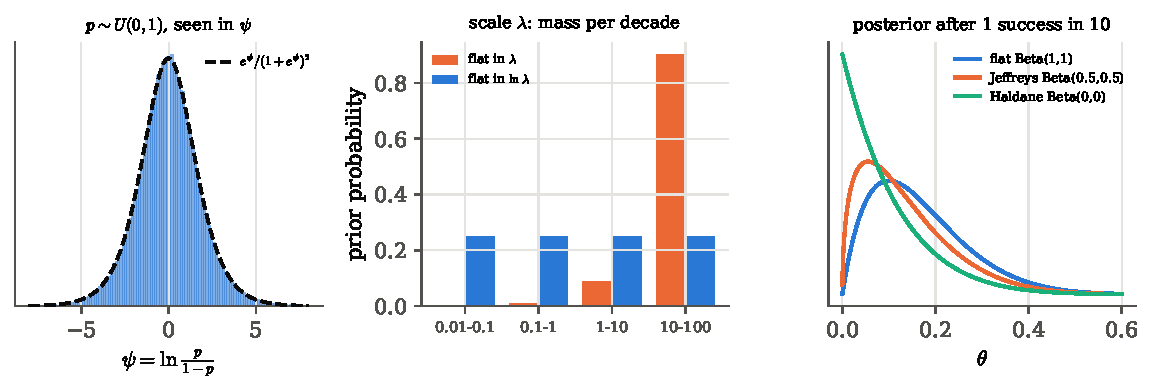
\includegraphics[width=\linewidth]{figures/ch05/priors_param.pdf}
\caption{Flat depends on the variable. Left: $10^5$ draws from a flat prior on $p$,
histogrammed in the log-odds $\psi$, follow the bump $e^\psi/(1+e^\psi)^2$ (dashed).
Middle: the prior probability of each decade of a scale parameter between $0.01$ and
$100$. Flat in $\lambda$ puts 90\% in the top decade. Flat in $\ln\lambda$ gives each
decade a quarter. Right: posteriors for a trigger efficiency after 1 firing in 10
muons, from the flat, Jeffreys and Haldane priors. With so few data they differ
visibly.}
\label{5b:fig:priors-param}
\end{figure}

\begin{pitfall}[There is no prior that says nothing]
Every prior says something about some function of the parameter. Jeffreys' rule is
consistent across coordinates, but it depends on the likelihood, so it changes when
the experiment changes, and in several dimensions $\sqrt{\det I}$ can behave badly or
fail to normalise \srcref{HobsonBMC}{\S1.3.2}. The general need for informal assessment
means that the search for a universal ``objective'' prior is doomed. Choose a
reasonable prior, say why, and check how much the answer depends on it
\srcref{Lambert}{\S5.7}.
\end{pitfall}

In practice most analyses use what Gelman calls \newterm{weakly informative} priors
\srcref{Lambert}{\S5.6.1}: smooth, proper densities that give zero weight only to
impossible values (a negative rate, a lifetime longer than the age of the universe) and
spread the rest broadly over physically sensible values. They avoid the arbitrary hard
edges of a flat box, which produce kinked posteriors and can trap the answer on the
wrong side of the edge (\cref{5b:sec:bvm}).
\section{Forgetting the prior: when the data win and when they cannot}
\label{5b:sec:bvm}

Two physicists measure the same trigger efficiency $\theta$, the fraction of muons that
fire a new trigger, with true value $0.3$. The first has no opinion and uses the flat
prior $\mathrm{Beta}(1,1)$. The second remembers a similar trigger with efficiency near
$0.8$ and is confident: $\mathrm{Beta}(80,20)$, a prior worth $\kappa=a+b=100$ muons
(\cref{5b:sec:conjugate}). Their priors barely overlap. They then record the same muons.
After ten muons they still disagree. After a hundred thousand they agree to a fraction of
an error bar (\cref{5b:fig:bvm-converge}). Is this agreement guaranteed? How fast does it
come? And when does it never come, however much data we take?

A second kind of forgetting is easy to confuse with this one. A Markov chain Monte
Carlo sampler (\cref{ch:09}) started at a silly point forgets where it started. That is
a different mechanism with a different cure. Keeping the two apart matters every time
someone says ``the prior washes out''.

\subsection{Why the prior is forgotten}

Write the log-posterior for $N$ independent data $x_1,\dots,x_N$ as
\begin{equation}
  \ln p(\theta\given x_1,\dots,x_N)
  =\underbrace{\ln p(\theta)}_{\text{one term}}
   +\underbrace{\sum_{i=1}^N\ln f(x_i\given\theta)}_{N\text{ terms}}
   +\text{const}.
  \label{5b:eq:logpost-N}
\end{equation}
Here $f(x\given\theta)$ is the density of one datum. The prior is a single term that
does not grow with $N$. The log-likelihood $\ell_N(\theta)=\sum_i\ln f(x_i\given\theta)$
is a sum of $N$ terms, so it grows in proportion to $N$. As data accumulate, the
likelihood therefore becomes a tall, narrow spike. The prior varies slowly across that
spike, so it can only nudge it. How much? Expand both terms about the
maximum-likelihood estimate $\hat\theta$, the peak of $\ell_N$. The curvature of $\ell_N$
there is $N\hat I$, where $\hat I=-\ell_N''(\hat\theta)/N$ is the observed information per
datum, close to the Fisher information $I(\theta)$ for large $N$ (\cref{ch:03}). Write
$g=\frac{\dd}{\dd\theta}\ln p(\theta)\big|_{\hat\theta}$ for the slope of the log-prior
there. Then
\begin{align}
  \ln p(\theta\given x_1,\dots,x_N)
  &\relby{1}{\approx}\text{const}+g\,(\theta-\hat\theta)
      -\frac{N\hat I}{2}(\theta-\hat\theta)^2
   \nonumber\\
  &\eqby{2}\text{const}'-\frac{N\hat I}{2}
      \Bigl(\theta-\hat\theta-\frac{g}{N\hat I}\Bigr)^2 .
  \label{5b:eq:bvm-shift}
\end{align}
\begin{explain}
  \item Taylor expansion about $\hat\theta$: the log-likelihood to second order (its
        first derivative vanishes at its peak), the log-prior to first order (it changes
        little across the narrow likelihood peak).
  \item Complete the square: $-\frac{c}{2}u^2+gu=-\frac c2(u-g/c)^2+g^2/2c$ with
        $u=\theta-\hat\theta$ and $c=N\hat I$. The $g^2/2c$ goes into the constant.
\end{explain}
The posterior is approximately Gaussian with
\begin{equation}
  \text{mean }\;\hat\theta+\frac{g}{N\hat I},\qquad
  \text{width }\;\frac{1}{\sqrt{N\hat I}},\qquad
  \frac{\text{shift caused by the prior}}{\text{width}}=\frac{g}{\sqrt{N\hat I}} .
  \label{5b:eq:bvm-ratio}
\end{equation}
The prior moves the posterior by an amount that falls as $1/N$. The posterior width
falls only as $1/\sqrt N$. So, measured in error bars, the influence of any smooth prior
dies away as $N^{-1/2}$. Two analysts with log-prior slopes $g_1$ and $g_2$ at
$\hat\theta$ disagree by $|g_1-g_2|/\sqrt{N\hat I}$ posterior standard deviations.

\begin{keyidea}[Bernstein--von Mises]
If the model is regular, the parameter is identifiable and of fixed dimension, and the
prior is smooth and nonzero at the true value, then for large $N$ the posterior is
approximately $\Normal\bigl(\hat\theta,\,1/[N I(\hat\theta)]\bigr)$, whatever the
prior. The posterior mean approaches the maximum-likelihood estimate, and a 95\%
credible interval approaches the 95\% confidence interval $\hat\theta\pm1.96/\sqrt{N
I(\hat\theta)}$ \mainref{p.~181, Thm.~11.5}.
\end{keyidea}

This is the Gaussian approximation of \cref{5b:sec:laplace} with a promise attached:
for large $N$ the curvature comes from the likelihood alone, so every reasonable prior
gives the same answer. This is why frequentist and Bayesian error bars on well-measured
quantities agree.

\paragraph{Example: two observers with Gaussian priors.}
Observers A and B have priors $\Normal(\mu_A,\Sigma_A^2)$ and $\Normal(\mu_B,\Sigma_B^2)$
for a quantity $\theta$ and share $N$ readings with Gaussian noise $\sigma$ and mean
$\bar m$ \srcref{Padilla}{\S3.4}. The rule ``precisions add'' of \cref{5b:sec:conjugate}
gives each observer $i\in\{A,B\}$ a Gaussian posterior with
\begin{align*}
  \hat\mu_i
  &\eqby{1}\frac{N\bar m/\sigma^2+\mu_i/\Sigma_i^2}{N/\sigma^2+1/\Sigma_i^2}
   \eqby{2}\frac{\bar m+r_i\,\mu_i}{1+r_i},
  \qquad r_i\equiv\frac{\sigma^2/N}{\Sigma_i^2},\\
  \tau_i^2
  &\eqby{3}\frac{1}{N/\sigma^2+1/\Sigma_i^2}
   \eqby{4}\frac{\sigma^2/N}{1+r_i}.
\end{align*}
\begin{explain}
  \item Precision-weighted mean \eqref{5b:eq:normal-post}: the $N$ readings count as
        one measurement $\bar m$ with variance $\sigma^2/N$.
  \item Divide numerator and denominator by $N/\sigma^2$.
  \item The posterior precision is the sum of the two precisions.
  \item Same division.
\end{explain}
The ratio $r_i$ compares the error of the data, $\sigma/\sqrt N$, with the width of the
prior, $\Sigma_i$. When $r_i\ll1$, the data dominate and $\hat\mu_i\to\bar m$ for both
observers. How fast do they converge? Since $r_i\propto1/N$, the difference
$\hat\mu_A-\hat\mu_B\approx r_A\mu_A-r_B\mu_B-(r_A-r_B)\bar m$ falls as $1/N$. The common
width $\tau\approx\sigma/\sqrt N$ falls only as $1/\sqrt N$. Their ratio falls as
$N^{-1/2}$, the law of \eqref{5b:eq:bvm-ratio} again. With one reading the two
posteriors can be far apart. After a hundred they are practically indistinguishable
\srcref{Padilla}{Fig.~3}.

\paragraph{Example: the confident and the open-minded physicist.}
Return to the two physicists of the opening: true efficiency $0.3$, a flat prior, and a
confident prior $\mathrm{Beta}(80,20)$. For the trigger the conjugate update is exact,
so we can follow the whole approach to agreement, not only its end. With $z$ firings in
$N$ muons and prior $\mathrm{Beta}(a,b)$ of mean $m_0=a/\kappa$, the posterior mean is
\begin{equation*}
  \frac{a+z}{\kappa+N}=\frac{N\hat\theta+\kappa m_0}{N+\kappa}
  \quad\Rightarrow\quad
  \text{mean}-\hat\theta=\frac{\kappa\,(m_0-\hat\theta)}{N+\kappa},
\end{equation*}
with $\hat\theta=z/N$. For the confident prior, $\kappa(m_0-\hat\theta)\approx100\times
(0.8-0.3)=50$. The flat prior's own pull, $2(0.5-\hat\theta)/(N+2)$, is tiny by
comparison. Dividing by the posterior width $\sqrt{\hat\theta(1-\hat\theta)/N}\approx
0.458/\sqrt N$ gives the gap between the two analysts in units of the posterior width,
\begin{equation*}
  \frac{\text{gap}}{\text{width}}\approx\frac{50}{N+100}\cdot\frac{\sqrt N}{0.458}
  =\frac{109\sqrt N}{N+100}.
\end{equation*}
Surprisingly, this \emph{grows} at first, because the posteriors narrow faster than
they approach each other. It peaks at $N=\kappa=100$, at about $5.5$ widths. That is the
moment of greatest embarrassment: both analysts are confident, and they disagree. Then
the gap falls as $109/\sqrt N$, the $N^{-1/2}$ law, and drops below one width only when
$N\gtrsim1.2\times10^4$. The simulation in \cref{5b:fig:bvm-converge} follows this curve:
its gap peaks at $\FiveBBvmGapPeak$ widths near $N=\FiveBBvmNpeak$ and stays below one
width from $N=\FiveBBvmNone$ on.

The lesson: a prior worth $\kappa$ observations needs many times $\kappa$ observations to
be forgotten. For a prior centred far from the truth, how many times is set by how many
widths away its centre lies. This matches Sivia's finding that a fair-minded coin prior
needs about a thousand flips before the data overrule it \srcref{Sivia}{\S2.1}, and
Lambert's that a strong model is less sensitive to the prior \srcref{Lambert}{\S5.7}.

\begin{figure}[htbp]
\centering
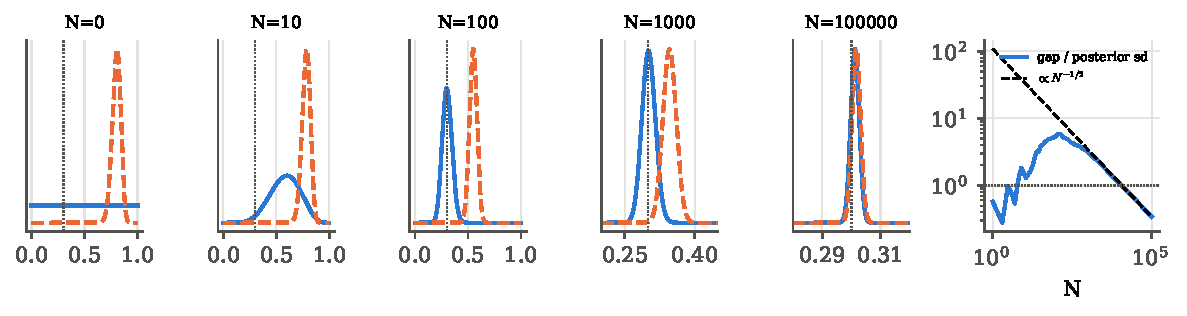
\includegraphics[width=\linewidth]{figures/ch05/bvm_converge.pdf}
\caption{Two analysts forget their priors. First five panels: posteriors from the flat
prior (solid) and from the confident prior $\mathrm{Beta}(80,20)$ (dashed) after
$N=0$ to $10^5$ tosses of a trigger with true efficiency $0.3$ (dotted). The horizontal
axis zooms in as the posteriors narrow. Last panel: the distance between the two
posterior means in units of the posterior width. It rises until $N$ is about the
prior's weight of 100, then falls as $N^{-1/2}$ (dashed line) and crosses one width
(dotted line) near $N=10^4$.}
\label{5b:fig:bvm-converge}
\end{figure}

\subsection{When the prior is never forgotten}

The derivation of \eqref{5b:eq:bvm-shift} used every condition in the key idea: enough
data, a prior nonzero at the truth, an identifiable parameter, a fixed number of
parameters, and a truth away from the edge. Each one can fail, and each failure shows up
in physics. We take them in turn.

\paragraph{Weak data.} The theorem is about large $N$. For $N$ comparable to the weight
$\kappa$ of an informative prior, or for a handful of events of any kind, the posterior
is a genuine compromise and the prior matters. After one trigger firing in ten muons the
three ``noninformative'' priors of \cref{5b:sec:priors} gave upper limits differing by a
third, and in the $N=10$ panel of \cref{5b:fig:bvm-converge} the two analysts are
$\FiveBBvmGapTen$ widths apart, with the gap still growing. With weak data the only
honest course is to report the prior and show how the answer moves when it changes: a
\newterm{prior sensitivity analysis} \srcref{Lambert}{\S5.7}.

\paragraph{A prior that is zero at the truth.} A health minister is ``morally certain''
that the prevalence of a disease is below 25\%, so the analysis uses a prior that is zero
above $0.25$ \srcref{Lambert}{\S5.7.1}. The true value is $0.3$. The posterior is prior
times likelihood, so it is zero above $0.25$ whatever the data say. As data accumulate
the likelihood climbs steadily towards $0.3$, and all the posterior can do is pile up
against the wall at $0.25$ (\cref{5b:fig:bvm-fail}, right). More data make the posterior
\emph{narrower at the wrong value}. The expansion \eqref{5b:eq:bvm-shift} failed because
$\ln p(\theta)=-\infty$ at the truth, so $g$ does not exist. A prior should be zero only
where a value is physically impossible.

\paragraph{A parameter the data cannot see.} A detector records the total count $n$ from
two channels with rates $\lambda_1$ and $\lambda_2$ but cannot tell them apart, so
$n\sim\text{Poisson}\bigl((\lambda_1+\lambda_2)T\bigr)$ in exposure $T$. What can the
count say about how the total is split between the channels? Reparametrise by the total
rate $\Lambda=\lambda_1+\lambda_2$ and the fraction $f=\lambda_1/\Lambda$ of the first
channel, and take independent priors $p(\Lambda)\,p(f)$. Then
\begin{align*}
  p(f\given n)
  &\eqby{1}\int p(\Lambda,f\given n)\,\dd\Lambda
   \eqby{2}\frac{\int\Prob(n\given\Lambda)\,p(\Lambda)\,p(f)\,\dd\Lambda}
               {\iint\Prob(n\given\Lambda')\,p(\Lambda')\,p(f')\,\dd\Lambda'\,\dd f'}
   \\
  &\eqby{3}p(f)\,\frac{\int\Prob(n\given\Lambda)\,p(\Lambda)\,\dd\Lambda}
               {\int\Prob(n\given\Lambda')\,p(\Lambda')\,\dd\Lambda'}
   =p(f).
\end{align*}
\begin{explain}
  \item Marginalise over the total rate (\cref{5b:sec:marginal}).
  \item Bayes' theorem. The likelihood depends on $\Lambda$ only, because the detector
        sees only the total.
  \item $p(f)$ comes out of the $\Lambda$ integral, and $\int p(f')\,\dd f'=1$.
\end{explain}
So the posterior of $f$ is its prior, exactly, for any number of counts. The data pin
down $\Lambda$ ever more precisely, but the prior alone decides the split. In the
simulation, $\FiveBBvmNtot$ counts fix $\Lambda$ to 1.4\%, yet two different priors on
$f$ give two completely different posteriors for $\lambda_1$ (\cref{5b:fig:bvm-fail},
left). Such a parameter is \newterm{not identifiable} \unpack{different values of it
predict exactly the same distribution of data}. Real cases are common: a
cosmological amplitude and a galaxy bias that enter only as a product, two
backgrounds with the same shape, a mass and a coupling that enter a rate only in
combination.

\paragraph{More parameters than data.} The theorem assumes the number of parameters
stays fixed while $N$ grows. Wasserman gives a simplified version of the Robins--Ritov
example, a missing-data problem with $B\gg N$ unknown probabilities $\theta_1,\dots,
\theta_B$ \mainref{pp.~186--188, Ex.~11.9}. With far fewer data than parameters, most
$\theta_j$ never appear in the likelihood, so their posterior equals their prior. The
posterior of their average $\psi=\frac1B\sum_j\theta_j$ therefore barely moves from its
prior. Yet a simple frequentist weighted average, the Horvitz--Thompson estimator, does
learn $\psi$: its error falls as $1/\sqrt N$ however large $B$ is. It succeeds because it
uses the known probability that each datum is observed. Those probabilities drop out of
the likelihood, so no method built on the likelihood can use them. Bayesian methods are
tied to the likelihood function, and in high-dimensional problems the likelihood may
not give accurate inferences.

\paragraph{A truth on the edge.} If the true value sits on the boundary of the allowed
range, such as a signal strength of exactly zero with the prior restricted to
nonnegative values, the posterior is a half-Gaussian piled against the edge, not a
Gaussian, and the credible and confidence intervals need not agree (\cref{ch:04}).

\begin{figure}[htbp]
\centering
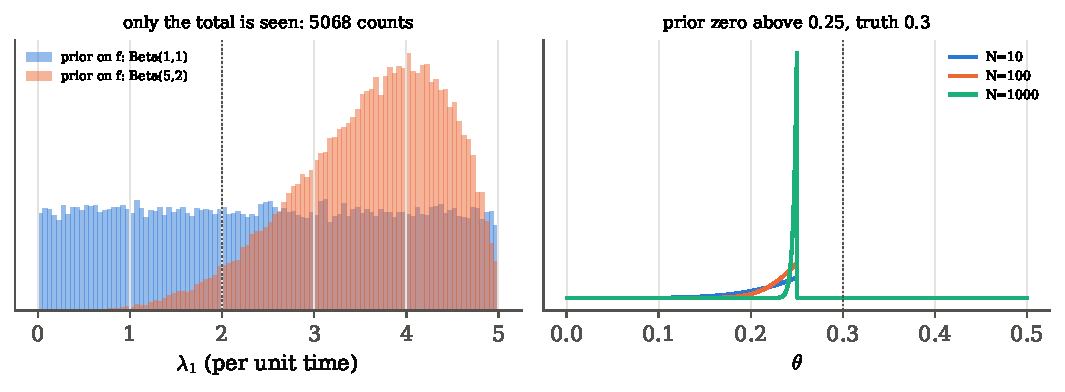
\includegraphics[width=\linewidth]{figures/ch05/bvm_fail.pdf}
\caption{Two ways the prior is never forgotten. Left: a detector that sees only the
total of two channels. With $\FiveBBvmNtot$ counts the total rate is known precisely,
but the posterior of the first channel's rate $\lambda_1$ is set by the prior on its
fraction: a flat prior gives the broad blue histogram, a $\mathrm{Beta}(5,2)$ prior the
orange one. The dotted line is the true $\lambda_1=2$. Right: a prior that is zero above
$0.25$ when the truth is $0.3$ (dotted). With 10, 100 and 1000 data the posterior only
piles up more sharply against the wall.}
\label{5b:fig:bvm-fail}
\end{figure}

\subsection{Forgetting the prior is not forgetting the start of a chain}

When a posterior cannot be computed on a grid, we explore it with a Markov chain: a
random walk in parameter space, biased so that it spends time in each region in
proportion to the posterior there (\cref{ch:09}). A chain started far from the bulk of
the posterior wanders for a while before it settles. That early part, the
\newterm{burn-in}, is thrown away, and after it the chain has forgotten where it
started. It is tempting to say the chain has also ``washed out'' the prior. It has not,
because the two forgettings work by different mechanisms.
\begin{itemize}
  \item \emph{A chain forgets its starting point} because every step is drawn from a
        rule that leaves one target distribution unchanged, and repeated steps pull any
        starting distribution towards that target (\cref{ch:09} proves the contraction).
        Running the chain longer is the cure for a bad start.
  \item \emph{A posterior forgets its prior} only through the likelihood,
        \eqref{5b:eq:bvm-ratio}: more \emph{data}. The target of the chain is
        prior$\times$likelihood, prior included, so a chain run forever reproduces the
        prior's influence perfectly.
\end{itemize}

\paragraph{Example: four chains.} Take 6 firings in 20 muons and the two priors of the
trigger example. We run a Metropolis chain \unpack{a random walk whose proposed steps are
accepted or rejected by comparing posterior values} from $\theta=0.02$ and from
$\theta=0.98$ for each prior, $2\times10^4$ steps each, and discard the first 5000.

\pyfile[firstline=94,lastline=108,firstnumber=94]{code/ch05/15_bvm.py}{A Metropolis
chain on the trigger posterior: only a ratio of posteriors enters}

Lines~94--97 are the log-posterior, $\ln[\theta^{z+a-1}(1-\theta)^{N-z+b-1}]$ up to a
constant, and $-\infty$ outside $(0,1)$. Line~103 proposes a Gaussian step. Line~105
accepts it with probability $\min(1,p_{\text{new}}/p_{\text{old}})$. This is computed
from the difference of log-posteriors, so the unknown evidence cancels and never
appears.

The results separate the two forgettings (\cref{5b:fig:chain-prior}). With the flat
prior the two chains give means $\FiveBChainFlatA$ and $\FiveBChainFlatB$ from their two
starts, against the exact posterior mean $\FiveBChainExactFlat$. With the confident prior
they give $\FiveBChainStrA$ and $\FiveBChainStrB$, against the exact
$\FiveBChainExactStr$. Within a few dozen steps each chain has forgotten whether it
started at $0.02$ or $0.98$. But no number of steps brings the two priors together:
they sample two different posteriors, both correctly. Only more muons would.

\begin{figure}[htbp]
\centering
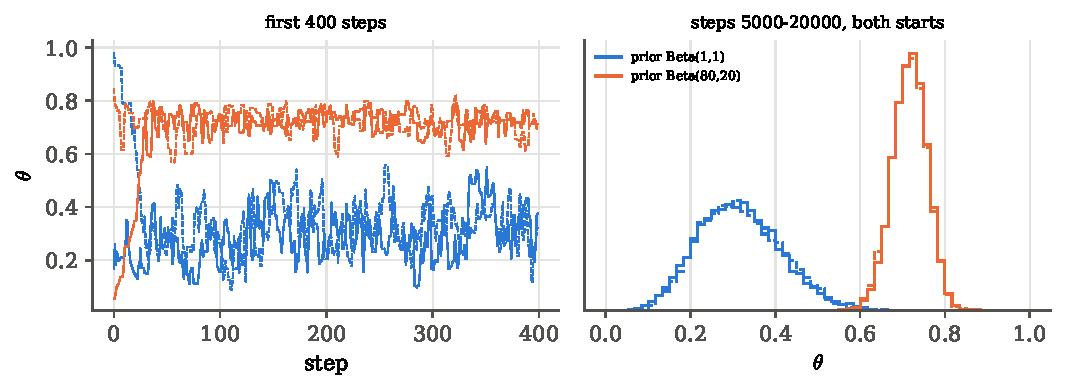
\includegraphics[width=\linewidth]{figures/ch05/chain_vs_prior.pdf}
\caption{Two kinds of forgetting. Left: the first 400 steps of four Metropolis chains on
the trigger posterior after 6 firings in 20 muons, started at $0.02$ (solid) and $0.98$
(dashed), with the flat prior (blue) and the confident prior (orange). Each pair forgets
its start within a few dozen steps. Right: histograms of steps 5000 to 20000. Chains with
the same prior agree whatever the start. Chains with different priors disagree however
long they run.}
\label{5b:fig:chain-prior}
\end{figure}

\begin{pitfall}[Burn-in does not remove a prior]
Discarding burn-in removes the memory of the chain's starting point. It does nothing to
the prior, which is part of the distribution the chain is built to sample. If two
analyses with different priors disagree, running the chains longer will only make the
disagreement more precise. The cure is more informative data, or a prior sensitivity
analysis that reports how the result depends on the prior.
\end{pitfall}
\section{Sampling the posterior: a histogram instead of an integral}
\label{5b:sec:sampling}

A mass on a spring oscillates as $x(t)=A\cos\omega t$. Where are we most likely to find
it if we look at a random moment? ``A random moment'' already contains an assumption:
the moment of looking is uniform in time, so the phase $\omega t$ is uniform over a
cycle. With that assumption there are two ways to answer. One is a calculation: change
variables from the uniform phase to the position and obtain the arcsine density
$1/(\pi\sqrt{A^2-x^2})$ (\cref{ch:01}). The other needs no calculus at all. Pick a large
set of random times, compute $x$ at each, and histogram the values. The histogram piles
up at the turning points, where the mass moves slowly, and it traces out the arcsine
curve (\cref{5b:fig:sampling}, bottom right). This idea can be used to find the
probability distribution of position: we plot the histogram for $x$ for a large set of
random values of $t$.

The same idea works for a posterior. Suppose that instead of a formula for
$p(\theta\given\data)$ we had a machine that produces random values
$\theta_1,\dots,\theta_B$ distributed according to it. Then a histogram of
$\theta_1,\dots,\theta_B$ approximates the posterior density $p(\theta\given\data)$
\mainref{p.~180}. Every integral we have needed so far becomes a count or an average
over the draws: a mean, a marginal, the probability of an interval. This is the bridge
from Bayesian inference to Monte Carlo, and it is how almost all modern posteriors are
handled.

The question, in words: if we can draw from the posterior, what can we compute from the
draws, and how accurately?

\begin{workdef}[posterior sample]
A \newterm{posterior sample} is a set of values $\theta_1,\dots,\theta_B$, each drawn from
$p(\theta\given\data)$ \unpack{so that the fraction of draws in any interval approaches
the posterior probability of that interval as $B$ grows}. \emph{Operationally:} the
posterior probability of a set $S$ is estimated by the fraction of draws in $S$, the
posterior mean of any function $g(\theta)$ by $\frac1B\sum_ig(\theta_i)$, and a quantile
by the corresponding order statistic of the sorted draws.
\end{workdef}

\subsection{Why a histogram of draws is the density}

Take a bin of width $\Delta$ around $\theta_j$. Each draw lands in it independently with
probability $P_j=\int_{\text{bin}}p(\theta\given\data)\,\dd\theta\approx p(\theta_j\given
\data)\,\Delta$, so the count $n_j$ in the bin is binomial, $n_j\sim\mathrm{Bin}(B,P_j)$
(\cref{ch:02}). The histogram height, count divided by $B\Delta$, then has
\begin{align*}
  \E\Bigl[\frac{n_j}{B\Delta}\Bigr]
  &\eqby{1}\frac{BP_j}{B\Delta}\relby{2}{\approx} p(\theta_j\given\data),
  \\
  \frac{\text{sd}(n_j)}{\E[n_j]}
  &\eqby{3}\frac{\sqrt{BP_j(1-P_j)}}{BP_j}
   \relby{4}{\approx}\frac{1}{\sqrt{BP_j}} .
\end{align*}
\begin{explain}
  \item The mean of a binomial count is $BP_j$.
  \item $P_j\approx p(\theta_j\given\data)\Delta$ for a narrow bin.
  \item The standard deviation of a binomial count is $\sqrt{BP_j(1-P_j)}$.
  \item A single bin holds a small fraction of the probability, $P_j\ll1$.
\end{explain}
So the histogram is centred on the density. Its relative error in a bin is one over the
square root of the expected count there. For example, with $B=\FiveBSaB$ draws and a bin
holding 1\% of the probability, the expected count is 2000 and the height is good to
about $1/\sqrt{2000}\approx2\%$. The
same counting argument says that averages over draws converge: the average of $g(\theta_i)$
has mean $\E[g(\theta)\given\data]$ and standard deviation $\text{sd}(g)/\sqrt B$ for
independent draws \mainref{p.~181}.

\begin{pitfall}[Monte Carlo error is not the error bar]
Two different widths appear. The \emph{posterior width} $\text{sd}(\theta\given\data)$ is
the physical uncertainty on the parameter. It is set by the data and does not shrink when
we draw more samples. The \emph{Monte Carlo error} $\text{sd}(\theta\given\data)/\sqrt B$ is
how well the draws reproduce the exact posterior mean. It shrinks with $B$ and says nothing
about the physics. Quote the first as the error bar. Make sure the second is much smaller.
\end{pitfall}

\subsection{What the draws give for free}

\Cref{5b:fig:draws-flow} collects the operations. Each of them replaces an integral by a
one-line manipulation of an array of draws.

\begin{figure}[htbp]
\centering
\begin{tikzpicture}[x=1cm,y=1cm,
  box/.style={draw,rounded corners,fill=white,align=center,font=\footnotesize,
               inner sep=3pt,text width=1.95cm},
  arr/.style={->,thick,black!65}]
  \node[box,fill=formblue!10,text width=4.6cm] (d) at (0,0) {draws\\ $\params_1,\dots,\params_B\sim p(\params\given\data)$};
  \node[box] (h) at (-4.8,-2.3) {histogram\\ $\to$ density};
  \node[box] (m) at (-2.4,-2.3) {average, sort\\ $\to$ mean, interval};
  \node[box] (g) at (0,-2.3) {$\tau_i=g(\params_i)$\\ $\to$ any function};
  \node[box] (k) at (2.4,-2.3) {keep one coordinate\\ $\to$ marginal};
  \node[box] (p) at (4.8,-2.3) {$\tilde x_i\sim p(\tilde x\given\params_i)$\\ $\to$ new data};
  \foreach \t in {h,m,g,k,p}{\draw[arr] (d.south) -- (\t.north);}
\end{tikzpicture}
\caption{One array of posterior draws, five products. Histogramming it approximates the
density. Averaging and sorting give the mean and the interval ends. Applying a function
to each draw gives draws of that function. Ignoring all but one coordinate gives draws of
that parameter's marginal. Simulating a new data set from each draw gives the
distribution of future data.}
\label{5b:fig:draws-flow}
\end{figure}

\paragraph{Means and intervals.} The posterior mean is estimated by $\frac1B\sum_i
\theta_i$. The ends of the 95\% equal-tailed interval are the 2.5\% and 97.5\% sample
quantiles, and the HDI is the shortest window that contains 95\% of the sorted draws
(\cref{5b:sec:summaries}) \mainref{p.~181}.

\paragraph{Functions of the parameter.} If $\tau=g(\theta)$, then $\tau_i=g(\theta_i)$ is
a sample from the posterior of $\tau$. No change of variables is needed
\mainref{pp.~180--181}. To see how much work this saves, take a coin's heads probability
$p$ after $s=10$ heads in $n=14$ tosses, with a flat prior. Write $x^n=(x_1,\dots,x_n)$
for the tosses. The posterior is $p\given x^n\sim\mathrm{Beta}(s+1,n-s+1)$
(\cref{5b:sec:conjugate}). What is the posterior density of the log-odds
$\psi=\ln[p/(1-p)]$? The exact route goes through the cumulative distribution $H$ of
$\psi$, and then its derivative $h$:
\begin{align*}
  H(\psi\given x^n)
  &\eqby{1}\Prob\Bigl(\ln\frac{P}{1-P}\le\psi\Bigm| x^n\Bigr)
   \eqby{2}\Prob\Bigl(P\le\frac{e^\psi}{1+e^\psi}\Bigm| x^n\Bigr)
   \eqby{3}\int_0^{e^\psi/(1+e^\psi)}f(p\given x^n)\,\dd p,\\
  h(\psi\given x^n)
  &\eqby{4}f\Bigl(\frac{e^\psi}{1+e^\psi}\Bigm| x^n\Bigr)\,\frac{e^\psi}{(1+e^\psi)^2}
   \eqby{5}\frac{\Gamma(n+2)}{\Gamma(s+1)\Gamma(n-s+1)}
     \Bigl(\frac{e^\psi}{1+e^\psi}\Bigr)^{s+1}\Bigl(\frac{1}{1+e^\psi}\Bigr)^{n-s+1}.
\end{align*}
\begin{explain}
  \item Definition of the cumulative distribution of $\Psi=\ln[P/(1-P)]$, with $P$ the
        random heads probability.
  \item The log-odds is increasing in $P$, so the inequality can be inverted.
  \item The probability of an interval is the integral of the posterior density over it.
  \item Differentiate with respect to $\psi$: fundamental theorem of calculus and chain
        rule, with $\dd p/\dd\psi$ from \eqref{5b:eq:logit-density}.
  \item Insert the Beta density $f(p\given x^n)=\frac{\Gamma(n+2)}{\Gamma(s+1)\Gamma(n-s+1)}
        p^s(1-p)^{n-s}$ at $p=e^\psi/(1+e^\psi)$, and note that $\frac{e^\psi}{(1+e^\psi)^2}
        =p(1-p)$ raises each power by one.
\end{explain}
This is Wasserman's Example 11.3 \mainref{p.~180}. The sampling route takes two lines:
draw $P_i\sim\mathrm{Beta}(11,5)$, set $\psi_i=\ln[P_i/(1-P_i)]$, and histogram
\mainref{p.~181, Ex.~11.4}. The two agree (\cref{5b:fig:sampling}, top left). For a
function of several parameters, or one with no inverse in closed form, the sampling
route is the only practical one.

\paragraph{Marginals and combinations.} Take several parameters $\params=(\theta_1,\dots,
\theta_p)$ and $B$ draws $\params^{(1)},\dots,\params^{(B)}$. Their first coordinates
$\theta_1^{(1)},\dots,\theta_1^{(B)}$ are a sample from the marginal posterior of
$\theta_1$. Keeping one coordinate and ignoring the rest replaces the $(p-1)$-dimensional
integral of \cref{5b:sec:marginal} \mainref{p.~183, (11.9)}.

A combination of parameters is just as easy. After a detector upgrade we want to know:
did the efficiency improve? Before the upgrade $x_1=18$ of $n_1=40$ test pulses were
detected, and after it $x_2=28$ of $n_2=40$. Call the two efficiencies $p_1$ and $p_2$.
With a flat prior on the square $(p_1,p_2)\in[0,1]^2$,
\begin{equation*}
  p(p_1,p_2\given x_1,x_2)\propto p_1^{x_1}(1-p_1)^{n_1-x_1}\;p_2^{x_2}(1-p_2)^{n_2-x_2},
\end{equation*}
which factorises into $\mathrm{Beta}(x_1+1,n_1-x_1+1)$ for $p_1$ times
$\mathrm{Beta}(x_2+1,n_2-x_2+1)$ for $p_2$: under the posterior the two efficiencies are
independent \mainref{pp.~183--184, Ex.~11.7}. The improvement is $\tau=p_2-p_1$. Draw
$B$ values of each efficiency and subtract, $\tau_i=p_{2,i}-p_{1,i}$. The fraction of
positive differences estimates $\Prob(p_2>p_1\given\data)=\FiveBSaPpos$, and the 95\%
interval for the improvement is $(\FiveBSaTauLo,\FiveBSaTauHi)$ (\cref{5b:fig:sampling},
bottom left). If the parameters were correlated, the same subtraction of draws would use
the correlation automatically, because each draw is a pair taken together. The separate
marginals would have thrown that correlation away.

\paragraph{Predicting new data.} The \newterm{posterior predictive distribution} of a
future data set $\tilde x$ averages the forward model over our uncertainty about $\theta$:
\begin{align*}
  p(\tilde x\given\data)
  &\eqby{1}\int p(\tilde x,\theta\given\data)\,\dd\theta
   \eqby{2}\int p(\tilde x\given\theta,\data)\,p(\theta\given\data)\,\dd\theta
   \eqby{3}\int p(\tilde x\given\theta)\,p(\theta\given\data)\,\dd\theta .
\end{align*}
\begin{explain}
  \item Sum rule: marginalise the joint distribution of new data and parameter.
  \item Product rule.
  \item Given $\theta$, the new data are independent of the old data: the old data
        influence the prediction only through what they tell us about $\theta$.
\end{explain}
The sampling recipe mirrors the formula: for each draw $\theta_i$, simulate one new data
set $\tilde x_i$ from $p(\tilde x\given\theta_i)$. The collection $\tilde x_1,\dots,
\tilde x_B$ is a sample from the predictive distribution \srcref{Lambert}{\S7.8}.

\paragraph{Example: two more heads.} After 10 heads in 14 tosses, what is the probability
that the next two tosses are both heads? The exact answer, found in
\cref{5b:sec:conjugate}, is $B(13,5)/B(11,5)=\FiveBSaTwoHeadsExact$, not the plug-in
$(10/14)^2=0.51$ \srcref{Padilla}{\S2.3}. By sampling: for each draw $p_i$, toss two
simulated coins with heads probability $p_i$ and record whether both came up heads. The
fraction is $\FiveBSaTwoHeads$, within the Monte Carlo error $\sqrt{0.485\times0.515/B}
\approx0.001$ of the exact value.

\paragraph{Example: failures in the next batch.} One detector module in a batch of ten
fails its burn-in test. How many failures should we expect in the next batch of ten?
\begin{itemize}[itemsep=1pt,leftmargin=1.2em]
  \item \emph{Plug-in.} Take the failure rate to be exactly $0.1$ and use
        $\mathrm{Bin}(10,0.1)$. Its central 80\% range is $0$ to $\FiveBSaPlugHi$
        failures.
  \item \emph{Posterior predictive.} With a flat prior the posterior of the rate is
        $\mathrm{Beta}(1+1,1+9)=\mathrm{Beta}(2,10)$. Draw a rate, then a batch of ten
        with that rate, and repeat. The central 80\% range is $\FiveBSaPredLo$ to
        $\FiveBSaPredHi$ (\cref{5b:fig:sampling}, top right) \srcref{Lambert}{\S7.8}.
\end{itemize}
The predictive range is wider because it includes two sources of spread: our
uncertainty about the rate, and the binomial scatter of a batch. It also gives zero
failures probability $\FiveBSaPredZero$, against the plug-in $\FiveBSaPlugZero$, because
the rate could well be larger than $0.1$. Plugging in a best value always makes
predictions look more certain than they are.

\subsection{The same code for every posterior}

\pyfile[firstline=33,lastline=75,firstnumber=33]{code/ch05/16_sampling.py}{Posterior
draws put to work: a function of the parameter, two predictive calculations and a
difference of two efficiencies}

Lines~35--36 draw $B$ values of the heads probability from $\mathrm{Beta}(11,5)$ and turn
each into a log-odds, and line~39 is the exact density from the chain above, used only as
a check. Line~47 is the two-heads prediction: two uniform numbers per draw, each below
$p_i$ with probability $p_i$. Lines~49--50 draw a failure rate and then a whole new batch
for each draw, and lines~54--55 read the 80\% predictive range off the cumulative
histogram. Lines~66--68 draw the two efficiencies independently and subtract them, and
lines~74--75 turn the differences into a probability and an interval. The last panel of
the figure is the oscillator: uniform phases, $x=A\cos\omega t$, histogram. It is the
same three lines as the log-odds, with a random phase in the place of a random heads
probability.

\begin{figure}[htbp]
\centering
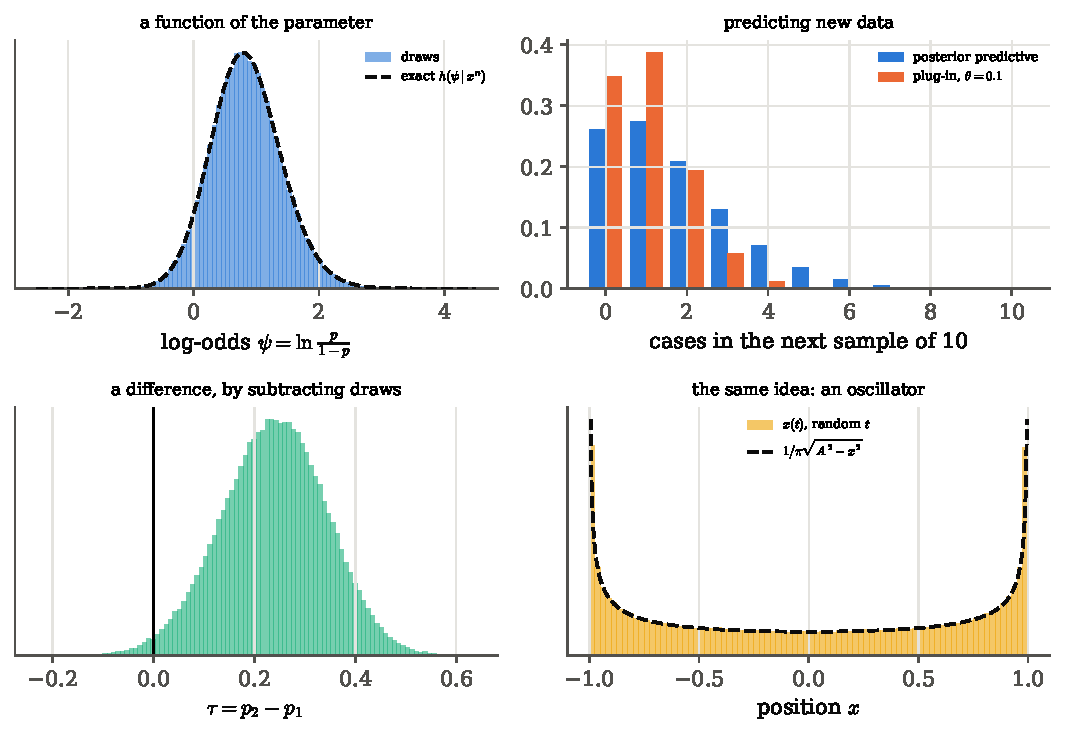
\includegraphics[width=0.95\linewidth]{figures/ch05/sampling.pdf}
\caption{Posterior draws at work. Top left: draws of the heads probability after 10 heads
in 14, turned into log-odds and histogrammed, against the exact density (dashed). Top
right: the predicted number of failures in the next batch of ten modules after one
failure in ten, from posterior draws (blue) and from plugging in the rate $0.1$ (orange).
Bottom left: the improvement in efficiency, from differences of draws. Bottom right: the
same idea for an oscillator. Positions at uniformly random times follow the arcsine
density (dashed).}
\label{5b:fig:sampling}
\end{figure}

Here every draw came from a standard generator, because every posterior was a Beta
density. That is the luxury of conjugacy (\cref{5b:sec:conjugate}). For a realistic
posterior in six or twenty dimensions we have neither a grid nor a generator. We can
only evaluate $\Like(\params)\,p(\params)$ at any point we choose. Monte Carlo methods
turn uniform random numbers into draws from simple distributions (\cref{ch:06}), and Markov
chain Monte Carlo builds a random walk whose visited points are draws from a posterior
known only up to its normalising constant (\cref{ch:09}). Everything downstream of the
draws, the histograms, averages, quantiles, functions, marginals and predictions of this
section, stays exactly the same.

\begin{recap}
\begin{itemize}
  \item For a continuous parameter, the observed data are the event, the parameter values
        are the hypotheses, and $p(\lambda\given\data)=\Like(\lambda)p(\lambda)/p(\data)$
        is a density. On a grid, sum log-likelihoods and subtract the maximum before
        exponentiating.
  \item Conjugate pairs (Beta--Binomial, Gamma--Poisson, Gaussian--Gaussian) give exact
        posteriors. In the Gaussian case precisions add and means are
        precision-weighted.
  \item Summaries: the posterior mean, median and mode minimise squared, absolute and
        all-or-nothing loss. Equal-tailed intervals are invariant under reparametrisation.
        HDIs are the shortest.
  \item Near a single peak the posterior is Gaussian with covariance minus the inverse
        Hessian of $\ln p$. Marginal errors come from the diagonal of the inverse.
  \item Nuisance parameters are integrated out. Profiling maximises over them instead, and
        the two differ by a volume factor.
  \item No prior is flat in every parametrisation. Jeffreys' prior $\sqrt{I(\theta)}$ is
        coordinate independent: $1/\sigma$ for a scale, $\mathrm{Beta}(\frac12,\frac12)$
        for a Bernoulli probability.
  \item With many data a smooth prior's influence dies as $N^{-1/2}$ posterior widths
        (Bernstein--von Mises). It is never forgotten if it is zero at the truth, if the
        parameter is not identifiable, or if parameters outnumber data. A Markov chain
        forgets its start, not its prior.
  \item A histogram of posterior draws is the posterior. Functions, marginals and
        predictions of new data are one line each on the draws.
\end{itemize}
\end{recap}

\providecommand{\FiveCFacZone}{}\renewcommand{\FiveCFacZone}{4.993\times10^{-4}}
\providecommand{\FiveCFacZtwo}{}\renewcommand{\FiveCFacZtwo}{0.002339}
\providecommand{\FiveCFacZgridOne}{}\renewcommand{\FiveCFacZgridOne}{4.993\times10^{-4}}
\providecommand{\FiveCFacZgridTwo}{}\renewcommand{\FiveCFacZgridTwo}{0.002339}
\providecommand{\FiveCFacBF}{}\renewcommand{\FiveCFacBF}{0.2135}
\providecommand{\FiveCFacInvBF}{}\renewcommand{\FiveCFacInvBF}{4.683}
\providecommand{\FiveCFacPostOne}{}\renewcommand{\FiveCFacPostOne}{17.6}
\providecommand{\FiveCFacPostTwo}{}\renewcommand{\FiveCFacPostTwo}{82.4}
\providecommand{\FiveCFairFifteen}{}\renewcommand{\FiveCFairFifteen}{0.3229}
\providecommand{\FiveCFairEleven}{}\renewcommand{\FiveCFairEleven}{3.337}
\providecommand{\FiveCFairTen}{}\renewcommand{\FiveCFairTen}{3.664}
\providecommand{\FiveCFacMeanOne}{}\renewcommand{\FiveCFacMeanOne}{0.4524}
\providecommand{\FiveCFacMeanTwo}{}\renewcommand{\FiveCFacMeanTwo}{0.6905}
\providecommand{\FiveCFacMeanAvg}{}\renewcommand{\FiveCFacMeanAvg}{0.6486}
\providecommand{\FiveCFairZmin}{}\renewcommand{\FiveCFairZmin}{7}
\providecommand{\FiveCFairZmax}{}\renewcommand{\FiveCFairZmax}{13}
\providecommand{\FiveCBumpChiLine}{}\renewcommand{\FiveCBumpChiLine}{49.07}
\providecommand{\FiveCBumpChiBump}{}\renewcommand{\FiveCBumpChiBump}{34.54}
\providecommand{\FiveCBumpDChi}{}\renewcommand{\FiveCBumpDChi}{14.53}
\providecommand{\FiveCBumplnLR}{}\renewcommand{\FiveCBumplnLR}{7.265}
\providecommand{\FiveCBumplnB}{}\renewcommand{\FiveCBumplnB}{2.096}
\providecommand{\FiveCBumplnOccam}{}\renewcommand{\FiveCBumplnOccam}{-5.169}
\providecommand{\FiveCBumpB}{}\renewcommand{\FiveCBumpB}{8.133}
\providecommand{\FiveCBumpAhat}{}\renewcommand{\FiveCBumpAhat}{2.307}
\providecommand{\FiveCBumpMuhat}{}\renewcommand{\FiveCBumpMuhat}{6.373}
\providecommand{\FiveCBumplnZline}{}\renewcommand{\FiveCBumplnZline}{-68.61}
\providecommand{\FiveCBumplnZbump}{}\renewcommand{\FiveCBumplnZbump}{-66.51}
\providecommand{\FiveCBumpGridErr}{}\renewcommand{\FiveCBumpGridErr}{1.236\times10^{-8}}
\providecommand{\FiveCFlatChiLine}{}\renewcommand{\FiveCFlatChiLine}{48.37}
\providecommand{\FiveCFlatChiBump}{}\renewcommand{\FiveCFlatChiBump}{43.98}
\providecommand{\FiveCFlatDChi}{}\renewcommand{\FiveCFlatDChi}{4.387}
\providecommand{\FiveCFlatlnLR}{}\renewcommand{\FiveCFlatlnLR}{2.194}
\providecommand{\FiveCFlatlnB}{}\renewcommand{\FiveCFlatlnB}{-1.675}
\providecommand{\FiveCFlatlnOccam}{}\renewcommand{\FiveCFlatlnOccam}{-3.868}
\providecommand{\FiveCFlatB}{}\renewcommand{\FiveCFlatB}{0.1873}
\providecommand{\FiveCFlatAhat}{}\renewcommand{\FiveCFlatAhat}{1.584}
\providecommand{\FiveCFlatMuhat}{}\renewcommand{\FiveCFlatMuhat}{0.2214}
\providecommand{\FiveCFlatlnZline}{}\renewcommand{\FiveCFlatlnZline}{-68.26}
\providecommand{\FiveCFlatlnZbump}{}\renewcommand{\FiveCFlatlnZbump}{-69.93}
\providecommand{\FiveCFlatGridErr}{}\renewcommand{\FiveCFlatGridErr}{7.607\times10^{-6}}
\providecommand{\FiveCLapLnZbump}{}\renewcommand{\FiveCLapLnZbump}{-66.57}
\providecommand{\FiveCLapLnB}{}\renewcommand{\FiveCLapLnB}{2.04}
\providecommand{\FiveCLapLnOccOne}{}\renewcommand{\FiveCLapLnOccOne}{-12.54}
\providecommand{\FiveCLapLnOccZero}{}\renewcommand{\FiveCLapLnOccZero}{-7.318}
\providecommand{\FiveCLapOccRatio}{}\renewcommand{\FiveCLapOccRatio}{0.005381}
\providecommand{\FiveCSigA}{}\renewcommand{\FiveCSigA}{0.6053}
\providecommand{\FiveCSigMu}{}\renewcommand{\FiveCSigMu}{0.1415}
\providecommand{\FiveCSigAMuVol}{}\renewcommand{\FiveCSigAMuVol}{0.5381}
\providecommand{\FiveCPriorAMuVol}{}\renewcommand{\FiveCPriorAMuVol}{100}
\providecommand{\FiveCFixLnB}{}\renewcommand{\FiveCFixLnB}{4.668}
\providecommand{\FiveCFixB}{}\renewcommand{\FiveCFixB}{106.5}
\providecommand{\FiveCFreeOverFix}{}\renewcommand{\FiveCFreeOverFix}{13.09}
\providecommand{\FiveCFixAhat}{}\renewcommand{\FiveCFixAhat}{2.18}
\providecommand{\FiveCFixSigA}{}\renewcommand{\FiveCFixSigA}{0.6018}
\providecommand{\FiveCFixZscore}{}\renewcommand{\FiveCFixZscore}{3.622}
\providecommand{\FiveCBumpLnBHundred}{}\renewcommand{\FiveCBumpLnBHundred}{-0.2067}
\providecommand{\FiveCFlatLnBHundred}{}\renewcommand{\FiveCFlatLnBHundred}{-3.977}
\providecommand{\FiveCFlatLnBOne}{}\renewcommand{\FiveCFlatLnBOne}{-0.03148}
\providecommand{\FiveCAmax}{}\renewcommand{\FiveCAmax}{10}
\providecommand{\FiveCNdata}{}\renewcommand{\FiveCNdata}{40}
\providecommand{\FiveCWidth}{}\renewcommand{\FiveCWidth}{0.5}
\providecommand{\FiveCTrueA}{}\renewcommand{\FiveCTrueA}{2.5}
\providecommand{\FiveCTrueMu}{}\renewcommand{\FiveCTrueMu}{6.2}
\providecommand{\FiveCHalUnifBF}{}\renewcommand{\FiveCHalUnifBF}{0.1253}
\providecommand{\FiveCHalHaldBF}{}\renewcommand{\FiveCHalHaldBF}{5.728}
\providecommand{\FiveCInfUnifBF}{}\renewcommand{\FiveCInfUnifBF}{0.05571}
\providecommand{\FiveCInfHaldBF}{}\renewcommand{\FiveCInfHaldBF}{0.05748}
\providecommand{\FiveCHdiUnifLo}{}\renewcommand{\FiveCHdiUnifLo}{0.5543}
\providecommand{\FiveCHdiUnifHi}{}\renewcommand{\FiveCHdiUnifHi}{0.7382}
\providecommand{\FiveCHdiHaldLo}{}\renewcommand{\FiveCHdiHaldLo}{0.5564}
\providecommand{\FiveCHdiHaldHi}{}\renewcommand{\FiveCHdiHaldHi}{0.7418}
\providecommand{\FiveCLamS}{}\renewcommand{\FiveCLamS}{75}
\providecommand{\FiveCLamT}{}\renewcommand{\FiveCLamT}{150}
\providecommand{\FiveCLamLnZa}{}\renewcommand{\FiveCLamLnZa}{-32.78}
\providecommand{\FiveCLamLnZb}{}\renewcommand{\FiveCLamLnZb}{-28.86}
\providecommand{\FiveCLamLnZc}{}\renewcommand{\FiveCLamLnZc}{-27.66}
\providecommand{\FiveCLamZratio}{}\renewcommand{\FiveCLamZratio}{50.36}
\providecommand{\FiveCLamMeanA}{}\renewcommand{\FiveCLamMeanA}{0.5}
\providecommand{\FiveCLamMeanB}{}\renewcommand{\FiveCLamMeanB}{0.5}
\providecommand{\FiveCLamSdA}{}\renewcommand{\FiveCLamSdA}{0.04069}
\providecommand{\FiveCLamSdB}{}\renewcommand{\FiveCLamSdB}{0.04043}
\providecommand{\FiveCLinPzeroN}{}\renewcommand{\FiveCLinPzeroN}{0.3512}
\providecommand{\FiveCLinPzeroNk}{}\renewcommand{\FiveCLinPzeroNk}{0.8228}
\providecommand{\FiveCLinPzeroNm}{}\renewcommand{\FiveCLinPzeroNm}{0.9932}
\providecommand{\FiveCLinPzeroNkk}{}\renewcommand{\FiveCLinPzeroNkk}{0.9731}
\providecommand{\FiveCLinNhalf}{}\renewcommand{\FiveCLinNhalf}{41.25}
\providecommand{\FiveCLinBound}{}\renewcommand{\FiveCLinBound}{0.1278}
\providecommand{\FiveCLinBoundLR}{}\renewcommand{\FiveCLinBoundLR}{6.826}
\providecommand{\FiveCSelaB}{}\renewcommand{\FiveCSelaB}{2.456}
\providecommand{\FiveCSelalnB}{}\renewcommand{\FiveCSelalnB}{0.8985}
\providecommand{\FiveCSelaZ}{}\renewcommand{\FiveCSelaZ}{1.96}
\providecommand{\FiveCSelbB}{}\renewcommand{\FiveCSelbB}{7.988}
\providecommand{\FiveCSelblnB}{}\renewcommand{\FiveCSelblnB}{2.078}
\providecommand{\FiveCSelbZ}{}\renewcommand{\FiveCSelbZ}{2.576}
\providecommand{\FiveCSelcB}{}\renewcommand{\FiveCSelcB}{21.11}
\providecommand{\FiveCSelclnB}{}\renewcommand{\FiveCSelclnB}{3.05}
\providecommand{\FiveCSelcZ}{}\renewcommand{\FiveCSelcZ}{2.968}
\providecommand{\FiveCSeldB}{}\renewcommand{\FiveCSeldB}{53.26}
\providecommand{\FiveCSeldlnB}{}\renewcommand{\FiveCSeldlnB}{3.975}
\providecommand{\FiveCSeldZ}{}\renewcommand{\FiveCSeldZ}{3.291}
\providecommand{\FiveCSeleB}{}\renewcommand{\FiveCSeleB}{151.2}
\providecommand{\FiveCSelelnB}{}\renewcommand{\FiveCSelelnB}{5.018}
\providecommand{\FiveCSeleZ}{}\renewcommand{\FiveCSeleZ}{3.615}
\providecommand{\FiveCSelfB}{}\renewcommand{\FiveCSelfB}{44889}
\providecommand{\FiveCSelflnB}{}\renewcommand{\FiveCSelflnB}{10.71}
\providecommand{\FiveCSelfZ}{}\renewcommand{\FiveCSelfZ}{5.001}
\providecommand{\FiveCHmOnelnZZero}{}\renewcommand{\FiveCHmOnelnZZero}{-68.61}
\providecommand{\FiveCHmOnePZero}{}\renewcommand{\FiveCHmOnePZero}{0.07901}
\providecommand{\FiveCHmOneChiZero}{}\renewcommand{\FiveCHmOneChiZero}{49.07}
\providecommand{\FiveCHmOneBICZero}{}\renewcommand{\FiveCHmOneBICZero}{56.44}
\providecommand{\FiveCHmOneAICZero}{}\renewcommand{\FiveCHmOneAICZero}{53.07}
\providecommand{\FiveCHmOnelnZOne}{}\renewcommand{\FiveCHmOnelnZOne}{-66.51}
\providecommand{\FiveCHmOnePOne}{}\renewcommand{\FiveCHmOnePOne}{0.6425}
\providecommand{\FiveCHmOneChiOne}{}\renewcommand{\FiveCHmOneChiOne}{34.54}
\providecommand{\FiveCHmOneBICOne}{}\renewcommand{\FiveCHmOneBICOne}{49.29}
\providecommand{\FiveCHmOneAICOne}{}\renewcommand{\FiveCHmOneAICOne}{42.54}
\providecommand{\FiveCHmOnelnZTwo}{}\renewcommand{\FiveCHmOnelnZTwo}{-67.35}
\providecommand{\FiveCHmOnePTwo}{}\renewcommand{\FiveCHmOnePTwo}{0.2784}
\providecommand{\FiveCHmOneChiTwo}{}\renewcommand{\FiveCHmOneChiTwo}{30.1}
\providecommand{\FiveCHmOneBICTwo}{}\renewcommand{\FiveCHmOneBICTwo}{52.24}
\providecommand{\FiveCHmOneAICTwo}{}\renewcommand{\FiveCHmOneAICTwo}{42.1}
\providecommand{\FiveCHmOnelnBtwoone}{}\renewcommand{\FiveCHmOnelnBtwoone}{-0.8362}
\providecommand{\FiveCHmOnelnBonezero}{}\renewcommand{\FiveCHmOnelnBonezero}{2.096}
\providecommand{\FiveCHmOneBICtwoone}{}\renewcommand{\FiveCHmOneBICtwoone}{-1.473}
\providecommand{\FiveCHmOneBIConezero}{}\renewcommand{\FiveCHmOneBIConezero}{3.576}
\providecommand{\FiveCHmTwolnZZero}{}\renewcommand{\FiveCHmTwolnZZero}{-75.73}
\providecommand{\FiveCHmTwoPZero}{}\renewcommand{\FiveCHmTwoPZero}{8.192\times10^{-4}}
\providecommand{\FiveCHmTwoChiZero}{}\renewcommand{\FiveCHmTwoChiZero}{63.32}
\providecommand{\FiveCHmTwoBICZero}{}\renewcommand{\FiveCHmTwoBICZero}{70.7}
\providecommand{\FiveCHmTwoAICZero}{}\renewcommand{\FiveCHmTwoAICZero}{67.32}
\providecommand{\FiveCHmTwolnZOne}{}\renewcommand{\FiveCHmTwolnZOne}{-71.2}
\providecommand{\FiveCHmTwoPOne}{}\renewcommand{\FiveCHmTwoPOne}{0.07661}
\providecommand{\FiveCHmTwoChiOne}{}\renewcommand{\FiveCHmTwoChiOne}{44.62}
\providecommand{\FiveCHmTwoBICOne}{}\renewcommand{\FiveCHmTwoBICOne}{59.38}
\providecommand{\FiveCHmTwoAICOne}{}\renewcommand{\FiveCHmTwoAICOne}{52.62}
\providecommand{\FiveCHmTwolnZTwo}{}\renewcommand{\FiveCHmTwolnZTwo}{-68.71}
\providecommand{\FiveCHmTwoPTwo}{}\renewcommand{\FiveCHmTwoPTwo}{0.9226}
\providecommand{\FiveCHmTwoChiTwo}{}\renewcommand{\FiveCHmTwoChiTwo}{30.98}
\providecommand{\FiveCHmTwoBICTwo}{}\renewcommand{\FiveCHmTwoBICTwo}{53.11}
\providecommand{\FiveCHmTwoAICTwo}{}\renewcommand{\FiveCHmTwoAICTwo}{42.98}
\providecommand{\FiveCHmTwolnBtwoone}{}\renewcommand{\FiveCHmTwolnBtwoone}{2.488}
\providecommand{\FiveCHmTwolnBonezero}{}\renewcommand{\FiveCHmTwolnBonezero}{4.538}
\providecommand{\FiveCHmTwoBICtwoone}{}\renewcommand{\FiveCHmTwoBICtwoone}{3.135}
\providecommand{\FiveCHmTwoBIConezero}{}\renewcommand{\FiveCHmTwoBIConezero}{5.658}
\providecommand{\FiveCHmGridErr}{}\renewcommand{\FiveCHmGridErr}{7.188\times10^{-7}}
\providecommand{\FiveCHmLoopR}{}\renewcommand{\FiveCHmLoopR}{100}
\providecommand{\FiveCHmLoopOneEvOne}{}\renewcommand{\FiveCHmLoopOneEvOne}{80}
\providecommand{\FiveCHmLoopOneEvTwo}{}\renewcommand{\FiveCHmLoopOneEvTwo}{6}
\providecommand{\FiveCHmLoopTwoEvTwo}{}\renewcommand{\FiveCHmLoopTwoEvTwo}{80}
\providecommand{\FiveCHmLoopOneAicTwo}{}\renewcommand{\FiveCHmLoopOneAicTwo}{33}
\providecommand{\FiveCHmLoopOneBicTwo}{}\renewcommand{\FiveCHmLoopOneBicTwo}{8}
\providecommand{\FiveCTwoMuOne}{}\renewcommand{\FiveCTwoMuOne}{4}
\providecommand{\FiveCTwoMuTwo}{}\renewcommand{\FiveCTwoMuTwo}{5.4}
\providecommand{\FiveCTwoA}{}\renewcommand{\FiveCTwoA}{2.5}
\providecommand{\FiveCEffNone}{}\renewcommand{\FiveCEffNone}{40}
\providecommand{\FiveCEffXone}{}\renewcommand{\FiveCEffXone}{28}
\providecommand{\FiveCEffNtwo}{}\renewcommand{\FiveCEffNtwo}{40}
\providecommand{\FiveCEffXtwo}{}\renewcommand{\FiveCEffXtwo}{35}
\providecommand{\FiveCEffPup}{}\renewcommand{\FiveCEffPup}{0.9694}
\providecommand{\FiveCEffLo}{}\renewcommand{\FiveCEffLo}{-0.007736}
\providecommand{\FiveCEffHi}{}\renewcommand{\FiveCEffHi}{0.3402}
\providecommand{\FiveCEffMean}{}\renewcommand{\FiveCEffMean}{0.1666}
\providecommand{\FiveCEffBsame}{}\renewcommand{\FiveCEffBsame}{0.7517}
\providecommand{\FiveCEffPsame}{}\renewcommand{\FiveCEffPsame}{0.4291}
\providecommand{\FiveCEffDraws}{}\renewcommand{\FiveCEffDraws}{200000}
\providecommand{\FiveCGcExact}{}\renewcommand{\FiveCGcExact}{2.096}
\providecommand{\FiveCGcNmax}{}\renewcommand{\FiveCGcNmax}{64}
\providecommand{\FiveCGcTmax}{}\renewcommand{\FiveCGcTmax}{9.43}
\providecommand{\FiveCGcLnBmax}{}\renewcommand{\FiveCGcLnBmax}{2.1}
\providecommand{\FiveCGcLnBsmall}{}\renewcommand{\FiveCGcLnBsmall}{4.558}
\providecommand{\FiveCGcNsmall}{}\renewcommand{\FiveCGcNsmall}{12}
\providecommand{\FiveCGcLnBmid}{}\renewcommand{\FiveCGcLnBmid}{2.379}
\providecommand{\FiveCGcNmid}{}\renewcommand{\FiveCGcNmid}{24}
\providecommand{\FiveCGcTpp}{}\renewcommand{\FiveCGcTpp}{5.621\times10^{-7}}
\providecommand{\FiveCGcSixD}{}\renewcommand{\FiveCGcSixD}{1.784e+04}
\providecommand{\FiveCGcSixDcmb}{}\renewcommand{\FiveCGcSixDcmb}{3.175\times10^{10}}
\providecommand{\FiveCDcErrTwo}{}\renewcommand{\FiveCDcErrTwo}{0.01888}
\providecommand{\FiveCDcErrFive}{}\renewcommand{\FiveCDcErrFive}{0.2925}
\providecommand{\FiveCDcErrEight}{}\renewcommand{\FiveCDcErrEight}{4.937}
\providecommand{\FiveCDcErrTen}{}\renewcommand{\FiveCDcErrTen}{0.98}
\providecommand{\FiveCDcFracTwo}{}\renewcommand{\FiveCDcFracTwo}{0.04682}
\providecommand{\FiveCDcFracFive}{}\renewcommand{\FiveCDcFracFive}{7.315\times10^{-4}}
\providecommand{\FiveCDcFracEight}{}\renewcommand{\FiveCDcFracEight}{9.500\times10^{-6}}
\providecommand{\FiveCDcPostTwo}{}\renewcommand{\FiveCDcPostTwo}{0.002947}
\providecommand{\FiveCDcPostTen}{}\renewcommand{\FiveCDcPostTen}{0.002263}
\providecommand{\FiveCDcMedTen}{}\renewcommand{\FiveCDcMedTen}{8.293\times10^{-4}}
\providecommand{\FiveCDcMedEight}{}\renewcommand{\FiveCDcMedEight}{0.1252}
\providecommand{\FiveCDcVolTen}{}\renewcommand{\FiveCDcVolTen}{9.563\times10^{-10}}
\providecommand{\FiveCDcDraws}{}\renewcommand{\FiveCDcDraws}{100000}
\providecommand{\FiveCEmMuMean}{}\renewcommand{\FiveCEmMuMean}{6.371}
\providecommand{\FiveCEmAMean}{}\renewcommand{\FiveCEmAMean}{2.212}
\providecommand{\FiveCEmFloor}{}\renewcommand{\FiveCEmFloor}{0.005811}
\providecommand{\FiveCEmSteps}{}\renewcommand{\FiveCEmSteps}{640000}
\providecommand{\FiveCMhSteps}{}\renewcommand{\FiveCMhSteps}{1000000}
\providecommand{\FiveCMhBurn}{}\renewcommand{\FiveCMhBurn}{50000}
\providecommand{\FiveCMhAcc}{}\renewcommand{\FiveCMhAcc}{0.3533}
\providecommand{\FiveCMhTime}{}\renewcommand{\FiveCMhTime}{43.73}
\providecommand{\FiveCMhMuMean}{}\renewcommand{\FiveCMhMuMean}{6.37}
\providecommand{\FiveCMhMuSd}{}\renewcommand{\FiveCMhMuSd}{0.1619}
\providecommand{\FiveCGridMuMean}{}\renewcommand{\FiveCGridMuMean}{6.349}
\providecommand{\FiveCGridMuSd}{}\renewcommand{\FiveCGridMuSd}{0.4253}
\providecommand{\FiveCMhAMean}{}\renewcommand{\FiveCMhAMean}{2.215}
\providecommand{\FiveCGridAMean}{}\renewcommand{\FiveCGridAMean}{2.199}
\providecommand{\FiveCSdBin}{}\renewcommand{\FiveCSdBin}{0.1}
\providecommand{\FiveCSdChain}{}\renewcommand{\FiveCSdChain}{5.571}
\providecommand{\FiveCSdExtrap}{}\renewcommand{\FiveCSdExtrap}{5.717}
\providecommand{\FiveCSdChainErr}{}\renewcommand{\FiveCSdChainErr}{0.5489}
\providecommand{\FiveCMhFloorChain}{}\renewcommand{\FiveCMhFloorChain}{0.003826}
\providecommand{\FiveCMhFloorGrid}{}\renewcommand{\FiveCMhFloorGrid}{0.007269}
\providecommand{\FiveCSdAvg}{}\renewcommand{\FiveCSdAvg}{5.049}
\providecommand{\FiveCSdGridZero}{}\renewcommand{\FiveCSdGridZero}{5.338}
\providecommand{\FiveCSdExact}{}\renewcommand{\FiveCSdExact}{5.338}
\providecommand{\FiveCMhNchains}{}\renewcommand{\FiveCMhNchains}{6}
\providecommand{\FiveCMhFloorMin}{}\renewcommand{\FiveCMhFloorMin}{0.003826}
\providecommand{\FiveCMhFloorMax}{}\renewcommand{\FiveCMhFloorMax}{0.007526}
\providecommand{\FiveCMhMuSdMin}{}\renewcommand{\FiveCMhMuSdMin}{0.1609}
\providecommand{\FiveCMhMuSdMax}{}\renewcommand{\FiveCMhMuSdMax}{0.2646}
\providecommand{\FiveCNsLnZ}{}\renewcommand{\FiveCNsLnZ}{2.066}
\providecommand{\FiveCNsErr}{}\renewcommand{\FiveCNsErr}{0.1805}
\providecommand{\FiveCNsRef}{}\renewcommand{\FiveCNsRef}{2.096}
\providecommand{\FiveCNsIter}{}\renewcommand{\FiveCNsIter}{1211}
\providecommand{\FiveCNsEval}{}\renewcommand{\FiveCNsEval}{90450449}
\providecommand{\FiveCNsEvalM}{}\renewcommand{\FiveCNsEvalM}{90.45}
\providecommand{\FiveCNsTime}{}\renewcommand{\FiveCNsTime}{51.58}
\providecommand{\FiveCNsLive}{}\renewcommand{\FiveCNsLive}{100}
\providecommand{\FiveCNsRuns}{}\renewcommand{\FiveCNsRuns}{8}
\providecommand{\FiveCNsH}{}\renewcommand{\FiveCNsH}{3.982}
\providecommand{\FiveCNsSkilling}{}\renewcommand{\FiveCNsSkilling}{0.1996}
\providecommand{\FiveCNsRunSd}{}\renewcommand{\FiveCNsRunSd}{0.2064}
\providecommand{\FiveCNsRunMean}{}\renewcommand{\FiveCNsRunMean}{2.083}
\providecommand{\FiveCNsLnXend}{}\renewcommand{\FiveCNsLnXend}{-12.11}
\providecommand{\FiveCCntZzero}{}\renewcommand{\FiveCCntZzero}{0.03609}
\providecommand{\FiveCCntZone}{}\renewcommand{\FiveCCntZone}{0.09631}
\providecommand{\FiveCCntZoneQuad}{}\renewcommand{\FiveCCntZoneQuad}{0.09631}
\providecommand{\FiveCCntB}{}\renewcommand{\FiveCCntB}{2.669}
\providecommand{\FiveCCntLhat}{}\renewcommand{\FiveCCntLhat}{0.1755}
\providecommand{\FiveCCntLR}{}\renewcommand{\FiveCCntLR}{4.862}
\providecommand{\FiveCCntOcc}{}\renewcommand{\FiveCCntOcc}{0.5489}
\providecommand{\FiveCCntCdfb}{}\renewcommand{\FiveCCntCdfb}{0.9834}
\providecommand{\FiveCCntCdfbs}{}\renewcommand{\FiveCCntCdfbs}{0.02034}
\providecommand{\FiveCCntZoneWide}{}\renewcommand{\FiveCCntZoneWide}{0.009834}
\providecommand{\FiveCCntBWide}{}\renewcommand{\FiveCCntBWide}{0.2725}
\providecommand{\FiveCCntPost}{}\renewcommand{\FiveCCntPost}{0.7274}
 
\section{Which model produced the data?}
\label{5c:sec:models}

Is the spectrum of primordial fluctuations exactly scale invariant, with spectral
index $n_s=1$, or is it tilted, with $n_s$ a free number to be measured? Does a
smooth falling background describe a diphoton mass spectrum, or does a resonance
sit on top of it? Is a gravitational-wave event the merger of two black holes, or
of two neutron stars whose tides leave a mark on the waveform? None of these asks
for the value of a parameter inside a model we have agreed on. Each asks
\emph{which model} is right: which of several descriptions of nature, each with its
own parameters, produced the data we have.

Until now the hypotheses were the possible values of a parameter $\theta$ inside one
model. We observed data and asked which value of $\theta$ could have produced them.
Now the hypotheses are whole models. The reasoning does not change. The four questions of
\cref{5a:sec:two-directions} (what did we see, what could have produced it, how
probable was it under each candidate, how do the prior probabilities change)
get these answers: (1) we saw the whole data set $\data$; (2) the candidates are
the models $M_1,M_2,\dots$; (3) under each model the data have the probability
$p(\data\given M_i)$, the evidence derived below; (4) multiplying by the prior
probabilities $\Prob(M_i)$ and normalising gives the posterior probability of
each model.

Only step 3 is new, and it raises a question: how probable are the data under a
model whose parameter we do not know? A model with a free parameter does not make
one prediction for the data. It makes a different prediction for every value of its
parameter, and before the data arrive we do not know which value nature chose. So
the probability of the data under the model must be an average: over the parameter
values the model allows, each weighted by how probable the model thought it was.
Once this average is written down, Bayes' theorem chooses between models exactly as
it chose between parameter values.

\subsection{The probability of the data under a model}
\label{5c:sec:evidence}

A model $M$, for our purposes, is two things
\srcref{HobsonBMC}{\S4.1}, \srcref{Kruschke}{\S10.1}, \cite[\S4.1]{Trotta2008}:
\begin{enumerate}[itemsep=1pt,leftmargin=1.6em]
  \item a likelihood $p(\data\given\params,M)$ \unpack{for each parameter value, the
        probability of the data this model would produce}, and
  \item a prior $p(\params\given M)$ \unpack{how probable the model considered each
        parameter value before the data}.
\end{enumerate}
The two together are a complete recipe for generating data: draw $\params$ from the
prior, then draw $\data$ from the likelihood at that $\params$. A tree shows the
recipe (\cref{5c:fig:model-tree}). The first split chooses the model. The second
chooses a parameter value inside the model. The leaves are the data. The
observed data set $\data$ can be reached along many paths inside each model, one
for every parameter value.

\begin{figure}[htbp]
\centering
\begin{tikzpicture}[
  font=\small,
  mnode/.style={draw=accent,rounded corners=2pt,fill=ideabg,minimum width=12mm,
                minimum height=6mm,align=center},
  leaf/.style={draw=formblue,thick,fill=formblue!12,rounded corners=2pt,
               minimum width=5mm,minimum height=5mm,inner sep=1pt},
  br/.style={formblue,thick},
  thin/.style={formblue!70,semithick}]
  \node[mnode] (root) at (0,0) {start};
  \node[mnode] (m1) at (-3.6,-1.5) {$M_1$};
  \node[mnode] (m2) at ( 3.6,-1.5) {$M_2$};
  \draw[br] (root) -- (m1) node[pos=0.5,above left=-1pt,font=\footnotesize] {$\Prob(M_1)$};
  \draw[br] (root) -- (m2) node[pos=0.5,above right=-1pt,font=\footnotesize] {$\Prob(M_2)$};
  \foreach \k/\x in {1/-5.2,2/-4.4,3/-3.6,4/-2.8,5/-2.0}{
    \fill[fibreorange] (\x,-3.0) circle (1.6pt);
    \draw[thin] (m1) -- (\x,-3.0);
    \node[leaf] (a\k) at (\x,-4.3) {$\data$};
    \draw[thin] (\x,-3.0) -- (a\k);
  }
  \foreach \k/\x in {1/2.0,2/2.8,3/3.6,4/4.4,5/5.2}{
    \fill[fibreorange] (\x,-3.0) circle (1.6pt);
    \draw[thin] (m2) -- (\x,-3.0);
    \node[leaf] (b\k) at (\x,-4.3) {$\data$};
    \draw[thin] (\x,-3.0) -- (b\k);
  }
  \node[font=\footnotesize,anchor=east] at (-5.5,-2.25) {$p(\params\given M_1)$};
  \node[font=\footnotesize,anchor=west] at (5.5,-2.25) {$p(\params\given M_2)$};
  \node[font=\footnotesize,anchor=east] at (-5.5,-3.65) {$p(\data\given\params,M_1)$};
  \node[font=\footnotesize,anchor=west] at (5.5,-3.65) {$p(\data\given\params,M_2)$};
  \draw[decorate,decoration={brace,mirror,amplitude=5pt},accent]
    (-5.4,-4.75) -- (-1.8,-4.75)
    node[midway,below=6pt,align=center] {$p(\data\given M_1)=\int p(\data\given\params,M_1)\,p(\params\given M_1)\,\dd\params$};
  \draw[decorate,decoration={brace,mirror,amplitude=5pt},accent]
    (1.8,-4.75) -- (5.4,-4.75)
    node[midway,below=6pt,align=center] {$p(\data\given M_2)$};
\end{tikzpicture}
\caption{Two models as a probability tree. The first split picks the model, the
second picks a parameter value inside it (orange dots stand for the continuum of
values), and every path ends at the same observed data set $\data$. The
probability of reaching $\data$ inside a model is the sum over all of that model's
paths: the evidence.}
\label{5c:fig:model-tree}
\end{figure}

The probability of reaching the observed data inside model $M$ is the sum over its
paths. Each path contributes (probability of choosing $\params$)$\times$(probability
of producing $\data$ from $\params$). In symbols,
\begin{align}
  p(\data\given M)
  &\eqby{1}\int p(\data,\params\given M)\,\dd\params \nonumber\\
  &\eqby{2}\int p(\data\given\params,M)\,p(\params\given M)\,\dd\params .
  \label{5c:eq:evidence}
\end{align}
\begin{explain}
  \item Marginalisation (the sum rule for densities): the probability of $\data$ is
        the joint probability of $\data$ and $\params$ integrated over every
        $\params$, because the parameter must have \emph{some} value.
  \item The product rule inside the model: the joint probability of a path is the
        probability of choosing $\params$ times the probability of producing $\data$
        from it.
\end{explain}
We have met this number before. It is the denominator of Bayes' theorem for the
parameters of $M$,
$p(\params\given\data,M)=p(\data\given\params,M)\,p(\params\given M)/p(\data\given M)$.
It is also called the prior predictive probability of the data: the model's forecast
of the data before they are taken \srcref{Sivia}{p.~82, (4.3)},
\srcref{HobsonBMC}{p.~83, (4.5)}, \srcref{Kruschke}{p.~268, (10.4)},
\srcref{Padilla}{(12)}, \cite[eq.~(17)]{Trotta2008}. In parameter estimation it did
not depend on $\params$, so it only normalised the posterior and we could drop it.
In model comparison it is the quantity we need.

The words that go with \eqref{5c:eq:evidence} are worth remembering: ``For the
distribution of parameter values you thought reasonable before the data came along,
what was the average value of the likelihood?'' \srcref{HobsonBMC}{p.~83}. The
evidence is the likelihood averaged over the prior.

\begin{workdef}[evidence of a model]
The \newterm{evidence} (or \newterm{marginal likelihood}) of a model $M$ is
\[
  Z_M\equiv p(\data\given M)=\int p(\data\given\params,M)\,p(\params\given M)\,\dd\params ,
\]
the probability, before the data were seen, that $M$ would produce the data set
actually observed \unpack{the likelihood averaged over the prior of that model}.
\emph{Operationally:} draw many parameter values from the prior and average the
likelihood, or integrate likelihood $\times$ prior on a grid. It is a probability
(or density) of the data, not of the parameters, so it carries the units and the
normalisation of $\data$.
\end{workdef}

The prior is part of the model, because the evidence averages over it. Two models
with the same likelihood and different priors are different models, and they have
different evidences. Everything else about model comparison follows from this point
\srcref{Kruschke}{p.~268}.

\subsection{Posterior model probabilities and the Bayes factor}
\label{5c:sec:bf}

With the evidence of each model in hand, steps 3 and 4 of the reasoning are Bayes'
theorem with the models as the hypotheses. If we believed model $M_i$ with
probability $\Prob(M_i)$ before the data, then
\begin{equation}
  \Prob(M_i\given\data)
  =\frac{p(\data\given M_i)\,\Prob(M_i)}{\sum_j p(\data\given M_j)\,\Prob(M_j)} .
  \label{5c:eq:model-post}
\end{equation}
The logic is unchanged: nature produced one observed data set, several models could
have produced it, and the posterior shares the probability among them according to
how readily each would have produced what we saw. For two models the denominator
cancels in the ratio:
\begin{align}
  \frac{\Prob(M_1\given\data)}{\Prob(M_2\given\data)}
  &\eqby{1}\frac{p(\data\given M_1)\,\Prob(M_1)/p(\data)}{p(\data\given M_2)\,\Prob(M_2)/p(\data)}
   \nonumber\\
  &\eqby{2}\underbrace{\frac{p(\data\given M_1)}{p(\data\given M_2)}}_{B_{12}}
   \times\frac{\Prob(M_1)}{\Prob(M_2)} .
  \label{5c:eq:odds}
\end{align}
\begin{explain}
  \item \eqref{5c:eq:model-post} for $i=1$ and $i=2$, with the common denominator
        written as $p(\data)=\sum_j p(\data\given M_j)\Prob(M_j)$.
  \item $p(\data)$ cancels, and we group the evidences and the priors.
\end{explain}
Posterior odds equal the \newterm{Bayes factor} $B_{12}$ times the prior odds
\srcref{Kruschke}{p.~268, (10.5)}, \srcref{Sivia}{p.~82, (4.2)},
\cite[eqs.~(19)--(20)]{Trotta2008}. It is the odds form of Bayes' theorem
(posterior odds $=$ likelihood ratio $\times$ prior odds), with each hypothesis now a
whole model. The Bayes factor
is the factor by which the data change the odds, whatever the odds were before.

\begin{workdef}[Bayes factor]
The \newterm{Bayes factor} of model $M_1$ against model $M_2$ is the ratio of their
evidences,
\[
  B_{12}=\frac{Z_1}{Z_2}=\frac{p(\data\given M_1)}{p(\data\given M_2)} ,
\]
\unpack{how many times more probable the observed data were under $M_1$ than under
$M_2$}. $B_{12}>1$ means the data moved the odds towards $M_1$. It is usually quoted
as $\ln B_{12}=\ln Z_1-\ln Z_2$.
\end{workdef}

Model comparison is parameter estimation for one more parameter: the label of the
model. Give the model a label $m$ that takes the values $1,2,\dots$. The complete
unknown is then the pair ($m$, the parameters of model $m$). Bayes' theorem on this
joint space shares out the probability at both levels at once: between the models,
and between parameter values inside each model
\srcref{Kruschke}{pp.~266--267, (10.1)--(10.3)}. Summing the joint posterior over
the parameters of each model leaves the posterior of $m$ alone, which is
\eqref{5c:eq:model-post}. Cosmologists speak of three levels of inference
\srcref{HobsonBMC}{\S4.2}: parameter estimation inside a model, model comparison
between models, and model averaging, which combines the parameter posteriors of all
models weighted by the model probabilities (\cref{5c:sec:nested}).

\paragraph{Example: which factory minted this coin?}
The example is Kruschke's \srcref{Kruschke}{\S10.2}. A novelty company has two coin
factories. One makes tail-biased coins: the bias $\theta$ \unpack{the probability of
heads} of its coins is spread as $\mathrm{Beta}(\theta\given 3.5,8.5)$, with mode
$0.25$. The other makes head-biased coins, $\mathrm{Beta}(\theta\given 8.5,3.5)$,
mode $0.75$. We are given one coin from one of the factories, we do not know which,
and we toss it nine times.

\emph{The event.} The coin shows a particular sequence with $z=6$ heads in $N=9$
tosses.

\emph{What could have produced it?} Two models: $M_1$, the coin came from the
tail-biased factory; $M_2$, from the head-biased factory. Inside each model the
coin's own bias $\theta$ is unknown.

\emph{How probable was this sequence under each model?} Under $M_i$ with prior
$\mathrm{Beta}(\theta\given a,b)$, a coin of bias $\theta$ produces this sequence
with probability $\theta^z(1-\theta)^{N-z}$. Averaging over the factory's biases,
\begin{align}
  p(\data\given M_i)
  &\eqby{1}\int_0^1\theta^z(1-\theta)^{N-z}\,
     \frac{\theta^{a-1}(1-\theta)^{b-1}}{B(a,b)}\,\dd\theta \nonumber\\
  &\eqby{2}\frac{1}{B(a,b)}\int_0^1\theta^{z+a-1}(1-\theta)^{N-z+b-1}\,\dd\theta
   \eqby{3}\frac{B(z+a,\,N-z+b)}{B(a,b)} .
  \label{5c:eq:beta-evidence}
\end{align}
\begin{explain}
  \item The evidence \eqref{5c:eq:evidence}: likelihood of the sequence times the Beta
        prior density, whose normalisation is the Beta function
        $B(a,b)=\int_0^1\theta^{a-1}(1-\theta)^{b-1}\dd\theta$.
  \item Collect the powers of $\theta$ and of $1-\theta$.
  \item The remaining integral is, by definition, the Beta function at the shifted
        arguments.
\end{explain}
This is Kruschke's (10.6). For the tail-biased factory ($a=3.5$, $b=8.5$) it gives
$p(\data\given M_1)=\FiveCFacZone$, and for the head-biased factory ($a=8.5$,
$b=3.5$) it gives $p(\data\given M_2)=\FiveCFacZtwo$. A $1001$-point grid over
$\theta$ reproduces both to the digits shown. The Bayes factor is
$B_{12}=\FiveCFacBF$: six heads in nine were $\FiveCFacInvBF$ times more probable
from the head-biased factory.

\emph{Only then the priors, and the normalisation.} If either factory was equally
likely to have made our coin, the prior odds are one, and
\begin{align*}
  \Prob(M_1\given\data)
  \eqby{1}\frac{B_{12}}{1+B_{12}}
  =\frac{\FiveCFacBF}{1+\FiveCFacBF}=\FiveCFacPostOne\%,
  \qquad
  \Prob(M_2\given\data)=\FiveCFacPostTwo\% .
\end{align*}
\begin{explain}
  \item From \eqref{5c:eq:odds} with prior odds $1$: $\Prob(M_1\given\data)/\Prob(M_2\given\data)=B_{12}$
        and the two posteriors add to one.
\end{explain}
\Cref{5c:fig:factories} shows where the numbers come from. The evidence is the area
under likelihood$\times$prior. The head-biased factory puts its prior where the
likelihood is large, so its area is almost five times bigger.

\begin{figure}[htbp]
\centering
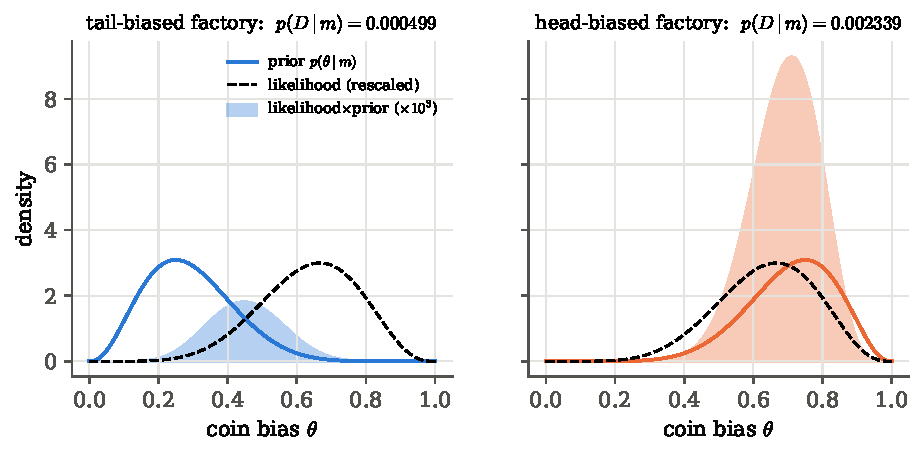
\includegraphics[width=0.95\linewidth]{figures/ch05/factories.pdf}
\caption{The evidence as an area. In each panel the solid curve is the factory's
spread of coin biases (its prior), the dashed curve the likelihood of six heads in
nine tosses (rescaled to fit), and the shaded region their product, whose area is
the evidence printed above the panel. The likelihood is the same in both panels;
only the prior differs, and with it the overlap.}
\label{5c:fig:factories}
\end{figure}

Notice what the comparison did \emph{not} give us: any statement about the bias of
this coin. For that we go back to parameter estimation inside each model. Inside the
tail-biased factory the posterior is $\mathrm{Beta}(z+a,N-z+b)$ with mean
$(z+a)/(N+a+b)=\FiveCFacMeanOne$; inside the head-biased factory the mean is
$\FiveCFacMeanTwo$. If we must give one answer for the bias without deciding on a
factory, we average the two posteriors with the model probabilities as weights,
$\FiveCFacPostOne\%$ and $\FiveCFacPostTwo\%$, which gives the mean $\FiveCFacMeanAvg$
\srcref{Kruschke}{\S10.4}. We return to this averaging in \cref{5c:sec:nested}.

\paragraph{Example: background only, or background plus signal?}
A counter records events from a source that may or may not exist. The background is
well measured: in the time of the run we expect $b=2$ background counts.

\emph{The event.} The run records $n=5$ counts.

\emph{What could have produced it?} Model $M_0$: background only, counts
$\sim\mathrm{Poisson}(b)$. Model $M_1$: background plus a signal of unknown strength
$s$, counts $\sim\mathrm{Poisson}(b+s)$. Before the run, the physics of the source
allows any $s$ between $0$ and $s_{\max}=10$ counts, and we take $s$ uniform in that
range.

\emph{How probable were five counts under each model?} Under $M_0$ there is nothing
to average: $p(n\given M_0)=e^{-b}b^n/n!=\FiveCCntZzero$. Under $M_1$ we average the
Poisson probability over the prior of $s$:
\begin{align}
  p(n\given M_1)
  &\eqby{1}\frac{1}{s_{\max}}\int_0^{s_{\max}}\frac{e^{-(b+s)}(b+s)^n}{n!}\,\dd s
   \eqby{2}\frac{1}{s_{\max}}\int_b^{b+s_{\max}}\frac{e^{-u}u^n}{n!}\,\dd u \nonumber\\
  &\eqby{3}\frac{1}{s_{\max}}\Bigl[F_n(b)-F_n(b+s_{\max})\Bigr],
  \qquad F_n(a)\equiv\sum_{j=0}^{n}\frac{e^{-a}a^j}{j!} .
  \label{5c:eq:counting}
\end{align}
\begin{explain}
  \item The evidence \eqref{5c:eq:evidence} with the uniform prior density
        $1/s_{\max}$.
  \item Substitute $u=b+s$.
  \item The identity $\int_a^\infty e^{-u}u^n/n!\,\dd u=F_n(a)$, the probability that
        a Poisson variable of mean $a$ is at most $n$. It follows by integrating by
        parts $n$ times; each step peels off one term $e^{-a}a^j/j!$. It says that the
        waiting time to the $(n+1)$-th event of a unit-rate Poisson process exceeds
        $a$ exactly when at most $n$ events happened before $a$.
\end{explain}
With $F_5(2)=\FiveCCntCdfb$ and $F_5(12)=\FiveCCntCdfbs$ this gives
$p(n\given M_1)=\FiveCCntZone$ (quadrature agrees). The Bayes factor is
$B_{10}=\FiveCCntB$ in favour of a signal, and with even prior odds the probability
that the source is there is $\FiveCCntPost$.

The Bayes factor is smaller than the best fit would suggest, and the gap is the price
of not knowing $s$. The best signal value is $\hat s=n-b=3$. At that value five
counts are $\FiveCCntLR$ times more probable than under background only. The Bayes
factor is only $\FiveCCntB$. Why? The signal model does not commit to $s=3$. It also
spreads its probability over values like $s=9$, which would have produced far more
than five counts, and those values pull the average down. The ratio of the two
numbers, $\FiveCCntOcc$, is the price the signal model pays for not knowing $s$ in
advance; \cref{5c:sec:occam} derives this price in general. The price depends on how
wide the prior range is. If the physics had allowed anything up to $s_{\max}=100$, the
same five counts would have given $B_{10}=\FiveCCntBWide$, and the data would then
favour background only. The prior range of a parameter is part of what the model
claims.

\begin{keyidea}[The evidence judges a model with its prior]
A model is a likelihood \emph{and} a prior. Its evidence is the likelihood averaged
over its prior, and the Bayes factor, the ratio of two evidences, multiplies the
prior odds of the models. A model that spreads its prior over parameter values the
data do not favour gets a smaller average, even if its best fit is excellent.
\end{keyidea}

Two cautions about reading a quoted Bayes factor. First, conventions differ.
$B_{01}=Z_0/Z_1$ and $B_{10}=Z_1/Z_0=1/B_{01}$ are both in use, and some authors call
$\ln(Z_0/Z_1)$ itself ``the Bayes factor'' \srcref{Padilla}{(13)--(14)}. Always check
which model is in the numerator and whether a logarithm has been taken. Second, a
Bayes factor is not the posterior odds. It multiplies the prior odds, so a model with
prior probability zero stays at zero whatever its Bayes factor
\srcref{Kruschke}{\S10.5.1}.

\subsection{No model is rejected on its own}
\label{5c:sec:alternatives}

Can we ask how probable one model is, without naming any competitor? No. Look at the
denominator of \eqref{5c:eq:model-post}: it is a sum over the competitors, each with
its evidence. Suppose we try to make do with ``$M$ is false'' as the only alternative.
The denominator then needs $p(\data\given\text{not }M)$, the probability of the data
given that $M$ is false. That number cannot be computed, because ``$M$ is false''
makes no prediction for the data \srcref{Sivia}{pp.~87--88}. We need well-defined
alternatives, each making its own prediction. Once we have a list of them, the
question has become model comparison.

A bad fit, on its own, does not make a model improbable. A large $\chi^2$ means a
small likelihood $p(\data\given\params,M)$ at the best parameters. The posterior
probability of $M$ also needs the prior and the evidence of the alternatives, and a
bad fit says nothing about those. What a bad fit does do is tell us to go and look
for an alternative \srcref{Sivia}{p.~88}. The history of Neptune shows that support
for a theory is always support against something \cite[\S4.1]{Trotta2008}. Finding
Neptune near the predicted position strengthened Newtonian gravity against a theory
that predicted no planet there. It did nothing to Newton's standing against
Einstein's gravity, which predicts the same orbit. How much an observation supports a
theory depends on what it is compared with.
\section{Occam's razor from the evidence}
\label{5c:sec:occam}

A better fit alone cannot choose between models. Here is why. Forty measurements
$y_i$ are taken at equally spaced points $x_i$ between $0$ and $10$, each with
Gaussian noise of standard deviation $\sigma=1$. One physicist says the points
scatter about a straight line, $y=a+bx$. A second says there is also a Gaussian bump
on top of the line, the signature of a resonance, with known width $W=0.5$, height $A$
and unknown position $\mu$. Whatever the data, the second physicist's best fit is at
least as good as the first's, because setting $A=0$ turns the bump model into the
line. So the best-fit $\chi^2$ never prefers the simpler model, and a rule that picks
the model with the smallest $\chi^2$ would find a bump in every data set. For the
same reason a tenth-order polynomial always beats a straight line, and nobody believes
it \srcref{Sivia}{p.~81}.

The evidence settles this without any extra rule. The more flexible model spread its
prior over many parameter values, and the data rule most of them out. So its
\emph{average} likelihood, which is the evidence, can be low even when its
\emph{best} likelihood is high.

\subsection{Mr A and Mr B}
\label{5c:sec:mrab}

The simplest version is a story due to Jeffreys, as told by Gull and Sivia
\srcref{Sivia}{\S4.1}. Mr A has a theory with no adjustable parameter. Mr B has a
theory with one adjustable parameter $\lambda$. Whose theory should we prefer, given
data $\data$?

\emph{The event} is the data $\data$. \emph{The hypotheses} are $A$ and $B$.
\emph{How probable was $\data$ under each?} For Mr A this is a straightforward
likelihood, $p(\data\given A)$, since his theory predicts the data with nothing left
to choose. Mr B cannot predict the data without a value of $\lambda$, so his
probability of the data is the evidence \eqref{5c:eq:evidence}, an average over his
prior for $\lambda$. To make it concrete, Sivia makes two simple assumptions
(\cref{5c:fig:mrb}):
\begin{enumerate}[itemsep=1pt,leftmargin=1.6em]
  \item Before seeing the data, Mr B will only say that $\lambda$ lies between
        $\lambda_{\min}$ and $\lambda_{\max}$, so his prior is uniform:
        $p(\lambda\given B)=1/(\lambda_{\max}-\lambda_{\min})$ in that range, zero
        outside \srcref{Sivia}{(4.4)}.
  \item His likelihood has a single peak at the best value $\lambda_0$, of height
        $p(\data\given\lambda_0,B)$, and near the peak it is Gaussian with width
        $\delta\lambda$ \srcref{Sivia}{(4.5)}:
        \[
          p(\data\given\lambda,B)\approx p(\data\given\lambda_0,B)\,
          \exp\!\Bigl[-\frac{(\lambda-\lambda_0)^2}{2\,\delta\lambda^2}\Bigr].
        \]
\end{enumerate}
The likelihood is a function of $\lambda$ but not a density in $\lambda$: its area is
not one. Its height at the peak is the probability of the data at the best value.

\begin{figure}[htbp]
\centering
\begin{tikzpicture}[x=0.9cm,y=3.2cm,font=\small]
  \draw[->,softgray] (0,0) -- (10.6,0) node[right,black] {$\lambda$};
  \draw[->,softgray] (0,0) -- (0,1.18);
  \fill[formblue!15] (1,0) rectangle (9,0.25);
  \draw[form] (1,0) -- (1,0.25) -- (9,0.25) -- (9,0);
  \draw[bdryred,thick,domain=2.5:8.5,samples=120]
    plot (\x,{exp(-(\x-5.5)^2/(2*0.36))});
  \draw[bdryred,dashed,thin] (5.5,0) -- (5.5,1);
  \draw[<->,tangentgreen,thick] (4.9,0.6065) -- (6.1,0.6065);
  \node[tangentgreen!70!black,anchor=west] at (6.25,0.63) {$\pm\delta\lambda$};
  \node[anchor=east] at (0,1) {$p(\data\given\lambda_0,B)$};
  \draw[softgray] (-0.08,1) -- (0.08,1);
  \node[anchor=east] at (0,0.25) {$\dfrac{1}{\lambda_{\max}-\lambda_{\min}}$};
  \draw[softgray] (-0.08,0.25) -- (0.08,0.25);
  \node[below] at (1,0) {$\lambda_{\min}$};
  \node[below] at (9,0) {$\lambda_{\max}$};
  \node[below] at (5.5,0) {$\lambda_0$};
  \node[formblue,anchor=south] at (2.4,0.27) {prior};
  \node[bdryred,anchor=west] at (6.6,0.95) {likelihood};
\end{tikzpicture}
\caption{Mr B's prior and likelihood for his parameter. The prior (blue box) spreads
unit probability evenly over the range $\lambda_{\min}$ to $\lambda_{\max}$; its height
is drawn exaggerated. The likelihood (red) is large only within about $\delta\lambda$ of
its peak. The evidence is the likelihood averaged over the box, so it is roughly the
peak height times the fraction of the box the peak occupies.}
\label{5c:fig:mrb}
\end{figure}

With these two assumptions the average over Mr B's prior can be done by hand:
\begin{align}
  p(\data\given B)
  &\eqby{1}\int p(\data\given\lambda,B)\,p(\lambda\given B)\,\dd\lambda
   \eqby{2}\frac{1}{\lambda_{\max}-\lambda_{\min}}
     \int_{\lambda_{\min}}^{\lambda_{\max}}p(\data\given\lambda,B)\,\dd\lambda \nonumber\\
  &\eqby{3}\frac{p(\data\given\lambda_0,B)}{\lambda_{\max}-\lambda_{\min}}
     \int_{-\infty}^{\infty}e^{-(\lambda-\lambda_0)^2/2\delta\lambda^2}\,\dd\lambda
   \eqby{4}\frac{p(\data\given\lambda_0,B)\;\delta\lambda\sqrt{2\pi}}{\lambda_{\max}-\lambda_{\min}} .
  \label{5c:eq:mrb}
\end{align}
\begin{explain}
  \item The evidence \eqref{5c:eq:evidence} for Mr B.
  \item The uniform prior is a constant inside the range and zero outside, so it comes
        out of the integral and restricts the limits \srcref{Sivia}{(4.6)}.
  \item The Gaussian form of the likelihood. We also assumed the peak lies well inside
        the range, so extending the limits to $\pm\infty$ loses almost nothing.
  \item The Gaussian integral $\int e^{-u^2/2s^2}\dd u=s\sqrt{2\pi}$ \srcref{Sivia}{(4.7)}.
\end{explain}
Put this into the odds \eqref{5c:eq:odds} with $M_1=A$ and $M_2=B$:
\begin{equation}
  \frac{\Prob(A\given\data)}{\Prob(B\given\data)}
  =\underbrace{\frac{\Prob(A)}{\Prob(B)}}_{\text{prior odds}}
   \times\underbrace{\frac{p(\data\given A)}{p(\data\given\lambda_0,B)}}_{\text{best-fit ratio}}
   \times\underbrace{\frac{\lambda_{\max}-\lambda_{\min}}{\delta\lambda\sqrt{2\pi}}}_{\text{Occam factor}} .
  \label{5c:eq:ockham}
\end{equation}
This is Sivia's (4.8). Each of the three factors answers its own question. The first
says what we thought before the data. The second says how well each theory does at
its best; since Mr B can always tune $\lambda$, this ratio can only favour him. The
third is new. It compares the range of $\lambda$ that Mr B's theory allowed before the
data, $\lambda_{\max}-\lambda_{\min}$, with the range the data allow, about
$\delta\lambda$. The first is usually much wider, so this factor is large and favours
Mr A. It is called the
\newterm{Occam factor} (Sivia writes Ockham), because it puts a number on William of
Ockham's rule that ``it is vain to do with more what can be done with fewer''
\srcref{Sivia}{p.~84}.

\begin{workdef}[Occam factor]
For a model with parameters, the \newterm{Occam factor} is the ratio of its evidence
to its best-fit likelihood,
\[
  \frac{Z}{\Like_{\max}}\approx\frac{\text{volume of parameter space allowed by the posterior}}
  {\text{volume allowed by the prior}}\le 1 ,
\]
\unpack{the fraction of the prior's parameter range that the data leave standing}.
The evidence is the best fit times the Occam factor.
\end{workdef}

Reading \eqref{5c:eq:ockham} in a few limits tells us how the razor behaves
\srcref{Sivia}{pp.~84--86}:
\begin{itemize}[itemsep=1pt,leftmargin=1.2em]
  \item \emph{Good data, genuine effect.} If Mr B's extra parameter is really needed,
        the best-fit ratio is tiny (his fit is much better) and it overwhelms the
        Occam factor. Most of the time the goodness of fit decides.
  \item \emph{Good data, no effect.} If Mr B's fit is not much better, the best-fit
        ratio stays near one, while more data make $\delta\lambda$ smaller and the Occam
        factor larger. Mr A is favoured ever more strongly as the data improve.
  \item \emph{Poor data.} If the data barely constrain $\lambda$, then $\delta\lambda$
        approaches the prior range and the likelihood is flat, so both the best-fit
        ratio and the Occam factor approach one. The posterior odds return to the
        prior odds: poor data have taught us nothing.
  \item \emph{Unbounded prior.} If $\lambda_{\max}-\lambda_{\min}\to\infty$, the Occam
        factor is infinite and Mr B always loses. Jeffreys worried about this. In
        practice the range is always bounded by what we know. A new fifth force with
        a huge coupling would have been noticed long ago, so its strength has an upper
        bound before any new experiment.
\end{itemize}

Two variations make the razor sharper.
\begin{itemize}[itemsep=1pt,leftmargin=1.2em]
  \item \emph{Both theories have one parameter.} Give Mr A a parameter $\mu$, with a
        uniform prior and a Gaussian likelihood of width $\delta\mu$, just like Mr B's.
        Each evidence now carries its own Occam factor. With equal prior ranges the
        ranges cancel, and the posterior odds are the best-fit ratio times
        $\delta\mu/\delta\lambda$ \srcref{Sivia}{(4.9)}. So for equally good fits the
        theory with the \emph{larger} error bar wins. That sounds backwards, but a
        larger error bar means that more of the theory's parameter values agree with
        the data.
  \item \emph{The same theory, two prior ranges.} Let Mr A and Mr B hold the same
        theory, but let Mr A claim a narrower prior range, still wide enough to
        contain the fit. Everything cancels except the ranges, and the odds are the
        ratio of the ranges in Mr A's favour. He predicted the parameter more
        precisely, and the evidence rewards him for it.
\end{itemize}

None of this touches parameter estimation. Inside Mr B's theory the posterior for
$\lambda$ is likelihood times prior divided by the evidence \srcref{Sivia}{(4.10)}.
The prior is the constant $1/(\lambda_{\max}-\lambda_{\min})$, and it appears in both
the numerator and the evidence \eqref{5c:eq:mrb}, so it cancels; so does the peak
height. What is left is the Gaussian $\lambda=\lambda_0\pm\delta\lambda$, whatever the
range, as long as the range contains the peak. The range matters only when we compare
models. The same equation serves both purposes; we are asking it different questions.

\paragraph{Example: the counting experiment again.}
In \cref{5c:sec:bf} five counts on an expected background of $b=2$ gave a best-fit
likelihood ratio of $\FiveCCntLR$ for a signal, but a Bayes factor of only
$\FiveCCntB$. The Occam factor explains the difference. We need the width $\delta s$ of
the likelihood. The log-likelihood is $\ln p(n\given s)=-(b+s)+n\ln(b+s)-\ln n!$. Its
second derivative is $-n/(b+s)^2$, and at the peak $\hat s=n-b$, where $b+s=n$, this
is $-1/n$. A Gaussian of width $\delta s$ has second derivative of its logarithm
$-1/\delta s^2$, so $\delta s=\sqrt n=\sqrt5$. The prior range is $s_{\max}=10$, and
\eqref{5c:eq:mrb} gives the Occam factor
\[
  \frac{\delta s\sqrt{2\pi}}{s_{\max}}=\frac{\sqrt{10\pi}}{10}\approx0.56 ,
\]
close to the exact ratio $\FiveCCntOcc$ of evidence to best fit. The Gaussian
approximation is rough for a Poisson likelihood with five counts, but the size of the
penalty is right: a signal prior of width $10$ against a data width of about $2.2$.

\paragraph{Example: must be fair, or anything goes?}
Kruschke's version compares two coin factories that differ only in how widely they
spread their coin biases \srcref{Kruschke}{\S10.5}. The ``must-be-fair'' factory makes
coins with $\theta\sim\mathrm{Beta}(500,500)$, all very close to $0.5$. The
``anything-goes'' factory makes $\theta\sim\mathrm{Beta}(1,1)$, uniform on $[0,1]$. The
second model is the more flexible: it contains a coin matching any observed fraction of
heads. The evidence of each is \eqref{5c:eq:beta-evidence}. For $z=15$ heads in $N=20$
tosses the Bayes factor of fair against anything is $\FiveCFairFifteen$: the fair model
has no bias near $0.75$, and loses. For $z=11$ heads it is $\FiveCFairEleven$: now the
fair model wins, although the anything model contains the bias $0.55$ that matches the
data exactly. The anything model pays for spreading its prior over biases like $0.1$
and $0.9$ that these data rule out. \Cref{5c:fig:fair} shows the pattern for every
possible $z$: the simpler model wins whenever the data are consistent with it, here for
$\FiveCFairZmin\le z\le\FiveCFairZmax$.

\begin{figure}[htbp]
\centering
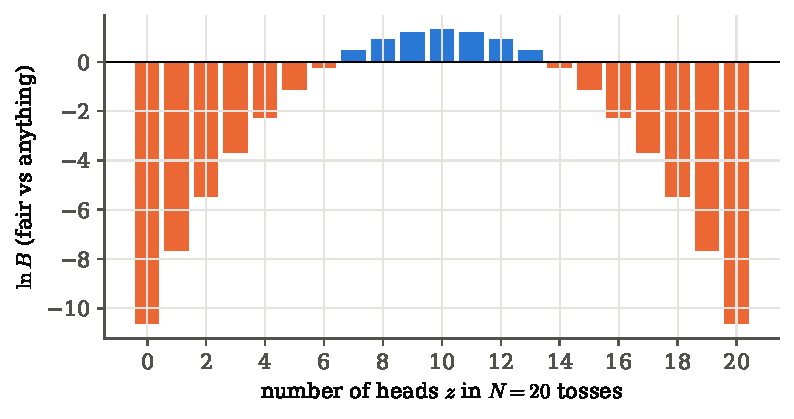
\includegraphics[width=0.78\linewidth]{figures/ch05/fair_vs_anything.pdf}
\caption{Natural Occam's razor for coins. For each possible number of heads in twenty
tosses, the bar is the log Bayes factor of the must-be-fair factory against the
anything-goes factory. Near ten heads the simple model wins by a modest factor (blue);
far from ten it loses by a large one (orange), because it simply cannot produce such
data.}
\label{5c:fig:fair}
\end{figure}

The picture is asymmetric, and that is typical. A simple model that is wrong is
punished hard, because it has no parameter value near the data. A flexible model that
is unnecessary is punished gently, by a factor of a few, the size of its Occam factor.

\subsection{Many parameters: the Laplace approximation}
\label{5c:sec:laplace-evidence}

The same argument works in $D$ dimensions. Near its peak $\hat\params$ the logarithm
of the likelihood is approximately quadratic,
\[
  \ln\Like(\params)\approx\ln\Like_{\max}-\tfrac12(\params-\hat\params)\T\Fish\,(\params-\hat\params),
\]
where $\Fish$ is the matrix of second derivatives of $-\ln\Like$ at the peak
\unpack{the curvature of the log-likelihood, the Fisher matrix of \cref{ch:10}
evaluated on these data}. Its inverse is the covariance of the Gaussian approximation
to the posterior. If the prior $\pi(\params)$ changes little across the peak,
\begin{align}
  Z
  &\eqby{1}\int\Like(\params)\,\pi(\params)\,\dd^D\params
   \relby{2}{\approx}\Like_{\max}\,\pi(\hat\params)
     \int e^{-\frac12(\params-\hat\params)\T\Fish(\params-\hat\params)}\,\dd^D\params \nonumber\\
  &\eqby{3}\Like_{\max}\,\pi(\hat\params)\,\frac{(2\pi)^{D/2}}{\sqrt{\det\Fish}}
   \eqby{4}\Like_{\max}\times\frac{(2\pi)^{D/2}\sqrt{\det\Cmat}}{V_\pi} .
  \label{5c:eq:laplace-evidence}
\end{align}
\begin{explain}
  \item The evidence, with $\Like(\params)=p(\data\given\params,M)$ and
        $\pi(\params)=p(\params\given M)$.
  \item The quadratic expansion of $\ln\Like$, and the prior taken out at the peak.
  \item The $D$-dimensional Gaussian integral. Rotate to the eigenvectors of the
        symmetric positive matrix $\Fish$; the integral factorises into $D$
        one-dimensional integrals $\sqrt{2\pi/f_k}$, one per eigenvalue $f_k$, and the
        product of the eigenvalues is $\det\Fish$.
  \item For a uniform prior on a region of volume $V_\pi$, $\pi(\hat\params)=1/V_\pi$;
        and $\Cmat=\Fish^{-1}$, so $1/\sqrt{\det\Fish}=\sqrt{\det\Cmat}$.
\end{explain}
This is the \newterm{Laplace approximation} to the evidence
\srcref{Sivia}{(4.20)}, \cite[eqs.~(24)--(25)]{Trotta2008}. The factor
$(2\pi)^{D/2}\sqrt{\det\Cmat}$ is the volume of the posterior's ``error ellipsoid'',
so the Occam factor of \eqref{5c:eq:ockham} generalises to the ratio of the posterior
volume to the prior volume. In one dimension it is $\sqrt{2\pi}\,\delta\lambda$ over
$\lambda_{\max}-\lambda_{\min}$ again.

\begin{keyidea}[Evidence $\approx$ best fit $\times$ Occam factor]
\[
  Z\;\approx\;\Like_{\max}\times\frac{V_{\rm posterior}}{V_{\rm prior}} .
\]
A model is rewarded for fitting the data well and penalised by the fraction of its
prior parameter space that the data rule out. Every parameter the data constrain adds
a factor $\sqrt{2\pi}\,\sigma_k/(\text{prior range}_k)$ (for uncorrelated parameters); a model is favoured only if its
better fit pays for all of them.
\end{keyidea}

Two remarks keep the formula honest. First, a parameter the data do not constrain at
all has a posterior as wide as its prior, contributes a factor one, and costs nothing.
Adding the price of fish at Billingsgate market to a cosmological model changes no
prediction, so the likelihood is flat in it and the evidence is unchanged however wide
its prior \srcref{HobsonBMC}{p.~85}, \cite[p.~16]{Trotta2008}. What the evidence
penalises is not the number of parameters but wasted predictive range: parameter
values the model allowed and the data rule out. Hobson and collaborators put it as
``the Bayesian evidence rewards model predictiveness'' \srcref{HobsonBMC}{p.~83}.
Second, if the likelihood has several separate peaks, each contributes its own
term. With $M$ identical bumps whose labels can be permuted, the likelihood has $M!$
equivalent peaks and the Laplace sum must count all of them \srcref{Sivia}{(4.20)}.
An exact integral over the whole prior box counts them automatically.

\subsection{A line, or a line plus a bump?}
\label{5c:sec:bump}

Back to the forty points. The two models are
\begin{align*}
  M_0\ (\text{line}):\quad & y_i=a+bx_i+\epsilon_i,\\
  M_1\ (\text{line}+\text{bump}):\quad & y_i=a+bx_i+A\,e^{-(x_i-\mu)^2/2W^2}+\epsilon_i,
  \qquad\epsilon_i\iid\Normal(0,1),
\end{align*}
with the bump width $W=\FiveCWidth$ known. The priors are part of the models and are
fixed before looking at the data: $a$ uniform on $[0,20]$ and $b$ uniform on $[-2,2]$
in both models; in $M_1$ also $A$ uniform on $[0,A_{\max}]$ with
$A_{\max}=\FiveCAmax$ (a generous ceiling, ten times the noise) and $\mu$ uniform
on $[0,10]$ (the range we measured). We simulate two data sets, one with a real bump of
height $\FiveCTrueA$ at $\mu=\FiveCTrueMu$ and one with no bump, both on the line
$y=5+0.3x$ (\cref{5c:fig:bump-fits}).

\begin{figure}[htbp]
\centering
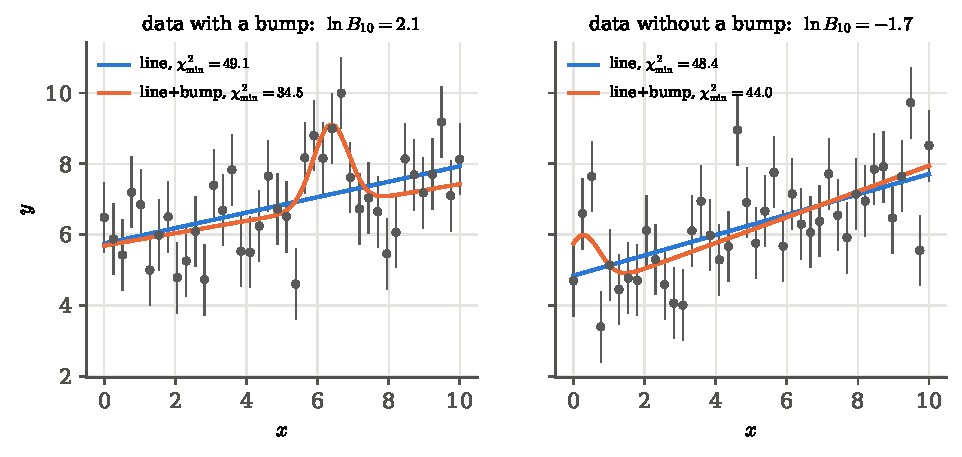
\includegraphics[width=\linewidth]{figures/ch05/line_bump_fits.pdf}
\caption{Two simulated data sets of forty points with unit error bars, and the best fits
of both models. Left: a bump of height $2.5$ is present near $x=6.2$; the bump model
finds it and its $\chi^2$ drops by $\FiveCBumpDChi$. Right: there is no bump; the bump
model still finds a small improvement by fitting a noise fluctuation. The log Bayes
factor of bump against line is printed above each panel.}
\label{5c:fig:bump-fits}
\end{figure}

\paragraph{Integrating out the line exactly.}
The evidence of $M_1$ is a four-dimensional integral over $(a,b,A,\mu)$. The line
parameters $a,b$ enter the model linearly, so the likelihood is Gaussian in them and
their integral can be done exactly. That leaves a two-dimensional integral over
$(A,\mu)$ for the grid. The question for each bump is: once the bump $(A,\mu)$ is
subtracted, how well can the best line fit what remains? Write the data as the vector
$\bm y$ (here $N=40$), the two line shapes as the columns of the $N\times2$ matrix
$X=(\bm1,\bm x)$, and the bump shape at position $\mu$ as the vector $\bm g_\mu$. For
fixed $(A,\mu)$ the line fits $\bm y-A\bm g_\mu$. What it cannot fit is the part of
$\bm y-A\bm g_\mu$ that points in directions no line can reach,
$P_\perp(\bm y-A\bm g_\mu)$, where $P_\perp=\Id-X(X\T X)^{-1}X\T$ is the projector onto
those directions. Writing $\bm r=P_\perp\bm y$ and $\bm u_\mu=P_\perp\bm g_\mu$,
\begin{align}
  \chi^2_{\min}(A,\mu)-\chi^2_{\min,\rm line}
  &\eqby{1}\lVert\bm r-A\bm u_\mu\rVert^2-\lVert\bm r\rVert^2
   \eqby{2}-2A\,\bm r\cdot\bm u_\mu+A^2\,\bm u_\mu\cdot\bm u_\mu .
  \label{5c:eq:dchi2}
\end{align}
\begin{explain}
  \item With $\sigma=1$, the minimum of $\chi^2$ over the line is the squared length of
        the residual the line cannot absorb; for the line model alone that residual is
        $\bm r$.
  \item Expand the square: $\lVert\bm r-A\bm u\rVert^2=\lVert\bm r\rVert^2-2A\,\bm r\cdot\bm u+A^2\lVert\bm u\rVert^2$.
\end{explain}
The integral over $(a,b)$ at fixed $(A,\mu)$ is the same Gaussian integral in both
models, because both use the same line shapes and the same prior box for the line. It
cancels in the Bayes factor, which is therefore
\begin{equation}
  B_{10}=\frac{1}{A_{\max}\cdot10}\int_0^{A_{\max}}\!\!\int_0^{10}
  \exp\!\Bigl[-\tfrac12\bigl(\chi^2_{\min}(A,\mu)-\chi^2_{\min,\rm line}\bigr)\Bigr]\,\dd\mu\,\dd A .
  \label{5c:eq:bump-bf}
\end{equation}
In words: the likelihood ratio of each bump to the best line, averaged over the prior
box of bumps. (We assumed that the line's prior box is wide enough to contain its
likelihood; with the boxes above it is, by many standard deviations.)

\pyfile[firstline=72,lastline=91,firstnumber=72]{code/ch05/lib_bump.py}{The Bayes
factor of bump against line on a grid}

Lines 74--78 build \eqref{5c:eq:dchi2} for every $(A,\mu)$ on the grid at once: the
projected data $\bm r$, the projected bump shapes $\bm u_\mu$ (one column per
position), their dot products, and the quadratic in $A$. Line 86 exponentiates to get
the likelihood ratio to the best line; lines 87--88 average it over $\mu$ and then over
$A$ with the trapezoid rule, which is \eqref{5c:eq:bump-bf}. Working with the ratio to
the best line keeps the numbers of order one; the raw likelihoods are about $e^{-60}$.

\paragraph{The data with a bump.}
The line has $\chi^2_{\min}=\FiveCBumpChiLine$ for $38$ degrees of freedom, the bump
model $\FiveCBumpChiBump$ at $\hat A=\FiveCBumpAhat$, $\hat\mu=\FiveCBumpMuhat$. The best
bump improves the fit by $\Delta\chi^2=\FiveCBumpDChi$, a best-fit likelihood ratio of
$e^{\FiveCBumplnLR}$. The Bayes factor is $\ln B_{10}=\FiveCBumplnB$ ($B_{10}=\FiveCBumpB$;
a grid of half the resolution changes $\ln B_{10}$ by $\FiveCBumpGridErr$). The
difference, $\ln B_{10}-\tfrac12\Delta\chi^2=\FiveCBumplnOccam$, is the logarithm of the
Occam factor. Here the bump is favoured, but by odds of $\FiveCBumpB$ to $1$, not by the
$e^{\FiveCBumplnLR}$ that the fit improvement alone suggests.

The Laplace approximation \eqref{5c:eq:laplace-evidence} lets us read the Occam factor
off the map of \cref{5c:fig:bump-map}. At the best fit the posterior standard deviations
are $\sigma_A=\FiveCSigA$ and $\sigma_\mu=\FiveCSigMu$, so the posterior area in the
$(A,\mu)$ plane is $2\pi\sqrt{\det\Cmat_{A\mu}}=\FiveCSigAMuVol$, against a prior area of
$A_{\max}\times10=\FiveCPriorAMuVol$. Their ratio, $\FiveCLapOccRatio$, is the Occam
factor, and the Laplace estimate of the Bayes factor is $\ln B_{10}=\FiveCLapLnB$,
close to the exact $\FiveCBumplnB$. The bump model allowed $\FiveCPriorAMuVol$ square
units of bumps and the data kept only $\FiveCSigAMuVol$ of them.

\begin{figure}[htbp]
\centering
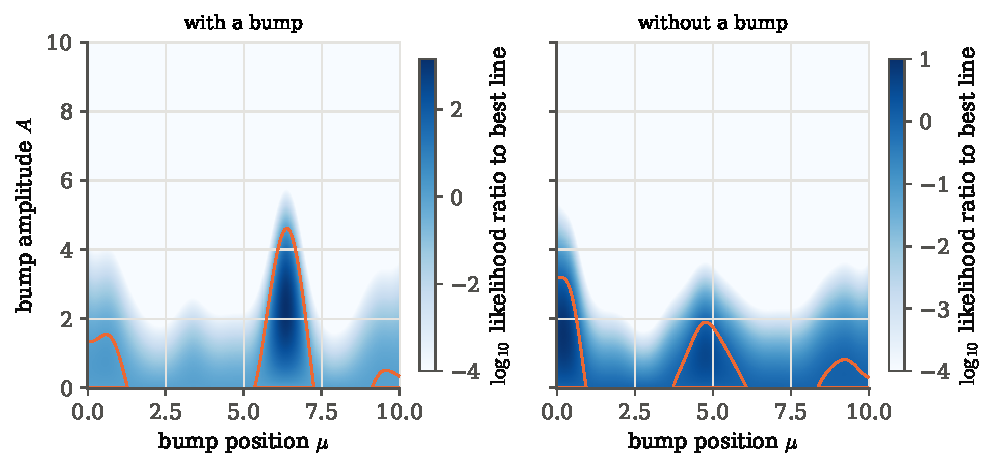
\includegraphics[width=\linewidth]{figures/ch05/line_bump_map.pdf}
\caption{The likelihood of every bump in the prior box, relative to the best line, in
powers of ten. With a bump in the data (left) a small island near
$\mu=\FiveCBumpMuhat$, $A=\FiveCBumpAhat$ is
far better than the line; almost all the rest of the box is worse. Without a bump
(right) nothing is much better than the line. The orange contour marks a likelihood
ratio of one. The Bayes factor is the average of this map over the box.}
\label{5c:fig:bump-map}
\end{figure}

\paragraph{The data without a bump.}
Here the bump model still finds something: a noise fluctuation at
$\hat\mu=\FiveCFlatMuhat$ improves $\chi^2$ from $\FiveCFlatChiLine$ to
$\FiveCFlatChiBump$. A $\chi^2$ drop of a few units for two extra parameters is what
noise does. The evidence agrees: $\ln B_{10}=\FiveCFlatlnB$, so the line is favoured by
a factor $1/\FiveCFlatB$. The Occam factor, $e^{\FiveCFlatlnOccam}$, outweighs the
modest improvement of the fit. For both data sets the razor cuts in the right
direction, and it needed no rule beyond the sum and product rules.

\paragraph{If we had known where to look.}
Not knowing where the bump sits has a price, and the evidence charges it
automatically. Suppose theory had predicted the resonance at $\mu=\FiveCTrueMu$, so
that $M_1$ has only the amplitude free. Then the prior no longer wastes probability on
positions the data rule out. For the data with a bump, $\ln B_{10}=\FiveCFixLnB$
($B_{10}=\FiveCFixB$), which is $\FiveCFreeOverFix$ times larger than with the position
free. At the predicted position the amplitude is $\FiveCFixAhat\pm\FiveCFixSigA$, a
local significance of $\FiveCFixZscore\sigma$. So not knowing the position costs a
factor of $\FiveCFreeOverFix$. This is the look-elsewhere effect of \cref{ch:04}. There it
needed a separate trials factor; here it appears by itself, as the Occam factor of the
parameter $\mu$.
\section{Reading a Bayes factor}
\label{5c:sec:reading}

With three years of WMAP data and the large-scale-structure surveys of the time, a
cosmological model with a free spectral index $n_s$ was found to have a log evidence
$1.99\pm0.26$ higher than the Harrison--Zel'dovich model with $n_s=1$
\srcref{HobsonBMC}{Table~4.4}. The same data gave $n_s=0.958\pm0.016$, nearly three
standard deviations from one. How impressed should we be by $\ln B=2$? Is it the same
statement as ``three sigma'', the significance of \cref{ch:04}? And would another
reasonable choice of prior have given a different number?

\subsection{The Jeffreys scale}
\label{5c:sec:jeffreys}

A Bayes factor multiplies the prior odds. With even prior odds and only two models,
the posterior probability of the favoured model is
\begin{equation}
  \Prob(M_1\given\data)=\frac{B_{10}}{1+B_{10}},
  \qquad\text{e.g.}\quad
  B_{10}=e^{1}\approx2.7\ \to\ 0.73,\quad
  e^{2.5}\approx12\ \to\ 0.92,\quad
  e^{5}\approx150\ \to\ 0.993 ,
  \label{5c:eq:bf-prob}
\end{equation}
from \eqref{5c:eq:odds} with $\Prob(M_1)=\Prob(M_0)$ and $\Prob(M_1\given\data)+\Prob(M_0\given\data)=1$.
Jeffreys proposed words for these levels, and a version of his scale is quoted in
almost every cosmology paper that computes an evidence
\srcref{HobsonBMC}{\S4.5}, \srcref{Padilla}{Table~II}, \cite[Table~1]{Trotta2008},
\cite{KassRaftery1995}:

\begin{center}
\small
\renewcommand{\arraystretch}{1.15}
\begin{tabular}{@{}cccp{2.6cm}p{1.6cm}p{1.6cm}@{}}
\toprule
$\lvert\ln B\rvert$ & odds & probability & Jeffreys & Hobson et al. & Trotta \\\midrule
$<1$ & $<3:1$ & $<0.75$ & not worth more than a bare mention & --- & inconclusive\\
$1$--$2.5$ & $3:1$ to $12:1$ & $0.75$--$0.92$ & significant & weak & weak\\
$2.5$--$5$ & $12:1$ to $150:1$ & $0.92$--$0.993$ & strong to very strong & significant & moderate\\
$>5$ & $>150:1$ & $>0.993$ & decisive & strong & strong\\
\bottomrule
\end{tabular}
\end{center}

\noindent The probability column assumes even prior odds and two models, and the table
rounds $e^{1}\approx2.7$ up to $3:1$. The
thresholds are a convention, calibrated on experience, not a theorem. Three cautions
come with them.
\begin{itemize}[itemsep=1pt,leftmargin=1.2em]
  \item \emph{The scale is logarithmic.} Moving up one level needs roughly ten times
        more support. Evidence accumulates slowly \cite[p.~14]{Trotta2008}.
  \item \emph{It applies to posterior odds.} The words are meant for the ratio of
        posterior model probabilities; they coincide with the Bayes factor only when
        the prior odds are even \srcref{HobsonBMC}{p.~90}. A Bayes factor of $20$
        for an exotic model that we believed at $1:1000$ beforehand still leaves it at
        $1:50$.
  \item \emph{The priors are uncertain too.} Because a Bayes factor depends on the
        prior widths (\cref{5c:sec:prior-width}), Hobson and collaborators soften
        Jeffreys' words: $\ln B$ between $1$ and $2.5$ is only ``weak'', between $2.5$ and
        $5$ ``significant'', above $5$ ``strong'' (third column of the table) \srcref{HobsonBMC}{p.~90}.
        Trotta's column is similar. Kruschke's rule of thumb, ``substantial'' above $B=3$,
        is the same first threshold \srcref{Kruschke}{p.~268}.
\end{itemize}
An evidence computed numerically also has an error, like $\pm0.26$ above, and a
difference in $\ln B$ smaller than its error means nothing.

\paragraph{Example: is the primordial spectrum tilted?}
The two models are the tilted one ($n_s$ free) and Harrison--Zel'dovich ($n_s=1$). In
the WMAP analysis \srcref{HobsonBMC}{pp.~91--93} the log Bayes factor of tilted
against Harrison--Zel'dovich grew as the data improved:
\begin{itemize}[itemsep=1pt,leftmargin=1.2em]
  \item first-year WMAP with other data: $\ln B=-0.58\pm0.12$, inconclusive, with a
        slight preference for the simpler model;
  \item three-year WMAP alone: $0.34\pm0.26$, still inconclusive;
  \item three-year WMAP with other data: $1.99\pm0.26$, odds of about $7:1$,
        ``significant'' in Jeffreys' words and ``weak'' in the softer scale.
\end{itemize}
Then inflation was taken seriously. Slow roll predicts a tilt \emph{and} a
tensor-to-scalar ratio $r$, so this model has two new parameters. Its verdict depended
on the prior for $r$. With $r$ uniform between $0$ and $1$, the $n_s$--$r$ model came
out at $\ln B=-1.45\pm0.45$, disfavoured against Harrison--Zel'dovich. With $\ln r$
uniform from $-80$ to $0$ it came out at $1.90\pm0.24$, about as good as the
$n_s$-only model. The data were identical. Why did the prior on $r$ matter so much?
The data allow only small $r$. A uniform prior on $[0,1]$ puts most of its weight on
larger values of $r$, which the data exclude, so it pays an Occam factor. The
logarithmic prior puts most of its weight on tiny $r$, which the data cannot
distinguish from zero. There the likelihood is flat, so this prior pays almost
nothing: this is the Billingsgate effect of \cref{5c:sec:laplace-evidence}.

\subsection{The prior width sets the price}
\label{5c:sec:prior-width}

The wider the prior range of an extra parameter, the less the data favour it. The
reason is the Occam factor of \eqref{5c:eq:ockham}: it is the data's range divided by
the prior range. So once the prior range is much wider than the likelihood, the Bayes
factor in favour of the extra parameter falls in proportion to the range: every factor
of ten in the range subtracts $\ln10\approx2.3$ from $\ln B_{10}$. Take the bump of
\cref{5c:sec:bump} and vary only the prior range $A_{\max}$ of its amplitude
(\cref{5c:fig:width}). For the data with a bump, $\ln B_{10}$ first rises, because a
prior that stops below the fitted amplitude $\hat A=\FiveCBumpAhat$ cannot reach the
bump; it peaks once the range just covers it; then it falls along a straight line of
slope $-1$ in $\ln A_{\max}$. At $A_{\max}=100$ it is $\FiveCBumpLnBHundred$, against
$\FiveCBumplnB$ at $A_{\max}=10$: the same bump, with the same local significance of
$\FiveCFixZscore\sigma$, is now worth ten times less evidence. For the data
without a bump $\ln B_{10}$ starts at zero (for a tiny range the two models are the
same model) and falls steadily, reaching $\FiveCFlatLnBHundred$ at $A_{\max}=100$.

\begin{figure}[htbp]
\centering
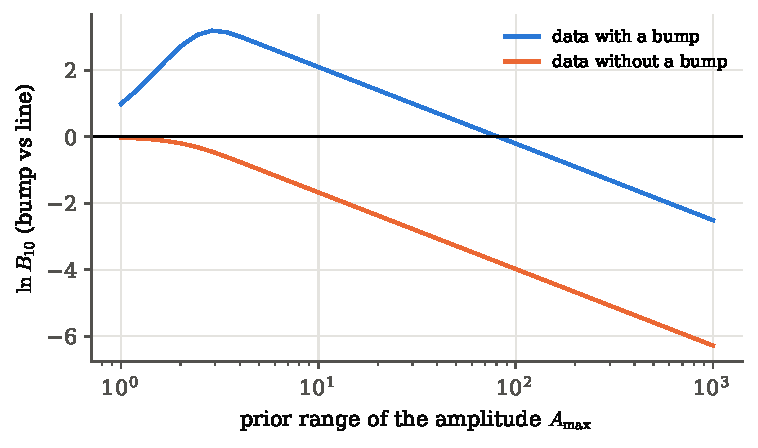
\includegraphics[width=0.75\linewidth]{figures/ch05/line_bump_width.pdf}
\caption{The Bayes factor of bump against line as the prior range of the bump amplitude
is widened, for the two data sets of \cref{5c:fig:bump-fits}. Past the fitted amplitude
both curves fall by $\ln 10$ per decade of $A_{\max}$: each widening of the prior
spreads the model's probability over more bumps the data rule out.}
\label{5c:fig:width}
\end{figure}

So which range is right? The answer has to come from physics, before the data: the
largest resonance the experiment would already have noticed, the range of $n_s$ that
slow-roll inflation allows ($0.8\lesssim n_s\lesssim1.2$), the coupling a fifth force
could have without being seen \srcref{Sivia}{p.~85}, \cite[\S4.5]{Trotta2008}. If
several plausible ranges give the same qualitative verdict, the verdict is robust. If
not, the honest report is the Bayes factor as a function of the range, which is what
\cref{5c:fig:width} is. In the $(\text{information},\text{significance})$ plane of
\cref{5c:sec:lindley} a change of prior width is a horizontal shift
\cite[\S4.4]{Trotta2008}.

\paragraph{Example: two vague priors, one posterior, two verdicts.}
Two priors that both claim to know nothing can give opposite verdicts
\srcref{Kruschke}{\S10.6}. A coin gives $z=65$ heads in $N=100$ tosses. Model one is
must-be-fair, $\theta\sim\mathrm{Beta}(500,500)$, where $\theta$ is the probability of
heads. Model two is anything-goes, and we must choose a vague prior for it.
\begin{itemize}[itemsep=1pt,leftmargin=1.2em]
  \item With $\mathrm{Beta}(1,1)$, uniform, the Bayes factor of fair against anything
        is $\FiveCHalUnifBF$: anything-goes wins by $8:1$.
  \item With the Haldane prior $\mathrm{Beta}(0.01,0.01)$, recommended by some
        statisticians as maximally uninformative, the Bayes factor is
        $\FiveCHalHaldBF$: must-be-fair wins by nearly $6:1$.
\end{itemize}
The verdict reversed. Yet the posteriors of $\theta$ under the two vague priors are
practically the same: their $95\%$ HDIs are $[\FiveCHdiUnifLo,\FiveCHdiUnifHi]$ and
$[\FiveCHdiHaldLo,\FiveCHdiHaldHi]$, and both exclude $0.5$. How can the posterior stay
put while the evidence flips? The evidence \eqref{5c:eq:evidence} is the likelihood
averaged over the prior. The Haldane prior puts almost all its probability extremely
close to $\theta=0$ and $\theta=1$. So its density near $\theta=0.65$, where the
likelihood lives, is tiny, and the average of the likelihood over the prior is tiny
with it. The posterior, by contrast, is renormalised: it does not care about the
overall level of the prior near $0.65$, only about its shape there, and there both
priors are nearly flat.

Lambert shows the same thing for a binomial sample \srcref{Lambert}{\S10.6,
Fig.~10.12}: fifteen counts, each out of ten trials, with a $\mathrm{Beta}(a,a)$ prior
on the success probability (\cref{5c:fig:prior-sens}). As $a$ goes from $0.01$ to $1$
to $10$ the posterior hardly moves (mean $\FiveCLamMeanA$, standard deviation
$\FiveCLamSdA$ against $\FiveCLamSdB$), while $\ln p(\data)$ goes from $\FiveCLamLnZa$ to
$\FiveCLamLnZb$ to $\FiveCLamLnZc$: a factor $\FiveCLamZratio$ in the evidence between the
first two ``vague'' choices.

\begin{figure}[htbp]
\centering
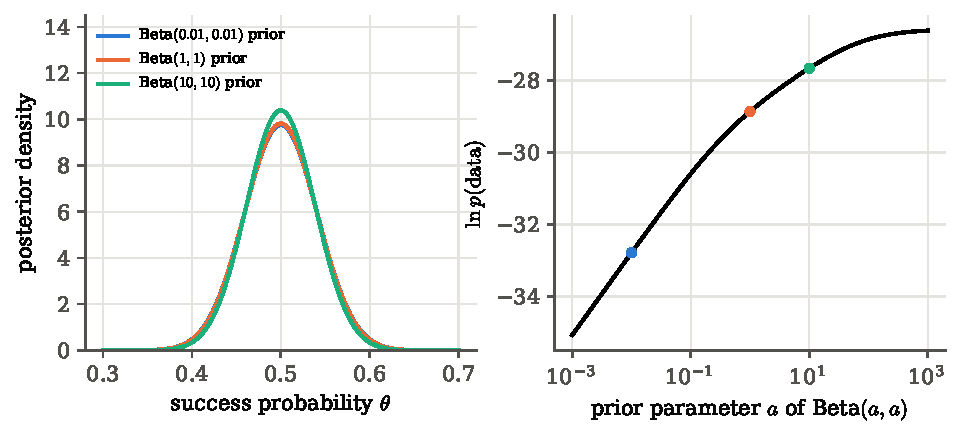
\includegraphics[width=\linewidth]{figures/ch05/prior_sensitivity.pdf}
\caption{Left: the posterior of a success probability under three symmetric Beta
priors, for fifteen binomial counts out of ten trials each; the three curves nearly
coincide. Right: the log evidence of the same data as a function of the prior
parameter $a$; the three dots are the three priors on the left. The posterior barely
notices the prior, the evidence notices it a lot.}
\label{5c:fig:prior-sens}
\end{figure}

Kruschke's remedy is to put the competing models on an equal footing: inform the priors
of \emph{both} models with the same small, representative part of the data, and compute
the Bayes factor from the rest \srcref{Kruschke}{\S10.6.1}. Why does this help? Even a
few data points overwhelm a vague prior and bring each model's parameters ``into the
ballpark'', so the arbitrary choice of vague prior no longer matters. For the
coin, use $6$ heads in the first $10$ tosses to update both priors, then compare on the
remaining $90$. The Bayes factor of fair against anything becomes $\FiveCInfUnifBF$ starting
from the uniform prior and $\FiveCInfHaldBF$ starting from the Haldane prior. The two vague
priors now agree, and both say the coin is not fair, as the HDIs did. Intrinsic and
fractional Bayes factors are more systematic versions of the same idea.

\begin{pitfall}[Vague priors are harmless for estimation, not for comparison]
A wide or ``uninformative'' prior is usually safe when estimating a parameter,
because the likelihood dominates the posterior. In model comparison the overall height
of the prior where the likelihood lives enters directly, and changing from one vague
prior to another can change the Bayes factor by orders of magnitude. An improper prior,
one that cannot be normalised (flat on the whole real line), gives an evidence with an
arbitrary constant in it, so Bayes factors with improper priors on the extra parameters
are undefined \mainref{p.~185}, \srcref{HobsonBMC}{\S1.3}.
\end{pitfall}

\subsection{Lindley's paradox}
\label{5c:sec:lindley}

The simplest nested comparison can be done exactly, and it holds a surprise. We have a
measurement $\hat\theta$ of a quantity $\theta$ with Gaussian error $\sigma$. Model
$M_0$ says the effect is absent, $\theta=0$. Model $M_1$ says it is present, with a
size we can only bound: $\theta\sim\Normal(0,\Sigma^2)$ with $\Sigma$ the scale of
effects the theory allows. Call $\lambda=\lvert\hat\theta\rvert/\sigma$ the
significance of the measurement, the ``number of sigma''.

\emph{The event:} the value $\hat\theta$. \emph{The hypotheses:} $M_0$ and $M_1$.
\emph{How probable was $\hat\theta$ under each?} Under $M_0$ it is the Gaussian density
$\Normal(\hat\theta;0,\sigma^2)$. Under $M_1$ we average over $\theta$:
\begin{align}
  p(\hat\theta\given M_1)
  &\eqby{1}\int\Normal(\hat\theta;\theta,\sigma^2)\,\Normal(\theta;0,\Sigma^2)\,\dd\theta
   \eqby{2}\Normal(\hat\theta;0,\sigma^2+\Sigma^2), \nonumber\\
  B_{01}=\frac{p(\hat\theta\given M_0)}{p(\hat\theta\given M_1)}
  &\eqby{3}\sqrt{\frac{\sigma^2+\Sigma^2}{\sigma^2}}\,
     \exp\!\Bigl[-\frac{\hat\theta^2}{2\sigma^2}+\frac{\hat\theta^2}{2(\sigma^2+\Sigma^2)}\Bigr]
   \eqby{4}\sqrt{1+\frac{\Sigma^2}{\sigma^2}}\,
     \exp\!\Bigl[-\frac{\lambda^2}{2}\,\frac{\Sigma^2}{\sigma^2+\Sigma^2}\Bigr] .
  \label{5c:eq:gauss-bf}
\end{align}
\begin{explain}
  \item The evidence of $M_1$: the likelihood of the measurement averaged over the
        prior of the effect.
  \item The measurement is the true effect plus independent Gaussian noise, so it is
        a sum of two independent Gaussians of variances $\Sigma^2$ and $\sigma^2$, and
        its density is the Gaussian of the summed variance (the convolution of two
        Gaussians; complete the square in $\theta$ to check).
  \item Ratio of the two Gaussian densities: the prefactors give the square root, the
        exponents subtract.
  \item Combine the exponents over the common denominator and write
        $\hat\theta^2/\sigma^2=\lambda^2$.
\end{explain}
This is Trotta's (21) \cite[p.~13]{Trotta2008}. When the data are much more precise than
the prior, $\sigma\ll\Sigma$, the last factor becomes $e^{-\lambda^2/2}$ and
\begin{equation}
  \ln B_{01}\approx\ln\frac{\Sigma}{\sigma}-\frac{\lambda^2}{2}
  \label{5c:eq:rough-guide}
\end{equation}
\cite[eq.~(26)]{Trotta2008}: the Occam term $\ln(\Sigma/\sigma)$, the logarithm of the
ratio of prior to posterior width, against the goodness-of-fit term $\lambda^2/2$. The
more the data have taught us ($\Sigma/\sigma$ large), the more significance is needed to
prefer the extra parameter. \Cref{5c:fig:plane} maps \eqref{5c:eq:gauss-bf} over the
plane of information $I_{10}=\log_{10}(\Sigma/\sigma)$ and significance $\lambda$. For
moderately informative data, $I_{10}$ between $1$ and $2$, the measurement must lie about
$4\sigma$ from zero before the extra parameter is favoured robustly; results at
$2$--$3\sigma$ are inconclusive or even favour the simpler model \cite[\S4.4]{Trotta2008}.

\begin{figure}[htbp]
\centering
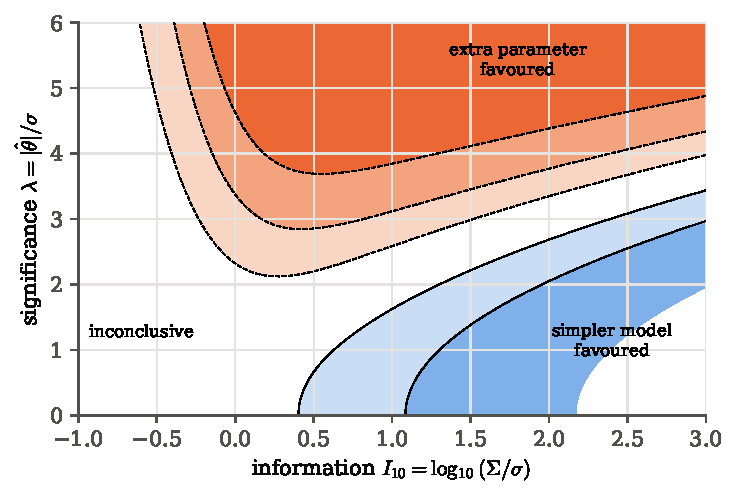
\includegraphics[width=0.72\linewidth]{figures/ch05/evidence_plane.pdf}
\caption{The Bayes factor for one extra parameter with Gaussian prior and likelihood,
over the plane of information (how much narrower the likelihood is than the prior, in
powers of ten) and significance (how many standard deviations the measurement lies
from zero). Contours are at $\lvert\ln B\rvert=1$, $2.5$, $5$. Blue: the simpler model
is favoured; orange: the extra parameter is favoured; white: inconclusive. A wider prior
moves a result to the right.}
\label{5c:fig:plane}
\end{figure}

What happens if the significance stays fixed while the data grow? With $n$
measurements of unit noise,
$\sigma=1/\sqrt n$; take $\Sigma=1$ and a result exactly at $\lambda=1.96$, the
two-sided $p=0.05$ of \cref{ch:04}. The Bayes factor \eqref{5c:eq:gauss-bf} is
$\sqrt{1+n}\,\exp[-\tfrac12(1.96)^2\,n/(1+n)]$, which grows like $\sqrt n$. With even
prior odds the posterior probability of the null (\cref{5c:fig:lindley}) is
$\FiveCLinPzeroN$ at $n=1$, $\FiveCLinPzeroNk$ at $n=10^3$ and $\FiveCLinPzeroNm$ at
$n=10^6$. At a fixed ``$1.96\sigma$'' the data favour the null once $n$ exceeds about
$\FiveCLinNhalf$, and overwhelmingly so for large samples. Even at $p=0.01$
($\lambda=2.58$) the probability of the null at $n=10^6$ is $\FiveCLinPzeroNkk$. This is
\newterm{Lindley's paradox} \cite{Lindley1957}: the same p-value means evidence \emph{against} the null in a
small experiment and evidence \emph{for} it in a large one.

\begin{figure}[htbp]
\centering
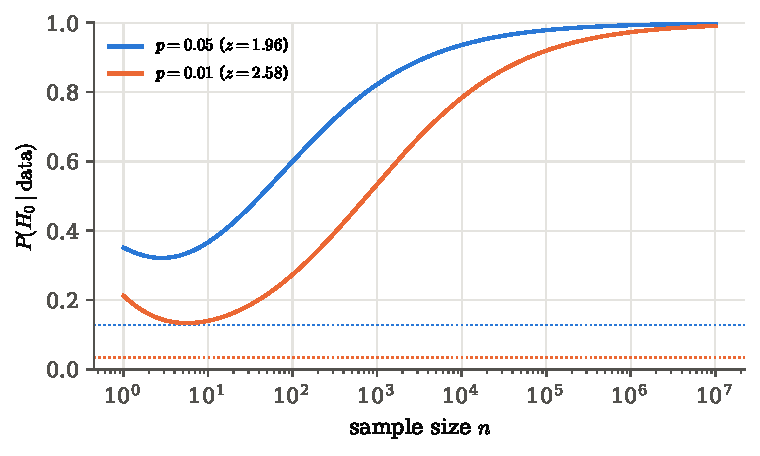
\includegraphics[width=0.75\linewidth]{figures/ch05/lindley.pdf}
\caption{Lindley's paradox. The posterior probability of ``no effect'' for a result
held at fixed significance ($1.96\sigma$, blue; $2.58\sigma$, orange) as the sample size
grows, with a unit-width prior on the effect and even prior odds. The dotted lines are
the lowest value any prior could give (the bound of \cref{5c:sec:pvalues}).}
\label{5c:fig:lindley}
\end{figure}

There is nothing paradoxical in the mechanism. At fixed significance the measured
effect $\hat\theta=1.96/\sqrt n$ shrinks as $n$ grows. The alternative spread its prior
over effects of size $\Sigma=1$, and the data increasingly say that the effect, if there
is one, is far smaller than anything $M_1$ expected. The measurement becomes a successful
prediction of $M_0$. The p-value, which only asks how surprising the data are under
$M_0$, cannot see this. Large modern data sets (Planck maps, LHC luminosities, years of
detector time) are exactly where the two answers part company, which is why ``how many
sigma'' is not by itself a good measure of the evidence for a new effect
\cite[\S5.4]{Trotta2008}.

\subsection{What a p-value can and cannot say}
\label{5c:sec:pvalues}

Wasserman's version of the Bayesian test makes the link to \cref{ch:04} explicit
\mainref{pp.~184--185}. Take the data $x^n=(x_1,\dots,x_n)$ with likelihood
$\Like(\theta)$, and test $H_0:\theta=\theta_0$ against $H_1:\theta\ne\theta_0$. Give each
hypothesis prior probability $\tfrac12$, and give $\theta$ a prior density $f(\theta)$
under $H_1$. Then
\begin{equation}
  \Prob(H_0\given x^n)
  =\frac{\Like(\theta_0)}{\Like(\theta_0)+\int\Like(\theta)f(\theta)\,\dd\theta} ,
  \label{5c:eq:aos-test}
\end{equation}
which is \eqref{5c:eq:model-post} with $Z_0=\Like(\theta_0)$ and $Z_1$ the average of the
likelihood over $f$. The prior $f$ matters here in a way it did not in estimation, and it
must be proper. Is there anything we can say whatever $f$ is? Yes: a bound. An average
cannot exceed the maximum, so $\int\Like f\,\dd\theta\le\Like(\hat\theta)$, where
$\hat\theta$ is the maximum-likelihood value. Putting this into the denominator,
\begin{equation}
  \Prob(H_0\given x^n)\;\ge\;\frac{\Like(\theta_0)}{\Like(\theta_0)+\Like(\hat\theta)} .
  \label{5c:eq:aos-bound}
\end{equation}
For a Gaussian measurement at significance $z$, $\Like(\hat\theta)/\Like(\theta_0)=e^{z^2/2}$,
which at $z=1.96$ is $\FiveCLinBoundLR$. So a result at ``$p=0.05$'' leaves the null with
posterior probability at least $\FiveCLinBound$, whatever prior the alternative is given.
The most favourable prior for $H_1$ is a spike at $\hat\theta$, chosen after seeing the
data, which is cheating; any honest prior does worse.

A less extreme and more useful bound restricts the alternative to priors that are
symmetric about $\theta_0$ and do not increase away from it. Sellke, Bayarri and Berger
showed that over this class \cite{Sellke2001}
\begin{equation}
  B_{10}\;\le\;\bar B_{10}=-\frac{1}{e\,p\ln p}\qquad(p\le e^{-1})
  \label{5c:eq:sellke}
\end{equation}
for a p-value $p$ \cite[\S4.5, eq.~(27)]{Trotta2008}. It turns a significance into the
best odds it could possibly support:

\begin{center}
\small
\renewcommand{\arraystretch}{1.15}
\begin{tabular}{@{}lcccccc@{}}
\toprule
p-value & $0.05$ & $0.01$ & $0.003$ & $0.001$ & $3\times10^{-4}$ & $5.7\times10^{-7}$\\
significance $z$ & $\FiveCSelaZ$ & $\FiveCSelbZ$ & $\FiveCSelcZ$ & $\FiveCSeldZ$ & $\FiveCSeleZ$ & $\FiveCSelfZ$\\
best odds $\bar B_{10}$ & $\FiveCSelaB$ & $\FiveCSelbB$ & $\FiveCSelcB$ & $\FiveCSeldB$ & $\FiveCSeleB$ & $\FiveCSelfB$\\
$\ln\bar B_{10}$ & $\FiveCSelalnB$ & $\FiveCSelblnB$ & $\FiveCSelclnB$ & $\FiveCSeldlnB$ & $\FiveCSelelnB$ & $\FiveCSelflnB$\\
\bottomrule
\end{tabular}
\end{center}

\noindent A ``$99\%$'' result supports odds of $8:1$ at best, short of the moderate
level. Strong evidence at best needs about $3.6\sigma$. A useful rule of thumb is to read
an $s$-sigma result as roughly an $(s-1)$-sigma one \cite[p.~18]{Trotta2008}. The
$5\sigma$ discovery convention of particle physics corresponds to best odds of about
$4.5\times10^4:1$.

\begin{keyidea}[Significance is not evidence]
A p-value is the probability, computed as if $H_0$ were true, of the observed
result \emph{together with every result lying further out in the same direction}
(\cref{4a:sec:pvalue-def}). A Bayes factor compares how probable the result actually
observed was under $H_0$ and under a specified alternative. Even with the alternative's
prior chosen as favourably as honesty allows, a $2\sigma$ result supports odds of at most
about $2.5:1$, and at fixed significance larger samples favour the null (Lindley).
\end{keyidea}

The difference lies in those further-out results. The p-value collects the probability of
outcomes that were not observed, and it never asks what the alternative predicted. The
Bayes factor uses only the observed outcome, under both hypotheses. When a paper
reports ``$3\sigma$ evidence'', the Bayes factor is the number that says how much the
data should move us, and the prior on the new effect is what the claim is really about.
\section{Nested models, shortcuts and model averaging}
\label{5c:sec:nested}

Almost every model comparison in cosmology has the shape of our bump hunt. The base
model is $\Lambda$CDM with its six parameters. The candidate extension adds a
parameter that is zero, or some other fixed value, in the base model: the spatial
curvature $\Omega_k$, the running $\dd n_s/\dd\ln k$, the tensor ratio $r$, the
non-Gaussianity $f_{\rm NL}$, the dark-energy equation of state through $w+1$, an
extra number of neutrino species $N_\nu-3.04$, and upwards of twenty more
\srcref{HobsonBMC}{Table~4.2}. In the bump hunt the base model is the line and the
extension adds a bump that disappears at $A=0$. The simpler model sits inside the
bigger one as a special value of the new parameter. Such models are called
\newterm{nested}. Nesting makes the Bayes factor easier to compute, makes it natural to
combine the models, and leads to some useful approximations.

\subsection{The Savage--Dickey density ratio}
\label{5c:sec:sddr}

Write the parameters of the bigger model $M_1$ as $(\bm\phi,\psi)$: the common
parameters $\bm\phi$ (the line, $a$ and $b$) and the new parameter $\psi$ (the
amplitude $A$). The simpler model $M_0$ is $M_1$ with $\psi$ fixed at $\psi_*$ ($A=0$).
Two conditions make the models genuinely nested \srcref{HobsonBMC}{(4.12)},
\cite[eq.~(22)]{Trotta2008}:
\begin{enumerate}[itemsep=1pt,leftmargin=1.6em]
  \item the likelihoods agree at the special value:
        $p(\data\given\bm\phi,\psi_*,M_1)=p(\data\given\bm\phi,M_0)$;
  \item the prior of $M_1$ factorises into the prior of $M_0$ for the common
        parameters times a prior for the new one:
        $p(\bm\phi,\psi\given M_1)=p(\bm\phi\given M_0)\,p(\psi\given M_1)$.
\end{enumerate}
Now ask a question about the bigger model alone: after the data, how probable is it
that the new parameter sits at its special value? That is the posterior density of
$\psi$ at $\psi_*$, and it turns out to contain the Bayes factor:
\begin{align}
  p(\psi_*\given\data,M_1)
  &\eqby{1}\int p(\bm\phi,\psi_*\given\data,M_1)\,\dd\bm\phi
   \eqby{2}\frac{1}{Z_1}\int p(\data\given\bm\phi,\psi_*,M_1)\,
      p(\bm\phi\given M_0)\,p(\psi_*\given M_1)\,\dd\bm\phi \nonumber\\
  &\eqby{3}\frac{p(\psi_*\given M_1)}{Z_1}\int p(\data\given\bm\phi,M_0)\,
      p(\bm\phi\given M_0)\,\dd\bm\phi
   \eqby{4}p(\psi_*\given M_1)\,\frac{Z_0}{Z_1} .
  \label{5c:eq:sddr-derivation}
\end{align}
\begin{explain}
  \item The marginal posterior of $\psi$: integrate the joint posterior over the common
        parameters.
  \item Bayes' theorem in $M_1$: likelihood times prior over the evidence $Z_1$, with the
        factorised prior of condition 2.
  \item Condition 1 replaces the likelihood by that of $M_0$; the prior density of
        $\psi$ at $\psi_*$ is a constant and comes out.
  \item The remaining integral is the evidence $Z_0$ of the simpler model,
        \eqref{5c:eq:evidence}.
\end{explain}
Rearranged, this is the \newterm{Savage--Dickey density ratio}
\srcref{HobsonBMC}{(4.13)}, \cite[eq.~(23)]{Trotta2008}.

\begin{workdef}[Savage--Dickey density ratio]
For nested models with a factorised prior,
\[
  B_{01}=\frac{Z_0}{Z_1}=\frac{p(\psi_*\given\data,M_1)}{p(\psi_*\given M_1)} ,
\]
\unpack{how much the data raised (or lowered) the probability density of the new
parameter at its ``absent'' value}. \emph{Operationally:} run the bigger model only,
histogram the samples of $\psi$ near $\psi_*$, and divide the height of the normalised
histogram there by the prior density.
\end{workdef}

The ratio has a direct reading. If the data pile up the posterior of the new parameter
at its null value, higher than the prior put it, the simpler model gains; if they push
the posterior away from it, the simpler model loses. Only a one-dimensional marginal
density is needed, and its normalisation is a one-dimensional integral, so there is no
high-dimensional evidence integral left to do.

\paragraph{Example: the bump amplitude at zero.}
Take the data without a bump. The new parameter is $\psi=A$ with $\psi_*=0$ and prior
density $p(A=0\given M_1)=1/A_{\max}=0.1$. The bump position $\mu$ exists only in $M_1$,
but at $A=0$ the likelihood does not depend on it and its prior integrates to one, so
the derivation goes through with $\mu$ integrated along with $\bm\phi$. On the grid,
the posterior density of $A$ at $A=0$ times $A_{\max}$ is $\FiveCSdGridZero$, which is the
exact $B_{01}=1/B_{10}=\FiveCSdExact$ of \cref{5c:sec:bump}. From a Markov chain
(\cref{5c:sec:ratios}) we estimate the density by the fraction of samples with
$A<\FiveCSdBin$, divided by $\FiveCSdBin$; this gives
$B_{01}\approx\FiveCSdChain\pm\FiveCSdChainErr$, where the error comes from splitting
the chain into twenty batches. How close this comes to the exact value varies from run
to run, for two reasons. The estimate is an average over the first bin, and the
posterior density changes across it (the grid average over the bin is
$\FiveCSdAvg$); a finer bin needs more samples. And the chain moves into and out of the
first bin slowly, so twenty batches can understate its random error.

For the data \emph{with} a bump the same estimate is much harder. There $B_{01}=1/\FiveCBumpB$,
so the posterior density at $A=0$ is small and few samples land there. A histogram is
accurate only where samples land, so the estimate is noisy. This is the known weakness
of the method: it is noisy exactly when the simpler model is disfavoured
\srcref{HobsonBMC}{p.~89}. The factorisation condition can also fail quietly, for
instance when a prior boundary of the common parameters depends on the new one.

\subsection{Model averaging}
\label{5c:sec:averaging}

Sometimes no model wins clearly, and we still want the best statement about a quantity
$\theta$ that all the models share. Probability theory gives it directly: we do not know
which model is true, so we sum the joint posterior over the models,
\begin{equation}
  p(\theta\given\data)=\sum_i p(\theta\given\data,M_i)\,\Prob(M_i\given\data),
  \label{5c:eq:bma}
\end{equation}
the posterior of $\theta$ inside each model, weighted by the probability of that model
\srcref{Kruschke}{\S10.4}, \srcref{HobsonBMC}{\S4.2}. This is \newterm{Bayesian model
averaging}. For the two coin factories of \cref{5c:sec:bf} it gave the averaged mean bias
$\FiveCFacMeanAvg$, between the two factories' $\FiveCFacMeanOne$ and
$\FiveCFacMeanTwo$, with the tail-biased factory showing up as a long left tail of the
averaged posterior.

A model in which $\theta$ is fixed still takes part. The line model fixes the amplitude
$A$ at $0$, so it contributes a spike $\Prob(M_0\given\data)\,\delta(\theta)$ to the
average. Hobson and collaborators compare the averaged posterior to a quantum
superposition that later data may collapse onto fewer models \srcref{HobsonBMC}{p.~82}.
Predictions of future data are averaged the same way. Basing them on the winning model
alone ignores the probability that it is wrong.

\paragraph{Example: which dark-energy model?}
Five models of the dark-energy equation of state $w$ were compared with the same
supernova, CMB and large-scale-structure data \srcref{HobsonBMC}{Table~4.5}. Model I is
$\Lambda$CDM, $w=-1$ exactly. Models II and III let $w$ take a constant value with
priors $-1\le w\le-0.33$ and $-2\le w\le-0.33$. Model IV gives $w$ two parameters,
$w(a)=w_0+w_a(1-a)$ with $-2\le w_0\le-0.33$ and $-1.33\le w_a\le1.33$, and model V
lets $w(a)$ vary with redshift, between $-1$ and $1$ for $0\le z\le2$. The log Bayes factors against $\Lambda$CDM are
$0$, $-1.3$, $-1.8$, $-2.0$ and $-4.1$. With equal prior probability for each model,
the posterior probabilities are $e^{\ln B_{i{\rm I}}}$ divided by their sum:
\begin{align*}
  \Prob(M_{\rm I}\given\data)
  &\eqby{1}\frac{1}{1+e^{-1.3}+e^{-1.8}+e^{-2.0}+e^{-4.1}}
   =\frac{1}{1+0.273+0.165+0.135+0.017}=0.63 ,
\end{align*}
\begin{explain}
  \item Equation \eqref{5c:eq:model-post} with equal priors: each model's share is its
        evidence over the total, and dividing every evidence by that of $\Lambda$CDM turns
        the evidences into $e^{\ln B}$.
\end{explain}
and the other four models get $0.17$, $0.10$, $0.09$ and $0.01$ in the same way. Every
extension fits at least as well as $\Lambda$CDM at its best, since each contains
$w=-1$. The evidence prefers $\Lambda$CDM because the extensions spread their priors
over values of $w$ the data exclude, and the more parameters or the wider the range,
the larger the penalty. None of the extensions is decisively ruled out
(no $\lvert\ln B\rvert$ exceeds $5$), and the probabilities depend on the prior ranges
chosen for $w$, which is the lesson of \cref{5c:sec:prior-width}.

\paragraph{Does the answer you need depend on the model?}
Averaging is the formal remedy for model uncertainty. The informal remedy is a
\newterm{sensitivity analysis}: fit several reasonable models and check whether the
quantity you actually care about changes \srcref{Lambert}{\S10.8}. Lambert's example is a
rainfall model for sizing a dam. A two-state model (dry, wet) and a three-state model
(dry, wet, persistently wet) fit $100$ days of rain equally well on every standard
test. But let each generate long rain series, and the three-state model gives far more
probability to long runs of wet days. Long wet runs are the very quantity the dam
depends on. So fit quality cannot choose between the models, and the conclusion that
matters differs between them. The cautious report gives the answer of the pessimistic
model and says why. The same habit applies
to a forecast of a background tail under different fit functions, or of a cosmological
parameter under different sets of nuisance parameters. A sensitivity analysis matters
most when data are few or the decision is sensitive to the modelling choice.

\subsection{How many bumps?}
\label{5c:sec:how-many}

Sivia's ``how many lines are there?'' is the multi-model version of the bump hunt
\srcref{Sivia}{\S4.2}. A spectrum is a sum of $M$ peaks of known shape on a background,
$M$ is unknown, and each value of $M$ is a model with $2M$ peak parameters (amplitudes
and positions). With a uniform prior on $M$ over a few values, $\Prob(M\given\data)$ is
proportional to the evidence $Z_M$ \srcref{Sivia}{(4.15)}, a $2M$-dimensional integral
over a uniform box of amplitudes and positions \srcref{Sivia}{(4.16)--(4.19)}.

We do it for $M=0,1,2$ bumps on our line, with the line integrated out exactly as in
\eqref{5c:eq:dchi2} and the priors of \cref{5c:sec:bump} for each bump. For two bumps,
$\chi^2_{\min}$ minus the line's $\chi^2_{\min}$ is a quadratic form in $(A_1,A_2)$
with coefficients $\bm r\cdot\bm u_{\mu_j}$ and $\bm u_{\mu_j}\cdot\bm u_{\mu_k}$, so the
four-dimensional grid ($81$ amplitudes and $161$ positions per bump) costs only
multiplications; refining it changes $\ln Z$ by $\FiveCHmGridErr$. The box includes both
orderings of the two positions, so the $M!$ equivalent peaks of Sivia's (4.20) are
counted automatically. Besides the one-bump data we simulate a data set with two bumps of
height $\FiveCTwoA$ at $\mu=\FiveCTwoMuOne$ and $\FiveCTwoMuTwo$
(\cref{5c:fig:how-many}).

\begin{figure}[htbp]
\centering
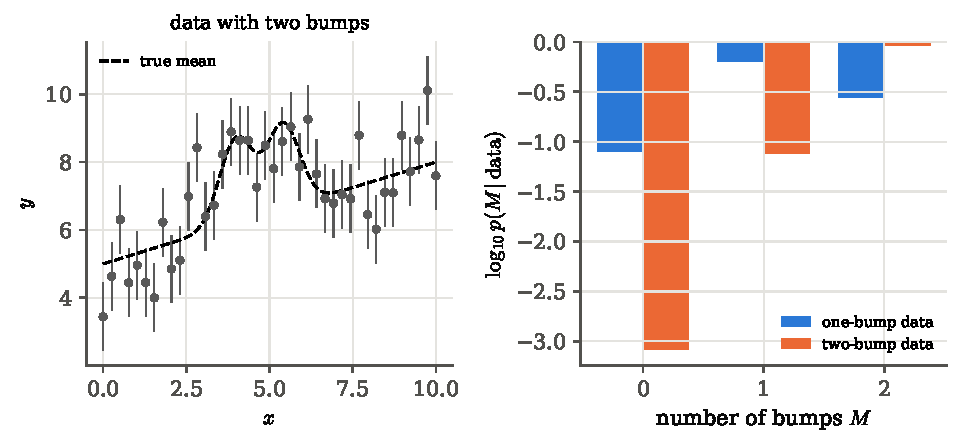
\includegraphics[width=\linewidth]{figures/ch05/how_many_bumps.pdf}
\caption{How many bumps? Left: forty points containing two overlapping bumps, with the
true mean curve. Right: the posterior probability of each number of bumps, in powers of
ten, for the one-bump data of \cref{5c:fig:bump-fits} and for the two-bump data.}
\label{5c:fig:how-many}
\end{figure}

\begin{center}
\small
\renewcommand{\arraystretch}{1.15}
\begin{tabular}{@{}l|ccccc|ccccc@{}}
\toprule
 & \multicolumn{5}{c|}{one-bump data} & \multicolumn{5}{c}{two-bump data}\\
$M$ & $\chi^2_{\min}$ & AIC & BIC & $\ln Z_M$ & $\Prob(M\given\data)$
    & $\chi^2_{\min}$ & AIC & BIC & $\ln Z_M$ & $\Prob(M\given\data)$\\\midrule
$0$ & $\FiveCHmOneChiZero$ & $\FiveCHmOneAICZero$ & $\FiveCHmOneBICZero$ & $\FiveCHmOnelnZZero$ & $\FiveCHmOnePZero$
    & $\FiveCHmTwoChiZero$ & $\FiveCHmTwoAICZero$ & $\FiveCHmTwoBICZero$ & $\FiveCHmTwolnZZero$ & $\FiveCHmTwoPZero$\\
$1$ & $\FiveCHmOneChiOne$ & $\FiveCHmOneAICOne$ & $\FiveCHmOneBICOne$ & $\FiveCHmOnelnZOne$ & $\FiveCHmOnePOne$
    & $\FiveCHmTwoChiOne$ & $\FiveCHmTwoAICOne$ & $\FiveCHmTwoBICOne$ & $\FiveCHmTwolnZOne$ & $\FiveCHmTwoPOne$\\
$2$ & $\FiveCHmOneChiTwo$ & $\FiveCHmOneAICTwo$ & $\FiveCHmOneBICTwo$ & $\FiveCHmOnelnZTwo$ & $\FiveCHmOnePTwo$
    & $\FiveCHmTwoChiTwo$ & $\FiveCHmTwoAICTwo$ & $\FiveCHmTwoBICTwo$ & $\FiveCHmTwolnZTwo$ & $\FiveCHmTwoPTwo$\\
\bottomrule
\end{tabular}
\end{center}

\noindent For the one-bump data the evidence gives one bump the probability
$\Prob(M=1\given\data)=\FiveCHmOnePOne$, although the two-bump model fits better
($\chi^2_{\min}=\FiveCHmOneChiTwo$ against $\FiveCHmOneChiOne$). For the two-bump data it
gives two bumps $\FiveCHmTwoPTwo$. The $\chi^2$ column alone would always choose the most
bumps. Two data sets could be lucky, so we repeat the count on $\FiveCHmLoopR$ fresh
data sets of each kind. The evidence picks one bump in $\FiveCHmLoopOneEvOne$ of the
one-bump sets and two bumps in $\FiveCHmLoopTwoEvTwo$ of the two-bump sets.

\subsection{Information criteria}
\label{5c:sec:ic}

The table also shows two quantities that are popular because they need no integral.
Both are built from $-2\ln\Like_{\max}$, which for Gaussian noise is $\chi^2_{\min}$ plus a
constant, plus a penalty for the number of parameters $k$ \srcref{Lambert}{\S10.5},
\cite[\S4.7]{Trotta2008}, \srcref{HobsonBMC}{(4.14)}:
\[
  \mathrm{AIC}=-2\ln\Like_{\max}+2k,\qquad
  \mathrm{BIC}=-2\ln\Like_{\max}+k\ln N ,
\]
with $N$ the number of data points; smaller is better. (The table uses $\chi^2_{\min}$ for
$-2\ln\Like_{\max}$ and counts the line's two parameters, $k=2,4,6$.)

The \newterm{Bayesian information criterion} is a crude evidence. Start from the Laplace
approximation \eqref{5c:eq:laplace-evidence} with a general prior density
\cite[eqs.~(39)--(41)]{Trotta2008}:
\begin{align}
  \ln Z
  &\relby{1}{\approx}\ln\Like_{\max}+\ln\pi(\hat\params)+\frac k2\ln2\pi-\frac12\ln\det\Fish
   \nonumber\\
  &\relby{2}{\approx}\ln\Like_{\max}+\ln\pi(\hat\params)+\frac k2\ln2\pi-\frac k2\ln N-\frac12\ln\det\Fish_1
   \nonumber\\
  &\relby{3}{\approx}\ln\Like_{\max}-\frac k2\ln N=-\tfrac12\,\mathrm{BIC} .
  \label{5c:eq:bic}
\end{align}
\begin{explain}
  \item The logarithm of \eqref{5c:eq:laplace-evidence}, with $k$ parameters.
  \item For $N$ independent data points the curvature of the log-likelihood grows in
        proportion to $N$: $\Fish=N\Fish_1$, with $\Fish_1$ the curvature per data point,
        and $\det(N\Fish_1)=N^k\det\Fish_1$.
  \item Keep only the terms that grow with $N$: $\ln\Like_{\max}$ grows like $N$,
        $\ln N$ grows slowly, and the prior, $2\pi$ and $\Fish_1$ terms stay constant.
        They are dropped.
\end{explain}
So $-\tfrac12\Delta\mathrm{BIC}$ approximates $\ln B$ for large $N$. The dropped
constant terms are exactly the ones that carry the prior. That is why BIC is attractive
(no prior to choose) and also why it is limited. It charges every parameter the same
price $\tfrac12\ln N$, as if every prior range were one data point's worth of
information wide, whether the parameter is constrained or not. In our table
$-\tfrac12\Delta\mathrm{BIC}$ gives $\FiveCHmOneBIConezero$ for one bump against none on
the one-bump data, where the exact $\ln B$ is $\FiveCHmOnelnBonezero$. Our prior ranges
for the bump are wider than BIC assumes, so BIC under-charges.

The \newterm{Akaike information criterion} comes from a different question: which model will
predict new data best, measured by a Kullback--Leibler divergence
\srcref{Lambert}{\S10.5.5}. Its penalty, $2$ per parameter, is weaker still. In the
$\FiveCHmLoopR$ fresh one-bump data sets, where the truth has one bump, AIC chooses two
bumps over one in $\FiveCHmLoopOneAicTwo$, BIC in $\FiveCHmLoopOneBicTwo$, and the
evidence in $\FiveCHmLoopOneEvTwo$.

Lambert describes the Bayesian descendants of AIC: DIC, which uses the posterior mean
and the posterior variance of the log-likelihood as the penalty; WAIC, which averages
the likelihood of each data point over the posterior; and leave-one-out cross-validation
(LOO-CV), which predicts each point from a fit to all the others
\srcref{Lambert}{\S\S10.5.6--10.5.8}. Trotta relates DIC to the Bayesian complexity, the
effective number of parameters the data actually constrain \cite[\S4.6]{Trotta2008},
\srcref{HobsonBMC}{(4.9)--(4.11)}. All of these answer ``which model predicts
best?'', not ``which model produced the data?''. Lambert prefers them to Bayes factors
because of the prior sensitivity of \cref{5c:sec:prior-width}
\srcref{Lambert}{\S10.6}; cosmologists mostly compute evidences, because their models
come with physically motivated prior ranges.

\begin{taxonomy}[Which number answers which question]
\small
\renewcommand{\arraystretch}{1.12}
\begin{tabularx}{\linewidth}{@{}>{\raggedright\arraybackslash}p{2.6cm}
                               >{\raggedright\arraybackslash}X
                               >{\raggedright\arraybackslash}p{3.6cm}@{}}
\toprule
tool & what it computes & when to trust it\\\midrule
evidence $Z$, Bayes factor & probability of the data under each model, prior included & always the target; needs the prior and an integral\\
Laplace & $\Like_{\max}\times$ posterior volume / prior volume & one Gaussian-like peak well inside the prior\\
Savage--Dickey & posterior over prior density of the new parameter at its null value & nested models, factorised prior, enough samples near the null\\
BIC & $\ln Z$ keeping only terms that grow with $N$ & many independent data, all parameters constrained, priors about one datum wide\\
AIC, DIC, WAIC, LOO-CV & expected accuracy of predictions for new data & when prediction, not the generating model, is the question\\
$\Delta\chi^2$, p-value & improvement of the best fit; surprise under the null & never on its own for comparing models\\
\bottomrule
\end{tabularx}
\end{taxonomy}

\subsection{Estimating a difference, or comparing models?}
\label{5c:sec:estimate-or-compare}

A trigger is upgraded. Before the upgrade $x_1=\FiveCEffXone$ of $n_1=\FiveCEffNone$ test
pulses fired it; after, $x_2=\FiveCEffXtwo$ of $n_2=\FiveCEffNtwo$. Did the efficiency
change? There are two different questions hidden in these words.

\paragraph{Estimation: by how much did it change?}
Give the two efficiencies $p_1,p_2$ independent flat priors. Their posteriors are
independent, $p_j\given x_j\sim\mathrm{Beta}(x_j+1,n_j-x_j+1)$, and the posterior of the
change $\tau=p_2-p_1$ is obtained by drawing pairs and subtracting, exactly as in
Wasserman's example of two binomials \mainref{pp.~183--184}. With $\FiveCEffDraws$ draws
(\cref{5c:fig:eff}), $\Prob(\tau>0\given\data)=\FiveCEffPup$, the posterior mean of $\tau$
is $\FiveCEffMean$, and the central $95\%$ interval is $[\FiveCEffLo,\FiveCEffHi]$.

\begin{figure}[htbp]
\centering
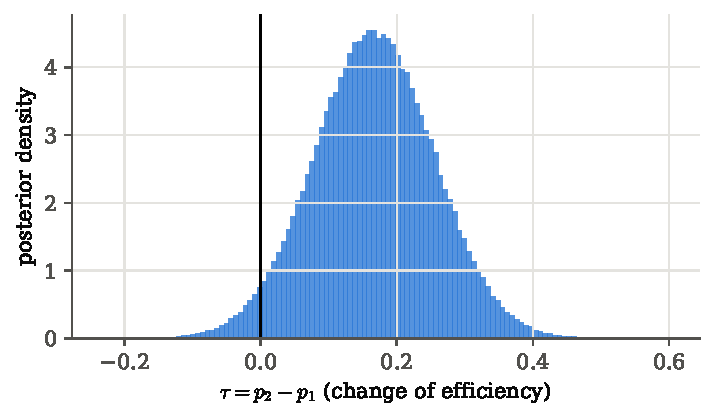
\includegraphics[width=0.7\linewidth]{figures/ch05/two_efficiencies.pdf}
\caption{The posterior of the change of trigger efficiency, from $2\times10^5$ pairs of
draws of the two Beta posteriors. About $97\%$ of the area lies to the right of zero.
The picture answers ``by how much did it change?'' and says nothing about whether the
change is exactly zero, which has zero probability under this continuous posterior.}
\label{5c:fig:eff}
\end{figure}

\paragraph{Comparison: did it change at all?}
Now let the hypotheses be two models. $M_{\rm same}$: one efficiency $p$ for both
periods, flat prior. $M_{\rm diff}$: independent $p_1,p_2$, flat priors. The evidence of
each is a Beta integral like \eqref{5c:eq:beta-evidence}; the binomial coefficients are
the same in both and cancel in the ratio:
\begin{align}
  B_{\rm same,diff}
  &\eqby{1}\frac{\int_0^1p^{x_1+x_2}(1-p)^{n_1+n_2-x_1-x_2}\,\dd p}
     {\int_0^1p_1^{x_1}(1-p_1)^{n_1-x_1}\dd p_1\int_0^1p_2^{x_2}(1-p_2)^{n_2-x_2}\dd p_2}
   \nonumber\\
  &\eqby{2}\frac{B(x_1+x_2+1,\,n_1+n_2-x_1-x_2+1)}{B(x_1+1,n_1-x_1+1)\,B(x_2+1,n_2-x_2+1)} .
  \label{5c:eq:eff-bf}
\end{align}
\begin{explain}
  \item The evidences \eqref{5c:eq:evidence} with flat priors (density one on $[0,1]$ and
        on $[0,1]^2$); the likelihood of the two samples is a product of two binomials.
  \item Each integral is a Beta function, as in \eqref{5c:eq:beta-evidence}.
\end{explain}
Numerically $B_{\rm same,diff}=\FiveCEffBsame$, so with even prior odds
$\Prob(M_{\rm same}\given\data)=\FiveCEffPsame$.

The two answers look contradictory: probability $\FiveCEffPup$ that the efficiency went
up, and probability $\FiveCEffPsame$ that it did not change. They are not, because they
answer different questions with different priors.
\begin{itemize}[itemsep=1pt,leftmargin=1.2em]
  \item The estimation put zero prior probability on ``exactly no change'', since a
        continuous prior gives any single value probability zero.
  \item The comparison put half of all prior probability on exactly that value, and
        spread the other half over all pairs $(p_1,p_2)$, most of which the data exclude.
\end{itemize}
Which is right depends on the physics. If the upgrade could plausibly have done nothing at all (a
firmware change that might not have been loaded), the point hypothesis deserves its
prior mass and the comparison is the right question. If the upgrade certainly changed
something, and we want to know how much, estimation is the right question. Kruschke
makes the same point about restricted models with negligible prior plausibility: testing
every possible equality among nine baseball positions gives $21147$ restricted models,
most of which nobody believes, and estimation of the full model is more informative
\srcref{Kruschke}{\S10.5.1}. Lambert's advice is similar: when one model extends
another, estimate within the bigger model and check its predictions
\srcref{Lambert}{\S10.7}.

\begin{pitfall}[A point null is a strong claim]
Comparing ``the effect is exactly zero'' with ``the effect is something'' gives the point
null a finite share of prior probability on a single value. That is appropriate when
theory singles the value out ($n_s=1$, $\Omega_k=0$, $w=-1$, a symmetry that forbids a
coupling). It is not appropriate for effects that are surely nonzero but possibly small;
there the question is the size of the effect, and a credible interval answers it.
\end{pitfall}
\section{Why we need sampling}
\label{5c:sec:sampling}

The denominator of Bayes' theorem, the integral over all parameter values, is the part
of Bayesian inference that does not scale to many parameters. Every evidence so far
was computed exactly or on a small grid. The coin factories had a Beta-function
formula. The bump model had four parameters, but two of them, the line, entered
linearly and could be integrated by hand, which left a two-dimensional grid. Real
problems are not so kind. The base cosmological model has six parameters. Each
evaluation of its CMB likelihood runs a Boltzmann code and takes of order a second.
Its extensions add more parameters, none of them linear \srcref{HobsonBMC}{p.~87}.
There are two ways out. For parameters, never compute the denominator. For models,
compute it with an algorithm that spends its effort where the likelihood is.

\subsection{The cost of a grid}
\label{5c:sec:grid-cost}

A grid needs about $w/\Delta$ points along each axis to cover a width $w$ with
resolution $\Delta$, so $(w/\Delta)^D$ points in $D$ dimensions
\srcref{HobsonBMC}{p.~58}, \srcref{Sivia}{\S3.4}, \srcref{Kruschke}{\S5.4}. The exponent
is the whole problem. We can watch it happen by computing the bump evidence of
\cref{5c:sec:bump} the brute-force way, on a grid over all four parameters $(a,b,A,\mu)$
with $n$ points per axis and no analytic help (\cref{5c:fig:grid-cost}). The wall time
grows as $n^4$. With $n=\FiveCGcNsmall$ the answer is $\ln B_{10}=\FiveCGcLnBsmall$,
wrong by more than a unit because the grid is too coarse to resolve the peak; with
$n=\FiveCGcNmid$ it is $\FiveCGcLnBmid$; with $n=\FiveCGcNmax$ it is $\FiveCGcLnBmax$,
against the exact $\FiveCGcExact$, after $\FiveCGcTmax$ seconds.

\begin{figure}[htbp]
\centering
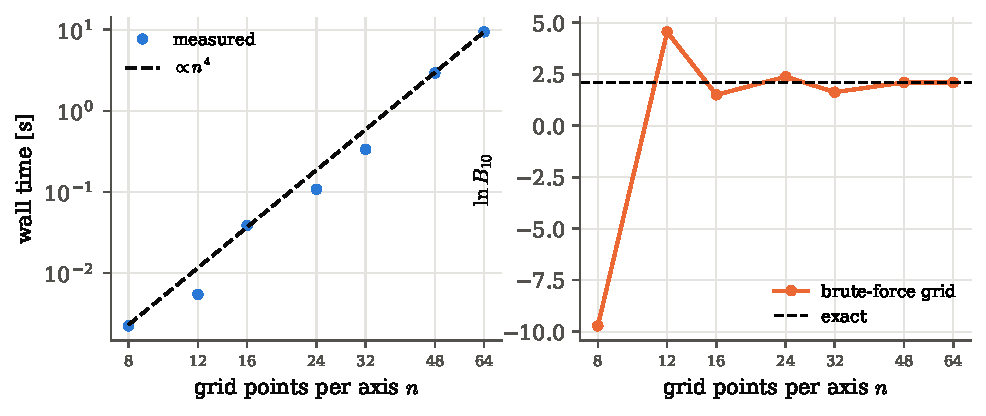
\includegraphics[width=\linewidth]{figures/ch05/grid_cost.pdf}
\caption{The bump evidence by brute force over the four-dimensional prior box. Left:
the wall time grows as the fourth power of the number of points per axis (dashed line).
Right: the log Bayes factor from the grid settles on the exact value only once the grid
is fine enough to resolve the likelihood peak, which occupies a tiny corner of the box.}
\label{5c:fig:grid-cost}
\end{figure}

At the measured cost of $\FiveCGcTpp$ seconds per grid point, a six-parameter problem
with a thousand points per axis, $10^{18}$ points, would take $\FiveCGcSixD$ years. With
a CMB likelihood at one second per call it would take $\FiveCGcSixDcmb$ years, more
than twice the age of the Universe. And almost all of that work is wasted, because
almost every grid point sits where the likelihood is negligible. How small is the
region that matters? The bulk of the posterior occupies a fraction of about $e^{-H}$
of the prior volume. Here $H$ is the information gained from the data (the
Kullback--Leibler divergence from prior to posterior), and it grows in proportion to
the number of well-measured parameters \srcref{HobsonBMC}{p.~20}.

\subsection{Sampling the prior does not rescue us}
\label{5c:sec:prior-mc}

A grid is one way to do an integral; random points are another. The evidence is an
average of the likelihood over the prior, so draw $\params_1,\dots,\params_K$ from the
prior and average: $\hat Z=\frac1K\sum_k\Like(\params_k)$ \srcref{Kruschke}{(10.7)}. The
estimate is unbiased, and its error falls like $1/\sqrt K$ whatever the dimension. The
catch is the constant in front of $1/\sqrt K$. For the simplest test case, a Gaussian
likelihood of width $s$ centred in the unit cube $[0,1]^D$ with a uniform prior, the
relative variance of one term is
\begin{align}
  \frac{\Var_\pi[\Like]}{Z^2}
  &\eqby{1}\frac{\E_\pi[\Like^2]}{Z^2}-1
   \eqby{2}\frac{\int e^{-\lvert\params-\params_0\rvert^2/s^2}\,\dd^D\params}
     {\bigl(\int e^{-\lvert\params-\params_0\rvert^2/2s^2}\,\dd^D\params\bigr)^2}-1
   \eqby{3}\frac{(s\sqrt\pi)^D}{(s\sqrt{2\pi})^{2D}}-1
   =\Bigl(\frac{1}{2\sqrt\pi\,s}\Bigr)^{D}-1 .
  \label{5c:eq:prior-mc}
\end{align}
\begin{explain}
  \item The variance is the mean square minus the square of the mean, and the mean of
        $\Like$ over the prior is $Z$.
  \item The prior density is one on the cube, so averages over the prior are integrals;
        squaring the Gaussian halves its width parameter. We neglect the parts of the
        Gaussians outside the cube, which is exact enough for $s\ll1$.
  \item Gaussian integrals: $\int e^{-u^2/s^2}\dd u=s\sqrt\pi$ and
        $\int e^{-u^2/2s^2}\dd u=s\sqrt{2\pi}$, once per dimension.
\end{explain}
The relative error of $\hat Z$ is the square root of \eqref{5c:eq:prior-mc} divided by
$\sqrt K$. For $s=0.05$ the base is $1/(2\sqrt\pi\,s)\approx5.6$: every extra dimension
multiplies the required number of draws by more than five. With $K=\FiveCDcDraws$ draws
the simulation (\cref{5c:fig:dimension}) finds a relative error of $\FiveCDcErrTwo$ for
$D=2$ and $\FiveCDcErrFive$ for $D=5$, roughly as \eqref{5c:eq:prior-mc} predicts. For $D=8$
the estimate is so lopsided that our $20$ repeated runs cannot pin down its error: most
runs fall short, and the typical run gives only $\FiveCDcMedEight$ of the true value.
By $D=10$ the typical estimate is $\FiveCDcMedTen$ of the
true value: almost no draw lands where the likelihood is, and the rare draw that does
dominates the sum. The fraction of prior draws inside the bulk of the posterior tells
the same story: $\FiveCDcFracTwo$ at $D=2$, $\FiveCDcFracFive$ at $D=5$,
$\FiveCDcFracEight$ at $D=8$. Kruschke's verdict on prior sampling is that it may need
``a ginormous number of samples'' \srcref{Kruschke}{p.~275}.

\begin{figure}[htbp]
\centering
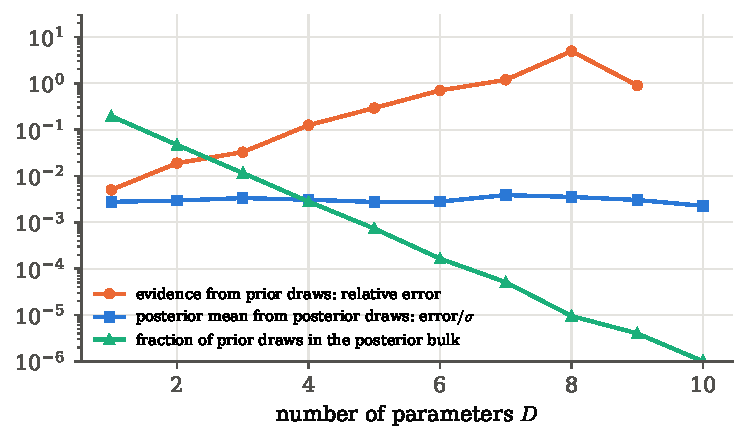
\includegraphics[width=0.8\linewidth]{figures/ch05/dimension_curse.pdf}
\caption{The curse of dimension for a Gaussian likelihood of width $0.05$ in the unit
cube, with $10^5$ draws each time. Orange: relative error of the evidence estimated
from draws of the prior, shown only while some runs still reach the likelihood peak.
Green: fraction of prior draws that land in the bulk of the
posterior. Blue: error of the posterior mean of one parameter estimated from draws of
the posterior, in units of the posterior width; it does not grow with the dimension.}
\label{5c:fig:dimension}
\end{figure}

The blue curve of \cref{5c:fig:dimension} is the hopeful one. If instead we had draws
from the \emph{posterior}, the posterior mean of a parameter would have error
$\sigma/\sqrt K$, independent of $D$: $\FiveCDcPostTwo\,\sigma$ at $D=2$ and
$\FiveCDcPostTen\,\sigma$ at $D=10$, both of the order of $1/\sqrt{10^5}\approx0.003$. This is
the central limit theorem at work on the samples \srcref{HobsonBMC}{\S3.1}, and it is why
cosmologists sample: a few thousand posterior draws summarise a posterior in any number
of dimensions \srcref{HobsonBMC}{p.~58}. What we need is a way to draw from the posterior
without knowing its normalisation.

\subsection{Ratios are all we need for parameters}
\label{5c:sec:ratios}

The normalisation of the posterior is the evidence, and it cancels from every ratio of
posterior densities:
\begin{align}
  \frac{p(\params'\given\data)}{p(\params\given\data)}
  \eqby{1}\frac{p(\data\given\params')\,p(\params')/p(\data)}{p(\data\given\params)\,p(\params)/p(\data)}
  \eqby{2}\frac{\Like(\params')\,\pi(\params')}{\Like(\params)\,\pi(\params)} .
  \label{5c:eq:ratio}
\end{align}
\begin{explain}
  \item Bayes' theorem at the two points $\params'$ and $\params$.
  \item The evidence $p(\data)$ is the same number at both points and cancels.
\end{explain}
A method that only ever asks ``how much more probable is this point than that one?''
can therefore move through parameter space using likelihood times prior alone. The
Metropolis algorithm does exactly this \cite{Metropolis1953}. From the current point
$\params$, propose a random step to $\params'$; accept it with probability
$\min(1,\text{ratio \eqref{5c:eq:ratio}})$; otherwise stay where you are and count the
current point again. We don't want the unbiased random walker, but instead a biased
random walker which spends more time in the region where probability is higher: the
accept--reject step, which uses only the ratio, is the bias. That the fraction of time
the walker spends in each region converges to the posterior probability of that region
is proved in \cref{ch:09}; here we only watch it work.

\pyfile[firstline=37,lastline=48,firstnumber=37]{code/ch05/28_sampling_evidence.py}{A
Metropolis walk on the bump posterior that uses only ratios}

Line 39 starts the walker at the best line with a small bump in the middle of the box.
Line 43 proposes a Gaussian step in all four parameters. Line 44 evaluates the logarithm
of likelihood times prior, which is $-\infty$ outside the prior box, so steps out of the
box are always rejected. Line 45 is the whole algorithm: accept if a uniform random
number is below the ratio, in logarithms. Nothing in the loop knows the evidence.

\paragraph{Example: the bump posterior from a chain.}
For the data with a bump, $\FiveCMhSteps$ steps take $\FiveCMhTime$ seconds, with
acceptance rate $\FiveCMhAcc$; we discard the first $\FiveCMhBurn$ as the walker finds
the peak. The histograms of the chain (\cref{5c:fig:mh}) lie on the grid posteriors. The
posterior mean position is $\FiveCMhMuMean$ from the chain, $\FiveCEmMuMean$ from the
standard ensemble sampler \pyname{emcee} run as a cross-check ($\FiveCEmSteps$ samples),
and $\FiveCGridMuMean$ on the grid; the mean amplitude is $\FiveCMhAMean$ (chain),
$\FiveCEmAMean$ (\pyname{emcee}) and $\FiveCGridAMean$ (grid).

\begin{figure}[htbp]
\centering
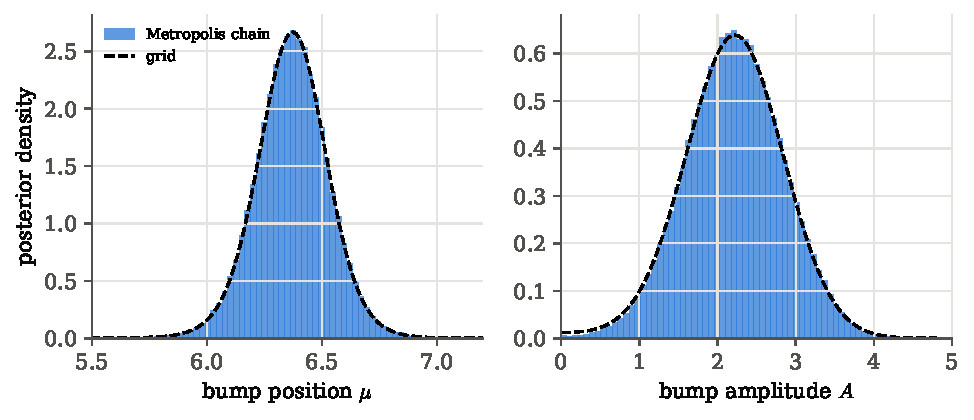
\includegraphics[width=\linewidth]{figures/ch05/mh_bump.pdf}
\caption{The posterior of the bump position and amplitude from a Metropolis chain of
$10^6$ steps that only ever evaluated ratios of likelihood times prior (histograms),
against the grid posterior (dashed). The chain never computed the evidence, yet
reproduces the normalised shape.}
\label{5c:fig:mh}
\end{figure}

A chain can miss part of a posterior, and the reason matters. Besides the peak, a bump
posterior can have a faint ``pedestal'': bumps of small amplitude anywhere in
$0<\mu<10$, which fit about as well as the line. How much probability the pedestal holds
depends on how clearly the data show the bump. For our data the grid gives it
$\FiveCMhFloorGrid$ (for $A<0.5$). The chain spends $\FiveCMhFloorChain$ of its time
there and \pyname{emcee} $\FiveCEmFloor$; $\FiveCMhNchains$ chains with different seeds
give between $\FiveCMhFloorMin$ and $\FiveCMhFloorMax$. When the pedestal holds a
noticeable share, a chain reaches it only in rare excursions, so its share is mostly
luck, set by how many times it happened to wander off the peak. Because the pedestal is
spread over the whole range of $\mu$, those rare visits matter most for the posterior
standard deviation of $\mu$: $\FiveCGridMuSd$ on the grid against $\FiveCMhMuSdMin$ to
$\FiveCMhMuSdMax$ from the chains. Why are the visits rare? A walker that takes small
local steps crosses from the peak to a distant low-amplitude region only rarely, so a
finite chain can under-represent that region. How
long a chain must run, and how to tell whether it has, is the subject of \cref{ch:09}.

\begin{inpractice}[Verification here, the instrument elsewhere]
For the bump posterior the chain can be checked against a grid, so the chain only
\emph{verifies} what we already know. In a cosmological analysis there is no grid: the
posterior of $\Lambda$CDM and its extensions from Planck, BAO and supernova data exists
only as a chain from codes such as CosmoMC \cite{LewisBridle2002}, Cobaya or
MontePython, and the chain \emph{is} the result. Convergence is then judged from the
chains themselves, for instance by comparing several chains started far apart
\cite{GelmanRubin1992}, and the samples are turned into marginal densities and triangle
plots with \pyname{getdist}. The two-step habit of this book carries over: write the
sampler from scratch once to see the mechanism, then use and cross-check the research
code.
\end{inpractice}

\subsection{The evidence needs more than a chain}
\label{5c:sec:evidence-from-samples}

A chain never computes the evidence, so it cannot simply report it. Wasserman gives a
sharp form of the difficulty \mainref{Example~11.10}. Suppose a density is known up to
its constant, $f(x)=c\,g(x)$ with $g$ known, and we can draw $n$ samples $x_1,\dots,x_n$
from $f$. Can the samples tell us $c$? Treat $c$ as a parameter. The likelihood of the
samples is $\prod_i c\,g(x_i)\propto c^n$, the same function of $c$ whatever the samples
are, so a Bayesian analysis learns nothing about $c$ from them. Yet $c$ can be
estimated another way. Estimate the density $\hat f$ from the samples at any point $x$;
then $\hat c=\hat f(x)/g(x)$.

The same trick works for the evidence. Bayes' theorem, rearranged, gives an identity
for the evidence at \emph{any} parameter value $\params$:
\begin{align}
  p(\params\given\data)=\frac{\Like(\params)\,\pi(\params)}{Z}
  \quad\Longrightarrow\quad
  Z=\frac{\Like(\params)\,\pi(\params)}{p(\params\given\data)} .
  \label{5c:eq:candidate}
\end{align}
The numerator, likelihood times prior, we can compute. The denominator is the
normalised posterior density, which the samples estimate. Here $\Like(\params)\pi(\params)$
plays the role of the known $g$, and $Z$ the role of $1/c$. The Savage--Dickey ratio of
\cref{5c:sec:sddr} is this idea for
nested models at the point $\psi=\psi_*$. The \pyname{MCEvidence} code estimates the
posterior density from the nearest-neighbour distances of chain samples
\srcref{Padilla}{\S7}. Kruschke describes a version that averages over the chain
instead of using one point \srcref{Kruschke}{(10.8)}: for any normalised density
$h(\params)$, $1/Z=\E_{\rm post}[h(\params)/(\Like(\params)\pi(\params))]$, which works
well when $h$ resembles the posterior and badly when it does not (with $h$ equal to the
prior it becomes the harmonic-mean estimator, whose variance can be infinite). All
these need a good density estimate in the region that matters, which is again hard in
many dimensions. The reliable general-purpose methods are built for the evidence from
the start.

A chain can also be made to carry the model index. Give the model label $m$ a prior and
let the sampler move in the joint space of $m$ and the parameters of each model, so that
the fraction of steps spent at $m$ estimates $\Prob(m\given\data)$, and the ratio of
the fractions estimates the posterior odds \srcref{Kruschke}{\S10.3.2}. The
difficulty is that, when the chain sits at $m=1$, the parameters that belong only to
model $2$ have no likelihood to pull them anywhere, so they wander over their whole
prior. When the chain proposes a jump to $m=2$, those parameters are almost certainly
somewhere the data exclude, and the jump is rejected. The chain rarely changes model.
The remedy is a \newterm{pseudo-prior}: while the chain sits in another model, the
idle parameters are drawn from a stand-in density placed where their own model's posterior
lives, so that a jump to that model lands somewhere sensible. A pseudo-prior costs a
preliminary run in each model, and, because it does not enter the final answer, it
only affects efficiency, not the result.

\subsection{Nested sampling}
\label{5c:sec:nested-sampling}

Skilling's nested sampling turns the $D$-dimensional evidence integral into a
one-dimensional one \cite{Skilling2006}, \srcref{HobsonBMC}{\S1.4.1}. How can that be?
The evidence only asks how much prior mass has how much likelihood; it does not care
where in parameter space that mass sits. So sort all the prior mass by likelihood. For
each likelihood level $\ell$ let
\[
  X(\ell)=\int_{\Like(\params)>\ell}\pi(\params)\,\dd\params
\]
be the prior mass enclosed by the contour $\Like=\ell$ \srcref{HobsonBMC}{(1.57)}. It
falls from $X=1$ at $\ell=0$ to $X=0$ at the maximum likelihood, and its inverse
$\Like(X)$ is the likelihood of the contour that encloses prior mass $X$
(\cref{5c:fig:ns-scheme}). Then
\begin{align}
  Z
  &\eqby{1}\int\pi(\params)\Bigl[\int_0^{\infty}\mathbb 1\bigl(\Like(\params)>\ell\bigr)\,\dd\ell\Bigr]\dd\params
   \eqby{2}\int_0^\infty\Bigl[\int_{\Like(\params)>\ell}\pi(\params)\,\dd\params\Bigr]\dd\ell
   \nonumber\\
  &\eqby{3}\int_0^\infty X(\ell)\,\dd\ell
   \eqby{4}\int_0^1\Like(X)\,\dd X .
  \label{5c:eq:ns}
\end{align}
\begin{explain}
  \item Write the positive number $\Like(\params)$ as the length of the interval
        $0<\ell<\Like(\params)$, an integral of the indicator $\mathbb1(\cdot)$, which is
        one when its condition holds and zero otherwise.
  \item Exchange the order of integration: for fixed $\ell$ the indicator restricts
        $\params$ to the region inside the contour $\Like=\ell$.
  \item The inner integral is the enclosed prior mass $X(\ell)$.
  \item The area under the decreasing curve $X(\ell)$, plotted against $\ell$, is the
        same region of the plane as the area under its inverse $\Like(X)$, plotted
        against $X$ \srcref{HobsonBMC}{(1.58)}.
\end{explain}

\begin{figure}[htbp]
\centering
\begin{tikzpicture}[font=\small]
  \begin{scope}
    \draw[softgray] (0,0) rectangle (4,4);
    \fill[formblue!8] (2,2) circle (1.748);
    \fill[formblue!16] (2,2) circle (1.354);
    \fill[formblue!28] (2,2) circle (1.049);
    \draw[form] (2,2) circle (1.748);
    \draw[form] (2,2) circle (1.354);
    \draw[form] (2,2) circle (1.049);
    \node[font=\footnotesize,formblue!80!black,fill=white,inner sep=1pt] at (3.236,3.236) {$\Like_1$};
    \node[font=\footnotesize,formblue!80!black,fill=white,inner sep=1pt] at (3.354,2) {$\Like_2$};
    \node[font=\footnotesize,formblue!80!black,fill=white,inner sep=1pt] at (2.742,1.258) {$\Like_3$};
    \fill[fibreorange] (2,2) circle (1.5pt);
    \node[anchor=north] at (2,-0.05) {parameter space (prior box)};
  \end{scope}
  \begin{scope}[xshift=5.6cm,x=5cm,y=3.6cm]
    \draw[->,softgray] (0,0) -- (1.08,0) node[right,black] {$X$};
    \draw[->,softgray] (0,0) -- (0,1.08) node[above,black] {$\Like(X)$};
    \fill[formblue!12] (0.6,0) rectangle (1,{exp(-3.6)});
    \fill[formblue!20] (0.36,0) rectangle (0.6,{exp(-2.16)});
    \fill[formblue!30] (0.216,0) rectangle (0.36,{exp(-1.296)});
    \draw[bdryred,thick,domain=0:1,samples=100] plot (\x,{exp(-6*\x)});
    \foreach \X/\lab in {0.6/X_1,0.36/X_2,0.216/X_3}{
      \draw[softgray] (\X,0) -- (\X,-0.03);
      \node[below,font=\footnotesize] at (\X,-0.03) {$\lab$};
    }
    \draw[softgray] (1,0) -- (1,-0.03) node[below,font=\footnotesize] {$1$};
    \node[bdryred,anchor=west] at (0.2,0.62) {$\Like(X)$, decreasing};
  \end{scope}
\end{tikzpicture}
\caption{Nested sampling in pictures. Left: nested likelihood contours in parameter
space; the contour $\Like_i$ encloses prior mass $X_i$, and each step moves inward. Right:
the same contours as a decreasing curve $\Like(X)$ over the unit interval of prior mass.
The evidence is the area under the curve, accumulated strip by strip (shaded), each
strip of height $\Like_i$ and width $X_{i-1}-X_i$. Here each step shrinks $X$ by the
factor $0.6$.}
\label{5c:fig:ns-scheme}
\end{figure}

A one-dimensional integral of a decreasing function is easy, if we know $\Like$ at a
sequence of known $X$ values. Nested sampling produces such a sequence with the $X$
values known statistically. Keep $N$ ``live'' points drawn from the prior. At each step:
\begin{enumerate}[itemsep=1pt,leftmargin=1.6em]
  \item find the live point with the lowest likelihood, $\Like_i$; record it and its
        estimated enclosed mass $X_i$;
  \item replace it by a new point drawn from the prior subject to $\Like>\Like_i$
        \srcref{HobsonBMC}{(1.61)};
  \item add the strip $\Like_i\,(X_{i-1}-X_i)$ to the running sum; stop when the live
        points could not add a significant amount any more.
\end{enumerate}
Why do we know $X_i$? Before step $i$ the $N$ live points are independent draws from the
prior inside the contour $\Like_{i-1}$, so their enclosed masses are uniform on
$[0,X_{i-1}]$. The discarded point is the one with the largest enclosed mass (the lowest
likelihood). The ratio $t=X_i/X_{i-1}$ is therefore the largest of $N$ uniform numbers on
$[0,1]$, whose density is $Nt^{N-1}$ \srcref{HobsonBMC}{(1.62)}: the probability that
all $N$ lie below $t$ is $t^N$, and its derivative is $Nt^{N-1}$. On average
\begin{align}
  \E[\ln t]
  &\eqby{1}\int_0^1Nt^{N-1}\ln t\,\dd t
   \eqby{2}\Bigl[t^N\ln t\Bigr]_0^1-\int_0^1t^{N}\,\frac{\dd t}{t}
   \eqby{3}-\frac1N ,
  \label{5c:eq:shrink}
\end{align}
\begin{explain}
  \item The expectation of $\ln t$ over the density $Nt^{N-1}$.
  \item Integration by parts, with $Nt^{N-1}\dd t=\dd(t^N)$.
  \item The boundary term vanishes at both ends ($t^N\ln t\to0$ as $t\to0$), and
        $\int_0^1t^{N-1}\dd t=1/N$.
\end{explain}
so $\ln X_i\approx-i/N$: each step shrinks the enclosed prior mass by about $e^{-1/N}$
\srcref{HobsonBMC}{(1.63)}. The prior mass shrinks geometrically, so the algorithm reaches
the tiny region $X\sim e^{-H}$ where the posterior lives after about $NH$ steps, a number
linear rather than exponential in the information. The uncertainty of the $X_i$ gives an
uncertainty of $\ln Z$ of about $\sqrt{H/N}$; it can also be found by redrawing the
shrinkage factors $t$ many times from $Nt^{N-1}$ and recomputing the sum
\srcref{HobsonBMC}{p.~24}.

\paragraph{Example: the bump evidence by nested sampling.}
We run nested sampling from scratch on the $(A,\mu)$ problem of \cref{5c:sec:bump}, with
the line integrated out, so that the result is the Bayes factor $B_{10}$ itself. With
$N=\FiveCNsLive$ live points the run takes $\FiveCNsIter$ steps and ends at
$\ln X=\FiveCNsLnXend$. It returns $\ln B_{10}=\FiveCNsLnZ\pm\FiveCNsErr$, the error
from redrawing the shrinkage factors, against the exact $\FiveCNsRef$
(\cref{5c:fig:ns}). The information is $H=\FiveCNsH$, so Skilling's estimate of the error
is $\sqrt{H/N}=\FiveCNsSkilling$, and $\FiveCNsRuns$ independent runs scatter with standard
deviation $\FiveCNsRunSd$ about a mean of $\FiveCNsRunMean$. The algorithm knows its own
error.

\begin{figure}[htbp]
\centering
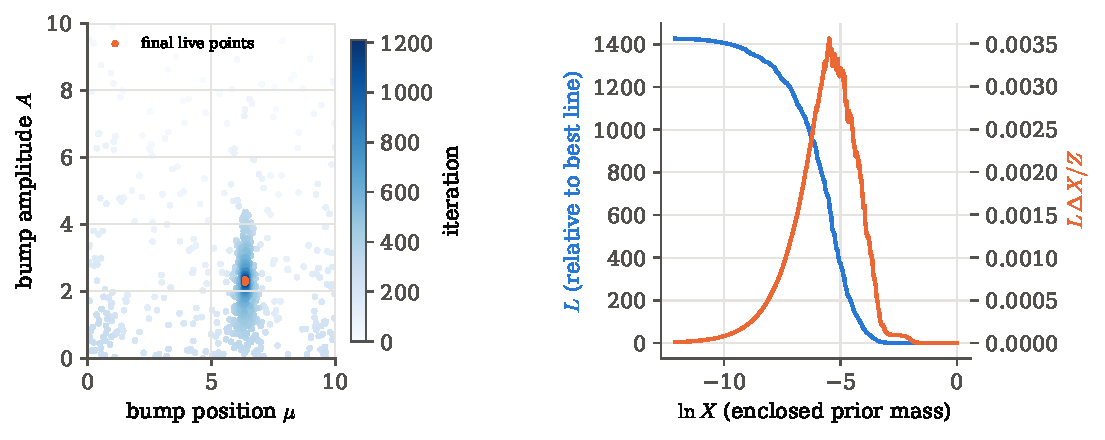
\includegraphics[width=\linewidth]{figures/ch05/nested_sampling.pdf}
\caption{Nested sampling of the bump evidence. Left: the discarded points in the plane of
bump position and amplitude, shaded by the step at which they were discarded; the early
ones are spread over the whole prior box, the late ones close in on the peak, where the
final live points sit. Right: the likelihood of the discarded points against the
logarithm of the enclosed prior mass (blue), and each point's share of the evidence
(orange). The evidence comes from a band around $\ln X\approx-5$, that is, from about
$e^{-5}$ of the prior.}
\label{5c:fig:ns}
\end{figure}

Our version is honest but naive in one place. Step 2 draws new points from the whole
prior until one beats the current lowest likelihood; late in the run almost every
draw fails, and the run spends $\FiveCNsEvalM$ million likelihood evaluations. Research
codes draw the replacement point from a short constrained Markov chain or from ellipsoids
fitted around the live points, and need of order $10^5$ likelihood evaluations for a
cosmological evidence \cite[\S4.3]{Trotta2008}. With a likelihood that takes a second,
that is the difference between a day and several years. Thermodynamic integration,
which heats a Markov chain from the prior to the posterior, is the older alternative and
typically costs about a hundred times more \cite[\S4.3]{Trotta2008},
\srcref{HobsonBMC}{\S4.4.1}. Two further options
are VEGAS, an adaptive multidimensional integrator that refines a sampling density
on the fly and is popular in particle physics, and parallel tempering, in which Markov
chains at different ``temperatures'' (likelihood raised to a power below one, so that
the landscape is flatter) run side by side and swap states, which helps chains cross
between separated peaks \srcref{HobsonBMC}{\S4.4.1}.

\subsection{The same question for lists, parameters and models}
\label{5c:sec:same-question}

Bayes' theorem has now been used on three kinds of hypotheses, and the questions never
changed. For a short list (Monty's doors, a disease, two urns) the posterior was a set
of numbers. For the values of a continuous parameter it was a density. For whole models
it was again a set of numbers, and the probability of the data under each model was
itself an average over that model's parameters. Each time we asked the two questions of
\cref{5a:sec:denominator}: which hypotheses could have produced what we observed, and
how probable the observation was under each. For model comparison the first question
lists the models, each with its prior; the second is answered by the evidence.

The difference between the two uses lies in the evidence. For parameter estimation
inside a model the evidence cancels, and a sampler that uses only ratios delivers the
posterior. For model comparison it does not cancel, so it must be computed: exactly, by
a Laplace or Savage--Dickey approximation, or by nested sampling. The Markov chains of
\cref{ch:09} and the Fisher forecasts of \cref{ch:10} are the two tools the rest of the
book uses to answer the second question in many dimensions.

\begin{recap}
\begin{itemize}[itemsep=2pt,leftmargin=1.2em]
  \item A model is a likelihood and a prior. Its evidence $Z=\int\Like\,\pi\,\dd\params$ is
        the probability it gave to the observed data: the likelihood averaged over its
        prior.
  \item $\Prob(M_i\given\data)\propto Z_i\Prob(M_i)$; posterior odds $=$ Bayes factor
        $\times$ prior odds. The comparison says nothing about parameters; model averaging
        combines the parameter posteriors with the model probabilities as weights.
  \item No model is rejected on its own: $p(\data\given\text{not }M)$ is undefined without
        specific alternatives.
  \item Occam's razor is derived, not assumed: $Z\approx\Like_{\max}\times V_{\rm post}/V_{\rm prior}$.
        Better fits are rewarded, wasted prior range is penalised, unconstrained parameters
        cost nothing. For the bump: a best-fit gain of $e^{\FiveCBumplnLR}$ became odds of $\FiveCBumpB:1$.
  \item Read Bayes factors on the logarithmic Jeffreys scale ($\lvert\ln B\rvert=1$, $2.5$,
        $5$), as posterior odds, and with their numerical and prior uncertainty.
  \item The evidence depends on prior widths ($-\ln10$ per decade of range) and can reverse
        between two vague priors that give the same posterior; improper priors are
        forbidden. Equally informed priors, physically motivated ranges and sensitivity
        plots are the remedies.
  \item Lindley: at fixed significance, large samples favour the null. A $p$-value bounds the
        odds: at most $1/(e\,p\ln p)$ against the null, $2.5:1$ at $2\sigma$, $150:1$ at
        $3.6\sigma$.
  \item Nested models: Savage--Dickey $B_{01}=p(\psi_*\given\data)/\pi(\psi_*)$ from the bigger
        model alone; BIC is the Laplace evidence without its prior terms; AIC, WAIC and LOO
        rank predictions, a different question.
  \item Estimating a difference and testing whether it is exactly zero are different
        questions with different priors, and can give opposite-looking answers.
  \item Grids cost $n^D$ and prior sampling fails exponentially in $D$; posterior samples
        give errors independent of $D$. Ratios of posteriors do not need the evidence
        (Metropolis, \cref{ch:09}); the evidence needs its own algorithm, such as nested
        sampling, $Z=\int_0^1\Like(X)\,\dd X$ with $\ln X_i\approx-i/N$.
\end{itemize}
\end{recap}

\subsection*{Reading the literature}
\label{5c:sec:reading-list}

\begin{itemize}[itemsep=2pt,leftmargin=1.2em]
  \item \textbf{The main line.} Wasserman, \emph{All of Statistics}, Chapter~11: the
        Bayesian method, conjugate examples, simulation from the posterior, flat and
        Jeffreys priors, Bayesian testing and its prior-free bound, and the strengths and
        weaknesses of Bayesian inference \mainref{pp.~175--189}.
  \item \textbf{The gentlest route.} Kruschke, \emph{Doing Bayesian Data Analysis},
        Chapters~2 and 5 (credibility, Bayes' rule), 6 (the Beta--Bernoulli model), 10 (model
        comparison, Occam's razor, prior sensitivity) and 12 (HDIs, estimation against
        testing).
  \item \textbf{The physicist's tutorial.} Sivia, \emph{Data Analysis: A Bayesian
        Tutorial}, Chapters~1--3 (plausible reasoning, parameter estimation, the Gaussian
        approximation, marginalisation), 4 (Mr A and Mr B, how many lines) and 5
        (assigning priors).
  \item \textbf{Priors, prediction and checks.} Lambert, \emph{A Student's Guide to
        Bayesian Statistics}, Chapters~3--7 and 9 (Bayes' rule, likelihood, priors, the
        denominator, conjugacy) and 10 (predictive checks, AIC to LOO-CV, Bayes factors,
        sensitivity analysis).
  \item \textbf{Cosmology.} Hobson, Jaffe, Liddle, Mukherjee and Parkinson (eds.),
        \emph{Bayesian Methods in Cosmology}, Chapter~1 (foundations, priors, nested sampling),
        Chapter~3 (Monte Carlo parameter estimation) and Chapter~4 (model selection,
        Savage--Dickey, the Jeffreys scale, the spectral index). Trotta's review ``Bayes in
        the sky'' \cite{Trotta2008} covers evidence, Occam's razor, the Lindley paradox and
        the $p$-value calibration in cosmological language. Padilla et al.\ \cite{Padilla2019}
        is a hands-on introduction with code.
  \item \textbf{Original papers.} Kass and Raftery on Bayes factors \cite{KassRaftery1995};
        Lindley's paradox \cite{Lindley1957}; Sellke, Bayarri and Berger on calibrating
        $p$-values \cite{Sellke2001}; Skilling on nested sampling \cite{Skilling2006};
        Metropolis et al.\ on the algorithm of \cref{ch:09} \cite{Metropolis1953}.
  \item \textbf{Pictures.} \emph{Seeing Theory}, chapter ``Bayesian Inference'', for
        interactive versions of the updating examples.
\end{itemize}

\clearpage
\raggedbottom
\section*{Chapter summary}
\addcontentsline{toc}{section}{Chapter summary}
\label{5c:sec:summary}

Bayesian inference turns the direction of probability around. Instead of asking what a
hypothesis predicts, we start from an outcome already observed and ask which hypotheses
might lie behind it, and how probable each is after the fact. Bayes' theorem answered
this question first for a short list of hypotheses, then for a continuous parameter,
and then for whole models, where the denominator we had been ignoring became the
quantity of interest. In the pipeline of the book,
\[
  \text{model}\to\text{data}\to\text{summary }S\to P(S\given\theta)\to\boxed{\text{infer physics}},
\]
Bayesian inference is the last arrow: the sampling distribution $P(S\given\theta)$ becomes
the likelihood, and the posterior over parameters and models is the inference.
\Cref{ch:04} gave the frequentist form of the same arrow.

\begin{center}
\small
\renewcommand{\arraystretch}{1.15}
\begin{tabularx}{\linewidth}{@{}>{\raggedright\arraybackslash}p{3.3cm}
                               >{\raggedright\arraybackslash}X
                               >{\raggedright\arraybackslash}p{2.7cm}@{}}
\toprule
\multicolumn{3}{@{}l}{\textbf{Bayes' theorem with a list of hypotheses}}\\
concept & operational meaning & used later in\\\midrule
prediction vs inference & $\Prob(E\given H)$ reads the tree forward; $\Prob(H\given E)$ asks which path produced the observed leaf & every chapter\\
joint table, logical not causal & one table of (hypothesis, outcome) probabilities: columns predict, rows infer; a posterior links hypothesis and evidence logically, it does not say the evidence caused anything & every chapter\\
Bayes' theorem & product rule in both orders: $\Prob(H\given E)=\Prob(E\given H)\Prob(H)/\Prob(E)$ & \cref{ch:08,ch:09}\\
information shrinks the sample space & conditioning on $E$ keeps only the region where $E$ holds and re-measures everything inside it & \cref{ch:08}\\
unit-square picture & priors are widths, likelihoods heights, posterior = surviving rectangle over total surviving area & \cref{ch:08}\\
reasoning in words & the event; what could have produced it; its probability under each hypothesis; then priors and normalise. Monty Hall: ``Monty opened C''; what made him open that door?; $\frac12,1,0$ for car behind A, B, C; posterior $\frac13,\frac23,0$ & every chapter\\
base rates & a tall bar in a thin strip can lose to a short bar in a wide one (rare signals, trigger purity) & \cref{ch:08,ch:12}\\
reallocation of credibility & zero likelihood eliminates, zero prior can never be revived, noisy data only nudge & \cref{ch:09}\\
odds, likelihood ratio & posterior odds $=$ likelihood ratio $\times$ prior odds; independent evidence adds in logarithms & \cref{ch:08,ch:10}\\
sequential updating & yesterday's posterior is today's prior, if the data are independent given the hypothesis & \cref{ch:09}\\
denominator, prior predictive & $\Prob(E)=\sum_i\Prob(E\given H_i)\Prob(H_i)$: normaliser and forecast; needs every hypothesis & \cref{ch:06,ch:09}\\
\bottomrule
\end{tabularx}
\end{center}

\begin{center}
\small
\renewcommand{\arraystretch}{1.15}
\begin{tabularx}{\linewidth}{@{}>{\raggedright\arraybackslash}p{3.3cm}
                               >{\raggedright\arraybackslash}X
                               >{\raggedright\arraybackslash}p{2.7cm}@{}}
\toprule
\multicolumn{3}{@{}l}{\textbf{Parameter estimation}}\\
concept & operational meaning & used later in\\\midrule
posterior density & likelihood $\times$ prior on a grid, normalised; the parameter value is the hypothesis, the data the event & \cref{ch:08,ch:09}\\
conjugate priors & Beta--Binomial, Gamma--Poisson, Normal--Normal: posterior in closed form, pseudo-counts and inverse-variance weights & \cref{ch:07,ch:08}\\
posterior summaries & mean, median, mode from three losses; equal-tailed interval; HDI, the shortest set & \cref{ch:09,ch:10}\\
credible vs confidence & probability of $\theta$ in a set given the data, against coverage over repetitions & \cref{ch:08,ch:10}\\
Gaussian (Laplace) approximation & peak and curvature: $\sigma^2=(-\partial^2\ln p)^{-1}$, covariance $=-H^{-1}$, $\Delta\chi^2$ regions & \cref{ch:10}\\
marginalising, profiling & integrate nuisance parameters out (volume included) or maximise over them & \cref{ch:08,ch:09,ch:10}\\
choosing a prior & knowledge, flat (in which variable?), Jeffreys $\propto\sqrt{I}$; improper priors as limits & \cref{ch:09}\\
forgetting the prior & the likelihood dominates for many data (Bernstein--von Mises); not the same as a chain forgetting its start & \cref{ch:09}\\
posterior sampling & a histogram of draws is the density; functions of parameters for free & \cref{ch:06,ch:09,ch:12}\\
\bottomrule
\end{tabularx}
\end{center}

\begin{center}
\small
\renewcommand{\arraystretch}{1.15}
\begin{tabularx}{\linewidth}{@{}>{\raggedright\arraybackslash}p{3.3cm}
                               >{\raggedright\arraybackslash}X
                               >{\raggedright\arraybackslash}p{2.7cm}@{}}
\toprule
\multicolumn{3}{@{}l}{\textbf{Model comparison and the need for sampling}}\\
concept & operational meaning & used later in\\\midrule
evidence $Z$ & likelihood averaged over the model's prior; the probability the model gave to the data & \cref{ch:09,ch:12}\\
Bayes factor, posterior odds & $B_{12}=Z_1/Z_2$ multiplies the prior odds; quote $\ln B$ and which model is on top & \cref{ch:09,ch:12}\\
Occam factor & $Z\approx\Like_{\max}V_{\rm post}/V_{\rm prior}$; wasted prior range is penalised, unconstrained parameters are free & \cref{ch:10}\\
Jeffreys scale & $\lvert\ln B\rvert=1,2.5,5$: odds $3,12,150$; apply to posterior odds, with the prior uncertainty & \cref{ch:12}\\
prior sensitivity & $\ln B$ falls by $\ln10$ per decade of prior range; vague priors can reverse it; improper priors forbidden & \cref{ch:12}\\
Lindley, $p$-value bounds & fixed significance favours the null at large $n$; $B_{10}\le-1/(e\,p\ln p)$ & \cref{ch:08,ch:12}\\
Savage--Dickey & $B_{01}=p(\psi_*\given\data)/\pi(\psi_*)$ from the bigger model's samples & \cref{ch:09}\\
model averaging & parameter posteriors weighted by model probabilities & \cref{ch:14}\\
BIC, AIC, WAIC, LOO & crude evidence without prior terms; predictive accuracy, a different question & \cref{ch:12}\\
estimation vs comparison & ``how large is the effect?'' against ``is it exactly zero?'': different priors, different answers & \cref{ch:08,ch:12}\\
curse of dimension & grids cost $n^D$; prior draws miss the posterior; posterior draws do not care about $D$ & \cref{ch:06,ch:09}\\
ratios, Metropolis & the evidence cancels in posterior ratios; a biased random walk samples the posterior & \cref{ch:09}\\
nested sampling & $Z=\int_0^1\Like(X)\dd X$, prior mass shrinking by $e^{-1/N}$ per step, error $\sqrt{H/N}$ & \cref{ch:09,ch:12}\\
\bottomrule
\end{tabularx}
\end{center}
\clearpage
\flushbottom
  
\part{Physics Toolkits}
\renewcommand{\thechapter}{T\arabic{chapter}}\renewcommand{\theHchapter}{T\arabic{chapter}}
\setcounter{chapter}{0}
\chapter{Cosmology for the Data Analyst}\label{ch:T1}

\providecommand{\TOneLmax}{}\renewcommand{\TOneLmax}{2500}
\providecommand{\TOneCosAsTauTT}{}\renewcommand{\TOneCosAsTauTT}{-0.999}
\providecommand{\TOneCosAsTauEElow}{}\renewcommand{\TOneCosAsTauEElow}{0.98}
\providecommand{\TOneAsRespHigh}{}\renewcommand{\TOneAsRespHigh}{1.41}
\providecommand{\TOneTauRespHigh}{}\renewcommand{\TOneTauRespHigh}{-1.46}
\providecommand{\TOneTauRespEElow}{}\renewcommand{\TOneTauRespEElow}{46}
\providecommand{\TOneNsPivotEll}{}\renewcommand{\TOneNsPivotEll}{542}
\providecommand{\TOneMaxRespOmc}{}\renewcommand{\TOneMaxRespOmc}{1.1}
\providecommand{\TOneDpeakEll}{}\renewcommand{\TOneDpeakEll}{220}
\providecommand{\TOneDpeak}{}\renewcommand{\TOneDpeak}{5732}
\providecommand{\TOneSigmaEight}{}\renewcommand{\TOneSigmaEight}{0.8111}
\providecommand{\TOneSigmaEightOurs}{}\renewcommand{\TOneSigmaEightOurs}{0.8112}
\providecommand{\TOneSigmaEightZone}{}\renewcommand{\TOneSigmaEightZone}{0.4928}
\providecommand{\TOneRdrag}{}\renewcommand{\TOneRdrag}{147.10}
\providecommand{\TOneRdragH}{}\renewcommand{\TOneRdragH}{99.1}
\providecommand{\TOneRpeak}{}\renewcommand{\TOneRpeak}{101.5}
\providecommand{\TOneKnl}{}\renewcommand{\TOneKnl}{0.15}
\providecommand{\TOneKnlZone}{}\renewcommand{\TOneKnlZone}{0.21}
\providecommand{\TOneKpeak}{}\renewcommand{\TOneKpeak}{0.017}
\providecommand{\TOneRatioOne}{}\renewcommand{\TOneRatioOne}{5.9}
 
\section*{Where this chapter is going}
\addcontentsline{toc}{section}{Where this chapter is going}
\label{T1a:sec:roadmap}

A cosmological model is a machine. We feed it six numbers, and it returns the \emph{statistics} of the sky: the angular power spectrum $\Cell$ of the microwave background (how much the temperature varies on each angular scale), the matter power spectrum $P(k)$ (the same for the matter density, scale by scale), and the distance to every redshift. CAMB \cite{CAMB2000} is that machine in code. The machine never returns the sky itself. Our sky, with its particular hot and cold spots and its particular galaxies, is one noisy draw from the statistics the machine predicts. Every later chapter works across that gap. The model predicts a distribution. The data are one draw from it. Statistics is how we read the six numbers back from that one draw.

The book follows one pipeline (\cref{ch:00}): a theory, its data, a compressed statistic, that statistic's scatter, and back to the theory. Cosmology is the first step. It fixes what each summary \emph{should} be on average. The physics behind each object is worked out in the cosmology notes. The data analyst needs less: which objects the statistics uses, what each one means in one line, the equation that defines it, where CAMB and the cosmology notes write it differently, and how the predicted statistics move when the six numbers move. \Cref{T1a:fig:roadmap} is the map.

\begin{figure}[htbp]
\centering
\begin{tikzpicture}[
  box/.style={draw=accent,rounded corners=2pt,fill=ideabg,align=center,font=\small,
              minimum width=3.1cm,minimum height=1.0cm,inner sep=3pt},
  obox/.style={box,minimum width=3.3cm,draw=formblue},
  dat/.style={box,fill=warnbg,draw=bdryred,minimum width=3.6cm},
  arr/.style={->,thick,accent},
  note/.style={font=\scriptsize,softgray,align=center}]
  \node[box] (par) at (0,0) {six numbers $\params$\\ $\Omega_{b0}h^2,\ \Omega_{c0}h^2,\ H_0$\\ $\tau,\ A_s,\ n_s$};
  \node[box] (camb) at (3.9,0) {CAMB\\ background $E(z)$,\\ transfer functions};
  \node[obox] (dist) at (8.3,1.5) {distances\\ $D_A(z),\ D_L(z),\ H(z)$};
  \node[obox] (cmb)  at (8.3,0) {CMB spectra\\ $\Cell$, $D_\ell$, lensing};
  \node[obox] (mat)  at (8.3,-1.5) {matter\\ $P(k)$, $\xi(r)$, $\sigma_8$};
  \node[draw=formblue,dashed,rounded corners=3pt,inner sep=5pt,fit=(dist)(cmb)(mat)] (pred) {};
  \draw[arr] (par) -- (camb);
  \draw[arr] (camb.east) -- (dist.west);
  \draw[arr] (camb.east) -- (cmb.west);
  \draw[arr] (camb.east) -- (mat.west);
  \node[dat] (sky) at (8.3,-3.9) {\textit{nature draws once:}\\ SN magnitudes, $\alm$ of our sky,\\ galaxy positions};
  \node[box,fill=takebg,draw=tangentgreen] (inf) at (3.9,-3.9) {\textit{inference:}\\ likelihood, MCMC,\\ Fisher, topology};
  \draw[arr,bdryred] (pred.south) -- (sky.north);
  \draw[arr,tangentgreen] (sky) -- (inf);
  \draw[arr,tangentgreen,dashed] (inf.west) -| (par.south);
\end{tikzpicture}
\caption{The machine and its one output we can see. Six numbers go into CAMB, which returns three families of predicted statistics (blue). Nature does not hand us those statistics: it hands us a single noisy draw from them (red), and the statistics of the later chapters (green) turn that draw back into constraints on the six numbers.}
\label{T1a:fig:roadmap}
\end{figure}

The link between the cosmology and the statistics is how the outputs move when the inputs move. Nudge one parameter and watch $\Cell$ respond. That response is a derivative, and the Fisher matrix of \cref{ch:10} is built from such derivatives. If two parameters produce responses that look alike, the data cannot tell those parameters apart. This is a degeneracy, and the MCMC chains of \cref{ch:09} show it as a long ridge. On the matter side, the linear $P(k)$ is the input of the Gaussian random fields of \cref{ch:07}. On small scales gravity makes the real spectrum (computed by the halofit recipe) depart from the linear one. There the field is no longer Gaussian, and the topological summaries of \cref{ch:12} have something to find that the power spectrum misses.

\section{Six numbers in, statistics out}
\label{T1a:sec:machine}

Think of the flat $\Lambda$CDM model as a function with six inputs.
Two inputs are physical densities: the baryon density $\Omega_{b0}h^2$ and the cold dark matter density $\Omega_{c0}h^2$ \unpack{today's density of each component divided by the critical density, times $h^2$; the product is a physical density that does not depend on $H_0$}.
One input fixes the distances: either the Hubble constant $H_0=100\,h\ \mathrm{km\,s^{-1}\,Mpc^{-1}}$, or equivalently the angle $\theta_{\mathrm{MC}}$ that the sound horizon at decoupling subtends on the sky.
One is the optical depth to reionisation, $\tau$ \unpack{the expected number of Thomson scatterings a CMB photon undergoes after the Universe is re-ionised; a fraction $e^{-\tau}$ of the photons arrive unscattered}.
The last two describe the primordial fluctuations: their amplitude $A_s$ and their spectral tilt $n_s$.
Everything else is held fixed: the radiation density (from the measured CMB temperature), flatness $\Omega_{K0}=0$, and a single massive neutrino of $0.06$\,eV.

These numbers appear in three places, and \cref{T1a:tab:params} translates between them: the symbol used in the cosmology notes, the keyword that CAMB's Python interface takes, and the Planck 2018 value with its 68\% error \cite[Table~1]{Planck2018VI}. The book's fiducial model (\pyname{code/camb_fiducial.py}) is this best fit. The $\pm1\sigma$ errors are the step sizes of the first experiment (\cref{T1a:sec:cl-response}).

\begin{table}[htbp]
\centering
\small
\renewcommand{\arraystretch}{1.2}
\begin{tabularx}{\linewidth}{@{}>{\raggedright\arraybackslash}p{2.6cm}
                               >{\raggedright\arraybackslash}X
                               >{\raggedright\arraybackslash}p{2.55cm}
                               >{\raggedright\arraybackslash}p{3.3cm}@{}}
\toprule
symbol (cosmology notes) & one-line meaning & CAMB keyword & Planck 2018 (68\%)\\\midrule
$\Omega_{b0}h^2$ & physical baryon density; sets the baryon loading of the acoustic oscillations & \pyname{ombh2} & $0.02237\pm0.00015$\\
$\Omega_{c0}h^2$ & physical cold dark matter density; sets matter--radiation equality & \pyname{omch2} & $0.1200\pm0.0012$\\
$100\,\theta_{\mathrm{MC}}$ \emph{or} $H_0$ & angular size of the sound horizon at decoupling, or the expansion rate today & \pyname{cosmomc_theta} or \pyname{H0} & $1.04092\pm0.00031$; $H_0=67.36\pm0.54$ (derived)\\
$\tau$ & optical depth to reionisation & \pyname{tau} & $0.0544\pm0.0073$\\
$A_s$ & amplitude of the primordial curvature spectrum at $k_*=0.05\,\mathrm{Mpc}^{-1}$ & \pyname{As} & $\ln(10^{10}A_s)=3.044\pm0.014$\\
$n_s$ & tilt of that spectrum, $n_s=1$ being scale invariant & \pyname{ns} & $0.9649\pm0.0042$\\
\bottomrule
\end{tabularx}
\caption{The six $\Lambda$CDM numbers in three notations. Planck samples $\theta_{\mathrm{MC}}$ because the data measure that angle almost directly; CAMB is usually called with $H_0$ instead, and the book's scripts do so (CAMB's \pyname{cosmomc_theta} takes $\theta_{\mathrm{MC}}$ itself, not $100\,\theta_{\mathrm{MC}}$). The error on $\ln(10^{10}A_s)$ is the fractional error on $A_s$, $1.4\%$.}
\label{T1a:tab:params}
\end{table}

The machine's output is a set of averages, not a sky. This is the one idea from cosmology that the statistics cannot do without. Take the CMB. Write the temperature pattern of the sky as a sum of spherical harmonics $Y_{\ell m}$; the coefficient of each one is a number $\alm$, and large $\ell$ means small angular scales. What does the model predict about these numbers? It predicts a definite value for $\Cell$, the average of $\abs{\alm}^2$, computed from the primordial power spectrum and the radiation transfer function. It never predicts any single $\alm$. Each $\alm$ of our sky is one random draw from a distribution of variance $\Cell$. The matter field works the same way: the model predicts $P(k)$, the variance of each Fourier mode of the matter density, and not the modes themselves. So comparing theory with data always means comparing a predicted \emph{distribution} with one \emph{draw}. A single draw scatters about its mean, and nothing can remove that scatter, because we have only one sky. That scatter is cosmic variance.

\begin{keyidea}[What the model predicts]
A cosmological model predicts the statistics of the fields (their power spectra, correlation functions and distances), never the fields themselves. The observed sky is one realisation. Every estimator in the later chapters is a function of that realisation, and its sampling distribution around the predicted statistic is what the likelihood describes.
\end{keyidea}

\section{The objects the statistics uses}
\label{T1a:sec:objects}

A revision of the cosmology a data analyst needs follows the order in which the machine of \cref{T1a:sec:machine} works. First comes the smooth background, the expansion of the Universe and the distances that follow from it. Then the primordial seed and how the radiation and matter eras process it. Last come the statistics of the two fields that result, the temperature of the sky and the density of matter. For every object the question comes first, then the equation it starts from and the working equation the book uses, then the size of the thing, then the chapters that use it. The physics between the two equations is worked out in the cosmology notes. Here it is a sentence.

\paragraph{How fast the Universe expands: $H(z)$ and $E(z)$.}
The question is how the expansion rate $H$ changed over cosmic history, because every distance below is built from it. A homogeneous, isotropic universe has the Friedmann--Lema\^itre--Robertson--Walker metric, with one function of time in it, the scale factor $a(t)$. Einstein's equations then reduce to the first Friedmann equation
\begin{equation*}
H^2\equiv\Bigl(\frac{\dot a}{a}\Bigr)^2=\frac{8\pi G}{3}\rho-\frac{K}{a^2}+\frac{\Lambda}{3},
\end{equation*}
where $\rho$ is the total density of radiation and matter, $K$ the spatial curvature and $\Lambda$ the cosmological constant. Each component dilutes in its own way as space expands: radiation as $a^{-4}$ (the photons also lose energy), matter as $a^{-3}$, curvature as $a^{-2}$, and $\Lambda$ not at all. Write the redshift as $1+z=a_0/a$ and divide by today's rate $H_0$. The result is the working equation, in terms of the dimensionless expansion rate $E(z)\equiv H(z)/H_0$:
\begin{equation*}
E^2(z)=\Omega_{r0}(1+z)^4+\Omega_{m0}(1+z)^3+\Omega_{K0}(1+z)^2+\Omega_{\Lambda0},
\qquad
\Omega_{K0}=1-\Omega_{m0}-\Omega_{r0}-\Omega_{\Lambda0}.
\end{equation*}
The $\Omega_{X0}$ are today's densities as fractions of the critical density $3H_0^2/8\pi G$, with $X=r$ for radiation, $m$ for matter, $K$ for curvature and $\Lambda$ for the cosmological constant, and the second relation says that the fractions add up to one. For the Planck fit, $\Omega_{m0}\approx0.315$, $\Omega_{\Lambda0}\approx0.685$, $\Omega_{r0}\approx9\times10^{-5}$ and $\Omega_{K0}\approx0$. The matter term wins over the others at $z\gtrsim0.3$, and radiation beats matter only for $z\gtrsim3000$. Today's numbers are $E(1)\approx1.79$, so the Universe expanded $1.8$ times faster at $z=1$. Of the six parameters of \cref{T1a:tab:params}, the data fix not $\Omega_{m0}$ itself but the physical density $\Omega_{m0}h^2=\Omega_{b0}h^2+\Omega_{c0}h^2\,(+\Omega_{\nu0}h^2)\approx0.143$, which is what the expansion history before the epoch of dark energy depends on. This is the model mean of the supernova and BAO data of \cref{ch:03,ch:05}, and the matter density is what the fits of \cref{ch:09,ch:10} constrain.

\paragraph{How far away is a source: $D_C$, $D_M$, $D_A$ and $D_L$.}
The question is what ``distance'' means for an object at redshift $z$, because the same source has a different distance depending on whether we measure it with a ruler or a candle. A light ray travels along a null path, $c\,\dd t=a\,\dd\chi$ in terms of the comoving radial coordinate $\chi$, and $\dd z=-(1+z)H\,\dd t$. Integrating along the ray from the source to us gives the comoving distance, with the Hubble distance $D_{H0}\equiv c/H_0$ as the unit:
\begin{equation*}
a_0\chi(z)=D_{H0}\int_0^{z}\frac{\dd z'}{E(z')} .
\end{equation*}
Curvature bends the ray's transverse separation, so the comoving transverse distance is $a_0f_K[\chi(z)]$, where $f_K(\chi)=\chi$ in a flat universe and is a $\sin$ or $\sinh$ of $\chi$ in a closed or open one. A source of physical size $s$ at redshift $z$ subtends the angle $\vartheta=s/D_A$ with the angular-diameter distance, and a source of luminosity $L$ gives the flux $F=L/4\pi D_L^2$ with the luminosity distance:
\begin{equation*}
D_A(z)=\frac{a_0f_K[\chi(z)]}{1+z},
\qquad
D_L(z)=(1+z)^2D_A(z).
\end{equation*}
The first divides by $1+z$ because the source was closer to us when the light left it, and the second multiplies by $(1+z)^2$ because redshift costs each photon energy and stretches the arrival rate. The Hubble distance is $D_{H0}=c/H_0\approx4450$\,Mpc. For the Planck model, a source at $z=1$ has comoving distance $3.4$\,Gpc, $D_A=1.7$\,Gpc and $D_L=6.8$\,Gpc, and the last-scattering surface at $z\approx1090$ is $13.9$\,Gpc away. Note that $D_A$ does not grow forever: it peaks near $1.8$\,Gpc at $z\approx1.6$ and then falls, so a rod at high redshift looks larger on the sky. Supernova magnitudes depend on $D_L(z)$, and the BAO ruler of the next paragraph on $D_A(z)$ and $H(z)$ (\cref{ch:03,ch:05}).

\paragraph{The acoustic ruler: the sound horizon $r_s$.}
The question is how far a sound wave could travel in the early plasma, because that length is a ruler that the CMB calibrates. Before recombination photons and baryons were locked into one fluid. A pressure wave in it moves at the sound speed $c_s=c/\sqrt{3(1+R)}$, which is the radiation value $c/\sqrt3$ slowed down by the baryons' inertia. Here $R\equiv3\rho_b/(4\rho_\gamma)$ is the baryon-to-photon momentum ratio, a number of order $0.6$ at the drag epoch. The distance such a wave covers up to conformal time $\eta$ is
\begin{equation*}
r_s(\eta)\equiv\int_0^\eta c_s\,\dd\eta'=\int_0^\eta\frac{c\,\dd\eta'}{\sqrt{3(1+R)}} .
\end{equation*}
Two epochs matter. At the last scattering of photons ($z_*\approx1090$) the CMB records the waves. Its angular scale is $\theta_{\mathrm{MC}}=r_s(z_*)/a_0f_K[\chi_*]\approx0.0104$ rad, and the acoustic peaks are spaced in $\ell$ by about $\pi/\theta_{\mathrm{MC}}\approx300$. At the later drag epoch ($z_{\mathrm{drag}}\approx1060$) the baryons are released from the photons, the wave stops, and $r_s(z_{\mathrm{drag}})\approx\TOneRdrag$\,Mpc is the radius of the shell that galaxies inherit as the BAO scale. The first is the angle in the third row of \cref{T1a:tab:params}; the second is the standard ruler of \cref{T1a:sec:pk}. Both appear in \cref{ch:05,ch:07,ch:12}.

\paragraph{The primordial seed: $\mathcal P_\zeta$, $A_s$ and $n_s$.}
The question is what the fluctuations looked like before any physics of the radiation or matter eras acted on them. Inflation, in the cosmology notes, stretches quantum fluctuations into a nearly Gaussian random field of comoving curvature perturbation $\zeta(\bm x)$. Its Fourier modes are independent, with variance $P_\zeta(k)$. For any spectrum $P_X$, the dimensionless version
\begin{equation*}
\mathcal P_X(k)\equiv\frac{k^3P_X(k)}{2\pi^2}
\end{equation*}
is the variance of the field per logarithmic interval of $k$, since $\int\!\dd^3k/(2\pi)^3\,P_X=\int\!\dd\ln k\,\mathcal P_X$. Inflation predicts a nearly scale-invariant power law. The cosmology notes write it with an amplitude $A_S$ and a tilt $n_S$ (capital S), and CAMB with $A_s$ and $n_s$:
\begin{equation*}
A_S^2\equiv\tfrac{4}{25}\,\mathcal P_\zeta,\quad A_S^2(k)\propto k^{n_S-1};
\qquad
\mathcal P_\zeta(k)=A_s\Bigl(\frac{k}{k_*}\Bigr)^{n_s-1},\quad k_*=0.05\,\mathrm{Mpc}^{-1}.
\end{equation*}
\Cref{T1a:sec:conventions} (item~3) converts between them: $A_s=\tfrac{25}{4}A_S^2(k_*)$. The size is $A_s\approx2.1\times10^{-9}$, so $\zeta$ has an rms of $5\times10^{-5}$ per $\ln k$, and $n_s=0.965$, slightly less than one, so there is a little more power on large scales than on small. The primordial spectrum is the input of the Gaussian random fields of \cref{ch:07} and the quantity the parameter fits of \cref{ch:09} constrain.

\paragraph{From seed to sky: the CMB transfer function and $C_\ell$.}
The question is how the primordial $\zeta$ becomes the temperature pattern we see. The photon, baryon, dark matter and neutrino fluids obey the Boltzmann hierarchy, and as the photons stream to us they carry the acoustic oscillations, the gravitational redshifts, and the effect of reionisation. All of this is linear in $\zeta$. So each Fourier mode $\zeta_{\bm k}$ produces a temperature anisotropy at multipole $\ell$ with a fixed coefficient $g^{(s)}_{T\ell}(k)$, the radiation transfer function \unpack{how much anisotropy at multipole $\ell$ one unit of $\zeta$ at wavenumber $k$ produces}, and the sum over $k$ of the independent contributions gives
\begin{equation*}
C_\ell=\frac{2}{\pi}\int k^2\,\dd k\,P_\zeta(k)\,g^{(s)}_{T\ell}(k)^2 .
\end{equation*}
This integral is what CAMB evaluates. $\Cell$ is the variance of the sky at multipole $\ell$, that is at angular scale $\vartheta\approx\pi/\ell$, and the cosmology notes define it through the expansion of the temperature contrast $\Theta=\delta T/T=\sum_{\ell m}\alm Y_{\ell m}$:
\begin{equation*}
\langle\alm a^*_{\ell'm'}\rangle=\delta_{\ell\ell'}\delta_{mm'}\,C_\ell,
\qquad
C(\vartheta)=\frac{1}{4\pi}\sum_\ell(2\ell+1)\,C_\ell\,P_\ell(\cos\vartheta).
\end{equation*}
The second relation is the correlation of two directions an angle $\vartheta$ apart, with $P_\ell$ the Legendre polynomial. Because the sky is one draw, the estimator is $\widehat C_\ell=\frac1{2\ell+1}\sum_m\abs{\alm}^2$, and it obeys $(2\ell+1)\widehat C_\ell/C_\ell\sim\chi^2_{2\ell+1}$, the cosmic-variance law of \cref{ch:07}. The plotted combination is $D_\ell\equiv\ell(\ell+1)C_\ell/2\pi$. For the fiducial model $D_\ell^{TT}$ peaks at $\TOneDpeak\,\mu\mathrm K^2$ at $\ell=\TOneDpeakEll$, and the fractional cosmic variance at one $\ell$ is $\sqrt{2/(2\ell+1)}$, about $9\%$ at $\ell=100$. The spectrum is the input of \cref{ch:07,ch:08,ch:09,ch:10}.

\paragraph{From seed to structure: the matter transfer function and growth.}
The question is how the same seed becomes the density field of galaxies. Two things happen, one depending on scale and one not. The first is growth. A small overdensity in pressureless matter grows according to the equation
\begin{equation*}
\ddot D+2H\dot D-\tfrac32H^2\Omega_m(t)\,D=0,
\qquad
D_+(a)=\frac52\frac{H(a)}{H_0}\,\Omega_{m0}\int_0^a\frac{\dd a'}{[a'E(a')]^3},
\end{equation*}
where the damping term $2H\dot D$ is Hubble friction and the last term is gravity. The growing solution is the integral on the right, and in a matter-dominated universe it is simply $D_+\propto a$. The second is the scale dependence. A mode that enters the horizon during radiation domination is held back, because radiation pressure prevents it from clumping, while a mode that enters later grows undisturbed. The \newterm{transfer function} packages this,
\begin{equation*}
T(k,a)=\frac{\delta(k,a)\,D_+(a_{\mathrm i})}{\delta(k,a_{\mathrm i})\,D_+(a)},
\qquad
P_\delta(k,a_0)=P_\delta(k,a_{\mathrm i})\,T^2(k,a_0)\Bigl[\frac{D_+(a_0)}{D_+(a_{\mathrm i})}\Bigr]^2,
\end{equation*}
where $a_{\mathrm i}$ is an early time before any scale of interest has entered the horizon, and the second relation is the first one squared. The transfer function goes to one for $k\ll k_{\mathrm{eq}}$ and falls as $(k_{\mathrm{eq}}/k)^2$ for $k\gg k_{\mathrm{eq}}$ (up to a logarithm), where $k_{\mathrm{eq}}\approx\TOneKpeak\,h\,\mathrm{Mpc}^{-1}$ is the wavenumber of the horizon at matter--radiation equality. Growth is a size we can read off: the matter fluctuations at $z=1$ are $0.61$ of those today ($\TOneSigmaEightZone$ against $\TOneSigmaEight$ in the $\sigma_8$ below). Used in \cref{ch:07}.

\paragraph{The statistics of the matter field: $P(k)$, $\xi(r)$ and $\sigma_8$.}
The question is how to describe a random field of matter density with statistics we can predict. Write $\delta=(\rho-\bar\rho)/\bar\rho$ for the density contrast, with Fourier modes $\delta_{\bm k}$. Homogeneity makes distinct modes uncorrelated, and the variance of one mode is the matter power spectrum $P_\delta(k)$ (also written $P_m$). Its real-space partner is the correlation function $\xi(r)$, the excess probability of finding two points at separation $r$:
\begin{equation*}
\langle\delta_{\bm k}\delta_{\bm k'}\rangle=\delta^{(3)}(\bm k+\bm k')\,P_\delta(k),
\qquad
\xi(r)=\int_0^\infty\frac{\dd k}{2\pi^2}\,k^2P_\delta(k)\,\frac{\sin kr}{kr}.
\end{equation*}
The second equation is the Fourier transform of the first, after the angle average of $e^{i\bm k\cdot\bm r}$ is done, which gives $\sin kr/kr$. $P_\delta$ peaks near $k_{\mathrm{eq}}$ at a few $10^4\,(h^{-1}\mathrm{Mpc})^3$, and the two spectra of linear theory and halofit separate at $k\approx\TOneKnl\,h\,\mathrm{Mpc}^{-1}$ at $z=0$. The single-number summary of the amplitude is the rms fluctuation in a sphere of radius $8\,h^{-1}$Mpc:
\begin{equation*}
\sigma_8^2\equiv\int\frac{\dd^3\bm k}{(2\pi)^3}\,\abs{W_{8h^{-1}\mathrm{Mpc}}(k)}^2P_m(k),
\qquad
W_R(k)=\frac{3j_1(kR)}{kR}.
\end{equation*}
Here $W_R$ is the Fourier transform of a spherical top-hat of radius $R$ and $j_1$ the spherical Bessel function, so the integral weights $P$ by how much of each mode a sphere of that size sees. The value is $\sigma_8=\TOneSigmaEight$: fluctuations in $8\,h^{-1}$Mpc spheres are about $80\%$ of the mean density, just short of non-linear. \Cref{T1a:sec:pk} computes both $\xi(r)$ and $\sigma_8$ from the CAMB $P(k)$. They feed the Gaussian-field simulations of \cref{ch:07}, the Fisher forecasts of \cref{ch:10} and the topological summaries of \cref{ch:12}.

\paragraph{Lensing of the CMB.}
The question is what happens to the pattern on the way to us. Matter between us and the last-scattering surface deflects the photons by a small angle, so the temperature we see in direction $\bm n$ was emitted from a slightly different direction:
\begin{equation*}
\hat T[\bm n]=T[\bm n+\bm\xi(\bm n)],
\qquad
\bm\xi=\bm\nabla\psi .
\end{equation*}
The deflection $\bm\xi$ (not the correlation function $\xi(r)$) is the gradient on the sky of a single scalar, the projected lensing potential $\psi$, which is the matter potential integrated along the line of sight with a geometric weight. The size is a few arcminutes, which is why the effect is a smoothing of the acoustic peaks and a coupling between modes, not a visible distortion. The same $\psi$ builds the shear of galaxy images in \cref{T1b:sec:objects}, with a source plane at last scattering. Used in \cref{ch:08,ch:12}.

\paragraph{The primordial three-point function: $f_{\mathrm{NL}}$.}
The question is whether the seed is exactly Gaussian. A Gaussian $\zeta$ is fully described by $P_\zeta$ and has zero three-point function. Any departure shows up in the bispectrum $B_\zeta$, the Fourier transform of $\langle\zeta\zeta\zeta\rangle$, and the amplitude $f_{\mathrm{NL}}$ is defined by comparing it with the products of two power spectra:
\begin{equation*}
\tfrac65f_{\mathrm{NL}}\equiv\frac{B_\zeta(k_1,k_2,k_3)}{P_\zeta(k_1)P_\zeta(k_2)+P_\zeta(k_1)P_\zeta(k_3)+P_\zeta(k_2)P_\zeta(k_3)} .
\end{equation*}
Planck finds $f_{\mathrm{NL}}^{\mathrm{local}}=-0.9\pm5.1$, consistent with a Gaussian field. A non-zero $f_{\mathrm{NL}}$ is invisible to $\Cell$ and $P(k)$ and is searched for with the tools of \cref{ch:12}.

\begin{table}[htbp]
\centering
\small
\renewcommand{\arraystretch}{1.25}
\begin{tabularx}{\linewidth}{@{}>{\raggedright\arraybackslash}p{2.5cm}
                               >{\raggedright\arraybackslash}X
                               >{\raggedright\arraybackslash}p{3.7cm}
                               >{\raggedright\arraybackslash}p{1.7cm}@{}}
\toprule
object & working equation & typical size & used in\\\midrule
$E(z)$ & $E^2=\Omega_{r0}(1+z)^4+\Omega_{m0}(1+z)^3+\Omega_{K0}(1+z)^2+\Omega_{\Lambda0}$ & $\Omega_{m0}\approx0.315$, $E(1)\approx1.79$ & \cref{ch:03,ch:05}\\
distances & $a_0\chi=D_{H0}\!\int\dd z/E$; $D_A=a_0f_K/(1+z)$; $D_L=(1+z)^2D_A$ & $D_{H0}\approx4450$\,Mpc; $D_L(1)\approx6.8$\,Gpc & \cref{ch:03,ch:05}\\
$r_s$ & $\int c_s\dd\eta=\int c\,\dd\eta/\sqrt{3(1+R)}$ & $\approx\TOneRdrag$\,Mpc at drag & \cref{ch:05,ch:07,ch:12}\\
primordial & $\mathcal P_\zeta=A_s(k/k_*)^{n_s-1}$; $A_s=\frac{25}{4}A_S^2$ & $A_s\approx2.1\times10^{-9}$, $n_s=0.965$ & \cref{ch:07,ch:09}\\
$\Cell$, $D_\ell$ & $C_\ell=\frac2\pi\!\int k^2\dd k\,P_\zeta g_{T\ell}^2$; $\langle\alm a^*_{\ell'm'}\rangle=\delta\delta C_\ell$; $(2\ell+1)\widehat C_\ell/C_\ell\sim\chi^2_{2\ell+1}$ & $D_\ell$ peak $\TOneDpeak\,\mu\mathrm K^2$ at $\ell=\TOneDpeakEll$ & \cref{ch:07,ch:08,ch:09,ch:10}\\
$T(k,a)$, $D_+$ & $P_\delta(k,a_0)=P_\delta(k,a_{\mathrm i})T^2[D_+(a_0)/D_+(a_{\mathrm i})]^2$ & $T\to(k_{\mathrm{eq}}/k)^2$ beyond $k_{\mathrm{eq}}\approx\TOneKpeak\,h\,\mathrm{Mpc}^{-1}$ & \cref{ch:07}\\
$P(k)$, $\xi(r)$ & $\langle\delta_{\bm k}\delta_{\bm k'}\rangle=\delta^{(3)}P_\delta$; $\xi=\!\int\!\frac{\dd k}{2\pi^2}k^2P\frac{\sin kr}{kr}$ & BAO bump at $\approx\TOneRpeak\,h^{-1}$Mpc & \cref{ch:07,ch:12}\\
$\sigma_8$ & $\int\frac{\dd^3k}{(2\pi)^3}\abs{W_8}^2P_m$; $W_R=3j_1(kR)/kR$ & $\TOneSigmaEight$ & \cref{ch:07,ch:10}\\
lensing & $\hat T[\bm n]=T[\bm n+\bm\nabla\psi]$ & a few arcmin & \cref{ch:08,ch:12}\\
$f_{\mathrm{NL}}$ & $\frac65f_{\mathrm{NL}}=B_\zeta/(PP+\text{perms})$ & $-0.9\pm5.1$ & \cref{ch:12}\\
\bottomrule
\end{tabularx}
\caption{The objects of the section at a glance: the working equation of each, a typical size, and where it is used.}
\end{table}

\subsection{Conventions to carry forward}
\label{T1a:sec:conventions}

The same object is often written differently in the cosmology notes, in CAMB and in this book. There are only a few such differences. Each one, if missed, changes a number by a large factor without any warning.

\begin{enumerate}[leftmargin=1.6em,itemsep=3pt]
\item \textbf{$\Cell$ versus $D_\ell$.} The book writes $D_\ell\equiv\ell(\ell+1)\Cell/2\pi$, the combination that is usually plotted, because it makes the acoustic peaks comparable in height. CAMB's \pyname{get_cmb_power_spectra} returns $D_\ell$ by default and returns the raw $\Cell$ only with \pyname{raw_cl=True}. The fiducial spectra in \pyname{data/camb_fiducial.npz} are raw $\Cell$. Every statistic of the later chapters ($\widehat C_\ell$, cosmic variance $2C_\ell^2/(2\ell+1)$, the $\chi^2_{2\ell+1}$ law) is written for the raw $\Cell$.
\item \textbf{Units of $\Cell$.} In the cosmology notes $\Theta=\delta T/T$ is dimensionless, so $\Cell$ is too. With \pyname{CMB_unit="muK"}, CAMB returns $T_0^2\,\Cell$ in $\mu\mathrm{K}^2$, with $T_0=2.7255\,\mathrm K=2.7255\times10^6\,\mu\mathrm K$. Noise spectra must be in the same units as the signal before they are added.
\item \textbf{The primordial amplitude.} The cosmology notes normalise the scalar amplitude as $A_S^2\equiv\frac{4}{25}\mathcal P_\zeta$. CAMB and Planck use $\mathcal P_\zeta(k)=A_s(k/k_*)^{n_s-1}$ with pivot $k_*=0.05\,\mathrm{Mpc}^{-1}$, so that $A_s=\mathcal P_\zeta(k_*)=\frac{25}{4}A_S^2(k_*)$. The Planck number $\ln(10^{10}A_s)=3.044$ refers to CAMB's $A_s$.
\item \textbf{Fourier conventions and $P(k)$.} Two Fourier conventions appear, and both lead to the same numerical $P(k)$, the one CAMB returns; only the non-linear mapping needs care. The matter spectrum in the cosmology notes uses the symmetric transform (a factor $(2\pi)^{-3/2}$ on each side), with $\langle\delta_{\bm k}\delta_{\bm k'}\rangle=\delta^{(3)}(\bm k+\bm k')P_\delta$. The non-Gaussianity material puts $(2\pi)^3\delta^{(3)}$ there instead. Both give the same $\xi(r)$ relation in the table above, and so the same $P(k)$. The non-linear mapping in the cosmology notes writes the dimensionless variance as $4\pi k^3P(k)$. That form assumes a $P$ carrying an extra factor $(2\pi)^{-3}$. With CAMB's $P(k)$ the same quantity is $k^3P(k)/2\pi^2$.
\item \textbf{Factors of $h$.} CAMB's \pyname{get_matter_power_spectrum} takes $k$ in $h\,\mathrm{Mpc}^{-1}$ and returns $P$ in $(h^{-1}\mathrm{Mpc})^3$; $\sigma_8$ is defined in $h^{-1}$Mpc. Derived lengths, such as the drag-epoch sound horizon, come back in plain Mpc. To compare one with $\xi(r)$ plotted against $r$ in $h^{-1}$Mpc, multiply it by $h=H_0/100$.
\item \textbf{Lensing potential.} The cosmology notes call the projected potential $\psi$; CAMB and Planck call the same object $\phi$. CAMB's \pyname{lens_potential} output is $[\ell(\ell+1)]^2C_\ell^{\phi\phi}/2\pi$, not $C_\ell^{\phi\phi}$. The fiducial CMB spectra of the book are lensed.
\item \textbf{Real and complex $\alm$.} The cosmology notes write the one-point density of $\alm$ for a real Gaussian variable of variance $\Cell$. In fact, for $m\neq0$ the $\alm$ are complex, with $a_{\ell,-m}=(-1)^ma^*_{\ell m}$, and their real and imaginary parts each have variance $\Cell/2$. The count does not change: there are still $2\ell+1$ independent real numbers per $\ell$, so the $\chi^2_{2\ell+1}$ law still holds. \Cref{ch:07} does the counting.
\end{enumerate}

\begin{pitfall}[A factor that looks like a physics result]
Mixing $A_S^2$ with CAMB's $A_s$ moves the amplitude by $25/4$; mixing $\Cell$ with $D_\ell$ moves it by $\ell(\ell+1)/2\pi$, about $10^5$ at $\ell=1000$. Neither error crashes a script. Both give a spectrum with a sensible shape and a wrong height. Checking that $D_\ell^{TT}$ of the fiducial model peaks at $\TOneDpeak\,\mu\mathrm K^2$ at $\ell=\TOneDpeakEll$ catches both.
\end{pitfall}

\section{Experiment 1: how each parameter moves the CMB spectra}
\label{T1a:sec:cl-response}

The inference chapters need one thing from the machine above all. If we turn one input knob a little, how does the output move? For the CMB the output is the whole curve $\Cell$, so the answer is a curve for each parameter. We find it the most direct way. Write $\theta_i$ for the $i$-th of the six parameters of \cref{T1a:tab:params} ($i=1,\dots,6$; this $\theta_i$ is any parameter, not the angle $\theta_{\mathrm{MC}}$), and $\delta_i$ for its Planck $1\sigma$ error.
\begin{enumerate}[leftmargin=1.6em,itemsep=1pt]
\item Start at the Planck best fit.
\item Run CAMB at $\theta_i+\delta_i$ and at $\theta_i-\delta_i$, with the other five parameters held at the best fit.
\item Form the symmetric fractional response
\end{enumerate}
\begin{equation}
R_i(\ell)\equiv\frac{C_\ell(\theta_i+\delta_i)-C_\ell(\theta_i-\delta_i)}{2\,C_\ell(\text{fiducial})},
\qquad
\frac{\partial C_\ell}{\partial\theta_i}\approx\frac{C_\ell\,R_i(\ell)}{\delta_i}.
\label{T1a:eq:response}
\end{equation}
The second relation follows from the first. A derivative is approximately the change in $\Cell$ divided by the change in $\theta_i$, here $[C_\ell(\theta_i+\delta_i)-C_\ell(\theta_i-\delta_i)]/2\delta_i$; by the definition of $R_i$, the numerator equals $2\,C_\ell\,R_i(\ell)$, and the $2$ cancels. This second relation is why the experiment matters. The derivatives $\partial\Cell/\partial\theta_i$ are exactly what enters the CMB Fisher matrix of \cref{ch:10}, and \pyname{code/chT1/01_cl_derivatives.py} computes them by this central difference. The step $\delta_i=1\sigma$ also gives the size of $R_i$ a plain meaning: a response of $1\%$ is what a change of one standard deviation in that parameter does to the spectrum.

\pyfile[firstline=30,lastline=52,firstnumber=30]{code/chT1/01_cl_derivatives.py}{Planck $1\sigma$ steps, one CAMB call, and the $\pm\delta$ loop}

The steps in lines 30--31 are the Planck errors of \cref{T1a:tab:params}; $A_s$ is stepped by $1.4\%$ of itself because Planck quotes the error on $\ln(10^{10}A_s)$. The function \pyname{spectra} (lines 36--42) makes one CAMB call and keeps the lensed $TT$ and $EE$ spectra as raw $\Cell$ in $\mu\mathrm K^2$ up to $\ell=\TOneLmax$. The loop in lines 48--52 moves one parameter up and down while the other five stay at the fiducial values. That makes thirteen CAMB runs in all: one at the fiducial model, plus two for each of the six parameters. The results are cached in \pyname{data/chT1/cl_derivs.npz}.

\begin{figure}[htbp]
\centering
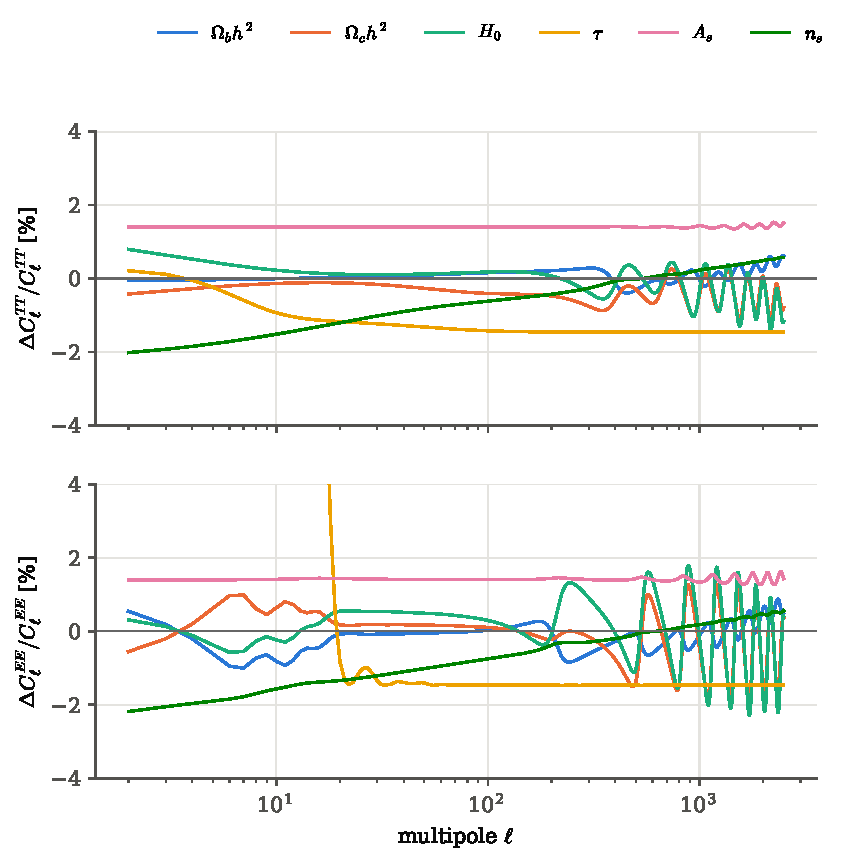
\includegraphics[width=0.86\linewidth]{figures/chT1/cl_response.pdf}
\caption{Fractional change of the lensed $TT$ (top) and $EE$ (bottom) spectra when each $\Lambda$CDM parameter moves by its Planck $1\sigma$ error, \cref{T1a:eq:response}. A flat line is a pure change of amplitude, a slanted line is a tilt, and a wiggle means the acoustic peaks change height or position. The $\tau$ curve in $EE$ leaves the plot at low $\ell$ (it reaches $\TOneTauRespEElow\%$).}
\label{T1a:fig:cl-response}
\end{figure}

\Cref{T1a:fig:cl-response} shows the six responses. Each can be read physically in one sentence:
\begin{itemize}[leftmargin=1.4em,itemsep=2pt]
\item $A_s$: a flat $+\TOneAsRespHigh\%$ at every $\ell$, because the primordial amplitude multiplies the whole spectrum.
\item $\tau$: a flat $\TOneTauRespHigh\%$ for $\ell\gtrsim30$, the $e^{-2\tau}$ screening of the anisotropies by the reionised electrons, with no effect on the largest scales of $TT$ and a large rise ($\TOneTauRespEElow\%$) in the low-$\ell$ $EE$ reionisation bump, which those same electrons create (see the cosmology notes).
\item $n_s$: a straight line in $\ln\ell$, rotating the spectrum about $\ell\approx\TOneNsPivotEll$, since a tilt adds power on one side of the pivot and removes it on the other.
\item $\Omega_{b0}h^2$ and $\Omega_{c0}h^2$: wiggles in phase with the acoustic peaks, largest $\TOneMaxRespOmc\%$ for $\Omega_{c0}h^2$, because the baryon loading and the epoch of matter--radiation equality set the relative heights of the peaks (see the cosmology notes).
\item $H_0$, at fixed physical densities: a slow drift at low $\ell$ from the late-time decay of the potentials, and oscillations at high $\ell$ because a changed distance to last scattering slides every peak sideways in $\ell$ (see the cosmology notes).
\end{itemize}

Two of these curves are nearly the same curve with opposite sign. Above $\ell\approx30$ the $A_s$ response is flat and positive, and the $\tau$ response is flat and negative. How alike are they? Treat each response as a list of numbers, one per $\ell$, and compute the cosine of the angle between the two lists, giving each $\ell$ the weight $2\ell+1$ (the number of $\alm$ at that $\ell$). A cosine of $+1$ or $-1$ means the same shape up to a factor. Over $30\le\ell\le\TOneLmax$ it is $\TOneCosAsTauTT$. The reason is visible in the list above: at high $\ell$ the spectrum is proportional to $A_s$ times the screening factor $e^{-2\tau}$, so it depends on the two only through $A_se^{-2\tau}$. Raise $A_s$ and raise $\tau$ together so that $A_se^{-2\tau}$ stays fixed, and the high-$\ell$ spectrum does not change. \Cref{T1a:fig:as-tau} puts $+R_{A_s}$ on top of $-R_\tau$ to make this visible.

\begin{figure}[htbp]
\centering
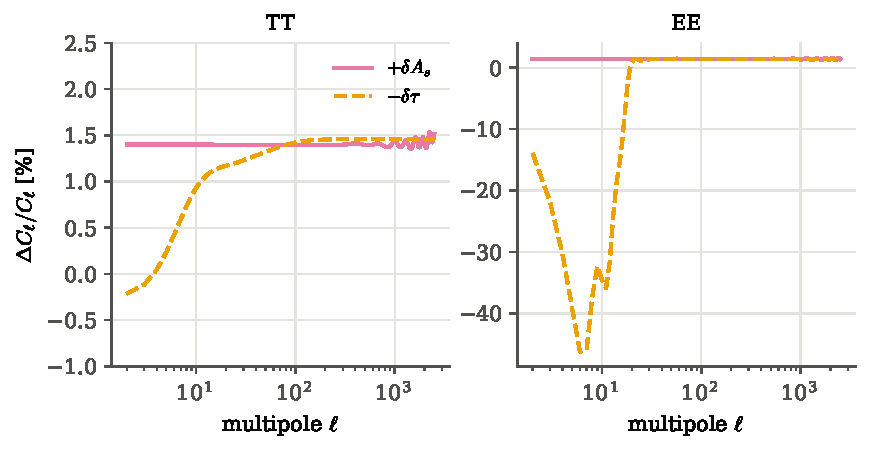
\includegraphics[width=0.9\linewidth]{figures/chT1/as_tau_degeneracy.pdf}
\caption{The $A_s$--$\tau$ degeneracy. The solid curve is the response to $+1\sigma$ in $A_s$, the dashed curve minus the response to $+1\sigma$ in $\tau$. In $TT$ (left) they coincide for $\ell\gtrsim30$, so high-$\ell$ temperature data measure only the combination $A_se^{-2\tau}$. In $EE$ (right) they separate completely at $\ell\lesssim20$, where the reionisation bump responds to $\tau$ alone.}
\label{T1a:fig:as-tau}
\end{figure}

This is what a degeneracy looks like before any statistics is done: two columns of derivatives that are almost parallel. In \cref{ch:10} it makes the Fisher matrix nearly singular along one direction. As a result, the marginalised errors on $A_s$ and $\tau$ (each parameter's error when the other is left free) are far larger than the conditional ones (its error when the other is held fixed). In \cref{ch:09} the same degeneracy appears as a long, thin ridge in the MCMC samples of $(\ln10^{10}A_s,\tau)$. The right panel shows how it is broken in practice. Large-angle polarisation measures $\tau$ on its own, and $A_s$ then follows from the high-$\ell$ amplitude.

\begin{inpractice}[Verification and research]
Here the finite differences only \emph{verify} what the physics already tells us (a flat $A_s$ response, the $e^{-2\tau}$ screening, the tilt about a pivot). In a Fisher forecast the same derivatives are the research instrument, and their accuracy has to be tested: the step must be small enough that $\Cell$ is linear in $\theta_i$ over $\pm\delta_i$, and large enough that CAMB's numerical noise does not dominate the difference. The standard check is to halve and double $\delta_i$ and confirm that the derivative does not move; \cref{ch:10} does this.
\end{inpractice}

\section{Experiment 2: the matter power spectrum and the BAO bump}
\label{T1a:sec:pk}

The second experiment turns to the matter field, the three-dimensional counterpart of the CMB sky. CAMB returns the matter power spectrum $P(k)$ at any redshift, either in linear theory or with the halofit correction \cite{Takahashi2012} \unpack{a fit to $N$-body simulations that maps the linear $P(k)$ to the non-linear one}. From the linear $P(k)$ we compute two things ourselves. The first is the correlation function $\xi(r)$, from the Fourier integral in the $P(k)$ row of the last table in \cref{T1a:sec:objects}. The second is $\sigma_8$, from the top-hat integral in the $\sigma_8$ row. CAMB also reports $\sigma_8$, so the second is a check on our code.

\pyfile[firstline=48,lastline=61,firstnumber=48]{code/chT1/02_pk_xi.py}{$\xi(r)$ and $\sigma_R$ from the linear $P(k)$}

\pyname{xi_of_r} evaluates $\xi(r)=\int\frac{\dd k}{2\pi^2}k^2P(k)\frac{\sin kr}{kr}$ as an integral over $\ln k$. Since $\dd k=k\,\dd\ln k$, the factor $k^2\,\dd k$ becomes $k^3\,\dd\ln k$; that is the $k^3$ in line 53. (\pyname{np.sinc(x/np.pi)} is $\sin x/x$.) The factor $e^{-k^2s^2}$ with $s=1\,h^{-1}$Mpc in line 51 is there only so the integral converges: it damps the fast-oscillating tail of the integrand. It acts on scales a hundred times smaller than the BAO peak and does not move the peak. \pyname{tophat_sigma} is the $\sigma_R$ integral with the window $W_R(k)=3(\sin kR-kR\cos kR)/(kR)^3=3j_1(kR)/(kR)$. At $R=8\,h^{-1}$Mpc it gives $\sigma_8=\TOneSigmaEightOurs$, against CAMB's $\TOneSigmaEight$, and $\TOneSigmaEightZone$ at $z=1$, where structure has had less time to grow.

\begin{figure}[htbp]
\centering
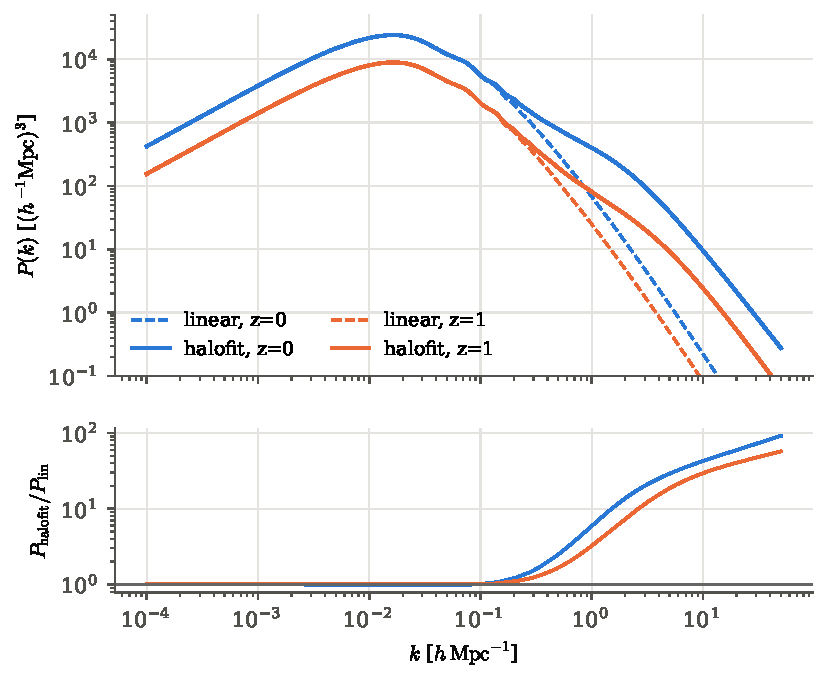
\includegraphics[width=0.8\linewidth]{figures/chT1/pk_lin_nl.pdf}
\caption{Matter power spectrum of the fiducial model at $z=0$ (blue) and $z=1$ (orange), linear theory dashed and halofit solid. The lower panel is the ratio halofit/linear: the two agree on large scales and differ by $10\%$ at $k\approx\TOneKnl\,h\,\mathrm{Mpc}^{-1}$ at $z=0$, and only at $k\approx\TOneKnlZone\,h\,\mathrm{Mpc}^{-1}$ at $z=1$.}
\label{T1a:fig:pk}
\end{figure}

\Cref{T1a:fig:pk} shows two pieces of physics.

The first is the turnover at $k\approx\TOneKpeak\,h\,\mathrm{Mpc}^{-1}$. It marks the size of the horizon at matter--radiation equality. Modes with larger $k$ (smaller scales) entered the horizon earlier, during radiation domination, and grew little there. So the transfer function falls roughly as $(k_{\mathrm{eq}}/k)^2$ (up to a logarithm), where $k_{\mathrm{eq}}$ is the turnover wavenumber. Since $P(k)\propto k^{n_s}T^2$ and $n_s\approx1$, beyond the turnover $P(k)$ falls roughly as $k\cdot k^{-4}=k^{-3}$ (see the cosmology notes).

The second is where halofit leaves linear theory. At $z=0$ the two differ by $10\%$ at $k\approx\TOneKnl\,h\,\mathrm{Mpc}^{-1}$ and by a factor $\TOneRatioOne$ at $k=1\,h\,\mathrm{Mpc}^{-1}$. The reason is gravitational collapse into haloes, which piles up power on small scales. For the statistics this boundary matters more than any number on the plot. On large scales the matter field is close to Gaussian, and $P(k)$ carries all of its information; this is the regime of the Gaussian random fields of \cref{ch:07}. On small scales the field is non-Gaussian, and $P(k)$ no longer tells the whole story. There, summaries that see the shape of the field, the topological summaries of \cref{ch:12}, have something extra to find.

\begin{figure}[htbp]
\centering
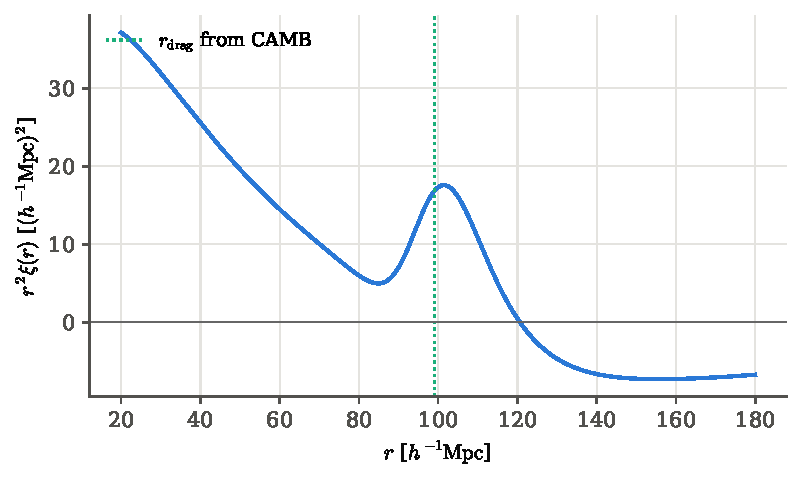
\includegraphics[width=0.8\linewidth]{figures/chT1/xi_bao.pdf}
\caption{The linear correlation function at $z=0$, multiplied by $r^2$ so that the bump is visible. The peak at $r\approx\TOneRpeak\,h^{-1}$Mpc sits close to the drag-epoch sound horizon computed by CAMB (dotted line, $\TOneRdragH\,h^{-1}$Mpc).}
\label{T1a:fig:xi}
\end{figure}

\Cref{T1a:fig:xi} shows the same information in real space, and there the baryon acoustic oscillations are much easier to see. In $P(k)$ they are small wiggles on a steep curve. In $\xi(r)$ they collapse into a single bump near $r\approx\TOneRpeak\,h^{-1}$Mpc. Where does the bump come from? Each initial overdensity launched a spherical sound wave into the photon--baryon plasma. The wave travelled until the baryons were released from the photons at the drag epoch, and then stopped. Its radius at that moment is the sound horizon $r_s(z_{\mathrm{drag}})$ of the BAO row, and it leaves an excess of pairs of points at that separation (see the cosmology notes). CAMB gives $r_s(z_{\mathrm{drag}})=\TOneRdrag$\,Mpc, that is $\TOneRdragH\,h^{-1}$Mpc. The peak of $r^2\xi$ sits a couple of percent higher because it rides on the sloping broad-band part of $\xi$.

Why does this matter? The CMB fixes $r_s$ precisely, so the bump is a ruler of known length. Its observed position in a galaxy survey at redshift $z$ therefore measures $D_A(z)$ (from its angular size) and $H(z)$ (from its extent along the line of sight). This is how BAO data enter the parameter fits mentioned in \cref{ch:05}. The bump was first detected in the galaxy correlation function by \cite{Eisenstein2005}. In \cref{ch:07} it is a feature to recover from a simulated field with noisy estimates of $\xi(r)$. In \cref{ch:12} it is one of the structures that a summary beyond the two-point function must respect.

\begin{recap}
\begin{itemize}[leftmargin=1.2em,itemsep=1pt]
\item Six numbers $(\Omega_{b0}h^2,\Omega_{c0}h^2,H_0\text{ or }\theta_{\mathrm{MC}},\tau,A_s,n_s)$ go into CAMB; out come $E(z)$ and distances, $\Cell$, $P(k)$, $\xi(r)$, $\sigma_8$.
\item The model predicts statistics, $\Cell=\langle\abs{\alm}^2\rangle$ and $P(k)$, never the $\alm$ or $\delta_{\bm k}$ themselves. Our sky is one draw.
\item Conventions: raw $\Cell$ (not $D_\ell$) in all statistics; $\mu\mathrm K^2$ means a factor $T_0^2$; CAMB's $A_s=\frac{25}{4}A_S^2$ of the cosmology notes; $P(k)$ in $(h^{-1}\mathrm{Mpc})^3$; CAMB's $\phi$ is the notes' $\psi$.
\item Nudging each parameter by $1\sigma$ gives $\partial\Cell/\partial\theta_i$, the Fisher derivatives; $A_s$ and $\tau$ respond identically above $\ell\approx30$ (cosine $\TOneCosAsTauTT$), and low-$\ell$ $EE$ breaks the tie.
\item Linear and halofit $P(k)$ separate at $k\approx\TOneKnl\,h\,\mathrm{Mpc}^{-1}$ today; $\xi(r)$ has the BAO bump near $r_s(z_{\mathrm{drag}})\approx\TOneRdragH\,h^{-1}$Mpc; our $\sigma_8$ matches CAMB's to better than $0.1\%$.
\end{itemize}
\end{recap}

\providecommand{\TOneSigmaEight}{}\renewcommand{\TOneSigmaEight}{0.8111}
\providecommand{\TOneSigmaEightOurs}{}\renewcommand{\TOneSigmaEightOurs}{0.8112}
\providecommand{\TOneSigmaEightZone}{}\renewcommand{\TOneSigmaEightZone}{0.4928}
\providecommand{\TOneRdrag}{}\renewcommand{\TOneRdrag}{147.10}
\providecommand{\TOneRdragH}{}\renewcommand{\TOneRdragH}{99.1}
\providecommand{\TOneRpeak}{}\renewcommand{\TOneRpeak}{101.5}
\providecommand{\TOneKnl}{}\renewcommand{\TOneKnl}{0.15}
\providecommand{\TOneKnlZone}{}\renewcommand{\TOneKnlZone}{0.21}
\providecommand{\TOneKpeak}{}\renewcommand{\TOneKpeak}{0.017}
\providecommand{\TOneRatioOne}{}\renewcommand{\TOneRatioOne}{5.9}
\providecommand{\TOneSEightFid}{}\renewcommand{\TOneSEightFid}{0.832}
\providecommand{\TOneZmed}{}\renewcommand{\TOneZmed}{0.71}
\providecommand{\TOneZmedLo}{}\renewcommand{\TOneZmedLo}{0.49}
\providecommand{\TOneZmedHi}{}\renewcommand{\TOneZmedHi}{0.99}
\providecommand{\TOneSigEightLo}{}\renewcommand{\TOneSigEightLo}{0.911}
\providecommand{\TOneSigEightHi}{}\renewcommand{\TOneSigEightHi}{0.720}
\providecommand{\TOneAlongMax}{}\renewcommand{\TOneAlongMax}{9}
\providecommand{\TOneAlongMedLo}{}\renewcommand{\TOneAlongMedLo}{-4}
\providecommand{\TOneAlongMedHi}{}\renewcommand{\TOneAlongMedHi}{+7}
\providecommand{\TOneAcrossLo}{}\renewcommand{\TOneAcrossLo}{-22}
\providecommand{\TOneAcrossHi}{}\renewcommand{\TOneAcrossHi}{+24}
\providecommand{\TOneLimberErr}{}\renewcommand{\TOneLimberErr}{0.1}
\providecommand{\TOneDlnCdlnSEight}{}\renewcommand{\TOneDlnCdlnSEight}{2.8}
\providecommand{\TOneDlnCdlnOm}{}\renewcommand{\TOneDlnCdlnOm}{1.6}
\providecommand{\TOneAlphaGalTwo}{}\renewcommand{\TOneAlphaGalTwo}{0.59}
\providecommand{\TOneAlphaGalTwoK}{}\renewcommand{\TOneAlphaGalTwoK}{0.62}
\providecommand{\TOneAlphaLoFive}{}\renewcommand{\TOneAlphaLoFive}{0.58}
\providecommand{\TOneAlphaFive}{}\renewcommand{\TOneAlphaFive}{0.55}
\providecommand{\TOneAlphaHiFive}{}\renewcommand{\TOneAlphaHiFive}{0.53}
\providecommand{\TOneNoiseOne}{}\renewcommand{\TOneNoiseOne}{4.965\times10^{-9}}
\providecommand{\TOneFsky}{}\renewcommand{\TOneFsky}{0.0242}
\providecommand{\TOneEdgeOne}{}\renewcommand{\TOneEdgeOne}{0.43}
\providecommand{\TOneEdgeFour}{}\renewcommand{\TOneEdgeFour}{1.05}
\providecommand{\TOneLeqOne}{}\renewcommand{\TOneLeqOne}{21}
\providecommand{\TOneLeqThree}{}\renewcommand{\TOneLeqThree}{87}
\providecommand{\TOneLeqFive}{}\renewcommand{\TOneLeqFive}{194}
\providecommand{\TOneSNtomo}{}\renewcommand{\TOneSNtomo}{48}
\providecommand{\TOneSNone}{}\renewcommand{\TOneSNone}{42}
\providecommand{\TOneSigLnSEight}{}\renewcommand{\TOneSigLnSEight}{0.8}
\providecommand{\TOneLmaxSN}{}\renewcommand{\TOneLmaxSN}{2000}
\providecommand{\TOneSigmaE}{}\renewcommand{\TOneSigmaE}{0.27}
\providecommand{\TOneNeff}{}\renewcommand{\TOneNeff}{6.2}
\providecommand{\TOneArea}{}\renewcommand{\TOneArea}{1000}
 
\section{Weak lensing: the matter field written on galaxy shapes}
\label{T1b:sec:shapes}

Light from a distant galaxy crosses billions of light years of clumpy matter on its way to us. Every lump it passes bends it a little. What arrives is an image that is slightly displaced, slightly enlarged and slightly stretched in one direction, typically by about one per cent. Nothing in the image says which part of it is the stretch: a galaxy that looks elongated may simply be elongated. Yet the stretch is the cleanest probe of matter we have, because gravity bends light whatever the matter is made of, dark or luminous, and no assumption about how galaxies trace mass enters. This is \newterm{weak gravitational lensing}, and \newterm{cosmic shear} is its version with the large-scale structure as the lens \cite{BartelmannSchneider2001,Kilbinger2015}.

For the data analyst, weak lensing is the situation of \cref{T1a:sec:machine} in a sharper form. There the model predicted the variance $\Cell$ of the CMB sky and the sky was one draw. Here the model predicts the angular power spectrum $C_\ell^{\kappa\kappa}$ of a lensing field $\kappa$ (defined below), the sky gives one draw of $\kappa$, and on top of that we do not see $\kappa$ itself. We see the shapes of galaxies, and each shape is mostly the galaxy's own.

\paragraph{The question.}
What we observe is a catalogue: for every galaxy, a position on the sky and an \newterm{ellipticity} \unpack{a complex number $\varepsilon=\varepsilon_1+i\varepsilon_2$ whose size is how elongated the image is and whose phase is twice the angle of its long axis}. What could have produced the ellipticity of one particular galaxy? There are two candidates, and we take them one at a time.
\begin{enumerate}[leftmargin=1.6em,itemsep=2pt]
\item \emph{The galaxy's own shape.} Galaxies are not round. Their intrinsic ellipticities $\varepsilon^{(0)}$ scatter with an rms $\sigma_e\approx0.27$ per component \cite{Asgari2021KiDS}, and their long axes point in random directions. So the intrinsic part has mean zero, but it is large.
\item \emph{The shear of the matter in front of it.} The lensing stretch $\gamma$ is about $0.01$, thirty times smaller. But it is \emph{coherent}: two galaxies that lie close together on the sky sent their light past the same lumps, so they are stretched in nearly the same way.
\end{enumerate}
Only now do we compute anything. In the weak regime the two simply add,
\begin{equation}
\varepsilon\approx\varepsilon^{(0)}+\gamma .
\label{T1b:eq:eps-sum}
\end{equation}
The reason is that $\varepsilon$ is defined from the shape of the image, and a shear of one per cent changes that shape by one per cent: to first order in small quantities it moves the ellipticity by $\gamma$ itself, whatever the galaxy's own shape was. \Cref{T1b:sec:reduced-shear} works this out for a round source; with the other common definition of $\varepsilon$ the shift is $2\gamma$ instead (convention~3 of \cref{T1b:sec:conventions}). A single galaxy tells us almost nothing, since the shear is buried under a noise thirty times larger. But the intrinsic parts of different galaxies are independent, and the shears of neighbours are correlated. Two moves turn this into a measurement.

\emph{Average galaxies that share one shear.} Take $N$ galaxies close enough together that they all feel the same $\gamma$, and average their ellipticities:
\begin{align}
\bar\varepsilon\equiv\frac1N\sum_{a=1}^N\varepsilon_a
&\eqby{1}\gamma+\frac1N\sum_{a=1}^N\varepsilon^{(0)}_a,
&
\E\,\bar\varepsilon&\eqby{2}\gamma,
&
\Var\bar\varepsilon_1&\eqby{3}\frac{\sigma_e^2}{N}.
\label{T1b:eq:shear-mean}
\end{align}
\begin{explain}
  \item Insert \eqref{T1b:eq:eps-sum} for each galaxy; the shear is the same in every term, so its average is itself.
  \item The intrinsic ellipticities point in random directions, so each has mean zero.
  \item The variance of a mean of $N$ independent readings of variance $\sigma_e^2$, \eqref{3a:eq:var-mean}, applied to one real component; the same holds for $\bar\varepsilon_2$.
\end{explain}
So the noise on the shear estimate is $0.27/\sqrt N$ per component. How large must $N$ be? A signal-to-noise ratio of one on a single shear of $0.01$ needs $0.27/\sqrt N=0.01$, that is $N=(0.27/0.01)^2\approx730$ galaxies, all sharing that one shear. A map with many independent shear values, each measured several times better than that, needs millions of galaxies.

\emph{Correlate pairs.} The shear changes across the sky, so averaging is limited to small patches. Correlation uses every pair instead. For two galaxies $a\neq b$, multiply the ellipticity of one by the complex conjugate of the other and expand:
\begin{align}
\bigl\langle\varepsilon_a\varepsilon_b^*\bigr\rangle
&\eqby{1}\bigl\langle(\varepsilon^{(0)}_a+\gamma_a)(\varepsilon^{(0)}_b+\gamma_b)^*\bigr\rangle\nonumber\\
&\eqby{2}\bigl\langle\varepsilon^{(0)}_a\varepsilon^{(0)*}_b\bigr\rangle+\bigl\langle\varepsilon^{(0)}_a\gamma_b^*\bigr\rangle+\bigl\langle\gamma_a\varepsilon^{(0)*}_b\bigr\rangle+\bigl\langle\gamma_a\gamma_b^*\bigr\rangle
\eqby{3}\bigl\langle\gamma_a\gamma_b^*\bigr\rangle .
\label{T1b:eq:pair}
\end{align}
\begin{explain}
  \item \Cref{T1b:eq:eps-sum} for each galaxy.
  \item Multiply out the brackets; the average of a sum is the sum of the averages.
  \item The intrinsic shapes of two different galaxies are independent, each with mean zero, so the first term is the product of two zero means. In the two middle terms an intrinsic shape is independent of the shear in front of the other galaxy, and the same reasoning makes them vanish. Only the correlation of the shears survives.
\end{explain}
Galaxy $a$ paired with itself would add $\langle\abs{\varepsilon^{(0)}_a}^2\rangle$, which does not vanish; this is why the self-pairs are left out, and why shape noise reappears as an added term in the power spectrum (\cref{T1b:sec:objects}). The information is in the statistics of many shapes, never in one shape. This is why every weak-lensing number in the later chapters is a two-point function, a peak count or a topological summary of a field built from millions of galaxies, and why its noise term is set by how many galaxies there are.

\Cref{T1b:fig:kappa-gamma} shows what the two parts of the lensing distortion do, exaggerated twenty-five-fold. The \newterm{convergence} $\kappa$ \unpack{the projected matter density along the line of sight, in units of a critical density} enlarges an image without changing its shape. The \newterm{shear} $\gamma=\gamma_1+i\gamma_2$ \unpack{the tidal part of the lensing distortion, which stretches the image along one axis and squeezes it along the perpendicular one} turns a circle into an ellipse.

\begin{figure}[htbp]
\centering
\begin{tikzpicture}[scale=1.0]
  \def\r{0.6}
  \draw[thick,formblue] (0,0) circle (\r);
  \node[font=\small] at (0,-1.35) {source};
  \draw[thick,formblue] (2.4,0) circle ({\r/(1-0.25)});
  \node[font=\small] at (2.4,-1.35) {$\kappa=0.25$ only};
  \draw[thick,formblue] (4.9,0) ellipse ({\r/(1-0.25)} and {\r/(1+0.25)});
  \node[font=\small] at (4.9,-1.35) {$\gamma_1=0.25$ only};
  \draw[softgray,dashed] (2.4,0) circle (\r);
  \draw[softgray,dashed] (4.9,0) circle (\r);
  \node[font=\small\bfseries] at (-0.9,1.15) {(a)};
  \begin{scope}[xshift=8.0cm]
    \node[font=\small\bfseries] at (-1.3,1.15) {(b)};
    \fill[bdryred] (0,0) circle (0.08);
    \foreach \t in {0,30,...,330} {
      \draw[very thick,tangentgreen] ({0.85*cos(\t)+0.15*cos(\t+90)},{0.85*sin(\t)+0.15*sin(\t+90)})
        -- ({0.85*cos(\t)-0.15*cos(\t+90)},{0.85*sin(\t)-0.15*sin(\t+90)});
    }
    \node[font=\small,align=center] at (0,-1.35) {$E$ mode};
  \end{scope}
  \begin{scope}[xshift=11.0cm]
    \fill[bdryred] (0,0) circle (0.08);
    \foreach \t in {0,30,...,330} {
      \draw[very thick,fibreorange] ({0.85*cos(\t)+0.15*cos(\t+45)},{0.85*sin(\t)+0.15*sin(\t+45)})
        -- ({0.85*cos(\t)-0.15*cos(\t+45)},{0.85*sin(\t)-0.15*sin(\t+45)});
    }
    \node[font=\small,align=center] at (0,-1.35) {$B$ mode};
  \end{scope}
\end{tikzpicture}
\caption{(a) A round source (left), the same source magnified by convergence alone (middle), and stretched by shear alone (right); the dashed circle is the source for comparison. Real values are near $0.01$, not $0.25$. (b) Each stick is the long axis of a sheared image. Around a mass concentration (red dot) lensing lines the images up tangentially, the $E$ pattern. Rotating every stick by $45^\circ$ gives the $B$ pattern, a swirl, which lensing by a scalar potential cannot make.}
\label{T1b:fig:kappa-gamma}
\end{figure}

The sticks in panel (b) have no arrowheads, and that is the key property of shear. An ellipse rotated by $180^\circ$ is the same ellipse. What kind of number can describe such a stick?

\emph{A stick first.} Let the long axis of an ellipse make an angle $\phi$ with the first reference axis. If we turn the reference axes by an angle $\alpha$, the same stick is now seen at $\phi-\alpha$. A complex number that records the direction must be a function $f(\phi)$, and the simplest functions of an angle are the pure tones $e^{im\phi}$ with a whole number $m$. Which $m$ will do? The stick at $\phi+\pi$ is the same stick, so we need $e^{im(\phi+\pi)}=e^{im\phi}$, that is $e^{im\pi}=1$, and $m$ must be even. The choice $m=1$ fails: $e^{i(\phi+\pi)}=-e^{i\phi}$, so the same stick would get two opposite values. That is the description of an arrow, a vector, which returns to itself only after a full turn of $2\pi$. The choice $m=0$ is allowed but records no direction at all. The smallest useful choice is $m=2$, so a stretch of size $\abs\gamma$ along the angle $\phi$ is written $\gamma=\abs\gamma e^{2i\phi}$, the form in the table of \cref{T1b:sec:objects}. When the axes turn by $\alpha$,
\begin{equation}
\gamma=\abs\gamma e^{2i\phi}\ \longrightarrow\ \abs\gamma e^{2i(\phi-\alpha)}=e^{-2i\alpha}\gamma .
\label{T1b:eq:spin2}
\end{equation}
A quantity that picks up the phase $e^{-is\alpha}$ under a turn of the axes is said to have \newterm{spin} $s$. Shear has spin 2. The CMB polarization $Q+iU$ is also a headless stick and changes in exactly the same way (see the cosmology notes). Every tool built for CMB polarization (the split into $E$ and $B$ modes, spin-2 spherical harmonics, \pyname{healpy}'s polarization transforms) uses only the rule \eqref{T1b:eq:spin2}, so it applies to shear without change.

\emph{Where the two angles live.} Every lensing formula below is written in two angles, $\theta_1$ and $\theta_2$. They locate a point on the sky the way $x$ and $y$ locate a point on a sheet of graph paper held at arm's length. The patch we analyse is a few degrees across at most, so we may treat it as flat: a plane facing us, with its origin on one chosen line of sight (in \cref{T1b:fig:sky-plane}, the one through a lump of matter), and $\theta_1$, $\theta_2$ the two angles, measured from that line, to a point on it. Now follow the light of one galaxy. Without the lump, the galaxy would be seen in the direction $\bm\theta_S$ where it really is. The light that actually reaches us left the galaxy in a slightly different direction, was bent as it passed the lump, and arrives along a straight final leg. We place every object where its light appears to come from, so we extend that last leg backwards, and it meets the sky plane at a different point, $\bm\theta$. The catalogue records $\bm\theta$; the true $\bm\theta_S$ is never seen. The difference is the deflection, $\bm\theta_S=\bm\theta-\hat{\bm\alpha}(\bm\theta)$, the second row of the table in \cref{T1b:sec:objects}.

The deflection by itself changes nothing we can measure. If every point of a galaxy moved by the same $\hat{\bm\alpha}$, the image would simply be the galaxy, displaced, and we never know where it would have been. What we can measure is how the deflection \emph{changes} across one image: points on the side nearer the lump are pulled more than points on the far side, so the image is enlarged ($\kappa$) and stretched ($\gamma$). Panel (b) of \cref{T1b:fig:sky-plane} shows the outcome for the lump of the figure: the image is pushed outward and stretched along the circle around the lump, the tangential pattern of \cref{T1b:fig:kappa-gamma}(b).

\begin{figure}[htbp]
\centering
\begin{tikzpicture}[scale=0.84,>={Stealth[length=2.2mm]}]
  \def\ux{0.9}\def\uy{0.5}
  \node[font=\small\bfseries] at (-0.6,3.3) {(a)};
  \fill (0,0) circle (0.09);
  \node[font=\small,below=2pt] at (0,0) {us};
  \coordinate (Lc) at (5,0);
  \draw[softgray!70,fill=softgray!8]
    ($(Lc)+(-1.0*\ux,-1.0*\uy)+(0,-1.3)$) -- ($(Lc)+(1.0*\ux,1.0*\uy)+(0,-1.3)$) --
    ($(Lc)+(1.0*\ux,1.0*\uy)+(0,1.7)$) -- ($(Lc)+(-1.0*\ux,-1.0*\uy)+(0,1.7)$) -- cycle;
  \shade[ball color=bdryred!80] (Lc) circle (0.17);
  \node[font=\small,softgray,below] at ($(Lc)+(0,-1.85)$) {lump of matter};
  \coordinate (Sc) at (10,0);
  \draw[formblue!70,fill=formblue!5]
    ($(Sc)+(-2.2*\ux,-2.2*\uy)+(0,-1.4)$) -- ($(Sc)+(2.2*\ux,2.2*\uy)+(0,-1.4)$) --
    ($(Sc)+(2.2*\ux,2.2*\uy)+(0,2.9)$) -- ($(Sc)+(-2.2*\ux,-2.2*\uy)+(0,2.9)$) -- cycle;
  \node[font=\small,formblue,below] at ($(Sc)+(0,-2.6)$) {sky plane};
  \draw[->,thick] ($(Sc)+(-1.6*\ux,-1.6*\uy)$) -- ($(Sc)+(2.0*\ux,2.0*\uy)$) node[below right=-1pt,font=\small] {$\theta_1$};
  \draw[->,thick] ($(Sc)+(0,-1.2)$) -- ($(Sc)+(0,2.7)$) node[above,font=\small] {$\theta_2$};
  \draw[softgray,dashed] (0,0) -- (Sc);
  \coordinate (S) at ($(Sc)+(0.4*\ux,0.4*\uy)+(0,0.5)$);
  \coordinate (P) at ($(Sc)+(1.0*\ux,1.0*\uy)+(0,1.25)$);
  \coordinate (L) at ($(0,0)!0.5!(P)$);
  \draw[dotted,thick] (P) -- ($(Sc)+(1.0*\ux,1.0*\uy)$);
  \draw[dotted,thick] (P) -- ($(Sc)+(0,1.25)$);
  \draw[very thick,tangentgreen,postaction={decorate},
        decoration={markings,mark=at position 0.55 with {\arrow{<}}}] (L) -- (S);
  \draw[very thick,tangentgreen,postaction={decorate},
        decoration={markings,mark=at position 0.45 with {\arrow{<}}}] (0,0) -- (L);
  \draw[thick,fibreorange,dashed] (L) -- (P);
  \draw[->,thick,black] ($(S)!0.17!(P)$) -- ($(S)!0.83!(P)$);
  \draw[thick,tangentgreen,fill=white] (S) circle (0.1);
  \fill[fibreorange] (P) circle (0.1);
  \draw[tangentgreen,thin] (S) -- ($(S)+(0.5,-1.15)$) node[below,font=\small] {$\bm\theta_S$, true};
  \node[font=\small,fibreorange,above right=1pt] at (P) {$\bm\theta$, seen};
  \node[font=\small,right=1pt] at ($(S)!0.55!(P)$) {$\hat{\bm\alpha}$};
  \begin{scope}[xshift=15.4cm,yshift=0.45cm]
    \node[font=\small\bfseries] at (-2.6,2.55) {(b)};
    \fill[formblue!5] (-2.2,-2.2) rectangle (2.2,2.2);
    \draw[formblue!18,very thin,step=0.4] (-2.2,-2.2) grid (2.2,2.2);
    \draw[formblue!70] (-2.2,-2.2) rectangle (2.2,2.2);
    \node[font=\small,formblue,below] at (0,-2.25) {sky plane, face on};
    \draw[->,thick] (-2.0,0) -- (2.0,0) node[below=1pt,font=\small] {$\theta_1$};
    \draw[->,thick] (0,-2.0) -- (0,2.0) node[left=1pt,font=\small] {$\theta_2$};
    \draw[softgray] (0,0) circle (1.6);
    \shade[ball color=bdryred!80] (0,0) circle (0.13);
    \draw[dotted,thick] (1.28,1.6) -- (1.28,0);
    \draw[dotted,thick] (1.28,1.6) -- (0,1.6);
    \draw[thick,tangentgreen,dashed,fill=white] (0.512,0.64) circle (0.22);
    \draw[->,thick] (0.66,0.83) -- (1.1,1.38);
    \draw[thick,fibreorange,fill=fibreorange!30,rotate around={-38.66:(1.28,1.6)}] (1.28,1.6) ellipse (0.38 and 0.17);
  \end{scope}
\end{tikzpicture}
\caption{What the two angles $\theta_1,\theta_2$ are. (a) A patch of sky, treated as a flat plane facing us, with its origin on the line of sight through a lump of matter (dashed grey). A galaxy sits at the true position $\bm\theta_S$ (open green circle). Its light (solid green) is bent where it passes the lump, so it reaches us along a final leg that, extended backwards (dashed orange), meets the sky plane at $\bm\theta$ (orange dot): this is where the galaxy is seen and catalogued, and the dotted lines read off its two coordinates. The black arrow, from the true position to the seen one, is the deflection $\hat{\bm\alpha}=\bm\theta-\bm\theta_S$. (b) The same patch face on. The round galaxy (dashed green) is seen further from the lump and stretched along the grey circle around it, tangentially. The deflection is exaggerated enormously; the lens drawn halfway is for clarity, any lump between us and the galaxy acts the same way.}
\label{T1b:fig:sky-plane}
\end{figure}

\emph{The pattern around a lump.} Does the formula of the table, $\gamma_1=\frac12(\psi_{,11}-\psi_{,22})$, $\gamma_2=\psi_{,12}$, really give the tangential sticks of panel (b)? Take the simplest lens, a point mass at the origin, whose potential on the sky is $\psi=A\ln\theta$ with $A>0$ and $\theta=\sqrt{\theta_1^2+\theta_2^2}$. On the first axis, at $(\theta_1,0)$ with $\theta_1>0$,
\begin{align}
\psi_{,11}&\eqby{1}A\,\frac{\theta_2^2-\theta_1^2}{\theta^4}=-\frac{A}{\theta_1^2},
&
\psi_{,22}&\eqby{1}A\,\frac{\theta_1^2-\theta_2^2}{\theta^4}=+\frac{A}{\theta_1^2},
&
\psi_{,12}&\eqby{1}-\frac{2A\theta_1\theta_2}{\theta^4}=0,
\nonumber\\
\gamma_1&\eqby{2}-\frac{A}{\theta_1^2}<0,
&
\gamma_2&\eqby{2}0 .
\label{T1b:eq:point-shear}
\end{align}
\begin{explain}
  \item Differentiate $A\ln\theta=\frac A2\ln(\theta_1^2+\theta_2^2)$ twice, then set $\theta_2=0$.
  \item The shear components of the table.
\end{explain}
In panel (a) a positive $\gamma_1$ stretches the circle along the first axis, so a negative $\gamma_1$ stretches it along the second: on the first axis the stick stands vertical, at right angles to the line to the mass, which is tangential. Every other point follows from the rule \eqref{T1b:eq:spin2}: turning the axes so that the first one points at the new position leaves the same calculation. In complex form the result is $\gamma=-(A/\theta^2)e^{2i\varphi}=(A/\theta^2)e^{2i(\varphi+\pi/2)}$ at polar angle $\varphi$, a stick at angle $\varphi+90^\circ$, always tangential.

\emph{Why lensing makes no $B$.} The $E$ and $B$ rows of the second table of \cref{T1b:sec:objects} ($\Delta=\nabla^2$ is the angular Laplacian) split a shear field into the part whose sticks line up tangentially or radially about each point (rotation $0$) and the part whose sticks sit at $45^\circ$ (the swirl). Insert the lensing shear into the $B$ row:
\begin{align}
\Delta B
&\eqby{1}-2\partial_1\partial_2\,\tfrac12(\psi_{,11}-\psi_{,22})+(\partial_1^2-\partial_2^2)\,\psi_{,12}
\eqby{2}-\psi_{,1112}+\psi_{,1222}+\psi_{,1112}-\psi_{,1222}
=0,\nonumber\\
\Delta E
&\eqby{3}\tfrac12(\psi_{,1111}-2\psi_{,1122}+\psi_{,2222})+2\psi_{,1122}
=\tfrac12\Delta(\psi_{,11}+\psi_{,22})
\eqby{4}\Delta\kappa .
\label{T1b:eq:no-b}
\end{align}
\begin{explain}
  \item The $B$ row of the table with $\gamma_1=\frac12(\psi_{,11}-\psi_{,22})$ and $\gamma_2=\psi_{,12}$.
  \item Partial derivatives can be taken in any order, so the four fourth derivatives cancel in pairs.
  \item The $E$ row with the same substitution, multiplied out.
  \item $\kappa=\frac12\nabla^2\psi$, from the first table.
\end{explain}
A $B$ pattern needs a curl, and a shear built from the second derivatives of one scalar potential has none: lensing makes only $E$, and its $E$ is $\kappa$. A $B$ mode in the data therefore measures what went wrong, not what the cosmos did: residual errors in the correction for the telescope's point-spread function, intrinsic alignments, or approximations in the theory, and the astrophysical ones among these are at the per-cent level of the $E$ signal \cite[§3.6]{Kilbinger2015}, so a larger $B$ points to an error in the processing. Measuring $B$ and finding it consistent with zero is the standard \emph{null test} of a weak-lensing analysis, the lensing counterpart of the hypothesis tests of \cref{ch:04}.

\section{The objects a weak-lensing analysis uses}
\label{T1b:sec:objects}

A weak-lensing analysis is a chain of objects, each defined from the one before (\cref{T1b:fig:pipeline}). Light from a distant galaxy crosses the matter between us and it, and the matter bends the ray. That bending is described first at one point of the sky, by a single scalar potential and its derivatives. Next the three-dimensional matter field is projected along the line of sight, which gives the statistics of the sky that a model predicts. Last come the galaxy shapes, the noise they carry and the nuisances that stand between them and the model. For each object the question comes first, then the equation it starts from and the working equation of the book, then a size and the chapters that use it. The physics between the two equations is in the cosmology notes.

\begin{figure}[htbp]
\centering
\begin{tikzpicture}[
  box/.style={draw=accent,rounded corners=2pt,fill=ideabg,align=center,font=\small,
              minimum width=2.15cm,minimum height=1.05cm,inner sep=2pt,text width=2.1cm},
  nui/.style={draw=bdryred,rounded corners=2pt,fill=warnbg,align=center,font=\scriptsize,
              minimum width=2.15cm,minimum height=0.85cm,inner sep=2pt,text width=2.1cm},
  arr/.style={->,thick,accent}]
  \node[box] (d)  at (0,0)     {matter field\\ $\delta$, $P_\delta(k,z)$};
  \node[box] (k)  at (2.55,0)  {convergence\\ $\kappa(\bm\theta)$};
  \node[box] (g)  at (5.1,0)   {shear\\ $\gamma(\bm\theta)$};
  \node[box] (e)  at (7.65,0)  {ellipticities\\ $\varepsilon=\varepsilon^{(0)}+\gamma$};
  \node[box,fill=takebg,draw=tangentgreen] (s) at (10.2,0) {summary\\ $\widehat C_\ell^{\,ij}$, $\xi_\pm$, peaks};
  \draw[arr] (d) -- (k);
  \draw[arr] (k) -- (g);
  \draw[arr] (g) -- (e);
  \draw[arr] (e) -- (s);
  \node[nui] (b)  at (0,-1.75)    {baryonic feedback\\ alters $P_\delta$};
  \node[nui] (pz) at (2.55,-1.75) {photo-$z$ bins\\ set $p^{(i)}(z)$};
  \node[nui] (sb) at (5.1,-1.75)  {PSF, shear bias $m$\\ rescale $\gamma$};
  \node[nui] (ia) at (7.65,-1.75) {intrinsic alignment\\ correlates $\varepsilon^{(0)}$};
  \node[nui] (sn) at (10.2,-1.75) {shape noise\\ $\sigma_e^2/\bar n_i$};
  \draw[arr,bdryred] (b) -- (d);
  \draw[arr,bdryred] (pz) -- (k);
  \draw[arr,bdryred] (sb) -- (g);
  \draw[arr,bdryred] (ia) -- (e);
  \draw[arr,bdryred] (sn) -- (s);
\end{tikzpicture}
\caption{The weak-lensing chain. The matter field is projected into a convergence map, whose tidal part is the shear, which is added to the intrinsic shapes of the galaxies; the summary statistics are computed from those shapes. Each red box is a nuisance or noise source that enters at the object above it and has to be modelled and marginalised, or, for shape noise, added to the covariance.}
\label{T1b:fig:pipeline}
\end{figure}

\paragraph{The lens map at one point.}
The question is how the image of a source moves and deforms when matter lies in front of it. Work on a small patch of sky, treated as flat. The observed direction is $\bm\theta=(\theta_1,\theta_2)$, and $\bm\theta_S$ is the direction the source would have without lensing (\cref{T1b:fig:sky-plane}). A weak gravitational field perturbs the metric by the Newtonian potential $\Phi$ (equal to the second potential $\Psi$ when anisotropic stress is negligible), and a light ray in it is bent at each point by the transverse gradient of $\Phi$. Adding up the bends along the line of sight, each weighted by the geometry of the line of sight, gives one scalar, the \newterm{lensing potential}:
\begin{equation*}
\psi(\bm\theta,\chi)=\frac{2}{c^2}\int_0^\chi\!\dd\chi'\,\frac{f_K(\chi-\chi')}{f_K(\chi)f_K(\chi')}\,\Phi\bigl[f_K(\chi')\bm\theta,\chi'\bigr].
\end{equation*}
Here $\chi$ is comoving distance and $f_K(\chi)$ the curvature function ($f_K=\chi$ in a flat universe). Every lensing quantity is a derivative of $\psi$. The first derivative is the deflection, and it maps the observed position back to the true one:
\begin{equation*}
\hat{\bm\alpha}=\bm\nabla\psi,\qquad\bm\theta_S=\bm\theta-\bm\nabla\psi(\bm\theta).
\end{equation*}
The second derivative says how a small image is deformed. A comma denotes an angular derivative, $\psi_{,ab}\equiv\partial^2\psi/\partial\theta_a\partial\theta_b$, and the Jacobian of the map from image to source is the distortion matrix, whose entries are named after what they do:
\begin{align*}
\mathcal A_{ab}\equiv\frac{\partial\theta_{S,a}}{\partial\theta_b}=\delta_{ab}-\psi_{,ab}
&=\begin{pmatrix}1-\kappa-\gamma_1&-\gamma_2\\-\gamma_2&1-\kappa+\gamma_1\end{pmatrix},\\
\kappa=\tfrac12\nabla^2\psi,\qquad
\gamma_1&=\tfrac12(\psi_{,11}-\psi_{,22}),\qquad\gamma_2=\psi_{,12}.
\end{align*}
Here $\nabla^2$ is the angular Laplacian. The trace part is the \newterm{convergence} $\kappa$, the projected density (for a thin lens, $\kappa=\Sigma/\Sigma_{\mathrm{crit}}$), which magnifies the image isotropically. The traceless part is the \newterm{shear} $\gamma\equiv\gamma_1+i\gamma_2=\abs{\gamma}e^{2i\phi}$, a tidal stretch with direction $\phi$ and a spin of two. A galaxy shape responds not to $\gamma$ but to the reduced shear $\gamma/(1-\kappa)\approx\gamma$ for $\kappa\ll1$, because $\kappa$ rescales the image and leaves only the ratio visible. All of $\kappa$, $\gamma$ are of order $10^{-2}$ for cosmic shear, which is why each galaxy is a weak and noisy measurement and a survey needs millions. The deflection itself is a few arcminutes. The potential and its derivatives are used in \cref{ch:07,ch:12} and in \cref{ch:T3}.

\begin{center}
\small
\renewcommand{\arraystretch}{1.3}
\begin{tabularx}{\linewidth}{@{}>{\raggedright\arraybackslash}p{2.0cm}
                               >{\raggedright\arraybackslash}X
                               >{\raggedright\arraybackslash}p{6.8cm}
                               >{\raggedright\arraybackslash}p{1.35cm}@{}}
\toprule
object & physical meaning & key equation (cosmology notes) & used in\\\midrule
lensing potential $\psi$ & the Newtonian potential projected along the line of sight with a geometric weight; every lensing quantity is a derivative of it &
$\psi(\bm\theta,\chi)=\dfrac{2}{c^2}\displaystyle\int_0^\chi\!\dd\chi'\,\frac{f_K(\chi-\chi')}{f_K(\chi)f_K(\chi')}\,\Phi[f_K(\chi')\bm\theta,\chi']$ &
Ch.~\ref{ch:12}, \ref{ch:T3}\\
deflection & how far the image is moved from where the source really is &
$\hat{\bm\alpha}=\bm\nabla\psi$,\quad $\bm\theta_S=\bm\theta-\bm\nabla\psi(\bm\theta)$ &
Ch.~\ref{ch:12}, \ref{ch:T3}\\
distortion matrix & how a small image is mapped back to its source &
$\mathcal A_{ab}\equiv\dfrac{\partial\theta_{S,a}}{\partial\theta_b}=\delta_{ab}-\psi_{,ab}=\begin{pmatrix}1-\kappa-\gamma_1&-\gamma_2\\-\gamma_2&1-\kappa+\gamma_1\end{pmatrix}$ &
Ch.~\ref{ch:12}\\
convergence $\kappa$ & projected density; isotropic magnification of the image &
$\kappa=\tfrac12\nabla^2\psi$\quad (thin lens: $\kappa=\Sigma/\Sigma_{\mathrm{crit}}$) &
Ch.~\ref{ch:07}, \ref{ch:12}\\
shear $\gamma$ & tidal stretch of the image; spin-2 &
$\gamma_1=\tfrac12(\psi_{,11}-\psi_{,22})$,\quad $\gamma_2=\psi_{,12}$,\newline
$\gamma\equiv\gamma_1+i\gamma_2=\abs{\gamma}e^{2i\phi}$ &
Ch.~\ref{ch:12}\\
reduced shear & what a galaxy shape actually responds to, since $\kappa$ rescales the image &
$\dfrac{\gamma}{1-\kappa}\approx\gamma$ for $\kappa\ll1$ &
Ch.~\ref{ch:12}\\
\bottomrule
\end{tabularx}
\end{center}

Three remarks on this table. The cosmology notes write the potential with angular derivatives as $\tilde\psi$, and the thin-lens and CMB versions as $\psi$; for the data analyst all are the same object, and we write $\psi$. The off-diagonal entries of $\mathcal A$ are $-\gamma_2$, because $\mathcal A_{12}=-\psi_{,12}$ and $\gamma_2=\psi_{,12}$; a matrix printed with $+\gamma_2$ uses the opposite sign of $\gamma_2$. And the reduced shear has no letter in the table on purpose. The literature calls it $g$, but $g(\chi)$ is already the lensing efficiency in the next table; we use the letter only in \cref{T1b:sec:reduced-shear}, where the reduced shear is derived.

\paragraph{From the matter field to the statistics of the sky.}
The question is how the three-dimensional matter field becomes a map and a power spectrum on the sky. The sources have a redshift distribution $p_z(z)$, normalised to one, and $p_\chi(\chi)$ is the same distribution in comoving distance, $p_\chi\,\dd\chi=p_z\,\dd z$. The lensing potential above is for one source distance. Averaging over the source sample, with $\chi_H$ the comoving horizon, the weight of matter at distance $\chi$ is the \newterm{lensing efficiency}
\begin{equation*}
g(\chi)\equiv\int_\chi^{\chi_H}\!p_\chi(\chi')\,\frac{f_K(\chi'-\chi)}{f_K(\chi')}\,\dd\chi'.
\end{equation*}
It is zero at the observer, where there is no lever arm, and zero behind the sources, which cannot be lensed by matter behind them, so it peaks midway. Poisson's equation turns the potential into the matter density contrast $\delta$, and the second derivative of $\psi$ gives the convergence as a weighted projection of $\delta$, with $a(\chi)$ the scale factor at distance $\chi$:
\begin{equation*}
\kappa(\bm\theta)=\frac32\frac{H_0^2}{c^2}\Omega_{m0}\int_0^{\chi_H}\!g(\chi)f_K(\chi)\,\frac{\delta[f_K(\chi)\bm\theta,\chi]}{a(\chi)}\,\dd\chi .
\end{equation*}
The prediction the data are compared with is the variance of $\kappa$ per angular mode, the convergence power spectrum, with $P_\delta(k,\chi)$ the matter power spectrum of \cref{T1a:sec:objects} (non-linear in practice) and the index $i$ labelling a redshift bin:
\begin{equation*}
P_\kappa(\ell)=\frac{9H_0^4}{4c^4}\Omega_{m0}^2\int_0^{\chi_H}\!\Bigl[\frac{g(\chi)}{a(\chi)}\Bigr]^2P_\delta\Bigl(\frac{\ell}{f_K(\chi)},\chi\Bigr)\dd\chi,
\qquad g^2\to g_ig_j\ \text{for bins}.
\end{equation*}
This is the Limber approximation, and it is built below from the independent-slices picture. Since $\Omega_{m0}$ and the amplitude of $P_\delta$ ($\sigma_8$) multiply it, cosmic shear measures them together. The shear has the same spectrum, $P_\gamma=P_\kappa$, and surveys often measure it in real space through the correlations $\xi_\pm(\vartheta)=\int_0^\infty\frac{\dd\ell}{2\pi}\,\ell P_\kappa(\ell)\,J_{0,4}(\ell\vartheta)$ ($J_0$ for $+$, $J_4$ for $-$, with $J_n$ the Bessel functions). To go from the shear map back to a mass map one uses the Kaiser--Squires inversion \cite{KaiserSquires1993}, in the two-dimensional Fourier transforms $\hat\gamma(\bm\ell)$ and $\hat\kappa(\bm\ell)$ with $\bm\ell=(\ell_1,\ell_2)$ the angular wavevector:
\begin{equation*}
\hat\kappa(\bm\ell)=\tfrac1\pi\hat{\mathcal D}^*(\bm\ell)\hat\gamma(\bm\ell),\qquad
\hat{\mathcal D}(\bm\ell)=\pi\frac{\ell_1^2-\ell_2^2+2i\ell_1\ell_2}{\ell^2}.
\end{equation*}
A spin-2 field splits into a curl-free part $E$ and a curl part $B$ by $\Delta E=(\partial_1^2-\partial_2^2)\gamma_1+2\partial_1\partial_2\gamma_2$ and $\Delta B=-2\partial_1\partial_2\gamma_1+(\partial_1^2-\partial_2^2)\gamma_2$, where $\Delta$ is the angular Laplacian. Lensing gives $E=\kappa$ and $B=0$, so $B$ is a null test. The CMB is lensed in the same way, with a single source plane at last scattering, $\chi_*$, so that $g(\chi)=f_K(\chi_*-\chi)/f_K(\chi_*)$ and the remapping is $\hat T[\bm n]=T[\bm n+\bm\xi(\bm n)]$ with $\bm\xi=\bm\nabla\psi$ (\cref{T1a:sec:objects}). Typical sizes: $g\sim1$ at its peak, a convergence rms of about $1\%$, and $\ell$ from tens to a few thousand. Used in \cref{ch:07,ch:08,ch:10,ch:12,ch:T3}.

\begin{center}
\small
\renewcommand{\arraystretch}{1.3}
\begin{tabularx}{\linewidth}{@{}>{\raggedright\arraybackslash}p{2.0cm}
                               >{\raggedright\arraybackslash}X
                               >{\raggedright\arraybackslash}p{6.8cm}
                               >{\raggedright\arraybackslash}p{1.35cm}@{}}
\toprule
object & physical meaning & key equation (cosmology notes) & used in\\\midrule
lensing efficiency & how strongly matter at distance $\chi$ lenses the source sample: zero at the observer and behind the sources &
$g(\chi)\equiv\displaystyle\int_\chi^{\chi_H}\!p_\chi(\chi')\,\frac{f_K(\chi'-\chi)}{f_K(\chi')}\,\dd\chi'$ &
Ch.~\ref{ch:10}, \ref{ch:12}\\
convergence field & the matter contrast projected with the lensing weight &
$\kappa(\bm\theta)=\dfrac32\dfrac{H_0^2}{c^2}\Omega_{m0}\displaystyle\int_0^{\chi_H}\!g(\chi)f_K(\chi)\,\frac{\delta[f_K(\chi)\bm\theta,\chi]}{a(\chi)}\,\dd\chi$ &
Ch.~\ref{ch:07}, \ref{ch:12}\\
Limber $C_\ell^{\kappa\kappa}$ & the variance of $\kappa$ per angular mode, the prediction the data are compared with &
$P_\kappa(\ell)=\dfrac{9H_0^4}{4c^4}\Omega_{m0}^2\displaystyle\int_0^{\chi_H}\!\Bigl[\frac{g(\chi)}{a(\chi)}\Bigr]^2P_\delta\Bigl(\frac{\ell}{f_K(\chi)},\chi\Bigr)\dd\chi$;\newline
bins $i,j$: $g^2\to g_ig_j$;\quad full sky: $C_\ell^{\kappa\kappa}=\tfrac14\ell^2(\ell+1)^2C_\ell^{\psi\psi}\to P_\kappa(\ell)$ &
Ch.~\ref{ch:07}, \ref{ch:10}, \ref{ch:12}\\
shear two-point & shear has the same spectrum as $\kappa$; its real-space correlations are what surveys often measure &
$P_\gamma(\ell)=P_\kappa(\ell)$,\newline
$\xi_\pm(\vartheta)=\displaystyle\int_0^\infty\frac{\dd\ell}{2\pi}\,\ell P_\kappa(\ell)\,J_{0,4}(\ell\vartheta)$ ($J_0$ for $+$, $J_4$ for $-$) &
Ch.~\ref{ch:12}\\
Kaiser--Squires & a mass map from the shear field \cite{KaiserSquires1993}, up to a constant sheet &
$\hat\kappa(\bm\ell)=\tfrac1\pi\hat{\mathcal D}^*(\bm\ell)\hat\gamma(\bm\ell)$,\quad
$\hat{\mathcal D}(\bm\ell)=\pi\dfrac{\ell_1^2-\ell_2^2+2i\ell_1\ell_2}{\ell^2}$ &
Ch.~\ref{ch:12}\\
$E$ and $B$ modes & curl-free and curl parts of a spin-2 field; lensing gives $E=\kappa$, $B=0$ &
$\Delta E=(\partial_1^2-\partial_2^2)\gamma_1+2\partial_1\partial_2\gamma_2$,\newline
$\Delta B=-2\partial_1\partial_2\gamma_1+(\partial_1^2-\partial_2^2)\gamma_2$ &
Ch.~\ref{ch:12}, \ref{ch:T3}\\
CMB lensing & the CMB is lensed too, with a single source plane at last scattering, $\chi_*$ &
$\hat T[\bm n]=T[\bm n+\bm\xi(\bm n)]$,\quad $\bm\xi=\bm\nabla\psi$,\newline
$g(\chi)=f_K(\chi_*-\chi)/f_K(\chi_*)$ &
Ch.~\ref{ch:08}, \ref{ch:T3}\\
\bottomrule
\end{tabularx}
\end{center}

The Limber row is the one the later chapters lean on, so it is worth reading in words. The convergence spectrum at multipole $\ell$ is a sum over distances $\chi$ of the matter power at the wavenumber $k=\ell/f_K(\chi)$ that projects onto that angle, weighted by $g^2/a^2$. Two pieces of it need a reason: why that wavenumber, and why the weight is squared. The full calculation is in the cosmology notes; the two ideas behind it are short.

\emph{One angle picks one wavenumber at each distance.} A wave in the matter of wavelength $2\pi/k$, at comoving distance $\chi$, spans an angle $2\pi/[kf_K(\chi)]$ on the sky, since a transverse comoving length $L$ at that distance subtends $L/f_K(\chi)$. A pattern on the sky with multipole $\ell$ repeats every $2\pi/\ell$ radians (the flat-sky form of \eqref{7b:eq:ell-angle}). The two match when $2\pi/\ell=2\pi/[kf_K(\chi)]$, that is $k=\ell/f_K(\chi)$. The same $\ell$ therefore probes large wavenumbers in nearby matter and small wavenumbers in distant matter, and a single multipole mixes a whole range of $k$.

\emph{A sum of independent slices.} Cut the line of sight into slices of thickness $\Delta\chi$, thick compared with the wavelengths of interest, and let $\delta_s$ be the density contrast averaged through slice $s$. The convergence row of the table is then a weighted sum, $\kappa=\sum_sw_s\delta_s\Delta\chi$ with $w_s=\frac32(H_0/c)^2\Omega_{m0}\,g f_K/a$ evaluated at slice $s$. Matter in two thick slices is nearly uncorrelated, because the waves that could connect them are averaged away inside each slice; assuming exactly zero correlation is the \newterm{Limber approximation}. For a sum of independent terms the variances add, each multiplied by the square of its weight, and the same holds mode by mode for the power:
\begin{align}
P_\kappa(\ell)
&\eqby{1}\sum_sw_s^2\,\Delta\chi^2\,P_s(\ell)
\eqby{2}\sum_sw_s^2\,\Delta\chi^2\,\frac{P_\delta\bigl(\ell/f_K,\chi_s\bigr)}{f_K^2\,\Delta\chi}
\eqby{3}\frac{9H_0^4}{4c^4}\,\Omega_{m0}^2\int\!\Bigl[\frac{g}{a}\Bigr]^2P_\delta\Bigl(\frac{\ell}{f_K},\chi\Bigr)\dd\chi .
\label{T1b:eq:limber-slices}
\end{align}
\begin{explain}
  \item $\Var(\sum_sc_sX_s)=\sum_sc_s^2\Var X_s$ for independent $X_s$; $P_s(\ell)$ is the angular power of slice $s$.
  \item The angular power of one thick slice: the three-dimensional power at the matching wavenumber, divided by $\Delta\chi$ because the averaging through the slice keeps only one wave in $\Delta\chi$ along the line of sight, and by $f_K^2$ to turn transverse comoving area into solid angle (see the cosmology notes).
  \item Insert $w_s$; the factor $f_K^2$ cancels, and the sum over thin slices becomes an integral.
\end{explain}
This is the Limber row. The weight is squared because a power is the average of a squared amplitude, and the slices enter one at a time because they are independent.

Three things now follow. The prefactor carries $\Omega_{m0}^2$, and in linear theory $P_\delta$ is proportional to $\sigma_8^2$, so for a fixed shape of $P_\delta$
\begin{equation}
C_\ell^{\kappa\kappa}\propto\Omega_{m0}^2\,\sigma_8^2 ,
\label{T1b:eq:cl-scaling}
\end{equation}
and the two parameters enter together (\cref{T1b:sec:s8} finds out how far this holds once the shape of $P_\delta$ is allowed to change). Each multipole mixes many wavenumbers, so a sharp feature in $P_\delta$ is smoothed away in $C_\ell^{\kappa\kappa}$. And the weight $g$ is broad, so lensing measures a smeared, projected density and not a three-dimensional map. Splitting the sources into redshift bins (\newterm{tomography}) recovers some of the lost depth, through the cross spectra $C_\ell^{ij}$ with weights $g_ig_j$.

The last row is the CMB version. Lensing by the same structures remaps the CMB by deflections of a few arcminutes (see the cosmology notes). How can a map of the potential be recovered from a single lensed CMB sky, with no galaxy shapes at all? The question in words: \emph{what does lensing do to the statistics of the CMB that the unlensed sky could never do?}

\emph{Unlensed modes are independent.} Without lensing the CMB is statistically the same in every direction, and its Fourier modes on a flat patch are uncorrelated: $\langle T_{\bm\ell}T_{\bm\ell'}\rangle=0$ unless $\bm\ell'=-\bm\ell$ (\cref{T1a:sec:machine}; the flat-sky version of the independence of the $\alm$). \emph{Lensing mixes them.} Hold one lensing potential fixed and expand the remapping of the table to first order in the small deflection:
\begin{align}
\hat T(\bm n)
&\eqby{1}T(\bm n)+\bm\nabla\psi\cdot\bm\nabla T,
\nonumber\\
\hat T_{\bm\ell}
&\eqby{2}T_{\bm\ell}-\int\!\frac{\dd^2\ell_1}{(2\pi)^2}\,\bigl[(\bm\ell-\bm\ell_1)\cdot\bm\ell_1\bigr]\,\psi_{\bm\ell-\bm\ell_1}T_{\bm\ell_1},
\nonumber\\
\bigl\langle\hat T_{\bm\ell}\hat T_{\bm\ell'}\bigr\rangle_{\text{CMB}}
&\eqby{3}\bigl[(\bm L\cdot\bm\ell)\,C_\ell+(\bm L\cdot\bm\ell')\,C_{\ell'}\bigr]\,\psi_{\bm L},\qquad\bm L\equiv\bm\ell+\bm\ell'\neq\bm0 .
\label{T1b:eq:qe}
\end{align}
\begin{explain}
  \item Taylor expansion of $T(\bm n+\bm\xi)$ with $\bm\xi=\bm\nabla\psi$, kept to first order.
  \item Fourier transform: each gradient becomes $i$ times its wavevector, and the transform of a product is the convolution of the transforms, so the potential at wavevector $\bm\ell-\bm\ell_1$ moves CMB power from mode $\bm\ell_1$ into mode $\bm\ell$.
  \item Average over the unlensed CMB with $\psi$ held fixed. The unlensed term alone gives zero for $\bm L\neq\bm0$; in each cross term only the pairing allowed by independence survives, giving the two terms with the unlensed spectrum $C_\ell$; the term of second order in $\psi$ is dropped.
\end{explain}
So with lensing, two CMB modes whose wavevectors add up to $\bm L$ are correlated, by an amount proportional to $\psi_{\bm L}$ times a weight built from the known CMB spectrum. Multiplying pairs of observed modes, dividing by the weight and averaging over all pairs with the same $\bm L$ gives an estimate of $\psi_{\bm L}$: this is the \newterm{quadratic estimator} \cite{LewisChallinor2006}, which uses temperature and polarization in the same way. Its noise comes from the CMB itself, since each product $\hat T_{\bm\ell}\hat T_{\bm\ell'}$ also contains the chance product of two unlensed modes.

Planck reconstructed the lensing potential over the full sky in this way. Its total signal-to-noise ratio, summed over all $L$, is $40$ (the ``$40\sigma$'' of the paper), the same kind of number as the signal-to-noise ratio of a galaxy survey computed in \cref{T1b:sec:noise}. From it alone Planck measured $\sigma_8\Omega_m^{0.25}=0.589\pm0.020$ \cite{Planck2018VIII}. The kernel in the last row, $g(\chi)f_K(\chi)=f_K(\chi)f_K(\chi_*-\chi)/f_K(\chi_*)$, is largest midway to the last-scattering surface in distance; per unit redshift it peaks near $z\approx2$ (\cref{T1b:fig:bins}), far behind the galaxy samples. \Cref{T1b:sec:s8} finds that deeper samples hold a combination $\sigma_8\Omega_m^\alpha$ with a smaller $\alpha$ fixed, and the CMB, the deepest source of all, has $\alpha=0.25$. A different combination of the same two parameters is what is used to break the degeneracy of the next section.

\paragraph{The data, their noise and the nuisances.}
The question is what the survey actually records and how it differs from the model's $\kappa$. The measured ellipticity of a galaxy, $\varepsilon$, is its own intrinsic shape $\varepsilon^{(0)}$ plus the shear. Since galaxies point in random directions, $\langle\varepsilon^{(0)}\rangle=0$, and the average over many gives the reduced shear:
\begin{equation*}
\varepsilon\approx\varepsilon^{(0)}+\gamma,\qquad\langle\varepsilon\rangle=\frac{\gamma}{1-\kappa}\quad(\text{\cref{T1b:sec:reduced-shear}}).
\end{equation*}
The scatter of $\varepsilon^{(0)}$, with $\sigma_e$ the rms of one component, acts as white noise added to the convergence spectrum, $\bar n_i$ being the number of galaxies per steradian in bin $i$:
\begin{equation*}
N_i=\frac{\sigma_e^2}{\bar n_i},\qquad\langle\widehat C_\ell^{\,ij}\rangle=C_\ell^{ij}+\delta_{ij}N_i .
\end{equation*}
This is the \newterm{shape noise}, with $\sigma_e\approx0.27$. Redshifts of the sources are photometric ones $z_{\mathrm{ph}}$ \unpack{estimated from a few broad-band colours}, with a scatter $p(z_{\mathrm{ph}}\given z)$ about the true $z$, so the true distribution of each tomographic bin has tails: $p^{(i)}(z)\propto p_z(z)\int_{\text{bin }i}p(z_{\mathrm{ph}}\given z)\,\dd z_{\mathrm{ph}}$, and a shift $\Delta z_i$ of each is a nuisance. The combination of the two parameters that cosmic shear measures best is $S_8\equiv\sigma_8(\Omega_{m0}/0.3)^{0.5}$, about $0.8$. Three more effects are modelled or marginalised. \emph{Intrinsic alignment}: nearby galaxies are stretched by the same tidal field when they form, so $\varepsilon^{(0)}$ is not purely random, and an amplitude $A_{\mathrm{IA}}$ is added to $C_\ell^{ij}$. \emph{Baryonic feedback}: gas expelled from haloes by supernovae and active nuclei lowers $P_\delta$ at $k\gtrsim1\,h\,\mathrm{Mpc}^{-1}$, which looks like a lower $S_8$ and is handled by scale cuts or a feedback parameter. \emph{Shear bias}: an imperfect shape measurement rescales the shear, $\varepsilon\to(1+m)\gamma+\dots$, with $m$ calibrated on image simulations. Used in \cref{ch:09,ch:10,ch:12}.

\begin{center}
\small
\renewcommand{\arraystretch}{1.3}
\begin{tabularx}{\linewidth}{@{}>{\raggedright\arraybackslash}p{2.0cm}
                               >{\raggedright\arraybackslash}X
                               >{\raggedright\arraybackslash}p{6.8cm}
                               >{\raggedright\arraybackslash}p{1.35cm}@{}}
\toprule
object & physical meaning & key equation & used in\\\midrule
ellipticity & one galaxy's measured shape: its own shape plus the shear &
$\varepsilon\approx\varepsilon^{(0)}+\gamma$,\quad $\langle\varepsilon^{(0)}\rangle=0$ $\Rightarrow$ $\langle\varepsilon\rangle=\dfrac{\gamma}{1-\kappa}$ (\cref{T1b:sec:reduced-shear}) &
Ch.~\ref{ch:12}\\
shape noise & the intrinsic shapes act as white noise added to the convergence spectrum &
$N_i=\dfrac{\sigma_e^2}{\bar n_i}$,\quad $\langle\widehat C_\ell^{\,ij}\rangle=C_\ell^{ij}+\delta_{ij}N_i$ &
Ch.~\ref{ch:10}, \ref{ch:12}\\
photo-$z$ bins & sources sorted by estimated redshift; each bin's true-$z$ distribution has tails &
$p^{(i)}(z)\propto p_z(z)\displaystyle\int_{\text{bin }i}p(z_{\mathrm{ph}}\given z)\,\dd z_{\mathrm{ph}}$; nuisance: a shift $\Delta z_i$ of each &
Ch.~\ref{ch:10}, \ref{ch:12}\\
$S_8$ & the amplitude combination cosmic shear measures best &
$S_8\equiv\sigma_8\,(\Omega_{m0}/0.3)^{0.5}$ &
Ch.~\ref{ch:09}--\ref{ch:12}\\
intrinsic alignment & galaxies near each other are stretched by the same tidal field when they form, so $\varepsilon^{(0)}$ is not purely random &
adds terms to $C_\ell^{ij}$ that mimic or cancel part of the lensing signal; an amplitude $A_{\mathrm{IA}}$ is marginalised &
Ch.~\ref{ch:10}, \ref{ch:12}\\
baryonic feedback & gas blown out of haloes by supernovae and active nuclei lowers $P_\delta$ at $k\gtrsim1\,h\,\mathrm{Mpc}^{-1}$ &
lowers $C_\ell^{\kappa\kappa}$ at high $\ell$, like a lower $S_8$; handled by scale cuts or a feedback parameter &
Ch.~\ref{ch:10}, \ref{ch:12}\\
shear bias & imperfect shape measurement rescales the shear &
$\varepsilon\to(1+m)\gamma+\dots$, with $m$ calibrated on image simulations &
Ch.~\ref{ch:12}\\
\bottomrule
\end{tabularx}
\end{center}

Why is shape noise flat in $\ell$, and why is it $\sigma_e^2/\bar n$? Here $\sigma_e$ is the rms of one real component of $\varepsilon^{(0)}$, the first symbol of the data table and the $0.27$ of \cref{T1b:sec:shapes}, and $\bar n$ is the number of galaxies per steradian. Think of a pixel of solid angle $A$. It holds on average $\bar nA$ galaxies; the actual count scatters about that from pixel to pixel (Poisson scatter), but when $\bar nA$ is large this barely changes the average noise, and we ignore it. Then
\begin{align}
\Var\bigl(\bar\varepsilon_1\text{ in one pixel}\bigr)
&\eqby{1}\frac{\sigma_e^2}{\bar nA},
&
N&\eqby{2}\Var\bigl(\bar\varepsilon_1\text{ in one pixel}\bigr)\times A
\eqby{3}\frac{\sigma_e^2}{\bar n}.
\label{T1b:eq:shape-noise}
\end{align}
\begin{explain}
  \item The variance of a mean, \eqref{3a:eq:var-mean}, for $\bar nA$ independent galaxies; the shear is the same for all of them and adds no scatter.
  \item Different pixels hold different galaxies, so the noise in one pixel is independent of the noise in every other one. A field of independent pixels has the same power at every $\ell$, which is white noise, and its power is the pixel variance times the pixel area, \eqref{8a:eq:nl}: the discrete harmonic sum spreads the variance of each pixel evenly over all the modes the pixels can carry.
  \item The pixel area cancels, as it must: the noise power cannot depend on how we chose to pixelise the sky.
\end{explain}
This is the same white-noise reasoning that gives the instrumental noise of a CMB map in \cref{ch:08}. Is this the noise on $\kappa$ or on $\gamma$? Both. The Kaiser--Squires row turns $\hat\gamma$ into $\hat\kappa$ with the factor $\hat{\mathcal D}^*/\pi$, and $\abs{\hat{\mathcal D}}^2=\pi^2$, since $\abs{\ell_1^2-\ell_2^2+2i\ell_1\ell_2}=\abs{(\ell_1+i\ell_2)^2}=\ell^2$. So the inversion keeps the size of every mode. The two shear components carry noise $\sigma_e^2/\bar n$ each, $2\sigma_e^2/\bar n=\sigma_\varepsilon^2/\bar n$ in all, and this splits equally into the $E$ part, which is $\kappa$, and the $B$ part; the $\kappa$ noise power is $\sigma_e^2/\bar n=\sigma_\varepsilon^2/(2\bar n)$, the relation of convention~2 of \cref{T1b:sec:conventions}.

The size, for the survey of \cref{T1b:sec:noise}: $1.24$ galaxies per arcmin$^2$ per bin (a fifth of $6.2$), and one steradian holds $(180\times60/\pi)^2=(10800/\pi)^2=1.18\times10^7$ arcmin$^2$, so
\[
\bar n_i=1.24\times1.18\times10^7\,\mathrm{sr}^{-1}=1.47\times10^7\,\mathrm{sr}^{-1},\qquad
N_i=\frac{\TOneSigmaE^2}{1.47\times10^7}=\frac{0.073}{1.47\times10^7}\approx\TOneNoiseOne ,
\]
which the signal of the nearest bin exceeds only up to $\ell\approx\TOneLeqOne$ (\cref{T1b:fig:noise}).

\subsection{Reduced shear: what a galaxy shape responds to}
\label{T1b:sec:reduced-shear}

The data table says that the mean ellipticity is $\gamma/(1-\kappa)$, while \eqref{T1b:eq:eps-sum} says $\gamma$. Which is it, and why should the convergence enter the shape at all, when panel (a) of \cref{T1b:fig:kappa-gamma} shows it only enlarging the image? The answer is in the distortion matrix of the first table. Pull the factor $1-\kappa$ out of it:
\begin{align}
\mathcal A
&\eqby{1}(1-\kappa)\begin{pmatrix}1-\dfrac{\gamma_1}{1-\kappa}&-\dfrac{\gamma_2}{1-\kappa}\\[1ex]-\dfrac{\gamma_2}{1-\kappa}&1+\dfrac{\gamma_1}{1-\kappa}\end{pmatrix}
\eqby{2}(1-\kappa)\begin{pmatrix}1-g_1&-g_2\\-g_2&1+g_1\end{pmatrix},
\qquad g\equiv g_1+ig_2\equiv\frac{\gamma}{1-\kappa}.
\label{T1b:eq:reduced-shear}
\end{align}
\begin{explain}
  \item Divide every entry of $\mathcal A$ by $1-\kappa$ and multiply the whole matrix by it.
  \item Give the ratios a name. The literature's letter for the \newterm{reduced shear} is $g$; in this subsection only, $g$ without an argument is the reduced shear, while $g(\chi)$ elsewhere remains the lensing efficiency.
\end{explain}
\emph{The simplest source first.} Take a round source of radius $r$, and turn the axes so that the stretch lies along the first one, $g=g_1>0$ (any other direction follows by the rule \eqref{T1b:eq:spin2}). $\mathcal A$ maps the image back to the source, so the image is the set of directions $\bm\theta$ with $\abs{\mathcal A\bm\theta}=r$:
\begin{align}
(1-\kappa)^2\bigl[(1-g)^2\theta_1^2+(1+g)^2\theta_2^2\bigr]=r^2
&\eqby{1}\ \text{an ellipse with}\ a=\frac{r}{(1-\kappa)(1-g)},\ \ b=\frac{r}{(1-\kappa)(1+g)},
\nonumber\\
\varepsilon=\frac{a-b}{a+b}
&\eqby{2}\frac{(1+g)-(1-g)}{(1+g)+(1-g)}=g .
\label{T1b:eq:round-source}
\end{align}
\begin{explain}
  \item $\abs{\mathcal A\bm\theta}^2$ with the diagonal matrix of \eqref{T1b:eq:reduced-shear}; the semi-axes are read off where $\theta_2=0$ and where $\theta_1=0$.
  \item The ellipticity definition of convention~3 of \cref{T1b:sec:conventions}; multiply the numerator and the denominator by $(1-\kappa)(1-g)(1+g)/r$, and $\kappa$ cancels.
\end{explain}
So $\kappa$ only rescales the size, as in panel (a), and the shape responds to $g$, not to $\gamma$. For a source that is itself elliptical, the same calculation kept to first order in small quantities gives $\varepsilon\approx\varepsilon^{(0)}+g$, and averaging with $\langle\varepsilon^{(0)}\rangle=0$ gives $\langle\varepsilon\rangle=g$, the table's entry. How different are $g$ and $\gamma$? Expanding $1/(1-\kappa)=1+\kappa+\kappa^2+\dots$ gives $g=\gamma(1+\kappa+\dots)$. With $\kappa\approx0.01$ the two differ by about one per cent of a one-per-cent effect, which is why the rest of the part writes $\gamma$; analyses at per-cent precision model $g$.

\subsection{Conventions to carry forward}
\label{T1b:sec:conventions}

As with the CMB conventions of \cref{T1a:sec:conventions}, each of these changes a number by a fixed factor without any warning.

\begin{enumerate}[leftmargin=1.6em,itemsep=3pt]
\item \textbf{CAMB outputs.} With a lensing source window (\pyname{SplinedSourceWindow} from \pyname{camb.sources}, called with \pyname{source_type="lensing"}) CAMB computes the Limber integral above for any $p_z(z)$, and \pyname{get_source_cls_dict(raw_cl=True)} returns $C_\ell^{\kappa\kappa}$ under the key \pyname{"W1xW1"} (and $C_\ell^{ij}$ under \pyname{"WixWj"}). Without \pyname{raw_cl=True} it returns $\ell(\ell+1)C_\ell/2\pi$, which at $\ell=1000$ is the raw $C_\ell$ times $1000\times1001/2\pi=1.59\times10^5$. The key \pyname{"PxP"} is the CMB lensing potential, $C_\ell^{\phi\phi}$ in raw form, and CAMB's $\phi$ is the cosmology notes' $\psi$ (\cref{T1a:sec:conventions}, item~6). The factor between the two spectra comes from $\kappa=\frac12\nabla^2\psi$ of the first table. On the sphere the Laplacian acting on a spherical harmonic gives $\nabla^2Y_{\ell m}=-\ell(\ell+1)Y_{\ell m}$ (by \eqref{7b:eq:ylm-eigen}, since $\bm L^2=-\nabla^2$), so expanding both fields in harmonics gives $\kappa_{\ell m}=-\frac12\ell(\ell+1)\psi_{\ell m}$. A power is the mean square of an amplitude, so the factor is squared: $C_\ell^{\kappa\kappa}=\frac14[\ell(\ell+1)]^2C_\ell^{\phi\phi}$.
\item \textbf{Shape-noise conventions.} Some papers quote the rms of one component, $\sigma_e$; others the rms of the whole complex ellipticity, $\sigma_\varepsilon^2=\langle\abs{\varepsilon^{(0)}}^2\rangle=2\sigma_e^2$. The noise power is $\sigma_e^2/\bar n=\sigma_\varepsilon^2/(2\bar n)$, as written in \cite[eq.~52]{Kilbinger2015}.
\item \textbf{Ellipticity definitions.} For $\varepsilon=\frac{a-b}{a+b}e^{2i\phi}$ (axes $a\ge b$, position angle $\phi$) the response to shear is $\varepsilon\approx\varepsilon^{(0)}+\gamma$. Some codes use $\frac{a^2-b^2}{a^2+b^2}e^{2i\phi}$ instead, which responds as $2\gamma$ \cite[§3.5]{Kilbinger2015}.
\item \textbf{Flat versus full sky.} $P_\gamma=P_\kappa$ holds on a flat patch. On the sphere the $E$-mode shear spectrum is $\frac{(\ell+2)(\ell-1)}{\ell(\ell+1)}C_\ell^{\kappa\kappa}$. The reason: $\kappa$ takes two derivatives of $\psi$ in the combination of the Laplacian, which multiplies $\psi_{\ell m}$ by $\frac12\ell(\ell+1)$ (item~1), while the shear takes two derivatives that each raise the spin by one, and on spin-weighted harmonics these multiply by $\sqrt{\ell(\ell+1)}$ and then $\sqrt{(\ell-1)(\ell+2)}$ (see the cosmology notes). The shear amplitude is therefore $\frac12\sqrt{(\ell+2)(\ell+1)\ell(\ell-1)}\,\psi_{\ell m}$, and the ratio of the two powers is $(\ell+2)(\ell+1)\ell(\ell-1)/[\ell(\ell+1)]^2=(\ell+2)(\ell-1)/[\ell(\ell+1)]$. It tends to one as $\ell$ grows: $0.982$ at $\ell=10$, $0.9998$ at $\ell=100$. Our Limber integral uses $k=(\ell+\frac12)/\chi$ rather than $\ell/\chi$. On the sphere the role of $\ell^2$ in the flat-sky Laplacian is played by $\ell(\ell+1)$, so the effective flat wavenumber is $\sqrt{\ell(\ell+1)}=\ell+\frac12-\frac1{8\ell}+\dots$, and $\ell+\frac12$ is the closer match; it is also where the spherical Bessel functions of the exact projection peak. The change in $k$ is a fraction $1/(2\ell)$: $5\%$ at $\ell=10$, $0.5\%$ at $\ell=100$, and the spectrum moves by a fraction of the same order, so again only low $\ell$ is affected.
\item \textbf{The sign of $\gamma_2$.} It differs between survey catalogues and \pyname{healpy}'s polarization convention. The safe check is to build a shear map from a known $\kappa$ map, invert it, and confirm that $+\kappa$ comes back in $E$ and nothing in $B$.
\end{enumerate}

\begin{pitfall}[A factor of two that looks like a result]
Mixing $\sigma_e$ with $\sigma_\varepsilon$ doubles or halves the noise power; mixing the two ellipticity definitions doubles or halves the shear, and so quadruples or quarters $C_\ell^{\kappa\kappa}$ inferred from shapes. Neither error breaks a script. Both shift $S_8$ by far more than its quoted error.
\end{pitfall}

\section{Experiment 1: what cosmic shear measures, \texorpdfstring{$S_8$}{S8}}
\label{T1b:sec:s8}

Suppose a survey measures a convergence spectrum that is somewhat higher than our fiducial prediction. What could have produced it? Before any calculation, there are two candidates, and the Limber row of \cref{T1b:sec:objects} tells us how each one acts.
\begin{enumerate}[leftmargin=1.6em,itemsep=2pt]
\item \emph{More matter}, a larger $\Omega_{m0}$. There are more lenses, and the prefactor $\Omega_{m0}^2$ in the Limber integral grows. With $h$ and the baryon density fixed, a larger $\Omega_{m0}$ also changes the shape of $P_\delta$ and how fast structure grows.
\item \emph{The same matter, more clumped}, a larger $\sigma_8$. The prefactor is unchanged, but $P_\delta$ is larger at every $k$, by $\sigma_8^2$ in linear theory and by more on non-linear scales, where clumping feeds on itself.
\end{enumerate}
Both raise $C_\ell^{\kappa\kappa}$. How probable is the observed spectrum under each candidate? If both predict nearly the same spectrum, the observation is about equally probable under both. The data then cannot prefer one over the other, and the posterior keeps both, exactly as in the inference of \cref{1a:sec:bayes}. So lensing data alone can only fix some combination of the two. The experiment finds that combination, and where the two candidates stop predicting the same thing.

\subsection{What we vary}
\label{T1b:sec:s8-vary}

Recall the two ingredients of the Limber row: $P_\delta(k,\chi)$ is the matter power spectrum at wavenumber $k$ and distance $\chi$, and $g(\chi)$ the lensing efficiency of the second table, a weighted count of how much source light lies behind $\chi$. We change only $\Omega_m$ and $\sigma_8$, and choose five points of the $(\Omega_m,\sigma_8)$ plane, each with a job. Three lie on the line of constant $S_8=\TOneSEightFid$, the Planck value \cite{Planck2018VI}. For a chosen $\Omega_m$ the definition of $S_8$ in the data table fixes $\sigma_8$:
\[
\sigma_8=S_8\Bigl(\frac{0.3}{\Omega_m}\Bigr)^{0.5},\qquad\text{e.g.}\quad
\Omega_m=0.25:\ \ \sigma_8=0.832\times\sqrt{0.3/0.25}=0.832\times1.095=0.911 .
\]
Two lie across the line, at the fiducial $\Omega_m$ with $S_8=0.76$ (close to what the lensing surveys find) and $S_8=0.90$.

\begin{center}
\small
\begin{tabular}{@{}lcccl@{}}
\toprule
point & $\Omega_m$ & $\sigma_8$ & $S_8$ & role\\\midrule
fiducial & $0.3153$ & $0.811$ & $\TOneSEightFid$ & reference (Planck)\\
along, low $\Omega_m$ & $0.25$ & $\TOneSigEightLo$ & $\TOneSEightFid$ & same $S_8$, less matter, more clumped\\
along, high $\Omega_m$ & $0.40$ & $\TOneSigEightHi$ & $\TOneSEightFid$ & same $S_8$, more matter, less clumped\\
across, low & $0.3153$ & $0.741$ & $0.76$ & $S_8$ lowered by $9\%$\\
across, high & $0.3153$ & $0.878$ & $0.90$ & $S_8$ raised by $8\%$\\
\bottomrule
\end{tabular}
\end{center}

What should we see? Across the line $\Omega_m$ is fixed, so in linear theory $C_\ell\propto\sigma_8^2$ by \eqref{T1b:eq:cl-scaling}, and a $9\%$ change of $S_8$ should move the spectrum by about $(0.76/0.832)^2-1=-17\%$ and $(0.90/0.832)^2-1=+17\%$, a little more where non-linear growth adds to it. Along the line the answer is not obvious. If only the prefactor of \eqref{T1b:eq:cl-scaling} mattered, a constant spectrum would need $\sigma_8\Omega_m$ fixed, and along the $S_8$ line, where $\sigma_8\Omega_m^{0.5}$ is fixed, the spectrum would still change by the factor $(0.40/0.25)$ in $\Omega_m$ between the two ends. But a larger $\Omega_m$ at fixed $\sigma_8$ also reshapes $P_\delta$. If $S_8$ is the right combination, the three spectra on the line nearly coincide.

\subsection{What we hold fixed}
\label{T1b:sec:s8-fixed}

Everything else stays at the fiducial values of \cref{T1a:tab:params}, and all five models use one source sample:

\begin{center}
\small
\begin{tabular}{@{}ll@{}}
\toprule
held fixed & value\\\midrule
Hubble parameter $h$ & $0.6736$\\
baryon density $\Omega_{b0}h^2$ & $0.02237$\\
spectral index $n_s$ & $0.9649$\\
neutrino mass $\sum m_\nu$ & $0.06\,\mathrm{eV}$ (one massive neutrino)\\
geometry & flat, $f_K(\chi)=\chi$\\
source distribution & $p_z\propto z^2e^{-(z/0.5)^{1.5}}$, median redshift $\TOneZmed$\\
non-linear $P_\delta$ & halofit \cite{Takahashi2012}\\
\bottomrule
\end{tabular}
\end{center}

The source distribution is a Stage-III-like sample. Its factor $z^2$ makes it start at zero, because nearby space holds little volume and so few galaxies; the factor $e^{-(z/0.5)^{1.5}}$ cuts it off where galaxies become too faint for the survey to measure their shapes.

\subsection{What we compute, and how}
\label{T1b:sec:s8-code}

\pyfile[firstline=48,lastline=75,firstnumber=48]{code/chT1/03_kappa_s8.py}{Setting $(\Omega_m,\sigma_8)$ and asking CAMB for $C_\ell^{\kappa\kappa}$}

CAMB is not given $\Omega_m$ and $\sigma_8$ directly, so the function translates. Line~56 finds the cold-dark-matter density from the total matter density at fixed $h$, keeping the massive neutrino inside $\Omega_m$:
\[
\Omega_{c0}h^2=\Omega_{m0}h^2-\Omega_{b0}h^2-\Omega_{\nu0}h^2,\qquad
\Omega_{\nu0}h^2=\frac{\sum m_\nu}{93.14\,\mathrm{eV}}=\frac{0.06}{93.14}=6.4\times10^{-4},
\]
so the fiducial $\Omega_m=0.3153$ gives $0.3153\times0.6736^2-0.02237-0.00064=0.1200$, the fiducial $\Omega_{c0}h^2$. CAMB also takes $A_s$, not $\sigma_8$, as input. By its definition $\sigma_8^2$ is an integral of the linear power,
\[
\sigma_8^2=\int\frac{\dd k}{k}\,\Delta^2(k)\,W^2(kR),\qquad R=8\,h^{-1}\mathrm{Mpc},
\]
with $\Delta^2=k^3P_\delta/2\pi^2$ and $W$ the top-hat window \eqref{7a:eq:wtophat}. The linear $\Delta^2(k)$ is $A_s$ times factors (the tilt, the transfer function, the growth) that do not depend on $A_s$, so $\sigma_8^2$ is proportional to $A_s$, and the ratio of two values of $\sigma_8^2$ equals the ratio of their $A_s$. Lines~58--61 therefore do one cheap linear run at a reference $A_s$ to find $\sigma_{8,\mathrm{ref}}$, and then set $A_s=A_{s,\mathrm{ref}}(\sigma_8/\sigma_{8,\mathrm{ref}})^2$; no iteration is needed, because the relation is exact. Lines~62--66 switch on the halofit non-linear spectrum and attach the source distributions as lensing windows. Line~74 asks for the raw spectra (convention~1 of \cref{T1b:sec:conventions}).

\emph{A check by hand.} Before trusting the library call we check it. The function \pyname{limber_by_hand} in the same script evaluates the Limber row of \cref{T1b:sec:objects} directly, in four moves. It works in redshift rather than distance, using $\dd\chi=(c/H)\,\dd z$ with CAMB's $H(z)$. It builds the lensing efficiency on the redshift grid: since $p_\chi\,\dd\chi'=p_z\,\dd z'$ and $f_K=\chi$, the integral of the second table becomes $g(\chi_i)=\int_{z_i}p_z(z')\,[1-\chi_i/\chi(z')]\,\dd z'$, done as a trapezoid sum for every grid point. It evaluates CAMB's non-linear $P_\delta$ at $k=(\ell+\frac12)/\chi$ (convention~4) through CAMB's interpolator. And it multiplies by the prefactor $\frac94(H_0/c)^4\Omega_m^2$ and sums $[g/a]^2P_\delta\,(\dd\chi/\dd z)$ over the grid with the trapezoid rule. Over $100\le\ell\le2000$ the two agree to a median of $\TOneLimberErr\%$ (the dashed black curve in \cref{T1b:fig:s8}).

Why should they differ at all? CAMB samples the redshifts and interpolates $P_\delta$ in its own way, and our sum uses a grid of 700 redshifts and drops wavenumbers above $60\,\mathrm{Mpc}^{-1}$ (at $\ell=2000$ only the matter within $33\,\mathrm{Mpc}$ of us); both effects are far below one per cent. The choice of $k$ matters more: had one code used $\ell/\chi$ and the other $(\ell+\frac12)/\chi$, $k$ would differ by a fraction $1/(2\ell)$, $0.5\%$ at $\ell=100$, and with $P_\delta$ falling roughly as $k^{-1.5}$ there the spectra would differ by close to $1\%$. The agreement is ten times better, so both use the same choice. And at low multipoles, where the Limber approximation itself is poorest, a library may compute the exact projection instead, which is why the comparison starts at $\ell=100$. The lesson: a library result is trusted only after a short independent version reproduces it.

\begin{figure}[htbp]
\centering
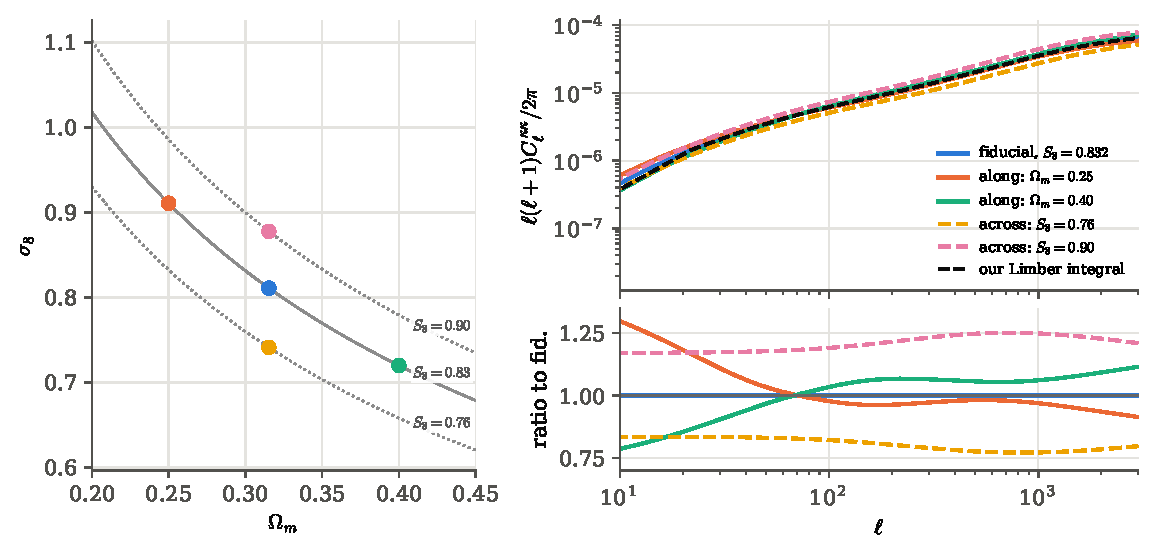
\includegraphics[width=\linewidth]{figures/chT1/kappa_s8_spectra.pdf}
\caption{Left: the five models in the $(\Omega_m,\sigma_8)$ plane, with lines of constant $S_8$. Right: their convergence spectra (top) and the ratio to the fiducial one (bottom). The three solid curves, on the fiducial $S_8$ line, stay close together for $\ell\gtrsim100$, even though $\Omega_m$ changes by a factor $1.6$ along it. The two dashed curves, off the line by about $9\%$ in $S_8$, are shifted by more than $20\%$ at every $\ell$. The dashed black curve is our own Limber integral for the fiducial model.}
\label{T1b:fig:s8}
\end{figure}

\subsection{The answer}
\label{T1b:sec:s8-answer}

\Cref{T1b:fig:s8} is the answer. Along the line of constant $S_8$ the spectra differ by a median of $\TOneAlongMedLo\%$ and $\TOneAlongMedHi\%$ over $100\le\ell\le2000$ (at most $\TOneAlongMax\%$), although $\Omega_m$ runs from $0.25$ to $0.40$ and $\sigma_8$ from $\TOneSigEightLo$ to $\TOneSigEightHi$. Across the line, a change of about $9\%$ in $S_8$ moves the spectrum by $\TOneAcrossLo\%$ and $\TOneAcrossHi\%$. So the data pin down $S_8$ and leave the position along the line almost free: for $\ell\gtrsim100$ the observation is about equally probable anywhere on the line, and the two candidates of the opening cannot be told apart there. Two things break that tie. A move across the line changes the spectrum by more than $20\%$, so the posterior is narrow in that direction. And at the low multipoles, $\ell\lesssim50$, the three solid curves separate.

Why at low $\ell$? The matter spectrum has a turnover, a peak at the wavenumber of the horizon size at matter--radiation equality, as described with the matter spectrum in \cref{T1a:sec:pk}. That wavenumber is $k_{\mathrm{eq}}\approx0.073\,\Omega_{m0}h^2\,\mathrm{Mpc}^{-1}$, which is $0.073\,\Omega_{m0}h$ in the units $h\,\mathrm{Mpc}^{-1}$ in which $\sigma_8$ is defined (see the cosmology notes). At fixed $h$ it moves in proportion to $\Omega_m$, by the factor $1.6$ between the ends of the line, and so the shape of $P_\delta$ around the turnover differs along the line even where its height does not. For the fiducial model $k_{\mathrm{eq}}\approx0.073\times0.315\times0.674^2\approx0.010\,\mathrm{Mpc}^{-1}$; matter near the peak of the lensing weight, at $\chi\approx1500$--$2000\,\mathrm{Mpc}$, projects it to $\ell=k\chi\approx15$--$20$. Only the lowest multipoles see the turnover, and they carry few modes.

\subsection{Which exponent?}
\label{T1b:sec:s8-alpha}

Is the exponent $0.5$ in $S_8$ special? We can ask the spectrum which exponent it prefers. Change $\Omega_m$ by $\pm5\%$ at fixed $\sigma_8$, then $\sigma_8$ by $\pm5\%$ at fixed $\Omega_m$, and form the logarithmic slopes. At $\ell=500$ they are $\partial\ln C_\ell/\partial\ln\sigma_8=\TOneDlnCdlnSEight$ and $\partial\ln C_\ell/\partial\ln\Omega_m=\TOneDlnCdlnOm$.

The first slope can be checked against what we know. In linear theory $C_\ell\propto\sigma_8^2$ at fixed $\Omega_m$, by \eqref{T1b:eq:cl-scaling}, so $\partial\ln C_\ell/\partial\ln\sigma_8=2$ exactly. Non-linear power grows faster than $\sigma_8^2$, because on small scales the extra clumping feeds on itself, and the measured $\TOneDlnCdlnSEight$ says how much faster: at $\ell=500$ the spectrum responds about $40\%$ more strongly than in linear theory. The same slope explains the across-line shifts of \cref{T1b:fig:s8}: $(0.76/0.832)^{2.8}-1=-22\%$ and $(0.90/0.832)^{2.8}-1=+25\%$, close to the measured $\TOneAcrossLo\%$ and $\TOneAcrossHi\%$, where the linear expectation of \cref{T1b:sec:s8-vary} was $\pm17\%$.

\emph{Which combination leaves the spectrum unchanged?} Write $a\equiv\partial\ln C_\ell/\partial\ln\sigma_8$ and $b\equiv\partial\ln C_\ell/\partial\ln\Omega_m$, and ask for the small changes of the two parameters that keep $C_\ell$ fixed:
\begin{align}
0=\dd\ln C_\ell
&\eqby{1}a\,\dd\ln\sigma_8+b\,\dd\ln\Omega_m
\quad\Longrightarrow\quad
\dd\ln\sigma_8\eqby{2}-\frac ba\,\dd\ln\Omega_m
\nonumber\\
\quad\Longrightarrow\quad
\ln\sigma_8+\frac ba\ln\Omega_m&\eqby{3}\text{const}
\quad\Longleftrightarrow\quad
\sigma_8\Omega_m^{b/a}=\text{const}.
\label{T1b:eq:alpha-derive}
\end{align}
\begin{explain}
  \item The change of a function of two variables is the sum of the changes along each (the chain rule), with $\ln\sigma_8$ and $\ln\Omega_m$ as the variables.
  \item Solve for $\dd\ln\sigma_8$.
  \item Integrate, treating the ratio $b/a$ as constant over the small region of interest; then take the exponential.
\end{explain}
The exponent is the ratio of the two slopes,
\begin{equation}
\alpha(\ell)\equiv\frac{\partial\ln C_\ell^{\kappa\kappa}/\partial\ln\Omega_m}{\partial\ln C_\ell^{\kappa\kappa}/\partial\ln\sigma_8}.
\label{T1b:eq:alpha}
\end{equation}
With the numbers above, $\alpha=\TOneDlnCdlnOm/\TOneDlnCdlnSEight\approx0.57$ at $\ell=500$, which the unrounded slopes give as $\TOneAlphaFive$. For the fiducial sample $\alpha=\TOneAlphaGalTwo$ at $\ell=200$, $\TOneAlphaFive$ at $\ell=500$ and $\TOneAlphaGalTwoK$ at $\ell=2000$.

\begin{figure}[htbp]
\centering
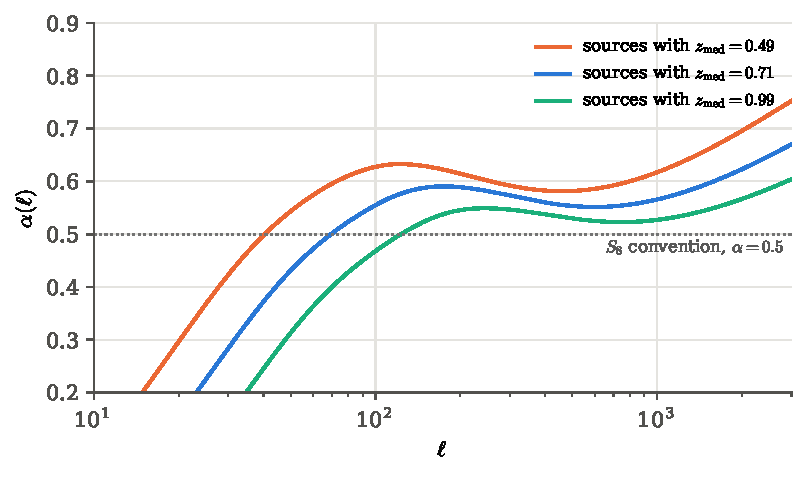
\includegraphics[width=0.8\linewidth]{figures/chT1/kappa_s8_alpha.pdf}
\caption{The exponent $\alpha$ of the combination $\sigma_8\Omega_m^\alpha$ that leaves $C_\ell^{\kappa\kappa}$ unchanged, multipole by multipole, \cref{T1b:eq:alpha}, for three source samples of increasing depth. Over the range where surveys have most of their signal, $100\lesssim\ell\lesssim1000$, it sits between $0.5$ and $0.6$, lower for deeper samples. It falls at low $\ell$, where the shape of the matter spectrum near its turnover enters.}
\label{T1b:fig:alpha}
\end{figure}

\Cref{T1b:fig:alpha} shows $\alpha(\ell)$ for three source samples, with median redshifts $\TOneZmedLo$, $\TOneZmed$ and $\TOneZmedHi$. At $\ell=500$ it is $\TOneAlphaLoFive$, $\TOneAlphaFive$ and $\TOneAlphaHiFive$. So the exponent $0.5$ is a convention close to the truth, not a law: the best exponent depends on the scales and the redshifts a survey uses. This is why the surveys quote their own. HSC finds its tightest combination at $\alpha=0.45$ and reports both $S_8(\alpha{=}0.45)=0.800^{+0.029}_{-0.028}$ and the standard $S_8=0.780^{+0.030}_{-0.033}$ \cite{Hikage2019HSC}, and CMB lensing, with its deeper kernel, measures $\sigma_8\Omega_m^{0.25}$ (\cref{T1b:sec:objects}).

\subsection{What the surveys find}
\label{T1b:sec:s8-surveys}

The question the surveys asked is simple to state. The CMB shows the Universe at $z\approx1100$, and the $\Lambda$CDM model extrapolates from it how clumpy matter should be today. Lensing measures today's clumpiness directly. \emph{Do the two agree?} Each experiment measures something different:
\begin{itemize}[leftmargin=1.2em,itemsep=1pt]
\item \emph{KiDS-1000} \cite{Asgari2021KiDS}: about $1000\,\mathrm{deg}^2$ ($777\,\mathrm{deg}^2$ effective), about $21$ million galaxies in five photometric bins out to $z\approx1.2$; its headline number comes from a two-point statistic of the shear in all fifteen bin pairs.
\item \emph{DES Year~3} \cite{Amon2022DES}: about $4100\,\mathrm{deg}^2$, about $100$ million galaxies in four bins, from the real-space correlations $\xi_\pm$.
\item \emph{HSC Year~1} \cite{Hikage2019HSC}: only $137\,\mathrm{deg}^2$ but the deepest images, four bins out to $z\approx1.5$, from tomographic power spectra $C_\ell^{ij}$.
\item \emph{Planck} \cite{Planck2018VI}: the CMB temperature and polarization spectra over the full sky, with $S_8$ today computed from the fitted $\Lambda$CDM parameters.
\end{itemize}

\begin{center}
\small
\begin{tabular}{@{}lccc@{}}
\toprule
experiment & published $S_8$ & symmetrised error & distance from Planck\\\midrule
KiDS-1000 & $0.759^{+0.024}_{-0.021}$ & $0.0225$ & $2.8\sigma$\\
DES Year~3 & $0.759^{+0.025}_{-0.023}$ & $0.024$ & $2.7\sigma$\\
HSC Year~1 & $0.780^{+0.030}_{-0.033}$ & $0.0315$ & $1.5\sigma$\\
Planck (CMB) & $0.832\pm0.013$ & $0.013$ & ---\\
this part & $\TOneSEightFid$; $0.76$, $0.90$ & --- & ---\\
\bottomrule
\end{tabular}
\end{center}

The distances in the last column are computed here, in one line of arithmetic. In the last row $\TOneSEightFid$ is the solid model of \cref{T1b:fig:s8} and $0.76$, $0.90$ the dashed ones. If the two measurements are independent and their errors Gaussian, their difference has a variance equal to the sum of the two variances, the rule behind \eqref{3a:eq:var-mean}, so for KiDS-1000
\[
\frac{0.832-0.759}{\sqrt{0.013^2+0.0225^2}}=\frac{0.073}{0.026}=2.8 .
\]
The ``about $3\sigma$'' that is often quoted is this number, rounded. It is only approximate: the errors are not symmetric (using the upper error, $0.024$, which is the one facing Planck, gives $2.7\sigma$), and the posteriors are not exactly Gaussian.

The sign of the shift is the one \cref{T1b:fig:s8} prepares. The lensing values sit near $S_8=0.76$, the lower dashed model, and the CMB value is the solid one: the surveys see a spectrum about $20\%$ below what Planck's $\Lambda$CDM predicts. Whether this is new physics, a nuisance not fully modelled (the red boxes of \cref{T1b:fig:pipeline}), or a fluctuation is one of the open questions of the field, and it is a question about statistics: about the sampling distribution of $\widehat C_\ell$, its covariance, and how much the nuisance parameters are allowed to move. The lesson of the comparison: a $9\%$ difference in one number is a $20\%$ difference in the spectrum, and whether it is significant depends entirely on errors that the later chapters learn to compute.

For the statistics chapters, the long valley of \cref{T1b:fig:s8} is a degeneracy of the kind met in \cref{T1a:sec:cl-response}: two parameters whose derivative curves are nearly proportional. In the Fisher matrix of \cref{ch:10} it makes the $(\Omega_m,\sigma_8)$ error ellipse long and thin, along $\sigma_8\Omega_m^\alpha=\text{const}$. In the MCMC of \cref{ch:09} it is a curved banana-shaped ridge. \Cref{ch:12} forecasts the error on $S_8$ from simulated maps and asks whether summaries beyond $C_\ell^{\kappa\kappa}$ shorten the banana.

\section{Experiment 2: signal and shape noise in a Stage-III survey}
\label{T1b:sec:noise}

The galaxy shapes carry a lensing signal of about $0.01$ under an intrinsic scatter of $0.27$. On which angular scales does the signal still win, and how many $\sigma$ is the whole detection worth? In the language of \cref{T1b:sec:objects}: $C_\ell^{ij}$ is the convergence spectrum between redshift bin $i$ and bin $j$, $N_i=\sigma_e^2/\bar n_i$ the shape-noise power of bin $i$ from \eqref{T1b:eq:shape-noise}, and the measured spectrum of bin $i$ is $C_\ell^{ii}+N_i$. We want to know where $C_\ell^{ii}$ exceeds $N_i$.

\subsection{The survey}
\label{T1b:sec:noise-survey}

We take survey numbers close to KiDS-1000 \cite{Asgari2021KiDS}:

\begin{center}
\small
\begin{tabular}{@{}lll@{}}
\toprule
quantity & this experiment & KiDS-1000\\\midrule
area & $\TOneArea\,\mathrm{deg}^2$ & $\approx1000\,\mathrm{deg}^2$ ($777\,\mathrm{deg}^2$ effective)\\
sky fraction $f_{\mathrm{sky}}$ & $\TOneFsky$ & ---\\
galaxy density $\bar n$ & $\TOneNeff$ arcmin$^{-2}$, all bins & $6.2$ arcmin$^{-2}$\\
shape scatter $\sigma_e$ (per component) & $\TOneSigmaE$ & $0.25$--$0.27$\\
photo-$z$ scatter & Gaussian, $0.05(1+z)$ & ---\\
redshift bins & $5$, equal numbers & $5$\\
\bottomrule
\end{tabular}
\end{center}

The sky fraction $f_{\mathrm{sky}}$ is the observed area divided by the area of the whole sky. The whole sky is $4\pi$ steradians, and one steradian is $(180/\pi)^2$ square degrees, so
\[
f_{\mathrm{sky}}=\frac{1000\,\mathrm{deg}^2}{4\pi(180/\pi)^2\,\mathrm{deg}^2}=\frac{1000}{41\,253}=\TOneFsky .
\]
The source sample is the one of \cref{T1b:sec:s8-fixed}, with the fiducial cosmology.

\subsection{The binning}
\label{T1b:sec:noise-bins}

We cut the sample into five bins by photometric redshift, with equal numbers of galaxies in each. Equal numbers make every bin equally noisy, since $N_i$ depends only on $\bar n_i$, so no bin is wasted on a handful of galaxies. A photometric redshift is estimated from a few broad colours, and its error grows with redshift because the spectral features it relies on are stretched by the factor $1+z$; the simplest model of that is a Gaussian scatter of width $0.05(1+z)$ about the true redshift, without the outliers that real catalogues have. The bin edges come out at $z_{\mathrm{ph}}=\TOneEdgeOne,\dots,\TOneEdgeFour$. Because of the scatter, a galaxy placed in one bin may truly belong to a neighbour, so the true-redshift distributions of the bins overlap.

\begin{figure}[htbp]
\centering
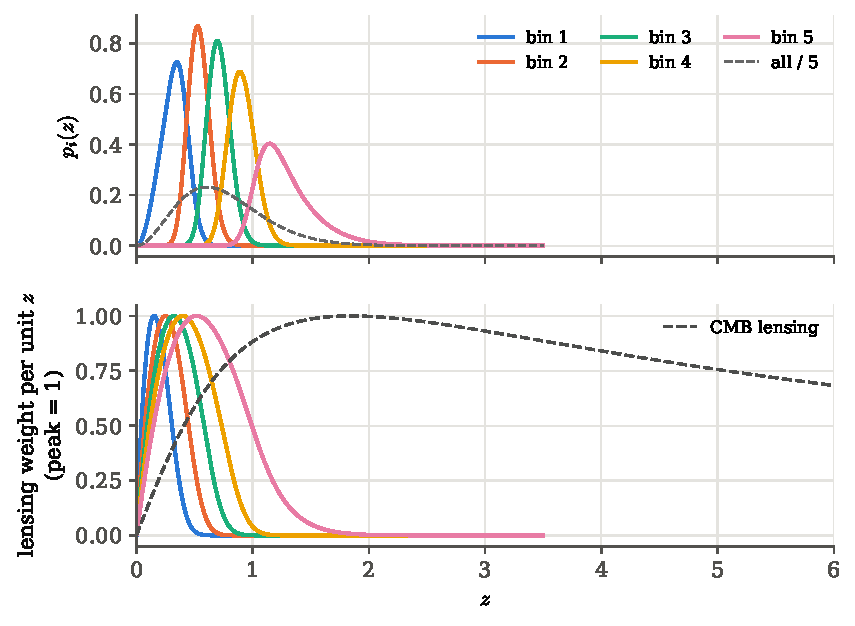
\includegraphics[width=0.78\linewidth]{figures/chT1/kappa_bins.pdf}
\caption{Top: the true-redshift distributions of the five photometric bins; photo-$z$ scatter makes them overlap. Bottom: the lensing weight of each bin per unit redshift, $\propto g_i(\chi)f_K(\chi)/a$ times $\dd\chi/\dd z$, normalised to peak at one. Each weight is broad and peaks at about half the distance of its sources, so the five bins see heavily overlapping slices of matter. The CMB weight (dashed) peaks near $z\approx2$.}
\label{T1b:fig:bins}
\end{figure}

\Cref{T1b:fig:bins} shows the price of photometric redshifts and of projection together. The bins themselves overlap, and their lensing weights overlap even more, since every bin is lensed by all the matter in front of it. Tomography therefore does not give five independent maps. It gives five correlated maps whose full $5\times5$ matrix of spectra, auto and cross, carries the information, and the covariance of the analysis must include all fifteen of them.

\subsection{The noise and the error bars}
\label{T1b:sec:noise-errors}

\pyfile[firstline=113,lastline=116,firstnumber=113]{code/chT1/04_kappa_noise.py}{The noise power of each bin}

Line~114 counts the fraction of galaxies in each bin (a fifth, by construction). Line~115 converts the number density from arcmin$^{-2}$ to sr$^{-1}$: one steradian holds $(10800/\pi)^2=1.18\times10^7$ arcmin$^2$, so $1.24$ arcmin$^{-2}$ becomes $1.47\times10^7\,\mathrm{sr}^{-1}$. Line~116 is the noise row of the table, $N_i=\sigma_e^2/\bar n_i\approx\TOneNoiseOne$, worked out in \cref{T1b:sec:objects}.

How large are the error bars on a measured band power? Start from the cosmic variance of one multipole and make three changes:
\begin{align}
\Var\widehat C_\ell
&\eqby{1}\frac{2C_\ell^2}{\nu}
\eqby{2}\frac{2\,(C_\ell+N)^2}{(2\ell+1)\,f_{\mathrm{sky}}},
&
\Var\Bigl(\frac1{\Delta\ell}\sum_{\ell'\in\text{band}}\widehat C_{\ell'}\Bigr)
&\eqby{3}\frac{2\,(C_\ell+N)^2}{(2\ell+1)\,\Delta\ell\,f_{\mathrm{sky}}},
\nonumber\\
\Delta C_\ell
&\eqby{4}\sqrt{\frac{2}{(2\ell+1)\,\Delta\ell\,f_{\mathrm{sky}}}}\,\bigl(C_\ell+N\bigr).
\label{T1b:eq:band-error}
\end{align}
\begin{explain}
  \item The cosmic variance \eqref{7b:eq:cosmic-var}, written for $\nu$ independent modes; on the full sky $\nu=2\ell+1$.
  \item Two changes. A survey that sees a fraction $f_{\mathrm{sky}}$ of the sky has only about $(2\ell+1)f_{\mathrm{sky}}$ independent modes per multipole. And what is measured is the spectrum of signal plus noise, whose variance per mode is $C_\ell+N$, so the scatter of the estimate is set by the sum, as in \eqref{7b:eq:cl-like-noise}; the noise is part of what is measured.
  \item Averaging the $\Delta\ell$ independent multipoles of a band divides the variance by $\Delta\ell$, \eqref{7b:eq:binned}, the variance of a mean.
  \item The square root.
\end{explain}
This is the Gaussian band-power error used in the literature \cite[eq.~52]{Kilbinger2015}.

What does this mean for inference? The observed band power is the model prediction plus one draw of noise with the variance of \eqref{T1b:eq:band-error}. Read as a function of the parameters $(\Omega_m,\sigma_8)$, the probability of the data asks how plausible the noise draw is that turns the prediction $C_\ell(\Omega_m,\sigma_8)$ into what was observed: a Gaussian centred on the model, with the width of \eqref{T1b:eq:band-error}. This is the likelihood from a noise model, \eqref{0a:eq:like-noise}, in its band-power form (\cref{7b:sec:cl-likelihood}). The $S_8$ degeneracy of \cref{T1b:sec:s8} is a statement about this likelihood: moving along the line leaves the centre almost where it was, so the same noise draw is needed everywhere on the line, and the likelihood does not change.

\begin{figure}[htbp]
\centering
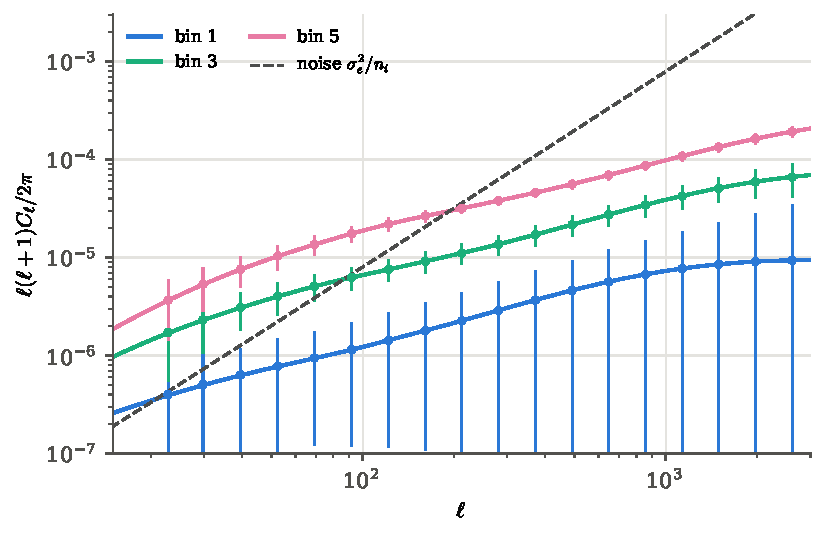
\includegraphics[width=0.8\linewidth]{figures/chT1/kappa_noise.pdf}
\caption{Convergence spectra of the nearest (1), middle (3) and farthest (5) bins, with Gaussian error bars on logarithmic bands of $\ell$ for a $1000\,\mathrm{deg}^2$ survey, \cref{T1b:eq:band-error}. The dashed line is the shape noise, the same for every bin because the bins hold equal numbers of galaxies; it rises as $\ell^2$ only because of the factor $\ell(\ell+1)$ on the axis. Beyond the crossing, the error bars are set mostly by the noise.}
\label{T1b:fig:noise}
\end{figure}

\subsection{Where the signal wins, and how many \texorpdfstring{$\sigma$}{sigma}}
\label{T1b:sec:noise-sn}

\Cref{T1b:fig:noise} gives the answer to the first question. The signal equals the noise at $\ell\approx\TOneLeqOne$ in the nearest bin, $\ell\approx\TOneLeqThree$ in the middle one and $\ell\approx\TOneLeqFive$ in the farthest, which is lensed by the most matter. Beyond those multipoles each bin is noise-dominated. The measurement does not stop there, since there are many modes at high $\ell$, but each additional mode adds little.

\emph{The signal-to-noise ratio of one bin.} Ask how well the data fix the height of the signal. Multiply the predicted spectrum by an amplitude $A$, so that the measured spectrum has mean $AC_\ell+N$, and define the signal-to-noise ratio as $1/\sigma(A)$ at $A=1$: the number of standard deviations by which the signal is distinguished from no signal. The Fisher information for $A$ comes from \eqref{10a:eq:cmb-fisher}, with $(2\ell+1)f_{\mathrm{sky}}$ modes per multipole:
\begin{align}
\Bigl(\frac SN\Bigr)^2
&\eqby{1}\sum_\ell\frac{(2\ell+1)f_{\mathrm{sky}}}{2}\,\frac{\bigl[\partial(AC_\ell+N)/\partial A\bigr]^2}{(C_\ell+N)^2}
\eqby{2}\sum_\ell\frac{(2\ell+1)f_{\mathrm{sky}}}{2}\,\frac{C_\ell^2}{(C_\ell+N)^2}.
\label{T1b:eq:sn-one}
\end{align}
\begin{explain}
  \item \Cref{10a:eq:cmb-fisher} for one parameter, with the full-sky count $2\ell+1$ replaced by $(2\ell+1)f_{\mathrm{sky}}$, and the inverse error squared equal to the Fisher information.
  \item The derivative of $AC_\ell+N$ with respect to $A$ is $C_\ell$.
\end{explain}
Each mode contributes the factor $\frac12[C_\ell/(C_\ell+N)]^2$. Where the signal dominates, $C_\ell\gg N$, that factor is $\frac12$, the most a mode can give; where the noise dominates it falls as $\frac12(C_\ell/N)^2$, and since $N$ is flat while $C_\ell$ falls, it drops quickly beyond the crossing. So the signal-to-noise ratio essentially counts the modes below the crossing multipole.

\emph{Five bins at once.} With tomography the spectrum at each $\ell$ is a $5\times5$ matrix $\mathbf C_\ell$ with entries $C_\ell^{ij}+\delta_{ij}N_i$, and $\mathbf S_\ell$ is its signal part. The same calculation with the matrix form of the Fisher information gives
\begin{equation}
\Bigl(\frac SN\Bigr)^2=\sum_\ell\frac{(2\ell+1)f_{\mathrm{sky}}}{2}\,\Tr\bigl[\mathbf C_\ell^{-1}\mathbf S_\ell\,\mathbf C_\ell^{-1}\mathbf S_\ell\bigr],
\label{T1b:eq:sn-tomo}
\end{equation}
which for one bin reduces to \eqref{T1b:eq:sn-one}. The fifteen distinct spectra are the entries of $\mathbf S_\ell$, and the inverse $\mathbf C_\ell^{-1}$ accounts for the correlations between bins that \cref{T1b:fig:bins} shows, so that shared information is not counted twice. Summing over $10\le\ell\le\TOneLmaxSN$, the total signal-to-noise ratio is $\TOneSNtomo$. A single unbinned sample, with five times the galaxies and so a fifth of the noise, gives $\TOneSNone$. The ratio is $\TOneSNtomo/\TOneSNone\approx1.14$: tomography adds about $14\%$ to the detection. What it buys is the redshift dependence, which separates the growth of structure from the geometry and helps tell intrinsic alignments from lensing.

\emph{How well is the amplitude measured?} If $\sigma_8$ were the only unknown, the Fisher information on $\ln\sigma_8$ is \eqref{T1b:eq:sn-tomo} with each $\mathbf S_\ell$ replaced by the derivative $\partial\mathbf C_\ell/\partial\ln\sigma_8$ (the general form is \eqref{10a:eq:gauss-fisher}), and with a single parameter the error is $\sigma(\ln\sigma_8)=1/\sqrt F$. The derivative comes from two more CAMB runs at $\sigma_8(1\pm\epsilon)$ with $\epsilon=0.02$, as a central difference (\cref{10a:sec:numderiv}):
\[
\frac{\partial\mathbf C_\ell}{\partial\ln\sigma_8}\approx\frac{\mathbf C_\ell^{+}-\mathbf C_\ell^{-}}{\ln(1+\epsilon)-\ln(1-\epsilon)}\approx\frac{\mathbf C_\ell^{+}-\mathbf C_\ell^{-}}{2\epsilon}.
\]
The result is $\sigma(\ln\sigma_8)=\TOneSigLnSEight\%$. It can be checked against the signal-to-noise ratio. If the derivative were a fixed multiple $s$ of the signal, $\partial\mathbf C_\ell/\partial\ln\sigma_8=s\,\mathbf S_\ell$, then $F=s^2(S/N)^2$ and $\sigma(\ln\sigma_8)=1/[s\,(S/N)]$. In linear theory $s=2$, giving $1/(2\times\TOneSNtomo)=1.0\%$. The computed $\TOneSigLnSEight\%$ corresponds to $s\approx1/(0.008\times\TOneSNtomo)\approx2.6$, between the linear $2$ and the $\TOneDlnCdlnSEight$ found at $\ell=500$ in \cref{T1b:sec:s8-alpha}: the non-linear boost again.

At fixed $\Omega_m$ this is also the error on $S_8$. KiDS-1000 achieves about $3\%$. The gap between the two numbers is the content of the later chapters. The first cost can be sized here. $\Omega_m$ is free and degenerate with $\sigma_8$ (\cref{T1b:sec:s8}). For two parameters with Fisher matrix entries $F_{\sigma\sigma}$, $F_{\Omega\Omega}$ and $F_{\sigma\Omega}$,
\begin{align}
\sigma^2_{\text{marg}}(\ln\sigma_8)
&\eqby{1}\bigl(F^{-1}\bigr)_{\sigma\sigma}
\eqby{2}\frac{F_{\Omega\Omega}}{F_{\sigma\sigma}F_{\Omega\Omega}-F_{\sigma\Omega}^2}
\eqby{3}\frac{1}{F_{\sigma\sigma}}\,\frac{1}{1-r^2},
\qquad r\equiv\frac{F_{\sigma\Omega}}{\sqrt{F_{\sigma\sigma}F_{\Omega\Omega}}}.
\label{T1b:eq:marg-cost}
\end{align}
\begin{explain}
  \item The marginal error is read from the inverse of the Fisher matrix (\cref{10a:sec:degeneracy}).
  \item The inverse of a $2\times2$ matrix.
  \item Divide the numerator and the denominator by $F_{\sigma\sigma}F_{\Omega\Omega}$; $r$ is the cosine of the angle between the two derivative curves, weighted as in the Fisher sum.
\end{explain}
So freeing $\Omega_m$ multiplies the error on $\ln\sigma_8$ by $1/\sqrt{1-r^2}$: by $2.3$ for $r=0.9$ and by $7$ for $r=0.99$, and the near-proportional derivative curves of \cref{T1b:sec:s8} put $r$ close to one. The combination $S_8$ is chosen to lie along the well-measured direction, so its error grows much less, which is why the surveys quote it. The rest of the gap comes from the other costs. Nuisance parameters for photo-$z$ shifts, shear bias, intrinsic alignment and baryons are marginalised. The covariance has non-Gaussian and super-sample terms that \cref{T1b:eq:band-error} ignores. And the smallest scales are cut because baryonic feedback is uncertain there. \Cref{ch:10} computes each of these costs in the Fisher matrix, and \cref{ch:12} redoes the forecast with simulated maps.

\begin{inpractice}[What the full analysis does]
Our numbers come from a Gaussian, nuisance-free forecast with all other parameters fixed. The published analyses measure tomographic $\xi_\pm(\vartheta)$, band powers or related statistics from tens of millions of shapes \cite{Asgari2021KiDS,Amon2022DES,Hikage2019HSC}. They take the covariance from analytic models checked against hundreds to thousands of ray-traced $N$-body simulations, such as the full-sky lensing maps of \cite{Takahashi2017sims}, and they sample the posterior of cosmological and nuisance parameters by MCMC. The same simulations are what make summaries beyond two-point statistics usable: peak counts \cite{Kratochvil2010,DietrichHartlap2010}, Kaiser--Squires mass maps \cite{Jeffrey2021DESmass}, lognormal fields as a fast model of the skewed $\kappa$ distribution \cite{Xavier2016}, and persistent homology of $\kappa$ maps \cite{Heydenreich2021}. All of these return in \cref{ch:12}.
\end{inpractice}

The lesson of the two experiments for the rest of the book is in two parts. The signal is a projected, smoothed field whose two-point statistic is degenerate along $S_8$. The noise is white, large and known. So the statistical problem is to extract as much as possible from a noisy, non-Gaussian field with a small number of summaries. \Cref{ch:12} takes up that problem with topological summaries.

\begin{recap}
\begin{itemize}[leftmargin=1.2em,itemsep=1pt]
\item Lensing distorts galaxy images by about $1\%$: $\kappa=\frac12\nabla^2\psi$ magnifies, the spin-2 shear $\gamma_1=\frac12(\psi_{,11}-\psi_{,22})$, $\gamma_2=\psi_{,12}$ stretches; a galaxy measures $\varepsilon\approx\varepsilon^{(0)}+\gamma$, with the reduced shear $\gamma/(1-\kappa)$ as its mean.
\item Lensing makes only $E$ modes; a $B$ mode is a null test for systematics.
\item $C_\ell^{\kappa\kappa}$ is the Limber integral of $[g/a]^2P_\delta$ over distance, with the broad lensing efficiency $g(\chi)$; CAMB computes it with lensing source windows, and our own integral agrees to $\TOneLimberErr\%$.
\item Cosmic shear measures $\sigma_8\Omega_m^\alpha$ with $\alpha\approx\TOneAlphaFive$ for a Stage-III sample ($S_8$ takes $\alpha=0.5$); along that line the spectrum changes by a few per cent, across it by $\sim20\%$ for a $9\%$ change in $S_8$.
\item Shape noise $N_i=\sigma_e^2/\bar n_i$ is white; for a KiDS-like survey the signal beats it only up to $\ell\approx\TOneLeqOne$--$\TOneLeqFive$ per bin; total $S/N\approx\TOneSNtomo$, $\sigma(\ln\sigma_8)=\TOneSigLnSEight\%$ with everything else fixed, against $\approx3\%$ achieved with nuisances marginalised.
\item Nuisances: photo-$z$ shifts, shear bias $m$, intrinsic alignments, baryonic feedback. CMB lensing ($\psi$ reconstructed by a quadratic estimator) weights $z\approx2$ and measures $\sigma_8\Omega_m^{0.25}$.
\end{itemize}
\end{recap}

\section*{Chapter summary}
\addcontentsline{toc}{section}{Chapter summary}
\label{T1a:sec:summary}

The cosmological model is the first step of the book's pipeline. For every choice of the six $\Lambda$CDM numbers it fixes the expected value of each summary that the later chapters estimate from data, and never the sky itself. The route is short enough to hold in the head. The Friedmann equation gives the expansion rate $E(z)$, and one integral of $1/E$ gives the distances $D_A$ and $D_L$. The primordial spectrum $\mathcal P_\zeta=A_s(k/k_*)^{n_s-1}$ is carried to the sky by the radiation transfer function, $C_\ell=\frac2\pi\int k^2\dd k\,P_\zeta\,g_{T\ell}^2$, and to the matter field by growth and the matter transfer function, $P_\delta(k,a_0)=P_\delta(k,a_{\mathrm i})\,T^2[D_+(a_0)/D_+(a_{\mathrm i})]^2$. The data are one draw from each: the $\alm$ with variance $\Cell$, the Fourier modes $\delta_{\bm k}$ with variance $P_\delta(k)$. Weak lensing adds a third field built from the same matter: projected along the line of sight with the lensing efficiency $g(\chi)$, it becomes the convergence $\kappa$, whose power spectrum $C_\ell^{\kappa\kappa}$ is a Limber integral of $P_\delta$, and it is read off galaxy shapes through the shear $\gamma$, buried under shape noise.

What carries into the inference chapters is how these predictions move when the parameters move. The finite-difference responses $R_i(\ell)$ of \cref{T1a:eq:response} are the derivatives of the Fisher matrix, two nearly parallel responses are a degeneracy, and the line between linear and halofit $P(k)$ is where the Gaussian description of the matter field stops. Conventions are the fixed factors that decide whether a script reproduces these numbers. The table lists what to carry forward, what each item means in practice, and where it is used.

\begin{center}
\small
\renewcommand{\arraystretch}{1.15}
\begin{tabularx}{\linewidth}{@{}>{\raggedright\arraybackslash}p{3.3cm}
                               >{\raggedright\arraybackslash}X
                               >{\raggedright\arraybackslash}p{2.4cm}@{}}
\toprule
concept & operational meaning & used later in\\\midrule
model as a machine & six numbers into CAMB, expected statistics out; call it through \pyname{code/camb_fiducial.py} for the fiducial spectra & \cref{ch:07,ch:08,ch:09,ch:10}\\
one realisation & the sky is one draw; each $\alm$ has variance $\Cell$, and $\widehat C_\ell$ scatters about $\Cell$ as $\chi^2_{2\ell+1}/(2\ell+1)$ & \cref{ch:07,ch:08}\\
distances and $H(z)$ & $E(z)$ from the density parameters, then $D_A$, $D_L$ by one integral; the model mean of supernova and BAO data & \cref{ch:03,ch:05}\\
conventions & raw $\Cell$ vs $D_\ell$; $\mu\mathrm K^2$; $A_s=\frac{25}{4}A_S^2$; $h^{-1}$Mpc; $\phi\equiv\psi$ & every CMB and LSS script\\
fractional response $R_i(\ell)$ & central difference of $\Cell$ over $\pm1\sigma$, divided by $2\Cell$; times $\Cell/\delta_i$ it is $\partial\Cell/\partial\theta_i$ & \cref{ch:10}\\
degeneracy & two nearly parallel response curves ($A_s$ and $\tau$ above $\ell\approx30$); a near-singular Fisher matrix and a ridge in the chain & \cref{ch:09,ch:10}\\
linear vs halofit $P(k)$ & agree on large scales, differ by $10\%$ at $k\approx\TOneKnl\,h\,\mathrm{Mpc}^{-1}$ at $z=0$; beyond that the field is non-Gaussian & \cref{ch:07,ch:12}\\
$\xi(r)$ and the BAO bump & Fourier partner of $P(k)$; a peak near $r_s(z_{\mathrm{drag}})$, a standard ruler & \cref{ch:07,ch:12}\\
$\sigma_8$ & top-hat variance of the linear field at $8\,h^{-1}$Mpc; a check that $P(k)$ is normalised correctly & \cref{ch:07,ch:10}\\
$f_{\mathrm{NL}}$ & amplitude of the primordial bispectrum; invisible to $\Cell$ and $P(k)$ & \cref{ch:12}\\
$\kappa$, $\gamma$, $E$/$B$ & projected density and its spin-2 tidal stretch (\cref{T1b:sec:shapes}); lensing makes only $E$, so $B$ is a null test & \cref{ch:12}\\
$C_\ell^{\kappa\kappa}$ and shape noise & Limber integral of $[g/a]^2P_\delta$ (CAMB lensing windows); measured power $C_\ell^{ij}+\delta_{ij}\sigma_e^2/\bar n_i$ & \cref{ch:10,ch:12}\\
$S_8$ and nuisances & cosmic shear fixes $\sigma_8\Omega_m^{\alpha}$, $\alpha\approx0.55$; photo-$z$, shear bias, intrinsic alignment, baryons are marginalised & \cref{ch:09,ch:10,ch:12}\\
\bottomrule
\end{tabularx}
\end{center}

\paragraph{Reading the literature.}
The physics of every object above is developed in the cosmology notes. The Boltzmann code used throughout is CAMB \cite{CAMB2000}. The parameter values and errors are those of Planck 2018 \cite{Planck2018VI}. The non-linear correction is the halofit version of \cite{Takahashi2012}, and the first detection of the BAO bump in the galaxy correlation function is \cite{Eisenstein2005}. For weak lensing, the standard reviews are \cite{BartelmannSchneider2001} and \cite{Kilbinger2015}, CMB lensing is reviewed in \cite{LewisChallinor2006} and measured in \cite{Planck2018VIII}, and the Stage-III cosmic-shear results are \cite{Asgari2021KiDS,Amon2022DES,Hikage2019HSC}.
 
\chapter{Astrophysics for the Data Analyst}\label{ch:T2}

\providecommand{\TwEmriMc}{}\renewcommand{\TwEmriMc}{39.81}
\providecommand{\TwEmrifisco}{}\renewcommand{\TwEmrifisco}{0.4397}
\providecommand{\TwEmriffouryr}{}\renewcommand{\TwEmriffouryr}{13.84}
\providecommand{\TwEmriNcyc}{}\renewcommand{\TwEmriNcyc}{2.787\times10^{6}}
\providecommand{\TwEmriadiab}{}\renewcommand{\TwEmriadiab}{6.839\times10^{-5}}
\providecommand{\TwImriMc}{}\renewcommand{\TwImriMc}{19.39}
\providecommand{\TwImrifisco}{}\renewcommand{\TwImrifisco}{4.391}
\providecommand{\TwImriffouryr}{}\renewcommand{\TwImriffouryr}{21.7}
\providecommand{\TwImriNcyc}{}\renewcommand{\TwImriNcyc}{4.382\times10^{6}}
\providecommand{\TwImriadiab}{}\renewcommand{\TwImriadiab}{9.550\times10^{-4}}
\providecommand{\TwGWMc}{}\renewcommand{\TwGWMc}{28.1}
\providecommand{\TwGWfFive}{}\renewcommand{\TwGWfFive}{15.83}
\providecommand{\TwGWfOne}{}\renewcommand{\TwGWfOne}{28.94}
\providecommand{\TwGWNcyc}{}\renewcommand{\TwGWNcyc}{2.534\times10^{6}}
\providecommand{\TwSpaAmpErr}{}\renewcommand{\TwSpaAmpErr}{3.655}
\providecommand{\TwSpaPhaseRms}{}\renewcommand{\TwSpaPhaseRms}{0.01296}
\providecommand{\TwSpaPsiBand}{}\renewcommand{\TwSpaPsiBand}{168.4}
\providecommand{\TwSpaDuration}{}\renewcommand{\TwSpaDuration}{4.729}
\providecommand{\Twfstar}{}\renewcommand{\Twfstar}{19.09}
\providecommand{\TwASDmin}{}\renewcommand{\TwASDmin}{1.178\times10^{-20}}
\providecommand{\TwfASDmin}{}\renewcommand{\TwfASDmin}{7.256}
\providecommand{\TwfAccOms}{}\renewcommand{\TwfAccOms}{3.077}
\providecommand{\TwfConfLo}{}\renewcommand{\TwfConfLo}{0.4101}
\providecommand{\TwfConfHi}{}\renewcommand{\TwfConfHi}{1.908}
\providecommand{\TwEmriDL}{}\renewcommand{\TwEmriDL}{199.8}
\providecommand{\TwEmriSNR}{}\renewcommand{\TwEmriSNR}{14}
\providecommand{\TwImriSNR}{}\renewcommand{\TwImriSNR}{12.1}
\providecommand{\TwGWlikeSNR}{}\renewcommand{\TwGWlikeSNR}{3.89}
\providecommand{\TwRingAmp}{}\renewcommand{\TwRingAmp}{0.35}
\providecommand{\TwInclAvg}{}\renewcommand{\TwInclAvg}{0.8}
\providecommand{\TwFluxInt}{}\renewcommand{\TwFluxInt}{3.2}
\providecommand{\TwFpNinety}{}\renewcommand{\TwFpNinety}{0.2}
\providecommand{\TwFxNinety}{}\renewcommand{\TwFxNinety}{0.2}
\providecommand{\TwFpSixty}{}\renewcommand{\TwFpSixty}{0.15}
\providecommand{\TwRzero}{}\renewcommand{\TwRzero}{0.3}
\providecommand{\TwRstarRatio}{}\renewcommand{\TwRstarRatio}{0.708}
\providecommand{\TwRslope}{}\renewcommand{\TwRslope}{-2.009}
\providecommand{\TwRfitDev}{}\renewcommand{\TwRfitDev}{66.42}
\providecommand{\TwfZero}{}\renewcommand{\TwfZero}{59.96}
\providecommand{\TwPNEmriN}{}\renewcommand{\TwPNEmriN}{2.79\times10^{6}}
\providecommand{\TwPNEmriOne}{}\renewcommand{\TwPNEmriOne}{1.66\times10^{5}}
\providecommand{\TwPNEmriOnefive}{}\renewcommand{\TwPNEmriOnefive}{-1.69\times10^{5}}
\providecommand{\TwPNEmrivone}{}\renewcommand{\TwPNEmrivone}{0.1289}
\providecommand{\TwPNEmrivtwo}{}\renewcommand{\TwPNEmrivtwo}{0.4082}
\providecommand{\TwPNImriN}{}\renewcommand{\TwPNImriN}{4.38\times10^{6}}
\providecommand{\TwPNImriOne}{}\renewcommand{\TwPNImriOne}{77\,847}
\providecommand{\TwPNImriOnefive}{}\renewcommand{\TwPNImriOnefive}{-44\,949}
\providecommand{\TwPNImrivone}{}\renewcommand{\TwPNImrivone}{0.06954}
\providecommand{\TwPNImrivtwo}{}\renewcommand{\TwPNImrivtwo}{0.4082}
\providecommand{\TwPNGWN}{}\renewcommand{\TwPNGWN}{2.53\times10^{6}}
\providecommand{\TwPNGWOne}{}\renewcommand{\TwPNGWOne}{5\,521}
\providecommand{\TwPNGWOnefive}{}\renewcommand{\TwPNGWOnefive}{-662}
\providecommand{\TwPNGWvone}{}\renewcommand{\TwPNGWvone}{0.02516}
\providecommand{\TwPNGWvtwo}{}\renewcommand{\TwPNGWvtwo}{0.03076}
\providecommand{\TwPNNsN}{}\renewcommand{\TwPNNsN}{16\,034}
\providecommand{\TwPNNsOne}{}\renewcommand{\TwPNNsOne}{441}
\providecommand{\TwPNNsOnefive}{}\renewcommand{\TwPNNsOnefive}{-211}
\providecommand{\TwPNNsvone}{}\renewcommand{\TwPNNsvone}{0.07567}
\providecommand{\TwPNNsvtwo}{}\renewcommand{\TwPNNsvtwo}{0.4082}
 
\section*{Where this chapter is going}
\addcontentsline{toc}{section}{Where this chapter is going}
\label{T2g:sec:roadmap}\label{T2a:sec:roadmap}

Two black holes orbit each other. Every half orbit the pair looks the same again, a dumbbell turning in space, and a turning dumbbell shakes spacetime. The shaking spreads out as a wave, the wave carries energy, and the energy comes out of the orbit. So the two holes sink closer, circle faster, and shake spacetime harder. The wave that reaches us rises in pitch and in loudness until the holes merge: a \emph{chirp}. In the band of the space detector LISA a light black hole can circle a heavy one millions of times before the end, and each circle adds a predictable amount to the phase of the wave. If the pair lives inside a cloud of dark matter, the light hole feels a drag and sinks a little faster than it would in empty space. After a million orbits a tiny drag becomes a phase lag of many radians, and a phase lag is something a detector can measure.

Turning that lag into a number with an error bar is a statistics problem, and \cref{ch:10} solves it: the likelihood of a signal buried in noise, the matched filter, the Fisher matrix and the forecast. Every one of those calculations needs a short list of physical objects. It needs the signal, written as a Fourier transform $\tilde h(f)$ whose phase $\Psi(f)$ depends on the masses, the arrival time $t_c$ and the phase $\phi_c$. It needs the noise, as one function $S_n(f)$ of frequency. It needs the numbers that connect them, the factors $4/5$ and $3/10$ that turn a real source on the sky into an average one. And it needs the form in which any departure from the vacuum chirp enters the phase: a power of the frequency, $\beta f^b$. None of these is a matter of convention. Each follows from two physical facts, Einstein's equation for a weak gravitational field and the energy that a gravitational wave carries, together with Newton's law of gravity for the orbit; everything else can be derived from them.

\begin{figure}[htbp]
\centering
\begin{tikzpicture}[
  box/.style={draw=accent,rounded corners=2pt,fill=ideabg,align=center,font=\small,
              minimum width=2.9cm,minimum height=1.0cm,inner sep=3pt},
  phys/.style={box,draw=formblue},
  det/.style={box,fill=warnbg,draw=bdryred},
  stat/.style={box,fill=takebg,draw=tangentgreen},
  arr/.style={->,thick,accent}]
  \node[phys] (wave) at (0,0) {a weak wave\\ $g=\eta+h$, $h_+,h_\times$\\ \S\ref{T2g:sec:wave}};
  \node[phys] (quad) at (4.1,0) {quadrupole\\ radiation, $P_{\rm GW}$\\ \S\ref{T2g:sec:quadrupole}};
  \node[phys] (chirp) at (8.2,0) {the chirp\\ $\dot f$, $\mathcal M$, $t_c$, $\phi_c$\\ \S\ref{T2a:sec:chirp}};
  \node[phys] (spa) at (8.2,-2.2) {$\tilde h=\mathcal Af^{-7/6}e^{-i\Psi}$\\ \S\ref{T2a:sec:spa}};
  \node[phys] (pn) at (4.1,-2.2) {phase corrections\\ $\delta\Psi=\beta u^{b}$\\ \S\ref{T2g:sec:pn}};
  \node[phys] (env) at (0,-2.2) {dark-matter\\ environments\\ \S\ref{T2a:sec:dm}, \S\ref{T2a:sec:forces}};
  \node[det] (det) at (8.2,-4.4) {detector: $h=F_+h_++F_\times h_\times$\\ \S\ref{T2g:sec:detector}};
  \node[det] (noise) at (4.1,-4.4) {LISA noise $S_n(f)$\\ \S\ref{T2a:sec:lisa}};
  \node[stat] (stat) at (0,-4.4) {likelihood, Fisher,\\ forecast\\ Ch.~\ref{ch:10}};
  \draw[arr] (wave) -- (quad);
  \draw[arr] (quad) -- (chirp);
  \draw[arr] (chirp) -- (spa);
  \draw[arr] (spa) -- (pn);
  \draw[arr] (env) -- (pn);
  \draw[arr] (spa) -- (det);
  \draw[arr] (det) -- (noise);
  \draw[arr] (noise) -- (stat);
  \draw[arr] (pn) -- (stat);
\end{tikzpicture}
\caption{How the pieces of the chapter connect. Blue boxes are the physics of the source: a weak wave, how a moving mass makes one, how the orbit shrinks, and what the wave looks like in the frequency domain, including the small power-law terms that an environment adds to its phase. Red boxes are the detector: how it turns a wave into one number per instant, and what noise it adds. The green box is the statistics of \cref{ch:10}, which takes the signal model and the noise spectrum and runs the chain backwards to learn about the source.}
\label{T2a:fig:roadmap}
\end{figure}

\Cref{T2a:fig:roadmap} shows how the ideas feed into each other. A small ripple $h$ on flat spacetime obeys a wave equation and has exactly two polarisations, $h_+$ and $h_\times$, each of which stretches a ring of free masses in one direction while squeezing it in the other (\cref{T2g:sec:wave}). A source makes such a ripple only if its mass distribution changes shape: the total mass and the motion of the centre of mass are fixed by conservation laws, so the first thing that can radiate is the quadrupole, and for a binary it radiates at twice the orbital frequency (\cref{T2g:sec:quadrupole}). The energy the wave carries away drives the chirp: one formula for $\dot f$, a time to merger $t_c$ and a phase at merger $\phi_c$ (\cref{T2a:sec:chirp}). Its Fourier transform, found by the stationary-phase approximation, is the template $\tilde h(f)$ of every forecast (\cref{T2a:sec:spa}). Corrections from general relativity and from the environment of the binary enter the Fourier phase as extra powers of $f$, which is what makes one forecast cover many kinds of physics (\cref{T2g:sec:pn}). A detector compares the light travel times along two arms, and so measures one combination of $h_+$ and $h_\times$ with weights that depend on where the source sits on the sky (\cref{T2g:sec:detector}). Finally, LISA's own noise, from photon counting, from stray forces on its test masses and from millions of unresolved Galactic binaries, is summarised by the spectrum $S_n(f)$ (\cref{T2a:sec:lisa}). \Cref{T2g:tab:symbols} lists every symbol, where it is derived, and where \cref{ch:10} uses it.

The same reading applies to the other astrophysical data in the book. The dark-matter environments that change the chirp are built from their own physical inputs in \cref{T2a:sec:dm,T2a:sec:forces}. Distances from standard candles, the distance ladder, selection effects and galaxy surveys follow in \cref{T2b:sec:snia} onwards. Each time the question is the same: what physical object is there, what is measured, what is the noise, and which statistical tool turns the measurement into physics. In the language of the book's pipeline (\cref{ch:00}), the gravitational-wave case reads as follows. The physical model is the binary and its environment. The data set is the strain time series. What matters in it is the phase of the wave. The sampling distribution is that of the detector noise, fixed by $S_n(f)$. Inference then asks the question of \cref{ch:05}: given the recorded data, which masses, distance and environmental strength could have produced it, and how plausible is the noise realisation each of them requires?
\section{What a gravitational wave is}
\label{T2g:sec:wave}

In Newton's theory gravity acts at once. Move the Sun, and the Earth feels the new pull in the same instant, however far away it is. Relativity forbids this: no influence travels faster than light. So when a mass distribution changes, say two black holes swing round each other, the news of the change must spread outwards at a finite speed, as a ripple in the gravitational field. Far from the source the ripple is tiny, and it passes through everything in its way, detectors included.

Three questions decide whether such a ripple can be measured and how. \emph{What is the ripple, as a mathematical object? How many independent kinds of ripple are there? And what does one do to the things it passes through?} The answers are short. The ripple is a small correction $h_{\mu\nu}$ to the flat metric of spacetime; it obeys a wave equation with speed $c$; it comes in exactly two kinds, called $h_+$ and $h_\times$; and its only effect on a set of free masses is to change the distances between them, stretching along one direction while squeezing along the perpendicular one. A detector is a device that measures such changes of distance.

\subsection{The inputs}

As in the derivation of the Poisson law in \cref{ch:02}, we first say what goes in. Four things do. Two are physics, one is a statement about coordinates, and one is a physical result we import.
\begin{enumerate}[itemsep=1pt]
  \item \emph{Physical: the field is weak.} Far from the source spacetime is nearly flat. We write the metric as
  \begin{equation}
    g_{\mu\nu}=\eta_{\mu\nu}+h_{\mu\nu},\qquad \eta_{\mu\nu}=\mathrm{diag}(-1,1,1,1),\qquad \lvert h_{\mu\nu}\rvert\ll1,
    \label{T2g:eq:weak}
  \end{equation}
  with coordinates $x^\mu=(ct,x,y,z)$, and keep everything to first order in $h$. Indices are raised and lowered with $\eta$.
  \item \emph{Physical: Einstein's equation, to first order in $h$.} Define the \newterm{trace-reversed perturbation} $\bar h_{\mu\nu}=h_{\mu\nu}-\tfrac12\eta_{\mu\nu}h$, with $h=\eta^{\mu\nu}h_{\mu\nu}$ \unpack{the same ten numbers, recombined so that the field equation becomes simple}. If the coordinates are chosen so that $\partial^\mu\bar h_{\mu\nu}=0$ (the \newterm{Lorenz gauge}), Einstein's equation linearised in $h$ reads
  \begin{equation}
    \Box\,\bar h_{\mu\nu}=-\frac{16\pi G}{c^4}\,T_{\mu\nu},\qquad
    \Box\equiv-\frac{1}{c^2}\frac{\partial^2}{\partial t^2}+\nabla^2 ,
    \label{T2g:eq:linear-einstein}
  \end{equation}
  where $T_{\mu\nu}$ is the energy--momentum tensor of the matter \cite[Sec.~1.1]{Maggiore2007}. It is the twin of the equation $\Box A^\mu=-\mu_0J^\mu$ for the electromagnetic potentials in the Lorenz gauge, with the energy--momentum of matter in place of the electric current.
  \item \emph{Mathematical: coordinates are labels.} Relabelling the points of spacetime by $x^\mu\to x^\mu+\xi^\mu(x)$, with a small $\xi$, changes the components of the metric but not the spacetime. To first order it changes $h_{\mu\nu}\to h_{\mu\nu}-\partial_\mu\xi_\nu-\partial_\nu\xi_\mu$. Anything measurable, such as the distance a ruler records between two free masses, is unchanged.
  \item \emph{Physical: the energy flux.} A gravitational wave carries energy; the formula for the flux is imported from general relativity in \cref{T2g:sec:energy} and stated there.
\end{enumerate}
Several things often listed as facts about gravitational waves are \emph{not} inputs: that they travel at $c$, that they are transverse, that there are two polarisations, and the pattern in which they move test masses. All four are derived below.

\subsection{Waves in empty space, and how many kinds there are}

\emph{The wave equation.} Far from the source there is no matter, $T_{\mu\nu}=0$, and \eqref{T2g:eq:linear-einstein} becomes $\Box\bar h_{\mu\nu}=0$. Written out, $\partial_t^2\bar h_{\mu\nu}=c^2\nabla^2\bar h_{\mu\nu}$: each of the ten components obeys the ordinary wave equation with speed $c$. So a disturbance in the gravitational field travels at the speed of light, and nothing more had to be assumed to get this.

\emph{A plane wave.} Any solution is a superposition of plane waves, so it is enough to study one,
\begin{equation}
  \bar h_{\mu\nu}=\mathrm{Re}\big[\varepsilon_{\mu\nu}\,e^{ik_\alpha x^\alpha}\big],\qquad k^\alpha=\Big(\frac\omega c,\bm k\Big),
  \label{T2g:eq:plane}
\end{equation}
with a constant symmetric matrix $\varepsilon_{\mu\nu}$ of amplitudes. Inserting it into $\Box\bar h_{\mu\nu}=0$ brings down $-k_\alpha k^\alpha=\omega^2/c^2-\lvert\bm k\rvert^2$, which must vanish: $\omega=c\lvert\bm k\rvert$, the dispersion relation of a wave moving at $c$.

\emph{How many of the ten amplitudes are real?} A symmetric $4\times4$ matrix has ten entries. Not all of them describe something physical, because some can be changed by relabelling coordinates (input 3). We count them for a wave travelling along $z$, so that $k^\alpha=(K,0,0,K)$ and $k_\alpha=(-K,0,0,K)$ with $K=\omega/c$.

\emph{First, the Lorenz condition.} The gauge condition $\partial^\mu\bar h_{\mu\nu}=0$ becomes $k^\mu\varepsilon_{\mu\nu}=0$, that is $K\varepsilon_{0\nu}+K\varepsilon_{3\nu}=0$, or
\begin{equation}
  \varepsilon_{3\nu}=-\varepsilon_{0\nu}\qquad(\nu=0,1,2,3).
  \label{T2g:eq:lorenz}
\end{equation}
Four conditions, so six amplitudes are left.

\emph{Second, the relabelling that is still allowed.} A relabelling with $\Box\xi_\mu=0$ does not spoil the Lorenz condition, because, using input 3 and its trace-reversed form,
\begin{align}
  \delta\bar h_{\mu\nu}
  &\eqby{1}-\partial_\mu\xi_\nu-\partial_\nu\xi_\mu+\eta_{\mu\nu}\,\partial^\alpha\xi_\alpha,\nonumber\\
  \partial^\mu\delta\bar h_{\mu\nu}
  &\eqby{2}-\Box\xi_\nu-\partial_\nu\partial^\mu\xi_\mu+\partial_\nu\partial^\alpha\xi_\alpha
  \eqby{3}-\Box\xi_\nu .
  \label{T2g:eq:residual}
\end{align}
\begin{explain}
  \item The trace of $\delta h_{\mu\nu}=-\partial_\mu\xi_\nu-\partial_\nu\xi_\mu$ is $\delta h=-2\partial^\alpha\xi_\alpha$, so $\delta\bar h_{\mu\nu}=\delta h_{\mu\nu}-\tfrac12\eta_{\mu\nu}\delta h$ gains the last term.
  \item Take $\partial^\mu$ of each term; $\partial^\mu\partial_\mu=\Box$, and $\partial^\mu\eta_{\mu\nu}=\partial_\nu$.
  \item The last two terms cancel.
\end{explain}
So any $\xi_\mu$ that itself solves the wave equation is still allowed. Take one with the same wave vector, $\xi_\mu=\mathrm{Re}[-i\zeta_\mu e^{ik_\alpha x^\alpha}]$, with four constants $\zeta_\mu$; then $\partial_\nu\xi_\mu=\mathrm{Re}[k_\nu\zeta_\mu e^{ik\cdot x}]$, and the first line of \eqref{T2g:eq:residual} shifts the amplitudes by
\begin{equation}
  \delta\varepsilon_{\mu\nu}=-k_\mu\zeta_\nu-k_\nu\zeta_\mu+\eta_{\mu\nu}\,(k^\alpha\zeta_\alpha),
  \qquad k^\alpha\zeta_\alpha=K(\zeta_0+\zeta_3).
\end{equation}
Look at what the four constants can do. $\delta\varepsilon_{01}=-k_0\zeta_1=K\zeta_1$, so $\zeta_1$ can cancel $\varepsilon_{01}$; likewise $\zeta_2$ cancels $\varepsilon_{02}$. $\delta\varepsilon_{03}=-k_0\zeta_3-k_3\zeta_0=K(\zeta_3-\zeta_0)$, and the trace changes by $\eta^{\mu\nu}\delta\varepsilon_{\mu\nu}=-2k\cdot\zeta+4k\cdot\zeta=2K(\zeta_0+\zeta_3)$. The combinations $\zeta_3-\zeta_0$ and $\zeta_3+\zeta_0$ are independent, so they cancel $\varepsilon_{03}$ and the trace. Four constants, four conditions: we can always reach
\begin{equation}
  \varepsilon_{01}=\varepsilon_{02}=\varepsilon_{03}=0,\qquad \eta^{\mu\nu}\varepsilon_{\mu\nu}=0 .
  \label{T2g:eq:tt-choice}
\end{equation}

\emph{What is left.} Combine \eqref{T2g:eq:tt-choice} with the Lorenz condition \eqref{T2g:eq:lorenz}. For $\nu=1,2$: $\varepsilon_{31}=\varepsilon_{32}=0$. For $\nu=3$: $\varepsilon_{33}=-\varepsilon_{03}=0$. For $\nu=0$: $\varepsilon_{00}=-\varepsilon_{30}=0$. Only $\varepsilon_{11}$, $\varepsilon_{12}$ and $\varepsilon_{22}$ survive, and the zero trace, $-\varepsilon_{00}+\varepsilon_{11}+\varepsilon_{22}+\varepsilon_{33}=0$, forces $\varepsilon_{22}=-\varepsilon_{11}$. Two numbers remain. Since the trace is zero, $\bar h_{\mu\nu}=h_{\mu\nu}$, and the wave is
\begin{equation}
  h_{ij}^{\rm TT}(t,z)=
  \begin{pmatrix} h_+ & h_\times & 0\\ h_\times & -h_+ & 0\\ 0&0&0\end{pmatrix}\!\Big(t-\frac zc\Big),
  \qquad h_{0\mu}^{\rm TT}=0 .
  \label{T2g:eq:tt}
\end{equation}
We wrote $h_+(t-z/c)$ and $h_\times(t-z/c)$ for arbitrary wave forms, because a superposition of plane waves with the same direction is any function of $t-z/c$. Ten amplitudes, minus four Lorenz conditions, minus four allowed relabellings, leave two: the \newterm{plus} and \newterm{cross polarisations} \cite[Sec.~1.2]{Maggiore2007}.

\begin{workdef}[transverse-traceless gauge]
For a wave travelling along a unit vector $\hat{\bm n}$, the \newterm{TT gauge} is the choice of coordinates in which $h_{0\mu}=0$, $h_{ij}\hat n_j=0$ \unpack{no component along the direction of travel} and $h_{ii}=0$ \unpack{no overall expansion}. In it the wave is the $2\times2$ matrix $\begin{psmallmatrix}h_+&h_\times\\h_\times&-h_+\end{psmallmatrix}$ in the plane perpendicular to $\hat{\bm n}$. \emph{Operationally:} given any symmetric $3\times3$ matrix $M$ and the transverse unit vectors $\bm p,\bm q$, its TT part has $h_+=\tfrac12(M_{pp}-M_{qq})$ and $h_\times=M_{pq}$, where $M_{pq}=p_iM_{ij}q_j$.
\end{workdef}
The operational recipe in the box is just \eqref{T2g:eq:tt} read backwards: keep the block of $M$ in the plane spanned by $\bm p$ and $\bm q$, and subtract half its trace from the diagonal so that it becomes traceless, which leaves $\tfrac12(M_{pp}-M_{qq})$ on the diagonal and $M_{pq}$ off it. We use it in \cref{T2g:sec:quadrupole}.

\paragraph{Example: turning the axes.}
The labels $+$ and $\times$ refer to the axes $x,y$ we chose in the transverse plane. Suppose we turn those axes by an angle $\alpha$ about the direction of travel. The $2\times2$ block of \eqref{T2g:eq:tt} is $h_+\sigma_3+h_\times\sigma_1$, with $\sigma_3=\begin{psmallmatrix}1&0\\0&-1\end{psmallmatrix}$ and $\sigma_1=\begin{psmallmatrix}0&1\\1&0\end{psmallmatrix}$. Its components in the turned axes are $R^{\mathsf T}hR$ with $R$ the rotation matrix by $\alpha$, and
\begin{align}
  R^{\mathsf T}\sigma_3R&\eqby{1}\cos2\alpha\,\sigma_3-\sin2\alpha\,\sigma_1,\qquad
  R^{\mathsf T}\sigma_1R\eqby{1}\sin2\alpha\,\sigma_3+\cos2\alpha\,\sigma_1,\nonumber\\
  h_+'&\eqby{2}h_+\cos2\alpha+h_\times\sin2\alpha,\qquad
  h_\times'\eqby{2}-h_+\sin2\alpha+h_\times\cos2\alpha .
  \label{T2g:eq:rotate}
\end{align}
\begin{explain}
  \item Multiply out with $R=\begin{psmallmatrix}\cos\alpha&-\sin\alpha\\ \sin\alpha&\cos\alpha\end{psmallmatrix}$ and use $\cos^2\alpha-\sin^2\alpha=\cos2\alpha$, $2\sin\alpha\cos\alpha=\sin2\alpha$.
  \item Collect the coefficients of $\sigma_3$ (the new $h_+$) and of $\sigma_1$ (the new $h_\times$).
\end{explain}
The polarisations mix with \emph{twice} the angle. A turn by $45^\circ$ turns a pure $h_+$ into a pure $h_\times$, and a turn by $90^\circ$ only flips the sign; a turn by $180^\circ$ changes nothing. This is the signature of a field of spin two, and it is why the orientation of the detector and the orientation of the source on the sky enter the detected signal through angles $2\phi$ and $2\psi$ (\cref{T2g:sec:detector}).

\subsection{What a wave does to free masses}
\label{T2g:sec:free-masses}

\emph{Do the masses move?} Place a free test mass at rest at some point and let the wave \eqref{T2g:eq:tt} pass. The mass follows a geodesic, $\dd^2x^\mu/\dd\tau^2=-\Gamma^\mu_{\alpha\beta}(\dd x^\alpha/\dd\tau)(\dd x^\beta/\dd\tau)$. While it is at rest only $\dd x^0/\dd\tau$ is nonzero, so its acceleration is set by $\Gamma^i_{00}$ alone:
\begin{align}
  \frac{\dd^2x^i}{\dd\tau^2}
  &\eqby{1}-\Gamma^i_{00}\Big(\frac{\dd x^0}{\dd\tau}\Big)^2,\qquad
  \Gamma^i_{00}\eqby{2}\tfrac12\big(2\partial_0h_{i0}-\partial_ih_{00}\big)\eqby{3}0 .
\end{align}
\begin{explain}
  \item Only the $\alpha=\beta=0$ term survives when the spatial velocity is zero.
  \item The Christoffel symbol to first order in $h$, $\Gamma^i_{\alpha\beta}=\tfrac12(\partial_\alpha h_{i\beta}+\partial_\beta h_{i\alpha}-\partial_ih_{\alpha\beta})$, at $\alpha=\beta=0$.
  \item In the TT gauge every $h_{0\mu}$ vanishes, \eqref{T2g:eq:tt}.
\end{explain}
So the mass stays at rest, and keeps its coordinates, for as long as the wave lasts. The TT coordinates are, in effect, painted onto the free masses. Yet something does change: the distance between two masses, as a ruler or a light signal would measure it.

\emph{The distances do change.} Take one mass at the origin and another at coordinates $\bm x_0$, a distance much smaller than the wavelength so that $h_{ij}$ is the same all the way between them. The proper distance follows from $\dd s^2=(\delta_{ij}+h_{ij})\dd x^i\dd x^j$. To first order the matrix $\delta_{ij}+h_{ij}$ is a perfect square,
\begin{align}
  \dd s^2
  &\eqby{1}\dd\bm x^{\mathsf T}(\mathbb 1+h)\,\dd\bm x
  \eqby{2}\dd\bm x^{\mathsf T}\big(\mathbb 1+\tfrac12h\big)^2\dd\bm x
  \eqby{3}\big\lvert\dd\bm X\big\rvert^2,
  \qquad \bm X\equiv\big(\mathbb 1+\tfrac12h\big)\bm x .
  \label{T2g:eq:proper}
\end{align}
\begin{explain}
  \item The spatial part of the TT metric, in matrix form.
  \item $(\mathbb 1+\tfrac12h)^2=\mathbb 1+h+\tfrac14h^2$, and $h^2$ is second order.
  \item $h$ is symmetric, so $\dd\bm x^{\mathsf T}(\mathbb 1+\tfrac12h)^2\dd\bm x$ is the squared length of the vector $(\mathbb 1+\tfrac12h)\dd\bm x$.
\end{explain}
So $\bm X$ are ordinary Cartesian coordinates, the ones a ruler would give, and the mass that sits at fixed $\bm x_0$ is found at
\begin{equation}
  X_i(t)=x_{0,i}+\tfrac12\,h_{ij}(t)\,x_{0,j},\qquad
  \frac{\delta L}{L}=\tfrac12\,h_{ij}\hat n_i\hat n_j ,
  \label{T2g:eq:displacement}
\end{equation}
where $L=\lvert\bm x_0\rvert$ and $\hat{\bm n}=\bm x_0/L$. The second form is the fractional change of the distance, read off by projecting the displacement onto $\hat{\bm n}$. A mass on the $x$ axis is pushed out by $\tfrac12h_+L$ while one on the $y$ axis is pulled in by the same amount: the factor $\tfrac12$ in $\delta L/L=\tfrac12h$ is the one the detector formulas of \cref{T2g:sec:detector} start from.

\emph{The same thing as a tidal force.} Differentiate \eqref{T2g:eq:displacement} twice in time. Since $\bm x_0$ is fixed,
\begin{equation}
  \ddot X_i=\tfrac12\,\ddot h_{ij}\,x_{0,j}=\tfrac12\,\ddot h_{ij}\,X_j+O(h^2).
  \label{T2g:eq:tidal}
\end{equation}
Read as Newtonian mechanics in the ruler coordinates $\bm X$, each mass feels an acceleration proportional to its distance from the centre, $\tfrac12\ddot h_{ij}X_j$. That is exactly the form of a tidal acceleration. The Moon's tidal field on the Earth is $-(\partial_i\partial_j\Phi)X_j$: it stretches the oceans along the line to the Moon and squeezes them across it, and its matrix has zero trace because $\nabla^2\Phi=0$ in empty space. The wave plays the role of $\partial_i\partial_j\Phi$ with $\partial_i\partial_j\Phi\to-\tfrac12\ddot h_{ij}$; this matrix is also traceless, also stretches one way while squeezing the other, but it oscillates, travels at $c$, and acts only across its direction of travel. In general relativity \eqref{T2g:eq:tidal} is the equation of geodesic deviation, $\ddot\xi^i=-c^2R^i{}_{0j0}\xi^j$, with the curvature of the wave $R_{i0j0}=-\ddot h_{ij}/(2c^2)$ \cite[Sec.~1.3]{Maggiore2007}.

\begin{figure}[htbp]
\centering
\begin{tikzpicture}[scale=0.95]
  \foreach \shift/\lab in {0/{$\ddot h_+>0$: stretch along $X$}, 6.0/{$\ddot h_\times>0$: stretch along the diagonal}}{
    \begin{scope}[xshift=\shift cm]
      \draw[faint] (-2.3,0) -- (2.3,0) node[right,lbl] {$X$};
      \draw[faint] (0,-2.3) -- (0,2.3) node[above,lbl] {$Y$};
      \node[lbl] at (0,-2.75) {\lab};
    \end{scope}}
  \foreach \x in {-1.8,-0.9,0,0.9,1.8}{
    \foreach \y in {-1.8,-0.9,0,0.9,1.8}{
      \pgfmathsetmacro{\ax}{0.32*\x}\pgfmathsetmacro{\ay}{-0.32*\y}
      \pgfmathsetmacro{\len}{sqrt(\ax*\ax+\ay*\ay)}
      \ifdim \len pt>0.01pt
        \draw[vec] (\x,\y) -- ++(\ax,\ay);
      \fi
      \fill[formblue] (\x,\y) circle (1.1pt);
    }}
  \begin{scope}[xshift=6.0cm]
  \foreach \x in {-1.8,-0.9,0,0.9,1.8}{
    \foreach \y in {-1.8,-0.9,0,0.9,1.8}{
      \pgfmathsetmacro{\ax}{0.32*\y}\pgfmathsetmacro{\ay}{0.32*\x}
      \pgfmathsetmacro{\len}{sqrt(\ax*\ax+\ay*\ay)}
      \ifdim \len pt>0.01pt
        \draw[vec] (\x,\y) -- ++(\ax,\ay);
      \fi
      \fill[formblue] (\x,\y) circle (1.1pt);
    }}
  \end{scope}
\end{tikzpicture}
\caption{The wave as a tidal field. Each dot is a free mass in the plane perpendicular to the direction of travel, and each arrow the acceleration $\tfrac12\ddot h_{ij}X_j$ it feels at one instant. Left, a pure $h_+$ wave: masses are pushed out along $X$ and pulled in along $Y$, with no push at the centre. Right, a pure $h_\times$ wave: the same pattern turned by $45^\circ$. Half a period later every arrow reverses.}
\label{T2g:fig:tidal}
\end{figure}

\begin{keyidea}[A gravitational wave changes distances, not positions]
In the TT gauge free masses keep their coordinates, but the proper distance between two of them, separated by $L$ along $\hat{\bm n}$, changes by $\delta L/L=\tfrac12h_{ij}\hat n_i\hat n_j$. Equivalently, in ruler coordinates each mass feels the tidal acceleration $\tfrac12\ddot h_{ij}X_j$: a traceless, transverse, oscillating squeeze.
\end{keyidea}

\paragraph{Example: a ring of free masses.}
Put masses on a circle of radius $R$ in the plane perpendicular to the wave, at $\bm x_0=R(\cos\theta,\sin\theta)$, and let $h_+(t)=h\cos\omega t$ with $h_\times=0$. By \eqref{T2g:eq:displacement},
\begin{align}
  X&\eqby{1}R\cos\theta\,\big(1+\tfrac12h\cos\omega t\big),\qquad
  Y\eqby{1}R\sin\theta\,\big(1-\tfrac12h\cos\omega t\big),\nonumber\\
  \frac{X^2}{a^2}+\frac{Y^2}{b^2}&\eqby{2}1,\qquad a=R\big(1+\tfrac12h\cos\omega t\big),\quad b=R\big(1-\tfrac12h\cos\omega t\big).
\end{align}
\begin{explain}
  \item $h_{xx}=h_+$, $h_{yy}=-h_+$, $h_{xy}=h_\times=0$ in \eqref{T2g:eq:displacement}.
  \item Divide $X$ by $a$ and $Y$ by $b$; $\cos^2\theta+\sin^2\theta=1$.
\end{explain}
The ring becomes an ellipse with semi-axes along $x$ and $y$, stretched along $x$ and squeezed along $y$ for half a period, then the other way round. To first order the area $\pi ab=\pi R^2(1-\tfrac14h^2\cos^2\omega t)$ does not change: the traceless squeeze moves masses around without compressing the region they enclose. With $h_\times$ instead, $X=R\cos\theta+\tfrac12h_\times R\sin\theta$ and $Y=R\sin\theta+\tfrac12h_\times R\cos\theta$, and the ellipse has its axes along the diagonals. The script \pyname{12_ring_masses.py} draws both cases with the amplitude exaggerated to $h=\TwRingAmp$ (\cref{T2g:fig:ring}), and checks that the $h_\times$ pattern is the $h_+$ pattern turned by $45^\circ$, as \eqref{T2g:eq:rotate} says.

\begin{figure}[htbp]
\centering
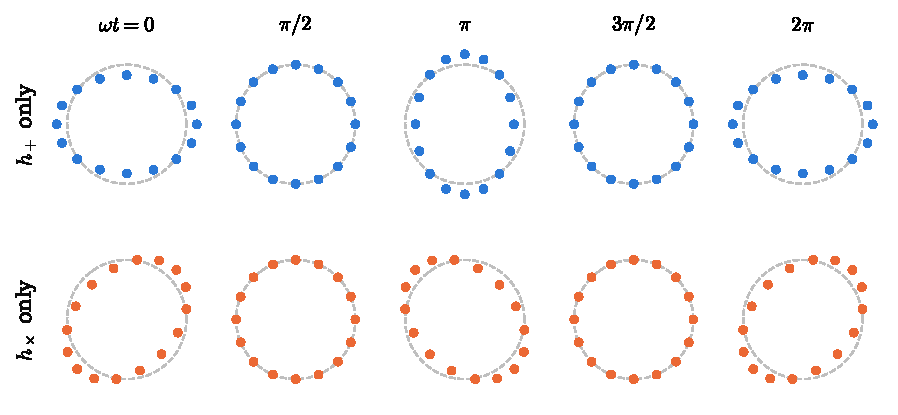
\includegraphics[width=0.9\linewidth]{figures/chT2/ring_masses.pdf}
\caption{A ring of sixteen free masses (dots) as a wave travelling out of the page passes, at five phases of one period; the dashed circle is the ring without the wave. Top row, a pure plus wave: the ring is stretched along the horizontal and squeezed along the vertical, then the reverse. Bottom row, a pure cross wave: the same breathing along the diagonals. The real amplitude is some $10^{19}$ times smaller than drawn.}
\label{T2g:fig:ring}
\end{figure}

\paragraph{Example: how large is the effect?}
For a ground-based detector with arms of $L=4$\,km and a wave of $h=10^{-21}$, \eqref{T2g:eq:displacement} gives $\delta L=\tfrac12hL=2\times10^{-18}$\,m, a few thousandths of the size of a proton. For LISA, with $L=2.5\times10^9$\,m and $h=10^{-20}$, $\delta L=\tfrac12\times10^{-20}\times2.5\times10^9\approx10^{-11}$\,m, about ten picometres. The longer the arm, the larger the displacement for the same strain, which is one reason to fly a detector in space. The other is that on the ground the seismic shaking of the Earth swamps everything below a few hertz.

\begin{pitfall}[Coordinates that do not move]
``In the TT gauge the masses do not move'' and ``the wave changes the distance between them'' are both true. The first is a statement about labels, which the TT gauge attaches to the free masses themselves. The second is the physics. Every measurable effect must be computed as a proper distance or a light travel time, as in \eqref{T2g:eq:proper}, never read off from a change of coordinates.
\end{pitfall}

\subsection{The energy a wave carries}
\label{T2g:sec:energy}

A wave that can push masses around can do work, so it carries energy. Energy in general relativity is subtle, because the gravitational field has no energy density at a single point: at any one point a freely falling observer sees no field at all. What is well defined is the energy averaged over a region several wavelengths across. This is our fourth input, imported from general relativity \cite[Sec.~1.4]{Maggiore2007}: the energy crossing unit area per unit time, for a wave in the TT gauge, is
\begin{equation}
  \mathcal F=\frac{c^3}{32\pi G}\,\big\langle\dot h^{\rm TT}_{ij}\dot h^{\rm TT}_{ij}\big\rangle
  =\frac{c^3}{16\pi G}\,\big\langle\dot h_+^2+\dot h_\times^2\big\rangle ,
  \label{T2g:eq:flux}
\end{equation}
where the angle brackets average over several periods, and the second form follows from \eqref{T2g:eq:tt}, since $h_{ij}h_{ij}=h_+^2+h_\times^2+h_\times^2+h_+^2$. Its form is that of the electromagnetic Poynting flux of a radiation field, $\varepsilon_0c\langle E^2\rangle$ with $E=-\dot A$. The flux is quadratic in the field because energy is, and it contains the time derivative because a static strain, like a static potential, carries nothing away.

\paragraph{Example: why a strain of $10^{-21}$ is a lot of energy.}
The constant in front of \eqref{T2g:eq:flux} is enormous:
\begin{align*}
  \frac{c^3}{16\pi G}
  &\eqby{1}\frac{(3.0\times10^8)^3}{16\pi\times6.67\times10^{-11}}\ \frac{\rm kg}{\rm s}
  \eqby{2}8.0\times10^{33}\ {\rm kg\,s^{-1}} .
\end{align*}
\begin{explain}
  \item $c$ in m\,s$^{-1}$ and $G$ in m$^3$\,kg$^{-1}$\,s$^{-2}$; the units combine to kg\,s$^{-1}$, which times $\dot h^2$ in s$^{-2}$ gives W\,m$^{-2}$.
  \item $2.7\times10^{25}/3.35\times10^{-9}=8.0\times10^{33}$.
\end{explain}
Take the first detected wave near its peak, $h_+=h\cos2\pi ft$ with $h\approx10^{-21}$ and $f\approx250$\,Hz. Then $\langle\dot h_+^2\rangle=\tfrac12(2\pi fh)^2=\tfrac12(1.6\times10^{-18}\,{\rm s^{-1}})^2=1.2\times10^{-36}\,{\rm s^{-2}}$, and $\mathcal F\approx8.0\times10^{33}\times1.2\times10^{-36}\approx10^{-2}$\,W\,m$^{-2}$. For a fraction of a second, the Earth received more energy per square metre in gravitational waves than it receives in light from any star in the night sky. Yet the strain was $10^{-21}$. Spacetime is stiff: the factor $c^3/G$ means a large energy flux produces only a minute deformation, and, the other way round, a measurable deformation needs a violent source.

\paragraph{Where this is used.}
The two polarisations and the factor $\tfrac12$ in $\delta L/L$ are what a detector turns into the single strain $h(t)=F_+h_++F_\times h_\times$ of \cref{T2g:sec:detector}. That strain is the signal part of the data stream $d(t)=h(t)+n(t)$ with which \cref{10b:sec:detection} begins, and the energy flux \eqref{T2g:eq:flux} drives the chirp of \cref{T2a:sec:chirp}, whose phase is what \cref{10b:sec:fisher} measures.
\section{Why radiation starts at the quadrupole}
\label{T2g:sec:quadrupole}

A radio antenna radiates because electrons slosh back and forth along it: the electric dipole moment, charge times separation, oscillates. Two black holes on an orbit look at first sight like the same thing, two ``charges'' swinging round each other, so we might expect them to radiate like a rotating dipole, at the orbital frequency. They do not. The gravitational wave of a binary comes out at \emph{twice} the orbital frequency, and it is weaker than a dipole estimate by a factor $(v/c)^2$. Both facts have one cause. The ``charge'' of gravity is mass, it has only one sign, and it is the same mass that sets the inertia of the body. As a result the two quantities that make up the monopole and the dipole of the field, the total mass and the position of the centre of mass, cannot oscillate: they are protected by conservation laws.

The question, in words: \emph{starting from the field equation of \cref{T2g:sec:wave}, which part of a moving mass distribution produces a wave far away, how large is the wave, and how much power does it carry off?} For a binary the answers are the waveform $h_+$, $h_\times$ that every template in \cref{ch:10} is built on, and the power $P_{\rm GW}$ that drives the chirp of \cref{T2a:sec:chirp}.

\subsection{The field far from a slow source}

\emph{Inputs.} We keep the inputs of \cref{T2g:sec:wave}: the weak-field metric \eqref{T2g:eq:weak} and the linearised field equation \eqref{T2g:eq:linear-einstein}, $\Box\bar h_{\mu\nu}=-(16\pi G/c^4)T_{\mu\nu}$. We add three about the source.
\begin{enumerate}[itemsep=1pt]
  \item \emph{Physical: small and slow.} The source has size $d$ and internal speeds $v\ll c$. It then changes on a time scale $d/v$, so it emits at wavelengths $\lambda\sim c\,d/v\gg d$.
  \item \emph{Physical: energy and momentum are conserved}, $\partial_\mu T^{\mu\nu}=0$, and the source is Newtonian, $T^{00}=\rho c^2$ with $\rho$ the mass density. For a binary held together by its own gravity this is true only once the energy of the gravitational field is counted as well. The full theory shows that the leading-order result derived below is unchanged by that \cite[Sec.~3.1]{Maggiore2007}.
  \item \emph{Mathematical: the retarded solution.} The solution of $\Box\psi=-4\pi s$ that contains only outgoing waves is $\psi(t,\bm x)=\int s(t-\lvert\bm x-\bm x'\rvert/c,\bm x')/\lvert\bm x-\bm x'\rvert\,\dd^3x'$, the retarded potential familiar from electrodynamics. Applied to each component of \eqref{T2g:eq:linear-einstein},
  \begin{equation}
    \bar h_{\mu\nu}(t,\bm x)=\frac{4G}{c^4}\int\frac{T_{\mu\nu}\big(t-\lvert\bm x-\bm x'\rvert/c,\ \bm x'\big)}{\lvert\bm x-\bm x'\rvert}\,\dd^3x' .
    \label{T2g:eq:retarded}
  \end{equation}
\end{enumerate}

\emph{Far away.} The detector sits at distance $r=\lvert\bm x\rvert\gg d$ in the direction $\hat{\bm n}=\bm x/r$. For a point $\bm x'$ of the source, $\lvert\bm x-\bm x'\rvert=r-\hat{\bm n}\cdot\bm x'+O(d^2/r)$. In the denominator of \eqref{T2g:eq:retarded} the correction is negligible and we write $1/r$. In the time argument it is not automatically negligible, because it multiplies a rapidly varying function:
\begin{equation}
  T_{\mu\nu}\Big(t-\frac rc+\frac{\hat{\bm n}\cdot\bm x'}{c},\bm x'\Big)
  =T_{\mu\nu}(t_r,\bm x')+\frac{\hat n_ix'_i}{c}\,\partial_tT_{\mu\nu}(t_r,\bm x')
  +\frac{\hat n_i\hat n_jx'_ix'_j}{2c^2}\,\partial_t^2T_{\mu\nu}(t_r,\bm x')+\dots,
  \label{T2g:eq:multipole}
\end{equation}
with $t_r=t-r/c$ the \newterm{retarded time}. Each term is smaller than the one before by about $(d/c)/(d/v)=v/c$: the time light takes to cross the source, divided by the time the source takes to change. This is the \newterm{multipole expansion}, and the slow-motion input says it converges quickly.

\emph{Which terms can change in time?} Apply \eqref{T2g:eq:multipole} to the $00$ component, with $T_{00}=\rho c^2$:
\begin{equation}
  \bar h_{00}=\frac{4G}{c^2r}\Big[M+\frac{\hat n_i}{c}\,\dot M_i+\frac{\hat n_i\hat n_j}{2c^2}\,\ddot M_{ij}+\dots\Big]_{t_r},
  \qquad M=\int\rho,\quad M_i=\int\rho\,x_i,\quad M_{ij}=\int\rho\,x_ix_j ,
  \label{T2g:eq:moments}
\end{equation}
where every integral is over the source at the retarded time. The three moments are the mass, the mass dipole and the second mass moment. Take them one at a time.

\emph{The monopole.} Mass conservation, the $\nu=0$ part of input 2, is the continuity equation $\partial_t\rho+\partial_k(\rho v_k)=0$. Integrated over a volume enclosing the source, the divergence becomes a flux through a surface where there is no matter, so $\dot M=0$. The first term is the static Newtonian potential $4GM/(c^2r)$ and carries no wave.

\emph{The dipole.} Using the continuity equation again,
\begin{align}
  \dot M_i
  &\eqby{1}\int x_i\,\partial_t\rho\,\dd^3x
  \eqby{2}-\int x_i\,\partial_k(\rho v_k)\,\dd^3x
  \eqby{3}\int\rho\,v_k\,\partial_kx_i\,\dd^3x
  \eqby{4}\int\rho\,v_i\,\dd^3x=P_i ,
  \label{T2g:eq:dipole}
\end{align}
\begin{explain}
  \item Differentiate under the integral; the integration region is fixed.
  \item Continuity equation.
  \item Integrate by parts; the surface term vanishes outside the source.
  \item $\partial_kx_i=\delta_{ik}$. The result is the total momentum $P_i$.
\end{explain}
Momentum conservation, the $\nu=i$ part of input 2, gives $\dot P_i=0$, so $\ddot M_i=0$: $\dot M_i$ is constant. The second term of \eqref{T2g:eq:moments} is the field of a mass whose centre moves at constant velocity, and that does not radiate either. In electromagnetism the dipole moment is $\sum q\,\bm x$, whose derivative $\sum q\,\bm v$ is not a conserved quantity, because different particles carry different charge per unit mass. In gravity every body's ``charge'' is its mass, the very quantity that sets its momentum, so the dipole is tied to the centre of mass and frozen.

\emph{The quadrupole.} Nothing stops $\ddot M_{ij}$ from oscillating. The first time-dependent term, and so the first radiating one, is the second moment of the mass. A spinning symmetric top has a constant $M_{ij}$ and stays silent; a dumbbell rotating about an axis through its middle does not, and radiates.

\begin{figure}[htbp]
\centering
\begin{tikzpicture}[scale=0.9]
  \begin{scope}
    \shade[ball color=formblue!35] (0,0) circle (0.75);
    \node[lbl] at (0,-1.35) {mass $M$};
    \node[lbl,align=center] at (0,-2.05) {conserved:\\ no wave};
  \end{scope}
  \begin{scope}[xshift=4.2cm]
    \fill[formblue] (-0.9,0.25) circle (3pt);
    \fill[formblue] (0.5,-0.25) circle (4pt);
    \draw[faint,dashed] (-0.9,0.25) -- (0.5,-0.25);
    \fill[bdryred] (0.03,-0.08) circle (1.6pt);
    \draw[vec] (0.03,-0.08) -- ++(0.9,0.55);
    \node[lbl] at (0,-1.35) {centre of mass};
    \node[lbl,align=center] at (0,-2.05) {moves uniformly:\\ no wave};
  \end{scope}
  \begin{scope}[xshift=8.6cm]
    \foreach \ang/\op in {0/1,45/0.45,90/0.2}{
      \draw[formblue,thick,opacity=\op] (\ang:0.85) -- (\ang+180:0.85);
      \fill[formblue,opacity=\op] (\ang:0.85) circle (3.5pt);
      \fill[formblue,opacity=\op] (\ang+180:0.85) circle (3.5pt);}
    \draw[->,faint] (20:1.2) arc (20:70:1.2);
    \node[lbl] at (0,-1.35) {shape $M_{ij}$};
    \node[lbl,align=center] at (0,-2.05) {changes twice\\ per turn: waves};
  \end{scope}
\end{tikzpicture}
\caption{The three lowest moments of a mass distribution. The total mass (left) cannot change. The mass dipole is the total mass times the position of the centre of mass (middle, red dot), which can only move at constant velocity. The second moment (right) describes the shape; for a rotating dumbbell, drawn at three instants an eighth of a turn apart, it returns to the same value after half a turn, so it oscillates at twice the rotation frequency.}
\label{T2g:fig:multipoles}
\end{figure}

\emph{The wave itself.} The radiation lives in the spatial components $\bar h_{ij}$. At leading order in $v/c$ we keep only the first term of \eqref{T2g:eq:multipole}, so $\bar h_{ij}=(4G/c^4r)\int T_{ij}(t_r,\bm x')\,\dd^3x'$. The integral of the stresses $T_{ij}$ is not obviously related to the mass distribution, but conservation turns it into one:
\begin{align}
  \frac{1}{c^2}\frac{\dd^2}{\dd t^2}\int T^{00}x_ix_j\,\dd^3x
  &\eqby{1}\int x_ix_j\,\partial_0\partial_0T^{00}\,\dd^3x
  \eqby{2}\int x_ix_j\,\partial_k\partial_lT^{kl}\,\dd^3x\nonumber\\
  &\eqby{3}\int T^{kl}\,\partial_k\partial_l(x_ix_j)\,\dd^3x
  \eqby{4}2\int T^{ij}\,\dd^3x .
  \label{T2g:eq:virial}
\end{align}
\begin{explain}
  \item $x^0=ct$, so $\partial_0=c^{-1}\partial_t$.
  \item From $\partial_\mu T^{\mu\nu}=0$: $\partial_0T^{00}=-\partial_kT^{k0}$ and $\partial_0T^{0k}=-\partial_lT^{lk}$, so $\partial_0\partial_0T^{00}=-\partial_k\partial_0T^{0k}=\partial_k\partial_lT^{kl}$.
  \item Integrate by parts twice; both surface terms vanish outside the source.
  \item $\partial_l(x_ix_j)=\delta_{il}x_j+x_i\delta_{jl}$ and then $\partial_k$ of that is $\delta_{il}\delta_{jk}+\delta_{ik}\delta_{jl}$; both terms give $T^{ij}$ because $T$ is symmetric.
\end{explain}
With $T^{00}=\rho c^2$ the left side is $\ddot M_{ij}$, so $\int T_{ij}=\tfrac12\ddot M_{ij}$ and $\bar h_{ij}=(2G/c^4r)\ddot M_{ij}(t_r)$. Far from the source the wave is locally a plane wave travelling along $\hat{\bm n}$, and its physical content is its TT part, obtained with the recipe of the working definition in \cref{T2g:sec:wave}: keep the components in the plane perpendicular to $\hat{\bm n}$ and remove their trace. Removing the trace means that $M_{ij}$ may as well be replaced by its traceless part, the \newterm{mass quadrupole}
\begin{equation}
  Q_{ij}=\int\rho\,\Big(x_ix_j-\tfrac13\delta_{ij}\lvert\bm x\rvert^2\Big)\dd^3x ,
  \qquad
  h_{ij}^{\rm TT}(t,\bm x)=\frac{2G}{c^4r}\,\big[\ddot Q_{ij}(t-r/c)\big]^{\rm TT} .
  \label{T2g:eq:hTT}
\end{equation}
This is the \newterm{quadrupole formula} for the wave \cite[Sec.~3.3]{Maggiore2007}. In terms of the transverse unit vectors $\bm p$, $\bm q$ and the recipe of the working definition, $h_+=\frac{G}{c^4r}\big(\ddot Q_{pp}-\ddot Q_{qq}\big)$ and $h_\times=\frac{2G}{c^4r}\ddot Q_{pq}$.

\begin{keyidea}[The quadrupole formula]
Far from a slow source, the wave is $h_{ij}^{\rm TT}=(2G/c^4r)\,[\ddot Q_{ij}(t-r/c)]^{\rm TT}$, with $Q_{ij}$ the traceless second moment of the mass. Mass and momentum conservation forbid monopole and dipole radiation, so the quadrupole is the leading term, and each further multipole is suppressed by another factor $v/c$.
\end{keyidea}

\subsection{The circular binary}

\emph{The quadrupole of a binary.} Two masses $m_1$, $m_2$ at positions $\bm x_1$, $\bm x_2$, centre of mass at rest at the origin. With $M=m_1+m_2$, the separation $\bm x=\bm x_1-\bm x_2$ and the \newterm{reduced mass} $\mu=m_1m_2/M$, the positions are $\bm x_1=(m_2/M)\bm x$ and $\bm x_2=-(m_1/M)\bm x$, and
\begin{equation}
  M_{ij}=m_1x_{1i}x_{1j}+m_2x_{2i}x_{2j}=\Big(\frac{m_1m_2^2}{M^2}+\frac{m_2m_1^2}{M^2}\Big)x_ix_j=\mu\,x_ix_j ,
\end{equation}
so the binary radiates like a single body of mass $\mu$ on the relative orbit. For a circular orbit of radius $r$ in the $xy$ plane, $\bm x=r(\cos\omega t,\sin\omega t,0)$, and Kepler's third law $\omega^2=GM/r^3$ links $\omega$ and $r$. The components we need are
\begin{align}
  M_{xx}&\eqby{1}\mu r^2\cos^2\omega t\eqby{2}\tfrac12\mu r^2(1+\cos2\omega t),\qquad
  M_{yy}\eqby{2}\tfrac12\mu r^2(1-\cos2\omega t),\qquad
  M_{xy}\eqby{2}\tfrac12\mu r^2\sin2\omega t,\nonumber\\
  \ddot M_{xx}&\eqby{3}-2\mu r^2\omega^2\cos2\omega t=-\ddot M_{yy},\qquad
  \ddot M_{xy}\eqby{3}-2\mu r^2\omega^2\sin2\omega t,
  \label{T2g:eq:Mddot}
\end{align}
and every component with a $z$ is zero or constant.
\begin{explain}
  \item $x_x=r\cos\omega t$.
  \item $\cos^2\theta=\tfrac12(1+\cos2\theta)$, $\sin^2\theta=\tfrac12(1-\cos2\theta)$, $\sin\theta\cos\theta=\tfrac12\sin2\theta$.
  \item Two time derivatives of $\cos2\omega t$ or $\sin2\omega t$ bring down $-(2\omega)^2$; the constants drop out.
\end{explain}
Everything oscillates at $2\omega$. The mass distribution of the pair, a dumbbell, looks the same after half a turn, so the wave frequency is twice the orbital one:
\begin{equation}
  f_{\rm GW}=2f_{\rm orb}=\frac{\omega}{\pi}.
  \label{T2g:eq:twice}
\end{equation}
From here on $f$ without a label means the wave frequency $f_{\rm GW}$.

\emph{The two polarisations seen from an angle.} Let the observer look at the binary from the direction $\hat{\bm n}=(0,\sin\iota,\cos\iota)$, where $\iota$ is the \newterm{inclination}, the angle between the orbital axis and the line of sight. Two transverse unit vectors are $\bm p=(1,0,0)$ and $\bm q=(0,\cos\iota,-\sin\iota)$. Then $\ddot M_{pp}=\ddot M_{xx}$, $\ddot M_{qq}=\cos^2\iota\,\ddot M_{yy}$ and $\ddot M_{pq}=\cos\iota\,\ddot M_{xy}$, because the $z$ components do not contribute. By \eqref{T2g:eq:hTT} at distance $D$,
\begin{align}
  h_+&\eqby{1}\frac{G}{c^4D}\big(\ddot M_{xx}-\cos^2\iota\,\ddot M_{yy}\big)
  \eqby{2}-\frac{4G\mu r^2\omega^2}{c^4D}\,\frac{1+\cos^2\iota}{2}\,\cos2\omega t_r,\nonumber\\
  h_\times&\eqby{1}\frac{2G}{c^4D}\cos\iota\,\ddot M_{xy}
  \eqby{2}-\frac{4G\mu r^2\omega^2}{c^4D}\,\cos\iota\,\sin2\omega t_r .
  \label{T2g:eq:hpc}
\end{align}
\begin{explain}
  \item The recipe $h_+=\frac{G}{c^4D}(\ddot M_{pp}-\ddot M_{qq})$, $h_\times=\frac{2G}{c^4D}\ddot M_{pq}$, with $M$ in place of $Q$ since their difference is a multiple of $\delta_{ij}$, which the TT recipe removes.
  \item Insert \eqref{T2g:eq:Mddot}: $\ddot M_{xx}-\cos^2\iota\,\ddot M_{yy}=-2\mu r^2\omega^2(1+\cos^2\iota)\cos2\omega t$.
\end{explain}
Seen face on ($\iota=0$) the two polarisations have equal size and are a quarter cycle apart: the wave is circularly polarised, as the rotating dumbbell suggests. Seen edge on ($\iota=90^\circ$) only $h_+$ is left, at half the face-on size: the dumbbell seen from the side only grows and shrinks.

\emph{The amplitude as a function of the wave frequency.} Kepler's law gives $r^2\omega^2=(GM)^{2/3}\omega^{2/3}$, and $\omega=\pi f$. So the common factor in \eqref{T2g:eq:hpc} is
\begin{align}
  A\equiv\frac{4G\mu r^2\omega^2}{c^4D}
  &\eqby{1}\frac{4G\mu(GM)^{2/3}(\pi f)^{2/3}}{c^4D}
  \eqby{2}\frac{4(G\mathcal M)^{5/3}(\pi f)^{2/3}}{c^4D},
  \qquad \mathcal M\equiv\mu^{3/5}M^{2/5}=\frac{(m_1m_2)^{3/5}}{(m_1+m_2)^{1/5}} .
  \label{T2g:eq:amp}
\end{align}
\begin{explain}
  \item $r=(GM/\omega^2)^{1/3}$, so $r^2\omega^2=(GM)^{2/3}\omega^{2/3}$.
  \item $G\mu\,G^{2/3}M^{2/3}=G^{5/3}\mu M^{2/3}$, and $\mu M^{2/3}=(\mu^{3/5}M^{2/5})^{5/3}=\mathcal M^{5/3}$.
\end{explain}
The masses enter only through the \newterm{chirp mass} $\mathcal M$; \cref{T2a:sec:chirp} finds the same combination in the rate of the chirp. This amplitude is the one used for the Fourier-domain waveform in \cref{T2a:sec:spa}, where it becomes the constant $\mathcal A$ of \eqref{T2a:eq:hf}; it is the time-domain amplitude quoted by Eda et al.\ \cite[eq.~(21)]{Eda2015}.

\paragraph{Example: the size of the wave from a known source.}
For a GW150914-like binary, $\mathcal M=28\,M_\odot$, so $G\mathcal M/c^3=28\times4.93\,\mu{\rm s}=1.38\times10^{-4}$\,s, at $D=410$\,Mpc$\,=1.27\times10^{25}$\,m and $f=250$\,Hz. Write \eqref{T2g:eq:amp} with the masses as times, $A=4(G\mathcal M/c^3)^{5/3}(\pi f)^{2/3}\,c/D$:
\begin{align*}
  A&\eqby{1}4\times\big(1.38\times10^{-4}\big)^{5/3}\times(785)^{2/3}\times\frac{3.0\times10^8}{1.27\times10^{25}}
  \eqby{2}4\times3.7\times10^{-7}\times85\times2.4\times10^{-17}
  \approx3\times10^{-21} .
\end{align*}
\begin{explain}
  \item $(G\mathcal M)^{5/3}/c^4=(G\mathcal M/c^3)^{5/3}c^5/c^4$, and $\pi\times250=785$\,s$^{-1}$.
  \item $10^{-3.86\times5/3}=10^{-6.43}=3.7\times10^{-7}$; $785^{2/3}=85$; $c/D=2.4\times10^{-17}$\,s$^{-1}$.
\end{explain}
This is the strain of order $10^{-21}$ used in \cref{T2g:sec:energy}. For the intermediate mass-ratio benchmark of \cref{T2a:sec:chirp} ($\mathcal M\approx19\,M_\odot$) at $75$\,Mpc and $f=20$\,mHz the same steps give $A\approx1.6\times10^{-23}$. It is the millions of cycles, not the instantaneous size, that make such a source detectable.

\subsection{The power}

\emph{From the flux.} The power leaving the binary is the flux \eqref{T2g:eq:flux} integrated over a sphere of radius $D$. Over one period, $\langle\sin^2\rangle=\langle\cos^2\rangle=\tfrac12$, and each time derivative of \eqref{T2g:eq:hpc} brings down $2\omega$, so $\langle\dot h_+^2+\dot h_\times^2\rangle=\tfrac12(2\omega A)^2\big[\tfrac14(1+\cos^2\iota)^2+\cos^2\iota\big]$. The bracket is the angular pattern of the radiation (\cref{T2g:fig:pattern}). It does not depend on the observer's azimuth, because a circular orbit seen from a different azimuth is the same orbit seen at a different moment. With $x=\cos\iota$ and $\dd\Omega=\dd\phi\,\dd x$,
\begin{align}
  P_{\rm GW}
  &\eqby{1}\int\frac{c^3}{16\pi G}\big\langle\dot h_+^2+\dot h_\times^2\big\rangle D^2\,\dd\Omega
  \eqby{2}\frac{c^3D^2}{16\pi G}\cdot2\omega^2A^2\cdot2\pi\int_{-1}^{1}\Big[\frac{(1+x^2)^2}{4}+x^2\Big]\dd x\nonumber\\
  &\eqby{3}\frac{c^3D^2}{16\pi G}\cdot2\omega^2A^2\cdot\frac{16\pi}{5}
  \eqby{4}\frac25\,\frac{c^3}{G}\,\omega^2(DA)^2
  \eqby{5}\frac{32}{5}\,\frac{G}{c^5}\,\mu^2r^4\omega^6 .
  \label{T2g:eq:power-binary}
\end{align}
\begin{explain}
  \item Flux times area, summed over all directions.
  \item $\tfrac12(2\omega A)^2=2\omega^2A^2$; the $\phi$ integral gives $2\pi$.
  \item $\int_{-1}^1(1+x^2)^2\dd x=2+\tfrac43+\tfrac25=\tfrac{56}{15}$ and $\int_{-1}^1x^2\dd x=\tfrac23$, so the integral is $\tfrac14\cdot\tfrac{56}{15}+\tfrac23=\tfrac{14}{15}+\tfrac{10}{15}=\tfrac85$, and $2\pi\cdot\tfrac85=\tfrac{16\pi}5$.
  \item $\frac{2\cdot16\pi}{16\pi\cdot5}=\frac25$.
  \item $DA=4G\mu r^2\omega^2/c^4$ from \eqref{T2g:eq:amp}, so $(DA)^2=16G^2\mu^2r^4\omega^4/c^8$; then $\tfrac25\cdot16=\tfrac{32}5$, $c^3/c^8=c^{-5}$ and $G^2/G=G$.
\end{explain}
The angular integral $\int[\tfrac14(1+x^2)^2+x^2]\dd\Omega=16\pi/5$ is worth remembering; divided by $4\pi$ it is the average $\tfrac45$ that reappears in the sky-averaged waveform of \cref{T2a:sec:spa}.

\emph{From the quadrupole directly.} The same integral can be done once and for all for any source. Insert \eqref{T2g:eq:hTT} into \eqref{T2g:eq:flux}. The TT recipe is a projection, applying it twice changes nothing, and for a traceless symmetric matrix it gives
\begin{align}
  [\dddot Q]^{\rm TT}_{ij}[\dddot Q]^{\rm TT}_{ij}
  &\eqby{1}\dddot Q_{ij}\dddot Q_{ij}-2\,\hat n_i\dddot Q_{ik}\dddot Q_{kj}\hat n_j+\tfrac12\big(\hat n_i\dddot Q_{ij}\hat n_j\big)^2,\nonumber\\
  \frac{1}{4\pi}\int[\dddot Q]^{\rm TT}_{ij}[\dddot Q]^{\rm TT}_{ij}\,\dd\Omega
  &\eqby{2}\dddot Q_{ij}\dddot Q_{ij}\Big(1-\frac23+\frac{2}{15}\cdot\frac12\Big)
  =\frac25\,\dddot Q_{ij}\dddot Q_{ij},\nonumber\\
  P_{\rm GW}
  &\eqby{3}\frac{c^3r^2}{32\pi G}\Big(\frac{2G}{c^4r}\Big)^2\cdot4\pi\cdot\frac25\,\big\langle\dddot Q_{ij}\dddot Q_{ij}\big\rangle
  =\frac{G}{5c^5}\,\big\langle\dddot Q_{ij}\dddot Q_{ij}\big\rangle .
  \label{T2a:eq:quadrupole}
\end{align}
\begin{explain}
  \item With the projector $P_{ij}=\delta_{ij}-\hat n_i\hat n_j$ onto the transverse plane, the recipe is $[Q]^{\rm TT}=PQP-\tfrac12P\,\mathrm{tr}(PQ)$. Squaring and taking the trace, with $P^2=P$ and $\mathrm{tr}P=2$, gives $\mathrm{tr}(PQPQ)-\mathrm{tr}(PQ)^2+\tfrac14\cdot2\,\mathrm{tr}(PQ)^2=\mathrm{tr}(PQPQ)-\tfrac12\mathrm{tr}(PQ)^2$. Multiplying out $P=\mathbb 1-\hat{\bm n}\hat{\bm n}^{\mathsf T}$ gives $\mathrm{tr}(PQPQ)=\mathrm{tr}Q^2-2\,\hat{\bm n}\cdot Q^2\hat{\bm n}+(\hat{\bm n}\cdot Q\hat{\bm n})^2$, and $\mathrm{tr}(PQ)=-\hat{\bm n}\cdot Q\hat{\bm n}$ because $\mathrm{tr}\,Q=0$.
  \item Average over directions with $\langle\hat n_i\hat n_j\rangle=\tfrac13\delta_{ij}$ and $\langle\hat n_i\hat n_j\hat n_k\hat n_l\rangle=\tfrac1{15}(\delta_{ij}\delta_{kl}+\delta_{ik}\delta_{jl}+\delta_{il}\delta_{jk})$; for a traceless symmetric $Q$ the second gives $\langle(\hat{\bm n}\cdot Q\hat{\bm n})^2\rangle=\tfrac{2}{15}\mathrm{tr}Q^2$.
  \item The flux \eqref{T2g:eq:flux} with $\dot h^{\rm TT}=(2G/c^4r)[\dddot Q]^{\rm TT}$, times $r^2$, integrated over $4\pi$; $\frac{c^3}{32\pi G}\cdot\frac{4G^2}{c^8}\cdot4\pi\cdot\frac25=\frac{G}{5c^5}$.
\end{explain}
For the binary, the third derivatives of \eqref{T2g:eq:Mddot} are $\dddot Q_{xx}=-\dddot Q_{yy}=4\mu r^2\omega^3\sin2\omega t$ and $\dddot Q_{xy}=-4\mu r^2\omega^3\cos2\omega t$, so
\begin{equation}
  \dddot Q_{ij}\dddot Q_{ij}=\dddot Q_{xx}^2+\dddot Q_{yy}^2+2\dddot Q_{xy}^2=(4\mu r^2\omega^3)^2\big(2\sin^2+2\cos^2\big)(2\omega t)=32\,\mu^2r^4\omega^6 ,
  \label{T2a:eq:Qddd}
\end{equation}
and \eqref{T2a:eq:quadrupole} gives $P_{\rm GW}=\tfrac{32}{5}(G/c^5)\mu^2r^4\omega^6$ again \cite[Sec.~4.1]{Maggiore2007}. Two routes, one answer: the first summed the radiation over directions by hand, the second did the same sum for a general traceless matrix.

\begin{figure}[htbp]
\centering
\begin{tikzpicture}[scale=1.0]
  \draw[faint] (-2.8,0) -- (2.8,0);
  \node[lbl,faint,anchor=south east] at (-2.85,0.05) {orbital plane};
  \draw[faint,->] (0,-2.7) -- (0,2.9) node[above,lbl] {orbital axis};
  \draw[formblue,thick,domain=0:360,samples=181,smooth,variable=\t]
    plot ({2.4*((1+cos(\t)^2)^2/4+cos(\t)^2)/2*sin(\t)},{2.4*((1+cos(\t)^2)^2/4+cos(\t)^2)/2*cos(\t)});
  \draw[fibreorange,thick,dashed,domain=0:360,samples=181,smooth,variable=\t]
    plot ({2.4*(1+cos(\t)^2)/2*sin(\t)},{2.4*(1+cos(\t)^2)/2*cos(\t)});
  \draw[tangentgreen,thick,dotted,domain=0:360,samples=181,smooth,variable=\t]
    plot ({2.4*abs(cos(\t))*sin(\t)},{2.4*abs(cos(\t))*cos(\t)});
  \fill[black] (-0.12,0) circle (1.5pt); \fill[black] (0.12,0) circle (1.5pt);
  \draw[faint] (0,0) -- (52:2.4);
  \node[lbl] at (64:1.3) {$\iota$};
  \draw[faint,->] (90:0.9) arc (90:52:0.9);
  \node[lbl,anchor=west,align=left,formblue] at (3.0,1.9) {power per solid angle,\\ $\tfrac14(1+\cos^2\iota)^2+\cos^2\iota$};
  \node[lbl,anchor=west,align=left,fibreorange] at (3.0,0.6) {$h_+$ amplitude,\\ $\tfrac12(1+\cos^2\iota)$};
  \node[lbl,anchor=west,align=left,tangentgreen!70!black] at (3.0,-0.7) {$h_\times$ amplitude,\\ $\lvert\cos\iota\rvert$};
\end{tikzpicture}
\caption{How a circular binary radiates in different directions, in units of the face-on value; the distance from the centre along a direction at angle $\iota$ from the orbital axis is the quantity named on the right. Along the axis both polarisations are full size and the power is largest. In the orbital plane $h_\times$ vanishes, $h_+$ is halved, and the power per solid angle drops from $\tfrac14\cdot2^2+1=2$ to $\tfrac14$, an eighth of its value on the axis.}
\label{T2g:fig:pattern}
\end{figure}

\paragraph{Example: how much weaker than a dipole?}
Suppose, against the conservation laws, that a binary could radiate like an electric dipole. Larmor's formula, $P=q^2a^2/(6\pi\varepsilon_0c^3)$, with $q^2/(4\pi\varepsilon_0)$ replaced by $G\mu^2$ and the acceleration $a=r\omega^2$, would give $P_{\rm dip}\sim G\mu^2r^2\omega^4/c^3$. The quadrupole power is $P_{\rm GW}\sim G\mu^2r^4\omega^6/c^5$, so
\begin{equation*}
  \frac{P_{\rm GW}}{P_{\rm dip}}\sim\frac{r^2\omega^2}{c^2}=\frac{v^2}{c^2}.
\end{equation*}
Quadrupole radiation is one power of $(v/c)^2$ weaker than dipole radiation would be. In theories of gravity in which bodies carry an extra ``charge'' that is not proportional to their mass, dipole radiation does appear, and because it is relatively stronger at low speeds, it shows up at low frequency. \Cref{T2g:sec:pn} shows that it enters the phase of the wave as the power $f^{-7/3}$.

\paragraph{Where this is used.}
The amplitude \eqref{T2g:eq:amp} and its dependence on the inclination \eqref{T2g:eq:hpc} set the size of every template in \cref{ch:10}: through the constant $\mathcal A$ of \eqref{T2a:eq:hf} they fix the signal-to-noise ratio of \cref{10b:sec:matched-filter}, and through the factor $\tfrac45$ they enter the sky-averaged forecasts of \cref{10b:sec:forecast}. The power \eqref{T2g:eq:power-binary} drives the chirp of \cref{T2a:sec:chirp}, whose phase is what \cref{10b:sec:fisher} measures.
\section{How a detector turns a wave into one number}
\label{T2g:sec:detector}

A wave arrives with two polarisations, $h_+(t)$ and $h_\times(t)$, defined with respect to axes in the plane perpendicular to its direction of travel (\cref{T2g:sec:wave}). A detector records one time series. LIGO records the difference between the lengths of its two arms, read from the interference of laser light that has run up and down each of them; LISA does the same with laser links between spacecraft millions of kilometres apart. Every likelihood in \cref{ch:10} compares that one recorded number with a template, so we need the exact rule that maps $(h_+,h_\times)$ onto it.

The questions, in words: \emph{how does a change in the light travel time along one arm follow from $h_{ij}$? How do two arms combine into one strain? How strongly does the result depend on where the source sits on the sky and how its orbit is turned? And what changes when the arm is so long that the wave changes while the light is still in flight?} The answers produce three numbers that appear without explanation in most papers: the $\tfrac45$ of the inclination average, the $\tfrac15$ of the sky average, and LISA's $\tfrac{3}{10}$, together with the transfer frequency $f_*=c/(2\pi L)$.

\subsection{One arm: the light travel time}

\emph{The simplest case first.} Put one free mass at the origin and one at $x=L$, the arm along $x$, and let a wave travel along $z$ with a wavelength much longer than $L$, so that $h_{xx}=h_+$ is the same along the whole arm while the light is in flight. Light moves on $\dd s^2=0$. Along the arm only $\dd t$ and $\dd x$ change, so with the TT metric
\begin{align}
  0&\eqby{1}-c^2\dd t^2+(1+h_{xx})\,\dd x^2
  \;\Rightarrow\;
  c\,\dd t\eqby{2}\sqrt{1+h_{xx}}\,\dd x\eqby{3}\Big(1+\tfrac12h_{xx}\Big)\dd x,\nonumber\\
  T_{\rm round}&\eqby{4}\frac{2L}{c}\Big(1+\tfrac12h_{xx}\Big),
  \qquad
  \frac{\delta T_{\rm round}}{2L/c}=\tfrac12h_{xx}.
  \label{T2g:eq:arm}
\end{align}
\begin{explain}
  \item The TT line element \eqref{T2g:eq:tt} along the $x$ axis, with $\dd y=\dd z=0$.
  \item Solve for $c\,\dd t$.
  \item $\sqrt{1+\epsilon}=1+\tfrac12\epsilon$ to first order.
  \item Integrate from $0$ to $L$ and back. The end masses keep their TT coordinates (\cref{T2g:sec:free-masses}), so the coordinate length is $L$ both ways.
\end{explain}
The light takes longer exactly as if the arm had grown by $\delta L/L=\tfrac12h_{xx}$, which is the proper-distance result \eqref{T2g:eq:displacement} again: a light clock and a ruler agree. For an arm along any unit vector $\hat{\bm a}$, the same steps give $\delta L/L=\tfrac12h_{ij}\hat a_i\hat a_j$, written $\tfrac12h_{aa}$ for short.

\emph{Two arms.} A Michelson interferometer sends light along two arms $\hat{\bm u}$ and $\hat{\bm v}$ of equal length and compares the return times. Common changes cancel; the difference survives. The strain the instrument reports is the length difference divided by the arm length \cite[eq.~(5)]{LIGOGuide2020}, \cite[eq.~(11)]{BarackCutler2004}:
\begin{equation}
  h(t)\equiv\frac{\delta L_u-\delta L_v}{L}=\tfrac12\big(h_{uu}-h_{vv}\big)=D_{ij}h_{ij},
  \qquad D_{ij}\equiv\tfrac12\big(\hat u_i\hat u_j-\hat v_i\hat v_j\big).
  \label{T2g:eq:michelson}
\end{equation}
The matrix $D$, the \newterm{detector tensor}, is all the geometry of the instrument that matters while the arms are short compared with the wavelength. For a wave of plus polarisation coming straight down onto a right-angle detector with arms along $x$ and $y$, $h_{uu}=h_+$ and $h_{vv}=-h_+$, so $h=h_+$: one arm grows while the other shrinks, and the two effects add in the difference. That is why the interferometer has two arms at right angles.

\begin{figure}[htbp]
\centering
\begin{tikzpicture}[scale=1.0]
  \fill[softgray!40] (-0.25,-0.25) rectangle (0.25,0.25);
  \draw[thick] (-0.3,0.3) -- (0.3,-0.3);
  \node[lbl,anchor=north east] at (-0.3,-0.3) {beam splitter};
  \fill[formblue] (4.6,-0.35) rectangle (4.75,0.35);
  \fill[formblue] (-0.35,3.4) rectangle (0.35,3.55);
  \node[lbl,anchor=west] at (4.85,0) {mass at $L\hat{\bm u}$};
  \node[lbl,anchor=south] at (0,3.6) {mass at $L\hat{\bm v}$};
  \draw[bdryred,thick] (0.3,0.06) -- (4.6,0.06);
  \draw[bdryred,thick,<-] (0.3,-0.06) -- (4.6,-0.06);
  \draw[bdryred,thick] (0.06,0.3) -- (0.06,3.4);
  \draw[bdryred,thick,<-] (-0.06,0.3) -- (-0.06,3.4);
  \draw[fibreorange,thick] (-2.6,0) -- (-0.3,0);
  \node[lbl,anchor=south] at (-1.8,0.05) {laser};
  \draw[faint] (0,-0.3) -- (0,-1.6);
  \node[lbl,anchor=north] at (0,-1.6) {photodetector: $\delta L_u-\delta L_v$};
  \draw[faint,dashed] (2.3,1.7) ellipse (0.75 and 0.55);
  \node[lbl,align=center] at (2.3,1.7) {$h_+>0$};
  \draw[vec] (3.25,1.7) -- (3.65,1.7);
  \draw[vec] (2.3,1.1) -- (2.3,1.35);
\end{tikzpicture}
\caption{A Michelson interferometer. Laser light is split, runs along two perpendicular arms to free masses (blue) and back, and the two beams are recombined. The recombined light measures the difference of the two round-trip times. A plus wave arriving from above, at the instant drawn, lengthens the horizontal arm and shortens the vertical one (small ellipse), so the two changes add up in the difference.}
\label{T2g:fig:michelson}
\end{figure}

\subsection{Antenna patterns: where on the sky, and how turned}

\emph{The general rule.} Let the wave come from the direction $\hat{\bm n}$ (so it travels along $-\hat{\bm n}$), and let $\bm p$, $\bm q$ be the axes in the transverse plane with respect to which $h_+$ and $h_\times$ are defined. By \eqref{T2g:eq:tt} the wave is $h_{ij}=h_+e^+_{ij}+h_\times e^\times_{ij}$ with $e^+=\bm p\bm p^{\mathsf T}-\bm q\bm q^{\mathsf T}$ and $e^\times=\bm p\bm q^{\mathsf T}+\bm q\bm p^{\mathsf T}$. Inserting it in \eqref{T2g:eq:michelson},
\begin{equation}
  h(t)=F_+\,h_+(t)+F_\times\,h_\times(t),\qquad F_A=D_{ij}\,e^A_{ij}\quad(A=+,\times),
  \label{T2g:eq:response}
\end{equation}
the form used for every detector \cite[eq.~(24)]{LIGOGuide2020}.

\begin{workdef}[antenna pattern functions]
$F_+$ and $F_\times$ are the weights with which a detector adds the two polarisations of a wave into its one output, $h=F_+h_++F_\times h_\times$ \unpack{numbers between $-1$ and $1$, fixed by the arm directions, the source direction and the orientation of the polarisation axes}. \emph{Operationally:} $F_A=D_{ij}e^A_{ij}$ with the detector tensor $D=\tfrac12(\hat{\bm u}\hat{\bm u}^{\mathsf T}-\hat{\bm v}\hat{\bm v}^{\mathsf T})$.
\end{workdef}

\emph{A right-angle detector.} Take arms along $x$ and $y$ and a source at polar angle $\theta$ and azimuth $\phi$ in the detector's frame. Choose first the natural transverse axes, $\bm p_0=\hat{\bm\theta}=(\cos\theta\cos\phi,\cos\theta\sin\phi,-\sin\theta)$ and $\bm q_0=\hat{\bm\phi}=(-\sin\phi,\cos\phi,0)$. With $D=\tfrac12\mathrm{diag}(1,-1,0)$,
\begin{align}
  F_+^0&\eqby{1}\tfrac12\big(p_x^2-q_x^2-p_y^2+q_y^2\big)
  \eqby{2}\tfrac12\big(\cos^2\theta\cos^2\phi-\sin^2\phi-\cos^2\theta\sin^2\phi+\cos^2\phi\big)\nonumber\\
  &\eqby{3}\tfrac12(1+\cos^2\theta)\cos2\phi,\nonumber\\
  F_\times^0&\eqby{1}p_xq_x-p_yq_y
  \eqby{2}-\cos\theta\cos\phi\sin\phi-\cos\theta\sin\phi\cos\phi
  \eqby{3}-\cos\theta\sin2\phi .
\end{align}
\begin{explain}
  \item $D_{ij}e^A_{ij}=\tfrac12(e^A_{xx}-e^A_{yy})$, with $e^+_{xx}=p_x^2-q_x^2$ and $e^\times_{xx}=2p_xq_x$.
  \item Insert the components of $\bm p_0$ and $\bm q_0$.
  \item $\cos^2\phi-\sin^2\phi=\cos2\phi$ and $2\sin\phi\cos\phi=\sin2\phi$.
\end{explain}
If the wave's own axes are turned by an angle $\psi$, the \newterm{polarisation angle}, from $(\bm p_0,\bm q_0)$, the rule \eqref{T2g:eq:rotate} for turning axes rewrites the wave in the $(\bm p_0,\bm q_0)$ frame as $h_+\cos2\psi-h_\times\sin2\psi$ and $h_+\sin2\psi+h_\times\cos2\psi$. Collecting the coefficients of $h_+$ and $h_\times$,
\begin{equation}
\begin{aligned}
  F_+&=\tfrac12(1+\cos^2\theta)\cos2\phi\cos2\psi-\cos\theta\sin2\phi\sin2\psi,\\
  F_\times&=-\tfrac12(1+\cos^2\theta)\cos2\phi\sin2\psi-\cos\theta\sin2\phi\cos2\psi,
\end{aligned}
  \label{T2g:eq:Fplus}
\end{equation}
which is \cite[eq.~(6)]{Robson2019} and \cite[eq.~(15a)]{BarackCutler2004}; their $F_\times$ has the opposite overall sign, a matter of which way $\psi$ is counted, which no average or signal-to-noise ratio can see. The detector is deaf in four directions in its own plane, $\theta=90^\circ$ and $\phi=45^\circ,135^\circ,\dots$, along the bisectors of the arms, where both arms are stretched equally. It is most sensitive straight overhead. \Cref{T2g:fig:antenna} maps $F_+^2+F_\times^2$, which does not depend on $\psi$.

\begin{figure}[htbp]
\centering
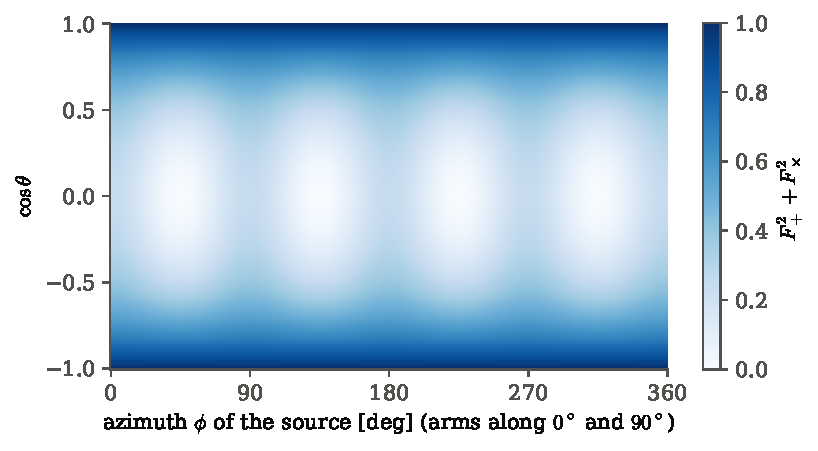
\includegraphics[width=0.78\linewidth]{figures/chT2/antenna_pattern.pdf}
\caption{The sensitivity of a right-angle interferometer over the sky, $F_+^2+F_\times^2$, as a function of the source's azimuth and of the cosine of its polar angle. It is largest above and below the detector ($\cos\theta=\pm1$), and drops to zero at four points in the plane of the arms ($\cos\theta=0$, $\phi=45^\circ$, $135^\circ$, $225^\circ$, $315^\circ$), where the wave stretches both arms equally.}
\label{T2g:fig:antenna}
\end{figure}

\paragraph{Example: a source overhead and a source in the plane of the arms.}
For a source straight overhead, $\theta=0$, \eqref{T2g:eq:Fplus} gives
\begin{align*}
  F_+&\eqby{1}\cos2\phi\cos2\psi-\sin2\phi\sin2\psi\eqby{2}\cos(2\phi+2\psi),\\
  F_\times&\eqby{1}-\cos2\phi\sin2\psi-\sin2\phi\cos2\psi\eqby{2}-\sin(2\phi+2\psi),
\end{align*}
\begin{explain}
  \item $\cos\theta=1$, so $\tfrac12(1+\cos^2\theta)=1$.
  \item The addition rules for $\cos(a+b)$ and $\sin(a+b)$.
\end{explain}
so $F_+^2+F_\times^2=1$ whatever the orientation: overhead, the detector catches the full wave, and turning the polarisation axes only moves the signal from one polarisation to the other. For a source in the plane of the arms, in the direction of the $x$ arm ($\theta=90^\circ$, $\phi=0$), we get $F_+=\tfrac12\cos2\psi$ and $F_\times=-\tfrac12\sin2\psi$, so $F_+^2+F_\times^2=\tfrac14$: the wave travels along the $x$ arm, which it cannot stretch because the wave is transverse, and only the $y$ arm responds, with its weight $\tfrac12$ in the difference \eqref{T2g:eq:michelson}.

\emph{The sky and polarisation average.} For forecasts the source's position and orientation are not known, so the response is averaged over all of them, with the source direction uniform on the sphere and $\psi$ uniform. Take $\langle F_+^2\rangle$ in three steps, one angle at a time:
\begin{align}
  \big\langle F_+^2\big\rangle_\psi
  &\eqby{1}\tfrac12\Big[\tfrac14(1+\cos^2\theta)^2\cos^22\phi+\cos^2\theta\sin^22\phi\Big],\nonumber\\
  \big\langle F_+^2\big\rangle_{\psi,\phi}
  &\eqby{2}\tfrac14\Big[\tfrac14(1+\cos^2\theta)^2+\cos^2\theta\Big],\nonumber\\
  \big\langle F_+^2\big\rangle
  &\eqby{3}\tfrac14\Big[\tfrac14\cdot\tfrac{28}{15}+\tfrac13\Big]=\tfrac14\cdot\tfrac{12}{15}=\tfrac15 .
  \label{T2g:eq:one-fifth}
\end{align}
\begin{explain}
  \item Square \eqref{T2g:eq:Fplus}; over a full turn of $\psi$, $\langle\cos^22\psi\rangle=\langle\sin^22\psi\rangle=\tfrac12$ and $\langle\cos2\psi\sin2\psi\rangle=0$, so the cross term drops.
  \item The same averages over $\phi$.
  \item A direction uniform on the sphere has $x=\cos\theta$ uniform on $[-1,1]$, so $\langle(1+x^2)^2\rangle=\tfrac12\int_{-1}^1(1+2x^2+x^4)\dd x=1+\tfrac13+\tfrac15=\tfrac{28}{15}$ and $\langle x^2\rangle=\tfrac13$.
\end{explain}
The same steps give $\langle F_\times^2\rangle=\tfrac15$, and $\langle F_+F_\times\rangle=0$. This is the $\tfrac15$ of \cite[eq.~(7)]{Robson2019}. The bracket in the second line is the same function $\tfrac14(1+\cos^2)^2+\cos^2$ that described the radiation pattern of a binary in \cref{T2g:sec:quadrupole}: a detector receives from each direction in the same pattern as a rotating quadrupole emits into it, because both are the TT part of a quadrupolar tensor.

\emph{The inclination average.} The source has its own orientation. By \eqref{T2g:eq:hpc} a circular binary at inclination $\iota$ has $h_+=A\tfrac12(1+\cos^2\iota)\cos\Phi$ and $h_\times=A\cos\iota\sin\Phi$ (up to an overall sign), where $\Phi$ is the wave's phase. Averaged over $\psi$, $F_+^2$ and $F_\times^2$ have the same mean and no correlation, so the mean squared signal is $\langle F_+^2\rangle A^2[\tfrac14(1+\cos^2\iota)^2+\cos^2\iota]$, and averaging over orientations of the orbit, $x=\cos\iota$ uniform,
\begin{equation}
  \Big\langle\tfrac14(1+x^2)^2+x^2\Big\rangle_x=\tfrac14\cdot\tfrac{28}{15}+\tfrac13=\tfrac{7}{15}+\tfrac{5}{15}=\tfrac45 .
  \label{T2g:eq:four-fifths}
\end{equation}
This is the $\tfrac45$ in the sky-averaged waveform $\tilde h=\sqrt{4/5}\,\mathcal Af^{-7/6}e^{-i\Psi}$ of \cite[eq.~(44)]{Kim2023} and \cite[eq.~(16)]{Robson2019}, and divided into $16\pi/5$ over $4\pi$ it is the same angular integral that gave the binary's total power. For a ground-based detector the two averages combine to $\tfrac45\cdot\tfrac15=\tfrac4{25}$ in power, $\tfrac25$ in amplitude, the factor quoted in the LIGO literature.

\subsection{LISA at low frequency: \texorpdfstring{$60^\circ$}{60 degree} arms and two channels}

LISA's three spacecraft form an equilateral triangle (\cref{T2a:fig:lisa-triangle}), so two arms meeting at a spacecraft make $60^\circ$, not $90^\circ$. \emph{How much does that cost?} Let $\hat{\bm e}_1$ be the unit vector along the bisector of the two arms and $\hat{\bm e}_2$ the perpendicular one in their plane, so that with $\alpha=60^\circ$ the opening angle,
\begin{align}
  \hat{\bm u}&=\cos\tfrac\alpha2\,\hat{\bm e}_1+\sin\tfrac\alpha2\,\hat{\bm e}_2,\qquad
  \hat{\bm v}=\cos\tfrac\alpha2\,\hat{\bm e}_1-\sin\tfrac\alpha2\,\hat{\bm e}_2,\nonumber\\
  2D=\hat{\bm u}\hat{\bm u}^{\mathsf T}-\hat{\bm v}\hat{\bm v}^{\mathsf T}
  &\eqby{1}2\cos\tfrac\alpha2\sin\tfrac\alpha2\big(\hat{\bm e}_1\hat{\bm e}_2^{\mathsf T}+\hat{\bm e}_2\hat{\bm e}_1^{\mathsf T}\big)
  \eqby{2}\sin\alpha\,\big(\hat{\bm e}_1\hat{\bm e}_2^{\mathsf T}+\hat{\bm e}_2\hat{\bm e}_1^{\mathsf T}\big).
  \label{T2g:eq:sixty}
\end{align}
\begin{explain}
  \item Multiply out: the $\hat{\bm e}_1\hat{\bm e}_1^{\mathsf T}$ and $\hat{\bm e}_2\hat{\bm e}_2^{\mathsf T}$ terms are the same in both and cancel; the mixed terms add.
  \item $2\sin\tfrac\alpha2\cos\tfrac\alpha2=\sin\alpha$.
\end{explain}
For $\alpha=90^\circ$ the bracket is the detector tensor of a right-angle interferometer whose arms lie along $(\hat{\bm e}_1\pm\hat{\bm e}_2)/\sqrt2$. So a $60^\circ$ interferometer is a right-angle interferometer, turned by $45^\circ$ relative to its bisector, with every response multiplied by $\sin60^\circ=\sqrt3/2$: the factor in \cite[eq.~(14)]{BarackCutler2004}. Turning does not change a sky average, so each $60^\circ$ channel has $\langle F_+^2\rangle=\tfrac34\cdot\tfrac15=\tfrac{3}{20}$. The three arms of the triangle provide two such independent channels at low frequency, the second equivalent to the first turned by $45^\circ$ \cite[eqs.~(12), (15b)]{BarackCutler2004}, and the sensitivity-curve literature sums them: $R=2\times\tfrac3{20}=\tfrac3{10}$ \cite[eqs.~(8)--(9)]{Robson2019}. The script \pyname{13_lisa_response.py} checks all of these averages by quadrature over the sky and $\psi$ and finds $\TwFpNinety$ and $\TwFxNinety$ for a right-angle detector, $\TwFpSixty$ for one $60^\circ$ channel, $\TwInclAvg$ for the inclination average and $\TwFluxInt\,\pi$ for the angular integral of the binary's power.

\begin{figure}[htbp]
\centering
\begin{tikzpicture}[scale=1.0]
  \coordinate (A) at (0,0);
  \coordinate (B) at (4.2,0);
  \coordinate (C) at (2.1,3.637);
  \draw[formblue,thick] (A) -- (B) -- (C) -- cycle;
  \foreach \P/\n/\pos in {A/1/north east,B/2/north west,C/3/south}{
    \fill[accent] (\P) circle (3pt);
    \node[lbl,anchor=\pos] at (\P) {S/C\,\n};}
  \node[lbl,anchor=north] at (2.1,-0.1) {$L=2.5\times10^9$\,m};
  \pic[draw,faint,angle radius=0.9cm,"$60^\circ$",angle eccentricity=0.7] {angle=B--A--C};
  \node[lbl,align=left,anchor=west] at (4.6,2.6) {each arm: two one-way\\ laser links between\\ free-falling test masses};
  \node[lbl,align=left,anchor=west] at (4.6,1.0) {three arms give two\\ independent Michelson-type\\ signals at low frequency};
\end{tikzpicture}
\caption{The LISA constellation. Three spacecraft form an equilateral triangle; each side carries laser links in both directions. Two arms meeting at a spacecraft act as a Michelson interferometer whose arms make $60^\circ$ rather than $90^\circ$. At low frequency the three arms carry two independent combinations, written as detectors I and II in \cite[eqs.~(11)--(12)]{BarackCutler2004}.}
\label{T2a:fig:lisa-triangle}
\end{figure}

\subsection{Long arms: the transfer frequency}

LISA's arms are $L=2.5\times10^9$\,m long, and light needs $L/c=8.3$\,s to cross one. A wave of $10$\,mHz has a period of $100$\,s, so it changes noticeably while the light is in flight, and \eqref{T2g:eq:arm}, which froze $h$ during the trip, must be redone.

\emph{The simplest case: a wave arriving perpendicular to the arm.} Then $h_{xx}=h(t)$ is the same at every point of the arm but changes in time. Light reflected at the far end at time $t_m$ left at $t_m-L/c$ and returns at $t_m+L/c$. Following the steps of \eqref{T2g:eq:arm} with $h$ evaluated at the moment the light passes, for $h(t)=h_0\cos2\pi ft$,
\begin{align}
  \delta T_{\rm round}
  &\eqby{1}\frac12\int_{t_m-L/c}^{t_m+L/c}h_0\cos(2\pi ft')\,\dd t'
  \eqby{2}\frac{h_0}{4\pi f}\Big[\sin2\pi f\Big(t_m+\frac Lc\Big)-\sin2\pi f\Big(t_m-\frac Lc\Big)\Big]\nonumber\\
  &\eqby{3}\frac{h_0}{2\pi f}\cos(2\pi ft_m)\,\sin\frac{2\pi fL}{c}
  \eqby{4}\frac{L}{c}\,h(t_m)\,\mathrm{sinc}\Big(\frac{f}{f_*}\Big),
  \qquad f_*\equiv\frac{c}{2\pi L},
  \label{T2g:eq:transfer}
\end{align}
\begin{explain}
  \item Each element $\dd x=c\,\dd t'$ of the path adds $\tfrac12h(t')\,\dd t'$ to the travel time, by step (3) of \eqref{T2g:eq:arm}.
  \item The integral of $\cos$ is $\sin/(2\pi f)$.
  \item $\sin a-\sin b=2\cos\tfrac{a+b}2\sin\tfrac{a-b}2$, with $\tfrac{a+b}2=2\pi ft_m$ and $\tfrac{a-b}2=2\pi fL/c$.
  \item Multiply and divide by $2\pi fL/c=f/f_*$, with $\mathrm{sinc}\,z\equiv\sin z/z$.
\end{explain}
For $f\ll f_*$, $\mathrm{sinc}\to1$ and we are back at $\delta T=(L/c)h$, i.e.\ $\delta L/L=\tfrac12h$. The \newterm{transfer frequency} $f_*$ is where the wave's phase advances by one radian while the light crosses one arm:
\begin{equation}
  f_*=\frac{c}{2\pi L}=\frac{3.0\times10^8\,{\rm m\,s^{-1}}}{2\pi\times2.5\times10^9\,{\rm m}}=19.1\,{\rm mHz}.
\end{equation}
At $f=\pi f_*=c/(2L)=\TwfZero$\,mHz the wave completes exactly one cycle during the round trip, the stretching on the way out is undone by the squeezing on the way back, and the arm sees nothing. Above $f_*$, $\lvert\mathrm{sinc}(f/f_*)\rvert\le f_*/f$, so the response in power falls at least as $(f_*/f)^2$.

\paragraph{Example: how much is lost at 10 and at 100 millihertz.}
At $f=10$\,mHz, $f/f_*=0.52$ and $\mathrm{sinc}(0.52)=\sin(0.52)/0.52=0.497/0.52=0.96$, so the response in power is $0.96^2=0.91$ of its low-frequency value: hardly any loss. At $f=100$\,mHz, $f/f_*=5.24$ and $\mathrm{sinc}(5.24)=\sin(5.24)/5.24=-0.866/5.24=-0.17$, a power response of $0.027$, below the bound $(f_*/f)^2=0.036$. A tenfold rise in frequency has cost a factor thirty in power, which the noise curve of \cref{T2a:sec:lisa} will show as a rising high-frequency wall.

\emph{Any direction.} If the wave travels along $\hat{\bm k}$ and the arm points along $\hat{\bm a}$, the light moving outwards meets the wave at the position $\bm x=\hat{\bm a}\,c(t'-t_0)$, where the wave's phase is $2\pi f(t'-\hat{\bm k}\cdot\bm x/c)=2\pi f[(1-\hat{\bm k}\cdot\hat{\bm a})t'+\text{const}]$. The light rides with the wave if $\hat{\bm k}\cdot\hat{\bm a}=1$ and meets it head on if $-1$, so the phase runs at the Doppler-shifted rate $2\pi f(1-\hat{\bm k}\cdot\hat{\bm a})$ along the outward leg and $2\pi f(1+\hat{\bm k}\cdot\hat{\bm a})$ on the way back. The integral over one leg of duration $L/c$ is therefore
\begin{equation}
  \int_{t_0}^{t_0+L/c}e^{2\pi if(1\mp\hat{\bm k}\cdot\hat{\bm a})t'}\,\dd t'
  =\frac{L}{c}\,e^{2\pi if(1\mp\hat{\bm k}\cdot\hat{\bm a})(t_0+L/2c)}\,
  \mathrm{sinc}\Big[\frac{f}{2f_*}\big(1\mp\hat{\bm k}\cdot\hat{\bm a}\big)\Big],
  \label{T2g:eq:leg}
\end{equation}
the same calculation as \eqref{T2g:eq:transfer} for half the path and a shifted frequency. Putting both legs of both arms into \eqref{T2g:eq:michelson} gives the frequency-dependent $F_+(f)$ and $F_\times(f)$ of a LISA channel. The script averages $\lvert F_+(f)\rvert^2$ over the sky and polarisation for one $60^\circ$ Michelson and doubles it for the two channels:

\pyfile[firstline=95,lastline=121,firstnumber=95]{code/chT2/13_lisa_response.py}{The light-travel integrals of one arm, and the sky-averaged response}

\noindent The function \pyname{leg} is \eqref{T2g:eq:leg} with the light time $L/c$ set to one, so that $2\pi f=f/f_*$. \pyname{arm_transfer} adds the outward and return legs and divides by the round-trip time, so it tends to one at low frequency. The loop forms $F_+(f)$ for each sky direction and polarisation angle and averages its squared modulus with the quadrature weights \pyname{W}.

\begin{figure}[htbp]
\centering
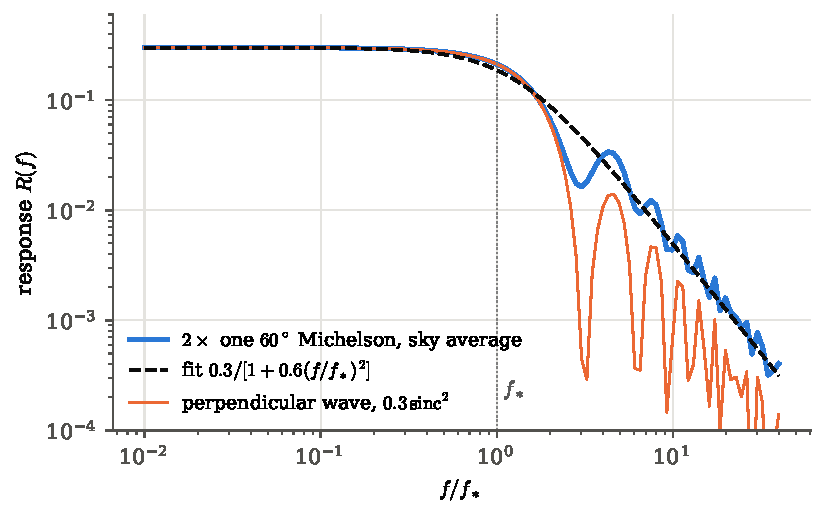
\includegraphics[width=0.8\linewidth]{figures/chT2/lisa_response.pdf}
\caption{The sky- and polarisation-averaged response of LISA against frequency in units of $f_*=c/(2\pi L)$. Blue: computed from the light-travel integrals \eqref{T2g:eq:leg} for one $60^\circ$ Michelson channel and doubled for two channels. Dashed: the fit of Robson et al. Orange: a wave arriving perpendicular to the arms, whose response $\mathrm{sinc}^2(f/f_*)$ vanishes whenever a whole number of cycles fits into the round trip. Averaging over directions fills in those zeros, but the $f^{-2}$ fall above $f_*$ remains.}
\label{T2g:fig:response}
\end{figure}

\Cref{T2g:fig:response} shows the result. At low frequency it is $\TwRzero$, the $\tfrac3{10}$ found above. At $f_*$ it has dropped to $\TwRstarRatio$ of that (the fit $R(f)=\tfrac3{10}/[1+0.6(f/f_*)^2]$ of \cite[eq.~(9)]{Robson2019} gives $0.625$), and well above $f_*$ it falls as $f^{\TwRslope}$, the $f^{-2}$ of the single-arm argument. Between about $2f_*$ and $10f_*$ our single-Michelson response wiggles around the fit by up to $\TwRfitDev\%$: these are the zeros of the individual arm responses, partly filled in by the sky average. The fit smooths them over, and the full response used in research analyses adds the third, high-frequency channel of the triangle \cite{Robson2019}.

\begin{keyidea}[The numbers that turn a source into an average source]
A detector reports $h=F_+h_++F_\times h_\times$. Averaged over the sky and the polarisation angle, a right-angle interferometer has $\langle F_+^2\rangle=\langle F_\times^2\rangle=\tfrac15$; a $60^\circ$ channel has $\tfrac34$ of that, $\tfrac3{20}$, and LISA's two channels together $\tfrac3{10}$. Averaging a circular binary over its inclination multiplies the signal power by $\tfrac45$. Above the transfer frequency $f_*=c/(2\pi L)$ the wave changes while the light is in flight and the response falls as $f^{-2}$.
\end{keyidea}

\paragraph{What the sky average leaves out.}
LISA orbits the Sun, so a source's signal is Doppler shifted back and forth over a year, and the triangle rotates, so the antenna patterns \eqref{T2g:eq:Fplus} change slowly with time \cite[eqs.~(16)--(17)]{BarackCutler2004}. The phase is modulated by $2\pi fR\sin\theta_S\cos(2\pi t/{\rm yr}-\phi_S)$, with $R=1\,{\rm AU}/c=499$\,s and $(\theta_S,\phi_S)$ the source's sky position \cite[eq.~(33)]{BarackCutler2004}. At $f=10$\,mHz the amplitude of this modulation is $2\pi\times0.01\times499\approx31$\,rad, so it is easily measured, and it is how LISA locates sources on the sky. The sky-averaged response drops that information and replaces the real, moving detector by an average one. For forecasts of an environment, which acts on the phase evolution and not on the sky position, the averaged response is adequate, and the signal-to-noise ratios it gives are good to a factor of about two \cite{Robson2019}.

\paragraph{Where this is used.}
The response rule \eqref{T2g:eq:response} is what turns a template into the predicted data stream in the detection problem of \cref{10b:sec:detection}. The averages $\tfrac45$ and $\tfrac3{10}$ are the ones built into the sky-averaged waveform and the sensitivity curve of \cref{T2a:sec:lisa}, which \cref{10b:sec:robson} checks against its source; $f_*$ and the high-frequency fall of the response set the shape of that curve above about $20$\,mHz.
\section{Why a compact binary chirps}
\label{T2a:sec:chirp}

Take two black holes, masses $m_1$ and $m_2$, on a circular orbit of radius $r$. \Cref{T2g:sec:quadrupole} showed that the pair radiates gravitational waves at twice its orbital frequency, with the power $P_{\rm GW}=\tfrac{32}{5}(G/c^5)\mu^2r^4\omega^6$ of \eqref{T2g:eq:power-binary}, and the energy flux of \cref{T2g:sec:energy} says that this power is real energy leaving the system. The pair therefore has less and less orbital energy, so it must sit deeper in its own potential well, on a smaller orbit. A smaller orbit is a faster orbit, and since $P_{\rm GW}\propto r^4\omega^6\propto r^{-5}$, a faster orbit radiates far more strongly. The process runs away: the orbit shrinks ever faster, and the frequency of the wave rises ever faster until the holes merge. Played as sound, the signal is a rising whistle, a \newterm{chirp}.

Every statistics calculation with such a signal starts from one question: \emph{given the two masses and the frequency $f$ of the wave we see today, how fast is $f$ rising, and how long is left before the merger?} The answer is a single formula for $\dot f$. The time to merger, the number of cycles, the phase of the wave and the end of the inspiral all follow from it.

\subsection{The inputs}

As with the Poisson process of \cref{ch:02}, we first separate what goes in from what comes out. Four things go in, and only the first two are new.
\begin{enumerate}[itemsep=1pt]
  \item \emph{Physical: Newtonian circular orbits.} The two bodies obey Newton's gravity and move on a circle. The two-body problem reduces, as usual, to one body of reduced mass $\mu=m_1m_2/M$ circling a fixed mass $M=m_1+m_2$, with Kepler's third law $\omega^2=GM/r^3$ for the orbital angular frequency $\omega$.
  \item \emph{Physical: slow evolution.} One orbit takes much less time than the orbit takes to shrink noticeably. So at each moment the orbit is a circle of the current radius, and the orbital energy simply drains into the waves, $\dd E/\dd t=-P_{\rm GW}$. We check this with numbers at the end of the section.
  \item \emph{Derived earlier: the radiated power} $P_{\rm GW}=\tfrac{32}{5}(G/c^5)\mu^2r^4\omega^6$ of \eqref{T2g:eq:power-binary}, which came from the linearised field equation and the energy flux in \cref{T2g:sec:quadrupole}, and the wave frequency $f=\omega/\pi$ of \eqref{T2g:eq:twice}.
  \item \emph{Mathematical:} $r(t)$ is smooth, so we may differentiate it.
\end{enumerate}
That only one combination of the masses matters is \emph{not} an input; it comes out of the derivation.

\subsection{From the radiated power to the chirp}

\paragraph{Energy and power as functions of the wave frequency.}
The frequency is what the detector measures, so we trade $r$ for $f$ using Kepler, $r=(GM/\omega^2)^{1/3}$ with $\omega=\pi f$:
\begin{align}
  E&\eqby{1}-\frac{GM\mu}{2r}\eqby{2}-\frac{\mu}{2}\,(\pi GMf)^{2/3},\label{T2a:eq:Ef}\\
  P_{\rm GW}&\eqby{3}\frac{32}{5}\frac{G}{c^5}\,\mu^2(GM)^{4/3}(\pi f)^{10/3}
  \eqby{4}\frac{32}{5}\frac{c^5}{G}\Big(\frac{\pi G\mathcal M f}{c^3}\Big)^{10/3},
  \qquad \mathcal M\equiv\mu^{3/5}M^{2/5}=\frac{(m_1m_2)^{3/5}}{(m_1+m_2)^{1/5}} .\label{T2a:eq:Pf}
\end{align}
\begin{explain}
  \item Kinetic plus potential energy of a circular orbit: $\tfrac12\mu v^2-GM\mu/r$ with $v^2=GM/r$.
  \item $1/r=(\omega^2/GM)^{1/3}$, so $GM/r=(GM)^{2/3}\omega^{2/3}$.
  \item $r^4\omega^6=(GM)^{4/3}\omega^{-8/3}\omega^6=(GM)^{4/3}\omega^{10/3}$.
  \item Collect the masses: $\mu^2M^{4/3}=(\mu^{3/5}M^{2/5})^{10/3}$, and the powers of $G$ and $c$ rearrange as $G^{7/3}/c^5=(c^5/G)(G/c^3)^{10/3}$.
\end{explain}
The combination $\mathcal M$ is the chirp mass of \eqref{T2g:eq:amp}: it appeared there in the amplitude of the wave and appears here again, on its own, in step (4).

\paragraph{The chirp rate.}
Energy balance says $\dd E/\dd t=-P_{\rm GW}$. Since $E$ depends on time only through $f$, $\dd E/\dd t=(\dd E/\dd f)\,\dot f$, so
\begin{align}
  \dot f&\eqby{1}\frac{P_{\rm GW}}{\lvert\dd E/\dd f\rvert}
  \eqby{2}\frac{\tfrac{32}{5}\tfrac{G^{7/3}}{c^5}\mu^2M^{4/3}(\pi f)^{10/3}}{\tfrac{\mu}{3}(\pi GM)^{2/3}f^{-1/3}}
  \eqby{3}\frac{96}{5}\,\pi^{8/3}\Big(\frac{G\mathcal M}{c^3}\Big)^{5/3}f^{11/3}.\label{T2a:eq:fdot}
\end{align}
\begin{explain}
  \item Energy balance, with $\dd E/\dd f<0$ (a higher frequency is a more bound orbit).
  \item $P_{\rm GW}$ from step (3) of \eqref{T2a:eq:Pf}; $\dd E/\dd f=-\tfrac{\mu}{3}(\pi GM)^{2/3}f^{-1/3}$ from \eqref{T2a:eq:Ef}.
  \item One $\mu$ cancels; $\mu M^{4/3}/M^{2/3}=\mu M^{2/3}=\mathcal M^{5/3}$, $G^{7/3}/G^{2/3}=G^{5/3}$ so $G^{5/3}/c^5=(G/c^3)^{5/3}$, and $\pi^{10/3}/\pi^{2/3}\cdot f^{10/3}f^{1/3}=\pi^{8/3}f^{11/3}$.
\end{explain}

\begin{keyidea}[The Newtonian chirp]
A circular binary radiating quadrupole waves sweeps up in frequency at the rate
$\dot f=\frac{96}{5}\pi^{8/3}(G\mathcal M/c^3)^{5/3}f^{11/3}$. At this order the masses enter only through the chirp mass $\mathcal M=(m_1m_2)^{3/5}/(m_1+m_2)^{1/5}$, so the data measure $\mathcal M$ first and the separate masses only through smaller corrections.
\end{keyidea}

The product $G\mathcal M/c^3$ has units of time. For the Sun it is $GM_\odot/c^3=4.93\,\mu$s, which is the handiest number in gravitational-wave astronomy: a mass in solar units times $4.93\,\mu$s is that mass as a time.

\paragraph{Frequency against time, and the number of cycles.}
Since $\dd t=\dd f/\dot f$, the time left before the frequency runs off to infinity (the formal coalescence time $t_c$) is
\begin{align}
  \tau(f)\equiv t_c-t
  &\eqby{1}\int_f^\infty\frac{\dd f'}{\dot f(f')}
  \eqby{2}\frac{5}{96}\pi^{-8/3}\Big(\frac{G\mathcal M}{c^3}\Big)^{-5/3}\cdot\frac38 f^{-8/3}
  =\frac{5}{256}\Big(\frac{G\mathcal M}{c^3}\Big)^{-5/3}(\pi f)^{-8/3},\label{T2a:eq:tau}
\end{align}
\begin{explain}
  \item Time is the integral of $\dd f/\dot f$ along the sweep.
  \item $\int_f^\infty f'^{-11/3}\dd f'=\tfrac38 f^{-8/3}$; then $\tfrac{5}{96}\cdot\tfrac38=\tfrac{5}{256}$ and $\pi^{-8/3}f^{-8/3}=(\pi f)^{-8/3}$.
\end{explain}
and inverting, $f(\tau)=\frac{1}{8\pi}\big(G\mathcal M/c^3\big)^{-5/8}\big(5/\tau\big)^{3/8}$ \cite[eq.~(24)]{Robson2019}. The number of wave cycles between $f_1$ and $f_2$ is $N=\int f\,\dd t=\int f\,\dd f/\dot f$:
\begin{equation}
  N(f_1,f_2)=\frac{1}{32\pi^{8/3}}\Big(\frac{G\mathcal M}{c^3}\Big)^{-5/3}\big(f_1^{-5/3}-f_2^{-5/3}\big),
  \label{T2a:eq:Ncyc}
\end{equation}
from $\int f^{-8/3}\dd f=-\tfrac35f^{-5/3}$ and $\tfrac35\cdot\tfrac{5}{96}=\tfrac1{32}$. The low-frequency end dominates: most cycles are spent where the binary is slow.

\paragraph{Where the inspiral ends.}
In Newton's theory circular orbits exist all the way down. In general relativity they stop being stable inside the \newterm{innermost stable circular orbit} (ISCO), $r_{\rm ISCO}=6GM/c^2$, three Schwarzschild radii; inside it the small body plunges. Kepler's law there gives $\omega^2=c^6/(216\,G^2M^2)$, so
\begin{equation}
  f_{\rm ISCO}=\frac{c^3}{6^{3/2}\pi GM}\approx 4.4\,\mathrm{kHz}\times\frac{M_\odot}{M}.
  \label{T2a:eq:fisco}
\end{equation}
Papers on dark-matter environments stop their inspirals here \cite{Eda2015,Kim2023}, and so do we.

\begin{figure}[htbp]
\centering
\begin{tikzpicture}[scale=1.0]
  \draw[formblue,thick,domain=0:18.4,samples=600,smooth,variable=\t]
    plot ({2.4*((18.85-\t)/18.85)^(0.4)*cos(\t r)},{2.4*((18.85-\t)/18.85)^(0.4)*sin(\t r)});
  \fill[black] (0,0) circle (2.2pt);
  \fill[fibreorange] (2.4,0) circle (1.6pt);
  \node[lbl,anchor=west] at (2.5,0) {$m_2$ (start)};
  \foreach \R in {3.0,3.4,3.8}{\draw[faint] (15:\R) arc (15:45:\R);}
  \node[lbl,align=left,anchor=west] at (1.2,3.4) {energy carried\\ off by waves};
  \begin{scope}[xshift=5.4cm,yshift=-1.6cm]
    \draw[->] (0,0) -- (5.6,0);
    \node[lbl,below] at (2.5,0) {time $t$};
    \draw[->] (0,0) -- (0,3.4) node[left,lbl] {$f$};
    \draw[formblue,thick,domain=0:4.95,samples=200,smooth] plot (\x,{0.45*((5-0)/(5-\x))^(0.375)});
    \draw[faint,dashed] (5,0) -- (5,3.3);
    \node[lbl,below] at (5,0) {$t_c$};
    \node[lbl,anchor=west,align=left] at (0.3,2.6) {$f\propto (t_c-t)^{-3/8}$};
  \end{scope}
\end{tikzpicture}
\caption{The chirp. Left: the light body's path around the heavy one (dot) for a Newtonian inspiral, the last three turns, drawn to scale in shape ($r\propto(\phi_c-\phi)^{2/5}$, which follows from $r\propto\tau^{1/4}$ and $\phi\propto\tau^{5/8}$); each turn is tighter and quicker than the last. Right: the wave frequency of \eqref{T2a:eq:tau} inverted, rising slowly for a long time and then very fast just before $t_c$.}
\label{T2a:fig:chirp-cartoon}
\end{figure}

\subsection{The phase of the wave, and the two numbers that fix it}
\label{T2g:sec:tc-phic}

The detector does not record the frequency; it records the wave, $h(t)=A(t)\cos\phi(t)$ for one polarisation, with the amplitude $A\propto f^{2/3}$ of \eqref{T2g:eq:amp} and a phase $\phi(t)$ whose rate of change is the angular frequency, $\dot\phi=2\pi f$. So the phase is the integral of the frequency history. Write $T_{\mathcal M}\equiv G\mathcal M/c^3$, the chirp mass as a time, and $\tau=t_c-t$. The inverse of \eqref{T2a:eq:tau} is $2\pi f(\tau)=\tfrac14T_{\mathcal M}^{-5/8}5^{3/8}\tau^{-3/8}$, and since $\dd\tau=-\dd t$,
\begin{align}
  \phi(t)
  &\eqby{1}\phi_c-\int_0^{\tau}2\pi f(\tau')\,\dd\tau'
  \eqby{2}\phi_c-\tfrac14T_{\mathcal M}^{-5/8}5^{3/8}\cdot\tfrac85\,\tau^{5/8}
  \eqby{3}\phi_c-2\Big(\frac{\tau}{5T_{\mathcal M}}\Big)^{5/8},
  \label{T2g:eq:phit}
\end{align}
\begin{explain}
  \item The phase grows by $2\pi f\,\dd t$ in each moment. Integrating backwards from the end, where it reaches the value $\phi_c$, the phase at time $t$ is $\phi_c$ minus everything still to come.
  \item $\int_0^\tau\tau'^{-3/8}\dd\tau'=\tfrac85\tau^{5/8}$.
  \item $\tfrac14\cdot\tfrac85\cdot5^{3/8}=\tfrac25\cdot5^{3/8}=2\cdot5^{-5/8}$, and $5^{-5/8}T_{\mathcal M}^{-5/8}\tau^{5/8}=(\tau/5T_{\mathcal M})^{5/8}$.
\end{explain}
which is \cite[eq.~(17)]{CutlerFlanagan1994}. Two integration constants appeared on the way, and both are now parameters of the signal.

\emph{The time of coalescence $t_c$} is the moment at which the Newtonian frequency \eqref{T2a:eq:tau} would formally run off to infinity. The real inspiral ends a little earlier, at the ISCO, but $t_c$ is a convenient label for ``when it all happens''. Changing $t_c$ by $\Delta$ slides the whole signal along the time axis, $h(t)\to h(t-\Delta)$, without changing its shape.

\emph{The phase at coalescence $\phi_c$} is the value of the phase at $t_c$. Since the wave phase is twice the orbital phase, changing $\phi_c$ by $\delta$ is the same as having started the two bodies at a different place on their orbit, turned by $\delta/2$ about the orbital axis. It does not change $t_c$, the masses or the frequency history; it only shifts the crests of the wave.

\emph{Why they are nuisance parameters.} Neither number says anything about the physics of the source. $t_c$ records when, on our clocks, the binary happened to merge; $\phi_c$ records where the two bodies happened to be on their orbit at that moment. Both are pure accident, both are unknown before the data arrive, and both must nevertheless be in the template: a template whose crests sit half a cycle away from the signal's crests correlates with it negatively, however right its masses. In the language of \cref{ch:05} they are \newterm{nuisance parameters}, unknowns we must fit or integrate over but do not care about. \Cref{10b:sec:phase-time} shows that both can be searched over almost for free, the phase with two filters and the arrival time with one Fourier transform, and \cref{T2a:sec:spa} shows why: in the frequency domain they enter the phase only as the straight line $2\pi ft_c-\phi_c$.

\subsection{Examples: the benchmark binaries of the book}

Two systems recur in the dark-matter literature and in \cref{ch:10}. In both, a light black hole falls into a much heavier one. Binaries are named by their mass ratio $q=m_2/m_1$: comparable-mass binaries have $q\sim1$, \newterm{intermediate mass-ratio inspirals} (IMRIs) roughly $q\sim10^{-2}$--$10^{-4}$, and \newterm{extreme mass-ratio inspirals} (EMRIs) $q\lesssim10^{-4}$; the boundary is a convention, and papers place it differently \cite{Speeney2022,Kim2023}. A small $q$ is what makes these systems good probes. By \eqref{T2a:eq:fdot}, $\dot f\propto\mathcal M^{5/3}\approx m_2\,m_1^{2/3}$ when $m_2\ll m_1$, so a light companion spirals in slowly and completes a huge number of orbits inside the environment.

\paragraph{The numbers.}
Every number quoted in the examples below comes from a few lines of \pyname{01_chirp.py}, which apply \eqref{T2a:eq:fisco}, \eqref{T2a:eq:tau}, \eqref{T2a:eq:Ncyc} and \eqref{T2a:eq:fdot} to a pair of masses:

\pyfile[firstline=28,lastline=33,firstnumber=28]{code/chT2/01_chirp.py}{From two masses to the end of the inspiral}

\noindent Line 29 is the ISCO frequency. Line 30 is the time left at that frequency, \eqref{T2a:eq:tau}. Line 31 adds four years to that time and inverts, giving the frequency four years before the ISCO. Line 32 counts the cycles between the two frequencies, and line 33 is the slow-evolution number checked in the last example. The helper functions (\pyname{tau_of_f}, \pyname{cycles}, and so on) sit in \pyname{lib_lisa.py} and are one-line transcriptions of the equations above.

\paragraph{Example: the EMRI of Kim et al.}
A $1\,M_\odot$ black hole falls into a $10^4\,M_\odot$ one \cite[Sec.~III F]{Kim2023}. Kim et al.\ call it an IMRI; with $q=10^{-4}$ it sits on the boundary, and we call it the EMRI. The chirp mass is
\[
  \mathcal M=\frac{(10^4\cdot1)^{3/5}}{(10^4+1)^{1/5}}\approx\frac{10^{2.4}}{10^{0.8}}=10^{1.6}\approx 40\,M_\odot,
\]
and the code gives $\mathcal M=\TwEmriMc\,M_\odot$. By \eqref{T2a:eq:fisco} the inspiral ends at $f_{\rm ISCO}=4.4\,\mathrm{kHz}/10^4\approx\TwEmrifisco$\,Hz, inside the LISA band ($10^{-4}$--$1$\,Hz). Four years earlier, from \eqref{T2a:eq:tau}, the frequency was $\TwEmriffouryr$\,mHz, and by \eqref{T2a:eq:Ncyc} the binary completes $N=\TwEmriNcyc$ wave cycles in those four years.

\paragraph{Example: the IMRI of Eda et al.\ and Coogan et al.}
A $1.4\,M_\odot$ object falls into a $10^3\,M_\odot$ black hole \cite{Eda2015,Coogan2022}. Now $\mathcal M=\TwImriMc\,M_\odot$ and $f_{\rm ISCO}=\TwImrifisco$\,Hz, above LISA's band: the last stretch of this inspiral is invisible to LISA. Four years before the ISCO the frequency is $\TwImriffouryr$\,mHz, and $N=\TwImriNcyc$ cycles follow. \Cref{T2a:fig:chirp-tracks} shows both frequency tracks.

\begin{figure}[htbp]
\centering
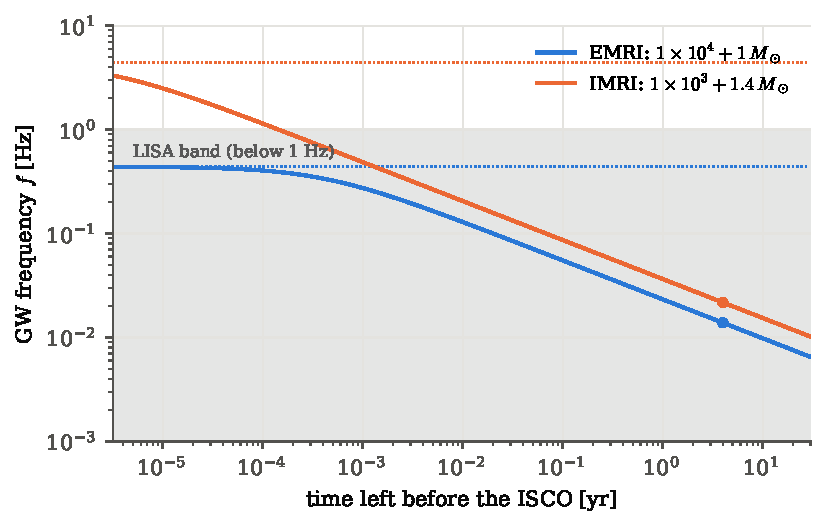
\includegraphics[width=0.82\linewidth]{figures/chT2/chirp_tracks.pdf}
\caption{Frequency against the time left before the ISCO for the two benchmark binaries. Far from the end both tracks are straight lines of slope $-3/8$ on these log axes; close to the end they flatten onto $f_{\rm ISCO}$ (dotted). Dots mark the frequency four years before the ISCO. The shaded band is LISA's frequency range: the IMRI leaves it before its ISCO, the EMRI does not.}
\label{T2a:fig:chirp-tracks}
\end{figure}

\paragraph{Example: a GW150914-like binary passing through the LISA band.}
Robson, Cornish and Liu note that a binary like the first LIGO detection, five years before merger, sweeps from $16$ to $29$\,mHz during a four-year mission \cite[Sec.~2]{Robson2019}. We can check this with \eqref{T2a:eq:tau}. Take $m_1=36$, $m_2=29\,M_\odot$, so $\mathcal M=\TwGWMc\,M_\odot$ and $G\mathcal M/c^3=28.1\times4.93\,\mu{\rm s}=1.38\times10^{-4}$\,s. Five years before merger, $\tau=1.58\times10^8$\,s, and
\begin{align*}
  f&\eqby{1}\frac{1}{8\pi\,G\mathcal M/c^3}\Big(\frac{5\,G\mathcal M/c^3}{\tau}\Big)^{3/8}
  \eqby{2}\frac{1}{3.47\times10^{-3}\,{\rm s}}\big(4.37\times10^{-12}\big)^{3/8}\\
  &\eqby{3}288\,{\rm Hz}\times5.5\times10^{-5}\approx16\,{\rm mHz}.
\end{align*}
\begin{explain}
  \item The inverse of \eqref{T2a:eq:tau}.
  \item $8\pi\times1.38\times10^{-4}=3.47\times10^{-3}$ and $5\times1.38\times10^{-4}/1.58\times10^8=4.37\times10^{-12}$.
  \item $(4.37\times10^{-12})^{3/8}=10^{-11.36\times3/8}=10^{-4.26}$.
\end{explain}
The same steps with $\tau=1$\,yr give $29$\,mHz. The code returns $\TwGWfFive$ and $\TwGWfOne$\,mHz, and the binary completes $\TwGWNcyc$ cycles in between.

\paragraph{Example: checking the slow-evolution input.}
Input 2 assumed the orbit barely changes during one cycle. The fractional change of $f$ during one cycle (duration $1/f$) is $\dot f/f^2=\frac{96}{5}\pi^{8/3}(G\mathcal Mf/c^3)^{5/3}$, largest at the ISCO. The code gives $\TwEmriadiab$ for the EMRI and $\TwImriadiab$ for the IMRI. Even on the last orbit the frequency changes by less than a part in a thousand per cycle, so treating the orbit as a slowly shrinking circle is safe \cite[eq.~(25)]{CutlerFlanagan1994}.

\paragraph{What a million cycles buys.}
A template that drifts out of step with the signal by a single cycle, out of millions, no longer matches it. So the data pin down whatever sets the number of cycles very precisely \cite[Sec.~I]{CutlerFlanagan1994}. By \eqref{T2a:eq:Ncyc}, $N\propto\mathcal M^{-5/3}$, so a fractional change $\delta\mathcal M/\mathcal M$ shifts the count by $\delta N=\frac53N\,\delta\mathcal M/\mathcal M$. Requiring $\delta N\lesssim1$ gives $\delta\mathcal M/\mathcal M\lesssim3/(5N)$, of order $10^{-7}$ for the EMRI. This is only a rough estimate: noise, a finite signal-to-noise ratio and correlations with other parameters weaken it, and the Fisher matrix of \cref{ch:10} does the calculation properly. For this EMRI with five years of data and signal-to-noise ratio $15$, Kim et al.\ find $\mathcal M=39.8^{+0.0012}_{-0.0006}\,M_\odot$ (95\% range), a fractional error of about $2\times10^{-5}$ \cite[Fig.~4]{Kim2023}. The parameters that only set the amplitude, such as the distance, are measured with fractional errors of order one over the signal-to-noise ratio. This difference is the reason an environment is detectable at all: it acts on the phase, the most precisely measured part of the signal.

\begin{pitfall}[Which mass is measured]
The wave reaches us stretched by the cosmological redshift $z$, and a stretched chirp from mass $\mathcal M$ is indistinguishable from an unstretched chirp from mass $(1+z)\mathcal M$. The data measure the \emph{detector-frame} (redshifted) chirp mass $(1+z)\mathcal M$, and \eqref{T2a:eq:fdot}--\eqref{T2a:eq:fisco} must be used with it \cite[Sec.~2]{Robson2019}. For the nearby benchmark binaries $z\ll1$ and the difference is negligible.
\end{pitfall}

\paragraph{Where this is used.}
The chirp rate \eqref{T2a:eq:fdot} and the binding energy \eqref{T2a:eq:Ef} are the vacuum baseline that \cref{10b:sec:env-derive} perturbs when an environment drains extra energy; the frequency four years before the ISCO and the cycle counts fix the band and the benchmark source of \cref{10b:sec:benchmark}; and $t_c$, $\phi_c$ are the two nuisance parameters that \cref{10b:sec:phase-time} maximises over and that the Fisher matrix of \cref{10b:sec:fisher} carries alongside the masses.
\section{The chirp in the frequency domain}
\label{T2a:sec:spa}

The detector records a time series, but the likelihood of \cref{10b:sec:noise-fd} is written in the frequency domain. There the stationary noise of the detector is simple: different Fourier components are independent, each with a variance set by the noise spectrum $S_n(f)$, and the log-likelihood is $-\tfrac12(d-h\,|\,d-h)$ with the noise-weighted inner product $(a\,|\,b)=4\,\mathrm{Re}\int_0^\infty\tilde a\tilde b^*/S_n\,\dd f$. So the statistics needs the Fourier transform of the chirp of \cref{T2a:sec:chirp}, as a formula in which the masses, the arrival time $t_c$ and the phase $\phi_c$ appear explicitly.

A chirp makes this easy. At each moment it has one frequency, and it passes through each frequency once. So we ask in words: \emph{which part of the time series builds the Fourier component at frequency $f$?} The answer is: essentially only the stretch during which the chirp's own frequency is close to $f$. At all other times the chirp and the probe wave $e^{-2\pi ift}$ run at different rates, their product oscillates, and the oscillations cancel in the integral. Only near the moment $t_f$ at which the chirp's frequency equals $f$ do the two stay in step long enough to add up. Turning this sentence into a formula is the \newterm{stationary-phase approximation} (SPA) \cite[eq.~(21)]{CutlerFlanagan1994}.

\subsection{The Fourier convention, and why only positive frequencies count}

The book's convention, used in every chapter, is
\begin{equation}
  \tilde h(f)=\int_{-\infty}^{\infty}h(t)\,e^{-2\pi ift}\,\dd t,\qquad
  h(t)=\int_{-\infty}^{\infty}\tilde h(f)\,e^{2\pi ift}\,\dd f ,
  \label{T2g:eq:fourier}
\end{equation}
with $f$ in cycles per second, so that no factors of $2\pi$ stand in front of the integrals. A detector output is a real number at every instant, and that fixes the negative frequencies in terms of the positive ones:
\begin{equation}
  \tilde h(-f)\eqby{1}\int h(t)\,e^{+2\pi ift}\,\dd t\eqby{2}\Big[\int h(t)\,e^{-2\pi ift}\,\dd t\Big]^*\eqby{3}\tilde h(f)^* .
  \label{T2g:eq:reality}
\end{equation}
\begin{explain}
  \item The definition at $-f$.
  \item $h(t)$ is real, so complex-conjugating the integrand only flips the sign in the exponent.
  \item The definition at $+f$.
\end{explain}
For example, the tone $\cos2\pi f_0t=\tfrac12e^{2\pi if_0t}+\tfrac12e^{-2\pi if_0t}$ has $\tilde h(f)=\tfrac12\delta(f-f_0)+\tfrac12\delta(f+f_0)$: half its weight sits at $+f_0$ and half, the complex conjugate, at $-f_0$. Since the negative half carries no new information, every quantity built from a real signal can be written with $f>0$ only, at the price of a factor two. That is where the $4$ in the inner product comes from: the $2$ of the one-sided noise spectrum of \cref{10b:sec:noise-fd} times the $2$ from folding $-f$ onto $+f$. So it is enough to know $\tilde h(f)$ for $f>0$.

\begin{figure}[htbp]
\centering
\begin{tikzpicture}
\begin{axis}[width=11cm,height=4.2cm,axis x line=middle,axis y line=none,xmin=-4.2,xmax=4.4,ymin=-1.35,ymax=1.5,
  xtick=\empty,ytick=\empty,xlabel={$t$},xlabel style={anchor=west},
  clip=false]
  \fill[formblue!10] (axis cs:-0.58,-1.25) rectangle (axis cs:0.58,1.25);
  \addplot[formblue,thick,domain=-4:4,samples=900] {cos(deg(3*x^2))};
  \draw[faint] (axis cs:0,-0.08) -- (axis cs:0,0.08);
  \node[lbl,anchor=north] at (axis cs:0,-0.1) {$t_f$};
  \node[lbl,anchor=south] at (axis cs:0,1.25) {in step: adds up};
  \node[lbl,anchor=south] at (axis cs:-2.9,1.1) {out of step: cancels};
  \node[lbl,anchor=south] at (axis cs:2.9,1.1) {out of step: cancels};
\end{axis}
\end{tikzpicture}
\caption{The real part of the integrand $e^{i[\phi(t)-2\pi ft]}$ near the moment $t_f$ at which the chirp has frequency $f$, for a chirp whose frequency rises linearly: the phase difference grows like $(t-t_f)^2$. In the shaded window, of width about $1/\sqrt{\dot f}$, the integrand barely turns and its contributions add. Outside, positive and negative lobes alternate faster and faster and cancel.}
\label{T2a:fig:spa-picture}
\end{figure}

\subsection{The stationary-phase formula}

\emph{Inputs.} The signal is $h(t)=A(t)\cos\phi(t)$, with an amplitude that changes slowly compared with the phase ($\dot A/A\ll\dot\phi$) and a frequency $\dot\phi/2\pi$ that changes slowly, $\ddot\phi\ll\dot\phi^2$. The second condition is $\dot f/f^2\ll1$, the slow-evolution number already checked in \cref{T2a:sec:chirp}. We want $\tilde h(f)$ for $f>0$.

\emph{Two exponentials.} Writing the cosine as $\cos\phi=\tfrac12(e^{i\phi}+e^{-i\phi})$,
\begin{equation}
  \tilde h(f)=\frac12\int A(t)\,e^{i[\phi(t)-2\pi ft]}\,\dd t+\frac12\int A(t)\,e^{-i[\phi(t)+2\pi ft]}\,\dd t .
  \label{T2g:eq:two-exp}
\end{equation}
\emph{The second integral is negligible.} Its phase $\phi(t)+2\pi ft$ always grows, at the rate $\dot\phi+2\pi f\ge2\pi f$, so its integrand turns steadily and its positive and negative lobes cancel. Integrating by parts once shows how well: $\int Ae^{i\theta}\dd t=[Ae^{i\theta}/(i\dot\theta)]-\int(\dd/\dd t)(A/i\dot\theta)\,e^{i\theta}\dd t$, so the integral is of order $A/(2\pi f)$, the amplitude times the time the integrand needs to turn once. We will see that the first integral is of order $A/\sqrt{\dot f}$; the ratio is $\sqrt{\dot f}/f=(\dot f/f^2)^{1/2}\ll1$.

\emph{Where the first integral comes from.} Call its phase $\vartheta(t)\equiv\phi(t)-2\pi ft$. It is \emph{stationary}, $\dot\vartheta=0$, where $\dot\phi=2\pi f$: at the moment $t_f$ when the chirp's own frequency equals $f$. Near that moment Taylor-expand, $\vartheta(t)=\vartheta(t_f)+0\cdot(t-t_f)+\tfrac12\ddot\phi(t_f)(t-t_f)^2+\dots$, the linear term vanishing by the definition of $t_f$, and freeze the slowly varying amplitude at $A(t_f)$. Then
\begin{align}
  \tilde h(f)
  &\eqby{1}\frac12A(t_f)\,e^{i\vartheta(t_f)}\int_{-\infty}^{\infty}e^{\frac i2\ddot\phi(t_f)\,s^2}\,\dd s
  \eqby{2}\frac12A(t_f)\,e^{i\vartheta(t_f)}\sqrt{\frac{2\pi}{\ddot\phi(t_f)}}\;e^{i\pi/4}\nonumber\\
  &\eqby{3}\frac12A(t_f)\,\dot f(t_f)^{-1/2}\,e^{-i\Psi(f)},\qquad
  \Psi(f)\equiv2\pi ft_f-\phi(t_f)-\frac\pi4 .\label{T2a:eq:spa}
\end{align}
\begin{explain}
  \item The expansion with $s=t-t_f$. The limits can be taken to $\pm\infty$, because far from $t_f$ the integrand oscillates ever faster and contributes nothing more (\cref{T2a:fig:spa-picture}).
  \item The Fresnel integral, derived just below: $\int e^{ias^2/2}\dd s=\sqrt{2\pi/a}\,e^{i\pi/4}$ for $a>0$, here with $a=\ddot\phi(t_f)>0$ because the frequency rises.
  \item $\ddot\phi=2\pi\dot f$, so $\sqrt{2\pi/\ddot\phi}=\dot f^{-1/2}$. Collecting the phases, $\vartheta(t_f)+\tfrac\pi4=\phi(t_f)-2\pi ft_f+\tfrac\pi4=-\Psi(f)$.
\end{explain}

\emph{The Fresnel integral.} The integrand $e^{ias^2/2}$ has modulus one everywhere, so the integral converges only because of the cancellations. Make that explicit by adding a small damping $e^{-\epsilon s^2}$, $\epsilon>0$, and letting $\epsilon\to0$ at the end. With $b\equiv\epsilon-ia/2$,
\begin{align}
  \int_{-\infty}^\infty e^{-\epsilon s^2+ias^2/2}\,\dd s
  &\eqby{1}\int_{-\infty}^\infty e^{-bs^2}\,\dd s
  \eqby{2}\sqrt{\frac\pi b}
  \;\xrightarrow{\ \epsilon\to0\ }\;
  \sqrt{\frac{\pi}{-ia/2}}
  \eqby{3}\sqrt{\frac{2\pi}{a}}\;e^{i\pi/4} .
  \label{T2g:eq:fresnel}
\end{align}
\begin{explain}
  \item Definition of $b$; its real part $\epsilon$ is positive, so the integral converges absolutely.
  \item The Gaussian integral $\int e^{-bs^2}\dd s=\sqrt{\pi/b}$, familiar for real $b>0$. Both sides are analytic functions of $b$ in the half-plane $\mathrm{Re}\,b>0$ (with the square root positive for real $b$), and two analytic functions that agree on the positive real axis agree everywhere in that half-plane.
  \item $-i=e^{-i\pi/2}$, so $1/(-i)=e^{i\pi/2}$ and its square root is $e^{i\pi/4}$; the branch is the one that is continuous from $\mathrm{Re}\,b>0$, where $\arg b\to-\pi/2$ and $\arg\sqrt{1/b}\to+\pi/4$.
\end{explain}
The real and imaginary parts are the classic Fresnel integrals, $\int\cos(as^2/2)\dd s=\int\sin(as^2/2)\dd s=\sqrt{\pi/a}$; the phase $e^{i\pi/4}$ says they are equal.

\emph{How accurate is it?} The width of the window that contributes is set by the Gaussian factor in step (1): $\lvert t-t_f\rvert\lesssim1/\sqrt{\ddot\phi}\sim1/\sqrt{\dot f}$. During that window the chirp completes about $f/\sqrt{\dot f}=(\dot f/f^2)^{-1/2}$ cycles, which is large precisely when the slow-evolution number is small. The first neglected term of the Taylor expansion, $\tfrac16\dddot\phi\,(t-t_f)^3$, is of size $\dddot\phi/\ddot\phi^{3/2}$ across the window; with $\dddot\phi=2\pi\ddot f$ and $\ddot f=\tfrac{11}{3}\dot f^2/f$ for the Newtonian chirp, that is again of order $(\dot f/f^2)^{1/2}$. So the same condition makes the orbit adiabatic and the SPA accurate.\footnote{Cutler and Flanagan, Eda et al.\ and Kim et al.\ define the Fourier transform with $e^{+2\pi ift}$ and therefore write $e^{+i\Psi(f)}$. The function $\Psi(f)$ is the same; the two conventions give complex-conjugate $\tilde h$, and the inner product, the signal-to-noise ratio and the Fisher matrix, which contain only $\mathrm{Re}\,\tilde a\tilde b^*$, are unchanged.}

\paragraph{What the phase knows.}
Differentiate $\Psi$ and use $\dot\phi(t_f)=2\pi f$:
\begin{align}
  \frac{\dd\Psi}{\dd f}
  &\eqby{1}2\pi t_f+2\pi f\frac{\dd t_f}{\dd f}-\dot\phi(t_f)\frac{\dd t_f}{\dd f}
  \eqby{2}2\pi t(f),\qquad
  \frac{\dd^2\Psi}{\dd f^2}\eqby{3}\frac{2\pi}{\dot f}.\label{T2a:eq:psi-derivs}
\end{align}
\begin{explain}
  \item Product rule on $2\pi ft_f$ and chain rule on $\phi(t_f)$, since $t_f$ depends on $f$.
  \item The last two terms cancel because $\dot\phi(t_f)=2\pi f$. We write $t(f)\equiv t_f$.
  \item $\dd t/\dd f=1/\dot f$.
\end{explain}
In words: the slope of the Fourier phase is the time at which frequency $f$ arrives, and its curvature is $2\pi$ divided by the chirp rate. Whatever changes how fast the binary sweeps, an environment included, changes $\Psi$ through \eqref{T2a:eq:psi-derivs}. \Cref{T2a:sec:forces} applies exactly this equation to a binary that is losing energy to its surroundings as well as to waves.

\paragraph{The Newtonian waveform.}
Integrate \eqref{T2a:eq:psi-derivs} with $t(f)=t_c-\tau(f)$ from \eqref{T2a:eq:tau}:
\begin{align}
  \Psi(f)
  &\eqby{1}2\pi ft_c-2\pi\int\tau(f)\,\dd f+\text{const}
   \eqby{2}2\pi ft_c+2\pi\cdot\frac35\cdot\frac{5}{256}\Big(\frac{G\mathcal M}{c^3}\Big)^{-5/3}\pi^{-8/3}f^{-5/3}+\text{const}\nonumber\\
  &\eqby{3}2\pi ft_c-\phi_c-\frac\pi4+\frac{3}{128}\Big(\frac{\pi G\mathcal Mf}{c^3}\Big)^{-5/3}.\label{T2a:eq:psiN}
\end{align}
\begin{explain}
  \item Integrate $\dd\Psi/\dd f=2\pi t_c-2\pi\tau(f)$ once.
  \item $\tau=\tfrac{5}{256}(G\mathcal M/c^3)^{-5/3}\pi^{-8/3}f^{-8/3}$ and $\int f^{-8/3}\dd f=-\tfrac35f^{-5/3}$.
  \item $2\pi\cdot\tfrac{3}{256}\pi^{-8/3}=\tfrac{3}{128}\pi^{-5/3}$; the integration constant is named after the phase at coalescence, $-\phi_c-\pi/4$.
\end{explain}
This agrees with \cite[eq.~(24)]{CutlerFlanagan1994}, where the last term is written $\tfrac34(8\pi\mathcal Mf)^{-5/3}$ ($G=c=1$); $\tfrac34\cdot8^{-5/3}=\tfrac34\cdot\tfrac1{32}=\tfrac3{128}$. The phase constant $-\phi_c-\pi/4$ and the term $2\pi ft_c$ are exactly the two nuisance parameters of \cref{T2g:sec:tc-phic}, and in the frequency domain they enter only as a straight line in $f$: a shift of the arrival time is a phase that grows linearly with frequency.

\emph{The amplitude.} For the amplitude we need $A(t_f)$, the face-on amplitude of \eqref{T2g:eq:amp} at frequency $f$, with the distance now the luminosity distance $D_L$, and $\dot f$ from \eqref{T2a:eq:fdot}. With $T_{\mathcal M}=G\mathcal M/c^3$,
\begin{align}
  \tfrac12A\,\dot f^{-1/2}
  &\eqby{1}\frac12\cdot4T_{\mathcal M}^{5/3}(\pi f)^{2/3}\frac{c}{D_L}\cdot\Big(\frac{96}{5}\Big)^{-1/2}\pi^{-4/3}T_{\mathcal M}^{-5/6}f^{-11/6}
  \eqby{2}\sqrt{\frac{5}{24}}\;\pi^{-2/3}\,T_{\mathcal M}^{5/6}\,\frac{c}{D_L}\,f^{-7/6},
\end{align}
\begin{explain}
  \item $A=4(G\mathcal M)^{5/3}(\pi f)^{2/3}/(c^4D_L)=4T_{\mathcal M}^{5/3}(\pi f)^{2/3}c/D_L$, and $\dot f^{-1/2}=(\tfrac{96}5)^{-1/2}\pi^{-4/3}T_{\mathcal M}^{-5/6}f^{-11/6}$.
  \item $2(\tfrac{5}{96})^{1/2}=(\tfrac{20}{96})^{1/2}=(\tfrac5{24})^{1/2}$; $\pi^{2/3-4/3}=\pi^{-2/3}$; $T_{\mathcal M}^{5/3-5/6}=T_{\mathcal M}^{5/6}$; $f^{2/3-11/6}=f^{-7/6}$.
\end{explain}
so that
\begin{equation}
  \tilde h(f)=\mathcal A\,f^{-7/6}e^{-i\Psi(f)},\qquad
  \mathcal A=\sqrt{\frac{5}{24}}\;\pi^{-2/3}\Big(\frac{G\mathcal M}{c^3}\Big)^{5/6}\frac{c}{D_L},
  \label{T2a:eq:hf}
\end{equation}
the amplitude of Robson et al.\ \cite[eq.~(20)]{Robson2019} and of Kim et al.\ \cite[eq.~(45)]{Kim2023}, written out; the time-domain amplitude is that of Eda et al.\ \cite[eq.~(21)]{Eda2015}. A real source is not face-on, and the detector does not see both polarisations equally. By \eqref{T2g:eq:hpc} the polarisations of a circular binary have amplitudes $\tfrac12(1+x^2)$ and $x$ times $A$, with $x=\cos\iota$, and \cref{T2g:sec:detector} showed that averaging over the orientation of the orbit multiplies the signal power by $\tfrac45$, \eqref{T2g:eq:four-fifths}, while the average over sky position and polarisation is put into the noise curve (\cref{T2a:sec:lisa}). Hence the sky-averaged waveform $\tilde h=\sqrt{4/5}\,\mathcal A f^{-7/6}e^{-i\Psi}$ used in the forecasts \cite[eq.~(44)]{Kim2023}.

\begin{keyidea}[The signal model of the forecasts]
In the stationary-phase approximation a slowly chirping binary has $\tilde h(f)=\tfrac12A(t_f)\dot f^{-1/2}e^{-i\Psi(f)}$, with $\dd\Psi/\dd f=2\pi t(f)$ and $\dd^2\Psi/\dd f^2=2\pi/\dot f$. For the Newtonian chirp this is $\mathcal A f^{-7/6}e^{-i\Psi}$ with $\Psi=2\pi ft_c-\phi_c-\pi/4+\tfrac{3}{128}(\pi G\mathcal Mf/c^3)^{-5/3}$: four parameters, $\ln\mathcal A$, $\mathcal M$, $t_c$ and $\phi_c$.
\end{keyidea}

\subsection{Checking the formula numerically}

A stellar-mass chirp lasts seconds, so its Fourier transform can be computed directly and compared with \eqref{T2a:eq:spa}. The script \pyname{02_spa_check.py} builds a Newtonian chirp with $\mathcal M=10\,M_\odot$ from $20$\,Hz to $1$\,kHz, $\TwSpaDuration$\,s long, sampled at $4096$\,Hz:

\pyfile[firstline=26,lastline=37,firstnumber=26]{code/chT2/02_spa_check.py}{A Newtonian chirp in the time domain}

\noindent Lines 28--29 are the inverse of \eqref{T2a:eq:tau} and its time integral, $\phi(t)=\phi_c-2[\tau/(5G\mathcal M/c^3)]^{5/8}$ \cite[eq.~(22)]{CutlerFlanagan1994}. The amplitude $\propto f^{2/3}$ follows the quadrupole formula (the overall scale is irrelevant here). The cosine ramps at the two ends switch the signal on and off gently. An abrupt start would add the transform of a step, which rings across all frequencies. The ramps are kept short and placed at the ends of the sweep, so the band we compare, $30$--$150$\,Hz, is untouched. The prediction is then four lines:

\pyfile[firstline=44,lastline=50,firstnumber=44]{code/chT2/02_spa_check.py}{The stationary-phase prediction}

\noindent Here \pyname{tf} is $t_f$ from \eqref{T2a:eq:tau}, \pyname{phif} is $\phi(t_f)$, and line 50 is \eqref{T2a:eq:spa}. \Cref{T2a:fig:spa-check} shows the result. In the comparison band the modulus agrees with the FFT to within $\TwSpaAmpErr\%$, and the phase difference has an rms of $\TwSpaPhaseRms$\,rad while $\Psi$ itself changes by $\TwSpaPsiBand$\,rad across the band. The small ripples that remain are the leftovers of switching the signal on and off, not a failure of the approximation.

\begin{figure}[htbp]
\centering
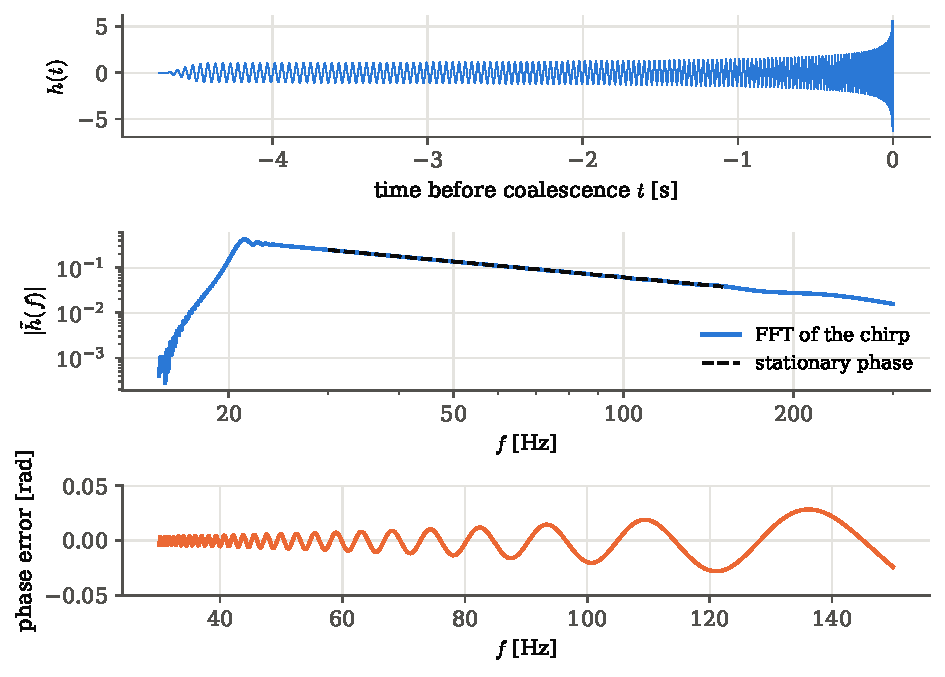
\includegraphics[width=0.85\linewidth]{figures/chT2/spa_check.pdf}
\caption{The stationary-phase formula against a direct FFT. Top: the chirp in time, its amplitude and frequency rising towards coalescence. Middle: $\lvert\tilde h\rvert$ from the FFT and from \eqref{T2a:eq:spa}, which fall together as $f^{-7/6}$ in the band; the FFT drops at $20$\,Hz, where the signal starts. Bottom: the phase of the FFT minus the predicted $-\Psi(f)$, a few hundredths of a radian.}
\label{T2a:fig:spa-check}
\end{figure}

\paragraph{Example: two phases that are easy to confuse.}
Papers on environments plot the \emph{time-domain} phase left before merger, $\Phi(f)=2\pi\int_t^{t_c}f\,\dd t$, which is $2\pi$ times the number of cycles \cite{Coogan2022}, \cite[eq.~(48)]{Kim2023}. The Fisher matrix uses the Fourier phase $\Psi(f)$. For the Newtonian chirp, \eqref{T2a:eq:Ncyc} with $f_2\to\infty$ gives $\Phi(f)=\tfrac1{16}x$, with $x\equiv(\pi G\mathcal Mf/c^3)^{-5/3}$. With $t_c=\phi_c=0$, the phase at time $t_f$ is $\phi(t_f)=-\Phi(f)$, so
\begin{align*}
  \Psi(f)+\frac\pi4
  &\eqby{1}2\pi f\,t_f-\phi(t_f)
  \eqby{2}-2\pi f\,\tau(f)+\Phi(f)
  \eqby{3}-\frac{10}{256}\,x+\frac{16}{256}\,x
  =\frac{3}{128}\,x .
\end{align*}
\begin{explain}
  \item Definition of $\Psi$ in \eqref{T2a:eq:spa}.
  \item $t_f=-\tau(f)$ and $\phi(t_f)=-\Phi(f)$, since the phase still to come is $\Phi(f)$ and the phase reaches $\phi_c=0$ at $t_c$.
  \item $2\pi f\tau=2\pi\cdot\tfrac5{256}(G\mathcal M/c^3)^{-5/3}\pi^{-8/3}f^{-5/3}=\tfrac{10}{256}x$, and $\tfrac1{16}=\tfrac{16}{256}$.
\end{explain}
So $\Psi$ carries $\tfrac38$ of the time-domain phase, because the term $2\pi f t_f$ removes the part a shift of the arrival time can absorb. For the EMRI four years before the ISCO, $\Phi\approx2\pi\times\TwEmriNcyc$ while the $f$-dependent part of $\Psi$ is about three eighths of that. Both phases are correct; they answer different questions, and a dephasing quoted in one cannot be compared with a phase error in the other without this conversion.

\paragraph{Where this is used.}
The waveform \eqref{T2a:eq:hf} with the phase \eqref{T2a:eq:psiN} is the signal model of \cref{10b:sec:signal-model}, extended there by the post-Newtonian terms derived in \cref{T2g:sec:pn}. The fact that $t_c$ and $\phi_c$ enter $\Psi$ only as $2\pi ft_c-\phi_c$ is what lets \cref{10b:sec:phase-time} search all arrival times with one inverse Fourier transform. The relations \eqref{T2a:eq:psi-derivs} are the bridge from any change of the sweep rate to a change of the phase, used in \cref{10b:sec:env-derive}, and \cref{10b:sec:two-phases} carries out the conversion between the two kinds of phase.
\section{Corrections to the phase: post-Newtonian orders and the ppE form}
\label{T2g:sec:pn}

The chirp of \cref{T2a:sec:chirp} rests on Newton's law of gravity and on the quadrupole formula, both of which are the first term of an expansion in $v/c$. Far from merger that is excellent. Near the ISCO the orbital speed is $v=c/\sqrt6\approx0.4c$, and the corrections are tens of per cent. Even far from merger, a correction of a few per cent to the rate of the inspiral is not small in the only currency that matters for a matched filter: over a million cycles, a few per cent is tens of thousands of cycles, and a template that slips by one cycle has lost the signal (\cref{T2a:sec:chirp}). Other physics acts the same way. A cloud of dark matter, a disc of gas, or a departure from general relativity each changes how fast the binary loses energy, by a fraction that depends on the frequency.

So the question is: \emph{if the binding energy or the radiated power differs from its Newtonian value by a small fractional term, how does that change the Fourier phase $\Psi(f)$, and which power of $f$ does each kind of correction produce?} The answer is one rule. A correction that scales as $v^p$ relative to the Newtonian term adds to $\Psi$ a term proportional to $f^{(p-5)/3}$, with a coefficient we can compute once and for all. General-relativistic corrections have $p=2,3,4,\dots$; environments and some modifications of gravity have negative $p$. The rule turns the whole zoo of corrections into one family, $\delta\Psi=\beta u^b$, which is the form the forecast of \cref{ch:10} uses.

\subsection{The expansion parameter}

Measure the speed of the orbit by the observable wave frequency. For a Newtonian circular orbit, Kepler's law gives the orbital speed $v_{\rm orb}=r\omega=(GM\omega)^{1/3}$, and with $\omega=\pi f$ from \eqref{T2g:eq:twice},
\begin{equation}
  v\equiv\Big(\frac{\pi GMf}{c^3}\Big)^{1/3}=\frac{v_{\rm orb}}{c},\qquad x\equiv v^2 ,
  \label{T2g:eq:v}
\end{equation}
with $M=m_1+m_2$ the total mass. A correction of relative size $v^{2k}$ is called \newterm{$k$PN} (post-Newtonian) order, so $1$PN means $v^2$, $1.5$PN means $v^3$. Using $f$ rather than the orbital radius $r$ is deliberate: $r$ depends on the coordinates used to describe the strong-field region, while the frequency of the wave at the detector does not \cite[Sec.~III A]{CutlerFlanagan1994}. Two mass combinations will appear: the \newterm{symmetric mass ratio} $\eta=m_1m_2/M^2=\mu/M$ \unpack{$\tfrac14$ for equal masses, about $m_2/m_1$ when one body is much lighter}, and the chirp mass, $\mathcal M=\eta^{3/5}M$. The reduced frequency of the Newtonian phase is then
\begin{equation}
  u\equiv\frac{\pi G\mathcal Mf}{c^3}=\eta^{3/5}v^3,\qquad u^{-5/3}=\eta^{-1}v^{-5}.
  \label{T2g:eq:u}
\end{equation}

\subsection{From the energy and the flux to the phase}

\emph{Inputs.} The orbit is still circular and evolves slowly, so energy balance $\dd E/\dd t=-\mathcal F$ holds at each moment, with $E(v)$ the binding energy and $\mathcal F(v)$ the power radiated, now allowed to carry corrections. In the Newtonian limit, by \eqref{T2a:eq:Ef} and \eqref{T2a:eq:Pf} written in terms of $v$,
\begin{equation}
  E_{\rm N}=-\tfrac12\mu c^2v^2,\qquad
  \mathcal F_{\rm N}=\frac{32}{5}\frac{c^5}{G}\,\eta^2v^{10}.
  \label{T2g:eq:EFnewton}
\end{equation}
(For $E$: $\tfrac12\mu(\pi GMf)^{2/3}=\tfrac12\mu c^2v^2$. For the power: $u^{10/3}=\eta^2v^{10}$ by \eqref{T2g:eq:u}.)

\emph{The time.} Energy balance gives $\dd t=-\dd E/\mathcal F=-(\dd E/\dd v)\,\dd v/\mathcal F$. Write the corrections to $\dd E/\dd v$ and $\mathcal F$ together as one bracket,
\begin{equation}
  \frac{\dd t}{\dd v}=-\frac{E'(v)}{\mathcal F(v)}
  =-\frac{E_{\rm N}'}{\mathcal F_{\rm N}}\,\big[1+c_pv^p+\dots\big]
  =\frac{5GM}{32c^3\eta}\,v^{-9}\big[1+c_pv^p+\dots\big],
  \label{T2g:eq:dtdv}
\end{equation}
because $-E_{\rm N}'/\mathcal F_{\rm N}=\mu c^2v\big/\big(\tfrac{32}{5}\tfrac{c^5}{G}\eta^2v^{10}\big)=\tfrac{5}{32}\tfrac{G\mu}{c^3\eta^2}v^{-9}$ and $\mu=\eta M$. The bracket may contain several terms; each acts separately at first order, so we follow one, $c_pv^p$.

\emph{The phase.} From \eqref{T2a:eq:psi-derivs}, $\dd\Psi/\dd f=2\pi t(f)=2\pi t_c-2\pi\tau(f)$, where $\tau=t_c-t$ is the time left. So $\Psi=2\pi ft_c-\phi_c-\tfrac\pi4-2\pi\int^f\tau\,\dd f'$, with the integration constants named as in \eqref{T2a:eq:psiN}. We need $\tau$ as a function of $v$, and $\dd f$ in terms of $\dd v$:
\begin{align}
  \tau(v)&\eqby{1}\int_v^\infty\frac{\dd t}{\dd v'}\,\dd v'
  \eqby{2}\frac{5GM}{32c^3\eta}\Big[\frac{v^{-8}}{8}+c_p\frac{v^{p-8}}{8-p}\Big],
  \qquad \dd f\eqby{3}\frac{3c^3v^2}{\pi GM}\,\dd v,\nonumber\\
  -2\pi\int\tau\,\dd f
  &\eqby{4}-\frac{15}{16\eta}\int\Big[\frac{v^{-6}}{8}+c_p\frac{v^{p-6}}{8-p}\Big]\dd v
  \eqby{5}\frac{15}{16\eta}\Big[\frac{v^{-5}}{40}+c_p\frac{v^{p-5}}{(8-p)(5-p)}\Big]\nonumber\\
  &\eqby{6}\frac{3}{128\,\eta\,v^5}\Big[1+\frac{40\,c_p}{(8-p)(5-p)}\,v^p\Big].
  \label{T2g:eq:rule}
\end{align}
\begin{explain}
  \item The time left is the integral of $\dd t$ from the current speed to the end, where $v\to\infty$ formally, as in \eqref{T2a:eq:tau}.
  \item $\int_v^\infty v'^{q}\dd v'=v^{q+1}/(-q-1)$ for $q<-1$; here $q=-9$ and $q=p-9$, which needs $p<8$.
  \item $f=c^3v^3/(\pi GM)$ from \eqref{T2g:eq:v}.
  \item Multiply: $2\pi\cdot\tfrac{5GM}{32c^3\eta}\cdot\tfrac{3c^3}{\pi GM}=\tfrac{15}{16\eta}$, and $v^{-8}v^2=v^{-6}$.
  \item $\int v^{q}\dd v=v^{q+1}/(q+1)$: for $q=-6$ this is $-v^{-5}/5$ and for $q=p-6$ it is $-v^{p-5}/(5-p)$, which needs $p\neq5$. The two minus signs cancel the one in front; the constants of integration join $\phi_c$.
  \item Factor out the Newtonian term: $\tfrac{15}{16}\cdot\tfrac1{40}=\tfrac{3}{128}$, and the ratio of the two coefficients is $\tfrac{1/((8-p)(5-p))}{1/40}$.
\end{explain}
For $p=0$ only the Newtonian term is left, $\tfrac{3}{128}\eta^{-1}v^{-5}=\tfrac3{128}u^{-5/3}$, which is \eqref{T2a:eq:psiN} again. A correction $c_pv^p$ in the rate of the inspiral therefore becomes a phase term
\begin{equation}
  \delta\Psi=\frac{3}{128}\,u^{-5/3}\,\frac{40\,c_p}{(8-p)(5-p)}\,v^p\ \propto\ f^{(p-5)/3}.
  \label{T2g:eq:power-rule}
\end{equation}
At $p=5$ the integral in step (5) is a logarithm instead of a power; this is why the $2.5$PN term of the phase contains $\ln f$.

\subsection{The 1PN and 1.5PN phase}

\emph{The inputs from general relativity.} The binding energy to $1$PN order and the flux to $1.5$PN order are standard results, which Cutler and Flanagan quote in terms of the orbital radius $r$ in a particular coordinate system \cite[eqs.~(35)--(37)]{CutlerFlanagan1994}, \cite{Blanchet2014}. In units $G=c=1$,
\begin{equation}
  \Omega^2=\frac{M}{r^3}\Big[1-(3-\eta)\frac Mr\Big],\qquad
  E=-\frac{\mu M}{2r}\Big[1-\frac{7-\eta}{4}\frac Mr\Big],
\end{equation}
and the flux is $\tfrac{32}{5}\eta^2(M\Omega)^{10/3}[1-(\tfrac{1247}{336}+\tfrac{35}{12}\eta)\tfrac Mr+4\pi(\tfrac Mr)^{3/2}]$. The first expression is the square of their eq.~(35), to the same order. The $4\pi$ is the \newterm{tail}: part of the outgoing wave scatters off the curved spacetime around the binary on its way out, and the scattered part interferes with the rest.

\emph{Rewritten in $v$.} With $v^2=(M\Omega)^{2/3}$,
\begin{align}
  v^2&\eqby{1}\frac Mr\Big[1-(3-\eta)\frac Mr\Big]^{1/3}\eqby{2}\frac Mr\Big[1-\Big(1-\frac\eta3\Big)\frac Mr\Big],
  \qquad \frac Mr\eqby{3}v^2\Big[1+\Big(1-\frac\eta3\Big)v^2\Big],\nonumber\\
  E&\eqby{4}-\frac{\mu}{2}v^2\Big[1+\Big(1-\frac\eta3\Big)v^2-\frac{7-\eta}{4}v^2\Big]
  \eqby{5}-\frac{\mu}{2}v^2\Big[1-\frac{9+\eta}{12}v^2\Big].
  \label{T2g:eq:E1PN}
\end{align}
\begin{explain}
  \item $(M\Omega)^{2/3}=(M^2/r^3)^{1/3}[\dots]^{1/3}=(M/r)[\dots]^{1/3}$.
  \item $(1-\epsilon)^{1/3}=1-\epsilon/3$.
  \item Invert to first order: if $v^2=y(1-ky)$ then $y=v^2(1+kv^2)$.
  \item Insert into $E$; in the $1$PN bracket $M/r=v^2$ is enough.
  \item $1-\tfrac\eta3-\tfrac74+\tfrac\eta4=-\tfrac34-\tfrac{\eta}{12}=-\tfrac{9+\eta}{12}$.
\end{explain}
The flux is already written with $(M\Omega)^{10/3}=v^{10}$ in front, and inside its bracket $M/r=v^2$ to the order needed. So, restoring $c$,
\begin{equation}
  E'(v)=-\mu c^2v\Big[1-\frac{9+\eta}{6}v^2\Big],\qquad
  \mathcal F=\frac{32}{5}\frac{c^5}{G}\eta^2v^{10}\Big[1-\Big(\frac{1247}{336}+\frac{35}{12}\eta\Big)v^2+4\pi v^3\Big],
\end{equation}
where $E'$ comes from differentiating $v^2-\tfrac{9+\eta}{12}v^4$ to $2v-\tfrac{9+\eta}{3}v^3$.

\emph{The bracket of \eqref{T2g:eq:dtdv}.} Dividing,
\begin{align}
  \frac{E'/E_{\rm N}'}{\mathcal F/\mathcal F_{\rm N}}
  &\eqby{1}\Big[1-\frac{9+\eta}{6}v^2\Big]\Big[1+\Big(\frac{1247}{336}+\frac{35}{12}\eta\Big)v^2-4\pi v^3\Big]
  \eqby{2}1+\Big(\frac{743}{336}+\frac{11}{4}\eta\Big)v^2-4\pi v^3,
\end{align}
\begin{explain}
  \item $1/(1-\epsilon)=1+\epsilon$ to first order, applied to the flux bracket.
  \item Multiply out to order $v^3$: $\tfrac{1247}{336}-\tfrac96=\tfrac{1247-504}{336}=\tfrac{743}{336}$ and $\tfrac{35}{12}-\tfrac16=\tfrac{33}{12}=\tfrac{11}{4}$.
\end{explain}
so $c_2=\tfrac{743}{336}+\tfrac{11}{4}\eta$ and $c_3=-4\pi$. The rule \eqref{T2g:eq:rule} gives the factors $\tfrac{40}{6\cdot3}=\tfrac{20}{9}$ for $p=2$ and $\tfrac{40}{5\cdot2}=4$ for $p=3$:
\begin{equation}
  \Psi(f)=2\pi ft_c-\phi_c-\frac\pi4+\frac{3}{128}\,u^{-5/3}\Big[1+\frac{20}{9}\Big(\frac{743}{336}+\frac{11}{4}\eta\Big)x-16\pi x^{3/2}\Big],
  \label{T2g:eq:psi-pn}
\end{equation}
with $x=v^2$. This is Cutler and Flanagan's restricted post-Newtonian phase \cite[eq.~(42)]{CutlerFlanagan1994}, in our sign convention, and it is the waveform used in \cref{10b:sec:signal-model}. The same bracket inverted gives the chirp rate, $\dot f\propto1-(\tfrac{743}{336}+\tfrac{11}4\eta)x+4\pi x^{3/2}$, their eq.~(38). The symmetric mass ratio $\eta$ appears for the first time at $1$PN: it is the post-Newtonian terms that let the data separate $m_1$ from $m_2$ once $\mathcal M$ is known.

\paragraph{Example: how many cycles each term is worth.}
Count cycles instead of phase: the number of wave cycles is $N=\int f\,\dd t=\int f(\dd t/\dd v)\,\dd v$, and with \eqref{T2g:eq:dtdv} and $f=c^3v^3/(\pi GM)$,
\begin{equation}
  N(v_1,v_2)=\frac{5}{32\pi\eta}\int_{v_1}^{v_2}v^{-6}\big[1+c_2v^2+c_3v^3\big]\dd v
  =\frac{5}{32\pi\eta}\Big[\frac{v^{-5}}{5}+c_2\frac{v^{-3}}{3}+c_3\frac{v^{-2}}{2}\Big]_{v_2}^{v_1}.
\end{equation}
The first term is \eqref{T2a:eq:Ncyc} again. The script \pyname{14_pn_cycles.py} evaluates the three terms separately (\cref{T2g:fig:pn-cycles}). For a pair of $1.4\,M_\odot$ neutron stars observed from $10$\,Hz to the ISCO by a ground-based detector, the Newtonian term gives $\TwPNNsN$ cycles, the $1$PN term $\TwPNNsOne$ and the tail $\TwPNNsOnefive$, in agreement with the counts Blanchet tabulates for the same band (about $1.6\times10^{4}$, $441$ and $-211$) \cite{Blanchet2014}. For the book's intermediate mass-ratio benchmark in its last four years ($v$ from $\TwPNImrivone$ to $\TwPNImrivtwo$), the counts are $\TwPNImriN$, $\TwPNImriOne$ and $\TwPNImriOnefive$; for the EMRI, $\TwPNEmriN$, $\TwPNEmriOne$ and $\TwPNEmriOnefive$. Tens of thousands of cycles from each correction: no template can leave them out. Even the GW150914-like binary crossing the LISA band years before merger, at $v\approx0.03$, gains $\TwPNGWOne$ cycles from the $1$PN term.

\begin{figure}[htbp]
\centering
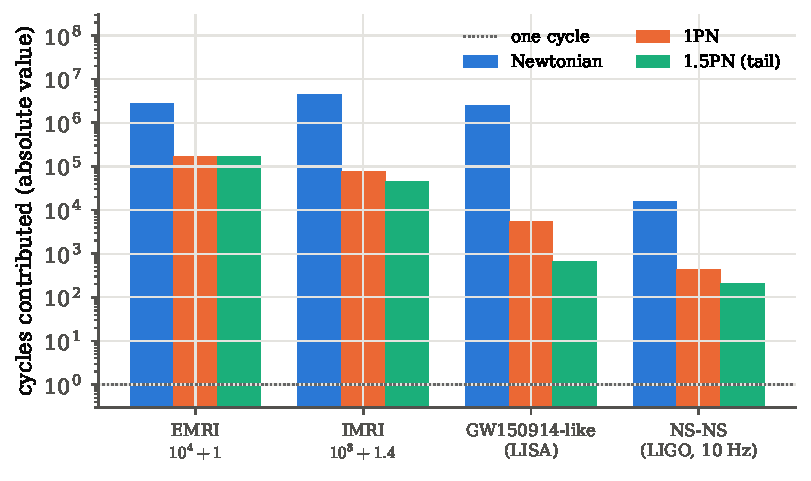
\includegraphics[width=0.82\linewidth]{figures/chT2/pn_cycles.pdf}
\caption{Number of wave cycles contributed by the Newtonian term and by the $1$PN and $1.5$PN (tail) corrections, for the four binaries named below the bars, each in its observation window. The dotted line marks one cycle, the slip that ruins a matched filter. Every correction is worth hundreds to hundreds of thousands of cycles.}
\label{T2g:fig:pn-cycles}
\end{figure}

\begin{pitfall}[Post-Newtonian series for extreme mass ratios]
For the EMRI the $1$PN and $1.5$PN counts are almost equal and opposite, each about six per cent of the total. Near the ISCO, $v\approx0.4$, successive terms of the series shrink only slowly, so truncating it at $1.5$PN leaves an error of many cycles. Research templates for extreme mass ratios therefore come from black-hole perturbation theory (the small body moving in the exact geometry of the large one, corrected by its own field) rather than from the post-Newtonian series; the power-law structure derived here is used to describe small \emph{changes} to such a template, not the template itself.
\end{pitfall}

\subsection{Every correction is a power of the frequency: the ppE form}

The rule \eqref{T2g:eq:power-rule} applies to any small correction that scales as a power of $v$, whatever its origin. In terms of the reduced frequency $u$ of \eqref{T2g:eq:u}, $v^p=\eta^{-p/5}u^{p/3}$, so a correction of relative order $v^p$ becomes
\begin{equation}
  \delta\Psi=\beta\,u^{b},\qquad b=\frac{p-5}{3},
  \label{T2g:eq:ppe-rule}
\end{equation}
with all the constants, including the powers of $\eta$, in $\beta$. For the general-relativistic terms $p=2k$ at $k$PN order, so $b=(2k-5)/3$: $-1$ at $1$PN, $-2/3$ at $1.5$PN, $-1/3$ at $2$PN. A term that grows \emph{at low frequency} faster than the Newtonian $-\tfrac53$ must come from a correction with $p<0$, one that is relatively more important when the binary is wide and slow. Yunes and Pretorius proposed to test general relativity with exactly this family: the \newterm{parameterised post-Einsteinian} (ppE) waveform
\begin{equation}
  \tilde h(f)=\tilde h_{\rm GR}(f)\,\big(1+\alpha u^{a}\big)\,e^{-i\beta u^{b}},
  \label{T2g:eq:ppe}
\end{equation}
in our sign convention, where $(\alpha,a)$ change the amplitude and $(\beta,b)$ the phase, and general relativity is $\alpha=\beta=0$ \cite[eq.~(1)]{YunesPretorius2009}. (Yunes and Pretorius write the powers of $(\pi G\mathcal Mf/c^3)^{1/3}$, so each of their exponents is three times ours.) The environments of \cref{T2a:sec:forces} fit into the same family: a dark-matter spike adds a drag whose power relative to the radiated one falls as $f^{-n}$, which by \eqref{T2g:eq:ppe-rule} with $p=-3n$ is $b=-\tfrac53-n$, \eqref{T2a:eq:ppe}.

\paragraph{Example: dipole radiation, $b=-7/3$.}
In some alternatives to general relativity, such as the Brans--Dicke theory, a compact body carries a scalar ``charge'' that is not proportional to its mass, and the binary emits dipole radiation as well. By the estimate at the end of \cref{T2g:sec:quadrupole}, dipole power relative to quadrupole power scales as $(v/c)^{-2}$. So $\mathcal F=\mathcal F_{\rm N}(1+Bv^{-2})$, the bracket of \eqref{T2g:eq:dtdv} gains $-Bv^{-2}$, $p=-2$, and $b=(-2-5)/3=-\tfrac73$: Yunes and Pretorius's Brans--Dicke case \cite{YunesPretorius2009}. A ``$-1$PN'' term, it is largest at the lowest frequencies, which is why a long, slow inspiral in the LISA band is a sensitive test of it.

\paragraph{Example: a massive graviton, $b=-1$.}
If the graviton had a mass $m_g$, waves of energy $hf$ would travel at the group velocity $v_g=c\sqrt{1-m_g^2c^4/(hf)^2}\approx c\,[1-m_g^2c^4/(2h^2f^2)]$, and low frequencies would arrive late. Over a distance $D$ the delay is $\Delta t(f)=(D/c)\,m_g^2c^4/(2h^2f^2)=Dc/(2\lambda_g^2f^2)$, with $\lambda_g=h/(m_gc)$ the graviton's Compton wavelength. The arrival time of frequency $f$ is what the slope of the Fourier phase measures, $\dd\Psi/\dd f=2\pi t(f)$ by \eqref{T2a:eq:psi-derivs}, so
\begin{align}
  \delta\Psi(f)&\eqby{1}2\pi\int\Delta t(f)\,\dd f
  \eqby{2}2\pi\,\frac{Dc}{2\lambda_g^2}\int f^{-2}\,\dd f
  \eqby{3}-\frac{\pi Dc}{\lambda_g^2}\,f^{-1}+\text{const},
\end{align}
\begin{explain}
  \item Integrate the extra delay once, as in \eqref{T2a:eq:psiN}.
  \item Insert $\Delta t(f)$.
  \item $\int f^{-2}\dd f=-f^{-1}$; the constant joins $\phi_c$.
\end{explain}
a term $\propto f^{-1}$, so $b=-1$, the ppE massive-graviton case \cite{YunesPretorius2009}. It has the same exponent as the $1$PN term, which is why a graviton mass and the mass ratio are partly degenerate in a fit, a correlation \cref{10b:sec:corr} meets in another guise.

\begin{figure}[htbp]
\centering
\begin{tikzpicture}[scale=1.0]
  \def\s{2.6}
  \draw[->,thick] ({-4.1*\s},0) -- ({0.6*\s},0) node[right,lbl] {$b$};
  \foreach \b/\t in {-4/{$-4$},-3/{$-3$},-2/{$-2$},-1/{$-1$},0/{$0$}}{
    \draw ({\b*\s},0.08) -- ({\b*\s},-0.08);
    \node[lbl,below] at ({\b*\s},-0.08) {\t};}
  \foreach \b/\lab/\h in {-1.6667/{Newtonian\\ $-5/3$}/0.95,-1/{1PN}/0.55,-0.6667/{1.5PN}/1.05,-0.3333/{2PN}/0.55}{
    \fill[formblue] ({\b*\s},0) circle (2pt);
    \draw[formblue,thin] ({\b*\s},0) -- ({\b*\s},{\h-0.18});
    \node[lbl,formblue,align=center,anchor=south] at ({\b*\s},{\h-0.2}) {\lab};}
  \foreach \b/\lab/\h/\dx in {-3.7778/{friction in a\\ $7/3$ spike}/-0.75/0,-2.3333/{dipole\\ radiation}/-0.75/0,-1/{graviton\\ mass}/-0.75/0.3}{
    \fill[bdryred] ({\b*\s},0) circle (2pt);
    \draw[bdryred,thin] ({\b*\s},0) -- ({(\b+\dx)*\s},{\h+0.3});
    \node[lbl,bdryred,align=center,anchor=north] at ({(\b+\dx)*\s},{\h+0.3}) {\lab};}
  \node[lbl,align=left,anchor=west] at ({-4.1*\s},1.3) {general relativity:};
  \node[lbl,align=left,anchor=west] at ({-4.1*\s},-1.75) {environments and modified gravity:};
\end{tikzpicture}
\caption{The exponent $b$ of the term $\beta u^b$ that each effect adds to the Fourier phase. General-relativistic corrections (blue, above the line) sit at $b=(2k-5)/3$ and climb towards zero as the PN order $k$ grows. Effects that matter most when the binary is wide and slow (red, below) have $b<-5/3$: dipole radiation at $-7/3$, dynamical friction in a dark-matter spike of slope $7/3$ at $-34/9$. A graviton mass lands on the same exponent as the $1$PN term.}
\label{T2g:fig:exponents}
\end{figure}

\begin{keyidea}[A correction $v^p$ becomes a phase term $f^{(p-5)/3}$]
If the binding energy or the radiated power differs from its Newtonian value by a relative term $c_pv^p$, the Fourier phase gains $\delta\Psi=\tfrac{3}{128}u^{-5/3}\cdot\tfrac{40c_p}{(8-p)(5-p)}v^p\propto u^{(p-5)/3}$. General relativity's $k$PN terms have $p=2k$; environments and dipole radiation have $p<0$. Any such effect is a ppE term $\beta u^b$, with the exponent $b$ naming the physics and $\beta$ its strength.
\end{keyidea}

\paragraph{Where this is used.}
The phase \eqref{T2g:eq:psi-pn} is the signal model of \cref{10b:sec:signal-model}, and the exponents of its terms are what make its Fisher matrix in \cref{10b:sec:fisher-structure} a set of weighted averages of powers of $f$. The rule \eqref{T2g:eq:ppe-rule} is the general form behind \cref{10b:sec:env-derive}, where an environment is a power law in the phase, and behind \cref{10b:sec:sigma-b}, which computes the error on $\beta$ for every exponent $b$ at once; the specific exponents of dark-matter environments are derived in \cref{T2a:sec:forces}.
\section{What LISA measures, and what hides the signal}
\label{T2a:sec:lisa}

LISA will be three spacecraft flying in a triangle $L=2.5$ million kilometres on a side, trailing the Earth around the Sun (\cref{T2a:fig:lisa-triangle}). Each spacecraft shields test masses that fall freely, and laser links measure the distance between test masses on different spacecraft. By \eqref{T2g:eq:displacement} a gravitational wave of strain $h$ changes an arm's length by about $\tfrac12hL$. For $h\sim10^{-20}$ that is about $10^{-11}$\,m, ten picometres over millions of kilometres. The whole instrument is designed around measuring such changes, and its noise is the floor under which a signal can hide.

For the statistics, LISA is summarised by a single function. The data are the signal plus noise, $d=h(\params)+n$. For a given $\params$, the likelihood of \cref{10b:sec:noise-fd} asks how plausible the particular noise realisation $n=d-h(\params)$ is, and for stationary Gaussian noise that plausibility is set, one Fourier component at a time, by the noise power at that frequency. So the likelihood weights each frequency by the inverse of the noise power there, and the Fisher matrix of \cref{ch:10} inherits that weight. The question is therefore physical: \emph{at each frequency, how large is the noise, where does it come from, and how large would a gravitational wave have to be to produce the same output?} The answer is the sensitivity curve $S_n(f)$ \cite{Robson2019}.

\subsection{A noise spectrum as a physical quantity}

The statistics of a noise spectrum, how it describes the correlations of a stationary random process and how it is estimated from data, is developed in \cref{10b:sec:noise-fd,10b:sec:welch}. Here we need only what it means physically. Pass the noise $n(t)$ through a narrow filter that keeps only frequencies between $f$ and $f+\Delta f$, and measure the mean square of what comes out. The \newterm{one-sided power spectral density} $S_n(f)$ is that mean square divided by $\Delta f$:
\begin{equation}
  \big\langle n^2\big\rangle_{[f,f+\Delta f]}=S_n(f)\,\Delta f,\qquad
  \big\langle n^2\big\rangle=\int_0^\infty S_n(f)\,\dd f .
  \label{T2g:eq:band-power}
\end{equation}
``One-sided'' means that only positive frequencies are counted, the negative ones having been folded onto them as in \cref{T2a:sec:spa}. Its square root, the \newterm{amplitude spectral density} $\sqrt{S_n}$, is in units of the measured quantity per $\sqrt{\rm Hz}$: a displacement noise of $15$\,pm\,Hz$^{-1/2}$ means that, averaged over one second (a band of about $1$\,Hz), the length reading scatters by about $15$\,pm. Two noises from independent causes add in power, $S=S_1+S_2$, because the mean square of a sum of uncorrelated terms is the sum of their mean squares. And if a noise in one quantity is converted into another by a linear, frequency-dependent factor, as a force becomes a displacement, the spectrum is multiplied by the squared modulus of that factor.

\subsection{From test-mass jitter and photon counting to strain sensitivity}

\paragraph{The two instrumental noises.}
Two processes limit the arm-length measurement \cite[eqs.~(10)--(11)]{Robson2019}:
\begin{align}
  P_{\rm OMS}(f)&=(1.5\times10^{-11}\,{\rm m})^2\Big[1+\Big(\frac{2\,{\rm mHz}}{f}\Big)^4\Big]\ {\rm Hz}^{-1},\nonumber\\
  P_{\rm acc}(f)&=(3\times10^{-15}\,{\rm m\,s^{-2}})^2\Big[1+\Big(\frac{0.4\,{\rm mHz}}{f}\Big)^2\Big]\Big[1+\Big(\frac{f}{8\,{\rm mHz}}\Big)^4\Big]\ {\rm Hz}^{-1}.\label{T2a:eq:lisa-noise}
\end{align}
The first is \newterm{optical metrology} noise, the error with which the laser interferometry reads the length of one link: about $15$\,pm\,Hz$^{-1/2}$, flat in frequency apart from a rise below $2$\,mHz. The second is \newterm{acceleration noise}: stray forces on the free-falling test masses, from impacts of residual gas molecules, electrostatic and magnetic forces on the slightly charged and magnetised masses, and the pressure of thermal radiation from their housing, push each of them around by about $3\times10^{-15}$\,m\,s$^{-2}$\,Hz$^{-1/2}$.

\paragraph{Example: where 15 picometres comes from.}
Most of the metrology noise is photon \emph{shot noise}, the graininess of light, and its size follows from counting photons. A laser of about $2$\,W leaves one spacecraft through a telescope of diameter $D\approx0.3$\,m. Diffraction spreads the beam by an angle $\theta\approx\lambda/D=1.064\,\mu{\rm m}/0.3\,{\rm m}=3.5\times10^{-6}$, so after $L=2.5\times10^9$\,m the spot has a radius of about $\theta L\approx9$\,km, and the receiving telescope, of radius $0.15$\,m, catches a fraction of order $(0.15/9000)^2\approx3\times10^{-10}$ of it: a received power $P_r\approx6\times10^{-10}$\,W. Each photon carries $hc/\lambda=1.9\times10^{-19}$\,J, so about $\dot N=P_r\lambda/hc\approx3\times10^9$ photons arrive per second. A phase measured by counting $N$ photons is uncertain by $1/\sqrt N$ radians, the Poisson fluctuation of the count (\cref{ch:02}), and a phase $\delta\varphi$ is a length $\lambda\,\delta\varphi/2\pi$. Per second of averaging,
\begin{equation*}
  \delta x\approx\frac{\lambda}{2\pi}\frac{1}{\sqrt{\dot N\times1\,{\rm s}}}
  =\frac{1.06\times10^{-6}\,{\rm m}}{2\pi}\times\frac{1}{\sqrt{3\times10^9}}\approx3\times10^{-12}\,{\rm m},
\end{equation*}
a few picometres per $\sqrt{\rm Hz}$, the same order as the $15$\,pm\,Hz$^{-1/2}$ allocated to all the metrology noise together. Counting statistics does not depend on how fast the signal varies, so shot noise is white in displacement. The arm length helps the signal ($\delta L\propto L$) but hurts the light budget ($P_r\propto L^{-2}$); $2.5$ million kilometres is a compromise between the two.

\paragraph{Why acceleration noise is divided by $(2\pi f)^4$.}
A force noise becomes a displacement noise by integrating twice in time, and integration in time is division by frequency:
\begin{align}
  \ddot x(t)=a(t)
  \;\;\Rightarrow\;\;
  (2\pi i f)^2\tilde x(f)\eqby{1}\tilde a(f)
  \;\;\Rightarrow\;\;
  P_x(f)\eqby{2}\frac{P_a(f)}{(2\pi f)^4}.
  \label{T2g:eq:acc-disp}
\end{align}
\begin{explain}
  \item Fourier transform with the book's convention \eqref{T2g:eq:fourier}: each time derivative becomes a factor $2\pi if$.
  \item The spectrum is multiplied by the squared modulus of the conversion factor; $\lvert(2\pi if)^2\rvert^2=(2\pi f)^4$.
\end{explain}
A random push of given strength moves a mass far if it keeps pushing the same way for a long time, that is at low frequency, and hardly at all if it reverses quickly. So acceleration noise is harmless at high frequency and dominates at low frequency, rising as $f^{-4}$ in power.

\paragraph{Adding up the noise in one Michelson channel.}
Follow one arm, with test mass A at the vertex spacecraft and test mass B at the far one, and let $x_A(t)$, $x_B(t)$ be their random displacements along the arm (positive in the direction from A to B). Light leaves A at $t-2L/c$, is sent back from B at $t-L/c$ and returns to A at $t$. The measured round-trip length changes by
\begin{align}
  \delta\ell(t)
  &\eqby{1}\big[x_B(t-L/c)-x_A(t-2L/c)\big]+\big[x_B(t-L/c)-x_A(t)\big],\nonumber\\
  \tilde{\delta\ell}(f)
  &\eqby{2}2e^{-2\pi ifL/c}\,\tilde x_B-\big(1+e^{-4\pi ifL/c}\big)\tilde x_A,\nonumber\\
  P_{\delta\ell}
  &\eqby{3}4P_x+\big\lvert1+e^{-4\pi ifL/c}\big\rvert^2P_x
  \eqby{4}4P_x+4\cos^2\!\Big(\frac{2\pi fL}{c}\Big)P_x
  =4\Big(1+\cos^2\frac{f}{f_*}\Big)P_x .
\end{align}
\begin{explain}
  \item The outward leg is lengthened by B's displacement when the light arrives and shortened by A's when it left; the return leg likewise, with A's displacement at the end.
  \item A delay by $T$ multiplies a Fourier transform by $e^{-2\pi ifT}$, as in a time shift (\cref{10b:sec:phase-time}).
  \item A and B jitter independently with the same spectrum $P_x$, so their contributions add in power; $\lvert2e^{-i\cdot}\rvert^2=4$.
  \item $\lvert1+e^{-i\theta}\rvert^2=2+2\cos\theta=4\cos^2(\theta/2)$ with $\theta=4\pi fL/c$, and $2\pi fL/c=f/f_*$.
\end{explain}
The far mass counts four times because the light touches it twice at the same moment; the vertex mass counts at two moments $2L/c$ apart, which add in step at low frequency and cancel when the round trip is half a period. A Michelson channel is the difference of two such arms, and in LISA each arm has its own test mass at the vertex, so the acceleration noise of the channel is $8(1+\cos^2f/f_*)P_{\rm acc}/(2\pi f)^4$: sixteen units at low frequency. The metrology noise enters once per one-way link, two links per arm, two arms: $4P_{\rm OMS}$. The signal in the same channel is the round-trip difference $2L\,D_{ij}h_{ij}$ of \cref{T2g:sec:detector}, so dividing the noise by $(2L)^2$ expresses it as an equivalent strain:
\begin{equation}
  P_n(f)=\frac{4P_{\rm OMS}+8\big(1+\cos^2\frac{f}{f_*}\big)\frac{P_{\rm acc}}{(2\pi f)^4}}{4L^2}
  =\frac{1}{L^2}\Big[P_{\rm OMS}+2\Big(1+\cos^2\frac{f}{f_*}\Big)\frac{P_{\rm acc}}{(2\pi f)^4}\Big],
  \label{T2g:eq:Pn}
\end{equation}
which is Robson et al.'s eq.~(12), with its ``four contributions from the optical metrology noise and sixteen from the test mass acceleration noise'' \cite{Robson2019}.

\paragraph{The noise that is cancelled before it is counted.}
There is a third noise, far larger than both: the laser's own frequency jitter. Even a stabilised laser wanders in frequency by about one part in $10^{13}$ per $\sqrt{\rm Hz}$, and a Michelson interferometer is immune to that only if its two arms are equally long, so that both beams carry the same old laser light back to be compared. LISA's arms differ by about one per cent, some $2.5\times10^7$\,m, so the jitter would appear as a length noise of order $10^{-13}\times2.5\times10^7\,{\rm m}\approx2.5\,\mu$m per $\sqrt{\rm Hz}$, some $10^5$ times the signal. LISA therefore records every one-way link separately and, on the ground, adds the records with time shifts chosen so that the laser noise cancels exactly, synthesising an equal-arm Michelson after the fact. This is \newterm{time-delay interferometry}. What survives it is the test-mass and metrology noise counted above.

\paragraph{From the noise in the channel to the sensitivity curve.}
$P_n$ is the noise of one channel expressed as a strain, but a real wave is not optimally oriented: on average over the sky and polarisation the channels respond to only a fraction $R(f)$ of the wave's power, $\tfrac{3}{10}$ at low frequency for the two channels together and falling above $f_*$ (\cref{T2g:sec:detector}). It is conventional to move that factor from the signal onto the noise \cite[eq.~(2)]{Robson2019}: the \newterm{sensitivity curve} is the noise divided by the response. With the fit $R(f)=\tfrac3{10}/[1+0.6(f/f_*)^2]$, checked in \cref{T2g:fig:response},
\begin{equation}
  S_n(f)=\frac{P_n(f)}{R(f)}
  =\frac{10}{3L^2}\Big[P_{\rm OMS}(f)+2\Big(1+\cos^2\frac{f}{f_*}\Big)\frac{P_{\rm acc}(f)}{(2\pi f)^4}\Big]\Big[1+\frac{6}{10}\Big(\frac{f}{f_*}\Big)^2\Big]+S_c(f).
  \label{T2a:eq:Sn}
\end{equation}
At $f\ll f_*$ the factor $2(1+\cos^2)$ is $4$, the simpler form of Robson et al.'s eq.~(1) \cite{Robson2019}; the code uses the full factor.

\paragraph{The Galactic confusion noise.}
The last term in \eqref{T2a:eq:Sn} is not instrumental. Our Galaxy contains tens of millions of binaries of white dwarfs radiating at millihertz frequencies. A four-year observation divides the frequency axis into bins of width $1/T\approx8$\,nHz, and below a few millihertz there are more binaries than bins. They cannot be separated from one another, and their sum acts as an extra noise \cite[Sec.~1]{Robson2019}:
\begin{equation}
  S_c(f)=A\,f^{-7/3}\,e^{-f^{\alpha}+\beta f\sin(\kappa f)}\,\big[1+\tanh(\gamma(f_k-f))\big]\ {\rm Hz}^{-1},
\end{equation}
with $A=9\times10^{-45}$ and, for four years, $(\alpha,\beta,\kappa,\gamma,f_k)=(0.138,-221,521,1680,1.13\,{\rm mHz})$ \cite[eq.~(14)]{Robson2019}.

\emph{Why $f^{-7/3}$?} The power law follows from the chirp. Suppose white-dwarf binaries form at a steady rate at low frequency and then drift upwards in frequency at the rate $\dot f\propto f^{11/3}$ of \eqref{T2a:eq:fdot}. In a steady state the number of binaries crossing any frequency per unit time is the same at every $f$, like a steady flow of traffic: $(\dd N/\dd f)\,\dot f=\text{const}$, so $\dd N/\dd f\propto f^{-11/3}$. Where binaries move quickly they are few. Each binary contributes a mean-square strain $\propto A^2\propto f^{4/3}$, by \eqref{T2g:eq:amp}. Summing the power of all binaries in a band, as \eqref{T2g:eq:band-power} sums the power of a noise,
\begin{equation}
  S_c(f)\propto\frac{\dd N}{\dd f}\,A^2\propto f^{-11/3}\,f^{4/3}=f^{-7/3}.
\end{equation}
The other factors of the fit describe where this simple picture fails. Above the knee $f_k$ there is less than about one binary per bin, so the binaries can be fitted and subtracted one by one, and the $\tanh$ switches the confusion off. The longer LISA observes, the finer the bins, the more binaries are resolved, and the lower the knee moves (it is $2.58$\,mHz after six months). The confusion noise is also not stationary: it rises and falls during the year as the antenna pattern of \cref{T2g:sec:detector} sweeps across the Galactic centre. The fit is its average.

\begin{workdef}[sensitivity curve]
The \newterm{sensitivity curve} $S_n(f)$ is the one-sided noise power spectral density of the detector divided by its sky- and polarisation-averaged response, plus any unresolved foreground \unpack{the noise expressed as the strain power a gravitational wave would need to produce the same output}. \emph{Operationally:} in the inner product $(a\,|\,b)=4\,\mathrm{Re}\int\tilde a\tilde b^*/S_n\,\dd f$ use $S_n(f)$ of \eqref{T2a:eq:Sn} together with the angle-averaged waveform $\tilde h=\sqrt{4/5}\,\mathcal Af^{-7/6}e^{-i\Psi}$.
\end{workdef}

\Cref{T2a:fig:lisa-noise} shows the three pieces. Acceleration noise dominates below $\TwfAccOms$\,mHz (by hand: setting $P_{\rm OMS}=4P_{\rm acc}/(2\pi f)^4$ without the correction factors gives $(2\pi f)^4=4\times9\times10^{-30}/2.25\times10^{-22}=1.6\times10^{-7}\,{\rm s^{-4}}$, i.e.\ $f=3.2$\,mHz). The confusion noise exceeds the instrument between $\TwfConfLo$ and $\TwfConfHi$\,mHz. Above $f_*=\Twfstar$\,mHz the falling response makes the curve rise again. The best sensitivity, $\sqrt{S_n}=\TwASDmin\,{\rm Hz^{-1/2}}$, is reached near $\TwfASDmin$\,mHz.

\begin{figure}[htbp]
\centering
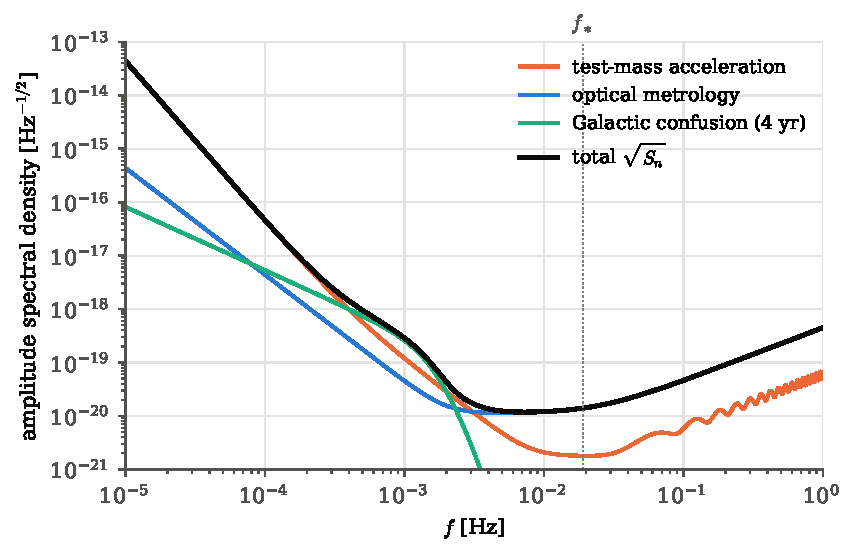
\includegraphics[width=0.8\linewidth]{figures/chT2/lisa_noise.pdf}
\caption{The LISA sensitivity curve and its three ingredients, as amplitude spectral densities $\sqrt{S}$. Test-mass acceleration noise falls steeply with frequency, optical metrology noise is flat and then rises above $f_*$ (dotted) where the arms respond less, and the Galactic confusion noise fills the gap around a millihertz. The thick curve is the total used throughout the book.}
\label{T2a:fig:lisa-noise}
\end{figure}

The curve is a short function in \pyname{lib_lisa.py}:

\pyfile[firstline=100,lastline=111,firstnumber=100]{code/chT2/lib_lisa.py}{The three pieces of $S_n(f)$ and their sum}

\noindent The factor \pyname{resp} on line 102 is $\tfrac{10}{3L^2}[1+0.6(f/f_*)^2]$, the conversion from displacement noise to strain sensitivity. Line 103 is the metrology term of \eqref{T2a:eq:Sn}, line 104 the acceleration term with its $f^{-4}$ and the full factor $2(1+\cos^2)$, and line 105 hands back the confusion fit. \pyname{Sn_lisa} adds the three; with \pyname{confusion=False} it is the instrument alone.

\subsection{How loud is a source?}

With the noise in hand, the signal-to-noise ratio of \cref{ch:00} is $\rho^2=(h\,|\,h)=4\int\lvert\tilde h\rvert^2/S_n\,\dd f$. For the angle-averaged waveform of \cref{T2a:sec:spa}, $\lvert\tilde h\rvert^2=\tfrac45\mathcal A^2f^{-7/3}$ (with $\mathcal A$ the amplitude of \eqref{T2a:eq:hf}), and it is useful to rewrite the integral so that a plot shows it:
\begin{equation}
  \rho^2\eqby{1}\frac{16}{5}\int\frac{\mathcal A^2f^{-7/3}}{S_n(f)}\,\dd f
  \eqby{2}\int\Big(\frac{h_c(f)}{h_n(f)}\Big)^2\dd\ln f,
  \qquad h_c\equiv2f\lvert\tilde h(f)\rvert,\quad h_n\equiv\sqrt{fS_n(f)} .
  \label{T2a:eq:snr}
\end{equation}
\begin{explain}
  \item Insert $\lvert\tilde h\rvert^2=\tfrac45\mathcal A^2f^{-7/3}$; $4\cdot\tfrac45=\tfrac{16}{5}$ \cite[eq.~(18)]{Robson2019}.
  \item $4\lvert\tilde h\rvert^2\dd f/S_n=(2f\lvert\tilde h\rvert)^2/(fS_n)\cdot\dd f/f$, and $\dd f/f=\dd\ln f$.
\end{explain}
Both $h_c$, the \newterm{characteristic strain}, and $h_n$ are dimensionless. On log--log axes the height of a source's track above the noise curve shows how much signal-to-noise ratio each decade of frequency contributes. A track below the curve can still be detected if it is long enough, because the integral adds up many frequencies.

\paragraph{Example: the three benchmark sources.}
The script \pyname{03_lisa_noise.py} evaluates \eqref{T2a:eq:snr} on the four-year stretch of each binary of \cref{T2a:sec:chirp}. Kim et al.\ place the EMRI at $D_L=203$\,Mpc, where five years of data give a signal-to-noise ratio of about $15$ \cite[Sec.~III F]{Kim2023}. For our four years we place it where $\rho=\TwEmriSNR$, which is $D_L=\TwEmriDL$\,Mpc, close to their distance. The IMRI at $75$\,Mpc, the distance out to which Coogan et al.\ find dark-matter environments measurable \cite{Coogan2022}, reaches $\rho=\TwImriSNR$ between $\TwImriffouryr$\,mHz and the $1$\,Hz end of the band. The GW150914-like binary at $410$\,Mpc reaches only $\rho=\TwGWlikeSNR$: on its own LISA would not claim it, which is why such sources are studied together with ground-based detectors. \Cref{T2a:fig:lisa-tracks} shows the tracks. Since $h_c\propto f\cdot f^{-7/6}=f^{-1/6}$, each inspiral is an almost flat line that ends where the binary reaches its ISCO or leaves the band.

\begin{figure}[htbp]
\centering
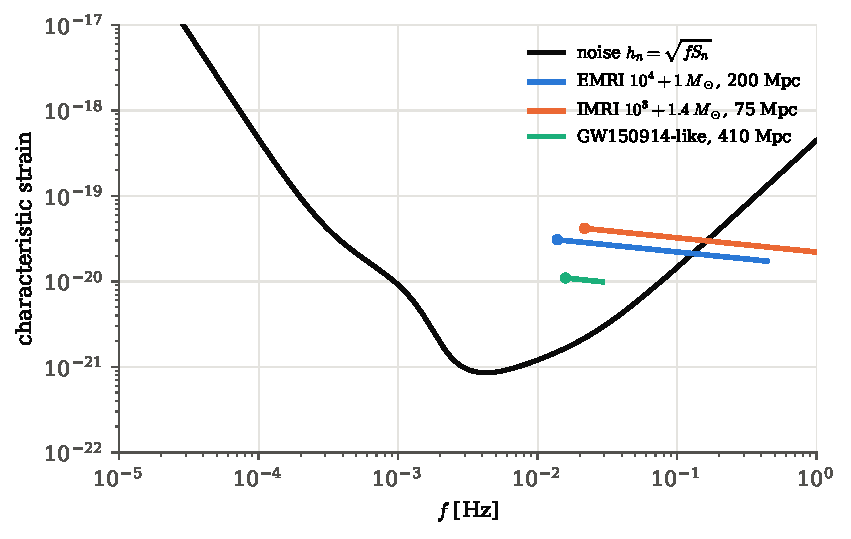
\includegraphics[width=0.8\linewidth]{figures/chT2/lisa_tracks.pdf}
\caption{Characteristic strain of the three benchmark binaries during four years of observation (dots mark the start), over the LISA noise amplitude $h_n=\sqrt{fS_n}$. The squared ratio of the two curves, integrated over $\ln f$, is the squared signal-to-noise ratio \eqref{T2a:eq:snr}. The EMRI and the IMRI sit well above the noise over a decade or more of frequency; the GW150914-like binary is short and sits only several times above it.}
\label{T2a:fig:lisa-tracks}
\end{figure}

\begin{pitfall}[Three conventions for one curve]
The literature plots $\sqrt{P_n}$ (noise only), $\sqrt{S_n}=\sqrt{P_n/R}$ (noise over response) and $h_n=\sqrt{fS_n}$ (dimensionless), and quotes the low-frequency response as $3/10$ (two channels) or $3/20$ (one) \cite[Sec.~1]{Robson2019}. Each is correct with the matching signal. Pair $S_n$ with the angle-averaged waveform $\sqrt{4/5}\,\mathcal Af^{-7/6}$, or $P_n$ with the full detector response, and never mix them: a mismatch changes every signal-to-noise ratio and Fisher error by a constant factor that nothing else in the calculation will reveal.
\end{pitfall}

\paragraph{Where this is used.}
The curve \eqref{T2a:eq:Sn} is the $S_n(f)$ of the noise-weighted inner product of \cref{10b:sec:noise-fd}, and with it of every likelihood, matched filter and Fisher matrix in \cref{ch:10}; \cref{10b:sec:robson} checks it against the published figure, and \cref{10b:sec:benchmark} uses the signal-to-noise ratio \eqref{T2a:eq:snr} to place the benchmark source. In real data $S_n$ is not known in advance but estimated, which is the subject of \cref{10b:sec:welch,10b:sec:psd}; the non-stationary confusion noise is one reason why that estimate is hard.
\section{The symbols, where they come from, and where they are used}
\label{T2g:sec:symbols}

Every gravitational-wave object that \cref{ch:10} takes as given has a short derivation above. The table that follows gives each symbol in a few words, the equation or section where it was derived, and the part of \cref{ch:10} in which it does its work. The rows follow the chain of \cref{T2a:fig:roadmap}: the wave, the source, the chirp, the frequency domain, the corrections, the detector and its noise.

\begin{table}[htbp]
\centering
\footnotesize
\renewcommand{\arraystretch}{1.18}
\begin{tabularx}{\linewidth}{@{}>{\raggedright\arraybackslash}p{2.35cm} >{\raggedright\arraybackslash}X >{\raggedright\arraybackslash}p{2.1cm} >{\raggedright\arraybackslash}p{2.5cm}@{}}
\toprule
symbol & meaning & derived in & used in \cref{ch:10} \\
\midrule
$h_+$, $h_\times$ & the two polarisations of a wave, in the transverse plane & \eqref{T2g:eq:tt} & \S\ref{10b:sec:detection} \\
$\delta L/L=\tfrac12h_{aa}$ & fractional change of an arm's length, read by light travel time & \eqref{T2g:eq:displacement}, \eqref{T2g:eq:arm} & \S\ref{10b:sec:detection} \\
$F_+$, $F_\times$; $D_{ij}$ & antenna patterns: weights of the polarisations in the detector output; detector tensor & \eqref{T2g:eq:response}, \eqref{T2g:eq:Fplus} & \S\ref{10b:sec:detection} \\
$\tfrac15$, $\tfrac3{20}$, $R=\tfrac3{10}$ & sky- and polarisation-averaged response: right-angle, one $60^\circ$ channel, two LISA channels & \eqref{T2g:eq:one-fifth}, \eqref{T2g:eq:sixty} & \S\ref{10b:sec:robson} \\
$\tfrac45$ & inclination average of a circular binary's signal power & \eqref{T2g:eq:four-fifths} & \S\ref{10b:sec:robson}, \S\ref{10b:sec:benchmark} \\
$f_*=c/2\pi L$ & transfer frequency; response falls as $f^{-2}$ above it & \eqref{T2g:eq:transfer} & \S\ref{10b:sec:robson} \\
$M$, $\mu$, $\eta$ & total mass, reduced mass, symmetric mass ratio $\mu/M$ & \S\ref{T2g:sec:quadrupole}, \eqref{T2g:eq:v} & \S\ref{10b:sec:signal-model} \\
$\mathcal M$ & chirp mass $\mu^{3/5}M^{2/5}$, the mass the Newtonian signal depends on & \eqref{T2g:eq:amp}, \eqref{T2a:eq:Pf} & \S\ref{10b:sec:signal-model}, \S\ref{10b:sec:fisher-examples} \\
$f=2f_{\rm orb}$ & wave frequency, twice the orbital one & \eqref{T2g:eq:twice} & throughout \\
$A$; $\mathcal A$ & time-domain amplitude; Fourier amplitude of $\tilde h=\mathcal Af^{-7/6}e^{-i\Psi}$ & \eqref{T2g:eq:amp}, \eqref{T2a:eq:hf} & \S\ref{10b:sec:matched-filter}, \S\ref{10b:sec:signal-model} \\
$\iota$, $\psi$ & inclination of the orbit; polarisation angle & \eqref{T2g:eq:hpc}, \eqref{T2g:eq:Fplus} & \S\ref{10b:sec:robson} \\
$P_{\rm GW}$, $E(f)$ & radiated power; orbital binding energy & \eqref{T2g:eq:power-binary}, \eqref{T2a:eq:Ef} & \S\ref{10b:sec:env-derive} \\
$\dot f$ & chirp rate $\tfrac{96}{5}\pi^{8/3}(G\mathcal M/c^3)^{5/3}f^{11/3}$ & \eqref{T2a:eq:fdot} & \S\ref{10b:sec:env-derive} \\
$\tau(f)$, $N$, $f_{\rm ISCO}$ & time left to coalescence; number of cycles; end of the inspiral & \eqref{T2a:eq:tau}, \eqref{T2a:eq:Ncyc}, \eqref{T2a:eq:fisco} & \S\ref{10b:sec:benchmark} \\
$t_c$, $\phi_c$ & time and phase of coalescence: nuisance parameters & \eqref{T2g:eq:phit}, \S\ref{T2g:sec:tc-phic} & \S\ref{10b:sec:phase-time}, \S\ref{10b:sec:fisher-examples} \\
$\tilde h(f)$ & Fourier transform, $\int h\,e^{-2\pi ift}\dd t$; $\tilde h(-f)=\tilde h(f)^*$ & \eqref{T2g:eq:fourier}, \eqref{T2g:eq:reality} & \S\ref{10b:sec:noise-fd} \\
$\Psi(f)$ & Fourier phase of the chirp, from the stationary-phase approximation & \eqref{T2a:eq:spa}, \eqref{T2a:eq:psiN} & \S\ref{10b:sec:signal-model} \\
$\Psi'=2\pi t(f)$, $\Psi''=2\pi/\dot f$ & what the phase knows: arrival time and chirp rate & \eqref{T2a:eq:psi-derivs} & \S\ref{10b:sec:env-derive} \\
$\Phi(f)$ & time-domain phase still to come; $\Psi$ carries $\tfrac38$ of it & \S\ref{T2a:sec:spa} (example) & \S\ref{10b:sec:two-phases} \\
$v$, $x$, $u$ & PN parameter $(\pi GMf/c^3)^{1/3}$, $x=v^2$, reduced frequency $\pi G\mathcal Mf/c^3$ & \eqref{T2g:eq:v}, \eqref{T2g:eq:u} & \S\ref{10b:sec:signal-model} \\
1PN, 1.5PN terms & corrections $\tfrac{20}{9}(\tfrac{743}{336}+\tfrac{11}4\eta)x$ and $-16\pi x^{3/2}$ & \eqref{T2g:eq:psi-pn} & \S\ref{10b:sec:signal-model} \\
$\beta$, $b$ & ppE amplitude and exponent of a phase term $\beta u^b$; $b=(p-5)/3$ & \eqref{T2g:eq:ppe-rule}, \eqref{T2a:eq:ppe} & \S\ref{10b:sec:env}, \S\ref{10b:sec:sigma-b} \\
$S_n(f)$ & one-sided noise spectrum divided by the response: the sensitivity curve & \eqref{T2g:eq:band-power}, \eqref{T2a:eq:Sn} & \S\ref{10b:sec:noise-fd}, \S\ref{10b:sec:robson} \\
$P_{\rm OMS}$, $P_{\rm acc}$, $S_c$ & metrology, test-mass acceleration and Galactic confusion noise & \eqref{T2a:eq:lisa-noise}, \eqref{T2g:eq:Pn} & \S\ref{10b:sec:robson} \\
$h_c$, $h_n$, $\rho$ & characteristic strain, noise amplitude, signal-to-noise ratio & \eqref{T2a:eq:snr} & \S\ref{10b:sec:benchmark} \\
\bottomrule
\end{tabularx}
\caption{The gravitational-wave symbols of \cref{ch:10}: what each one is, the equation or section that derives it, and the section of \cref{ch:10} that uses it.}
\label{T2g:tab:symbols}
\end{table}

The rows are links of one chain of reasoning. Einstein's equation for a weak field gave a wave with two polarisations that changes distances by $\tfrac12h$. Mass and momentum conservation made the quadrupole the first source of such waves, and the energy they carry made a binary chirp. The stationary-phase approximation turned the chirp into a Fourier-domain template whose phase is a sum of powers of $f$, two of whose terms, $2\pi ft_c-\phi_c$, are nuisances, and whose other terms, Newtonian, post-Newtonian or environmental, carry the physics. The detector added its geometry, through $F_+$, $F_\times$ and the averages $\tfrac45$ and $\tfrac3{10}$, and its noise, through $S_n(f)$. Nothing in the list is a convention to be taken on trust; each entry can be recomputed from the two physical inputs of \cref{T2g:sec:wave} and Newton's law of gravity.

\begin{recap}
\begin{itemize}[itemsep=1pt]
  \item A weak gravitational wave is a transverse, traceless ripple $h_{ij}$ moving at $c$, with two polarisations $h_+$, $h_\times$ that mix under rotations with twice the angle; it changes the distance between free masses by $\delta L/L=\tfrac12h_{ij}\hat n_i\hat n_j$, a travelling tidal squeeze.
  \item Conservation of mass and momentum forbids monopole and dipole radiation, so slow sources radiate through $\ddot Q_{ij}$: $h^{\rm TT}_{ij}=(2G/c^4r)[\ddot Q_{ij}]^{\rm TT}$ and $P=(G/5c^5)\langle\dddot Q\dddot Q\rangle$. A circular binary radiates at $f=2f_{\rm orb}$ with amplitude $4(G\mathcal M)^{5/3}(\pi f)^{2/3}/(c^4D)$ and power $\tfrac{32}{5}(G/c^5)\mu^2r^4\omega^6$.
  \item A detector outputs $h=F_+h_++F_\times h_\times$. Averages: $\tfrac15$ over sky and polarisation, $\tfrac34$ for $60^\circ$ arms, $\tfrac3{10}$ for LISA's two channels, $\tfrac45$ over inclination. Above $f_*=c/(2\pi L)=19$\,mHz the response falls as $f^{-2}$.
  \item Energy balance gives the chirp $\dot f\propto\mathcal M^{5/3}f^{11/3}$; integrating it gives the time to merger, the number of cycles and the phase, with the nuisance constants $t_c$ and $\phi_c$.
  \item The stationary-phase approximation, a Taylor expansion of the phase plus a Fresnel integral, gives $\tilde h=\mathcal Af^{-7/6}e^{-i\Psi}$ with $\Psi'=2\pi t(f)$ and $\Psi''=2\pi/\dot f$, checked against an FFT.
  \item A relative correction $v^p$ to the energy or flux adds $\propto f^{(p-5)/3}$ to $\Psi$: the 1PN and 1.5PN terms of the standard template, dipole radiation at $b=-7/3$, a graviton mass at $b=-1$, environments at $b=-5/3-n$, all of the ppE form $\beta u^b$.
  \item LISA's noise is shot noise (flat in displacement) and test-mass acceleration noise (divided by $(2\pi f)^4$), counted through the round trips of a Michelson channel and divided by the response to give $S_n(f)$, plus the $f^{-7/3}$ confusion noise of unresolved Galactic binaries.
\end{itemize}
\end{recap}

\providecommand{\TwEmriMc}{}\renewcommand{\TwEmriMc}{39.81}
\providecommand{\TwEmrifisco}{}\renewcommand{\TwEmrifisco}{0.4397}
\providecommand{\TwEmriffouryr}{}\renewcommand{\TwEmriffouryr}{13.84}
\providecommand{\TwEmriNcyc}{}\renewcommand{\TwEmriNcyc}{2.787\times10^{6}}
\providecommand{\TwEmriadiab}{}\renewcommand{\TwEmriadiab}{6.839\times10^{-5}}
\providecommand{\TwImriMc}{}\renewcommand{\TwImriMc}{19.39}
\providecommand{\TwImrifisco}{}\renewcommand{\TwImrifisco}{4.391}
\providecommand{\TwImriffouryr}{}\renewcommand{\TwImriffouryr}{21.7}
\providecommand{\TwImriNcyc}{}\renewcommand{\TwImriNcyc}{4.382\times10^{6}}
\providecommand{\TwImriadiab}{}\renewcommand{\TwImriadiab}{9.550\times10^{-4}}
\providecommand{\TwGWMc}{}\renewcommand{\TwGWMc}{28.1}
\providecommand{\TwGWfFive}{}\renewcommand{\TwGWfFive}{15.83}
\providecommand{\TwGWfOne}{}\renewcommand{\TwGWfOne}{28.94}
\providecommand{\TwGWNcyc}{}\renewcommand{\TwGWNcyc}{2.534\times10^{6}}
\providecommand{\TwSpaAmpErr}{}\renewcommand{\TwSpaAmpErr}{3.655}
\providecommand{\TwSpaPhaseRms}{}\renewcommand{\TwSpaPhaseRms}{0.01296}
\providecommand{\TwSpaPsiBand}{}\renewcommand{\TwSpaPsiBand}{168.4}
\providecommand{\TwSpaDuration}{}\renewcommand{\TwSpaDuration}{4.729}
\providecommand{\Twfstar}{}\renewcommand{\Twfstar}{19.09}
\providecommand{\TwASDmin}{}\renewcommand{\TwASDmin}{1.178\times10^{-20}}
\providecommand{\TwfASDmin}{}\renewcommand{\TwfASDmin}{7.256}
\providecommand{\TwfAccOms}{}\renewcommand{\TwfAccOms}{3.077}
\providecommand{\TwfConfLo}{}\renewcommand{\TwfConfLo}{0.4101}
\providecommand{\TwfConfHi}{}\renewcommand{\TwfConfHi}{1.908}
\providecommand{\TwEmriDL}{}\renewcommand{\TwEmriDL}{199.8}
\providecommand{\TwEmriSNR}{}\renewcommand{\TwEmriSNR}{14}
\providecommand{\TwImriSNR}{}\renewcommand{\TwImriSNR}{12.1}
\providecommand{\TwGWlikeSNR}{}\renewcommand{\TwGWlikeSNR}{3.89}
\providecommand{\Twconc}{}\renewcommand{\Twconc}{13.49}
\providecommand{\Twrtwohundred}{}\renewcommand{\Twrtwohundred}{9.82}
\providecommand{\TwrsNFW}{}\renewcommand{\TwrsNFW}{0.7279}
\providecommand{\Twdeltac}{}\renewcommand{\Twdeltac}{9.39\times10^{4}}
\providecommand{\Twrhos}{}\renewcommand{\Twrhos}{0.01184}
\providecommand{\Twrsp}{}\renewcommand{\Twrsp}{3.759}
\providecommand{\Twrhosp}{}\renewcommand{\Twrhosp}{2.269}
\providecommand{\Twrhpc}{}\renewcommand{\Twrhpc}{9.571\times10^{-10}}
\providecommand{\TwrsgOverRh}{}\renewcommand{\TwrsgOverRh}{4.5\times10^{4}}
\providecommand{\Twrhosg}{}\renewcommand{\Twrhosg}{1.190\times10^{11}}
\providecommand{\TwrorbFour}{}\renewcommand{\TwrorbFour}{30.09}
\providecommand{\TwrorbIsco}{}\renewcommand{\TwrorbIsco}{3}
\providecommand{\TwrhoOrb}{}\renewcommand{\TwrhoOrb}{2.279\times10^{16}}
\providecommand{\TwrhoBoost}{}\renewcommand{\TwrhoBoost}{2.279\times10^{18}}
\providecommand{\TwmuParticle}{}\renewcommand{\TwmuParticle}{2.003\times10^{-12}}
\providecommand{\TwmuCompton}{}\renewcommand{\TwmuCompton}{6.681\times10^{-15}}
\providecommand{\TwfeqA}{}\renewcommand{\TwfeqA}{4.181}
\providecommand{\TwdPhiFourA}{}\renewcommand{\TwdPhiFourA}{1.302\times10^{5}}
\providecommand{\TwbexpA}{}\renewcommand{\TwbexpA}{-4.333}
\providecommand{\TwfeqB}{}\renewcommand{\TwfeqB}{8.883}
\providecommand{\TwdPhiFourB}{}\renewcommand{\TwdPhiFourB}{1.325\times10^{6}}
\providecommand{\TwbexpB}{}\renewcommand{\TwbexpB}{-4}
\providecommand{\TwfeqC}{}\renewcommand{\TwfeqC}{16.75}
\providecommand{\TwdPhiFourC}{}\renewcommand{\TwdPhiFourC}{5.191\times10^{6}}
\providecommand{\TwbexpC}{}\renewcommand{\TwbexpC}{-3.778}
\providecommand{\TwclosedVsNum}{}\renewcommand{\TwclosedVsNum}{1.343\times10^{-13}}
\providecommand{\TwPLerrFour}{}\renewcommand{\TwPLerrFour}{35.35}
\providecommand{\TwfeqD}{}\renewcommand{\TwfeqD}{24.26}
\providecommand{\TwdPhiFourD}{}\renewcommand{\TwdPhiFourD}{8.937\times10^{6}}
\providecommand{\TwbexpD}{}\renewcommand{\TwbexpD}{-3.667}
\providecommand{\TwCwSmallErr}{}\renewcommand{\TwCwSmallErr}{0.8254}
\providecommand{\TwaccRatioThirty}{}\renewcommand{\TwaccRatioThirty}{0.02222}
\providecommand{\TwaccRatioThree}{}\renewcommand{\TwaccRatioThree}{0.2222}
\providecommand{\TwffourImri}{}\renewcommand{\TwffourImri}{21.7}
\providecommand{\TwlnLambdaC}{}\renewcommand{\TwlnLambdaC}{3.286}
 
\section{Dark matter around black holes}
\label{T2a:sec:dm}

The signal model of \cref{T2a:sec:spa,T2g:sec:pn} describes a binary in empty space: a chirp whose Fourier phase $\Psi(f)$ \eqref{T2a:eq:psiN} is fixed by the chirp mass $\mathcal M$ \eqref{T2a:eq:Pf} and the coalescence constants $t_c$, $\phi_c$ (\cref{T2g:sec:tc-phic}), and to which any extra physics adds a power of the frequency, $\beta u^b$ \eqref{T2g:eq:ppe-rule}. This section and the next supply the extra physics that the forecasts of \cref{ch:10} test. Here we ask where dark matter around a black hole comes from and how dense it becomes; \cref{T2a:sec:forces} finds the forces it exerts on the orbit and the exponent $b$ they produce.

Near the Sun, dark matter has a density of about $0.01\,M_\odot\,{\rm pc}^{-3}$. Spread at that density over a sphere the size of the EMRI orbit of \cref{T2a:sec:chirp}, about $30$ Schwarzschild radii of a $10^4\,M_\odot$ hole or $3\times10^{-8}$\,pc, it amounts to $\tfrac43\pi(3\times10^{-8})^3\times0.01\approx10^{-24}\,M_\odot$. No orbit could feel that. A survey of environmental effects on inspirals concludes exactly this: for most sources, galactic dark matter at ordinary densities is irrelevant \cite[Sec.~IX]{Barausse2014}. If a gravitational wave is to show dark matter, something must have packed it around the black hole at densities some eighteen orders of magnitude higher. The black hole itself can do it. So the question is: \emph{how does a black hole that grows at the centre of a dark-matter halo rearrange the dark matter around it, and how dense does it become where the companion orbits?}

\subsection{The halo far away}

Far from any black hole, simulations of cold dark matter find the \newterm{Navarro--Frenk--White} (NFW) profile
\begin{equation}
  \rho_{\rm NFW}(r)=\frac{\rho_s}{(r/r_s)(1+r/r_s)^2},
  \label{T2a:eq:nfw}
\end{equation}
which falls as $r^{-1}$ inside the scale radius $r_s$ and as $r^{-3}$ outside it \cite{NFW1996}, \cite[eq.~(1)]{NFW1997}. The inner $r^{-1}$ is called a \newterm{cusp}. A halo has no sharp edge, so it is labelled by the mass inside a conventional one. The reference density is the \newterm{critical density} $\rho_{\rm crit}=3H_0^2/(8\pi G)$, the mean density at which a universe expanding at today's rate $H_0$ would be spatially flat, about $1.3\times10^{-7}\,M_\odot\,{\rm pc}^{-3}$ for $h=0.674$. The edge $r_{200}$ is the radius within which the mean density of the halo is $200\rho_{\rm crit}$, and $M_{200}$ is the mass inside it. Since that mass is $200\rho_{\rm crit}$ times the volume $\tfrac43\pi r_{200}^3$, the mass fixes the edge, $r_{200}=[3M_{200}/(800\pi\rho_{\rm crit})]^{1/3}$. The second label is the concentration $c=r_{200}/r_s$, which then fixes $r_s=r_{200}/c$. What remains is $\rho_s$, and it follows from the enclosed mass:
\begin{align}
  M(<r)&\eqby{1}4\pi\rho_sr_s^3\int_0^{r/r_s}\frac{x\,\dd x}{(1+x)^2}
  \eqby{2}4\pi\rho_sr_s^3\Big[\ln\Big(1+\frac r{r_s}\Big)-\frac{r/r_s}{1+r/r_s}\Big],\nonumber\\
  \rho_s&\eqby{3}\rho_{\rm crit}\,\frac{200}{3}\,\frac{c^3}{\ln(1+c)-c/(1+c)}\equiv\rho_{\rm crit}\,\delta_c .\label{T2a:eq:nfw-mass}
\end{align}
\begin{explain}
  \item $M=\int_0^r4\pi r'^2\rho\,\dd r'$ with $x=r'/r_s$; the factor $x^2/x$ leaves $x$.
  \item $\frac{x}{(1+x)^2}=\frac1{1+x}-\frac1{(1+x)^2}$ integrates to $\ln(1+x)+\frac1{1+x}-1=\ln(1+x)-\frac x{1+x}$.
  \item Evaluate step (2) at $r=r_{200}=cr_s$ and set it equal to $200\rho_{\rm crit}\cdot\tfrac43\pi r_{200}^3$:
        $4\pi\rho_sr_s^3\big[\ln(1+c)-\tfrac{c}{1+c}\big]=\tfrac{800\pi}{3}\rho_{\rm crit}\,c^3r_s^3$. The factor $r_s^3$ cancels, and dividing by $4\pi[\dots]$ gives $\rho_s$ \cite[eq.~(2)]{NFW1997}.
\end{explain}
Take a dwarf-galaxy halo with $M_{200}=10^8\,M_\odot$. The concentration--mass relation of Correa et al.\ at redshift zero \cite[eq.~(19)]{Correa2015} gives $c=\Twconc$, and then $r_{200}=\Twrtwohundred$\,kpc, $r_s=\TwrsNFW$\,kpc, $\delta_c=\Twdeltac$ and $\rho_s=\Twrhos\,M_\odot\,{\rm pc}^{-3}$ (with $h=0.674$). These are ordinary galactic numbers. The interesting physics is inside, where the black hole dominates.

\subsection{The spike: what slow growth of a black hole does}

Suppose a black hole of mass $M$ grows at the centre of the cusp slowly, over many orbital periods of the surrounding dark matter. Each dark-matter particle feels the potential deepen gradually and moves inward to a tighter orbit. Dark matter piles up around the hole. The simplest orbits, circles, already give the answer.

\emph{Inputs.} (i) Physical: the growth is \newterm{adiabatic} \unpack{slow compared with the orbital period of the dark matter at the radius considered}, so a particle on a circular orbit stays on a circular orbit and keeps its angular momentum, which is conserved in any spherical potential. (ii) Physical: orbits do not cross. Every circular orbit shrinks, but an orbit that started inside another stays inside it, so the shells keep their order, and the mass inside each orbit is the same before and after. (iii) Physical: before the growth the gravity at radius $r_i$ comes from the dark matter inside it; afterwards the gravity at the new radius $r_f$ comes from the hole alone. The last input needs a word. The compressed dark matter inside $r_f$ weighs the same $M_i(r_i)$ it weighed before the growth, and the radii of interest are those where that is much less than $M$; there the hole's pull dominates and the dark matter's own pull is a small correction.

\emph{The mass inside the old orbit.} For an initial cusp $\rho_i=\rho_0(r/r_0)^{-\gamma_i}$ with $\gamma_i<3$, adding up thin shells gives
\[
  M_i(r_i)=\int_0^{r_i}4\pi r^2\rho_0\Big(\frac{r}{r_0}\Big)^{-\gamma_i}\dd r=\frac{4\pi\rho_0r_0^{\gamma_i}}{3-\gamma_i}\,r_i^{3-\gamma_i}\propto r_i^{3-\gamma_i}.
\]

\emph{Same angular momentum, smaller orbit.} Equating the angular momentum before and after, and then following the mass of a shell to its new radius,
\begin{align}
  G\,M_i(r_i)\,r_i&\eqby{1}G\,M\,r_f
  \;\;\Rightarrow\;\; r_f\eqby{2}\frac{M_i(r_i)\,r_i}{M}\propto r_i^{4-\gamma_i},\nonumber\\
  \rho_f(r_f)&\eqby{3}\rho_i(r_i)\,\frac{r_i^2}{r_f^2}\,\frac{\dd r_i}{\dd r_f}
  \eqby{4}\frac{\rho_i(r_i)}{4-\gamma_i}\,\frac{r_i^3}{r_f^3}
  \propto r_i^{3-\gamma_i}\,r_f^{-3}
  \eqby{5}r_f^{\frac{3-\gamma_i}{4-\gamma_i}-3}
  =r_f^{-\frac{9-2\gamma_i}{4-\gamma_i}} .\label{T2a:eq:spike-slope}
\end{align}
\begin{explain}
  \item For a circular orbit $v^2=GM_{\rm enc}/r$, so the squared angular momentum per unit mass is $L^2=r^2v^2=GM_{\rm enc}\,r$. Before the growth $M_{\rm enc}=M_i(r_i)$; after it $M_{\rm enc}=M$ by input (iii). $L^2$ is the same by input (i).
  \item Solve for $r_f$ and use $M_i(r_i)\propto r_i^{3-\gamma_i}$.
  \item By input (ii) the shell between $r_i$ and $r_i+\dd r_i$ becomes the shell between $r_f$ and $r_f+\dd r_f$ with the same mass: $4\pi r_i^2\rho_i\,\dd r_i=4\pi r_f^2\rho_f\,\dd r_f$. Divide by $4\pi r_f^2\dd r_f$.
  \item From step (2), $\dd r_f/\dd r_i=(4-\gamma_i)\,r_f/r_i$, so $\dd r_i/\dd r_f=r_i/[(4-\gamma_i)r_f]$.
  \item Step (2) inverted, $r_i\propto r_f^{1/(4-\gamma_i)}$, and $\rho_i\propto r_i^{-\gamma_i}$. The exponent is $\frac{3-\gamma_i}{4-\gamma_i}-3=\frac{3-\gamma_i-12+3\gamma_i}{4-\gamma_i}=\frac{2\gamma_i-9}{4-\gamma_i}$.
\end{explain}

\begin{keyidea}[The dark-matter spike]
A black hole that grows slowly inside a cusp $\rho\propto r^{-\gamma_i}$ compresses it into a \newterm{spike}
$\rho_{\rm sp}(r)=\rho_{\rm sp}(r_{\rm sp}/r)^{\gamma_{\rm sp}}$ with $\gamma_{\rm sp}=(9-2\gamma_i)/(4-\gamma_i)$. An NFW cusp ($\gamma_i=1$) gives $\gamma_{\rm sp}=7/3$; the range $0\le\gamma_i\le2$ gives $2.25\le\gamma_{\rm sp}\le2.5$.
\end{keyidea}

The circular-orbit argument is a sketch, but it gives the same exponent as the full calculation, which follows the whole phase-space distribution of the dark matter through the growth using all the adiabatic invariants \cite{GondoloSilk1999}, \cite[eqs.~(1)--(6)]{Kim2023}. The full calculation changes two things that matter here.

\emph{The spike has a hole in the middle.} General relativity adds one input to the Newtonian picture: a particle that falls in from far away with angular momentum per unit mass below $4GM/c$ has no turning point and crosses the horizon \cite{Sadeghian2013}. The circular orbit that carries exactly this angular momentum has radius $4GM/c^2=2r_h$ ($r_h=2GM/c^2$), and no orbit is stable inside the innermost stable circular orbit (ISCO) at $6GM/c^2=3r_h$. A particle whose orbit dips below these radii is swallowed within one orbit, so the spike holds nothing there. The papers place the cutoff at $3r_h$ \cite[Sec.~II B]{Eda2015}, at $4GM/c^2$ \cite{Coogan2022}, or smooth it with a factor $(1-2r_h/r)^{\gamma_{\rm sp}}$ \cite[eq.~(6)]{Kim2023}. A fully relativistic calculation lets the spike reach closer to the hole and makes it denser there \cite{Sadeghian2013}, \cite[Sec.~II]{Speeney2022}.

\emph{The slope depends on how the dark matter moved before.} Real orbits are not all circles. A particle on an eccentric orbit that started far out can spend part of its time deep inside, so the mass inside $r_f$ collects contributions from many initial radii, and the one-to-one map $r_i\mapsto r_f$ of \eqref{T2a:eq:spike-slope} is lost. For an initially uniform core, Eda et al.\ quote the gentler $\rho\propto r^{-3/2}$ \cite[Sec.~II B]{Eda2015}. The reason fits in one line. A core has nearly the same density of particles in phase space for all its slow particles, and slow growth does not change that phase-space density (Liouville's theorem with adiabatic invariants). After the growth, the particles bound at radius $r$ have speeds up to the escape speed $v_{\rm esc}=\sqrt{2GM/r}$, so the density is that constant phase-space density times the volume $\tfrac43\pi v_{\rm esc}^3$ of a ball in velocity space: $\rho\propto v_{\rm esc}^3\propto r^{-3/2}$. The same exponent will appear for a wave falling freely into the hole, \eqref{T2a:eq:proca-heavy} below, for a related reason: in both cases the speeds near the hole scale as $r^{-1/2}$. Finally, mergers with other black holes, or scattering off stars, can erase a spike altogether \cite{Coogan2022}, which is why the slope $\gamma_{\rm sp}$ is treated as a parameter to measure rather than a prediction.

\begin{figure}[htbp]
\centering
\begin{tikzpicture}[scale=0.95]
  \begin{scope}
    \fill[formblue!12] (0,0) circle (1.6);
    \draw[formblue,thick] (0,0) circle (1.6);
    \foreach \a in {20,75,140,200,260,320}{\fill[formblue!60] (\a:0.7) circle (1pt);\fill[formblue!60] (\a+30:1.25) circle (1pt);}
    \draw[fibreorange,thick,->] (0,0) -- (40:1.6);
    \node[lbl,anchor=south east] at (40:0.75) {$r_i$};
    \node[lbl,align=center] at (0,-2.2) {before: orbit held by\\ dark matter $M_i(r_i)$ inside};
  \end{scope}
  \begin{scope}[xshift=6.2cm]
    \fill[formblue!45] (0,0) circle (0.75);
    \draw[formblue,thick] (0,0) circle (0.75);
    \draw[faint,dashed] (0,0) circle (1.6);
    \fill[black] (0,0) circle (3pt);
    \node[lbl,anchor=north] at (0,-0.1) {$M$};
    \draw[fibreorange,thick,->] (0,0) -- (40:0.75);
    \node[lbl,anchor=west] at (40:0.8) {$r_f$};
    \node[lbl,align=center] at (0,-2.2) {after: same $L^2=GMr_f$,\\ same mass in a smaller shell};
  \end{scope}
  \draw[->,thick,accent] (2.2,0) -- (4.3,0);
  \node[lbl,align=center,anchor=south] at (3.25,0.15) {slow growth};
\end{tikzpicture}
\caption{Adiabatic compression. Left: a dark-matter orbit of radius $r_i$ in the original cusp, held by the dark matter inside it. Right: after the hole has grown, the same orbit, with the same angular momentum, sits at a smaller radius $r_f$ (the dashed circle is the old one). The same mass now fills a smaller volume, so the density rises, more steeply the closer to the hole.}
\label{T2a:fig:adiabatic}
\end{figure}

\paragraph{Fixing the normalisation.}
The slope says nothing about how high the spike is: \eqref{T2a:eq:spike-slope} is a proportionality. Eda et al.\ wanted a height fixed by the black-hole mass alone, so that a single number, $M$, would set the whole profile inside a given halo \cite[Sec.~II B]{Eda2015}. They impose two conditions. The first is continuity: the spike joins the NFW profile at the radius $r_{\rm sp}$ where it begins, so $\rho_{\rm sp}=\rho_{\rm NFW}(r_{\rm sp})$. The second needs the idea of a \newterm{radius of influence} $r_{\rm infl}$, the radius out to which the black hole's gravity is comparable with that of the dark matter around it. The usual definition counts mass: $r_{\rm infl}$ is where the dark matter inside weighs twice the hole, $M_{\rm DM}(<r_{\rm infl})=2M$. Eda et al.\ then take the spike to occupy the inner fifth of that region, $r_{\rm sp}=0.2\,r_{\rm infl}$ \cite[eqs.~(4)--(5)]{Eda2015}. Both the factor $2$ and the factor $0.2$ are definitions, chosen to mark where the hole's influence ends; they are not consequences of a law, and a different choice moves the spike's height.

\emph{The condition in our notation.} With $r_{\rm infl}=5r_{\rm sp}$, the dark matter inside $5r_{\rm sp}$ is the spike from the inner cutoff $r_{\rm min}$ ($3r_h$ for Eda et al.) out to $r_{\rm sp}$, plus the undisturbed NFW halo from $r_{\rm sp}$ to $5r_{\rm sp}$:
\begin{equation}
  \underbrace{\frac{4\pi\rho_{\rm sp}r_{\rm sp}^{\gamma_{\rm sp}}}{3-\gamma_{\rm sp}}\Big(r_{\rm sp}^{3-\gamma_{\rm sp}}-r_{\rm min}^{3-\gamma_{\rm sp}}\Big)}_{\text{spike}}
  +\underbrace{M_{\rm NFW}(<5r_{\rm sp})-M_{\rm NFW}(<r_{\rm sp})}_{\text{halo, from \eqref{T2a:eq:nfw-mass}}}=2M .
  \label{T2a:eq:mass-cond}
\end{equation}
The spike term is $\int_{r_{\rm min}}^{r_{\rm sp}}4\pi r^2\rho_{\rm sp}(r_{\rm sp}/r)^{\gamma_{\rm sp}}\dd r$, done as for $M_i$ above; the halo terms are step (2) of \eqref{T2a:eq:nfw-mass} at the two radii. Since continuity fixes $\rho_{\rm sp}$ once $r_{\rm sp}$ is known, \eqref{T2a:eq:mass-cond} is one equation for one unknown, $r_{\rm sp}$. The script \pyname{04_dm_profile.py} solves it by root finding:

\pyfile[firstline=49,lastline=53,firstnumber=49]{code/chT2/04_dm_profile.py}{The spike radius from the mass condition}

\noindent Line 50 is the spike term of \eqref{T2a:eq:mass-cond}, with $\rho_{\rm sp}$ replaced by \pyname{nfw(rsp)} (continuity). Line 51 adds the halo term and subtracts $2M$, so the root of \pyname{mass_condition} is the $r_{\rm sp}$ we want. For the $10^4\,M_\odot$ hole in the $10^8\,M_\odot$ halo the root is $r_{\rm sp}=\Twrsp$\,pc, and then $\rho_{\rm sp}=\Twrhosp\,M_\odot\,{\rm pc}^{-3}$.

\emph{Coogan et al.'s shortcut.} Coogan et al.\ keep $r_{\rm sp}=0.2\,r_{\rm infl}$ and $M_{\rm DM}(<r_{\rm infl})=2M$ but count the mass with the spike power law alone, from the centre, and treat $\rho_{\rm sp}$ as a free parameter instead of tying it to a halo:
\begin{align*}
  2M
  &\eqby{1}\frac{4\pi\rho_{\rm sp}r_{\rm sp}^{\gamma_{\rm sp}}}{3-\gamma_{\rm sp}}\,r_{\rm infl}^{3-\gamma_{\rm sp}}
  \eqby{2}\frac{4\pi\rho_{\rm sp}r_{\rm sp}^{\gamma_{\rm sp}}}{3-\gamma_{\rm sp}}\,5^{3-\gamma_{\rm sp}}r_{\rm sp}^{3-\gamma_{\rm sp}}
  \;\;\Rightarrow\;\;
  r_{\rm sp}\eqby{3}\Big[\frac{(3-\gamma_{\rm sp})\,0.2^{3-\gamma_{\rm sp}}M}{2\pi\rho_{\rm sp}}\Big]^{1/3}.
\end{align*}
\begin{explain}
  \item The spike mass inside $r_{\rm infl}$, the spike term of \eqref{T2a:eq:mass-cond} with $r_{\rm min}\to0$ and upper limit $r_{\rm infl}$.
  \item $r_{\rm infl}=5r_{\rm sp}$.
  \item The powers of $r_{\rm sp}$ add to $r_{\rm sp}^3$; divide by $4\pi\rho_{\rm sp}5^{3-\gamma_{\rm sp}}/(3-\gamma_{\rm sp})$, and $1/5=0.2$.
\end{explain}
This is their formula for $r_{\rm sp}$ \cite[eq.~(2)]{Coogan2022}. The two rules side by side:
\begin{center}
\small
\begin{tabularx}{\linewidth}{@{}>{\raggedright\arraybackslash}p{0.24\linewidth} >{\raggedright\arraybackslash}X >{\raggedright\arraybackslash}X@{}}
\toprule
 & Eda et al. & Coogan et al.\\\midrule
height $\rho_{\rm sp}$ & $\rho_{\rm NFW}(r_{\rm sp})$ (continuity) & free parameter\\
mass inside $5r_{\rm sp}$ & spike above $3r_h$ + NFW, \eqref{T2a:eq:mass-cond} & spike power law from $r=0$\\
result & $r_{\rm sp}=\Twrsp$\,pc ($M=10^4\,M_\odot$, our halo) & $r_{\rm sp}=0.54$\,pc ($M=10^3\,M_\odot$, $\rho_{\rm sp}=226\,M_\odot\,{\rm pc}^{-3}$)\\
\bottomrule
\end{tabularx}
\end{center}

\paragraph{Example: why Coogan et al.\ use $\rho_6$.}
With their rule, $\rho_{\rm sp}$ is a poor parameter for a measurement. Write $r_{\rm sp}=(kM/\rho_{\rm sp})^{1/3}$ with $k=(3-\gamma_{\rm sp})0.2^{3-\gamma_{\rm sp}}/2\pi$. The density at a fixed radius $r$ is
\begin{align*}
  \rho(r)
  &\eqby{1}\rho_{\rm sp}\Big(\frac{r_{\rm sp}}{r}\Big)^{\gamma_{\rm sp}}
  \eqby{2}\rho_{\rm sp}\Big(\frac{kM}{\rho_{\rm sp}}\Big)^{\gamma_{\rm sp}/3}r^{-\gamma_{\rm sp}}
  \eqby{3}\rho_{\rm sp}^{\,1-\gamma_{\rm sp}/3}(kM)^{\gamma_{\rm sp}/3}\,r^{-\gamma_{\rm sp}} .
\end{align*}
\begin{explain}
  \item The spike profile.
  \item Insert $r_{\rm sp}$.
  \item Collect powers of $\rho_{\rm sp}$: $\rho_{\rm sp}^1\cdot\rho_{\rm sp}^{-\gamma_{\rm sp}/3}$.
\end{explain}
For $\gamma_{\rm sp}=7/3$ the exponent is $1-\tfrac79=\tfrac29$: the density felt by the binary grows only as $\rho_{\rm sp}^{2/9}$, so a factor of ten in $\rho_{\rm sp}$ moves the density at the orbit by $10^{2/9}\approx1.7$. The gravitational wave only senses the density near the orbit, at $10^{-8}$--$10^{-7}$\,pc for these systems. So Coogan et al.\ parametrise the spike by $\rho_6$, the density at the fixed radius $r_6=10^{-6}$\,pc close to the orbits, $\rho=\rho_6(r_6/r)^{\gamma_{\rm sp}}$ \cite[eqs.~(3)--(4)]{Coogan2022}.

\emph{Their benchmark in the new parameter.} For $m_1=10^3\,M_\odot$ and $\rho_{\rm sp}=226\,M_\odot\,{\rm pc}^{-3}$, their rule gives $r_{\rm sp}=[\tfrac23\times0.2^{2/3}\times10^3/(2\pi\times226)]^{1/3}\,{\rm pc}=0.544$\,pc, and then
\[
  \rho_6=\rho_{\rm sp}\Big(\frac{r_{\rm sp}}{r_6}\Big)^{\gamma_{\rm sp}}
  =226\times\big(5.44\times10^5\big)^{7/3}\,M_\odot\,{\rm pc}^{-3}
  =5.45\times10^{15}\,M_\odot\,{\rm pc}^{-3}.
\]

\emph{Why a pivot radius helps.} Suppose the data fix the density $\rho(r_o)$ at the orbit, $r_o\approx10^{-8}$\,pc, and nothing else. Write the profile through an amplitude $\rho_A$ at some radius $r_A$, $\ln\rho(r_o)=\ln\rho_A+\gamma_{\rm sp}\ln(r_A/r_o)$. Holding $\ln\rho(r_o)$ fixed, a change $\delta\gamma$ of the slope must be compensated by $\delta\ln\rho_A=-\ln(r_A/r_o)\,\delta\gamma$. With the amplitude at $r_A=r_{\rm sp}\approx0.5$\,pc the lever arm is $\ln(5\times10^7)\approx18$: a slope uncertainty of $0.01$ drags the amplitude by $18\%$, and the two are almost perfectly correlated. With the amplitude at $r_A=r_6$ the lever arm is $\ln100\approx4.6$, four times shorter, and the correlation is correspondingly weaker. Moving $r_A$ all the way to the place where the data carry their information would remove it entirely. This is the choice of a pivot scale in cosmology, and the straight-line example of \cref{10a:sec:degeneracy} shows that the decorrelating pivot sits at the information-weighted mean of the variable along which the line is drawn; \cref{ch:10} reads these correlations off a Fisher matrix.

\subsection{Ultralight dark matter: a wave falling into the hole}

If dark matter is a very light boson of mass $\mu$, its quantum nature can show on astrophysical scales. Two comparisons of lengths decide when.

\emph{Particle or wave?} A particle of momentum $\mu v$ is also a wave of de Broglie wavelength $\lambda_{\rm dB}=2\pi\hbar/(\mu v)$, and a wave cannot be squeezed into a region smaller than its wavelength. If $\lambda_{\rm dB}$ is much shorter than the region $r$ we look at, the wave can be built into packets much smaller than $r$ that move like particles along orbits; if it is longer, there is no way to say where along the orbit the dark matter is, and only the wave description makes sense. Up to the factor $2\pi$, the dividing line is $\mu vr/\hbar\sim1$: particles for $\mu vr/\hbar\gg1$, a wave otherwise.

\emph{Does the wave see the horizon?} The second length is the Compton wavelength $\hbar/(\mu c)$, the wavelength of the field's oscillation in time, to be compared with the size $r_h$ of the hole. A wave meets the hole roughly as light meets an obstacle. If its wavelength is much shorter than the obstacle, it behaves like a ray and simply falls in. If its wavelength is much longer, it hardly resolves the horizon: most of it is reflected by the gravitational potential around the hole, and only a small part is absorbed per encounter. The reflected wave interferes with the incoming one, and the density shows standing-wave nodes.

For the speed we take $v=1000$\,km\,s$^{-1}$, which is $c/300$. Near the hole the typical speed is not fixed; it grows inward as the orbital speed $\sqrt{GM/r}$ does, from the $\sim10$\,km\,s$^{-1}$ dispersion of a dwarf galaxy to near $c$ at the horizon. A value of $c/300$ is near the top of the range of dispersions that Hui et al.\ consider around black holes \cite[eq.~(1.5)]{HuiKabat2019}; a smaller $v$ only raises the boson mass at which the wave regime ends ($\mu\propto1/v$ below) and moves the self-gravity radius outward ($r_{\rm sg}\propto1/v^2$ below). The hole is the $10^4\,M_\odot$ one, for which $r_h=\Twrhpc$\,pc.

\paragraph{Example: where the wave regime begins.}
With $\hbar c=1.97\times10^{-7}$\,eV\,m and $r_h=2.95\times10^7$\,m, the condition $\mu v r_h/\hbar=1$ reads
\[
  \mu c^2=\frac{\hbar c}{(v/c)\,r_h}=\frac{1.97\times10^{-7}\,{\rm eV\,m}}{3.3\times10^{-3}\times2.95\times10^7\,{\rm m}}\approx2\times10^{-12}\,{\rm eV},
\]
and the code gives $\TwmuParticle$\,eV. Heavier dark matter is particle-like everywhere outside the hole. Dropping the factor $v/c$ gives the mass at which the Compton wavelength equals the horizon, $\mu c^2=\hbar c/r_h=\TwmuCompton$\,eV. Hui et al.\ sort boson masses by this comparison \cite[Sec.~1]{HuiKabat2019}. Above it the field falls straight into the hole. Below it, part of the wave is reflected near the hole and the profile develops nodes.

\paragraph{How far the black hole rules.}
Close to the hole its gravity dominates; far away the dark matter's own gravity does. The boundary, the \newterm{self-gravity radius} $r_{\rm sg}$, is where the hole stops controlling the motion. The idea is to compare two energies per unit mass: the kinetic energy of the dark matter, of order $v^2$, and the depth of the hole's potential, $GM/r$. Far out $v^2>GM/r$: the dark matter moves too fast for the hole to hold it, and its motion is set by the halo. Close in $GM/r>v^2$: the hole binds it. The boundary is where the two are equal. The virial theorem for dark matter of mass $M_{\rm sg}$ moving with dispersion $v$ in the hole's potential says exactly this: $2\langle T\rangle+\langle V\rangle=M_{\rm sg}v^2-GMM_{\rm sg}/r_{\rm sg}=0$, so
\[
  r_{\rm sg}=\frac{GM}{v^2}=\frac{r_h}2\Big(\frac{c}{v}\Big)^2=\TwrsgOverRh\,r_h\qquad(v=1000\,{\rm km\,s^{-1}}).
\]
Hui et al.\ define the radius by $r_h/r_{\rm sg}=(v/c)^2$ \cite[eq.~(1.5)]{HuiKabat2019}, that is $r_{\rm sg}=2GM/v^2$, twice as large, about $10^5r_h$. The factor $2$ is the choice between the circular speed, $v^2=GM/r$, and the escape speed, $v^2=2GM/r$, as the speed that marks the boundary; neither is more correct. We use the round value $r_{\rm sg}=10^5r_h$. How much does the choice matter? Inside $r_{\rm sg}$ the density follows $r^{-3/2}$ (below), and at $r_{\rm sg}$ it joins the spike $r^{-7/3}$. The density at an orbit inside $r_{\rm sg}$ is then $\rho_{\rm sp}(r_{\rm sp}/r_{\rm sg})^{7/3}(r_{\rm sg}/r)^{3/2}\propto r_{\rm sg}^{-5/6}$, so moving $r_{\rm sg}$ by a factor $2.2$ changes the density at the orbit by $2.2^{5/6}\approx1.9$. That is small next to the eighteen orders of magnitude we are explaining, and in the forecasts the overall density is a free parameter anyway. Inside $r_{\rm sg}$ the dark matter is a test field on the black-hole spacetime.

\paragraph{The field falling into the hole.}
\emph{The question.} Hui et al.\ asked what a field of mass $\mu$ does once it is inside $r_{\rm sg}$, where only the hole's gravity acts on it and the horizon swallows whatever reaches it \cite[Sec.~2]{HuiKabat2019}. Hancock and Witek asked the same for a massive vector (Proca) field \cite[Sec.~V]{HancockWitek2025}. Their answer, for the heavier masses $\mu r_h\gtrsim1$ ($\hbar=c=1$ from here to the end of the paragraph), is \cite[eq.~(2.17)]{HuiKabat2019}
\begin{equation}
  \chi(t,r)\propto r^{1/4}\,e^{-i\mu t}\,e^{-2i\mu\sqrt{rr_h}} ,
  \label{T2a:eq:proca-heavy}
\end{equation}
where $\chi=r\phi$ is $r$ times the field $\phi$. We now derive it far from the horizon, where gravity is weak.

\emph{Symbols.} The field is complex, $\phi$, and the physical (real) field is $\phi+\phi^*$. A field that oscillates as $e^{-i\mu t}$ is an oscillator of frequency $\mu$, whose energy density is $\tfrac12(\dot\phi_{\rm real}^2+\mu^2\phi_{\rm real}^2)=\tfrac12\mu^2(2\lvert\phi\rvert)^2$, so $\rho\approx2\mu^2\lvert\phi\rvert^2$ \cite[eq.~(2.12)]{HuiKabat2019}, and $\rho\propto\lvert\chi\rvert^2/r^2$.

\emph{The equation.} Far from the horizon the field's equation (the Klein--Gordon equation on the Schwarzschild spacetime) reduces to the Schr\"odinger equation for a particle of mass $\mu$ in the Newtonian potential $-GM/r=-r_h/(2r)$, with the fast factor $e^{-i\mu t}$ split off. Dark matter that starts at rest far away has zero energy in that equation, and for the spherically symmetric part of the field the usual substitution $\chi=r\phi$ removes the first derivative. The radial equation is
\begin{equation}
  \chi''+k(r)^2\chi=0,\qquad k(r)^2=2\mu^2\,\frac{GM}{r}=\mu^2\,\frac{r_h}{r} .
  \label{T2a:eq:kg-radial}
\end{equation}
In words: $k(r)=\mu v_{\rm ff}$, with $v_{\rm ff}=\sqrt{2GM/r}=\sqrt{r_h/r}$ the speed of a particle dropped from rest far away. The local wavenumber is the de Broglie wavenumber of freely falling dark matter.

\emph{A slowly changing wave.} Where $k$ changes little over one wavelength, try a wave with a slowly varying amplitude $A(r)$ and a phase that accumulates the local wavenumber, $\chi=A\,e^{-iS}$ with $S'=k$:
\begin{align*}
  \chi''+k^2\chi
  &\eqby{1}\big(A''-2iA'k-iAk'-Ak^2\big)e^{-iS}+k^2Ae^{-iS}
  \eqby{2}\big[A''-i(2A'k+Ak')\big]e^{-iS}=0,\\
  \text{so}\quad 2A'k+Ak'&\eqby{3}0
  \;\;\Leftrightarrow\;\; (A^2k)'=0
  \;\;\Rightarrow\;\; A\propto k^{-1/2}\eqby{4}r^{1/4}.
\end{align*}
\begin{explain}
  \item Differentiate twice: $\chi'=(A'-iAk)e^{-iS}$, $\chi''=(A''-2iA'k-iAk'-Ak^2)e^{-iS}$.
  \item The $Ak^2$ terms cancel.
  \item Drop $A''$, which is smaller than the kept terms by a factor of order $1/(kr)^2=1/(\mu^2rr_h)$, small when $\mu r_h\gtrsim1$ and $r\gg r_h$; the imaginary part must vanish. Multiplying by $A$ shows $2AA'k+A^2k'=(A^2k)'$.
  \item $k\propto r^{-1/2}$, so $k^{-1/2}\propto r^{1/4}$.
\end{explain}
The phase is the one the free-fall picture predicts:
\begin{align*}
  S(r)=\int^r k(r')\,\dd r'
  \eqby{1}\mu\sqrt{r_h}\int^r\frac{\dd r'}{\sqrt{r'}}
  \eqby{2}2\mu\sqrt{rr_h},
\end{align*}
\begin{explain}
  \item $k=\mu v_{\rm ff}$ with $v_{\rm ff}=\sqrt{r_h/r'}$.
  \item $\int r'^{-1/2}\dd r'=2r^{1/2}$.
\end{explain}
and with $e^{-i\mu t}$ restored, $e^{-i(\mu t+S)}$ has constant phase along $S=-\mu t+{\rm const}$: as $t$ grows, $r$ shrinks. The wave moves \emph{inward}, which is the only choice allowed when the horizon absorbs everything and nothing comes back out. This is \eqref{T2a:eq:proca-heavy}: amplitude $r^{1/4}$, phase $2\mu\sqrt{rr_h}$. So the field is dark matter falling freely into the hole.

\emph{The density, and a check.} $\rho\propto\lvert\chi\rvert^2/r^2\propto r^{1/2}/r^2=r^{-3/2}$. The amplitude condition $(A^2k)'=0$ has a direct meaning: $A^2k\propto\lvert\chi\rvert^2v_{\rm ff}\propto r^2\rho\,v_{\rm ff}$ is the mass crossing a sphere per unit time, divided by $4\pi$. So the same exponent follows from steady inflow without any wave equation: the flux $4\pi r^2\rho\,v_{\rm ff}$ must be the same at every radius, and $v_{\rm ff}\propto r^{-1/2}$ forces $\rho\propto r^{-3/2}$ \cite[Sec.~4]{HuiKabat2019}. Hancock and Witek find the same $r^{-3/2}$ for the vector field, for every mode \cite[Sec.~VI A]{HancockWitek2025}.

\emph{Joining the pieces.} At $r_{\rm sg}$ the infall profile must take over from the spike with the same density, $\rho_{\rm sp}(r_{\rm sp}/r_{\rm sg})^{7/3}$. Inside, it falls as $r^{-3/2}$:
\[
  \rho(r)=\rho_{\rm sp}\Big(\frac{r_{\rm sp}}{r_{\rm sg}}\Big)^{7/3}\Big(\frac{r_{\rm sg}}{r}\Big)^{3/2}\quad(r<r_{\rm sg}).
\]
The resulting profile is piecewise: infall $\rho\propto r^{-3/2}$ inside $r_{\rm sg}$, spike $r^{-7/3}$ out to $r_{\rm sp}$, NFW beyond. For $\mu\lesssim\TwmuCompton$\,eV the WKB step fails near the hole and the field must be found numerically. Its density then oscillates on the scale of the de Broglie wavelength, and Hancock and Witek smooth it over a few radial periods before matching \cite[eq.~(69)]{HancockWitek2025}. The smoothed profile is spread out near the hole instead of sharply peaked \cite{HancockWitek2025}.

\Cref{T2a:fig:dm-profile} shows the whole construction. At $r_{\rm sg}$ the spike has reached $\Twrhosg\,M_\odot\,{\rm pc}^{-3}$. On the EMRI's orbit four years before the ISCO, at $\TwrorbFour\,r_h$, the density is $\TwrhoOrb\,M_\odot\,{\rm pc}^{-3}$, about $\TwrhoBoost$ times the local value. That is the enhancement the opening estimate called for.

\begin{figure}[htbp]
\centering
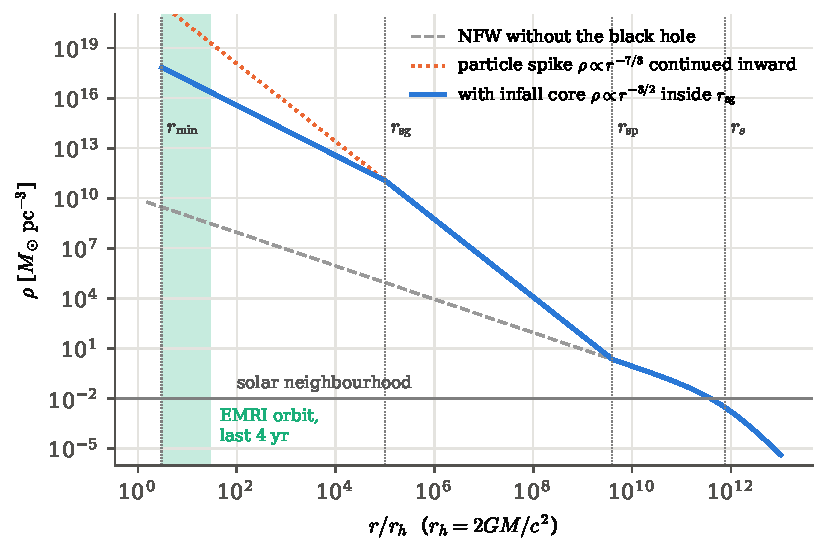
\includegraphics[width=0.82\linewidth]{figures/chT2/dm_profile.pdf}
\caption{Dark matter around a $10^4\,M_\odot$ black hole in a $10^8\,M_\odot$ NFW halo. Without the hole the density would follow the grey dashed NFW profile. Slow growth of the hole turns the cusp inside $r_{\rm sp}$ into a $r^{-7/3}$ spike (dotted where continued inward). Inside the self-gravity radius $r_{\rm sg}=10^5r_h$ an ultralight field falls freely into the hole and the profile flattens to $r^{-3/2}$ (solid). The curves stop at $r_{\rm min}=3r_h$: inside it nothing survives, the hole in the middle of the spike, and the density is zero. The green band is where the EMRI orbits during its last four years; the horizontal line is the density near the Sun.}
\label{T2a:fig:dm-profile}
\end{figure}

\paragraph{Two further wave-dark-matter pictures.}
Kim et al.\ follow the adiabatic compression of a wave halo quantum mechanically \cite{Kim2023}. Far from the hole the compressed wave halo looks like the particle spike, as expected when the wavelength is short. Close to it the picture changes, and the reason is the capture rule used above for particles. A wave component with angular-momentum quantum number $l$ carries angular momentum $l\hbar$, that is $l\hbar/\mu$ per unit mass. A particle with less than $4GM/c$ per unit mass is swallowed, so the components with
\[
  l\lesssim l_{\rm crit}=\frac{4GM}{c}\cdot\frac{\mu}{\hbar}=\frac{2\mu c\,r_h}{\hbar}
\]
fall into the hole, and over the age of the halo they are gone. A component of angular momentum $l$ cannot come closer to the centre than the radius where its centrifugal barrier turns it back, a radius that grows with $l$. Once every component below $l_{\rm crit}$ has been absorbed, nothing is left to fill the region inside the turning radius of $l_{\rm crit}$, and the density is cut off there \cite[eq.~(40)]{Kim2023}. In the particle limit ($\mu r_h c/\hbar\gg1$) $l_{\rm crit}$ is huge and the cutoff is the particle cutoff near $2$--$3r_h$; for light bosons it moves out.

Chase et al.\ consider instead a virialised halo of ultralight \emph{vector} dark matter made of many random waves \cite{Chase2025}. The field oscillates at the frequency $\mu c^2/\hbar$, and its stress, which is quadratic in the field, oscillates at twice that, $\Omega=2\mu c^2/\hbar$. Through Einstein's equations the stress makes the gravitational potential oscillate at $\Omega$ too. What the binary feels depends on the shape of that oscillation. For a scalar the oscillating stress is a pressure, the same in every direction; the oscillating pull on the companion is radial and the same at every point of a circular orbit, so it exerts no torque, and over many field oscillations its effect on the orbit averages to zero. A vector field points along a direction, its polarisation, so its stress is stronger along that axis. The oscillating tidal pull then depends on where the companion is on its orbit: a pattern with two maxima per turn, which exerts a torque proportional to $\sin2(\omega t-\varphi_0)$ for orbital angular frequency $\omega$ and polarisation angle $\varphi_0$, and whose strength oscillates as $\cos\Omega t$. The product
\[
  \cos\Omega t\,\sin2(\omega t-\varphi_0)=\tfrac12\big[\sin\big((2\omega+\Omega)t-2\varphi_0\big)+\sin\big((2\omega-\Omega)t-2\varphi_0\big)\big]
\]
averages to zero over many orbits unless $2\omega\approx\Omega$, when the second term stops oscillating. Away from that condition the pushes cancel; at it they add up, the way a swing responds only to pushes timed to its own period. This is the \newterm{resonance}, and the binary's phase changes mainly while its orbital frequency sweeps through it \cite[Sec.~V]{Chase2025}. The effect is concentrated near one frequency, so, unlike friction and accretion (\cref{T2a:sec:forces}), it cannot be written as a single power of $f$.
\section{Environmental forces and the power law in the phase}
\label{T2a:sec:forces}

Put the light companion of \cref{T2a:sec:chirp} (mass $m_2$, circling the heavy hole $m_1$, with $M=m_1+m_2$) on its orbit inside the spike of \cref{T2a:sec:dm}. It moves at $v=\sqrt{GM/r}$, about $0.13c$ at $30r_h$, through dark matter of density $\rho(r)$. Three things happen. Its gravity focuses the dark matter it passes into a trailing wake, and the wake pulls it back: \newterm{dynamical friction}. It swallows the dark matter that comes close enough, and the swallowed matter has to be brought up to the companion's speed: \newterm{accretion}. And the dark matter inside the orbit adds to the central pull. The first two drain orbital energy on top of the gravitational waves, so the binary sweeps through frequency faster than in vacuum.

The question for the statistics is narrow: \emph{for each effect, by how much does it speed up the sweep at frequency $f$, and what does that do to the Fourier phase $\Psi(f)$?} ($\Psi$ is the phase of the stationary-phase signal of \cref{T2a:sec:spa}, $\tilde h=\mathcal Af^{-7/6}e^{-i\Psi}$.) The answer turns out to have the same form for all of them, a power of $f$ added to the phase, and that is what makes a single, general forecast possible in \cref{ch:10}.

\subsection{The forces}

\paragraph{Dynamical friction.}
For a body of mass $m_2$ moving at speed $v$ through collisionless matter of density $\rho$, Chandrasekhar's formula gives a drag
\begin{equation}
  F_{\rm DF}=\frac{4\pi G^2m_2^2\,\rho\,\xi\ln\Lambda}{v^2}
  \label{T2a:eq:df}
\end{equation}
\cite{Chandrasekhar1943}, \cite[eq.~(16)]{Eda2015}, \cite[eq.~(7)]{Coogan2022}. Every factor can be derived from one deflection.

\emph{One particle passing.} Work in the companion's frame, where the dark matter streams past at speed $v$. Take first the simplest stream, every particle moving at exactly $v$. A particle of mass $m_{\rm dm}\ll m_2$ that would miss the companion by the \newterm{impact parameter} $s$ (we write $s$, not the usual $b$, which is reserved for the ppE exponent below) is bent through an angle $\theta$ given by the Kepler hyperbola, $\tan(\theta/2)=Gm_2/(sv^2)$. Its speed far away is unchanged, only its direction turns, so it loses forward momentum $m_{\rm dm}v(1-\cos\theta)$. That momentum goes to the companion and points along the stream, that is, against the companion's motion through the dark matter. The sideways kicks cancel between particles passing on opposite sides.

\emph{All the particles.} Particles with impact parameter between $s$ and $s+\dd s$ arrive at the rate $(\rho/m_{\rm dm})\,v\,2\pi s\,\dd s$. With $s_{90}\equiv Gm_2/v^2$, the impact parameter that turns a particle through $90^\circ$,
\begin{align}
  F
  &\eqby{1}\int\frac{\rho}{m_{\rm dm}}\,v\,2\pi s\,\dd s\;m_{\rm dm}v\,(1-\cos\theta)
  \eqby{2}4\pi\rho v^2s_{90}^2\int_0^{s_{\max}}\frac{s\,\dd s}{s^2+s_{90}^2}\nonumber\\
  &\eqby{3}\frac{4\pi G^2m_2^2\rho}{v^2}\cdot\frac12\ln\Big(1+\frac{s_{\max}^2}{s_{90}^2}\Big)
  \eqby{4}\frac{4\pi G^2m_2^2\rho}{v^2}\,\ln\Lambda,\qquad\Lambda\equiv\frac{s_{\max}}{s_{90}} .\label{T2a:eq:df-derive}
\end{align}
\begin{explain}
  \item Momentum per particle times the rate of particles, summed over impact parameters. The mass $m_{\rm dm}$ cancels: only the density matters.
  \item $1-\cos\theta=2\sin^2(\theta/2)=2\tan^2(\theta/2)/[1+\tan^2(\theta/2)]=2s_{90}^2/(s^2+s_{90}^2)$, using $\tan(\theta/2)=s_{90}/s$.
  \item $\int s\,\dd s/(s^2+s_{90}^2)=\tfrac12\ln(s^2+s_{90}^2)$; and $v^2s_{90}^2=G^2m_2^2/v^2$.
  \item For $s_{\max}\gg s_{90}$, $\tfrac12\ln(1+\Lambda^2)\approx\ln\Lambda$.
\end{explain}
So each factor has a reason. One $m_2$ comes from the strength of each deflection and the other from the size $s_{90}$ of the region where deflections are strong; the $1/v^2$ says a slow body has more time to bend each particle. The logarithm counts the e-folds of impact parameter between $s_{90}$ and $s_{\max}$, each adding the same amount, so distant encounters matter as much as close ones and the integral must be cut off by hand. The lower end is $s_{\min}=s_{90}$, below which particles are turned right round and nothing more is gained; the upper end $s_{\max}$ is the size of the region in which the stream is a uniform flow, the orbit itself, $s_{\max}\sim r$.

\emph{Particles of all speeds.} A real spike has particles with a spread of speeds. Chandrasekhar showed that for an isotropic distribution the particles faster than the body pull it, on average, equally forwards and backwards, and only those slower than $v$ contribute. The factor $\xi$ in \eqref{T2a:eq:df} is that fraction, $\xi=4\pi\int_0^vf(u)u^2\,\dd u$ for the distribution $f(u)$ of particle speeds. For the $7/3$ spike, whose speeds are set by the hole's potential, it is about $0.58$ \cite{Coogan2022}; papers that ignore the spread set it to one.

\emph{The size of the logarithm.} On a circular orbit $v^2=GM/r$, so $s_{90}=Gm_2/v^2=r\,m_2/M$. With $s_{\max}=r$, $\Lambda\approx M/m_2\approx m_1/m_2$. Coogan et al.\ take a more cautious $s_{\max}=\sqrt{rs_{90}}$, the geometric mean of the two ends, which halves the logarithm: $\ln\Lambda=\ln\sqrt{m_1/m_2}$ \cite{Coogan2022}. For the $10^3+1.4\,M_\odot$ IMRI that is $\TwlnLambdaC$ against $6.6$; others take about $3$ \cite{Eda2015}. Only the logarithm enters, so this factor of two is the size of the uncertainty in the prescription. \emph{Check at $30r_h$.} There $v^2/c^2=r_h/(2r)=1/60$, so $s_{90}=Gm_2/v^2=\tfrac12(2Gm_2/c^2)(c/v)^2=30$ Schwarzschild radii of the companion: the deflections that build the logarithm happen well outside the companion's own horizon, where the Newtonian hyperbola is a fair description. The power the friction removes is $P_{\rm DF}=F_{\rm DF}\,v$.

\paragraph{Friction on a wave.}
If the dark matter is a wave (\cref{T2a:sec:dm}), a wake smaller than its wavelength cannot form. The force keeps the form of \eqref{T2a:eq:df}, with $\xi\ln\Lambda$ replaced by a function of $kr$, where $k=\mu v/\hbar$ is the dark matter's wavenumber \cite[eq.~(D14)]{HuiOstriker2017}, \cite[eq.~(42)]{Kim2023}:
\begin{equation}
  F_{\rm DF}^{\rm wave}=\frac{4\pi G^2m_2^2\rho\,C_w(kr)}{v^2},\qquad
  C_w(kr)=\mathrm{Cin}(2kr)-1+\frac{\sin2kr}{2kr},\qquad \mathrm{Cin}(z)=\int_0^z\frac{1-\cos t}{t}\,\dd t .
  \label{T2a:eq:df-wave}
\end{equation}
Hui and Ostriker obtain it by solving the scattering of the wave by the companion and summing the momentum carried off by its partial waves. The integral shows why it is a softened Coulomb logarithm. Its variable $t$ measures distance in units of the reduced wavelength. Far beyond a wavelength, $\cos t$ oscillates and averages away, and the integrand is $1/t$, the integrand $\dd s/s$ of $\ln\Lambda$. Within a wavelength the interference of the wave ($1-\cos t\approx t^2/2$) kills the integrand. So Cin is a Coulomb logarithm whose lower cutoff is the wavelength instead of $s_{90}$, and whose upper cutoff is the orbit, $z=2kr$; the terms $-1+\sin z/z$ come from the finite size of the region.

Its two limits tell the story. For a short wavelength, $kr\gg1$, split off the logarithm: $\mathrm{Cin}(z)=\gamma_E+\ln z-\mathrm{Ci}(z)$, where $\gamma_E=0.577$ is Euler's constant and $\mathrm{Ci}(z)=-\int_z^\infty\cos t\,\dd t/t$ is a decaying oscillation, of size $\lvert\sin z\rvert/z$ for large $z$. Both $\mathrm{Ci}(z)$ and $\sin z/z$ go to zero, so $C_w\to\ln(2kr)+\gamma_E-1$: a Coulomb logarithm with $s_{\max}\sim r$ and $s_{\min}\sim1/k$, the particle result. For a long wavelength, $z=2kr\ll1$,
\begin{align*}
  C_w
  &\eqby{1}\Big(\frac{z^2}{4}-\frac{z^4}{96}\Big)-1+\Big(1-\frac{z^2}{6}+\frac{z^4}{120}\Big)+O(z^6)
  \eqby{2}\frac{z^2}{12}+O(z^4)=\frac{(kr)^2}{3}+O\big((kr)^4\big),
\end{align*}
\begin{explain}
  \item Expand $1-\cos t=t^2/2-t^4/24$, so $\mathrm{Cin}(z)=z^2/4-z^4/96$; and $\sin z/z=1-z^2/6+z^4/120$.
  \item The constants cancel and $\tfrac14-\tfrac16=\tfrac1{12}$; with $z=2kr$, $z^2/12=(kr)^2/3$.
\end{explain}
so friction is suppressed as $(kr)^2$ when the wavelength exceeds the orbit. \Cref{T2a:fig:wave-df} shows both limits; at $kr=0.1$ the small-$kr$ form is already accurate to $\TwCwSmallErr\%$. This suppression, together with the lower density near the hole, is why wave-like dark matter dephases the inspiral less than particle dark matter of the same mass density \cite[Sec.~III D]{Kim2023}.

\begin{figure}[htbp]
\centering
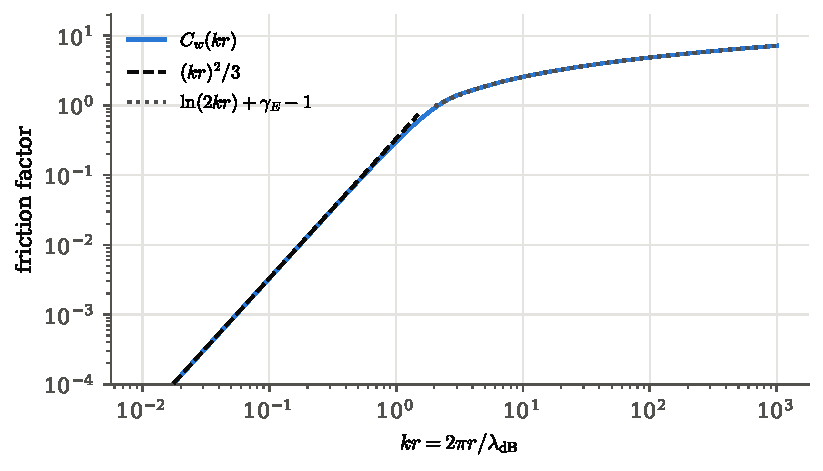
\includegraphics[width=0.75\linewidth]{figures/chT2/wave_df.pdf}
\caption{The friction factor of a wave-like medium as a function of $kr=2\pi r/\lambda_{\rm dB}$. When the de Broglie wavelength is longer than the orbit ($kr\ll1$) friction is suppressed as $(kr)^2/3$ (dashed); when it is shorter, the factor grows like the Coulomb logarithm of particle dark matter (dotted).}
\label{T2a:fig:wave-df}
\end{figure}

\paragraph{Accretion.}
How much dark matter does the companion swallow? In its own rest frame the dark matter streams in at speed $v$, each particle with angular momentum per unit mass $L=sv$ about the companion. General relativity supplies one fact: a particle arriving from far away with $L$ below $L_{\rm crit}=4Gm_2/c$ meets no centrifugal barrier and crosses the horizon (the same capture rule that cuts off the spike near the central hole, \cref{T2a:sec:dm}). Setting $sv=L_{\rm crit}$ gives the capture radius and the cross-section,
\[
  s_{\rm cap}=\frac{4Gm_2}{cv},\qquad \sigma=\pi s_{\rm cap}^2=\frac{16\pi G^2m_2^2}{c^2v^2}.
\]
The mass swallowed per unit time is the mass flux through that area, $\dot m=\rho v\sigma=16\pi G^2m_2^2\rho/(c^2v)$. Now go back to the frame of the spike. There the dark matter is (on average) at rest, and after capture it moves with the companion at speed $v$. The companion must supply that momentum, $\dot m\,v$ per unit time: a drag force $F_{\rm acc}=\dot m\,v$ and a power $P_{\rm acc}=\dot mv^2$. The ratio $s_{\rm cap}/s_{90}=4v/c$ is about $0.5$ at $30r_h$: the particles swallowed are a subset of those strongly deflected, which is why accretion comes out as a correction to friction. Compared with friction,
\begin{equation}
  \frac{P_{\rm acc}}{P_{\rm DF}}
  =\frac{16\pi G^2m_2^2\rho\,v/c^2}{4\pi G^2m_2^2\rho\ln\Lambda/v}
  =\frac{4v^2}{c^2\ln\Lambda}
  =\frac{2r_h}{r\ln\Lambda},
\end{equation}
using $v^2=GM/r=c^2r_h/(2r)$ and $\xi=1$. With $\ln\Lambda=3$ this is $\TwaccRatioThirty$ at $30r_h$ and $\TwaccRatioThree$ at the ISCO. Accretion of collisionless dark matter is a relativistic correction to friction. Kim et al.\ check this for their binaries: over the last five years the companion's mass grows by only about one part in $10^4$ \cite[Sec.~IV A]{Kim2023}. For gas, which is collisional, the Bondi--Hoyle--Lyttleton rate $\dot m\propto\rho/v^3$ applies instead, and accretion then scales exactly like friction \cite[Sec.~X]{Barausse2014}.

\paragraph{The gravitational pull.}
The dark matter inside the orbit adds to the central mass. For the spike $\rho=\rho_6(r_6/r)^\gamma$ (with $\gamma<3$) it weighs
\[
  M_{\rm DM}(<r)=\int_0^r4\pi r'^2\rho_6\Big(\frac{r_6}{r'}\Big)^{\gamma}\dd r'=\frac{4\pi\rho_6r_6^{\gamma}}{3-\gamma}\,r^{3-\gamma}.
\]
By the shell theorem, a spherical mass inside the orbit pulls like a point mass at the centre, so Kepler's law holds with $M_{\rm tot}=M+M_{\rm DM}(<r)$ in place of $M$ \cite[eqs.~(9)--(11)]{Speeney2022}. This removes no energy, but it changes the relation between the frequency and the orbit. How much does it change the chirp? Hold the gravitational-wave frequency $f$ fixed, with $\omega=\pi f$, and treat $M_{\rm DM}$ as a constant addition to the central mass over the small range of radii near the current orbit. Each quantity in the chirp rate is a power of $M_{\rm tot}$:
\begin{align*}
  r&\eqby{1}\Big(\frac{GM_{\rm tot}}{\pi^2f^2}\Big)^{1/3}\propto M_{\rm tot}^{1/3},\qquad
  E\eqby{2}-\frac{GM_{\rm tot}\mu}{2r}=-\frac\mu2(\pi GM_{\rm tot}f)^{2/3}\propto M_{\rm tot}^{2/3},\\
  P_{\rm GW}&\eqby{3}\frac{32}{5}\frac{G}{c^5}\mu^2r^4\omega^6\propto M_{\rm tot}^{4/3},\qquad
  \frac{\dot f}{\dot f_{\rm V}}\eqby{4}\frac{P_{\rm GW}/\lvert\dd E/\dd f\rvert}{(\dots)_{M_{\rm tot}=M}}=\Big(1+\frac{M_{\rm DM}}{M}\Big)^{2/3}\approx1+\frac23\,\frac{M_{\rm DM}(<r)}{M}.
\end{align*}
\begin{explain}
  \item Kepler's law, $\omega^2=GM_{\rm tot}/r^3$.
  \item The binding energy \eqref{T2a:eq:Ef} with $M\to M_{\rm tot}$; $\dd E/\dd f$ scales the same way.
  \item The quadrupole power at fixed $\omega$ depends on $M_{\rm tot}$ only through $r^4$.
  \item The chirp rate of \eqref{T2a:eq:fdot} is $P_{\rm GW}/\lvert\dd E/\dd f\rvert\propto M_{\rm tot}^{4/3-2/3}$; expand for $M_{\rm DM}\ll M$.
\end{explain}
So the pull speeds up the chirp by the fraction
\[
  \epsilon_{\rm pull}=\frac23\,\frac{M_{\rm DM}(<r)}{M}=\frac{8\pi\rho_6r_6^\gamma}{3(3-\gamma)M}\,r^{3-\gamma}\propto f^{-2(3-\gamma)/3},
\]
using $r\propto f^{-2/3}$. The coefficient $\tfrac23$ is leading order only, because $M_{\rm DM}(<r)$ itself changes as the orbit shrinks; the exponent does not depend on that. Friction usually matters more \cite[Sec.~IX]{Barausse2014}.

\subsection{From an extra power to a power law in the phase}

\paragraph{The fractional extra power.}
Throughout, $f$ is the gravitational-wave frequency, twice the orbital one, $f=\omega/\pi$ \eqref{T2g:eq:twice}. Friction drains energy slowly, so at each moment the orbit is still a circle obeying Kepler's law, and its energy at frequency $f$ is the vacuum $E(f)$ of \eqref{T2a:eq:Ef}; only the rate at which it moves through these energies changes. Energy balance now reads $\dd E/\dd t=-(P_{\rm GW}+P_{\rm DF})$, with $P_{\rm GW}$ the quadrupole power of a circular binary \eqref{T2g:eq:power-binary}. As in \eqref{T2a:eq:fdot},
\begin{equation}
  \dot f\eqby{1}-\frac{P_{\rm GW}+P_{\rm DF}}{\dd E/\dd f}
  \eqby{2}\frac{P_{\rm GW}}{\lvert\dd E/\dd f\rvert}\Big(1+\frac{P_{\rm DF}}{P_{\rm GW}}\Big)
  \eqby{3}\dot f_{\rm V}\,\big[1+\epsilon(f)\big],\qquad \epsilon\equiv\frac{P_{\rm DF}}{P_{\rm GW}},
  \label{T2a:eq:fdot-env}
\end{equation}
\begin{explain}
  \item $\dd E/\dd t=(\dd E/\dd f)\,\dot f$, since $E$ depends on time only through $f$.
  \item $\dd E/\dd f<0$; factor out $P_{\rm GW}$.
  \item The first factor is the vacuum rate $\dot f_{\rm V}$ of \eqref{T2a:eq:fdot}.
\end{explain}
This is the energy balance of Kim et al.\ \cite[eq.~(36)]{Kim2023}. For friction in a spike $\rho=\rho_6(r_6/r)^\gamma$ (here and below $\gamma$ is the spike slope $\gamma_{\rm sp}$ of \cref{T2a:sec:dm}, and $\rho_6$ the density at $r_6=10^{-6}$\,pc),
\begin{align}
  \epsilon
  &\eqby{1}\frac{4\pi G^2m_2^2\rho\,\xi\ln\Lambda/v}{\frac{32}{5}G^4M(m_1m_2)^2/(c^5r^5)}
  \eqby{2}\frac{5\pi c^5\xi\ln\Lambda}{8G^{5/2}M^{3/2}m_1^2}\;\rho(r)\,r^{11/2}
  \eqby{3}c_f\,f^{-n},\qquad n=\frac{11-2\gamma}{3}.\label{T2a:eq:eps}
\end{align}
\begin{explain}
  \item $P_{\rm DF}=F_{\rm DF}v$ from \eqref{T2a:eq:df}; $P_{\rm GW}=\tfrac{32}{5}(G/c^5)\mu^2r^4\omega^6=\tfrac{32}{5}G^4M^3\mu^2/(c^5r^5)$ by Kepler, and $M^3\mu^2=M(m_1m_2)^2$ \cite[eq.~(6)]{Coogan2022}.
  \item $m_2^2$ cancels, and $1/v=r^{1/2}(GM)^{-1/2}$. The result $\epsilon\propto\rho r^{11/2}$ is \cite[eq.~(16)]{Speeney2022}.
  \item Insert $\rho=\rho_6r_6^\gamma r^{-\gamma}$, so $\rho r^{11/2}=\rho_6r_6^\gamma\,r^{11/2-\gamma}$, and trade the radius for the gravitational-wave frequency with Kepler's law, $r=(GM/\pi^2f^2)^{1/3}$: $r^{11/2-\gamma}=(GM/\pi^2)^{(11/2-\gamma)/3}f^{-\frac23(\frac{11}2-\gamma)}$, and $\frac23(\frac{11}2-\gamma)=\frac{11-2\gamma}3=n$.
\end{explain}
Collecting the constants of step (3),
\begin{equation}
  c_f=\frac{5\pi c^5\xi\ln\Lambda}{8G^{5/2}M^{3/2}m_1^2}\;\rho_6r_6^{\gamma}\,\Big(\frac{GM}{\pi^2}\Big)^{(11/2-\gamma)/3},
  \label{T2a:eq:cf}
\end{equation}
with units of ${\rm Hz}^n$, so that $c_ff^{-n}$ is a pure number; the $f$ in $c_ff^{-n}$ is the gravitational-wave frequency. Friction and radiation remove energy equally fast where $\epsilon=1$, at $f_{\rm eq}\equiv c_f^{1/n}$.
The same step works for any effect whose power, relative to the gravitational-wave power, varies as a power of the radius: $P_{\rm env}/P_{\rm GW}\propto r^p$ gives $\epsilon\propto f^{-2p/3}$. Since $P_{\rm GW}\propto r^{-5}$ falls so steeply with radius, nearly every environmental effect has $p>0$: it matters most early in the inspiral, at low frequency.

\paragraph{The phase.}
Recall why the chirp rate controls the Fourier phase. The slope of the phase is the arrival time of each frequency, $\dd\Psi/\dd f=2\pi t(f)$, and differentiating once more turns $\dd t/\dd f$ into $1/\dot f$: the curvature of the phase is $2\pi/\dot f$ \eqref{T2a:eq:psi-derivs}, derived with the stationary-phase approximation in \cref{T2a:sec:spa}. A binary that sweeps faster spends less time at each frequency, and the phase bends less. With \eqref{T2a:eq:fdot-env}, and $\dot f_{\rm V}=Kf^{11/3}$, $K=\tfrac{96}{5}\pi^{8/3}(G\mathcal M/c^3)^{5/3}$,
\begin{align}
  \frac{\dd^2\Psi}{\dd f^2}
  &\eqby{1}\frac{2\pi}{\dot f_{\rm V}(1+\epsilon)}
  \eqby{2}\frac{2\pi}{\dot f_{\rm V}}-\frac{2\pi c_f}{K}\,f^{-11/3-n}+O(\epsilon^2),\nonumber\\
  \delta\Psi(f)
  &\eqby{3}-\frac{2\pi c_f}{K\,(n+\frac83)(n+\frac53)}\,f^{-5/3-n}+C_0+C_1f
  \eqby{4}\beta\,u^{\,b},\qquad u\equiv\frac{\pi G\mathcal Mf}{c^3},\quad b=-\frac53-n .\label{T2a:eq:ppe}
\end{align}
\begin{explain}
  \item \eqref{T2a:eq:psi-derivs} with \eqref{T2a:eq:fdot-env}.
  \item $1/(1+\epsilon)=1-\epsilon+\dots$ for $\epsilon\ll1$; the first term gives the vacuum phase \eqref{T2a:eq:psiN}, the second is the change, with $\epsilon/f^{11/3}=c_ff^{-11/3-n}$.
  \item Integrate twice: $f^{-11/3-n}\to f^{-8/3-n}/(-\frac83-n)\to f^{-5/3-n}/[(\frac83+n)(\frac53+n)]$. The two integration constants $C_0+C_1f$ have the form of a shift of $\phi_c$ and of $t_c$ in \eqref{T2a:eq:psiN}, so they are absorbed there (\cref{T2g:sec:tc-phic}).
  \item Rewrite $f=u\,c^3/(\pi G\mathcal M)$, so $f^{-5/3-n}=u^{b}(\pi G\mathcal M/c^3)^{5/3+n}$; all constants go into $\beta$. $u$ is the reduced frequency of \eqref{T2g:eq:u}.
\end{explain}
The amplitude, written out, is
\[
  \beta=-\frac{2\pi c_f}{K\,(n+\frac83)(n+\frac53)}\Big(\frac{\pi G\mathcal M}{c^3}\Big)^{5/3+n}
  =-\frac{5}{48}\,\frac{c_f\,(\pi G\mathcal M/c^3)^{n}}{(n+\frac83)(n+\frac53)},
\]
using $2\pi(\pi G\mathcal M/c^3)^{5/3}/K=\tfrac{10\pi}{96}\pi^{5/3-8/3}=\tfrac5{48}$. It is proportional to $c_f$, hence to the density $\rho_6$ of the spike, and the combination $c_f(\pi G\mathcal M/c^3)^n$ is a pure number. A check: for $n=0$ the environment speeds the chirp up by a constant fraction $c_f$, which by step (2) multiplies the Newtonian term $\tfrac3{128}u^{-5/3}$ of \eqref{T2a:eq:psiN} by $1-c_f$; and indeed $-\tfrac5{48}c_f/(\tfrac83\cdot\tfrac53)=-\tfrac3{128}c_f$.

\begin{keyidea}[Environments are power laws in the phase]
If an environment adds a power $P_{\rm env}$ with $P_{\rm env}/P_{\rm GW}=c_ff^{-n}\ll1$, the Fourier phase gains $\delta\Psi=\beta u^b$ with $u=\pi G\mathcal Mf/c^3$ and $b=-5/3-n$; the amplitude $\beta$ carries the strength of the effect and the exponent $b$ its physics. For dynamical friction in a spike $\rho\propto r^{-\gamma}$, $b=(2\gamma-16)/3$; for $\gamma=7/3$, $b=-34/9\approx-3.78$.
\end{keyidea}

This is the parametrised post-Einsteinian (ppE) phase term $\beta u^b$ of \eqref{T2g:eq:ppe}, now with a definite exponent: the general rule \eqref{T2g:eq:ppe-rule} with $p=-3n$ gives the same $b=-\tfrac53-n$. In the post-Newtonian counting of \cref{T2g:sec:pn}, a correction of relative size $(v/c)^{2k}$ is of order $k$PN, and on a circular orbit $(v/c)^2=(\pi GMf/c^3)^{2/3}\propto f^{2/3}$. So $f^{-n}\propto[(v/c)^2]^{-3n/2}$, and $\epsilon\propto f^{-n}$ is a correction of order $-\tfrac32n$\,PN, so friction in a uniform medium ($\gamma=0$, $n=11/3$) is a $-5.5$PN effect. The dissipative effects, friction and accretion in any spike with $\gamma<3$, have $b<-7/3$: they act more strongly at low frequency than the dipole radiation ($b=-7/3$) and the massive graviton ($b=-1$) of \cref{T2g:sec:pn}. In the Fisher matrix of \cref{ch:10} this is what separates them from the chirp mass, whose own phase term goes as $u^{-5/3}$: two terms with different powers of $f$ are hard to mimic with one another.

\paragraph{The time-domain dephasing.}
Papers on environments usually plot a different phase: the number of radians the wave still has to go through before coalescence. Its phase advances at the rate $2\pi f$, so between frequency $f$ and coalescence at $f_c$
\[
  \Phi(f)=2\pi\int_t^{t_c}f(t')\,\dd t'=2\pi\int_f^{f_c}\frac{f'}{\dot f(f')}\,\dd f',
\]
changing the variable from time to frequency with $\dd t'=\dd f'/\dot f$. The \newterm{dephasing} is the vacuum phase still to come minus the phase still to come in the environment, $\Delta\Phi(f)=\Phi_{\rm V}(f)-\Phi(f)$ \cite[eq.~(49)]{Kim2023}; $\Phi_{\rm V}$ is the $\Phi$ of \cref{T2a:sec:spa} for the Newtonian chirp. A faster sweep leaves fewer cycles, so $\Delta\Phi>0$.

Why two phases? $\Delta\Phi$ is the size that is easy to feel: it counts the radians of wave the environment removes, and once it reaches about a radian a vacuum template is visibly out of step with the signal. The Fisher matrix and the likelihood work in the frequency domain, with the phase $\Psi$ of the template; there part of $\Delta\Phi$ is absorbed by adjusting the arrival time $t_c$ and the phase $\phi_c$, which are fitted anyway. So the two answer different questions, and we compute both.

With \eqref{T2a:eq:fdot-env} and $\dot f_{\rm V}=Kf^{11/3}$,
\begin{align}
  \Delta\Phi(f)
  &\eqby{1}2\pi\int_f^{\infty}\frac{f'}{K f'^{11/3}}\Big(1-\frac1{1+c_ff'^{-n}}\Big)\dd f'
  \eqby{2}\frac{2\pi c_f}{K}\int_f^\infty f'^{-8/3-n}\dd f'\nonumber\\
  &\eqby{3}\frac{2\pi c_f}{K}\,\frac{f^{-5/3-n}}{\frac53+n}
  \eqby{4}\frac{5\,c_f f^{-n}}{2(8-\gamma)}\,\Phi_{\rm V}(f).\label{T2a:eq:dPhi}
\end{align}
\begin{explain}
  \item The difference of the two phase integrals, $1/\dot f_{\rm V}-1/\dot f=\frac1{\dot f_{\rm V}}\big(1-\frac1{1+\epsilon}\big)$, with the upper limit $f_c$ sent to infinity (justified below).
  \item $1-1/(1+\epsilon)\approx\epsilon=c_ff'^{-n}$ for $\epsilon\ll1$.
  \item $\int_f^\infty f'^{-8/3-n}\dd f'=f^{-5/3-n}/(\frac53+n)$.
  \item $\Phi_{\rm V}=\frac{2\pi}{K}\cdot\frac35f^{-5/3}$, so the ratio is $\frac{5}{3}c_ff^{-n}/(\frac53+n)=5c_ff^{-n}/(5+3n)$, and $5+3n=16-2\gamma$.
\end{explain}
\emph{The upper limit.} The integrand of $\Delta\Phi$ falls as $f'^{-8/3-n}$, so the part beyond $f_c$ is a fraction $(f/f_c)^{5/3+n}$ of the whole. For the IMRI, with $f_c$ the ISCO frequency of about $4.4$\,Hz and $f$ the $\TwffourImri$\,mHz at which the four-year window opens, that fraction is about $2\times10^{-9}$ for $\gamma=7/3$, and smaller still for the other slopes. Integrating to infinity, as here, and stopping at the ISCO, as the script does, give the same numbers to that accuracy.

This is the high-frequency limit quoted by Coogan et al.\ \cite[eq.~(16)]{Coogan2022}, and it has the same exponent $-5/3-n$ as $\delta\Psi$. The two coefficients compare in one line: from \eqref{T2a:eq:ppe} and \eqref{T2a:eq:dPhi},
\[
  \frac{\delta\Psi}{\Delta\Phi}
  =\frac{-2\pi c_f/[K(n+\frac83)(n+\frac53)]}{2\pi c_f/[K(n+\frac53)]}
  =-\frac1{n+\frac83}\qquad(f\gg f_{\rm eq}),
\]
and for $n=0$ (a constant fractional speed-up) this is the factor $\tfrac38$ between the two kinds of phase found in \cref{T2a:sec:spa}. The sign only records that $\Delta\Phi$ is defined as vacuum minus environment.

\emph{Without the expansion.} Step (2) needs $\epsilon\ll1$, i.e.\ $f\gg f_{\rm eq}$. The integral can also be done exactly. Write the geometric series $1/(1+\epsilon)=\sum_k(-\epsilon)^k$ and integrate term by term:
\begin{align}
  \Phi(f)
  &\eqby{1}\frac{2\pi}{K}\sum_{k=0}^\infty(-c_f)^k\int_f^\infty f'^{-8/3-kn}\dd f'\nonumber\\
  &\eqby{2}\Phi_{\rm V}(f)\sum_{k=0}^\infty\frac{a}{a+k}\big(-c_ff^{-n}\big)^k\nonumber\\
  &\eqby{3}\Phi_{\rm V}(f)\;{}_2F_1\big(1,a;1+a;-c_ff^{-n}\big),\qquad a\equiv\frac5{3n}.\label{T2a:eq:hyp}
\end{align}
\begin{explain}
  \item $\Phi=2\pi\int_f^\infty f'/\dot f\,\dd f'$ with $\dot f=Kf'^{11/3}(1+c_ff'^{-n})$.
  \item $\int_f^\infty f'^{-8/3-kn}\dd f'=f^{-5/3-kn}/(\tfrac53+kn)$; factoring out the $k=0$ term, which is $\Phi_{\rm V}$, leaves $\tfrac{5/3}{5/3+kn}=\tfrac{a}{a+k}$.
  \item The \newterm{Pochhammer symbol} is the rising product $(x)_k=x(x+1)\cdots(x+k-1)$, with $(x)_0=1$. In $\frac{(a)_k}{(1+a)_k}=\frac{a(a+1)\cdots(a+k-1)}{(a+1)\cdots(a+k)}$ every factor but the first on top and the last below cancels, leaving $\frac{a}{a+k}$. The \newterm{hypergeometric function} is the series ${}_2F_1(\alpha,\beta;\gamma';z)=\sum_k\frac{(\alpha)_k(\beta)_k}{(\gamma')_k\,k!}z^k$; with $\alpha=1$, $(1)_k=k!$ cancels the $k!$, and with $\beta=a$, $\gamma'=1+a$ the series is $\sum_k\frac{a}{a+k}z^k$.
\end{explain}
The geometric series converges only for $\epsilon<1$, yet the phase at lower frequencies, where friction dominates, is a perfectly finite integral. The same substitution that turned the series into ${}_2F_1$ shows that nothing is lost. Put $t=(f/f')^n$ in the exact integral, with $z=-c_ff^{-n}$:
\begin{align*}
  \frac{K}{2\pi}\Phi(f)
  &\eqby{1}\int_f^\infty\frac{f'^{-8/3}\,\dd f'}{1+c_ff'^{-n}}
  \eqby{2}\frac{f^{-5/3}}{n}\int_0^1\frac{t^{a-1}\,\dd t}{1-zt}
  \eqby{3}\frac35f^{-5/3}\;a\!\int_0^1\frac{t^{a-1}\,\dd t}{1-zt}.
\end{align*}
\begin{explain}
  \item The definition with $\dot f=Kf'^{11/3}(1+c_ff'^{-n})$.
  \item $f'=ft^{-1/n}$, $\dd f'=-(f/n)t^{-1/n-1}\dd t$, and $c_ff'^{-n}=c_ff^{-n}t=-zt$; the powers of $t$ combine to $t^{(8/3-1)/n-1}=t^{a-1}$, and $f'$ from $f$ to $\infty$ is $t$ from $1$ to $0$.
  \item $1/n=\tfrac35a$.
\end{explain}
Expanding $1/(1-zt)=\sum_k(zt)^k$ and using $a\int_0^1t^{a-1+k}\dd t=a/(a+k)$ returns exactly the series of \eqref{T2a:eq:hyp}, so the last integral \emph{is} ${}_2F_1(1,a;1+a;z)$ where the series converges. But the integral is finite and smooth for every $z\le0$, since $1-zt\ge1$, so it defines the function at every frequency; this is Euler's integral for the hypergeometric function, the standard way of continuing it beyond $\lvert z\rvert<1$. Hence \eqref{T2a:eq:hyp} holds at all frequencies \cite[eq.~(12)]{Coogan2022}. At low frequency, $f\to0$, $z\to-\infty$ and the integral goes to zero: friction then sweeps the binary through each frequency so fast that it accumulates almost none of the vacuum phase, and $\Delta\Phi\to\Phi_{\rm V}$.

\subsection{The experiment: dephasing for several spike slopes}
\label{T2a:sec:coogan}

\subsubsection*{Their question}
Coogan et al.\ asked whether LISA could tell an intermediate-mass-ratio inspiral wrapped in a dark-matter spike from the same binary in vacuum, and whether the signal would then measure the spike's density and slope \cite{Coogan2022}. Earlier estimates had used a fixed spike and found enormous dephasings. Their point was that the friction heats the spike it feeds on, so the honest question is what survives once the spike is allowed to respond. We reproduce the static part of their calculation, which is what the equations of this section describe, and use it to see where the static picture stops.

\subsubsection*{Their setup}
The binary is a $10^3\,M_\odot$ black hole with a $1.4\,M_\odot$ companion, the IMRI of \cref{T2a:sec:chirp}. Around the heavy hole sits a spike $\rho=\rho_6(r_6/r)^\gamma$ whose density at the pivot radius $r_6=10^{-6}$\,pc is fixed to their benchmark value (\cref{T2a:sec:dm} derived it from $\rho_{\rm sp}=226\,M_\odot\,{\rm pc}^{-3}$). The companion feels Chandrasekhar's friction \eqref{T2a:eq:df}, with the fraction $\xi$ of slow particles appropriate for a $7/3$ spike and their logarithm $\ln\sqrt{m_1/m_2}$. We keep $\rho_6$ fixed and vary the slope, to see how the dephasing depends on $\gamma$, and we look at the last four years before the ISCO, a nominal LISA mission.
\begin{center}
\small
\begin{tabular}{@{}lll@{}}
\toprule
quantity & meaning & value\\\midrule
$m_1$, $m_2$ & central hole, companion & $10^3\,M_\odot$, $1.4\,M_\odot$\\
$\rho_6$ & spike density at $r_6$ & $5.45\times10^{15}\,M_\odot\,{\rm pc}^{-3}$\\
$r_6$ & pivot radius & $10^{-6}$\,pc\\
$\xi$ & fraction of slower particles & $0.58$\\
$\ln\Lambda$ & Coulomb logarithm, $\ln\sqrt{m_1/m_2}$ & $\TwlnLambdaC$\\
$\gamma$ & spike slope & $1.5$, $2$, $7/3$, $2.5$\\
window & last four years before the ISCO & from $\TwffourImri$\,mHz\\
\bottomrule
\end{tabular}
\end{center}

\subsubsection*{Their equations in ours}
Everything needed has been derived above, and we kept their symbols wherever they had one: $\rho_6$, $r_6$, $c_f$ and $f_{\rm eq}$ mean the same here as there, and $f$ is in both cases the gravitational-wave frequency.
\begin{center}
\small
\begin{tabular}{@{}lll@{}}
\toprule
Coogan et al. & here & content\\\midrule
eq.~(12) & \eqref{T2a:eq:hyp} & exact phase to coalescence in a static spike\\
eq.~(15) & $f_{\rm eq}=c_f^{1/n}$, with \eqref{T2a:eq:cf} & where friction and radiation are equal\\
eq.~(16) & \eqref{T2a:eq:dPhi} & high-frequency power law of the dephasing\\
\bottomrule
\end{tabular}
\end{center}
The one convention to watch is which phase is quoted: their dephasing is the time-domain $\Delta\Phi$, not the Fourier $\delta\Psi$ of the Fisher matrix, and the two differ by the factor $-1/(n+\tfrac83)$ derived above.

\subsubsection*{What we compute}
The script \pyname{05_dephasing.py} evaluates these formulas for the four slopes:

\pyfile[firstline=36,lastline=51,firstnumber=36]{code/chT2/05_dephasing.py}{The friction-to-radiation ratio and the exact dephasing}

\noindent It makes four moves. First, lines 38--39 compute the constants of \eqref{T2a:eq:cf}: \pyname{rho_SI} is $\rho_6r_6^\gamma$ in SI units, and \pyname{pref} is the prefactor of step (2) of \eqref{T2a:eq:eps}. Second, line 41 completes $c_f$ by writing the radius through Kepler's law, the factor $(GM/\pi^2)^{(11-2\gamma)/6}$, so that $\epsilon=c_ff^{-n}$ is a function of the frequency alone. Third, lines 45 and 51 evaluate the vacuum phase $\Phi_{\rm V}=\tfrac1{16}(\pi G\mathcal Mf/c^3)^{-5/3}$ and the exact dephasing $\Phi_{\rm V}(1-{}_2F_1)$ of \eqref{T2a:eq:hyp}; the variable \pyname{b} on line 50 is the parameter $a=5/(3n)$, and \pyname{dphi_closed} is $\Delta\Phi$. Fourth, the script integrates $2\pi f/\dot f$ directly, with no expansion and no hypergeometric function, and compares: the two agree to $\TwclosedVsNum$. That check tests the algebra from $\epsilon$ to $\Phi$, the series, the substitution and the code; it says nothing about whether the static-spike physics is right. The dephasing plotted is accumulated between $f$ and the ISCO, as in \cite[eq.~(49)]{Kim2023}.

\begin{figure}[htbp]
\centering
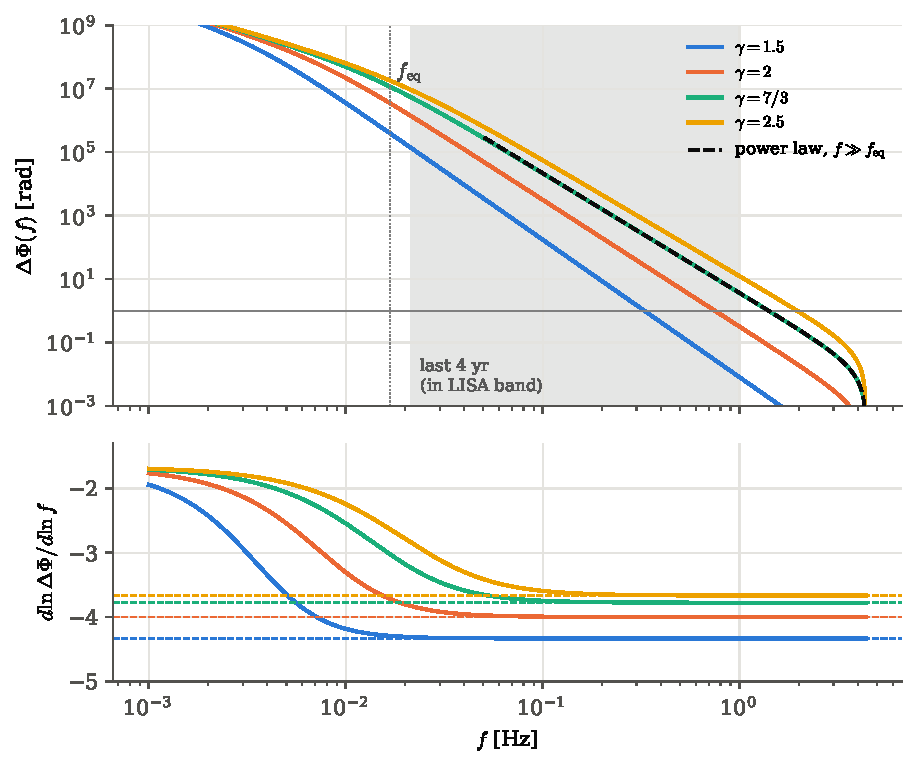
\includegraphics[width=0.85\linewidth]{figures/chT2/dephasing.pdf}
\caption{Dephasing of the $10^3+1.4\,M_\odot$ IMRI by friction in a static spike of slope $\gamma$, at fixed density $\rho_6$ at $10^{-6}$\,pc. Top: phase lost between $f$ and the ISCO; the dashed black line is the power law \eqref{T2a:eq:dPhi} for $\gamma=7/3$, drawn where $f>3f_{\rm eq}$, and the grey band is the last four years. Bottom: the local slope $\dd\ln\Delta\Phi/\dd\ln f$ of the phase lost before coalescence. It moves from the vacuum value $-5/3$ at low frequency to the predicted $-5/3-n$ (dashed, one per slope) above $f_{\rm eq}$.}
\label{T2a:fig:dephasing}
\end{figure}

\subsubsection*{Reading the figure}
\Cref{T2a:fig:dephasing} has one idea: the dephasing is a broken power law, with the break at $f_{\rm eq}$. For $\gamma=7/3$ friction and radiation balance at $f_{\rm eq}=\TwfeqC$\,mHz. Below $f_{\rm eq}$ friction drives the inspiral, almost all of the vacuum phase is lost ($\Delta\Phi\to\Phi_{\rm V}$, as found above), and the local slope of $\Delta\Phi$ is the vacuum $-5/3$. Above it each curve settles onto the predicted exponent $b=-5/3-n$ of \eqref{T2a:eq:dPhi}: the measured local slopes are $\TwbexpA$, $\TwbexpB$, $\TwbexpC$ and $\TwbexpD$ for $\gamma=1.5$, $2$, $7/3$, $2.5$, against $-13/3$, $-4$, $-34/9$ and $-11/3$.

\subsubsection*{How large}
The steeper the spike, the more phase it removes at fixed $\rho_6$: over the last four years before the ISCO (from $\TwffourImri$\,mHz), $\Delta\Phi=\TwdPhiFourA$, $\TwdPhiFourB$, $\TwdPhiFourC$ and $\TwdPhiFourD$\,rad for the four slopes. To give these a scale: a matched filter at signal-to-noise ratio $\rho$ resolves a phase error of about $1/\rho$ radians, the weighted root-mean-square phase shift that the Fisher matrix can detect (\cref{10b:sec:fisher-structure}), about a tenth of a radian for $\rho=10$. So even the gentlest of these spikes would be glaringly visible in this idealised, static setting.

\subsubsection*{Paper and reproduction side by side}
\begin{center}
\small
\begin{tabularx}{\linewidth}{@{}>{\raggedright\arraybackslash}p{0.24\linewidth} >{\raggedright\arraybackslash}X >{\raggedright\arraybackslash}X@{}}
\toprule
quantity ($\gamma=7/3$) & Coogan et al. & ours (static)\\\midrule
$f_{\rm eq}$ & $\approx15$\,mHz \cite[eq.~(15)]{Coogan2022} & $\TwfeqC$\,mHz\\
high-frequency slope of $\Delta\Phi$ & $-34/9$ (static, eq.~(16)) & $\TwbexpC$\\
exact vs.\ power law & eq.~(12) & closed form = numerical to $\TwclosedVsNum$\\
$\Delta\Phi$, last four years & much smaller, spike with feedback (Sec.~IV) & $\TwdPhiFourC$\,rad\\
\bottomrule
\end{tabularx}
\end{center}

\subsubsection*{Why they differ}
\emph{The equality frequency.} Ours is $12\%$ above theirs. Since $f_{\rm eq}=c_f^{1/n}$ and $c_f\propto\xi\ln\Lambda\,\rho_6$, $f_{\rm eq}\propto(\xi\ln\Lambda\,\rho_6)^{1/n}=(\xi\ln\Lambda\,\rho_6)^{9/19}$ for $\gamma=7/3$. A $12\%$ shift in $f_{\rm eq}$ therefore corresponds to a $(1.12)^{19/9}-1\approx26\%$ difference in the product $\xi\ln\Lambda\,\rho_6$. The prescriptions differ by more than that: setting $\xi=1$ instead of $0.58$ alone would move $f_{\rm eq}$ up by $(1/0.58)^{9/19}\approx1.29$, and the two common choices of $\ln\Lambda$ differ by a factor of two. We have not pinned the remaining $12\%$ on a single choice; it is the size expected from these conventions, and the exponents, which do not depend on them, agree.

\emph{Static against responding spike.} This is the large difference. The energy friction removes from the orbit goes into the dark matter, and a rough count shows it is far more than the spike can absorb. Take the orbit at $f_{\rm eq}$, of radius $r=(GM/\pi^2f_{\rm eq}^2)^{1/3}\approx1.2\times10^{-8}$\,pc. The energy friction removes between $f_{\rm eq}$ and the ISCO is the friction share of the orbital energy lost,
\[
  E_{\rm DF}=\int_{f_{\rm eq}}^{f_c}\frac{\epsilon}{1+\epsilon}\Big\lvert\frac{\dd E}{\dd f}\Big\rvert\dd f
  =\frac\mu3\Big(\frac{\pi GMf_{\rm eq}}{c^3}\Big)^{2/3}c^2\int_1^{f_c/f_{\rm eq}}\frac{y^{-1/3}\,\dd y}{1+y^{n}}
  \approx1\times10^{-3}\,M_\odot c^2,
\]
with $y=f/f_{\rm eq}$, $\epsilon=y^{-n}$, $\lvert\dd E/\dd f\rvert$ from \eqref{T2a:eq:Ef}, and the last integral $\approx0.51$. The dark matter inside that orbit is $M_{\rm DM}(<r)=4\pi\rho_6r_6^\gamma r^{3-\gamma}/(3-\gamma)\approx5\times10^{-3}\,M_\odot$, bound to the hole by roughly $GMM_{\rm DM}/r\approx2\times10^{-5}\,M_\odot c^2$. The friction deposits some fifty times the binding energy of the dark matter it moves through. The spike near the orbit cannot stay as it was: it is heated and partly unbound, its density at a given radius falls during the inspiral, $\epsilon$ at fixed $f$ falls with it, and the dephasing is smaller and its break moves. That is the qualitative result Coogan et al.\ find when they follow this feedback: a much smaller dephasing, still a broken power law, but with a different break frequency and exponents \cite[Sec.~IV]{Coogan2022}. Kim et al.\ mimic the same effect by capping the friction at the binding energy of a shell of halo \cite[Sec.~IV C]{Kim2023}.

\emph{The chirp itself.} Our vacuum chirp is Newtonian and circular. Near the ISCO, where $v\approx0.4c$, post-Newtonian corrections to $\dot f$ are large (\cref{T2g:sec:pn}), and relativistic corrections to the spike and to the friction push the other way from feedback, increasing the dephasing \cite{Speeney2022}. These change the numbers, not the exponents of \eqref{T2a:eq:ppe}, which survive as the leading-order description of each effect.

\subsubsection*{What it taught us}
The power law is not the whole story even before feedback. LISA's window is not far above $f_{\rm eq}$: at the start of the four-year window the power law misses the exact $\Delta\Phi$ for $\gamma=7/3$ by $\TwPLerrFour\%$, and for $\gamma=2.5$ the window starts \emph{below} $f_{\rm eq}=\TwfeqD$\,mHz, where no expansion in $\epsilon$ holds. A ppE forecast is reliable when the observed band lies well above $f_{\rm eq}$, that is, for weak environments, which are exactly the ones whose detectability is in question; and a static spike strong enough to matter is one that the binary itself would destroy.

\begin{taxonomy}[Environmental effects as power laws in the phase]
\small
\renewcommand{\arraystretch}{1.25}
\begin{tabularx}{\linewidth}{@{}>{\raggedright\arraybackslash}X >{\centering\arraybackslash}p{2.0cm} >{\centering\arraybackslash}p{1.9cm} >{\centering\arraybackslash}p{2.1cm} >{\centering\arraybackslash}p{1.5cm}@{}}
\toprule
effect & $P_{\rm env}/P_{\rm GW}\propto$ & $n$ & $b=-\frac53-n$ & at $\gamma=\frac73$\\\midrule
friction, spike $\rho\propto r^{-\gamma}$ & $r^{11/2-\gamma}$ & $\frac{11-2\gamma}{3}$ & $\frac{2\gamma-16}{3}$ & $-\frac{34}{9}$\\
friction, uniform density & $r^{11/2}$ & $\frac{11}{3}$ & $-\frac{16}{3}$ ($-5.5$PN) & ---\\
accretion, collisionless & $r^{9/2-\gamma}$ & $\frac{9-2\gamma}{3}$ & $\frac{2\gamma-14}{3}$ & $-\frac{28}{9}$\\
accretion, gas (BHL) & as friction & & & \\
pull of enclosed mass (no loss) & $r^{3-\gamma}$ (relative) & $\frac{2(3-\gamma)}{3}$ & $\frac{2\gamma-11}{3}$ & $-\frac{19}{9}$\\
dipole radiation (Brans--Dicke) & $r$ & $\frac23$ & $-\frac73$ & ---\\
vector ultralight DM & \multicolumn{4}{l}{resonant: a step near one frequency, not a power law \cite{Chase2025}}\\
\bottomrule
\end{tabularx}
\end{taxonomy}

The table also marks where the power-law picture stops. The oscillating potential of a vector dark-matter halo (\cref{T2a:sec:dm}) does nothing on average until the orbital frequency crosses a resonance with the field, and then shifts the phase within a narrow band \cite[Sec.~V]{Chase2025}. A template $\beta u^b$ cannot represent such a step; it needs its own model. The ppE parametrisation is a statement about smooth, monotonic effects, and its hidden assumption is that the environment changes slowly with radius.

\paragraph{Where each item is used.}
The waveform \eqref{T2a:eq:hf} with phase \eqref{T2a:eq:psiN} and the correction \eqref{T2a:eq:ppe}, together with the noise \eqref{T2a:eq:Sn}, are the inputs of the gravitational-wave Fisher forecast in \cref{ch:10}, which computes the error on $\beta$ for a list of exponents $b$ and checks it with the sampler of \cref{ch:09}. The density profiles and the parametrisation by $\rho_6$ fix the physical meaning of $\beta$ there. The likelihood $-\tfrac12(d-h\,|\,d-h)$ with this $S_n$ is the one derived in \cref{ch:00}, and comparing a vacuum template with a dressed one is a Bayesian model comparison of the kind treated in \cref{ch:05}.

\begin{recap}
\begin{itemize}[itemsep=1pt]
  \item Energy balance with the quadrupole formula gives the chirp $\dot f=\frac{96}{5}\pi^{8/3}(G\mathcal M/c^3)^{5/3}f^{11/3}$; only the chirp mass enters at leading order, and LISA's benchmark inspirals complete millions of cycles in four years.
  \item The stationary-phase approximation gives $\tilde h=\mathcal Af^{-7/6}e^{-i\Psi(f)}$ with $\dd^2\Psi/\dd f^2=2\pi/\dot f$: anything that changes the sweep rate changes the phase.
  \item LISA's sensitivity $S_n(f)$ combines test-mass acceleration noise (low $f$), optical metrology noise and the arm response (high $f$), and the Galactic confusion foreground (around a millihertz); the signal-to-noise ratio is $\int(h_c/h_n)^2\dd\ln f$.
  \item Slow growth of a black hole compresses a cusp $r^{-\gamma_i}$ into a spike $r^{-(9-2\gamma_i)/(4-\gamma_i)}$, $r^{-7/3}$ for NFW, raising the density at the orbit by some eighteen orders of magnitude; ultralight dark matter falls freely inside the self-gravity radius, $\rho\propto r^{-3/2}$.
  \item An extra power $P_{\rm env}=c_ff^{-n}P_{\rm GW}$ shifts the phase by $\beta u^{b}$, $b=-5/3-n$, valid for $f\gg f_{\rm eq}$; resonant effects are not power laws.
\end{itemize}
\end{recap}

\providecommand{\TwbN}{}\renewcommand{\TwbN}{400}
\providecommand{\TwbAlpha}{}\renewcommand{\TwbAlpha}{0.15}
\providecommand{\TwbBeta}{}\renewcommand{\TwbBeta}{3}
\providecommand{\TwbSigInt}{}\renewcommand{\TwbSigInt}{0.1}
\providecommand{\TwbSigC}{}\renewcommand{\TwbSigC}{0.1}
\providecommand{\TwbErrC}{}\renewcommand{\TwbErrC}{0.03}
\providecommand{\TwbSigXone}{}\renewcommand{\TwbSigXone}{1}
\providecommand{\TwbErrXone}{}\renewcommand{\TwbErrXone}{0.15}
\providecommand{\TwbRawSd}{}\renewcommand{\TwbRawSd}{0.344}
\providecommand{\TwbRawPred}{}\renewcommand{\TwbRawPred}{0.353}
\providecommand{\TwbStdSd}{}\renewcommand{\TwbStdSd}{0.142}
\providecommand{\TwbStdPred}{}\renewcommand{\TwbStdPred}{0.140}
\providecommand{\TwbAhat}{}\renewcommand{\TwbAhat}{0.146}
\providecommand{\TwbBhat}{}\renewcommand{\TwbBhat}{2.67}
\providecommand{\TwbMhat}{}\renewcommand{\TwbMhat}{-19.262}
\providecommand{\TwbNmock}{}\renewcommand{\TwbNmock}{2000}
\providecommand{\TwbBmean}{}\renewcommand{\TwbBmean}{2.754}
\providecommand{\TwbBsd}{}\renewcommand{\TwbBsd}{0.071}
\providecommand{\TwbAmean}{}\renewcommand{\TwbAmean}{0.1467}
\providecommand{\TwbAmeanErr}{}\renewcommand{\TwbAmeanErr}{0.0002}
\providecommand{\TwbLamC}{}\renewcommand{\TwbLamC}{0.917}
\providecommand{\TwbBpred}{}\renewcommand{\TwbBpred}{2.752}
\providecommand{\TwbLamX}{}\renewcommand{\TwbLamX}{0.978}
\providecommand{\TwbApred}{}\renewcommand{\TwbApred}{0.1467}
\providecommand{\TwbPvMag}{}\renewcommand{\TwbPvMag}{0.030}
\providecommand{\TwlNanc}{}\renewcommand{\TwlNanc}{3}
\providecommand{\TwlSigGeo}{}\renewcommand{\TwlSigGeo}{0.03}
\providecommand{\TwlNcephAnc}{}\renewcommand{\TwlNcephAnc}{100}
\providecommand{\TwlNcephCal}{}\renewcommand{\TwlNcephCal}{30}
\providecommand{\TwlSigCeph}{}\renewcommand{\TwlSigCeph}{0.25}
\providecommand{\TwlNcal}{}\renewcommand{\TwlNcal}{40}
\providecommand{\TwlSigSn}{}\renewcommand{\TwlSigSn}{0.13}
\providecommand{\TwlNhf}{}\renewcommand{\TwlNhf}{280}
\providecommand{\TwlSigHf}{}\renewcommand{\TwlSigHf}{0.14}
\providecommand{\TwlHtrue}{}\renewcommand{\TwlHtrue}{73}
\providecommand{\TwlHhat}{}\renewcommand{\TwlHhat}{73.90}
\providecommand{\TwlHerr}{}\renewcommand{\TwlHerr}{1.10}
\providecommand{\TwlFrac}{}\renewcommand{\TwlFrac}{1.49}
\providecommand{\TwlFracApprox}{}\renewcommand{\TwlFracApprox}{1.49}
\providecommand{\TwlNpar}{}\renewcommand{\TwlNpar}{47}
\providecommand{\TwlCanc}{}\renewcommand{\TwlCanc}{0.80}
\providecommand{\TwlCceph}{}\renewcommand{\TwlCceph}{0.74}
\providecommand{\TwlCsn}{}\renewcommand{\TwlCsn}{0.95}
\providecommand{\TwlChf}{}\renewcommand{\TwlChf}{0.38}
\providecommand{\TwlFracFive}{}\renewcommand{\TwlFracFive}{3.05}
\providecommand{\TwlFracOneSixty}{}\renewcommand{\TwlFracOneSixty}{1.22}
\providecommand{\TwlNmc}{}\renewcommand{\TwlNmc}{400}
\providecommand{\TwlMcMean}{}\renewcommand{\TwlMcMean}{72.99}
\providecommand{\TwlMcSd}{}\renewcommand{\TwlMcSd}{1.10}
\providecommand{\TwlMcErr}{}\renewcommand{\TwlMcErr}{1.09}
\providecommand{\TwlCover}{}\renewcommand{\TwlCover}{70\%}
\providecommand{\TwmSigThree}{}\renewcommand{\TwmSigThree}{-0.1280}
\providecommand{\TwmSigThreeTh}{}\renewcommand{\TwmSigThreeTh}{-0.1243}
\providecommand{\TwmSigOne}{}\renewcommand{\TwmSigOne}{-0.0138}
\providecommand{\TwmSigOneTh}{}\renewcommand{\TwmSigOneTh}{-0.0138}
\providecommand{\TwmSigFive}{}\renewcommand{\TwmSigFive}{-0.348}
\providecommand{\TwmSigFiveTh}{}\renewcommand{\TwmSigFiveTh}{-0.345}
\providecommand{\TwmLim}{}\renewcommand{\TwmLim}{24}
\providecommand{\TwmSig}{}\renewcommand{\TwmSig}{0.15}
\providecommand{\TwmNmock}{}\renewcommand{\TwmNmock}{200}
\providecommand{\TwmOm}{}\renewcommand{\TwmOm}{0.3}
\providecommand{\TwmNaiveMean}{}\renewcommand{\TwmNaiveMean}{0.353}
\providecommand{\TwmNaiveSd}{}\renewcommand{\TwmNaiveSd}{0.019}
\providecommand{\TwmCorrMean}{}\renewcommand{\TwmCorrMean}{0.301}
\providecommand{\TwmCorrSd}{}\renewcommand{\TwmCorrSd}{0.018}
\providecommand{\TwmZhalf}{}\renewcommand{\TwmZhalf}{0.73}
\providecommand{\TwmResLast}{}\renewcommand{\TwmResLast}{-0.140}
\providecommand{\TwmResLastTh}{}\renewcommand{\TwmResLastTh}{-0.175}
\providecommand{\TwmNkept}{}\renewcommand{\TwmNkept}{3608}
\providecommand{\TwmZlast}{}\renewcommand{\TwmZlast}{0.75}
\providecommand{\TwtL}{}\renewcommand{\TwtL}{1000}
\providecommand{\TwtN}{}\renewcommand{\TwtN}{128}
\providecommand{\TwtR}{}\renewcommand{\TwtR}{10}
\providecommand{\TwtSigR}{}\renewcommand{\TwtSigR}{0.229}
\providecommand{\TwtKmax}{}\renewcommand{\TwtKmax}{0.05}
\providecommand{\TwtNuTwo}{}\renewcommand{\TwtNuTwo}{2}
\providecommand{\TwtBLthTwo}{}\renewcommand{\TwtBLthTwo}{1.57}
\providecommand{\TwtBLmTwo}{}\renewcommand{\TwtBLmTwo}{1.71}
\providecommand{\TwtBEthTwo}{}\renewcommand{\TwtBEthTwo}{2.57}
\providecommand{\TwtBEmTwo}{}\renewcommand{\TwtBEmTwo}{2.62}
\providecommand{\TwtBLthOne}{}\renewcommand{\TwtBLthOne}{1.01}
\providecommand{\TwtBLmOne}{}\renewcommand{\TwtBLmOne}{1.06}
\providecommand{\TwtBLerrOne}{}\renewcommand{\TwtBLerrOne}{0.03}
\providecommand{\TwtNuHighTwo}{}\renewcommand{\TwtNuHighTwo}{1.32}
\providecommand{\TwtNuHighLast}{}\renewcommand{\TwtNuHighLast}{1.65}
\providecommand{\TwtNbar}{}\renewcommand{\TwtNbar}{3\times10^{-4}}
\providecommand{\TwtNgal}{}\renewcommand{\TwtNgal}{299091}
\providecommand{\TwtShot}{}\renewcommand{\TwtShot}{3343}
\providecommand{\TwtBG}{}\renewcommand{\TwtBG}{2.24}
\providecommand{\TwtBGerr}{}\renewcommand{\TwtBGerr}{0.06}
\providecommand{\TwtBGauto}{}\renewcommand{\TwtBGauto}{2.19}
\providecommand{\TwtBGautoNaive}{}\renewcommand{\TwtBGautoNaive}{2.42}
\providecommand{\TwtOneHalo}{}\renewcommand{\TwtOneHalo}{7114}
\providecommand{\TwtLam}{}\renewcommand{\TwtLam}{2.13}
\providecommand{\TwtRatioParNaive}{}\renewcommand{\TwtRatioParNaive}{1.66}
\providecommand{\TwtBLerrTwo}{}\renewcommand{\TwtBLerrTwo}{0.09}
\providecommand{\TwtBEerrTwo}{}\renewcommand{\TwtBEerrTwo}{0.08}
\providecommand{\TwtBLerrLast}{}\renewcommand{\TwtBLerrLast}{0.19}
\providecommand{\TwtBEerrLast}{}\renewcommand{\TwtBEerrLast}{0.17}
\providecommand{\TwtBGth}{}\renewcommand{\TwtBGth}{2.28}
\providecommand{\TwtSigT}{}\renewcommand{\TwtSigT}{1.516}
\providecommand{\TwtSigSmall}{}\renewcommand{\TwtSigSmall}{1.5}
\providecommand{\TwtNuG}{}\renewcommand{\TwtNuG}{1.5}
\providecommand{\TwtZ}{}\renewcommand{\TwtZ}{1}
\providecommand{\TwtBLthLast}{}\renewcommand{\TwtBLthLast}{1.86}
\providecommand{\TwtBLmLast}{}\renewcommand{\TwtBLmLast}{1.82}
\providecommand{\TwtBEthLast}{}\renewcommand{\TwtBEthLast}{2.86}
\providecommand{\TwtBEmLast}{}\renewcommand{\TwtBEmLast}{2.84}
\providecommand{\TwtF}{}\renewcommand{\TwtF}{0.876}
\providecommand{\TwtBeta}{}\renewcommand{\TwtBeta}{0.391}
\providecommand{\TwtMono}{}\renewcommand{\TwtMono}{1.314}
\providecommand{\TwtMonoTh}{}\renewcommand{\TwtMonoTh}{1.292}
\providecommand{\TwtRatioPar}{}\renewcommand{\TwtRatioPar}{1.97}
\providecommand{\TwtRatioParTh}{}\renewcommand{\TwtRatioParTh}{1.83}
\providecommand{\TwtRatioMPar}{}\renewcommand{\TwtRatioMPar}{3.02}
\providecommand{\TwtRatioMParTh}{}\renewcommand{\TwtRatioMParTh}{3.21}
\providecommand{\TwtNbox}{}\renewcommand{\TwtNbox}{11}
\providecommand{\TwtRatioMParMean}{}\renewcommand{\TwtRatioMParMean}{3.08}
\providecommand{\TwtRatioMParErr}{}\renewcommand{\TwtRatioMParErr}{0.01}
\providecommand{\TwbaoSigNl}{}\renewcommand{\TwbaoSigNl}{8}
\providecommand{\TwbaoB}{}\renewcommand{\TwbaoB}{2}
\providecommand{\TwbaoNbar}{}\renewcommand{\TwbaoNbar}{3\times10^{-4}}
\providecommand{\TwbaoVol}{}\renewcommand{\TwbaoVol}{1}
\providecommand{\TwbaoNbins}{}\renewcommand{\TwbaoNbins}{20}
\providecommand{\TwbaoNmock}{}\renewcommand{\TwbaoNmock}{10000}
\providecommand{\TwbaoAerrMean}{}\renewcommand{\TwbaoAerrMean}{0.0218}
\providecommand{\TwbaoAsd}{}\renewcommand{\TwbaoAsd}{0.0272}
\providecommand{\TwbaoAmean}{}\renewcommand{\TwbaoAmean}{0.9997}
\providecommand{\TwbaoFisher}{}\renewcommand{\TwbaoFisher}{0.0207}
\providecommand{\TwbaoCover}{}\renewcommand{\TwbaoCover}{66\%}
\providecommand{\TwbaoCoverErr}{}\renewcommand{\TwbaoCoverErr}{0.5\%}
\providecommand{\TwbaoSigMed}{}\renewcommand{\TwbaoSigMed}{3.8}
\providecommand{\TwbaoSigLow}{}\renewcommand{\TwbaoSigLow}{2.7}
\providecommand{\TwbaoSigHigh}{}\renewcommand{\TwbaoSigHigh}{4.8}
\providecommand{\TwbaoAzero}{}\renewcommand{\TwbaoAzero}{1.030}
\providecommand{\TwbaoEzero}{}\renewcommand{\TwbaoEzero}{0.026}
\providecommand{\TwbaoDchiZero}{}\renewcommand{\TwbaoDchiZero}{13.7}
\providecommand{\TwbaoChiZero}{}\renewcommand{\TwbaoChiZero}{11.8}
\providecommand{\TwbaoDofZero}{}\renewcommand{\TwbaoDofZero}{15}
\providecommand{\TwdOm}{}\renewcommand{\TwdOm}{0.296}
\providecommand{\TwdOmSd}{}\renewcommand{\TwdOmSd}{0.015}
\providecommand{\TwdHrd}{}\renewcommand{\TwdHrd}{101.8}
\providecommand{\TwdHrdSd}{}\renewcommand{\TwdHrdSd}{1.3}
\providecommand{\TwdCorr}{}\renewcommand{\TwdCorr}{-0.92}
\providecommand{\TwdChiP}{}\renewcommand{\TwdChiP}{21.1}
\providecommand{\TwdNdata}{}\renewcommand{\TwdNdata}{12}
\providecommand{\TwdChiMin}{}\renewcommand{\TwdChiMin}{12.8}
\providecommand{\TwdHrdP}{}\renewcommand{\TwdHrdP}{99.1}
\providecommand{\TwdHzero}{}\renewcommand{\TwdHzero}{69.2}
\providecommand{\TwdHzeroErr}{}\renewcommand{\TwdHzeroErr}{0.9}
\providecommand{\TwpN}{}\renewcommand{\TwpN}{20000}
\providecommand{\TwpZzero}{}\renewcommand{\TwpZzero}{0.55}
\providecommand{\TwpNmadF}{}\renewcommand{\TwpNmadF}{0.018}
\providecommand{\TwpOutF}{}\renewcommand{\TwpOutF}{9.8}
\providecommand{\TwpNmadP}{}\renewcommand{\TwpNmadP}{0.019}
\providecommand{\TwpOutP}{}\renewcommand{\TwpOutP}{4.3}
\providecommand{\TwpMedP}{}\renewcommand{\TwpMedP}{0.0000}
\providecommand{\TwpBinLo}{}\renewcommand{\TwpBinLo}{0.8}
\providecommand{\TwpBinHi}{}\renewcommand{\TwpBinHi}{1.2}
\providecommand{\TwpBinN}{}\renewcommand{\TwpBinN}{6199}
\providecommand{\TwpMeanTrue}{}\renewcommand{\TwpMeanTrue}{0.965}
\providecommand{\TwpMeanZp}{}\renewcommand{\TwpMeanZp}{0.975}
\providecommand{\TwpMeanStack}{}\renewcommand{\TwpMeanStack}{0.975}
\providecommand{\TwpBinOut}{}\renewcommand{\TwpBinOut}{0.4}
\providecommand{\TwpZb}{}\renewcommand{\TwpZb}{2.00}
\providecommand{\TwpCondA}{}\renewcommand{\TwpCondA}{1.449}
\providecommand{\TwpCondB}{}\renewcommand{\TwpCondB}{1.407}
\providecommand{\TwpCondZ}{}\renewcommand{\TwpCondZ}{1.5}
\providecommand{\TwpCondAlow}{}\renewcommand{\TwpCondAlow}{0.531}
\providecommand{\TwpCondBlow}{}\renewcommand{\TwpCondBlow}{0.500}
\providecommand{\TwpCondZlow}{}\renewcommand{\TwpCondZlow}{0.5}
 
\section{Type Ia supernovae: candles that need a correction}
\label{T2b:sec:snia}

A white dwarf is the burnt-out core of a star like the Sun, held up by the pressure of its degenerate electrons. If it gains mass from a companion, or merges with a second white dwarf, it can approach the Chandrasekhar limit of about $1.4\,M_\odot$, ignite carbon in its centre and blow itself apart. The explosion makes a few tenths of a solar mass of radioactive nickel-56, and the decay of that nickel powers the light we see for weeks. The fuel and the trigger are nearly the same every time, so the explosions are nearly the same every time. At its peak a type~Ia supernova outshines its whole host galaxy, and it can be seen across half the observable universe.

``Nearly the same'' is not good enough for cosmology. Raw peak magnitudes scatter by about $0.4$\,mag \cite[p.~33]{Weinberg2013}, which is a $40\%$ spread in luminosity and a $20\%$ spread in the distance one would infer. Two observations rescue the method. Supernovae that are brighter at peak also fade more slowly, and supernovae that look redder are fainter. Both properties can be read off the light curve. A correction built from them shrinks the scatter to about $0.12$\,mag. Such an object is called a \newterm{standardisable candle} \unpack{its luminosity is not fixed, but it can be predicted from properties we measure on the same object}.

\paragraph{The question.} Given the light curve of one supernova in a few colour bands and the redshift of its host galaxy, what distance does it imply, how uncertain is that distance, and which statistical tools turn a few hundred such light curves into a measurement of the expansion history?

\subsection{What is measured, and the standardisation}

A magnitude is a logarithm of a flux $F$: $m=-2.5\log_{10}F+\text{const}$, so $5$ magnitudes is a factor of $100$ in flux and a larger magnitude means a fainter object. The \newterm{distance modulus} of \cref{ch:03} links the apparent magnitude $m$ to the absolute magnitude $M$ (the magnitude at $10$\,pc) through the luminosity distance $D_L$ of \cref{ch:T1}, the distance for which the flux is $L/4\pi D_L^2$:
\begin{equation}
  \mu\equiv m-M=5\log_{10}\frac{D_L}{10\,\mathrm{pc}}=5\log_{10}\frac{D_L}{\mathrm{Mpc}}+25 .
  \label{T2b:eq:mu}
\end{equation}

A light-curve fitter such as SALT \cite[p.~39]{Weinberg2013} compares the observed fluxes in each band, night after night, with a family of template light curves. It returns three numbers per supernova: the peak apparent magnitude $m_B$ in the rest-frame $B$ band, a \newterm{stretch} $x_1$ \unpack{how much wider than average the light curve is in time, zero for a typical one}, and a \newterm{colour} $c$ \unpack{how much redder than average the supernova is at peak, in magnitudes of $B-V$}. \Cref{T2b:fig:sn-pipeline} shows the chain from light curve to distance.

\begin{workdef}[Tripp standardisation]
The observed distance modulus of a type~Ia supernova is
\begin{equation}
  \mu_{\rm obs}=m_B-M+\alpha\,x_1-\beta\,c ,
  \label{T2b:eq:tripp}
\end{equation}
with $M$, $\alpha$ and $\beta$ the same for every supernova. \emph{Operationally:} fit the light curve to get $(m_B,x_1,c)$; add $\alpha x_1$ because broad supernovae are brighter than average (a smaller $M$); subtract $\beta c$ because red ones are fainter. Typical values are $\alpha\approx0.15$ and $\beta\approx3$.
\end{workdef}

Why do the two corrections work? The amount of nickel-56 sets both the peak luminosity and the width. More nickel means a hotter, more opaque ejecta, so the light takes longer to diffuse out, and the curve is both brighter and broader \cite[p.~33]{Weinberg2013}. This is the Phillips relation. Colour has two sources. Dust in the host galaxy absorbs blue light more than red, so it reddens and dims together. Milky-Way dust would give $\beta\approx R_B=R_V+1\approx4.1$, with $R_V\equiv A_V/E(B-V)=3.1$. Here $A_B$ and $A_V$ are the dimming by dust in the two bands, and the reddening is their difference, $E(B-V)=A_B-A_V$. The colour correction asks how much dimming in $B$ comes with one magnitude of reddening, $R_B\equiv A_B/E(B-V)=(A_V+E(B-V))/E(B-V)=R_V+1$. Fits to supernovae return a smaller $\beta$, as if $R_V$ were $1.5$--$2.5$ \cite[p.~36]{Weinberg2013}. Part of the colour spread is therefore intrinsic to the explosions and not dust at all. That is why $\beta$ is fitted rather than taken from the physics of dust.

\begin{figure}[htbp]
\centering
\begin{tikzpicture}[
  box/.style={draw=accent,rounded corners=2pt,fill=ideabg,align=center,font=\small,
              minimum height=0.95cm,inner sep=3pt},
  noise/.style={font=\footnotesize,text=bdryred,align=center},
  arr/.style={->,thick,accent}]
  \node[box,minimum width=2.6cm] (lc) at (0,0) {light curves\\ in 3--5 bands};
  \node[box,minimum width=2.4cm] (fit) at (3.6,0) {$m_B,\;x_1,\;c$};
  \node[box,minimum width=2.9cm] (mu) at (7.5,0) {$\mu_{\rm obs}=m_B-M$\\$+\alpha x_1-\beta c$};
  \node[box,minimum width=2.6cm] (res) at (7.5,-2.3) {Hubble residual\\ $\mu_{\rm obs}-\mu(z;\params)$};
  \node[box,minimum width=2.6cm] (z) at (3.6,-2.3) {host redshift $z$};
  \draw[arr] (lc) -- (fit);
  \draw[arr] (fit) -- (mu);
  \draw[arr] (mu) -- (res);
  \draw[arr] (z) -- (res);
  \node[noise] at (0,-1.05) {photometric noise,\\ calibration};
  \node[noise] at (3.6,-1.05) {errors on $x_1,c$\\ (correlated)};
  \node[noise] at (10.0,-0.95) {intrinsic\\ scatter $\sigma_{\rm int}$};
  \node[noise] at (3.6,-3.3) {peculiar velocity $v$};
  \node[noise] at (7.5,-3.3) {lensing, selection};
\end{tikzpicture}
\caption{From light curves to a distance. Blue boxes are the steps of the analysis; red labels mark where noise enters. The fitted shape and colour turn the peak magnitude into a distance modulus, and the redshift of the host predicts that modulus in a cosmological model. Their difference, the Hubble residual, is the quantity whose sampling distribution every later fit needs.}
\label{T2b:fig:sn-pipeline}
\end{figure}

\subsection{Where the noise lives}

The datum that enters every fit is the \newterm{Hubble residual} $\Delta\mu=\mu_{\rm obs}-\mu(z;\params)$, the difference between the standardised modulus and the one predicted at the host redshift by a model with parameters $\params$. Its scatter has four parts. The \emph{intrinsic scatter} $\sigma_{\rm int}\approx0.1$\,mag is what the standardisation cannot remove. The \emph{measurement errors} of $m_B$, $x_1$ and $c$ enter through \eqref{T2b:eq:tripp}, so an error $\sigma_c$ in colour costs $\beta\sigma_c$ in $\mu$. The \emph{peculiar velocity} $v$ of the host \unpack{its motion relative to the smooth expansion} shifts the redshift, and therefore the predicted modulus. And at high redshift, \emph{gravitational lensing} by structure along the line of sight magnifies or demagnifies the supernova.

How big is the peculiar-velocity term? At low redshift $D_L\approx cz/H_0$, and \eqref{T2b:eq:mu} turns a fractional error in distance into an additive error in magnitude:
\begin{align}
  \delta\mu
  &\eqby{1}\frac{5}{\ln10}\,\frac{\delta D_L}{D_L}
  \eqby{2}\frac{5}{\ln10}\,\frac{\delta(cz)}{cz}
  \eqby{3}\frac{5}{\ln10}\,\frac{v}{cz},
  \qquad
  \sigma_{\mu,\rm pec}=2.17\,\frac{\sigma_v}{cz}.
  \label{T2b:eq:mu-pec}
\end{align}
\begin{explain}
  \item Differentiate $\mu=5\log_{10}D_L+\text{const}=(5/\ln10)\ln D_L+\text{const}$.
  \item $D_L\propto cz$ at low redshift, so the fractional changes are equal.
  \item A line-of-sight velocity $v$ adds $v$ to the measured $cz$. The number in front is $5/\ln10=5/2.303=2.17$.
\end{explain}
For $\sigma_v=250$\,km/s this is $\TwbPvMag$\,mag at $z=0.06$, but $0.18$\,mag at $z=0.01$. That is why the low-redshift anchor of a supernova Hubble diagram starts at $z\approx0.02$--$0.03$, the ``sweet spot'' where peculiar velocities are small but the distances still do not depend on the dark-energy parameters \cite[p.~33]{Weinberg2013}.

\paragraph{Example: what one supernova is worth.}
Solve \eqref{T2b:eq:mu} for $D_L$ and take logarithms:
\begin{align}
  \ln D_L&\eqby{1}\frac{\ln10}{5}\,(\mu-25),\qquad
  \sigma_{\ln D}\eqby{2}\frac{\ln10}{5}\,\sigma_\mu=\frac{\sigma_\mu}{2\times1.086}
  \eqby{3}\frac{0.12}{2.17}=0.055 .
\end{align}
\begin{explain}
  \item $D_L/\mathrm{Mpc}=10^{(\mu-25)/5}$ and $\ln10^x=x\ln10$.
  \item A constant factor passes through the standard deviation. Weinberg et al.\ write $\ln10/5$ as $1/(2\times1.086)$: $1.086=2.5/\ln10$ converts magnitudes to natural logarithms, and the $2$ converts flux to distance, because flux goes as $D_L^{-2}$.
  \item The standardised scatter $\sigma_\mu\approx0.12$\,mag.
\end{explain}
Each well-measured supernova gives its distance to about $6\%$. Averaging $N$ independent supernovae in a redshift bin divides this by $\sqrt N$, which is Weinberg et al.'s eq.~(51) \cite[p.~34]{Weinberg2013}. How many supernovae does a $1\%$ distance in one bin need? Set the error of the mean equal to the target and solve for $N$:
\[
  \frac{0.055}{\sqrt N}=0.01\;\Longrightarrow\;N=\Big(\frac{0.055}{0.01}\Big)^2=5.5^2\approx30,
  \qquad
  \frac{0.055}{\sqrt N}=0.005\;\Longrightarrow\;N=11^2\approx120 ,
\]
as long as nothing systematic is left. The Pantheon+ compilation has $1550$ spectroscopically confirmed supernovae from $z=0.001$ to $2.26$ \cite{Brout2022PantheonPlus}. Its statistical errors are already comparable to its systematic ones, which come from flux calibration across telescopes, the treatment of dust and colour, and a possible drift of the population with redshift, such as the $0.03$\,mag per decade of host stellar mass found in the residuals \cite[pp.~39--41]{Weinberg2013}.

\subsection{Fitting \texorpdfstring{$\alpha$}{alpha} and \texorpdfstring{$\beta$}{beta}: least squares with noisy regressors}

Write $y_i\equiv m_{B,i}-\mu(z_i)$ for a low-redshift sample with known cosmology. Then \eqref{T2b:eq:tripp} says $y_i=M-\alpha x_{1,i}+\beta c_i+\epsilon_i$. This is a linear model, and least squares (\cref{ch:03}) seems to give $M$, $\alpha$, $\beta$ at once. There is a catch. The regressors $x_1$ and $c$ are themselves measured with noise. Ordinary least squares assumes the regressors are exact. What does it do when they are not?

Take the colour term alone: $y=\beta c+\epsilon$, with the true colours spread with variance $V_c$ and measured as $\hat c=c+e$, where $e$ is independent noise of variance $\sigma_c^2$. For a large sample the least-squares slope tends to
\begin{align}
  \hat\beta
  &\eqby{1}\frac{\Cov(y,\hat c)}{\Var(\hat c)}
  \eqby{2}\frac{\Cov(\beta c+\epsilon,\;c+e)}{\Var(c)+\Var(e)}
  \eqby{3}\frac{\beta V_c}{V_c+\sigma_c^2}
  \equiv\beta\lambda_c ,
  \qquad \lambda_c=\frac{V_c}{V_c+\sigma_c^2}.
  \label{T2b:eq:dilution}
\end{align}
\begin{explain}
  \item The least-squares slope of $y$ on $\hat c$ is the sample covariance over the sample variance, and both converge to their expectations (the law of large numbers).
  \item Substitute the model and the measurement. $c$ and $e$ are independent, so their variances add.
  \item $\epsilon$ and $e$ are independent of everything else, so only $\Cov(\beta c,c)=\beta V_c$ survives.
\end{explain}
The fitted slope is pulled towards zero by the factor $\lambda_c<1$. Statisticians call this \newterm{regression dilution}, and $\lambda_c$ the reliability ratio. The scatter left after the correction follows from the same quantities:
\begin{align}
  \Var(y-\hat\beta\hat c)
  &\eqby{1}\Var\big(\beta(1-\lambda_c)c-\beta\lambda_c e+\epsilon\big)
  \eqby{2}\beta^2\big[(1-\lambda_c)^2V_c+\lambda_c^2\sigma_c^2\big]+\sigma_\epsilon^2
  \eqby{3}\beta^2\lambda_c\,\sigma_c^2+\sigma_\epsilon^2 .
  \label{T2b:eq:resid-var}
\end{align}
\begin{explain}
  \item Substitute $y=\beta c+\epsilon$, $\hat c=c+e$ and $\hat\beta=\beta\lambda_c$.
  \item The three terms are independent, so their variances add.
  \item $1-\lambda_c=\sigma_c^2/(V_c+\sigma_c^2)$, so $(1-\lambda_c)^2V_c+\lambda_c^2\sigma_c^2=\dfrac{\sigma_c^4V_c+V_c^2\sigma_c^2}{(V_c+\sigma_c^2)^2}=\lambda_c\sigma_c^2$.
\end{explain}
Here $\sigma_\epsilon^2$ collects every other source: $\sigma_{\rm int}^2$, the error on $m_B$ and the peculiar velocities of \eqref{T2b:eq:mu-pec}.

\begin{pitfall}[A fitted slope is not the physical slope]
With noisy regressors, least squares underestimates $|\beta|$ by the factor $\lambda_c$ of \eqref{T2b:eq:dilution}, however many supernovae are used. A diluted $\beta$ is then applied to supernovae at high redshift, whose colours are noisier, so the bias does not cancel between the two ends of the Hubble diagram. Modern analyses treat the true $x_1$ and $c$ of each supernova as unknown latent parameters with a population distribution, a hierarchical model of the kind built in \cref{ch:05}.
\end{pitfall}

\paragraph{The experiment.}
\pyname{06_sn_standardise.py} draws $\TwbN$ supernovae at $0.02<z<0.1$ with $\alpha=\TwbAlpha$, $\beta=\TwbBeta$, an intrinsic scatter of $\TwbSigInt$\,mag, true colours of spread $\TwbSigC$ measured with errors $\TwbErrC$, and peculiar velocities of $250$\,km/s:

\pyfile[firstline=42,lastline=57,firstnumber=42]{code/chT2/06_sn_standardise.py}{A mock low-redshift supernova sample and the least-squares standardisation}

\noindent Line 46 is \eqref{T2b:eq:tripp} read backwards: the true absolute magnitude of each supernova. Line 47 moves the redshift by the peculiar velocity, and line 49 adds measurement noise to the regressors, which is what causes the dilution. The fit in lines 54--56 is ordinary least squares on the design matrix $[1,-x_1,c]$.

\Cref{T2b:fig:sn-standardise} shows the result. Before any correction, the residual $m_B-\mu(z)-M$ carries the whole spread of the stretch and colour terms as well as the noise. Write $V_x$ for the spread (variance) of the true stretches, as $V_c$ is for the colours, and $\sigma_m$, $\sigma_{\rm pec}$ for the magnitude error and the peculiar-velocity term of \eqref{T2b:eq:mu-pec}. All the terms are independent, so their variances add:
\[
  \sigma^2_{\rm raw}=\sigma_{\rm int}^2+\alpha^2V_x+\beta^2V_c+\sigma_m^2+\sigma_{\rm pec}^2 .
\]
The raw residuals scatter by $\TwbRawSd$\,mag, against $\TwbRawPred$ from this sum. After standardisation they scatter by $\TwbStdSd$\,mag, against the prediction $\TwbStdPred$ of \eqref{T2b:eq:resid-var}. Over $\TwbNmock$ mock samples the fitted $\beta$ averages $\TwbBmean\pm\TwbBsd$, not $\TwbBeta$: it agrees with the diluted value $\beta\lambda_c=\TwbBpred$ ($\lambda_c=\TwbLamC$). The stretch has its own reliability ratio, built as in \eqref{T2b:eq:dilution} from its spread and its measurement error $\sigma_x$, $\lambda_x=V_x/(V_x+\sigma_x^2)$. It is measured more precisely relative to its spread ($\lambda_{x}=\TwbLamX$), and $\hat\alpha$ averages $\TwbAmean\pm\TwbAmeanErr$, again $\alpha\lambda_x=\TwbApred$ within its Monte Carlo error.

\begin{figure}[htbp]
\centering
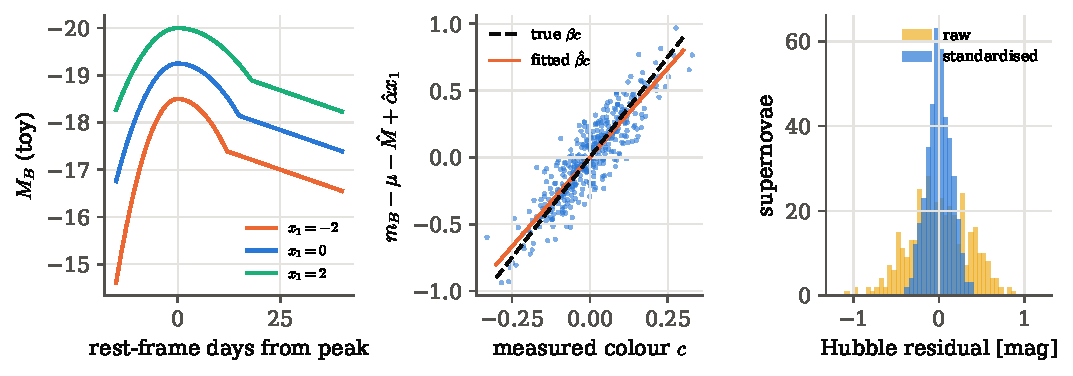
\includegraphics[width=\linewidth]{figures/chT2/sn_standardise.pdf}
\caption{Standardising type~Ia supernovae. Left: toy light curves; the broad one ($x_1=2$) is brighter, the narrow one fainter (the trend is exaggerated for visibility). Middle: after the stretch correction, the residual magnitude grows linearly with the measured colour; the fitted slope (orange) is shallower than the true one (dashed) because the colours are noisy. Right: Hubble residuals before (yellow) and after (blue) the correction.}
\label{T2b:fig:sn-standardise}
\end{figure}

\paragraph{Where the statistics comes back in.} The datum is the model's prediction plus one realisation of the noise, $\mu_{\rm obs}=\mu(z;\params)+\Delta\mu$ with $\Delta\mu\sim\Normal(0,\sigma^2)$. For a trial $\params$ the likelihood asks how plausible the particular noise realisation is that would turn that model's prediction into the magnitudes actually observed; a $\params$ that needs a large, improbable $\Delta\mu$ in every supernova is disfavoured. The residual $\Delta\mu$ is Gaussian in magnitudes, so the likelihood of \cref{ch:03} with the Hubble law, and the $H_0$ estimator built there, apply directly. Fitting $\alpha$, $\beta$, $M$ and the cosmology together is a linear-in-nuisance problem, solved by the least squares of \cref{ch:03} or marginalised in \cref{ch:05}. Correlated systematics (a calibration offset shared by all supernovae from one telescope) enter as a full covariance matrix $\Cmat$, whose use in the likelihood and in the Fisher matrix is the subject of \cref{ch:10}. The hierarchical treatment of latent colours is sampled with the MCMC of \cref{ch:09}.
\section{The distance ladder: why \texorpdfstring{$H_0$}{H0} needs an anchor}
\label{T2b:sec:ladder}

The supernovae of \cref{T2b:sec:snia} are excellent at \emph{relative} distances: this one is $1.8$ times farther than that one. They say nothing, on their own, about how far away either of them is in megaparsecs. The worked problem of \cref{ch:03} found the same thing in the language of likelihoods. In the Hubble law with supernova magnitudes, the absolute magnitude $M$ and $5\log_{10}H_0$ enter only in the combination $M-5\log_{10}H_0$, so the Fisher matrix of the two is singular. Brighter candles in a faster-expanding universe look exactly like fainter candles in a slower one. To measure $H_0$ someone has to tell us $M$, and the only way to do that is to find supernovae in galaxies whose distances are known by other means. Those distances in turn need calibrating, and the chain ends only at geometry. This chain is the \newterm{distance ladder}.

\emph{Where we have met $H_0$ before.} In \cref{3b:sec:hubble} we fitted mock surveys of $100$ supernovae made with $H_0=70$ and an absolute magnitude $M=-19.25$ that we simply declared known, and the maximum-likelihood estimator, the weighted mean of $5\log_{10}H_0$, found $H_0$ to about $0.5$\,km/s/Mpc. \Cref{3b:sec:hubble-degeneracy} then freed $M$, saw the Fisher matrix of $(M,5\log_{10}H_0)$ turn singular, and closed the gap by handing the fit one more number, $M_{\rm cal}\pm0.03$\,mag, from ``the calibrators''; the calibration error then dominated, and the scatter of $\hat H_0$ grew to $1.1$\,km/s/Mpc. Here the parameter, the magnitude likelihood and the degeneracy are the same, and so is the estimator, now written as generalised least squares. What changes is where $M$ comes from: instead of arriving as one number with an assumed error, it is produced by fitting the rungs below, so its error is assembled from parallaxes, Cepheids and calibrator supernovae, and we can ask which rung pays for most of it. The data are still mock, made with $H_0=\TwlHtrue$ to sit near the published value, which is met in \cref{T2b:sec:tension}. The two error bars come out almost equal, $1.1$\,km/s/Mpc in both, because the ladder below delivers $M$ to $0.03$\,mag, the precision the worked problem assumed.

\paragraph{The question.} Which measurements make up the ladder, what does each one measure and with what noise, and how do the errors of the rungs combine into the error on $H_0$?

\subsection{The rungs}

\emph{Rung 1, geometry.} The \newterm{parallax} $p$ of a star is the half-angle through which it appears to move as the Earth goes round the Sun. Its distance is $d=1\,\mathrm{AU}/\tan p$, that is $d=1\,\mathrm{pc}\times(1''/p)$ for small angles \cite[Sec.~8]{Hogg1999}. The Gaia satellite measures parallaxes to some $20\,\mu$as, so a Cepheid at $2$\,kpc ($p=0.5$\,mas) has its distance to $4\%$. Two other geometric anchors reach farther: detached eclipsing binaries in the Large Magellanic Cloud (the stars' sizes from the eclipse timing, their angular sizes from their surface brightness) and the water masers orbiting the black hole in NGC\,4258 (a Keplerian disc whose velocity and proper motion give its physical and angular size). Both give distances to about $1$--$1.5\%$ \cite{Riess2022SH0ES}.

\emph{Rung 2, a stellar standard candle.} \newterm{Cepheids} are pulsating giant stars whose brightness varies with periods of days to months. Brighter Cepheids pulsate more slowly. The \newterm{Leavitt law} \unpack{the period--luminosity relation of Cepheids, a straight line in $\log P$} says
\begin{equation}
  m_{W}=\mu+M_W+b_W\,(\log_{10}P-1),
  \label{T2b:eq:leavitt}
\end{equation}
where $m_W$ is a reddening-free combination of magnitudes in two bands (a ``Wesenheit'' magnitude), $M_W$ the absolute magnitude of a $10$-day Cepheid, and $b_W\approx-3.3$ the slope. The scatter about the line is about $0.25$\,mag per star, but a galaxy contains dozens of Cepheids, so its distance modulus $\mu$ is found to a few hundredths of a magnitude. The alternative second rung is the \newterm{tip of the red giant branch} (TRGB): the brightest red giants are those about to ignite helium in their cores, and the ignition happens at a fixed core mass, so the tip of the giant branch is a standard candle with $M_I\approx-4.05$. Both second rungs are reviewed in \cite[Sec.~IV.A]{Abdalla2022}.

\emph{Rung 3, supernovae in calibrator galaxies.} A few dozen galaxies within $\sim40$\,Mpc have both Cepheids (or a measured TRGB) and a well-observed type~Ia supernova. In each of them the Cepheids give $\mu$, and the supernova gives $m_B$, so $M_B=m_B-\mu$. SH0ES uses $42$ supernovae in $37$ such hosts \cite{Riess2022SH0ES}.

\emph{Rung 4, the Hubble flow.} Supernovae at $0.023<z<0.15$ are far enough that peculiar velocities matter little (\eqref{T2b:eq:mu-pec}) and near enough that the distance depends on the cosmology only through the deceleration parameter $q_0$ \unpack{$q_0=-\ddot aa/\dot a^2$ today, about $-0.55$ in $\Lambda$CDM}. What fixes that dependence? Expand the comoving distance $D_C=c\int_0^z\dd z'/H(z')$ to second order with $H(z)\approx H_0[1+(1+q_0)z]$, and use $D_L=(1+z)D_C$ for a flat universe \cite[eqs.~(15), (21)]{Hogg1999}:
\begin{align}
  D_L
  &\eqby{1}(1+z)\,\frac{c}{H_0}\int_0^z\big[1-(1+q_0)z'\big]\,\dd z'\nonumber\\
  &\eqby{2}(1+z)\,\frac{c}{H_0}\Big[z-\frac{1+q_0}{2}z^2\Big]
  \eqby{3}\frac{cz}{H_0}\Big[1+\frac{1-q_0}{2}z\Big]+O(z^3).
  \label{T2b:eq:dl-q0}
\end{align}
\begin{explain}
  \item How fast does $H$ change with redshift? Both $H$ and $z$ change with time, so divide their rates of change. The definition of $q$ gives $\dot H=\ddot a/a-\dot a^2/a^2=-H^2(1+q)$, and $1+z=1/a$ gives $\dot z=-\dot a/a^2=-(1+z)H$. Then
        \[
          \frac{\dd H}{\dd z}=\frac{\dot H}{\dot z}=\frac{-H^2(1+q)}{-(1+z)H}=\frac{H(1+q)}{1+z}
          \;\xrightarrow{\;z=0\;}\;(1+q_0)H_0 ,
        \]
        so to first order $H(z)\approx H_0[1+(1+q_0)z]$, and $1/(1+\epsilon)\approx1-\epsilon$ gives $1/H(z)\approx H_0^{-1}[1-(1+q_0)z]$.
  \item Integrate term by term.
  \item Multiply out: $(1+z)\big(z-\tfrac{1+q_0}{2}z^2\big)=z+z^2-\tfrac{1+q_0}{2}z^2+O(z^3)$.
\end{explain}
What does a Hubble-flow supernova then tell us? Its apparent magnitude is its absolute magnitude plus its distance modulus \eqref{T2b:eq:mu}, and \eqref{T2b:eq:dl-q0} gives the distance. The logarithm of a product is a sum of logarithms, which splits the known part from the unknown one:
\begin{align}
  m_{B,i}
  &\eqby{1}M_B+5\log_{10}\frac{D_L(z_i)}{\mathrm{Mpc}}+25\nonumber\\
  &\eqby{2}M_B+5\log_{10}\Big\{cz_i\Big[1+\frac{1-q_0}{2}z_i\Big]\Big\}+25-5\log_{10}H_0
  \eqby{3}M_B+x_i-a ,
  \label{T2b:eq:mb-hf}
\end{align}
with $x_i\equiv5\log_{10}\{cz_i[1+\frac12(1-q_0)z_i]\}+25$ and $a\equiv5\log_{10}H_0$ ($c$ in km/s and $H_0$ in km/s/Mpc, so that $D_L$ is in Mpc).
\begin{explain}
  \item $m=M+\mu$, with $\mu$ from \eqref{T2b:eq:mu}.
  \item Substitute \eqref{T2b:eq:dl-q0} and use $\log(XY/H_0)=\log X+\log Y-\log H_0$.
  \item Name the pieces: $x_i$ is computed from the measured redshift alone (with $q_0$ from the cosmology, a small correction at these redshifts); $a$ is the one unknown that carries $H_0$.
\end{explain}
Here the degeneracy of \cref{ch:03} is visible: only $M_B-a$ appears.

\begin{figure}[htbp]
\centering
\begin{tikzpicture}[scale=0.82,transform shape,
  rung/.style={draw=accent,rounded corners=2pt,fill=ideabg,align=center,font=\small,
               minimum width=3.3cm,minimum height=1.05cm,inner sep=2pt},
  par/.style={font=\small,text=fibreorange},
  arr/.style={->,thick,accent}]
  \node[rung] (r1) at (0,0) {anchors: parallax,\\ masers, eclipsing binaries\\ \textcolor{fibreorange}{fix $\mu_{\rm anc}$}};
  \node[rung] (r2) at (3.9,1.5) {Cepheids / TRGB\\ in the anchors\\ \textcolor{fibreorange}{fix $M_W,\,b_W$}};
  \node[rung] (r3) at (7.8,3.0) {Cepheids + SN Ia\\ in calibrator hosts\\ \textcolor{fibreorange}{fix $M_B$}};
  \node[rung] (r4) at (11.7,4.5) {SN Ia in the\\ Hubble flow\\ \textcolor{fibreorange}{fix $5\log_{10}H_0$}};
  \draw[arr] (r1.east) -- (r2.south);
  \draw[arr] (r2.east) -- (r3.south);
  \draw[arr] (r3.east) -- (r4.south);
  \draw[faint,->] (-1.6,-1.2) -- (13.4,-1.2) node[right,font=\footnotesize,text=softgray] {distance};
  \foreach \x/\t in {0/{$\lesssim 8$\,kpc, 50\,kpc, 7.6\,Mpc},7.8/{$\lesssim40$\,Mpc},11.7/{$100$--$600$\,Mpc}}
    \node[font=\footnotesize,text=softgray] at (\x,-1.5) {\t};
\end{tikzpicture}
\caption{The distance ladder. Each rung measures distances to the objects of the next, and each pair of neighbouring rungs shares a parameter (orange): the anchor distances calibrate the Cepheid law, the Cepheids give the distances of the calibrator hosts and hence the supernova absolute magnitude $M_B$, and $M_B$ turns Hubble-flow magnitudes into $H_0$. The grey scale gives the typical distances of each rung.}
\label{T2b:fig:ladder}
\end{figure}

\subsection{One linear model for the whole ladder}

Each measurement on every rung is a sum of unknowns plus noise. A geometric measurement says $\hat\mu_{\rm anc}=\mu_{\rm anc}+\text{noise}$. A Cepheid says \eqref{T2b:eq:leavitt}. A calibrator supernova says $m_B=\mu_{\rm cal}+M_B+\text{noise}$, and a Hubble-flow supernova says $m_B-x=M_B-a+\text{noise}$ by \eqref{T2b:eq:mb-hf}. None of them multiplies two unknowns together, so the whole ladder is one linear model.

\emph{The smallest ladder first.} Take two anchors, one calibrator host and one Hubble-flow supernova, with one Cepheid in each galaxy, and treat the Cepheid slope $b_W$ as known, so that the term $b_W(\log_{10}P-1)$ can be moved to the data side. The unknowns are the two anchor moduli, the calibrator modulus, the two absolute magnitudes and $a$, collected as $\params=(\mu_1,\mu_2,\mu_{\rm cal},M_W,M_B,a)$. Write each measurement as one row: its coefficients on the unknowns go into a row of the matrix $A$, and the measured number into $\bm y$,
\[
  \underbrace{\begin{pmatrix}
    \hat\mu_1\\ \hat\mu_2\\ m_{W,1}-b_W(\log_{10}P_1-1)\\ m_{W,2}-b_W(\log_{10}P_2-1)\\ m_{W,\rm cal}-b_W(\log_{10}P_{\rm cal}-1)\\ m_{B,\rm cal}\\ m_{B,\rm HF}-x
  \end{pmatrix}}_{\bm y}
  =
  \underbrace{\begin{pmatrix}
    1&0&0&0&0&0\\
    0&1&0&0&0&0\\
    1&0&0&1&0&0\\
    0&1&0&1&0&0\\
    0&0&1&1&0&0\\
    0&0&1&0&1&0\\
    0&0&0&0&1&-1
  \end{pmatrix}}_{A}
  \begin{pmatrix}\mu_1\\ \mu_2\\ \mu_{\rm cal}\\ M_W\\ M_B\\ a\end{pmatrix}
  +\bm n .
\]
Read down a column to see how the rungs are tied. The column of $M_W$ has a $1$ in every Cepheid row, in the anchors and in the calibrator alike, so the anchors' geometry reaches the calibrator through it. The column of $M_B$ has a $1$ in both supernova rows, so the calibrator passes its information to the Hubble flow. The column of $\mu_{\rm cal}$ joins the calibrator's Cepheid to its supernova. Only the last row involves $a$.

The real ladder is this pattern repeated: $N_{\rm anc}$ anchors and $N_{\rm cal}$ calibrator hosts, each with its own modulus column, dozens to hundreds of Cepheid rows per galaxy, one supernova row per calibrator, a row for each Hubble-flow supernova, and a seventh kind of column for $b_W$, whose entry in a Cepheid row is that star's $\log_{10}P-1$. Stack all of them as $\bm y=A\params+\bm n$ with noise covariance $\Cmat$. The generalised least-squares solution of \cref{ch:03} is
\begin{equation}
  \hat\params=(A\T\Cmat^{-1}A)^{-1}A\T\Cmat^{-1}\bm y,\qquad
  \Cov(\hat\params)=(A\T\Cmat^{-1}A)^{-1}=\Fish^{-1},
  \label{T2b:eq:gls}
\end{equation}
and the matrix $A\T\Cmat^{-1}A$ is exactly the Fisher matrix $\Fish$ of this linear Gaussian model (\cref{ch:10}). The ladder is ``one big fit'': the information flows up the rungs through the shared parameters, and so do the errors.

\paragraph{How the errors add up.} It helps to see the answer rung by rung before letting the matrix do it. The ingredients, one at a time: there are $N_{\rm anc}$ anchors, each with a geometric error $\sigma_{\rm geo}$ (in magnitudes of distance modulus) and $n_A$ Cepheids; there are $N_{\rm cal}$ calibrator hosts, each with $n_C$ Cepheids and one supernova; a single Cepheid scatters about the Leavitt law by $\sigma_{\rm ceph}$, a single calibrator supernova by $\sigma_{\rm SN}$; and there are $N_{\rm HF}$ Hubble-flow supernovae, each of scatter $\sigma_{\rm HF}$. Take the Cepheid slope $b_W$ as known (it is fixed by thousands of Cepheids, so its error is small) and follow the estimate up the ladder, one rung at a time.

\emph{One anchor.} Average its $n_A$ Cepheids, after removing the known slope term, and subtract the geometric modulus. By \eqref{T2b:eq:leavitt} what is left is $M_W$:
\[
  \hat M_W^{(j)}=\overline{\big[m_W-b_W(\log_{10}P-1)\big]}_{\,j}-\hat\mu_{{\rm anc},j},
  \qquad
  \Var\hat M_W^{(j)}=\frac{\sigma_{\rm ceph}^2}{n_A}+\sigma_{\rm geo}^2 ,
\]
because the mean of $n_A$ independent Cepheids has variance $\sigma_{\rm ceph}^2/n_A$, and the geometric error is independent of the Cepheids. \emph{Then all anchors.} The $N_{\rm anc}$ anchors are independent of one another, so their average $\hat M_W$ has $1/N_{\rm anc}$ of this variance. That is line 1 of \eqref{T2b:eq:ladder-budget} below.

\emph{One calibrator.} Its Cepheids give its modulus as $\hat\mu_{{\rm cal},i}=\overline{[m_W-b_W(\log_{10}P-1)]}_{\,i}-\hat M_W$, and its supernova then gives
\[
  \hat M_B^{(i)}=m_{B,i}-\hat\mu_{{\rm cal},i}
  =\underbrace{m_{B,i}-\overline{\big[m_W-b_W(\log_{10}P-1)\big]}_{\,i}}_{\text{private to host }i}
  \;+\;\underbrace{\hat M_W}_{\text{common to all hosts}} .
\]
The private part has variance $\sigma_{\rm SN}^2+\sigma_{\rm ceph}^2/n_C$ and is independent from host to host. The common part is the \emph{same} number in every host: if $\hat M_W$ came out $0.02$\,mag too bright, every calibrator inherits the same $0.02$\,mag. \emph{Average the $N_{\rm cal}$ hosts.} The private errors average down, to $1/N_{\rm cal}$ of their variance. The common error does not: the average of $N_{\rm cal}$ copies of the same offset is that offset. So
\[
  \Var\hat M_B=\Var\Big(\overline{\text{private}}\Big)+\Var(\hat M_W)
  =\frac{1}{N_{\rm cal}}\Big(\sigma_{\rm SN}^2+\frac{\sigma_{\rm ceph}^2}{n_C}\Big)+\Var(\hat M_W),
\]
the two parts adding because the hosts' own errors are independent of the anchors'. That is line 2.

\emph{The Hubble flow, the same way.} By \eqref{T2b:eq:mb-hf} each Hubble-flow supernova gives $\hat a^{(k)}=\hat M_B-(m_{B,k}-x_k)$. The term in brackets is private, with variance $\sigma_{\rm HF}^2$; $\hat M_B$ is common to all of them. Averaging $N_{\rm HF}$ supernovae shrinks only the private part. Collecting the three rungs,
\begin{align}
  \Var(\hat M_W)&\eqby{1}\frac{1}{N_{\rm anc}}\Big(\sigma_{\rm geo}^2+\frac{\sigma_{\rm ceph}^2}{n_A}\Big),\nonumber\\
  \Var(\hat M_B)&\eqby{2}\Var(\hat M_W)+\frac{1}{N_{\rm cal}}\Big(\sigma_{\rm SN}^2+\frac{\sigma_{\rm ceph}^2}{n_C}\Big),\nonumber\\
  \Var(\hat a)&\eqby{3}\Var(\hat M_B)+\frac{\sigma_{\rm HF}^2}{N_{\rm HF}},\qquad
  \frac{\sigma_{H_0}}{H_0}\eqby{4}\frac{\ln10}{5}\,\sqrt{\Var(\hat a)} .
  \label{T2b:eq:ladder-budget}
\end{align}
\begin{explain}
  \item One anchor gives $\sigma_{\rm geo}^2+\sigma_{\rm ceph}^2/n_A$; $N_{\rm anc}$ independent anchors divide it by $N_{\rm anc}$.
  \item The calibrators' private errors average down; the error of $\hat M_W$ is common to all of them and passes through whole.
  \item The same split one rung higher: the error of $\hat M_B$ is common to all Hubble-flow supernovae.
  \item $H_0=10^{a/5}=e^{(\ln10/5)a}$, so $\delta H_0/H_0=\delta\ln H_0=(\ln10/5)\,\delta a$.
\end{explain}
Every rung adds its own variance, and the variance of a lower rung is never diluted by more objects on a higher one. A million Hubble-flow supernovae cannot fix a bad anchor.

\paragraph{Example: the error budget of a SH0ES-sized ladder.}
Take $N_{\rm anc}=\TwlNanc$ anchors with $\sigma_{\rm geo}=\TwlSigGeo$\,mag and $n_A=\TwlNcephAnc$ Cepheids each, $N_{\rm cal}=\TwlNcal$ calibrators with $n_C=\TwlNcephCal$ Cepheids each, $\sigma_{\rm ceph}=\TwlSigCeph$, $\sigma_{\rm SN}=\TwlSigSn$, and $N_{\rm HF}=\TwlNhf$ Hubble-flow supernovae with $\sigma_{\rm HF}=\TwlSigHf$. Substituting line 1 into line 2 and line 2 into line 3 of \eqref{T2b:eq:ladder-budget} writes $\Var(\hat a)$ as five separate terms, one per source of noise:
\begin{align*}
  \Var(\hat a)&=\underbrace{\frac{\sigma_{\rm geo}^2}{N_{\rm anc}}}_{\text{anchor geometry}}
  +\underbrace{\frac{\sigma_{\rm ceph}^2}{N_{\rm anc}n_A}}_{\text{anchor Cepheids}}
  +\underbrace{\frac{\sigma_{\rm SN}^2}{N_{\rm cal}}}_{\text{calibrator SNe}}
  +\underbrace{\frac{\sigma_{\rm ceph}^2}{N_{\rm cal}n_C}}_{\text{calibrator Cepheids}}
  +\underbrace{\frac{\sigma_{\rm HF}^2}{N_{\rm HF}}}_{\text{Hubble flow}}\\
  &=\underbrace{\frac{0.03^2}{3}}_{3.0\times10^{-4}}+\underbrace{\frac{0.25^2}{300}}_{2.1\times10^{-4}}
  +\underbrace{\frac{0.13^2}{40}}_{4.2\times10^{-4}}+\underbrace{\frac{0.25^2}{1200}}_{0.5\times10^{-4}}
  +\underbrace{\frac{0.14^2}{280}}_{0.7\times10^{-4}}=1.05\times10^{-3},
\end{align*}
where $300=N_{\rm anc}n_A=3\times100$ and $1200=N_{\rm cal}n_C=40\times30$. So $\sigma_a=0.032$\,mag and $\sigma_{H_0}/H_0=0.4605\times0.032=\TwlFracApprox\%$. The calibrator supernovae and the anchors dominate; the Hubble flow, with its $280$ supernovae, contributes least. Doubling the number of calibrators is worth far more than doubling the Hubble-flow sample.

\paragraph{The experiment.} \pyname{07_distance_ladder.py} builds the full matrix $A$ for this ladder ($\TwlNpar$ parameters, one row per measurement) and solves \eqref{T2b:eq:gls}:

\pyfile[firstline=44,lastline=72,firstnumber=44]{code/chT2/07_distance_ladder.py}{The ladder as one linear model, solved by generalised least squares}

\noindent Each call to \pyname{add} writes one row of $A$: its nonzero entries say which parameters that measurement involves. Lines 53, 56 and 63 are the three kinds of shared-parameter rows that tie the rungs together. One mock ladder gives $H_0=\TwlHhat\pm\TwlHerr$ (true value $\TwlHtrue$), a $\TwlFrac\%$ measurement, the same as the rung-by-rung estimate. Over $\TwlNmc$ independent mock ladders the estimates average $\TwlMcMean$ with standard deviation $\TwlMcSd$, while the quoted errors average $\TwlMcErr$, and the $1\sigma$ interval covers the truth in $\TwlCover$ of them: the inverse Fisher matrix is the true covariance here, as it must be for a linear Gaussian model. \Cref{T2b:fig:ladder-mc} shows the budget as the number of calibrators grows: the error falls from $\TwlFracFive\%$ with $5$ calibrators to $\TwlFracOneSixty\%$ with $160$, and then flattens on the anchor floor of $\TwlCanc\%$.

\begin{figure}[htbp]
\centering
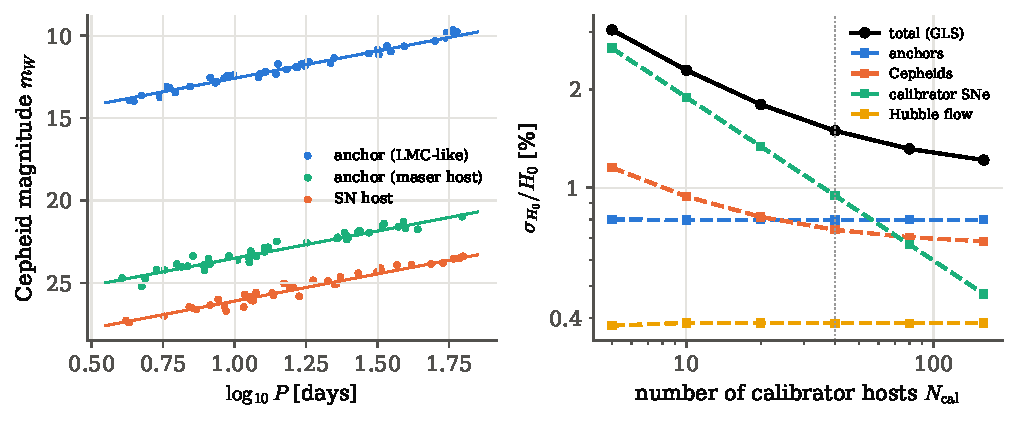
\includegraphics[width=0.95\linewidth]{figures/chT2/distance_ladder.pdf}
\caption{Left: mock Cepheids in two anchors and one supernova host follow parallel Leavitt laws; their vertical offsets are the differences of distance modulus. Right: the fractional error on $H_0$ from the full fit (black) and the contribution of each rung (computed by making that rung noiseless and subtracting in quadrature), against the number of calibrator hosts. The dotted line marks the default ladder.}
\label{T2b:fig:ladder-mc}
\end{figure}

\subsection{The real ladder and the Hubble tension}
\label{T2b:sec:tension}

\emph{Where we have met $H_0$ before.} Every $H_0$ so far was made up by us: the $70$ of the mock supernovae of \cref{3b:sec:hubble}, where $M$ was known, and the $\TwlHtrue$ of the mock ladder just built, recovered as $\TwlHhat\pm\TwlHerr$. In both the truth was known, and the only question was whether the estimator found it and whether its error bar covered it. Here the numbers are published measurements, the truth is not known, and the question becomes whether two of them can be measurements of the same constant. The ladder side is the same construction as above, the Hubble-flow fit of \cref{3b:sec:hubble-degeneracy} with $M$ supplied by the rungs, and its published error, $1.04$, is close to our mock $\TwlHerr$ because the mock was built to be SH0ES-sized. The other side is calibrated by something else entirely: no candle, but the sound horizon at recombination, whose angle on the sky fixes $H_0$ as a parameter derived from the CMB fit (\cref{10a:sec:cmb-planck}). The degeneracy of \cref{3b:sec:hubble-degeneracy} reappears as the way to read the disagreement: since supernovae fix only $M-5\log_{10}H_0$, a gap in $H_0$ is a gap in the luminosity of the candle. \Cref{9c:sec:importance} later adds the ladder value to a CMB chain by reweighting, and \cref{11c:sec:h0-routes} sets all the routes side by side.

Two kinds of measurement give $H_0$, and they answer different questions. The SH0ES team asks: \emph{how fast are galaxies around us receding now, per megaparsec of distance, with distances from geometry alone?} Their ladder is the one built above, and the only physics it assumes is in the rungs themselves (parallax, the Leavitt law, standardised supernovae); no cosmological model enters except the small $q_0$ term of \eqref{T2b:eq:dl-q0}. The Planck team asks a different question: \emph{which $\Lambda$CDM universe produces the pattern of hot and cold spots we see in the CMB, emitted at $z\approx1100$?} $H_0$ is one of the outputs of that fit. It is not measured locally but predicted forward, by running the fitted model from $z\approx1100$ to today. So the two numbers are not two measurements of the same quantity by two instruments; one is a local measurement, the other a prediction of $\Lambda$CDM. If they disagree, either a rung of the ladder is wrong or the model that carries the CMB to today is.

\begin{center}
\small
\begin{tabular}{@{}lll@{}}
\toprule
method & $H_0$ [km/s/Mpc] & what it assumes\\
\midrule
SH0ES, Cepheid ladder & $73.04\pm1.04$ & local geometry and the physics of each rung\\
Planck, CMB & $67.36\pm0.54$ & flat $\Lambda$CDM from $z\approx1100$ to today\\
CCHP TRGB ladder & $69.8\pm1.7$ & local geometry, red giants in place of Cepheids\\
\bottomrule
\end{tabular}
\end{center}

\noindent The values are from \cite{Riess2022SH0ES}, \cite[Table~2]{Planck2018VI} (TT,TE,EE+lowE+lensing) and \cite[Sec.~IV.A]{Abdalla2022}, which quotes the TRGB value of the Carnegie--Chicago Hubble Program (CCHP) of Freedman et al. The TRGB ladder lands between the other two.

\emph{How many standard deviations apart?} The two measurements are independent, so the variance of their difference is the sum of their variances (\cref{ch:04}), and
\[
  \frac{73.04-67.36}{\sqrt{1.04^2+0.54^2}}=\frac{5.68}{1.17}=4.8 ,
\]
the ``about $5\sigma$'' of \cite[Sec.~IV.A]{Abdalla2022}.

\emph{The same gap in magnitudes.} By \eqref{T2b:eq:mb-hf} the Hubble-flow supernovae fix only $M_B-a=M_B-5\log_{10}H_0$. Hold that combination fixed and raise $H_0$ by a factor $r$: $a$ grows by $5\log_{10}r$, so $M_B$ must grow by the same amount. A larger $M_B$ means intrinsically fainter supernovae, which for the same apparent magnitude must be nearer, and nearer galaxies with the same redshifts mean a faster expansion. For the two values,
\[
  \Delta M_B=5\log_{10}\frac{73.04}{67.36}=5\times0.035=0.18\ \text{mag}:
\]
the whole tension is equivalent to a disagreement of $0.18$\,mag about how bright type~Ia supernovae are, with the ladder's supernovae the fainter ones. That is why it is cleanest to carry the ladder into a cosmological fit not as a value of $H_0$ but as a Gaussian prior on $M_B$ \cite[Sec.~IV.E, eq.~(1)]{Abdalla2022}: the ladder calibrates $M_B$, and $H_0$ then follows from the supernovae together with whatever cosmological model is being tested.

\paragraph{Example: can a local void explain it?} Suppose we live inside a sphere whose mean density is below the cosmic mean, with $\delta$ the mean density contrast inside the sphere ($\delta<0$ for a void). Why would the local expansion be faster? The denser surroundings pull the matter at the edge of the sphere outwards, and the sphere has less mass inside to hold it back, so matter streams out of the void. On top of the Hubble flow there is an outflow, and someone inside who measures recession velocities sees them grow faster with distance than the global $H_0$: the local rate is $H_0+\delta H$ with $\delta H>0$. How much faster? Linear continuity, $\dot\delta=-\nabla\cdot\bm v$ for the peculiar velocity $\bm v$ (derived in \cref{T2b:sec:tracers}, \eqref{T2b:eq:continuity}), and the growth rate $\dot\delta=fH\delta$ with $f\approx\Omega_m^{0.55}\approx0.53$ give
\begin{align}
  \frac{\delta H_0}{H_0}
  &\eqby{1}\frac{\nabla\cdot\bm v}{3H_0}
  \eqby{2}-\frac{\dot\delta}{3H_0}
  \eqby{3}-\frac{f}{3}\,\delta ,
  \label{T2b:eq:void}
\end{align}
\begin{explain}
  \item The extra outflow grows in proportion to distance, $\bm v=\delta H\,\bm r$, which is what a change $\delta H$ of the local Hubble rate means. Its divergence is $\nabla\cdot\bm v=\partial_xv_x+\partial_yv_y+\partial_zv_z=3\,\delta H$.
  \item Continuity: matter flowing out of the sphere lowers its density, $\dot\delta=-\nabla\cdot\bm v$.
  \item Linear growth, $\delta\propto D(t)$, so $\dot\delta=(\dd\ln D/\dd\ln a)(\dot a/a)\,\delta=fH\delta$, with $H=H_0$ today.
\end{explain}
which is Abdalla et al.'s eq.~(2) \cite[Sec.~IV.F]{Abdalla2022}. The sign is as expected: $\delta<0$ gives $\delta H_0>0$. How empty would the void have to be? The gap between the ladder and the CMB is $(73.04-67.36)/67.36=8.4\%$, about $8\%$, so
\[
  0.08=\frac{0.53}{3}\,|\delta|\quad\Longrightarrow\quad|\delta|=\frac{3\times0.08}{0.53}=0.45 ,
\]
a region almost half empty, over the whole volume probed by the Hubble-flow supernovae, out to $z=0.15$ or some $600$\,Mpc. Density fluctuations on such scales are at the percent level, and theory and simulations put the expected scatter of the local $H_0$ at $0.5$--$1\%$ \cite[Sec.~IV.F]{Abdalla2022}, an order of magnitude too small.

\paragraph{Where the statistics comes back in.} The ladder is generalised least squares (\cref{ch:03}), and its covariance is the inverse Fisher matrix (\cref{ch:10}). Testing whether two measurements of $H_0$ agree is a hypothesis test on their difference (\cref{ch:04}). Using the ladder as a prior on $M_B$ is Bayesian combination of independent data (\cref{ch:05}). Peculiar velocities and the local Hubble flow are taken up again as data in their own right in \cref{11c:sec:virgo}, and the local cosmic variance of $H_0$, the careful version of the void estimate above, in \cref{11c:sec:cosmicvar}.
\section{Selection effects: what a flux limit does to a sample}
\label{T2b:sec:malmquist}

Every survey has a faintest object it can detect. Close to that limit the survey does not see a fair sample of what is there: it sees the objects that happened to be brighter than average, because their fainter siblings at the same distance were lost. Treat the survivors as typical, and their distances come out too small. At high redshift, where most of the cosmological information sits, the supernovae look brighter than the model predicts, and the fit moves the cosmological parameters to make them so.

The plain claim is that ``the mean absolute magnitude of type~Ia supernovae is $M_0$''. The everyday question is: \emph{if I average the absolute magnitudes of the supernovae in my catalogue, do I get $M_0$?} The question hides a sampling rule. ``The mean'' of the luminosity function is an average over supernovae drawn uniformly \emph{per unit volume}. A catalogue is drawn by a different rule: a supernova enters it if its apparent magnitude is below the limit. Change the sampling rule and the distribution changes, exactly as the distribution of an oscillator's position changes when we sample it uniformly in position rather than in time. The physics of the explosions is the same in both cases; what differs is how the objects were selected.

Selection is conditioning, and conditioning has a picture (\cref{1a:fig:shrink}, \cref{5a:sec:shrink}). Draw every supernova that went off in the survey volume as a point in a rectangle: that rectangle is the full sample space, and the luminosity function describes how the points are spread over it. Detection draws a line through the rectangle: on one side are the supernovae brighter than the limit, $m<m_{\rm lim}$, on the other the ones we never see. Once we know a supernova is in the catalogue, everything on the far side of the line is discarded. The surviving region becomes the new sample space, and every probability is measured again as a fraction of its area. If the survivors are a fraction $P(\text{detected})$ of the whole, every probability of the full population is divided by that fraction. The mean of the survivors, and the likelihood of what they show us, are both computed in the shrunken space. Nothing about an individual explosion has changed; only the region against which it is measured has.

\paragraph{The question.} For candles with a Gaussian spread of absolute magnitudes, (1) what is the mean absolute magnitude of the ones a flux-limited survey detects, (2) how biased are the Hubble residuals near the limit, and (3) what likelihood removes the bias?

\subsection{The classical Malmquist bias}

The inputs are three.
\begin{enumerate}[itemsep=1pt]
  \item \emph{Physical:} the candles are spread uniformly through a static Euclidean space, with number density $n$.
  \item \emph{Physical:} their absolute magnitudes follow a Gaussian \newterm{luminosity function} \unpack{the distribution of absolute magnitudes among the candles} $\varphi(M)=\Normal(M_0,\sigma^2)$, the same everywhere and independent of position.
  \item \emph{Selection:} we look at the objects whose apparent magnitude lies in a narrow interval $[m,m+\dd m]$.
\end{enumerate}

\emph{What we observed} is an object of apparent magnitude $m$. \emph{What could have produced it?} Any absolute magnitude $M$, placed at the distance modulus $\mu=m-M$ that makes it appear at $m$. \emph{How likely is each candidate?} It is the probability of drawing that $M$ from the luminosity function, times the number of places at that distance where the object could be. The number of objects in a shell of radius $r$ and thickness $\dd r$ is $n\,4\pi r^2\dd r$, and $r$ is tied to $\mu$ by $r=10^{\mu/5+1}$\,pc. So
\begin{align}
  \dd N(M,\mu)
  &\eqby{1}n\,\varphi(M)\,\dd M\;4\pi r^2\,\frac{\dd r}{\dd\mu}\,\dd\mu
  \eqby{2}n\,\varphi(M)\,\dd M\;4\pi\frac{\ln10}{5}\,r^3\,\dd\mu
  \;\propto\;\varphi(M)\,10^{0.6\mu}\,\dd M\,\dd\mu ,\nonumber\\
  p(M\given m)
  &\eqby{3}\frac{\varphi(M)\,10^{0.6(m-M)}}{\int\varphi(M')\,10^{0.6(m-M')}\dd M'}
  \eqby{4}\Normal\big(M_0-0.6\ln10\,\sigma^2,\;\sigma^2\big).
  \label{T2b:eq:malmquist}
\end{align}
\begin{explain}
  \item Independence of luminosity and position (inputs 1 and 2): the joint density is the product. Change variable from $r$ to $\mu$.
  \item $r\propto10^{\mu/5}$, so $\dd r/\dd\mu=(\ln10/5)\,r$, and $r^3\propto10^{3\mu/5}$.
  \item Fix $m$ (input 3): $\mu=m-M$, and $\dd\mu=\dd m$ does not depend on $M$. Normalise over $M$.
  \item $10^{-0.6M}=e^{-0.6\ln10\,M}$. Multiply it into the Gaussian and complete the square: $-\frac{(M-M_0)^2}{2\sigma^2}-kM=-\frac{(M-M_0+k\sigma^2)^2}{2\sigma^2}+\text{const}$ with $k=0.6\ln10$.
\end{explain}

\begin{keyidea}[Malmquist bias]
In a flux-limited sample of candles spread uniformly in Euclidean space, the detected objects are on average brighter than the luminosity function by
\[
  \langle M\rangle_{\rm det}-M_0=-0.6\ln10\;\sigma^2=-1.382\,\sigma^2 ,
\]
at every apparent magnitude. The reason is volume: there is more space at large distances, so an object at a given $m$ is more likely to be a bright one far away than a faint one nearby.
\end{keyidea}

The shift does not depend on $m$ or on where the limit is, so the whole flux-limited sample shares it. The size matters. For raw supernovae, $\sigma=0.4$\,mag, the shift is
\[
  \langle M\rangle_{\rm det}-M_0=-1.382\times0.4^2=-0.22\ \text{mag}.
\]
\emph{Which way does that move a distance?} We infer the distance modulus as $\mu_{\rm inf}=m-M_0$. The detected supernovae really have, on average, $M=M_0-0.22$, so their true modulus is $\mu=m-M_0+0.22$, and the inferred one is too small by $0.22$: a candle that is brighter than we assume looks closer than it is. Since $D_L\propto10^{\mu/5}$ by \eqref{T2b:eq:mu},
\[
  \frac{D_{\rm inf}}{D_{\rm true}}=10^{-0.22/5}=10^{-0.044}=0.90 ,
\]
so distances come out $10\%$ too small. After standardisation, $\sigma=0.12$\,mag, the shift is $1.382\times0.12^2=0.020$\,mag and $10^{-0.020/5}=0.99$, a $1\%$ distance error, which is still as large as the statistical error of a modern survey. The key idea depends on its inputs. In an expanding universe the volume does not grow as $r^3$; if the spread $\sigma$ itself depends on distance, or the luminosity function has a non-Gaussian tail, the number changes. The mechanism, a luminosity function reweighted by the volume where each luminosity can be seen, does not.

\subsection{Near the limit: a truncated Gaussian}

Now the version that matters for a supernova Hubble diagram. At redshift $z$, the model predicts a mean apparent magnitude $\bar m(z;\params)=M_B+\mu(z;\params)$, and the observed magnitudes scatter about it, $m=\bar m+\epsilon$ with $\epsilon\sim\Normal(0,\sigma^2)$. The survey keeps a supernova only if $m<m_{\rm lim}$. \emph{What is the mean residual of the supernovae it keeps?} With $t\equiv(m_{\rm lim}-\bar m)/\sigma$ the distance of the limit from the mean in units of $\sigma$, and $\phi$, $\Phi$ the standard normal density and distribution function,
\begin{align}
  \E[\epsilon\given\epsilon<t\sigma]
  &\eqby{1}\frac{\int_{-\infty}^{t\sigma}\epsilon\,\frac1\sigma\phi(\epsilon/\sigma)\,\dd\epsilon}{\Phi(t)}
  \eqby{2}\frac{-\sigma\big[\phi(\epsilon/\sigma)\big]_{-\infty}^{t\sigma}}{\Phi(t)}
  \eqby{3}-\sigma\,\frac{\phi(t)}{\Phi(t)} .
  \label{T2b:eq:trunc-mean}
\end{align}
\begin{explain}
  \item Conditional expectation: integrate over the kept region and divide by its probability $\Prob(\epsilon<t\sigma)=\Phi(t)$. The division is the renormalisation of the shrunken sample space: the kept region has total probability $\Phi(t)$, and dividing by it makes the probabilities inside it add up to one again.
  \item $\frac{\dd}{\dd\epsilon}\phi(\epsilon/\sigma)=-\frac{\epsilon}{\sigma^2}\phi(\epsilon/\sigma)$, so $\epsilon\,\phi(\epsilon/\sigma)/\sigma$ is $-\sigma$ times the derivative of $\phi(\epsilon/\sigma)$.
  \item $\phi$ vanishes at $-\infty$.
\end{explain}
Two cases give the result a size. Far from the limit ($t\gg1$), $\Phi(t)\to1$ (almost nothing is cut) and $\phi(t)\to0$ (the Gaussian has no weight there), so the bias vanishes. Where half the supernovae are lost ($t=0$), $\phi(0)=1/\sqrt{2\pi}$ and $\Phi(0)=1/2$, so the bias is $-\sigma\cdot2/\sqrt{2\pi}=-\sigma\sqrt{2/\pi}=-0.80\,\sigma$. Beyond that ($t<0$) it grows without bound. \Cref{T2b:fig:malmquist-cartoon} shows the mechanism at three distances.

\begin{figure}[htbp]
\centering
\begin{tikzpicture}[x=1cm,y=1cm]
  \draw[->,faint] (0,-2.2) -- (9.6,-2.2) node[right,font=\small,text=black] {distance $\mu$};
  \draw[->,faint] (0,-2.2) -- (0,2.4) node[above,font=\small,text=black] {brighter};
  \draw[faint,dashed] (0,0) -- (9.4,0) node[right,font=\footnotesize,text=softgray] {$M_0$};
  \draw[bdry] (5.6,-2.03) -- (9.0,2.5) node[above,font=\footnotesize,text=bdryred] {$m=m_{\rm lim}$};
  \foreach \X/\Yl/\Ym in {3.0/-5.5/0.0, 7.125/0.0/0.479, 8.2/1.433/1.63}{
    \begin{scope}
      \clip (\X,\Yl) rectangle (\X+1.2,2.3);
      \fill[formblue!35] (\X,-2.0) -- plot[domain=-2.0:2.0,samples=60,smooth] ({\X+0.75*exp(-(\x)^2/0.72)},\x) -- (\X,2.0) -- cycle;
    \end{scope}
    \draw[formblue,thick] plot[domain=-2.0:2.0,samples=60,smooth] ({\X+0.75*exp(-(\x)^2/0.72)},\x);
    \draw[faint] (\X,-2.0) -- (\X,2.0);
    \draw[fibreorange,very thick] (\X-0.15,\Ym) -- (\X+0.3,\Ym);
  }
  \node[font=\footnotesize,align=center] at (3.5,-2.6) {all detected};
  \node[font=\footnotesize,align=center] at (7.1,-2.6) {half detected};
  \node[font=\footnotesize,align=center] at (8.8,-2.6) {tail only};
\end{tikzpicture}
\caption{The luminosity function of the candles (blue bell, brighter upwards) at three distances, with the flux limit (red). Only the shaded part, brighter than the limit, is detected. The orange tick marks the mean brightness of the detected objects: at the true $M_0$ nearby, $0.8\sigma$ brighter where the limit cuts the bell in half, and about $2.7\sigma$ brighter where only the bright tail survives.}
\label{T2b:fig:malmquist-cartoon}
\end{figure}

\paragraph{The fix: write the likelihood of what was selected.} The likelihood asks how probable the observed magnitudes are under each model. For a catalogue, the honest version of that question is: how probable are they \emph{among the supernovae that could have entered the catalogue}? That is the shrunken sample space again, now for a density instead of a mean:
\begin{align}
  p(m\given z,\params,\text{detected})
  &\eqby{1}\frac{p(m,\text{detected}\given z,\params)}{\Prob(\text{detected}\given z,\params)}
  \eqby{2}\frac{\Normal\big(m;\bar m(z;\params),\sigma^2\big)}{\Phi\big(t(z;\params)\big)}\qquad(m<m_{\rm lim}),\nonumber\\
  -\ln\Like
  &\eqby{3}\sum_i\Big[\frac{(m_i-\bar m_i)^2}{2\sigma^2}+\ln\sigma+\tfrac12\ln2\pi+\ln\Phi(t_i)\Big]\nonumber\\
  &\eqby{4}\sum_i\Big[\frac{(m_i-\bar m_i)^2}{2\sigma^2}+\ln\Phi(t_i)\Big]+\text{const}.
  \label{T2b:eq:trunc-like}
\end{align}
\begin{explain}
  \item The definition of conditional probability: the joint density divided by the probability of the condition.
  \item For $m<m_{\rm lim}$ ``detected'' is automatically true, so the joint density is just the Gaussian. The probability of detection is $\Prob(m<m_{\rm lim})=\Phi(t)$, the same $\Phi(t)$ that renormalised the mean in \eqref{T2b:eq:trunc-mean}.
  \item The supernovae are independent, so the likelihood is a product and $-\ln\Like$ a sum. Write out $-\ln$ of the Gaussian density $\frac{1}{\sqrt{2\pi}\sigma}e^{-(m-\bar m)^2/2\sigma^2}$, and note that $-\ln(1/\Phi)=+\ln\Phi$.
  \item $\sigma$ is known and the same for every model, so $\ln\sigma+\frac12\ln2\pi$ is a constant that does not move the fit.
\end{explain}
The first term is the naive $\chi^2/2$. The second is new, and it depends on $\params$ through $t_i=(m_{\rm lim}-\bar m_i)/\sigma$. Since $\Phi\le1$, $\ln\Phi(t)\le0$: the term \emph{lowers} $-\ln\Like$, most strongly for a model whose mean $\bar m$ lies near or beyond the limit, where $\Phi(t)$ is small. \emph{What is that credit for?} Take one supernova detected at $m=m_{\rm lim}-0.5\sigma$ and two models. Model A puts the mean exactly there, $\bar m=m_{\rm lim}-0.5\sigma$, so $t=0.5$. Model B puts the mean fainter than the limit, $\bar m=m_{\rm lim}+\sigma$, so $t=-1$ and the supernova sits $1.5\sigma$ out in the bright tail.
\begin{center}
\small
\begin{tabular}{@{}lccc@{}}
\toprule
model & $\chi^2/2$ & $\ln\Phi(t)$ & $-\ln\Like$ (no constant)\\
\midrule
A, $t=0.5$ & $0$ & $\ln0.69=-0.37$ & $-0.37$\\
B, $t=-1$ & $1.5^2/2=1.13$ & $\ln0.16=-1.84$ & $-0.72$\\
\bottomrule
\end{tabular}
\end{center}
The naive fit prefers A by a factor $e^{1.13}\approx3$, because under B this supernova is a $1.5\sigma$ excursion. But under B, \emph{every} supernova we can see is an excursion into the bright tail: the selection guarantees it. Being in the tail is not evidence against B; it is what B predicts for the supernovae that got into the catalogue. The $\ln\Phi$ term returns exactly that credit, and with it B is, if anything, slightly preferred (by $e^{0.35}\approx1.4$), because under B the detected supernovae pile up just inside the limit, which is where this one is. With many supernovae the balance is set by how they are spread inside the limit, which is what the full sum in \eqref{T2b:eq:trunc-like} weighs. (The number of detected supernovae is not used here. A likelihood that also used the count would add a term that does penalise a model for predicting too few detections.) The result is the likelihood of \cref{ch:03}, written for the data \emph{as they were collected}: a density for what could have been observed, given the rule that decided what got into the sample. Real surveys have no sharp limit. The detection probability $\eta(m)$ rises smoothly from $0$ to $1$ and depends on the observing conditions, so it is measured by injecting fake supernovae into the real images, and $\Phi(t)$ in \eqref{T2b:eq:trunc-like} becomes $\int\eta(m)\Normal(m;\bar m,\sigma^2)\,\dd m$. Pantheon+ corrects each supernova by a bias computed from large simulations of the whole survey \cite{Brout2022PantheonPlus}.

\paragraph{The experiment.} \pyname{08_malmquist.py} does both calculations.

\emph{The Euclidean test.} It places $4\times10^5$ candles uniformly in a ball and keeps those brighter than a limit. The mean $M$ of the detected ones is shifted by $\TwmSigOne$, $\TwmSigThree$ and $\TwmSigFive$\,mag for $\sigma=0.1$, $0.3$ and $0.5$, against $-1.382\sigma^2=\TwmSigOneTh$, $\TwmSigThreeTh$ and $\TwmSigFiveTh$ from the key idea.

\emph{The survey.} Then it simulates supernova surveys in an expanding universe, with two samples:
\begin{center}
\small
\begin{tabular}{@{}lll@{}}
\toprule
sample & redshifts & selection\\
\midrule
low redshift & $0.02<z<0.1$ & complete: every supernova is kept\\
deep & $0.1<z<1.2$ & kept only if $m<m_{\rm lim}=\TwmLim$\\
\midrule
both & \multicolumn{2}{l}{flat $\Lambda$CDM with $\Omega_{m0}=\TwmOm$; scatter $\sigma=\TwmSig$\,mag about $\bar m(z)$}\\
\bottomrule
\end{tabular}
\end{center}
Each fit has two free numbers, $\Omega_{m0}$ and an overall magnitude offset (the combination $M_B-5\log_{10}H_0$ of \cref{T2b:sec:ladder}), which the complete low-redshift sample pins down. The two fits differ by one line:

\pyfile[firstline=68,lastline=78,firstnumber=68]{code/chT2/08_malmquist.py}{The naive and the selection-aware negative log-likelihood}

\noindent Line 74 is the $\chi^2/2$ of a standard fit. Line 77 adds $\sum\ln\Phi(t_i)$, the second term of \eqref{T2b:eq:trunc-like}, for the supernovae of the deep sample.

\emph{The result.} \Cref{T2b:fig:malmquist} shows it. Half the supernovae are lost at $z\approx\TwmZhalf$, and in the last redshift bin that still contains supernovae ($z\approx\TwmZlast$) the mean residual is $\TwmResLast$\,mag. Over $\TwmNmock$ mock surveys the naive $\chi^2$ returns $\Omega_{m0}=\TwmNaiveMean\pm\TwmNaiveSd$, too high. The chain that leads there has three links. The selected high-redshift supernovae are brighter than the model mean, so they look nearer than they are. The offset is fixed by the complete low-redshift sample, so the only way the naive fit can bring the model to them is to shorten the model's distances at high redshift. In flat $\Lambda$CDM at fixed $H_0$, a shorter $D_L=(1+z)\,c\int_0^z\dd z'/H(z')$ at high redshift needs a larger $H(z')$ in the past, so the expansion must have slowed down more since then: more deceleration, which needs more matter. The selection-aware likelihood returns $\TwmCorrMean\pm\TwmCorrSd$, unbiased, with the same scatter. The naive bias is almost three times its own error bar, and it would not shrink with more supernovae.

\begin{figure}[htbp]
\centering
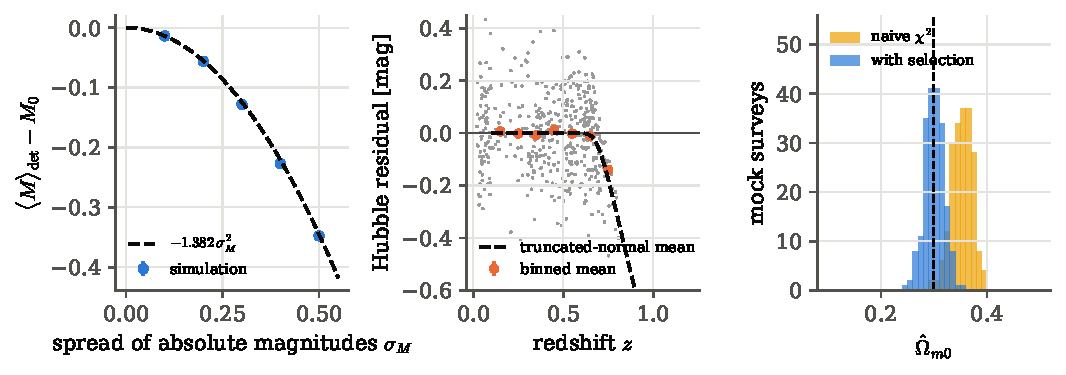
\includegraphics[width=\linewidth]{figures/chT2/malmquist.pdf}
\caption{Left: the classical Malmquist shift measured in simulation against $-1.382\sigma^2$. Middle: Hubble residuals of a magnitude-limited survey; the binned means (orange) follow the truncated-normal mean $-\sigma\phi(t)/\Phi(t)$ (dashed) and plunge as the limit cuts into the population. Right: $\Omega_{m0}$ from many mock surveys; the naive fit is biased, the likelihood with the selection term is not.}
\label{T2b:fig:malmquist}
\end{figure}

\paragraph{A relative: Eddington bias.} A related effect acts on counts rather than on luminosities. If the number of objects rises steeply towards faint fluxes, measurement noise scatters more objects up across a threshold than down, so the objects just above the threshold are, on average, fainter than they were measured. Both biases have the same cure: model the selection, and write the likelihood of the data that were actually kept.

\paragraph{Where the statistics comes back in.} The conditional density \eqref{T2b:eq:malmquist} is Bayes' theorem of \cref{ch:05}, with the luminosity function as prior and the volume factor as likelihood. The truncated likelihood is the likelihood of \cref{ch:03} written for the data actually collected. Selection functions that are known only from simulations are a Monte Carlo problem (\cref{ch:06}), and when they are folded into a hierarchical supernova model the posterior is explored by MCMC (\cref{ch:09}).
\section{Galaxies as biased tracers in redshift space}
\label{T2b:sec:tracers}

A redshift survey records, for each galaxy, two angles on the sky and a redshift. The Dark Energy Spectroscopic Instrument (DESI) did this for more than six million galaxies and quasars in its first year: bright galaxies at $0.1<z<0.4$, luminous red galaxies at $0.4<z<1.1$, star-forming emission-line galaxies at $0.8<z<1.6$, quasars at $0.8<z<2.1$, and the absorption of quasar light by intergalactic hydrogen (the Lyman-$\alpha$ forest) out to $z\approx4$ \cite[Sec.~2.2, Table~1]{DESI2024VI}. A fiducial cosmology turns each redshift into a distance and the survey into a three-dimensional map of points. The counts in cells of that map define the galaxy overdensity $\delta_g(\bm x)=n(\bm x)/\bar n-1$, and its two-point statistics, the correlation function $\xi_g(r)$ and the power spectrum $P_g(k)$ of \cref{ch:07}, are what the statistics chapters work with.

The map is not the matter field. Three things stand between them. Galaxies form only where matter has collapsed into haloes, so they are \emph{biased}: their density contrast is larger than that of the matter. Galaxies are discrete points, so their map carries \emph{shot noise}. And the redshift contains the galaxy's peculiar velocity as well as its distance, so the map is \emph{distorted} along the line of sight.

\paragraph{The question.} How is the galaxy power spectrum related to the matter power spectrum on large scales, and what is the noise of a measured $P_g$?

\subsection{Why galaxies cluster more strongly than matter}

The inputs are two. \emph{Physical:} a galaxy forms where the local density, smoothed on the scale of a halo, exceeds a threshold. \emph{Mathematical:} the initial density field is Gaussian. Write the local density at $\bm x$ as $u(\bm x)$, with variance $\sigma^2$, and say a galaxy forms where $u>\nu\sigma$; the number $\nu$ measures how rare the galaxies are. The local density is a sum of two parts, $u=u_{\rm long}+u_{\rm short}$: a long-wavelength part, shared with the surroundings over tens of megaparsecs, and a short-wavelength part that varies from halo to halo and decides locally whether the threshold is crossed. Only the first can link a galaxy to matter far away.

\emph{What we know} is that a galaxy formed at $\bm x$. \emph{What does that tell us about the matter at $\bm y$, a distance $r$ away?} The galaxy is a sign that $u(\bm x)$ was high. Because $u(\bm x)$ and $\delta(\bm y)$ are correlated, the matter at $\bm y$ is denser than average too. The cross-correlation of galaxies and matter is exactly that expected density:
\begin{align}
  \xi_{gm}(r)
  &\eqby{1}\frac{\E[I(\bm x)\,\delta(\bm y)]}{\E[I]}
  \eqby{2}\E\big[\delta(\bm y)\given u(\bm x)>\nu\sigma\big]
  \eqby{3}\E\Big[\frac{\xi(r)}{\sigma^2}\,u\;\Big|\;u>\nu\sigma\Big]
  \eqby{4}\frac{\xi(r)}{\sigma}\,\frac{\phi(\nu)}{1-\Phi(\nu)}\equiv b_L\,\xi(r) .
  \label{T2b:eq:threshold-bias}
\end{align}
\begin{explain}
  \item $I(\bm x)$ is $1$ where a galaxy forms and $0$ elsewhere, so $\delta_g=I/\E[I]-1$; the $-1$ drops out because $\E[\delta]=0$.
  \item Dividing by $\E[I]=\Prob(u>\nu\sigma)$ turns the average into a conditional expectation.
  \item For two jointly Gaussian variables the conditional mean is linear: $\E[\delta(\bm y)\given u]=\frac{\Cov(\delta(\bm y),u(\bm x))}{\Var u}\,u$ (derived in \cref{7a:eq:condmean} and \cref{2b:sec:mvn-conditional}). Which part of $u(\bm x)$ is correlated with matter a distance $r$ away? Split $u=u_{\rm long}+u_{\rm short}$ as above. The short-wavelength part varies over the size of a halo and has no memory of what happens tens of megaparsecs away, so $\Cov(\delta(\bm y),u_{\rm short}(\bm x))=0$. The long-wavelength part is the matter field itself, smoothed over a region much smaller than $r$, so $\Cov(\delta(\bm y),u_{\rm long}(\bm x))=\xi(r)$, the matter correlation. Hence $\Cov(\delta(\bm y),u(\bm x))=\xi(r)$, while $\Var u=\sigma^2$ counts both parts.
  \item The mean of a Gaussian above $\nu\sigma$ is $\sigma\phi(\nu)/[1-\Phi(\nu)]$, the upper-tail version of \eqref{T2b:eq:trunc-mean}.
\end{explain}
For rare galaxies, $\nu\gg1$, the ratio $\phi(\nu)/[1-\Phi(\nu)]\to\nu$, and $b_L\to\nu/\sigma$: the rarest objects are the most strongly clustered. This is Kaiser's explanation of why rich galaxy clusters cluster more strongly than galaxies.

\emph{From galaxy--matter to galaxy--galaxy.} \Cref{T2b:eq:threshold-bias} conditions on one galaxy and looks at the matter. The galaxy map has a galaxy at both ends of each pair, so both points are now conditioned. Write $x_1=u(\bm x)/\sigma$ and $x_2=u(\bm y)/\sigma$ for the two local densities in units of $\sigma$. They are jointly Gaussian with unit variances and a small correlation $\rho=\xi(r)/\sigma^2$ (the long-wavelength parts carry it, as in item 3). Then
\begin{align}
  1+\xi_{gg}(r)
  &\eqby{1}\frac{\E[I(\bm x)I(\bm y)]}{\E[I]^2}
  \eqby{2}\frac{1}{\E[I]^2}\int_\nu^\infty\!\!\int_\nu^\infty\phi(x_1)\phi(x_2)\big(1+\rho\,x_1x_2\big)\,\dd x_1\dd x_2\nonumber\\
  &\eqby{3}1+\rho\Big[\frac{\int_\nu^\infty x\,\phi(x)\,\dd x}{1-\Phi(\nu)}\Big]^2
  \eqby{4}1+\frac{\xi(r)}{\sigma^2}\Big[\frac{\phi(\nu)}{1-\Phi(\nu)}\Big]^2
  =1+b_L^2\,\xi(r) .
  \label{T2b:eq:threshold-auto}
\end{align}
\begin{explain}
  \item $\delta_g=I/\E[I]-1$, so $\E[(1+\delta_g(\bm x))(1+\delta_g(\bm y))]=1+\xi_{gg}$.
  \item The bivariate Gaussian density with correlation $\rho$ is $\frac{1}{2\pi\sqrt{1-\rho^2}}\exp\big[-\frac{x_1^2-2\rho x_1x_2+x_2^2}{2(1-\rho^2)}\big]$. To first order in $\rho$ the prefactor and the $1-\rho^2$ are unchanged, and the exponent gains $+\rho x_1x_2$, so the density is $\phi(x_1)\phi(x_2)e^{\rho x_1x_2}\approx\phi(x_1)\phi(x_2)(1+\rho x_1x_2)$.
  \item The $1$ integrates to $[1-\Phi(\nu)]^2=\E[I]^2$. The $\rho x_1x_2$ term factorises into two identical one-dimensional integrals.
  \item $\int_\nu^\infty x\phi(x)\dd x=[-\phi(x)]_\nu^\infty=\phi(\nu)$, as in \eqref{T2b:eq:trunc-mean}. Compare with \eqref{T2b:eq:threshold-bias}: $b_L=\phi(\nu)/\{\sigma[1-\Phi(\nu)]\}$.
\end{explain}
Each conditioned point contributes one factor $b_L$: a galaxy at $\bm x$ raises the expected density near $\bm y$ by $b_L\xi$ (that is \eqref{T2b:eq:threshold-bias}), and the threshold at $\bm y$ turns that raised density into $b_L$ times as many extra galaxies. So $\xi_{gg}=b_L^2\,\xi$, and since the power spectrum is the Fourier transform of the correlation function, $P_{gg}=b_L^2P$.

This bias is ``Lagrangian'': it describes where the galaxies formed. Afterwards they move with the matter, and the motion adds the matter's own contrast. \emph{Label each bit of matter by where it started.} Call the starting (Lagrangian) position $\bm q$. Write $\delta_L(\bm q)$ for the linear matter contrast there, grown to the time we observe with the linear growth factor, so that $b_L\delta_L$ is the galaxies' contrast of \eqref{T2b:eq:threshold-bias} at their birth place. At the start the matter is uniform to first order, while the galaxies already carry their contrast $\delta_g^L=b_L\delta_L$. \emph{Move everything.} Each bit of matter, and any galaxy riding in it, moves to its present (Eulerian) position $\bm x=\bm q+\bm\psi(\bm q)$, with $\bm\psi$ the displacement. A small volume $\dd^3q$ becomes $\dd^3x=J\,\dd^3q$, with $J=|\det(\partial x_i/\partial q_j)|$ the Jacobian of the map. \emph{Count.} No galaxy and no matter is created or lost on the way, so the number in the small volume is the same before and after:
\begin{align}
  \bar n_g\big(1+\delta_g(\bm x)\big)\,\dd^3x
  &\eqby{1}\bar n_g\big(1+b_L\delta_L(\bm q)\big)\,\dd^3q
  \;\;\Longrightarrow\;\;
  1+\delta_g\eqby{2}\frac{1+b_L\delta_L}{J},\qquad
  1+\delta\eqby{3}\frac1J,\nonumber\\
  1+\delta_g
  &\eqby{4}\big(1+b_L\delta_L\big)\big(1+\delta\big)
  \eqby{5}1+b_L\delta+\delta+O(\delta^2).
  \label{T2b:eq:lagr-to-euler}
\end{align}
\begin{explain}
  \item Number conservation for the galaxies; $\bar n_g$, the mean density, is the same before and after because the total volume and number do not change.
  \item Divide by $\bar n_g\,\dd^3x=\bar n_g J\,\dd^3q$.
  \item The same count for the matter, which started uniform.
  \item Eliminate $J$ between the two.
  \item Multiply out and keep first-order terms. To first order the evolved contrast and the linear one are the same field, $\delta=\delta_L$, and $\bm x$ and $\bm q$ differ only by the small displacement, so $\delta_L(\bm q)=\delta(\bm x)$ to this order.
\end{explain}
So, to first order,
\begin{equation}
  \delta_g=(1+b_L)\,\delta\equiv b\,\delta ,\qquad P_g(k)=b^2P(k),
  \label{T2b:eq:eulerian-bias}
\end{equation}
the ``continuity'' derivation that Cooray and Sheth mention for the large-scale bias of haloes \cite[Sec.~3.3]{CooraySheth2002}.

The halo-model version of the same idea gives each halo mass its bias, quoted in a different variable. A halo of mass $m$ forms where the linear density smoothed on the scale of that mass, of rms $\sigma(m)$, exceeds the spherical-collapse threshold $\delta_{\rm sc}\approx1.69$. In our language the threshold in units of $\sigma$ is $\nu=\delta_{\rm sc}/\sigma(m)$. Cooray and Sheth use instead its square, which we write $\nu_h\equiv\delta_{\rm sc}^2/\sigma^2(m)=\nu^2$ to keep the two apart, and quote $b_1(m)=1+(\nu_h-1)/\delta_{\rm sc}$ for spherical collapse, with an improved form fitted to simulations \cite[eqs.~(53), (68)--(70)]{CooraySheth2002}. \emph{How does this compare with ours?} The ``$1+$'' is the step from Lagrangian to Eulerian just derived. For the Lagrangian part, our high-threshold limit gives
\[
  b_L\to\frac{\nu}{\sigma}=\frac{\delta_{\rm sc}}{\sigma^2}=\frac{\nu_h}{\delta_{\rm sc}} ,
\]
so the halo formula differs from ours only by the $-1$. It comes from what is being counted. Our $b_L$ belongs to the fraction of space above a threshold, a Gaussian tail. The halo model counts haloes in a narrow mass range, which is the rate at which that tail changes with mass, and for spherical collapse this abundance goes as $\nu_h^{1/2}e^{-\nu_h/2}$ instead of a tail probability. A long-wavelength contrast $\delta_{\rm long}$ lowers the barrier to $\delta_{\rm sc}-\delta_{\rm long}$, so $\nu_h\to(\delta_{\rm sc}-\delta_{\rm long})^2/\sigma^2$ and $\dd\nu_h/\dd\delta_{\rm long}=-2\nu_h/\delta_{\rm sc}$. The fractional change of the abundance is then
\[
  \frac{\dd}{\dd\delta_{\rm long}}\Big[\tfrac12\ln\nu_h-\tfrac12\nu_h\Big]
  =\Big(\frac{1}{2\nu_h}-\frac12\Big)\Big(-\frac{2\nu_h}{\delta_{\rm sc}}\Big)
  =\frac{\nu_h-1}{\delta_{\rm sc}} ,
\]
the Lagrangian bias of the halo formula. The $\nu_h$ is our threshold effect, and the $-1$ comes from the prefactor $\nu_h^{1/2}$. For rare haloes, $\nu_h\gg1$, the two agree. A galaxy population then has the occupation-weighted average bias $b_{\rm gal}=\int\dd m\,n(m)\,b_1(m)\langle N_{\rm gal}\given m\rangle/\bar n_{\rm gal}$, and $P_{\rm gal}\approx b_{\rm gal}^2P_{\rm lin}$ on large scales \cite[eqs.~(130)--(131)]{CooraySheth2002}. Since $b_1(m)$ grows with $\nu_h$, and so with mass, luminous red galaxies, which live in massive haloes, are more strongly biased than emission-line galaxies, which live in smaller ones.

\begin{keyidea}[Linear bias]
On scales much larger than a halo, the galaxy density contrast is proportional to the matter density contrast, $\delta_g=b\,\delta$, so $P_g(k)=b^2P(k)$ and $\xi_g(r)=b^2\xi(r)$. The shape of the clustering is the matter's; only its amplitude belongs to the galaxies. The bias is a nuisance parameter in every fit of galaxy clustering.
\end{keyidea}

\subsection{Shot noise}

Galaxies are a discrete sample of a continuous field: given the field, the number of galaxies in a small cell is Poisson-distributed with mean $\bar n(1+\delta_g)\,\dd V$ (\cref{2a:sec:poisson-inputs}). What does that do to the measured power? Put $N=\bar nV$ galaxies at positions $\bm x_i$ in a box of volume $V$. The density is a sum of spikes, $n(\bm x)=\sum_i\delta_D(\bm x-\bm x_i)$, and its Fourier transform at any $\bm k\ne0$ is a sum of phases, so with the convention $\E[\delta_{\bm k}\delta^*_{\bm k}]=VP(k)$ of \cref{11a:sec:shot},
\begin{align}
  \hat P_g(k)=\frac{|\delta_{g,\bm k}|^2}{V}
  &\eqby{1}\frac{1}{V\bar n^2}\sum_i\sum_je^{-i\bm k\cdot(\bm x_i-\bm x_j)}
  \eqby{2}\frac{1}{V\bar n^2}\Big[N+\sum_{i\ne j}e^{-i\bm k\cdot(\bm x_i-\bm x_j)}\Big],\nonumber\\
  \langle\hat P_g(k)\rangle
  &\eqby{3}\frac{N}{V\bar n^2}+b^2P(k)
  \eqby{4}b^2P(k)+\frac1{\bar n}.
  \label{T2b:eq:shot}
\end{align}
\begin{explain}
  \item $\delta_g=n/\bar n-1$, and the $-1$ only touches $\bm k=0$, so $\delta_{g,\bm k}=\bar n^{-1}\sum_ie^{-i\bm k\cdot\bm x_i}$; the modulus squared is a double sum.
  \item Split off the $i=j$ terms: each is $e^0=1$, and there are $N$ of them.
  \item The pairs of different galaxies are the clustering: averaged over realisations, their phases add up to $V\bar n^2\,b^2P(k)$, the power of the field the galaxies trace.
  \item $N=\bar nV$.
\end{explain}
The self-pairs, each galaxy paired with itself, add a constant $1/\bar n$ at every $k$: a white-noise floor, the \newterm{shot noise} (derived in full in \cref{11a:sec:shot}).

How noisy is the measured $\hat P_g$? The Gaussian-field result of \cref{ch:07} answers it in two steps. \emph{Count the modes.} In a box of volume $V$ the allowed wavevectors sit on a grid, one per $(2\pi)^3/V$ of $\bm k$-space. A shell of radius $k$ and width $\Delta k$ has volume $4\pi k^2\Delta k$, so it holds $N_k=4\pi k^2\Delta k\,V/(2\pi)^3=Vk^2\Delta k/(2\pi^2)$ grid points. The field is real, so $\delta_{-\bm k}=\delta_{\bm k}^*$ and only $N_k/2$ of them are independent. \emph{The error of one shell.} One independent mode gives $|\delta_{\bm k}|^2/V$, whose standard deviation equals its mean (it is $\frac12\chi^2_2$ times the mean, \eqref{7a:eq:mode-exp}), and the mean is now the total power $b^2P+1/\bar n$. Averaging $N_k/2$ independent modes divides the variance by $N_k/2$ (\eqref{7a:eq:var-phat}), so $\sigma_P=\sqrt{2/N_k}\,(b^2P+1/\bar n)$. Divide by the signal $b^2P$:
\begin{equation}
  \frac{\sigma_{P}}{b^2P}=\sqrt{\frac{2}{N_k}}\Big(1+\frac{1}{\bar nb^2P}\Big).
  \label{T2b:eq:pk-error}
\end{equation}
Two terms limit a survey. Cosmic variance, the $\sqrt{2/N_k}$, falls only with volume. Shot noise is negligible once $\bar nb^2P\gtrsim1$. A survey designer therefore covers as much volume as possible with just enough galaxies to reach $\bar nP\approx1$ on the scales of interest, around $k=0.1\,h$\,Mpc$^{-1}$ \cite[Sec.~4.4.5]{Weinberg2013}. DESI's ``effective volume'' $V_{\rm eff}=\int[\bar nP/(1+\bar nP)]^2\dd V$ is this trade-off in one number \cite[Table~1]{DESI2024VI}.

If several galaxies share one halo, their pairs add a second constant on large scales, the one-halo term $\int\dd m\,n(m)\langle N(N-1)\given m\rangle/\bar n^2$ \cite[eq.~(128)]{CooraySheth2002}. It behaves like extra shot noise.

\subsection{Redshift-space distortions}

The redshift of a galaxy measures its distance plus its peculiar velocity along the line of sight. In comoving coordinates the map position is $\bm s=\bm x+u_z\hat{\bm z}$, with $\hat{\bm z}$ the line of sight and $u_z=v_z/(aH)$ the velocity expressed as a distance. Galaxies falling towards an overdensity from in front are pushed back, those behind are pulled forward, and the structure looks squashed along the line of sight (\cref{T2b:fig:kaiser-cartoon}).

How strong is the squashing? The inputs are: linear theory ($|\delta|\ll1$); a distant observer, so the line of sight is the same direction $\hat{\bm z}$ for every galaxy; and velocities set by the growth of structure. That last input needs a short derivation, because the velocity is what moves the galaxies in the map.

\emph{The velocities from the growth of structure.} Matter that flows out of a region lowers its density. In comoving coordinates, with $\bm v$ the peculiar velocity, mass conservation to first order in $\delta$ and $\bm v$ reads
\begin{align}
  \frac{\partial\delta}{\partial t}
  &\eqby{1}-\frac1a\,\nabla\cdot\bm v,
  \qquad
  \frac{\partial\delta}{\partial t}\eqby{2}fH\,\delta
  \quad\Longrightarrow\quad
  \nabla\cdot\bm v\eqby{3}-afH\,\delta,
  \qquad
  \nabla\cdot\bm u\eqby{4}-f\,\delta .
  \label{T2b:eq:continuity}
\end{align}
\begin{explain}
  \item The continuity equation: the outflow rate through the surface of a small comoving volume, per unit volume, is $\nabla\cdot\bm v$ in physical units, and a comoving gradient is $a$ times a physical one, hence the $1/a$.
  \item Linear growth: $\delta(\bm x,t)=\delta(\bm x,t_0)D(t)$, with $D$ the linear growth factor, so $\partial\delta/\partial t=(\dot D/D)\delta=(\dd\ln D/\dd\ln a)(\dot a/a)\delta=fH\delta$, which defines the growth rate $f=\dd\ln D/\dd\ln a\approx\Omega_m(z)^{0.55}$.
  \item Equate the two and multiply by $-a$.
  \item Divide by $aH$: $\bm u=\bm v/(aH)$ is the velocity expressed as a comoving distance.
\end{explain}
In physical coordinates, with $\bm r=a\bm x$, the first relation is $\dot\delta=-\nabla_{\bm r}\cdot\bm v$, the form used for the local void in \cref{T2b:sec:ladder}. The divergence fixes only part of $\bm u$. In linear theory any rotation of the flow decays as the universe expands, so the flow is a gradient, $\bm u=\nabla\Phi_u$, and in Fourier space $\bm u_{\bm k}=i\bm k\,\Phi_{u,\bm k}$ points along $\bm k$. Its divergence is $i\bm k\cdot\bm u_{\bm k}=-k^2\Phi_{u,\bm k}$, and setting this equal to $-f\delta_{\bm k}$ gives $\Phi_{u,\bm k}=f\delta_{\bm k}/k^2$, so
\[
  \bm u_{\bm k}=\frac{i\bm k\,f\,\delta_{\bm k}}{k^2}.
\]

\emph{Now the map.} Galaxies are conserved by the mapping from real to redshift space, $(1+\delta_s)\,\dd^3s=(1+\delta_g)\,\dd^3x$. So
\begin{align}
  \delta_s
  &\eqby{1}\delta_g-\frac{\partial u_z}{\partial z}
  \;\;\xrightarrow{\;\text{Fourier}\;}\;\;
  \delta_{s,\bm k}\eqby{2}b\,\delta_{\bm k}-ik_z\,\frac{ik_zf}{k^2}\,\delta_{\bm k}
  \eqby{3}\big(b+f\mu^2\big)\,\delta_{\bm k},\nonumber\\
  P_s(k,\mu)
  &\eqby{4}b^2\big(1+\beta\mu^2\big)^2P(k),\qquad\beta\equiv\frac fb,\qquad\mu\equiv\frac{k_z}{k}.
  \label{T2b:eq:kaiser}
\end{align}
\begin{explain}
  \item $\dd^3s=(1+\partial u_z/\partial z)\,\dd^3x$, because only the $z$ coordinate is moved; expand to first order.
  \item $\delta_g=b\delta$, and $\partial/\partial z\to ik_z$.
  \item $-i\cdot i=1$ and $k_z^2/k^2=\mu^2$, the squared cosine of the angle between $\bm k$ and the line of sight.
  \item Square the modulus and average over realisations.
\end{explain}
This is the \newterm{Kaiser formula} \cite{Kaiser1987}. Waves across the line of sight ($\mu=0$) are untouched; waves along it are enhanced by $(1+\beta)^2$. Averaging over all directions gives the \newterm{monopole}. Directions are spread uniformly in $\mu$ between $-1$ and $1$, and the factor is even in $\mu$, so the average is $\int_0^1\dd\mu$. Expand the square and integrate term by term, with $\int_0^1\mu^2\dd\mu=\frac13$ and $\int_0^1\mu^4\dd\mu=\frac15$:
\[
  \int_0^1\big(1+\beta\mu^2\big)^2\dd\mu=\int_0^1\big(1+2\beta\mu^2+\beta^2\mu^4\big)\dd\mu=1+\frac23\beta+\frac15\beta^2 .
\]
\emph{Why this separates growth from bias.} The amplitude of $P$ is usually written through $\sigma_8$ \unpack{the rms matter contrast in spheres of $8\,h^{-1}$Mpc}, so that $P(k)/\sigma_8^2$ is a fixed shape. Write \eqref{T2b:eq:kaiser} in that form, using $b(1+\beta\mu^2)=b+f\mu^2$:
\[
  P_s(k,\mu)=\big(b\sigma_8+f\sigma_8\,\mu^2\big)^2\,\frac{P(k)}{\sigma_8^2}.
\]
The part of the amplitude that does not depend on direction is $b\sigma_8$; the part that grows as $\mu^2$ is $f\sigma_8$. Fitting how the power changes with $\mu$ gives the two separately: the angular dependence of the galaxy power spectrum measures the growth rate of structure, independently of the unknown bias. On small scales the random velocities inside haloes do the opposite and stretch groups into ``fingers'' pointing at the observer; that regime needs models beyond linear theory.

\begin{figure}[htbp]
\centering
\begin{tikzpicture}[scale=1.0]
  \begin{scope}
    \fill[formblue!12] (0,0) circle (1.3);
    \draw[form] (0,0) circle (1.3);
    \fill[formblue!45] (0,0) circle (0.25);
    \foreach \a in {90,270,0,180,45,135,225,315}
      \draw[vec] ({1.75*cos(\a)},{1.75*sin(\a)}) -- ({1.38*cos(\a)},{1.38*sin(\a)});
    \node[lbl] at (0,-2.25) {real space};
  \end{scope}
  \begin{scope}[xshift=5.2cm]
    \fill[formblue!12] (0,0) ellipse (1.3 and 0.75);
    \draw[form] (0,0) ellipse (1.3 and 0.75);
    \fill[formblue!45] (0,0) circle (0.25);
    \draw[faint,dashed] (0,0) circle (1.3);
    \node[lbl] at (0,-2.25) {redshift space};
  \end{scope}
  \draw[->,thick,softgray] (9.0,-1.6) -- (9.0,1.6);
  \node[lbl,text=softgray,align=center,anchor=west] at (9.15,0) {line of\\ sight};
  \node[lbl,align=center,anchor=north] at (9.0,-1.7) {observer\\ below};
\end{tikzpicture}
\caption{The Kaiser effect. Left: a spherical shell of galaxies around an overdensity, falling inwards (green arrows). Right: the same shell placed at the distances inferred from redshifts. Galaxies on the near side move away from us and appear farther; those on the far side move towards us and appear nearer. The shell is flattened along the line of sight; across it nothing changes (the dashed circle is the true shell).}
\label{T2b:fig:kaiser-cartoon}
\end{figure}

\subsection{The experiment: thresholds, bias and squashing in a box}

\pyname{09_tracers_rsd.py} tests \eqref{T2b:eq:threshold-bias}, \eqref{T2b:eq:eulerian-bias} and \eqref{T2b:eq:kaiser} on a simulated universe. The ingredients:
\begin{center}
\small
\begin{tabular}{@{}lll@{}}
\toprule
ingredient & value & what it stands for\\
\midrule
box side, grid & $\TwtL\,h^{-1}$Mpc, $\TwtN^3$ cells & a survey volume, periodic\\
matter field & Gaussian, linear CAMB $P(k)$ at $z=\TwtZ$ & the initial density, grown linearly\\
smoothing scale $R$ & $\TwtR\,h^{-1}$Mpc, $\sigma_R=\TwtSigR$ & the size of a halo: $u_{\rm long}$\\
small-scale part & independent, rms $\TwtSigSmall$ & unresolved physics inside haloes: $u_{\rm short}$\\
total rms $\sigma$ & $\TwtSigT$ & $\sigma^2=\sigma_R^2+\TwtSigSmall^2$\\
threshold & cells with $u>\nu\sigma$ & where galaxies form\\
growth rate & $f=\TwtF$ at $z=1$ & sets the velocities\\
\bottomrule
\end{tabular}
\end{center}
One sentence per ingredient. The box cannot resolve haloes, so the local density that decides where galaxies form is built by hand from the two parts of $u$: the field smoothed on the scale of a halo is $u_{\rm long}$, the part that correlates with distant matter; the independent small-scale part is $u_{\rm short}$, which by construction correlates with nothing. Cells above the threshold host galaxies. Then every particle and every galaxy is moved by its Zel'dovich displacement $\bm\psi_{\bm k}=i\bm k\delta_{\bm k}/k^2$, the first-order displacement of \eqref{T2b:eq:lagr-to-euler} (it has $-\nabla\cdot\bm\psi=\delta$, so $1/J=1+\delta$ to first order), and in redshift space by an extra $f\psi_z\hat{\bm z}$, which is the $u_z$ of \eqref{T2b:eq:continuity}.

\emph{Measuring $b$ without cosmic variance.} The box has only about a thousand independent modes at $k<\TwtKmax\,h$\,Mpc$^{-1}$, and in each of them the auto spectrum $|\delta_{g,\bm k}|^2$ scatters as much as its mean (\eqref{7a:eq:mode-exp}). But the box also holds the matter field that made it, and for each mode $\delta_{g,\bm k}=b\,\delta_{\bm k}+\text{noise}$. Then
\[
  \frac{\mathrm{Re}\big(\delta_{g,\bm k}\delta^*_{\bm k}\big)}{|\delta_{\bm k}|^2}=b+\frac{\mathrm{Re}(\text{noise}\cdot\delta^*_{\bm k})}{|\delta_{\bm k}|^2} ,
\]
and the random amplitude $|\delta_{\bm k}|^2$ of the particular mode cancels in the first term. The ratio is $b$ in every mode, whatever the realisation drew. The script averages it over $k<\TwtKmax\,h$\,Mpc$^{-1}$.

\Cref{T2b:fig:tracers} shows what came out. Before the move, the measured bias follows $b_L$ of \eqref{T2b:eq:threshold-bias}: $\TwtBLmOne\pm\TwtBLerrOne$ against $\TwtBLthOne$ at $\nu=1$, and $\TwtBLmTwo\pm\TwtBLerrTwo$ against $\TwtBLthTwo$ at $\nu=2$. The high-$\nu$ limit $\nu/\sigma$ ($\TwtNuHighTwo$ at $\nu=2$) is still poor at these thresholds. After the move the bias is $\TwtBEmTwo\pm\TwtBEerrTwo$ at $\nu=2$, against $1+b_L=\TwtBEthTwo$: the matter's own clustering has been added, as \eqref{T2b:eq:eulerian-bias} says.

A galaxy sample with $\nu=\TwtNuG$ and $\bar n=\TwtNbar\,h^3$Mpc$^{-3}$ ($\TwtNgal$ galaxies) has $b=\TwtBG\pm\TwtBGerr$ from the cross spectrum ($\TwtBGth$ predicted). Its auto spectrum shows the noise terms of \eqref{T2b:eq:shot}. Subtracting only the Poisson term $1/\bar n=\TwtShot\,h^{-3}$Mpc$^3$ gives an apparent bias of $\TwtBGautoNaive$, too high. \emph{What is missing?} Galaxies are placed in the selected cells as a Poisson number $N$ with mean $\lambda=\TwtLam$ per cell, so a cell often holds two or more, and its galaxies pair with one another. Those pairs are at zero separation, like the self-pairs of \eqref{T2b:eq:shot}, so they too add a constant to the power. Counting them is one line. A Poisson number has $\E N=\Var N=\lambda$, so $\E[N(N-1)]=\E N^2-\E N=(\lambda+\lambda^2)-\lambda=\lambda^2$. There are $N_{\rm sel}=\bar nV/\lambda$ selected cells, so the number of within-cell pairs is $N_{\rm sel}\lambda^2=\bar nV\lambda$, and in the same normalisation as the $N/(V\bar n^2)$ of \eqref{T2b:eq:shot},
\[
  \text{one-halo constant}=\frac{N_{\rm sel}\,\E[N(N-1)]}{V\bar n^2}=\frac{\bar nV\lambda}{V\bar n^2}=\frac{\lambda}{\bar n}=\TwtLam\times\TwtShot\approx\TwtOneHalo\,h^{-3}\text{Mpc}^3 ,
\]
the cell version of the one-halo term above. Subtracting it too gives $\TwtBGauto$, in agreement with the cross spectrum. In redshift space the ratio $P_s(k,\mu)/P_r(k)$ rises with $\mu$ as $(1+\beta\mu^2)^2$ with $\beta=f/b=\TwtBeta$; the monopole ratio is $\TwtMono$ against $1+\frac23\beta+\frac15\beta^2=\TwtMonoTh$. The highest-$\mu$ bin, which holds the fewest modes, scatters most. For the matter ($b=1$) one box is not enough to read that bin, so the script repeats the matter part on fresh boxes. Averaged over $\TwtNbox$ boxes, the enhancement at $\mu\approx0.95$ is $\TwtRatioMParMean\pm\TwtRatioMParErr$ against $\TwtRatioMParTh$: the Zel'dovich motions have begun to smear the largest line-of-sight displacements, the first sign of the non-linear regime.

\begin{figure}[htbp]
\centering
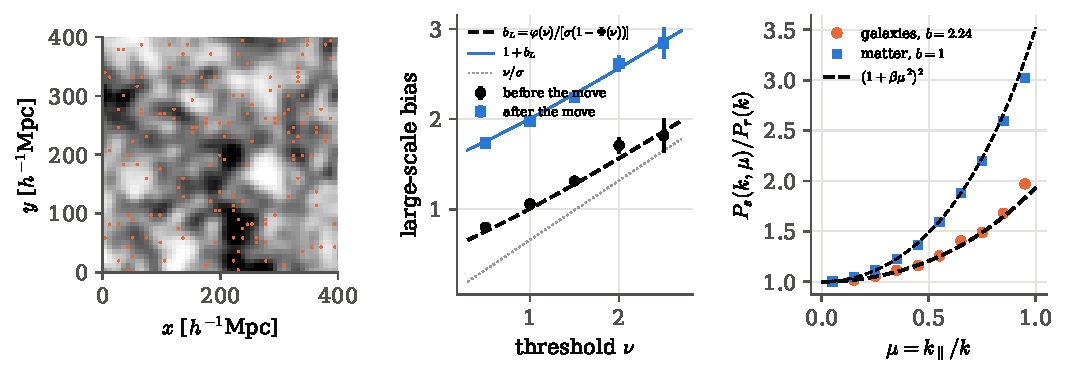
\includegraphics[width=\linewidth]{figures/chT2/tracers_rsd.pdf}
\caption{Left: a slice of the smoothed density field with the galaxies of one thin slab (orange); the galaxies sit in the dense regions. Middle: the large-scale bias against the threshold $\nu$; before the move it follows $b_L$ (dashed), after it $1+b_L$ (blue line); the dotted line is the high-threshold limit $\nu/\sigma$. Right: redshift-space power divided by real-space power, against $\mu$; galaxies (orange) and matter (blue) follow the Kaiser factor with $\beta=f/b$ and $\beta=f$ respectively.}
\label{T2b:fig:tracers}
\end{figure}

\paragraph{Nerfed, honestly.} The box is a single Gaussian realisation of $(1\,h^{-1}{\rm Gpc})^3$ with $7.8\,h^{-1}$Mpc cells, run in seconds, and the haloes are replaced by a threshold on a field with a white-noise small-scale part. Research analyses use $N$-body simulations with $10^{10}$ particles, find haloes in them, populate the haloes with galaxies by an occupation model fitted to the small-scale clustering, and build hundreds to thousands of approximate mock catalogues to estimate the covariance of $\hat P_g$.

\paragraph{Where the statistics comes back in.} The galaxy power spectrum and correlation function, their estimators and their Gaussian covariance, are the random-field statistics of \cref{ch:07}. Shot noise is the Poisson process of \cref{ch:02}. Bias, the shot-noise amplitude and $f\sigma_8$ are the parameters of a clustering likelihood whose forecast is a Fisher calculation (\cref{ch:10}) and whose posterior is sampled with MCMC (\cref{ch:09}). Galaxy clustering, redshift-space distortions and peculiar velocities as cosmological data are the subject of \cref{ch:11}.
\section{Baryon acoustic oscillations: a standard ruler}
\label{T2b:sec:bao}

Before recombination, photons and baryons were held together by Thomson scattering into a single hot fluid. Every small overdensity in that fluid launched a spherical sound wave, which ran outwards until the baryons were released from the photons and then stopped. How fast did it run? \emph{The pressure comes from the photons, the inertia from both.} Radiation has pressure $p=\rho_\gamma c^2/3$; the baryons add mass but, being cold, no pressure. A sound wave squeezes photons and baryons together, so both number densities rise by the same fraction. For photons $\rho_\gamma\propto T^4$ and $n_\gamma\propto T^3$, so $\delta\rho_\gamma/\rho_\gamma=\frac43\,\delta n/n$; for baryons $\delta\rho_b/\rho_b=\delta n/n$. Hence $\delta\rho_b=\frac34(\rho_b/\rho_\gamma)\,\delta\rho_\gamma$, and
\[
  c_s^2=\frac{\delta p}{\delta\rho}
  =\frac{c^2\,\delta\rho_\gamma/3}{\delta\rho_\gamma+\delta\rho_b}
  =\frac{c^2}{3(1+R)},\qquad R\equiv\frac{3\rho_b}{4\rho_\gamma}.
\]
Without baryons this is $c/\sqrt3$; the baryons' inertia slows the wave a little. \emph{How far did it get?} In a time $\dd t$ the wave covers a physical distance $c_s\dd t$, which is a comoving distance $c_s\dd t/a$. With $a=1/(1+z)$ and $\dd z/\dd t=-(1+z)H$, this is $c_s\dd t/a=-c_s\,\dd z/H$. Summing from the beginning ($z=\infty$) to the moment the baryons stop feeling the photons' push, the \newterm{drag epoch} $z_d\approx1060$ (slightly after recombination, because photons outnumber baryons by about a billion to one and keep dragging them a little longer), each initial peak was left with a thin shell of extra baryons at the comoving distance sound had travelled,
\begin{equation}
  r_d=\int_{z_d}^{\infty}\frac{c_s(z)}{H(z)}\,\dd z\approx147\ \text{Mpc}
  \label{T2b:eq:rd}
\end{equation}
\cite[eqs.~(2.3)--(2.4)]{DESI2024VI}. Dark matter fell into both the central peak and the shell, and galaxies later formed in both. So each overdensity is surrounded by a shell at $r_d$, and pairs of galaxies separated by $r_d$, one in a peak and one in its shell, are slightly more common than chance. Counting pairs by separation, that excess shows up as a bump in the correlation function at $r\approx r_d$, the feature computed in \cref{ch:T1}. The integral \eqref{T2b:eq:rd} depends only on the physical matter and baryon densities $\omega_m=\Omega_mh^2$ and $\omega_b=\Omega_bh^2$ (through $H$ and $R$) and the number of relativistic species $N_{\rm eff}$ (through $H$). A fit to its numerical value, quoted by DESI, is $r_d\approx147.05\,(\omega_m/0.1432)^{-0.23}(N_{\rm eff}/3.04)^{-0.1}(\omega_b/0.02236)^{-0.13}$\,Mpc \cite[eq.~(2.5)]{DESI2024VI}; the exponents are fitted numbers, not derived ones. The CMB measures it to $0.2\%$: $r_d=147.09\pm0.26$\,Mpc \cite[Table~2]{Planck2018VI}. A feature of known length, seen at many redshifts, is a \newterm{standard ruler}.

\paragraph{The question.} What exactly does the position of the bump measure, how is it extracted from a noisy correlation function, how precisely, and what did DESI find?

\subsection{What the ruler measures}

The survey measures angles and redshifts, not lengths. A pair of galaxies at redshift $z$ separated by $r_d$ \emph{across} the line of sight subtends an angle
\[
  \Delta\theta=\frac{r_d}{D_M(z)},\qquad D_M(z)=\int_0^z\frac{c\,\dd z'}{H(z')}\ \ \text{(flat)},
\]
where $D_M$ is the transverse comoving distance \cite[eq.~(16)]{Hogg1999}. A pair separated by $r_d$ \emph{along} the line of sight differs in redshift by $\Delta z$, and since the comoving distance changes by $\dd\chi=c\,\dd z/H(z)$,
\[
  \Delta z=\frac{r_d}{D_H(z)},\qquad D_H(z)\equiv\frac{c}{H(z)} .
\]
So the bump measures $D_M/r_d$ from its angular size and $D_H/r_d$ from its depth in redshift \cite[Sec.~2.1]{DESI2024VI}. \Cref{T2b:fig:bao-geometry} draws both.

\begin{figure}[htbp]
\centering
\begin{tikzpicture}[scale=1.0]
  \fill (0,0) circle (1.6pt) node[below,lbl] {observer};
  \draw[faint] (0,0) -- (8.6,1.55);
  \draw[faint] (0,0) -- (8.6,-1.55);
  \coordinate (A) at (7.2,1.3); \coordinate (B) at (7.2,-1.3);
  \fill[formblue] (A) circle (2.2pt); \fill[formblue] (B) circle (2.2pt);
  \draw[form,dashed] (A) -- (B);
  \node[lbl,anchor=west,text=formblue] at (7.35,0.25) {$r_d$ across};
  \draw[bdry,thin] (2.2,0.397) arc (10.2:-10.2:2.24);
  \node[lbl,anchor=west,text=bdryred] at (2.35,0) {$\Delta\theta=r_d/D_M$};
  \draw[decorate,decoration={brace,amplitude=4pt,mirror}] (0,-0.45) -- (7.2,-1.75) node[midway,below=4pt,lbl] {$D_M(z)$};
  \begin{scope}[xshift=0cm]
    \fill[fibreorange] (9.6,0) circle (2.2pt); \fill[fibreorange] (12.2,0) circle (2.2pt);
    \draw[fibre,dashed] (9.6,0) -- (12.2,0);
    \node[lbl,text=fibreorange] at (10.9,0.35) {$r_d$ along};
    \node[lbl,text=fibreorange,align=center] at (10.9,-0.75) {$\Delta z=r_d/D_H$\\ $D_H=c/H(z)$};
  \end{scope}
\end{tikzpicture}
\caption{What a standard ruler measures. Left: two galaxies separated by $r_d$ across the line of sight appear an angle $\Delta\theta=r_d/D_M$ apart. Right: two galaxies separated by $r_d$ along the line of sight differ in redshift by $\Delta z=r_d/D_H$. The first gives the distance, the second the expansion rate, both in units of $r_d$.}
\label{T2b:fig:bao-geometry}
\end{figure}

\paragraph{The map is drawn with an assumed cosmology.} To place galaxies in space at all, the survey assumes a fiducial cosmology, with distances $D_M^{\rm fid}$ and $D_H^{\rm fid}$ and a sound horizon $r_d^{\rm fid}$. The question, in words: \emph{if the true distances differ from the assumed ones, where in the fiducial map does the true ring of radius $r_d$ end up, and how do we read the true distances off its position?}

\emph{Across the line of sight first.} The survey turns a measured angle into a length with the assumed distance, and the angle is set by the true one:
\begin{align}
  r_\perp^{\rm app}
  &\eqby{1}D_M^{\rm fid}\,\Delta\theta
  \eqby{2}r_d\,\frac{D_M^{\rm fid}}{D_M}
  \eqby{3}\frac{r_d^{\rm fid}}{\alpha_\perp},
  \qquad
  \alpha_\perp\equiv\frac{D_M/r_d}{D_M^{\rm fid}/r_d^{\rm fid}} .
  \label{T2b:eq:rperp-app}
\end{align}
\begin{explain}
  \item The map converts angle to transverse length with the fiducial distance.
  \item The true pair at separation $r_d$ subtends $\Delta\theta=r_d/D_M$, with the true $D_M$.
  \item Name the ratio of the apparent ring to the ring the template expects, $r_\perp^{\rm app}/r_d^{\rm fid}=1/\alpha_\perp$.
\end{explain}
\emph{Along the line of sight, the same way.} A redshift difference becomes a length through the fiducial $D_H$, and the true one sets $\Delta z=r_d/D_H$: $r_\parallel^{\rm app}=D_H^{\rm fid}\Delta z=r_dD_H^{\rm fid}/D_H=r_d^{\rm fid}/\alpha_\parallel$. Together,
\begin{equation}
  \alpha_\perp=\frac{D_M/r_d}{D_M^{\rm fid}/r_d^{\rm fid}},\qquad
  \alpha_\parallel=\frac{D_H/r_d}{D_H^{\rm fid}/r_d^{\rm fid}} .
  \label{T2b:eq:alphas}
\end{equation}
So a sphere of radius $r_d$ in the true universe appears in the fiducial map as an ellipsoid with semi-axes $r_d^{\rm fid}/\alpha_\perp$ across the line of sight and $r_d^{\rm fid}/\alpha_\parallel$ along it. Read the direction carefully: $\alpha>1$ means the true distance (in units of $r_d$) is larger than assumed, the ring looks \emph{smaller} than the template, and the feature appears at smaller $r$.

\emph{From the ring to the template fit.} The template correlation function $\xi_{\rm fid}(r)$ of the fiducial cosmology has its bump at $r=r_d^{\rm fid}$. The data have it at $r^{\rm app}=r_d^{\rm fid}/\alpha$. The dilated template $\xi_{\rm fid}(\alpha r)$ has its bump where $\alpha r=r_d^{\rm fid}$, that is at $r=r_d^{\rm fid}/\alpha$, exactly where the data put it. So fitting the data with $\xi_{\rm fid}(\alpha r)$ and finding the best $\alpha$ measures the ratio of true to fiducial distance in \eqref{T2b:eq:alphas}. DESI reports the same information in the form $D_M/r_d$ and $D_H/r_d$ \cite[Sec.~2.1]{DESI2024VI}, which is our $\alpha_\perp$ and $\alpha_\parallel$ multiplied by the fiducial $D_M^{\rm fid}/r_d^{\rm fid}$ and $D_H^{\rm fid}/r_d^{\rm fid}$.

\paragraph{Why $D_V$, and why the factor $z$.} When the data are too noisy to separate the two directions, one fits the angle-averaged correlation function with a single dilation $\alpha$. The single scale that preserves the volume of the ellipsoid, which is what an angle average responds to at first order, is the geometric mean of its three axes:
\begin{align}
  \alpha_{\rm iso}
  &\eqby{1}\big(\alpha_\perp^2\,\alpha_\parallel\big)^{1/3}
  \eqby{2}\frac{\big(D_M^2D_H\big)^{1/3}/r_d}{\big(D_M^{{\rm fid}\,2}D_H^{\rm fid}\big)^{1/3}/r_d^{\rm fid}}
  \eqby{3}\frac{D_V/r_d}{D_V^{\rm fid}/r_d^{\rm fid}},\qquad
  D_V\equiv\big(z\,D_M^2\,D_H\big)^{1/3}.
  \label{T2b:eq:dv}
\end{align}
\begin{explain}
  \item Two transverse axes and one radial axis: the volume scales as $\alpha_\perp^2\alpha_\parallel$.
  \item Substitute \eqref{T2b:eq:alphas}.
  \item Multiply numerator and denominator by $z^{1/3}$, which cancels.
\end{explain}
The factor $z$ is a convention, and it is there so that $D_V$ is a distance with a familiar limit: at low redshift $D_M\approx cz/H_0$ and $D_H\approx c/H_0$, so $D_V\approx\big(z\cdot(cz/H_0)^2\cdot c/H_0\big)^{1/3}=cz/H_0$, the Hubble-law distance. This is Eisenstein et al.'s eq.~(2), $D_V=[D_M^2\,cz/H(z)]^{1/3}$ \cite[Sec.~4]{Eisenstein2005}, and DESI's eq.~(2.6) \cite{DESI2024VI}.

\begin{pitfall}[Which ``angular diameter distance''?]
Three conventions meet here. Hogg's $D_A=D_M/(1+z)$ is the physical angular diameter distance \cite[eq.~(18)]{Hogg1999}, and so is the $D_A$ of \cref{ch:T1}. Weinberg et al.\ write $D_A$ for the \emph{comoving} angular diameter distance, which is $D_M$ \cite[p.~46]{Weinberg2013}. Eisenstein et al.\ and DESI write $D_M$. A factor $(1+z)$ in a BAO formula is usually this.
\end{pitfall}

\subsection{Measuring the dilation, and how well}

A correlation function is measured in bins of separation $r_i$. How noisy is each bin, and how are neighbouring bins tied together? For a Gaussian field the answer follows from the power spectrum. The correlation function is the Fourier transform of the power, so the estimate in bin $i$ is a weighted sum of the power measured in thin $k$-shells, $\hat\xi(r_i)=\sum_{\rm shells}\frac{k^2\Delta k}{2\pi^2}\hat P(k)\,\bar j_0(kr_i)$, where $\bar j_0$ is the spherical Bessel function $\sin x/x$ averaged over the width of the bin (\cref{7a:sec:wk}). Different shells are independent, and each has $\Var\hat P=2P_{\rm tot}^2/N_k$ with $P_{\rm tot}=b^2P+1/\bar n$ and $N_k=Vk^2\Delta k/(2\pi^2)$ modes (\eqref{T2b:eq:pk-error}). So
\begin{align}
  \Cov\big[\hat\xi(r_i),\hat\xi(r_j)\big]
  &\eqby{1}\sum_{\rm shells}\Big(\frac{k^2\Delta k}{2\pi^2}\Big)^2\bar j_0(kr_i)\,\bar j_0(kr_j)\,\frac{2P_{\rm tot}^2}{Vk^2\Delta k/(2\pi^2)}\nonumber\\
  &\eqby{2}\frac{2}{V}\int\frac{k^2\dd k}{2\pi^2}\Big[b^2P(k)+\frac1{\bar n}\Big]^2\bar j_0(kr_i)\,\bar j_0(kr_j).
  \label{T2b:eq:xi-cov}
\end{align}
\begin{explain}
  \item The covariance of two weighted sums of independent terms is the sum of weight times weight times variance.
  \item Cancel one factor $k^2\Delta k/(2\pi^2)$ and let the shells become thin.
\end{explain}
Each piece now has a meaning. The $1/V$ is the averaging over independent modes: a bigger survey has more of them. The square is there because a variance of a power is the square of the power (one mode's $|\delta_{\bm k}|^2$ scatters as much as its mean). The $1/\bar n$ inside it is the shot noise of \eqref{T2b:eq:shot}. And since every bin draws on the same shells, neighbouring bins share their errors.

The model is the fiducial template, dilated, plus a smooth curve that absorbs everything the BAO feature does not determine \cite[p.~9]{DESI2024VI}:
\begin{equation}
  \xi_{\rm model}(r)=B^2\,\xi_{\rm fid}(\alpha r)+a_0+\frac{a_1}{r}+\frac{a_2}{r^2}.
  \label{T2b:eq:bao-model}
\end{equation}
Each term has one job. $\alpha$ is the dilation of \eqref{T2b:eq:alphas}, the only number we want. $B^2$ absorbs the amplitude: the galaxy bias $b^2$ of \cref{T2b:sec:tracers} relative to the template's, and the redshift-space boost. $a_0$, $a_1/r$ and $a_2/r^2$ absorb the broadband shape, whatever smooth errors the template has from non-linear growth or a bias that changes slowly with scale. None of them can make a narrow bump, so the bump's position, and with it $\alpha$, is left to the data.

\emph{Solving for the nuisance terms.} For a fixed trial $\alpha$ the model is a fixed matrix $X$ (its four columns are $\xi_{\rm fid}(\alpha r_i)$, $1$, $1/r_i$, $1/r_i^2$) times the vector $\bm\beta=(B^2,a_0,a_1,a_2)$. So $\chi^2(\bm\beta)=(\hat{\bm\xi}-X\bm\beta)\T\Cmat^{-1}(\hat{\bm\xi}-X\bm\beta)$ is quadratic in $\bm\beta$, and a quadratic has one minimum, found exactly by generalised least squares (\cref{ch:03}), $\hat{\bm\beta}=(X\T\Cmat^{-1}X)^{-1}X\T\Cmat^{-1}\hat{\bm\xi}$. Marginalising $\bm\beta$ with flat priors instead (\cref{ch:05}) integrates $e^{-\chi^2/2}$ over a Gaussian in $\bm\beta$, which gives $e^{-\chi^2_{\min}/2}$ times $\det(X\T\Cmat^{-1}X)^{-1/2}$, the same structure as the amplitude integral of \eqref{T2b:eq:photoz-like}; that factor changes only slowly with $\alpha$, so the two routes agree closely. What is left is a profile $\chi^2(\alpha)$.

\emph{Is the bump really there?} The \newterm{BAO detection significance} compares the profile with the best fit of a template with the wiggles removed: $\Delta\chi^2=\chi^2_{\rm no\,wiggle}-\chi^2_{\rm BAO}$. The null hypothesis is the smooth, wiggle-free correlation function, and the test asks: if there were no bump, would a $\Delta\chi^2$ this large, or larger, be something we would reasonably expect from noise? Think of the BAO model as the no-wiggle model plus the wiggles with a free amplitude; the null sets that one amplitude to zero. Then Wilks' theorem (\cref{4a:sec:wilks}, \eqref{4a:eq:delta-chi2}) says that under the null $\Delta\chi^2$ is a $\chi^2$ with one degree of freedom, which is the square of one unit Gaussian $Z$. So
\[
  \Prob\big(\Delta\chi^2>n^2\given\text{no bump}\big)=\Prob(|Z|>n)=2\big[1-\Phi(n)\big],
\]
the probability of a Gaussian fluctuation beyond $n$ standard deviations. A measured $\Delta\chi^2$ therefore corresponds to a detection at $n=\sqrt{\Delta\chi^2}$ standard deviations. (The amplitude being one extra parameter is an approximation: $\alpha$ too is free only in the BAO model, which makes the real tail a little heavier.)

\paragraph{Example: the first detection.} \emph{Their question.} In 2005 the acoustic bump had been predicted for decades but never seen in galaxies. Eisenstein et al.\ asked: is there a bump near $100\,h^{-1}$Mpc in the correlation function of galaxies, and if so, what distance does its position give?

\emph{Their setup.} They used luminous red galaxies (LRGs) from SDSS: $46{,}748$ of them at $0.16<z<0.47$ over $3816$ square degrees. LRGs are rare and bright, so they can be seen far away and fill a large volume, which beats down the cosmic variance of \eqref{T2b:eq:pk-error}; and they live in massive haloes, so their bias is high and the bump in $\xi_g=b^2\xi$ stands out against the shot noise. The covariance of $\hat\xi$ came from $1278$ mock catalogues, which play the role of our \eqref{T2b:eq:xi-cov} with the survey's real shape and selection built in.

\emph{Their key equation.} With galaxies at a range of redshifts and a correlation function averaged over directions, the bump measures the single dilation $\alpha_{\rm iso}$ of \eqref{T2b:eq:dv}, that is $D_V/r_d$ at the effective redshift $z=0.35$. Their eq.~(2), $D_V=[D_M^2\,cz/H(z)]^{1/3}$, is our $D_V=(zD_M^2D_H)^{1/3}$ with $D_H=c/H$.

\emph{Their result, through our recipe.} The best BAO model had $\chi^2=16.1$ for $17$ degrees of freedom; the best model without the acoustic peak had $27.8$. The significance recipe above gives
\[
  \Delta\chi^2=27.8-16.1=11.7,\qquad n=\sqrt{11.7}=3.4 ,
\]
a $3.4\sigma$ detection. The peak position gave $D_V(0.35)=1370\pm64$\,Mpc, so $64/1370=4.7\%$ \cite[Sec.~4, Fig.~6]{Eisenstein2005}. Our mock survey below, with a somewhat larger volume and a denser sample, finds a median detection of $\TwbaoSigMed\sigma$ and a scatter of $\TwbaoAsd$ in $\alpha$, about $3\%$: the same order, a little better, as it should be for more volume and more galaxies.

\paragraph{The experiment.} \pyname{10_bao_ruler.py} needs two templates and a survey.

\emph{Why the bump is smeared.} Between the drag epoch and today each galaxy has moved from where it formed, by some $\TwbaoSigNl\,h^{-1}$Mpc in each direction, pulled by the large-scale flows. Treat that displacement $\bm\psi$ as a random Gaussian vector with variance $\Sigma_{\rm nl}^2$ per direction. A wave $e^{i\bm k\cdot\bm x}$ sampled at the displaced positions is multiplied, on average, by $\E[e^{i\bm k\cdot\bm\psi}]=e^{-k^2\Sigma_{\rm nl}^2/2}$, the characteristic function of a Gaussian. The acoustic wiggles live at $k\gtrsim0.05\,h$\,Mpc$^{-1}$, where this factor bites, so they fade; in $\xi(r)$ the narrow bump is smoothed into a broader one. The value $\Sigma_{\rm nl}=\TwbaoSigNl\,h^{-1}$Mpc is the one before reconstruction (the step that real surveys use to move galaxies back towards where they started).

\emph{What ``no wiggle'' means.} The comparison template is a power spectrum with the same broadband shape as the real one but without the oscillations. Eisenstein and Hu give a smooth transfer function for that \cite[eqs.~(26), (28)--(31)]{EisensteinHu1998}. Calling the CAMB linear spectrum $P_{\rm lin}$ and the smooth one $P_{\rm nw}$, the difference $P_{\rm lin}-P_{\rm nw}$ is the BAO signal alone, and the template damps only that part: $P_{\rm w}=P_{\rm nw}+(P_{\rm lin}-P_{\rm nw})\,e^{-k^2\Sigma_{\rm nl}^2/2}$.

\emph{The survey,} about one DESI redshift bin:
\begin{center}
\small
\begin{tabular}{@{}lll@{}}
\toprule
quantity & value & enters through\\
\midrule
volume $V$ & $\TwbaoVol\,(h^{-1}{\rm Gpc})^3$ & the $1/V$ of \eqref{T2b:eq:xi-cov}\\
number density $\bar n$ & $\TwbaoNbar\,h^3$Mpc$^{-3}$ & the shot noise $1/\bar n$\\
bias $b$ & $\TwbaoB$ & the signal $b^2P$\\
separation bins & $\TwbaoNbins$, from $50$ to $150\,h^{-1}$Mpc & the data vector $\hat{\bm\xi}$\\
mock surveys & $\TwbaoNmock$ & draws from $\Normal(\xi_{\rm true},\Cmat)$\\
\bottomrule
\end{tabular}
\end{center}
It draws the mock $\hat\xi$ vectors with $\Cmat$ from \eqref{T2b:eq:xi-cov}, and fits each one:

\pyfile[firstline=80,lastline=104,firstnumber=80]{code/chT2/10_bao_ruler.py}{The profile $\chi^2(\alpha)$ with the linear nuisance parameters solved at each $\alpha$}

\noindent Lines 83--89 compute, for every trial $\alpha$, the design matrix $X$ and the matrix that turns data into the best nuisance values,
\[
  P_\alpha=(X\T\Cmat^{-1}X)^{-1}X\T\Cmat^{-1},\qquad \hat{\bm\beta}=P_\alpha\hat{\bm\xi} .
\]
The residual is then $\hat{\bm\xi}-X\hat{\bm\beta}=(1-XP_\alpha)\,\hat{\bm\xi}$, and
\[
  \chi^2(\alpha)=\hat{\bm\xi}\T(1-XP_\alpha)\T\,\Cmat^{-1}\,(1-XP_\alpha)\,\hat{\bm\xi} .
\]
The data enter only at the two ends; everything in between depends on $\alpha$ through $X$ and on nothing else. So these projection matrices are computed once per trial $\alpha$ and reused for all $\TwbaoNmock$ mocks, and each fit is a matrix product (line 95). Line 103 reads the $\Delta\chi^2=1$ interval off the profile.

\Cref{T2b:fig:bao-fit} shows one mock: $\hat\alpha=\TwbaoAzero\pm\TwbaoEzero$, $\chi^2_{\min}=\TwbaoChiZero$ for $\TwbaoDofZero$ degrees of freedom, and a no-wiggle penalty $\Delta\chi^2=\TwbaoDchiZero$. Over all mocks the median detection is $\TwbaoSigMed\sigma$ ($16$--$84\%$ range $\TwbaoSigLow$--$\TwbaoSigHigh\sigma$), comparable to the first SDSS detection. The estimates $\hat\alpha$ average $\TwbaoAmean$: the ruler is unbiased. Their scatter, $\TwbaoAsd$, is larger than both the Fisher error $\TwbaoFisher$ (the width predicted from the curvature of the profile $\chi^2(\alpha)$ of noise-free data at its minimum, \cref{ch:10}) and the average $\Delta\chi^2=1$ half-width $\TwbaoAerrMean$, and the $\Delta\chi^2=1$ interval covers the truth in $\TwbaoCover$ of the mocks ($\pm\TwbaoCoverErr$, the binomial error) instead of $68\%$.

\begin{figure}[htbp]
\centering
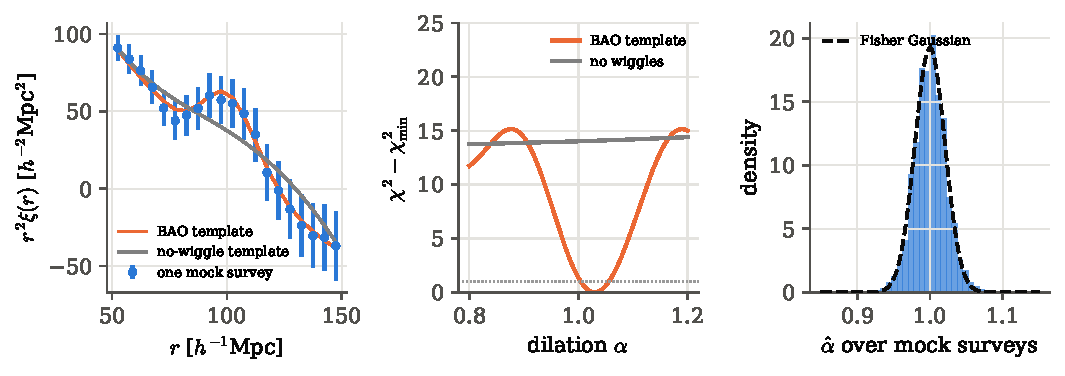
\includegraphics[width=\linewidth]{figures/chT2/bao_fit.pdf}
\caption{Fitting the BAO dilation. Left: one mock correlation function (times $r^2$, with the diagonal errors) and the best fits of the BAO template and of the no-wiggle template. Middle: the profile $\chi^2(\alpha)$ for both; the BAO template has a clear minimum near $\alpha=1$, the no-wiggle one is flat and higher. Right: the distribution of $\hat\alpha$ over the mock surveys and the Gaussian of the Fisher error; the tails are heavier than the Gaussian.}
\label{T2b:fig:bao-fit}
\end{figure}

Why the heavier tails? In a mock where noise happens to weaken the bump, $\chi^2(\alpha)$ is shallow and can have a second minimum where a noise wiggle lines up with the template. The likelihood is then far from Gaussian in $\alpha$, and the curvature at the minimum underestimates the real spread. At a $4\sigma$ detection this happens often; at the $10$--$20\sigma$ of a DESI bin it does not, and DESI finds its posteriors ``well approximated by Gaussian distributions'' \cite[Sec.~2.3.2]{DESI2024VI}.

\begin{inpractice}[Verification versus research]
Here the mocks \emph{verify} the analysis: we know $\alpha=1$, and we check that the estimator is unbiased and that its error bar covers the truth at the stated rate. In research the same machinery is the \emph{instrument}. DESI estimates the covariance of $\hat\xi$ from large sets of mock catalogues and analytic models, because the real survey has a mask, varying completeness and non-linear clustering that \eqref{T2b:eq:xi-cov} ignores; it calibrates the reconstruction and the theoretical systematics (below $0.1$--$0.2\%$) on simulations; and it blinds the data, shifting the BAO position in the catalogues until the pipeline is frozen \cite[Sec.~2.3.1]{DESI2024VI}. A full analysis uses thousands of mocks; ours uses $\TwbaoNmock$ Gaussian draws from an analytic covariance and no reconstruction.
\end{inpractice}

\subsection{What DESI's distances say}

\paragraph{Their question.} DESI measured the ruler at seven redshifts in its first year. The question we reproduce is: \emph{do the BAO distances alone, with no CMB and no supernovae, fix the matter density $\Omega_m$ and the expansion scale $H_0r_d$ in flat $\Lambda$CDM, and do they agree with the $\Lambda$CDM that fits the CMB?} It matters because the ruler is calibrated by early-universe physics and read at $z<2.5$, a test of the model across most of cosmic time.

\paragraph{Their data.} Each bin gives $D_M/r_d$ and $D_H/r_d$ with their correlation coefficient where the signal is strong, and $D_V/r_d$ alone for the bright galaxies (BGS) and the quasars (QSO), where it is weak \cite[Table~1]{DESI2024VI}:
\begin{center}
\small
\begin{tabular}{@{}lccccc@{}}
\toprule
tracer & $z_{\rm eff}$ & $D_M/r_d$ & $D_H/r_d$ & $D_V/r_d$ & correlation\\
\midrule
BGS & $0.295$ & -- & -- & $7.93\pm0.15$ & --\\
LRG & $0.510$ & $13.62\pm0.25$ & $20.98\pm0.61$ & -- & $-0.445$\\
LRG & $0.706$ & $16.85\pm0.32$ & $20.08\pm0.60$ & -- & $-0.420$\\
LRG+ELG & $0.930$ & $21.71\pm0.28$ & $17.88\pm0.35$ & -- & $-0.389$\\
ELG & $1.317$ & $27.79\pm0.69$ & $13.82\pm0.42$ & -- & $-0.444$\\
QSO & $1.491$ & -- & -- & $26.07\pm0.67$ & --\\
Ly$\alpha$ & $2.330$ & $39.71\pm0.94$ & $8.52\pm0.17$ & -- & $-0.477$\\
\bottomrule
\end{tabular}
\end{center}
Five bins with two numbers and two bins with one make $5\times2+2=\TwdNdata$ numbers. The correlation is negative because the data pin down the overall size of the ring better than its shape: a fit that stretches the ring across the line of sight compensates by shrinking it along the line of sight.

\paragraph{The model, derived.} In flat $\Lambda$CDM at these redshifts (radiation is $0.1\%$ of $H^2$ even at $z=2.3$) the predictions are
\begin{equation}
  \frac{D_H}{r_d}(z)=\frac{c}{H_0r_d}\,\frac{1}{E(z)},\qquad
  \frac{D_M}{r_d}(z)=\frac{c}{H_0r_d}\int_0^z\frac{\dd z'}{E(z')},\qquad
  E(z)=\sqrt{\Omega_m(1+z)^3+1-\Omega_m}.
  \label{T2b:eq:bao-lcdm}
\end{equation}
Only two numbers appear: $\Omega_m$, which sets how the distances change with redshift, and the product $H_0r_d$, which sets their overall scale. BAO alone therefore cannot separate $H_0$ from $r_d$.

\emph{Where we have met $H_0$ before.} The mock supernovae of \cref{3b:sec:hubble}, made with $H_0=70$, fixed only $M-5\log_{10}H_0$, and $H_0$ came out only once $M$ was supplied from outside. The ladder of \cref{T2b:sec:ladder} supplied it from parallaxes and Cepheids, and the real ladder gave $73.04\pm1.04$, $4.8\sigma$ above the CMB's $67.36\pm0.54$ (\cref{T2b:sec:tension}). The same degeneracy is back here with a ruler in place of the candle: the distances fix only the product $H_0r_d$, as the magnitudes fixed only $M-5\log_{10}H_0$, and the ruler's length plays the role of the candle's luminosity. Three things differ. The data are real DESI distances at $0.3<z<2.3$, far beyond the $z<0.15$ of the Hubble-flow supernovae, so $\Omega_m$ must be fitted alongside the scale rather than entering as the small $q_0$ correction. The calculation is a Bayesian posterior on a grid rather than a least-squares fit. And the calibration comes from the early Universe: $r_d$ is set by the sound waves before recombination, the same physics that fixes the CMB value of $H_0$ (\cref{10a:sec:cmb-planck}), not by geometry nearby. That is why the $H_0$ found below lands near the CMB value and not near the ladder's.

\paragraph{What we compute.} Each bin is a measurement $\bm d_b$ (two numbers or one) with Gaussian noise, and the model $\bm m_b(\Omega_m,hr_d)$ is \eqref{T2b:eq:bao-lcdm} evaluated at $z_{\rm eff}$ (with $D_V=(zD_M^2D_H)^{1/3}$ of \eqref{T2b:eq:dv} for the one-number bins). The bins are independent, so the $\chi^2$ is a sum over bins,
\begin{equation}
  \chi^2(\Omega_m,hr_d)=\sum_{b=1}^{7}\big(\bm d_b-\bm m_b\big)\T C_b^{-1}\big(\bm d_b-\bm m_b\big),
  \qquad
  C_b=\begin{pmatrix}\sigma_M^2&\rho\,\sigma_M\sigma_H\\ \rho\,\sigma_M\sigma_H&\sigma_H^2\end{pmatrix},
  \label{T2b:eq:desi-chi2}
\end{equation}
where $\sigma_M$ and $\sigma_H$ are the quoted errors of $D_M/r_d$ and $D_H/r_d$ and $\rho$ is their correlation; for a $D_V$ bin $C_b$ is just $\sigma_V^2$. The posterior with flat priors on a grid of $(\Omega_m,hr_d)$ is Bayes' theorem (\cref{ch:05}) with a constant prior:
\[
  p(\Omega_m,hr_d\given\bm d)=\frac{e^{-\chi^2(\Omega_m,hr_d)/2}}{\sum_{\rm grid}e^{-\chi^2/2}} ,
\]
and the means, standard deviations and correlation are sums over the grid weighted by it.

\paragraph{DESI and ours, side by side.} \Cref{T2b:fig:bao-desi} shows the distances and the posterior; the numbers are
\begin{center}
\small
\begin{tabular}{@{}lcc@{}}
\toprule
 & DESI \cite[eqs.~(4.1), (4.3)]{DESI2024VI} & ours\\
\midrule
$\Omega_m$ & $0.295\pm0.015$ & $\TwdOm\pm\TwdOmSd$\\
$h r_d$ [Mpc] & $101.8\pm1.3$ & $\TwdHrd\pm\TwdHrdSd$\\
$H_0$ [km/s/Mpc], with the CMB $r_d$ & $69.29\pm0.87$ & $\TwdHzero\pm\TwdHzeroErr$\\
\bottomrule
\end{tabular}
\end{center}
with correlation $\TwdCorr$ between our $\Omega_m$ and $hr_d$. The best fit has $\chi^2=\TwdChiMin$ for $\TwdNdata-2$ degrees of freedom, an ordinary value.

\paragraph{Why they differ, and by how much.} They barely do: the largest difference, $0.001$ in $\Omega_m$, is a fifteenth of the error bar. Three things could cause differences of that size. Our grid has steps of $0.001$ in $\Omega_m$ and $0.1$\,Mpc in $hr_d$, where DESI samples its posterior with MCMC. Our Gaussian is built from the errors and correlations as quoted in the table, rounded to two or three digits. And we neglect radiation, which changes $H^2$ by at most $0.1\%$ at the highest redshift, the Ly$\alpha$ bin, so $D_H$ by at most $0.05\%$, far below its $2\%$ error. For $H_0$, DESI also propagates the $0.2\%$ error of $r_d$, which we leave out; it is small next to the $1.3\%$ from $hr_d$.

\paragraph{Is Planck's $\Lambda$CDM consistent with it?} The Planck best fit ($h r_d=\TwdHrdP$\,Mpc) has $\chi^2=\TwdChiP$ against our minimum $\TwdChiMin$, so $\Delta\chi^2=21.1-12.8=8.3$. Under the hypothesis that the Planck point is the truth, $\Delta\chi^2$ between it and the best fit is a $\chi^2$ with two degrees of freedom, one per fitted parameter (Wilks' theorem, \cref{4a:sec:wilks}). Its tail is $\Prob(\chi^2_2>v)=e^{-v/2}$ (\eqref{10b:eq:rayleigh-tail}), so $p=e^{-8.3/2}=0.016$. Converted to the two-sided Gaussian language of the detection test, $2[1-\Phi(n)]=0.016$ gives $n=2.4\sigma$. That treats the Planck point as exact. DESI, including the errors of the CMB values, which spread the Planck point into its own small ellipse, quantifies the difference as a $1.9\sigma$ discrepancy ($1.6\sigma$ without CMB lensing) \cite[eq.~(4.2)]{DESI2024VI}: a mild tension, not a contradiction.

\paragraph{The lesson.} Twelve published numbers and a two-parameter grid are enough to recover DESI's headline constraint; what the grid cannot do on its own is separate $H_0$ from $r_d$, which is the subject of the next example.

\begin{figure}[htbp]
\centering
\includegraphics[width=0.95\linewidth]{figures/chT2/bao_desi.pdf}
\caption{Left: DESI DR1 BAO distances divided by the Planck $\Lambda$CDM prediction. Right: the $68\%$ and $95\%$ regions in $(\Omega_m,hr_d)$ from the twelve DESI numbers, computed on a grid, with DESI's quoted result (cross) and the Planck best fit (star). The long, tilted contour is the degeneracy of \eqref{T2b:eq:bao-lcdm}: a higher $\Omega_m$ can be traded for a lower $hr_d$.}
\label{T2b:fig:bao-desi}
\end{figure}

\paragraph{Example: the inverse distance ladder.} Take $r_d=147.09$\,Mpc from the CMB. Then $h=(h r_d)/r_d$, and the posterior above gives $H_0=\TwdHzero\pm\TwdHzeroErr$\,km/s/Mpc; DESI, propagating the small error of $r_d$ too, finds $69.29\pm0.87$, and $68.53\pm0.80$ with $r_d$ computed from a big-bang-nucleosynthesis value of $\omega_b$ instead of the CMB \cite[eqs.~(4.3)--(4.4)]{DESI2024VI}. This is a distance ladder run backwards, anchored at $z\approx1060$ by the physics of sound waves rather than at $z\approx0$ by parallaxes. It lands near the CMB value and well below the $73.04\pm1.04$ of the Cepheid ladder of \cref{T2b:sec:ladder}: the Hubble tension appears again when a ruler replaces a candle.

\paragraph{Where the statistics comes back in.} The estimator and covariance of $\hat\xi$ and $\hat P$ are \cref{ch:07}. The template fit is least squares with linear nuisances (\cref{ch:03}), the detection is a likelihood-ratio test (\cref{ch:04}), and the posterior on $(\Omega_m,hr_d)$ is the Bayesian grid of \cref{ch:05}, replaced by MCMC (\cref{ch:09}) when more parameters are free. The forecast precision of a BAO survey is a Fisher calculation (\cref{ch:10}), and galaxy clustering as cosmological data is \cref{ch:11}.
\section{Photometric redshifts and their error distributions}
\label{T2b:sec:photoz}

A spectrum gives a redshift to a part in ten thousand, but it costs a fibre and many minutes of a large telescope for each galaxy. Imaging surveys such as the ones used for weak lensing (\cref{ch:T1}) detect a billion galaxies, far too many and mostly too faint for spectra. What they have is the flux of each galaxy in five or six broad filters. That is enough for a rough redshift, because galaxy spectra have sharp features. The strongest in the optical is the break near $4000$\,\AA, where old stars and metal absorption make the light drop by a factor of two or three to the blue. At high redshift the Lyman series of intergalactic hydrogen removes the light blueward of $1216$\,\AA. As a galaxy is moved to higher redshift its spectrum slides to the red, and the break passes from one filter into the next (\cref{T2b:fig:photoz-sed}). The ratio of fluxes in neighbouring filters, a \newterm{colour}, therefore encodes the redshift. An estimate made this way is a \newterm{photometric redshift} (photo-$z$).

\paragraph{The question.} How is a redshift computed from a few fluxes, what is the distribution of its error, and how does that error propagate into the redshift distribution $n(z)$ of a sample, which is what cosmology actually uses?

\begin{figure}[htbp]
\centering
\begin{tikzpicture}
\begin{axis}[width=11cm,height=4.6cm,xmin=3000,xmax=11000,ymin=0,ymax=2.5,
  xlabel={observed wavelength [\AA]},ylabel={$f_\nu$ (arbitrary)},
  xtick={4000,6000,8000,10000},scaled x ticks=false,ytick=\empty,axis lines=left,
  every axis label/.style={font=\small},tick label style={font=\footnotesize}]
  \fill[black!7] (axis cs:3200,0) rectangle (axis cs:4000,2.5);
  \node[font=\footnotesize,text=softgray] at (axis cs:3600,2.3) {$u$};
  \fill[black!13] (axis cs:4000,0) rectangle (axis cs:5500,2.5);
  \node[font=\footnotesize,text=softgray] at (axis cs:4750,2.3) {$g$};
  \fill[black!7] (axis cs:5500,0) rectangle (axis cs:6900,2.5);
  \node[font=\footnotesize,text=softgray] at (axis cs:6200,2.3) {$r$};
  \fill[black!13] (axis cs:6900,0) rectangle (axis cs:8200,2.5);
  \node[font=\footnotesize,text=softgray] at (axis cs:7550,2.3) {$i$};
  \fill[black!7] (axis cs:8200,0) rectangle (axis cs:9200,2.5);
  \node[font=\footnotesize,text=softgray] at (axis cs:8700,2.3) {$z$};
  \fill[black!13] (axis cs:9200,0) rectangle (axis cs:10500,2.5);
  \node[font=\footnotesize,text=softgray] at (axis cs:9850,2.3) {$y$};
  \addplot[formblue,thick,domain=3000:11000,samples=400] {(x/(1.3*5000))^1.5*((x/1.3>4000)?1:0.35)};
  \addplot[bdryred,thick,domain=3000:11000,samples=400] {0.55*(x/(2.0*5000))^1.5*((x/2.0>4000)?1:0.35)};
  \node[font=\footnotesize,text=formblue,anchor=west] at (axis cs:9300,1.62) {$z=0.3$};
  \node[font=\footnotesize,text=bdryred,anchor=west] at (axis cs:9300,0.35) {$z=1.0$};
\end{axis}
\end{tikzpicture}
\caption{The same red-galaxy spectrum at two redshifts, seen through six broad filters (grey bands). At $z=0.3$ the $4000$\,\AA\ break lands at $5200$\,\AA, inside the $g$ band; at $z=1.0$ it has moved to $8000$\,\AA, inside the $i$ band. Which filter holds the break, and how deep the drop is, is what a photometric redshift reads.}
\label{T2b:fig:photoz-sed}
\end{figure}

\subsection{Template fitting as a likelihood}

\emph{What we observed} is a vector of fluxes $F_b$ in bands $b=1,\dots,6$, each with a Gaussian error $\sigma_b$. \emph{What could have produced it?} A galaxy of some spectral type $T$, at some redshift $z$, with some overall brightness $A$, predicting fluxes $A\,T_b(z)$, where $T_b(z)$ is the template spectrum redshifted to $z$ and integrated through filter $b$. \emph{How likely are the observed fluxes under each $(z,T)$?} The brightness is not of interest, so we integrate it out with a flat prior. The $\chi^2$ is quadratic in $A$, $\chi^2(A)=\chi^2_{\min}+(A-\hat A)^2S$ with $S=\sum_bT_b^2/\sigma_b^2$, so
\begin{align}
  \Like(z,T)
  &\eqby{1}\int\dd A\,\exp\Big[-\frac12\sum_b\frac{(F_b-AT_b)^2}{\sigma_b^2}\Big]
  \eqby{2}e^{-\chi^2_{\min}/2}\int\dd A\,e^{-S(A-\hat A)^2/2}
  \eqby{3}\sqrt{\frac{2\pi}{S}}\;e^{-\chi^2_{\min}(z,T)/2},\nonumber\\
  \chi^2_{\min}&\eqby{4}\sum_b\frac{F_b^2}{\sigma_b^2}-\frac{\big(\sum_bF_bT_b/\sigma_b^2\big)^2}{S},
  \qquad
  p(z\given\bm F)\propto n(z)\sum_T\Like(z,T).
  \label{T2b:eq:photoz-like}
\end{align}
\begin{explain}
  \item Independent Gaussian errors in each band; marginalise the nuisance amplitude (\cref{ch:05}).
  \item Expand the square in $A$ and complete it; $\hat A=\sum_bF_bT_b\sigma_b^{-2}/S$ is the least-squares amplitude.
  \item The Gaussian integral $\int e^{-Sx^2/2}\dd x=\sqrt{2\pi/S}$.
  \item Substitute $\hat A$ into $\chi^2$.
\end{explain}
The last expression is Bayes' theorem with the redshift distribution $n(z)$ of the population as the prior and the type summed over. The sum gives every template the same weight: it is a flat prior over the types, even though the population the experiment below draws from is $35\%$ red and $65\%$ blue. A type prior would multiply each $\Like(z,T)$ by the fraction of galaxies of type $T$. The photo-$z$ is then usually the peak of $p(z\given\bm F)$, but the whole posterior is the honest answer.

\subsection{The error distribution}

The error $z_{\rm phot}-z$ is not a Gaussian. It has a Gaussian-looking core whose width grows with redshift as $\sigma_z\propto1+z$. Why? A feature at rest wavelength $\lambda_{\rm rest}$ is observed at $\lambda_{\rm obs}=(1+z)\lambda_{\rm rest}$, so $\delta(1+z)/(1+z)=\delta\lambda_{\rm obs}/\lambda_{\rm obs}$. Broad filters locate the break only to a fixed fraction of the wavelength (a filter's width is roughly proportional to its central wavelength), so $\delta\lambda_{\rm obs}/\lambda_{\rm obs}$ is about constant, and then $\sigma_z=\delta z$ is a constant times $1+z$. Good surveys reach $\sigma_z/(1+z)\approx0.02$--$0.05$. And it has \newterm{catastrophic outliers} with $|z_{\rm phot}-z|\sim1$. The main cause is a degeneracy: a sharp drop observed at a wavelength $\lambda_{\rm obs}$ may be the $4000$\,\AA\ break of a nearby galaxy or the Lyman-$\alpha$ edge of a distant one, $(1+z_{\rm low})\,4000\,\text{\AA}=(1+z_{\rm high})\,1216\,\text{\AA}$. For $z_{\rm low}=0.16$,
\[
  1+z_{\rm high}=1.16\times\frac{4000}{1216}=3.82,\qquad z_{\rm high}=2.8 ,
\]
so a galaxy at $z_{\rm high}=2.8$ can be mistaken for one at $z_{\rm low}=0.16$ \cite[p.~96]{Weinberg2013}. Filters on both sides of both features, from $u$ to the near infrared, break the degeneracy.

Weinberg et al.\ describe the error by the joint distribution $P(z_p,z)$ of photo-$z$ and true redshift, and summarise it by the conditional bias and scatter $\delta z(z_p)=z_p-\langle z\rangle_{z_p}$ and $\sigma_z(z_p)$ \cite[p.~94, eq.~(100)]{Weinberg2013}. They then make a point that is pure Bayes: $P(z\given z_p)=P(z)\,P(z_p\given z)/P(z_p)$ \cite[eq.~(101)]{Weinberg2013}, so a photo-$z$ that is unbiased in the sense $\langle z_p\rangle_z=z$ can still have $\delta z(z_p)\ne0$.

A picture makes the reason plain (\cref{5a:sec:reallocation}). Think of each true redshift $z$ as an urn, and of the photo-$z$ as a ball drawn from it: the urn at $z$ gives out balls spread around $z$, with $P(z_p\given z)$ saying how readily it gives the ball labelled $z_p$. The population $n(z)$ says how many urns of each kind there are. We are handed one ball, labelled $z_p$, and asked which urn it came from. Two things decide: how readily each kind of urn gives this ball, and how many urns of that kind there are. Where urns are plentiful, even a modest chance per urn adds up to many balls labelled $z_p$, so the answer is pulled towards the crowded side. The ball tells us about its urn; it does not change the urns. This is the shrinking sample space once more: knowing the label $z_p$ discards every draw with a different label, and what survives is weighted by the number of urns that produced it (\cref{5a:sec:shrink}). It is the same structure as the Malmquist calculation of \cref{T2b:sec:malmquist}, where the urns were absolute magnitudes and their number was set by the volume. How large is the difference? Take a Gaussian error, $P(z_p\given z)=\Normal(z_p;z,\sigma^2)$, and a population whose number rises locally as $P(z)\propto e^{sz}$. Then
\begin{align}
  P(z\given z_p)
  &\eqby{1}\propto e^{sz}\exp\Big[-\frac{(z-z_p)^2}{2\sigma^2}\Big]
  \eqby{2}\propto\exp\Big[-\frac{(z-z_p-s\sigma^2)^2}{2\sigma^2}\Big],
  \qquad
  \langle z\rangle_{z_p}\eqby{3}z_p+s\sigma^2 .
  \label{T2b:eq:photoz-bayes}
\end{align}
\begin{explain}
  \item Bayes' theorem; $P(z_p)$ does not depend on $z$.
  \item Complete the square, exactly as in the Malmquist calculation \eqref{T2b:eq:malmquist}.
  \item The mean of the Gaussian.
\end{explain}
Where $n(z)$ rises, galaxies observed at $z_p$ are more likely to have scattered \emph{up} from below, since there were more of them below; where it falls, the opposite. It is the Malmquist bias of \cref{T2b:sec:malmquist} with redshift in place of magnitude: the population we draw from reweights the measurement.

\paragraph{Why the mean of $n(z)$ is the number that matters.} A weak-lensing analysis bins galaxies by photo-$z$ and needs the true $n(z)$ of each bin. The lensing signal depends mostly on its mean redshift. A lens bends the light of a source more the farther the source lies behind it (the lensing efficiency grows with the source distance, \cref{ch:T1}). So a bin whose mean is estimated too high predicts too much lensing for a given clustering amplitude; to match the observed shear, the fit lowers the amplitude, and $S_8$ comes out low \unpack{$S_8$ is the clustering amplitude that weak lensing constrains best}. Stage-III surveys need the mean redshift of each bin to about $0.01$, and Euclid and LSST need it $5$--$10$ times better \cite[Sec.~V.B.2]{Abdalla2022}. Outliers matter in proportion to their number. Suppose a fraction $f$ of a high-redshift bin are really foreground galaxies, in front of the lenses and so not lensed by them. The mean shear of the bin is then $(1-f)$ times the true one, and the shear power spectrum, which is quadratic in the shear, is $(1-f)^2\approx1-2f$ times. For $f=1\%$ that is $1\%$ and $2\%$ \cite[p.~94]{Weinberg2013}. Photometric redshifts can also be used for BAO, but only the transverse measurement survives, and only if $\sigma_z/(1+z)\lesssim4\%$ \cite[pp.~62--63]{Weinberg2013}. The line-of-sight measurement is lost much earlier. A redshift error equivalent to a velocity $\sigma_v$, that is $\sigma_z=(1+z)\sigma_v/c$, smears positions along the line of sight by $c\sigma_z/H(z)=(1+z)\sigma_v/H(z)$. For $\sigma_v=1000$\,km/s at $z=1$, with $H(1)\approx120$\,km/s/Mpc, that is $2\times1000/120\approx17$\,Mpc, comparable to or larger than the width of the acoustic bump, so its radial position, and with it $H(z)$, is erased \cite[pp.~62--63]{Weinberg2013}. The distribution $P(z\given z_p)$ is calibrated with spectroscopic subsamples ($10^5$ spectra for Stage IV) or with the angular cross-correlation of photometric galaxies with a spectroscopic survey. Why does the cross-correlation measure $P(z\given z_p)$? Both samples trace the same matter, $\delta_{\rm spec}=b_{\rm spec}\delta$ and $\delta_{\rm phot}=b_{\rm phot}\delta$ (\cref{T2b:sec:tracers}). Galaxies at different true redshifts are too far apart to be correlated, so the photometric galaxies selected by $z_p$ correlate with a thin spectroscopic slice at $z$ only through the fraction of them that really sit at $z$. Their cross-correlation is therefore $b_{\rm spec}\,b_{\rm phot}\,P(z\given z_p)$ times the matter correlation at $z$ \cite[p.~97]{Weinberg2013}: the bias of \cref{T2b:sec:tracers} returns as a nuisance.

\paragraph{The experiment.} \pyname{11_photoz.py} builds a mock imaging survey:
\begin{center}
\small
\begin{tabularx}{\linewidth}{@{}l>{\raggedright\arraybackslash}X>{\raggedright\arraybackslash}X@{}}
\toprule
ingredient & choice & why\\
\midrule
galaxies & $\TwpN$, from $n(z)\propto z^2e^{-(z/\TwpZzero)^{1.5}}$ & a typical deep-imaging redshift distribution\\
types & $35\%$ red, $65\%$ blue & two templates, strong and weak $4000$\,\AA\ break\\
spectra & power law, $4000$\,\AA\ break, Lyman absorption & the features a photo-$z$ reads\\
mismatch & each galaxy's slope and break differ a little & templates are never exactly right\\
filters & six top-hats, $u$ to $y$ (\cref{T2b:fig:photoz-sed}) & broad bands\\
depths & $5\sigma$ limits $24.0$--$25.4$\,mag & realistic noise\\
redshift grid & $800$ values, $0<z<4$ & where \eqref{T2b:eq:photoz-like} is evaluated\\
\bottomrule
\end{tabularx}
\end{center}
It computes the six fluxes, adds noise, and evaluates \eqref{T2b:eq:photoz-like} on the grid:

\pyfile[firstline=65,lastline=86,firstnumber=65]{code/chT2/11_photoz.py}{The template likelihood, with the amplitude and the type marginalised, and the two posteriors}

\noindent Line 73 is $\chi^2_{\min}$ of \eqref{T2b:eq:photoz-like}, line 74 the width $\sqrt{1/S}$ of the amplitude integral, and line 76 the sum over types. Line 83 multiplies by the prior $n(z)$.

Two summary numbers describe the errors, both measured on $\Delta z\equiv(z_p-z)/(1+z)$, the error in the units in which it is roughly constant. A galaxy is an \newterm{outlier} if $|\Delta z|>0.15$, that is $|z_p-z|>0.15(1+z)$: an error far too large for the Gaussian core, typically a degeneracy. The width of the core is measured on the remaining galaxies by the \newterm{normalised median absolute deviation}, $\text{NMAD}=1.48\times\text{median}\,\big|\Delta z-\text{median}(\Delta z)\big|$. The median is used instead of the mean so that a few large errors cannot inflate it, and the factor $1.48$ makes it equal to $\sigma$ for a Gaussian (the median of $|x|$ for a unit Gaussian is $0.674=1/1.48$).

\emph{With a flat prior} the core width is $\text{NMAD}=\TwpNmadF$, and $\TwpOutF\%$ of the galaxies are outliers.

\emph{With the $n(z)$ prior}, the cause first. A degenerate galaxy has a likelihood with two peaks, one at low and one at high redshift. The prior multiplies each peak by the number of galaxies at that redshift, and $n(z)$ is far larger at $z\lesssim1$ than at $z\approx3$; so the peak on the poorly populated side is down-weighted, and when it was a spurious peak the error is removed. Then the size: the core barely changes ($\TwpNmadP$), but the outliers drop from $\TwpOutF\%$ to $\TwpOutP\%$. The price is paid by the rare galaxies that really sit on the poorly populated side: the high-redshift galaxy of \cref{T2b:fig:photoz} ($z=\TwpZb$) has a bimodal likelihood whose higher peak is right, and the prior moves it to the wrong, low-redshift peak, because the prior is doing exactly what it should for the typical galaxy with that colour, and this one is not typical.

\emph{The mean of a bin.} For the bin $\TwpBinLo<z_p<\TwpBinHi$ ($\TwpBinN$ galaxies) the true mean redshift is $\TwpMeanTrue$ and the mean photo-$z$ is $\TwpMeanZp$, an error of $0.01$, at the Stage-III requirement. Stacking the posteriors instead of the point estimates gives $\TwpMeanStack$, no better. Why no better? A posterior accounts for the photometric noise, but every posterior here is computed with the same two templates, and every real galaxy differs from its template in the same kind of way. That template mismatch shifts all the posteriors together, and averaging many of them cannot remove an error they share. The asymmetry of \eqref{T2b:eq:photoz-bayes} is visible where $n(z)$ is steep: at $z=\TwpCondZlow$, on the rising side, $\langle z_p\rangle_z=\TwpCondAlow$ but $\langle z\rangle_{z_p}=\TwpCondBlow$; at $z=\TwpCondZ$, on the falling side, $\TwpCondA$ against $\TwpCondB$.

\begin{figure}[htbp]
\centering
\includegraphics[width=\linewidth]{figures/chT2/photoz.pdf}
\caption{Left: photo-$z$ against true redshift (flat prior); the dashed lines bound the core $|z_p-z|<0.15(1+z)$, and the clumps outside are the degeneracies. Middle: the redshift posterior of one galaxy at $z=2.0$ (dotted line) with a flat prior and with the $n(z)$ prior. Right: the true redshifts of the galaxies selected by $0.8<z_p<1.2$ (grey) and the sum of their posteriors (blue).}
\label{T2b:fig:photoz}
\end{figure}

\paragraph{Nerfed, honestly.} Two toy templates, top-hat filters and a population independent of magnitude make the experiment run in a second. Real pipelines use hundreds of templates or machine-learning estimators trained on spectroscopic samples, fold in magnitude-dependent priors, and calibrate $n(z)$ per bin with spectroscopic subsamples, clustering redshifts and self-organising maps of colour space; the residual uncertainty of each bin's mean is then carried as a nuisance parameter.

\paragraph{Where the statistics comes back in.} The photo-$z$ posterior is Bayes' theorem with a nuisance amplitude marginalised (\cref{ch:05}). The core-plus-outliers error distribution is a mixture model, fitted with the likelihood methods of \cref{ch:03}. The shift of the mean of each bin is the nuisance parameter that weak-lensing likelihoods marginalise (\cref{ch:T1}), sampled with MCMC (\cref{ch:09}), and its required accuracy is set by a Fisher forecast (\cref{ch:10}).
\paragraph{Where each item is used.}
The standardised supernova distance \eqref{T2b:eq:tripp} with the noise budget \eqref{T2b:eq:mu-pec} is the datum of the $H_0$ problem of \cref{ch:03} and of every supernova likelihood after it. The ladder \eqref{T2b:eq:gls} is a worked generalised least-squares fit whose covariance is the inverse Fisher matrix of \cref{ch:10}. The selection-aware likelihood \eqref{T2b:eq:trunc-like} is the template for any analysis of a selected sample. The bias, shot noise and Kaiser factor \eqref{T2b:eq:threshold-bias}--\eqref{T2b:eq:kaiser} turn the matter $P(k)$ of \cref{ch:07} into the galaxy $P_g(k,\mu)$ that \cref{ch:11} fits. The BAO distances \eqref{T2b:eq:dv} and \eqref{T2b:eq:bao-lcdm} are a compact, nearly Gaussian likelihood used with the samplers of \cref{ch:09}. And the photo-$z$ posterior \eqref{T2b:eq:photoz-like} and its mean-redshift bias are the redshift nuisances of the weak-lensing likelihoods of \cref{ch:T1}.

\begin{recap}
\begin{itemize}[itemsep=1pt]
  \item Type~Ia supernovae are standardisable: $\mu=m_B-M+\alpha x_1-\beta c$ reduces a $0.4$\,mag scatter to $\approx0.12$\,mag, a $6\%$ distance per supernova; noisy colours dilute the fitted $\beta$ by $V_c/(V_c+\sigma_c^2)$, and peculiar velocities add $2.17\,\sigma_v/cz$\,mag.
  \item Supernovae measure only $M_B-5\log_{10}H_0$. The ladder (geometry $\to$ Cepheids or TRGB $\to$ calibrator supernovae $\to$ Hubble flow) is one linear model; each rung adds its variance, and lower-rung errors never average down.
  \item A flux limit biases a sample: $\langle M\rangle_{\rm det}=M_0-1.382\sigma^2$ in Euclidean space, $-\sigma\phi(t)/\Phi(t)$ near the limit; the cure is the likelihood of the selected data, $\Normal/\Phi(t)$.
  \item Galaxies trace matter with a bias, $\delta_g=b\delta$, $b=1+b_L$ with $b_L=\phi(\nu)/[\sigma(1-\Phi(\nu))]$ for threshold tracers; their power has shot noise $1/\bar n$; in redshift space $P_s=b^2(1+\beta\mu^2)^2P$, $\beta=f/b$.
  \item The BAO bump at $r_d\approx147$\,Mpc measures $D_M/r_d$ and $D_H/r_d$, or $D_V/r_d$; in flat $\Lambda$CDM DESI's distances fix $\Omega_m=0.295\pm0.015$ and $hr_d=101.8\pm1.3$\,Mpc, and with the CMB $r_d$ an inverse ladder gives $H_0\approx69$.
  \item Photometric redshifts have a core of width $\sim0.02(1+z)$ and catastrophic outliers from the Lyman/$4000$\,\AA\ degeneracy; $\langle z\rangle_{z_p}\ne z_p$ even when $\langle z_p\rangle_z=z$, and a bin's mean redshift must be known to $\lesssim0.01$.
\end{itemize}
\end{recap}

\section*{Chapter summary}
\addcontentsline{toc}{section}{Chapter summary}
\label{T2b:sec:summary}

Each astrophysical object of the chapter enters the statistics the same way: what is measured, where its noise lives, and which tool turns the measurement into physics.

\begin{center}
\small
\renewcommand{\arraystretch}{1.15}
\begin{tabularx}{\linewidth}{@{}>{\raggedright\arraybackslash}p{3.2cm}
                               >{\raggedright\arraybackslash}X
                               >{\raggedright\arraybackslash}p{2.4cm}@{}}
\toprule
\multicolumn{3}{@{}l}{\textbf{Compact binaries and gravitational waves}}\\
concept & operational meaning & used later in\\\midrule
chirp, chirp mass & $\dot f=\frac{96}{5}\pi^{8/3}(G\mathcal M/c^3)^{5/3}f^{11/3}$ from energy balance; only $\mathcal M=(m_1m_2)^{3/5}/M^{1/5}$ at leading order & \cref{ch:10}\\
stationary-phase waveform & $\tilde h=\mathcal Af^{-7/6}e^{-i\Psi(f)}$, $\dd^2\Psi/\dd f^2=2\pi/\dot f$: the signal model of the likelihood & \cref{ch:00,ch:05,ch:10}\\
LISA noise $S_n(f)$ & acceleration noise at low $f$, metrology and arm response at high $f$, Galactic foreground near a mHz; the covariance of Gaussian detector noise & \cref{ch:00,ch:10}\\
signal-to-noise ratio & $\rho^2=4\int|\tilde h|^2/S_n\,\dd f$; phase resolution $\sim1/\rho$ rad & \cref{ch:10}\\
dark-matter spike & $\rho\propto r^{-(9-2\gamma_i)/(4-\gamma_i)}$ around a growing black hole; fixes the physical meaning of the environmental parameter & \cref{ch:10}\\
power-law dephasing & extra power $\propto f^{-n}P_{\rm GW}$ gives $\delta\Psi=\beta u^{b}$, $b=-5/3-n$; one Fisher calculation per exponent & \cref{ch:09,ch:10}\\
\midrule
\multicolumn{3}{@{}l}{\textbf{Standard candles, distances and galaxy surveys}}\\
concept & operational meaning & used later in\\\midrule
Tripp standardisation & $\mu=m_B-M+\alpha x_1-\beta c$; Hubble residual Gaussian in magnitude, $\sigma\approx0.12$\,mag & \cref{ch:03,ch:05}\\
regression dilution & least squares with noisy regressors shrinks a slope by $V/(V+\sigma^2)$; cure: latent variables in a hierarchical model & \cref{ch:03,ch:05,ch:09}\\
distance ladder & one linear model through shared parameters $M_W$, $M_B$; covariance $(A\T\Cmat^{-1}A)^{-1}$; the $H_0$--$M_B$ degeneracy broken by geometry & \cref{ch:03,ch:04,ch:10}\\
Malmquist bias & detected candles brighter by $1.382\sigma^2$; near a limit $-\sigma\phi(t)/\Phi(t)$; likelihood of the selected data divides by $\Phi(t)$ & \cref{ch:03,ch:05,ch:06}\\
linear bias & $\delta_g=b\delta$, $P_g=b^2P$ on large scales; threshold and halo-model values; a nuisance in every clustering fit & \cref{ch:07,ch:11}\\
shot noise & $1/\bar n$ added to $P_g$; error $\sqrt{2/N_k}(1+1/\bar nP)$ per band; one-halo constant & \cref{ch:02,ch:07,ch:10}\\
Kaiser formula & $P_s(k,\mu)=b^2(1+\beta\mu^2)^2P$; monopole $1+\frac23\beta+\frac15\beta^2$; measures $f\sigma_8$ & \cref{ch:11}\\
BAO ruler & $\Delta\theta=r_d/D_M$, $\Delta z=r_d/D_H$, $D_V=(zD_M^2D_H)^{1/3}$; dilation $\alpha$ from a template fit with broadband nuisances & \cref{ch:04,ch:07,ch:09,ch:11}\\
DESI BAO likelihood & Gaussian in $(D_M/r_d,D_H/r_d)$ per bin; depends on $\Omega_m$ and $H_0r_d$ only; inverse ladder with $r_d$ & \cref{ch:05,ch:09}\\
photometric redshift & template likelihood with amplitude marginalised, times an $n(z)$ prior; core $\propto1+z$ plus outliers; $P(z\given z_p)$ by Bayes & \cref{ch:05,ch:T1}\\
mean-redshift nuisance & shift of each bin's $\langle z\rangle$, required to $\lesssim0.01$; marginalised in lensing likelihoods & \cref{ch:T1,ch:09,ch:10}\\
\bottomrule
\end{tabularx}
\end{center}

\subsection*{Reading the literature}

\begin{itemize}[leftmargin=1.2em,itemsep=2pt]
  \item \textbf{Inspirals and waveforms.} The quadrupole formula and the Newtonian chirp are in Maggiore's textbook \cite{Maggiore2007}; the stationary-phase waveform and the precision of the chirp mass in Cutler and Flanagan \cite{CutlerFlanagan1994}; parametrised deviations from general relativity in Yunes and Pretorius \cite{YunesPretorius2009}.
  \item \textbf{LISA.} The sensitivity curve and its ingredients in Robson, Cornish and Liu \cite{Robson2019}; the detector response and Doppler modulation in Barack and Cutler \cite{BarackCutler2004}.
  \item \textbf{Dark-matter environments.} Spikes around black holes from Gondolo and Silk \cite{GondoloSilk1999} and Sadeghian et al.\ \cite{Sadeghian2013}; dephasing of intermediate-mass-ratio inspirals in Eda et al.\ \cite{Eda2015}, with halo feedback in Coogan et al.\ \cite{Coogan2022} and relativistic corrections in Speeney et al.\ \cite{Speeney2022}; wave dark matter in Hui et al.\ \cite{HuiOstriker2017,HuiKabat2019}, Kim et al.\ \cite{Kim2023}, Chase et al.\ \cite{Chase2025} and Hancock and Witek \cite{HancockWitek2025}; the broader landscape of environmental effects in Barausse et al.\ \cite{Barausse2014}; dynamical friction in Chandrasekhar \cite{Chandrasekhar1943}; halo profiles in Navarro, Frenk and White \cite{NFW1996,NFW1997} and Correa et al.\ \cite{Correa2015}.
  \item \textbf{Cosmological distances.} Hogg's short note \cite{Hogg1999} defines every distance used here.
  \item \textbf{Probes of the expansion.} Weinberg et al.\ \cite{Weinberg2013} review supernovae (Sec.~3), BAO (Sec.~4) and weak lensing with photometric redshifts (Sec.~5.4.3), with their systematics.
  \item \textbf{Supernovae and the ladder.} The Pantheon+ compilation \cite{Brout2022PantheonPlus} and the SH0ES measurement \cite{Riess2022SH0ES}; the tensions and their proposed resolutions, with sections on ladder systematics and photometric redshifts, in Abdalla et al.\ \cite{Abdalla2022}; the CMB values in Planck 2018 \cite{Planck2018VI}.
  \item \textbf{Galaxy clustering.} The halo model and halo bias in Cooray and Sheth \cite{CooraySheth2002}; redshift-space distortions in Kaiser \cite{Kaiser1987}.
  \item \textbf{BAO.} The first detection in Eisenstein et al.\ \cite{Eisenstein2005}; the no-wiggle transfer function in Eisenstein and Hu \cite{EisensteinHu1998}; the DESI first-year cosmology in \cite{DESI2024VI}.
\end{itemize}
  
\chapter{CMB Morphology and Topology}\label{ch:T3}

\providecommand{\TaNsimMF}{}\renewcommand{\TaNsimMF}{300}
\providecommand{\TaPatchDeg}{}\renewcommand{\TaPatchDeg}{12.8}
\providecommand{\TaPixArcmin}{}\renewcommand{\TaPixArcmin}{1.5}
\providecommand{\TaSigZero}{}\renewcommand{\TaSigZero}{93.8}
\providecommand{\TaSigZeroSky}{}\renewcommand{\TaSigZeroSky}{104.2}
\providecommand{\TaThetaC}{}\renewcommand{\TaThetaC}{12.0}
\providecommand{\TaThetaCSky}{}\renewcommand{\TaThetaCSky}{13.4}
\providecommand{\TaVzeroOne}{}\renewcommand{\TaVzeroOne}{0.1587}
\providecommand{\TaVzeroOneSim}{}\renewcommand{\TaVzeroOneSim}{0.1585}
\providecommand{\TaChiDevPct}{}\renewcommand{\TaChiDevPct}{1.4}
\providecommand{\TaChiErrPct}{}\renewcommand{\TaChiErrPct}{0.8}
\providecommand{\TaChiPeakPatch}{}\renewcommand{\TaChiPeakPatch}{78}
\providecommand{\TaChiOne}{}\renewcommand{\TaChiOne}{73}
\providecommand{\TaChiMinusOne}{}\renewcommand{\TaChiMinusOne}{-84}
\providecommand{\TaEulerOurs}{}\renewcommand{\TaEulerOurs}{89}
\providecommand{\TaEulerSkimage}{}\renewcommand{\TaEulerSkimage}{89}
\providecommand{\TaHotSpotsSky}{}\renewcommand{\TaHotSpotsSky}{7157}
\providecommand{\TaPatchArea}{}\renewcommand{\TaPatchArea}{164}
\providecommand{\TbNsim}{}\renewcommand{\TbNsim}{300}
\providecommand{\TbA}{}\renewcommand{\TbA}{0.05}
\providecommand{\TbB}{}\renewcommand{\TbB}{0.1}
\providecommand{\TbSixA}{}\renewcommand{\TbSixA}{0.30}
\providecommand{\TbLocSzero}{}\renewcommand{\TbLocSzero}{0.298}
\providecommand{\TbLocSone}{}\renewcommand{\TbLocSone}{0.300}
\providecommand{\TbLocStwo}{}\renewcommand{\TbLocStwo}{0.299}
\providecommand{\TbNlSzero}{}\renewcommand{\TbNlSzero}{0.493}
\providecommand{\TbNlSone}{}\renewcommand{\TbNlSone}{0.443}
\providecommand{\TbNlStwo}{}\renewcommand{\TbNlStwo}{0.470}
\providecommand{\TbLocMaxShiftPct}{}\renewcommand{\TbLocMaxShiftPct}{12}
\providecommand{\TbLocAreaMaxPct}{}\renewcommand{\TbLocAreaMaxPct}{0.0}
\providecommand{\TbNlAreaMaxPct}{}\renewcommand{\TbNlAreaMaxPct}{6.0}
\providecommand{\TbErrPct}{}\renewcommand{\TbErrPct}{1.0}
\providecommand{\TbNlResNu}{}\renewcommand{\TbNlResNu}{-2.0}
\providecommand{\TbNlResPct}{}\renewcommand{\TbNlResPct}{-1.9}
\providecommand{\TbNlResSig}{}\renewcommand{\TbNlResSig}{2.8}
\providecommand{\TcPatchCount}{}\renewcommand{\TcPatchCount}{76}
\providecommand{\TcPatchPlus}{}\renewcommand{\TcPatchPlus}{38}
\providecommand{\TcPatchMinus}{}\renewcommand{\TcPatchMinus}{38}
\providecommand{\TcNsim}{}\renewcommand{\TcNsim}{200}
\providecommand{\TcPred}{}\renewcommand{\TcPred}{1510}
\providecommand{\TcMean}{}\renewcommand{\TcMean}{1501}
\providecommand{\TcSd}{}\renewcommand{\TcSd}{39}
\providecommand{\TcSdPoisson}{}\renewcommand{\TcSdPoisson}{39}
\providecommand{\TcSdErr}{}\renewcommand{\TcSdErr}{2}
\providecommand{\TcMeanDevPct}{}\renewcommand{\TcMeanDevPct}{-0.6}
\providecommand{\TcMeanDevSig}{}\renewcommand{\TcMeanDevSig}{3.0}
\providecommand{\TcNetMax}{}\renewcommand{\TcNetMax}{0}
\providecommand{\TcPerDeg}{}\renewcommand{\TcPerDeg}{9.2}
\providecommand{\TcSame}{}\renewcommand{\TcSame}{17.3}
\providecommand{\TcOpp}{}\renewcommand{\TcOpp}{10.6}
\providecommand{\TcPoisson}{}\renewcommand{\TcPoisson}{14.0}
\providecommand{\TcSkyHundred}{}\renewcommand{\TcSkyHundred}{5310}
\providecommand{\TcSkyFiveHundred}{}\renewcommand{\TcSkyFiveHundred}{133315}
\providecommand{\TcSkyFiveHundredPatch}{}\renewcommand{\TcSkyFiveHundredPatch}{133453}
\providecommand{\TdNreal}{}\renewcommand{\TdNreal}{20}
\providecommand{\TdPixArcmin}{}\renewcommand{\TdPixArcmin}{0.59}
\providecommand{\TdFwhm}{}\renewcommand{\TdFwhm}{5}
\providecommand{\TdDefl}{}\renewcommand{\TdDefl}{1.81}
\providecommand{\TdKappa}{}\renewcommand{\TdKappa}{0.071}
\providecommand{\TdDetMin}{}\renewcommand{\TdDetMin}{0.38}
\providecommand{\TdMatchPct}{}\renewcommand{\TdMatchPct}{99.8}
\providecommand{\TdMatchMinPct}{}\renewcommand{\TdMatchMinPct}{99.6}
\providecommand{\TdSingPerPatch}{}\renewcommand{\TdSingPerPatch}{1708}
\providecommand{\TdRelAMaxPct}{}\renewcommand{\TdRelAMaxPct}{0.16}
\providecommand{\TdRelAErrMaxPct}{}\renewcommand{\TdRelAErrMaxPct}{0.19}
\providecommand{\TdRelBSingPct}{}\renewcommand{\TdRelBSingPct}{-0.21}
\providecommand{\TdRelBSingErrPct}{}\renewcommand{\TdRelBSingErrPct}{0.19}
\providecommand{\TdRelBChiMaxPct}{}\renewcommand{\TdRelBChiMaxPct}{0.66}
\providecommand{\TdRelBChiErrPct}{}\renewcommand{\TdRelBChiErrPct}{0.69}
\providecommand{\TdGaussPredPct}{}\renewcommand{\TdGaussPredPct}{1.0}
\providecommand{\TeNs}{}\renewcommand{\TeNs}{50}
\providecommand{\TeN}{}\renewcommand{\TeN}{128}
\providecommand{\TeCell}{}\renewcommand{\TeCell}{2}
\providecommand{\TeR}{}\renewcommand{\TeR}{6}
\providecommand{\TeGzeroSim}{}\renewcommand{\TeGzeroSim}{259}
\providecommand{\TeGzeroTh}{}\renewcommand{\TeGzeroTh}{260}
\providecommand{\TeDevPct}{}\renewcommand{\TeDevPct}{1.6}
\providecommand{\TeErrPct}{}\renewcommand{\TeErrPct}{1.3}
\providecommand{\TeEulerOurs}{}\renewcommand{\TeEulerOurs}{128}
\providecommand{\TeEulerSkimage}{}\renewcommand{\TeEulerSkimage}{128}
 
\section*{Where this chapter is going}
\addcontentsline{toc}{section}{Where this chapter is going}
\label{T3a:sec:roadmap}

Look at a map of the microwave sky and the first thing you see is not a number but a pattern: hot blobs and cold blobs, some isolated, some joined into long ridges, a few large cold lakes with hot islands inside them. The angular power spectrum $\Cell$ of \cref{ch:07} turns that map into one number per multipole, the mean squared amplitude of the fluctuation on that angular scale. It does not record how the blobs are joined to each other. For a Gaussian, statistically isotropic sky nothing is lost by that (\cref{7b:sec:what-cl-misses}): the phases are random and the spectrum is the whole story. For any other sky, the way the blobs connect carries information the spectrum has thrown away, and the question becomes physical. What does inflation predict for the shapes? What would a small primordial skewness, measured by $f_{\rm NL}$, do to them? What does gravitational lensing, which shifts every point of the image by a couple of arcminutes, do to them? And which shape statistics are left untouched by those shifts, so that they can be trusted when the shifts are a nuisance? That last question is the general one behind everything below. An experiment gives one imperfect realization of a field, and smoothing, noise and propagation effects change its detailed values; what we want are summaries of shape and structure that survive the transformations we regard as nuisance.

The polarization of the microwave background adds a second pattern. At every point the polarization is a short stick with a direction but no arrowhead. Where the polarized intensity drops to zero the stick has no direction at all, and around such a point the sticks turn by half a revolution. These points are the polarization singularities. They can be counted, their number per square degree follows from the spectrum, and a smooth remapping such as lensing moves them but cannot create or destroy them one at a time.

\begin{figure}[htbp]
\centering
\begin{tikzpicture}[
  box/.style={draw=accent,rounded corners=2pt,fill=ideabg,align=center,font=\small,
              minimum width=3.0cm,minimum height=1.0cm,inner sep=3pt},
  phys/.style={box,draw=formblue},
  obs/.style={box,fill=warnbg,draw=bdryred},
  stat/.style={box,fill=takebg,draw=tangentgreen},
  arr/.style={->,thick,accent}]
  \node[phys] (sky) at (0,0) {CMB sky: $T$, $Q$, $U$\\ (Gaussian, $f_{\rm NL}$, lensed)};
  \node[obs] (mf) at (4.4,0.9) {excursion sets:\\ $v_0,v_1,v_2$ \S\ref{T3a:sec:morphology}};
  \node[obs] (sing) at (4.4,-0.9) {polarization\\ singularities \S\ref{T3a:sec:polarization}};
  \node[phys] (pred) at (8.8,0.9) {Gaussian, $f_{\rm NL}$ and\\ lensed predictions \S\ref{T3a:sec:nongauss}};
  \node[phys] (lens) at (8.8,-0.9) {lensing as a\\ remapping \S\ref{T3a:sec:lensing}};
  \node[obs] (planck) at (4.4,2.7) {what \textit{Planck}\\ found \S\ref{T3a:sec:planck}};
  \node[obs] (web) at (8.8,-2.7) {topology of the\\ cosmic web \S\ref{T3a:sec:web}};
  \node[stat] (ch12) at (0,2.7) {summaries as random\\ observables: Ch.~\ref{ch:12}};
  \draw[arr] (sky) -- (mf);
  \draw[arr] (sky) -- (sing);
  \draw[arr] (mf) -- (pred);
  \draw[arr] (sing) -- (lens);
  \draw[arr] (pred) -- (lens);
  \draw[arr] (mf) -- (planck);
  \draw[arr] (planck) -- (ch12);
  \draw[arr] (lens) -- (web);
\end{tikzpicture}
\caption{How the ideas of the chapter connect. Blue boxes are physics: the sky, what a Gaussian, a non-Gaussian or a lensed sky predicts for its shapes, and what lensing does geometrically. Red boxes are the things one measures on a map: the three Minkowski functionals of the excursion sets, the polarization singularities, the published \textit{Planck} tests, and the same tools applied to the three-dimensional matter distribution. The green box is the statistics: \cref{ch:12} treats every one of these summaries as a random variable with a sampling distribution, and tests and fits with it.}
\label{T3a:fig:roadmap}
\end{figure}

The ideas connect as in \cref{T3a:fig:roadmap}. The shapes of a temperature map are read through its \emph{excursion sets}, the regions hotter than a chosen threshold, and through three numbers for each set: its area, the length of its boundary and its Euler characteristic, which counts hot regions minus holes (\cref{T3a:sec:morphology}). For a Gaussian sky all three are known in closed form, and they depend on $\Cell$ through just two numbers, the variance of the map and the variance of its gradient. A non-Gaussian sky moves the curves, but part of the move is only a relabelling of the threshold, and only what survives the relabelling is information about non-local physics; lensing, by contrast, leaves the one-point distribution of the map exactly as it was (\cref{T3a:sec:nongauss}). The polarization singularities have a half-integer index, and their density follows from the spectrum by a counting argument (\cref{T3a:sec:polarization}). Lensing remaps the sky smoothly and invertibly, which preserves both the topology of every excursion set and every singularity with its index; what breaks the protection is anything applied after the remapping, such as the beam (\cref{T3a:sec:lensing}). \textit{Planck} used exactly these statistics, together with the bispectrum, to test whether the sky is Gaussian and isotropic, and found it consistent with both apart from a handful of large-angle anomalies (\cref{T3a:sec:planck}). The same counting, applied in three dimensions to the matter distribution, describes the cosmic web (\cref{T3a:sec:web}).

In the language of the book's pipeline (\cref{ch:00}): the physical model is the primordial field plus everything that happens to the photons on the way to us. The data set is the map. What we choose to keep is the connectivity of its hot and cold regions and the zeros of its polarization. Each such summary has a sampling distribution, known in closed form for a Gaussian sky and obtained by simulation otherwise, and \cref{ch:12} uses those distributions to infer physics. The cosmology that produces each spectrum is in the cosmology notes.
\section{The shape of a temperature map}
\label{T3a:sec:morphology}

Take a temperature map of a patch of sky, like the left panel of \cref{T3a:fig:patch}, and paint every pixel hotter than one standard deviation. What is left is a scatter of islands: \TaChiOne\ more separate hot pieces than holes in this patch. Lower the threshold to one standard deviation \emph{below} the mean and paint again. Now almost everything is painted, and the unpainted pixels form cold lakes inside one connected hot continent: the count of pieces minus holes has become \TaChiMinusOne. Somewhere in between, at the mean, the painted and unpainted regions are two interlocked networks, neither of which is a sea around the other. This change of connectivity with the threshold is the morphology of the map. Two maps with the same $\Cell$ can have different morphologies (the phase-scrambling experiment of \cref{7b:sec:what-cl-misses} built one), so a statistic of connectivity is a probe that the spectrum does not replace.

\begin{figure}[htbp]
\centering
\includegraphics[width=\linewidth]{figures/chT3/patch_excursion.pdf}
\caption{Left: a simulated $\TaPatchDeg^\circ\times\TaPatchDeg^\circ$ patch of the CMB temperature, smoothed by a $10'$ beam, in units of its standard deviation $\sigma_0$. Middle: the pixels hotter than $+1\sigma_0$ form separate islands, with very few holes. Right: the pixels hotter than $-1\sigma_0$ form one connected region pierced by cold lakes, so holes outnumber pieces and the Euler characteristic is negative.}
\label{T3a:fig:patch}
\end{figure}

\paragraph{The question.} If we colour every point of the sky hotter than $\nu$ standard deviations, how much of the sky is coloured, how long is the coastline of the coloured region, and how many separate pieces does it have once its holes are subtracted? And for a Gaussian sky with a given $\Cell$, what should each of those three numbers be at each $\nu$?

\subsection{Excursion sets and their three numbers}
\label{T3a:sec:mf-def}

Write the temperature fluctuation in direction $\hat{\bm n}$ as $T(\hat{\bm n})$, measured from the mean, and its standard deviation over the sky as $\sigma_0$ (the subscript says it is the variance of the field itself, with no derivatives). The region of the sky where the field exceeds $\nu$ standard deviations is the \newterm{excursion set} at threshold $\nu$,
\begin{equation}
  Q_\nu=\{\hat{\bm n}\,:\,T(\hat{\bm n})>\nu\,\sigma_0\} .
  \label{T3a:eq:excursion}
\end{equation}
\Cref{T3a:fig:patch} shows two of them. In two dimensions a classical theorem of integral geometry (Hadwiger's) says that any summary of the shape of a region that adds up over disjoint pieces and does not care where the region sits or how it is turned is a combination of just three numbers \cite{SchmalzingGorski1998}: the area, the length of the boundary, and the Euler characteristic. These are the three \newterm{Minkowski functionals}.

\begin{workdef}[the Minkowski functionals of a map]
For a map $T$ on a patch of area $A$ and a threshold $\nu$, divide by the area to get densities:
\begin{itemize}[itemsep=1pt,leftmargin=1.2em]
  \item $v_0(\nu)$, the \emph{area fraction} \unpack{the fraction of pixels with $T>\nu\sigma_0$};
  \item $v_1(\nu)=\frac{1}{4A}\times$ the total length of the boundary of $Q_\nu$ \unpack{the factor $\frac14$ is a convention of integral geometry};
  \item $v_2(\nu)=\frac{1}{A}\times\chi(Q_\nu)$, where the \emph{Euler characteristic} $\chi$ is the number of separate pieces of $Q_\nu$ minus the number of holes in them \unpack{a hole is a cold region completely surrounded by hot sky}.
\end{itemize}
\emph{Operational:} $v_0$ is a pixel count. $v_1$ is the average of $|\nabla T|\,\delta(T-\nu\sigma_0)$ over the map, with the delta replaced by a narrow bin. $\chi$ is counted on the pixel grid as vertices minus edges plus faces of the union of the hot pixels (see the topology notes for why this alternating count gives pieces minus holes).
\end{workdef}

Why these three and not others? Each answers a physical question about the coloured region. The area fraction says how much of the sky is hotter than the threshold. The boundary length says how wiggly the coastline is, which is a statement about how fast the field changes in space. The Euler characteristic is the one number that does not change when the region is stretched or bent without tearing: it sees only connectivity. Its value is the same whether the island is round or elongated, so it is the most robust of the three to anything that distorts the map smoothly, a point that returns in \cref{T3a:sec:lensing}. On the full sky there is one more fact, from the Gauss--Bonnet theorem: a region that grows until it covers the whole sphere ends with $\chi=2$ (the Euler characteristic of a sphere), not $0$, so the full-sky count contains a small term proportional to the area, $\chi=V_2+V_0/(2\pi R^2)$ in the notation of \cite{SchmalzingGorski1998} (their eq.~7), where $V_0$ is the area, $V_2$ the integrated boundary curvature divided by $2\pi$ and $R$ the radius of the sphere.

\begin{figure}[htbp]
\centering
\begin{tikzpicture}[scale=0.9]
  \foreach \x/\lab/\cval in {0/{$\nu=-1$: one continent,\\ three lakes}/{$\chi=1-3=-2$},
                           5.2/{$\nu=0$: two pieces,\\ two holes}/{$\chi=2-2=0$},
                           10.4/{$\nu=+1$: three islands}/{$\chi=3-0=3$}} {
    \draw[faint] (\x,0) rectangle ++(4,4);
    \node[lbl,align=center,text width=4.4cm,anchor=north] at (\x+2,-0.2) {\lab};
    \node[lbl] at (\x+2,-1.5) {\cval};
  }
  \fill[bdryred!35,even odd rule] (0,0) rectangle (4,4) (1.0,2.9) circle (0.45) (2.8,1.1) circle (0.55) (3.1,3.1) circle (0.35);
  \draw[bdryred,thick] (1.0,2.9) circle (0.45) (2.8,1.1) circle (0.55) (3.1,3.1) circle (0.35);
  \fill[bdryred!35,even odd rule] (5.5,0.4) rectangle (7.6,3.6) (6.55,2.4) circle (0.45);
  \fill[bdryred!35,even odd rule] (8.0,0.4) rectangle (8.9,3.6) (8.45,1.2) circle (0.25);
  \draw[bdryred,thick] (5.5,0.4) rectangle (7.6,3.6) (6.55,2.4) circle (0.45) (8.0,0.4) rectangle (8.9,3.6) (8.45,1.2) circle (0.25);
  \fill[bdryred!35] (11.3,3.0) circle (0.45) (12.6,1.2) ellipse (0.7 and 0.4) (13.6,3.2) circle (0.3);
  \draw[bdryred,thick] (11.3,3.0) circle (0.45) (12.6,1.2) ellipse (0.7 and 0.4) (13.6,3.2) circle (0.3);
\end{tikzpicture}
\caption{Cartoon of excursion sets at three thresholds (shaded: hotter than the threshold). At a low threshold the hot region is one piece with cold lakes in it; at a high threshold it is a set of separate islands. The Euler characteristic, pieces minus holes, runs from negative to positive as the threshold rises.}
\label{T3a:fig:cartoon}
\end{figure}

\subsection{What a Gaussian sky predicts}
\label{T3a:sec:mf-gauss}

\emph{The area first.} The area fraction is the share of the sky where $T>\nu\sigma_0$. On a statistically homogeneous sky the average of a quantity over the sky equals its average over the ensemble of possible skies (ergodicity, \cref{7a:sec:ergodic}). So the expected area fraction is the probability that the field at one point exceeds the threshold. For a Gaussian field of mean zero and variance $\sigma_0^2$,
\begin{align}
  \E[v_0(\nu)]
  &\eqby{1}\Prob\big(T(\hat{\bm n})>\nu\sigma_0\big)
   \eqby{2}\int_{\nu\sigma_0}^{\infty}\frac{e^{-t^2/2\sigma_0^2}}{\sqrt{2\pi}\,\sigma_0}\,\dd t
   \eqby{3}\int_{\nu/\sqrt2}^{\infty}\frac{e^{-s^2}}{\sqrt\pi}\,\dd s
   \eqby{4}\tfrac12\operatorname{erfc}\!\big(\nu/\sqrt2\big) .
  \label{T3a:eq:v0}
\end{align}
\begin{explain}
  \item The sky average of the indicator of $Q_\nu$ equals its ensemble average at one point (ergodicity), and the average of an indicator is a probability.
  \item The one-point density of a Gaussian field.
  \item Substitute $s=t/(\sqrt2\sigma_0)$, so $\dd t=\sqrt2\sigma_0\,\dd s$.
  \item The definition $\operatorname{erfc}(x)=\frac{2}{\sqrt\pi}\int_x^\infty e^{-s^2}\dd s$.
\end{explain}

\paragraph{Example: the area above one standard deviation.} At $\nu=1$, \eqref{T3a:eq:v0} gives $\tfrac12\operatorname{erfc}(0.7071)=\TaVzeroOne$: about one sky pixel in six. The \TaNsimMF\ simulated patches of \cref{T3a:fig:mf} give \TaVzeroOneSim. Notice what $v_0$ does \emph{not} depend on: the spectrum. Only the one-point distribution enters, so $v_0$ is a test of the shape of the histogram of pixel values and nothing else.

\emph{Two numbers from the spectrum.} The boundary length and the Euler characteristic do depend on the spectrum, but only through two of its moments: the variance of the field, $\sigma_0^2=\langle T^2\rangle$, and the variance of its gradient, $\sigma_1^2=\langle|\nabla T|^2\rangle$ \cite{BBKS1986,SchmalzingGorski1998}. Both follow from $\Cell$. Write $T=\sum_{\ell m}\alm Y_{\ell m}$ with $\langle\alm a^*_{\ell'm'}\rangle=\Cell\,\delta_{\ell\ell'}\delta_{mm'}$ (\cref{7b:eq:alm-cov}). Then
\begin{align}
  \sigma_0^2=\langle T(\hat{\bm n})^2\rangle
  &\eqby{1}\sum_{\ell m}\Cell\,|Y_{\ell m}(\hat{\bm n})|^2
   \eqby{2}\sum_{\ell}\frac{2\ell+1}{4\pi}\,\Cell ,
  \label{T3a:eq:sigma0}\\
  \sigma_1^2=\langle|\nabla T|^2\rangle
  &\eqby{3}\Big\langle\frac{1}{4\pi}\int|\nabla T|^2\,\dd\Omega\Big\rangle
   \eqby{4}-\Big\langle\frac{1}{4\pi}\int T\,\nabla^2T\,\dd\Omega\Big\rangle\nonumber\\
  &\eqby{5}\frac{1}{4\pi}\sum_{\ell m}\ell(\ell+1)\langle|\alm|^2\rangle
   =\sum_{\ell}\frac{2\ell+1}{4\pi}\,\ell(\ell+1)\,\Cell .
  \label{T3a:eq:sigma1}
\end{align}
\begin{explain}
  \item Expand both factors of $T^2=T\,T^*$ (the field is real) and average; only $\ell=\ell'$, $m=m'$ survives.
  \item Addition theorem \eqref{7b:eq:addition} at coincident points, $\sum_m|Y_{\ell m}|^2=(2\ell+1)/4\pi$.
  \item On an isotropic sky the expectation at one point equals the expectation of the sky average.
  \item Integrate by parts on the sphere; there is no boundary term because the sphere has no edge.
  \item $\nabla^2Y_{\ell m}=-\ell(\ell+1)Y_{\ell m}$ and orthonormality of the $Y_{\ell m}$.
\end{explain}
A beam of window $b_\ell$ multiplies $\Cell$ by $b_\ell^2$ in both sums. The ratio has the dimension of an inverse angle squared, so it defines a correlation angle
\begin{equation}
  \theta_c\equiv\sigma_0/\sigma_1 ,
  \label{T3a:eq:thetac}
\end{equation}
the typical distance over which the field changes by one standard deviation. In flat-sky language, $\ell(\ell+1)\to|\bm\ell|^2$ and the sums become integrals over the plane of wave vectors.

\paragraph{Example: the correlation angle of a $10'$ map.} For the fiducial \textit{Planck} spectrum smoothed by a $10'$ beam, the full-sky sums give $\sigma_0=\TaSigZeroSky\,\mu$K and $\theta_c=\TaThetaCSky'$. On a $\TaPatchDeg^\circ$ patch the multipoles below $\ell\approx2\pi/\TaPatchDeg^\circ\approx28$ do not fit, so $\sigma_0$ drops to \TaSigZero\,$\mu$K and $\theta_c$ to $\TaThetaC'$. The lowest multipoles carry a large share of the variance but almost none of the gradient: they are the gentle, sky-wide tilts.

\emph{The boundary length: counting crossings.} The boundary of $Q_\nu$ is the set of points where $T=\nu\sigma_0$ exactly. Its length per unit area is the sky average of $|\nabla T|\,\delta(T-\nu\sigma_0)$: the delta function selects the points on the contour, and the factor $|\nabla T|$ converts ``a thin slab of threshold values of width $\dd T$'' into the length of contour it contains, since a steeper field crosses the slab in a narrower strip. By ergodicity the sky average is an ensemble average at one point, and at one point the value and the gradient of a homogeneous field are independent, because $\langle T\,\partial_iT\rangle=\tfrac12\partial_i\langle T^2\rangle=0$ and both are Gaussian. So the average factorises. On an isotropic sky the total gradient variance $\sigma_1^2$ splits equally between the two directions, so each component of $\nabla T$ has variance $s^2=\sigma_1^2/2$. The length $r=|\nabla T|$ of such a two-dimensional Gaussian vector has the Rayleigh density $(r/s^2)e^{-r^2/2s^2}$, with mean $\int_0^\infty (r^2/s^2)e^{-r^2/2s^2}\dd r=s\sqrt{\pi/2}$. Hence
\begin{align}
  \E[v_1(\nu)]
  &\eqby{1}\frac14\,\E\big[|\nabla T|\,\delta(T-\nu\sigma_0)\big]
   \eqby{2}\frac14\,\frac{e^{-\nu^2/2}}{\sqrt{2\pi}\,\sigma_0}\,\E|\nabla T|\nonumber\\
  &\eqby{3}\frac14\,\frac{e^{-\nu^2/2}}{\sqrt{2\pi}\,\sigma_0}\,\frac{\sigma_1}{\sqrt2}\sqrt{\frac\pi2}
   \eqby{4}\frac{1}{8\sqrt2\,\theta_c}\,e^{-\nu^2/2} .
  \label{T3a:eq:v1}
\end{align}
\begin{explain}
  \item The definition of $v_1$ (a quarter of the length per unit area) and the crossing-counting argument above.
  \item Independence of $T$ and $\nabla T$ at a point; the average of $\delta(T-\nu\sigma_0)$ is the one-point density of $T$ at $\nu\sigma_0$.
  \item The Rayleigh mean with $s=\sigma_1/\sqrt2$.
  \item $\frac{1}{\sqrt{2\pi}}\cdot\frac{1}{\sqrt2}\sqrt{\frac\pi2}=\frac{1}{2\sqrt2}$, and $\sigma_1/\sigma_0=1/\theta_c$.
\end{explain}
\emph{The Euler characteristic, stated.} The same reasoning applied to the number of hot regions minus holes needs the second derivatives of the field as well, and its derivation is in \cref{ch:12}. The result is
\begin{equation}
  \E[v_2(\nu)]=\frac{1}{(2\pi)^{3/2}}\,\frac{1}{2\theta_c^2}\;\nu\,e^{-\nu^2/2} ,
  \label{T3a:eq:v2}
\end{equation}
and \eqref{T3a:eq:v1} with \eqref{T3a:eq:v2} are the two curves referred to below as the Gaussian functionals. Here we read off what each factor means. The factor $e^{-\nu^2/2}$ is the reason a coastline exists at all: a boundary needs the field to be exactly at the threshold, and the probability density of that is proportional to $e^{-\nu^2/2}$. So boundaries and islands are rare at large $|\nu|$. The factor $1/\theta_c$ in $v_1$ turns ``crossings per unit of threshold'' into ``length per unit area'': a field that changes faster has more coastline. The factor $1/\theta_c^2$ in $v_2$ is one island per correlation area. Finally the factor $\nu$ makes $v_2$ odd. That follows from the symmetry of a Gaussian under $T\to-T$: the complement of the set $\{T>-\nu\sigma_0\}$ is the set $\{-T\ge\nu\sigma_0\}$, which has the same statistics as $Q_\nu$, and on a closed patch (a torus, or the plane far from edges) the Euler characteristic of a region and of its complement are opposite, because the pieces of one are the holes of the other. So $v_2(-\nu)=-v_2(\nu)$, and $v_2(0)=0$.

\paragraph{Example: how many hot spots above $2\sigma$?} At $\nu=2$ holes inside hot spots are rare, so $\chi$ counts the hot spots. On the full sky the Gaussian kinematic formula adds the sphere's own Euler characteristic times the area fraction to $4\pi$ times the density \eqref{T3a:eq:v2} \cite{SchmalzingGorski1998}:
\begin{align*}
  \E[\chi_{\rm sky}(2)]
  &\eqby{1}4\pi\,\frac{1}{(2\pi)^{3/2}}\,\frac{1}{2\theta_c^2}\,2e^{-2}
   +2\cdot\tfrac12\operatorname{erfc}(\sqrt2)\\
  &\eqby{2}4\pi\times0.0635\times\frac{1}{2\,(3.90\times10^{-3})^2}\times0.271+2\times0.0228
   \;\approx\;7.1\times10^{3} .
\end{align*}
\begin{explain}
  \item The density \eqref{T3a:eq:v2} at $\nu=2$ times the area $4\pi$ of the sphere, plus $\chi(S^2)=2$ times $\E[v_0(2)]$ from \eqref{T3a:eq:v0}.
  \item $(2\pi)^{-3/2}=0.0635$, $\theta_c=\TaThetaCSky'=3.90\times10^{-3}$\,rad, $2e^{-2}=0.271$. The second term is negligible.
\end{explain}
The unrounded evaluation in \pyname{01_excursion_mfs.py} gives \TaHotSpotsSky. A $10'$ map of the whole sky has several thousand hot spots above two standard deviations; a sky with a hundred more or a hundred fewer would be a statement about physics.

\subsection{Checking the formulas on simulated skies}
\label{T3a:sec:mf-code}

To see the formulas at work we simulate \TaNsimMF\ flat patches of $\TaPatchDeg^\circ\times\TaPatchDeg^\circ$, with $\TaPixArcmin'$ pixels and the fiducial lensed spectrum smoothed by a $10'$ beam, and measure all three functionals at 41 thresholds. The area fraction is a pixel count, the boundary length uses the binned-delta average of $|\nabla T|$, and the Euler characteristic is counted on the pixel grid:
\pyfile[firstline=106,lastline=119]{code/chT3/lib_t3.py}{Counting pieces minus holes on the pixel grid}
Each pixel above the threshold is a closed square. The function counts the squares ($F$), the pixel edges that belong to at least one of them ($E$), and the pixel corners that belong to at least one of them ($V$); the alternating sum $V-E+F$ is the Euler characteristic of their union. The rolls make the patch periodic, so the patch is a torus and has no edge to correct for. On one map the count agrees exactly with \pyname{skimage.measure.euler_number} (\TaEulerOurs\ and \TaEulerSkimage), the library routine the research literature uses.

\begin{figure}[htbp]
\centering
\includegraphics[width=\linewidth]{figures/chT3/mf_gaussian.pdf}
\caption{The three Minkowski functionals of simulated Gaussian CMB patches ($10'$ beam) against the threshold. The band is the spread of single patches, the solid line their mean, and the dashed line the Gaussian formulas \eqref{T3a:eq:v0} and \eqref{T3a:eq:v1},~\eqref{T3a:eq:v2} with $\sigma_0$ and $\sigma_1$ computed from the spectrum. The Euler characteristic changes sign at $\nu=0$: islands above, lakes below.}
\label{T3a:fig:mf}
\end{figure}

\Cref{T3a:fig:mf} shows the result. The mean of the simulations lies on the Gaussian curves; the largest departure of the mean Euler characteristic from the formula is \TaChiDevPct\% of its peak, against a Monte Carlo error of \TaChiErrPct\% on the mean. The bands are wide: a single $\TaPatchArea$-square-degree patch has a peak Euler characteristic near \TaChiPeakPatch, and the patch-to-patch scatter is many times larger than the error on the mean. That scatter is the sampling distribution of the statistic, and it is what \cref{ch:12} estimates by Monte Carlo to turn a measured curve into a test.

\begin{pitfall}[Thresholds in units of which $\sigma_0$?]
The formulas use the true $\sigma_0$ of the ensemble. A map only gives its own sample standard deviation, which differs from patch to patch (a $\TaPatchArea\,{\rm deg}^2$ patch misses all the variance at $\ell\lesssim28$). Normalising each map by its own standard deviation removes most of the scatter in the \emph{amplitude} of the curves and leaves their shape, which is why \textit{Planck} does it (\cref{T3a:sec:planck}). Whichever choice is made, the simulations must make the same one.
\end{pitfall}

Real maps are not Gaussian random fields drawn on a computer, and the functionals are just as easy to compute on any surface. \cite{SchmalzingGorski1998} show them for the Earth's topography binned onto a sky map: the curves change sharply at the depth of the ocean floor and at sea level, the Euler characteristic dips where the mid-ocean ridges emerge as long connected ranges, and nothing about them looks like \eqref{T3a:eq:v1},~\eqref{T3a:eq:v2}. A strongly non-Gaussian surface announces itself immediately. The cosmological question is the opposite one: how small a departure from the Gaussian curves can be detected, and what would cause it.
\section{What a skewed sky and a lensed sky change}
\label{T3a:sec:nongauss}

The simplest inflationary models make the primordial fluctuations almost exactly Gaussian. Models with more than one field can leave a small quadratic piece. The standard way of writing it, used by \textit{Planck}, is the \newterm{local model} \cite{Planck2018IX}
\begin{equation}
  \Phi(\bm x)=\phi(\bm x)+f_{\rm NL}\big[\phi^2(\bm x)-\langle\phi^2\rangle\big],
  \label{T3a:eq:local}
\end{equation}
where $\phi$ is a Gaussian field, $\Phi$ is the primordial potential (Bardeen's potential, $\Phi=\tfrac35\zeta$ on super-horizon scales, with $\zeta$ the comoving curvature perturbation; see the cosmology notes), and $f_{\rm NL}$ is a number that measures how much of the square is mixed in. Subtracting $\langle\phi^2\rangle$ keeps the mean of $\Phi$ zero. Because $\phi\sim10^{-5}$, even $f_{\rm NL}\sim10$ makes the quadratic term a part in $10^{4}$ of the linear one. The question is what such a term does to the three curves of \cref{T3a:fig:mf}. A second question runs alongside it. Every CMB photon has been deflected by a couple of arcminutes on its way to us; does that change the curves?

\paragraph{The question.} If the sky is slightly skewed, which of the three Minkowski functionals move, by how much, and how much of the move tells us about the physics that produced the skewness rather than about the histogram of pixel values? And what does lensing do to the same three numbers?

\subsection{The first correction to the Gaussian curves}
\label{T3a:sec:matsubara}

A mildly non-Gaussian field is described, to first order, by its three-point averages. For the Minkowski functionals in two dimensions only three such averages matter \cite{Matsubara2003} (his eqs.~2.61--2.63 with $d=2$). Measured in units of $\sigma_0$, and with $\theta_c=\sigma_0/\sigma_1$ the correlation angle of \eqref{T3a:eq:thetac}, they are
\begin{equation}
  S^{(0)}\sigma_0=\frac{\langle T^3\rangle}{\sigma_0^3},\qquad
  S^{(1)}\sigma_0=-\frac34\,\frac{\langle T^2\,\nabla^2T\rangle}{\sigma_0\,\sigma_1^2},\qquad
  S^{(2)}\sigma_0=-3\,\frac{\langle|\nabla T|^2\,\nabla^2T\rangle\,\sigma_0}{\sigma_1^4} .
  \label{T3a:eq:skewpar}
\end{equation}
The first is the ordinary skewness of the histogram of pixel values: positive when the hot tail is longer than the cold one. The other two, the \newterm{skewness parameters} of the derivatives, say whether hot regions differ from cold ones in how steep and how curved they are. All three vanish for a Gaussian field. To first order in them, Matsubara's result (his eq.~3.48, $d=2$) reads
\begin{align}
  \E[v_0(\nu)]&=\tfrac12\operatorname{erfc}\!\big(\nu/\sqrt2\big)
     +\frac{e^{-\nu^2/2}}{\sqrt{2\pi}}\,\frac{S^{(0)}\sigma_0}{6}\,H_2(\nu),\nonumber\\
  \E[v_1(\nu)]&=\frac{1}{8\sqrt2\,\theta_c}\,e^{-\nu^2/2}\Big\{1+\Big[\frac{S^{(0)}}{6}H_3(\nu)+\frac{S^{(1)}}{3}H_1(\nu)\Big]\sigma_0\Big\},
  \label{T3a:eq:matsubara}\\
  \E[v_2(\nu)]&=\frac{1}{(2\pi)^{3/2}}\,\frac{1}{2\theta_c^2}\,e^{-\nu^2/2}\Big\{H_1(\nu)+\Big[\frac{S^{(0)}}{6}H_4(\nu)+\frac{2S^{(1)}}{3}H_2(\nu)+\frac{S^{(2)}}{3}\Big]\sigma_0\Big\},\nonumber
\end{align}
with the Hermite polynomials $H_n(\nu)=e^{\nu^2/2}(-\dd/\dd\nu)^ne^{-\nu^2/2}$, that is $H_1=\nu$, $H_2=\nu^2-1$, $H_3=\nu^3-3\nu$, $H_4=\nu^4-6\nu^2+3$. Setting the $S^{(a)}$ to zero gives back \eqref{T3a:eq:v0} and \eqref{T3a:eq:v1},~\eqref{T3a:eq:v2}. The derivation is the Gaussian one of \cref{ch:12} with the joint density of the field and its derivatives expanded one order beyond the Gaussian (an Edgeworth expansion).

\subsection{A pointwise distortion only relabels the threshold}
\label{T3a:sec:relabel}

\emph{The claim in words.} Suppose the observed map is a fixed increasing function of a Gaussian map, $T=g(u)$, applied pixel by pixel. Then the region where $T$ exceeds $t$ is exactly the region where $u$ exceeds $g^{-1}(t)$. The two maps have the same excursion sets; only the labels on the thresholds differ. So every functional of $T$ at threshold $t$ is the Gaussian functional of $u$ at threshold $g^{-1}(t)$, and the whole non-Gaussian correction is a sideways shift of the curves.

\begin{figure}[htbp]
\centering
\begin{tikzpicture}
\begin{axis}[width=7.2cm,height=5.4cm,xmin=-2.5,xmax=2.5,ymin=-2.6,ymax=4.4,
  xlabel={Gaussian value $u$},ylabel={observed value $T=g(u)$},
  axis lines=left,tick label style={font=\scriptsize},label style={font=\small},
  legend style={font=\scriptsize,draw=none,at={(0.02,0.98)},anchor=north west}]
  \addplot[formblue,thick,domain=-2.5:2.5,samples=100] {x+0.15*(x^2-1)};
  \addlegendentry{$g(u)=u+a(u^2-1)$, $a=0.15$}
  \addplot[softgray,dashed,domain=-2.5:2.5] {x};
  \addlegendentry{$T=u$ (Gaussian)}
  \pgfmathsetmacro{\ustar}{(-1+sqrt(1+4*0.15*(2+0.15)))/(2*0.15)}
  \draw[bdryred,thick] (axis cs:-2.5,2) -- (axis cs:\ustar,2) -- (axis cs:\ustar,-2.6);
  \addplot[only marks,mark=*,mark size=1.6pt,bdryred] coordinates {(\ustar,2)};
\end{axis}
\end{tikzpicture}
\caption{A pointwise, increasing distortion of the values. The threshold $T=2$ on the observed map (horizontal red line) picks out exactly the pixels with $u>g^{-1}(2)\approx1.71$ on the Gaussian map (vertical red line). The excursion set is the same set of pixels; only the number attached to the threshold has changed.}
\label{T3a:fig:relabel}
\end{figure}

\paragraph{Example: the relabelling reproduces Matsubara's correction.} Take $T=u+a(u^2-1)$ with $u$ Gaussian of unit variance and $a$ small (\cref{T3a:fig:relabel}). Its skewness is
\begin{align*}
  \langle T^3\rangle
  \eqby{1}\langle u^3\rangle+3a\,\langle u^2(u^2-1)\rangle+O(a^2)
  \eqby{2}0+3a\,(3-1)=6a ,
\end{align*}
\begin{explain}
  \item Expand the cube and keep terms of first order in $a$.
  \item Odd Gaussian moments vanish, $\langle u^4\rangle=3$ and $\langle u^2\rangle=1$.
\end{explain}
so $S^{(0)}\sigma_0=6a$, and a calculation of the same kind (or the simulation below) gives $S^{(1)}\sigma_0=S^{(2)}\sigma_0=6a$ as well. Now do it the other way. The threshold $\nu$ on $T$ corresponds to $u_\nu=g^{-1}(\nu)=\nu-a(\nu^2-1)+O(a^2)$, so
\begin{align*}
  v_2^T(\nu)=v_2^G(u_\nu)
  &\eqby{1}v_2^G(\nu)-a(\nu^2-1)\,\frac{\dd v_2^G}{\dd\nu}
   \eqby{2}v_2^G(\nu)+\frac{1}{(2\pi)^{3/2}}\frac{1}{2\theta_c^2}\,e^{-\nu^2/2}\,a\,(\nu^2-1)^2\\
  &\eqby{3}v_2^G(\nu)+\frac{1}{(2\pi)^{3/2}}\frac{1}{2\theta_c^2}\,e^{-\nu^2/2}\,
   \Big[\frac{6a}{6}H_4+\frac{2\cdot6a}{3}H_2+\frac{6a}{3}\Big] .
\end{align*}
\begin{explain}
  \item Taylor expansion to first order in the shift $-a(\nu^2-1)$.
  \item $\frac{\dd}{\dd\nu}(\nu e^{-\nu^2/2})=(1-\nu^2)e^{-\nu^2/2}$, so the product of the two minus signs is $+a(\nu^2-1)^2$.
  \item $H_4+4H_2+2=\nu^4-6\nu^2+3+4\nu^2-4+2=(\nu^2-1)^2$.
\end{explain}
The last line is \eqref{T3a:eq:matsubara} with all three skewness parameters equal to $6a$. For a pointwise distortion the perturbative formula is nothing but the relabelling.

\emph{Removing the relabelling.} The relabelling can be undone without knowing $g$. Instead of the threshold $\nu$, label each excursion set by the area it covers: define the \newterm{area threshold} $\nu_A$ by $\tfrac12\operatorname{erfc}(\nu_A/\sqrt2)=$ the measured area fraction. A pointwise increasing distortion keeps the order of the pixel values, so the set covering a given fraction of the sky is the same set before and after it. At fixed $\nu_A$ the three functionals of $T=g(u)$ are therefore exactly those of $u$. In Matsubara's expansion this shows up as follows: rewritten in terms of $\nu_A$, the corrections contain only the differences $S^{(1)}-S^{(0)}$ and $S^{(2)}-S^{(0)}$ \cite{Matsubara2003} (his eq.~3.54), which vanish when the three are equal. What is left at fixed area fraction is information about how the skewness is shared between the field and its slopes and curvatures, and that information can only come from physics that couples neighbouring points.

\subsection{Testing it on two skewed skies}
\label{T3a:sec:ng-code}

\pyname{02_nongaussian_mfs.py} builds two kinds of skewed patch, both with the smoothed CMB spectrum shape of \cref{T3a:sec:mf-code}, and with amplitudes exaggerated so that the effect stands out in \TbNsim\ patches. The \emph{local} sky is $T=u+a(u^2-1)$ with $a=\TbA$; the code measures $S^{(0)}\sigma_0,S^{(1)}\sigma_0,S^{(2)}\sigma_0=\TbLocSzero,\TbLocSone,\TbLocStwo$, against $6a=\TbSixA$. The \emph{non-local} sky applies the same quadratic term, with coefficient $\TbB$, to a scale-invariant field $\phi$ (equal power per logarithmic interval of $\ell$, like the primordial potential) and then filters the result with the transfer function that turns $\phi$'s spectrum into the CMB one. The filter mixes neighbouring points, as the physics between the end of inflation and last scattering does, and the measured parameters are no longer equal: $\TbNlSzero,\TbNlSone,\TbNlStwo$.

\begin{figure}[htbp]
\centering
\includegraphics[width=\linewidth]{figures/chT3/ng_mfs.pdf}
\caption{Change of the Euler characteristic density of two skewed skies from the Gaussian one, in units of the peak of the Gaussian curve. Points: \TbNsim\ simulated patches; lines: Matsubara's first-order formula with the measured skewness parameters. Left, at fixed threshold $\nu$: the local sky moves by up to about a tenth of the peak, the non-local one by up to about a fifth. Right, at fixed area fraction: the pointwise (local) distortion disappears exactly, the non-local one does not.}
\label{T3a:fig:ng}
\end{figure}

\Cref{T3a:fig:ng} shows the result. At fixed threshold the local sky shifts by up to \TbLocMaxShiftPct\% of the peak, with the shape $(\nu^2-1)^2$ predicted above. At fixed area fraction the shift is \TbLocAreaMaxPct\%: the same pixels, the same sets, the same counts, realisation by realisation. The non-local sky keeps a shift of up to \TbNlAreaMaxPct\% of the peak at fixed area fraction, against a Monte Carlo error of \TbErrPct\% (the non-local and Gaussian patches are independent draws, so both errors enter), and the first-order formula follows it roughly. Near $\nu_A=-2$ the points and the formula differ by \TbNlResPct\% of the peak, \TbNlResSig\ times that error, too few for \TbNsim\ patches to pin down. A difference there would be no surprise: $S^{(0)}\sigma_0\approx0.5$ is not small, and the formula keeps only the first order.

\paragraph{Example: what the real $f_{\rm NL}$ does on large scales.} On the largest angular scales the temperature is set by the potential at last scattering alone, $\Delta T/T=-\Phi/3$ (the Sachs--Wolfe limit; see the cosmology notes). Insert the local model \eqref{T3a:eq:local} and write the Gaussian part of the temperature as $t=-\phi/3$, so that $\phi=-3t$:
\begin{align*}
  \frac{\Delta T}{T}=-\frac{\Phi}{3}
  &\eqby{1}-\frac{\phi}{3}-\frac{f_{\rm NL}}{3}\big(\phi^2-\langle\phi^2\rangle\big)
   \eqby{2}t-3f_{\rm NL}\big(t^2-\langle t^2\rangle\big)
   \eqby{3}\sigma_t\Big[u-3f_{\rm NL}\sigma_t\,(u^2-1)\Big] .
\end{align*}
\begin{explain}
  \item Substitute \eqref{T3a:eq:local}.
  \item $\phi=-3t$, so $\phi^2=9t^2$ and $-\tfrac{f_{\rm NL}}{3}\cdot9=-3f_{\rm NL}$.
  \item Write $t=\sigma_t u$ with $u$ of unit variance.
\end{explain}
This is the local toy with $a=-3f_{\rm NL}\sigma_t$. Two conclusions follow. First, the sign: a positive $f_{\rm NL}$ gives a negative skewness $6a$, so the cold spots of the Sachs--Wolfe sky are the more extreme ones. Second, the size: the large-angle temperature has $\sigma_t\approx2\times10^{-5}$, so $f_{\rm NL}=5$ gives $|6a|\approx18\times5\times2\times10^{-5}\approx2\times10^{-3}$, a shift of the Euler characteristic of order $0.1$--$0.2\%$ of its peak, and at fixed area fraction none at all. On scales where the temperature is a pointwise function of the potential, the Minkowski functionals at fixed area fraction are blind to local $f_{\rm NL}$; the signal that survives comes from the acoustic scales, where the transfer is non-local, and it is small there too. This is why \textit{Planck} measures $f_{\rm NL}$ with the bispectrum, the optimal statistic for a known three-point shape, and uses the Minkowski functionals as a model-independent check (\cref{T3a:sec:planck}).

\subsection{Lensing leaves the one-point distribution alone}
\label{T3a:sec:lens-mf}

Lensing moves the photons arriving in direction $\hat{\bm n}$ so that we see the last-scattering surface at a neighbouring point, $\tilde T(\hat{\bm n})=T(\hat{\bm n}+\bm\alpha)$, with a deflection $\bm\alpha$ of a couple of arcminutes that is coherent over a couple of degrees \cite{LewisChallinor2006} (their \S1.2). It does not change the photons' energies, so it conserves surface brightness: every temperature we see in the lensed sky is a temperature that existed on the unlensed one, seen in a slightly different direction. For a statistically homogeneous sky the lensed one-point distribution is therefore the unlensed one, and in particular the variance is unchanged, $\tilde\sigma_0=\sigma_0$ (their eq.~4.30). By \eqref{T3a:eq:v0} the area functional $v_0(\nu)$ is untouched. The gradient variance is not: lensing shears and magnifies the image, moving power to smaller scales, so $\tilde\sigma_1>\sigma_1$. Plugged into \eqref{T3a:eq:v1},~\eqref{T3a:eq:v2}, that would predict more coastline and more islands. Whether there really are more islands is a question about topology, and \cref{T3a:sec:lensing} answers it: a smooth remapping cannot change how many islands there are.

\paragraph{Example: lensing that looks like $f_{\rm NL}$.} The deflection is produced by the same large-scale structure that, through the integrated Sachs--Wolfe effect, adds a little to the large-angle temperature. The two are correlated, and the correlation produces a three-point signal in the observed temperature whose shape resembles the local one. \textit{Planck}'s temperature-only estimate of local $f_{\rm NL}$ is $6.7\pm5.6$ before subtracting the expected lensing contribution and $-0.5\pm5.6$ after it \cite{Planck2018IX} (their Table~5, KSW estimator, \texttt{SMICA}). A lensed sky is, for three-point statistics, a slightly non-Gaussian sky with a known shape, and an analysis that forgets it reports a spurious $f_{\rm NL}$ of about one standard deviation.
\section{Polarization patterns and their singularities}
\label{T3a:sec:polarization}

The CMB is linearly polarized at the level of a few per cent of its anisotropy. At each point of the sky the polarization is described by two Stokes parameters, $Q$ and $U$, measured with respect to a pair of axes drawn on the sky at that point. Draw a short stick at each point, along the direction of the polarization. The stick has a direction but no arrowhead: turning it by $180^\circ$ gives the same stick, because a polarization direction is the orientation of an oscillating electric field, not the direction of a vector. In the language of \cite{VachaspatiLue2003}, the sky is covered with headless rods, like the molecules of a thin film of nematic liquid crystal, and such patterns have point defects. Wherever $Q$ and $U$ both vanish, the stick has no direction at all. Walk around such a point and the sticks turn steadily, by half a turn in one sense or the other. These points are the \newterm{polarization singularities}.

\paragraph{The question.} Where does the polarization vanish? What does the pattern of sticks look like around such a point, and why only half a turn? How many such points does a Gaussian polarization map with given $C_\ell^{EE}$ and $C_\ell^{BB}$ have per square degree, and does their arrangement carry information that the spectra do not?

\subsection{Headless sticks and a half-integer index}
\label{T3a:sec:index}

\emph{From $Q$ and $U$ to a stick.} The polarization at a point is a symmetric, trace-free $2\times2$ matrix \cite{VachaspatiLue2003} (their eq.~1),
\begin{equation}
  \mathsf P=\begin{pmatrix}Q&U\\U&-Q\end{pmatrix},
  \qquad
  \frac{\mathsf P}{2P}=\hat{\bm m}\hat{\bm m}^{\mathsf T}-\tfrac12\Id,\qquad P=\sqrt{Q^2+U^2},
  \label{T3a:eq:Pmatrix}
\end{equation}
with $\hat{\bm m}=(\cos\alpha,\sin\alpha)$ the unit vector along the stick. Multiplying out $\hat{\bm m}\hat{\bm m}^{\mathsf T}-\frac12\Id$ gives the matrix with entries $\frac12\cos2\alpha$ and $\frac12\sin2\alpha$, so $Q=P\cos2\alpha$ and $U=P\sin2\alpha$ \cite{HutererVachaspati2005} (their eq.~2). The vector $\hat{\bm m}$ enters twice, so $\hat{\bm m}$ and $-\hat{\bm m}$ give the same matrix: that is the missing arrowhead. In complex notation,
\begin{equation}
  Q+iU=P\,e^{2i\alpha},\qquad \alpha=\tfrac12\arg(Q+iU),
  \label{T3a:eq:alpha}
\end{equation}
and rotating the reference axes by an angle $\psi$ changes $\alpha$ by $-\psi$ and the pair $(Q,U)$ by $-2\psi$. That factor two is what is meant by calling the polarization a spin-2 quantity.

\begin{workdef}[polarization singularity and its index]
A \emph{polarization singularity} is a point where $Q=U=0$ \unpack{the polarized intensity $P$ vanishes, so the stick direction $\alpha$ is undefined}. Its \emph{index} is the number of turns the stick makes along a small loop $\Gamma$ around it,
\begin{equation*}
  W_\Gamma=\frac{1}{2\pi}\oint_\Gamma \dd\alpha ,
\end{equation*}
with $\dd\alpha$ the change of the stick angle along the loop \cite{VachaspatiLue2003} (their eq.~5). \emph{Operational:} on a pixel grid, add the changes of $\arg(Q+iU)$ around each $2\times2$ block of pixels, each change taken the short way round the circle; the total is $2\pi n$, and the index is $n/2$.
\end{workdef}

\emph{Why the index is a half-integer.} Go once around the loop. The complex number $Q+iU$ comes back to its starting value, so its phase $2\alpha$ has changed by a whole number of turns, $2\pi n$. The stick angle $\alpha$ has therefore changed by $\pi n$, and $W_\Gamma=n/2$. A stick that has turned by $\pi$ looks exactly as it did at the start, so half-integers are allowed, which they would not be for arrows. \emph{Why $\pm\frac12$ is the usual value.} Near a generic zero both $Q$ and $U$ vanish linearly. The simplest such patterns are $Q+iU=x+iy$ and $Q+iU=x-iy$, with $(x,y)$ measured from the zero. In polar coordinates $x+iy=re^{i\theta}$, the first gives $\alpha=\theta/2$: the stick turns half a turn in the same sense as the loop, index $+\frac12$. The second gives $\alpha=-\theta/2$: half a turn against it, index $-\frac12$. These two patterns, drawn in \cref{T3a:fig:defects}, are the fundamental singularities; a general linear zero, $Q+iU=c_1(x+iy)+c_2(x-iy)$, has the index of whichever coefficient is larger in modulus. The index $\pm1$ patterns often drawn in the CMB literature (radial and circular patterns, and saddles) are pairs of fundamental singularities sitting on top of each other \cite{VachaspatiLue2003,HutererVachaspati2005}, which a random field produces only by accident.

\begin{figure}[htbp]
\centering
\begin{tikzpicture}[scale=1.0]
  \foreach \cx/\sg/\lab in {0/1/{index $+\tfrac12$: $Q+iU=x+iy$}, 6/-1/{index $-\tfrac12$: $Q+iU=x-iy$}} {
    \begin{scope}[xshift=\cx cm]
      \foreach \x in {-2,-1.5,...,2} {
        \foreach \y in {-2,-1.5,...,2} {
          \pgfmathsetmacro{\rr}{sqrt(\x*\x+\y*\y)}
          \ifdim \rr pt>0.3pt
            \pgfmathsetmacro{\ang}{0.5*\sg*atan2(\y,\x)}
            \draw[formblue,thick] ({\x-0.2*cos(\ang)},{\y-0.2*sin(\ang)}) -- ({\x+0.2*cos(\ang)},{\y+0.2*sin(\ang)});
          \fi
        }
      }
      \draw[bdryred,thick] (0,0) circle (0.9);
      \node[bdryred] at (0,0) {$\times$};
      \node[lbl] at (0,-2.6) {\lab};
    \end{scope}
  }
\end{tikzpicture}
\caption{The two fundamental polarization singularities. Each stick is drawn along $\alpha=\pm\frac12\arg(x+iy)$ at its grid point, and the cross marks the zero. Following the sticks once around the red loop, they turn half a turn with the loop (left) or half a turn against it (right).}
\label{T3a:fig:defects}
\end{figure}

\emph{The total index.} On a closed surface the indices of all singularities of a line field add up to the Euler characteristic of the surface (the Poincar\'e--Hopf theorem; see the topology notes). The sky is a sphere, so the indices of all the singularities on the full sky add up to $+2$ \cite{VachaspatiLue2003}: it is impossible to comb the polarization smoothly over the whole sky. With thousands of singularities of each sign this excess of four half-charges is negligible \cite{HutererVachaspati2005}. On a periodic flat patch, a torus, the total is exactly $0$.

\subsection{How many singularities a Gaussian sky has}
\label{T3a:sec:density}

\emph{The counting idea.} Look at a tiny square of sky of area $\dd A$. The map $(x,y)\mapsto(Q,U)$ sends it to a tiny parallelogram in the $(Q,U)$ plane of area $|\det J|\,\dd A$, where $J$ is the Jacobian matrix with rows $\nabla Q$ and $\nabla U$. The square contains a zero exactly when that parallelogram contains the origin of the $(Q,U)$ plane. So the expected number of zeros per unit area is the probability density of $(Q,U)$ at the origin, times the average area factor:
\begin{align}
  n
  &\eqby{1}p_{Q,U}(0,0)\;\E\,|\det J|
   \eqby{2}\frac{1}{2\pi\sigma_0^2}\;\E\,|\det J|
   \eqby{3}\frac{1}{2\pi\sigma_0^2}\cdot\frac{\sigma_1^2}{2}
   =\frac{\sigma_1^2}{4\pi\sigma_0^2} ,
  \label{T3a:eq:density}
\end{align}
\begin{explain}
  \item For a statistically homogeneous Gaussian field the value and the gradient at the same point are uncorrelated, hence independent: $\langle Q\,\partial_xQ\rangle=\frac12\partial_x\langle Q^2\rangle=0$, and similarly for the other pairs.
  \item For isotropic polarization $Q$ and $U$ are uncorrelated at a point with equal variances $\sigma_0^2$, so their joint density at the origin is $1/(2\pi\sigma_0^2)$.
  \item Shown just below, with $\sigma_1^2=\langle|\nabla Q|^2\rangle=\langle|\nabla U|^2\rangle$.
\end{explain}
\emph{The average area factor.} Write $\det J=|\nabla Q|\,|\nabla U|\,\sin\theta$, with $\theta$ the angle between the two gradients. For isotropic polarization the four derivatives are independent Gaussians of equal variance $s^2=\sigma_1^2/2$ (a direction-averaged statement checked by \pyname{03_polarization.py}). Each gradient is then a two-dimensional Gaussian vector, whose length has the Rayleigh mean $s\sqrt{\pi/2}$ (the integral done for \eqref{T3a:eq:v1}), and whose direction is uniform and independent of the other. So $\E|\det J|=(s\sqrt{\pi/2})^2\cdot\E|\sin\theta|=s^2\frac{\pi}{2}\cdot\frac{2}{\pi}=s^2=\sigma_1^2/2$.

Both variances come from the spectra exactly as in \eqref{T3a:eq:sigma0} and \eqref{T3a:eq:sigma1}, now with $C_\ell^P=C_\ell^{EE}+C_\ell^{BB}$ in place of $\Cell$ ($Q$ and $U$ each carry half of the total $E$ plus $B$ power, and the half cancels in the ratio). The ratio is an average of $\ell(\ell+1)$ weighted by the polarization power, so the expected number of singularities on the full sky is
\begin{equation}
  N_{\rm sky}=4\pi n=\frac{\sum_\ell(2\ell+1)\,\ell(\ell+1)\,C_\ell^P}{\sum_\ell(2\ell+1)\,C_\ell^P}\equiv\big\langle\ell(\ell+1)\big\rangle_P .
  \label{T3a:eq:Nsky}
\end{equation}
In words: one singularity per patch of area $4\pi\theta_P^2$, where $\theta_P=\sigma_0/\sigma_1$ is the correlation angle of the polarization. (On the sphere the spin-2 nature of $Q+iU$ changes $\ell(\ell+1)$ to $\ell(\ell+1)-4$ at the lowest multipoles, which does not matter for the counts below.)

\paragraph{Example: a $10'$ polarization map.} For the fiducial $C_\ell^{EE}+C_\ell^{BB}$ smoothed by a $10'$ beam, \eqref{T3a:eq:density} predicts \TcPred\ singularities in a $\TaPatchDeg^\circ\times\TaPatchDeg^\circ$ patch, about \TcPerDeg\ per square degree. The \TcNsim\ simulated patches of \cref{T3a:fig:polstats} have \TcMean\ on average, off the prediction by $\TcMeanDevPct\%$, which is \TcMeanDevSig\ standard errors of the mean but tiny next to the spread from patch to patch. That spread is $\TcSd\pm\TcSdErr$, close to the Poisson value $\sqrt{N}=\TcSdPoisson$. The net index of every patch is exactly zero, as Poincar\'e--Hopf requires on a torus.

\begin{figure}[htbp]
\centering
\includegraphics[width=0.78\linewidth]{figures/chT3/pol_patch.pdf}
\caption{A simulated $6^\circ\times6^\circ$ patch of the CMB with a $30'$ beam: temperature in colour (units of its standard deviation), the boundary of the excursion set $T>+1\sigma_0$ as black contours, the polarization as headless sticks whose length grows with $P$, and the polarization singularities, $+\frac12$ as circles and $-\frac12$ as squares. The patch holds \TcPatchCount\ singularities, \TcPatchPlus\ of each index. Near every marker the sticks are short, and they turn by half a turn around it.}
\label{T3a:fig:polpatch}
\end{figure}

In \cref{T3a:fig:polpatch} the colour and the black contours are the temperature and its excursion set of \cref{T3a:sec:morphology}; the sticks and markers are the polarization. The singularities sit where the sticks are shortest, they come in comparable numbers of each index, and they are scattered fairly evenly, with a tendency for a circle and a square to sit close together. The finder is a few lines:
\pyfile[firstline=152,lastline=169]{code/chT3/lib_t3.py}{Finding polarization singularities by the winding of $Q+iU$}
\pyname{np.angle} gives $\arg(Q+iU)$ at every pixel. The helper \pyname{d} takes the change of phase between two neighbours the short way round, wrapping it into $(-\pi,\pi]$, which is the pixelized version of following the stick continuously \cite{HutererVachaspati2005} (their Appendix A, there written for $\alpha$ with jumps wrapped into $\pm\pi/2$). Summing the four changes around a $2\times2$ block gives $2\pi n$, and the block holds a singularity of index $n/2$ when $n\neq0$.

\subsection{Reproducing the Huterer--Vachaspati counts}
\label{T3a:sec:hv}

\emph{Their question.} When Huterer and Vachaspati wrote, polarization maps were about to arrive, and they asked what the singularities of a $\Lambda$CDM polarization map should look like: how many, how they cluster, and how robust those statistics are to changes in the model \cite{HutererVachaspati2005}. \emph{Their setup.} They computed spectra for a flat $\Lambda$CDM model ($\Omega_m=0.3$, $\Omega_mh^2=0.127$, $\Omega_bh^2=0.021$, $n_s=1$, no tensors), drew Gaussian $E$ and $B$ coefficients on the full sky with power up to a cutoff $\ell_{\max}$, made HEALPix maps at $N_{\rm side}=256$, and counted singularities with the winding rule. They report about 6000 singularities for $\ell_{\max}=100$ and about 150\,000 for $\ell_{\max}=500$, growing roughly as $\ell_{\max}^2$. \emph{Their key equation, here.} The count is \eqref{T3a:eq:Nsky}: for a spectrum cut sharply at $\ell_{\max}$ and rising with $\ell$, as $C_\ell^{EE}$ does below $\ell\approx1000$, the average of $\ell(\ell+1)$ is a fixed fraction of $\ell_{\max}^2$, which is the scaling they found. \emph{What we compute.} The fiducial \textit{Planck} spectra of this book, cut at the same two values, in \eqref{T3a:eq:Nsky}, and a direct count on $20^\circ$ flat patches cut at $\ell_{\max}=500$, scaled to the full sky.

\begin{center}
\small
\begin{tabular}{lccc}
\toprule
$\ell_{\max}$ & H\&V 2005 (their maps) & \eqref{T3a:eq:Nsky}, our spectra & our flat patches, scaled\\
\midrule
100 & $\approx6000$ & \TcSkyHundred & --\\
500 & $\approx150\,000$ & \TcSkyFiveHundred & \TcSkyFiveHundredPatch\\
\bottomrule
\end{tabular}
\end{center}

\emph{Why they differ.} The formula and our direct count agree to a fraction of a per cent. The published counts are about $12\%$ higher, and their spectrum accounts for the direction: with $n_s=1$ instead of $0.965$ their model has relatively more power at high $\ell$, which raises the power-weighted average of $\ell(\ell+1)$; their numbers are also quoted as round figures, and a pixel of $14'$ at $N_{\rm side}=256$ resolves the $\ell_{\max}=500$ pattern only coarsely. \emph{The lesson.} The \emph{number} of singularities is one moment of the polarization spectrum; it carries nothing that $C_\ell^{EE}$ and $C_\ell^{BB}$ do not. Whatever new information the singularities hold must be in their \emph{arrangement}.

\begin{figure}[htbp]
\centering
\includegraphics[width=\linewidth]{figures/chT3/pol_stats.pdf}
\caption{Left: number of polarization singularities in \TcNsim\ simulated $10'$-beam patches; the dashed line is the density formula \eqref{T3a:eq:density}. Right: distance from each singularity to its nearest neighbour of the same index and of the opposite index, against the distribution for points scattered at random with the density of one index. Opposite indices sit closer than random points would; equal indices keep apart.}
\label{T3a:fig:polstats}
\end{figure}

\emph{What the arrangement shows.} Huterer and Vachaspati measured three things. The net index inside a closed loop of length $L$ fluctuates with a root-mean-square value growing as $L^{\beta}$ with $\beta\approx0.5$ (between $0.54$ for $\ell_{\max}=100$ and $0.45$ for $500$): the index enclosed is a sum of roughly $L/\xi$ independent contributions from the stretches of the loop, one per correlation length $\xi$, and a sum of that many random terms grows as their square root \cite{VachaspatiLue2003}. Singularities of the same index repel and those of opposite index attract: for $\ell_{\max}=100$ the mean distance to the nearest neighbour of the same index is $3.24^\circ$ and of the opposite index $2.69^\circ$. Beyond about $10^\circ$ the singularities are uncorrelated. The right panel of \cref{T3a:fig:polstats} shows the same attraction and repulsion at $10'$ resolution: mean nearest-neighbour distances of $\TcSame'$ for the same index and $\TcOpp'$ for the opposite one, against $\TcPoisson'$ for random points. Physically, a $+\frac12$ and a $-\frac12$ are the two ends of a short region where the field passes close to zero; they are born together.

Huterer and Vachaspati also found these statistics remarkably robust. Tensor modes, strongly tilted spectra and even strongly non-Gaussian, exponentially distributed $E$ and $B$ coefficients left the scaling exponent, the correlation function and the nearest-neighbour distances unchanged; only skies with grossly broken isotropy moved them. That robustness cuts both ways: the singularity distribution is a poor probe of primordial non-Gaussianity, but any departure from it in real data would point to something that happened to the photons after last scattering, and lensing is the obvious candidate \cite{HutererVachaspati2005}. \Cref{T3a:sec:lensing} shows what lensing actually does.
\section{Lensing moves the pattern but keeps its topology}
\label{T3a:sec:lensing}

Between last scattering and us, every CMB photon passes a few dozen potential wells and hills of the large-scale structure, each of which bends its path by about $10^{-4}$ radians. The bends add up like a random walk to a deflection of about $2.7'$, coherent over a couple of degrees, because the potentials that matter are a few hundred megaparsecs across \cite{LewisChallinor2006} (their \S1.2). The image of the last-scattering surface is therefore not blurred but remapped: each patch is shifted, slightly stretched and slightly sheared. A degree-sized hot spot appears a few per cent larger or smaller than it was. For the shapes of the previous sections this is a nuisance. The question is which of them it can change.

\paragraph{The question.} If the observed sky is the unlensed sky seen through a smooth, slightly distorted window, which morphological numbers come through unchanged, and what could change them anyway?

\subsection{The remapping, for temperature and for polarization}
\label{T3a:sec:remap}

For the temperature the remapping is the one already used in \cref{T3a:sec:lens-mf}: the lensed field in direction $\hat{\bm n}$ is the unlensed field at the displaced point, $\tilde T(\hat{\bm n})=T(\hat{\bm n}+\bm\alpha)$, where the deflection is the gradient of a lensing potential, $\bm\alpha=\nabla\psi$ \cite{ChallinorChon2002} (their eq.~1). On the sphere ``the displaced point'' means: walk a distance $|\bm\alpha|$ along the great circle that leaves $\hat{\bm n}$ in the direction of $\bm\alpha$.

For polarization there is one more step, and it is the point of \cite{ChallinorChon2002}. The Stokes parameters are components of the matrix \eqref{T3a:eq:Pmatrix} in a pair of axes at each point, usually the local north and east directions. Copying the numbers $Q$ and $U$ from the displaced point to $\hat{\bm n}$ would compare components in two different sets of axes, and on a curved sky those axes are rotated relative to each other by an angle that depends on the coordinates. The physical statement is that the polarization \emph{matrix} at the displaced point is carried back to $\hat{\bm n}$ by parallel transport along the great circle, and only then read in the local axes (their eq.~4). The naive copy differs from the transported one by a factor $e^{-2i\chi}$ in $Q+iU$, with $\chi$ a rotation angle of the order of the deflection times a coordinate factor that grows towards the poles (their eqs.~7--8); in the flat-sky limit it vanishes, and in any case the residual rotation of the polarization basis is of order an arcminute and negligible \cite{LewisChallinor2006} (their \S3). The upshot for us is simple: the lensed polarization at $\hat{\bm n}$ is the unlensed polarization at $\hat{\bm n}+\bm\alpha$, the same headless stick carried along.

\subsection{Why the topology survives}
\label{T3a:sec:protect}

\emph{The excursion sets.} The lensed hot region is $\{\hat{\bm n}:T(\hat{\bm n}+\bm\alpha)>\nu\sigma_0\}$. Call the remapping $f(\hat{\bm n})=\hat{\bm n}+\bm\alpha(\hat{\bm n})$. The lensed excursion set is exactly the set of points that $f$ sends into the unlensed excursion set, $\tilde Q_\nu=f^{-1}(Q_\nu)$, with the same threshold, because lensing does not change $\sigma_0$ (\cref{T3a:sec:lens-mf}). If $f$ is smooth and has a smooth inverse, it neither tears regions apart nor glues them together, so $\tilde Q_\nu$ has as many pieces and as many holes as $Q_\nu$. The Euler characteristic at every threshold is unchanged, realisation by realisation. The area and the boundary length are not protected in the same way: they change wherever the image is magnified or sheared, although on the full sky the first-order changes average out because the convergence integrates to zero.

\emph{The singularities.} A lensed singularity sits wherever the unlensed polarization at $f(\hat{\bm n})$ vanishes, so the lensed zeros are the images under $f^{-1}$ of the unlensed ones, one for one. Their indices are unchanged too. A small loop around a lensed zero is mapped by $f$ to a small loop around its parent, and the stick along one loop is the stick along the other; if $f$ keeps the orientation of the sky, the two loops are traversed in the same sense and the number of half-turns is the same. In general a continuous change can only move a singularity, or create or destroy a $+\frac12$ and $-\frac12$ together, since the total index inside any fixed large loop is an integer multiple of $\frac12$ that cannot jump \cite{VachaspatiLue2003}.

\emph{When is the remapping invertible?} Locally, $f$ stretches a small patch by the magnification matrix $\mathsf A=\Id+\partial\bm\alpha$, with entries $\delta_{ij}+\partial_i\alpha_j$ \cite{LewisChallinor2006} (their eq.~1.4). As long as $\det\mathsf A>0$ everywhere, $f$ is a local diffeomorphism that keeps orientation; it fails only where $\det\mathsf A$ passes through zero, on the caustics of strong lensing. With a convergence $\kappa=-\frac12\nabla\cdot\bm\alpha$ whose rms is below $0.1$ even on arcminute scales, CMB lensing is nowhere near that.

\paragraph{Example: how far from a caustic?} In the \TdNreal\ simulated $10^\circ$ patches of \cref{T3a:sec:lens-code} the deflection has an rms of $\TdDefl'$ (lower than the full-sky $2.7'$, because the patch cannot hold the degree-scale modes that carry most of the deflection, and a uniform shift of the whole patch would not matter anyway), the convergence has an rms of $\TdKappa$, and the smallest value of $\det\mathsf A$ anywhere in any patch is $\TdDetMin$. It never comes close to zero.

\subsection{What breaks the protection}
\label{T3a:sec:break}

The protection is exact for the remapping alone. Each of the following steps falls outside it.
\begin{itemize}[itemsep=1pt,leftmargin=1.2em]
  \item \emph{Anything applied after lensing.} The telescope beam convolves the \emph{lensed} sky. Smoothing then lensing is a pure remapping; lensing then smoothing is not, because lensing has already moved power to small scales that the beam partly removes. Two singularities of opposite index closer than the beam can be merged and annihilate; a thin hot bridge can be smoothed away. Instrumental noise, added last, creates and destroys features at the noise scale.
  \item \emph{A finite patch, and local densities.} On a patch with an edge, features cross the edge as they move. Magnification also changes the number of features per unit \emph{observed} area, even though the total is fixed, which is how lensing could leave the small-scale imprint on the singularity distribution that \cite{HutererVachaspati2005} anticipated.
  \item \emph{Splitting into $E$ and $B$.} Lensing turns part of the $E$ pattern into $B$. The singularities of the full $(Q,U)$ field are protected; those of an $E$-only or $B$-only map, built non-locally from it, are not.
  \item \emph{The Gaussian formula itself.} The lensed $\Cell$ has a larger $\tilde\sigma_1$, so plugging it into \eqref{T3a:eq:v1},~\eqref{T3a:eq:v2} predicts more islands. The prediction is wrong for the remapped sky, which is no longer Gaussian: its islands are the old ones, deformed.
\end{itemize}

\subsection{Testing it: lensing simulated patches}
\label{T3a:sec:lens-code}

\pyname{04_lensing_remap.py} draws \TdNreal\ unlensed $10^\circ\times10^\circ$ patches of $T$, $Q$ and $U$ (pixels of $\TdPixArcmin'$) from CAMB's unlensed spectra, a lensing potential $\psi$ from its spectrum $C_\ell^{\psi\psi}$ (CAMB's $C_\ell^{\phi\phi}$), and the deflection $\bm\alpha=\nabla\psi$; the lensed maps are the unlensed ones evaluated at $\bm x+\bm\alpha(\bm x)$ by cubic-spline interpolation. Case~A smooths with a $\TdFwhm'$ beam and then lenses: a pure remapping of a smooth sky. Case~B lenses the raw sky and then applies the beam, which is the order in which a real telescope sees it. For every lensed singularity in case~A, the code follows the deflection back to $\bm x+\bm\alpha(\bm x)$ and asks whether an unlensed singularity of the same index is there.

\begin{figure}[htbp]
\centering
\includegraphics[width=\linewidth]{figures/chT3/lensing_remap.pdf}
\caption{Left: a $1^\circ\times1^\circ$ corner of one patch; open markers are unlensed singularities, filled markers the lensed ones (circles $+\frac12$, squares $-\frac12$), and each grey line joins a lensed singularity to the point its deflection traces back to. Every one lands on a parent of the same index, an arcminute or two away. Right: change of the Euler characteristic at five thresholds and of the singularity count. Case~A (pure remapping) changes nothing beyond pixel-level effects; case~B (beam after lensing) changes them by less than one per cent. Error bars: the patch-to-patch scatter of each change divided by $\sqrt{\TdNreal}$. The dashed line is what the Gaussian formula with the lensed $\sigma_1$ would predict for the Euler characteristic.}
\label{T3a:fig:lensing}
\end{figure}

\Cref{T3a:fig:lensing} shows the outcome. In case~A, \TdMatchPct\% of the lensed singularities (never fewer than \TdMatchMinPct\% in any patch) sit within a pixel and a half of the point the deflection points back to, on a parent of the same index; the rest are pixel-scale ambiguities in where a zero sits inside its $2\times2$ block. The Euler characteristic at every threshold and the singularity count change by at most \TdRelAMaxPct\% of their size, which is the accuracy of counting on a grid. In case~B the singularity count changes by $\TdRelBSingPct\pm\TdRelBSingErrPct\%$ and the Euler characteristic by up to $\TdRelBChiMaxPct\pm\TdRelBChiErrPct\%$ of its peak, where each error is the patch-to-patch scatter of the change divided by $\sqrt{\TdNreal}$. (In case~A the same errors are at most \TdRelAErrMaxPct\%.) Lensing followed by the beam is no longer a pure remapping, so nothing protects the counts. But at a $5'$ resolution the change is small: a few tenths of a per cent, no more than two or three times its error, so $\TdNreal$ patches cannot pin it down. The Gaussian formula with the lensed gradient variance predicts a change of $+\TdGaussPredPct\%$, which these patches can neither confirm nor rule out; and the formula has no right to be used here anyway, because the lensed sky is not a new Gaussian sky.

\paragraph{What this bought us.} For the analysis of real maps the lesson is practical. A topological count (the Euler characteristic, the number of singularities and their indices) is insensitive to lensing to the extent that lensing acts as a remapping, and the residual comes from the instrument's smoothing and noise, which simulations of the instrument capture. The nuisance operator $\mathcal N$ of \cref{ch:12} here is ``lens, then smooth, then add noise''; the first factor is harmless for topology, the last two are not, and that is where the Monte Carlo of \cref{ch:12} has to be careful. The full research version would lens full-sky HEALPix maps at $N_{\rm side}\geq2048$ with the curved-sky remapping and parallel transport of \cite{ChallinorChon2002}, include noise, and use thousands of realisations; the flat $10^\circ$ patches here miss the degree-scale deflection modes, which only shift a patch as a whole, and probe the effect at a single $5'$ resolution.
\section{What \textit{Planck} found}
\label{T3a:sec:planck}

By 2018 the \textit{Planck} temperature maps were limited by cosmic variance over most of the sky and most angular scales: a better instrument would see the same sky. The final release asked, in two papers, the question that the shapes of the previous sections make sharp. Is the CMB a Gaussian, statistically isotropic field, as the simplest inflationary models predict \cite{Planck2018VII}? And if a primordial three-point signal is there, how large can $f_{\rm NL}$ be \cite{Planck2018IX}?

\paragraph{The question.} Measured against simulations of the full \textit{Planck} pipeline, do the shapes of the real maps look like the shapes of Gaussian, isotropic skies? If not, where do they differ, and how surprised should we be?

\subsection{The Minkowski-functional test}
\label{T3a:sec:planck-mf}

\textit{Planck} computes the three functionals of \cref{T3a:sec:mf-def} on masked maps at resolutions from $N_{\rm side}=16$ to $2048$: the area fraction as a pixel count, the boundary length from the contour lengths of all hot and cold spots, and the Euler characteristic as $(N_{\rm hot}-N_{\rm cold})/(2\pi A_{\rm tot})$, the number of compact hot spots minus compact cold spots per area, which is the count of pieces minus holes in another guise \cite{Planck2018VII} (their eqs.~13--15). Two choices are worth noticing, because \cref{ch:12} has to make them too. First, each functional is divided by its Gaussian amplitude, the factor $A_k$ that carries all the dependence on $\sigma_0$ and $\sigma_1$, so that a Gaussian sky would give exactly $v_k(\nu)=e^{-\nu^2/2}H_{k-1}(\nu)$ (their eqs.~16--19, our \eqref{T3a:eq:v0}--\eqref{T3a:eq:v2} rearranged); the thresholds are in units of the map's own standard deviation, as in the pitfall of \cref{T3a:sec:mf-code}. This removes the large cosmic-variance fluctuation of the overall amplitude and keeps the shape. Second, polarization is tested through maps of the scalar $E$ mode, because the functionals of $Q$ and $U$ depend on the orientation of the axes once a mask breaks the symmetry of the sky.

\begin{figure}[htbp]
\centering
\begin{tikzpicture}[
  box/.style={draw=accent,rounded corners=2pt,fill=ideabg,align=center,font=\small,
              minimum width=2.5cm,minimum height=1.0cm,inner sep=3pt},
  arr/.style={->,thick,accent}]
  \node[box] (map) at (0,0) {\textit{Planck} map\\ (masked, $N_{\rm side}$)};
  \node[box] (y) at (3.4,0) {$\bm y$: 3 functionals\\ $\times$ 12 thresholds};
  \node[box] (sims) at (3.4,-2.1) {999 FFP10 sims:\\ $\bar{\bm y}$, $\mathsf C$};
  \node[box] (chi) at (6.9,0) {$\chi^2=(\bm y-\bar{\bm y})\T\mathsf C^{-1}(\bm y-\bar{\bm y})$};
  \node[box] (p) at (6.9,-2.1) {$p=$ fraction of sims\\ with larger $\chi^2$};
  \draw[arr] (map) -- (y);
  \draw[arr] (y) -- (chi);
  \draw[arr] (sims) -- (chi);
  \draw[arr] (chi) -- (p);
\end{tikzpicture}
\caption{The \textit{Planck} Minkowski-functional test. The data vector stacks the three normalised functionals at twelve thresholds between $-3\sigma_0$ and $3\sigma_0$. Its mean and covariance come from end-to-end simulations of Gaussian, isotropic skies processed exactly like the data, and the simulations also supply the distribution of $\chi^2$ under that hypothesis.}
\label{T3a:fig:planck-mf}
\end{figure}

The data vector $\bm y$ stacks $v_0,v_1,v_2$ at twelve thresholds from $-3$ to $3$: 36 numbers per map (\cref{T3a:fig:planck-mf}). Its mean $\bar{\bm y}$ and covariance $\mathsf C$ are estimated from 999 FFP10 simulations, which contain the lensed Gaussian CMB, the instrument's noise, beams and scanning, and the component-separation pipeline. The statistic is $\chi^2=(\bm y-\bar{\bm y})\T\mathsf C^{-1}(\bm y-\bar{\bm y})$ (their eqs.~20--22), and the reported number is the fraction of simulations with a larger $\chi^2$ than the data. This is a hypothesis test in exactly the sense of \cref{ch:04}: the null hypothesis is the one whose sampling distribution we can generate, and the question is whether a $\chi^2$ as large as the observed one, or larger, would be unremarkable if it were true.

\paragraph{Example: the scale of a $\chi^2$ with 36 components.} If $\bm y$ were exactly Gaussian with the estimated mean and covariance, $\chi^2$ would follow a $\chi^2$ distribution with 36 degrees of freedom: mean 36, standard deviation $\sqrt{2\times36}\approx8.5$. A value of 53 would then sit at the 97th percentile. \textit{Planck} does not rely on that shortcut: the simulations give the distribution directly, which also absorbs the noise in $\mathsf C$ estimated from a finite number of simulations (\cref{ch:12}).

\emph{The result.} For temperature, across four component-separation methods and eight resolutions, the probabilities of a larger $\chi^2$ range from about $24\%$ to $99.8\%$: no map is unusual (their Table~5). For $E$-mode polarization most values are similarly unremarkable; a few low ones (down to $1\%$ for one method at $N_{\rm side}=16$) appear for one method and not for the others, which points to residual systematics and noise in the polarization data rather than to the sky. Measured scale by scale, on needlet-filtered maps, the temperature functionals on the largest scales ($\ell\lesssim32$) give probabilities of a few per cent (their Table~6), a mild echo of the large-angle anomalies below. Together with one-point moments, $N$-point correlation functions, peak statistics and the stacking of hot and cold spots, the verdict is: no significant departure from Gaussianity on intermediate and small scales \cite{Planck2018VII}.

\subsection{$f_{\rm NL}$ from the bispectrum}
\label{T3a:sec:planck-fnl}

For a specific three-point shape the bispectrum is the optimal statistic, and \textit{Planck} uses it for the local model \eqref{T3a:eq:local} and for two shapes typical of single-field models with unusual kinetic terms, the equilateral and orthogonal templates. The temperature-plus-$E$ results, after subtracting the expected lensing contribution, are \cite{Planck2018IX}
\begin{equation}
  f_{\rm NL}^{\rm local}=-0.9\pm5.1,\qquad
  f_{\rm NL}^{\rm equil}=-26\pm47,\qquad
  f_{\rm NL}^{\rm ortho}=-38\pm24\qquad(68\%) .
  \label{T3a:eq:fnl}
\end{equation}

\begin{figure}[htbp]
\centering
\begin{tikzpicture}
\begin{axis}[width=9.5cm,height=4.6cm,xmin=-3,xmax=3,ymin=0.5,ymax=5.5,
  xlabel={$f_{\rm NL}/\sigma(f_{\rm NL})$},ytick={1,2,3,4,5},
  yticklabels={{ortho, $T{+}E$},{equil, $T{+}E$},{local, $T{+}E$},{local, $T$, lensing subtracted},{local, $T$, lensing ignored}},
  tick label style={font=\scriptsize},label style={font=\small},axis lines=left,
  extra x ticks={0},extra x tick style={grid=major}]
  \fill[black!6] (axis cs:-2,0.5) rectangle (axis cs:2,5.5);
  \addplot[only marks,mark=*,formblue,error bars/.cd,x dir=both,x explicit]
    coordinates {(-1.583,1) +- (1,0) (-0.553,2) +- (1,0) (-0.176,3) +- (1,0) (-0.089,4) +- (1,0)};
  \addplot[only marks,mark=*,bdryred,error bars/.cd,x dir=both,x explicit]
    coordinates {(1.196,5) +- (1,0)};
\end{axis}
\end{tikzpicture}
\caption{\textit{Planck} 2018 $f_{\rm NL}$ estimates in units of their own standard deviations, with $\pm1\sigma$ bars; the shaded band is $\pm2\sigma$. All are consistent with zero. The red point is the temperature-only local estimate before the lensing contribution is subtracted: lensing alone moves it by more than one standard deviation.}
\label{T3a:fig:fnl}
\end{figure}

\paragraph{Example: what $\pm5.1$ means for the map.} By the Sachs--Wolfe estimate of \cref{T3a:sec:ng-code}, $f_{\rm NL}=5$ skews the large-angle temperature by $|6a|\approx2\times10^{-3}$. The bispectrum detects a three-point signal of this size because it adds up the contributions of millions of triangles of multipoles, each weighted by how well it matches the template; the three Minkowski functionals compress the same map into 36 numbers that are not tuned to any one shape. That is the division of labour: the bispectrum to measure a known shape, the functionals to look for anything unexpected.

\subsection{The anomalies}
\label{T3a:sec:anomalies}

A handful of large-angle features, first seen by WMAP, are confirmed in the \textit{Planck} temperature maps \cite{Planck2018VII} (their \S\S6--7). The variance of the map at low resolution is low: about $1\%$ of the simulations have a variance as small. The angular correlation function $C(\theta)$ is almost zero beyond $60^\circ$: the statistic $S_{1/2}=\int_{-1}^{1/2}[C(\theta)]^2\,\dd\cos\theta$ is smaller in the data than in all but about $1\%$ of the simulations, and partly because the quadrupole is low (removing it lowers the significance from about $99\%$ to $86\%$ of simulations having a larger value). One half of the sky has more power than the other, a dipolar modulation of the fluctuation amplitude. Odd multipoles carry more power than even ones at the lowest $\ell$, a preference for odd point-parity. And there is the Cold Spot, an unusually deep and wide cold region in the southern hemisphere.

Each of these is a deviation at roughly the $2$--$3\sigma$ level, and each was noticed \emph{before} a statistic was designed to measure it. That makes the quoted significances hard to interpret: among the many statistics one could have computed, some are bound to look unusual by chance (the look-elsewhere effect). Since the temperature on these scales is cosmic-variance limited, more temperature data cannot settle it. Polarization can, because it is generated by different modes. The 2018 polarization maps show no corresponding anomaly (no lack of large-angle correlation, no hemispherical asymmetry, no point-parity violation, no polarization signature of the Cold Spot), but their signal-to-noise on these scales is low, and the absence is not yet strong evidence either way \cite{Planck2018VII}.

\begin{inpractice}[verification and research with the same machinery]
The Gaussian checks of \cref{T3a:sec:mf-code,T3a:sec:density} \emph{verify} known formulas: the simulations had to reproduce \eqref{T3a:eq:v1},~\eqref{T3a:eq:v2} and \eqref{T3a:eq:density}, and they did. In the \textit{Planck} test the same machinery is the \emph{research instrument}: for a masked sky with anisotropic noise, component-separation residuals and lensing, no formula gives the mean, the covariance or the $\chi^2$ distribution of the functionals, and a thousand end-to-end simulations are the only way to get them. \Cref{ch:12} builds that test on simulated skies; \cref{ch:13} applies the summary statistics to real \textit{Planck} maps.
\end{inpractice}
\section{The topology of the cosmic web}
\label{T3a:sec:web}

The same questions can be asked one dimension up. Galaxy surveys and simulations show the matter of the late universe arranged in a web: dense clusters at the nodes, filaments joining them, thin walls, and large empty voids. In 1986, before the web had a name, Hamilton, Gott and Weinberg asked whether its connectivity looked like that of a Gaussian field: were the dense regions isolated clumps in an empty background (a ``meatball'' topology), isolated voids in a dense background (``Swiss cheese''), or two interpenetrating networks, like a sponge in which both the material and the holes are connected \cite{HamiltonGottWeinberg1986}?

\paragraph{The question.} If we take the density contrast $\delta$ of a three-dimensional field, smoothed on some scale, and keep the region with $\delta>\nu\sigma$, how connected is it at each $\nu$, and does a Gaussian field predict a sponge at the median density?

\subsection{The genus of a Gaussian field}
\label{T3a:sec:genus}

In three dimensions the boundary of the excursion set is a surface, and its connectivity is measured by its \newterm{genus}: roughly, the number of tunnels through the set minus the number of separate pieces of the surface. A doughnut contributes $+1$ more than a ball. Per unit volume the convenient definition is $g=-\chi/V$, with $\chi$ the Euler characteristic of the set itself \cite{Pranav2017}: every tunnel adds $+1$ to $g$, while every isolated clump and every isolated void adds $-1$. For a Gaussian field the expectation is \cite{HamiltonGottWeinberg1986,Matsubara2003}
\begin{equation}
  g(\nu)=\frac{1}{4\pi^2}\Big(\frac{\langle k^2\rangle}{3}\Big)^{3/2}(1-\nu^2)\,e^{-\nu^2/2},
  \qquad \langle k^2\rangle=\frac{\langle|\nabla\delta|^2\rangle}{\langle\delta^2\rangle} ,
  \label{T3a:eq:genus3d}
\end{equation}
the three-dimensional counterpart of \eqref{T3a:eq:v1},~\eqref{T3a:eq:v2}: again the spectrum enters only through the ratio of the gradient variance to the field variance, and the shape in $\nu$ is a Hermite polynomial times the Gaussian, now $-H_2(\nu)=1-\nu^2$. Read it from the middle outwards. Near $\nu=0$ the genus is positive: many tunnels, a sponge. For $|\nu|>1$ it is negative: at high thresholds isolated clusters (meatballs), at low thresholds isolated voids (Swiss cheese). A Gaussian field is symmetric between the two, so the curve is even in $\nu$. Gravitational evolution breaks that symmetry, shifting the curve towards a meatball topology, and measuring that shift, at fixed volume fraction as in \cref{T3a:sec:relabel}, is the classic use of the genus statistic \cite{Matsubara2003}.

\paragraph{Example: a simulated box.} \pyname{05_web_genus.py} draws \TeNs\ periodic boxes of $\TeN^3$ cells of side $\TeCell\,h^{-1}$Mpc, with a power spectrum $P(k)\propto k^{-1.5}$ smoothed on $\TeR\,h^{-1}$Mpc, and counts the Euler characteristic of the excursion sets as vertices minus edges plus faces minus cubes of the union of voxels, the three-dimensional version of the counter of \cref{T3a:sec:mf-code} (on one box it agrees with scikit-image: \TeEulerOurs\ and \TeEulerSkimage). At the median density a box has a genus of \TeGzeroSim, against \TeGzeroTh\ from \eqref{T3a:eq:genus3d}; over all thresholds the mean of the boxes stays within \TeDevPct\% of the peak of the formula, with a Monte Carlo error of \TeErrPct\% (\cref{T3a:fig:genus}). A Gaussian field is a sponge.

\begin{figure}[htbp]
\centering
\includegraphics[width=0.62\linewidth]{figures/chT3/web_genus.pdf}
\caption{Genus per unit volume of the excursion sets of simulated three-dimensional Gaussian fields against the threshold. Band: box-to-box scatter; solid: mean of \TeNs\ boxes; dashed: the Gaussian formula \eqref{T3a:eq:genus3d}. Positive genus near the median density means many tunnels (a sponge); negative genus at $|\nu|>1$ means isolated clumps or isolated voids.}
\label{T3a:fig:genus}
\end{figure}

\subsection{Betti numbers and persistence}
\label{T3a:sec:betti}

The Euler characteristic is an alternating sum, $\chi=\beta_0-\beta_1+\beta_2$, of three counts, the \newterm{Betti numbers} \cite{Pranav2017}: $\beta_0$ counts separate pieces (clusters), $\beta_1$ independent tunnels or loops (the loops formed by filaments), and $\beta_2$ enclosed cavities (voids sealed inside the set); see the topology notes for why they are well defined. A sum with alternating signs can hide its terms: two isolated clusters and one hollow shell around a void both have $\chi=2$ (\cref{T3a:fig:betti}). Pranav and collaborators showed that the Betti numbers separately, as functions of the threshold, distinguish web-like models that the genus alone does not, and they introduced \emph{persistence}: follow each feature as the threshold is lowered, record the level at which it appears and the level at which it merges or fills in, and plot the pairs \cite{Pranav2017}. A feature that persists over a wide range of thresholds is a robust structure; one that lives only briefly is noise. \Cref{ch:12} builds these tools from scratch.

\begin{figure}[htbp]
\centering
\begin{tikzpicture}
  \begin{scope}
    \fill[formblue!35] (0,0) circle (0.7) (2.1,0) circle (0.7);
    \draw[formblue,thick] (0,0) circle (0.7) (2.1,0) circle (0.7);
    \node[lbl,align=center,anchor=north] at (1.05,-1.2) {two solid clusters\\ $\beta_0=2,\ \beta_1=0,\ \beta_2=0$\\ $\chi=2$};
  \end{scope}
  \begin{scope}[xshift=6cm]
    \fill[formblue!35,even odd rule] (0,0) circle (1.0) (0,0) circle (0.55);
    \draw[formblue,thick] (0,0) circle (1.0) (0,0) circle (0.55);
    \node[lbl,align=center,anchor=north] at (0,-1.2) {one shell around a void\\ $\beta_0=1,\ \beta_1=0,\ \beta_2=1$\\ $\chi=2$};
  \end{scope}
\end{tikzpicture}
\caption{Cross-sections of two three-dimensional sets with the same Euler characteristic. Left: two separate solid balls. Right: a single hollow ball, whose interior cavity is a sealed void. The Euler characteristic cannot tell them apart; the Betti numbers can.}
\label{T3a:fig:betti}
\end{figure}

Three later studies show what this buys in practice. In $\Lambda$CDM simulations, the persistence diagrams of clusters, filament loops and voids have sharp apexes, and the apex for clusters sits at the density at which matter typically detaches from the Hubble expansion and begins to collapse; persistence diagrams track the hierarchical build-up of the web more informatively than the Euler characteristic or the Betti numbers alone \cite{Wilding2021}. In halo catalogues from $N$-body simulations, persistent homology detects a local primordial non-Gaussianity of $f_{\rm NL}^{\rm loc}=10$ at $97.5\%$ confidence in about $85\%$ of $40\,(h^{-1}{\rm Gpc})^3$ volumes, using information at $\sim10\,h^{-1}$Mpc that is complementary to the scale-dependent bias of the power spectrum \cite{Biagetti2021}. And in weak-lensing mass maps, persistent Betti numbers fed to an emulator and an MCMC give constraints on $S_8=\sigma_8\sqrt{\Omega_m/0.3}$ that are $5\%$ tighter than peak counts for a KiDS-like survey and, for a $100\,{\rm deg}^2$ Euclid-like mock, $18\%$ tighter on $S_8$ and $10\%$ on $\Omega_m$ \cite{Heydenreich2021}. In each case the topological summary is an ordinary random observable, with a mean and a covariance taken from simulations and a likelihood built on them, which is the machinery of \cref{ch:12,ch:09,ch:10}.

The full research version of the experiment above would replace the Gaussian boxes by $N$-body simulations or galaxy catalogues of a few $h^{-3}{\rm Gpc}^3$, add redshift-space distortions and a survey mask, and compute Betti curves and persistence diagrams; the $128^3$ Gaussian boxes here only verify the Gaussian baseline that those analyses measure departures from.
\section*{Chapter summary}
\addcontentsline{toc}{section}{Chapter summary}
\label{T3a:sec:summary}

The microwave sky carries information in its pattern, not only in its amplitudes. Its temperature map is cut at thresholds into excursion sets whose area, coastline and connectivity are three numbers per threshold; a Gaussian sky fixes all three through $\sigma_0$ and $\sigma_1$, a pointwise skewness merely relabels the threshold, and what survives at fixed area fraction is non-local physics. Its polarization has half-integer singularities whose number is a moment of the spectrum and whose arrangement is robust. Lensing remaps both patterns smoothly, which leaves their topology intact until the instrument smooths and adds noise. \textit{Planck} found the sky consistent with Gaussianity and isotropy apart from a few large-angle anomalies of debated significance, and $f_{\rm NL}$ consistent with zero. \Cref{T3a:tab:summary} collects the pieces.

\begin{table}[htbp]
\centering
\small
\renewcommand{\arraystretch}{1.15}
\begin{tabularx}{\linewidth}{>{\raggedright\arraybackslash}p{3.1cm}>{\raggedright\arraybackslash}X>{\raggedright\arraybackslash}p{2.5cm}}
\toprule
Concept & Operational meaning & Used in\\
\midrule
excursion set $Q_\nu$ \eqref{T3a:eq:excursion} & pixels with $T>\nu\sigma_0$ & \cref{ch:12}\\
$v_0,v_1,v_2$ (\cref{T3a:sec:mf-def}) & area fraction; $\frac14$ boundary length per area; pieces minus holes per area & \cref{ch:12,ch:13}\\
$\sigma_0,\sigma_1,\theta_c$ \eqref{T3a:eq:sigma0}--\eqref{T3a:eq:thetac} & variance of the map and of its gradient from $\Cell$; their ratio is the correlation angle & \cref{ch:12}\\
Gaussian functionals \eqref{T3a:eq:v0}, \eqref{T3a:eq:v1}, \eqref{T3a:eq:v2} & $\frac12\operatorname{erfc}$, $e^{-\nu^2/2}$, $\nu e^{-\nu^2/2}$ curves; derived in \cref{ch:12} & \cref{ch:12}\\
skewness parameters, Matsubara correction \eqref{T3a:eq:skewpar}--\eqref{T3a:eq:matsubara} & first-order non-Gaussian change of the curves & \cref{ch:12}\\
area threshold $\nu_A$ (\cref{T3a:sec:relabel}) & label sets by area fraction; removes pointwise distortions & \cref{ch:12}\\
local $f_{\rm NL}$ \eqref{T3a:eq:local} & quadratic piece of the potential; $a=-3f_{\rm NL}\sigma_t$ in the Sachs--Wolfe limit & \cref{ch:12,ch:13}\\
polarization index \eqref{T3a:eq:alpha} & half-turns of the stick around a zero of $Q+iU$; $\pm\frac12$ & \cref{ch:12}\\
singularity density \eqref{T3a:eq:density}, \eqref{T3a:eq:Nsky} & $\sigma_1^2/4\pi\sigma_0^2$; full sky $\langle\ell(\ell+1)\rangle_P$ & \cref{ch:12}\\
lensing remapping (\cref{T3a:sec:remap}) & $\tilde X(\hat{\bm n})=X(\hat{\bm n}+\bm\alpha)$, polarization parallel-transported & \cref{ch:12,ch:13}\\
protected / unprotected (\cref{T3a:sec:protect,T3a:sec:break}) & topology kept by an invertible remapping; broken by beam, noise, edges, $E/B$ split & \cref{ch:12}\\
MF $\chi^2$ test (\cref{T3a:sec:planck-mf}) & 36-vector against end-to-end simulations; $p$ from simulations & \cref{ch:04,ch:12,ch:13}\\
\textit{Planck} $f_{\rm NL}$ \eqref{T3a:eq:fnl} & bispectrum constraints; lensing bias & \cref{ch:12,ch:13}\\
genus, Betti numbers (\cref{T3a:sec:genus,T3a:sec:betti}) & $g=-\chi/V$; $\chi=\beta_0-\beta_1+\beta_2$; persistence & \cref{ch:12,ch:11}\\
\bottomrule
\end{tabularx}
\caption{Every concept of the chapter, how to compute or recognise it, and where the book uses it next.}
\label{T3a:tab:summary}
\end{table}

\subsection*{Reading the literature}
\label{T3a:sec:reading}

\begin{itemize}[itemsep=2pt,leftmargin=1.2em]
  \item J.~Schmalzing and K.~M.~G\'orski, Minkowski functionals used in the morphological analysis of CMB anisotropy maps \cite{SchmalzingGorski1998}: the three functionals on the sphere, their Gaussian expectations and pixel estimators.
  \item T.~Matsubara, Statistics of smoothed cosmic fields in perturbation theory \cite{Matsubara2003}: the first non-Gaussian correction to the genus and the Minkowski functionals, and the area-fraction threshold.
  \item J.~M.~Bardeen, J.~R.~Bond, N.~Kaiser and A.~S.~Szalay, The statistics of peaks of Gaussian random fields \cite{BBKS1986}: spectral moments and the geometry of Gaussian fields.
  \item A.~J.~S.~Hamilton, J.~R.~Gott and D.~Weinberg, The topology of the large-scale structure of the universe \cite{HamiltonGottWeinberg1986}: the genus curve and the sponge.
  \item T.~Vachaspati and A.~Lue \cite{VachaspatiLue2003} and D.~Huterer and T.~Vachaspati \cite{HutererVachaspati2005}: polarization singularities, their index, and their distribution in simulated maps.
  \item A.~Challinor and G.~Chon, Geometry of weak lensing of CMB polarization \cite{ChallinorChon2002}, and A.~Lewis and A.~Challinor, Weak gravitational lensing of the CMB \cite{LewisChallinor2006}: the lensing remapping on the sphere.
  \item \textit{Planck} 2018 results VII and IX \cite{Planck2018VII,Planck2018IX}: tests of isotropy and Gaussianity, the anomalies, and $f_{\rm NL}$.
  \item P.~Pranav et al.\ \cite{Pranav2017}, G.~Wilding et al.\ \cite{Wilding2021}, M.~Biagetti, A.~Cole and G.~Shiu \cite{Biagetti2021}, S.~Heydenreich, B.~Br\"uck and J.~Harnois-D\'eraps \cite{Heydenreich2021}: Betti numbers and persistence in the cosmic web, in halo catalogues and in weak lensing.
\end{itemize}

\begin{recap}
\begin{itemize}[itemsep=1pt,leftmargin=1.2em]
  \item The Minkowski functionals of the excursion sets (area fraction, boundary length, Euler characteristic) are the complete set of additive, motion-invariant shape numbers in two dimensions.
  \item For a Gaussian sky: $v_0=\frac12\operatorname{erfc}(\nu/\sqrt2)$ needs no spectrum; $v_1\propto e^{-\nu^2/2}/\theta_c$ and $v_2\propto\nu e^{-\nu^2/2}/\theta_c^2$ need only $\theta_c=\sigma_0/\sigma_1$.
  \item A pointwise increasing distortion only relabels thresholds; at fixed area fraction it vanishes exactly. Local $f_{\rm NL}$ is such a distortion on Sachs--Wolfe scales.
  \item Polarization singularities have index $\pm\frac12$; their density is $\sigma_1^2/4\pi\sigma_0^2$, about $\langle\ell(\ell+1)\rangle_P$ on the full sky; opposite indices attract, equal ones repel.
  \item Lensing is a smooth invertible remapping: it moves singularities and islands but keeps their number and index; the beam and noise applied afterwards break the protection slightly.
  \item \textit{Planck}: Gaussian and isotropic within errors on intermediate and small scales; a few large-angle anomalies at the $2$--$3\sigma$ level; $f_{\rm NL}^{\rm local}=-0.9\pm5.1$.
  \item In three dimensions the genus curve of a Gaussian field is a sponge at the median density; Betti numbers and persistence separate what the genus adds together.
\end{itemize}
\end{recap}
  
\chapter{Particle Physics for the Data Analyst}\label{ch:T4}

\providecommand{\tfouraR}[2]{\num[round-mode=places,round-precision=#1]{#2}}
\providecommand{\tfouraN}[1]{\num{#1}}

\providecommand{\TfWinNom}{}\renewcommand{\TfWinNom}{75.53}
\providecommand{\TfWinResUp}{}\renewcommand{\TfWinResUp}{69.61}
\providecommand{\TfWinResDn}{}\renewcommand{\TfWinResDn}{81.82}
\providecommand{\TfWinShift}{}\renewcommand{\TfWinShift}{74.33}
\providecommand{\TfShiftGeV}{}\renewcommand{\TfShiftGeV}{0.375}
\providecommand{\TfNdecay}{}\renewcommand{\TfNdecay}{200000}
\providecommand{\TfMaxDev}{}\renewcommand{\TfMaxDev}{2.211\times10^{-11}}
\providecommand{\TfElo}{}\renewcommand{\TfElo}{36.38}
\providecommand{\TfEhi}{}\renewcommand{\TfEhi}{660.5}
\providecommand{\TfAeta}{}\renewcommand{\TfAeta}{0.6313}
\providecommand{\TfAall}{}\renewcommand{\TfAall}{0.5514}
\providecommand{\TfAerr}{}\renewcommand{\TfAerr}{0.001112}
\providecommand{\TfSigMeas}{}\renewcommand{\TfSigMeas}{1.17}
\providecommand{\TfSigPred}{}\renewcommand{\TfSigPred}{1.169}
\providecommand{\TfSigEff}{}\renewcommand{\TfSigEff}{1.154}
\providecommand{\TfRtyp}{}\renewcommand{\TfRtyp}{1.446}
\providecommand{\TfRtypM}{}\renewcommand{\TfRtypM}{1.022}
\providecommand{\TfFwBZ}{}\renewcommand{\TfFwBZ}{2.495}
\providecommand{\TfFwGZ}{}\renewcommand{\TfFwGZ}{3.532}
\providecommand{\TfFwVZ}{}\renewcommand{\TfFwVZ}{5.052}
\providecommand{\TfFwVH}{}\renewcommand{\TfFwVH}{3.77}
\providecommand{\TfFwGH}{}\renewcommand{\TfFwGH}{3.768}
\providecommand{\TfVHrel}{}\renewcommand{\TfVHrel}{0.001021}
\providecommand{\TfAcb}{}\renewcommand{\TfAcb}{133.6}
\providecommand{\TfBcb}{}\renewcommand{\TfBcb}{1.833}
\providecommand{\TfTailFrac}{}\renewcommand{\TfTailFrac}{10.37}
\providecommand{\TfFwCB}{}\renewcommand{\TfFwCB}{2.355}
\providecommand{\TfdNfiles}{}\renewcommand{\TfdNfiles}{4}
\providecommand{\TfdNtot}{}\renewcommand{\TfdNtot}{7798424}
\providecommand{\TfdNsel}{}\renewcommand{\TfdNsel}{151767}
\providecommand{\TfdPtA}{}\renewcommand{\TfdPtA}{176.1}
\providecommand{\TfdPtB}{}\renewcommand{\TfdPtB}{39.63}
\providecommand{\TfdEtaA}{}\renewcommand{\TfdEtaA}{-0.8335}
\providecommand{\TfdEtaB}{}\renewcommand{\TfdEtaB}{0.0947}
\providecommand{\TfdPhiA}{}\renewcommand{\TfdPhiA}{-0.2942}
\providecommand{\TfdPhiB}{}\renewcommand{\TfdPhiB}{0.5673}
\providecommand{\TfdEA}{}\renewcommand{\TfdEA}{240.9}
\providecommand{\TfdEB}{}\renewcommand{\TfdEB}{39.81}
\providecommand{\TfdEcalcA}{}\renewcommand{\TfdEcalcA}{240.9}
\providecommand{\TfdEcalcB}{}\renewcommand{\TfdEcalcB}{39.81}
\providecommand{\TfdMfirst}{}\renewcommand{\TfdMfirst}{106.4}
\providecommand{\TfdMvec}{}\renewcommand{\TfdMvec}{106.4}
\providecommand{\TfdNmc}{}\renewcommand{\TfdNmc}{1054711}
\providecommand{\TfdEffA}{}\renewcommand{\TfdEffA}{0.3872}
\providecommand{\TfdNexp}{}\renewcommand{\TfdNexp}{395}
\providecommand{\TfdNprod}{}\renewcommand{\TfdNprod}{1020}
\providecommand{\TfdNmcstat}{}\renewcommand{\TfdNmcstat}{0.4842}
\providecommand{\TfdXsecTree}{}\renewcommand{\TfdXsecTree}{0.102}
\providecommand{\TfdSumwTree}{}\renewcommand{\TfdSumwTree}{55922616}
\providecommand{\TfdSigMC}{}\renewcommand{\TfdSigMC}{2.398}
\providecommand{\TfdMedMC}{}\renewcommand{\TfdMedMC}{125}
\providecommand{\TfdFracTwo}{}\renewcommand{\TfdFracTwo}{93.09}
\providecommand{\TfdLowTail}{}\renewcommand{\TfdLowTail}{0.8286}
\providecommand{\TfdHighTail}{}\renewcommand{\TfdHighTail}{0.5359}
\providecommand{\TfdBwin}{}\renewcommand{\TfdBwin}{26254}
\providecommand{\TfdNwin}{}\renewcommand{\TfdNwin}{26457}
\providecommand{\TfdSwin}{}\renewcommand{\TfdSwin}{371.2}
\providecommand{\TfdSlope}{}\renewcommand{\TfdSlope}{-0.02311}
\providecommand{\TfdSoverB}{}\renewcommand{\TfdSoverB}{1.414}
\providecommand{\TfdZsimple}{}\renewcommand{\TfdZsimple}{2.291}
\providecommand{\TfdIsoData}{}\renewcommand{\TfdIsoData}{56.01}
\providecommand{\TfdIsoMC}{}\renewcommand{\TfdIsoMC}{97.68}
\providecommand{\TfdCrack}{}\renewcommand{\TfdCrack}{3.236}
\providecommand{\TfdConv}{}\renewcommand{\TfdConv}{34.66}
\providecommand{\TfdSystRel}{}\renewcommand{\TfdSystRel}{0.7112}
\providecommand{\TfdFlowDA}{}\renewcommand{\TfdFlowDA}{7798424}
\providecommand{\TfdFlowSA}{}\renewcommand{\TfdFlowSA}{543.6}
\providecommand{\TfdFlowDB}{}\renewcommand{\TfdFlowDB}{7798424}
\providecommand{\TfdFlowSB}{}\renewcommand{\TfdFlowSB}{543.6}
\providecommand{\TfdFlowDC}{}\renewcommand{\TfdFlowDC}{7798424}
\providecommand{\TfdFlowSC}{}\renewcommand{\TfdFlowSC}{543.6}
\providecommand{\TfdFlowDD}{}\renewcommand{\TfdFlowDD}{979059}
\providecommand{\TfdFlowSD}{}\renewcommand{\TfdFlowSD}{432.8}
\providecommand{\TfdFlowDE}{}\renewcommand{\TfdFlowDE}{976883}
\providecommand{\TfdFlowSE}{}\renewcommand{\TfdFlowSE}{431.9}
\providecommand{\TfdFlowDF}{}\renewcommand{\TfdFlowDF}{621499}
\providecommand{\TfdFlowSF}{}\renewcommand{\TfdFlowSF}{409.2}
\providecommand{\TfdFlowDG}{}\renewcommand{\TfdFlowDG}{397846}
\providecommand{\TfdFlowSG}{}\renewcommand{\TfdFlowSG}{395.1}
\providecommand{\TfdFlowDH}{}\renewcommand{\TfdFlowDH}{151767}
\providecommand{\TfdFlowSH}{}\renewcommand{\TfdFlowSH}{395}
\providecommand{\TflOverlapErr}{}\renewcommand{\TflOverlapErr}{3.531\times10^{-14}}
\providecommand{\TflLheadOn}{}\renewcommand{\TflLheadOn}{1.192\times10^{34}}
\providecommand{\TflLdesign}{}\renewcommand{\TflLdesign}{9.961\times10^{33}}
\providecommand{\TflPileup}{}\renewcommand{\TflPileup}{24.64}
\providecommand{\TflRateInel}{}\renewcommand{\TflRateInel}{7.780\times10^{8}}
\providecommand{\TflSigmaTrue}{}\renewcommand{\TflSigmaTrue}{23.62}
\providecommand{\TflSigmaFit}{}\renewcommand{\TflSigmaFit}{23.59}
\providecommand{\TflSigmaErr}{}\renewcommand{\TflSigmaErr}{0.03015}
\providecommand{\TflSigmaRelErr}{}\renewcommand{\TflSigmaRelErr}{0.1278}
\providecommand{\TflSigVisFit}{}\renewcommand{\TflSigVisFit}{60.04}
\providecommand{\TflSigVisTrue}{}\renewcommand{\TflSigVisTrue}{60}
\providecommand{\TflPeakRate}{}\renewcommand{\TflPeakRate}{255.5}
\providecommand{\TflNpoints}{}\renewcommand{\TflNpoints}{25}
\providecommand{\TflTpoint}{}\renewcommand{\TflTpoint}{0.2}
\providecommand{\FourBScPgvFive}{}\renewcommand{\FourBScPgvFive}{1.36\times10^{-5}}
\providecommand{\FourBScZgvFive}{}\renewcommand{\FourBScZgvFive}{4.20}
\providecommand{\FourBScPlocFive}{}\renewcommand{\FourBScPlocFive}{2.87\times10^{-7}}
\providecommand{\FourBScBtot}{}\renewcommand{\FourBScBtot}{3000}
\providecommand{\FourBScSlope}{}\renewcommand{\FourBScSlope}{30}
\providecommand{\FourBScSigM}{}\renewcommand{\FourBScSigM}{1.5}
\providecommand{\FourBScNmass}{}\renewcommand{\FourBScNmass}{201}
\providecommand{\FourBScToys}{}\renewcommand{\FourBScToys}{20000}
\providecommand{\FourBScMobs}{}\renewcommand{\FourBScMobs}{142.50}
\providecommand{\FourBScMuObs}{}\renewcommand{\FourBScMuObs}{42}
\providecommand{\FourBScQobs}{}\renewcommand{\FourBScQobs}{10.79}
\providecommand{\FourBScZloc}{}\renewcommand{\FourBScZloc}{3.28}
\providecommand{\FourBScPloc}{}\renewcommand{\FourBScPloc}{5.10\times10^{-4}}
\providecommand{\FourBScPglob}{}\renewcommand{\FourBScPglob}{0.0159}
\providecommand{\FourBScPglobErr}{}\renewcommand{\FourBScPglobErr}{0.0009}
\providecommand{\FourBScZglob}{}\renewcommand{\FourBScZglob}{2.15}
\providecommand{\FourBScTrials}{}\renewcommand{\FourBScTrials}{31.3}
\providecommand{\FourBScNzeroHundred}{}\renewcommand{\FourBScNzeroHundred}{2.78}
\providecommand{\FourBScNzeroAll}{}\renewcommand{\FourBScNzeroAll}{2.804}
\providecommand{\FourBScNone}{}\renewcommand{\FourBScNone}{3.60}
\providecommand{\FourBScPgv}{}\renewcommand{\FourBScPgv}{0.0167}
\providecommand{\FourBScFracZero}{}\renewcommand{\FourBScFracZero}{0.508}
\providecommand{\FourBScPfourMC}{}\renewcommand{\FourBScPfourMC}{0.0234}
\providecommand{\FourBScPfourTh}{}\renewcommand{\FourBScPfourTh}{0.0228}
\providecommand{\FourBScPthreeGlob}{}\renewcommand{\FourBScPthreeGlob}{0.040}
\providecommand{\FourBScTrialsThreeAsym}{}\renewcommand{\FourBScTrialsThreeAsym}{28}
\providecommand{\HyyNData}{}\renewcommand{\HyyNData}{76394}
\providecommand{\HyyNCat}{}\renewcommand{\HyyNCat}{8582}
\providecommand{\HyyNTrig}{}\renewcommand{\HyyNTrig}{7798424}
\providecommand{\HyyNTwo}{}\renewcommand{\HyyNTwo}{979404}
\providecommand{\HyyNIso}{}\renewcommand{\HyyNIso}{362972}
\providecommand{\HyyNKin}{}\renewcommand{\HyyNKin}{322243}
\providecommand{\HyyNAll}{}\renewcommand{\HyyNAll}{7798424}
\providecommand{\HyySigExp}{}\renewcommand{\HyySigExp}{397.9}
\providecommand{\HyySigCat}{}\renewcommand{\HyySigCat}{58.8}
\providecommand{\HyySigTrig}{}\renewcommand{\HyySigTrig}{610.9}
\providecommand{\HyySigTwo}{}\renewcommand{\HyySigTwo}{485.2}
\providecommand{\HyySigIso}{}\renewcommand{\HyySigIso}{430}
\providecommand{\HyySigKin}{}\renewcommand{\HyySigKin}{398.1}
\providecommand{\HyySigAll}{}\renewcommand{\HyySigAll}{610.9}
\providecommand{\HyyEffSig}{}\renewcommand{\HyyEffSig}{0.651}
\providecommand{\HyyRelSyst}{}\renewcommand{\HyyRelSyst}{0.0086}
\providecommand{\HyyNA}{}\renewcommand{\HyyNA}{4227}
\providecommand{\HyyNB}{}\renewcommand{\HyyNB}{14804}
\providecommand{\HyyNC}{}\renewcommand{\HyyNC}{21876}
\providecommand{\HyyND}{}\renewcommand{\HyyND}{35487}
\providecommand{\HyySigggH}{}\renewcommand{\HyySigggH}{357.2}
\providecommand{\HyySigVBF}{}\renewcommand{\HyySigVBF}{29.9}
\providecommand{\HyySigWH}{}\renewcommand{\HyySigWH}{5.6}
\providecommand{\HyySigZH}{}\renewcommand{\HyySigZH}{5.3}
 
\section*{Where this chapter is going}
\addcontentsline{toc}{section}{Where this chapter is going}
\label{T4a:sec:roadmap}

Two beams of protons circle the Large Hadron Collider in opposite directions and cross each other forty million times a second. At every crossing a few dozen pairs of protons collide. Almost all of these collisions are ordinary: the protons break up into sprays of light particles that the theory has described for decades. Roughly once in a billion and a half collisions something rarer happens, and a Higgs boson is made. It lives for about $10^{-22}$\,s, far too short to travel a measurable distance, and in about two decays out of a thousand it turns into two photons. The detector never sees the Higgs boson. It sees two photons, measures their energies and their directions, and writes these numbers to disk together with everything else that happened in that crossing.

From the two photons of an event one number can be computed that does not care how fast the Higgs boson was moving: the \emph{invariant mass} of the pair. For a Higgs decay it is always $125$\,GeV, up to the blurring of the measurement. For the many ordinary events that also contain two photons it is spread over a smooth, falling range. So a histogram of this one number, made from millions of events, shows a smooth background with a small bump on it. That histogram is the data of the Higgs discovery of 2012, and of the capstone of \cref{ch:13}, where we analyse the real collision data that the ATLAS experiment has released to the public.

The statistics of the search, worked out in \cref{ch:04}, needs one thing from physics: the \emph{expected} number of events in each bin of that histogram, as a function of a few parameters. Each piece of that expectation is a physical quantity. How often the process happens is a cross section $\sigma$. How many collisions were recorded is the integrated luminosity $L$. What fraction of the produced events the detector keeps are the acceptance $A$ and the efficiency $\varepsilon$. Where the kept events land on the mass axis is a template, made by simulating the detector. How much of the predicted signal is really there is the signal strength $\mu$. How well all of these are known is described by a handful of nuisance parameters $\bm\theta$, each pinned down by a calibration. \Cref{T4a:fig:roadmap} shows how they connect.

\begin{figure}[htbp]
\centering
\begin{tikzpicture}[
  box/.style={draw=accent,rounded corners=2pt,fill=ideabg,align=center,font=\small,
              minimum width=2.9cm,minimum height=1.05cm,inner sep=3pt},
  phys/.style={box,draw=formblue},
  det/.style={box,fill=warnbg,draw=bdryred},
  stat/.style={box,fill=takebg,draw=tangentgreen},
  arr/.style={->,thick,accent}]
  \node[phys] (coll) at (0,0) {collisions\\ $\sigma$, $L$, $N=\sigma L$\\ \S\ref{T4a:sec:events}, \S\ref{T4a:sec:xsec}};
  \node[det] (obj) at (4.3,0) {recorded objects\\ $p_T,\ \eta,\ \phi,\ E$\\ \S\ref{T4a:sec:events}};
  \node[det] (sel) at (8.6,0) {selection\\ acceptance $A$,\\ efficiency $\varepsilon$};
  \node[phys] (mass) at (8.6,-2.3) {invariant mass $m$\\ peak and width\\ \S\ref{T4a:sec:mass}};
  \node[phys] (tmpl) at (4.3,-2.3) {templates $s_i$, $b_i$\\ signal strength $\mu$\\ \S\ref{T4a:sec:templates}};
  \node[det] (nuis) at (0,-2.3) {calibrations\\ nuisance $\bm\theta$\\ \S\ref{T4a:sec:nuisance}};
  \node[stat] (nu) at (4.3,-4.6) {expected counts\\ $\nu_i(\mu,\bm\theta)=\mu s_i(\bm\theta)+b_i(\bm\theta)$};
  \node[stat] (stat) at (8.6,-4.6) {likelihood, $q_0$, CL$_s$\\ Ch.~\ref{ch:04};\ data: Ch.~\ref{ch:13}};
  \node[box] (higgs) at (0,-4.6) {the 2012 Higgs search\\ \S\ref{T4a:sec:higgs};\ open data \S\ref{T4a:sec:opendata}};
  \draw[arr] (coll) -- (obj);
  \draw[arr] (obj) -- (sel);
  \draw[arr] (sel) -- (mass);
  \draw[arr] (mass) -- (tmpl);
  \draw[arr] (nuis) -- (tmpl);
  \draw[arr] (tmpl) -- (nu);
  \draw[arr] (nu) -- (stat);
  \draw[arr,dashed] (higgs) -- (nu);
\end{tikzpicture}
\caption{The path from collisions to the numbers the statistics uses. Blue boxes are physics that theory and simulation predict: how often a process happens, and where its events land on the mass axis. Red boxes are what the detector and the analysis do to the events: record them, keep some of them, and get calibrated. The two green boxes are where the statistics of \cref{ch:04} takes over: every arrow above ends in the expected count $\nu_i$ of one histogram bin, and the likelihood compares those expectations with the observed counts.}
\label{T4a:fig:roadmap}
\end{figure}

A collider produces collisions at a known rate, and the expected number of events of any kind is its cross section times the integrated luminosity, $N=\sigma L$; the formula follows from the overlap of two bunches of protons, and the number actually recorded is a Poisson count (\cref{T4a:sec:xsec}). What is counted is a recorded event: a list of reconstructed particles, each with a transverse momentum $p_T$, a pseudorapidity $\eta$ and an azimuth $\phi$ (\cref{T4a:sec:events}). From two of these particles comes the invariant mass, which is the same in every decay of a given particle; its spread comes from the lifetime of the particle and from the resolution of the detector, and both shapes can be derived (\cref{T4a:sec:mass}). Simulated events and the side regions of the data give the expected shapes of signal and background, the templates, and the signal strength $\mu$ scales the predicted signal (\cref{T4a:sec:templates}). Every input is known only to some precision; each imprecision becomes a nuisance parameter with its own calibration measurement (\cref{T4a:sec:nuisance}). All of these were at work in the two searches that found the Higgs boson in 2012 (\cref{T4a:sec:higgs}), and every one has a column, or a combination of columns, in the open-data files that \cref{ch:13} analyses (\cref{T4a:sec:opendata}). \Cref{T4a:tab:symbols} lists each symbol with its typical size and the place in the book where it is used.

The likelihood of a histogram, the treatment of nuisance parameters, the discovery statistic $q_0$, the look-elsewhere effect and the CL$_s$ limits are built on these expected counts in \cref{ch:04} (\cref{4b:sec:templates,4b:sec:limits,4b:sec:lee}); undoing the detector's blurring is \cref{6b:sec:unfolding}. In the language of the book's pipeline (\cref{ch:00}), the collider case reads as follows. The physical model is the Standard Model with or without the Higgs signal. The data set is the list of recorded events. What matters in it is the invariant mass of the photon pair, and the summary is a histogram of that mass. The sampling distribution of each bin is Poisson, with a mean that physics supplies. Inference then asks the question of \cref{ch:05} in its collider form: which signal strengths, and which values of the calibration constants, could have produced the histogram we recorded?
\section{What a collider does, and what an event is}
\label{T4a:sec:events}

A proton is not a hard ball. It is a bound state of quarks and gluons, together called \newterm{partons}, which share its momentum among themselves in a way that changes from one moment to the next. When two bunches of protons cross at the LHC, most protons pass each other untouched. A few pairs come close enough for one parton of each to collide hard. Those two partons, not the whole protons, make the interesting new particles. Each parton carries an unknown fraction of its proton's momentum, so the collision we care about happens in a frame that moves along the beam line at a speed we do not know. Everything else in the two protons sprays out as low-energy debris, mostly close to the beam.

Around the collision point sits the detector, a set of nested cylinders, each built to measure one kind of particle. A crossing of two bunches lasts a fraction of a nanosecond, and the next one comes 25\,ns later. Only a few hundred crossings per second can be written to disk, so fast electronics, the \newterm{trigger}, decide within microseconds whether a crossing looks interesting enough to keep, for example because two large deposits of electromagnetic energy appeared in the calorimeter \cite{ATLASDetector2008}. What is kept is the raw response of millions of detector channels. Reconstruction programs then turn these responses into a short list of particles with measured momenta. That list is what an analyst works with.

\paragraph{The questions in words.}
\begin{enumerate}[label=\arabic*.]
  \item What does the detector record, and how does a photon look different from an electron, a muon, a jet or a neutrino?
  \item Which numbers describe a recorded particle, and why does a hadron collider describe directions by a pseudorapidity $\eta$ instead of the polar angle $\theta$?
  \item What is the energy of a photon in terms of those numbers?
\end{enumerate}

\subsection{The detector, layer by layer}
\label{T4a:sec:detector}

The ATLAS detector used for the Higgs search has four layers \cite[Sec.~2]{AadHiggs2012}, \cite{ATLASDetector2008}. Going outwards from the beam:
\begin{itemize}[itemsep=1pt,leftmargin=1.2em]
  \item The \newterm{inner detector}: layers of silicon sensors and straw tubes inside a $2$\,T magnetic field. A charged particle leaves a trail of hits, and the curvature of the trail in the field gives its momentum. Neutral particles leave nothing here.
  \item The \newterm{electromagnetic calorimeter}: liquid argon between lead plates. Photons and electrons dump all their energy in it, in a narrow shower. Its first layer is finely segmented in angle, so that a single photon can be told apart from the two nearby photons of a decaying neutral pion.
  \item The \newterm{hadronic calorimeter}: iron and scintillating tiles. Protons, pions and the other strongly interacting particles shower here.
  \item The \newterm{muon spectrometer}: tracking chambers in a toroidal magnetic field outside everything else. Muons are the only charged particles that cross the calorimeters.
\end{itemize}
Each kind of particle leaves a different pattern across the layers, and the pattern is its identity. \Cref{T4a:fig:detector} draws the five patterns that matter.

\begin{figure}[htbp]
\centering
\begin{tikzpicture}[scale=1.0]
  \def\rid{1.4}\def\rem{2.3}\def\rhad{3.3}\def\rmu{4.4}
  \fill[formblue!8] (0,0) -- (\rid,0) arc (0:90:\rid) -- cycle;
  \fill[fibreorange!12] (\rid,0) arc (0:90:\rid) -- (0,\rem) arc (90:0:\rem) -- cycle;
  \fill[bdryred!8] (\rem,0) arc (0:90:\rem) -- (0,\rhad) arc (90:0:\rhad) -- cycle;
  \fill[tangentgreen!8] (\rhad,0) arc (0:90:\rhad) -- (0,\rmu) arc (90:0:\rmu) -- cycle;
  \foreach \r in {\rid,\rem,\rhad,\rmu} \draw[faint] (\r,0) arc (0:90:\r);
  \draw[faint] (0,0) -- (\rmu,0); \draw[faint] (0,0) -- (0,\rmu);
  \node[lbl,align=center,anchor=north] at (0.75,-0.05) {\scriptsize inner\\[-2pt]\scriptsize detector};
  \node[lbl,align=center,anchor=north] at (1.85,-0.05) {\scriptsize EM\\[-2pt]\scriptsize calo};
  \node[lbl,align=center,anchor=north] at (2.8,-0.05) {\scriptsize hadronic\\[-2pt]\scriptsize calo};
  \node[lbl,align=center,anchor=north] at (3.85,-0.05) {\scriptsize muon\\[-2pt]\scriptsize chambers};
  \draw[dashed,thick,fibreorange] (0,0) -- (80:\rid);
  \fill[fibreorange] (80:1.95) ellipse [x radius=0.09,y radius=0.3,rotate=-10];
  \node[lbl,anchor=south] at (80:\rmu+0.05) {$\gamma$};
  \draw[faint,densely dotted] (80:2.25) -- (80:\rmu);
  \draw[thick,formblue] (0,0) to[bend left=6] (65:\rid);
  \fill[formblue] (65:1.95) ellipse [x radius=0.09,y radius=0.3,rotate=-25];
  \draw[faint,densely dotted] (65:2.25) -- (65:\rmu);
  \node[lbl,anchor=south west] at (65:\rmu) {$e$};
  \draw[thick,tangentgreen] (0,0) to[bend right=4] (48:\rmu);
  \node[lbl,anchor=south west] at (48:\rmu) {$\mu$};
  \foreach \a in {27,30,33} \draw[thin,bdryred] (0,0) -- (\a:\rid);
  \fill[bdryred!70] (30:1.95) ellipse [x radius=0.12,y radius=0.32,rotate=-60];
  \fill[bdryred] (30:2.8) ellipse [x radius=0.2,y radius=0.45,rotate=-60];
  \draw[faint,densely dotted] (30:3.25) -- (30:\rmu);
  \node[lbl,anchor=west] at (30:\rmu) {jet};
  \draw[softgray,densely dotted,thick] (0,0) -- (12:\rmu);
  \node[lbl,anchor=west] at (12:\rmu) {$\nu$: nothing};
  \fill (0,0) circle (1.5pt);
\end{tikzpicture}
\caption{A quarter of the detector seen along the beam, with the beam at the lower left corner, and the five signatures. A photon leaves no track and a narrow shower in the electromagnetic calorimeter. An electron leaves a track and the same narrow shower. A muon crosses everything. A jet, the spray of hadrons from a quark or gluon, leaves several tracks and showers in both calorimeters. A neutrino leaves nothing at all; it shows up only as an imbalance of the momenta of everything else.}
\label{T4a:fig:detector}
\end{figure}

\begin{workdef}[event and reconstructed object]
An \newterm{event} is everything recorded in one bunch crossing that the trigger kept. A \newterm{reconstructed object} is one particle candidate built from it, a photon, electron, muon, jet or hadronic tau decay, with four measured numbers: its transverse momentum $p_T$, pseudorapidity $\eta$, azimuth $\phi$ and energy $E$, plus quality flags. \emph{Operationally:} an event in the files of \cref{T4a:sec:opendata} is one row of a table; each kind of object fills a set of columns that hold one entry per object of that kind \unpack{a row with three photons has three numbers in the photon-$p_T$ column}.
\end{workdef}

Two of the identity rules need a word more. A photon can convert into an electron--positron pair in the material in front of the calorimeter; it then leaves one or two tracks that start in the middle of the inner detector instead of at the collision point, and is recognised as a \emph{converted} photon. In the open data, about a third of the selected photons are converted ($\TfdConv\%$). And a jet is not one particle but the collimated spray of hadrons that a quark or gluon becomes; its energy is the sum of everything in a cone around its axis.

\subsection{Coordinates: why the transverse plane}
\label{T4a:sec:coordinates}

ATLAS uses a right-handed frame with the origin at the collision point and the $z$ axis along the beam \cite[footnote 2]{AadHiggs2012}. The polar angle $\theta$ is measured from the $z$ axis, and the azimuth $\phi$ around it, in the plane perpendicular to the beam called the \newterm{transverse plane}. A particle's momentum splits into a part along the beam, $p_z=\lvert\bm p\rvert\cos\theta$, and a part in the transverse plane, of size
\begin{equation}
  p_T=\sqrt{p_x^2+p_y^2}=\lvert\bm p\rvert\sin\theta .
  \label{T4a:eq:pt}
\end{equation}

\emph{Why the transverse part is special.} Before the collision, the two partons move along the beam. Their momenta along $z$ are $x_1E_{\rm b}$ and $-x_2E_{\rm b}$, where $E_{\rm b}$ is the beam energy and $x_1,x_2$ are the momentum fractions the two partons happened to carry. Neither fraction is measured, so the total $z$ momentum of the hard collision, $(x_1-x_2)E_{\rm b}$, is unknown in every event. Their transverse momenta, on the other hand, are close to zero. Momentum conservation then says that the transverse momenta of everything produced add up to zero, while it says nothing useful about the $z$ momenta. Two consequences follow. A particle that escapes unseen, like a neutrino, shows up as an imbalance of the transverse momenta of the visible particles, the \newterm{missing transverse momentum} $-\sum_i\bm p_{T,i}$ \cite[(49.49)]{PDG2024}; and the description of a particle should use quantities that do not change when the whole event is boosted along $z$ by an unknown amount.

\emph{A variable that adds under boosts.} The \newterm{rapidity} of a particle is \cite[(49.40)]{PDG2024}
\begin{equation}
  y=\frac12\ln\frac{E+p_z}{E-p_z}.
  \label{T4a:eq:rapidity}
\end{equation}
What happens to it under a boost along $z$ with velocity $\beta$ (in units of $c=1$) and $\gamma=(1-\beta^2)^{-1/2}$? The Lorentz transformation of \cite[(49.1)]{PDG2024} gives $E'=\gamma(E-\beta p_z)$ and $p_z'=\gamma(p_z-\beta E)$. Then
\begin{align}
  y'&\eqby{1}\frac12\ln\frac{\gamma(E-\beta p_z)+\gamma(p_z-\beta E)}{\gamma(E-\beta p_z)-\gamma(p_z-\beta E)}
     \eqby{2}\frac12\ln\frac{(1-\beta)(E+p_z)}{(1+\beta)(E-p_z)}\nonumber\\
    &\eqby{3}y+\frac12\ln\frac{1-\beta}{1+\beta}
     \eqby{4}y-\tanh^{-1}\beta .
  \label{T4a:eq:y-boost}
\end{align}
\begin{explain}
  \item Insert the boosted energy and momentum into \eqref{T4a:eq:rapidity}.
  \item Collect terms: the numerator is $\gamma(E+p_z)(1-\beta)$ and the denominator $\gamma(E-p_z)(1+\beta)$; the $\gamma$'s cancel.
  \item The logarithm of a product is the sum of the logarithms.
  \item $\tanh^{-1}\beta=\frac12\ln\frac{1+\beta}{1-\beta}$, the inverse of $\tanh u=(e^{u}-e^{-u})/(e^{u}+e^{-u})$.
\end{explain}
A boost along the beam shifts every rapidity in the event by the same amount. The \emph{difference} of two rapidities is therefore the same in every frame, and so is the shape of a distribution of rapidities \cite[\S49.5.2]{PDG2024}. The unknown motion of the parton pair along the beam drops out of every rapidity difference.

\emph{From rapidity to an angle.} Rapidity needs the energy and $p_z$, and so the mass. For a massless particle, or any particle with $\lvert\bm p\rvert\gg m$, $E=\lvert\bm p\rvert$ and $p_z=\lvert\bm p\rvert\cos\theta$, and the rapidity becomes a function of the angle alone:
\begin{align}
  y&\eqby{1}\frac12\ln\frac{1+\cos\theta}{1-\cos\theta}
    \eqby{2}\frac12\ln\frac{2\cos^2(\theta/2)}{2\sin^2(\theta/2)}
    \eqby{3}-\ln\tan\frac\theta2\;\equiv\;\eta .
  \label{T4a:eq:eta}
\end{align}
\begin{explain}
  \item Divide numerator and denominator of \eqref{T4a:eq:rapidity} by $\lvert\bm p\rvert=E$.
  \item The half-angle identities $1+\cos\theta=2\cos^2(\theta/2)$ and $1-\cos\theta=2\sin^2(\theta/2)$.
  \item $\frac12\ln(\cot^2u)=\ln\cot u=-\ln\tan u$.
\end{explain}
This is the \newterm{pseudorapidity} \cite[(49.47)]{PDG2024}. It is defined for every particle as $-\ln\tan(\theta/2)$, whatever its mass, because the angle is always measured; for photons it is exactly the rapidity, and for light particles at high momentum it is very nearly so.

\begin{workdef}[pseudorapidity]
The \newterm{pseudorapidity} of a particle at polar angle $\theta$ from the beam is $\eta=-\ln\tan(\theta/2)$, and inversely $\theta=2\arctan e^{-\eta}$. It is $0$ perpendicular to the beam and grows without bound towards the beam. \emph{Operationally:} $\eta=\sinh^{-1}(p_z/p_T)$ from the measured momentum components \unpack{a form that follows from $\sinh\eta=\cot\theta$, derived below}. For a massless particle, differences of $\eta$ do not change under boosts along the beam.
\end{workdef}

\emph{Energy and momentum from $(p_T,\eta,\phi)$.} Write $t=\tan(\theta/2)$, so $e^{\eta}=1/t$ by \eqref{T4a:eq:eta}. Then
\begin{align}
  \sinh\eta&\eqby{1}\frac12\Bigl(\frac1t-t\Bigr)\eqby{2}\frac{1-t^2}{2t}\eqby{3}\cot\theta,
  &\cosh\eta&\eqby{1}\frac12\Bigl(\frac1t+t\Bigr)\eqby{2}\frac{1+t^2}{2t}\eqby{3}\frac1{\sin\theta}.
  \label{T4a:eq:eta-identities}
\end{align}
\begin{explain}
  \item The definitions $\sinh\eta=(e^\eta-e^{-\eta})/2$ and $\cosh\eta=(e^\eta+e^{-\eta})/2$, with $e^{\eta}=1/t$.
  \item Put both terms over the common denominator $2t$.
  \item The double-angle formulas in terms of $t=\tan(\theta/2)$: $\tan\theta=2t/(1-t^2)$ and $\sin\theta=2t/(1+t^2)$.
\end{explain}
Combining these with \eqref{T4a:eq:pt}, a particle's momentum components and, for a massless particle, its energy are
\begin{equation}
  p_x=p_T\cos\phi,\qquad p_y=p_T\sin\phi,\qquad p_z=p_T\sinh\eta,\qquad
  E=\lvert\bm p\rvert=\frac{p_T}{\sin\theta}=p_T\cosh\eta .
  \label{T4a:eq:four-vector}
\end{equation}
The first two are the definition of the azimuth; the third is $p_z=\lvert\bm p\rvert\cos\theta=p_T\cot\theta$ with $\cot\theta=\sinh\eta$; the last uses $\cosh\eta=1/\sin\theta$. These four numbers are all that the invariant mass of \cref{T4a:sec:mass} needs.

\paragraph{Example: angles and pseudorapidities.}
At $\theta=90^\circ$, $\tan45^\circ=1$ and $\eta=0$. At $\theta=45^\circ$, $\tan22.5^\circ=0.4142$ and $\eta=-\ln0.4142=0.881$. At $\theta=10^\circ$, $\tan5^\circ=0.08749$ and $\eta=2.436$. The pseudorapidity grows slowly over most of the detector and fast near the beam: the last $10^\circ$ next to the beam cover more than $\eta=2.4$ onwards. Going the other way, the ATLAS photon acceptance ends at $\lvert\eta\rvert=2.37$, which is $\theta=2\arctan e^{-2.37}=2\arctan0.0935=10.7^\circ$ from the beam, and the gap between the barrel and the end-cap calorimeters, $1.37<\lvert\eta\rvert<1.52$, is the thin cone between $\theta=24.7^\circ$ and $28.5^\circ$ (on each side), where cables and services pass and photons are poorly measured \cite[Sec.~5.1]{AadHiggs2012}. \Cref{T4a:fig:eta} draws these directions.

\begin{figure}[htbp]
\centering
\begin{tikzpicture}[scale=1.0]
  \draw[->,thick] (-5.4,0) -- (5.6,0) node[anchor=west,font=\small] {$z$ (beam)};
  \draw[faint] (-5,0) rectangle (5,3.2);
  \foreach \e in {0,0.5,1,2,3} {
    \pgfmathsetmacro{\th}{2*atan(exp(-\e))}
    \pgfmathsetmacro{\L}{min(3.2/sin(\th),5/max(abs(cos(\th)),0.001))}
    \draw[formblue] (0,0) -- (\th:\L);
    \draw[formblue] (0,0) -- (180-\th:\L);
  }
  \foreach \e in {0,0.5,1} {
    \pgfmathsetmacro{\th}{2*atan(exp(-\e))}
    \node[font=\scriptsize,formblue,anchor=south] at (\th:{3.2/sin(\th)}) {$\eta=\e$};
  }
  \foreach \e in {2,3} {
    \pgfmathsetmacro{\th}{2*atan(exp(-\e))}
    \node[font=\scriptsize,formblue,anchor=west] at (5,{5*tan(\th)}) {$\eta=\e$};
  }
  \foreach \e in {1.37,1.52} {
    \pgfmathsetmacro{\th}{2*atan(exp(-\e))}
    \pgfmathsetmacro{\L}{min(3.2/sin(\th),5/max(abs(cos(\th)),0.001))}
    \draw[bdryred,thick] (0,0) -- (\th:\L);
    \draw[bdryred,thick] (0,0) -- (180-\th:\L);
  }
  \pgfmathsetmacro{\thA}{2*atan(exp(-1.37))}\pgfmathsetmacro{\thB}{2*atan(exp(-1.52))}
  \fill[bdryred!15] (0,0) -- (\thB:5.4) arc (\thB:\thA:5.4) -- cycle;
  \fill[bdryred!15] (0,0) -- (180-\thA:5.4) arc (180-\thA:180-\thB:5.4) -- cycle;
  \pgfmathsetmacro{\thE}{2*atan(exp(-2.37))}
  \draw[tangentgreen,thick,dashed] (0,0) -- (\thE:5.08);
  \draw[tangentgreen,thick,dashed] (0,0) -- (180-\thE:5.08);
  \node[font=\scriptsize,bdryred,anchor=west] at (5.0,2.5) {crack};
  \node[font=\scriptsize,tangentgreen,anchor=west] at (5.0,{5*tan(\thE)}) {$\lvert\eta\rvert=2.37$};
  \fill (0,0) circle (1.6pt);
  \draw (0,0) ++(0:0.7) arc (0:{2*atan(exp(-1))}:0.7);
  \node[font=\scriptsize,anchor=west] at (25:0.75) {$\theta$};
\end{tikzpicture}
\caption{Directions of constant pseudorapidity in the plane containing the beam, drawn at their true angles $\theta=2\arctan e^{-\eta}$. Equal steps in $\eta$ crowd towards the beam. The shaded red wedges are the barrel/end-cap gap $1.37<\lvert\eta\rvert<1.52$, and the green dashed lines mark the edge $\lvert\eta\rvert=2.37$ of the region where photons are accepted.}
\label{T4a:fig:eta}
\end{figure}

\paragraph{Example: a photon's energy from its three numbers.}
A photon is recorded with $p_T=50$\,GeV and $\eta=1.2$. Then $\sinh1.2=1.5095$ and $\cosh1.2=1.8107$, so by \eqref{T4a:eq:four-vector} $p_z=75.5$\,GeV and $E=90.5$\,GeV. As a check, $p_T^2+p_z^2=2500+5697=8197\,\mathrm{GeV}^2=E^2$, as it must be for a massless particle. A photon going straight up, at $\eta=0$, would have $E=p_T$; the same $p_T$ further forward carries more energy, because most of its momentum then points along the beam.

\paragraph{Example: why the beam direction is lost.}
Suppose the two partons carry $x_1=0.02$ and $x_2=0.005$ of their protons' momenta at $E_{\rm b}=6.5$\,TeV. The parton pair then has energy $(x_1+x_2)E_{\rm b}=162.5$\,GeV and momentum $(x_1-x_2)E_{\rm b}=97.5$\,GeV along $+z$, so it moves with $\beta=97.5/162.5=0.6$ and every particle it makes has its rapidity shifted by $\tanh^{-1}0.6=\tfrac12\ln4=0.693$, by \eqref{T4a:eq:y-boost} read backwards. In the next event the fractions are different and so is the shift. A search that looked at $\eta$ itself would see the decay products smeared by this random shift; one that looks at $p_T$, at differences of $\eta$, or at the invariant mass, does not. The collision energy available to make new particles is $\sqrt{x_1x_2}\,\sqrt s=\sqrt{10^{-4}}\times13$\,TeV$=130$\,GeV in this example, which is why a $125$\,GeV Higgs boson needs only a small slice of the $13$\,TeV of the protons.

\begin{pitfall}[Pseudorapidity is an angle, rapidity is a boost]
Only rapidity differences are exactly unchanged by a boost along the beam. For a massive particle, such as a heavy jet or a slow proton, $\eta$ and $y$ differ, and $\eta$ differences do change under the boost. For photons and electrons at the energies of this chapter the two are equal to better than one part in $10^{6}$, and the distinction never matters.
\end{pitfall}

\paragraph{Where this is used.}
The photon columns of the open data (\cref{T4a:sec:opendata}) are exactly $p_T$, $\eta$, $\phi$ and $E$. The acceptance cuts $\lvert\eta\rvert<2.37$ outside $1.37$--$1.52$ appear in every diphoton selection of the book, from the toy of \cref{T4a:sec:xsec} to the capstone of \cref{ch:13}. The identity $E=p_T\cosh\eta$ is checked on a real event in \cref{T4a:sec:opendata}.
\section{Cross section, luminosity and the expected number of events}
\label{T4a:sec:xsec}

Before a search can ask whether the Higgs boson is in the data, it has to say how many Higgs bosons the data \emph{should} contain if the Standard Model is right. That prediction has two factors that come from two different communities. Theorists compute how likely the process is when two protons collide, a number with the dimension of an area called the cross section. The accelerator physicists know how many chances the beams gave for that process to happen, a number with the dimension of an inverse area called the integrated luminosity. Their product is a pure number of events. A third factor comes from the experiment itself: of the events produced, only some land in the detector where photons can be measured, and only some of those survive the selection.

\paragraph{The questions in words.}
\begin{enumerate}[label=\arabic*.]
  \item What is a cross section, as a physical picture we could draw?
  \item How many collisions do two crossing bunches of protons give, and how does that turn into the luminosity?
  \item Of the events produced, what fraction is kept, and why is the number kept a Poisson count with mean $\sigma L\varepsilon A$?
\end{enumerate}

\subsection{A cross section is an area}
\label{T4a:sec:area}

Shoot one small projectile through a thin slab of material of thickness $\dd x$ containing $n$ target particles per unit volume. Suppose each target behaves like a small disc of area $\sigma$ facing the projectile: if the projectile's path crosses the disc, the reaction happens; otherwise nothing happens. \emph{What is the probability of a reaction?} Look at a patch of the slab of area $S$ as seen by the projectile. It holds $nS\,\dd x$ targets, whose discs cover the area $nS\,\dd x\,\sigma$, and for a thin enough slab the discs do not overlap. The projectile arrives at a random point of the patch, so the probability that it hits a disc is the covered fraction,
\begin{equation}
  \Prob(\text{reaction in }\dd x)=\frac{nS\,\dd x\,\sigma}{S}=n\sigma\,\dd x .
  \label{T4a:eq:thin-target}
\end{equation}
This is the operational meaning of the \newterm{cross section} $\sigma$: the effective area a target presents for one particular reaction. It has nothing to do with the geometric size of the proton. A process with a small quantum-mechanical amplitude has a small $\sigma$, even though the protons are the same. The unit is the \newterm{barn}, $1\,\mathrm{b}=10^{-24}\,\mathrm{cm}^2$, with $1\,\mathrm{mb}=10^{-3}$\,b, $1\,\mathrm{pb}=10^{-12}$\,b and $1\,\mathrm{fb}=10^{-15}$\,b. In natural units, $(\hbar c)^2=0.3894\,\mathrm{GeV^2\,mb}$ converts a cross section computed in GeV$^{-2}$ into millibarn \cite[\S49]{PDG2024}.

Two cross sections set the scale of the whole chapter. At $\sqrt s=13$\,TeV, the probability that two crossing protons interact at all corresponds to the \newterm{inelastic cross section} $\sigma_{\rm inel}=78.1\pm2.9$\,mb \cite{ATLASInelastic2016}. The probability that they make a Higgs boson by gluon fusion that then decays to two photons corresponds to $\sigma\cdot B(H\to\gamma\gamma)=\TfdXsecTree$\,pb, the number stored in the simulated signal files of \cref{T4a:sec:opendata} \cite{ATLASOpenData2020}. Their ratio is $0.102\times10^{-12}/78.1\times10^{-3}=1.3\times10^{-12}$: one Higgs-to-diphoton decay for every $7.7\times10^{11}$ collisions.

\subsection{Two bunches crossing: the luminosity}
\label{T4a:sec:lumi}

At a collider the targets are not at rest in a slab; they are the protons of the other bunch. \emph{How many reactions happen when one bunch crosses another?} Describe each bunch by its number of protons, $N_1$ and $N_2$, and by how they are spread over the plane transverse to the beam: $\rho_1(x,y)$ and $\rho_2(x,y)$, each normalised to $\int\rho\,\dd x\,\dd y=1$. The length of the bunches along the beam does not matter, because every proton of one bunch passes through the whole of the other.

Take one proton of bunch 1 at transverse position $(x,y)$. As it crosses bunch 2 it meets an areal density of targets $N_2\rho_2(x,y)$ (protons per unit transverse area). Bunch 2 is then a thin slab whose targets cover the fraction $\sigma N_2\rho_2(x,y)$ of the area, so by the same argument as \eqref{T4a:eq:thin-target} this proton reacts with probability $\sigma N_2\rho_2(x,y)$. Bunch 1 has $N_1\rho_1(x,y)\,\dd x\,\dd y$ protons in a small patch around $(x,y)$. Adding up over the patches, the expected number of reactions in one crossing is
\begin{equation}
  \bar n_{\rm crossing}=\sigma\,N_1N_2\int\rho_1(x,y)\,\rho_2(x,y)\,\dd x\,\dd y .
  \label{T4a:eq:per-crossing}
\end{equation}
Everything except $\sigma$ is a property of the beams. With $n_b$ pairs of bunches, each pair crossing $f$ times per second (once per turn of the ring), the reaction rate is $\sigma$ times the \newterm{instantaneous luminosity}
\begin{equation}
  L_{\rm inst}=n_bf\,N_1N_2\int\rho_1\rho_2\,\dd x\,\dd y
  \qquad[\mathrm{cm^{-2}\,s^{-1}}].
  \label{T4a:eq:lumi-overlap}
\end{equation}

\emph{Gaussian bunches.} The transverse profile of a bunch is close to Gaussian, $\rho(x,y)=g(x;\sigma_x)\,g(y;\sigma_y)$ with $g(x;s)=e^{-x^2/2s^2}/(\sqrt{2\pi}\,s)$. Let the two beams have the same sizes and let their centres be separated by $\Delta$ along $x$. The $x$ part of the overlap integral is
\begin{align}
  \int_{-\infty}^{\infty}g(x;\sigma_x)\,g(x-\Delta;\sigma_x)\,\dd x
  &\eqby{1}\frac1{2\pi\sigma_x^2}\int\exp\Bigl[-\frac{x^2+(x-\Delta)^2}{2\sigma_x^2}\Bigr]\dd x\nonumber\\
  &\eqby{2}\frac{e^{-\Delta^2/4\sigma_x^2}}{2\pi\sigma_x^2}\int\exp\Bigl[-\frac{(x-\Delta/2)^2}{\sigma_x^2}\Bigr]\dd x
   \eqby{3}\frac{e^{-\Delta^2/4\sigma_x^2}}{2\sqrt\pi\,\sigma_x} .
  \label{T4a:eq:overlap-x}
\end{align}
\begin{explain}
  \item Write out the two Gaussians and multiply them.
  \item Complete the square: $x^2+(x-\Delta)^2=2(x-\Delta/2)^2+\Delta^2/2$, so the exponent splits into a part that depends on $x$ and the constant $-\Delta^2/4\sigma_x^2$.
  \item The Gaussian integral $\int e^{-u^2/a^2}\dd u=\sqrt\pi\,a$ with $a=\sigma_x$.
\end{explain}
\begin{figure}[htbp]
\centering
\begin{tikzpicture}
\begin{axis}[width=10cm,height=4.6cm,domain=-4:5.5,samples=161,
  axis lines=left,xlabel={transverse position $x/\sigma_x$},ylabel={density},
  ymin=0,ymax=0.45,xmin=-4,xmax=5.5,ytick=\empty,xtick={-3,0,1.5,3,4.5},
  xticklabels={$-3$,$0$,$\Delta$,$3$,$4.5$},legend style={draw=none,font=\scriptsize,at={(1.0,1.0)},anchor=north east},
  every axis plot/.append style={thick}]
  \addplot[formblue] {exp(-x^2/2)/sqrt(2*pi)}; \addlegendentry{bunch 1, $\rho_1$}
  \addplot[bdryred] {exp(-(x-1.5)^2/2)/sqrt(2*pi)}; \addlegendentry{bunch 2, $\rho_2$}
  \addplot[fill=tangentgreen!35,draw=tangentgreen] {3*exp(-x^2/2)*exp(-(x-1.5)^2/2)/(2*pi)} \closedcycle;
  \addlegendentry{$3\times\rho_1\rho_2$}
\end{axis}
\end{tikzpicture}
\caption{The overlap that sets the luminosity, in one transverse direction, for two bunches of equal width whose centres are $\Delta=1.5\,\sigma_x$ apart. The shaded curve is the product of the two profiles (magnified three times); its area is the integral \eqref{T4a:eq:overlap-x}. It is centred half-way between the bunches, and its area falls as $e^{-\Delta^2/4\sigma_x^2}$ when they are pulled apart, here to $57\%$ of its head-on value.}
\label{T4a:fig:overlap}
\end{figure}

The $y$ part is the same with $\Delta=0$, that is $1/(2\sqrt\pi\,\sigma_y)$. Multiplying the two parts and inserting into \eqref{T4a:eq:lumi-overlap},
\begin{equation}
  L_{\rm inst}=\frac{n_bf\,N_1N_2}{4\pi\,\sigma_x\sigma_y}\;e^{-\Delta^2/4\sigma_x^2}\;F .
  \label{T4a:eq:lumi}
\end{equation}
At $\Delta=0$ this is the formula of the PDG review \cite[(31.3)]{PDG2024}, where a factor $F$ of order one, written in here as well, corrects for the small crossing angle of the beams and for the finite length of the bunches. The Gaussian dependence on the separation will be the basis of the luminosity calibration in \cref{T4a:sec:nuisance}.

\begin{workdef}[cross section and luminosity]
The \newterm{cross section} $\sigma$ of a process is the reaction rate it produces divided by the instantaneous luminosity; for a target at rest it is the effective area per target, \eqref{T4a:eq:thin-target}. The \newterm{instantaneous luminosity} $L_{\rm inst}$ \unpack{collision opportunities per unit area per second} is a property of the beams alone, \eqref{T4a:eq:lumi}. The \newterm{integrated luminosity} is $L=\int L_{\rm inst}\,\dd t$, quoted in inverse femtobarn, $1\,\mathrm{fb^{-1}}=10^{39}\,\mathrm{cm^{-2}}$. \emph{Operationally:} the expected number of events of a process in a data set is $N=\sigma L$ \cite[(31.2)]{PDG2024}.
\end{workdef}

The relation $N=\sigma L$ follows by integrating the rate $\sigma L_{\rm inst}(t)$ over the running time. It is the reason cross sections are quoted in barns and luminosities in inverse barns: their product needs no conversion factor, as long as the prefixes are matched ($1\,\mathrm{pb}\times1\,\mathrm{fb^{-1}}=10^{3}$).

\paragraph{Example: the LHC design luminosity, and how many collisions share one crossing.}
The LHC was designed for $N_1=N_2=1.15\times10^{11}$ protons per bunch, $n_b=2808$ bunches per beam, a revolution frequency $f=11\,245$\,Hz, beams of r.m.s.\ size $\sigma_x=\sigma_y=16.7\,\mu$m at the collision point, and $F=0.836$ \cite{LHCMachine2008}. Then \eqref{T4a:eq:lumi} with $\Delta=0$ gives
\begin{align}
  L_{\rm inst}
  &\eqby{1}\frac{2808\times11\,245\,\mathrm{s^{-1}}\times(1.15\times10^{11})^2}{4\pi\times(16.7\times10^{-4}\,\mathrm{cm})^2}\times0.836\nonumber\\
  &\eqby{2}\TflLheadOn\,\mathrm{cm^{-2}s^{-1}}\times0.836
   =\TflLdesign\,\mathrm{cm^{-2}s^{-1}} ,
\end{align}
\begin{explain}
  \item Insert the design values; $16.7\,\mu\mathrm{m}=16.7\times10^{-4}$\,cm.
  \item Numerator $4.18\times10^{29}\,\mathrm{s^{-1}}$, denominator $3.50\times10^{-5}\,\mathrm{cm^2}$.
\end{explain}
the famous $10^{34}\,\mathrm{cm^{-2}s^{-1}}$. The rate of inelastic collisions is $\sigma_{\rm inel}L_{\rm inst}=\TflRateInel$ per second, spread over $n_bf=3.16\times10^{7}$ bunch crossings per second, so each crossing contains on average
\begin{equation}
  \bar n_{\rm pu}=\frac{\sigma_{\rm inel}L_{\rm inst}}{n_bf}=\TflPileup
  \label{T4a:eq:pileup}
\end{equation}
simultaneous collisions. One of them may be interesting; the others, called \newterm{pile-up}, add soft particles everywhere in the detector. The $8$\,TeV data of 2012 had about $20$ such collisions per crossing \cite[Sec.~1]{AadHiggs2012}, and the PDG quotes up to $50$ for recent runs \cite[\S31.4.1]{PDG2024}. Pile-up is why the analyses ask for photons with little energy around them (\cref{T4a:sec:opendata}) and why the efficiency of that requirement is itself a calibrated quantity (\cref{T4a:sec:nuisance}).

\paragraph{Example: how many Higgs bosons in the open data.}
The 2016 data released by ATLAS correspond to $L=10\,\mathrm{fb^{-1}}$ \cite{SerkinOpenData2020}. The expected number of Higgs bosons made by gluon fusion and decaying to two photons is
\begin{align}
  N=\sigma B\,L
  &\eqby{1}0.102\,\mathrm{pb}\times10\,\mathrm{fb^{-1}}
   \eqby{2}0.102\times10^{3}\,\mathrm{fb}\times10\,\mathrm{fb^{-1}}
   =\TfdNprod .
  \label{T4a:eq:nprod}
\end{align}
\begin{explain}
  \item The cross section times branching fraction stored in the simulation files, and the luminosity of the release.
  \item $1\,\mathrm{pb}=10^{3}\,\mathrm{fb}$, so the femtobarns cancel.
\end{explain}
In the same $10\,\mathrm{fb^{-1}}$ the number of inelastic collisions is $\sigma_{\rm inel}L=78.1\times10^{12}\,\mathrm{fb}\times10\,\mathrm{fb^{-1}}=7.8\times10^{14}$. Almost none of them were recorded: the trigger kept $\tfouraN{\TfdNtot}$ events with two energetic photon candidates in the released diphoton stream (\cref{T4a:sec:opendata}).

\subsection{The events we keep: acceptance and efficiency}
\label{T4a:sec:eff}

Not every Higgs boson produced becomes an event in our histogram. Its photons may fly too close to the beam, outside the calorimeter. They may hit the gap between barrel and end-cap. One of them may be too soft to pass the trigger, may fail the identification, or may have too much energy around it. The fraction of produced events that survive is split, by convention, into two factors \srcref{Cowan}{\S11.1}. The \newterm{acceptance} $A$ is the fraction that is geometrically and kinematically inside the region the analysis looks at (here: both photons at $\lvert\eta\rvert<2.37$ outside the crack, with large enough $p_T$). The \newterm{efficiency} $\varepsilon$ is the fraction of those that the detector and the selection actually record as two good photons. Cowan uses ``efficiency'' for the product; the split matters only because the two factors are calibrated in different ways. The expected number of selected events is then \srcref{Cowan}{(2.12)}, \cite[(15)]{Cranmer2015}
\begin{equation}
  \boxed{\;\nu=\sigma\,L\,\varepsilon\,A\;}
  \label{T4a:eq:nu}
\end{equation}
Cranmer writes the same relation as ``rate $=$ flux $\times$ cross section $\times$ efficiency $\times$ acceptance'', and calls the product $\sigma\varepsilon A$ an effective cross section \cite[(16)]{Cranmer2015}.

\paragraph{Example: the acceptance of a diphoton selection, by simulation.}
We generate $\tfouraN{\TfNdecay}$ Higgs decays with a short script (\pyname{01_mass_lineshape.py}), isotropic in the rest frame of the boson, and give each boson a random transverse momentum (exponential, mean $25$\,GeV) and a random rapidity (Gaussian, width $1.5$) to mimic production by gluon fusion. Requiring both photons inside $\lvert\eta\rvert<2.37$ and outside the crack keeps a fraction $\tfouraR{3}{\TfAeta}$ of the decays; adding $p_T>40$ and $30$\,GeV for the two photons leaves $A=\tfouraR{3}{\TfAall}\pm\tfouraR{3}{\TfAerr}$. Almost half of the Higgs bosons are lost before the detector has done anything wrong, simply because the photons go where the detector cannot measure them. (The production model is a toy; the number is meant to show the size of the effect, not to replace the full simulation used below.)

\paragraph{Example: the cut flow of the open-data signal.}
For the real simulation of gluon fusion in the 2016 detector, the script \pyname{02_open_data.py} applies a selection modelled on the 2012 analysis and follows the expected number of events step by step; \cref{T4a:fig:cutflow} shows the result next to the number of recorded data events that survive the same steps. The files contain only events that passed a loose two-photon preselection, which already removes almost half of the produced signal. Requiring both photons to pass the \emph{tight identification} \unpack{a shower shape like that of one photon, not of two photons from a neutral pion} removes another fifth. The acceptance cuts in $\eta$ cost almost nothing more, because the preselection had already applied them; the $p_T$ cuts and the isolation requirement \unpack{at most $4$\,GeV of energy in a cone around each photon} cost a few per cent each. In the end $\varepsilon A=\TfdEffA$ and $\nu=\TfdNexp$ selected signal events are expected. The data lose far more at the same steps (from $\tfouraN{\TfdFlowDA}$ to $\tfouraN{\TfdFlowDH}$ events): most recorded photon pairs are fakes from jets, and identification and isolation are designed to remove exactly those.

\begin{figure}[htbp]
\centering
\begin{tikzpicture}[x=0.007cm,y=0.62cm]
  \def\tfbar#1#2#3#4{%
    \fill[fibreorange!55] (0,-#1) rectangle (#2,-#1+0.62);
    \node[font=\scriptsize,anchor=east] at (-12,-#1+0.31) {#3};
    \node[font=\scriptsize,anchor=west] at (#2+10,-#1+0.31) {$#2$};
    \node[font=\scriptsize,anchor=west,softgray] at (1150,-#1+0.31) {#4};}
  \tfbar{0}{\TfdNprod}{produced, $\sigma B L$}{---}
  \tfbar{1}{\TfdFlowSA}{in the two-photon files}{$\tfouraN{\TfdFlowDA}$}
  \tfbar{2}{\TfdFlowSD}{both photons tight}{$\tfouraN{\TfdFlowDD}$}
  \tfbar{3}{\TfdFlowSE}{both in the calorimeter}{$\tfouraN{\TfdFlowDE}$}
  \tfbar{4}{\TfdFlowSF}{$p_T>40,\,30$\,GeV}{$\tfouraN{\TfdFlowDF}$}
  \tfbar{5}{\TfdFlowSG}{both isolated}{$\tfouraN{\TfdFlowDG}$}
  \tfbar{6}{\TfdFlowSH}{$100<m_{\gamma\gamma}<160$\,GeV}{$\tfouraN{\TfdFlowDH}$}
  \node[font=\scriptsize\bfseries,anchor=south] at (510,0.75) {expected signal events};
  \node[font=\scriptsize\bfseries,anchor=south west,softgray] at (1150,0.75) {data events};
\end{tikzpicture}
\caption{Where the Higgs bosons go. Bars: the expected number of gluon-fusion $H\to\gamma\gamma$ events in $10\,\mathrm{fb^{-1}}$ after each step of the selection, from the weighted simulation. Grey column: the number of recorded data events left after the same steps. Signal survives the identification and isolation steps far better than the data, which are dominated by jets faking photons; the final ratio of the two columns is what the mass histogram has to overcome.}
\label{T4a:fig:cutflow}
\end{figure}

\subsection{Why the number of selected events is a Poisson count}
\label{T4a:sec:poisson}

The claim is plain: \emph{the number of selected signal events in a data set is a Poisson random variable with mean $\nu=\sigma L\varepsilon A$.} The everyday question behind it is ``if the LHC had delivered the same data set again, how many would we have got?'' That question hides an assumption, namely what is held fixed when the data set is ``delivered again''. The answer is: the integrated luminosity. Not the running time, which depends on how the beams behaved, and not the total number of recorded events. With that fixed, we can derive the Poisson law from three physical inputs, as we derived it for photons from a star in \cref{2a:sec:poisson-inputs}.

\emph{The inputs (all physical).}
\begin{enumerate}[label=(C\arabic*),leftmargin=2.6em,itemsep=1pt]
  \item \emph{Crossings are independent.} What happens in one bunch crossing does not change the probabilities in another.
  \item \emph{The process is rare in each crossing.} In crossing $k$ the probability of producing the process is $\sigma\,\ell_k$, where $\ell_k=N_1N_2\int\rho_1\rho_2$ is that crossing's luminosity, \eqref{T4a:eq:per-crossing}; it is tiny, a few times $10^{-11}$ for the Higgs signal, and the chance of two such events in one crossing is negligible.
  \item \emph{Each produced event is kept independently.} It is selected with probability $\varepsilon A$, independently of everything else.
\end{enumerate}
The luminosity of a crossing may vary freely from one crossing to the next, as it does during a fill when the beams lose protons. Nothing is assumed about it.

\emph{What is the probability of the total count?} The count in crossing $k$ is $1$ with probability $q_k=\sigma\ell_k\varepsilon A$ and $0$ otherwise (inputs C2, C3: produced and kept). By C1 the total is a sum of independent Bernoulli variables with different probabilities. Its probability generating function $G(z)=\E z^{N}$ is the product of the individual ones, $1-q_k+q_kz$, so
\begin{align}
  \ln G(z)
  &\eqby{1}\sum_k\ln\bigl[1+q_k(z-1)\bigr]
   \eqby{2}\sum_kq_k(z-1)+O\Bigl(\sum_kq_k^2\Bigr)\nonumber\\
  &\eqby{3}(z-1)\,\sigma\varepsilon A\sum_k\ell_k
   \eqby{4}(z-1)\,\sigma L\varepsilon A
   =(z-1)\,\nu .
  \label{T4a:eq:poisson-pgf}
\end{align}
\begin{explain}
  \item Independent factors: the generating function of a sum is the product of the generating functions, and the logarithm of a product is a sum.
  \item $\ln(1+u)=u+O(u^2)$, with $u=q_k(z-1)$ small because every $q_k$ is tiny.
  \item Insert $q_k=\sigma\ell_k\varepsilon A$; the neglected term is at most $(\max_kq_k)\,\nu$, some $10^{-11}\nu$.
  \item The integrated luminosity is the sum of the luminosities of all crossings, $L=\sum_k\ell_k$.
\end{explain}
So $G(z)=e^{\nu(z-1)}$, which is the generating function of the Poisson distribution with mean $\nu$ (with $z=e^t$ it is \eqref{2a:eq:poismgf}). The count is Poisson, $\Prob(N=n)=e^{-\nu}\nu^n/n!$, with $\nu=\sigma L\varepsilon A$. This is the Poisson limit of the binomial of \cref{2a:sec:poisson-limit}, generalised to trials with unequal probabilities; and the factor $\varepsilon A$ is the thinning of a Poisson stream from \cref{2a:sec:poisson-process}.

\emph{The clock of a collider.} In \cref{2a:sec:poisson-inputs} a constant rate (input P2) was needed so that the mean count in a window depended only on its length. Here no constant rate is needed. The mean depends only on the sum of the crossing luminosities, so the integrated luminosity plays the role that elapsed time played for the star: it is the collider's clock, and a fill in which the luminosity decays is just a clock that ticks unevenly.

\emph{A counterexample: change what is held fixed.} Suppose instead the experiment had decided to stop after recording exactly $M$ selected diphoton events, signal and background together. Then the number of signal events among them is no longer Poisson. Each of the $M$ events is signal with probability $\nu_S/(\nu_S+\nu_B)$, and the count is binomial with $M$ trials, bounded by $M$ and with a smaller variance than a Poisson count of the same mean. The same physics gives a different distribution because the sampling rule changed. The general version of this, a Poisson total split into bins, is the multinomial-to-Poisson step of \cref{4b:sec:binned-like}.

\begin{keyidea}[Counts at a collider]
With the integrated luminosity held fixed, the number of selected events of a process is Poisson with mean $\nu=\sigma L\varepsilon A$: cross section from theory, luminosity from the machine, acceptance and efficiency from the detector. Independent processes add their means, and the counts in different bins of a histogram are independent Poisson variables.
\end{keyidea}

\emph{What would break it.} Input C1 fails if the selection in one crossing depends on the previous one, for example through detector dead time after a large deposit; this is small and corrected for in the luminosity. C3 fails if a whole batch of events is lost together, for example a run with a faulty calorimeter section; such runs are removed from the data before the luminosity is computed, so that $L$ refers only to the data actually used \cite{SerkinOpenData2020}. And $\nu$ itself is uncertain, because $L$, $\varepsilon$ and $A$ are measured: that is the subject of \cref{T4a:sec:nuisance}.

\paragraph{Where this is used.}
The expected count in bin $i$ of a histogram, $\nu_i=\mu s_i+b_i$, is \eqref{T4a:eq:nu} applied to signal and background separately and shared among the bins (\cref{T4a:sec:templates}); its Poisson probability is the building block of the search likelihood in \cref{4b:sec:binned-like}. The number $\TfdNexp$ is the starting point of the capstone in \cref{ch:13}.
\section{Invariant mass: why a decaying particle makes a peak}
\label{T4a:sec:mass}

A Higgs boson is made with some momentum that we do not control and do not measure: a sideways kick from the gluons that made it, and a motion along the beam inherited from the unequal momentum fractions of the two partons (\cref{T4a:sec:coordinates}). When it decays, its two photons share its energy in a way that depends on that motion and on the direction of the decay. In one event they may carry $40$ and $90$\,GeV, in the next $300$ and $35$\,GeV. A histogram of photon energies would show no trace of the Higgs boson. Yet one combination of the two photons' energies and momenta comes out the same in every decay, and that combination turns a rare particle into a narrow peak.

\paragraph{The questions in words.}
\begin{enumerate}[label=\arabic*.]
  \item Which combination of the photons' energies and momenta is the same in every decay, and why?
  \item How is it computed from the recorded $p_T$, $\eta$ and $\phi$?
  \item Why is the peak not infinitely sharp? What shape does the finite lifetime of the particle give it, what shape does the detector give it, and which of the two wins for the $Z$ boson and for the Higgs boson?
\end{enumerate}

\subsection{The invariant mass of a pair}
\label{T4a:sec:minv}

The energy $E$ and momentum $\bm p$ of a particle form a four-vector $p=(E,\bm p)$. The combination $p^2\equiv E^2-\lvert\bm p\rvert^2$ is the same in every inertial frame, and equals the square of the particle's mass, $p^2=m^2$ \cite[\S49.1]{PDG2024}. More generally the product $p\cdot q=E_pE_q-\bm p\cdot\bm q$ of any two four-vectors is frame independent. That is the only fact of special relativity we need.

\emph{The event.} A particle of mass $M$ decays into two particles with four-momenta $p_1$ and $p_2$, and the detector measures both. \emph{What do $p_1$ and $p_2$ know about $M$?} Energy and momentum are conserved in the decay, so the parent's four-momentum is $P=p_1+p_2$, in every event and in every frame. Squaring,
\begin{align}
  M^2&\eqby{1}P^2\eqby{2}(p_1+p_2)^2
     \eqby{3}p_1^2+p_2^2+2\,p_1\cdot p_2
     \eqby{4}m_1^2+m_2^2+2\bigl(E_1E_2-\bm p_1\cdot\bm p_2\bigr) .
  \label{T4a:eq:minv-general}
\end{align}
\begin{explain}
  \item The parent's own mass: $P^2=M^2$ for the parent's four-momentum, in any frame.
  \item Four-momentum conservation in the decay.
  \item Expand the square of a sum; the product is symmetric, $p_1\cdot p_2=p_2\cdot p_1$.
  \item $p_j^2=m_j^2$ for each daughter, and the definition of the four-product.
\end{explain}
The right-hand side is built from measured quantities only. Its square root is the \newterm{invariant mass} of the pair, $m_{12}$, and \eqref{T4a:eq:minv-general} says that it equals the parent's mass in every decay, however fast and in whichever direction the parent was moving \cite[(49.2)]{PDG2024}. The parent's motion changes $E_1$, $E_2$ and the angle between the daughters, but only in the combination that leaves $m_{12}$ unchanged.

\emph{Two photons.} Photons are massless, $m_1=m_2=0$ and $\lvert\bm p_j\rvert=E_j$, so with $\theta_{12}$ the opening angle between them,
\begin{equation}
  m_{\gamma\gamma}^2=2E_1E_2\,(1-\cos\theta_{12}) .
  \label{T4a:eq:mgg-angle}
\end{equation}
\emph{In the variables the detector records.} Insert the components \eqref{T4a:eq:four-vector}, $E_j=p_{Tj}\cosh\eta_j$ and $\bm p_j=(p_{Tj}\cos\phi_j,\;p_{Tj}\sin\phi_j,\;p_{Tj}\sinh\eta_j)$:
\begin{align}
  E_1E_2-\bm p_1\cdot\bm p_2
  &\eqby{1}p_{T1}p_{T2}\bigl[\cosh\eta_1\cosh\eta_2-\cos\phi_1\cos\phi_2-\sin\phi_1\sin\phi_2-\sinh\eta_1\sinh\eta_2\bigr]\nonumber\\
  &\eqby{2}p_{T1}p_{T2}\bigl[\cosh(\eta_1-\eta_2)-\cos(\phi_1-\phi_2)\bigr],
  \nonumber\\[2pt]
  m_{\gamma\gamma}^2&\eqby{3}2\,p_{T1}p_{T2}\bigl[\cosh\Delta\eta-\cos\Delta\phi\bigr] .
  \label{T4a:eq:mgg}
\end{align}
\begin{explain}
  \item Multiply the energies and take the scalar product of the momenta; every term carries $p_{T1}p_{T2}$.
  \item Two addition formulas: $\cosh a\cosh b-\sinh a\sinh b=\cosh(a-b)$ and $\cos a\cos b+\sin a\sin b=\cos(a-b)$.
  \item Insert into \eqref{T4a:eq:minv-general} with $m_1=m_2=0$; $\Delta\eta=\eta_1-\eta_2$, $\Delta\phi=\phi_1-\phi_2$.
\end{explain}
This is the PDG's (49.45) for massless particles \cite{PDG2024}, and it is the formula every diphoton analysis in the book uses. Only the differences $\Delta\eta$ and $\Delta\phi$ appear: a rotation about the beam adds the same angle to both $\phi_j$, and a boost along the beam adds the same amount to both $\eta_j$ (\cref{T4a:sec:coordinates}), so neither can change the mass.

\begin{workdef}[invariant mass]
The \newterm{invariant mass} of a set of particles is $m=\sqrt{(\sum_jE_j)^2-\lvert\sum_j\bm p_j\rvert^2}$, the mass of a single particle that would have their total energy and momentum \cite[(49.26)]{PDG2024}. \emph{Operationally}, for two photons: $m_{\gamma\gamma}=\sqrt{2p_{T1}p_{T2}(\cosh\Delta\eta-\cos\Delta\phi)}$ from the recorded columns. If the pair came from the decay of one particle, $m$ is that particle's mass in every event, up to measurement errors.
\end{workdef}

\paragraph{Example: the Higgs boson at rest, and moving.}
At rest, the two photons share the energy equally, $E_1=E_2=M/2=62.5$\,GeV, and fly back to back, $\theta_{12}=\pi$, so \eqref{T4a:eq:mgg-angle} gives $m^2=2\times62.5^2\times2=125^2\,\mathrm{GeV}^2$. Now let the boson move with momentum $p_H=100$\,GeV, so $E_H=\sqrt{125^2+100^2}=160.1$\,GeV, and let it decay with the photons along its line of flight, one forwards and one backwards. In the rest frame each has energy $M/2$; boosting with $\gamma=E_H/M$ and $\beta=p_H/E_H$ gives the forward photon $\gamma\frac M2(1+\beta)=\frac12(E_H+p_H)=130.0$\,GeV and the backward one $\frac12(E_H-p_H)=30.0$\,GeV. They are still back to back, so
\begin{align}
  m^2&\eqby{1}2\cdot\tfrac12(E_H+p_H)\cdot\tfrac12(E_H-p_H)\cdot2
      \eqby{2}E_H^2-p_H^2
      \eqby{3}M^2 .
\end{align}
\begin{explain}
  \item \eqref{T4a:eq:mgg-angle} with $1-\cos\pi=2$.
  \item $(a+b)(a-b)=a^2-b^2$.
  \item The boson's own mass-shell relation.
\end{explain}
Energies of $130$ and $30$\,GeV instead of $62.5$ and $62.5$, and the same mass. \Cref{T4a:fig:decay-frames} draws a decay at an angle, where the opening angle changes too.

\begin{figure}[htbp]
\centering
\begin{tikzpicture}[scale=0.75]
  \begin{scope}
    \fill (0,0) circle (2pt);
    \draw[->,very thick,fibreorange] (0,0) -- (60:2.083);
    \draw[->,very thick,fibreorange] (0,0) -- (240:2.083);
    \node[lbl,anchor=west] at (60:2.15) {$E_1=62.5$};
    \node[lbl,anchor=east] at (240:2.15) {$E_2=62.5$};
    \draw[faint,dashed] (-2.4,0) -- (2.4,0);
    \node[lbl,anchor=north] at (0,-2.5) {rest frame of $H$};
  \end{scope}
  \begin{scope}[xshift=7.2cm]
    \fill (0,0) circle (2pt);
    \draw[->,very thick,formblue] (0,0) -- (3.125,0);
    \node[lbl,anchor=west] at (3.2,0) {$H$: $p=93.75$};
    \draw[->,very thick,fibreorange] (0,0) -- (2.865,1.804);
    \draw[->,very thick,fibreorange] (0,0) -- (0.260,-1.804);
    \node[lbl,anchor=west] at (2.9,1.85) {$E_1=101.6$};
    \node[lbl,anchor=west] at (0.32,-1.85) {$E_2=54.7$};
    \draw[faint] (0.506,0.319) arc (32.2:-81.8:0.6);
    \node[lbl,anchor=west] at (0.62,-0.42) {$\theta_{12}$};
    \node[lbl,anchor=north] at (1.4,-2.5) {lab: $H$ moving with $\beta=0.6$};
  \end{scope}
\end{tikzpicture}
\caption{The same decay in two frames, with arrow lengths proportional to momentum. In the rest frame of the Higgs boson the photons are back to back with $62.5$\,GeV each. In the lab, where the boson moves to the right, the forward photon gains energy, the backward one loses it, and the opening angle closes to $\theta_{12}=114^\circ$. Both pictures give $2E_1E_2(1-\cos\theta_{12})=125^2\,\mathrm{GeV}^2$.}
\label{T4a:fig:decay-frames}
\end{figure}

\paragraph{Example: two hundred thousand decays in a computer.}
The script \pyname{01_mass_lineshape.py} makes the same check on $\tfouraN{\TfNdecay}$ simulated decays with random directions and random boosts. The lines that matter are these:
\pyfile[firstline=50,lastline=72,firstnumber=50]{code/chT4/01_mass_lineshape.py}{Boost the rest-frame photons and recompute the mass from $(p_T,\eta,\phi)$}
The function \pyname{boost} applies the Lorentz transformation for a general velocity $\bm\beta=\bm P/E_P$ of the parent: $E'=\gamma(E+\bm\beta\cdot\bm p)$ and $\bm p'=\bm p+\bigl[(\gamma-1)\bm\beta\cdot\bm p/\beta^2+\gamma E\bigr]\bm\beta$, the vector form of \cite[(49.1)]{PDG2024}. Lines 64--67 convert each photon to the detector variables, with $\eta=\sinh^{-1}(p_z/p_T)$ from \eqref{T4a:eq:eta-identities}, and line 72 is \eqref{T4a:eq:mgg}. The photon energies spread from $\tfouraR{1}{\TfElo}$ to $\tfouraR{1}{\TfEhi}$\,GeV (5th to 95th percentile), while the largest deviation of $m_{\gamma\gamma}$ from $125$\,GeV in all the decays is $\TfMaxDev$\,GeV, the rounding error of double precision. Panel (a) of \cref{T4a:fig:mass-photons} shows the two histograms side by side.

\subsection{The natural width: a Breit--Wigner from a finite lifetime}
\label{T4a:sec:bw}

The Breit--Wigner shape has been with us since \cref{ch:02}. In \cref{2b:sec:cauchy} it was the line shape of the $Z$ boson, with mass $M=91.1876$\,GeV and width $\Gamma=2.4952$\,GeV, and its lack of a mean defeated a running average. In \cref{2b:sec:which-examples} it was smeared with a Gaussian detector error of $2.0$\,GeV, and the tails of the resulting Voigt profile stayed those of the Breit--Wigner. In \cref{3a:ex:cauchy} the average of $N$ draws from it was shown to be no better than one draw. In all three places the shape was taken as given, with the detector ignored or modelled crudely. What is new here is where the shape comes from, what the width means physically, and how it competes with a realistic detector resolution.

\emph{The question.} If the parent's mass is exactly $M$, \eqref{T4a:eq:minv-general} gives a spike, not a peak. \emph{What spreads the invariant mass of real decays?} A particle that decays does not have a sharp energy. It exists only for a time of order its lifetime $\tau$, and a state that lasts a time $\tau$ can only have its energy defined to about $\hbar/\tau$. We can make this exact in three short steps, with $\hbar=c=1$.

\emph{The decaying state as a damped oscillation.} In its rest frame, a stable particle's quantum amplitude oscillates as $e^{-iMt}$. An unstable one survives to time $t$ with probability $e^{-\Gamma t}$, with $\Gamma=1/\tau$ \cite[(49.14)]{PDG2024}. The probability is the squared modulus of the amplitude, so the amplitude must also decay, at half the rate:
\begin{equation}
  \psi(t)=e^{-iMt}\,e^{-\Gamma t/2}\qquad(t\ge0),\qquad\lvert\psi(t)\rvert^2=e^{-\Gamma t}.
  \label{T4a:eq:decaying-amplitude}
\end{equation}
\emph{Which energies does it contain?} The amplitude for energy $E$ is the Fourier component of $\psi$ at $E$:
\begin{align}
  \tilde\psi(E)
  &\eqby{1}\int_0^\infty e^{iEt}\,\psi(t)\,\dd t
   \eqby{2}\int_0^\infty e^{[\,i(E-M)-\Gamma/2\,]t}\,\dd t
   \eqby{3}\frac{1}{\Gamma/2-i(E-M)},
  \nonumber\\
  \lvert\tilde\psi(E)\rvert^2
  &\eqby{4}\frac{1}{(E-M)^2+\Gamma^2/4} .
  \label{T4a:eq:bw-fourier}
\end{align}
\begin{explain}
  \item Fourier analysis of a signal that starts at $t=0$: the weight of the frequency $E$ in $\psi(t)$.
  \item Insert \eqref{T4a:eq:decaying-amplitude} and combine the exponentials.
  \item $\int_0^\infty e^{-at}\dd t=1/a$ for $\mathrm{Re}\,a>0$; here $a=\Gamma/2-i(E-M)$, whose real part $\Gamma/2$ is positive, so the integrand vanishes at infinity.
  \item The squared modulus of $1/(x-iy)$ is $1/(x^2+y^2)$.
\end{explain}
\emph{Normalise it.} With $u=2(E-M)/\Gamma$, $\int\dd E/[(E-M)^2+\Gamma^2/4]=(2/\Gamma)\int\dd u/(1+u^2)=2\pi/\Gamma$. Dividing by this,
\begin{equation}
  p(E\given M,\Gamma)=\frac1\pi\,\frac{\Gamma/2}{(E-M)^2+\Gamma^2/4},
  \label{T4a:eq:bw}
\end{equation}
which is exactly the Breit--Wigner \eqref{2b:eq:bw} of \cref{ch:02}, and the bracket of the PDG's resonance cross section \cite[(51.1)]{PDG2024}. The density falls to half its peak value where $(E-M)^2=\Gamma^2/4$, so the full width at half maximum is $\Gamma$: the \newterm{width} of a particle is its decay rate, $\Gamma=\hbar/\tau$. The invariant mass of the decay products is the energy of the decaying state in its rest frame, so it follows \eqref{T4a:eq:bw}.

\emph{Relativistic form.} The PDG writes the amplitude of a resonance near its mass as $1/(m^2-M^2+iM\Gamma)$ \cite[(49.10)]{PDG2024}. Near the peak, $m^2-M^2=(m-M)(m+M)\approx2M(m-M)$, so its squared modulus is $1/[4M^2(m-M)^2+M^2\Gamma^2]=(1/4M^2)/[(m-M)^2+\Gamma^2/4]$: the same Breit--Wigner, up to a constant. The two forms differ only far in the tails, where (as \cref{2b:sec:which} warned) the models break down anyway.

\paragraph{Example: lifetimes from widths.}
With $\hbar=6.582\times10^{-25}$\,GeV\,s, the $Z$ boson's width $\Gamma_Z=2.4952$\,GeV means $\tau_Z=6.582\times10^{-25}/2.4952=2.64\times10^{-25}$\,s. The Standard Model predicts a width of a few MeV for a Higgs boson of $125$\,GeV \cite[Sec.~4]{ChatrchyanHiggs2012}; with $\Gamma_H=4.1$\,MeV, $\tau_H=6.582\times10^{-25}/4.1\times10^{-3}=1.6\times10^{-22}$\,s. The Higgs boson lives six hundred times longer than the $Z$, and its natural line is six hundred times narrower.

\subsection{The detector's blur: resolution, Voigt and Crystal Ball}
\label{T4a:sec:resolution}

\emph{The question.} The calorimeter does not measure a photon's energy exactly. \emph{How large is the error, and how does it spread the invariant mass?}

\emph{The energy error.} A photon makes an electromagnetic shower, and the calorimeter samples the number of charged particles in it. That number grows in proportion to the energy, and it fluctuates like a Poisson count, so its relative fluctuation falls like $1/\sqrt E$. On top of this, imperfect calibration from cell to cell adds a relative error that does not shrink with energy. The two are independent and add in quadrature,
\begin{equation}
  \frac{\sigma_E}{E}=\frac{a}{\sqrt{E/\mathrm{GeV}}}\oplus c,\qquad x\oplus y\equiv\sqrt{x^2+y^2},
  \label{T4a:eq:eres}
\end{equation}
with the design values $a\approx10\%$ and $c\approx0.7\%$ for the ATLAS electromagnetic calorimeter \cite{ATLASDetector2008}.

\emph{From photon energies to the mass.} The photon directions are measured well enough that the error on the opening angle contributes negligibly \cite[Sec.~5.2]{AadHiggs2012}; we keep only the energy errors. Take the logarithm of \eqref{T4a:eq:mgg-angle} and vary $E_1$ and $E_2$:
\begin{align}
  \ln m_{\gamma\gamma}&\eqby{1}\tfrac12\ln E_1+\tfrac12\ln E_2+\tfrac12\ln\bigl[2(1-\cos\theta_{12})\bigr],
  \nonumber\\
  \frac{\delta m}{m}&\eqby{2}\frac12\,\frac{\delta E_1}{E_1}+\frac12\,\frac{\delta E_2}{E_2},
  \qquad
  \frac{\sigma_m}{m}\eqby{3}\frac12\sqrt{\Bigl(\frac{\sigma_{E_1}}{E_1}\Bigr)^2+\Bigl(\frac{\sigma_{E_2}}{E_2}\Bigr)^2} .
  \label{T4a:eq:mres}
\end{align}
\begin{explain}
  \item $m^2=2E_1E_2(1-\cos\theta_{12})$; the logarithm turns the product into a sum, and the square root gives the factors $\frac12$.
  \item Differentiate: $\delta(\ln x)=\delta x/x$, with the angle held fixed.
  \item The two energy errors are independent, so the variances of the two terms add (\cref{3a:sec:propagation}).
\end{explain}
For two equal photons of $62.5$\,GeV, \eqref{T4a:eq:eres} gives $\sigma_E/E=\sqrt{0.10^2/62.5+0.007^2}=\tfouraR{2}{\TfRtyp}\%$, and \eqref{T4a:eq:mres} gives $\sigma_m/m=\tfouraR{2}{\TfRtyp}\%/\sqrt2=\tfouraR{2}{\TfRtypM}\%$, about $1.3$\,GeV at $125$\,GeV. In the boosted toy decays of the previous subsection the photons are usually more energetic and so better measured; smearing each energy with \eqref{T4a:eq:eres} gives a mass spread of $\tfouraR{3}{\TfSigMeas}$\,GeV, and averaging \eqref{T4a:eq:mres} over the same events predicts $\tfouraR{3}{\TfSigPred}$\,GeV. Panel (b) of \cref{T4a:fig:mass-photons} shows the smeared peak and the Gaussian of that width.

\begin{figure}[htbp]
\centering
\includegraphics[width=\linewidth]{figures/chT4/mass_from_photons.pdf}
\caption{(a) Photon energies in $\tfouraN{\TfNdecay}$ simulated Higgs decays with random boosts: anywhere from a few tens to several hundred GeV, nowhere near the $62.5$\,GeV of a decay at rest (dotted). (b) The invariant mass of the same pairs. With exact energies every event sits at $125$\,GeV (the vertical line). With energies smeared by the calorimeter resolution the pairs form a peak whose width is predicted by the error propagation \eqref{T4a:eq:mres} (dashed).}
\label{T4a:fig:mass-photons}
\end{figure}

\emph{Natural width and resolution together.} The measured mass is the true mass of the decaying state, distributed as \eqref{T4a:eq:bw}, plus an independent measurement error, roughly Gaussian with width $\sigma_m$. The density of a sum of independent variables is the convolution of their densities, so the observed peak is the Voigt profile of \eqref{2b:eq:voigt-cf}. \emph{Which of the two shapes wins?} It depends on the ratio $\Gamma/\sigma_m$.
\begin{itemize}[itemsep=1pt,leftmargin=1.2em]
  \item \emph{The $Z$ boson.} $\Gamma_Z=2.50$\,GeV and a dielectron mass resolution of about $1.5$\,GeV (CMS quotes $1.56$\,GeV in its barrel \cite[Sec.~3]{ChatrchyanHiggs2012}) are comparable. The full widths at half maximum are $\tfouraR{2}{\TfFwBZ}$\,GeV for the Breit--Wigner alone, $\tfouraR{2}{\TfFwGZ}$\,GeV for the Gaussian alone ($2.355\,\sigma$), and $\tfouraR{2}{\TfFwVZ}$\,GeV for their convolution. Both effects matter, and a fit to the $Z$ peak can separate them because their tails differ.
  \item \emph{The Higgs boson.} $\Gamma_H\approx4$\,MeV against $\sigma_m\approx1.6$\,GeV. The Voigt and the Gaussian of the same $\sigma$ differ by at most $\tfouraR{1}{\TfVHrel}\times100\%$ of the peak height, with half-maximum widths $\tfouraR{3}{\TfFwVH}$ and $\tfouraR{3}{\TfFwGH}$\,GeV. The width of the observed Higgs peak is entirely the detector's \cite[Sec.~4]{ChatrchyanHiggs2012}; the particle's own width cannot be read off it.
\end{itemize}

\begin{keyidea}[Peak position and peak width]
The position of a resonance peak in an invariant-mass histogram measures the particle's mass, because $m_{12}^2=(p_1+p_2)^2=M^2$ in every decay. Its width combines the natural width $\Gamma=\hbar/\tau$ (Breit--Wigner) and the detector resolution $\sigma_m$ (Gaussian core), and is dominated by whichever is larger; for the Higgs boson in two photons it is the resolution, about $1.6$\,GeV, against a natural width of $4$\,MeV.
\end{keyidea}

\emph{Why the Gaussian is not enough: the Crystal Ball.} A Gaussian error assumes many small, symmetric contributions. Some photons, however, lose a sizeable part of their energy before or outside the calorimeter: in the material in front of it, by converting, or by leaking out of the back or the sides of the shower. These losses only go one way, so the measured mass acquires a tail on the low side. ATLAS modelled its signal with a \newterm{Crystal Ball} function, a Gaussian core joined to a power-law tail, with $\sigma_{\rm CB}=1.6$\,GeV and a full width at half maximum of $3.9$\,GeV for the inclusive sample \cite[Sec.~5.4]{AadHiggs2012}. In the standardised variable $t=(m-\bar m)/\sigma$ it is
\begin{equation}
  f(t)\propto
  \begin{cases}
    e^{-t^2/2}, & t>-\alpha,\\
    A\,(B-t)^{-n}, & t\le-\alpha,
  \end{cases}
  \label{T4a:eq:cb}
\end{equation}
where $\alpha>0$ says how many standard deviations below the peak the tail begins, and $n$ how slowly it falls. \emph{What fixes $A$ and $B$?} We require the two pieces to join smoothly at $t=-\alpha$, with the same value and the same slope. The Gaussian piece has value $e^{-\alpha^2/2}$ and slope $-t\,e^{-t^2/2}=\alpha e^{-\alpha^2/2}$ there; the tail piece has value $A(B+\alpha)^{-n}$ and slope $nA(B-t)^{-n-1}=nA(B+\alpha)^{-n-1}$. So
\begin{align}
  A(B+\alpha)^{-n}&\eqby{1}e^{-\alpha^2/2},\qquad
  \frac{n}{B+\alpha}\,e^{-\alpha^2/2}\eqby{2}\alpha\,e^{-\alpha^2/2}
  \nonumber\\
  \Longrightarrow\quad B&\eqby{3}\frac n\alpha-\alpha,\qquad
  A\eqby{4}\Bigl(\frac n\alpha\Bigr)^{n}e^{-\alpha^2/2} .
  \label{T4a:eq:cb-AB}
\end{align}
\begin{explain}
  \item Equal values at $t=-\alpha$.
  \item Equal slopes; the tail slope $nA(B+\alpha)^{-n-1}$ equals $\frac{n}{B+\alpha}A(B+\alpha)^{-n}$, and the first condition replaces $A(B+\alpha)^{-n}$.
  \item Solve the second condition for $B$.
  \item Insert $B+\alpha=n/\alpha$ into the first condition.
\end{explain}
For $\alpha=1.5$ and $n=5$, $B=\tfouraR{3}{\TfBcb}$ and $A=\tfouraR{1}{\TfAcb}$. The tail then carries $\tfouraR{1}{\TfTailFrac}\%$ of the probability, compared with $6.7\%$ for the same region of a Gaussian, while the core, and so the full width at half maximum ($\tfouraR{3}{\TfFwCB}\,\sigma$), is unchanged. Panel (c) of \cref{T4a:fig:lineshapes} shows the difference on a logarithmic scale; it is invisible on a linear one, and yet a few per cent of the signal sits in the tail, where a narrow mass window would lose it.

\begin{figure}[htbp]
\centering
\includegraphics[width=\linewidth]{figures/chT4/line_shapes.pdf}
\caption{Line shapes. (a) For the $Z$ boson, the natural Breit--Wigner width and a $1.5$\,GeV Gaussian resolution are comparable, and the observed peak is their convolution, wider than either. (b) For the Higgs boson the natural width is four hundred times smaller than the resolution; the convolution (dashed) cannot be told apart from the Gaussian. (c) A Crystal Ball function and a Gaussian with the same core, on a logarithmic scale: below $t=-\alpha$ (dotted) the Crystal Ball falls as a power law, modelling photons that lost energy before reaching the calorimeter.}
\label{T4a:fig:lineshapes}
\end{figure}

\paragraph{Where this is used.}
The signal templates of \cref{T4a:sec:templates} and of the capstone (\cref{ch:13}) are peaks of exactly this kind, a Gaussian or Crystal Ball core at the hypothesised mass whose width is set by \eqref{T4a:eq:mres}. The simulated signal of the open data (\cref{T4a:sec:opendata}) has a core of $\tfouraR{2}{\TfdSigMC}$\,GeV and a visible low-side tail. The idea that the detector replaces a true value $y$ by a measured value $x$ with a known probability density, here a Gaussian or a Crystal Ball centred on $y$, is the \emph{resolution function} of the unfolding problem in \cref{6b:sec:unfolding}, where the question is reversed: given the blurred histogram, what was the true one?
\section{Signal and background: where the templates come from}
\label{T4a:sec:templates}

The histogram of the diphoton mass $m_{\gamma\gamma}$ from \cref{T4a:sec:mass} has, say, sixty bins of $1$\,GeV between $100$ and $160$\,GeV. The statistics of \cref{ch:04} needs, for every bin $i$, the number of events $\nu_i$ we \emph{expect} there. Two kinds of events fill the bins: Higgs decays (the signal) and everything else that produces two photon candidates (the background). \Cref{T4a:sec:xsec} gave the total number of each kind, $\nu=\sigma L\varepsilon A$; \cref{T4a:sec:mass} said roughly where the signal lands, in a narrow peak. What is still missing is the full predicted \emph{shape} of each kind, bin by bin, and an honest normalisation of the background. Nobody can write those down from a formula: the shape of a detector's response to millions of different events is not a closed-form function.

\emph{The smallest example: two bins.} Take only two bins. Bin 1 is a $10$\,GeV window around $125$\,GeV, bin 2 is everything else between $100$ and $160$\,GeV. Write the expected counts as
\begin{equation}
  \nu_1=S\,f_1+B\,g_1,\qquad \nu_2=S\,f_2+B\,g_2,
  \label{T4a:eq:two-bin}
\end{equation}
where $S$ and $B$ are the expected total numbers of signal and background events, and $f_j$ and $g_j$ are the fractions of each that fall in bin $j$ (so $f_1+f_2=1$ and $g_1+g_2=1$). There are two kinds of dial. The \emph{normalisations} $S$ and $B$ say how many events of each kind there are; the \emph{shapes} $f_j$ and $g_j$ say how they are shared among the bins. For the open data of \cref{T4a:sec:opendata} the numbers are roughly $S\approx\TfdNexp$, $f_1\approx0.94$, $B\approx\tfouraN{\TfdNsel}$ and $g_1\approx0.17$: about $\tfouraR{0}{\TfdSwin}$ signal events and $\tfouraN{\TfdBwin}$ background events in the window.

\emph{A naive choice: simulate everything.} Suppose we took both $S$ and $B$ from the Standard Model prediction and a simulation of the detector. The background in the window then carries the uncertainty of the background prediction. Most of the background is genuine photon pairs, but about a quarter is jets that the detector mistook for photons (\cref{T4a:sec:bkg-data}), and how often a jet fakes a photon depends on details of jet formation and of the calorimeter response that simulations reproduce far less precisely than the data count events \cite[Sec.~4.2]{Cranmer2015}. Even a $10\%$ error on $B g_1$ is $\num{2600}$ events, seven times the whole expected signal. The peak would drown in the uncertainty of the floor it sits on.

\emph{A better choice, and its price.} The data themselves measure the background: away from $125$\,GeV the histogram contains almost no signal, so the bins on either side of the peak, the \newterm{sidebands}, show how many background events there are and how their number falls with mass. With $\tfouraN{\TfdNsel}$ events the statistical error on the background level is a fraction of a per cent, not ten per cent. The price is an assumption: to carry the background from the sidebands into the window we must assume a smooth shape for it, and a wrong shape can create or hide a few events of fake signal (\cref{T4a:sec:bkg-data}). The signal, on the other hand, has no sidebands; its shape and its expected size can only come from simulation, and its uncertainty is carried by the calibrations of \cref{T4a:sec:nuisance}.

So the division of labour is: signal from simulation, background from the data. Both templates can now be built, and with them the one number the search reports, the signal strength $\mu$. In the language of Cranmer, these are the ``simulation narrative'' and the ``data-driven narrative'' of an analysis \cite[Secs.~4.1--4.2]{Cranmer2015}.

\subsection{Simulated events: from the theory to a detector record}
\label{T4a:sec:simulation}

\emph{The question.} Theory predicts the probability of producing two photons with given momenta. What we need is the probability that the \emph{detector records} a photon pair with a given measured mass. How do we get from one to the other?

The answer is to simulate events one at a time, following each step a real event goes through, and then to histogram the results. A simulated event passes through four programs in turn (\cref{T4a:fig:simchain}) \cite[Sec.~4.1]{Cranmer2015}, \cite[Sec.~3]{AadHiggs2012}.
\begin{enumerate}[itemsep=1pt,leftmargin=1.5em]
  \item \emph{The hard process.} A \newterm{matrix-element generator} draws the momenta of the outgoing particles of the short-distance collision (for the signal, $gg\to H\to\gamma\gamma$) with the probability density predicted by perturbation theory, multiplied by the parton densities of the protons. ATLAS used \textsc{Powheg} for gluon fusion and vector-boson fusion in 2012 \cite[Table~1]{AadHiggs2012}.
  \item \emph{Parton shower and hadronisation.} Quarks and gluons radiate further gluons and then bind into hadrons; programs such as \textsc{Pythia} and \textsc{Herwig} model this with tuned phenomenological parameters. The remnants of the two protons, and the pile-up collisions of \cref{T4a:sec:lumi}, are added here.
  \item \emph{Detector simulation.} \textsc{Geant4} tracks every particle through a model of the detector material and records the energy it deposits in each channel \cite[Sec.~3]{AadHiggs2012}.
  \item \emph{Reconstruction.} The same programs that process real data turn the simulated deposits into photons, electrons, jets, each with its $p_T$, $\eta$ and $\phi$ (\cref{T4a:sec:events}).
\end{enumerate}
Steps 1 and 2 are a model of nature, steps 3 and 4 a model of the experiment. The output has exactly the format of real data, plus the true momenta from step 1, so the same selection can be applied to both.

\begin{figure}[htbp]
\centering
\begin{tikzpicture}[
  st/.style={draw=accent,rounded corners=2pt,fill=ideabg,align=center,font=\small,
             minimum width=2.45cm,minimum height=1.25cm,inner sep=2pt},
  tfnat/.style={st,draw=formblue},
  tfexp/.style={st,draw=bdryred,fill=warnbg},
  tfout/.style={st,draw=tangentgreen,fill=takebg},
  arr/.style={->,thick,accent}]
  \node[tfnat] (hard) at (0,0) {hard process\\ $gg\to H\to\gamma\gamma$\\ {\scriptsize\textsc{Powheg}}};
  \node[tfnat] (show) at (3.15,0) {shower and\\ hadronisation\\ {\scriptsize\textsc{Pythia}}};
  \node[tfexp] (det) at (6.3,0) {detector\\ simulation\\ {\scriptsize\textsc{Geant4}}};
  \node[tfexp] (reco) at (9.45,0) {reconstruction\\ $p_T,\ \eta,\ \phi,\ E$};
  \node[tfout] (sel) at (9.45,-2.4) {same selection\\ as the data};
  \node[tfout] (hist) at (4.725,-2.4) {weighted histogram\\ of $m_{\gamma\gamma}$: $s_i$};
  \node[st] (data) at (9.45,-4.4) {recorded\\ data};
  \draw[arr] (hard) -- (show);
  \draw[arr] (show) -- (det);
  \draw[arr] (det) -- (reco);
  \draw[arr] (reco) -- (sel);
  \draw[arr] (data) -- (sel);
  \draw[arr] (sel) -- (hist);
  \draw[decorate,decoration={brace,amplitude=5pt,raise=3pt},formblue] (-1.25,0.75) -- (4.4,0.75)
     node[midway,above=9pt,font=\scriptsize,formblue] {a model of nature};
  \draw[decorate,decoration={brace,amplitude=5pt,raise=3pt},bdryred] (4.9,0.75) -- (10.7,0.75)
     node[midway,above=9pt,font=\scriptsize,bdryred] {a model of the experiment};
\end{tikzpicture}
\caption{How a signal template is made. Each simulated event passes through the programs that model the collision (blue) and the programs that model the detector (red), and comes out in the same format as a recorded event. The selection used on the data is applied to it unchanged, and the surviving events, each with its weight, are histogrammed to give the expected signal count $s_i$ in every bin.}
\label{T4a:fig:simchain}
\end{figure}

\emph{From simulated events to a shape.} If the detector were perfect, the distribution of an observable $x$ (here $x=m_{\gamma\gamma}$) would be the normalised differential cross section, $f(x)=(1/\sigma_{\rm eff})\,\dd\sigma_{\rm eff}/\dd x$, with $\sigma_{\rm eff}=\sigma\varepsilon A$ the effective cross section of \eqref{T4a:eq:nu} \cite[(17)]{Cranmer2015}. With a real detector there is no formula, but there is a sample: the values $x_1,\dots,x_N$ of the simulated events that pass the selection are draws from the true $f(x)$, and a histogram of them estimates it \cite[(18)]{Cranmer2015}. This is the histogram estimate of a density of \cref{6b:sec:histogram}, with its bin-width trade-off; in a template it is usually harmless, because the bins are chosen narrower than the resolution $\sigma_m$ of \cref{T4a:sec:resolution} and the simulated sample is large.

\paragraph{Example: what the generator list of 2012 says about the backgrounds.}
The ATLAS list of generators \cite[Table~1]{AadHiggs2012} contains one program for the diphoton continuum ($q\bar q/gg\to\gamma\gamma$, \textsc{Sherpa}) and several for processes with a $W$, a $Z$ or top quarks, which matter for the four-lepton and $WW$ channels. It contains no simulation of a photon plus a jet faking a second photon. That background was taken from the data (\cref{T4a:sec:bkg-data}). The list tells us which parts of a search trusted the simulation and which did not.

\subsection{Normalising a weighted simulation}
\label{T4a:sec:weights}

\emph{The question.} A simulated sample has a certain number of events, chosen by whoever generated it; it has nothing to do with the luminosity of the data. \emph{How many real events does one simulated event stand for?}

\emph{The simplest case: unweighted events.} Suppose the generator produced $N_{\rm gen}$ events of a process with cross section $\sigma$, each an independent draw from the produced events. The data contain on average $\sigma L$ produced events of this process. If $N_{\rm sel,i}$ of the simulated events pass the selection and land in bin $i$, the fraction $N_{\rm sel,i}/N_{\rm gen}$ estimates the probability that a produced event does so (a Monte Carlo average of an indicator, as in the acceptance example of \cref{6b:sec:acceptance}). Then $s_i=\sigma L\,N_{\rm sel,i}/N_{\rm gen}$: each simulated event counts for $\sigma L/N_{\rm gen}$ real ones.

\emph{Weighted events.} Modern generators do not produce equal events. A next-to-leading-order generator gives each event a weight $w_e$, sometimes negative, so that the \emph{weighted} sample reproduces the predicted distribution. Later, small corrections that make the simulation agree with calibration data multiply each weight by \newterm{scale factors} (\cref{T4a:sec:opendata}). The fraction of produced events in a region is then the fraction of the total weight in it, and
\begin{align}
  s_i
  &\eqby{1}\sigma L\,\Prob(\text{a produced event is selected and lands in bin }i)
  \nonumber\\
  &\eqby{2}\sigma L\,\frac{\sum_{e\in i}w_e}{\sum_{\text{all }e}w_e}
  \eqby{3}\sum_{e\in i}\Bigl(\frac{\sigma L}{W}\Bigr)w_e,
  \qquad W\equiv\sum_{\text{all }e}w_e .
  \label{T4a:eq:mc-norm}
\end{align}
\begin{explain}
  \item The expected number of produced events is $\sigma L$ (\cref{T4a:sec:xsec}); thinning a Poisson count by a probability gives the expected count in bin $i$.
  \item The probability is estimated by the weighted fraction of simulated events, the self-normalised estimator of \cref{6b:sec:self-norm}. The denominator runs over \emph{all} generated events, before any selection; otherwise the efficiency would be lost.
  \item Bring the constant inside the sum: every selected event contributes $\sigma L\,w_e/W$ expected real events.
\end{explain}
With all $w_e=1$, $W=N_{\rm gen}$ and \eqref{T4a:eq:mc-norm} is the unweighted rule. The capstone uses exactly this formula (\cref{13d:sec:data}).

\emph{How precise is a simulated template?} The simulated sample is finite, so $s_i$ has a statistical error of its own. Think of the simulated events landing in bin $i$ as a Poisson number $K$ of events with mean $\lambda$, each carrying an independent weight $w$. The sum $S_i=\sum_{k=1}^{K}w_k$ then has
\begin{align}
  \Var(S_i)
  &\eqby{1}\E\bigl[\Var(S_i\given K)\bigr]+\Var\bigl[\E(S_i\given K)\bigr]
  \eqby{2}\E[K]\Var(w)+\Var(K)\bigl(\E w\bigr)^2
  \nonumber\\
  &\eqby{3}\lambda\bigl[\Var(w)+(\E w)^2\bigr]
  \eqby{4}\lambda\,\E[w^2]
  \;\approx\;\sum_{e\in i}w_e^2 .
  \label{T4a:eq:mc-stat}
\end{align}
\begin{explain}
  \item The law of total variance \eqref{1b:eq:total-var}, conditioning on the number of events $K$.
  \item Given $K$, the sum of $K$ independent weights has variance $K\Var(w)$ and mean $K\E w$.
  \item $K$ is Poisson, so $\E K=\Var K=\lambda$.
  \item $\Var(w)+(\E w)^2=\E[w^2]$; the expected sum of squared weights $\lambda\E[w^2]$ is estimated by the observed one.
\end{explain}
So the Monte Carlo error of $s_i$ is $(\sigma L/W)\sqrt{\sum_{e\in i}w_e^2}$. For unit weights it is $(\sigma L/N_{\rm gen})\sqrt{N_{\rm sel,i}}$, the familiar $1/\sqrt N$ of a count. Unequal weights make it larger, as if the sample contained only $N_{\rm eff}=\bigl(\sum w_e\bigr)^2/\sum w_e^2$ equal events.

\paragraph{Example: the expected Higgs signal in the open data.}
The gluon-fusion file of the open data (\cref{T4a:sec:opendata}) stores $\sigma B=\TfdXsecTree$\,pb and the sum of the weights of all generated events, $W=\tfouraN{\TfdSumwTree}$. It contains $\tfouraN{\TfdNmc}$ events, those that survived a two-photon preselection. With $L=10\,\mathrm{fb^{-1}}=\num{10000}\,\mathrm{pb^{-1}}$ each unit of weight stands for $\sigma BL/W=0.102\times\num{10000}/\num{55922616}=1.82\times10^{-5}$ real events. The selection of \cref{T4a:sec:eff} keeps a weighted fraction $\varepsilon A=\TfdEffA$, so
\begin{equation*}
  \nu_S=\sigma B\,L\,\varepsilon A=\TfdNprod\times\TfdEffA=\TfdNexp
\end{equation*}
selected signal events between $100$ and $160$\,GeV, with a Monte Carlo error from \eqref{T4a:eq:mc-stat} of $\tfouraR{2}{\TfdNmcstat}$ events. That error is a tenth of a per cent: with a million simulated events, the template's own statistical error is negligible next to the Poisson fluctuation of the data in the same region (about $160$ events, \cref{T4a:sec:bkg-data}). For small simulated samples it is not negligible, and HistFactory gives each bin a nuisance parameter for it, constrained by a Poisson term whose effective count is $(s_i/\delta s_i)^2$ \cite[(9)]{HistFactory2012}.\footnote{The text of \cite[Sec.~2.2.1]{HistFactory2012} writes the effective count as $(\delta_b/\nu_b^{\rm MC})^2$, the inverse; the next sentence there, $\tau_b=(\nu_b^{\rm MC}/\delta_b)^2$, has it the right way round. For unit weights, $(s_i/\delta s_i)^2=N_{\rm sel,i}$, as it should be.}

\paragraph{Example: several processes in one template.}
The signal has four production modes (gluon fusion, vector-boson fusion, and production with a $W$ or a $Z$; \cref{T4a:sec:higgs}), each simulated in its own file with its own $\sigma$ and $W$. Processes that do not interfere quantum mechanically add incoherently, so their expected counts add bin by bin, $s_i=\sum_{\rm samples}s_i^{(k)}$, and the normalised shape is the mixture $f(x)=\sum_k\nu_kf_k(x)/\sum_k\nu_k$ \cite[(20)--(21)]{Cranmer2015}, \srcref{Cowan}{\S6.9}. Processes that \emph{do} interfere must be simulated together as one sample. The 2012 analysis is an example: gluon fusion to a Higgs boson and gluon fusion directly to two photons lead to the same final state, their amplitudes interfere destructively, and ATLAS lowered the gluon-fusion rate by $2$--$5\%$ to account for it \cite[Sec.~5.4]{AadHiggs2012}.

\subsection{The background from the data: sidebands}
\label{T4a:sec:bkg-data}

\emph{What is in the background?} Three kinds of event give two photon candidates. Real photon pairs from quark--antiquark annihilation or gluon fusion through a quark loop (the \emph{irreducible} background, $\gamma\gamma$). A photon and a jet in which one hadron, typically a neutral pion decaying to two nearly collinear photons, looks like a single photon ($\gamma j$). Two such jets ($jj$). The last two are \emph{reducible}: better identification and isolation reduce them. ATLAS measured the composition of its selected 2012 sample with data-driven techniques: $74\%$ $\gamma\gamma$, $22\%$ $\gamma j$, $3\%$ $jj$ and $1\%$ Drell--Yan electron pairs mistaken for photons \cite[Sec.~5.2]{AadHiggs2012}. That decomposition was used only to study the background shape; the search itself fitted the background directly to the data.

\emph{The method.} In every event category ATLAS fitted the $m_{\gamma\gamma}$ spectrum between $100$ and $160$\,GeV with a smooth function whose parameters were free: a fourth-order Bernstein polynomial, the exponential of a second-order polynomial, or a single exponential, depending on the category \cite[Sec.~5.5]{AadHiggs2012}. The function plays the role of the background template $b_i$, with its normalisation and shape parameters measured by the data themselves. Cranmer calls this the ``effective model narrative'': no physical model of the background, only a flexible enough curve \cite[Secs.~4.2--4.3]{Cranmer2015}.

\emph{What could go wrong: the spurious signal.} A smooth function that is not flexible enough can bend away from the true background shape near $125$\,GeV and leave a deficit or excess there that the fit then attributes to signal. ATLAS measured this directly. They fitted signal plus background models to very large simulated background samples, which contain no signal at all, and recorded the largest fitted ``signal'' over the mass range \cite[Sec.~5.5]{AadHiggs2012}. A function was accepted only if this \newterm{spurious signal} was below $20\%$ of the statistical error of the fitted signal; the remaining spurious signal, $0.2$--$4.6$ events at $7$\,TeV and $0.3$--$6.8$ events at $8$\,TeV depending on the category, was kept as a systematic uncertainty. The capstone repeats this test on the open data (\cref{13d:sec:spurious}).

\paragraph{Example: an exponential through the sidebands of the open data.}
As an illustration, the script \pyname{02_open_data.py} of \cref{T4a:sec:opendata} histograms the $\tfouraN{\TfdNsel}$ selected diphoton masses of the 2016 open data in $1$\,GeV bins and, without a proper fit or uncertainties, draws a straight line through the logarithm of the counts in the bins outside $120$--$130$\,GeV. The slope is $\tfouraR{4}{\TfdSlope}$ per GeV: the background falls by $2.3\%$ for every GeV of mass. Extrapolated into the window, the exponential predicts $b=\tfouraN{\TfdBwin}$ background events between $120$ and $130$\,GeV, where $\tfouraN{\TfdNwin}$ events were recorded. The simulated Standard Model signal from \cref{T4a:sec:weights}, histogrammed with \eqref{T4a:eq:mc-norm}, puts $s=\tfouraR{1}{\TfdSwin}$ expected events in the same window. Panel (a) of \cref{T4a:fig:opendata-mgg} shows the three side by side.

The numbers give the problem its size. The signal is $s/b=\tfouraR{2}{\TfdSoverB}\%$ of the background in the window, far too small to see by eye; the typical Poisson fluctuation of the background count is $\sqrt b=162$ events; and the ratio $s/\sqrt b=\tfouraR{2}{\TfdZsimple}$ is the rough number of such fluctuations the expected signal amounts to. Whether that is enough, and how much better the full histogram does than one window, is decided by the statistic $q_0$ and its Asimov approximation in \cref{4b:sec:limits,4b:sec:asimov}. The excess of recorded over predicted events, $\tfouraN{\TfdNwin}-\tfouraN{\TfdBwin}=203$, is about one such fluctuation.

\begin{figure}[htbp]
\centering
\includegraphics[width=\linewidth]{figures/chT4/opendata_mgg.pdf}
\caption{(a) The diphoton mass spectrum of the 2016 open data after the selection of \cref{T4a:sec:eff}, with an exponential drawn through the sidebands outside the grey window, and the expected Standard Model gluon-fusion signal (filled) at the bottom of the plot: a few dozen events per GeV under a background of thousands. (b) The simulated signal shape on a logarithmic scale against a Gaussian of the same central $68\%$ width. The core is Gaussian; the low-mass side has the tail of photons that lost energy, the shape the Crystal Ball of \eqref{T4a:eq:cb} was built for.}
\label{T4a:fig:opendata-mgg}
\end{figure}

\paragraph{Example: the signal template's width and tail.}
Panel (b) of \cref{T4a:fig:opendata-mgg} is the signal template of the open data. Its median is $\tfouraR{1}{\TfdMedMC}$\,GeV and half of its central $68\%$ range is $\tfouraR{2}{\TfdSigMC}$\,GeV. Of the weighted signal, $\tfouraR{1}{\TfdFracTwo}\%$ lies within two such widths of the median (a Gaussian would have $95.4\%$), $\tfouraR{2}{\TfdLowTail}\%$ lies more than three widths below and $\tfouraR{2}{\TfdHighTail}\%$ more than three widths above (a Gaussian would have $0.13\%$ on each side). This half-width is not the same quantity as the Crystal Ball core width $\sigma_{\rm CB}=1.6$\,GeV of the 2012 analysis: the central $68\%$ range includes part of the tails, which a core width ignores. The asymmetry of the tails is the energy loss described in \cref{T4a:sec:resolution}; \cref{13d:sec:signal-shape} fits the shape properly.

\subsection{The signal strength}
\label{T4a:sec:mu}

\emph{The question.} The search must be able to say ``there is no signal'', ``there is the predicted signal'', and anything in between or beyond. \emph{Which single number expresses that?}

For a fixed hypothesised mass $m_H$, the Standard Model fixes the cross section of every production mode, every branching fraction, and so the size and shape of the signal template. The searches of 2012 therefore did not fit the Higgs couplings themselves. They introduced one factor that scales the predicted signal \cite[Sec.~4.1.2.1]{Cranmer2015}, \cite[Sec.~7]{AadHiggs2012}:
\begin{equation}
  \mu=\frac{\sigma\,B}{(\sigma\,B)_{\rm SM}},
  \qquad
  \nu_i(\mu)=\mu\,s_i+b_i,
  \qquad
  s_i=(\sigma B)_{\rm SM}\,L\,\varepsilon A\,f_i .
  \label{T4a:eq:mu}
\end{equation}
Here $s_i$ is the Standard Model signal template in bin $i$ (the expected count \eqref{T4a:eq:mc-norm}, with the fraction $f_i$ of the selected signal falling in that bin), $b_i$ the background template, and $\mu$ the \newterm{signal strength}. The value $\mu=0$ is the background-only hypothesis, the null hypothesis of the discovery test; $\mu=1$ is the Standard Model Higgs boson; any other value is a signal of the predicted shape but a different size. The second relation is the template model \eqref{4b:eq:nu-template} of \cref{4b:sec:templates}, where its likelihood is written down.

\begin{workdef}[signal strength]
The \newterm{signal strength} $\mu$ is the ratio of the true signal rate to the Standard Model prediction for the same mass hypothesis, $\mu=\sigma B/(\sigma B)_{\rm SM}$ \unpack{cross section times branching fraction into the final state that is searched}. \emph{Operationally:} multiply the simulated signal template by $\mu$, add the background template, and compare with the data bin by bin, $\nu_i=\mu s_i+b_i$.
\end{workdef}

\emph{What $\mu$ can and cannot tell apart.} A diphoton search counts events of production times decay, so it measures only the product $\sigma B$. A Higgs boson produced twice as often and decaying to photons half as often gives the same $\mu=1$. Nor can it tell $\mu$ from anything else that multiplies the signal: a luminosity or a photon efficiency $10\%$ higher than assumed gives exactly the same histogram as a $\mu$ $10\%$ higher. Only an independent calibration separates the two, which is why every such factor enters the search as a nuisance parameter with its own calibration measurement (\cref{T4a:sec:nuisance}). Finally, one $\mu$ for all production modes is a convenience; a theory beyond the Standard Model would change the modes differently, and once a signal was seen ATLAS also fitted separate strengths $\mu_i=\sigma_i/\sigma_{i,\rm SM}$ for groups of modes \cite[Sec.~9.3]{AadHiggs2012}.

\paragraph{Example: what $\mu=1.4$ would mean in the open data.}
ATLAS measured $\hat\mu=1.4\pm0.3$ in 2012 (\cref{T4a:sec:higgs}). If the true signal strength were $1.4$, the $120$--$130$\,GeV window of the open data would hold $1.4\times\tfouraR{1}{\TfdSwin}=520$ signal events on top of the background instead of $\tfouraR{0}{\TfdSwin}$, a difference of $150$ events: less than one Poisson fluctuation of the background count ($162$). A single window of the open data cannot distinguish $\mu=1$ from $\mu=1.4$; the full histogram and the precise statistics of \cref{4b:sec:templates} are needed even to see the signal.

\begin{keyidea}[Signal from simulation, background from the data]
The expected count in bin $i$ is $\nu_i=\mu s_i+b_i$. The signal template $s_i$ is a weighted histogram of simulated events, normalised by $\sigma L w_e/W$ per event; the background template $b_i$ is a smooth function whose parameters are measured by the sidebands of the data. The signal strength $\mu=\sigma B/(\sigma B)_{\rm SM}$ scales the predicted signal: $\mu=0$ is no signal, $\mu=1$ the Standard Model.
\end{keyidea}

\paragraph{Where this is used.}
The template model $\nu_i=\mu s_i+b_i$ and its Poisson likelihood are \cref{4b:sec:templates,4b:sec:binned-like}; the scan of a peak template over the mass axis is \cref{4b:sec:scan}. The capstone builds the signal template from the four simulated production modes with \eqref{T4a:eq:mc-norm} and fits the background shape to the sidebands (\cref{13d:sec:shapes,13d:sec:signal-shape}). The response of a detector to a true value, which the simulation chain of \cref{T4a:fig:simchain} encodes, is the response matrix of the unfolding problem in \cref{6b:sec:unfolding} \srcref{Cowan}{\S11.1}.
\section{Systematic uncertainties: nuisance parameters and their calibrations}
\label{T4a:sec:nuisance}

Every ingredient of the expected count $\nu_i=\mu s_i+b_i$ of \cref{T4a:sec:templates} was measured or computed by someone, and none exactly. The luminosity $L$ came from a calibration of the beams, the photon efficiency from a study of electrons, the energy scale that places the peak from the $Z$ boson, the cross section from a perturbative calculation truncated at some order. \emph{How does each of these imperfections enter the prediction, and what keeps it under control?}

\emph{The smallest example: one bin, one calibration.} Take a single counting window with expected count $\nu=\mu\,\kappa\,s+b$. Here $s$ is the nominal Standard Model signal in the window, $b$ the background, and $\kappa$ the ratio of the true value of luminosity times efficiency to the value assumed when $s$ was computed; $\kappa=1$ if the calibrations were perfect. The two dials $\mu$ and $\kappa$ appear only as their product. Any data in this window are explained equally well by $(\mu,\kappa)=(1.4,1)$ and by $(1,1.4)$.

\emph{The naive choice.} Fix $\kappa=1$ and ignore it. If the true luminosity times efficiency is in fact $11\%$ lower, the fitted $\mu$ comes out $11\%$ low, and no amount of data reveals it: more events only make the wrong answer more precise.

\emph{The better choice, and its price.} Measure $\kappa$ separately, in a calibration that does not involve the Higgs signal at all, and carry its result and its error into the search. Then $\mu\kappa$ is measured by the window and $\kappa$ by the calibration, and $\mu$ follows. The price is a floor on the precision. With infinite data in the window the product $\mu\kappa$ is known exactly, and the relative error on $\mu$ is still the relative error of the calibration. For the diphoton search of 2012, the photon efficiency alone was known to $11\%$ at $8$\,TeV \cite[Sec.~5.6]{AadHiggs2012}, so $\mu$ could not have been measured better than about $11\%$ however many collisions were recorded.

The lesson: a parameter the data cannot separate from the signal must be pinned down by its own measurement, and that measurement's precision becomes part of the result. Each such parameter is a \newterm{nuisance parameter} \unpack{a parameter the prediction depends on and that we must fit, but do not want to report}, and the measurement that pins it down is an \newterm{auxiliary} or \newterm{calibration measurement} \cite[Sec.~2.2]{Cranmer2015}, \cite[\S40.2.2.2]{PDG2024}. A diphoton search has about a dozen such parameters, each with a size, an effect on the templates and a calibration behind it.

\subsection{Sources and their effects}
\label{T4a:sec:sources}

Cranmer makes one distinction the bookkeeping depends on: the \emph{source} of an uncertainty (for example, the calorimeter's energy calibration) is not the same thing as its \emph{effect} on a particular template (the signal peak moves; the background shape hardly changes) \cite[Sec.~4.1.4]{Cranmer2015}. One source gets one nuisance parameter, even if it affects many templates, channels and data sets. ATLAS treated the luminosity as fully correlated across the diphoton, four-lepton and $WW$ channels, and the photon and electron energy scales as five shared parameters \cite[Sec.~8]{AadHiggs2012}. The effects come in three kinds, which HistFactory calls by the names in brackets \cite[Table~1]{HistFactory2012}:
\begin{itemize}[itemsep=1pt,leftmargin=1.2em]
  \item \emph{Normalisation} (\texttt{OverallSys}): the whole template is multiplied by a factor near one. Luminosity, efficiencies and cross sections act this way.
  \item \emph{Shape} (\texttt{HistoSys}): the fractions $f_i$ themselves change. The energy scale moves the peak; the resolution widens or narrows it.
  \item \emph{Bin by bin} (\texttt{StatError}, \texttt{ShapeSys}): each bin gets its own factor, for example for the finite simulated sample of \eqref{T4a:eq:mc-stat}.
\end{itemize}
\Cref{T4a:fig:sources} draws the sources of the 2012 diphoton search with the effect each one has.

\begin{figure}[htbp]
\centering
\begin{tikzpicture}[
  src/.style={draw=bdryred,fill=warnbg,rounded corners=2pt,font=\small,align=left,
              minimum width=4.6cm,minimum height=0.62cm,inner sep=2pt,anchor=west},
  eff/.style={draw=formblue,fill=ideabg,rounded corners=2pt,font=\small,align=center,
              minimum width=3.0cm,minimum height=0.9cm,inner sep=2pt},
  ln/.style={thick,softgray}]
  \node[src] (lum) at (0,0)    {luminosity \hfill $1.8\%$, $3.6\%$};
  \node[src] (eff) at (0,-0.85) {photon efficiency \hfill $8\%$, $11\%$};
  \node[src] (th)  at (0,-1.7) {cross section, $B$ \hfill $\approx12\%$};
  \node[src] (pu)  at (0,-2.55) {pile-up modelling \hfill $4\%$};
  \node[src] (res) at (0,-3.4) {energy resolution \hfill $14\%$};
  \node[src] (esc) at (0,-4.25) {energy scale \hfill $\approx0.3\%$};
  \node[src] (bkg) at (0,-5.1) {background function \hfill $\lesssim7$ ev.};
  \node[eff] (norm) at (8.6,-1.275) {signal yield\\ (normalisation)};
  \node[eff] (wid)  at (8.6,-3.0) {peak width\\ (shape)};
  \node[eff] (pos)  at (8.6,-4.25) {peak position\\ (shape)};
  \node[eff] (sp)   at (8.6,-5.3) {fake signal\\ (spurious)};
  \foreach \s in {lum,eff,th,pu} \draw[ln] (\s.east) -- (norm.west);
  \draw[ln] (esc.east) -- (pos.west);
  \draw[ln] (res.east) -- (wid.west);
  \draw[ln] (pu.east) -- (wid.west);
  \draw[ln] (bkg.east) -- (sp.west);
\end{tikzpicture}
\caption{The main sources of systematic uncertainty in the 2012 diphoton search (left, with their sizes; two numbers are for the $7$ and $8$\,TeV data) and the effect each has on the templates (right). Most sources only rescale the expected signal. The energy scale moves the peak, the resolution changes its width, and pile-up does both. The background function's uncertainty is a number of events of spurious signal per category.}
\label{T4a:fig:sources}
\end{figure}

\paragraph{Example: why the photon efficiency counts twice.}
Every selected event has two photons, and each passes the identification with probability $\varepsilon_\gamma$, so the yield is proportional to $\varepsilon_{\gamma1}\varepsilon_{\gamma2}$. A calibration error that moves both efficiencies in the same direction by $\delta\varepsilon_\gamma/\varepsilon_\gamma$ changes the yield by
\begin{align}
  \frac{\delta\nu}{\nu}
  \eqby{1}\frac{\delta\varepsilon_{\gamma1}}{\varepsilon_{\gamma1}}+\frac{\delta\varepsilon_{\gamma2}}{\varepsilon_{\gamma2}}
  \eqby{2}2\,\frac{\delta\varepsilon_\gamma}{\varepsilon_\gamma} .
  \label{T4a:eq:eff-twice}
\end{align}
\begin{explain}
  \item The logarithm of a product is the sum of the logarithms; differentiate.
  \item The same calibration applies to both photons, so the two errors are equal and add linearly, not in quadrature.
\end{explain}
A per-photon uncertainty of $5.5\%$ thus becomes the $11\%$ on the yield quoted for the $8$\,TeV data.

\paragraph{Example: adding up the yield uncertainties.}
For the $8$\,TeV diphoton signal the experimental normalisation uncertainties are the photon efficiency ($11\%$), pile-up ($4\%$), luminosity ($3.6\%$), trigger ($1\%$) and isolation ($0.5\%$) \cite[Sec.~5.6]{AadHiggs2012}; the theory uncertainties on the gluon-fusion prediction are the QCD scale ($+7/{-8}\%$, about $7.5\%$), the parton densities ($8\%$) and the branching fraction ($5\%$) \cite[Sec.~8]{AadHiggs2012}. The sources are independent, so their variances add (\cref{3a:sec:propagation}):
\begin{align}
  \Bigl(\frac{\delta\nu}{\nu}\Bigr)_{\rm exp}
  &\eqby{1}\sqrt{11^2+4^2+3.6^2+1^2+0.5^2}\,\%=12.3\%,
  \nonumber\\
  \Bigl(\frac{\delta\nu}{\nu}\Bigr)_{\rm th}
  &\eqby{1}\sqrt{7.5^2+8^2+5^2}\,\%=12.1\%,
  \qquad
  \Bigl(\frac{\delta\nu}{\nu}\Bigr)_{\rm tot}\eqby{2}\sqrt{12.3^2+12.1^2}\,\%=17\% .
  \label{T4a:eq:quadrature}
\end{align}
\begin{explain}
  \item Independent relative errors on factors of a product add in quadrature.
  \item The experimental and theoretical groups are independent of each other as well.
\end{explain}
The one large experimental term dominates its group: removing the luminosity entirely would lower $12.3\%$ only to $11.8\%$. This is typical of quadrature sums and tells an analysis where improvement pays.

\paragraph{Example: the peak moves with the energy scale.}
Suppose every measured photon energy is too large by the same fraction $\delta$: $E_j\to(1+\delta)E_j$. The angle between the photons is unchanged, so by \eqref{T4a:eq:mgg-angle}
\begin{align}
  m_{\gamma\gamma}'^{\,2}
  \eqby{1}2\,(1+\delta)E_1\,(1+\delta)E_2\,(1-\cos\theta_{12})
  \eqby{2}(1+\delta)^2\,m_{\gamma\gamma}^2,
  \qquad\text{so}\qquad
  \frac{\delta m}{m}=\delta .
  \label{T4a:eq:scale-shift}
\end{align}
\begin{explain}
  \item Insert the scaled energies into $m^2=2E_1E_2(1-\cos\theta_{12})$.
  \item Factor out $(1+\delta)^2$; the square root gives $m'=(1+\delta)m$.
\end{explain}
A common scale error moves the whole peak by the same fraction and leaves its relative width unchanged. ATLAS quoted a systematic error of $0.4$\,GeV on the mass $126.0$\,GeV, dominated by the photon and electron energy scales \cite[Sec.~9.3]{AadHiggs2012}: a scale known to about $0.3\%$. That is $0.3\%\times125=\tfouraR{3}{\TfShiftGeV}$\,GeV of peak shift, a quarter of the peak's width.

\emph{What the three kinds of effect look like.} The script \pyname{01_mass_lineshape.py} takes a Crystal Ball signal template of core width $1.6$\,GeV, the shape of \eqref{T4a:eq:cb} with the 2012 width, and applies a $\pm0.3\%$ energy-scale shift, a $\pm14\%$ resolution change (the total ATLAS uncertainty on the mass resolution, itself the quadrature sum $\sqrt{12^2+6^2+4^2}=14$ of calorimeter resolution, detector material and pile-up \cite[Sec.~5.6]{AadHiggs2012}) and a $\pm11\%$ yield change (\cref{T4a:fig:systvar}). The fraction of the signal inside a $\pm2$\,GeV window around $125$\,GeV is $\tfouraR{1}{\TfWinNom}\%$ nominally, $\tfouraR{1}{\TfWinResUp}\%$ and $\tfouraR{1}{\TfWinResDn}\%$ for the wider and narrower peak, and $\tfouraR{1}{\TfWinShift}\%$ after the scale shift. A shape uncertainty is therefore also a normalisation uncertainty for any analysis that counts in a fixed window, and the two must not be counted twice.

\begin{figure}[htbp]
\centering
\includegraphics[width=\linewidth]{figures/chT4/syst_variations.pdf}
\caption{The three effects of a systematic uncertainty on a signal template, with ``up'' and ``down'' variations by one standard deviation. Left: an energy-scale shift of $0.3\%$ slides the peak sideways by $0.4$\,GeV. Middle: a $14\%$ change of the resolution makes the peak wider and lower, or narrower and taller, with the same area. Right: an $11\%$ change of the yield rescales the peak without changing its shape.}
\label{T4a:fig:systvar}
\end{figure}

\subsection{From up and down variations to a continuous parameter}
\label{T4a:sec:interp}

\emph{The question.} A calibration study delivers, for each source, the template at its nominal value and at ``plus one'' and ``minus one'' standard deviation. The likelihood of \cref{ch:04} needs the template at \emph{every} value of the nuisance parameter. \emph{How is the gap filled?}

The convention is to define a parameter $\alpha$ for each source (not the tail parameter of the Crystal Ball \eqref{T4a:eq:cb}) with $\alpha=0$ the nominal value and $\alpha=\pm1$ the one-standard-deviation variations, and to interpolate. The simplest rule, used for a normalisation factor $r(\alpha)$ with variations $r^\pm$ (HistFactory calls it $\eta$, which here would be confused with the pseudorapidity), is piecewise linear \cite[(23)--(25)]{Cranmer2015}:
\begin{equation}
  r(\alpha)=
  \begin{cases}
    1+\alpha\,(r^+-1), & \alpha\ge0,\\
    1+\alpha\,(1-r^-), & \alpha<0,
  \end{cases}
  \label{T4a:eq:interp}
\end{equation}
and the same rule, bin by bin, interpolates the up and down templates of a shape uncertainty. For the $8$\,TeV luminosity, $r^\pm=1\pm0.036$; half a standard deviation up, $\alpha=0.5$, scales the signal by $1.018$. HistFactory assembles all of this into one expression for the expected count of sample $s$ in bin $b$ \cite[(6)]{HistFactory2012},
\begin{equation}
  \nu_{sb}=\lambda\;\gamma_b\;\phi_s\;r_s(\bm\alpha)\;\sigma_{sb}(\bm\alpha),
  \label{T4a:eq:histfactory}
\end{equation}
which reads, in our notation: the luminosity $\lambda=L$; a per-bin factor $\gamma_b$ for the Monte Carlo statistics; free factors $\phi_s$, of which the signal strength $\mu$ is one; the interpolated normalisation \eqref{T4a:eq:interp} (HistFactory's $\eta_s$); and the interpolated template $\sigma_{sb}$, our $s_i$ or $b_i$. Every factor except $\phi_s$ comes with a constraint from its calibration.

\begin{pitfall}[An up/down pair is not a measurement of the shape]
Interpolating between three templates assumes the template changes smoothly and, in each bin separately, roughly linearly with $\alpha$. A peak that \emph{moves} violates this: halfway between a template shifted left and one shifted right, bin-by-bin interpolation gives a broadened or even two-humped peak, not a peak shifted halfway. Cranmer points to ``horizontal'' interpolation for such cases \cite[Sec.~4.1.5]{Cranmer2015}; the diphoton searches sidestep it because their signal model is an analytic function of the mass, whose mean can simply be shifted, $f(m\given\bar m(1+\delta),\sigma_m)$.
\end{pitfall}

\subsection{Calibrations: how a nuisance parameter is measured}
\label{T4a:sec:calib}

A nuisance parameter is only as good as the measurement that constrains it. Two calibrations matter most for a diphoton search: the luminosity, which sets every normalisation, and the photon energy scale, which places the peak.

\paragraph{The luminosity: a van der Meer scan.}
\Cref{T4a:sec:lumi} derived the luminosity from the overlap of two bunches, $L_{\rm inst}\propto N_1N_2\int\rho_1\rho_2\,\dd x\,\dd y$. The bunch populations $N_1$, $N_2$ are measured by current monitors on the beams. The overlap integral is the hard part: the transverse sizes of the beams at the collision point, a few tens of micrometres, cannot be measured directly with the needed precision. Van der Meer's idea is to measure the overlap by moving the beams. \emph{What happens to the rate of collisions when one beam is displaced sideways by $\Delta$?}

Let the $x$ profiles of the two bunches be Gaussians of widths $s_1$ and $s_2$. The $x$ part of the overlap at separation $\Delta$ is $\int g(x;s_1)\,g(x-\Delta;s_2)\,\dd x$. This is the convolution integral \eqref{1b:eq:convolution}: it is the probability density, at the value $\Delta$, of the difference $X_1-X_2$ of two independent Gaussian positions. A difference of independent Gaussians is Gaussian with the variances added, so
\begin{equation}
  \int g(x;s_1)\,g(x-\Delta;s_2)\,\dd x
  =\frac{1}{\sqrt{2\pi}\,\Sigma_x}\,e^{-\Delta^2/2\Sigma_x^2},
  \qquad
  \Sigma_x=\sqrt{s_1^2+s_2^2} .
  \label{T4a:eq:vdm}
\end{equation}
For equal beams, $\Sigma_x=\sqrt2\,\sigma_x$ and this is \eqref{T4a:eq:overlap-x}. The rate $R$ of any process seen by a luminosity detector is proportional to the overlap, so scanning $\Delta$ and recording $R(\Delta)$ traces a Gaussian whose width is $\Sigma_x$. A second scan in $y$ gives $\Sigma_y$. With them the head-on luminosity of one pair of bunches is known in absolute terms, $L_0=fN_1N_2/(2\pi\Sigma_x\Sigma_y)$, and the peak rate of the scan defines the detector's \newterm{visible cross section} $\sigma_{\rm vis}=R_0/L_0$. From then on, in ordinary running, every measured rate converts to a luminosity as $L_{\rm inst}=R/\sigma_{\rm vis}$.

\emph{The toy scan.} The script \pyname{03_luminosity.py} simulates such a scan for one pair of LHC design bunches ($\sigma_x=16.7\,\mu$m, so $\Sigma_x=\tfouraR{2}{\TflSigmaTrue}\,\mu$m) and a luminosity detector with $\sigma_{\rm vis}=\TflSigVisTrue$\,mb. It counts Poisson events for $\TflTpoint$\,s at each of $\TflNpoints$ separations between $\pm5\Sigma_x$ and fits a Gaussian to the rates (\cref{T4a:fig:vdm}). The fit returns $\Sigma_x=\tfouraR{2}{\TflSigmaFit}\pm\tfouraR{2}{\TflSigmaErr}\,\mu$m, a precision of $\tfouraR{2}{\TflSigmaRelErr}\%$, and $\sigma_{\rm vis}=\tfouraR{2}{\TflSigVisFit}$\,mb against the true $\TflSigVisTrue$. Panel (b) checks the overlap formula itself: the integral done numerically on a grid agrees with $e^{-\Delta^2/4\sigma^2}$ to a relative $\TflOverlapErr$.

\begin{figure}[htbp]
\centering
\includegraphics[width=\linewidth]{figures/chT4/vdm_scan.pdf}
\caption{(a) A toy van der Meer scan: the collision rate seen by a luminosity detector as one beam is moved sideways across the other. The rate traces a Gaussian whose width is the combined size $\Sigma_x$ of the two beams, which is what the luminosity formula needs. (b) The overlap of two equal Gaussian bunches falls with their separation as $e^{-\Delta^2/4\sigma^2}$; the points are the overlap integral computed numerically.}
\label{T4a:fig:vdm}
\end{figure}

The toy's statistical precision, a tenth of a per cent, is far better than the luminosity uncertainties of $1.8\%$ and $3.6\%$ that ATLAS quoted for 2011 and 2012 \cite[Sec.~4.3]{AadHiggs2012}. The real uncertainty comes from what the toy leaves out: bunch profiles that are not exactly Gaussian or do not factorise into an $x$ part times a $y$ part, the calibration of the separation $\Delta$ itself, and the stability of the luminosity detector between the scan, done in special conditions, and months of ordinary running. The toy shows the principle; the systematics of the real calibration set the number.

\paragraph{The energy scale: the $Z$ boson as a standard candle.}
The $Z$ boson's mass is known to $2$\,MeV, and $Z\to e^+e^-$ decays are plentiful. Electrons and photons make nearly the same showers in the calorimeter. So the electron pairs measure the energy scale: if the reconstructed $m_{ee}$ peak sits at $(1+\delta)\,m_Z$, then by \eqref{T4a:eq:scale-shift} the electron energies are too large by the fraction $\delta$, and they are corrected by $1/(1+\delta)$. ATLAS derived such $\eta$-dependent corrections, of order $\pm1\%$, from $Z\to e^+e^-$ events, and calibrated the photon identification and isolation efficiencies on electrons from $Z$ decays and on photons radiated in $Z\to\ell^+\ell^-\gamma$ decays \cite[Secs.~5.1, 5.6]{AadHiggs2012}. What remains uncertain is the transfer from electrons to photons (the material in front of the calorimeter affects them differently), which is why the material description appears among the scale and resolution uncertainties.

\emph{How a calibration enters the search.} A calibration is a measurement with a result $a_k$ and an error $\sigma_k$. Its probability, read as a function of the true parameter $\theta_k$, is a likelihood factor that multiplies the likelihood of the search histogram \cite[(40.17)]{PDG2024}, \cite[Sec.~2.2]{Cranmer2015}. \Cref{4b:sec:nuisance-hep} writes this full likelihood \eqref{4b:eq:full-like} with Gaussian constraint terms \eqref{4b:eq:constraint}, and \cref{4b:sec:profile-hep} removes the nuisance parameters by profiling.

\begin{keyidea}[One source, one parameter, one calibration]
Each source of systematic uncertainty is a nuisance parameter $\alpha_k$, with $\alpha_k=0$ nominal and $\alpha_k=\pm1$ its one-standard-deviation variations. It can rescale templates (luminosity, efficiencies, cross sections), move or widen them (energy scale, resolution), or fake a signal (background function). Its value is constrained by an independent calibration measurement, whose likelihood multiplies that of the search.
\end{keyidea}

\paragraph{Where this is used.}
The nuisance parameters $\bm\theta=(\beta,\kappa,\delta)$ of \cref{4b:sec:nuisance-hep}, a background normalisation, a signal yield and an energy-scale shift, are three of the sources above in their simplest form; their constraint terms are the calibrations of this section. In the capstone (\cref{ch:13}), the selection script \pyname{code/ch13/31_hyy_select.py} reads the release's \pyname{photon_pt_syst} column (\cref{T4a:sec:opendata}) to size the energy-scale variation, and the spurious-signal test of \cref{13d:sec:spurious} sizes the uncertainty of the background function.
\section{The Higgs boson search of 2012}
\label{T4a:sec:higgs}

On 4 July 2012 the ATLAS and CMS collaborations reported, each with its own detector and its own analysis, an excess of events near $125$\,GeV that the background could hardly produce, and that looked like the decays of the Higgs boson \cite{AadHiggs2012,ChatrchyanHiggs2012}. Those two papers use every piece assembled so far: cross sections and luminosities, invariant masses of photon and lepton pairs, simulated signal templates, background functions fitted to sidebands, a signal strength, nuisance parameters with calibrations, and finally a local and a global significance. The diphoton part of the search is also the template for the capstone of \cref{ch:13}.

\subsection{Their question and their setup}
\label{T4a:sec:higgs-setup}

\emph{The question.} Is there a particle with the properties of the Standard Model Higgs boson, and if so, at what mass? By 2011 the earlier experiments and the first LHC data had excluded most masses below $600$\,GeV except a window between $114$ and $127$\,GeV, and both LHC experiments had seen excesses near $125$\,GeV of about three standard deviations \cite[Sec.~1]{AadHiggs2012}. Three standard deviations had come and gone before. The 2012 data were to settle it.

\emph{What the theory fixes.} For a given Higgs mass $m_H$, the Standard Model predicts everything else: how often the boson is made, and how often it decays into each final state. There are four main ways to make it at the LHC \cite[Sec.~3]{AadHiggs2012}, drawn in \cref{T4a:fig:production}.
\begin{itemize}[itemsep=1pt,leftmargin=1.2em]
  \item \emph{Gluon fusion} (ggF): two gluons make a Higgs boson through a loop of top quarks. About $88\%$ of the diphoton signal at $m_H=126.5$\,GeV.
  \item \emph{Vector-boson fusion} (VBF): two quarks each radiate a $W$ or $Z$, which fuse; the two quarks fly off as jets close to the beams. About $7\%$.
  \item \emph{Associated production} with a $W$ or $Z$ (WH, ZH): a quark and an antiquark make a heavy vector boson that radiates the Higgs boson. About $3\%$ and $2\%$.
  \item \emph{Production with a top-quark pair} ($t\bar tH$): about $0.5\%$.
\end{itemize}
These are the fractions ATLAS quotes for its diphoton signal \cite[Sec.~5.4]{AadHiggs2012}. The total cross section at $m_H=125$\,GeV was predicted to be $17.5$\,pb at $\sqrt s=7$\,TeV and $22.3$\,pb at $8$\,TeV \cite[Sec.~3]{AadHiggs2012}.

\begin{figure}[htbp]
\centering
\begin{tikzpicture}[scale=0.82,
  gl/.style={decorate,decoration={coil,aspect=0,segment length=4pt,amplitude=2pt},thick},
  fe/.style={thick,midarrow},
  bo/.style={decorate,decoration={snake,segment length=6pt,amplitude=1.5pt},thick},
  hi/.style={thick,dashed,fibreorange},
  lb/.style={font=\scriptsize}]
  \begin{scope}
    \draw[gl] (0,1.0) -- (1.0,0.6);
    \draw[gl] (0,-1.0) -- (1.0,-0.6);
    \draw[fe,formblue] (1.0,0.6) -- (1.0,-0.6);
    \draw[fe,formblue] (1.0,-0.6) -- (1.8,0);
    \draw[fe,formblue] (1.8,0) -- (1.0,0.6);
    \draw[hi] (1.8,0) -- (2.9,0);
    \node[lb,anchor=east] at (0,1.0) {$g$};
    \node[lb,anchor=east] at (0,-1.0) {$g$};
    \node[lb,formblue] at (1.55,0.55) {$t$};
    \node[lb,anchor=west,fibreorange] at (2.9,0) {$H$};
    \node[font=\small] at (1.4,-1.6) {(a) ggF, $88\%$};
  \end{scope}
  \begin{scope}[xshift=4.4cm]
    \draw[fe] (0,1.0) -- (1.0,0.7);
    \draw[fe] (1.0,0.7) -- (2.6,1.1);
    \draw[fe] (0,-1.0) -- (1.0,-0.7);
    \draw[fe] (1.0,-0.7) -- (2.6,-1.1);
    \draw[bo] (1.0,0.7) -- (1.4,0);
    \draw[bo] (1.0,-0.7) -- (1.4,0);
    \draw[hi] (1.4,0) -- (2.6,0);
    \node[lb,anchor=east] at (0,1.0) {$q$};
    \node[lb,anchor=east] at (0,-1.0) {$q$};
    \node[lb,anchor=west] at (2.6,1.1) {jet};
    \node[lb,anchor=west] at (2.6,-1.1) {jet};
    \node[lb,anchor=east] at (1.15,0.25) {$W,Z$};
    \node[lb,anchor=west,fibreorange] at (2.6,0) {$H$};
    \node[font=\small] at (1.4,-1.6) {(b) VBF, $7\%$};
  \end{scope}
  \begin{scope}[xshift=8.8cm]
    \draw[fe] (0,1.0) -- (0.9,0);
    \draw[fe] (0.9,0) -- (0,-1.0);
    \draw[bo] (0.9,0) -- (1.9,0);
    \draw[bo] (1.9,0) -- (2.8,-0.9);
    \draw[hi] (1.9,0) -- (2.8,0.9);
    \node[lb,anchor=east] at (0,1.0) {$q$};
    \node[lb,anchor=east] at (0,-1.0) {$\bar q$};
    \node[lb] at (1.4,0.3) {$W^*,Z^*$};
    \node[lb,anchor=west] at (2.8,-0.9) {$W,Z$};
    \node[lb,anchor=west,fibreorange] at (2.8,0.9) {$H$};
    \node[font=\small] at (1.4,-1.6) {(c) WH, ZH, $5\%$};
  \end{scope}
  \begin{scope}[xshift=13.0cm]
    \draw[hi] (0,0) -- (0.9,0);
    \draw[fe,formblue] (0.9,0) -- (1.6,0.6);
    \draw[fe,formblue] (1.6,0.6) -- (1.6,-0.6);
    \draw[fe,formblue] (1.6,-0.6) -- (0.9,0);
    \draw[bo] (1.6,0.6) -- (2.5,1.0);
    \draw[bo] (1.6,-0.6) -- (2.5,-1.0);
    \node[lb,anchor=east,fibreorange] at (0,0) {$H$};
    \node[lb,anchor=west] at (2.5,1.0) {$\gamma$};
    \node[lb,anchor=west] at (2.5,-1.0) {$\gamma$};
    \node[lb,formblue,anchor=west] at (1.65,0) {$t,W$};
    \node[font=\small] at (1.3,-1.6) {(d) $H\to\gamma\gamma$};
  \end{scope}
\end{tikzpicture}
\caption{How a Higgs boson is made at the LHC (a--c, with the share of each mode in the 2012 diphoton signal; $t\bar tH$, $0.5\%$, is not drawn) and how it decays to two photons (d). The Higgs boson couples to mass, so it couples neither to the massless gluons nor to the photons directly; both (a) and (d) go through a loop of heavy charged particles, which is why the diphoton branching fraction is only about two per mille.}
\label{T4a:fig:production}
\end{figure}

\emph{The channels.} A Higgs boson of $125$\,GeV decays mostly to $b\bar b$, but the LHC makes $b$-quark pairs by the billion. Two final states combine a small branching fraction with a clean signature and an excellent mass resolution \cite[Secs.~4--5]{AadHiggs2012}, \cite[Sec.~1]{ChatrchyanHiggs2012}:
\begin{itemize}[itemsep=1pt,leftmargin=1.2em]
  \item $H\to\gamma\gamma$: two isolated photons, $\sigma B=50$\,fb at $8$\,TeV, mass resolution $1.6$\,GeV (\cref{T4a:sec:resolution});
  \item $H\to ZZ^{(*)}\to4\ell$: two pairs of electrons or muons, one pair with the mass of a $Z$, $\sigma B=2.8$\,fb at $8$\,TeV, resolution $1.7$--$2.3$\,GeV.
\end{itemize}
The superscript $(*)$ says that one of the two $Z$ bosons is off its mass shell: $125$\,GeV is not enough to make two real $Z$ bosons of $91$\,GeV each. ATLAS added $H\to WW^{(*)}\to e\nu\mu\nu$, which has many more events but, with two neutrinos escaping, no peak in any mass. CMS also used $\tau\tau$ and $b\bar b$. The data sets were small by later standards; \cref{T4a:tab:higgs-setup} collects them.

\begin{table}[htbp]
\centering
\small
\begin{tabular}{lcc}
\toprule
 & ATLAS \cite{AadHiggs2012} & CMS \cite{ChatrchyanHiggs2012} \\
\midrule
data, $7$\,TeV (2011) & $4.6$--$4.8\,\mathrm{fb^{-1}}$ & $4.9$--$5.1\,\mathrm{fb^{-1}}$ \\
data, $8$\,TeV (2012) & $5.8$--$5.9\,\mathrm{fb^{-1}}$ & $5.0$--$5.3\,\mathrm{fb^{-1}}$ \\
channels & $\gamma\gamma$, $4\ell$, $WW$ (+ $b\bar b$, $\tau\tau$ at $7$\,TeV) & $\gamma\gamma$, $4\ell$, $WW$, $\tau\tau$, $b\bar b$ \\
pile-up per crossing & about $10$ ($7$\,TeV), $20$ ($8$\,TeV) & --- \\
$\gamma\gamma$ events, $100$--$160$\,GeV & $23\,788$ ($7$\,TeV), $35\,251$ ($8$\,TeV) & --- \\
\bottomrule
\end{tabular}
\caption{The data of the two discovery papers. The luminosity ranges reflect the different data-quality requirements of the channels.}
\label{T4a:tab:higgs-setup}
\end{table}

\subsection{Their expected counts, recomputed}
\label{T4a:sec:higgs-counts}

\emph{The key equation.} The expected number of selected signal events in each channel is \eqref{T4a:eq:nu}, $\nu_S=\sigma B\,L\,\varepsilon A$, with $\sigma B$ the predicted cross section times branching fraction, $L$ the integrated luminosity and $\varepsilon A$ the fraction of produced events that survive the selection (\cref{T4a:sec:eff}). Both papers quote all four numbers or enough of them to recompute the others. Doing so shows what a discovery with $10\,\mathrm{fb^{-1}}$ looked like in events.

\paragraph{Example: the diphoton channel at $8$\,TeV.}
ATLAS expected $N_S=110.5$ signal events in all categories together between $100$ and $160$\,GeV, from $\sigma B=50$\,fb and $L=5.9\,\mathrm{fb^{-1}}$ \cite[Table~4]{AadHiggs2012}. Then
\begin{align}
  \sigma B\,L&=50\,\mathrm{fb}\times5.9\,\mathrm{fb^{-1}}=295\ \text{produced},
  \qquad
  \varepsilon A\eqby{1}\frac{N_S}{\sigma BL}=\frac{110.5}{295}=0.375 .
  \label{T4a:eq:atlas-eff}
\end{align}
\begin{explain}
  \item Solve $N_S=\sigma BL\,\varepsilon A$ for the selection efficiency.
\end{explain}
ATLAS quotes an overall selection efficiency of ``about $40\%$'' \cite[Sec.~5.4]{AadHiggs2012}. The recomputed $37.5\%$ is a little lower because $N_S$ also includes the $2$--$5\%$ reduction of the gluon-fusion rate from interference (\cref{T4a:sec:weights}), and because ``about'' is about. The same selection kept $N_D=\num{35251}$ data events in the same $60$\,GeV range. The signal was $0.3\%$ of the selected events, concentrated in a few GeV.

\paragraph{Example: the four-lepton channel.}
The four-lepton signal is tiny: $\sigma B=2.2$\,fb at $7$\,TeV and $2.8$\,fb at $8$\,TeV \cite[Sec.~4]{AadHiggs2012}, so with $4.8$ and $5.8\,\mathrm{fb^{-1}}$
\begin{equation}
  \sigma BL=2.2\times4.8+2.8\times5.8=10.6+16.2=26.8\ \text{produced four-lepton decays}.
\end{equation}
In a window of $\pm5$\,GeV around $125$\,GeV ATLAS expected $5.3$ signal events ($2.09+2.29+0.90$ in the $4\mu$, mixed and $4e$ sub-channels), an efficiency of $5.3/26.8=20\%$, and $4.9$ background events, mostly non-resonant $ZZ^{(*)}$ production ($2.4$) and $Z$+jets and $t\bar t$ ($2.5$). It observed $13$ \cite[Table~3]{AadHiggs2012}.

The two channels sit at opposite ends of the counting problem. In the diphoton channel thousands of background events per GeV surround a signal of a few dozen per GeV; the background is measured by the sidebands to high precision, and the question is whether a bump of a few per cent is real. In the four-lepton channel the signal and background are comparable, $5.3$ against $4.9$, and the question is whether $13$ is too many for a Poisson count of mean $4.9$, the small-count $p$-value of \cref{4a:sec:poisson-p}. Both questions have the same structure, $\nu=\mu s+b$ (\cref{T4a:sec:mu}); only the regime differs.

\subsection{What could have produced the excess?}
\label{T4a:sec:higgs-excess}

\emph{What was seen.} Both experiments saw more events than the background predicted, near $126$\,GeV in ATLAS and $125$\,GeV in CMS, in both the diphoton and the four-lepton channel (\cref{T4a:fig:opendata-mgg} shows what such a spectrum looks like). \emph{What could have produced it?} Before any number, the candidates.

\emph{A fluctuation of the background at this mass.} Background events arrive as Poisson counts (\cref{T4a:sec:poisson}), and a count can be high by chance. The probability that the background alone gives an excess at least as large as the one observed, at the mass where it was observed, is the local $p$-value $p_0$. For the ATLAS combination it was $1.7\times10^{-9}$ at $m_H=126.5$\,GeV, a local significance of $5.9$ standard deviations once the uncertainties of the energy scales and resolutions were included ($6.0$ without them); the Standard Model Higgs boson was expected to give $4.9$ on average \cite[Sec.~9.2]{AadHiggs2012}. CMS found $5.0$ standard deviations at $125.5$\,GeV, where $5.8$ were expected \cite[Sec.~7.1]{ChatrchyanHiggs2012}.

\emph{A fluctuation anywhere in the search range.} The excess was not looked for at $126$\,GeV only; it could have appeared at any mass in the range searched, and a fluctuation somewhere is far more likely than a fluctuation at one fixed place. The global significance, discussed below, answers this version of the question: $5.1$ standard deviations for ATLAS over $110$--$600$\,GeV.

\emph{A background shape that bends.} If the smooth background function were wrong near $126$\,GeV, the fit would mistake the difference for signal. That possibility is the spurious signal of \cref{T4a:sec:bkg-data}; it was measured in simulation and included in the likelihood as an extra uncertainty \cite[Sec.~5.5]{AadHiggs2012}.

\emph{An artefact of one detector.} A calibration fault in the calorimeter could fake a diphoton bump. It could not also fake a four-lepton bump at the same mass, whose muons are measured by the tracker and the muon spectrometer. Nor could one detector's fault appear in the other experiment. The masses agree: $126.0\pm0.4\,(\text{stat})\pm0.4\,(\text{sys})$\,GeV from ATLAS \cite[Sec.~9.3]{AadHiggs2012} and $125.3\pm0.4\pm0.5$\,GeV from CMS \cite[Sec.~7]{ChatrchyanHiggs2012}, $0.7$\,GeV apart with a combined uncertainty of about $0.9$\,GeV.

\emph{A new particle.} If the excess is a Higgs boson, its size should match the prediction, $\mu=1$ in the notation of \eqref{T4a:eq:mu}. ATLAS measured $\hat\mu=1.4\pm0.3$ at $126$\,GeV and CMS $\hat\mu=0.87\pm0.23$, both compatible with one \cite[Sec.~9.3]{AadHiggs2012}, \cite[Sec.~7]{ChatrchyanHiggs2012}. Both papers add that a particle decaying to two photons cannot have spin one, and that decays to pairs of neutral vector bosons make it a neutral boson \cite[Sec.~10]{AadHiggs2012}, \cite[Sec.~7]{ChatrchyanHiggs2012}.

Taken one at a time, each candidate except the last was either made improbable by a number or ruled out by a cross-check. Both collaborations therefore wrote ``observation of a new particle''. The first two candidates are the statistical part of the argument; we look at them more closely.

\subsection{Local and global significance}
\label{T4a:sec:local-global}

\emph{From $p$ to $Z$.} Particle physicists quote a $p$-value as the number $Z$ of standard deviations a one-sided Gaussian tail would need to have the same probability, $p=1-\Phi(Z)$, with $\Phi$ the standard normal cumulative distribution (\cref{4a:sec:p-to-z}). Five standard deviations, $p=2.9\times10^{-7}$, is the conventional threshold for ``observation'' (\cref{4a:sec:why-five}). The table below gives the values used in this section.
\begin{center}
\footnotesize
\setlength{\tabcolsep}{3pt}
\begin{tabular}{lcccccccc}
\toprule
$Z$ & $3.28$ & $4.5$ & $4.6$ & $5.0$ & $5.1$ & $5.3$ & $5.9$ & $6.0$ \\
$p=1-\Phi(Z)$ & $5.2\times10^{-4}$ & $3.4\times10^{-6}$ & $2.1\times10^{-6}$ & $2.9\times10^{-7}$ & $1.7\times10^{-7}$ & $5.8\times10^{-8}$ & $1.8\times10^{-9}$ & $9.9\times10^{-10}$ \\
\bottomrule
\end{tabular}
\end{center}

\emph{Local and global.} The \newterm{local significance} answers: if there is only background, how probable is an excess at least this large \emph{at this mass}? The \newterm{global significance} answers: how probable is an excess at least this large \emph{anywhere in the range that was searched}? The second probability is larger, because the search effectively performs many tests, one for each place a peak could sit; this is the \newterm{look-elsewhere effect} \cite[\S40.3.2.2]{PDG2024}, \cite[Sec.~4]{ChatrchyanHiggs2012}. Their ratio, the trials factor, is roughly the number of independent places in the range. ATLAS states that it grows with the width of the searched mass range, with the significance of the excess, and with the sharpness of the peaks (a better mass resolution means narrower peaks and more independent places) \cite[Sec.~7]{AadHiggs2012}.

\paragraph{Example: the trials factors of 2012.}
Using the table above, the ratios of global to local $p$-values are:
\begin{itemize}[itemsep=1pt,leftmargin=1.2em]
  \item ATLAS, local $5.9$: global $5.1$ over $110$--$600$\,GeV, a trials factor $1.7\times10^{-7}/1.8\times10^{-9}=94$; global $5.3$ over $110$--$150$\,GeV, a trials factor $5.8\times10^{-8}/1.8\times10^{-9}=32$ \cite[Sec.~9.2]{AadHiggs2012}.
  \item CMS, local $5.0$: global $4.6$ over $115$--$130$\,GeV, a factor $7$; global $4.5$ over $110$--$145$\,GeV, a factor $12$ \cite[Sec.~7.1]{ChatrchyanHiggs2012}.
\end{itemize}
The pattern follows the ranges: for CMS, widening the window from $15$ to $35$\,GeV raised the trials factor from $7$ to $12$, and for ATLAS, widening it from $40$ to $490$\,GeV raised it from $32$ to $94$. The factors of the two experiments cannot be compared directly, because the trials factor also grows with the significance itself ($5.9$ for ATLAS, $5.0$ for CMS) and depends on each experiment's resolution. The range up to $600$\,GeV adds fewer places than its length suggests, because at high masses the peaks are wide (the $4\ell$ resolution and the natural width grow with mass, \cref{T4a:sec:bw}) and the $WW$ channel has no peak at all.

\paragraph{Recall: the toy scan of \cref{ch:04}.}
\Cref{4b:sec:scan} ran exactly this computation on simulated background-only spectra: sixty $1$\,GeV bins from $100$ to $160$\,GeV, a Gaussian peak of width $\FourBScSigM$\,GeV scanned over $105$--$155$\,GeV. There the biggest bump had a local significance of $\FourBScZloc$, which the global $p$-value of $\FourBScPglob$ turned into $\FourBScZglob$ standard deviations, a trials factor of $\FourBScTrials$. The ATLAS search over $110$--$150$\,GeV is the closest real counterpart: a range of $40$ against $50$\,GeV, peaks of comparable width, and a trials factor of $32$ against $31$. What is the same is the mechanism, many places for a fluctuation; what differs is the size of the excess. The toy bump was a fluctuation that the global correction rightly demoted; the 2012 excess survived it with more than five standard deviations, and the global significance, not the local one, is the number that justified the word ``observation''. How the global $p$-value is computed without millions of toy experiments is \cref{4b:sec:gross-vitells}.

\begin{figure}[htbp]
\centering
\begin{tikzpicture}[x=1.45cm,y=1cm]
  \draw[thick,->] (0,0) -- (0,6.6) node[above,font=\small] {$Z$};
  \foreach \z in {0,1,...,6} {
    \draw (0,\z) -- (-0.08,\z) node[left,font=\scriptsize] {$\z$};
  }
  \fill[tangentgreen!12] (0.05,5) rectangle (7.6,6.45);
  \node[font=\scriptsize,tangentgreen!50!black,anchor=east] at (7.55,6.2) {``observation'', $Z\ge5$};
  \draw[softgray,dashed] (0,5) -- (7.6,5);
  \draw[softgray,dashed] (0,3) -- (7.6,3);
  \node[font=\scriptsize,softgray,anchor=east] at (7.55,3.2) {``evidence'', $Z\ge3$};
  \def\tfcol#1#2#3#4{%
    \fill[formblue] (#1,#2) circle (2.4pt);
    \draw[bdryred,thick] (#1,#3) circle (2.4pt);
    \draw[->,thick,softgray,shorten >=3pt,shorten <=3pt] (#1,#2) -- (#1,#3);
    \node[font=\scriptsize,align=center,anchor=north] at (#1,-0.15) {#4};}
  \tfcol{0.8}{5.9}{5.1}{ATLAS\\ $110$--$600$}
  \tfcol{1.9}{5.9}{5.3}{ATLAS\\ $110$--$150$}
  \tfcol{3.0}{5.0}{4.6}{CMS\\ $115$--$130$}
  \tfcol{4.1}{5.0}{4.5}{CMS\\ $110$--$145$}
  \tfcol{5.6}{\FourBScZloc}{\FourBScZglob}{toy scan of\\ \cref{4b:sec:scan}}
  \fill[formblue] (6.6,1.6) circle (2.4pt); \node[font=\scriptsize,anchor=west] at (6.7,1.6) {local};
  \draw[bdryred,thick] (6.6,1.1) circle (2.4pt); \node[font=\scriptsize,anchor=west] at (6.7,1.1) {global};
\end{tikzpicture}
\caption{Local (filled) and global (open) significance of the largest excess, for the two 2012 searches with two search ranges each (in GeV), and for the simulated background-only scan of \cref{ch:04}. Looking in a wider range always lowers the significance. The 2012 excesses stayed near or above five standard deviations after the correction; the toy bump, three standard deviations locally, dropped to about two.}
\label{T4a:fig:significance}
\end{figure}

\subsection{From 2012 to the open data}
\label{T4a:sec:higgs-lesson}

The capstone (\cref{ch:13}) asks the 2012 diphoton question of the 2016 open data, with one channel instead of several. What carries over unchanged is the chain from collisions to expected counts: $\nu=\sigma BL\varepsilon A$ for the signal, a simulated template for its shape, a smooth function fitted to the sidebands for the background, $\mu$ for the size of the signal, nuisance parameters for the calibrations. What changes is the collision energy and so the cross section: the gluon-fusion $\sigma B(\gamma\gamma)$ stored in the open-data files is $\TfdXsecTree$\,pb $=102$\,fb at $13$\,TeV, twice the $50$\,fb of \emph{all} production modes together at $8$\,TeV. With $10\,\mathrm{fb^{-1}}$ the open data therefore contain more Higgs bosons decaying to two photons than the whole 2012 diphoton sample of ATLAS. They also contain more background, and the open data were not processed with the full analysis machinery of the collaboration. Whether the bump appears, and how strongly, is the subject of \cref{ch:13}.

\emph{The lesson in one line.} A discovery is a chain of physical predictions, each with its calibration, ending in one comparison of counts; the statistics can only be as good as the expected counts $\nu_i$ it is given.
\section{The open data: what is in the files}
\label{T4a:sec:opendata}

In 2020 ATLAS released to the public a part of the proton collisions it recorded at $\sqrt s=13$\,TeV in 2016, together with simulated events for the main Standard Model processes \cite{ATLASOpenData2020,SerkinOpenData2020}. The capstone of \cref{ch:13} analyses its diphoton part. The files are not the raw detector output: they are tables with one row per recorded event and one column per reconstructed quantity, the reconstructed objects of \cref{T4a:sec:events} written out as numbers. Everything this chapter has introduced has a column, or a combination of columns, in these tables. Reading the columns correctly is the last physical step before the statistics.

\emph{The questions.} What exactly is in a row? Which column is which quantity of this chapter, and in what units? And what does a real event look like when we compute its invariant mass by hand?

\subsection{The release}
\label{T4a:sec:release}

The recorded events come from the first four data-taking periods of 2016, about $270$ million collisions written to disk. Only events taken while all relevant parts of the detector were working are kept, and after these quality requirements the data correspond to an integrated luminosity of $L=10\,\mathrm{fb^{-1}}$ \cite[Sec.~2]{SerkinOpenData2020}. The format is a ROOT tree, a column-oriented table, with more than $80$ columns (\newterm{branches}) \cite[Sec.~2]{SerkinOpenData2020}. The overview of the release lists the photon requirements as reconstruction in the inner detector and electromagnetic calorimeter, $E_T>25$\,GeV, $\lvert\eta\rvert<2.37$, tight identification and loose isolation \cite[Table~1]{SerkinOpenData2020}. The diphoton files nevertheless keep candidates that fail the tight identification and record the result in a flag: requiring the flag on both photons keeps only $\tfouraN{\TfdFlowDD}$ of the $\tfouraN{\TfdFlowDA}$ data events (\cref{T4a:fig:cutflow}). The flag must be checked.

The release is split into collections by final state. The diphoton collection, \texttt{GamGam}, holds four data files, one per period (A to D), and simulated Higgs bosons with $m_H=125$\,GeV decaying to two photons, one file per production mode (gluon fusion, vector-boson fusion, $WH$, $ZH$). It contains only events that passed a two-photon trigger and have two photon candidates. In all four data files the script \pyname{02_open_data.py} finds $\tfouraN{\TfdNtot}$ events, every one of them with the photon trigger flag set and exactly two photon candidates stored (\cref{T4a:fig:opendata-cols}d). The first two lines of the cut flow of \cref{T4a:fig:cutflow} therefore remove nothing: the release had already applied them.

\emph{Recall: the luminosity of the release.} \Cref{T4a:sec:xsec} used $L=10\,\mathrm{fb^{-1}}$ to predict $\TfdNprod$ produced and $\TfdNexp$ selected gluon-fusion Higgs decays. The capstone uses $L=10.06\,\mathrm{fb^{-1}}$ (\cref{13d:sec:data}), the value the release's own analysis code multiplies by, of which the published ``$10\,\mathrm{fb^{-1}}$'' is the rounded form. The two differ by $0.6\%$, a sixth of the $3.6\%$ luminosity uncertainty of the 2012 data (\cref{T4a:sec:calib}); every expected count in this chapter would be $0.6\%$ larger with the capstone's value.

\subsection{The columns}
\label{T4a:sec:columns}

A row of the diphoton tree has three kinds of column (\cref{T4a:fig:row}). \emph{Event-level numbers} describe the whole crossing: which run and event it is, which trigger fired, and for simulated events the weights. \emph{Per-object vectors} hold one entry per reconstructed photon (or lepton, or jet): \pyname{photon_pt} is a list of transverse momenta, the first entry for the leading photon, the second for the next. \emph{Normalisation constants} of the simulation, $\sigma B$ and the total weight $W$ of \eqref{T4a:eq:mc-norm}, are stored in every row of a simulated file. \Cref{T4a:tab:columns} lists the columns a diphoton analysis uses; the full list of the tree is written by the script to \pyname{results/chT4/02_branches.txt}.

\begin{figure}[htbp]
\centering
\begin{tikzpicture}[
  cell/.style={draw=softgray,font=\scriptsize\ttfamily,minimum height=0.55cm,inner sep=2pt,anchor=west},
  grp/.style={font=\small\bfseries,anchor=west}]
  \node[grp,accent] at (0,0.95) {event-level};
  \node[cell,minimum width=2.5cm] at (0,0) {runNumber};
  \node[cell,minimum width=2.5cm] at (0,-0.55) {eventNumber};
  \node[cell,minimum width=2.5cm] at (0,-1.1) {trigP = true};
  \node[cell,minimum width=2.5cm] at (0,-1.65) {photon\_n = 2};
  \node[grp,formblue] at (2.9,0.95) {one entry per photon};
  \node[cell,minimum width=2.9cm] at (2.9,0) {photon\_pt};
  \node[cell,minimum width=1.4cm,fill=formblue!8] at (5.9,0) {$\TfdPtA$};
  \node[cell,minimum width=1.4cm,fill=formblue!8] at (7.3,0) {$\TfdPtB$};
  \node[cell,minimum width=2.9cm] at (2.9,-0.55) {photon\_eta};
  \node[cell,minimum width=1.4cm,fill=formblue!8] at (5.9,-0.55) {$\tfouraR{3}{\TfdEtaA}$};
  \node[cell,minimum width=1.4cm,fill=formblue!8] at (7.3,-0.55) {$\tfouraR{3}{\TfdEtaB}$};
  \node[cell,minimum width=2.9cm] at (2.9,-1.1) {photon\_phi};
  \node[cell,minimum width=1.4cm,fill=formblue!8] at (5.9,-1.1) {$\tfouraR{3}{\TfdPhiA}$};
  \node[cell,minimum width=1.4cm,fill=formblue!8] at (7.3,-1.1) {$\tfouraR{3}{\TfdPhiB}$};
  \node[cell,minimum width=2.9cm] at (2.9,-1.65) {photon\_E};
  \node[cell,minimum width=1.4cm,fill=formblue!8] at (5.9,-1.65) {$\TfdEA$};
  \node[cell,minimum width=1.4cm,fill=formblue!8] at (7.3,-1.65) {$\TfdEB$};
  \node[cell,minimum width=2.9cm] at (2.9,-2.2) {photon\_isTightID};
  \node[cell,minimum width=1.4cm,fill=formblue!8] at (5.9,-2.2) {true};
  \node[cell,minimum width=1.4cm,fill=formblue!8] at (7.3,-2.2) {true};
  \node[font=\scriptsize,formblue] at (6.65,0.45) {$\gamma_1$};
  \node[font=\scriptsize,formblue] at (8.05,0.45) {$\gamma_2$};
  \node[grp,fibreorange] at (9.0,0.95) {simulation only};
  \node[cell,minimum width=2.7cm] at (9.0,0) {mcWeight};
  \node[cell,minimum width=2.7cm] at (9.0,-0.55) {scaleFactor\_*};
  \node[cell,minimum width=2.7cm] at (9.0,-1.1) {XSection};
  \node[cell,minimum width=2.7cm] at (9.0,-1.65) {SumWeights};
  \node[cell,minimum width=2.7cm] at (9.0,-2.2) {photon\_pt\_syst};
\end{tikzpicture}
\caption{The anatomy of one row of the diphoton tree. Left: numbers that describe the whole event. Middle: vectors with one entry per photon candidate, here filled with the first selected data event (momenta and energies in GeV after dividing the stored MeV by $1000$). Right: columns that are meaningful only for simulated events: the weights and the normalisation of \eqref{T4a:eq:mc-norm}, and the energy-scale variation of each photon.}
\label{T4a:fig:row}
\end{figure}

\begin{table}[htbp]
\centering
\small
\begin{tabularx}{\linewidth}{>{\raggedright\arraybackslash\ttfamily}p{3.6cm} >{\raggedright\arraybackslash}X >{\raggedright\arraybackslash}p{2.9cm}}
\toprule
\normalfont column & meaning & symbol, section \\
\midrule
runNumber, eventNumber & which data-taking run and which crossing & --- \\
trigP & the photon trigger fired & \cref{T4a:sec:events} \\
photon\_n & number of photon candidates stored & --- \\
photon\_pt & transverse momentum, MeV & $p_T$, \eqref{T4a:eq:pt} \\
photon\_eta & pseudorapidity $-\ln\tan(\theta/2)$ & $\eta$, \eqref{T4a:eq:eta} \\
photon\_phi & azimuth around the beam, rad & $\phi$, \cref{T4a:sec:coordinates} \\
photon\_E & energy, MeV & $E=p_T\cosh\eta$ \\
photon\_isTightID & shower shape passes the tight photon identification & $\varepsilon$, \cref{T4a:sec:eff} \\
photon\_etcone20 & calorimeter transverse energy in a cone $\Delta R<0.2$ around the photon, MeV & isolation \\
photon\_ptcone30 & sum of track $p_T$ in a cone $\Delta R<0.3$, MeV & isolation \\
photon\_convType & $0$ if unconverted, otherwise how it converted to $e^+e^-$ & categories \\
photon\_pt\_syst & energy-scale variation of the photon's $p_T$, MeV (simulation) & $\delta$, \eqref{T4a:eq:scale-shift} \\
mcWeight & generator weight of the event & $w_e$, \eqref{T4a:eq:mc-norm} \\
scaleFactor\_* & data/simulation corrections of the photon efficiency (\texttt{\_PHOTON}), the trigger efficiency (\texttt{\_PhotonTRIGGER}) and the pile-up (\texttt{\_PILEUP}) & factors of $w_e$ \\
XSection & cross section times branching fraction, pb & $\sigma B$ \\
SumWeights & sum of the weights of all generated events & $W$, \eqref{T4a:eq:mc-norm} \\
\bottomrule
\end{tabularx}
\caption{The columns a diphoton analysis reads, their meaning, and the symbol each carries. Momenta and energies are stored in MeV. The cone size $\Delta R=\sqrt{\Delta\eta^2+\Delta\phi^2}$ is a distance in the $(\eta,\phi)$ plane.}
\label{T4a:tab:columns}
\end{table}

Four columns need a word beyond the table.
\begin{itemize}[itemsep=1pt,leftmargin=1.2em]
  \item \emph{Isolation.} \pyname{photon_etcone20} adds up the transverse energy deposited in the calorimeter in a cone of radius $\Delta R=0.2$ around the photon, excluding the photon's own shower. A photon from a Higgs decay is alone, so this sum is small; a ``photon'' that is really a neutral pion inside a jet is surrounded by the jet's other hadrons. Requiring less than $4$\,GeV, as ATLAS did in 2012 \cite[Sec.~5.1]{AadHiggs2012}, keeps $\tfouraR{1}{\TfdIsoMC}\%$ of simulated signal photons and only $\tfouraR{1}{\TfdIsoData}\%$ of the photon candidates in the data (\cref{T4a:fig:opendata-cols}c).
  \item \emph{Conversion.} A photon crossing the inner detector may convert into an electron--positron pair before it reaches the calorimeter; its energy is then measured less well and its shower starts earlier. Of the selected photons in the data, $\tfouraR{1}{\TfdConv}\%$ are converted. The 2012 analysis split events into categories by conversion status because the resolution differs (\cref{T4a:sec:higgs-counts}); the capstone uses the unconverted central category the same way.
  \item \emph{Scale factors.} The simulation reproduces efficiencies only approximately. Each factor is the ratio of an efficiency measured in data (for example with photons from $Z\to\ell^+\ell^-\gamma$, \cref{T4a:sec:calib}) to the same efficiency in simulation, and multiplies the event's weight. The product $w_e=\texttt{mcWeight}\times\prod\texttt{scaleFactor}$ is the weight of \eqref{T4a:eq:mc-norm}.
  \item \emph{The energy-scale variation.} \pyname{photon_pt_syst} gives, for each simulated photon, how far its $p_T$ moves when the energy scale is varied by its uncertainty. Its median relative size in the selected signal is $\tfouraR{2}{\TfdSystRel}\%$. By \eqref{T4a:eq:scale-shift} this is directly the relative shift of the diphoton peak, the energy-scale nuisance parameter of \cref{T4a:sec:sources}. In the data files the column carries no information, as it must: a recorded energy has no ``varied'' version.
\end{itemize}

\begin{pitfall}[The files store MeV]
Momenta and energies in the 2016 release are in MeV, not GeV. An invariant mass computed without dividing by $1000$ comes out near $125\,000$, and a cut ``$p_T>40$'' applied to the raw column keeps every photon. The script checks the median $p_T$ and divides by $1000$ when it is above a thousand.
\end{pitfall}

\subsection{One event by hand}
\label{T4a:sec:first-event}

\emph{The question.} Take the first event of period A that passes the selection of \cref{T4a:sec:eff}. What is its diphoton mass, and do the columns agree with each other?

The two photons have, after conversion to GeV, $p_{T1}=\TfdPtA$ and $p_{T2}=\TfdPtB$\,GeV, $\eta_1=\tfouraR{4}{\TfdEtaA}$ and $\eta_2=\tfouraR{4}{\TfdEtaB}$, $\phi_1=\tfouraR{4}{\TfdPhiA}$ and $\phi_2=\tfouraR{4}{\TfdPhiB}$\,rad, and energies $E_1=\TfdEA$ and $E_2=\TfdEB$\,GeV.

\emph{Check one: are the energies those of massless particles?} For a photon, $E=\lvert\bm p\rvert=p_T\cosh\eta$ \eqref{T4a:eq:eta-identities}. With $\cosh(0.8335)=1.368$ and $\cosh(0.0947)=1.0045$, $176.1\times1.368=240.9$ and $39.63\times1.0045=39.81$\,GeV: both stored energies are reproduced to the last digit. The columns are consistent, and the photons are massless as they should be.

\emph{The mass from the detector variables.} With \eqref{T4a:eq:mgg}, $\Delta\eta=\eta_1-\eta_2=-0.9282$ and $\Delta\phi=\phi_1-\phi_2=-0.8615$,
\begin{align}
  m_{\gamma\gamma}^2
  &\eqby{1}2\,p_{T1}p_{T2}\bigl(\cosh\Delta\eta-\cos\Delta\phi\bigr)
  \eqby{2}2\times176.1\times39.63\times(1.4626-0.6513)
  \nonumber\\
  &\eqby{3}\num{13958}\times0.8113=\num{11324}\,\mathrm{GeV^2},
  \qquad
  m_{\gamma\gamma}=106.4\,\mathrm{GeV}.
  \label{T4a:eq:first-event}
\end{align}
\begin{explain}
  \item The diphoton mass in detector variables, \eqref{T4a:eq:mgg}.
  \item $\cosh(-0.9282)=\cosh(0.9282)=1.4626$ (cosh is even) and $\cos(-0.8615)=0.6513$.
  \item Multiply out.
\end{explain}
\emph{The mass from four-vectors.} Build $p_x=p_T\cos\phi$, $p_y=p_T\sin\phi$, $p_z=p_T\sinh\eta$ for each photon and add: the pair has $\bm P=(202.0,\,-29.8,\,-160.6)$\,GeV and $E=280.7$\,GeV, so $m^2=E^2-\lvert\bm P\rvert^2$ by \eqref{T4a:eq:minv-general} gives $m=106.4$\,GeV again. The script finds $\TfdMfirst$ and $\TfdMvec$\,GeV for the two routes.

This event is not a Higgs boson candidate in any useful sense: its mass is $19$\,GeV below the peak, and in any case a single event is neither signal nor background (\cref{13d:sec:data}). It is a typical background event. The pair is strongly boosted along the beam, $P_z=-161$\,GeV, which is the unknown parton motion of \cref{T4a:sec:coordinates}; the mass does not care.

\subsection{What the columns look like}
\label{T4a:sec:column-plots}

\Cref{T4a:fig:opendata-cols} histograms four columns for the data and for the simulated gluon-fusion signal, after the trigger and two-photon requirement and before any other cut.

\begin{figure}[htbp]
\centering
\includegraphics[width=\linewidth]{figures/chT4/opendata_columns.pdf}
\caption{Four columns of the diphoton files, for recorded events (black) and simulated Higgs decays (filled). (a) Photon pseudorapidity: no photon beyond the calorimeter edge at $\lvert\eta\rvert=2.37$, and a dip in the data at the barrel/end-cap gap $1.37<\lvert\eta\rvert<1.52$ (dotted lines). (b) Transverse momenta: the data fall steeply from the trigger thresholds, while the signal photons peak near half the Higgs mass. (c) Isolation energy: signal photons are alone, with a narrow peak near zero; the data have a long tail from jets faking photons, which the $4$\,GeV cut removes. (d) Every event in the files has exactly two photon candidates.}
\label{T4a:fig:opendata-cols}
\end{figure}

\paragraph{Example: reading the pseudorapidity panel.}
In panel (a) the signal photons spread smoothly over the calorimeter, more of them at small $\lvert\eta\rvert$, because the decay products of a Higgs boson with modest longitudinal motion come out at all angles. The data have structure the signal lacks: the density of data candidates changes abruptly at the boundaries of the calorimeter regions, while the simulated signal, made of real photons, changes smoothly. The data are mostly fake photons from jets, and how often a jet passes as a photon depends on the calorimeter region. Of the data photon candidates, $\tfouraR{1}{\TfdCrack}\%$ sit inside the gap $1.37<\lvert\eta\rvert<1.52$, where the energy measurement is poor; the selection removes them. This is the acceptance cut of \cref{T4a:sec:eff} seen in the raw columns.

\paragraph{Example: reading the momentum panel.}
In panel (b) the data start at the trigger and preselection thresholds, about $35$\,GeV for the leading and $25$\,GeV for the second photon, and fall over three orders of magnitude by $200$\,GeV. The signal's leading photon peaks near $m_H/2=62.5$\,GeV, the energy of a photon from a Higgs boson at rest (\cref{T4a:sec:minv}), with a tail to higher values from the boost. Cuts on $p_T$ therefore remove much of the low-mass background while keeping most of the signal; the capstone uses cuts relative to $m_{\gamma\gamma}$ instead, for the reason given in \cref{13d:sec:data}.

\paragraph{Recall: this selection and the capstone's.}
\Cref{T4a:sec:eff} followed the gluon-fusion signal through a selection modelled on the 2012 analysis: tight identification, $\lvert\eta\rvert<2.37$ outside the gap, $p_T>40$ and $30$\,GeV, calorimeter isolation below $4$\,GeV, and $100<m_{\gamma\gamma}<160$\,GeV. It kept $\tfouraN{\TfdNsel}$ data events and $\TfdNexp$ expected signal events. The capstone (\cref{13d:sec:data}) uses the selection of the release's own example analysis: exactly two photons each passing tight identification with $p_T>25$\,GeV, both a calorimeter and a track isolation below $6.5\%$ of the photon's $p_T$, the relative cuts $p_{T1}/m_{\gamma\gamma}>0.35$ and $p_{T2}/m_{\gamma\gamma}>0.25$, and $105<m_{\gamma\gamma}<160$\,GeV. It keeps $\tfouraN{\HyyNData}$ data events and $\HyySigggH$ gluon-fusion events ($\HyySigExp$ from all four production modes). The capstone's data sample is half as large as ours and its gluon-fusion signal $10\%$ smaller: the extra track isolation and the relative isolation cut remove many more jets than signal photons, and the narrower mass range removes $5$\,GeV of the steepest part of the background. If the background under the peak falls in the same proportion as the whole sample, $s/\sqrt b$ in a fixed window grows by $0.9/\sqrt{0.5}\approx1.3$, which is the purpose of the tighter selection; \cref{13d:sec:data} shows its cut flow.

\paragraph{Where this is used.}
The capstone reads exactly the columns of \cref{T4a:tab:columns}: the photon momenta for $m_{\gamma\gamma}$ via \eqref{T4a:eq:mgg}, the identification, isolation and conversion flags for the selection and the categories, and \pyname{mcWeight}, the scale factors, \pyname{XSection} and \pyname{SumWeights} for the signal template \eqref{T4a:eq:mc-norm}.
\section{The symbols of a collider search}
\label{T4a:sec:symbols}

The statistics of a search treats each quantity of a collider measurement as a given number or function. \Cref{T4a:tab:symbols} lists each one with its meaning, the relation that defines or computes it, a typical size for the diphoton search, and the places where it is used. Two symbols are easily confused and are kept apart throughout the book: $\mu$ is always the signal strength, never a mean; the mean number of events is always $\nu$. The integrated luminosity is $L$ and the likelihood is $\Like$; HistFactory and Cranmer write $\lambda$ for the luminosity for the same reason.

\begin{small}
\setlength{\tabcolsep}{4pt}
\begin{xltabular}{\linewidth}{>{\raggedright\arraybackslash}p{1.5cm} >{\raggedright\arraybackslash}X >{\raggedright\arraybackslash}p{3.6cm} >{\raggedright\arraybackslash}p{2.6cm} >{\raggedright\arraybackslash}p{2.0cm}}
\caption{The symbols of a collider search: meaning, working relation, typical size in the diphoton search, and where each is used.}
\label{T4a:tab:symbols}\\
\toprule
symbol & meaning & working relation & typical size & used in \\
\midrule
\endfirsthead
\toprule
symbol & meaning & working relation & typical size & used in \\
\midrule
\endhead
\bottomrule
\endfoot
$\sqrt s$ & collision energy of the two protons & --- & $7$, $8$, $13$\,TeV & \cref{T4a:sec:higgs,ch:13} \\
$p_T$ & momentum transverse to the beam & $\lvert\bm p\rvert\sin\theta$, \eqref{T4a:eq:pt} & $25$--$200$\,GeV & \cref{T4a:sec:opendata,ch:13} \\
$y$ & rapidity; shifts by a constant under a boost along the beam & $\frac12\ln\frac{E+p_z}{E-p_z}$, \eqref{T4a:eq:rapidity} & --- & \cref{T4a:sec:coordinates} \\
$\eta$ & pseudorapidity, a measure of the polar angle & $-\ln\tan\frac\theta2$, \eqref{T4a:eq:eta} & $\lvert\eta\rvert<2.37$ & \cref{T4a:sec:opendata,ch:13} \\
$\phi$ & azimuth around the beam & --- & $(-\pi,\pi]$ & \cref{ch:13} \\
$\sigma$ & cross section of a process & $N=\sigma L$ & $\sigma_{\rm inel}=78$\,mb; $\sigma B=0.102$\,pb & \cref{T4a:sec:xsec,ch:13} \\
$L_{\rm inst}$ & instantaneous luminosity & $\dfrac{n_bfN_1N_2}{4\pi\sigma_x\sigma_y}F$, \eqref{T4a:eq:lumi} & $10^{34}\,\mathrm{cm^{-2}s^{-1}}$ & \cref{T4a:sec:lumi} \\
$L$ & integrated luminosity & $\int L_{\rm inst}\,\dd t$ & $10\,\mathrm{fb^{-1}}$ & \cref{4b:sec:templates,ch:13} \\
$\bar n_{\rm pu}$ & collisions per bunch crossing (pile-up) & $\sigma_{\rm inel}L_{\rm inst}/n_bf$, \eqref{T4a:eq:pileup} & $20$--$50$ & \cref{T4a:sec:lumi} \\
$A$, $\varepsilon$ & acceptance, efficiency & fraction of produced events kept & $\varepsilon A=0.39$ & \cref{T4a:sec:eff,ch:13} \\
$\nu$ & expected number of selected events & $\sigma L\varepsilon A$, \eqref{T4a:eq:nu}; Poisson mean & $395$ signal & \cref{4b:sec:binned-like} \\
$m_{\gamma\gamma}$ & invariant mass of the photon pair & $m^2=2p_{T1}p_{T2}\,\times$ $(\cosh\Delta\eta-\cos\Delta\phi)$, \eqref{T4a:eq:mgg} & $100$--$160$\,GeV & \cref{4b:sec:scan,ch:13} \\
$\Gamma$, $\tau$ & natural width, lifetime & $\Gamma=\hbar/\tau$; Breit--Wigner \eqref{T4a:eq:bw} & $\Gamma_H=4$\,MeV, $\Gamma_Z=2.5$\,GeV & \cref{T4a:sec:bw} \\
$\sigma_E/E$ & calorimeter energy resolution & $a/\sqrt E\oplus c$, \eqref{T4a:eq:eres} & $1.4\%$ at $62.5$\,GeV & \cref{T4a:sec:resolution} \\
$\sigma_m$ & mass resolution & $\frac12\sqrt{\sum(\sigma_{E_j}/E_j)^2}\,m$, \eqref{T4a:eq:mres} & $1.2$--$1.6$\,GeV & \cref{4b:sec:scan,ch:13} \\
$\alpha$, $n$ & Crystal Ball tail start and power & \eqref{T4a:eq:cb}, \eqref{T4a:eq:cb-AB} & $1.5$, $5$ & \cref{13d:sec:signal-shape} \\
$s_i$, $b_i$ & signal and background templates in bin $i$ & $s_i=\sum_{e\in i}\sigma Lw_e/W$, \eqref{T4a:eq:mc-norm}; $b_i$ from sidebands & $\sum s_i\approx400$ & \cref{4b:sec:templates,13d:sec:shapes} \\
$w_e$, $W$ & weight of a simulated event, total weight & \texttt{mcWeight}$\times$scale factors; \texttt{SumWeights} & $W=5.6\times10^7$ & \cref{T4a:sec:weights} \\
$\mu$ & signal strength & $\sigma B/(\sigma B)_{\rm SM}$; $\nu_i=\mu s_i+b_i$, \eqref{T4a:eq:mu} & $1.4\pm0.3$ (ATLAS 2012) & \cref{4b:sec:templates,4b:sec:limits} \\
$\alpha_k$ & nuisance parameter of source $k$ & $0$ nominal, $\pm1$ one s.d.; \eqref{T4a:eq:interp} & --- & \cref{4b:sec:nuisance-hep} \\
$\delta$ & energy-scale shift & $\delta m/m=\delta$, \eqref{T4a:eq:scale-shift} & $0.3\%$ & \cref{4b:sec:nuisance-hep} \\
$\Sigma_x$ & combined width of two beams & $\sqrt{s_1^2+s_2^2}$, \eqref{T4a:eq:vdm} & $24\,\mu$m & \cref{T4a:sec:calib} \\
$\sigma_{\rm vis}$ & visible cross section of a luminosity detector & $R_0/L_0$ & tens of mb & \cref{T4a:sec:calib} \\
$Z$, $p_0$ & significance, background-only $p$-value & $p_0=1-\Phi(Z)$ & $5.9$, $1.7\times10^{-9}$ & \cref{4a:sec:p-to-z,4b:sec:lee} \\
\end{xltabular}
\end{small}

\begin{recap}
\begin{itemize}[itemsep=1pt,leftmargin=1.2em]
  \item An event is a list of reconstructed particles, each with $p_T$, $\eta$, $\phi$; the transverse plane and rapidity differences are used because the motion of the colliding partons along the beam is unknown.
  \item With the integrated luminosity fixed, the number of selected events of a process is Poisson with mean $\nu=\sigma L\varepsilon A$.
  \item The invariant mass of a decay's products equals the parent's mass in every event; the peak's width combines the natural width (Breit--Wigner) and the detector resolution (Gaussian or Crystal Ball core), and is dominated by the larger.
  \item The expected count in a bin is $\nu_i=\mu s_i+b_i$: signal templates from weighted simulation, background from the sidebands of the data, $\mu=\sigma B/(\sigma B)_{\rm SM}$.
  \item Every uncertain input is a nuisance parameter with its own calibration: van der Meer scans for the luminosity, $Z$ decays for energy scale and efficiencies, simulated background samples for the spurious signal.
  \item In 2012 ATLAS saw a local $5.9\sigma$ and a global $5.1\sigma$ excess at $126$\,GeV, CMS a local $5.0\sigma$ at $125.5$\,GeV, with $\hat\mu=1.4\pm0.3$ and $0.87\pm0.23$.
  \item The 2016 open data store, per event, the photon four-momenta in MeV, identification, isolation and conversion flags, and for simulation the weights, scale factors, $\sigma B$ and the total weight.
\end{itemize}
\end{recap}

\section*{Chapter summary}
\addcontentsline{toc}{section}{Chapter summary}
\label{T4a:sec:summary}

\begin{small}
\setlength{\tabcolsep}{4pt}
\begin{xltabular}{\linewidth}{>{\raggedright\arraybackslash}p{3.0cm} >{\raggedright\arraybackslash}X >{\raggedright\arraybackslash}p{3.4cm}}
\toprule
concept & operational meaning & used later in \\
\midrule
\endfirsthead
\toprule
concept & operational meaning & used later in \\
\midrule
\endhead
\bottomrule
\endfoot
event, reconstructed object & one bunch crossing kept by the trigger, written as a list of photons, leptons, jets with $(p_T,\eta,\phi,E)$ & \cref{ch:13} (the data rows) \\
transverse plane, pseudorapidity & coordinates insensitive to the unknown parton motion along the beam; $\eta=-\ln\tan(\theta/2)$ & \cref{ch:13} (acceptance cuts) \\
cross section, luminosity & $N=\sigma L$: the process's effective area times the beams' collision opportunities per area & \cref{4b:sec:templates}, \cref{ch:13} \\
acceptance, efficiency & fraction of produced events inside the detector and passing the selection; $\nu=\sigma L\varepsilon A$ & \cref{4b:sec:nuisance-hep}, \cref{ch:13} \\
Poisson counts & with $L$ fixed, independent crossings and independent selection make every count Poisson & \cref{4b:sec:binned-like} \\
invariant mass & $m^2=(\sum E)^2-\lvert\sum\bm p\rvert^2$, the parent's mass in every decay & \cref{4b:sec:scan}, \cref{ch:13} \\
natural width, Breit--Wigner & a finite lifetime spreads the mass as a Cauchy density of full width $\Gamma=\hbar/\tau$ & \cref{2b:sec:cauchy} (recalled) \\
resolution, Crystal Ball & measurement error spreads the peak; Gaussian core plus a low-side power-law tail & \cref{13d:sec:signal-shape}, \cref{6b:sec:unfolding} \\
template, Monte Carlo weight & expected count per bin from a weighted simulated sample, $\sigma Lw_e/W$ per event & \cref{4b:sec:templates}, \cref{13d:sec:shapes} \\
sideband background, spurious signal & a smooth function fitted away from the peak; its possible bias measured on simulated background & \cref{13d:sec:spurious} \\
signal strength $\mu$ & $\sigma B/(\sigma B)_{\rm SM}$; $\nu_i=\mu s_i+b_i$; $\mu=0$ is the null hypothesis & \cref{4b:sec:limits}, \cref{ch:13} \\
nuisance parameter, calibration & every uncertain input gets a parameter and the likelihood of its calibration measurement & \cref{4b:sec:nuisance-hep,4b:sec:profile-hep} \\
van der Meer scan & the collision rate versus beam separation is a Gaussian of width $\Sigma=\sqrt{s_1^2+s_2^2}$; it calibrates $L$ & \cref{T4a:sec:calib} \\
local and global significance & $p$-value of an excess at its mass, or anywhere in the searched range; their ratio is the trials factor & \cref{4b:sec:lee,4b:sec:gross-vitells} \\
open-data columns & \pyname{photon_pt}, \pyname{photon_eta}, \pyname{photon_phi}, \pyname{photon_E} (MeV), flags, weights, \pyname{XSection}, \pyname{SumWeights} & \cref{13d:sec:data} \\
\end{xltabular}
\end{small}

\paragraph{Reading the literature.}
The kinematics of collider events (four-vectors, rapidity, pseudorapidity, invariant masses), the cross-section formulae and the luminosity of colliding beams are collected in the reviews of the Particle Data Group \cite{PDG2024}, which are the standard reference for every relation used here; its statistics review summarises the treatment of nuisance parameters and the look-elsewhere effect. Cranmer's lectures \cite{Cranmer2015} explain how a collider analysis turns physics into a statistical model, in the three narratives (simulation, data-driven, effective model) used in \cref{T4a:sec:templates}, and the HistFactory note \cite{HistFactory2012} writes that model down in the form LHC software uses. Cowan's textbook \srcref{Cowan}{\S\S6.9, 11.1} gives the extended likelihood and the response-matrix picture of a detector at an introductory level. The two discovery papers \cite{AadHiggs2012,ChatrchyanHiggs2012} are short and readable once the vocabulary of this chapter is in hand; read the ATLAS diphoton section and the description of the statistical procedure first. The design of the LHC and of the ATLAS detector is documented in \cite{LHCMachine2008,ATLASDetector2008}, the inelastic cross section in \cite{ATLASInelastic2016}, and the open-data release in \cite{ATLASOpenData2020,SerkinOpenData2020} together with the documentation on the CERN open-data portal.
  
\part{Simulation, Fields and Forecasts}
\renewcommand{\thechapter}{\arabic{chapter}}\renewcommand{\theHchapter}{N\arabic{chapter}}
\setcounter{chapter}{5}
\chapter{Monte Carlo: Drawing Samples on a Deterministic Machine}\label{ch:06}

\providecommand{\SixAMontyN}{}\renewcommand{\SixAMontyN}{300{,}000}
\providecommand{\SixAMontyGoodLikA}{}\renewcommand{\SixAMontyGoodLikA}{0.500}
\providecommand{\SixAMontyGoodLikB}{}\renewcommand{\SixAMontyGoodLikB}{1.000}
\providecommand{\SixAMontyGoodPostA}{}\renewcommand{\SixAMontyGoodPostA}{0.333}
\providecommand{\SixAMontyGoodPostB}{}\renewcommand{\SixAMontyGoodPostB}{0.667}
\providecommand{\SixAMontyBadOneLikA}{}\renewcommand{\SixAMontyBadOneLikA}{0.000}
\providecommand{\SixAMontyBadOnePostA}{}\renewcommand{\SixAMontyBadOnePostA}{0.000}
\providecommand{\SixAMontyBadOnePostB}{}\renewcommand{\SixAMontyBadOnePostB}{1.000}
\providecommand{\SixAMontyBadTwoLikA}{}\renewcommand{\SixAMontyBadTwoLikA}{1.000}
\providecommand{\SixAMontyBadTwoPostB}{}\renewcommand{\SixAMontyBadTwoPostB}{0.501}
\providecommand{\SixAMontyGoodSwitch}{}\renewcommand{\SixAMontyGoodSwitch}{0.667}
\providecommand{\SixAMontyBadOneSwitch}{}\renewcommand{\SixAMontyBadOneSwitch}{0.667}
\providecommand{\SixAMontyBadTwoSwitch}{}\renewcommand{\SixAMontyBadTwoSwitch}{0.667}
\providecommand{\SixAPiLcgEst}{}\renewcommand{\SixAPiLcgEst}{3.0899}
\providecommand{\SixAPiLcgSe}{}\renewcommand{\SixAPiLcgSe}{0.0017}
\providecommand{\SixAPiLcgErr}{}\renewcommand{\SixAPiLcgErr}{-0.0517}
\providecommand{\SixAPiPcgEst}{}\renewcommand{\SixAPiPcgEst}{3.1389}
\providecommand{\SixAPiPcgSe}{}\renewcommand{\SixAPiPcgSe}{0.0016}
\providecommand{\SixAPiPcgErr}{}\renewcommand{\SixAPiPcgErr}{-0.0027}
\providecommand{\SixAMidSqMaxSteps}{}\renewcommand{\SixAMidSqMaxSteps}{111}
\providecommand{\SixAMidSqMeanSteps}{}\renewcommand{\SixAMidSqMeanSteps}{43.7}
\providecommand{\SixAMidSqZero}{}\renewcommand{\SixAMidSqZero}{1968}
\providecommand{\SixAMidSqZeroPct}{}\renewcommand{\SixAMidSqZeroPct}{20}
\providecommand{\SixALamAPeriod}{}\renewcommand{\SixALamAPeriod}{2048}
\providecommand{\SixALamBPeriod}{}\renewcommand{\SixALamBPeriod}{244944}
\providecommand{\SixABitPerZero}{}\renewcommand{\SixABitPerZero}{2}
\providecommand{\SixABitPerOne}{}\renewcommand{\SixABitPerOne}{4}
\providecommand{\SixABitPerTwo}{}\renewcommand{\SixABitPerTwo}{8}
\providecommand{\SixABitPerThree}{}\renewcommand{\SixABitPerThree}{16}
\providecommand{\SixABitPerEleven}{}\renewcommand{\SixABitPerEleven}{4096}
\providecommand{\SixARanduNplanes}{}\renewcommand{\SixARanduNplanes}{15}
\providecommand{\SixARanduKmin}{}\renewcommand{\SixARanduKmin}{-5}
\providecommand{\SixARanduKmax}{}\renewcommand{\SixARanduKmax}{9}
\providecommand{\SixARanduAzEdge}{}\renewcommand{\SixARanduAzEdge}{56.3}
\providecommand{\SixASpecRanduThreeNu}{}\renewcommand{\SixASpecRanduThreeNu}{10.86}
\providecommand{\SixASpecRanduThreeD}{}\renewcommand{\SixASpecRanduThreeD}{0.092}
\providecommand{\SixASpecRanduTwoD}{}\renewcommand{\SixASpecRanduTwoD}{2.158\times10^{-5}}
\providecommand{\SixASpecMinstdTwoD}{}\renewcommand{\SixASpecMinstdTwoD}{5.950\times10^{-5}}
\providecommand{\SixASpecMinstdThreeD}{}\renewcommand{\SixASpecMinstdThreeD}{0.001565}
\providecommand{\SixASpecRanduThreeIdeal}{}\renewcommand{\SixASpecRanduThreeIdeal}{6.905\times10^{-4}}
\providecommand{\SixASpecLecTwoD}{}\renewcommand{\SixASpecLecTwoD}{2.457\times10^{-5}}
\providecommand{\SixASpecLamTwoNu}{}\renewcommand{\SixASpecLamTwoNu}{5.10}
\providecommand{\SixASpecLamTwoH}{}\renewcommand{\SixASpecLamTwoH}{(1,-5)}
\providecommand{\SixASpecMinstdSixD}{}\renewcommand{\SixASpecMinstdSixD}{0.03343}
\providecommand{\SixAMarsBoundThree}{}\renewcommand{\SixAMarsBoundThree}{2954}
\providecommand{\SixAMarsBoundTen}{}\renewcommand{\SixAMarsBoundTen}{42}
\providecommand{\SixAPcgSame}{}\renewcommand{\SixAPcgSame}{100{,}000}
\providecommand{\SixAMtSame}{}\renewcommand{\SixAMtSame}{10{,}000}
\providecommand{\SixAMtPred}{}\renewcommand{\SixAMtPred}{1{,}000}
\providecommand{\SixAPairsLcg}{}\renewcommand{\SixAPairsLcg}{40{,}960}
\providecommand{\SixAPairsPcg}{}\renewcommand{\SixAPairsPcg}{41{,}488}
\providecommand{\SixAPairsLcgPct}{}\renewcommand{\SixAPairsLcgPct}{62.5}
\providecommand{\SixAPairsPcgPct}{}\renewcommand{\SixAPairsPcgPct}{63.3}
\providecommand{\SixASeedInt}{}\renewcommand{\SixASeedInt}{16002383964210800950}
\providecommand{\SixAStreamMaxCorr}{}\renewcommand{\SixAStreamMaxCorr}{0.0032}
\providecommand{\SixAStreamInvSqrtN}{}\renewcommand{\SixAStreamInvSqrtN}{0.0010}
\providecommand{\SixAStreamZstd}{}\renewcommand{\SixAStreamZstd}{1.10}
\providecommand{\SixAStreamKsP}{}\renewcommand{\SixAStreamKsP}{0.28}
\providecommand{\SixABdayThree}{}\renewcommand{\SixABdayThree}{0.0001}
\providecommand{\SixABdayFour}{}\renewcommand{\SixABdayFour}{0.012}
\providecommand{\SixABdayFive}{}\renewcommand{\SixABdayFive}{0.688}
\providecommand{\SixABdayFiveApprox}{}\renewcommand{\SixABdayFiveApprox}{0.688}
\providecommand{\SixABdayOneTwoEight}{}\renewcommand{\SixABdayOneTwoEight}{1.469\times10^{-29}}
\providecommand{\SixATPcgHistStat}{}\renewcommand{\SixATPcgHistStat}{69.93}
\providecommand{\SixATPcgHistP}{}\renewcommand{\SixATPcgHistP}{0.256}
\providecommand{\SixATPcgSerStat}{}\renewcommand{\SixATPcgSerStat}{-0.69}
\providecommand{\SixATPcgSerP}{}\renewcommand{\SixATPcgSerP}{0.493}
\providecommand{\SixATPcgRunsStat}{}\renewcommand{\SixATPcgRunsStat}{1.84}
\providecommand{\SixATPcgRunsP}{}\renewcommand{\SixATPcgRunsP}{0.066}
\providecommand{\SixATPcgTriStat}{}\renewcommand{\SixATPcgTriStat}{7748}
\providecommand{\SixATPcgTriP}{}\renewcommand{\SixATPcgTriP}{0.977}
\providecommand{\SixATMtHistStat}{}\renewcommand{\SixATMtHistStat}{69.53}
\providecommand{\SixATMtHistP}{}\renewcommand{\SixATMtHistP}{0.267}
\providecommand{\SixATMtSerStat}{}\renewcommand{\SixATMtSerStat}{-0.40}
\providecommand{\SixATMtSerP}{}\renewcommand{\SixATMtSerP}{0.693}
\providecommand{\SixATMtRunsStat}{}\renewcommand{\SixATMtRunsStat}{0.16}
\providecommand{\SixATMtRunsP}{}\renewcommand{\SixATMtRunsP}{0.873}
\providecommand{\SixATMtTriStat}{}\renewcommand{\SixATMtTriStat}{8144}
\providecommand{\SixATMtTriP}{}\renewcommand{\SixATMtTriP}{0.126}
\providecommand{\SixATRanduHistStat}{}\renewcommand{\SixATRanduHistStat}{46.66}
\providecommand{\SixATRanduHistP}{}\renewcommand{\SixATRanduHistP}{0.939}
\providecommand{\SixATRanduSerStat}{}\renewcommand{\SixATRanduSerStat}{-0.49}
\providecommand{\SixATRanduSerP}{}\renewcommand{\SixATRanduSerP}{0.624}
\providecommand{\SixATRanduRunsStat}{}\renewcommand{\SixATRanduRunsStat}{1.02}
\providecommand{\SixATRanduRunsP}{}\renewcommand{\SixATRanduRunsP}{0.306}
\providecommand{\SixATRanduTriStat}{}\renewcommand{\SixATRanduTriStat}{2.473\times10^{5}}
\providecommand{\SixATRanduTriP}{}\renewcommand{\SixATRanduTriP}{<10^{-300}}
\providecommand{\SixATLamHistStat}{}\renewcommand{\SixATLamHistStat}{0.02259}
\providecommand{\SixATLamHistP}{}\renewcommand{\SixATLamHistP}{1.000}
\providecommand{\SixATLamSerStat}{}\renewcommand{\SixATLamSerStat}{197.09}
\providecommand{\SixATLamSerP}{}\renewcommand{\SixATLamSerP}{<10^{-300}}
\providecommand{\SixATLamRunsStat}{}\renewcommand{\SixATLamRunsStat}{-156.69}
\providecommand{\SixATLamRunsP}{}\renewcommand{\SixATLamRunsP}{<10^{-300}}
\providecommand{\SixATLamTriStat}{}\renewcommand{\SixATLamTriStat}{4.870\times10^{6}}
\providecommand{\SixATLamTriP}{}\renewcommand{\SixATLamTriP}{<10^{-300}}
\providecommand{\SixATLamHistLowP}{}\renewcommand{\SixATLamHistLowP}{9.9\times10^{-97}}
\providecommand{\SixATreps}{}\renewcommand{\SixATreps}{400}
\providecommand{\SixATksP}{}\renewcommand{\SixATksP}{0.36}
\providecommand{\SixAEmptyPcg}{}\renewcommand{\SixAEmptyPcg}{92}
\providecommand{\SixAEmptySobol}{}\renewcommand{\SixAEmptySobol}{0}
\providecommand{\SixAEmptyExpected}{}\renewcommand{\SixAEmptyExpected}{94}
\providecommand{\SixASlopeSmoothMc}{}\renewcommand{\SixASlopeSmoothMc}{-0.51}
\providecommand{\SixASlopeSmoothSob}{}\renewcommand{\SixASlopeSmoothSob}{-1.08}
\providecommand{\SixASlopeBallMc}{}\renewcommand{\SixASlopeBallMc}{-0.51}
\providecommand{\SixASlopeBallSob}{}\renewcommand{\SixASlopeBallSob}{-0.57}
\providecommand{\SixAGainSmooth}{}\renewcommand{\SixAGainSmooth}{135}
\providecommand{\SixAGainBall}{}\renewcommand{\SixAGainBall}{2.5}
\providecommand{\SixASobolR}{}\renewcommand{\SixASobolR}{40}
\providecommand{\SixABallVol}{}\renewcommand{\SixABallVol}{0.1645}
 
\section*{Where this chapter is going}
\label{6a:sec:roadmap}

Every simulation in this book starts the same way: a line such as
\texttt{rng.random(N)} hands us $N$ numbers that behave like independent draws
from the uniform distribution on $[0,1)$. From them we build draws from any
distribution we like, and averages over the draws estimate probabilities,
expectation values and integrals that no formula gives us. The computer that
produces those numbers is a deterministic machine: run the same program twice and
it does exactly the same thing. So the numbers cannot be random. They are the
output of a small dynamical system, a \emph{state} that is updated by a fixed
rule, and the only honest claim we can make about them is a statistical one: no
test we care about can tell them apart from genuinely independent uniform draws.

That claim can fail, and it has failed in instructive ways. A generator has a
finite number of states, so it must eventually repeat, and after that no new
information enters a simulation. The simplest generators, the linear
congruential ones, put their consecutive outputs on a crystal lattice: in three
dimensions the triples of IBM's famous RANDU lie on just fifteen planes. Their
lowest bits repeat with tiny periods. Modern generators (xorshift, the Mersenne
Twister, and numpy's default PCG64) keep a larger state, update it by a rule that
is cheap and has an enormous period, and pass it through an output function that
hides the regularities the update leaves behind. Seeds and streams let us rerun
any simulation bit for bit and run thousands of independent copies side by side.
Whether a generator is good enough is a hypothesis test: $H_0$ is ``independent
and uniform'', and the test statistics are histograms, correlations, runs and
tuples. Finally, when the goal is an integral rather than a random process, we
may drop randomness altogether: quasi-random points fill space more evenly than
independent points and beat the $1/\sqrt N$ error.

From uniform numbers we then build draws from any distribution (inverse
transform, Box--Muller, rejection and importance sampling), and averages over
such draws obey a $\sigma/\sqrt N$ law that controls every Monte Carlo estimate.
On the book's pipeline (\cref{ch:00}), where a statistic $S$ computed from the
data must have its scatter $P(S\given\theta)$ worked out before any physics can
be inferred, Monte Carlo is how we find that scatter when no formula exists: we simulate the data
many times and histogram the summary.

\begin{figure}[htbp]
\centering
\begin{tikzpicture}[
  node distance=6mm and 5mm,
  blk/.style={draw=accent,thick,rounded corners=2pt,fill=ideabg,
              align=center,font=\small,minimum height=10mm,text width=26mm},
  hot/.style={blk,fill=defbg,draw=fibreorange!80!black},
  flow/.style={->,thick,accent}]
  \node[hot] (ent) {physical entropy\\ (a few bits,\\ for the seed)};
  \node[hot,right=of ent] (prng) {PRNG: state,\\ transition, output};
  \node[hot,right=of prng] (u) {uniform numbers\\ $u_1,u_2,\dots\in[0,1)$};
  \node[hot,right=of u] (test) {tests of $H_0$:\\ independent and\\ uniform};
  \node[hot,below=9mm of prng,xshift=-4mm] (qmc) {quasi-random\\ points for\\ integrals};
  \node[blk,below=9mm of u] (any) {any distribution:\\ inverse CDF,\\ rejection (6b)};
  \node[blk,right=of any] (mc) {averages, error\\ $\sigma/\sqrt N$ (6b)};
  \node[blk,below=6mm of mc] (use) {sampling distributions,\\ MCMC \footnotesize(\cref{ch:09})};
  \draw[flow] (ent) -- (prng);
  \draw[flow] (prng) -- (u);
  \draw[flow] (u) -- (test);
  \draw[flow] (u) -- (any);
  \draw[flow] (any) -- (mc);
  \draw[flow] (mc) -- (use);
  \draw[flow] (qmc) -- (any.west);
\end{tikzpicture}
\caption{How the ideas of the chapter connect. A few bits of physical entropy seed
a deterministic generator, whose output is accepted as uniform only after it
survives statistical tests; quasi-random points replace the generator when the
goal is an integral (orange boxes). Uniform numbers are then turned into draws
from other distributions and averaged, with an error that falls as $1/\sqrt N$
(blue boxes). The results feed every sampling method of later chapters.}
\label{6a:fig:roadmap}
\end{figure}

\section{Random numbers from a machine that cannot be random}
\label{6a:sec:need}

A simulation is only as good as the random numbers that drive it, and a computer
cannot make random numbers. In \cref{ch:01} we settled the Monty Hall problem
twice: once with a probability tree and once by letting the computer play hundreds
of thousands of games and counting. The counting looked the more trustworthy of
the two, because it needed no formula. But every one of those games was decided by
numbers that a program produced, and a program is a list of instructions carried
out exactly. So two questions arise. Where did the randomness come from? And how
would we know if it were not good enough? Monty Hall is a good place to find out.
Its answer rests on three numbers, the probability of what Monty did under each
possible location of the car, and a simulation must get each of them right.

\subsection{What a simulation of Monty Hall has to reproduce}
\label{6a:sec:monty}

Recall the game. A car is behind one of three doors $A$, $B$, $C$, each with
probability $\tfrac13$; goats are behind the other two. We pick door $A$. The host,
Monty, knows where the car is. He always opens one of the two doors we did not
pick, never the one with the car, and when both of those hide goats he chooses
between them at random, like tossing a fair coin \mainref{p.~14, Ex.~10}. He
opens door $C$. Should we switch to $B$?

\emph{The event.} Monty opened door $C$. Write $E$ for it; every simulated game
that ends this way counts towards it.

\emph{What could have made him open $C$?} Monty's move depends on one thing we
cannot see, where the car is. So the candidate explanations are the three
places the car can be: $H_A$, $H_B$ and $H_C$, the car behind $A$, $B$ or $C$.
For each one we ask: if the car were there, how likely was Monty to open $C$?

\emph{How probable is the event under each location?} This is the step a
simulation has to reproduce game by game. Monty knows where the car is, he
never reveals it, and he never opens our door.
\begin{itemize}[leftmargin=1.5em,itemsep=1pt]
  \item Under $H_A$ the car is behind our door $A$, so both $B$ and $C$ hide
        goats. Monty may open either and tosses his coin:
        $\Prob(E\given H_A)=\tfrac12$.
  \item Under $H_B$ the car is behind $B$. He may not open our door $A$ and may
        not reveal the car behind $B$, so $C$ is the only door he can open:
        $\Prob(E\given H_B)=1$.
  \item Under $H_C$ the car is behind $C$. Opening $C$ would reveal it, so he
        never does: $\Prob(E\given H_C)=0$.
\end{itemize}
These three numbers are the second layer of the tree in
\cref{6a:fig:monty-tree}.

\emph{Only then the priors, and the normalisation.} Before Monty acted, each
location had prior probability $\Prob(H_A)=\Prob(H_B)=\Prob(H_C)=\tfrac13$. We
multiply each prior by the probability of the event under it, and divide by the
sum of these products:
\begin{align}
  \Prob(H_B\given E)
  &\eqby{1}\frac{\Prob(E\given H_B)\,\Prob(H_B)}
               {\Prob(E\given H_A)\Prob(H_A)+\Prob(E\given H_B)\Prob(H_B)+\Prob(E\given H_C)\Prob(H_C)}
  \nonumber\\
  &\eqby{2}\frac{1\cdot\tfrac13}{\tfrac12\cdot\tfrac13+1\cdot\tfrac13+0\cdot\tfrac13}
   =\frac{1/3}{1/2}=\frac23 .
  \label{6a:eq:monty}
\end{align}
\begin{explain}
  \item Bayes' theorem (\cref{ch:05}) for the three hypotheses, which are mutually
        exclusive and exhaustive: the denominator is the total probability
        $\Prob(E)$ of the observation, summed over every path in the tree that
        ends in ``Monty opened $C$''.
  \item The three probabilities of $E$ found above and the equal priors. The
        denominator is $\Prob(E)=\tfrac16+\tfrac13=\tfrac12$.
\end{explain}
In the same way $\Prob(H_A\given E)=\tfrac16/\tfrac12=\tfrac13$ and
$\Prob(H_C\given E)=0$. Switching to $B$ wins with probability $\tfrac23$.

The guess ``one door is gone, so the other two are fifty--fifty'' fails because
it ignores the information in Monty's choice: the event we saw was not equally
likely under the two surviving hypotheses. Among the games in which the car is behind
$B$, he opens $C$ every time; among those in which it is behind our door $A$, only
half the time. So the opening we saw is twice as probable under $H_B$ as under
$H_A$, and the two surviving posteriors carry that same factor of two.

\begin{figure}[htbp]
\centering
\begin{tikzpicture}[
  grow=right, level distance=33mm,
  level 1/.style={sibling distance=19mm},
  level 2/.style={sibling distance=8mm},
  every node/.style={font=\small},
  leaf/.style={anchor=west},
  edge from parent/.style={draw,thick,black!60}]
  \node[draw,circle,inner sep=1.5pt,fill=black!10] {}
    child {node[fill=white,inner sep=1pt] {$H_C$}
      child {node[leaf] {opens $B$: \quad $\tfrac13\cdot1=\tfrac13$}
             edge from parent node[below,pos=0.6] {\footnotesize $1$}}
      edge from parent node[below left,pos=0.5] {\footnotesize $\tfrac13$}}
    child {node[fill=white,inner sep=1pt] {$H_B$}
      child {node[leaf,bdryred] {opens $C$: \quad $\tfrac13\cdot1=\tfrac13$}
             edge from parent[bdryred] node[above,pos=0.6] {\footnotesize $1$}}
      edge from parent node[above,pos=0.55] {\footnotesize $\tfrac13$}}
    child {node[fill=white,inner sep=1pt] {$H_A$}
      child {node[leaf] {opens $B$: \quad $\tfrac13\cdot\tfrac12=\tfrac16$}
             edge from parent node[below,pos=0.6] {\footnotesize $\tfrac12$}}
      child {node[leaf,bdryred] {opens $C$: \quad $\tfrac13\cdot\tfrac12=\tfrac16$}
             edge from parent[bdryred] node[above,pos=0.6] {\footnotesize $\tfrac12$}}
      edge from parent node[above left,pos=0.5] {\footnotesize $\tfrac13$}};
\end{tikzpicture}
\caption{The Monty Hall tree when we have picked door $A$. The first split is the
location of the car (the prior, $\tfrac13$ each). The second split is Monty's
choice under each location: a fair coin under $H_A$, a forced choice under $H_B$
and $H_C$. The red leaves are the paths that end in the observation ``Monty opened
$C$''; their weights $\tfrac16$ and $\tfrac13$ are in the ratio $1:2$, which is the
posterior.}
\label{6a:fig:monty-tree}
\end{figure}

A simulation follows the same tree forwards. For each game it draws the car's
location (the first split), then Monty's choice (the second split), then keeps the
games that ended in ``Monty opened $C$'' and counts where the car was
(\cref{ch:01} did exactly this). The simulation contains no formula for the
posterior, but it must reproduce the three probabilities
$\Prob(E\given H_A)=\tfrac12$, $\Prob(E\given H_B)=1$, $\Prob(E\given H_C)=0$ as
frequencies. The last two are forced by Monty's rules. The first is produced by
nothing but the random numbers that toss Monty's coin. If those numbers are
wrong, the simulation computes the posterior of a different game.

\paragraph{Example: the same game with a bad coin.}
A simulation needs two random integers $x$ per game. The first places the car:
its remainder on division by $3$ picks the door. The second tosses Monty's coin:
its remainder on division by $2$ picks heads or tails. Here is the heart of such a
simulation.

\pyfile[firstline=28,lastline=38,firstnumber=28]{code/ch06/01_monty_generators.py}{One simulated game per pair of integers}

Line 29 places the car, line 30 tosses the coin. Lines 32--33 are Monty's rules;
line 34 measures $\Prob(E\given H)$ as the fraction of games with the car behind
each door in which he opened $C$; lines 35--36 select the games with ``Monty
opened $C$'' and count where the car was. We feed it integers from two sources. The
first is numpy's generator, through \pyname{rng_for}. The second is a textbook
generator with a long history, the rule $x\mapsto(1664525\,x+1013904223)\bmod 2^{32}$,
which we will meet again in \cref{6a:sec:lcg}. Both play $\SixAMontyN$ games.

With numpy's integers the measured probabilities of $E$ are $\SixAMontyGoodLikA$,
$1$ and $0$ under $H_A$, $H_B$, $H_C$, and among the games with ``Monty opened
$C$'' the car was behind $A$ in a fraction $\SixAMontyGoodPostA$ and behind $B$
in $\SixAMontyGoodPostB$: the answer $\tfrac13$, $\tfrac23$ of
\eqref{6a:eq:monty}. With the textbook generator started from the seed $2026$,
the coin always comes up the same way. Monty, facing a free choice, \emph{never}
opens $C$: the measured $\Prob(E\given H_A)$ is $\SixAMontyBadOneLikA$, and among
the games in which he opened $C$ the car was behind $B$ in a fraction
$\SixAMontyBadOnePostB$. Started from the seed $2027$, the coin always comes up the
other way, Monty \emph{always} opens $C$ when he may, $\Prob(E\given H_A)$ becomes
$\SixAMontyBadTwoLikA$, and the car was behind $B$ in only $\SixAMontyBadTwoPostB$
of the selected games. That is the fifty--fifty answer of the wrong intuition,
now ``confirmed'' by a simulation (\cref{6a:fig:monty-generators}).

\begin{figure}[htbp]
\centering
\includegraphics[width=0.95\linewidth]{figures/ch06/monty_generators.pdf}
\caption{Monty Hall simulated with three sources of integers. Left: the measured
probability that Monty opens $C$ under each location of the car. With PCG64
(blue) it is $\tfrac12$, $1$, $0$ (dashed). With the textbook generator the coin
never varies, so under $H_A$ Monty either never (orange) or always (green) opens
$C$. Right: where the car was, among the games in which Monty opened $C$. The
wrong probability under $H_A$ produces the wrong posterior: $0$ and $1$, or
$\tfrac12$ and $\tfrac12$, instead of $\tfrac13$ and $\tfrac23$.}
\label{6a:fig:monty-generators}
\end{figure}

This failure is dangerous because nothing gives it away. First, the fraction of
all games that switching wins is $\SixAMontyGoodSwitch$ with numpy, $\SixAMontyBadOneSwitch$ and
$\SixAMontyBadTwoSwitch$ with the textbook generator: the headline number is
right in all three runs, because it does not involve the coin. The damage is
visible only in the conditional question. Second, nothing crashed and nothing
looked odd; the car's location, taken from the same generator, is perfectly
uniform. The cause, derived in \cref{6a:sec:lcg}, is that the lowest bit of this
generator alternates $0,1,0,1,\dots$, so every second integer, the one used for
the coin, has the same lowest bit.

\subsection{What we ask of a stream of random numbers}

The example shows what a source of random numbers must do. A simulation turns
numbers $u_1,u_2,\dots$ into events, and every probability it reports is a
frequency of those events. So the simulation is correct if the $u_i$ behave, for the purpose at
hand, like \newterm{independent draws from the uniform distribution}
\unpack{every $u_i$ equally likely to fall anywhere in $[0,1)$, and knowing some
of them tells nothing about the others} on $[0,1)$, whose density is
\begin{equation}
  g(u)=\begin{cases}1,&0\le u<1,\\ 0,&\text{otherwise}\end{cases}
  \label{6a:eq:uniform}
\end{equation}
\srcref{Cowan}{(3.1)}.

Every Monte Carlo method assumes such numbers. Monte Carlo integration takes them
for granted: to
estimate $\int_a^b h(x)\,\dd x$ we ``generate $X_1,\dots,X_N\sim\mathrm{Unif}(a,b)$''
and average \mainref{p.~404, (24.2)}. So does the idea of representing a
distribution by a large sample of representative values \srcref{Kruschke}{\S7.1}:
the numbers $x$ built from the $u_i$ are treated as simulated measurements, and
the probability of any region is estimated from how many of them fall in it. The
payoff is greatest in many dimensions, where integrating a joint density over a
complicated region by other methods may not be feasible \srcref{Cowan}{Ch.~3}.
In practice we ask a stream of numbers for five things at once.
\begin{enumerate}[itemsep=1pt]
  \item \emph{Statistical quality:} no test that matters for our application can
        distinguish the numbers from independent uniform draws.
  \item \emph{A long period:} the sequence must not repeat within any
        computation we will ever run.
  \item \emph{Reproducibility:} running the program again gives the same numbers,
        so that a result can be checked and a bug can be found.
  \item \emph{Speed:} a large simulation consumes $10^{9}$ to $10^{12}$ numbers.
  \item \emph{Independent streams:} many simulations running at once each need
        their own numbers, with no hidden relations between them.
\end{enumerate}

The obvious source of randomness is physics. Cowan mentions tossing a coin
\srcref{Cowan}{\S3.1}; real devices time radioactive decays, amplify the thermal
(Johnson) noise of a resistor or the shot noise of a diode, or measure which
output port a single photon takes at a beam splitter, where quantum mechanics
itself guarantees that no hidden variable decides the outcome
\srcref{Lambert}{\S12.7, fn.~3}. The operating system of every computer collects
such \newterm{physical entropy} \unpack{bits whose values nobody, including the
computer itself, could have predicted} from the timing jitter of keystrokes, disk
and network interrupts, and from hardware noise sources on the processor chip.
Physical entropy fails requirements 3 to 5 of the list above. It cannot be
replayed, so no result can be reproduced (requirement 3). It is far too slow to
feed one large simulation, let alone many running at once (requirements 4 and
5). And its raw bits are biased and correlated, so they must be post-processed
before use. We therefore use it for one thing only: to choose a starting
point, the seed. Everything else comes from an algorithm.

\begin{workdef}[pseudorandom number generator]
A \newterm{pseudorandom number generator} (PRNG) is a finite set $S$ of
\newterm{states} \unpack{all the bit patterns its memory can hold}, a
\newterm{transition function} $f:S\to S$, an \newterm{output function} $g$ from
states to numbers, and a \newterm{seed} \unpack{the state $s_0$ we start from,
chosen by us}. It produces
\[
  s_{n+1}=f(s_n),\qquad u_{n}=g(s_{n}),\qquad n=1,2,\dots
\]
The sequence $u_1,u_2,\dots$ is completely determined by $s_0$. It is called
\newterm{pseudorandom} \srcref{Cowan}{\S3.1} because it is accepted as random only
in the operational sense of requirement 1.
\emph{Operational test:} apply statistical tests of the hypothesis ``independent
and uniform'' (\cref{6a:sec:tests}), and above all check that the application gives
the same answer with a second, unrelated generator.
\end{workdef}

\begin{figure}[htbp]
\centering
\begin{tikzpicture}[
  st/.style={draw=formblue,thick,rounded corners=2pt,minimum width=14mm,minimum height=8mm,font=\small},
  outb/.style={draw=black!50,rounded corners=2pt,minimum width=12mm,minimum height=7mm,font=\small},
  ar/.style={->,thick}]
  \node[st,fill=fibreorange!15] (s0) at (0,0) {$s_0$};
  \node[st] (s1) at (2.6,0) {$s_1$};
  \node[st] (s2) at (5.2,0) {$s_2$};
  \node[st] (s3) at (7.8,0) {$s_3$};
  \node[font=\small] (dots) at (9.9,0) {$\cdots$};
  \draw[ar,formblue] (s0) -- node[above,font=\footnotesize] {$f$} (s1);
  \draw[ar,formblue] (s1) -- node[above,font=\footnotesize] {$f$} (s2);
  \draw[ar,formblue] (s2) -- node[above,font=\footnotesize] {$f$} (s3);
  \draw[ar,formblue] (s3) -- (dots);
  \foreach \i/\x in {1/2.6,2/5.2,3/7.8} {
    \node[outb] (u\i) at (\x,-1.7) {$u_\i$};
    \draw[ar,black!60] (s\i) -- (u\i);
    \node[font=\footnotesize,anchor=west] at (\x+0.08,-0.85) {$g$};
  }
  \node[font=\footnotesize,align=center,anchor=north] at (0,-0.6) {seed\\(from entropy)};
  \node[font=\footnotesize,anchor=west,align=left] at (9.2,-1.7) {what the\\ program sees};
  \node[font=\footnotesize,anchor=west,align=left] at (9.2,0.75) {hidden state};
\end{tikzpicture}
\caption{A pseudorandom number generator as a deterministic dynamical system. The
state (top row) is updated by the same transition $f$ at every step; the program
sees only the outputs $g(s_n)$ (bottom row). The seed, the only input from
outside, is the orange box.}
\label{6a:fig:state-machine}
\end{figure}

A generator is thus a discrete dynamical system, like the Poincaré map of a
chaotic pendulum. Its apparent randomness comes from the same place as chaos:
nearby states are sent far apart, so after a few steps the output looks
unrelated to the input \srcref{Lambert}{\S12.7}. Kruschke's summary is exact:
PRNGs ``are not actually random; they are in fact deterministic. But the properties
of the sequences they generate mimic the properties of random processes,'' and
every sampling method relies heavily on how well they do so
\srcref{Kruschke}{p.~74, fn.~4}.

\subsection{A finite machine must repeat}

A generator has finitely many states, so it must eventually come back to a state
it has visited, and from then on it repeats. Here is why. The state space $S$ is
finite: a generator with $b$ bits of state has $\abs{S}=2^b$ states. Take the first
$\abs{S}+1$ states $s_0,s_1,\dots,s_{\abs S}$. There are more of them than there
are distinct states, so two must coincide (the \newterm{pigeonhole principle}
\unpack{$n+1$ letters in $n$ pigeonholes put two letters in one hole}):
$s_i=s_j$ for some $i<j\le\abs{S}$. From there on the sequence repeats:
\begin{align}
  s_{j+k}
  &\eqby{1} f^{k}(s_j)
   \eqby{2} f^{k}(s_i)
   \eqby{3} s_{i+k}\qquad\text{for every }k\ge 0 .
  \label{6a:eq:repeat}
\end{align}
\begin{explain}
  \item $s_{j+k}$ is obtained from $s_j$ by applying $f$ $k$ times; $f^k$ means $f$
        composed $k$ times.
  \item $s_j=s_i$, and a function gives the same output for the same input.
  \item The same statement read from $s_i$.
\end{explain}
So the sequence of states, and with it the sequence of outputs, is
\newterm{eventually periodic}: after a \newterm{tail} of $i$ steps it runs round a
cycle whose length $P$, the \newterm{period}, is at most $j-i\le\abs S$. Can the
tail be avoided? Yes, if $f$ is a bijection \unpack{every state has exactly one
predecessor}:
applying $f^{-1}$ to $s_i=s_j$ gives $s_{i-1}=s_{j-1}$, and $i$ applications give
$s_0=s_{j-i}$, so the seed itself lies on the cycle. Good generators are designed
to be bijections with a single cycle through (almost) all $2^b$ states.

\paragraph{Example: von Neumann's middle-square rule.}
The first proposal for a computer generator (von Neumann, in the 1940s) was to
square a four-digit number and keep the middle four digits of the eight-digit
square. Starting from $2916$,
\begin{align*}
  2916^2&=08\,5030\,56\ \to\ 5030, &
  5030^2&=25\,3009\,00\ \to\ 3009,\\
  3009^2&=09\,0540\,81\ \to\ 0540, &
  0540^2&=00\,2916\,00\ \to\ 2916 ,
\end{align*}
where the square is padded with leading zeros to eight digits. After four steps we
are back at the seed: a period of $4$ out of $10^4$ possible states. This is not
bad luck. Running the rule from all $10^4$ seeds, every sequence repeats a value
within $\SixAMidSqMaxSteps$ steps ($\SixAMidSqMeanSteps$ on average), and
$\SixAMidSqZeroPct\%$ of the seeds end stuck at $0$, since $0^2=0$. The
middle-square map is not a bijection (the squares of $x$ and of numbers close to
$x$ share middle digits), so many states funnel into a few short cycles. So a
``chaotic-looking'' rule is not enough; we need one whose cycles we can prove
something about. Linear generators (\cref{6a:sec:lcg}) are such rules.

\paragraph{Example: what the period does to a Monte Carlo estimate.}
A generator that has gone round its cycle adds no new information, yet the error
bar of a simulation keeps shrinking as if it did. To see this, estimate $\pi$ from
pairs $(u_1,u_2)$ of uniform numbers. The pair falls inside
the quarter disc $u_1^2+u_2^2<1$ with probability $p=\pi/4$ (the area of a
quarter of the unit disc), so $\hat\pi=4\times$(fraction of pairs inside). The
usual standard error of a fraction, $\sqrt{p(1-p)/N}$, gives the error bar
$4\sqrt{\hat p(1-\hat p)/N}$ that a script would report (it is derived with the
error of a Monte Carlo average in \cref{6b:sec:sqrtN}); here $\hat p$ is the
fraction of pairs inside and $N$ the number of pairs. Now take the pairs from the tiny generator
$x\mapsto(1229\,x+1)\bmod 2048$ of Lambert's exercise
\srcref{Lambert}{Problem~12.7}, whose period is $2048$ numbers, i.e.\ $1024$
pairs. \Cref{6a:fig:period-cap} shows what happens. Up to about a thousand pairs
the estimate behaves like any other. After one period, each new pair is one we
have already seen, so the estimate stops improving: with $10^6$ pairs it is
$\SixAPiLcgEst$, off by $\SixAPiLcgErr$. The reported error bar knows nothing of
this and keeps shrinking as $1/\sqrt N$, down to $\SixAPiLcgSe$, so the script
reports an estimate that is wrong by thirty of its own standard errors. With
PCG64 the same $10^6$ pairs give $\SixAPiPcgEst\pm\SixAPiPcgSe$, within two
standard errors of $\pi$, as it should be.

\begin{figure}[htbp]
\centering
\includegraphics[width=0.85\linewidth]{figures/ch06/period_cap.pdf}
\caption{Estimating $\pi$ from $N$ pairs of uniform numbers. Solid: the actual
error $\abs{\hat\pi-\pi}$; dotted: the standard error the script reports. With
PCG64 (orange) the actual error scatters around the reported one, both falling
as $1/\sqrt N$. With a generator of period $2048$ (blue) the actual error freezes
at $0.05$ once the sequence has gone round its cycle (vertical line), while the
reported error keeps falling.}
\label{6a:fig:period-cap}
\end{figure}

\begin{pitfall}[The error bar cannot see the generator]
A standard error $s/\sqrt N$ is computed under the assumption that the $N$ draws
are independent. If the generator repeats, or if its draws are correlated, the
formula still returns a small number. Nothing in the output of a simulation warns
us; only knowledge of the generator, or a rerun with an unrelated generator, does.
\end{pitfall}

A modern generator never runs out of period: at
$10^9$ numbers per second, PCG64's period of $2^{128}\approx3.4\times10^{38}$
would take $10^{22}$ years. What remains is
requirement 1: making the numbers statistically indistinguishable from
independent uniform draws in every way that could matter, and finding out when
they are not.
\section{Linear congruential generators}
\label{6a:sec:lcg}

The generator that broke Monty's coin in \cref{6a:sec:monty} is a
\emph{linear congruential generator}, the oldest family still in use and, until
the 1990s, the default in most scientific libraries. It deserves a careful look
for two reasons. It is simple enough that we can prove everything about it: its
period, which of its bits are good and which are bad, and where its points lie.
And the generator numpy uses today, PCG64, has a linear congruential generator
inside it. So we ask two questions. With one multiplication and one addition per
step, how long a sequence can we get before it repeats? And which parts of each
number can we trust?

\subsection{The rule and its closed form}

Pick three integers, a \newterm{modulus} $m$, a \newterm{multiplier} $a$ and an
\newterm{increment} $c$, with $0<a<m$ and $0\le c<m$. From a seed $x_0$ in
$\{0,1,\dots,m-1\}$ generate
\begin{equation}
  x_{n+1}=(a\,x_n+c)\bmod m,\qquad u_n=\frac{x_n}{m},
  \label{6a:eq:lcg}
\end{equation}
where $y\bmod m$ \unpack{the remainder of the integer $y$ on division by $m$,
always in $0,\dots,m-1$} keeps the state in range
\srcref{Cowan}{(3.2)--(3.3)}, \srcref{Lambert}{Problem~12.7}. The state is one
integer, the transition is $x\mapsto(ax+c)\bmod m$, and the output divides by $m$.
With $c=0$ the generator is called \newterm{multiplicative}; this is the form Cowan
presents, and there $x_n$ is never $0$ (a zero state would stay zero), so
$u_n=x_n/m$ lies strictly between $0$ and $1$ \srcref{Cowan}{\S3.1}. Implementing
it takes four lines:

\pyfile[firstline=23,lastline=30,firstnumber=23]{code/ch06/lib_prng.py}{A linear congruential generator}

Python integers never overflow, so line 28 is exactly \eqref{6a:eq:lcg}. In C or
Fortran one chooses $m=2^{32}$ or $2^{64}$, and the reduction $\bmod m$ is then free:
it is what the hardware does anyway when an unsigned product overflows.

Where is the state after $n$ steps? Applying the rule $n$ times answers this with
a closed form that we will use repeatedly. For $a\neq1$,
\begin{align}
  x_n
  &\eqby{1} a\,x_{n-1}+c
   \eqby{2} a^2x_{n-2}+ac+c
   \eqby{3} a^n x_0+c\,(a^{n-1}+\dots+a+1)\nonumber\\
  &\eqby{4} a^n x_0+c\,\frac{a^n-1}{a-1}\pmod m .
  \label{6a:eq:closed}
\end{align}
\begin{explain}
  \item The rule \eqref{6a:eq:lcg}; the notation ``$\pmod m$'' at the end means
        every equality in the chain holds up to multiples of $m$. Reducing after
        each step or once at the end gives the same remainder, because
        remainders of sums and products depend only on the remainders of the
        terms.
  \item Substitute the rule for $x_{n-1}$.
  \item Repeat $n$ times; each step multiplies what is there by $a$ and adds $c$.
  \item Geometric sum. The fraction $(a^n-1)/(a-1)$ is an integer (it equals the
        sum on the previous line), so this is an integer identity before we reduce.
\end{explain}
In particular, for a multiplicative generator $x_n=a^nx_0\bmod m$: the whole
sequence is powers of $a$.

\paragraph{Example: Lambert's toy generator.}
Take $a=2$, $c=3$, $m=10$ and the seed $x_0=5$ \srcref{Lambert}{Problem~12.7.2}:
\[
  5\ \to\ (2\cdot5+3)\bmod10=3\ \to\ 9\ \to\ (21\bmod 10)=1\ \to\ 5\ \to\ 3\ \to\cdots
\]
The sequence comes back to the seed after $4$ steps, although there are $10$
states: the period is $4$. \Cref{6a:fig:functional-graph}
shows the transition of every state. The seed $7$ is a fixed point
($2\cdot7+3=17\to7$), and the seeds $0,2,4,6,8$ each lead into the cycle or the
fixed point after one step, so they have a tail. The rule is not a bijection:
$3$ has two predecessors, $0$ and $5$, because $2x$ and $2(x+5)$ differ by $10$.
Whenever $a$ shares a factor with $m$, two states that differ by $m/\gcd(a,m)$ are
sent to the same place, and the tails of \cref{6a:eq:repeat} appear.

\begin{figure}[htbp]
\centering
\begin{tikzpicture}[
  stn/.style={circle,draw=formblue,thick,minimum size=7mm,inner sep=0pt,font=\small},
  tln/.style={circle,draw=black!40,minimum size=7mm,inner sep=0pt,font=\small},
  ar/.style={->,thick,formblue},
  ta/.style={->,thick,black!45}]
  \node[stn] (5) at (0,1.3) {5};
  \node[stn] (3) at (1.3,0) {3};
  \node[stn] (9) at (0,-1.3) {9};
  \node[stn] (1) at (-1.3,0) {1};
  \draw[ar] (5) to[bend left=25] (3);
  \draw[ar] (3) to[bend left=25] (9);
  \draw[ar] (9) to[bend left=25] (1);
  \draw[ar] (1) to[bend left=25] (5);
  \node[tln] (0) at (3.0,0.9) {0};
  \node[tln] (8) at (0,-2.9) {8};
  \node[tln] (4) at (-3.0,0) {4};
  \node[tln] (6) at (0,2.9) {6};
  \draw[ta] (0) -- (3);
  \draw[ta] (8) -- (9);
  \draw[ta] (4) -- (1);
  \draw[ta] (6) -- (5);
  \node[stn,draw=bdryred] (7) at (5.2,0) {7};
  \node[tln] (2) at (5.2,1.6) {2};
  \draw[ta] (2) -- (7);
  \draw[->,thick,bdryred] (7.south east) arc[start angle=120,end angle=-150,radius=3.2mm];
\end{tikzpicture}
\caption{Every state of $x\mapsto(2x+3)\bmod 10$ and where it goes. The seeds $1$,
$3$, $5$, $9$ lie on a cycle of length $4$ (blue); the seed $7$ is a fixed point
(red); the even seeds are not on any cycle and fall into one after a single step
(grey). Because $2$ and $10$ share the factor $2$, two states always share each
image.}
\label{6a:fig:functional-graph}
\end{figure}

\subsection{How long can the period be?}

\paragraph{Multiplicative generators with a prime modulus.}
Let $c=0$ and $m$ prime, and start from any $x_0\neq0$. When does the sequence
come back to its seed? By \eqref{6a:eq:closed} $x_n=a^nx_0\bmod m$, so it returns
exactly when
\begin{align}
  x_n=x_0
  &\quad\relby{1}{\iff}\quad a^nx_0\equiv x_0\pmod m
   \quad\relby{2}{\iff}\quad (a^n-1)\,x_0\equiv0\pmod m\nonumber\\
  &\quad\relby{3}{\iff}\quad a^n\equiv1\pmod m .
  \label{6a:eq:order}
\end{align}
\begin{explain}
  \item The closed form \eqref{6a:eq:closed} with $c=0$; ``$\equiv\ (\bmod m)$''
        means ``differs by a multiple of $m$''.
  \item Move $x_0$ to the left and factor.
  \item $m$ is prime and does not divide $x_0$ (because $0<x_0<m$), so it must
        divide $a^n-1$. A prime that divides a product divides one of the factors.
\end{explain}
The period is therefore the smallest $n\ge1$ with $a^n\equiv1\pmod m$, the
\newterm{order} of $a$ modulo $m$, and it is the same for every seed. How large
can it be? Fermat's little theorem says $a^{m-1}\equiv1\pmod m$ for prime $m$. Call
the order $P$ and write $m-1=qP+r$ with $0\le r<P$. Then
$a^r=a^{m-1}(a^P)^{-q}\equiv1$, and since $P$ is the smallest positive power that
gives $1$, $r$ must be $0$. So the order divides $m-1$, and the period is at most
$m-1$ (all states except $0$). It equals $m-1$ exactly when $a$ is a
\newterm{primitive root} \unpack{its powers $a,a^2,\dots,a^{m-1}$ run through
all nonzero remainders}.

\paragraph{Example: the two multipliers modulo 7.}
With $m=7$ and $a=3$, starting from $1$:
$1\to3\to9\bmod7=2\to6\to18\bmod7=4\to12\bmod7=5\to15\bmod7=1$. The period is
$6=m-1$; $3$ is a primitive root. With $a=2$: $1\to2\to4\to8\bmod7=1$, period $3$,
because $2^3=8\equiv1$. From the seed $3$ the same multiplier gives $3\to6\to5\to3$,
a different cycle of the same length: the six nonzero states split into two
cycles of three.

Cowan's example generator is of this kind: $m=2147483399$ is prime and
$a=40692$ has period $m-1\approx2\times10^9$ \srcref{Cowan}{\S3.1},
\cite{LEcuyer1988}. In the 1980s that was respectable. Today a single core produces
$10^9$ numbers per second, so the whole period is used up in about
\begin{equation*}
  \frac{2.1\times10^{9}\ \text{numbers}}{10^{9}\ \text{numbers/s}}\approx 2\ \text{s},
\end{equation*}
and a simulation that runs for an hour would go round the cycle about
seventeen hundred times. L'Ecuyer's remedy in the same paper was to combine two such
generators with different prime moduli, so that the period becomes of the order of
the product of the two periods (about $2\times10^{18}$); this idea of a small cheap transition with a very large period runs
through all modern designs. Cowan's example of a much longer period is the RANMAR
generator, about $10^{43}$ \srcref{Cowan}{\S3.1}.

\paragraph{Full period with an increment.}
With $c\neq0$ the state $0$ is allowed, so all $m$ states could in principle
form one cycle. Which choices of $a$, $c$ and $m$ achieve this? A classical theorem
gives the exact answer.

\begin{keyidea}[Full period of $x\mapsto(ax+c)\bmod m$ (Hull and Dobell)]
The generator has period $m$ for every seed if and only if
\begin{enumerate}[itemsep=0pt]
  \item $c$ and $m$ have no common factor, $\gcd(c,m)=1$;
  \item $a-1$ is divisible by every prime that divides $m$;
  \item $a-1$ is divisible by $4$ if $m$ is divisible by $4$.
\end{enumerate}
\end{keyidea}

Why the first condition is needed can be seen in three lines. Suppose
$d=\gcd(c,m)>1$ and start from $x_0=0$. By \eqref{6a:eq:closed}, $x_n=c\,(a^{n-1}+\dots+1)\bmod m$. Every term
is a multiple of $d$, and reducing modulo $m$ (itself a multiple of $d$) keeps it
a multiple of $d$. So only the $m/d$ multiples of $d$ are ever visited, and the
period is at most $m/d<m$. The second and third conditions force $a\equiv1$ modulo every prime that
divides $m$ (and modulo $4$ when $4$ divides $m$). The map then behaves enough
like $x\mapsto x+c$, which steps through every remainder in turn, that it too
visits every state before returning. Their proof is elementary number theory, and
nothing later depends on it.

\paragraph{Example: a full cycle of sixteen.}
For $m=16=2^4$ take $a=5$, $c=3$. Then $\gcd(3,16)=1$, and $a-1=4$ is divisible by
$2$ (the only prime in $16$) and by $4$. From $x_0=0$ the sequence is
\[
  3,\ 2,\ 13,\ 4,\ 7,\ 6,\ 1,\ 8,\ 11,\ 10,\ 5,\ 12,\ 15,\ 14,\ 9,\ 0,
\]
all sixteen states once each. Lambert's generator
$x\mapsto(1229x+1)\bmod2048$ with $2048=2^{11}$, also satisfies the conditions
($c=1$; $1228=4\cdot307$), and indeed its period is $\SixALamAPeriod$. So does his
second, $x\mapsto(1597x+51749)\bmod244944$ \srcref{Lambert}{Problem~12.7.6}: here
$244944=2^4\cdot3^7\cdot7$, $51749$ is divisible by none of $2,3,7$, and
$1596=2^2\cdot3\cdot7\cdot19$ is divisible by $2$, $3$, $7$ and $4$, and the
period comes out as $\SixALamBPeriod$. Lambert's question ``what is the maximum
period?'' \srcref{Lambert}{Problem~12.7.1} has the answer $m$, reached exactly
under these three conditions.

\subsection{The low bits of a power-of-two modulus}

Look again at the sixteen numbers above and write down only whether each is odd or
even: $1,0,1,0,\dots$. The lowest bit alternates. This is not an accident of the
example. Suppose $m=2^k$ and look at the lowest $j$ bits of the state, i.e.\ at
$x_n\bmod2^j$ with $j\le k$. Then
\begin{align}
  x_{n+1}\bmod 2^j
  &\eqby{1}\bigl((a x_n+c)\bmod 2^k\bigr)\bmod 2^j
   \eqby{2}(a x_n+c)\bmod 2^j
   \eqby{3}\bigl(a\,(x_n\bmod2^j)+c\bigr)\bmod 2^j .
  \label{6a:eq:lowbits}
\end{align}
\begin{explain}
  \item The rule \eqref{6a:eq:lcg} with $m=2^k$, then reduction modulo $2^j$.
  \item $2^j$ divides $2^k$, so removing multiples of $2^k$ does not change the
        remainder modulo $2^j$.
  \item Replacing $x_n$ by its remainder changes $ax_n$ by a multiple of $2^j$.
\end{explain}
The lowest $j$ bits therefore form an LCG of their own, with modulus $2^j$ and no
input from the higher bits. It has only $2^j$ states, so its period is at most
$2^j$: the lowest bit has period at most $2$, the lowest two bits at most $4$,
and so on. For $j=1$, $a$ odd and $c$ odd (as the full-period conditions require),
$x_{n+1}\equiv x_n+1\pmod 2$: the parity flips at every step.

\paragraph{Example: the bits of a 32-bit generator.}
\Cref{6a:fig:lowbits} shows the $32$ bits of the first $64$ outputs of
$x\mapsto(1664525x+1013904223)\bmod2^{32}$, the generator of the Monty example.
The measured periods of bits $0,1,2,3$ are $\SixABitPerZero$, $\SixABitPerOne$,
$\SixABitPerTwo$, $\SixABitPerThree$, and bit $11$ has period $\SixABitPerEleven$:
bit $j$ has period exactly $2^{j+1}$. The Monty simulation of
\cref{6a:sec:monty} drew two integers per game and took the coin from the second,
$x\bmod2$, which is bit $0$ of every second output. Since bit $0$ alternates,
every second output has the same parity, and the coin never changes. The cure is
never to use the low bits of such a generator. Take the \emph{high} bits instead, e.g.\
$\lfloor 2u_n\rfloor$ with $u_n=x_n/2^{32}$, whose period is the full $2^{32}$.

\begin{figure}[htbp]
\centering
\includegraphics[width=0.85\linewidth]{figures/ch06/lcg_lowbits.pdf}
\caption{The bits of the first 64 outputs of the 32-bit linear congruential
generator used in the Monty example (black $=1$). The lowest rows are periodic
with periods $2$, $4$, $8$, \dots; only the upper rows look random. The lowest row
alternates, which is why taking $x\bmod2$ from every second output gave Monty a
coin that never changes.}
\label{6a:fig:lowbits}
\end{figure}

\begin{pitfall}[The remainder trick]
Writing \texttt{x \% n} to get an integer in $0,\dots,n-1$ uses the \emph{lowest}
bits of $x$. For a power-of-two linear congruential generator those are the worst
bits it has. It also has a bias whenever $n$ does not divide the number of
possible values of $x$. Library functions such as \texttt{rng.integers(n)} avoid
both problems.
\end{pitfall}

A full period says nothing about how the numbers are arranged within it. The
tiny generator $x\mapsto(1229x+1)\bmod2048$ visits every one of its $2048$ states,
yet the left panel of \cref{6a:fig:lcg-pairs}, which plots each output against the
next, shows that consecutive pairs lie on six parallel lines (one of them very short)
\srcref{Lambert}{Problem~12.7.5}. Lambert's larger generator and RANDU look fine
in the same plot. The lines come from a lattice that every linear congruential
generator carries (\cref{6a:sec:lattice}); for RANDU that lattice shows up in
three dimensions.

\begin{figure}[htbp]
\centering
\includegraphics[width=\linewidth]{figures/ch06/lcg_pairs.pdf}
\caption{Consecutive pairs $(u_n,u_{n+1})$ from three linear congruential
generators. Left: all 2048 pairs of $x\mapsto(1229x+1)\bmod2048$ lie on a few
parallel lines. Middle and right: $10^4$ pairs from Lambert's second generator and
from RANDU, which show no structure at this resolution.}
\label{6a:fig:lcg-pairs}
\end{figure}
\section{Random numbers fall mainly in the planes}
\label{6a:sec:lattice}

Many simulations use the uniform numbers in groups. A point in a detector volume
needs three coordinates; a photon's direction needs two angles and its energy a
third number; a rejection-sampling step (taken up later in the chapter) needs a
candidate and a test value. Group consecutive outputs of a linear congruential
generator into $t$-tuples $(u_n,u_{n+1},\dots,u_{n+t-1})$ and plot them as points
in the unit cube $[0,1)^t$. For independent uniform numbers the points would fill
the cube evenly. In 1968 Marsaglia showed that for \emph{every} multiplicative
linear congruential generator they do something else: they lie on a family of
parallel hyperplanes, and for some generators on very few of them
\cite{Marsaglia1968}. The six lines in the left panel of \cref{6a:fig:lcg-pairs}
were the two-dimensional case. So three questions follow. Where exactly do the
$t$-tuples lie? How many planes are there? And how do we measure how bad that is?

\subsection{Why the points form a lattice}

The points are far from independent because a whole $t$-tuple is fixed by one
number, the state at its start. Take a multiplicative generator,
$x_{n+1}=ax_n\bmod m$ (\cref{6a:eq:lcg} with $c=0$), and its outputs $u_n=x_n/m$.
By the closed form \eqref{6a:eq:closed},
$x_{n+j}=a^jx_n\bmod m$, i.e.\ $a^jx_n$ minus some integer multiple $k_jm$ of $m$.
Dividing by $m$, the $t$-tuple that starts at $x_n$ is
\begin{align}
  \bm u
  &\equiv(u_n,u_{n+1},\dots,u_{n+t-1})
   \eqby{1}\frac{x_n}{m}\,(1,a,a^2,\dots,a^{t-1})-(0,k_1,k_2,\dots,k_{t-1}) .
  \label{6a:eq:lattice}
\end{align}
\begin{explain}
  \item $u_{n+j}=x_{n+j}/m=(a^jx_n-k_jm)/m=a^jx_n/m-k_j$ for $j=1,\dots,t-1$,
        and $u_n=x_n/m$.
\end{explain}
Every tuple is therefore an integer multiple of the single vector
$\bm v=(1,a,\dots,a^{t-1})/m$ plus a vector of integers. The set of all such
combinations $\{x\,\bm v+\bm z:\ x\in\Z,\ \bm z\in\Z^t\}$ is a
\newterm{lattice} \unpack{a regular, crystal-like grid of points: all integer
combinations of a few fixed vectors}. The generator's tuples are the points of
this lattice that fall in the unit cube (at most $m-1$ of them, one for each
state). In crystal language: the points of a generator are the atoms of a crystal,
and a crystal is organised in lattice planes.

Where do the planes come from? A family of parallel planes is described by a
normal vector $\bm h$: the planes are $\bm h\cdot\bm u=k$ for $k=0,\pm1,\pm2,\dots$.
So we ask which integer vectors $\bm h=(h_1,\dots,h_t)$ make $\bm h\cdot\bm u$ an
integer for every tuple. The answer is every $\bm h$ with
\begin{equation}
  h_1+a\,h_2+a^2h_3+\dots+a^{t-1}h_t\equiv0\pmod m .
  \label{6a:eq:dual}
\end{equation}
To check it, compute $\bm h\cdot\bm u$ for any tuple:
\begin{align}
  \bm h\cdot\bm u
  &\eqby{1}\frac{x_n}{m}\,\bigl(h_1+ah_2+\dots+a^{t-1}h_t\bigr)-\sum_{j\ge1}h_{j+1}k_j
   \eqby{2}x_n\,q-\sum_{j\ge1}h_{j+1}k_j\ \in\ \Z ,
  \label{6a:eq:planes}
\end{align}
\begin{explain}
  \item Dot $\bm h$ into \eqref{6a:eq:lattice}.
  \item By \eqref{6a:eq:dual} the bracket is $q\,m$ for some integer $q$; what is
        left is a sum of products of integers.
\end{explain}
so every tuple lies on one of the parallel hyperplanes $\bm h\cdot\bm u=k$,
$k\in\Z$. The integer vectors that satisfy \eqref{6a:eq:dual} form a lattice of
their own, the \newterm{dual lattice} \unpack{the integer vectors $\bm h$ with
$\bm h\cdot\bm u$ an integer for every point of the generator}, and each nonzero
$\bm h$ in it defines one family of planes. Two facts about such a family follow
from elementary geometry.
\begin{itemize}[itemsep=1pt]
  \item \emph{Spacing.} The planes $\bm h\cdot\bm u=k$ and $\bm h\cdot\bm u=k+1$ are
        a distance $1/\abs{\bm h}$ apart, with $\abs{\bm h}=\sqrt{h_1^2+\dots+h_t^2}$.
        (A plane $\bm h\cdot\bm u=k$ lies at distance $k/\abs{\bm h}$ from the
        origin, along the unit normal $\bm h/\abs{\bm h}$.)
  \item \emph{Number.} Inside the unit cube, $\bm h\cdot\bm u$ lies strictly between
        $\sum_{h_i<0}h_i$ and $\sum_{h_i>0}h_i$, an open interval of length
        $\abs{h_1}+\dots+\abs{h_t}$. It therefore contains at most
        $\abs{h_1}+\dots+\abs{h_t}$ integers, and the points lie on at most that
        many planes. (When the endpoints are integers that the points never
        reach, as for a multiplicative generator, the interval contains one
        fewer, $\abs{h_1}+\dots+\abs{h_t}-1$.)
\end{itemize}
So a \emph{short} dual vector is bad news: it means few planes, far apart, with
nothing in between. For an increment $c\neq0$ the tuples are the same lattice shifted by a
constant vector, so the planes are the same, merely displaced.

\begin{figure}[htbp]
\centering
\begin{tikzpicture}[scale=5.2]
  \draw[black!50] (0,0) rectangle (1,1);
  \begin{scope}
    \clip (0,0) rectangle (1,1);
    \foreach \k in {0,1,2} {
      \draw[formblue!55,thick] ({\k/3},0) -- ({(\k+1)/3},1);
    }
  \end{scope}
  \foreach \x in {1,...,30} {
    \pgfmathtruncatemacro{\y}{mod(3*\x,31)}
    \fill[fibreorange!85!black] ({\x/31},{\y/31}) circle (0.26pt);
  }
  \draw[->,thick,tangentgreen] (0.5,0.5) -- (0.8,0.4);
  \node[tangentgreen!70!black,font=\footnotesize,anchor=north] at (0.66,0.38) {$\bm h/\abs{\bm h}^2$};
  \node[font=\footnotesize,anchor=north] at (0.5,-0.02) {$u_n$};
  \node[font=\footnotesize,anchor=east] at (-0.02,0.5) {$u_{n+1}$};
  \node[font=\footnotesize,anchor=north] at (0,-0.02) {$0$};
  \node[font=\footnotesize,anchor=north] at (1,-0.02) {$1$};
  \node[font=\footnotesize,anchor=east] at (-0.02,1) {$1$};
  \node[font=\footnotesize,formblue,anchor=west] at (1.02,0.95) {$3u_n-u_{n+1}=0$};
  \node[font=\footnotesize,formblue,anchor=west] at (1.02,0.55) {$3u_n-u_{n+1}=1$};
  \node[font=\footnotesize,formblue,anchor=west] at (1.02,0.15) {$3u_n-u_{n+1}=2$};
\end{tikzpicture}
\caption{All 30 pairs $(u_n,u_{n+1})$ of the toy generator $x\mapsto3x\bmod31$
(orange dots). The dual vector $\bm h=(3,-1)$ satisfies $3-3\cdot1\equiv0$, so
every pair has $3u_n-u_{n+1}$ equal to $0$, $1$ or $2$ and lies on one of three
parallel lines (blue). The green arrow joins two neighbouring lines along their
common normal; its length is the gap $1/\abs{\bm h}=1/\sqrt{10}$.}
\label{6a:fig:dual-lattice}
\end{figure}

\paragraph{Example: the toy generator modulo 31.}
For $x\mapsto3x\bmod31$ in two dimensions, condition \eqref{6a:eq:dual} reads
$h_1+3h_2\equiv0\pmod{31}$. The vector $\bm h=(3,-1)$ satisfies it
($3-3=0$), so every pair has $3u_n-u_{n+1}\in\Z$. Inside the square
$3u_n-u_{n+1}$ lies between $-1$ and $3$, so it is $0$, $1$ or $2$ (the value $-1$
would need $u_{n+1}=1$ and $u_n=0$, which cannot occur): three lines, a distance
$1/\sqrt{3^2+1^2}=0.32$ apart (\cref{6a:fig:dual-lattice}). No shorter dual vector
exists: the only other candidates with $\abs{\bm h}\le\sqrt{10}$ are
$(\pm1,0)$, $(0,\pm1)$, $(\pm1,\pm1)$, $(\pm2,\pm1)$, $(\pm1,\pm2)$ and so on, and
none gives $h_1+3h_2$ divisible by $31$.

\paragraph{Example: Lambert's generator.}
For $x\mapsto(1229x+1)\bmod2048$ the vector $\bm h=(1,-5)$ works:
$1-5\cdot1229=-6144=-3\cdot2048$. So $u_n-5u_{n+1}$ takes only integer values
(shifted by the constant $-5/2048$ that the increment contributes), at most
$\abs{1}+\abs{-5}=6$ of them, and the pairs lie on six lines a distance
$1/\sqrt{26}=0.20$ apart. That is the left panel of \cref{6a:fig:lcg-pairs}. A good
generator with $2048$ states could have spread its pairs over lines a few
hundredths apart.

\subsection{RANDU's fifteen planes}

RANDU was the generator supplied with IBM's System/360 scientific library in the
1960s, and it was copied into many other systems. It is multiplicative, with
\[
  x_{n+1}=65539\,x_n\bmod 2^{31},\qquad 65539=2^{16}+3 ,
\]
seeded with an odd $x_0$. The multiplier was chosen because multiplying by
$2^{16}+3$ is a shift and two additions, fast on the hardware of the time. That
choice is its downfall. To see why, ask how three consecutive outputs are related.
Two steps multiply the state by $a^2$, $x_{n+2}=a^2x_n\bmod2^{31}$, so we need
$a^2$ modulo $2^{31}$:
\begin{align}
  a^2
  &\eqby{1}(2^{16}+3)^2
   \eqby{2}2^{32}+6\cdot2^{16}+9
   \eqby{3}6\cdot2^{16}+9\pmod{2^{31}}\nonumber\\
  &\eqby{4}6\,(2^{16}+3)-18+9
   \eqby{5}6a-9 \pmod{2^{31}} .
  \label{6a:eq:randu}
\end{align}
\begin{explain}
  \item $a=65539=2^{16}+3$.
  \item $(p+q)^2=p^2+2pq+q^2$ with $p=2^{16}$, $q=3$.
  \item $2^{32}=2\cdot2^{31}$ is a multiple of the modulus.
  \item Write $6\cdot2^{16}=6\,(2^{16}+3)-18$.
  \item Collect: $-18+9=-9$, and $2^{16}+3=a$.
\end{explain}
So $a^2$ is a small combination of $a$ and $1$. Multiplying \eqref{6a:eq:randu}
by $x_n$ gives $x_{n+2}=a^2x_n\equiv6ax_n-9x_n
\equiv6x_{n+1}-9x_n$, that is, every output is fixed by the two before it:
\begin{equation}
  x_{n+2}-6x_{n+1}+9x_n\equiv0\pmod{2^{31}}
  \qquad\Longrightarrow\qquad
  9u_n-6u_{n+1}+u_{n+2}\in\Z .
  \label{6a:eq:randu-planes}
\end{equation}
This is \eqref{6a:eq:planes} with the dual vector $\bm h=(9,-6,1)$. Inside the cube
$9u_n-6u_{n+1}+u_{n+2}$ lies strictly between $-6$ and $10$, so it is one of the
fifteen integers $-5,-4,\dots,9$. \emph{All} triples of RANDU lie on fifteen
parallel planes, a distance $1/\sqrt{81+36+1}=1/\sqrt{118}\approx\SixASpecRanduThreeD$
apart. A small ball of diameter just under $0.09$ can sit between two neighbouring
planes and contain no point at all. Knuth's verdict, quoted ever since, was that the very name RANDU is enough to
bring dismay into the eyes and stomachs of many computer scientists.

The script \pyname{04_randu_planes.py} generates $30000$ consecutive triples from
the seed $1$, computes $9u_n-6u_{n+1}+u_{n+2}$ for each, and checks that it is an
exact integer; it takes exactly $\SixARanduNplanes$ values, from $\SixARanduKmin$
to $\SixARanduKmax$. The planes are invisible from a generic viewpoint, but
looking along them (viewing direction $(1,1.5,0)$, which is perpendicular to the
normal $(9,-6,1)$) they appear edge-on as fifteen lines
(\cref{6a:fig:randu}). This is Marsaglia's classic picture \cite{Marsaglia1968}.

\begin{figure}[htbp]
\centering
\includegraphics[width=\linewidth]{figures/ch06/randu_planes.pdf}
\caption{Thirty thousand consecutive triples $(u_n,u_{n+1},u_{n+2})$ in the unit
cube. Left: from PCG64. Middle: from RANDU, seen from the same generic angle;
nothing looks wrong. Right: RANDU seen along the direction $(1,1.5,0)$, which lies
in its planes $9u_n-6u_{n+1}+u_{n+2}=k$; the planes appear edge-on, fifteen of
them.}
\label{6a:fig:randu}
\end{figure}

What does this do to a physics simulation? Anything that uses three consecutive
numbers as a point in space samples only fifteen slices of the space. A detector
acceptance computed by throwing points into a cube, a random walk in three
dimensions, or a three-body phase-space generator would all be biased, and the
bias does not shrink with $N$: it is a property of the generator, not a
statistical fluctuation.

\subsection{The spectral test}

How do we measure how bad a generator's lattice is in $t$ dimensions? By the
widest gap between its planes, because a wide gap is a slab of the cube that no
tuple ever visits. The gap of a family is $1/\abs{\bm h}$, so the widest gap
belongs to the shortest nonzero dual vector. Its length
\begin{equation}
  \nu_t=\min\bigl\{\abs{\bm h}:\ \bm h\in\Z^t,\ \bm h\neq\bm0,\
  h_1+ah_2+\dots+a^{t-1}h_t\equiv0\pmod m\bigr\},
  \qquad d_t=\frac1{\nu_t},
  \label{6a:eq:spectral}
\end{equation}
gives the largest distance $d_t$ between adjacent hyperplanes that hold all the
$t$-tuples. Computing $\nu_t$ for $t=2,\dots,6$ or $8$ is the \newterm{spectral
test} (the name comes from its origin in Fourier analysis: $\bm h$ is a wave vector
in which the empirical density of the points has a spike, the lattice Bragg
peak of the crystal). A small $d_t$ means that even the most widely spaced family of planes is dense,
so the points come close to filling the cube.

\begin{workdef}[spectral test]
For a linear congruential generator with multiplier $a$ and modulus $m$, and a
dimension $t$: find the shortest nonzero integer vector $\bm h$ with
$h_1+ah_2+\dots+a^{t-1}h_t\equiv0\pmod m$. Its length is $\nu_t$; the
$t$-tuples lie on hyperplanes $\bm h\cdot\bm u\in\Z$ a distance $d_t=1/\nu_t$
apart. \emph{Operational test:} compare $d_t$ with the smallest gap any lattice with
$m$ points per unit volume could have (\cref{6a:eq:ideal}); a generator whose
$d_t$ is many times larger fails.
\end{workdef}

Finding the shortest vector of a lattice is a classic problem, and in low
dimension it is easy: the script \pyname{05_spectral_test.py} writes down a basis of the dual
lattice, namely $(m,0,\dots,0)$ and $(-a^{j-1}\bmod m)\,\bm e_1+\bm e_j$ for
$j=2,\dots,t$ (any solution of \eqref{6a:eq:dual} is an integer combination of
these), reduces it with the Lenstra--Lenstra--Lov\'asz (LLL) algorithm
\unpack{repeated Gram--Schmidt-like steps that make the basis vectors short and
nearly orthogonal}, and then searches small integer combinations of the reduced
vectors for the shortest one. For RANDU in $t=3$ it finds $\bm h=(9,-6,1)$ with
$\nu_3=\SixASpecRanduThreeNu$, confirming \eqref{6a:eq:randu-planes}. The same
calculation for three classic generators is plotted in \cref{6a:fig:spectral}.

\begin{figure}[htbp]
\centering
\includegraphics[width=0.75\linewidth]{figures/ch06/spectral.pdf}
\caption{The spectral test for three multiplicative generators with $m\approx2^{31}$:
the widest gap $d_t$ between the hyperplanes that hold the $t$-tuples. The
dashed line is the smallest gap any lattice with $2^{31}$ points per unit volume
can have. RANDU is near-ideal in two dimensions and then jumps to
$d_3\approx0.09$, where it stays. MINSTD ($a=16807$, $m=2^{31}-1$) and
L'Ecuyer's $a=40692$ stay within a factor of about three of the ideal.}
\label{6a:fig:spectral}
\end{figure}

\paragraph{How small can the gap be?}
Even the best multiplier leaves gaps of a certain size, and Minkowski's theorem
tells us how large. A lattice with one point per state has $m$ points per unit
volume: the volume of
its unit cell is $1/m$, and its dual lattice has unit-cell volume $m$
(the reciprocal lattice of a crystal has the inverse cell volume, the same fact
from solid-state physics). A lattice cannot have arbitrarily long shortest
vectors at fixed cell volume. \newterm{Minkowski's theorem} \unpack{a convex region,
symmetric about the origin, with volume larger than $2^t$ times the cell volume
must contain a nonzero lattice point} makes this precise. Apply it to the
\newterm{cross-polytope} $\{\bm h:\ \abs{h_1}+\dots+\abs{h_t}\le r\}$, the
$t$-dimensional octahedron:
\begin{align}
  \mathrm{vol}\{\abs{h_1}+\dots+\abs{h_t}\le r\}
  &\eqby{1}2^t\,\frac{r^t}{t!}
   \ \relby{2}{\ge}\ 2^t\,m
   \quad\iff\quad r\ \ge\ (t!\,m)^{1/t} .
  \label{6a:eq:minkowski}
\end{align}
\begin{explain}
  \item The octahedron is $2^t$ copies (one per sign pattern) of the simplex
        $\{h_i\ge0,\ \sum h_i\le r\}$, whose volume is $r^t/t!$ (for $t=2$, a
        triangle of area $r^2/2$; for $t=3$, a tetrahedron of volume $r^3/6$).
  \item Minkowski's condition, with the dual cell volume $m$.
\end{explain}
So for $r=(t!\,m)^{1/t}$ the octahedron contains a nonzero dual vector $\bm h$
with $\abs{h_1}+\dots+\abs{h_t}\le r$, and by the ``number'' bullet above, the
$t$-tuples lie on at most $(t!\,m)^{1/t}$ hyperplanes. This is Marsaglia's theorem
\cite{Marsaglia1968}: \emph{every} multiplicative generator with modulus $m$ puts
its $t$-tuples on at most $(t!\,m)^{1/t}$ parallel hyperplanes. For $m=2^{32}$ the
bound is $\SixAMarsBoundThree$ planes in three dimensions and only
$\SixAMarsBoundTen$ in ten. No choice of multiplier can avoid it; a good choice
only avoids being much worse. The sharpest statement of the same kind uses the
Hermite constants $\gamma_t$ of lattice theory \unpack{the largest possible value of
(shortest vector)$^2$/(cell volume)$^{2/t}$ over all lattices in $t$ dimensions}
and gives the smallest possible gap,
\begin{equation}
  d_t\ \ge\ \frac{1}{\gamma_t^{1/2}\,m^{1/t}},\qquad
  \gamma_2=\bigl(\tfrac43\bigr)^{1/2},\ \gamma_3=2^{1/3},\ \gamma_4=2^{1/2},\ \dots,
  \label{6a:eq:ideal}
\end{equation}
the dashed line in \cref{6a:fig:spectral}: for $m=2^{31}$ and $t=3$ it is
$\SixASpecRanduThreeIdeal$, a hundred times smaller than RANDU's gap.

\paragraph{Example: two generators that pass.}
MINSTD, $x\mapsto16807\,x\bmod(2^{31}-1)$, the ``minimal standard'' of the 1990s,
has $d_2=\SixASpecMinstdTwoD$ and $d_3=\SixASpecMinstdThreeD$, and L'Ecuyer's
$a=40692$ from Cowan's example has $d_2=\SixASpecLecTwoD$
\srcref{Cowan}{\S3.1}. Both stay close to \eqref{6a:eq:ideal} in every dimension
plotted. But in high dimension even the best possible gap grows, because $m^{1/t}$ shrinks as $t$ grows: at $t=6$ MINSTD has
$d_6=\SixASpecMinstdSixD$, and the six-tuples of any $2^{31}$-state generator lie on
at most $(6!\cdot2^{31})^{1/6}\approx 108$ planes. A simulation that consumes
numbers in groups of six or more (and most do) sees this structure. The modulus
has to be much larger, which is exactly what the 128-bit linear congruential
generator inside PCG64 provides (\cref{6a:sec:modern}); tables of multipliers with
good lattice structure, found by running the spectral test over many candidates, are
given in \cite{LEcuyer1999}.

\begin{pitfall}[Two-dimensional plots certify nothing]
RANDU's pair plot (\cref{6a:fig:lcg-pairs}, right) and its $d_2$ are close to
ideal. Its defect appears only in three dimensions. A generator has to be examined
in every dimension in which the application uses it.
\end{pitfall}
\section{Modern generators: a bigger state and a better output function}
\label{6a:sec:modern}

The linear congruential generators of \cref{6a:sec:lcg,6a:sec:lattice} fail in two
ways. Their state is small, so the period is short and, by Marsaglia's bound, the
tuples lie on few hyperplanes. And their output is the state itself (divided by
$m$), so every regularity of the state, the short periods of the low bits and the
lattice, shows up directly in the numbers. Modern generators repair both. They
keep the picture of \cref{6a:fig:state-machine} (a state $s$, a transition $f$, an
output $g$) but choose a large state with a transition that is cheap and provably
has a huge period, and an output function that hides whatever structure the
transition leaves behind. For three widely used generators we ask the same
three questions: what is the state, how is it updated, and what does the output
function do to it? The three are xorshift, the Mersenne Twister (the default of Python's \texttt{random} module and of numpy's
older \texttt{RandomState}) and PCG64 (numpy's default today).

\subsection{Xorshift: a linear map on bits}

Marsaglia's xorshift generators \cite{Marsaglia2003} keep a single $64$-bit word
$x$ and update it with three operations of the form ``shift $x$ by a few bits and
combine the result with $x$ by \newterm{exclusive or}'' \unpack{bitwise addition
without carry, $0\oplus0=1\oplus1=0$, $0\oplus1=1\oplus0=1$}:

\pyfile[firstline=88,lastline=96,firstnumber=88]{code/ch06/lib_prng.py}{Xorshift64 with shifts 13, 7, 17}

Line 92 shifts $x$ left by $13$ bits (dropping bits that fall off the top) and XORs
it into $x$; line 93 does the same with a right shift by $7$; line 94 with a left
shift by $17$.

\paragraph{Example: one step by hand.}
Start from $x=1$, a single bit at position $0$. Line 92: $1\ll13=2^{13}=8192$, and
$1\oplus8192=8193$ (bits $0$ and $13$). Line 93: $8193\gg7=64$ (bit $13$ moves to
bit $6$, bit $0$ falls off), and $8193\oplus64=8257$ (bits $0,6,13$). Line 94:
$8257\ll17$ has bits $17,23,30$, none of which overlaps bits $0,6,13$, so the XOR is
a sum: $8257+8257\cdot2^{17}=1082269761$ (bits $0,6,13,17,23,30$). One bit has
become six; after a few more steps every bit of the state depends on many bits of
the seed.

\paragraph{Why the period is $2^{64}-1$.}
How can we know the period without stepping through $10^{19}$ states? Each of the
three lines is linear in the bits, so one step is a matrix, and the period is the
smallest power of that matrix that gives the identity. To see the matrix, write
the state as a column vector $\bm x\in\{0,1\}^{64}$ of its bits and do
arithmetic modulo $2$, where XOR is addition. A left shift by $k$ is a matrix
$L^k$ ($L$ has ones just below the diagonal), a right shift is $R^k$, and the
three lines of the update are the matrices $\Id+L^{13}$, $\Id+R^{7}$,
$\Id+L^{17}$. So one step is a fixed $64\times64$ matrix over the two-element field,
\begin{equation}
  \bm x_{n+1}=T\,\bm x_n,\qquad T=(\Id+L^{17})(\Id+R^{7})(\Id+L^{13})\pmod 2 ,
  \label{6a:eq:xorshift-matrix}
\end{equation}
and the $n$-th state is $T^n\bm x_0$. The zero state is fixed ($T\bm0=\bm0$), so the
largest possible period is $2^{64}-1$, a single cycle through all nonzero states.
That happens exactly when the smallest $n\ge1$ with $T^n=\Id$ is $N=2^{64}-1$. The
script \pyname{06_modern_generators.py} builds $T$ column by column (column $j$ is
the image of the state with only bit $j$ set), checks $T\bm x=$ xorshift$(\bm x)$ for
random $\bm x$, and then checks the period with eight matrix powers ($T^N$ and the seven powers $T^{N/p}$). The logic is
\begin{align}
  T^N=\Id\ \text{ and }\ T^{N/p}\neq\Id\ \text{for every prime }p\mid N
  &\ \relby{1}{\Longrightarrow}\ \text{order of }T\text{ divides }N\text{ but no }N/p\nonumber\\
  &\ \relby{2}{\Longrightarrow}\ \text{order of }T=N .
  \label{6a:eq:order-test}
\end{align}
\begin{explain}
  \item If $T^n=\Id$ and $T^N=\Id$, then $T^{\gcd(n,N)}=\Id$, so the smallest such
        $n$ (the order) divides $N$.
  \item A proper divisor $d$ of $N$ divides $N/p$ for at least one prime $p$ in the
        factorisation of $N$, and then $T^{N/p}=(T^d)^{N/(pd)}=\Id$, which was
        excluded.
\end{explain}
Here $2^{64}-1=3\cdot5\cdot17\cdot257\cdot641\cdot65537\cdot6700417$, and each
matrix power takes $64$ squarings by repeated squaring. Both conditions hold, so
xorshift64 with shifts $(13,7,17)$ has period $2^{64}-1$: no search through
$10^{19}$ states was needed.

The linearity that proves the period is also xorshift's weakness. Since $T^n(\bm x_0\oplus\bm y_0)=
T^n\bm x_0\oplus T^n\bm y_0$, the stream from the seed $s_1\oplus s_2$ is the XOR of
the streams from $s_1$ and $s_2$; the script checks this for $50$ outputs. Any
statistic that is linear over bits, such as the rank of a matrix built from output
bits or the length of the shortest linear recurrence that reproduces a bit
sequence, detects the generator. Modern variants (xorshift128+, xoshiro) add a
nonlinear output step, an integer addition or multiplication, for this reason.

\subsection{The Mersenne Twister}

The Mersenne Twister MT19937 \cite{MatsumotoNishimura1998} is a much larger linear
generator over bits. Its state is $624$ words of $32$ bits. The transition
(``twist'') replaces each word by the XOR of the word $397$ places ahead with a
bit-mixed combination of the top bit of the word itself and the lower $31$ bits of
its neighbour:

\pyfile[firstline=112,lastline=128,firstnumber=112]{code/ch06/lib_prng.py}{MT19937: twist (transition) and tempering (output)}

Lines 115--116 are the recurrence
$\bm x_{k+624}=\bm x_{k+397}\oplus(\bm x_k^{\rm upper}\,|\,\bm x_{k+1}^{\rm lower})A$,
where the multiplication by the matrix $A$ is ``shift right by one, and XOR the
constant \texttt{0x9908B0DF} if the bit shifted out was $1$''. Only $32\cdot624-31=
19937$ bits of the state take part (the lower 31 bits of one word are never used),
and the constants are chosen so that the transition, a $19937\times19937$ matrix over
the bits, has order $2^{19937}-1$. That number is a \newterm{Mersenne prime}
\unpack{a prime of the form $2^p-1$}, which gives the generator its name and makes the
period check \eqref{6a:eq:order-test} a single condition, since $N$ has no prime
factor other than itself. The period, about $10^{6001}$, can never be exhausted.

The output function, \newterm{tempering} (lines 124--127), applies four more
shift-and-XOR steps to the word before returning it. Each step is invertible, so it does
not change the period; it redistributes bits so that the top bits of the outputs,
which a program uses first, are well mixed. The designers proved that MT19937 is
\newterm{623-dimensionally equidistributed} to 32-bit accuracy \unpack{over a full
period, every sequence of 623 consecutive 32-bit outputs occurs equally often,
except that the all-zero sequence occurs once less}. No linear congruential
generator comes close to this in high dimension. The script reproduces numpy's
MT19937 output exactly: $\SixAMtSame$ of the first $10{,}000$ outputs agree, starting
from the conventional seed $5489$.

Two weaknesses remain, and both come from linearity. First, the generator is
\emph{predictable}. Tempering is invertible, so each output reveals one full word
of the state; $624$ consecutive outputs reveal all of it. The script takes $624$
outputs from the middle of numpy's stream, undoes the tempering (the
\pyname{untemper} function, a few lines), and predicts the next $1000$ outputs:
$\SixAMtPred$ of them are right. For physics this does not matter, since a
simulation is not an adversary; for cryptography it disqualifies the generator.
Second, it fails statistical tests aimed at linearity. In the TestU01 battery
(\cref{6a:sec:tests}) MT19937 passes everything except two linear-complexity tests
\cite{LEcuyerSimard2007}, which measure how long a linear recurrence is needed to
reproduce a sequence of output bits; for MT19937 it is $19937$, far shorter than
for a random sequence of the same length. It is also slow to recover from a state
with very few one-bits, and its $2.5$ kilobytes of state are large for a GPU thread.

\subsection{PCG64: a linear congruential generator with a permuted output}

O'Neill's insight was that the linear congruential generator is a fine transition
function if the modulus is large, and that its problems all come from using the
state as the output \cite{ONeill2014}. PCG (``permuted congruential generator'')
keeps a $128$-bit linear congruential state and passes it through a small
nonlinear permutation. This is PCG64, the default bit generator of numpy's
\texttt{default\_rng} and of \pyname{rng_for}, written out in full:

\pyfile[firstline=141,lastline=150,firstnumber=141]{code/ch06/lib_prng.py}{PCG64: 128-bit LCG state, XSL-RR output}

Line 148 is the transition: $s\mapsto(as+c)\bmod2^{128}$, with the $128$-bit
multiplier \texttt{PCG\_MULT} and an odd increment $c$ (\texttt{inc}). By the
Hull--Dobell conditions of \cref{6a:sec:lcg} ($c$ odd, $a-1$ divisible by $4$) the
period is $2^{128}$ for every increment, and different increments give different
sequences, so the increment selects a \newterm{stream}. Line 150 is the
output function \newterm{XSL-RR} (``xor-shift low, random rotation'', \cref{6a:fig:pcg-output}), in two steps:
\begin{enumerate}[itemsep=1pt]
  \item \emph{Fold:} $(s\gg64)\oplus s$, keeping the low $64$ bits, XORs the high
        half of the state onto the low half. Each output bit $i$ now combines state
        bit $i$ (a poor, low bit) with state bit $i+64$ (a good, high bit).
  \item \emph{Rotate:} rotate the $64$-bit result right by $r=s\gg122$, the value of
        the top six state bits, a number between $0$ and $63$.
\end{enumerate}
\begin{figure}[htbp]
\centering
\begin{tikzpicture}[font=\small,
  ar/.style={->,thick,black!60}]
  \draw[thick,formblue,fill=formblue!8] (0,2.6) rectangle (4,3.2);
  \draw[thick,formblue,fill=formblue!8] (4,2.6) rectangle (8,3.2);
  \fill[fibreorange!45] (0,2.6) rectangle (0.45,3.2);
  \draw[thick,formblue] (0,2.6) rectangle (4,3.2);
  \node at (2.2,2.9) {high 64 bits};
  \node at (6,2.9) {low 64 bits};
  \node[anchor=east,font=\footnotesize] at (-0.1,2.9) {state $s$};
  \node[anchor=south,font=\footnotesize,fibreorange!80!black] at (0.22,3.2) {top 6 bits $=r$};
  \draw[->,thick,formblue] (8.1,3.05) to[out=0,in=0,looseness=1.6] node[right,font=\footnotesize,align=left] {$s\mapsto as+c$\\ mod $2^{128}$} (8.1,2.75);
  \node[draw,circle,inner sep=1pt] (x) at (4,1.6) {$\oplus$};
  \draw[ar] (2,2.6) -- (x);
  \draw[ar] (6,2.6) -- (x);
  \draw[thick,fill=black!5] (2,0.5) rectangle (6,1.0);
  \node at (4,0.75) {folded word, 64 bits};
  \draw[ar] (x) -- (4,1.0);
  \draw[thick,fill=tangentgreen!10,draw=tangentgreen!70!black] (2,-0.9) rectangle (6,-0.4);
  \node at (4,-0.65) {output, 64 bits};
  \draw[ar] (4,0.5) -- (4,-0.4);
  \node[anchor=west,font=\footnotesize] at (4.1,0.05) {rotate right by $r$};
  \draw[->,thick,fibreorange!80!black,dashed] (0.22,2.6) |- (3.9,0.05);
\end{tikzpicture}
\caption{The output function of PCG64. The 128-bit state is updated by a linear
congruential step (blue loop). The output XORs the high half of the state onto
the low half, then rotates the 64-bit result by an amount $r$ read from the top six
state bits (orange), the bits with the longest period. The rotation moves every
output bit around from step to step, so the short periods of the low state bits
never reach a fixed output position.}
\label{6a:fig:pcg-output}
\end{figure}

The rotation is what hides the bad bits. The top six bits are the best bits of
the state (by
\eqref{6a:eq:lowbits} their period is the full $2^{128}$), and they choose, at every
step, which bit of the folded word ends up in which position of the output. A
fixed output position therefore sees a different state bit from step to step, and
the short periods of the low bits (\cref{6a:fig:lowbits}) and the lattice of
\cref{6a:sec:lattice} are scrambled away. The multiplication and addition in line
148 are cheap (a few machine instructions on 64-bit hardware), and the state is
only $256$ bits including the increment.

The class \pyname{PCG64} is not an imitation: given numpy's internal state
(\pyname{like_numpy}, lines 152--155 of the library), it produces numpy's bits. Of
the first $100{,}000$ outputs of \texttt{numpy.random.PCG64}, $\SixAPcgSame$ agree
exactly. Every random number in this book has come out of the ten lines above.

PCG64 passes all the tests of TestU01's largest battery \cite{ONeill2014}. One
caveat was found later: two PCG64 streams whose increments and starting states are
related in a particular way produce correlated outputs, because the fold-and-rotate
output mixes too little for such pairs. Seeding through numpy's SeedSequence
(\cref{6a:sec:seeds}) chooses state and increment as unrelated hashes and avoids
it; for simulations with enormous numbers of parallel streams numpy also offers
\texttt{PCG64DXSM}, the same state with a stronger, multiplicative output function.

\paragraph{Example: what the permutation does, at toy size.}
The effect is easiest to see on a generator small enough to plot completely. Take a
$16$-bit state with the classic multiplier $a=25173$ and increment $c=13849$ (full
period $2^{16}$ by Hull--Dobell), and produce an $8$-bit output in two ways: by
keeping the top $8$ bits of the state (a truncated LCG, the usual practice before
PCG), or by PCG's $16\to8$ bit output XSH-RR, which XORs the state with itself
shifted right by $5$, keeps bits $5$ to $12$, and rotates them by the value of the
top $3$ bits. \Cref{6a:fig:pcg-toy} plots each output against the next for the
whole period. The truncated LCG shows rows of the lattice; the permuted output
does not.

\begin{figure}[htbp]
\centering
\includegraphics[width=0.85\linewidth]{figures/ch06/pcg_toy.pdf}
\caption{A 16-bit linear congruential state turned into 8-bit outputs in two ways;
each dot is a pair of consecutive outputs (a corner of the full $256\times256$
plot is shown). Left: keeping the top 8 bits; the pairs fall on regular rows, the
lattice of \cref{6a:sec:lattice}. Right: PCG's xorshift-and-rotate output applied
to the same state; the regular rows are gone.}
\label{6a:fig:pcg-toy}
\end{figure}

Counting makes the same point. There are $K=256^2=65536$ possible pairs of
$8$-bit outputs, and one period gives $n=65536$ consecutive pairs. How many
distinct pairs would a truly random sequence of that length produce? Take one
particular pair. A random sequence hits it at least once with probability
\begin{align}
  1-\Bigl(1-\frac1K\Bigr)^{n}
  &\eqby{1}1-\exp\Bigl[n\ln\Bigl(1-\frac1K\Bigr)\Bigr]
   \eqby{2}1-\exp\Bigl[-\frac nK+O\Bigl(\frac n{K^2}\Bigr)\Bigr]
   \eqby{3}1-e^{-1}+O(K^{-1})\approx0.632 .
  \label{6a:eq:coverage}
\end{align}
\begin{explain}
  \item Each of the $n$ pairs misses the given pair with probability $1-1/K$,
        independently; $y^n=e^{n\ln y}$.
  \item $\ln(1-\epsilon)=-\epsilon-\epsilon^2/2-\dots$ with $\epsilon=1/K$.
  \item $n=K$.
\end{explain}
Multiplying by the $K$ possible pairs, about $K(1-e^{-1})\approx41{,}428$
distinct pairs are expected, with a standard deviation of about
$80$ (the variance of the number of empty cells is approximately
$Ke^{-1}(1-2e^{-1})$). The permuted output produces $\SixAPairsPcg$ distinct pairs
($\SixAPairsPcgPct\%$), as expected. The truncated LCG produces $\SixAPairsLcg$
($\SixAPairsLcgPct\%$), about six standard deviations too few: its pairs are too
regular to spread as randomly as random pairs do.

\subsection{Counter-based generators, and a summary}

A different design removes the transition function altogether. A
\newterm{counter-based generator} uses the state $s_n=n$, a plain counter, and puts
all the work into the output: $u_n=g_k(n)$, where $g_k$ is a bijective scramble of
$64$ or $128$ bits controlled by a key $k$, built from a few rounds of a simplified
block cipher \cite{Salmon2011}. Jumping ahead by any amount is free (just set $n$),
and every key gives an independent stream, which suits GPUs where each of thousands
of threads needs its own numbers. Numpy provides one of them as \texttt{Philox}.

\begin{taxonomy}[Generators and what is inside them]
\small
\renewcommand{\arraystretch}{1.12}
\begin{tabularx}{\linewidth}{@{}>{\raggedright\arraybackslash}p{1.9cm}
                               >{\raggedright\arraybackslash}p{1.8cm}
                               >{\raggedright\arraybackslash}X
                               >{\raggedright\arraybackslash}p{1.5cm}
                               >{\raggedright\arraybackslash}p{3.0cm}@{}}
\toprule
generator & state & transition / output & period & known weakness\\\midrule
RANDU & 31 bits & $65539x\bmod2^{31}$ / $x/2^{31}$ & $2^{29}$ & triples on 15 planes\\
MINSTD & 31 bits & $16807x\bmod(2^{31}-1)$ / $x/m$ & $2^{31}-2$ & short period, lattice for $t\gtrsim5$\\
xorshift64 & 64 bits & three shift-XORs / the state & $2^{64}-1$ & linear over bits\\
MT19937 & 19937 bits & linear twist / tempering & $2^{19937}-1$ & linear over bits, predictable\\
PCG64 & 128 + 128 bits & LCG mod $2^{128}$ / XSL-RR & $2^{128}$ per stream & streams with specially related seeds can be correlated\\
Philox & counter + key & $n\mapsto n+1$ / keyed scramble & $2^{256}$ & none known for simulation\\
\bottomrule
\end{tabularx}
\end{taxonomy}

Every modern design splits the work the same way. The transition only needs to
guarantee a long period, which a linear rule, over integers or over bits, does
with a proof. The output function supplies the statistical quality, by mixing the
good and bad parts of the state nonlinearly. Whether the result is good enough is
decided not by the design but by statistical tests (\cref{6a:sec:tests}).
\section{Seeds, streams and reproducible parallel simulations}
\label{6a:sec:seeds}

A realistic Monte Carlo study is not one run but thousands. To estimate the
covariance of a power-spectrum estimator in \cref{ch:08} we will simulate a
thousand skies; a detector study runs the same event simulation on hundreds of
cluster nodes at once. Each job needs its own stream of random numbers. Three
things must be true of these streams. Each must be \emph{reproducible}: if job 417
produced a strange map, we must be able to regenerate exactly that map to find out
why. They must be \emph{different}: two jobs with the same stream would produce the
same sky twice and silently halve our sample. And they must be \emph{unrelated}: no
simple relation between the numbers of different jobs, or the thousand skies are
not a thousand independent draws. So the question is: how do we seed many
streams so that all three hold? The helper \pyname{rng_for}, which makes every
random stream used here, is one answer, and we follow it down to the bits.

\subsection{Why ``seed = job number'' can go wrong}

The obvious recipe is to seed job $j$ with the integer $j$. It is safe only if
the generator forgets where it started. Nearby seeds are nearby states, and some
transitions keep nearby states related forever.

\paragraph{Example: RANDU from the seeds 1 and 3.}
RANDU (\cref{6a:sec:lattice}) is multiplicative: by \eqref{6a:eq:closed},
$x_n=a^nx_0\bmod2^{31}$. Start one stream from $x_0=1$ and another from $x_0'=3$.
Then
\begin{align}
  x'_n
  &\eqby{1}a^n\cdot3\bmod2^{31}
   \eqby{2}3\,x_n\bmod2^{31},
  \qquad\text{so}\qquad
  u'_n\eqby{3}3u_n\bmod1 .
  \label{6a:eq:randu-seeds}
\end{align}
\begin{explain}
  \item The closed form with $c=0$ and seed $3$.
  \item $a^n\cdot3=3\cdot a^n$, and $a^n\equiv x_n$ for the stream from the seed $1$;
        reducing before or after multiplying by $3$ gives the same remainder.
  \item Divide by $2^{31}$: $u'_n=x'_n/2^{31}$ is the fractional part of $3u_n$.
\end{explain}
So the second stream is a fixed function of the first. Each stream on its own is as
good (or as bad) as RANDU, but plotted against each other they lie on three lines
(\cref{6a:fig:streams}, left); the script confirms $u'_n=3u_n\bmod1$ to the last
bit. For any multiplicative generator, the seeds $x_0$ and $kx_0$ give streams
related by multiplication by $k$.

\begin{figure}[htbp]
\centering
\includegraphics[width=0.8\linewidth]{figures/ch06/streams.pdf}
\caption{Two streams plotted against each other, $5000$ numbers each. Left: RANDU
started from the seeds $1$ and $3$; the second stream is the fractional part of
three times the first, so the points lie on three lines. Right: streams $0$ and
$1$ of \pyname{rng_for} for the same script; no relation is visible.}
\label{6a:fig:streams}
\end{figure}

\paragraph{Example: random 32-bit seeds collide.}
The opposite recipe, a random seed per job, has its own trap if the seed is small.
Many older interfaces accept a 32-bit integer, so there are only $K=2^{32}\approx
4.3\times10^9$ seeds. How likely is it that two of $n$ jobs draw the same one?
This is the birthday problem, with $K$ seeds in place of $365$ days. The chance
that $n$ independently chosen seeds are all different is
\begin{align}
  \Prob(\text{all $n$ seeds different})
  &\eqby{1}\prod_{k=0}^{n-1}\Bigl(1-\frac kK\Bigr)
   \eqby{2}\exp\Bigl[\sum_{k=0}^{n-1}\ln\Bigl(1-\frac kK\Bigr)\Bigr]
   \relby{3}{\approx}\exp\Bigl[-\sum_{k=0}^{n-1}\frac kK\Bigr]
   \eqby{4}\exp\Bigl[-\frac{n(n-1)}{2K}\Bigr] .
  \label{6a:eq:birthday}
\end{align}
\begin{explain}
  \item The $(k+1)$-th seed must avoid the $k$ values already taken, which has
        probability $1-k/K$, independently of the earlier draws.
  \item A product is the exponential of the sum of the logarithms.
  \item $\ln(1-\epsilon)\approx-\epsilon$ for $\epsilon=k/K\ll1$.
  \item $\sum_{k=0}^{n-1}k=n(n-1)/2$.
\end{explain}
With $n=10^3$ jobs a collision has probability $\SixABdayThree$, with $10^4$ jobs
$\SixABdayFour$, and with $10^5$ jobs $\SixABdayFive$: more likely than not, two of
a hundred thousand simulations are identical. The exact product and the
approximation agree to three digits. With $128$-bit seeds and the same $10^5$ jobs
the probability is $\SixABdayOneTwoEight$. Seeds must be long.

\subsection{SeedSequence: hashing a seed into a state}

Numpy solves both problems by never putting a user's seed directly into the
generator's state. A \newterm{SeedSequence} takes any collection of nonnegative
integers as \newterm{entropy} \unpack{here, the numbers that identify the job:
a base seed and a stream index} and mixes them with a hash function into a pool
of $128$ bits. Every input bit affects every pool bit, so the entropies $[s,0]$ and
$[s,1]$, which differ in one bit, give pools that look unrelated. From the pool it
then generates as many state words as the generator needs, again through a hash.
The two problems of the examples disappear: nearby inputs no longer give nearby
states, and the state is drawn from $2^{128}$ or more possibilities. The method
\texttt{spawn(n)} makes $n$ child sequences by appending the child's index to the
entropy, so that a job can in turn seed its own sub-jobs, and the resulting tree of
streams is reproducible from the single root.

The helper \pyname{rng_for} of \pyname{code/common.py} is three lines:

\pyfile[firstline=122,lastline=126,firstnumber=122]{code/common.py}{Every random stream in the book is made here}

Line 124 builds the script's name, e.g.\ \texttt{"ch06/07\_seeds\_streams"} (the optional salt is the
testing switch of \cref{0a:sec:code}; in the book's own runs it is empty). Line 125 turns that name into a
$64$-bit integer: the first eight bytes of its SHA-256 hash. For this script it is
$\SixASeedInt$. The name, not a number typed by hand, is the seed, so two scripts
can never share a stream by accident, and renaming a script is the only way to
change its random numbers. Line 126 feeds $[\text{seed},\text{stream}]$ into a
SeedSequence and hands the result to PCG64. The script \pyname{07_seeds_streams.py}
follows the path down to the bits (\cref{6a:fig:rngfor}):

\pyfile[firstline=36,lastline=44,firstnumber=36]{code/ch06/07_seeds_streams.py}{rng\_for traced by hand: SeedSequence words to the PCG64 state}

Line 37 asks the SeedSequence for four $64$-bit words. The first two become a
$128$-bit starting value (line 38), the last two the stream selector (line 39),
from which line 40 makes the odd increment $c=2\times\text{selector}+1$ of the
linear congruential step of \cref{6a:sec:modern}. Lines 41--44 are PCG's seeding
rule: one step from zero, add the starting value, one more step. The state and
increment obtained this way are identical to the ones inside numpy's generator, and
so are the next $1000$ outputs of the \pyname{PCG64} class of \cref{6a:sec:modern}.
So nothing in the random numbers is hidden: every operation from the name of a
script to its first output is now explicit.

\begin{figure}[htbp]
\centering
\begin{tikzpicture}[
  node distance=5mm and 4mm,
  box/.style={draw=accent,thick,rounded corners=2pt,fill=ideabg,align=center,
              font=\small,minimum height=10mm,text width=23mm},
  flow/.style={->,thick,accent}]
  \node[box] (name) {script name\\ \texttt{"ch06/07\_\dots"}};
  \node[box,right=of name] (hash) {SHA-256,\\ first 8 bytes:\\ 64-bit seed};
  \node[box,right=of hash] (ss) {SeedSequence\\ $[\text{seed},\text{stream}]$\\ $\to$ 128-bit pool};
  \node[box,right=of ss] (words) {4 words\\ of 64 bits};
  \node[box,below=9mm of words] (pcg) {PCG64 state $s$\\ and odd\\ increment $c$};
  \node[box,left=of pcg] (gen) {\texttt{Generator}:\\ \texttt{random}, \texttt{normal},\\ \texttt{integers}, \dots};
  \node[box,left=of gen] (u) {simulation};
  \draw[flow] (name) -- (hash);
  \draw[flow] (hash) -- (ss);
  \draw[flow] (ss) -- (words);
  \draw[flow] (words) -- (pcg);
  \draw[flow] (pcg) -- (gen);
  \draw[flow] (gen) -- (u);
\end{tikzpicture}
\caption{What \pyname{rng_for} does. The script's name is hashed to a 64-bit
seed; the seed and a stream index are mixed by a SeedSequence into a 128-bit pool,
which generates four 64-bit words; these fix the 128-bit state and the odd
increment of PCG64. The \texttt{Generator} object then turns the 64-bit outputs
into numbers of any distribution.}
\label{6a:fig:rngfor}
\end{figure}

\paragraph{Example: eight streams of one script.}
\pyname{rng_for("ch06", "07_seeds_streams", stream=k)} for $k=0,\dots,7$ gives eight
streams. From $10^6$ numbers of each, the script computes all $28$ correlation
coefficients $r$ between pairs of streams. Under independence each $r$ is
approximately Gaussian with mean $0$ and standard deviation
$1/\sqrt N=\SixAStreamInvSqrtN$ (derived in \cref{6a:sec:tests}), so the $28$
values of $r\sqrt N$ should look like $28$ draws from $\Normal(0,1)$. Their
standard deviation is $\SixAStreamZstd$, the largest $\abs r$ is
$\SixAStreamMaxCorr$, and a Kolmogorov--Smirnov test of $\Normal(0,1)$
(\cref{ch:04}) gives $p=\SixAStreamKsP$: no sign of any relation. The right panel of \cref{6a:fig:streams} shows two of
the streams against each other.

\paragraph{How likely is it that two streams overlap?}
Suppose a generator has a single cycle of length $P$ and each of $n$ jobs starts
at an independent random point of it and consumes $L$ numbers. Two jobs overlap if
their starting points are within $L$ of each other. Fix where the first job
starts; the second overlaps it if it starts in a window of $2L$ positions ($L$
before and $L$ after), out of $P$. So one pair overlaps with probability about
$2L/P$. There are $n(n-1)/2$ pairs, so
$\Prob(\text{any overlap})\lesssim n^2L/P$. For $n=10^4$ jobs of $L=10^{12}$
numbers each (a large simulation campaign) and $P=2^{128}\approx3.4\times10^{38}$,
this is $10^{20}/3.4\times10^{38}\approx3\times10^{-19}$. With PCG64 the streams
also have different increments and are therefore different sequences altogether.
Numpy additionally offers \texttt{jumped()}, which advances a PCG64 state by
about $(\phi-1)\,2^{128}$ steps ($\phi$ the golden ratio) as if that many
numbers had been drawn, for the rare case in which non-overlapping blocks of one
single stream are wanted.

\begin{keyidea}[Seeding many simulations]
Seed once, with a long seed (from physical entropy, or from a hash of a name).
Derive every stream from it by a SeedSequence (a stream index, or
\texttt{spawn}), never by adding job numbers to a seed. Record the root seed next
to the results: it is all that is needed to regenerate any simulation exactly.
\end{keyidea}

\subsection{From 64 bits to a floating-point number}

The generator produces integers; a simulation wants $u\in[0,1)$. A double-precision
number has a $53$-bit significand, so numpy keeps the top $53$ of the $64$ output
bits (the best ones) and scales:
\begin{equation}
  u=\bigl\lfloor x/2^{11}\bigr\rfloor\cdot2^{-53}=\frac k{2^{53}},\qquad
  k\in\{0,1,\dots,2^{53}-1\}\ \text{equally likely} .
  \label{6a:eq:double}
\end{equation}
The script checks that numpy's \texttt{random()} is exactly this, and the function
\pyname{to_double} of the library implements it. The values form a grid of spacing
$2^{-53}\approx1.1\times10^{-16}$. The value $u=1$ never occurs. The value $u=0$
occurs, with probability $2^{-53}$: rare, but at $10^9$ draws per second it happens
about once every
\[
  \frac{2^{53}}{10^9\ \text{s}^{-1}}\approx9\times10^{6}\ \text{s}\approx 104\ \text{days}
\]
of computing, which a large campaign easily exceeds. Cowan's generator excluded both
endpoints \srcref{Cowan}{(3.3)}; numpy's includes $0$.

\begin{pitfall}[$\ln u$ with $u=0$]
The recipe $x=-\tau\ln u$ for exponential decay times (inverse-transform sampling, \cref{6b:sec:inverse})
returns $+\infty$ when $u=0$. Use $x=-\tau\ln(1-u)$, whose argument lies in
$(0,1]$, or the library's \texttt{rng.exponential}, which handles this.
\end{pitfall}
\section{Testing a generator: randomness as a null hypothesis}
\label{6a:sec:tests}

A dice manufacturer who wants to know whether its dice are fair does not inspect
the dice; it rolls them many times and checks that the results behave like those of
ideal, unbiased dice \srcref{Lambert}{\S12.2}. A generator is tested the same way.
We cannot prove that a deterministic sequence is random, since it is not; what we
can do is state the property we need as a hypothesis and look for evidence against
it. This is the logic of \cref{ch:04}, applied to a stream of numbers.
\begin{itemize}[itemsep=1pt]
  \item The null hypothesis $H_0$: the numbers $u_1,\dots,u_N$ are independent
        draws from the uniform distribution \eqref{6a:eq:uniform}. As in
        \cref{ch:04}, we take this as the null because it is the case whose
        distribution we know: for truly random uniform numbers we can compute
        the distribution of any statistic built from them.
  \item A test statistic $T(u_1,\dots,u_N)$ that is sensitive to one particular way
        in which $H_0$ could fail: unequal frequencies, correlation between
        neighbours, too many or too few ups and downs, structure in triples.
  \item The p-value: how often truly random numbers would give a value of $T$
        as far out as the one we got, or further in the same direction.
\end{itemize}
A generator ``fails'' a test when the p-value is tiny, and keeps being tiny when
the test is repeated with fresh numbers. So two questions follow. Which
statistics catch which defects? And why must a good generator pass all of them,
while no finite set of them can prove it good?

\subsection{Four tests, each derived}

\paragraph{1. Equal frequencies: the $\chi^2$ test of a histogram.}
The simplest defect is that some values come up more often than others. To look
for it, divide $[0,1)$ into $k$ equal bins and count the numbers $O_j$ that fall
into bin $j$. Under $H_0$ each number lands in bin $j$ with probability $1/k$, independently,
so the expected count is $E=N/k$ and the counts are multinomial. The statistic
\begin{equation}
  X^2=\sum_{j=1}^{k}\frac{(O_j-E)^2}{E}
  \label{6a:eq:chi2}
\end{equation}
is small when the counts are close to their expectation. What value should we
expect under $H_0$? Its mean follows in one line:
\begin{align}
  \E[X^2]
  &\eqby{1}\sum_{j=1}^k\frac{\Var(O_j)}{E}
   \eqby{2}k\,\frac{N\frac1k\bigl(1-\frac1k\bigr)}{N/k}
   \eqby{3}k-1 .
  \label{6a:eq:chi2-mean}
\end{align}
\begin{explain}
  \item $\E[(O_j-E)^2]=\Var(O_j)$ because $E=\E[O_j]$.
  \item Each $O_j$ is binomial with $N$ trials and success probability $1/k$, so
        $\Var(O_j)=N\cdot\frac1k(1-\frac1k)$ (\cref{ch:02}); all $k$ terms are
        equal.
  \item Cancel $N/k$.
\end{explain}
The mean is $k-1$, not $k$, because the counts obey one constraint, $\sum_jO_j=N$:
only $k-1$ of them are free. For large $E$ each $(O_j-E)/\sqrt E$ is nearly
Gaussian, and $X^2$ is then distributed as $\chi^2$ with $k-1$ degrees of freedom,
the goodness-of-fit result of \cref{ch:04}. We use $k=64$ bins, so $H_0$ predicts
$X^2\approx63\pm11$ (the $\chi^2_\nu$ distribution has variance $2\nu$).

\paragraph{2. Neighbours: the serial correlation.}
A generator can have perfect frequencies and still let each number influence the
next. The lag-one \newterm{serial correlation} is the correlation coefficient of the
pairs $(u_i,u_{i+1})$,
\[
  r=\frac{\sum_{i=1}^{N-1}(u_i-\bar u)(u_{i+1}-\bar u)}{\sum_{i=1}^{N}(u_i-\bar u)^2},
\]
with $\bar u$ the mean of the $u_i$. Under $H_0$ the true correlation is $0$, so
the question is how far from $0$ the measured $r$ strays by chance alone. Its
spread is easy to find if we replace $\bar u$ by its expectation $\tfrac12$ (the error this makes is of relative
order $1/N$). Write $v_i=u_i-\tfrac12$, which has mean $0$ and variance $\tfrac1{12}$
(the variance of a uniform variable on an interval of length $1$). Then for the
numerator $S=\sum_iv_iv_{i+1}$,
\begin{align}
  \Var(S)
  &\eqby{1}\sum_i\E[v_i^2v_{i+1}^2]+2\sum_i\E[v_iv_{i+1}\,v_{i+1}v_{i+2}]
   +(\text{terms with no shared index})\nonumber\\
  &\eqby{2}(N-1)\,\E[v^2]^2+2\sum_i\E[v_i]\,\E[v_{i+1}^2]\,\E[v_{i+2}]+0
   \eqby{3}\frac{N-1}{144},
  \label{6a:eq:serial-var}
\end{align}
\begin{explain}
  \item $\E[S]=\sum_i\E[v_i]\E[v_{i+1}]=0$, so $\Var(S)=\E[S^2]$. Expanding the
        square gives products of two terms $v_iv_{i+1}$ and $v_jv_{j+1}$: the
        diagonal ($j=i$), neighbours that share one index ($j=i\pm1$), and pairs
        with no index in common.
  \item Independence factorises every expectation. The diagonal gives
        $\E[v_i^2]\E[v_{i+1}^2]=(\frac1{12})^2$. A shared-index term contains the
        unshared $v_i$ and $v_{i+2}$ once each, and $\E[v]=0$; a term with no shared
        index contains four factors of which at least one appears once, so it
        vanishes too.
  \item $(\frac1{12})^2=\frac1{144}$.
\end{explain}
The denominator is close to its mean $N/12$, so
$\Var(r)\approx\frac{N/144}{(N/12)^2}=\frac1N$. The statistic $z=r\sqrt N$ is
therefore approximately standard normal under $H_0$ (the central limit theorem
applied to $S$), and $\abs z>3$ has probability $0.3\%$.

\paragraph{3. Ups and downs: the runs test.}
Write $+$ when a number is larger than the one before it and $-$ when it is smaller.
A \newterm{run} is a maximal block of equal signs (\cref{6a:fig:runs}). A sequence
that oscillates too regularly has too many runs; one that drifts has too few. How
many runs should independent numbers give? Count the sign changes: the number of
runs is $R=1+$ (number of sign changes), and a sign change happens at
$u_i$ exactly when $u_i$ is the largest or the smallest of the three numbers
$u_{i-1},u_i,u_{i+1}$. Under $H_0$ the six orderings of three independent
continuous numbers are equally likely, and in four of them the middle one is the
largest or the smallest. So
\begin{align}
  \E[R]
  &\eqby{1}1+\sum_{i=2}^{N-1}\Prob(u_i\text{ is a turning point})
   \eqby{2}1+(N-2)\,\frac46
   \eqby{3}\frac{2N-1}{3} .
  \label{6a:eq:runs-mean}
\end{align}
\begin{explain}
  \item $R$ is $1$ plus a sum of indicator variables, one for each interior
        position, and the expectation of an indicator is its probability.
  \item Four of the six equally likely orderings.
  \item $1+\frac{2N-4}{3}=\frac{2N-1}{3}$.
\end{explain}
The variance, $(16N-29)/90$, comes from the same counting done for pairs of
positions (neighbouring turning points are not independent, which is why it is
not simply $N\cdot\frac23\cdot\frac13$). Then $z=(R-\E[R])/\sqrt{\Var R}$ is
approximately standard normal under $H_0$.

\begin{figure}[htbp]
\centering
\begin{tikzpicture}[xscale=0.78,yscale=2.6]
  \def\vals{0.42,0.71,0.88,0.35,0.12,0.64,0.51,0.93,0.27,0.30,0.76,0.05}
  \draw[black!40] (0.5,0) -- (12.5,0);
  \draw[black!40] (0.5,0) -- (0.5,1) node[left,font=\footnotesize,black] {$1$};
  \node[left,font=\footnotesize] at (0.5,0) {$0$};
  \foreach \v [count=\i] in \vals { \coordinate (p\i) at (\i,\v); }
  \foreach \a/\b in {1/2,2/3,5/6,7/8,9/10,10/11} \draw[thick,tangentgreen] (p\a) -- (p\b);
  \foreach \a/\b in {3/4,4/5,6/7,8/9,11/12} \draw[thick,bdryred] (p\a) -- (p\b);
  \foreach \v [count=\i] in \vals { \node[circle,fill,inner sep=1.1pt] at (p\i) {}; \node[font=\scriptsize,below] at (\i,-0.02) {$u_{\i}$}; }
  \foreach \x/\s/\c in {2/{$+\,+$}/tangentgreen,4/{$-\,-$}/bdryred,5.5/{$+$}/tangentgreen,6.5/{$-$}/bdryred,
                        7.5/{$+$}/tangentgreen,8.5/{$-$}/bdryred,10/{$+\,+$}/tangentgreen,11.5/{$-$}/bdryred}
    \node[font=\footnotesize,\c] at (\x,1.12) {\s};
\end{tikzpicture}
\caption{Runs up and down in twelve numbers. Rising steps are green, falling
steps red. The signs of the steps form eight runs ($++$, $--$, $+$, $-$, $+$, $-$,
$++$, $-$), against $\E[R]=(2\cdot12-1)/3\approx7.7$ for independent uniform
numbers.}
\label{6a:fig:runs}
\end{figure}

\paragraph{4. Triples: the $\chi^2$ test in three dimensions.}
A generator can pass every test on single numbers and on neighbouring pairs and
still fail in three dimensions, as RANDU does (\cref{6a:sec:lattice}). To look
there, group the numbers into non-overlapping triples, treat each as a point in
the unit cube, divide the cube into $20^3=8000$ cells and apply \eqref{6a:eq:chi2} to the
cell counts: $X^2$ should be $7999\pm126$. A generator whose triples lie on a few
planes leaves whole cells empty, and $X^2$ becomes huge.

\subsection{Four generators under the four tests}

The script \pyname{08_randomness_tests.py} applies the four tests to $N=999999$
numbers from each of four generators: PCG64, MT19937, RANDU and the small
generator $x\mapsto(1229x+1)\bmod2048$ of \cref{6a:sec:lcg}.
\Cref{6a:tab:tests} lists the statistics and the p-values (two-sided for the
normal statistics, the upper tail for $X^2$).

\begin{table}[htbp]
\centering
\small
\renewcommand{\arraystretch}{1.15}
\begin{tabular}{@{}lcccc@{}}
\toprule
 & histogram $X^2$ & serial $z$ & runs $z$ & triples $X^2$\\
 & ($\nu=63$) & & & ($\nu=7999$)\\\midrule
PCG64   & $\SixATPcgHistStat$ ($p=\SixATPcgHistP$) & $\SixATPcgSerStat$ ($\SixATPcgSerP$) & $\SixATPcgRunsStat$ ($\SixATPcgRunsP$) & $\SixATPcgTriStat$ ($\SixATPcgTriP$)\\
MT19937 & $\SixATMtHistStat$ ($\SixATMtHistP$) & $\SixATMtSerStat$ ($\SixATMtSerP$) & $\SixATMtRunsStat$ ($\SixATMtRunsP$) & $\SixATMtTriStat$ ($\SixATMtTriP$)\\
RANDU   & $\SixATRanduHistStat$ ($\SixATRanduHistP$) & $\SixATRanduSerStat$ ($\SixATRanduSerP$) & $\SixATRanduRunsStat$ ($\SixATRanduRunsP$) & $\SixATRanduTriStat$ ($\SixATRanduTriP$)\\
LCG, $m=2048$ & $\SixATLamHistStat$ ($\SixATLamHistP$) & $\SixATLamSerStat$ ($\SixATLamSerP$) & $\SixATLamRunsStat$ ($\SixATLamRunsP$) & $\SixATLamTriStat$ ($\SixATLamTriP$)\\
\bottomrule
\end{tabular}
\caption{Four tests of $H_0$ (independent and uniform) on $999999$ numbers from
each generator. Entries are the statistic and, in brackets, its p-value.}
\label{6a:tab:tests}
\end{table}

\paragraph{Reading the table.}
PCG64 and MT19937 pass everything: every statistic is where $H_0$ puts it, and the
p-values are unremarkable numbers between $0$ and $1$. RANDU passes the first three
tests just as well. Its frequencies are uniform, its neighbours uncorrelated, its
runs normal, which is why it was used for years. The triple test destroys it:
$X^2=\SixATRanduTriStat$ where $7999\pm126$ was expected, because its triples occupy
only fifteen planes of the cube (\cref{6a:fig:randu}). The small generator fails in
a way that deserves a second look. Its serial correlation is $z=\SixATLamSerStat$,
i.e.\ $r\approx0.2$: its pairs lie on the six lines of slope $\tfrac15$ in
\cref{6a:fig:lcg-pairs}, so $u_{n+1}$ tends to rise with $u_n$ with slope about
$\tfrac15$. Its runs and triples fail as badly. And its histogram is \emph{too
good}: $X^2=\SixATLamHistStat$ where $63\pm11$ was expected. Over each full period
the generator visits every one of its $2048$ states exactly once, so each of the
$64$ bins gets exactly $32$ numbers per period; the counts have none of the
multinomial scatter that independent numbers would have. The upper-tail p-value is
$1$, but the lower tail tells the story: under $H_0$ an $X^2$ this small has
probability $\SixATLamHistLowP$. A fit that is too good is as much evidence against
$H_0$ as one that is too bad.

The p-value is itself a random variable, and under $H_0$ it is uniformly
distributed on $[0,1]$. The reason is that the p-value is the distribution
function of the statistic evaluated at the statistic, and a continuous random
variable pushed through its own distribution function is uniform (the fact behind
inverse-transform sampling, \cref{6b:sec:pit}). So a good generator gives p-values
spread evenly over $[0,1]$, and a p-value of $0.01$ appears once in a hundred
tests. The left panel of \cref{6a:fig:tests} checks this for
$\SixATreps$ histogram tests on fresh batches of $10^4$ PCG64 numbers; a
Kolmogorov--Smirnov test of their uniformity gives $p=\SixATksP$. The right panel
shows where the triple statistics of the table fall relative to the $\chi^2_{7999}$
density.

\begin{figure}[htbp]
\centering
\includegraphics[width=0.9\linewidth]{figures/ch06/tests_pvalues.pdf}
\caption{Left: the p-values of $400$ histogram tests on independent batches of
PCG64 numbers are spread uniformly over $[0,1]$, as they must be under $H_0$.
Right: the triple statistic $X^2$ for PCG64 and MT19937 (vertical lines) sits
inside its $\chi^2_{7999}$ density under $H_0$ (dashed); RANDU's value, about thirty
times larger, is far off the scale.}
\label{6a:fig:tests}
\end{figure}

\begin{pitfall}[One small p-value is not a failure]
Run a hundred tests on a perfect generator and about one will give $p<0.01$. A
defect shows itself as a p-value that is small again and again with fresh numbers,
or that becomes smaller as $N$ grows (for a real defect the statistic grows with
$N$). Conversely, passing a test says only that this particular defect, at this
sample size, is absent.
\end{pitfall}

\subsection{Batteries of tests}

Serious testing uses hundreds of statistics, each designed around a way in which
real generators have failed: gaps between repeated values (birthday spacings),
matrix ranks and linear complexity of the output bits (the tests that catch
xorshift and the Mersenne Twister, \cref{6a:sec:modern}), random walks, the
collision counts of many balls in many cells, and so on. The standard collection is
TestU01 \cite{LEcuyerSimard2007}, organised in three batteries of increasing size
and running time: SmallCrush (minutes), Crush and BigCrush (hours, more than a
hundred test statistics on about $2^{38}$ numbers). Its authors ran it on the
generators in common use in 2007: the power-of-two linear congruential generators
and RANDU fail the smaller batteries, MT19937 passes BigCrush except for the
two linear-complexity tests, and several generators then shipping in popular
software failed badly. PCG64 passes BigCrush \cite{ONeill2014}.

What no battery can do is certify a generator for \emph{every} application. Each
test is a single statistic, and a deterministic sequence always has some statistic
that exposes it (for instance ``replay the generator from the seed and compare'').
The practical rules that follow are simple: use a modern generator that passes
BigCrush; never use the low bits of a power-of-two linear congruential generator;
and for a result that matters, repeat the simulation with a second generator of an
unrelated design (numpy offers PCG64, MT19937, Philox and SFC64 behind the same
interface) and check that the answer does not change. That last check would have
caught the Monty Hall failure of \cref{6a:sec:monty} at once.
\section{When randomness is not the point: quasi-random numbers}
\label{6a:sec:qmc}

Return to the oldest use of random numbers in this chapter: an integral
$I=\int h(x)\,\dd x$ over the unit cube $[0,1]^d$, estimated by the
average of $h$ at $N$ uniform points \mainref{p.~404, (24.2)}. The error of that
average falls as $\sigma/\sqrt N$ (derived in \cref{6b:sec:sqrtN}), with
$\sigma$ the standard deviation of $h(X)$ for a uniform point $X$. For an integral,
independence costs us accuracy. Independent points clump by chance and leave gaps
by chance, and the $1/\sqrt N$ is exactly
the size of those chance fluctuations. For an integral we do not need points that
are unpredictable. We need points that cover the cube evenly. A regular grid does
that, but in $d$ dimensions it needs $n^d$ points for $n$ per axis, and it cannot be
extended one point at a time. So the question is: are there point sets that can
be extended one point at a time and still fill the cube more evenly than chance?
And if so, how much accuracy does that buy?

\subsection{Van der Corput and Sobol sequences}

In one dimension there is a simple construction. Write $n=1,2,3,\dots$ in
binary and mirror the digits about the binary point: $n=(b_k\dots b_2b_1)_2$
becomes $\phi(n)=(0.b_1b_2\dots b_k)_2$, the \newterm{radical inverse} of $n$.
For example,
\begin{align}
  \phi(6)
  &\eqby{1}\phi\bigl((110)_2\bigr)
   \eqby{2}(0.011)_2
   \eqby{3}0\cdot\tfrac12+1\cdot\tfrac14+1\cdot\tfrac18
   =\tfrac38 .
  \label{6a:eq:vdc}
\end{align}
\begin{explain}
  \item $6=4+2=(110)_2$.
  \item Read the digits from the right, after the binary point.
  \item The $i$-th digit after the point is worth $2^{-i}$.
\end{explain}
The \newterm{van der Corput sequence} $\phi(1),\phi(2),\dots$ begins
$\tfrac12$, $\tfrac14$, $\tfrac34$, $\tfrac18$, $\tfrac58$, $\tfrac38$, $\tfrac78$, $\tfrac1{16}$, \dots
(the script \pyname{09_sobol.py} prints the first eight). Every new point lands in
a largest gap left by the earlier ones (\cref{6a:fig:vdc}): after $2^m$ points,
each interval $[j/2^m,(j+1)/2^m)$ contains exactly one of them. Why does mirroring
the digits do this? The last binary digit of $n$ alternates fastest, and it becomes the first digit of $\phi(n)$, so
consecutive points jump between the two halves of the interval; the next digit
chooses the quarter, and so on.

\begin{figure}[htbp]
\centering
\begin{tikzpicture}[x=10cm,y=3cm]
  \draw[thick,black!60] (0,0) -- (1,0);
  \foreach \x in {0,1} \draw[black!60] (\x,0.1) -- (\x,-0.1) node[below,font=\footnotesize] {$\x$};
  \foreach \v/\n/\y in {0.5/1/0.95,0.25/2/0.8,0.75/3/0.8,0.125/4/0.65,0.625/5/0.65,
                        0.375/6/0.65,0.875/7/0.65,0.0625/8/0.5} {
    \draw[formblue!60] (\v,0) -- (\v,\y);
    \fill[fibreorange!85!black] (\v,\y) circle (1.6pt);
    \node[font=\footnotesize,anchor=south] at (\v,\y+0.03) {$\n$};
  }
  \node[font=\footnotesize,anchor=west] at (1.02,0.95) {$n=1$};
  \node[font=\footnotesize,anchor=west] at (1.02,0.8) {$n=2,3$};
  \node[font=\footnotesize,anchor=west] at (1.02,0.65) {$n=4,\dots,7$};
  \node[font=\footnotesize,anchor=west] at (1.02,0.5) {$n=8$};
\end{tikzpicture}
\caption{The first eight points of the van der Corput sequence, drawn at a height
that marks the generation they belong to. The first point halves the interval,
the next two halve the halves, the next four halve the quarters. After $2^m$
points every interval of length $2^{-m}$ holds exactly one point.}
\label{6a:fig:vdc}
\end{figure}

Sobol generalised this to $d$ dimensions \cite{Sobol1967}. Coordinate $j$ of the
$n$-th point is built from the binary digits $b_1,b_2,\dots$ of $n$ as
$x_{n,j}=b_1v_{j,1}\oplus b_2v_{j,2}\oplus\cdots$, an XOR of fixed binary fractions
$v_{j,i}$, the \newterm{direction numbers} of coordinate $j$. For the first
coordinate $v_{1,i}=2^{-i}$, which is the van der Corput sequence; for the others
the direction numbers are derived from different primitive polynomials over the
bits, chosen so that the coordinates do not line up. The result is a
\newterm{digital net}: the first $2^m$ points of a two-dimensional Sobol sequence
have exactly one point in every rectangle $[a2^{-i},(a+1)2^{-i})\times
[b2^{i-m},(b+1)2^{i-m})$, for every $i=0,\dots,m$. With $m=8$ and $i=4$, every cell of
a $16\times16$ grid contains exactly one of the first $256$ points. Independent
points do not do this: the chance that a given cell is empty is
$(1-\frac1{256})^{256}\approx e^{-1}$, so about $\SixAEmptyExpected$ of the $256$
cells should be empty. In \cref{6a:fig:sobol-points}, $256$ PCG64 points leave
$\SixAEmptyPcg$ cells empty and $256$ Sobol points leave $\SixAEmptySobol$.

\begin{figure}[htbp]
\centering
\includegraphics[width=0.8\linewidth]{figures/ch06/sobol_points.pdf}
\caption{256 points in the unit square with a $16\times16$ grid. Left: independent
uniform points from PCG64, which clump and leave about a third of the cells empty.
Right: the first 256 points of a scrambled Sobol sequence, exactly one per cell.}
\label{6a:fig:sobol-points}
\end{figure}

\subsection{Why even points integrate better}

Why should evenly spread points give a smaller error? To answer this we first need
a number for how evenly $N$ points cover the cube. That number is the
\newterm{star discrepancy}
\[
  D_N^*=\sup_{\bm y\in[0,1]^d}\;\Bigl|\,\frac{\#\{i:\ \bm x_i\in[\bm0,\bm y)\}}N-y_1y_2\cdots y_d\,\Bigr|,
\]
the worst difference, over all boxes with one corner at the origin, between the
fraction of points in the box and the volume of the box. In one dimension it has a
simple meaning: $D_N^*=\sup_y\abs{F_N(y)-y}$, the largest gap between the
\newterm{empirical distribution function} $F_N(y)$ \unpack{the fraction of the
points below $y$} and the uniform distribution function $y$, which is the
Kolmogorov--Smirnov statistic of \cref{ch:04}. The answer to our question is that
the integration error is bounded by the discrepancy. In one dimension, for a function $h$ with a continuous derivative,
\begin{align}
  \frac1N\sum_{i=1}^Nh(x_i)-\int_0^1h(x)\,\dd x
  &\eqby{1}\int_0^1h(x)\,\dd\bigl[F_N(x)-x\bigr]\nonumber\\
  &\eqby{2}\Bigl[h(x)\bigl(F_N(x)-x\bigr)\Bigr]_0^1-\int_0^1\bigl(F_N(x)-x\bigr)\,h'(x)\,\dd x
   \nonumber\\
  &\eqby{3}-\int_0^1\bigl(F_N(x)-x\bigr)\,h'(x)\,\dd x ,
  \nonumber\\
  \Bigl|\frac1N\sum_{i=1}^Nh(x_i)-\int_0^1h\,\dd x\Bigr|
  &\relby{4}{\le}\ \sup_x\abs{F_N(x)-x}\int_0^1\abs{h'(x)}\,\dd x
   \eqby{5}D_N^*\;V(h) .
  \label{6a:eq:koksma}
\end{align}
\begin{explain}
  \item $F_N$ jumps by $1/N$ at each point, so integrating against $\dd F_N$ gives
        the average $\frac1N\sum h(x_i)$; integrating against $\dd x$ gives the
        integral (a Stieltjes integral is just this bookkeeping).
  \item Integration by parts.
  \item At $x=0$, $F_N(0)=0$ (no point lies below $0$); at $x=1$, $F_N(1)=1$. Both
        boundary terms vanish.
  \item Bound the integrand by the largest value of $\abs{F_N-x}$ times $\abs{h'}$.
  \item $V(h)=\int_0^1\abs{h'}\dd x$ is the total variation of $h$, how much it goes
        up and down.
\end{explain}
The error is a product of two factors, one belonging to the integrand (its
variation) and one belonging to the points (their discrepancy). In $d$ dimensions
the same statement, with a suitable multidimensional variation $V_{\rm HK}(h)$, is the
\newterm{Koksma--Hlawka inequality}, $\abs{\text{error}}\le V_{\rm HK}(h)\,D_N^*$.

\begin{keyidea}[Discrepancy against chance]
For independent uniform points the discrepancy, like any Kolmogorov--Smirnov
statistic, shrinks only as $N^{-1/2}$. For a Sobol sequence it shrinks as
$(\ln N)^d/N$. For an integrand of bounded variation the Monte Carlo error
$\propto N^{-1/2}$ is therefore replaced by a quasi-Monte Carlo error of order
$(\ln N)^d/N$, which for moderate $d$ and practical $N$ behaves close to $N^{-1}$.
\end{keyidea}

\paragraph{Example: a smooth integrand and one with a jump, in five dimensions.}
Take $d=5$ and two integrands with known integrals: the smooth product
$h(\bm x)=\prod_{i=1}^5\frac\pi2\sin\pi x_i$, whose integral is $1$ (each factor
integrates to $\frac\pi2\cdot\frac2\pi=1$), and the indicator of the ball of radius
$\tfrac12$ about the centre of the cube, whose integral is the ball's volume
$\pi^{5/2}(\tfrac12)^5/\Gamma(\tfrac72)=\SixABallVol$. For $N=2^4,\dots,2^{16}$ the
script estimates both with PCG64 points and with scrambled Sobol points, repeats
everything $\SixASobolR$ times with independent randomisations, and plots the
root-mean-square error (\cref{6a:fig:sobol-error}). With PCG64 both errors fall with
slope $\SixASlopeSmoothMc$ on the log--log plot, the $N^{-1/2}$ law. With Sobol
points the smooth integrand's error falls with slope $\SixASlopeSmoothSob$, and at
$N=2^{16}$ it is $\SixAGainSmooth$ times smaller than the Monte Carlo error; to get
the same accuracy by Monte Carlo would need about $\SixAGainSmooth^2\approx2\times10^4$
times more points. For the ball the slope is only $\SixASlopeBallSob$ and the gain a
factor $\SixAGainBall$. The indicator of a ball has a jump across a curved surface,
and its Hardy--Krause variation is infinite for $d\ge2$, so the Koksma--Hlawka bound
gives nothing; the points still help a little, because the part of the cube away
from the surface is integrated well.

\begin{figure}[htbp]
\centering
\includegraphics[width=0.95\linewidth]{figures/ch06/sobol_error.pdf}
\caption{Root-mean-square error of the estimate of a five-dimensional integral
against the number of points, over 40 independent randomisations. Left: a smooth
integrand; the Sobol error (orange) falls about as $N^{-1}$ (dotted), the Monte
Carlo error (blue) as $N^{-1/2}$ (dashed). Right: the indicator of a ball, which
has a jump; the Sobol points gain only a constant factor.}
\label{6a:fig:sobol-error}
\end{figure}

Without randomisation a quasi-random estimate has no error bar. An unscrambled
Sobol sequence is deterministic, and its error, though small, cannot be estimated
from the points themselves: the $N$ points are not independent, so the
formula $s/\sqrt N$ does not apply. \newterm{Scrambling} applies random
permutations to the binary digits of every coordinate in a way that keeps the net
property of \cref{6a:fig:sobol-points} but makes each individual point uniform on the
cube. The estimate is then unbiased, and $R$ independent scramblings give $R$
independent estimates whose scatter is an honest error bar. This is how the RMS
errors in \cref{6a:fig:sobol-error} were measured.

\paragraph{Quasi-random points are not random numbers.}
Sobol points are built to be as dependent as possible, each one filling the gaps
left by the others. Used where independence matters (Monty's coin, the steps of a
random walk, the proposals and acceptance tests of MCMC in \cref{ch:09}) they give
wrong answers. They replace a generator only in the estimation of an integral,
where the dimension $d$ is the number of uniform numbers used per sample.

\begin{inpractice}[Random numbers in research code]
\emph{Generators.} Research code in Python uses \texttt{numpy.random.default\_rng}
(PCG64) or, for massively parallel work, \texttt{PCG64DXSM} or \texttt{Philox}.
Detector simulation with Geant4 uses the MixMax generator of the CLHEP library by
default; Pythia 8 uses its own implementation of the Marsaglia--Zaman--Tsang
generator; lattice field theory codes traditionally use L\"uscher's RANLUX, whose
``luxury level'' trades speed for proven decorrelation. The old warnings
(\cref{6a:sec:lcg,6a:sec:lattice}) concern code that still calls C's \texttt{rand()}
or a home-made linear congruential generator.

\emph{Seeds.} A simulation campaign has one root seed, recorded with the outputs;
every job derives its stream from it with \texttt{SeedSequence.spawn} or a job
index, as \pyname{rng_for} does. Cosmological simulation suites store the seed of
every realisation, so that any single CMB map or $N$-body initial condition can be
regenerated exactly when it turns out to be an outlier.

\emph{Verification and research.} Every numerical experiment with generators so far
\emph{verified} something we could also compute: the Monty Hall posterior, $\pi$,
integrals with known values, lattice planes derived by hand. That is the right
way to validate a generator. In research the same machinery becomes the instrument:
the covariance of a masked, noisy power-spectrum estimator in \cref{ch:08} has no
formula, and its only definition is a histogram over simulations. There the
generator's quality can no longer be checked against an answer, and the rules
above (a modern generator, long seeds, SeedSequence streams, a rerun with a
second generator) are what make the result trustworthy. Quasi-Monte Carlo is used
where the integrand is smooth and moderately low-dimensional: option pricing in
finance, radiative-transfer and rendering integrals, and phase-space integration
of smooth matrix elements, for which scrambled Sobol points are available as
\texttt{scipy.stats.qmc.Sobol}.
\end{inpractice}

Every simulation rests on one object: a stream of numbers that must behave like
independent uniform draws on $[0,1)$. Such a stream comes from a deterministic
state machine, so its quality is a property we test, and its seeds and streams are
choices we record. Uniform numbers can then be turned into draws from any
distribution (\cref{6b:sec:inverse}), and averages over those draws into estimates
with an error we can quote (\cref{6b:sec:sqrtN}).

\begin{recap}
\begin{itemize}[itemsep=1pt]
  \item A simulation reproduces probabilities as frequencies, so it is only as good
        as its random numbers: a coin taken from the lowest bit of a linear
        congruential generator changed Monty's $\Prob(E\given H_A)$ from $\tfrac12$
        to $0$ or $1$, and with it the posterior.
  \item A pseudorandom number generator is a deterministic state machine (state,
        transition, output, seed). Finite state forces a period; after it the
        estimate stops improving while the reported error bar keeps shrinking.
  \item Linear congruential generators $x\mapsto(ax+c)\bmod m$: period $m$ under the
        Hull--Dobell conditions, the order of $a$ for prime $m$; the low $j$ bits of
        a power-of-two modulus have period $2^j$.
  \item Their $t$-tuples lie on hyperplanes $\bm h\cdot\bm u\in\Z$ for every dual
        vector $\bm h$; RANDU's triples lie on $15$ planes
        ($9u_n-6u_{n+1}+u_{n+2}\in\Z$). The spectral test measures the widest gap
        $d_t=1/\nu_t$; Marsaglia's bound allows at most $(t!\,m)^{1/t}$ planes.
  \item Modern generators separate a cheap long-period transition (xorshift and
        MT19937, linear over bits; the 128-bit LCG of PCG64) from a mixing output
        function (tempering; XSL-RR). Our ten-line PCG64 reproduces numpy's bits.
  \item Seeds: long, hashed through a SeedSequence, one root recorded; streams by
        index or spawn. Numpy's doubles are $k/2^{53}$ and can be $0$.
  \item Testing: $H_0$ = independent and uniform. Histogram $\chi^2$, serial
        correlation ($\Var r\approx1/N$), runs ($\E R=(2N-1)/3$), triples;
        RANDU passes three and fails the fourth; too good a fit also rejects $H_0$.
  \item Quasi-random (Sobol) points fill space evenly; for smooth integrands the
        error falls close to $N^{-1}$ instead of $N^{-1/2}$ (Koksma--Hlawka), but they
        are not random numbers.
\end{itemize}
\end{recap}
\providecommand{\SixBInvN}{}\renewcommand{\SixBInvN}{100000}
\providecommand{\SixBInvTmean}{}\renewcommand{\SixBInvTmean}{2.196}
\providecommand{\SixBInvTstd}{}\renewcommand{\SixBInvTstd}{2.203}
\providecommand{\SixBInvTse}{}\renewcommand{\SixBInvTse}{0.006967}
\providecommand{\SixBInvNE}{}\renewcommand{\SixBInvNE}{1000000}
\providecommand{\SixBInvFracTeV}{}\renewcommand{\SixBInvFracTeV}{3.940\times10^{-4}}
\providecommand{\SixBInvExactTeV}{}\renewcommand{\SixBInvExactTeV}{3.981\times10^{-4}}
\providecommand{\SixBInvCountTeV}{}\renewcommand{\SixBInvCountTeV}{394}
\providecommand{\SixBInvEmax}{}\renewcommand{\SixBInvEmax}{4.31e+04}
\providecommand{\SixBInvCumZero}{}\renewcommand{\SixBInvCumZero}{0.01978}
\providecommand{\SixBInvCumOne}{}\renewcommand{\SixBInvCumOne}{0.1516}
\providecommand{\SixBInvCumTwo}{}\renewcommand{\SixBInvCumTwo}{0.4812}
\providecommand{\SixBInvCumThree}{}\renewcommand{\SixBInvCumThree}{0.8474}
\providecommand{\SixBInvPoisMean}{}\renewcommand{\SixBInvPoisMean}{3.499}
\providecommand{\SixBInvPoisVar}{}\renewcommand{\SixBInvPoisVar}{3.546}
\providecommand{\SixBInvBinMax}{}\renewcommand{\SixBInvBinMax}{0.001509}
\providecommand{\SixBBmN}{}\renewcommand{\SixBBmN}{100000}
\providecommand{\SixBBmMeanX}{}\renewcommand{\SixBBmMeanX}{3.503\times10^{-4}}
\providecommand{\SixBBmVarX}{}\renewcommand{\SixBBmVarX}{1.006}
\providecommand{\SixBBmMeanY}{}\renewcommand{\SixBBmMeanY}{9.210\times10^{-4}}
\providecommand{\SixBBmVarY}{}\renewcommand{\SixBBmVarY}{1.001}
\providecommand{\SixBBmCorr}{}\renewcommand{\SixBBmCorr}{0.003211}
\providecommand{\SixBBmRsqMean}{}\renewcommand{\SixBBmRsqMean}{2.007}
\providecommand{\SixBBmKS}{}\renewcommand{\SixBBmKS}{0.9435}
\providecommand{\SixBBmKurt}{}\renewcommand{\SixBBmKurt}{3.054}
\providecommand{\SixBBmPolarAcc}{}\renewcommand{\SixBBmPolarAcc}{0.7847}
\providecommand{\SixBBmPolarVar}{}\renewcommand{\SixBBmPolarVar}{1.004}
\providecommand{\SixBChLa}{}\renewcommand{\SixBChLa}{1.6}
\providecommand{\SixBChLb}{}\renewcommand{\SixBChLb}{1.2}
\providecommand{\SixBChSxx}{}\renewcommand{\SixBChSxx}{1.006}
\providecommand{\SixBChSxy}{}\renewcommand{\SixBChSxy}{1.609}
\providecommand{\SixBChSyy}{}\renewcommand{\SixBChSyy}{4.011}
\providecommand{\SixBChRho}{}\renewcommand{\SixBChRho}{0.8009}
\providecommand{\SixBChN}{}\renewcommand{\SixBChN}{200}
\providecommand{\SixBChM}{}\renewcommand{\SixBChM}{4000}
\providecommand{\SixBChEll}{}\renewcommand{\SixBChEll}{2}
\providecommand{\SixBChMaxDev}{}\renewcommand{\SixBChMaxDev}{0.06748}
\providecommand{\SixBChExpDev}{}\renewcommand{\SixBChExpDev}{0.02236}
\providecommand{\SixBChCfAtEll}{}\renewcommand{\SixBChCfAtEll}{0.3608}
\providecommand{\SixBChCfBadAtEll}{}\renewcommand{\SixBChCfBadAtEll}{0.746}
\providecommand{\SixBRjN}{}\renewcommand{\SixBRjN}{200000}
\providecommand{\SixBRjMuAcc}{}\renewcommand{\SixBRjMuAcc}{0.6666}
\providecommand{\SixBRjMuMeanSq}{}\renewcommand{\SixBRjMuMeanSq}{0.399}
\providecommand{\SixBRjHnM}{}\renewcommand{\SixBRjHnM}{1.315}
\providecommand{\SixBRjHnInvM}{}\renewcommand{\SixBRjHnInvM}{0.7602}
\providecommand{\SixBRjHnAcc}{}\renewcommand{\SixBRjHnAcc}{0.7601}
\providecommand{\SixBRjHnMean}{}\renewcommand{\SixBRjHnMean}{0.7978}
\providecommand{\SixBRjHnExactMean}{}\renewcommand{\SixBRjHnExactMean}{0.7979}
\providecommand{\SixBRjTrialsMean}{}\renewcommand{\SixBRjTrialsMean}{1.316}
\providecommand{\SixBRjBetaC}{}\renewcommand{\SixBRjBetaC}{2.67}
\providecommand{\SixBRjBetaAcc}{}\renewcommand{\SixBRjBetaAcc}{0.3729}
\providecommand{\SixBRjBetaInvC}{}\renewcommand{\SixBRjBetaInvC}{0.3746}
\providecommand{\SixBRjBetaMean}{}\renewcommand{\SixBRjBetaMean}{0.3}
\providecommand{\SixBRjBetaExactMean}{}\renewcommand{\SixBRjBetaExactMean}{0.3}
\providecommand{\SixBMcCubeN}{}\renewcommand{\SixBMcCubeN}{10000}
\providecommand{\SixBMcCube}{}\renewcommand{\SixBMcCube}{0.2509}
\providecommand{\SixBMcCubeSe}{}\renewcommand{\SixBMcCubeSe}{0.002818}
\providecommand{\SixBMcCubeSig}{}\renewcommand{\SixBMcCubeSig}{0.2835}
\providecommand{\SixBMcSlope}{}\renewcommand{\SixBMcSlope}{-0.5014}
\providecommand{\SixBMcRmsRatio}{}\renewcommand{\SixBMcRmsRatio}{0.9852}
\providecommand{\SixBMcPhiFour}{}\renewcommand{\SixBMcPhiFour}{0.9761}
\providecommand{\SixBMcPhiSeFour}{}\renewcommand{\SixBMcPhiSeFour}{0.001527}
\providecommand{\SixBMcPhiFive}{}\renewcommand{\SixBMcPhiFive}{0.9775}
\providecommand{\SixBMcPhiSeFive}{}\renewcommand{\SixBMcPhiSeFive}{4.691\times10^{-4}}
\providecommand{\SixBMcPhiExact}{}\renewcommand{\SixBMcPhiExact}{0.9772}
\providecommand{\SixBMcSigOne}{}\renewcommand{\SixBMcSigOne}{0.4834}
\providecommand{\SixBMcSigEight}{}\renewcommand{\SixBMcSigEight}{2.09}
\providecommand{\SixBMcGridErrOne}{}\renewcommand{\SixBMcGridErrOne}{1.028\times10^{-13}}
\providecommand{\SixBMcMcErrOne}{}\renewcommand{\SixBMcMcErrOne}{3.418\times10^{-4}}
\providecommand{\SixBMcNptsOne}{}\renewcommand{\SixBMcNptsOne}{2000000}
\providecommand{\SixBMcGridErrTwo}{}\renewcommand{\SixBMcGridErrTwo}{4.114\times10^{-7}}
\providecommand{\SixBMcMcErrTwo}{}\renewcommand{\SixBMcMcErrTwo}{5.110\times10^{-4}}
\providecommand{\SixBMcNptsTwo}{}\renewcommand{\SixBMcNptsTwo}{1999396}
\providecommand{\SixBMcGridErrFour}{}\renewcommand{\SixBMcGridErrFour}{0.002437}
\providecommand{\SixBMcMcErrFour}{}\renewcommand{\SixBMcMcErrFour}{0.001697}
\providecommand{\SixBMcNptsFour}{}\renewcommand{\SixBMcNptsFour}{456976}
\providecommand{\SixBMcGridErrEight}{}\renewcommand{\SixBMcGridErrEight}{0.09592}
\providecommand{\SixBMcMcErrEight}{}\renewcommand{\SixBMcMcErrEight}{0.001612}
\providecommand{\SixBMcNptsEight}{}\renewcommand{\SixBMcNptsEight}{1679616}
\providecommand{\SixBMcDeltaN}{}\renewcommand{\SixBMcDeltaN}{100000}
\providecommand{\SixBMcDeltaMean}{}\renewcommand{\SixBMcDeltaMean}{-0.1667}
\providecommand{\SixBMcDeltaLo}{}\renewcommand{\SixBMcDeltaLo}{-0.5134}
\providecommand{\SixBMcDeltaHi}{}\renewcommand{\SixBMcDeltaHi}{0.1967}
\providecommand{\SixBMcDeltaPneg}{}\renewcommand{\SixBMcDeltaPneg}{0.8196}
\providecommand{\SixBMcDeltaSe}{}\renewcommand{\SixBMcDeltaSe}{5.748\times10^{-4}}
\providecommand{\SixBAcN}{}\renewcommand{\SixBAcN}{1000000}
\providecommand{\SixBAcCubeD}{}\renewcommand{\SixBAcCubeD}{5}
\providecommand{\SixBAcCube}{}\renewcommand{\SixBAcCube}{0.1668}
\providecommand{\SixBAcCubeExact}{}\renewcommand{\SixBAcCubeExact}{0.1667}
\providecommand{\SixBAcCubeSe}{}\renewcommand{\SixBAcCubeSe}{3.728\times10^{-4}}
\providecommand{\SixBAcCubePull}{}\renewcommand{\SixBAcCubePull}{0.473}
\providecommand{\SixBAcFarD}{}\renewcommand{\SixBAcFarD}{10}
\providecommand{\SixBAcFar}{}\renewcommand{\SixBAcFar}{0.06375}
\providecommand{\SixBAcFarExact}{}\renewcommand{\SixBAcFarExact}{0.06409}
\providecommand{\SixBAcFarSe}{}\renewcommand{\SixBAcFarSe}{2.443\times10^{-4}}
\providecommand{\SixBAcFarPull}{}\renewcommand{\SixBAcFarPull}{-1.425}
\providecommand{\SixBAcVeryFarD}{}\renewcommand{\SixBAcVeryFarD}{20}
\providecommand{\SixBAcVeryFar}{}\renewcommand{\SixBAcVeryFar}{0.01875}
\providecommand{\SixBAcVeryFarExact}{}\renewcommand{\SixBAcVeryFarExact}{0.01873}
\providecommand{\SixBAcVeryFarSe}{}\renewcommand{\SixBAcVeryFarSe}{1.356\times10^{-4}}
\providecommand{\SixBAcVeryFarPull}{}\renewcommand{\SixBAcVeryFarPull}{0.1185}
\providecommand{\SixBAcDeadW}{}\renewcommand{\SixBAcDeadW}{1}
\providecommand{\SixBAcHoleR}{}\renewcommand{\SixBAcHoleR}{1.5}
\providecommand{\SixBAcLive}{}\renewcommand{\SixBAcLive}{0.1321}
\providecommand{\SixBAcLiveSe}{}\renewcommand{\SixBAcLiveSe}{3.386\times10^{-4}}
\providecommand{\SixBAcLiveRatio}{}\renewcommand{\SixBAcLiveRatio}{0.7925}
\providecommand{\SixBIsThinFinal}{}\renewcommand{\SixBIsThinFinal}{0.9845}
\providecommand{\SixBIsThinEss}{}\renewcommand{\SixBIsThinEss}{0.03809}
\providecommand{\SixBIsThinMaxShare}{}\renewcommand{\SixBIsThinMaxShare}{0.005229}
\providecommand{\SixBIsThinSpread}{}\renewcommand{\SixBIsThinSpread}{0.03349}
\providecommand{\SixBIsThickFinal}{}\renewcommand{\SixBIsThickFinal}{1}
\providecommand{\SixBIsThickEss}{}\renewcommand{\SixBIsThickEss}{0.8318}
\providecommand{\SixBIsThickMaxShare}{}\renewcommand{\SixBIsThickMaxShare}{7.497\times10^{-6}}
\providecommand{\SixBIsThickSpread}{}\renewcommand{\SixBIsThickSpread}{7.316\times10^{-4}}
\providecommand{\SixBIsThickRelVar}{}\renewcommand{\SixBIsThickRelVar}{0.2027}
\providecommand{\SixBIsNrun}{}\renewcommand{\SixBIsNrun}{200000}
\providecommand{\SixBIsTailP}{}\renewcommand{\SixBIsTailP}{0.00135}
\providecommand{\SixBIsTailN}{}\renewcommand{\SixBIsTailN}{100}
\providecommand{\SixBIsTailR}{}\renewcommand{\SixBIsTailR}{20000}
\providecommand{\SixBIsPlainMean}{}\renewcommand{\SixBIsPlainMean}{0.001346}
\providecommand{\SixBIsPlainSd}{}\renewcommand{\SixBIsPlainSd}{0.003667}
\providecommand{\SixBIsPlainSdTh}{}\renewcommand{\SixBIsPlainSdTh}{0.003672}
\providecommand{\SixBIsPlainZero}{}\renewcommand{\SixBIsPlainZero}{0.8739}
\providecommand{\SixBIsIsMean}{}\renewcommand{\SixBIsIsMean}{0.001352}
\providecommand{\SixBIsIsSd}{}\renewcommand{\SixBIsIsSd}{3.086\times10^{-4}}
\providecommand{\SixBIsIsSdTh}{}\renewcommand{\SixBIsIsSdTh}{3.090\times10^{-4}}
\providecommand{\SixBIsGain}{}\renewcommand{\SixBIsGain}{11.88}
\providecommand{\SixBIsSecond}{}\renewcommand{\SixBIsSecond}{1.137\times10^{-5}}
\providecommand{\SixBIsPostNormMean}{}\renewcommand{\SixBIsPostNormMean}{0.121}
\providecommand{\SixBIsPostNormSd}{}\renewcommand{\SixBIsPostNormSd}{0.1335}
\providecommand{\SixBIsPostNormMed}{}\renewcommand{\SixBIsPostNormMed}{0.1471}
\providecommand{\SixBIsPostNormLo}{}\renewcommand{\SixBIsPostNormLo}{-0.2624}
\providecommand{\SixBIsPostNormHi}{}\renewcommand{\SixBIsPostNormHi}{0.2387}
\providecommand{\SixBIsPostCauchyMean}{}\renewcommand{\SixBIsPostCauchyMean}{0.12}
\providecommand{\SixBIsPostCauchySd}{}\renewcommand{\SixBIsPostCauchySd}{0.03204}
\providecommand{\SixBIsPostCauchyMed}{}\renewcommand{\SixBIsPostCauchyMed}{0.1202}
\providecommand{\SixBIsPostCauchyLo}{}\renewcommand{\SixBIsPostCauchyLo}{0.04202}
\providecommand{\SixBIsPostCauchyHi}{}\renewcommand{\SixBIsPostCauchyHi}{0.1915}
\providecommand{\SixBIsPostTrue}{}\renewcommand{\SixBIsPostTrue}{0.1204}
\providecommand{\SixBIsPostXa}{}\renewcommand{\SixBIsPostXa}{-4}
\providecommand{\SixBIsPostXb}{}\renewcommand{\SixBIsPostXb}{0.5}
\providecommand{\SixBIsPostXc}{}\renewcommand{\SixBIsPostXc}{1}
\providecommand{\SixBHoN}{}\renewcommand{\SixBHoN}{10000}
\providecommand{\SixBHoK}{}\renewcommand{\SixBHoK}{40}
\providecommand{\SixBHoChi}{}\renewcommand{\SixBHoChi}{35.74}
\providecommand{\SixBHoDof}{}\renewcommand{\SixBHoDof}{39}
\providecommand{\SixBHoPval}{}\renewcommand{\SixBHoPval}{0.6193}
\providecommand{\SixBHoPullSd}{}\renewcommand{\SixBHoPullSd}{0.9676}
\providecommand{\SixBHoEdgeAvg}{}\renewcommand{\SixBHoEdgeAvg}{2.022}
\providecommand{\SixBHoEdgeCen}{}\renewcommand{\SixBHoEdgeCen}{1.433}
\providecommand{\SixBHoMidAvg}{}\renewcommand{\SixBHoMidAvg}{0.3184}
\providecommand{\SixBHoMidCen}{}\renewcommand{\SixBHoMidCen}{0.3184}
\providecommand{\SixBHoRelErrMid}{}\renewcommand{\SixBHoRelErrMid}{0.07862}
\providecommand{\SixBHoRelErrEdge}{}\renewcommand{\SixBHoRelErrEdge}{0.02982}
\providecommand{\SixBKrLoExact}{}\renewcommand{\SixBKrLoExact}{0.4907}
\providecommand{\SixBKrHiExact}{}\renewcommand{\SixBKrHiExact}{0.8639}
\providecommand{\SixBKrModeExact}{}\renewcommand{\SixBKrModeExact}{0.7}
\providecommand{\SixBKrNA}{}\renewcommand{\SixBKrNA}{500}
\providecommand{\SixBKrModeA}{}\renewcommand{\SixBKrModeA}{0.67}
\providecommand{\SixBKrLoA}{}\renewcommand{\SixBKrLoA}{0.4766}
\providecommand{\SixBKrHiA}{}\renewcommand{\SixBKrHiA}{0.8445}
\providecommand{\SixBKrNB}{}\renewcommand{\SixBKrNB}{5000}
\providecommand{\SixBKrModeB}{}\renewcommand{\SixBKrModeB}{0.71}
\providecommand{\SixBKrLoB}{}\renewcommand{\SixBKrLoB}{0.4882}
\providecommand{\SixBKrHiB}{}\renewcommand{\SixBKrHiB}{0.8656}
\providecommand{\SixBKrNC}{}\renewcommand{\SixBKrNC}{50000}
\providecommand{\SixBKrModeC}{}\renewcommand{\SixBKrModeC}{0.71}
\providecommand{\SixBKrLoC}{}\renewcommand{\SixBKrLoC}{0.4907}
\providecommand{\SixBKrHiC}{}\renewcommand{\SixBKrHiC}{0.8637}
\providecommand{\SixBVrI}{}\renewcommand{\SixBVrI}{1.718}
\providecommand{\SixBVrVarPlain}{}\renewcommand{\SixBVrVarPlain}{0.242}
\providecommand{\SixBVrCovAnti}{}\renewcommand{\SixBVrCovAnti}{-0.2342}
\providecommand{\SixBVrVarAntiPair}{}\renewcommand{\SixBVrVarAntiPair}{0.003912}
\providecommand{\SixBVrVarAntiPerEval}{}\renewcommand{\SixBVrVarAntiPerEval}{0.007825}
\providecommand{\SixBVrVarCtrl}{}\renewcommand{\SixBVrVarCtrl}{0.00394}
\providecommand{\SixBVrBeta}{}\renewcommand{\SixBVrBeta}{1.69}
\providecommand{\SixBVrN}{}\renewcommand{\SixBVrN}{1024}
\providecommand{\SixBVrR}{}\renewcommand{\SixBVrR}{4000}
\providecommand{\SixBVrSdPlain}{}\renewcommand{\SixBVrSdPlain}{0.01516}
\providecommand{\SixBVrGainPlain}{}\renewcommand{\SixBVrGainPlain}{1}
\providecommand{\SixBVrSdAnti}{}\renewcommand{\SixBVrSdAnti}{0.002795}
\providecommand{\SixBVrGainAnti}{}\renewcommand{\SixBVrGainAnti}{29.41}
\providecommand{\SixBVrSdCtrl}{}\renewcommand{\SixBVrSdCtrl}{0.001962}
\providecommand{\SixBVrGainCtrl}{}\renewcommand{\SixBVrGainCtrl}{59.7}
\providecommand{\SixBVrSdStrat}{}\renewcommand{\SixBVrSdStrat}{1.556\times10^{-5}}
\providecommand{\SixBVrGainStrat}{}\renewcommand{\SixBVrGainStrat}{9.486\times10^{5}}
\providecommand{\SixBVrStratSlope}{}\renewcommand{\SixBVrStratSlope}{-1.504}
\section{Uniform numbers into any distribution: the inverse CDF}
\label{6b:sec:inverse}

A muon stops in a block of scintillator and decays. We want to simulate a
million such decays, each with its own decay time, to see how a detector with a
$100\,$ns dead time distorts the measured lifetime.

\emph{What we have.} The pseudorandom generators of the first part of this
chapter give us, on demand, numbers $u_1,u_2,\dots$ that behave like independent
draws from the uniform distribution on $[0,1)$.

\emph{What we need.} Decay times are not uniform. They are exponential, with
density $e^{-t/\tau}/\tau$, where $\tau=2.197\,\mu$s is the muon lifetime. Other
simulations need other shapes: cosmic-ray energies follow a steep power law, and
the number of photons in a CCD pixel is Poisson. So every simulation in physics
starts with the same small question.

\paragraph{The question.} Given a supply of uniform numbers $U$, which function
$x(U)$ turns them into numbers that follow a prescribed distribution?

To answer it we first ask the reverse question: if we feed a random variable into
its own cumulative distribution function, how is the result distributed? The
answer to that turns into a one-line recipe.

\subsection{Why $F(X)$ is uniform}
\label{6b:sec:pit}

Recall the \newterm{cumulative distribution function} (CDF) of a random variable
$X$, $F(x)=\Prob(X\le x)$ \unpack{the probability that $X$ comes out at or below
$x$. It climbs from $0$ to $1$}, and for a continuous $X$ it is the integral of
the density, $F(x)=\int_{-\infty}^x p(x')\,\dd x'$ (\cref{ch:01}). Suppose for the
moment that $F$ is continuous and strictly increasing, so that it has an ordinary
inverse $F^{-1}$: for every $u\in(0,1)$ there is exactly one $x$ with $F(x)=u$.
That $x$ is the $u$-quantile, the value below which a fraction $u$ of the
probability lies.

Now feed $X$ into its own CDF and ask how the new number $F(X)$ is distributed.
For any $u\in(0,1)$,
\begin{align}
  \Prob\bigl(F(X)\le u\bigr)
  &\eqby{1}\Prob\bigl(X\le F^{-1}(u)\bigr)
   \eqby{2}F\bigl(F^{-1}(u)\bigr)
   \eqby{3}u .
  \label{6b:eq:pit}
\end{align}
\begin{explain}
  \item $F$ is strictly increasing, so $F(X)\le u$ happens exactly when
        $X\le F^{-1}(u)$: applying the increasing function $F^{-1}$ to both sides
        of an inequality keeps its direction.
  \item This is the definition of $F$, evaluated at the point $F^{-1}(u)$.
  \item $F^{-1}$ undoes $F$.
\end{explain}
So $F(X)$ is uniform on $[0,1]$, whatever the distribution of $X$: its CDF is
$\Prob(F(X)\le u)=u$, and that is the CDF of the uniform distribution. This is the
\newterm{probability integral transform} \srcref{CasellaBerger}{Thm~2.1.10},
already met in \cref{ch:01} and behind the uniform distribution of $p$-values
under the null hypothesis in \cref{ch:04}. In words: $F(X)$ is the fraction of the
distribution lying below the value we drew, and every fraction between $0$ and $1$
is equally likely.

Read backwards, the same fact is a recipe. Take $U$ uniform and set $X=F^{-1}(U)$.
Then for every $x$,
\begin{align}
  \Prob\bigl(F^{-1}(U)\le x\bigr)
  \eqby{1}\Prob\bigl(U\le F(x)\bigr)
  \eqby{2}F(x),
  \label{6b:eq:inverse}
\end{align}
\begin{explain}
  \item Apply the increasing function $F$ to both sides of $F^{-1}(U)\le x$.
  \item $U$ is uniform, so $\Prob(U\le c)=c$ for any $c\in[0,1]$, here $c=F(x)$.
\end{explain}
so $F^{-1}(U)$ has exactly the CDF $F$ we wanted.

The same step can be read as a matching condition. Each value $u$ is sent to one
value $x$, so the probability that $U$ lands in a small strip $[u,u+\dd u]$ must
equal the probability that $X$ lands in the matching interval $[x,x+\dd x]$. The
first is $\dd u$, because $U$ is uniform; the second is $p(x)\,\dd x$. Setting
them equal gives $\dd u=p(x)\,\dd x$, which integrates to $u=F(x)$
\srcref{Cowan}{(3.4)}.

\begin{figure}[htbp]
\centering
\begin{tikzpicture}[x=1.15cm,y=3.2cm,font=\small]
  \draw[->,softgray] (0,0) -- (4.4,0) node[right,black] {$x$};
  \draw[->,softgray] (0,0) -- (0,1.12) node[above,black] {$F(x)$};
  \draw[softgray] (-0.06,1) -- (0.06,1); \node[anchor=east] at (0,1) {$1$};
  \draw[form,domain=0:4.2,samples=100] plot (\x,{1-exp(-\x)});
  \fill[fibreorange!25] (0,0.60) rectangle (0.916,0.70);
  \fill[fibreorange!25] (0.916,0) rectangle (1.204,0.60);
  \draw[fibreorange,thick] (0,0.60) -- (0.916,0.60) -- (0.916,0);
  \draw[fibreorange,thick] (0,0.70) -- (1.204,0.70) -- (1.204,0);
  \node[anchor=east,fibreorange!80!black] at (0,0.65) {$\dd u$};
  \node[anchor=north,fibreorange!80!black] at (1.06,0) {$\dd x$};
  \node[formblue,anchor=west] at (2.0,0.66) {$u=F(x)=1-e^{-x/\tau}$};
  \draw[tangentgreen,very thick] (-0.35,0) -- (-0.35,1);
  \node[tangentgreen!70!black,anchor=east,align=right] at (-0.4,0.3) {$U$\\uniform};
  \begin{scope}[xshift=6.4cm,x=0.95cm]
    \draw[->,softgray] (-0.4,0) -- (5.0,0) node[right,black] {$k$};
    \draw[->,softgray] (-0.4,0) -- (-0.4,1.12) node[above,black] {$F(k)$};
    \foreach \k/\lo/\hi in {0/0.0198/0.1516,1/0.1516/0.4812,2/0.4812/0.8474,3/0.8474/1.0} {
      \draw[form] (\k,\lo) -- (\k+1,\lo);
      \draw[form,dotted] (\k+1,\lo) -- (\k+1,\hi);
    }
    \draw[form] (-0.4,0) -- (0,0); \draw[form,dotted] (0,0) -- (0,0.0198);
    \draw[form] (4,1) -- (4.8,1);
    \foreach \k in {0,...,4} \node[below] at (\k,0) {$\k$};
    \draw[softgray] (-0.46,1) -- (-0.34,1); \node[anchor=east] at (-0.4,1) {$1$};
    \draw[fibreorange,thick] (-0.4,0.60) -- (3,0.60);
    \draw[fibreorange,thick,->] (3,0.60) -- (3,0.02);
    \node[anchor=east,fibreorange!80!black] at (-0.4,0.60) {$u$};
    \fill[bdryred!20] (3.0,0.4812) rectangle (3.18,0.8474);
    \node[bdryred,anchor=west,align=left] at (3.25,0.66) {jump $=$\\$\Prob(Y=3)$};
  \end{scope}
\end{tikzpicture}
\caption{The inverse-CDF method. Left: a uniform number $u$ on the vertical axis is
carried across to the curve $u=F(x)$ (an exponential CDF, drawn for $\tau=1$) and down to $x=F^{-1}(u)$. A strip of height
$\dd u$ lands on an interval of width $\dd x=\dd u/p(x)$, narrow where the curve is
steep, so values pile up where the density is high. Right: for a discrete variable
the CDF is a staircase, and $u$ selects the step it falls under; the chance of
selecting $k$ is the height of the jump at $k$.}
\label{6b:fig:inverse}
\end{figure}

\Cref{6b:fig:inverse} (left) shows the same thing as a picture. The uniform
number lives on the vertical axis, where every strip of height $\dd u$ is equally
likely. Where $F$ is steep, the density $p=F'$ is large, and a strip of fixed
height maps onto a narrow interval of $x$: many draws crowd into a small range.
Where $F$ is flat, the same strip is stretched over a wide interval, and the draws
are sparse.

\begin{workdef}[inverse-transform sampling]
To draw $X$ with CDF $F$: draw $U\sim\mathrm{Uniform}(0,1)$ and return
$X=F^{-1}(U)$ \unpack{the $U$-quantile of the target, the value below which a
fraction $U$ of the probability lies}. For a CDF with jumps or flat stretches use
the \newterm{generalised inverse} $F^{-1}(u)=\min\{x:F(x)\ge u\}$.
\emph{Operational test:} it needs a closed form (or a fast numerical solution) of
$F(x)=u$ for $x$.
\end{workdef}

\subsection{Continuous examples: decay times and power laws}
\label{6b:sec:inverse-cont}

\paragraph{Example: muon decay times.}
A muon at rest decays with lifetime $\tau$, so its decay time $t$ has density
$p(t)=e^{-t/\tau}/\tau$ for $t\ge0$ (the waiting time of a Poisson process,
\cref{ch:02}). Solve $F(t)=u$:
\begin{align}
  u=F(t)
  \eqby{1}\int_0^t\frac{e^{-t'/\tau}}{\tau}\,\dd t'
  \eqby{2}1-e^{-t/\tau}
  \quad\Longrightarrow\quad
  t=F^{-1}(u)\eqby{3}-\tau\ln(1-u) .
  \label{6b:eq:exp}
\end{align}
\begin{explain}
  \item The CDF is the integral of the density from the lowest possible time, $0$.
  \item The antiderivative of $e^{-t'/\tau}/\tau$ is $-e^{-t'/\tau}$.
  \item Rearrange to $e^{-t/\tau}=1-u$ and take the natural logarithm of both sides.
\end{explain}
The same formula appears as
\srcref{Cowan}{(3.5)--(3.7)} and as \srcref{CasellaBerger}{Ex.~5.6.3}. Since $1-U$ is
uniform whenever $U$ is, $t=-\tau\ln U$ works equally well.

Does it work? With $N=\SixBInvN$ uniforms, the script below gives a sample mean
$\bar t=\SixBInvTmean\,\mu$s, against the true mean $\tau=2.197\,\mu$s. Its
standard error, the sample standard deviation divided by $\sqrt N$
(\cref{ch:03}), is $\SixBInvTse\,\mu$s. The sample standard deviation itself is
$\SixBInvTstd\,\mu$s; for an exponential it should equal the mean, and it does.
The histogram lies on the density (\cref{6b:fig:inverse-py}, left).

\paragraph{Example: a cosmic-ray power law.}
Above about $10\,$GeV the flux of cosmic rays falls roughly as $E^{-\gamma}$ with
spectral index $\gamma\approx2.7$ \unpack{the power with which the number of
particles per unit energy drops}. To simulate primaries between
$E_{\min}$ and $E_{\max}$ we normalise the density on that range and invert its CDF.
Write $\gamma\ne1$ and abbreviate $a=E_{\min}^{1-\gamma}$ and
$b=E_{\max}^{1-\gamma}$ (with $\gamma>1$, $a>b$):
\begin{align}
  p(E)&\eqby{1}\frac{(\gamma-1)\,E^{-\gamma}}{a-b},\qquad
  F(E)\eqby{2}\int_{E_{\min}}^{E}\frac{(\gamma-1)E'^{-\gamma}}{a-b}\,\dd E'
      \eqby{3}\frac{a-E^{1-\gamma}}{a-b},\nonumber\\
  E&=F^{-1}(u)\eqby{4}\bigl[a-u\,(a-b)\bigr]^{1/(1-\gamma)} .
  \label{6b:eq:powerlaw}
\end{align}
\begin{explain}
  \item The normalisation: $\int_{E_{\min}}^{E_{\max}}E^{-\gamma}\dd E
        =\bigl[E^{1-\gamma}/(1-\gamma)\bigr]_{E_{\min}}^{E_{\max}}=(a-b)/(\gamma-1)$,
        and $p$ is $E^{-\gamma}$ divided by this.
  \item The CDF is the integral of the density from the lower end of the range.
  \item The same antiderivative, now between $E_{\min}$ and $E$:
        $(\gamma-1)\,[E_{\min}^{1-\gamma}-E^{1-\gamma}]/(\gamma-1)$ divided by $a-b$.
  \item Set $F(E)=u$, so $E^{1-\gamma}=a-u(a-b)$, and raise both sides to the power
        $1/(1-\gamma)$.
\end{explain}
Check the ends: $u=0$ gives $E=a^{1/(1-\gamma)}=E_{\min}$ and $u=1$ gives
$E_{\max}$.

Now the numbers, with $\gamma=2.7$, $E_{\min}=10\,$GeV and $E_{\max}=10^6\,$GeV.
The exact fraction of primaries above $1\,$TeV is
$1-F(10^3\,\text{GeV})=\SixBInvExactTeV$. Among $\SixBInvNE$ simulated energies,
$\SixBInvCountTeV$ are above $1\,$TeV, a fraction $\SixBInvFracTeV$. The expected
count is $398$, and a Poisson count of $398$ fluctuates by about
$\sqrt{398}\approx20$, so the simulation agrees within one standard deviation.
The largest of the million energies is only $\SixBInvEmax\,$GeV: a steep spectrum
rarely reaches its upper cut-off. That is why air-shower arrays, which hunt the
highest energies, must cover square kilometres. On logarithmic axes the histogram
is a straight line of slope $-2.7$ (\cref{6b:fig:inverse-py}, middle).

\paragraph{Example: isotropic directions.}
A source that emits isotropically sends equal numbers of particles into equal
solid angles. Which two numbers should we draw, and from what? Write the
solid-angle element in the polar angle $\theta$ and the azimuth $\phi$:
$\dd\Omega=\sin\theta\,\dd\theta\,\dd\phi=\dd(\cos\theta)\,\dd\phi$ up to a sign,
because $\dd(\cos\theta)=-\sin\theta\,\dd\theta$. Equal solid angles are therefore
equal areas in the variables $(\cos\theta,\phi)$. So ``uniform in solid angle''
means that $\cos\theta$ is uniform on $[-1,1]$ and $\phi$ is uniform on
$[0,2\pi)$, independently. Both inverse CDFs are straight lines:
$\cos\theta=2u_1-1$ and $\phi=2\pi u_2$. The common mistake is to draw $\theta$
uniform on $[0,\pi]$. That piles directions up at the poles, because a step in
$\theta$ near a pole sweeps out less solid angle than the same step near the
equator.
We will use these isotropic directions in \cref{6b:sec:acceptance} to compute the
acceptance of a detector.

\subsection{Discrete outcomes by cumulative sums}
\label{6b:sec:inverse-disc}

A discrete random variable $Y$ taking values $y_1<y_2<\dots$ has a staircase CDF
(\cref{6b:fig:inverse}, right). The jump at $y_{i+1}$ has height
$F(y_{i+1})-F(y_i)=\Prob(Y=y_{i+1})$. The generalised inverse of the recipe box
above says: draw $U$ and return the value $y_{i+1}$ whose step contains it, that
is, the one with $F(y_i)\le U<F(y_{i+1})$ (with the conventions $y_0=-\infty$ and
$F(y_0)=0$). Why does this give each value with the right probability? One line:
\begin{align}
  \Prob\bigl(F(y_i)\le U<F(y_{i+1})\bigr)
  \eqby{1}F(y_{i+1})-F(y_i)
  \eqby{2}\Prob(Y=y_{i+1}) .
  \label{6b:eq:discrete}
\end{align}
\begin{explain}
  \item For a uniform $U$ the probability of landing in an interval is its length.
  \item The CDF jumps at $y_{i+1}$ by exactly the probability of that value.
\end{explain}
This is \srcref{CasellaBerger}{(5.6.7)}. In words: lay the probabilities
$\Prob(Y=y_1),\Prob(Y=y_2),\dots$ end to end along $[0,1]$ like segments of a ruler,
throw $U$ at the ruler, and report the segment it hits.

\paragraph{Example: a binomial table.}
For $Y\sim\mathrm{Binomial}(4,5/8)$, the probabilities are
$\binom4k(5/8)^k(3/8)^{4-k}$. For example $\Prob(Y=0)=(3/8)^4=81/4096$ and
$\Prob(Y=1)=4\cdot(5/8)(3/8)^3=540/4096$. The cumulative sums are
$F(0)=\SixBInvCumZero$, $F(1)=\SixBInvCumOne$, $F(2)=\SixBInvCumTwo$,
$F(3)=\SixBInvCumThree$, $F(4)=1$, which rounds to Casella and Berger's table
$0.020,\,0.152,\,0.481,\,0.847$ \srcref{CasellaBerger}{(5.6.8)}. So $U=0.6$ gives
$Y=3$, because $0.481\le0.6<0.847$. Over $\SixBInvN$ draws, the largest difference
between an observed frequency and its exact probability is $\SixBInvBinMax$. That
is the size we should expect: a frequency estimated from $N$ draws scatters by its
binomial standard error $\sqrt{p(1-p)/N}$, which is about $0.0015$ for a
probability near $p=1/3$.

\paragraph{Example: Poisson counts.}
A PMT pixel that sees on average $\lambda=3.5$ photons per exposure gives
$\mathrm{Poisson}(3.5)$ counts. The range is infinite, but the cumulative sum
reaches $1$ to double precision well before $k=30$, so a table of $30$ entries
suffices. Over $\SixBInvN$ draws, the sample mean is $\SixBInvPoisMean$ and the
sample variance $\SixBInvPoisVar$, both close to $\lambda$, as a Poisson variable
requires. For large tables one searches by bisection, or starts the search near the mean
\srcref{CasellaBerger}{p.~203}.

\subsection{The code}
\label{6b:sec:inverse-code}

\pyfile[firstline=29,lastline=56,firstnumber=29]{code/ch06/21_inverse_cdf.py}{Decay
times, power-law energies and discrete counts by the inverse CDF}

Line 32 is \eqref{6b:eq:exp}: \pyname{rng.random} returns numbers in $[0,1)$, so
$1-u$ is never zero and the logarithm is always finite (with $-\tau\ln u$ the rare
draw $u=0$ would give infinity). Line 39 is \eqref{6b:eq:powerlaw}, applied to a
million uniforms at once. Lines 48--49 are the discrete recipe:
\pyname{np.cumsum} builds the ruler of cumulative probabilities, and
\pyname{np.searchsorted(cum, u, side="right")} returns, for each $u$, the index of the
first entry of the ruler that is strictly larger than $u$, which is the $k$ with
$F(k-1)\le u<F(k)$. Lines 52--56 do the same for the Poisson table.

\begin{figure}[htbp]
\centering
\includegraphics[width=\linewidth]{figures/ch06/inverse_cdf.pdf}
\caption{Samples made by the inverse-CDF method, against the exact
distributions (black dashed). Left: $10^5$ muon decay times. Middle: $10^6$
energies from an $E^{-2.7}$ spectrum between $10\,$GeV and $10^6\,$GeV, on
logarithmic axes, with $\sqrt n$ error bars on bins holding at least ten events; no
simulated energy comes near the upper cut-off. Right: frequencies of Poisson and
binomial counts made by cumulative sums, with the exact probabilities as black
ticks.}
\label{6b:fig:inverse-py}
\end{figure}

\begin{pitfall}[Inverting the wrong thing]
The recipe needs the inverse of the \emph{cumulative} distribution, not of the
density: $x=p^{-1}(u)$ produces nonsense. And a formula for $F$ is not enough: we
must be able to solve $F(x)=u$ for $x$. The Gaussian CDF $\Phi$ has no closed-form
inverse, which is why the next section needs a different trick.
\end{pitfall}

The inverse-CDF method has one more property that the later methods lack: it is
\emph{monotone}. Nearby values of $u$ give nearby values of $x$, and the $x$'s come
out in the same order as the $u$'s. So any structure put into the uniform numbers,
for instance the evenly spread quasi-random points of this chapter's first part or
the strata of \cref{6b:sec:varred}, passes straight through to the target
distribution. Casella and Berger call it a \emph{direct} method: one uniform in,
one draw out, with nothing thrown away \srcref{CasellaBerger}{\S5.6.1}.
\section{Gaussian numbers: Box--Muller and the Cholesky factor}
\label{6b:sec:gauss}

Gaussian noise is everywhere in a simulation. The thermal noise of an amplifier, the
detector noise of a gravitational-wave interferometer, the smearing of a
calorimeter's energy measurement and the primordial fluctuations of the CMB are all
modelled as Gaussian. So we need a fast, exact way to turn uniform numbers into
standard normal numbers $Z\sim\Normal(0,1)$, and then into correlated Gaussian
vectors with any covariance matrix we like.

The inverse-CDF method of \cref{6b:sec:inverse} stalls here, because it needs us to
solve $F(x)=u$ for $x$. The Gaussian CDF,
\[
  \Phi(z)=\frac1{\sqrt{2\pi}}\int_{-\infty}^z e^{-t^2/2}\,\dd t,
\]
has no closed form, and neither does its inverse. A second route also fails.
Sums of logarithms of uniforms build $\chi^2$, gamma and beta variables, for
example
\[
  -2\sum_{j=1}^{\nu}\ln U_j\sim\chi^2_{2\nu},
\]
since each $-2\ln U_j$ is an exponential of mean $2$, which is a $\chi^2_2$
variable. But these sums only produce an \emph{even} number of degrees of freedom.
So they never give $\chi^2_1=Z^2$, and hence never a single normal
\srcref{CasellaBerger}{(5.6.5)}. The way out is to stop asking for one Gaussian and
ask for two.

\subsection{Two Gaussians are easier than one}
\label{6b:sec:boxmuller}

\paragraph{The question.} Which pair of functions of two independent uniforms
$(U_1,U_2)$ gives two independent standard normals $(X,Y)$?

Work backwards from the answer. Two independent standard normals have joint density
\[
  p(x,y)=\frac{1}{\sqrt{2\pi}}e^{-x^2/2}\cdot\frac{1}{\sqrt{2\pi}}e^{-y^2/2}
  =\frac{1}{2\pi}\,e^{-(x^2+y^2)/2}.
\]
This depends only on the distance $r=\sqrt{x^2+y^2}$ from the origin, so it is
rotationally symmetric, like the Maxwell velocity distribution in two dimensions.
A round density is simplest in round coordinates, so switch to polar coordinates
$x=r\cos\theta$, $y=r\sin\theta$. There the area element is
$\dd x\,\dd y=r\,\dd r\,\dd\theta$ (the Jacobian of polar coordinates,
\cref{6b:fig:boxmuller-map}). The probability in a small patch must be the same
whichever coordinates we use to describe it:
\begin{align}
  p_{R,\Theta}(r,\theta)\,\dd r\,\dd\theta
  &\eqby{1}p(x,y)\,\dd x\,\dd y
   \eqby{2}\frac{1}{2\pi}e^{-r^2/2}\,r\,\dd r\,\dd\theta
   \eqby{3}\underbrace{\frac{1}{2\pi}\,\dd\theta}_{\Theta}\;
           \underbrace{r\,e^{-r^2/2}\,\dd r}_{R} .
  \label{6b:eq:polar}
\end{align}
\begin{explain}
  \item Probability is conserved under a change of variables: the patch
        $[r,r+\dd r]\times[\theta,\theta+\dd\theta]$ and its image in the plane
        hold the same probability.
  \item Insert the density, which is $e^{-r^2/2}/2\pi$, and the polar area element
        $r\,\dd r\,\dd\theta$.
  \item The expression is a product of a function of $\theta$ alone and a function
        of $r$ alone, so $R$ and $\Theta$ are independent. $\Theta$ is uniform on
        $[0,2\pi)$ with density $1/2\pi$, and $R$ has density $r\,e^{-r^2/2}$ on
        $r\ge0$ (the Rayleigh distribution of \cref{ch:02}).
\end{explain}
So the problem has split into two easy pieces: make a uniform angle, and make an
independent radius with density $r\,e^{-r^2/2}$.

\emph{The angle.} $\Theta=2\pi U_2$.

\emph{The radius.} It is easier to make its square, $S=R^2$. Since $\dd s=2r\,\dd r$,
the density of $S$ is $p_S(s)\,\dd s=r\,e^{-r^2/2}\dd r=\tfrac12e^{-s/2}\dd s$, an
exponential with mean $2$. (It is $\chi^2_2$, the sum of two squared standard
normals.) An exponential we already know how to make: \eqref{6b:eq:exp} with
$\tau=2$ gives $S=-2\ln U_1$, and $R=\sqrt S$.

Putting the pieces together gives the \newterm{Box--Muller transform}
\cite{BoxMuller1958}, \srcref{CasellaBerger}{Ex.~5.6.4}:
\begin{equation}
  R=\sqrt{-2\ln U_1},\qquad \Theta=2\pi U_2,\qquad
  X=R\cos\Theta,\qquad Y=R\sin\Theta .
  \label{6b:eq:boxmuller}
\end{equation}

We built \eqref{6b:eq:boxmuller} piece by piece, working backwards. Now check it
forwards: start from $(U_1,U_2)$, whose density is $1$ on the unit square, and
compute the density of $(X,Y)$. First invert the map: $U_1=e^{-(X^2+Y^2)/2}$ and
$U_2=\theta(X,Y)/2\pi$, with $\theta$ the polar angle of the point $(X,Y)$. For a
one-to-one change of variables, the new density is the old density times the
absolute value of the Jacobian determinant of the inverse map:
\begin{align}
  p(x,y)
  &\eqby{1}1\cdot\left|\det\begin{pmatrix}
     \partial u_1/\partial x & \partial u_1/\partial y\\
     \partial u_2/\partial x & \partial u_2/\partial y\end{pmatrix}\right|
   \eqby{2}\left|\det\begin{pmatrix}
     -x\,u_1 & -y\,u_1\\[2pt]
     -\dfrac{y}{2\pi r^2} & \dfrac{x}{2\pi r^2}\end{pmatrix}\right|
   \nonumber\\
  &\eqby{3}\left|-\frac{u_1\,(x^2+y^2)}{2\pi r^2}\right|
   \eqby{4}\frac{1}{2\pi}e^{-(x^2+y^2)/2}
   =\frac{e^{-x^2/2}}{\sqrt{2\pi}}\cdot\frac{e^{-y^2/2}}{\sqrt{2\pi}} .
  \label{6b:eq:bm-check}
\end{align}
\begin{explain}
  \item The multivariate change-of-variables rule of \cref{ch:01}, with input
        density $1$.
  \item Differentiate $u_1=e^{-(x^2+y^2)/2}$, which gives $-x\,u_1$ and $-y\,u_1$. For the angle,
        $\theta=\arctan(y/x)$ has $\partial\theta/\partial x=-y/r^2$ and
        $\partial\theta/\partial y=x/r^2$, and $u_2=\theta/2\pi$.
  \item The determinant is $(-x u_1)(x/2\pi r^2)-(-y u_1)(-y/2\pi r^2)$.
  \item $x^2+y^2=r^2$ cancels, and $u_1=e^{-r^2/2}$.
\end{explain}
The result is the product of two standard normal densities, so $X$ and $Y$ are
independent $\Normal(0,1)$: every pair of uniforms gives two Gaussians, exactly,
with no approximation and nothing thrown away.

\begin{figure}[htbp]
\centering
\begin{tikzpicture}[font=\small]
  \begin{scope}[x=3cm,y=3cm]
    \draw[softgray] (0,0) rectangle (1,1);
    \node[below] at (0.5,0) {$u_1$}; \node[left] at (0,0.5) {$u_2$};
    \node[below] at (0,0) {$0$}; \node[below] at (1,0) {$1$};
    \node[left] at (0,1) {$1$};
    \fill[fibreorange!30] (0.28,0) rectangle (0.40,1);
    \fill[formblue!25] (0,0.10) rectangle (1,0.16);
    \fill[bdryred!55] (0.28,0.10) rectangle (0.40,0.16);
    \node[fibreorange!80!black,anchor=south] at (0.34,1.0) {fixed $u_1$};
    \node[formblue,anchor=west] at (1.02,0.13) {fixed $u_2$};
  \end{scope}
  \begin{scope}[xshift=8.2cm,yshift=1.5cm,x=0.75cm,y=0.75cm]
    \draw[->,softgray] (-2.4,0) -- (2.6,0) node[right,black] {$x$};
    \draw[->,softgray] (0,-2.4) -- (0,2.4) node[above,black] {$y$};
    \fill[fibreorange!30,even odd rule] (0,0) circle (1.596) (0,0) circle (1.354);
    \fill[formblue!25] (0,0) -- (36:2.3) arc (36:57.6:2.3) -- cycle;
    \fill[bdryred!55] (36:1.354) -- (36:1.596) arc (36:57.6:1.596) -- (57.6:1.354) arc (57.6:36:1.354) -- cycle;
    \draw[fibreorange] (0,0) circle (1.469);
    \node[fibreorange!80!black,anchor=north east] at (-135:1.6) {$r=\sqrt{-2\ln u_1}$};
    \node[formblue,anchor=south west] at (47:2.3) {$\theta=2\pi u_2$};
    \draw[bdryred,thin] (47:1.6) -- (2.25,0.95);
    \node[bdryred,anchor=west,align=left] at (2.25,0.95) {area\\$r\,\dd r\,\dd\theta$};
  \end{scope}
\end{tikzpicture}
\caption{The Box--Muller map. A vertical strip of the unit square (fixed $u_1$)
becomes a thin ring of radius $\sqrt{-2\ln u_1}$; a horizontal strip (fixed $u_2$)
becomes a wedge at angle $2\pi u_2$, which reaches every radius (it is cut at the edge of the plot). Their overlap, the small red rectangle, is
carried to the red patch of area $r\,\dd r\,\dd\theta$. Small $u_1$ gives large
radii, but the logarithm makes those rare, which produces the Gaussian tails.}
\label{6b:fig:boxmuller-map}
\end{figure}

\paragraph{Example: checking a hundred thousand pairs.}
The script below applies \eqref{6b:eq:boxmuller} to $N=\SixBBmN$ pairs of uniforms.
If the outputs are independent standard normals, five things should hold, and we
check each against its expected scatter.
\begin{itemize}[itemsep=1pt,leftmargin=1.2em]
  \item Means near $0$: they are $\SixBBmMeanX$ and $\SixBBmMeanY$, with standard
        error $1/\sqrt N\approx0.003$.
  \item Variances near $1$: they are $\SixBBmVarX$ and $\SixBBmVarY$, with
        standard error $\sqrt{2/N}\approx0.0045$.
  \item No correlation: the sample correlation is $\SixBBmCorr$.
  \item $X^2+Y^2$ exponential with mean $2$: its mean is $\SixBBmRsqMean$.
  \item Gaussian tails: the fourth moment $\E[X^4]$ is $\SixBBmKurt$, against $3$
        for a Gaussian.
\end{itemize}
A Kolmogorov--Smirnov test of $X$ against $\Normal(0,1)$ (\cref{ch:04}) gives
$p=\SixBBmKS$. \Cref{6b:fig:boxmuller} shows the input square, the output cloud and
the histograms.

\pyfile[firstline=28,lastline=44,firstnumber=28]{code/ch06/22_box_muller.py}{Box--Muller
and its polar variant}

Line 29 is the radius, line 30 the angle, line 31 the two outputs. Line 34 uses
$1-u$ so that $u_1$ lies in $(0,1]$ and $\ln u_1$ is finite.

\paragraph{Example: the polar method.}
Lines 38--44 implement a variant due to Marsaglia and Bray \cite{MarsagliaBray1964}
that avoids computing a sine and a cosine. Box--Muller needs two things: a uniform
number for the radius, and the cosine and sine of a uniform angle. The polar method
gets both from one random point in the unit disc.

\emph{The recipe.} Draw $(V_1,V_2)$ uniform in the square $[-1,1]^2$, and keep the
pair only if $S=V_1^2+V_2^2<1$, that is, only if the point lies in the unit disc.
A kept point is uniform in the disc.

\emph{Why it works.} Its angle is uniform, so $V_1/\sqrt S$ and $V_2/\sqrt S$ are
the cosine and sine of a uniform angle. Its $S$ is uniform on $(0,1)$, because
the fraction of the disc within radius $\sqrt s$ is $\pi s/\pi=s$; and $S$ is
independent of the angle. So $S$ can play the role of $U_1$, and
$X=V_1\sqrt{-2\ln S/S}$, $Y=V_2\sqrt{-2\ln S/S}$ are again independent normals.

\emph{The price.} Some pairs are thrown away. The kept fraction is the area of the
disc over the area of the square, $\pi/4=0.785$, and the script finds
$\SixBBmPolarAcc$. Throwing candidates away to shape a distribution is the whole
idea of the next section.

\begin{figure}[htbp]
\centering
\includegraphics[width=\linewidth]{figures/ch06/box_muller.pdf}
\caption{Box--Muller in action. Left: $2000$ pairs of uniforms. Middle: the same
pairs after the map \eqref{6b:eq:boxmuller}, a round Gaussian cloud. Right: the
histograms of all $10^5$ values of $X$ and of $Y$ lie on the standard normal density
(black dashed).}
\label{6b:fig:boxmuller}
\end{figure}

\begin{pitfall}[Twelve uniforms minus six]
An old shortcut makes a ``Gaussian'' as $U_1+\dots+U_{12}-6$, which has mean $0$
and variance $12\times\tfrac1{12}=1$ and is close to normal by the central limit
theorem (\cref{ch:02}). It can never exceed $6$ in magnitude, and its tails are wrong
long before that. A simulation of the background tail beyond $5\sigma$, which is exactly
where a discovery claim lives, would be wrong. Use an exact method.
\end{pitfall}

\subsection{Correlated Gaussian vectors: the Cholesky factor}
\label{6b:sec:cholesky}

Box--Muller gives independent standard normals. Physics needs correlated ones: the
pixel values of a CMB map, the strain in two detectors driven by a common
environmental noise, the residuals of a fit with a non-diagonal covariance matrix
(\cref{ch:03}). The target is a Gaussian vector $\bm X\sim\Normal(\bm\mu,\Cmat)$ of
dimension $n$ with a prescribed mean vector $\bm\mu$ and covariance matrix $\Cmat$.

\paragraph{The question.} Which linear map turns a vector $\bm z$ of $n$ independent
standard normals, whose covariance is the identity $\Id$, into a vector with
covariance $\Cmat$?

Try $\bm X=\bm\mu+\mathbf L\bm z$ for some $n\times n$ matrix $\mathbf L$. The
transformation rule for covariance matrices under a linear map,
$\Cov(\mathbf A\bm z)=\mathbf A\Cov(\bm z)\mathbf A\T$ (\cref{ch:01}), gives
\begin{align}
  \Cov(\bm X)
  \eqby{1}\Cov(\mathbf L\bm z)
  \eqby{2}\mathbf L\,\Cov(\bm z)\,\mathbf L\T
  \eqby{3}\mathbf L\,\Id\,\mathbf L\T
  =\mathbf L\mathbf L\T .
  \label{6b:eq:cholcov}
\end{align}
\begin{explain}
  \item Adding the constant $\bm\mu$ shifts the vector but not its fluctuations.
  \item The covariance of a linear transformation: $\E[(\mathbf L\bm z)(\mathbf
        L\bm z)\T]=\mathbf L\,\E[\bm z\bm z\T]\,\mathbf L\T$, since $\bm z$ has mean
        zero.
  \item The components of $\bm z$ are independent with unit variance.
\end{explain}
So any $\mathbf L$ with $\mathbf L\mathbf L\T=\Cmat$ gives the right covariance.
The result is also Gaussian, because a linear combination of Gaussians is Gaussian
(\cref{ch:02}). For a
symmetric positive definite $\Cmat$ there is exactly one lower-triangular such
$\mathbf L$ with positive diagonal, the \newterm{Cholesky factor} \unpack{a
``square root'' of $\Cmat$ with zeros above the diagonal}. It costs about $n^3/3$
operations to compute.

\paragraph{Example: two correlated variables.}
For $n=2$ with standard deviations $\sigma_x,\sigma_y$ and correlation coefficient
$\rho$, write $\mathbf L=\bigl(\begin{smallmatrix}l_{11}&0\\l_{21}&l_{22}\end{smallmatrix}\bigr)$
and match $\mathbf L\mathbf L\T$ to $\Cmat$ entry by entry:
\begin{align}
  \begin{pmatrix}l_{11}^2 & l_{11}l_{21}\\ l_{11}l_{21} & l_{21}^2+l_{22}^2\end{pmatrix}
  \eqby{1}\begin{pmatrix}\sigma_x^2 & \rho\sigma_x\sigma_y\\ \rho\sigma_x\sigma_y & \sigma_y^2\end{pmatrix}
  \;\Longrightarrow\;
  l_{11}\eqby{2}\sigma_x,\quad l_{21}\eqby{3}\rho\sigma_y,\quad l_{22}\eqby{4}\sigma_y\sqrt{1-\rho^2}.
  \label{6b:eq:chol2}
\end{align}
\begin{explain}
  \item Multiply out $\mathbf L\mathbf L\T$ and require it to equal the $2\times2$
        covariance matrix.
  \item The top-left entry, taking the positive root.
  \item The off-diagonal entry, divided by $l_{11}=\sigma_x$.
  \item The bottom-right entry: $l_{22}^2=\sigma_y^2-\rho^2\sigma_y^2$.
\end{explain}
So $x=\mu_x+\sigma_xz_1$ and $y=\mu_y+\rho\sigma_yz_1+\sigma_y\sqrt{1-\rho^2}\,z_2$.
In words: $y$ copies a fraction $\rho$ of the fluctuation $z_1$ of $x$, in units of
its own width $\sigma_y$, and adds fresh noise $z_2$ of its own (the same example as
\cref{ch:02}). For $\sigma_x=1$,
$\sigma_y=2$, $\rho=0.8$ this gives $l_{21}=\SixBChLa$ and $l_{22}=\SixBChLb$. From
$50\,000$ draws the sample covariances are $\SixBChSxx$, $\SixBChSxy$ and $\SixBChSyy$,
against $1$, $1.6$ and $4$, and the sample correlation is $\SixBChRho$.

\paragraph{Example: a correlated field on a line.}
A random field is a random function of position. On a grid of $n$ points it is
simply a random vector of $n$ values. ``Statistically homogeneous'' means that the
covariance of the values at two points depends only on their separation $r$. Take $n=\SixBChN$ points on
$[0,20]$ and the exponential correlation $C(r)=e^{-|r|/\ell}$ with correlation length
$\ell=\SixBChEll$, so $\Cmat_{ij}=e^{-|x_i-x_j|/\ell}$. The script factors this
$200\times200$ matrix and draws $M=\SixBChM$ fields $\bm f=\mathbf L\bm z$.

\pyfile[firstline=39,lastline=45,firstnumber=39]{code/ch06/23_cholesky_field.py}{A
correlated one-dimensional Gaussian field by the Cholesky factor}

Line 41 builds the covariance matrix from the separations of all pairs of points,
line 42 factors it, and line 44 multiplies a whole stack of white-noise vectors by
$\mathbf L\T$ from the right, which is the row-vector form of $\mathbf L\bm z$.

What comes out? The realisations (\cref{6b:fig:cholesky}, left) wander smoothly
over distances of order $\ell$, while the white noise they are made from jumps
from point to point. The correlation function estimated from the realisations
follows $e^{-r/\ell}$: at $r=\ell$ it is $\SixBChCfAtEll$, against $e^{-1}=0.368$.
The sample covariance matrix has $40\,000$ entries. The largest deviation of any of
them from $\Cmat$ is $\SixBChMaxDev$. A single entry has standard error
$\sqrt{2/M}=\SixBChExpDev$, so this is about three standard errors, which is what
the largest of $40\,000$ roughly Gaussian errors should be.

\begin{figure}[htbp]
\centering
\includegraphics[width=\linewidth]{figures/ch06/cholesky_field.pdf}
\caption{A correlated Gaussian field made from white noise. Left: three realisations
of $\bm f=\mathbf L\bm z$ with correlation length $\ell=2$, and one of the
white-noise vectors $\bm z$ (grey) they are built from. Right: the correlation
function averaged over $4000$ realisations follows $e^{-r/\ell}$ (blue). Multiplying
by $\mathbf C$ instead of its Cholesky factor gives correlations that are far too
long (orange).}
\label{6b:fig:cholesky}
\end{figure}

The orange points of \cref{6b:fig:cholesky} show a tempting mistake: multiplying the
white noise by $\Cmat$ itself. By \eqref{6b:eq:cholcov} with $\mathbf L$ replaced by
$\Cmat$, the result has covariance $\Cmat\Cmat\T=\Cmat^2$, not $\Cmat$; its correlation at
$r=\ell$ is $\SixBChCfBadAtEll$ instead of $0.368$.

\begin{keyidea}[Colouring white noise]
Any Gaussian vector with covariance $\Cmat$ is a linear map of white noise:
$\bm X=\bm\mu+\mathbf L\bm z$ with $\mathbf L\mathbf L\T=\Cmat$ and $\bm z$ a vector of
independent standard normals made by Box--Muller. Conversely,
$\mathbf L^{-1}(\bm X-\bm\mu)$ is white again, which is how correlated residuals are
``whitened'' before a $\chi^2$ is formed.
\end{keyidea}

The Cholesky factor costs $n^3/3$ operations and $n^2$ memory. For a CMB map with
$5\times10^7$ pixels that is hopeless. A statistically isotropic field offers a way
round. Expand it in spherical harmonics; its harmonic coefficients $\alm$ are then
uncorrelated, with variances given by the power spectrum $\Cell$. So in the
harmonic basis the covariance is diagonal, and its ``Cholesky factor'' is simply
$\sqrt{\Cell}$ \unpack{one independent Gaussian per mode, scaled by the square root of
the power spectrum}. Simulating a CMB sky is therefore Box--Muller followed by a
spherical-harmonic transform, which is how \cref{ch:07} and \cref{ch:08} make maps.
Cholesky remains the tool for small, dense covariance matrices: the correlated
residuals of a fit, a few correlated nuisance parameters, or a masked patch of sky.
\section{Rejection sampling: throwing points under a curve}
\label{6b:sec:rejection}

In the reaction $e^+e^-\to\mu^+\mu^-$ at energies well below the $Z$ pole, the
muons come out with the angular distribution
\begin{equation}
  f(x)=\tfrac38\,(1+x^2),\qquad x=\cos\theta\in[-1,1],
  \label{6b:eq:mumu}
\end{equation}
where $\theta$ is the angle between the outgoing $\mu^-$ and the incoming $e^-$
\srcref{Cowan}{(3.8)}. To simulate events we need draws of $x$ from this density.
The inverse-CDF method of \cref{6b:sec:inverse} sets the CDF equal to a uniform
number $u$ and solves for $x$. Here that means solving the cubic
$F(x)=\tfrac18(x^3+3x+4)=u$ for every event. That can still be done. Add the
forward--backward asymmetry, or multiply by a detector efficiency, and the CDF can
no longer be inverted by hand. The posterior densities of \cref{ch:05} are worse
still: we can compute their value at any point, but we know nothing about their
CDF. So we need a method that uses only the \emph{values} of $f$.

\paragraph{The question.} If all we can do is evaluate $f(x)$, and draw from some
simpler density $g$, how do we produce draws from $f$?

\subsection{Points uniform under a curve}
\label{6b:sec:under-curve}

The key fact is geometric. Draw the graph of a density $f$ and consider the region
under it, $A_f=\{(x,y):0<y<f(x)\}$. Its area is $\int f\,\dd x=1$. Now pick a point
$(X,Y)$ uniformly in that region, so its joint density is $1$ on $A_f$ and $0$
elsewhere. The density of its horizontal coordinate alone is the marginal
(\cref{ch:01}), obtained by integrating out the vertical coordinate:
\begin{align}
  p_X(x)\eqby{1}\int p_{X,Y}(x,y)\,\dd y
        \eqby{2}\int_0^{f(x)}1\,\dd y
        \eqby{3}f(x) .
  \label{6b:eq:undercurve}
\end{align}
\begin{explain}
  \item The marginal density of $X$ averages out the nuisance coordinate $Y$.
  \item The joint density is $1$ for $0<y<f(x)$ and zero otherwise.
  \item The length of the vertical slice of $A_f$ at $x$ is the height of the curve.
\end{explain}
So \emph{the $x$-coordinates of points spread uniformly under the graph of $f$ are
draws from $f$}. In words: a tall part of the curve holds more of the points, in
proportion to its height. The same holds if we only know $f$ up to a constant
factor $c>0$. The region under $cf$ has area $c$, so a uniform point in it has
joint density $1/c$, and the $x$-marginal is $cf(x)/c=f(x)$ again. So we never
need the normalising constant of $f$.

How do we get points uniform under $f$? Doing it directly is as hard as drawing
from $f$ itself. Instead, we make points uniform under a \emph{larger} curve that we
know how to sample, and keep only those that happen to fall under $f$. The kept points cover
the region under $f$ evenly, because every part of it was covered evenly before we
threw anything away. So they are uniform under $f$. This is von Neumann's
acceptance--rejection method \srcref{Cowan}{\S3.3}.

\subsection{The algorithm and why it works}
\label{6b:sec:reject-proof}

Choose an \newterm{envelope} density $g$ \unpack{a density we can already sample, for
instance by the inverse CDF} and a constant $M$ with $f(x)\le M g(x)$ for every $x$.
Then repeat:
\begin{enumerate}[itemsep=1pt,leftmargin=1.6em]
  \item draw a candidate $V\sim g$ and, independently, $U\sim\mathrm{Uniform}(0,1)$;
  \item if $U<f(V)/\bigl(M g(V)\bigr)$, accept and return $V$; otherwise reject and go
        back to step 1.
\end{enumerate}
In the picture of points under a curve (\cref{6b:sec:under-curve}), step 1 puts the
point $(V,\,U\,Mg(V))$ uniformly under the curve $Mg$: its horizontal position $V$
has density $g$, and its height $U\,Mg(V)$ is uniform between $0$ and $Mg(V)$.
Step 2 keeps the point if it also lies under $f$, because $U\,Mg(V)<f(V)$ is the
same condition as $U<f(V)/Mg(V)$.

\emph{The question.} Why are the kept values exact draws from $f$, and not
something only close to it? A kept value is a candidate $V$ for which the event
``accept'' happened. So what we need is the CDF of $V$ given acceptance,
$\Prob(V\le y\given\text{accept})$. By the definition of conditional probability
this is $\Prob(V\le y,\ \text{accept})/\Prob(\text{accept})$, so we need two
probabilities \srcref{CasellaBerger}{Thm~5.6.8}.

\emph{First, how often is a candidate accepted?}
\begin{align}
  \Prob(\text{accept})
  &\eqby{1}\int g(v)\,\Prob\Bigl(U<\frac{f(v)}{Mg(v)}\Bigr)\,\dd v
   \eqby{2}\int g(v)\,\frac{f(v)}{Mg(v)}\,\dd v
   \eqby{3}\frac1M\int f(v)\,\dd v
   \eqby{4}\frac1M .
  \label{6b:eq:accept}
\end{align}
\begin{explain}
  \item Law of total probability over the value $v$ of the candidate, which has
        density $g$ (\cref{ch:01}).
  \item $U$ is uniform and $f(v)/Mg(v)\le1$ by the choice of $M$, so the probability
        that $U$ lies below it is the number itself.
  \item The $g$'s cancel.
  \item $f$ is a normalised density.
\end{explain}
\emph{Second, how often is a candidate both accepted and below a value $y$?} It is
the same integral, stopped at $y$. \emph{Then divide}, which gives the CDF we want:
\begin{align}
  \Prob(V\le y,\ \text{accept})
  \eqby{1}\int_{-\infty}^{y}g(v)\,\frac{f(v)}{Mg(v)}\,\dd v
  \eqby{2}\frac{F(y)}{M},
  \qquad
  \Prob(V\le y\given\text{accept})
  \eqby{3}\frac{F(y)/M}{1/M}=F(y) .
  \label{6b:eq:accept-cdf}
\end{align}
\begin{explain}
  \item As in \eqref{6b:eq:accept}, but only candidates below $y$ count.
  \item The $g$'s cancel, and $\int_{-\infty}^y f=F(y)$.
  \item The definition of conditional probability (\cref{ch:01}), with
        \eqref{6b:eq:accept} in the denominator.
\end{explain}
\emph{What it means.} The accepted values have CDF $F$, so they are exact draws
from $f$, with no approximation. In the language of \cref{ch:01}, accepting is
\emph{conditioning}. We generate candidates from a larger sample space and keep only
the outcomes in the event ``the point fell under $f$''. Keeping only that event
turns the distribution $g$ of the candidates into the distribution $f$ of the
survivors.

\begin{figure}[htbp]
\centering
\begin{tikzpicture}[x=2.3cm,y=3.6cm,font=\small]
  \draw[->,softgray] (0,0) -- (4.35,0) node[right,black] {$x$};
  \draw[->,softgray] (0,0) -- (0,1.42);
  \pgfmathsetseed{11}
  \foreach \i in {1,...,230} {
    \pgfmathsetmacro{\vx}{-ln(max(rnd,0.0005))}
    \pgfmathsetmacro{\vy}{rnd*1.3155*exp(-\vx)}
    \pgfmathsetmacro{\fx}{0.7979*exp(-\vx*\vx/2)}
    \ifdim \vx pt < 4.2pt
      \ifdim \vy pt < \fx pt
        \fill[formblue] (\vx,\vy) circle (1.1pt);
      \else
        \fill[fibreorange] (\vx,\vy) circle (1.1pt);
      \fi
    \fi
  }
  \draw[tangentgreen!70!black,thick,domain=0:4.2,samples=100] plot (\x,{1.3155*exp(-\x)});
  \draw[black,thick,domain=0:4.2,samples=100] plot (\x,{0.7979*exp(-\x*\x/2)});
  \node[tangentgreen!70!black,anchor=west] at (0.55,1.05) {envelope $Mg(x)=M e^{-x}$};
  \node[anchor=west] at (1.55,0.40) {target $f(x)=\sqrt{2/\pi}\,e^{-x^2/2}$};
  \draw[softgray] (1.0,0.484) -- (1.53,0.40);
  \node[formblue,anchor=west] at (2.7,1.25) {accepted: under $f$};
  \node[fibreorange,anchor=west] at (2.7,1.12) {rejected: between $f$ and $Mg$};
  \node[below] at (1,0) {$1$}; \node[below] at (2,0) {$2$}; \node[below] at (3,0) {$3$};
\end{tikzpicture}
\caption{Rejection sampling as throwing points under a curve. Each candidate $x$ is
drawn from the exponential density $g$ and given a height uniform between $0$ and
$Mg(x)$ (green), so the points are uniform under the green curve. The points that
fall under the target $f$ (black) are kept; their $x$-coordinates are distributed as
$f$. The fraction kept is the area under $f$ divided by the area under $Mg$, which is
$1/M$. The two curves touch at $x=1$, where $f/g$ is largest.}
\label{6b:fig:reject-geom}
\end{figure}

\emph{The cost.} Each candidate is accepted independently with probability $1/M$,
by \eqref{6b:eq:accept}.
So the number $K$ of candidates needed for one accepted value is geometric,
$\Prob(K=k)=(1-1/M)^{k-1}/M$: $k-1$ rejections followed by one acceptance. Its mean
is $\E K=\sum_k k\,(1-1/M)^{k-1}/M=M$ \srcref{CasellaBerger}{(5.6.12)}. So $M$ is
the average cost of one draw, counted in candidates.

\emph{The best envelope.} Since $M$ is the cost, the best envelope is the one with
the smallest $M$. Two choices achieve that. First, take $M=\sup_x f(x)/g(x)$
exactly: this is the smallest value that still keeps $Mg$ above $f$ everywhere.
Second, choose $g$ as close in shape to $f$ as possible, so that this supremum is
itself close to $1$.

\begin{workdef}[rejection sampling]
Target $f$ (known up to a constant), envelope $g$ that we can sample, and
$M=\sup_x f(x)/g(x)<\infty$ \unpack{the factor that lifts $g$ above $f$ everywhere}.
Draw $V\sim g$, $U\sim\mathrm{Uniform}(0,1)$; keep $V$ if $U\,Mg(V)<f(V)$.
\emph{Cost:} on average $M$ candidates per accepted draw; acceptance rate $1/M$.
\emph{Requirement:} $f/g$ must be bounded, so $g$ needs tails at least as heavy as
$f$'s.
\end{workdef}

\subsection{Three worked examples}
\label{6b:sec:reject-examples}

\paragraph{Example: the muon-pair angle in a box.}
The simplest envelope is a box. For \eqref{6b:eq:mumu} on $[-1,1]$, the largest value of
$f$ is $f_{\max}=f(\pm1)=3/4$. Take $g$ uniform on $[-1,1]$, so $g=1/2$ and
$M=f_{\max}/g=3/2$. The recipe becomes three steps: draw $x$ uniform on $[-1,1]$,
draw $u$ uniform on $[0,f_{\max}]$, and keep $x$ if $u<f(x)$ \srcref{Cowan}{\S3.3}.
The predicted acceptance is $1/M=2/3$: the area under $f$ (one) divided by the
area of the box ($2\times3/4$). Out of $\SixBRjN$ candidates the script accepts a
fraction $\SixBRjMuAcc$. To check the shape as well, compare the mean of $x^2$ over
accepted values, $\SixBRjMuMeanSq$, with its exact value,
$\int_{-1}^1x^2\cdot\frac38(1+x^2)\,\dd x=\frac38\bigl(\frac23+\frac25\bigr)=\frac25$.
\Cref{6b:fig:rejection} (left and middle) reproduces Cowan's Figure 3.2.

\paragraph{Example: a half-normal under an exponential.}
Take $f(x)=\sqrt{2/\pi}\,e^{-x^2/2}$ for $x>0$, the distribution of $|Z|$ for a standard
normal $Z$, and the envelope $g(x)=e^{-x}$, which we sample as $-\ln(1-u)$. The ratio and
its maximum:
\begin{align}
  \frac{f(x)}{g(x)}
  \eqby{1}\sqrt{\frac2\pi}\;e^{\,x-x^2/2}
  \eqby{2}\sqrt{\frac2\pi}\;e^{1/2}\,e^{-(x-1)^2/2}
  \quad\Longrightarrow\quad
  M=\sup_x\frac fg\eqby{3}\sqrt{\frac{2e}{\pi}}=\SixBRjHnM .
  \label{6b:eq:halfnormal}
\end{align}
\begin{explain}
  \item Divide the two densities: $e^{-x^2/2}/e^{-x}=e^{x-x^2/2}$.
  \item Complete the square: $x-\tfrac12x^2=\tfrac12-\tfrac12(x-1)^2$.
  \item The Gaussian factor is at most $1$, reached at $x=1$, where the two curves
        touch (\cref{6b:fig:reject-geom}).
\end{explain}
So a fraction $1/M=\SixBRjHnInvM$ of candidates should survive; the script finds
$\SixBRjHnAcc$. The number of candidates per accepted value averages
$\SixBRjTrialsMean$, against $M$, and its histogram is the geometric distribution
(\cref{6b:fig:rejection-trials}). The accepted values have mean $\SixBRjHnMean$, against
$\E|Z|=\sqrt{2/\pi}=\SixBRjHnExactMean$. Attaching a random sign to each accepted
value gives a full standard normal. That is a third Gaussian generator, after
Box--Muller and the polar method.

\paragraph{Example: a Beta density with non-integer parameters.}
Take $Y\sim\mathrm{Beta}(a,b)$ with $a=2.7$ and $b=6.3$. The recipes of
\cref{6b:sec:gauss} that build gamma and beta variables from logarithms of uniforms
need integer parameters, so they do not apply here, and there is no other simple
transformation from uniforms. Rejection needs none: put the density on
$[0,1]$ inside a box of width $1$ and height $c=\max_yf_Y(y)$
\srcref{CasellaBerger}{Ex.~5.6.7}. Here $g$ is uniform on $[0,1]$, so $M=c$. The
maximum is at the mode $y=(a-1)/(a+b-2)=1.7/7$, where $c=\SixBRjBetaC$. So the
acceptance should be $1/c=\SixBRjBetaInvC$; the script finds $\SixBRjBetaAcc$. The
mean of accepted values is $\SixBRjBetaMean$, against $a/(a+b)=0.3$.

Can a better envelope help? A $\mathrm{Beta}(2,6)$ envelope is closer in shape
to the target, and needs only $M=1.67$ candidates per draw instead of $2.67$. But each
$\mathrm{Beta}(2,6)$ candidate itself costs several uniforms. So which algorithm is
faster depends on the cost of a candidate as well as on $M$
\srcref{CasellaBerger}{Ex.~5.6.9}.

\begin{figure}[htbp]
\centering
\includegraphics[width=\linewidth]{figures/ch06/rejection.pdf}
\caption{Rejection sampling at work. Left: $3000$ candidate points uniform in the box
of height $3/4$; those under $f(x)=\tfrac38(1+x^2)$ (blue) are kept. Middle: the
histogram of all kept $x=\cos\theta$ values follows the muon-pair angular distribution.
Right: half-normal values kept from exponential candidates, with the envelope $Mg$
(green) touching the target at $x=1$.}
\label{6b:fig:rejection}
\end{figure}

\pyfile[firstline=39,lastline=45,firstnumber=39]{code/ch06/24_rejection.py}{Half-normal
draws from exponential candidates}

Line 41 draws the candidates by the inverse CDF of \cref{6b:sec:inverse}, line 43
computes the acceptance probability $f(V)/Mg(V)$ for all of them at once, and line 44 keeps
the candidates whose uniform number falls below it. The loop ``repeat until accepted'' of
the algorithm has become a filter applied to a fixed number of candidates at once.
This is how rejection is usually coded in numpy. The price is that $N$ candidates
give about $N/M$ accepted values, not exactly $N$.

\begin{figure}[htbp]
\centering
\includegraphics[width=0.55\linewidth]{figures/ch06/rejection_trials.pdf}
\caption{How many exponential candidates it takes to get one half-normal value. The
frequencies (bars, logarithmic scale) fall by a factor $1-1/M$ per extra candidate,
the geometric distribution with success probability $1/M$ (black ticks).}
\label{6b:fig:rejection-trials}
\end{figure}

\subsection{When rejection fails: tails and dimension}
\label{6b:sec:reject-limits}

Rejection fails in two ways. The first is in the tails. The method needs a finite
$M=\sup f/g$, so that $Mg$ lies above $f$ everywhere. If the target has heavier tails
than the envelope, then far out $f$ is much larger than $g$, the ratio $f/g$ grows
without bound, and no finite $M$ exists. A Cauchy envelope for a Gaussian
target works, since the Cauchy tails, falling as $x^{-2}$, outlast $e^{-x^2/2}$. A
Gaussian envelope for a Cauchy target cannot work, however large we make $M$
\srcref{CasellaBerger}{p.~207}. The same condition on the tails comes back, in a sharper
form, for importance sampling in \cref{6b:sec:importance}.

The second failure is in high dimension, and it is worse because nothing visibly
breaks: the acceptance rate just collapses. In $d$ dimensions the envelope has to
cover the target in every direction at once, and the wasted volume multiplies. The cleanest example
is the uniform distribution in the unit ball, sampled from the cube $[-1,1]^d$ around it.
The acceptance is the volume of the ball over the volume of the cube:
\begin{align}
  \frac1M
  &\eqby{1}\frac{\pi^{d/2}/\Gamma(d/2+1)}{2^d},
  \qquad\text{so}\qquad \frac1M=\frac{\pi}{4}=0.785\ \text{ for } d=2, \nonumber\\
  \frac1M&\eqby{2}\frac{\pi^5}{5!\;2^{10}}=0.0025\ \text{ for } d=10,\qquad
  \frac1M\eqby{3}\frac{\pi^{10}}{10!\;2^{20}}=2.5\times10^{-8}\ \text{ for } d=20 .
  \label{6b:eq:ball}
\end{align}
\begin{explain}
  \item The volume of the unit ball in $d$ dimensions is $\pi^{d/2}/\Gamma(d/2+1)$;
        the cube of side $2$ has volume $2^d$.
  \item $\Gamma(6)=5!=120$, so $306.0/(120\times1024)$.
  \item $\Gamma(11)=10!=3\,628\,800$, and $\pi^{10}=93\,648$.
\end{explain}
In two dimensions (the polar method of \cref{6b:sec:boxmuller}) we keep $79\%$ of the
candidates. In twenty dimensions we keep one candidate in forty million. A
cosmological posterior with twenty parameters is far more concentrated inside its
prior than a ball is inside a cube, so rejection from the prior is hopeless there.
This is the practical reason for the Markov chain methods of \cref{ch:09}, which
never try to cover the whole space at once.

Rejection also hides inside some recipes that do not use the word. In a
dose--response study, ten response probabilities $p_1,\dots,p_{10}$, one per dose,
each have an independent Beta posterior, but physics says they must be ordered,
$p_1\le\dots\le p_{10}$. The recipe is: draw all ten, and throw the draw away if it
is not ordered \mainref{Ex.~24.4, p.~407}. That is rejection sampling. By exactly
the argument of \eqref{6b:eq:accept-cdf}, the kept draws come from the posterior
restricted to the ordered region, and the acceptance rate is the posterior
probability of that region.

\begin{keyidea}[Accepting is conditioning]
Points uniform under the graph of a density have $x$-coordinates distributed as that
density. Rejection sampling makes points uniform under an easy envelope $Mg$ and keeps
those under $f$; the survivors are exact draws from $f$, at an average cost of $M$
candidates each. It needs only values of $f$ up to a constant, and it breaks down when
$f/g$ is unbounded or when the dimension is large.
\end{keyidea}
\section{Monte Carlo integration and the $1/\sqrt N$ law}
\label{6b:sec:mcint}

Almost every number we want out of a probability model is an integral. The
posterior mean of a parameter is $\int\theta\,p(\theta\given\data)\,\dd\theta$. The
marginal posterior of one cosmological parameter is an integral over the other five.
The normalising constant of Bayes' theorem, the evidence, is an integral of likelihood
times prior over the whole parameter space \mainref{\S24.1, p.~403},
\srcref{Lambert}{\S12.3}. The acceptance of a detector is an integral of the emission
density over the directions that hit it. Most of these integrals have no closed form.
Even a one-parameter model with a Poisson likelihood and a log-normal prior gives one,
and each added parameter makes it harder \srcref{Lambert}{\S12.3}. Grids and
quadrature rules work in one or two dimensions. Beyond that the number of grid
points, $n^D$ for $n$ points per axis in $D$ dimensions, becomes too large to evaluate
\srcref{Lambert}{\S12.4--12.5}.

The samplers built so far (the inverse CDF, Box--Muller and rejection) give another
way, resting on two facts: an average over random draws estimates an expectation, and
every integral can be written as an expectation. Lambert tells the first fact as a
story about a box with a die inside. We cannot see the die, but we can shake the box and
read the face through a small window. The average of many readings estimates the
mean of the die, without our knowing how many faces it has or how it is loaded
\srcref{Lambert}{\S12.6}.

\paragraph{The question.} If we estimate an integral by averaging a function over $N$
random draws, how large is the error, and how does it depend on $N$ and on the dimension?

\subsection{An integral is an expectation}
\label{6b:sec:int-expect}

Start with a one-dimensional integral $I=\int_a^bh(x)\,\dd x$. Multiply and divide by
$b-a$ \mainref{(24.1)}:
\begin{align}
  I
  \eqby{1}\int_a^b\underbrace{h(x)\,(b-a)}_{w(x)}\;\underbrace{\frac{1}{b-a}}_{f(x)}\,\dd x
  \eqby{2}\E_f\bigl[w(X)\bigr],\qquad X\sim\mathrm{Uniform}(a,b) .
  \label{6b:eq:int-expect}
\end{align}
\begin{explain}
  \item Nothing has changed: we multiplied and divided by the same constant.
  \item $f(x)=1/(b-a)$ is the uniform density on $[a,b]$, and an integral of a function
        against a density is the expectation of that function.
\end{explain}
More generally, any integral of the form $I=\int h(x)f(x)\,\dd x$ with $f$ a density is
$\E_f[h(X)]$ \mainref{(24.3)}, and the variable $x$ can have any number of dimensions.
Draw $X_1,\dots,X_N$ independently from $f$ and average:
\begin{equation}
  \hat I=\frac1N\sum_{i=1}^Nh(X_i) .
  \label{6b:eq:mc-estimator}
\end{equation}
By the law of large numbers (\cref{ch:03}), $\hat I\to I$ as $N\to\infty$
\mainref{(24.2)}, \srcref{CasellaBerger}{(5.6.4)}.

\begin{workdef}[Monte Carlo estimate of an integral]
Write the integral as an expectation, $I=\E_f[h(X)]$ \unpack{choose a density $f$ we can
sample, and put everything else into $h$}. Draw $N$ independent $X_i\sim f$ and report
\[
  \hat I=\frac1N\sum_ih(X_i)\ \pm\ \frac{s}{\sqrt N},\qquad
  s^2=\frac{1}{N-1}\sum_i\bigl(h(X_i)-\hat I\bigr)^2 .
\]
The error bar is itself estimated from the same draws.
\end{workdef}

\subsection{Why the error falls as $1/\sqrt N$}
\label{6b:sec:sqrtN}

The estimator $\hat I$ of \eqref{6b:eq:mc-estimator} is an average of $N$
independent terms $h(X_i)$. How far is it from $I$? Call $\mu=\E_f[h(X)]=I$ and
$\sigma^2=\Var_f[h(X)]$ the mean and variance of a single term. The mean and the
variance of the average then follow in two lines each:
\begin{align}
  \E[\hat I]&\eqby{1}\frac1N\sum_{i=1}^N\E[h(X_i)]\eqby{2}I,\nonumber\\
  \Var[\hat I]&\eqby{3}\frac1{N^2}\sum_{i=1}^N\Var[h(X_i)]
               \eqby{4}\frac{N\sigma^2}{N^2}=\frac{\sigma^2}{N} .
  \label{6b:eq:mc-var}
\end{align}
\begin{explain}
  \item Expectation is linear.
  \item Each $X_i$ has density $f$, so each term has mean $I$.
  \item The $X_i$ are independent, so the variance of the sum is the sum of the
        variances, and a constant factor $1/N$ comes out squared.
  \item Each term has variance $\sigma^2$.
\end{explain}
So $\hat I$ is unbiased, and its standard error, the square root of its variance, is
$\sigma/\sqrt N$. This is the same law that made the error of a sample mean shrink in
\cref{ch:03}. The central limit theorem (\cref{ch:02}) adds the shape: for large $N$,
$\hat I$ is approximately Gaussian, $\hat I\approx\Normal(I,\sigma^2/N)$. We do not know
$\sigma$, so we replace it by $s$, the standard deviation of the $N$ values $h(X_i)$,
$s^2=\frac{1}{N-1}\sum_i\bigl(h(X_i)-\hat I\bigr)^2$. Then $\hat I\pm1.96\,s/\sqrt N$ is an approximate
$95\%$ confidence interval: in $95\%$ of repeated Monte Carlo runs it covers the true
$I$ \mainref{p.~405}. The CLT needs $\sigma^2<\infty$; \cref{6b:sec:importance} shows
what happens when it is not.

Two facts about $\sigma/\sqrt N$ matter most. First, the factor $1/\sqrt N$ is
slow: to gain one decimal digit we need a hundred times more draws. Second, nothing in
\eqref{6b:eq:mc-var} refers to the dimension of $x$. A thousand-dimensional integral has
error $\sigma/\sqrt N$ exactly like a one-dimensional one; only $\sigma$ can depend on the
problem.

\begin{keyidea}[The Monte Carlo error law]
The average of $h$ over $N$ independent draws from $f$ estimates $\int hf$ with standard
error $\sigma/\sqrt N$, where $\sigma^2=\Var_f[h]$. The rate $N^{-1/2}$ does not depend
on the dimension; the constant $\sigma$ does depend on how well $f$ matches where $h$ is
large, and every variance-reduction method works on $\sigma$.
\end{keyidea}

\paragraph{Example: $\int_0^1x^3\,\dd x$.}
Here $f$ is uniform on $[0,1]$ and $h(x)=x^3$, so $I=1/4$ and
$\sigma^2=\E[U^6]-(\E[U^3])^2=\tfrac17-\tfrac1{16}=\tfrac{9}{112}$, that is
$\sigma=\SixBMcCubeSig$. With $N=\SixBMcCubeN$ uniforms the script finds
$\hat I=\SixBMcCube\pm\SixBMcCubeSe$, where the error bar is $s/\sqrt N$; the prediction
is $\sigma/\sqrt N=0.0028$, and Wasserman reports $0.248\pm0.0028$
\mainref{Ex.~24.1}. To see the law itself, the script repeats the estimate $2000$ times at
each of thirteen values of $N$ from $10$ to $10^5$ and measures the root-mean-square
error. On a log--log plot the points fall on a line of slope $\SixBMcSlope$
(\cref{6b:fig:mc-error}, left), and at $N=10^5$ the measured RMS error is $\SixBMcRmsRatio$
times $\sigma/\sqrt N$.

\paragraph{Example: a probability is the mean of an indicator.}
To compute $\Phi(2)=\Prob(Z\le2)$ for $Z\sim\Normal(0,1)$, write it as
$\int h(s)\,\varphi(s)\,\dd s$ with $\varphi$ the standard normal density and $h(s)=1$ if $s\le2$,
$0$ otherwise \mainref{Ex.~24.2}. The Monte Carlo estimate is then the fraction of
normal draws below $2$. Each term is a Bernoulli variable with $\sigma^2=p(1-p)$, so the
standard error is the binomial $\sqrt{p(1-p)/N}$. The script gives $\SixBMcPhiFour\pm\SixBMcPhiSeFour$
for $N=10^4$ and $\SixBMcPhiFive\pm\SixBMcPhiSeFive$ for $N=10^5$, against $\SixBMcPhiExact$.
Every probability of an event can be computed this way: simulate the experiment and count.
Casella and Berger's example asks for the probability that at least $t$ of $c$ electronic
components with exponential lifetimes survive $h$ hours; the Monte Carlo answer is the
fraction of simulated batches in which they do \srcref{CasellaBerger}{Ex.~5.6.2}.

\subsection{Grids lose in high dimension}
\label{6b:sec:grid-vs-mc}

A grid rule beats $1/\sqrt N$ easily in one dimension, and loses that advantage as the
dimension grows. Take the midpoint rule with spacing $\Delta$: it replaces $h$ on each cell
by its value at the cell's midpoint. For a smooth integrand its error is of order
$\Delta^2$. Why? Expand $h$ in a Taylor series about the midpoint. The linear term is odd
about the midpoint, so it integrates to zero over the cell, and the first term that
survives is quadratic. Now spend $N$ points in $d$ dimensions. A grid gives only
$n=N^{1/d}$ points per axis, so
\begin{align}
  \text{grid error}\;\propto\;\Delta^2\eqby{1}\Bigl(\frac{1}{n}\Bigr)^{2}\eqby{2}N^{-2/d},
  \qquad
  \text{Monte Carlo error}\;=\;\sigma\,N^{-1/2} .
  \label{6b:eq:grid-vs-mc}
\end{align}
\begin{explain}
  \item On the unit cube the spacing is $\Delta=1/n$.
  \item $N=n^d$ points on a grid with $n$ points per axis.
\end{explain}
The two rates are equal when $2/d=1/2$, at $d=4$. Below four dimensions the grid wins;
above it Monte Carlo wins, and by a margin that grows with $d$ \srcref{Cowan}{\S3.4}.
(Gaussian quadrature or Simpson's rule raise the power $2$, which moves the crossover but
not the conclusion; the grid still needs $n^d$ points.)

\paragraph{Example: the same integral in 1, 2, 4 and 8 dimensions.}
On the unit cube take the product
\[
  h(\bm x)=\prod_{i=1}^d\tfrac\pi2\sin(\pi x_i).
\]
Each factor integrates to one, so $I_d=1$ in every dimension. For Monte Carlo with uniform
draws,
\begin{align}
  \sigma_d^2\eqby{1}\E[h^2]-I_d^2
  \eqby{2}\prod_{i=1}^d\E\Bigl[\tfrac{\pi^2}{4}\sin^2(\pi U_i)\Bigr]-1
  \eqby{3}\Bigl(\frac{\pi^2}{8}\Bigr)^{d}-1 .
  \label{6b:eq:sigma-d}
\end{align}
\begin{explain}
  \item The variance is the mean square minus the square of the mean.
  \item The coordinates are independent, so the expectation of the product is the product
        of the expectations.
  \item $\E[\sin^2(\pi U)]=\tfrac12$ for $U$ uniform on $[0,1]$.
\end{explain}
So $\sigma_1=\SixBMcSigOne$ and $\sigma_8=\SixBMcSigEight$. \Cref{6b:fig:mc-error} (right)
compares the two methods for the same number of function evaluations. With about $10^6$
points, the grid error is $\SixBMcGridErrOne$ in one dimension, $\SixBMcGridErrTwo$ in two,
$\SixBMcGridErrFour$ in four ($\SixBMcNptsFour$ points) and $\SixBMcGridErrEight$ in eight
($6^8=\SixBMcNptsEight$ points), while the Monte Carlo errors are $\SixBMcMcErrOne$,
$\SixBMcMcErrTwo$, $\SixBMcMcErrFour$ and $\SixBMcMcErrEight$. In eight dimensions a grid of
$1.7$ million points has only six points per axis, and it is sixty times worse than the
same number of random points.

\begin{figure}[htbp]
\centering
\includegraphics[width=\linewidth]{figures/ch06/mc_error.pdf}
\caption{The $1/\sqrt N$ law. Left: RMS error of the Monte Carlo estimate of
$\int_0^1x^3\dd x$ over $2000$ repeats, against $\sigma/\sqrt N$ (black dashed). Right: the
error for $\int\prod\tfrac\pi2\sin(\pi x_i)\,\dd^dx=1$ with $N$ points. Solid lines: midpoint
grid, error $\propto N^{-2/d}$. Dashed lines and dots: Monte Carlo, error
$\sigma_d/\sqrt N$ with slope $-1/2$ in every dimension. The grid wins for $d=1,2$, roughly
ties at $d=4$ and loses badly at $d=8$.}
\label{6b:fig:mc-error}
\end{figure}

\begin{pitfall}[Dimension-independent is not dimension-free]
The \emph{rate} $N^{-1/2}$ does not depend on $d$, but $\sigma_d$ can grow exponentially
with $d$, as \eqref{6b:eq:sigma-d} shows: $(\pi^2/8)^{d/2}$. It grows much faster when the
integrand is concentrated in a small part of the region we sample. The evidence estimated by
averaging the likelihood over prior draws was exactly that failure (\cref{ch:05}). Monte
Carlo beats the curse of dimensionality only when the sampling density $f$ follows the
integrand, which is what importance sampling and MCMC are for.
\end{pitfall}

\paragraph{Example: a posterior by simulation.}
Integrals over posteriors are where Monte Carlo pays most. Suppose
$X\sim\mathrm{Binomial}(n,p_1)$ and $Y\sim\mathrm{Binomial}(m,p_2)$ are the numbers of
events passing a selection cut in two runs, out of $n$ and $m$ events. We want the
difference of the two efficiencies, $\delta=p_2-p_1$ \mainref{Ex.~24.3}. With flat priors
the posterior factorises into $p_1\given X\sim\mathrm{Beta}(X+1,n-X+1)$ and
$p_2\given Y\sim\mathrm{Beta}(Y+1,m-Y+1)$ (\cref{ch:05}). So we can draw $(p_1,p_2)$ pairs
exactly, form $\delta=p_2-p_1$ for each pair, and make a histogram. The posterior of
$\delta$ is a double integral, and we never have to write it down.

For $n=m=10$, $X=8$, $Y=6$, $\SixBMcDeltaN$ draws give:
\begin{itemize}[itemsep=1pt,leftmargin=1.2em]
  \item a posterior mean $\SixBMcDeltaMean\pm\SixBMcDeltaSe$ (exact:
        $\tfrac7{12}-\tfrac9{12}=-\tfrac16$);
  \item a $95\%$ posterior interval $[\SixBMcDeltaLo,\,\SixBMcDeltaHi]$, from the $2.5\%$
        and $97.5\%$ quantiles of the draws (Wasserman: $(-0.52,0.20)$ from $1000$ draws);
  \item a posterior probability $\Prob(\delta<0\given\data)=\SixBMcDeltaPneg$ that the
        second run has the lower efficiency (\cref{6b:fig:two-binomials}).
\end{itemize}
Each of these is a summary of the draws standing in for the same summary of the
posterior. A quantile of the draws estimates a quantile of the posterior. The fraction of
draws in a region estimates the probability of the region. The histogram estimates the
density, which is the subject of \cref{6b:sec:histogram}.

\begin{figure}[htbp]
\centering
\includegraphics[width=0.55\linewidth]{figures/ch06/mc_two_binomials.pdf}
\caption{Posterior of the difference $\delta=p_2-p_1$ of two binomial probabilities, from
$10^5$ pairs of Beta draws. The solid line is the posterior mean, the dotted lines the
$2.5\%$ and $97.5\%$ quantiles of the draws.}
\label{6b:fig:two-binomials}
\end{figure}

\subsection{Example: the acceptance of a detector}
\label{6b:sec:acceptance}

A radioactive source sits at distance $d$ in front of a flat square scintillator of side
$a$, centred on the axis. It emits isotropically, that is, equally in all directions. What fraction of the decays
hits the scintillator? The answer is the \newterm{geometric acceptance}
$\epsilon=\Omega/4\pi$ \unpack{the solid angle subtended by the detector as a fraction of
the full sphere}. In the Monte Carlo form it is the mean of an indicator: emit $N$
particles in isotropic directions (\cref{6b:sec:inverse-cont}: $\cos\theta=2u_1-1$,
$\phi=2\pi u_2$), follow each straight line to the plane $z=d$, and count the fraction that
lands inside the square.

\begin{figure}[htbp]
\centering
\begin{tikzpicture}[font=\small,x=1cm,y=1cm]
  \fill[formblue!15] (4,-2) rectangle (4.25,2);
  \draw[formblue,thick] (4,-2) -- (4,2);
  \fill (0,0) circle (2pt);
  \node[anchor=east] at (-0.1,0) {source};
  \draw[softgray,dashed] (0,0) -- (6,0);
  \foreach \ang in {-24,-12,5,17} \draw[tangentgreen,->] (0,0) -- ({4/cos(\ang)*cos(\ang)},{4*tan(\ang)});
  \foreach \ang in {40,-45,150,-120} \draw[fibreorange,->] (0,0) -- (\ang:2.6);
  \draw[softgray,<->] (0,-2.6) -- (4,-2.6);
  \node[below] at (2,-2.6) {$d$};
  \draw[softgray,<->] (4.6,-2) -- (4.6,2);
  \node[anchor=west] at (4.7,0.9) {$a$};
  \draw[softgray] (1.3,0) arc (0:17:1.3);
  \node[anchor=south west] at (1.3,0.55) {$\theta$};
  \node[formblue,anchor=north east] at (4.25,-2.08) {detector};
  \node[tangentgreen!70!black,anchor=south] at (3.0,1.25) {hit};
  \node[fibreorange,anchor=east] at (-1.4,1.5) {miss};
  \begin{scope}[xshift=9.2cm]
    \fill[formblue!15] (-2,-2) rectangle (2,2);
    \draw[formblue,thick] (-2,-2) rectangle (2,2);
    \fill[bdryred!25] (-0.2,-2) rectangle (0.2,2);
    \fill[bdryred!25] (0,0) circle (0.6);
    \draw[bdryred] (-0.2,-2) -- (-0.2,2) (0.2,-2) -- (0.2,2);
    \draw[bdryred] (0,0) circle (0.6);
    \node[bdryred,anchor=south] at (0,2.05) {dead strip and hole};
    \node[anchor=north] at (0,-2.05) {front view};
  \end{scope}
\end{tikzpicture}
\caption{Left: side view of a point source at distance $d$ from a square detector of
side $a$. Isotropic rays either hit the detector (green) or miss it (orange); the
acceptance is the fraction that hits. Right: the same detector seen from the source, with
an insensitive strip and a central hole, the kind of geometry for which no closed form
exists.}
\label{6b:fig:detector}
\end{figure}

\paragraph{Verification.} For the plain square the solid angle can be computed. With the
detector in the plane $z=d$, a surface element $\dd x\,\dd y$ at distance
$\rho=\sqrt{x^2+y^2+d^2}$ subtends $\dd\Omega=d\,\dd x\,\dd y/\rho^3$ (area times the
cosine of the angle of incidence $d/\rho$, divided by $\rho^2$). Doing the $y$ integral and
then the $x$ integral with the standard antiderivatives gives
\begin{align}
  \Omega
  &\eqby{1}\int_{-a/2}^{a/2}\!\!\int_{-a/2}^{a/2}\frac{d\,\dd y\,\dd x}{(x^2+y^2+d^2)^{3/2}}
   \eqby{2}\int_{-a/2}^{a/2}\frac{a\,d\,\dd x}{(x^2+d^2)\sqrt{x^2+d^2+a^2/4}}
   \nonumber\\
  &\eqby{3}4\arctan\frac{a^2}{2d\sqrt{2a^2+4d^2}}
   \eqby{4}4\arcsin\frac{a^2}{a^2+4d^2} .
  \label{6b:eq:solidangle}
\end{align}
\begin{explain}
  \item The solid angle is the integral of $\dd\Omega$ over the square.
  \item With $q^2=x^2+d^2$: $\int_{-a/2}^{a/2}\dd y/(q^2+y^2)^{3/2}
        =\bigl[y/(q^2\sqrt{q^2+y^2})\bigr]_{-a/2}^{a/2}=a/\bigl(q^2\sqrt{q^2+a^2/4}\bigr)$.
  \item With $p=d$ and $r^2=d^2+a^2/4$, use the antiderivative (check it by
        differentiating)
        \[
          \int\frac{\dd x}{(x^2+p^2)\sqrt{x^2+r^2}}
          =\frac{1}{p\sqrt{r^2-p^2}}\arctan\frac{x\sqrt{r^2-p^2}}{p\sqrt{x^2+r^2}},
        \]
        with $\sqrt{r^2-p^2}=a/2$. The two limits contribute equally.
  \item If $\tan\alpha=T$ then $\sin\alpha=T/\sqrt{1+T^2}$; here
        $1+T^2=(a^2+4d^2)^2/\bigl(4d^2(2a^2+4d^2)\bigr)$.
\end{explain}
For $d=a/2$ the square is one face of a cube centred on the source, so by symmetry it must
catch exactly $1/6$ of the particles; indeed \eqref{6b:eq:solidangle} gives
$4\arcsin\tfrac12=2\pi/3=4\pi/6$. With $a=10\,$cm and $N=\SixBAcN$ particles the Monte Carlo
acceptance is $\SixBAcCube\pm\SixBAcCubeSe$ at $d=5\,$cm (exact $1/6$, pull
$\SixBAcCubePull$), $\SixBAcFar\pm\SixBAcFarSe$ at $d=10\,$cm (exact $\SixBAcFarExact$, pull
$\SixBAcFarPull$) and $\SixBAcVeryFar\pm\SixBAcVeryFarSe$ at $d=20\,$cm (exact
$\SixBAcVeryFarExact$). The error bars are binomial, $\sqrt{\epsilon(1-\epsilon)/N}$, and the
pulls \unpack{the difference from the exact value in units of the error bar} are of order
one, as they should be.

\pyfile[firstline=33,lastline=45,firstnumber=33]{code/ch06/26_acceptance.py}{Isotropic
emission and the crossing point with the detector plane}

Lines 34--35 are the isotropic directions of \cref{6b:sec:inverse-cont}. Lines 41--45 follow
each upward-going particle to the plane $z=d$: it travels a transverse distance
$d\tan\theta$ before reaching it, in the azimuthal direction $\phi$.

\paragraph{Research.} Now put a $\SixBAcDeadW\,$cm insensitive strip down the middle of the
scintillator (a gap between two tiles) and a hole of radius $\SixBAcHoleR\,$cm for the beam
pipe (\cref{6b:fig:detector}, right). No formula is at hand, but the Monte Carlo number is as
easy as before: at $d=5\,$cm the live acceptance is $\SixBAcLive\pm\SixBAcLiveSe$, a fraction
$\SixBAcLiveRatio$ of the full square's. The same code with realistic geometry, a
position-dependent efficiency, multiple scattering and energy thresholds is how every
experiment computes its acceptance (\cref{6b:fig:acceptance}).

\begin{figure}[htbp]
\centering
\includegraphics[width=\linewidth]{figures/ch06/acceptance.pdf}
\caption{Detector acceptance by Monte Carlo. Left: where the particles that reach the
square cross it, for $d=5\,$cm; those in the dead strip and the central hole (orange) are
lost. Right: acceptance of the plain square against distance, $10^5$ particles per point,
on the exact $\Omega/4\pi$ of \eqref{6b:eq:solidangle}.}
\label{6b:fig:acceptance}
\end{figure}

\begin{inpractice}[Why physics runs on sampling]
The two uses of the acceptance calculation are the two uses of Monte Carlo in research.
Against \eqref{6b:eq:solidangle} it \emph{verifies}: the code, the random numbers and the
error bars are checked against a known answer. With the dead strip it \emph{is the
answer}: no formula exists and the simulation is the instrument. A collider analysis
chains the two stages Cowan describes \srcref{Cowan}{\S3.4}. An \newterm{event generator}
such as \textsc{Pythia} \cite{Pythia83} samples the four-momenta of the final-state particles
from the differential cross section: hard scattering, parton showers and hadronisation,
each by inverse-CDF, rejection and veto steps of exactly the kinds in this chapter. A
\newterm{detector simulation} such as \textsc{Geant4} \cite{Geant4} then samples each
particle's interactions with the material: ionisation, multiple scattering, showers. The
output is treated like real data: it gives the acceptance and efficiency, the response
matrix for unfolding, and the distribution of a test statistic under the background-only
hypothesis (\cref{ch:04}). In cosmology the same role is played by simulated skies pushed
through the mask, beam and noise of the instrument (\cref{ch:08}). In the pipeline from physical model to inference, sampling is how we
\emph{derive the sampling distribution of a summary} whenever the
algebra gives out.
\end{inpractice}
\section{Importance sampling, and why $g$ needs thicker tails than $f$}
\label{6b:sec:importance}

A search for a rare background fluctuation needs the probability that a standard normal
test statistic exceeds $3$, $\Prob(Z>3)=\SixBIsTailP$. Estimated by plain Monte Carlo
with $N=\SixBIsTailN$ draws, it is the fraction of draws above $3$ (\cref{6b:sec:sqrtN}).
Most runs of $100$ draws contain no such draw at all: in $\SixBIsTailR$ repeated runs, a
fraction $\SixBIsPlainZero$ returned exactly zero. Why? The integrand is the indicator
$h(x)=\mathbf 1[x>3]$, equal to $1$ above $3$ and $0$ below. Nearly every draw lands
below $3$, where $h$ is zero, and tells us nothing. So the trouble is not the factor
$1/\sqrt N$ but the constant $\sigma$ in front of it: we sampled from a density that
rarely visits the region that matters.

A second problem has the same shape. In Bayesian inference the density we need to
average over, the posterior, is usually one we cannot sample at all, while a simpler
density that resembles it is easy to sample \mainref{\S24.3}. Both problems have the
same fix: draw from a density of our choosing, and correct each draw with a weight.

\paragraph{The question.} If we draw from a density $g$ instead of $f$, how do we still
estimate $\int hf$, and which $g$ make the estimate better or worse?

\subsection{Reweighting}
\label{6b:sec:is-derive}

Let $g$ be any density that is positive wherever $h(x)f(x)\ne0$. Multiply and divide by it
\mainref{(24.4)}:
\begin{align}
  I=\int h(x)f(x)\,\dd x
  \eqby{1}\int\frac{h(x)f(x)}{g(x)}\,g(x)\,\dd x
  \eqby{2}\E_g\Bigl[h(X)\,w(X)\Bigr],\qquad w(x)\equiv\frac{f(x)}{g(x)} .
  \label{6b:eq:is}
\end{align}
\begin{explain}
  \item Multiplying and dividing by $g(x)$ changes nothing where $g>0$; where $g=0$ the
        integrand $hf$ vanishes by assumption, so no part of the integral is lost.
  \item An integral against the density $g$ is an expectation under $g$.
\end{explain}
So draw $X_1,\dots,X_N\sim g$ and average the weighted values \mainref{(24.5)}:
\begin{equation}
  \hat I_g=\frac1N\sum_{i=1}^Nh(X_i)\,w(X_i) .
  \label{6b:eq:is-est}
\end{equation}
The \newterm{importance weight} $w=f/g$ \unpack{how much more often $f$ would have produced
this value than $g$ did} corrects for sampling from the wrong density: values that $g$
over-produces get weights below one, values it under-produces get weights above one. By
\eqref{6b:eq:mc-var} applied to the terms $hw$ under $g$, $\hat I_g$ is unbiased and its
variance is $\Var_g[hw]/N$, with \mainref{(24.6)}
\begin{align}
  \Var_g[hw]
  \eqby{1}\E_g\bigl[h^2w^2\bigr]-I^2
  \eqby{2}\int\frac{h^2(x)f^2(x)}{g^2(x)}\,g(x)\,\dd x-I^2
  \eqby{3}\int\frac{h^2(x)f^2(x)}{g(x)}\,\dd x-I^2 .
  \label{6b:eq:is-var}
\end{align}
\begin{explain}
  \item Variance is the mean square minus the square of the mean, and the mean of $hw$
        under $g$ is $I$ by \eqref{6b:eq:is}.
  \item Write the expectation under $g$ as an integral, with $w=f/g$.
  \item One factor of $g$ cancels.
\end{explain}
Everything about the quality of importance sampling is in the last integral, and the
key feature is that $g$ sits in its \emph{denominator}. Where $g$ is much smaller than
$f$ (and $h\ne0$), the integrand $h^2f^2/g$ is large. If $g$ falls off faster than $f$ in
the tails, the integrand grows there instead of dying away, and the integral diverges.

\begin{workdef}[importance sampling]
To estimate $I=\int hf$, draw $X_i\sim g$ and average $h(X_i)\,f(X_i)/g(X_i)$
\unpack{each draw weighted by how much likelier it is under $f$ than under $g$}.
\emph{Unbiased} whenever $g>0$ where $hf\ne0$. \emph{Standard error}
$\sqrt{(\int h^2f^2/g-I^2)/N}$, estimated by the sample standard deviation of the
$h_iw_i$ over $\sqrt N$ when it is finite.
\end{workdef}

\subsection{The tail rule, shown}
\label{6b:sec:tail-rule}

We can see the divergence in the simplest possible case. Let the target be the standard
normal, $f=\Normal(0,1)$, and estimate its normalisation: take $h=1$, so $I=\int f=1$.
Put another way, if we knew only the unnormalised curve $e^{-x^2/2}$, we would be
estimating its area $Z=\sqrt{2\pi}$, and the ratio $\hat Z/Z$ is the same number as
$\hat I$. This is the evidence problem of \cref{ch:05} in miniature. Sample from
$g=\Normal(0,s^2)$, a Gaussian of adjustable width $s$. With $h=1$ the second moment of
the terms in \eqref{6b:eq:is-var} is the mean square weight,
\begin{align}
  \E_g[w^2]=\int\frac{f^2}{g}\,\dd x
  &\eqby{1}\int\frac{e^{-x^2}/2\pi}{e^{-x^2/2s^2}/\sqrt{2\pi}\,s}\,\dd x
   \eqby{2}\frac{s}{\sqrt{2\pi}}\int\exp\Bigl[-x^2\Bigl(1-\frac1{2s^2}\Bigr)\Bigr]\dd x
   \nonumber\\
  &\eqby{3}\frac{s}{\sqrt{2\pi}}\sqrt{\frac{\pi}{1-1/2s^2}}
   \eqby{4}\frac{s^2}{\sqrt{2s^2-1}}\qquad\text{if } s^2>\tfrac12,
  \qquad\text{and } \infty \text{ if } s^2\le\tfrac12 .
  \label{6b:eq:gauss-is}
\end{align}
\begin{explain}
  \item $f^2=e^{-x^2}/2\pi$ and $g=e^{-x^2/2s^2}/(\sqrt{2\pi}\,s)$.
  \item Collect the constants and the exponents: $-x^2+x^2/2s^2$.
  \item $\int e^{-cx^2}\dd x=\sqrt{\pi/c}$ for $c>0$. If $c=1-1/2s^2\le0$ the integrand does
        not decay and the integral is infinite.
  \item $s\sqrt{1/(2-1/s^2)}=s\cdot s/\sqrt{2s^2-1}$.
\end{explain}
Since $I=1$, the variance of one weight is $\E_g[w^2]-1=s^2/\sqrt{2s^2-1}-1$, and this
is also its variance relative to the answer. It is zero at $s=1$, when $g=f$ and every
weight is exactly $1$. For $s>1$ ($g$ wider than $f$) it grows only slowly:
at $s=1.5$ it is $\SixBIsThickRelVar$. For $s<1$ ($g$ narrower) it grows fast and becomes
infinite at $s=1/\sqrt2$, although $g$ is still a perfectly good Gaussian that covers the
whole real line. \Cref{6b:fig:is-tails} shows the measured scatter of $\hat Z/Z$ over
$400$ runs of $N=1000$ draws against $s$: on the theory curve for $s>1/\sqrt2$, erratic and
large below.

\begin{figure}[htbp]
\centering
\includegraphics[width=0.62\linewidth]{figures/ch06/importance_tails.pdf}
\caption{How the width of the sampling density controls importance sampling. Each point is
the standard deviation of the estimate of the normalisation of a standard normal, from $400$
runs of $1000$ draws from $g=\Normal(0,s^2)$. It vanishes at $s=1$ ($g=f$), rises gently for
wider $g$, and diverges at $s=1/\sqrt2$; below that the variance is infinite and the scatter
over a finite number of runs is erratic.}
\label{6b:fig:is-tails}
\end{figure}

What does an infinite variance look like in a single run? The weights are
$w=f/g=s\,e^{x^2(1/2s^2-1/2)}$. For $s=0.5$ that is $\tfrac12e^{3x^2/2}$: modest near
the centre, and astronomically large for the rare draw far out in the tail of $g$. The mean
of $w$ is still finite, so the estimate still converges, by the law of large numbers. But
the central limit theorem needs a finite variance, so it no longer applies, and the
error does not shrink as $1/\sqrt N$. In practice, most of the time the running estimate
sits a little \emph{low}, because the large weights that should balance it have not been
drawn yet. Then one draw lands in the tail and the estimate jumps
(\cref{6b:fig:is-running}, left). With
$\SixBIsNrun$ draws, three independent runs at $s=0.5$ end with a spread of
$\SixBIsThinSpread$ in $\hat Z/Z$, against $\SixBIsThickSpread$ at $s=1.5$. The
\newterm{effective sample size} $(\sum w_i)^2/\sum w_i^2$ \unpack{the number of equally
weighted draws that would carry the same information} is a fraction $\SixBIsThinEss$ of $N$ at
$s=0.5$ and $\SixBIsThickEss$ at $s=1.5$.

\begin{keyidea}[Thicker tails than the target]
A basic rule in importance sampling is to sample from a density $g$ with thicker tails
than $f$ \mainref{p.~409}. The variance of the estimate contains $\int h^2f^2/g$, with $g$ in
the denominator. If $g$ falls off faster than $f$, the weights $f/g$ grow without bound in the
tails and the variance is infinite. A good $g$ is similar in shape to $f$ (or to $\lvert
h\rvert f$) and a little wider.
\end{keyidea}

\begin{figure}[htbp]
\centering
\includegraphics[width=\linewidth]{figures/ch06/importance_running.pdf}
\caption{Left: running estimates of the normalisation of a standard normal, three runs each,
with a narrow sampling density ($s=0.5$, orange) and a wide one ($s=1.5$, blue). The narrow
one drifts and jumps whenever a rare tail draw arrives with a huge weight. Right: the target
and the two sampling densities; the dotted curve is the weight $f/g$ for $s=0.5$ (scaled down
by $8$), which grows without bound in the tails.}
\label{6b:fig:is-running}
\end{figure}

\begin{pitfall}[The error bar lies before the estimate does]
With infinite variance the sample standard deviation of the weights is finite in every run,
so $s/\sqrt N$ always prints a number. It is too small most of the time, because the draws
that would reveal the true spread are the rare ones that have not happened yet. Check the
effective sample size and the largest single weight's share of the total, and plot the running
estimate.
\end{pitfall}

\subsection{The best $g$, and a tail probability}
\label{6b:sec:is-optimal}

Which $g$ minimises the variance? In \eqref{6b:eq:is-var} the term $I^2$ is fixed, so only
the second moment $\E_g[h^2w^2]$ depends on $g$. We first find a floor below which it
cannot go, whatever $g$ we pick. The tool is the inequality $\E[Y^2]\ge(\E\lvert Y\rvert)^2$,
a case of Jensen's inequality, which holds because the variance of $\lvert Y\rvert$ cannot be
negative. With $Y=hw$ it gives
\begin{align}
  \E_g\bigl[h^2w^2\bigr]
  \relby{1}{\ge}\Bigl(\E_g\bigl[\lvert h\rvert w\bigr]\Bigr)^2
  \eqby{2}\Bigl(\int\lvert h(x)\rvert\,\frac{f(x)}{g(x)}\,g(x)\,\dd x\Bigr)^2
  \eqby{3}\Bigl(\int\lvert h\rvert f\,\dd x\Bigr)^2 .
  \label{6b:eq:jensen}
\end{align}
\begin{explain}
  \item $\E[Y^2]-(\E\lvert Y\rvert)^2=\Var\lvert Y\rvert\ge0$, with $Y=hw$.
  \item Write the expectation as an integral against $g$.
  \item $g$ cancels.
\end{explain}
Can any $g$ reach this floor? Equality needs $\lvert h\rvert w$ to have zero variance, that
is, to take the same value at every draw. The choice
$g^*(x)=\lvert h(x)\rvert f(x)/\int\lvert h\rvert f$ does exactly that: then
$\lvert h\rvert w=\lvert h\rvert f/g^*=\int\lvert h\rvert f$ for every draw \mainref{Thm~24.5}. For
$h\ge0$ the estimator itself then has zero variance: every single draw returns the exact
answer. This is only of theoretical interest. To normalise $g^*$ we need
$\int\lvert h\rvert f$, which is the integral we wanted in the first place
\mainref{p.~410}. What it teaches in practice is a guideline: make $g$ resemble
$\lvert h\rvert f$, the place where the integrand actually lives, and give it thicker tails.

\paragraph{Example: $\Prob(Z>3)$.}
For $h=\mathbf 1[x>3]$ and $f=\Normal(0,1)$, the ideal $g^*$ is the normal density truncated to
$x>3$. A simple imitation is $g=\Normal(4,1)$, centred beyond the threshold
\mainref{Ex.~24.6}. The weight is $w=f/g=\exp[-x^2/2+(x-4)^2/2]=e^{8-4x}$, and the second moment
of the estimator's terms can be done exactly:
\begin{align}
  \E_g[h^2w^2]
  \eqby{1}\int_3^\infty\frac{f^2}{g}\,\dd x
  \eqby{2}\int_3^\infty\frac{1}{\sqrt{2\pi}}\,e^{-x^2+(x-4)^2/2}\,\dd x
  \eqby{3}e^{16}\int_3^\infty\frac{e^{-(x+4)^2/2}}{\sqrt{2\pi}}\,\dd x
  \eqby{4}e^{16}\bigl[1-\Phi(7)\bigr] .
  \label{6b:eq:tail-is}
\end{align}
\begin{explain}
  \item \eqref{6b:eq:is-var} with $h^2=h=\mathbf 1[x>3]$.
  \item $f^2/g=\bigl(e^{-x^2}/2\pi\bigr)\big/\bigl(e^{-(x-4)^2/2}/\sqrt{2\pi}\bigr)$.
  \item Complete the square: $-x^2+\tfrac12(x-4)^2=-\tfrac12x^2-4x+8=-\tfrac12(x+4)^2+16$.
  \item Substitute $t=x+4$: the integral is the normal tail beyond $7$.
\end{explain}
This is $\SixBIsSecond$, so the standard deviation of $\hat I_g$ with $N=100$ is
$\sqrt{(\SixBIsSecond-p^2)/100}=\SixBIsIsSdTh$, against the plain binomial
$\sqrt{p(1-p)/100}=\SixBIsPlainSdTh$. Over $\SixBIsTailR$ repeated runs the script measures
$\SixBIsPlainSd$ for plain Monte Carlo and $\SixBIsIsSd$ for importance sampling, a gain of
$\SixBIsGain$ in standard deviation, or about $140$ in the number of draws needed for a given
precision.\footnote{Wasserman reports the reduction as ``a factor of 20''
\mainref{p.~410}, from simulated values $0.0039$ and $0.0002$ that he labels as variances but
that are standard deviations. (A variance of $0.0039$ is impossible here: the plain estimator's variance is
$p(1-p)/100\approx1.3\times10^{-5}$.) The exact standard deviations from \eqref{6b:eq:tail-is}
are $0.0037$ and $0.00031$, a factor of $11.9$, which our simulation reproduces; his second
value, $0.0002$, is low, and the ratio of his rounded numbers, $19.5$, is quoted as $20$.} The means of the two estimators are $\SixBIsPlainMean$ and $\SixBIsIsMean$, both
unbiased for $p=\SixBIsTailP$.

The same device is how particle physicists reweight simulated events. Events generated
under one set of parameters (a parton distribution set, a value of a coupling, a
Wilson coefficient) are reused for another by the weight $w=f_{\text{new}}/f_{\text{old}}$ of
each event's kinematics, and the effective sample size tells us when the old sample is too
far from the new model to be trusted. The tail rule applies exactly: reweighting towards a
harder spectrum than the one generated puts huge weights on the few high-energy events.

\subsection{Self-normalised importance sampling for posteriors}
\label{6b:sec:self-norm}

For a posterior we know $f(\theta)\propto\Like(\theta)\pi(\theta)$, the likelihood times
the prior, only up to the evidence, which is the unknown normalising constant. So
importance sampling as written cannot be used directly: the weight $f/g$ needs $f$
itself. The way round it is to work with the unnormalised posterior $\tilde f=\Like\pi$
and the weight $w=\tilde f/g$. The posterior mean is a ratio of two integrals, and each
can be estimated from the same draws $\theta_j\sim g$ \mainref{Ex.~24.7}:
\begin{align}
  \E[\theta\given\data]
  \eqby{1}\frac{\int\theta\,\tilde f(\theta)\,\dd\theta}{\int\tilde f(\theta)\,\dd\theta}
  \eqby{2}\frac{\E_g[\theta\,w(\theta)]}{\E_g[w(\theta)]}
  \;\approx\;\frac{\sum_j\theta_j\,w_j}{\sum_jw_j} .
  \label{6b:eq:selfnorm}
\end{align}
\begin{explain}
  \item The evidence $\int\tilde f$ normalises the posterior, so it divides the unnormalised
        integral.
  \item Importance sampling \eqref{6b:eq:is} applied to numerator and denominator
        separately.
\end{explain}
The unknown constant cancels between numerator and denominator. The price is a small
bias: a ratio of two unbiased averages is not itself unbiased for finite $N$. The bias
vanishes as $N$ grows (the estimator is \newterm{consistent}), and the tail rule applies to
it just as before.

\paragraph{Example: a measurement with an outlier.}
Model three measurements as $x_i=\theta+\epsilon_i$ with Student-$t$ noise of $\nu=3$ degrees of
freedom, a heavy-tailed noise model that tolerates occasional wild values
\mainref{Ex.~24.7}, and a flat prior on $\theta$. Take the data $x=(\SixBIsPostXa,\SixBIsPostXb,
\SixBIsPostXc)$, where the first point is an outlier. The posterior mean, by numerical
quadrature, is $\SixBIsPostTrue$.

\emph{The tails decide the sampler.} The $t_3$ density is proportional to
$(1+t^2/3)^{-2}$, so each likelihood factor falls off as $\lvert\theta\rvert^{-4}$, and the
posterior, a product of three such factors, has polynomial tails
$\propto\lvert\theta\rvert^{-12}$. Try $g=\Normal(0,1)$, whose tails are Gaussian: the weight
$\tilde f/g$ grows like $e^{\theta^2/2}\lvert\theta\rvert^{-12}$, and the variance
\eqref{6b:eq:is-var} is infinite. Try $g=\mathrm{Cauchy}(0,1)$, with tails
$\propto\theta^{-2}$, heavier than the posterior's: the weight is bounded.

\emph{The numbers.} Over $2000$ runs of $1000$ draws each, the Normal sampler gives estimates
with median $\SixBIsPostNormMed$, standard deviation $\SixBIsPostNormSd$ and a $1$--$99\%$ range
$[\SixBIsPostNormLo,\SixBIsPostNormHi]$; the Cauchy sampler gives median $\SixBIsPostCauchyMed$,
standard deviation $\SixBIsPostCauchySd$ and range $[\SixBIsPostCauchyLo,\SixBIsPostCauchyHi]$.
The typical Normal-sampler answer is pulled towards the bulk of the data. The reason is
that the region around the outlier, which pulls the posterior mean down, is almost never
sampled. Wasserman's
two-point version shows the same: $-0.74$ from a Normal sampler and $-0.53$ from a Cauchy sampler,
against the true $-0.54$ \mainref{p.~411}.

\pyfile[firstline=120,lastline=125,firstnumber=120]{code/ch06/27_importance.py}{Self-normalised
importance sampling of a posterior mean}

Line 124 is the weight, the unnormalised posterior over the sampling density, and line 125 is
\eqref{6b:eq:selfnorm}. Nothing in the loop knows the evidence.

Importance sampling returns in the rest of the book. Nested sampling and the evidence
estimators of \cref{ch:05} are importance sampling with cleverly chosen $g$. An MCMC chain
(\cref{ch:09}) can be reweighted to a slightly different prior or likelihood with the weights
$p_{\text{new}}/p_{\text{old}}$, subject to the same tail rule. And Casella and Berger's
condition $M<\infty$ for rejection sampling (\cref{6b:sec:reject-limits}) is the same requirement
in its strongest form: rejection needs $f/g$ bounded, importance sampling needs only
$\int f^2/g<\infty$.
\section{A histogram of samples approximates the density}
\label{6b:sec:histogram}

To see the distribution that a pile of samples came from, we histogram them. Every method
so far ends with such a pile: decay times, directions, posterior draws of the difference
$\delta=p_2-p_1$ of two efficiencies. From \cref{ch:09} on, a Markov chain will hand us a
pile of parameter values and nothing else, with no formula for the posterior at all.
Wasserman states the idea for posterior draws: if
$\theta_1,\dots,\theta_B$ are drawn from $p(\theta\given\data)$, then a histogram of
$\theta_1,\dots,\theta_B$ approximates the posterior density \mainref{\S11.4, p.~180}.
Kruschke builds his whole approach to Bayesian computation on it. A distribution is
represented by a large sample of representative values, as an opinion poll represents a
population, and the larger the sample, the better the representation
\srcref{Kruschke}{\S7.1}.

The idea is not special to posteriors. It also gives the probability distribution of the
position of a particle: we plot the histogram of $x$ for a large set of random values of the
time $t$. Take a classical oscillator $x(t)=A\cos\omega t$, observed at a random moment.
It is found at position $x$ with some probability density, and we can obtain that density
without any algebra: sample many random times, compute $x$ at each, and histogram. Here the
sampling prescription is ``the time is uniform''. As \cref{1b:ex:arcsine} showed, the
equation of motion alone fixes no distribution; choosing the position uniformly instead
would give a different one.

\paragraph{The question.} How close is a histogram of $N$ samples to the density that
produced them, and what error bar belongs on each bin?

\subsection{What a bin count is}
\label{6b:sec:bin-count}

Divide the range into bins of width $\Delta$, and let bin $k$ be the interval
$[b_k,b_{k+1})$. Each sample falls into bin $k$ with probability
\[
  p_k=\int_{b_k}^{b_{k+1}}f(x)\,\dd x=F(b_{k+1})-F(b_k),
\]
independently of the other samples. So the count $n_k$ in bin $k$ is the number of successes
in $N$ independent trials with success probability $p_k$: it is
$\mathrm{Binomial}(N,p_k)$ (\cref{ch:02}). The natural estimate of the density is the
fraction of samples in the bin per unit length, $\hat f_k=n_k/(N\Delta)$.

\begin{workdef}[histogram density estimate]
$\hat f_k=n_k/(N\Delta)$ \unpack{the fraction of the $N$ samples that fell in bin $k$, divided
by the bin width}. It estimates the \emph{bin-averaged} density $p_k/\Delta$, with standard
error
\[
  \delta\hat f_k=\frac{\sqrt{N p_k(1-p_k)}}{N\Delta}\approx\frac{\sqrt{n_k(1-n_k/N)}}{N\Delta}
  \approx\frac{\sqrt{n_k}}{N\Delta}\quad(p_k\ll1).
\]
\end{workdef}

The mean and variance follow from those of the binomial:
\begin{align}
  \E[\hat f_k]\eqby{1}\frac{\E[n_k]}{N\Delta}\eqby{2}\frac{Np_k}{N\Delta}=\frac{p_k}{\Delta},
  \qquad
  \Var[\hat f_k]\eqby{3}\frac{\Var[n_k]}{N^2\Delta^2}\eqby{4}\frac{p_k(1-p_k)}{N\Delta^2},
  \qquad
  \frac{\delta\hat f_k}{\E[\hat f_k]}\eqby{5}\sqrt{\frac{1-p_k}{Np_k}} .
  \label{6b:eq:bin-error}
\end{align}
\begin{explain}
  \item $N\Delta$ is a constant.
  \item A binomial count has mean $Np_k$.
  \item A constant factor comes out of a variance squared.
  \item A binomial count has variance $Np_k(1-p_k)$.
  \item The standard deviation divided by the mean.
\end{explain}
So the relative error of a bin is about $1/\sqrt{Np_k}$, one over the square root of the
expected count in that bin. A bin expected to hold $100$ samples is good to $10\%$, whatever
$N$ is. When there are many bins, each $p_k$ is small, $1-p_k\approx1$, and the binomial is
close to a Poisson distribution with mean $Np_k$. This gives the familiar $\sqrt n$ error bar.

Are the bins independent of each other? With $N$ fixed, not quite: the counts must add up to
$N$, so a sample in one bin is a sample missing from the others. They are multinomial and
slightly anticorrelated, $\Cov(n_j,n_k)=-Np_jp_k$, which is negligible when all the $p_k$ are
small. If $N$ is itself a Poisson count, as in a counting experiment with a fixed exposure,
the bin counts are exactly independent Poisson variables.

What a bin estimates is the density \emph{averaged over the bin}, not its value at the centre.
Expand $f$ about the bin centre $c$ to see the difference:
\begin{align}
  \frac{p_k}{\Delta}
  \eqby{1}\frac1\Delta\int_{-\Delta/2}^{\Delta/2}f(c+s)\,\dd s
  \eqby{2}\frac1\Delta\int_{-\Delta/2}^{\Delta/2}\Bigl[f(c)+f'(c)\,s+\tfrac12f''(c)\,s^2+\dots\Bigr]\dd s
  \eqby{3}f(c)+\frac{\Delta^2}{24}f''(c)+\dots
  \label{6b:eq:bin-bias}
\end{align}
\begin{explain}
  \item Substitute $x=c+s$ in the integral over the bin.
  \item Taylor expansion of $f$ about the centre.
  \item The linear term integrates to zero over a symmetric interval, and
        $\int_{-\Delta/2}^{\Delta/2}s^2\,\dd s=\Delta^3/12$.
\end{explain}
So a histogram is biased by $\Delta^2f''/24$ as an estimate of $f$ at the bin centres, and the
bias is largest where the density curves sharply.

How wide should the bins be? Narrow bins reduce the bias but, by \eqref{6b:eq:bin-error},
raise the relative error, since each bin holds fewer samples. The squared bias falls like
$\Delta^4$ and the variance rises like $1/(N\Delta)$. Their sum is smallest where the two
are balanced, $\Delta^4\propto1/(N\Delta)$, that is $\Delta\propto N^{-1/5}$. Both terms are
then of order $N^{-4/5}$, so the error falls like $N^{-2/5}$: the histogram converges to
the density more slowly than $1/\sqrt N$. For comparing a histogram with a model, the
bias can be avoided altogether: compare $n_k$ with the model's expected count $Np_k$
computed from the CDF, which is exact for any bin width.

\subsection{The oscillator seen at random times}
\label{6b:sec:oscillator}

We now put the histogram to work on the oscillator of the opening of this section,
$x(t)=A\cos\omega t$ with amplitude $A$ and angular frequency $\omega$. We pick the
observation time $t$ uniformly over one period $T=2\pi/\omega$. To have something to
compare the histogram with, we first need the exact density of $x$. It follows from the
change of variables of \cref{ch:01}. Each value of $x$ in $(-A,A)$ is reached at two times
per period, once moving left and once moving right, and at each of them the speed is
$\lvert\dd x/\dd t\rvert=A\omega\lvert\sin\omega t\rvert=\omega\sqrt{A^2-x^2}$:
\begin{align}
  p(x)
  \eqby{1}\sum_{\text{2 times}}p_t(t)\,\Bigl\lvert\frac{\dd t}{\dd x}\Bigr\rvert
  \eqby{2}2\cdot\frac1T\cdot\frac{1}{\omega\sqrt{A^2-x^2}}
  \eqby{3}\frac{1}{\pi\sqrt{A^2-x^2}},
  \qquad
  F(x)\eqby{4}\frac12+\frac1\pi\arcsin\frac xA .
  \label{6b:eq:arcsine}
\end{align}
\begin{explain}
  \item The probability of finding $x$ in $\dd x$ is the probability that $t$ falls in the
        time intervals that map onto $\dd x$, summed over both branches.
  \item $t$ is uniform over the period, $p_t=1/T$, and the speed is the same on both
        branches.
  \item $\omega T=2\pi$.
  \item Integrate: $\int\dd x/\sqrt{A^2-x^2}=\arcsin(x/A)$, with $F(-A)=0$.
\end{explain}
This is the arcsine density of \cref{1b:ex:arcsine}. It diverges at the turning points
$x=\pm A$, where the oscillator is slow and spends most of its time. It is lowest at the
centre, where the oscillator moves fastest. The divergence is integrable, so the total
probability is still one. Classical statistical mechanics makes the same statement: picking a
random time is the same as picking a random point on the phase-space orbit, so the fraction of
time the system spends in a region is the probability of finding it there. A Markov chain
(\cref{ch:09}) uses exactly this: the fraction of time the chain spends in a region is its
estimate of the region's probability.

\pyfile[firstline=30,lastline=41,firstnumber=30]{code/ch06/28_histogram_density.py}{The
oscillator position at random times, histogrammed with binomial error bars}

Line 31 draws the random times and line 32 evaluates the trajectory at each; nothing else is
needed to generate the distribution. Lines 33--38 build the histogram and convert counts into
a density. Line 37 computes the exact bin probabilities $p_k$ from the CDF
\eqref{6b:eq:arcsine}, line 39 the error bars of \eqref{6b:eq:bin-error}, and lines 40--41 the
pull of each bin and the $\chi^2$ of the whole histogram.

\paragraph{Example: how good is it?}
With $N=\SixBHoN$ random times and $K=\SixBHoK$ bins on $[-A,A]$
(\cref{6b:fig:oscillator}), the Pearson statistic $\sum_k(n_k-Np_k)^2/Np_k$ is $\SixBHoChi$
for $\SixBHoDof$ degrees of freedom ($K$ bins minus one, because the counts must add up to
$N$), a $p$-value of $\SixBHoPval$ (\cref{ch:04}). The pulls $(n_k-Np_k)/\sqrt{Np_k(1-p_k)}$ have
standard deviation $\SixBHoPullSd$, close to one, which says that the binomial error bars are
the right size. The relative error in a central bin is $\SixBHoRelErrMid$ and in the end bin
$\SixBHoRelErrEdge$, because the end bins hold many more samples.

\paragraph{Example: the bin average is not the value at the centre.}
In the central bin the bin-averaged density $p_k/\Delta=\SixBHoMidAvg$ equals the density at
the centre, $\SixBHoMidCen$, to four digits, because the density is flat there. In the last bin,
$[0.95A,A)$, the average is $\SixBHoEdgeAvg/A$ while the density at the bin centre is only
$\SixBHoEdgeCen/A$: the divergence at $x=A$ lies inside the bin, and the Taylor expansion
\eqref{6b:eq:bin-bias} fails completely there. A histogram drawn over the curve
$1/\pi\sqrt{A^2-x^2}$ therefore seems to overshoot at the ends, and a $\chi^2$ against the density at the
bin centres would reject a perfect sample. The green staircase in \cref{6b:fig:oscillator},
the exact bin averages, is what the histogram estimates.

\begin{figure}[htbp]
\centering
\includegraphics[width=\linewidth]{figures/ch06/oscillator_histogram.pdf}
\caption{The position of a classical oscillator at $10^4$ random times. Left: the histogram as
a density with binomial error bars, the arcsine density (black dashed) and its exact bin
averages (green staircase); the histogram follows the staircase, which lies above the curve in
the end bins because the density diverges inside them. Right: the pulls of the $40$ bins are
distributed as a standard normal.}
\label{6b:fig:oscillator}
\end{figure}

\paragraph{Example: summaries from a representative sample.}
Kruschke's illustration represents a $\mathrm{Beta}(15,7)$ density, which could be the posterior
for the probability of heads after $14$ heads in $20$ tosses with a flat prior, by random samples
of increasing size \srcref{Kruschke}{Fig.~7.1}. The exact mode is $\SixBKrModeExact$ and the exact
$95\%$ highest-density interval (the shortest interval holding $95\%$ of the probability,
\cref{ch:05}) is $[\SixBKrLoExact,\SixBKrHiExact]$. From the samples we estimate the mode as the
centre of the tallest histogram bin and the HDI as the shortest interval containing $95\%$ of the
sorted draws. With $N=\SixBKrNA$ the script finds a mode of $\SixBKrModeA$ and an HDI of
$[\SixBKrLoA,\SixBKrHiA]$; with $N=\SixBKrNB$, $\SixBKrModeB$ and $[\SixBKrLoB,\SixBKrHiB]$; with
$N=\SixBKrNC$, $\SixBKrModeC$ and $[\SixBKrLoC,\SixBKrHiC]$ (\cref{6b:fig:beta-samples}). The
interval limits settle to within $0.01$ of the exact ones at $N=5000$, as the $1/\sqrt N$ law
predicts. The mode is the slowest summary to settle, because it depends on the height of a
single bin, which is the noisiest thing a histogram offers. Kruschke's numbers ($0.723$ and
$[0.477,0.875]$ at $N=500$) scatter about the truth in the same way.

\begin{figure}[htbp]
\centering
\includegraphics[width=\linewidth]{figures/ch06/beta_samples.pdf}
\caption{A $\mathrm{Beta}(15,7)$ density represented by $500$, $5000$ and $50\,000$ random
samples, with the $95\%$ highest-density interval found from each sample (orange bar). The
histogram becomes smoother and the interval converges on the exact one as $N$ grows.}
\label{6b:fig:beta-samples}
\end{figure}

\begin{pitfall}[Empty bins and the density at the centre]
Two mistakes are common when a simulated histogram is compared with a model. The first is to
compare $n_k/(N\Delta)$ with $f$ at the bin centre instead of with $p_k/\Delta$; it fails wherever
$f$ curves sharply or diverges. The second is to put bins with zero or very few expected counts
into a Pearson $\chi^2$, where the Gaussian approximation behind $\chi^2$ fails; use the
Poisson likelihood of \cref{ch:03} instead, or merge the sparse bins.
\end{pitfall}
\providecommand{\SixBUfM}{}\renewcommand{\SixBUfM}{20}
\providecommand{\SixBUfMuTot}{}\renewcommand{\SixBUfMuTot}{20\,000}
\providecommand{\SixBUfNmc}{}\renewcommand{\SixBUfNmc}{2\times10^{6}}
\providecommand{\SixBUfSigmaBins}{}\renewcommand{\SixBUfSigmaBins}{1.5}
\providecommand{\SixBUfStay}{}\renewcommand{\SixBUfStay}{25.7}
\providecommand{\SixBUfOne}{}\renewcommand{\SixBUfOne}{41.6}
\providecommand{\SixBUfTwo}{}\renewcommand{\SixBUfTwo}{32.7}
\providecommand{\SixBUfEffEdge}{}\renewcommand{\SixBUfEffEdge}{0.628}
\providecommand{\SixBUfEffMid}{}\renewcommand{\SixBUfEffMid}{1}
\providecommand{\SixBUfModelDep}{}\renewcommand{\SixBUfModelDep}{3.94}
\providecommand{\SixBUfMCrelerr}{}\renewcommand{\SixBUfMCrelerr}{0.62}
\providecommand{\SixBUfSmax}{}\renewcommand{\SixBUfSmax}{0.976}
\providecommand{\SixBUfSmin}{}\renewcommand{\SixBUfSmin}{2.018\times10^{-4}}
\providecommand{\SixBUfCond}{}\renewcommand{\SixBUfCond}{4834}
\providecommand{\SixBUfLamMinFormula}{}\renewcommand{\SixBUfLamMinFormula}{4.447\times10^{-5}}
\providecommand{\SixBUfNrelLo}{}\renewcommand{\SixBUfNrelLo}{2.5}
\providecommand{\SixBUfNrelHi}{}\renewcommand{\SixBUfNrelHi}{7.1}
\providecommand{\SixBUfInvRelMid}{}\renewcommand{\SixBUfInvRelMid}{73.4}
\providecommand{\SixBUfInvSdMid}{}\renewcommand{\SixBUfInvSdMid}{32000}
\providecommand{\SixBUfInvRho}{}\renewcommand{\SixBUfInvRho}{-0.726}
\providecommand{\SixBUfMuMid}{}\renewcommand{\SixBUfMuMid}{436}
\providecommand{\SixBUfInvAmp}{}\renewcommand{\SixBUfInvAmp}{1120}
\providecommand{\SixBUfTauMSE}{}\renewcommand{\SixBUfTauMSE}{1.413\times10^{-5}}
\providecommand{\SixBUfTauL}{}\renewcommand{\SixBUfTauL}{1.000\times10^{-6}}
\providecommand{\SixBUfMSEmin}{}\renewcommand{\SixBUfMSEmin}{5268}
\providecommand{\SixBUfBiasAtMin}{}\renewcommand{\SixBUfBiasAtMin}{53.1}
\providecommand{\SixBUfSdAtMin}{}\renewcommand{\SixBUfSdAtMin}{49.4}
\providecommand{\SixBUfMSEinv}{}\renewcommand{\SixBUfMSEinv}{1.752\times10^{9}}
\providecommand{\SixBUfRmsInv}{}\renewcommand{\SixBUfRmsInv}{41200}
\providecommand{\SixBUfRmsMin}{}\renewcommand{\SixBUfRmsMin}{72.6}
\providecommand{\SixBUfRmsPoisson}{}\renewcommand{\SixBUfRmsPoisson}{31.6}
\providecommand{\SixBUfTikChiTrue}{}\renewcommand{\SixBUfTikChiTrue}{60.9}
\providecommand{\SixBUfKbest}{}\renewcommand{\SixBUfKbest}{20}
\providecommand{\SixBUfMSEibu}{}\renewcommand{\SixBUfMSEibu}{2969}
\providecommand{\SixBUfRmsIbu}{}\renewcommand{\SixBUfRmsIbu}{54.5}
\providecommand{\SixBUfItLast}{}\renewcommand{\SixBUfItLast}{500}
\providecommand{\SixBUfMSEibuLast}{}\renewcommand{\SixBUfMSEibuLast}{31300}
\providecommand{\SixBUfCfBiasPeak}{}\renewcommand{\SixBUfCfBiasPeak}{-23.3}
\providecommand{\SixBUfCfBiasDip}{}\renewcommand{\SixBUfCfBiasDip}{87.4}
\providecommand{\SixBUfInvBiasPull}{}\renewcommand{\SixBUfInvBiasPull}{1.98}
\providecommand{\SixBUfNtoy}{}\renewcommand{\SixBUfNtoy}{2000}
\providecommand{\SixBUfNominal}{}\renewcommand{\SixBUfNominal}{68.3}
\providecommand{\SixBUfCovInvMean}{}\renewcommand{\SixBUfCovInvMean}{67.9}
\providecommand{\SixBUfCovTikMean}{}\renewcommand{\SixBUfCovTikMean}{46.1}
\providecommand{\SixBUfCovTikMin}{}\renewcommand{\SixBUfCovTikMin}{19.7}
\providecommand{\SixBUfCovIbuMean}{}\renewcommand{\SixBUfCovIbuMean}{53.4}
\providecommand{\SixBUfCovIbuMin}{}\renewcommand{\SixBUfCovIbuMin}{14.4}
\providecommand{\SixBUfCovCfMean}{}\renewcommand{\SixBUfCovCfMean}{0.1}
\providecommand{\SixBUfCovCfMin}{}\renewcommand{\SixBUfCovCfMin}{0}
\providecommand{\SixBUfCovTikPeak}{}\renewcommand{\SixBUfCovTikPeak}{28.8}
\providecommand{\SixBUfCovIbuPeak}{}\renewcommand{\SixBUfCovIbuPeak}{67.2}
\providecommand{\SixBUfCovSe}{}\renewcommand{\SixBUfCovSe}{1}
 \section{Unfolding: undoing the detector with a response matrix from simulation}
\label{6b:sec:unfolding}

A calorimeter never tells us the energy a photon had. It tells us the energy it measured,
which is the true energy plus a random error, and sometimes it tells us nothing because the
photon went through a crack. So the histogram an experiment records is not the spectrum
nature produced. It is that spectrum smeared out by the resolution and thinned out by the
efficiency. A sharp peak comes out broad, two nearby peaks merge, a steep edge is
softened. To compare our measurement with another experiment's, whose detector smears
differently, or with a theory written down twenty years later, we would like to report the
spectrum \emph{before} the detector touched it. Undoing the detector is called
\newterm{unfolding} \srcref{Cowan}{\S11}.

We have met both halves of this before. In \cref{1b:ex:smearing} a falling exponential
spectrum of true photon energies (mean $\beta=20\,$GeV) was pushed through a Gaussian
resolution of $\sigma=5\,$GeV, and the measured spectrum came out as the marginal
$f(x)=\int f(x\given E)f(E)\,\dd E$: the tail was raised by a constant factor and some events
were measured at negative energy. That was the forward direction, from truth to measurement,
and it had a closed form because the detector was a perfect Gaussian. In
\cref{6b:sec:acceptance} the detector had a dead strip and a hole, no closed form existed, and
a Monte Carlo of particles thrown at it was the only way to learn what fraction it caught;
there we noted that the same kind of simulation supplies the ``response matrix for
unfolding''. And in \cref{6b:sec:bin-count} we learned what a bin count is: a binomial,
nearly Poisson, number whose error is about the square root of its expectation. Unfolding
puts the three together and turns them around. The forward map is now a matrix that we
learn by simulation, the data are Poisson bin counts, and the direction is backward, from
the measured histogram to the true one. The backward direction is where all the difficulty
lives.

\paragraph{The question.} Given a measured histogram $n_1,\dots,n_N$ and a simulation of the
detector, what is our best estimate of the true histogram, and how far can we trust the
error bars we put on it?

\subsection{From the true histogram to the measured one}
\label{6b:sec:unf-forward}

Every event has two numbers attached to it: its true value $y$ (the energy the photon really
had), which we never see, and its measured value $x$. Two things can happen between them
\srcref{Cowan}{\S11.1}. The event may not be recorded at all; the probability that it is
recorded is the \newterm{efficiency} $\varepsilon(y)$, which can depend on the true value (low
energies may fall below threshold). And if it is recorded, the measured value scatters around
the true one with a conditional density $s(x\given y)$, the \newterm{resolution function}
\unpack{the density of the measured $x$ for an event whose true value is $y$, given that it was
recorded}, normalised so that $\int s(x\given y)\,\dd x=1$.

We describe the truth by a histogram, because we do not know its functional form. Split the
range of $y$ into $M$ bins. Let $\mu_j$ be the \emph{expected} number of events whose true value
falls in bin $j$; this is $\mu_{\rm tot}\,p_j$, with $p_j=\int_{\text{bin }j}f_{\rm true}(y)\,\dd y$
the probability of bin $j$ and $\mu_{\rm tot}$ the expected total. The vector $\bm\mu=(\mu_1,
\dots,\mu_M)$ is the \newterm{true histogram} we want. The measured values are histogrammed
into $N$ bins with counts $\bm n=(n_1,\dots,n_N)$ and expectations $\nu_i=\E[n_i]$. How is
$\nu_i$ built from $\bm\mu$? An event lands in observed bin $i$ by first having some true value
$y$, then being recorded, then being measured inside bin $i$. Summing over the ways this can
happen is the law of total probability (\cref{ch:01}):
\begin{align}
  \nu_i
  &\eqby{1}\mu_{\rm tot}\int\dd y\;f_{\rm true}(y)\,\varepsilon(y)\int_{\text{bin }i}s(x\given y)\,\dd x
   \nonumber\\
  &\eqby{2}\sum_{j=1}^{M}\mu_{\rm tot}\int_{\text{bin }j}\!\dd y\;f_{\rm true}(y)\,\varepsilon(y)
     \int_{\text{bin }i}s(x\given y)\,\dd x
   \eqby{3}\sum_{j=1}^{M}R_{ij}\,\mu_j ,
  \label{6b:eq:unf-forward}
\end{align}
with
\begin{equation}
  R_{ij}=\frac{\int_{\text{bin }j}\dd y\,f_{\rm true}(y)\,\varepsilon(y)\int_{\text{bin }i}s(x\given y)\,\dd x}
              {\int_{\text{bin }j}f_{\rm true}(y)\,\dd y}
        =\frac{\Prob(\text{true in bin }j\text{ and observed in bin }i)}{\Prob(\text{true in bin }j)} .
  \label{6b:eq:unf-R}
\end{equation}
\begin{explain}
  \item The expected number in bin $i$ is $\mu_{\rm tot}$ times the probability that one event
        ends there: average over the true value $y$ (density $f_{\rm true}$) the probability of
        being recorded ($\varepsilon$) and then measured inside bin $i$ (the integral of $s$).
  \item Cut the $y$ integral into the $M$ true bins.
  \item Multiply and divide each term by $\mu_j=\mu_{\rm tot}\int_{\text{bin }j}f_{\rm true}\,\dd y$;
        the ratio left over is $R_{ij}$.
\end{explain}
The second form of \eqref{6b:eq:unf-R} is a joint probability divided by a marginal, so $R_{ij}$
is a conditional probability.

\begin{workdef}[response matrix]
$R_{ij}=\Prob(\text{observed in bin }i\given\text{true value in bin }j)$ \unpack{of the events
created in true bin $j$, the fraction that are recorded and land in measured bin $i$}. It maps
the true histogram to the expected measured one, $\bm\nu=\mathbf R\bm\mu+\bm\beta$, where
$\beta_i$ is the expected background in bin $i$ \srcref{Cowan}{eqs.~11.9, 11.12}.
\end{workdef}

Each column of $\mathbf R$ says where the events of one true bin go. If we add up a column, we
add up the probabilities of all the places a recorded event can land, and what is missing is
the probability that it was not recorded:
\begin{align}
  \sum_{i=1}^{N}R_{ij}
  \eqby{1}\frac{\int_{\text{bin }j}\dd y\,f_{\rm true}(y)\,\varepsilon(y)\int s(x\given y)\,\dd x}
              {\int_{\text{bin }j}f_{\rm true}(y)\,\dd y}
  \eqby{2}\frac{\int_{\text{bin }j}f_{\rm true}(y)\,\varepsilon(y)\,\dd y}{\int_{\text{bin }j}f_{\rm true}(y)\,\dd y}
  \equiv\varepsilon_j .
  \label{6b:eq:unf-eff}
\end{align}
\begin{explain}
  \item The $N$ observed bins together cover the whole measured range, so the sum of the
        integrals over bin $i$ is one integral over all $x$.
  \item $\int s(x\given y)\,\dd x=1$; what remains is the efficiency averaged over bin $j$.
\end{explain}
So the column sums are the efficiencies of the true bins, and they are less than one whenever
events can be lost. The off-diagonal elements are \newterm{migrations}: events created in one
bin and measured in another. They are what smears out fine structure.

\paragraph{The response matrix comes from simulation.} Look again at \eqref{6b:eq:unf-R}: it
contains $f_{\rm true}$, the very thing we want to find. Inside a narrow bin, however, the
efficiency and resolution hardly change with $y$, and then $f_{\rm true}$ cancels between
numerator and denominator. In practice we therefore build $\mathbf R$ from a simulation that
uses a plausible guess for the truth, exactly as in \cref{6b:sec:acceptance}: generate $N_j$
events with true value in bin $j$, push each through the detector simulation, and count how
many, $N_{ij}$, land in measured bin $i$. Then $\hat R_{ij}=N_{ij}/N_j$, a binomial fraction with
error $\sqrt{R_{ij}(1-R_{ij})/N_j}$ (\cref{6b:sec:bin-count}). The residual dependence on the guessed
truth is a systematic error of the method, and so is any imperfection of the detector
simulation \srcref{Cowan}{p.~157}.

\paragraph{Example: a two-peak spectrum and a Gaussian detector.} We use a test case modelled on
Cowan's \srcref{Cowan}{Fig.~11.1}. The true variable $y$ lives on $[0,1]$, split into
$M=N=\SixBUfM$ bins of width $\Delta=0.05$. The truth is a flat floor holding $20\%$ of the
events plus two Gaussian peaks of width $0.08$ at $y=0.3$ and $0.7$, with
$\mu_{\rm tot}=\SixBUfMuTot$ expected events. The detector records $x=y+\Normal(0,\sigma^2)$ with
$\sigma=\SixBUfSigmaBins$ bin widths; an event smeared outside $[0,1]$ is lost, which is our
efficiency. We build $\mathbf R$ from $\SixBUfNmc$ simulated events generated \emph{flat} in $y$,
since the analyser does not know the truth.

\pyfile[firstline=56,lastline=63,firstnumber=56]{code/ch06/30_unfolding.py}{The response matrix
from simulated events}

Lines 57--58 are the whole detector: a flat truth and a Gaussian error. Line 59 fills the
two-dimensional histogram $N_{ij}$ of (measured, true) bins, line 60 counts the generated events
per true bin, and line 61 divides, which is $\hat R_{ij}=N_{ij}/N_j$. Line 62 takes the column sums
\eqref{6b:eq:unf-eff} and line 63 folds the truth, $\bm\nu=\mathbf R\bm\mu$.

An event created in a central bin stays there with probability $\SixBUfStay\%$, moves one bin
left or right with probability $\SixBUfOne\%$ in total, and moves two or more bins with
probability $\SixBUfTwo\%$. The central columns sum to $\SixBUfEffMid$, while the two edge
columns sum to $\SixBUfEffEdge$: more than a third of the events created in an edge bin are
smeared out of the range. The binomial error of a central element is $\SixBUfMCrelerr\%$ of its
value. Had we simulated with the true two-peak shape instead of a flat one, the folded
histogram $\mathbf R\bm\mu$ would change by up to $\SixBUfModelDep\%$ in some bin. That is the
size of the model dependence that our bins, which are not narrow compared with the peaks,
leave behind. \Cref{6b:fig:unf-chain} shows the chain from truth to data.

\begin{figure}[htbp]
\centering
\begin{tikzpicture}[font=\small,
    box/.style={draw, rounded corners=2pt, align=center, minimum height=1.25cm, text width=2.35cm},
    arr/.style={-{Stealth[length=2.2mm]}, thick}]
  \node[box, fill=formblue!8]   (mu) at (0,0)    {true histogram\\ $\bm\mu$ ($M$ bins)};
  \node[box, fill=fibreorange!10] (R)  at (3.3,0)  {detector\\ $\mathbf R$ from simulation};
  \node[box, fill=formblue!8]   (nu) at (6.6,0)  {expected counts\\ $\bm\nu=\mathbf R\bm\mu+\bm\beta$};
  \node[box, fill=formblue!8]   (n)  at (9.9,0)  {data\\ $n_i\sim\mathrm{Pois}(\nu_i)$};
  \draw[arr] (mu) -- (R);
  \draw[arr] (R) -- (nu);
  \draw[arr] (nu) -- (n);
  \draw[arr, dashed, bdryred] (n.south) to[out=-150, in=-30] (mu.south);
  \node[align=center, text width=3.4cm, font=\footnotesize] at (1.65,1.0) {smear and lose events};
  \node[align=center, text width=3.4cm, font=\footnotesize] at (8.25,1.0) {Poisson fluctuations};
\end{tikzpicture}
\caption{The forward chain. The true histogram is pushed through the response matrix, which
smears it and loses some events, and adds a background; the counts we record fluctuate about
the result. Unfolding is the dashed return path, from the data back to the true histogram.}
\label{6b:fig:unf-chain}
\end{figure}

\subsection{The obvious answer: invert the matrix}
\label{6b:sec:unf-inverse}

If $M=N$ and $\mathbf R$ is invertible, the forward relation can be solved for the truth,
$\bm\mu=\mathbf R^{-1}(\bm\nu-\bm\beta)$. We do not know $\bm\nu$, but the data $\bm n$ estimate it
without bias, so the obvious estimator is \srcref{Cowan}{\S11.2}
\begin{equation}
  \hat{\bm\mu}=\mathbf R^{-1}(\bm n-\bm\beta).
  \label{6b:eq:unf-inverse}
\end{equation}
Is it a good estimator? Its mean and covariance follow from linearity, with $\mathbf V$ the
covariance matrix of the data, $V_{ij}=\Cov(n_i,n_j)$:
\begin{align}
  \E[\hat{\bm\mu}]
  &\eqby{1}\mathbf R^{-1}\bigl(\E[\bm n]-\bm\beta\bigr)
   \eqby{2}\mathbf R^{-1}(\bm\nu-\bm\beta)
   \eqby{3}\bm\mu ,
  \nonumber\\
  \mathbf U\equiv\Cov(\hat{\bm\mu})
  &\eqby{4}\mathbf R^{-1}\,\mathbf V\,(\mathbf R^{-1})\T ,
  \qquad
  U_{ij}\eqby{5}\sum_k(R^{-1})_{ik}(R^{-1})_{jk}\,\nu_k .
  \label{6b:eq:unf-inv-cov}
\end{align}
\begin{explain}
  \item The expectation of a fixed matrix times a random vector is the matrix times the
        expectation; $\bm\beta$ is a constant.
  \item $\E[n_i]=\nu_i$ by definition.
  \item The forward relation $\bm\nu=\mathbf R\bm\mu+\bm\beta$.
  \item The covariance of a linear map, $\Cov(\mathbf A\bm n)=\mathbf A\Cov(\bm n)\mathbf A\T$,
        as in \eqref{6b:eq:cholcov}; the constant $\bm\beta$ does not fluctuate.
  \item Independent Poisson counts have $V_{kl}=\delta_{kl}\nu_k$.
\end{explain}
So the naive inverse is \emph{unbiased}. It is also the maximum-likelihood estimator. With
independent Poisson counts the log-likelihood (\cref{3b:sec:poisson-like}) is
$\ln L(\bm\mu)=\sum_i(n_i\ln\nu_i-\nu_i)$ up to a constant, with $\nu_i=\sum_jR_{ij}\mu_j+\beta_i$,
and setting its derivatives to zero gives
\begin{equation}
  \frac{\partial\ln L}{\partial\mu_k}
  \eqby{1}\sum_i\frac{\partial\ln L}{\partial\nu_i}\frac{\partial\nu_i}{\partial\mu_k}
  \eqby{2}\sum_i\Bigl(\frac{n_i}{\nu_i}-1\Bigr)R_{ik}=0 .
  \label{6b:eq:unf-ml}
\end{equation}
\begin{explain}
  \item Chain rule through the $\nu_i$.
  \item $\partial(n_i\ln\nu_i-\nu_i)/\partial\nu_i=n_i/\nu_i-1$ and $\partial\nu_i/\partial\mu_k=R_{ik}$.
\end{explain}
For an invertible $\mathbf R$ the only way all $M$ sums vanish is $n_i/\nu_i-1=0$ for every $i$, so
$\hat{\bm\nu}=\bm n$ and $\hat{\bm\mu}$ is \eqref{6b:eq:unf-inverse}. Its covariance is even the
smallest any unbiased estimator can have: the Fisher information
(\cref{3b:sec:fisher-info}) is $-\E[\partial^2\ln L/\partial\mu_k\partial\mu_l]
=\sum_iR_{ik}R_{il}/\nu_i$, that is $\mathbf R\T\mathbf V^{-1}\mathbf R$, and its inverse is
$\mathbf R^{-1}\mathbf V(\mathbf R\T)^{-1}$, the $\mathbf U$ of \eqref{6b:eq:unf-inv-cov}
\srcref{Cowan}{eqs.~11.21--11.26}. Unbiased, maximum likelihood, minimum variance: on paper it is
the best estimator there is.

\paragraph{Example: what it gives.} \Cref{6b:fig:unf-inverse} shows our two-peak truth (a), its
folded version $\bm\nu=\mathbf R\bm\mu$ (b), one Poisson data set (c), and the naive inverse of
that data set (d). The data have relative errors between $\SixBUfNrelLo\%$ and
$\SixBUfNrelHi\%$. The inverse oscillates wildly from bin to bin, with values of both signs in
the tens of thousands, and its error bars are as large as the values. In the central bin the
true content is $\SixBUfMuMid$ and the standard deviation of the estimate is $\SixBUfInvSdMid$,
which is $\SixBUfInvAmp$ times the Poisson error of a single measured bin. Neighbouring bins have
correlation coefficient $\SixBUfInvRho$: when one bin goes up, its neighbour goes down. A toy
study (\cref{6b:sec:unf-coverage}) confirms that the estimator is nevertheless unbiased: the mean
of $\SixBUfNtoy$ toy unfoldings agrees with $\bm\mu$ in every bin, the largest deviation being
$\SixBUfInvBiasPull$ standard errors of that mean.

\begin{figure}[htbp]
\centering
\includegraphics[width=\linewidth]{figures/ch06/unfold_inverse.pdf}
\caption{(a) The true histogram: two peaks on a flat floor. (b) What the detector makes of it on
average: the peaks are lower and broader and the dip is filled in. (c) One simulated data set,
with Poisson error bars of a few per cent. (d) The data set unfolded by inverting the response
matrix. Note the vertical scale: the estimates swing between about $\pm10^5$ and the true
histogram (green) is a thin line near zero.}
\label{6b:fig:unf-inverse}
\end{figure}

\paragraph{Why it fails: the simplest smearing first.} The failure is not a bug, and to see where
it comes from we shrink the problem to two bins \cite{HoeckerKartvelishvili1996}. Let an event
stay in its bin with probability $(1+\epsilon)/2$ and cross to the other with probability
$(1-\epsilon)/2$, with $0<\epsilon\le1$. A perfect detector has $\epsilon=1$; a detector that
can hardly tell the bins apart has $\epsilon\ll1$. No event is lost, so
\[
  \mathbf R=\frac12\begin{pmatrix}1+\epsilon&1-\epsilon\\1-\epsilon&1+\epsilon\end{pmatrix}.
\]
Which patterns does this matrix leave alone, apart from a factor? Try the sum pattern
$\bm u_+=(1,1)/\sqrt2$ and the difference pattern $\bm u_-=(1,-1)/\sqrt2$:
\begin{align}
  \mathbf R\bm u_+
  \eqby{1}\frac{1}{2\sqrt2}\begin{pmatrix}(1+\epsilon)+(1-\epsilon)\\(1-\epsilon)+(1+\epsilon)\end{pmatrix}
  =1\cdot\bm u_+ ,
  \qquad
  \mathbf R\bm u_-
  \eqby{2}\frac{1}{2\sqrt2}\begin{pmatrix}(1+\epsilon)-(1-\epsilon)\\(1-\epsilon)-(1+\epsilon)\end{pmatrix}
  =\epsilon\,\bm u_- .
  \label{6b:eq:unf-2bin-eig}
\end{align}
\begin{explain}
  \item Each component is a row of $\mathbf R$ times $(1,1)/\sqrt2$.
  \item The same with $(1,-1)/\sqrt2$.
\end{explain}
So the detector passes the total number of events unchanged (eigenvalue $1$) and multiplies the
difference between the bins by $\epsilon$ (eigenvalue $\epsilon$). Write the truth in these
patterns, $\bm\mu=s\,\bm u_++d\,\bm u_-$, with $s=(\mu_1+\mu_2)/\sqrt2$ and $d=(\mu_1-\mu_2)/\sqrt2$.
Then $\bm\nu=s\,\bm u_++\epsilon d\,\bm u_-$: the measured difference is the true difference
shrunk by $\epsilon$. Inverting means dividing the measured difference by $\epsilon$.

Now add the noise. Suppose both bins expect about $\bar\nu$ events, so that $\mathbf V\approx\bar\nu\,\Id$.
A rotation to the patterns $\bm u_\pm$ keeps this covariance as it is, so the measured sum and
measured difference, $n_s=\bm u_+\cdot\bm n$ and $n_d=\bm u_-\cdot\bm n$, each carry noise of
variance $\bar\nu$, independently. The inverse estimates $\hat s=n_s$ and $\hat d=n_d/\epsilon$, so
\begin{align}
  &\Var(\hat d)\eqby{1}\frac{\bar\nu}{\epsilon^2},
  \qquad
  \Var(\hat\mu_1)\eqby{2}\frac{\Var(\hat s)+\Var(\hat d)}{2}
  =\frac{\bar\nu}{2}\Bigl(1+\frac1{\epsilon^2}\Bigr),
  \nonumber\\
  &\rho(\hat\mu_1,\hat\mu_2)\eqby{3}\frac{\Var(\hat s)-\Var(\hat d)}{\Var(\hat s)+\Var(\hat d)}
  =\frac{\epsilon^2-1}{\epsilon^2+1}.
  \label{6b:eq:unf-2bin-var}
\end{align}
\begin{explain}
  \item Dividing by $\epsilon$ multiplies a variance by $1/\epsilon^2$.
  \item $\hat\mu_1=(\hat s+\hat d)/\sqrt2$ and $\hat s,\hat d$ are independent.
  \item $\hat\mu_2=(\hat s-\hat d)/\sqrt2$, so $\Cov(\hat\mu_1,\hat\mu_2)=(\Var\hat s-\Var\hat d)/2$;
        divide by the common variance of \textup{(2)}.
\end{explain}
Put in numbers: $\bar\nu=1000$ and $\epsilon=0.1$. Each measured bin is good to
$\sqrt{1000}\approx32$ events, but each unfolded bin has standard deviation
$\sqrt{500\times101}\approx225$, seven times worse, and the two unfolded bins are correlated with
$\rho=-0.98$. The reason is plain. With $\epsilon=0.1$ the detector shrinks a true difference of
$100$ events to a measured difference of $10$, which is smaller than the Poisson noise of that difference, $\sqrt{2\times1000}\approx45$.
The measured difference is then mostly noise, and dividing by $\epsilon$ blows that noise up ten
times and paints it back onto the two bins with opposite signs.

\paragraph{Gaussian smearing: many patterns, each shrunk.} A real detector has many bins, and
the same reasoning applies pattern by pattern. Take Gaussian smearing on a ring of $M$ bins of
width $\Delta$ (a periodic range of length $L=M\Delta$, so that no bin is at an edge), and let
$R_{ij}=r(i-j)$ depend only on how many bins the event moved, with $r(m)\approx\Delta\,g(m\Delta)$
and $g$ the Gaussian density of standard deviation $\sigma$. Which patterns does it leave alone?
On a ring every bin looks the same, so try a wave, $v_j=e^{\mathrm i q j\Delta}/\sqrt M$ with
wavenumber $q=2\pi k/L$, $k=0,1,\dots,M-1$:
\begin{align}
  (\mathbf R\bm v)_i
  \eqby{1}\sum_j r(i-j)\,\frac{e^{\mathrm i qj\Delta}}{\sqrt M}
  \eqby{2}\frac{e^{\mathrm i qi\Delta}}{\sqrt M}\sum_m r(m)\,e^{-\mathrm i qm\Delta}
  \eqby{3}v_i\int g(x)\,e^{-\mathrm i qx}\,\dd x
  \eqby{4}e^{-q^2\sigma^2/2}\,v_i .
  \label{6b:eq:unf-gauss-eig}
\end{align}
\begin{explain}
  \item Matrix times vector.
  \item Substitute $m=i-j$; on the ring $m$ runs over all $M$ shifts, and $e^{\mathrm iqj\Delta}
        =e^{\mathrm iqi\Delta}e^{-\mathrm iqm\Delta}$.
  \item $r(m)\approx\Delta\,g(m\Delta)$, and a sum of $\Delta$ times a smooth function over a
        grid of spacing $\Delta$ is its integral, with $x=m\Delta$.
  \item The Fourier transform of a Gaussian density. Complete the square as in
        \cref{1b:ex:smearing}: $-x^2/2\sigma^2-\mathrm iqx=-(x+\mathrm iq\sigma^2)^2/2\sigma^2-q^2\sigma^2/2$;
        the shifted Gaussian still integrates to one.
\end{explain}
A wave of wavenumber $q$ is passed through with its amplitude multiplied by
$\lambda_q=e^{-q^2\sigma^2/2}$. Long waves ($q\sigma\ll1$) pass almost untouched; waves shorter than
the resolution are crushed. This is the precise sense in which ``smearing removes fine
structure''. The data contain the shrunken waves plus Poisson noise, and the noise is spread
evenly over all waves: with $\mathbf V\approx\bar\nu\Id$, each wave component of $\bm n$ has variance
$\bar\nu$, as in the two-bin case. Inverting divides wave $k$ by $\lambda_k$, so using
$\mathbf R^{-1}=\sum_k\lambda_k^{-1}\bm v_k\bm v_k^\dagger$ in \eqref{6b:eq:unf-inv-cov},
\begin{equation}
  U_{jj}\eqby{1}\bar\nu\sum_k\lambda_k^{-2}\,\lvert v_{k,j}\rvert^2
  \eqby{2}\frac{\bar\nu}{M}\sum_{k}e^{q_k^2\sigma^2} .
  \label{6b:eq:unf-gauss-var}
\end{equation}
\begin{explain}
  \item $\mathbf U=\bar\nu\,\mathbf R^{-1}(\mathbf R^{-1})^\dagger=\bar\nu\sum_k\lambda_k^{-2}\bm v_k\bm v_k^\dagger$,
        because the waves are orthonormal and the $\lambda_k$ are real.
  \item $\lvert v_{k,j}\rvert^2=1/M$ for every wave, and $\lambda_k^{-2}=e^{q_k^2\sigma^2}$.
\end{explain}
The sum is dominated by the shortest wave. In our test case $\sigma=1.5\Delta$, and on an interval
with edges, rather than a ring, the natural waves are cosines with a whole number of half
wavelengths, $q_k=\pi k/L$. The shortest has $q\sigma=\pi\times19\times0.075\approx4.5$, so the
formula predicts a gain of $\SixBUfLamMinFormula$ for it. The singular values of our simulated
$\mathbf R$ (the gains of its patterns; for a symmetric matrix they are the absolute eigenvalues)
run from $\SixBUfSmax$ down to $\SixBUfSmin$, a ratio of $\SixBUfCond$, and follow the Gaussian
formula over three decades (\cref{6b:fig:unf-response}); the last few lie above it because a
finite matrix with edges is not exactly a ring. A wave that the detector shrinks to $\SixBUfSmin$ of its size must be
stretched back by the inverse of that factor, noise included. Averaged over the bins, the
standard deviation of the naive inverse is $\SixBUfRmsInv$ events for a true content of about
$1000$.

\begin{keyidea}[Why unfolding is hard]
Smearing multiplies each pattern of the true histogram by a gain $\lambda_k$ (for Gaussian
resolution $\lambda_k=e^{-q_k^2\sigma^2/2}$), small for patterns finer than the resolution. The
noise of the data is not shrunk. Inverting the response divides every pattern by its gain, so
the fine patterns of the answer are noise amplified by $1/\lambda_k$. The inverse is unbiased and
efficient, and useless whenever some gain is smaller than the relative noise.
\end{keyidea}

\begin{figure}[htbp]
\centering
\includegraphics[width=\linewidth]{figures/ch06/unfold_response.pdf}
\caption{Right: the simulated response matrix of the test case; each column spreads the events
of one true bin over about five measured bins, and the edge columns lose events. Left: its
singular values, the factors by which it shrinks its patterns, from the smoothest to the
roughest, against the Gaussian prediction $e^{-q_k^2\sigma^2/2}$ with $q_k=\pi k/L$ (dashed).}
\label{6b:fig:unf-response}
\end{figure}

The analysis also says what helps. Wider bins remove the shortest waves from the problem
altogether, so the covariance of the inverse shrinks quickly once the bins are wider than the
resolution \srcref{Cowan}{p.~163}. And if one keeps the naive inverse, it is still an honest
result as long as the \emph{full} covariance $\mathbf U$ goes with it: a $\chi^2$ comparison with
a theory, $(\hat{\bm\mu}-\bm\mu_0)\T\mathbf U^{-1}(\hat{\bm\mu}-\bm\mu_0)$, is valid, whereas the same
$\chi^2$ with only the diagonal of $\mathbf U$ is meaningless, because the off-diagonal elements are
as large as the diagonal ones.

\subsection{Trading bias for variance: regularisation}
\label{6b:sec:unf-tikhonov}

The naive inverse is unbiased and has the smallest variance of any unbiased estimator. So any
estimator with a smaller variance must be \emph{biased}. That is the whole art of unfolding:
accept a bias that is small if some belief about the truth is right (usually, that it is
smooth) in exchange for a large cut in variance \srcref{Cowan}{\S11.4}. The tool is the
mean squared error of \cref{3a:sec:mse}, $\text{MSE}=\text{bias}^2+\text{variance}$, which
puts the two on one scale.

\paragraph{Smoothest among the acceptable.} Cowan states the strategy in two steps. First, a
whole region of true histograms fits the data acceptably: those whose log-likelihood is within
some $\Delta\ln L$ of the maximum, $\ln L(\bm\mu)\ge\ln L_{\max}-\Delta\ln L$. The naive inverse is the
single best fit, but its wild neighbours fit almost as well, which is exactly what the large
$\mathbf U$ said. Second, among the acceptable histograms, pick the smoothest, as measured by a
\newterm{regularisation function} $S(\bm\mu)$ that is larger for smoother histograms. Maximising
$S$ subject to the likelihood constraint is, with a Lagrange multiplier $\alpha$, maximising
$\alpha\ln L(\bm\mu)+S(\bm\mu)$ \srcref{Cowan}{eqs.~11.34--11.37}. A large $\alpha$ gives back the
naive inverse; $\alpha\to0$ ignores the data and returns the smoothest histogram there is.

\paragraph{Tikhonov regularisation.} The most common smoothness measure is the mean squared
curvature, Tikhonov's choice
\srcref{Cowan}{\S11.5.1}. For a histogram the second derivative becomes the second difference
$\mu_i-2\mu_{i+1}+\mu_{i+2}$, and
\begin{equation}
  S(\bm\mu)=-\sum_{i=1}^{M-2}(\mu_i-2\mu_{i+1}+\mu_{i+2})^2=-\lvert\mathbf C\bm\mu\rvert^2
  =-\bm\mu\T\mathbf G\bm\mu ,
  \qquad \mathbf G=\mathbf C\T\mathbf C ,
  \label{6b:eq:unf-curv}
\end{equation}
where row $i$ of the $(M-2)\times M$ matrix $\mathbf C$ is $(\dots,0,1,-2,1,0,\dots)$ starting in
column $i$. ($\mathbf G$ is Cowan's matrix in \srcref{Cowan}{eq.~11.48}: $6$ on most of the
diagonal, $-4$ and $1$ beside it.) A straight line has zero second differences, so
$S$ does not penalise the overall level or slope at all; those are left entirely to the data,
and a truth that is linear is unfolded without bias \srcref{Cowan}{p.~177}.

With many events per bin the Poisson log-likelihood is close to the Gaussian
$\ln L=-\tfrac12\chi^2(\bm\mu)$, $\chi^2=(\bm n-\mathbf R\bm\mu)\T\mathbf V^{-1}(\bm n-\mathbf R\bm\mu)$, taking
$\bm\beta=0$ for brevity. Maximising $\alpha\ln L+S$ is then minimising
\begin{equation}
  \chi^2(\bm\mu)+\tau\,\bm\mu\T\mathbf G\bm\mu ,
  \qquad \tau=2/\alpha ,
  \label{6b:eq:unf-tik-objective}
\end{equation}
and since this is quadratic in $\bm\mu$, the minimum has a closed form. Set the gradient to zero:
\begin{align}
  0
  &\eqby{1}-2\mathbf R\T\mathbf V^{-1}(\bm n-\mathbf R\hat{\bm\mu})+2\tau\mathbf G\hat{\bm\mu}
  \nonumber\\
  \Rightarrow\quad
  \hat{\bm\mu}_\tau
  &\eqby{2}\bigl(\mathbf R\T\mathbf V^{-1}\mathbf R+\tau\mathbf G\bigr)^{-1}\mathbf R\T\mathbf V^{-1}\,\bm n
  \equiv\mathbf A_\tau\bm n .
  \label{6b:eq:unf-tik}
\end{align}
\begin{explain}
  \item The gradient of a quadratic form: $\nabla_{\bm\mu}(\bm a-\mathbf R\bm\mu)\T\mathbf V^{-1}(\bm a-\mathbf R\bm\mu)
        =-2\mathbf R\T\mathbf V^{-1}(\bm a-\mathbf R\bm\mu)$ for symmetric $\mathbf V$, and
        $\nabla_{\bm\mu}\bm\mu\T\mathbf G\bm\mu=2\mathbf G\bm\mu$ for symmetric $\mathbf G$.
  \item Collect the terms in $\hat{\bm\mu}$ and multiply by the inverse of the bracket.
\end{explain}
At $\tau=0$ the bracket is $\mathbf R\T\mathbf V^{-1}\mathbf R$ and $\mathbf A_0=\mathbf R^{-1}$, the naive inverse. The
estimator is linear in the data, so its bias and covariance are exact, by the same two steps as
\eqref{6b:eq:unf-inv-cov}:
\begin{equation}
  \bm b_\tau=\E[\hat{\bm\mu}_\tau]-\bm\mu\eqby{1}(\mathbf A_\tau\mathbf R-\Id)\,\bm\mu ,
  \qquad
  \mathbf U_\tau\eqby{2}\mathbf A_\tau\mathbf V\mathbf A_\tau\T .
  \label{6b:eq:unf-tik-bv}
\end{equation}
\begin{explain}
  \item $\E[\mathbf A_\tau\bm n]=\mathbf A_\tau\bm\nu=\mathbf A_\tau\mathbf R\bm\mu$.
  \item Covariance of a linear map.
\end{explain}
The bias vanishes when $\mathbf A_\tau\mathbf R=\Id$, which happens only at $\tau=0$; but it also
vanishes for any truth with $\mathbf G\bm\mu=0$, the straight lines. The bias formula contains the
unknown $\bm\mu$, which is why the bias of an unfolding can be estimated but never known
\srcref{Cowan}{\S11.6}.

\paragraph{The two bins again: how regularisation filters.} Go back to the two-bin detector of
\eqref{6b:eq:unf-2bin-eig} and penalise the difference between the bins, $\tau(\mu_1-\mu_2)^2=2\tau
d^2$ (with two bins there is no curvature; the first difference plays its role). In the
patterns $\bm u_\pm$, with $\mathbf V=\bar\nu\Id$, the objective \eqref{6b:eq:unf-tik-objective} splits into
a part for $s$ and a part for $d$, and only the second is touched:
\begin{align}
  \frac{\partial}{\partial d}\Bigl[\frac{(n_d-\epsilon d)^2}{\bar\nu}+2\tau d^2\Bigr]
  &\eqby{1}-\frac{2\epsilon(n_d-\epsilon d)}{\bar\nu}+4\tau d=0
  \nonumber\\
  \Rightarrow\quad
  \hat d_\tau
  &\eqby{2}\frac{\epsilon\,n_d}{\epsilon^2+2\tau\bar\nu}
   \eqby{3}F\cdot\frac{n_d}{\epsilon},
  \qquad
  F=\frac{\epsilon^2}{\epsilon^2+2\tau\bar\nu} .
  \label{6b:eq:unf-filter}
\end{align}
\begin{explain}
  \item The measured difference is $n_d=\epsilon d+\text{noise}$, so its $\chi^2$ term is
        $(n_d-\epsilon d)^2/\bar\nu$.
  \item Solve the linear equation for $d$.
  \item Multiply and divide by $\epsilon$: the regularised estimate is the naive one, $n_d/\epsilon$,
        times a factor $F$ between $0$ and $1$.
\end{explain}
So regularisation does not smooth in some vague sense: it multiplies the badly measured pattern
by a \newterm{filter factor} $F$, and leaves the well-measured total alone. Hoecker and
Kartvelishvili show that this is the general structure \cite{HoeckerKartvelishvili1996}: after
the data are rescaled to unit errors and $\mathbf R$ is decomposed into its patterns (its singular
value decomposition), the regularised solution multiplies the $k$-th pattern of the naive inverse by
$s_k^2/(s_k^2+\tau)$, where $s_k$ is that pattern's gain. Patterns with $s_k^2\gg\tau$ pass; those with
$s_k^2\ll\tau$ are cut. It is a low-pass filter.

Which $F$ is best? With $E[n_d]=\epsilon d$ and $\Var(n_d)=\bar\nu$, the estimate $\hat d_\tau$ has
bias $(F-1)d$ and variance $F^2\bar\nu/\epsilon^2$, so
\begin{equation}
  \text{MSE}(F)\eqby{1}F^2\frac{\bar\nu}{\epsilon^2}+(1-F)^2d^2,
  \qquad
  F^\ast\eqby{2}\frac{d^2}{d^2+\bar\nu/\epsilon^2},
  \qquad
  \text{MSE}(F^\ast)\eqby{3}\frac{d^2\,\bar\nu/\epsilon^2}{d^2+\bar\nu/\epsilon^2} .
  \label{6b:eq:unf-wiener}
\end{equation}
\begin{explain}
  \item Variance plus squared bias (\cref{3a:sec:mse}).
  \item Set $\dd\,\text{MSE}/\dd F=2F\bar\nu/\epsilon^2-2(1-F)d^2$ to zero.
  \item Insert $F^\ast$; both terms share the denominator $(d^2+\bar\nu/\epsilon^2)^2$, and their
        numerators add to $d^2(\bar\nu/\epsilon^2)(d^2+\bar\nu/\epsilon^2)$.
\end{explain}
The best filter keeps the pattern in proportion to how much of it is signal: $d^2$ is the
squared size of the true pattern and $\bar\nu/\epsilon^2$ the variance of its naive estimate.
With $\bar\nu=1000$, $\epsilon=0.1$ and a true difference $\mu_1-\mu_2=200$ ($d^2=20\,000$), the naive
estimate has $\text{MSE}=10^5$ (an error of $316$ in $d$), setting the difference to zero costs
$d^2=20\,000$ (an error of $141$), and the best filter, $F^\ast=1/6$, gets the error down to $129$.
The optimum strength follows from $F^\ast$: $2\tau\bar\nu=\epsilon^2(1/F^\ast-1)$ gives $\tau^\ast=1/(2d^2)$.
It depends on the size of the true structure, which is unknown. This is why choosing $\tau$ is the
hard part of every unfolding.

\paragraph{Other smoothness measures.} The curvature is not the only choice. The entropy of the
normalised histogram, $H=-\sum_ip_i\ln p_i$ with $p_i=\mu_i/\mu_{\rm tot}$, is largest for a flat
histogram, and it counts the number of ways $\Omega=\mu_{\rm tot}!/(\mu_1!\cdots\mu_M!)$ of
distributing the events over the bins: with Stirling's $\ln m!\approx m\ln m-m$,
$\ln\Omega\approx\mu_{\rm tot}\ln\mu_{\rm tot}-\sum_i\mu_i\ln\mu_i=-\sum_i\mu_i\ln(\mu_i/\mu_{\rm tot})=\mu_{\rm
tot}H$ \srcref{Cowan}{eqs.~11.51--11.54}. Using $S=H$ is \newterm{maximum-entropy} unfolding. It
keeps every bin positive, which Tikhonov does not, and it is popular for images with sharp
features; read as a Bayesian prior $\pi(\bm\mu)\propto\Omega$ it pulls far too hard towards a flat
histogram, so in practice its strength is tuned like $\tau$. A cross-entropy relative to a
reference histogram $\bm q$ pulls towards $\bm q$ instead of towards flatness
\srcref{Cowan}{\S\S11.5.2--11.5.4}. Each choice is unbiased for a different kind of truth:
curvature for straight lines, entropy for flat histograms, cross-entropy for $\bm q$.

\subsection{Choosing the strength}
\label{6b:sec:unf-choose}

In a test case we know the truth, so the exact bias and covariance \eqref{6b:eq:unf-tik-bv} give
the exact mean squared error averaged over the bins,
$\text{MSE}(\tau)=\frac1M\sum_i\bigl(U_{\tau,ii}+b_{\tau,i}^2\bigr)$ \srcref{Cowan}{eq.~11.79}, for every
$\tau$. \Cref{6b:fig:unf-regularised}(b) shows it for our two-peak spectrum. As $\tau$ grows the
variance falls from the naive inverse's $\SixBUfMSEinv$ per bin and the squared bias rises;
their sum has a minimum at $\tau=\SixBUfTauMSE$, where the root-mean-square error per bin is
$\SixBUfRmsMin$ events: a bias of $\SixBUfBiasAtMin$ and a standard deviation of
$\SixBUfSdAtMin$. At the optimum the bias and the statistical error are about equal; that is
what an optimal trade looks like. For scale, the Poisson error of a single bin with the mean
content would be $\SixBUfRmsPoisson$. Unfolding costs information, and no method gets it back.

\pyfile[firstline=119,lastline=128,firstnumber=119]{code/ch06/30_unfolding.py}{Tikhonov
unfolding as one linear solve}

Lines 119--122 build the second-difference matrix $\mathbf C$ of \eqref{6b:eq:unf-curv} and
$\mathbf G=\mathbf C\T\mathbf C$. The function on lines 125--128 returns $\mathbf A_\tau$ of
\eqref{6b:eq:unf-tik}: line 127 forms $\mathbf R\T\mathbf V^{-1}$ for a diagonal $\mathbf V$, and line 128
solves $(\mathbf R\T\mathbf V^{-1}\mathbf R+\tau\mathbf G)\mathbf A=\mathbf R\T\mathbf V^{-1}$ rather than forming an inverse.

\paragraph{Without the truth.} A real analysis does not know $\bm\mu$, so it needs a rule that uses
the data only. Three are common. (i) \emph{Estimate the bias.} Replace $\bm\mu$ in
\eqref{6b:eq:unf-tik-bv} by the estimate itself, $\hat{\bm b}=(\mathbf A_\tau\mathbf R-\Id)\hat{\bm\mu}_\tau$, and
lower $\tau$ until the estimated biases are no longer significant compared with their own
statistical errors \srcref{Cowan}{eqs.~11.76--11.83}. (ii) \emph{The effective rank.}
Hoecker and Kartvelishvili rotate the rescaled data into the patterns of $\mathbf R$; the
coefficients fall with the pattern number until they reach the noise level, which is one. If
that happens at pattern $k$, they set $\tau=s_k^2$, so that the filter passes exactly the patterns
the data can see \cite{HoeckerKartvelishvili1996}. They also recommend checking the choice on a
test distribution close to, but different from, the simulated one, which is what our toys do.
(iii) \emph{The L-curve.} Plot, for each $\tau$, how badly the solution fits the data,
$\chi^2(\hat{\bm\mu}_\tau)$, against how rough it is, $\lvert\mathbf C\hat{\bm\mu}_\tau\rvert^2$, both on log
scales. Small $\tau$ gives tiny misfit and huge roughness, large $\tau$ the reverse, and in between
the curve turns a corner; the corner, the point of largest curvature, is the compromise. For our
one data set the corner sits at $\tau=\SixBUfTauL$, close to the minimum-MSE value
(\cref{6b:fig:unf-regularised}c).

\begin{figure}[htbp]
\centering
\includegraphics[width=\linewidth]{figures/ch06/unfold_regularised.pdf}
\caption{(a) The data set of \cref{6b:fig:unf-inverse} unfolded with curvature regularisation at
the minimum-MSE strength (blue) and with $\SixBUfKbest$ Bayesian iterations (orange), on the truth (black).
(b) Exact variance, squared bias and their sum, the MSE, per bin against $\tau$; the dotted line
marks the minimum, the dashed one the L-curve choice. (c) The L-curve of this data set: misfit
against roughness as $\tau$ runs from small (upper left) to large (lower right). (d) For the
Bayesian iterations, the MSE from $1000$ toys against the number of iterations.}
\label{6b:fig:unf-regularised}
\end{figure}

\subsection{Unfolding with Bayes' theorem, iterated}
\label{6b:sec:unf-bayes}

D'Agostini's method starts from a different question \cite{DAgostini1995}. \emph{The event.} An
event has been recorded in measured bin $i$. \emph{What could have produced it?} An event created
in any of the true bins $j=1,\dots,M$. These are the hypotheses. \emph{How probable was the event
under each hypothesis?} If the event was created in true bin $j$, the probability that it was
recorded and landed in bin $i$ is the response matrix element $R_{ij}$: that is exactly what
\eqref{6b:eq:unf-R} defined. \emph{Only then the priors.} Before looking at this event, the
probability that an event comes from true bin $j$ is the fraction $p_j=\mu_j/\mu_{\rm tot}$ of the
truth in that bin. We do not know it, so we start from a guess $p_j^{(0)}$, flat for instance.
\emph{Normalise.} Bayes' theorem (\cref{ch:05}) gives the probability that an event seen in bin $i$
came from true bin $j$:
\begin{equation}
  \Prob(j\given i)=\frac{R_{ij}\,p_j^{(0)}}{\sum_{l}R_{il}\,p_l^{(0)}} .
  \label{6b:eq:unf-bayes}
\end{equation}
Now share out the data. The $n_i$ events of measured bin $i$ are assigned to the true bins in these
proportions, so true bin $j$ receives $\sum_in_i\Prob(j\given i)$ recorded events. Recorded events
are only the fraction $\varepsilon_j$ of those created, so divide by the efficiency:
\begin{equation}
  \hat\mu_j^{(1)}=\frac{1}{\varepsilon_j}\sum_{i}n_i\,\Prob(j\given i)
  =\frac{\hat\mu_j^{(0)}}{\varepsilon_j}\sum_iR_{ij}\,\frac{n_i}{\hat\nu_i^{(0)}},
  \qquad \hat\nu_i^{(0)}=\sum_lR_{il}\hat\mu_l^{(0)} .
  \label{6b:eq:unf-ibu}
\end{equation}
The second form follows by inserting \eqref{6b:eq:unf-bayes} with $p_j^{(0)}=\hat\mu_j^{(0)}/\hat\mu^{(0)}_{\rm
tot}$; the total cancels between numerator and denominator. The result depends on the prior guess,
which was the weak point of a Bayesian unfolding. D'Agostini's remedy is to iterate: use
$\hat{\bm\mu}^{(1)}$ as the new prior, apply \eqref{6b:eq:unf-ibu} again, and so on.

Where do the iterations go? At a fixed point, $\hat\mu_j^{(t+1)}=\hat\mu_j^{(t)}$, the second form of
\eqref{6b:eq:unf-ibu} says
\begin{equation}
  \frac{1}{\varepsilon_j}\sum_iR_{ij}\frac{n_i}{\hat\nu_i}\eqby{1}1
  \quad\Longleftrightarrow\quad
  \sum_iR_{ij}\frac{n_i}{\hat\nu_i}\eqby{2}\sum_iR_{ij}
  \quad\Longleftrightarrow\quad
  \sum_iR_{ij}\Bigl(\frac{n_i}{\hat\nu_i}-1\Bigr)=0 ,
  \label{6b:eq:unf-fixed}
\end{equation}
\begin{explain}
  \item Divide the fixed-point condition by $\hat\mu_j$ (for a bin with $\hat\mu_j\neq0$).
  \item The efficiency is the column sum, \eqref{6b:eq:unf-eff}.
\end{explain}
which is the maximum-likelihood condition \eqref{6b:eq:unf-ml}. So iterating forever leads towards
the maximum-likelihood solution, the naive inverse whenever that is positive, with all its noise.
(The iteration is the expectation--maximisation algorithm for Poisson data, known in astronomy
as Richardson--Lucy deconvolution.) Stopping early leaves the answer between the prior guess and
the maximum-likelihood solution, and the number of iterations plays the role of $\tau$. The smooth
patterns, which have large gains, converge in a few iterations; the rough ones, with tiny gains,
would take thousands. Stopping early is therefore a filter too.

\pyfile[firstline=172,lastline=179,firstnumber=172]{code/ch06/30_unfolding.py}{Iterative
Bayesian unfolding}

Line 175 sets the starting guess: the observed total spread flat over the true bins. In each
iteration line 177 folds the current guess, $\hat\nu_i=\sum_jR_{ij}\hat\mu_j$, and line 178 is the second
form of \eqref{6b:eq:unf-ibu}. Written this way it works on a whole stack of toy data sets at once.

\paragraph{Example: how many iterations?} With $1000$ toy data sets drawn from our $\bm\nu$, the
mean squared error per bin falls steeply at first, while the iterations move the flat guess
towards the peaks, reaches its minimum of $\SixBUfMSEibu$ (an error of $\SixBUfRmsIbu$ events
per bin) at $\SixBUfKbest$ iterations, and rises again as noise creeps in: after $\SixBUfItLast$
iterations it is $\SixBUfMSEibuLast$ (\cref{6b:fig:unf-regularised}d). A small fixed number of iterations, chosen once and for all, would be far from optimal here,
because our peaks are narrow and the flat start is far from them. The right number depends on the problem, and has to be chosen with the same care
as $\tau$. The error bars of an iterative unfolding cannot be read off a formula as simply as
\eqref{6b:eq:unf-tik-bv}; we get them by unfolding $400$ Poisson resamplings of the data and taking
the spread.

\paragraph{The method of correction factors.} The simplest unfolding of all, and perhaps the most
widely used, has no matrix: multiply each measured bin by a factor from the simulation,
$\hat\mu_i=C_i(n_i-\beta_i)$ with $C_i=\mu_i^{\rm MC}/\nu_i^{\rm MC}$, the ratio of true to measured
content of bin $i$ in the simulation \srcref{Cowan}{\S11.3}. Its expectation is
$C_i\nu_i^{\rm sig}$, with $\nu_i^{\rm sig}=\nu_i-\beta_i$ the expected signal in the bin, so its bias is
\[
  b_i=\Bigl(\frac{\mu_i^{\rm MC}}{\nu_i^{\rm MC}}-\frac{\mu_i}{\nu_i^{\rm sig}}\Bigr)\nu_i^{\rm sig},
\]
zero only if the simulation has the same ratio of true to measured content as nature. When
migrations are large this fails badly. With our flat simulation $C_i\approx1$ in the interior, so the
method returns essentially the smeared histogram: the peak bins come out $\SixBUfCfBiasPeak\%$
low and the central dip $\SixBUfCfBiasDip\%$ high. The estimate is pulled towards the shape of the
simulation, which may be the very model the measurement was meant to test.

\subsection{Do the error bars cover? Toys}
\label{6b:sec:unf-coverage}

An error bar is a promise: in about $68\%$ of repeated experiments, the interval
$\hat\mu_j\pm\hat\sigma_j$ should contain the true $\mu_j$ (\cref{4b:sec:coverage}). For a regularised
unfolding the promise is in doubt, because $\hat\sigma_j$ describes only the spread of $\hat\mu_j$, not
its offset from the truth. We check it with toys, the Monte Carlo of everything in this chapter.
Draw $\SixBUfNtoy$ data sets $n_i\sim\mathrm{Poisson}(\nu_i)$ from the known truth. Unfold each one
exactly as a real analysis would, with error bars computed from that data set alone: for the naive
inverse and for Tikhonov from \eqref{6b:eq:unf-inv-cov} and \eqref{6b:eq:unf-tik-bv} with
$\mathbf V=\mathrm{diag}(\bm n)$, for the Bayesian iterations from $100$ Poisson resamplings, and for
the correction factors as $C_i\sqrt{n_i}$. Then count, bin by bin, the fraction of toys whose
interval contains $\mu_j$. The binomial error of each fraction is $\SixBUfCovSe\%$.

The naive inverse covers $\SixBUfCovInvMean\%$ of the time averaged over the bins, against the
nominal $\SixBUfNominal\%$: its enormous error bars are honest. The regularised methods do not
keep the promise (\cref{6b:fig:unf-coverage}). Tikhonov at the minimum-MSE strength covers
$\SixBUfCovTikMean\%$ on average and only $\SixBUfCovTikPeak\%$ in the bin at the top of a
peak; the worst bin reaches $\SixBUfCovTikMin\%$. The Bayesian iterations cover
$\SixBUfCovIbuMean\%$ on average, down to $\SixBUfCovIbuMin\%$ in the central dip, while the peak
bin is fine ($\SixBUfCovIbuPeak\%$). The correction factors almost never cover
($\SixBUfCovCfMean\%$): their error bars are the small Poisson errors of the data, and their bias is
tens of per cent.

\begin{figure}[htbp]
\centering
\includegraphics[width=\linewidth]{figures/ch06/unfold_coverage.pdf}
\caption{Left: the fraction of $2000$ toy experiments in which the $\pm1\sigma$ error bar of each bin
contains the true value, for four unfoldings; the dashed line is the nominal $\SixBUfNominal\%$. Right: the
two regularised methods applied to the noise-free expectation $\bm\nu$, which shows their bias
alone. Curvature regularisation shaves the peaks; the Bayesian iterations, started flat, leave
the dip partly filled.}
\label{6b:fig:unf-coverage}
\end{figure}

Why does each method fail where it does? The right panel of \cref{6b:fig:unf-coverage} unfolds the
expectation $\bm\nu$ itself, with no noise, so that only the bias is left. Each method is biased
towards what it regards as simple. The curvature penalty prefers straight lines, so it cuts the
tops of the peaks, where the curvature is largest. The Bayesian iterations remember their flat
start, so they leave too many events in the dip between the peaks. The bias is a property of the
method and the truth together, which is why it does not average away over toys and why the
coverage fails in different bins for different methods.

\begin{pitfall}[Regularised error bars are not distances to the truth]
The covariance $\mathbf A_\tau\mathbf V\mathbf A_\tau\T$ of a regularised unfolding is the spread of the
estimate about its own biased mean. Quoting it as the uncertainty on the true spectrum
undercovers: in our test case one bin is covered $\SixBUfCovTikMin\%$ of the time instead of
$\SixBUfNominal\%$. Either check the coverage with
toys and add the bias as a systematic error, or compare the theory with the data the other way
round, by folding the theory through $\mathbf R$.
\end{pitfall}

That last option is the one to prefer whenever it is possible. To test a theory, nothing needs
to be unfolded: fold the theory's prediction through the response, $\bm\nu=\mathbf R\bm\mu_{\rm
theory}+\bm\beta$, and compare it with $\bm n$ using the Poisson likelihood. That comparison is
unbiased, has the simple Poisson errors of the data, and is exactly the forward model of
\cref{1b:ex:smearing}. Unfolding earns its cost when the result must be compared with other
experiments or with theories not yet written, and then it must be published together with its
full covariance and, ideally, the response matrix itself \srcref{Cowan}{pp.~153--154}.

\begin{inpractice}[Unfolding in research]
\emph{Verification} is what our test case does: a known truth, a known detector, toys that check
the bias, the variance and the coverage of every method. \emph{Research} use looks the same with
the truth unknown. Collider experiments unfold differential cross sections (a jet's transverse
momentum, a top quark's rapidity) with a response matrix from an event generator and a
\textsc{Geant4} detector simulation (\cref{6b:sec:acceptance}), using either curvature/SVD
regularisation \cite{HoeckerKartvelishvili1996} or the iterative Bayesian method
\cite{DAgostini1995}, with the regularisation strength and the coverage checked on toys built
from alternative truths. Cosmology meets the same linear algebra: a partial-sky power spectrum is
the true $\Cell$ multiplied by a mode-coupling matrix of the mask (\cref{ch:08}), and the
pseudo-$\Cell$ method inverts that matrix only after binning in $\ell$, the ``wider bins'' cure of
\cref{6b:sec:unf-inverse}, because the unbinned matrix is as ill-conditioned as a smearing
matrix.
\end{inpractice}

\paragraph{The lesson.} Unfolding is the backward, inference direction of
a forward chain that simulation lets us write down exactly, and a measurement can only return the
patterns its detector did not crush, so every answer beyond those patterns is a choice of bias
that has to be shown, checked with toys and reported.
\section{Shrinking $\sigma$: variance reduction}
\label{6b:sec:varred}

The Monte Carlo error $\sigma/\sqrt N$ of \cref{6b:sec:sqrtN} has two factors, and only
one of them is ours to change. With independent random draws the $1/\sqrt N$ is fixed: a
hundred times the computing time buys one more digit. The constant $\sigma$, the standard
deviation of a single term, is not fixed. Importance sampling (\cref{6b:sec:importance}) changes it by moving the draws to where
the integrand lives. Three other cheap devices change it by arranging the draws more cleverly
\srcref{HobsonBMC}{\S3.1}. We test each on the same integral,
\[
  I=\int_0^1e^x\,\dd x=e-1=\SixBVrI,
\]
where plain Monte Carlo with uniform $U$ has single-term variance
$\sigma^2=\E[e^{2U}]-I^2=\tfrac12(e^2-1)-(e-1)^2=\SixBVrVarPlain$. Every estimator below uses
the same number $N$ of evaluations of $e^x$, so their variances can be compared directly.

\paragraph{The question.} Without changing the integrand or the number of function
evaluations, how can we make the average less noisy?

\subsection{Antithetic pairs}
\label{6b:sec:antithetic}

If $U$ is uniform, so is $1-U$. Evaluate the integrand at both and average the pair. Why
should this help? For a monotone integrand, a draw that lands high is paired with one that
lands low, so their errors partly cancel. To see how much, compute the variance of one
pair,
\begin{align}
  \Var\Bigl[\tfrac12\bigl(h(U)+h(1-U)\bigr)\Bigr]
  \eqby{1}\tfrac14\bigl[\Var h(U)+\Var h(1-U)+2\Cov\bigl(h(U),h(1-U)\bigr)\bigr]
  \eqby{2}\tfrac12\bigl(\sigma^2+\gamma\bigr),
  \label{6b:eq:antithetic}
\end{align}
\begin{explain}
  \item The variance of a sum of two correlated terms, with the factor $\tfrac12$ squared.
  \item $h(U)$ and $h(1-U)$ both have variance $\sigma^2$; write
        $\gamma=\Cov\bigl(h(U),h(1-U)\bigr)$.
\end{explain}
With $N$ evaluations we have $N/2$ pairs, and the average of $N/2$ independent pairs has
variance $\frac12(\sigma^2+\gamma)/(N/2)=(\sigma^2+\gamma)/N$. So the variance per
evaluation is $\sigma^2+\gamma=\sigma^2(1+\rho)$, where $\rho=\gamma/\sigma^2$ is the
correlation between the two members of a pair. A negative $\rho$ helps, and for a monotone
$h$ it is always negative, because $U$ and $1-U$ move in opposite directions. For $e^x$,
$\gamma=\E[e^Ue^{1-U}]-I^2=e-(e-1)^2=\SixBVrCovAnti$, almost $-\sigma^2$, so the variance per
evaluation drops from $\SixBVrVarPlain$ to $\SixBVrVarAntiPerEval$, a predicted gain of $31$.
The simulation, $\SixBVrR$ repeats with $N=\SixBVrN$, measures a gain of $\SixBVrGainAnti$ in
variance.

\subsection{Control variates}
\label{6b:sec:control}

Suppose a second function $c(x)$ is correlated with the integrand and has a mean $\mu_c$ we
know exactly. Estimate $I$ by averaging $h(X)-\beta\,[c(X)-\mu_c]$ instead of $h(X)$. The added
term has mean zero for every $\beta$, so the estimator stays unbiased, and its single-term
variance is
\begin{align}
  \Var\bigl[h-\beta(c-\mu_c)\bigr]
  &\eqby{1}\sigma_h^2-2\beta\Cov(h,c)+\beta^2\sigma_c^2
  \nonumber\\
  &\eqby{2}\sigma_h^2-\frac{\Cov(h,c)^2}{\sigma_c^2}
   \eqby{3}\sigma_h^2\bigl(1-\rho_{hc}^2\bigr)
  \quad\text{at}\quad\beta^*=\frac{\Cov(h,c)}{\sigma_c^2} .
  \label{6b:eq:control}
\end{align}
\begin{explain}
  \item The variance of a difference; the constant $\beta\mu_c$ does not contribute.
  \item Minimise over $\beta$: the derivative $-2\Cov(h,c)+2\beta\sigma_c^2$ vanishes at
        $\beta^*$; substitute it back.
  \item $\rho_{hc}=\Cov(h,c)/(\sigma_h\sigma_c)$ is the correlation coefficient.
\end{explain}
In words: we let the draws measure only the \emph{difference} between the integrand and a
function whose integral we already know. The better $c$ tracks $h$, the closer $\rho_{hc}^2$
is to one and the smaller the variance that is left.

For $h=e^x$ take $c(x)=x$, with $\mu_c=\tfrac12$ and $\sigma_c^2=\tfrac1{12}$ for $x$
uniform on $[0,1]$. Then $\Cov(e^U,U)=\E[Ue^U]-\tfrac12(e-1)=1-\tfrac12(e-1)=\tfrac12(3-e)$, using
$\int_0^1xe^x\dd x=\bigl[(x-1)e^x\bigr]_0^1=1$, so $\beta^*=6(3-e)=\SixBVrBeta$ and the residual
variance is $\SixBVrVarCtrl$, a predicted gain of $61$; the simulation measures
$\SixBVrGainCtrl$.

In physics the control variate is often a cheap approximation of an expensive
simulation: a parametrised detector response averaged against the full \textsc{Geant4}
simulation, or a leading-order cross section whose integral is known analytically.

\subsection{Stratified sampling}
\label{6b:sec:stratified}

Random draws clump: by chance, some parts of $[0,1]$ receive more points than others, and
this clumping is part of $\sigma$. Stratification forbids it. Cut $[0,1]$ into $K$ equal
strata, draw $N/K$ points uniformly inside each, and average the $K$ stratum averages. Why
does this lower the variance? The law of total variance \unpack{total variance $=$ mean of
the within-stratum variances $+$ variance of the stratum means} splits $\sigma^2$ into two
parts, and stratification removes the second one. With
$\mu_k$ and $\sigma_k^2$ the mean and variance of $h$ within stratum $k$,
\begin{align}
  \sigma^2\eqby{1}\frac1K\sum_{k=1}^K\sigma_k^2+\frac1K\sum_{k=1}^K(\mu_k-I)^2,
  \qquad
  \Var[\hat I_{\text{strat}}]
  \eqby{2}\frac1{K^2}\sum_{k=1}^K\frac{\sigma_k^2}{N/K}
  \eqby{3}\frac1N\Bigl[\sigma^2-\frac1K\sum_k(\mu_k-I)^2\Bigr]\le\frac{\sigma^2}N .
  \label{6b:eq:strat}
\end{align}
\begin{explain}
  \item The law of total variance, with the stratum chosen uniformly at random
        (each has probability $1/K$).
  \item $\hat I_{\text{strat}}=\frac1K\sum_k\hat\mu_k$, the strata are sampled independently, and
        each stratum mean $\hat\mu_k$ of $N/K$ draws has variance $\sigma_k^2/(N/K)$.
  \item Simplify and substitute the first equation.
\end{explain}
The variation \emph{between} strata, which plain sampling pays for through its random clumping,
is gone; only the variation within each stratum is left.

How fast does the error then fall? Take one point per stratum ($K=N$) and a smooth
integrand. Each stratum has width $1/N$, so $h$ varies across it by about $h'/N$, and
$\sigma_k^2\approx h'(x_k)^2/(12N^2)$, the variance of a uniform spread over that range. Then $\Var[\hat I_{\text{strat}}]\approx\frac1{N^2}\sum_kh'(x_k)^2/(12N^2)
\approx\int_0^1h'^2\dd x/(12N^3)$, so the error falls as $N^{-3/2}$ instead of $N^{-1/2}$. For
$e^x$, $\int_0^1e^{2x}\dd x=\tfrac12(e^2-1)$, which predicts a standard deviation
$0.516\,N^{-3/2}=1.6\times10^{-5}$ at $N=1024$; the simulation measures $\SixBVrSdStrat$, a
fitted slope of $\SixBVrStratSlope$, and a gain in variance of $\SixBVrGainStrat$ over plain
sampling. The evenly spread quasi-random (Sobol) points of \cref{6a:sec:qmc} push the same
idea into many dimensions, where a full grid of strata would again cost $n^d$ points.

\begin{figure}[htbp]
\centering
\begin{tikzpicture}[x=5.2cm,y=1.1cm,font=\small]
  \foreach \u in {0.05,0.11,0.14,0.37,0.41,0.44,0.48,0.83} \fill[formblue] (\u,2.4) circle (1.6pt);
  \draw[softgray] (0,2.4) -- (1,2.4);
  \node[anchor=east] at (-0.03,2.4) {plain};
  \foreach \u/\c in {0.08/formblue,0.23/fibreorange,0.31/tangentgreen,0.44/bdryred} {
    \fill[\c] (\u,1.2) circle (1.6pt);
    \fill[\c] ({1-\u},1.2) circle (1.6pt);
  }
  \draw[softgray] (0,1.2) -- (1,1.2);
  \node[anchor=east] at (-0.03,1.2) {antithetic};
  \foreach \k/\f in {0/0.6,1/0.2,2/0.8,3/0.4,4/0.1,5/0.7,6/0.5,7/0.3} {
    \draw[softgray] ({\k/8},-0.12) -- ({\k/8},0.12);
    \fill[formblue] ({(\k+\f)/8},0) circle (1.6pt);
  }
  \draw[softgray] (1,-0.12) -- (1,0.12);
  \draw[softgray] (0,0) -- (1,0);
  \node[anchor=east] at (-0.03,0) {stratified};
  \node[below] at (0,-0.15) {$0$}; \node[below] at (1,-0.15) {$1$};
\end{tikzpicture}
\caption{Eight evaluation points on $[0,1]$ three ways. Plain sampling can leave gaps and
clumps. Antithetic sampling pairs each $u$ with $1-u$ (same colour), so a high draw is always
balanced by a low one. Stratified sampling puts exactly one point in each of eight equal
strata (tick marks), which removes the clumping altogether.}
\label{6b:fig:strata}
\end{figure}

\pyfile[firstline=29,lastline=47,firstnumber=29]{code/ch06/29_variance_reduction.py}{Four
estimators of $\int_0^1e^x\dd x$ with the same number of function evaluations}

Each function returns $\SixBVrR$ independent estimates, one per row of random numbers, so that
the standard deviation of each estimator can be measured directly. Line 34 draws only $n/2$
uniforms and line 35 evaluates $e^x$ at $u$ and $1-u$. Line 42 subtracts the control variate
with the exact $\beta^*$ of \eqref{6b:eq:control}. Line 46 places one uniform point inside each of
the $n$ strata $[k/n,(k+1)/n)$.

\begin{figure}[htbp]
\centering
\includegraphics[width=0.62\linewidth]{figures/ch06/variance_reduction.pdf}
\caption{Standard deviation of four estimators of $\int_0^1e^x\,\dd x$ against the number of
function evaluations, each from $4000$ repeats. Plain Monte Carlo follows $\sigma/\sqrt N$
(black dashed). Antithetic pairs and the control variate keep the slope $-1/2$ but lower the line
by factors of about $5.5$ and $8$. Stratification with one point per stratum changes the slope
to $-3/2$.}
\label{6b:fig:varred}
\end{figure}

\begin{pitfall}[Error bars for correlated draws]
All three devices make the evaluations dependent: pairs are anticorrelated, strata are not
exchangeable. The naive error bar $s/\sqrt N$ computed from all $N$ values as if they were
independent is then wrong. Compute the error from the independent units: the $N/2$ pair
averages, the per-stratum variances in \eqref{6b:eq:strat}, or, as in the script, from repeated
independent runs.
\end{pitfall}

\section{Which sampler when}
\label{6b:sec:which}

The choice of sampler is usually forced by what we know about the density. Every sampler
above answers the same question, how to get draws or averages under a density we can
describe, but each asks for something different about that density.

\begin{taxonomy}[Which sampler when]
\small
\renewcommand{\arraystretch}{1.15}
\begin{tabularx}{\linewidth}{@{}>{\raggedright\arraybackslash}p{2.3cm}
                               >{\raggedright\arraybackslash}X
                               >{\raggedright\arraybackslash}p{2.6cm}
                               >{\raggedright\arraybackslash}p{2.9cm}@{}}
\toprule
method & what it needs & cost per draw & fails when\\\midrule
inverse CDF & $F^{-1}$ in closed form or fast to solve; any discrete table & one uniform & $F$ not invertible (Gaussian, most posteriors)\\
Box--Muller, polar & nothing: Gaussians & two uniforms per two normals & never; beware approximate shortcuts\\
Cholesky & covariance $\Cmat$ ($n\times n$) & $n^3/3$ once, $n^2$ per draw & $n$ large: use a diagonalising basis ($\alm$, Fourier)\\
rejection & values of $f$ up to a constant, envelope $g$, $M=\sup f/g$ & $M$ candidates & $f/g$ unbounded; high dimension ($M$ grows exponentially)\\
plain Monte Carlo integration & draws from $f$ & error $\sigma/\sqrt N$ in any dimension & $h$ concentrated where $f$ rarely goes ($\sigma$ huge)\\
importance sampling & values of $f$ (up to a constant for the self-normalised form), $g$ like $\lvert h\rvert f$ & weights $f/g$ & $g$ thinner-tailed than $f$ (infinite variance)\\
variance reduction & structure: monotone $h$, known $\int c$, smoothness & same $N$, smaller $\sigma$ & error bars computed as if draws were independent\\
MCMC (\cref{ch:09}) & values of $f$ up to a constant, nothing else & correlated draws & poor mixing, multimodality\\
\bottomrule
\end{tabularx}
\end{taxonomy}

Going down the table, we need to know less and less about $f$, until
Markov chain Monte Carlo needs only the ratio of $f$ at two points, which is the posterior
without its evidence (\cref{ch:05}). The price is that the draws become correlated, and the
$1/\sqrt N$ law then holds with $N$ replaced by an effective number of independent draws
\srcref{Lambert}{\S12.2}.

\begin{recap}
\begin{itemize}[itemsep=1pt,leftmargin=1.2em]
  \item $F(X)$ is uniform for any continuous $X$; so $X=F^{-1}(U)$ has CDF $F$. Decay times:
        $-\tau\ln(1-U)$. Power laws, isotropic directions and discrete tables follow the same way.
  \item Two uniforms give two exact Gaussians (Box--Muller): $R^2=-2\ln U_1$ is exponential and
        the angle is uniform, by the polar Jacobian. $\bm\mu+\mathbf L\bm z$ with
        $\mathbf L\mathbf L\T=\Cmat$ gives any Gaussian vector.
  \item Rejection: points uniform under $Mg$ and kept under $f$ are exact draws from $f$;
        acceptance $1/M$, geometric number of trials; needs $f/g$ bounded.
  \item An integral is an expectation; its Monte Carlo estimate has error $\sigma/\sqrt N$ in
        any dimension, beating grids ($N^{-2/d}$) above about four dimensions. The acceptance of
        a detector is the verified example; with a dead region the simulation is the answer.
  \item Importance sampling reweights by $f/g$; its variance contains $\int h^2f^2/g$, so $g$
        must have thicker tails than $f$. Self-normalised weights handle unnormalised
        posteriors.
  \item A histogram of samples estimates the bin-averaged density with binomial error
        $\sqrt{Np_k(1-p_k)}/(N\Delta)$; the oscillator at random times reproduces the arcsine
        density.
  \item Unfolding: the measured histogram is $\bm\nu=\mathbf R\bm\mu+\bm\beta$ with
        $R_{ij}=\Prob(\text{observed }i\given\text{true }j)$ from simulation. The inverse
        $\mathbf R^{-1}\bm n$ is unbiased but divides each pattern by its gain
        ($e^{-q^2\sigma^2/2}$ for Gaussian smearing), so its variance explodes. Tikhonov curvature
        and iterated Bayes trade bias for variance; choose the strength by MSE or the L-curve, and
        check the coverage with toys.
  \item Antithetic pairs, control variates and stratification shrink $\sigma$ at fixed $N$.
\end{itemize}
\end{recap}

\subsection*{Reading the literature}
\label{6b:sec:reading-list}

\begin{itemize}[itemsep=2pt,leftmargin=1.2em]
  \item \textbf{The main line.} Wasserman, \emph{All of Statistics}, Chapter~24: basic Monte
        Carlo integration, importance sampling with the tail rule, and the start of MCMC
        \mainref{pp.~403--416}; Section~11.4 on simulating the posterior \mainref{p.~180}.
  \item \textbf{The physicist's chapter.} Cowan, \emph{Statistical Data Analysis}, Chapter~3:
        uniform generators, the transformation method, acceptance--rejection, the $1/\sqrt n$
        argument against quadrature, event generators and detector simulation.
  \item \textbf{Derivations.} Casella and Berger, \emph{Statistical Inference}, Section~5.6:
        the probability integral transform, Box--Muller, discrete generation, the Accept/Reject
        theorem with its proof and the geometric number of trials.
  \item \textbf{Why sampling.} Lambert, \emph{A Student's Guide to Bayesian Statistics},
        Chapter~12 (the intractable denominator, grids, quadrature, independent sampling);
        Kruschke, \emph{Doing Bayesian Data Analysis}, Section~7.1 (a distribution represented
        by a representative sample); Hobson et al.\ (eds.), \emph{Bayesian Methods in
        Cosmology}, Chapter~3 (Monte Carlo methods for parameter estimation).
  \item \textbf{Generators.} Marsaglia on the lattice structure of congruential generators
        \cite{Marsaglia1968}; L'Ecuyer on combined and well-chosen LCGs \cite{LEcuyer1988,LEcuyer1999};
        the Mersenne Twister \cite{MatsumotoNishimura1998}; xorshift \cite{Marsaglia2003};
        PCG \cite{ONeill2014}; counter-based generators \cite{Salmon2011}; the TestU01 battery
        \cite{LEcuyerSimard2007}; Sobol's sequences \cite{Sobol1967}.
  \item \textbf{Sampling methods and physics codes.} Box and Muller \cite{BoxMuller1958};
        Marsaglia and Bray's polar method \cite{MarsagliaBray1964}; the \textsc{Pythia}~8.3 manual
        \cite{Pythia83} and the \textsc{Geant4} toolkit paper \cite{Geant4} for sampling at the
        scale of a collider experiment; Metropolis et al.\ \cite{Metropolis1953} for where
        \cref{ch:09} goes next.
\end{itemize}

\section*{Chapter summary}
\addcontentsline{toc}{section}{Chapter summary}
\label{6b:sec:summary}

Turning a probability model into numbers takes three pieces of machinery. First, uniform
numbers: a computer is deterministic, so its ``random'' numbers are the output of a finite
machine, and they must be tested like any other null hypothesis. Second, transformations:
given good uniform numbers, a few exact transformations turn them into draws from any
distribution we can describe. Third, averages: averages over those draws give integrals,
with an error $\sigma/\sqrt N$ that does not depend on the dimension. In the pipeline from
physical model to inference,
\[
  \text{physical model}\to\text{field or dataset}\to\text{summary }S\to
  \boxed{P(S\given\theta)}\to\text{infer physics},
\]
Monte Carlo is the arrow into the sampling distribution: whenever the algebra of
\cref{ch:02,ch:03} gives out, we simulate the experiment many times and histogram the summary.
\Cref{ch:07,ch:08} do this for fields and CMB maps, and \cref{ch:09} adapts it to densities
we can only evaluate.

\begin{center}
\small
\renewcommand{\arraystretch}{1.15}
\begin{tabularx}{\linewidth}{@{}>{\raggedright\arraybackslash}p{3.3cm}
                               >{\raggedright\arraybackslash}X
                               >{\raggedright\arraybackslash}p{2.5cm}@{}}
\toprule
\multicolumn{3}{@{}l}{\textbf{Random numbers on a deterministic machine}}\\
concept & operational meaning & used later in\\\midrule
Monty Hall as a test of the generator & The observed event is ``Monty opened $C$''. What made him open that door? The possible hypotheses are the three locations of the car, $H_A,H_B,H_C$. Under each we find the probability that Monty opens $C$: $\tfrac12$ under $H_A$ (he may open either goat door and tosses a coin), $1$ under $H_B$ (he must not open our door $A$ and must not reveal the car), $0$ under $H_C$ (the car is there). Only then come the priors ($\tfrac13$ each) and the normalisation, which give posterior probabilities $\tfrac13,\tfrac23,0$. A simulation reproduces this only if its coin is fair, because a biased coin changes the probability of the event under $H_A$ & every chapter\\
pseudorandom generator & a finite state, a transition function, an output function and a seed; reproducible, eventually periodic & every simulation\\
linear congruential generator & $x_{n+1}=(ax_n+c)\bmod m$; period at most $m$; low bits of a power-of-two modulus are poor & legacy codes\\
lattice structure, spectral test & $t$-tuples of an LCG lie on a lattice of parallel planes (RANDU: 15 planes in 3-D); the spectral test measures the largest gap between planes & \cref{ch:07,ch:08}\\
modern generators & bigger state and a nonlinear output function: xorshift, Mersenne Twister, PCG64 (numpy default), counter-based & every chapter\\
seeds and streams & SeedSequence hashes job identifiers into well-separated states; one stream per parallel job, never ``seed $=$ job number'' by hand & \cref{ch:08,ch:09}\\
randomness tests & each test is a null hypothesis ``the stream is i.i.d.\ uniform'': $\chi^2$ on histograms, serial correlation, runs; batteries such as TestU01 & \cref{ch:04}\\
quasi-random points & Sobol sequences fill the cube evenly; integration error close to $1/N$ instead of $1/\sqrt N$ for smooth integrands & \cref{ch:10}\\
\bottomrule
\end{tabularx}
\end{center}

\begin{center}
\small
\renewcommand{\arraystretch}{1.15}
\begin{tabularx}{\linewidth}{@{}>{\raggedright\arraybackslash}p{3.3cm}
                               >{\raggedright\arraybackslash}X
                               >{\raggedright\arraybackslash}p{2.5cm}@{}}
\toprule
\multicolumn{3}{@{}l}{\textbf{From uniform numbers to any distribution}}\\
concept & operational meaning & used later in\\\midrule
probability integral transform & $F(X)\sim\mathrm{Uniform}(0,1)$ for continuous $X$; $F^{-1}(U)$ has CDF $F$ & \cref{ch:04,ch:08}\\
inverse-CDF sampling & solve $F(x)=u$: decay times $-\tau\ln(1-u)$, power laws, isotropic directions ($\cos\theta=2u-1$), discrete tables by cumulative sums & every simulation\\
Box--Muller, polar method & $R=\sqrt{-2\ln U_1}$, $\Theta=2\pi U_2$ give two exact independent normals; the polar form keeps a fraction $\pi/4$ & \cref{ch:07,ch:08,ch:09}\\
Cholesky colouring & $\bm\mu+\mathbf L\bm z$ with $\mathbf L\mathbf L\T=\Cmat$ has covariance $\Cmat$; for isotropic fields the factor is $\sqrt{\Cell}$ per mode & \cref{ch:07,ch:08,ch:10}\\
rejection sampling & keep $V\sim g$ if $U\,Mg(V)<f(V)$; acceptance $1/M$; trials geometric; needs $f/g$ bounded; hopeless in high dimension & \cref{ch:09}\\
\bottomrule
\end{tabularx}
\end{center}

\begin{center}
\small
\renewcommand{\arraystretch}{1.15}
\begin{tabularx}{\linewidth}{@{}>{\raggedright\arraybackslash}p{3.3cm}
                               >{\raggedright\arraybackslash}X
                               >{\raggedright\arraybackslash}p{2.5cm}@{}}
\toprule
\multicolumn{3}{@{}l}{\textbf{Integrals, errors and densities from samples}}\\
concept & operational meaning & used later in\\\midrule
Monte Carlo integration & write $I=\E_f[h]$, average $h$ over draws from $f$, report $\hat I\pm s/\sqrt N$ & every chapter\\
$1/\sqrt N$ law & $\Var\hat I=\sigma^2/N$ from independence, Gaussian by the CLT; the rate is dimension-independent, the constant $\sigma$ is not; grids lose above $d\approx4$ & \cref{ch:08,ch:09,ch:10}\\
probability as a mean of an indicator & simulate and count; binomial error $\sqrt{p(1-p)/N}$ (acceptance, $\Phi(2)$, $p$-values by simulation) & \cref{ch:04,ch:08}\\
verification vs research & detector acceptance: the simulation checks $\Omega/4\pi$, then is the answer with a dead strip; event generators and detector simulation & \cref{ch:08}\\
importance sampling & average $hf/g$ over draws from $g$; variance $\int h^2f^2/g-I^2$; $g$ must have thicker tails than $f$; effective sample size $(\sum w)^2/\sum w^2$ & \cref{ch:09}\\
self-normalised weights & posterior averages $\sum\theta_jw_j/\sum w_j$ with $w=\Like\pi/g$; the evidence cancels; reweighting of simulated events & \cref{ch:09}\\
histogram as density & $n_k/(N\Delta)$ estimates the bin average $p_k/\Delta$ with error $\sqrt{Np_k(1-p_k)}/(N\Delta)$; oscillator position from random times; summaries (mode, HDI) from draws & \cref{ch:07,ch:09,ch:12}\\
variance reduction & antithetic pairs $\sigma^2(1+\rho)$, control variates $\sigma^2(1-\rho^2)$, stratification removes between-strata variance ($N^{-3/2}$ for smooth $h$) & \cref{ch:08}\\
\bottomrule
\end{tabularx}
\end{center}
  
\chapter{Random Fields and the Angular Power Spectrum}\label{ch:07}

\providecommand{\SevAEnsXiTwo}{}\renewcommand{\SevAEnsXiTwo}{0.8555}
\providecommand{\SevAEnsXiBTwo}{}\renewcommand{\SevAEnsXiBTwo}{0.8934}
\providecommand{\SevATheoXiTwo}{}\renewcommand{\SevATheoXiTwo}{0.8825}
\providecommand{\SevAEnsXiSix}{}\renewcommand{\SevAEnsXiSix}{0.3074}
\providecommand{\SevAEnsXiBSix}{}\renewcommand{\SevAEnsXiBSix}{0.3203}
\providecommand{\SevATheoXiSix}{}\renewcommand{\SevATheoXiSix}{0.3247}
\providecommand{\SevAEnsXiFifteen}{}\renewcommand{\SevAEnsXiFifteen}{-0.01811}
\providecommand{\SevAEnsXiBFifteen}{}\renewcommand{\SevAEnsXiBFifteen}{-0.006406}
\providecommand{\SevATheoXiFifteen}{}\renewcommand{\SevATheoXiFifteen}{8.838\times10^{-4}}
\providecommand{\SevAEnsVar}{}\renewcommand{\SevAEnsVar}{0.977}
\providecommand{\SevAEnsM}{}\renewcommand{\SevAEnsM}{3000}
\providecommand{\SevAEnsSE}{}\renewcommand{\SevAEnsSE}{0.01826}
\providecommand{\SevACondNubar}{}\renewcommand{\SevACondNubar}{2.379}
\providecommand{\SevACondProfFour}{}\renewcommand{\SevACondProfFour}{1.478}
\providecommand{\SevACondTheoFour}{}\renewcommand{\SevACondTheoFour}{1.443}
\providecommand{\SevAHotFrac}{}\renewcommand{\SevAHotFrac}{0.02405}
\providecommand{\SevAWickGaussZero}{}\renewcommand{\SevAWickGaussZero}{0.9949}
\providecommand{\SevAWickGaussSix}{}\renewcommand{\SevAWickGaussSix}{1.009}
\providecommand{\SevAWickLogZero}{}\renewcommand{\SevAWickLogZero}{9.061}
\providecommand{\SevAWickLogSix}{}\renewcommand{\SevAWickLogSix}{2.823}
\providecommand{\SevAOffDiagExact}{}\renewcommand{\SevAOffDiagExact}{2.402\times10^{-14}}
\providecommand{\SevADiagMatch}{}\renewcommand{\SevADiagMatch}{6.217\times10^{-15}}
\providecommand{\SevAEigMatch}{}\renewcommand{\SevAEigMatch}{5.329\times10^{-15}}
\providecommand{\SevAMinLam}{}\renewcommand{\SevAMinLam}{-4.441\times10^{-16}}
\providecommand{\SevANBig}{}\renewcommand{\SevANBig}{25}
\providecommand{\SevAOffDiagRMS}{}\renewcommand{\SevAOffDiagRMS}{0.00727}
\providecommand{\SevANoiseExpect}{}\renewcommand{\SevANoiseExpect}{0.007071}
\providecommand{\SevAM}{}\renewcommand{\SevAM}{20000}
\providecommand{\SevAHankelErrA}{}\renewcommand{\SevAHankelErrA}{8.335\times10^{-8}}
\providecommand{\SevAHankelErrB}{}\renewcommand{\SevAHankelErrB}{0.02499}
\providecommand{\SevABandXiMin}{}\renewcommand{\SevABandXiMin}{-0.3749}
\providecommand{\SevABandRMin}{}\renewcommand{\SevABandRMin}{7.519}
\providecommand{\SevABandFirstZero}{}\renewcommand{\SevABandFirstZero}{4.81}
\providecommand{\SevABandRMinJ}{}\renewcommand{\SevABandRMinJ}{7.664}
\providecommand{\SevARatioOne}{}\renewcommand{\SevARatioOne}{1.002}
\providecommand{\SevAXiZeroSdOne}{}\renewcommand{\SevAXiZeroSdOne}{0.004822}
\providecommand{\SevAXiZeroOne}{}\renewcommand{\SevAXiZeroOne}{1.012}
\providecommand{\SevARatioTwo}{}\renewcommand{\SevARatioTwo}{0.9963}
\providecommand{\SevAXiZeroSdTwo}{}\renewcommand{\SevAXiZeroSdTwo}{0.09247}
\providecommand{\SevAXiZeroTwo}{}\renewcommand{\SevAXiZeroTwo}{1.207}
\providecommand{\SevARatioThree}{}\renewcommand{\SevARatioThree}{1.017}
\providecommand{\SevAXiZeroSdThree}{}\renewcommand{\SevAXiZeroSdThree}{0.3368}
\providecommand{\SevAXiZeroThree}{}\renewcommand{\SevAXiZeroThree}{1.74}
\providecommand{\SevABox}{}\renewcommand{\SevABox}{2000}
\providecommand{\SevANcell}{}\renewcommand{\SevANcell}{256}
\providecommand{\SevACell}{}\renewcommand{\SevACell}{7.812}
\providecommand{\SevANsim}{}\renewcommand{\SevANsim}{4}
\providecommand{\SevAKNy}{}\renewcommand{\SevAKNy}{0.4021}
\providecommand{\SevAKf}{}\renewcommand{\SevAKf}{0.003142}
\providecommand{\SevASigCell}{}\renewcommand{\SevASigCell}{1.291}
\providecommand{\SevAXiScatter}{}\renewcommand{\SevAXiScatter}{1.301}
\providecommand{\SevAXiPeakTheo}{}\renewcommand{\SevAXiPeakTheo}{18.12}
\providecommand{\SevARPeak}{}\renewcommand{\SevARPeak}{101.3}
\providecommand{\SevARatioLow}{}\renewcommand{\SevARatioLow}{0.9818}
\providecommand{\SevARatioAll}{}\renewcommand{\SevARatioAll}{0.982}
\providecommand{\SevANmodesLow}{}\renewcommand{\SevANmodesLow}{6}
\providecommand{\SevAModeMean}{}\renewcommand{\SevAModeMean}{1.003}
\providecommand{\SevAModeVar}{}\renewcommand{\SevAModeVar}{1.01}
\providecommand{\SevAModeCount}{}\renewcommand{\SevAModeCount}{45900}
\providecommand{\SevAFracFirst}{}\renewcommand{\SevAFracFirst}{0.7424}
\providecommand{\SevANmFirst}{}\renewcommand{\SevANmFirst}{4}
\providecommand{\SevAPredFirst}{}\renewcommand{\SevAPredFirst}{0.7071}
\providecommand{\SevAFracTen}{}\renewcommand{\SevAFracTen}{0.3181}
\providecommand{\SevANmTen}{}\renewcommand{\SevANmTen}{20}
\providecommand{\SevAPredTen}{}\renewcommand{\SevAPredTen}{0.3162}
\providecommand{\SevAFracRatio}{}\renewcommand{\SevAFracRatio}{1.01}
\providecommand{\SevAVarSixtyFour}{}\renewcommand{\SevAVarSixtyFour}{0.02169}
\providecommand{\SevAThSixtyFour}{}\renewcommand{\SevAThSixtyFour}{0.02064}
\providecommand{\SevAVarSixtyFourErr}{}\renewcommand{\SevAVarSixtyFourErr}{6.082\times10^{-4}}
\providecommand{\SevAAsySixtyFour}{}\renewcommand{\SevAAsySixtyFour}{0.02454}
\providecommand{\SevANonSixtyFour}{}\renewcommand{\SevANonSixtyFour}{0.2792}
\providecommand{\SevAPZero}{}\renewcommand{\SevAPZero}{100.5}
\providecommand{\SevASigA}{}\renewcommand{\SevASigA}{0.5}
\providecommand{\SevASigRFourG}{}\renewcommand{\SevASigRFourG}{0.2505}
\providecommand{\SevASigRFourThG}{}\renewcommand{\SevASigRFourThG}{0.2466}
\providecommand{\SevASigRFourD}{}\renewcommand{\SevASigRFourD}{0.3464}
\providecommand{\SevASigRFourThD}{}\renewcommand{\SevASigRFourThD}{0.3439}
\providecommand{\SevAGradRatioFour}{}\renewcommand{\SevAGradRatioFour}{0.1766}
\providecommand{\SevAGradRatioFourTh}{}\renewcommand{\SevAGradRatioFourTh}{0.1799}
\providecommand{\SevASigRaw}{}\renewcommand{\SevASigRaw}{0.9998}
\providecommand{\SevAPkMaxDiff}{}\renewcommand{\SevAPkMaxDiff}{7.772\times10^{-16}}
\providecommand{\SevASkewRings}{}\renewcommand{\SevASkewRings}{1.856}
\providecommand{\SevASkewShuf}{}\renewcommand{\SevASkewShuf}{0.01711}
\providecommand{\SevACompRingsOne}{}\renewcommand{\SevACompRingsOne}{15}
\providecommand{\SevACompShufOne}{}\renewcommand{\SevACompShufOne}{487}
\providecommand{\SevANRings}{}\renewcommand{\SevANRings}{70}
\providecommand{\SevABmPkNum}{}\renewcommand{\SevABmPkNum}{6}
\providecommand{\SevABmPkDepth}{}\renewcommand{\SevABmPkDepth}{30}
\providecommand{\SevABmPkA}{}\renewcommand{\SevABmPkA}{220}
\providecommand{\SevABmPkB}{}\renewcommand{\SevABmPkB}{536}
\providecommand{\SevABmPkC}{}\renewcommand{\SevABmPkC}{813}
\providecommand{\SevABmPkD}{}\renewcommand{\SevABmPkD}{1126}
\providecommand{\SevABmPkE}{}\renewcommand{\SevABmPkE}{1421}
\providecommand{\SevABmPkF}{}\renewcommand{\SevABmPkF}{1726}
\providecommand{\SevABmBlTenOne}{}\renewcommand{\SevABmBlTenOne}{93}
\providecommand{\SevABmBlTenFive}{}\renewcommand{\SevABmBlTenFive}{5}
\providecommand{\SevABmLhalfWmap}{}\renewcommand{\SevABmLhalfWmap}{518}
\providecommand{\SevABmWmapOne}{}\renewcommand{\SevABmWmapOne}{88}
\providecommand{\SevABmWmapTwo}{}\renewcommand{\SevABmWmapTwo}{48}
\providecommand{\SevABmWmapThree}{}\renewcommand{\SevABmWmapThree}{18}
\providecommand{\SevABmCobeExp}{}\renewcommand{\SevABmCobeExp}{57}
\providecommand{\SevABmLhalfCobe}{}\renewcommand{\SevABmLhalfCobe}{16}
\providecommand{\SevABmLhalfApproxCobe}{}\renewcommand{\SevABmLhalfApproxCobe}{16}
\providecommand{\SevABmNpkCobe}{}\renewcommand{\SevABmNpkCobe}{0}
\providecommand{\SevABmLeqCobe}{}\renewcommand{\SevABmLeqCobe}{62}
\providecommand{\SevABmSigmaCobe}{}\renewcommand{\SevABmSigmaCobe}{178}
\providecommand{\SevABmLhalfDeg}{}\renewcommand{\SevABmLhalfDeg}{112}
\providecommand{\SevABmLhalfApproxDeg}{}\renewcommand{\SevABmLhalfApproxDeg}{112}
\providecommand{\SevABmNpkDeg}{}\renewcommand{\SevABmNpkDeg}{0}
\providecommand{\SevABmLeqDeg}{}\renewcommand{\SevABmLeqDeg}{363}
\providecommand{\SevABmSigmaDeg}{}\renewcommand{\SevABmSigmaDeg}{25.5}
\providecommand{\SevABmLhalfThirty}{}\renewcommand{\SevABmLhalfThirty}{224}
\providecommand{\SevABmLhalfApproxThirty}{}\renewcommand{\SevABmLhalfApproxThirty}{225}
\providecommand{\SevABmNpkThirty}{}\renewcommand{\SevABmNpkThirty}{1}
\providecommand{\SevABmLeqThirty}{}\renewcommand{\SevABmLeqThirty}{654}
\providecommand{\SevABmSigmaThirty}{}\renewcommand{\SevABmSigmaThirty}{12.7}
\providecommand{\SevABmLhalfTen}{}\renewcommand{\SevABmLhalfTen}{673}
\providecommand{\SevABmLhalfApproxTen}{}\renewcommand{\SevABmLhalfApproxTen}{674}
\providecommand{\SevABmNpkTen}{}\renewcommand{\SevABmNpkTen}{2}
\providecommand{\SevABmLeqTen}{}\renewcommand{\SevABmLeqTen}{1479}
\providecommand{\SevABmSigmaTen}{}\renewcommand{\SevABmSigmaTen}{4.25}
\providecommand{\SevABmLhalfFive}{}\renewcommand{\SevABmLhalfFive}{1347}
\providecommand{\SevABmLhalfApproxFive}{}\renewcommand{\SevABmLhalfApproxFive}{1348}
\providecommand{\SevABmNpkFive}{}\renewcommand{\SevABmNpkFive}{4}
\providecommand{\SevABmLeqFive}{}\renewcommand{\SevABmLeqFive}{2014}
\providecommand{\SevABmSigmaFive}{}\renewcommand{\SevABmSigmaFive}{2.12}
 
\section*{Where this chapter is going}
\addcontentsline{toc}{section}{Where this chapter is going}
\label{7a:sec:roadmap}

A cosmological model does not tell us that the microwave sky is hotter in the
direction of Orion than in the direction of Leo. It tells us how strongly the
temperature at two points a degree apart tends to agree, and how much the
temperature fluctuates on each angular scale. The same is true of a turbulent
flow, of the thermal ripples on a membrane, and of the noise in a detector: the
theory predicts the \emph{statistics} of a field, and nature hands us a single
realisation of it. Everything that follows grows out of that one fact.

The object that carries the prediction is a random field: a random variable at
every point of space, with a joint distribution for any finite set of points.
When the statistics do not care where we stand or which way we look, the
relation between two points depends only on their separation, and one function
of distance, the correlation function $\xi(r)$, summarises it. For a Gaussian
field that function is the whole story. Fourier modes turn the story into
arithmetic: in a homogeneous field different wavevectors are uncorrelated, and
the variance of each mode is the power spectrum $P(k)$, the Fourier transform
of $\xi(r)$. Independent modes are also what make simulation cheap: colour white
noise by $\sqrt{P(k)}$ and transform back. Because we live in one universe, the
ensemble averages that define $\xi$ and $P$ must be replaced by averages over
space, which is legitimate only when distant regions are nearly independent, and
which leaves an irreducible scatter of $\sqrt{2/N_{\rm modes}}$ on every
measured power. Real maps are always smoothed by a beam, a pixel or a counting
cell, and smoothing multiplies the power spectrum by $|W(k)|^2$. Finally, the
power spectrum keeps the amplitude of each Fourier mode and throws away its
phase. For a Gaussian field nothing is lost; for any other field the phases hold
the shapes, and that is where the topological summaries of \cref{ch:12} will
look.

On the book's pipeline (\cref{ch:00}), where we decide what in a field carries
the physics, compress it into a statistic $S$ and work out how $S$ scatters,
$P(S\given\theta)$, the two-point statistics $\xi(r)$, $P(k)$ and, on the sphere,
$\Cell$ are the first summaries of a field, and their sampling distributions can
be derived exactly in the ideal case of a full, noise-free Gaussian field. \Cref{ch:08} adds the mask, the beam and the noise.

\begin{figure}[htbp]
\centering
\begin{tikzpicture}[
  node distance=5mm and 5mm,
  blk/.style={draw=accent,thick,rounded corners=2pt,fill=ideabg,
              align=center,font=\small,minimum height=10mm,text width=27mm},
  hot/.style={blk,fill=defbg,draw=fibreorange!80!black},
  flow/.style={->,thick,accent}]
  \node[hot] (th) {theory predicts\\ statistics:\\ $\xi(r)$, $P(k)$};
  \node[hot,right=of th] (rf) {random field:\\ homogeneous,\\ isotropic, Gaussian};
  \node[hot,right=of rf] (fm) {Fourier modes\\ independent,\\ variance $P(k)$};
  \node[hot,right=of fm] (sim) {simulate:\\ white noise\\ $\times\sqrt{P(k)}$, FFT};
  \node[blk,below=9mm of rf] (one) {one universe:\\ ergodicity,\\ $\Delta P/P$\\ $=\sqrt{2/N_{\rm modes}}$};
  \node[blk,below=9mm of fm] (win) {beams and cells:\\ $P_R=|W|^2P$};
  \node[blk,below=9mm of sim] (ph) {phases lost\\ to $P(k)$: shapes,\\ topology (\cref{ch:12})};
  \node[blk,below=9mm of th] (sph) {the sphere: $\alm$,\\ $\Cell$, cosmic variance\\ (later in \cref{ch:07})};
  \draw[flow] (th) -- (rf);
  \draw[flow] (rf) -- (fm);
  \draw[flow] (fm) -- (sim);
  \draw[flow] (fm) -- (win);
  \draw[flow] (rf) -- (one);
  \draw[flow] (sim) -- (ph);
  \draw[flow] (th) -- (sph);
\end{tikzpicture}
\caption{How the ideas of the chapter connect. The orange boxes are the
backbone: the theory predicts statistics, a homogeneous field has independent
Fourier modes, and independent modes make simulation cheap. The blue boxes are
what happens when we confront one finite, smoothed realisation, and what the
two-point summaries cannot see.}
\label{7a:fig:roadmap}
\end{figure}

\section{A theory predicts the statistics of a field}
\label{7a:sec:random-field}

Run CAMB with the Planck parameters (\cref{ch:T1}) and ask it for the
temperature of the microwave sky in the direction of the Galactic north pole. It
cannot answer. What it returns is the angular power spectrum $\Cell$: how much
the temperature fluctuates, on average, on each angular scale. The particular
pattern of hot and cold spots that the Planck satellite photographed was set by
quantum fluctuations during inflation, and no theory predicts which way those
fluctuations happened to fall. The same holds for the matter density of the
universe (the theory gives $P(k)$, not the position of the Coma cluster), for the
velocity field in a turbulent jet (Kolmogorov gives the spectrum of eddies, not
the eddy behind the third bolt), and for the voltage noise in a detector (the
noise spectral density, not the next sample). In each case the prediction is a
probability distribution over \emph{whole fields}, and the data are one draw
from it.

So every inference problem about a field has the same shape. What we observed is
one map. The candidate explanations are the possible parameter values, and each
one fixes a probability distribution over maps. For each candidate we must be
able to say how probable a map like ours would have been. Two things are needed
before any of that: a way to write down a probability distribution over
functions of position, and a way to compress such a distribution into a few
numbers that we can compute from one map.

\subsection{A random field is a random variable at every point}
\label{7a:sec:def}

Think of a temperature map stored on a grid of $n$ pixels. As far as statistics is
concerned it is a list of $n$ numbers, so a random map is a random vector
$\bigl(\delta(\bm x_1),\dots,\delta(\bm x_n)\bigr)$, exactly the kind of object
whose joint density, means and covariance matrix we met in \cref{ch:01} and whose
Gaussian version we built in \cref{ch:02}. A continuous field is the same idea
with a random variable attached to every point of space. Any question we
actually ask involves finitely many points at a time, so the definition only
needs to say what happens at finite sets of points.

\begin{workdef}[random field]
A \newterm{random field} $\delta(\bm x)$ on a domain $\mathcal M$ (a line, a
plane, a box, the sphere) is a collection of random variables, one for each point
$\bm x\in\mathcal M$, together with the joint density
$p\bigl(\delta(\bm x_1),\dots,\delta(\bm x_n)\bigr)$ for every finite set of
points $\bm x_1,\dots,\bm x_n$ \unpack{the $n$-point distributions}. These must be
consistent: integrating $\delta(\bm x_n)$ out of the $n$-point density gives the
$(n-1)$-point density of the remaining points.
\emph{Operationally:} a random field is a recipe that, run once, produces a
whole map, and run many times produces many different maps with the same
statistics.
\end{workdef}

The consistency condition is marginalisation (\cref{ch:01}). To study the field
at a few points, we average out the field at every other point, treating it as a
nuisance variable; the answer must not depend on how many other points we
started with. Throughout, $\delta$ is a \emph{fluctuation}. For matter it is the density contrast
$\delta(\bm x)=\rho(\bm x)/\bar\rho-1$, the fractional excess of density over its
mean $\bar\rho$; for the CMB it is $\Delta T/T_0$; for a detector it is the
voltage minus its average. A fluctuation has zero mean by construction.

To picture a random field, think of the \newterm{ensemble}: an imaginary stack of
universes, all made by the same physics but with different random draws
(\cref{7a:fig:ensemble}). ``The mean of $\delta$ at $\bm x$'' means the average
down the stack: fix the point $\bm x$ and average over all the universes. It does
\emph{not} mean the average over the points of our one map. Whether the two
averages agree is a real question, and \cref{7a:sec:ergodic} answers it.

\begin{figure}[htbp]
\centering
\begin{tikzpicture}[x=1cm,y=1cm]
  \foreach \i/\op in {0/0.25,1/0.45,2/0.7}{
    \begin{scope}[yshift=\i*1.15cm,xshift=\i*0.55cm]
      \fill[formblue!12,opacity=\op] (0,0) -- (4,0) -- (5,1) -- (1,1) -- cycle;
      \draw[faint] (0,0) -- (4,0) -- (5,1) -- (1,1) -- cycle;
      \fill[bdryred] (1.6,0.45) circle (1.6pt);
      \fill[tangentgreen!70!black] (3.1,0.55) circle (1.6pt);
    \end{scope}}
  \draw[densely dashed,bdryred] (1.6,0.45) -- (2.7,2.75);
  \draw[densely dashed,tangentgreen!70!black] (3.1,0.55) -- (4.2,2.85);
  \node[lbl,anchor=east] at (-0.1,0.5) {universe 1};
  \node[lbl,anchor=east] at (0.45,1.65) {universe 2};
  \node[lbl,anchor=east] at (1.0,2.8) {universe 3};
  \node[lbl,bdryred,anchor=north] at (1.6,0.3) {$\bm x$};
  \node[lbl,tangentgreen!70!black,anchor=north] at (3.1,0.4) {$\bm x+\bm r$};
  \node[lbl,align=left,anchor=west] at (5.9,1.9)
    {ensemble average at fixed points:\\[1pt]
     $\xi=\langle\delta(\bm x)\,\delta(\bm x+\bm r)\rangle$\\[1pt]
     $=$ average of the product\\ \phantom{$=$} down the stack};
\end{tikzpicture}
\caption{The ensemble. Each sheet is one universe, a complete realisation of the
field. Statistical statements about the points $\bm x$ (red) and $\bm x+\bm r$
(green) are averages down the stack, along the dashed lines, not across one
sheet.}
\label{7a:fig:ensemble}
\end{figure}

The simplest summaries of a random field are the ones we know for random
vectors, now indexed by position. The \newterm{mean} is
$\mu(\bm x)=\E[\delta(\bm x)]$, written $\langle\delta(\bm x)\rangle$ in physics,
with angle brackets meaning the ensemble average. The \newterm{covariance
function} is the covariance of the field at two points,
\begin{equation}
  C(\bm x,\bm y)=\Cov\bigl(\delta(\bm x),\delta(\bm y)\bigr)
  =\langle\delta(\bm x)\delta(\bm y)\rangle-\mu(\bm x)\mu(\bm y),
  \label{7a:eq:covfun}
\end{equation}
the definition of covariance of \srcref{Cowan}{(1.46)} and \mainref{p.~52, Def.~3.18}
with the two random variables being the field at two places. On the diagonal it
is the variance, $C(\bm x,\bm x)=\Var\delta(\bm x)$. On a grid of $n$ pixels,
$C(\bm x_i,\bm x_j)$ is simply the $n\times n$ covariance matrix $\Cmat_{ij}$ of the
map.

\subsection{Statistical homogeneity and isotropy}
\label{7a:sec:homog}

A general covariance function depends on two points, which is far too much to
measure from one map. A symmetry usually saves us. The laws that made the field
are the same everywhere and in every direction, so the \emph{statistics} of the
field should be the same everywhere and in every direction too, even though any
one realisation is lumpy.

\begin{workdef}[statistical homogeneity and isotropy]
A random field is \newterm{statistically homogeneous} if all its $n$-point
distributions are unchanged by a common shift of the points,
$p\bigl(\delta(\bm x_1+\bm a),\dots,\delta(\bm x_n+\bm a)\bigr)
=p\bigl(\delta(\bm x_1),\dots,\delta(\bm x_n)\bigr)$ for every $\bm a$
\unpack{the ensemble cannot tell where we are standing}. It is
\newterm{statistically isotropic} if they are also unchanged by a common rotation
of the points about any centre \unpack{the ensemble cannot tell which way we are
looking}.
\emph{Test:} the mean is the same at every point, and the covariance of two
points depends only on their separation vector (homogeneity), and only on its
length (isotropy).
\end{workdef}

The test in the definition follows in two lines. Homogeneity applied to the
one-point distribution says that $\delta(\bm x+\bm a)$ has the same distribution
as $\delta(\bm x)$, so the mean is a constant, which for a fluctuation is zero.
Applied to the two-point distribution with the shift $\bm a=-\bm y$:
\begin{align}
  C(\bm x,\bm y)
  &\eqby{1}\langle\delta(\bm x)\delta(\bm y)\rangle
   \eqby{2}\langle\delta(\bm x-\bm y)\,\delta(\bm 0)\rangle
   \eqby{3}\xi(\bm x-\bm y) . \label{7a:eq:homog}
\end{align}
\begin{explain}
  \item The mean is zero, so the covariance \eqref{7a:eq:covfun} is the average of
        the product.
  \item Homogeneity: the pair of points $(\bm x,\bm y)$ and the pair shifted by
        $-\bm y$, which is $(\bm x-\bm y,\bm 0)$, have the same joint distribution, so
        the average of the product is the same.
  \item The result depends on $\bm x$ and $\bm y$ only through the separation
        $\bm r=\bm x-\bm y$; we give that function its own name, $\xi(\bm r)$.
\end{explain}
Isotropy adds that rotating the separation vector does not change the answer, so
$\xi$ depends only on the distance $r=|\bm r|$. This is the \newterm{two-point
correlation function},
\begin{equation}
  \xi(r)=\langle\delta(\bm x)\,\delta(\bm x+\bm r)\rangle ,
  \label{7a:eq:xi}
\end{equation}
the same at every $\bm x$ and in every direction of $\bm r$. On the sky the
separation is an angle, and \eqref{7a:eq:xi} becomes
$\langle\frac{\Delta T}{T_0}(\hat{\bm x})\frac{\Delta T}{T_0}(\hat{\bm y})\rangle
=C(\arccos\hat{\bm x}\cdot\hat{\bm y})$, with isotropy embodied in the
dependence on the angle alone \srcref{HobsonBMC}{p.~230, (10.1)}.

\emph{The question $\xi$ answers.} Pick two points of the field a distance $r$
apart. How strongly is the fluctuation at the first point related to the
fluctuation at the second? If the field is above its mean at one point, how much
does that tell us about whether it is above its mean at the other? The
correlation function answers this with one number for each separation $r$.

A homogeneous field is not a smooth one. Each realisation in
\cref{7a:fig:ensemble-sim} below is full of hot and cold patches. Homogeneity
says only that a patch is equally likely to sit anywhere, so that, averaged over
the ensemble, no place is special.

\paragraph{Properties every correlation function has.}
Four facts follow straight from \eqref{7a:eq:xi}, and they are the checks to run
on any $\xi$ someone hands us.
\begin{enumerate}
  \item $\xi(0)=\langle\delta^2\rangle=\sigma^2$, the variance of the field at
        a point.
  \item $\xi(-\bm r)=\xi(\bm r)$: put $\bm x'=\bm x+\bm r$ in \eqref{7a:eq:xi}, so
        $\langle\delta(\bm x)\delta(\bm x+\bm r)\rangle
        =\langle\delta(\bm x'-\bm r)\delta(\bm x')\rangle=\xi(-\bm r)$.
  \item $|\xi(r)|\le\xi(0)$. The Cauchy--Schwarz inequality for averages,
        $\langle XY\rangle^2\le\langle X^2\rangle\langle Y^2\rangle$, with
        $X=\delta(\bm x)$, $Y=\delta(\bm x+\bm r)$ gives
        $\xi(r)^2\le\sigma^2\cdot\sigma^2$. Equivalently, the
        \newterm{correlation coefficient} $\rho(r)=\xi(r)/\xi(0)$ lies in
        $[-1,1]$, as every correlation coefficient must \mainref{p.~53, Thm.~3.19}.
  \item $\xi$ is \emph{positive definite}: for any points $\bm x_i$ and real
        weights $a_i$,
        \begin{align}
          0\relby{1}{\le}\Var\Bigl(\sum_i a_i\,\delta(\bm x_i)\Bigr)
          \eqby{2}\sum_{i,j}a_ia_j\Cov\bigl(\delta(\bm x_i),\delta(\bm x_j)\bigr)
          \eqby{3}\sum_{i,j}a_ia_j\,\xi(\bm x_i-\bm x_j) .
          \label{7a:eq:posdef}
        \end{align}
        \begin{explain}
          \item A variance is never negative.
          \item The variance of a linear combination is the double sum of
                covariances \mainref{p.~53, Thm.~3.20}.
          \item Homogeneity, \eqref{7a:eq:homog}.
        \end{explain}
        So the matrix $\xi(\bm x_i-\bm x_j)$ built from any set of points is a
        valid covariance matrix. Not every even function bounded by $\xi(0)$
        passes this test; \cref{7a:sec:fourier} turns it into a one-line check in
        Fourier space.
\end{enumerate}

\paragraph{Example: white noise.}
A CCD with independent read noise in each pixel, of standard deviation
$\sigma_n$, is the simplest random field. Different pixels are independent, so
$\langle\delta_i\delta_j\rangle=0$ for $i\neq j$ and $\sigma_n^2$ for $i=j$:
\begin{equation*}
  \xi(\bm r)=\sigma_n^2\,\delta_{\bm r,\bm 0},
\end{equation*}
a spike at zero separation and nothing elsewhere ($\delta_{\bm r,\bm 0}$ is the
Kronecker delta, $1$ if $\bm r=\bm 0$ and $0$ otherwise). It is homogeneous and
isotropic, and knowing one pixel tells us nothing about its neighbour.

\paragraph{Example: a detector that averages.}
Suppose instead each recorded sample is the average of $m$ consecutive white-noise
values, $\delta_i=\frac1m\sum_{j=0}^{m-1}w_{i+j}$, with $w_j$ independent, mean
zero and variance $\sigma_w^2$. This is what an integrating amplifier, or a
one-dimensional beam of width $m$ pixels, does. For a lag $r\ge0$,
\begin{align}
  \xi(r)=\langle\delta_i\,\delta_{i+r}\rangle
  &\eqby{1}\frac1{m^2}\sum_{j=0}^{m-1}\sum_{l=0}^{m-1}\langle w_{i+j}\,w_{i+r+l}\rangle
   \eqby{2}\frac{\sigma_w^2}{m^2}\,\#\{(j,l):\ j=r+l,\ 0\le j,l\le m-1\}
   \nonumber\\
  &\eqby{3}\frac{\sigma_w^2}{m^2}\,(m-r)\quad(0\le r<m),
  \qquad \xi(r)=0\quad(r\ge m) .
  \label{7a:eq:triangle}
\end{align}
\begin{explain}
  \item Insert the definition of both samples and use linearity of the average.
  \item $\langle w_aw_b\rangle$ is $\sigma_w^2$ when $a=b$ and zero otherwise, so the
        double sum counts the pairs with $i+j=i+r+l$, that is $j=r+l$.
  \item For each $l=0,\dots,m-1-r$ there is exactly one $j=r+l\le m-1$, so there
        are $m-r$ such pairs; when $r\ge m$ there are none.
\end{explain}
The correlation function is a triangle: $\xi(0)=\sigma_w^2/m$ (averaging $m$
independent values divides the variance by $m$), it falls linearly, and it
vanishes beyond the averaging length, where two samples share no input. For
$m=4$ and $\sigma_w=1$: $\xi=0.25,\ 0.1875,\ 0.125,\ 0.0625,\ 0$ at
$r=0,\dots,4$. The lesson holds for any smoothing: averaging over a length makes
the field correlated over that length (\cref{7a:sec:smoothing}).

\paragraph{Example: when the symmetries fail.}
Real data can break both symmetries, even when the underlying field has them.
Homogeneity first. A galaxy survey observes the sky to different depths in
different directions, so the noise added to the density map has a variance
$\sigma_n^2(\bm x)$ that changes with position. The covariance of the observed
map is $\xi(\bm x-\bm y)+\sigma_n^2(\bm x)\delta_{\bm x\bm y}$, with
$\delta_{\bm x\bm y}$ the Kronecker delta (noise in different pixels is
independent). This depends on where the pair is, not only on its separation, so
the observed field is \emph{not} homogeneous even if the underlying density is.
Isotropy fails in a subtler way. Galaxy distances are inferred from redshifts.
Galaxies falling into dense regions have extra (peculiar) velocities along our
line of sight, and these squash structures along that direction. So $\xi$
measured in redshift space depends on the angle between $\bm r$ and the line of
sight \cite{Kaiser1987}. Both effects are real, and both are handled by
modelling them on top of a homogeneous, isotropic field.

\paragraph{Seeing the ensemble.}
The script \pyname{code/ch07/01_ensemble_two_points.py} makes
$M=\SevAEnsM$ universes: two-dimensional fields on $128\times128$ unit cells
with the Gaussian correlation function $\xi(r)=e^{-r^2/2\ell^2}$, $\ell=4$
cells. (\Cref{7a:sec:simulate} shows how such fields are made; here we only
look at them.) The question is the one $\xi$ answers: does the value at one point
tell us about the value a distance $r$ away? At a fixed point $\bm x_0$ the script
records $\delta(\bm x_0)$ and $\delta(\bm x_0+\bm r)$ in every universe, for
$r=2$, $6$ and $15$ cells, and plots one against the other
(\cref{7a:fig:ensemble-sim}). At $r=2$ the cloud is a
narrow ellipse: a hot $\bm x_0$ almost always has a hot neighbour. At $r=6$ the
ellipse is fat, and at $r=15$ it is round. The ensemble average of the product
is $\SevAEnsXiTwo$, $\SevAEnsXiSix$ and $\SevAEnsXiFifteen$, against
$\xi=\SevATheoXiTwo$, $\SevATheoXiSix$ and $\approx0.001$. Each estimate is within
one or two standard errors of the truth. (For two unit-variance Gaussians with
correlation $\rho$, one product has mean $\rho$ and mean square $1+2\rho^2$, by
\eqref{7a:eq:wick-pair} below, so its variance is $1+\rho^2$; the average of $M$
products then has standard error
$\sqrt{(1+\rho^2)/M}$, between $1/\sqrt M\approx\SevAEnsSE$ and $0.024$ here.) Repeating the measurement at a different
point $\bm x_1$ gives $\SevAEnsXiBTwo$, $\SevAEnsXiBSix$ and
$\SevAEnsXiBFifteen$: the same function of $r$, as homogeneity demands.

\begin{figure}[htbp]
\centering
\includegraphics[width=\linewidth]{figures/ch07/ensemble_two_points.pdf}
\caption{Top: three universes drawn from the same Gaussian random field. The
black dot is the fixed point $\bm x_0$; the coloured circles are the points
$2$, $6$ and $15$ cells to its right. Bottom: the pair
$\bigl(\delta(\bm x_0),\delta(\bm x_0+\bm r)\bigr)$ collected over $3000$
universes. Close points rise and fall together, distant points are unrelated, and
the average of the product traces $\xi(r)$.}
\label{7a:fig:ensemble-sim}
\end{figure}

\begin{pitfall}[A correlation function is not a property of one map]
Each realisation in \cref{7a:fig:ensemble-sim} has its own hot and cold spots,
and in none of them is the field ``homogeneous'' in the everyday sense.
Homogeneity, isotropy and $\xi(r)$ are properties of the ensemble. Measuring them
from one map requires an extra assumption, ergodicity, and carries an
irreducible error (\cref{7a:sec:ergodic}).
\end{pitfall}

The correlation function squeezes a whole distribution over maps into one
function of one variable. How much of the distribution survives? In general,
very little: the $n$-point distributions can do almost anything that an average
over pairs does not see. But there is one large class of fields, and the most
important one in physics, for which $\xi$ captures everything.
\section{Gaussian random fields: when two points tell the whole story}
\label{7a:sec:grf}

A random field is specified by all of its $n$-point distributions, for every
$n$ and every placement of the points. That is an infinite amount of
information, and no experiment will ever pin it down. The microwave background
spares us this. To the precision of every test so far, its temperature
fluctuations are a \emph{Gaussian} field \srcref{HobsonBMC}{p.~229}, and for a
Gaussian field the infinite tower collapses to a single function: once we know
the mean and $\xi(r)$, we know every $n$-point distribution. This is why the
whole of CMB cosmology can be phrased in terms of a power spectrum.

\begin{workdef}[Gaussian random field]
A random field is \newterm{Gaussian} if for every finite set of points
$\bm x_1,\dots,\bm x_n$ the vector $\bm\delta=(\delta(\bm x_1),\dots,\delta(\bm x_n))$
has a multivariate Gaussian density
\unpack{the density of \cref{ch:02}, fixed by a mean vector and a covariance
matrix}. For a homogeneous, isotropic, zero-mean Gaussian field the covariance
matrix is read off the correlation function,
$\Cmat_{ij}=\xi(|\bm x_i-\bm x_j|)$, so
\begin{equation}
  p(\bm\delta)=\frac{1}{(2\pi)^{n/2}\sqrt{\det\Cmat}}\,
  \exp\Bigl(-\tfrac12\,\bm\delta\T\Cmat^{-1}\bm\delta\Bigr) .
  \label{7a:eq:grf}
\end{equation}
\emph{Consequence:} $\xi(r)$ determines every $n$-point distribution.
\end{workdef}

\Cref{7a:fig:points-matrix} shows the construction for three points. Write down
the three separations, look up $\xi$ at each, fill the symmetric matrix, and
\eqref{7a:eq:grf} is the joint density of the three field values. Nothing else
about the field enters. Consistency, the marginalisation condition in the
definition of a random field, holds automatically: integrating one variable out
of a multivariate Gaussian leaves the Gaussian of the remaining ones with the
corresponding sub-block of $\Cmat$ (\cref{ch:02}), which is exactly the matrix
we would have built for the smaller set of points.

\begin{figure}[htbp]
\centering
\begin{tikzpicture}[x=1cm,y=1cm]
  \fill[formblue!8] (0,0) rectangle (4.2,3);
  \coordinate (A) at (0.8,0.7);
  \coordinate (B) at (3.4,1.0);
  \coordinate (Cc) at (1.6,2.4);
  \draw[faint] (A) -- (B) node[midway,below,lbl] {$r_{12}$};
  \draw[faint] (A) -- (Cc) node[midway,left,lbl] {$r_{13}$};
  \draw[faint] (B) -- (Cc) node[midway,above right,lbl] {$r_{23}$};
  \fill[bdryred] (A) circle (2pt) node[anchor=north east,lbl] {$\bm x_1$};
  \fill[bdryred] (B) circle (2pt) node[anchor=north west,lbl] {$\bm x_2$};
  \fill[bdryred] (Cc) circle (2pt) node[anchor=south east,lbl] {$\bm x_3$};
  \node[lbl,align=center] at (8.3,1.5) {$\Cmat=\begin{pmatrix}
     \xi(0) & \xi(r_{12}) & \xi(r_{13})\\
     \xi(r_{12}) & \xi(0) & \xi(r_{23})\\
     \xi(r_{13}) & \xi(r_{23}) & \xi(0)\end{pmatrix}$};
  \node[lbl,align=center] at (8.3,0.05)
     {$\bigl(\delta(\bm x_1),\delta(\bm x_2),\delta(\bm x_3)\bigr)\sim\Normal(\bm 0,\Cmat)$};
\end{tikzpicture}
\caption{For a Gaussian field the joint distribution at any set of points is
built from the separations alone. Three points give three distances; the
correlation function at those distances fills the covariance matrix, and the
multivariate Gaussian with that matrix is the joint law of the three values.}
\label{7a:fig:points-matrix}
\end{figure}

\paragraph{Why so many physical fields are Gaussian.}
Three mechanisms recur, one at a time.
\emph{Many small causes.} When the value at a point is the sum of many small
independent contributions, as the voltage across a resistor sums the kicks of
many electrons, the central limit theorem (\cref{ch:02}) makes it Gaussian. The
same argument applied to the values at any finite set of points makes them
jointly Gaussian.
\emph{Quantum vacuum.} Quantum fluctuations of a free field in its vacuum state
are Gaussian, and the simplest models of inflation stretch exactly such
fluctuations to cosmological size.
\emph{Linear evolution.} A linear map $\mathbf A$ applied to a Gaussian vector
gives another Gaussian vector, with covariance $\mathbf A\Cmat\mathbf A\T$
(\cref{ch:01}). The CMB fluctuations have amplitude $10^{-5}$, so the equations
that evolve them are linear, and an initially Gaussian field stays Gaussian
\srcref{HobsonBMC}{p.~230}.
Gaussianity is lost when evolution is non-linear. Gravitational collapse turns
the nearly Gaussian early matter field into a skewed web of halos and filaments;
this is the regime where the linear and halofit spectra of \cref{ch:T1} part
company.

\subsection{What Gaussianity predicts}
\label{7a:sec:grf-predicts}

Because the whole distribution is fixed by $\xi$, a Gaussian field makes sharp
predictions that we can check on a map. We need three of them repeatedly.

\paragraph{The pair distribution.}
For two points a distance $r$ apart, \eqref{7a:eq:grf} with $n=2$ is a
bivariate Gaussian. After dividing each value by $\sigma$ (so both have unit
variance), its correlation coefficient is $\rho(r)=\xi(r)/\sigma^2$, with
$\sigma^2=\xi(0)$ the variance at a point. Its contours are ellipses along the diagonal, narrow
when $\rho$ is near $1$ and circular when $\rho=0$
(\cref{7a:fig:gaussian-checks}, left). These are the clouds of
\cref{7a:fig:ensemble-sim}, now drawn from the formula.

\paragraph{The field around a hot spot.}
\emph{What we observed.} A point where the field is high,
$\delta(\bm x)=\nu\sigma$: the field sits $\nu$ standard deviations above its
mean. \emph{The question.} What should we expect a distance $r$ away?
\emph{The idea.} Split the second value into a part that the first value
predicts and a remainder $Z$ that it says nothing about,
\begin{equation*}
  \delta(\bm x+\bm r)=\frac{\xi(r)}{\sigma^2}\,\delta(\bm x)+Z .
\end{equation*}
This equation defines $Z$, and the coefficient $\xi(r)/\sigma^2$ is chosen so
that $Z$ is uncorrelated with $\delta(\bm x)$:
$\Cov(Z,\delta(\bm x))=\xi(r)-\frac{\xi(r)}{\sigma^2}\sigma^2=0$. $Z$ is a linear
combination of the Gaussian pair, so $Z$ and $\delta(\bm x)$ are jointly
Gaussian, and for jointly Gaussian variables uncorrelated means independent.
Knowing $\delta(\bm x)$ therefore tells us nothing about $Z$, and
\begin{align}
  \E\bigl[\delta(\bm x+\bm r)\given\delta(\bm x)=\nu\sigma\bigr]
  &\eqby{1}\frac{\xi(r)}{\sigma^2}\,\nu\sigma+\E[Z]
   \eqby{2}\nu\sigma\,\frac{\xi(r)}{\sigma^2},
  \label{7a:eq:condmean}\\
  \Var\bigl[\delta(\bm x+\bm r)\given\delta(\bm x)=\nu\sigma\bigr]
  &\eqby{3}\Var Z
   \eqby{4}\sigma^2-\frac{\xi(r)^2}{\sigma^2} .
  \nonumber
\end{align}
\begin{explain}
  \item Conditioning on $\delta(\bm x)=\nu\sigma$ fixes the first term; $Z$ is
        independent of $\delta(\bm x)$, so its distribution is unchanged.
  \item $Z$ is a combination of zero-mean variables.
  \item The first term is fixed by the condition, so only $Z$ fluctuates.
  \item $\Var Z=\Var\delta(\bm x+\bm r)-\frac{\xi^2}{\sigma^4}\Var\delta(\bm x)
        =\sigma^2-\xi^2/\sigma^2$, using the independence just shown.
\end{explain}
\emph{What it means.} The mean profile around a point of height $\nu\sigma$ is the
correlation function itself, scaled by $\nu/\sigma$: a hot spot is surrounded by
warm field out to the correlation length. This is the seed of the theory of
peaks and clusters in \cite{BBKS1986}. If instead of a single height we select
all points above a threshold, $\delta>\nu\sigma$, we average
\eqref{7a:eq:condmean} over the heights of the selected points (the tower
property of expectation). The conditional mean is proportional to the height, so
the average simply replaces $\nu\sigma$ by the mean height $\bar\nu\sigma$ of the
selected points.

The script \pyname{code/ch07/02_gaussian_checks.py} tests this on one $512\times512$
map with $\xi=e^{-r^2/2\ell^2}$, $\ell=4$. A fraction $\SevAHotFrac$ of the pixels
exceed $2\sigma$ (the Gaussian tail gives $0.0228$), and their mean height is
$\bar\nu=\SevACondNubar$ (the Gaussian value is
$\varphi(2)/[1-\Phi(2)]=2.373$, with $\varphi$ and $\Phi$ the standard normal density
and CDF). Four cells to their right the average field is $\SevACondProfFour$, against
$\bar\nu\,\xi(4)/\sigma^2=\SevACondTheoFour$, and the whole profile follows
\eqref{7a:eq:condmean} (\cref{7a:fig:gaussian-checks}, middle). The small excess at
large $r$ is noise: the selected pixels belong to a few hundred hot spots, so the
average beyond the correlation length scatters by about $1/\sqrt{\text{a few
hundred}}\approx0.05$.

\paragraph{Four-point moments from two-point ones.}
A Gaussian field carries no new information at higher order: every moment is
built from $\xi$. \emph{The question.} What is the average of a product of four
field values? \emph{The tool.} The moment generating function of a zero-mean
Gaussian vector (\cref{ch:01,ch:02}),
$\E\bigl[e^{\bm t\T\bm\delta}\bigr]=e^{\frac12\bm t\T\Cmat\bm t}$. Expand both
sides in powers of $\bm t$: on the left each coefficient is a moment, on the
right it is built from $\Cmat$ alone. Matching coefficients gives the answer.
For four field values
$\delta_1,\dots,\delta_4$ (not necessarily at distinct points) and
$C_{ij}=\langle\delta_i\delta_j\rangle$:
\begin{align}
  \langle\delta_1\delta_2\delta_3\delta_4\rangle
  &\eqby{1}\Bigl[\text{coefficient of }t_1t_2t_3t_4\text{ in }
     \E\,e^{\bm t\T\bm\delta}\Bigr]
   \eqby{2}\Bigl[\text{coefficient of }t_1t_2t_3t_4\text{ in }
     \tfrac{1}{2!}\bigl(\tfrac12\textstyle\sum_{ij}C_{ij}t_it_j\bigr)^2\Bigr]
   \nonumber\\
  &\eqby{3}\tfrac18\cdot 8\,\bigl(C_{12}C_{34}+C_{13}C_{24}+C_{14}C_{23}\bigr)
   \eqby{4}C_{12}C_{34}+C_{13}C_{24}+C_{14}C_{23} .
  \label{7a:eq:wick}
\end{align}
\begin{explain}
  \item Expanding $e^{\bm t\T\bm\delta}$, the term $t_1t_2t_3t_4$ appears only
        from $\frac{1}{4!}(\bm t\T\bm\delta)^4$, where it occurs $4!$ times with
        coefficient $\delta_1\delta_2\delta_3\delta_4$; so its coefficient in the
        average is the four-point moment.
  \item In $e^{\frac12\bm t\T\Cmat\bm t}=1+\frac12\bm t\T\Cmat\bm t
        +\frac1{2!}(\frac12\bm t\T\Cmat\bm t)^2+\dots$ only the quadratic power of
        the exponent has terms of fourth order in $\bm t$.
  \item $(\sum_{ij}C_{ij}t_it_j)^2=\sum_{ijkl}C_{ij}C_{kl}t_it_jt_kt_l$. The term
        $t_1t_2t_3t_4$ arises when $(i,j,k,l)$ is an ordering of $(1,2,3,4)$:
        $24$ orderings, which split the four indices into one of the three
        pairings, each pairing reached in $2\times2\times2=8$ ways (which pair
        comes first, and the order inside each pair). The prefactor is
        $\frac12\cdot\frac14=\frac18$.
  \item Simplify.
\end{explain}
This is \newterm{Isserlis' theorem}, called Wick's theorem in field theory: the
four-point function is the sum over the three ways of pairing the points, and
every odd moment vanishes (the exponent is even in $\bm t$). Setting
$\delta_3=\delta_1$ and $\delta_4=\delta_2$ at two points a distance $r$ apart,
\begin{equation}
  \langle\delta(\bm x)^2\,\delta(\bm x+\bm r)^2\rangle=\sigma^4+2\,\xi(r)^2 ,
  \label{7a:eq:wick-pair}
\end{equation}
and at $r=0$ this is the familiar $\langle\delta^4\rangle=3\sigma^4$ of a single
Gaussian. Equation \eqref{7a:eq:wick-pair} gives a test of Gaussianity that needs
nothing but the map: measure both sides and compare. For the Gaussian map the ratio of the two sides is
$\SevAWickGaussZero$ at $r=0$ and $\SevAWickGaussSix$ at $r=6$. For a lognormal
field, $y=e^{0.8\,\delta}$ standardised to zero mean and unit variance, a common
model for the non-linear matter density, the same ratio is $\SevAWickLogZero$ at
$r=0$ and $\SevAWickLogSix$ at $r=6$ (\cref{7a:fig:gaussian-checks}, right). The
lognormal field has a perfectly good two-point function, but that function no
longer predicts its four-point function: the lognormal field carries information
beyond $\xi$.

\begin{figure}[htbp]
\centering
\includegraphics[width=\linewidth]{figures/ch07/gaussian_checks.pdf}
\caption{Three predictions of Gaussianity. Left: the $1\sigma$ and $2\sigma$
contours of the joint density of the field at two points, for three separations.
Middle: the mean field at distance $r$ from pixels above $2\sigma$ (dots)
follows the scaled correlation function (dashed). Right: the four-point moment
$\langle\delta_1^2\delta_2^2\rangle$ divided by its Gaussian prediction
$\sigma^4+2\xi^2$ is $1$ for a Gaussian map and far from $1$ for a lognormal map.}
\label{7a:fig:gaussian-checks}
\end{figure}

\begin{keyidea}[For a Gaussian field, $\xi(r)$ is everything]
A homogeneous, isotropic Gaussian random field is completely specified by its
mean and its correlation function. All $n$-point distributions follow from
\eqref{7a:eq:grf}, all higher moments are sums over pairings
\eqref{7a:eq:wick}, and the conditional field around any feature is a linear
function of $\xi$. A summary that captures $\xi$ (or its Fourier transform)
loses nothing. For a non-Gaussian field the same summary is incomplete.
\end{keyidea}

The part of the four-point function that is \emph{not} the sum over pairings,
$\langle\delta_1\delta_2\delta_3\delta_4\rangle-(C_{12}C_{34}+C_{13}C_{24}+C_{14}C_{23})$,
is called the connected four-point function; its Fourier transform is the
trispectrum, and the Fourier transform of the three-point function is the
bispectrum. They are the ``higher-order'' row of the taxonomy in
\cref{7a:sec:phases}, and they vanish identically for a Gaussian field.

From here on the working model is a homogeneous, isotropic Gaussian field, whose
one free function is $\xi(r)$. In pixel variables its covariance matrix
$\Cmat_{ij}=\xi(|\bm x_i-\bm x_j|)$ is full: every pixel is correlated with its
neighbours. The natural question is whether some other set of variables makes
that matrix diagonal, so that the variables are independent.
\section{Fourier modes and the power spectrum}
\label{7a:sec:fourier}

A Gaussian map of a million pixels is a Gaussian vector with a million-by-million
covariance matrix. To simulate it with the Cholesky factor of \cref{ch:06} costs
about $n^3/3\approx3\times10^{17}$ operations, and to evaluate its likelihood
\eqref{7a:eq:grf} needs the inverse and the determinant of the same matrix. Both
are hopeless. Yet the matrix is far from arbitrary: by homogeneity, every entry
depends only on the separation of the two pixels. That structure is enough to
diagonalise it without computing anything.

\paragraph{The question.} In which variables is a homogeneous field a set of
\emph{uncorrelated} random numbers, and what are their variances?

\emph{The general tool.} Any set of correlated random variables $x_j$ with a
symmetric covariance matrix $V$ can be rotated into uncorrelated ones,
$y_i=\sum_jA_{ij}x_j$: take the rows of $A$ to be the eigenvectors of $V$. The
variances of the $y_i$ are then the eigenvalues of $V$
\srcref{Cowan}{\S1.7, (1.61)--(1.65)}. For a general matrix the eigenvectors
must be found numerically.
\emph{The homogeneous case.} Here we know the eigenvectors in advance: they are
plane waves. The reason is the one familiar from physics. A Hamiltonian that is
unchanged by translations commutes with the translation operator, so both can be
diagonalised together, by momentum eigenstates $e^{i\bm k\cdot\bm x}$. For the
same reason the normal modes of a uniform chain of masses and springs are waves.
A homogeneous covariance is also unchanged by translations, so its eigenvectors
are plane waves too.

\subsection{Four pixels by hand}
\label{7a:sec:circulant}

Take a ring of $n=4$ pixels, a periodic line so that pixel $4$ is pixel $0$
again. Homogeneity says the covariance of pixels $i$ and $j$ is $\xi$ of their
distance around the ring, so with $\xi_0=\xi(0)$, $\xi_1=\xi(1)$ and
$\xi_2=\xi(2)$,
\begin{equation*}
  \Cmat=\begin{pmatrix}
    \xi_0&\xi_1&\xi_2&\xi_1\\
    \xi_1&\xi_0&\xi_1&\xi_2\\
    \xi_2&\xi_1&\xi_0&\xi_1\\
    \xi_1&\xi_2&\xi_1&\xi_0
  \end{pmatrix}.
\end{equation*}
Each row is the row above shifted one place to the right, with wrap-around: a
\newterm{circulant} matrix. Try the plane wave $e^{(m)}_j=e^{2\pi i\,jm/4}$,
$j=0,\dots,3$, for an integer wavenumber $m$. Its first component after
multiplication by $\Cmat$ is
\begin{align*}
  (\Cmat e^{(m)})_0
  &=\xi_0+\xi_1e^{2\pi i m/4}+\xi_2e^{2\pi i\,2m/4}+\xi_1e^{2\pi i\,3m/4}
   \eqby{1}\xi_0+2\xi_1\cos\frac{\pi m}{2}+\xi_2\cos(\pi m),
\end{align*}
\begin{explain}
  \item $e^{2\pi i\,3m/4}=e^{-2\pi i m/4}$, so the two $\xi_1$ terms add to
        $2\xi_1\cos(\pi m/2)$; and $e^{i\pi m}=\cos\pi m$ is real.
\end{explain}
and every other row gives the same number times $e^{(m)}_j$, because row $j$ is
row $0$ shifted by $j$ and the plane wave picks up exactly the factor
$e^{2\pi i jm/4}$ under that shift. So $\Cmat e^{(m)}=\lambda_me^{(m)}$ with
\begin{equation*}
  \lambda_0=\xi_0+2\xi_1+\xi_2,\qquad
  \lambda_1=\lambda_3=\xi_0-\xi_2,\qquad
  \lambda_2=\xi_0-2\xi_1+\xi_2 .
\end{equation*}
With $\xi_0=1$, $\xi_1=0.5$, $\xi_2=0.2$ the eigenvalues are $2.2$, $0.8$, $0.2$,
$0.8$. They are the variances of the four Fourier coefficients of the map:
large for the smooth mode $m=0$, small for the zig-zag mode $m=2$, because
neighbouring pixels are positively correlated and the zig-zag fights that
correlation.

The eigenvalues also tell us whether a proposed $\xi$ is possible at all. Try
$\xi_0=1$, $\xi_1=0.9$, $\xi_2=0$: neighbours very strongly correlated,
next-neighbours not at all. It looks harmless, and $|\xi|\le\xi_0$ holds. But
$\lambda_2=1-1.8=-0.8<0$, a negative variance, so no random field has this
correlation function. In words: if pixels $0,1$ are correlated at $0.9$ and
pixels $1,2$ are too, then pixels $0$ and $2$ cannot be uncorrelated. The
eigenvalues are the positivity test \eqref{7a:eq:posdef} made explicit.

\Cref{7a:fig:circulant} summarises the construction, and
\pyname{code/ch07/03_fourier_diagonal.py} repeats it on a ring of $n=64$ pixels
with $\xi(r)=e^{-r^2/2\ell^2}$, $\ell=3$. Rotating the $64\times64$ covariance
matrix into the Fourier basis leaves it diagonal: the largest off-diagonal entry
is $\SevAOffDiagExact$, rounding error. The diagonal agrees with the discrete
Fourier transform of the first row of $\Cmat$, and with the eigenvalues of $\Cmat$
from a general-purpose eigensolver, to $\SevADiagMatch$. As a statistical check
the script then draws $M=\SevAM$ rings with the Cholesky factor, a method that
knows nothing about Fourier modes, Fourier transforms each one, and estimates the
correlation coefficients between different modes. Over the $\SevANBig$ modes that
carry appreciable power their r.m.s.\ is $\SevAOffDiagRMS$, which is the
$1/\sqrt M=\SevANoiseExpect$ expected for truly uncorrelated variables
(\cref{7a:fig:fourier-diagonal}).

\begin{figure}[htbp]
\centering
\begin{tikzpicture}[x=0.5cm,y=0.5cm]
  \foreach \i in {0,...,3}{\foreach \j in {0,...,3}{
    \pgfmathtruncatemacro{\d}{min(abs(\i-\j),4-abs(\i-\j))}
    \pgfmathsetmacro{\shade}{\d==0 ? 70 : (\d==1 ? 40 : 15)}
    \fill[formblue!\shade] (\j,-\i) rectangle ++(1,-1);
    \draw[faint] (\j,-\i) rectangle ++(1,-1);}}
  \node[lbl] at (2,0.7) {pixel space: $\Cmat_{ij}=\xi(|i-j|)$};
  \node[lbl] at (2,-4.7) {every entry nonzero};
  \draw[->,thick,accent] (5.3,-2) -- (8.7,-2);
  \node[lbl,align=center] at (7,-0.9) {rotate by\\ plane waves};
  \begin{scope}[xshift=9.5cm]
  \foreach \i/\v in {0/70,1/30,2/8,3/30}{
    \foreach \j in {0,...,3}{\draw[faint] (\j,-\i) rectangle ++(1,-1);}
    \fill[fibreorange!\v] (\i,-\i) rectangle ++(1,-1);}
  \node[lbl] at (2,0.7) {Fourier space: $\lambda_m\delta_{mm'}$};
  \node[lbl] at (2,-4.7) {diagonal: $\lambda_m=$ DFT of $\xi$};
  \end{scope}
\end{tikzpicture}
\caption{A homogeneous covariance on a ring of four pixels. Left: in pixel space
every pixel is correlated with every other (darker means larger $\xi$). Right:
in the basis of plane waves the same matrix is diagonal, and the diagonal entries,
the variances of the Fourier modes, are the discrete Fourier transform of the
correlation function.}
\label{7a:fig:circulant}
\end{figure}

\begin{figure}[htbp]
\centering
\includegraphics[width=\linewidth]{figures/ch07/fourier_diagonal.pdf}
\caption{The same statement for $64$ pixels. Left: the covariance matrix in
pixel space, a band of width a few correlation lengths. Middle: the covariance
of the Fourier coefficients, estimated from $20\,000$ simulated rings, is
diagonal. Right: the diagonal (dots) equals the discrete Fourier transform of
$\xi$ (line), and both equal the eigenvalues of $\Cmat$ (crosses).}
\label{7a:fig:fourier-diagonal}
\end{figure}

\subsection{The continuum: why Fourier modes are uncorrelated}
\label{7a:sec:wk}

The same calculation works in any dimension $d$ and in the continuum. We fix a
Fourier convention for the whole chapter:
\begin{equation}
  \delta_{\bm k}=\int\dd^dx\;\delta(\bm x)\,e^{-i\bm k\cdot\bm x},
  \qquad
  \delta(\bm x)=\int\frac{\dd^dk}{(2\pi)^d}\;\delta_{\bm k}\,e^{i\bm k\cdot\bm x},
  \label{7a:eq:ft}
\end{equation}
with the useful identity $\int\dd^dx\,e^{-i(\bm k-\bm k')\cdot\bm x}
=(2\pi)^d\delta_D(\bm k-\bm k')$, where $\delta_D$ is the Dirac delta. Because
$\delta(\bm x)$ is real, complex conjugating the first relation gives the
\newterm{reality condition}
\begin{equation}
  \delta_{\bm k}^*=\delta_{-\bm k},
  \label{7a:eq:reality}
\end{equation}
so the modes $\bm k$ and $-\bm k$ are not independent numbers: one is the
complex conjugate of the other \srcref{HobsonBMC}{p.~132}. Now compute the
covariance of two Fourier coefficients of a homogeneous field:
\begin{align}
  \langle\delta_{\bm k}\,\delta_{\bm k'}^*\rangle
  &\eqby{1}\int\dd^dx\int\dd^dy\;\langle\delta(\bm x)\delta(\bm y)\rangle\,
     e^{-i\bm k\cdot\bm x+i\bm k'\cdot\bm y}
   \nonumber\\
  &\eqby{2}\int\dd^dx\int\dd^dy\;\xi(\bm x-\bm y)\,
     e^{-i\bm k\cdot\bm x+i\bm k'\cdot\bm y}
   \nonumber\\
  &\eqby{3}\int\dd^dy\;e^{-i(\bm k-\bm k')\cdot\bm y}
     \int\dd^dr\;\xi(\bm r)\,e^{-i\bm k\cdot\bm r}
   \nonumber\\
  &\eqby{4}(2\pi)^d\,\delta_D(\bm k-\bm k')\,P(\bm k),
  \qquad
  P(\bm k)\equiv\int\dd^dr\;\xi(\bm r)\,e^{-i\bm k\cdot\bm r} .
  \label{7a:eq:wk}
\end{align}
\begin{explain}
  \item Insert \eqref{7a:eq:ft} for $\delta_{\bm k}$ and for $\delta_{\bm k'}^*$
        (whose exponent changes sign), and take the ensemble average inside the
        integrals, where only the fields are random.
  \item Homogeneity: the average of the product depends only on $\bm x-\bm y$,
        \eqref{7a:eq:homog}.
  \item Change variables from $(\bm x,\bm y)$ to $(\bm r=\bm x-\bm y,\bm y)$, a shift
        with unit Jacobian. The exponent becomes
        $-i\bm k\cdot(\bm r+\bm y)+i\bm k'\cdot\bm y
        =-i\bm k\cdot\bm r-i(\bm k-\bm k')\cdot\bm y$, which factorises.
  \item The $\bm y$ integral is the Dirac-delta identity; the $\bm r$ integral is a
        function of $\bm k$ alone, which we name $P(\bm k)$.
\end{explain}
Two Fourier modes with different wavevectors are uncorrelated. The reason is the
$\bm y$ integral, the integral over where the pair of points sits: it averages
the phase $e^{-i(\bm k-\bm k')\cdot\bm y}$ to zero unless $\bm k=\bm k'$.
Homogeneity is used in exactly one place, step (2); without it the $\bm y$
integral would not split off. The variance of each mode is the \newterm{power
spectrum} $P(\bm k)$, the Fourier transform of $\xi$. Using the reality
condition to replace $\delta_{\bm k'}^*$ by $\delta_{-\bm k'}$, the same result
reads $\langle\delta_{\bm k}\delta_{\bm k'}\rangle=(2\pi)^d\delta_D(\bm k+\bm k')P(k)$,
the form in which cosmology usually defines the matter power spectrum.
Inverting the Fourier transform in \eqref{7a:eq:wk} gives $\xi$ back.

\begin{keyidea}[Wiener--Khinchin: the power spectrum is the Fourier transform of $\xi$]
For a statistically homogeneous field, different Fourier modes are uncorrelated,
\begin{gather*}
  \langle\delta_{\bm k}\,\delta_{\bm k'}^*\rangle=(2\pi)^d\,\delta_D(\bm k-\bm k')\,P(\bm k),\\
  P(\bm k)=\int\dd^dr\,\xi(\bm r)\,e^{-i\bm k\cdot\bm r},
  \qquad
  \xi(\bm r)=\int\frac{\dd^dk}{(2\pi)^d}\,P(\bm k)\,e^{i\bm k\cdot\bm r}.
\end{gather*}
Isotropy makes $P$ depend only on $k=|\bm k|$. The power spectrum is the
variance per Fourier mode, so $P(k)\ge0$, and a function is a valid correlation
function if and only if its Fourier transform is non-negative.
\end{keyidea}

The last sentence is Bochner's theorem; the four-pixel example above is its
smallest case. It has two directions. \emph{Valid $\xi$ implies $P\ge0$:} this is
immediate from \eqref{7a:eq:wk}, since $P$ is a variance. \emph{$P\ge0$ implies a
valid $\xi$:} here the proof is a construction, the simulation recipe of
\cref{7a:sec:simulate}, which takes any $P\ge0$ and builds a field that has it.

A remark on conventions. Some cosmology texts use the symmetric convention, with
$(2\pi)^{-d/2}$ on each side of the transform; then
$\langle\delta_{\bm k}\delta_{\bm k'}^*\rangle=\delta_D(\bm k-\bm k')P(k)$ with
the \emph{same} $P(k)$, because the relation between $P$ and $\xi$ is unchanged
(\cref{ch:T1}). This is the $P(k)$ that CAMB returns.

\emph{How the variance splits among the modes.} Setting $\bm r=0$ in the inverse
transform,
\begin{equation}
  \sigma^2=\xi(0)=\int\frac{\dd^dk}{(2\pi)^d}\,P(k),
  \label{7a:eq:sigma2}
\end{equation}
so the variance of the field is the sum of the variances of its modes, and
$P(k)\,\dd^dk/(2\pi)^d$ is the share of the variance carried by the modes in
$\dd^dk$. In three dimensions with isotropy, $\dd^3k=4\pi k^2\dd k$, and
\begin{equation*}
  \sigma^2=\int_0^\infty\frac{\dd k}{k}\,\Delta^2(k),
  \qquad
  \Delta^2(k)\equiv\frac{k^3P(k)}{2\pi^2},
\end{equation*}
the \newterm{dimensionless power spectrum}: the variance per logarithmic interval
of $k$ (in two dimensions the same reasoning gives $\Delta^2=k^2P/2\pi$). A
spectrum with constant $\Delta^2$ puts equal variance in every octave of scale.
The primordial curvature perturbation of inflation is close to this
``scale-invariant'' case.

\paragraph{Isotropic transforms in three and two dimensions.}
For an isotropic field the angular part of the Fourier integral can be done once
and for all. In three dimensions, put the $k_z$ axis along $\bm r$, so
$\bm k\cdot\bm r=kr\cos\theta$:
\begin{align}
  \xi(r)
  &\eqby{1}\int_0^\infty\frac{k^2\dd k}{(2\pi)^3}\,P(k)\int_0^{2\pi}\dd\phi
     \int_{-1}^{1}\dd(\cos\theta)\,e^{ikr\cos\theta}
   \eqby{2}\int_0^\infty\frac{k^2\dd k}{(2\pi)^3}\,P(k)\;2\pi\,\frac{2\sin kr}{kr}
   \nonumber\\
  &=\int_0^\infty\frac{k^2\dd k}{2\pi^2}\,P(k)\,\frac{\sin kr}{kr} ,
  \label{7a:eq:xi3d}
\end{align}
\begin{explain}
  \item Spherical coordinates in $\bm k$-space, $\dd^3k=k^2\dd k\,\dd\phi\,\dd(\cos\theta)$,
        and $P$ depends only on $k$.
  \item $\int_{-1}^{1}e^{ikru}\dd u=\frac{e^{ikr}-e^{-ikr}}{ikr}=\frac{2\sin kr}{kr}$.
\end{explain}
the standard relation between $\xi$ and $P$ in cosmology. In two dimensions, with polar
angle $\phi$ between $\bm k$ and $\bm r$,
\begin{equation}
  \xi(r)=\int_0^\infty\frac{k\,\dd k}{(2\pi)^2}\,P(k)\int_0^{2\pi}e^{ikr\cos\phi}\dd\phi
  =\int_0^\infty\frac{k\,\dd k}{2\pi}\,P(k)\,J_0(kr),
  \label{7a:eq:xi2d}
\end{equation}
using the integral representation of the Bessel function,
$J_0(x)=\frac1{2\pi}\int_0^{2\pi}e^{ix\cos\phi}\dd\phi$. The inverse relations are
the same with the roles of $P$ and $\xi$ exchanged and the factors of $2\pi$
moved: $P(k)=4\pi\int_0^\infty r^2\dd r\,\xi(r)\frac{\sin kr}{kr}$ in 3D and
$P(k)=2\pi\int_0^\infty r\,\dd r\,\xi(r)J_0(kr)$ in 2D. On the sphere the analogue
is the Legendre series $C(\theta)=\sum_\ell\frac{2\ell+1}{4\pi}\Cell P_\ell(\cos\theta)$
\srcref{HobsonBMC}{(10.4)}, with the multipole $\ell$ playing the role of $k$.

\paragraph{Example: the Gaussian pair.}
Take $\xi(r)=\sigma^2e^{-r^2/2\ell^2}$ in $d$ dimensions. The Fourier integral
factorises over Cartesian components:
\begin{align}
  P(k)
  &\eqby{1}\sigma^2\prod_{a=1}^{d}\int_{-\infty}^{\infty}\dd r_a\,
     e^{-r_a^2/2\ell^2-ik_ar_a}
   \eqby{2}\sigma^2\prod_{a=1}^{d}\sqrt{2\pi\ell^2}\,e^{-k_a^2\ell^2/2}
   \eqby{3}\sigma^2\,(2\pi\ell^2)^{d/2}\,e^{-k^2\ell^2/2} .
  \label{7a:eq:gauss-pair}
\end{align}
\begin{explain}
  \item $r^2=\sum_ar_a^2$ and $\bm k\cdot\bm r=\sum_ak_ar_a$, so the exponential is
        a product of one-dimensional factors.
  \item Complete the square: $-\frac{r_a^2}{2\ell^2}-ik_ar_a
        =-\frac{(r_a+ik_a\ell^2)^2}{2\ell^2}-\frac{k_a^2\ell^2}{2}$, and the shifted
        Gaussian integral is $\sqrt{2\pi\ell^2}$.
  \item Multiply the $d$ factors; $\sum_ak_a^2=k^2$.
\end{explain}
A Gaussian of width $\ell$ in real space is a Gaussian of width $1/\ell$ in
Fourier space: a field correlated over $\ell$ has its power at $k\lesssim1/\ell$.
The $2$D version, $P=2\pi\ell^2\sigma^2e^{-k^2\ell^2/2}$, is the spectrum used in
\cref{7a:fig:ensemble-sim,7a:fig:gaussian-checks}. As a check of
\eqref{7a:eq:sigma2}, $\int\frac{\dd^2k}{(2\pi)^2}P
=\frac{2\pi\ell^2\sigma^2}{(2\pi)^2}\cdot\frac{2\pi}{\ell^2}=\sigma^2$.

\paragraph{Example: the exponential in two dimensions.}
For $\xi(r)=\sigma^2e^{-r/\ell}$ the 2D inverse relation needs
$\int_0^\infty r\,e^{-ar}J_0(kr)\,\dd r$ with $a=1/\ell$. Start from the Laplace
transform of $J_0$, $\int_0^\infty e^{-ar}J_0(kr)\,\dd r=(a^2+k^2)^{-1/2}$, and
differentiate both sides with respect to $a$:
\begin{align*}
  -\int_0^\infty r\,e^{-ar}J_0(kr)\,\dd r=-\frac{a}{(a^2+k^2)^{3/2}}
  \quad\Rightarrow\quad
  P(k)=2\pi\sigma^2\frac{a}{(a^2+k^2)^{3/2}}
  =\frac{2\pi\ell^2\sigma^2}{(1+k^2\ell^2)^{3/2}} .
\end{align*}
The kink of $e^{-r/\ell}$ at $r=0$ shows up as a power-law tail $P\propto k^{-3}$
at large $k$: a correlation function that is not smooth at the origin means a
field with structure on all small scales (\cref{7a:fig:pk-xi}, panel b). The
script \pyname{code/ch07/04_pk_xi_pairs.py} evaluates \eqref{7a:eq:xi2d}
numerically up to $k_{\max}=10$. For the Gaussian pair it reproduces the analytic
$\xi$ to $\SevAHankelErrA$. For the exponential the largest error is
$\SevAHankelErrB$, at $r=0$, and it has a clean explanation: the truncated tail
carries the variance
$\int_{k_{\max}}^\infty\frac{k\,\dd k}{2\pi}\frac{2\pi\ell^2}{(k\ell)^3}
=\frac{1}{\ell k_{\max}}=0.025$ for $\ell=4$ cells and $\sigma=1$.

\paragraph{Example: a preferred wavelength.}
If $P(k)$ is a narrow bump around $k_0$, nearly all the variance sits in waves of
wavelength $2\pi/k_0$, and \eqref{7a:eq:xi2d} gives $\xi(r)\approx\sigma^2J_0(k_0r)$
times a slowly decaying envelope. The correlation function oscillates and goes
\emph{negative}: a hot spot is surrounded by a cold ring at distance
$r\approx3.83/k_0$, the first minimum of $J_0$. For $k_0=0.5$ the minimum sits at
$\SevABandRMinJ$ cells, and the numerical transform puts it at $\SevABandRMin$
with $\xi=\SevABandXiMin$. The field looks like a pattern of cells and stripes, the
look of convection rolls or of a Turing pattern (\cref{7a:fig:pk-xi}, panel c). The
baryon acoustic oscillations are a weak version of the same thing: wiggles in
$P(k)$ become a bump in $\xi(r)$ at the sound horizon (\cref{ch:T1}).

\paragraph{Example: power laws.}
For $P(k)=Ak^n$ the substitution $u=kr$ in \eqref{7a:eq:xi3d} gives
$\xi(r)=\frac{A}{2\pi^2}r^{-(n+3)}\int_0^\infty u^{n+2}\frac{\sin u}{u}\dd u$, so
$\xi\propto r^{-(n+3)}$, and in $d$ dimensions $\xi\propto r^{-(n+d)}$. The
$u$ integral converges only for $-3<n<-1$ in 3D. Near $u=0$ the integrand is
about $u^{n+2}$, which needs $n>-3$; at large $u$ it oscillates with amplitude
$u^{n+1}$, which needs $n<-1$. For $n\le-3$ the trouble is at small $k$, the
largest scales; for $n\ge-1$ it is at large $k$, the smallest scales. Either way
the spectrum must be cut off, by the size of the survey or by smoothing. Steep
spectra (very negative $n$) give fields dominated by large waves; shallow ones
look like noise (\cref{7a:fig:simulate-2d} below).

\begin{figure}[htbp]
\centering
\includegraphics[width=\linewidth]{figures/ch07/pk_xi_pairs.pdf}
\caption{Three spectra coloured onto the same white noise. Top: (a) the Gaussian
pair, smooth blobs of one size; (b) the exponential, whose $k^{-3}$ tail adds
structure on every small scale; (c) a narrow band of wavenumbers, which makes a
cellular pattern. Bottom: the spectra and their correlation functions; the
analytic $\xi$ (dashed) lies on the numerical Hankel transform, and the band
spectrum gives an oscillating $\xi$ with a negative first lobe.}
\label{7a:fig:pk-xi}
\end{figure}

\subsection{A Gaussian field in Fourier space}
\label{7a:sec:grf-fourier}

\emph{Different modes.} For a Gaussian field each $\delta_{\bm k}$ is a linear
combination of Gaussian variables, so the Fourier modes are jointly Gaussian too.
Jointly Gaussian variables that are uncorrelated are independent, so different
modes are independent.

\emph{Inside one mode.} Each $\delta_{\bm k}=a+ib$ is complex, so we also ask
about its real part $a$ and imaginary part $b$. Two facts fix them. First, the
variance of the mode is $\langle|\delta_{\bm k}|^2\rangle=\langle a^2\rangle+\langle b^2\rangle$,
proportional to $P(k)$. Second, for $\bm k\neq\bm 0$ (so that $\bm k\neq-\bm k$)
the reality condition gives
$\langle\delta_{\bm k}\delta_{\bm k}\rangle=\langle\delta_{\bm k}\delta_{-\bm k}^*\rangle$.
That is the covariance of two \emph{different} modes, $\bm k$ and $-\bm k$, so it
vanishes by \eqref{7a:eq:wk}. Writing it out,
\begin{equation*}
  0=\langle(a+ib)^2\rangle=\langle a^2\rangle-\langle b^2\rangle+2i\langle ab\rangle .
\end{equation*}
The real part says $\langle a^2\rangle=\langle b^2\rangle$; the imaginary part says
$\langle ab\rangle=0$. So $a$ and $b$ are independent Gaussians with equal
variance, each carrying half of the mode's power.

\emph{Amplitude and phase.} Then $|\delta_{\bm k}|^2=a^2+b^2$ is a sum of two
squared Gaussians, a scaled $\chi^2_2$, which is an exponential distribution. In
polar form, $\delta_{\bm k}=|\delta_{\bm k}|e^{i\varphi_{\bm k}}$, the amplitude
has the Rayleigh distribution and the phase $\varphi_{\bm k}$ is uniform on
$[0,2\pi)$, independent of the amplitude. This is the same polar decomposition of
two independent Gaussians that gives the Box--Muller method (\cref{ch:06}).

\emph{What it means.} A homogeneous Gaussian field is nothing but a sum of plane
waves with independent Rayleigh amplitudes, whose mean square is set by $P(k)$,
and independent, uniformly random phases. The random amplitudes are why a
measured power spectrum scatters about the true one (\cref{7a:sec:ergodic}). The
random phases are exactly what $P(k)$ ignores (\cref{7a:sec:phases}).
\section{Simulating a Gaussian random field with the FFT}
\label{7a:sec:simulate}

Every later chapter needs fake universes: hundreds of CMB skies to calibrate an
estimator in \cref{ch:08}, mock maps to test a sampler in \cref{ch:09}, Gaussian
fields as the null hypothesis for the topological summaries of \cref{ch:12}.
\emph{The old way.} The Cholesky factor of \cref{ch:06} makes a correlated
Gaussian vector by colouring white noise: $\bm\delta=\mathbf L\bm z$, with
$\bm z$ independent standard normals and $\mathbf L\mathbf L\T=\Cmat$. But it
costs $n^3/3$ operations for $n$ pixels, so it stops at a few thousand pixels.
\emph{The way out.} In the Fourier basis the covariance of a homogeneous field is
diagonal (\cref{7a:sec:fourier}), so its ``Cholesky factor'' is diagonal too:
multiply each Fourier mode of white noise by $\sqrt{P(k)}$. The fast Fourier
transform does the change of basis in about $n\log n$ operations.

\paragraph{The question.} Given a power spectrum $P(k)\ge0$, how do we produce,
on a grid, a real Gaussian field whose Fourier modes have exactly the variance
$P(k)$, and with which normalisation?

\subsection{The box and the grid}
\label{7a:sec:box}

A computer holds a field on a finite grid, and the FFT treats the grid as
periodic. So we work in a cubic box of side $L$ in $d$ dimensions, of volume
$V=L^d$, with periodic boundary conditions. The box is divided into $N$ cells per
side, each of size $\Delta=L/N$; there are $N^d$ cells in all, with centres
$\bm x_{\bm n}=\bm n\Delta$ for an integer vector $\bm n$.

The box and the grid each limit which waves exist. Periodicity allows only the
wavevectors $\bm k=\frac{2\pi}{L}\bm m$ with integer $\bm m$, so there is one
allowed $\bm k$ per cell of volume $(2\pi/L)^d$ in $\bm k$-space. The grid allows
only $|k_a|\le\pi/\Delta$ along each axis $a$. The two ends of that range have
names. The \newterm{fundamental mode} $k_f=2\pi/L$ is the longest wave that fits
in the box. The \newterm{Nyquist wavenumber} $k_{\rm Ny}=\pi N/L$ is the shortest
wave the grid can represent, one that alternates sign from cell to cell. In a
finite box the Fourier series replaces the Fourier integral \eqref{7a:eq:ft}:
\begin{equation}
  \delta_{\bm k}=\int_V\dd^dx\;\delta(\bm x)\,e^{-i\bm k\cdot\bm x},
  \qquad
  \delta(\bm x)=\frac1V\sum_{\bm k}\delta_{\bm k}\,e^{i\bm k\cdot\bm x},
  \label{7a:eq:box-ft}
\end{equation}
and the calculation \eqref{7a:eq:wk} goes through with one change: the $\bm y$
integral over the box gives $\int_V\dd^dy\,e^{-i(\bm k-\bm k')\cdot\bm y}=V\delta_{\bm k\bm k'}$
(the integral of a whole number of periods of a wave vanishes). Hence
\begin{equation}
  \langle\delta_{\bm k}\,\delta_{\bm k'}^*\rangle=V\,P(k)\,\delta_{\bm k\bm k'} .
  \label{7a:eq:box-wk}
\end{equation}
The Dirac delta $(2\pi)^d\delta_D(\bm k-\bm k')$ of the infinite volume has become
the Kronecker delta times the volume, which is how one should read
``$(2\pi)^d\delta_D(\bm 0)=V$''. Every mode has variance $VP(k)$; a bigger box
has more modes, each of larger variance, and the variance per unit volume is the
same.

On the grid the integral in \eqref{7a:eq:box-ft} becomes a sum over cells,
$\delta_{\bm k}\approx\Delta^d\sum_{\bm n}\delta_{\bm n}e^{-i\bm k\cdot\bm x_{\bm n}}=\Delta^dF_{\bm k}$,
where $F_{\bm k}$ is exactly what \pyname{numpy.fft.fftn} returns. The inverse is
exact: $\delta_{\bm n}=\frac1V\sum_{\bm k}\Delta^dF_{\bm k}e^{i\bm k\cdot\bm x_{\bm n}}
=\frac{1}{N^d}\sum_{\bm k}F_{\bm k}e^{i\bm k\cdot\bm x_{\bm n}}$, which is
\pyname{numpy.fft.ifftn}, because $V/\Delta^d=N^d$. Since
$F_{\bm k}=\delta_{\bm k}/\Delta^d$, the target \eqref{7a:eq:box-wk} in numpy's
units is
\begin{equation}
  \langle|F_{\bm k}|^2\rangle=\frac{V\,P(k)}{\Delta^{2d}}=\frac{N^d\,P(k)}{\Delta^d}.
  \label{7a:eq:fft-target}
\end{equation}

\subsection{The recipe, and why it is right}
\label{7a:sec:recipe}

\begin{figure}[htbp]
\centering
\begin{tikzpicture}[
  node distance=4mm,
  blk/.style={draw=accent,thick,rounded corners=2pt,fill=ideabg,
              align=center,font=\small,minimum height=12mm,text width=24mm},
  flow/.style={->,thick,accent}]
  \node[blk] (w) {white noise\\ $w_{\bm n}\iid\Normal(0,1)$\\ one per cell};
  \node[blk,right=of w] (W) {FFT:\\ $W_{\bm k}$, all modes\\ variance $N^d$};
  \node[blk,right=of W] (F) {colour:\\ $F_{\bm k}=W_{\bm k}\sqrt{P(k)/\Delta^d}$};
  \node[blk,right=of F] (d) {inverse FFT:\\ $\delta_{\bm n}$, real,\\ spectrum $P(k)$};
  \draw[flow] (w) -- (W);
  \draw[flow] (W) -- (F);
  \draw[flow] (F) -- (d);
\end{tikzpicture}
\caption{The FFT recipe for a Gaussian random field. White noise has the same
variance in every Fourier mode; multiplying each mode by the square root of the
desired power spectrum, and transforming back, gives a field whose modes have
exactly that variance. It is the Cholesky construction of \cref{ch:06} carried
out in the basis where the covariance is diagonal.}
\label{7a:fig:recipe}
\end{figure}

The recipe has four steps (\cref{7a:fig:recipe}). Draw one independent standard
normal $w_{\bm n}$ per cell. Fourier transform it, $W_{\bm k}=\sum_{\bm n}w_{\bm n}e^{-i\bm k\cdot\bm x_{\bm n}}$.
Multiply each mode by $\sqrt{P(k)/\Delta^d}$. Transform back. To see that the
result has the right covariance, first compute the covariance of the transformed
white noise:
\begin{align}
  \langle W_{\bm k}W_{\bm k'}^*\rangle
  &\eqby{1}\sum_{\bm n}\sum_{\bm m}\langle w_{\bm n}w_{\bm m}\rangle\,
     e^{-i\bm k\cdot\bm x_{\bm n}+i\bm k'\cdot\bm x_{\bm m}}
   \eqby{2}\sum_{\bm n}e^{-i(\bm k-\bm k')\cdot\bm x_{\bm n}}
   \eqby{3}N^d\,\delta_{\bm k\bm k'} .
  \label{7a:eq:white}
\end{align}
\begin{explain}
  \item Definition of $W_{\bm k}$ and of its complex conjugate; average inside the sums.
  \item The noise is independent with unit variance, $\langle w_{\bm n}w_{\bm m}\rangle=\delta_{\bm n\bm m}$,
        which kills one sum.
  \item For $\bm k=\bm k'$ each of the $N^d$ terms is $1$. For $\bm k\neq\bm k'$ the
        terms are the $N$-th roots of unity along at least one axis, which sum to
        zero.
\end{explain}
White noise is a field with the same variance, $N^d$, in every mode and no
correlation between modes: a flat power spectrum, which is where the name comes
from. The colouring then gives, for $F_{\bm k}=W_{\bm k}\sqrt{P(k)/\Delta^d}$,
\begin{equation*}
  \langle F_{\bm k}F_{\bm k'}^*\rangle
  =\sqrt{\tfrac{P(k)}{\Delta^d}}\sqrt{\tfrac{P(k')}{\Delta^d}}\,\langle W_{\bm k}W_{\bm k'}^*\rangle
  =\frac{N^dP(k)}{\Delta^d}\,\delta_{\bm k\bm k'},
\end{equation*}
which is the target \eqref{7a:eq:fft-target}. Three more checks complete the
argument.
\emph{The output is Gaussian,} because it is a linear function of the Gaussian
vector $\bm w$.
\emph{It is real.} The noise $w$ is real, so $W_{-\bm k}=W_{\bm k}^*$.
Multiplying by $\sqrt{P(|\bm k|)}$, which is real and the same at $\bm k$ and
$-\bm k$, keeps $F_{-\bm k}=F_{\bm k}^*$. That is the reality condition
\eqref{7a:eq:reality}, so the inverse transform has no imaginary part.
\emph{Its variance is right.} By Parseval,
\begin{equation}
  \sigma^2=\langle\delta_{\bm n}^2\rangle=\frac{1}{V^2}\sum_{\bm k}\langle|\delta_{\bm k}|^2\rangle
  =\frac1V\sum_{\bm k}P(k)\;\approx\;\int\frac{\dd^dk}{(2\pi)^d}P(k),
  \label{7a:eq:box-sigma}
\end{equation}
the box version of \eqref{7a:eq:sigma2}: the allowed $\bm k$ have density
$V/(2\pi)^d$, so $\frac1V\sum_{\bm k}$ becomes $\int\dd^dk/(2\pi)^d$. Finally, the
$\bm k=0$ mode is the mean of the box. We set it to zero, so every simulated box
has mean exactly zero.

\begin{keyidea}[Colouring white noise in Fourier space]
To simulate a homogeneous Gaussian field with power spectrum $P(k)$ on a periodic
grid: FFT a map of independent standard normals, multiply mode $\bm k$ by
$\sqrt{P(k)/\Delta^d}$, inverse FFT. The cost is $O(N^d\log N^d)$ instead of the
$O(N^{3d})$ of a Cholesky factorisation, and the result is exact for the
band of wavevectors $k_f\le|k_a|\le k_{\rm Ny}$ that the box and the grid can hold.
\end{keyidea}

The implementation in the shared library is ten lines.

\pyfile[firstline=52,lastline=61,firstnumber=52]{code/ch07/lib_fields.py}{The FFT
simulator of a Gaussian random field}

Line 53 is the cell size $\Delta$, line 54 the grid of $|\bm k|$ in the layout of
\pyname{rfftn}, which stores only the half of $\bm k$-space with $k_d\ge0$ because
the other half is fixed by the reality condition. Line 56 is the colouring factor
$\sqrt{P(k)/\Delta^d}$, set to zero at $\bm k=0$. Lines 59--61 are the recipe: white
noise, its FFT, colour, transform back. When \pyname{nsim} is given, the first axis
counts realisations and the transforms act on the remaining $d$ axes, so a stack of
independent fields costs one call. The library also contains the two estimators we
use to check the output, and the sphere version of the same recipe.

\paragraph{Estimating $P(k)$ and $\xi(r)$ from a map.}
Each mode has $\langle|\delta_{\bm k}|^2\rangle=VP(k)$ by \eqref{7a:eq:box-wk}, so
$|\delta_{\bm k}|^2/V$ is a one-mode estimate of $P$. The natural estimate of the
power at wavenumber $k$ averages it over the $N_{\rm modes}$ modes in a thin shell
$k-\frac{\Delta k}{2}<|\bm k|\le k+\frac{\Delta k}{2}$,
\begin{equation}
  \hat P(k)=\frac{1}{N_{\rm modes}}\sum_{\bm k\in\text{shell}}\frac{|\delta_{\bm k}|^2}{V},
  \qquad
  \langle\hat P(k)\rangle=\frac{1}{N_{\rm modes}}\sum_{\bm k\in\text{shell}}P(|\bm k|),
  \label{7a:eq:phat}
\end{equation}
so $\hat P$ is unbiased for the average of $P$ over the shell. The correlation
function could be estimated directly, by averaging $\delta_{\bm n}\delta_{\bm n+\bm r}$
over all cells, but that costs $N^d$ operations for each separation $\bm r$. The
Fourier route is faster: it is the discrete form of Wiener--Khinchin. With
$\delta_{\bm n}$ real,
\begin{align}
  \hat\xi(\bm r)\equiv\frac{1}{N^d}\sum_{\bm n}\delta_{\bm n}\delta_{\bm n+\bm r}
  &\eqby{1}\frac{1}{N^d}\sum_{\bm n}\frac{1}{N^{2d}}\sum_{\bm k,\bm k'}F_{\bm k}^*F_{\bm k'}\,
    e^{-i\bm k\cdot\bm x_{\bm n}+i\bm k'\cdot(\bm x_{\bm n}+\bm r)}
   \nonumber\\
  &\eqby{2}\frac{1}{N^{2d}}\sum_{\bm k}|F_{\bm k}|^2e^{i\bm k\cdot\bm r}
   \eqby{3}\frac{1}{N^d}\,\mathrm{IFFT}\bigl(|F|^2\bigr)(\bm r),
  \label{7a:eq:xihat}
\end{align}
\begin{explain}
  \item Write $\delta_{\bm n}=\delta_{\bm n}^*$ with the inverse FFT, and
        $\delta_{\bm n+\bm r}$ with the inverse FFT.
  \item The sum over cells of $e^{i(\bm k'-\bm k)\cdot\bm x_{\bm n}}$ is $N^d\delta_{\bm k\bm k'}$,
        as in \eqref{7a:eq:white}.
  \item The remaining sum is $N^d$ times the inverse FFT of $|F_{\bm k}|^2$.
\end{explain}
Its expectation, by \eqref{7a:eq:fft-target}, is
$\langle\hat\xi(\bm r)\rangle=\frac1V\sum_{\bm k}P(k)e^{i\bm k\cdot\bm r}\equiv\xi_{\rm box}(\bm r)$:
the correlation function of the field the box can actually hold, periodic, with
no power below $k_f$ or above $k_{\rm Ny}$. It equals the continuum $\xi(r)$ only
for $r\ll L$ and only if $P$ is negligible outside that band. Averaging
\eqref{7a:eq:xihat} over shells of $|\bm r|$ gives the isotropic $\hat\xi(r)$.

\subsection{Two dimensions: power laws}
\label{7a:sec:sim2d}

The script \pyname{code/ch07/05_simulate_2d.py} colours one white-noise map of
$512\times512$ unit cells with the power laws $P=Ak^n$, $n=-1,-2,-3$, choosing $A$
so that \eqref{7a:eq:box-sigma} gives $\sigma^2=1$ in every case
(\cref{7a:fig:simulate-2d}). The look of the maps is set by the slope. For $n=-1$
most of the variance is at small scales and the map looks like noise; for $n=-3$,
where $\Delta^2=k^2P/2\pi\propto k^{-1}$ grows towards large scales, a few
box-sized waves dominate. In each case the measured $\hat P(k)$ follows the input,
and averaged over all shells and $20$ independent maps the ratio
$\hat P/\langle\hat P\rangle$ is $\SevARatioOne$, $\SevARatioTwo$ and $\SevARatioThree$.
The measured $\hat\xi(r)$ of the single map scatters about $\xi_{\rm box}$, and
how far it can stray depends on the slope. In this map the variance $\hat\xi(0)$
is $\SevAXiZeroOne$, $\SevAXiZeroTwo$ and $\SevAXiZeroThree$ for $n=-1,-2,-3$,
although each was designed to be $1$ on average. The $20$ independent maps show
how large such strays are: from map to map $\hat\xi(0)$ scatters by
$\SevAXiZeroSdOne$, $\SevAXiZeroSdTwo$ and $\SevAXiZeroSdThree$. Nothing is wrong
with the simulation. When the variance lives in the few longest waves, one box
contains only a handful of those waves, so it holds only a handful of independent
pieces of information about the variance, and the measured variance scatters
accordingly. \Cref{7a:sec:ergodic} makes this precise.

\begin{figure}[htbp]
\centering
\includegraphics[width=\linewidth]{figures/ch07/simulate_2d.pdf}
\caption{Gaussian fields with power-law spectra $P\propto k^n$, coloured from the
same white noise. Top: $n=-1$, $-2$, $-3$; the steeper the spectrum, the larger the
dominant structures. Bottom left: the shell-averaged power of each map (dots)
against the input averaged over the same modes (dashed). Bottom middle and right:
the measured correlation functions of these maps against their exact box
expectations.}
\label{7a:fig:simulate-2d}
\end{figure}

\subsection{Three dimensions: the matter field and the BAO bump}
\label{7a:sec:sim3d}

The script \pyname{code/ch07/06_simulate_3d_bao.py} takes the linear matter power
spectrum of the fiducial Planck 2018 model at $z=0$ from CAMB (the spectrum of
\cref{ch:T1}, in $(h^{-1}\mathrm{Mpc})^3$) and fills $\SevANsim$ periodic boxes of
side $L=\SevABox\,h^{-1}$Mpc with $\SevANcell^3$ cells of
$\SevACell\,h^{-1}$Mpc. The box holds the wavenumbers from
$k_f=\SevAKf$ to $k_{\rm Ny}=\SevAKNy\,h\,\mathrm{Mpc}^{-1}$, which covers the
turnover of $P(k)$ and the baryon acoustic oscillations. The measured spectra lie on
CAMB's, with a mean ratio $\SevARatioAll$ over the shells and visibly larger
scatter in the first shells, which contain only $\SevANmodesLow$ modes each
(\cref{7a:fig:simulate-3d}). In $r^2\hat\xi(r)$ every box shows the acoustic bump,
which the continuum transform \eqref{7a:eq:xi3d} puts at
$r=\SevARPeak\,h^{-1}$Mpc; the four boxes scatter about the theory by about
$\SevAXiScatter\,(h^{-1}\mathrm{Mpc})^2$ in $r^2\xi$, against a bump height of order
ten. A box of $8\,(h^{-1}\mathrm{Gpc})^3$ is larger than any survey yet completed,
and a real survey also has a mask, noise and galaxies that are biased tracers of
the matter; all of that makes the real measurement harder (\cref{ch:08}).

\begin{figure}[htbp]
\centering
\includegraphics[width=\linewidth]{figures/ch07/simulate_3d_bao.pdf}
\caption{A Gaussian matter field with the linear CAMB spectrum. Left: a
$500\,h^{-1}$Mpc corner of one slice. Middle: the shell-averaged power of four
independent boxes against the input spectrum; the scatter is largest at small $k$,
where shells contain few modes. Right: $r^2\hat\xi(r)$ of the four boxes, the
continuum prediction (dashed) and the exact box expectation (dotted); the acoustic
bump near $100\,h^{-1}$Mpc is recovered in every box.}
\label{7a:fig:simulate-3d}
\end{figure}

\begin{pitfall}[A Gaussian density field can go below $-1$]
The cell-to-cell standard deviation of the simulated matter field is
$\SevASigCell$, so a sizeable fraction of cells have $\delta<-1$, a negative
density. The Gaussian model is a statement about the statistics of the linear
field on large scales, not a model of the density in $8\,h^{-1}$Mpc cells today.
Mock catalogues that must be positive use, for example, a lognormal
transformation of a Gaussian field, which is non-Gaussian
(\cref{7a:fig:gaussian-checks}) and, for the same $P(k)$, has different
higher-order statistics.
\end{pitfall}

\paragraph{The sphere.}
On the sky the plane waves are replaced by spherical harmonics and the Fourier
coefficients by $\alm$, which are independent with variance $\Cell$ for a
statistically isotropic Gaussian field \srcref{HobsonBMC}{(10.2)--(10.3)}. The
library function \pyname{gaussian_field_sphere} applies the same recipe: one
Gaussian per $(\ell,m)$, scaled by $\sqrt{\Cell}$, followed by a spherical-harmonic
transform on a HEALPix grid \cite{Gorski2005}, using our own reproducible random
stream. The full-sky estimator $\Chat$ and its cosmic variance, the sphere's
version of the scatter just seen in the first $k$-shells, are derived for the CMB
in the second half of \cref{ch:07}.
\section{One universe: ergodicity and sample variance}
\label{7a:sec:ergodic}

Every definition so far is an average down the stack of universes of
\cref{7a:fig:ensemble}: $\xi(r)$ is the ensemble average of
$\delta(\bm x)\delta(\bm x+\bm r)$ at fixed points, $P(k)$ the ensemble variance of
a mode. But we have one universe. What we can actually compute is an average
\emph{across} our one map: for example the volume average
$\hat\xi(r)=\frac1V\int_V\dd^dx\,\delta(\bm x)\delta(\bm x+\bm r)$ over a region
of volume $V$, or the shell average $\hat P(k)$ of \eqref{7a:eq:phat}. Using the
second kind of average in place of the first is the \newterm{ergodic
hypothesis}. It is an assumption about the field, it can fail, and even when it
holds it leaves a finite-volume error that no instrument can remove.

\paragraph{The questions.} (1) When does an average over one large volume
converge to the ensemble average? (2) For a finite volume, how far from the
ensemble value is the spatial average likely to be, for the mean and for the
power spectrum?

\subsection{The variance of a spatial average}
\label{7a:sec:var-mean}

Start with the simplest spatial average, the mean of the field over a region of
volume $V$, $\bar\delta_V=\frac1V\int_V\dd^dx\,\delta(\bm x)$. Its ensemble mean is
the ensemble mean of the field, which is zero. The question is how much it
scatters from one universe to the next, that is, its variance:
\begin{align}
  \Var\bar\delta_V
  &\eqby{1}\frac{1}{V^2}\int_V\dd^dx\int_V\dd^dy\;\langle\delta(\bm x)\delta(\bm y)\rangle
   \eqby{2}\frac{1}{V^2}\int_V\dd^dx\int_V\dd^dy\;\xi(\bm x-\bm y)
   \nonumber\\
  &\relby{3}{\approx}\frac{1}{V^2}\int_V\dd^dx\int\dd^dr\;\xi(\bm r)
   \eqby{4}\frac1V\int\dd^dr\;\xi(\bm r)
   \eqby{5}\frac{P(0)}{V} .
  \label{7a:eq:var-mean}
\end{align}
\begin{explain}
  \item Square the average and take the expectation inside both integrals; it is
        the continuum version of the variance of a sum, a double sum of
        covariances \mainref{p.~53, Thm.~3.20}.
  \item Homogeneity, \eqref{7a:eq:homog}.
  \item For fixed $\bm x$, substitute $\bm r=\bm y-\bm x$. If the region is much
        larger than the range of $\xi$, then for almost every $\bm x$ all the
        separations where $\xi$ is non-negligible keep $\bm y$ inside the region,
        and the $\bm r$ integral may be extended over all space. Only a shell of
        thickness about one correlation length at the edge violates this.
  \item The $\bm r$ integral no longer depends on $\bm x$, and $\int_V\dd^dx=V$.
  \item By \eqref{7a:eq:wk} at $\bm k=0$, $P(0)=\int\dd^dr\,\xi(\bm r)$.
\end{explain}
\emph{What it means.} A correlated field over a volume $V$ is worth as much as a
certain number of independent measurements, one per \emph{correlation volume}.
To see this, recall that the mean of $n$ independent measurements of variance
$\sigma^2$ has variance $\sigma^2/n$ (\cref{ch:03}), and write
\eqref{7a:eq:var-mean} in the same form:
\begin{equation}
  \Var\bar\delta_V\approx\frac{\sigma^2}{N_{\rm eff}},
  \qquad
  N_{\rm eff}=\frac{V}{V_c},
  \qquad
  V_c\equiv\frac{1}{\sigma^2}\int\dd^dr\,\xi(r) .
  \label{7a:eq:neff}
\end{equation}
The volume $V$ acts like $N_{\rm eff}$ independent measurements, one per
correlation volume $V_c$, because neighbouring points repeat each other's
information. In words: a survey of volume $V$ contains about $V/L^3$
statistically independent patches of size $L$, and the scatter between surveys
that this causes is called cosmic variance.

\paragraph{When the average converges: ergodicity.}
Equation \eqref{7a:eq:var-mean} answers question (1) for the mean. The spatial
average converges to the ensemble mean, in the sense that its variance goes to
zero, whenever $\frac{1}{V^2}\int_V\int_V\xi\to0$ as $V\to\infty$. It is enough
that $\xi(r)\to0$ as $r\to\infty$: then $\int_V\xi$ grows more slowly than $V$,
and dividing by $V^2$ sends the variance to zero. A field for which spatial
averages converge to ensemble averages is called \newterm{ergodic}.

For estimating $\xi$ itself, the same argument applies with the field replaced by
the products $\delta(\bm x)\delta(\bm x+\bm r)$. It now needs the covariance of
two such products, a four-point function, to die away at large distances. For a
Gaussian field Wick's theorem \eqref{7a:eq:wick} writes that four-point function
as products of $\xi$'s, so a correlation function that decays fast enough makes
$\hat\xi$ converge as well \cite{Peacock1999}.

\paragraph{Example: a field that is not ergodic.}
Add to a Gaussian field $g(\bm x)$ a constant $A\sim\Normal(0,\sigma_A^2)$, drawn
once per universe and the same at every point: $\delta(\bm x)=A+g(\bm x)$. The
result is homogeneous, isotropic and Gaussian, with
$\xi_\delta(r)=\sigma_A^2+\xi_g(r)$. But $\xi_\delta\to\sigma_A^2\neq0$ at large $r$,
and \eqref{7a:eq:var-mean} becomes
$\Var\bar\delta_V\to\sigma_A^2+P_g(0)/V\to\sigma_A^2$. However large the volume,
the spatial mean converges to $A$, the offset of \emph{our} universe, and never to
the ensemble mean $0$. This is not a mathematical curiosity. To a survey,
fluctuation modes with wavelengths longer than the survey are exactly such an
offset: they shift its mean density, and no measurement inside the survey can
tell them apart from a different background.

\paragraph{Checking it on simulated maps.}
The script \pyname{code/ch07/07_sample_variance.py} draws $200$ maps of
$256\times256$ cells with the Gaussian $\xi=e^{-r^2/2\ell^2}$, $\ell=4$, cuts each
into square patches of side $s$, and measures the variance of the patch means
(\cref{7a:fig:sample-variance}, right). For this field
$P(0)=2\pi\ell^2=\SevAPZero$ cells$^2$, so the correlation area is about $100$ cells.
At $s=64$ the measured variance is $\SevAVarSixtyFour\pm\SevAVarSixtyFourErr$ (the
error from the scatter between the $200$ independent maps), the exact expression on the
first line of \eqref{7a:eq:var-mean}, evaluated with the box modes, gives
$\SevAThSixtyFour$, and the large-patch limit $P(0)/s^2$ gives
$\SevAAsySixtyFour$. The limit overestimates slightly because it ignores the edge
shell of step (3), where pairs straddling the boundary are lost. With the extra
offset of standard deviation $\SevASigA$ the variance at $s=64$ is
$\SevANonSixtyFour$, and it flattens at $\sigma_A^2=0.25$ instead of falling: the
non-ergodic field never averages down.

\begin{pitfall}[Ergodicity is an assumption about the ensemble]
No test on one realisation can prove that a field is ergodic, because the
non-ergodic part (the offset $A$ above, or modes larger than the survey) looks
like a constant in every map. Ergodicity is part of the model, justified by the
physics (here, by the decay of $\xi$ predicted by the theory), and its failure on
the largest scales is one reason those scales are the hardest to measure.
\end{pitfall}

\subsection{The sample variance of the power spectrum}
\label{7a:sec:sample-var}

The power spectrum is estimated from one map by averaging $|\delta_{\bm k}|^2/V$
over a shell of wavevectors, \eqref{7a:eq:phat}. \emph{The question.} How far
from $P(k)$ is that average likely to be? For a Gaussian field the answer is
exact, because we know the distribution of every mode
(\cref{7a:sec:grf-fourier}). \emph{One mode first.} For a wavevector that is not
its own negative, $\delta_{\bm k}=a+ib$ with $a$ and $b$ independent Gaussians,
each of variance $VP/2$ (half of the mode variance $VP$ of \eqref{7a:eq:box-wk}),
so
\begin{equation}
  x_{\bm k}\equiv\frac{|\delta_{\bm k}|^2}{VP(k)}=\frac{a^2+b^2}{VP}
  \sim\tfrac12\chi^2_2=\text{Exponential}(1),
  \qquad \E x=1,\quad \Var x=1 .
  \label{7a:eq:mode-exp}
\end{equation}
A single mode is a terrible estimate of the power: its standard deviation equals
its mean. \emph{Then the shell.} Averaging helps, but only over
\emph{independent} modes, and here the reality condition matters. The shell
contains $N_{\rm modes}$ wavevectors, but they come in pairs $\pm\bm k$ with
$|\delta_{-\bm k}|^2=|\delta_{\bm k}^*|^2=|\delta_{\bm k}|^2$, so only
$N_{\rm modes}/2$ of the values are independent (\cref{7a:fig:kshell}). Then
\begin{align}
  \Var\hat P
  &\eqby{1}\Var\Bigl(\frac{2}{N_{\rm modes}}\sum_{\text{pairs}}\frac{|\delta_{\bm k}|^2}{V}\Bigr)
   \eqby{2}\frac{4}{N_{\rm modes}^2}\cdot\frac{N_{\rm modes}}{2}\cdot P^2\Var x
   \eqby{3}\frac{2P^2}{N_{\rm modes}} ,
  \label{7a:eq:var-phat}
\end{align}
\begin{explain}
  \item Group the shell sum into $N_{\rm modes}/2$ pairs of equal terms; each pair
        contributes $2|\delta_{\bm k}|^2/V$.
  \item The pairs are independent, so the variance of the sum is the sum of
        $N_{\rm modes}/2$ equal variances, each $\Var(|\delta_{\bm k}|^2/V)=P^2\Var x$
        (we take $P$ constant across the thin shell).
  \item $\Var x=1$ by \eqref{7a:eq:mode-exp}.
\end{explain}

\begin{keyidea}[Sample variance of the power spectrum]
For a Gaussian field measured without noise over a volume $V$, the shell-averaged
power has fractional error
\begin{equation*}
  \frac{\Delta\hat P}{P}=\sqrt{\frac{2}{N_{\rm modes}}},
  \qquad
  N_{\rm modes}=\begin{cases}
     \dfrac{V\,k^2\Delta k}{2\pi^2} & (3\text{D}),\\[8pt]
     \dfrac{A\,k\,\Delta k}{2\pi} & (2\text{D, area }A).
  \end{cases}
\end{equation*}
The ``$2$'' comes from the reality condition: $\pm\bm k$ carry the same
information. In fact $N_{\rm modes}\hat P/P\sim\chi^2_{N_{\rm modes}}$, a sum of
$N_{\rm modes}/2$ independent $\chi^2_2$ variables.
\end{keyidea}

The mode count is density times volume. The allowed wavevectors sit on a lattice
with one point per cell of volume $(2\pi/L)^d$ in $\bm k$-space
(\cref{7a:sec:box}), a density of $V/(2\pi)^d$ points. A thin shell has volume
$4\pi k^2\Delta k$ in 3D and $2\pi k\Delta k$ in 2D. Multiplying gives the two
cases of $N_{\rm modes}$ above. On the sphere
the same counting gives $2\ell+1$ real degrees of freedom at multipole $\ell$, and
the full-sky estimator has $\Var\Chat/\Cell^2=2/(2\ell+1)$, the cosmic variance of
the CMB derived later in \cref{ch:07}.

\begin{figure}[htbp]
\centering
\begin{tikzpicture}[x=0.42cm,y=0.42cm]
  \fill[formblue!10,even odd rule] (0,0) circle (4.5) (0,0) circle (3.5);
  \draw[formblue!60] (0,0) circle (4.5);
  \draw[formblue!60] (0,0) circle (3.5);
  \foreach \i in {-5,...,5}{\foreach \j in {-5,...,5}{
    \pgfmathsetmacro{\rr}{sqrt(\i*\i+\j*\j)}
    \ifdim \rr pt>3.5pt \ifdim \rr pt<4.5pt
      \fill[formblue] (\i,\j) circle (3.2pt);
    \else \fill[softgray!70] (\i,\j) circle (1.6pt); \fi
    \else \fill[softgray!70] (\i,\j) circle (1.6pt); \fi}}
  \fill[bdryred] (4,1) circle (4pt);
  \fill[bdryred] (-4,-1) circle (4pt);
  \node[lbl,bdryred,anchor=west] at (5.4,1) {$\bm k$};
  \node[lbl,bdryred,anchor=east] at (-5.4,-1) {$-\bm k$};
  \draw[faint,->] (-6,0) -- (6.3,0) node[anchor=west,lbl] {$k_x$};
  \draw[faint,->] (0,-6) -- (0,6.3) node[anchor=south,lbl] {$k_y$};
  \node[lbl,align=left,anchor=west] at (7.5,3)
    {lattice spacing $k_f=2\pi/L$\\ shell $3.5k_f<|\bm k|\le4.5k_f$:\\ $N_{\rm modes}=$ blue points\\ independent values $=N_{\rm modes}/2$};
\end{tikzpicture}
\caption{Counting modes in two dimensions. The allowed wavevectors form a square
lattice of spacing $k_f=2\pi/L$. The power at $|\bm k|\approx4k_f$ is estimated
from the blue points in the shell. The red pair $\bm k$, $-\bm k$ carries a single
independent value of $|\delta_{\bm k}|^2$, because $\delta_{-\bm k}=\delta_{\bm k}^*$.}
\label{7a:fig:kshell}
\end{figure}

\paragraph{Checking it.}
\Cref{7a:fig:sample-variance} tests both steps on simulated maps. Over
$\SevAModeCount$ modes of $50$ maps, the normalised power $x_{\bm k}$ has mean
$\SevAModeMean$ and variance $\SevAModeVar$, and its histogram is the exponential
$e^{-x}$ over three decades (left). Over $500$ maps of $128\times128$ cells and $60$
shells, the scatter of $\hat P$ follows $\sqrt{2/N_{\rm modes}}$ (middle): the first
shell, with $\SevANmFirst$ modes, scatters by $\SevAFracFirst$ against
$\sqrt{2/4}=\SevAPredFirst$, the tenth, with $\SevANmTen$ modes, by $\SevAFracTen$
against $\SevAPredTen$, and averaged over all shells the ratio of measured to
predicted scatter is $\SevAFracRatio$. The scatter of the steep-spectrum maps in
\cref{7a:fig:simulate-2d} and of the first $k$-shells in
\cref{7a:fig:simulate-3d} is this effect: there, most of the variance sat in
shells with a handful of modes.

\begin{figure}[htbp]
\centering
\includegraphics[width=\linewidth]{figures/ch07/sample_variance.pdf}
\caption{One universe, finite volume. Left: the power in a single Fourier mode,
in units of its expectation, is exponentially distributed (log scale). Middle:
the fractional scatter of the shell-averaged $\hat P(k)$ over $500$ maps falls as
$\sqrt{2/N_{\rm modes}}$. Right: the variance of the mean over an $s\times s$ patch
falls as $P(0)/s^2$ for the Gaussian field (blue), following the exact box
prediction (dashed); with a random offset per universe (orange) it stalls at the
offset's variance.}
\label{7a:fig:sample-variance}
\end{figure}

\paragraph{Example: how well can a galaxy survey measure $P(k)$?}
Take an idealised survey of volume $V=1\,(h^{-1}\mathrm{Gpc})^3=10^9\,(h^{-1}\mathrm{Mpc})^3$,
no noise, and shells of width $\Delta k=0.01\,h\,\mathrm{Mpc}^{-1}$ at
$k=0.1\,h\,\mathrm{Mpc}^{-1}$:
\begin{align*}
  N_{\rm modes}=\frac{V\,k^2\Delta k}{2\pi^2}
  =\frac{10^9\times10^{-2}\times10^{-2}}{19.74}=5066,
  \qquad
  \frac{\Delta\hat P}{P}=\sqrt{\frac{2}{5066}}=2.0\% .
\end{align*}
At $k=0.01\,h\,\mathrm{Mpc}^{-1}$ with $\Delta k=0.005\,h\,\mathrm{Mpc}^{-1}$ the same
survey has $N_{\rm modes}=10^9\times10^{-4}\times0.005/19.74=25$ and
$\Delta\hat P/P=28\%$. Large scales are always measured worst, because a fixed
volume holds few long waves. The only remedy is a bigger volume; a better
detector does not help.

\begin{pitfall}[Sample variance is not noise]
The error $\sqrt{2/N_{\rm modes}}$ is present in a perfect, noise-free measurement
of the whole field. It comes from the randomness of the field itself: our
universe is one draw. Instrument noise adds to it (white noise of power $N$
multiplies $\sqrt{2/N_{\rm modes}}$ by $(P+N)/P$), but removing the noise never
removes it.
\end{pitfall}

In a periodic box the $\hat P$ in different shells are uncorrelated; in a real
survey they are not. In the box, different shells contain different modes, and
different modes are independent. A survey does not observe a periodic box. It
multiplies the field by a window (the survey footprint), and multiplication in
real space is convolution in Fourier space. The convolution mixes neighbouring
modes and so correlates the shells \srcref{HobsonBMC}{p.~136, (6.5)}. Undoing that mixing on
the sphere is the pseudo-$\Cell$ problem of \cref{ch:08}.
\section{Smoothing: beams, pixels and window functions}
\label{7a:sec:smoothing}

No instrument records a field at a point. A telescope sees the sky through a beam
a few arcminutes wide; a detector pixel integrates over its area; a galaxy survey
counts galaxies in cells, or spheres, of finite size. Analysts also smooth on
purpose: the amplitude of matter fluctuations is quoted as $\sigma_8$, the
standard deviation of the density averaged over spheres of radius
$8\,h^{-1}$Mpc, and the topological summaries of \cref{ch:12} are always computed
on a field smoothed at a chosen scale. In each case the observed field is a
weighted average of the true field over a neighbourhood. The averaging leaves
the field homogeneous and Gaussian, and its effect on the power spectrum is a
single multiplication.

\begin{workdef}[window function]
A \newterm{window function} $W_R(\bm x)$ is a weight centred on the origin with
characteristic width $R$ and $\int\dd^dx\,W_R(\bm x)=1$. The field
\newterm{smoothed} on scale $R$ is the convolution
\begin{equation}
  \delta_R(\bm x)=\int\dd^dy\;W_R(\bm x-\bm y)\,\delta(\bm y)
  \label{7a:eq:smooth}
\end{equation}
\unpack{the weighted average of $\delta$ around $\bm x$, with weights $W_R$}.
Its Fourier transform $W(\bm k)$ is also called the window function; the
normalisation means $W(\bm 0)=1$.
\emph{Examples:} a Gaussian beam, a top-hat sphere (counts in cells), a square
pixel.
\end{workdef}

\paragraph{The question.} If we know the power spectrum $P(k)$ of the true field,
what are the power spectrum, the correlation function and the variance of the
smoothed field?

\subsection{The convolution theorem does all the work}
\label{7a:sec:convolution}

Fourier transform \eqref{7a:eq:smooth} with the convention \eqref{7a:eq:ft}:
\begin{align}
  \delta_{R,\bm k}
  &\eqby{1}\int\dd^dx\;e^{-i\bm k\cdot\bm x}\int\dd^dy\;W_R(\bm x-\bm y)\,\delta(\bm y)
   \eqby{2}\int\dd^dy\;\delta(\bm y)\,e^{-i\bm k\cdot\bm y}
     \int\dd^du\;W_R(\bm u)\,e^{-i\bm k\cdot\bm u}
   \nonumber\\
  &\eqby{3}W(\bm k)\,\delta_{\bm k} .
  \label{7a:eq:conv}
\end{align}
\begin{explain}
  \item Definitions \eqref{7a:eq:ft} and \eqref{7a:eq:smooth}.
  \item Swap the order of integration and, for fixed $\bm y$, substitute
        $\bm u=\bm x-\bm y$; then $e^{-i\bm k\cdot\bm x}=e^{-i\bm k\cdot\bm y}e^{-i\bm k\cdot\bm u}$
        and the two integrals separate.
  \item Each integral is a Fourier transform.
\end{explain}
Smoothing acts mode by mode: each Fourier mode is multiplied by a number,
$W(\bm k)$. Multiplying each mode by its own number cannot make two different
modes correlated, so the covariance of the smoothed modes follows at once from
\eqref{7a:eq:wk}:
\begin{equation}
  \langle\delta_{R,\bm k}\,\delta_{R,\bm k'}^*\rangle
  =W(\bm k)W^*(\bm k')\langle\delta_{\bm k}\delta_{\bm k'}^*\rangle
  =(2\pi)^d\delta_D(\bm k-\bm k')\,|W(\bm k)|^2P(k).
  \label{7a:eq:pr}
\end{equation}

\begin{keyidea}[Smoothing multiplies the power spectrum by $|W|^2$]
A smoothed homogeneous field is homogeneous, with
\begin{equation*}
  P_R(k)=|W(k)|^2P(k),
  \qquad
  \sigma_R^2=\langle\delta_R^2\rangle=\int\frac{\dd^dk}{(2\pi)^d}\,|W(k)|^2P(k).
\end{equation*}
If the field is Gaussian, so is the smoothed field, since \eqref{7a:eq:smooth} is
linear. Smoothing removes power at $k\gtrsim1/R$ and leaves larger scales alone.
\end{keyidea}

\subsection{The common windows}
\label{7a:sec:windows}

\paragraph{Gaussian.}
$W_R(\bm x)=(2\pi R^2)^{-d/2}e^{-x^2/2R^2}$. Its transform is
\eqref{7a:eq:gauss-pair} divided by the normalising constant $(2\pi R^2)^{d/2}$,
\begin{equation}
  W(k)=e^{-k^2R^2/2} .
  \label{7a:eq:wgauss}
\end{equation}
It is the standard model of a telescope beam; a beam of full width at half
maximum $\theta_{\rm FWHM}$ has $R=\theta_{\rm FWHM}/\sqrt{8\ln2}$.

\paragraph{Top-hat sphere.}
In three dimensions, $W_R(\bm x)=\frac{3}{4\pi R^3}$ for $|\bm x|<R$ and zero
outside: the average over a ball, which is what counting galaxies in spheres
does. It is isotropic, so the 3D radial transform (the inverse of
\eqref{7a:eq:xi3d}) applies:
\begin{align}
  W(k)
  &\eqby{1}\frac{3}{4\pi R^3}\int_0^R4\pi r^2\,\frac{\sin kr}{kr}\,\dd r
   \eqby{2}\frac{3}{R^3k}\Bigl[\frac{\sin kr}{k^2}-\frac{r\cos kr}{k}\Bigr]_0^R
   \eqby{3}\frac{3\,(\sin x-x\cos x)}{x^3},\quad x=kR .
  \label{7a:eq:wtophat}
\end{align}
\begin{explain}
  \item $W(k)=4\pi\int r^2\dd r\,W_R(r)\frac{\sin kr}{kr}$ with the constant weight
        inside the ball.
  \item Cancel $4\pi$ and one power of $r$, and integrate $r\sin kr$ by parts:
        $\int r\sin kr\,\dd r=\frac{\sin kr}{k^2}-\frac{r\cos kr}{k}$.
  \item Evaluate at $r=R$ (the lower limit gives $0$) and write $x=kR$.
\end{explain}
For small $x$, $\sin x-x\cos x=\frac{x^3}{3}-\frac{x^5}{30}+\dots$, so $W\to1$ as it
must. This is the $W$ in the $\sigma_8$ integral,
$\sigma_8^2=\int_0^\infty\frac{k^2\dd k}{2\pi^2}P(k)\,W^2(k\cdot8\,h^{-1}\mathrm{Mpc})$,
evaluated with the CAMB spectrum in \cref{ch:T1}.

\paragraph{Disc.}
In two dimensions the average over a disc of radius $R$ has, by the 2D radial
transform and the identity $\frac{\dd}{\dd x}[xJ_1(x)]=xJ_0(x)$,
\begin{equation}
  W(k)=\frac{1}{\pi R^2}\int_0^R2\pi r\,J_0(kr)\,\dd r=\frac{2}{R^2}\cdot\frac{R\,J_1(kR)}{k}
  =\frac{2J_1(kR)}{kR} .
  \label{7a:eq:wdisc}
\end{equation}

\paragraph{Square patch.}
The patch means of \cref{7a:sec:var-mean} (the field averaged over square
patches of side $s$) are a smoothing too. The average over a square has
$W(\bm k)=\prod_a\frac{\sin(k_as/2)}{k_as/2}$, the product of the transforms of
one-dimensional boxes, one per axis $a$. So the variance of the patch mean is
$\sigma_R^2$ with this window. On the grid of the simulation it is the box sum
$\frac1V\sum_{\bm k}P(k)|W(\bm k)|^2$, which gave the dashed curve of
\cref{7a:fig:sample-variance}. The same formula also explains the large-patch
limit $P(0)/V$ of \eqref{7a:eq:var-mean}. For a large patch, $|W|^2$ is a narrow
spike around $\bm k=0$, of area $(2\pi)^d/V$ with $V=s^d$ the patch volume. Over
so narrow a spike $P$ is nearly constant, equal to $P(0)$, so the integral is
$P(0)\cdot\frac{(2\pi)^d}{V}\cdot\frac{1}{(2\pi)^d}=P(0)/V$.

\begin{figure}[htbp]
\centering
\begin{tikzpicture}
\pgfplotsset{every axis/.append style={width=6.4cm,height=4.6cm,grid=major,
  grid style={softgray!25},tick label style={font=\scriptsize},label style={font=\small},
  legend style={font=\scriptsize,draw=none,fill=none}}}
\begin{axis}[xlabel={$x/R$},ylabel={$W_R(x)\,(4\pi R^3/3)$},xmin=0,xmax=3,ymin=0,ymax=1.2,
  legend pos=north east]
  \addplot[very thick,formblue,domain=0:3,samples=120]
     {(4*pi/3)*exp(-x^2/2)/((2*pi)^1.5)};
  \addlegendentry{Gaussian}
  \addplot[very thick,fibreorange] coordinates {(0,1) (1,1) (1,0) (3,0)};
  \addlegendentry{top-hat}
\end{axis}
\begin{axis}[xshift=7.6cm,xlabel={$kR$},ylabel={$W(k)$},xmin=0,xmax=12,ymin=-0.15,ymax=1.05,
  legend pos=north east]
  \addplot[very thick,formblue,domain=0:12,samples=200] {exp(-x^2/2)};
  \addlegendentry{$e^{-k^2R^2/2}$}
  \addplot[very thick,fibreorange,domain=0:0.5,samples=10,forget plot]
     {1-x^2/10+x^4/280};
  \addplot[very thick,fibreorange,domain=0.5:12,samples=300]
     {3*(sin(deg(x))-x*cos(deg(x)))/x^3};
  \addlegendentry{$3(\sin x-x\cos x)/x^3$}
  \addplot[faint,domain=0:12,forget plot] {0};
\end{axis}
\end{tikzpicture}
\caption{The two standard three-dimensional windows. Left: in real space, the
Gaussian (scaled to the top-hat's height convention) and the top-hat ball of
radius $R$. Right: their Fourier transforms. Both are $1$ at $k=0$ and cut off near
$kR\approx2$; the sharp edge of the top-hat leaves oscillating side lobes that let
through some power at $kR\gg1$, which the Gaussian suppresses completely.}
\label{7a:fig:windows}
\end{figure}

\paragraph{Example: smoothing white noise.}
Pixel noise of variance $\sigma_n^2$ in cells of area $\Delta^2$ has
$\xi=\sigma_n^2\delta_{\bm r,\bm 0}$, so $P(k)=\sum_{\bm r}\Delta^2\xi(\bm r)e^{-i\bm k\cdot\bm r}=\sigma_n^2\Delta^2$,
flat. Smooth it with a 2D Gaussian of width $R\gg\Delta$:
\begin{align}
  \sigma_R^2
  &\eqby{1}\int\frac{\dd^2k}{(2\pi)^2}\,\sigma_n^2\Delta^2\,e^{-k^2R^2}
   \eqby{2}\frac{\sigma_n^2\Delta^2}{2\pi}\int_0^\infty k\,e^{-k^2R^2}\,\dd k
   \eqby{3}\frac{\sigma_n^2\Delta^2}{4\pi R^2} .
  \label{7a:eq:white-smooth}
\end{align}
\begin{explain}
  \item The variance formula for $\sigma_R^2$ with $|W|^2=e^{-k^2R^2}$ from \eqref{7a:eq:wgauss}.
  \item Polar coordinates, $\dd^2k=2\pi k\,\dd k$.
  \item $\int_0^\infty k\,e^{-k^2R^2}\dd k=\frac{1}{2R^2}$.
\end{explain}
The noise variance falls as if we had averaged $4\pi R^2/\Delta^2$ independent
pixels: a Gaussian beam of width $R$ has an effective area $4\pi R^2$. For
$R=2$ pixels the noise r.m.s.\ drops by a factor
$\sqrt{4\pi\cdot2^2}=2\sqrt\pi\times2\approx7.1$. This is the trade-off of every
smoothed map: less noise, less resolution.

\subsection{Gradients and spectral moments}
\label{7a:sec:moments}

The variance is the first of a family. Because $\nabla$ acting on
$e^{i\bm k\cdot\bm x}$ brings down $i\bm k$, the gradient of the smoothed field has
Fourier modes $i\bm k\,\delta_{R,\bm k}$, and by \eqref{7a:eq:pr}
\begin{equation}
  \langle|\nabla\delta_R|^2\rangle=\int\frac{\dd^dk}{(2\pi)^d}\,k^2|W(k)|^2P(k)\equiv\sigma_1^2,
  \qquad
  \sigma_j^2\equiv\int\frac{\dd^dk}{(2\pi)^d}\,k^{2j}|W(k)|^2P(k),
  \label{7a:eq:moments}
\end{equation}
the \newterm{spectral moments} of \cite{BBKS1986}, with $\sigma_0=\sigma_R$.

\emph{What $\sigma_1/\sigma_0$ measures.} The ratio is an inverse length. Its
inverse, $\sigma_0/\sigma_1$, is the typical distance over which the field
changes by its own r.m.s., and so the typical spacing of its hot and cold spots.
\emph{Why it matters.} The expected number of peaks of a Gaussian field, and the
expected Euler characteristic of its excursion sets, depend on the power spectrum
only through such moments \cite{BBKS1986,SchmalzingGorski1998}. Those counts are
the topological summaries of \cref{ch:12}. For a Gaussian field they carry no
information beyond $P(k)$; their value lies in what they reveal when the field is
\emph{not} Gaussian.

Without smoothing, the moments of a power law can diverge. With $P=A/k$ in 2D,
$\sigma_1^2\propto\int k^2\cdot\frac{A}{k}\cdot k\,\dd k$, which grows like
$k_{\rm Ny}^3$ as the upper limit $k_{\rm Ny}$ grows. So the unsmoothed field is
rough on the scale of the pixel, and its count of hot spots is set by the grid,
not by the physics. A Gaussian window cures this:
\begin{align*}
  \sigma_0^2=\frac{A}{2\pi}\int_0^\infty e^{-k^2R^2}\dd k=\frac{A}{2\pi}\frac{\sqrt\pi}{2R},
  \qquad
  \sigma_1^2=\frac{A}{2\pi}\int_0^\infty k^2e^{-k^2R^2}\dd k=\frac{A}{2\pi}\frac{\sqrt\pi}{4R^3},
  \qquad
  \frac{\sigma_1}{\sigma_0}=\frac{1}{\sqrt2\,R},
\end{align*}
using $\int_0^\infty e^{-k^2R^2}\dd k=\frac{\sqrt\pi}{2R}$ and
$\int_0^\infty k^2e^{-k^2R^2}\dd k=\frac{\sqrt\pi}{4R^3}$. Every count of features
in a smoothed map must therefore say on which scale $R$ it was smoothed.

\paragraph{Checking it.}
The script \pyname{code/ch07/08_smoothing.py} smooths one $512\times512$ map with
$P=A/k$ and unit raw variance by Gaussian and disc windows
(\cref{7a:fig:smoothing}). The smoothed power spectra lie on $|W|^2P$, including the
side lobes of the disc's $J_1$. At $R=4$ cells the Gaussian-smoothed map has
$\sigma_R=\SevASigRFourG$ against the predicted $\SevASigRFourThG$, the
disc-smoothed one $\SevASigRFourD$ against $\SevASigRFourThD$; the disc keeps more
variance because it averages over a smaller effective area ($\pi R^2$ rather than
$4\pi R^2$). Both variances fall as $1/R$, as the integral for $\sigma_0^2$ above
predicts. The gradient ratio $\sigma_1/\sigma_0$ at $R=4$, measured by spectral
differentiation of the map, is $\SevAGradRatioFour$, against
$1/(\sqrt2\cdot4)=0.177$ in the continuum and $\SevAGradRatioFourTh$ from the box
modes.

\begin{figure}[htbp]
\centering
\includegraphics[width=\linewidth]{figures/ch07/smoothing.pdf}
\caption{Smoothing a field with $P\propto k^{-1}$. Top: a corner of the raw map,
and the same map smoothed with a Gaussian and with a disc of radius $4$ cells,
each shown in units of its own standard deviation. Bottom left: the smoothed
spectra follow $|W|^2P$. Bottom middle: $\sigma_R^2$ falls as $1/R$ for both
windows. Bottom right: the ratio $\sigma_1/\sigma_0$, the inverse feature spacing,
falls as $1/(\sqrt2R)$.}
\label{7a:fig:smoothing}
\end{figure}

\subsection{What a beam does to the acoustic peaks}
\label{7a:sec:beam-peaks}

The temperature spectrum of the microwave sky (\cref{ch:T1}) has a flat plateau at the largest
angles and then a train of acoustic peaks, the first at $\ell\approx\SevABmPkA$, the next at
$\SevABmPkB$, $\SevABmPkC$, $\SevABmPkD$, $\SevABmPkE$ and $\SevABmPkF$ in the fiducial model. Here
$\ell$ is the multipole, the sphere's version of a wavenumber: a pattern of multipole $\ell$ has an
angular wavelength of about $2\pi/\ell$ radians, so $\ell=200$ means spots about a degree across.
Its power is $\Cell$, plotted as $D_\ell=\ell(\ell+1)\Cell/2\pi$ (\cref{ch:T1}). Every satellite that
mapped this sky saw it through a beam, and the beams differed by a factor of eighty: about $7^\circ$
for COBE, between $0.9^\circ$ and $0.2^\circ$ for the channels of WMAP, and about $5'$ for the best
Planck channels. \emph{The question.} Which of the peaks can an experiment with a given beam see?

\paragraph{The beam window.}
On a patch of sky small enough to be flat, $\ell$ is the length of a two-dimensional wave vector,
and $\Cell$ plays the role of $P(k)$. A Gaussian beam is the Gaussian window
\eqref{7a:eq:wgauss} with $R=\sigma_b={\rm FWHM}/\sqrt{8\ln2}$, measured in radians. So each
multipole of the sky is multiplied by $B_\ell=e^{-\ell^2\sigma_b^2/2}$, and, since smoothing
multiplies the power by $|W|^2$ (\cref{7a:sec:convolution}), the observed spectrum is
$B_\ell^2\Cell$. On the full sphere the exact form replaces $\ell^2$ by $\ell(\ell+1)$,
$B_\ell^2=e^{-\ell(\ell+1)\sigma_b^2}$, which \cref{ch:08} derives from the Legendre expansion of
the beam.

\emph{Where does the beam cut?} It leaves the large scales alone and removes power above some
multipole. A natural marker is the multipole where it has removed half the power:
\begin{align}
  e^{-\ell(\ell+1)\sigma_b^2}=\tfrac12
  \;&\eqby{1}\;\ell(\ell+1)\,\sigma_b^2=\ln2
  \;\;\relby{2}{\Longrightarrow}\;\;\ell_{1/2}\approx\frac{\sqrt{\ln2}}{\sigma_b}
  \nonumber\\
  &\eqby{3}\frac{\sqrt8\,\ln2}{\rm FWHM}\approx\frac{1.96}{{\rm FWHM}\,[{\rm rad}]}
  \eqby{4}\frac{6740}{{\rm FWHM}\,[{\rm arcmin}]} .
  \label{7a:eq:lhalf}
\end{align}
\begin{explain}
  \item Take minus the logarithm of both sides.
  \item For $\ell\gg1$, $\ell(\ell+1)\approx\ell^2$. The exact positive root,
        $\ell=\bigl(-1+\sqrt{1+4\ln2/\sigma_b^2}\bigr)/2$, is smaller by less than $1/2$.
  \item Insert $\sigma_b={\rm FWHM}/\sqrt{8\ln2}$: $\sqrt{\ln2}\cdot\sqrt{8\ln2}=\sqrt8\,\ln2=1.96$.
  \item One arcminute is $2.909\times10^{-4}$\,rad.
\end{explain}
The amplitude $B_\ell$ (rather than the power $B_\ell^2$) falls to one half at $\sqrt2$ times this
multipole, $\sqrt{2\ln2}/\sigma_b$. A beam twice as narrow reaches twice as far in $\ell$. For the
five beams of \cref{7a:fig:beam-peaks}, script \pyname{code/ch07/10_beam_peaks.py} gives:

\begin{center}
\small
\begin{tabular}{@{}lccccc@{}}
\hline
FWHM & $7^\circ$ & $1^\circ$ & $30'$ & $10'$ & $5'$\\
$\sigma_b$ [arcmin] & $\SevABmSigmaCobe$ & $\SevABmSigmaDeg$ & $\SevABmSigmaThirty$ & $\SevABmSigmaTen$ & $\SevABmSigmaFive$\\
$\ell_{1/2}$ & $\SevABmLhalfCobe$ & $\SevABmLhalfDeg$ & $\SevABmLhalfThirty$ & $\SevABmLhalfTen$ & $\SevABmLhalfFive$\\
peaks with $B_\ell^2>1/2$ & $\SevABmNpkCobe$ & $\SevABmNpkDeg$ & $\SevABmNpkThirty$ & $\SevABmNpkTen$ & $\SevABmNpkFive$\\
deconvolved noise $=$ sky at $\ell$ & $\SevABmLeqCobe$ & $\SevABmLeqDeg$ & $\SevABmLeqThirty$ & $\SevABmLeqTen$ & $\SevABmLeqFive$\\
\hline
\end{tabular}
\end{center}
The exact roots and the approximation \eqref{7a:eq:lhalf} agree to one unit in every case
($\SevABmLhalfApproxFive$ against $\SevABmLhalfFive$ for the $5'$ beam). The left panel of
\cref{7a:fig:beam-peaks} shows the beamed spectra $D_\ell B_\ell^2$. The suppression is exponential
in $\ell^2$, so a beam always takes the highest peaks first: the $10'$ beam keeps the first peak at
$\SevABmBlTenOne\%$ of its power and the fifth at only $\SevABmBlTenFive\%$.

\paragraph{Undoing the beam, and its price.}
The beam is known, so it can be divided out: $\widehat C_\ell/B_\ell^2$ is again an estimate of
the true $\Cell$. The price is noise. The detector noise is added \emph{after} the beam, so dividing
by $B_\ell^2$ also multiplies the noise power by $1/B_\ell^2=e^{\ell(\ell+1)\sigma_b^2}$. White
noise has a flat spectrum, as in the example of smoothing white noise above: pixel noise of
variance $\sigma_n^2$ in cells of solid angle $\Omega$ has $N_\ell=\sigma_n^2\Omega$ for every
$\ell$, and $\sqrt{N_\ell}$ is the map depth, quoted in $\mu$K\,arcmin. So the deconvolved spectrum
is $\Cell+N_\ell/B_\ell^2$ on average, and the second term climbs like $e^{\ell^2\sigma_b^2}$. The right
panel of \cref{7a:fig:beam-peaks} shows it for the same depth, $\SevABmPkDepth\,\mu$K\,arcmin, in
every case: each curve follows the sky until the noise wall rises through it, at the multipole in
the last row of the table. Beyond that point no amount of deconvolution recovers the peaks;
\cref{ch:08} turns this into an error bar.

\paragraph{What each experiment could see.}
A $7^\circ$ beam, COBE's, keeps half the power only up to $\ell\approx\SevABmLhalfCobe$. That is
the Sachs--Wolfe plateau, the flat part of $D_\ell$ at $\ell\lesssim20$ that carries the amplitude
and the tilt of the primordial fluctuations, and nothing of the peaks: at the first peak, $\ell=\SevABmPkA$, the beam leaves
$B_\ell^2=e^{-\ell(\ell+1)\sigma_b^2}\approx10^{-\SevABmCobeExp}$ of the power. WMAP's sharpest
channel had a beam of about $13'$, so $\ell_{1/2}\approx\SevABmLhalfWmap$: the first peak keeps
$\SevABmWmapOne\%$ of its power, the second $\SevABmWmapTwo\%$ and the third only
$\SevABmWmapThree\%$. With its noise wall between those of the $10'$ and $30'$ columns, such a
beam measures the first two peaks well and the third at the edge of its reach. A $5'$
beam, Planck's, keeps half the power up to $\ell\approx\SevABmLhalfFive$, so the first four peaks
pass almost untouched, and the deconvolved noise of a $\SevABmPkDepth\,\mu$K\,arcmin map overtakes
the sky only at $\ell\approx\SevABmLeqFive$: all six peaks of the figure, and the start of the
damping tail beyond them, are within reach. The beam width and the reach in multipoles are two
ways of stating one number: $\ell_{1/2}\approx6740/{\rm FWHM}[']$.

\begin{figure}[htbp]
\centering
\includegraphics[width=\linewidth]{figures/ch07/beam_peaks.pdf}
\caption{What a beam does to the acoustic peaks. Left: the fiducial spectrum $D_\ell$ (black) seen
through Gaussian beams from $7^\circ$ to $5'$; the dotted lines mark the six peaks and each dot the
multipole $\ell_{1/2}$ where the beam has removed half the power. The higher peaks go first. Right:
the beam divided back out, for white noise of the same depth in every case. The sky is recovered
(solid curves lie on the black one) until the deconvolved noise $N_\ell/B_\ell^2$ (dashed) rises
through it like a wall.}
\label{7a:fig:beam-peaks}
\end{figure}

Smoothing is the first example of an observational effect acting on a summary:
the instrument applies a known linear operation to the field, and the power
spectrum changes in a known way. \Cref{ch:08} adds two effects that are harder
to undo: noise, which adds power, and the mask, which couples modes.
\section{What the power spectrum throws away}
\label{7a:sec:phases}

Imagine a universe in which a first-order phase transition left behind thin
shells, the walls of expanding bubbles, scattered at random. Its density map is a
field of rings. Now take that map, Fourier transform it, keep the amplitude
$|\delta_{\bm k}|$ of every mode exactly, replace every phase by a random number,
and transform back. The result has precisely the same power spectrum as the
rings, mode by mode, and it looks like nothing but Gaussian noise
(\cref{7a:fig:phases-maps}, panels a and b). Any analysis that measures only
$P(k)$ would declare the two universes identical. The physics that made the rings
is invisible to it.

The reason is in the definition of the estimator. Write each mode in polar form,
$\delta_{\bm k}=|\delta_{\bm k}|e^{i\varphi_{\bm k}}$, with amplitude
$|\delta_{\bm k}|$ and phase $\varphi_{\bm k}$. The estimator $\hat P(k)$ of
\eqref{7a:eq:phat} uses $|\delta_{\bm k}|^2$ and nothing else, so it is unchanged
by any change of phases $\varphi_{\bm k}\to\varphi_{\bm k}+\alpha_{\bm k}$ with
$\alpha_{-\bm k}=-\alpha_{\bm k}$ (the restriction keeps the reality condition
\eqref{7a:eq:reality}, so the map stays real). Half of the numbers that describe
the map, one phase per independent mode, are discarded.

\paragraph{The question.} When is discarding the phases harmless, and what do the
phases carry when it is not?

\paragraph{For a Gaussian field the phases are pure noise.}
In \cref{7a:sec:grf-fourier} we found that a homogeneous Gaussian field has
independent, uniformly distributed phases, independent also of the amplitudes.
There is nothing to learn from a uniform random number that the theory already
told us was uniform. This is the Fourier-space form of the result of
\cref{7a:sec:grf}: for a Gaussian field the power spectrum is the whole story.

\paragraph{For a non-Gaussian field the phases carry the shapes.}
In a non-Gaussian field the phases of different modes are \emph{correlated}. A
thin ring is a sum of many plane waves whose crests line up along the ring. That
alignment, a relation between the phases of different $\bm k$, is what makes a
sharp, connected structure instead of a random interference pattern. The same
holds for filaments, walls, clumps and the step-like edges of cosmic strings.

\paragraph{Why random phases look Gaussian.}
Randomising the phases makes almost any field look Gaussian. Each pixel of the
randomised map is a sum over many modes,
$\delta(\bm x)=\frac1V\sum_{\bm k}|\delta_{\bm k}|\cos(\bm k\cdot\bm x+\varphi_{\bm k})$
(pairing $\pm\bm k$), and the phases are now independent random numbers. By the
central limit theorem (\cref{ch:02}) a sum of many independent terms is close to
Gaussian, whatever the amplitudes. So, as long as the power is spread over many
modes, phase randomisation gives an almost Gaussian field with the same power
spectrum.

\paragraph{Seeing it.}
The script \pyname{code/ch07/09_phases.py} builds a map of $\SevANRings$ thin rings
of random radii on a $256\times256$ periodic grid, standardised to zero mean and unit
variance, and its phase-randomised twin. The phases are taken from the FFT of
fresh white noise, which has the Hermitian symmetry built in, so the twin is real
automatically:

\pyfile[firstline=154,lastline=165,firstnumber=154]{code/ch07/lib_fields.py}{Phase
randomisation: keep $|\delta_{\bm k}|$, draw new phases}

Lines 160--161 transform the map and a white-noise map of the same size. Line 162
reduces the white-noise modes to unit complex numbers, whose phases are uniform
(\cref{7a:sec:grf-fourier}) and already satisfy $u_{-\bm k}=u_{\bm k}^*$. Line 163
attaches them to the old amplitudes, line 164 keeps the $\bm k=0$ mode (the mean),
and line 165 transforms back.

The two maps have the same $\hat P(k)$ to $\SevAPkMaxDiff$, rounding error
(\cref{7a:fig:phases-stats}, left). Everything else differs.
\emph{The one-point distribution.} For the rings it is strongly skewed, with
skewness $\SevASkewRings$: most pixels sit on the flat background just below the
mean, and a few on the bright rings. The twin has skewness $\SevASkewShuf$ and a
Gaussian histogram, as the central-limit argument says.
\emph{The excursion sets} differ most of all. Count the connected regions where
the field exceeds $\nu$ standard deviations (\pyname{scipy.ndimage.label} labels
the connected clusters of pixels). At $\nu=1$ the rings give $\SevACompRingsOne$
regions, chains of overlapping rings; their Gaussian twin gives
$\SevACompShufOne$ small blobs. The ring curve has a sharp spike near
$\nu\approx1.6$, the crest height of a single ring. The grid samples each crest
at slightly different heights. So a threshold just below the crest height chops
every ring into many short arcs, while a threshold just above it leaves only the
places where rings overlap.

\begin{figure}[htbp]
\centering
\includegraphics[width=\linewidth]{figures/ch07/phases_flat_maps.pdf}
\caption{Amplitudes and phases. (a) A field of thin rings. (b) The same Fourier
amplitudes with random phases: the same power spectrum, and the rings are gone.
(c) The amplitudes of the rings with the phases of a Gaussian blob field: the
phases are random, and so is the picture. (d) The amplitudes of the blob field with
the phases of the rings: the rings come back. Where structures are, and what shape
they have, is written in the phases.}
\label{7a:fig:phases-maps}
\end{figure}

\begin{figure}[htbp]
\centering
\includegraphics[width=\linewidth]{figures/ch07/phases_flat_stats.pdf}
\caption{Three summaries of the ring map (a) and its phase-randomised twin (b).
Left: identical power spectra. Middle: very different one-point distributions,
skewed for the rings, Gaussian for the twin. Right: the number of connected
regions above a threshold $\nu$, which tells the two apart at all but the lowest and highest thresholds.}
\label{7a:fig:phases-stats}
\end{figure}

The amplitudes say how much of each scale is present; the phases say where it is
and how it is arranged. The phase swap in \cref{7a:fig:phases-maps}(c, d) shows
this directly. Give the ring map's amplitudes the phases of a Gaussian blob field,
and the result is another random-looking Gaussian pattern: the phases of a
Gaussian field are random, and they decide what the picture looks like. Give the
blob amplitudes the ring phases, and the rings reappear, blurred because the blob
amplitudes are weak at high $k$.

\subsection{A taxonomy of summaries}
\label{7a:sec:taxonomy}

The power spectrum is one choice of what to measure. Given a field
$\phi:\mathcal M\to\R$ on a domain $\mathcal M$, the summaries used in physics fall
into a few families, each answering a different question about the same data:
\begin{equation}
  \phi
  \longrightarrow
  \left\{
  \begin{array}{ll}
    \text{amplitude} & \langle\phi\rangle,\ \Var(\phi),\ P(\phi),\\
    \text{correlation} & \xi(r),\ P(k),\ \Cell,\\
    \text{higher-order structure} & B,\ T,\ldots,\\
    \text{geometry/morphology} & \text{sizes, shapes, curvature, excursion geometry},\\
    \text{topology} & \beta_i,\ \chi,\ \text{persistence}.
  \end{array}\right.
  \label{7a:eq:taxonomy}
\end{equation}
Each row answers its own question.
\emph{Amplitude:} how large is the field typically? It is read from the one-point
distribution $P(\phi)$; the skewness above is an amplitude statistic.
\emph{Correlation:} how are values at different places related? This is
everything for a Gaussian field, and blind to phases.
\emph{Higher-order structure:} the three- and four-point functions and their
Fourier transforms, the bispectrum $B$ and trispectrum $T$. The failed Wick test
of the lognormal field in \cref{7a:fig:gaussian-checks} was a four-point
statistic.
\emph{Geometry and topology:} what shapes does the field make in real space? An
example is the excursion set $\{\bm x:\phi(\bm x)>\nu\}$, whose connected pieces
we just counted. In topology $\beta_0$ counts connected components, $\beta_1$
counts holes, and $\chi$, the Euler characteristic, combines them
(\cref{ch:12}).

Each of these summaries $S$, once chosen, is an ordinary random variable.
Repeated universes give it a sampling distribution $P(S\given\theta)$, with
$\theta$ the parameters of the theory, and the machinery of the rest of the book
applies to it unchanged.

The ring example raises the question behind the last row. Is there physical
information in the way the regions of a field are connected that the statistic
we are already using, here the power spectrum, does not expose? For the rings the
answer is plainly yes, and the region count of \cref{7a:fig:phases-stats}
already sees it. \Cref{ch:12} builds that observation into a method: excursion sets at every threshold, their Betti numbers and Euler
characteristic, and persistence, the record of how long each structure survives as
the threshold moves. It also turns them into statistics with sampling
distributions computed from exactly the Gaussian simulations of
\cref{7a:sec:simulate}, because a Gaussian field with the measured $P(k)$ is the
natural null hypothesis: it is the field that contains the two-point information
and nothing else.

\begin{inpractice}[Simulated Gaussian fields: verification and research]
Every simulation of a flat Gaussian field above has been a \emph{verification}: we knew the answer
analytically (the Wiener--Khinchin theorem, the recipe's normalisation, the
exponential distribution of a mode, $\sqrt{2/N_{\rm modes}}$, $|W|^2P$) and the
simulation confirmed it, which is how one tests both the code and one's
understanding. In research the same machinery is the instrument itself, used where
no formula exists. Survey analyses estimate the covariance of $\hat P(k)$ or
$\hat\xi(r)$ including the survey window, non-linear evolution and galaxy bias from
hundreds to thousands of mock catalogues, typically generated from Gaussian or
lognormal fields made exactly as in \cref{7a:sec:simulate} or from $N$-body runs; the
finite number of mocks itself biases the inverse covariance, and corrections for
it are standard \cite{Hartlap2007,Taylor2013}. Searches for non-Gaussianity in the
CMB compare the data with large sets of Gaussian simulations that share the
measured power spectrum \cite{Planck2018IX}; phase-randomised ``surrogate'' maps
play the same role for any field. On the sphere, the transfer of power by the
mask and beam is calibrated on simulated skies (\cref{ch:08}).
\end{inpractice}

The two-point summaries are where the analysis of a field starts and, for a
Gaussian field, where it ends. On the sky the plane waves become spherical
harmonics, the power spectrum becomes $\Cell$, and the mode counting of
\cref{7a:sec:sample-var} becomes cosmic variance; that is the CMB's version of
the same story.

\begin{recap}
\begin{itemize}
  \item A theory predicts the statistics of a field, not the field. A random field is a
        random variable at every point, specified by its $n$-point distributions; the
        ensemble is the stack of possible universes.
  \item Homogeneity and isotropy make the covariance a function of distance only,
        $\xi(r)=\langle\delta(\bm x)\delta(\bm x+\bm r)\rangle$, with $\xi(0)=\sigma^2$,
        $|\xi|\le\xi(0)$, and positive definiteness.
  \item A Gaussian field is fixed by $\xi$: the joint law of any set of points is
        $\Normal(\bm0,\Cmat)$ with $\Cmat_{ij}=\xi(r_{ij})$; the mean field around a
        hot spot is $\nu\xi(r)/\sigma$; four-point moments are sums over pairings (Wick).
  \item Fourier modes of a homogeneous field are uncorrelated,
        $\langle\delta_{\bm k}\delta_{\bm k'}^*\rangle=(2\pi)^d\delta_D(\bm k-\bm k')P(k)$,
        with $P$ the Fourier transform of $\xi$ (Wiener--Khinchin) and $P\ge0$. For a
        Gaussian field each mode has an exponential power and a uniform phase.
  \item Simulation: FFT white noise, multiply by $\sqrt{P(k)/\Delta^d}$, inverse FFT;
        a box holds only $k_f\le k\le k_{\rm Ny}$ and has zero mean.
  \item One universe: spatial averages replace ensemble averages only for ergodic
        fields; the mean over a volume has variance $P(0)/V$; a shell-averaged
        power spectrum has $\Delta\hat P/P=\sqrt{2/N_{\rm modes}}$, even without noise.
  \item Smoothing by a window multiplies the spectrum by $|W(k)|^2$; the spectral
        moments $\sigma_j$ set the variance, the gradients and the feature spacing.
  \item $P(k)$ discards the phases. For a Gaussian field they are noise; for any other
        field they hold the shapes, which morphology and topology (\cref{ch:12}) measure.
\end{itemize}
\end{recap}
\providecommand{\SBdipA}{}\renewcommand{\SBdipA}{3}
\providecommand{\SBdipTh}{}\renewcommand{\SBdipTh}{6.139960}
\providecommand{\SBdipNum}{}\renewcommand{\SBdipNum}{6.139960}
\providecommand{\SBdipOther}{}\renewcommand{\SBdipOther}{1.009\times10^{-15}}
\providecommand{\SBnRealSix}{}\renewcommand{\SBnRealSix}{361197}
\providecommand{\SBnStoredSix}{}\renewcommand{\SBnStoredSix}{180901}
\providecommand{\SBvarZero}{}\renewcommand{\SBvarZero}{12635}
\providecommand{\SBrmsZero}{}\renewcommand{\SBrmsZero}{112.4}
\providecommand{\SBfracLowL}{}\renewcommand{\SBfracLowL}{19.9}
\providecommand{\SBisoNsim}{}\renewcommand{\SBisoNsim}{6000}
\providecommand{\SBisoAmp}{}\renewcommand{\SBisoAmp}{0.5}
\providecommand{\SBisoPowDevMax}{}\renewcommand{\SBisoPowDevMax}{0.02503}
\providecommand{\SBisoErr}{}\renewcommand{\SBisoErr}{0.01291}
\providecommand{\SBisoXmax}{}\renewcommand{\SBisoXmax}{0.01502}
\providecommand{\SBmodPowZero}{}\renewcommand{\SBmodPowZero}{1.126}
\providecommand{\SBmodXzero}{}\renewcommand{\SBmodXzero}{0.5005}
\providecommand{\SBpBelowMean}{}\renewcommand{\SBpBelowMean}{0.5841}
\providecommand{\SBpFifth}{}\renewcommand{\SBpFifth}{0.03743}
\providecommand{\SBpThirty}{}\renewcommand{\SBpThirty}{0.1299}
\providecommand{\SBfracTwo}{}\renewcommand{\SBfracTwo}{0.6325}
\providecommand{\SBfracThirty}{}\renewcommand{\SBfracThirty}{0.1811}
\providecommand{\SBfracThousand}{}\renewcommand{\SBfracThousand}{0.03161}
\providecommand{\SBfracBinned}{}\renewcommand{\SBfracBinned}{0.4471}
\providecommand{\SBskewTwo}{}\renewcommand{\SBskewTwo}{1.265}
\providecommand{\SBloTwo}{}\renewcommand{\SBloTwo}{0.56}
\providecommand{\SBhiTwo}{}\renewcommand{\SBhiTwo}{2.03}
\providecommand{\SBloHund}{}\renewcommand{\SBloHund}{0.91}
\providecommand{\SBhiHund}{}\renewcommand{\SBhiHund}{1.11}
\providecommand{\SBpeakEll}{}\renewcommand{\SBpeakEll}{220}
\providecommand{\SBpeakD}{}\renewcommand{\SBpeakD}{5732}
\providecommand{\SBlmaxBand}{}\renewcommand{\SBlmaxBand}{2500}
\providecommand{\SBnpixTwoFiveSix}{}\renewcommand{\SBnpixTwoFiveSix}{786432}
\providecommand{\SBnpixFiveTwelve}{}\renewcommand{\SBnpixFiveTwelve}{3145728}
\providecommand{\SBnpixTwoK}{}\renewcommand{\SBnpixTwoK}{50{,}331{,}648}
\providecommand{\SBpixTwoFiveSix}{}\renewcommand{\SBpixTwoFiveSix}{13.74}
\providecommand{\SBpixFiveTwelve}{}\renewcommand{\SBpixFiveTwelve}{6.871}
\providecommand{\SBpixTwoK}{}\renewcommand{\SBpixTwoK}{1.718}
\providecommand{\SBourVsHp}{}\renewcommand{\SBourVsHp}{6.474\times10^{-16}}
\providecommand{\SBrtZero}{}\renewcommand{\SBrtZero}{2.272\times10^{-5}}
\providecommand{\SBrtThree}{}\renewcommand{\SBrtThree}{1.116\times10^{-8}}
\providecommand{\SBrtThreeMax}{}\renewcommand{\SBrtThreeMax}{3.973\times10^{-7}}
\providecommand{\SBrtAlias}{}\renewcommand{\SBrtAlias}{2.213\times10^{-6}}
\providecommand{\SBNsim}{}\renewcommand{\SBNsim}{20{,}000}
\providecommand{\SBNbig}{}\renewcommand{\SBNbig}{10^6}
\providecommand{\SBksTwo}{}\renewcommand{\SBksTwo}{0.2452}
\providecommand{\SBksTen}{}\renewcommand{\SBksTen}{0.8436}
\providecommand{\SBksFifty}{}\renewcommand{\SBksFifty}{0.3608}
\providecommand{\SBksThree}{}\renewcommand{\SBksThree}{0.6115}
\providecommand{\SBvrTwo}{}\renewcommand{\SBvrTwo}{1.021}
\providecommand{\SBvrTen}{}\renewcommand{\SBvrTen}{1.000}
\providecommand{\SBvrFifty}{}\renewcommand{\SBvrFifty}{1.015}
\providecommand{\SBvrThree}{}\renewcommand{\SBvrThree}{0.998}
\providecommand{\SBerrTwo}{}\renewcommand{\SBerrTwo}{0.01483}
\providecommand{\SBerrThree}{}\renewcommand{\SBerrThree}{0.01005}
\providecommand{\SBmeanDevMax}{}\renewcommand{\SBmeanDevMax}{3.081}
\providecommand{\SBslopeHi}{}\renewcommand{\SBslopeHi}{-0.5133}
\providecommand{\SBslopeTwo}{}\renewcommand{\SBslopeTwo}{-0.5011}
\providecommand{\SBcoefTwo}{}\renewcommand{\SBcoefTwo}{2.098}
\providecommand{\SBoffSdFiveH}{}\renewcommand{\SBoffSdFiveH}{0.04741}
\providecommand{\SBoffInvFiveH}{}\renewcommand{\SBoffInvFiveH}{0.04472}
\providecommand{\SBoffSdAll}{}\renewcommand{\SBoffSdAll}{0.007064}
\providecommand{\SBoffInvAll}{}\renewcommand{\SBoffInvAll}{0.007071}
\providecommand{\SBoffMaxBig}{}\renewcommand{\SBoffMaxBig}{0.02929}
\providecommand{\SBnOffBig}{}\renewcommand{\SBnOffBig}{44551}
\providecommand{\SBknoxErr}{}\renewcommand{\SBknoxErr}{7.1}
\providecommand{\SBhpN}{}\renewcommand{\SBhpN}{3000}
\providecommand{\SBhpKsTwo}{}\renewcommand{\SBhpKsTwo}{0.5166}
\providecommand{\SBhpKsTen}{}\renewcommand{\SBhpKsTen}{0.998}
\providecommand{\SBhpKsFifty}{}\renewcommand{\SBhpKsFifty}{0.9504}
\providecommand{\SBhpVrTwo}{}\renewcommand{\SBhpVrTwo}{0.973}
\providecommand{\SBhpVrFifty}{}\renewcommand{\SBhpVrFifty}{0.996}
\providecommand{\SBphNspot}{}\renewcommand{\SBphNspot}{40}
\providecommand{\SBphMaxDiff}{}\renewcommand{\SBphMaxDiff}{5.322\times10^{-16}}
\providecommand{\SBphSkewA}{}\renewcommand{\SBphSkewA}{2.903}
\providecommand{\SBphSkewB}{}\renewcommand{\SBphSkewB}{0.01184}
\section{The Fourier modes of the sphere}
\label{7b:sec:harmonics}

Point a radio telescope tuned to millimetre wavelengths at any direction on the sky and it
records a temperature of about $2.7255$\,K. Subtract that average and what remains is a pattern
of hot and cold patches, typically about a hundred microkelvin above or below the average (that
is the rms). This pattern is the cosmic microwave background (CMB) anisotropy. It is a random
field on the sky: one real number $\Theta(\bm e)$ for every direction $\bm e$. The number is the
temperature contrast $\delta T/T$. We always quote it multiplied by
$T_0=2.7255\times10^6\,\mu$K, so that $\Theta$ and everything built from it are in microkelvin,
the units CAMB uses (\cref{ch:T1}).

For fields in flat space (\cref{7a:sec:fourier,7a:sec:wk}) the key step was to expand the
field in plane waves $e^{i\bm k\cdot\bm x}$. Each plane wave is a pattern of one definite
wavelength. Homogeneity made the amplitudes of different plane waves uncorrelated, and the
variance of each amplitude was the power spectrum $P(k)$. The sky, however, is a sphere, and a
sphere has no plane waves: $e^{i\bm k\cdot\bm x}$ has no meaning on a curved, closed surface. So
before any statistics we need a piece of geometry.

\paragraph{The question.} Which patterns on the sphere play the role that plane waves play in
flat space: patterns of a definite angular size, from which any sky can be built, and which a
rotation of the sky only shuffles among themselves?

\subsection{Spherical harmonics: what they are and why they are the right modes}
\label{7b:sec:ylm}

The answer is the spherical harmonics. To see why, ask first what makes a plane wave special.
It is an eigenfunction of the Laplacian:
$\nabla^2e^{i\bm k\cdot\bm x}=-k^2e^{i\bm k\cdot\bm x}$. The eigenvalue $-k^2$ measures how
rapidly the pattern wiggles, and $2\pi/k$ is its wavelength. The Laplacian also makes sense on
the unit sphere, so the natural replacement for plane waves is the eigenfunctions of the
Laplacian on the sphere,
\begin{equation}
  \nabla^2_{S^2}\,Y = \frac{1}{\sin\theta}\frac{\partial}{\partial\theta}
  \Bigl(\sin\theta\,\frac{\partial Y}{\partial\theta}\Bigr)
  +\frac{1}{\sin^2\theta}\frac{\partial^2Y}{\partial\phi^2}
  = -\ell(\ell+1)\,Y ,
  \label{7b:eq:laplace-sphere}
\end{equation}
where $\theta\in[0,\pi]$ is the colatitude (angle from the north pole) and $\phi\in[0,2\pi)$ the
longitude of the direction $\bm e$. We have met these functions before: they are the
angular parts of the hydrogen wavefunctions. In quantum mechanics (with $\hbar=1$) the orbital
angular momentum $\bm L=-i\,\bm r\times\bm\nabla$ satisfies $\bm L^2=-\nabla^2_{S^2}$, and the
\newterm{spherical harmonics} $Y_{\ell m}(\theta,\phi)$ are the simultaneous eigenfunctions
\begin{equation}
  \bm L^2\,Y_{\ell m}=\ell(\ell+1)\,Y_{\ell m},\qquad
  L_z\,Y_{\ell m}=m\,Y_{\ell m},\qquad
  \ell=0,1,2,\dots,\quad m=-\ell,\dots,\ell ,
  \label{7b:eq:ylm-eigen}
\end{equation}
with $L_z=-i\,\partial/\partial\phi$. So $Y_{\ell m}\propto e^{im\phi}$, and in general
$Y_{\ell m}(\theta,\phi)=N_{\ell m}P_\ell^m(\cos\theta)\,e^{im\phi}$, with $P_\ell^m$ an
associated Legendre function and $N_{\ell m}$ a normalisation constant. We use the standard
(Condon--Shortley) phase convention of quantum mechanics, the one healpy and CAMB also use. The
first few, written out so that we can compute with them, are
\begin{equation}
\begin{aligned}
  Y_{00}&=\frac{1}{\sqrt{4\pi}}, &
  Y_{10}&=\sqrt{\frac{3}{4\pi}}\cos\theta, &
  Y_{1,\pm1}&=\mp\sqrt{\frac{3}{8\pi}}\sin\theta\,e^{\pm i\phi},\\
  Y_{20}&=\sqrt{\frac{5}{16\pi}}\,(3\cos^2\theta-1), &
  Y_{2,\pm1}&=\mp\sqrt{\frac{15}{8\pi}}\sin\theta\cos\theta\,e^{\pm i\phi}, &
  Y_{2,\pm2}&=\sqrt{\frac{15}{32\pi}}\sin^2\theta\,e^{\pm 2i\phi}.
\end{aligned}
\label{7b:eq:ylm-explicit}
\end{equation}

Three properties of the $Y_{\ell m}$ are all we will use.
\begin{enumerate}[itemsep=2pt]
\item \textbf{Orthonormality.} With $\dd\Omega=\sin\theta\,\dd\theta\,\dd\phi$ the solid-angle
  element,
  \begin{equation}
    \int\dd\Omega\;Y_{\ell m}(\bm e)\,Y^*_{\ell'm'}(\bm e)=\delta_{\ell\ell'}\delta_{mm'} .
    \label{7b:eq:orthonormal}
  \end{equation}
  In quantum mechanics this is $\braket{\ell m}{\ell'm'}=\delta_{\ell\ell'}\delta_{mm'}$:
  eigenfunctions of a Hermitian operator with different eigenvalues are orthogonal.
\item \textbf{Completeness.} Any square-integrable function on the sphere is a sum of
  $Y_{\ell m}$'s, just as any periodic function is a Fourier series.
\item \textbf{Complex conjugation flips $m$.} Since $e^{im\phi}$ becomes $e^{-im\phi}$ and the
  Condon--Shortley phase carries a sign $(-1)^m$,
  \begin{equation}
    Y^*_{\ell m}=(-1)^m\,Y_{\ell,-m} .
    \label{7b:eq:ylm-conj}
  \end{equation}
  Check it on \eqref{7b:eq:ylm-explicit}: $Y_{11}^*=-\sqrt{3/8\pi}\sin\theta\,e^{-i\phi}=-Y_{1,-1}$,
  which is $(-1)^1Y_{1,-1}$.
\end{enumerate}

What do $\ell$ and $m$ mean on the sky? In short, $\ell$ sets the angular size of the pattern
and $m$ sets how its zero lines are oriented. \Cref{7b:fig:ylm-gallery} shows the real parts of
six harmonics in the Mollweide projection, the equal-area map of the whole sky in which the
equator is the horizontal midline and the poles are the top and bottom points. The real part of
$Y_{\ell m}$ has $\ell$ nodal lines (lines where it is zero) in total: $m$ of them are great circles through the poles
(the factor $\cos m\phi$ vanishes on $2m$ half-meridians) and $\ell-|m|$ are circles of
constant latitude (the zeros of $P_\ell^m$). The $m=0$ harmonics depend on latitude only
(``zonal''), the $|m|=\ell$ ones on longitude only (``sectoral''), and the rest form a
chessboard (``tesseral''). In every case the distance between neighbouring nodal lines is about
$\pi/\ell$ radians, so
\begin{equation}
  \text{multipole }\ell\ \longleftrightarrow\ \text{angular scale }\vartheta\approx\frac{\pi}{\ell}
  =\frac{180^\circ}{\ell}.
  \label{7b:eq:ell-angle}
\end{equation}
This is the sphere's version of ``wavenumber $k$ $\leftrightarrow$ half-wavelength $\pi/k$''.

\begin{figure}[htbp]
\centering
\includegraphics[width=0.95\linewidth]{figures/ch07/ylm_gallery.pdf}
\caption{Real parts of six spherical harmonics on the whole sky (Mollweide projection, north
pole at the top; red positive, blue negative). Top row: the $\ell=1$ dipole along the
pole ($m=0$) and along the equator ($m=1$), and a quadrupole with $m=1$. Bottom row: three
$\ell=4$ harmonics. With $m=0$ the pattern has four latitude rings of zeros; with $m=4$ it has
eight half-meridians of zeros; $m=2$ mixes the two. All three bottom patterns have the same
angular scale, about $180^\circ/4=45^\circ$.}
\label{7b:fig:ylm-gallery}
\end{figure}

\subsection{Expanding a sky: the coefficients $\alm$}
\label{7b:sec:alm}

Completeness (property 2 above) lets us write any sky as a sum of harmonics, and
orthonormality (property 1) tells us how to find the coefficients. Every CMB analysis starts
with this step \srcref{HobsonBMC}{(10.2)}, \srcref{Hivon}{(4)--(5)}.

\begin{workdef}[spherical-harmonic coefficients]
A sky $\Theta(\bm e)$ is expanded as
\begin{equation}
  \Theta(\bm e)=\sum_{\ell=0}^{\infty}\sum_{m=-\ell}^{\ell}\alm\,Y_{\ell m}(\bm e),
  \qquad
  \alm=\int\dd\Omega\;\Theta(\bm e)\,Y^*_{\ell m}(\bm e).
  \label{7b:eq:alm}
\end{equation}
The coefficient $\alm$ \unpack{one complex number per $(\ell,m)$, the overlap of the sky with the
pattern $Y_{\ell m}$} measures how much of the pattern $Y_{\ell m}$ the sky contains.
\emph{Operationally:} multiply the map pixel by pixel by $Y^*_{\ell m}$, multiply by the pixel
area, and add up (\cref{7b:sec:healpix}).
\end{workdef}

Why is the coefficient given by that integral? Because the harmonics are orthonormal, so
projecting the sky onto one harmonic picks out its coefficient and nothing else. In steps:
multiply the expansion by $Y^*_{\ell'm'}(\bm e)$ and integrate over the sky,
\begin{align}
  \int\dd\Omega\;\Theta(\bm e)\,Y^*_{\ell'm'}(\bm e)
  &\eqby{1}\sum_{\ell m}\alm\int\dd\Omega\;Y_{\ell m}(\bm e)\,Y^*_{\ell'm'}(\bm e)
   \eqby{2}\sum_{\ell m}\alm\,\delta_{\ell\ell'}\delta_{mm'}
   \eqby{3}a_{\ell'm'} .
   \label{7b:eq:alm-proof}
\end{align}
\begin{explain}
  \item Insert the expansion and exchange the (convergent) sum with the integral.
  \item Orthonormality \eqref{7b:eq:orthonormal}.
  \item The Kronecker deltas keep only the term $\ell=\ell'$, $m=m'$.
\end{explain}
Cosmological analyses ignore the first two multipoles and start at $\ell=2$
\srcref{HobsonBMC}{p.~230}. The reason is that neither carries the primordial pattern. The
monopole $a_{00}$ is $\sqrt{4\pi}$ times the sky average (because $Y_{00}=1/\sqrt{4\pi}$), and
we subtracted that average. The dipole $\ell=1$ is dominated by our own motion through the CMB,
which Doppler-shifts the temperature by a few millikelvin.

\paragraph{The sky is real, so half of the coefficients are redundant.} The $\alm$ are complex,
but a temperature is a real number, $\Theta^*=\Theta$. What does that imply for the
coefficients? Each negative-$m$ coefficient is fixed by its positive-$m$ partner:
\begin{align}
  a_{\ell,-m}
  &\eqby{1}\int\dd\Omega\;\Theta\,Y^*_{\ell,-m}
   \eqby{2}\int\dd\Omega\;\Theta\,(-1)^mY_{\ell m}
   \eqby{3}(-1)^m\Bigl(\int\dd\Omega\;\Theta\,Y^*_{\ell m}\Bigr)^{\!*}
   \eqby{4}(-1)^m\,\alm^* .
   \label{7b:eq:reality}
\end{align}
\begin{explain}
  \item Definition \eqref{7b:eq:alm} with $m\to-m$.
  \item Conjugate \eqref{7b:eq:ylm-conj}: $Y^*_{\ell,-m}=(-1)^{-m}Y_{\ell m}=(-1)^mY_{\ell m}$.
  \item $\Theta$ is real, so $\Theta Y_{\ell m}=(\Theta Y^*_{\ell m})^*$, and the conjugate can be
        taken outside the integral.
  \item Definition \eqref{7b:eq:alm} again.
\end{explain}
Two consequences follow. For $m=0$, \eqref{7b:eq:reality} reads
$a_{\ell0}=a_{\ell0}^*$, so \emph{$a_{\ell0}$ is real}. For $m\neq0$ the negative-$m$ coefficients
carry no new information, because the positive-$m$ ones fix them. So at each multipole $\ell$
the sky is described by
\begin{equation}
  \underbrace{1}_{a_{\ell0}\ \text{real}}
  +\underbrace{2\ell}_{\mathrm{Re}\,\alm,\ \mathrm{Im}\,\alm,\ m=1,\dots,\ell}
  =2\ell+1\ \text{real numbers}.
  \label{7b:eq:count}
\end{equation}
This count becomes the number of degrees of freedom of the power-spectrum estimator in
\cref{7b:sec:chat}. A second way to reach it: count the independent real patterns at multipole
$\ell$. They are the real and imaginary parts of the $Y_{\ell m}$ with $m\ge0$, which is
$2(\ell+1)$ functions, minus $\mathrm{Im}\,Y_{\ell0}$, which is identically zero. That leaves
$2\ell+1$, the same number. A real sky
band-limited to $\ell\le\ell_{\max}$ is therefore $\sum_{\ell=0}^{\ell_{\max}}(2\ell+1)=(\ell_{\max}+1)^2$ real
numbers. Libraries store only $m\ge0$: $(\ell_{\max}+1)(\ell_{\max}+2)/2$ complex numbers.

\paragraph{The total power of a sky.} How much of a sky's variance sits at each multipole? The
mean square of the sky over the sphere is a sum of $|\alm|^2$. This is the sphere's version of
Parseval's theorem:
\begin{align}
  \frac{1}{4\pi}\int\dd\Omega\;\Theta^2(\bm e)
  &\eqby{1}\frac{1}{4\pi}\sum_{\ell m}\sum_{\ell'm'}\alm\,a^*_{\ell'm'}
     \int\dd\Omega\;Y_{\ell m}Y^*_{\ell'm'}
   \eqby{2}\frac{1}{4\pi}\sum_{\ell}\sum_{m=-\ell}^{\ell}|\alm|^2 .
   \label{7b:eq:parseval}
\end{align}
\begin{explain}
  \item Write $\Theta^2=\Theta\,\Theta^*$ and expand the first factor in $Y_{\ell m}$ and the
        second in $Y^*_{\ell'm'}$ (the conjugate of the expansion, since $\Theta$ is real).
  \item Orthonormality collapses the double sum to $\ell=\ell'$, $m=m'$.
\end{explain}
So $\sum_m|\alm|^2$ (divided by $4\pi$) is the share of the sky's mean square that lives at
angular scale $\pi/\ell$. Divided by the number of terms, $2\ell+1$, it will be our estimator
$\Chat$ of the power spectrum (\cref{7b:sec:chat}).

\paragraph{Example: the dipole along the pole.} Take $\Theta(\bm e)=A\cos\theta$, hot in the
north and cold in the south, with $A$ the temperature at the north pole. The pattern has the
shape of $Y_{10}=\sqrt{3/4\pi}\cos\theta$, so we expect only $a_{10}$ to be nonzero. Its value is
\begin{align}
  a_{10}
  &\eqby{1}\int\dd\Omega\;A\cos\theta\,\sqrt{\frac{3}{4\pi}}\cos\theta
   \eqby{2}A\sqrt{\frac{3}{4\pi}}\;2\pi\int_{-1}^{1}\mu^2\,\dd\mu
   \eqby{3}A\sqrt{\frac{3}{4\pi}}\;\frac{4\pi}{3}
   =A\sqrt{\frac{4\pi}{3}} ,
   \label{7b:eq:dipole}
\end{align}
\begin{explain}
  \item Definition \eqref{7b:eq:alm}; $Y_{10}$ is real.
  \item Substitute $\mu=\cos\theta$, $\dd\Omega=\dd\mu\,\dd\phi$; the $\phi$ integral gives $2\pi$.
  \item $\int_{-1}^1\mu^2\dd\mu=2/3$.
\end{explain}
and every other $\alm$ vanishes, because $\cos\theta$ is proportional to $Y_{10}$ and $Y_{10}$
is orthogonal to all the other $Y_{\ell m}$. The script \pyname{code/ch07/21_spherical_harmonics.py} builds this
map with $A=\SBdipA\,\mu$K on a HEALPix grid (\cref{7b:sec:healpix}) and computes the
coefficients numerically: $a_{10}=\SBdipNum\,\mu$K against $A\sqrt{4\pi/3}=\SBdipTh\,\mu$K, and
the largest of all the other coefficients up to $\ell=4$ is $\SBdipOther\,\mu$K, zero to
machine precision.

\paragraph{Example: the same dipole along the equator.} Now turn the dipole on its side:
$\Theta=B\sin\theta\cos\phi$, hottest at $\phi=0$ on the equator. The question is how its
coefficients compare with those of the polar dipole. Write $\cos\phi=(e^{i\phi}+e^{-i\phi})/2$ and read
$\sin\theta\,e^{\pm i\phi}$ off \eqref{7b:eq:ylm-explicit}:
\begin{align}
  B\sin\theta\cos\phi
  &\eqby{1}\frac B2\bigl(\sin\theta\,e^{i\phi}+\sin\theta\,e^{-i\phi}\bigr)
   \eqby{2}\frac B2\sqrt{\frac{8\pi}{3}}\bigl(-Y_{11}+Y_{1,-1}\bigr)
   =B\sqrt{\frac{2\pi}{3}}\bigl(-Y_{11}+Y_{1,-1}\bigr).
   \label{7b:eq:xdipole}
\end{align}
\begin{explain}
  \item Euler's formula.
  \item From \eqref{7b:eq:ylm-explicit}: $\sin\theta\,e^{i\phi}=-\sqrt{8\pi/3}\,Y_{11}$ and
        $\sin\theta\,e^{-i\phi}=+\sqrt{8\pi/3}\,Y_{1,-1}$.
\end{explain}
So $a_{11}=-B\sqrt{2\pi/3}$ and $a_{1,-1}=+B\sqrt{2\pi/3}$, with $a_{10}=0$. The reality
condition checks out: $(-1)^1a_{11}^*=+B\sqrt{2\pi/3}=a_{1,-1}$.

Now compare the two dipoles (take $B=A$). They are the same pattern, rotated by $90^\circ$. Their
coefficients are completely different: one sits in $m=0$, the other in $m=\pm1$. But the sum of
$|\alm|^2$ over $m$ is the same:
$|a_{10}|^2=4\pi A^2/3$ for the first and $|a_{11}|^2+|a_{1,-1}|^2=2\times2\pi B^2/3=4\pi B^2/3$
for the second. A rotation reshuffles the $\alm$ within one $\ell$ and leaves
$\sum_m|\alm|^2$ alone. This is the seed of everything in \cref{7b:sec:isotropy}.

\paragraph{Example: how many numbers is a sky?} By the count \eqref{7b:eq:count}, a sky
band-limited to $\ell_{\max}$ needs about $\ell_{\max}^2$ real numbers, and $\ell_{\max}$ is set by
the telescope's resolution through \eqref{7b:eq:ell-angle}. The Planck satellite resolves
features of about $5'$, which is $\ell\approx180^\circ/5'\approx2000$. A sky band-limited
to $\ell_{\max}=600$, roughly the resolution of the earlier WMAP satellite, already has $(601)^2-4=\SBnRealSix$ real numbers
in $2\le\ell\le600$, stored by healpy as $\SBnStoredSix$ complex numbers with $m\ge0$ (the
storage includes $\ell=0,1$ and the zero imaginary parts of the $m=0$ entries).
\Cref{7b:fig:truncation} shows one random sky drawn from the fiducial cosmological model
(\cref{7b:sec:camb}) and built up from its harmonics: with $\ell\le4$ we see a few
continent-sized blobs; each factor of four in $\ell_{\max}$ shrinks the smallest features by a
factor of four.

\begin{figure}[htbp]
\centering
\includegraphics[width=0.95\linewidth]{figures/ch07/truncation.pdf}
\caption{One simulated CMB sky (fiducial $\Lambda$CDM spectrum) summed up to $\ell_{\max}=4$,
$16$, $64$ and $600$. The coefficients are the same in all four panels; each panel simply keeps
more of them. The colour scale is set separately in each panel, because adding multipoles adds
variance. The large-scale pattern of the first panel is still visible underneath the fine
structure of the last.}
\label{7b:fig:truncation}
\end{figure}
\section{No preferred direction: why the $\alm$ are uncorrelated}
\label{7b:sec:isotropy}

A cosmological model does not predict our sky. Inflation predicts the statistics of the
primordial fluctuations, and linear physics carries those statistics forward to the last
scattering surface; the particular pattern of hot and cold spots we see is one draw from that
ensemble of possible skies (\cref{ch:T1}). The property of the ensemble that we rely on most
is that it has no preferred direction: turn the whole sky through any rotation, and the
collection of possible skies, with their probabilities, is unchanged. This does not say that our
sky looks the same in every direction. Our sky may well have a striking feature somewhere; the
statement is that the feature was equally likely to point anywhere.

In flat space the matching symmetry was homogeneity (invariance under shifts), and it made the
Fourier amplitudes of different wavevectors uncorrelated, $\langle\delta_{\bm k}\delta^*_{\bm k'}\rangle
\propto\delta(\bm k-\bm k')P(k)$ (\cref{7a:sec:wk}). The reason was simple: shifting a plane wave
only changes its phase. Rotations of the sphere are harder, because rotations about different
axes do not commute and a general rotation mixes harmonics with different $m$. The tool that
handles this is one we already know, the angular-momentum algebra of quantum mechanics.

\paragraph{The question.} If no direction on the sky is special, which pairs of coefficients
$\alm$, $a_{\ell'm'}$ can be correlated, and can the variance of $\alm$ depend on $m$?

\begin{workdef}[statistical isotropy]
A random sky $\Theta(\bm e)$ is \newterm{statistically isotropic} if for every rotation $R$ the
rotated sky $\Theta(R^{-1}\bm e)$ has the same joint distribution as $\Theta(\bm e)$
\unpack{same probabilities for the temperatures at any finite set of directions}.
For the mean and the two-point function this means
\begin{equation}
  \langle\Theta(\bm e)\rangle=0,\qquad
  \langle\Theta(\bm e)\Theta(\bm e')\rangle=C(\bm e\cdot\bm e'),
  \label{7b:eq:iso-2pt}
\end{equation}
where $C$ is the \newterm{angular correlation function} \unpack{the average product of the
temperatures at two directions, a function of the angle $\vartheta$ between them only, with
$\cos\vartheta=\bm e\cdot\bm e'$} \srcref{HobsonBMC}{(10.1)}. Angle brackets are averages over
the ensemble of skies, never over our one sky.
\end{workdef}

The mean is zero because we subtracted the average temperature; the correlation depends on the
angle alone because a rotation can carry any pair of directions to any other pair with the same
separation.

\subsection{The covariance of two coefficients is a double integral}
\label{7b:sec:cov-integral}

Start from the definition of the coefficients \eqref{7b:eq:alm} and average:
\begin{align}
  \langle\alm\,a^*_{\ell'm'}\rangle
  &\eqby{1}\Bigl\langle\int\dd\Omega\,\Theta(\bm e)Y^*_{\ell m}(\bm e)
     \int\dd\Omega'\,\Theta(\bm e')Y_{\ell'm'}(\bm e')\Bigr\rangle \nonumber\\
  &\eqby{2}\int\dd\Omega\int\dd\Omega'\;\langle\Theta(\bm e)\Theta(\bm e')\rangle\,
     Y^*_{\ell m}(\bm e)\,Y_{\ell'm'}(\bm e') \nonumber\\
  &\eqby{3}\int\dd\Omega\int\dd\Omega'\;C(\bm e\cdot\bm e')\,
     Y^*_{\ell m}(\bm e)\,Y_{\ell'm'}(\bm e') .
  \label{7b:eq:cov-double}
\end{align}
\begin{explain}
  \item Definition \eqref{7b:eq:alm} for both coefficients; conjugating $a_{\ell'm'}$ conjugates
        the harmonic but not the real sky.
  \item The average of a sum (an integral) is the sum of the averages, and the harmonics are
        fixed functions, not random.
  \item Isotropy \eqref{7b:eq:iso-2pt}.
\end{explain}
Since $\langle\alm\rangle=\int\dd\Omega\,\langle\Theta\rangle Y^*_{\ell m}=0$, this average is
the covariance of the two coefficients. The question has become: what does this double integral
give, given that its kernel $C(\bm e\cdot\bm e')$ depends only on the angle between the two
directions? We answer it in two steps. First we use only the rotations about the pole, which
need nothing but the factor $e^{im\phi}$ in each harmonic. Then we use all rotations, which need
the angular-momentum algebra.

\subsection{Rotations about the pole: $m$ must equal $m'$}
\label{7b:sec:z-rotations}

\emph{The question.} What does a rotation about the pole do to the coefficients? Rotate the sky
by an angle $\alpha$ about the $z$-axis. The new sky has, at longitude $\phi$, the temperature
the old sky had at $\phi-\alpha$: $\Theta_\alpha(\theta,\phi)=\Theta(\theta,\phi-\alpha)$.
Its coefficients are
\begin{align}
  a^{(\alpha)}_{\ell m}
  &\eqby{1}\int\dd\Omega\;\Theta(\theta,\phi-\alpha)\,Y^*_{\ell m}(\theta,\phi)
   \eqby{2}\int\dd\Omega'\;\Theta(\theta,\phi')\,Y^*_{\ell m}(\theta,\phi'+\alpha)
   \eqby{3}e^{-im\alpha}\,\alm .
   \label{7b:eq:z-rotation}
\end{align}
\begin{explain}
  \item Definition \eqref{7b:eq:alm} applied to the rotated sky.
  \item Substitute $\phi'=\phi-\alpha$; the solid-angle element and the range of a full turn are
        unchanged.
  \item $Y_{\ell m}\propto e^{im\phi}$, so $Y^*_{\ell m}(\theta,\phi'+\alpha)=e^{-im\alpha}
        Y^*_{\ell m}(\theta,\phi')$.
\end{explain}
So a rotation about the pole only changes the phase of each coefficient, by an angle
proportional to $m$.

\emph{Now use isotropy.} The rotated sky is a draw from the same ensemble, so its coefficients
have the same covariances as the original ones. Hence, for every angle $\alpha$,
\begin{equation}
  \langle\alm a^*_{\ell'm'}\rangle
  =\langle a^{(\alpha)}_{\ell m}a^{(\alpha)*}_{\ell'm'}\rangle
  =e^{-i(m-m')\alpha}\,\langle\alm a^*_{\ell'm'}\rangle .
  \label{7b:eq:m-selection}
\end{equation}
If $m\neq m'$ we can pick $\alpha$ with $e^{-i(m-m')\alpha}\neq1$ (for example
$\alpha=\pi/|m-m'|$, which gives $-1$). Then the covariance equals $-1$ times itself, and the
only such number is zero. So coefficients with different $m$ are uncorrelated. This is the same logic as
momentum conservation: a symmetry under shifts of $\phi$ forbids correlations between different
eigenvalues of the generator of those shifts, $L_z=-i\partial_\phi$.

\paragraph{Example: turning the equatorial dipole.} The dipole $B\sin\theta\cos\phi$ of
\cref{7b:sec:alm} had $a_{11}=-B\sqrt{2\pi/3}$. Rotate it by $\alpha=90^\circ$ about the pole:
the hot spot moves from $\phi=0$ to $\phi=90^\circ$, and the sky becomes $B\sin\theta\sin\phi$.
\Cref{7b:eq:z-rotation} predicts $a_{11}\to e^{-i\pi/2}a_{11}=iB\sqrt{2\pi/3}$. Directly, with
$\sin\phi=(e^{i\phi}-e^{-i\phi})/2i$ and the same table \eqref{7b:eq:ylm-explicit},
\begin{align}
  B\sin\theta\sin\phi
  &\eqby{1}\frac{B}{2i}\bigl(\sin\theta e^{i\phi}-\sin\theta e^{-i\phi}\bigr)
   \eqby{2}\frac{B}{2i}\sqrt{\frac{8\pi}{3}}\bigl(-Y_{11}-Y_{1,-1}\bigr)
   \eqby{3}iB\sqrt{\frac{2\pi}{3}}\,Y_{11}+iB\sqrt{\frac{2\pi}{3}}\,Y_{1,-1},
\end{align}
\begin{explain}
  \item Euler's formula for $\sin\phi$.
  \item $\sin\theta e^{i\phi}=-\sqrt{8\pi/3}\,Y_{11}$ and $\sin\theta e^{-i\phi}=\sqrt{8\pi/3}\,Y_{1,-1}$.
  \item $-1/(2i)=i/2$, and $\tfrac12\sqrt{8\pi/3}=\sqrt{2\pi/3}$.
\end{explain}
so $a_{11}=iB\sqrt{2\pi/3}$, as predicted. Only the phase moved; $|a_{11}|$ did not.

\subsection{All rotations: one $\ell$ at a time, and no dependence on $m$}
\label{7b:sec:all-rotations}

Rotations about other axes mix different $m$, so the phase argument no longer works on its own.
The idea instead is to write the covariance as a matrix element of an operator, and then use
what quantum mechanics tells us about operators that commute with rotations. Define the \newterm{covariance operator} $\hat C$, which acts on a
function $f$ on the sphere by smoothing it with the correlation function,
\begin{equation}
  (\hat Cf)(\bm e)=\int\dd\Omega'\;C(\bm e\cdot\bm e')\,f(\bm e'),
  \label{7b:eq:cov-operator}
\end{equation}
and use the inner product $\braket{f}{g}=\int\dd\Omega\,f^*g$ of wavefunctions on the sphere,
with $\ket{\ell m}$ standing for $Y_{\ell m}$. Then \eqref{7b:eq:cov-double} reads
\begin{equation}
  \langle\alm\,a^*_{\ell'm'}\rangle=\int\dd\Omega\;Y^*_{\ell m}(\bm e)\,(\hat CY_{\ell'm'})(\bm e)
  =\bra{\ell m}\hat C\ket{\ell'm'} .
  \label{7b:eq:cov-matrix-element}
\end{equation}
The covariance matrix of the coefficients is the matrix of $\hat C$ in the basis of spherical
harmonics, exactly as the matrix of a Hamiltonian in the $\ket{\ell m}$ basis.

\paragraph{The covariance operator commutes with every rotation.} Let $U_R$ rotate a function,
$(U_Rf)(\bm e)=f(R^{-1}\bm e)$. Then
\begin{align}
  (U_R\hat Cf)(\bm e)
  &\eqby{1}\int\dd\Omega'\;C\bigl((R^{-1}\bm e)\cdot\bm e'\bigr)\,f(\bm e')
   \eqby{2}\int\dd\Omega''\;C\bigl((R^{-1}\bm e)\cdot(R^{-1}\bm e'')\bigr)\,f(R^{-1}\bm e'')
   \nonumber\\
  &\eqby{3}\int\dd\Omega''\;C(\bm e\cdot\bm e'')\,(U_Rf)(\bm e'')
   \eqby{4}(\hat CU_Rf)(\bm e) .
   \label{7b:eq:commute}
\end{align}
\begin{explain}
  \item Definition of $U_R$ applied to the function $\hat Cf$.
  \item Change variables $\bm e'=R^{-1}\bm e''$; a rotation preserves solid angle, so
        $\dd\Omega'=\dd\Omega''$.
  \item A rotation preserves dot products, $(R^{-1}\bm a)\cdot(R^{-1}\bm b)=\bm a\cdot\bm b$; and
        $f(R^{-1}\bm e'')=(U_Rf)(\bm e'')$.
  \item Definition \eqref{7b:eq:cov-operator}.
\end{explain}
So $U_R\hat C=\hat CU_R$ for every rotation. Now take a rotation by a small angle
$\varepsilon$ about a unit axis $\bm n$. In quantum mechanics the angular momentum is the
generator of rotations, $U_R=1-i\varepsilon\,\bm n\cdot\bm L+O(\varepsilon^2)$. Insert this
into $U_R\hat C=\hat CU_R$: the terms $\hat C$ cancel, and the terms of order $\varepsilon$ give
$(\bm n\cdot\bm L)\hat C=\hat C(\bm n\cdot\bm L)$. Taking $\bm n$ along $x$, $y$ and $z$ in turn,
and then noting that $\bm L^2$ and $L_\pm$ are built from $L_x,L_y,L_z$, we get
\begin{equation}
  [\hat C,L_x]=[\hat C,L_y]=[\hat C,L_z]=0
  \quad\Longrightarrow\quad
  [\hat C,\bm L^2]=0,\qquad [\hat C,L_\pm]=0,
  \label{7b:eq:commutators}
\end{equation}
with the ladder operators $L_\pm=L_x\pm iL_y$. These commutators answer the question in three
short steps.

\paragraph{Step 1: different $\ell$ are uncorrelated.} Sandwich $\hat C\bm L^2=\bm L^2\hat C$
between $\bra{\ell m}$ and $\ket{\ell'm'}$:
\begin{align}
  \ell'(\ell'+1)\bra{\ell m}\hat C\ket{\ell'm'}
  &\eqby{1}\bra{\ell m}\hat C\bm L^2\ket{\ell'm'}
   \eqby{2}\bra{\ell m}\bm L^2\hat C\ket{\ell'm'}
   \eqby{3}\ell(\ell+1)\bra{\ell m}\hat C\ket{\ell'm'} .
\end{align}
\begin{explain}
  \item $\bm L^2\ket{\ell'm'}=\ell'(\ell'+1)\ket{\ell'm'}$ from \eqref{7b:eq:ylm-eigen}.
  \item $\hat C$ commutes with $\bm L^2$ \eqref{7b:eq:commutators}.
  \item $\bm L^2$ is Hermitian, so it acts to the left on $\bra{\ell m}$ with its real
        eigenvalue.
\end{explain}
If $\ell\neq\ell'$ then $\ell(\ell+1)\neq\ell'(\ell'+1)$ and the matrix element vanishes.
\paragraph{Step 2: different $m$ are uncorrelated.} The same sandwich with $L_z$ gives
$(m-m')\bra{\ell m}\hat C\ket{\ell m'}=0$. This is the infinitesimal version of
\eqref{7b:eq:m-selection}.

\paragraph{Step 3: the variance does not depend on $m$.} After steps 1 and 2, only the diagonal
elements $c_m\equiv\bra{\ell m}\hat C\ket{\ell m}=\langle|\alm|^2\rangle$ survive. The question
is whether they can differ from one $m$ to the next. The ladder
operators move between neighbouring $m$ with the real, positive coefficients of quantum mechanics,
$L_+\ket{\ell m}=\lambda_m\ket{\ell,m+1}$ and $L_-\ket{\ell,m+1}=\lambda_m\ket{\ell m}$, where
$\lambda_m=\sqrt{\ell(\ell+1)-m(m+1)}$. Compute one matrix element in two ways:
\begin{align}
  \lambda_m\,c_{m+1}
  &\eqby{1}\bra{\ell,m+1}\hat C\,L_+\ket{\ell m}
   \eqby{2}\bra{\ell,m+1}L_+\hat C\ket{\ell m}
   \eqby{3}\bigl(L_-\ket{\ell,m+1}\bigr)^\dagger\hat C\ket{\ell m}
   \eqby{4}\lambda_m\,c_m .
   \label{7b:eq:ladder}
\end{align}
\begin{explain}
  \item $L_+\ket{\ell m}=\lambda_m\ket{\ell,m+1}$, and the definition of $c_{m+1}$.
  \item $\hat C$ commutes with $L_+$ \eqref{7b:eq:commutators}.
  \item The adjoint of $L_+$ is $L_-$ (because $L_x$ and $L_y$ are Hermitian), so $L_+$ acting
        to the left is $L_-$ acting on the bra's ket.
  \item $L_-\ket{\ell,m+1}=\lambda_m\ket{\ell m}$ with $\lambda_m$ real, and the definition of $c_m$.
\end{explain}
For $m=-\ell,\dots,\ell-1$ the factor $\lambda_m$ is strictly positive (it vanishes only at
$m=\ell$), so we may divide by it: $c_{m+1}=c_m$. Walking from $m=-\ell$ up to $m=\ell$, all
$2\ell+1$ diagonal elements are equal. Call their common value $\Cell$.

\begin{keyidea}[Isotropy diagonalises the sky]
For a statistically isotropic sky,
\begin{equation}
  \langle\alm\rangle=0,\qquad
  \langle\alm\,a^*_{\ell'm'}\rangle=\Cell\,\delta_{\ell\ell'}\,\delta_{mm'} .
  \label{7b:eq:alm-cov}
\end{equation}
The \newterm{angular power spectrum} $\Cell$ is the variance of each coefficient at multipole
$\ell$, the same for all $2\ell+1$ values of $m$
\srcref{HobsonBMC}{(10.3)}, \srcref{Hivon}{(7)}.
\end{keyidea}

In group-theory language this is Schur's lemma: the harmonics with a given $\ell$ carry an
irreducible representation of the rotation group, and an operator that commutes with an
irreducible representation is a multiple of the identity on it. The ladder-operator argument
above is the proof of that lemma in the one case we need. The result also shows that $\Cell$ is
\emph{all} an isotropic two-point function can contain: one number per $\ell$.

The result also fixes the average of a product without a conjugate. The reality condition
\eqref{7b:eq:reality}, read with $m\to-m'$, says $a_{\ell'm'}=(-1)^{m'}a^*_{\ell',-m'}$. Insert this
and use \eqref{7b:eq:alm-cov}: $\langle\alm a_{\ell'm'}\rangle=(-1)^{m'}\langle\alm
a^*_{\ell',-m'}\rangle=(-1)^m\Cell\,\delta_{\ell\ell'}\delta_{m,-m'}$. In particular
$\langle\alm^2\rangle=0$ whenever $m\neq0$, a fact that fixes the distribution of the real and
imaginary parts in \cref{7b:sec:chat}.

\begin{pitfall}[Isotropy is a property of the ensemble, not of our sky]
Every single sky has directions that stand out: the $\ell\le4$ panel of
\cref{7b:fig:truncation} has a hot band and two cold blobs. Isotropy says that a rotated version
of that sky was exactly as likely, not that the sky looks the same in all directions. The
$\alm$ of one sky are what they are; the statement \eqref{7b:eq:alm-cov} is about their averages
over many hypothetical skies.
\end{pitfall}

\subsection{From $\Cell$ back to the correlation function}
\label{7b:sec:ctheta}

The correlation function $C(\vartheta)$ of \eqref{7b:eq:iso-2pt} and the power spectrum $\Cell$
carry the same information: each is a Legendre series of the other. To show it we need the \newterm{addition theorem} for spherical harmonics, the sphere's
version of $\sum_{\bm k}e^{i\bm k\cdot(\bm x-\bm x')}$ depending only on $\bm x-\bm x'$:
\begin{equation}
  \sum_{m=-\ell}^{\ell}Y_{\ell m}(\bm e)\,Y^*_{\ell m}(\bm e')=\frac{2\ell+1}{4\pi}\,
  P_\ell(\bm e\cdot\bm e'),
  \label{7b:eq:addition}
\end{equation}
with $P_\ell$ the Legendre polynomial ($P_0=1$, $P_1(x)=x$, $P_2(x)=(3x^2-1)/2$). Check it for
$\ell=1$ with both directions at the north pole: only $m=0$ survives at $\theta=0$, and
$|Y_{10}|^2=3/4\pi=(3/4\pi)P_1(1)$. Then
\begin{align}
  C(\bm e\cdot\bm e')=\langle\Theta(\bm e)\Theta(\bm e')\rangle
  &\eqby{1}\sum_{\ell m}\sum_{\ell'm'}\langle\alm a^*_{\ell'm'}\rangle\,Y_{\ell m}(\bm e)\,Y^*_{\ell'm'}(\bm e')
   \nonumber\\
  &\eqby{2}\sum_{\ell}\Cell\sum_{m=-\ell}^{\ell}Y_{\ell m}(\bm e)\,Y^*_{\ell m}(\bm e')
   \eqby{3}\sum_{\ell}\frac{2\ell+1}{4\pi}\,\Cell\,P_\ell(\cos\vartheta) .
   \label{7b:eq:ctheta}
\end{align}
\begin{explain}
  \item Expand $\Theta(\bm e)$ in $Y_{\ell m}$ and the real $\Theta(\bm e')=\Theta^*(\bm e')$ in
        $Y^*_{\ell'm'}$, and average term by term.
  \item \Cref{7b:eq:alm-cov} keeps $\ell=\ell'$, $m=m'$.
  \item Addition theorem \eqref{7b:eq:addition}, with $\cos\vartheta=\bm e\cdot\bm e'$.
\end{explain}
This is \srcref{HobsonBMC}{(10.4)}. To invert it, multiply by $P_{\ell'}(\cos\vartheta)$ and integrate over $x=\cos\vartheta$, using
$\int_{-1}^1P_\ell P_{\ell'}\,\dd x=2\delta_{\ell\ell'}/(2\ell+1)$:
\begin{equation}
  \Cell=2\pi\int_{-1}^{1}\dd(\cos\vartheta)\;P_\ell(\cos\vartheta)\,C(\vartheta) .
  \label{7b:eq:ctheta-inverse}
\end{equation}
(Hobson et al.\ print the prefactor as $4\pi$ \srcref{HobsonBMC}{(10.5)}; the orthogonality
integral above gives $2\pi$.)\footnote{Insert \eqref{7b:eq:ctheta} into the right-hand side:
$2\pi\sum_{\ell'}\frac{2\ell'+1}{4\pi}C_{\ell'}\cdot\frac{2\delta_{\ell\ell'}}{2\ell+1}=\Cell$. With
$4\pi$ the right-hand side would be $2\Cell$.}

How much does each multipole add to the temperature variance at one point? At zero
separation, $P_\ell(1)=1$, and the correlation function is that variance,
\begin{equation}
  \sigma_\Theta^2=C(0)=\sum_\ell\frac{2\ell+1}{4\pi}\,\Cell .
  \label{7b:eq:var-point}
\end{equation}
Each multipole contributes $(2\ell+1)\Cell/4\pi$: the factor $2\ell+1$ counts the patterns at
that $\ell$ and $\Cell$ is the variance of each. Per logarithmic interval of $\ell$ the
contribution is $\ell(2\ell+1)\Cell/4\pi\approx\ell(\ell+1)\Cell/2\pi=D_\ell$, which is why $D_\ell$
is the quantity that is plotted (\cref{ch:T1}).

\paragraph{The covariance of a map.} In pixels the covariance is a full matrix; in harmonics
it is diagonal. A map is the sky sampled at pixel centres $\bm e_p$, usually smoothed by the
telescope beam. A circular beam multiplies each $\alm$ by a number $B_\ell$ (its harmonic
transform), so $\Cell\to\Cell B_\ell^2$; this is the sphere's version of smoothing in flat space
(\cref{7a:sec:smoothing}). The signal in two pixels $p$ and $p'$ then has the covariance
\begin{equation}
  \bm C^{S}_{pp'}=\sum_{\ell}\frac{2\ell+1}{4\pi}\,\Cell B_\ell^2\,P_\ell(\cos\vartheta_{pp'}),
  \label{7b:eq:pixel-cov}
\end{equation}
which is \eqref{7b:eq:ctheta} with the beam included and $\vartheta_{pp'}$ the angle between the
two pixel centres \srcref{HobsonBMC}{(10.18)}. This $N_{\rm pix}\times N_{\rm pix}$ matrix is the
signal covariance of a Gaussian likelihood written in pixels. Every entry is nonzero, since any
two pixels are correlated. In harmonic space the same covariance \eqref{7b:eq:alm-cov} is
diagonal. That is why we work with the $\alm$.

\paragraph{Example: the rms of the CMB.} For the fiducial spectrum (\cref{7b:sec:camb}),
\pyname{code/ch07/}\allowbreak\pyname{22_isotropy.py} evaluates \eqref{7b:eq:var-point} up to $\ell=2000$:
$\sigma_\Theta^2=\SBvarZero\,\mu\mathrm K^2$, an rms of $\SBrmsZero\,\mu$K, the ``hundred
microkelvin'' of the opening paragraph. The multipoles $\ell\le30$ supply $\SBfracLowL\%$ of
this variance, although they are only about $10^3$ of the four million coefficients up to
$\ell=2000$. \Cref{7b:fig:ctheta}(a) shows how fast the correlation falls: by a separation of
one degree, $C(\vartheta)$ has dropped to about a quarter of its value at zero, which is the
statement that most of the variance sits in features smaller than about a degree, the scale of
the first acoustic peak.

\Cref{7b:fig:ctheta}(b) makes a point that matters for statistics: the correlation function
measured on one sky can differ from the ensemble prediction by as much as the prediction itself,
at large separations. What we measure on one sky is the average of $\Theta(\bm e)\Theta(\bm e')$
over all pairs of directions at separation $\vartheta$. This equals the same Legendre series
\eqref{7b:eq:ctheta} with $\Cell$ replaced by that sky's own average over $m$,
$\Chat=\sum_m|\alm|^2/(2\ell+1)$. (Averaging the pair over all orientations does to the product
of harmonics what the ensemble average did in step (2) of \eqref{7b:eq:ctheta}.) Five
simulated skies give five visibly different curves at large separations. They scatter around the
ensemble prediction by $80$ to $180\,\mu\mathrm K^2$ at $30^\circ$ to $90^\circ$, which is as large as
the signal itself there ($|C|\approx160$ to $230\,\mu\mathrm K^2$). This is cosmic variance
seen in real space. It is large at large $\vartheta$ because large separations are controlled
by the few low multipoles, and a low multipole has few coefficients to average over. We
quantify it in \cref{7b:sec:chat}.

\begin{figure}[htbp]
\centering
\includegraphics[width=0.98\linewidth]{figures/ch07/ctheta.pdf}
\caption{(a) The angular correlation function of the fiducial model for separations up to
$12^\circ$. It falls from the point variance $C(0)\approx1.3\times10^4\,\mu$K$^2$ to a quarter of
that within one degree, then decays slowly. (b) Large separations: the ensemble $C(\vartheta)$
(black dashed) and the full-sky pair average for five single simulated skies (coloured). The
five skies are drawn from the same model; their differences are cosmic variance.}
\label{7b:fig:ctheta}
\end{figure}

\subsection{Seeing isotropy, and its violation, in simulated skies}
\label{7b:sec:iso-test}

The argument of \cref{7b:sec:all-rotations} makes two predictions we can test: within one
$\ell$, the average power $\langle|\alm|^2\rangle$ is the same for every $m$; and different $\ell$
are uncorrelated. A test is convincing only if it can fail, so we also build a sky that is
\emph{not} isotropic and check that both predictions break.

\paragraph{Example: a sky with a preferred axis.} Multiply an isotropic sky by
$1+A\cos\theta$. Fluctuations are then amplified by a factor $1+A$ at the north pole and damped
by $1-A$ at the south pole: the $z$-axis is special. (A small effect of this kind, a
``hemispherical power asymmetry'', is one of the anomalies that the Planck collaboration tests
for \cite{Planck2018VII}.) What does the modulation do to the coefficients? In harmonic space,
multiplying by $\cos\theta$ is simple, because $\cos\theta\propto Y_{10}$ carries one unit of
angular momentum along $z$. It changes $\ell$ by $\pm1$ and keeps $m$, the dipole selection rule
of atomic physics:
\begin{equation}
  \cos\theta\;Y_{\ell m}=c_{\ell+1,m}\,Y_{\ell+1,m}+c_{\ell m}\,Y_{\ell-1,m},\qquad
  c_{\ell m}=\sqrt{\frac{\ell^2-m^2}{(2\ell+1)(2\ell-1)}} .
  \label{7b:eq:cos-recursion}
\end{equation}
Check it on $\ell=0$: $\cos\theta\,Y_{00}=\cos\theta/\sqrt{4\pi}=\sqrt{1/3}\,Y_{10}$, and
$c_{10}=\sqrt{1/3}$. The coefficients of the modulated sky $\Theta'=(1+A\cos\theta)\Theta$ are
\begin{align}
  a'_{LM}
  &\eqby{1}a_{LM}+A\sum_{\ell m}\alm\int\dd\Omega\;\cos\theta\,Y_{\ell m}Y^*_{LM}
   \eqby{2}a_{LM}+A\bigl(c_{LM}\,a_{L-1,M}+c_{L+1,M}\,a_{L+1,M}\bigr) .
   \label{7b:eq:modulated}
\end{align}
\begin{explain}
  \item Definition \eqref{7b:eq:alm} for $\Theta'$, with $\Theta$ expanded in harmonics.
  \item \Cref{7b:eq:cos-recursion} and orthonormality: the term $Y_{\ell+1,m}$ contributes when
        $\ell+1=L$, the term $Y_{\ell-1,m}$ when $\ell-1=L$, and only for $m=M$.
\end{explain}
Each new coefficient is a mix of three old ones, which are independent. Averaging products
with \eqref{7b:eq:alm-cov} for the old sky gives
\begin{align}
  \langle a'_{\ell+1,m}\,a'^*_{\ell m}\rangle&=A\,c_{\ell+1,m}\,(\Cell+C_{\ell+1}),
  \label{7b:eq:mod-cross}\\
  \langle|a'_{\ell m}|^2\rangle&=\Cell+A^2\bigl(c_{\ell m}^2\,C_{\ell-1}+c_{\ell+1,m}^2\,C_{\ell+1}\bigr).
  \label{7b:eq:mod-power}
\end{align}
Both predictions of isotropy now fail. By \eqref{7b:eq:mod-cross}, neighbouring multipoles are
correlated. By \eqref{7b:eq:mod-power}, the power depends on $m$ through $c_{\ell m}^2$ and
$c_{\ell+1,m}^2$, which are both largest at $m=0$ and shrink towards $|m|=\ell$ (where $c_{\ell m}$
vanishes). Both violations come from the preferred axis.

The script \pyname{code/ch07/22_isotropy.py} draws $\SBisoNsim$ isotropic skies up to
$\ell=42$ from the fiducial spectrum, modulates each one with $A=\SBisoAmp$ using
\eqref{7b:eq:modulated}, and averages. The modulation is done exactly in harmonic space by the
function \pyname{modulate_dipole} of the small library \pyname{code/ch07/lib_harmonic.py}:
\pyfile[firstline=84,lastline=96,firstnumber=84]{code/ch07/lib_harmonic.py}{Multiplying a sky by $1+A\cos\theta$, coefficient by coefficient}
\noindent Lines 91--92 find which neighbours $a_{L\mp1,M}$ exist (the stored list starts at
$\ell=m$ and stops at $\ell_{\max}$); lines 94--95 add the two terms of
\eqref{7b:eq:modulated}. In the storage order of healpy, which the library uses (\cref{7b:sec:healpix}),
$a_{L-1,M}$ and $a_{L+1,M}$ sit just before and just after $a_{LM}$.

\Cref{7b:fig:isotropy-test} shows the result at $\ell=20$. For the isotropic skies the power is
the same in every $m$: the largest deviation of $\langle|a_{20,m}|^2\rangle/C_{20}$ from $1$ among
$m=1,\dots,20$ is $\SBisoPowDevMax$, about two standard errors of $\SBisoErr$ (since
$|\alm|^2/\Cell$ has standard deviation $1$ for $m>0$, as we will see), which is what the largest of
twenty independent deviations typically is. The correlation between $\ell=20$ and $\ell=21$ is
zero within $\SBisoXmax$. For the modulated skies both predictions fail exactly as
\eqref{7b:eq:mod-cross} and \eqref{7b:eq:mod-power} say: the power rises to $\SBmodPowZero\,C_{20}$
at $m=0$, and the neighbour correlation reaches $\SBmodXzero\,C_{20}$ at $m=0$ and falls towards
$|m|=\ell$.

\begin{figure}[htbp]
\centering
\includegraphics[width=0.98\linewidth]{figures/ch07/isotropy_test.pdf}
\caption{Two predictions of isotropy, tested on $\SBisoNsim$ simulated skies at $\ell=20$. (a)
Average power in each $m$, in units of $C_{20}$: flat for isotropic skies (blue), tilted for
skies modulated by $1+0.5\cos\theta$ (orange). (b) Average product of the coefficients at
$\ell=21$ and $\ell=20$ with the same $m$: zero for isotropic skies, large for modulated ones.
Black dashed lines are the exact predictions \eqref{7b:eq:mod-cross} and
\eqref{7b:eq:mod-power} (and $1$, $0$ for the isotropic case).}
\label{7b:fig:isotropy-test}
\end{figure}

\paragraph{Gaussianity turns ``uncorrelated'' into ``independent''.} So far isotropy has told us
which coefficients are uncorrelated. For a Gaussian sky that is enough to make them independent.
The coefficients are integrals of the sky with fixed weights, so they are linear combinations of
the field values. If
the field is Gaussian (as linear evolution of Gaussian initial conditions guarantees,
\srcref{HobsonBMC}{p.~230}), the coefficients are jointly Gaussian, and for jointly Gaussian
variables zero correlation means independence (\cref{ch:02}). For complex coefficients we must
be careful about what ``zero correlation'' means, since a complex number is two real numbers;
\cref{7b:sec:chat} does that bookkeeping and turns \eqref{7b:eq:alm-cov} into the exact
distribution of the power-spectrum estimator.
\section{One sky, $2\ell+1$ numbers: the estimator $\Chat$ and cosmic variance}
\label{7b:sec:chat}

The model predicts $\Cell=\langle|\alm|^2\rangle$, an average over an ensemble of skies we will
never see. We have one sky. What saves us is the result of \cref{7b:sec:isotropy}: in an
isotropic sky the coefficients at one multipole are uncorrelated and all have the same variance
$\Cell$ \eqref{7b:eq:alm-cov}. So at each multipole the sky hands us $2\ell+1$ real numbers
(the count \eqref{7b:eq:count}) with a common variance. That is the situation of a laboratory
physicist who has measured the same noisy quantity $2\ell+1$ times and wants its variance:
average the squares (the mean is known to be zero). Replacing the ensemble average by this
average over the sphere is called the ergodic replacement. Its
weakness is at low $\ell$, where there are very few numbers to average. That limit comes from
the Universe, not from the instrument.

\paragraph{The question.} If we estimate $\Cell$ by averaging $|\alm|^2$ over the $2\ell+1$
values of $m$, is the estimate right on average, how is it distributed, and how large is its
scatter around the truth?

\begin{workdef}[full-sky power-spectrum estimator]
For a full, noiseless sky,
\begin{equation}
  \Chat=\frac{1}{2\ell+1}\sum_{m=-\ell}^{\ell}|\alm|^2
  =\frac{1}{2\ell+1}\Bigl(a_{\ell0}^2+2\sum_{m=1}^{\ell}|\alm|^2\Bigr)
  \label{7b:eq:chat}
\end{equation}
\unpack{the mean square of the $2\ell+1$ coefficients at one $\ell$, each $m>0$ counted twice
because $|a_{\ell,-m}|=|\alm|$} \srcref{Hivon}{(8)}, \srcref{HobsonBMC}{(10.25)}. healpy's
\pyname{alm2cl} computes exactly this from the stored $m\ge0$ coefficients.
\end{workdef}

The second form uses the reality condition \eqref{7b:eq:reality}, $|a_{\ell,-m}|=|\alm|$. Its
expectation follows in one line from \eqref{7b:eq:alm-cov}:
\begin{equation}
  \E\Chat=\frac{1}{2\ell+1}\sum_{m=-\ell}^{\ell}\langle|\alm|^2\rangle
  =\frac{1}{2\ell+1}\,(2\ell+1)\,\Cell=\Cell .
  \label{7b:eq:chat-unbiased}
\end{equation}
So $\Chat$ is unbiased. Here is the estimator written out from scratch, as every
simulation script in this chapter uses it:
\pyfile[firstline=48,lastline=56,firstnumber=48]{code/ch07/lib_harmonic.py}{The full-sky estimator \eqref{7b:eq:chat} from the stored coefficients}
\noindent Line 54 gives weight $1$ to $m=0$ and weight $2$ to $m>0$, which folds in the negative
$m$ that are not stored. Line 55 adds up the weighted $|\alm|^2$ for each $\ell$ with
\pyname{np.bincount}, and line 56 divides by $2\ell+1$. Applied to the same coefficients, it
agrees with healpy's \pyname{alm2cl} to a relative $\SBourVsHp$, rounding error.

\subsection{Counting real degrees of freedom}
\label{7b:sec:dof}

$\Chat$ is a sum of squares. To find its distribution we need the distribution of the real
numbers being squared, the real and imaginary parts of the $\alm$. Fix $\ell$ and write $\alm=x_m+iy_m$ for $m=1,\dots,\ell$, with $x_m$ and $y_m$ real.
Section~\ref{7b:sec:isotropy} gave us two averages: $\langle\alm a^*_{\ell m}\rangle=\Cell$, and
$\langle\alm^2\rangle=0$ for $m\neq0$. Expand both in real and imaginary parts:
\begin{align}
  \Cell&\eqby{1}\langle|\alm|^2\rangle=\langle x_m^2\rangle+\langle y_m^2\rangle,
  \nonumber\\
  0&\eqby{2}\langle\alm^2\rangle=\langle x_m^2\rangle-\langle y_m^2\rangle+2i\,\langle x_my_m\rangle
  \quad\Longrightarrow\quad
  \langle x_m^2\rangle=\langle y_m^2\rangle=\frac{\Cell}{2},\qquad\langle x_my_m\rangle=0 .
  \label{7b:eq:reim}
\end{align}
\begin{explain}
  \item \Cref{7b:eq:alm-cov} with $\ell'=\ell$, $m'=m$, and $|x+iy|^2=x^2+y^2$.
  \item $\langle\alm a_{\ell'm'}\rangle=(-1)^m\Cell\delta_{\ell\ell'}\delta_{m,-m'}$ vanishes for
        $m'=m\neq0$. The real part of the zero gives $\langle x^2\rangle=\langle y^2\rangle$, the
        imaginary part gives $\langle xy\rangle=0$; with the first line, each is $\Cell/2$.
\end{explain}
What about two different coefficients, $m\neq m'$ with both positive? Both averages vanish:
$\langle\alm a^*_{\ell m'}\rangle=0$ because $m\neq m'$, and $\langle\alm a_{\ell m'}\rangle=0$
because $m'\neq-m$. Taking the real and imaginary parts of these two zeros makes all four
products $\langle x_mx_{m'}\rangle$, $\langle y_my_{m'}\rangle$, $\langle x_my_{m'}\rangle$,
$\langle y_mx_{m'}\rangle$ zero. The same argument with $m'=0$ shows that $a_{\ell0}$ is
uncorrelated with every $x_m$ and $y_m$. Finally, $a_{\ell0}$ is real with
$\langle a_{\ell0}^2\rangle=\Cell$. In summary, at each $\ell$:
\begin{center}
\begin{tabular}{@{}lll@{}}
\toprule
real number & how many & variance\\\midrule
$a_{\ell0}$ & $1$ & $\Cell$\\
$x_m=\mathrm{Re}\,\alm$, $m=1,\dots,\ell$ & $\ell$ & $\Cell/2$\\
$y_m=\mathrm{Im}\,\alm$, $m=1,\dots,\ell$ & $\ell$ & $\Cell/2$\\
$\alm$ with $m<0$ & -- & fixed by $a_{\ell,-m}=(-1)^m\alm^*$\\
\bottomrule
\end{tabular}
\end{center}
For a Gaussian sky these $2\ell+1$ real numbers are jointly Gaussian and uncorrelated, hence
independent (\cref{ch:02}). \Cref{7b:fig:dof} draws the bookkeeping for $\ell=3$.

\begin{figure}[htbp]
\centering
\begin{tikzpicture}[x=1.55cm,y=1cm,font=\small]
  \foreach \m in {-3,-2,-1} {
    \draw[softgray,dashed,fill=black!3] (\m-0.42,0) rectangle (\m+0.42,1.2);
    \node[softgray] at (\m,0.6) {fixed};
    \node[anchor=north] at (\m,-0.05) {$m=\m$};
  }
  \draw[fibreorange,thick,fill=fibreorange!12] (-0.42,0) rectangle (0.42,1.2);
  \fill[fibreorange] (0,0.6) circle (2.6pt);
  \node[anchor=north] at (0,-0.05) {$m=0$};
  \foreach \m in {1,2,3} {
    \draw[formblue,thick,fill=formblue!10] (\m-0.42,0) rectangle (\m+0.42,1.2);
    \fill[formblue] (\m-0.17,0.6) circle (2.6pt);
    \fill[formblue] (\m+0.17,0.6) circle (2.6pt);
    \node[formblue,font=\scriptsize] at (\m-0.17,0.98) {Re};
    \node[formblue,font=\scriptsize] at (\m+0.17,0.98) {Im};
    \node[anchor=north] at (\m,-0.05) {$m=\m$};
  }
  \foreach \m/\h in {1/1.75,2/2.25,3/2.75} {
    \draw[->,softgray,thick] (\m,1.25) .. controls (\m,\h) and (-\m,\h) .. (-\m,1.25);
  }
  \draw[decorate,decoration={brace,amplitude=6pt,mirror}] (-0.42,-0.55) -- (3.42,-0.55);
  \node[anchor=north,align=center] at (1.5,-0.8)
     {$1+2\times3=7=2\ell+1$ independent real Gaussians};
  \node[anchor=west,align=left,font=\scriptsize] at (3.6,0.95)
     {\textcolor{fibreorange}{$\bullet$} variance $\Cell$};
  \node[anchor=west,align=left,font=\scriptsize] at (3.6,0.45)
     {\textcolor{formblue}{$\bullet$} variance $\Cell/2$};
\end{tikzpicture}
\caption{The real degrees of freedom at $\ell=3$. The coefficient with $m=0$ is one real number
of variance $\Cell$ (orange). Each $m>0$ coefficient is two real numbers, its real and imaginary
parts, each of variance $\Cell/2$ (blue). The grey arcs send each $m>0$ cell to its partner
$-m$, which the reality condition fixes completely, so the negative-$m$ cells add nothing new.}
\label{7b:fig:dof}
\end{figure}

Now standardise each real number to unit variance, $z_0=a_{\ell0}/\sqrt{\Cell}$,
$z^{\rm R}_m=x_m/\sqrt{\Cell/2}$, $z^{\rm I}_m=y_m/\sqrt{\Cell/2}$, all independent $\Normal(0,1)$,
and rewrite the estimator:
\begin{align}
  \frac{(2\ell+1)\Chat}{\Cell}
  &\eqby{1}\frac{1}{\Cell}\Bigl(a_{\ell0}^2+2\sum_{m=1}^{\ell}(x_m^2+y_m^2)\Bigr)
   \eqby{2}z_0^2+\frac{2}{\Cell}\,\frac{\Cell}{2}\sum_{m=1}^{\ell}\bigl[(z^{\rm R}_m)^2+(z^{\rm I}_m)^2\bigr]
   \nonumber\\
  &\eqby{3}z_0^2+\sum_{m=1}^{\ell}\bigl[(z^{\rm R}_m)^2+(z^{\rm I}_m)^2\bigr]
   \;\sim\;\chi^2_{2\ell+1} .
   \label{7b:eq:chi2}
\end{align}
\begin{explain}
  \item \Cref{7b:eq:chat} multiplied by $(2\ell+1)/\Cell$, with $|\alm|^2=x_m^2+y_m^2$.
  \item Substitute $a_{\ell0}=\sqrt{\Cell}\,z_0$, $x_m=\sqrt{\Cell/2}\,z^{\rm R}_m$,
        $y_m=\sqrt{\Cell/2}\,z^{\rm I}_m$.
  \item The factor $2$ from the folded negative $m$ cancels the $1/2$ in the variance. What
        remains is a sum of $1+2\ell$ squares of independent standard normals, which is the
        definition of a $\chi^2$ variable with $2\ell+1$ degrees of freedom (\cref{ch:02}).
\end{explain}
Step (3) is why the careful count matters: the factor $2$ from folding and the halved variance
cancel exactly, so every real degree of freedom enters with weight one.

\begin{pitfall}[Two ways to get the count wrong]
(i) Treating all $2\ell+1$ coefficients as independent complex Gaussians gives $2(2\ell+1)$ real
degrees of freedom and a cosmic variance half the true value: it forgets that $a_{\ell,-m}$
is a copy of $\alm$. (ii) Giving the real and imaginary parts of an $m>0$ coefficient the
variance $\Cell$ each doubles $\langle|\alm|^2\rangle$. The one-point density
$p(\alm)=e^{-\alm^2/2\Cell}/\sqrt{2\pi\Cell}$ of and
\srcref{HobsonBMC}{(10.17)} is the density of a \emph{real} variable of variance $\Cell$: exact
for $a_{\ell0}$; for $m>0$ it has to be read as the joint density of $x_m$ and $y_m$, each of
variance $\Cell/2$. Either way the count is $2\ell+1$, and so is the $\chi^2$.
\end{pitfall}

\subsection{The distribution of $\Chat$ and cosmic variance}
\label{7b:sec:cosmic-variance}

We now know that $\Chat$ is a rescaled $\chi^2$ variable. Its density and its scatter follow
from those of $\chi^2$. Write $\nu=2\ell+1$ and $V=\nu\Chat/\Cell\sim\chi^2_\nu$, whose density is
$f_\nu(v)=v^{\nu/2-1}e^{-v/2}/\bigl(2^{\nu/2}\Gamma(\nu/2)\bigr)$ for $v>0$. Since $\Chat=\Cell V/\nu$
is a rescaling, the change-of-variables rule gives the density of the estimator,
\begin{equation}
  p\bigl(\Chat\given\Cell\bigr)=\frac{\nu}{\Cell}\,f_\nu\Bigl(\frac{\nu\Chat}{\Cell}\Bigr),
  \label{7b:eq:chat-pdf}
\end{equation}
a \emph{scaled} $\chi^2_\nu$. Its first two moments
follow from those of $\chi^2_\nu$, which is a Gamma$(\nu/2,2)$ variable with mean $\nu$ and
variance $2\nu$ (\cref{ch:02}):
\begin{align}
  \Var\Chat
  &\eqby{1}\Bigl(\frac{\Cell}{\nu}\Bigr)^2\Var V
   \eqby{2}\frac{\Cell^2}{\nu^2}\,2\nu
   =\frac{2\Cell^2}{2\ell+1} .
   \label{7b:eq:cosmic-var}
\end{align}
\begin{explain}
  \item $\Var(cV)=c^2\Var V$ with $c=\Cell/\nu$.
  \item $\Var\chi^2_\nu=2\nu$.
\end{explain}

\begin{keyidea}[Cosmic variance]
From one full, noiseless sky the power spectrum is measured with
\begin{equation}
  \frac{\Delta\Cell}{\Cell}\equiv\frac{\sqrt{\Var\Chat}}{\Cell}=\sqrt{\frac{2}{2\ell+1}} ,
  \label{7b:eq:cv-frac}
\end{equation}
the sampling error of a variance estimated from $2\ell+1$ Gaussian numbers. No instrument can
reduce it; only more independent modes can. \Cref{ch:03} showed (in the section that finds an
estimator from a model) that $\Chat$ is sufficient for $\Cell$, is its maximum-likelihood
estimator, and attains the Cram\'er--Rao bound, which equals \eqref{7b:eq:cosmic-var}: no unbiased
estimator built from one sky does better.
\end{keyidea}

Hivon et al.\ state the result in one sentence, ``$C_\ell$-s are $\chi^2_\nu$-distributed with the
mean equal to $C^{\rm th}_\ell$, $\nu=2\ell+1$ degrees of freedom, and a variance of
$2{C^{\rm th}_\ell}^2/\nu$'' \srcref{Hivon}{p.~3}.\footnote{Read literally, a $\chi^2_\nu$ variable
has mean $\nu$ and variance $2\nu$. What is meant is the scaled $\chi^2$ of
\eqref{7b:eq:chat-pdf}: $\nu\Chat/\Cell\sim\chi^2_\nu$.} Knox gives the same number as the
noiseless limit of his error formula \cite[eq.~4]{Knox1995}, with the same reading: for each
$\ell$ there are $2\ell+1$ ``samples'' from a Gaussian of variance $\Cell$, and the sampling
variance of a variance is twice its square divided by the number of samples. On the full sky
this sampling variance is called \newterm{cosmic variance}.

The shape matters as much as the width. A $\chi^2_\nu$ has skewness $\sqrt{8/\nu}$ and its mode
sits at $\nu-2$, below the mean $\nu$. So at low $\ell$ the estimator is more often below
$\Cell$ than above it, and occasionally far above. \Cref{7b:fig:chat-pdf}(a) shows the density
\eqref{7b:eq:chat-pdf} in units of $\Cell$ for $\ell=2$, $5$, $20$ and $100$. At $\ell=2$ the
density starts at zero, peaks at $0.6\,\Cell$, and has a long tail; by $\ell=100$ it is a narrow,
nearly symmetric bell, close to the Gaussian of the same mean and variance (dotted lines, shown
for $\ell=5$ and $\ell=100$).

\paragraph{Example: the quadrupole.} At $\ell=2$, $\nu=5$, and \eqref{7b:eq:cv-frac} gives a
fractional error of $\SBfracTwo$: one sky determines the quadrupole only to $63\%$. The
distribution is skewed (skewness $\SBskewTwo$), and the script \pyname{code/ch07/23_cl_distribution.py}
evaluates $\Prob(\widehat C_2<C_2)=\Prob(\chi^2_5<5)=\SBpBelowMean$: a low quadrupole is more
likely than a high one. Suppose the measured quadrupole were a fifth of the model's. In the
language of \cref{ch:04}: if the model were true, would getting a quadrupole this low, or even
lower, be something we'd reasonably expect? The probability is
$\Prob(\widehat C_2<0.2\,C_2)=\Prob(\chi^2_5<1)=\SBpFifth$: small but not negligible. It is even
less alarming than it looks, because the quadrupole was singled out for testing only after the
sky had been seen; with many multipoles to look at, one of them is likely to look odd. A low
quadrupole in the real sky is one of the large-angle features examined in the Planck isotropy
analysis \cite{Planck2018VII}, and this $\chi^2_5$ tail is the first thing any such test computes.

\paragraph{Example: $\ell=30$ and $\ell=1000$.} At $\ell=30$, $\nu=61$ and the fractional error is
$\SBfracThirty$; still, a $20\%$ low fluctuation, $\Prob(\widehat C_{30}<0.8\,C_{30})=\SBpThirty$,
happens in one sky in eight. At $\ell=1000$ the error is $\SBfracThousand$, about $3\%$. Since
different multipoles are independent on the full sky (\cref{7b:sec:mc-cov}), averaging $\Delta\ell$
neighbouring multipoles with nearly equal $\Cell$ divides the variance by $\Delta\ell$:
\begin{equation}
  \Var\Bigl(\frac{1}{\Delta\ell}\sum_{\ell'\in\text{bin}}\widehat C_{\ell'}\Bigr)
  =\frac{1}{\Delta\ell^2}\sum_{\ell'\in\text{bin}}\frac{2C_{\ell'}^2}{2\ell'+1}
  \approx\frac{2\Cell^2}{(2\ell+1)\,\Delta\ell} .
  \label{7b:eq:binned}
\end{equation}
A bin of $\Delta\ell=50$ at $\ell=1000$ is measured to $\SBfracBinned\%$. Real experiments see
only part of the sky, with noise $N_\ell$ and a beam $B_\ell$, and the rule of thumb becomes
$\Delta\Cell\approx(\Cell+N_\ell/B_\ell^2)\sqrt{2/[(2\ell+1)\Delta\ell\,\fsky]}$
\cite[eq.~4]{Knox1995}, \srcref{Hivon}{(16)--(17)}: noise adds to the signal inside the bracket,
and observing a fraction $\fsky$ of the sky leaves about a fraction $\fsky$ of the modes.
\Cref{ch:08} derives this and shows where it fails.

\subsection{Reading the distribution backwards: which $\Cell$ made our sky?}
\label{7b:sec:cl-likelihood}

Everything so far was prediction: given $\Cell$, what values of $\Chat$ come out, and how often.
The physicist's problem runs the other way. We observe one sky; what does it tell us about
$\Cell$?

\emph{What we observed.} Our sky's estimate at multipole $\ell$, $\Chat=\hat c$, a single
number in $\mu$K$^2$.
\emph{What could have produced it?} Any value of the true $\Cell$, each one a different
cosmological model at that multipole; cosmic variance lets every one of them give $\hat c$,
some far more readily than others.
\emph{How probable was $\hat c$ under each candidate?} That is the density
\eqref{7b:eq:chat-pdf} evaluated at the observed $\hat c$, once for each candidate $\Cell$.
\emph{Only then the prior.} The update multiplies these numbers by prior weights and
normalises (\cref{ch:05}).
\emph{Only then the numbers.} The third step is the likelihood. Read \eqref{7b:eq:chat-pdf} as a
function of $\Cell$ with $\hat c$ held fixed:
\begin{align}
  \Like(\Cell)=p(\hat c\given\Cell)
  &\eqby{1}\frac{\nu}{\Cell}\,
     \frac{(\nu\hat c/\Cell)^{\nu/2-1}e^{-\nu\hat c/2\Cell}}{2^{\nu/2}\Gamma(\nu/2)}
   \eqby{2}\text{const}\times\Cell^{-\nu/2}\exp\Bigl(-\frac{\nu\hat c}{2\Cell}\Bigr) .
   \label{7b:eq:cl-like}
\end{align}
\begin{explain}
  \item Insert the $\chi^2_\nu$ density into \eqref{7b:eq:chat-pdf} at $\Chat=\hat c$.
  \item Collect the powers of $\Cell$: $\Cell^{-1}\cdot\Cell^{-(\nu/2-1)}=\Cell^{-\nu/2}$; the
        factors that depend only on $\hat c$ and $\nu$ do not distinguish hypotheses and go into
        the constant.
\end{explain}
This is the full-sky CMB likelihood of \cref{ch:03}; its maximum is at $\Cell=\hat c$, the
estimator itself. \Cref{7b:fig:chat-pdf}(b) plots it against the candidate $\Cell$ in units of
the observed $\hat c$. At $\ell=2$ it is very broad and lopsided: candidate spectra up to
$\SBhiTwo\,\hat c$ and down to $\SBloTwo\,\hat c$ lie within $\Delta(-2\ln\Like)=1$ of the peak.
The interval extends much further upwards because a large true $\Cell$ produces a low estimate
fairly often (the long left part of the $\chi^2_5$ density), while a small true $\Cell$ almost
never produces a high one. At $\ell=100$ the interval $[\SBloHund,\SBhiHund]\,\hat c$ is narrow
and nearly symmetric. \Cref{ch:09} runs the same reasoning over six cosmological parameters at
once, with $\Cell(\params)$ supplied by CAMB.

\paragraph{Example: adding white noise.} A detector adds its own noise to the sky:
$\hat a_{\ell m}=\alm+n_{\ell m}$, with $n_{\ell m}$ the coefficients of a map of uniform white
noise of pixel variance $\sigma^2$ and pixel area $\Omega_{\rm pix}$. The question is what this
does to the estimator and the likelihood. First, the noise coefficients. They are uncorrelated
with each other and with the signal, and each has the variance $N_\ell=\sigma^2\Omega_{\rm pix}$.
The reason: $n_{\ell m}=\sum_p n_pY^*_{\ell m}(p)\,\Omega_{\rm pix}$ is a sum of independent
pixel noises, so its variance is $\sigma^2\Omega_{\rm pix}^2\sum_p|Y_{\ell m}(p)|^2$, and
$\sum_p|Y_{\ell m}(p)|^2\Omega_{\rm pix}\approx\int\dd\Omega\,|Y_{\ell m}|^2=1$. Second, signal plus
noise is a sum of two independent Gaussians, so it has the covariance \eqref{7b:eq:alm-cov}
with $\Cell+N_\ell$ in place of $\Cell$. The whole argument of this section therefore holds with
that replacement: $(2\ell+1)\hat C^{\rm obs}_\ell/(\Cell+N_\ell)\sim\chi^2_{2\ell+1}$, where
$\hat C^{\rm obs}_\ell$ is \eqref{7b:eq:chat} computed from the $\hat a_{\ell m}$. The likelihood
\eqref{7b:eq:cl-like} becomes
\begin{equation}
  \Like(\Cell)\propto(\Cell+N_\ell)^{-(2\ell+1)/2}
  \exp\Bigl[-\frac{(2\ell+1)\,\hat C^{\rm obs}_\ell}{2(\Cell+N_\ell)}\Bigr],
  \label{7b:eq:cl-like-noise}
\end{equation}
which, by the same argument as before, is largest when $\Cell+N_\ell=\hat C^{\rm obs}_\ell$:
\begin{equation}
  \hat C_\ell^{\rm ML}=\hat C^{\rm obs}_\ell-N_\ell
  \label{7b:eq:noise-bias}
\end{equation}
\srcref{HobsonBMC}{(10.24)--(10.25)}. The noise is subtracted on average, but the scatter is that of
$\Cell+N_\ell$, which is why $N_\ell$ enters the bracket of the error formula of
\cref{7b:sec:cosmic-variance}.

\begin{figure}[htbp]
\centering
\includegraphics[width=0.98\linewidth]{figures/ch07/chat_pdf.pdf}
\caption{The two directions of the same formula. (a) Prediction: the density of $\Chat/\Cell$
for $\ell=2,5,20,100$, a scaled $\chi^2_{2\ell+1}$; dotted curves are Gaussians with the same mean
and variance, for $\ell=5$ and $\ell=100$. At low $\ell$ the estimator is skewed, with its mode
below the truth. (b) Inference: the likelihood of the true $\Cell$ given an observed $\Chat$,
normalised to peak $1$. All curves peak at the observed value; at low $\ell$ the likelihood has a
long tail towards large $\Cell$.}
\label{7b:fig:chat-pdf}
\end{figure}
\section{Where $\Cell$ and the skies come from: CAMB and HEALPix}
\label{7b:sec:camb-healpix}

Up to now $\Cell$ has been a given function and a sky has been a given set of $\alm$. In a real
analysis both have to be produced. The spectrum comes from physics: six cosmological numbers go
into a Boltzmann code, and $\Cell$ comes out (\cref{ch:T1}). The skies come from geometry: we
cut the sphere into pixels and use fast spherical-harmonic transforms to turn coefficients into
maps and maps back into coefficients. Think of the chain physical model $\to$ field or
dataset $\to$ summary $\to$ sampling distribution $\to$ inference. CAMB supplies the first arrow.
HEALPix lets us make the second arrow on a computer, as many times as we like.

\subsection{What CAMB computes}
\label{7b:sec:camb}

\emph{The input.} Follow one Fourier mode $\bm k$ of the primordial curvature perturbation
$\zeta$, the seed set up by inflation. Through gravity it perturbs
every component of the Universe: photons, baryons, cold dark matter, neutrinos and the metric.

\emph{What is followed.} The photon temperature perturbation in that mode depends on the
direction in which the photon travels, measured relative to $\bm k$. It is therefore expanded in
Legendre multipoles $\Theta_\ell(k,\eta)$, with $\eta$ the conformal time. The equations for these
multipoles form the \newterm{Boltzmann hierarchy}. For free-streaming particles it reads
\begin{equation}
  \Theta_\ell'=\frac{k}{2\ell+1}\bigl[\ell\,\Theta_{\ell-1}-(\ell+1)\,\Theta_{\ell+1}\bigr]
  \qquad(\ell\ge2),
  \label{7b:eq:hierarchy}
\end{equation}
where the prime is $\partial/\partial\eta$. In words: streaming moves anisotropy from each
multipole into its neighbours, and so from large angles to small. Photons obey the same equation
plus two extra terms: a Thomson scattering term, which damps every $\ell\ge2$ multipole while the
plasma is ionised, and gravitational source terms at $\ell\le2$.

\emph{What the code does.} A Boltzmann code integrates these coupled linear ODEs, together with
the fluid equations for baryons and dark matter and the linearised Einstein equations, from deep
in the radiation era to today, for a few thousand values of $k$. Integrating the hierarchy
directly up to $\ell\sim3000$ would be slow. The trick that made the codes fast is to write
today's multipoles as an integral along the line of sight,
$\Theta_\ell(k,\eta_0)=\int_0^{\eta_0}\dd\eta\,S(k,\eta)\,j_\ell\bigl(k(\eta_0-\eta)\bigr)$,
where the source $S$ needs only the first few multipoles and the spherical Bessel function
$j_\ell$ is pure geometry, independent of the cosmology \cite{Seljak1996}. CAMB implements this
method \cite{CAMB2000}; so do CMBFAST and CLASS, and all of them compute the linear CMB spectra
by integrating the sources along the photon line of sight \srcref{Padilla}{\S7.1.1}.

For statistics, what matters is the structure of the answer, and it is simple. The equations are
linear, so each $\bm k$ mode evolves on its own, and today's temperature in that mode is a fixed
number times its primordial amplitude $\zeta_{\bm k}$. That number, for multipole $\ell$, is the radiation
\newterm{transfer function} $g_{T\ell}(k)$ \unpack{the temperature anisotropy at multipole $\ell$
produced by one unit of $\zeta$ at wavenumber $k$, computed once per cosmology}. Projected on the
sky \cite{Seljak1996},
\begin{equation}
  \alm=4\pi\,i^\ell\int\frac{\dd^3k}{(2\pi)^3}\;g_{T\ell}(k)\,Y^*_{\ell m}(\hat{\bm k})\,\zeta_{\bm k} .
  \label{7b:eq:alm-transfer}
\end{equation}
With isotropic primordial statistics,
$\langle\zeta_{\bm k}\zeta^*_{\bm k'}\rangle=(2\pi)^3\delta^{(3)}(\bm k-\bm k')P_\zeta(k)$, the covariance
of the coefficients is
\begin{align}
  \langle\alm a^*_{\ell'm'}\rangle
  &\eqby{1}(4\pi)^2\,i^{\ell-\ell'}\!\int\!\frac{\dd^3k}{(2\pi)^3}\,g_{T\ell}(k)\,g_{T\ell'}(k)\,
     P_\zeta(k)\,Y^*_{\ell m}(\hat{\bm k})\,Y_{\ell'm'}(\hat{\bm k})
   \nonumber\\
  &\eqby{2}\frac{16\pi^2}{8\pi^3}\int_0^\infty k^2\dd k\;g_{T\ell}\,g_{T\ell'}\,P_\zeta(k)
     \int\dd\Omega_{\hat{\bm k}}\;Y^*_{\ell m}Y_{\ell'm'}
   \nonumber\\
  &\eqby{3}\underbrace{\frac{2}{\pi}\int_0^\infty k^2\dd k\;P_\zeta(k)\,g_{T\ell}(k)^2}_{\Cell}
     \;\delta_{\ell\ell'}\delta_{mm'} .
   \label{7b:eq:cl-transfer}
\end{align}
\begin{explain}
  \item Multiply \eqref{7b:eq:alm-transfer} by the conjugate of its primed copy, average, and do
        the $\bm k'$ integral with the delta function; $(i^{\ell'})^*=i^{-\ell'}$.
  \item Split $\dd^3k=k^2\dd k\,\dd\Omega_{\hat{\bm k}}$: the transfer functions and $P_\zeta$
        depend only on $k=|\bm k|$, the harmonics only on the direction $\hat{\bm k}$.
  \item Orthonormality \eqref{7b:eq:orthonormal} over the directions of $\bm k$ sets $\ell=\ell'$,
        $m=m'$, which also makes $i^{\ell-\ell'}=1$.
\end{explain}
This is the formula for $\Cell$ in \cref{ch:T1}. It is also the isotropy result
\eqref{7b:eq:alm-cov}, reached this time from the physics side. The Kronecker deltas came from
integrating the harmonics over the directions of $\bm k$, which was possible only because
$P_\zeta$ depends on $k=|\bm k|$ and not on the direction: that is where isotropy enters. The
formula carries three lessons. First, $\alm$ is a linear combination of Gaussian $\zeta_{\bm k}$, hence
Gaussian. Second, the whole cosmology sits in $P_\zeta$ (the amplitude $A_s$ and tilt $n_s$)
and in $g_{T\ell}$ (the other four parameters). Third, CAMB returns $\Cell$, an expectation value.
It never returns a sky; to get one we must draw the $\alm$ ourselves.

\paragraph{How to call it.} The fiducial spectra are computed once, in
\pyname{code/camb_fiducial.py}:
\pyfile[firstline=13,lastline=22,firstnumber=13]{code/camb_fiducial.py}{The CAMB call behind every fiducial spectrum}
\noindent Line 13 is the Planck 2018 best fit \cite{Planck2018VI} in CAMB's keywords (the
dictionary of \cref{ch:T1}). Line 18 builds a parameter object; computing to
$\ell_{\max}+200$ and setting \pyname{lens_potential_accuracy=1} keep the lensed spectra accurate up
to $\ell_{\max}=3000$. Line 19 solves the Boltzmann equations. Line 20 asks for the
\emph{raw} $\Cell$ in $\mu$K$^2$ (without \pyname{raw_cl=True} CAMB returns $D_\ell$, a factor
$\ell(\ell+1)/2\pi$ larger). Line 21 keeps the lensed total, with columns TT, EE, BB, TE. The
result is cached in \pyname{data/camb_fiducial.npz}, and every script loads it with
\pyname{load_fiducial()}, which returns $\ell$ and $C_\ell^{TT}$ with $C_0=C_1=0$. Rerunning CAMB
takes seconds, and is needed only when a script varies the parameters.

\paragraph{Example: the spectrum and its irreducible error bar.} \Cref{7b:fig:dl-band} shows the
fiducial $D_\ell=\ell(\ell+1)\Cell/2\pi$ with the band $D_\ell[1\pm\sqrt{2/(2\ell+1)}]$ of
\eqref{7b:eq:cv-frac}, and the $\widehat D_\ell$ of one simulated sky
(\pyname{code/ch07/24_camb_healpix.py}). The first acoustic peak is at $\ell=\SBpeakEll$ with
$D_\ell=\SBpeakD\,\mu$K$^2$; there the band is $\pm\sqrt{2/441}=\pm6.7\%$. At $\ell=2$ the band
is $\pm63\%$ wide and the one sky wanders through it; above $\ell\sim500$ the band is too thin to see
and the simulated points trace the curve. Large scales are known poorly from one sky, and nothing
can be done about it.

\begin{figure}[htbp]
\centering
\includegraphics[width=0.72\linewidth]{figures/ch07/dl_band.pdf}
\caption{The fiducial CAMB spectrum $D_\ell$ (black dashed), its cosmic-variance band
$\pm\sqrt{2/(2\ell+1)}$ (blue), and the estimate $\ell(\ell+1)\Chat/2\pi$ from one simulated full
sky up to $\ell=\SBlmaxBand$ (orange points). The logarithmic $\ell$ axis stretches the few
low multipoles, where the band is wide, over a large part of the plot.}
\label{7b:fig:dl-band}
\end{figure}

\subsection{HEALPix: cutting the sphere into equal pixels}
\label{7b:sec:healpix}

A computer stores a map as a list of numbers, one per pixel, so we must cut the sphere into
pixels. Latitude--longitude grids are a poor choice. Their pixels shrink towards the poles. Noise
averaged over a small polar pixel then has a different variance from noise averaged over a
large equatorial one, so the map's noise changes with latitude. G\'orski et al.\ list
three properties a good pixelisation needs \cite{Gorski2005}:
\begin{enumerate}[itemsep=1pt]
  \item \emph{Equal areas}, so that white noise in time stays white noise in the map and every
        pixel samples the sky with the same weight;
  \item \emph{Pixel centres on rings of constant latitude}, so that spherical-harmonic transforms
        are fast: $Y_{\ell m}\propto P_\ell^m(\cos\theta)e^{im\phi}$, the expensive Legendre
        functions need to be evaluated once per ring rather than once per pixel, and the
        $e^{im\phi}$ sum along each ring is an FFT;
  \item \emph{A hierarchy}: each pixel splits into four at the next resolution, so that nearby
        pixels are nearby in memory.
\end{enumerate}

\begin{workdef}[HEALPix grid]
The \newterm{HEALPix} grid starts from $12$ equal-area base pixels and divides each into
$N_{\rm side}\times N_{\rm side}$ sub-pixels \unpack{$N_{\rm side}$ is a power of $2$ that sets
the resolution}. It has
\begin{equation}
  N_{\rm pix}=12\,N_{\rm side}^2\ \text{pixels},\qquad
  \Omega_{\rm pix}=\frac{4\pi}{N_{\rm pix}}=\frac{\pi}{3N_{\rm side}^2},\qquad
  4N_{\rm side}-1\ \text{rings of constant latitude},
  \label{7b:eq:healpix}
\end{equation}
and a full spherical-harmonic transform costs of order $N_{\rm pix}^{3/2}$ operations instead of
$N_{\rm pix}^2$ \cite{Gorski2005}, \srcref{Hivon}{p.~4}.
\end{workdef}

\Cref{7b:fig:healpix-tiling} shows the first three levels. The pixels are not squares (they are
curvilinear quadrilaterals, and near the poles they are visibly distorted), but they all have
exactly the same area.

\begin{figure}[htbp]
\centering
\includegraphics[width=0.98\linewidth]{figures/ch07/healpix_tiling.pdf}
\caption{HEALPix tilings with $N_{\rm side}=1$, $2$, $4$, each pixel painted a random colour,
with lines of latitude and longitude every $30^\circ$ and $60^\circ$. The twelve base pixels
form three rings of four; each step in $N_{\rm side}$ splits every pixel into four of equal
area.}
\label{7b:fig:healpix-tiling}
\end{figure}

\paragraph{Where the pixel edges come from.} The edges in \cref{7b:fig:healpix-tiling} look like
arbitrary curves, but every one of them follows from the demand for equal areas and an observation
of Archimedes. Wrap the unit sphere in a cylinder that touches it along the equator, and push each
point of the sphere straight out, away from the axis and at constant height, onto the cylinder
(\cref{7b:fig:healpix-cylinder}a). The point at polar angle $\theta$ and longitude $\phi$ lands at
the same $\phi$ and at height $z=\cos\theta$. This map keeps areas. Take the small patch between
$\theta$ and $\theta+\Delta\theta$ and between $\phi$ and $\phi+\Delta\phi$:
\begin{equation}
  \Delta\Omega\eqby{1}(\sin\theta\,\Delta\phi)\,(\Delta\theta)\eqby{2}\Delta\phi\,\abs{\Delta z} .
  \label{7b:eq:archimedes}
\end{equation}
\begin{explain}
  \item The patch is nearly a rectangle. Its width runs along the circle of latitude, whose radius
        is $\sin\theta$, so the width is $\sin\theta\,\Delta\phi$; its height runs along the meridian
        and is $\Delta\theta$.
  \item On the cylinder, of radius $1$, the same patch has width $\Delta\phi$ and height
        $\abs{\Delta z}$, and $z=\cos\theta$ gives $\abs{\Delta z}=\sin\theta\,\Delta\theta$.
\end{explain}

\begin{figure}[htbp]
\centering
\begin{tikzpicture}[font=\small,>=Stealth,scale=1.12,every node/.style={transform shape}]
  \begin{scope}
    \begin{scope}\clip (0,0) circle (1.7); \shade[inner color=white,outer color=black!25] (-0.5,0.6) circle (3.0);\end{scope}
    \draw[black!45] (0,0) circle (1.7);
    \draw[black!30,densely dotted,domain=180:360,samples=40,variable=\t] plot ({1.7*cos(\t)},{-0.9751*sin(\t)});
    \draw[black!30,domain=0:180,samples=40,variable=\t] plot ({1.7*cos(\t)},{-0.9751*sin(\t)});
    \draw[accent!70,domain=0:360,samples=60,variable=\t] plot ({1.7*cos(\t)},{1.3926-0.9751*sin(\t)});
    \draw[accent!70,domain=0:180,samples=40,variable=\t] plot ({1.7*cos(\t)},{-1.3926-0.9751*sin(\t)});
    \draw[accent!70,densely dotted,domain=180:360,samples=40,variable=\t] plot ({1.7*cos(\t)},{-1.3926-0.9751*sin(\t)});
    \draw[accent!70] (-1.7,-1.3926) -- (-1.7,1.3926) (1.7,-1.3926) -- (1.7,1.3926);
    \draw[->,black!55] (0,-1.3926) -- (0,2.45) node[above,font=\footnotesize] {$z$};
    \fill[fibreorange!85,draw=fibreorange!60!black,line width=0.6pt] plot[domain=0:1,samples=12,variable=\s] ({1.7*sqrt(1-(0.33333+\s*(0.33333))^2)*cos(67.5+\s*(22.5))},{1.3926*(0.33333+\s*(0.33333))-0.9751*sqrt(1-(0.33333+\s*(0.33333))^2)*sin(67.5+\s*(22.5))}) -- plot[domain=0:1,samples=12,variable=\s] ({1.7*sqrt(1-(0.66667+\s*(-0.33333))^2)*cos(90+\s*(22.5))},{1.3926*(0.66667+\s*(-0.33333))-0.9751*sqrt(1-(0.66667+\s*(-0.33333))^2)*sin(90+\s*(22.5))}) -- plot[domain=0:1,samples=12,variable=\s] ({1.7*sqrt(1-(0.33333+\s*(-0.33333))^2)*cos(112.5+\s*(-22.5))},{1.3926*(0.33333+\s*(-0.33333))-0.9751*sqrt(1-(0.33333+\s*(-0.33333))^2)*sin(112.5+\s*(-22.5))}) -- plot[domain=0:1,samples=12,variable=\s] ({1.7*sqrt(1-(0.00000+\s*(0.33333))^2)*cos(90+\s*(-22.5))},{1.3926*(0.00000+\s*(0.33333))-0.9751*sqrt(1-(0.00000+\s*(0.33333))^2)*sin(90+\s*(-22.5))}) -- cycle;
    \fill[fibreorange!60,fill opacity=0.35] plot[domain=0:1,samples=12,variable=\s] ({1.7*cos(67.5+\s*(22.5))},{1.3926*(0.33333+\s*(0.33333))-0.9751*sin(67.5+\s*(22.5))}) -- plot[domain=0:1,samples=12,variable=\s] ({1.7*cos(90+\s*(22.5))},{1.3926*(0.66667+\s*(-0.33333))-0.9751*sin(90+\s*(22.5))}) -- plot[domain=0:1,samples=12,variable=\s] ({1.7*cos(112.5+\s*(-22.5))},{1.3926*(0.33333+\s*(-0.33333))-0.9751*sin(112.5+\s*(-22.5))}) -- plot[domain=0:1,samples=12,variable=\s] ({1.7*cos(90+\s*(-22.5))},{1.3926*(0.00000+\s*(0.33333))-0.9751*sin(90+\s*(-22.5))}) -- cycle;
    \draw[fibreorange!55!black,line width=0.9pt] plot[domain=0:1,samples=12,variable=\s] ({1.7*cos(67.5+\s*(22.5))},{1.3926*(0.33333+\s*(0.33333))-0.9751*sin(67.5+\s*(22.5))}) -- plot[domain=0:1,samples=12,variable=\s] ({1.7*cos(90+\s*(22.5))},{1.3926*(0.66667+\s*(-0.33333))-0.9751*sin(90+\s*(22.5))}) -- plot[domain=0:1,samples=12,variable=\s] ({1.7*cos(112.5+\s*(-22.5))},{1.3926*(0.33333+\s*(-0.33333))-0.9751*sin(112.5+\s*(-22.5))}) -- plot[domain=0:1,samples=12,variable=\s] ({1.7*cos(90+\s*(-22.5))},{1.3926*(0.00000+\s*(0.33333))-0.9751*sin(90+\s*(-22.5))}) -- cycle;
    \foreach \p/\z in {67.5/0.33333,90/0.66667,112.5/0.33333}
      \draw[->,black,densely dashed,line width=0.5pt,shorten >=0.5pt] ({1.7*sqrt(1-(\z)^2)*cos(\p)},{1.3926*(\z)-0.9751*sqrt(1-(\z)^2)*sin(\p)}) -- ({1.7*cos(\p)},{1.3926*(\z)-0.9751*sin(\p)});
    \draw[black!70,dashed,line width=0.5pt,domain=15:140,samples=40,variable=\t] plot ({1.7*cos(\t)},{1.3926*(0.33333)-0.9751*sin(\t)});
    \draw[black!70,dashed,line width=0.5pt,domain=15:140,samples=40,variable=\t] plot ({1.7*cos(\t)},{1.3926*(0.66667)-0.9751*sin(\t)});
    \draw[<->,black,line width=0.6pt] ({1.7*cos(22)},{1.3926*(0.33333)-0.9751*sin(22)}) -- ({1.7*cos(22)},{1.3926*(0.66667)-0.9751*sin(22)}) node[midway,right,font=\footnotesize] {$\Delta z$};
    \draw[black!70,dashed,line width=0.5pt] ({1.7*cos(67.5)},{1.3926*(0.33333)-0.9751*sin(67.5)}) -- ({1.7*cos(67.5)},{1.3926*(-0.22)-0.9751*sin(67.5)}) ({1.7*cos(112.5)},{1.3926*(0.33333)-0.9751*sin(112.5)}) -- ({1.7*cos(112.5)},{1.3926*(-0.22)-0.9751*sin(112.5)});
    \draw[<->,black,line width=0.6pt,domain=68.5:111.5,samples=16,variable=\t] plot ({1.7*cos(\t)},{1.3926*(-0.16)-0.9751*sin(\t)});
    \node[font=\footnotesize,anchor=north] at ({1.7*cos(90)},{1.3926*(-0.2)-0.9751*sin(90)}) {$\Delta\phi$};
    \node[font=\scriptsize,fibreorange!90!black,align=center] at (-1.05,1.35) {pixel on\\[-2pt]the sphere};
    \draw[fibreorange!90!black,->,shorten >=1pt] (-0.75,1.15) .. controls (-0.3,1.0) .. ({1.7*sqrt(1-(0.55)^2)*cos(90)},{1.3926*(0.55)-0.9751*sqrt(1-(0.55)^2)*sin(90)});
    \node[font=\scriptsize,fibreorange!70!black,align=left,anchor=west] at (1.85,1.75) {its image on\\[-2pt]the cylinder};
    \draw[fibreorange!70!black,->,shorten >=1pt] (1.95,1.5) -- ({1.7*cos(76)},{1.3926*(0.45)-0.9751*sin(76)});
    \node[font=\small] at (0,-2.85) {(a)};
  \end{scope}
  \begin{scope}[shift={(4.75,0)},x=0.95cm,y=2.0cm]
    \draw[black!40] (0,-1) rectangle ({2*pi},1);
    \draw[black!35,densely dashed] (0,{2/3}) -- ({2*pi},{2/3}) (0,{-2/3}) -- ({2*pi},{-2/3});
    \begin{scope}
      \clip (0,{-2/3}) rectangle ({2*pi},{2/3});
      \foreach \k in {0,...,10} {
        \pgfmathsetmacro\w{mod(\k,2)==0 ? 1.1 : 0.45}
        \draw[accent,line width=\w pt] (0,{2/3-2*\k/3}) -- ({2*pi},{2/3-2*\k/3+16/3});
        \draw[accent,line width=\w pt] (0,{-2/3+2*\k/3}) -- ({2*pi},{-2/3+2*\k/3-16/3});
      }
    \end{scope}
    \foreach \q in {0,1,2,3} {
      \pgfmathsetmacro\a{\q*pi/2}
      \foreach \s in {1,-1} {
        \draw[accent,line width=1.1pt] (\a,{\s*2/3}) -- (\a,\s);
        \foreach \k in {1} {
          \pgfmathsetmacro\lo{\k*pi/4}\pgfmathsetmacro\hi{pi/2-\k*pi/4}
          \draw[accent,line width=0.45pt,domain=\lo:1.5708,samples=30,variable=\t]
            plot ({\a+\t},{\s*(1-(\k*\k/12)*(pi/(2*\t))^2)});
          \draw[accent,line width=0.45pt,domain=0:\hi,samples=30,variable=\t]
            plot ({\a+\t},{\s*(1-(\k*\k/12)*(pi/(pi-2*\t))^2)});
        }
      }
    }
    
    \foreach \x/\l in {0/0,{pi/2}/{\pi/2},{pi}/{\pi},{3*pi/2}/{3\pi/2},{2*pi}/{2\pi}}
      \node[font=\scriptsize,below] at (\x,-1) {$\l$};
    \node[font=\footnotesize] at ({pi},-1.27) {$\phi$};
    \foreach \y/\l in {-1/{-1},{-2/3}/{-\frac23},0/0,{2/3}/{\frac23},1/1}
      \node[font=\scriptsize,left] at (0,\y) {$\l$};
    \node[font=\footnotesize] at (-0.7,0) {$z$};
    \def\pc{1.5708}\def\dph{0.7854}
    \fill[fibreorange!85,draw=fibreorange!60!black,line width=0.8pt] ({\pc-\dph/2},{1/3}) -- (\pc,{2/3}) -- ({\pc+\dph/2},{1/3}) -- (\pc,0) -- cycle;
    \draw[black!75,dashed,line width=0.5pt] ({\pc-0.45},{1/3}) -- ({\pc+1.25},{1/3}) ({\pc-0.45},{2/3}) -- ({\pc+1.25},{2/3});
    \draw[<->,black,line width=0.6pt] ({\pc+0.75},{1/3}) -- ({\pc+0.75},{2/3});
    \node[font=\scriptsize,anchor=west,fill=white,inner sep=1pt] at ({\pc+0.8},0.5) {$\Delta z$};
    \draw[black!75,dashed,line width=0.5pt] ({\pc-\dph/2},{1/3}) -- ({\pc-\dph/2},-0.22) ({\pc+\dph/2},{1/3}) -- ({\pc+\dph/2},-0.22);
    \draw[<->,black,line width=0.6pt] ({\pc-\dph/2},-0.16) -- ({\pc+\dph/2},-0.16);
    \node[font=\scriptsize,anchor=north,fill=white,inner sep=1pt] at (\pc,-0.2) {$\Delta\phi$};
    \node[font=\scriptsize,anchor=west,fill=white,inner sep=1pt] at ({\pc+1.27},{1/3}) {$z_j$};
    \node[font=\scriptsize,anchor=west,fill=white,inner sep=1pt] at ({\pc+1.27},{2/3}) {$z_{j+1}$};
    \node[font=\scriptsize,softgray,anchor=west] at ({2*pi+0.1},0.83) {polar cap};
    \node[font=\scriptsize,softgray,anchor=west] at ({2*pi+0.1},0) {equatorial};
    \node[font=\scriptsize,softgray,anchor=west] at ({2*pi+0.1},-0.12) {belt};
    \node[font=\scriptsize,softgray,anchor=west] at ({2*pi+0.1},-0.83) {polar cap};
    \node[font=\small] at ({pi},-1.48) {(b)};
  \end{scope}
\end{tikzpicture}
\caption{Archimedes' map and the HEALPix edges. (a) Each point of the sphere is pushed straight out,
at constant height, onto the cylinder that touches the sphere along the equator. One pixel for
$N_{\rm side}=2$ is shown on the sphere (solid) and as its image on the cylinder (see-through); the
dashed rings $z_j$ and $z_{j+1}$ and the dashed lines below its side corners mark $\Delta z$ and
$\Delta\phi$ on the cylinder. (b) The cylinder cut open along $\phi=0$ and laid flat. The thick
lines are the boundaries of the twelve base pixels, the thin ones those for $N_{\rm side}=2$:
straight \eqref{7b:eq:hpx-belt} in the belt $\abs z\le\tfrac23$, curved \eqref{7b:eq:hpx-cap} in the
two polar caps. The same pixel is shaded: its width along its ring is $\Delta\phi=\pi/(2N_{\rm side})$,
and the rings $z_j$ and $z_{j+1}$ of pixel centres are $\Delta z=2/(3N_{\rm side})$ apart
\eqref{7b:eq:hpx-dphidz}, so its area is $\Delta\phi\,\Delta z=\Omega_{\rm pix}$.}
\label{7b:fig:healpix-cylinder}
\end{figure}

The image on the cylinder is wider than the patch by $1/\sin\theta$ and shorter by $\sin\theta$,
and the two factors cancel. Now cut the cylinder open along $\phi=0$ and lay it flat: a rectangle
$0\le\phi<2\pi$, $-1\le z\le1$, of area $4\pi$ (\cref{7b:fig:healpix-cylinder}b). A region of the
sphere has the same area as its image in this rectangle, so \emph{equal-area pixels on the sphere
are the same thing as equal-area tiles in the flat $(\phi,z)$ rectangle}. We design the tiles
there.

\emph{The equatorial belt.} Here the pixels are laid out in rings of constant $z$, and every ring
holds the same number of pixels, $4N_{\rm side}$: the equator crosses four base pixels, each
$N_{\rm side}$ pixels across. Two numbers then fix everything, the width $\Delta\phi$ of a pixel
along its ring and the spacing $\Delta z$ between neighbouring rings (\cref{7b:fig:healpix-cylinder}b):
\begin{equation}
  \Delta\phi\eqby{1}\frac{2\pi}{4N_{\rm side}}=\frac{\pi}{2N_{\rm side}},
  \qquad
  \Delta z\eqby{2}\frac{\Omega_{\rm pix}}{\Delta\phi}
  \eqby{3}\frac{\pi/(3N_{\rm side}^2)}{\pi/(2N_{\rm side})}=\frac{2}{3N_{\rm side}} .
  \label{7b:eq:hpx-dphidz}
\end{equation}
\begin{explain}
  \item A ring goes once round, $2\pi$, and holds $4N_{\rm side}$ pixels.
  \item In the flat picture area is $\Delta\phi\,\Delta z$, and each pixel must have area
        $\Omega_{\rm pix}$.
  \item $\Omega_{\rm pix}=\pi/(3N_{\rm side}^2)$ from \eqref{7b:eq:healpix}.
\end{explain}
The rings of pixel centres in the belt are therefore at
\begin{equation}
  z_j=j\,\Delta z=\frac{2j}{3N_{\rm side}},\qquad
  \cos\theta_j=\frac{2j}{3N_{\rm side}},\qquad j=-N_{\rm side},\dots,N_{\rm side},
  \label{7b:eq:hpx-rings}
\end{equation}
and the belt ends at $j=\pm N_{\rm side}$, $z=\pm\tfrac23$, which is where the number $\tfrac23$ in
HEALPix comes from. If the pixels of neighbouring rings sat directly above one another, they would
be rectangles $\Delta\phi\times\Delta z$. HEALPix instead shifts each ring by half a pixel,
$\Delta\phi/2$, against its neighbours, so a pixel centre sits directly above the gap between two
pixels of the ring below. The pixel around the centre $(\phi_c,z_j)$ is then the diamond with
corners at $(\phi_c\pm\tfrac12\Delta\phi,\,z_j)$ on its own ring and at $(\phi_c,\,z_j\pm\Delta z)$,
the centres' height of the rings above and below. Its area is half the product of its diagonals,
$\tfrac12\,\Delta\phi\cdot2\Delta z=\Delta\phi\,\Delta z=\Omega_{\rm pix}$, as required, and its
edges are straight lines of slope
\begin{equation}
  \pm\frac{\Delta z}{\Delta\phi/2}=\pm\frac{2/(3N_{\rm side})}{\pi/(4N_{\rm side})}=\pm\frac{8}{3\pi},
\end{equation}
the same for every $N_{\rm side}$. Edges of the same slope pass through corners that are $\Delta\phi$
apart along a ring, so their values at $\phi=0$ differ by
$\tfrac{8}{3\pi}\Delta\phi=\tfrac{4}{3N_{\rm side}}$, and one of them passes through the corner at
$(0,\tfrac23)$. The pixel edges in the belt are thus
\begin{equation}
  z=\frac23-\frac{4k}{3N_{\rm side}}\pm\frac{8\phi}{3\pi},
  \qquad k\ \text{an integer},\quad\abs z\le\frac23 ,
  \label{7b:eq:hpx-belt}
\end{equation}
straight lines on the flat rectangle and curves with $\cos\theta$ linear in $\phi$ on the sphere.
For $N_{\rm side}=1$ the same construction gives the twelve base pixels: four diamonds
$\Delta\phi=\tfrac\pi2$ wide and $2\Delta z=\tfrac43$ tall around the equator, with the four northern
and four southern base pixels filling the triangles between them.

\emph{The polar caps.} Above $z=\tfrac23$ the flat picture has a strip of height $\tfrac13$ and
area $2\pi/3$. It belongs to the four northern base pixels. The lower part of each, a triangle
between two equatorial diamonds, has area $\tfrac12\cdot\tfrac\pi2\cdot\tfrac23=\tfrac\pi6$, so the
remaining $\tfrac\pi6$ of each is a quarter of the strip, a rectangle
$\phi_t\in[0,\tfrac\pi2]$, $z\in[\tfrac23,1]$, where $\phi_t$ is $\phi$ measured from the start of
its quarter. Diamonds cannot tile it, because its top edge $z=1$ is not a line on the sphere but a
single point, the pole: on the sphere the rectangle is a triangle with one corner at the pole. We
need coordinates in which it is drawn as a triangle and areas are still uniform. Near the pole
$1-z=1-\cos\theta\approx\theta^2/2$, so $\sqrt{1-z}$ measures distance from the pole. Set
\begin{equation}
  \rho=\sqrt{3(1-z)},\qquad
  u=\frac{2\phi_t}{\pi}\,\rho,\qquad
  v=\Bigl(1-\frac{2\phi_t}{\pi}\Bigr)\rho .
  \label{7b:eq:hpx-uv}
\end{equation}
The pole, $\rho=0$, becomes the single point $u=v=0$. The edge $\phi_t=0$ becomes $u=0$, the edge
$\phi_t=\tfrac\pi2$ becomes $v=0$, and the bottom edge $z=\tfrac23$, where $\rho=1$, becomes the line
$u+v=1$. The quarter-cap is the triangle $u,v\ge0$, $u+v\le1$, half of a unit square. Its areas are
uniform:
\begin{equation}
  \Delta\Omega\eqby{1}\abs{\Delta z}\,\Delta\phi_t
  \eqby{2}\frac{2\rho}{3}\,\Delta\rho\,\Delta\phi_t
  \eqby{3}\frac{\pi}{3}\,\Delta u\,\Delta v .
  \label{7b:eq:hpx-jac}
\end{equation}
\begin{explain}
  \item Archimedes' rule \eqref{7b:eq:archimedes}.
  \item $z=1-\rho^2/3$, so $\abs{\Delta z}=\tfrac{2\rho}{3}\Delta\rho$.
  \item The area of a small cell in the $(u,v)$ plane is the Jacobian times $\Delta\rho\,\Delta\phi_t$:
        with $\partial u/\partial\rho=2\phi_t/\pi$, $\partial u/\partial\phi_t=2\rho/\pi$,
        $\partial v/\partial\rho=1-2\phi_t/\pi$ and $\partial v/\partial\phi_t=-2\rho/\pi$, the
        determinant is $-\tfrac{2\phi_t}{\pi}\tfrac{2\rho}{\pi}-\tfrac{2\rho}{\pi}\bigl(1-\tfrac{2\phi_t}{\pi}\bigr)=-\tfrac{2\rho}{\pi}$,
        so $\Delta u\,\Delta v=\tfrac{2\rho}{\pi}\Delta\rho\,\Delta\phi_t$; replace
        $\tfrac{2\rho}{3}\Delta\rho\,\Delta\phi_t$ by $\tfrac{\pi}{3}\Delta u\,\Delta v$.
\end{explain}
The factor $\pi/3$ is the same everywhere, so equal areas in the $(u,v)$ triangle are equal areas on
the sphere (the whole triangle, of area $\tfrac12$, is $\tfrac\pi6$, as it should be). In the
triangle we can again cut with straight lines, $u=k/N_{\rm side}$ and $v=k/N_{\rm side}$, into
squares of area $1/N_{\rm side}^2$, each a pixel of area $\tfrac{\pi}{3N_{\rm side}^2}=\Omega_{\rm
pix}$; the squares cut in half by $u+v=1$ are completed by the half-diamonds just below
$z=\tfrac23$, since at $\rho=1$ the line $u=k/N_{\rm side}$ sits at $\phi_t=k\pi/(2N_{\rm side})$,
exactly where the belt edge \eqref{7b:eq:hpx-belt} with the same $k$ reaches $z=\tfrac23$. Turning
the straight lines back into $(\phi,z)$ with \eqref{7b:eq:hpx-uv}: $u=k/N_{\rm side}$ means
$\tfrac{2\phi_t}{\pi}\sqrt{3(1-z)}=\tfrac{k}{N_{\rm side}}$; square both sides and solve for $z$, and
do the same for $v$:
\begin{equation}
  z=1-\frac{k^2}{3N_{\rm side}^2}\Bigl(\frac{\pi}{2\phi_t}\Bigr)^2,
  \qquad
  z=1-\frac{k^2}{3N_{\rm side}^2}\Bigl(\frac{\pi}{\pi-2\phi_t}\Bigr)^2 ,
  \qquad z\ge\frac23 ,
  \label{7b:eq:hpx-cap}
\end{equation}
and the same with $z\to-z$ in the south. These are the curved edges near the top and bottom of
\cref{7b:fig:healpix-cylinder}b, and \eqref{7b:eq:hpx-belt} and \eqref{7b:eq:hpx-cap} are the pixel
boundaries of \cite{Gorski2005}. The corners again sit on rings: where $u=k/N_{\rm side}$ meets
$v=j/N_{\rm side}$, $\rho=u+v=(k+j)/N_{\rm side}$ and $z=1-(k+j)^2/(3N_{\rm side}^2)$.

\paragraph{Example: pixel sizes and band limits.} The side of a pixel is about the square root
of its area,
\begin{equation}
  \theta_{\rm pix}\approx\sqrt{\Omega_{\rm pix}}=\sqrt{\frac{\pi}{3}}\,\frac{1}{N_{\rm side}}\ \text{rad}
  =\frac{58.6^\circ}{N_{\rm side}} .
  \label{7b:eq:pixsize}
\end{equation}
For $N_{\rm side}=256$ that is $\SBpixTwoFiveSix'$ with $\SBnpixTwoFiveSix$ pixels; $N_{\rm
side}=512$ gives $\SBpixFiveTwelve'$ and $\SBnpixFiveTwelve$ pixels; Planck's high-frequency maps
use $N_{\rm side}=2048$, $\SBpixTwoK'$ and $\SBnpixTwoK$ pixels. How high in $\ell$ can a map of
$N_{\rm pix}$ numbers go? A sky band-limited to $\ell_{\max}$ has $(\ell_{\max}+1)^2$ real degrees of
freedom (\cref{7b:sec:alm}), and $N_{\rm pix}$ numbers cannot determine more than $N_{\rm pix}$
unknowns:
\begin{equation}
  (\ell_{\max}+1)^2\le12N_{\rm side}^2
  \quad\Longrightarrow\quad
  \ell_{\max}\lesssim\sqrt{12}\,N_{\rm side}\approx3.5\,N_{\rm side} .
  \label{7b:eq:bandlimit}
\end{equation}
In practice healpy never goes beyond $\ell_{\max}=3N_{\rm side}-1$, and analyses that need
accurate coefficients stay below about $2N_{\rm side}$, as the next example shows.

\subsection{healpy: four operations and their from-scratch versions}
\label{7b:sec:healpy}

The Python package healpy wraps the HEALPix library. Four functions do everything in this
chapter, and two more are shorthands (\cref{7b:fig:pipeline}):
\begin{itemize}[itemsep=1pt]
  \item \pyname{synalm(cl, lmax)}: draw one set of Gaussian $\alm$ with spectrum $\Cell$;
  \item \pyname{alm2map(alm, nside)}: sum the series \eqref{7b:eq:alm} at every pixel centre;
  \item \pyname{map2alm(map, lmax, iter)}: compute the coefficients of a map;
  \item \pyname{alm2cl(alm)}: the estimator $\Chat$ of \eqref{7b:eq:chat};
  \item \pyname{synfast} $=$ \pyname{synalm} then \pyname{alm2map}, and \pyname{anafast} $=$
        \pyname{map2alm} then \pyname{alm2cl}.
\end{itemize}

\begin{figure}[htbp]
\centering
\begin{tikzpicture}[font=\small,
  obj/.style={draw=accent,thick,rounded corners=2pt,fill=ideabg,minimum width=17mm,
              minimum height=8mm,align=center},
  fn/.style={draw=softgray,rounded corners=6pt,fill=black!4,minimum height=6mm,
             font=\ttfamily\footnotesize,align=center},
  flow/.style={->,thick,accent}]
  \node[obj] (cl) at (0,0) {$\Cell$\\[-1pt]{\scriptsize CAMB}};
  \node[fn]  (f1) at (2.3,0) {synalm};
  \node[obj] (a1) at (4.6,0) {$\alm$};
  \node[fn]  (f2) at (6.9,0) {alm2map};
  \node[obj] (mp) at (9.4,0) {map\\[-1pt]{\scriptsize $N_{\rm pix}$ values}};
  \node[fn]  (f3) at (9.4,-1.7) {map2alm};
  \node[obj] (a2) at (6.9,-1.7) {$\alm$};
  \node[fn]  (f4) at (4.6,-1.7) {alm2cl};
  \node[obj] (ch) at (2.3,-1.7) {$\Chat$};
  \draw[flow] (cl) -- (f1); \draw[flow] (f1) -- (a1); \draw[flow] (a1) -- (f2);
  \draw[flow] (f2) -- (mp); \draw[flow] (mp) -- (f3); \draw[flow] (f3) -- (a2);
  \draw[flow] (a2) -- (f4); \draw[flow] (f4) -- (ch);
  \draw[decorate,decoration={brace,amplitude=5pt}] (1.7,0.55) -- (7.5,0.55);
  \node[anchor=south] at (4.6,0.75) {\texttt{synfast}};
  \draw[decorate,decoration={brace,amplitude=5pt,mirror}] (4.0,-2.25) -- (10.0,-2.25);
  \node[anchor=north] at (7.0,-2.45) {\texttt{anafast}};
  \node[anchor=east,align=right,font=\scriptsize,softgray] at (1.3,-1.7)
    {compare with\\the input $\Cell$};
\end{tikzpicture}
\caption{The healpy pipeline. Objects are in blue boxes, functions in grey. \texttt{synfast}
draws coefficients from a spectrum and turns them into a map; \texttt{anafast} turns a map back
into coefficients and squares them into $\Chat$. Comparing the output $\Chat$ with the input
$\Cell$, over many skies, is the Monte Carlo study of \cref{7b:sec:mc}.}
\label{7b:fig:pipeline}
\end{figure}

\paragraph{Storage.} healpy stores only the coefficients with $m\ge0$, since the others follow
from the reality condition \eqref{7b:eq:reality}. They are ordered by $m$ first: all $\ell$ for
$m=0$, then all $\ell\ge1$ for $m=1$, and so on, so that $\alm$ sits at position
$m(2\ell_{\max}+1-m)/2+\ell$. For $\ell_{\max}=20$, the coefficient $a_{5,3}$ is at
$3\times38/2+5=62$, which is what \pyname{healpy.Alm.getidx(20, 5, 3)} returns. Neighbouring
$\ell$ at fixed $m$ are neighbours in memory, which is what made the modulation code of
\cref{7b:sec:iso-test} so short.

\paragraph{Drawing a sky by hand.} To see the mechanism we first write
\pyname{synalm} ourselves, straight from the table of real degrees of freedom in \cref{7b:sec:dof}:
\pyfile[firstline=34,lastline=45,firstnumber=34]{code/ch07/lib_harmonic.py}{Isotropic Gaussian coefficients from a spectrum}
\noindent Line 42 gives every stored coefficient the standard deviation $\sqrt{\Cell}$ of its
multipole. Lines 43--44 draw two standard normals per coefficient. Line 45 is the table: for
$m=0$ the coefficient is real with variance $\Cell$ (the imaginary draw is discarded); for $m>0$
the real and imaginary parts are each $\sqrt{\Cell/2}$ times a standard normal. Nothing else is
needed for an isotropic Gaussian sky, because the coefficients are independent: this is the
diagonal Cholesky factor of \cref{ch:06}, one $\sqrt{\Cell}$ per mode. The library function
\pyname{healpy.synalm} does the same with numpy's global random stream; in \cref{7b:sec:mc} we
check that the two produce statistically identical skies.

\paragraph{From a map back to coefficients.} The integral \eqref{7b:eq:alm} becomes a sum over
pixels, $\alm\approx\Omega_{\rm pix}\sum_p\Theta(p)\,Y^*_{\ell m}(p)$ \srcref{Hivon}{(12)}, with
$\Omega_{\rm pix}$ the pixel area of \eqref{7b:eq:healpix}. That sum is a quadrature rule, and it
is not exact. healpy improves it by iteration (\pyname{iter}): synthesise a map from the current
coefficients, analyse the difference between that map and the input map, and add the correction.

How accurate is the round trip $\alm\to$ map $\to\alm$? We test it at $N_{\rm side}=256$
(\cref{7b:fig:roundtrip}) with the script
\pyname{code/ch07/}\allowbreak\pyname{24_camb_healpix.py}. For a sky band-limited to $\ell\le2N_{\rm side}=512$, the recovered
$\Chat$ agrees with that of the input coefficients to a median relative error of $\SBrtZero$
without iteration, and $\SBrtThree$ with three iterations (the worst multipole is off by
$\SBrtThreeMax$). Now let the sky contain power up to $3N_{\rm side}-1=767$. The pixels can no
longer tell the highest multipoles apart from lower ones, so power leaks downwards
(\newterm{aliasing}). The error below $\ell=512$ rises to a median of $\SBrtAlias$, and near
$\ell=3N_{\rm side}$ it reaches ten percent.

\begin{figure}[htbp]
\centering
\includegraphics[width=0.98\linewidth]{figures/ch07/roundtrip.pdf}
\caption{Left: a simulated sky at $N_{\rm side}=256$ with $\ell\le512$. Right: relative difference
between $\Chat$ measured on the map (\texttt{anafast}) and $\Chat$ of the coefficients the map
was made from, smoothed with a running median over $9$ multipoles. Iterating the quadrature
(blue) gains three orders of magnitude over a single pass (orange). With power up to
$3N_{\rm side}-1$ (green), aliasing spoils the high multipoles. The dotted line marks
$\ell=2N_{\rm side}$.}
\label{7b:fig:roundtrip}
\end{figure}

\begin{pitfall}[A map is not a band-limited sky]
The real sky has power at every $\ell$, and a pixel averages the sky over its area. Both effects
change the measured spectrum: power above the band limit aliases into lower multipoles, and the
pixel average multiplies $\Cell$ by the square of a \emph{pixel window function} (healpy's
\pyname{pixwin}), just as a beam multiplies it by $B_\ell^2$ \srcref{Hivon}{(15)}. A simulation
that draws $\alm$ only up to $\ell_{\max}$ and analyses at the same $\ell_{\max}$ sees neither effect.
Choose $N_{\rm side}$ so that the beam has already killed the signal well below
$2N_{\rm side}$, and include the pixel window when comparing with data (\cref{ch:08}).
\end{pitfall}
\section{Cosmic variance by Monte Carlo}
\label{7b:sec:mc}

We now have two independent routes to the same numbers. Algebra gave the exact sampling
distribution of $\Chat$ (\cref{7b:sec:cosmic-variance}): a scaled $\chi^2_{2\ell+1}$ with variance
$2\Cell^2/(2\ell+1)$. The tools of \cref{7b:sec:camb-healpix} let us make as many skies as we like
from the CAMB spectrum. If we draw many skies, measure $\Chat$ on each, and histogram the results,
the histogram must reproduce the algebra. The comparison does two jobs. It checks every step of
the derivation: the reality condition, the counting, the factor of two. And it builds, where the
right answer is known, the same machine that \cref{ch:08} will use where no answer is known.

\paragraph{The questions.} With $N$ simulated full skies from the fiducial $\Cell$:
\begin{enumerate}[itemsep=1pt]
  \item Does the histogram of $\Chat$ at a given $\ell$ follow the scaled $\chi^2_{2\ell+1}$?
  \item Does the Monte Carlo variance of $\Chat$ converge to $2\Cell^2/(2\ell+1)$, and how fast:
        how large is the Monte Carlo error on a Monte Carlo variance?
  \item Is the covariance between different multipoles zero, and what does ``zero'' look like
        when it is estimated from $N$ skies?
\end{enumerate}

\subsection{The simulation}
\label{7b:sec:mc-sim}

The script \pyname{code/ch07/25_mc_cosmic_variance.py} simulates $N=\SBNsim$ full skies for
$2\le\ell\le300$. It does not build maps. On the full sky a map is a lossless re-encoding of
the coefficients: \cref{7b:fig:roundtrip} showed that the round trip returns them to a part in
$10^8$. So drawing the coefficients and applying \eqref{7b:eq:chat} is the same experiment,
thousands of times faster. For each multipole the script draws the $2\ell+1$ real numbers of the
table in \cref{7b:sec:dof} directly:
\pyfile[firstline=59,lastline=71,firstnumber=59]{code/ch07/lib_harmonic.py}{$\Chat$ for many independent skies, one multipole at a time}
\noindent Line 67 draws a block of standard normals, one row per sky and $2\ell+1$ columns.
Line 68 turns the first column into $a_{\ell0}$, with variance $\Cell$; line 69 turns the other
$2\ell$ columns into the real and imaginary parts of $a_{\ell1},\dots,a_{\ell\ell}$, each with
variance $\Cell/2$. Line 70 is the estimator \eqref{7b:eq:chat} with the factor $2$ for the
negative $m$. Nowhere does the code use the $\chi^2$ result; it only uses the covariance
\eqref{7b:eq:alm-cov} and the reality condition. The driver is short:
\pyfile[firstline=27,lastline=34,firstnumber=27]{code/ch07/25_mc_cosmic_variance.py}{The Monte Carlo run}
\noindent Line 32 returns an array with one row per sky and one column per multipole; line 33
divides by the input spectrum, so that every column of \pyname{y} should have mean $1$ and
variance $2/(2\ell+1)$. The run draws about $1.8\times10^9$ Gaussian numbers and takes
under a minute.

\subsection{The sampling distribution of $\Chat$}
\label{7b:sec:mc-dist}

The first question has a clear answer: yes. \Cref{7b:fig:mc-histograms} compares the histograms
of $\Chat/\Cell$ at $\ell=2$, $10$, $50$ and $300$ with the scaled $\chi^2_{2\ell+1}$ density
\eqref{7b:eq:chat-pdf}. The agreement is visible by eye, including the strong skew at $\ell=2$.
There the Gaussian of the same mean and variance (dotted) is plainly wrong: it puts probability
on negative power and misses the peak. For a quantitative check we use the Kolmogorov--Smirnov test of \cref{ch:04}, with the null hypothesis
``$(2\ell+1)\Chat/\Cell$ is $\chi^2_{2\ell+1}$''. The $p$-values are $\SBksTwo$, $\SBksTen$,
$\SBksFifty$ and $\SBksThree$: with $\SBNsim$ skies per multipole, nothing distinguishes the
simulation from the scaled $\chi^2$. The mean is right too: the average of $\Chat/\Cell$ over all
skies is $1$ at every one of the $299$ multipoles. The largest deviation, in units of its standard error
$\sqrt{2/[(2\ell+1)N]}$, is $\SBmeanDevMax$, which is the typical size of the largest of $299$
independent standard normal deviations. The estimator is unbiased.

\begin{figure}[htbp]
\centering
\includegraphics[width=0.85\linewidth]{figures/ch07/mc_histograms.pdf}
\caption{Histograms of $\Chat/\Cell$ from $\SBNsim$ simulated full skies at four multipoles
(blue), the scaled $\chi^2_{2\ell+1}$ density (black dashed) and a Gaussian with the same mean and
variance (grey dotted). The quadrupole is strongly skewed; by $\ell=300$ all three agree.
Each title gives the Kolmogorov--Smirnov $p$-value of the simulation against the $\chi^2$.}
\label{7b:fig:mc-histograms}
\end{figure}

\subsection{How fast does the Monte Carlo variance converge?}
\label{7b:sec:mc-var}

From $N$ simulated values $X_1,\dots,X_N$ of $\Chat$ we estimate its variance with the sample
variance $S^2=\frac{1}{N-1}\sum_i(X_i-\bar X)^2$ (\cref{ch:03}), and compare with $2\Cell^2/(2\ell+1)$.
$S^2$ is itself a random quantity: run the simulation again with other seeds and it changes. To
know whether a $2\%$ discrepancy is a bug or bad luck we need the standard deviation of $S^2$.

\paragraph{For Gaussian $X$.} If the $X_i$ are independent $\Normal(\mu,\sigma^2)$, then
$(N-1)S^2/\sigma^2\sim\chi^2_{N-1}$ (\cref{ch:02}), so
\begin{equation}
  \Var S^2=\Bigl(\frac{\sigma^2}{N-1}\Bigr)^2\,2(N-1)=\frac{2\sigma^4}{N-1},
  \qquad
  \frac{\sqrt{\Var S^2}}{\sigma^2}=\sqrt{\frac{2}{N-1}} .
  \label{7b:eq:var-s2-gauss}
\end{equation}
This is cosmic variance again, one level up: the Monte Carlo variance is a variance estimated
from $N$ numbers, just as $\Chat$ is a variance estimated from $2\ell+1$ numbers. But $\Chat$ is
not Gaussian, and at low $\ell$ it is far from Gaussian, so we need a formula that holds for any
distribution.

\paragraph{For any $X$: the fourth moment.} Let the $X_i$ be independent with mean $\mu$, variance
$\sigma^2$ and fourth central moment $\mu_4$. Shift to $\mu=0$ (the sample variance does not
change). Expand $(N-1)S^2=\sum_iX_i^2-N\bar X^2$ into a diagonal part
$A=\sum_iX_i^2$ and an off-diagonal part $B=\sum_{i\neq j}X_iX_j$:
\begin{align}
  (N-1)S^2
  &\eqby{1}\sum_iX_i^2-\frac1N\sum_{i,j}X_iX_j
   \eqby{2}\Bigl(1-\frac1N\Bigr)A-\frac1N\,B ,
  \nonumber\\
  \Var\bigl[(N-1)S^2\bigr]
  &\eqby{3}\Bigl(1-\frac1N\Bigr)^2N(\mu_4-\sigma^4)+\frac{1}{N^2}\,2N(N-1)\sigma^4 ,
  \nonumber\\
  \Var S^2
  &\eqby{4}\frac{\mu_4-\sigma^4}{N}+\frac{2\sigma^4}{N(N-1)}
   \eqby{5}\frac{1}{N}\Bigl[\mu_4-\frac{N-3}{N-1}\,\sigma^4\Bigr].
  \label{7b:eq:var-s2}
\end{align}
\begin{explain}
  \item $N\bar X^2=\frac1N(\sum_iX_i)^2=\frac1N\sum_{i,j}X_iX_j$.
  \item Split the double sum into $i=j$ (which is $A$) and $i\neq j$ (which is $B$).
  \item $\Var A=N\Var(X^2)=N(\mu_4-\sigma^4)$. $\E B=0$, and in $\E B^2=\sum_{i\neq j}\sum_{k\neq l}
        \E[X_iX_jX_kX_l]$ only the terms with $\{k,l\}=\{i,j\}$ survive, two for each of the
        $N(N-1)$ ordered pairs, each equal to $\sigma^4$. $\Cov(A,B)=\sum_k\sum_{i\neq j}\E[X_k^2X_iX_j]=0$,
        because at least one of $X_i,X_j$ appears exactly once and has mean zero.
  \item Divide by $(N-1)^2$: $(1-1/N)^2/(N-1)^2=1/N^2$ times $N$ gives $1/N$, and
        $2N(N-1)/[N^2(N-1)^2]=2/[N(N-1)]$.
  \item Combine over the common factor $1/N$: $-\sigma^4+2\sigma^4/(N-1)=-\sigma^4(N-3)/(N-1)$.
\end{explain}
This is the variance of the sample variance derived in \cref{ch:03}. Divide by $\sigma^4$ and
write $\mu_4/\sigma^4=3+\gamma_2$, with $\gamma_2$ the \newterm{excess kurtosis} \unpack{the
fourth moment in excess of a Gaussian's, zero for a Gaussian}:
\begin{equation}
  \frac{\Var S^2}{\sigma^4}=\frac1N\Bigl[3+\gamma_2-\frac{N-3}{N-1}\Bigr]
  =\frac{2}{N-1}+\frac{\gamma_2}{N} .
  \label{7b:eq:var-s2-kurt}
\end{equation}
For $\gamma_2=0$ this is \eqref{7b:eq:var-s2-gauss}. Heavy tails ($\gamma_2>0$) make the Monte
Carlo variance converge more slowly, but only by a constant factor; the rate $N^{-1/2}$ is
unchanged.

\paragraph{The kurtosis of $\Chat$.} To use \eqref{7b:eq:var-s2-kurt} we need $\gamma_2$ for
$\Chat$. Since $\Chat$ is a rescaled $\chi^2_\nu$, and rescaling does not change $\gamma_2$, we
need the excess kurtosis of $\chi^2_\nu$. Its moment generating function is $M(t)=(1-2t)^{-\nu/2}$
(\cref{ch:02}), so its cumulant generating function is
\begin{align}
  K(t)=\ln M(t)
  &\eqby{1}-\frac{\nu}{2}\ln(1-2t)
   \eqby{2}\frac\nu2\sum_{n\ge1}\frac{(2t)^n}{n}
   \eqby{3}\sum_{n\ge1}\underbrace{\nu\,2^{n-1}(n-1)!}_{\kappa_n}\,\frac{t^n}{n!} ,
  \label{7b:eq:chi2-cumulants}
\end{align}
\begin{explain}
  \item Logarithm of $M$.
  \item $-\ln(1-x)=\sum_{n\ge1}x^n/n$ with $x=2t$.
  \item Rewrite $\frac\nu2\,2^n/n=\nu2^{n-1}(n-1)!/n!$; the coefficient of $t^n/n!$ is the
        $n$-th cumulant $\kappa_n$.
\end{explain}
so $\kappa_2=2\nu$ (the variance) and $\kappa_4=48\nu$. The fourth cumulant is the fourth
central moment minus its Gaussian value, $\kappa_4=\mu_4-3\kappa_2^2$, so
$\gamma_2=\kappa_4/\kappa_2^2=48\nu/4\nu^2=12/\nu$. With $\nu=2\ell+1$, \eqref{7b:eq:var-s2-kurt}
becomes the prediction we test:

\begin{keyidea}[The Monte Carlo error on a Monte Carlo variance]
Estimating $\Var\Chat$ from $N$ simulated skies gives a fractional error
\begin{equation}
  \frac{\sqrt{\Var S^2}}{2\Cell^2/(2\ell+1)}=\sqrt{\frac{2}{N-1}+\frac{12}{(2\ell+1)\,N}}
  \;\approx\;\frac{1}{\sqrt N}\sqrt{2+\frac{12}{2\ell+1}} .
  \label{7b:eq:mc-error}
\end{equation}
It falls as $N^{-1/2}$. At high $\ell$ the coefficient is the Gaussian $\sqrt2$; at the
quadrupole it is $\sqrt{2+12/5}=\SBcoefTwo$, half as large again, because the skewed
$\chi^2_5$ has heavy tails.
\end{keyidea}

\paragraph{Example: how many simulations did Knox need?} Knox estimated parameter errors by
simulating data sets and reported that ``typically we perform 100 simulations which is
sufficient to determine the standard deviation to better than 10\%'' \cite{Knox1995}. Is that
right? A standard deviation is the square root of a variance, so a small fractional error on
$S^2$ becomes half as large on $S$ ($\delta S/S\approx\tfrac12\,\delta S^2/S^2$, the error
propagation of \cref{ch:03}). For roughly Gaussian estimates, \eqref{7b:eq:var-s2-gauss} with
$N=100$ gives $\tfrac12\sqrt{2/99}=\SBknoxErr\%$. The claim is right, with little room to spare.

\paragraph{What the simulation shows.} \Cref{7b:fig:mc-variance}(a) follows the Monte Carlo
variance, in units of $2\Cell^2/(2\ell+1)$, as the number of skies grows, for $\ell=2$, $10$
and $100$, with the $\pm1\sigma$ band of \eqref{7b:eq:mc-error} shaded. Early on the estimates
wander by tens of percent (most visibly at $\ell=2$, whose band is the widest); as $N$ grows
they narrow with their bands and settle onto $1$. At $N=\SBNsim$ the ratios at
$\ell=2$, $10$, $50$ and $300$ are $\SBvrTwo$, $\SBvrTen$, $\SBvrFifty$ and $\SBvrThree$, against
predicted errors of $\SBerrTwo$ at $\ell=2$ and $\SBerrThree$ at $\ell=300$: all within $1.5$
standard deviations.

Panel (a) shows one run. To test the \emph{rate} $N^{-1/2}$ we need the scatter of the Monte
Carlo variance over many runs, which \cref{7b:fig:mc-variance}(b) measures directly. We cut a long run into many independent batches of $N$ skies, compute $S^2$
in each batch, and take the rms of $S^2/\sigma^2-1$ over batches. For $\ell=2$ and $\ell=10$ the
script draws an extra $\SBNbig$ skies (cheap, since these multipoles need only $5$ and $21$
numbers per sky); for $100\le\ell\le300$ it pools the $201$ independent multipoles of the main run.
On logarithmic axes the points fall on straight lines of slope $\SBslopeTwo$ ($\ell=2$) and
$\SBslopeHi$ (high $\ell$), on top of \eqref{7b:eq:mc-error}. The quadrupole points lie above the
Gaussian line $\sqrt{2/(N-1)}$ by the predicted factor $\SBcoefTwo/\sqrt2\approx1.5$; the high-$\ell$
points lie on it.

\begin{figure}[htbp]
\centering
\includegraphics[width=0.98\linewidth]{figures/ch07/mc_variance.pdf}
\caption{(a) Running Monte Carlo estimate of $\Var\Chat$ divided by the cosmic variance
$2\Cell^2/(2\ell+1)$, for $\ell=2$, $10$, $100$, with the predicted $\pm1\sigma$ bands of
\eqref{7b:eq:mc-error}. (b) Measured rms fractional error of the Monte Carlo variance against the
number of skies $N$ per batch. Black dashed: \eqref{7b:eq:mc-error} for $\ell=2$ (upper) and
$\ell=10$ (lower); grey dotted: the Gaussian $\sqrt{2/(N-1)}$. All lines have slope $-1/2$.}
\label{7b:fig:mc-variance}
\end{figure}

\subsection{Different multipoles are independent}
\label{7b:sec:mc-cov}

The third question is about pairs of multipoles. On the full sky, $\Chat$ is a function of the
$2\ell+1$ real numbers at multipole $\ell$ only, and $\widehat C_{\ell'}$ of those at $\ell'$ only.
By \eqref{7b:eq:alm-cov} and Gaussianity, the two sets are independent, so $\Chat$ and $\widehat C_{\ell'}$ are independent for $\ell\neq\ell'$ and
their covariance matrix is diagonal,
\begin{equation}
  \Cov\bigl(\Chat,\widehat C_{\ell'}\bigr)=\frac{2\Cell^2}{2\ell+1}\,\delta_{\ell\ell'} .
  \label{7b:eq:cl-cov}
\end{equation}
This is what made the binning of \eqref{7b:eq:binned} legitimate, and it is the property that a
mask destroys (\cref{7b:sec:what-cl-misses}).

A covariance estimated from $N$ skies is never exactly diagonal, so we need to know what ``zero''
looks like. The answer: the estimated correlation of two independent quantities scatters around
zero with standard deviation $1/\sqrt N$. To see why, take two independent variables, standardise them to $u=(\Chat-\Cell)/\sigma_\ell$ and
$v=(\widehat C_{\ell'}-C_{\ell'})/\sigma_{\ell'}$, and look at the sample correlation coefficient.
For large $N$ the corrections from estimating the means and standard deviations are of relative
order $1/N$, so $r\approx\frac1N\sum_iu_iv_i$, and
\begin{align}
  \Var r
  &\eqby{1}\frac{1}{N^2}\sum_i\E\bigl[u_i^2v_i^2\bigr]
   \eqby{2}\frac{1}{N^2}\,N\,\E[u^2]\,\E[v^2]
   \eqby{3}\frac{1}{N} .
  \label{7b:eq:var-r}
\end{align}
\begin{explain}
  \item The skies are independent and $\E[uv]=0$, so the cross terms $i\neq j$ vanish.
  \item $u$ and $v$ are independent, so the mean of the product is the product of the means.
  \item Both are standardised.
\end{explain}
No step used Gaussianity: the skewed $\chi^2_5$ of the quadrupole gives the same $1/\sqrt N$ as
anything else. So an estimated correlation matrix of truly independent quantities should look
like the identity plus noise of standard deviation $1/\sqrt N$ off the diagonal.

\Cref{7b:fig:mc-correlation}(a) shows the correlation matrix of $\Chat$ for $2\le\ell\le41$
estimated from the first $500$ skies. It is the identity plus a speckle of positive and negative
values. Their standard deviation is $\SBoffSdFiveH$, against $1/\sqrt{500}=\SBoffInvFiveH$. (The
$780$ distinct pairs share variables, so their spread is itself uncertain by a few percent.) With
all $\SBNsim$ skies the spread is $\SBoffSdAll$ against $1/\sqrt N=\SBoffInvAll$, and
\cref{7b:fig:mc-correlation}(b) shows the $N^{-1/2}$ law over two and a half decades. Over all
$\SBnOffBig$ pairs with $2\le\ell<\ell'\le300$ the largest correlation is $\SBoffMaxBig$, about
$4.1/\sqrt N$, the size one expects for the largest of so many Gaussian deviates. The script
computes the matrix with \pyname{np.corrcoef}:
\pyfile[firstline=130,lastline=141,firstnumber=130]{code/ch07/25_mc_cosmic_variance.py}{Off-diagonal correlations of $\Chat$ from the first $N$ skies}
\noindent Line 131 estimates the $40\times40$ correlation matrix from the first $N$ rows; line
132 keeps the off-diagonal elements; lines 140--141 repeat it for all $299$ multipoles with every
sky.

\begin{figure}[htbp]
\centering
\includegraphics[width=0.98\linewidth]{figures/ch07/mc_correlation.pdf}
\caption{(a) Correlation matrix of $\Chat$ and $\widehat C_{\ell'}$ for $2\le\ell,\ell'\le41$,
estimated from $500$ simulated skies (the colour scale saturates at $\pm0.25$, so the diagonal
$1$ appears as the darkest red). Off the diagonal there is only noise. (b) Standard deviation of
the off-diagonal elements against the number of skies, with the prediction $1/\sqrt N$ of
\eqref{7b:eq:var-r} (black dashed).}
\label{7b:fig:mc-correlation}
\end{figure}

\paragraph{Cross-check with healpy.} Does the library's generator give the same skies as our
from-scratch one? The script draws $\SBhpN$ skies up to $\ell=50$ with
\pyname{healpy.synalm} and measures them with \pyname{healpy.alm2cl}. Two-sample
Kolmogorov--Smirnov tests against our own skies give $p=\SBhpKsTwo$, $\SBhpKsTen$ and $\SBhpKsFifty$
at $\ell=2$, $10$ and $50$, and the healpy variances in units of the cosmic variance are
$\SBhpVrTwo$ ($\ell=2$) and $\SBhpVrFifty$ ($\ell=50$), within the $\pm\sqrt{4.4/3000}\approx4\%$
and $\pm2.6\%$ that \eqref{7b:eq:mc-error} allows for $3000$ skies. The two generators produce the
same skies, statistically.

\begin{inpractice}[Verification here, research instrument next]
These simulations \emph{verify} a result we already had in closed form: the
$\chi^2_{2\ell+1}$ distribution, cosmic variance $2\Cell^2/(2\ell+1)$, and a diagonal covariance.
They test the code and our understanding where the answer is known, and they tell us how many
simulations buy how much precision \eqref{7b:eq:mc-error}.
In research the same loop (draw skies with \pyname{synfast}, push them through the real
pipeline, measure with \pyname{anafast}) is the instrument itself. A real sky is masked, noisy,
beamed and filtered; the pseudo-spectrum is then biased by mode coupling, its covariance is not
diagonal, and no formula gives either exactly. MASTER calibrates the transfer function of the
pipeline and the covariance of the estimate with exactly such simulations \srcref{Hivon}{\S2--3},
\cite{Hivon2002}; Planck's likelihoods are validated on thousands of simulated skies. With
\eqref{7b:eq:mc-error} we know in advance that $1000$ simulations determine a variance to about
$4.5\%$ and a standard deviation to about $2.2\%$. \Cref{ch:08} builds that pipeline.
\end{inpractice}
\section{What $\Cell$ does not see}
\label{7b:sec:what-cl-misses}

The estimator $\Chat$ keeps one number per multipole, the mean of $|\alm|^2$ over $m$. It throws
away the phase of every $\alm$ and the way the power is shared among the $m$. Is anything lost?
For a Gaussian, isotropic sky, no. The covariance \eqref{7b:eq:alm-cov} is then the whole
distribution, the phases are uniformly random, and \cref{ch:03} showed that $\Chat$ is
sufficient for $\Cell$. For any other sky, yes: the phases carry the shapes. In flat space
(\cref{7a:sec:phases}), randomising the Fourier phases of a non-Gaussian field left $P(k)$
untouched and erased every structure in it. The same experiment on the sphere takes a few lines.

\paragraph{Example: hot spots and their phase-scrambled twin.} Can two skies with the same
$\Chat$ look completely different? Paint $\SBphNspot$ Gaussian hot spots of width $4^\circ$ at
random positions on a sky and compute its coefficients. Then build a second sky with the same
$|\alm|$ but new phases. For $m>0$ each $\alm$ is multiplied by a random unit complex number, and
each real $a_{\ell0}$ by a random sign (the only phase a real number can have). The reality
condition \eqref{7b:eq:reality} is respected automatically, because only $m\ge0$ is stored and the
negative $m$ are rebuilt from it. By construction both skies have the same $\Chat$ at every
$\ell$; numerically they agree to $\SBphMaxDiff$. \Cref{7b:fig:phases-maps} shows how different
they look: isolated spots on a flat background, against a featureless Gaussian-looking pattern.
The pixel histograms in \cref{7b:fig:phases-stats}(b) put a number on the difference: the spot sky
has skewness $\SBphSkewA$, its twin $\SBphSkewB$. A test based on $\Chat$ alone could never tell
them apart. (The experiment is \pyname{code/ch07/}\allowbreak\pyname{26_phases_sphere.py}.)

\begin{figure}[htbp]
\centering
\includegraphics[width=0.98\linewidth]{figures/ch07/phases_maps.pdf}
\caption{(a) A sky made of $\SBphNspot$ hot spots, band-limited to $\ell\le255$. (b) The same
$|\alm|$ with random phases. Same colour scale in both panels. The two skies have identical
$\Chat$ at every multipole.}
\label{7b:fig:phases-maps}
\end{figure}

\begin{figure}[htbp]
\centering
\includegraphics[width=0.95\linewidth]{figures/ch07/phases_stats.pdf}
\caption{(a) $\Chat$ of the two skies of \cref{7b:fig:phases-maps} up to $\ell=120$ (the
$4^\circ$ spots have essentially no power beyond): the curves lie on top of each other. (b) Histograms of their pixel values (logarithmic vertical axis): the spot sky has a
long positive tail, the phase-randomised sky is symmetric and close to Gaussian.}
\label{7b:fig:phases-stats}
\end{figure}

Two things break the clean full-sky picture of this chapter. The first is the sky itself.
Primordial non-Gaussianity ($f_{\rm NL}$, \cref{ch:T1}), lensing and foregrounds put
information into the phases, where $\Cell$ cannot see it; \cref{ch:12} builds summaries that can,
from the shapes of hot and cold regions. The second is the observation: a real map covers only
part of the sky. Let $W(\bm e)$ be the mask, $1$ where we observe and $0$ elsewhere. The
coefficients of the masked sky are $\tilde a_{\ell m}=\int\dd\Omega\,\Theta\,W\,Y^*_{\ell m}$
\srcref{Hivon}{(11)}. Because the mask multiplies the sky, these coefficients mix neighbouring
multipoles, just as multiplying by $1+A\cos\theta$ did in \cref{7b:sec:iso-test}. Their mean square
is then a weighted sum of the true spectrum, $\langle\widetilde C_\ell\rangle=\sum_{\ell'}M_{\ell\ell'}C_{\ell'}$
\srcref{Hivon}{(14)}. The covariance \eqref{7b:eq:cl-cov} is no longer diagonal, the
$\chi^2_{2\ell+1}$ law is gone, and the Monte Carlo loop of \cref{7b:sec:mc} becomes the only way to
get the sampling distribution. That is where \cref{ch:08} begins.

\begin{recap}
\begin{itemize}[itemsep=1pt,leftmargin=1.2em]
  \item The spherical harmonics $Y_{\ell m}$ (eigenfunctions of $\bm L^2$ and $L_z$) are the
        Fourier modes of the sphere; multipole $\ell$ is an angular scale of about $180^\circ/\ell$.
        A sky is $\Theta=\sum\alm Y_{\ell m}$ with $\alm=\int\dd\Omega\,\Theta Y^*_{\ell m}$.
  \item A real sky has $a_{\ell,-m}=(-1)^m\alm^*$: $a_{\ell0}$ is real, and there are $2\ell+1$
        real numbers per $\ell$.
  \item Statistical isotropy makes $\hat C$ commute with all rotations; with $\bm L^2$, $L_z$ and
        $L_\pm$ this gives $\langle\alm a^*_{\ell'm'}\rangle=\Cell\delta_{\ell\ell'}\delta_{mm'}$.
        $C(\vartheta)=\sum(2\ell+1)\Cell P_\ell(\cos\vartheta)/4\pi$. A preferred axis breaks
        both the diagonality and the $m$-independence.
  \item $\Chat=\sum_m|\alm|^2/(2\ell+1)$ is unbiased; $(2\ell+1)\Chat/\Cell\sim\chi^2_{2\ell+1}$
        because $a_{\ell0}$ has variance $\Cell$ and $\mathrm{Re},\mathrm{Im}\,\alm$ have
        $\Cell/2$. Cosmic variance: $\Var\Chat=2\Cell^2/(2\ell+1)$, $63\%$ at the quadrupole.
        Read backwards, the same density is the likelihood
        $\Like(\Cell)\propto\Cell^{-(2\ell+1)/2}e^{-(2\ell+1)\Chat/2\Cell}$.
  \item CAMB solves the linear Boltzmann hierarchy and returns $\Cell=\frac2\pi\int k^2\dd k\,
        P_\zeta g_{T\ell}^2$, an expectation, never a sky. HEALPix has $12N_{\rm side}^2$ equal-area
        pixels on rings; healpy's \texttt{synfast}/\texttt{anafast} go between $\Cell$, $\alm$,
        maps and $\Chat$, accurately below $\ell\approx2N_{\rm side}$.
  \item Monte Carlo with $N$ skies reproduces the $\chi^2$, converges to the cosmic variance with
        fractional error $\sqrt{2/(N-1)+12/[(2\ell+1)N]}$, and gives a correlation matrix equal to
        the identity plus $1/\sqrt N$ noise. This verifies a known result; \cref{ch:08} uses the same
        loop where no formula exists.
  \item $\Chat$ ignores the phases of the $\alm$: skies with the same $\Chat$ can look nothing
        alike.
\end{itemize}
\end{recap}

\subsection*{Reading the literature}
\label{7b:sec:reading-list}

\begin{itemize}[itemsep=2pt,leftmargin=1.2em]
  \item \textbf{Random fields and their two-point statistics.} Hobson et al.\ (eds.),
        \emph{Bayesian Methods in Cosmology}: the pages on parameterising a field by pixels or
        by Fourier modes, where homogeneity makes the Fourier covariance diagonal and a window
        couples the modes, and Chapter~10 (Jaffe) on the CMB as a hierarchical model, with the
        harmonic expansion, the power spectrum, the Wiener filter and the full-sky likelihood
        \srcref{HobsonBMC}{pp.~229--238}. Cowan, \emph{Statistical Data Analysis}, Chapter~1,
        for covariance matrices and their diagonalisation by an orthogonal transformation;
        Wasserman, \emph{All of Statistics}, Chapter~3, for covariance and correlation.
  \item \textbf{Gaussian random fields in cosmology.} Bardeen, Bond, Kaiser and Szalay on the
        statistics of peaks of Gaussian fields \cite{BBKS1986}; Peacock's \emph{Cosmological
        Physics} \cite{Peacock1999} for power spectra, correlation functions and windows; Kaiser
        on clustering in redshift space \cite{Kaiser1987}.
  \item \textbf{The CMB power spectrum and cosmic variance.} Knox on the errors of $\Cell$ from
        noise, beam, sky coverage and cosmic variance \cite{Knox1995}; Hivon et al., MASTER,
        Section~2 for the harmonic expansion, the full-sky estimator and its $\chi^2$, and the
        pseudo-spectrum of a masked sky \cite{Hivon2002}.
  \item \textbf{Computing $\Cell$.} Seljak and Zaldarriaga on line-of-sight integration
        \cite{Seljak1996}; Lewis, Challinor and Lasenby, the CAMB paper \cite{CAMB2000}; Padilla
        et al.\ for a survey of Boltzmann and sampling codes \cite{Padilla2019}; the Planck 2018
        parameters that define the fiducial model \cite{Planck2018VI}, and the Planck tests
        of isotropy \cite{Planck2018VII}. For the physics behind $\Cell$ (the Boltzmann hierarchy,
        transfer functions, acoustic peaks), see the cosmology notes and \cref{ch:T1}.
  \item \textbf{Pixelising the sphere.} G\'orski et al.\ on HEALPix \cite{Gorski2005}.
\end{itemize}

\section*{Chapter summary}
\addcontentsline{toc}{section}{Chapter summary}
\label{7b:sec:summary}

A physical theory of fluctuations predicts the statistics of a field, never the field itself,
and we observe one realisation. Homogeneity and isotropy make the natural modes of the field
uncorrelated: plane waves in flat space, spherical harmonics on the sky. Their variances are
$P(k)$ or $\Cell$, and for a Gaussian field those variances are everything. One realisation offers
only a finite number of independent modes at each scale: $N_{\rm modes}$ in a $k$-shell, or
$2\ell+1$ at a multipole. That number sets an error $\sqrt{2/N_{\rm modes}}$ on every measured
power, and no instrument can reduce it. In the pipeline
\[
  \text{physical model}\to\text{field or dataset}\to\text{summary }S\to
  \boxed{P(S\given\theta)}\to\text{infer physics},
\]
random-field theory supplies the first summaries of a field, $\xi(r)$, $P(k)$ and $\Cell$, and their exact
sampling distributions in the ideal case of a complete, noiseless field; Monte Carlo confirms them.
\Cref{ch:08} adds the mask, the beam and the noise, \cref{ch:09,ch:10} turn the sampling
distribution into parameter constraints, and \cref{ch:12} looks at what the two-point summaries
throw away.

\begin{center}
\small
\renewcommand{\arraystretch}{1.15}
\begin{tabularx}{\linewidth}{@{}>{\raggedright\arraybackslash}p{3.3cm}
                               >{\raggedright\arraybackslash}X
                               >{\raggedright\arraybackslash}p{2.5cm}@{}}
\toprule
\multicolumn{3}{@{}l}{\textbf{Random fields in flat space}}\\
concept & operational meaning & used later in\\\midrule
random field & a random variable at every point, with a joint distribution for any finite set of points; theory predicts its statistics, we see one draw & \cref{ch:08,ch:12}\\
homogeneity, isotropy & all joint distributions unchanged by translations (rotations); the two-point function depends only on the separation & \cref{ch:08,ch:12}\\
correlation function $\xi(r)$ & $\langle\delta(\bm x)\delta(\bm x+\bm r)\rangle$: how strongly the field at two points a distance $r$ apart is related & \cref{ch:10,ch:12}\\
Gaussian random field & all joint distributions Gaussian; mean and $\xi(r)$ determine everything & \cref{ch:08,ch:09,ch:12}\\
power spectrum $P(k)$ & variance of each Fourier mode; Fourier modes of a homogeneous field are uncorrelated; $P$ is the Fourier transform of $\xi$ (Wiener--Khinchin) & \cref{ch:08,ch:10}\\
simulating a field & colour white noise by $\sqrt{P(k)}$ in Fourier space and transform back (FFT) & \cref{ch:08,ch:12}\\
ergodicity, sample variance & a spatial average replaces the ensemble average when distant regions are nearly independent; a $k$-shell with $N_{\rm modes}$ modes gives $\Delta P/P=\sqrt{2/N_{\rm modes}}$ & \cref{ch:08,ch:10}\\
smoothing & a beam, pixel or counting cell multiplies $P(k)$ by $|W(k)|^2$ & \cref{ch:08,ch:12}\\
spectral moments $\sigma_j$ & integrals of $k^{2j}P(k)$ (with the window): the variance of the field, of its gradient and the typical spacing of its features & \cref{ch:12}\\
phases & $P(k)$ keeps the amplitudes and discards the phases; phases hold the shapes of non-Gaussian fields & \cref{ch:12}\\
\bottomrule
\end{tabularx}
\end{center}

\begin{center}
\small
\renewcommand{\arraystretch}{1.15}
\begin{tabularx}{\linewidth}{@{}>{\raggedright\arraybackslash}p{3.3cm}
                               >{\raggedright\arraybackslash}X
                               >{\raggedright\arraybackslash}p{2.5cm}@{}}
\toprule
\multicolumn{3}{@{}l}{\textbf{Fields on the sphere}}\\
concept & operational meaning & used later in\\\midrule
spherical harmonics, $\alm$ & eigenfunctions of $\bm L^2$, $L_z$; $\alm=\int\dd\Omega\,\Theta Y^*_{\ell m}$; multipole $\ell\leftrightarrow$ angle $180^\circ/\ell$ & \cref{ch:08,ch:12}\\
reality condition & $a_{\ell,-m}=(-1)^m\alm^*$; $a_{\ell0}$ real; $2\ell+1$ real numbers per $\ell$, $(\ell_{\max}+1)^2$ in all; store $m\ge0$ only & \cref{ch:08}\\
isotropy in harmonic space & $\langle\alm a^*_{\ell'm'}\rangle=\Cell\delta_{\ell\ell'}\delta_{mm'}$, from $[\hat C,\bm L]=0$ and the ladder operators; a preferred axis couples $\ell$ to $\ell\pm1$ & \cref{ch:08,ch:09}\\
$C(\vartheta)$ and $\Cell$ & $C(\vartheta)=\sum_\ell\frac{2\ell+1}{4\pi}\Cell P_\ell(\cos\vartheta)$, $\Cell=2\pi\int\dd\cos\vartheta\,P_\ell C$; point variance $\sum(2\ell+1)\Cell/4\pi$ & \cref{ch:08,ch:12}\\
full-sky estimator $\Chat$ & mean of $|\alm|^2$ over $m$; unbiased, sufficient, maximum likelihood & \cref{ch:08,ch:09,ch:10}\\
$\chi^2_{2\ell+1}$ law & $(2\ell+1)\Chat/\Cell\sim\chi^2_{2\ell+1}$: one real $a_{\ell0}$ of variance $\Cell$, $2\ell$ real and imaginary parts of variance $\Cell/2$; skewed at low $\ell$ & \cref{ch:08,ch:09}\\
cosmic variance & $\Var\Chat=2\Cell^2/(2\ell+1)$ (the Cram\'er--Rao bound); binned: divide by $\Delta\ell$; with noise and sky fraction, $(\Cell+N_\ell/B_\ell^2)\sqrt{2/[(2\ell+1)\Delta\ell\fsky]}$ & \cref{ch:08,ch:10}\\
likelihood of $\Cell$ & $\Like\propto\Cell^{-(2\ell+1)/2}\exp[-(2\ell+1)\Chat/2\Cell]$: broad and lopsided at low $\ell$ & \cref{ch:09,ch:10}\\
CAMB & solves the linear Boltzmann hierarchy, line of sight; $\Cell=\frac2\pi\int k^2\dd k\,P_\zeta g_{T\ell}^2$; call with \texttt{raw\_cl=True}, $\mu$K$^2$ & \cref{ch:08,ch:09,ch:10}\\
HEALPix and healpy & $N_{\rm pix}=12N_{\rm side}^2$ equal areas on rings, pixel $58.6^\circ/N_{\rm side}$; \texttt{synalm}, \texttt{alm2map}, \texttt{map2alm}, \texttt{alm2cl}; trust $\ell\lesssim2N_{\rm side}$; pixel window & \cref{ch:08,ch:12}\\
Monte Carlo of $\Chat$ & simulate skies, histogram $\Chat$; MC variance error $\sqrt{2/(N-1)+12/[(2\ell+1)N]}$; off-diagonal correlations $\pm1/\sqrt N$ & \cref{ch:08,ch:09}\\
verification vs research & here the simulation checks a closed-form answer; with a mask, noise and a beam it is the only way to the sampling distribution & \cref{ch:08}\\
what $\Cell$ misses & the phases of the $\alm$: equal $\Chat$, different shapes and pixel histograms & \cref{ch:12}\\
\bottomrule
\end{tabularx}
\end{center}
  
\chapter{Monte Carlo as a Research Instrument: Observing the CMB}\label{ch:08}
\providecommand{\EightANside}{}\renewcommand{\EightANside}{256}
\providecommand{\EightANpix}{}\renewcommand{\EightANpix}{786432}
\providecommand{\EightAPixSide}{}\renewcommand{\EightAPixSide}{13.7}
\providecommand{\EightAOmegaPix}{}\renewcommand{\EightAOmegaPix}{1.598\times10^{-5}}
\providecommand{\EightAFwhm}{}\renewcommand{\EightAFwhm}{30}
\providecommand{\EightASigmaBeam}{}\renewcommand{\EightASigmaBeam}{12.7}
\providecommand{\EightADepth}{}\renewcommand{\EightADepth}{200}
\providecommand{\EightASigmaPix}{}\renewcommand{\EightASigmaPix}{14.6}
\providecommand{\EightANell}{}\renewcommand{\EightANell}{3.38\times10^{-3}}
\providecommand{\EightALmax}{}\renewcommand{\EightALmax}{512}
\providecommand{\EightALmaxSim}{}\renewcommand{\EightALmaxSim}{767}
\providecommand{\EightARmsSky}{}\renewcommand{\EightARmsSky}{108}
\providecommand{\EightARmsBeamed}{}\renewcommand{\EightARmsBeamed}{86}
\providecommand{\EightARmsNoise}{}\renewcommand{\EightARmsNoise}{14.6}
\providecommand{\EightARmsObs}{}\renewcommand{\EightARmsObs}{88}
\providecommand{\EightABeamMaxDev}{}\renewcommand{\EightABeamMaxDev}{8\times10^{-7}}
\providecommand{\EightABeamHpDev}{}\renewcommand{\EightABeamHpDev}{0}
\providecommand{\EightABeamDevFive}{}\renewcommand{\EightABeamDevFive}{0.2}
\providecommand{\EightABeamDevTen}{}\renewcommand{\EightABeamDevTen}{0.6}
\providecommand{\EightALHalf}{}\renewcommand{\EightALHalf}{224}
\providecommand{\EightALHalfFormula}{}\renewcommand{\EightALHalfFormula}{225}
\providecommand{\EightABlmax}{}\renewcommand{\EightABlmax}{0.165}
\providecommand{\EightAPlmax}{}\renewcommand{\EightAPlmax}{0.827}
\providecommand{\EightAPlTwoFiveSix}{}\renewcommand{\EightAPlTwoFiveSix}{0.954}
\providecommand{\EightATlmaxSq}{}\renewcommand{\EightATlmaxSq}{0.0186}
\providecommand{\EightACholSix}{}\renewcommand{\EightACholSix}{0.80}
\providecommand{\EightALikeDaysTwoFiveSix}{}\renewcommand{\EightALikeDaysTwoFiveSix}{21}
\providecommand{\EightALikeYrFiveTwelve}{}\renewcommand{\EightALikeYrFiveTwelve}{4}
\providecommand{\EightALikeYrPlanck}{}\renewcommand{\EightALikeYrPlanck}{1.5\times10^{4}}
\providecommand{\EightAShtTwoFiveSix}{}\renewcommand{\EightAShtTwoFiveSix}{0.02}
\providecommand{\EightAShtPlanck}{}\renewcommand{\EightAShtPlanck}{9}
\providecommand{\EightAMemTwoFiveSix}{}\renewcommand{\EightAMemTwoFiveSix}{4.9}
\providecommand{\EightAMemPlanck}{}\renewcommand{\EightAMemPlanck}{20266}
\providecommand{\EightALeq}{}\renewcommand{\EightALeq}{436}
\providecommand{\EightANoverSlmax}{}\renewcommand{\EightANoverSlmax}{3.0}
\providecommand{\EightANoverSthree}{}\renewcommand{\EightANoverSthree}{0.05}
\providecommand{\EightAFracErrCVlmax}{}\renewcommand{\EightAFracErrCVlmax}{4.4}
\providecommand{\EightAFracErrNlmax}{}\renewcommand{\EightAFracErrNlmax}{18}
\providecommand{\EightAFracErrNthree}{}\renewcommand{\EightAFracErrNthree}{6.0}
\providecommand{\EightAFracErrCVthree}{}\renewcommand{\EightAFracErrCVthree}{5.8}
\providecommand{\EightAPnegSeven}{}\renewcommand{\EightAPnegSeven}{46}
\providecommand{\EightANoverSseven}{}\renewcommand{\EightANoverSseven}{246}
\providecommand{\EightAFracErrNseven}{}\renewcommand{\EightAFracErrNseven}{9.33}
\providecommand{\EightAPnegLeq}{}\renewcommand{\EightAPnegLeq}{4\times10^{-38}}
\providecommand{\EightANsim}{}\renewcommand{\EightANsim}{2000}
\providecommand{\EightAMinutes}{}\renewcommand{\EightAMinutes}{6}
\providecommand{\EightASecPerSky}{}\renewcommand{\EightASecPerSky}{0.19}
\providecommand{\EightANbins}{}\renewcommand{\EightANbins}{21}
\providecommand{\EightAChiAuto}{}\renewcommand{\EightAChiAuto}{20.5}
\providecommand{\EightAPAuto}{}\renewcommand{\EightAPAuto}{0.49}
\providecommand{\EightAChiCross}{}\renewcommand{\EightAChiCross}{15.5}
\providecommand{\EightAPCross}{}\renewcommand{\EightAPCross}{0.79}
\providecommand{\EightAMaxAbsBias}{}\renewcommand{\EightAMaxAbsBias}{0.16}
\providecommand{\EightATypBiasErr}{}\renewcommand{\EightATypBiasErr}{0.04}
\providecommand{\EightANoSubBiasLast}{}\renewcommand{\EightANoSubBiasLast}{278}
\providecommand{\EightANoSubBiasFirst}{}\renewcommand{\EightANoSubBiasFirst}{0.16}
\providecommand{\EightAPixForgotLast}{}\renewcommand{\EightAPixForgotLast}{-31}
\providecommand{\EightAMisLast}{}\renewcommand{\EightAMisLast}{-5.4}
\providecommand{\EightAMisPredLast}{}\renewcommand{\EightAMisPredLast}{-5.5}
\providecommand{\EightANlRatio}{}\renewcommand{\EightANlRatio}{1.0001}
\providecommand{\EightANlRatioErr}{}\renewcommand{\EightANlRatioErr}{0.0001}
\providecommand{\EightACrossRatioLmax}{}\renewcommand{\EightACrossRatioLmax}{1.25}
\providecommand{\EightACrossRatioMCLast}{}\renewcommand{\EightACrossRatioMCLast}{1.24}
\providecommand{\EightAVarRatio}{}\renewcommand{\EightAVarRatio}{1.001}
\providecommand{\EightAVarRatioErr}{}\renewcommand{\EightAVarRatioErr}{0.001}
\providecommand{\EightAVarChi}{}\renewcommand{\EightAVarChi}{498}
\providecommand{\EightAVarDof}{}\renewcommand{\EightAVarDof}{511}
\providecommand{\EightAVarPval}{}\renewcommand{\EightAVarPval}{0.65}
\providecommand{\EightAVarFracOut}{}\renewcommand{\EightAVarFracOut}{5.1}
\providecommand{\EightASpreadOne}{}\renewcommand{\EightASpreadOne}{3.2}
\providecommand{\EightACVRatio}{}\renewcommand{\EightACVRatio}{1.001}
\providecommand{\EightALHalfNoiseVar}{}\renewcommand{\EightALHalfNoiseVar}{386}
\providecommand{\EightANoiseFracLmax}{}\renewcommand{\EightANoiseFracLmax}{56}
\providecommand{\EightACrossFracLmax}{}\renewcommand{\EightACrossFracLmax}{37}
\providecommand{\EightAKSthree}{}\renewcommand{\EightAKSthree}{0.09}
\providecommand{\EightAKSthirty}{}\renewcommand{\EightAKSthirty}{0.19}
\providecommand{\EightAKSleq}{}\renewcommand{\EightAKSleq}{0.64}
\providecommand{\EightAKSlmax}{}\renewcommand{\EightAKSlmax}{0.10}
\providecommand{\EightASkewThree}{}\renewcommand{\EightASkewThree}{1.07}
\providecommand{\EightASkewThreeTh}{}\renewcommand{\EightASkewThreeTh}{1.07}
\providecommand{\EightASnrPeakEll}{}\renewcommand{\EightASnrPeakEll}{314}
\providecommand{\EightASnrPeak}{}\renewcommand{\EightASnrPeak}{16.6}
\providecommand{\EightASnrEq}{}\renewcommand{\EightASnrEq}{10.4}
\providecommand{\EightASnrCumLmax}{}\renewcommand{\EightASnrCumLmax}{280}
\providecommand{\EightASnrCVLmax}{}\renewcommand{\EightASnrCVLmax}{363}
\providecommand{\EightASnrCumSim}{}\renewcommand{\EightASnrCumSim}{281}
\providecommand{\EightASnrCVSim}{}\renewcommand{\EightASnrCVSim}{543}
\providecommand{\EightALNinety}{}\renewcommand{\EightALNinety}{378}
\providecommand{\EightASigAmc}{}\renewcommand{\EightASigAmc}{0.00364}
\providecommand{\EightASigAth}{}\renewcommand{\EightASigAth}{0.00358}
\providecommand{\EightASigAerr}{}\renewcommand{\EightASigAerr}{1.6}
\providecommand{\EightAMeanA}{}\renewcommand{\EightAMeanA}{1.00004}
\providecommand{\EightAMeanAerr}{}\renewcommand{\EightAMeanAerr}{0.00008}
\providecommand{\EightAInhContrast}{}\renewcommand{\EightAInhContrast}{5}
\providecommand{\EightAInhVmax}{}\renewcommand{\EightAInhVmax}{1.81}
\providecommand{\EightAInhVmin}{}\renewcommand{\EightAInhVmin}{0.36}
\providecommand{\EightAInhVsq}{}\renewcommand{\EightAInhVsq}{1.230}
\providecommand{\EightAInhBias}{}\renewcommand{\EightAInhBias}{0.9999}
\providecommand{\EightAInhBiasErr}{}\renewcommand{\EightAInhBiasErr}{0.0001}
\providecommand{\EightAInhVarNoise}{}\renewcommand{\EightAInhVarNoise}{1.055}
\providecommand{\EightAInhVarNoisePred}{}\renewcommand{\EightAInhVarNoisePred}{1.053}
\providecommand{\EightAInhVarTotLmax}{}\renewcommand{\EightAInhVarTotLmax}{1.024}
\providecommand{\EightAInhVarTotPredLmax}{}\renewcommand{\EightAInhVarTotPredLmax}{1.030}
\providecommand{\EightAInhVarTotLow}{}\renewcommand{\EightAInhVarTotLow}{1.000}
\providecommand{\EightASigBin}{}\renewcommand{\EightASigBin}{1.68}
\providecommand{\EightANTenPct}{}\renewcommand{\EightANTenPct}{51}
\providecommand{\EightANOnePermil}{}\renewcommand{\EightANOnePermil}{281}
\providecommand{\EightARelErrN}{}\renewcommand{\EightARelErrN}{6.9}
\providecommand{\EightARelErrNval}{}\renewcommand{\EightARelErrNval}{107}
\providecommand{\EightARelErrNth}{}\renewcommand{\EightARelErrNth}{6.9}
\providecommand{\EightAKnoxWinv}{}\renewcommand{\EightAKnoxWinv}{7.33}
\providecommand{\EightAKnoxRms}{}\renewcommand{\EightAKnoxRms}{95}
\providecommand{\EightAKnoxSnrPix}{}\renewcommand{\EightAKnoxSnrPix}{4.3}
\providecommand{\EightAKnoxNsim}{}\renewcommand{\EightAKnoxNsim}{300}
\providecommand{\EightAKnoxNside}{}\renewcommand{\EightAKnoxNside}{512}
\providecommand{\EightAKnoxLmax}{}\renewcommand{\EightAKnoxLmax}{1000}
\providecommand{\EightAKnoxMinutes}{}\renewcommand{\EightAKnoxMinutes}{5.0}
\providecommand{\EightAKnoxROursTwenty}{}\renewcommand{\EightAKnoxROursTwenty}{1.000}
\providecommand{\EightAKnoxROursForty}{}\renewcommand{\EightAKnoxROursForty}{0.999}
\providecommand{\EightAKnoxRKnoxTwenty}{}\renewcommand{\EightAKnoxRKnoxTwenty}{1.053}
\providecommand{\EightAKnoxRKnoxForty}{}\renewcommand{\EightAKnoxRKnoxForty}{1.013}
\providecommand{\EightAKnoxRHiTwenty}{}\renewcommand{\EightAKnoxRHiTwenty}{1.25}
\providecommand{\EightAKnoxLgoodTwenty}{}\renewcommand{\EightAKnoxLgoodTwenty}{801}
\providecommand{\EightAKnoxLgoodForty}{}\renewcommand{\EightAKnoxLgoodForty}{429}
\providecommand{\EightAKnoxMCerr}{}\renewcommand{\EightAKnoxMCerr}{4.1}
\providecommand{\EightAKnoxBeats}{}\renewcommand{\EightAKnoxBeats}{yes}
\providecommand{\EightAKnoxShortMs}{}\renewcommand{\EightAKnoxShortMs}{23}
\providecommand{\EightAKnoxShortRatio}{}\renewcommand{\EightAKnoxShortRatio}{0.999}
\providecommand{\EightAKnoxBiasLow}{}\renewcommand{\EightAKnoxBiasLow}{0.07}
\providecommand{\EightAHivRfirst}{}\renewcommand{\EightAHivRfirst}{1.85}
\providecommand{\EightAHivRsixteenMin}{}\renewcommand{\EightAHivRsixteenMin}{0.989}
\providecommand{\EightAHivRsixteenMax}{}\renewcommand{\EightAHivRsixteenMax}{1.098}
\providecommand{\EightAHivRsixteen}{}\renewcommand{\EightAHivRsixteen}{1.023}
\providecommand{\EightAHivRexact}{}\renewcommand{\EightAHivRexact}{1.003}
\providecommand{\EightAHivRexactMin}{}\renewcommand{\EightAHivRexactMin}{0.987}
\providecommand{\EightAHivRexactMax}{}\renewcommand{\EightAHivRexactMax}{1.040}
\providecommand{\EightAHivRsixteenErr}{}\renewcommand{\EightAHivRsixteenErr}{1.6}
\providecommand{\EightAHivNbins}{}\renewcommand{\EightAHivNbins}{10}
\providecommand{\EightAHivLfour}{}\renewcommand{\EightAHivLfour}{388}
\providecommand{\EightAHivFfull}{}\renewcommand{\EightAHivFfull}{0.072}
\providecommand{\EightAHivFmc}{}\renewcommand{\EightAHivFmc}{0.072}
\providecommand{\EightAHivNmc}{}\renewcommand{\EightAHivNmc}{0.071}
\providecommand{\EightAHivFresc}{}\renewcommand{\EightAHivFresc}{0.53}
\providecommand{\EightAHivFratio}{}\renewcommand{\EightAHivFratio}{1.00}
\providecommand{\EightAHivFratioErr}{}\renewcommand{\EightAHivFratioErr}{0.01}
\providecommand{\EightAHivNratio}{}\renewcommand{\EightAHivNratio}{0.99}
\providecommand{\EightAHivNratioErr}{}\renewcommand{\EightAHivNratioErr}{0.01}
\providecommand{\EightAHivSDratio}{}\renewcommand{\EightAHivSDratio}{1.01}
\providecommand{\EightAHivSDratioErr}{}\renewcommand{\EightAHivSDratioErr}{0.01}
\providecommand{\EightAHivMethratio}{}\renewcommand{\EightAHivMethratio}{0.98}
\providecommand{\EightAHivMethratioErr}{}\renewcommand{\EightAHivMethratioErr}{0.01}
\providecommand{\EightAHivSDmc}{}\renewcommand{\EightAHivSDmc}{7.2}
\providecommand{\EightAHivSDth}{}\renewcommand{\EightAHivSDth}{7.1}
\providecommand{\EightAHivMethmc}{}\renewcommand{\EightAHivMethmc}{6.6}
\providecommand{\EightAHivMethth}{}\renewcommand{\EightAHivMethth}{6.8}
\providecommand{\EightAHivNDfrac}{}\renewcommand{\EightAHivNDfrac}{0.68}
\providecommand{\EightAHivKSchi}{}\renewcommand{\EightAHivKSchi}{0.09}
\providecommand{\EightAHivKSgauss}{}\renewcommand{\EightAHivKSgauss}{1\times10^{-5}}
\providecommand{\EightAScaleTwoFiveSix}{}\renewcommand{\EightAScaleTwoFiveSix}{0.04}
\providecommand{\EightAScaleFiveTwelve}{}\renewcommand{\EightAScaleFiveTwelve}{0.24}
\providecommand{\EightAScaleTenTwentyFour}{}\renewcommand{\EightAScaleTenTwentyFour}{1.2}
\providecommand{\EightAScaleTwentyFortyEight}{}\renewcommand{\EightAScaleTwentyFortyEight}{10}
\providecommand{\EightAScaleSkySec}{}\renewcommand{\EightAScaleSkySec}{19}
\providecommand{\EightAScaleHours}{}\renewcommand{\EightAScaleHours}{5}
\providecommand{\EightAScaleMapGB}{}\renewcommand{\EightAScaleMapGB}{0.40}
\providecommand{\EightAScaleDiskGB}{}\renewcommand{\EightAScaleDiskGB}{403}
\providecommand{\EightAScaleSpecMB}{}\renewcommand{\EightAScaleSpecMB}{60}
\providecommand{\EightAScaleModeFrac}{}\renewcommand{\EightAScaleModeFrac}{4.2}
\providecommand{\EightAScaleSNRloss}{}\renewcommand{\EightAScaleSNRloss}{4.9}
\providecommand{\EightAScaleMCerrTwoK}{}\renewcommand{\EightAScaleMCerrTwoK}{1.6}
\providecommand{\EightAScaleMCerrThree}{}\renewcommand{\EightAScaleMCerrThree}{4.1}
\providecommand{\EightAPivRhoFive}{}\renewcommand{\EightAPivRhoFive}{-0.74}
\providecommand{\EightAPivRhoTwo}{}\renewcommand{\EightAPivRhoTwo}{-0.99}
\providecommand{\EightAPivRhoTwoTrans}{}\renewcommand{\EightAPivRhoTwoTrans}{-0.99}
\providecommand{\EightAPivKdec}{}\renewcommand{\EightAPivKdec}{0.083}
\providecommand{\EightAPivKdecFromTwo}{}\renewcommand{\EightAPivKdecFromTwo}{0.083}
\providecommand{\EightAPivLdec}{}\renewcommand{\EightAPivLdec}{1155}
\providecommand{\EightAPivKdecMarg}{}\renewcommand{\EightAPivKdecMarg}{0.091}
\providecommand{\EightAPivRhoFiveMarg}{}\renewcommand{\EightAPivRhoFiveMarg}{-0.21}
\providecommand{\EightAPivRhoTwoMarg}{}\renewcommand{\EightAPivRhoTwoMarg}{-0.81}
\providecommand{\EightAPivKdecCV}{}\renewcommand{\EightAPivKdecCV}{0.030}
\providecommand{\EightAPivLdecCV}{}\renewcommand{\EightAPivLdecCV}{416}
\providecommand{\EightAPivRhoTwoCV}{}\renewcommand{\EightAPivRhoTwoCV}{-0.98}
\providecommand{\EightAPivLdecApprox}{}\renewcommand{\EightAPivLdecApprox}{972}
\providecommand{\EightAPivDstar}{}\renewcommand{\EightAPivDstar}{13.87}
\providecommand{\EightAPivLfive}{}\renewcommand{\EightAPivLfive}{694}
\providecommand{\EightAPivLtwo}{}\renewcommand{\EightAPivLtwo}{28}
\providecommand{\EightAPivSigNsFive}{}\renewcommand{\EightAPivSigNsFive}{0.0025}
\providecommand{\EightAPivSigAFive}{}\renewcommand{\EightAPivSigAFive}{0.0017}
\providecommand{\EightAPivSigATwo}{}\renewcommand{\EightAPivSigATwo}{0.0094}
\section*{Where this chapter is going}
\label{8a:sec:roadmap}

A Boltzmann code such as CAMB turns six cosmological numbers into an angular power
spectrum $\Cell$ (\cref{ch:T1}). That spectrum describes the \emph{ensemble} of skies the
theory could have produced. A telescope gives us one of those skies, and not even all of it:
it sees the sky through a beam that blurs it, stores it in pixels that average it, adds
detector noise to every pixel, and, once the Galaxy is cut away, sees only part of it. Each of
these steps changes the numbers we compute from the map. In \cref{ch:07} the spectrum
estimator $\Chat$ was computed on perfect, complete skies, and everything about its sampling
distribution was known in closed form: it is unbiased, it is a scaled $\chi^2_{2\ell+1}$
variable, and its variance is the cosmic variance $2\Cell^2/(2\ell+1)$. What survives of those
statements when the sky is observed by a real instrument? Monte Carlo simulation answers it.

In the pipeline of the book (physical model $\to$ field $\to$ what matters $\to$ summary
$\to$ sampling distribution $\to$ inference) the problem sits on one arrow: finding the
sampling distribution of the summary $\Chat$ under realistic observation. The beam and the
noise come first, on the full sky, where every answer can still be derived by hand. There
the simulations \emph{verify} known formulas, and the same machine is tested and trusted.
The mask comes next: it couples multipoles, correlates their errors and bends the
distribution of $\Chat$ away from any formula, and the simulations become the research
instrument (\cref{8a:fig:roadmap}). The output, a mean, a covariance and a distribution
shape for $\Chat$, is exactly what the likelihood of \cref{ch:09}, the Fisher forecast of
\cref{ch:10} and the topological summaries of \cref{ch:12} need.

\begin{figure}[htbp]
\centering
\begin{tikzpicture}[
  bx/.style={draw=accent,thick,rounded corners=2pt,fill=ideabg,font=\small,
             minimum height=10mm,align=center,text width=27mm},
  rb/.style={bx,draw=bdryred!80!black},
  gb/.style={bx,draw=tangentgreen!80!black},
  flow/.style={->,thick,accent}]
  \node[bx] (cl)  at (0,0)    {fiducial $\Cell$\\ (CAMB)};
  \node[bx] (sky) at (3.6,0)  {simulated skies\\ Gaussian $\alm$};
  \node[bx] (ins) at (7.2,0)  {instrument: beam,\\ pixels, noise};
  \node[bx] (est) at (10.8,0) {estimator $\Chat$\\ on each sky};
  \node[gb,text width=31mm] (fs)  at (8.9,-2.6) {full sky: bias, variance, shape known exactly\\[1pt]
     {\footnotesize\color{tangentgreen!60!black}simulation verifies}};
  \node[rb,text width=31mm] (ms)  at (12.4,-2.6) {mask: coupled,\\ correlated $\ell$'s\\[1pt]
     {\footnotesize\color{bdryred!80!black}simulation is the instrument}};
  \node[bx,text width=50mm] (use) at (10.65,-5.4) {likelihood, Fisher, topology\\ (Ch.\,\ref{ch:09}, \ref{ch:10}, \ref{ch:12})};
  \draw[flow] (cl) -- (sky); \draw[flow] (sky) -- (ins); \draw[flow] (ins) -- (est);
  \draw[flow] (est.south) -- ++(0,-0.5) -| (fs.north);
  \draw[flow] (est.south) -- ++(0,-0.5) -| (ms.north);
  \draw[flow] (fs.south) -- (fs.south |- use.north);
  \draw[flow] (ms.south) -- (ms.south |- use.north);
\end{tikzpicture}
\caption{The research problem. A fiducial spectrum is turned into many
simulated skies, each is observed by a model of the instrument, and the spectrum is
estimated on each. On the full sky (green) the statistics of the estimator follow from a
short derivation, and the simulations check it. Once the sky is masked (red) no formula is
exact, and the simulations are the only way to the mean, the covariance and the shape of
the distribution that the later chapters feed into a likelihood.}
\label{8a:fig:roadmap}
\end{figure}

\section{The research problem}
\label{8a:sec:problem}

Picture the data as they arrive. A detector sweeps across the sky and records a voltage
many times per second. Every sample is the temperature of a small patch of sky, averaged
over the response pattern of the telescope, plus noise from the detector and its
electronics. Months of samples are binned into a map of a few million pixels. A theorist,
meanwhile, has run CAMB and holds a curve $\Cell$. The question is how to put the map and the
curve on the same plot, and how big the error bars on that plot really are. Answering it
for the cosmic microwave background (CMB) is the research problem that organises everything below:

\begin{framing}[The research problem]
A theoretical CMB power spectrum $\Cell$, obtained from a fiducial cosmological model,
describes the ensemble-averaged statistics of the CMB sky. In practice, however, CMB
observations provide only a finite and potentially incomplete realization of this random
field. Sky masks, instrumental noise, beam effects, and other observational limitations
modify the statistical properties of the quantities extracted from the map.

The problem is to use Monte Carlo simulations of CMB skies generated from a fiducial
theoretical power spectrum to investigate how these observational effects influence the
statistical properties of CMB power-spectrum estimators. In particular, we seek to
determine the sampling distribution, bias, variance, and covariance of the recovered
spectrum and to assess the validity of commonly used analytical approximations for these
quantities.

The study will begin with the full-sky Gaussian case, for which the statistical properties
of $\Chat$ are known analytically, and then introduce partial-sky coverage through
realistic or controlled masks. The simulated realizations will be used to quantify the
resulting mode coupling and correlations between multipoles, and to determine how these
effects depend on the sky fraction, mask geometry, and multipole range.

The central computational question is therefore:
\begin{quote}
\textbf{How does incomplete and imperfect observation of the CMB alter the statistical
information contained in the measured angular power spectrum, and how accurately can these
effects be characterized using Monte Carlo simulations?}
\end{quote}
\end{framing}

The statement mixes several questions, and each needs a different tool. Before any
equation it helps to say them one at a time, in words, in the order in which they depend on
each other. The first is physical: what exactly does the instrument do to the sky? Only
when that is written down as a model can we ask what it does to the \emph{average} of the
estimator (does $\Chat$ still centre on $\Cell$?), then to its \emph{scatter} (how wide is the
spread over skies, and are neighbouring multipoles correlated?), and then to the
\emph{shape} of its distribution (is it still a scaled $\chi^2$, or close enough to a
Gaussian?). The last two questions are about the method itself: do the quick formulas that
everyone uses survive the comparison with simulations, and how many simulations does it take
to know?

In order, the questions are:
\begin{enumerate}
  \item What does the instrument do to the sky? (A beam, a pixel window, noise, a mask: the
        observation model.)
  \item Does the estimator still average to the true $\Cell$? If not, by how much is it
        off, and can the offset be removed? (Bias.)
  \item How much does it scatter from sky to sky, and do the errors at different
        multipoles move together? (Variance and covariance.)
  \item What is the full shape of its distribution? (The sampling distribution: the
        likelihood of \cref{ch:09} needs it, not just its width.)
  \item Are the standard analytic shortcuts, such as the Knox formula with a sky fraction
        $\fsky$, accurate, and where do they fail?
  \item How many simulated skies are needed to answer 2--5 to a given precision?
\end{enumerate}

On the full sky with a beam and noise, questions 1--4 have exact answers, which we derive below. That makes the full sky the place to build the simulation machine and to
check, number by number, that it reproduces what we already know. A machine that has passed
that test can then be trusted where the answers are not known.

\subsection{Why we do not simply maximise the likelihood}
\label{8a:sec:why-not-ml}

The procedure of \cref{ch:03} for finding an estimator starts from the likelihood: write
the probability of the data given the parameter, maximise it, read the error bar off its
curvature. For a CMB map the data model is
\begin{equation}
  \data = \mathsf A\,\bm s + \bm n ,
  \label{8a:eq:hobson-model}
\end{equation}
where $\bm s$ is the sky in pixels, the matrix $\mathsf A$ applies the beam and the
pointing, and $\bm n$ is Gaussian noise with covariance matrix $\mathsf N$
\srcref{HobsonBMC}{(10.8)--(10.9)}. Here the observed outcome is the whole map and the
hypotheses are the possible spectra $\Cell$; each spectrum is judged by how plausible the
random sky-plus-noise fluctuation it would need to produce this particular map is, the reading
set out for a single multipole in \cref{8a:sec:ml}. The sky is a Gaussian random field whose pixel covariance
$\mathsf S(\Cell)$ is fixed by the spectrum, and the noise is independent of it, so the map is
Gaussian with covariance $\mathsf S+\mathsf N$, the sum of the two covariances. Its density is the
multivariate Gaussian of \cref{ch:02},
$(2\pi)^{-N_{\rm pix}/2}\det(\mathsf S+\mathsf N)^{-1/2}\exp[-\frac12\data\T(\mathsf S+\mathsf N)^{-1}\data]$,
and minus twice its logarithm, read as a function of $\Cell$, is
\begin{equation}
  -2\ln\Like(\Cell)=\data\T(\mathsf S+\mathsf N)^{-1}\data+\ln\det(\mathsf S+\mathsf N)+\text{const}
  \label{8a:eq:pixel-like}
\end{equation}
\srcref{HobsonBMC}{(10.23)}, \cite{Efstathiou2004}.

What does maximising this over $\Cell$ give? Write $\mathsf C\equiv\mathsf S+\mathsf N$ for the
total covariance. The covariance of the sky between two pixels is a sum over $\ell$ of $\Cell$
times a fixed angular pattern (\cref{ch:07}), so $\mathsf S$ is linear in the spectrum,
$\mathsf S=\sum_\ell\Cell\,\mathsf S_\ell$, where $\mathsf S_\ell\equiv\partial\mathsf S/\partial\Cell$ is
the pixel covariance that one unit of $\Cell$ produces. Two matrix rules do the
differentiation: the derivative of an inverse,
$\partial\mathsf C^{-1}=-\mathsf C^{-1}(\partial\mathsf C)\,\mathsf C^{-1}$, and the derivative of a
log-determinant, $\partial\ln\det\mathsf C=\tr\bigl(\mathsf C^{-1}\partial\mathsf C\bigr)$. With
$\partial\mathsf C/\partial\Cell=\mathsf S_\ell$ and the shorthand
$\mathsf E_\ell\equiv\mathsf C^{-1}\mathsf S_\ell\,\mathsf C^{-1}$,
\begin{align}
  \frac{\partial\ln\Like}{\partial\Cell}
  &\eqby{1}\frac12\Bigl[\data\T\mathsf E_\ell\,\data-\tr\bigl(\mathsf C^{-1}\mathsf S_\ell\bigr)\Bigr]
   \eqby{2}\frac12\Bigl[\data\T\mathsf E_\ell\,\data-\tr\bigl(\mathsf E_\ell\mathsf N\bigr)\Bigr]
     -\sum_{\ell'}F_{\ell\ell'}C_{\ell'} ,
  \nonumber\\
  \widehat C_\ell^{\,\rm QML}
  &\eqby{3}\frac12\sum_{\ell'}\bigl(F^{-1}\bigr)_{\ell\ell'}
   \Bigl[\data\T\mathsf E_{\ell'}\,\data-\tr\bigl(\mathsf E_{\ell'}\mathsf N\bigr)\Bigr].
  \label{8a:eq:qml}
\end{align}
\begin{explain}
  \item Differentiate \eqref{8a:eq:pixel-like} with the two rules and multiply by $-\tfrac12$.
  \item Insert $\mathsf C\,\mathsf C^{-1}$ into the trace, $\tr(\mathsf C^{-1}\mathsf S_\ell)=\tr(\mathsf E_\ell\mathsf C)$,
        and split $\mathsf C=\sum_{\ell'}C_{\ell'}\mathsf S_{\ell'}+\mathsf N$. The sky part gives
        $\sum_{\ell'}C_{\ell'}\tr(\mathsf E_\ell\mathsf S_{\ell'})=2\sum_{\ell'}F_{\ell\ell'}C_{\ell'}$, with
        $F_{\ell\ell'}=\frac12\tr(\mathsf C^{-1}\mathsf S_\ell\mathsf C^{-1}\mathsf S_{\ell'})$ the Fisher
        matrix of the spectrum (\cref{ch:03}).
  \item Set the slope to zero and solve for the $C_{\ell'}$. The matrices $\mathsf E_\ell$ and
        $F$ still contain $\Cell$, so they are evaluated at a fiducial spectrum, and the solution is
        one Newton step from it; repeating the step with the result as the new fiducial converges to
        the maximum.
\end{explain}
The estimator \eqref{8a:eq:qml} is \emph{quadratic in the data}, because the data enter only
through $\data\T\mathsf E_\ell\data$. Read from the inside out, it weights the map by the inverse
covariance, correlates it with the pattern $\mathsf S_\ell$ that a change in one $\Cell$ would
produce, subtracts the part of that correlation the noise alone would give, $\tr(\mathsf E_\ell\mathsf N)$,
and normalises by the Fisher matrix. This is the \newterm{quadratic maximum-likelihood} (QML) estimator
\cite{Efstathiou2004}. On a complete sky with uniform noise every matrix is diagonal in the
harmonic coordinates (the real numbers $u_k$ of \eqref{8a:eq:u-def}): $\mathsf C$ has $V_\ell=T_\ell^2\Cell+N_\ell$ on the $\nu=2\ell+1$ modes of each $\ell$,
and $\mathsf S_\ell$ has $T_\ell^2$ on them. Then $\data\T\mathsf E_\ell\data=T_\ell^2\nu\,\widehat C^{\,\rm obs}_\ell/V_\ell^2$,
$\tr(\mathsf E_\ell\mathsf N)=T_\ell^2\nu N_\ell/V_\ell^2$ and $F_{\ell\ell}=\nu T_\ell^4/2V_\ell^2$, and
\eqref{8a:eq:qml} collapses to $(\widehat C^{\,\rm obs}_\ell-N_\ell)/T_\ell^2$, with the fiducial
$V_\ell$ cancelling: the average of
$|\alm|^2$ over $m$ with the noise subtracted, which \cref{8a:sec:ml} obtains directly.

The trouble is the size of the matrices. Every evaluation of \eqref{8a:eq:pixel-like} needs
the inverse and the determinant of an $N_{\rm pix}\times N_{\rm pix}$ matrix, which costs of
order $N_{\rm pix}^3$ operations and $8N_{\rm pix}^2$ bytes of memory
\srcref{HobsonBMC}{p.~238}, \srcref{Hivon}{§1}.

\paragraph{Example: how long is one likelihood evaluation?}
On an ordinary desktop computer, the Cholesky factor of a $6000\times6000$
covariance takes $\EightACholSix$\,s (\cref{8a:fig:cost}). The cost grows as $N^3$, so for
the $N_{\rm pix}=\EightANpix$ pixels of a HEALPix map at $N_{\rm side}=256$ the same operation
takes about $\EightALikeDaysTwoFiveSix$ days, and the matrix alone occupies
$\EightAMemTwoFiveSix$\,TB. At $N_{\rm side}=512$ it is about $\EightALikeYrFiveTwelve$
years. At $N_{\rm side}=2048$, the resolution of the Planck maps, it is
$\EightALikeYrPlanck$ years for a single evaluation, and a parameter fit needs tens of
thousands of them. A spherical-harmonic transform of the same Planck-size map, which is all
the simple estimator needs, takes about $\EightAShtPlanck$\,s, because on the iso-latitude
HEALPix grid its cost grows only as $N_{\rm pix}^{3/2}$ \srcref{Hivon}{§2.2},
\cite{Gorski2005}.

\begin{figure}[htbp]
\centering
\includegraphics[width=10cm]{figures/ch08/cost_scaling.pdf}
\caption{Time for one evaluation of the exact pixel likelihood (blue: a Cholesky
factorisation, which grows as $N^3$) and for one spherical-harmonic transform (orange,
growing as $N_{\rm pix}^{3/2}$). Points are measured, lines are extrapolations from the
largest measured size. The dotted verticals mark three HEALPix resolutions, the dashed
horizontal one year.}
\label{8a:fig:cost}
\end{figure}

\paragraph{Example: when is the cheap estimator as good as the expensive one?}
Two limits are known exactly \cite{Efstathiou2004}. When the signal dominates the noise,
the cheap estimator with equal weight on every pixel is statistically equivalent to the
maximum-likelihood one. When the noise dominates and is uncorrelated between pixels, the
cheap estimator with each pixel weighted by its inverse noise variance is mathematically
identical to it. Between the two limits, and with a mask, it loses some information, and
the loss has to be measured.

So the field took a different road, and the recipe of \cref{ch:03} already contains it: its
step~5, for problems whose likelihood cannot be evaluated. Choose a statistic that is cheap
and sensitive to $\Cell$: the average of $|\alm|^2$ over $m$, computed directly on the
observed map, which on a cut sky is called the \newterm{pseudo-$\Cell$}
\srcref{Hivon}{(13)}. Then simulate many skies, pass each through the same instrument and
the same analysis, and read off the mean, the scatter and the shape of the statistic from
the simulations. The statistic is suboptimal, but its bias is calibrated out and its error
bar is honest. Hivon and collaborators named the method after this calibration step:
MASTER, the Monte Carlo Apodised Spherical Transform EstimatoR \srcref{Hivon}{§1}.

\begin{figure}[htbp]
\centering
\begin{tikzpicture}[
  bx/.style={draw=accent,thick,rounded corners=2pt,fill=ideabg,font=\small,
             minimum height=11mm,align=center,text width=25mm},
  nt/.style={font=\footnotesize,align=center,text width=27mm,softgray!40!black},
  flow/.style={->,thick,accent}]
  \node[bx] (tod) at (0,0)    {time-ordered\\ data $d_t$};
  \node[bx] (map) at (3.7,0)  {map $\data$};
  \node[bx] (cl)  at (7.4,0)  {spectrum $\Chat$};
  \node[bx] (par) at (11.1,0) {parameters $\params$};
  \node[nt,above=2mm of tod] {detector noise,\\ $1/f$ drifts, scan};
  \node[nt,above=2mm of map] {beam, pixels,\\ residual noise};
  \node[nt,above=2mm of cl]  {noise bias, mask,\\ correlations};
  \node[nt,above=2mm of par] {likelihood\\ (Ch.\,9, 10)};
  \draw[flow] (tod) -- (map); \draw[flow] (map) -- (cl); \draw[flow] (cl) -- (par);
  \draw[decorate,decoration={brace,mirror,amplitude=5pt},thick,fibreorange]
       ([yshift=-3mm]map.south west) -- ([yshift=-3mm]cl.south east);
  \node[font=\footnotesize,fibreorange!80!black] at (5.55,-1.25) {where beam, pixels, noise and mask act};
\end{tikzpicture}
\caption{The CMB analysis as a chain of compressions \srcref{HobsonBMC}{§10.2}. Each step
keeps the information the next one needs, and each adds its own complications (grey). The
bracket marks the middle link: how the beam, the pixels and the noise of the map, and the
mask, change the statistics of the spectrum computed from it.}
\label{8a:fig:hierarchy}
\end{figure}

The chain of \cref{8a:fig:hierarchy} is called a hierarchical model
\srcref{HobsonBMC}{§10.2}: the timestream is compressed into a map, the map into a
spectrum, the spectrum into parameters, and each step only needs the output of the one
before. Making the map from the timestream is a least-squares problem of its own; for white
noise it reduces to averaging the samples that fall in each pixel, which divides the noise
variance by the number of hits \srcref{HobsonBMC}{(10.14)--(10.15)}. Real detector noise has
extra power at low frequencies ($1/f$ noise), which leaves stripes along the scan and has to
be filtered out \srcref{Hivon}{§2.1}, \srcref{HobsonBMC}{p.~234}. We start from the map and
assume the noise left in it is Gaussian and uncorrelated between pixels, with a variance
that may change from pixel to pixel. Everything that this simplification leaves out
(filtering, correlated noise, asymmetric beams) is exactly the kind of effect that real
pipelines handle by putting it into the simulations \srcref{Hivon}{§3.2--3.3}.
\section{What the instrument does to the sky}
\label{8a:sec:model}

A radio telescope pointed in direction $\hat{\bm n}$ does not measure the temperature at
the single point $\hat{\bm n}$. Its optics collect radiation from a small cone around
$\hat{\bm n}$, weighted by the \newterm{beam}: the response pattern of the telescope, the
same object an astronomer calls the point-spread function. What it records is therefore a
weighted average of the sky. The recorded averages are then binned into pixels, which
averages them a second time over the area of each pixel. Finally every pixel carries noise
from the detector. The three steps act at different places, and the order matters: the beam
and the pixels act on the sky, while the noise is added afterwards and is blurred by
neither.

\begin{workdef}[observation model of a temperature map]
The \newterm{observed map} is
\begin{equation}
  d_p=\int_{S^2} b\bigl(\hat{\bm n}_p\cdot\hat{\bm n}'\bigr)\,s(\hat{\bm n}')\,\dd\Omega' + n_p
  \equiv (B\circledast s)(\hat{\bm n}_p)+n_p ,
  \label{8a:eq:obs-model}
\end{equation}
where $s(\hat{\bm n})$ is the sky temperature fluctuation in $\mu$K, $\hat{\bm n}_p$ is the
centre of pixel $p$, $b$ is the beam \unpack{the weight given to the sky at angle
$\gamma$ from the pointing, a function of $\cos\gamma=\hat{\bm n}_p\cdot\hat{\bm n}'$ only for a
circular beam}, normalised as $\int b\,\dd\Omega=1$, and $n_p$ is the noise of pixel $p$
\unpack{Gaussian, mean zero, variance $\sigma_p^2$, independent of the sky and of the noise in
every other pixel}. The pixel average is included as one more smoothing of $s$.
\emph{Operationally:} to simulate an observation, smooth the simulated sky with the beam and
the pixel, then add one independent Gaussian number to each pixel.
\end{workdef}

This is the model \eqref{8a:eq:hobson-model} written out for a single detector with a
circular beam, after the timestream has been turned into a map
\srcref{HobsonBMC}{(10.6)--(10.7)}. The same structure, data equal smoothed model plus
noise, appears in the cosmology notes as $\data=\bm s(\params)+\bm n$ with the beam inside
$\bm s$ (see the cosmology notes).

\subsection{A beam multiplies each multipole by a number}
\label{8a:sec:beam}

Smoothing is a convolution, and on a line a convolution becomes a multiplication in Fourier
space. The sphere has the same property, with spherical harmonics in place of Fourier
modes and with one condition: the smoothing kernel must depend only on the angle between the
two directions. To see it, expand the beam, a function of $x=\cos\gamma$ on $[-1,1]$, in
Legendre polynomials,
\begin{equation}
  b(x)=\sum_{\ell=0}^{\infty}\frac{2\ell+1}{4\pi}\,B_\ell\,P_\ell(x),
  \qquad
  B_\ell=2\pi\int_{-1}^{1}b(x)\,P_\ell(x)\,\dd x .
  \label{8a:eq:beam-legendre}
\end{equation}
The formula for $B_\ell$ follows by multiplying the expansion by $P_{\ell'}$ and integrating,
using $\int_{-1}^1P_\ell P_{\ell'}\,\dd x=2\delta_{\ell\ell'}/(2\ell+1)$. The coefficient
$B_0=2\pi\int b\,\dd x=\int b\,\dd\Omega=1$ is the normalisation: the beam does not change the
mean of the sky. Now smooth a sky $s=\sum_{\ell m}\alm Y_{\ell m}$ (\cref{ch:07}):
\begin{align}
  (B\circledast s)(\hat{\bm n})
  &\eqby{1}\int\sum_{\ell}\frac{2\ell+1}{4\pi}B_\ell\,P_\ell(\hat{\bm n}\cdot\hat{\bm n}')\,s(\hat{\bm n}')\,\dd\Omega' \nonumber\\
  &\eqby{2}\sum_{\ell}B_\ell\sum_{m=-\ell}^{\ell}Y_{\ell m}(\hat{\bm n})\int Y^*_{\ell m}(\hat{\bm n}')\,s(\hat{\bm n}')\,\dd\Omega' \nonumber\\
  &\eqby{3}\sum_{\ell m}\bigl(B_\ell\,\alm\bigr)\,Y_{\ell m}(\hat{\bm n}) .
  \label{8a:eq:convolution}
\end{align}
\begin{explain}
  \item Insert the Legendre expansion \eqref{8a:eq:beam-legendre} of the beam.
  \item The addition theorem $P_\ell(\hat{\bm n}\cdot\hat{\bm n}')=\frac{4\pi}{2\ell+1}\sum_m
        Y_{\ell m}(\hat{\bm n})Y^*_{\ell m}(\hat{\bm n}')$ (\cref{ch:07}); the factors $(2\ell+1)/4\pi$ cancel.
  \item The remaining integral is the definition of the harmonic coefficient $\alm$ of $s$.
\end{explain}

\begin{keyidea}[The convolution theorem on the sphere]
A circular beam multiplies every harmonic coefficient of the sky by a number that depends
on $\ell$ only: $\alm\to B_\ell\,\alm$. The beam does not mix different $(\ell,m)$, so the
smoothed sky is still statistically isotropic, with power spectrum $B_\ell^2\,\Cell$.
\end{keyidea}

The last statement follows from $\langle|B_\ell\alm|^2\rangle=B_\ell^2\langle|\alm|^2\rangle=
B_\ell^2\Cell$. In the cosmology notes the same factor is called the window function,
$W_\ell=B_\ell^2$ (see the cosmology notes); we keep $B_\ell$ because it is the factor that
multiplies $\alm$. A beam that is not circular has a kernel that depends on more than the
angle between the two directions, and then it does mix the $m$'s
\srcref{HobsonBMC}{p.~232}, \srcref{Hivon}{§3.6}.

\paragraph{The Gaussian beam.}
Most telescope main lobes are close to a two-dimensional Gaussian of width $\sigma_b$,
\begin{equation}
  b(\theta)=\frac{1}{2\pi\sigma_b^2}\,e^{-\theta^2/2\sigma_b^2},
  \qquad
  \sigma_b=\frac{\rm FWHM}{\sqrt{8\ln2}}\approx\frac{\rm FWHM}{2.355},
  \label{8a:eq:gauss-beam}
\end{equation}
where $\theta$ is the angle from the pointing and FWHM is the full width at half maximum
\unpack{the angular diameter of the circle on which the beam has fallen to half its peak}.
The relation between FWHM and $\sigma_b$ comes from setting $e^{-\theta^2/2\sigma_b^2}=1/2$
at $\theta={\rm FWHM}/2$, which gives ${\rm FWHM}^2/(8\sigma_b^2)=\ln 2$. Since the beam is
small, $\sin\theta\approx\theta$ and the normalisation is that of a flat two-dimensional
Gaussian. Its $B_\ell$ follows from \eqref{8a:eq:beam-legendre} with $x=\cos\theta$. For the
low multipoles, where $\ell\sigma_b\ll1$, expand $P_\ell$ around $x=1$:
\begin{align}
  B_\ell
  &\eqby{1}2\pi\int_0^{\pi}b(\theta)\,P_\ell(\cos\theta)\,\sin\theta\,\dd\theta \nonumber\\
  &\eqby{2}2\pi\int_0^{\infty}b(\theta)\Bigl[1-\frac{\ell(\ell+1)}{2}\,\frac{\theta^2}{2}\Bigr]\theta\,\dd\theta \nonumber\\
  &\eqby{3}1-\frac{\ell(\ell+1)}{4}\,\langle\theta^2\rangle_b \nonumber\\
  &\eqby{4}1-\frac{\ell(\ell+1)\,\sigma_b^2}{2} .
  \label{8a:eq:beam-small}
\end{align}
\begin{explain}
  \item Change variable $x=\cos\theta$, $\dd x=-\sin\theta\,\dd\theta$.
  \item Taylor expansion $P_\ell(\cos\theta)\approx P_\ell(1)+P_\ell'(1)(\cos\theta-1)$ with
        $P_\ell(1)=1$, $\cos\theta-1\approx-\theta^2/2$, and $P'_\ell(1)=\ell(\ell+1)/2$. The
        last value follows from Legendre's equation $(1-x^2)P''_\ell-2xP'_\ell+\ell(\ell+1)P_\ell=0$
        evaluated at $x=1$, where the first term vanishes. Also $\sin\theta\approx\theta$, and the
        upper limit can be moved to $\infty$ because the beam is negligible far from its centre.
  \item The first term is the normalisation $2\pi\int b\,\theta\,\dd\theta=1$. The second is
        the mean of $\theta^2$ over the beam, $\langle\theta^2\rangle_b\equiv2\pi\int\theta^2 b\,\theta\,\dd\theta$.
  \item For a two-dimensional Gaussian, $\theta^2=x^2+y^2$ with $x$ and $y$ independent, each of
        variance $\sigma_b^2$, so $\langle\theta^2\rangle_b=2\sigma_b^2$.
\end{explain}
Equation \eqref{8a:eq:beam-small} is the first-order expansion of
$e^{-\ell(\ell+1)\sigma_b^2/2}$, and the cosmology notes reach the same expansion for the
window function, $W_\ell\approx1-\sigma_b^2\ell(\ell+1)$. At high $\ell$ the flat-sky limit
fixes the full shape: on a small patch, $\ell$ becomes the length of a two-dimensional wave
vector, and the Fourier transform of a two-dimensional Gaussian is a Gaussian,
\begin{equation}
  \tilde b(\bm\ell)=\int\frac{e^{-(x^2+y^2)/2\sigma_b^2}}{2\pi\sigma_b^2}\,
  e^{-i(\ell_xx+\ell_yy)}\,\dd x\,\dd y
  =e^{-\ell_x^2\sigma_b^2/2}\,e^{-\ell_y^2\sigma_b^2/2}=e^{-\ell^2\sigma_b^2/2},
  \label{8a:eq:beam-flat}
\end{equation}
each factor being the familiar one-dimensional result obtained by completing the square.
The formula that joins both limits is the one used everywhere,
\begin{equation}
  B_\ell=\exp\Bigl[-\frac{\ell(\ell+1)\,\sigma_b^2}{2}\Bigr]
  \label{8a:eq:beam}
\end{equation}
\cite{Knox1995}, and it is what \pyname{healpy.gauss_beam} returns. Is it exact? The
function \pyname{gaussian_beam_exact} in \pyname{code/ch08/lib_cmbsim.py} evaluates the
Legendre integral \eqref{8a:eq:beam-legendre} numerically, with $P_\ell$ from Bonnet's
recursion $(\ell+1)P_{\ell+1}=(2\ell+1)xP_\ell-\ell P_{\ell-1}$. For a $30'$ beam the two
agree to $\EightABeamMaxDev$ at every $\ell\le\EightALmaxSim$; even for beams of $5^\circ$ and
$10^\circ$ they differ by at most $\EightABeamDevFive\%$ and $\EightABeamDevTen\%$ wherever
$B_\ell>10^{-3}$ (\cref{8a:fig:beam}, script \pyname{code/ch08/02_beam_window.py}).

\paragraph{Example: where the beam halves the power.}
Take the beam of our toy experiment, ${\rm FWHM}=\EightAFwhm'$, so
$\sigma_b=\EightASigmaBeam'=3.71\times10^{-3}$\,rad. The observed power $B_\ell^2\Cell$ is half
the true power where $\ell(\ell+1)\sigma_b^2=\ln2$, that is at
$\ell\approx\sqrt{\ln2}/\sigma_b\approx\EightALHalfFormula$ (the numerical $B_\ell$ gives
$\EightALHalf$). For a $5'$ beam, typical of the best Planck channels, $\sigma_b=2.12'
=6.18\times10^{-4}$\,rad and the power is halved only at $\ell\approx1350$. The beam sets
the multipole range an experiment can reach: angular resolution in degrees and multipole
reach are two descriptions of the same number.

\paragraph{Example: the beam at the edge of the analysed range.}
At $\ell=\EightALmax$ our beam gives $B_\ell=\EightABlmax$, so the sky power there is
multiplied by $B_\ell^2\approx0.027$, a suppression by a factor of about $37$. The sky is
still there; it has been turned down, and it can be turned back up by dividing by $B_\ell^2$.
What that costs is the subject of \cref{8a:sec:variance}.

\paragraph{The pixel window.}
Storing the smoothed sky in pixels averages it once more, over the area of each pixel. If
every pixel had the same shape, this would be one more convolution, with a kernel equal to
$1/\Omega_{\rm pix}$ inside the pixel and zero outside. HEALPix pixels have equal areas
$\Omega_{\rm pix}=4\pi/N_{\rm pix}$ but slightly different shapes \cite{Gorski2005}, so the
averaging is only approximately a convolution. Averaged over the sky, its effect on the
spectrum is a multiplication by $p_\ell^2$, where $p_\ell$, the \newterm{pixel window
function}, is tabulated by \pyname{healpy.pixwin} \srcref{Hivon}{(15)}. Its low-$\ell$ form
follows from the same expansion as \eqref{8a:eq:beam-small}, with the beam replaced by a square
of side $a=\sqrt{\Omega_{\rm pix}}$: the mean of $x^2+y^2$ over a square is
$2\cdot a^2/12$, so
\begin{equation}
  p_\ell\approx1-\frac{\ell(\ell+1)}{4}\cdot\frac{a^2}{6}=1-\frac{\ell(\ell+1)\,\Omega_{\rm pix}}{24}.
  \label{8a:eq:pixwin}
\end{equation}

\paragraph{Example: the pixel window of $N_{\rm side}=256$.}
The pixels have $\Omega_{\rm pix}=\EightAOmegaPix$\,sr, sides of $\EightAPixSide'$. At $\ell=256$,
\eqref{8a:eq:pixwin} gives $1-65792\times1.598\times10^{-5}/24=0.956$, against the tabulated
$\EightAPlTwoFiveSix$. At $\ell=512$ it gives $0.825$, against $\EightAPlmax$. A $17\%$
suppression of the amplitude at $\ell=512$ is a $32\%$ suppression of the power. Forgetting it
is not a small error (\cref{8a:sec:results}).

The beam and the pixel act on the same sky one after the other, so their factors multiply.
We call the product the \newterm{transfer function} of the instrument,
\begin{equation}
  T_\ell\equiv B_\ell\,p_\ell,
  \qquad
  \alm\;\to\;T_\ell\,\alm,
  \qquad
  \Cell\;\to\;T_\ell^2\,\Cell .
  \label{8a:eq:transfer}
\end{equation}
Real pipelines add further factors to $T_\ell$, for example a filter applied to the
timestream, and measure them with simulations \srcref{Hivon}{(15), (18)}.

\begin{figure}[htbp]
\centering
\includegraphics[width=12cm]{figures/ch08/beam_window.pdf}
\caption{Left: the Gaussian beam of the toy experiment as a function of the angle from the
pointing; the shaded band is half a pixel. Right: in harmonic space the beam becomes the
transfer function $B_\ell$. The exact Legendre transform (blue) and the formula
$e^{-\ell(\ell+1)\sigma_b^2/2}$ (dashed) are indistinguishable. The pixel window $p_\ell$
(orange) is a milder suppression; the product $B_\ell p_\ell$ (green) is what multiplies each
$\alm$. The dotted line marks the analysed range $\ell\le512$.}
\label{8a:fig:beam}
\end{figure}

\subsection{Pixel noise in harmonic space}
\label{8a:sec:noise}

The noise $n_p$ enters \eqref{8a:eq:obs-model} after the smoothing. To see what it does to
the spectrum we need its harmonic coefficients, which a map transform computes as a sum over
pixels, the quadrature version of $\int\dd\Omega$:
\begin{equation}
  n_{\ell m}=\Omega_{\rm pix}\sum_p n_p\,Y^*_{\ell m}(\hat{\bm n}_p).
  \label{8a:eq:nlm}
\end{equation}
Each $n_{\ell m}$ is a sum of independent Gaussian numbers, so it is Gaussian with mean zero.
Its covariance is
\begin{align}
  \langle n_{\ell m}\,n^*_{\ell'm'}\rangle
  &\eqby{1}\Omega_{\rm pix}^2\sum_{p,q}\langle n_p n_q\rangle\,Y^*_{\ell m}(\hat{\bm n}_p)\,Y_{\ell'm'}(\hat{\bm n}_q) \nonumber\\
  &\eqby{2}\Omega_{\rm pix}^2\sum_{p}\sigma_p^2\,Y^*_{\ell m}(\hat{\bm n}_p)\,Y_{\ell'm'}(\hat{\bm n}_p) \label{8a:eq:noise-cov-general}\\
  &\eqby{3}\sigma^2\,\Omega_{\rm pix}\sum_{p}\Omega_{\rm pix}\,Y^*_{\ell m}(\hat{\bm n}_p)\,Y_{\ell'm'}(\hat{\bm n}_p) \nonumber\\
  &\eqby{4}\sigma^2\,\Omega_{\rm pix}\,\delta_{\ell\ell'}\delta_{mm'} .
  \label{8a:eq:noise-cov}
\end{align}
\begin{explain}
  \item Insert \eqref{8a:eq:nlm} twice; the noise is real, $n_p^*=n_p$, and the average acts
        only on the noise.
  \item Different pixels are independent, $\langle n_pn_q\rangle=\sigma_p^2\delta_{pq}$.
  \item For uniform noise, $\sigma_p=\sigma$ in every pixel; split $\Omega_{\rm pix}^2$ into two factors.
  \item The remaining sum is the pixel approximation of $\int Y^*_{\ell m}Y_{\ell'm'}\dd\Omega=
        \delta_{\ell\ell'}\delta_{mm'}$, accurate for $\ell\lesssim2N_{\rm side}$ (\cref{ch:07}).
\end{explain}
Uniform, uncorrelated pixel noise is therefore \newterm{white} in harmonic space: every
$(\ell,m)$ gets an independent Gaussian of the same variance,
\begin{equation}
  N_\ell=\sigma^2\,\Omega_{\rm pix}\equiv\Delta_T^2 ,
  \label{8a:eq:nl}
\end{equation}
the \newterm{noise power spectrum} \srcref{Hivon}{§3.3}, \cite{Knox1995}. The cosmology notes
write it as $w^{-1}$, where $w\equiv(\Omega_{\rm pix}\sigma^2)^{-1}$ is the weight per solid
angle (see the cosmology notes).\footnote{In
\srcref{HobsonBMC}{(10.24)--(10.25)} the symbol $\sigma^2$ is the variance of the harmonic
noise coefficients, $\sigma^2_{\rm pix}\Omega_{\rm pix}$ in the notation here, not the
variance of a pixel; the two differ by a factor of order $10^{-5}$ for our pixels.} The square
root $\Delta_T=\sigma\sqrt{\Omega_{\rm pix}}$ is called the \newterm{map depth}, quoted in
$\mu$K\,arcmin \unpack{the noise of a pixel one arcminute on a side}. It is the natural label
of an experiment because it does not depend on how the map was pixelised: at a fixed total
observing time, a pixel half as large in area gets half the samples, so $\sigma^2$ doubles
and $\sigma^2\Omega_{\rm pix}$ stays the same.

\paragraph{Example: the toy experiment.}
Our experiment has depth $\Delta_T=\EightADepth\,\mu$K\,arcmin on $N_{\rm side}=\EightANside$
pixels of side $\EightAPixSide'$. The noise per pixel is
$\sigma=\Delta_T/\EightAPixSide'=\EightASigmaPix\,\mu$K, and
$N_\ell=(\EightADepth\times2.909\times10^{-4})^2\,\mu{\rm K}^2=\EightANell\,\mu$K$^2$, using
$1'=2.909\times10^{-4}$\,rad. On the map (\cref{8a:fig:maps}) the sky has an rms of
$\EightARmsSky\,\mu$K, the beam brings it down to $\EightARmsBeamed\,\mu$K, and the noise adds
$\EightARmsNoise\,\mu$K per pixel. By eye the noise is a faint grain on the large spots. In
harmonic space it dominates the beamed sky above $\ell\approx\EightALeq$ (\cref{8a:sec:noise-bias}).

\paragraph{Example: Knox's experiment.}
\textcite{Knox1995} considered a year of observation with $\sigma=22\,\mu$K in
$20'\times20'$ pixels. Its depth is $\Delta_T=22\times20=440\,\mu$K\,arcmin, or
$7.3\,\mu$K\,deg. He quotes the weight per solid angle $w=(7.5\,\mu{\rm K})^{-2}\,{\rm deg}^{-2}$,
which is the same number to the rounding in his $\sigma$. The same experiment pixelised into
$10'\times10'$ pixels would show $\sigma=44\,\mu$K per pixel and exactly the same $N_\ell$.

\begin{figure}[htbp]
\centering
\includegraphics[width=12.5cm]{figures/ch08/observed_maps.pdf}
\caption{One simulated sky, $20^\circ$ on a side, before and after the instrument. Left: the
sky drawn from the fiducial $\Cell$. Middle: after the $30'$ beam and the $13.7'$ pixels; the
smallest spots are gone. Right: with $200\,\mu$K\,arcmin of white noise added, which shows up
as a fine grain. The colour scale is the same in all three panels.}
\label{8a:fig:maps}
\end{figure}

\begin{pitfall}[The beam acts on the sky, not on the noise]
In \eqref{8a:eq:obs-model} the noise is added after the smoothing, so the observed
coefficients are $d_{\ell m}=T_\ell\alm+n_{\ell m}$ and not $T_\ell(\alm+n_{\ell m})$.
The beam turns the sky down at high $\ell$ but leaves the noise at its full, flat level
\cite{Knox1995}. Dividing the observed coefficients by $T_\ell$ to undo the beam therefore
turns the noise up by $1/T_\ell$: the effective noise on the sky is $N_\ell/T_\ell^2$, which
grows like $e^{\ell(\ell+1)\sigma_b^2}$. A simulation that smooths the noise along with the sky
gets every error bar at high $\ell$ wrong.
\end{pitfall}

\paragraph{When the noise is not uniform.}
A scanning telescope does not visit every pixel equally often, and the noise variance of a
pixel falls as one over its number of hits \srcref{HobsonBMC}{(10.15)}. Then $\sigma_p$ changes
across the sky and step~(3) of \eqref{8a:eq:noise-cov} is no longer allowed. Line
\eqref{8a:eq:noise-cov-general} is still exact, and it says that the harmonic noise is no
longer diagonal: a pattern in $\sigma_p^2$ couples different $(\ell,m)$. One combination
survives untouched. Average the diagonal over the $2\ell+1$ values of $m$:
\begin{align}
  \bar N_\ell\equiv\frac{1}{2\ell+1}\sum_{m=-\ell}^{\ell}\langle|n_{\ell m}|^2\rangle
  &\eqby{1}\frac{\Omega_{\rm pix}^2}{2\ell+1}\sum_p\sigma_p^2\sum_{m}|Y_{\ell m}(\hat{\bm n}_p)|^2 \nonumber\\
  &\eqby{2}\frac{\Omega_{\rm pix}^2}{4\pi}\sum_p\sigma_p^2 \nonumber\\
  &\eqby{3}\Omega_{\rm pix}\,\langle\sigma^2\rangle .
  \label{8a:eq:nbar}
\end{align}
\begin{explain}
  \item Line \eqref{8a:eq:noise-cov-general} with $\ell'=\ell$, $m'=m$, summed over $m$.
  \item The addition theorem at coincident points, $\sum_m|Y_{\ell m}(\hat{\bm n})|^2=(2\ell+1)/4\pi$,
        the same for every direction.
  \item $N_{\rm pix}\Omega_{\rm pix}=4\pi$, and $\langle\sigma^2\rangle\equiv\sum_p\sigma_p^2/N_{\rm pix}$
        is the sky-averaged pixel variance.
\end{explain}
However the noise is distributed over the sky, the average noise power at every $\ell$ is
the pixel area times the mean pixel variance \cite[eq.~48]{Efstathiou2004}. This number fixes
the noise \emph{bias} of the next section. The noise \emph{scatter} depends on the full
pattern, and \cref{8a:sec:results} measures it.
\section{The noise bias and how to remove it}
\label{8a:sec:noise-bias}

Take the observed map of the toy experiment (\cref{8a:fig:maps}, right), transform it, and
average $|d_{\ell m}|^2$ over $m$ at $\ell=500$, exactly as \cref{ch:07} did for a perfect
sky. The answer comes out about four times larger than the beamed sky power $T_\ell^2\Cell$
at that multipole. Nothing went wrong in the transform. The noise in each $d_{\ell m}$
averages to zero, but its square does not: squaring a fluctuation turns it into power, and
power from the detector adds to power from the sky. Every spectrum computed from a noisy map
is biased upward, and the first task is to say by exactly how much.

Write the observed harmonic coefficients, using the transfer function $T_\ell=B_\ell p_\ell$ of
\eqref{8a:eq:transfer} and the harmonic noise $n_{\ell m}$ of \eqref{8a:eq:nlm}, as
$d_{\ell m}=T_\ell\alm+n_{\ell m}$, and define the \newterm{observed spectrum} as the same
average that gave $\Chat$ on a perfect sky:
\begin{equation}
  \widehat C^{\,\rm obs}_\ell\equiv\frac{1}{2\ell+1}\sum_{m=-\ell}^{\ell}|d_{\ell m}|^2 .
  \label{8a:eq:cobs}
\end{equation}
Its average over skies and noise realisations is
\begin{align}
  \bigl\langle\widehat C^{\,\rm obs}_\ell\bigr\rangle
  &\eqby{1}\frac{1}{2\ell+1}\sum_m\Bigl[T_\ell^2\langle|\alm|^2\rangle
     +T_\ell\langle\alm n^*_{\ell m}\rangle+T_\ell\langle\alm^*n_{\ell m}\rangle
     +\langle|n_{\ell m}|^2\rangle\Bigr] \nonumber\\
  &\eqby{2}\frac{1}{2\ell+1}\sum_m\Bigl[T_\ell^2\Cell+\langle|n_{\ell m}|^2\rangle\Bigr] \nonumber\\
  &\eqby{3}T_\ell^2\,\Cell+\bar N_\ell .
  \label{8a:eq:cobs-mean}
\end{align}
\begin{explain}
  \item Expand $|T_\ell\alm+n_{\ell m}|^2$; $T_\ell$ is real.
  \item The sky and the noise are independent and both have mean zero, so
        $\langle\alm n^*_{\ell m}\rangle=\langle\alm\rangle\langle n^*_{\ell m}\rangle=0$;
        statistical isotropy gives $\langle|\alm|^2\rangle=\Cell$ for every $m$ (\cref{ch:07}).
  \item The definition \eqref{8a:eq:nbar} of the mean noise power; for uniform noise
        $\bar N_\ell=N_\ell=\sigma^2\Omega_{\rm pix}$.
\end{explain}
The observed spectrum measures the beamed sky plus the noise. The excess $\bar N_\ell$ is the
\newterm{noise bias} \srcref{Hivon}{(15)}, \cite{Knox1995}. Because it is known, it can be
subtracted, and because $T_\ell$ is known, the beam can be divided out.

\begin{workdef}[debiased, deconvolved estimator]
For a full-sky map with transfer function $T_\ell$ and noise power $N_\ell$,
\begin{equation}
  \Chat=\frac{\widehat C^{\,\rm obs}_\ell-N_\ell}{T_\ell^2}
  \label{8a:eq:chat}
\end{equation}
\unpack{subtract the power the noise alone would give, then undo the suppression by the beam
and the pixel}. By \eqref{8a:eq:cobs-mean} it is unbiased, $\langle\Chat\rangle=\Cell$, for every
$\ell$.
\emph{Operationally:} compute \pyname{alm2cl(map2alm(d))}, subtract $N_\ell$ (from
\eqref{8a:eq:nl}, or from noise-only simulations when no formula exists), divide by
$B_\ell^2p_\ell^2$.
\end{workdef}

How large is the correction? The left panel of \cref{8a:fig:budget} plots the three spectra
of \eqref{8a:eq:cobs-mean} for the toy experiment. The beamed sky $T_\ell^2\Cell$ falls steeply
past $\ell\approx300$, while the noise $N_\ell$ is flat, and the two cross at
$\ell_{\rm eq}=\EightALeq$. Below $\ell_{\rm eq}$ the measurement is limited by the sky
itself; above it, by the detector.

\begin{figure}[htbp]
\centering
\includegraphics[width=12.5cm]{figures/ch08/budget.pdf}
\caption{The signal and noise budget of the toy experiment, plotted as
$\ell(\ell+1)X_\ell/2\pi$ for each spectrum $X_\ell$. Left: the sky spectrum (blue) is turned
down by the beam and pixel (green), while the white noise (orange, solid), flat in $N_\ell$,
rises only as $\ell^2$ in these units; the two cross at $\ell_{\rm eq}$ (dotted line). After dividing by $T_\ell^2$ the noise (orange, dashed) climbs
exponentially. The grey line marks the analysed range $\ell\le512$. Right: the fractional
error on $\Cell$ at a single multipole, from cosmic variance alone (blue), with the beam and
the noise (orange), and with Knox's sky-fraction factor for half the sky (yellow); the dotted line is again
$\ell_{\rm eq}$.}
\label{8a:fig:budget}
\end{figure}

\paragraph{Example: forgetting the subtraction.}
Without the subtraction the estimator $\widehat C^{\,\rm obs}_\ell/T_\ell^2$ is off by
$N_\ell/(T_\ell^2\Cell)$. For the toy experiment this is $\EightANoverSthree$ at $\ell=300$, a
$5\%$ excess, close to the cosmic-variance error of a single multipole there ($\EightAFracErrCVthree\%$). At
$\ell=512$ it is $\EightANoverSlmax$: the uncorrected spectrum is four times too high.

\subsection{Is this the best we can do?}
\label{8a:sec:ml}

The estimator \eqref{8a:eq:chat} was built by matching an average. The procedure of
\cref{ch:03} asks a different question: which value of $\Cell$ makes the data we observed most
probable? Say it in words first, in four moves.

The observed outcome is what the map gives us at one $\ell$: the coefficients $d_{\ell m}$. They
are complex, but only $2\ell+1$ real numbers are free, because the map is real and
$d_{\ell,-m}=(-1)^md^*_{\ell m}$ (\cref{ch:07}). To make these numbers all alike, rescale the
ones that come in pairs. The real $d_{\ell0}$ has variance $V_\ell$; for $m>0$ the variance
$V_\ell=\langle|d_{\ell m}|^2\rangle$ is shared equally between the real and imaginary parts, so
each of them has $V_\ell/2$. Define
\begin{align}
  u_1&\equiv d_{\ell0},\qquad
  u_{2m}\equiv\sqrt2\,\mathrm{Re}\,d_{\ell m},\qquad
  u_{2m+1}\equiv\sqrt2\,\mathrm{Im}\,d_{\ell m}\qquad(m=1,\dots,\ell),
  \label{8a:eq:u-def}\\
  \sum_{k=1}^{\nu}u_k^2
  &\eqby{1}d_{\ell0}^2+2\sum_{m=1}^{\ell}|d_{\ell m}|^2
   \eqby{2}\sum_{m=-\ell}^{\ell}|d_{\ell m}|^2
   \eqby{3}\nu\,\widehat C^{\,\rm obs}_\ell ,\qquad\nu=2\ell+1 .
  \nonumber
\end{align}
\begin{explain}
  \item $(\sqrt2\,\mathrm{Re}\,d)^2+(\sqrt2\,\mathrm{Im}\,d)^2=2|d|^2$.
  \item $|d_{\ell,-m}|=|d_{\ell m}|$, so the terms with $m<0$ repeat those with $m>0$.
  \item The definition \eqref{8a:eq:cobs} of the observed spectrum.
\end{explain}
Each $u_k$ now has the same variance $V_\ell$ and mean zero, and the $\nu$ of them are
independent. Every later count of ``$2\ell+1$ independent numbers'' at one $\ell$ refers to these
$u_k$.

The hypotheses are the possible values of $\Cell$. Under one of them, the model predicts mean
zero for every $u_k$; what turns that prediction into the numbers actually observed is a random
fluctuation, made of an independent sky part and an independent noise part. Variances of
independent Gaussians add, so under the hypothesis $\Cell$ the fluctuation is Gaussian with
variance $V_\ell=T_\ell^2\Cell+N_\ell$. The likelihood of $\Cell$ asks how plausible it is that a
fluctuation of that size produced exactly these $u_1,\dots,u_\nu$: too small a $\Cell$ makes the
observed values improbably large, too large a $\Cell$ makes them improbably small. Read as a
function of $\Cell$ with the data held fixed, that probability ranks the hypotheses; maximising
it, or combining it with a prior by Bayes' theorem, picks among them. Then
\begin{align}
  -2\ln\Like(\Cell)
  &\eqby{1}\sum_{k=1}^{\nu}\Bigl[\frac{u_k^2}{V_\ell}+\ln(2\pi V_\ell)\Bigr] \nonumber\\
  &\eqby{2}\nu\Bigl[\frac{\widehat C^{\,\rm obs}_\ell}{T_\ell^2\Cell+N_\ell}+\ln\bigl(T_\ell^2\Cell+N_\ell\bigr)\Bigr]+\text{const},
  \label{8a:eq:like-noise}\\
  \frac{\partial(-2\ln\Like)}{\partial\Cell}
  &\eqby{3}\nu\,T_\ell^2\Bigl[-\frac{\widehat C^{\,\rm obs}_\ell}{(T_\ell^2\Cell+N_\ell)^2}+\frac{1}{T_\ell^2\Cell+N_\ell}\Bigr]
   =0
   \;\Longrightarrow\;
   \hat C_\ell^{\rm ML}=\frac{\widehat C^{\,\rm obs}_\ell-N_\ell}{T_\ell^2}.
  \label{8a:eq:ml-noise}
\end{align}
\begin{explain}
  \item Each $u_k$ is $\Normal(0,V_\ell)$, with density $(2\pi V_\ell)^{-1/2}e^{-u_k^2/2V_\ell}$;
        independent densities multiply, so minus twice their logarithms add.
  \item $\sum_ku_k^2=\nu\widehat C^{\,\rm obs}_\ell$, and $V_\ell=T_\ell^2\Cell+N_\ell$; the
        $\ln2\pi$ terms do not depend on $\Cell$.
  \item Differentiate with the chain rule, $\partial V_\ell/\partial\Cell=T_\ell^2$; the bracket
        vanishes when $V_\ell=\widehat C^{\,\rm obs}_\ell$.
\end{explain}
The maximum-likelihood estimator is the debiased, deconvolved estimator
\srcref{HobsonBMC}{(10.24)--(10.25)}. On the full sky with uniform white noise, the cheap
estimator is not an approximation to the best one; it \emph{is} the best one, the
quadratic maximum-likelihood estimator of \cref{8a:sec:why-not-ml} with every matrix
diagonal. \Cref{8a:sec:variance} confirms that its variance reaches the Cram\'er--Rao bound.

One detail of \eqref{8a:eq:ml-noise} matters in practice. If the noise happens to fluctuate
low, $\widehat C^{\,\rm obs}_\ell<N_\ell$ and the estimate is negative, although $\Cell$ cannot
be. Restricting the maximum to $\Cell\ge0$ would replace those estimates by zero and bias the
average upward. We keep the unrestricted estimator, which is unbiased and can be negative,
and leave the constraint $\Cell\ge0$ to the likelihood in which $\Chat$ is later used
(\cref{ch:09}).

\subsection{When the noise level is not known exactly}
\label{8a:sec:noise-error}

The subtraction in \eqref{8a:eq:chat} needs $N_\ell$. For white, uniform noise
\eqref{8a:eq:nl} gives it. Real noise is coloured, varies across the sky, and is filtered
during map-making; then $N_\ell$ has no formula and is estimated by simulating noise-only
timestreams, making maps from them in the same way, and averaging their spectra,
$\langle\tilde N_\ell\rangle_{\rm MC}$ \srcref{Hivon}{§3.3}. Two questions follow: how much bias
does an error in $N_\ell$ cause, and how many noise simulations keep that error small?

\paragraph{Example: a 2\% error in the noise level.}
Subtract $(1+\varepsilon)N_\ell$ instead of $N_\ell$. By \eqref{8a:eq:cobs-mean} the average of
the estimator becomes $\Cell-\varepsilon N_\ell/T_\ell^2$, a fractional bias
\begin{equation}
  \frac{\langle\Chat\rangle-\Cell}{\Cell}=-\varepsilon\,\frac{N_\ell}{T_\ell^2\Cell} .
  \label{8a:eq:noise-error}
\end{equation}
At $\ell=512$, $N_\ell/(T_\ell^2\Cell)=\EightANoverSlmax$, so $\varepsilon=0.02$ gives $-6\%$. The
statistical error of one multipole there is $\EightAFracErrNlmax\%$ (\cref{8a:sec:variance}), and of
a bin of $25$ multipoles about $\EightAFracErrNlmax\%/\sqrt{25}\approx3.6\%$. A $2\%$ error in the
noise model produces a bias of almost two standard deviations per bin.

\begin{pitfall}[A small noise error is a large spectrum error at high $\ell$]
The bias \eqref{8a:eq:noise-error} is the noise error $\varepsilon$ times the noise-to-signal
ratio $N_\ell/(T_\ell^2\Cell)$, which grows like $e^{\ell(\ell+1)\sigma_b^2}$. However well the
noise is known, there is a multipole beyond which the auto-spectrum is dominated by the
uncertainty in the noise model rather than by the sky.
\end{pitfall}

\paragraph{Example: how many noise simulations?}
If $N_\ell$ is estimated as the average of the spectra of $N_n$ independent noise-only maps,
each of which scatters by $\sqrt{2/(2\ell+1)}\,N_\ell$ (the noise coefficients are Gaussian, so
their spectrum is a scaled $\chi^2$ like the sky's, \cref{ch:07}), the estimate scatters by
$\sqrt{2/(2\ell+1)}\,N_\ell/\sqrt{N_n}$. Compare it with the statistical error of
$\widehat C^{\,\rm obs}_\ell$, which is $\sqrt{2/(2\ell+1)}\,(T_\ell^2\Cell+N_\ell)$
(\cref{8a:sec:variance}):
\begin{equation}
  \frac{\text{error from the noise estimate}}{\text{statistical error}}
  =\frac{N_\ell}{T_\ell^2\Cell+N_\ell}\,\frac{1}{\sqrt{N_n}}\;\le\;\frac{1}{\sqrt{N_n}} .
  \label{8a:eq:nsim-noise}
\end{equation}
With $100$ noise simulations the extra error is at most $10\%$ of the statistical one. Errors
from independent sources add in quadrature, so the total error bar is at most
$\sqrt{1+0.1^2}=1.005$ times the statistical one: it grows by at most $0.5\%$. This is the number
Hivon et al.\ found for the Boomerang analysis \srcref{Hivon}{(42)}.

\subsection{Cross-spectra: no noise bias at all}
\label{8a:sec:cross}

There is a way to avoid the noise model entirely. Split the data in two: the first and second
halves of the mission, or two sets of detectors. Each half sees the same sky through the same
beam, $d^{(i)}_{\ell m}=T_\ell\alm+n^{(i)}_{\ell m}$ for $i=1,2$, but the two noise realisations
are independent. Instead of squaring one map, multiply the two:
\begin{equation}
  \widehat C^{\,12}_\ell\equiv\frac{1}{2\ell+1}\sum_m{\rm Re}\bigl(d^{(1)}_{\ell m}d^{(2)*}_{\ell m}\bigr),
  \qquad
  \bigl\langle\widehat C^{\,12}_\ell\bigr\rangle=T_\ell^2\Cell+\bigl\langle{\rm Re}\,n^{(1)}_{\ell m}n^{(2)*}_{\ell m}\bigr\rangle=T_\ell^2\Cell .
  \label{8a:eq:cross}
\end{equation}
The cross terms between sky and noise vanish as in \eqref{8a:eq:cobs-mean}, and the
noise--noise term vanishes because the two noises are independent. The
\newterm{cross-spectrum} has no noise bias, and it needs no noise model
\cite{HamimecheLewis2008}. The Planck high-$\ell$ likelihood is built from cross-spectra
between half-mission maps for exactly this reason \cite{Planck2018V}
(\cref{8a:fig:cross-diagram}).

\begin{figure}[htbp]
\centering
\begin{tikzpicture}[
  bx/.style={draw=accent,thick,rounded corners=2pt,fill=ideabg,font=\small,
             minimum height=9mm,align=center,text width=30mm},
  ok/.style={draw=tangentgreen!80!black,thick,rounded corners=2pt,fill=white,font=\small,
             minimum height=8mm,align=center,text width=26mm},
  no/.style={draw=bdryred!80!black,thick,rounded corners=2pt,fill=white,font=\small,
             minimum height=8mm,align=center,text width=26mm},
  flow/.style={->,thick,accent}]
  \node[bx] (a) at (0,1.2)  {half 1: $T\,a+n^{(1)}$};
  \node[bx] (b) at (0,-1.2) {half 2: $T\,a+n^{(2)}$};
  \node[draw=accent,thick,circle,inner sep=1pt,font=\small] (x) at (3.2,0) {$\times$};
  \node[ok] (ss) at (7.0,1.5)  {$T^2\langle|a|^2\rangle=T^2\Cell$};
  \node[ok] (sn) at (7.0,0)    {sky $\times$ noise: $0$};
  \node[ok] (nn) at (7.0,-1.5) {$\langle n^{(1)}n^{(2)*}\rangle=0$};
  \node[no] (au) at (11.0,-1.5) {auto: $\langle|n|^2\rangle=N_\ell$};
  \draw[flow] (a.east) -- (x); \draw[flow] (b.east) -- (x);
  \draw[flow] (x) -- (ss.west); \draw[flow] (x) -- (sn.west); \draw[flow] (x) -- (nn.west);
  \draw[densely dashed,bdryred!70!black,thick] (nn.east) -- (au.west);
\end{tikzpicture}
\caption{Why the cross-spectrum has no noise bias. Multiplying two maps of the same sky with
independent noise leaves three kinds of terms on average: the sky power survives, sky times
noise averages to zero, and noise times the \emph{other} noise averages to zero. In the
auto-spectrum (red) the last term is a noise times itself, whose average is the noise power.}
\label{8a:fig:cross-diagram}
\end{figure}

The price is paid in scatter. Each half has twice the noise variance of the full map,
$N^{(1)}_\ell=N^{(2)}_\ell=2N_\ell$, because it has half the observing time. To find the variance
of \eqref{8a:eq:cross}, write it, as for the likelihood above, as a sum over the $\nu=2\ell+1$
real degrees of freedom, $\nu\widehat C^{\,12}_\ell=\sum_k u_kv_k$, where $u_k$ and $v_k$ are the
corresponding real components of the two maps. The pairs are independent for different $k$;
within a pair $u$ and $v$ are zero-mean Gaussians with variances $S+2N$ each (writing $S=T_\ell^2\Cell$,
$N=N_\ell$) and covariance $\langle uv\rangle=S$, since only the sky is shared. Then
\begin{align}
  \Var(uv)
  &\eqby{1}\langle u^2v^2\rangle-\langle uv\rangle^2 \nonumber\\
  &\eqby{2}\langle u^2\rangle\langle v^2\rangle+2\langle uv\rangle^2-\langle uv\rangle^2 \nonumber\\
  &\eqby{3}(S+2N)^2+S^2 ,
  \label{8a:eq:var-uv}\\
  \Var\bigl(\widehat C^{\,12}_\ell\bigr)
  &\eqby{4}\frac{(S+2N)^2+S^2}{2\ell+1}
  \quad\text{versus}\quad
  \Var\bigl(\widehat C^{\,\rm obs}_\ell\bigr)=\frac{2(S+N)^2}{2\ell+1}.
  \label{8a:eq:var-cross}
\end{align}
\begin{explain}
  \item Definition of the variance.
  \item Isserlis' theorem for zero-mean Gaussians (\cref{ch:07}): $\langle uuvv\rangle$ is the sum
        over the three ways of pairing the four factors.
  \item Insert the variances and the covariance.
  \item The $\nu$ terms are independent, so their variances add, and dividing the sum by $\nu$
        divides the variance by $\nu^2$. The auto-spectrum line is the case $u=v$ with variance
        $S+N$, derived in \cref{8a:sec:variance}.
\end{explain}
When the sky dominates ($N\ll S$) both variances are $2S^2/\nu$: nothing is lost. When the
noise dominates ($S\ll N$) the cross-spectrum variance is $4N^2/\nu$ against $2N^2/\nu$, so its
error bar is $\sqrt2$ times larger. At $\ell=512$ the predicted ratio of error bars is
$\EightACrossRatioLmax$; the simulations of \cref{8a:sec:results} find $\EightACrossRatioMCLast$.
The cross-spectrum trades a little precision for immunity to the noise model, a trade that
real analyses usually accept.
\section{How much the estimate scatters}
\label{8a:sec:variance}

The debiased, deconvolved estimator $\Chat=(\widehat C^{\,\rm obs}_\ell-N_\ell)/T_\ell^2$ of
\eqref{8a:eq:chat} centres on the true spectrum. Here $\widehat C^{\,\rm obs}_\ell$ is the
average of $|d_{\ell m}|^2$ over $m$ on the observed map, $N_\ell$ the noise power and
$T_\ell=B_\ell p_\ell$ the beam times the pixel window (\cref{8a:sec:model}). Centring on the
truth is a statement about the average over many skies. We have one sky, and on it a single
estimate at $\ell=512$ typically lands about a fifth away from $\Cell$. On a perfect sky the
same estimate would land only about $4\%$ away. Something in the observation has made the
scatter four times larger, and we want to know what, by how much at every $\ell$, and whether
any other estimator could do better.

Said in words, there are four questions. How wide is the spread of $\Chat$ over skies and
noise realisations? How much of it comes from the sky and how much from the detector? Is it
the smallest spread any estimator could achieve with these data? And what is the full shape
of the distribution, not just its width?

\paragraph{The width.}
The answer comes from the same bookkeeping that gave the likelihood in \cref{8a:sec:ml}. At
one $\ell$ the observed map supplies $\nu=2\ell+1$ real numbers $u_1,\dots,u_\nu$, the
coefficients $d_{\ell m}$ rescaled so that all have the same variance, \eqref{8a:eq:u-def}. Each is
a sky part plus an independent noise part, so each is a zero-mean Gaussian with variance
$V_\ell=T_\ell^2\Cell+N_\ell$, they are independent of one another, and
$\sum_ku_k^2=\nu\,\widehat C^{\,\rm obs}_\ell$. A sum of $\nu$ squared
independent standard Gaussians is a $\chi^2_\nu$ variable, whose variance is $2\nu$
(\cref{ch:07}). Then
\begin{align}
  \Var\bigl(\Chat\bigr)
  &\eqby{1}\frac{1}{T_\ell^4}\Var\bigl(\widehat C^{\,\rm obs}_\ell\bigr)
   \eqby{2}\frac{1}{T_\ell^4}\,\frac{V_\ell^2}{\nu^2}\,\Var\Bigl(\sum_{k=1}^{\nu}\frac{u_k^2}{V_\ell}\Bigr)
   \nonumber\\
  &\eqby{3}\frac{1}{T_\ell^4}\,\frac{V_\ell^2}{\nu^2}\,2\nu
   \eqby{4}\frac{2}{2\ell+1}\Bigl(\Cell+\frac{N_\ell}{T_\ell^2}\Bigr)^2 .
  \label{8a:eq:var}
\end{align}
\begin{explain}
  \item $N_\ell$ and $T_\ell$ are fixed numbers: subtracting a constant does not change a
        variance, and dividing by $T_\ell^2$ divides it by $T_\ell^4$.
  \item $\widehat C^{\,\rm obs}_\ell=\frac1\nu\sum_ku_k^2=\frac{V_\ell}{\nu}\sum_k(u_k^2/V_\ell)$,
        and a constant factor comes out of a variance squared.
  \item Each $u_k/\sqrt{V_\ell}$ is a standard Gaussian, so the sum is $\chi^2_\nu$, with variance $2\nu$.
  \item $V_\ell/T_\ell^2=\Cell+N_\ell/T_\ell^2$ and $\nu=2\ell+1$.
\end{explain}

\begin{keyidea}[The error bar of a full-sky, beamed, noisy spectrum]
\[
  \sigma\bigl(\Chat\bigr)=\sqrt{\frac{2}{2\ell+1}}\,\Bigl(\Cell+\frac{N_\ell}{T_\ell^2}\Bigr).
\]
The sky and the noise enter added, inside the bracket, and the noise enters as it looks
\emph{after} the beam has been divided out, $N_\ell/T_\ell^2$.
\end{keyidea}

This is the formula of \textcite[eq.~4]{Knox1995}, written there with the weight per solid
angle $w^{-1}=N_\ell$ and a Gaussian beam, $T_\ell^2\to e^{-\ell^2\sigma_b^2}$. The cosmology
notes reach it as the inverse square root of the Fisher information of $\Cell$, with the
window $W_\ell=B_\ell^2$ (see the cosmology notes). With no noise it is the cosmic variance of
\cref{ch:07}. Knox also explained the factor $2/(2\ell+1)$ in words: the error on a variance
measured from $n$ Gaussian samples is $2\sigma^4/n$, however precisely each sample is
measured, and the sky offers $2\ell+1$ samples at each $\ell$ \srcref{Knox1995}{p.~8}.

\paragraph{Where the variance comes from.}
Squaring the bracket in \eqref{8a:eq:var} splits the variance into three terms,
\begin{equation}
  \Var\bigl(\Chat\bigr)=\frac{1}{2\ell+1}\Bigl[\,\underbrace{2\Cell^2}_{\text{sky}}
   +\underbrace{4\,\Cell\,\frac{N_\ell}{T_\ell^2}}_{\text{sky}\times\text{noise}}
   +\underbrace{2\Bigl(\frac{N_\ell}{T_\ell^2}\Bigr)^2}_{\text{noise}}\,\Bigr].
  \label{8a:eq:var-terms}
\end{equation}
The first is the cosmic variance, which no instrument can remove. The last is the scatter of
the noise power itself, which would be there with no sky at all. The middle one is easy to
overlook. Each observed coefficient is a sum of a sky part and a noise part, so
$|d_{\ell m}|^2$ contains the product of the two. That product averages to zero, which is
why it did not appear in the bias \eqref{8a:eq:cobs-mean}, but it fluctuates, and its
fluctuation is the cross term.

\paragraph{Example: when does the noise supply half the variance?}
Write $r=N_\ell/(T_\ell^2\Cell)$ for the noise-to-signal ratio on the sky. The two terms of
\eqref{8a:eq:var-terms} that involve the noise make up half of the total when
\begin{align}
  4r+2r^2=\tfrac12\bigl(2+4r+2r^2\bigr)
  \;\eqby{1}\;r^2+2r-1=0
  \;\eqby{2}\;r=\sqrt2-1\approx0.41 .
  \nonumber
\end{align}
\begin{explain}
  \item Divide \eqref{8a:eq:var-terms} by $\Cell^2/(2\ell+1)$, multiply out and collect terms.
  \item The positive root of the quadratic.
\end{explain}
The noise already supplies half the variance when its power on the sky is $41\%$ of the
signal, well before the two powers are equal. At equality, $r=1$, the noise terms are
$6/8=75\%$ of the variance. In the toy experiment of \cref{8a:sec:noise} (a $30'$ beam and
$200\,\mu$K\,arcmin of white noise on $N_{\rm side}=256$ pixels) the two powers cross at
$\ell_{\rm eq}=\EightALeq$, but the noise supplies half the variance from
$\ell=\EightALHalfNoiseVar$ onward.

\paragraph{Example: the error bar at three multipoles.}
At $\ell=300$ the cosmic variance alone gives a fractional error
$\sqrt{2/601}=\EightAFracErrCVthree\%$, and the noise, with $r=\EightANoverSthree$, raises it
to $\EightAFracErrNthree\%$. At $\ell=512$ the cosmic variance gives
$\sqrt{2/1025}=\EightAFracErrCVlmax\%$, but $r=\EightANoverSlmax$ multiplies it by $1+r$, to
$\EightAFracErrNlmax\%$: the factor of four of the opening paragraph. At $\ell=700$, beyond
the analysed band, $r=\EightANoverSseven$ and the fractional error is $\EightAFracErrNseven$,
nearly a thousand per cent. The right panel of \cref{8a:fig:budget} plots the whole curve.

\paragraph{The smallest possible width.}
Is there a better estimator? The Cram\'er--Rao bound of \cref{ch:03} says no unbiased
estimator can have a variance below one over the Fisher information,
$I(\Cell)=\bigl\langle\partial^2(-\ln\Like)/\partial\Cell^2\bigr\rangle$. With
$-\ln\Like=\frac\nu2\bigl[\widehat C^{\,\rm obs}_\ell/V_\ell+\ln V_\ell\bigr]+\text{const}$ from
\eqref{8a:eq:like-noise}, and $\partial V_\ell/\partial\Cell=T_\ell^2$,
\begin{align}
  \frac{\partial(-\ln\Like)}{\partial\Cell}
  &\eqby{1}\frac{\nu}{2}\,T_\ell^2\Bigl[-\frac{\widehat C^{\,\rm obs}_\ell}{V_\ell^2}+\frac{1}{V_\ell}\Bigr],
  \nonumber\\
  I(\Cell)
  &\eqby{2}\frac{\nu}{2}\,T_\ell^4\Bigl[\frac{2\langle\widehat C^{\,\rm obs}_\ell\rangle}{V_\ell^3}-\frac{1}{V_\ell^2}\Bigr]
   \eqby{3}\frac{\nu\,T_\ell^4}{2V_\ell^2}
   \eqby{4}\frac{2\ell+1}{2\,(\Cell+N_\ell/T_\ell^2)^2} .
  \label{8a:eq:fisher-cl}
\end{align}
\begin{explain}
  \item Chain rule on both terms.
  \item Differentiate once more (again $\partial V_\ell/\partial\Cell=T_\ell^2$) and average over the data.
  \item $\langle\widehat C^{\,\rm obs}_\ell\rangle=V_\ell$ by \eqref{8a:eq:cobs-mean}, so the bracket is $1/V_\ell^2$.
  \item $V_\ell/T_\ell^2=\Cell+N_\ell/T_\ell^2$.
\end{explain}
One over \eqref{8a:eq:fisher-cl} is exactly \eqref{8a:eq:var}. The debiased estimator reaches
the bound: on the full sky with uniform white noise it extracts every bit of information
about $\Cell$ that the map contains. Whatever an estimator on a masked sky loses is measured
against this number.

\subsection{The shape of the distribution}
\label{8a:sec:shape}

The width is not the whole story; the likelihood of \cref{ch:09} needs the full distribution.
It follows from the same bookkeeping that gave the width \eqref{8a:eq:var} and the bound
\eqref{8a:eq:fisher-cl}. There, the $\nu=2\ell+1$ real numbers $u_k$ at one $\ell$ were independent
Gaussians of variance $V_\ell=T_\ell^2\Cell+N_\ell$, so
$X\equiv\sum_ku_k^2/V_\ell=\nu\,\widehat C^{\,\rm obs}_\ell/V_\ell$ is a $\chi^2_\nu$ variable. Solve
for $\widehat C^{\,\rm obs}_\ell=V_\ell X/\nu$ and insert it in the estimator \eqref{8a:eq:chat},
with the noise-to-signal ratio $r_\ell\equiv N_\ell/(T_\ell^2\Cell)$ of \cref{8a:sec:variance}:
\begin{align}
  \frac{\Chat}{\Cell}
  &\eqby{1}\frac{\widehat C^{\,\rm obs}_\ell-N_\ell}{T_\ell^2\Cell}
   \eqby{2}\frac{V_\ell}{\nu\,T_\ell^2\Cell}\,X-\frac{N_\ell}{T_\ell^2\Cell}
   \nonumber\\
  &\eqby{3}A_\ell\,X-r_\ell,
  \qquad X\sim\chi^2_{2\ell+1},
  \qquad A_\ell=\frac{1+r_\ell}{2\ell+1}.
  \label{8a:eq:shifted-chi2}
\end{align}
\begin{explain}
  \item The definition \eqref{8a:eq:chat}, divided by $\Cell$.
  \item $\widehat C^{\,\rm obs}_\ell=V_\ell X/\nu$.
  \item $V_\ell/(T_\ell^2\Cell)=1+N_\ell/(T_\ell^2\Cell)=1+r_\ell$, and $\nu=2\ell+1$.
\end{explain}
The debiased estimator is a scaled and shifted $\chi^2$. Its variance closes the loop with the
previous subsection: $\Var(\Chat/\Cell)=A_\ell^2\Var(X)=A_\ell^2\,2\nu=2(1+r_\ell)^2/(2\ell+1)$, so
$\Var(\Chat)=2(\Cell+N_\ell/T_\ell^2)^2/(2\ell+1)$, which is \eqref{8a:eq:var} and one over the
Fisher information \eqref{8a:eq:fisher-cl}. The distribution \eqref{8a:eq:shifted-chi2} is the
full shape whose width sits exactly on the Cram\'er--Rao bound. The appendix of
\textcite{Knox1995} derives the same density (his eqs.~31--33). Two features follow at once.
At low $\ell$, $\nu$ is small and the $\chi^2$ is visibly skewed. How skewed follows from its
cumulants. A $\chi^2_\nu$ is a sum of $\nu$ independent squared standard Gaussians, cumulants of
independent terms add, and each square contributes $\kappa_k=2^{k-1}(k-1)!$; so
$\kappa_k=2^{k-1}(k-1)!\,\nu$ for the sum, as derived in \eqref{7b:eq:chi2-cumulants}. The
skewness is the third cumulant over the variance to the power $3/2$,
\begin{equation}
  \frac{\kappa_3}{\kappa_2^{3/2}}=\frac{8\nu}{(2\nu)^{3/2}}=\sqrt{\frac8\nu},
  \qquad\text{and likewise the excess kurtosis is}\qquad
  \frac{\kappa_4}{\kappa_2^2}=\frac{48\nu}{(2\nu)^2}=\frac{12}{\nu}.
  \label{8a:eq:chi2-shape}
\end{equation}
Scaling and shifting the variable, as in \eqref{8a:eq:shifted-chi2}, changes neither ratio. The
skewness is $\EightASkewThreeTh$ at $\ell=3$. And the shift $-r_\ell$ moves part of
the distribution below zero. The estimate is negative whenever the observed power happens to
fall below the noise power, $X<\nu\,r_\ell/(1+r_\ell)$, which becomes likely once $r_\ell$ is
large.

\paragraph{Example: how often is the estimate negative?}
At $\ell_{\rm eq}=\EightALeq$, where $r_\ell=1$, a negative estimate needs $X<\nu/2$, a
$\chi^2_{873}$ variable more than ten standard deviations below its mean: the probability
is $\EightAPnegLeq$. At $\ell=700$, $r_\ell=\EightANoverSseven$ and the threshold
$\nu r_\ell/(1+r_\ell)$ sits within a fraction of a standard deviation of the mean $\nu$. The
probability of a negative estimate is then $\EightAPnegSeven\%$ (\cref{8a:fig:debiased-pdf},
right). A negative $\Chat$ there is not a sign of a bug. The measurement simply contains
almost no signal, and the unbiased estimator has to straddle zero.

\begin{figure}[htbp]
\centering
\includegraphics[width=12.5cm]{figures/ch08/debiased_pdf.pdf}
\caption{The exact distribution of $\Chat/\Cell$ for the toy experiment at three multipoles
(blue), with the Gaussian of the same mean and width (dotted). At $\ell=10$ the $\chi^2$ is
skewed, with its peak below the mean. At $\ell=\EightALeq$ it is close to Gaussian and safely
positive. At $\ell=700$, outside the analysed band, it is a broad Gaussian centred on $1$,
almost half of which (orange) lies below zero.}
\label{8a:fig:debiased-pdf}
\end{figure}

\subsection{Knox's formula on part of the sky}
\label{8a:sec:knox}

Knox's formula was derived for a complete sky. Every real temperature analysis cuts away the
Galaxy, and every ground or balloon experiment sees a patch. The approximation used
everywhere for that case divides the variance by the observed sky fraction $\fsky$ and, when
$\Delta\ell$ neighbouring multipoles are averaged into one bin, by $\Delta\ell$ as well:
\begin{equation}
  \sigma\bigl(\widehat C_b\bigr)\approx\sqrt{\frac{2}{(2\ell+1)\,\Delta\ell\,\fsky}}\,
  \Bigl(\Cell+\frac{N_\ell}{T_\ell^2}\Bigr)
  \label{8a:eq:knox-fsky}
\end{equation}
\srcref{Hivon}{(16)--(17)}, \cite[eq.~33]{Efstathiou2004} (see also the cosmology notes). Each of
its two new factors comes from one move applied to the full-sky error \eqref{8a:eq:var}.
\begin{itemize}
  \item \emph{The bin.} The binned estimate $\widehat C_b$ is the plain average of the
        $\Delta\ell$ values $\Chat$ in the bin. On the full sky they are independent, so their
        variances add, and the $1/\Delta\ell$ of the average comes out squared:
        $\Var(\widehat C_b)=\Delta\ell^{-2}\sum_{\ell\in b}\Var(\Chat)$. If the spectrum changes
        little across the bin, the $\Delta\ell$ terms are all about equal, the sum is $\Delta\ell$
        times one of them, and $2/(2\ell+1)$ becomes $2/[(2\ell+1)\Delta\ell]$.
  \item \emph{The sky fraction.} The factor $2/(2\ell+1)$ is $2/\nu$, with $\nu$ the number of
        independent modes. A patch covering a fraction $\fsky$ of the sky is taken to carry that
        fraction of the modes, $\nu\to\nu\,\fsky$, which divides the variance by $\fsky$.
\end{itemize}
The same two moves are written out as labelled chains where we reproduce the papers that use the
formula: \eqref{8a:eq:hivon16} for the bin, \eqref{8a:eq:knox5-fsky} for the sky fraction.
\textcite{Hivon2002} add a factor $w_2^2/w_4$ to $\fsky$ for a weighted mask, where
$w_i$ is the sky average of the $i$-th power of the mask over the observed region
\srcref{Hivon}{(17)}.

The plain claim is: \emph{observing half the sky doubles the variance}. The everyday question
behind it is, how many independent numbers does a patch of sky provide at multipole $\ell$?
On the full sky the answer is $2\ell+1$, one per $m$, and they are independent, which is why
the error is $\sqrt{2/(2\ell+1)}$. The formula assumes that a fraction $\fsky$ of the sky
provides the same fraction of independent numbers, $(2\ell+1)\fsky$, and that each still
belongs to a single $\ell$. That is the hidden assumption: the modes on the patch are taken to
be as clean as on the full sky, only fewer.

It cannot be literally true, and three short moves show why. First, the observed map is the
sky times the mask, $s(\hat{\bm n})M(\hat{\bm n})$, with $M=1$ inside the patch and $0$ outside.
Second, expand both factors in spherical harmonics. A product $Y_{\ell'm'}Y_{LM}$ is again a sum
of spherical harmonics, but of every degree from $|\ell'-L|$ to $\ell'+L$ (the rule for adding
angular momenta), so a coefficient of degree $\ell$ of the cut map collects sky coefficients
$a_{\ell'm'}$ from every $\ell'$ that differs from $\ell$ by a degree $L$ present in the mask. A
patch of angular size $\theta_{\rm p}$ has its harmonic content concentrated at
$L\lesssim\pi/\theta_{\rm p}$, so each $\ell$ of the cut map mixes the sky over a width
$\Delta\ell_c\sim\pi/\theta_{\rm p}$ around it. Third, two neighbouring multipoles of the cut map
then share sky modes and are correlated; the power of one $\ell$ is spread over its neighbours.
This is called \newterm{mode coupling} \srcref{Hivon}{(14)}. The modes on a patch are shared between
multipoles, so the counting is right only on average over a bin wider than $\Delta\ell_c$, which
is why the formula comes with a bin width $\Delta\ell$. The coupling is computed exactly for the
masked sky in \cref{8b:sec:kernel}.

\paragraph{Example: the counting fails where there is less than one mode.}
Hivon et al.'s test region covers $\fsky=1.82\%$ of the sky \srcref{Hivon}{§4.1}. For the
quadrupole, $(2\ell+1)\fsky=0.09$: the formula claims a tenth of one mode and an error bar
$\sqrt{2/0.09}\approx4.7$ times the signal. A patch $40^\circ\times24^\circ$ cannot contain a
single wavelength of the quadrupole, so it cannot tell a quadrupole from a dipole or from an
$\ell=3$ pattern. The question ``how well is $C_2$ measured?'' has no separate answer there, and
no counting rule can supply one. \Textcite{Efstathiou2004} shows by comparing with the exact
maximum-likelihood Fisher matrix that the $\fsky$ formula fails at low $\ell$ even for large
sky fractions.

\paragraph{Example: the counting works where there are many.}
In the same region, take a bin of $\Delta\ell=50$ around $\ell=200$. The number of modes is
$(2\cdot200+1)\times50\times0.0182=365$, and \eqref{8a:eq:knox-fsky} gives a fractional error
of $\sqrt{2/365}=7.4\%$ on the signal-dominated bin. With the cosine-apodised weighting of
their Table~1, $w_2^2/w_4=0.514$, the count drops to $188$ and the error rises to $10.3\%$.
Hivon et al.\ found that their simulated error bars match this rule of thumb almost exactly
\srcref{Hivon}{(36), §4.2}.

\begin{figure}[htbp]
\centering
\begin{tikzpicture}[x=0.95cm,y=0.3cm]
  \foreach \l in {0,...,9}{
    \foreach \m in {-\l,...,\l}{
      \fill[formblue!70] (\l,\m) circle (1.6pt);
    }
  }
  \fill[fibreorange!25,rounded corners=2pt] (5.6,-8.8) rectangle (8.4,8.8);
  \foreach \l in {6,7,8}{
    \foreach \m in {-\l,...,\l}{
      \fill[fibreorange!90!black] (\l,\m) circle (1.8pt);
    }
  }
  \draw[->,thick,softgray!60!black] (-0.6,0) -- (10.2,0) node[right,font=\small] {$\ell$};
  \draw[->,thick,softgray!60!black] (-0.6,-10.2) -- (-0.6,10.4) node[above,font=\small] {$m$};
  \foreach \l in {0,3,6,9}{\node[font=\scriptsize,below] at (\l,-10.0) {$\l$};}
  \node[font=\scriptsize,align=left,anchor=west] at (10.3,6.0)
       {column $\ell$:\\ $2\ell+1$ independent modes};
  \node[font=\scriptsize,align=left,anchor=west,fibreorange!80!black] at (10.3,-5.5)
       {bin of $\Delta\ell=3$:\\ $\sum(2\ell+1)=45$ modes;\\ a sky fraction $\fsky$\\ keeps about $45\,\fsky$};
\end{tikzpicture}
\caption{Counting modes. Each dot is one independent number on the full sky, one per
$(\ell,m)$; column $\ell$ has $2\ell+1$ of them. A bin of $\Delta\ell$ multipoles (orange)
contains about $(2\ell+1)\Delta\ell$. The $\fsky$ rule assumes that a patch of sky keeps the
fraction $\fsky$ of these dots, each still in its own column. A mask actually smears every dot
over neighbouring columns, so the rule can hold only for bins wider than the smearing.}
\label{8a:fig:modes}
\end{figure}

\begin{pitfall}[The $\fsky$ formula is a count, not a theorem]
Equation \eqref{8a:eq:knox-fsky} counts modes. It is reliable only for bins that contain many
modes and are wider than the coupling a mask induces between multipoles. At low $\ell$, for
small patches, and for the correlations between neighbouring bins, it says nothing; there the
covariance must come from simulations or from the exact mode-coupling matrix of the masked
sky \srcref{Hivon}{§3.1}.
\end{pitfall}

\subsection{Signal-to-noise, per multipole and in total}
\label{8a:sec:snr}

How well does each multipole measure the spectrum? The natural number is the
\newterm{signal-to-noise per multipole}, the spectrum divided by its own error bar, from
\eqref{8a:eq:var}:
\begin{equation}
  \SNR_\ell\equiv\frac{\Cell}{\sigma(\Chat)}=\sqrt{\frac{2\ell+1}{2}}\;\frac{\Cell}{\Cell+N_\ell/T_\ell^2}
  =\sqrt{\frac{2\ell+1}{2}}\;\frac{1}{1+r_\ell}.
  \label{8a:eq:snr-ell}
\end{equation}
With no noise it grows as $\sqrt{\ell}$, because higher multipoles have more modes. The noise
cuts it by the factor $1/(1+r_\ell)$, which falls exponentially once the beam has turned the
sky down. Between these two behaviours there is a best multipole. For the toy experiment it is
$\ell=\EightASnrPeakEll$, with $\SNR_\ell=\EightASnrPeak$; at $\ell_{\rm eq}$ the value has fallen
to $\EightASnrEq$ (\cref{8a:fig:snr}, left).

A second question is how well all multipoles together measure the spectrum. Since one
number per $\ell$ is too much to summarise, ask about the simplest possible change of the
spectrum: an overall amplitude, $\Cell=A\,C^{\rm fid}_\ell$ with $A=1$ for the true sky. Each
multipole gives an independent unbiased estimate of $A$, namely $\Chat/C^{\rm fid}_\ell$, with
variance $1/\SNR_\ell^2$. Independent estimates of one number are best combined with weights
proportional to their inverse variances (\cref{ch:03}):
\begin{align}
  \hat A&=\frac{\sum_\ell\SNR_\ell^2\,\Chat/C^{\rm fid}_\ell}{\sum_\ell\SNR_\ell^2},
  \nonumber\\
  \Var(\hat A)
  &\eqby{1}\frac{\sum_\ell\SNR_\ell^4\,\Var(\Chat/C^{\rm fid}_\ell)}{\bigl(\sum_\ell\SNR_\ell^2\bigr)^2}
   \eqby{2}\frac{\sum_\ell\SNR_\ell^2}{\bigl(\sum_\ell\SNR_\ell^2\bigr)^2}
   =\frac{1}{\sum_\ell\SNR_\ell^2} .
  \label{8a:eq:amp}
\end{align}
\begin{explain}
  \item The terms are independent (different $\ell$ on the full sky), so variances add, each
        multiplied by the square of its weight.
  \item $\Var(\Chat/C^{\rm fid}_\ell)=1/\SNR_\ell^2$ by the definition \eqref{8a:eq:snr-ell}.
\end{explain}

\begin{workdef}[cumulative signal-to-noise]
\[
  \SNR(\le\ell_{\max})\equiv\Bigl[\sum_{\ell=2}^{\ell_{\max}}\SNR_\ell^2\Bigr]^{1/2}
  =\Bigl[\sum_{\ell=2}^{\ell_{\max}}\frac{2\ell+1}{2}\,\frac{1}{(1+r_\ell)^2}\Bigr]^{1/2}
\]
\unpack{the number of standard deviations by which the spectrum up to $\ell_{\max}$ is
detected, if only its overall amplitude is fitted}. \emph{Operationally:} one over the error
of the amplitude $\hat A$ of \eqref{8a:eq:amp}.
\end{workdef}

The same sum appears in \textcite[eq.~21]{HamimecheLewis2008} as the measure of how much
information a noisy spectrum carries. It is a sum of squares, so each multipole adds its
$\SNR_\ell^2$, and a multipole whose $\SNR_\ell$ has dropped below one adds almost nothing.

\paragraph{Example: where adding multipoles stops helping.}
With no noise, $\SNR(\le\ell_{\max})^2=\sum_{\ell=2}^{\ell_{\max}}(2\ell+1)/2=[(\ell_{\max}+1)^2-4]/2$,
so that $\SNR(\le512)=\EightASnrCVLmax$, and the square keeps growing like $\ell_{\max}^2$.
With the beam and the noise of the toy experiment, the sum reaches $\EightASnrCumLmax$ at
$\ell=512$, and $\EightASnrCumSim$ at $\ell=767$, the largest multipole the $N_{\rm side}=256$
maps can hold, where the cosmic-variance limit would be $\EightASnrCVSim$. The last $255$
multipoles add one unit. Ninety per cent of the final value is already reached at
$\ell=\EightALNinety$ (\cref{8a:fig:snr}, right). This is the sense in which the beam sets the
reach of an experiment: beyond a few $\ell_{\rm eq}$ there is nothing left to measure,
whatever the number of pixels.

\begin{figure}[htbp]
\centering
\includegraphics[width=12.5cm]{figures/ch08/snr.pdf}
\caption{Signal-to-noise of the toy experiment. Left: per multipole, against the
cosmic-variance limit $\sqrt{(2\ell+1)/2}$ (blue). The noise turns the curve over at
$\ell=\EightASnrPeakEll$, before the power equality $\ell_{\rm eq}$ (dotted); the grey line, in both panels, marks the analysed limit $\ell=512$. Right: cumulative, up to $\ell_{\max}$. Without noise it would keep
rising; with the beam and the noise it saturates. The green dots are $1/\sigma(\hat A)$ measured
on the simulated skies of \cref{8a:sec:results}.}
\label{8a:fig:snr}
\end{figure}
\section{The Monte Carlo machine}
\label{8a:sec:pipeline}

Three formulas now describe the full-sky estimator: its mean \eqref{8a:eq:cobs-mean}, its
variance \eqref{8a:eq:var} and its distribution \eqref{8a:eq:shifted-chi2}. Each was derived
under assumptions: a Gaussian sky, a circular beam, white noise, transforms that are exact on
the pixel grid. A simulation makes none of these assumptions on our behalf. It does to fake
skies exactly what the instrument and the analysis do to the real one, thousands of times,
and reads the statistics off the results. On the full sky the outcome must reproduce the
three formulas, and a disagreement means a mistake in a formula or in the code. Once the two
agree, the same machine can be pointed at the masked sky, where no formula is exact. This is
step~5 of the estimator recipe of \cref{ch:03}, carried out with the Monte Carlo tools of
\cref{ch:06}.

The question to answer before writing any code is: what must be simulated for the simulated
$\Chat$ to have the same distribution as the $\Chat$ we would compute from the real map? Two
kinds of ingredient enter the real $\Chat$. The random ones, the sky and the noise, must be
drawn afresh from their distributions for every simulated sky. The deterministic ones, the
beam, the pixels, the transforms, the noise subtraction and the deconvolution, must be applied
exactly as they would be to the data, with the same code. Anything left out of the simulation
is assumed to have no effect on $\Chat$.

\begin{workdef}[Monte Carlo of an observed spectrum]
For $i=1,\dots,N_{\rm sim}$, with independent random numbers each time:
\begin{enumerate}
  \item draw a Gaussian sky $\alm$ from the fiducial $\Cell$, up to $\ell=3N_{\rm side}-1$;
  \item multiply by the transfer function, $\alm\to T_\ell\alm$, and synthesise the map;
  \item add an independent Gaussian number of variance $\sigma_p^2$ to every pixel;
  \item analyse the map exactly as the data: transform, average $|d_{\ell m}|^2$ over $m$,
        subtract $N_\ell$, divide by $T_\ell^2$;
  \item store the spectrum $\widehat C^{(i)}_\ell$, not the map.
\end{enumerate}
\emph{Operationally:} the sample mean, sample variance and histogram of
$\{\widehat C^{(i)}_\ell\}$ estimate the mean, variance and distribution of $\Chat$
\unpack{to a precision set by $N_{\rm sim}$, which is itself computed, \cref{8a:sec:results}}.
\end{workdef}

\Cref{8a:fig:pipeline} draws the loop. Each step deserves the question: why is it
legitimate?

\begin{figure}[htbp]
\centering
\begin{tikzpicture}[
  bx/.style={draw=accent,thick,rounded corners=2pt,fill=ideabg,font=\small,
             minimum height=10mm,align=center,text width=24mm},
  rd/.style={bx,draw=fibreorange!80!black},
  flow/.style={->,thick,accent}]
  \node[bx] (cl)  at (0,0)     {fiducial $\Cell$\\ (CAMB)};
  \node[rd] (a)   at (3.4,0)   {1. draw\\ sky $\alm$};
  \node[bx] (t)   at (6.8,0)   {2. $T_\ell\alm$,\\ synthesise map};
  \node[rd] (n)   at (10.2,0)  {3. add pixel\\ noise $n_p$};
  \node[bx] (an)  at (10.2,-2.4) {4. transform,\\ $-N_\ell$, $/T_\ell^2$};
  \node[bx] (st)  at (6.8,-2.4)  {5. store\\ $\widehat C^{(i)}_\ell$};
  \node[bx] (sum) at (3.4,-2.4)  {mean, variance,\\ histogram};
  \draw[flow] (cl) -- (a); \draw[flow] (a) -- (t); \draw[flow] (t) -- (n);
  \draw[flow] (n) -- (an); \draw[flow] (an) -- (st); \draw[flow] (st) -- (sum);
  \draw[flow,dashed] (st.north) -- (a.south east);
  \node[font=\footnotesize,softgray!40!black,align=center] at (3.4,-3.55) {compare with
        \eqref{8a:eq:cobs-mean}, \eqref{8a:eq:var}, \eqref{8a:eq:shifted-chi2}};
  \node[font=\footnotesize,fibreorange!80!black,anchor=west] at (11.65,0) {random};
  \node[font=\footnotesize,accent,anchor=west] at (11.65,-2.4) {as for data};
\end{tikzpicture}
\caption{The Monte Carlo loop. The two orange steps draw random numbers, the sky and the
noise, afresh for every simulated sky. The blue steps are deterministic and identical to what
is done to the real map. The dashed line closes the loop; only the spectra leave it, and their
statistics are compared with the formulas of the previous sections.}
\label{8a:fig:pipeline}
\end{figure}

\paragraph{Step 1: the sky.}
A statistically isotropic Gaussian sky is completely specified by its spectrum
(\cref{ch:07}): the $\alm$ are independent, $a_{\ell0}\sim\Normal(0,\Cell)$ is real, and for
$m>0$ the real and imaginary parts are independent $\Normal(0,\Cell/2)$, with
$a_{\ell,-m}=(-1)^ma^*_{\ell m}$ fixing the negative $m$; after the rescaling of
\eqref{8a:eq:u-def} these are $2\ell+1$ independent $\Normal(0,\Cell)$ numbers. Drawing those numbers is therefore a
correct draw of a whole sky. We draw them with our own generator rather than
\pyname{healpy.synalm}, so that every random number goes through the reproducible stream
\pyname{rng_for("ch08", ...)} (\cref{ch:06}):
\pyfile[firstline=159,lastline=168,firstnumber=159]{code/ch08/lib_cmbsim.py}{Drawing one Gaussian sky}
Line~165 picks the standard deviation $\sqrt{\Cell}$ for every stored coefficient; line~168 uses
the real part alone for $m=0$ and divides the complex draw by $\sqrt2$ for $m>0$, so that
$\langle|\alm|^2\rangle=\Cell$ in both cases. With $\ell\le767$ there are
$768\times769/2=295\,296$ stored coefficients per sky.

\paragraph{Step 2: the instrument.}
The convolution theorem (\cref{8a:sec:beam}) makes the beam a multiplication of each $\alm$ by
$B_\ell$; the pixel window is applied the same way, as a factor $p_\ell$. The function
\pyname{observe_signal} is two lines: \pyname{almxfl} multiplies by $T_\ell=B_\ell p_\ell$, and
\pyname{alm2map} synthesises the $N_{\rm side}=256$ map. One simplification hides here. A real
map averages the beamed sky over each pixel, and HEALPix pixels have slightly different
shapes, so $p_\ell$ is only the sky-averaged effect \cite{Gorski2005}. Applying it as an exact
factor assumes every pixel has the average shape. The error this makes is far below the
precision of anything we measure, but a real pipeline that cared about it would simulate the
pointing and the pixelisation instead \srcref{Hivon}{§3.2}.

\paragraph{Step 3: the noise.}
Independent Gaussian pixel noise is drawn with the depth of the experiment,
$\sigma=\EightASigmaPix\,\mu$K per pixel. To test the cross-spectrum of \cref{8a:sec:cross} on
the same skies, each simulation draws two half-mission noise maps $n^{(1)},n^{(2)}$, each with
variance $2\sigma^2$ because each half has half the observing time. The full-mission noise is
their average, $(n^{(1)}+n^{(2)})/2$, of variance $\sigma^2$, which is exactly how co-adding two
halves of a real mission works. A further noise map with the pole-heavy variance pattern of
\cref{8a:sec:noise} tests inhomogeneous noise.

\paragraph{Step 4: the analysis.}
The map is transformed back with \pyname{healpy.map2alm} up to $\ell=512=2N_{\rm side}$, the
range in which the pixel quadrature reproduces the orthogonality of the $Y_{\ell m}$
(\cref{ch:07}). The transform of a pixel map is a quadrature, not an exact integral, and
healpy can refine it iteratively. Three iterations make the signal transform accurate to
about $10^{-5}$; for white noise, whose power fills every multipole up to the pixel scale, one
iteration already reproduces its spectrum to the Monte Carlo precision, so the noise maps use
one. Then \pyname{alm2cl} averages over $m$ and \pyname{debias} applies \eqref{8a:eq:chat}.

\paragraph{One sky, seven observations.}
The loop of \pyname{simulate} does all of this, and it observes each simulated sky in seven
ways at once:
\pyfile[firstline=229,lastline=246,firstnumber=229]{code/ch08/lib_cmbsim.py}{The Monte Carlo loop}
Lines 234--236 make one signal transform and two half-noise transforms. Because a transform is
linear, the full-mission noise needs no transform of its own (line~237), and every spectrum
in lines 238--242 is formed from these three sets of coefficients: the sky itself
(\pyname{sky}, cosmic variance only), the beamed sky without noise (\pyname{sig}), the
full-mission map (\pyname{auto}), the cross-spectrum of the two halves (\pyname{cross}) and the
noise alone (\pyname{noise}); lines 243--246 add the inhomogeneous noise with and without the
sky. All seven see the \emph{same} sky. When two estimators are compared on the same
simulated skies, the sky's own fluctuation is common to both and cancels in their difference,
so the difference is measured far more precisely than either one. This is the method of
\newterm{common random numbers}, and it is why the bias of the cross-spectrum relative to
the auto-spectrum can be measured to a fraction of a per cent with a few thousand skies
(\cref{8a:fig:seven}).

\begin{figure}[htbp]
\centering
\begin{tikzpicture}[
  bx/.style={draw=accent,thick,rounded corners=2pt,fill=ideabg,font=\small,
             minimum height=8mm,align=center,text width=21mm},
  sp/.style={draw=black!35,rounded corners=2pt,fill=white,font=\scriptsize,
             minimum height=6.5mm,align=center,text width=38mm},
  flow/.style={->,thick,accent}]
  \node[bx] (a)  at (0,0)     {one sky $\alm$};
  \node[bx] (s)  at (3.2,1.2) {$T_\ell\alm$\\ (signal map)};
  \node[bx] (n)  at (3.2,-1.2) {noise $n^{(1)},n^{(2)}$,\\ $n^{\rm inh}$};
  \node[sp] (o1) at (8.8,3.0)  {\pyname{sky}: $|\alm|^2$};
  \node[sp] (o2) at (8.8,2.0)  {\pyname{sig}: $T^2|a|^2$};
  \node[sp] (o3) at (8.8,1.0)  {\pyname{auto}: $s+\bar n$};
  \node[sp] (o4) at (8.8,0.0)  {\pyname{cross}: $(s{+}n^{(1)})(s{+}n^{(2)})$};
  \node[sp] (o5) at (8.8,-1.0) {\pyname{noise}: $\bar n$ alone};
  \node[sp] (o6) at (8.8,-2.0) {\pyname{inh}: $s+n^{\rm inh}$};
  \node[sp] (o7) at (8.8,-3.0) {\pyname{ninh}: $n^{\rm inh}$ alone};
  \draw[flow] (a) -- (s); \draw[flow] (a) -- (n);
  \draw[flow] (a.north) |- (o1.west);
  \foreach \k in {o2,o3,o4,o6}{\draw[flow,formblue!60] (s.east) -- (\k.west);}
  \foreach \k in {o3,o4,o5,o6,o7}{\draw[flow,fibreorange!70] (n.east) -- (\k.west);}
\end{tikzpicture}
\caption{Each simulated sky is observed seven ways. Blue lines carry the beamed signal,
orange lines the noise; a spectrum fed by both lines contains both. Because the seven spectra
share one sky, comparisons between them are free of the sky's own fluctuation.}
\label{8a:fig:seven}
\end{figure}

\paragraph{The driver script.}
The run itself is a short script:
\pyfile[firstline=11,lastline=40,firstnumber=11]{code/ch08/05_mc_run.py}{Running and caching the full-sky Monte Carlo}
The function \pyname{cs.cached} runs \pyname{make()} once and writes the seven arrays of spectra
to the file \pyname{mc_fullsky.npz} in \pyname{data/ch08/}; every later call reads them back, so the analysis
scripts \pyname{06}--\pyname{10} and \pyname{12} all work on the same skies without recomputing
them. The run took $\EightAMinutes$ minutes, $\EightASecPerSky$\,s per sky, for
$N_{\rm sim}=\EightANsim$.

\paragraph{Example: what the run stores.}
Seven spectra of $513$ multipoles in single precision, for $2000$ skies, occupy
$7\times513\times4\times2000\approx29$\,MB. The maps themselves would be $786\,432$ pixels in
double precision, $6.3$\,MB each, or $88$\,GB for seven maps of $2000$ skies. Storing spectra and
not maps is what makes the run fit on a laptop disk; any statistic of $\Chat$ can still be
computed later.

\paragraph{Example: how many skies to plan for.}
The number of simulations is chosen before the run, from what is to be measured. An error bar
estimated from $N$ simulations has a relative Monte Carlo error of $1/\sqrt{2(N-1)}$ (the
sampling error of a standard deviation, \cref{ch:03}), so $10\%$ needs
$N=1+1/(2\times0.1^2)=\EightANTenPct$ skies. A bias is harder. In a bin of $25$ multipoles
around $\ell=400$, one simulated estimate scatters by $\EightASigBin\%$, and the mean of $N$ of
them by $\EightASigBin\%/\sqrt N$; to see a bias of $0.1\%$ at one standard deviation needs
$N=(\EightASigBin/0.1)^2\approx\EightANOnePermil$ skies. The $\EightANsim$ skies of the run
resolve a bias of about $0.04\%$ per bin.

\paragraph{Example: why $N_{\rm side}=256$.}
The resolution must be fine enough to show both regimes of the problem, the
cosmic-variance-limited one and the noise-limited one. With a $30'$ beam and
$200\,\mu$K\,arcmin, the noise takes over at $\ell_{\rm eq}=\EightALeq$, inside the trusted
range $\ell\le512$ of $N_{\rm side}=256$, so this resolution is enough. One pair of
transforms there takes $\EightAScaleTwoFiveSix$\,s on this laptop. The cost grows as
$N_{\rm pix}^{3/2}\propto N_{\rm side}^3$: $\EightAScaleFiveTwelve$\,s at $N_{\rm side}=512$,
$\EightAScaleTenTwentyFour$\,s at $1024$, and an extrapolated $\EightAScaleTwentyFortyEight$\,s at
$2048$, the Planck resolution.

\paragraph{What the laptop version gives up.}
Each choice above is a reduction of what a research analysis does, and each has a price.
\begin{itemize}
  \item \emph{Resolution.} Planck analyses its temperature maps at $N_{\rm side}=2048$ up to
        $\ell\approx2500$ \cite{Planck2018V}; we use $N_{\rm side}=256$ and $\ell\le512$. At the same
        $\EightANsim$ skies that would take about $\EightAScaleSkySec$\,s per sky, roughly ten hours
        of the laptop's full processor instead of six minutes, and $\EightAScaleMapGB$\,GB per map.
        The cut keeps $\EightAScaleModeFrac\%$ of the harmonic modes, so a cosmic-variance-limited
        amplitude would be measured $\EightAScaleSNRloss$ times less precisely; the beam was
        widened to match, so the two regimes of the problem, and every statement about them, are
        unchanged.
  \item \emph{Number of simulations.} The Planck 2018 likelihood analysis validates its
        spectra with, and builds its low-$\ell$ polarisation likelihood from, $300$ end-to-end
        simulations of the full mission (FFP10) \cite{Planck2018V}; we use $\EightANsim$ Gaussian
        skies. An error bar from $300$ simulations carries a Monte Carlo error of
        $\EightAScaleMCerrThree\%$, ours $\EightAScaleMCerrTwoK\%$. We can afford more because each of
        ours is cheap, and we pay for it in realism.
  \item \emph{Realism of a simulated sky.} An end-to-end simulation generates the timestream
        of every detector along the real scan, with correlated $1/f$ noise, and runs the
        real map-maker on it \srcref{Hivon}{§3.2--3.3}; we draw the noise directly in pixels, white
        and uncorrelated. Our simulations can therefore test only what this model contains: the
        stripes, the filtering and the noise correlations of a real map are absent.
  \item \emph{Beam.} Real effective beams are measured on planets, are not circular, and
        carry their own uncertainty; ours is an exact circular Gaussian. Suppose the beam used in
        the analysis is wrong by a small fraction $\epsilon=\delta B_\ell/B_\ell$. The estimator
        $\Chat=(\widehat C^{\,\rm obs}_\ell-N_\ell)/T_\ell^2$ then divides by $B_\ell^2(1+\epsilon)^2$
        instead of $B_\ell^2$, which multiplies the estimate by $(1+\epsilon)^{-2}\approx1-2\epsilon$:
        a relative bias of $-2\,\delta B_\ell/B_\ell$, an effect this pipeline cannot show.
\end{itemize}
\Cref{8a:sec:research} sets these choices beside the full analysis step by step.
\section{What the simulations show}
\label{8a:sec:results}

The run of \cref{8a:sec:pipeline} produced $\EightANsim$ simulated skies of the toy
experiment: a $30'$ Gaussian beam, $N_{\rm side}=256$ pixels, $200\,\mu$K\,arcmin of white
noise, the Planck 2018 fiducial spectrum. Each sky was observed seven ways and its spectra
were stored up to $\ell=512$. Every formula of the previous sections makes a definite
prediction for these numbers. We now take the predictions one at a time, in the order of the
sub-questions of \cref{8a:sec:problem}: the mean, the width, the shape, and the number of
simulations it took to know.

\subsection{The mean: is the bias gone?}
\label{8a:sec:res-bias}

The left panel of \cref{8a:fig:bias} plots the average over the simulations of the raw
observed spectrum $\widehat C^{\,\rm obs}_\ell$, the average of $|d_{\ell m}|^2$ over $m$ on the
noisy map. It lies on the prediction $T_\ell^2\Cell+N_\ell$ of \eqref{8a:eq:cobs-mean} at every
multipole: on the beamed sky $T_\ell^2\Cell$ at low $\ell$, on the flat noise $N_\ell$ at high
$\ell$. The noise-only maps give the noise power directly, and their average over all
multipoles and all simulations is $\EightANlRatio\pm\EightANlRatioErr$ times
$\sigma^2\Omega_{\rm pix}$, confirming \eqref{8a:eq:nl}.

\begin{figure}[htbp]
\centering
\includegraphics[width=12.5cm]{figures/ch08/bias.pdf}
\caption{The mean of the estimators over $\EightANsim$ simulated skies. Left: the raw observed
spectrum (blue) follows $T_\ell^2\Cell+N_\ell$ (dashed), the sum of the beamed sky (green) and the
noise (orange). Right: the fractional bias in bins of $25$ multipoles. The debiased
estimator (blue) and the cross-spectrum of the two half maps (green) scatter around zero within
their Monte Carlo error bars. Subtracting a noise level that is $2\%$ too high (orange) produces
the negative bias predicted by \eqref{8a:eq:noise-error} (dashed).}
\label{8a:fig:bias}
\end{figure}

The real test is the debiased estimator \eqref{8a:eq:chat}, plotted as a fractional bias in
$\EightANbins$ bins of $25$ multipoles in the right panel. Its points scatter around zero, the
largest by $\EightAMaxAbsBias\%$, with typical Monte Carlo error bars of $\EightATypBiasErr\%$.
Is that zero? Say what was observed: $\EightANbins$ small deviations from zero, each measured
with a known Monte Carlo error. What could have produced them? Either the estimator is
unbiased and the deviations are the fluctuation of a finite set of simulations, or there is a
real bias. Only the first hypothesis predicts how large the deviations should be, so it is
the null hypothesis of \cref{ch:04}: if it is true, each deviation divided by its error is a
standard Gaussian, and the sum of their squares is a $\chi^2$ variable with $\EightANbins$
degrees of freedom. The observed sum is $\EightAChiAuto$. The question is then whether a value
this large, or larger, would be unremarkable if there were no bias, and the answer is yes:
the probability is $p=\EightAPAuto$. The simulations see no bias at the level of
$\EightATypBiasErr\%$ per bin. The cross-spectrum, with no noise subtracted at all, passes the
same test with $\chi^2=\EightAChiCross$ ($p=\EightAPCross$), as \eqref{8a:eq:cross} predicted.

\paragraph{Example: three ways to get it wrong.}
The same simulations show what the corrections are worth, because the wrong estimators can
be computed from the same stored spectra.
\begin{itemize}
  \item \emph{No noise subtraction.} The bias is $+\EightANoSubBiasFirst\%$ in the first bin,
        where the noise is negligible, and $+\EightANoSubBiasLast\%$ in the last, close to the
        $N_\ell/(T_\ell^2\Cell)\approx\EightANoverSlmax$ of \cref{8a:sec:noise-bias}.
  \item \emph{Pixel window forgotten.} Dividing by $B_\ell^2$ instead of $B_\ell^2p_\ell^2$ leaves
        the factor $p_\ell^2$ in the estimate. In the last bin that is a bias of
        $\EightAPixForgotLast\%$, the $32\%$ power suppression computed in \cref{8a:sec:beam}.
  \item \emph{Noise level $2\%$ too high.} The last bin is biased by $\EightAMisLast\%$; the
        prediction $-0.02\,N_\ell/(T_\ell^2\Cell)$ of \eqref{8a:eq:noise-error}, averaged over the
        bin, is $\EightAMisPredLast\%$.
\end{itemize}

\subsection{The width: does the variance follow the formula?}
\label{8a:sec:res-var}

For each multipole, divide the sample variance of the $\EightANsim$ simulated $\Chat$ by the
prediction \eqref{8a:eq:var}. If the formula is right, the ratio is one up to Monte Carlo
error. How large is that error? For Gaussian draws the sample variance of $n$ of them is a
scaled $\chi^2_{n-1}$, and the variance $2(n-1)$ of that $\chi^2$ gives it a relative error
$\sqrt{2/(n-1)}$ \eqref{7b:eq:var-s2-gauss}. A heavier tail than the Gaussian makes occasional draws
large, and their squares then move the sample variance further; the fourth moment enters, and the
relative error becomes $\sqrt{2/(n-1)+\kappa/n}$, with $\kappa$ the excess kurtosis of one draw
\eqref{7b:eq:var-s2-kurt}. Our draws are values of $\Chat$, a scaled and shifted $\chi^2_\nu$, so
$\kappa=12/\nu$ by \eqref{8a:eq:chi2-shape}. With $\nu=2\ell+1$ this is negligible except at the
lowest multipoles; at $\ell=100$ the expected spread of the ratio is $\EightASpreadOne\%$.

\begin{figure}[htbp]
\centering
\includegraphics[width=12.5cm]{figures/ch08/variance.pdf}
\caption{The scatter of the debiased estimator. Left: Monte Carlo variance divided by the
prediction $2(\Cell+N_\ell/T_\ell^2)^2/(2\ell+1)$ at every multipole (blue), with the band in
which $95\%$ of the points should fall (grey) and bin averages (orange). Right: the share of
the three terms of \eqref{8a:eq:var-terms} in the variance. The cosmic variance (blue) gives way
to the sky--noise cross term (yellow) and then to the pure noise term (orange).}
\label{8a:fig:variance}
\end{figure}

The left panel of \cref{8a:fig:variance} shows the result. Averaged over $\ell=2$--$512$, the
ratio is $\EightAVarRatio\pm\EightAVarRatioErr$. The sum of the squared standardised deviations is
$\EightAVarChi$ for $\EightAVarDof$ multipoles ($p=\EightAVarPval$), and $\EightAVarFracOut\%$ of the
multipoles fall outside the two-standard-deviation band, against the $4.6\%$ expected. The
sky-only spectra, observed with no instrument, give a variance ratio of $\EightACVRatio$ against
the cosmic variance of \cref{ch:07}. The right panel splits the prediction into the three terms
of \eqref{8a:eq:var-terms}. At $\ell=512$ the pure noise term carries $\EightANoiseFracLmax\%$ of
the variance and the cross term $\EightACrossFracLmax\%$; the noise terms pass half of the total at
$\ell=\EightALHalfNoiseVar$, the multipole where $r_\ell=\sqrt2-1$.

\paragraph{Example: the price of the cross-spectrum.}
\Cref{8a:sec:cross} predicted that the cross-spectrum of two half maps, which needs no noise
model, scatters more than the auto-spectrum, by the factor
$\sqrt{[(S+2N)^2+S^2]/[2(S+N)^2]}$ with $S=T_\ell^2\Cell$ and $N=N_\ell$. Because both estimators
are computed on the same simulated skies, the ratio of their scatters is measured with the
sky's fluctuation cancelled. \Cref{8a:fig:cross} shows it following the prediction from $1$ at
low $\ell$ towards $\sqrt2$; at the top of the band the predicted factor is
$\EightACrossRatioLmax$ and the simulations give $\EightACrossRatioMCLast$.

\begin{figure}[htbp]
\centering
\includegraphics[width=8.5cm]{figures/ch08/cross.pdf}
\caption{Scatter of the cross-spectrum of two half maps divided by that of the auto-spectrum
of the full map, on the same simulated skies (green), and the prediction (dashed). The ratio
is one where the sky dominates and climbs towards $\sqrt2$ (dotted) where the noise does.}
\label{8a:fig:cross}
\end{figure}

\paragraph{Example: the amplitude of the whole spectrum.}
The cumulative signal-to-noise of \cref{8a:sec:snr} predicts that the inverse-variance
weighted amplitude $\hat A$ of \eqref{8a:eq:amp}, built from all multipoles up to $512$, has an
error $1/\SNR(\le512)=\EightASigAth$. On the simulated skies its scatter is $\EightASigAmc$, with a
Monte Carlo error of $\EightASigAerr\%$, and its mean is $\EightAMeanA\pm\EightAMeanAerr$. The
points in the right panel of \cref{8a:fig:snr} repeat the comparison for other $\ell_{\max}$.

\subsection{The shape: shifted $\chi^2$ or Gaussian?}
\label{8a:sec:res-shape}

\Cref{8a:fig:histograms} compares the histograms of $\Chat/\Cell$ at four multipoles with the
shifted, scaled $\chi^2$ of \eqref{8a:eq:shifted-chi2} and with a Gaussian of the same mean and
width. The Kolmogorov--Smirnov test of \cref{ch:04} measures the largest distance between the
cumulative distribution of the simulations and that of a model; its $p$-values for the shifted
$\chi^2$ are $\EightAKSthree$, $\EightAKSthirty$, $\EightAKSleq$ and $\EightAKSlmax$ at $\ell=3$, $30$,
$\EightALeq$ and $512$, none of them small. At $\ell=3$ the measured skewness is $\EightASkewThree$,
the $\chi^2_7$ value is $\EightASkewThreeTh$, and the Gaussian, which has no skewness, is rejected
with $p=\EightAHivKSgauss$. By $\ell=30$ the two models are hard to tell apart by eye, and by
$\ell_{\rm eq}$ they coincide.

\begin{figure}[htbp]
\centering
\includegraphics[width=12.5cm]{figures/ch08/histograms.pdf}
\caption{Histograms of $\Chat/\Cell$ over the simulated skies at four multipoles, with the
shifted $\chi^2$ (dashed) and the Gaussian of the same mean and width (dotted). At $\ell=3$ the
distribution is strongly skewed and only the $\chi^2$ follows it; at higher $\ell$ the two
models merge.}
\label{8a:fig:histograms}
\end{figure}

\subsection{When the noise is not uniform}
\label{8a:sec:res-inh}

Real scans revisit some parts of the sky more often than others. The simulations include a
noise map whose pixel variance follows the pattern $\sigma_p^2\propto1/(1+4\cos^2\theta)$, the
inverse of a hit count that is five times larger at the poles than at the equator, normalised
so that its sky average equals the uniform $\sigma^2$. The relative variance then runs from
$\EightAInhVmin$ at the poles to $\EightAInhVmax$ at the equator (\cref{8a:fig:inh}, left).

Two predictions were made in \cref{8a:sec:noise}. The \emph{bias} is $\Omega_{\rm pix}$ times
the mean pixel variance \eqref{8a:eq:nbar}, whatever the pattern: the simulations give
$\EightAInhBias\pm\EightAInhBiasErr$ times the uniform value. The \emph{scatter} depends on the full
pattern. For the noise alone, write its harmonic covariance
$N_{mm'}\equiv\langle n_{\ell m}n^*_{\ell m'}\rangle$ at fixed $\ell$, from
\eqref{8a:eq:noise-cov-general}. A pattern that depends only on $\theta$ does not couple
different $m$, because the $\phi$ integral of $e^{i(m'-m)\phi}$ vanishes, so $N_{mm'}=\delta_{mm'}N_{mm}$.
The modes are still independent Gaussians, but with different variances $N_{mm}$, and
\begin{align}
  \Var\Bigl(\frac{1}{2\ell+1}\sum_m|n_{\ell m}|^2\Bigr)
  &\eqby{1}\frac{2}{(2\ell+1)^2}\sum_mN_{mm}^2
  \nonumber\\
  &\relby{2}{\ge}\frac{2}{(2\ell+1)^3}\Bigl(\sum_mN_{mm}\Bigr)^2
   \eqby{3}\frac{2\,\bar N_\ell^2}{2\ell+1} .
  \label{8a:eq:var-inh}
\end{align}
\begin{explain}
  \item Each of the $2\ell+1$ real degrees of freedom of mode $m$ is Gaussian with variance set
        by $N_{mm}$, so, as in \eqref{8a:eq:var}, each contributes $2N_{mm}^2$; the reality
        condition $n_{\ell,-m}=(-1)^mn^*_{\ell m}$ pairs $m$ with $-m$ and is already counted in the
        sum over all $m$.
  \item Cauchy--Schwarz, $\bigl(\sum_m1\cdot N_{mm}\bigr)^2\le(2\ell+1)\sum_mN_{mm}^2$.
  \item $\bar N_\ell=\sum_mN_{mm}/(2\ell+1)$ is the average noise power of \eqref{8a:eq:nbar}.
\end{explain}
The right-hand side is the white-noise variance with the same mean power. Non-uniform noise
therefore never decreases the scatter at fixed bias, and increases it by the factor
$(2\ell+1)\sum_mN_{mm}^2/(\sum_mN_{mm})^2$, a measure of how unequal the mode variances are.
Script \pyname{09_inhomogeneous.py} computes $N_{mm}$ exactly for our pattern from
\eqref{8a:eq:noise-cov-general}, ring by ring, and predicts a factor $\EightAInhVarNoisePred$
above $\ell=100$; the simulations give $\EightAInhVarNoise$. With the sky added, each mode has
variance $T_\ell^2\Cell+N_{mm}$, the prediction becomes $\sum_m(T_\ell^2\Cell+N_{mm})^2$ over its
uniform value, $\EightAInhVarTotPredLmax$ at $\ell=512$, and the simulations give
$\EightAInhVarTotLmax$; below $\ell=100$, where the sky dominates, the ratio is
$\EightAInhVarTotLow$.

\begin{figure}[htbp]
\centering
\includegraphics[width=12.5cm]{figures/ch08/inhomogeneous.pdf}
\caption{Inhomogeneous noise. Left: the relative pixel noise variance of the simulated scan,
low at the well-observed poles. Right: inhomogeneous over uniform noise, for the noise bias
(green, equal to one), the scatter of the noise spectrum (orange points against the exact
prediction, dashed) and the scatter of the full spectrum (blue). The scatter rises by a few per
cent only, because each harmonic mode averages the noise over a large part of the sky.}
\label{8a:fig:inh}
\end{figure}

\paragraph{Example: why the increase is only five per cent.}
A naive guess would be that the variance of the noise spectrum grows like the sky average of
$\sigma_p^4$ over $\langle\sigma^2\rangle^2$, which for this pattern is $\EightAInhVsq$. The exact
factor $(2\ell+1)\sum_mN_{mm}^2/(\sum_mN_{mm})^2$ is much closer to one, because $N_{mm}$ is not a
pixel variance. By \eqref{8a:eq:noise-cov-general} it is
$N_{mm}=\Omega_{\rm pix}^2\sum_p\sigma_p^2|Y_{\ell m}(\hat{\bm n}_p)|^2$: the pixel variance weighted by
the mode's own $|Y_{\ell m}|^2$, which integrates to one over the sky, so each $N_{mm}$ is
$\Omega_{\rm pix}$ times an average of $\sigma^2$ over the sky. Measure $\sigma^2$ in units of its sky
mean, $\sigma^2(\theta)=c/(1+4\cos^2\theta)$ with $c=\EightAInhVmax$, and let $x=\cos\theta$.
\begin{itemize}
  \item The $m=0$ mode spreads along whole meridians: averaged over its oscillations, $|Y_{\ell0}|^2$
        weights $x$ by $1/(\pi\sqrt{1-x^2})$, which reaches the poles. Writing $x=\sin\phi$ turns the
        average into $\frac1\pi\int_0^\pi c\,\dd\phi/(1+4\sin^2\phi)=c/\sqrt5$, so
        $N_{00}\approx0.81$ in these units, although the pole pixels themselves have $\EightAInhVmin$.
  \item The $|m|=\ell$ modes are confined to a narrow band around the equator, so they see only the
        equatorial value, $N_{\ell\ell}\approx c=\EightAInhVmax$.
  \item In between, a mode with $\mu=|m|/\ell$ reaches up to $|x|=\sqrt{1-\mu^2}$, and the same average
        gives $N_{mm}\approx c/\sqrt{5-4\mu^2}$.
\end{itemize}
So the mode variances run only from $0.81$ to $1.81$, while the pixel variances run from
$\EightAInhVmin$ to $\EightAInhVmax$. For large $\ell$ the $m$ are spread evenly in $\mu$, the sums
over $m$ become integrals over $\mu$, and
\[
  \frac{(2\ell+1)\sum_mN_{mm}^2}{\bigl(\sum_mN_{mm}\bigr)^2}
  \approx\frac{\int_0^1c^2\,\dd\mu/(5-4\mu^2)}{\bigl[\int_0^1c\,\dd\mu/\sqrt{5-4\mu^2}\bigr]^2}
  =\frac{3.262\times0.323}{1^2}=1.053 ,
\]
the denominator being one because the average of $N_{mm}$ over $m$ is the sky mean
\eqref{8a:eq:nbar}. This is the exact prediction $\EightAInhVarNoisePred$ quoted above. The naive
$\langle\sigma^4\rangle/\langle\sigma^2\rangle^2$ is larger because it treats every pixel as a separate
mode with its own variance; a harmonic mode instead averages many pixels, quiet and noisy together,
and only the leftover difference between polar-reaching and equatorial modes counts.

\subsection{How many simulations did it take?}
\label{8a:sec:res-conv}

The last sub-question of \cref{8a:sec:problem} is about the method itself. \Cref{8a:fig:conv}
follows the estimates in one bin, $\ell=400$--$424$, as the number of simulated skies $N$
grows. The running estimate of the bias wanders inside the envelope $\pm\sigma/\sqrt N$, with
$\sigma=\EightASigBin\%$ the scatter of one binned estimate. The relative error of the estimated
error bar, measured as the spread over $200$ random reorderings of the skies, falls as
$1/\sqrt{2(N-1)}$: at $N=\EightARelErrNval$ it is $\EightARelErrN\%$, against the predicted
$\EightARelErrNth\%$. An error bar good to $10\%$ needs about $\EightANTenPct$ skies, a bias
measured to $0.1\%$ about $\EightANOnePermil$.

\begin{figure}[htbp]
\centering
\includegraphics[width=12.5cm]{figures/ch08/convergence.pdf}
\caption{Convergence with the number of simulations, in the bin $\ell=400$--$424$. Left: five
running estimates of the fractional bias, each from a different ordering of the skies, inside
the $\pm\sigma/\sqrt N$ envelope (dashed). Right: the relative error of the estimated error bar,
from the spread over $200$ orderings (points), and $1/\sqrt{2(N-1)}$ (dashed); the dotted line
marks $10\%$. Near the $2000$ skies available the points drop below the line, because every
ordering then draws nearly the same skies.}
\label{8a:fig:conv}
\end{figure}

\begin{keyidea}[The full-sky verdict]
On the full sky with a beam, a pixel window and white or inhomogeneous noise, the simulations
reproduce the bias \eqref{8a:eq:cobs-mean}, the variance \eqref{8a:eq:var}, the distribution
\eqref{8a:eq:shifted-chi2} and the inhomogeneous-noise scatter \eqref{8a:eq:var-inh}, each to its
Monte Carlo precision. The machine is therefore trusted where no formula exists.
\end{keyidea}
\section{Reproducing the literature}
\label{8a:sec:literature}

Two papers set up the full-sky problem. \textcite{Knox1995} wrote down the error bar
of a spectrum measured from a full-sky map with a Gaussian beam and white noise, and used it
to forecast what a satellite could learn about inflation. \textcite{Hivon2002} built the
MASTER method, the pseudo-$\Cell$ estimator calibrated by Monte Carlo, and tested it on
simulated observations of the Boomerang balloon. Both papers quote numbers that our code
can recompute. Agreement is the check that the machine of \cref{8a:sec:pipeline} measures
what the field measures; a disagreement has to be explained, not ignored.

\subsection{Knox (1995): the error bar of a beamed, noisy map}
\label{8a:sec:lit-knox}

\paragraph{His question.}
In 1995 COBE had measured the large-angle anisotropy, and satellites that would map the whole sky
at much finer resolution were being proposed. Their promise was to measure $\Cell$ out to
$\ell\sim1000$, and through it the shape of the primordial spectrum that inflation predicts. Knox
asked how well such a map could actually pin down $\Cell$, given that any real instrument blurs
the sky with a beam of finite width and adds detector noise. He wanted one formula that gives the
error bar at every $\ell$ from a few numbers describing the instrument, so that designs could be
compared before any of them was built.

\paragraph{His setup.}
Four ingredients enter, and each has a plain meaning.
\begin{itemize}
  \item \emph{The sky.} A Gaussian random field with a spectrum $\Cell$ from a cosmological model.
        Knox used the standard cold-dark-matter model of the time, normalised to the quadrupole
        COBE measured; we use the Planck 2018 best fit (\cref{8a:tab:knox-setup}).
  \item \emph{The beam.} The telescope sees each direction blurred by a Gaussian beam, given by
        its full width at half maximum (FWHM).
  \item \emph{The pixel noise.} The map is stored in pixels of solid angle $\Omega_{\rm pix}$, and
        each pixel carries detector noise of standard deviation $\sigma_{\rm pix}$, independent from
        pixel to pixel. For a year of observation he took $\sigma_{\rm pix}=22\,\mu$K in
        $20'\times20'$ pixels \srcref{Knox1995}{p.~7}.
  \item \emph{The sky fraction.} A satellite sees the whole sky, $\fsky=1$.
\end{itemize}
What he forecasts is the standard deviation $\Delta\Cell$ of the estimated spectrum at each
$\ell$, and from it the errors on the inflationary parameters. The noise of a pixel and its size
combine into one number, $w^{-1}=\sigma_{\rm pix}^2\Omega_{\rm pix}$: a pixel twice as large has
half the noise variance per unit area, so only this product matters. For his satellite
$w^{-1}=22^2\times(1/3)^2\,\mu{\rm K}^2\,{\rm deg}^2$, so $w^{-1/2}=\EightAKnoxWinv\,\mu$K\,deg; he
quotes $7.5$, the same number to the precision of his $\sigma_{\rm pix}$.

\begin{table}[htbp]
\centering
\small
\renewcommand{\arraystretch}{1.2}
\begin{tabular}{@{}>{\raggedright\arraybackslash}p{3.0cm}>{\raggedright\arraybackslash}p{4.6cm}>{\raggedright\arraybackslash}p{4.4cm}@{}}
\hline
 & Knox (1995) & ours \\
\hline
cosmology & standard CDM: $h=0.5$, $\Omega_bh^2=0.0125$, no $\Lambda$, $n_S=0.94$, tensors $r=0.28$, COBE-normalised \srcref{Knox1995}{p.~4--5} & Planck 2018 best fit \\
sky fraction & $1$ & $1$ \\
pixel noise & $22\,\mu$K in $20'\times20'$ pixels & the same \\
noise weight $w^{-1/2}$ & $7.5\,\mu$K\,deg & $\EightAKnoxWinv\,\mu$K\,deg \\
beam FWHM & $20'$ & $20'$ \\
Fig.~2 experiments & $20'$ and $40'$, $w^{-1/2}=15$ and $30\,\mu$K\,deg & the same; maps for $w^{-1/2}=15$ \\
\hline
\end{tabular}
\caption{Knox's experiment and ours. Only the cosmology differs.}
\label{8a:tab:knox-setup}
\end{table}

\paragraph{The sky rms, and the signal-to-noise per pixel.}
How large is the signal in one pixel, compared with the noise? Knox gives the rms of the sky seen
through his $20'$ beam as $92.5\,\mu$K. It follows in three moves. The temperature in direction
$\hat{\bm n}$ is the beamed sum of the harmonics, $T(\hat{\bm n})=\sum_{\ell m}B_\ell\alm Y_{\ell m}(\hat{\bm n})$
by the convolution theorem \eqref{8a:eq:convolution}. The map is real, so $T^2=TT^*$, and
\begin{equation}
  \langle T^2\rangle
  \eqby{1}\sum_{\ell m}\sum_{\ell'm'}B_\ell B_{\ell'}\,\langle\alm a^*_{\ell'm'}\rangle\,
     Y_{\ell m}(\hat{\bm n})Y^*_{\ell'm'}(\hat{\bm n})
  \eqby{2}\sum_\ell B_\ell^2\Cell\sum_m|Y_{\ell m}(\hat{\bm n})|^2
  \eqby{3}\sum_\ell\frac{(2\ell+1)\,\Cell\,W_\ell}{4\pi},
  \nonumber
\end{equation}
\begin{explain}
  \item Multiply the sum by its complex conjugate and average over skies; only the $\alm$ are random.
  \item Different $(\ell,m)$ are uncorrelated and $\langle|\alm|^2\rangle=\Cell$, so only $\ell'=\ell$,
        $m'=m$ survives.
  \item The addition theorem $\sum_m|Y_{\ell m}|^2=(2\ell+1)/4\pi$, used in \eqref{8a:eq:nbar}; Knox
        writes the beam window $B_\ell^2$ as $W_\ell$.
\end{explain}
The direction has dropped out: every pixel has the same signal variance. Our fiducial spectrum
gives $\langle T^2\rangle^{1/2}=\EightAKnoxRms\,\mu$K (script \pyname{11_knox_reproduction.py}). Divided
by the noise per pixel, his rms gives $92.5/22=4.2$, the ``signal-to-noise of about 4 per pixel''
he quotes; ours gives $\EightAKnoxSnrPix$. The number says that the map is signal-dominated pixel by
pixel, but not by a wide margin: the noise is a quarter of the signal. Most of the pixel rms comes
from the large scales, so at the small scales the beam has already turned down, the noise takes
over, and that is why the beam and the noise set the error bars at high $\ell$. That two such
different cosmologies give rms values within a few per cent is a consequence of both being
normalised to the measured large-scale amplitude.

\paragraph{His notation, and ours.}
Knox's map has $N_{\rm pix}$ pixels of solid angle $\Omega_{\rm pix}=4\pi/N_{\rm pix}$, each
carrying the beamed sky plus a noise of variance $\sigma_{\rm pix}^2$, independent from pixel to
pixel. His map coefficients $a^{\rm MAP}_{\ell m}$ are our observed $d_{\ell m}$ of
\cref{8a:sec:noise-bias}; his $C^{\rm MAP}_\ell=\sum_m|a^{\rm MAP}_{\ell m}|^2/(2\ell+1)$ is our
$\widehat C^{\,\rm obs}_\ell$ of \eqref{8a:eq:cobs}; his $C^{\rm est}_\ell$ is our debiased,
deconvolved $\Chat$ of \eqref{8a:eq:chat}; and his $\Delta\Cell$ is its standard deviation
\srcref{Knox1995}{(4), (25)--(30)}. Three instrument quantities appear in his formulas.
\begin{itemize}
  \item The noise variance of each harmonic coefficient. By \eqref{8a:eq:noise-cov} it is
        $\sigma_{\rm pix}^2\Omega_{\rm pix}$, which Knox writes $4\pi\sigma_{\rm pix}^2/N_{\rm pix}$
        (his eq.~27), the same number. He calls its inverse the weight per solid angle,
        $w\equiv(\sigma_{\rm pix}^2\Omega_{\rm pix})^{-1}$, so his $w^{-1}$ is our noise power
        $N_\ell$ of \eqref{8a:eq:nl}.
  \item The beam window. His map is smoothed by a Gaussian beam of width
        $\sigma_b={\rm FWHM}/\sqrt{8\ln2}$ \eqref{8a:eq:gauss-beam}, so the sky power is multiplied by
        $B_\ell^2=e^{-\ell(\ell+1)\sigma_b^2}$ \eqref{8a:eq:beam}, which he writes as
        $e^{-\ell^2\sigma_b^2}$.
  \item No pixel window: his footnote states that the formula ignores pixelisation, so
        $p_\ell=1$ and our transfer function \eqref{8a:eq:transfer} is $T_\ell=B_\ell$.
\end{itemize}

\paragraph{His equation (5), derived.}
Knox's eq.~(5) is our variance \eqref{8a:eq:var} rewritten in these quantities. That variance
came from counting: at each $\ell$ the map supplies $\nu=2\ell+1$ independent Gaussian numbers
$u_k$ \eqref{8a:eq:u-def} of variance $T_\ell^2\Cell+N_\ell$, and the scaled sum of their squares is a $\chi^2_\nu$
variable with variance $2\nu$. Then
\begin{align}
  (\Delta\Cell)^2\equiv\Var\bigl(\Chat\bigr)
  &\eqby{1}\frac{2}{2\ell+1}\Bigl(\Cell+\frac{N_\ell}{T_\ell^2}\Bigr)^2
   \eqby{2}\frac{2}{2\ell+1}\Bigl(\Cell+\frac{w^{-1}}{B_\ell^2}\Bigr)^2
   \nonumber\\
  &\eqby{3}\frac{2}{2\ell+1}\Bigl(\Cell+w^{-1}e^{\ell^2\sigma_b^2}\Bigr)^2 ,
  \label{8a:eq:knox4}\\
  \frac{\Delta\Cell}{\Cell}
  &\eqby{4}\sqrt{\frac{2}{2\ell+1}}\,\Bigl(1+\frac{w^{-1}e^{\ell^2\sigma_b^2}}{\Cell}\Bigr)
   \eqby{5}\sqrt{\frac{2}{2\ell+1}}\,\Bigl(1+\frac{\ell^2\,w^{-1}e^{\ell^2\sigma_b^2}}{\ell^2\Cell}\Bigr).
  \label{8a:eq:knox5}
\end{align}
\begin{explain}
  \item The full-sky variance \eqref{8a:eq:var}.
  \item $N_\ell=\sigma_{\rm pix}^2\Omega_{\rm pix}=w^{-1}$ by \eqref{8a:eq:nl}, and $T_\ell=B_\ell$
        because the pixel window is ignored.
  \item $1/B_\ell^2=e^{\ell(\ell+1)\sigma_b^2}$, with $\ell(\ell+1)$ replaced by $\ell^2$. The two
        differ by a factor $e^{\ell\sigma_b^2}$, which for a $20'$ beam ($\sigma_b=8.5'=2.47\times10^{-3}$\,rad)
        is $1.006$ at $\ell=1000$, and $1.025$ for a $40'$ beam. This line is Knox's eq.~(4).
  \item Take the square root (both factors are positive) and divide by $\Cell$.
  \item Multiply the numerator and the denominator of the noise term by $\ell^2$. Knox chose this
        form because $\ell^2\Cell$ changes by less than a factor of ten between $\ell=2$ and
        $\ell\approx1000$, so the $\ell$-dependence of the noise term is carried visibly by
        $\ell^2e^{\ell^2\sigma_b^2}$ \srcref{Knox1995}{p.~8}.
\end{explain}
Equation \eqref{8a:eq:knox5} is his eq.~(5). The first factor is the cosmic variance of
\cref{ch:07}; the bracket says by how much the detector inflates it, and the inflation grows
like $e^{\ell^2\sigma_b^2}$ because the beam turns down the sky and leaves the noise alone
(\cref{8a:sec:noise}). On part of the sky the mode count of \cref{8a:sec:knox} replaces
$\nu=2\ell+1$ in step~1 by $(2\ell+1)\fsky$, which multiplies \eqref{8a:eq:knox5} by $1/\sqrt{\fsky}$:
\begin{equation}
  \frac{\Delta\Cell}{\Cell}\approx\sqrt{\frac{2}{(2\ell+1)\,\fsky}}\,
  \Bigl(1+\frac{w^{-1}e^{\ell^2\sigma_b^2}}{\Cell}\Bigr),
  \label{8a:eq:knox5-fsky}
\end{equation}
the single-multipole case $\Delta\ell=1$ of \eqref{8a:eq:knox-fsky}. Knox's satellite sees the
whole sky, $\fsky=1$, and his figure uses \eqref{8a:eq:knox5} as it stands.

\paragraph{His Fig.~2.}
Knox plotted \eqref{8a:eq:knox5} for four experiments: beams of $20'$ and $40'$,
each with $w^{-1/2}=15$ and $30\,\mu$K\,deg (the noise degraded by a factor of two to four
by foreground removal) \srcref{Knox1995}{p.~9--10}. The arXiv version of the paper carries the
captions but not the plotted curves, so the comparison is made with his formula itself,
evaluated for our fiducial spectrum. The left panel of \cref{8a:fig:knox} redraws his figure:
for each pair (FWHM, $w^{-1/2}$) it plots the right-hand side of \eqref{8a:eq:knox5} with
$\Cell$ the Planck 2018 fiducial spectrum, $\sigma_b$ from the FWHM, and
$w^{-1}=(w^{-1/2}\times\pi/180)^2\,\mu{\rm K}^2\,{\rm sr}$, for $2\le\ell\le1000$.
His conclusion, that at fixed $w$ the smaller beam is more precise at every $\ell$, holds at
every multipole up to $1000$ for both noise levels. It is visible in \eqref{8a:eq:knox5}
directly: at fixed $w$, a smaller $\sigma_b$ lowers $e^{\ell^2\sigma_b^2}$ at every $\ell$ and
changes nothing else.

\begin{figure}[htbp]
\centering
\includegraphics[width=12.5cm]{figures/ch08/knox_fig2.pdf}
\caption{Knox's Fig.~2, redone. Left: $\Delta\Cell/\Cell$ of \eqref{8a:eq:knox5} (his eq.~5) for his four experiments,
with our fiducial spectrum: the $20'$ beam (blue) beats the $40'$ beam (orange) at every $\ell$ for
both noise levels (solid and dash-dotted). Right: the two $w^{-1/2}=15\,\mu$K\,deg experiments
simulated with maps at $N_{\rm side}=512$. The simulated scatter (points) follows Knox's formula
(dashed) until the pixel window, which his formula leaves out, becomes visible; the formula with
the pixel window divided out (thin solid) follows the points everywhere.}
\label{8a:fig:knox}
\end{figure}

\paragraph{His formula, tested with maps.}
Knox never made a map. He drew each $C^{\rm est}_\ell$ directly from its $\chi^2_{2\ell+1}$
distribution \srcref{Knox1995}{p.~8}. A map contains things a formula can leave out, so we
simulated the two $w^{-1/2}=15\,\mu$K\,deg experiments as full maps. Script
\pyname{11_knox_reproduction.py} does five things for each experiment:
\begin{enumerate}
  \item draws a sky from the fiducial $\Cell$ and smooths it with the $20'$ or $40'$ beam;
  \item stores it in pixels at $N_{\rm side}=\EightAKnoxNside$, which applies the pixel window $p_\ell$;
  \item adds white noise of depth $w^{-1/2}=15\,\mu$K\,deg$\,=900\,\mu$K\,arcmin;
  \item computes $\Chat$ with \eqref{8a:eq:chat} up to $\ell=\EightAKnoxLmax$, dividing by the full
        $T_\ell^2=B_\ell^2p_\ell^2$;
  \item repeats this for $\EightAKnoxNsim$ skies (in $\EightAKnoxMinutes$ minutes), takes the standard
        deviation of $\Chat$ over the skies at each $\ell$, and divides it by two predictions:
        \eqref{8a:eq:var} with the pixel window included, and Knox's \eqref{8a:eq:knox4} as printed.
\end{enumerate}
The right panel of \cref{8a:fig:knox} shows the result, and \cref{8a:tab:literature} lists the
numbers. Against \eqref{8a:eq:var}, the simulated scatter averaged over $\ell$ is
$\EightAKnoxROursTwenty$ times the prediction for the $20'$ beam and $\EightAKnoxROursForty$ for the
$40'$ beam, where the Monte Carlo error is $\EightAKnoxMCerr\%$ per multipole. Against Knox's formula
as printed, the median ratio is $\EightAKnoxRKnoxTwenty$ for the $20'$ beam and
$\EightAKnoxRKnoxForty$ for the $40'$ beam, and for the $20'$ beam it climbs to
$\EightAKnoxRHiTwenty$ near $\ell=\EightAKnoxLgoodTwenty$.

\paragraph{Why his formula and the maps differ.}
The cause is the pixel window. Knox's footnote says that his formula ignores pixelisation, which
is harmless when the pixels are several times smaller than the beam. Our $6.9'$ pixels are three
times smaller than the $20'$ beam, yet by $\ell\approx800$ the pixel window has turned the signal
down by a further $p_\ell^2\approx0.8$. Dividing it out turns the noise on the sky,
$N_\ell/T_\ell^2$, up by $1/p_\ell^2\approx1.25$. Near $\ell=\EightAKnoxLgoodTwenty$ the noise term
dominates the bracket of \eqref{8a:eq:var}, so the error bar rises by about the same factor, which is
the $\EightAKnoxRHiTwenty$ the maps show. The $40'$ experiment loses its signal to the beam well
before the pixel window matters, so its ratio stays close to one. A formula can be correct for the
assumptions it states and still not describe a pixelised map.

\paragraph{His shortcut, and what it teaches about cost.}
Drawing $\EightAKnoxNsim$ sets of spectra directly from the shifted $\chi^2$ of
\eqref{8a:eq:shifted-chi2} takes $\EightAKnoxShortMs$\,ms, against minutes for the maps, and gives
the same scatter to a ratio of $\EightAKnoxShortRatio$. On the full sky with white noise the
map step adds nothing, because the distribution of $\Chat$ is known exactly. Maps become
necessary as soon as something breaks that distribution: a mask, inhomogeneous or correlated
noise, an asymmetric beam. The cheapest simulation that still contains the effect under study
is the right one, and that choice is what keeps a research pipeline on a laptop.

\subsection{Hivon et al.\ (2002): MASTER in the full-sky limit}
\label{8a:sec:lit-hivon}

\paragraph{Their question.}
By 2002 balloon experiments such as Boomerang had maps with hundreds of thousands of pixels, far
beyond the reach of the likelihood of \cref{8a:sec:why-not-ml}. The cheap alternative is the
\newterm{pseudo-spectrum} $\tilde C_\ell$: compute the spectrum of the observed map as if it were a
complete sky. But the map covers only a patch, has been filtered to remove slow detector drifts,
is blurred by the beam and contains noise, so on average $\tilde C_\ell$ is not $\Cell$: it is
biased, and power from neighbouring multipoles is mixed into it. Hivon et al.\ asked how to
correct this cheap estimator using nothing but simulations of the experiment, and how many
simulations that takes.

\paragraph{Their setup.}
Each thing the observation does to the sky gets one symbol, and it helps to meet them one at a
time.
\begin{itemize}
  \item \emph{The mask.} Only a patch of sky is kept. Cutting the sky mixes multipoles, and the
        mixing is described by a \newterm{mode-coupling matrix} $M_{\ell\ell'}$: how much of the true
        power at $\ell'$ ends up in the pseudo-spectrum at $\ell$.
  \item \emph{The filter.} The time-ordered data are high-pass filtered before the map is made,
        which removes large-scale power by a factor $F_\ell$ at each $\ell$, measured from noise-free
        simulations.
  \item \emph{The beam and the pixel.} Their window $B_\ell$ is the beam times the pixel window, our
        $T_\ell$ of \eqref{8a:eq:transfer}.
  \item \emph{The noise.} Its average power in the pseudo-spectrum, $\langle\tilde N_\ell\rangle$, is
        measured from noise-only simulations.
\end{itemize}
Their test simulated the Boomerang long-duration flight (\cref{8a:tab:hivon-setup})
\srcref{Hivon}{§4.1}.

\begin{table}[htbp]
\centering
\small
\renewcommand{\arraystretch}{1.2}
\begin{tabular}{@{}>{\raggedright\arraybackslash}p{3.0cm}>{\raggedright\arraybackslash}p{4.6cm}>{\raggedright\arraybackslash}p{4.4cm}@{}}
\hline
 & Hivon et al.\ (2002) & ours \\
\hline
beam FWHM & $10'$ & $30'$ \\
map resolution & $N_{\rm side}=512$ & $N_{\rm side}=256$ \\
noise & measured spectrum of one detector, with its $1/f$ rise and scan lines & white, uniform \\
filter & sharp high-pass & none \\
sky region & ellipse, $\fsky=1.82\%$ & full sky \\
simulations & $450$ noise-only, $250$ noise-free, $1350$ signal plus noise & $\EightANsim$ signal plus noise \\
\hline
\end{tabular}
\caption{The MASTER test and ours.}
\label{8a:tab:hivon-setup}
\end{table}

\paragraph{Their notation, and ours.}
Their pseudo-spectrum $\tilde C_\ell$ of the observed map is our $\widehat C^{\,\rm obs}_\ell$ of
\eqref{8a:eq:cobs} when the sky is complete; their $B_\ell$ is our $T_\ell=B_\ell p_\ell$; their
$\langle\tilde N_\ell\rangle$ is our average noise power $\bar N_\ell$ of \eqref{8a:eq:nbar}; their
$C_b$ and $N_b$ are our spectrum and noise power averaged over a bin $b$ of $\Delta\ell$ multipoles;
their $F_\ell$ and $M_{\ell\ell'}$ have no counterpart on our full, unfiltered sky.

\paragraph{Their master equation.}
Why does the average pseudo-spectrum take the form of a matrix acting on $\Cell$? Three moves give
it.
\begin{enumerate}
  \item The observed sky is the true sky times the mask, $s(\hat{\bm n})M(\hat{\bm n})$, with $M=1$
        on the patch and $0$ elsewhere.
  \item In harmonic space a product becomes a sum: each coefficient of the masked sky is a sum of
        the true coefficients $a_{\ell'm'}$ over all $\ell'$, weighted by the harmonics of the mask
        itself (\cref{8a:sec:knox}). So one $\ell$ of the pseudo-spectrum receives power from
        several $\ell'$.
  \item Square the coefficients and average over skies. Different true coefficients are
        uncorrelated, so only the diagonal terms $\langle|a_{\ell'm'}|^2\rangle=C_{\ell'}$ survive. What
        remains is a fixed matrix, set by the mask alone, acting on the vector of $C_{\ell'}$:
        $M_{\ell\ell'}$.
\end{enumerate}
The filter and the beam act on the sky before the mask, so they multiply each $C_{\ell'}$ by
$F_{\ell'}B_{\ell'}^2$, and the noise adds its own average power. This is Hivon's eq.~(15), and
the form of $M_{\ell\ell'}$ is derived for the masked sky in \cref{8b:sec:kernel}. With no mask
($M=1$ everywhere) and no filter,
\begin{equation}
  \langle\tilde C_\ell\rangle
  \eqby{1}\sum_{\ell'}M_{\ell\ell'}F_{\ell'}B_{\ell'}^2\langle C_{\ell'}\rangle+\langle\tilde N_\ell\rangle
  \eqby{2}T_\ell^2\,\Cell+\bar N_\ell ,
  \nonumber
\end{equation}
\begin{explain}
  \item Hivon's eq.~(15).
  \item With $M=1$ the masked sky is the sky, no multipoles are mixed and $M_{\ell\ell'}=\delta_{\ell\ell'}$;
        no filter means $F_\ell=1$; $B_\ell=T_\ell$ and $\langle\tilde N_\ell\rangle=\bar N_\ell$ of \eqref{8a:eq:nbar}.
\end{explain}
which is our \eqref{8a:eq:cobs-mean}: what remains is the beam, the pixel window and the noise. Every
statement of the paper about those three can therefore be tested on our full-sky
simulations; the statements about the mask are taken up with the masked sky.

\paragraph{Noise-bias removal.}
Hivon et al.\ found the recovered spectrum unbiased both where the signal dominates and
where the signal-to-noise is very low \srcref{Hivon}{§4.2, Fig.~5}. Our debiased estimator passes
the corresponding test with $\chi^2=\EightAChiAuto$ for $\EightANbins$ bins
(\cref{8a:sec:res-bias}).

\paragraph{The analytic error bar.}
Their rule of thumb \srcref{Hivon}{(16)--(17)} gives the error of a bin of $\Delta\ell$ multipoles as
$(C_b+N_b/T_b^2)\sqrt{2/\nu_b}$ with $\nu_b=(2\ell_b+1)\Delta\ell\fsky w_2^2/w_4$, and they found
their simulated errors ``almost identical'' to it. The rule follows from \eqref{8a:eq:var} in two steps. The binned estimate
is the plain average $\widehat C_b=\Delta\ell^{-1}\sum_{\ell\in b}\Chat$ over the $\Delta\ell$
multipoles of bin $b$, centred on $\ell_b$. On the full sky,
\begin{align}
  \Var\bigl(\widehat C_b\bigr)
  &\eqby{1}\frac{1}{\Delta\ell^2}\sum_{\ell\in b}\Var\bigl(\Chat\bigr)
   \eqby{2}\frac{1}{\Delta\ell^2}\sum_{\ell\in b}\frac{2}{2\ell+1}\Bigl(\Cell+\frac{N_\ell}{T_\ell^2}\Bigr)^2
   \nonumber\\
  &\relby{3}{\approx}\frac{2}{(2\ell_b+1)\,\Delta\ell}\Bigl(C_b+\frac{N_b}{T_b^2}\Bigr)^2 .
  \label{8a:eq:hivon16}
\end{align}
\begin{explain}
  \item Different multipoles of a full sky are independent, so the variances of the $\Delta\ell$
        terms add, and the factor $1/\Delta\ell$ comes out squared.
  \item The single-multipole variance \eqref{8a:eq:var}.
  \item If $\Cell$, $N_\ell/T_\ell^2$ and $2\ell+1$ change little across the bin, the $\Delta\ell$
        terms are all close to the one at $\ell_b$, and their sum is $\Delta\ell$ times it.
\end{explain}
The square root of \eqref{8a:eq:hivon16} is $(C_b+N_b/T_b^2)\sqrt{2/\nu_b}$ with
$\nu_b=(2\ell_b+1)\Delta\ell$, the number of modes in the bin. On part of the sky the mode count
of \cref{8a:sec:knox} multiplies $\nu_b$ by $\fsky$, and by $w_2^2/w_4$ for a weighted mask,
which gives their eqs.~(16)--(17). The quantity compared is therefore our simulated standard
deviation of $\widehat C_b$ divided by the square root of \eqref{8a:eq:hivon16} with
$\fsky=1$, and, separately, divided by the square root of line~2, which makes no assumption
about the bin. On the full sky, in bins of $\Delta\ell=50$,
our simulated error divided by the rule lies between $\EightAHivRsixteenMin$ and
$\EightAHivRsixteenMax$ in the bins above $\ell=63$, with a Monte Carlo error of
$\EightAHivRsixteenErr\%$. The first bin, $\ell=13$--$62$, is the exception, with a ratio of
$\EightAHivRfirst$. The rule evaluates the spectrum at the bin average, but $\Cell$ falls by a
factor of about twenty across that bin, and the variance of a bin average,
$\sum_\ell\Var(\Chat)/\Delta\ell^2$, is dominated by the largest $\Cell$ in it. The exact
expression, line~2 of \eqref{8a:eq:hivon16}, gives ratios between $\EightAHivRexactMin$ and
$\EightAHivRexactMax$ in every bin. The rule fails exactly at its step~3: it needs a spectrum that
is nearly constant across the bin.

\paragraph{How fast the calibrations converge.}
MASTER estimates three things by simulation: the transfer function, the noise power, and the
error bars. Each estimate comes from a finite number $N$ of simulations, so each carries a
Monte Carlo error of its own. The question is: \emph{how large is that error, and how does it
shrink with $N$?} Hivon et al.\ give the answers as their eqs.~(38)--(42) \srcref{Hivon}{(38)--(42)}.
We derive them from the mode count of \eqref{8a:eq:hivon16}.

\emph{The transfer function and the noise power.} Each is an average over the $N$ simulations of
one binned spectrum, call it $X_b$: the noise-free spectrum divided by the input spectrum for the
transfer function, the noise-only spectrum for the noise power. In one simulation, $X_b$ is built
from $\nu_b=(2\ell_b+1)\Delta\ell$ independent modes, so by \eqref{8a:eq:hivon16} it scatters by
$\sigma(X_b)=\sqrt{2/\nu_b}\,\langle X_b\rangle$. Averaging $N$ independent simulations reduces
that scatter by $\sqrt N$.

\emph{The error bar.} It is the standard deviation $s$ of $\widehat C_b$ over the $N$
simulations. With many modes in a bin, $\widehat C_b$ is close to Gaussian, and then
$(N-1)s^2/\sigma^2$ is a $\chi^2_{N-1}$ variable (\cref{ch:03}), whose variance we know.

Then
\begin{align}
  \frac{\delta\bar X_b}{\langle X_b\rangle}
  &\eqby{1}\frac{\sigma(X_b)/\sqrt N}{\langle X_b\rangle}
   \eqby{2}\sqrt{\frac{2}{(2\ell_b+1)\,\Delta\ell\,N}} ,
  \label{8a:eq:conv-transfer}\\
  \frac{\delta s}{s}
  &\eqby{3}\frac12\,\frac{\delta(s^2)}{\sigma^2}
   \eqby{4}\frac12\sqrt{\frac{2}{N-1}}
   =\frac{1}{\sqrt{2(N-1)}} .
  \label{8a:eq:conv-sd}
\end{align}
\begin{explain}
  \item The average of $N$ independent copies has $1/N$ times the variance of one.
  \item $\sigma(X_b)=\sqrt{2/\nu_b}\,\langle X_b\rangle$ with $\nu_b=(2\ell_b+1)\Delta\ell$; on part of
        the sky $\nu_b$ carries the factor $\fsky$, which gives \srcref{Hivon}{(19), (38)--(39)}.
  \item Error propagation for $s=\sqrt{s^2}$: $\delta s=\delta(s^2)/(2s)$, and $s\approx\sigma$.
  \item $s^2=\sigma^2\chi^2_{N-1}/(N-1)$ and $\Var(\chi^2_{N-1})=2(N-1)$, so
        $\delta(s^2)=\sigma^2\sqrt{2/(N-1)}$.
\end{explain}
Third, the error that an $N$-simulation noise estimate puts on $\Chat$, relative to its
statistical error, is $N_\ell/(T_\ell^2\Cell+N_\ell)\cdot N^{-1/2}$, derived in
\eqref{8a:eq:nsim-noise}. What is compared is the scatter of each Monte Carlo estimate between
disjoint groups of $N$ of our skies, divided by \eqref{8a:eq:conv-transfer},
\eqref{8a:eq:conv-sd} or \eqref{8a:eq:nsim-noise}. Script \pyname{12_hivon_convergence.py} measures all four by splitting
our $\EightANsim$ skies into disjoint groups of $N=25$ to $400$ (\cref{8a:fig:hivon}). At $N=100$ the
measured scatter divided by our formula is $\EightAHivFratio$ for the transfer function,
$\EightAHivNratio$ for the noise power, $\EightAHivSDratio$ for the error bar and
$\EightAHivMethratio$ for the noise-induced error, each $\pm\EightAHivFratioErr$.

The published coefficients are larger, and most of the difference can be traced. Take the
transfer function and the noise power at $\ell\approx400$, $\Delta\ell=50$ and $N=100$. Our full-sky
formula \eqref{8a:eq:conv-transfer} gives $\EightAHivFfull\%$; Hivon's numbers are $0.6$--$0.9\%$.
Two causes act through the mode count $\nu_b$, and the error goes as $1/\sqrt{\nu_b}$.
\begin{itemize}
  \item \emph{The sky fraction.} Their region is $1.82\%$ of the sky, so $\nu_b$ carries the factor
        $\fsky=0.0182$ and the error rises by $1/\sqrt{0.0182}=7.4$: from $\EightAHivFfull\%$ to
        $\EightAHivFresc\%$. After this step their numbers are still $0.6/\EightAHivFresc=1.13$ to
        $0.9/\EightAHivFresc=1.70$ times ours.
  \item \emph{The weighting.} They weighted their region with a cosine-apodised window, for which
        $w_2^2/w_4=0.5$. In \eqref{8a:eq:knox-fsky} this factor multiplies $\fsky$, so it halves
        $\nu_b$ and raises the error by $\sqrt2=1.41$: from $\EightAHivFresc\%$ to $0.75\%$.
\end{itemize}
Their range now sits on either side of ours: $0.6/0.75=0.8$ and $0.9/0.75=1.2$. What is left, a
factor between $0.8$ and $1.2$, depends on details of their region that our full-sky model does not
contain, such as the uneven number of observations across the patch and the correlated noise of
their detector. We do not reproduce it, and with a full sky we cannot.
For the error bar, their ``$0.1\sqrt{100/N}$'' is a rounded upper value of
$1/\sqrt{2(N-1)}=\EightAHivSDth\%$ at $N=100$, which our groups reproduce. For the noise-induced
error, their $0.1\sqrt{100/N}$ is exactly $1/\sqrt N$, our \eqref{8a:eq:nsim-noise} in the deeply
noise-dominated limit; in our last bin the noise is $\EightAHivNDfrac$ of the power, so the formula
gives $\EightAHivMethth\%$ and the groups give $\EightAHivMethmc\%$.

\begin{figure}[htbp]
\centering
\includegraphics[width=12.5cm]{figures/ch08/hivon_convergence.pdf}
\caption{Hivon et al.'s convergence laws against our simulations. Left: the relative Monte Carlo
error of the transfer function (green) and of the noise power (orange) at $\ell\approx400$ in
bins of $50$, from disjoint groups of $N$ skies, on the full-sky law (dashed). Hivon's published
laws for $1.8\%$ of the sky (dotted) lie above it by about $1/\sqrt{\fsky}$ (grey). Right: the
relative error of an estimated error bar (blue) and the error a noise estimate adds to $\Chat$
(yellow), against $1/\sqrt{2(N-1)}$ (dashed), its noise-weighted version (yellow line) and
Hivon's $0.1\sqrt{100/N}$ (dotted).}
\label{8a:fig:hivon}
\end{figure}

\paragraph{The shape of the distribution.}
Hivon et al.\ showed that at small numbers of modes a $\chi^2_\nu$ with no free parameter
describes the simulated estimates far better than a Gaussian of the same mean and width
\srcref{Hivon}{§4.2, Fig.~6}. On the full sky the number of modes is small only at the lowest
multipoles. At $\ell=3$, $\nu=7$, the shifted $\chi^2$ passes the Kolmogorov--Smirnov test with
$p=\EightAHivKSchi$ and the Gaussian fails with $p=\EightAHivKSgauss$
(\cref{8a:sec:res-shape}). Their small $\fsky$ brought the same effect up to $\ell\sim100$; that
version needs the mask.

\paragraph{What reproducing it taught us.}
On the full sky every claim MASTER makes about the beam, the pixel window and the noise is checked
by our machine, and the one failure we found, in the first bin, shows that the binned rule of
thumb needs a spectrum that is flat across the bin. The claims that depend on the mask are not
reproduced here.

\begin{table}[htbp]
\centering
\small
\renewcommand{\arraystretch}{1.25}
\begin{tabular}{@{}>{\raggedright\arraybackslash}p{3.6cm}>{\raggedright\arraybackslash}p{2.4cm}>{\raggedright\arraybackslash}p{2.6cm}>{\raggedright\arraybackslash}p{3.6cm}@{}}
\hline
quantity & published & ours & why they differ \\
\hline
\multicolumn{4}{@{}l}{\emph{Knox (1995)}}\\
$w^{-1/2}$ for $22\,\mu$K in $20'$ pixels & $7.5\,\mu$K\,deg & $\EightAKnoxWinv\,\mu$K\,deg & his rounding \\
sky rms through a $20'$ beam & $92.5\,\mu$K & $\EightAKnoxRms\,\mu$K & sCDM vs Planck 2018 \\
signal-to-noise per pixel & $\simeq4$ & $\EightAKnoxSnrPix$ & same \\
error formula, eq.~(4) & exact & maps: $\EightAKnoxROursTwenty$ & with $p_\ell$ divided out \\
\quad as printed, $20'$ beam & --- & median $\EightAKnoxRKnoxTwenty$ & no pixel window in eq.~(4) \\
smaller beam wins at fixed $w$ & every $\ell$ & every $\ell\le1000$ & --- \\
$N$ for $\sigma$ to $10\%$ & ``100 suffice'' & $\EightANTenPct$ ($7.1\%$ at $100$) & --- \\
\hline
\multicolumn{4}{@{}l}{\emph{Hivon et al.\ (2002), full-sky limit}}\\
bias after noise removal & none (Fig.~5) & $\chi^2=\EightAChiAuto/\EightANbins$ & --- \\
MC error / rule (16) & ``almost identical'' & $\EightAHivRsixteenMin$--$\EightAHivRsixteenMax$ & first bin $\EightAHivRfirst$: $\Cell$ not flat \\
$\delta F/F$, $\delta N/N$ at $N=100$ & $0.6$--$0.9\%$ & $\EightAHivFmc\%$ & $\fsky=1.8\%$; ours $/\sqrt{\fsky}$: $\EightAHivFresc\%$ \\
$\delta(\Delta C)/\Delta C$ at $N=100$ & $\approx10\%$ & $\EightAHivSDmc\%$ & their value is rounded up \\
noise error / stat.\ error & $10\%$ & $\EightAHivMethmc\%$ & our bin only $\EightAHivNDfrac$ noise \\
$\chi^2$ vs Gaussian, few modes & $\chi^2$ wins & KS $p$: $\EightAHivKSchi$ vs $\EightAHivKSgauss$ & full sky: only at low $\ell$ \\
simulations & $450+250+1350$ & $\EightANsim$ & ours are cheaper, simpler \\
\hline
\end{tabular}
\caption{Published numbers and the same quantities from our code. ``Maps'' is the simulated
scatter divided by the formula, averaged over $\ell$.}
\label{8a:tab:literature}
\end{table}

\subsection{Planck's pivot: why \texorpdfstring{$A_s$ and $n_s$ are quoted at $k_*=0.05\,{\rm Mpc}^{-1}$}{A\_s and n\_s are quoted at k = 0.05/Mpc}}
\label{8a:sec:lit-pivot}

Planck reports two numbers for the primordial fluctuations: their amplitude,
$\ln(10^{10}A_s)=3.044\pm0.014$, and their tilt, $n_s=0.9649\pm0.0042$ (\cref{ch:T1}). The amplitude
is the one ``which we define at the pivot scale $k_0=0.05\,{\rm Mpc}^{-1}$'' \cite{Planck2018VI}.
WMAP quoted its amplitude at a different scale, $k=0.002\,{\rm Mpc}^{-1}$, and Planck still quotes
the tensor-to-scalar ratio there, $r_{0.002}<0.10$ \cite{Planck2018VI}. Why does an amplitude need
a scale attached to it at all, and why this one?

\paragraph{The spectrum is a straight line.}
The primordial spectrum is a power law,
\begin{equation}
  \mathcal P(k)=A_s\Bigl(\frac{k}{k_0}\Bigr)^{n_s-1},
  \label{8a:eq:pivot-pk}
\end{equation}
so $\ln\mathcal P=\ln A_s+(n_s-1)\ln(k/k_0)$. Plotted as $\ln\mathcal P$ against $\ln k$ it is a
straight line. Its slope is $n_s-1$. Its height at the point $k=k_0$ is $\ln A_s$. That point,
the \newterm{pivot}, is our choice: we may describe the same line by its height at any $k$ we
like. The slope stays the same whichever point we choose. The height changes, and so does
something less obvious: how strongly the measured height and the measured slope are correlated.

Think of fitting a straight line through points. If we report the height of the line far to the
left of the data, any error in the slope swings that height up or down, so height and slope come
out strongly correlated. If we report the height in the middle of the data, a small change of
slope just pivots the line about that point, and the height hardly moves: the two errors are
independent. The pivot scale is the same idea. The question, in words: \emph{at which $k$ do the
measured amplitude and the measured tilt become uncorrelated, and where does that $k$ sit?}

\paragraph{Step 1: what moving the pivot does.}
Call $A(k_0)$ the amplitude quoted at $k_0$, and write $n$ for $n_s$. The same spectrum,
evaluated at another point $k_1$, has height $A(k_1)=A(k_0)\,(k_1/k_0)^{n-1}$; this is just
\eqref{8a:eq:pivot-pk} at $k=k_1$. Write $L=\ln(k_1/k_0)$ for the distance between the two
points in $\ln k$. It is a fixed number, not a measured one. Then
\begin{align}
  \ln A(k_1)&\eqby{1}\ln A(k_0)+(n-1)\,L ,
  \label{8a:eq:pivot-shift}\\
  \Cov\bigl(\ln A(k_1),n\bigr)
  &\eqby{2}\Cov\bigl(\ln A(k_0),n\bigr)+L\,\Var(n),
  \nonumber\\
  \Var\bigl(\ln A(k_1)\bigr)
  &\eqby{3}\Var\bigl(\ln A(k_0)\bigr)+2L\,\Cov\bigl(\ln A(k_0),n\bigr)+L^2\,\Var(n).
  \nonumber
\end{align}
\begin{explain}
  \item Take the logarithm of $A(k_1)=A(k_0)(k_1/k_0)^{n-1}$.
  \item Take the covariance of both sides of line~1 with $n$. A covariance splits over a sum. The
        constant $-L$ hidden in $(n-1)L$ does not fluctuate, so it drops out, and the covariance of
        $n$ with itself is its variance.
  \item The variance of a sum $X+LY$ is $\Var X+2L\Cov(X,Y)+L^2\Var Y$; here $X=\ln A(k_0)$ and $Y=n$.
\end{explain}
Line~2 says that moving the pivot by $L$ shifts the covariance by $L\,\Var(n)$. So there is
exactly one pivot at which the covariance is zero. Setting line~2 to zero and solving for $L$
gives the \newterm{decorrelation pivot}:
\begin{equation}
  L_{\rm dec}=-\frac{\Cov\bigl(\ln A(k_0),n\bigr)}{\Var(n)},
  \qquad
  k_{\rm dec}=k_0\exp\Bigl[-\frac{\Cov\bigl(\ln A(k_0),n\bigr)}{\Var(n)}\Bigr].
  \label{8a:eq:kdec}
\end{equation}
Line~3 gives a bonus. Its derivative with respect to $L$ is $2\Cov+2L\Var(n)$, which vanishes at
the same $L_{\rm dec}$. So the pivot that makes the two numbers independent is also the pivot at
which the amplitude has its smallest error. All \eqref{8a:eq:kdec} needs is the covariance of the
two numbers at one pivot, however it was obtained: from a Fisher matrix, a Markov chain or a fit.

\paragraph{Step 2: from wavenumber to multipole.}
The data are multipoles, the pivot is a wavenumber, so first we need to know which multipoles
see which wavenumbers.
The CMB is a picture of the last-scattering sphere, at comoving distance $D_*$ from us. A wave of
wavenumber $k$ on that sphere has wavelength $2\pi/k$. Seen from a distance $D_*$, that length
spans an angle of $2\pi/(kD_*)$ radians. A spherical harmonic of degree $\ell$ has an angular
wavelength of $2\pi/\ell$. Matching the two, $\ell\approx kD_*$. CAMB gives
$D_*=\EightAPivDstar$\,Gpc for the fiducial model (see the cosmology notes). So the Planck pivot
$0.05\,{\rm Mpc}^{-1}$ sits at $\ell\approx\EightAPivLfive$, and the WMAP pivot
$0.002\,{\rm Mpc}^{-1}$ at $\ell\approx\EightAPivLtwo$. The match is approximate: a wave whose crests
are not perpendicular to our line of sight looks longer on the sky, so one $k$ also feeds every
$\ell$ below $kD_*$. Turned around: multipole $\ell$ receives power from a range of wavenumbers,
through a kernel $G_\ell(k)$ that peaks near $k_\ell\equiv\ell/D_*$ and has a tail towards larger $k$.
The temperature spectrum is linear in the primordial one,
\begin{equation}
  \Cell=\int G_\ell(k)\,\mathcal P(k)\,\dd\ln k ,
  \label{8a:eq:pivot-kernel}
\end{equation}
with $G_\ell\ge0$ fixed by the physics between the early universe and last scattering, which CAMB
computes.

\paragraph{Step 3: how much each multipole knows.}
To use \eqref{8a:eq:kdec} we need that covariance for a temperature measurement, and the Fisher
matrix of \cref{ch:10} gives it. We already have the Fisher information of one $\Cell$,
\eqref{8a:eq:fisher-cl}. We need it for the parameters $\theta_i$ that the spectrum depends on.
Two facts make this a short step. On the full sky different multipoles are independent, so their
informations add. And the parameters reach the data only through $\Cell$, so the chain rule
converts information on $\Cell$ into information on $\theta_i$:
\begin{align}
  F_{ij}\equiv\Bigl\langle\frac{\partial^2(-\ln\Like)}{\partial\theta_i\partial\theta_j}\Bigr\rangle
  &\eqby{1}\sum_\ell\Bigl\langle\frac{\partial^2(-\ln\Like_\ell)}{\partial\Cell^2}\Bigr\rangle
     \frac{\partial\Cell}{\partial\theta_i}\frac{\partial\Cell}{\partial\theta_j}
   \eqby{2}\sum_\ell\frac{(2\ell+1)\fsky}{2\,(\Cell+N_\ell/T_\ell^2)^2}\,
     \frac{\partial\Cell}{\partial\theta_i}\frac{\partial\Cell}{\partial\theta_j}.
  \label{8a:eq:fisher-params}
\end{align}
\begin{explain}
  \item Write $\ln\Like=\sum_\ell\ln\Like_\ell$ and differentiate twice with the chain rule. One
        term contains $\partial^2\Cell/\partial\theta_i\partial\theta_j$, but it is multiplied by
        the average slope of $-\ln\Like_\ell$, which is zero at the true parameters (\cref{ch:03}).
  \item The information on one $\Cell$ is \eqref{8a:eq:fisher-cl}. On part of the sky there are
        only $(2\ell+1)\fsky$ modes instead of $2\ell+1$ (\cref{8a:sec:knox}).
\end{explain}

Now the two parameters. How does $\Cell$ change when each of them is nudged? Differentiate
\eqref{8a:eq:pivot-kernel} under the integral; the kernel does not depend on $A$ or $n$.
The amplitude multiplies $\mathcal P(k)$ at every $k$, so $\partial\mathcal P/\partial\ln A=\mathcal P$.
The tilt enters through $\ln\mathcal P=\ln A+(n-1)\ln(k/k_0)$, so $\partial\mathcal P/\partial n=\mathcal P\ln(k/k_0)$:
raising $n$ raises the spectrum more at large $k$ and lowers it at $k<k_0$. Then
\begin{align}
  \frac{\partial\Cell}{\partial\ln A}
  &\eqby{1}\int G_\ell\,\mathcal P\,\dd\ln k=\Cell ,
  \nonumber\\
  \frac{\partial\Cell}{\partial n}
  &\eqby{2}\int G_\ell\,\mathcal P\,\ln\frac{k}{k_0}\,\dd\ln k
   \eqby{3}\Cell\,\Bigl\langle\ln\frac{k}{k_0}\Bigr\rangle_\ell
   \relby{4}{\approx}\Cell\,g_\ell ,\qquad g_\ell\equiv\ln\frac{k_\ell}{k_0}.
  \nonumber
\end{align}
\begin{explain}
  \item $\partial\mathcal P/\partial\ln A=\mathcal P$, and the integral is \eqref{8a:eq:pivot-kernel}.
  \item $\partial\mathcal P/\partial n=\mathcal P\ln(k/k_0)$.
  \item Divide and multiply by $\Cell$: $\langle\cdot\rangle_\ell$ is the average over $\ln k$ with
        weight $G_\ell\mathcal P/\Cell$, which integrates to one.
  \item Replace the kernel by a spike at its peak $k_\ell=\ell/D_*$ (Step~2). The tail of the kernel
        towards larger $k$ makes this a shortcut, not an exact step; the script below keeps the
        full kernel.
\end{explain}
So $g_\ell$ is the distance of multipole $\ell$ from the pivot in $\ln k$. Put the two derivatives
into \eqref{8a:eq:fisher-params}. Every term carries the same factor, which we name the
\newterm{information weight} of multipole $\ell$,
\[
  \mathcal I_\ell\equiv\frac{(2\ell+1)\fsky}{2}\Bigl[\frac{\Cell}{\Cell+N_\ell/T_\ell^2}\Bigr]^2 ,
\]
the information that multipole $\ell$ carries about $\ln A$: its number of modes, cut down where
the noise on the sky $N_\ell/T_\ell^2$ exceeds the signal. Since
$\frac{(2\ell+1)\fsky}{2(\Cell+N_\ell/T_\ell^2)^2}=\mathcal I_\ell/\Cell^2$, the three entries are
\[
  F_{AA}=\sum_\ell\frac{\mathcal I_\ell}{\Cell^2}\,\Cell^2=\sum_\ell\mathcal I_\ell,\qquad
  F_{An}=\sum_\ell\frac{\mathcal I_\ell}{\Cell^2}\,\Cell\cdot\Cell g_\ell=\sum_\ell\mathcal I_\ell\,g_\ell,\qquad
  F_{nn}=\sum_\ell\mathcal I_\ell\,g_\ell^2,
\]
so that
\[
  F=\begin{pmatrix}\sum_\ell \mathcal I_\ell & \sum_\ell \mathcal I_\ell g_\ell\\[2pt] \sum_\ell \mathcal I_\ell g_\ell & \sum_\ell \mathcal I_\ell g_\ell^2\end{pmatrix}.
\]
Its inverse is the covariance. For a $2\times2$ matrix
$\bigl(\begin{smallmatrix}a&b\\b&c\end{smallmatrix}\bigr)$ the inverse is
$\bigl(\begin{smallmatrix}c&-b\\-b&a\end{smallmatrix}\bigr)/\det F$, so the covariance of the two
numbers is $-b/\det F$ and the variance of $n$ is $a/\det F$. Put them into \eqref{8a:eq:kdec}:
\[
  \ln\frac{k_{\rm dec}}{k_0}=-\frac{\Cov(\ln A,n)}{\Var(n)}
  \eqby{1}\frac{\sum_\ell \mathcal I_\ell g_\ell}{\sum_\ell \mathcal I_\ell}
  \eqby{2}\frac{\sum_\ell \mathcal I_\ell\,\ln(k_\ell/k_0)}{\sum_\ell \mathcal I_\ell},
\]
\begin{explain}
  \item $-(-b/\det F)/(a/\det F)=b/a$; the determinant cancels.
  \item Write out $g_\ell$.
\end{explain}
Adding $\ln k_0$ to both sides, $\ln k_{\rm dec}=\sum_\ell \mathcal I_\ell\ln k_\ell/\sum_\ell \mathcal I_\ell$. In words:
\emph{the decorrelation pivot is the average of $\ln k$ over the scales the data measure, each
scale counted with the weight of what it knows.} That is the straight-line picture made exact:
the height and the slope are independent when the height is quoted in the middle of the data,
and ``middle'' means the weighted middle. The sky fraction multiplies every $\mathcal I_\ell$, so it
cancels: observing less sky widens the errors but does not move $k_{\rm dec}$.

\paragraph{Step 4: the numbers.}
Script \pyname{14_pivot.py} does the calculation without the spike shortcut, for the Planck-like
experiment of \cref{8a:tab:pivot-setup}. It computes the temperature spectrum with CAMB; finds the
derivatives of $\Cell$ with respect to $\ln A$ and $n$ by nudging each up and down, at both pivots;
builds the Fisher matrix \eqref{8a:eq:fisher-params}; inverts it to get the covariance; and puts
that covariance into \eqref{8a:eq:kdec} to get $k_{\rm dec}$.

\begin{table}[htbp]
\centering
\small
\renewcommand{\arraystretch}{1.2}
\begin{tabular}{@{}>{\raggedright\arraybackslash}p{3.4cm}>{\raggedright\arraybackslash}p{8.2cm}@{}}
\hline
beam FWHM & $7'$ \\
white-noise depth & $33\,\mu$K\,arcmin \\
sky fraction & $\fsky=0.6$ \\
multipoles & $2\le\ell\le2500$, temperature only \\
free parameters & $\ln A$ and $n$; then all six $\Lambda$CDM parameters, with a Gaussian prior of width
                  $0.0073$ on $\tau$ standing in for the large-angle polarisation that fixes it \\
\hline
\end{tabular}
\caption{The idealised Planck-like experiment of the pivot calculation.}
\label{8a:tab:pivot-setup}
\end{table}

\begin{table}[htbp]
\centering
\small
\renewcommand{\arraystretch}{1.25}
\begin{tabular}{@{}>{\raggedright\arraybackslash}p{3.3cm}>{\raggedright\arraybackslash}p{1.9cm}>{\raggedright\arraybackslash}p{1.9cm}>{\raggedright\arraybackslash}p{5.0cm}@{}}
\hline
quantity & at $0.05\,{\rm Mpc}^{-1}$ & at $0.002\,{\rm Mpc}^{-1}$ & reason \\
\hline
correlation of $\ln A$ and $n$ & $\EightAPivRhoFive$ & $\EightAPivRhoTwo$ & $0.002$ lies far from the weighted middle of the data \\
\quad moved from $0.05$ by \eqref{8a:eq:pivot-shift} & --- & $\EightAPivRhoTwoTrans$ & the shift is exact \\
$k_{\rm dec}$ [Mpc$^{-1}$] & $\EightAPivKdec$ & $\EightAPivKdecFromTwo$ & a property of the data, not of the pivot \\
$\sigma(\ln A)$ & $\EightAPivSigAFive$ & $\EightAPivSigATwo$ & the $L^2\Var(n)$ term of line~3 \\
correlation, six parameters free & $\EightAPivRhoFiveMarg$ & $\EightAPivRhoTwoMarg$ & a common amplitude error from $\tau$ \\
\hline
\end{tabular}
\caption{The pivot calculation at the two pivots.}
\label{8a:tab:pivot-results}
\end{table}

\Cref{8a:tab:pivot-results} collects the results, and \cref{8a:fig:pivot} shows the correlation for
every pivot together with the weights $\mathcal I_\ell$. Each difference has a cause that the steps
above can size.

\emph{The correlation.} With only $\ln A$ and $n$ free, $k_{\rm dec}=\EightAPivKdec\,{\rm Mpc}^{-1}$,
that is $\ell_{\rm dec}\approx\EightAPivLdec$. The Planck pivot is at $\ell\approx\EightAPivLfive$, not
far below it, and the correlation there is moderate. The WMAP pivot is at $\ell\approx\EightAPivLtwo$,
far to the left of almost all the information, and there the two numbers are almost perfectly
anti-correlated: the straight-line picture of the height read off far from the data.

\emph{The check of Step~1.} Computing the Fisher matrix directly at $0.002\,{\rm Mpc}^{-1}$ and moving
the covariance there from $0.05\,{\rm Mpc}^{-1}$ with \eqref{8a:eq:pivot-shift} give the same
correlation, and both pivots give the same $k_{\rm dec}$: the decorrelation scale belongs to the data.
The spike shortcut of Step~3, the $\mathcal I_\ell$-weighted average of $\ln\ell$, gives
$\ell\approx\EightAPivLdecApprox$. It falls short of the exact $\EightAPivLdec$ because the kernel's
tail towards larger $k$ makes each multipole see slightly larger $k$ than $\ell/D_*$.

\emph{The amplitude error.} Moving from $0.05$ to $0.002\,{\rm Mpc}^{-1}$ is a step
$L=\ln(0.002/0.05)=-3.22$. Line~3 of \eqref{8a:eq:pivot-shift} then gives
$\Var(\ln A)$ at $0.002$ as $0.0017^2+2L\Cov+L^2\,\Var(n)$. With
$\sigma(n)=\EightAPivSigNsFive$ and the correlation $\EightAPivRhoFive$, the three terms are
$0.29$, $2.0$ and $6.5$ in units of $10^{-5}$; the square root of their sum is $0.0094$, the
$\EightAPivSigATwo$ of the table. The $L^2\Var(n)$ term carries three quarters of it: quoted far
from the data, the height inherits the uncertainty of the slope, magnified by the distance.

\emph{Marginalising.} With all six $\Lambda$CDM parameters free, the covariance of $\ln A$ and $n$ is
read from the inverse of the full six-by-six Fisher matrix, so each error now includes what the
other parameters can absorb. On all but the largest scales the temperature spectrum fixes only the
combination $A\,e^{-2\tau}$, so the prior of width $0.0073$ on $\tau$ leaves $\ln A$ an error of about
$2\times0.0073=0.015$ at every pivot. That common error is much larger than the slope term
$L\,\sigma(n)$ for any pivot near the data, so the correlation, which is the slope term over the
total, shrinks: $\EightAPivRhoFiveMarg$ at $0.05\,{\rm Mpc}^{-1}$. At $0.002\,{\rm Mpc}^{-1}$, $L$ is
large enough that the slope term still wins, and the correlation stays at $\EightAPivRhoTwoMarg$. The
tilt, for its part, trades with the matter densities that shape the acoustic peaks, and those trades
do not weigh all multipoles equally; the weighted middle in \eqref{8a:eq:kdec} moves to
$k_{\rm dec}=\EightAPivKdecMarg\,{\rm Mpc}^{-1}$. The size of that shift comes from the full matrix,
not from a formula we can write by hand.

\paragraph{What this says about the choices.}
For this idealised experiment the exact decorrelation scale is near $\ell\approx\EightAPivLdec$,
where the weight $\mathcal I_\ell$ peaks before the beam and the noise cut it off. The Planck pivot,
$0.05\,{\rm Mpc}^{-1}$ at $\ell\approx\EightAPivLfive$, is not exactly there. It is a round number
inside the band of scales where the temperature information is concentrated, and there the
correlation is modest. The Planck paper fixes the pivot by definition and calls the tilt measured
``around the pivot scale of $k\simeq0.05\,{\rm Mpc}^{-1}$'' robust \cite{Planck2018VI}; it does not
quote a decorrelation scale of its own, which for the real likelihood also depends on the
polarisation spectra and on the foreground model.

WMAP's choice answered a different need. Its temperature spectrum was limited by cosmic variance
only over the first few hundred multipoles. For a noiseless spectrum that stops at $\ell=500$,
\eqref{8a:eq:kdec} gives $k_{\rm dec}=\EightAPivKdecCV\,{\rm Mpc}^{-1}$ ($\ell\approx\EightAPivLdecCV$).
WMAP's pivot, $0.002\,{\rm Mpc}^{-1}$ at $\ell\approx\EightAPivLtwo$, is far to the left of that. It
sits at the large-scale end, where tensor modes contribute (they fade above $\ell\sim100$) and
where COBE had fixed the normalisation. There the amplitude and the tilt are almost perfectly
anti-correlated, $\EightAPivRhoTwoCV$ for the same noiseless spectrum. Neither pivot is wrong. A
pivot is a choice of where to read off the height of a line, and \eqref{8a:eq:pivot-shift} converts
one choice into another. A pivot near $k_{\rm dec}$ simply gives two numbers that can be read
separately.

\begin{figure}[htbp]
\centering
\includegraphics[width=12.5cm]{figures/ch08/pivot.pdf}
\caption{The pivot scale. Left: the correlation of $\ln A(k_0)$ and $n_s$ as a function of the
pivot $k_0$, for the Planck-like experiment with $(\ln A_s,n_s)$ alone (blue) and with the other
four parameters marginalised (orange), and for a noiseless spectrum cut at $\ell=500$ (green). The
curves follow from one Fisher matrix at $0.05\,{\rm Mpc}^{-1}$ moved along by \eqref{8a:eq:pivot-shift};
the open squares are Fisher matrices computed directly at each pivot, and the dots mark
$k_{\rm dec}$, where each curve crosses zero. The top axis converts $k_0$ to $\ell\approx k_0D_*$.
Right: the weight $\mathcal I_\ell$, the information on $\ln A_s$ per multipole, rises like $2\ell+1$ until
the beam and the noise cut it off; its weighted centre in $\ln\ell$ is $\ell_{\rm dec}$ (orange).
The dotted lines mark $0.002$ and $0.05\,{\rm Mpc}^{-1}$ (left) and $0.05\,{\rm Mpc}^{-1}$ (right).}
\label{8a:fig:pivot}
\end{figure}

\section{How it is done in research}
\label{8a:sec:research}

The toy pipeline of a beamed, noisy full sky has every structural element of a real temperature analysis
and almost none of its detail. It is worth seeing the real thing once, in the order in which
it runs, because every later chapter that uses $\Chat$ inherits its choices. The description
follows the Planck 2018 temperature analysis \cite{Planck2018V} and the MASTER method
\srcref{Hivon}{§3.6}, with modern implementations such as NaMaster \cite{Alonso2019}.

\paragraph{The data products.}
An analysis starts from the time-ordered data of every detector, with its pointing, and from
three calibrations made on the same data: the beam of each detector, measured by scanning
planets; the noise spectrum of each detector, measured from the timestream itself; and the
gain. Map-making turns the timestream into maps at $N_{\rm side}=2048$ for each high-frequency channel and
for each \emph{split} of the data (the two half-missions, two sets of detectors), together with
hit counts and pixel noise variances. Masks remove the Galaxy and bright point sources and
are apodised. The \emph{effective} beam window function of each map, which combines the beams of
the detectors that went into it with the way the scan crossed each pixel, is computed from
the beam measurements and the scan. Finally a large set of simulations is produced end to
end: CMB skies, foregrounds and noise timestreams, run through the same map-maker. In Planck
2018 these are the $300$ FFP10 realisations \cite{Planck2018V}.

\paragraph{The steps.}
\begin{enumerate}
  \item \emph{Maps.} Generalised least squares, or a destriper that removes the $1/f$ drifts,
        solves $\data=\mathsf A\bm s+\bm n$ for the map \srcref{HobsonBMC}{(10.10)--(10.13)}.
  \item \emph{Pseudo-spectra.} Each masked, apodised map is transformed; spectra are formed
        between \emph{different} splits, so that the noise bias never enters
        (\cref{8a:sec:cross}).
  \item \emph{Deconvolution.} The mode coupling of the mask is computed exactly from the
        mask's own spectrum and inverted in bins of $\ell$; the effective beam and pixel window
        are divided out \srcref{Hivon}{(14)--(26)}. A transfer function measured on noise-free
        simulations corrects for any filtering \srcref{Hivon}{(18)}.
  \item \emph{Covariance.} The covariance of the binned spectra, which a mask makes
        non-diagonal, is computed with analytic approximations for masked, noisy pseudo-spectra
        and checked on simulations, or estimated directly from simulations with the correction
        for a finite number of them \cite{Hartlap2007}.
  \item \emph{Likelihood.} Above $\ell=30$ the binned cross-spectra of the frequency maps
        enter a Gaussian likelihood together with foreground and instrument nuisance
        parameters, for $30\le\ell\le2508$ \cite{Planck2018V}. Below $\ell=30$, where the
        distribution is visibly a skewed $\chi^2$ (\cref{8a:sec:shape}), the likelihood is
        computed from the low-resolution map itself, with Gibbs sampling of the sky and the
        spectrum together \cite{Planck2018V}.
\end{enumerate}

\paragraph{The checks.}
None of this is trusted until it has passed tests designed to fail if something is wrong.
\emph{Null tests} difference two splits of the same sky: the signal cancels, and the spectrum
of the difference must be consistent with the noise model alone. \emph{Consistency tests}
compare spectra from different frequencies, detector sets and masks, which must agree after
foregrounds are accounted for. \emph{End-to-end tests} run the entire pipeline on the
simulations as if they were data and check that the input spectrum and parameters come back
without bias and with error bars that cover the truth as often as they claim
\cite{Planck2018V}. The full-sky checks of \cref{8a:sec:results} are the smallest version of
the last kind.

\begin{taxonomy}[Research pipeline and its laptop version]
\small
\begin{tabular}{@{}>{\raggedright\arraybackslash}p{2.0cm}>{\raggedright\arraybackslash}p{3.7cm}>{\raggedright\arraybackslash}p{3.2cm}>{\raggedright\arraybackslash}p{3.4cm}@{}}
step & research version & here & cost of the reduction \\
\hline
sky model & Gaussian CMB $+$ foregrounds, $N_{\rm side}=2048$ & Gaussian CMB, $N_{\rm side}=256$ & $\ell\le512$: $\EightAScaleModeFrac\%$ of the modes \\
beam & measured, asymmetric, per detector, with errors & circular Gaussian, $30'$ & no beam-error term \\
noise & correlated $1/f$ timestream through map-maker & white pixel noise (and one pattern) & no stripes or noise correlations \\
spectra & half-mission cross-spectra, masked & full sky, auto and cross & mask in the masked-sky analysis \\
simulations & $300$ end-to-end FFP10 & $\EightANsim$ Gaussian skies, $\EightAMinutes$\,min & MC error $\EightAScaleMCerrTwoK\%$ vs $\EightAScaleMCerrThree\%$, but less realism \\
full-scale run & computing cluster & extrapolated: $\EightAScaleHours$\,h for $1000$ Gaussian skies at $2048$ & breaks the $10$-minute budget \\
storage & maps on disk & spectra only, $29$\,MB & $1000$ maps at $2048$: $\EightAScaleDiskGB$\,GB \\
\end{tabular}
\end{taxonomy}

The reductions in the table are deliberate. Each removes something expensive whose effect
on the statistics of $\Chat$ is either known exactly on the full sky or is not the subject
here. What cannot be removed is the structure: random sky, deterministic instrument,
random noise, the same analysis on data and simulations, and statistics read off the
simulations. That structure is the same at $N_{\rm side}=256$ and at $2048$.

\begin{inpractice}[Verification and research with the same machine]
On the full sky the simulations \emph{verify}: every number they produced had an
analytic prediction, and agreement tested the code. In research the same loop is the
\emph{instrument}, used where no prediction exists: the transfer function of a filtered scan
\srcref{Hivon}{(18)}, the noise power of coloured, inhomogeneous, filtered noise
\srcref{Hivon}{§3.3}, and the covariance and distribution of the binned spectrum of a masked sky,
which the likelihood of \cref{ch:09} and the Fisher forecast of \cref{ch:10} need.
\end{inpractice}

The beam and the noise also change the map in ways the spectrum does not show. The beam
removes the smallest hot and cold spots, and the noise adds a grain of tiny new ones. Counts
of spots, their connectivity and the other shape statistics of \cref{ch:12} respond to both,
and the same simulations, which already produce beamed, noisy maps, will provide their
sampling distributions.

\begin{recap}
\begin{itemize}
  \item An instrument multiplies each $\alm$ by $T_\ell=B_\ell p_\ell$ (beam times pixel window,
        $B_\ell=e^{-\ell(\ell+1)\sigma_b^2/2}$ for a Gaussian beam) and adds noise after the
        smoothing; uniform white noise has $N_\ell=\sigma^2\Omega_{\rm pix}$ at every $\ell$, and
        any noise pattern has mean power $\Omega_{\rm pix}\langle\sigma^2\rangle$.
  \item The observed spectrum averages to $T_\ell^2\Cell+N_\ell$. Subtracting $N_\ell$ and dividing
        by $T_\ell^2$ gives an unbiased estimator, which on the full sky is the maximum-likelihood
        estimator and reaches the Cram\'er--Rao bound. Cross-spectra of independent halves need
        no noise subtraction and cost at most $\sqrt2$ in error.
  \item Its variance is $2(\Cell+N_\ell/T_\ell^2)^2/(2\ell+1)$ (Knox), its distribution a shifted,
        scaled $\chi^2_{2\ell+1}$, skewed at low $\ell$ and straddling zero where the noise
        dominates. The noise supplies half the variance once $N_\ell/(T_\ell^2\Cell)>\sqrt2-1$.
  \item The $\fsky$ version of the formula counts modes; it holds for wide bins with many modes
        and fails at low $\ell$ and small patches.
  \item The cumulative signal-to-noise $[\sum_\ell\SNR_\ell^2]^{1/2}$ is one over the error of an
        overall amplitude; it saturates a little beyond the multipole where noise and signal
        are equal.
  \item $\EightANsim$ simulated skies at $N_{\rm side}=256$, six minutes on a laptop, reproduce all
        of these to their Monte Carlo precision, and reproduce the full-sky content of Knox (1995)
        and Hivon et al.\ (2002) (\cref{8a:tab:literature}).
  \item An error bar needs about $50$ simulations for $10\%$ precision; a bias needs
        $(\sigma/\text{target})^2$.
\end{itemize}
\end{recap}
\providecommand{\EightBoneDfarSharp}{}\renewcommand{\EightBoneDfarSharp}{0.026}
\providecommand{\EightBoneDfarTaper}{}\renewcommand{\EightBoneDfarTaper}{1.6\times10^{-3}}
\providecommand{\EightBoneDkzero}{}\renewcommand{\EightBoneDkzero}{40}
\providecommand{\EightBfskyFull}{}\renewcommand{\EightBfskyFull}{1.000}
\providecommand{\EightBwtwoFull}{}\renewcommand{\EightBwtwoFull}{1.000}
\providecommand{\EightBwfourFull}{}\renewcommand{\EightBwfourFull}{1.000}
\providecommand{\EightBweffFull}{}\renewcommand{\EightBweffFull}{1.000}
\providecommand{\EightBfeffFull}{}\renewcommand{\EightBfeffFull}{1.000}
\providecommand{\EightBParsevalFull}{}\renewcommand{\EightBParsevalFull}{1.0000}
\providecommand{\EightBWzeroFull}{}\renewcommand{\EightBWzeroFull}{1.776\times10^{-15}}
\providecommand{\EightBfskyCapTen}{}\renewcommand{\EightBfskyCapTen}{0.100}
\providecommand{\EightBwtwoCapTen}{}\renewcommand{\EightBwtwoCapTen}{1.000}
\providecommand{\EightBwfourCapTen}{}\renewcommand{\EightBwfourCapTen}{1.000}
\providecommand{\EightBweffCapTen}{}\renewcommand{\EightBweffCapTen}{1.000}
\providecommand{\EightBfeffCapTen}{}\renewcommand{\EightBfeffCapTen}{0.100}
\providecommand{\EightBParsevalCapTen}{}\renewcommand{\EightBParsevalCapTen}{0.9995}
\providecommand{\EightBWzeroCapTen}{}\renewcommand{\EightBWzeroCapTen}{2.220\times10^{-16}}
\providecommand{\EightBfskyCapTenApo}{}\renewcommand{\EightBfskyCapTenApo}{0.100}
\providecommand{\EightBwtwoCapTenApo}{}\renewcommand{\EightBwtwoCapTenApo}{0.698}
\providecommand{\EightBwfourCapTenApo}{}\renewcommand{\EightBwfourCapTenApo}{0.653}
\providecommand{\EightBweffCapTenApo}{}\renewcommand{\EightBweffCapTenApo}{0.746}
\providecommand{\EightBfeffCapTenApo}{}\renewcommand{\EightBfeffCapTenApo}{0.075}
\providecommand{\EightBParsevalCapTenApo}{}\renewcommand{\EightBParsevalCapTenApo}{1.0000}
\providecommand{\EightBWzeroCapTenApo}{}\renewcommand{\EightBWzeroCapTenApo}{2.220\times10^{-16}}
\providecommand{\EightBfskyCapThirty}{}\renewcommand{\EightBfskyCapThirty}{0.300}
\providecommand{\EightBwtwoCapThirty}{}\renewcommand{\EightBwtwoCapThirty}{1.000}
\providecommand{\EightBwfourCapThirty}{}\renewcommand{\EightBwfourCapThirty}{1.000}
\providecommand{\EightBweffCapThirty}{}\renewcommand{\EightBweffCapThirty}{1.000}
\providecommand{\EightBfeffCapThirty}{}\renewcommand{\EightBfeffCapThirty}{0.300}
\providecommand{\EightBParsevalCapThirty}{}\renewcommand{\EightBParsevalCapThirty}{0.9996}
\providecommand{\EightBWzeroCapThirty}{}\renewcommand{\EightBWzeroCapThirty}{4.441\times10^{-16}}
\providecommand{\EightBfskyCapSeventy}{}\renewcommand{\EightBfskyCapSeventy}{0.700}
\providecommand{\EightBwtwoCapSeventy}{}\renewcommand{\EightBwtwoCapSeventy}{1.000}
\providecommand{\EightBwfourCapSeventy}{}\renewcommand{\EightBwfourCapSeventy}{1.000}
\providecommand{\EightBweffCapSeventy}{}\renewcommand{\EightBweffCapSeventy}{1.000}
\providecommand{\EightBfeffCapSeventy}{}\renewcommand{\EightBfeffCapSeventy}{0.700}
\providecommand{\EightBParsevalCapSeventy}{}\renewcommand{\EightBParsevalCapSeventy}{0.9998}
\providecommand{\EightBWzeroCapSeventy}{}\renewcommand{\EightBWzeroCapSeventy}{1.998\times10^{-15}}
\providecommand{\EightBfskyBand}{}\renewcommand{\EightBfskyBand}{0.658}
\providecommand{\EightBwtwoBand}{}\renewcommand{\EightBwtwoBand}{1.000}
\providecommand{\EightBwfourBand}{}\renewcommand{\EightBwfourBand}{1.000}
\providecommand{\EightBweffBand}{}\renewcommand{\EightBweffBand}{1.000}
\providecommand{\EightBfeffBand}{}\renewcommand{\EightBfeffBand}{0.658}
\providecommand{\EightBParsevalBand}{}\renewcommand{\EightBParsevalBand}{0.9996}
\providecommand{\EightBWzeroBand}{}\renewcommand{\EightBWzeroBand}{2.220\times10^{-16}}
\providecommand{\EightBfskyBandApo}{}\renewcommand{\EightBfskyBandApo}{0.658}
\providecommand{\EightBwtwoBandApo}{}\renewcommand{\EightBwtwoBandApo}{0.924}
\providecommand{\EightBwfourBandApo}{}\renewcommand{\EightBwfourBandApo}{0.911}
\providecommand{\EightBweffBandApo}{}\renewcommand{\EightBweffBandApo}{0.936}
\providecommand{\EightBfeffBandApo}{}\renewcommand{\EightBfeffBandApo}{0.616}
\providecommand{\EightBParsevalBandApo}{}\renewcommand{\EightBParsevalBandApo}{1.0000}
\providecommand{\EightBWzeroBandApo}{}\renewcommand{\EightBWzeroBandApo}{0}
\providecommand{\EightBfskyHoles}{}\renewcommand{\EightBfskyHoles}{0.970}
\providecommand{\EightBwtwoHoles}{}\renewcommand{\EightBwtwoHoles}{1.000}
\providecommand{\EightBwfourHoles}{}\renewcommand{\EightBwfourHoles}{1.000}
\providecommand{\EightBweffHoles}{}\renewcommand{\EightBweffHoles}{1.000}
\providecommand{\EightBfeffHoles}{}\renewcommand{\EightBfeffHoles}{0.970}
\providecommand{\EightBParsevalHoles}{}\renewcommand{\EightBParsevalHoles}{0.9995}
\providecommand{\EightBWzeroHoles}{}\renewcommand{\EightBWzeroHoles}{4.441\times10^{-16}}
\providecommand{\EightBfskyBandExact}{}\renewcommand{\EightBfskyBandExact}{0.6580}
\providecommand{\EightBfskyBandPix}{}\renewcommand{\EightBfskyBandPix}{0.6576}
\providecommand{\EightBcapTenDeg}{}\renewcommand{\EightBcapTenDeg}{36.87}
\providecommand{\EightBcapThirtyDeg}{}\renewcommand{\EightBcapThirtyDeg}{66.42}
\providecommand{\EightBcapSeventyDeg}{}\renewcommand{\EightBcapSeventyDeg}{113.58}
\providecommand{\EightBholesNaive}{}\renewcommand{\EightBholesNaive}{0.0305}
\providecommand{\EightBholesLost}{}\renewcommand{\EightBholesLost}{0.0301}
\providecommand{\EightBnside}{}\renewcommand{\EightBnside}{256}
\providecommand{\EightBthreejWorst}{}\renewcommand{\EightBthreejWorst}{1.026\times10^{-12}}
\providecommand{\EightBthreejExample}{}\renewcommand{\EightBthreejExample}{0.057143}
\providecommand{\EightBorthSum}{}\renewcommand{\EightBorthSum}{1.000000000000}
\providecommand{\EightBrowRuleFull}{}\renewcommand{\EightBrowRuleFull}{4.1\times10^{-6}}
\providecommand{\EightBfarLeakFull}{}\renewcommand{\EightBfarLeakFull}{3.5\times10^{-5}}
\providecommand{\EightBcondFull}{}\renewcommand{\EightBcondFull}{1.1}
\providecommand{\EightBrowRuleCapTen}{}\renewcommand{\EightBrowRuleCapTen}{8.0\times10^{-4}}
\providecommand{\EightBfarLeakCapTen}{}\renewcommand{\EightBfarLeakCapTen}{2.9}
\providecommand{\EightBcondCapTen}{}\renewcommand{\EightBcondCapTen}{1.3\times10^{17}}
\providecommand{\EightBrowRuleCapTenApo}{}\renewcommand{\EightBrowRuleCapTenApo}{2.4\times10^{-5}}
\providecommand{\EightBfarLeakCapTenApo}{}\renewcommand{\EightBfarLeakCapTenApo}{0.33}
\providecommand{\EightBcondCapTenApo}{}\renewcommand{\EightBcondCapTenApo}{5.8\times10^{16}}
\providecommand{\EightBrowRuleCapThirty}{}\renewcommand{\EightBrowRuleCapThirty}{4.9\times10^{-4}}
\providecommand{\EightBfarLeakCapThirty}{}\renewcommand{\EightBfarLeakCapThirty}{1.5}
\providecommand{\EightBcondCapThirty}{}\renewcommand{\EightBcondCapThirty}{1.3\times10^{16}}
\providecommand{\EightBrowRuleCapSeventy}{}\renewcommand{\EightBrowRuleCapSeventy}{2.1\times10^{-4}}
\providecommand{\EightBfarLeakCapSeventy}{}\renewcommand{\EightBfarLeakCapSeventy}{0.63}
\providecommand{\EightBcondCapSeventy}{}\renewcommand{\EightBcondCapSeventy}{1.8}
\providecommand{\EightBrowRuleBand}{}\renewcommand{\EightBrowRuleBand}{4.5\times10^{-4}}
\providecommand{\EightBfarLeakBand}{}\renewcommand{\EightBfarLeakBand}{1.3}
\providecommand{\EightBcondBand}{}\renewcommand{\EightBcondBand}{1.8}
\providecommand{\EightBrowRuleBandApo}{}\renewcommand{\EightBrowRuleBandApo}{6.8\times10^{-6}}
\providecommand{\EightBfarLeakBandApo}{}\renewcommand{\EightBfarLeakBandApo}{0.44}
\providecommand{\EightBcondBandApo}{}\renewcommand{\EightBcondBandApo}{2}
\providecommand{\EightBrowRuleHoles}{}\renewcommand{\EightBrowRuleHoles}{7.0\times10^{-4}}
\providecommand{\EightBfarLeakHoles}{}\renewcommand{\EightBfarLeakHoles}{2.3}
\providecommand{\EightBcondHoles}{}\renewcommand{\EightBcondHoles}{1.1}
\providecommand{\EightBNsim}{}\renewcommand{\EightBNsim}{2000}
\providecommand{\EightBSecPerSky}{}\renewcommand{\EightBSecPerSky}{0.66}
\providecommand{\EightBCPUMinutes}{}\renewcommand{\EightBCPUMinutes}{22}
\providecommand{\EightBNmasks}{}\renewcommand{\EightBNmasks}{8}
\providecommand{\EightBdirectWorst}{}\renewcommand{\EightBdirectWorst}{8.5\times10^{-13}}
\providecommand{\EightBpullchiFull}{}\renewcommand{\EightBpullchiFull}{1.05}
\providecommand{\EightBpullmeanFull}{}\renewcommand{\EightBpullmeanFull}{+0.01}
\providecommand{\EightBpullchiCapTen}{}\renewcommand{\EightBpullchiCapTen}{0.87}
\providecommand{\EightBpullmeanCapTen}{}\renewcommand{\EightBpullmeanCapTen}{+0.20}
\providecommand{\EightBpullchiCapTenApo}{}\renewcommand{\EightBpullchiCapTenApo}{0.81}
\providecommand{\EightBpullmeanCapTenApo}{}\renewcommand{\EightBpullmeanCapTenApo}{+0.03}
\providecommand{\EightBpullchiCapThirty}{}\renewcommand{\EightBpullchiCapThirty}{1.04}
\providecommand{\EightBpullmeanCapThirty}{}\renewcommand{\EightBpullmeanCapThirty}{+0.03}
\providecommand{\EightBpullchiCapSeventy}{}\renewcommand{\EightBpullchiCapSeventy}{1.00}
\providecommand{\EightBpullmeanCapSeventy}{}\renewcommand{\EightBpullmeanCapSeventy}{+0.10}
\providecommand{\EightBpullchiBand}{}\renewcommand{\EightBpullchiBand}{1.06}
\providecommand{\EightBpullmeanBand}{}\renewcommand{\EightBpullmeanBand}{+0.11}
\providecommand{\EightBpullchiBandApo}{}\renewcommand{\EightBpullchiBandApo}{1.07}
\providecommand{\EightBpullmeanBandApo}{}\renewcommand{\EightBpullmeanBandApo}{+0.04}
\providecommand{\EightBpullchiHoles}{}\renewcommand{\EightBpullchiHoles}{1.07}
\providecommand{\EightBpullmeanHoles}{}\renewcommand{\EightBpullmeanHoles}{+0.19}
\providecommand{\EightBLchk}{}\renewcommand{\EightBLchk}{600}
\providecommand{\EightBLrep}{}\renewcommand{\EightBLrep}{600}
\providecommand{\EightBnullCapTen}{}\renewcommand{\EightBnullCapTen}{59}
\providecommand{\EightBnullCapThirty}{}\renewcommand{\EightBnullCapThirty}{27}
\providecommand{\EightBnullCapSeventy}{}\renewcommand{\EightBnullCapSeventy}{0}
\providecommand{\EightBnullBand}{}\renewcommand{\EightBnullBand}{0}
\providecommand{\EightBnullHoles}{}\renewcommand{\EightBnullHoles}{0}
\providecommand{\EightBnaiveBiasLowFull}{}\renewcommand{\EightBnaiveBiasLowFull}{+0}
\providecommand{\EightBnaiveBiasMaxFull}{}\renewcommand{\EightBnaiveBiasMaxFull}{0}
\providecommand{\EightBmasterPullBinFull}{}\renewcommand{\EightBmasterPullBinFull}{10.8}
\providecommand{\EightBmasterPullWinFull}{}\renewcommand{\EightBmasterPullWinFull}{2.7}
\providecommand{\EightBmasterBiasSigFull}{}\renewcommand{\EightBmasterBiasSigFull}{0.24}
\providecommand{\EightBcondKFull}{}\renewcommand{\EightBcondKFull}{7.3e+03}
\providecommand{\EightBnaiveBiasLowCapTen}{}\renewcommand{\EightBnaiveBiasLowCapTen}{+4}
\providecommand{\EightBnaiveBiasMaxCapTen}{}\renewcommand{\EightBnaiveBiasMaxCapTen}{112}
\providecommand{\EightBmasterPullBinCapTen}{}\renewcommand{\EightBmasterPullBinCapTen}{3.4}
\providecommand{\EightBmasterPullWinCapTen}{}\renewcommand{\EightBmasterPullWinCapTen}{2.0}
\providecommand{\EightBmasterBiasSigCapTen}{}\renewcommand{\EightBmasterBiasSigCapTen}{0.08}
\providecommand{\EightBcondKCapTen}{}\renewcommand{\EightBcondKCapTen}{1.2\times10^{4}}
\providecommand{\EightBnaiveBiasLowCapTenApo}{}\renewcommand{\EightBnaiveBiasLowCapTenApo}{+7}
\providecommand{\EightBnaiveBiasMaxCapTenApo}{}\renewcommand{\EightBnaiveBiasMaxCapTenApo}{7}
\providecommand{\EightBmasterPullBinCapTenApo}{}\renewcommand{\EightBmasterPullBinCapTenApo}{3.9}
\providecommand{\EightBmasterPullWinCapTenApo}{}\renewcommand{\EightBmasterPullWinCapTenApo}{1.9}
\providecommand{\EightBmasterBiasSigCapTenApo}{}\renewcommand{\EightBmasterBiasSigCapTenApo}{0.09}
\providecommand{\EightBcondKCapTenApo}{}\renewcommand{\EightBcondKCapTenApo}{1.2\times10^{4}}
\providecommand{\EightBnaiveBiasLowCapThirty}{}\renewcommand{\EightBnaiveBiasLowCapThirty}{+2}
\providecommand{\EightBnaiveBiasMaxCapThirty}{}\renewcommand{\EightBnaiveBiasMaxCapThirty}{52}
\providecommand{\EightBmasterPullBinCapThirty}{}\renewcommand{\EightBmasterPullBinCapThirty}{4.6}
\providecommand{\EightBmasterPullWinCapThirty}{}\renewcommand{\EightBmasterPullWinCapThirty}{2.2}
\providecommand{\EightBmasterBiasSigCapThirty}{}\renewcommand{\EightBmasterBiasSigCapThirty}{0.10}
\providecommand{\EightBcondKCapThirty}{}\renewcommand{\EightBcondKCapThirty}{9.5e+03}
\providecommand{\EightBnaiveBiasLowCapSeventy}{}\renewcommand{\EightBnaiveBiasLowCapSeventy}{+1}
\providecommand{\EightBnaiveBiasMaxCapSeventy}{}\renewcommand{\EightBnaiveBiasMaxCapSeventy}{22}
\providecommand{\EightBmasterPullBinCapSeventy}{}\renewcommand{\EightBmasterPullBinCapSeventy}{7.3}
\providecommand{\EightBmasterPullWinCapSeventy}{}\renewcommand{\EightBmasterPullWinCapSeventy}{2.6}
\providecommand{\EightBmasterBiasSigCapSeventy}{}\renewcommand{\EightBmasterBiasSigCapSeventy}{0.16}
\providecommand{\EightBcondKCapSeventy}{}\renewcommand{\EightBcondKCapSeventy}{8.1e+03}
\providecommand{\EightBnaiveBiasLowBand}{}\renewcommand{\EightBnaiveBiasLowBand}{+2}
\providecommand{\EightBnaiveBiasMaxBand}{}\renewcommand{\EightBnaiveBiasMaxBand}{49}
\providecommand{\EightBmasterPullBinBand}{}\renewcommand{\EightBmasterPullBinBand}{7.5}
\providecommand{\EightBmasterPullWinBand}{}\renewcommand{\EightBmasterPullWinBand}{3.2}
\providecommand{\EightBmasterBiasSigBand}{}\renewcommand{\EightBmasterBiasSigBand}{0.17}
\providecommand{\EightBcondKBand}{}\renewcommand{\EightBcondKBand}{8.9e+03}
\providecommand{\EightBnaiveBiasLowBandApo}{}\renewcommand{\EightBnaiveBiasLowBandApo}{+3}
\providecommand{\EightBnaiveBiasMaxBandApo}{}\renewcommand{\EightBnaiveBiasMaxBandApo}{3}
\providecommand{\EightBmasterPullBinBandApo}{}\renewcommand{\EightBmasterPullBinBandApo}{6.9}
\providecommand{\EightBmasterPullWinBandApo}{}\renewcommand{\EightBmasterPullWinBandApo}{3.0}
\providecommand{\EightBmasterBiasSigBandApo}{}\renewcommand{\EightBmasterBiasSigBandApo}{0.15}
\providecommand{\EightBcondKBandApo}{}\renewcommand{\EightBcondKBandApo}{8.9e+03}
\providecommand{\EightBnaiveBiasLowHoles}{}\renewcommand{\EightBnaiveBiasLowHoles}{-2}
\providecommand{\EightBnaiveBiasMaxHoles}{}\renewcommand{\EightBnaiveBiasMaxHoles}{122}
\providecommand{\EightBmasterPullBinHoles}{}\renewcommand{\EightBmasterPullBinHoles}{11.8}
\providecommand{\EightBmasterPullWinHoles}{}\renewcommand{\EightBmasterPullWinHoles}{3.0}
\providecommand{\EightBmasterBiasSigHoles}{}\renewcommand{\EightBmasterBiasSigHoles}{0.26}
\providecommand{\EightBcondKHoles}{}\renewcommand{\EightBcondKHoles}{7.5e+03}
\providecommand{\EightBNF}{}\renewcommand{\EightBNF}{500}
\providecommand{\EightBNtest}{}\renewcommand{\EightBNtest}{1500}
\providecommand{\EightBFbinOne}{}\renewcommand{\EightBFbinOne}{0.88}
\providecommand{\EightBFbinTwo}{}\renewcommand{\EightBFbinTwo}{0.97}
\providecommand{\EightBFbinFive}{}\renewcommand{\EightBFbinFive}{0.991}
\providecommand{\EightBFbinHigh}{}\renewcommand{\EightBFbinHigh}{1.000}
\providecommand{\EightBFoneHigh}{}\renewcommand{\EightBFoneHigh}{1.06}
\providecommand{\EightBFzeroHigh}{}\renewcommand{\EightBFzeroHigh}{1.26}
\providecommand{\EightBdFratio}{}\renewcommand{\EightBdFratio}{1.55}
\providecommand{\EightBdFratioErr}{}\renewcommand{\EightBdFratioErr}{0.13}
\providecommand{\EightBdFgroups}{}\renewcommand{\EightBdFgroups}{4}
\providecommand{\EightBfiltWithoutLow}{}\renewcommand{\EightBfiltWithoutLow}{-13}
\providecommand{\EightBfiltWithoutTwo}{}\renewcommand{\EightBfiltWithoutTwo}{-3.6}
\providecommand{\EightBfiltWithLow}{}\renewcommand{\EightBfiltWithLow}{-1.3}
\providecommand{\EightBfiltWithPull}{}\renewcommand{\EightBfiltWithPull}{5.0}
\providecommand{\EightBfiltWithBiasSig}{}\renewcommand{\EightBfiltWithBiasSig}{0.13}
\providecommand{\EightBbelowFullTwo}{}\renewcommand{\EightBbelowFullTwo}{0.58}
\providecommand{\EightBnueffFullTwo}{}\renewcommand{\EightBnueffFullTwo}{4.7}
\providecommand{\EightBksFullTwo}{}\renewcommand{\EightBksFullTwo}{0.034}
\providecommand{\EightBksgFullTwo}{}\renewcommand{\EightBksgFullTwo}{0.115}
\providecommand{\EightBbelowFullTen}{}\renewcommand{\EightBbelowFullTen}{0.53}
\providecommand{\EightBnueffFullTen}{}\renewcommand{\EightBnueffFullTen}{20.7}
\providecommand{\EightBksFullTen}{}\renewcommand{\EightBksFullTen}{0.042}
\providecommand{\EightBksgFullTen}{}\renewcommand{\EightBksgFullTen}{0.065}
\providecommand{\EightBbelowFullFifty}{}\renewcommand{\EightBbelowFullFifty}{0.53}
\providecommand{\EightBnueffFullFifty}{}\renewcommand{\EightBnueffFullFifty}{102.3}
\providecommand{\EightBksFullFifty}{}\renewcommand{\EightBksFullFifty}{0.059}
\providecommand{\EightBksgFullFifty}{}\renewcommand{\EightBksgFullFifty}{0.049}
\providecommand{\EightBbelowCapThirtyTwo}{}\renewcommand{\EightBbelowCapThirtyTwo}{0.60}
\providecommand{\EightBnueffCapThirtyTwo}{}\renewcommand{\EightBnueffCapThirtyTwo}{3.8}
\providecommand{\EightBksCapThirtyTwo}{}\renewcommand{\EightBksCapThirtyTwo}{0.022}
\providecommand{\EightBksgCapThirtyTwo}{}\renewcommand{\EightBksgCapThirtyTwo}{0.117}
\providecommand{\EightBbelowCapThirtyTen}{}\renewcommand{\EightBbelowCapThirtyTen}{0.54}
\providecommand{\EightBnueffCapThirtyTen}{}\renewcommand{\EightBnueffCapThirtyTen}{17.6}
\providecommand{\EightBksCapThirtyTen}{}\renewcommand{\EightBksCapThirtyTen}{0.017}
\providecommand{\EightBksgCapThirtyTen}{}\renewcommand{\EightBksgCapThirtyTen}{0.051}
\providecommand{\EightBbelowCapThirtyFifty}{}\renewcommand{\EightBbelowCapThirtyFifty}{0.52}
\providecommand{\EightBnueffCapThirtyFifty}{}\renewcommand{\EightBnueffCapThirtyFifty}{93.4}
\providecommand{\EightBksCapThirtyFifty}{}\renewcommand{\EightBksCapThirtyFifty}{0.050}
\providecommand{\EightBksgCapThirtyFifty}{}\renewcommand{\EightBksgCapThirtyFifty}{0.044}
\providecommand{\EightBbelowCapTenTwo}{}\renewcommand{\EightBbelowCapTenTwo}{0.64}
\providecommand{\EightBnueffCapTenTwo}{}\renewcommand{\EightBnueffCapTenTwo}{2.1}
\providecommand{\EightBksCapTenTwo}{}\renewcommand{\EightBksCapTenTwo}{0.066}
\providecommand{\EightBksgCapTenTwo}{}\renewcommand{\EightBksgCapTenTwo}{0.167}
\providecommand{\EightBbelowCapTenTen}{}\renewcommand{\EightBbelowCapTenTen}{0.57}
\providecommand{\EightBnueffCapTenTen}{}\renewcommand{\EightBnueffCapTenTen}{9.7}
\providecommand{\EightBksCapTenTen}{}\renewcommand{\EightBksCapTenTen}{0.034}
\providecommand{\EightBksgCapTenTen}{}\renewcommand{\EightBksgCapTenTen}{0.095}
\providecommand{\EightBbelowCapTenFifty}{}\renewcommand{\EightBbelowCapTenFifty}{0.52}
\providecommand{\EightBnueffCapTenFifty}{}\renewcommand{\EightBnueffCapTenFifty}{57.1}
\providecommand{\EightBksCapTenFifty}{}\renewcommand{\EightBksCapTenFifty}{0.033}
\providecommand{\EightBksgCapTenFifty}{}\renewcommand{\EightBksgCapTenFifty}{0.020}
\providecommand{\EightBksNtest}{}\renewcommand{\EightBksNtest}{1000}
\providecommand{\EightBksCrit}{}\renewcommand{\EightBksCrit}{0.060}
\providecommand{\EightBksCritMin}{}\renewcommand{\EightBksCritMin}{0.049}
\providecommand{\EightBksNboot}{}\renewcommand{\EightBksNboot}{300}
\providecommand{\EightBnuratioFullTwo}{}\renewcommand{\EightBnuratioFullTwo}{0.94}
\providecommand{\EightBnuratioFullTen}{}\renewcommand{\EightBnuratioFullTen}{0.98}
\providecommand{\EightBnuratioFullHundred}{}\renewcommand{\EightBnuratioFullHundred}{1.05}
\providecommand{\EightBnuratioFullFivehundred}{}\renewcommand{\EightBnuratioFullFivehundred}{0.99}
\providecommand{\EightBnuratioHighFull}{}\renewcommand{\EightBnuratioHighFull}{1.00}
\providecommand{\EightBnuratioCapSeventyTwo}{}\renewcommand{\EightBnuratioCapSeventyTwo}{1.26}
\providecommand{\EightBnuratioCapSeventyTen}{}\renewcommand{\EightBnuratioCapSeventyTen}{1.45}
\providecommand{\EightBnuratioCapSeventyHundred}{}\renewcommand{\EightBnuratioCapSeventyHundred}{1.49}
\providecommand{\EightBnuratioCapSeventyFivehundred}{}\renewcommand{\EightBnuratioCapSeventyFivehundred}{1.39}
\providecommand{\EightBnuratioHighCapSeventy}{}\renewcommand{\EightBnuratioHighCapSeventy}{1.40}
\providecommand{\EightBnuratioCapThirtyTwo}{}\renewcommand{\EightBnuratioCapThirtyTwo}{2.55}
\providecommand{\EightBnuratioCapThirtyTen}{}\renewcommand{\EightBnuratioCapThirtyTen}{2.79}
\providecommand{\EightBnuratioCapThirtyHundred}{}\renewcommand{\EightBnuratioCapThirtyHundred}{3.04}
\providecommand{\EightBnuratioCapThirtyFivehundred}{}\renewcommand{\EightBnuratioCapThirtyFivehundred}{2.85}
\providecommand{\EightBnuratioHighCapThirty}{}\renewcommand{\EightBnuratioHighCapThirty}{2.90}
\providecommand{\EightBnuratioCapTenTwo}{}\renewcommand{\EightBnuratioCapTenTwo}{4.16}
\providecommand{\EightBnuratioCapTenTen}{}\renewcommand{\EightBnuratioCapTenTen}{4.62}
\providecommand{\EightBnuratioCapTenHundred}{}\renewcommand{\EightBnuratioCapTenHundred}{5.79}
\providecommand{\EightBnuratioCapTenFivehundred}{}\renewcommand{\EightBnuratioCapTenFivehundred}{5.02}
\providecommand{\EightBnuratioHighCapTen}{}\renewcommand{\EightBnuratioHighCapTen}{5.21}
\providecommand{\EightBnuratioCapTenApoTwo}{}\renewcommand{\EightBnuratioCapTenApoTwo}{4.40}
\providecommand{\EightBnuratioCapTenApoTen}{}\renewcommand{\EightBnuratioCapTenApoTen}{5.46}
\providecommand{\EightBnuratioCapTenApoHundred}{}\renewcommand{\EightBnuratioCapTenApoHundred}{6.61}
\providecommand{\EightBnuratioCapTenApoFivehundred}{}\renewcommand{\EightBnuratioCapTenApoFivehundred}{6.34}
\providecommand{\EightBnuratioHighCapTenApo}{}\renewcommand{\EightBnuratioHighCapTenApo}{6.42}
\providecommand{\EightBnuratioBandTwo}{}\renewcommand{\EightBnuratioBandTwo}{1.12}
\providecommand{\EightBnuratioBandTen}{}\renewcommand{\EightBnuratioBandTen}{1.27}
\providecommand{\EightBnuratioBandHundred}{}\renewcommand{\EightBnuratioBandHundred}{1.35}
\providecommand{\EightBnuratioBandFivehundred}{}\renewcommand{\EightBnuratioBandFivehundred}{1.42}
\providecommand{\EightBnuratioHighBand}{}\renewcommand{\EightBnuratioHighBand}{1.36}
\providecommand{\EightBnuratioHolesTwo}{}\renewcommand{\EightBnuratioHolesTwo}{0.97}
\providecommand{\EightBnuratioHolesTen}{}\renewcommand{\EightBnuratioHolesTen}{1.02}
\providecommand{\EightBnuratioHolesHundred}{}\renewcommand{\EightBnuratioHolesHundred}{1.09}
\providecommand{\EightBnuratioHolesFivehundred}{}\renewcommand{\EightBnuratioHolesFivehundred}{0.98}
\providecommand{\EightBnuratioHighHoles}{}\renewcommand{\EightBnuratioHighHoles}{1.02}
\providecommand{\EightBcorrOneCapSeventy}{}\renewcommand{\EightBcorrOneCapSeventy}{0.13}
\providecommand{\EightBcorrTwoCapSeventy}{}\renewcommand{\EightBcorrTwoCapSeventy}{0.03}
\providecommand{\EightBcorrOneCapThirty}{}\renewcommand{\EightBcorrOneCapThirty}{0.65}
\providecommand{\EightBcorrTwoCapThirty}{}\renewcommand{\EightBcorrTwoCapThirty}{0.14}
\providecommand{\EightBcorrOneCapTen}{}\renewcommand{\EightBcorrOneCapTen}{0.88}
\providecommand{\EightBcorrTwoCapTen}{}\renewcommand{\EightBcorrTwoCapTen}{0.60}
\providecommand{\EightBcorrOneCapTenApo}{}\renewcommand{\EightBcorrOneCapTenApo}{0.92}
\providecommand{\EightBcorrTwoCapTenApo}{}\renewcommand{\EightBcorrTwoCapTenApo}{0.72}
\providecommand{\EightBcorrOneBand}{}\renewcommand{\EightBcorrOneBand}{-0.00}
\providecommand{\EightBcorrTwoBand}{}\renewcommand{\EightBcorrTwoBand}{0.11}
\providecommand{\EightBcorrOneHoles}{}\renewcommand{\EightBcorrOneHoles}{-0.00}
\providecommand{\EightBcorrTwoHoles}{}\renewcommand{\EightBcorrTwoHoles}{-0.00}
\providecommand{\EightBcorrNoise}{}\renewcommand{\EightBcorrNoise}{0.022}
\providecommand{\EightBknoxFirstFull}{}\renewcommand{\EightBknoxFirstFull}{1.05}
\providecommand{\EightBknoxSecondFull}{}\renewcommand{\EightBknoxSecondFull}{1.00}
\providecommand{\EightBknoxHighFull}{}\renewcommand{\EightBknoxHighFull}{1.00}
\providecommand{\EightBknoxOnlyHighFull}{}\renewcommand{\EightBknoxOnlyHighFull}{1.00}
\providecommand{\EightBknoxFirstCapSeventy}{}\renewcommand{\EightBknoxFirstCapSeventy}{1.06}
\providecommand{\EightBknoxSecondCapSeventy}{}\renewcommand{\EightBknoxSecondCapSeventy}{1.07}
\providecommand{\EightBknoxHighCapSeventy}{}\renewcommand{\EightBknoxHighCapSeventy}{1.08}
\providecommand{\EightBknoxOnlyHighCapSeventy}{}\renewcommand{\EightBknoxOnlyHighCapSeventy}{1.08}
\providecommand{\EightBknoxFirstCapThirty}{}\renewcommand{\EightBknoxFirstCapThirty}{1.05}
\providecommand{\EightBknoxSecondCapThirty}{}\renewcommand{\EightBknoxSecondCapThirty}{1.14}
\providecommand{\EightBknoxHighCapThirty}{}\renewcommand{\EightBknoxHighCapThirty}{1.18}
\providecommand{\EightBknoxOnlyHighCapThirty}{}\renewcommand{\EightBknoxOnlyHighCapThirty}{1.18}
\providecommand{\EightBknoxFirstCapTen}{}\renewcommand{\EightBknoxFirstCapTen}{1.00}
\providecommand{\EightBknoxSecondCapTen}{}\renewcommand{\EightBknoxSecondCapTen}{1.36}
\providecommand{\EightBknoxHighCapTen}{}\renewcommand{\EightBknoxHighCapTen}{1.40}
\providecommand{\EightBknoxOnlyHighCapTen}{}\renewcommand{\EightBknoxOnlyHighCapTen}{1.40}
\providecommand{\EightBknoxFirstCapTenApo}{}\renewcommand{\EightBknoxFirstCapTenApo}{0.97}
\providecommand{\EightBknoxSecondCapTenApo}{}\renewcommand{\EightBknoxSecondCapTenApo}{1.22}
\providecommand{\EightBknoxHighCapTenApo}{}\renewcommand{\EightBknoxHighCapTenApo}{1.15}
\providecommand{\EightBknoxOnlyHighCapTenApo}{}\renewcommand{\EightBknoxOnlyHighCapTenApo}{1.54}
\providecommand{\EightBknoxFirstBand}{}\renewcommand{\EightBknoxFirstBand}{1.12}
\providecommand{\EightBknoxSecondBand}{}\renewcommand{\EightBknoxSecondBand}{1.16}
\providecommand{\EightBknoxHighBand}{}\renewcommand{\EightBknoxHighBand}{1.18}
\providecommand{\EightBknoxOnlyHighBand}{}\renewcommand{\EightBknoxOnlyHighBand}{1.18}
\providecommand{\EightBknoxFirstHoles}{}\renewcommand{\EightBknoxFirstHoles}{1.03}
\providecommand{\EightBknoxSecondHoles}{}\renewcommand{\EightBknoxSecondHoles}{1.00}
\providecommand{\EightBknoxHighHoles}{}\renewcommand{\EightBknoxHighHoles}{1.33}
\providecommand{\EightBknoxOnlyHighHoles}{}\renewcommand{\EightBknoxOnlyHighHoles}{1.33}
\providecommand{\EightBvarNoise}{}\renewcommand{\EightBvarNoise}{3.2}
\providecommand{\EightBefsTwoCapSeventy}{}\renewcommand{\EightBefsTwoCapSeventy}{1.44}
\providecommand{\EightBefsTenCapSeventy}{}\renewcommand{\EightBefsTenCapSeventy}{0.98}
\providecommand{\EightBefsHighCapSeventy}{}\renewcommand{\EightBefsHighCapSeventy}{0.976}
\providecommand{\EightBimpTwoCapSeventy}{}\renewcommand{\EightBimpTwoCapSeventy}{0.89}
\providecommand{\EightBimpTenCapSeventy}{}\renewcommand{\EightBimpTenCapSeventy}{1.04}
\providecommand{\EightBimpHighCapSeventy}{}\renewcommand{\EightBimpHighCapSeventy}{1.004}
\providecommand{\EightBefsBinFirstCapSeventy}{}\renewcommand{\EightBefsBinFirstCapSeventy}{0.90}
\providecommand{\EightBefsBinHighCapSeventy}{}\renewcommand{\EightBefsBinHighCapSeventy}{0.972}
\providecommand{\EightBefsTwoCapThirty}{}\renewcommand{\EightBefsTwoCapThirty}{3.34}
\providecommand{\EightBefsTenCapThirty}{}\renewcommand{\EightBefsTenCapThirty}{0.82}
\providecommand{\EightBefsHighCapThirty}{}\renewcommand{\EightBefsHighCapThirty}{0.930}
\providecommand{\EightBimpTwoCapThirty}{}\renewcommand{\EightBimpTwoCapThirty}{0.84}
\providecommand{\EightBimpTenCapThirty}{}\renewcommand{\EightBimpTenCapThirty}{0.93}
\providecommand{\EightBimpHighCapThirty}{}\renewcommand{\EightBimpHighCapThirty}{0.995}
\providecommand{\EightBefsBinFirstCapThirty}{}\renewcommand{\EightBefsBinFirstCapThirty}{0.86}
\providecommand{\EightBefsBinHighCapThirty}{}\renewcommand{\EightBefsBinHighCapThirty}{0.956}
\providecommand{\EightBefsTwoCapTen}{}\renewcommand{\EightBefsTwoCapTen}{6.33}
\providecommand{\EightBefsTenCapTen}{}\renewcommand{\EightBefsTenCapTen}{0.62}
\providecommand{\EightBefsHighCapTen}{}\renewcommand{\EightBefsHighCapTen}{0.825}
\providecommand{\EightBimpTwoCapTen}{}\renewcommand{\EightBimpTwoCapTen}{0.77}
\providecommand{\EightBimpTenCapTen}{}\renewcommand{\EightBimpTenCapTen}{0.82}
\providecommand{\EightBimpHighCapTen}{}\renewcommand{\EightBimpHighCapTen}{0.970}
\providecommand{\EightBefsBinFirstCapTen}{}\renewcommand{\EightBefsBinFirstCapTen}{0.83}
\providecommand{\EightBefsBinHighCapTen}{}\renewcommand{\EightBefsBinHighCapTen}{0.880}
\providecommand{\EightBefsTwoCapTenApo}{}\renewcommand{\EightBefsTwoCapTenApo}{6.16}
\providecommand{\EightBefsTenCapTenApo}{}\renewcommand{\EightBefsTenCapTenApo}{0.62}
\providecommand{\EightBefsHighCapTenApo}{}\renewcommand{\EightBefsHighCapTenApo}{0.996}
\providecommand{\EightBimpTwoCapTenApo}{}\renewcommand{\EightBimpTwoCapTenApo}{0.76}
\providecommand{\EightBimpTenCapTenApo}{}\renewcommand{\EightBimpTenCapTenApo}{0.85}
\providecommand{\EightBimpHighCapTenApo}{}\renewcommand{\EightBimpHighCapTenApo}{1.002}
\providecommand{\EightBefsBinFirstCapTenApo}{}\renewcommand{\EightBefsBinFirstCapTenApo}{0.81}
\providecommand{\EightBefsBinHighCapTenApo}{}\renewcommand{\EightBefsBinHighCapTenApo}{0.989}
\providecommand{\EightBefsTwoBand}{}\renewcommand{\EightBefsTwoBand}{1.29}
\providecommand{\EightBefsTenBand}{}\renewcommand{\EightBefsTenBand}{0.80}
\providecommand{\EightBefsHighBand}{}\renewcommand{\EightBefsHighBand}{0.929}
\providecommand{\EightBimpTwoBand}{}\renewcommand{\EightBimpTwoBand}{0.77}
\providecommand{\EightBimpTenBand}{}\renewcommand{\EightBimpTenBand}{0.90}
\providecommand{\EightBimpHighBand}{}\renewcommand{\EightBimpHighBand}{0.992}
\providecommand{\EightBefsBinFirstBand}{}\renewcommand{\EightBefsBinFirstBand}{0.83}
\providecommand{\EightBefsBinHighBand}{}\renewcommand{\EightBefsBinHighBand}{0.962}
\providecommand{\EightBefsTwoHoles}{}\renewcommand{\EightBefsTwoHoles}{0.96}
\providecommand{\EightBefsTenHoles}{}\renewcommand{\EightBefsTenHoles}{1.03}
\providecommand{\EightBefsHighHoles}{}\renewcommand{\EightBefsHighHoles}{0.843}
\providecommand{\EightBimpTwoHoles}{}\renewcommand{\EightBimpTwoHoles}{0.90}
\providecommand{\EightBimpTenHoles}{}\renewcommand{\EightBimpTenHoles}{0.98}
\providecommand{\EightBimpHighHoles}{}\renewcommand{\EightBimpHighHoles}{0.996}
\providecommand{\EightBefsBinFirstHoles}{}\renewcommand{\EightBefsBinFirstHoles}{1.00}
\providecommand{\EightBefsBinHighHoles}{}\renewcommand{\EightBefsBinHighHoles}{0.845}
\providecommand{\EightBexactMCmean}{}\renewcommand{\EightBexactMCmean}{1.005}
\providecommand{\EightBexactMCrms}{}\renewcommand{\EightBexactMCrms}{0.035}
\providecommand{\EightBexactApproxTwo}{}\renewcommand{\EightBexactApproxTwo}{1.43}
\providecommand{\EightBexactApproxFour}{}\renewcommand{\EightBexactApproxFour}{0.83}
\providecommand{\EightBexactApproxTwenty}{}\renewcommand{\EightBexactApproxTwenty}{0.90}
\providecommand{\EightBexactApproxForty}{}\renewcommand{\EightBexactApproxForty}{0.95}
\providecommand{\EightBexactL}{}\renewcommand{\EightBexactL}{40}
\providecommand{\EightBpcov}{}\renewcommand{\EightBpcov}{29}
\providecommand{\EightBNall}{}\renewcommand{\EightBNall}{2000}
\providecommand{\EightBdiagErrHundred}{}\renewcommand{\EightBdiagErrHundred}{0.139}
\providecommand{\EightBoffErrHundred}{}\renewcommand{\EightBoffErrHundred}{0.098}
\providecommand{\EightBhartlapN}{}\renewcommand{\EightBhartlapN}{60}
\providecommand{\EightBhartlapPone}{}\renewcommand{\EightBhartlapPone}{240}
\providecommand{\EightBhartlapRep}{}\renewcommand{\EightBhartlapRep}{2000}
\providecommand{\EightBhartlapPforty}{}\renewcommand{\EightBhartlapPforty}{40}
\providecommand{\EightBhartlapRawForty}{}\renewcommand{\EightBhartlapRawForty}{0.307}
\providecommand{\EightBhartlapPredForty}{}\renewcommand{\EightBhartlapPredForty}{0.305}
\providecommand{\EightBhartlapCorWorst}{}\renewcommand{\EightBhartlapCorWorst}{0.005}
\providecommand{\EightBcmbRatioSixty}{}\renewcommand{\EightBcmbRatioSixty}{0.49}
\providecommand{\EightBcmbHartSixty}{}\renewcommand{\EightBcmbHartSixty}{0.49}
\providecommand{\EightBhartlapAll}{}\renewcommand{\EightBhartlapAll}{0.985}
\providecommand{\EightBtaylorBiasForty}{}\renewcommand{\EightBtaylorBiasForty}{22}
\providecommand{\EightBtaylorScatForty}{}\renewcommand{\EightBtaylorScatForty}{0.44}
\providecommand{\EightBtaylorPredForty}{}\renewcommand{\EightBtaylorPredForty}{0.53}
\providecommand{\EightBsigAtrue}{}\renewcommand{\EightBsigAtrue}{0.0069}
\providecommand{\EightBtaylorHundred}{}\renewcommand{\EightBtaylorHundred}{0.166}
\providecommand{\EightBtaylorPredHundred}{}\renewcommand{\EightBtaylorPredHundred}{0.173}
\providecommand{\EightBtaylorFivePct}{}\renewcommand{\EightBtaylorFivePct}{233}
\providecommand{\EightBboomNsn}{}\renewcommand{\EightBboomNsn}{1350}
\providecommand{\EightBboomNs}{}\renewcommand{\EightBboomNs}{252}
\providecommand{\EightBboomNn}{}\renewcommand{\EightBboomNn}{450}
\providecommand{\EightBboomMinutes}{}\renewcommand{\EightBboomMinutes}{31}
\providecommand{\EightBboomMcut}{}\renewcommand{\EightBboomMcut}{50}
\providecommand{\EightBboomDepth}{}\renewcommand{\EightBboomDepth}{350}
\providecommand{\EightBboomFwhm}{}\renewcommand{\EightBboomFwhm}{10}
\providecommand{\EightBboomNside}{}\renewcommand{\EightBboomNside}{512}
\providecommand{\EightBboomLan}{}\renewcommand{\EightBboomLan}{1300}
\providecommand{\EightBboomSigmaPix}{}\renewcommand{\EightBboomSigmaPix}{51}
\providecommand{\EightBboomFsky}{}\renewcommand{\EightBboomFsky}{1.82}
\providecommand{\EightBboomWTop}{}\renewcommand{\EightBboomWTop}{1.000}
\providecommand{\EightBboomPullWinTop}{}\renewcommand{\EightBboomPullWinTop}{3.6}
\providecommand{\EightBboomPullFTop}{}\renewcommand{\EightBboomPullFTop}{3.1}
\providecommand{\EightBboomPullNTop}{}\renewcommand{\EightBboomPullNTop}{1.7}
\providecommand{\EightBboomPullTotTop}{}\renewcommand{\EightBboomPullTotTop}{1.6}
\providecommand{\EightBboomBiasSigTop}{}\renewcommand{\EightBboomBiasSigTop}{0.32}
\providecommand{\EightBboomRatioTop}{}\renewcommand{\EightBboomRatioTop}{1.08}
\providecommand{\EightBboomRatioLowTop}{}\renewcommand{\EightBboomRatioLowTop}{0.95}
\providecommand{\EightBboomPullTop}{}\renewcommand{\EightBboomPullTop}{11.9}
\providecommand{\EightBboomOffTop}{}\renewcommand{\EightBboomOffTop}{17}
\providecommand{\EightBboomOffFirstTop}{}\renewcommand{\EightBboomOffFirstTop}{8}
\providecommand{\EightBboomNuTopFifty}{}\renewcommand{\EightBboomNuTopFifty}{18.1}
\providecommand{\EightBboomNuMCTopFifty}{}\renewcommand{\EightBboomNuMCTopFifty}{18.2}
\providecommand{\EightBboomNuTopTwohundred}{}\renewcommand{\EightBboomNuTopTwohundred}{307.2}
\providecommand{\EightBboomNuMCTopTwohundred}{}\renewcommand{\EightBboomNuMCTopTwohundred}{257.3}
\providecommand{\EightBboomNuTopSevenfifty}{}\renewcommand{\EightBboomNuTopSevenfifty}{1306.9}
\providecommand{\EightBboomNuMCTopSevenfifty}{}\renewcommand{\EightBboomNuMCTopSevenfifty}{1089.8}
\providecommand{\EightBboomWCos}{}\renewcommand{\EightBboomWCos}{0.514}
\providecommand{\EightBboomPullWinCos}{}\renewcommand{\EightBboomPullWinCos}{5.4}
\providecommand{\EightBboomPullFCos}{}\renewcommand{\EightBboomPullFCos}{3.4}
\providecommand{\EightBboomPullNCos}{}\renewcommand{\EightBboomPullNCos}{1.7}
\providecommand{\EightBboomPullTotCos}{}\renewcommand{\EightBboomPullTotCos}{1.5}
\providecommand{\EightBboomBiasSigCos}{}\renewcommand{\EightBboomBiasSigCos}{0.20}
\providecommand{\EightBboomRatioCos}{}\renewcommand{\EightBboomRatioCos}{1.05}
\providecommand{\EightBboomRatioLowCos}{}\renewcommand{\EightBboomRatioLowCos}{0.92}
\providecommand{\EightBboomPullCos}{}\renewcommand{\EightBboomPullCos}{7.5}
\providecommand{\EightBboomOffCos}{}\renewcommand{\EightBboomOffCos}{9}
\providecommand{\EightBboomOffFirstCos}{}\renewcommand{\EightBboomOffFirstCos}{7}
\providecommand{\EightBboomNuCosFifty}{}\renewcommand{\EightBboomNuCosFifty}{9.6}
\providecommand{\EightBboomNuMCCosFifty}{}\renewcommand{\EightBboomNuMCCosFifty}{10.1}
\providecommand{\EightBboomNuCosTwohundred}{}\renewcommand{\EightBboomNuCosTwohundred}{157.3}
\providecommand{\EightBboomNuMCCosTwohundred}{}\renewcommand{\EightBboomNuMCCosTwohundred}{142.9}
\providecommand{\EightBboomNuCosSevenfifty}{}\renewcommand{\EightBboomNuCosSevenfifty}{672.2}
\providecommand{\EightBboomNuMCCosSevenfifty}{}\renewcommand{\EightBboomNuMCCosSevenfifty}{578.1}
\providecommand{\EightBboomWGau}{}\renewcommand{\EightBboomWGau}{0.223}
\providecommand{\EightBboomPullWinGau}{}\renewcommand{\EightBboomPullWinGau}{4.9}
\providecommand{\EightBboomPullFGau}{}\renewcommand{\EightBboomPullFGau}{3.5}
\providecommand{\EightBboomPullNGau}{}\renewcommand{\EightBboomPullNGau}{1.7}
\providecommand{\EightBboomPullTotGau}{}\renewcommand{\EightBboomPullTotGau}{2.0}
\providecommand{\EightBboomBiasSigGau}{}\renewcommand{\EightBboomBiasSigGau}{0.21}
\providecommand{\EightBboomRatioGau}{}\renewcommand{\EightBboomRatioGau}{1.04}
\providecommand{\EightBboomRatioLowGau}{}\renewcommand{\EightBboomRatioLowGau}{0.84}
\providecommand{\EightBboomPullGau}{}\renewcommand{\EightBboomPullGau}{7.6}
\providecommand{\EightBboomOffGau}{}\renewcommand{\EightBboomOffGau}{8}
\providecommand{\EightBboomOffFirstGau}{}\renewcommand{\EightBboomOffFirstGau}{9}
\providecommand{\EightBboomNuGauFifty}{}\renewcommand{\EightBboomNuGauFifty}{4.1}
\providecommand{\EightBboomNuMCGauFifty}{}\renewcommand{\EightBboomNuMCGauFifty}{4.5}
\providecommand{\EightBboomNuGauTwohundred}{}\renewcommand{\EightBboomNuGauTwohundred}{68.0}
\providecommand{\EightBboomNuMCGauTwohundred}{}\renewcommand{\EightBboomNuMCGauTwohundred}{62.6}
\providecommand{\EightBboomNuGauSevenfifty}{}\renewcommand{\EightBboomNuGauSevenfifty}{292.2}
\providecommand{\EightBboomNuMCGauSevenfifty}{}\renewcommand{\EightBboomNuMCGauSevenfifty}{267.4}
\providecommand{\EightBboomFFifty}{}\renewcommand{\EightBboomFFifty}{0.199}
\providecommand{\EightBboomFpubFifty}{}\renewcommand{\EightBboomFpubFifty}{0.20}
\providecommand{\EightBboomFbfifteenFifty}{}\renewcommand{\EightBboomFbfifteenFifty}{0.185}
\providecommand{\EightBboomNuPredCosFifty}{}\renewcommand{\EightBboomNuPredCosFifty}{9.4}
\providecommand{\EightBboomNuPredGauFifty}{}\renewcommand{\EightBboomNuPredGauFifty}{4.1}
\providecommand{\EightBboomFTwohundred}{}\renewcommand{\EightBboomFTwohundred}{0.846}
\providecommand{\EightBboomFpubTwohundred}{}\renewcommand{\EightBboomFpubTwohundred}{0.75}
\providecommand{\EightBboomFbfifteenTwohundred}{}\renewcommand{\EightBboomFbfifteenTwohundred}{0.838}
\providecommand{\EightBboomNuPredCosTwohundred}{}\renewcommand{\EightBboomNuPredCosTwohundred}{141.2}
\providecommand{\EightBboomNuPredGauTwohundred}{}\renewcommand{\EightBboomNuPredGauTwohundred}{61.3}
\providecommand{\EightBboomFSevenfifty}{}\renewcommand{\EightBboomFSevenfifty}{0.960}
\providecommand{\EightBboomFpubSevenfifty}{}\renewcommand{\EightBboomFpubSevenfifty}{0.89}
\providecommand{\EightBboomFbfifteenSevenfifty}{}\renewcommand{\EightBboomFbfifteenSevenfifty}{0.957}
\providecommand{\EightBboomNuPredCosSevenfifty}{}\renewcommand{\EightBboomNuPredCosSevenfifty}{623.8}
\providecommand{\EightBboomNuPredGauSevenfifty}{}\renewcommand{\EightBboomNuPredGauSevenfifty}{270.7}
\providecommand{\EightBboomA}{}\renewcommand{\EightBboomA}{0.63}
\providecommand{\EightBboomAErr}{}\renewcommand{\EightBboomAErr}{0.04}
\providecommand{\EightBboomPullF}{}\renewcommand{\EightBboomPullF}{3.1}
\providecommand{\EightBboomdFpct}{}\renewcommand{\EightBboomdFpct}{0.3}
\providecommand{\EightBboomNbins}{}\renewcommand{\EightBboomNbins}{25}
\providecommand{\EightBboomKdiagTwo}{}\renewcommand{\EightBboomKdiagTwo}{0.012}
\providecommand{\EightBboomKdiagTwelve}{}\renewcommand{\EightBboomKdiagTwelve}{1.0\times10^{-3}}
\providecommand{\EightBpipeNsim}{}\renewcommand{\EightBpipeNsim}{400}
\providecommand{\EightBpipeFsky}{}\renewcommand{\EightBpipeFsky}{0.638}
\providecommand{\EightBpipeWtwo}{}\renewcommand{\EightBpipeWtwo}{0.878}
\providecommand{\EightBpipeNbins}{}\renewcommand{\EightBpipeNbins}{29}
\providecommand{\EightBpipeLlo}{}\renewcommand{\EightBpipeLlo}{22}
\providecommand{\EightBpipeLhi}{}\renewcommand{\EightBpipeLhi}{601}
\providecommand{\EightBpipeSigSys}{}\renewcommand{\EightBpipeSigSys}{3}
\providecommand{\EightBpipeSeconds}{}\renewcommand{\EightBpipeSeconds}{0}
\providecommand{\EightBpipeHartlap}{}\renewcommand{\EightBpipeHartlap}{0.925}
\providecommand{\EightBpipeP}{}\renewcommand{\EightBpipeP}{29}
\providecommand{\EightBpipeChiData}{}\renewcommand{\EightBpipeChiData}{17.8}
\providecommand{\EightBpipePTE}{}\renewcommand{\EightBpipePTE}{0.92}
\providecommand{\EightBpipeChiSys}{}\renewcommand{\EightBpipeChiSys}{62}
\providecommand{\EightBpipePTESys}{}\renewcommand{\EightBpipePTESys}{0.003}
\providecommand{\EightBpipeChiSysLess}{}\renewcommand{\EightBpipeChiSysLess}{=}
\providecommand{\EightBpipeChiSimMean}{}\renewcommand{\EightBpipeChiSimMean}{26.8}
\providecommand{\EightBpipeChiSimStd}{}\renewcommand{\EightBpipeChiSimStd}{7.2}
\providecommand{\EightBpipeSysMaxPull}{}\renewcommand{\EightBpipeSysMaxPull}{3.4}
\providecommand{\EightBpipeSysNhigh}{}\renewcommand{\EightBpipeSysNhigh}{20}
\providecommand{\EightBpipeSysPhigh}{}\renewcommand{\EightBpipeSysPhigh}{0.031}
\providecommand{\EightBpipeSysPhighRel}{}\renewcommand{\EightBpipeSysPhighRel}{=}
\providecommand{\EightBpipeSysNsig}{}\renewcommand{\EightBpipeSysNsig}{4.3}
\providecommand{\EightBpipeNrep}{}\renewcommand{\EightBpipeNrep}{20}
\providecommand{\EightBpipeChiSysMed}{}\renewcommand{\EightBpipeChiSysMed}{63}
\providecommand{\EightBpipeChiSysMin}{}\renewcommand{\EightBpipeChiSysMin}{41}
\providecommand{\EightBpipeNsigSysMin}{}\renewcommand{\EightBpipeNsigSysMin}{1.5}
\providecommand{\EightBpipeA}{}\renewcommand{\EightBpipeA}{1.007}
\providecommand{\EightBpipesA}{}\renewcommand{\EightBpipesA}{0.005}
\providecommand{\EightBpipeAsimMean}{}\renewcommand{\EightBpipeAsimMean}{1.0006}
\providecommand{\EightBpipeAsimStd}{}\renewcommand{\EightBpipeAsimStd}{0.0046}
\providecommand{\EightBpipeCover}{}\renewcommand{\EightBpipeCover}{68}
\providecommand{\EightBpipeChiFit}{}\renewcommand{\EightBpipeChiFit}{18.0}
\providecommand{\EightBpipePTEFit}{}\renewcommand{\EightBpipePTEFit}{0.93}
\section{A sky with holes in it}
\label{8b:sec:masks}

The full-sky experiment of \cref{8a:sec:model} could see every direction. No real
temperature map can be used that way. The disc of the Milky Way shines in microwaves through
synchrotron radiation, free--free emission and warm dust, and a band of the sky around the
Galactic plane is brighter in foregrounds than in CMB; a few thousand radio galaxies and
dusty galaxies add bright points everywhere else (see the cosmology notes, and \cref{ch:T1} for
the map of these objects). A ground-based or balloon telescope sees only a patch to begin
with. The analysis therefore multiplies the map by a \newterm{mask} that is zero where the sky
cannot be trusted and one (or a smooth value between zero and one) where it can.

The beam and the pixel window of \cref{8a:sec:beam} were easy to undo because they act on
each multipole separately: they multiply $\alm$ by a number $T_\ell$. A mask acts on each
\emph{direction} separately: it multiplies the map, point by point. A product in one space is
a convolution in the other, so the mask mixes the multipoles. Every $\alm$ of the masked sky
is a weighted sum of many $a_{\ell'm'}$ of the true sky, and every measured power is a blend of
the true powers at neighbouring $\ell$. The full-sky facts of \cref{ch:07} and \cref{8a:sec:variance}
(independent $\alm$, a diagonal covariance, a $\chi^2_{2\ell+1}$ law) all fail at once, and with
them every formula we have so far.

In words, the questions are these:
\begin{enumerate}
  \item What does multiplying the map by a mask do to each $\alm$, and to the measured
        spectrum on average?
  \item Can the average be undone, so that an unbiased estimate of $\Cell$ comes out, and what
        does undoing it cost?
  \item What does the mask do to the scatter of the estimates, to the correlations between
        multipoles and to the shape of their distribution?
  \item How many simulated skies does it take to measure all of that well enough to put into
        a likelihood?
\end{enumerate}
The first two have closed-form answers. The last two have none in general, and that is
where the Monte Carlo loop of \cref{8a:sec:pipeline} stops verifying and starts measuring.

\subsection{A one-dimensional warm-up: where the power of a wave goes}
\label{8b:sec:leakage}

The mechanism is easiest to see on a line. Take a periodic box of length $L$ and a pure wave
$f(x)=\cos(2\pi k_0x/L)$ with $k_0=\EightBoneDkzero$. Its Fourier spectrum has all of its power
at $k=\pm k_0$ and none anywhere else. Now ``observe'' it only on $40\%$ of the box: multiply
it by a window $W(x)$ that is one on an interval of length $a=0.4L$ and zero outside.

With Fourier coefficients $\tilde g_k=\frac1L\int_0^L g(x)e^{-2\pi ikx/L}\dd x$ and the expansion
$W(x)=\sum_q\tilde W_qe^{2\pi iqx/L}$, the coefficients of the product are
\begin{align}
  \widetilde{(Wf)}_k
  &\eqby{1}\frac1L\int_0^L\sum_q\tilde W_qe^{2\pi iqx/L}\,
     \tfrac12\bigl(e^{2\pi ik_0x/L}+e^{-2\pi ik_0x/L}\bigr)e^{-2\pi ikx/L}\dd x \nonumber\\
  &\eqby{2}\tfrac12\bigl(\tilde W_{k-k_0}+\tilde W_{k+k_0}\bigr).
  \label{8b:eq:leak-1d}
\end{align}
\begin{explain}
  \item Insert the Fourier series of $W$ and write the cosine as two exponentials.
  \item $\frac1L\int_0^Le^{2\pi i(q\pm k_0-k)x/L}\dd x$ is one when $q=k\mp k_0$ and zero otherwise,
        so each sum over $q$ keeps a single term.
\end{explain}
The single spike at $k_0$ has become a copy of the window's own spectrum, centred on $k_0$.
Whatever power the window has at a distance $q$ from zero, the masked wave has at a distance
$q$ from $k_0$. This is \newterm{leakage}, and the window's spectrum is its kernel.

\paragraph{Example: how much leaks far away.}
For the sharp-edged window centred at $x_c$,
\begin{align}
  \tilde W_q
  &\eqby{1}\frac1L\int_{x_c-a/2}^{x_c+a/2}e^{-2\pi iqx/L}\dd x
   \eqby{2}e^{-2\pi iqx_c/L}\,\frac{\sin(\pi qa/L)}{\pi q},
  \qquad
  |\tilde W_q|^2=\frac{\sin^2(\pi qa/L)}{\pi^2q^2}.
  \label{8b:eq:tophat-1d}
\end{align}
\begin{explain}
  \item The window is one on the interval and zero elsewhere.
  \item Integrate the exponential and use $e^{i\alpha}-e^{-i\alpha}=2i\sin\alpha$.
\end{explain}
The tail falls only as $1/q^2$, because the window jumps. The fraction of the power that lands
more than $Q$ modes away from the spike is the tail of this sum divided by the total. The total is
$\sum_q|\tilde W_q|^2=\frac1L\int W^2\dd x=a/L$ by Parseval. In the tail $\sin^2$ averages to
$\frac12$ and there are two sides, so the tail is about $2\times\frac12\sum_{q>Q}1/(\pi^2q^2)
\approx1/(\pi^2Q)$. For $Q=10$ and $a/L=0.4$ the leaked fraction is
$1/(\pi^2\times10\times0.4)=0.025$. The script \pyname{20_leakage_1d.py} measures
$\EightBoneDfarSharp$.

\paragraph{Example: the same window with soft edges.}
Replace each jump by a half-period of a cosine, rising from zero to one over a few per cent of
the box, keeping the same total length. A function whose derivatives are all continuous has
Fourier coefficients that fall faster than any power of $q$, so the far tail nearly
disappears: the script measures $\EightBoneDfarTaper$, sixteen times less
(\cref{8b:fig:leakage}). The price is visible in the left panel: part of the observed interval
is now down-weighted, so less of the wave is used at full weight. Softening the edge of a
window to suppress leakage is called \newterm{apodisation} (from the Greek ``removing the
feet'' of the kernel).

\begin{figure}[htbp]
\centering
\includegraphics[width=12cm]{figures/ch08/leakage_1d.pdf}
\caption{A single Fourier mode seen through $40\%$ of the box. Left: the wave times a
sharp window (blue) and times a cosine-tapered window (orange), offset for clarity. Right:
the share of the power that lands at each Fourier mode. The sharp window spreads the spike at
$k_0=40$ into a slowly falling comb of side lobes; the tapered one keeps it within a few modes
and then falls by ten more decades.}
\label{8b:fig:leakage}
\end{figure}

Everything that follows on the sphere is this picture with spherical harmonics in place of
plane waves. One difference matters: on the line the window was fixed and the wave was
unique, whereas the sky has $2\ell+1$ modes at each $\ell$ and the window couples each of them
to many others, so the bookkeeping needs the angular-momentum coupling rules of quantum
mechanics. The physics is identical: a mask with sharp edges has a slowly falling spectrum
and leaks power far away; a tapered mask leaks less and uses the sky less efficiently.

\subsection{The window and its moments}
\label{8b:sec:window}

\begin{workdef}[window, mask, sky fraction and moments]
A \newterm{window} $W(\hat{\bm n})$ assigns to each direction $\hat{\bm n}$ a weight between zero and one
\unpack{one where the sky is used at full weight, zero where it is thrown away}. A binary window is
a \newterm{mask} in the narrow sense. Its observed \newterm{sky fraction} $\fsky$ is the fraction of
the sphere where $W\neq0$, and its \newterm{moments} $w_i$ are defined by
\[
  \fsky w_i=\frac1{4\pi}\int_{4\pi}\dd\Omega\,W^i(\hat{\bm n})
  \qquad\text{\srcref{Hivon}{(9)}},
\]
so that $w_i$ is the average of $W^i$ over the observed region and $w_i=1$ for every $i$ when
$W$ is binary. The window's harmonic coefficients and power spectrum are
\[
  w_{\ell m}=\int\dd\Omega\,W(\hat{\bm n})Y^*_{\ell m}(\hat{\bm n}),\qquad
  \mathcal W_\ell=\frac1{2\ell+1}\sum_m|w_{\ell m}|^2
  \qquad\text{\srcref{Hivon}{(10)}}.
\]
\emph{Operationally:} on HEALPix, $\fsky$ is the fraction of pixels with $W>0$, $w_i$ is the mean
of $W^i$ over those pixels, and $\mathcal W_\ell$ is \texttt{anafast} applied to the mask itself.
\end{workdef}

The window's spectrum $\mathcal W_\ell$ will turn out to be the kernel of the mode coupling, the
spherical version of $|\tilde W_q|^2$ in \eqref{8b:eq:tophat-1d}. Two of its values are fixed by
the moments. The monopole is the square of the mean of the window,
\begin{align}
  \mathcal W_0
  &\eqby{1}|w_{00}|^2
   \eqby{2}\Bigl|\frac1{\sqrt{4\pi}}\int\dd\Omega\,W\Bigr|^2
   \eqby{3}\Bigl|\frac{4\pi\fsky w_1}{\sqrt{4\pi}}\Bigr|^2
   =4\pi\fsky^2w_1^2,
  \label{8b:eq:w0}
\end{align}
\begin{explain}
  \item At $\ell=0$ there is one value of $m$, so the average over $m$ is that single term.
  \item $Y_{00}=1/\sqrt{4\pi}$, a constant.
  \item The definition of $w_1$ with $i=1$.
\end{explain}
and the weighted sum of all of them is the total of $W^2$ over the sky:
\begin{align}
  \sum_{\ell\ge0}(2\ell+1)\mathcal W_\ell
  &\eqby{1}\sum_{\ell m}|w_{\ell m}|^2
   \eqby{2}\int\dd\Omega\,W^2(\hat{\bm n})
   \eqby{3}4\pi\fsky w_2 .
  \label{8b:eq:parseval}
\end{align}
\begin{explain}
  \item The definition of $\mathcal W_\ell$, multiplied by $2\ell+1$.
  \item Parseval's theorem on the sphere: expand $W=\sum w_{\ell m}Y_{\ell m}$ in $\int W W^*$ and use
        the orthonormality $\int Y_{\ell m}Y^*_{\ell'm'}=\delta_{\ell\ell'}\delta_{mm'}$ (\cref{7b:sec:ylm}). $W$ is real, so $W^2=|W|^2$.
  \item The definition of $w_2$ with $i=2$.
\end{explain}
These are the two identities quoted after \srcref{Hivon}{(10)}. The first says how much of the
window is a constant offset; the second, how much power it has in total. The second is the one
that will reappear as the white-noise level of a masked map.

\paragraph{Example: the controlled masks.}
To study the effect of sky coverage and of shape separately we use eight windows on
$N_{\rm side}=\EightBnside$ maps (\cref{8b:fig:masks}, script \pyname{21_masks.py}):
the full sky; polar caps keeping $10$, $30$ and $70\%$ of the sky; the $10\%$ cap with a $10^\circ$
cosine taper; a Galactic-like band cut $|b|<20^\circ$ around the equator, binary and with a
$5^\circ$ taper; and $400$ randomly placed holes of radius $1^\circ$, the shape of a
point-source mask. A cap of half-opening $\theta_c$ has area $2\pi(1-\cos\theta_c)$, so a cap
holding a fraction $\fsky$ of the sphere has $\cos\theta_c=1-2\fsky$: $\theta_c=\EightBcapTenDeg^\circ$,
$\EightBcapThirtyDeg^\circ$ and $\EightBcapSeventyDeg^\circ$. The band keeps
$\fsky=1-\sin20^\circ=\EightBfskyBandExact$, and the pixels give $\EightBfskyBandPix$. Each hole
removes $2\pi(1-\cos1^\circ)$ steradians, and $400$ of them would remove
$400\times2\pi(1-\cos1^\circ)/4\pi=\EightBholesNaive$ of the sky if they never touched; the
pixels report $\EightBholesLost$, because a few random holes overlap.

\begin{figure}[htbp]
\centering
\includegraphics[width=12cm]{figures/ch08/masks.pdf}
\caption{The controlled masks, in Mollweide projection with the north pole at the top. Blue
is the observed sky, dark grey the removed sky. The tapers of (b) and (e) are visible as a
paler rim inside the edge.}
\label{8b:fig:masks}
\end{figure}

\paragraph{Example: the moments of a tapered cap.}
The taper of the $10\%$ cap is $W=\sin^2(\pi d/2\Delta)$ for a distance $d<\Delta=10^\circ$ inside
the edge, and $W=1$ deeper in. How much statistical weight does such a taper cost? The moments need
the averages of $W^2=\sin^4(\pi d/2\Delta)$ and $W^4=\sin^8(\pi d/2\Delta)$ over the cap, and the cap
splits into two parts where these are easy: a core where $W=1$, and a rim where $W$ rises from zero.

\emph{How much of the cap is rim?} The cap's edge is at $\theta_c=36.87^\circ$, where $\cos\theta_c=0.8$, so the cap
has area $2\pi(1-0.8)=1.257$\,sr. The rim runs from $\theta=26.87^\circ$ to $36.87^\circ$ and has area
$2\pi(\cos26.87^\circ-\cos36.87^\circ)=2\pi(0.892-0.800)=0.578$\,sr. That is $0.578/1.257=0.46$ of the cap, and the
core is the remaining $1-0.46=0.54$.

\emph{The average over the rim.} Across the rim the variable $u=\pi d/2\Delta$ runs over a quarter period,
$0\le u\le\pi/2$. If the rim's area were spread evenly in $d$, the rim averages would be the averages of
$\sin^4u$ and $\sin^8u$ over that quarter period. For $\sin^4$ the double-angle identity
$\sin^2u=\tfrac12(1-\cos2u)$ does it:
\begin{align*}
  \langle\sin^4u\rangle
  &\eqby{1}\tfrac14\bigl\langle1-2\cos2u+\cos^22u\bigr\rangle
   \eqby{2}\tfrac14\bigl(1-0+\tfrac12\bigr)=\tfrac38 .
\end{align*}
\begin{explain}
  \item Square $\tfrac12(1-\cos2u)$.
  \item Over $0\le u\le\pi/2$, $2u$ covers half a period of the cosine: $\int_0^{\pi/2}\cos2u\,\dd u=0$, and
        $\cos^22u=\tfrac12(1+\cos4u)$ averages to $\tfrac12$.
\end{explain}
For higher powers, integrating $\int_0^{\pi/2}\sin^ku\,\dd u$ by parts once gives the step
$I_k=\frac{k-1}kI_{k-2}$, so the average of $\sin^{2n}u$ is $\frac{(2n-1)(2n-3)\cdots1}{(2n)(2n-2)\cdots2}$: $\tfrac34\cdot\tfrac12=\tfrac38$
for $n=2$, as above, and $\tfrac78\cdot\tfrac56\cdot\tfrac34\cdot\tfrac12=\tfrac{35}{128}$ for $n=4$. Then
\begin{align*}
  w_2&\approx0.54\times1+0.46\times\tfrac38=0.71,&
  w_4&\approx0.54\times1+0.46\times\tfrac{35}{128}=0.67 .
\end{align*}
The approximation is the even spread of area in $d$. The area of a thin ring is proportional to
$\sin\theta$, which grows from $0.45$ at the inner edge of the rim to $0.60$ at the outer edge, so the
outer part of the rim, where $W$ is small, has about a third more area per degree than the inner part.
The pixel averages, $w_2=\EightBwtwoCapTenApo$ and $w_4=\EightBwfourCapTenApo$, are a little lower than the estimate
for exactly that reason. A
taper this wide changes the effective sky fraction of \srcref{Hivon}{(17)},
$\fsky w_2^2/w_4$, from $0.100$ to $\EightBfeffCapTenApo$: a quarter of the sky's statistical
weight is given up to soften the edge.

\Cref{8b:tab:masks} collects the moments of every mask. For a binary mask all the $w_i$ are one
and only $\fsky$ matters; a taper lowers $w_2$ and $w_4$ and with them the effective sky
fraction. Both identities, \eqref{8b:eq:w0} and \eqref{8b:eq:parseval}, hold for every mask: the
first to within $10^{-15}$ (rounding), the second to within $5\times10^{-4}$, the power the mask
has above the $\ell=767$ at which the sum was stopped.

\begin{table}[htbp]
\centering
\small
\renewcommand{\arraystretch}{1.15}
\begin{tabular}{@{}lccccc@{}}
\toprule
mask & $\fsky$ & $w_2$ & $w_4$ & $w_2^2/w_4$ & $\fsky w_2^2/w_4$ \\
\midrule
cap $0.1$ & $\EightBfskyCapTen$ & $\EightBwtwoCapTen$ & $\EightBwfourCapTen$ & $\EightBweffCapTen$ & $\EightBfeffCapTen$\\
cap $0.1$, $10^\circ$ taper & $\EightBfskyCapTenApo$ & $\EightBwtwoCapTenApo$ & $\EightBwfourCapTenApo$ & $\EightBweffCapTenApo$ & $\EightBfeffCapTenApo$\\
cap $0.3$ & $\EightBfskyCapThirty$ & $\EightBwtwoCapThirty$ & $\EightBwfourCapThirty$ & $\EightBweffCapThirty$ & $\EightBfeffCapThirty$\\
cap $0.7$ & $\EightBfskyCapSeventy$ & $\EightBwtwoCapSeventy$ & $\EightBwfourCapSeventy$ & $\EightBweffCapSeventy$ & $\EightBfeffCapSeventy$\\
band $|b|<20^\circ$ & $\EightBfskyBand$ & $\EightBwtwoBand$ & $\EightBwfourBand$ & $\EightBweffBand$ & $\EightBfeffBand$\\
band, $5^\circ$ taper & $\EightBfskyBandApo$ & $\EightBwtwoBandApo$ & $\EightBwfourBandApo$ & $\EightBweffBandApo$ & $\EightBfeffBandApo$\\
$400$ holes of $1^\circ$ & $\EightBfskyHoles$ & $\EightBwtwoHoles$ & $\EightBwfourHoles$ & $\EightBweffHoles$ & $\EightBfeffHoles$\\
\bottomrule
\end{tabular}
\caption{Sky fraction and moments of the controlled masks at $N_{\rm side}=\EightBnside$.
The last column is the effective sky fraction that enters the mode count of
\srcref{Hivon}{(17)}.}
\label{8b:tab:masks}
\end{table}

\paragraph{The spectrum of a mask.}
The kernel of the leakage is $\mathcal W_\ell$, and its tail decides how far power can travel.
For a cap the tail can be worked out. A cap is symmetric about the pole, so only $m=0$
survives, and with $x=\cos\theta$, $x_c=\cos\theta_c$,
\begin{align}
  w_{\ell0}
  &\eqby{1}2\pi\sqrt{\frac{2\ell+1}{4\pi}}\int_{x_c}^{1}P_\ell(x)\,\dd x
   \eqby{2}2\pi\sqrt{\frac{2\ell+1}{4\pi}}\;
     \frac{P_{\ell-1}(x_c)-P_{\ell+1}(x_c)}{2\ell+1},
  \label{8b:eq:cap-wl}
\end{align}
\begin{explain}
  \item $Y_{\ell0}=\sqrt{(2\ell+1)/4\pi}\,P_\ell(\cos\theta)$, $W=1$ for $\theta<\theta_c$, and the $\phi$
        integral gives $2\pi$.
  \item The Legendre identity $(2\ell+1)P_\ell=P'_{\ell+1}-P'_{\ell-1}$ integrates to
        $\int_{x_c}^1P_\ell\,\dd x=[P_{\ell+1}-P_{\ell-1}]_{x_c}^1/(2\ell+1)$, and $P_\ell(1)=1$ for every $\ell$.
\end{explain}
How fast does this fall at large $\ell$? There the Legendre polynomial is a slowly decaying cosine,
$P_\ell(\cos\theta_c)\approx\sqrt{2/(\pi\ell\sin\theta_c)}\cos[(\ell+\tfrac12)\theta_c-\pi/4]$. Three factors of
\eqref{8b:eq:cap-wl} depend on $\ell$, and they are best counted one at a time.
\begin{align*}
  \sqrt{\frac{2\ell+1}{4\pi}}&\relby{1}{\propto}\ell^{1/2},\\
  P_{\ell-1}(x_c)-P_{\ell+1}(x_c)
  &\eqby{2}\sqrt{\frac2{\pi\ell\sin\theta_c}}\,\bigl[\cos(\varphi-\theta_c)-\cos(\varphi+\theta_c)\bigr]\\
  &\eqby{3}\sqrt{\frac2{\pi\ell\sin\theta_c}}\;2\sin\theta_c\,\sin\varphi\;\propto\;\ell^{-1/2},\\
  \frac1{2\ell+1}&\relby{4}{\propto}\ell^{-1}.
\end{align*}
\begin{explain}
  \item The normalisation of $Y_{\ell0}$ grows as the square root of $\ell$.
  \item The asymptotic form for $\ell\mp1$, with $\varphi\equiv(\ell+\tfrac12)\theta_c-\pi/4$; the amplitudes for
        $\ell-1$ and $\ell+1$ differ from the one at $\ell$ only by a relative $O(1/\ell)$.
  \item $\cos(\varphi-\theta_c)-\cos(\varphi+\theta_c)=2\sin\varphi\sin\theta_c$. The phases of the two
        polynomials differ by $2\theta_c$, which is not small for a cap, so the difference is as large as
        each term: no cancellation.
  \item The factor from the integral.
\end{explain}
The product is $\ell^{1/2}\times\ell^{-1/2}\times\ell^{-1}$, so $w_{\ell0}\propto\ell^{-1}$, oscillating with $\sin\varphi$,
and $\mathcal W_\ell=|w_{\ell0}|^2/(2\ell+1)\propto\ell^{-2}/\ell=\ell^{-3}$. Weighted by the number of modes,
$(2\ell+1)\mathcal W_\ell\propto\ell^{-2}$: the same $1/q^2$ tail as the sharp window on the line.
\Cref{8b:fig:mask-spectra} shows it: the binary cap and band fall by about three decades per
decade of $\ell$, the tapered versions drop by ten decades by $\ell\approx200$ and then sit on the
floor of the numerical precision. The holes behave differently. Each hole is a small disc of
radius $1^\circ$, nearly a point on large scales, and $400$ randomly placed points have a nearly
flat spectrum up to $\ell\sim180^\circ/1^\circ$; their $\mathcal W_\ell$ is small but does not fall. That
will make the holes a poor neighbour for the high-$\ell$ spectrum.

\begin{figure}[htbp]
\centering
\includegraphics[width=10cm]{figures/ch08/mask_spectra.pdf}
\caption{The power spectra of the masks, normalised to their monopole. The sharp cap and band
fall slowly, about as $\ell^{-3}$; their tapered versions collapse by ten decades and then stop
at the numerical floor. The holes have a low, flat spectrum that stays up to the highest $\ell$.}
\label{8b:fig:mask-spectra}
\end{figure}

\subsection{The pseudo-spectrum}
\label{8b:sec:pseudo}

The quantity we can compute from a masked map is the obvious one: transform the masked map
and average the squared coefficients over $m$. With the masked coefficients
\begin{align}
  \tilde a_{\ell m}
  &=\int\dd\Omega\,\Delta T(\hat{\bm n})W(\hat{\bm n})Y^*_{\ell m}(\hat{\bm n})
   \approx\Omega_{\rm pix}\sum_pW(p)\,\Delta T(p)\,Y^*_{\ell m}(p),
  \label{8b:eq:pseudo-alm}\\
  \widetilde C_\ell&=\frac1{2\ell+1}\sum_{m=-\ell}^{\ell}|\tilde a_{\ell m}|^2,
  \label{8b:eq:pcl}
\end{align}
\srcref{Hivon}{(11)--(13)}, where the sum runs over the pixels $p$ of area $\Omega_{\rm pix}$ and
$\Delta T$ is the observed map of \cref{8a:sec:model}, sky plus noise.
$\widetilde C_\ell$ is the \newterm{pseudo-spectrum} (or pseudo-$\Cell$), and an estimator built on it is a
\newterm{pseudo-$\Cell$ estimator}. The cosmology notes write the same construction as
$\widetilde\Theta=\Theta W$ with the mask expanded in $w_{\ell m}$ (see the cosmology notes).
On the full sky $W=1$ and $\widetilde C_\ell$ is the observed spectrum of \cref{8a:sec:noise-bias}.

Computing \eqref{8b:eq:pseudo-alm} for every $(\ell,m)$ by brute force costs
$N_{\rm pix}\ell_{\max}^2$ operations, but on a grid of iso-latitude rings, like HEALPix, the sum
over $\phi$ along each ring is a fast Fourier transform and the cost drops to
$N_{\rm pix}^{1/2}\ell_{\max}^2$ \srcref{Hivon}{§2.2}. That is the reason the pseudo-spectrum,
and not a likelihood, is the workhorse at high $\ell$: for a Planck map it is a few seconds, where
the exact likelihood of \cref{8a:sec:why-not-ml} needs $N_{\rm pix}^3$ operations. Our
transforms use \texttt{map2alm} with \texttt{iter=0}, which is exactly the pixel sum
\eqref{8b:eq:pseudo-alm}; iterating would try to correct the quadrature error, which is
negligible below $\ell=2N_{\rm side}$ (\cref{7b:sec:healpy}) and is part of what the coupling
calculation of \cref{8b:sec:coupling} has to reproduce anyway.

\begin{keyidea}[A mask is a product in the sky, a convolution in $\ell$]
Multiplying the map by $W$ multiplies nothing in harmonic space; it convolves. Each pseudo-coefficient
$\tilde a_{\ell m}$ is a combination of true coefficients at many $(\ell',m')$, with weights set by
the window's own coefficients $w_{\ell m}$. A sharp edge gives the window a tail $\propto\ell^{-3}$
and moves power far; a smooth edge confines it to neighbouring multipoles.
\end{keyidea}

\paragraph{The code.}
The masks are a few lines each. A cap is a test on the colatitude of each pixel; the taper is
applied to the distance $d$ from the edge, measured inwards:
\pyfile[firstline=29,lastline=56]{code/ch08/lib_masks.py}{Masks and their cosine taper}
\noindent
\pyname{taper} returns $0$ outside the mask, rises as $\sin^2(\pi d/2\Delta)=\frac12[1-\cos(\pi d/\Delta)]$
across a rim of width $\Delta$, and returns $1$ deeper in; with $\Delta=0$ it is the binary mask.
\pyname{cap} converts the requested sky fraction into the half-opening angle with
$\cos\theta_c=1-2\fsky$ and applies the taper to $\theta_c-\theta$. Because the taper eats into the cap
from its edge, the area with $W>0$, and hence $\fsky$, is the same with and without it, and only the
moments change (\cref{8b:tab:masks}).

The simulation itself is the loop of \cref{8a:sec:pipeline} with one extra line. Each of the
$\EightBNsim$ skies is drawn from the fiducial spectrum, smoothed by the $30'$ beam and the pixel window,
and given white noise of $200\,\mu$K\,arcmin (the experiment of \cref{8a:sec:model}); then the same map
is multiplied by each of the eight masks and transformed:
\pyfile[firstline=48,lastline=67]{code/ch08/23_mc_masked.py}{The cut-sky Monte Carlo: one sky, eight masks}
\noindent
\pyname{pcl} is \eqref{8b:eq:pseudo-alm}--\eqref{8b:eq:pcl}. Observing the \emph{same} sky through all
eight masks (line 67) is the common-random-numbers trick of \cref{8a:sec:pipeline}: differences
between masks are then differences of geometry, not of luck. The sky's own full-sky spectrum
(line 64) is stored as well, so that every estimate can also be compared with the spectrum of the
very sky it came from. The run was split into eight chunks of $250$ skies with their own random
streams, so that an interruption costs at most one chunk; it took $\EightBCPUMinutes$ CPU-minutes,
$\EightBSecPerSky$\,s per sky for one synthesis and nine transforms. The full research version of
this loop simulates maps at $N_{\rm side}=2048$ up to $\ell\approx2500$, with the real scan and noise;
ours stops at $N_{\rm side}=\EightBnside$ and $\ell=767$, which keeps the acoustic peaks and the start
of the damping tail and gives up the high-$\ell$ multipoles where the beam has removed the signal
anyway.

\begin{pitfall}[Which sky fraction?]
Three different ``sky fractions'' appear in cut-sky formulas, and they are equal only for a binary
mask. $\fsky$ counts the pixels with $W\neq0$; $\fsky w_2$ is the factor by which a mask lowers
the power of white noise (\cref{8b:sec:coupling}); $\fsky w_2^2/w_4$ counts the effective number of
modes (\cref{8b:sec:distribution}). Using $\fsky$ for a tapered mask overestimates the number of
modes, by a factor $\EightBfskyCapTenApo/\EightBfeffCapTenApo=1.33$ for our tapered cap.
\end{pitfall}
\section{The mode-coupling matrix}
\label{8b:sec:coupling}

On the line, the masked wave's spectrum was the window's spectrum shifted to $k_0$
(\cref{8b:sec:leakage}). On the sphere the pseudo-spectrum $\widetilde C_\ell$ of
\eqref{8b:eq:pcl}, the $m$-average of the squared coefficients of the masked map, is again
fixed on average by the window's spectrum $\mathcal W_\ell$ (\cref{8b:sec:window}) and the true
spectrum $\Cell$. The question is: if the sky has spectrum $\Cell$ and we observe it through a
window $W$, what is $\langle\widetilde C_\ell\rangle$, the average of the pseudo-spectrum over
skies? The answer is a matrix, the \newterm{mode-coupling matrix} $M_{\ell\ell'}$, and the whole
of the MASTER method rests on it.

\subsection{From the window to the coupling kernel}
\label{8b:sec:kernel}

\paragraph{Masked coefficients are linear in the true ones.}
Expand the true sky as $\Delta T=\sum_{\ell'm'}a_{\ell'm'}Y_{\ell'm'}$ inside the integral
\eqref{8b:eq:pseudo-alm}:
\begin{equation}
  \tilde a_{\ell m}=\sum_{\ell'm'}K_{\ell m,\ell'm'}\,a_{\ell'm'},\qquad
  K_{\ell m,\ell'm'}\equiv\int\dd\Omega\;Y^*_{\ell m}(\hat{\bm n})\,W(\hat{\bm n})\,Y_{\ell'm'}(\hat{\bm n})
  \label{8b:eq:K}
\end{equation}
\srcref{Hivon}{(A16)--(A18)}, \cite[eqs~5a--6]{Efstathiou2004}. A physicist will recognise $K$:
it is the matrix element $\langle\ell m|\hat W|\ell'm'\rangle$ of the operator ``multiply by $W$'' in
the basis of angular-momentum eigenstates. A potential $V(\theta,\phi)$ in quantum mechanics
couples the states $|\ell'm'\rangle$ in exactly this way, and the selection rules of atomic
transitions are the selection rules of mode coupling. On the full sky $W=1$, the operator is the
identity, and $K_{\ell m,\ell'm'}=\delta_{\ell\ell'}\delta_{mm'}$. Because $\tilde a_{\ell m}$ is a linear combination of
Gaussian variables it is Gaussian, but the $\tilde a_{\ell m}$ are no longer independent
\srcref{Hivon}{§A.2}. Their covariance takes two moves:
\begin{align}
  \langle\tilde a_{\ell m}\tilde a^*_{\ell''m''}\rangle
  &\eqby{1}\sum_{\ell'm'}\sum_{\ell'''m'''}K_{\ell m,\ell'm'}K^*_{\ell''m'',\ell'''m'''}\,\langle a_{\ell'm'}a^*_{\ell'''m'''}\rangle
   \eqby{2}\sum_{\ell'm'}C_{\ell'}\,K_{\ell m,\ell'm'}K^*_{\ell''m'',\ell'm'} .
  \label{8b:eq:alm-cov}
\end{align}
\begin{explain}
  \item Write both masked coefficients with \eqref{8b:eq:K}, each with its own summation indices. The
        matrix $K$ is fixed by the window, so the average over skies acts only on the true coefficients.
  \item Full-sky isotropy, $\langle a_{\ell'm'}a^*_{\ell'''m'''}\rangle=C_{\ell'}\delta_{\ell'\ell'''}\delta_{m'm'''}$
        (\cref{7b:sec:isotropy}): the Kronecker deltas collapse the second double sum onto the first.
\end{explain}

\paragraph{Three spherical harmonics and the $3j$ symbols.}
To evaluate $K$ we expand the window as well, $W=\sum_{LM}w_{LM}Y_{LM}$, which leaves an
integral of three harmonics. It is the \newterm{Gaunt integral}:
\begin{equation}
  \int\dd\Omega\,Y_{\ell_1m_1}Y_{\ell_2m_2}Y_{\ell_3m_3}
  =\sqrt{\frac{(2\ell_1+1)(2\ell_2+1)(2\ell_3+1)}{4\pi}}
   \begin{pmatrix}\ell_1&\ell_2&\ell_3\\0&0&0\end{pmatrix}
   \begin{pmatrix}\ell_1&\ell_2&\ell_3\\m_1&m_2&m_3\end{pmatrix},
  \label{8b:eq:gaunt}
\end{equation}
with $Y^*_{\ell m}=(-1)^mY_{\ell,-m}$ for the conjugate \srcref{Hivon}{(A20)}. The formula comes from the
quantum theory of angular momentum, where the product of two harmonics is expanded in single
harmonics with Clebsch--Gordan coefficients; we take it from there. Two of its consequences can be
checked by hand, and they are the ones that matter physically. Each harmonic carries a factor
$e^{im_i\phi}$, so the $\phi$ integral of the product is $\int_0^{2\pi}e^{i(m_1+m_2+m_3)\phi}\dd\phi$, which vanishes
unless $m_1+m_2+m_3=0$: the projections are conserved. And $Y_{\ell_1m_1}Y_{\ell_2m_2}$ is a polynomial of
degree $\ell_1+\ell_2$ in the components of $\hat{\bm n}$, so it contains no harmonic above $\ell_1+\ell_2$, and is
orthogonal to $Y_{\ell_3m_3}$ when $\ell_3>\ell_1+\ell_2$; the same argument for each pair says that the three $\ell$'s must form a triangle. The arrays in brackets are
\newterm{Wigner $3j$ symbols} \unpack{the amplitude for three angular momenta $\ell_1,\ell_2,\ell_3$ with
projections $m_1,m_2,m_3$ to add up to zero total angular momentum}, the symmetric form of the
Clebsch--Gordan coefficients of quantum mechanics,
$\begin{pmatrix}j_1&j_2&j_3\\m_1&m_2&m_3\end{pmatrix}=\frac{(-1)^{j_1-j_2-m_3}}{\sqrt{2j_3+1}}\langle j_1m_1\,j_2m_2|j_3\,{-m_3}\rangle$.
Four of their properties do all the work \srcref{Hivon}{(A21)--(A24)}:
\begin{enumerate}
  \item \emph{Triangle rule:} the symbol vanishes unless $|\ell_1-\ell_2|\le\ell_3\le\ell_1+\ell_2$, as for adding
        two angular momenta in quantum mechanics.
  \item \emph{Projections:} it vanishes unless $m_1+m_2+m_3=0$.
  \item \emph{Parity:} with all $m_i=0$ it vanishes when $\ell_1+\ell_2+\ell_3$ is odd (the product of three
        harmonics with $m=0$ is odd under $\hat{\bm n}\to-\hat{\bm n}$ and integrates to zero).
  \item \emph{Orthogonality:}
        \begin{align*}
        \sum_{\ell_3m_3}(2\ell_3+1)\begin{pmatrix}\ell_1&\ell_2&\ell_3\\m_1&m_2&m_3\end{pmatrix}
        \begin{pmatrix}\ell_1&\ell_2&\ell_3\\m'_1&m'_2&m_3\end{pmatrix}&=\delta_{m_1m'_1}\delta_{m_2m'_2},\\
        \sum_{m_1m_2}\begin{pmatrix}\ell_1&\ell_2&\ell_3\\m_1&m_2&m_3\end{pmatrix}
        \begin{pmatrix}\ell_1&\ell_2&\ell'_3\\m_1&m_2&m'_3\end{pmatrix}&=\frac{\delta_{\ell_3\ell'_3}\delta_{m_3m'_3}}{2\ell_3+1},
        \end{align*}
        the second for $\ell_3$ inside the triangle.
\end{enumerate}
Finally, an even permutation of the columns leaves a $3j$ symbol unchanged and an odd one
multiplies it by $(-1)^{\ell_1+\ell_2+\ell_3}$, so its \emph{square} is symmetric in its columns.

\paragraph{The one sum that does the work.}
Before the main calculation, one double sum that it will meet. Fix $\ell$ and $\ell'$, take any numbers
$c_{LM}$, and ask for the total over all projections $m,m'$ of
$\bigl|\sum_{LM}c_{LM}\,(\ell\;L\;\ell';\,{-m}\;M\;m')\bigr|^2$, where $(\ell\;L\;\ell';\,{-m}\;M\;m')$ is the $3j$ symbol with
that top and bottom row. Then
\begin{align}
  \sum_{mm'}\Bigl|\sum_{LM}c_{LM}\begin{pmatrix}\ell&L&\ell'\\-m&M&m'\end{pmatrix}\Bigr|^2
  &\eqby{1}\sum_{LM}\sum_{L'M'}c_{LM}\,c^*_{L'M'}\sum_{mm'}
     \begin{pmatrix}\ell'&\ell&L\\m'&-m&M\end{pmatrix}\begin{pmatrix}\ell'&\ell&L'\\m'&-m&M'\end{pmatrix}
   \nonumber\\
  &\eqby{2}\sum_{LM}\sum_{L'M'}c_{LM}\,c^*_{L'M'}\,\frac{\delta_{LL'}\delta_{MM'}}{2L+1}
   \eqby{3}\sum_{LM}\frac{|c_{LM}|^2}{2L+1} .
  \label{8b:eq:3j-collapse}
\end{align}
\begin{explain}
  \item Write $|z|^2=zz^*$ as a double sum over $(L,M)$ and $(L',M')$; the $3j$ symbols are real, and the
        order of the sums can be exchanged. Move the columns cyclically,
        $(\ell\;L\;\ell')\to(\ell'\;\ell\;L)$, an even permutation that leaves each symbol unchanged.
  \item The second orthogonality relation, with $\ell_1=\ell'$, $\ell_2=\ell$ and the summed projections
        $m_1=m'$, $m_2=-m$ (as $m$ runs from $-\ell$ to $\ell$, so does $-m$); $L$, $M$, $L'$, $M'$ are held fixed, in
        the roles of $\ell_3$, $m_3$, $\ell'_3$, $m'_3$. Terms with $L$ outside the triangle vanish on both sides.
  \item The Kronecker deltas leave only $L'=L$, $M'=M$.
\end{explain}
All the cross terms between different $(L,M)$ have dropped out: the squared modulus of a sum has
become a sum of squared moduli.

\paragraph{The average pseudo-spectrum.}
Now everything is in place. Insert \eqref{8b:eq:K} into \eqref{8b:eq:pcl} and average:
\begin{align}
  \langle\widetilde C_\ell\rangle
  &\eqby{1}\frac1{2\ell+1}\sum_m\sum_{\ell'm'}C_{\ell'}\,|K_{\ell m,\ell'm'}|^2 \nonumber\\
  &\eqby{2}\frac1{2\ell+1}\sum_{\ell'}C_{\ell'}\sum_{mm'}\Bigl|\sum_{LM}w_{LM}(-1)^m
     \sqrt{\tfrac{(2\ell+1)(2L+1)(2\ell'+1)}{4\pi}}
     \begin{pmatrix}\ell&L&\ell'\\0&0&0\end{pmatrix}
     \begin{pmatrix}\ell&L&\ell'\\-m&M&m'\end{pmatrix}\Bigr|^2 \nonumber\\
  &\eqby{3}\sum_{\ell'}C_{\ell'}\frac{2\ell'+1}{4\pi}\sum_{LM}|w_{LM}|^2(2L+1)
     \begin{pmatrix}\ell&L&\ell'\\0&0&0\end{pmatrix}^2\frac1{2L+1} \nonumber\\
  &\eqby{4}\sum_{\ell'}C_{\ell'}\underbrace{\frac{2\ell'+1}{4\pi}\sum_L(2L+1)\,\mathcal W_L
     \begin{pmatrix}\ell&\ell'&L\\0&0&0\end{pmatrix}^2}_{\displaystyle M_{\ell\ell'}} .
  \label{8b:eq:M}
\end{align}
\begin{explain}
  \item $\widetilde C_\ell$ is the $m$-average of $|\tilde a_{\ell m}|^2$; with \eqref{8b:eq:alm-cov} at $\ell''=\ell$,
        $m''=m$, the average of $|\tilde a_{\ell m}|^2$ is $\sum_{\ell'm'}C_{\ell'}|K_{\ell m,\ell'm'}|^2$.
  \item Expand $W$ in $K$ and use the Gaunt integral \eqref{8b:eq:gaunt} with $Y^*_{\ell m}=(-1)^mY_{\ell,-m}$.
  \item The sign $(-1)^m$ does not depend on $(L,M)$ and has modulus one, so it drops out of the squared
        modulus. Take the factor $\sqrt{(2\ell+1)(2\ell'+1)/4\pi}$ out of the square too, and apply
        \eqref{8b:eq:3j-collapse} with $c_{LM}=w_{LM}\sqrt{2L+1}\,(\ell\;L\;\ell';0\;0\;0)$. The $(2\ell+1)$ that
        comes out cancels the prefactor $1/(2\ell+1)$.
  \item $\sum_M|w_{LM}|^2=(2L+1)\mathcal W_L$ by the definition of the window's spectrum, and the
        squared symbol is symmetric in its columns.
\end{explain}
This is \srcref{Hivon}{(A27)--(A31)}, $\langle\widetilde C_\ell\rangle=\sum_{\ell'}M_{\ell\ell'}C_{\ell'}$
\srcref{Hivon}{(14)}, with
\begin{equation}
  M_{\ell\ell'}=\frac{2\ell'+1}{4\pi}\sum_L(2L+1)\,\mathcal W_L\begin{pmatrix}\ell&\ell'&L\\0&0&0\end{pmatrix}^2 .
  \label{8b:eq:Mdef}
\end{equation}
The matrix depends only on the window, through its spectrum, and not on the sky. It is not
symmetric because of the factor $2\ell'+1$; \textcite{Efstathiou2004} writes it as
$M_{\ell\ell'}=(2\ell'+1)\,\Xi(\ell,\ell',\mathcal W)$ and uses the symmetric matrix
$G_{\ell\ell'}=M_{\ell\ell'}/(2\ell'+1)$ \cite[eqs~9--11]{Efstathiou2004}. NaMaster writes the same
expression with $P^{vw}_{L}=(2L+1)\,\mathrm{PCL}_L(v,w)$, the window's spectrum times its mode count,
in place of $(2L+1)\mathcal W_L$ \cite[eq.~12]{Alonso2019}; for two different windows $v$ and $w$
on two maps it uses their cross-spectrum, which reduces to ours when $v=w=W$.

\paragraph{Beam, noise and filtering.}
The beam and the pixel window act on the sky \emph{before} the mask is applied: the
instrument records the smoothed sky, and the mask is applied to the recorded map. The true spectrum
in \eqref{8b:eq:M} is therefore $T_{\ell'}^2C_{\ell'}$, with $T_\ell=B_\ell p_\ell$ of \cref{8a:sec:beam}.
A filter on the timestream or the map, which suppresses some scales, is modelled by a
\newterm{transfer function} $F_\ell$ in the same place. Noise is added before masking too, and
its masked power $\langle\widetilde N_\ell\rangle$ simply adds:

\begin{keyidea}[The master equation of the cut sky]
\[
  \langle\widetilde C_\ell\rangle=\sum_{\ell'}M_{\ell\ell'}\,F_{\ell'}\,T_{\ell'}^2\,\langle C_{\ell'}\rangle
  +\langle\widetilde N_\ell\rangle
  \qquad\text{\srcref{Hivon}{(15)}},
\]
with $M_{\ell\ell'}$ from \eqref{8b:eq:Mdef}. The coupling depends on the window alone; the beam and
filter sit inside the sum, at the true multipole $\ell'$.
\end{keyidea}

\paragraph{Example: the full sky.}
For $W=1$, $w_{00}=\sqrt{4\pi}$ and every other $w_{LM}$ vanishes, so $\mathcal W_0=4\pi$ and
$\mathcal W_{L>0}=0$. Then
\begin{align*}
  M_{\ell\ell'}
  &\eqby{1}\frac{2\ell'+1}{4\pi}\,4\pi\begin{pmatrix}\ell&\ell'&0\\0&0&0\end{pmatrix}^2
   \eqby{2}(2\ell'+1)\frac{\delta_{\ell\ell'}}{2\ell+1}=\delta_{\ell\ell'} .
\end{align*}
\begin{explain}
  \item Only $L=0$ survives the sum in \eqref{8b:eq:Mdef}.
  \item With $\ell_3=0$ the triangle rule forces $\ell=\ell'$, and
        $\begin{pmatrix}\ell&\ell&0\\0&0&0\end{pmatrix}=(-1)^\ell/\sqrt{2\ell+1}$.
\end{explain}
No coupling, as it must be.

\paragraph{Example: white noise through a mask.}
Uniform white noise has the same power $N$ at every multipole. Its masked power is
\begin{align}
  \langle\widetilde N_\ell\rangle
  &\eqby{1}N\sum_{\ell'}M_{\ell\ell'}
   \eqby{2}\frac N{4\pi}\sum_L(2L+1)\mathcal W_L\sum_{\ell'}(2\ell'+1)\begin{pmatrix}\ell&\ell'&L\\0&0&0\end{pmatrix}^2
   \nonumber\\
  &\eqby{3}\frac N{4\pi}\sum_L(2L+1)\mathcal W_L
   \eqby{4}N\fsky w_2 .
  \label{8b:eq:white}
\end{align}
\begin{explain}
  \item The master equation with $C_{\ell'}=N$ for every $\ell'$ and no beam (noise is not smoothed).
  \item Insert \eqref{8b:eq:Mdef} and exchange the sums.
  \item The first orthogonality relation with all projections zero: only $m_3=0$ survives and
        $\sum_{\ell'}(2\ell'+1)(\ell\;\ell'\;L;0\;0\;0)^2=1$.
  \item Parseval for the window, \eqref{8b:eq:parseval}.
\end{explain}
This is \srcref{Hivon}{(A32)}. Masked white noise stays white, at a level lowered by the average
of $W^2$ over the sky: each pixel's noise is multiplied by $W$, so its variance by $W^2$. The same
steps with the roles of $\ell$ and $\ell'$ exchanged give the column rule
$\sum_\ell(2\ell+1)M_{\ell\ell'}=(2\ell'+1)\fsky w_2$: all the power of one true multipole is
redistributed, and its total is lowered by the same factor. These two \emph{sum rules} are the
first test of any coupling code.

\paragraph{Example: the flat-sky limit.}
On a small patch the sphere looks flat and the harmonics become plane waves
\srcref{Hivon}{(A1)--(A15)}. The coupling of two Fourier modes is then simply the window's Fourier
coefficient at their difference, $K_{\bm k_1\bm k_2}=\tilde w(\bm k_2-\bm k_1)$, the two-dimensional
version of \eqref{8b:eq:leak-1d}, and the average power becomes
$\langle\widetilde C_{k_1}\rangle=\int k_2\dd k_2\,M_{k_1k_2}\langle C_{k_2}\rangle$ with
$M_{k_1k_2}=2\pi\int k_3\dd k_3\,\mathcal W(k_3)J(k_1,k_2,k_3)$ \srcref{Hivon}{(A14)}. Here
$J(k_1,k_2,k_3)=\frac2\pi(2k_1^2k_2^2+2k_1^2k_3^2+2k_2^2k_3^2-k_1^4-k_2^4-k_3^4)^{-1/2}$
\srcref{Hivon}{(A10)} is the density of ways in which three vectors of lengths $k_1,k_2,k_3$ can close
into a triangle, $\bm k_1=\bm k_2+\bm k_3$, which is momentum conservation. For large multipoles the
squared $3j$ symbol tends to exactly the same expression in $(\ell_1,\ell_2,\ell_3)$
\srcref{Hivon}{(A26)}: the triangle rule of angular momentum is the triangle of momentum
conservation, and the curved-sky kernel reduces to the flat one.

\subsection{Computing the $3j$ symbols and the matrix}
\label{8b:sec:coupling-code}

Only symbols with all projections zero enter \eqref{8b:eq:Mdef}, and for those there is a
closed form. For even $J=\ell_1+\ell_2+\ell_3$ and $g=J/2$,
\begin{equation}
  \begin{pmatrix}\ell_1&\ell_2&\ell_3\\0&0&0\end{pmatrix}^2
  =\frac{(J-2\ell_1)!\,(J-2\ell_2)!\,(J-2\ell_3)!}{(J+1)!}
   \Biggl[\frac{g!}{(g-\ell_1)!\,(g-\ell_2)!\,(g-\ell_3)!}\Biggr]^2
  \label{8b:eq:3j-closed}
\end{equation}
\srcref{Hivon}{(A25)}, and zero for odd $J$.

\paragraph{Example: one symbol by hand.}
For $(2,2,2)$: $J=6$, $g=3$. The first factor is $2!\,2!\,2!/7!=8/5040$ and the bracket is
$3!/(1!\,1!\,1!)=6$, so the square is $8\times36/5040=2/35=0.057143$. The code returns
$\EightBthreejExample$.

The factorials overflow a double-precision number beyond $170!$, long before $\ell=767$. The
standard cure is to work with logarithms: $\ln n!$ is the log-gamma function
$\ln\Gamma(n+1)$, the logarithm of \eqref{8b:eq:3j-closed} is a sum of eight such terms, and
one exponential at the end gives a number of ordinary size. No recursion is needed for this
family of symbols, and the closed form is exact up to rounding. Checked against the exact
rational values from \texttt{sympy.physics.wigner} for six triples up to $(400,380,30)$, the worst
relative error is $\EightBthreejWorst$, and the orthogonality sum
$\sum_{\ell_3}(2\ell_3+1)(100\;140\;\ell_3;0\;0\;0)^2$ comes out as $\EightBorthSum$.
\pyfile[firstline=137,lastline=170]{code/ch08/lib_masks.py}{The squared $3j$ symbol and the coupling matrix}
\noindent
\pyname{_w3j000_sq} first applies the selection rules (odd $J$, triangle) and returns zero
without computing anything; otherwise it evaluates the logarithm of \eqref{8b:eq:3j-closed}
from a precomputed table \pyname{lf} of $\ln n!$. \pyname{_coupling} is \eqref{8b:eq:Mdef}
literally: for each pair $(\ell,\ell')$ it sums over the multipoles $L$ of the window allowed by the
triangle rule, starting at $|\ell-\ell'|$ and stepping by two to skip the odd-parity terms that
vanish. The loop over rows runs in parallel (\pyname{prange}, compiled by \pyname{numba}).
For $\ell,\ell'\le767$ a matrix takes a few seconds. It needs the window's spectrum up to
$L=\ell+\ell'$, so the masks' spectra were computed to $L=1535$
(script \pyname{22_coupling.py}).

\paragraph{The sum rules, numerically.}
The white-noise rule $\sum_{\ell'}M_{\ell\ell'}=\fsky w_2$ holds for every row $\ell\le400$ to within
$\EightBrowRuleCapTen$ for the sharp $10\%$ cap, $\EightBrowRuleCapTenApo$ for its tapered version and
$\EightBrowRuleHoles$ for the holes; the residue is the part of each row that would lie beyond
$\ell'=767$ and is cut off. Sharp masks have the slowest tails and lose the most.

\subsection{Checking the matrix against the sky}
\label{8b:sec:coupling-check}

A formula with this many indices deserves two independent checks, one without random numbers and
one with them.

\paragraph{A direct check, mode by mode.}
A sky whose power is all in one multipole $\ell'$ is a sum of its $2\ell'+1$ real modes: the real
$Y_{\ell'0}$ with variance $C_{\ell'}$, and the real and imaginary parts of $a_{\ell'm'}$ for $m'>0$,
each with variance $C_{\ell'}/2$ (\cref{7b:sec:dof}). Because the modes are independent, the
average pseudo-spectrum of such a sky is the variance-weighted sum of the pseudo-spectra of
each masked mode. Setting $C_{\ell'}=1$ that sum is the column $M_{\ell\ell'}$ of the matrix, computed
with $2\ell'+1$ map transforms and no $3j$ symbol and no random number. Script
\pyname{24_coupling_check.py} does this for $\ell'=20$ and $100$ through the $10\%$ cap and the band.
The two computations agree to $\EightBdirectWorst$ wherever the column carries power
(\cref{8b:fig:coupling-direct}). This is also the ``Monte Carlo of the mask response'' in its
cheapest form: one transform per mode, nothing random.

\begin{figure}[htbp]
\centering
\includegraphics[width=12cm]{figures/ch08/coupling_direct.pdf}
\caption{Two columns of the coupling matrix, $\ell'=20$ (blue) and $\ell'=100$ (orange), from the
$3j$ formula (lines) and from transforming each masked real mode of that multipole (circles).
(a) The $10\%$ cap. (b) The band cut, shown at the multipoles of the same parity as $\ell'$ only:
the band is symmetric about the equator and does not couple multipoles of opposite parity.}
\label{8b:fig:coupling-direct}
\end{figure}

\paragraph{The band and parity.}
The right panel of \cref{8b:fig:coupling-direct} shows a selection rule at work. The band is
symmetric under $\theta\to\pi-\theta$, the reflection through the equator. Its coefficients
$w_{LM}$ are nonzero only for even $L$ (and $M=0$), because $Y_{L0}$ is odd under the reflection
for odd $L$. The parity rule of the $3j$ symbol then requires $\ell+\ell'+L$ even, so $\ell+\ell'$ is
even: the band couples $\ell'$ only to multipoles of the same parity. The caps have no such
symmetry and couple everything.

\paragraph{The Monte Carlo check.}
The second check uses the $\EightBNsim$ simulated skies of \cref{8b:sec:pseudo}, with beam, pixel window
and noise. For each mask we compare the mean of the simulated pseudo-spectra with the master
equation, $\sum_{\ell'}M_{\ell\ell'}T_{\ell'}^2C_{\ell'}+N\fsky w_2$, and divide the difference by the Monte Carlo
error of the mean, the simulated standard deviation over $\sqrt{\EightBNsim}$. If the formula is
right, these pulls are draws of a standard Gaussian, and their mean square over
$2\le\ell\le\EightBLchk$ should be close to one. It is $\EightBpullchiFull$ on the full sky,
$\EightBpullchiCapThirty$ for the $30\%$ cap, $\EightBpullchiBand$ for the band, $\EightBpullchiHoles$ for the holes and
$\EightBpullchiCapTen$ and $\EightBpullchiCapTenApo$ for the sharp and tapered $10\%$ caps
(\cref{8b:fig:mean-check}). The last two are a little below one, and that is expected: through a small
cap neighbouring multipoles are strongly correlated (\cref{8b:sec:distribution}), so the $599$ pulls
contain only about $60$ independent numbers, and their mean square scatters by about
$\sqrt{2/60}\approx0.2$ around one.

\begin{figure}[htbp]
\centering
\includegraphics[width=12cm]{figures/ch08/mean_check.pdf}
\caption{The master equation against $\EightBNsim$ simulated skies. (a) The mean pseudo-spectrum
through four masks, noise subtracted and divided by $\fsky w_2$, on the full-sky spectrum (dashed): at
this scale the coupling is invisible except as a smoothing of the curve. (b) The mean minus the
prediction of \eqref{8b:eq:Mdef}, in units of its Monte Carlo error, in bins of $20$ multipoles: the
residuals scatter within $\pm2$ (grey) with no trend.}
\label{8b:fig:mean-check}
\end{figure}

\begin{pitfall}[The coupling needs the window to twice the band limit]
$M_{\ell\ell'}$ involves $\mathcal W_L$ up to $L=\ell+\ell'$. Computing the mask's spectrum only to the
analysis band limit $\ell_{\max}$ silently drops the coupling between the highest multipoles, worst
for sharp masks whose spectra fall slowly. Compute $\mathcal W_L$ to $2\ell_{\max}$, and if the
pixelisation cannot represent the mask that far ($L>3N_{\rm side}$ on HEALPix), compute the mask at
a higher resolution than the data.
\end{pitfall}

\subsection{Leakage and apodisation on the sphere}
\label{8b:sec:apodisation}

\Cref{8b:fig:coupling-columns} shows what happens to the power of a single true multipole,
$\ell'=100$, through each mask: the share $(2\ell+1)M_{\ell,100}/\sum_\ell(2\ell+1)M_{\ell,100}$ that lands at
each measured $\ell$. Every mask keeps most of the power near $\ell'$, in a central peak whose width is
set by the size of the observed region, as for any diffraction pattern: a region of angular size
$\Theta$ cannot resolve multipoles closer than about $\pi/\Theta$. Outside the peak the masks differ
by orders of magnitude, exactly as the one-dimensional windows did. The fraction landing more than
$20$ multipoles away is $\EightBfarLeakCapTen\%$ for the sharp $10\%$ cap and $\EightBfarLeakCapTenApo\%$ for the
tapered one; $\EightBfarLeakBand\%$ for the sharp band and $\EightBfarLeakBandApo\%$ for the tapered one;
$\EightBfarLeakCapThirty\%$ and $\EightBfarLeakCapSeventy\%$ for the $30\%$ and $70\%$ caps; and
$\EightBfarLeakHoles\%$ for the holes, whose flat window spectrum carries power to every multipole.

\begin{figure}[htbp]
\centering
\includegraphics[width=12cm]{figures/ch08/coupling_columns.pdf}
\caption{Where the power of the true multipole $\ell'=100$ goes. (a) Caps: the sharp $10\%$ cap
(blue) and $30\%$ cap (green) leak a slowly falling tail to all $\ell$; the tapered $10\%$ cap
(orange) has a wider central peak but tails eight decades lower. (b) The band cut (blue),
its tapered version (orange), and the holes (green), whose leakage is nearly flat in $\ell$.}
\label{8b:fig:coupling-columns}
\end{figure}

Apodisation therefore buys a clean kernel and pays in two ways. The tapered region uses the sky at
less than full weight, so the effective sky fraction $\fsky w_2^2/w_4$ drops (\cref{8b:tab:masks});
and the observed region is effectively smaller, so the central peak is wider and neighbouring
multipoles become even more correlated. Whether the trade is worth it depends on the spectrum. A
spectrum that falls steeply, like the CMB in its damping tail behind a $30'$ beam, is ruined by a
tail that carries power from the acoustic peaks into multipoles where there is almost none of their
own; there apodisation is indispensable (\cref{8b:sec:naive}). For a nearly flat spectrum leakage
hardly matters, and the sharp mask, which keeps more modes, gives smaller error bars. Hivon et al.\
make the same point for their patch: a well-chosen apodisation can improve the achievable spectral
resolution of a non-convex survey \srcref{Hivon}{§3.1}.

\paragraph{Example: the price of the taper in modes.}
At $\ell=200$ in a bin of $\Delta\ell=20$, the sharp $10\%$ cap offers $(2\ell+1)\Delta\ell\,\fsky=802$ modes by
the counting of \srcref{Hivon}{(17)}; the tapered cap offers
$(2\ell+1)\Delta\ell\,\fsky w_2^2/w_4=401\times20\times\EightBfeffCapTenApo=600$. If the bin were cosmic-variance
limited its error would grow by $\sqrt{802/600}=1.16$. That is the price of the taper; the next
section shows what it buys.
\section{Undoing the mask}
\label{8b:sec:master}

The master equation of \cref{8b:sec:coupling} says what the mask does on average:
$\langle\widetilde C_\ell\rangle=\sum_{\ell'}M_{\ell\ell'}F_{\ell'}T_{\ell'}^2C_{\ell'}+\langle\widetilde N_\ell\rangle$, with
$M_{\ell\ell'}$ the coupling matrix of the window, $T_\ell$ the beam times the pixel window and $F_\ell$
the transfer function of any filter. We observe $\widetilde C_\ell$ and want $\Cell$. Three recipes
suggest themselves, in increasing order of effort. Divide by a single number, the fraction of the
sky that was used. Invert the matrix, multipole by multipole. Or average the multipoles into
bins first and invert a small matrix between bins. We take them one at a time and ask of each
the question that matters for an estimator: is it unbiased, and if not, why not?

\subsection{The naive estimator: divide by the sky fraction}
\label{8b:sec:naive}

The quickest guess is that a mask removes a fraction of the power and nothing else:
\begin{equation}
  \widehat C^{\,\rm naive}_\ell=\frac{\widetilde C_\ell-\langle\widetilde N_\ell\rangle}{\fsky w_2\,T_\ell^2} .
  \label{8b:eq:naive}
\end{equation}
It has a respectable origin. For a flat spectrum it is exact: the row rule
$\sum_{\ell'}M_{\ell\ell'}=\fsky w_2$ of \eqref{8b:eq:white} says that a constant spectrum comes out of
the mask multiplied by $\fsky w_2$ and nothing else. The question is how far a curved spectrum
departs from that. Subtracting the exact average,
\begin{align}
  \langle\widehat C^{\,\rm naive}_\ell\rangle-\Cell
  &\eqby{1}\frac{\sum_{\ell'}M_{\ell\ell'}T_{\ell'}^2C_{\ell'}}{\fsky w_2T_\ell^2}-\Cell
   \eqby{2}\frac{\sum_{\ell'}M_{\ell\ell'}\bigl(S_{\ell'}-S_\ell\bigr)}{\fsky w_2\,T_\ell^2},
   \qquad S_\ell\equiv T_\ell^2\Cell ,
  \label{8b:eq:naive-bias}
\end{align}
\begin{explain}
  \item The master equation with $F=1$; the noise term cancels against the subtraction.
  \item Write $\Cell=S_\ell/T_\ell^2$ and use the row rule to put $S_\ell$ inside the sum as
        $\sum_{\ell'}M_{\ell\ell'}S_\ell/(\fsky w_2)$.
\end{explain}
so the bias is the kernel-weighted difference between the smoothed spectrum $S$ at the true
multipoles $\ell'$ and at the measured one. Two mechanisms make it nonzero, one near $\ell$ and one far
from it.

\emph{Near $\ell$: curvature.} Divide by $\Cell=S_\ell/T_\ell^2$ and call $\kappa_{\ell'}\equiv M_{\ell\ell'}/(\fsky w_2)$ the
kernel; by the row rule its weights add up to one. Where the spectrum is smooth over the kernel,
expand $S_{\ell'}$ around $\ell$:
\begin{align*}
  \frac{\langle\widehat C^{\,\rm naive}_\ell\rangle-\Cell}{\Cell}
  &\eqby{1}\sum_{\ell'}\kappa_{\ell'}\,\frac{S_{\ell'}-S_\ell}{S_\ell}
   \eqby{2}\frac{S'_\ell}{S_\ell}\sum_{\ell'}\kappa_{\ell'}(\ell'-\ell)
    +\frac{S''_\ell}{2S_\ell}\sum_{\ell'}\kappa_{\ell'}(\ell'-\ell)^2
   \eqby{3}\frac12\,\sigma_K^2\,\frac{S''_\ell}{S_\ell} .
\end{align*}
\begin{explain}
  \item \eqref{8b:eq:naive-bias} divided by $\Cell=S_\ell/T_\ell^2$.
  \item Taylor's expansion $S_{\ell'}=S_\ell+(\ell'-\ell)S'_\ell+\tfrac12(\ell'-\ell)^2S''_\ell$, with the derivatives taken
        with respect to $\ell$; the constant term cancels.
  \item For a kernel symmetric about $\ell$ the first moment $\sum\kappa_{\ell'}(\ell'-\ell)$ vanishes (the factor
        $2\ell'+1$ in $M$ makes it slightly asymmetric, by a relative $\sigma_K/\ell$); the second moment is the
        kernel's variance, $\sigma_K^2$.
\end{explain}
At a peak $S''<0$ and the estimate comes out low; in a trough $S''>0$ and it comes out high. The mask
smooths the peaks and fills the troughs.

\emph{Far from $\ell$: leakage.} If a fraction $\varepsilon$ of the kernel's weight sits far away, at multipoles
where $S$ is near its peak value $S_{\rm peak}$, the second piece of the bias is about
$\varepsilon\,S_{\rm peak}/S_\ell$. A tiny $\varepsilon$ is harmless where $S_\ell$ is near the peak, and dominant where $S_\ell$
is a small fraction of it.

\paragraph{Example: why the damping tail is hit hardest.}
Compare the first peak, $\ell=220$, with the damping tail at $\ell=580$, and put a number on
$S_{\rm peak}/S_\ell$. Behind the $30'$ beam ($\sigma_b=12.7'=3.7\times10^{-3}$\,rad, $\sigma_b^2=1.37\times10^{-5}$) the
beam window is $e^{-\ell(\ell+1)\sigma_b^2}$. At $\ell=220$, $\ell(\ell+1)\sigma_b^2=48\,620\times1.37\times10^{-5}=0.67$ and
the window is $e^{-0.67}=0.51$; at $\ell=580$, $336\,980\times1.37\times10^{-5}=4.6$ and the window is
$e^{-4.6}=0.010$. The spectrum itself is $\Cell=2\pi D_\ell/\ell(\ell+1)$ with $D_{220}\approx5700$ and
$D_{580}\approx2000\,\mu{\rm K}^2$, so
\[
  \frac{C_{220}}{C_{580}}=\frac{5700/48\,620}{2000/336\,980}=\frac{0.117}{0.0059}\approx20,
  \qquad
  \frac{S_{220}}{S_{580}}=20\times\frac{0.51}{0.010}\approx1000 .
\]
How much leakage does it take to double the power seen at $\ell=580$? The leaked power must equal
$S_{580}$, which is $10^{-3}$ of the peak. The peak is about a hundred multipoles wide, so each of its
multipoles needs to send only $10^{-3}/100=10^{-5}$ of its power to $\ell=580$. The sharp $10\%$ cap sends
$\EightBfarLeakCapTen\%$ of the power of each multipole more than twenty multipoles away
(\cref{8b:sec:apodisation}). Spread over the several hundred multipoles of the range, that is a few
parts in $10^5$ per multipole: the same size as the threshold. So the far term should be of the order
of the true power at $\ell=580$. That is what the simulations show
(\cref{8b:fig:naive-master}a): the naive estimate through the sharp cap is biased by $\EightBnaiveBiasLowCapTen\%$
in the first bin, rises slowly and reaches $\EightBnaiveBiasMaxCapTen\%$ near $\ell=580$; through the holes
it reaches $\EightBnaiveBiasMaxHoles\%$, and through the sharp band $\EightBnaiveBiasMaxBand\%$. Tapering
cures most of it: $\EightBnaiveBiasMaxCapTenApo\%$ for the tapered cap and $\EightBnaiveBiasMaxBandApo\%$ for the
tapered band at the worst multipole. Even then a few per cent remain, much more than the error of
an average over thousands of skies, so the naive estimator cannot be used for a precision
spectrum.

\begin{figure}[htbp]
\centering
\includegraphics[width=12.5cm]{figures/ch08/naive_master.pdf}
\caption{Bias of the two estimators over $\EightBNsim$ skies, in bins of $20$ multipoles. (a) The naive
estimator \eqref{8b:eq:naive}, in per cent: small at low $\ell$, then rising steeply where the beam has
removed most of the signal and leakage from the acoustic peaks takes over; the tapered cap (orange)
stays within a few per cent. (b) MASTER, as a fraction of the error of a single sky, against the bin
average of the input $D_\ell$ (solid) and against the bandpower-window prediction (dotted). The grey
band is $\pm2$ Monte Carlo errors of the mean.}
\label{8b:fig:naive-master}
\end{figure}

\subsection{Inverting the matrix, multipole by multipole}
\label{8b:sec:invert}

If $M$ is invertible, $\widehat C_\ell=\sum_{\ell'}(M^{-1})_{\ell\ell'}(\widetilde C_{\ell'}-\langle\widetilde N_{\ell'}\rangle)/T_\ell^2$
is unbiased for every spectrum \cite[eq.~12]{Efstathiou2004}. The condition number of $M$ (the ratio
of its largest to its smallest singular value, $2\le\ell,\ell'\le767$) tells us whether that is possible.
It is $\EightBcondFull$ for the full sky, $\EightBcondCapSeventy$ for the $70\%$ cap, $\EightBcondBand$ for the band and
$\EightBcondHoles$ for the holes, all harmless. For the $30\%$ cap it is $\EightBcondCapThirty$ and for the $10\%$
cap $\EightBcondCapTen$: those matrices are singular to machine precision. \Cref{8b:fig:singular} shows the
eigenvalues. For the small caps a fixed fraction of them, $\EightBnullCapTen\%$ and $\EightBnullCapThirty\%$, falls
off a cliff to the rounding floor, while for every other mask none does.

\begin{figure}[htbp]
\centering
\includegraphics[width=10cm]{figures/ch08/singular.pdf}
\caption{Eigenvalues of the coupling matrix (symmetrised and divided by $\fsky w_2$), sorted and
plotted against their rank as a fraction of the $766$ multipoles. The $10\%$ cap (blue) has a cliff
at $0.41$ and the $30\%$ cap (orange) at $0.74$: beyond it the eigenvalues are pure rounding.
The $70\%$ cap, the band and the holes have no cliff.}
\label{8b:fig:singular}
\end{figure}

\paragraph{The event, and what could have produced it.}
The observed fact is sharp: a fixed fraction of the eigenvalues vanishes, $59\%$ for one cap and
$27\%$ for the other, and none for the band, which removes far more sky than the $70\%$ cap
leaves out. So it is not the amount of sky that matters. The candidates are the shape of the
region, its size, and its smoothness, and the clean way to decide between them is to look at the
coupling from the side of real space.

\emph{What the masked map measures in real space.} Take the masked map $W\Delta T$ and average the product
of its values over all pairs of directions $(\hat{\bm n}_1,\hat{\bm n}_2)$ an angle $\vartheta$ apart, anywhere on the
sphere (where $W=0$ the product is simply zero). Call the result the pseudo-correlation function
$\widetilde C(\vartheta)$. Now average over skies. The window is fixed, so for each pair
$\langle W_1\Delta T_1\,W_2\Delta T_2\rangle=W_1W_2\langle\Delta T_1\Delta T_2\rangle$, and for a statistically isotropic sky
$\langle\Delta T_1\Delta T_2\rangle=C(\vartheta)$ depends only on the separation (\cref{7b:sec:ctheta}). It is the same number
for every pair in the average, so it comes out:
\[
  \langle\widetilde C(\vartheta)\rangle=C(\vartheta)\,\Xi_W(\vartheta),\qquad
  \Xi_W(\vartheta)\equiv\text{average of }W(\hat{\bm n}_1)W(\hat{\bm n}_2)\text{ over pairs a distance }\vartheta\text{ apart}.
\]
The window's pair function $\Xi_W$ is the fraction of pairs at separation $\vartheta$ that the window keeps,
weighted by $W$; on the full sky $\Xi_W=1$, and the masked map measures $C(\vartheta)$ itself.

\emph{The same statement in multipoles.} A pair average of any fixed field $f$ on the sphere has a
Legendre series whose coefficients are the field's spectrum $f_\ell=\sum_m|f_{\ell m}|^2/(2\ell+1)$. With
$x=\hat{\bm n}_1\cdot\hat{\bm n}_2$ and $x_0=\cos\vartheta$,
\begin{align*}
  &\frac{\int\dd\Omega_1\int\dd\Omega_2\,f(\hat{\bm n}_1)f(\hat{\bm n}_2)\,\delta(x-x_0)}{\int\dd\Omega_1\int\dd\Omega_2\,\delta(x-x_0)}\\
  &\qquad\eqby{1}\frac1{8\pi^2}\sum_\ell\frac{2\ell+1}2P_\ell(x_0)\int\dd\Omega_1\int\dd\Omega_2\,f_1f_2\,P_\ell(x)\\
  &\qquad\eqby{2}\frac1{8\pi^2}\sum_\ell\frac{2\ell+1}2P_\ell(x_0)\,\frac{4\pi}{2\ell+1}\sum_m|f_{\ell m}|^2
   \eqby{3}\sum_\ell\frac{2\ell+1}{4\pi}f_\ell\,P_\ell(\cos\vartheta) .
\end{align*}
\begin{explain}
  \item The denominator counts the pairs: $4\pi$ for $\hat{\bm n}_1$ times $2\pi$ for the uniform $\cos$ of the angle
        to $\hat{\bm n}_2$. In the numerator, write the delta function by the completeness of the Legendre polynomials,
        $\delta(x-x_0)=\sum_\ell\frac{2\ell+1}2P_\ell(x)P_\ell(x_0)$.
  \item The addition theorem, $P_\ell(\hat{\bm n}_1\cdot\hat{\bm n}_2)=\frac{4\pi}{2\ell+1}\sum_mY_{\ell m}(\hat{\bm n}_1)Y^*_{\ell m}(\hat{\bm n}_2)$,
        splits the double integral into the product of $\int fY_{\ell m}$ and $\int fY^*_{\ell m}$, which are
        $f^*_{\ell m}$ and $f_{\ell m}$ for a real field.
  \item $\sum_m|f_{\ell m}|^2=(2\ell+1)f_\ell$, and the constants combine as
        $\frac1{8\pi^2}\cdot\frac{2\ell+1}2\cdot\frac{4\pi}{2\ell+1}\cdot(2\ell+1)=\frac{2\ell+1}{4\pi}$.
\end{explain}
With $f=W\Delta T$ and with $f=W$ this gives
\[
  \widetilde C(\vartheta)=\sum_\ell\frac{2\ell+1}{4\pi}\widetilde C_\ell P_\ell(\cos\vartheta),\qquad
  \Xi_W(\vartheta)=\sum_L\frac{2L+1}{4\pi}\mathcal W_LP_L(\cos\vartheta).
\] A product in $\vartheta$ is a convolution in
$\ell$, and the Legendre transform of $\langle\widetilde C(\vartheta)\rangle=C(\vartheta)\Xi_W(\vartheta)$ gives back the coupling
matrix:
\begin{align}
  \langle\widetilde C_\ell\rangle
  &\eqby{1}2\pi\int_{-1}^1\dd x\,P_\ell(x)\,C(x)\,\Xi_W(x)
   \eqby{2}2\pi\sum_{\ell'L}\frac{2\ell'+1}{4\pi}C_{\ell'}\frac{2L+1}{4\pi}\mathcal W_L\int_{-1}^1P_\ell P_{\ell'}P_L\,\dd x
   \nonumber\\
  &\eqby{3}\sum_{\ell'}C_{\ell'}\,\frac{2\ell'+1}{4\pi}\sum_L(2L+1)\mathcal W_L
   \begin{pmatrix}\ell&\ell'&L\\0&0&0\end{pmatrix}^2
   =\sum_{\ell'}M_{\ell\ell'}C_{\ell'} .
  \label{8b:eq:M-real}
\end{align}
\begin{explain}
  \item The inverse Legendre transform, $\Cell=2\pi\int P_\ell(x)C(x)\dd x$ with $x=\cos\vartheta$ (\cref{7b:sec:ctheta}),
        applied to $\widetilde C$, and the product rule.
  \item Expand both $C(x)$ and $\Xi_W(x)$ in Legendre series.
  \item $\int_{-1}^1P_\ell P_{\ell'}P_L\,\dd x=2\begin{pmatrix}\ell&\ell'&L\\0&0&0\end{pmatrix}^2$, the Gaunt integral
        \eqref{8b:eq:gaunt} with all $m=0$ and $Y_{\ell0}=\sqrt{(2\ell+1)/4\pi}\,P_\ell$, integrated over $\phi$.
\end{explain}
The second derivation of \eqref{8b:eq:Mdef} also explains the cliff. Now go through the candidates.
\emph{The cap:} no two points of a cap of half-opening $\theta_c$ are more than $2\theta_c$ apart, so
$\Xi_W(\vartheta)=0$ for $\vartheta>2\theta_c$, and the data say nothing about $C(\vartheta)$ there. Any change of the
$\Cell$ that changes $C(\vartheta)$ only beyond $2\theta_c$ leaves every $\widetilde C_\ell$ untouched, and such changes form
the null space of $M$. How large is it? Count numbers. A spectrum $C_2,\dots,C_{\ell_{\max}}$ is about
$\ell_{\max}$ numbers, and so is the function $C(\vartheta)$ it describes: a Legendre series stopped at $\ell_{\max}$
cannot change on scales finer than about $\pi/\ell_{\max}$ in angle, so it is fixed by about one value per
cell of that width, $\ell_{\max}$ cells across $[0,\pi]$. The data fix $C(\vartheta)$ only in the cells with
$\vartheta<2\theta_c$, about $\ell_{\max}\cdot2\theta_c/\pi$ numbers. The remaining $\ell_{\max}(1-2\theta_c/\pi)$ combinations of the
$\Cell$ change $C(\vartheta)$ only where the window has no pairs; they leave every $\widetilde C_\ell$ unchanged, so
they are directions in which $M$ gives zero. The predicted fraction of zero singular values is
$1-2\theta_c/\pi$. For the $10\%$ cap, $2\theta_c=73.7^\circ$ and the prediction is $59.0\%$; for the
$30\%$ cap, $2\theta_c=132.8^\circ$ and $26.2\%$. The simulations' cliffs are at $\EightBnullCapTen\%$ and
$\EightBnullCapThirty\%$. \emph{The $70\%$ cap} has $2\theta_c=227^\circ>180^\circ$: every separation is observed and
nothing is lost. \emph{The band} removes a great deal of sky but keeps two caps, which contain pairs
at every separation up to antipodal, so $\Xi_W$ never vanishes. \emph{The holes} remove small discs and
leave pairs at every separation.

\begin{keyidea}[When the coupling matrix can be inverted]
$M_{\ell\ell'}$ is invertible exactly when the window contains pairs of directions at every separation
$0\le\vartheta\le\pi$, so that the true correlation function is seen, through $\Xi_W$, at all angles. A
patch of angular diameter $\Theta<\pi$ loses a fraction $1-\Theta/\pi$ of the multipole information
to null modes. Large Galactic cuts are invertible; small patches never are.
\end{keyidea}

This is the content of Efstathiou's rule of thumb, that $M$ remains invertible for Galactic cuts up
to about $30^\circ$ above and below the plane, ``if the two-point correlation function can be
determined on all angular scales from the data within the uncut sky'' \cite[§2.1]{Efstathiou2004}.
He also points out the difference between $M$ and the coupling $K$ of the coefficients themselves:
$K$ is singular for \emph{any} cut, because combinations of $\alm$ that live entirely inside the cut
region leave no trace in the observed sky. The spectrum, a much smaller set of numbers, can be
recovered when the coefficients cannot.

\subsection{Binning first: the MASTER estimator}
\label{8b:sec:binning}

When $M$ cannot be inverted, or when its inverse would amplify noise, the cure is to ask for less.
The counting of \cref{8b:sec:invert} says how much less. A patch of diameter $\Theta$ ($2\theta_c$ for a cap)
fixes $C(\vartheta)$ only for $\vartheta<\Theta$, about $\ell_{\max}\Theta/\pi$ numbers out of $\ell_{\max}$: one number for every
$\pi/\Theta$ multipoles. What the data can determine is therefore not each $\Cell$ but averages of the
spectrum over blocks of about $\delta\ell\sim\pi/\Theta$ multipoles, and the null combinations are the ones that
change sign within such a block, so that the block average does not see them. So we estimate averages
over bins of multipoles, at least $\pi/\Theta$ wide, and assume that the spectrum is constant inside each.

Which spectrum is nearly constant across a bin? Not $\Cell$. On the large-scale plateau $\ell(\ell+1)\Cell$ is
about constant, so $\Cell\propto1/\ell(\ell+1)$: across a bin from $\ell=22$ to $41$, $\Cell$ falls by a factor
$(41\cdot42)/(22\cdot23)=3.4$ while $\ell(\ell+1)\Cell$ stays flat. The quantity to hold constant is therefore the
``flattened'' spectrum $D_\ell=\ell(\ell+1)\Cell/2\pi$ \srcref{Hivon}{§3.4}.

\begin{workdef}[binning operators and the MASTER estimator]
For bins $b$ with edges $\ell^{(b)}_{\rm low}\le\ell<\ell^{(b+1)}_{\rm low}$, the \newterm{binning operator} and its
reciprocal are
\[
  P_{b\ell}=\frac1{2\pi}\frac{\ell(\ell+1)}{\ell^{(b+1)}_{\rm low}-\ell^{(b)}_{\rm low}},\qquad
  Q_{\ell b}=\frac{2\pi}{\ell(\ell+1)}
  \qquad\text{for $\ell$ in bin $b$, zero otherwise}
\]
\srcref{Hivon}{(20)--(21)}: $P$ turns a spectrum $\Cell$ into bin averages of $D_\ell$, and $Q$ turns a
constant $D_b$ back into a $\Cell$ that is flat in $D$ across the bin. The binned coupling and the
\newterm{MASTER estimator} are
\[
  K_{bb'}=P_{b\ell}M_{\ell\ell'}F_{\ell'}T_{\ell'}^2Q_{\ell'b'},\qquad
  \widehat D_b=K^{-1}_{bb'}P_{b'\ell}\bigl(\widetilde C_\ell-\langle\widetilde N_\ell\rangle_{\rm MC}\bigr)
\]
\srcref{Hivon}{(25)--(26)}, with sums over repeated indices. $\langle\widetilde N_\ell\rangle_{\rm MC}$ is the
noise pseudo-spectrum from noise-only simulations, and $\widehat{\mathcal N}_b=K^{-1}_{bb'}P_{b'\ell}\langle\widetilde N_\ell\rangle_{\rm MC}$ is
the \newterm{noise on the sky} \srcref{Hivon}{(27)}.
\end{workdef}

Why the recipe is unbiased, and for what, takes one chain. Start from the master equation and bin it:
\begin{align}
  P_{b\ell}\bigl(\langle\widetilde C_\ell\rangle-\langle\widetilde N_\ell\rangle\bigr)
  &\eqby{1}P_{b\ell}M_{\ell\ell'}F_{\ell'}T^2_{\ell'}C_{\ell'}
   \eqby{2}P_{b\ell}M_{\ell\ell'}F_{\ell'}T^2_{\ell'}Q_{\ell'b'}D_{b'}
   \eqby{3}K_{bb'}D_{b'} ,
  \label{8b:eq:master-derivation}
\end{align}
\begin{explain}
  \item The master equation, multiplied by $P$ (Hivon's (22)--(23)).
  \item \emph{The assumption:} inside each bin $D_\ell$ is a constant $D_{b'}$, so $C_{\ell'}=Q_{\ell'b'}D_{b'}$.
  \item The definition of $K$.
\end{explain}
A square system of $n_{\rm bins}$ equations, which a handful of bins makes small and well
conditioned. Its solution is \srcref{Hivon}{(24)}, and replacing the average by the measurement gives
the estimator. The estimator is linear in the data, so its mean is $K^{-1}P(\langle\widetilde C\rangle-\langle\widetilde N\rangle)$
exactly; step~(2) is the only approximation, and it is a statement about the \emph{sky}, not about
the estimator. For the real spectrum,
\begin{equation}
  \langle\widehat D_b\rangle=\sum_\ell\mathcal F_{b\ell}\Cell,\qquad
  \mathcal F_{b\ell}=\sum_{b'}K^{-1}_{bb'}\sum_{\ell'}P_{b'\ell'}M_{\ell'\ell}F_\ell T_\ell^2 ,
  \label{8b:eq:bpw}
\end{equation}
the \newterm{bandpower window functions} of NaMaster \cite[eqs~18--19]{Alonso2019}. If $D_\ell$ really is
flat in every bin, $\mathcal F_{b\ell}C_\ell$ is the plain bin average; otherwise the two differ by a known,
deterministic amount, and the honest comparison of theory with data passes the theory through
$\mathcal F$.

\paragraph{Example: the full sky.}
With $M=\Id$ and $F=1$, $K_{bb'}$ is diagonal and $K_{bb}=\langle T^2_\ell\rangle_b$, the average of the squared
beam over the bin (the factors $\ell(\ell+1)/2\pi$ of $P$ and $2\pi/\ell(\ell+1)$ of $Q$ cancel). Then
$\widehat D_b=\langle T_\ell^2\widetilde D_\ell\rangle_b/\langle T_\ell^2\rangle_b$: a beam-weighted bin average, not the plain one. Where
$D_\ell$ changes across a bin the two differ. Over $\EightBNsim$ skies the full-sky MASTER mean differs from
the plain bin average by up to $\EightBmasterPullBinFull$ Monte Carlo errors of the mean, but from the
window prediction \eqref{8b:eq:bpw} by at most $\EightBmasterPullWinFull$, which is what thirty Gaussian pulls
give by chance. In units of the error bar of a \emph{single} sky the bin-average offset is
$\EightBmasterBiasSigFull\,\sigma$ at most.

\paragraph{The cut-sky results.}
We ran MASTER with bins of $20$ from $\ell=2$ on every mask, with the noise on the sky subtracted
(\cref{8b:fig:naive-master}b, script \pyname{25_master.py}). Against the bandpower windows the
mean over $\EightBNsim$ skies agrees to within $\EightBmasterPullWinCapTen$ Monte Carlo errors for the $10\%$ cap,
$\EightBmasterPullWinCapThirty$ for the $30\%$ cap, $\EightBmasterPullWinBand$ for the band and $\EightBmasterPullWinHoles$ for the holes,
in the worst of the thirty bins below $\ell=\EightBLrep$: MASTER is unbiased. Against the plain bin
average the largest offset is $\EightBmasterBiasSigCapTen\,\sigma$ (sharp $10\%$ cap), $\EightBmasterBiasSigBand\,\sigma$ (band) and
$\EightBmasterBiasSigHoles\,\sigma$ (holes) of a single sky, a fraction of the error bar that a single
measurement would not notice, but which a likelihood built on the plain bin average would turn
into a systematic shift. The same recipe works for the singular $10\%$ cap. Its diameter is
$2\theta_c=73.7^\circ=1.29$\,rad, so the data fix one number per $\pi/1.29\approx2.4$ multipoles. A bin of $20$
multipoles averages over about eight such blocks; every null combination changes sign within a block
and averages to nearly zero across the bin, so it drops out of the binned equations, and $K_{bb'}$ is
invertible: its condition number is $\EightBcondKCapTen$, against $\EightBcondCapTen$ for $M$, and close to the full sky's $\EightBcondKFull$, which comes from the beam and the pixel window alone.

\begin{pitfall}[Compare theory through the bandpower windows]
A MASTER bandpower is an average of $\Cell$ with weights $\mathcal F_{b\ell}$, not the plain bin average of
$D_\ell$. Comparing data with the binned theory $P_{b\ell}\Cell$ introduces a bias that grows with the
curvature of the spectrum across the bin and with the number of simulations used to test it.
Binning should be chosen after the simulations are done \srcref{Hivon}{§3.4}, and the theory compared
through \eqref{8b:eq:bpw}.
\end{pitfall}

\subsection{A filter on the map: the transfer function}
\label{8b:sec:transfer}

Real data are filtered before the spectrum is taken. Timestreams are high-pass filtered to
suppress the $1/f$ drift of the detectors, signals synchronous with the scan are removed, and the
largest scales, poorly constrained by a small survey and liable to contaminate everything else, are
cut away \srcref{Hivon}{§3.2}. A filter acts along the scan direction and therefore breaks isotropy:
its effect on the spectrum is not a function of $\ell$ alone, and writing it as a transfer function
$F_\ell$ in the master equation is an ansatz to be tested. Hivon et al.\ measure it by simulation.
They run $N^{(\rm s)}_{\rm MC}$ noise-free skies of a known spectrum $C^{\rm th}_\ell$ through the full
filtered observation, average their pseudo-spectra, and solve the master equation for $F$:
\[
  \langle\widetilde C_\ell\rangle_{\rm MC}=\sum_{\ell'}M_{\ell\ell'}F_{\ell'}T^2_{\ell'}C^{\rm th}_{\ell'} .
\]
\emph{A first guess.} If $F_{\ell'}T^2_{\ell'}C^{\rm th}_{\ell'}$ hardly changes across the kernel, it can be taken out of
the sum at $\ell'=\ell$, and the row rule $\sum_{\ell'}M_{\ell\ell'}=\fsky w_2$ leaves
$\langle\widetilde C_\ell\rangle_{\rm MC}\approx\fsky w_2F_\ell T^2_\ell C^{\rm th}_\ell$, so
$F^{(0)}_\ell=\langle\widetilde C_\ell\rangle_{\rm MC}/(\fsky w_2T^2_\ell C^{\rm th}_\ell)$. This is the naive estimator of
\cref{8b:sec:naive} applied to the filter, and it inherits its bias wherever the spectrum is curved.

\emph{A correction.} Write the true transfer function as the guess plus a correction, $F=F^{(0)}+\delta F$, and
insert it into the master equation:
\begin{align*}
  \langle\widetilde C_\ell\rangle_{\rm MC}
  &\eqby{1}\sum_{\ell'}M_{\ell\ell'}F^{(0)}_{\ell'}T^2_{\ell'}C^{\rm th}_{\ell'}+\sum_{\ell'}M_{\ell\ell'}\,\delta F_{\ell'}T^2_{\ell'}C^{\rm th}_{\ell'}
   \relby{2}{\approx}\sum_{\ell'}M_{\ell\ell'}F^{(0)}_{\ell'}T^2_{\ell'}C^{\rm th}_{\ell'}+\fsky w_2\,\delta F_\ell T^2_\ell C^{\rm th}_\ell ,
\end{align*}
\begin{explain}
  \item The master equation is linear in $F$.
  \item The first-guess approximation, now applied only to the correction: if $\delta F_{\ell'}T^2_{\ell'}C^{\rm th}_{\ell'}$
        varies slowly across the kernel, the row rule turns its sum into $\fsky w_2$ times its value at $\ell$.
\end{explain}
Solving for $\delta F_\ell$, and replacing the simulated average by a running average $S$ over about $50$
multipoles to smooth its Monte Carlo noise,
\begin{equation}
  F_\ell=F^{(0)}_\ell+\frac{S\bigl(\langle\widetilde C_\ell\rangle_{\rm MC}\bigr)-\sum_{\ell'}M_{\ell\ell'}F^{(0)}_{\ell'}T^2_{\ell'}C^{\rm th}_{\ell'}}
  {T^2_\ell C^{\rm th}_\ell\fsky w_2}
  \label{8b:eq:F-iter}
\end{equation}
\srcref{Hivon}{(18)}. The exact coupled term now carries the curvature of the spectrum, and only the
correction is treated approximately; one such step was enough for their patch. The step relies on
$\delta F$ being smooth. Where $F^{(0)}$ has inherited a large leakage bias with the shape of the acoustic
peaks, $\delta F$ has that shape too, and the step can overshoot (we meet this below).

\emph{How well $F$ is known.} $F_\ell$ is, up to fixed factors, the average of $N^{(\rm s)}_{\rm MC}$ independent simulated
pseudo-spectra, smoothed over about $\Delta\ell$ multipoles. Each pseudo-spectrum, so smoothed, carries about
$\nu=(2\ell+1)\Delta\ell\fsky$ modes and has a relative variance $2/\nu$ (\cref{8a:sec:knox}); an average of
$N^{(\rm s)}_{\rm MC}$ of them divides that by $N^{(\rm s)}_{\rm MC}$. So
$\delta F_\ell/F_\ell\approx\sqrt{2/[(2\ell+1)\Delta\ell\fsky]}/\sqrt{N^{(\rm s)}_{\rm MC}}$ \srcref{Hivon}{(16), (19)}. They also showed that $F$ barely depends on the assumed spectrum: for a flat and
an open universe, whose first peaks are at $\ell\approx220$ and $420$, the two transfer functions differ by
less than $1\%$ for $50<\ell<1000$ \srcref{Hivon}{Fig.~2}.

\paragraph{Example: a ring filter on the $10\%$ cap.}
Our toy filter imitates destriping: on each ring of constant latitude inside the $10\%$ cap, subtract
the mean of the observed pixels (\pyname{ring_filter} in \pyname{23_mc_masked.py}). It removes,
ring by ring, the pattern a scan along that ring cannot distinguish from a detector offset, and with
it most of the largest-scale power. The first $\EightBNF$ signal-only skies calibrate $F$; the other
$\EightBNtest$ skies, with noise, test it (\cref{8b:fig:transfer}). Two observations stand out.

The ratio $F^{(0)}$ is a poor starting point: at $300\le\ell\le600$ its median is $\EightBFzeroHigh$, larger
than one, because it inherits the leakage bias of the naive estimator, and one step of
\eqref{8b:eq:F-iter} brings it only to $\EightBFoneHigh$ and oscillates wildly at low $\ell$. For the sharp cap,
the running average $S$ and the coupled guess do not cancel: the iteration converges only if
$F^{(0)}$ is already close. The robust alternative uses the binning of MASTER for $F$ as well: take $F$
constant in each bin, $F_\ell=R_{\ell b}F_b$ with $R_{\ell b}=1$ in bin $b$, and solve the small linear system
$P_{b\ell}M_{\ell\ell'}T^2_{\ell'}C^{\rm th}_{\ell'}R_{\ell'b'}F_{b'}=P_{b\ell}\langle\widetilde C_\ell\rangle_{\rm MC}$ directly. It gives
$F_b=\EightBFbinOne$ in the first bin ($2\le\ell<22$), $\EightBFbinTwo$ in the second, $\EightBFbinFive$ in the fifth and
$\EightBFbinHigh$ at high $\ell$: the filter takes out large scales only, as it should.

With this $F$, MASTER on the independent test skies is unbiased again: in the first bin the error is
$\EightBfiltWithLow\%$, against $\EightBfiltWithoutLow\%$ if the filter is ignored ($\EightBfiltWithoutTwo\%$ in the second),
and the largest offset from the bin average is $\EightBfiltWithBiasSig$ of a single sky's error bar.
How well do $\EightBNF$ skies know $F$? Solve for $F_b$ separately in $\EightBdFgroups$ disjoint groups of
$\EightBNF$ skies. Above $\ell=100$ their scatter is $\EightBdFratio\pm\EightBdFratioErr$ times the prediction
\srcref{Hivon}{(19)}: through a cap this small, deconvolution correlates the bins and the counting
formula is optimistic, but even so $\EightBNF$ skies pin $F$ down to well under a per cent above
$\ell\approx100$.

\begin{figure}[htbp]
\centering
\includegraphics[width=12.5cm]{figures/ch08/transfer.pdf}
\caption{The transfer function of the ring filter on the $10\%$ cap. (a) The raw ratio $F^{(0)}$
(grey), one step of \eqref{8b:eq:F-iter} (orange) and the solution in bins (blue, error bars ten times
the prediction of \srcref{Hivon}{(19)}). (b) MASTER on $\EightBNtest$ test skies, mean bias in
per cent, without $F$ (orange) and with it (blue): ignoring the filter loses $13\%$ of the power in
the first bin.}
\label{8b:fig:transfer}
\end{figure}

A full analysis measures $F$ with end-to-end simulations: the sky is turned into timestreams with
the real pointing, filtered exactly as the data, and made into maps by the same map-maker. That is
what Hivon et al.\ did for Boomerang, and its cost, about half a CPU-day for $300$ simulations on the
computers of 2001 \srcref{Hivon}{(33)}, is why our version filters the maps instead of timestreams.
The reduction keeps the logic (simulate, average, solve for $F$, test on independent skies) and
loses the realism of the scan: our $F$ describes a toy filter, not an instrument.
\section{The scatter of a cut-sky spectrum}
\label{8b:sec:distribution}

MASTER (\cref{8b:sec:binning}) gives an unbiased estimate. A likelihood needs much more than a
mean: the width of the scatter of every estimate, the correlations between estimates at
different multipoles, and the shape of the distribution. On the full sky all three had exact
answers (\cref{7b:sec:mc,8a:sec:shape}): $(2\ell+1)\Chat/\Cell$ is $\chi^2_{2\ell+1}$, the variance is
$2\Cell^2/(2\ell+1)$ plus noise, and different multipoles are independent. A mask breaks all three, and
for a general mask none has a closed form. The $\EightBNsim$ simulated skies of \cref{8b:sec:pseudo}
are now the instrument, and the formulas are what is being tested.

\subsection{The shape of the distribution}
\label{8b:sec:shape-cut}

\paragraph{What the simulations show.}
\Cref{8b:fig:cl-histograms} shows the distribution of the pseudo-spectrum, divided by its mean, at
$\ell=2$, $10$ and $50$, on the full sky and through the $30\%$ and $10\%$ caps. At $\ell=50$ every panel
is a narrow, nearly symmetric bump. At $\ell=2$ the distributions are lopsided: a peak well below the
mean and a long tail to large values. Through the $10\%$ cap the quadrupole's most probable value is
close to zero. The fraction of skies that fall below their own mean, $\frac12$ for a symmetric law, is
$\EightBbelowFullTwo$ on the full sky at $\ell=2$, $\EightBbelowCapThirtyTwo$ through the $30\%$ cap and
$\EightBbelowCapTenTwo$ through the $10\%$ cap: a typical sky shows less large-scale power than the theory
predicts on average, and the smaller the patch, the more so.

\begin{figure}[htbp]
\centering
\includegraphics[width=10.5cm]{figures/ch08/cl_histograms.pdf}
\caption{Histograms of $\widetilde C_\ell/\langle\widetilde C_\ell\rangle$ over $\EightBNsim$ skies, at $\ell=2$, $10$ and $50$
(columns) for the full sky and the $30\%$ and $10\%$ caps (rows). Orange: a $\chi^2_\nu/\nu$ with $\nu=\nu_{\rm eff}$
fixed by the simulated mean and variance; dashed: the Gaussian of the same mean and variance. The
white line marks the mean.}
\label{8b:fig:cl-histograms}
\end{figure}

\paragraph{What could have produced that shape?}
Two candidates come to mind. The first is the central limit theorem: $\widetilde C_\ell$ is a sum of
$2\ell+1$ squared coefficients, so perhaps it is Gaussian. The histograms rule this out at low $\ell$, and
the reason is that the sum has few terms. The second is the full-sky law with fewer degrees of
freedom: a scaled $\chi^2_\nu$ with $\nu$ the number of independent modes the patch supplies. That
candidate has a precise justification. The masked coefficients are jointly Gaussian with the
covariance \eqref{8b:eq:alm-cov}, and $\widetilde C_\ell$ is a quadratic form in them.

\emph{The real numbers inside one pseudo-multipole.} The masked map is real, so $\tilde a_{\ell,-m}=(-1)^m\tilde a^*_{\ell m}$:
the coefficients with negative $m$ repeat those with positive $m$, and $\tilde a_{\ell0}$ is real. Collect
the independent real numbers as in \cref{7b:sec:dof}: $z_0=\tilde a_{\ell0}$, and for each $m=1,\dots,\ell$ the two
numbers $\sqrt2\,\mathrm{Re}\,\tilde a_{\ell m}$ and $\sqrt2\,\mathrm{Im}\,\tilde a_{\ell m}$. That is $1+2\ell$ real numbers, a vector $\bm z$.
Then
\[
  (2\ell+1)\widetilde C_\ell=\sum_{m=-\ell}^{\ell}|\tilde a_{\ell m}|^2=\tilde a_{\ell0}^2+2\sum_{m=1}^{\ell}\bigl[(\mathrm{Re}\,\tilde a_{\ell m})^2+(\mathrm{Im}\,\tilde a_{\ell m})^2\bigr]
  =\bm z\T\bm z ,
\]
because $|\tilde a_{\ell,-m}|=|\tilde a_{\ell m}|$ counts each positive $m$ twice; the factors $\sqrt2$ give every
component of $\bm z$ the same weight one. The covariance $\Sigma$ of $\bm z$ follows from \eqref{8b:eq:alm-cov}
and the reality condition, by taking real and imaginary parts. Then
\begin{align}
  (2\ell+1)\widetilde C_\ell
  &\eqby{1}\bm u\T\Sigma\,\bm u
   \eqby{2}\bm u\T O\Lambda O\T\bm u
   \eqby{3}\sum_k\lambda_k\,v_k^2,
  \qquad v_k\iid\Normal(0,1),
  \label{8b:eq:quadform}
\end{align}
\begin{explain}
  \item Write $\bm z=\Sigma^{1/2}\bm u$ with $\bm u$ a vector of independent standard Gaussians; then
        $\bm z\T\bm z=\bm u\T\Sigma\bm u$.
  \item Diagonalise the symmetric matrix $\Sigma=O\Lambda O\T$ with $O$ orthogonal and
        $\Lambda=\diag(\lambda_k)$.
  \item $\bm v=O\T\bm u$ is again a vector of independent standard Gaussians, because an orthogonal
        rotation preserves the identity covariance.
\end{explain}
A cut-sky pseudo-multipole is a weighted sum of independent $\chi^2_1$ variables, with weights equal
to the eigenvalues of the covariance of its own coefficients. On the full sky all the weights are
equal to $\Cell$ and the sum is $\Cell\chi^2_{2\ell+1}$. Through a mask the weights spread out.

\emph{Which $\chi^2$ looks most like it?} Try the model $Y=c\,\chi^2_\nu/\nu$, a scaled $\chi^2$ with two free numbers, $c$
and $\nu$, and choose them so that $Y$ has the same mean and variance as $X\equiv(2\ell+1)\widetilde C_\ell=\sum_k\lambda_kv_k^2$:
\begin{align}
  \langle Y\rangle&\eqby{1}c=\sum_k\lambda_k=\langle X\rangle,&
  \Var Y&\eqby{2}\frac{c^2}{\nu^2}\,2\nu=\frac{2c^2}\nu=2\sum_k\lambda_k^2=\Var X,
  \nonumber\\
  \Longrightarrow\quad
  \nu_{\rm eff}&\eqby{3}\frac{2\langle X\rangle^2}{\Var X}
  =\frac{2\langle\widetilde C_\ell\rangle^2}{\Var\widetilde C_\ell}
  =\frac{\bigl(\sum_k\lambda_k\bigr)^2}{\sum_k\lambda_k^2}\relby{4}{\le}2\ell+1 .
  \label{8b:eq:nu-eff}
\end{align}
\begin{explain}
  \item A $\chi^2_\nu$ has mean $\nu$; each $v_k^2$ is a $\chi^2_1$ with mean one.
  \item A $\chi^2_\nu$ has variance $2\nu$, and a constant factor comes out squared; the $v_k^2$ are independent,
        so their variances $2\lambda_k^2$ add.
  \item Solve the second equation for $\nu$ and insert $c=\langle X\rangle$. The factor $2\ell+1$ cancels in the ratio.
  \item The Cauchy--Schwarz inequality for the vectors $(1,\dots,1)$ and $(\lambda_1,\dots,\lambda_{2\ell+1})$:
        $\bigl(\sum_k1\cdot\lambda_k\bigr)^2\le\bigl(\sum_k1^2\bigr)\bigl(\sum_k\lambda_k^2\bigr)=(2\ell+1)\sum_k\lambda_k^2$, with equality only
        when the two vectors are parallel, that is, when all the weights are equal.
\end{explain}
A few large weights and many small ones make $\nu_{\rm eff}$ small. This moment-matched $\chi^2$ is the
Welch--Satterthwaite approximation; it is exact in its first two moments and approximate beyond.

\emph{The third moment as a test.} Cumulants of independent terms add, and a constant factor $\lambda$
multiplies the third cumulant by $\lambda^3$. A $\chi^2_1$ has variance $2$ and third cumulant $8$
(\cref{8a:sec:shape}), so $\lambda_kv_k^2$ contributes $2\lambda_k^2$ and $8\lambda_k^3$. The skewness, third cumulant over
variance to the power $3/2$, is
\[
  \frac{8\sum_k\lambda_k^3}{\bigl(2\sum_k\lambda_k^2\bigr)^{3/2}}=\frac{\sqrt8\sum_k\lambda_k^3}{\bigl(\sum_k\lambda_k^2\bigr)^{3/2}}
  \qquad\text{against}\qquad\sqrt{\frac8{\nu_{\rm eff}}}\quad\text{for the model.}
\]
With $n$ equal weights the left side is $\sqrt8\,n\lambda^3/(n\lambda^2)^{3/2}=\sqrt{8/n}$ and the two agree exactly; they
stay close as long as the weights are not too unequal.

\emph{The mode count for a smooth spectrum.} Hivon et al.'s count can be recovered from
\eqref{8b:eq:nu-eff} with one picture of the modes. At high $\ell$ a mode of multipole $\ell$ is a short
wave, and the window acts on it locally: a mode concentrated near direction $\hat{\bm n}$ is multiplied by
$W(\hat{\bm n})$, and its variance by $W(\hat{\bm n})^2$. If the spectrum is smooth, so that it does not matter which
neighbouring multipole the mode came from, the $2\ell+1$ eigenvalues are $\lambda_k\approx\Cell W(\hat{\bm n}_k)^2$, with the
$2\ell+1$ directions $\hat{\bm n}_k$ spread evenly over the sphere. Sums over $k$ then become sky averages, which
are the moments of the workdef in \cref{8b:sec:window}:
\begin{align}
  \sum_k\lambda_k&\eqby{1}(2\ell+1)\,\Cell\,\frac1{4\pi}\int\dd\Omega\,W^2=(2\ell+1)\Cell\fsky w_2,&
  \sum_k\lambda_k^2&\eqby{2}(2\ell+1)\,\Cell^2\fsky w_4,
  \nonumber\\
  \nu_{\rm eff}&\eqby{3}\frac{(2\ell+1)^2\Cell^2\fsky^2w_2^2}{(2\ell+1)\Cell^2\fsky w_4}=(2\ell+1)\,\fsky\,\frac{w_2^2}{w_4} .
  \label{8b:eq:hivon-count}
\end{align}
\begin{explain}
  \item An average over evenly spread directions is the sky average; $\frac1{4\pi}\int W^2=\fsky w_2$ by the
        definition of the moments.
  \item The same with $\lambda_k^2\propto W^4$.
  \item \eqref{8b:eq:nu-eff}.
\end{explain}
For a bin of $\Delta\ell$ multipoles, treated as independent, the count is multiplied by $\Delta\ell$. A binary mask
gives $(2\ell+1)\fsky$: the fraction of the modes that land on the patch. A taper gives the modes near
the edge less weight than the others, which makes the $\lambda_k$ unequal and lowers the count by $w_2^2/w_4\le1$.
The picture assumes that each mode belongs to one multipole and sees the window at one place; that
is the assumption tested below.

\begin{workdef}[effective number of modes]
The \newterm{effective number of modes} of an estimate $X$ that is a positive quadratic form in
Gaussian variables is $\nu_{\rm eff}=2\langle X\rangle^2/\Var X$. \emph{Operationally:} from $N$ simulations,
divide twice the squared mean by the variance; then model $X$ as $\langle X\rangle\chi^2_{\nu_{\rm eff}}/\nu_{\rm eff}$.
On the full sky $\nu_{\rm eff}=2\ell+1$ for $\Chat$; for a bin of $\Delta\ell$ multipoles on a patch
\srcref{Hivon}{(17)} predicts $\nu_\ell=(2\ell+1)\Delta\ell\,\fsky w_2^2/w_4$, which is \eqref{8b:eq:hivon-count} times $\Delta\ell$.
\end{workdef}

\paragraph{The numbers.}
On the full sky the simulations give $\nu_{\rm eff}=\EightBnueffFullTwo$ at $\ell=2$ against the exact $5$ (the
difference is the Monte Carlo error of a variance, $\pm\EightBvarNoise\%$, together with the noise and the
beam, which are not quite negligible), $\EightBnueffFullTen$ at $\ell=10$ and $\EightBnueffFullFifty$ at $\ell=50$.
Through the $30\%$ cap, $\EightBnueffCapThirtyTwo$, $\EightBnueffCapThirtyTen$ and $\EightBnueffCapThirtyFifty$; through the $10\%$ cap,
$\EightBnueffCapTenTwo$, $\EightBnueffCapTenTen$ and $\EightBnueffCapTenFifty$. The scaled $\chi^2$ fits where the Gaussian does not.
To test the two models fairly, the mean and $\nu_{\rm eff}$ are fitted on half of the skies and the
test is run on the other half, so that no model is tuned to the very skies it is judged on.
The fitted mean and $\nu_{\rm eff}$ carry noise of their own, which makes the distance a little larger than the
textbook rule expects, so its $5\%$ critical value is found the same way the test is run: draw as many values as there are
skies from the model itself, fit on one half, measure the distance on the other, and repeat
$\EightBksNboot$ times. That gives $\EightBksCrit$. The Kolmogorov--Smirnov distance between the test skies and the
model is $\EightBksFullTwo$ for the $\chi^2$ and $\EightBksgFullTwo$ for the
Gaussian on the full sky at $\ell=2$; $\EightBksCapThirtyTwo$ against $\EightBksgCapThirtyTwo$ through the $30\%$ cap; and
$\EightBksCapTenTwo$ against $\EightBksgCapTenTwo$ through the $10\%$ cap. At $\ell=2$ the Gaussian is far beyond the
critical value every time, and the $\chi^2$ is much closer. Through the $10\%$ cap even the $\chi^2$ distance grows, to
around the critical value or past it: with $\nu_{\rm eff}\approx2$ the weights are very unequal, and matching two
moments is no longer quite enough. By $\ell=50$ both models pass: their distances are
similar and below the critical value ($\EightBksCapThirtyFifty$ and $\EightBksgCapThirtyFifty$ through the $30\%$ cap,
$\EightBksCapTenFifty$ and $\EightBksgCapTenFifty$ through the $10\%$ cap). With this many modes the distribution is close to Gaussian, and both models describe it. The ratio of the simulated skewness to the $\chi^2$
value $\sqrt{8/\nu_{\rm eff}}$ is one to within the Monte Carlo noise at every $\ell$ and for every mask
(\cref{8b:fig:nu-eff}b).

\paragraph{The hidden assumption in the mode count.}
The plain claim is \srcref{Hivon}{(17)}: a patch supplies $(2\ell+1)\fsky w_2^2/w_4$ modes per multipole.
The everyday question behind it is: how many independent numbers does one pseudo-multipole of the
patch contain? The claim answers it as if each pseudo-multipole held only modes of its own $\ell$,
fewer of them, and nothing from its neighbours. \Cref{8b:fig:nu-eff}a puts that to the test, plotting
the simulated $\nu_{\rm eff}$ divided by the count. On the full sky the ratio is one
($\EightBnuratioHighFull$ at high $\ell$), and for the holes, which barely couple anything,
$\EightBnuratioHighHoles$. For the caps it is \emph{larger} than one and grows as the patch shrinks:
$\EightBnuratioHighCapSeventy$ for $70\%$, $\EightBnuratioHighCapThirty$ for $30\%$, $\EightBnuratioHighCapTen$ for $10\%$ and
$\EightBnuratioHighCapTenApo$ for the tapered $10\%$ cap. The band, which couples each multipole to its
same-parity neighbours, has $\EightBnuratioHighBand$. A single pseudo-multipole of a small cap contains
\emph{more} effective modes than the count. Two steps explain the size of the excess and where it goes.

\emph{Step one: whose modes are inside $\widetilde C_\ell$?} The count \eqref{8b:eq:hivon-count} gives each
pseudo-multipole the modes of its own $\ell$ only. But the coupling kernel feeds $\widetilde C_\ell$ the power of every
true multipole within its width, and each of those brings its own $\approx(2\ell+1)\fsky$ independent modes.
For a patch of diameter $\Theta$ the kernel has a half-width of about $\pi/\Theta$ (\cref{8b:sec:apodisation}).
For the $10\%$ cap, $\Theta=2\theta_c=1.29$\,rad and $\pi/\Theta\approx2.4$, so the kernel spans about
$2\times2.4+1\approx6$ multipoles, and $\widetilde C_\ell$ holds roughly five to six times the counted modes, which is
the measured $\EightBnuratioHighCapTen$. For the $30\%$ cap, $\Theta=2.32$\,rad gives $2\times1.35+1\approx3.7$, against
the measured $\EightBnuratioHighCapThirty$: the estimate is rough, since the kernel's edges carry little weight,
but it follows the trend.

\emph{Step two: the same modes are counted again next door.} $\widetilde C_{\ell+1}$ draws on a window of
about six multipoles shifted by one, so the two windows share about five of their six multipoles, and
the two pseudo-multipoles share that fraction of their modes. Two sums that share a fraction $r$ of
their independent terms are correlated at about $r$: here $5/6\approx0.8$, close to the measured
$\EightBcorrOneCapTen$ of \cref{8b:sec:corr}.

So a single pseudo-multipole of a small patch has about five times the counted modes, but they are not
its own. Taken at face value, its $\nu_{\rm eff}$ would make an average over neighbouring multipoles look five
times less noisy than it is, because the same modes would be counted once in each neighbour. For a
bin wide compared with the kernel the sharing averages out and the count is right again. One-line
lesson: counting modes is a statement about bins wider than the kernel, never about single
multipoles.

\begin{figure}[htbp]
\centering
\includegraphics[width=12cm]{figures/ch08/nu_eff.pdf}
\caption{(a) The effective number of modes of a single pseudo-multipole from $\EightBNsim$ skies, divided
by the count $(2\ell+1)\fsky w_2^2/w_4$ of \srcref{Hivon}{(17)}. The smaller the cap, the more each multipole
borrows from its neighbours, and the larger the ratio. (b) The simulated skewness divided by the
$\chi^2_{\nu_{\rm eff}}$ value $\sqrt{8/\nu_{\rm eff}}$: one for every mask, so the moment-matched $\chi^2$ gets the
third moment right too.}
\label{8b:fig:nu-eff}
\end{figure}

What this means for the likelihood is the subject of \cref{ch:09}, but the lesson can be said now,
starting from the observation. \emph{The event:} one sky, and one number from it, the quadrupole
$\widetilde C_2=x$ through the $10\%$ cap. \emph{What could have produced it?} Any true spectrum: every candidate
$C_2$ would have produced skies with a spread of values, and the observed $x$ is one draw. \emph{How
probable is $x$ under each candidate?} The distribution of the estimate, computed for each $C_2$ and
then read at the fixed observed $x$ as a function of $C_2$, answers that; it is the likelihood
(\cref{3b:sec:likelihood,8a:sec:shape}). It measures how readily each candidate spectrum, plus the
fluctuation of one sky, turns into the number we actually saw.

Use the scaled $\chi^2$ just found, with mean $C_2$ and $\nu_{\rm eff}\approx2$ (we measured $\EightBnueffCapTenTwo$). A $\chi^2_2$
has density $\tfrac12e^{-y/2}$, so $x=C_2\,y/2$ has density, and likelihood,
\[
  \Like(C_2)=\frac1{C_2}\,e^{-x/C_2},
\]
against the Gaussian of the same mean and variance,
\[
  \Like_{\rm G}(C_2)=\frac1{\sqrt{2\pi}\,C_2}\,e^{-(x-C_2)^2/2C_2^2}
\]
(a scaled $\chi^2_\nu$ has variance $2C_2^2/\nu=C_2^2$). Compare a candidate twice the observed value with
one equal to it. The exact likelihood gives $\Like(2x)/\Like(x)=\tfrac12e^{-1/2}/e^{-1}=0.82$: a spectrum twice
as large as what we saw is almost as plausible, because a $\chi^2_2$ often falls well below its mean. The
Gaussian gives $\Like_{\rm G}(2x)/\Like_{\rm G}(x)=\tfrac12e^{-1/8}=0.44$, half as much. Where does each peak?
The exact likelihood at $C_2=x$. The Gaussian at $C_2=0.62\,x$ (setting the derivative of
$-\ln C_2-(x-C_2)^2/2C_2^2$ to zero gives $u^2-u-1=0$ for $u=x/C_2$, so $u=1.62$). A Gaussian likelihood of the
same width therefore favours spectra that are too low, because it does not know that most skies fall
below their mean. Hivon et al.\ made the same observation for their Boomerang bins and concluded that at small sky
coverage the likelihood must be modelled as a $\chi^2$ at low $\ell$ \srcref{Hivon}{§4.2}; we repeat their
test in \cref{8b:sec:lit-hivon}.

\subsection{Correlations between multipoles}
\label{8b:sec:corr}

\paragraph{The exact covariance.}
For a Gaussian sky the covariance of the pseudo-spectrum follows from the covariance
\eqref{8b:eq:alm-cov} of the masked coefficients by Wick's theorem. For jointly Gaussian complex
variables with zero mean, $\langle xx^*yy^*\rangle=\langle xx^*\rangle\langle yy^*\rangle+\langle xy\rangle\langle x^*y^*\rangle+\langle xy^*\rangle\langle x^*y\rangle$
(the sum over the ways of pairing the four factors, \cref{3a:sec:cov-noise}). Then
\begin{align}
  \Cov\bigl(\widetilde C_\ell,\widetilde C_{\ell'}\bigr)
  &\eqby{1}\frac1{(2\ell+1)(2\ell'+1)}\sum_{mm'}\Bigl(\langle|\tilde a_{\ell m}|^2|\tilde a_{\ell'm'}|^2\rangle
     -\langle|\tilde a_{\ell m}|^2\rangle\langle|\tilde a_{\ell'm'}|^2\rangle\Bigr) \nonumber\\
  &\eqby{2}\frac1{(2\ell+1)(2\ell'+1)}\sum_{mm'}\Bigl(|\langle\tilde a_{\ell m}\tilde a^*_{\ell'm'}\rangle|^2
     +|\langle\tilde a_{\ell m}\tilde a_{\ell'm'}\rangle|^2\Bigr) \nonumber\\
  &\eqby{3}\frac2{(2\ell+1)(2\ell'+1)}\sum_{mm'}|\langle\tilde a_{\ell m}\tilde a^*_{\ell'm'}\rangle|^2 .
  \label{8b:eq:cov-exact}
\end{align}
\begin{explain}
  \item The definition \eqref{8b:eq:pcl} of $\widetilde C_\ell$ in both factors, and bilinearity of the covariance.
  \item Wick's theorem with $x=\tilde a_{\ell m}$, $y=\tilde a_{\ell'm'}$: the first pairing cancels the product of means,
        and $\langle xy^*\rangle\langle x^*y\rangle=|\langle xy^*\rangle|^2$, $\langle xy\rangle\langle x^*y^*\rangle=|\langle xy\rangle|^2$.
  \item The masked map is real, so $\tilde a_{\ell'm'}=(-1)^{m'}\tilde a^*_{\ell',-m'}$ and
        $|\langle\tilde a_{\ell m}\tilde a_{\ell'm'}\rangle|=|\langle\tilde a_{\ell m}\tilde a^*_{\ell',-m'}\rangle|$; summing over all $m'$, the
        second sum is the first one relabelled.
\end{explain}
This is \cite[eqs~14 and 18]{Efstathiou2004}. On the full sky,
$\langle a_{\ell m}a^*_{\ell'm'}\rangle=\Cell\delta_{\ell\ell'}\delta_{mm'}$, the sum has $2\ell+1$ equal terms, and the covariance is
$2\Cell^2/(2\ell+1)$ on the diagonal and zero elsewhere, as it must be. Through a mask, the covariance
\eqref{8b:eq:alm-cov} connects $(\ell,m)$ to every $(\ell',m')$ the window couples, and the spectrum
inherits those correlations, squared.

\paragraph{An exact calculation for an azimuthal mask.}
For a mask that is the same along every ring of constant latitude, like the band, the exact
covariance can be computed without any $3j$ symbol, because the window cannot change $m$. Write
$Y_{\ell m}=\lambda_{\ell m}(\theta)e^{im\phi}$ with $\lambda_{\ell m}$ real, and do the integral \eqref{8b:eq:K} as the HEALPix pixel
sum: rings $r$ at colatitude $\theta_r$, each with $n_{\phi,r}$ pixels at $\phi_j=\phi_{0,r}+2\pi j/n_{\phi,r}$, all of area
$\Omega_{\rm pix}$ and window value $W_r$. Then
\begin{align}
  K_{\ell m,\ell'm'}
  &\eqby{1}\sum_r\Omega_{\rm pix}W_r\,\lambda_{\ell m}(\theta_r)\lambda_{\ell'm'}(\theta_r)\,e^{i(m'-m)\phi_{0,r}}
     \sum_{j=0}^{n_{\phi,r}-1}e^{2\pi i(m'-m)j/n_{\phi,r}}
   \nonumber\\
  &\eqby{2}\delta_{mm'}\,K^{(m)}_{\ell\ell'},\qquad
  K^{(m)}_{\ell\ell'}\equiv\sum_{\text{rings }r}n_{\phi,r}\,\Omega_{\rm pix}\,W_r\,\lambda_{\ell m}(\theta_r)\lambda_{\ell'm}(\theta_r) .
  \label{8b:eq:K-ring}
\end{align}
\begin{explain}
  \item The pixel sum of $Y^*_{\ell m}WY_{\ell'm'}$; $W$ and $\theta$ are constant along a ring, so only the phase
        $e^{i(m'-m)\phi_j}$ changes from pixel to pixel.
  \item The sum over $j$ is a geometric series in $q=e^{2\pi i(m'-m)/n_{\phi,r}}$, equal to $(1-q^{n_{\phi,r}})/(1-q)=0$ when
        $q\neq1$, because $q^{n_{\phi,r}}=e^{2\pi i(m'-m)}=1$; and equal to $n_{\phi,r}$ when $q=1$, that is $m'=m$ (this needs
        $|m'-m|<n_{\phi,r}$; it can fail only on the few short rings next to the poles, where $\lambda_{\ell m}\propto\sin^{|m|}\theta$
        is negligible for the large $|m|$ concerned).
\end{explain}
The window couples $\ell$ to $\ell'$ but never $m$ to $m'\neq m$. Two covariances follow. The signal enters
through \eqref{8b:eq:alm-cov}, with the beam and pixel window on the true spectrum, and $K$ real and
diagonal in $m$: $\sum_LK^{(m)}_{\ell L}T_L^2C_LK^{(m)}_{\ell'L}$. The noise, white with variance $\sigma^2$ per pixel and
independent between pixels, is masked pixel by pixel, so the step of \eqref{8a:eq:noise-cov-general} picks
up $W_r^2$ in each pixel and the same ring sum applies: $N\sum_rn_{\phi,r}\Omega_{\rm pix}W_r^2\lambda_{\ell m}\lambda_{\ell'm}$, with
$N=\sigma^2\Omega_{\rm pix}$. Together,
$\langle\tilde a_{\ell m}\tilde a^*_{\ell'm}\rangle=\sum_LK^{(m)}_{\ell L}T_L^2C_LK^{(m)}_{\ell'L}+N\sum_rn_{\phi,r}\Omega_{\rm pix}W_r^2\lambda_{\ell m}\lambda_{\ell'm}$.
The functions $\lambda_{\ell m}$ are computed with the standard
three-term recursion in $\ell$ at fixed $m$, which needs no factorials and is stable to $\ell$ of several
thousand (\pyname{lambda_lm} in \pyname{lib_masks.py}). Inserting into \eqref{8b:eq:cov-exact} gives the
exact covariance of the band's pseudo-spectrum at $\ell,\ell'\le\EightBexactL$ in seconds. The ratio of the
simulated variance to the exact one has mean $\EightBexactMCmean$ and scatter $\EightBexactMCrms$ over those
multipoles, which is the $\pm\EightBvarNoise\%$ expected of a variance from $\EightBNsim$ skies: the simulations
and the exact formula agree.

\paragraph{What the correlation matrices look like.}
\Cref{8b:fig:corr-maps} shows the correlation matrix
$\Corr(\widetilde C_\ell,\widetilde C_{\ell'})=\Cov/\sqrt{\Var\,\Var}$ for $2\le\ell,\ell'\le100$ from the simulations, and
\cref{8b:fig:corr-neighbours} the correlation of each multipole with its first and second neighbours.
Three dependences stand out. \emph{On the sky fraction:} the correlation with the next multipole is
$\EightBcorrOneCapSeventy$ for the $70\%$ cap, $\EightBcorrOneCapThirty$ for the $30\%$ cap and $\EightBcorrOneCapTen$ for the $10\%$
cap; with the second neighbour, $\EightBcorrTwoCapSeventy$, $\EightBcorrTwoCapThirty$ and $\EightBcorrTwoCapTen$. The width of the
correlated band in $\ell$ grows as the patch shrinks, as $\pi/\Theta$ for a patch of size $\Theta$. \emph{On the
geometry:} the band has no correlation with its immediate neighbour ($\EightBcorrOneBand$) but
$\EightBcorrTwoBand$ with the next-but-one, the parity selection of \cref{8b:sec:coupling-check} seen in the
covariance; the holes, which remove $3\%$ of the sky in small pieces, correlate nothing
($\EightBcorrOneHoles$). \emph{On apodisation:} the tapered $10\%$ cap is even more correlated than the sharp
one, $\EightBcorrOneCapTenApo$ and $\EightBcorrTwoCapTenApo$, because its effective region is smaller and its kernel
wider. \emph{On $\ell$:} hardly at all; the curves of \cref{8b:fig:corr-neighbours} are flat from $\ell=10$ to
$600$, because the kernel width is set by the patch, not by the multipole. A correlation estimated
from $\EightBNsim$ skies has a noise of $1/\sqrt{\EightBNsim}=\EightBcorrNoise$ (\cref{3a:sec:spurious}), so every value
quoted here is far above noise except those of the holes and the band's first neighbour.

\begin{figure}[htbp]
\centering
\includegraphics[width=11.5cm]{figures/ch08/corr_maps.pdf}
\caption{Correlation matrices of $\widetilde C_\ell$ for $2\le\ell,\ell'\le100$ from $\EightBNsim$ skies. The diagonal
band widens as the cap shrinks from $70\%$ to $10\%$ and widens further when the $10\%$ cap is tapered.
The band cut and the holes leave the matrix nearly diagonal (the band's correlation with $\ell\pm2$ is
too faint to see at this scale).}
\label{8b:fig:corr-maps}
\end{figure}

\begin{figure}[htbp]
\centering
\includegraphics[width=12cm]{figures/ch08/corr_neighbours.pdf}
\caption{Correlation of $\widetilde C_\ell$ with $\widetilde C_{\ell+1}$ (a) and $\widetilde C_{\ell+2}$ (b), smoothed over nine
multipoles. The level is set by the mask and is almost independent of $\ell$. The band correlates only
multipoles of the same parity: zero in (a), nonzero in (b).}
\label{8b:fig:corr-neighbours}
\end{figure}

\subsection{Quick formulas against the simulations}
\label{8b:sec:quick}

\paragraph{Efstathiou's approximation.}
The exact covariance \eqref{8b:eq:cov-exact} needs every element of the $\tilde a$ covariance. There are about
$\ell_{\max}^2$ pairs $(\ell,m)$, so about $\ell_{\max}^4$ elements, and each is a sum \eqref{8b:eq:alm-cov} over another
$\ell_{\max}^2$ pairs $(\ell_1,m_1)$: a cost of order $\ell_{\max}^6$ for a general mask, $2\times10^{17}$ operations at $\ell_{\max}=767$.
\Textcite{Efstathiou2004} found a shortcut for multipoles above the width of the kernel.

\emph{The approximation, and its error.} In the sum \eqref{8b:eq:alm-cov} for $\langle\tilde a_{\ell m}\tilde a^*_{\ell'm'}\rangle$,
the product $K_{\ell m,\ell_1m_1}K^*_{\ell'm',\ell_1m_1}$ is appreciable only for $\ell_1$ within the kernel width of both
$\ell$ and $\ell'$. Write $C_{\ell_1}=\sqrt{\Cell C_{\ell'}}\,(1+\epsilon_{\ell_1})$ there. If the spectrum changes by less than a
fraction $\epsilon$ across the kernel, every $|\epsilon_{\ell_1}|\lesssim\epsilon$, and dropping them changes the sum by a
relative $O(\epsilon)$. For $\ell=\ell'$ the replacement is $C_{\ell_1}\to\Cell$, exact for a spectrum that is
constant across the kernel. Then
\begin{align}
  \langle\tilde a_{\ell m}\tilde a^*_{\ell'm'}\rangle
  &\eqby{1}\sum_{\ell_1m_1}C_{\ell_1}\langle\ell m|\hat W|\ell_1m_1\rangle\langle\ell_1m_1|\hat W|\ell'm'\rangle
   \relby{2}{\approx}\sqrt{\Cell C_{\ell'}}\;\langle\ell m|\hat W^2|\ell'm'\rangle , \nonumber\\
  \Cov\bigl(\widetilde C_\ell,\widetilde C_{\ell'}\bigr)
  &\relby{3}{\approx}\frac{2\Cell C_{\ell'}}{(2\ell+1)(2\ell'+1)}\sum_{mm'}|\langle\ell m|\hat W^2|\ell'm'\rangle|^2
   \eqby{4}2\Cell C_{\ell'}\,\Xi\bigl(\ell,\ell',\mathcal W^{(2)}\bigr),
  \label{8b:eq:efstathiou}
\end{align}
\begin{explain}
  \item \eqref{8b:eq:alm-cov} with $K_{\ell m,\ell_1m_1}=\langle\ell m|\hat W|\ell_1m_1\rangle$ and $K^*_{\ell'm',\ell_1m_1}=\langle\ell_1m_1|\hat W|\ell'm'\rangle$
        ($\hat W$ is real, hence Hermitian).
  \item The approximation, then completeness, $\sum_{\ell_1m_1}|\ell_1m_1\rangle\langle\ell_1m_1|=\Id$: two
        multiplications by $W$ are one multiplication by $W^2$.
  \item Insert into the exact result \eqref{8b:eq:cov-exact}.
  \item The sum over $m,m'$, worked out below.
\end{explain}
For step~4, notice that $\langle\ell m|\hat W^2|\ell'm'\rangle$ is the coupling $K$ of \eqref{8b:eq:K} for a different window,
$W^2$ in place of $W$. Expand $W^2=\sum_{LM}w^{(2)}_{LM}Y_{LM}$, with spectrum $\mathcal W^{(2)}_L$. Then
\begin{align*}
  \sum_{mm'}|\langle\ell m|\hat W^2|\ell'm'\rangle|^2
  &\eqby{1}\frac{(2\ell+1)(2\ell'+1)}{4\pi}\sum_{mm'}\Bigl|\sum_{LM}w^{(2)}_{LM}\sqrt{2L+1}
     \begin{pmatrix}\ell&L&\ell'\\0&0&0\end{pmatrix}\begin{pmatrix}\ell&L&\ell'\\-m&M&m'\end{pmatrix}\Bigr|^2\\
  &\eqby{2}\frac{(2\ell+1)(2\ell'+1)}{4\pi}\sum_{LM}|w^{(2)}_{LM}|^2\begin{pmatrix}\ell&\ell'&L\\0&0&0\end{pmatrix}^2
   \eqby{3}(2\ell+1)(2\ell'+1)\,\Xi\bigl(\ell,\ell',\mathcal W^{(2)}\bigr),
\end{align*}
\begin{explain}
  \item The Gaunt integral \eqref{8b:eq:gaunt}, exactly as in line~2 of \eqref{8b:eq:M}, with $w^{(2)}$ for $w$; the
        sign $(-1)^m$ has modulus one and has been dropped.
  \item The collapse \eqref{8b:eq:3j-collapse} with $c_{LM}=w^{(2)}_{LM}\sqrt{2L+1}\,(\ell\;L\;\ell';0\;0\;0)$, and the squared
        symbol is symmetric in its columns.
  \item $\sum_M|w^{(2)}_{LM}|^2=(2L+1)\mathcal W^{(2)}_L$, and the definition
        $\Xi(\ell,\ell',\mathcal W)\equiv\sum_L\frac{2L+1}{4\pi}\mathcal W_L(\ell\;\ell'\;L;0\;0\;0)^2$.
\end{explain}
Each element of the approximate covariance is now one sum over $L$, about $\ell_{\max}$ terms, for each of the
$\ell_{\max}^2$ pairs $(\ell,\ell')$: a cost of order $\ell_{\max}^3$, $4.5\times10^8$ operations at $\ell_{\max}=767$, against $2\times10^{17}$.
This is \cite[eqs~15a--15b]{Efstathiou2004}. For a binary mask $W^2=W$, and the covariance is
$2\Cell C_{\ell'}G_{\ell\ell'}$ with the symmetric coupling matrix $G=M/(2\ell'+1)$ \cite[eq.~16]{Efstathiou2004};
for the deconvolved estimate it is $M^{-1}V(M^{-1})\T$ \cite[eq.~17]{Efstathiou2004}, and for MASTER
bandpowers the same with $K^{-1}P$. With beam and noise, $\Cell$ is the spectrum of the field that was
masked, $T_\ell^2\Cell+N$. A common refinement replaces it by the coupled spectrum
$\sum_{\ell'}M_{\ell\ell'}(T^2_{\ell'}C_{\ell'}+N)/\fsky w_2$, which already contains the power that leaked in from
elsewhere.

\begin{keyidea}[Covariance of the cut-sky spectrum]
For a Gaussian sky,
$\Cov(\widetilde C_\ell,\widetilde C_{\ell'})=\frac{2}{(2\ell+1)(2\ell'+1)}\sum_{mm'}|\langle\tilde a_{\ell m}\tilde a^*_{\ell'm'}\rangle|^2$ exactly.
Above the width of the coupling kernel it is approximately $2\Cell C_{\ell'}\,\Xi(\ell,\ell',\mathcal W^{(2)})$: the
full-sky cosmic variance spread over neighbouring multipoles by the spectrum of the \emph{squared}
window. Below it, only the exact form or simulations will do.
\end{keyidea}

\paragraph{How good is it?}
\Cref{8b:fig:efstathiou}a divides the approximation's variance of $\widetilde C_\ell$ by the simulated one.
At high $\ell$ ($100$--$600$) the plain approximation gives $\EightBefsHighCapSeventy$ ($70\%$ cap), $\EightBefsHighCapThirty$
($30\%$), $\EightBefsHighCapTen$ ($10\%$), $\EightBefsHighBand$ (band) and $\EightBefsHighHoles$ (holes); with the coupled
spectrum the same ratios become $\EightBimpHighCapSeventy$, $\EightBimpHighCapThirty$, $\EightBimpHighCapTen$, $\EightBimpHighBand$ and
$\EightBimpHighHoles$. The refinement matters exactly where leakage matters: sharp, small or holey masks at
high $\ell$, where the power that leaked in from the acoustic peaks carries its own variance. At low
$\ell$ the approximation fails, as it was designed to. At $\ell=2$ it is off by factors of $\EightBefsTwoCapThirty$
and $\EightBefsTwoCapTen$ for the $30\%$ and $10\%$ caps, at $\ell=10$ by $\EightBefsTenCapThirty$ and $\EightBefsTenCapTen$.
Against the exact band covariance (\cref{8b:fig:efstathiou}b) the approximation is $\EightBexactApproxTwo$ times
the truth at $\ell=2$, $\EightBexactApproxFour$ at $\ell=4$, $\EightBexactApproxTwenty$ at $\ell=20$ and $\EightBexactApproxForty$ at
$\ell=40$. Efstathiou found the same pattern for a $\pm10^\circ$ cut, accurate at $\ell\gtrsim20$ and wrong by up to
$25\%$ at $\ell=2$ \cite[§2.2]{Efstathiou2004}; our $\pm20^\circ$ cut removes twice as much and the low-$\ell$
error is correspondingly larger.

\begin{figure}[htbp]
\centering
\includegraphics[width=12.5cm]{figures/ch08/efstathiou.pdf}
\caption{(a) Efstathiou's approximation \eqref{8b:eq:efstathiou} for the variance of $\widetilde C_\ell$, divided by
the simulated variance, for six masks: with the masked spectrum (solid) and with the coupled spectrum
(dotted). Above $\ell\approx30$ it is good to a few per cent with the refinement; at low $\ell$ it fails by large
factors. (b) The band cut: correlation of $\widetilde C_{10}$ with $\widetilde C_{\ell'}$, exact from \eqref{8b:eq:K-ring} (black),
from $\EightBNsim$ skies (blue circles) and from the approximation (orange dashed). Only multipoles of the
same parity as $\ell=10$ are correlated, and the three agree on the pattern.}
\label{8b:fig:efstathiou}
\end{figure}

\paragraph{Knox's formula, for the MASTER bins.}
The simplest error bar of all is the mode-counting rule of \cref{8a:sec:knox},
$\Var\widehat D_b=2(D_b+N_b)^2/[(2\ell_b+1)\Delta\ell\,\fsky]$, with $N_b$ the binned noise on the sky. \Cref{8b:fig:knox-mc}
divides the simulated variance of the MASTER bandpowers (bins of $20$) by it. On the full sky the ratio is
$\EightBknoxHighFull$ at high $\ell$ and $\EightBknoxFirstFull$ in the first bin, the full-sky verification of
\cref{8a:sec:res-var} in another guise. Through the masks it is larger than one almost everywhere and
grows as the patch shrinks: at high $\ell$, $\EightBknoxHighCapSeventy$ for the $70\%$ cap, $\EightBknoxHighCapThirty$ for $30\%$,
$\EightBknoxHighCapTen$ for $10\%$ and $\EightBknoxHighBand$ for the band. The holes are fine at low $\ell$ ($\EightBknoxSecondHoles$)
and worst at the highest multipoles ($\EightBknoxHighHoles$), where the leaked power of the peaks adds variance
that mode counting knows nothing about. For the tapered cap the version with Hivon's $w_2^2/w_4$ gives
$\EightBknoxHighCapTenApo$, while $\fsky$ alone gives $\EightBknoxOnlyHighCapTenApo$, the pitfall of \cref{8b:sec:pseudo} in
numbers. The Monte Carlo error of each ratio is $\EightBvarNoise\%$.

\begin{figure}[htbp]
\centering
\includegraphics[width=10.5cm]{figures/ch08/knox_mc.pdf}
\caption{Simulated variance of the MASTER bandpowers divided by the mode-counting formula, bins of
$20$ multipoles. The full sky sits on one; the smaller the patch, the larger the excess. For the
tapered cap the formula with $\fsky w_2^2/w_4$ (solid pink) does much better than with $\fsky$ alone
(dotted pink). The holes rise at the highest multipoles, where leakage dominates.}
\label{8b:fig:knox-mc}
\end{figure}

Why is the excess there at all, in a bin of $20$ multipoles, many times wider than the kernel? The
counting formula is the variance of an \emph{optimal} estimate from the modes the patch contains. MASTER
is not optimal: it weights every pixel of the window equally whatever the signal-to-noise, and the
deconvolution $K^{-1}$ undoes the smoothing of the coupling. Undoing a smoothing amplifies the
scatter, and a two-bin toy shows by how much. The MASTER bandpowers are $\widehat{\bm D}=K^{-1}\bm y$ with
$\bm y=P(\widetilde{\bm C}-\langle\widetilde{\bm N}\rangle)$, so their covariance is $K^{-1}\Cov(\bm y)(K^{-1})\T$. Take two bins with
unit diagonal and coupling $c$ between them, and give the two binned pseudo-spectra equal variance
$\sigma^2$ and no correlation:
\begin{align*}
  K=\begin{pmatrix}1&c\\c&1\end{pmatrix},\quad
  K^{-1}&\eqby{1}\frac1{1-c^2}\begin{pmatrix}1&-c\\-c&1\end{pmatrix},\quad
  \Var\widehat D_1\eqby{2}\sigma^2\,\frac{1+c^2}{(1-c^2)^2} .
\end{align*}
\begin{explain}
  \item The inverse of a $2\times2$ matrix: swap the diagonal, negate the off-diagonal, divide by the
        determinant $1-c^2$.
  \item $\widehat D_1=(y_1-cy_2)/(1-c^2)$, and the variances of independent terms add: $\sigma^2(1+c^2)/(1-c^2)^2$.
\end{explain}
The factor exceeds one for every $c\neq0$ and grows with $c$: $1.13$ for $c=0.2$, $1.32$ for $c=0.3$. The inverse
has a negative off-diagonal entry, the ``wing'' that subtracts the neighbour's leaked power, and that
subtraction brings in the neighbour's scatter too (the long negative wings of $K^{-1}$ in
\cref{8b:fig:boom-kernel} are the same thing for a real patch). A wider kernel means larger couplings
between bins, so the amplification grows as the patch shrinks. A $40\%$ excess in the variance is an
excess of $\sqrt{1.40}=1.18$, or $18\%$, in the error bar, the price of an estimator that is fast and
unbiased. Efstathiou showed that at high $\ell$ the
pseudo-$\Cell$ estimator with suitable weights is nonetheless nearly as good as the optimal quadratic one
\cite[§§3--5]{Efstathiou2004}, and that at low $\ell$ the optimal one should be used instead, the hybrid
strategy of real analyses (\cref{8b:sec:research}).

\begin{pitfall}[Quick covariances at low $\ell$]
Both the mode-counting formula and Efstathiou's approximation assume that the spectrum is constant
across the coupling kernel. At low $\ell$, and for any patch smaller than a hemisphere, they are wrong
by tens of per cent to factors of several, and the distribution is not Gaussian anyway. Use the exact
expression \eqref{8b:eq:cov-exact} (cheap at low resolution), or simulations, for the multipoles
below a few times $\pi/\Theta$.
\end{pitfall}

The laptop version of these tests uses $\EightBNsim$ Gaussian skies at $N_{\rm side}=\EightBnside$, which measure each
variance to $\EightBvarNoise\%$ and each correlation to $\pm\EightBcorrNoise$; a research covariance is built from a few
hundred end-to-end simulations at full resolution together with an analytic model of the
Efstathiou type that includes the noise and the beam for every pair of maps, and the simulations
serve to validate and correct the model rather than to replace it \cite{Planck2018V}. What the
reduction costs is resolution ($\ell\le767$ instead of $2500$) and realism (no foreground residuals, no
correlated noise), not the logic of the test.
\section{How many simulations?}
\label{8b:sec:nsims}

Everything in \cref{8b:sec:distribution} came from $\EightBNsim$ simulated skies, and the next step of a
real analysis puts the simulated covariance into a likelihood: the probability of the bandpowers
$\widehat{\bm D}$ we actually observed, read as a function of the parameters $\params$. For each $\params$ the model
predicts $\bm D(\params)$, and the question is how probable the fluctuation $\widehat{\bm D}-\bm D(\params)$ is that would turn
that prediction into our data (\cref{3b:sec:likelihood}). For Gaussian bandpowers that probability is
proportional to $\exp[-\frac12(\widehat{\bm D}-\bm D)\T\Cmat^{-1}(\widehat{\bm D}-\bm D)]$, so
$-2\ln\Like=(\widehat{\bm D}-\bm D)\T\Cmat^{-1}(\widehat{\bm D}-\bm D)$ plus a constant, and it needs the inverse of
the covariance, the \newterm{precision matrix}. Take the MASTER bandpowers of the $30\%$ cap of
\cref{8b:sec:binning}: $p=\EightBpcov$ bins of $20$ multipoles below $\ell=600$, with neighbouring bins
correlated through the mask. With $\EightBNall$ simulations the covariance is good to a few per cent.
A full-resolution end-to-end simulation of a real experiment costs hours, not a second, and a few
hundred of them is a typical budget. The question is how few we can afford, and what goes wrong when
there are too few. Two different things go wrong, and they need to be kept apart: the elements of
the estimated covariance are noisy, and the inverse of a noisy matrix is biased.

\subsection{Noise in the elements}
\label{8b:sec:cov-element-noise}

The sample covariance from $N$ independent Gaussian draws has, element by element, the variance
$(\Sigma_{aa}\Sigma_{bb}+\Sigma_{ab}^2)/(N-1)$ of \eqref{3a:eq:var-cov-element}. On the diagonal that is a relative error
$\sqrt{2/(N-1)}$, and for a correlation coefficient near zero an absolute error of about
$1/\sqrt N$. To see this on the CMB, script \pyname{28_nsims.py} draws subsets of $N$ skies from the
$\EightBNall$ and compares each subset's covariance with the one from all of them. Because the reference is
itself built from a finite set, the subset fluctuates around it with a variance smaller by the
finite-population factor $1-N/N_{\rm all}$: a subset that is the whole set does not fluctuate at all.
At $N=100$ the measured rms error is $\EightBdiagErrHundred$ on the diagonal, and
$\sqrt{2/99}\times\sqrt{1-100/2000}=0.139$; for the correlations it is $\EightBoffErrHundred$, and
$\sqrt{1/100}\times\sqrt{0.95}=0.098$ (\cref{8b:fig:cov-noise}).

\begin{figure}[htbp]
\centering
\includegraphics[width=10cm]{figures/ch08/cov_noise.pdf}
\caption{Noise in a covariance estimated from $N$ of the $\EightBNall$ simulated skies, for the $\EightBpcov$ MASTER
bins of the $30\%$ cap. Blue: rms relative error of the diagonal elements; orange: rms error of the
off-diagonal correlation coefficients. The lines are $\sqrt{2/(N-1)}$ and $1/\sqrt N$, each with the
finite-population factor $(1-N/N_{\rm all})^{1/2}$.}
\label{8b:fig:cov-noise}
\end{figure}

\paragraph{Example: can we see the correlations at all?}
The $70\%$ cap correlates neighbouring multipoles at $r=\EightBcorrOneCapSeventy$ (\cref{8b:sec:corr}). To detect that
at three standard deviations from a covariance estimated from $N$ skies we need
$3/\sqrt N<\EightBcorrOneCapSeventy$, so $N>(3/\EightBcorrOneCapSeventy)^2\approx530$. With $100$ skies such a correlation is
indistinguishable from the spurious ones that every pair of bins shows at the level of $\pm0.1$. The
correlations that matter for a likelihood are often exactly this small, and many of them add up.

\subsection{Why the inverse is biased}
\label{8b:sec:hartlap}

Inverting a matrix is a nonlinear operation, and the average of a nonlinear function of a noisy
quantity is not the function of its average. Inversion is not just nonlinear but convex: a
fluctuation of the variance towards zero raises its inverse by more than a fluctuation of the same
size away from zero lowers it. Jensen's inequality, $\E[1/X]\ge1/\E[X]$ for a positive random $X$, makes
the inverse of an unbiased covariance biased high. How much is a calculation that starts with one bin.

\paragraph{One bin.}
With $p=1$ and $N=n$ draws, the sample variance (mean subtracted) is $s^2=\sigma^2\chi^2_k/k$ with
$k=n-1$ degrees of freedom (\cref{ch:03}). Then
\begin{align}
  \E\Bigl[\frac1{s^2}\Bigr]
  &\eqby{1}\frac k{\sigma^2}\E\Bigl[\frac1{\chi^2_k}\Bigr]
   \eqby{2}\frac k{\sigma^2}\int_0^\infty\frac1x\,\frac{x^{k/2-1}e^{-x/2}}{2^{k/2}\Gamma(k/2)}\,\dd x
   \eqby{3}\frac k{\sigma^2}\,\frac{2^{k/2-1}\Gamma(k/2-1)}{2^{k/2}\Gamma(k/2)}
   \eqby{4}\frac{k}{k-2}\,\frac1{\sigma^2} .
  \label{8b:eq:inv-chi2}
\end{align}
\begin{explain}
  \item $1/s^2=(k/\sigma^2)/\chi^2_k$, and constants come out of the expectation.
  \item The $\chi^2_k$ density.
  \item The integrand is $x^{(k/2-1)-1}e^{-x/2}$, a gamma integral equal to $\Gamma(k/2-1)\,2^{k/2-1}$; it
        converges for $k>2$.
  \item $\Gamma(k/2)=(k/2-1)\Gamma(k/2-1)$, so the ratio is $\frac12/(k/2-1)=1/(k-2)$.
\end{explain}
With $k=n-1$ the bias factor is $(n-1)/(n-3)$: $11\%$ for $20$ simulations, harmless for a thousand.

\paragraph{Many bins.}
For $p$ bins the same mechanism acts in each direction, and the number of directions makes it worse.
Collect the $k=n-1$ mean-subtracted draws (after the rotation of \cref{3a:sec:cov-noise}, $k$ independent
vectors $\bm z_j\sim\Normal(\bm0,\Sigma)$) into $A=\sum_{j=1}^k\bm z_j\bm z_j\T=k\widehat\Cmat$, a Wishart matrix. Look at one
diagonal element of its inverse, say the first. Block inversion of a symmetric matrix gives
\begin{align}
  \frac1{(A^{-1})_{11}}
  &\eqby{1}A_{11}-A_{1r}A_{rr}^{-1}A_{r1}
   \eqby{2}\min_{\bm\beta}\sum_{j=1}^k\bigl(z_{1j}-\bm\beta\T\bm z_{r,j}\bigr)^2
   \;\sim\;\sigma^2_{1\given r}\,\chi^2_{k-(p-1)},
  \label{8b:eq:schur}
\end{align}
\begin{explain}
  \item The Schur complement: for a matrix split into the first index and the rest ($r$), the inverse's
        $(1,1)$ element is one over $A_{11}-A_{1r}A_{rr}^{-1}A_{r1}$.
  \item That expression is the residual sum of squares of the least-squares fit of the first component on
        the other $p-1$ components across the $k$ draws ($\hat{\bm\beta}=A_{rr}^{-1}A_{r1}$). For Gaussian draws the residual
        of $z_1$ given the others is Gaussian with the conditional variance $\sigma^2_{1\given r}$, and a fit with $p-1$
        coefficients leaves a $\chi^2$ with $k-(p-1)$ degrees of freedom (\cref{ch:03}); this holds for any values of
        the regressors, hence also on average over them.
\end{explain}
The conditional variance is again a Schur complement, of the true covariance:
$\sigma^2_{1\given r}=\Sigma_{11}-\Sigma_{1r}\Sigma_{rr}^{-1}\Sigma_{r1}=1/(\Sigma^{-1})_{11}$. So $(A^{-1})_{11}$ is $(\Sigma^{-1})_{11}$ divided by a
$\chi^2_{n-p}$ variable, and \eqref{8b:eq:inv-chi2} with $k\to n-p$ gives its mean:
\begin{align}
  \E\bigl[(\widehat\Cmat^{-1})_{11}\bigr]
  &\eqby{1}k\,\E\bigl[(A^{-1})_{11}\bigr]
   \eqby{2}\frac{n-1}{n-p-2}\,(\Sigma^{-1})_{11}.
  \label{8b:eq:hartlap-derived}
\end{align}
\begin{explain}
  \item $\widehat\Cmat=A/k$, so $\widehat\Cmat^{-1}=kA^{-1}$, with $k=n-1$.
  \item $\E[1/\chi^2_{n-p}]=1/(n-p-2)$ from \eqref{8b:eq:inv-chi2}.
\end{explain}
Nothing was special about the first index: in a rotated basis any unit vector $\bm u$ can be the first
axis, so $\bm u\T\E[\widehat\Cmat^{-1}]\bm u=\frac{n-1}{n-p-2}\bm u\T\Sigma^{-1}\bm u$ for every $\bm u$, and two symmetric matrices with
equal quadratic forms are equal. The whole precision matrix is biased by the same factor
\cite[eq.~16]{Hartlap2007}.

\begin{keyidea}[The Hartlap factor, and why it is there]
For a covariance estimated from $n$ Gaussian simulations of $p$ bins ($p<n-2$),
\[
  \E\bigl[\widehat\Cmat^{-1}\bigr]=\frac{n-1}{n-p-2}\,\Cmat^{-1},\qquad
  \widehat{\Cmat^{-1}}=\frac{n-p-2}{n-1}\,\widehat\Cmat^{-1}\ \text{is unbiased}
\]
\cite[eq.~17]{Hartlap2007}. Each direction of the inverse is one over a residual variance, and fitting
the other $p-1$ directions costs $p-1$ degrees of freedom: the noisy matrix ``explains away'' part of
every fluctuation, its small eigenvalues come out too small, and the inverse too large.
\end{keyidea}

This is the factor quoted in \eqref{3a:eq:hartlap}; there it was stated, here it has been derived.
Two more facts complete the picture \cite[§§2.2, 4]{Hartlap2007}. For $p>n-1$ the sample covariance is
singular, because $n-1$ mean-subtracted vectors span at most $n-1$ dimensions, and no factor can
rescue it. And the sample mean and the sample covariance of Gaussian draws are independent, so a
$\chi^2$ built from both is unbiased once the Hartlap factor is applied; a marginalised likelihood and a
Fisher matrix are still biased by smaller, model-dependent amounts (about $8\%$ in the likelihood, and
up to $30\%$ in $\sqrt{\det\Fish^{-1}}$ as $p/n\to1$, in their examples).

\paragraph{Example: what forty bins and sixty simulations do.}
For $n=60$ and $p=40$ the factor is $(60-40-2)/(60-1)=0.305$: without the correction every $\chi^2$ is three
times too large, and every error bar $\sqrt{3.3}=1.8$ times too small.

\subsection{Testing the Hartlap factor}
\label{8b:sec:hartlap-test}

\paragraph{Hartlap et al.'s experiment, repeated.}
Their test \cite[§3.2, Fig.~1]{Hartlap2007} draws $n=60$ Gaussian vectors of $p_1=240$ bins, from three
population covariances (constant diagonal, linearly falling diagonal, and a non-diagonal
$\sigma^2/(1+\epsilon|i-j|)$ with $\epsilon=0.05$, their eqs~18--20), rebins them to $p=240/j$ bins by joining $j$
neighbours, and compares the trace of the true precision matrix with the trace of the estimated one. We
repeat it with $\EightBhartlapRep$ repetitions instead of their $10^4$ (\cref{8b:fig:hartlap}a). At $p=\EightBhartlapPforty$ the
raw ratio is $\EightBhartlapRawForty$ against the predicted $(n-p-2)/(n-1)=\EightBhartlapPredForty$, and after the correction every
model and every $p$ lies within $\EightBhartlapCorWorst$ of one.

\paragraph{The same on the CMB.}
The sky is not a Gaussian vector of bandpowers: the bandpowers are quadratic in a Gaussian field and,
at low $\ell$, skewed. To see whether the factor still holds we take subsets of $n$ skies from the
$\EightBNall$, invert the covariance of their $p=\EightBpcov$ MASTER bins and compare with the precision matrix from
all of them (\cref{8b:fig:hartlap}b). At $n=60$ the trace ratio is $\EightBcmbRatioSixty$, and the Hartlap factor is
$\EightBcmbHartSixty$. The reference itself carries the factor $(\EightBNall-\EightBpcov-2)/(\EightBNall-1)=\EightBhartlapAll$, a $1.5\%$
correction even with two thousand simulations.

\begin{figure}[htbp]
\centering
\includegraphics[width=12.5cm]{figures/ch08/hartlap.pdf}
\caption{(a) Hartlap et al.'s test: the trace of the true precision matrix divided by that of the
estimated one, for $n=60$ and $p$ up to $60$, three covariance models (shapes), raw (open) and corrected
(filled). The raw points follow $(n-p-2)/(n-1)$ (dashed) down to zero; the corrected ones sit at one.
(b) The CMB: the same ratio for the MASTER bins of the $30\%$ cap from subsets of $n$ skies (blue, left
axis), on the Hartlap curve; and the scatter of the fitted amplitude's variance (orange, right axis)
against Taylor et al.'s $\sqrt{2/(N_S-N_D-4)}$ (dotted).}
\label{8b:fig:hartlap}
\end{figure}

\subsection{From an unbiased precision matrix to a trustworthy error bar}
\label{8b:sec:taylor}

An unbiased precision matrix is still a noisy one, and its noise reaches the parameters.
\Textcite{Taylor2013} worked out how. Their result for the fractional scatter of a parameter's
variance, estimated with a Hartlap-corrected precision matrix from $N_S$ simulations of $N_D$ data
points, is $\varepsilon=\sqrt{2/(N_S-N_D-4)}$ \cite[eq.~55]{Taylor2013}, and it leads to a planning rule:
\begin{equation}
  N_S>\frac2{\varepsilon^2}+N_D+4
  \qquad\text{\cite[eq.~58]{Taylor2013}}.
  \label{8b:eq:taylor}
\end{equation}
The first term is the familiar $1/\sqrt{N}$ of any average; the second says that each data point costs
one more simulation, the same degrees of freedom that appeared in the Hartlap factor. For a parameter
error good to $5\%$ the variance must be good to $10\%$, $\varepsilon=0.1$, and \eqref{8b:eq:taylor} asks for
$200+N_D+4$ simulations: $\EightBtaylorFivePct$ for our $\EightBpcov$ bins.

\paragraph{The simplest case, exactly.}
For one parameter the calculation of \eqref{8b:eq:schur} gives the whole distribution. Fit an amplitude $A$
of the fiducial spectrum, $\bm D=A\bm t$ with $\bm t$ the fiducial bandpowers.

\emph{Its error bar.} With a precision matrix $\Psi$ the likelihood is quadratic in $A$:
$-2\ln\Like(A)=A^2\,\bm t\T\Psi\bm t-2A\,\bm t\T\Psi\widehat{\bm D}+\text{const}$. A Gaussian in $A$ of width $\sigma_A$ has
$-2\ln\Like=(A-\hat A)^2/\sigma_A^2+\text{const}$, and matching the coefficients of $A^2$ gives
$\sigma_A^2=1/(\bm t\T\Psi\bm t)$, one over the Fisher information (\cref{ch:10}; the full chain is in
\cref{8b:sec:research-run}). With the true covariance, $\sigma_A^2=1/(\bm t\T\Cmat^{-1}\bm t)$.

\emph{Its distribution.} Whiten the data: $\Cmat^{-1/2}$ turns the simulated vectors into draws with identity
covariance, and their sample covariance into $\widehat S=\Cmat^{-1/2}\widehat\Cmat\,\Cmat^{-1/2}$. With $\bm s=\Cmat^{-1/2}\bm t$ and the
unit vector $\bm u=\bm s/|\bm s|$,
\begin{align*}
  \bm t\T\widehat\Cmat^{-1}\bm t
  &\eqby{1}\bm s\T\widehat S^{-1}\bm s
   \eqby{2}|\bm s|^2\,\bigl(\widehat S'^{-1}\bigr)_{11}
   \eqby{3}\frac1{\sigma_A^2}\,\frac{n-1}{\chi^2_{n-p}} .
\end{align*}
\begin{explain}
  \item $\widehat\Cmat^{-1}=\Cmat^{-1/2}\widehat S^{-1}\Cmat^{-1/2}$.
  \item Rotate the basis so that $\bm u$ is the first axis; whitened Gaussian draws stay independent standard
        Gaussians under a rotation, and $\widehat S'$ is their sample covariance in the new basis.
  \item $|\bm s|^2=\bm t\T\Cmat^{-1}\bm t=1/\sigma_A^2$. For $\widehat S'=A/(n-1)$, \eqref{8b:eq:schur} with $\Sigma=\Id$ (so
        $\sigma^2_{1\given r}=1$) says $1/(A^{-1})_{11}\sim\chi^2_{n-p}$, hence $(\widehat S'^{-1})_{11}=(n-1)/\chi^2_{n-p}$.
\end{explain}
Multiplying the inverse by the Hartlap factor, $\Psi=\frac{n-p-2}{n-1}\widehat\Cmat^{-1}$, gives
\begin{equation}
  \widehat{\sigma^2_A}=\frac{n-1}{n-p-2}\,\frac1{\bm t\T\widehat\Cmat^{-1}\bm t}
  =\sigma_A^2\,\frac{\chi^2_{n-p}}{n-p-2},
  \qquad
  \frac{\E\,\widehat{\sigma^2_A}}{\sigma^2_A}=\frac{n-p}{n-p-2},\qquad
  \frac{\sigma\bigl(\widehat{\sigma^2_A}\bigr)}{\E\,\widehat{\sigma^2_A}}=\sqrt{\frac2{n-p}} .
  \label{8b:eq:sigA}
\end{equation}
Even with the unbiased precision matrix, the parameter's variance is biased \emph{high}, for the same
convexity reason as before: $\sigma_A^2$ is one over a linear function of $\Psi$. The test of
\pyname{28_nsims.py} draws $n$ Gaussian bandpower vectors from the CMB covariance ($\sigma_A=\EightBsigAtrue$ with the
true precision matrix), $\EightBNall$ times for each $n$. At $n=40$ the mean of $\widehat{\sigma^2_A}$ is high by
$\EightBtaylorBiasForty\%$, and \eqref{8b:eq:sigA} gives $(40-29)/(40-31)=1.22$; its fractional scatter is $\EightBtaylorScatForty$,
against $\sqrt{2/11}=0.43$ from \eqref{8b:eq:sigA} and $\EightBtaylorPredForty$ from Taylor et al.'s general formula. At
$n=100$ the scatter is $\EightBtaylorHundred$, against $\sqrt{2/71}=0.168$ and $\EightBtaylorPredHundred$. For a single parameter
\eqref{8b:eq:sigA} is exact.

\emph{What the ``$-4$'' covers.} The same calculation shows where Taylor et al.'s formula sits. Their
expression is the relative scatter of the \emph{information} $\bm t\T\Psi\bm t=1/\widehat{\sigma^2_A}$, which is proportional to
$1/\chi^2_k$ with $k=n-p$. From the gamma integral of \eqref{8b:eq:inv-chi2}, $\E[1/\chi^2_k]=1/(k-2)$ and
$\E[1/(\chi^2_k)^2]=1/[(k-2)(k-4)]$, so
\[
  \Var\frac1{\chi^2_k}=\frac1{(k-2)(k-4)}-\frac1{(k-2)^2}=\frac2{(k-2)^2(k-4)},\qquad
  \frac{\sigma(1/\chi^2_k)}{\E(1/\chi^2_k)}=\sqrt{\frac2{k-4}}=\sqrt{\frac2{N_S-N_D-4}} .
\]
The variance itself is proportional to $\chi^2_k$, whose relative scatter is $\sqrt{2/k}$. The two agree when
$k$ is large, because a small relative error of a quantity is also the relative error of its inverse;
at $k=11$ the inverse $\chi^2$, with its longer tail, scatters more. The ``$-4$'' is that tail, and a planning
rule built on it errs on the safe side.

\begin{pitfall}[Too few simulations cannot be repaired]
When $p\ge n-1$ the sample covariance is singular. A pseudo-inverse obtained by discarding small singular
values produces a finite matrix, but its bias depends on the covariance model and is not removed by any
factor \cite[§3.2]{Hartlap2007}. Plan the simulations so that $n-p$ is comfortably larger than
$2/\varepsilon^2$, compress the data into fewer bins, or model the covariance analytically and use simulations only
to test the model.
\end{pitfall}

\paragraph{What our numbers are worth.}
Our covariance uses $\EightBNall$ skies for $\EightBpcov$ bins. The Hartlap factor is $\EightBhartlapAll$, and by
\eqref{8b:eq:sigA} the variance of a single parameter is uncertain by $\sqrt{2/1971}=3.2\%$, its error bar by
$1.6\%$. A research analysis has larger data vectors and dearer simulations. Planck's $300$ end-to-end
simulations \cite{Planck2018V} would give, for a vector of a few hundred bandpowers, an $n-p$ of order
one hundred and a $14\%$ uncertainty on each parameter variance. That is why the high-$\ell$ likelihoods of
Planck and of the ground-based experiments use analytic covariances of the Efstathiou type, with the
simulations used to test and correct them: the cost of a reduction in simulations is paid in the
precision of the error bars, and the cure is to need fewer simulations, not to pretend that a small
number is enough.
\section{Reproducing the cut-sky literature}
\label{8b:sec:literature}

The full-sky content of Knox (1995) and Hivon et al.\ (2002) was reproduced in
\cref{8a:sec:literature}. The papers behind this part of the chapter make claims about masked skies,
and each of them can be put to the same test: rebuild the experiment with our own code, at laptop scale,
and set our numbers beside theirs. Hivon et al.\ tested MASTER on a simulated balloon survey of a small
patch. Efstathiou derived and tested an approximation for the covariance. Hartlap et al.\ derived and
tested the bias of an inverted covariance, and Taylor et al.\ its consequences for error bars. The last
three were reproduced along the way in \cref{8b:sec:quick,8b:sec:hartlap-test,8b:sec:taylor}; the
first needs its own experiment.

\subsection{Hivon et al.\ (2002): the Boomerang test}
\label{8b:sec:lit-hivon}

\paragraph{Their question.}
A balloon such as Boomerang maps a few per cent of the sky in one flight. Its detectors drift slowly,
with a noise that rises as $1/f$ at low frequencies, so the timestreams are high-pass filtered before
the map is made, and the filter removes large-scale power in a way that depends on how the sky was
scanned. Neither the filter's effect on the spectrum nor the detector noise, once projected onto a
map, has a formula. Hivon et al.\ asked whether the pseudo-spectrum recipe of \cref{8b:sec:master},
with every unknown measured on simulations, still delivers what a likelihood needs: an unbiased
spectrum, an error bar that can be trusted, and the right shape of distribution. A small patch with a
filter is the hard case on every count. The coupling kernel is widest for a small patch
(\cref{8b:sec:apodisation}), the filter acts on the large scales that a small patch barely resolves,
and few modes per multipole make the distribution far from Gaussian (\cref{8b:sec:shape-cut}).

\paragraph{Their setup, one item at a time.}
\begin{itemize}
  \item \emph{The patch and its weighting.} They analysed an ellipse inside the scanned region, under
        three weightings: a top-hat, a cosine taper and a Gaussian. A softer weighting lowers the leakage
        through the edge and pays for it in statistical weight, the trade of \cref{8b:sec:apodisation}
        and of the factor $w_2^2/w_4$ of \cref{8b:sec:window}. We keep the ellipse and the three weightings.
  \item \emph{The filter.} Detector drifts are slow in time. Along a scan, slow in time means large on
        the sky, so the high-pass filter removes large-scale structure along the scan direction. We keep
        a sharp filter but idealise the scans.
  \item \emph{The noise.} One detector's noise has a white level, a $1/f$ rise below a knee frequency,
        and lines at the harmonics of the scan. In the map the white part becomes pixel noise, set by
        how long each pixel was observed. We keep only the white part, at the same average depth.
  \item \emph{The beam and the pixels.} Both kept.
  \item \emph{The simulations.} Three sets with three jobs: noise-only skies measure the noise
        pseudo-spectrum $\langle\widetilde N_\ell\rangle$, and from it the noise on the sky; noise-free skies measure the
        transfer function $F$; signal-plus-noise skies test the whole recipe. We keep their sizes.
\end{itemize}
The values are in \cref{8b:tab:boom-setup}. The full version simulates timestreams with the real
pointing and coloured noise and makes maps from them, which cost them half a CPU-day per $300$
simulations \srcref{Hivon}{(33)}. What our reduction costs is the realism of the filter and of the
noise: our transfer function is that of an ideal scan, and our noise has no stripes.

\begin{table}[htbp]
\centering
\small
\renewcommand{\arraystretch}{1.2}
\begin{tabular}{@{}>{\raggedright\arraybackslash}p{2.6cm}>{\raggedright\arraybackslash}p{5.0cm}>{\raggedright\arraybackslash}p{4.6cm}@{}}
\toprule
 & Hivon et al.\ (2002) & ours \\
\midrule
data & one detector, about $5\times10^7$ samples, $4.4\%$ of the sky scanned & maps simulated directly \\
analysis region & ellipse of semi-axes $20^\circ\times12^\circ$, $\fsky=1.82\%$ & the same, $\fsky=\EightBboomFsky\%$ \\
weightings & top-hat, cosine, Gaussian & the same \\
beam, pixels & $10'$; $N_{\rm side}=512$ ($7'$) & $\EightBboomFwhm'$; $N_{\rm side}=\EightBboomNside$ \\
filter & sharp high-pass at $100$\,mHz on the timestream, scans at $1^\circ$/s in azimuth & modes with $|m|<\EightBboomMcut$ removed (ideal constant-latitude scans) \\
noise & $130\,\mu$K\,s$^{1/2}$ white, $1/f$ below a knee near $100$\,mHz, scan lines; about $500$\,s\,deg$^{-2}$ & white, uniform, $\EightBboomDepth\,\mu$K\,arcmin \\
simulations & $450$ noise-only, $250$ noise-free, $1350$ signal plus noise & $\EightBboomNn$, $\EightBboomNs$, $\EightBboomNsn$ \\
cost & half a CPU-day per $300$ simulations & $\EightBboomMinutes$ minutes for all \\
\bottomrule
\end{tabular}
\caption{The Boomerang test \srcref{Hivon}{§4.1, Table~1} and our laptop version (\pyname{29_boomerang_mc.py}).}
\label{8b:tab:boom-setup}
\end{table}

\paragraph{Two conversions behind our setup.}
\emph{From scan frequency to azimuthal wavenumber.} Why does a filter in time remove a set of $m$? Put
the patch on the equator of our coordinates and let the telescope sweep along a ring of constant
colatitude $\theta$ at a speed $v$ on the sky (radians of arc per second). The ring has radius $\sin\theta$, so
the azimuth advances as $\phi=vt/\sin\theta$. A harmonic carries the factor $e^{im\phi}$, which along the scan
becomes $e^{imvt/\sin\theta}$, an oscillation in time of frequency
\[
  \nu=\frac{m\,v}{2\pi\sin\theta} .
\]
A high-pass filter at $\nu_c$ therefore removes every harmonic with $|m|<2\pi\nu_c\sin\theta/v$, whatever its $\ell$;
near the equator $\sin\theta\approx1$. Boomerang swung in azimuth at a rate $v_{\rm az}$ at an elevation $\theta_{\rm el}$. The
azimuth circle at that elevation has radius $\cos\theta_{\rm el}$, so the speed on the sky is $v=v_{\rm az}\cos\theta_{\rm el}$,
and the cut is $\ell_c=2\pi\nu_c/(v_{\rm az}\cos\theta_{\rm el})$ \srcref{Hivon}{App.~B}. With $\nu_c=0.1$\,Hz and
$v_{\rm az}=1^\circ/{\rm s}=0.0175$\,rad/s, $2\pi\nu_c/v_{\rm az}=0.628/0.0175=36$, and an elevation near $45^\circ$
($\cos\theta_{\rm el}\approx0.7$) raises it to about $50$. We take $\ell_c=\EightBboomMcut$.

\emph{From detector noise to map depth.} A white level of $130\,\mu$K\,s$^{1/2}$ means that averaging the
timestream for $t$ seconds leaves an error of $130/\sqrt t\,\mu$K. A pixel of area $A$ (in deg$^2$) is observed
for $t=500\,{\rm s\,deg^{-2}}\times A$ on average, so its noise is $\sigma_{\rm pix}=130/\sqrt{500A}\,\mu$K. The product
$\sigma_{\rm pix}\sqrt A$ no longer depends on the pixel size: $130/\sqrt{500}=5.8\,\mu$K\,deg, or, with $60$ arcmin to the
degree, $350\,\mu$K\,arcmin, our depth of $\EightBboomDepth\,\mu$K\,arcmin.

\paragraph{Their key equations, and our symbols.}
Their estimator is MASTER, derived in \cref{8b:sec:binning} from the master equation of
\cref{8b:sec:coupling}; their eqs.~(15) and (24)--(26) are our master equation and the workdef of
\cref{8b:sec:binning}. Their flat-band power $\mathcal C_b$ is our $D_b$, their beam window $B_\ell$ our $T_\ell$
(beam times pixel window), and their $M_{\ell\ell'}$, $F_\ell$, $P_{b\ell}$, $Q_{\ell b}$, $K_{bb'}$, $\langle\widetilde N_\ell\rangle_{\rm MC}$ and
noise on the sky $\widehat{\mathcal N}_b$ are ours. Two more equations are compared below: their error bar (35)--(36),
derived next, and the transfer function of a parallel scan (B7) and (B15), derived with the transfer
test.

\paragraph{Their error bar, derived.}
The question in words: how many independent modes does one bin of a filtered, weighted patch hold?
Start from the full sky and remove what the observation removes, one factor at a time:
\begin{align}
  \Var\widehat D_b
  &\eqby{1}\frac{2(D_b+N_b)^2}{(2\ell_b+1)\Delta\ell}
   \eqby{2}\frac{2(D_b+N_b)^2}{(2\ell_b+1)\Delta\ell\,\fsky\,w_2^2/w_4}
   \eqby{3}\frac{2(D_b+N_b)^2}{\nu^f_b},
  \qquad \nu^f_b=(2\ell_b+1)\,\Delta\ell\,\fsky\,\frac{w_2^2}{w_4}\,F_b .
  \label{8b:eq:hivon-nu}
\end{align}
\begin{explain}
  \item The full-sky variance of a bin of $\Delta\ell$ multipoles centred on $\ell_b$, \eqref{8a:eq:hivon16}: $2/(2\ell+1)$
        per multipole, $\Delta\ell$ independent multipoles. It is written for $D$ instead of $C$, since the factor
        $\ell(\ell+1)/2\pi$ is nearly constant across a bin; $N_b$ is the binned noise on the sky.
  \item A weighted patch keeps $(2\ell+1)\fsky w_2^2/w_4$ effective modes per multipole, \eqref{8b:eq:hivon-count}.
  \item A sharp filter removes the modes whose along-scan frequency is below the cut and leaves the others
        untouched, and $F_b$ is the fraction of modes it keeps (\eqref{8b:eq:B15} below makes this explicit).
        Deconvolving by $F_b$ restores the amplitude of the spectrum, but it is now estimated from fewer modes.
\end{explain}
The square root is their analytic error bar, $\Delta\widehat{\mathcal C}_b=(\mathcal C_b+\widehat{\mathcal N}_b)\sqrt{2/\nu^f_b}$
\srcref{Hivon}{(36)}, with $\nu^f_b$ their eq.~(35). By the moment matching of \eqref{8b:eq:nu-eff}, the same
$\nu^f_b$ is the number of degrees of freedom of the $\chi^2$ they compare with the histograms. In our
language $\nu^f_b$ is the $\nu_{\rm eff}$ of a bin, as predicted by counting modes; $\fsky$, $w_i$, $F_b$ and $\Delta\ell$ are the
same symbols. Step~2 carries the assumption tested in \cref{8b:sec:shape-cut}, that the bin is much
wider than the coupling kernel. Here it is: the ellipse is at least $24^\circ=0.42$\,rad across, so the kernel
is about $\pi/0.42\approx7.5$ multipoles wide, against bins of $50$.

\paragraph{What we compute.}
\pyname{29_boomerang_mc.py} makes the three sets of skies: Gaussian skies of the fiducial spectrum,
smoothed by the beam and the pixel window, filtered by removing the harmonics with $|m|<\ell_c$, plus white
noise of the depth above, generated in harmonic space and filtered like the sky; it stores their
pseudo-spectra through the three weightings. \pyname{30_boomerang.py} is MASTER exactly as in
\cref{8b:sec:binning}: bins of $50$ centred on $50,100,\dots,1250$; $F_b$ solved in bins from the noise-free
skies, with the binned system of \cref{8b:sec:transfer}; $\langle\widetilde N_\ell\rangle$ from the noise-only skies; then
$K_{bb'}$, its inverse, and $\widehat D_b$ for every signal-plus-noise sky. The mean, scatter, correlations and
histograms of those estimates are the comparisons below, and the numbers side by side are collected
in \cref{8b:tab:literature}.

\paragraph{The window factors (their Table~1).}
These depend only on the geometry. Ours, $w_2^2/w_4=\EightBboomWTop$, $\EightBboomWCos$ and $\EightBboomWGau$ for the
top-hat, cosine and Gaussian weightings, agree with their $1$, $0.514$ and $0.223$, and our sky fraction is
$\EightBboomFsky\%$ like theirs.

\paragraph{The transfer function (their Fig.~2 and App.~B).}
What fraction of the power at multipole $\ell$ survives a sharp high-pass along parallel scans?
\emph{One plane wave first.} On a patch this small the sky is nearly flat, and a mode of multipole $\ell$ is a
plane wave $e^{i\bm k\cdot\bm x}$ with $|\bm k|=\ell$. Let the scans run along $x$, and let the wave vector make an angle
$\theta$ with them. Along a scan the wave is $e^{i\ell\cos\theta\,x}$: the scan sees only the along-scan wavenumber
$\ell\cos\theta$, and since $x$ grows in proportion to time, a time frequency proportional to $\ell\cos\theta$ (the
flat-sky version of the $m$ of the conversion above). The filter multiplies the wave's amplitude by its
response $f(\ell\cos\theta)$, and its power by $f(\ell\cos\theta)^2$. \emph{Then all directions.} An isotropic sky
has waves of every direction with equal power, so the fraction of the power kept at $\ell$ is the
average over $\theta$, $F^{(0)}_\ell=\frac1{2\pi}\int_0^{2\pi}\dd\theta\,f(\ell\cos\theta)^2$ \srcref{Hivon}{(B7)}. For a sharp cut,
$f=0$ below $\ell_c$ and $1$ above,
\begin{align}
  F^{(0)}_\ell
  &\eqby{1}1-\frac1{2\pi}\,\bigl|\{\theta:|\cos\theta|<\ell_c/\ell\}\bigr|
   \eqby{2}1-\frac{4\arcsin(\ell_c/\ell)}{2\pi}
   =1-\frac2\pi\arcsin\frac{\ell_c}\ell\qquad(\ell\ge\ell_c),
  \label{8b:eq:B15}
\end{align}
\begin{explain}
  \item The filter keeps a wave unless its along-scan frequency is below the cut; $F$ is the fraction of
        directions kept.
  \item $|\cos\theta|<x$ holds within $\arcsin x$ of $\theta=\pi/2$ and of $3\pi/2$, on both sides: four arcs of
        length $\arcsin x$.
\end{explain}
and $F^{(0)}=0$ below $\ell_c$ \srcref{Hivon}{(B14)--(B15)}. The paper does not tabulate $F$, but it follows from
their published degrees of freedom by solving \eqref{8b:eq:hivon-nu} for $F_b$ with the top-hat values. Our
simulated $F_b$ follows \eqref{8b:eq:B15} closely; theirs agrees with both at $\ell=50$ and lies about $10\%$
lower above it (\cref{8b:tab:literature}, \cref{8b:fig:boom-overlay}b).
\emph{Why they differ.} Their own Fig.~2 shows the same gap between the measured curves and the dotted
toy model: real scans are not parallel lines, they cross the patch at varying angles and speeds, and
the filter removes more. Our simulation implements the toy filter exactly, so it reproduces the toy
curve and not their measurement.

\emph{How well $F$ is known.} Their eq.~(38), $\delta F/F\approx a\,10^{-2}\sqrt{100/N}\sqrt{400/\ell}$, is the counting rule of
\cref{8b:sec:transfer} in their units. With $2\ell+1\approx2\ell$,
\[
  \frac{\delta F}F=\sqrt{\frac2{2\ell\,\Delta\ell\,\fsky N}}=\sqrt{\frac{400}\ell}\sqrt{\frac{100}N}\,\frac1{\sqrt{400\times100\times\Delta\ell\,\fsky}},
\]
and with $\Delta\ell=50$ and $\fsky=0.0182$ the last factor is $1/\sqrt{36\,400}=0.52\times10^{-2}$: counting predicts $a=0.52$. Our $\EightBboomNs$
noise-free skies, split into their six chunks, give $a=\EightBboomA\pm\EightBboomAErr$: a little above the counting value, and at the
low end of their $0.6$--$0.9$. Counting assumes each bin is measured on its own; the correction for the mask couples neighbouring
bins, and that adds scatter, as the ring-filter test of \cref{8b:sec:transfer} also found.

\begin{figure}[htbp]
\centering
\includegraphics[width=12.5cm]{figures/ch08/boom_overlay.pdf}
\caption{Our Boomerang test against the published numbers. (a) Degrees of freedom $\nu_b$ of
\srcref{Hivon}{(35)} for the three weightings (lines) and the nine published values of their Fig.~6
(circles). (b) The transfer function: our simulated $F_b$ (dots), the parallel-scan formula
\eqref{8b:eq:B15} (dashed), and the values implied by the published $\nu$ (squares). (c) The simulated
error bars divided by the analytic ones of \srcref{Hivon}{(36)}; the grey band is the Monte Carlo error.}
\label{8b:fig:boom-overlay}
\end{figure}

\paragraph{The degrees of freedom (their Fig.~6).}
Inserting our $F$ into \eqref{8b:eq:hivon-nu} gives our $\nu$ for the three weightings at $\ell=50$, $200$ and
$750$ (\cref{8b:fig:boom-overlay}a, \cref{8b:tab:literature}). Above $\ell=50$ ours are larger, and the difference is
the ratio of the two transfer functions and nothing else:
$\EightBboomNuTopTwohundred/274.6=1.12=\EightBboomFTwohundred/\EightBboomFpubTwohundred$. A sharper check of their table is internal.
In \eqref{8b:eq:hivon-nu} only $w_2^2/w_4$ changes between weightings, so multiplying their top-hat $\nu$ by our
ratios of $w_2^2/w_4$ should give their cosine and Gaussian values. It does, to within $1\%$.

\paragraph{The binned kernel (their Fig.~3).}
\Cref{8b:fig:boom-kernel} shows the diagonal and two rows of $K_{bb'}$ and of its inverse for the top-hat
window, in the format of their figure. The diagonal is $\EightBboomKdiagTwo$ at $\ell_b=200$ and falls to
$\EightBboomKdiagTwelve$ at $1200$, the beam, pixel window and $\fsky w_2$ in one number; the rows fall by four to six
decades within a few hundred multipoles, and the inverse has the long negative wings of a deconvolution,
as in their figure.

\begin{figure}[htbp]
\centering
\includegraphics[width=12cm]{figures/ch08/boom_kernel.pdf}
\caption{The binned coupling kernel of the top-hat ellipse ($\fsky=1.8\%$, $\Delta\ell=50$), in the format of
Hivon et al.'s Fig.~3. (a) $|K_{b_1b_2}|$: the diagonal (squares) and the rows $\ell_{b_1}=200$ and $700$.
(b) $|K^{-1}_{b_1b_2}|$; green marks negative elements.}
\label{8b:fig:boom-kernel}
\end{figure}

\paragraph{The recovered spectrum and its error bars (their Fig.~5): what they claimed.}
They found the mean of $1352$ MASTER estimates ``in perfect agreement (to an error on the mean)'' with the
bin-averaged input, and the simulated error bars ``almost identical'' to the analytic error bar
\eqref{8b:eq:hivon-nu} \srcref{Hivon}{§4.2}; off-diagonal correlations were ``at most $10\%$''.

\paragraph{How we test it.}
For the error bar we divide the simulated scatter of $\widehat D_b$ by the square root of \eqref{8b:eq:hivon-nu}.
For the mean we use \emph{pulls}, as in \cref{8b:sec:coupling-check}: the mean of our estimates in a bin,
minus its prediction, divided by the Monte Carlo error of that mean (the scatter of single estimates
over $\sqrt{\EightBboomNsn}$). If the prediction is right, the pulls are draws of a standard Gaussian, and the
largest of $\EightBboomNbins$ should be about two, rarely above three. Two predictions are possible: the plain
bin average of the input, as in the paper, or the bandpower-window prediction \eqref{8b:eq:bpw}. The
numbers for the three weightings are in \cref{8b:tab:literature} and \cref{8b:fig:boom-overlay}c,
\cref{8b:fig:boom-spectrum}. In short: the analytic error bar is a few per cent optimistic in most bins and
pessimistic in the first; the mean agrees with the window prediction, with pulls larger than
chance until the errors shared by all skies are counted; against the plain bin average it is off by up to a third of a single sky's error bar; and the
top-hat's largest correlation exceeds $10\%$.

\paragraph{Why they differ.}
\emph{The error bar is a few per cent too small.} Equation \eqref{8b:eq:hivon-nu} counts modes, which gives the
variance of an optimal estimate. MASTER is not optimal, and its deconvolution amplifies the scatter
(\cref{8b:sec:quick}); a $5\%$ excess, against a Monte Carlo error of $2\%$, is invisible at the precision
of ``almost identical''.

\emph{In the first bin it is too large.} The bin $\ell=25$--$74$ contains a steep rise of both $D_\ell$ and $F_\ell$,
and the rule evaluates them at the bin's centre. That is step~3 of \eqref{8a:eq:hivon16}, which failed in
the full sky's first bin for the same reason (\cref{8a:sec:lit-hivon}).

\emph{The pulls against the windows are larger than chance.} All $\EightBboomNsn$ estimates share two
things measured from smaller sets. They are deconvolved with the same $F$, measured from only $\EightBboomNs$ skies.
Since $\widehat D_b\propto1/F_b$, a relative error $\delta$ of $F_b$ shifts every estimate by the same $-\delta D_b$.
And the same noise power, measured from only $\EightBboomNn$ noise-only skies, is subtracted from every one of
them, so its error shifts them all alike too. Averaging over $\EightBboomNsn$ skies shrinks their
independent scatter by $\sqrt{\EightBboomNsn}$ but leaves the common shifts untouched, so in units of the
Monte Carlo error of the mean they are magnified. For the top-hat, the scatter of $F$ between the six chunks of the
noise-free set gives common shifts of up to $\EightBboomPullFTop$ such errors, and the noise power up to
$\EightBboomPullNTop$, largest in the noise-dominated bins at high $\ell$. Adding both to the error of the mean, the
largest pulls become $\EightBboomPullTotTop$, $\EightBboomPullTotCos$ and $\EightBboomPullTotGau$ for the three weightings: about
what chance gives, since the largest of $\EightBboomNbins$ standard normal numbers is typically about $2$.

\emph{The plain bin average is the wrong prediction.} The offsets from it sit in the first bin, where
$D_\ell$ and $F_\ell$ rise steeply and the bandpower window differs from a flat average by $7\%$, and at the
peaks and troughs; the bandpower windows account for them (the pitfall of \cref{8b:sec:binning}). At
the resolution of their Fig.~5 such offsets are invisible; with $1350$ simulations they are measurable.

\emph{The top-hat correlates more.} Beyond the first three bins the correlation matrix
(\cref{8b:fig:boom-spectrum}b) is diagonal-dominated, but the top-hat's largest off-diagonal correlation
slightly exceeds their $10\%$. It has the sharpest edge, and so the longest leakage tail.

\begin{figure}[htbp]
\centering
\includegraphics[width=12.5cm]{figures/ch08/boom_spectrum.pdf}
\caption{MASTER on $\EightBboomNsn$ simulated Boomerang-like skies, in the format of Hivon et al.'s Fig.~5.
(a) Mean and scatter of the estimates for the three weightings (slightly offset in $\ell$), the input
spectrum (black), the analytic error bars of \srcref{Hivon}{(36)} (dashes) and the noise on the sky
(grey dashed). (b) Absolute correlation matrix of the top-hat bandpowers.}
\label{8b:fig:boom-spectrum}
\end{figure}

\paragraph{The shape of the distribution (their Fig.~6).}
Their last test compared the histogram of the estimates in the bins at $\ell=50$, $200$ and $750$ with a
$\chi^2_\nu$ with the $\nu$ of \eqref{8b:eq:hivon-nu}, with no free parameter, and with a Gaussian of the same mean
and variance. \Cref{8b:fig:boom-hist} is the same figure from our simulations. At $\ell=50$, where $\nu$ is $18$,
$10$ and $4$, the histograms are skewed and the $\chi^2_\nu$ follows them where the Gaussian does not, most
clearly for the Gaussian weighting with $\nu\approx4$; at $\ell=200$ and $750$ the two models coincide. Their
conclusion carries over unchanged: for small sky coverage the likelihood of a low-$\ell$ bandpower must
be modelled as a $\chi^2$, not as a Gaussian \srcref{Hivon}{(37)}.

\begin{figure}[htbp]
\centering
\includegraphics[width=11.5cm]{figures/ch08/boom_hist.pdf}
\caption{Distributions of the MASTER estimates, centred on the input and divided by the analytic error,
at $\ell=50$, $200$ and $750$ (columns) for the three weightings (rows), as in Hivon et al.'s Fig.~6. Blue: the
$\chi^2_\nu$ of eq.~(35) with our $\nu$ (their published $\nu$ in brackets); orange dashed: a Gaussian of the same
mean and variance.}
\label{8b:fig:boom-hist}
\end{figure}

\paragraph{Lesson.}
At the resolution of the paper's figures MASTER passes every test; with the same number of
simulations, read as numbers, each few-per-cent residual becomes measurable and has a cause we can
name: a non-optimal estimator, a transfer function measured once and shared by every estimate, and a
theory that must be passed through the bandpower windows.

\subsection{Efstathiou (2004), Hartlap et al.\ (2007), Taylor et al.\ (2013), NaMaster}
\label{8b:sec:lit-others}

\paragraph{Efstathiou.}
\emph{His question:} through a Galactic cut, can a cheap pseudo-$\Cell$ estimator be nearly as good as exact
maximum likelihood, and can its covariance be computed without simulations? \emph{His equations, here:}
the coupling matrix (his eqs.~9--11) is \eqref{8b:eq:Mdef}, with his symmetric $G_{\ell\ell'}=M_{\ell\ell'}/(2\ell'+1)$ and
his $\Xi(\ell,\ell',\mathcal W)$ ours; the exact covariance (his 14, 18) is \eqref{8b:eq:cov-exact}; the approximation
(15a) is \eqref{8b:eq:efstathiou}, with his $W^{(2)}$ the spectrum $\mathcal W^{(2)}$ of the squared window. \emph{What we
ran:} the $\EightBNsim$ skies through a $\pm20^\circ$ band, the exact band covariance from the ring sum
\eqref{8b:eq:K-ring}, and the approximation against both. His Fig.~1 (the mean pseudo-spectrum is the
input convolved with $M$, and the deconvolved estimate is unbiased) is our mean-square pull of
$\EightBpullchiBand$ (\cref{8b:sec:coupling-check}) and the unbiased MASTER of \cref{8b:sec:binning}; his Fig.~4
(exact covariance against simulations) is our ratio $\EightBexactMCmean\pm\EightBexactMCrms$, the Monte Carlo precision.
\emph{The difference:} his approximation is accurate at $\ell\gtrsim20$ and wrong by up to $25\%$ at $\ell=2$; ours is wrong
by $43\%$ at $\ell=2$ and $10\%$ at $\ell=20$. His cut of $\pm10^\circ$ removes $\sin10^\circ=17\%$ of the sky, ours $\sin20^\circ=34\%$,
twice as much; the wider cut widens the coupling kernel, and the approximation, which assumes the
spectrum constant across the kernel, fails further up in $\ell$. \emph{Lesson:} the approximation is a
high-$\ell$ tool, and the multipole where it becomes good moves up with the cut.

\paragraph{Hartlap et al.}
\emph{Their question:} when a covariance is estimated from $n$ simulations and inverted, is the inverse
unbiased, and if not, by how much? \emph{Their equation, here:} the factor $(n-p-2)/(n-1)$ of their eq.~17 is
derived in \eqref{8b:eq:hartlap-derived}; their $n$ and $p$ (simulations and data points) are ours, and their
debiased inverse is our $\Psi$. \emph{What we ran:} their Fig.~1 test, $n=60$, $p_1=240$, three covariance models,
with $\EightBhartlapRep$ repetitions instead of $10^4$ (\cref{8b:fig:hartlap}a). \emph{Side by side:} the raw
trace ratio follows $(n-p-2)/(n-1)$ and the corrected one is one to within $\EightBhartlapCorWorst$. There is no
difference to explain beyond the Monte Carlo noise. \emph{Lesson:} the factor is exact for Gaussian
vectors, and it holds for skewed CMB bandpowers too (\cref{8b:sec:hartlap-test}).

\paragraph{Taylor et al.}
\emph{Their question:} once the precision matrix is unbiased, how noisy is the error bar it gives, and how
many simulations does a target precision need? \emph{Their equations:} $\varepsilon=\sqrt{2/(N_S-N_D-4)}$ (their eq.~55) and
the planning rule \eqref{8b:eq:taylor} (their eq.~58), with their $N_S$, $N_D$ our $n$, $p$. \emph{What we ran:} the
one-parameter amplitude fit of \cref{8b:sec:taylor}, $\EightBNall$ times for each $n$. \emph{Side by side:} at
$N_S=40$ the scatter of $\widehat{\sigma^2_A}$ is $\EightBtaylorScatForty$, against $\EightBtaylorPredForty$ from their eq.~(55) and $0.43$ from
the exact \eqref{8b:eq:sigA}. \emph{The difference:} their formula is the relative scatter of the Fisher
information, an inverse $\chi^2_{n-p}$, and the ``$-4$'' is that distribution's long tail; the variance itself is a
$\chi^2_{n-p}$ and scatters as $\sqrt{2/(n-p)}$, smaller at small $n-p$ (\cref{8b:sec:taylor}). \emph{Lesson:} their rule
errs on the safe side; it asks for $\EightBtaylorFivePct$ simulations for $5\%$ error bars on our $\EightBpcov$ bins.

\paragraph{NaMaster, in words.}
NaMaster is the standard pseudo-$\Cell$ code of current surveys \cite{Alonso2019}, and the question for us
is whether it computes what we derived. Its conventions map onto
ours one to one. Its mode-coupling matrix for two spin-0 fields with masks $v$ and $w$ is
$M^{00}_{\ell\ell'}=\frac{2\ell'+1}{4\pi}\sum_{\ell''}P^{vw}_{\ell''}(\ell\;\ell'\;\ell'';0\;0\;0)^2$ with
$P^{vw}_{\ell''}=(2\ell''+1)\,\mathrm{PCL}_{\ell''}(v,w)$ \cite[eq.~12]{Alonso2019}, which for $v=w=W$ is our
\eqref{8b:eq:Mdef}. Its bandpowers are weighted sums of the coupled pseudo-$\Cell$ over the multipoles of
each band, with weights normalised to one; the binned coupling matrix is inverted, and theory is
compared with data only through the bandpower windows $\mathcal F_{q\ell}$ \cite[eqs~15--19]{Alonso2019}, our
\eqref{8b:eq:bpw}. The default weights are flat in $\Cell$; Hivon's flat-in-$D_\ell$ binning corresponds to
weights proportional to $\ell(\ell+1)$. Beyond what we use, it handles spin-2 fields (polarisation, shear) with
$E/B$ purification, and deprojects foreground templates with the corresponding bias correction. NaMaster
is not installed in our environment, so the comparison is with its published equations, not with its
output.

\begin{table}[htbp]
\centering
\small
\renewcommand{\arraystretch}{1.22}
\begin{tabular}{@{}>{\raggedright\arraybackslash}p{3.7cm}>{\raggedright\arraybackslash}p{2.5cm}>{\raggedright\arraybackslash}p{2.7cm}>{\raggedright\arraybackslash}p{3.4cm}@{}}
\toprule
quantity & published & ours & why they differ \\
\midrule
\multicolumn{4}{@{}l}{\emph{Hivon et al.\ (2002), Boomerang test}}\\
$\fsky$ of the ellipse & $1.82\%$ & $\EightBboomFsky\%$ & --- \\
$w_2^2/w_4$: top-hat, cosine, Gaussian & $1$, $0.514$, $0.223$ & $\EightBboomWTop$, $\EightBboomWCos$, $\EightBboomWGau$ & --- \\
$F$ at $\ell=50$, $200$, $750$ & $\EightBboomFpubFifty$, $\EightBboomFpubTwohundred$, $\EightBboomFpubSevenfifty$ (from $\nu$) & $\EightBboomFFifty$, $\EightBboomFTwohundred$, $\EightBboomFSevenfifty$ (eq.~B15: $\EightBboomFbfifteenFifty$, $\EightBboomFbfifteenTwohundred$, $\EightBboomFbfifteenSevenfifty$) & real scans vs ideal parallel scans \\
$\nu$, top-hat, $\ell=50,200,750$ & $18.2$, $274.6$, $1213$ & $\EightBboomNuTopFifty$, $\EightBboomNuTopTwohundred$, $\EightBboomNuTopSevenfifty$ & ratio of the $F$'s \\
$\nu$, cosine & $9.7$, $141.7$, $626.6$ & $\EightBboomNuCosFifty$, $\EightBboomNuCosTwohundred$, $\EightBboomNuCosSevenfifty$ & ratio of the $F$'s \\
$\nu$, Gaussian & $4.2$, $61.4$, $272.4$ & $\EightBboomNuGauFifty$, $\EightBboomNuGauTwohundred$, $\EightBboomNuGauSevenfifty$ & ratio of the $F$'s \\
their cosine $\nu$ from their top-hat $\nu$ & $9.7$, $141.7$, $626.6$ & $\EightBboomNuPredCosFifty$, $\EightBboomNuPredCosTwohundred$, $\EightBboomNuPredCosSevenfifty$ & --- \\
their Gaussian $\nu$ from their top-hat $\nu$ & $4.2$, $61.4$, $272.4$ & $\EightBboomNuPredGauFifty$, $\EightBboomNuPredGauTwohundred$, $\EightBboomNuPredGauSevenfifty$ & --- \\
$\delta F/F$ coefficient $a$, eq.~(38) & $0.6$--$0.9$ & $\EightBboomA\pm\EightBboomAErr$ (counting: $0.52$) & mask couples the bins \\
MC / analytic error, eq.~(36), median & ``almost identical'' & $\EightBboomRatioTop$, $\EightBboomRatioCos$, $\EightBboomRatioGau$ & MASTER not optimal \\
the same, first bin & --- & $\EightBboomRatioLowTop$, $\EightBboomRatioLowCos$, $\EightBboomRatioLowGau$ & $D_\ell$, $F_\ell$ steep in the bin \\
largest pull of the mean vs windows & none & $\EightBboomPullWinTop$, $\EightBboomPullWinCos$, $\EightBboomPullWinGau$ & common errors of $F$ and of the noise; with them, $\EightBboomPullTotTop$, $\EightBboomPullTotCos$, $\EightBboomPullTotGau$ \\
largest offset vs plain bin average, in single-sky $\sigma$ & none & $\EightBboomBiasSigTop$, $\EightBboomBiasSigCos$, $\EightBboomBiasSigGau$ & bandpower windows \\
largest off-diagonal correlation & $\le10\%$ & $\EightBboomOffTop$, $\EightBboomOffCos$, $\EightBboomOffGau\%$ & sharp top-hat edge \\
low-$\ell$ shape & $\chi^2_\nu$, not Gaussian & same & --- \\
simulations & $450+250+1350$ & $\EightBboomNn+\EightBboomNs+\EightBboomNsn$ & maps, not timestreams \\
\midrule
\multicolumn{4}{@{}l}{\emph{Efstathiou (2004)}}\\
approximation (15a), $\ell=2$ & $\le25\%$ off ($\pm10^\circ$) & $\EightBexactApproxTwo$ ($\pm20^\circ$) & wider cut \\
approximation (15a), $\ell\gtrsim20$ & accurate & $\EightBexactApproxTwenty$ at $20$, $\EightBexactApproxForty$ at $40$ & --- \\
exact (18) vs simulations & ``almost perfect'' & $\EightBexactMCmean\pm\EightBexactMCrms$ & --- \\
$M$ invertible & cuts $\lesssim30^\circ$ & band yes, caps $<50\%$ no & pair-separation rule \\
\midrule
\multicolumn{4}{@{}l}{\emph{Hartlap et al.\ (2007); Taylor et al.\ (2013)}}\\
raw trace ratio, $n=60$, $p=40$ & $(n-p-2)/(n-1)=0.305$ & $\EightBhartlapRawForty$ & --- \\
corrected ratio & $1$ & $1\pm\EightBhartlapCorWorst$ & --- \\
scatter of $\sigma^2_A$, $N_S=40$ & $\EightBtaylorPredForty$ (eq.~55) & $\EightBtaylorScatForty$ & ``$-4$'': scatter of the information, not of the variance \\
$N_S$ for $5\%$ errors, $N_D=\EightBpcov$ & $200+N_D+4$ & $\EightBtaylorFivePct$ & --- \\
\bottomrule
\end{tabular}
\caption{Published cut-sky results and the same quantities from our code. Where three values are
given for the Boomerang test they are for the top-hat, cosine and Gaussian weightings.}
\label{8b:tab:literature}
\end{table}
\section{How it is done in research}
\label{8b:sec:research}

A real temperature analysis has one sky and a stack of simulations. Everything it publishes about the
spectrum, from the error bar of a single bandpower to the claim that no systematic effect is left,
is a statement about how the estimator behaves on simulated skies that went through the same mask
and the same code as the data. The order in which a full-sky analysis runs (maps, spectra,
deconvolution, covariance, likelihood, checks) was laid out in \cref{8a:sec:research}. The mask
changes what each of those steps has to do, and a real analysis makes a definite choice at each
one. Seeing those choices once, and then running a small analysis that makes the same ones on a
laptop, ties together the pieces of this chapter.

\subsection{The cut-sky choices of a real analysis}
\label{8b:sec:research-choices}

The reference here is the Planck 2018 high-$\ell$ temperature likelihood \cite{Planck2018V}, which is a
pseudo-$\Cell$ analysis of exactly the kind built in \cref{8b:sec:masks,8b:sec:coupling,8b:sec:master}.

\paragraph{The mask.}
A Galactic mask is made by thresholding a map of foreground emission, so that it follows the dust
and not a straight line of latitude, and it is multiplied by masks of point sources, of carbon
monoxide line emission and of extended objects, each specific to the frequency of the map. Planck
keeps $66\%$, $57\%$ and $47\%$ of the sky at $100$, $143$ and $217$\,GHz (the masks T66, T57 and T47), because
dust is brighter at the higher frequency. The Galactic part is apodised with a Gaussian of $4.71^\circ$
full width at half maximum and the point-source holes with one of $30'$ \cite[§3.2]{Planck2018V}. The
reason given is the one of \cref{8b:sec:apodisation}: a soft edge confines the coupling to neighbouring
multipoles and makes the bandpowers less correlated. The price is the one we computed there in modes:
the apodisation removes about $10\%$ of the effective sky fraction \cite[§3.2]{Planck2018V}.

\paragraph{The coupling and the bandpowers.}
The coupling matrix of each mask is computed exactly from the mask's own spectrum, as in
\eqref{8b:eq:Mdef}, and inverted in bins. The bins are $\Delta\ell=5$ for $30\le\ell\le99$, $9$ up to $\ell=1503$,
$17$ up to $2013$ and $33$ up to $2508$ \cite[§3.2.5]{Planck2018V}. They are narrow because a $60\%$
mask couples multipoles over only a few $\ell$ (\cref{8b:fig:coupling-columns}); they widen at high $\ell$
because there the noise, not the coupling, sets the useful resolution. The spectra are cross-spectra
between the two half-missions and between detector sets, so that no noise bias enters
(\cref{8a:sec:cross}).

\paragraph{The covariance.}
Planck does not estimate its covariance from simulations. With hundreds of bandpowers for each of
several cross-spectra, \eqref{8b:eq:taylor} would demand thousands of end-to-end simulations, and only
$300$ exist. The covariance is computed analytically for a fiducial model, with the large Galactic
mask treated by the MASTER-type expressions of \cref{8b:sec:quick} (the approximation that Efstathiou
derived), the point-source masks by a correction measured on Monte Carlo simulations, and the
anisotropy of the noise by a heuristic correction \cite[§3.1]{Planck2018V}. The $300$ FFP10 end-to-end
simulations are used to test the result \cite{Planck2018V}.

\paragraph{The likelihood and the checks.}
Above $\ell=30$ the bandpowers enter a Gaussian likelihood, $-2\ln\Like=(\hat{\bm C}-\bm C(\params))\T\Sigma^{-1}(\hat{\bm C}-\bm C(\params))$,
with the covariance $\Sigma$ fixed at the fiducial model. The Gaussian shape is a choice justified by the
central limit theorem, and its symmetry causes a small bias for $30\le\ell<100$
\cite[§3.1]{Planck2018V}, which is the skewness of \cref{8b:sec:shape-cut} seen from the likelihood side.
Its size follows from the mode count \eqref{8b:eq:hivon-count}. A bin of five multipoles at $\ell=50$ on about
$60\%$ of the sky holds $\nu\approx(2\times50+1)\times5\times0.6\approx300$ modes, so the scaled $\chi^2$ has skewness
$\sqrt{8/\nu}\approx0.16$; at $\ell=30$, $\nu\approx180$ and the skewness is $0.21$. Small, but not zero, and it is the
multipole range where a symmetric likelihood errs most; above $\ell=100$ the bins are wider and the
skewness falls below $0.1$.

Null tests difference half-missions, detector sets, and odd and even rings of the scan, so that the
sky cancels and only noise and systematics remain. The logic is that of \cref{4a:sec:null}: we assume
the difference is noise alone, because for that case the simulations give us its distribution; and we
ask whether a result like the observed one, or one further in the same direction, would be
unremarkable if that were true. The probability of such a result is the probability to exceed (PTE)
under the simulations \cite{Planck2018V}; the null-test example of \cref{8b:sec:research-run} works one
through.
Ground-based experiments such as ACT and SPT map patches of a few to a few tens of percent of the sky,
filter their timestreams, and so add the transfer function of \cref{8b:sec:transfer}, measured on
noise-free simulations; in every other respect their spectra are built the same way.

\begin{figure}[htbp]
\centering
\begin{tikzpicture}[
  bx/.style={draw=accent,thick,rounded corners=2pt,fill=ideabg,font=\small,
             minimum height=10mm,align=center,text width=25mm},
  sb/.style={bx,draw=tangentgreen!80!black},
  nb/.style={bx,draw=bdryred!80!black},
  flow/.style={->,thick,accent}]
  \node[bx] (map)  at (0,0)    {two half-mission\\ maps $d_1$, $d_2$};
  \node[bx] (mask) at (0,-2.2) {window $W$:\\ band $\times$ holes};
  \node[bx] (M)    at (3.6,-2.2) {$\mathcal W_\ell\to M_{\ell\ell'}$\\ (3$j$ symbols)};
  \node[bx] (pcl)  at (3.6,0)  {pseudo cross-\\ spectrum $\widetilde C^{12}_\ell$};
  \node[bx] (Db)   at (7.2,0)  {MASTER\\ $\widehat D_b=K^{-1}P\widetilde C^{12}$};
  \node[sb] (sims) at (7.2,-2.2) {$n$ simulations\\ through the chain};
  \node[sb] (cov)  at (10.8,-2.2) {$\widehat\Cmat$, Hartlap\\ $\Psi$};
  \node[nb] (null) at (10.8,-4.4) {null test on\\ $(d_1-d_2)/2$};
  \node[bx] (like) at (10.8,0) {likelihood\\ $\hat A\pm\sigma_A$};
  \draw[flow] (map) -- (pcl);
  \draw[flow] (mask) -- (M);
  \draw[flow] (mask.north) -- (map.south);
  \draw[flow] (M) -- (Db);
  \draw[flow] (pcl) -- (Db);
  \draw[flow] (Db) -- (like);
  \draw[flow] (sims) -- (cov);
  \draw[flow] (cov) -- (like);
  \draw[flow] (cov) -- (null);
  \draw[flow,dashed] (Db.south) -- (sims.north);
\end{tikzpicture}
\caption{The cut-sky analysis as it runs. The window enters twice: it multiplies the maps and, through
its spectrum alone, fixes the coupling matrix. The simulations (green) pass through the same chain as the
data (the dashed arrow) and supply what no formula gives here: the covariance, its inverse and the
distribution of the null test (red).}
\label{8b:fig:pipeline-flow}
\end{figure}

\subsection{Our pipeline, end to end}
\label{8b:sec:research-run}

\paragraph{The setting.}
The script \pyname{31_pipeline.py} runs the whole chain of \cref{8b:fig:pipeline-flow} once, on a sky
whose random seed is kept apart from those of the simulations, so that it plays the part of the data.
The instrument is the toy experiment of \cref{8a:sec:model}: $N_{\rm side}=256$, a $30'$ Gaussian beam and white
noise of $200\,\mu$K\,arcmin. The data are two half-mission maps of the same sky, each with noise $\sqrt2$
larger, so that their average has the noise of the full experiment. The window is the product of a
Galactic band, $|b|<20^\circ$ with a $5^\circ$ cosine taper, and $400$ randomly placed point-source holes of radius
$1^\circ$, now themselves given a $1^\circ$ taper (the band and the holes of \cref{8b:sec:window}, multiplied together). It keeps $\fsky=\EightBpipeFsky$ of the sky with
$w_2=\EightBpipeWtwo$. The questions are the ones a real analysis answers: what is the spectrum, how
uncertain is it, is anything in the data that is not sky, and what amplitude of the fiducial spectrum
does the data prefer?

\pyfile[firstline=77,lastline=94]{code/ch08/31_pipeline.py}{One observation and its bandpowers}

\paragraph{The code.}
\pyname{observe} draws one Gaussian sky from the fiducial spectrum, smooths it with the beam and pixel
window, and adds two independent noise maps; the optional stripes are the systematic used below.
\pyname{bandpowers} multiplies both maps by the window, transforms them, and forms two spectra: the cross
spectrum of the halves and the spectrum of their half-difference, in which the sky cancels. Both are
binned with $P$ (bins of $20$) and deconvolved with $K^{-1}$, the binned coupling of
\eqref{8b:eq:bpw}'s definition with $F_\ell=1$ (no filter) and $T_\ell^2$ the beam and pixel window. The
coupling matrix is computed once from the window's spectrum, and the same two functions run on the data
and on each of the $\EightBpipeNsim$ simulations. The bandpowers used are the $p=\EightBpipeNbins$ bins with
$\EightBpipeLlo\le\ell\le\EightBpipeLhi$.

\begin{figure}[htbp]
\centering
\includegraphics[width=\linewidth]{figures/ch08/pipeline.pdf}
\caption{(a) The ``data'': MASTER bandpowers of the half-mission cross spectrum through the band-and-holes
window, with error bars from the simulations, on the fiducial spectrum. (b) The null spectrum of the
half-difference map, minus its simulated mean and divided by its simulated scatter, without (green) and with
(orange) a $3\,\mu$K ring-striping systematic in the second half. The stripes add power, so almost every
orange point sits above its green partner, most of all below $\ell\approx350$; which orange points leave the
grey band, and by how much, changes from one draw to the next.}
\label{8b:fig:pipeline}
\end{figure}

\paragraph{The covariance and its inverse.}
The covariance of the $p=\EightBpipeP$ bandpowers is the sample covariance of the $n=\EightBpipeNsim$
simulations, and its inverse is corrected by the Hartlap factor of \cref{8b:sec:hartlap}:
\begin{align*}
  \Psi=\frac{n-p-2}{n-1}\,\widehat\Cmat^{-1}
  \eqby{1}\frac{400-29-2}{400-1}\,\widehat\Cmat^{-1}
  \eqby{2}0.925\,\widehat\Cmat^{-1}.
\end{align*}
\begin{explain}
  \item $n=\EightBpipeNsim$ simulations and $p=\EightBpipeP$ bins.
  \item $369/399=0.9248$, the script's $\EightBpipeHartlap$.
\end{explain}
Without the factor every $\chi^2$ would be $8\%$ too large and every error bar $4\%$ too small. With it,
the variance of a single parameter is still uncertain by $\sqrt{2/(n-p)}=\sqrt{2/371}=7.3\%$ by
\eqref{8b:eq:sigA}, its error bar by $3.7\%$, and biased high by $(n-p)/(n-p-2)-1=0.5\%$. Those are the
cost of $400$ simulations.

\paragraph{Example: the amplitude and its error bar.}
The simplest physics question is how much CMB power there is relative to the fiducial model. Write the
model for the bandpowers as $\bm D=A\bm t$, with $\bm t$ the fiducial bandpowers $P_{b\ell}\Cell^{\rm fid}$ and $A$ a free
amplitude, and the Gaussian likelihood with the precision matrix $\Psi$:
\begin{align*}
  -2\ln\Like(A)&\eqby{1}(\widehat{\bm D}-A\bm t)\T\Psi(\widehat{\bm D}-A\bm t)+\text{const}\\
  &\eqby{2}A^2\,\bm t\T\Psi\bm t-2A\,\bm t\T\Psi\widehat{\bm D}+\widehat{\bm D}\T\Psi\widehat{\bm D}+\text{const}\\
  &\eqby{3}\frac{(A-\hat A)^2}{\sigma_A^2}+\text{const}',\qquad
  \hat A=\frac{\bm t\T\Psi\widehat{\bm D}}{\bm t\T\Psi\bm t},\quad \sigma_A^2=\frac1{\bm t\T\Psi\bm t}.
\end{align*}
\begin{explain}
  \item The Gaussian likelihood of the bandpowers, with the covariance fixed (it does not depend on $A$).
  \item Expand the quadratic form; $\Psi$ is symmetric, so the two cross terms are equal.
  \item Complete the square in $A$; everything without $A$ goes into the constant.
\end{explain}
The likelihood in $A$ is exactly Gaussian, with its peak at a weighted average of the bin-by-bin
ratios $\widehat D_b/t_b$ and its width given by the Fisher information $\bm t\T\Psi\bm t$ (\cref{ch:10}).
Because $\hat A$ is linear in $\widehat{\bm D}$ and MASTER is unbiased, $\hat A$ is unbiased whatever $\Psi$ is; the
precision matrix only sets the weights, and a noisy one gives slightly suboptimal weights, not a bias.
On the data $\hat A=\EightBpipeA\pm\EightBpipesA$. Run on each simulation, the same estimator has mean
$\EightBpipeAsimMean$ and standard deviation $\EightBpipeAsimStd$, which matches the Fisher width, and the interval
$\hat A\pm\sigma_A$ covers the input $A=1$ in $\EightBpipeCover\%$ of the simulations, as a $68\%$ interval should. The
data sit within two standard deviations of the input, and the fit has $\chi^2=\EightBpipeChiFit$ for $p-1=28$ degrees of
freedom (PTE $\EightBpipePTEFit$): one amplitude describes all $29$ bins.

\paragraph{Example: a null test, and what could have produced its value.}
\emph{The event.} The half-difference map $(d_1-d_2)/2$ contains the noise of the two halves and no sky.
Its bandpowers, minus their mean over the simulations, give $\chi^2=\EightBpipeChiData$ with the precision
matrix $\Psi_{\rm null}$ of the simulated null spectra, for $p=29$ bins.
\emph{What could have produced it?} Two things: noise behaving as the simulations say, or noise plus
something the simulations do not contain (a drift, a stripe, a calibration change between halves).
\emph{How probable is the value under the first?} The simulations answer directly: the fraction of
simulated null spectra with a larger $\chi^2$ is the PTE, $\EightBpipePTE$ in this run. That is not small
enough to doubt the noise model, and the test passes. It is a test of the first hypothesis alone (\cref{ch:04}): a
small PTE would say that the noise model fails, not what replaced it.

To see the test fail, the script adds to the second half a pattern of the kind a scan can leave: a
random offset of $\EightBpipeSigSys\,\mu$K rms on every ring of constant latitude. Such a pattern $f(\theta)$ depends
only on the colatitude, so its coefficients are
$a_{\ell m}=\int f(\theta)\lambda_{\ell m}(\theta)\sin\theta\,\dd\theta\int_0^{2\pi}e^{-im\phi}\dd\phi$, and the $\phi$ integral vanishes for
every $m\neq0$. On the full sky all its power sits in the $m=0$ modes, a little at every $\ell$; the mask
spreads it to other $m$. The null $\chi^2$ becomes $\EightBpipeChiSys$, with PTE
$\EightBpipeChiSysLess\EightBpipePTESys$. \Cref{8b:fig:pipeline}b shows why a $\chi^2$ is the right summary. In this run the largest single excess is
$\EightBpipeSysMaxPull$ standard deviations, which a reader scanning $29$ bins might put down to bad luck. The
$\chi^2$ does better: it adds up the excess of every bin, the small ones as well as the large. Under
noise alone it is a $\chi^2_{29}$, with mean $29$, variance $2\times29=58$ and standard deviation $7.6$; the observed
value lies $(\EightBpipeChiSys-29)/7.6=\EightBpipeSysNsig$ standard deviations above the mean.
A second, cruder count looks only at signs: under noise alone each bin is as likely to sit above
zero as below, so the number of high bins is binomial with mean $14.5$ and standard deviation
$\sqrt{29/4}=2.7$. Here $\EightBpipeSysNhigh$ of the $29$ bins are high, and $\EightBpipeSysNhigh$ or more would
happen by chance with probability $p\EightBpipeSysPhighRel\EightBpipeSysPhigh$. The count throws away how far each
bin is from zero, so it is weaker than the $\chi^2$: stripes that push a few bins far up can leave it
unremarkable.
Is this one data set a lucky catch? The script repeats the test on $\EightBpipeNrep$ fresh data sets, each
with its own sky, noise and stripes. The null $\chi^2$ has median $\EightBpipeChiSysMed$, so stripes of this size
usually fail the test. But not always: the lowest of the $\EightBpipeNrep$, $\EightBpipeChiSysMin$, lies only
$\EightBpipeNsigSysMin$ standard deviations above the mean, a value noise alone reaches often enough that the
test could pass. A null test that passes does not prove the
data are clean; it says the contamination is not much larger than the noise.

\paragraph{Example: why the simulated $\chi^2$ values come out low.}
There is a subtlety in using the same simulations for the covariance and for the null distribution.
For the simulations themselves, with residuals $\bm r_i=\bm v_i-\bar{\bm v}$,
\begin{align*}
  \frac1n\sum_{i=1}^n\bm r_i\T\Psi\bm r_i
  &\eqby{1}\frac{n-p-2}{n(n-1)}\sum_i\operatorname{tr}\bigl(\widehat\Cmat^{-1}\bm r_i\bm r_i\T\bigr)\\
  &\eqby{2}\frac{n-p-2}{n(n-1)}\operatorname{tr}\bigl(\widehat\Cmat^{-1}(n-1)\widehat\Cmat\bigr)\\
  &\eqby{3}\frac{(n-p-2)\,p}{n}
  =\frac{369\times29}{400}=26.75 .
\end{align*}
\begin{explain}
  \item $\Psi=\frac{n-p-2}{n-1}\widehat\Cmat^{-1}$, and a number equals its own trace,
        $\bm r\T\mathsf A\bm r=\operatorname{tr}(\mathsf A\bm r\bm r\T)$.
  \item The sum of the outer products of the residuals is $(n-1)\widehat\Cmat$, by the definition of the
        sample covariance.
  \item $\operatorname{tr}\Id_p=p$.
\end{explain}
This is an identity, true for every set of simulations, and the script finds $\EightBpipeChiSimMean$ (scatter
$\EightBpipeChiSimStd$). An independent data vector $\bm d$ behaves differently, and three facts give its value.
\emph{The residual's covariance.} $\bm r=\bm d-\bar{\bm v}$, with $\bm d$ independent of the simulations; $\bm d$ has
covariance $\Cmat$ and the mean of $n$ simulations has $\Cmat/n$, so $\E[\bm r\bm r\T]=\Cmat(1+1/n)$.
\emph{Independence.} $\Psi$ is built from the simulations, so it is independent of $\bm d$; for Gaussian draws
the sample covariance is also independent of the sample mean $\bar{\bm v}$ (\cref{8b:sec:hartlap}), so $\Psi$ is
independent of $\bm r$ and the average of the product factorises.
\emph{Unbiasedness.} $\E[\Psi]=\Cmat^{-1}$, by \eqref{8b:eq:hartlap-derived} with the Hartlap factor. Then
\[
  \E[\bm r\T\Psi\bm r]=\E\operatorname{tr}(\Psi\bm r\bm r\T)=\operatorname{tr}\bigl(\E[\Psi]\,\E[\bm r\bm r\T]\bigr)
  =\operatorname{tr}\bigl(\Cmat^{-1}\Cmat(1+1/n)\bigr)=p\,(1+1/n)=29.07 .
\]
The simulations, by contrast, were used to build $\Psi$: each $\bm r_i$ helped make the covariance it is
measured against, and the identity above gives $26.75$. They fit their own covariance a little too
well, so the reference distribution sits about two units of $\chi^2$ low and the PTE of real data comes
out slightly too small. The test errs towards
failing, which is the safe side; a cleaner test keeps a separate set of simulations for the null
distribution.

\paragraph{What the laptop version leaves out.}
Each step of \cref{8b:fig:pipeline-flow} was reduced to fit on a laptop. Each reduction removes
something whose effect is either known or not the subject here, and each has a price.

\begin{taxonomy}[The cut-sky pipeline: research version and laptop version]
\small
\begin{tabular}{@{}>{\raggedright\arraybackslash}p{1.8cm}>{\raggedright\arraybackslash}p{3.9cm}>{\raggedright\arraybackslash}p{3.1cm}>{\raggedright\arraybackslash}p{3.5cm}@{}}
step & research version & here & cost of the reduction \\
\hline
maps & several frequencies, $N_{\rm side}=2048$, $\ell\le2508$, foregrounds & one channel, $N_{\rm side}=256$, CMB only, $\ell\le\EightBpipeLhi$ & no damping tail, no foreground model \\
mask & thresholded foreground maps, thousands of sources, T66--T47 per frequency & geometric band, $400$ random holes & same mathematics, not tied to real foregrounds \\
coupling & exact, from $\mathcal W_\ell$ to $2\ell_{\max}$ & the same & none \\
noise & anisotropic, correlated, from the scan & white, uniform, two halves & no anisotropic-noise correction \\
covariance & analytic for a fiducial model, Monte Carlo corrections, tested on $300$ end-to-end simulations & $\EightBpipeNsim$ Gaussian simulations, Hartlap factor & $7\%$ uncertainty on a parameter variance; no systematics in $\Cmat$ \\
null tests & half-missions, detector sets, odd/even rings, every frequency & one half-mission null, one injected systematic & tests only what we put in \\
likelihood & multi-frequency, foreground and instrument nuisance parameters & one amplitude & no degeneracies to marginalise \\
\end{tabular}
\end{taxonomy}

The reduction that matters most for the statistics is in the covariance. At $N_{\rm side}=2048$ and
$\ell_{\max}=2500$ each simulation costs about $(2048/256)^3\approx500$ times more than ours (the transform cost
grows as $N_{\rm pix}^{1/2}\ell_{\max}^2\propto N_{\rm side}^3$, \srcref{Hivon}{(30)}), and the data vector has hundreds of bins
per spectrum. That is why a research analysis models its covariance and uses the simulations to test
the model, while ours can afford to use the simulations directly. The structure is the same in both:
the same code on data and on simulations, and every statement about the data read off the
simulations.

\begin{inpractice}[The simulations as the instrument]
In \cref{ch:07} the simulations reproduced the $\chi^2_{2\ell+1}$ law and the cosmic variance, which were
known in advance: they \emph{verified} a formula, and agreement tested the code. In a cut-sky analysis the
same loop is the measuring \emph{instrument}. The transfer function of a filtered scan, the covariance
that enters the likelihood, the distribution of a null-test $\chi^2$ and the coverage of the final error
bars exist only as properties of the simulations. Planck, ACT and SPT all compute their spectra
with pseudo-$\Cell$ estimators of this kind, and all of them obtain those four things, or test the
analytic models of them, by running simulated skies through the pipeline.
\end{inpractice}

\subsection{A mask also changes the shapes in a map}
\label{8b:sec:topology-seed}

The spectrum is not the only statistic a mask disturbs. Take an \newterm{excursion set} of a map
\unpack{the region where the temperature is above a chosen threshold}. Its shape can be summarised by
counting: the number of separate hot regions, and the number of holes inside them (cold islands surrounded by hot
sky). The difference of the two counts is the Euler characteristic, a number that does not change
under any continuous deformation of the regions (see the topology notes), and for a Gaussian field its
average at each threshold is known exactly (\cref{ch:12}).

A mask changes both counts, and not by blurring. A Galactic band that crosses a hot region cuts it in
two, and the count of regions goes up by one. A point-source hole that falls inside a hot region
punches a hole in it, and the count of holes goes up by one. Regions that touch the edge of the mask are
cut open, and it is not clear whether they should be counted at all. \Cref{8b:fig:topology-mask} shows the
three cases. Schmalzing and G\'orski found that the shape statistics of a map stay unbiased if the field is
smoothed first and cut afterwards, but that smoothing a map which has already been cut biases them by up
to one standard deviation, and that the remedy is to use only pixels far from the cut
\cite{SchmalzingGorski1998}. The cure is the one of this chapter. The same mask is applied to every
simulated sky, the shape statistics are computed on data and simulations alike, and their sampling
distribution, their covariance and their inverse are read off the simulations. \Cref{ch:12} builds those
statistics, and the simulations of this chapter will provide their sampling distributions.

\begin{figure}[htbp]
\centering
\begin{tikzpicture}[scale=0.9]
  \draw[black!50] (0,0) rectangle (11,4);
  \fill[black!18] (0,1.55) rectangle (11,2.45);
  \node[font=\footnotesize] at (4.3,2.0) {mask band};
  \fill[bdryred!55] (2.6,2.0) ellipse (0.75 and 1.25);
  \fill[black!18] (1.8,1.55) rectangle (3.4,2.45);
  \fill[bdryred!55] (6.0,3.15) ellipse (1.0 and 0.6);
  \fill[white] (6.15,3.15) circle (0.2);
  \draw[black!60] (6.15,3.15) circle (0.2);
  \fill[bdryred!55] (5.6,0.8) ellipse (0.5 and 0.35);
  \fill[bdryred!55] (9.4,1.4) ellipse (0.8 and 0.5);
  \fill[black!18] (8.5,1.55) rectangle (10.3,2.45);
  \node[font=\footnotesize,anchor=north,text width=3cm,align=center] at (2.6,-0.1) {one region $\to$ two};
  \node[font=\footnotesize,anchor=north,text width=3cm,align=center] at (6.0,-0.1) {a hole is added};
  \node[font=\footnotesize,anchor=north,text width=3cm,align=center] at (9.4,-0.1) {cut at the edge: count it?};
\end{tikzpicture}
\caption{An excursion set (red) seen through a mask. Left: a hot region that crosses the band is counted as
two. Centre: a point-source hole (white disc) inside a hot region adds a hole, while the small region below
it is untouched. Right: a region cut open by the edge of the band; whether it counts, and as what, is a
choice the analysis must make and the simulations must share.}
\label{8b:fig:topology-mask}
\end{figure}

\begin{recap}
\begin{itemize}[itemsep=1pt,leftmargin=1.2em]
  \item A window $W$ multiplies the map; in harmonic space it convolves. The pseudo-coefficients
        $\tilde a_{\ell m}$ mix true coefficients at many $(\ell',m')$ through the window's own $w_{\ell m}$, and a
        sharp edge gives a mask spectrum $\mathcal W_\ell\propto\ell^{-3}$ that moves power far in $\ell$.
        The moments $\fsky w_i=\frac1{4\pi}\int W^i$ set the simple scalings.
  \item On average $\langle\widetilde C_\ell\rangle=\sum_{\ell'}M_{\ell\ell'}F_{\ell'}T^2_{\ell'}C_{\ell'}+\langle\widetilde N_\ell\rangle$, with
        $M_{\ell\ell'}=\frac{2\ell'+1}{4\pi}\sum_L(2L+1)\mathcal W_L(\ell\,\ell'\,L;0\,0\,0)^2$ computed from the
        mask alone; the matrix passes a direct mode-by-mode check and the mean of the simulated skies.
  \item Dividing by $\fsky w_2$ is exact only for a flat spectrum and biases a curved one. $M$ itself is
        invertible only if the window contains pairs of directions at every separation; small
        patches have null modes. MASTER inverts the coupling in bins, $\widehat D_b=K^{-1}_{bb'}P_{b'\ell}(\widetilde C_\ell-\langle\widetilde N_\ell\rangle)$,
        is unbiased for the binned spectrum, and is compared with theory through the bandpower windows
        $\mathcal F_{b\ell}$. A filter adds a transfer function, measured on noise-free simulations.
  \item Apodisation trades sky (modes) for locality of the coupling and less leakage.
  \item The cut-sky estimate is a weighted sum of $\chi^2_1$ variables: approximately
        $\chi^2_{\nu_{\rm eff}}$ with $\nu_{\rm eff}=2\langle X\rangle^2/\Var X<2\ell+1$, skewed at low $\ell$ and Gaussian at high $\ell$.
        Hivon's $\nu=(2\ell+1)\Delta\ell\fsky w_2^2/w_4$ counts modes and fails where the mask's correlations matter.
  \item Neighbouring multipoles are correlated. The exact covariance is a sum over $|\langle\tilde a\tilde a^*\rangle|^2$;
        above the width of the kernel it is close to $2\Cell C_{\ell'}\Xi(\ell,\ell',\mathcal W^{(2)})$ (Efstathiou), and
        Knox's $2C^2_\ell/[(2\ell+1)\fsky]$ is a mode count that underestimates the scatter of a sharp mask.
  \item A covariance from $n$ simulations of $p$ bins is noisy element by element, and its inverse is biased by
        $(n-1)/(n-p-2)$; the Hartlap factor removes the bias, not the noise. A parameter variance is then
        uncertain by $\sqrt{2/(n-p)}$, and $n>2/\varepsilon^2+p+4$ simulations give fractional precision $\varepsilon$.
  \item Our code reproduces the cut-sky results of Hivon et al., Efstathiou, Hartlap et al.\ and Taylor et al.\
        (\cref{8b:tab:literature}), and a half-mission analysis through a band-and-holes mask returns an
        unbiased amplitude with correct coverage, passes its null test and fails it when a $3\,\mu$K striping is added.
  \item A mask also cuts and pierces the regions of an excursion set: shape statistics must be computed through
        the same mask on data and simulations.
\end{itemize}
\end{recap}

\subsection*{Reading the literature}
\label{8b:sec:reading-list}

\begin{itemize}[itemsep=2pt,leftmargin=1.2em]
  \item \textbf{The pseudo-$\Cell$ method.} Hivon et al., the MASTER paper: the window and its moments,
        the coupling kernel through $3j$ symbols, the transfer function, binning, the Monte Carlo covariance
        and the Boomerang test \cite{Hivon2002}. Alonso, Sanchez and Slosar on NaMaster, the same framework
        written for spin-0 and spin-2 fields with bandpower windows and contaminant deprojection
        \cite{Alonso2019}. Hobson et al.\ (eds.), \emph{Bayesian Methods in Cosmology}, Chapter~10, for the
        CMB data model with beam, noise and window and for where pseudo-$\Cell$ estimators sit next to
        likelihood methods \srcref{HobsonBMC}{pp.~231--239}.
  \item \textbf{Errors on a power spectrum.} Knox on noise, beam, sky fraction and cosmic variance
        \cite{Knox1995}; Efstathiou on pseudo-$\Cell$ against maximum likelihood, on the invertibility of
        the coupling and on the analytic covariance of a cut-sky spectrum \cite{Efstathiou2004}; Hamimeche
        and Lewis on the exact full-sky likelihood and its approximations \cite{HamimecheLewis2008}.
  \item \textbf{Covariances from simulations.} Hartlap, Simon and Schneider on the bias of an inverted sample
        covariance \cite{Hartlap2007}; Taylor, Joachimi and Kitching on how its noise propagates into
        parameter errors and how many simulations that requires \cite{Taylor2013}.
  \item \textbf{A real analysis.} Planck 2018 results V, on power spectra and likelihoods: masks, apodisation,
        cross-spectra, binning, analytic covariances, end-to-end simulations and null tests
        \cite{Planck2018V}. G\'orski et al.\ on HEALPix \cite{Gorski2005}.
  \item \textbf{Shapes through a mask.} Schmalzing and G\'orski on Minkowski functionals of CMB maps on an
        incomplete sky \cite{SchmalzingGorski1998}.
\end{itemize}

\section*{Chapter summary}
\addcontentsline{toc}{section}{Chapter summary}
\label{8b:sec:summary}

An instrument never delivers the sky. It smooths it with a beam, adds noise, and sees only part of it.
The beam and the noise act on each multipole separately and can be undone exactly, which is why the
full-sky analysis was a verification: every property of the estimator had a formula, and the
simulations confirmed it. A mask acts on each direction separately, which mixes the multipoles. The
average can still be undone, with a coupling matrix computed from the mask alone, but the scatter, the
correlations and the shape of the distribution of the estimates have no general formula. They are
measured on simulated skies sent through the same mask and the same code as the data, and the number
of simulations then sets the precision of everything that follows. In the pipeline
\[
  \text{physical model}\to\text{field}\to\text{summary }S\to
  \boxed{P(S\given\theta)}\to\text{infer physics},
\]
this chapter supplies the sampling distribution of the observed power spectrum: its mean (through
$M_{\ell\ell'}$, $T_\ell$ and $F_\ell$), its covariance (from simulations or a tested approximation), its shape
(a $\chi^2$ with an effective number of modes), and the correction for having measured its inverse from
a finite set of skies. \Cref{ch:09,ch:10} turn that distribution into parameter constraints, \cref{ch:12}
applies the same machinery to the shapes of the map, and \cref{ch:13} runs it on Planck data.

\begin{center}
\small
\renewcommand{\arraystretch}{1.15}
\begin{tabularx}{\linewidth}{@{}>{\raggedright\arraybackslash}p{3.3cm}
                               >{\raggedright\arraybackslash}X
                               >{\raggedright\arraybackslash}p{2.5cm}@{}}
\toprule
\multicolumn{3}{@{}l}{\textbf{The instrument on the full sky}}\\
concept & operational meaning & used later in\\\midrule
observation model & sky $\to$ beam and pixel window $T_\ell=B_\ell p_\ell$ $\to$ noise; each $\alm$ multiplied by $T_\ell$, noise added after & \cref{ch:09,ch:13}\\
noise power & uniform white noise: $N_\ell=\sigma^2_{\rm pix}\Omega_{\rm pix}$ at every $\ell$; any pattern: $\Omega_{\rm pix}\langle\sigma^2\rangle$ on average & \cref{ch:10,ch:13}\\
debiased estimator & $(\widehat C^{\,\rm obs}_\ell-N_\ell)/T_\ell^2$: unbiased, the full-sky maximum-likelihood estimator & \cref{ch:09,ch:10}\\
cross-spectrum & spectrum between maps with independent noise: no noise bias, at most $\sqrt2$ larger error & \cref{ch:13}\\
Knox formula & $\Var\Chat=2(\Cell+N_\ell/T_\ell^2)^2/[(2\ell+1)\fsky]$: cosmic variance plus noise, a mode count & \cref{ch:10}\\
shape of $\Chat$ & shifted, scaled $\chi^2_{2\ell+1}$; skewed at low $\ell$, can be negative where noise dominates & \cref{ch:09}\\
cumulative S/N & $[\sum_\ell\SNR^2_\ell]^{1/2}$ is one over the error of an overall amplitude; saturates where noise equals signal & \cref{ch:10}\\
Monte Carlo of an estimator & same code on many simulated skies; bias needs $(\sigma/\text{target})^2$ skies, a $10\%$ error bar about $50$ & \cref{ch:09,ch:12}\\
verification vs research & full sky: simulations confirm formulas; cut sky: simulations are the measurement & \cref{ch:12,ch:13}\\
\bottomrule
\end{tabularx}
\end{center}

\begin{center}
\small
\renewcommand{\arraystretch}{1.15}
\begin{tabularx}{\linewidth}{@{}>{\raggedright\arraybackslash}p{3.3cm}
                               >{\raggedright\arraybackslash}X
                               >{\raggedright\arraybackslash}p{2.5cm}@{}}
\toprule
\multicolumn{3}{@{}l}{\textbf{The cut sky}}\\
concept & operational meaning & used later in\\\midrule
window, moments & $W\in[0,1]$ per pixel; $\fsky$ = fraction with $W>0$, $w_i$ = mean of $W^i$ there; $\mathcal W_\ell$ = \texttt{anafast} of the mask & \cref{ch:12,ch:13}\\
pseudo-$\Cell$ & spectrum of the masked map; mixes multipoles; mean $\sum M_{\ell\ell'}F T^2 C+\langle\widetilde N\rangle$ & \cref{ch:13}\\
coupling matrix $M_{\ell\ell'}$ & from $\mathcal W_L$ and $3j$ symbols; depends on the mask only; rows sum to $\fsky w_2$ & \cref{ch:13}\\
naive $\fsky$ rescaling & divide by $\fsky w_2$: exact for flat spectra, biased at peaks and in the damping tail & \cref{ch:13}\\
null modes & $M$ singular when the patch lacks pairs at some separations; small patches lose information & \cref{ch:13}\\
MASTER & bin, then invert $K=PMFT^2Q$; unbiased bandpowers; compare theory through bandpower windows $\mathcal F_{b\ell}$ & \cref{ch:09,ch:13}\\
transfer function $F_\ell$ & effect of a filter, measured on noise-free simulations; solve in bins & \cref{ch:13}\\
apodisation & smooth mask edge: less leakage and correlation, fewer modes & \cref{ch:12,ch:13}\\
effective modes $\nu_{\rm eff}$ & $2\langle X\rangle^2/\Var X$; model $X$ as $\langle X\rangle\chi^2_{\nu_{\rm eff}}/\nu_{\rm eff}$; non-Gaussian at low $\ell$ & \cref{ch:09}\\
$\ell$--$\ell'$ covariance & exact from $|\langle\tilde a\tilde a^*\rangle|^2$; Efstathiou's $2CC'\Xi(\mathcal W^{(2)})$ above the kernel width; Knox underestimates for sharp masks & \cref{ch:09,ch:10}\\
covariance from simulations & sample covariance of $n$ skies; diagonal noisy by $\sqrt{2/(n-1)}$, correlations by $\pm1/\sqrt n$; singular for $p\ge n$ & \cref{ch:09,ch:12}\\
Hartlap factor & $(n-p-2)/(n-1)$ times the inverse sample covariance is unbiased & \cref{ch:09,ch:10,ch:12}\\
simulation budget & parameter variance uncertain by $\sqrt{2/(n-p)}$; $n>2/\varepsilon^2+p+4$ (Taylor et al.) & \cref{ch:12,ch:13}\\
null test & spectrum of a difference of splits; $\chi^2$ against simulations; PTE; catches coherent excesses & \cref{ch:13}\\
masks and shapes & cuts and holes change counts of hot regions and holes; compute through the same mask on simulations & \cref{ch:12}\\
\bottomrule
\end{tabularx}
\end{center}
  
\chapter{Markov Chains and MCMC: The Biased Random Walker}\label{ch:09}
\providecommand{\NineAOscN}{}\renewcommand{\NineAOscN}{50\,000}
\providecommand{\NineAOscChi}{}\renewcommand{\NineAOscChi}{75.9}
\providecommand{\NineAOscBins}{}\renewcommand{\NineAOscBins}{80}
\providecommand{\NineAOscMeanSq}{}\renewcommand{\NineAOscMeanSq}{0.501}
\providecommand{\NineATwoMeanTime}{}\renewcommand{\NineATwoMeanTime}{0.489}
\providecommand{\NineATwoSqTime}{}\renewcommand{\NineATwoSqTime}{0.357}
\providecommand{\NineATwoLowTime}{}\renewcommand{\NineATwoLowTime}{0.205}
\providecommand{\NineATwoMeanEns}{}\renewcommand{\NineATwoMeanEns}{0.489}
\providecommand{\NineATwoSqEns}{}\renewcommand{\NineATwoSqEns}{0.318}
\providecommand{\NineATwoLowEns}{}\renewcommand{\NineATwoLowEns}{0.102}
\providecommand{\NineATwoKappa}{}\renewcommand{\NineATwoKappa}{0.05}
\providecommand{\NineAIslTwoThree}{}\renewcommand{\NineAIslTwoThree}{0.375}
\providecommand{\NineAIslTwoFour}{}\renewcommand{\NineAIslTwoFour}{0.125}
\providecommand{\NineAIslTwoFive}{}\renewcommand{\NineAIslTwoFive}{0.5}
\providecommand{\NineAIslThreeTwo}{}\renewcommand{\NineAIslThreeTwo}{0.125}
\providecommand{\NineAIslThreeThree}{}\renewcommand{\NineAIslThreeThree}{0.1094}
\providecommand{\NineAIslThreeFour}{}\renewcommand{\NineAIslThreeFour}{0.4031}
\providecommand{\NineAIslThreeFive}{}\renewcommand{\NineAIslThreeFive}{0.1125}
\providecommand{\NineAIslThreeSix}{}\renewcommand{\NineAIslThreeSix}{0.25}
\providecommand{\NineAIslTVThirteen}{}\renewcommand{\NineAIslTVThirteen}{0.048}
\providecommand{\NineAIslTVNinetyNine}{}\renewcommand{\NineAIslTVNinetyNine}{1.5\times10^{-6}}
\providecommand{\NineAIslMaxDev}{}\renewcommand{\NineAIslMaxDev}{0.0025}
\providecommand{\NineAIslDays}{}\renewcommand{\NineAIslDays}{100\,000}
\providecommand{\NineAIslWalkers}{}\renewcommand{\NineAIslWalkers}{20\,000}
\providecommand{\NineAIslLamTwo}{}\renewcommand{\NineAIslLamTwo}{0.887}
\providecommand{\NineAWLamTwo}{}\renewcommand{\NineAWLamTwo}{0.6}
\providecommand{\NineAWLamThree}{}\renewcommand{\NineAWLamThree}{0.1}
\providecommand{\NineAWSlope}{}\renewcommand{\NineAWSlope}{-0.5108}
\providecommand{\NineAWLnLam}{}\renewcommand{\NineAWLnLam}{-0.5108}
\providecommand{\NineAWDelta}{}\renewcommand{\NineAWDelta}{0.3}
\providecommand{\NineAWTVTen}{}\renewcommand{\NineAWTVTen}{0.0036}
\providecommand{\NineAWTVTenPred}{}\renewcommand{\NineAWTVTenPred}{0.0036}
\providecommand{\NineAWTVTwenty}{}\renewcommand{\NineAWTVTwenty}{2.19\times10^{-5}}
\providecommand{\NineAWMCFloor}{}\renewcommand{\NineAWMCFloor}{1.2\times10^{-3}}
\providecommand{\NineAWWalkers}{}\renewcommand{\NineAWWalkers}{200\,000}
\providecommand{\NineAWTwoSunThree}{}\renewcommand{\NineAWTwoSunThree}{0.544}
\providecommand{\NineAWTwoSunSix}{}\renewcommand{\NineAWTwoSunSix}{0.5732}
\providecommand{\NineACoupIndTen}{}\renewcommand{\NineACoupIndTen}{0.018}
\providecommand{\NineACoupDoeTen}{}\renewcommand{\NineACoupDoeTen}{0.0046}
\providecommand{\NineACoupTVTen}{}\renewcommand{\NineACoupTVTen}{0.0036}
\providecommand{\NineACoupBoundTen}{}\renewcommand{\NineACoupBoundTen}{0.0235}
\providecommand{\NineACoupWalkers}{}\renewcommand{\NineACoupWalkers}{200\,000}
\providecommand{\NineAErgRainTau}{}\renewcommand{\NineAErgRainTau}{2.222}
\providecommand{\NineAErgRainFrac}{}\renewcommand{\NineAErgRainFrac}{0.1665}
\providecommand{\NineAErgRainGap}{}\renewcommand{\NineAErgRainGap}{6.007}
\providecommand{\NineAErgRainErr}{}\renewcommand{\NineAErgRainErr}{5.6\times10^{-4}}
\providecommand{\NineAErgLong}{}\renewcommand{\NineAErgLong}{10^6}
\providecommand{\NineAErgWeatherTau}{}\renewcommand{\NineAErgWeatherTau}{0.429}
\providecommand{\NineAErgStickyTau}{}\renewcommand{\NineAErgStickyTau}{5.667}
\providecommand{\NineAErgWeatherMeas}{}\renewcommand{\NineAErgWeatherMeas}{0.1044}
\providecommand{\NineAErgWeatherPred}{}\renewcommand{\NineAErgWeatherPred}{0.105}
\providecommand{\NineAErgStickyMeas}{}\renewcommand{\NineAErgStickyMeas}{1.282}
\providecommand{\NineAErgStickyPred}{}\renewcommand{\NineAErgStickyPred}{1.259}
\providecommand{\NineAErgStickyMean}{}\renewcommand{\NineAErgStickyMean}{0.6657}
\providecommand{\NineAErgDieTau}{}\renewcommand{\NineAErgDieTau}{1.9}
\providecommand{\NineAErgDieLam}{}\renewcommand{\NineAErgDieLam}{0.9}
\providecommand{\NineAErgDieErr}{}\renewcommand{\NineAErgDieErr}{0.0744}
\providecommand{\NineAErgFairErr}{}\renewcommand{\NineAErgFairErr}{0.055}
\providecommand{\NineAErgChains}{}\renewcommand{\NineAErgChains}{4000}
\providecommand{\NineADiffVarHundred}{}\renewcommand{\NineADiffVarHundred}{100.7}
\providecommand{\NineADiffVarThousand}{}\renewcommand{\NineADiffVarThousand}{1014}
\providecommand{\NineADiffWalkers}{}\renewcommand{\NineADiffWalkers}{20\,000}
\providecommand{\NineAARMeanForty}{}\renewcommand{\NineAARMeanForty}{0.29}
\providecommand{\NineAARMeanFortyPred}{}\renewcommand{\NineAARMeanFortyPred}{0.296}
\providecommand{\NineAARVarEnd}{}\renewcommand{\NineAARVarEnd}{1.016}
\providecommand{\NineAARVarEndPred}{}\renewcommand{\NineAARVarEndPred}{1}
\providecommand{\NineAARMeanEnd}{}\renewcommand{\NineAARMeanEnd}{-0.005}
\providecommand{\NineAMLEn}{}\renewcommand{\NineAMLEn}{1000}
\providecommand{\NineAMLERep}{}\renewcommand{\NineAMLERep}{2000}
\providecommand{\NineAMLEzSd}{}\renewcommand{\NineAMLEzSd}{1.013}
\providecommand{\NineAMLEzMean}{}\renewcommand{\NineAMLEzMean}{0.01}
\providecommand{\NineAMLESS}{}\renewcommand{\NineAMLESS}{0.624}
\providecommand{\NineAMLEseSS}{}\renewcommand{\NineAMLEseSS}{0.021}
\providecommand{\NineAMLESC}{}\renewcommand{\NineAMLESC}{0.197}
\providecommand{\NineAMLEseSC}{}\renewcommand{\NineAMLEseSC}{0.017}
\providecommand{\NineAMLESR}{}\renewcommand{\NineAMLESR}{0.18}
\providecommand{\NineAMLEseSR}{}\renewcommand{\NineAMLEseSR}{0.017}
\providecommand{\NineAMLECS}{}\renewcommand{\NineAMLECS}{0.295}
\providecommand{\NineAMLEseCS}{}\renewcommand{\NineAMLEseCS}{0.025}
\providecommand{\NineAMLECC}{}\renewcommand{\NineAMLECC}{0.705}
\providecommand{\NineAMLEseCC}{}\renewcommand{\NineAMLEseCC}{0.025}
\providecommand{\NineAMLECR}{}\renewcommand{\NineAMLECR}{0}
\providecommand{\NineAMLEseCR}{}\renewcommand{\NineAMLEseCR}{0}
\providecommand{\NineAMLERS}{}\renewcommand{\NineAMLERS}{0.664}
\providecommand{\NineAMLEseRS}{}\renewcommand{\NineAMLEseRS}{0.04}
\providecommand{\NineAMLERC}{}\renewcommand{\NineAMLERC}{0}
\providecommand{\NineAMLEseRC}{}\renewcommand{\NineAMLEseRC}{0}
\providecommand{\NineAMLERR}{}\renewcommand{\NineAMLERR}{0.336}
\providecommand{\NineAMLEseRR}{}\renewcommand{\NineAMLEseRR}{0.04}
\providecommand{\NineAMLEnS}{}\renewcommand{\NineAMLEnS}{518}
\providecommand{\NineAMLEnC}{}\renewcommand{\NineAMLEnC}{342}
\providecommand{\NineAMLEnR}{}\renewcommand{\NineAMLEnR}{140}
\providecommand{\NineARetHalf}{}\renewcommand{\NineARetHalf}{0.9916}
\providecommand{\NineARetSix}{}\renewcommand{\NineARetSix}{0.801}
\providecommand{\NineARetHalfPred}{}\renewcommand{\NineARetHalfPred}{0.992}
\providecommand{\NineARetSumHalf}{}\renewcommand{\NineARetSumHalf}{49.5}
\providecommand{\NineARetSumSix}{}\renewcommand{\NineARetSumSix}{4}
\providecommand{\NineARetWalkers}{}\renewcommand{\NineARetWalkers}{10\,000}
\providecommand{\NineARetSteps}{}\renewcommand{\NineARetSteps}{10\,000}
\providecommand{\NineARetStirTen}{}\renewcommand{\NineARetStirTen}{0.9876}
\providecommand{\NineACycJ}{}\renewcommand{\NineACycJ}{0.1333}
\providecommand{\NineACycLam}{}\renewcommand{\NineACycLam}{0.4}
\providecommand{\NineACycTVTen}{}\renewcommand{\NineACycTVTen}{7.0\times10^{-5}}
\section*{Where this chapter is going}
\label{9a:sec:roadmap}

By the end of \cref{ch:05} every inference problem had the same shape. The data $\data$ have
been observed, the parameters $\params$ are the possible explanations, and Bayes' theorem
gives the posterior $p(\params\given\data)\propto\Like(\params)\,p(\params)$, the likelihood
times the prior. We can evaluate the right-hand side at any $\params$ we like. What we cannot
do, once $\params$ has more than two or three components, is integrate it: the evidence
$Z=p(\data)$, every posterior mean, every marginal and every credible interval is an integral
over the whole parameter space. A grid of 100 points per axis already needs $10^{12}$
evaluations for six cosmological parameters.

There is a way round the integrals, and the book has used it since \cref{ch:01}: a large
sample from a distribution \emph{is} the distribution, for every practical purpose. Histogram
the sample and you have the density; average a function over the sample and you have its
expectation; ignore a column and you have marginalised over that parameter
\srcref{Kruschke}{§7.1}. So the question becomes: how do we draw a large sample from a
distribution that we can only evaluate, up to a constant, one point at a time?

Sometimes nature answers it for us. An oscillator of fixed energy, looked at at random
instants, hands us a sample of its phase-space orbit with no effort at all, because its
motion carries it over the orbit at exactly the right rate. That trick fails as soon as the
system has more than a few degrees of freedom, and it does not exist for a posterior, which
has no motion. So we build the motion ourselves: a random walker that hops from point to
point, remembering only where it is now, with hopping rules chosen so that the fraction of
time it spends anywhere equals the probability we want. Such a walker is a Markov chain.
Three facts make it work: the target distribution is \emph{stationary} (a walker distributed
according to it stays so), the walker \emph{forgets where it started} (every starting
distribution converges to the same stationary one, at a rate we can compute), and
\emph{time averages equal ensemble averages} (the ergodic theorem), so one long walk is as good
as many independent draws, only noisier. Metropolis--Hastings then gives a recipe for the
hopping rule for \emph{any} target, which is the biased random walker;
diagnostics tell us when a finite walk can be trusted, and the same machine produces the
posterior of cosmological parameters from a CMB power spectrum
(\cref{9a:fig:roadmap}).

In the pipeline of the book (physical model $\to$ field $\to$ what matters $\to$ summary
$\to$ sampling distribution $\to$ inference) this chapter is the last arrow. \Cref{ch:07,ch:08}
produced the sampling distribution of a summary, $p(\Chat\given\params)$; here that likelihood
becomes a cloud of posterior samples from which every constraint is read off.

\begin{figure}[htbp]
\centering
\begin{tikzpicture}[
  bx/.style={draw=accent,thick,rounded corners=2pt,fill=ideabg,font=\small,
             minimum height=11mm,align=center,text width=30mm},
  gb/.style={bx,draw=tangentgreen!80!black},
  rb/.style={bx,draw=bdryred!80!black},
  flow/.style={->,thick,accent}]
  \node[bx] (tgt) at (0,0)     {target $\pi(\params)\propto\Like\,p(\params)$\\ known up to $Z$};
  \node[gb] (osc) at (4.4,1.1) {a motion does the sampling\\ (oscillator,\\ \mbox{uniform time})};
  \node[rb] (no)  at (4.4,-1.1){no motion to use\\ (many particles, posteriors)};
  \node[bx] (mc)  at (8.8,-1.1){random walker with\\ memory of one step};
  \node[bx] (st)  at (8.8,-3.3){$\pi$ stationary; start\\ forgotten as $\abs{\lambda_2}^t$};
  \node[bx] (er)  at (4.4,-3.3){time average $=$\\ ensemble average};
  \node[bx] (mh)  at (0,-3.3)  {Metropolis--Hastings:\\ a hopping rule for any $\pi$};
  \node[bx] (app) at (0,-5.5)  {diagnostics, then\\ CMB parameters};
  \draw[flow] (tgt.east) -- ++(0.5,0) |- (osc.west);
  \draw[flow] (tgt.east) -- ++(0.5,0) |- (no.west);
  \draw[flow] (no) -- (mc);
  \draw[flow] (mc) -- (st);
  \draw[flow] (st) -- (er);
  \draw[flow] (er) -- (mh);
  \draw[flow] (mh) -- (app);
  \draw[flow,dashed,softgray] (osc.east) -- (6.4,1.1) -- (6.4,-2.15) -- (5.5,-2.15) -- (5.5,-2.75);
\end{tikzpicture}
\caption{The route of the chapter. A distribution we can evaluate but not integrate is
sampled directly when some motion already walks over it at the right rate (green), which
is the oscillator. When there is no such motion (red) we construct a random walk whose
long-run time fractions are the target; the dashed line marks that the oscillator and the
Markov chain rest on the same property, equality of time and ensemble averages.}
\label{9a:fig:roadmap}
\end{figure}

\section{When the motion samples for us: the oscillator}
\label{9a:sec:oscillator}

The easiest sampling problem in physics has already been solved in \cref{ch:01}, and it is
worth seeing again why it was so easy, because the reason is exactly what a Markov chain will
have to reproduce by force.

\paragraph{The question.}
A mass on a spring with fixed energy moves as $x(t)=A\cos\omega t$, $p(t)=-m\omega
A\sin\omega t$. We look at it at a randomly chosen instant. Where do we find it?
At this energy the possible states are the points $(x,p)$ of the energy ellipse in phase
space, so the ellipse is the sample space. The motion passes each of its points once per
period, so a random instant picks a random point of it. To find the distribution of position,
then, we histogram $x$ for a large set of random instants. Before doing so, recall the chain
of \cref{1b:ex:arcsine} that predicts what the histogram must look like.

\emph{Uniform time.} ``A randomly chosen instant'' is a sampling prescription: every instant
of one period $T=2\pi/\omega$ is equally likely, $P(t)\,\dd t=\dd t/T$, which is
\eqref{1b:eq:uniform-time}.

\emph{From time to position.} The position $x=A\cos\omega t$ changes at the speed
$\abs{\dd x/\dd t}=\abs v=\omega\sqrt{A^2-x^2}$, so the mass spends a time $\dd t=\dd x/\abs v$
in the interval $[x,x+\dd x]$, and it passes through that interval twice per period (once
going out, once coming back). Adding the two visits,
\begin{equation}
  P(x)\,\dd x=2\times\frac1T\,\frac{\dd x}{\abs v}=\frac{2}{T}\,\frac{\dd x}{\omega\sqrt{A^2-x^2}},
  \qquad\text{so}\qquad
  P(x)=\frac{1}{\pi\sqrt{A^2-x^2}},\qquad \abs{x}<A,
  \label{9a:eq:arcsine}
\end{equation}
the arcsine law, using $T\omega=2\pi$ in the last step. It is large near the turning points
because the mass is slow there.

\emph{The same law with no clock.} Suppose we did not know that the instant is uniform, and
asked instead which states of the energy shell $E<H<E+\Delta E$ are equally likely (the
microcanonical ensemble). The vertical strip of phase space over $[x,x+\dd x]$ cuts the shell
in two thin patches, at $p_+$ and $p_-$. Each patch has width $\dd x$ and height $\Delta p$,
and the height follows from $H=p^2/2m+\tfrac12m\omega^2x^2$: at fixed $x$, $\dd H=(p/m)\,\dd p$,
so $\Delta p=\Delta E/\abs v$. The shell area inside the strip is therefore
$2\,\dd x\,\Delta E/\abs v$, again proportional to $\dd x/\abs v$, and normalising gives
\eqref{9a:eq:arcsine} a second time.

\emph{Why the two agree.} The first route averages over the instants of one trajectory; the
second averages over all the states of the shell. They give the same answer because the time
the motion spends in a patch of the shell, $\dd x/\abs v$, is proportional to the patch's
area. Time average equals ensemble average, and that equality is what \emph{ergodic} will
mean below.

\paragraph{The sampler is one line.}
In units $m=\omega=1$ the script draws a uniform phase $\theta=\omega t$ and lets the motion
do the rest.
\pyfile[firstline=30,lastline=39,firstnumber=30]{code/ch09/01_oscillator_phase_space.py}{The oscillator: uniform phases, then the deterministic map to the orbit}
Line 31 is the only random line, and it chooses \emph{when} we look. Lines 32--33 are the
equation of motion: they carry the chosen instant to its point $(x,p)$ of the orbit, the
sampled element of the sample space. Lines 36--39 compare the histogram with
\eqref{9a:eq:arcsine} bin by bin, using the exact bin probabilities
$F(x_{k+1})-F(x_k)$ with $F(x)=\tfrac12+\tfrac1\pi\arcsin(x/A)$ (Method~1 of \cref{1b:ex:arcsine}).
With $N=\NineAOscN$ phases the mismatch is $\chi^2=\NineAOscChi$ over $\NineAOscBins$ bins,
as it should be for a correct law (a $\chi^2$ variable with $\nu$ degrees of freedom has mean
$\nu$ and standard deviation $\sqrt{2\nu}\approx13$ here), and the average of $x^2$ over the
sampled instants is $\NineAOscMeanSq\,A^2$ against the exact $A^2/2$
(\cref{9a:fig:oscillator}).

\begin{figure}[htbp]
\centering
\includegraphics[width=\linewidth]{figures/ch09/oscillator_phase_space.pdf}
\caption{(a) Four hundred random instants, drawn as the phase-space points the oscillator
occupies at those instants: every sample lies on the energy circle (scaled units), which is
the whole sample space. (b) The positions of $5\times10^4$ such instants follow the arcsine
law, piling up at the turning points where the mass moves slowly.}
\label{9a:fig:oscillator}
\end{figure}

\paragraph{Why it was so easy.}
Two things happened together. The equation of motion visits every state of the sample space,
and it spends in each part of it a time proportional to that part's probability. So drawing
from the distribution reduces to drawing a uniform time, which any random-number generator
does. In the language of statistical mechanics the agreement of the two derivations of
\eqref{9a:eq:arcsine}, uniform time and microcanonical shell area, says that the average of any
quantity over one long trajectory equals its average over the ensemble of all states of the
energy shell. That property has a name.

\begin{keyidea}[Ergodicity: time average $=$ ensemble average]
A dynamics is \newterm{ergodic} on a set of states if, for every function $g$ of the state,
the average of $g$ along one long trajectory equals the average of $g$ over the set with the
ensemble's probabilities. Then one trajectory, looked at at random times, is a sample of the
ensemble. A Markov chain is useful for exactly this reason.
\end{keyidea}

\paragraph{The hidden assumption, and a counterexample.}
For one oscillator the property is automatic: the energy shell is a single closed curve and
the orbit is all of it. Nothing guarantees it in general, and a slightly bigger system
already breaks it. Take two identical oscillators ($m=\omega=1$) joined by a weak spring of
stiffness $\kappa=\NineATwoKappa$,
\begin{equation}
  H=\tfrac12\bigl(p_1^2+p_2^2+x_1^2+x_2^2\bigr)+\tfrac12\kappa(x_1-x_2)^2 ,
  \label{9a:eq:two-osc}
\end{equation}
start them with all the energy $E$ in oscillator 1 ($x_1=A$, everything else zero), and ask
what fraction $u=E_1/E$ of the energy oscillator~1 holds, where $E_1=\tfrac12(p_1^2+x_1^2)$.
The energy shell $H=E$ is now a three-dimensional surface in a four-dimensional phase space.
The microcanonical ensemble spreads probability evenly over all of it; the trajectory,
started in one particular state, goes where its equations send it. Do the two agree?

\emph{The ensemble.} Neglect the small spring term for the moment, so that
$2H=z_1^2+z_2^2+z_3^2+z_4^2$ with $z=(x_1,p_1,x_2,p_2)$, and the shell is a sphere of radius
$\sqrt{2E}$. Uniform points on a sphere in four dimensions are Gaussian vectors rescaled to
the right length (a standard Gaussian vector has a density that depends only on $\abs z$, so
its direction is uniform). Then
\begin{align}
  u=\frac{z_1^2+z_2^2}{z_1^2+z_2^2+z_3^2+z_4^2}
  &\eqby{1} \frac{X}{X+Y},\qquad X,Y\iid\mathrm{Exp}(\tfrac12), \nonumber\\
  \Prob(u\le c)
  &\eqby{2} \int_0^\infty \tfrac12e^{-y/2}\,
      \Prob\Bigl(X\le \tfrac{c}{1-c}\,y\Bigr)\,\dd y \nonumber\\
  &\eqby{3} \int_0^\infty \tfrac12e^{-y/2}\bigl(1-e^{-cy/2(1-c)}\bigr)\,\dd y
   \eqby{4} 1-(1-c)=c .
  \label{9a:eq:shell-uniform}
\end{align}
\begin{explain}
  \item The length rescaling cancels in the ratio, so we may use the Gaussian vector itself.
        $z_1^2+z_2^2$ is a $\chi^2$ variable with 2 degrees of freedom, which is the
        exponential distribution with rate $\tfrac12$ (\cref{ch:02}), and the two halves
        are independent.
  \item $X/(X+Y)\le c$ is the same as $X\le cY/(1-c)$; condition on $Y=y$ and average over its
        density $\tfrac12e^{-y/2}$.
  \item The exponential CDF $\Prob(X\le a)=1-e^{-a/2}$.
  \item $\int_0^\infty\tfrac12e^{-y/2}e^{-cy/2(1-c)}\dd y=\tfrac12\big/\bigl(\tfrac12+\tfrac{c}{2(1-c)}\bigr)=1-c$.
\end{explain}
So over the energy shell the share of oscillator 1 is \emph{uniform} on $[0,1]$: every split
of the energy is equally likely.

\emph{The trajectory: two independent oscillators in disguise.} The spring couples $x_1$ and
$x_2$, but it only feels their difference. So use the sum and the difference as coordinates,
the \newterm{normal modes} $q_\pm=(x_1\pm x_2)/\sqrt2$, with momenta $P_\pm=(p_1\pm p_2)/\sqrt2$.
Inverting, $x_1=(q_++q_-)/\sqrt2$ and $x_2=(q_+-q_-)/\sqrt2$, and the same for the momenta.
Substituting into \eqref{9a:eq:two-osc},
\begin{align}
  H&\eqby{1}\tfrac12\bigl(P_+^2+P_-^2+q_+^2+q_-^2\bigr)+\tfrac12\kappa(x_1-x_2)^2
   \eqby{2}\tfrac12\bigl(P_+^2+P_-^2+q_+^2+q_-^2\bigr)+\kappa q_-^2 \nonumber\\
   &\eqby{3}\tfrac12\bigl(P_+^2+\omega_+^2q_+^2\bigr)+\tfrac12\bigl(P_-^2+\omega_-^2q_-^2\bigr),
   \qquad \omega_+=1,\quad \omega_-=\sqrt{1+2\kappa}.
  \label{9a:eq:normal-modes}
\end{align}
\begin{explain}
  \item $x_1^2+x_2^2=\tfrac12\bigl[(q_++q_-)^2+(q_+-q_-)^2\bigr]=q_+^2+q_-^2$, the cross terms
        cancelling; the same for $p_1^2+p_2^2$.
  \item $x_1-x_2=\sqrt2\,q_-$, so $\tfrac12\kappa(x_1-x_2)^2=\kappa q_-^2$.
  \item Collect the $q_-^2$ terms, $\tfrac12q_-^2+\kappa q_-^2=\tfrac12(1+2\kappa)q_-^2$.
\end{explain}
The Hamiltonian is a sum of two uncoupled oscillators, of frequencies $\omega_+$ and
$\omega_-$, and each keeps its own energy forever.

\emph{Solve each mode.} The start $x_1=A$, $x_2=0$, all momenta zero, gives
$q_+(0)=q_-(0)=A/\sqrt2$ and zero initial momenta, so $q_\pm(t)=(A/\sqrt2)\cos\omega_\pm t$.
Back in the original coordinate,
\begin{align}
  x_1(t)&\eqby{1}\tfrac A2\bigl(\cos\omega_+t+\cos\omega_-t\bigr)
        \eqby{2}A\cos\bar\omega t\,\cos\tfrac12\Delta\omega\,t,
  \qquad \bar\omega=\tfrac12(\omega_++\omega_-),\quad \Delta\omega=\omega_--\omega_+ .
  \label{9a:eq:beat}
\end{align}
\begin{explain}
  \item $x_1=(q_++q_-)/\sqrt2$.
  \item The sum-to-product identity $\cos a+\cos b=2\cos\tfrac{a+b}2\cos\tfrac{a-b}2$, with
        $a=\omega_-t$, $b=\omega_+t$.
\end{explain}
Name the two factors. $\cos\bar\omega t$ is the fast \emph{carrier}, the ordinary oscillation
at nearly the natural frequency. $\cos\tfrac12\Delta\omega\,t$ is the slow \emph{beat}: for a
weak spring $\Delta\omega\approx\kappa$ is small, so it changes little during one carrier
cycle and acts as a slowly varying amplitude $a(t)=A\cos\tfrac12\Delta\omega\,t$.

\emph{The energy share.} Over one carrier cycle oscillator~1 is a plain oscillator of
amplitude $a(t)$ and frequency $\bar\omega\approx1$: $x_1\simeq a\cos\bar\omega t$ and
$p_1\simeq-a\sin\bar\omega t$, the derivative of the slow factor being smaller by
$\Delta\omega$. Then
$E_1=\tfrac12(p_1^2+x_1^2)\simeq\tfrac12a^2(\sin^2\bar\omega t+\cos^2\bar\omega t)=\tfrac12a^2$,
the carrier dropping out entirely. With $E\simeq\tfrac12A^2$ (the spring's share is of order
$\kappa$),
\begin{equation}
  u(t)=\frac{E_1}{E}\simeq\cos^2\phi,\qquad \phi=\tfrac12\Delta\omega\,t .
\end{equation}
During each beat the energy sloshes completely from one oscillator to the other and back
(\cref{9a:fig:two-osc}a). At a random instant the beat phase $\phi$ is uniform, and the density
of $u=\cos^2\phi$ follows from the change-of-variables rule of \cref{1b:sec:transform}:
\begin{align}
  P(u)
  &\eqby{1} 4\times\frac{1}{2\pi}\,\abs{\frac{\dd\phi}{\dd u}}
   \eqby{2} \frac{4}{2\pi}\,\frac{1}{2\abs{\cos\phi\sin\phi}}
   \eqby{3} \frac{1}{\pi\sqrt{u(1-u)}},\qquad 0<u<1 .
  \label{9a:eq:beat-arcsine}
\end{align}
\begin{explain}
  \item $\phi$ is uniform on $[0,2\pi)$ and $\cos^2\phi$ takes each value in $(0,1)$ at four
        phases per period, which contribute equally.
  \item $\dd u/\dd\phi=-2\cos\phi\sin\phi$.
  \item $\abs{\cos\phi\sin\phi}=\sqrt{\cos^2\phi\,(1-\cos^2\phi)}=\sqrt{u(1-u)}$.
\end{explain}
It is the arcsine law again, now for the energy share: the trajectory lingers where the
energy is almost all in one oscillator, because that is where the beat turns round.

\emph{The verdict.} The script \texttt{02\_two\_oscillators.py} keeps the spring term, draws
$2\times10^5$ exactly uniform points of the true shell (in scaled normal-mode coordinates $H$ is
again a sum of four squares) and $2\times10^5$ random instants of the trajectory. Both give
the same mean share, $\NineATwoMeanEns$ and $\NineATwoMeanTime$ (slightly below $\tfrac12$
because the spring holds a little energy). But the trajectory spends a fraction
$\NineATwoLowTime$ of its time with $u<0.1$, while the shell has only $\NineATwoLowEns$ of its
states there, close to the values $\tfrac2\pi\arcsin\sqrt{0.1}=0.205$ and $0.1$ of
\eqref{9a:eq:beat-arcsine} and \eqref{9a:eq:shell-uniform}; the second moments
$\langle u^2\rangle$ are $\NineATwoSqTime$ and $\NineATwoSqEns$ (\cref{9a:fig:two-osc}b).
Time average and ensemble average disagree.

\begin{figure}[htbp]
\centering
\includegraphics[width=\linewidth]{figures/ch09/two_oscillators.pdf}
\caption{Two weakly coupled oscillators, started with all the energy in the first. (a) The
first oscillator's share of the energy beats between 1 and 0 over two beat periods. (b) The
time the trajectory spends at each share (blue) follows the arcsine curve and crowds at the
ends; the energy shell itself (orange outline) gives every share the same weight. One
trajectory is not a fair sample of the shell.}
\label{9a:fig:two-osc}
\end{figure}

What went wrong is that the motion has more conserved quantities than the energy. Each
normal-mode energy is constant, so the trajectory is trapped on a two-dimensional torus
inside the three-dimensional shell and can never reach the states that the ensemble counts.
Every linear system has this disease, one conserved energy per normal mode, which is why
harmonic crystals do not thermalise on their own and why it took nonlinear couplings,
collisions, or contact with a heat bath to justify statistical mechanics. The lesson is a
sharp version of \cref{ch:01}'s: a motion samples a distribution only if it is ergodic for
that distribution, and that has to be shown, not assumed.

\paragraph{Why this cannot be the general method.}
Even an ergodic motion is rarely usable as a sampler.
\begin{enumerate}[itemsep=1pt]
  \item \emph{Many degrees of freedom.} For $N$ particles the energy shell is a surface of
        dimension $6N-1$. We cannot parametrise it to draw uniform points, and integrating the
        equations of motion for long enough to cover it, if the dynamics covers it at all, is
        as expensive as the problem we started with.
  \item \emph{The canonical ensemble.} A system in contact with a heat bath at temperature
        $T$ is described by $\rho(x,p)\propto e^{-H(x,p)/kT}$. For one oscillator this is a
        product of Gaussians and trivial to sample. For $N$ interacting particles the
        normalisation $\int e^{-H/kT}\dd^{3N}x\,\dd^{3N}p$ has no closed form, there is no
        orbit to follow (the bath changes the energy), and there is no direct sampler.
        Metropolis, the Rosenbluths and the Tellers met exactly this problem for a fluid of
        hard discs, and solved it with a random walk through configurations
        \cite{Metropolis1953}.
  \item \emph{Posteriors have no dynamics.} $p(\params\given\data)\propto\Like(\params)p(\params)$
        is a function on parameter space, known up to $Z$. Nothing moves.
\end{enumerate}
Direct, independent sampling is hard for a second reason too: the generic methods, rejection
sampling and the inverse CDF, need either an envelope that wastes exponentially many draws as
the dimension grows or a CDF we cannot write down \srcref{Lambert}{§12.7}.

So we keep the idea and change the motion. Instead of a deterministic orbit we use a
\emph{random} walker, and we choose its hopping rule so that the fraction of time it spends
anywhere equals the target probability there. The walker will need four properties. Its next
step should depend only on where it is now, so that a step is cheap to compute. The target
should be an equilibrium of its motion. It should forget where it started. And one long walk
should be a fair sample, time averages equal to ensemble averages. The first property defines
a Markov chain; the other three are theorems about Markov chains.

What kind of random walker? The simplest one, which steps left or right with equal chance
wherever it stands, is an \emph{unbiased} walker; it has no preference for any place, so in
the long run it spreads evenly and visits every region equally often
(\cref{9a:sec:diffusion}). That samples only a flat distribution. What we want instead is a
\emph{biased} walker, whose hopping rule depends on the target so that it stays longer where
the target is larger and hurries through where it is small, in exactly the proportion that
makes its fractions of time equal to the target probabilities.
\section{A walker with a memory of one step}
\label{9a:sec:markov}

An elected politician lives on a chain of seven islands, numbered $\theta=1,\dots,7$ from
west to east \srcref{Kruschke}{§7.2.1}. He wants to visit each island in proportion to its
population, but he does not know the total population, nor even how many islands there are.
All his advisers can do is ask the mayor of the island he is on, and the mayor of a
neighbouring island, how many people live there.

\paragraph{Kruschke's question.}
The story is Kruschke's way of asking the question every posterior sampler faces. Can a walker
who never sees a distribution as a whole, only the ratio of its values at two neighbouring
points, still end up visiting every point in proportion to the distribution? For a posterior
the values are $\Like(\params)p(\params)$, which we can compute at any point, and the total is
the evidence $Z$, which we cannot (\cref{9a:sec:roadmap}). If the politician can do without
his total, a sampler can do without $Z$.

\paragraph{His setup.}
Every evening the politician flips a fair coin to propose the island to the east or to the
west. If the proposed island has more people than the current one, he goes. If it has fewer,
he goes only with probability $P_{\rm proposed}/P_{\rm current}$, decided by a spinner marked
from 0 to 1; otherwise he stays another day. Beyond the ends lie two imaginary islands, 0 and
8, where nobody lives, so a proposal to go there is always refused
\srcref{Kruschke}{§7.2.2}. In one table:
\begin{center}
\small
\begin{tabular}{@{}lll@{}}
  \toprule
  ingredient & Kruschke & meaning \\
  \midrule
  islands & $\theta=1,\dots,7$ & the states the walker can be in \\
  populations & $P(\theta)=\theta$ & the target, known only up to its total $28$ \\
  proposal & fair coin: east or west & where to try next, chosen blindly \\
  acceptance & spinner: $\min\bigl(1,P_{\rm proposed}/P_{\rm current}\bigr)$ & the only place the target enters \\
  edges & islands 0 and 8 have $P=0$ & proposals off the ends are refused \\
  \bottomrule
\end{tabular}
\end{center}

\paragraph{The questions.} Suppose he starts on island 4.
\begin{enumerate}[itemsep=1pt]
  \item On day $t$, what is the probability that he is on island $\theta$?
  \item Over a long term of office, what fraction of his days does he spend on each island?
\end{enumerate}
Kruschke's claim is that the second fraction is $\theta/28$, the island's share of the total
population of $1+2+\dots+7=28$, so that the politician reaches his goal without ever learning
the total. His rule is the simplest case of the Metropolis algorithm. To check the claim we
first need to know what kind of object the politician's itinerary is, and how its distribution
moves from day to day; the reason the claim holds is his Eq.~(7.2), which needs only that
description and is derived after the transition matrix.

\subsection{Stochastic processes and the Markov property}
\label{9a:sec:process}

The itinerary $X_1,X_2,X_3,\dots$ is a sequence of random variables, one per day, and the days
are not independent: where he sleeps tomorrow depends on where he slept tonight. A collection
of random variables $\{X_t:t\in\mathcal T\}$ indexed by time is a \newterm{stochastic process}.
The values $X_t$ lie in a set $\mathcal X$, the \newterm{state space}, and $\mathcal T$ is the
\newterm{index set} \mainref{p.~381}. Both may be discrete or continuous.
\begin{itemize}[itemsep=1pt]
  \item An iid sequence $X_1,X_2,\dots$ is a stochastic process, the simplest one, with no
        dependence at all.
  \item The daily weather, $\mathcal X=\{\text{sunny},\text{cloudy}\}$, $\mathcal
        T=\{1,2,\dots\}$: discrete states, discrete time.
  \item A stock price or a detector's baseline voltage recorded continuously: a continuous
        state (for all practical purposes) and continuous time.
  \item The empirical CDF $\widehat F_n(x)=\frac1n\sum_i I(X_i\le x)$ of \cref{ch:03}, viewed
        as a function of $x\in[0,1]$: for each $x$ it is a random variable, so the whole curve
        is a process with continuous state and continuous ``time'' $x$.
\end{itemize}
Any joint distribution can be built up one variable at a time by the product rule of
\cref{ch:01},
\begin{equation}
  f(x_1,\dots,x_n)=f(x_1)\,f(x_2\given x_1)\,f(x_3\given x_1,x_2)\cdots
  f(x_n\given x_1,\dots,x_{n-1})=\prod_{i=1}^n f(x_i\given\text{past}_i),
  \label{9a:eq:product-rule}
\end{equation}
where $\text{past}_i=(x_1,\dots,x_{i-1})$. In general the $i$th factor needs the whole past.
The politician's rule needs much less: his decision tonight uses the population of the island
he is on and of the island he proposes, and nothing about how he got there. The past
influences the future only through the present.

\begin{workdef}[Markov chain]
A discrete-time process $X_0,X_1,X_2,\dots$ with values in a countable state space $\mathcal X$
is a \newterm{Markov chain} if, for every $t$ and every state $x$,
\begin{equation}
  \Prob(X_{t+1}=x\given X_0,X_1,\dots,X_t)=\Prob(X_{t+1}=x\given X_t).
  \label{9a:eq:markov}
\end{equation}
In words: given the present state \unpack{the value of $X_t$, one number}, the next state is
independent of the earlier history \unpack{the values $X_0,\dots,X_{t-1}$}. The chain has a
\newterm{memory of one step}.
\emph{Operational test:} if you can write a simulation whose step $t\to t+1$ reads only the
current state (plus fresh random numbers), the process is a Markov chain.
\end{workdef}

For a Markov chain every conditional in \eqref{9a:eq:product-rule} keeps only its last
argument, and the joint law collapses to a product of one-step factors,
\begin{equation}
  f(x_0,x_1,\dots,x_n)=f(x_0)\,f(x_1\given x_0)\,f(x_2\given x_1)\cdots f(x_n\given x_{n-1}).
  \label{9a:eq:markov-joint}
\end{equation}
As a graph, each variable has a single parent, the one before it
(\cref{9a:fig:dag}a) \mainref{p.~383}. Two remarks place the definition. First, independence is
the special case in which the factor $f(x_{t+1}\given x_t)$ does not depend on $x_t$ at all,
so the Markov property is the mildest generalisation of independence: dependence, but only on
the immediate past \srcref{CasellaBerger}{§5.8.5}. Second, the name records the
\emph{amnesia} of the stepping rule. A chain whose step depends on the last $m$ states is
called a Markov chain of order $m$ \srcref{Lambert}{§12.9}; it becomes an ordinary
(first-order) chain if we take as the state the block of the last $m$ values, so nothing new is
needed for it.

\begin{figure}[htbp]
\centering
\begin{tikzpicture}[
  st/.style={circle,draw=formblue,thick,fill=formblue!8,minimum size=8mm,inner sep=0pt,font=\small},
  ar/.style={->,thick,formblue}]
  \node[font=\small\bfseries] at (-0.6,1.0) {(a)};
  \node[st] (x0) at (0,0) {$X_0$};
  \node[st] (x1) at (1.6,0) {$X_1$};
  \node[st] (x2) at (3.2,0) {$X_2$};
  \node[font=\small] (dots) at (4.6,0) {$\cdots$};
  \node[st] (xn) at (6.0,0) {$X_t$};
  \node[st] (xn1) at (7.6,0) {$X_{t+1}$};
  \draw[ar] (x0) -- (x1); \draw[ar] (x1) -- (x2); \draw[ar] (x2) -- (dots);
  \draw[ar] (dots) -- (xn); \draw[ar] (xn) -- (xn1);
  \begin{scope}[yshift=-2.6cm]
  \node[font=\small\bfseries] at (-0.6,1.1) {(b)};
  \foreach \i in {1,...,7} {
    \node[st,minimum size={(4+0.9*\i)*1mm}] (i\i) at ({(\i-1)*1.27},0) {\i};
  }
  \foreach \i/\j in {1/2,2/3,3/4,4/5,5/6,6/7} {
    \draw[->,thick,tangentgreen] (i\i.north east) to[bend left=35] (i\j.north west);
    \draw[->,thick,bdryred!80!black] (i\j.south west) to[bend left=35] (i\i.south east);
  }
  \node[font=\footnotesize,tangentgreen!70!black,anchor=west] at (8.8,0.55) {east: $\tfrac12$};
  \node[font=\footnotesize,bdryred!80!black,anchor=west] at (8.8,-0.55) {west: $\tfrac12\,\frac{\theta-1}{\theta}$};
  \node[font=\footnotesize,anchor=west] at (8.8,0) {stay: $\frac{1}{2\theta}$};
  \end{scope}
\end{tikzpicture}
\caption{(a) A Markov chain as a graph: each variable depends directly only on the one before
it. (b) The politician's chain. Circles are islands, drawn larger for more populous ones;
upper (green) arrows are moves east, always accepted when proposed, and lower (red) arrows
are moves west, accepted with the population ratio. Island~7's eastward proposal and
island~1's westward one are always refused, which adds to the probability of staying.}
\label{9a:fig:dag}
\end{figure}

\subsection{The transition matrix}
\label{9a:sec:transition}

A Markov chain is \newterm{homogeneous} if the one-step probabilities
$\Prob(X_{t+1}=j\given X_t=i)$ do not change with $t$. All the chains of this chapter are
homogeneous: the politician uses the same rule every night. A homogeneous chain on a finite
state space is then described completely by one square table of numbers.

\begin{workdef}[transition matrix]
For a homogeneous chain on states $1,\dots,K$ the \newterm{transition probabilities} are
$p_{ij}=\Prob(X_{t+1}=j\given X_t=i)$, and the $K\times K$ \newterm{transition matrix} $P$ has
$p_{ij}$ in row $i$ \unpack{the state we are in} and column $j$ \unpack{the state we may move
to}. Every entry is non-negative and every row sums to one,
$\sum_jp_{ij}=1$, because from state $i$ the chain must go somewhere. Each row is a
probability mass function: the forecast for tomorrow given today. A matrix with these two
properties is called a \newterm{stochastic matrix}.
\end{workdef}

\paragraph{Example: Wasserman's weather.}
Suppose sunny and cloudy days follow each other as a Markov chain, the weather tomorrow
depending only on today's \mainref{p.~385}. A typical transition matrix is
\begin{equation}
  P=\begin{pmatrix}0.4&0.6\\0.8&0.2\end{pmatrix}
  \qquad(\text{rows and columns: sunny, cloudy}),
  \label{9a:eq:weather2}
\end{equation}
so after a sunny day there is a 60\% chance of cloud, and after a cloudy day an 80\% chance of
sun. Each row sums to one; the columns need not.

\paragraph{Example: a random walk with absorbing barriers.}
On the states $1,\dots,N$, flip a coin with $\Prob(\text{heads})=p$, $q=1-p$, and step right on
heads and left on tails, except that a walker who reaches $1$ or $N$ stays there forever
\mainref{p.~384}. The transition matrix has $p_{i,i+1}=p$ and $p_{i,i-1}=q$ in the interior
rows and $p_{11}=p_{NN}=1$:
\begin{equation*}
  P=\begin{pmatrix}
     1&0&0&\cdots&0&0\\
     q&0&p&\cdots&0&0\\
     0&q&0&\ddots&0&0\\
     \vdots&&\ddots&\ddots&\ddots&\vdots\\
     0&0&\cdots&q&0&p\\
     0&0&\cdots&0&0&1
  \end{pmatrix}.
\end{equation*}
It is the gambler's ruin: a gambler with $i-1$ units of capital betting one unit at a time
until he is broke or has reached a capital of $N-1$ units.

\paragraph{Example: the politician's matrix.}
From island $\theta$ the politician moves east only if the coin proposes east (probability
$\tfrac12$) and the move is accepted; since $P(\theta+1)>P(\theta)$ it always is. He moves west
only if the coin proposes west and the spinner accepts, which happens with probability
$P(\theta-1)/P(\theta)=(\theta-1)/\theta$. So for an interior island
\begin{align}
  p_{\theta,\theta+1}
  &\eqby{1}\tfrac12\min\Bigl(1,\tfrac{\theta+1}{\theta}\Bigr)=\tfrac12, \nonumber\\
  p_{\theta,\theta-1}
  &\eqby{2}\tfrac12\min\Bigl(1,\tfrac{\theta-1}{\theta}\Bigr)=\frac{\theta-1}{2\theta}, \nonumber\\
  p_{\theta\theta}
  &\eqby{3}1-\tfrac12-\frac{\theta-1}{2\theta}=\frac{1}{2\theta}.
  \label{9a:eq:politician-rows}
\end{align}
\begin{explain}
  \item The probability of a move is (probability of proposing it) $\times$ (probability of
        accepting it); here the proposed island is larger, so acceptance is certain.
  \item The proposed island is smaller, so the spinner accepts with the population ratio.
  \item The rejected proposals keep him where he is, and the row must sum to one.
\end{explain}
At the ends the formulas change only through the empty islands: island 7 never moves east, so
$p_{77}=1-\tfrac{6}{14}=\tfrac47$, and island 1 never moves west, so
$p_{11}=1-\tfrac12=\tfrac12$. Written out,
\begin{equation}
  P=\begin{pmatrix}
   \frac12&\frac12&0&0&0&0&0\\[2pt]
   \frac14&\frac14&\frac12&0&0&0&0\\[2pt]
   0&\frac13&\frac16&\frac12&0&0&0\\[2pt]
   0&0&\frac38&\frac18&\frac12&0&0\\[2pt]
   0&0&0&\frac25&\frac1{10}&\frac12&0\\[2pt]
   0&0&0&0&\frac5{12}&\frac1{12}&\frac12\\[2pt]
   0&0&0&0&0&\frac37&\frac47
  \end{pmatrix}.
  \label{9a:eq:politician-matrix}
\end{equation}
This is the matrix Kruschke builds symbolically in his Eq.~(7.3) \srcref{Kruschke}{§7.2.5}.
The script builds it in four lines, which are the rule itself:
\pyfile[firstline=22,lastline=28,firstnumber=22]{code/ch09/03_island_hopping.py}{The politician's transition matrix, built from the proposal and the acceptance rule}
Line 27 is ``propose with probability $\tfrac12$, accept with $\min(1,\text{ratio})$''; line 26
skips the empty islands, whose proposals are never accepted; line 28 puts every refused
proposal on the diagonal.

\paragraph{His key equation, in our symbols.}
Kruschke's notation and ours name the same things differently. His island $\theta$ is our
state $i$; his relative population $P(\theta)$ is our target $\pi_i$, up to the factor $28$;
his ``probability of moving from $\theta$ to $\theta+1$'' is our matrix entry
$p_{\theta,\theta+1}$. His Eq.~(7.2) compares the two directions across one bridge between
neighbouring islands. Dividing the first line of \eqref{9a:eq:politician-rows} by the second
line written for island $\theta+1$,
\begin{equation*}
  \frac{p_{\theta,\theta+1}}{p_{\theta+1,\theta}}
  =\frac{\tfrac12}{\tfrac12\,\theta/(\theta+1)}
  =\frac{P(\theta+1)}{P(\theta)} :
\end{equation*}
the ratio of the two hopping probabilities equals the ratio of the two populations, and the
total $28$ never appears. Why this ratio forces the long-run fractions to be $\theta/28$ is the
subject of detailed balance (\cref{9a:sec:detailed-balance}), where the same equation is
rearranged into a statement about traffic across each bridge.

\subsection{How a distribution moves: $p_{t+1}=p_tP$}
\label{9a:sec:evolve}

We now answer the first question. Write the probabilities of being in each state on day $t$ as
a \emph{row} vector $p_t=(p_t(1),\dots,p_t(K))$, with $p_t(j)=\Prob(X_t=j)$. Today's
distribution and the transition matrix fix tomorrow's: to be in $j$ tomorrow the walker must be
somewhere today and then jump to $j$, and the possible ``somewheres'' are disjoint, so
\begin{align}
  p_{t+1}(j)
  &\eqby{1}\sum_{i}\Prob(X_t=i,\;X_{t+1}=j)
  \eqby{2}\sum_i\Prob(X_t=i)\,\Prob(X_{t+1}=j\given X_t=i) \nonumber\\
  &\eqby{3}\sum_i p_t(i)\,p_{ij},
  \qquad\text{i.e.}\qquad p_{t+1}=p_t\,P .
  \label{9a:eq:evolve}
\end{align}
\begin{explain}
  \item Law of total probability over today's state $i$ (\cref{ch:01}).
  \item Product rule.
  \item Definitions of $p_t$ and of $p_{ij}$; homogeneity lets us drop the $t$ from $p_{ij}$.
        The sum over $i$ of a row vector times the $i$th row of $P$ is the vector--matrix
        product.
\end{explain}
One step of the chain is one multiplication by $P$ from the right. A stochastic matrix maps
probability vectors to probability vectors: the entries of $p_tP$ are sums of non-negative
terms, and they add up to $\sum_j\sum_ip_t(i)p_{ij}=\sum_ip_t(i)\sum_jp_{ij}=1$.

\begin{pitfall}[Rows or columns?]
Probabilists write distributions as row vectors and multiply by $P$ on the right, so the
\emph{rows} of $P$ sum to one. Much of the physics literature (master equations, quantum
channels) writes column vectors and uses the transpose. Before using a formula from elsewhere,
check which index is ``from'' and which is ``to''. The stationary distribution is a \emph{left}
eigenvector of $P$ in our convention.
\end{pitfall}

\paragraph{Example: the politician's first two nights.}
On day 1 he is on island 4 for sure, $p_1=(0,0,0,1,0,0,0)$. Multiplying a vector with a single
1 in position 4 by $P$ picks out row 4 of \eqref{9a:eq:politician-matrix}:
\begin{equation*}
  p_2=p_1P=\bigl(0,\,0,\,\tfrac38,\,\tfrac18,\,\tfrac12,\,0,\,0\bigr)
       =(0,0,\NineAIslTwoThree,\NineAIslTwoFour,\NineAIslTwoFive,0,0),
\end{equation*}
the three bars of Kruschke's panel $t=2$ \srcref{Kruschke}{§7.2.3}. On day 3,
\begin{align*}
  p_3(2)&\eqby{1}\tfrac38\cdot\tfrac13=\tfrac18, &
  p_3(3)&\eqby{2}\tfrac38\cdot\tfrac16+\tfrac18\cdot\tfrac38=\tfrac{7}{64}, &
  p_3(4)&\eqby{3}\tfrac38\cdot\tfrac12+\tfrac18\cdot\tfrac18+\tfrac12\cdot\tfrac25=\tfrac{129}{320},\\
  p_3(5)&\eqby{4}\tfrac18\cdot\tfrac12+\tfrac12\cdot\tfrac1{10}=\tfrac{9}{80}, &
  p_3(6)&\eqby{5}\tfrac12\cdot\tfrac12=\tfrac14, &
  p_3(1)&=p_3(7)=0 .
\end{align*}
\begin{explain}
  \item Island 2 can be reached on day 3 only from island 3 (moving west, probability
        $p_{32}=\frac13$).
  \item From island 3 by staying ($p_{33}=\frac16$) or from island 4 by moving west
        ($p_{43}=\frac38$).
  \item From 3 eastwards, from 4 by staying, from 5 westwards ($p_{54}=\frac25$).
  \item From 4 eastwards and from 5 by staying ($p_{55}=\frac1{10}$).
  \item From 5 eastwards.
\end{explain}
These are $\NineAIslThreeTwo,\ \NineAIslThreeThree,\ \NineAIslThreeFour,\
\NineAIslThreeFive,\ \NineAIslThreeSix$, and they add up to one. After two nights he can be
at most two islands from where he started, so islands 1 and 7 still have probability zero.

\paragraph{What $p_t$ means, and how to simulate a chain.}
$p_t$ is not what one politician does; one politician is on exactly one island each day. It is
the histogram of where a large number of independent politicians would be on day $t$, all
following the same rule from the same starting distribution \mainref{p.~386}. Simulating one
of them needs only the initial distribution $p_0$ and $P$: draw $X_0$ from $p_0$; if it came
out $i$, draw $X_1$ from row $i$ of $P$; if that came out $j$, draw $X_2$ from row $j$; and so
on. In code, each draw from a row is one uniform number compared with the row's cumulative
sums (the inverse-CDF method of \cref{ch:06}); that is all \pyname{walk} and
\pyname{step_many} in \texttt{lib\_markov.py} do.

\paragraph{What we compute.}
Two things, for the same days Kruschke drew. The exact crowd histogram comes from repeated
multiplication, $p_t=p_1P^{t-1}$, with $P$ the matrix \eqref{9a:eq:politician-matrix} and $p_1$
the spike on island 4. The simulated one comes from running $\NineAIslWalkers$ independent
politicians from island 4 and counting where they sleep on day $t$. The two are drawn together
in \cref{9a:fig:island-dist} for days 2, 3, 5, 13 and 99. The early distributions are
lopsided, with a bulge over the starting island; by day 13 the shape is already close to a
straight incline.

\paragraph{Side by side with Kruschke.}
Kruschke's Fig.~7.3 shows the same sequence of histograms as bars, read off his matrix
\srcref{Kruschke}{§7.2.3}. At $t=2$ there is something exact to compare; at later days the
natural comparison is with the incline $\theta/28$ itself, measured by the total-variation
distance $\tfrac12\sum_\theta\abs{p_t(\theta)-\theta/28}$ (the largest difference in
probability that any set of islands can show, defined in \cref{9a:sec:convergence}).
\begin{center}
\small
\begin{tabular}{@{}lll@{}}
  \toprule
  quantity & Kruschke, Fig.~7.3 & ours \\
  \midrule
  $p_2(3),\,p_2(4),\,p_2(5)$ & $0.375,\ 0.125,\ 0.5$ & $\NineAIslTwoThree,\ \NineAIslTwoFour,\ \NineAIslTwoFive$ \\
  day 13, distance from $\theta/28$ & close to the incline (by eye) & $\NineAIslTVThirteen$ \\
  day 99, distance from $\theta/28$ & indistinguishable (by eye) & $\NineAIslTVNinetyNine$ \\
  \bottomrule
\end{tabular}
\end{center}
The day-2 values agree exactly, as they must: both are row 4 of the same matrix. What the
calculation adds is the size of the remaining difference on later days, a number instead of a
picture; how fast it shrinks is the subject of \cref{9a:sec:convergence}.

\begin{figure}[htbp]
\centering
\includegraphics[width=\linewidth]{figures/ch09/island_distributions.pdf}
\caption{Where the politician is likely to be, starting from island 4. Bars are the exact
$p_t=p_1P^{t-1}$; dots are the fractions of $2\times10^4$ simulated politicians. The
distribution spreads from its starting spike, overshoots, and settles into the incline
$p(\theta)=\theta/28$, the same for every later day.}
\label{9a:fig:island-dist}
\end{figure}

\paragraph{Many steps at once: the Chapman--Kolmogorov equations.}
Let $p_{ij}(n)=\Prob(X_{m+n}=j\given X_m=i)$ be the probability of going from $i$ to $j$ in
exactly $n$ steps, and $P_n$ the matrix of these \newterm{$n$-step transition probabilities}
\mainref{p.~385}. To go from $i$ to $j$ in $m+n$ steps the chain must be somewhere, say $k$,
after the first $m$ of them:
\begin{align}
  p_{ij}(m+n)
  &= \Prob(X_{m+n}=j\given X_0=i)
  \eqby{1}\sum_k\Prob(X_{m+n}=j,\;X_m=k\given X_0=i) \nonumber\\
  &\eqby{2}\sum_k\Prob(X_{m+n}=j\given X_m=k,\;X_0=i)\,\Prob(X_m=k\given X_0=i) \nonumber\\
  &\eqby{3}\sum_k\Prob(X_{m+n}=j\given X_m=k)\,\Prob(X_m=k\given X_0=i)
  \eqby{4}\sum_k p_{ik}(m)\,p_{kj}(n).
  \label{9a:eq:chapman}
\end{align}
\begin{explain}
  \item Law of total probability over the intermediate state, inside the conditional
        probability given $X_0=i$.
  \item Product rule in its conditional form,
        $\Prob(A,B\given C)=\Prob(B\given C)\Prob(A\given B,C)$.
  \item The Markov property: once $X_m=k$ is known, $X_0$ is irrelevant for the future. (For
        $n>1$ this uses \eqref{9a:eq:markov} repeatedly, one step at a time.)
  \item Homogeneity: the probabilities depend only on the number of steps.
\end{explain}
The last line is matrix multiplication, so $P_{m+n}=P_mP_n$. Since $P_1=P$, we get
$P_2=P^2$, $P_3=P^3$ and in general
\begin{equation}
  P_n=P^n,\qquad p_n=p_0P^n .
  \label{9a:eq:pn}
\end{equation}
The second statement follows from the first by one more use of total probability,
$p_n(j)=\sum_i\Prob(X_n=j\given X_0=i)\Prob(X_0=i)=\sum_ip_0(i)\,p_{ij}(n)$, or simply by
applying \eqref{9a:eq:evolve} $n$ times. Every question about a homogeneous finite chain is
therefore a question about the powers of one matrix, and the long-run behaviour is the
behaviour of $P^n$ as $n\to\infty$, which is a question about eigenvalues.

\paragraph{Example: the weather a week ahead.}
For Wasserman's weather \eqref{9a:eq:weather2}, starting on a sunny day, $p_0=(1,0)$:
$p_1=(0.4,0.6)$, $p_2=(0.4\cdot0.4+0.6\cdot0.8,\;\dots)=(0.64,0.36)$,
$p_3=(\NineAWTwoSunThree,\ \dots)$, and $p_6(\text{sunny})=\NineAWTwoSunSix$. The forecast
swings above and below a value near $0.571$ with a shrinking amplitude. \Cref{9a:sec:convergence}
shows that the value is $4/7$ and that the swing shrinks by the factor $-0.4$ each day.

\subsection{The long run, seen in one trajectory}
\label{9a:sec:onetrip}

The second question is about a single politician over a long time, not about a crowd on one
day. \Cref{9a:fig:island-traj}a shows the first 500 days of one simulated trip on a logarithmic
time axis, like Kruschke's Fig.~7.2: the politician wanders down to island 1 early on, then
drifts east and spends most of his time among the larger islands. Counting his days over a trip
of $\NineAIslDays$ days (\cref{9a:fig:island-traj}b), the fraction spent on each island differs
from $\theta/28$ by at most $\NineAIslMaxDev$. The time he spends on an island tracks its
population.

\paragraph{Two different facts.}
\Cref{9a:fig:island-dist,9a:fig:island-traj} look alike but answer different questions. The
first is a histogram over many politicians on one day $t$: it approaches $\theta/28$ as $t$
grows, which is convergence of $p_t$ (\cref{9a:sec:convergence}). The second is a histogram
over the days of one politician: it approaches $\theta/28$ as the trip grows, which is the
ergodic theorem (\cref{9a:sec:ergodic}). Neither implies the other on sight: a crowd can
settle while each member keeps a lopsided personal history, and one long history can be fair
even when the crowd never settles (\cref{9a:sec:not-convergent}). Kruschke stops at showing that
$\theta/28$ is \emph{stable}, leaving the rest as ``far beyond'' his book
\srcref{Kruschke}{§7.2.5}; both facts are proved in \cref{9a:sec:convergence,9a:sec:ergodic}.

\paragraph{The lesson.} Reproducing the island figures turns a picture that ``looks settled''
into two separate limits, one over walkers and one over time, and only the second is what a
single MCMC run relies on.

\begin{figure}[htbp]
\centering
\includegraphics[width=\linewidth]{figures/ch09/island_trajectory.pdf}
\caption{(a) One politician's first 500 days, with the day on a logarithmic axis so that the
early wandering is visible. (b) The fraction of $10^5$ days he spends on each island (bars)
against the population shares $\theta/28$ (black ticks).}
\label{9a:fig:island-traj}
\end{figure}

\subsection{Reading the transition matrix off a history}
\label{9a:sec:mle}

So far $P$ was given and we predicted the walk. The inverse question also arises: we observe
one history $x_0,x_1,\dots,x_n$ of a chain (a weather record, a sequence of detector states)
and want to infer $P$. By \eqref{9a:eq:markov-joint} the probability of the observed history is
a product of one-step factors, one per observed transition. Collecting equal factors, with
$n_{ij}$ the number of observed transitions from $i$ to $j$,
\begin{equation}
  \Like(p_0,P)=p_0(x_0)\prod_{r=1}^{n}p_{x_{r-1}x_r}=p_0(x_0)\prod_{i,j}p_{ij}^{\,n_{ij}}
  \label{9a:eq:chain-like}
\end{equation}
\mainref{p.~394}. There is only one observation of the starting state, so $p_0$ cannot be
learned; we maximise over $P$. Take the logarithm of \eqref{9a:eq:chain-like},
\begin{equation*}
  \ln\Like=\ln p_0(x_0)+\sum_i\Bigl(\sum_jn_{ij}\ln p_{ij}\Bigr).
\end{equation*}
The first term does not contain $P$ at all, so it plays no part in the maximisation. The rest is
a sum of one bracket per row $i$, and each bracket contains only the entries of its own row.
The constraints are also one per row, $\sum_jp_{ij}=1$. So changing row $i$ changes only its
own bracket, and each row can be maximised on its own, with its own Lagrange multiplier
$\mu_i$ (the method of \cref{ch:03} for maximising under a constraint):
\begin{align}
  0&\eqby{1}\frac{\partial}{\partial p_{ij}}\Bigl[\sum_kn_{ik}\ln p_{ik}-\mu_i\Bigl(\sum_kp_{ik}-1\Bigr)\Bigr]
   =\frac{n_{ij}}{p_{ij}}-\mu_i
   \quad\Longrightarrow\quad p_{ij}=\frac{n_{ij}}{\mu_i}, \nonumber\\
  1&\eqby{2}\sum_jp_{ij}=\frac{n_i}{\mu_i}
   \quad\Longrightarrow\quad
   \hat p_{ij}=\frac{n_{ij}}{n_i},\qquad n_i=\sum_jn_{ij}.
  \label{9a:eq:chain-mle}
\end{align}
\begin{explain}
  \item The part of $\ln\Like$ that involves row $i$, plus the constraint for that row; set
        the derivative to zero. Only the $k=j$ terms depend on $p_{ij}$, and
        $\partial(n_{ij}\ln p_{ij})/\partial p_{ij}=n_{ij}/p_{ij}$, so the condition is
        $n_{ij}/p_{ij}=\mu_i$, that is $p_{ij}=n_{ij}/\mu_i$. It is a maximum: the second
        derivative of each term, $-n_{ij}/p_{ij}^2$, is negative, so the bracket is concave in
        the row and its only stationary point on the constraint is the top.
  \item Impose the constraint to find $\mu_i$: it equals $n_i$, the number of departures from
        state $i$.
\end{explain}
The estimate is the obvious one: of the $n_i$ times we left state $i$, the fraction that went
to $j$.

\emph{How uncertain is it?} Fix a row $i$ and look only at the $n_i$ nights the chain spent
in state $i$. By the Markov property each departure from $i$ is a fresh draw from row $i$ of $P$,
whatever happened before, so the $n_i$ destinations are independent draws from the same pmf
$(p_{i1},\dots,p_{iK})$. Counting how many went to each $j$ is then exactly the multinomial
setting of \cref{2a:sec:multinomial}, with $n_i$ trials and cell probabilities $p_{ij}$:
\begin{equation*}
  \Var(n_{ij})=n_ip_{ij}(1-p_{ij}),\qquad \Cov(n_{ij},n_{i\ell})=-n_ip_{ij}p_{i\ell}\quad(j\ne\ell).
\end{equation*}
Dividing the counts by $n_i$ gives the estimate $\hat p_{ij}=n_{ij}/n_i$, whose variance is
$p_{ij}(1-p_{ij})/n_i$, so its error bar is $\sqrt{\hat p_{ij}(1-\hat p_{ij})/n_i}$. Different
rows use different nights, so their errors are uncorrelated. For large $n_i$ the multinomial
counts are close to Normal (the central limit theorem applied to the sum of $n_i$ indicator
vectors), which gives $\sqrt{n_i}(\hat p_{ij}-p_{ij})\rightsquigarrow\Normal$ with variance
$p_{ij}(1-p_{ij})$ \mainref{p.~394, Thm~23.31}.

One thing differs from ordinary multinomial counting: $n_i$ is not fixed in advance but is
itself random, since it depends on how often the chain happened to visit $i$. For an ergodic
chain the fraction of time spent in $i$ settles to $\pi_i$ (\cref{9a:sec:ergodic}), so $n_i$
grows like $n\pi_i$ as the record lengthens, every row gets more and more departures, and the
estimate is consistent with the error bar above shrinking as $1/\sqrt{n\pi_i}$.

\paragraph{Example: a thousand days of weather.}
The script \texttt{08\_markov\_mle.py} simulates $\NineAMLEn$ days of the three-state weather
chain used throughout \cref{9a:sec:convergence} (sunny, cloudy, rainy; true rainy row
$(0.6,0,0.4)$). The record visits sun, cloud and rain $\NineAMLEnS$, $\NineAMLEnC$ and
$\NineAMLEnR$ times, and gives for the rainy row
$\hat p_{RS}=\NineAMLERS\pm\NineAMLEseRS$ and $\hat p_{RR}=\NineAMLERR\pm\NineAMLEseRR$, the error
bars being $\sqrt{\hat p(1-\hat p)/n_R}$. Rain is the rarest state, so its row is the least
well measured. Repeating the experiment on $\NineAMLERep$ independent histories, the
standardised error $(\hat p_{RS}-p_{RS})/\sqrt{p_{RS}(1-p_{RS})/n_R}$ has mean
$\NineAMLEzMean$ and standard deviation $\NineAMLEzSd$, and its histogram is a standard
Normal (\cref{9a:fig:mle}): the multinomial error bar is right even though the visits to
rain arrive in correlated clumps.

\begin{figure}[htbp]
\centering
\includegraphics[width=0.75\linewidth]{figures/ch09/markov_mle.pdf}
\caption{The error of the estimated rain-to-sun probability, in units of its multinomial
standard error, over $2000$ simulated thousand-day records. The histogram follows the
standard Normal curve.}
\label{9a:fig:mle}
\end{figure}
\section{Who can reach whom: classifying the states}
\label{9a:sec:classify}

Not every Markov chain settles down. A fish that swims into a net never visits the rest of
the ocean again; a rollercoaster car runs round its track forever and is at the top of the
loop only at regular instants \srcref{Lambert}{§13.6.2}. Both are perfectly good Markov
chains, but neither has a long-run histogram that is independent of where it started: the
fish's histogram depends on when it was caught, and the car's distribution at time $t$ keeps
rotating instead of settling. Wasserman's Fig.~23.2 shows the same contrast for two simulated
chains, one wandering off for good, one fluctuating about a fixed level \mainref{p.~384}. Before
proving that a chain converges we need words for the ways in which it can fail to: some
states cannot be reached from others, some states are left and never revisited, and some are
revisited only in a fixed rhythm.

\paragraph{The questions.} For a given transition matrix $P$:
\begin{enumerate}[itemsep=1pt]
  \item From state $i$, can the chain ever get to state $j$?
  \item Having left $i$, is it certain to come back, and how long does that take on average?
  \item Can it come back at any time, or only at multiples of some period?
\end{enumerate}

\subsection{Communication and irreducibility}
\label{9a:sec:communicate}

State $i$ \newterm{reaches} $j$ (or $j$ is \newterm{accessible} from $i$), written $i\to j$,
if $p_{ij}(n)>0$ for some $n\ge0$; we count $n=0$, so every state reaches itself. If $i\to j$
and $j\to i$ the two states \newterm{communicate}, $i\leftrightarrow j$ \mainref{p.~387}.

Communication is an equivalence relation: it is reflexive ($n=0$), symmetric by definition,
and transitive, because if $i\to j$ in $m$ steps and $j\to k$ in $n$ steps then
\begin{align*}
  p_{ik}(m+n)
  &\eqby{1}\sum_\ell p_{i\ell}(m)\,p_{\ell k}(n)
  \relby{2}{\ge} p_{ij}(m)\,p_{jk}(n)
  \relby{3}{>}0 .
\end{align*}
\begin{explain}
  \item Chapman--Kolmogorov \eqref{9a:eq:chapman}.
  \item All terms are non-negative; keep only the term $\ell=j$.
  \item Both factors are positive by assumption.
\end{explain}
An equivalence relation cuts the state space into disjoint \newterm{communicating classes},
$\mathcal X=\mathcal X_1\cup\mathcal X_2\cup\cdots$, with two states in the same class exactly
when they communicate \mainref{p.~387, Thm~23.12}.

\begin{workdef}[irreducible, closed, absorbing]
A chain is \newterm{irreducible} if all its states communicate \unpack{one single class, every
state reachable from every other in some number of steps}. A set of states is
\newterm{closed} if the chain can never leave it once inside \unpack{$p_{ij}=0$ for every $i$
in the set and $j$ outside it}. A closed set consisting of one state is an
\newterm{absorbing state} \unpack{$p_{ii}=1$}.
\emph{Operational test:} draw the transition graph, an arrow $i\to j$ for every nonzero
$p_{ij}$. The chain is irreducible if and only if from every node there is a path of arrows to
every other node.
\end{workdef}

\paragraph{Example: four states, three classes.}
Wasserman's Ex.~23.13 has $\mathcal X=\{1,2,3,4\}$ and
\begin{equation*}
  P=\begin{pmatrix}
    \tfrac13&\tfrac23&0&0\\[1pt]
    \tfrac23&\tfrac13&0&0\\[1pt]
    \tfrac14&\tfrac14&\tfrac14&\tfrac14\\[1pt]
    0&0&0&1
  \end{pmatrix}.
\end{equation*}
Reading the graph (\cref{9a:fig:classes}a): 1 and 2 send arrows only to each other, so
$\{1,2\}$ is a class, and it is closed. State 3 sends arrows everywhere, but nothing comes back
to 3 from any other state, so $\{3\}$ is a class on its own, and not closed. State 4 has
$p_{44}=1$: $\{4\}$ is a closed class and 4 is absorbing. A walker that starts in 3 stays
there for a geometric number of steps (mean $1/(1-\tfrac14)=\tfrac43$) and then falls for good
into $\{1,2\}$ or into $4$. The odds of the two exits follow from row 3. Each night in state 3
the walker leaves with probability $1-\tfrac14=\tfrac34$; it goes to 1 or 2 with probability
$\tfrac14+\tfrac14=\tfrac12$ and to 4 with probability $\tfrac14$. Given that it leaves, the
chances are therefore $(\tfrac12)/(\tfrac34)=\tfrac23$ for $\{1,2\}$ and
$(\tfrac14)/(\tfrac34)=\tfrac13$ for $4$, the same on every night, so these are also the
chances of the eventual exit. Where it ends up depends on luck, so this chain has no unique
long-run histogram.

The politician's chain \eqref{9a:eq:politician-matrix} is irreducible: every island sends an
arrow to each neighbour, so any island reaches any other by a walk along the chain. The
absorbing random walk of \cref{9a:sec:transition} is not: its classes are $\{1\}$, $\{N\}$
(both absorbing) and the interior $\{2,\dots,N-1\}$, which is not closed.

\begin{figure}[htbp]
\centering
\begin{tikzpicture}[
  st/.style={circle,draw=formblue,thick,fill=formblue!8,minimum size=7mm,inner sep=0pt,font=\small},
  ar/.style={->,thick,formblue},
  cl/.style={draw=tangentgreen!70!black,dashed,rounded corners=4pt,thick}]
  \node[font=\small\bfseries] at (-0.9,1.4) {(a)};
  \node[st] (a1) at (0,0.8) {1};
  \node[st] (a2) at (0,-0.8) {2};
  \node[st] (a3) at (1.9,0) {3};
  \node[st] (a4) at (3.6,0) {4};
  \draw[ar] (a1) to[bend left=25] (a2);
  \draw[ar] (a2) to[bend left=25] (a1);
  \draw[ar] (a3) -- (a1); \draw[ar] (a3) -- (a2); \draw[ar] (a3) -- (a4);
  \draw[ar] (a1) to[loop above,looseness=6] (a1);
  \draw[ar] (a2) to[loop below,looseness=6] (a2);
  \draw[ar] (a3) to[loop above,looseness=6] (a3);
  \draw[ar] (a4) to[loop above,looseness=6] (a4);
  \draw[cl] (-0.6,-2.05) rectangle (0.6,2.05);
  \draw[cl] (3.1,-0.55) rectangle (4.1,1.25);
  \node[font=\footnotesize,tangentgreen!60!black] at (0,-2.35) {closed};
  \node[font=\footnotesize,tangentgreen!60!black] at (3.6,-0.85) {absorbing};
  \node[font=\footnotesize,bdryred!80!black] at (1.9,-0.85) {transient};
  \node[font=\small\bfseries] at (5.1,1.4) {(b)};
  \node[st] (b1) at (6.4,0.9) {1};
  \node[st] (b2) at (7.4,-0.8) {2};
  \node[st] (b3) at (5.4,-0.8) {3};
  \draw[ar] (b1) -- (b2); \draw[ar] (b2) -- (b3); \draw[ar] (b3) -- (b1);
  \node[font=\footnotesize] at (6.4,-1.6) {period 3};
  \node[font=\small\bfseries] at (8.6,1.4) {(c)};
  \node[st] (c1) at (9.2,0.8) {1};
  \node[st] (c2) at (9.2,-0.8) {2};
  \node[st] (c3) at (10.7,0.8) {3};
  \node[st] (c4) at (10.7,-0.8) {4};
  \node[st] (c5) at (12.2,0.8) {5};
  \node[st] (c6) at (12.2,-0.8) {6};
  \draw[ar] (c1) to[bend left=20] (c2); \draw[ar] (c2) to[bend left=20] (c1);
  \draw[ar] (c5) to[bend left=20] (c6); \draw[ar] (c6) to[bend left=20] (c5);
  \draw[ar] (c3) -- (c1); \draw[ar] (c3) -- (c2); \draw[ar] (c3) to[bend left=20] (c4);
  \draw[ar] (c4) to[bend left=20] (c3); \draw[ar] (c4) -- (c1); \draw[ar] (c4) -- (c6);
  \draw[cl] (8.75,-1.3) rectangle (9.65,1.3);
  \draw[cl] (11.75,-1.3) rectangle (12.65,1.3);
  \node[font=\footnotesize,bdryred!80!black] at (10.7,-1.6) {transient};
\end{tikzpicture}
\caption{Transition graphs, an arrow for every nonzero transition probability. (a) Wasserman's
Ex.~23.13: $\{1,2\}$ is a closed class, 4 is absorbing, and 3 leaks into both and is never
re-entered. (b) A deterministic cycle: the chain returns to each state only every third
step. (c) Ex.~23.28 (self-loops not drawn): two closed classes $\{1,2\}$ and $\{5,6\}$, and
states 3 and 4 that eventually drain into one of them.}
\label{9a:fig:classes}
\end{figure}

\subsection{Coming back: recurrence and transience}
\label{9a:sec:recurrence}

Start the chain in state $i$. Will it ever come back? State $i$ is \newterm{recurrent} (or
persistent) if
\begin{equation*}
  \Prob(X_n=i\text{ for some }n\ge1\given X_0=i)=1,
\end{equation*}
and \newterm{transient} otherwise \mainref{p.~388}. The test is the expected number of visits.

\begin{keyidea}[Recurrence $\Leftrightarrow$ infinitely many expected returns]
State $i$ is recurrent if and only if $\sum_{n}p_{ii}(n)=\infty$, and transient if and only
if $\sum_np_{ii}(n)<\infty$ \mainref{p.~388, Thm~23.15}.
\end{keyidea}

\paragraph{Why.}
Let $I_n=1$ if $X_n=i$ and $0$ otherwise, so that $Y=\sum_{n\ge0}I_n$ counts the visits to $i$.
Its mean, for a chain started at $i$, is
\begin{align}
  \E(Y\given X_0=i)
  &\eqby{1}\sum_{n=0}^\infty\E(I_n\given X_0=i)
   \eqby{2}\sum_{n=0}^\infty\Prob(X_n=i\given X_0=i)
   \eqby{3}\sum_{n=0}^\infty p_{ii}(n) .
  \label{9a:eq:visits}
\end{align}
\begin{explain}
  \item Linearity of expectation, which holds for infinite sums of non-negative terms.
  \item The mean of an indicator is the probability of its event.
  \item Definition of the $n$-step probability.
\end{explain}
Now count the visits differently. Let $a_i$ be the probability of ever returning. Each time
the chain is at $i$, the Markov property makes the future a fresh copy of the chain started at
$i$, so it returns again with probability $a_i$, independently of the past. If $a_i=1$ it
returns, returns again, and so on forever: $Y=\infty$ with probability one, and
\eqref{9a:eq:visits} diverges. If $a_i<1$, each visit is the last with probability $1-a_i$, so
$Y$ is geometric:
\begin{align*}
  \Prob(Y=k\given X_0=i)=a_i^{k-1}(1-a_i),\qquad
  \E(Y\given X_0=i)
  &\eqby{1}\sum_{k\ge1}k\,a_i^{k-1}(1-a_i)
   \eqby{2}\frac{1-a_i}{(1-a_i)^2}=\frac{1}{1-a_i}<\infty .
\end{align*}
\begin{explain}
  \item Mean of the geometric distribution with ``success'' (no return) probability $1-a_i$.
  \item $\sum_kka^{k-1}=\frac{\dd}{\dd a}\sum_ka^k=1/(1-a)^2$ for $\abs a<1$.
\end{explain}
So a finite sum means transience and an infinite one means recurrence. For a finite chain
there is a shortcut for the general facts \mainref{p.~389, Thm~23.16}: recurrence and
transience are properties of a whole class (if $i$ is recurrent and $i\leftrightarrow j$, then
$j$ is recurrent, and likewise for transient); a finite chain has at least one recurrent state
(it runs forever on finitely many states, so some state is visited infinitely often); and in a
finite irreducible chain every state is recurrent. The state space always splits as
$\mathcal X=\mathcal X_T\cup\mathcal X_1\cup\mathcal X_2\cup\cdots$, the transient states
$\mathcal X_T$ plus closed irreducible classes of recurrent states (the \newterm{decomposition
theorem}, \mainref{p.~389, Thm~23.17}). In \cref{9a:fig:classes}a, $\mathcal X_T=\{3\}$ and the
closed classes are $\{1,2\}$ and $\{4\}$.

\paragraph{Example: the random walk on the integers.}
A walker on $\{\dots,-1,0,1,\dots\}$ steps $+1$ with probability $p$ and $-1$ with $q=1-p$
\mainref{p.~389, Ex.~23.18}. All states communicate, so either all are recurrent or all are
transient; test state 0. A return can happen only after an even number of steps, $2n$, with
exactly $n$ steps each way, in any order, so $p_{00}(2n)=\binom{2n}{n}p^nq^n$. Stirling's
formula $n!\simeq n^n e^{-n}\sqrt{2\pi n}$ gives the size of the binomial coefficient:
\begin{align}
  \binom{2n}{n}=\frac{(2n)!}{(n!)^2}
  &\eqby{1}\frac{(2n)^{2n}e^{-2n}\sqrt{4\pi n}}{n^{2n}e^{-2n}\,2\pi n}
   \eqby{2}\frac{4^n}{\sqrt{\pi n}},
  \qquad\text{so}\qquad
  p_{00}(2n)\simeq\frac{(4pq)^n}{\sqrt{\pi n}} .
  \label{9a:eq:stirling-walk}
\end{align}
\begin{explain}
  \item Stirling for $(2n)!$ in the numerator and for each $n!$ in the denominator.
  \item $(2n)^{2n}/n^{2n}=4^n$ and $\sqrt{4\pi n}/(2\pi n)=1/\sqrt{\pi n}$.
\end{explain}
Since $pq\le\tfrac14$ with equality only at $p=\tfrac12$, two cases appear. For $p\ne\tfrac12$,
$4pq<1$ and the terms decrease geometrically, the sum converges, and the walk is transient: it
drifts away in the direction of the bias and returns only finitely often. For $p=\tfrac12$,
$p_{00}(2n)\simeq1/\sqrt{\pi n}$, whose sum diverges like $\sqrt n$, and the walk is
recurrent. Stirling is already good at $n=10$, where exact over approximate is
$\NineARetStirTen$ (\cref{9a:fig:return}a).

The two cases can also be checked against the geometric law of the visits. The expected number
of visits to 0, counting the start, is the full sum \eqref{9a:eq:visits}, and the binomial
series $\sum_{n\ge0}\binom{2n}{n}x^n=(1-4x)^{-1/2}$ (valid for $\abs{x}<\tfrac14$) sums it in
closed form with $x=pq$:
\begin{align*}
  \sum_{n\ge0}p_{00}(2n)
  &\eqby{1}(1-4pq)^{-1/2}
   \eqby{2}\bigl((p-q)^2\bigr)^{-1/2}
   \eqby{3}\frac{1}{\abs{p-q}}.
\end{align*}
\begin{explain}
  \item The binomial series with $x=pq$.
  \item $1-4pq=(p+q)^2-4pq=p^2-2pq+q^2=(p-q)^2$, using $p+q=1$.
  \item The positive square root of a square is the absolute value.
\end{explain}
The same mean is $1/(1-a)$ by the geometric law of the visits found above, so
$1/(1-a)=1/\abs{p-q}$, and the probability of ever returning is $a=1-\abs{p-q}$.
For $p=0.6$: $x=0.24$, $(1-0.96)^{-1/2}=0.04^{-1/2}=5$ visits on average including the start,
so $\sum_{n\ge1}p_{00}(2n)=\NineARetSumSix$ after removing the $n=0$ term, and the probability of
ever returning is $a=1-\tfrac15=0.8=1-\abs{0.6-0.4}$. Simulating $\NineARetWalkers$ walkers for
$\NineARetSteps$ steps (\cref{9a:fig:return}b), the fraction that has come back at least once is
$\NineARetSix$ for $p=0.6$, and $\NineARetHalf$ for $p=\tfrac12$, still creeping towards one.

\emph{How fast the symmetric walker comes home.} For $p=\tfrac12$ there is an exact
statement: the probability of no return by step $2n$ equals the probability $p_{00}(2n)$ of
being at the origin at step $2n$. A quick check at $n=1$: the walker fails to return at step 2
with probability $\tfrac12$, and $p_{00}(2)=\binom21\tfrac14=\tfrac12$. The general proof uses
the series above once more. Write $u_n=p_{00}(2n)$ and $f_n$ for the probability that the
\emph{first} return happens at step $2n$. Being at 0 at step $2n\ge2$ means a first return at
some step $2k\le2n$ followed, by the Markov property, by being back at 0 after $2n-2k$ more steps,
so $u_n=\sum_{k=1}^nf_ku_{n-k}$. Multiply by $s^n$ and sum over $n$; with
$U(s)=\sum_{n\ge0}u_ns^n$ and $F(s)=\sum_{n\ge1}f_ns^n$ this reads $U=1+FU$, and the binomial
series with $x=s/4$ gives $U(s)=(1-s)^{-1/2}$. Then
\begin{align*}
  \sum_{n\ge0}\Prob(T_{00}>2n)\,s^n
  &\eqby{1}\sum_{n\ge0}\Bigl(1-\sum_{k=1}^{n}f_k\Bigr)s^n
   \eqby{2}\frac{1-F(s)}{1-s}
   \eqby{3}\frac{1}{(1-s)\,U(s)}
   \eqby{4}(1-s)^{-1/2}=U(s).
\end{align*}
\begin{explain}
  \item No return by step $2n$ means the first return comes later than step $2n$.
  \item $\sum_ns^n=1/(1-s)$, and $\sum_n s^n\sum_{k\le n}f_k=F(s)/(1-s)$ (each $f_k$ appears
        in every term with $n\ge k$).
  \item $U=1+FU$ gives $1-F=1/U$.
  \item $U(s)=(1-s)^{-1/2}$.
\end{explain}
Two power series that are equal have equal coefficients, so
$\Prob(T_{00}>2n)=p_{00}(2n)\simeq1/\sqrt{\pi n}$ by \eqref{9a:eq:stirling-walk}, which
predicts the returned fraction $\NineARetHalfPred$ seen in the simulation.

\begin{figure}[htbp]
\centering
\includegraphics[width=\linewidth]{figures/ch09/return_probability.pdf}
\caption{(a) The probability of being back at the origin after $2n$ steps: exact (dots) and
Stirling's approximation (dashed). The symmetric walk decays only as $1/\sqrt n$; a bias of
$0.6$ makes it decay geometrically. (b) The fraction of $10^4$ walkers that have returned to
the origin at least once: all of them eventually for the symmetric walk, $80\%$ for the biased
one (dashed line).}
\label{9a:fig:return}
\end{figure}

\paragraph{How long until it comes back?}
Recurrence says that the return happens; it does not say how soon. The \newterm{recurrence
time} $T_{ii}=\min\{n>0:X_n=i\}$ (for $X_0=i$) has distribution
$f_{ii}(n)=\Prob(X_1\ne i,\dots,X_{n-1}\ne i,X_n=i\given X_0=i)$ and the \newterm{mean
recurrence time} is $m_i=\E(T_{ii})=\sum_nnf_{ii}(n)$ \mainref{p.~390}. A recurrent state with
$m_i=\infty$ is \newterm{null recurrent}; otherwise it is \newterm{positive recurrent}.

\emph{A mean from the tail.} For a waiting time $T$ taking values $1,2,3,\dots$ there is a
convenient way to compute the mean. Write $T$ as a count of the steps $k=0,1,\dots,T-1$ before
it, $T=\sum_{k\ge0}I(T>k)$, with $I$ the indicator ($1$ if true, $0$ if not),, and take expectations term by term (all terms are
non-negative):
\begin{equation*}
  \E(T)=\sum_{k\ge0}\Prob(T>k).
\end{equation*}
The mean is finite exactly when the tail probabilities $\Prob(T>k)$ have a finite sum.

\emph{The symmetric walk is null.} The symmetric walk on the integers is the standard
null-recurrent chain: every walker comes home, but the probability of not yet being home after
$2n$ steps is $p_{00}(2n)\simeq1/\sqrt{\pi n}$, as just shown. Each value $\Prob(T_{00}>2n)$
appears twice in the tail sum (for $k=2n$ and $k=2n+1$, since returns happen only at even
steps), so $\E(T_{00})\approx\sum_n2/\sqrt{\pi n}$, which diverges like $\sqrt n$. At a
null-recurrent state the walker is certain to return, yet the chance of finding it at home at
any given late time goes to zero, $p_{ii}(n)\to0$, because it spends longer and longer
excursions away \mainref{p.~390, Lemma~23.19}; the symmetric walk shows it directly, with
$p_{00}(2n)\simeq1/\sqrt{\pi n}$. We will meet the null walker again as the free diffusion of
\cref{9a:sec:diffusion}.

\emph{A finite chain has no null states.} Take a state $i$ in a closed irreducible class of a
finite chain. From every state $j$ of the class some path leads to $i$, and we may take it of
length at most $M$, the number of states (a shortest path never visits a state twice). Its
probability is positive, and since there are only finitely many $j$, the smallest of these
probabilities is some $\varepsilon>0$. So wherever the walker stands, the chance of reaching $i$
within the next $M$ steps is at least $\varepsilon$, and by the Markov property this holds
afresh for each block of $M$ steps. Missing $i$ in $k$ blocks in a row therefore has probability
at most $(1-\varepsilon)^k$:
\begin{equation*}
  \Prob(T_{ii}>kM)\le(1-\varepsilon)^k,
  \qquad
  m_i=\sum_{n\ge0}\Prob(T_{ii}>n)\le M\sum_{k\ge0}(1-\varepsilon)^k=\frac{M}{\varepsilon}<\infty,
\end{equation*}
using the tail formula and the fact that $\Prob(T_{ii}>n)$ can only decrease with $n$, so each
block of $M$ terms is at most $M$ times its first term. A geometric tail leaves no room for the
ever-longer excursions of a null state: in a finite chain every recurrent state is positive
recurrent \mainref{p.~390, Lemma~23.20}.

\subsection{Rhythm: periodicity}
\label{9a:sec:period}

The deterministic cycle $1\to2\to3\to1$ (\cref{9a:fig:classes}b),
\begin{equation*}
  P=\begin{pmatrix}0&1&0\\0&0&1\\1&0&0\end{pmatrix},
\end{equation*}
started in state 1 is in state 1 at times $0,3,6,9,\dots$ and never in between
\mainref{p.~390}. The \newterm{period} of state $i$ is
$d(i)=\gcd\{n\ge1:p_{ii}(n)>0\}$, the greatest common divisor of the possible return times; $i$
is \newterm{periodic} if $d(i)>1$ and \newterm{aperiodic} if $d(i)=1$. Period is a class
property: communicating states have the same period (Lemma~23.21). Two quick tests cover most
chains met in practice. A single self-loop ($p_{ii}>0$) makes the period 1, since then $1$ is a
possible return time. A walk that alternates between two sets, such as $\pm1$ steps on a ring of
even length, has period 2: it returns only after an even number of steps. The politician's
chain is aperiodic because every island has $p_{\theta\theta}=1/(2\theta)>0$; refused
proposals act as self-loops. A ``tilted'' die that always moves to a neighbouring face round the
ring of six faces \srcref{Lambert}{§12.10} has period 2, and we will see in
\cref{9a:sec:ergodic} what that does and does not spoil.

\paragraph{Example: four lakes on a ring.}
Lambert's marooned fisherman camps each evening beside one of four lakes $A,B,C,D$ joined in a
ring \srcref{Lambert}{§13.3}. He wants to fish each lake in proportion to its fish stock, so he uses
the politician's rule: flip a coin to propose the clockwise or the anticlockwise neighbour, go
there if it holds more fish, and otherwise go with probability equal to the ratio of the stocks.
If the four stocks were equal, every proposal would be accepted and he would alternate between
$\{A,C\}$ and $\{B,D\}$: period 2. Take stocks in the ratio $1:2:4:3$ (our numbers). Then
\begin{equation*}
  P=\begin{pmatrix}
    0&\tfrac12&0&\tfrac12\\[1pt]
    \tfrac14&\tfrac14&\tfrac12&0\\[1pt]
    0&\tfrac14&\tfrac38&\tfrac38\\[1pt]
    \tfrac16&0&\tfrac12&\tfrac13
  \end{pmatrix}
\end{equation*}
(rows and columns $A,B,C,D$; for example $p_{CD}=\tfrac12\cdot\tfrac34$ and $p_{CC}=1-\tfrac14-\tfrac38$).
Lake $A$ has no self-loop, since both neighbours are bigger and every proposal is accepted, but
$B$, $C$ and $D$ have refused proposals, hence $p_{ii}>0$ and period 1. Communicating states
share their period, so the whole chain is aperiodic: unequal stocks break the rhythm that
equal stocks would impose. The chain is also irreducible, so it is ergodic, and
$\pi=(0.1,0.2,0.4,0.3)$ balances every pair of neighbours (for instance
$\pi_Ap_{AB}=0.05=\pi_Bp_{BA}$).

\begin{workdef}[ergodic state and chain]
A state is \newterm{ergodic} if it is recurrent, non-null \unpack{finite mean return time}
and aperiodic \unpack{return times have greatest common divisor 1}. A chain is ergodic if all
its states are \mainref{p.~390, Def.~23.22}.
\emph{Operational test for a finite chain:} it is ergodic if and only if it is irreducible and
aperiodic, and then some power $P^m$ has every entry strictly positive.
\end{workdef}

\paragraph{Why some power of $P$ is strictly positive.}
The operational test in the box rests on a small fact about numbers. Fix a state $i$ and let
$R_i=\{n\ge1:p_{ii}(n)>0\}$ be its possible return times.

\emph{Return times can be added.} If $m$ and $n$ are in $R_i$, so is $m+n$: by
Chapman--Kolmogorov \eqref{9a:eq:chapman}, $p_{ii}(m+n)=\sum_kp_{ik}(m)p_{ki}(n)\ge
p_{ii}(m)\,p_{ii}(n)>0$, keeping only the term $k=i$ (go round one loop, then the other).

\emph{Coprime loops fill in every large number.} Aperiodic means $\gcd(R_i)=1$. Take the simplest
case, return times $3$ and $5$. Adding them in all combinations gives $3a+5b$ for whole numbers
$a,b\ge0$, and these include $8=3+5$, $9=3\cdot3$, $10=5\cdot2$, and then every larger number,
because adding $3$ to $8,9,10$ gives $11,12,13$, and so on. Only $1,2,4,7$ are missed. The
same holds for any set of positive integers with greatest common divisor 1 that is closed under
addition (a classical fact of elementary number theory, of which the $3,5$ case is the
pattern): it contains every integer beyond some $N_i$. So the walker can return to $i$ in
\emph{exactly} $n$ steps for every $n\ge N_i$.

\emph{Then go anywhere.} For any pair $i,j$, irreducibility gives a path from $i$ to $j$ of some
length $\ell_{ij}$ with $p_{ij}(\ell_{ij})>0$. Waste $N_i+k$ steps looping at $i$, then take
the path:
\begin{equation*}
  p_{ij}(N_i+k+\ell_{ij})\ge p_{ii}(N_i+k)\,p_{ij}(\ell_{ij})>0\qquad\text{for every }k\ge0 .
\end{equation*}

\emph{One power for all pairs.} There are finitely many pairs, so take $m$ larger than every
$N_i+\ell_{ij}$. Then $p_{ij}(m)>0$ for all $i,j$, which is $P^m>0$ entrywise. Finally, a
finite irreducible chain is automatically positive recurrent (\cref{9a:sec:recurrence}, the
geometric-tail argument), so irreducible and aperiodic is all the test needs.

\paragraph{Example: six states.}
Wasserman's Ex.~23.28 has
\begin{equation*}
  P=\begin{pmatrix}
    \tfrac12&\tfrac12&0&0&0&0\\[1pt]
    \tfrac14&\tfrac34&0&0&0&0\\[1pt]
    \tfrac14&\tfrac14&\tfrac14&\tfrac14&0&0\\[1pt]
    \tfrac14&0&\tfrac14&\tfrac14&0&\tfrac14\\[1pt]
    0&0&0&0&\tfrac12&\tfrac12\\[1pt]
    0&0&0&0&\tfrac12&\tfrac12
  \end{pmatrix}
\end{equation*}
\mainref{p.~392}. Rows 1--2 and 5--6 send probability only within $\{1,2\}$ and $\{5,6\}$, so
these are closed irreducible classes. States 3 and 4 communicate with each other, but the path
$3\to4\to6$ leads into $\{5,6\}$, from which there is no way back, so 3 and 4 are transient.
Every state has a self-loop, so all are aperiodic: 1, 2, 5 and 6 are ergodic, 3 and 4 are
transient (\cref{9a:fig:classes}c). The chain as a whole is not irreducible, and its long-run
behaviour depends on which closed class swallows the walker.

\paragraph{Irreducible is not the same as ergodic.}
Some texts say ``irreducible (or ergodic)'' \srcref{Lambert}{§13.6.2}, but these are different
conditions. The deterministic 3-cycle is irreducible but periodic, so its distribution at time
$t$ never settles; the symmetric random walk on the integers is irreducible and recurrent but
null, so it has no equilibrium at all. Irreducibility says the chain can get everywhere;
ergodicity adds that it comes back often enough and without a fixed rhythm. The vocabulary of
classification, collected:
\begin{center}
\small
\begin{tabularx}{\linewidth}{@{}lXl@{}}
\toprule
property & meaning & example \\
\midrule
transient & left for good with positive probability & state 3 of \cref{9a:fig:classes}a\\
null recurrent & returns surely, mean return time infinite & symmetric walk on $\Z$\\
positive recurrent & returns, finite mean return time & any state of a finite irreducible chain\\
periodic ($d>1$) & returns only at multiples of $d$ & deterministic 3-cycle\\
ergodic & positive recurrent and aperiodic & every island of the politician\\
\bottomrule
\end{tabularx}
\end{center}
\section{Equilibrium: stationary distributions and detailed balance}
\label{9a:sec:stationary}

Go back to the crowd of independent politicians of \cref{9a:sec:evolve}, all following the
island-hopping rule. Suppose that tonight the crowd happens to be spread over the islands in
proportion to their populations, a fraction $\theta/28$ on island $\theta$. Tomorrow some of
them move east, some west, some stay. Kruschke's ``climactic implication'' is that the crowd is
still spread as $\theta/28$ \srcref{Kruschke}{§7.2.5}: individuals move, the histogram does
not. This is what equilibrium means for a random walk, and it is the property that makes the
target distribution something a chain can settle into.

\paragraph{The question.} Is there a distribution of the walkers that one step of the chain
leaves unchanged? If so, is there only one, and how do we find it without solving for it?

\begin{workdef}[stationary distribution]
A probability vector $\pi=(\pi_1,\dots,\pi_K)$ \unpack{non-negative entries that sum to one}
is a \newterm{stationary} (or invariant) distribution of the chain if
\begin{equation}
  \pi=\pi P,\qquad\text{that is}\qquad \pi_j=\sum_i\pi_i\,p_{ij}\quad\text{for every }j .
  \label{9a:eq:stationary}
\end{equation}
It is a left eigenvector of $P$ with eigenvalue 1 \mainref{p.~390, Def.~23.23}.
\emph{Operational recipe:} solve the linear system $\pi(P-\Id)=0$ together with
$\sum_i\pi_i=1$, or compute the left eigenvector of $P$ for eigenvalue 1 and normalise it
(\pyname{stationary} in \texttt{lib\_markov.py}).
\end{workdef}

If the chain starts in a stationary distribution it stays there forever. With $X_0\sim\pi$,
\eqref{9a:eq:pn} gives $p_1=\pi P=\pi$, $p_2=\pi P^2=(\pi P)P=\pi P=\pi$, and by induction
$p_n=\pi P^n=\pi$ for all $n$ \mainref{p.~391}. Each individual walker keeps moving; only the
distribution of the crowd is frozen.

A stationary vector always exists for a finite chain, because the eigenvalue 1 always occurs:
the rows of $P$ sum to one, which says $P\mathbf1=\mathbf1$ for the column vector $\mathbf1$ of
ones, so 1 is an eigenvalue of $P$, and a matrix and its transpose have the same eigenvalues,
so there is also a left eigenvector. That this left eigenvector can be chosen with non-negative
entries, and that it is unique when the chain is irreducible, are the content of the
Perron--Frobenius theorem; \cref{9a:sec:convergence} proves both by a direct argument.

\paragraph{Balance of flows.}
Think of probability as a conserved fluid on the states, with $\pi_ip_{ij}$ the amount that
flows from $i$ to $j$ in one step. Write the stationarity condition \eqref{9a:eq:stationary} for
state $j$ in two ways, separating in each the part that stays put at $j$:
\begin{align*}
  \pi_j&\eqby{1}\sum_i\pi_i\,p_{ij}=\pi_j\,p_{jj}+\sum_{i\ne j}\pi_i\,p_{ij},\\
  \pi_j&\eqby{2}\pi_j\sum_k p_{jk}=\pi_j\,p_{jj}+\sum_{k\ne j}\pi_j\,p_{jk}.
\end{align*}
\begin{explain}
  \item Stationarity: what is at $j$ tomorrow is what arrives from everywhere, including from
        $j$ itself; take the $i=j$ term out of the sum.
  \item Row $j$ of $P$ sums to one, so multiplying $\pi_j$ by that sum changes nothing; take
        the $k=j$ term out.
\end{explain}
The left sides are equal, so the right sides are. Cancel the common term $\pi_jp_{jj}$, the
probability that sits at $j$ and stays:
\begin{equation}
  \underbrace{\sum_{i\ne j}\pi_i\,p_{ij}}_{\text{flow into }j}
  \;=\;
  \underbrace{\sum_{k\ne j}\pi_j\,p_{jk}}_{\text{flow out of }j}
  \qquad\text{for every }j .
  \label{9a:eq:global-balance}
\end{equation}
Stationarity is \newterm{global balance}: at every state the inflow equals the outflow, like
Kirchhoff's current law at every node of a circuit. It does not say that the flow along each
wire vanishes. That stronger statement is detailed balance, below.

\paragraph{Example: Wasserman's weather.}
For \eqref{9a:eq:weather2} the first component of $\pi=\pi P$ reads
$\pi_S=0.4\pi_S+0.8\pi_C$, so $0.6\pi_S=0.8\pi_C$, and with $\pi_S+\pi_C=1$,
$\pi=(\tfrac47,\tfrac37)$. In the long run four days in seven are sunny. For a general two-state
chain with $a=p_{12}$ and $b=p_{21}$ the same two lines give
\begin{equation}
  \pi=\Bigl(\frac{b}{a+b},\ \frac{a}{a+b}\Bigr),
  \label{9a:eq:pi-two}
\end{equation}
the flow balance $\pi_1a=\pi_2b$ in disguise: the state that is harder to leave gets more
weight.

\paragraph{Example: a three-state weather chain.}
Our running example of a chain has states sunny (S), cloudy (C) and rainy (R) and
\begin{equation}
  P=\begin{pmatrix}0.6&0.2&0.2\\0.3&0.7&0\\0.6&0&0.4\end{pmatrix}.
  \label{9a:eq:weather3}
\end{equation}
Cloud tends to persist; rain clears straight to sun, and there is no direct cloud--rain
transition in either direction. The three equations of $\pi=\pi P$ are
\begin{align*}
  \pi_S&=0.6\pi_S+0.3\pi_C+0.6\pi_R,&
  \pi_C&=0.2\pi_S+0.7\pi_C,&
  \pi_R&=0.2\pi_S+0.4\pi_R .
\end{align*}
The second gives $\pi_C=\tfrac23\pi_S$, the third $\pi_R=\tfrac13\pi_S$ (the first is then
automatic, since the three equations add up to an identity), and normalisation gives
\begin{equation}
  \pi=\bigl(\tfrac12,\ \tfrac13,\ \tfrac16\bigr).
  \label{9a:eq:pi-weather3}
\end{equation}

\paragraph{Example: the Hardy--Weinberg law.}
A gene comes in two types $A$ and $a$, and each person carries two copies, so people are of
genotype $AA$, $Aa$ or $aa$ \mainref{p.~392, Ex.~23.29}. Each parent passes on one of its two
copies at random, and mates are chosen at random.

\emph{The gene pool.} Let a population have genotype fractions $r$ ($AA$), $s$ ($Aa$) and
$1-r-s$ ($aa$). Pool all the genes: an $AA$ person contributes two $A$'s, an $Aa$ person one
$A$ out of two, so the fraction of $A$ genes in the pool is $g=r+s/2$, and the fraction of $a$
genes is $h=1-g$. A child gets one gene from each parent, each an independent draw from the
pool, so it is $AA$ with probability $g^2$, $Aa$ with $2gh$ (an $A$ from either parent) and
$aa$ with $h^2$. Its own genes then carry the fraction $g^2+\tfrac12(2gh)=g(g+h)=g$ of $A$: the
gene frequency does not change, and from the second generation on the genotype fractions are
$(g^2,2gh,h^2)$, the Hardy--Weinberg law.

\emph{One family line.} Now follow a single person and their descendants, one child per
generation, each child's other parent drawn at random from the population. The genotype of the
$n$th descendant depends only on the genotype of the $(n-1)$th (and on the fixed pool), so it is
a Markov chain on $\{AA,Aa,aa\}$. Its rows come from asking what each parent passes on.
\begin{itemize}[itemsep=1pt]
  \item An $AA$ parent always passes $A$; the mate passes $A$ with probability $g$. The child is
        $AA$ with probability $g$ and $Aa$ with $h$.
  \item An $Aa$ parent passes $A$ or $a$ with probability $\tfrac12$ each. The child is $AA$ if
        both pass $A$, probability $\tfrac12g$; $aa$ if both pass $a$, probability $\tfrac12h$;
        and $Aa$ otherwise, probability $\tfrac12h+\tfrac12g=\tfrac12$ (using $g+h=1$).
  \item An $aa$ parent always passes $a$. The child is $Aa$ with probability $g$ and $aa$ with $h$.
\end{itemize}
So
\begin{equation*}
  P=\begin{pmatrix} g&h&0\\ \tfrac g2&\tfrac12&\tfrac h2\\ 0&g&h\end{pmatrix}.
\end{equation*}
\emph{Hardy--Weinberg is stationary.} Take $\pi=(g^2,2gh,h^2)$ and check $\pi P=\pi$ component
by component, using $g+h=1$,
\begin{align*}
  (\pi P)_{AA}&=g^2\cdot g+2gh\cdot\tfrac g2=g^2(g+h)=g^2,\\
  (\pi P)_{Aa}&=g^2\cdot h+2gh\cdot\tfrac12+h^2\cdot g=gh(g+h)+gh=2gh,\\
  (\pi P)_{aa}&=2gh\cdot\tfrac h2+h^2\cdot h=h^2(g+h)=h^2 .
\end{align*}
\emph{From the crowd to one line.} The chain is irreducible when $0<g<1$ (every genotype can
reach every other within two generations) and aperiodic (the diagonal entries are positive), so
by the ergodic theorem (\cref{9a:sec:ergodic}) the fraction of its generations that one family
line spends as $AA$ tends to $\pi_{AA}=g^2$: the same as the fraction of $AA$ people in any one
generation.

\subsection{Stationary does not mean convergent}
\label{9a:sec:not-convergent}

A stationary distribution is an equilibrium. Whether the chain ever reaches it is a different
question \mainref{p.~392, Ex.~23.27}. The deterministic 3-cycle of \cref{9a:sec:period} has
the uniform distribution $\pi=(\tfrac13,\tfrac13,\tfrac13)$ as a stationary distribution
($\pi P$ just permutes the three equal entries). Started in $\pi$ it stays in $\pi$. Started in
state 1 it is in state 1, then 2, then 3, then 1 again: $p_t$ is a spike that rotates forever,
and its distance from $\pi$ never shrinks (\cref{9a:fig:cycles}, blue). What does converge is the
\emph{time average} of $p_t$ over a period, which is uniform; we will see in
\cref{9a:sec:ergodic} that time averages need less than distributions do.

The chain has a \newterm{limiting distribution} $\pi$ if the rows of $P^n$ all converge to the
same vector $\pi$,
\begin{equation}
  \lim_{n\to\infty}p_{ij}(n)=\pi_j\quad\text{for every }i,
  \qquad\text{i.e.}\qquad
  P^n\to\begin{pmatrix}\pi\\ \pi\\ \vdots\\ \pi\end{pmatrix}
  \label{9a:eq:limiting}
\end{equation}
\mainref{p.~391, Def.~23.24}. Then $p_n=p_0P^n\to\sum_ip_0(i)\pi=\pi$ for every initial
distribution: the chain forgets where it started. The 3-cycle has a stationary distribution but
no limiting one.

\subsection{Detailed balance}
\label{9a:sec:detailed-balance}

Kruschke's argument for why the island rule works starts not from $\pi=\pi P$ but from pairs
of neighbouring islands \srcref{Kruschke}{§7.2.5, Eq.~(7.2)}. The ratio of the probability of
hopping east from $\theta$ to that of hopping back west from $\theta+1$ is, by
\eqref{9a:eq:politician-rows},
\begin{equation*}
  \frac{p_{\theta,\theta+1}}{p_{\theta+1,\theta}}
  =\frac{\tfrac12}{\tfrac12\,\theta/(\theta+1)}
  =\frac{\theta+1}{\theta}
  =\frac{P(\theta+1)}{P(\theta)} .
\end{equation*}
Rearranged, $P(\theta)\,p_{\theta,\theta+1}=P(\theta+1)\,p_{\theta+1,\theta}$: with the crowd
spread in proportion to the populations, as many politicians cross from $\theta$ to $\theta+1$
each night as cross back. Every bridge carries equal traffic both ways.

\begin{workdef}[detailed balance]
A distribution $\pi$ satisfies \newterm{detailed balance} with respect to $P$ if
\begin{equation}
  \pi_i\,p_{ij}=\pi_j\,p_{ji}\qquad\text{for every pair }i,j
  \label{9a:eq:detailed-balance}
\end{equation}
\unpack{the probability flow from $i$ to $j$ equals the flow from $j$ to $i$, for each pair
separately} \mainref{p.~391, (23.15)}. A chain with such a $\pi$ is called
\newterm{reversible}.
\emph{Operational test:} for each pair with $p_{ij}>0$, check that $p_{ji}>0$ and that
$p_{ij}/p_{ji}=\pi_j/\pi_i$. Only ratios of $\pi$ enter.
\end{workdef}

Detailed balance is stronger than stationarity, and it implies it. Sum
\eqref{9a:eq:detailed-balance} over $i$:
\begin{align}
  (\pi P)_j=\sum_i\pi_i\,p_{ij}
  &\eqby{1}\sum_i\pi_j\,p_{ji}
   \eqby{2}\pi_j\sum_ip_{ji}
   \eqby{3}\pi_j .
  \label{9a:eq:db-implies}
\end{align}
\begin{explain}
  \item Detailed balance, term by term.
  \item $\pi_j$ does not depend on the summation index.
  \item Row $j$ of $P$ sums to one.
\end{explain}
That is the whole proof \mainref{p.~391, Thm~23.26}. Compare it with Kruschke's verification of
stationarity for the islands, which needs the four cases of whether each neighbour is larger
or smaller \srcref{Kruschke}{§7.2.5, Eq.~(7.4)}: detailed balance does all four at once.

\begin{keyidea}[Detailed balance $\Rightarrow$ stationary]
If $\pi_ip_{ij}=\pi_jp_{ji}$ for all pairs, then $\pi P=\pi$. To build a chain with a
prescribed stationary distribution it is enough to make every pair of moves balance, and that
needs only the ratios $\pi_j/\pi_i$, never the normalisation of $\pi$.
\end{keyidea}

\paragraph{Example: the politician's equilibrium.}
For the islands, \eqref{9a:eq:detailed-balance} holds with $\pi_\theta\propto\theta$ for each
pair of neighbours (just shown), and trivially for non-neighbours, where both sides are zero.
So $\pi_\theta=\theta/28$ is stationary. The politician never needed the total population 28:
his rule uses only the ratio of two neighbouring populations, and the ratio is all detailed
balance asks for. That is the whole secret of the Metropolis algorithm, and why it can sample a
posterior whose evidence $Z$ is unknown \cite{Metropolis1953,Hastings1970}.

\paragraph{Example: the three-state weather chain is reversible.}
For \eqref{9a:eq:weather3} with $\pi=(\tfrac12,\tfrac13,\tfrac16)$:
$\pi_Sp_{SC}=\tfrac12\cdot0.2=0.1=\tfrac13\cdot0.3=\pi_Cp_{CS}$;
$\pi_Sp_{SR}=\tfrac12\cdot0.2=0.1=\tfrac16\cdot0.6=\pi_Rp_{RS}$; and
$\pi_Cp_{CR}=0=\pi_Rp_{RC}$. Each of the three ``bridges'' carries $0.1$ of the probability each
way per day (\cref{9a:fig:currents}a).

\paragraph{The physical picture: equilibrium without currents.}
In statistical mechanics, detailed balance is the statement that in thermal equilibrium every
elementary process is balanced by its reverse: as many molecules react $A\to B$ per second as
react $B\to A$, as many photons are absorbed in a transition as are emitted in the reverse one.
This principle of microscopic reversibility is what made Einstein's $A$ and $B$ coefficients
consistent with the Planck spectrum. There are no net probability currents anywhere. A
stationary state can exist with currents, however, as a steady current flows round a circuit
driven by a battery: global balance \eqref{9a:eq:global-balance} holds at every node, but the
flow on each wire does not vanish. Such states are \emph{non-equilibrium steady states}.

\paragraph{Example: a biased cycle has a stationary distribution but no detailed balance.}
On a ring of three states let the walker step clockwise with probability $0.6$, anticlockwise
with $0.2$, and stay with $0.2$:
\begin{equation*}
  P=\begin{pmatrix}0.2&0.6&0.2\\0.2&0.2&0.6\\0.6&0.2&0.2\end{pmatrix}.
\end{equation*}
Its columns sum to one as well as its rows (a \newterm{doubly stochastic} matrix), so the
uniform $\pi=(\tfrac13,\tfrac13,\tfrac13)$ is stationary: $(\pi P)_j=\tfrac13\sum_ip_{ij}=\tfrac13$.
But $\pi_1p_{12}=0.2\ne\pi_2p_{21}=0.0\overline{6}$. Each edge carries a net clockwise current
$J=\tfrac13(0.6-0.2)=\NineACycJ$ per step, the same on all three edges, so the inflow and
outflow balance at every node while probability circulates for ever (\cref{9a:fig:currents}b).
A reversible chain could not do this. Going round any closed loop of states, detailed balance
forces the product of the transition probabilities one way to equal the product the other way,
because the $\pi$'s cancel ($p_{12}p_{23}p_{31}=\frac{\pi_2}{\pi_1}p_{21}\cdot\frac{\pi_3}{\pi_2}p_{32}
\cdot\frac{\pi_1}{\pi_3}p_{13}$), and here $0.6^3\ne0.2^3$. (The converse also holds, and this
loop test is Kolmogorov's criterion for reversibility.)

\begin{figure}[htbp]
\centering
\begin{tikzpicture}[
  st/.style={circle,draw=formblue,thick,fill=formblue!8,minimum size=9mm,inner sep=0pt,font=\small},
  fw/.style={->,thick,tangentgreen!70!black},
  bw/.style={->,thick,bdryred!80!black}]
  \node[font=\small\bfseries] at (-1.6,1.9) {(a)};
  \node[st] (S) at (0,1.2) {S};
  \node[st] (C) at (-1.3,-0.9) {C};
  \node[st] (R) at (1.3,-0.9) {R};
  \draw[fw] (S) to[bend right=18] (C);
  \draw[bw] (C) to[bend right=18] (S);
  \draw[fw] (S) to[bend left=18] (R);
  \draw[bw] (R) to[bend left=18] (S);
  \node[font=\footnotesize,anchor=east] at (-1.05,0.45) {$0.1\rightleftarrows0.1$};
  \node[font=\footnotesize,anchor=west] at (1.05,0.45) {$0.1\rightleftarrows0.1$};
  \node[font=\footnotesize] at (0,-1.55) {no C--R transitions};
  \node[font=\footnotesize,align=center] at (0,-2.3) {weather: every pair balanced};
  \begin{scope}[xshift=6.2cm]
  \node[font=\small\bfseries] at (-1.6,1.9) {(b)};
  \node[st] (1) at (0,1.2) {1};
  \node[st] (2) at (1.3,-0.9) {2};
  \node[st] (3) at (-1.3,-0.9) {3};
  \draw[fw,very thick] (1) to[bend left=18] (2);
  \draw[fw,very thick] (2) to[bend left=18] (3);
  \draw[fw,very thick] (3) to[bend left=18] (1);
  \draw[bw] (2) to[bend left=12] (1);
  \draw[bw] (3) to[bend left=12] (2);
  \draw[bw] (1) to[bend left=12] (3);
  \draw[->,thick,accent] ([shift={(160:0.27)}]0,-0.2) arc (160:-110:0.27);
  \node[font=\footnotesize,accent] at (0,-0.2) {$J$};
  \node[font=\footnotesize,align=center] at (0,-2.3) {biased cycle: flows $0.2$ vs $0.0\overline6$\\ on each edge, net current $J$};
  \end{scope}
\end{tikzpicture}
\caption{Probability flows $\pi_ip_{ij}$ in two stationary chains. (a) The three-state weather
chain: each pair of states exchanges $0.1$ of the probability per day in each direction, so no
net current flows anywhere (equilibrium). (b) The biased three-state cycle: the clockwise flow
(thick green) exceeds the anticlockwise one (red) on every edge, and a net current circulates
round the ring, although inflow equals outflow at each state (a steady state that is not an
equilibrium).}
\label{9a:fig:currents}
\end{figure}

The biased cycle nevertheless converges to its uniform $\pi$ (\cref{9a:fig:cycles}, orange): it
is irreducible and aperiodic (it has self-loops), and that is all convergence needs. Detailed
balance is sufficient for stationarity, not necessary. Its signature in the dynamics is visible
in the figure: the approach to $\pi$ oscillates.

\emph{The eigenvalues of the biased cycle.} $P$ is \newterm{circulant}: each row is the row
above shifted one place to the right, because the ring looks the same from every state. For such
a matrix the eigenvectors can be written down at once. Let $w=e^{2\pi i/3}$, a cube root of
one, and try $v_k=(1,w^k,w^{2k})$ for $k=0,1,2$. Row 1 of $Pv_k$ is
$0.2+0.6w^k+0.2w^{2k}$; row 2 is $0.2+0.2w^k+0.6w^{2k}=w^k(0.2w^{-k}+0.2+0.6w^k)$, which is
$w^k$ times the same number because $w^{-k}=w^{2k}$, and row 3 works the same way. So $v_k$ is
a right eigenvector with eigenvalue
\begin{equation*}
  \lambda_k=0.2+0.6\,w^k+0.2\,w^{-k}
\end{equation*}
(the same step as for the ring in \eqref{9a:eq:ring}). For $k=0$, $\lambda_0=1$, the uniform
mode. For $k=1$, with $w=-\tfrac12+i\tfrac{\sqrt3}2$ and $w^{-1}=-\tfrac12-i\tfrac{\sqrt3}2$,
\begin{align*}
  \lambda_1&\eqby{1}0.2+0.6\bigl(-\tfrac12+i\tfrac{\sqrt3}2\bigr)+0.2\bigl(-\tfrac12-i\tfrac{\sqrt3}2\bigr)
   \eqby{2}-0.2+0.4\cdot\tfrac{\sqrt3}2\,i=-0.2+0.346\,i,\\
  \abs{\lambda_1}&\eqby{3}\sqrt{0.2^2+0.346^2}=\sqrt{0.04+0.12}=\NineACycLam .
\end{align*}
\begin{explain}
  \item Substitute $w$ and $w^{-1}$.
  \item Real part $0.2-0.3-0.1=-0.2$; imaginary part $(0.6-0.2)\tfrac{\sqrt3}2$.
  \item Modulus of a complex number; $0.346^2=0.4^2\cdot\tfrac34=0.12$.
\end{explain}
$\lambda_2$ is the complex conjugate. Clockwise and anticlockwise steps enter with different
weights, $0.6$ and $0.2$, so the imaginary parts do not cancel; with equal weights $\lambda_1$
would be real.

\emph{A complex eigenvalue is a rotation.} Write $\lambda_1=0.4\,e^{i\alpha}$ with
$\alpha=120^\circ$. Then $\lambda_1^t=0.4^t e^{i\alpha t}$: each step multiplies the size by
$0.4$ and advances the phase by $120^\circ$, one third of a turn, as the walker drifts one state
clockwise. The deviation $p_t-\pi$ is a combination of this mode and its conjugate, so each of its
components is $0.4^t$ times a cosine of $\alpha t$ plus a phase that differs from state to state: the excess probability is carried round the
ring while it shrinks, a spiral into $\pi$, with distance decaying as $0.4^t$
(\cref{9a:fig:cycles}b).
A reversible chain cannot rotate: with $D=\diag(\sqrt{\pi_i})$, detailed balance says that
$DPD^{-1}$ is a symmetric matrix ($\sqrt{\pi_i}p_{ij}/\sqrt{\pi_j}=\sqrt{\pi_j}p_{ji}/\sqrt{\pi_i}$),
so all eigenvalues of $P$ are real.

\begin{figure}[htbp]
\centering
\includegraphics[width=\linewidth]{figures/ch09/cycles.pdf}
\caption{Two chains on a ring of three states, both with the uniform distribution as
equilibrium, started in state 1. (a) The deterministic cycle (blue) carries its spike round
forever; the biased cycle (orange) spirals in towards $\tfrac13$. (b) The distance to the
uniform distribution: constant for the deterministic cycle, and decaying as $0.4^t$ for the
biased one.}
\label{9a:fig:cycles}
\end{figure}

\paragraph{Reversibility as a movie run backwards.}
The name ``reversible'' has a literal meaning. In equilibrium, $X_t\sim\pi$, the probability of
seeing the step $i\to j$ is $\Prob(X_t=i,X_{t+1}=j)=\pi_ip_{ij}$, and of seeing $j\to i$ it is
$\pi_jp_{ji}$. Detailed balance says these are equal, so a film of the stationary chain has the
same statistics played forwards or backwards \srcref{Lambert}{§13.6.3}. For the biased cycle
the film run backwards shows a walker that prefers anticlockwise steps; you can tell the
direction of time.

\subsection{Continuous states}
\label{9a:sec:kernel}

Nothing changes for a continuous state space except that sums become integrals. The transition
matrix becomes a \newterm{transition kernel} $p(x,y)$, the density of the next state $y$ given
the current state $x$, with $\int p(x,y)\,\dd y=1$ \mainref{p.~413}. A density $f_t$ of walkers
moves to
\begin{equation}
  f_{t+1}(y)=\int f_t(x)\,p(x,y)\,\dd x
  \label{9a:eq:kernel-evolve}
\end{equation}
(the transition operator applied to $f_t$, \srcref{Lambert}{§13.6.1}), a density $f$ is
stationary if $f(y)=\int f(x)p(x,y)\,\dd x$, and detailed balance reads
$f(x)\,p(x,y)=f(y)\,p(y,x)$. The proof that it implies stationarity is
\eqref{9a:eq:db-implies} with integrals \mainref{p.~414, (24.7)}:
$\int f(x)p(x,y)\,\dd x=\int f(y)p(y,x)\,\dd x=f(y)\int p(y,x)\,\dd x=f(y)$.

\paragraph{Example: a Gaussian walker with a pull.}
Let the next state be $Y=\rho x+\sqrt{1-\rho^2}\,Z$ with $Z\sim\Normal(0,1)$ and $\abs\rho<1$,
so that $p(x,y)$ is the $\Normal(\rho x,1-\rho^2)$ density in $y$: a fraction $\rho$ of the
current position is kept and fresh noise is added. This is the \newterm{AR(1)} chain
(autoregressive of order 1), the discrete-time version of a Brownian particle in a harmonic
well (the Ornstein--Uhlenbeck process). Is $f=\Normal(0,1)$ stationary? Check detailed balance:
the exponent of $f(x)p(x,y)$ is
\begin{align*}
  -\frac{x^2}{2}-\frac{(y-\rho x)^2}{2(1-\rho^2)}
  &\eqby{1}-\frac{x^2(1-\rho^2)+y^2-2\rho xy+\rho^2x^2}{2(1-\rho^2)}
   \eqby{2}-\frac{x^2-2\rho xy+y^2}{2(1-\rho^2)} ,
\end{align*}
\begin{explain}
  \item Common denominator, and $(y-\rho x)^2=y^2-2\rho xy+\rho^2x^2$.
  \item The $\rho^2x^2$ terms cancel.
\end{explain}
which is symmetric under $x\leftrightarrow y$, and the prefactor
$1/(2\pi\sqrt{1-\rho^2})$ is symmetric too. So $f(x)p(x,y)=f(y)p(y,x)$: the AR(1) chain is
reversible with stationary law $\Normal(0,1)$. The joint law of two consecutive states in
equilibrium is the bivariate Gaussian with correlation $\rho$, the same whichever way round you
read it. We will watch this chain forget its starting point in \cref{9a:sec:diffusion}.
\section{Forgetting where you started}
\label{9a:sec:convergence}

Five weather forecasters use the same three-state weather chain \eqref{9a:eq:weather3}
(sunny, cloudy, rainy, with $p_{SS}=0.6$, $p_{CC}=0.7$, $p_{RR}=0.4$, rain clearing straight to
sun and no direct cloud--rain changes), but they disagree violently about today. One is certain
it is sunny, one certain it is cloudy, one certain it is raining; one has no idea and
says $(\tfrac13,\tfrac13,\tfrac13)$; one is $90\%$ sure of rain. Each forecasts day $t$ by
$p_t=p_0P^t$. \Cref{9a:fig:weather}a shows their forecasts of rain: wildly different on day 0,
nearly indistinguishable by day 5, all on the line $\pi_R=\tfrac16$ of the stationary
distribution \eqref{9a:eq:pi-weather3} soon after. The chain has forgotten where it started.

This is the property an MCMC run relies on. We cannot start a sampler from the target
distribution (if we could draw from it we would not need the sampler), so we start it
anywhere, and we need a guarantee that the start is forgotten, together with a rate.

\paragraph{The questions.}
\begin{enumerate}[itemsep=1pt]
  \item Does $p_t=p_0P^t$ converge to the same $\pi$ for every $p_0$?
  \item How fast does the memory of $p_0$ fade?
  \item What property of $P$ guarantees it?
\end{enumerate}

To answer ``how fast'' we need a distance between distributions.

\begin{workdef}[total-variation distance]
For two distributions $p,q$ on the same states,
\begin{equation}
  \norm{p-q}_{\rm TV}=\tfrac12\sum_i\abs{p_i-q_i}=\max_{A}\abs{p(A)-q(A)},
  \label{9a:eq:tv}
\end{equation}
where $A$ runs over all events \unpack{all subsets of states}. It is the largest disagreement
between $p$ and $q$ about the probability of any event, so it lies between 0 (identical) and
1 (no overlap at all). \emph{Operational recipe:} half the sum of absolute differences
(\pyname{tv} in \texttt{lib\_markov.py}).
\end{workdef}

The two expressions in \eqref{9a:eq:tv} agree. Let $A^*=\{i:p_i>q_i\}$. For any event $A$,
$p(A)-q(A)=\sum_{i\in A}(p_i-q_i)$ is largest when $A$ contains exactly the states where the
difference is positive, so the maximum is $p(A^*)-q(A^*)$ (and the most negative value is
$-(p(A^*)-q(A^*))$, at the complement). Because $\sum_i(p_i-q_i)=1-1=0$, the positive and the
negative differences have equal total size, and each is half of $\sum_i\abs{p_i-q_i}$.

\subsection{Two states: the whole story in one line}
\label{9a:sec:two-state}

Take a two-state chain with $a=p_{12}$, $b=p_{21}$ and stationary distribution
$\pi=(\frac{b}{a+b},\frac{a}{a+b})$ \eqref{9a:eq:pi-two}. Let $d_t=p_t(1)-\pi_1$ be the
forecaster's excess belief in state 1. Then
\begin{align}
  d_{t+1}=p_{t+1}(1)-\pi_1
  &\eqby{1}\bigl[p_t(1)(1-a)+(1-p_t(1))\,b\bigr]-\bigl[\pi_1(1-a)+(1-\pi_1)\,b\bigr]
  \nonumber\\
  &\eqby{2}(1-a-b)\bigl(p_t(1)-\pi_1\bigr)
   =\lambda\,d_t,
  \qquad \lambda\equiv1-a-b .
  \label{9a:eq:two-state-step}
\end{align}
\begin{explain}
  \item One step of \eqref{9a:eq:evolve} for the first component, for $p_t$ and for the
        stationary $\pi$ (for which one step changes nothing).
  \item Collect the terms in $p_t(1)$ and $\pi_1$: the constant $b$ cancels.
\end{explain}
So $d_t=\lambda^td_0$, and since $p_t(2)-\pi_2=-d_t$,
\begin{equation}
  p_t=\pi+\lambda^t\,(p_0-\pi),\qquad
  \norm{p_t-\pi}_{\rm TV}=\abs{\lambda}^t\,\norm{p_0-\pi}_{\rm TV} .
  \label{9a:eq:two-state-solution}
\end{equation}
The memory of the start decays geometrically with ratio $\abs\lambda=\abs{1-a-b}$, and
$\lambda$ is the second eigenvalue of $P$ (the trace of $P$ is $2-a-b=1+\lambda$). The two ways
for $\abs\lambda$ to equal 1 are exactly the failures of \cref{9a:sec:classify}: $a=b=0$, two
absorbing states and a reducible chain, which remembers its start forever; and $a=b=1$, a
deterministic flip with period 2, for which $\lambda=-1$ and the excess $d_t$ changes sign
every day without shrinking. Every other two-state chain forgets.

\paragraph{Example: Wasserman's weather.}
For \eqref{9a:eq:weather2}, $a=0.6$, $b=0.8$, so $\lambda=-0.4$ and $\pi=(\tfrac47,\tfrac37)$.
Starting on a sunny day, $d_0=1-\tfrac47=\tfrac37$, and
$p_t(\text{sunny})=\tfrac47+\tfrac37(-0.4)^t$: $1,\ 0.4,\ 0.64,\ 0.544,\dots$, the sequence
found by brute force in \cref{9a:sec:evolve}. The negative $\lambda$ explains the overshoot: a
sunny day makes cloud likely tomorrow, which makes sun likely the day after, and the
alternation damps by a factor $0.4$ a day.

\subsection{Many states: the eigenvalues of $P$}
\label{9a:sec:eigen}

For a $K$-state chain the role of $\lambda$ is played by the eigenvalues of $P$. Let us assume
that $P$ has $K$ independent eigenvectors (this is always true for a reversible chain, whose
eigenvalues were shown to be real in \cref{9a:sec:detailed-balance}; for the rest see the end of
this subsection). There are right eigenvectors, $Pv_k=\lambda_kv_k$ (columns), and left
eigenvectors, $\ell_kP=\lambda_k\ell_k$ (rows), with the same eigenvalues. A left and a right
eigenvector with different eigenvalues are orthogonal: $\ell_kPv_m$ equals both $\lambda_k\ell_kv_m$
and $\lambda_m\ell_kv_m$, so $\ell_kv_m=0$ when $\lambda_k\ne\lambda_m$. Label $\lambda_1=1$,
with right eigenvector $v_1=\mathbf1$ (rows sum to one) and left eigenvector $\ell_1=\pi$, and
order the rest by modulus, $\abs{\lambda_2}\ge\abs{\lambda_3}\ge\cdots$. Expand the starting
distribution in left eigenvectors, $p_0=\sum_kc_k\ell_k$; multiplying by $v_k$ and using the
orthogonality picks out one coefficient, $c_k=p_0v_k/(\ell_kv_k)$. Then
\begin{align}
  p_t=p_0P^t
  &\eqby{1}\sum_kc_k\,\ell_kP^t
   \eqby{2}\sum_kc_k\,\lambda_k^t\,\ell_k
   \eqby{3}\pi+\sum_{k\ge2}c_k\,\lambda_k^t\,\ell_k .
  \label{9a:eq:spectral}
\end{align}
\begin{explain}
  \item Expand $p_0$; the product is linear.
  \item Each $\ell_k$ is a left eigenvector, so $\ell_kP^t=\lambda_k^t\ell_k$.
  \item $\lambda_1=1$, $\ell_1=\pi$ and
        $c_1=p_0\mathbf1/(\pi\mathbf1)=1/1=1$: every probability vector contains exactly one
        unit of the stationary distribution.
\end{explain}
Every other component is multiplied by $\lambda_k^t$ each step. If $\abs{\lambda_k}<1$ for all
$k\ge2$, all of them die and $p_t\to\pi$ from any start. At late times the slowest one
dominates,
\begin{equation}
  \norm{p_t-\pi}_{\rm TV}\simeq C\,\abs{\lambda_2}^t,
  \qquad
  \ln\norm{p_t-\pi}_{\rm TV}\simeq\ln C+t\ln\abs{\lambda_2},
  \label{9a:eq:lambda2-rate}
\end{equation}
a straight line of slope $\ln\abs{\lambda_2}$ on a log plot. The number of steps for the
memory to fall by a factor $e$ is the \newterm{relaxation time}
$t_{\rm rel}=-1/\ln\abs{\lambda_2}$, and $1-\abs{\lambda_2}$ is called the \newterm{spectral
gap}. This is exactly the physics of normal modes in a damped system: the initial condition is
a superposition of modes, each decays at its own rate, and after a while only the slowest one
is visible.

\paragraph{Why $\abs\lambda\le1$, and why only one eigenvalue equals 1.}
This is the Perron--Frobenius theorem for stochastic matrices, and for our purposes it has a
two-line proof. Take a right eigenvector, $Pv=\lambda v$, and look at its largest entry in
modulus, at state $i^*$. Row $i^*$ of $Pv$ is an \emph{average} of the entries of $v$ with
weights $p_{i^*j}\ge0$ that sum to one, and an average cannot exceed the largest thing being
averaged:
\begin{align}
  \abs\lambda\,\abs{v_{i^*}}
  =\abs{(Pv)_{i^*}}
  &\eqby{1}\Bigl|\sum_jp_{i^*j}v_j\Bigr|
   \relby{2}{\le}\sum_jp_{i^*j}\abs{v_j}
   \relby{3}{\le}\sum_jp_{i^*j}\abs{v_{i^*}}
   \eqby{4}\abs{v_{i^*}} .
  \label{9a:eq:pf}
\end{align}
\begin{explain}
  \item Definition of the matrix--vector product.
  \item Triangle inequality.
  \item $\abs{v_j}\le\abs{v_{i^*}}$ by the choice of $i^*$.
  \item Row $i^*$ sums to one.
\end{explain}
So $\abs\lambda\le1$. Now suppose the chain is ergodic, so that some power $P^m$ has all entries
positive (\cref{9a:sec:period}), and apply the same argument to $P^m$, whose eigenvalue for $v$
is $\lambda^m$. If $\abs{\lambda}=1$, both inequalities in \eqref{9a:eq:pf} must be equalities.
With every weight $p_{i^*j}(m)$ positive, equality in (3) forces $\abs{v_j}=\abs{v_{i^*}}$ for
\emph{all} $j$, and equality in the triangle inequality (2) forces all the $v_j$ to have the same
phase. So $v$ is constant, $v\propto\mathbf1$, and then $Pv=v$ says $\lambda=1$. Hence for an ergodic chain the eigenvalue 1 belongs only to the constant vector and
every other eigenvalue has $\abs{\lambda_k}<1$. The failures are again the ones of
\cref{9a:sec:classify}: the deterministic 3-cycle has the eigenvalues $1,e^{\pm2\pi i/3}$, all of
modulus 1, which rotate the spike forever; a chain with two closed classes has the eigenvalue 1
twice, one stationary distribution living on each class.

\emph{When there are not enough eigenvectors.} The expansion \eqref{9a:eq:spectral} assumed
$K$ independent eigenvectors. A matrix can fall short of that, and the simplest example shows
what changes. Take the $2\times2$ block
\begin{equation*}
  B=\begin{pmatrix}\lambda&1\\0&\lambda\end{pmatrix},\qquad
  B^t=\begin{pmatrix}\lambda^t&t\lambda^{t-1}\\0&\lambda^t\end{pmatrix},
\end{equation*}
which has the single eigenvector $(1,0)^{\mathsf T}$. The formula for $B^t$ holds at $t=1$, and
multiplying it by $B$ once more gives the off-diagonal entry $\lambda^t+t\lambda^{t-1}\lambda
=(t+1)\lambda^t$, so it holds for all $t$. The power still decays like $\abs\lambda^t$, only
with an extra factor $t$, which a geometric decay overwhelms. Every square matrix can be brought
to blocks of this kind (its Jordan form), and a block of size $r+1$ gives factors up to $t^r$;
the decay is again geometric with ratio $\abs{\lambda_2}$, so the conclusion is unchanged. The
general block is not worked out here, and nothing below depends on it: the Doeblin argument of
\cref{9a:sec:doeblin} proves geometric forgetting without any eigenvectors.

\paragraph{Example: the three-state weather chain, exactly.}
Take the three-state weather chain \eqref{9a:eq:weather3} (sunny, cloudy, rainy), with
$\pi=(\tfrac12,\tfrac13,\tfrac16)$ from \eqref{9a:eq:pi-weather3}, and find all of its
eigenvalues and eigenvectors by hand.

\emph{The eigenvalues.} The sum of the eigenvalues is the trace, $0.6+0.7+0.4=1.7$, and their
product is the determinant. Expanding along the first row, each entry times the $2\times2$
determinant left when its row and column are struck out,
\begin{align*}
  \det P
  &=0.6\begin{vmatrix}0.7&0\\0&0.4\end{vmatrix}
   -0.2\begin{vmatrix}0.3&0\\0.6&0.4\end{vmatrix}
   +0.2\begin{vmatrix}0.3&0.7\\0.6&0\end{vmatrix}
   =0.6(0.28)-0.2(0.12)+0.2(-0.42)=0.06 .
\end{align*}
With $\lambda_1=1$ the other two satisfy $\lambda_2+\lambda_3=0.7$ and
$\lambda_2\lambda_3=0.06$, the roots of $\lambda^2-0.7\lambda+0.06=0$: $\lambda_2=0.6$ and
$\lambda_3=0.1$.

\emph{The right eigenvectors.} For $\lambda=0.6$ the equation $(P-0.6\,\Id)v=0$ is three
row equations,
\begin{equation*}
  0.2v_2+0.2v_3=0,\qquad 0.3v_1+0.1v_2=0,\qquad 0.6v_1-0.2v_3=0 .
\end{equation*}
The third gives $v_3=3v_1$, the second $v_2=-3v_1$, and the first is then satisfied
($-0.6v_1+0.6v_1=0$), as it must be for an eigenvalue. Choosing $v_1=1$ gives
$v_2=(1,-3,3)^{\mathsf T}$. For $\lambda=0.1$ the rows read $0.5v_1+0.2v_2+0.2v_3=0$,
$0.3v_1+0.6v_2=0$ and $0.6v_1+0.3v_3=0$, so $v_2=-\tfrac12v_1$ and $v_3=-2v_1$; with $v_1=2$,
$v_3=(2,-1,-4)^{\mathsf T}$ (the first row checks: $1-0.2-0.8=0$).

\emph{The left eigenvectors from reversibility.} The chain satisfies detailed balance
(\cref{9a:sec:detailed-balance}), and that turns each right eigenvector into a left one. Define
$\ell(i)=\pi_iv(i)$, each entry of $v$ weighted by the stationary probability. Then
\begin{align*}
  (\ell P)_j
  &\eqby{1}\sum_i\pi_iv_i\,p_{ij}
   \eqby{2}\sum_i\pi_jp_{ji}\,v_i
   \eqby{3}\pi_j\,(Pv)_j
   \eqby{4}\lambda\,\pi_jv_j=\lambda\,\ell_j .
\end{align*}
\begin{explain}
  \item Row vector times matrix, with $\ell_i=\pi_iv_i$.
  \item Detailed balance, $\pi_ip_{ij}=\pi_jp_{ji}$.
  \item $\pi_j$ does not depend on $i$; what is left is row $j$ of $Pv$.
  \item $v$ is a right eigenvector.
\end{explain}
So
\begin{align*}
  v_2&=(1,-3,3)^{\mathsf T}, & \ell_2&=\bigl(\tfrac12,-1,\tfrac12\bigr), & \ell_2v_2&=5,\\
  v_3&=(2,-1,-4)^{\mathsf T}, & \ell_3&=\bigl(1,-\tfrac13,-\tfrac23\bigr), & \ell_3v_3&=5.
\end{align*}
(Check one: the first entry of $\ell_2P$ is $\tfrac12(0.6)-1(0.3)+\tfrac12(0.6)=0.3=0.6\cdot\tfrac12$.)
For the forecaster certain of rain, $p_0=(0,0,1)$, so $c_2=p_0v_2/5=\tfrac35$ and
$c_3=p_0v_3/5=-\tfrac45$, and \eqref{9a:eq:spectral} becomes
\begin{equation}
  p_t=\bigl(\tfrac12,\tfrac13,\tfrac16\bigr)
      +\tfrac35\,(0.6)^t\,\bigl(\tfrac12,-1,\tfrac12\bigr)
      -\tfrac45\,(0.1)^t\,\bigl(1,-\tfrac13,-\tfrac23\bigr).
  \label{9a:eq:weather-exact}
\end{equation}
At $t=0$ this is $(0,0,1)$, as it must be. The $0.1^t$ mode is gone within two or three days;
after that $\norm{p_t-\pi}_{\rm TV}\simeq\tfrac35(0.6)^t\cdot\tfrac12(\tfrac12+1+\tfrac12)
=\tfrac35(0.6)^t$. On day 10 this predicts $\NineAWTVTenPred$, and the exact distance is
$\NineAWTVTen$; by day 20 it is $\NineAWTVTwenty$. Fitting a straight line to $\ln\norm{p_t-\pi}$
over days 10--30 gives slope $\NineAWSlope$, against $\ln0.6=\NineAWLnLam$
(\cref{9a:fig:weather}b). All five forecasters have the same slope; they differ only in the
constant $C$, which is the size of their initial error along $\ell_2$. The uniform forecaster
starts closest and stays closest. Simulating $\NineAWWalkers$ independent weather histories from
a rainy day reproduces the exact curve until it hits the Monte Carlo floor
$\approx\NineAWMCFloor$, the typical distance between $\pi$ and a histogram of that many draws
from $\pi$.

\begin{figure}[htbp]
\centering
\includegraphics[width=\linewidth]{figures/ch09/weather_convergence.pdf}
\caption{Five forecasters with very different beliefs about day 0, one weather chain. (a) Their
forecasts of rain converge to $\pi_R=\frac16$ (dashed) within a few days. (b) The total-variation
distance to $\pi$ on a log scale: after a short transient from the fast $0.1^t$ mode, every curve
is a straight line of slope $\ln0.6$, parallel to $\frac35(0.6)^t$ (dashed). Grey dots are
$2\times10^5$ simulated histories started on a rainy day; they follow the exact curve down to
the sampling-noise floor (horizontal line). The dotted line is the Doeblin bound $0.7^t$ of
\cref{9a:sec:doeblin}, which lies above every curve.}
\label{9a:fig:weather}
\end{figure}

\begin{keyidea}[A finite ergodic chain forgets its start]
If a finite chain is irreducible and aperiodic, it has exactly one stationary distribution
$\pi$, and for every initial distribution $p_0$, $\norm{p_0P^t-\pi}_{\rm TV}\to0$
geometrically. The rate is set by the second-largest eigenvalue modulus:
$\norm{p_t-\pi}_{\rm TV}\simeq C\abs{\lambda_2}^t$.
\end{keyidea}

\subsection{The easy-to-see proof: a contraction}
\label{9a:sec:doeblin}

The eigenvalue argument gives the exact rate, but it needs the eigenvectors. There is a cruder
argument that needs nothing, works directly with probability, and proves convergence,
existence and uniqueness of $\pi$ at once. It goes back to Doeblin.

\paragraph{The idea.} Look at the rows of the weather matrix \eqref{9a:eq:weather3} as three
forecasts for tomorrow, one for each kind of today (\cref{9a:fig:doeblin}). Whatever today is,
tomorrow is sunny with probability at least $0.3$ (the smallest entry of the first column). That
$0.3$ is common to all three forecasts: it does not depend on today at all. So we may think of
tomorrow's weather as drawn in two stages. With probability $\delta=0.3$, ignore today
completely and draw tomorrow from a fixed distribution $\nu$ (here, sun for certain). With
probability $1-\delta=0.7$, draw it from what is left of today's row. Whenever the first branch
is taken, the memory of today is wiped out. After $t$ days the memory survives only if the
second branch was taken every time, which has probability $0.7^t$.

\begin{figure}[htbp]
\centering
\begin{tikzpicture}[x=9cm,y=0.75cm]
  \foreach \r/\lab/\s/\c in {2/S/0.6/0.2, 1/C/0.3/0.7, 0/R/0.6/0.0} {
    \pgfmathsetmacro{\rr}{1-\s-\c}
    \fill[tangentgreen!35] (0,\r) rectangle (0.3,\r+0.7);
    \fill[formblue!20] (0.3,\r) rectangle (\s,\r+0.7);
    \fill[fibreorange!30] (\s,\r) rectangle ({\s+\c},\r+0.7);
    \fill[bdryred!25] ({\s+\c},\r) rectangle (1,\r+0.7);
    \draw[softgray] (0,\r) rectangle (1,\r+0.7);
    \node[anchor=east,font=\small] at (-0.01,\r+0.35) {today \lab};
  }
  \draw[thick,tangentgreen!60!black,dashed] (0.3,-0.25) -- (0.3,2.95);
  \node[font=\footnotesize,anchor=south] at (0.15,2.95) {shared: $\delta=0.3$};
  \node[font=\footnotesize,anchor=north] at (0.3,-0.25) {sun};
  \node[font=\footnotesize,anchor=north] at (0.8,-0.25) {cloud / rain (row-dependent)};
\end{tikzpicture}
\caption{The rows of the weather matrix as stacked bars: tomorrow's sun (green and blue),
cloud (orange) and rain (red), for each kind of today. The green part, a probability $0.3$ of
sun, is the same in every row; the rest depends on today. Each day, the shared part erases the
dependence on the past with probability $\delta=0.3$.}
\label{9a:fig:doeblin}
\end{figure}

\paragraph{The calculation.} Define the \newterm{Doeblin coefficient}
$\delta=\sum_j\min_ip_{ij}$, the total mass that all rows have in common, and suppose
$\delta>0$. Then $\nu_j=\min_ip_{ij}/\delta$ is a probability vector, and
$R=(P-\delta\,\mathbf1\nu)/(1-\delta)$ is a stochastic matrix (its entries are non-negative
because $p_{ij}\ge\min_kp_{kj}$, and its rows sum to $(1-\delta)/(1-\delta)=1$). So
\begin{equation}
  P=\delta\,\mathbf1\nu+(1-\delta)\,R,
  \label{9a:eq:doeblin-split}
\end{equation}
where $\mathbf1\nu$ is the matrix with every row equal to $\nu$. Take any two distributions $p$
and $q$:
\begin{align}
  \norm{pP-qP}_{\rm TV}
  &\eqby{1}\tfrac12\bigl\lVert\delta\,(p-q)\mathbf1\,\nu+(1-\delta)(p-q)R\bigr\rVert_1
   \eqby{2}(1-\delta)\,\tfrac12\norm{(p-q)R}_1 \nonumber\\
  &\relby{3}{\le}(1-\delta)\,\tfrac12\norm{p-q}_1
   =(1-\delta)\,\norm{p-q}_{\rm TV} .
  \label{9a:eq:contraction}
\end{align}
\begin{explain}
  \item Insert \eqref{9a:eq:doeblin-split}; $\norm{x}_1=\sum_j\abs{x_j}$.
  \item $(p-q)\mathbf1=\sum_ip_i-\sum_iq_i=0$: the shared part sends both distributions to the
        same place, so it cancels in the difference.
  \item A stochastic matrix cannot increase the $\ell_1$ norm:
        $\sum_j\abs{\sum_ix_iR_{ij}}\le\sum_j\sum_i\abs{x_i}R_{ij}=\sum_i\abs{x_i}$, using the
        triangle inequality and then the row sums of $R$.
\end{explain}
One step of the chain shrinks the distance between any two distributions by at least the factor
$1-\delta$. Three consequences follow at once.
\begin{itemize}[itemsep=1pt]
  \item \emph{Uniqueness.} If $\pi$ and $\pi'$ were both stationary,
        $\norm{\pi-\pi'}=\norm{\pi P-\pi'P}\le(1-\delta)\norm{\pi-\pi'}$, which forces
        $\norm{\pi-\pi'}=0$.
  \item \emph{Existence.} The sequence $p_0,p_0P,p_0P^2,\dots$ has steps that shrink
        geometrically, so it is a Cauchy sequence and converges; its limit is unchanged by one
        more step, so it is stationary. (This is the contraction-mapping theorem.)
  \item \emph{Forgetting, with a guaranteed rate.} Taking $q=\pi$ and iterating,
        \begin{equation}
          \norm{p_0P^t-\pi}_{\rm TV}\le(1-\delta)^t\,\norm{p_0-\pi}_{\rm TV}\le(1-\delta)^t .
          \label{9a:eq:doeblin-bound}
        \end{equation}
\end{itemize}

\paragraph{Example: two states, where the bound is exact.}
For the two-state chain, $\delta=\min(1-a,b)+\min(a,1-b)$. If $a+b\le1$ then $1-a\ge b$ and
$1-b\ge a$, so $\delta=a+b$ and $1-\delta=1-a-b$. If $a+b>1$ the minima are $1-a$ and $1-b$, so
$1-\delta=a+b-1$. Either way $1-\delta=\abs{1-a-b}=\abs\lambda$: for two states the contraction
factor is exactly the eigenvalue modulus, and \eqref{9a:eq:doeblin-bound} is the exact solution
\eqref{9a:eq:two-state-solution}. For Wasserman's weather,
$\delta=\min(0.4,0.8)+\min(0.6,0.2)=0.6$ and $1-\delta=0.4=\abs{-0.4}$.

\paragraph{Example: three states, where it is only a bound.}
For the three-state weather chain the column minima are $0.3$, $0$ and $0$, so
$\delta=\NineAWDelta$ and the guaranteed factor is $0.7$ per day, against the true $0.6$
(\cref{9a:fig:weather}b, dotted line). The bound is honest but pessimistic: it only uses the part
of the rows that is literally identical, while the eigenvalue sees all the averaging.

\paragraph{When no column is shared.}
For the politician, no island can be reached from every island in one night, so every column of
\eqref{9a:eq:politician-matrix} has a zero and $\delta=0$. The argument then applies to $P^m$
instead of $P$: for an ergodic chain some power $P^m$ is strictly positive (\cref{9a:sec:period}),
so its Doeblin coefficient $\delta_m$ is positive, and the distance shrinks by $1-\delta_m$ every
$m$ steps.

\emph{The seven islands.} After three nights, can every island have sent the politician to
island 4? From island 1 the only way is east, east, east, with probability
$\tfrac12\cdot\tfrac12\cdot\tfrac12=\tfrac18$; from island 7 it is west, west, west, with
probability $\tfrac37\cdot\tfrac5{12}\cdot\tfrac25=\tfrac1{14}$. The islands nearer to 4 get
there in fewer moves and must spend the remaining nights somewhere, which they can because
every island has a refused proposal, $p_{\theta\theta}=1/(2\theta)>0$, by
\eqref{9a:eq:politician-rows}. Adding the probabilities of all such three-night paths gives
column 4 of $P^3$, from islands $1,\dots,7$:
\begin{equation*}
  \bigl(0.125,\ 0.135,\ 0.309,\ 0.150,\ 0.254,\ 0.051,\ 0.071\bigr).
\end{equation*}
Every entry is positive, and the smallest, $0.051$ from island 6 (two moves plus one wasted
night on an island that rarely refuses), is the mass that all rows of $P^3$ share in column 4.
No other column of $P^3$ is positive in every row (island 1 cannot reach island 5 or beyond in
three nights, island 7 cannot reach 3 or below), so $\delta_3\approx0.05$. Longer blocks share
more:
\begin{center}
\small
\begin{tabular}{@{}lcccccc@{}}
  \toprule
  block length $m$ & 1 & 2 & 3 & 4 & 5 & 6\\
  \midrule
  $\delta_m$ & 0 & 0 & 0.051 & 0.152 & 0.229 & 0.316\\
  \bottomrule
\end{tabular}
\end{center}
At $m=6$ every column has a positive minimum, so $P^6$ is strictly positive. Geometric
forgetting holds; only the guaranteed rate is per block of $m$ steps, for example a factor
$1-0.316$ every six days.

\emph{The actual rate.} It is again $\abs{\lambda_2}$, which is $\NineAIslLamTwo$ for the
politician. The memory falls as $\abs{\lambda_2}^t$, so it halves after the number of days $t$ with
$\abs{\lambda_2}^{t}=\tfrac12$, that is $t=\ln2/(-\ln\abs{\lambda_2})=\ln2/(-\ln\NineAIslLamTwo)
\approx6$ days, slower than the weather, because he can move only one island at a time.

\subsection{Coupling: two walkers who meet}
\label{9a:sec:coupling}

The two-stage picture of the Doeblin step has a vivid probabilistic version, which turns the
inequality into a story about two walkers. Walker A starts from our arbitrary $p_0$. Walker B
starts from the stationary $\pi$, so B's distribution is $\pi$ on every day. Let them move
together in a correlated way, each one still obeying the chain $P$ on its own, and arrange that
once they stand on the same state they move together forever. Let $T$ be the day they first
meet. After $T$ the two walkers are identical, so for any event $A$,
\begin{align}
  \abs{\Prob(X^A_t\in A)-\Prob(X^B_t\in A)}
  &\eqby{1}\abs{\Prob(X^A_t\in A,\,T>t)-\Prob(X^B_t\in A,\,T>t)}
   \relby{2}{\le}\Prob(T>t),
  \label{9a:eq:coupling}
\end{align}
\begin{explain}
  \item Split each probability according to whether $T\le t$ or $T>t$. On $T\le t$ the two
        walkers are at the same place, so those parts are equal and cancel.
  \item Both remaining terms lie between 0 and $\Prob(T>t)$, so their difference does too.
\end{explain}
and, since $X^B_t\sim\pi$, maximising over $A$ gives the \newterm{coupling inequality}
$\norm{p_t-\pi}_{\rm TV}\le\Prob(T>t)$. Forgetting the start is the same as meeting a walker
who never had one to forget.

The Doeblin split \eqref{9a:eq:doeblin-split} tells us how to make them meet.

\emph{The construction.} Each day, flip one coin, shared by both walkers, that comes up heads
with probability $\delta$. On heads, draw one state from $\nu$ and move \emph{both} walkers
there. On tails, each walker draws its next state from its own row of $R$, independently of the
other. Once they stand on the same state, let them use the same random numbers from then on, so
they never separate.

\emph{Each walker on its own is still the chain $P$.} Look at walker A alone, standing at $i$.
It goes to $j$ either by heads and then $\nu$ choosing $j$, or by tails and then row $i$ of $R$
choosing $j$:
\begin{equation*}
  \Prob(\text{A moves }i\to j)=\delta\,\nu_j+(1-\delta)\,R_{ij}=p_{ij},
\end{equation*}
which is exactly row $i$ of \eqref{9a:eq:doeblin-split}. The same holds for B, and also after
the meeting, since then both follow one walker's moves. So the coupling changes how the two
walkers are correlated but not how either moves, and $X^B_t\sim\pi$ on every day, as the
coupling inequality needs.

\emph{The meeting time.} Every heads day ends with the walkers together, so they can still be
apart on day $t$ only if all $t$ coins came up tails: $\Prob(T>t)\le(1-\delta)^t$, which is
\eqref{9a:eq:doeblin-bound} again, now as a statement about meeting times. The bound can be
sharpened a little at the start. A and B may already stand on the same state on day 0; with
their starting draws arranged to agree as often as possible, this happens with probability
$\sum_i\min(p_0(i),\pi_i)$. For A starting on a rainy day this is $\pi_R$, so the two are apart
on day 0 with probability $1-\pi_R$, and $\Prob(T>t)\le(1-\delta)^t(1-\pi_R)$.

The script \texttt{05\_coupling.py} runs $\NineACoupWalkers$ pairs from a rainy
day (A) and from $\pi$ (B), once with this Doeblin coupling and once with the naive coupling in
which the two walkers move independently until they happen to meet
(\cref{9a:fig:coupling}). On day 10 the exact distance is $\NineACoupTVTen$; the probability of
not having met is $\NineACoupDoeTen$ for the Doeblin coupling and $\NineACoupIndTen$ for
independent moves; and the guaranteed bound $(0.7)^{10}(1-\pi_R)$ is $\NineACoupBoundTen$. Each coupling gives a valid
upper bound on the distance; a cleverer coupling gives a tighter one.

\begin{figure}[htbp]
\centering
\includegraphics[width=0.8\linewidth]{figures/ch09/coupling.pdf}
\caption{Coupling a walker started on a rainy day with one started from the stationary
distribution. The probability that they have not yet met, for walkers moving independently
(blue) and for the Doeblin coupling that sometimes forces them onto the same state (orange),
always lies above the true distance $\norm{p_t-\pi}_{\rm TV}$ (dashed), and the Doeblin coupling
lies below its guaranteed bound $(1-\delta)^t(1-\pi_R)$ (dotted).}
\label{9a:fig:coupling}
\end{figure}

\begin{pitfall}[A bound is not a rate]
$(1-\delta)^t$ and $\Prob(T>t)$ guarantee forgetting; they do not measure it. The actual
decay of $\norm{p_t-\pi}$ is $\abs{\lambda_2}^t$, which can be much faster. In the other
direction, a chain can look converged long before it is: a walker trapped in one of two
well-separated regions has $\abs{\lambda_2}$ just below 1, a tiny Doeblin coefficient, and a
histogram that looks perfectly stable for a long time while it misses half of the target.
\end{pitfall}
\section{One long walk is a sample: the ergodic theorem}
\label{9a:sec:ergodic}

\Cref{9a:sec:convergence} was about a crowd: the histogram of many independent walkers on day
$t$ approaches $\pi$. An MCMC run is not a crowd. It is one walker (or a handful), followed for a
long time, and what we use is its diary: the fraction of steps it spent in each region, or the
average of some quantity $g$ over all the steps. One politician, followed for $\NineAIslDays$
days, spent his days in proportions within $\NineAIslMaxDev$ of $\theta/28$
(\cref{9a:fig:island-traj}b). Why should a single walker's diary reproduce the crowd's
equilibrium? The successive entries in the diary are not independent, so the ordinary law of
large numbers of \cref{ch:03} does not apply.

\paragraph{The questions.}
\begin{enumerate}[itemsep=1pt]
  \item Does the fraction of time one walker spends in state $j$ converge to $\pi_j$, and the
        average of $g(X_t)$ along the walk to $\E_\pi g=\sum_jg(j)\pi_j$?
  \item How accurate is the average after $N$ steps, given that the steps are correlated?
\end{enumerate}
The first question is the oscillator's question of \cref{9a:sec:oscillator}, time average
versus ensemble average, now for a random dynamics.

\begin{keyidea}[Ergodic theorem for Markov chains]
For an irreducible, ergodic Markov chain with stationary distribution $\pi$, started anywhere,
and for any bounded function $g$ of the state,
\begin{equation}
  \frac1N\sum_{n=1}^Ng(X_n)\;\xrightarrow[N\to\infty]{}\;\E_\pi(g)=\sum_jg(j)\,\pi_j
  \qquad\text{with probability one}
  \label{9a:eq:ergodic}
\end{equation}
\mainref{p.~391, Thm~23.25}. The time average along one walk equals the average over the
stationary ensemble.
\end{keyidea}

It is a law of large numbers for dependent variables, and the iid law is the special case of a
chain that ignores its present state \srcref{CasellaBerger}{§5.8.5}. Markov introduced his chains for this very purpose: the law of large numbers does not need independence, only forgetting (in 1913 he marked the two-hundredth anniversary of the law with a celebration of his own \srcref{Lambert}{§12.9}). It is the reason MCMC
works at all: estimate any posterior expectation by averaging along the chain
\mainref{p.~411}. Two arguments make it believable at our level: one counts returns, the other
computes the variance.

\subsection{Why: counting returns}
\label{9a:sec:kac}

Take $g$ to be the indicator of one state $j$, so that the time average is the fraction of time
spent in $j$. Every time the walker arrives at $j$, the Markov property says the future is a
fresh copy of the chain started at $j$, independent of how it got there. So the waiting times
between successive visits, $T^{(1)},T^{(2)},\dots$, are independent copies of the return time
$T_{jj}$, with mean $m_j$ (\cref{9a:sec:recurrence}). After the $k$th visit the elapsed time is
$T^{(1)}+\dots+T^{(k)}$ (plus the time to the first visit, which is finite and does not grow with
$k$), so
\begin{align}
  \frac{\text{visits to }j\text{ in }n\text{ steps}}{n}
  &\eqby{1}\frac{k}{T^{(1)}+\dots+T^{(k)}}
  \eqby{2}\Bigl(\frac{T^{(1)}+\dots+T^{(k)}}{k}\Bigr)^{-1}
  \;\xrightarrow[k\to\infty]{}\;\frac1{m_j}.
  \label{9a:eq:kac-frac}
\end{align}
\begin{explain}
  \item Choose $n$ at the $k$th visit; between visits the count does not change, and this
        changes the fraction by at most $1/k$.
  \item The ordinary law of large numbers for the iid return times: their average tends to
        $m_j$.
\end{explain}
The long-run fraction of time in $j$ exists and equals $1/m_j$, whatever the start, since an
irreducible finite chain reaches $j$ from anywhere.

\emph{Which number is $1/m_j$?} Now run the same walker from a different start: draw $X_0$
from a stationary distribution $\pi$ (one exists for every finite chain,
\cref{9a:sec:stationary}). Then $p_t=\pi$ on every day, and the \emph{expected} fraction of time
in $j$ over $n$ steps is exactly
\begin{equation*}
  \E\Bigl(\frac{\text{visits to }j\text{ in }n\text{ steps}}{n}\Bigr)=\frac1n\sum_{t=1}^n\Prob(X_t=j)
  =\frac1n\sum_{t=1}^n\pi_j=\pi_j
\end{equation*}
for every $n$ (the expectation of a count of visits is the sum of the probabilities of a
visit, as in \eqref{9a:eq:visits}). The fraction itself tends to $1/m_j$ with probability one,
and it always lies between 0 and 1. A sequence of random variables that stays between fixed
bounds and converges with probability one also has converging expectations (the bounded
convergence theorem: no rare, huge values can hold the mean away from the limit). So the
constant expectation $\pi_j$ equals the limit $1/m_j$, which gives \newterm{Kac's formula}
\begin{equation}
  \pi_j=\frac{1}{m_j}:
  \label{9a:eq:kac}
\end{equation}
the equilibrium probability of a state is one over its mean recurrence time. A rare state is one
that is revisited only after long excursions. Two by-products come free. The argument never
asked whether $p_t$ converges from other starts, so it holds for periodic chains too. And since
$m_j$ is fixed by the chain, any stationary distribution must equal $(1/m_1,\dots,1/m_K)$:
an irreducible finite chain has only one.

\emph{From one state to any function.} On a finite state space any function $g$ is a sum of
indicators, $g(x)=\sum_jg(j)\,I(x=j)$, so its time average is a weighted sum of time fractions,
\begin{equation*}
  \frac1N\sum_{n=1}^Ng(X_n)=\sum_jg(j)\times\Bigl(\text{fraction of the }N\text{ steps spent in }j\Bigr)
  \;\xrightarrow[N\to\infty]{}\;\sum_jg(j)\,\pi_j=\E_\pi(g),
\end{equation*}
each fraction tending to $\pi_j=1/m_j$ and the finite sum following term by term. That is
\eqref{9a:eq:ergodic}.

\paragraph{Example: how long until it rains again?}
For the three-state weather chain $\pi_R=\tfrac16$, so the mean time from one rainy day to the
next is 6 days. In a simulated history of $\NineAErgLong$ days the average gap between rainy days
is $\NineAErgRainGap$. For the politician, $\pi_1=\tfrac1{28}$: having left island 1, he is back
there on average 28 nights later.

\paragraph{Example: the cycle.}
The deterministic 3-cycle of \cref{9a:sec:not-convergent} returns to each state after exactly 3
steps, so $m_j=3$ and the time fractions are exactly $\tfrac13=\pi_j$. Yet $p_t$ never
converges. The return argument used irreducibility and positive recurrence, but not
aperiodicity. That is a general fact: periodicity spoils the convergence of the distribution at
a fixed time, not the convergence of time averages. The tilted die that always moves to a
neighbouring face (\cref{9a:sec:period}) has period 2, and its average face value still tends to
3.5.

\subsection{How accurate: the variance of a time average}
\label{9a:sec:time-average-variance}

Suppose the chain has already reached equilibrium, $X_1\sim\pi$, so that every $X_t$ has the
same distribution and the covariance $C_k=\Cov\bigl(g(X_t),g(X_{t+k})\bigr)$ depends only on the
lag $k$. Write $\bar g_N=\frac1N\sum_{t=1}^Ng(X_t)$, $\sigma^2=C_0$, and
$\rho_k=C_k/C_0$ for the autocorrelation at lag $k$. Then
\begin{align}
  \Var(\bar g_N)
  &\eqby{1}\frac1{N^2}\sum_{s=1}^N\sum_{t=1}^NC_{\abs{s-t}}
   \eqby{2}\frac1{N^2}\Bigl[NC_0+2\sum_{k=1}^{N-1}(N-k)\,C_k\Bigr] \nonumber\\
  &\eqby{3}\frac{\sigma^2}{N}\Bigl[1+2\sum_{k=1}^{N-1}\Bigl(1-\frac kN\Bigr)\rho_k\Bigr]
   \;\simeq\;\frac{\sigma^2}{N}\,\tau,
   \qquad \tau\equiv1+2\sum_{k=1}^\infty\rho_k .
  \label{9a:eq:var-time-average}
\end{align}
\begin{explain}
  \item Variance of a sum is the sum of all covariances (\cref{ch:01}), with stationarity.
  \item There are $N$ pairs with $s=t$ and $2(N-k)$ ordered pairs with $\abs{s-t}=k$.
  \item Factor out $N$; for $N$ much larger than the correlation length, $k/N\to0$ in the terms
        that matter, and the sum extends to infinity.
\end{explain}
\emph{Is $\tau$ finite?} The covariances can be computed from $P$. Centre $g$ on its
equilibrium mean, $g_c=g-\E_\pi g$. Given $X_t=i$, the expected value of $g_c$ after $k$ more
steps is $\sum_jp_{ij}(k)g_c(j)=(P^kg_c)(i)$, so averaging over $X_t\sim\pi$,
\begin{equation*}
  C_k=\E\bigl[g_c(X_t)\,g_c(X_{t+k})\bigr]=\sum_i\pi_i\,g_c(i)\,(P^kg_c)(i).
\end{equation*}
Expand $g_c$ in the right eigenvectors of $P$, $g_c=\sum_mb_mv_m$, the same expansion as
\eqref{9a:eq:spectral} with columns in place of rows (assuming, as there, a full set of
eigenvectors). There is no $m=1$ term, since $v_1=\mathbf1$ and the coefficient along it is
$\pi g_c=0$. Each $P^k$ multiplies $v_m$ by $\lambda_m^k$, so
\begin{equation*}
  C_k=\sum_{m\ge2}a_m\,\lambda_m^k,\qquad a_m=b_m\sum_i\pi_i\,g_c(i)\,v_m(i),
\end{equation*}
a sum of geometric sequences, one per mode. For a finite ergodic chain every
$\abs{\lambda_m}<1$ ($m\ge2$), so each sums, and
\begin{equation*}
  \tau=1+2\sum_{k\ge1}\frac{C_k}{C_0}=1+2\sum_{m\ge2}\frac{a_m}{C_0}\,\frac{\lambda_m}{1-\lambda_m},
\end{equation*}
using $\sum_{k\ge1}\lambda^k=\lambda/(1-\lambda)$. Slow modes ($\lambda_m$ near 1) inflate $\tau$
in proportion to how much of $g$ lies along them; negative $\lambda_m$ reduce it. With $\tau$
finite, the variance of the time average falls as $1/N$, and $\bar g_N\to\E_\pi g$ in mean square. That is a second,
quantitative route to \eqref{9a:eq:ergodic}. The price of dependence is the factor $\tau$, the
\newterm{integrated autocorrelation time}: the chain average is as accurate as an average of
$N/\tau$ independent draws, which is why $N/\tau$ is called the effective number of samples.
Estimating $\tau$ from the chain itself, when no formula is available, is one of the MCMC
diagnostics of this chapter; here we compute it exactly where we can.

\paragraph{Example: two states, exactly.}
For the two-state chain with $a=p_{12}$, $b=p_{21}$ and $\lambda=1-a-b$, let $g$ be the
indicator of state 1. From \eqref{9a:eq:two-state-solution} with $p_0=(1,0)$,
$d_0=1-\pi_1=\pi_2$, so $\Prob(X_k=1\given X_0=1)=\pi_1+\pi_2\lambda^k$, and
\begin{align}
  C_k
  &\eqby{1}\Prob(X_0=1,X_k=1)-\pi_1^2
   \eqby{2}\pi_1(\pi_1+\pi_2\lambda^k)-\pi_1^2
   =\pi_1\pi_2\,\lambda^k, \nonumber\\
  \tau
  &\eqby{3}1+2\sum_{k\ge1}\lambda^k
   =1+\frac{2\lambda}{1-\lambda}
   =\frac{1+\lambda}{1-\lambda} .
  \label{9a:eq:tau-two}
\end{align}
\begin{explain}
  \item $\Cov(I,I')=\E(II')-\E I\,\E I'$ for indicators, in equilibrium.
  \item $\Prob(X_0=1)=\pi_1$ times the $k$-step return probability just found.
  \item $\rho_k=\lambda^k$ since $C_0=\pi_1\pi_2$; geometric series, $\abs\lambda<1$.
\end{explain}
So the fraction of time in state 1 over $N$ steps has variance $\pi_1\pi_2\tau/N$. Two cases
make the point (\cref{9a:fig:ergodic}a). Wasserman's weather has $\lambda=-0.4$ and
$\tau=\NineAErgWeatherTau$: consecutive days are \emph{anti}correlated, sun tends to follow cloud,
and the chain average is \emph{more} accurate than an average of independent days. A sticky chain
with $a=0.1$, $b=0.2$ has $\lambda=0.7$ and $\tau=\NineAErgStickyTau$: it lingers, and needs almost
six times as many steps for the same accuracy. Over $\NineAErgChains$ independent chains of 1000
steps, the measured $N\Var$ of the time fraction is $\NineAErgWeatherMeas$ against the predicted
$\NineAErgWeatherPred$ for the weather, and $\NineAErgStickyMeas$ against $\NineAErgStickyPred$ for
the sticky chain.

\paragraph{Example: the tilted die.}
Lambert's tilted die makes the dependence tangible \srcref{Lambert}{§12.10}. A fair six-sided die
is ``thrown'' by tilting it: with a probability $\eps$, the \emph{tilt probability}, it rolls to
one of the two neighbouring faces round the ring $1,2,\dots,6,1$ (each with chance $\tfrac12$),
and otherwise it is thrown afresh. Call $W$ the matrix of the roll to a neighbour, with
$W_{j,j\pm1}=\tfrac12$ (faces counted round the ring) and zeros elsewhere; a fresh throw is the
matrix $\tfrac16\mathbf1\mathbf1^{\mathsf T}$ with every entry $\tfrac16$. The transition matrix
is the mixture
\begin{equation*}
  P=(1-\eps)\,\tfrac16\mathbf1\mathbf1^{\mathsf T}+\eps\,W .
\end{equation*}
\emph{The uniform distribution is stationary.} Each column of $\tfrac16\mathbf1\mathbf1^{\mathsf T}$
holds six entries $\tfrac16$ and sums to 1; each column of $W$ holds two entries $\tfrac12$ and
also sums to 1. So every column of $P$ sums to $(1-\eps)+\eps=1$, and then
$(\pi P)_j=\tfrac16\sum_ip_{ij}=\tfrac16$ for $\pi$ uniform. The time average of the face value
therefore converges to 3.5 for every $\eps$.

\emph{The slowest mode alternates.} Try the vector $v_j=(-1)^j$, $+1$ on even faces and $-1$
on odd ones. Both neighbours of face $j$ have the opposite sign, so $(Wv)_j=\tfrac12(-v_j)+\tfrac12(-v_j)=-v_j$;
and $v$ sums to zero, so the fresh-throw part gives $0$. Hence $Pv=(1-\eps)\cdot0+\eps(-v)=-\eps v$:
an eigenvalue $-\eps$. The other non-trivial modes are the smooth waves round the ring of
\eqref{9a:eq:ring}, with eigenvalues $\eps\cos(2\pi k/6)=\pm\eps/2$. With $\eps=0.9$ the largest
non-trivial modulus is therefore $\NineAErgDieLam$, from the alternating mode.

\emph{Why $\tau$ is small anyway.} The face value $g(j)=j$ rises steadily round most of the ring,
so it lies mostly along the smoothest waves: about $69\%$ of its variance is in the two modes
with $\lambda=+0.45$, $23\%$ in those with $\lambda=-0.45$, and only $9\%$ in the alternating
mode with $\lambda=-0.9$. Inserted in the formula for $\tau$ above, the positive modes add about
$1.1$, the negative ones subtract about $0.2$, and $\tau=\NineAErgDieTau$, as computed by the
function below. A negative eigenvalue anticorrelates successive throws, which helps rather than
hurts. After 1000 throws the rms error of the average is $\NineAErgDieErr$, against
$\NineAErgFairErr$ for a fair die: a ratio close to $\sqrt\tau$ (\cref{9a:fig:ergodic}b). The
lesson is that $\tau$ depends on the function being averaged, through how it projects on the
slow and fast modes, and not on $\abs{\lambda_2}$ alone.

\pyfile[firstline=56,lastline=65,firstnumber=56]{code/ch09/06_ergodic_average.py}{The integrated autocorrelation time of $g(X)$ for a stationary finite chain}
Line 59 centres $g$ on its equilibrium mean. Line 63 is the whole trick: $v=P^kg_c$ is the
conditional expectation $\E\bigl(g_c(X_k)\given X_0=i\bigr)$ for every starting state $i$, so
averaging it against $\pi_ig_c(i)$ in line 64 gives the lag-$k$ covariance $C_k$. The loop sums
$C_k$ over lags, and line 65 assembles $\tau$ from \eqref{9a:eq:var-time-average}.

\begin{figure}[htbp]
\centering
\includegraphics[width=\linewidth]{figures/ch09/ergodic_average.pdf}
\caption{The cost (or benefit) of correlated steps. (a) $N$ times the variance of the fraction
of time spent in state 1, measured over 4000 chains of 1000 steps (bars), against
$\pi_1\pi_2\tau$ (black ticks) and the value for independent draws (orange ticks). The
anticorrelated weather chain beats independent sampling; the sticky chain is almost six times
worse. (b) The rms error of the average face of the tilted die after $N$ throws, for a fair die
($\eps=0$) and a strongly tilted one ($\eps=0.9$); both follow $\sigma\sqrt{\tau/N}$ (dashed).}
\label{9a:fig:ergodic}
\end{figure}

\paragraph{One long history.}
\Cref{9a:fig:running} follows the fraction of rainy days along a single weather history of
$\NineAErgLong$ days that starts on a rainy day. The early fraction is dominated by the start and
by chance; after a few hundred days it lives inside the band $\pi_R\pm2\sqrt{\pi_R(1-\pi_R)\tau/N}$,
with $\tau=\NineAErgRainTau$ for the rain indicator, and at the end it is $\NineAErgRainFrac$,
against $\tfrac16=0.1667$, with a predicted standard error of $\NineAErgRainErr$. The starting
point has been forgotten twice over: its influence on the distribution decays as $0.6^t$, and its
weight in the running average is diluted as $1/N$.

\begin{figure}[htbp]
\centering
\includegraphics[width=0.8\linewidth]{figures/ch09/ergodic_running.pdf}
\caption{The fraction of rainy days so far along one simulated weather history, started on a
rainy day, on a logarithmic time axis. It settles on $\pi_R=\frac16$ (dashed) and stays within
the two-standard-error band predicted by \eqref{9a:eq:var-time-average}.}
\label{9a:fig:running}
\end{figure}

\paragraph{How much the start biases a finite run.}
Started out of equilibrium, from a distribution $p_0$, the chain's expected value of $g$ at
step $t$ is $p_tg=\sum_jp_t(j)g(j)$. By the spectral expansion \eqref{9a:eq:spectral},
$p_t=\pi+\sum_{k\ge2}c_k\lambda_k^t\ell_k$, with $c_k$ the weights of the starting distribution
along the left eigenvectors $\ell_k$, so
\begin{equation*}
  \E g(X_t)-\E_\pi g=\sum_{k\ge2}c_k\,\lambda_k^t\,(\ell_kg)\simeq c\,\lambda_2^t,
  \qquad c\equiv c_2\,(\ell_2g),
\end{equation*}
where at late times the slowest mode dominates. The amplitude $c$ is the product of how far the
start sits along the slowest mode ($c_2$) and how strongly $g$ responds to that mode ($\ell_2g$).
(For a reversible chain $\lambda_2$ is real, \cref{9a:sec:detailed-balance}.) Averaging over the
$N$ steps of the run,
\begin{align}
  \E(\bar g_N)-\E_\pi g
  &\eqby{1}\frac1N\sum_{t=1}^N\bigl(\E g(X_t)-\E_\pi g\bigr)
   \eqby{2}\frac cN\sum_{t=1}^N\lambda_2^t
   \eqby{3}\frac cN\sum_{t=1}^\infty\lambda_2^t
   \eqby{4}\frac{c\,\lambda_2}{N(1-\lambda_2)} .
  \label{9a:eq:burnin-bias}
\end{align}
\begin{explain}
  \item The mean of an average is the average of the means.
  \item The transient of each step, keeping the slowest mode.
  \item The terms beyond $t=N$ add $\lambda_2^{N+1}/(1-\lambda_2)$, negligible once
        $N$ is many relaxation times.
  \item Geometric series, $\sum_{t\ge1}\lambda^t=\lambda/(1-\lambda)$ for $\abs\lambda<1$.
\end{explain}
The start causes a bias of order $1/N$, while the statistical error $\sigma\sqrt{\tau/N}$ of
\eqref{9a:eq:var-time-average} is of order $1/\sqrt N$. For a long chain the start is harmless:
the bias shrinks faster than the noise. For a short chain started far from the bulk of $\pi$,
where $c$ is large and $\lambda_2$ close to 1, it is not, and practitioners discard the first
part of the chain, the \newterm{burn-in}.

\paragraph{The conventions of a CMB analysis.}
Dunkley et al.\ asked a practical question \cite{Dunkley2005}: how long must a chain for
cosmological parameters be, and how much of its start must be thrown away, before the table of
means and errors it produces stops changing when the chain is run longer? Their answers are two
rules of thumb, and both follow from the formulas above.

\emph{Stop when the chain mean is good to a tenth of an error bar.} They ask for the variance of
the chain mean to be below one percent of the posterior variance. Their convergence ratio $r$,
the variance of the chain mean divided by the variance of the parameter, is in our symbols
$\Var(\bar g_N)/\sigma^2=\tau/N$ by \eqref{9a:eq:var-time-average}, with $g$ the parameter. So
\begin{equation*}
  \frac{\sigma^2\tau}{N}\le0.01\,\sigma^2
  \quad\Longleftrightarrow\quad
  \frac N\tau\ge100:
\end{equation*}
at least about $100$ effective samples per parameter, and then the Monte Carlo error of a posterior
mean is a tenth of its posterior error bar. Their chain length is our $N$, and their correlation
length plays the role of our $\tau$.

\emph{Discard until the density is within a factor 10 of its peak.} Their burn-in rule removes
the start of the chain until the target density has risen to a tenth of its maximum. For a
Gaussian posterior in one parameter the density relative to the peak is $e^{-z^2/2}$ at $z$
standard deviations, so
\begin{equation*}
  e^{-z^2/2}=0.1\quad\Longleftrightarrow\quad z=\sqrt{2\ln10}\approx2.15 .
\end{equation*}
A walker that has reached that level is within about two standard deviations of the peak, in the
bulk of the posterior, where $c$ in \eqref{9a:eq:burnin-bias} is no longer large. In $d$
parameters the same rule means $\Delta\chi^2=2\ln10\approx4.6$ from the best fit, and since
typical posterior points sit at $\Delta\chi^2\approx d$, for a handful of parameters this is
already among typical points.

The toy chains of this section check the ingredients of both rules, $\tau$ and the $\lambda_2^t$
transient, against exact values; a CMB chain has to estimate them from its own output.

\begin{inpractice}[Chain averages as posterior summaries]
Every number in a cosmological parameter table produced by MCMC (CosmoMC, Cobaya, MontePython,
\texttt{emcee}) is a time average \eqref{9a:eq:ergodic} along a few long chains: a posterior mean is
the chain mean of $\theta$, a credible interval is a pair of chain quantiles, a marginal is the
histogram of one column. Its Monte Carlo error is $\sigma\sqrt{\tau/N}$, and the stopping rule
$N/\tau\gtrsim100$ effective samples per parameter derived above keeps it at a tenth of the
posterior error. In the toy chains
above, the Monte Carlo \emph{verifies} formulas we derived ($\tau$, Kac, $\abs{\lambda_2}^t$); in a
real analysis $\tau$ and $\lambda_2$ are unknown and must be estimated from the chain itself. Scale
is the other difference. Our chains have $10^3$--$10^6$ steps of a model that costs nanoseconds,
and run in seconds on a laptop; a Planck analysis runs 4--8 chains of $10^5$--$10^6$ steps with a
Boltzmann code costing about a second per step, which takes days on a cluster. A laptop-scale CMB
analysis keeps the run short by replacing the Boltzmann code with an emulated or
Taylor-expanded spectrum, at the price of a restricted parameter range and some loss of
accuracy.
\end{inpractice}
\section{The walker that never settles: free diffusion}
\label{9a:sec:diffusion}

Take Kruschke's politician of \cref{9a:sec:markov} and remove two things: the ends of the
archipelago and his habit of comparing populations. He now lives on an endless chain of
islands, flips a coin every morning, and moves to the left or right neighbour as the coin says,
whatever the islands look like. Make the islands into a continuous coastline and the coin into
a Gaussian, and this is the simplest continuous Markov chain there is: the \newterm{unbiased
random walk}
\begin{equation}
  X_{t+1}=X_t+s\,Z_{t+1},\qquad Z_1,Z_2,\dots\ \text{iid}\ \Normal(0,1),
  \label{9a:eq:free-walk}
\end{equation}
where $s$ is the step size and each $Z_t$ is a fresh standard Gaussian draw. Its transition kernel
(\cref{9a:sec:kernel}, the density of the next position $y$ given the current position $x$) is
$p(x,y)=\varphi_s(y-x)$, with $\varphi_s$ the $\Normal(0,s^2)$ density. It is what a Markov chain
sampler does if we keep its proposals and throw away every rule that refers to the target. It is
also a Brownian particle observed once per time step.

Every result of the previous sections needed some pull towards a target distribution $\pi$:
the politician's acceptance rule, the weather's fixed transition probabilities on a finite set
of states. Here there is none, and the walker is free to wander over the whole real line.

\paragraph{The questions.}
\begin{enumerate}[itemsep=1pt]
  \item Where is the walker after $t$ steps, and does the histogram of many walkers settle down?
  \item Is there a stationary density, one that the walk would leave unchanged?
  \item Does the walk at least forget its starting point?
\end{enumerate}

\subsection{Where the walker is after $t$ steps}
\label{9a:sec:free-spread}

Unrolling \eqref{9a:eq:free-walk} from a fixed start $X_0=x_0$ gives the position as the start
plus a sum of independent kicks:
\begin{align}
  X_t
  &\eqby{1}x_0+s\,(Z_1+Z_2+\dots+Z_t),
  \nonumber\\
  \E X_t&\eqby{2}x_0,
  \qquad
  \Var X_t\eqby{3}s^2\bigl(\Var Z_1+\dots+\Var Z_t\bigr)=s^2t,
  \nonumber\\
  X_t&\;\sim\;\Normal\bigl(x_0,\,s^2t\bigr).
  \label{9a:eq:free-spread}
\end{align}
\begin{explain}
  \item Apply \eqref{9a:eq:free-walk} $t$ times: $X_t=X_{t-1}+sZ_t=X_{t-2}+sZ_{t-1}+sZ_t=\dots$
  \item Each $Z_k$ has mean zero.
  \item The kicks are independent, so their variances add (\cref{ch:01}); each $Z_k$ has
        variance 1.
\end{explain}
The last line holds because a sum of independent Gaussians is Gaussian (\cref{ch:02}). The
centre never moves, because the walk is unbiased; the width grows as $s\sqrt t$, without limit.
This is the random-walk law of Brownian motion, $\langle(X_t-x_0)^2\rangle\propto t$, which
Einstein used to connect the jiggling of pollen grains to the size of molecules.

The same result can be read as an equation for the density of walkers. One step convolves the
density with the kernel, $f_{t+1}(y)=\int f_t(x)\,\varphi_s(y-x)\,\dd x$
(\cref{9a:eq:kernel-evolve}). Substitute $x=y-u$ and expand $f_t$ around $y$ for small steps:
\begin{align}
  f_{t+1}(y)
  &\eqby{1}\int f_t(y-u)\,\varphi_s(u)\,\dd u
  \nonumber\\
  &\eqby{2}\int\Bigl[f_t(y)-u\,f_t'(y)+\tfrac12u^2f_t''(y)-\dots\Bigr]\varphi_s(u)\,\dd u
  \nonumber\\
  &\eqby{3}f_t(y)+\tfrac12s^2f_t''(y)+O\bigl(s^4f_t''''\bigr).
  \label{9a:eq:diffusion-step}
\end{align}
\begin{explain}
  \item Change of variable $u=y-x$; $\varphi_s$ is even, so $\varphi_s(y-x)=\varphi_s(u)$.
  \item Taylor expansion of $f_t$ about $y$, valid when $f_t$ varies little over one step $s$.
  \item The kernel integrates to 1, has mean $\int u\,\varphi_s\,\dd u=0$ and variance
        $\int u^2\varphi_s\,\dd u=s^2$; the next surviving term is the fourth moment, $3s^4$.
\end{explain}
\emph{From steps to a clock.} Suppose the walker takes one step every $\Delta t$ seconds. Call
the step number $n$ (it was $t$ in \eqref{9a:eq:diffusion-step}), so that after $n$ steps the
physical time is $t=n\,\Delta t$, and write $f(x,t)$ for the density of walkers at that time.
For small steps taken often, the density changes little from one step to the next, and
\begin{align*}
  \Delta t\,\frac{\partial f}{\partial t}
  &\eqby{1}f(x,t+\Delta t)-f(x,t)
   \eqby{2}f_{n+1}(x)-f_n(x)
   \eqby{3}\tfrac12s^2\,\frac{\partial^2f}{\partial x^2}.
\end{align*}
\begin{explain}
  \item The first-order Taylor expansion in time, valid when $f$ changes little during one
        step.
  \item One step of the clock is one step of the walk.
  \item \eqref{9a:eq:diffusion-step}, dropping the higher-order term.
\end{explain}
Dividing by $\Delta t$ gives the \newterm{diffusion equation}
\begin{equation}
  \frac{\partial f}{\partial t}=D\,\frac{\partial^2f}{\partial x^2},
  \qquad D=\frac{s^2}{2\,\Delta t},
  \label{9a:eq:diffusion}
\end{equation}
the heat equation, with the \newterm{diffusion coefficient} $D$ collecting the step size and the
step rate. Its solution from a point is the spreading Gaussian of \eqref{9a:eq:free-spread}, and
the two descriptions agree on the width: after $n=t/\Delta t$ steps the variance is
$s^2n=s^2t/\Delta t=2Dt$. A density of
walkers behaves exactly like a drop of ink in still water.

\paragraph{Example: twenty thousand walkers.}
\Cref{9a:fig:diffusion} follows $\NineADiffWalkers$ independent walkers with $s=1$, all started at
the origin. The histograms at $t=10$, $100$, $1000$ lie on the Gaussians
$\Normal(0,t)$, and the sample variance is $\NineADiffVarHundred$ at $t=100$ and
$\NineADiffVarThousand$ at $t=1000$, against $s^2t=100$ and $1000$. The core of the simulation is
eight lines:

\pyfile[firstline=20,lastline=27,firstnumber=20]{code/ch09/07_random_walk_diffusion.py}{The unbiased random walk for many walkers at once}
Line 20 puts every walker at the origin. Line 23 is \eqref{9a:eq:free-walk} applied to all of them
in one vectorised step: each walker gets its own fresh Gaussian kick. Line 24 records the spread of
the crowd, and lines 25--26 keep three snapshots for the histograms. Nothing in the loop refers to
any target; the walkers obey the kernel and nothing else.

\begin{figure}[htbp]
\centering
\includegraphics[width=\linewidth]{figures/ch09/random_walk_diffusion.pdf}
\caption{The unbiased walker never settles. (a) Histograms of $20\,000$ walkers started at the
origin, after 10, 100 and 1000 steps of size $s=1$, with the Gaussians $\Normal(0,s^2t)$
(dashed): the crowd keeps flattening. (b) The variance of the crowd grows in proportion to the
number of steps, on a log--log scale, with no sign of levelling off.}
\label{9a:fig:diffusion}
\end{figure}

\subsection{No stationary density}
\label{9a:sec:no-stationary}

The histograms flatten for ever, which suggests that there is nothing for them to converge to.
Let us prove it. A stationary density $f$ would satisfy $f=f*\varphi_s$, a convolution. The
convolution theorem turns this into a product for the characteristic functions
$\chi_f(k)=\E\,e^{ikX}=\int f(x)e^{ikx}\,\dd x$, the Fourier transforms of the densities, and the
characteristic function of the Gaussian kick is $e^{-s^2k^2/2}$ (\cref{ch:02}). So
\begin{align}
  \chi_f(k)
  &\eqby{1}\chi_f(k)\,e^{-s^2k^2/2}
  \quad\Longrightarrow\quad
  \chi_f(k)\bigl(1-e^{-s^2k^2/2}\bigr)\eqby{2}0
  \quad\Longrightarrow\quad
  \chi_f(k)\eqby{3}0\ \ \text{for every }k\ne0 .
  \label{9a:eq:no-stationary}
\end{align}
\begin{explain}
  \item $X_{t+1}=X_t+sZ$ with $X_t\sim f$ independent of $Z$, so
        $\E e^{ikX_{t+1}}=\E e^{ikX_t}\,\E e^{iksZ}$, and stationarity demands $X_{t+1}\sim f$.
  \item Move everything to one side.
  \item The bracket is nonzero for $k\ne0$.
\end{explain}
But every probability density has $\chi_f(0)=\int f=1$ and a characteristic function that is
continuous in $k$. One that is zero for every $k\ne0$ cannot jump to 1 at $k=0$. So no
probability density is stationary for the free walk.

Detailed balance points to the same answer from another side. The kernel is symmetric,
$p(x,y)=\varphi_s(y-x)=p(y,x)$, so the detailed-balance condition
$f(x)p(x,y)=f(y)p(y,x)$ of \cref{9a:sec:kernel} reduces to $f(x)=f(y)$: the only balanced
``distribution'' is a constant, the flat measure over the whole line. It cannot be normalised.
The unbiased walker is, in this precise sense, trying to sample a uniform distribution on
$\mathbb R$, and there is no such distribution. In the language of \cref{9a:sec:recurrence}, the
one-dimensional walk is null recurrent: it returns to every neighbourhood, but only after
excursions so long that the mean return time $m$ is infinite, and Kac's formula
\eqref{9a:eq:kac}, $\pi=1/m$, assigns every region probability zero.

\subsection{Forgetting without settling}
\label{9a:sec:forget-no-settle}

The third question is subtler. Start one crowd at $x_0=0$ and another at $x_0=a$. After $t$
steps they are $\Normal(0,\sigma_t^2)$ and $\Normal(a,\sigma_t^2)$ with $\sigma_t=s\sqrt t$. How
different are they? For two Gaussians of equal width the densities cross at the midpoint $a/2$,
so the event on which the first exceeds the second is $\{x<a/2\}$, and the total-variation
distance \eqref{9a:eq:tv} (written for densities, $\tfrac12\int\abs{p-q}\,\dd x$) is
\begin{align}
  \norm{\Normal(0,\sigma_t^2)-\Normal(a,\sigma_t^2)}_{\rm TV}
  &\eqby{1}\Prob_0\Bigl(X<\frac a2\Bigr)-\Prob_a\Bigl(X<\frac a2\Bigr)
  \eqby{2}\Phi\Bigl(\frac a{2\sigma_t}\Bigr)-\Phi\Bigl(-\frac a{2\sigma_t}\Bigr)
  \nonumber\\
  &\eqby{3}2\,\Phi\Bigl(\frac a{2\sigma_t}\Bigr)-1
  \;\simeq\;\frac{a}{\sigma_t\sqrt{2\pi}}
  =\frac{a}{s\sqrt{2\pi t}} .
  \label{9a:eq:tv-gauss-shift}
\end{align}
\begin{explain}
  \item The maximum of $\abs{p(A)-q(A)}$ is reached on the set where $p>q$
        (\cref{9a:sec:convergence}), here $\{x<a/2\}$.
  \item Standardise: under $\Normal(\mu,\sigma^2)$, $\Prob(X<c)=\Phi\bigl((c-\mu)/\sigma\bigr)$,
        with $\Phi$ the standard normal CDF.
  \item $\Phi(-z)=1-\Phi(z)$; then for small $z$, $\Phi(z)\simeq\tfrac12+z/\sqrt{2\pi}$, since the
        standard normal density at 0 is $1/\sqrt{2\pi}$.
\end{explain}
The distance goes to zero: the walk does forget where it started. Two crowds launched from
different islands become indistinguishable, because both spread so widely that the initial
offset is a negligible fraction of their width. But the forgetting is slow, like $1/\sqrt t$ rather
than geometrically, and, more importantly, the two crowds do not converge to anything. They just
become equally flat.

\begin{pitfall}[Forgetting the start is not converging]
A chain can lose all memory of its initial distribution and still have no equilibrium to offer.
The free walk does exactly that. For a sampler both properties are needed: a normalisable
stationary distribution $\pi$ (for a countable chain, positive recurrence) and convergence to it.
Time averages along a free walk do not estimate anything: the fraction of time spent in any
bounded interval goes to zero.
\end{pitfall}

\subsection{The walker with a pull}
\label{9a:sec:ar1-forgetting}

Add a restoring pull to the free walk and everything comes back. The AR(1) chain of
\cref{9a:sec:kernel} keeps only a fraction $\rho$ of the current position before the kick,
\begin{equation}
  X_{t+1}=\rho\,X_t+\sqrt{1-\rho^2}\;Z_{t+1},\qquad \abs\rho<1,
  \label{9a:eq:ar1}
\end{equation}
which is a Brownian particle in a harmonic well, observed at discrete times; we showed there that
it satisfies detailed balance with respect to $\Normal(0,1)$. Unrolling it from $X_0=x_0$, the
same way as \eqref{9a:eq:free-spread},
\begin{align}
  X_t
  &\eqby{1}\rho^t x_0+\sqrt{1-\rho^2}\sum_{k=0}^{t-1}\rho^k Z_{t-k},
  \nonumber\\
  \E X_t&\eqby{2}\rho^t x_0,
  \qquad
  \Var X_t\eqby{3}(1-\rho^2)\sum_{k=0}^{t-1}\rho^{2k}\eqby{4}1-\rho^{2t}.
  \label{9a:eq:ar1-unroll}
\end{align}
\begin{explain}
  \item Substitute \eqref{9a:eq:ar1} into itself $t$ times: the start is multiplied by $\rho$ at
        every step, and the kick received $k$ steps ago by $\rho^k$.
  \item The kicks have mean zero.
  \item Independent kicks, each of variance 1, multiplied by $\sqrt{1-\rho^2}\,\rho^k$.
  \item Geometric sum, $\sum_{k=0}^{t-1}\rho^{2k}=(1-\rho^{2t})/(1-\rho^2)$.
\end{explain}
So $X_t\sim\Normal(\rho^tx_0,\,1-\rho^{2t})\to\Normal(0,1)$ for every start. Compare with the free
walk: the width now saturates at 1, and the offset of the start shrinks as $\rho^t$. Two crowds
started at $x_0$ and $x_0'$ have the same width $\sqrt{1-\rho^{2t}}$ and centres $\rho^tx_0$ and
$\rho^tx_0'$, so \eqref{9a:eq:tv-gauss-shift} with offset $a=\rho^t\abs{x_0-x_0'}$ gives a
distance $\simeq\rho^t\abs{x_0-x_0'}/\sqrt{2\pi}$ once $\rho^{2t}\ll1$: geometric forgetting at
rate $\rho$.

The rate $\rho$ plays the part of $\lambda_2$ of \cref{9a:sec:eigen}. For a finite chain $\lambda_2$
belonged to a right eigenvector $v$, with $(Pv)_i=\E\bigl(v(X_1)\given X_0=i\bigr)=\lambda_2v_i$.
The continuous analogue is a function $g$ whose conditional expectation one step later is a
multiple of itself:
\begin{align}
  \E\bigl(X_{1}\given X_0=x\bigr)
  &\eqby{1}\rho\,x,
  \nonumber\\
  \E\bigl(X_{1}^2-1\given X_0=x\bigr)
  &\eqby{2}\rho^2x^2+(1-\rho^2)-1
  =\rho^2\,(x^2-1),
  \nonumber\\
  \E\bigl(X_{1}^3-3X_1\given X_0=x\bigr)
  &\eqby{3}\rho^3x^3+3\rho x(1-\rho^2)-3\rho x
  =\rho^3\,(x^3-3x).
  \label{9a:eq:ar1-eigen}
\end{align}
\begin{explain}
  \item The kick has mean zero.
  \item $\E\bigl((\rho x+\sqrt{1-\rho^2}Z)^2\bigr)=\rho^2x^2+2\rho x\sqrt{1-\rho^2}\,\E Z
        +(1-\rho^2)\E Z^2$, with $\E Z=0$ and $\E Z^2=1$.
  \item Write $\sigma=\sqrt{1-\rho^2}$ and expand the cube:
        $(\rho x+\sigma Z)^3=\rho^3x^3+3\rho^2x^2\sigma Z+3\rho x\sigma^2Z^2+\sigma^3Z^3$, with
        $\E Z=\E Z^3=0$ (the Gaussian is symmetric) and $\E Z^2=1$; the $-3X_1$ term has
        expectation $-3\rho x$. The terms in $x$ then combine to $3\rho x(1-\rho^2-1)=-3\rho^3x$.
\end{explain}
So $g_1(x)=x$ is an eigenfunction with eigenvalue $\rho$, $g_2(x)=x^2-1$ one with eigenvalue
$\rho^2$, and $g_3(x)=x^3-3x$ one with eigenvalue $\rho^3$. Each is the power $x^n$ minus
lower powers chosen to cancel the extra terms the kick produces. These are the Hermite polynomials, and the
pattern continues: the $n$th Hermite polynomial has eigenvalue $\rho^n$ (Mehler's formula, not
proved here). The slowest non-trivial mode decays as $\rho^t$, exactly the rate found for the
mean in \eqref{9a:eq:ar1-unroll}. The variance lives in the $x^2-1$ mode: by
\eqref{9a:eq:ar1-unroll} its distance from the target value 1 is $1-\Var X_t=\rho^{2t}=(\rho^2)^t$,
the eigenvalue $\rho^2$ of that mode raised to the power $t$, so it relaxes twice as fast in the
exponent.

\paragraph{Example: three starts, one law.}
With $\rho=0.9$, \cref{9a:fig:ar1} starts three crowds of $\NineADiffWalkers$ walkers at
$x_0=-20$, $0$ and $+20$, twenty standard deviations of the target apart. The means follow
$\rho^tx_0$: from $x_0=20$ the crowd's mean after 40 steps is $\NineAARMeanForty$, against
$20\times0.9^{40}=\NineAARMeanFortyPred$. After 80 steps the three histograms lie on top of
$\Normal(0,1)$; the crowd started at $+20$ has mean $\NineAARMeanEnd$ and variance
$\NineAARVarEnd$, against $0$ and $1-0.9^{160}\simeq\NineAARVarEndPred$. Everything a sampler needs
is present: a normalisable stationary law, and geometric forgetting of the start.

\begin{figure}[htbp]
\centering
\includegraphics[width=\linewidth]{figures/ch09/ar1_forgetting.pdf}
\caption{The walker with a pull, $X_{t+1}=0.9X_t+\sqrt{1-0.81}\,Z$, forgets where it started.
(a) The mean position of three crowds started at $-20$, $0$ and $+20$ (solid) follows
$\rho^tx_0$ (dashed) back to zero. (b) After 80 steps the three crowds have the same histogram,
the standard Gaussian (dashed).}
\label{9a:fig:ar1}
\end{figure}

\paragraph{Example: the free walk on a ring.}
Is it the randomness or the endless line that stops the free walker from settling? Wrap the line
into a ring of $K$ islands, and let the walker stay put with probability $\tfrac12$ and step to
each neighbour with probability $\tfrac14$ (staying put removes the period 2 of
\cref{9a:sec:period}). There is still no bias anywhere. The rows of the transition matrix sum to
one and so do its columns (each island receives $\tfrac12$ from itself and $\tfrac14$ from each
neighbour), so the uniform distribution $\pi_j=1/K$ is stationary:
$\sum_i\pi_ip_{ij}=\tfrac1K\sum_ip_{ij}=\tfrac1K\cdot1$. The
eigenvectors are the Fourier modes $v_j=e^{2\pi i\,jk/K}$, $k=0,\dots,K-1$, the normal modes of a
ring of coupled oscillators:
\begin{align}
  (Pv)_j
  &\eqby{1}\tfrac12v_j+\tfrac14v_{j+1}+\tfrac14v_{j-1}
  \eqby{2}v_j\Bigl[\tfrac12+\tfrac14\bigl(e^{2\pi ik/K}+e^{-2\pi ik/K}\bigr)\Bigr]
  \nonumber\\
  &\eqby{3}v_j\,\frac{1+\cos(2\pi k/K)}{2}
  \eqby{4}v_j\cos^2\frac{\pi k}{K}.
  \label{9a:eq:ring}
\end{align}
\begin{explain}
  \item One step: stay with probability $\tfrac12$, move to either neighbour with $\tfrac14$
        (indices modulo $K$, which is the ring).
  \item $v_{j\pm1}=v_j\,e^{\pm2\pi ik/K}$.
  \item $e^{i\phi}+e^{-i\phi}=2\cos\phi$.
  \item $1+\cos2\alpha=2\cos^2\alpha$.
\end{explain}
\emph{Which mode is slowest?} The eigenvalue $\cos^2(\pi k/K)$ lies between 0 and 1, and it is
largest when the angle $\pi k/K$ is closest to $0$ or to $\pi$. The mode $k=0$ gives exactly 1:
it is the constant vector, the uniform distribution itself. Among the others, the angle is
closest to $0$ or $\pi$ for $k=1$ and $k=K-1$, the longest waves round the ring, so
$\lambda_2=\cos^2(\pi/K)$ (shared by the two). The distance from uniform decays as
$\cos^{2t}(\pi/K)$, and the relaxation time is
\begin{equation*}
  \frac1{1-\lambda_2}=\frac1{\sin^2(\pi/K)}\simeq\frac{K^2}{\pi^2}\ \text{steps},
\end{equation*}
using $1-\cos^2=\sin^2$ and, for large $K$, $\sin x\simeq x$ for the small angle $x=\pi/K$. For
$K=10$ islands, $\sin18^\circ=0.309$, $\sin^218^\circ=0.0955$, and $1/0.0955\simeq10.5$
steps; for $K=100$, $1/\sin^21.8^\circ\simeq1013$, against $K^2/\pi^2=1013$. On a finite ring the free
walker does settle, and its target is the flat distribution it was ``trying'' to sample all along.
But the time it takes grows as the \emph{square} of the size of the space, the signature of
diffusion: to cross $K$ sites with steps of size one takes about $K^2$ steps.

\paragraph{What diffusion costs a sampler.}
The ring makes a point that every random-walk sampler pays for. A chain that explores by
unbiased local steps of size $s$ needs about $(L/s)^2$ steps to cross a region of size $L$. Large
steps would cross faster, but on a peaked target most of them land where the probability is tiny.
The politician's acceptance rule of \cref{9a:sec:markov} and the Metropolis--Hastings rule built
from detailed balance keep the unbiased proposal of \eqref{9a:eq:free-walk} and add exactly the
bias that is missing here, turning the unbiased walker into the biased one of
\cref{9a:sec:oscillator}: a step towards higher probability is always taken, a step away from it
only sometimes, so that the walker lingers where the target is large
\srcref{Kruschke}{§7.2.1}, \mainref{p.~411}. The diffusive cost then sets the length of every
MCMC run. In the laptop examples of this chapter it means $10^4$--$10^5$ steps of a fast model; a
full cosmological analysis, with a dozen correlated parameters and an expensive likelihood, needs
the same order of steps per chain but at a second per step, which is why it runs on a cluster.

\begin{recap}
\begin{itemize}
  \item A sample is the distribution for every practical purpose. An oscillator of fixed energy
        samples its own orbit when looked at at random instants, because its motion covers the
        orbit at the right rate; time average equals ensemble average. Many coupled degrees of
        freedom, a canonical ensemble or a posterior offer no such motion, so we build one.
  \item A Markov chain remembers one step: the next state depends only on the current one,
        through a transition matrix $P$ (rows are pmfs) or kernel $p(x,y)$. A distribution of
        walkers evolves as $p_{t+1}=p_tP$, and $P^n$ gives the $n$-step probabilities
        (Chapman--Kolmogorov). The MLE of $p_{ij}$ from one history is $n_{ij}/n_i$.
  \item States split into communicating classes. A good sampler is irreducible (every state
        reachable from every other), positive recurrent (finite mean return time) and aperiodic.
        The symmetric walk on the integers is recurrent but null; biased, it is transient.
  \item $\pi$ is stationary if $\pi P=\pi$: probability flowing in balances probability flowing out.
        Detailed balance, $\pi_ip_{ij}=\pi_jp_{ji}$, is a sufficient condition with no net
        current between any pair, the analogue of thermodynamic equilibrium; a circulating
        current can be stationary without it.
  \item A finite irreducible aperiodic chain forgets its starting distribution geometrically:
        $\norm{p_t-\pi}_{\rm TV}\simeq C\abs{\lambda_2}^t$, and the Doeblin contraction bounds it by
        $(1-\delta)^t$; coupling gives the same result by letting two walkers meet.
  \item The ergodic theorem: time averages along one walk converge to averages over $\pi$, also
        for periodic chains. Their variance is $\sigma^2\tau/N$ with
        $\tau=1+2\sum_k\rho_k$, so $N$ steps are worth $N/\tau$ independent draws; and
        $\pi_j=1/m_j$ (Kac).
  \item The unbiased random walk on the line spreads as $s\sqrt t$, obeys the diffusion equation,
        and has no normalisable stationary density: it forgets its start, like $1/\sqrt t$, but
        has nothing to converge to. A restoring pull (AR(1)) gives a stationary $\Normal(0,1)$
        and forgetting at rate $\rho^t$. The missing bias is what Metropolis--Hastings supplies.
\end{itemize}
\end{recap}
\providecommand{\NineBBwN}{}\renewcommand{\NineBBwN}{50\,000}
\providecommand{\NineBBwStep}{}\renewcommand{\NineBBwStep}{1.5}
\providecommand{\NineBBwAccDrunk}{}\renewcommand{\NineBBwAccDrunk}{1}
\providecommand{\NineBBwAccMetro}{}\renewcommand{\NineBBwAccMetro}{0.5426}
\providecommand{\NineBBwAccClimb}{}\renewcommand{\NineBBwAccClimb}{2.200\times10^{-4}}
\providecommand{\NineBBwDrunkEnd}{}\renewcommand{\NineBBwDrunkEnd}{-38.75}
\providecommand{\NineBBwDrunkScale}{}\renewcommand{\NineBBwDrunkScale}{335.4}
\providecommand{\NineBBwClimbEnd}{}\renewcommand{\NineBBwClimbEnd}{2.000}
\providecommand{\NineBBwFracRight}{}\renewcommand{\NineBBwFracRight}{0.7083}
\providecommand{\NineBBwMean}{}\renewcommand{\NineBBwMean}{0.8518}
\providecommand{\NineBBwMeanExact}{}\renewcommand{\NineBBwMeanExact}{0.8}
\providecommand{\NineBBwVar}{}\renewcommand{\NineBBwVar}{3.84}
\providecommand{\NineBBwVarExact}{}\renewcommand{\NineBBwVarExact}{3.916}
\providecommand{\NineBBwRightLow}{}\renewcommand{\NineBBwRightLow}{0.5929}
\providecommand{\NineBBwRightExactLow}{}\renewcommand{\NineBBwRightExactLow}{0.5915}
\providecommand{\NineBBwRightOne}{}\renewcommand{\NineBBwRightOne}{0.6937}
\providecommand{\NineBBwRightExactOne}{}\renewcommand{\NineBBwRightExactOne}{0.6957}
\providecommand{\NineBBwRightThree}{}\renewcommand{\NineBBwRightThree}{0.8742}
\providecommand{\NineBBwRightExactThree}{}\renewcommand{\NineBBwRightExactThree}{0.8772}
\providecommand{\NineBHbN}{}\renewcommand{\NineBHbN}{200\,000}
\providecommand{\NineBHbStep}{}\renewcommand{\NineBHbStep}{2}
\providecommand{\NineBHbLowExact}{}\renewcommand{\NineBHbLowExact}{0.01439}
\providecommand{\NineBHbMeanA}{}\renewcommand{\NineBHbMeanA}{3.008}
\providecommand{\NineBHbLowA}{}\renewcommand{\NineBHbLowA}{0.01464}
\providecommand{\NineBHbAccA}{}\renewcommand{\NineBHbAccA}{0.6225}
\providecommand{\NineBHbMeanB}{}\renewcommand{\NineBHbMeanB}{3.183}
\providecommand{\NineBHbLowB}{}\renewcommand{\NineBHbLowB}{0.009384}
\providecommand{\NineBHbAccB}{}\renewcommand{\NineBHbAccB}{0.7093}
\providecommand{\NineBHbMeanC}{}\renewcommand{\NineBHbMeanC}{2.975}
\providecommand{\NineBHbLowC}{}\renewcommand{\NineBHbLowC}{0.01402}
\providecommand{\NineBHbAccC}{}\renewcommand{\NineBHbAccC}{0.7086}
\providecommand{\NineBHbMeanD}{}\renewcommand{\NineBHbMeanD}{3.012}
\providecommand{\NineBHbLowD}{}\renewcommand{\NineBHbLowD}{0.01366}
\providecommand{\NineBHbAccD}{}\renewcommand{\NineBHbAccD}{0.5573}
\providecommand{\NineBHbMeanE}{}\renewcommand{\NineBHbMeanE}{1.989}
\providecommand{\NineBHbLowE}{}\renewcommand{\NineBHbLowE}{0.09093}
\providecommand{\NineBHbAccE}{}\renewcommand{\NineBHbAccE}{0.6234}
\providecommand{\NineBCauAccSmall}{}\renewcommand{\NineBCauAccSmall}{0.9731}
\providecommand{\NineBCauHalfSmall}{}\renewcommand{\NineBCauHalfSmall}{0.8332}
\providecommand{\NineBCauHalfLongSmall}{}\renewcommand{\NineBCauHalfLongSmall}{0.5517}
\providecommand{\NineBCauTauSmall}{}\renewcommand{\NineBCauTauSmall}{608}
\providecommand{\NineBCauAccOne}{}\renewcommand{\NineBCauAccOne}{0.7723}
\providecommand{\NineBCauHalfOne}{}\renewcommand{\NineBCauHalfOne}{0.2478}
\providecommand{\NineBCauHalfLongOne}{}\renewcommand{\NineBCauHalfLongOne}{0.5032}
\providecommand{\NineBCauTauOne}{}\renewcommand{\NineBCauTauOne}{23.86}
\providecommand{\NineBCauAccBig}{}\renewcommand{\NineBCauAccBig}{0.2712}
\providecommand{\NineBCauHalfBig}{}\renewcommand{\NineBCauHalfBig}{0.5455}
\providecommand{\NineBCauHalfLongBig}{}\renewcommand{\NineBCauHalfLongBig}{0.5002}
\providecommand{\NineBCauTauBig}{}\renewcommand{\NineBCauTauBig}{15.5}
\providecommand{\NineBCoinAccSmall}{}\renewcommand{\NineBCoinAccSmall}{0.9334}
\providecommand{\NineBCoinEssSmall}{}\renewcommand{\NineBCoinEssSmall}{463}
\providecommand{\NineBCoinKrAccSmall}{}\renewcommand{\NineBCoinKrAccSmall}{0.936}
\providecommand{\NineBCoinKrEssSmall}{}\renewcommand{\NineBCoinKrEssSmall}{469}
\providecommand{\NineBCoinMeanSmall}{}\renewcommand{\NineBCoinMeanSmall}{0.6867}
\providecommand{\NineBCoinAccMid}{}\renewcommand{\NineBCoinAccMid}{0.4958}
\providecommand{\NineBCoinEssMid}{}\renewcommand{\NineBCoinEssMid}{11181}
\providecommand{\NineBCoinKrAccMid}{}\renewcommand{\NineBCoinKrAccMid}{0.495}
\providecommand{\NineBCoinKrEssMid}{}\renewcommand{\NineBCoinKrEssMid}{11724}
\providecommand{\NineBCoinMeanMid}{}\renewcommand{\NineBCoinMeanMid}{0.6812}
\providecommand{\NineBCoinAccBig}{}\renewcommand{\NineBCoinAccBig}{0.06174}
\providecommand{\NineBCoinEssBig}{}\renewcommand{\NineBCoinEssBig}{2065}
\providecommand{\NineBCoinKrAccBig}{}\renewcommand{\NineBCoinKrAccBig}{0.0624}
\providecommand{\NineBCoinKrEssBig}{}\renewcommand{\NineBCoinKrEssBig}{2113}
\providecommand{\NineBCoinMeanBig}{}\renewcommand{\NineBCoinMeanBig}{0.6812}
\providecommand{\NineBCoinMeanExact}{}\renewcommand{\NineBCoinMeanExact}{0.6818}
\providecommand{\NineBCoinLo}{}\renewcommand{\NineBCoinLo}{0.4758}
\providecommand{\NineBCoinHi}{}\renewcommand{\NineBCoinHi}{0.8547}
\providecommand{\NineBCoinLoExact}{}\renewcommand{\NineBCoinLoExact}{0.4782}
\providecommand{\NineBCoinHiExact}{}\renewcommand{\NineBCoinHiExact}{0.8541}
\providecommand{\NineBStLopt}{}\renewcommand{\NineBStLopt}{2.381}
\providecommand{\NineBStAopt}{}\renewcommand{\NineBStAopt}{0.2338}
\providecommand{\NineBStBestAccOne}{}\renewcommand{\NineBStBestAccOne}{0.4583}
\providecommand{\NineBStBestLOne}{}\renewcommand{\NineBStBestLOne}{2.26}
\providecommand{\NineBStTauDOne}{}\renewcommand{\NineBStTauDOne}{4.433}
\providecommand{\NineBStAccOptOne}{}\renewcommand{\NineBStAccOptOne}{0.4452}
\providecommand{\NineBStBestAccTen}{}\renewcommand{\NineBStBestAccTen}{0.2816}
\providecommand{\NineBStBestLTen}{}\renewcommand{\NineBStBestLTen}{2.26}
\providecommand{\NineBStTauDTen}{}\renewcommand{\NineBStTauDTen}{3.353}
\providecommand{\NineBStAccOptTen}{}\renewcommand{\NineBStAccOptTen}{0.2588}
\providecommand{\NineBStBestAccFifty}{}\renewcommand{\NineBStBestAccFifty}{0.2629}
\providecommand{\NineBStBestLFifty}{}\renewcommand{\NineBStBestLFifty}{2.26}
\providecommand{\NineBStTauDFifty}{}\renewcommand{\NineBStTauDFifty}{2.98}
\providecommand{\NineBStAccOptFifty}{}\renewcommand{\NineBStAccOptFifty}{0.2396}
\providecommand{\NineBStIsoBestTau}{}\renewcommand{\NineBStIsoBestTau}{33.67}
\providecommand{\NineBStIsoBestStep}{}\renewcommand{\NineBStIsoBestStep}{1.166}
\providecommand{\NineBStIsoBestAcc}{}\renewcommand{\NineBStIsoBestAcc}{0.2024}
\providecommand{\NineBStCorrSmallAcc}{}\renewcommand{\NineBStCorrSmallAcc}{0.9286}
\providecommand{\NineBStCorrSmallTau}{}\renewcommand{\NineBStCorrSmallTau}{2981}
\providecommand{\NineBStCorrSmallStep}{}\renewcommand{\NineBStCorrSmallStep}{0.05}
\providecommand{\NineBStCorrLargeAcc}{}\renewcommand{\NineBStCorrLargeAcc}{5.750\times10^{-4}}
\providecommand{\NineBStCorrLargeTau}{}\renewcommand{\NineBStCorrLargeTau}{1229}
\providecommand{\NineBStCorrLargeStep}{}\renewcommand{\NineBStCorrLargeStep}{30}
\providecommand{\NineBStCorrTunedAcc}{}\renewcommand{\NineBStCorrTunedAcc}{0.2009}
\providecommand{\NineBStCorrTunedTau}{}\renewcommand{\NineBStCorrTunedTau}{35.55}
\providecommand{\NineBStCorrTunedStep}{}\renewcommand{\NineBStCorrTunedStep}{1.166}
\providecommand{\NineBStCorrShapedAcc}{}\renewcommand{\NineBStCorrShapedAcc}{0.3554}
\providecommand{\NineBStCorrShapedTau}{}\renewcommand{\NineBStCorrShapedTau}{9.278}
\providecommand{\NineBStCorrShapedStep}{}\renewcommand{\NineBStCorrShapedStep}{1.683}
\providecommand{\NineBStRho}{}\renewcommand{\NineBStRho}{0.95}
\providecommand{\NineBBaSig}{}\renewcommand{\NineBBaSig}{0.3}
\providecommand{\NineBBaN}{}\renewcommand{\NineBBaN}{200\,000}
\providecommand{\NineBBaRepN}{}\renewcommand{\NineBBaRepN}{12}
\providecommand{\NineBBaRoundVarRepMean}{}\renewcommand{\NineBBaRoundVarRepMean}{2.06}
\providecommand{\NineBBaRoundVarRepSd}{}\renewcommand{\NineBBaRoundVarRepSd}{0.28}
\providecommand{\NineBBaRoundVarRepErr}{}\renewcommand{\NineBBaRoundVarRepErr}{0.08}
\providecommand{\NineBBaShapedVarRepMean}{}\renewcommand{\NineBBaShapedVarRepMean}{2.21}
\providecommand{\NineBBaShapedVarRepSd}{}\renewcommand{\NineBBaShapedVarRepSd}{0.31}
\providecommand{\NineBBaShapedVarRepErr}{}\renewcommand{\NineBBaShapedVarRepErr}{0.09}
\providecommand{\NineBBaStraightVarRepMean}{}\renewcommand{\NineBBaStraightVarRepMean}{2.07}
\providecommand{\NineBBaStraightVarRepSd}{}\renewcommand{\NineBBaStraightVarRepSd}{0.05}
\providecommand{\NineBBaStraightVarRepErr}{}\renewcommand{\NineBBaStraightVarRepErr}{0.01}
\providecommand{\NineBBaEmVarRepMean}{}\renewcommand{\NineBBaEmVarRepMean}{2.14}
\providecommand{\NineBBaEmVarRepSd}{}\renewcommand{\NineBBaEmVarRepSd}{0.20}
\providecommand{\NineBBaEmVarRepErr}{}\renewcommand{\NineBBaEmVarRepErr}{0.06}
\providecommand{\NineBBaRoundAcc}{}\renewcommand{\NineBBaRoundAcc}{0.196}
\providecommand{\NineBBaRoundTau}{}\renewcommand{\NineBBaRoundTau}{265.8}
\providecommand{\NineBBaRoundMeanTwo}{}\renewcommand{\NineBBaRoundMeanTwo}{1.025}
\providecommand{\NineBBaRoundVarTwo}{}\renewcommand{\NineBBaRoundVarTwo}{2.323}
\providecommand{\NineBBaShapedAcc}{}\renewcommand{\NineBBaShapedAcc}{0.07981}
\providecommand{\NineBBaShapedTau}{}\renewcommand{\NineBBaShapedTau}{89.19}
\providecommand{\NineBBaShapedMeanTwo}{}\renewcommand{\NineBBaShapedMeanTwo}{0.976}
\providecommand{\NineBBaShapedVarTwo}{}\renewcommand{\NineBBaShapedVarTwo}{1.887}
\providecommand{\NineBBaStraightAcc}{}\renewcommand{\NineBBaStraightAcc}{0.3576}
\providecommand{\NineBBaStraightTau}{}\renewcommand{\NineBBaStraightTau}{7.486}
\providecommand{\NineBBaStraightMeanTwo}{}\renewcommand{\NineBBaStraightMeanTwo}{1.007}
\providecommand{\NineBBaStraightVarTwo}{}\renewcommand{\NineBBaStraightVarTwo}{2.091}
\providecommand{\NineBBaRoundStep}{}\renewcommand{\NineBBaRoundStep}{1.028}
\providecommand{\NineBBaPilotCorr}{}\renewcommand{\NineBBaPilotCorr}{0.169}
\providecommand{\NineBBaEmAcc}{}\renewcommand{\NineBBaEmAcc}{0.5143}
\providecommand{\NineBBaEmTau}{}\renewcommand{\NineBBaEmTau}{192.9}
\providecommand{\NineBBaEmWalkers}{}\renewcommand{\NineBBaEmWalkers}{32}
\providecommand{\NineBBaEmSteps}{}\renewcommand{\NineBBaEmSteps}{20000}
\providecommand{\NineBBaEmMeanTwo}{}\renewcommand{\NineBBaEmMeanTwo}{0.9786}
\providecommand{\NineBBaEmVarTwo}{}\renewcommand{\NineBBaEmVarTwo}{1.861}
\providecommand{\NineBBaVarTwoExact}{}\renewcommand{\NineBBaVarTwoExact}{2.09}
\providecommand{\NineBAcRho}{}\renewcommand{\NineBAcRho}{0.9}
\providecommand{\NineBAcN}{}\renewcommand{\NineBAcN}{10\,000}
\providecommand{\NineBAcR}{}\renewcommand{\NineBAcR}{300}
\providecommand{\NineBAcTauExact}{}\renewcommand{\NineBAcTauExact}{19}
\providecommand{\NineBAcNaiveMax}{}\renewcommand{\NineBAcNaiveMax}{1.4\times10^{-14}}
\providecommand{\NineBAcKrMean}{}\renewcommand{\NineBAcKrMean}{18.33}
\providecommand{\NineBAcKrSd}{}\renewcommand{\NineBAcKrSd}{1.779}
\providecommand{\NineBAcSoMean}{}\renewcommand{\NineBAcSoMean}{18.95}
\providecommand{\NineBAcSoSd}{}\renewcommand{\NineBAcSoSd}{3.412}
\providecommand{\NineBAcVarMeanMeas}{}\renewcommand{\NineBAcVarMeanMeas}{18.84}
\providecommand{\NineBAcVarMeanPred}{}\renewcommand{\NineBAcVarMeanPred}{19}
\providecommand{\NineBAcThinTwenty}{}\renewcommand{\NineBAcThinTwenty}{1.344}
\providecommand{\NineBAcThinTwentyMeas}{}\renewcommand{\NineBAcThinTwentyMeas}{1.39}
\providecommand{\NineBAcDim}{}\renewcommand{\NineBAcDim}{10}
\providecommand{\NineBAcBurn}{}\renewcommand{\NineBAcBurn}{147}
\providecommand{\NineBAcLpStart}{}\renewcommand{\NineBAcLpStart}{-500}
\providecommand{\NineBAcLpEqMean}{}\renewcommand{\NineBAcLpEqMean}{-4.995}
\providecommand{\NineBAcLpEqSd}{}\renewcommand{\NineBAcLpEqSd}{2.29}
\providecommand{\NineBAcLpMax}{}\renewcommand{\NineBAcLpMax}{-0.6265}
\providecommand{\NineBAcDunkFrac}{}\renewcommand{\NineBAcDunkFrac}{0.8213}
\providecommand{\NineBMcN}{}\renewcommand{\NineBMcN}{20\,000}
\providecommand{\NineBMcRhatFinal}{}\renewcommand{\NineBMcRhatFinal}{1.001}
\providecommand{\NineBMcRhatSplit}{}\renewcommand{\NineBMcRhatSplit}{1.002}
\providecommand{\NineBMcFirstOk}{}\renewcommand{\NineBMcFirstOk}{847}
\providecommand{\NineBMcRhatHundred}{}\renewcommand{\NineBMcRhatHundred}{1.618}
\providecommand{\NineBMcMeanLo}{}\renewcommand{\NineBMcMeanLo}{0.7282}
\providecommand{\NineBMcMeanHi}{}\renewcommand{\NineBMcMeanHi}{0.8603}
\providecommand{\NineBMcMeanExact}{}\renewcommand{\NineBMcMeanExact}{0.8}
\providecommand{\NineBMcFarRhat}{}\renewcommand{\NineBMcFarRhat}{11.1}
\providecommand{\NineBMcSameRhat}{}\renewcommand{\NineBMcSameRhat}{1.000}
\providecommand{\NineBMcSameMean}{}\renewcommand{\NineBMcSameMean}{6.008}
\providecommand{\NineBMcFarMeanExact}{}\renewcommand{\NineBMcFarMeanExact}{2.4}
\providecommand{\NineBMcFarSingleTau}{}\renewcommand{\NineBMcFarSingleTau}{19.55}
\providecommand{\NineBMcCalM}{}\renewcommand{\NineBMcCalM}{4}
\providecommand{\NineBMcCalN}{}\renewcommand{\NineBMcCalN}{2000}
\providecommand{\NineBMcCalR}{}\renewcommand{\NineBMcCalR}{200}
\providecommand{\NineBMcCalTau}{}\renewcommand{\NineBMcCalTau}{4.338}
\providecommand{\NineBMcCalExcess}{}\renewcommand{\NineBMcCalExcess}{0.00111}
\providecommand{\NineBMcCalPred}{}\renewcommand{\NineBMcCalPred}{0.001106}
\providecommand{\NineBMcCalExcessErr}{}\renewcommand{\NineBMcCalExcessErr}{7.644\times10^{-5}}
\providecommand{\NineBMcTauOurs}{}\renewcommand{\NineBMcTauOurs}{4.336}
\providecommand{\NineBMcTauEmcee}{}\renewcommand{\NineBMcTauEmcee}{4.336}
\providecommand{\NineBMcNearPeakTwo}{}\renewcommand{\NineBMcNearPeakTwo}{0.9}
\providecommand{\NineBMcNearPeakTen}{}\renewcommand{\NineBMcNearPeakTen}{0.08405}
\providecommand{\NineBMcNearPeakFifty}{}\renewcommand{\NineBMcNearPeakFifty}{8.033\times10^{-18}}
\providecommand{\NineBSpFewSum}{}\renewcommand{\NineBSpFewSum}{7}
\providecommand{\NineBSpFewAMean}{}\renewcommand{\NineBSpFewAMean}{2.669}
\providecommand{\NineBSpFewASd}{}\renewcommand{\NineBSpFewASd}{0.9472}
\providecommand{\NineBSpFewARhat}{}\renewcommand{\NineBSpFewARhat}{1.000}
\providecommand{\NineBSpFewASpread}{}\renewcommand{\NineBSpFewASpread}{0.02948}
\providecommand{\NineBSpFewAMeanExact}{}\renewcommand{\NineBSpFewAMeanExact}{2.667}
\providecommand{\NineBSpFewBMean}{}\renewcommand{\NineBSpFewBMean}{6.297}
\providecommand{\NineBSpFewBSd}{}\renewcommand{\NineBSpFewBSd}{0.9652}
\providecommand{\NineBSpFewBRhat}{}\renewcommand{\NineBSpFewBRhat}{1.000}
\providecommand{\NineBSpFewBSpread}{}\renewcommand{\NineBSpFewBSpread}{0.03322}
\providecommand{\NineBSpFewBMeanExact}{}\renewcommand{\NineBSpFewBMeanExact}{6.291}
\providecommand{\NineBSpManySum}{}\renewcommand{\NineBSpManySum}{1183}
\providecommand{\NineBSpManyAMean}{}\renewcommand{\NineBSpManyAMean}{3.947}
\providecommand{\NineBSpManyASd}{}\renewcommand{\NineBSpManyASd}{0.1145}
\providecommand{\NineBSpManyARhat}{}\renewcommand{\NineBSpManyARhat}{1.000}
\providecommand{\NineBSpManyASpread}{}\renewcommand{\NineBSpManyASpread}{0.003866}
\providecommand{\NineBSpManyAMeanExact}{}\renewcommand{\NineBSpManyAMeanExact}{3.947}
\providecommand{\NineBSpManyBMean}{}\renewcommand{\NineBSpManyBMean}{4.018}
\providecommand{\NineBSpManyBSd}{}\renewcommand{\NineBSpManyBSd}{0.1146}
\providecommand{\NineBSpManyBRhat}{}\renewcommand{\NineBSpManyBRhat}{1.000}
\providecommand{\NineBSpManyBSpread}{}\renewcommand{\NineBSpManyBSpread}{0.002426}
\providecommand{\NineBSpManyBMeanExact}{}\renewcommand{\NineBSpManyBMeanExact}{4.019}
\providecommand{\NineBSpFewShift}{}\renewcommand{\NineBSpFewShift}{3.83}
\providecommand{\NineBSpManyShift}{}\renewcommand{\NineBSpManyShift}{0.621}
\providecommand{\NineBSpLongMean}{}\renewcommand{\NineBSpLongMean}{6.303}
\providecommand{\NineBSpLongN}{}\renewcommand{\NineBSpLongN}{200\,000}
\providecommand{\NineBSpTrue}{}\renewcommand{\NineBSpTrue}{4}
\providecommand{\NineBSpN}{}\renewcommand{\NineBSpN}{20\,000}
\providecommand{\NineBSpCountsFew}{}\renewcommand{\NineBSpCountsFew}{3, 3, 1}
\providecommand{\NineBCaN}{}\renewcommand{\NineBCaN}{200\,000}
\providecommand{\NineBCaAcc}{}\renewcommand{\NineBCaAcc}{0.355}
\providecommand{\NineBCaVarX}{}\renewcommand{\NineBCaVarX}{1.008}
\providecommand{\NineBCaVarP}{}\renewcommand{\NineBCaVarP}{1.008}
\providecommand{\NineBCaKin}{}\renewcommand{\NineBCaKin}{0.5039}
\providecommand{\NineBCaPot}{}\renewcommand{\NineBCaPot}{0.5039}
\providecommand{\NineBCaE}{}\renewcommand{\NineBCaE}{1.008}
\providecommand{\NineBCaFracHot}{}\renewcommand{\NineBCaFracHot}{0.1394}
\providecommand{\NineBCaFracHotExact}{}\renewcommand{\NineBCaFracHotExact}{0.1353}
\providecommand{\NineBCaCorrXP}{}\renewcommand{\NineBCaCorrXP}{-0.004609}
\providecommand{\NineBCaShellVar}{}\renewcommand{\NineBCaShellVar}{0.9943}
\providecommand{\NineBDwHotXsqMC}{}\renewcommand{\NineBDwHotXsqMC}{0.8294}
\providecommand{\NineBDwHotXsqExact}{}\renewcommand{\NineBDwHotXsqExact}{0.8327}
\providecommand{\NineBDwHotRight}{}\renewcommand{\NineBDwHotRight}{0.4953}
\providecommand{\NineBDwHotHops}{}\renewcommand{\NineBDwHotHops}{395.8}
\providecommand{\NineBDwColdXsqMC}{}\renewcommand{\NineBDwColdXsqMC}{0.919}
\providecommand{\NineBDwColdXsqExact}{}\renewcommand{\NineBDwColdXsqExact}{0.9177}
\providecommand{\NineBDwColdRight}{}\renewcommand{\NineBDwColdRight}{0.5109}
\providecommand{\NineBDwColdHops}{}\renewcommand{\NineBDwColdHops}{56.5}
\providecommand{\NineBDwSlope}{}\renewcommand{\NineBDwSlope}{-1.047}
\providecommand{\NineBDwSlopeBig}{}\renewcommand{\NineBDwSlopeBig}{-0.8675}
\providecommand{\NineBDwBarrier}{}\renewcommand{\NineBDwBarrier}{1}
\providecommand{\NineBDwN}{}\renewcommand{\NineBDwN}{400\,000}
\providecommand{\NineBDwVBig}{}\renewcommand{\NineBDwVBig}{0.4096}
\providecommand{\NineBDwHopsColdBig}{}\renewcommand{\NineBDwHopsColdBig}{677.2}
\providecommand{\NineBIsL}{}\renewcommand{\NineBIsL}{32}
\providecommand{\NineBIsSites}{}\renewcommand{\NineBIsSites}{1024}
\providecommand{\NineBIsTc}{}\renewcommand{\NineBIsTc}{2.269}
\providecommand{\NineBIsBurn}{}\renewcommand{\NineBIsBurn}{2000}
\providecommand{\NineBIsMeas}{}\renewcommand{\NineBIsMeas}{6000}
\providecommand{\NineBIsMLow}{}\renewcommand{\NineBIsMLow}{0.9566}
\providecommand{\NineBIsMLowExact}{}\renewcommand{\NineBIsMLowExact}{0.9569}
\providecommand{\NineBIsULow}{}\renewcommand{\NineBIsULow}{-1.859}
\providecommand{\NineBIsULowExact}{}\renewcommand{\NineBIsULowExact}{-1.859}
\providecommand{\NineBIsMHigh}{}\renewcommand{\NineBIsMHigh}{0.08438}
\providecommand{\NineBIsUHigh}{}\renewcommand{\NineBIsUHigh}{-0.8158}
\providecommand{\NineBIsUHighExact}{}\renewcommand{\NineBIsUHighExact}{-0.8173}
\providecommand{\NineBIsAccLow}{}\renewcommand{\NineBIsAccLow}{0.04152}
\providecommand{\NineBIsAccHigh}{}\renewcommand{\NineBIsAccHigh}{0.4615}
\providecommand{\NineBIsLogConfigs}{}\renewcommand{\NineBIsLogConfigs}{308.3}
\providecommand{\NineBGhRho}{}\renewcommand{\NineBGhRho}{0.95}
\providecommand{\NineBGhN}{}\renewcommand{\NineBGhN}{50\,000}
\providecommand{\NineBGhGibbsTau}{}\renewcommand{\NineBGhGibbsTau}{18.73}
\providecommand{\NineBGhGibbsTauExact}{}\renewcommand{\NineBGhGibbsTauExact}{19.51}
\providecommand{\NineBGhHmcTau}{}\renewcommand{\NineBGhHmcTau}{0.9427}
\providecommand{\NineBGhHmcAcc}{}\renewcommand{\NineBGhHmcAcc}{0.9737}
\providecommand{\NineBGhEps}{}\renewcommand{\NineBGhEps}{0.15}
\providecommand{\NineBGhLeap}{}\renewcommand{\NineBGhLeap}{15}
\providecommand{\NineBGhHmcJump}{}\renewcommand{\NineBGhHmcJump}{1.646}
\providecommand{\NineBGhHmcDH}{}\renewcommand{\NineBGhHmcDH}{0.05734}
\providecommand{\NineBGhGibbsVar}{}\renewcommand{\NineBGhGibbsVar}{0.9952}
\providecommand{\NineBGhHmcVar}{}\renewcommand{\NineBGhHmcVar}{1.001}
\section{From the drunkard to the biased walker}
\label{9b:sec:biased}

The free walk of \cref{9a:sec:diffusion} has a walker on the real line who,
at every tick of a clock, takes a step $x_{t+1}=x_t+s\,z_t$ with $z_t$ a fresh standard Gaussian
number and $s$ a fixed step length. That walker never settles. His
spread grows like $s\sqrt t$, his distribution flattens out forever, and there is no
normalisable density for him to converge to. He forgets where he started, but he has nothing
to remember instead. We will call him the \newterm{drunkard}, or the unbiased random walker:
every direction is as good as every other, because nothing in his rule knows about any
particular distribution.

Now give the walker a job. Suppose the data of an experiment have left us with a posterior
density for a parameter $x$, and that this posterior has two bumps:
\begin{equation}
  f(x)=0.3\,\Normal\bigl(x;-2,0.6^2\bigr)+0.7\,\Normal\bigl(x;2,0.8^2\bigr),
  \label{9b:eq:two-bumps}
\end{equation}
where $\Normal(x;\mu,\sigma^2)$ is the Gaussian density with mean $\mu$ and variance $\sigma^2$.
A sign ambiguity does this in practice: the data fix $\abs{x}$ well and the sign of $x$ only
weakly. In a real problem we would not know that $f$ is a sum of two Gaussians. All we would
have is a routine that returns $f(x)$, or rather $\ln f(x)$ up to an additive constant, for any
$x$ we ask about. We cannot draw from $f$ directly, but we would like a long list of numbers
whose histogram is $f$: then every average, interval and marginal we want is a count over the
list, as in \cref{ch:06}.

\paragraph{The question.} Keep the drunkard's way of suggesting a move: from the present
position $x$, propose $y=x+s\,z$. Add one decision, ``go to $y$ or stay at $x$''. Which decision
rule makes the walker spend, in the long run, a fraction of his time near each $x$ that is
proportional to $f(x)$?

Before trying candidates, it helps to list what we are able to do at each step
\srcref{Kruschke}{§7.2.4}: we can generate the proposal $y$; we can evaluate $f$ at $x$ and at
$y$, so in particular the ratio $f(y)/f(x)$; and we can draw a uniform random number $U$ in
$[0,1]$. Any rule must be built from these three things.

\begin{figure}[htbp]
\centering
\begin{tikzpicture}
\begin{axis}[width=11cm,height=5.2cm,xmin=-4.5,xmax=4.8,ymin=0,ymax=0.43,
  axis lines=left,clip=false,xlabel={},ylabel={$f(x)$},ytick=\empty,xtick=\empty,
  every axis x label/.style={at={(current axis.right of origin)},anchor=west},
  every axis y label/.style={at={(current axis.north west)},anchor=south east}]
  \addplot[formblue,thick,domain=-4.5:4.8,samples=200]
    {0.3*exp(-0.5*((x+2)/0.6)^2)/(0.6*sqrt(2*pi))+0.7*exp(-0.5*((x-2)/0.8)^2)/(0.8*sqrt(2*pi))};
  \pgfmathdeclarefunction{ff}{1}{\pgfmathparse{0.3*exp(-0.5*((#1+2)/0.6)^2)/(0.6*sqrt(2*pi))+0.7*exp(-0.5*((#1-2)/0.8)^2)/(0.8*sqrt(2*pi))}}
  \addplot[thick,black,samples at={0.9}] coordinates {(0.9,0) (0.9,{ff(0.9)})};
  \addplot[thick,tangentgreen,dashed] coordinates {(1.7,0) (1.7,{ff(1.7)})};
  \addplot[thick,bdryred,dashed] coordinates {(-0.3,0) (-0.3,{ff(-0.3)})};
  \addplot[only marks,mark=*,mark size=2pt,black] coordinates {(0.9,{ff(0.9)})};
  \addplot[only marks,mark=*,mark size=2pt,tangentgreen] coordinates {(1.7,{ff(1.7)})};
  \addplot[only marks,mark=*,mark size=2pt,bdryred] coordinates {(-0.3,{ff(-0.3)})};
  \node[lbl,anchor=north] at (axis cs:0.9,0) {$x$};
  \node[lbl,anchor=north,tangentgreen] at (axis cs:1.7,0) {$y_{\rm up}$};
  \node[lbl,anchor=north,bdryred] at (axis cs:-0.3,0) {$y_{\rm down}$};
  \node[lbl,anchor=west,tangentgreen,align=left] at (axis cs:2.9,0.33)
     {$f(y_{\rm up})>f(x)$:\\ always go};
  \node[lbl,anchor=north,bdryred,align=center] at (axis cs:-2.4,0.40)
     {$f(y_{\rm down})<f(x)$: go with\\ probability $f(y_{\rm down})/f(x)$};
\end{axis}
\end{tikzpicture}
\caption{The Metropolis decision on the two-bump density. From the present point $x$ the walker
proposes a symmetric random step. A proposal to a higher density (green) is always taken. A
proposal to a lower density (red) is taken with probability equal to the ratio of the two
heights, so that small drops are usually taken and deep drops almost never.}
\label{9b:fig:decision}
\end{figure}

\paragraph{Three candidate rules.}
We take the natural candidates one at a time and ask, for each, what its walker would do.
\Cref{9b:fig:walkers} shows the three walkers started at $x_0=0$ with step $s=\NineBBwStep$,
for $\NineBBwN$ steps.

\emph{Always go.} This rule ignores $f$ completely, so it cannot know where $f$ is large. It is
the drunkard again. Its walker drifts off and never comes back: after $\NineBBwN$ steps it is at
$\NineBBwDrunkEnd$, a typical distance for a walk whose spread is $s\sqrt t\simeq
\NineBBwDrunkScale$ (\cref{9b:fig:walkers}a). Its histogram has nothing to do with $f$ and keeps
changing as the walk goes on.

\emph{Go only uphill.} This rule uses $f$ as much as possible: a proposal is taken only if
$f(y)\ge f(x)$. Its walker climbs the nearest hill and stays at the top, because once it is at a
maximum every proposal is downhill. Of all proposals only a fraction $\NineBBwAccClimb$ were
taken, and the walker ended at $x=\NineBBwClimbEnd$, the top of the right bump
(\cref{9b:fig:walkers}c). This is an optimiser, not a sampler: it finds the most probable value
(here only the local one) and reports nothing about the spread around it.

\emph{Go uphill always, downhill sometimes.} Between ignoring $f$ and obeying it slavishly
there is a middle way. Take every uphill proposal, and take a downhill one with a probability
that shrinks the further down it goes: probability $f(y)/f(x)$, the ratio of the two heights
(\cref{9b:fig:decision}). A step to a point half as probable is taken half the time; a step to
a point a thousand times less probable is almost never taken. The walker now wanders, but it
lingers where $f$ is high. After discarding the first 1000 steps, its histogram lies on $f$
(\cref{9b:fig:walkers}b): it spent a fraction $\NineBBwFracRight$ of its time at $x>0$, where
\eqref{9b:eq:two-bumps} puts $0.7$, its mean is $\NineBBwMean$ against the exact
$0.3\times(-2)+0.7\times2=\NineBBwMeanExact$, and its variance is $\NineBBwVar$ against
$\NineBBwVarExact$. It accepted a fraction $\NineBBwAccMetro$ of its proposals.

\begin{figure}[htbp]
\centering
\includegraphics[width=\linewidth]{figures/ch09/biased_walker.pdf}
\caption{Three walkers with the same Gaussian proposals and three decision rules, on the
two-bump density \eqref{9b:eq:two-bumps}. Left: the first 3000 steps. Right: histograms, with the
target dashed. (a) The drunkard wanders off; its histogram is not a density of anything stable.
(b) The Metropolis walker hops between the bumps and its long-run histogram is the target.
(c) The hill climber reaches the top of the nearest bump and freezes there.}
\label{9b:fig:walkers}
\end{figure}

Why the ratio $f(y)/f(x)$, and not, say, its square? Here is the plausibility argument; the
proof comes with detailed balance (\cref{9b:sec:balance}). Suppose many walkers are already spread out as $f$, the way the crowd
of politicians was spread over the islands in proportion to the populations
(\cref{9a:sec:stationary}). Take two points $x$ and $y$ with $f(y)<f(x)$. The number of walkers
who move from $x$ to $y$ in one step is (number at $x$) $\times$ (chance of proposing $y$)
$\times$ (chance of accepting). The number moving back is (number at $y$) $\times$ (chance of
proposing $x$) $\times$ (chance of accepting). The proposal is symmetric, so the two proposal
chances are equal. The walkers at $x$ outnumber those at $y$ by $f(x)/f(y)$. For the two flows
to cancel, which is detailed balance, the acceptance from $x$ to $y$ must be smaller than the
acceptance from $y$ to $x$ by exactly the factor $f(y)/f(x)$. Accepting every uphill move and
downhill moves with probability $f(y)/f(x)$ does precisely that, and nothing else in the rule
refers to $f$.

\begin{keyidea}[The biased random walker]
A random walk alone samples nothing: it diffuses forever. What turns it into a sampler is a
bias, and the accept--reject step is that bias. Uphill proposals are always taken, a downhill
proposal is taken with probability equal to the ratio of the target densities, and a refused
proposal leaves the walker where he is for one more tick. The walker then spends more time where
the probability is higher, in exact proportion to it. Without the accept--reject step we would
simply be simulating the random walk \mainref{p.~415}.
\end{keyidea}

Written as a recipe, this is the algorithm that \textcite{Metropolis1953} published for the
statistical mechanics of interacting particles, and that \textcite{Hastings1970} generalised to
asymmetric proposals (\cref{9b:sec:hastings}).

\begin{workdef}[random-walk Metropolis]
Given a function returning $\ln f(x)$ up to a constant, a starting point $x_0$ with $f(x_0)>0$,
and a step length $s$:
\begin{enumerate}[nosep]
  \item \emph{Propose} $y=x_t+s\,z$ with $z\sim\Normal(0,1)$ \unpack{the drunkard's step, symmetric in $x$ and $y$}.
  \item \emph{Compare}: compute $R=f(y)/f(x_t)$ \unpack{the only place the target enters}.
  \item \emph{Decide}: draw $U\sim\mathrm{Uniform}(0,1)$. If $U<R$ set $x_{t+1}=y$
        \unpack{this happens with probability $\min(1,R)$}. Otherwise set $x_{t+1}=x_t$
        \unpack{the old point is recorded again, it is not skipped}.
\end{enumerate}
The list $x_0,x_1,x_2,\dots$, after the first stretch is discarded, is a correlated sample from
$f$ \mainref{pp.~411--412}, \srcref{Kruschke}{§7.3}, \srcref{Padilla}{eq.~56}.
\emph{Operational test:} the fraction of accepted proposals is between about 0.2 and 0.5, and
long runs from different starts give the same histograms (\cref{9b:sec:stepsize,9b:sec:rhat}).
\end{workdef}

\subsection{Only ratios enter: the denominator of Bayes cancels}
\label{9b:sec:ratios}

The rule needs $f(y)/f(x)$ and nothing else. To see why that is such good news, run once more
through the reasoning of \cref{ch:05} that produces a posterior, in its usual order. \emph{What
did we observe?} The whole data vector $\data$, all of it at once, is the one observed event.
\emph{What could have produced it?} Each value of the parameter vector $\params$ is a candidate
explanation, one hypothesis about how nature was set up. \emph{How readily would each have
produced it?} For every candidate the likelihood $p(\data\given\params)$ answers: had nature
been set up this way, how plausible would it have been to get exactly this $\data$?
\emph{How do we update?} Bayes' theorem multiplies that likelihood by the prior plausibility of
the candidate and divides by the evidence $Z=p(\data)$, the sum of likelihood times prior over
every candidate. That denominator is the one quantity that needs every hypothesis at once.

The walker never asks for a posterior on its own. At each tick it holds two candidate
explanations side by side, the present point and the proposal, and asks only how much more
weight one has than the other. A ratio of two weights that share the same denominator does not
contain the denominator. Write the target as the posterior of a parameter vector $\params$
given data $\data$, with likelihood $\Like(\params)=p(\data\given\params)$ and prior
$p(\params)$. For a current point $\params$ and a proposal $\params'$,
\begin{align}
  R
  &\eqby{1}\frac{p(\params'\given\data)}{p(\params\given\data)}
   \eqby{2}\frac{\Like(\params')\,p(\params')/Z}{\Like(\params)\,p(\params)/Z}
   \eqby{3}\frac{\Like(\params')\,p(\params')}{\Like(\params)\,p(\params)},
  \nonumber\\
  \ln R
  &\eqby{4}\bigl[\ln\Like(\params')+\ln p(\params')\bigr]
     -\bigl[\ln\Like(\params)+\ln p(\params)\bigr].
  \label{9b:eq:ratio}
\end{align}
\begin{explain}
  \item The target density $f$ is the posterior.
  \item Bayes' theorem (\cref{ch:05}) at each of the two points, with the same $Z=\int
        \Like(\params)\,p(\params)\,\dd\params$ in both.
  \item $Z$ does not depend on the point at which the posterior is evaluated, so it cancels.
  \item Logarithm of a ratio is a difference of logarithms; the decision $U<R$ becomes
        $\ln U<\ln R$.
\end{explain}
The walker needs ``likelihood times prior'' at two points, both of which we can always compute,
and never the integral over all points, which we usually cannot: the evidence is the same
number for both candidates, so it drops out. The same cancellation will appear in statistical mechanics,
where the target is the Boltzmann weight $e^{-E/kT}/Z$ and the normalisation $Z$ is the
partition function (\cref{9b:sec:canonical}).

\paragraph{Example: the coin.}
Kruschke's coin \srcref{Kruschke}{§7.3.1} landed heads $z=14$ times in $N=20$ flips. With a flat
prior on the bias $\theta\in(0,1)$ the posterior is
$p(\theta\given\data)=\theta^{z}(1-\theta)^{N-z}/B(z+1,N-z+1)$, where $B$ is the beta function.
From $\theta=0.6$ a proposal $\theta'=0.75$ has
\begin{align*}
  \ln R
  &\eqby{1}14\ln\frac{0.75}{0.6}+6\ln\frac{0.25}{0.4}
   \eqby{2}14\times0.2231+6\times(-0.4700)
   =3.124-2.820=0.304 ,
\end{align*}
\begin{explain}
  \item The beta function, the evidence of this problem, cancels; the flat prior is 1 at both
        points.
  \item $\ln1.25=0.2231$ and $\ln0.625=-0.4700$.
\end{explain}
so $R=e^{0.304}=1.36>1$ and the move is taken. The reverse proposal, from $0.75$ to $0.6$,
has $R=1/1.36=0.74$ and is taken 74 times in a hundred. The walker therefore sits near $0.75$ a
little more often than near $0.6$, by the factor 1.36, which is the ratio of the posterior
densities at the two points.

\paragraph{Example: why we never compute $Z$ instead.}
The evidence is a $D$-dimensional integral. A grid with $n$ points per axis costs $n^D$
evaluations, $10^{12}$ for $n=100$ and $D=6$ (\cref{ch:05}). Plain acceptance--rejection
sampling (\cref{ch:06}) does no better in many dimensions. To sample uniformly inside the unit
ball in $D$ dimensions by drawing points in the enclosing cube of side 2 and keeping those
inside, the acceptance is the volume ratio
$V_D/2^D=(\sqrt\pi/2)^D/\Gamma(1+D/2)$: $\pi/4\simeq0.79$ for $D=2$, about $0.0025$ for
$D=10$, and about $10^{-70}$ for $D=100$ \srcref{HobsonBMC}{§3.2.2, p.~61}. Most of a
high-dimensional box is corners. A walker that moves locally and only compares neighbouring
points never pays this price, because it never looks at the empty corners at all.\footnote{The
source quotes $\sim0.025$ for $n=10$; the formula it gives evaluates to
$(\sqrt\pi/2)^{10}/\Gamma(6)=0.0025$.}

\paragraph{Example: why logarithms.}
A likelihood built from many data points is a product of many factors and underflows. For a
Gaussian likelihood of $10^4$ data points with $\chi^2\simeq10^4$, $\Like\propto
e^{-\chi^2/2}=e^{-5000}$, far below the smallest positive double-precision number,
$e^{-745}\simeq5\times10^{-324}$. Every point would evaluate to zero and every ratio to $0/0$.
The difference $\ln\Like(\params')-\ln\Like(\params)=-(\chi^{\prime2}-\chi^2)/2$ is an
ordinary number of order one. Every sampler below therefore works with $\ln f$ and
accepts when $\ln U<\ln f(y)-\ln f(x)$, which is the advice of \cref{ch:05} to sum
log-likelihoods and never multiply raw ones.
\section{Why the rule is \texorpdfstring{$\min(1,R)$}{min(1,R)}: detailed balance}
\label{9b:sec:balance}

The walker of \cref{9b:sec:biased} took every uphill proposal and a downhill one with
probability $f(y)/f(x)$, and on the two-bump density \eqref{9b:eq:two-bumps} its histogram came
out right. We justified the rule with a crowd of walkers whose flows between two points cancel.
That argument used one special feature, a symmetric proposal, and it left open whether other
rules would also work. Both points matter in practice. Parameters with a boundary, such as a
rate that must be positive, need proposals that are not symmetric, and among the rules that
work we want the one that wastes the fewest proposals.

\paragraph{The question.} Fix a way of proposing moves: from $x$, a candidate $y$ is drawn from
a density $q(y\given x)$. With what probability $a(x,y)$ should we accept it so that the target
$f$ is the stationary distribution of the resulting chain?

\paragraph{The one-step law of the chain.}
Two things can happen in one step from $x$. Either a candidate $y$ is proposed \emph{and}
accepted, which has density $q(y\given x)\,a(x,y)$ in $y$; or the candidate is refused and the
chain stays at $x$. The second possibility has total probability
\begin{equation}
  r(x)=1-\int q(y\given x)\,a(x,y)\,\dd y ,
  \label{9b:eq:reject-mass}
\end{equation}
because the proposal certainly produces some $y$ and the step either accepts or refuses it.
The transition kernel of \cref{9a:sec:kernel} therefore has a smooth part and a spike at the
starting point:

\begin{workdef}[Metropolis--Hastings kernel]
The probability that one step from $x$ lands in a small set $\dd y$ is
\begin{equation}
  P(x,\dd y)=q(y\given x)\,a(x,y)\,\dd y\;+\;r(x)\,\delta_x(\dd y),
  \label{9b:eq:mh-kernel}
\end{equation}
where $\delta_x$ \unpack{the point mass at $x$, probability one on the point itself} carries the
refusals, and the acceptance probability is
\begin{equation}
  a(x,y)=\min\bigl(1,R_H(x,y)\bigr),
  \qquad
  R_H(x,y)=\frac{f(y)\,q(x\given y)}{f(x)\,q(y\given x)} .
  \label{9b:eq:hastings-ratio}
\end{equation}
$R_H$ is the \newterm{Hastings ratio} \unpack{target ratio times the ratio of the reverse to the
forward proposal density}; for a symmetric proposal, $q(x\given y)=q(y\given x)$, it
reduces to $f(y)/f(x)$ \mainref{p.~412}, \srcref{HobsonBMC}{§3.2.4, p.~63},
\srcref{Padilla}{eqs.~55--56}.
\end{workdef}

\paragraph{Deriving the acceptance from detailed balance.}
Recall from \cref{9a:sec:detailed-balance} that a chain is in \emph{detailed balance} with $f$
when the probability flow from $x$ to $y$ equals the flow from $y$ to $x$, for every pair. For
$y\ne x$ only the smooth part of \eqref{9b:eq:mh-kernel} moves probability, so we ask
\begin{align}
  f(x)\,q(y\given x)\,a(x,y)
  &\eqby{1}f(y)\,q(x\given y)\,a(y,x)
  \nonumber\\
  \iff\quad
  \frac{a(x,y)}{a(y,x)}
  &\eqby{2}\frac{f(y)\,q(x\given y)}{f(x)\,q(y\given x)}
   \eqby{3}R_H(x,y).
  \label{9b:eq:db-ratio}
\end{align}
\begin{explain}
  \item Flow from $x$ to $y$: density of being at $x$, times density of proposing $y$, times the
        chance of accepting; and the same for the reverse flow.
  \item Divide both sides by $f(x)\,q(y\given x)\,a(y,x)$, assuming these are nonzero.
  \item Definition \eqref{9b:eq:hastings-ratio}. Note that $R_H(y,x)=1/R_H(x,y)$.
\end{explain}
Detailed balance fixes only the \emph{ratio} of the two acceptances, not each one. So let the
acceptance be some function of the Hastings ratio, $a(x,y)=g\bigl(R_H(x,y)\bigr)$, with values
in $[0,1]$. Because $R_H(y,x)=1/R_H(x,y)$, condition \eqref{9b:eq:db-ratio} becomes a condition
on $g$ alone:
\begin{equation}
  g(R)=R\,g(1/R)\qquad\text{for every }R>0 .
  \label{9b:eq:g-condition}
\end{equation}
Many functions satisfy it. Two classic ones are the Metropolis choice and Barker's choice:
\begin{align*}
  g_{\rm M}(R)&=\min(1,R):
  &&\text{for }R\ge1,\;\;R\,g_{\rm M}(1/R)=R\cdot\tfrac1R=1=g_{\rm M}(R),\\
  &&&\text{for }R<1,\;\;R\,g_{\rm M}(1/R)=R\cdot1=R=g_{\rm M}(R);\\
  g_{\rm B}(R)&=\frac{R}{1+R}:
  &&R\,g_{\rm B}(1/R)=R\,\frac{1/R}{1+1/R}=\frac{R}{R+1}=g_{\rm B}(R).
\end{align*}

\paragraph{The Metropolis choice is the largest.}
Any admissible $g$ satisfies two bounds: $g(R)\le1$, because it is a probability, and
$g(R)=R\,g(1/R)\le R\cdot1=R$, by \eqref{9b:eq:g-condition} and the first bound applied to
$g(1/R)$. Hence
\begin{equation}
  g(R)\le\min(1,R)=g_{\rm M}(R)\qquad\text{for every admissible }g .
  \label{9b:eq:peskun}
\end{equation}
Metropolis accepts every proposal with the largest probability that detailed balance allows
(\cref{9b:fig:g-family}). Fewer refusals mean fewer wasted steps and less stickiness, and
\textcite{Peskun1973} showed that, for a given proposal, this choice also gives the smallest
asymptotic variance of chain averages among such rules.

\begin{figure}[htbp]
\centering
\begin{tikzpicture}
\begin{axis}[width=8.5cm,height=5.2cm,xmin=0,xmax=4,ymin=0,ymax=1.15,
  axis lines=left,xlabel={Hastings ratio $R$},ylabel={acceptance $g(R)$},
  ytick={0,0.5,1},xtick={0,1,2,3,4},legend style={draw=none,fill=none,font=\small,
  at={(0.97,0.35)},anchor=east},legend cell align=left]
  \addplot[formblue,very thick,domain=0:4,samples=200] {min(1,x)};
  \addlegendentry{Metropolis, $\min(1,R)$}
  \addplot[fibreorange,thick,domain=0:4,samples=200] {x/(1+x)};
  \addlegendentry{Barker, $R/(1+R)$}
  \addplot[faint,dashed,domain=0:1.15] {x};
  \addplot[faint,dashed,domain=0:4] {1};
\end{axis}
\end{tikzpicture}
\caption{Two acceptance rules that both satisfy detailed balance. Every admissible rule lies
below the line $g=R$ and below $g=1$ (both dashed); the Metropolis rule runs along these two
bounds, so it refuses as few proposals as possible.}
\label{9b:fig:g-family}
\end{figure}

\paragraph{From detailed balance to stationarity, with the refusals included.}
Detailed balance \eqref{9b:eq:db-ratio} concerns $y\ne x$. The refusals in
\eqref{9b:eq:mh-kernel} keep probability at $x$, and they must be counted when we check that $f$
is stationary, that is, that a crowd of walkers spread as $f$ is still spread as $f$ after one
step. The density of walkers at $y$ after the step is the flow into $y$ from everywhere else plus
the walkers already at $y$ who stayed:
\begin{align}
  \int f(x)\,q(y\given x)\,a(x,y)\,\dd x+f(y)\,r(y)
  &\eqby{1}\int f(y)\,q(x\given y)\,a(y,x)\,\dd x+f(y)\,r(y)
  \nonumber\\
  &\eqby{2}f(y)\Bigl[\int q(x\given y)\,a(y,x)\,\dd x+r(y)\Bigr]
   \eqby{3}f(y).
  \label{9b:eq:mh-stationary}
\end{align}
\begin{explain}
  \item Detailed balance \eqref{9b:eq:db-ratio} for each pair $(x,y)$ inside the integral.
  \item $f(y)$ does not depend on the integration variable $x$.
  \item By \eqref{9b:eq:reject-mass} at the point $y$, the probability of leaving $y$ plus the
        probability of staying is one.
\end{explain}
Wasserman checks \eqref{9b:eq:db-ratio} case by case \mainref{pp.~413--414, (24.7)--(24.9)}: if
$f(x)q(y\given x)>f(y)q(x\given y)$, then $a(x,y)=R_H<1$ and $a(y,x)=1$, so
$f(x)\,q(y\given x)\,a(x,y)=f(y)\,q(x\given y)=f(y)\,q(x\given y)\,a(y,x)$; the other case is the
same with $x$ and $y$ exchanged.

Stationarity is half of what a sampler needs; the other half is that the chain actually gets
there from any start. The results of \cref{9a:sec:convergence,9a:sec:ergodic} supply it once the
chain is irreducible and aperiodic. A Gaussian proposal has $q(y\given x)>0$ for every $y$, so
any region where $f>0$ can be reached in a single step: the chain is irreducible. And whenever
some proposals are refused, the chain can stay put, which removes any cycle: it is aperiodic.
Then the distribution of $X_t$ converges to $f$ from any starting point, and chain averages
converge to averages over $f$ (the ergodic theorem, \cref{9a:sec:ergodic}).\footnote{For a
continuous state space the full statement needs a little more measure theory (Harris
recurrence); for the targets of this book, with $f$ continuous and positive on a connected
region and Gaussian proposals, it holds.}

\paragraph{Example: two states, Metropolis against Barker.}
Take two states with target $f=(\tfrac13,\tfrac23)$ and a proposal that always suggests the
other state, so $q$ is symmetric and the Hastings ratio is just the target ratio. A walker in
state 1 is offered state 2, with $R=f_2/f_1=2$; a walker in state 2 is offered state 1, with
$R=f_1/f_2=\tfrac12$. Each rule turns these two ratios into acceptance probabilities:
\begin{align*}
  \text{from state 1 }(R=2):&\quad a_{\rm M}\eqby{1}\min(1,2)=1,
  &a_{\rm B}&\eqby{2}\frac{2}{1+2}=\frac23,\\
  \text{from state 2 }(R=\tfrac12):&\quad a_{\rm M}\eqby{1}\min\bigl(1,\tfrac12\bigr)=\tfrac12,
  &a_{\rm B}&\eqby{2}\frac{1/2}{1+1/2}=\frac13 .
\end{align*}
\begin{explain}
  \item The Metropolis rule $g_{\rm M}(R)=\min(1,R)$.
  \item Barker's rule $g_{\rm B}(R)=R/(1+R)$.
\end{explain}
An accepted proposal switches state; a refused one keeps it, so each row of the transition
matrix is (refuse, accept) or (accept, refuse). With rows labelled by where the walker is and
columns by where it goes,
\begin{equation*}
  P_{\rm M}=\begin{pmatrix}0&1\\ \tfrac12&\tfrac12\end{pmatrix},
  \qquad
  P_{\rm B}=\begin{pmatrix}\tfrac13&\tfrac23\\ \tfrac13&\tfrac23\end{pmatrix}.
\end{equation*}
Both leave $f$ unchanged: $(\tfrac13,\tfrac23)P_{\rm M}=(\tfrac13,\tfrac23)$, and every row of
$P_{\rm B}$ is already $f$.

\emph{Which is the better sampler?} Both are correct, so the question is how many steps each
needs for a given precision. The two-state chain with $p_{12}=a$ and $p_{21}=b$ has
autocorrelation $\lambda^k$ with $\lambda=1-a-b$ and integrated autocorrelation time
$\tau=(1+\lambda)/(1-\lambda)$, from \eqref{9a:eq:tau-two}. Barker has $a=\tfrac23$,
$b=\tfrac13$, $\lambda=0$ and $\tau=1$: its draws are independent. Metropolis has $a=1$,
$b=\tfrac12$, $\lambda=-\tfrac12$ and
\begin{equation*}
  \tau_{\rm M}=\frac{1-\tfrac12}{1+\tfrac12}=\frac13 .
\end{equation*}
\emph{What $\tau$ buys.} The variance of a chain average is $\sigma^2\tau/N$ by
\eqref{9a:eq:var-time-average}, where $\sigma^2$ is the variance of one value. Independent draws
have $\tau=1$, so $N_{\rm ind}$ of them give $\sigma^2/N_{\rm ind}$. The two variances are equal
when $N_{\rm ind}=N/\tau$, which for $\tau_{\rm M}=\tfrac13$ is $3N$: $N$ Metropolis steps
estimate the fraction of time in state 1 as well as $3N$ independent draws would.

\emph{Why the chain beats independence.} From state 1 the move to state 2 is uphill, and
Metropolis never refuses an uphill move, so the walker leaves state 1 at every visit. The chain
switches state as often as detailed balance allows, and a value in state 1 is followed by a
value in state 2 more often than chance would have it. Successive values are anticorrelated
($\lambda<0$), and their errors in the running average partly cancel instead of adding up.
Barker refuses the uphill move one time in three and loses this. The general statement, proved
by \textcite{Peskun1973} for any target and any fixed proposal, is that a rule which refuses
less never gives a larger asymptotic variance; the two-state matrices above are that theorem
in its smallest case.

\paragraph{Example: the tempered family.}
What if the walker accepts with probability $\min\bigl(1,R^\beta\bigr)$ for some exponent
$\beta\ge0$? Since
\begin{equation*}
  R^\beta=\Bigl(\frac{f(y)}{f(x)}\Bigr)^\beta=\frac{f(y)^\beta}{f(x)^\beta},
\end{equation*}
this is exactly the Metropolis rule for the target $f^\beta$, so by \eqref{9b:eq:mh-stationary}
the walker samples $f^\beta/\!\int f^\beta$. The family interpolates between the two failures of
\cref{9b:sec:biased}: $\beta=0$ is the drunkard ($f^0=1$ is flat and not normalisable on the
line) and $\beta\to\infty$ is the hill climber ($f^\beta$ piles up at the highest point).
\Cref{9b:fig:tempered} checks the claim on the two-bump density with $2\times10^5$ steps: the
fraction of time at $x>0$ is $\NineBBwRightLow$ for $\beta=0.3$ (exact, from $f^{0.3}$ normalised
on a grid: $\NineBBwRightExactLow$), $\NineBBwRightOne$ for $\beta=1$ ($\NineBBwRightExactOne$) and
$\NineBBwRightThree$ for $\beta=3$ ($\NineBBwRightExactThree$). If $f=e^{-E}$ then
$f^\beta=e^{-\beta E}$, a Boltzmann weight at temperature $1/\beta$: lowering $\beta$ heats the
target and flattens its barriers. Simulated annealing (raising $\beta$ slowly to find a global
maximum) and parallel tempering (running several $\beta$ at once and swapping) are built on this
observation; the temperature returns as a physical temperature in \cref{9b:sec:canonical}.

\begin{figure}[htbp]
\centering
\includegraphics[width=\linewidth]{figures/ch09/tempered_family.pdf}
\caption{A walker that accepts with $\min(1,R^\beta)$ samples $f^\beta$, not $f$. Histograms of
three such walkers on the two-bump density, with $f^\beta$ normalised on a grid (dashed). Small
$\beta$ flattens the target towards the drunkard's flat line; large $\beta$ sharpens it towards
the hill climber's spike.}
\label{9b:fig:tempered}
\end{figure}

\subsection{Asymmetric proposals: the Hastings factor}
\label{9b:sec:hastings}

A Poisson process gave $n=2$ events in unit exposure. With a flat prior on the rate $\lambda>0$,
the posterior is $f(\lambda)\propto\lambda^2e^{-\lambda}$, a Gamma density with shape 3, mean 3,
and probability $\NineBHbLowExact$ below $\lambda=0.5$. Rates, variances, masses and amplitudes
all live on a half-line, and near the wall at $\lambda=0$ a Gaussian proposal of width $s=2$
often suggests a negative rate.

\paragraph{The question.} What should the walker do with a proposal on the wrong side of the
wall, and what changes if we choose proposals that never cross it?

We try five samplers, each run for $\NineBHbN$ steps (\cref{9b:fig:hastings}), and ask of each
whether it satisfies \eqref{9b:eq:db-ratio}.

\emph{A: Gaussian step, stay put if $y<0$.} The target is $f(y)=0$ there, so $R=0$ and the
proposal is refused like any other bad proposal. Nothing about the rule has changed, so it is
exact: mean $\NineBHbMeanA$, and a fraction $\NineBHbLowA$ of the time below 0.5.

\emph{B: Gaussian step, redraw until $y>0$, no correction.} This feels harmless but changes the
proposal. \emph{The redrawn proposal density.} An untruncated step $y=x+sZ$ has density
$\phi\bigl((y-x)/s\bigr)/s$, where $\phi$ and $\Phi$ are the standard Gaussian density and
cumulative distribution. The step lands on the allowed side with probability
$\Prob(x+sZ>0)=\Prob(Z>-x/s)=\Phi(x/s)$, the last step because $Z$ is symmetric about zero.
Redrawing until $y>0$ keeps only those draws, so it renormalises the Gaussian over $y>0$ by
dividing by that probability:
\begin{equation}
  q(y\given x)=\frac{\phi\bigl((y-x)/s\bigr)}{s\,\Phi(x/s)},\qquad y>0.
  \label{9b:eq:trunc-q}
\end{equation}
Close to the wall, $\Phi(x/s)$ is near $\tfrac12$ (half of all steps are thrown back); far from
it, $\Phi(x/s)$ is near 1. So the denominator differs between the two directions of a move.

\emph{Which flow is unbalanced?} Take a point $x$ near the wall and a point $y$ farther out.
Sampler B accepts with $\min\bigl(1,f(y)/f(x)\bigr)$, as if the proposal were symmetric. The
two flows of \eqref{9b:eq:db-ratio} are then
\begin{align*}
  \frac{\text{flow }x\to y}{\text{flow }y\to x}
  &\eqby{1}\frac{f(x)\,q(y\given x)\min\bigl(1,f(y)/f(x)\bigr)}
               {f(y)\,q(x\given y)\min\bigl(1,f(x)/f(y)\bigr)}
   \eqby{2}\frac{q(y\given x)\,\min\bigl(f(x),f(y)\bigr)}{q(x\given y)\,\min\bigl(f(y),f(x)\bigr)}
   \eqby{3}\frac{\Phi(y/s)}{\Phi(x/s)} .
\end{align*}
\begin{explain}
  \item Density at the start, times the proposal density, times the acceptance, for each
        direction.
  \item Take $f(x)$ and $f(y)$ inside the minimum: $f(x)\min(1,f(y)/f(x))=\min(f(x),f(y))$.
  \item The two minima are the same number. In the ratio of the two densities
        \eqref{9b:eq:trunc-q} the $\phi$ factors are equal, because $\phi$ is even, and only the
        denominators are left.
\end{explain}
For $x$ nearer the wall than $y$, $\Phi(y/s)>\Phi(x/s)$ and the ratio exceeds one. With $s=2$,
$x=0.2$ and $y=2$ it is $\Phi(1)/\Phi(0.1)=0.841/0.540\simeq1.56$: probability leaves the
neighbourhood of the wall about one and a half times as fast as it comes back. Detailed balance
fails in one direction for every such pair, so the walker settles into a stationary law that is
depleted near zero. That is what the run measures: it spent only $\NineBHbLowB$ of its time below
0.5, and its mean came out at $\NineBHbMeanB$.

\emph{C: as B, with the Hastings factor.} From \eqref{9b:eq:trunc-q}, the $\phi$ factors are
equal because $\phi$ is even, and
\begin{equation*}
  \frac{q(x\given y)}{q(y\given x)}
  =\frac{\phi\bigl((x-y)/s\bigr)/[s\,\Phi(y/s)]}{\phi\bigl((y-x)/s\bigr)/[s\,\Phi(x/s)]}
  =\frac{\Phi(x/s)}{\Phi(y/s)} .
\end{equation*}
Multiplying the target ratio by this factor, as \eqref{9b:eq:hastings-ratio} instructs, restores
balance: mean $\NineBHbMeanC$, fraction below 0.5 $\NineBHbLowC$.

\emph{D: multiplicative steps with the Hastings factor.} Propose $y=x\,e^{\sigma Z}$ with
$\sigma=1$ and $Z\sim\Normal(0,1)$: a Gaussian step in $\ln\lambda$, which can never cross zero.
This is Lambert's log-normal proposal \srcref{Lambert}{§13.8}. Its density is
\begin{align}
  q(y\given x)
  &\eqby{1}\frac{1}{y\,\sigma\sqrt{2\pi}}\exp\Bigl[-\frac{(\ln y-\ln x)^2}{2\sigma^2}\Bigr],
  \nonumber\\
  \frac{q(x\given y)}{q(y\given x)}
  &\eqby{2}\frac{1/x}{1/y}
   =\frac{y}{x}.
  \label{9b:eq:lognormal-factor}
\end{align}
\begin{explain}
  \item $\ln y=\ln x+\sigma Z$ is Gaussian; the density of $y$ picks up the Jacobian
        $\abs{\dd\ln y/\dd y}=1/y$ (change of variables, \cref{ch:02}).
  \item The exponential is symmetric in $x$ and $y$ and cancels; only the Jacobian factors
        remain.
\end{explain}
With the factor $y/x$ the sampler is exact: mean $\NineBHbMeanD$, fraction below 0.5
$\NineBHbLowD$.

\emph{E: as D, without the factor.} Here the walker uses $\min\bigl(1,f(y)/f(x)\bigr)$ although
the proposal is not symmetric in $\lambda$. What does it sample? In the variable $u=\ln\lambda$
the proposal $u\to u+\sigma Z$ \emph{is} symmetric, and the decision uses $f(e^{u'})/f(e^u)$. So,
as a chain in $u$, it is an honest Metropolis sampler of the density $h(u)\propto f(e^u)$. Back
in $\lambda$,
\begin{align}
  p_E(\lambda)
  &\eqby{1}h(\ln\lambda)\,\Bigl\lvert\frac{\dd u}{\dd\lambda}\Bigr\rvert
   \eqby{2}\frac{f(\lambda)}{\lambda}
   \eqby{3}\lambda\,e^{-\lambda} .
  \label{9b:eq:no-hastings}
\end{align}
\begin{explain}
  \item Change of variables from $u$ to $\lambda=e^u$.
  \item $h(\ln\lambda)\propto f(\lambda)$ and $\dd u/\dd\lambda=1/\lambda$.
  \item $f(\lambda)\propto\lambda^2e^{-\lambda}$.
\end{explain}
The forgotten factor costs one power of $\lambda$: the walker samples a Gamma density with shape 2
and mean 2. It returned mean $\NineBHbMeanE$ and fraction $\NineBHbLowE$ below 0.5, against
$1-1.5\,e^{-0.5}=0.090$ for that wrong target. The Hastings factor is the Jacobian of the
proposal's own geometry; leaving it out is the same mistake as forgetting a Jacobian when
changing variables. This is also Wasserman's advice for bounded parameters, ``transform to
$\ln X$'' \mainref{p.~415}: sampling $u=\ln\lambda$ with symmetric steps is fine provided the
target in $u$ includes the Jacobian, $h(u)=f(e^u)\,e^u$, which is exactly the factor $y/x$ of D.

\begin{figure}[htbp]
\centering
\includegraphics[width=\linewidth]{figures/ch09/hastings_boundary.pdf}
\caption{Five ways to sample a positive rate with posterior $\lambda^2e^{-\lambda}/2$ (dashed).
(a) Gaussian steps: staying put when the step crosses zero (A) and redrawing with the Hastings
factor (C) are exact; redrawing without it (B) pushes the walker away from the wall. (b)
Multiplicative steps: with the factor $y/x$ (D) exact; without it (E) the walker samples
$\lambda e^{-\lambda}$, with one power of $\lambda$ missing.}
\label{9b:fig:hastings}
\end{figure}

Sampler A deserves a remark because one textbook warns against it. Lambert writes that if all
steps proposing a negative value are rejected, too few samples are generated near zero
\srcref{Lambert}{§13.8}.\footnote{Lambert's statement and Fig.~13.15 describe what happens when the
negative proposals are \emph{discarded and redrawn}, which is our sampler B. If the walker stays
where it is and records the current point again, which is how every Metropolis step treats a
refusal, the region near zero is sampled correctly; sampler A agrees with the exact answer.}
What goes wrong is redrawing, not refusing.

\begin{pitfall}[A refusal repeats the current point]
In acceptance--rejection sampling (\cref{ch:06}, \srcref{Cowan}{§3.3}) a rejected candidate is
thrown away and a fresh independent one is drawn. In Metropolis--Hastings a refused proposal
means the walker stays, and the current point is written into the chain \emph{again}. The repeats
are not a nuisance: they are how a high-density point earns its extra weight, by being hard to
leave. Recording only the accepted moves, or redrawing until something is accepted, removes
that weight and biases every average towards low-density regions
\srcref{Padilla}{§4.1.1, step 4}.
\end{pitfall}

\paragraph{Example: the independence sampler.}
The proposal need not depend on $x$ at all. Draw every candidate from a fixed density $g$, so
$q(y\given x)=g(y)$. Then \eqref{9b:eq:hastings-ratio} gives
\begin{equation}
  R_H(x,y)=\frac{f(y)\,g(x)}{f(x)\,g(y)}=\frac{w(y)}{w(x)},\qquad w\equiv\frac fg ,
  \label{9b:eq:independence}
\end{equation}
the ratio of the importance weights of \cref{ch:06} at the candidate and at the current point
\mainref{p.~415}. A candidate with a larger weight than the current point is always accepted;
one with a smaller weight sometimes. When $g=f$ every weight is equal and every proposal is
accepted: the chain becomes independent sampling. When $g$ has thinner tails than $f$, a walker
that reaches the tail finds $w(x)$ huge and refuses almost everything for a very long time;
for exactly the reason given in \cref{ch:06} for importance sampling, $g$ must have heavier tails
than $f$.
\section{The sampler in a dozen lines, and two textbook runs}
\label{9b:sec:code}

The biased walker of \cref{9b:sec:biased} needs three operations per step: a Gaussian kick, one
evaluation of $\ln f$, and one uniform number. That fits in a short function, and the same
function will drive every chain in the rest of the book: the straight-line fit and the CMB
likelihood that follow, the comparison with the Fisher matrix in \cref{ch:10}, and the
topological summaries of \cref{ch:12}. Before trusting it with any of those, we run it on two
published examples whose numbers we did not choose, Wasserman's Cauchy chains and Kruschke's
coin.

\pyfile[firstline=25,lastline=49]{code/ch09/lib_mcmc.py}{Random-walk Metropolis, the core of
\pyname{lib_mcmc.py}}

The function follows the working definition of \cref{9b:sec:biased} line by line, with four
practical choices.
\begin{itemize}[itemsep=1pt]
  \item The target enters only through \pyname{logp}, the log density up to a constant. A point
        outside the support returns $-\infty$; then $\ln U<-\infty$ is false and the proposal
        is refused, which is sampler A of \cref{9b:sec:hastings}.
  \item The proposal is $y=x+s\,L z$ with $z$ a vector of independent standard Gaussians and
        $L$ the Cholesky factor of a matrix $\Cmat$, so $LL\T=\Cmat$. Its covariance is
        $\Cov(sLz)=s^2L\,\Cov(z)\,L\T=s^2LL\T=s^2\Cmat$. With no $\Cmat$ given, the steps are
        round; shaping them like the target is the subject of \cref{9b:sec:stepsize}.
  \item All Gaussian kicks and all uniform numbers are drawn at once before the loop. Only the
        decision, which depends on where the walker is, has to be sequential.
  \item The value of $\ln f$ at the current point is stored, so each step costs exactly one
        evaluation of the target, at the proposal. In a cosmological analysis that evaluation
        is a full likelihood call, and the number of steps is the cost of the analysis.
\end{itemize}
A refused step writes the current point again (the last line of the loop). The companion function \pyname{mh} in the
same file takes any proposal together with its log density \pyname{log_q} and adds
$\ln q(x\given y)-\ln q(y\given x)$ to the log ratio, which is the Hastings factor of
\eqref{9b:eq:hastings-ratio}; samplers C, D and E of \cref{9b:sec:hastings} used it.

\begin{pitfall}[Start where the target is positive]
Follow what the function does if the starting point has $f(x_0)=0$. Its stored log density is
then $\ln f(x_0)=-\infty$. If a proposal $y$ lands where $f(y)>0$, the log ratio is the finite
number $\ln f(y)$ minus $-\infty$, which is $+\infty$; the test $\ln U<+\infty$ is true, the move is
taken, and from then on the walker is inside the support and everything is normal. But if the
proposal also lands where $f=0$, the log ratio is $(-\infty)-(-\infty)$, which floating-point
arithmetic returns as \texttt{NaN} (``not a number''). Every comparison with \texttt{NaN} is
false, so $\ln U<\texttt{NaN}$ is false and the proposal is refused, without any warning. A start
outside the support with steps too short to reach it, say $\theta_0=-1$ for a coin bias with
steps of 0.02, therefore refuses every proposal: the trace is a flat line and the acceptance is
exactly zero. The same happens inside the support if $\ln f$ underflows to $-\infty$ at the start
and at all its neighbours. Always start where the posterior is positive
\srcref{Kruschke}{§7.3}: inside the prior range, with a finite likelihood.
\end{pitfall}

\subsection{Wasserman's Cauchy chains}
\label{9b:sec:wasserman-cauchy}

Wasserman's first MCMC example \mainref{pp.~412--413, Ex.~24.10} makes one point. A
Metropolis chain samples a density we cannot draw from directly, and it is correct for every
proposal width; but how quickly its histogram comes to resemble the target depends on that width,
and a badly chosen width wastes most of the run. He judges this by eye: a chain \emph{mixes well}
when its trace wanders over the whole range of the target without creeping or sticking. As target
he takes the Cauchy density of \cref{ch:02},
\begin{equation*}
  f(x)=\frac{1}{\pi(1+x^2)},
\end{equation*}
which is a good test for two reasons: every property of it is known exactly, so any run can be
checked, and its tails are heavy, so a sampler has to reach far from the centre to get it right.

\emph{The ratio the walker uses.} His proposal is a Gaussian step, $y\sim\Normal(x,b^2)$, with $b$
the step width. It is symmetric, so the acceptance needs only the target ratio:
\begin{align*}
  R=\frac{f(y)}{f(x)}
  &\eqby{1}\frac{1/[\pi(1+y^2)]}{1/[\pi(1+x^2)]}
   \eqby{2}\frac{1+x^2}{1+y^2}.
\end{align*}
\begin{explain}
  \item The Cauchy density at the proposal and at the present point.
  \item The $\pi$ cancels, like every normalisation (\cref{9b:sec:ratios}); dividing by a fraction
        is multiplying by its inverse.
\end{explain}
A proposal nearer the centre than $x$ has $R>1$ and is always taken; one farther out is taken
with probability $(1+x^2)/(1+y^2)$, which falls like $1/y^2$ for a long jump.

\emph{The setup.} Wasserman runs three chains that differ only in the width:
\begin{center}
\begin{tabular}{lccc}
\toprule
 & small width & middle width & large width\\
\midrule
proposal width $b$ & 0.1 & 1 & 10 \\
steps $N$ & 1000 & 1000 & 1000 \\
start & $x_0=0$ & $x_0=0$ & $x_0=0$ \\
\bottomrule
\end{tabular}
\end{center}
The start is at the centre of the target, so there is no burn-in to discard: everything that goes
wrong is caused by the width. The width $0.1$ is a tenth of the half-width of the Cauchy peak, and
$10$ is ten times it.

\emph{A number to check against.} The trace plots of his Fig.~24.2 carry no numbers, so we need
one that a run can be checked with. A convenient one is the fraction of time spent at
$\abs x<1$, whose exact value is
\begin{align*}
  \Prob(\abs X<1)
  &\eqby{1}\int_{-1}^{1}\frac{\dd x}{\pi(1+x^2)}
   \eqby{2}\frac{1}{\pi}\bigl[\arctan x\bigr]_{-1}^{1}
   =\frac1\pi\Bigl(\frac\pi4+\frac\pi4\Bigr)=\frac12 .
\end{align*}
\begin{explain}
  \item Probability of an interval is the integral of the density over it.
  \item $\dd(\arctan x)/\dd x=1/(1+x^2)$.
\end{explain}

\emph{What we compute.} The script \pyname{13_textbook_chains.py} calls the function
\pyname{metropolis} listed above with the log target $-\ln(1+x^2)$ (the constant $-\ln\pi$ is
dropped), the start $[0]$, and each width in turn. For each width it makes two runs: one of 1000
steps, as Wasserman did, and one of $2\times10^5$ steps. From each it records the fraction of
steps with $\abs x<1$, and from the long run also the acceptance rate and the integrated
autocorrelation time $\tau$ of the indicator of $\abs x<1$ (\cref{9a:sec:time-average-variance},
estimated as in \cref{9b:sec:tau}). A chain of $N$ steps with correlation time $\tau$ is worth
$N/\tau$ independent draws.

\emph{Side by side.} \Cref{9b:fig:cauchy} shows our three 1000-step chains, laid out as in his
Fig.~24.2, and the table puts his verdicts next to our numbers.
\begin{center}
\begin{tabular}{lccc}
\toprule
proposal width $b$ & 0.1 & 1 & 10 \\
\midrule
Wasserman, Fig.~24.2 (by eye) & explores little & mixes well & often stuck \\
ours, 1000 steps: time at $\abs x<1$ & $\NineBCauHalfSmall$ & $\NineBCauHalfOne$ & $\NineBCauHalfBig$ \\
ours, $2\times10^5$ steps: time at $\abs x<1$ & $\NineBCauHalfLongSmall$ & $\NineBCauHalfLongOne$ & $\NineBCauHalfLongBig$ \\
ours, $2\times10^5$ steps: acceptance & $\NineBCauAccSmall$ & $\NineBCauAccOne$ & $\NineBCauAccBig$ \\
ours, $2\times10^5$ steps: $\tau$ (steps) & $\NineBCauTauSmall$ & $\NineBCauTauOne$ & $\NineBCauTauBig$ \\
\bottomrule
\end{tabular}
\end{center}
The traces have the features he describes. With $b=0.1$ the walker takes tiny steps and is still
exploring the centre after 1000 of them, so it spends far too much time at $\abs x<1$. With
$b=10$ most proposals land far out in the tail and are refused, and the trace is a staircase of
long flat stretches. The $b=1$ chain looks the liveliest. But in our run it happened to make a
long excursion into a tail and spent only $\NineBCauHalfOne$ of its time at $\abs x<1$, further
from the exact $\tfrac12$ than the ``stuck'' $b=10$ chain.

\begin{figure}[htbp]
\centering
\includegraphics[width=\linewidth]{figures/ch09/cauchy_chains.pdf}
\caption{Wasserman's Cauchy example: three Metropolis chains of 1000 steps with proposal widths
$b=0.1$, $1$ and $10$ (left), and their histograms with the Cauchy density (right). Small steps
creep; large steps are mostly refused and the trace has flat stretches; in 1000 steps no
histogram is yet a good copy of the target.}
\label{9b:fig:cauchy}
\end{figure}

\emph{Why the verdicts differ.} A 1000-step run cannot carry the weight of a ranking. The
statistical error of a chain average is $\sigma\sqrt{\tau/N}$ (\cref{9b:sec:tau}). For the
fraction of time at $\abs x<1$, an average of an indicator that is 1 half the time, $\sigma=\tfrac12$.
With $N=1000$ and the long-run $\tau$ values of the table, the error is
$\tfrac12\sqrt{\NineBCauTauOne/1000}\simeq0.08$ for $b=1$ and
$\tfrac12\sqrt{\NineBCauTauBig/1000}\simeq0.06$ for $b=10$: two widths whose $\tau$ differ by
less than a factor of two cannot be told apart by one short run, and any single 1000-step
histogram, his or ours, is a noisy copy of the target. Only $b=0.1$, whose $\tau$ is some thirty
times larger, is clearly worse in 1000 steps, and that part of his verdict stands.

The long runs are close to converged (each fraction is within two of its errors of $\tfrac12$), and they rank the
other two the other way round: $b=10$ has the shorter $\tau$, so it is at least as good as $b=1$
although it refuses three proposals in four. The reason is the Cauchy tail:
$\Prob(\abs X>10)=1-\tfrac2\pi\arctan10=0.063$, so six per cent of the probability sits beyond
$\abs x=10$, and only long jumps reach it in reasonable time. A walker with $b=1$ has to diffuse
out there one unit at a time and back again, which is the long excursion its short trace shows.
A good step length depends on the shape of the target, not only on the width of its peak.

Note also what we did \emph{not} estimate: the mean of a Cauchy variable does not exist
(\cref{ch:02}), and a chain average of $x$ would wander forever however well the chain mixes. A
sampler cannot create a moment the distribution does not have.

\emph{The lesson.} A thousand steps judged by eye can tell a creeping chain from a working one,
but they cannot rank two working samplers; that takes $\tau$ from a long run.

\subsection{Kruschke's coin}
\label{9b:sec:kruschke-coin}

Kruschke's first Metropolis run \srcref{Kruschke}{§7.3.1, Fig.~7.4} answers a question every
user of the method has at the start. A coin was flipped $N=20$ times and landed heads $z=14$
times. We want the posterior for its bias $\theta$, the probability of heads, and we do not want
to integrate anything: can a walker that only ever compares two values of $\theta$ produce that
posterior, and what does the choice of proposal width do to the result?

\emph{The exact answer, for checking.} With the flat prior $\mathrm{Beta}(\theta;1,1)$ the
posterior can be written down, which is why the problem makes a good test:
\begin{align*}
  p(\theta\given\data)
  &\eqby{1}\frac{\theta^{14}(1-\theta)^{6}\cdot1}{\int_0^1t^{14}(1-t)^6\,\dd t}
   \eqby{2}\mathrm{Beta}(\theta;15,7),
\end{align*}
\begin{explain}
  \item Bernoulli likelihood $\theta^z(1-\theta)^{N-z}$ times a flat prior, normalised.
  \item The normalised density $\propto\theta^{a-1}(1-\theta)^{b-1}$ is the beta density with
        $a=15$, $b=7$ (\cref{ch:05}); its mean is $a/(a+b)=15/22=0.6818$ and its standard
        deviation is $0.097$.
\end{explain}
The walker does not use this formula. It receives only the log target $14\ln\theta+6\ln(1-\theta)$
inside $(0,1)$ and $-\infty$ outside, and the integral in the denominator never appears
(\cref{9b:sec:ratios}).

\emph{A deliberately bad start.} Kruschke starts every chain at $\theta=0.01$, far in the left
tail: the posterior density there is smaller than at the mean by a factor
\begin{equation*}
  \frac{f(0.01)}{f(0.68)}=\exp\Bigl[14\ln\frac{0.01}{0.68}+6\ln\frac{0.99}{0.32}\Bigr]\simeq e^{-52}.
\end{equation*}
A start there shows the walker finding the posterior before it explores it, the burn-in of
\cref{9b:sec:burnin}, and how long that takes for each width.

\emph{Three widths.} Each chain runs $50\,000$ steps, and only the width $s$ of the Gaussian
proposal changes. Compared with the posterior width of about $0.1$:
\begin{itemize}[itemsep=1pt]
  \item $s=0.02$ is a fifth of the posterior width. Almost every step is a small move to a point of
        nearly the same density, so almost every step is accepted, but the walker covers ground
        only by diffusion and creeps.
  \item $s=0.2$ is about twice the posterior width. A proposal lands in a region of quite
        different density about as often as not, so roughly half are taken, and each accepted move
        is a real jump across the posterior.
  \item $s=2$ is twenty times the posterior width, and twice the whole allowed interval. Most
        proposals land outside $(0,1)$, where the target is zero, or far down a tail, and are
        refused; the walker sits still for long stretches.
\end{itemize}
For each chain Kruschke reports two numbers: the acceptance rate, and the \newterm{effective
sample size} $\mathrm{ESS}=N/\tau$, the number of independent draws that would give the posterior
mean as accurately as the $N$ correlated steps do, with $\tau$ the integrated autocorrelation
time (defined in full, with its estimator, in \cref{9b:sec:tau}).

\emph{Side by side.} Our runs use the same start, widths and length, with our own random numbers:
\begin{center}
\begin{tabular}{lccc}
\toprule
proposal width & 0.02 & 0.2 & 2 \\
\midrule
acceptance, ours & $\NineBCoinAccSmall$ & $\NineBCoinAccMid$ & $\NineBCoinAccBig$ \\
acceptance, Kruschke & $\NineBCoinKrAccSmall$ & $\NineBCoinKrAccMid$ & $\NineBCoinKrAccBig$ \\
effective size, ours & $\NineBCoinEssSmall$ & $\NineBCoinEssMid$ & $\NineBCoinEssBig$ \\
effective size, Kruschke & $\NineBCoinKrEssSmall$ & $\NineBCoinKrEssMid$ & $\NineBCoinKrEssBig$ \\
\bottomrule
\end{tabular}
\end{center}

\emph{How close should they be?} Two runs with different random numbers cannot agree exactly; the
question is how far apart chance alone puts them. The acceptance rate is an average of $N$
accept-or-refuse indicators, with a spread of order $\sqrt{a(1-a)/N}\simeq0.002$ for $a=0.5$ and
$N=50\,000$, a little more because successive decisions are correlated; the three pairs differ by
a few thousandths. The estimated $\tau$, and hence the ESS, has a relative spread of about
$\sqrt{2(2M+1)/N}$ from one random-number stream to another, with $M\simeq5\tau$ the window of
the estimate \eqref{9b:eq:tau-noise}. With $\tau=N/\mathrm{ESS}$ from the table, that is about
$4\%$ for width 0.2 (an ESS spread of $\pm500$), $10\%$ for width 2 ($\pm200$) and $20\%$ for width
0.02 ($\pm100$). The three ESS pairs differ by about $540$, $50$ and $6$: all within what a second
stream would give. Kruschke's ESS also comes from a different
estimator (the \pyname{coda} package of R), which adds a few per cent of its own.

\emph{What each walker did.} The 0.02 walker needs hundreds of steps to crawl from $0.01$ to the
bulk of the posterior (\cref{9b:fig:coin}, top left) and then explores it like a snake; the
width-2 walker proposes mostly outside $(0,1)$ and refuses almost all of them. The middle walker,
which accepts about half its proposals, is worth $\NineBCoinEssMid$ independent draws out of
$50\,000$. Its posterior mean is $\NineBCoinMeanMid$, against $\NineBCoinMeanExact$, and its
central 95\% interval is $[\NineBCoinLo,\NineBCoinHi]$ against the exact beta quantiles
$[\NineBCoinLoExact,\NineBCoinHiExact]$. (Kruschke's figure quotes the 95\% highest-density
interval, which for this left-skewed posterior lies slightly to the right of the central one;
\cref{ch:05}.) The same coin exercise, with five chains started between 0.1 and 0.9, opens the
MCMC section of a cosmology tutorial \srcref{Padilla}{§4.1.2--4.1.3}.

\begin{figure}[htbp]
\centering
\includegraphics[width=\linewidth]{figures/ch09/coin_chains.pdf}
\caption{Kruschke's coin, reproduced. Top: the first 500 steps of three chains started at
$\theta=0.01$ with proposal widths 0.02, 0.2 and 2 (step number runs upwards). Bottom: histograms
of the remaining steps against the exact $\mathrm{Beta}(15,7)$ posterior, with the effective
sample size of each chain.}
\label{9b:fig:coin}
\end{figure}

All three coin histograms in \cref{9b:fig:coin} are close to the beta density. Every proposal
width gives the right answer eventually, because each defines a chain with the posterior as its
stationary distribution. What differs is how long ``eventually'' is, more than an order of magnitude
in effective sample size between the best and the worst width here.

\emph{The lesson.} The proposal width never decides whether the answer is right, only what it
costs; choosing it well is the subject of \cref{9b:sec:stepsize}.
\section{How big should the steps be?}
\label{9b:sec:stepsize}

Kruschke's three coin walkers of \cref{9b:sec:code} all converged to the same beta posterior, and
yet the best was worth more than ten times as many independent draws as the worst. The two bad
ones failed in opposite ways. The walker with tiny steps accepted almost everything but moved like
the drunkard, a distance $s\sqrt t$ in $t$ steps, so crossing a posterior of width $L$ took about
$(L/s)^2$ steps, the diffusive cost met at the end of \cref{9a:sec:diffusion}. The walker with
huge steps proposed points far out in the tails, refused them, and sat still for long stretches.
In between there must be a best step length, and since the target's width is usually unknown we
would like to recognise it from something the chain itself reports.

\paragraph{The question.} For a given target, which step length makes the walker produce
independent information fastest, and is there a quantity we can monitor, such as the fraction of
accepted proposals, that tells us we are there?

\subsection{The Gaussian in many dimensions: 2.38 and 0.234}
\label{9b:sec:0234}

The one target where this question has a clean answer is the standard Gaussian in $D$
dimensions, $f(x)\propto e^{-\abs x^2/2}$, sampled with round Gaussian steps
$y=x+(\ell/\sqrt D)\,z$, $z\sim\Normal(0,\Id_D)$, where $\ell$ is a dimensionless step scale.
Why divide by $\sqrt D$? Because the log ratio is a sum over all $D$ coordinates, and if each
coordinate moved by a fixed amount the sum would grow with $D$ and every proposal would be
refused. Shrinking the step per coordinate as $1/\sqrt D$ keeps the log ratio of order one.

\paragraph{The log ratio becomes Gaussian.}
For a walker at $x$ and a proposal $y=x+(\ell/\sqrt D)z$,
\begin{align}
  \ln R
  &\eqby{1}-\tfrac12\bigl(\abs{y}^2-\abs x^2\bigr)
   \eqby{2}-\frac{\ell}{\sqrt D}\,x\cdot z-\frac{\ell^2}{2D}\,\abs z^2
  \nonumber\\
  &\eqby{3}-\ell\,\frac{\abs x}{\sqrt D}\,\zeta-\frac{\ell^2}{2}\,\frac{\abs z^2}{D}
   \;\xrightarrow{D\to\infty}\;
   \Lambda\sim\Normal\Bigl(-\frac{\ell^2}2,\;\ell^2\Bigr).
  \label{9b:eq:logR-gauss}
\end{align}
\begin{explain}
  \item The normalisation of $f$ cancels; only the exponents differ.
  \item $\abs{x+v}^2=\abs x^2+2x\cdot v+\abs v^2$ with $v=(\ell/\sqrt D)z$.
  \item For fixed $x$, $x\cdot z$ is a sum of independent Gaussians with variance
        $\sum_ix_i^2=\abs x^2$, so $x\cdot z=\abs x\,\zeta$ with $\zeta\sim\Normal(0,1)$. A walker
        in equilibrium has $\abs x^2/D\to1$ and $\abs z^2/D\to1$ by the law of large numbers
        (both are averages of $D$ squared standard Gaussians), so the first term tends to
        $-\ell\zeta$ and the second to $-\ell^2/2$.
\end{explain}

\paragraph{The acceptance rate.}
Call the limiting log ratio of \eqref{9b:eq:logR-gauss} $\Lambda$ (a capital lambda, for
``log ratio''). The acceptance probability of one proposal is $\min(1,R)=\min(1,e^\Lambda)$, so
the mean acceptance is $a(\ell)=\E\bigl[\min(1,e^{\Lambda})\bigr]$ with
$\Lambda\sim\Normal(-\sigma^2/2,\sigma^2)$ and $\sigma=\ell$. Split it into the uphill part
($\Lambda>0$, accepted for sure) and the
downhill part:
\begin{align}
  a(\ell)
  &\eqby{1}\Prob(\Lambda>0)+\E\bigl[e^\Lambda;\,\Lambda<0\bigr]
  \nonumber\\
  &\eqby{2}\Phi\Bigl(-\frac\sigma2\Bigr)
   +\int_{-\infty}^0\frac{1}{\sigma\sqrt{2\pi}}\,
     \exp\Bigl[w-\frac{(w+\sigma^2/2)^2}{2\sigma^2}\Bigr]\dd w
  \nonumber\\
  &\eqby{3}\Phi\Bigl(-\frac\sigma2\Bigr)
   +\int_{-\infty}^0\frac{1}{\sigma\sqrt{2\pi}}\,
     \exp\Bigl[-\frac{(w-\sigma^2/2)^2}{2\sigma^2}\Bigr]\dd w
  \eqby{4}2\,\Phi\Bigl(-\frac\ell2\Bigr).
  \label{9b:eq:acc-theory}
\end{align}
\begin{explain}
  \item $\min(1,e^\Lambda)$ is $1$ when $\Lambda>0$ and $e^\Lambda$ when $\Lambda<0$; $\E[X;A]$ means the expectation of
        $X$ restricted to the event $A$.
  \item $\Prob(\Lambda>0)=\Prob\bigl(\sigma\zeta-\sigma^2/2>0\bigr)=\Prob(\zeta>\sigma/2)=\Phi(-\sigma/2)$,
        with $\Phi$ the standard Gaussian cumulative distribution; the second term is the
        Gaussian density of $\Lambda$ times $e^w$.
  \item Complete the square:
        $w-(w+\sigma^2/2)^2/2\sigma^2=-(w^2-\sigma^2w+\sigma^4/4)/2\sigma^2=-(w-\sigma^2/2)^2/2\sigma^2$.
        Multiplying by $e^w$ has moved the Gaussian's mean from $-\sigma^2/2$ to $+\sigma^2/2$.
  \item The integral is the probability that a $\Normal(\sigma^2/2,\sigma^2)$ variable is
        negative, which is again $\Phi(-\sigma/2)$; and $\sigma=\ell$.
\end{explain}
Small steps give $a\to2\Phi(0)=1$; large steps give $a\to0$. \Cref{9b:fig:step-scaling}a shows
that chains in $D=10$ and $50$ follow \eqref{9b:eq:acc-theory} closely, and that even $D=1$ is
not far from it.

\paragraph{The best step.}
\emph{How far does one step move the walker?} When a proposal is accepted, the walker moves by
$(\ell/\sqrt D)z$; when it is refused, by nothing. Write $A$ for the indicator of acceptance (1 if
taken, 0 if refused). The mean squared jump per step, summed over coordinates, is
\begin{align}
  \E\,\abs{x_{t+1}-x_t}^2
  &\eqby{1}\E\Bigl[\frac{\ell^2}{D}\,\abs z^2\,A\Bigr]
   \eqby{2}\ell^2\,\E\Bigl[\frac{\abs z^2}{D}\,A\Bigr]
   \relby{3}{\simeq}\ell^2\,\E[A]
   \eqby{4}\ell^2\,a(\ell)=2\ell^2\,\Phi(-\ell/2).
  \label{9b:eq:esjd}
\end{align}
\begin{explain}
  \item The squared jump is $\abs{(\ell/\sqrt D)z}^2=(\ell^2/D)\abs z^2$ if accepted and 0 if not.
  \item Take the constant $\ell^2$ out, leaving $\ell^2/D$ times $\abs z^2$ as $\ell^2$ times the
        average $\abs z^2/D$.
  \item $\abs z^2/D$ is an average of $D$ squared standard Gaussians, so for large $D$ it is 1
        with a spread of only $\sqrt{2/D}$; it is then a constant and comes out of the expectation.
        The acceptance $A$ depends on $z$ only through the one sum $x\cdot z$ of
        \eqref{9b:eq:logR-gauss} and through this same average, so no single $z_i$ matters and
        nothing correlates $A$ with the size of the jump.
  \item $\E[A]$ is the mean acceptance \eqref{9b:eq:acc-theory}.
\end{explain}

\emph{From jump size to autocorrelation time.} Follow one coordinate, $x_1$. Its share of the
mean squared jump is $\ell^2a(\ell)/D$ per step, and in equilibrium it spreads over a range of
standard deviation 1. A coordinate that moves by diffusion forgets where it was once it has
travelled about one standard deviation, and a diffusion with mean squared step $v$ needs about
$1/v$ steps for that, the cost $(L/s)^2$ of \cref{9a:sec:diffusion} with $L=1$ and $s^2=v$. So
\begin{equation*}
  \tau\;\propto\;\frac{D}{\ell^2\,a(\ell)} ,
\end{equation*}
and the step that maximises the mean squared jump minimises the autocorrelation time. The
statement that this is exact as $D\to\infty$ is the theorem of
\textcite{RobertsGelmanGilks1997}: watched on a clock that ticks $D$ steps at a time, each
coordinate of the chain becomes a diffusion (a Langevin process) whose speed is exactly
$h(\ell)=2\ell^2\Phi(-\ell/2)$.

\emph{Maximising the speed.} Set the derivative of $h$ to zero:
\begin{align*}
  0=\frac{\dd h}{\dd\ell}
  &\eqby{1}4\ell\,\Phi(-\ell/2)-\ell^2\,\phi(\ell/2)
  \quad\iff\quad
  4\,\Phi(-\ell/2)=\ell\,\phi(\ell/2),
\end{align*}
\begin{explain}
  \item Product rule, with $\dd\Phi(-\ell/2)/\dd\ell=-\tfrac12\phi(\ell/2)$ and $\phi$ the
        standard Gaussian density.
\end{explain}
whose root, found numerically, is $\ell=\NineBStLopt$. The acceptance there is
\begin{equation*}
  a=2\,\Phi\Bigl(-\frac{\NineBStLopt}{2}\Bigr)=2\,\Phi(-1.19)=2\times0.117=\NineBStAopt ,
\end{equation*}
so the best walker refuses $1-0.234\simeq\tfrac34$ of its proposals, three in four.

\emph{Why both extremes lose.} For small $\ell$ the acceptance tends to 1 and $h\approx\ell^2$
is small. For large $\ell$ the acceptance collapses, and the rate follows from the Gaussian tail.
For large $u$,
\begin{align*}
  \Phi(-u)
  &\eqby{1}\int_u^\infty\phi(t)\,\dd t
   \eqby{2}\phi(u)\int_u^\infty e^{-(t^2-u^2)/2}\,\dd t
   \eqby{3}\phi(u)\int_0^\infty e^{-u\,v-v^2/2}\,\dd v
   \;\approx\;\frac{\phi(u)}{u}=\frac{e^{-u^2/2}}{u\sqrt{2\pi}} .
\end{align*}
\begin{explain}
  \item $\Phi(-u)=\Prob(Z<-u)=\Prob(Z>u)$ for a standard Gaussian $Z$.
  \item $\phi(t)=\phi(u)\,e^{-(t^2-u^2)/2}$.
  \item Put $t=u+v$, so $t^2-u^2=2uv+v^2$. For large $u$ the factor $e^{-uv}$ cuts the integral
        off at $v\sim1/u$, where $v^2/2$ is negligible, and $\int_0^\infty e^{-uv}\dd v=1/u$.
\end{explain}
With $u=\ell/2$ this gives $a(\ell)=2\Phi(-\ell/2)\approx(4/\ell\sqrt{2\pi})\,e^{-\ell^2/8}$: the
acceptance dies like $e^{-\ell^2/8}$, faster than $\ell^2$ grows, and $h$ goes to zero. The
compromise between the two sits at $\ell=2.38$.

\begin{keyidea}[The 2.38 and 0.234 rule]
For a target that is roughly Gaussian in $D$ dimensions, the most efficient round random-walk
proposal has width $2.38/\sqrt D$ in units of the target's standard deviation, and accepts about
23\% of its proposals \parencite{RobertsGelmanGilks1997}. In one dimension the best acceptance is
higher, near one half. The chain then needs of order $D$ steps per independent draw
\srcref{HobsonBMC}{§3.2.4, p.~65}.
\end{keyidea}

\Cref{9b:fig:step-scaling}b measures the mean squared jump of real chains of $4\times10^4$ steps
on a grid of 22 step scales. The best measured acceptances are $\NineBStBestAccOne$ in $D=1$,
$\NineBStBestAccTen$ in $D=10$ and $\NineBStBestAccFifty$ in $D=50$, approaching $0.234$ as $D$
grows. At $\ell=2.38$ the integrated autocorrelation time of one coordinate, divided by $D$, is
$\NineBStTauDOne$, $\NineBStTauDTen$ and $\NineBStTauDFifty$: an independent draw every three
to four and a half times $D$ steps. \textcite{Dunkley2005} found the same for cosmological chains, an
inverse efficiency of about $3.3D$ and an optimal acceptance tending to 0.25, and recommended the
width $2.4/\sqrt D$ that \textcite{LewisBridle2002} use in CosmoMC. Wasserman's rule of thumb,
accept about half the proposals \mainref{p.~415}, is the one-dimensional answer; Kruschke's
adaptive phase aims at ``a middling value such as 0.5'' \srcref{Kruschke}{p.~161}. In many
dimensions the target is 0.2--0.3.

\begin{figure}[htbp]
\centering
\includegraphics[width=\linewidth]{figures/ch09/step_scaling.pdf}
\caption{Step size on a standard Gaussian target in $D=1$, $10$ and $50$ dimensions, with
proposal width $\ell/\sqrt D$. (a) Measured acceptance against $\ell$, with the large-$D$
formula $2\Phi(-\ell/2)$ (dashed). (b) Mean squared jump per step against acceptance: it peaks
near acceptance 0.23 in many dimensions (dotted line), and near 0.45 in one dimension.}
\label{9b:fig:step-scaling}
\end{figure}

\subsection{Correlated targets: shape the steps like the posterior}
\label{9b:sec:shaped}

Real posteriors are rarely round. Two parameters that the data constrain only in combination,
such as the amplitude and tilt of a power spectrum, or the matter density and the Hubble rate,
give a long thin ellipse. Take the Gaussian with unit variances and correlation $\rho=0.95$,
covariance $\Cmat=\bigl(\begin{smallmatrix}1&\rho\\\rho&1\end{smallmatrix}\bigr)$. Its principal
axes are the eigenvectors of $\Cmat$:
\begin{align*}
  \det(\Cmat-\lambda\Id)
  &\eqby{1}(1-\lambda)^2-\rho^2=0
  \quad\iff\quad
  \lambda_\pm\eqby{2}1\pm\rho ,
\end{align*}
\begin{explain}
  \item Determinant of a $2\times2$ matrix.
  \item $1-\lambda=\mp\rho$; the eigenvectors are $(1,1)/\sqrt2$ for $1+\rho$ and $(1,-1)/\sqrt2$
        for $1-\rho$.
\end{explain}
The standard deviation along the ridge is $\sqrt{1.95}=1.40$ and across it
$\sqrt{0.05}=0.22$, a ratio of about six.

\emph{What a round step costs here.} A round step cannot be tuned to both widths at once.
Suppose we tune it to the narrow one, since that is the direction in which proposals are refused.
For a round Gaussian in $D=2$ the best step is $\ell/\sqrt D=2.38/\sqrt2\simeq1.7$ standard
deviations (\cref{9b:sec:0234}), so here it is about $1.7\times0.22\simeq0.37$. Along the ridge
the walker then diffuses with steps of that size, and by the diffusion cost $(L/s)^2$ of
\cref{9a:sec:diffusion} crossing a distance $L$ takes about $(L/s)^2$ steps:
\begin{align*}
  \text{ridge, step tuned to the narrow width:}\quad
  &\Bigl(\frac{1.40}{1.7\times0.22}\Bigr)^2\eqby{1}\Bigl(\frac{1.40}{0.37}\Bigr)^2\simeq14,
  \\
  \text{round target of width 1.40:}\quad
  &\Bigl(\frac{1.40}{1.7\times1.40}\Bigr)^2\eqby{2}\frac1{1.7^2}\simeq0.35,
  \\
  \text{ratio:}\quad
  &\eqby{3}\Bigl(\frac{1.40}{0.22}\Bigr)^2\simeq40 .
\end{align*}
\begin{explain}
  \item Ridge length $L=1.40$, step $s=1.7\times0.22$.
  \item For a round target the best step is 1.7 times its own width, so it crosses in less than
        one step.
  \item The factor 1.7 cancels: the penalty is the square of the ratio of the two widths.
\end{explain}
So a round step sized for the narrow direction makes the walker some forty times slower along the
ridge than the same walker on a round target. In practice the best round step is larger than
this, a compromise that accepts fewer proposals and moves farther along the ridge when it does,
and the penalty is smaller, as the runs below show; but no round step escapes it.

\Cref{9b:fig:step-correlated} shows four walkers of $4\times10^4$ steps on this ellipse. Tiny
round steps ($s=\NineBStCorrSmallStep$) are accepted $\NineBStCorrSmallAcc$ of the time and creep
along the ridge, with integrated autocorrelation time $\tau=\NineBStCorrSmallTau$ steps. Huge
round steps ($s=\NineBStCorrLargeStep$) are accepted a fraction $\NineBStCorrLargeAcc$ of the
time, $\tau=\NineBStCorrLargeTau$. The best round step of a scan, $s=\NineBStIsoBestStep$, gives
acceptance $\NineBStCorrTunedAcc$ and $\tau=\NineBStCorrTunedTau$. A proposal with the
covariance of the target itself, scaled by the 2.38 rule, gives acceptance
$\NineBStCorrShapedAcc$ and $\tau=\NineBStCorrShapedTau$.

\begin{figure}[htbp]
\centering
\includegraphics[width=\linewidth]{figures/ch09/step_correlated.pdf}
\caption{Four walkers on a Gaussian with correlation 0.95 (68\% and 95\% contours in grey).
Top: the first 400 steps. Bottom: 3000 steps of $\theta_1$, with acceptance rate and integrated
autocorrelation time. (a) Tiny round steps creep. (b) Huge round steps are almost always
refused. (c) The best round step still has to diffuse along the ridge. (d) Steps shaped like
the target cover it in a few moves.}
\label{9b:fig:step-correlated}
\end{figure}

Why does shaping work so well? Write the target's covariance as $\Cmat=LL\T$ (Cholesky) and
change to whitened coordinates $u=L^{-1}x$, in which the target is round. A shaped proposal
$y=x+sLz$ in the original coordinates is, in the new ones,
\begin{align*}
  u'
  &\eqby{1}L^{-1}y
   =L^{-1}x+sL^{-1}Lz
   \eqby{2}u+s\,z ,
\end{align*}
\begin{explain}
  \item Apply the linear map $L^{-1}$ to the proposal $y=x+sLz$.
  \item $L^{-1}x=u$ and $L^{-1}L=\Id$.
\end{explain}
a round proposal. And because the map is linear, its Jacobian is a constant that cancels from
every ratio. So the shaped walker on the ellipse \emph{is} the round walker on the round
Gaussian, and inherits its efficiency: with $\ell=2.38$ and $D=2$ the measured $\tau=\NineBStCorrShapedTau$ steps is a few
times $D$, whatever $\rho$ is. In practice the covariance is unknown, so one runs a short pilot chain,
estimates the covariance from it, and uses that for the proposal of the real run, repeating if
necessary \srcref{Padilla}{§4.1.4}, \srcref{HobsonBMC}{§3.2.4, p.~65}. The adaptation must stop
before the samples that are kept: a proposal that keeps changing with the chain's own history is
no longer a Markov chain with $f$ as its stationary law \srcref{HobsonBMC}{p.~63}.

\begin{pitfall}[A good acceptance rate is not a good chain]
The best round walker above accepted $\NineBStCorrTunedAcc$ of its proposals, right in the
recommended range, and was still several times slower than the shaped walker. The acceptance rate
measures only whether the step length suits the narrowest direction. It knows nothing about
whether the walker moves along the long ones. Judge a chain by its autocorrelation time or
effective sample size (\cref{9b:sec:diagnostics}), never by its acceptance rate alone.
\end{pitfall}

\subsection{Curved targets: change variables}
\label{9b:sec:banana}

A covariance matrix describes a straight ellipse. Many posteriors are curved, because the data
constrain a nonlinear combination of the parameters. The standard test case is the banana
\begin{equation}
  p(\theta_1,\theta_2)\propto\exp\Bigl[-\frac{\theta_1^2}{2}
    -\frac{(\theta_2-\theta_1^2)^2}{2\sigma^2}\Bigr],\qquad\sigma=\NineBBaSig .
  \label{9b:eq:banana}
\end{equation}
Read it as a recipe: $\theta_1\sim\Normal(0,1)$, and given $\theta_1$, $\theta_2$ is Gaussian with
mean $\theta_1^2$ and standard deviation $\sigma$. The exact moments follow from this reading:
\begin{align*}
  \E\theta_2
  &\eqby{1}\E\bigl[\E(\theta_2\given\theta_1)\bigr]=\E\theta_1^2=1,
  \\
  \Var\theta_2
  &\eqby{2}\Var\bigl(\E(\theta_2\given\theta_1)\bigr)+\E\bigl[\Var(\theta_2\given\theta_1)\bigr]
   =\Var(\theta_1^2)+\sigma^2
   \eqby{3}(3-1)+\sigma^2=2+\sigma^2,
  \\
  \Cov(\theta_1,\theta_2)
  &\eqby{4}\E\bigl[\theta_1\,\E(\theta_2\given\theta_1)\bigr]-\E\theta_1\,\E\theta_2
   =\E\theta_1^3=0 .
\end{align*}
\begin{explain}
  \item Tower rule: average the conditional mean over $\theta_1$.
  \item Law of total variance (\cref{ch:01}).
  \item $\E\theta_1^4=3$ and $\E\theta_1^2=1$ for a standard Gaussian.
  \item Odd moments of a standard Gaussian vanish.
\end{explain}
The last line is the trap: $\theta_1$ and $\theta_2$ are strongly dependent, yet their linear
correlation is exactly zero. A covariance matrix cannot see a symmetric banana.

\Cref{9b:fig:banana} confirms it with $\NineBBaN$ steps per walker. The best round walker has
$\tau=\NineBBaRoundTau$. A pilot run's covariance has correlation $\NineBBaPilotCorr$, which is
only noise, since the true correlation is zero. So the ``shaped'' proposal does little more than
rescale the two axes; it has acceptance
$\NineBBaShapedAcc$ and $\tau=\NineBBaShapedTau$. Both walkers struggle to get into the arms of
the banana. In this run their estimates of $\Var\theta_2$ are $\NineBBaRoundVarTwo$ and
$\NineBBaShapedVarTwo$, against the exact $\NineBBaVarTwoExact$. How much of that is luck? Run
each walker again $\NineBBaRepN$ times with fresh random numbers: the estimate moves by about
$\NineBBaRoundVarRepSd$ from run to run for the round walker and $\NineBBaShapedVarRepSd$ for the
shaped one. A slow chain sees only a few excursions into the arms, and the variance of a
long-tailed quantity depends on exactly those.

The cure is to remove the curvature by a change of variables. With $u=\theta_2-\theta_1^2$ the
target becomes $\exp[-\theta_1^2/2-u^2/2\sigma^2]$, a product of two independent Gaussians. The
map $(\theta_1,\theta_2)\mapsto(\theta_1,u)$ has Jacobian determinant
$\det\bigl(\begin{smallmatrix}1&0\\-2\theta_1&1\end{smallmatrix}\bigr)=1$, so no extra factor
appears in the density. A round walker in $(\theta_1,u)$, mapped back with
$\theta_2=u+\theta_1^2$, has acceptance $\NineBBaStraightAcc$, $\tau=\NineBBaStraightTau$, and
$\Var\theta_2=\NineBBaStraightVarTwo$, which moves by only $\NineBBaStraightVarRepSd$ from run to
run. Lewis and Bridle give the same advice for cosmology: when
a degeneracy is known, sample in the combination the data constrain well, for example the
angular size of the sound horizon instead of the Hubble rate, and remember the Jacobian in the
prior \srcref{HobsonBMC}{§3.2.4, p.~66}.

\begin{figure}[htbp]
\centering
\includegraphics[width=\linewidth]{figures/ch09/banana_paths.pdf}
\caption{Six hundred steps of three walkers on the banana \eqref{9b:eq:banana}. (a) Round steps
and (b) steps shaped by a pilot covariance both crawl along the curved ridge. (c) Round steps
in the straightened variables $(\theta_1,\theta_2-\theta_1^2)$, mapped back, jump across the
whole banana.}
\label{9b:fig:banana}
\end{figure}

\paragraph{Cross-check against a standard library.}
The affine-invariant ensemble sampler \pyname{emcee} \parencite{ForemanMackey2013}, described
in \cref{9b:sec:relatives}, runs many walkers that propose moves along the lines joining them.
With $\NineBBaEmWalkers$ walkers and $\NineBBaEmSteps$ steps each on the banana it accepts
$\NineBBaEmAcc$ of its moves and reports an autocorrelation time of $\NineBBaEmTau$ steps, far
longer than the $\NineBBaStraightTau$ of the straightened walker: an affine-invariant method is
blind to linear correlations, but a banana is not linear. Its $\Var\theta_2$ is
$\NineBBaEmVarTwo$ in this run and moves by about $\NineBBaEmVarRepSd$ from run to run. The
triangle plot of \cref{9b:fig:banana-corner}, drawn with our own \pyname{corner} function,
overlays the straightened Metropolis chain and the \pyname{emcee} chain; the cores agree, and the
tips of the arms, where few samples land, are noisy in both.

\begin{figure}[htbp]
\centering
\includegraphics[width=0.62\linewidth]{figures/ch09/banana_corner.pdf}
\caption{Triangle plot of the banana: one-dimensional marginal histograms on the diagonal, 68\%
and 95\% regions of the two-dimensional histogram below it. Blue: our Metropolis sampler in the
straightened variables. Orange: \texttt{emcee} in the original variables.}
\label{9b:fig:banana-corner}
\end{figure}
\section{Reading a chain: burn-in, autocorrelation and effective sample size}
\label{9b:sec:diagnostics}

A finished run is a list of numbers, one row per step. Before quoting any average from it we have
to answer two questions \srcref{Kruschke}{§7.5}. Which part of the list is still remembering the arbitrary starting
point, and must be thrown away? And how much information is in the rest: how many independent
draws is it worth, and how accurate are the averages computed from it? The chain itself has to
answer both, because in a real problem nothing else knows the answer.

\subsection{Burn-in: where does equilibrium start?}
\label{9b:sec:burnin}

Start a Metropolis walker for the standard Gaussian in $D=\NineBAcDim$ dimensions at the point
$(10,10,\dots,10)$, ten standard deviations out in every coordinate, with the 2.38 step of
\cref{9b:sec:0234}. The quantity that shows the approach to equilibrium most clearly is the log
density along the chain, $\ln f(\theta_t)$, here $-\abs{\theta_t}^2/2$ up to a constant. It
starts at $\NineBAcLpStart$ and climbs (\cref{9b:fig:thin-burnin}b).

\paragraph{The question.} When has the walker arrived? The tempting answer, ``when it reaches
the peak'', is wrong, and seeing why is the most useful fact about high-dimensional posteriors.

In equilibrium $\theta\sim\Normal(0,\Id_D)$, so $\abs\theta^2=\sum_i\theta_i^2$ is a sum of $D$
squared standard Gaussians, a $\chi^2_D$ variable (\cref{ch:02}). Therefore
\begin{align}
  \E\bigl[\ln f(\theta)\bigr]
  &\eqby{1}-\tfrac12\E\chi^2_D=-\frac D2,
  \qquad
  \mathrm{sd}\bigl[\ln f(\theta)\bigr]
  \eqby{2}\tfrac12\sqrt{\Var\chi^2_D}=\tfrac12\sqrt{2D}=\sqrt{D/2}.
  \label{9b:eq:lnp-typical}
\end{align}
\begin{explain}
  \item $\E\theta_i^2=1$ for each of the $D$ terms.
  \item $\Var\theta_i^2=\E\theta_i^4-1=3-1=2$, and the $D$ terms are independent.
\end{explain}
For $D=10$ the equilibrium walker lives at $\ln f=-5\pm2.2$, never at the peak value 0. The
chain agrees: after step 10\,000 its $\ln f$ averages $\NineBAcLpEqMean$ with standard deviation
$\NineBAcLpEqSd$, and the highest value it ever reached was $\NineBAcLpMax$.

\emph{Why the walker avoids the peak.} The reason is volume. Ask how probable it is to find the
walker at a distance between $r$ and $r+\dd r$ from the centre. The density there is the same at
every point, $e^{-r^2/2}$ up to a constant, and the points form a thin spherical shell whose volume
is its area times its thickness. The area of a sphere of radius $r$ in $D$ dimensions grows as
$r^{D-1}$ (a circle's length as $r$, a sphere's area as $r^2$, and so on). So the radius has the
density
\begin{align}
  p(r)
  &\eqby{1}(\text{area}\propto r^{D-1})\times(\text{density } e^{-r^2/2})
   \propto r^{D-1}e^{-r^2/2},
  \nonumber\\
  \frac{\dd\ln p}{\dd r}
  &\eqby{2}\frac{D-1}{r}-r=0
   \quad\Longrightarrow\quad
   r_{\rm peak}^2\eqby{3}D-1\approx D .
  \label{9b:eq:shell}
\end{align}
\begin{explain}
  \item Probability in a thin shell is density times shell volume, and the shell volume is
        area times $\dd r$.
  \item $\ln p=(D-1)\ln r-r^2/2+\text{const}$; set its derivative to zero to find the most
        probable radius.
  \item Multiply by $r$ and solve.
\end{explain}
The first factor is zero at the centre and grows; the second is largest at the centre and dies
quickly; their product peaks at $r\approx\sqrt D$. At that radius $\ln f=-r^2/2\approx-D/2$, the
equilibrium mean of \eqref{9b:eq:lnp-typical}. For $D=10$ the most probable radius is
$\sqrt9=3$, where $\ln f=-4.5$, against the chain's average $\NineBAcLpEqMean$; the peak of $f$ at
$r=0$ has no volume around it at all. The bulk of the probability sits on a thin shell away from
the mode. Lambert calls this region the \newterm{typical set}, and describes
MCMC as two phases, first finding the typical set and then exploring it
\srcref{Lambert}{§13.7.1}.

Burn-in therefore ends when $\ln f$ stops climbing and starts fluctuating around a steady level,
not when it reaches the maximum. Here the trace first crossed its equilibrium median at step
$\NineBAcBurn$ (\cref{9b:fig:thin-burnin}b). A popular rule in cosmology discards the start of a
chain while $p/p_{\max}<0.1$ \parencite{Dunkley2005}. Read literally with the true peak, it must
be scaled with dimension. For a Gaussian posterior, $-2\ln(p/p_{\max})$ is exactly the
$\abs\theta^2$ above, a $\chi^2_D$ variable, so the fraction of equilibrium draws that satisfy
$p/p_{\max}\ge0.1$ is $\Prob(\chi^2_D\le2\ln10)$: $\NineBMcNearPeakTwo$ for $D=2$,
$\NineBMcNearPeakTen$ for $D=10$, and $\NineBMcNearPeakFifty$ for $D=50$. In fifty dimensions an
equilibrium chain essentially never comes within a factor of ten of the peak. Any threshold on
$\ln p$ has to be judged against the spread \eqref{9b:eq:lnp-typical} of $\ln p$ in equilibrium.
Two practical rules are common: look at the trace of $\ln p$ and of each parameter and cut where
they become stationary; or, with several chains, discard the first half of each by default
\srcref{Lambert}{§13.9.5}, \srcref{Kruschke}{§7.5.1}. Multiple chains make the cut checkable
(\cref{9b:sec:rhat}).

\begin{figure}[htbp]
\centering
\includegraphics[width=\linewidth]{figures/ch09/thin_burnin.pdf}
\caption{(a) Thinning an AR(1) chain with $\rho=0.9$ by keeping every $k$th step: the variance of
the mean of the thinned chain, relative to the full chain, measured over 400 chains (dots) and
predicted (dashed). It is never below one. (b) $\ln p$ along a 10-dimensional chain started far
out: it climbs from $-500$ and settles around $-D/2$ (dashed), well below the peak value 0
(dotted).}
\label{9b:fig:thin-burnin}
\end{figure}

\subsection{Autocorrelation and the integrated autocorrelation time}
\label{9b:sec:tau}

Once the burn-in is gone, the remaining $N$ steps $x_1,\dots,x_N$ of one parameter are a
stationary but correlated series: every $x_t$ has the same variance $\sigma^2$, and the covariance
$C_k=\Cov(x_t,x_{t+k})=\sigma^2\rho_k$ depends only on the lag $k$, with $\rho_k$ the
autocorrelation. How accurate is the chain average $\bar x=\frac1N\sum_tx_t$? The derivation of
\cref{9a:sec:time-average-variance}, repeated in three lines:
\begin{align}
  \Var(\bar x)
  &\eqby{1}\frac1{N^2}\sum_{s=1}^N\sum_{t=1}^NC_{\abs{t-s}}
   \eqby{2}\frac{\sigma^2}{N}\Bigl[1+2\sum_{k=1}^{N-1}\Bigl(1-\frac kN\Bigr)\rho_k\Bigr]
   \eqby{3}\frac{\sigma^2}{N}\,\tau,
  \qquad
  \tau=1+2\sum_{k=1}^\infty\rho_k .
  \label{9b:eq:var-mean-recall}
\end{align}
\begin{explain}
  \item The variance of a sum is the sum of all the covariances of its terms.
  \item The $N$ pairs with $s=t$ give $N\sigma^2$; the $2(N-k)$ ordered pairs at lag $k\ge1$ give
        $2(N-k)\sigma^2\rho_k$; divide by $N^2$.
  \item For $N$ much longer than the range of the correlations, $k/N$ is negligible wherever
        $\rho_k$ is not, and the sum can run to infinity.
\end{explain}
With independent draws $\tau=1$ and this is the familiar $\sigma^2/N$; correlation replaces $N$ by
$N/\tau$, so the chain is worth $N/\tau$ independent draws. In \cref{9a:sec:ergodic} we computed
$\tau$ exactly from the transition matrix; now we must estimate it from the series alone.

\paragraph{Estimating the autocorrelation.}
The natural estimator of the lag-$k$ covariance averages the products of deviations $k$ steps
apart,
\begin{equation}
  \hat C_k=\frac1N\sum_{t=1}^{N-k}(x_t-\bar x)(x_{t+k}-\bar x),
  \qquad
  \hat\rho_k=\hat C_k/\hat C_0 ,
  \label{9b:eq:acf-hat}
\end{equation}
the \newterm{autocorrelation function} (ACF) of the chain \srcref{Kruschke}{§7.5.2}. It is
computed for all lags at once with a fast Fourier transform (\pyname{acf} in
\pyname{lib_mcmc.py}). One might now plug every $\hat\rho_k$ into \eqref{9b:eq:var-mean-recall}.
That gives exactly zero, for any data:
\begin{align}
  N\Bigl[\hat C_0+2\sum_{k=1}^{N-1}\hat C_k\Bigr]
  &\eqby{1}\sum_{s=1}^N\sum_{t=1}^N(x_s-\bar x)(x_t-\bar x)
   \eqby{2}\Bigl[\sum_{t=1}^N(x_t-\bar x)\Bigr]^2
   \eqby{3}0 .
  \label{9b:eq:naive-tau}
\end{align}
\begin{explain}
  \item Group the $N^2$ ordered pairs $(s,t)$ by their lag $\abs{t-s}=k$: lag 0 gives $N\hat
        C_0$ and each lag $k\ge1$ appears twice, giving $2N\hat C_k$.
  \item A double sum of products of the same terms is the square of the single sum.
  \item Deviations from the sample mean sum to zero.
\end{explain}
So $1+2\sum_{k\ge1}\hat\rho_k=0$ identically; our script finds it to be zero to within
$\NineBAcNaiveMax$, rounding error. The estimated autocorrelations at large lags are almost pure
noise, and they are forced to cancel the real correlation at small lags. The sum must be cut off
at a window $M$ beyond which the true $\rho_k$ is negligible but the noise is not yet large.

\paragraph{Choosing the window.}
Kruschke stops the sum at the first lag with $\hat\rho_k<0.05$ \srcref{Kruschke}{eq.~7.11}.
Stan, following Geyer, stops when the sum of two consecutive estimates first turns negative
\srcref{Lambert}{§13.10}. Our library uses Sokal's self-consistent window: the smallest $M$ with
$M\ge c\,\hat\tau(M)$, where $\hat\tau(M)=1+2\sum_{k=1}^M\hat\rho_k$ and $c\simeq5$
\parencite{Sokal1997}. The window then grows with the correlation time itself, so that slowly
decaying correlations are not cut short.

\emph{Why the window scales with $\tau$, and why $c\simeq5$.} Cutting the sum at $M$ makes two
errors that pull in opposite directions. The first is the correlation left out. If the true
autocorrelation decays as $\rho_k\simeq e^{-k/T}$ over some number of steps $T$, the sum gives
$\tau\simeq2T$ and the omitted tail is $2\sum_{k>M}e^{-k/T}\simeq2T\,e^{-M/T}$, a fraction
$e^{-M/T}$ of $\tau$. The second is noise. Each $\hat\rho_k$ fluctuates by about $1/\sqrt N$ (a
little more for a correlated series), and adding $M$ of them adds noise that grows like
$\sqrt M$; the careful calculation \parencite{Sokal1997} gives
\begin{equation}
  \frac{\Var(\hat\tau)}{\tau^2}\simeq\frac{2(2M+1)}{N}.
  \label{9b:eq:tau-noise}
\end{equation}
The omitted part shrinks exponentially in $M/T$, the noise grows only like $\sqrt M$, so the
right window is a few times the correlation length, and since $T$ is not known the estimate
$\hat\tau$ itself is used as the ruler: $M=c\hat\tau$. With $c=5$ the omitted fraction is
$e^{-10}$ for a single exponential and stays below $e^{-5}\simeq0.7\%$ even if a slow component
makes $T$ as long as $\tau$, while the relative noise is $\sqrt{2(10\tau+1)/N}$, still small once
$N$ is a few hundred times $\tau$. For the AR(1) test below, $\tau=19$ and $N=10^4$ give
$M\simeq95$ and a predicted spread of $\sqrt{191\times2/10^4}\times19\simeq3.7$ in $\hat\tau$.

\pyfile[firstline=91,lastline=98]{code/ch09/lib_mcmc.py}{Integrated autocorrelation time with
Sokal's window}

\paragraph{Example: calibrating on a chain with known $\tau$.}
The AR(1) chain $x_{t+1}=\rho x_t+\sqrt{1-\rho^2}\,z_t$ of \cref{9a:sec:ar1-forgetting} has
$\rho_k=\rho^k$ exactly, so
\begin{equation*}
  \tau=1+2\sum_{k\ge1}\rho^k=1+\frac{2\rho}{1-\rho}=\frac{1+\rho}{1-\rho},
\end{equation*}
which is $\NineBAcTauExact$ for $\rho=\NineBAcRho$. Over $\NineBAcR$ chains of $\NineBAcN$ steps,
Kruschke's rule gives $\hat\tau=\NineBAcKrMean\pm\NineBAcKrSd$ (mean and spread over the
chains), slightly low because it drops the tail of the correlation; Sokal's window gives
$\NineBAcSoMean\pm\NineBAcSoSd$, unbiased but noisier (\cref{9b:fig:acf}a), with a spread close
to the $3.7$ that \eqref{9b:eq:tau-noise} predicts. The prediction
\eqref{9b:eq:var-mean-recall} itself checks out: across the same kind of chains,
$N\Var(\bar x)/\sigma^2=\NineBAcVarMeanMeas$ against $\tau=\NineBAcVarMeanPred$. As a cross-check
against a standard library, \pyname{emcee}'s estimator \pyname{integrated_time}, applied to a
Metropolis chain of $2\times10^5$ steps on a standard Gaussian, returns $\tau=\NineBMcTauEmcee$,
and ours returns $\NineBMcTauOurs$.

\begin{workdef}[effective sample size and Monte Carlo standard error]
For a chain of $N$ steps of one quantity with integrated autocorrelation time $\tau$, the
\newterm{effective sample size} is
\begin{equation*}
  \mathrm{ESS}=\frac{N}{\tau}=\frac{N}{1+2\sum_{k\ge1}\rho_k}
\end{equation*}
\unpack{the number of independent draws that would give the mean with the same accuracy}
\srcref{Kruschke}{eq.~7.11}, \srcref{Lambert}{§13.10}, and the \newterm{Monte Carlo standard
error} of the chain average is
$\mathrm{MCSE}=\mathrm{SD}/\sqrt{\mathrm{ESS}}=\mathrm{SD}\sqrt{\tau/N}$
\srcref{Kruschke}{eq.~7.12}, with SD the standard deviation of the chain.
\emph{Operational recipe:} discard the burn-in, estimate $\tau$ with a window
(\pyname{tau_int}), and quote $\mathrm{ESS}$ for every parameter; the smallest one counts.
\end{workdef}

Note the difference between the two numbers in the box. The MCSE is the error of our
\emph{computation} of the posterior mean, the error that a longer run would reduce. The SD is the
width of the posterior itself, the uncertainty about the parameter that no amount of computing
removes. A run is long enough when the first is small compared with the second.

\paragraph{Example: Kruschke's coin chains.}
\Cref{9b:fig:acf}b shows the ACFs of the three coin chains of \cref{9b:sec:code}. With proposal
width 0.02 the ACF is still high after 60 steps; with width 2 it decays slowly too, because the
chain repeats the same value for long stretches; with width 0.2 it falls to near zero within ten
lags. These shapes are why the three effective sizes differed so much. For the middle chain,
$\mathrm{ESS}\approx\NineBCoinEssMid$ and the posterior SD is about $0.1$, so the posterior mean
is computed to $\mathrm{MCSE}\approx0.1/\sqrt{\NineBCoinEssMid}\approx0.001$, far below the SD.
Kruschke recommends an ESS of about 10\,000 when the limits of a 95\% interval are wanted, since
tails are sampled more sparsely than the centre \srcref{Kruschke}{§7.5.2}.

\begin{figure}[htbp]
\centering
\includegraphics[width=\linewidth]{figures/ch09/acf_tau.pdf}
\caption{(a) Estimates of $\tau$ from single AR(1) chains of $10^4$ steps with exact $\tau=19$
(dashed): stopping at the first $\hat\rho_k<0.05$ is slightly biased low, Sokal's
self-consistent window is centred on the truth. (b) Autocorrelation functions of Kruschke's three
coin chains, with their estimated $\tau$.}
\label{9b:fig:acf}
\end{figure}

\subsection{Thinning}
\label{9b:sec:thinning}

Keeping only every $k$th step makes the stored points look less correlated, and is often done.
Does it make the averages better? For the AR(1) chain $x_{t+1}=\rho x_t+\sqrt{1-\rho^2}\,z_t$
(\cref{9b:sec:tau}, with $z_t$ independent standard Gaussians) the answer can be computed exactly.

\emph{The thinned chain is again AR(1).} Apply the recursion $k$ times:
\begin{align*}
  x_{t+k}
  &\eqby{1}\rho^k x_t+\sqrt{1-\rho^2}\sum_{j=0}^{k-1}\rho^j z_{t+k-1-j},
  \\
  \Var\Bigl(\sqrt{1-\rho^2}\sum_{j=0}^{k-1}\rho^j z_{t+k-1-j}\Bigr)
  &\eqby{2}(1-\rho^2)\frac{1-\rho^{2k}}{1-\rho^2}=1-\rho^{2k}.
\end{align*}
\begin{explain}
  \item Substitute $x_{t+k-1}=\rho x_{t+k-2}+\dots$ into itself $k$ times; each earlier kick
        arrives multiplied by one more factor $\rho$.
  \item The kicks are independent with variance 1, so the variances add:
        $(1-\rho^2)\sum_{j=0}^{k-1}\rho^{2j}$, a geometric sum.
\end{explain}
So the kept points obey $x_{t+k}=\rho^kx_t+\sqrt{1-\rho^{2k}}\,z'$ with a fresh standard Gaussian
$z'$, built from kicks that no other kept step uses: the same AR(1) form with coefficient
$\rho^k$. Its stationary variance is still $\sigma^2=1$, as it must be, since every $x_t$ in
equilibrium has the same distribution whichever steps we keep. The thinned chain has $N/k$
points. By \eqref{9b:eq:var-mean-recall} with the AR(1) $\tau$,
\begin{align}
  \frac{\Var(\bar x_{\rm thinned})}{\Var(\bar x_{\rm full})}
  &\eqby{1}\frac{\dfrac{\sigma^2k}{N}\,\dfrac{1+\rho^k}{1-\rho^k}}
            {\dfrac{\sigma^2}{N}\,\dfrac{1+\rho}{1-\rho}}
   \eqby{2}\frac{k\coth(ka/2)}{\coth(a/2)}
   \relby{3}{\ge}1,
   \qquad \rho=e^{-a}.
  \label{9b:eq:thinning}
\end{align}
\begin{explain}
  \item Numerator: $N/k$ points with correlation time $(1+\rho^k)/(1-\rho^k)$. Denominator: $N$
        points with $\tau=(1+\rho)/(1-\rho)$.
  \item $(1+e^{-b})/(1-e^{-b})=\coth(b/2)$, used with $b=ka$ and $b=a$.
  \item The function $u\coth u$ increases for $u>0$: its derivative is
        $\coth u-u/\sinh^2u=(\tfrac12\sinh2u-u)/\sinh^2u>0$, because $\sinh v>v$ for $v>0$. Hence
        $(ka/2)\coth(ka/2)\ge(a/2)\coth(a/2)$ for $k\ge1$; multiply by $2/a$.
\end{explain}
Thinning never helps the average; it can only lose information. For $\rho=0.9$ and $k=20$ the
predicted ratio is $\NineBAcThinTwenty$ and 400 simulated chains give $\NineBAcThinTwentyMeas$
(\cref{9b:fig:thin-burnin}a). The variance grows by a third although only one point in twenty
was kept; when the steps are strongly correlated the discarded ones carried little, but never
nothing.

\begin{pitfall}[Thinning is for storage, not accuracy]
Thinning a chain does not make it ``more independent'' in any useful sense: the thinned average
is never more accurate than the full one \eqref{9b:eq:thinning}. Thin only to save memory or
disk, for example when each step stores a whole map \srcref{Lambert}{§13.10.1},
\srcref{Padilla}{§4.1.4}, and report the ESS of what you kept.
\end{pitfall}
\section{Many chains from far apart: the Gelman--Rubin statistic}
\label{9b:sec:rhat}

A single chain can look perfectly healthy and be wrong. If the posterior has a second region of
high probability that the walker never found, the trace is stationary, the ACF decays, the ESS is
large, and every number in \cref{9b:sec:diagnostics} is computed from the wrong distribution.
Nothing inside one chain can reveal a region the chain has never visited. The remedy is to send
out several walkers from starting points spread far wider than the posterior is expected to be,
and to see whether they end up telling the same story \srcref{Padilla}{§4.1.3},
\srcref{Kruschke}{§7.5.1}.

\paragraph{The question.} This was the question \textcite{GelmanRubin1992} set out to answer:
given $M$ chains of $N$ steps each, started far apart, how can we tell from the chains alone that
none of them still remembers where it started? Put differently, how do we turn ``they agree''
into a number, and how close to its ideal value must the number be?

\paragraph{Example: four walkers on the two bumps.}
Take again the two-bump density \eqref{9b:eq:two-bumps}, with bumps at $x=-2$ and $x=+2$, and
start four Metropolis walkers (step 1.5) at $x_0=-30$, $-10$, $+10$ and $+30$, ten to fifteen
posterior widths away. \Cref{9b:fig:multichain}a shows that within a hundred steps all four have
fallen into the region of the bumps and are hopping between them. The histograms of the second
halves of the four chains, $\NineBMcN$ steps each, lie on top of one another and of $f$
(\cref{9b:fig:multichain}b). Their four means range from $\NineBMcMeanLo$ to $\NineBMcMeanHi$,
around the exact $\NineBMcMeanExact$.

\paragraph{Within and between.}
Index the chains by $j=1,\dots,M$ and the steps by $i=1,\dots,N$, so $\theta_{ij}$ is step $i$ of
chain $j$; let $\bar\theta_j$ be the mean of chain $j$ and $\bar\theta$ the mean of everything.
Two quantities summarise the spread \srcref{Padilla}{eqs.~57--60}, \srcref{Lambert}{§13.9.3}:
\begin{equation}
  W=\frac1M\sum_{j=1}^M s_j^2,\quad s_j^2=\frac{1}{N-1}\sum_{i=1}^N(\theta_{ij}-\bar\theta_j)^2,
  \qquad
  \frac BN=\frac{1}{M-1}\sum_{j=1}^M(\bar\theta_j-\bar\theta)^2 .
  \label{9b:eq:WB}
\end{equation}
$W$ is the average variance \emph{within} a chain. $B/N$ is the variance \emph{between} the chain
means. The sources write these with slightly different letters:
\begin{center}
\begin{tabular}{lccc}
\toprule
 & here & \textcite{GelmanRubin1992}, Lambert & Padilla, eq.~59\\
\midrule
variance of the chain means & $B/N$ & $B/N$ (their $B$ is $N$ times it) & $B$\\
average within-chain variance & $W$ & $W$ & $W$\\
\bottomrule
\end{tabular}
\end{center}
Gelman and Rubin multiply the variance of the means by $N$ so that their $B$ is comparable with
the variance of single draws; we keep their $B$ and always write it as $B/N$. If the chains have not
mixed, each one has explored only part of the posterior: $W$ is too small, because no chain has
seen the full spread, and $B/N$ is too large, because the chains sit in different places.

How are $W$ and $B/N$ related when the chains \emph{are} all in equilibrium? Write $\sigma^2$ for
the posterior variance and $v=\Var(\bar\theta_j)$ for the variance of a chain mean, which by
\eqref{9b:eq:var-mean-recall} is $\sigma^2\tau/N$. Then
\begin{align}
  \E\Bigl[\frac{N-1}{N}\,W\Bigr]
  &\eqby{1}\E\Bigl[\frac1N\sum_{i=1}^N(\theta_{ij}-\bar\theta_j)^2\Bigr]
   \eqby{2}\E\Bigl[\frac1N\sum_{i}(\theta_{ij}-\mu)^2\Bigr]-\E(\bar\theta_j-\mu)^2
   \eqby{3}\sigma^2-v,
  \nonumber\\
  \E\Bigl[\frac BN\Bigr]
  &\eqby{4}v,
  \qquad\text{so}\qquad
  \E\Bigl[\frac{N-1}{N}\,W+\frac BN\Bigr]=\sigma^2 .
  \label{9b:eq:sigma-plus}
\end{align}
\begin{explain}
  \item Definition of $s_j^2$; all chains have the same expectation.
  \item With $\mu$ the posterior mean,
        $\sum_i(\theta_{ij}-\bar\theta_j)^2=\sum_i(\theta_{ij}-\mu)^2-N(\bar\theta_j-\mu)^2$,
        the parallel-axis theorem for the sum of squares.
  \item Each $\theta_{ij}$ has variance $\sigma^2$; $\E(\bar\theta_j-\mu)^2=v$. This holds for
        correlated draws as well: correlation only changes $v$ from $\sigma^2/N$
        to $\sigma^2\tau/N$.
  \item Independent chains: the chain means are $M$ independent draws with variance $v$, and
        \eqref{9b:eq:WB} is their unbiased sample variance.
\end{explain}
So the pooled estimate $\hat\sigma^2_+=\frac{N-1}NW+\frac BN$ is unbiased for the posterior
variance once the chains are in equilibrium. From here Gelman and Rubin's statistic follows in
three moves.

\emph{Before equilibrium, the two estimates err in opposite directions.} Started overdispersed,
the chain means are spread not only by the noise $v$ of \eqref{9b:eq:sigma-plus} but also by the
memory of their starting points, which were chosen wider than the posterior. That extra spread
enters $B/N$, so $\hat\sigma^2_+$ is too \emph{large}. At the same time each chain has explored
only the part of the posterior near where it is, and the sample variance $s_j^2$ of a chain that
has not yet seen the whole posterior is too \emph{small}; so is their average $W$. The true
$\sigma^2$ lies between the two:
\begin{equation*}
  \E W\;\lesssim\;\sigma^2\;\lesssim\;\E\hat\sigma^2_+ ,
\end{equation*}
and both inequalities become equalities as the chains forget their starts.

\emph{The uncertainty of the centre.} The pooled estimate describes the spread of draws around
the true posterior mean $\mu$. But $\mu$ is not known; it is estimated by the grand mean
$\bar\theta$, the average of $M$ chain means, each with variance $B/N$. Its variance is therefore
$B/(MN)$, and the spread of a draw around the \emph{estimated} centre is
\begin{align*}
  \hat V
  &\eqby{1}\hat\sigma^2_+ +\frac{B}{MN}
   \eqby{2}\frac{N-1}{N}\,W+\Bigl(1+\frac1M\Bigr)\frac BN .
\end{align*}
\begin{explain}
  \item The variance of a draw around $\bar\theta$ is the variance around $\mu$ plus the variance
        of $\bar\theta$ itself: variances of independent pieces add, and one draw out of $MN$
        barely moves $\bar\theta$, so the two are very nearly independent.
  \item Collect the two terms in $B/N$.
\end{explain}
With few chains the centre is poorly known and the correction matters: for $M=4$ it adds a
quarter to the between-chain term.

\emph{The ratio, in units of a standard deviation.} $\hat V$ errs high and $W$ errs low, so
$\hat V/W$ is above 1 while the chains still remember their starts and tends to 1 as they mix.
Its square root compares two standard deviations instead of two variances: it is the factor by
which the present estimate of the posterior's \emph{scale} could still shrink if the chains ran
forever, hence the name \parencite{GelmanRubin1992}.

\begin{workdef}[potential scale reduction factor $\hat R$]
For $M$ chains of $N$ post-burn-in steps of one parameter, with $W$ and $B/N$ as in
\eqref{9b:eq:WB},
\begin{equation}
  \hat V=\frac{N-1}{N}\,W+\Bigl(1+\frac1M\Bigr)\frac BN,
  \qquad
  \hat R=\sqrt{\hat V/W}
  \label{9b:eq:rhat}
\end{equation}
\unpack{by how much the estimated posterior spread could still shrink if the chains ran forever}.
$\hat R\to1$ from above as the chains mix. \emph{Operational test:} compute $\hat R$ for every
parameter, on the second halves of the chains, and keep running until all are below a threshold.
Kruschke worries above 1.1 \srcref{Kruschke}{§7.5.1}; current practice often asks for 1.01.
Splitting every chain into two halves before computing $\hat R$ (``split-$\hat R$'') also catches
a single chain that is still drifting \srcref{Lambert}{§13.9.4}.
\end{workdef}

Padilla's version \srcref{Padilla}{eq.~61} is the ratio $\hat V/W$ without the square root, with
the criterion $0.97<\hat R<1.03$; since $\sqrt{1+\epsilon}\simeq1+\epsilon/2$, a threshold of 1.03
on $\hat V/W$ is roughly 1.015 on $\sqrt{\hat V/W}$. When reading a paper, check which is meant.

\paragraph{How close to 1 is close enough?}
Even perfectly converged chains give $\hat R>1$, because $W$ and $B$ are estimated from finite
chains. Using \eqref{9b:eq:sigma-plus} with $\E W=\frac{N}{N-1}(\sigma^2-v)$,
\begin{align}
  \hat R^2
  &\eqby{1}\frac{\hat V}{W}
   \simeq\frac{N-1}{N}\,\frac{\sigma^2+v/M}{\sigma^2-v}
   \eqby{2}\Bigl(1-\frac1N\Bigr)\frac{1+\tau/(MN)}{1-\tau/N}
   \eqby{3}1+\Bigl[\Bigl(1+\frac1M\Bigr)\tau-1\Bigr]\frac1N+O\bigl((\tau/N)^2\bigr),
  \nonumber\\
  \hat R-1
  &\eqby{4}\frac{(1+1/M)\,\tau-1}{2N}
   \simeq\Bigl(1+\frac1M\Bigr)\frac{1}{2\,\mathrm{ESS}_{\rm chain}} .
  \label{9b:eq:rhat-equilibrium}
\end{align}
\begin{explain}
  \item Replace each estimate by its expectation: $\hat V\simeq\sigma^2+v/M$ and
        $W\simeq\frac{N}{N-1}(\sigma^2-v)$.
  \item $v=\sigma^2\tau/N$; divide numerator and denominator by $\sigma^2$.
  \item $1/(1-\epsilon)\simeq1+\epsilon$ for small $\epsilon=\tau/N$, and multiply out, keeping
        terms of order $1/N$. The $-1/N$ comes from the factor $(N-1)/N$; it is as large as the
        other terms when $\tau$ is a few, so it cannot be dropped.
  \item $\sqrt{1+\epsilon}\simeq1+\epsilon/2$. The last form holds when $\tau\gg1$;
        $\mathrm{ESS}_{\rm chain}=N/\tau$ is the effective sample size of one chain.
\end{explain}
In equilibrium $\hat R-1$ is about half the inverse effective size per chain. A threshold of
$1.01$ with four chains therefore asks for at least $1.25/(2\times0.01)\simeq60$ effective
draws per chain; a threshold of 1.1 asks for only about six, which is why it is too lax for
quoting tails. A calibration with $\NineBMcCalR$ replicate sets of $M=\NineBMcCalM$ chains of
$N=\NineBMcCalN$ steps on a standard Gaussian, all started in equilibrium, with mean
$\tau=\NineBMcCalTau$, gives an average $\hat R-1=\NineBMcCalExcess\pm\NineBMcCalExcessErr$,
against $\NineBMcCalPred$ from the first form of \eqref{9b:eq:rhat-equilibrium}.

Back to the four walkers on the two bumps. \Cref{9b:fig:multichain}c shows $\hat R-1$ computed
from steps $n/2$ to $n$ as the chains grow. After 100 steps $\hat R$ is still
$\NineBMcRhatHundred$, dominated by the starting points; $\hat R-1$ falls below $0.01$ after $\NineBMcFirstOk$ steps and ends at
$\hat R=\NineBMcRhatFinal$ (split-$\hat R=\NineBMcRhatSplit$).

\begin{figure}[htbp]
\centering
\includegraphics[width=\linewidth]{figures/ch09/multichain.pdf}
\caption{Four Metropolis chains on the two-bump density, started at $-30$, $-10$, $+10$ and $+30$.
(a) The first 300 steps: every chain falls into the bumps and starts hopping between them.
(b) Histograms of the second halves of the four chains, with the target (dashed). (c) $\hat R-1$
on the second half of the steps so far, falling through the $1.01$ line.}
\label{9b:fig:multichain}
\end{figure}

\paragraph{Example: what $\hat R$ sees, and what it cannot see.}
Now move the bumps to $x=\pm6$, keep their widths, and use short steps of 0.5. The valley between
the bumps is now so deep that a walker essentially never crosses it. Four walkers from $-30$,
$-10$, $+10$ and $+30$ settle into the bump on their own side and stay there
(\cref{9b:fig:rhat-traps}a). Each chain on its own looks excellent: its trace is stationary, and
its autocorrelation time is only about $\NineBMcFarSingleTau$ steps. Only the comparison
between chains reveals the problem: $\hat R=\NineBMcFarRhat$.

Then start all four walkers on the right, at $8$, $12$, $20$ and $30$
(\cref{9b:fig:rhat-traps}b). They all fall into the right bump and agree perfectly:
$\hat R=\NineBMcSameRhat$. Their common mean is $\NineBMcSameMean$, while the true mean of the
target is $0.3\times(-6)+0.7\times6=\NineBMcFarMeanExact$. Thirty per cent of the probability
is in a bump that none of the walkers has seen, and no statistic computed from them can know.

\begin{figure}[htbp]
\centering
\includegraphics[width=\linewidth]{figures/ch09/rhat_traps.pdf}
\caption{The same test on a target with bumps at $\pm6$ (dotted), sampled with short steps.
(a) Chains started on both sides stay on their own side; $\hat R$ is far above one and exposes
the problem. (b) Chains all started on the right agree with each other perfectly and $\hat R$ is
one, yet all of them miss the left bump.}
\label{9b:fig:rhat-traps}
\end{figure}

\begin{pitfall}[$\hat R\simeq1$ is necessary, not sufficient]
$\hat R$ compares chains with each other. It detects chains that disagree; it cannot detect
chains that agree on the wrong answer because none of them reached part of the posterior
\srcref{Kruschke}{§7.5.1}. Start the chains genuinely overdispersed, wider than any plausible
posterior and on all sides of it, and be most suspicious when the posterior may have several
separated modes. The same trap reappears in physics as broken ergodicity: a double well at low
temperature (\cref{9b:sec:canonical}).
\end{pitfall}

Lambert distinguishes the two ways chains can fail to converge \srcref{Lambert}{§13.9.4}: poor
mixing \emph{between} chains, as in \cref{9b:fig:rhat-traps}a, which ordinary $\hat R$ catches;
and poor mixing \emph{within} a chain, a chain whose first half and second half disagree because
it is still drifting, which only split-$\hat R$ catches. \textcite{BrooksGelman1998} extended the
diagnostic to many parameters at once; modern practice computes split-$\hat R$ for every
parameter, together with the ESS of \cref{9b:sec:tau}.
\section{Forgetting the start is not forgetting the prior}
\label{9b:sec:start-prior}

Two things in an MCMC analysis are chosen before any step is taken, and both are sometimes loosely
called ``initial conditions'': the point where the walker starts, and the prior. It is easy to
think that a long enough chain forgets both. It forgets only one of them.

The starting point is forgotten by the chain. That is ergodicity (\cref{9a:sec:convergence}):
for an irreducible aperiodic chain the distribution of $X_t$ approaches the stationary
distribution geometrically fast from any start (the Doeblin contraction of
\cref{9a:sec:doeblin}), and the three crowds of the AR(1) chain, started twenty standard
deviations apart, ended with the same histogram (\cref{9a:sec:ar1-forgetting}). The four walkers
of \cref{9b:sec:rhat} did the same on the two bumps.

The prior is not part of the walk; it is part of the target. The walker samples
$f(\params)\propto\Like(\params)\,p(\params)$, and a different prior is a different $f$. A chain
run with a wrong prior converges, faithfully and from any start, to the posterior of that wrong
prior. Running it longer only makes the wrong answer more precise. What forgets the prior is more
\emph{data}: the likelihood is a product over data points and grows sharper as their number $N$
grows, while the prior stays as it is, so for large $N$ the posterior is governed by the
likelihood. That is the Bernstein--von Mises statement of \cref{ch:05}.

A physicist has met this distinction before. A gas in a box forgets its initial microstate as it
thermalises. It does not forget its Hamiltonian: an external potential added to the Hamiltonian
changes the equilibrium state, and waiting longer only brings the gas closer to the equilibrium
of that Hamiltonian. In the language of \cref{9b:sec:ratios}, $-\ln f=-\ln\Like-\ln p$ plays the
role of the energy, and the prior is a fixed external potential $-\ln p$ that the data's
potential $-\ln\Like$, growing in proportion to $N$, eventually overwhelms.

\begin{figure}[htbp]
\centering
\begin{tikzpicture}[node distance=6mm and 9mm,
  box/.style={draw=black!45,rounded corners=2pt,align=center,font=\small,inner sep=4pt,
              minimum height=10mm},
  arr/.style={->,thick,black!60}]
  \node[box] (start) {starting point $x_0$};
  \node[box,right=of start] (chain) {run the chain\\ longer};
  \node[box,right=of chain,fill=tangentgreen!10] (post) {the posterior\\ $\propto\Like\,p$};
  \draw[arr] (start) -- (chain);
  \draw[arr] (chain) -- (post);
  \node[box,below=12mm of start] (prior) {prior $p(\params)$};
  \node[box,right=of prior] (target) {part of the\\ target $f\propto\Like\,p$};
  \node[box,right=of target,fill=bdryred!8] (wrong) {posterior of\\ \emph{that} prior};
  \draw[arr] (prior) -- (target);
  \draw[arr] (target) -- (wrong);
  \node[box,below=12mm of target] (data) {more data:\\ $\ln\Like$ grows as $N$};
  \node[box,right=of data,fill=tangentgreen!10] (bvm) {prior's pull\\ shrinks as $1/\sqrt N$};
  \draw[arr] (data) -- (bvm);
  \draw[arr,dashed] (data.north) -- (target.south);
  \node[font=\footnotesize,anchor=west,text=softgray] at ($(post.east)+(1mm,0)$) {forgotten};
  \node[font=\footnotesize,anchor=west,text=softgray] at ($(wrong.east)+(1mm,0)$) {kept};
  \node[font=\footnotesize,anchor=west,text=softgray] at ($(bvm.east)+(1mm,0)$) {forgotten};
\end{tikzpicture}
\caption{Two different kinds of forgetting. Top: the starting point is erased by running the chain
(ergodicity). Middle: the prior is built into the target, so running the chain longer leads to the
posterior of that prior. Bottom: only more data, through a likelihood that sharpens with $N$,
reduce the prior's influence.}
\label{9b:fig:forget-schema}
\end{figure}

\paragraph{The question.} Can we see both statements in one experiment? Same data; two priors,
one sensible and one confidently wrong; several chains from wildly different starting points; few
data and many data.

\paragraph{The experiment.}
A detector counts events from a Poisson process with true rate $\lambda=\NineBSpTrue$ per unit
exposure; this is the counting situation of a collider bin or a photon detector (\cref{ch:02}).
We observe $N$ exposures with counts $n_1,\dots,n_N$ and total $S=\sum_in_i$. Two priors for
$\lambda$:
\begin{itemize}[itemsep=1pt]
  \item[A:] flat on $\lambda>0$;
  \item[B:] confident and wrong, $\ln\lambda\sim\Normal(\ln10,0.2^2)$, that is,
        ``$\lambda$ is $10$, give or take 20\%''.
\end{itemize}
The log posterior, up to a constant, is
\begin{equation}
  \ln f(\lambda)=\underbrace{S\ln\lambda-N\lambda}_{\ln\Like}+\ln p(\lambda),
  \qquad
  \ln p_B(\lambda)=-\ln\lambda-\frac{(\ln\lambda-\ln10)^2}{2\times0.2^2},
  \label{9b:eq:poisson-post}
\end{equation}
where the Poisson likelihood $\prod_ie^{-\lambda}\lambda^{n_i}/n_i!$ contributes $S\ln\lambda-N\lambda$
after dropping the $n_i!$, which do not depend on $\lambda$, and $\ln p_B$ includes the Jacobian
$1/\lambda$ of the log-normal density. Under prior A the posterior is known exactly:
\begin{align*}
  p_A(\lambda\given\data)
  &\eqby{1}\frac{\lambda^Se^{-N\lambda}}{\int_0^\infty t^Se^{-Nt}\dd t}
   \eqby{2}\frac{N^{S+1}}{S!}\,\lambda^Se^{-N\lambda},
  \qquad
  \E_A(\lambda\given\data)\eqby{3}\frac{S+1}{N}.
\end{align*}
\begin{explain}
  \item Likelihood times a flat prior, normalised.
  \item $\int_0^\infty t^Se^{-Nt}\dd t=S!/N^{S+1}$ (substitute $u=Nt$; Gamma integral).
  \item The mean of a Gamma density with shape $S+1$ and rate $N$; the same integral with $S+1$
        in place of $S$.
\end{explain}
Under prior B the posterior is computed by one-dimensional quadrature on a fine grid, as the
reference. For each prior and each data set we run four Metropolis--Hastings chains of
$\NineBSpN$ steps with multiplicative steps $\lambda\to\lambda e^{sZ}$ and the Hastings factor
$y/x$ of \cref{9b:sec:hastings}, started at $\lambda_0=0.05$, $1$, $40$ and $200$, four decades
apart.

\paragraph{Few data: the start is forgotten, the prior is not.}
With $N=3$ exposures the counts were $(\NineBSpCountsFew)$, $S=\NineBSpFewSum$; these happen to
be low for a true rate of 4, as three Poisson counts easily are. Within some tens of steps the
four chains from four decades apart have merged (\cref{9b:fig:start-prior}a), and their
second-phase means differ by only $\NineBSpFewBSpread$; $\hat R=\NineBSpFewBRhat$ for prior B
and $\NineBSpFewARhat$ for prior A. The starting points are gone. The priors are not. The
posterior mean is $\NineBSpFewAMean$ under A (exact $(S+1)/N=\NineBSpFewAMeanExact$) and
$\NineBSpFewBMean$ under B (quadrature: $\NineBSpFewBMeanExact$), $\NineBSpFewShift$ posterior
standard deviations apart (\cref{9b:fig:start-prior}c). Running prior B ten times longer,
$\NineBSpLongN$ steps, gives $\NineBSpLongMean$: no movement at all towards the truth, because
there is nothing for it to move towards. The chain has already found its target.

\paragraph{Many data: the likelihood takes over.}
With $N=300$ exposures, $S=\NineBSpManySum$. The chains again forget their starts, more slowly
now because the posterior is narrow and the steps small (\cref{9b:fig:start-prior}b). And now the
two priors nearly agree: $\NineBSpManyAMean$ under A (exact $\NineBSpManyAMeanExact$) and
$\NineBSpManyBMean$ under B, only $\NineBSpManyShift$ posterior standard deviations apart, both
close to the true 4 (\cref{9b:fig:start-prior}d). The data have outweighed even a prior that
claimed 10 within 20\%.

\begin{figure}[htbp]
\centering
\includegraphics[width=\linewidth]{figures/ch09/start_vs_prior.pdf}
\caption{Starting point versus prior for a Poisson rate (true value 4, dotted). Left: the first
300 steps of four chains under the wrong prior B, started at $\lambda_0=0.05$, $1$, $40$ and $200$
(logarithmic axis); with 3 counts (a) and 300 counts (b) they merge, so the start is forgotten.
Right: posteriors from the chains (histograms) and exact (dashed) under the flat prior A and the
wrong prior B. With 3 counts (c) the two priors give different answers; with 300 counts (d) they
nearly agree.}
\label{9b:fig:start-prior}
\end{figure}

\paragraph{How fast is the prior forgotten?}
The rate can be predicted by expanding the log posterior around the peak of the likelihood. The
log likelihood $S\ln\lambda-N\lambda$ peaks at $\hat\lambda=S/N$ with curvature
$-S/\hat\lambda^2=-N/\hat\lambda$, so near the peak it is a Gaussian of variance
$\sigma_L^2=\hat\lambda/N$. Add the log prior, approximated by its tangent line at $\hat\lambda$:
\begin{align}
  \ln f(\lambda)
  &\eqby{1}\text{const}-\frac{(\lambda-\hat\lambda)^2}{2\sigma_L^2}
     +(\ln p)'(\hat\lambda)\,(\lambda-\hat\lambda)
  \nonumber\\
  &\eqby{2}\text{const}'-\frac{\bigl[\lambda-\hat\lambda-\sigma_L^2(\ln p)'(\hat\lambda)\bigr]^2}
     {2\sigma_L^2},
  \nonumber\\
  \frac{\text{shift}}{\text{width}}
  &\eqby{3}\frac{\sigma_L^2\,(\ln p)'(\hat\lambda)}{\sigma_L}
   =\sqrt{\frac{\hat\lambda}{N}}\;(\ln p)'(\hat\lambda).
  \label{9b:eq:prior-shift}
\end{align}
\begin{explain}
  \item Second-order Taylor expansion of $\ln\Like$ at its maximum, first-order expansion of
        $\ln p$, valid when the posterior is narrow compared with the scale on which the prior
        changes.
  \item Complete the square; the constant absorbs everything independent of $\lambda$.
  \item The posterior peak moves by $\sigma_L^2(\ln p)'$ while its width stays $\sigma_L$.
\end{explain}
The prior's pull, measured in posterior widths, shrinks as $1/\sqrt N$.

\emph{The slope of the wrong prior.} To use \eqref{9b:eq:prior-shift} for prior B we need the
derivative of its log density, $\ln p_B(\lambda)=-\ln\lambda-(\ln\lambda-\ln10)^2/(2\times0.2^2)$,
at the true rate $\lambda\simeq4$:
\begin{align*}
  (\ln p_B)'(\lambda)
  &\eqby{1}-\frac1\lambda-\frac{2(\ln\lambda-\ln10)}{2\times0.2^2}\cdot\frac1\lambda
   \eqby{2}-\frac1\lambda-\frac{\ln\lambda-\ln10}{0.04\,\lambda},
  \\
  (\ln p_B)'(4)
  &\eqby{3}-0.25-\frac{-0.916}{0.04\times4}
   =-0.25+5.73\simeq5.5 .
\end{align*}
\begin{explain}
  \item The first term is the Jacobian $1/\lambda$ of the log-normal density, whose log has
        derivative $-1/\lambda$. The second is a square: chain rule, with
        $\dd(\ln\lambda)/\dd\lambda=1/\lambda$.
  \item $2\times0.2^2/2=0.2^2=0.04$, the prior's variance in $\ln\lambda$.
  \item $\ln4-\ln10=\ln0.4=-0.916$.
\end{explain}
The Jacobian term is small; the second term dominates because $\lambda=4$ lies $0.916/0.2\simeq4.6$
prior standard deviations below the prior's centre at 10. The slope is positive: the prior
pulls the posterior peak upwards, towards 10. With
$N=300$, $\hat\lambda\simeq3.94$, \eqref{9b:eq:prior-shift} predicts a shift of
$\sqrt{3.94/300}\times5.5\simeq0.63$ widths, matching the $\NineBSpManyShift$ found by the chains.
For $N=3$ the expansion is not valid (the posterior is as wide as the prior), and the chains are
the only honest answer. The result is the one-parameter form of the Bernstein--von Mises theorem
of \cref{ch:05}.

\begin{keyidea}[Two kinds of forgetting]
A Markov chain forgets its starting point because it is ergodic, and running it longer completes
the forgetting. It does not forget the prior, because the prior is part of the distribution it
samples; running longer only converges more precisely to the posterior of that prior. The prior's
influence fades only as the data accumulate, as $1/\sqrt N$ in units of the posterior width.
\end{keyidea}

Two practical consequences follow. First, a convergence diagnostic such as $\hat R$ tests the
chain, never the prior: in the experiment above $\hat R$ was $\NineBSpFewBRhat$ for the wrong
prior with three counts. Checking a prior is a modelling question, answered by trying
alternatives and seeing how much the posterior moves (a prior sensitivity analysis), or by
importance-reweighting the existing chain to the new prior (\cref{ch:06}) when the two posteriors
overlap. Second, the experiment explains why cosmological analyses report which priors they used
on poorly constrained parameters, such as the optical depth to reionisation in a CMB analysis
without large-scale polarisation: there the data are ``few'' for that parameter, and the prior
still shows in the answer.

\begin{pitfall}[``Burn-in will take care of the prior'']
Burn-in removes the memory of the starting point, nothing else. If two analyses of the same data
with different priors disagree, no amount of running will reconcile them; only more informative
data will, and only to the extent \eqref{9b:eq:prior-shift} allows.
\end{pitfall}
\section{Back to statistical mechanics: sampling the canonical ensemble}
\label{9b:sec:canonical}

Recall the oscillator of fixed energy (\cref{9a:sec:oscillator}): a mass on a
spring, $x(t)=A\cos(\omega t+\varphi)$, looked at at random instants. Its own motion did the
sampling. Every point of the energy ellipse in phase space is visited once per period, the time
spent near $x$ is proportional to $1/\abs v$, and the histogram of $x$ is the arcsine law
$1/(\pi\sqrt{A^2-x^2})$ of \eqref{9a:eq:arcsine}. That is the \newterm{microcanonical} ensemble:
the energy is fixed, and the states on the energy shell are weighted by the time the motion
spends in them.

Now put the same oscillator in contact with a heat bath at temperature $T$, a large reservoir it
can exchange energy with. Its energy is no longer fixed. Statistical mechanics says that the
probability density of a phase-space point $(x,p)$ is then the \newterm{canonical}, or Boltzmann,
density
\begin{equation}
  \rho(x,p)=\frac{e^{-H(x,p)/kT}}{Z},\qquad Z=\int e^{-H(x,p)/kT}\,\dd x\,\dd p ,
  \label{9b:eq:canonical}
\end{equation}
with $H$ the Hamiltonian, $k$ Boltzmann's constant and $Z$ the partition function. In this
section $\rho$ is this Boltzmann density (not an autocorrelation) and $p$ is the momentum (not a
prior or posterior). The
oscillator's own Hamiltonian motion cannot produce this density. Hamilton's equations conserve
$H$, so a trajectory started on one energy shell stays on it forever and never visits the others.
In nature the energy changes through collisions with the bath. On a computer something else must
change it, and that something is the Metropolis walker. This is the problem for which
\textcite{Metropolis1953} invented the algorithm: to compute canonical averages, an equation of
state, for a system of interacting particles, where neither the partition function nor a direct
way to draw configurations is available.

\begin{center}
\small
\begin{tabular}{@{}p{0.25\linewidth}p{0.33\linewidth}p{0.33\linewidth}@{}}
\toprule
 & microcanonical & canonical \\
\midrule
what is fixed & energy $E$ & temperature $T$ (energy exchanged with a bath) \\
distribution & uniform on the shell $H=E$, weighted by time & $e^{-H/kT}/Z$ over all of phase space \\
who samples it & the system's own dynamics (if ergodic) & a Metropolis walker; physically, the bath \\
oscillator's $x$ & arcsine law on $\abs x<A$ & Gaussian, variance $kT/m\omega^2$ \\
\bottomrule
\end{tabular}
\end{center}

\paragraph{The question.} Run Metropolis on $e^{-H/kT}$. Does it reproduce what statistical
mechanics predicts where we can calculate (the oscillator), and how does it behave where we cannot
(a double well, and a lattice of interacting spins)?

The decision ratio of the walker is
\begin{equation}
  R=\frac{\rho(y)}{\rho(x)}=\frac{e^{-H(y)/kT}/Z}{e^{-H(x)/kT}/Z}=e^{-[H(y)-H(x)]/kT}:
  \label{9b:eq:boltzmann-ratio}
\end{equation}
a move that lowers the energy is always taken, and a move that raises it by $\Delta H$ is taken
with probability $e^{-\Delta H/kT}$. The partition function cancels exactly as the evidence did in
\eqref{9b:eq:ratio}. The two problems are the same problem in two vocabularies:
\begin{center}
\small
\begin{tabular}{@{}ll@{}}
\toprule
Bayesian inference & statistical mechanics \\
\midrule
posterior $p(\params\given\data)$ & Boltzmann density $\rho$ \\
$-\ln\bigl[\Like(\params)\,p(\params)\bigr]$ & energy in units of $kT$, $H/kT$ \\
evidence $Z=\int\Like\,p\,\dd\params$ & partition function $Z=\int e^{-H/kT}$ \\
tempered target $f^\beta$ (\cref{9b:sec:balance}) & Boltzmann weight at temperature $1/\beta$ \\
maximum a posteriori point & ground state \\
posterior mean of $g$ & thermal average $\langle g\rangle$ \\
\bottomrule
\end{tabular}
\end{center}

\subsection{The harmonic oscillator in a heat bath}
\label{9b:sec:canon-osc}

For $H=p^2/2m+m\omega^2x^2/2$ the canonical density factorises into two Gaussians, so every
prediction can be written down. (We write the spring as $m\omega^2$ to keep the letter $k$ for
Boltzmann's constant.)
\begin{align}
  \rho(x,p)
  &\eqby{1}\frac1Z\exp\Bigl(-\frac{p^2}{2mkT}\Bigr)\exp\Bigl(-\frac{x^2}{2kT/m\omega^2}\Bigr),
  \nonumber\\
  \Bigl\langle\frac{p^2}{2m}\Bigr\rangle
  &\eqby{2}\frac{mkT}{2m}=\frac{kT}2,
  \qquad
  \Bigl\langle\frac{m\omega^2x^2}{2}\Bigr\rangle
   \eqby{3}\frac{m\omega^2}{2}\,\frac{kT}{m\omega^2}=\frac{kT}2,
  \qquad
  \langle H\rangle=kT .
  \label{9b:eq:equipartition}
\end{align}
\begin{explain}
  \item $e^{-H/kT}=e^{-p^2/2mkT}\,e^{-m\omega^2x^2/2kT}$: $p$ and $x$ are independent Gaussians
        with variances $mkT$ and $kT/m\omega^2$.
  \item $\langle p^2\rangle$ is the variance of $p$, since its mean is zero.
  \item Likewise for $x$. Each quadratic term in $H$ carries $kT/2$: equipartition.
\end{explain}
The distribution of the energy itself follows from the area of phase space at each energy. The
region $H\le E$ is an ellipse with semi-axes $\sqrt{2E/m\omega^2}$ in $x$ and $\sqrt{2mE}$ in $p$,
so its area is $\mathcal A(E)=\pi\sqrt{2E/m\omega^2}\sqrt{2mE}=2\pi E/\omega$, and the area
between $E$ and $E+\dd E$ is $\mathcal A'(E)\,\dd E=(2\pi/\omega)\,\dd E$, the same for every
$E$: the one-dimensional oscillator has a constant density of states. Hence
\begin{equation}
  p(E)\propto e^{-E/kT}\,\frac{2\pi}{\omega}
  \quad\Longrightarrow\quad
  p(E)=\frac{1}{kT}\,e^{-E/kT},\qquad \Prob(E>2kT)=e^{-2}=0.135 .
  \label{9b:eq:energy-dist}
\end{equation}

\paragraph{Canonical from microcanonical.}
The two ensembles are not unrelated: the canonical one is a mixture of microcanonical shells,
each weighted by its Boltzmann probability \eqref{9b:eq:energy-dist}. On the shell of energy $E$
the position follows the arcsine law with amplitude $A=\sqrt{2E/m\omega^2}$. Averaging it over
$E$ should give back the Gaussian of \eqref{9b:eq:equipartition}. In units with $m\omega^2=1$
(so $A^2=2E$):
\begin{align}
  p(x)
  &\eqby{1}\int_{x^2/2}^\infty\frac{e^{-E/kT}}{kT}\;\frac{1}{\pi\sqrt{2E-x^2}}\,\dd E
   \eqby{2}\frac{e^{-x^2/2kT}}{2\pi kT}\int_0^\infty e^{-u/2kT}\,u^{-1/2}\,\dd u
  \nonumber\\
  &\eqby{3}\frac{e^{-x^2/2kT}}{2\pi kT}\,\Gamma\bigl(\tfrac12\bigr)\sqrt{2kT}
   \eqby{4}\frac{e^{-x^2/2kT}}{\sqrt{2\pi kT}} .
  \label{9b:eq:shell-mixture}
\end{align}
\begin{explain}
  \item Law of total probability over the energy: $p(x)=\int p(E)\,p(x\given E)\,\dd E$; only
        shells with $A>\abs x$, that is $E>x^2/2$, reach $x$.
  \item Substitute $u=2E-x^2$, so $E=(u+x^2)/2$ and $\dd E=\dd u/2$; the factor
        $e^{-x^2/2kT}$ comes out of the integral.
  \item $\int_0^\infty e^{-u/c}u^{-1/2}\dd u=\Gamma(\tfrac12)\sqrt c$ with $c=2kT$.
  \item $\Gamma(\tfrac12)=\sqrt\pi$, and $\sqrt\pi\sqrt{2kT}/(2\pi kT)=1/\sqrt{2\pi kT}$.
\end{explain}
The arcsine laws, each piled up at its own turning points, add up to a Gaussian peaked at the
centre. The same Hamiltonian gives two different distributions of $x$ because the sampling
prescription is different: a random instant at fixed energy, or a random state at fixed
temperature.

\paragraph{The walker in phase space.}
A Metropolis walker in the plane $(x,p)$, with $m=\omega=1$, $kT=1$, round steps of width
$2.38/\sqrt2$, started at $(3,-3)$ and run for $\NineBCaN$ steps, accepted $\NineBCaAcc$ of its
proposals (\cref{9b:fig:canon-osc}). It never uses $Z$ and knows nothing about shells or
equipartition. It gives $\Var x=\NineBCaVarX$ and $\Var p=\NineBCaVarP$ (exact: $kT=1$), kinetic
and potential energies $\langle p^2/2\rangle=\NineBCaKin$ and $\langle x^2/2\rangle=\NineBCaPot$
(exact: $1/2$ each), $\langle H\rangle=\NineBCaE$, a fraction $\NineBCaFracHot$ of states with
$E>2kT$ (exact $e^{-2}=\NineBCaFracHotExact$), and a correlation of $\NineBCaCorrXP$ between $x$
and $p$ (exact 0). Drawing instead an energy from $p(E)$ and a uniform phase on that shell, as in
\eqref{9b:eq:shell-mixture}, gives $\Var x=\NineBCaShellVar$: the mixture of microcanonical
ensembles is the canonical one.

\begin{figure}[htbp]
\centering
\includegraphics[width=\linewidth]{figures/ch09/canonical_oscillator.pdf}
\caption{Metropolis for the oscillator at $kT=1$. (a) The first 3000 states in phase space, with
three energy shells: the walker crosses shells freely, which the Hamiltonian motion never does.
(b) Position: the canonical histogram is the Gaussian $\Normal(0,kT)$ (dashed), not the arcsine
law of a single shell at $E=kT$ (orange). (c) Energy: exponential, $e^{-E/kT}/kT$.}
\label{9b:fig:canon-osc}
\end{figure}

\begin{keyidea}[Dynamics samples the shell, Metropolis samples the ensemble]
Hamiltonian motion conserves energy, so at best it samples one microcanonical shell, uniformly in
time. The canonical density $e^{-H/kT}/Z$ is a mixture of all shells weighted by $e^{-E/kT}$ times
the density of states. A Metropolis walker samples it directly, because its acceptance rule
$\min(1,e^{-\Delta H/kT})$ plays the part of the heat bath: it lets the energy change, and makes
rises in energy exponentially rare. The partition function, like the evidence, never appears.
\end{keyidea}

\subsection{A double well: no formula, and a barrier}
\label{9b:sec:double-well}

Replace the spring by the potential $V(x)=\Delta V\,(x^2-1)^2$, with minima at $x=\pm1$ and a
barrier of height $\Delta V=\NineBDwBarrier$ at $x=0$: a particle in a symmetric double well, the
shape of a molecule with two conformations or of an order parameter below a phase transition. The
momentum part of $e^{-H/kT}$ is the same Gaussian as before and factorises away, so the question
is the position density $\rho(x)\propto e^{-V(x)/kT}$. Its normalisation $\int e^{-V/kT}\dd x$
has no elementary closed form. In one dimension we can still compute it by quadrature as a check;
in a thousand dimensions we could not, but the walker would not notice the difference.

With $\NineBDwN$ steps of width $0.15$ the walker reproduces $e^{-V/kT}$ at all temperatures
(\cref{9b:fig:double-well}a): $\langle x^2\rangle=\NineBDwHotXsqMC$ at $kT=1$ (quadrature
$\NineBDwHotXsqExact$) and $\NineBDwColdXsqMC$ at $kT=0.25$ ($\NineBDwColdXsqExact$), with
fractions $\NineBDwHotRight$ and $\NineBDwColdRight$ of the time in the right well (exact
$\tfrac12$ by symmetry). But the way it gets there changes with temperature. At $kT=0.25$ the
barrier is four times $kT$, and the walker spends long stretches in one well before hopping to
the other (\cref{9b:fig:double-well}b): $\NineBDwColdHops$ hops per $10^5$ steps, against
$\NineBDwHotHops$ at $kT=1$.

\paragraph{How rare are the hops?}
A walker that moves in small steps behaves like a diffusing particle, and the rate at which it
crosses the barrier follows the same reasoning as a thermally activated chemical reaction. To
hop, the walker must first be near the top of the barrier, and must then diffuse across it. We
estimate the two pieces separately and multiply.

\emph{How often is the walker at the top?} Call the strip of width $w$ around the top of the
barrier, centred on $x=0$, the top region. In equilibrium the probability of being in it is the
Boltzmann weight integrated over the strip, divided by the integral over everything. The
denominator is dominated by the two wells. Near a minimum, $V(x)\simeq V''(1)(x-1)^2/2$ (the
minimum value is 0), so each well contributes a Gaussian integral:
\begin{align*}
  \Prob(\text{top})
  &\eqby{1}\frac{\int_{\rm strip}e^{-V(x)/kT}\,\dd x}{\int e^{-V(x)/kT}\,\dd x}
   \eqby{2}\frac{e^{-\Delta V/kT}\,w}{2Z_{\rm well}},
  \qquad
  Z_{\rm well}\eqby{3}\int e^{-V''(1)(x-1)^2/2kT}\,\dd x=\sqrt{\frac{2\pi kT}{V''(1)}} .
\end{align*}
\begin{explain}
  \item The fraction of time in a region is the integral of the normalised density $\rho(x)$
        over it.
  \item Inside the strip $V$ is within about $kT$ of its maximum $\Delta V$, so
        $e^{-V/kT}\simeq e^{-\Delta V/kT}$ up to a factor of order one, and the integral is that
        value times the width. The two wells each contribute $Z_{\rm well}$.
  \item The Gaussian integral $\int e^{-u^2/2\sigma^2}\dd u=\sqrt{2\pi}\,\sigma$ with
        $\sigma^2=kT/V''(1)$.
\end{explain}

\emph{How wide is the top?} Near $x=0$ the potential is a downward parabola,
$V(x)\simeq\Delta V-\abs{V''(0)}\,x^2/2$. The top region is where the walker is within $kT$ of the
summit, where nothing pushes it strongly either way:
\begin{equation*}
  \frac{\abs{V''(0)}\,x^2}{2}\le kT
  \quad\iff\quad
  \abs x\le\sqrt{\frac{2kT}{\abs{V''(0)}}},
  \qquad
  w=2\sqrt{\frac{2kT}{\abs{V''(0)}}} .
\end{equation*}
A hotter walker has a wider top, $w\propto\sqrt{kT}$.

\emph{How long does it take to cross?} A Metropolis walker with steps $s$ much smaller than the
scale of $V$ accepts nearly every step, and so moves like the drunkard of \cref{9a:sec:diffusion}:
its mean squared displacement after $t$ steps is $s^2t$. Writing that as $2Dt$ defines its
diffusion constant $D=s^2/2$ per step (here $D$ is a diffusion constant, not a dimension).
Crossing a strip of width $w$ by diffusion takes about $t_{\rm cross}=w^2/2D$ steps, the
diffusive cost $(L/s)^2$ again.

\emph{Multiply.} The hop rate per step is the probability of being at the top divided by the time
it takes to cross it:
\begin{align}
  \text{rate}
  &\eqby{1}\frac{\Prob(\text{top})}{t_{\rm cross}}
   =\frac{e^{-\Delta V/kT}\,w}{2Z_{\rm well}}\cdot\frac{2D}{w^2}
   =\frac{D\,e^{-\Delta V/kT}}{w\,Z_{\rm well}}
  \nonumber\\
  &\eqby{2}\frac{D\,e^{-\Delta V/kT}}{2\sqrt{2kT/\abs{V''(0)}}\;\sqrt{2\pi kT/V''(1)}}
   \eqby{3}\frac{\sqrt{\abs{V''(0)}\,V''(1)}}{4\sqrt\pi}\;\frac{D}{kT}\;e^{-\Delta V/kT}.
  \label{9b:eq:kramers}
\end{align}
\begin{explain}
  \item A walker in the strip leaves it, to one side or the other, after about $t_{\rm cross}$
        steps, so the strip is crossed about $\Prob(\text{top})/t_{\rm cross}$ times per step.
  \item Insert $w$ and $Z_{\rm well}$.
  \item $\sqrt{kT}\times\sqrt{kT}=kT$: the two square roots, one from the width of the top and
        one from the width of a well, combine into a single $1/kT$; everything else is a
        constant of the potential and of the step size.
\end{explain}
The prefactor $1/(4\sqrt\pi)\simeq0.14$ comes from our rough choice of the strip; a careful
treatment of the same problem replaces it by $1/(2\pi)\simeq0.16$, and leaves the dependence on
temperature unchanged. The result is the form of Kramers' rate for an overdamped particle
\parencite{Kramers1940}. Taking logarithms, $\ln(\text{rate}\times kT)=\text{const}-\Delta V/kT$,
so plotted against $\Delta V/kT$ it is a straight line of slope $-1$: every additional $kT$ of
barrier height makes hops $e\simeq2.7$ times rarer. The walker gives
slope $\NineBDwSlope$ for $kT\le0.5$ (\cref{9b:fig:double-well}c): Arrhenius's law, recovered from
a sampling algorithm.

\begin{figure}[htbp]
\centering
\includegraphics[width=\linewidth]{figures/ch09/double_well.pdf}
\caption{Metropolis on the double well $V=(x^2-1)^2$. (a) Histograms at three temperatures
against $e^{-V/kT}$ normalised by quadrature (dashed). (b) At $kT=0.25$ the walker stays in one
well for long stretches. (c) Hop rate times $kT$ against $\Delta V/kT$: small steps (dots) follow
the Kramers--Arrhenius line of slope $-1$ (dashed); large steps (squares) hop far more
often.}
\label{9b:fig:double-well}
\end{figure}

The squares in \cref{9b:fig:double-well}c are walkers with steps of $0.5$ instead of $0.15$.
They sample the same $e^{-V/kT}$ but hop far more often: $\NineBDwHopsColdBig$ hops per $10^5$
steps at $kT=0.25$, with a fitted slope of only $\NineBDwSlopeBig$. A step of that size can jump
from $x\simeq-0.6$ straight to $x\simeq+0.6$, where $V=\NineBDwVBig$, without ever visiting the
top of the barrier. A Metropolis walker is not a physical particle, and its steps are not physical
time. That is a strength for sampling, since moves that no real particle could make may cross
barriers cheaply (parallel tempering and cluster moves exploit this), and a warning for dynamics:
rates and time correlations read off an MCMC run are properties of the algorithm, not of the
system.

\begin{pitfall}[MCMC time is not physical time]
The stationary distribution of a Metropolis chain is the Boltzmann (or posterior) density; its
\emph{path} is not a trajectory of the physical system. Equilibrium averages from the chain are
physical; hop rates, relaxation times and autocorrelations depend on the proposal and are
diagnostics of the sampler. At low temperature the slow hops are also a sampling hazard: a chain
that has not hopped often enough is the broken-ergodicity trap of \cref{9b:fig:rhat-traps}.
\end{pitfall}

\subsection{The Ising model: a distribution nobody can sample directly}
\label{9b:sec:ising}

An $L\times L$ square lattice carries a spin $s_i=\pm1$ at each site, with periodic boundaries.
Neighbouring spins prefer to align; the energy of a configuration $s=(s_1,\dots,s_{L^2})$ is
\begin{equation}
  E(s)=-J\sum_{\langle ij\rangle}s_is_j ,
  \label{9b:eq:ising}
\end{equation}
where $\langle ij\rangle$ runs over nearest-neighbour pairs and $J>0$. For $L=\NineBIsL$ there
are $2^{\NineBIsSites}\simeq10^{\NineBIsLogConfigs}$ configurations. The partition function is a
sum over all of them, and no method of drawing configurations directly from $e^{-E/kT}/Z$ is
known for general temperatures. A grid in configuration space is not even conceivable.

\emph{The exact answer we compare with.} Yet the model has been solved exactly, in a limit: an
infinite lattice in zero external field. \textcite{Onsager1944} computed its partition function
per spin, by writing the sum over configurations row by row as a product of transfer matrices
and finding their largest eigenvalue; from the free energy follows the energy per spin
$u=\langle E\rangle/L^2$, measured in units of $J$. \textcite{Yang1952} computed the spontaneous
magnetisation, the mean spin $M=\langle s_i\rangle$ that the lattice keeps on its own when no
field is applied. Both calculations run to many pages and we do not repeat them: we use their
results as targets. They say that below the critical temperature
\begin{equation}
  kT_c=\frac{2J}{\ln(1+\sqrt2)}=\NineBIsTc\,J
  \label{9b:eq:tc}
\end{equation}
the spins order, with magnetisation per spin $M(T)=\bigl[1-\sinh^{-4}(2J/kT)\bigr]^{1/8}$, and
above it $M=0$. This is a perfect test: a distribution with no direct sampler and an exact answer.

\paragraph{The single-spin-flip walker.}
The walker proposes to flip one spin, $s_i\to-s_i$; the proposal is symmetric (flipping it back
is equally likely). Only the four bonds that touch site $i$ change. Before the flip they
contribute $-Js_ih_i$, with $h_i=\sum_{j\text{ nb } i}s_j$ the sum of the four neighbours; after
it, $+Js_ih_i$. So
\begin{equation}
  \Delta E=2Js_ih_i\in\{-8J,-4J,0,4J,8J\},
  \qquad
  a=\min\bigl(1,e^{-\Delta E/kT}\bigr),
  \label{9b:eq:ising-flip}
\end{equation}
a local computation that never needs $Z$. The code visits the sites in order:

\pyfile[firstline=20,lastline=35]{code/ch09/20_ising.py}{One Metropolis sweep of the Ising
lattice}

A systematic sweep is not one reversible chain, but it does not need to be. Each single-site
update satisfies detailed balance with $e^{-E/kT}$ and therefore leaves it stationary, and a
sequence of updates that each leave a distribution unchanged leaves it unchanged as a whole:
if $\pi P_1=\pi$ and $\pi P_2=\pi$, then $\pi P_1P_2=\pi P_2=\pi$.

\paragraph{The run.}
On a finite lattice the sign of the magnetisation flips now and then, so we record the mean of
its absolute value, $\langle\abs m\rangle$ with $m=\frac1{L^2}\sum_is_i$, and the mean energy per
spin. The settings are
\begin{center}
\begin{tabular}{lp{0.62\linewidth}}
\toprule
lattice & $L=\NineBIsL$, $\NineBIsSites$ spins, periodic boundaries\\
start & all spins up, at the lowest temperature\\
temperatures & twelve, from $kT=1.5J$ to $3.5J$, denser near $T_c$; each starts from the
last configuration of the one before (heating)\\
burn-in & $\NineBIsBurn$ sweeps at each temperature\\
measurement & $\NineBIsMeas$ sweeps at each temperature\\
\bottomrule
\end{tabular}
\end{center}
A sweep is one pass of the code above, one proposed flip per site.

\paragraph{Side by side.}
\Cref{9b:fig:ising} shows the whole scan; at one temperature on each side of $T_c$ the numbers are
\begin{center}
\begin{tabular}{lcccc}
\toprule
 & \multicolumn{2}{c}{$kT=1.8J$ (ordered)} & \multicolumn{2}{c}{$kT=3J$ (disordered)}\\
 & exact & ours & exact & ours\\
\midrule
$\langle\abs m\rangle$ & $\NineBIsMLowExact$ & $\NineBIsMLow$ & $0$ & $\NineBIsMHigh$\\
$u/J$ & $\NineBIsULowExact$ & $\NineBIsULow$ & $\NineBIsUHighExact$ & $\NineBIsUHigh$\\
accepted flips & & $\NineBIsAccLow$ & & $\NineBIsAccHigh$\\
\bottomrule
\end{tabular}
\end{center}
The snapshots show what the numbers mean: an ordered sea with a few flipped spins at $1.8J$,
domains of every size at $2.3J\approx T_c$, and short-range disorder at $3J$. At $1.8J$ almost
every proposed flip breaks four aligned bonds, $\Delta E=8J$ in \eqref{9b:eq:ising-flip}, and is
refused.

\paragraph{Why they differ.}
\emph{Statistical noise.} At $1.8J$ the magnetisations differ by $3\times10^{-4}$, and at $3J$ the
energies by $1.5\times10^{-3}$. The energy per spin of a lattice of a thousand spins fluctuates
by a few hundredths from sweep to sweep, and $\NineBIsMeas$ correlated sweeps average that down
to about $10^{-3}$: both differences are of the size of the run's own noise.

\emph{A magnetisation above $T_c$.} The exact $M=0$ is for an infinite lattice. A finite one has
a net magnetisation $m$ that fluctuates about zero, and the mean of its absolute value is
positive. If the $L^2$ spins were independent, $m$ would have standard deviation $1/L$ and
$\langle\abs m\rangle=\sqrt{2/\pi}/L\simeq0.025$ for $L=32$. At $3J$ each spin is correlated
with its neighbours over a few lattice spacings, which enlarges the fluctuation to the measured
$\NineBIsMHigh$. Either way it falls like $1/L$: a lattice twice as wide would give about half.

\emph{Rounding near $T_c$.} At $T_c$ the infinite lattice has domains of every size; ours cannot
hold a domain wider than $L=32$. The sharp corner of $M(T)$ is therefore smeared over a range of
temperatures in which the correlation length of the infinite lattice exceeds $L$, a few per cent
of $T_c$ for $L=32$, visible in \cref{9b:fig:ising}a as the dots leaving the exact curve before
$T_c$ and not reaching zero after it.

\emph{The ordered start.} A random start at low temperature would not reproduce Yang's curve.
The lattice orders locally into domains of both signs, and a band of down spins that wraps around
the periodic lattice can only be removed by moving its walls one spin at a time, which at
$1.8J$ may not happen within the run; $\langle\abs m\rangle$ would then come out far below
$0.96$. Starting ordered and heating keeps the lattice in the equilibrium state at every step of
the scan.

\emph{The lesson.} A walker that knows only the energy change of a single flip reproduces
Onsager's and Yang's infinite-lattice answers to the noise of the run, as long as the
temperature is not so close to $T_c$ that the lattice size itself matters.

\begin{figure}[htbp]
\centering
\includegraphics[width=\linewidth]{figures/ch09/ising.pdf}
\caption{The two-dimensional Ising model on a $32\times32$ lattice by single-spin-flip Metropolis.
(a) Mean absolute magnetisation per spin (dots) and minus half the energy per spin (squares)
against temperature, with the exact infinite-lattice results of Onsager and Yang (dashed); the
dotted line is $T_c$. (b) Fraction of accepted flips. (c)--(e) Configurations at three
temperatures (black and white are the two spin values).}
\label{9b:fig:ising}
\end{figure}

The whole scan takes seconds on a laptop: about $10^8$ spin updates, compiled with
\pyname{numba}. Research studies of the same model use lattices of $10^3$--$10^4$ sites per
side, many more sweeps near $T_c$, where the single-flip walker becomes very slow because
domains of all sizes must be rearranged one spin at a time, and cluster algorithms that flip
whole domains at once; they extract critical exponents from how the results change with $L$.
Underneath, the method is the same: a biased random walk through a space far too large to
enumerate, guided only by energy differences.
\section{Relatives of the biased walker: Gibbs, Hamiltonian and ensemble samplers}
\label{9b:sec:relatives}

Every walker so far proposed a random step and corrected it with the Metropolis--Hastings
decision. Its weakness was visible on the correlated ellipse of \cref{9b:sec:shaped}: the step must
be small enough for the narrowest direction, and along the long direction the walker then
diffuses, paying the $(L/s)^2$ cost of the free walk. Three relatives keep the decision rule of
\eqref{9b:eq:hastings-ratio}, which guarantees the right stationary distribution, and change only
the proposal, so as to be accepted more often or to travel further. A fourth method addresses the
one quantity MCMC was designed to avoid, the evidence.

\paragraph{The question.} Can a proposal be accepted every time? Can it travel far along the
posterior and still be accepted? Can it adapt to the posterior's shape without being tuned?

\begin{figure}[htbp]
\centering
\begin{tikzpicture}[node distance=5mm and 3mm,
  box/.style={draw=black!45,rounded corners=2pt,align=center,font=\scriptsize,inner sep=2pt,
              text width=21mm,minimum height=17mm},
  arr/.style={->,thick,black!55}]
  \node[box,text width=80mm,minimum height=16mm,font=\footnotesize,fill=formblue!8] (mh) {Metropolis--Hastings: propose $y\sim q(y\given x)$,\\
     accept with $\min\left(1,\dfrac{f(y)\,q(x\given y)}{f(x)\,q(y\given x)}\right)$};
  \node[box,below=11mm of mh,xshift=-47mm] (rw) {random walk\\ $y=x+sz$\\ ratio $f(y)/f(x)$};
  \node[box,right=of rw] (ind) {independence\\ $y\sim g$\\ ratio $w(y)/w(x)$};
  \node[box,right=of ind] (gibbs) {Gibbs\\ $y_i\sim f(y_i\given x_{-i})$\\ ratio $=1$};
  \node[box,right=of gibbs] (hmc) {Hamiltonian\\ flight in $(\theta,p)$\\ ratio $e^{-\Delta H}$};
  \node[box,right=of hmc] (ens) {ensemble\\ stretch move\\ ratio $\zeta^{D-1}\tfrac{f(y)}{f(x_k)}$};
  \foreach \n in {rw,ind,gibbs,hmc,ens} \draw[arr] (mh.south) -- (\n.north);
\end{tikzpicture}
\caption{One decision rule, several proposals. Each sampler is Metropolis--Hastings with a
particular way of proposing $y$; the ratio shown is what its Hastings ratio reduces to. $w=f/g$ is
the importance weight, $x_{-i}$ means all coordinates except the $i$th, $\Delta H$ is the energy
error of the numerical flight, and $\zeta$ is the stretch factor of the ensemble move.}
\label{9b:fig:family}
\end{figure}

\subsection{Gibbs sampling: proposals that are always accepted}
\label{9b:sec:gibbs}

Suppose that, although we cannot draw from the joint density $f(\theta_1,\theta_2)$, we can draw
each coordinate from its conditional given the other. Gibbs sampling updates the coordinates in
turn, drawing $\theta_1$ from $f(\theta_1\given\theta_2)$ with $\theta_2$ held at its current
value, then $\theta_2$ from $f(\theta_2\given\theta_1)$ with the new $\theta_1$, and repeats
\mainref{p.~416}, \srcref{Kruschke}{§7.4.4}. It was introduced by \textcite{GemanGeman1984} for
restoring images, whose pixels have simple conditionals given their neighbours, and is named after
the Gibbs distributions of statistical mechanics.

Why does it need no accept--reject step? Treat the update of $\theta_1$ as a Metropolis--Hastings
proposal $y=(y_1,x_2)$ from $x=(x_1,x_2)$ with $q(y\given x)=f(y_1\given x_2)$. Its Hastings ratio
is
\begin{align}
  R_H
  &\eqby{1}\frac{f(y_1,x_2)\;f(x_1\given x_2)}{f(x_1,x_2)\;f(y_1\given x_2)}
   \eqby{2}\frac{f(y_1\given x_2)\,f_2(x_2)\;f(x_1\given x_2)}
               {f(x_1\given x_2)\,f_2(x_2)\;f(y_1\given x_2)}
   =1 .
  \label{9b:eq:gibbs-ratio}
\end{align}
\begin{explain}
  \item Definition \eqref{9b:eq:hastings-ratio}; the reverse proposal draws $x_1$ from the same
        conditional, because the second coordinate is the same $x_2$ before and after.
  \item Write each joint density as conditional times marginal, $f(\theta_1,x_2)=
        f(\theta_1\given x_2)\,f_2(x_2)$; every factor cancels.
\end{explain}
Every Gibbs proposal is accepted \srcref{HobsonBMC}{§3.2.5, p.~66}. When a conditional cannot be
sampled directly, a single Metropolis step for that coordinate, with the others held fixed, takes
its place (slice sampling, which draws a point uniformly under the graph of the conditional, is
another substitute \srcref{HobsonBMC}{§3.2.5}); Wasserman calls this Metropolis within Gibbs \mainref{p.~419}.

\paragraph{Example: the correlated Gaussian.}
For the Gaussian with unit variances and correlation $\rho$ of \cref{9b:sec:shaped}, the exponent
$-(\theta_1^2-2\rho\theta_1\theta_2+\theta_2^2)/2(1-\rho^2)$, viewed as a function of $\theta_1$
alone, is $-(\theta_1-\rho\theta_2)^2/2(1-\rho^2)$ plus terms without $\theta_1$ (complete the
square). So $\theta_1\given\theta_2\sim\Normal(\rho\theta_2,1-\rho^2)$, and symmetrically for
$\theta_2$. One sweep from $(\theta_1^{(t)},\theta_2^{(t)})$ is
\begin{align}
  \theta_1^{(t+1)}
  &\eqby{1}\rho\,\theta_2^{(t)}+\sqrt{1-\rho^2}\;z_t
   \eqby{2}\rho\bigl[\rho\,\theta_1^{(t)}+\sqrt{1-\rho^2}\;z'_{t-1}\bigr]+\sqrt{1-\rho^2}\;z_t
  \nonumber\\
  &=\rho^2\,\theta_1^{(t)}+\text{(fresh noise)},
  \qquad
  \tau_{\rm Gibbs}\eqby{3}\frac{1+\rho^2}{1-\rho^2}.
  \label{9b:eq:gibbs-ar1}
\end{align}
\begin{explain}
  \item Draw from the conditional of $\theta_1$ given the current $\theta_2$.
  \item The current $\theta_2^{(t)}$ was itself drawn in the previous sweep from its conditional
        given $\theta_1^{(t)}$, with a noise $z'_{t-1}$ independent of $z_t$.
  \item The sequence $\theta_1^{(t)}$ is an AR(1) chain with coefficient $\rho^2$, whose $\tau$ was
        found in \cref{9b:sec:tau}.
\end{explain}
For $\rho=\NineBGhRho$ that is $\NineBGhGibbsTauExact$ sweeps; a chain of $\NineBGhN$ sweeps
gives $\NineBGhGibbsTau$. Every proposal was accepted, and yet the chain is no faster than the best
round Metropolis walker of \cref{9b:sec:shaped} and slower than the shaped one. The reason is
visible in \cref{9b:fig:gibbs-hmc}a: Gibbs moves only parallel to the axes, and a ridge at
45\textdegree{} must be climbed as a staircase of short steps. Gibbs is excellent when the
coordinates are nearly independent given each other, and as slow as a random walk when they are
strongly correlated \srcref{Lambert}{§14.6}.

Gibbs shines in hierarchical models, where the conditionals have known forms even though the
joint does not. Wasserman's example \mainref{pp.~416--418, Ex.~24.11} has disease rates in $k$
cities. The log-odds $\psi_i$ of city $i$ is drawn from a population $\Normal(\mu,1)$, and what we
observe is an estimate $Z_i\sim\Normal(\psi_i,\sigma_i^2)$ of it, with a known standard error
$\sigma_i$; the population mean $\mu$ has a flat prior. We keep his letters; in this paragraph
$Z_i$ is the estimate for city $i$, not an evidence. The joint posterior of
$(\mu,\psi_1,\dots,\psi_k)$ is proportional to
$\prod_i\Normal(Z_i;\psi_i,\sigma_i^2)\,\Normal(\psi_i;\mu,1)$, and Gibbs needs its conditionals.

\emph{The conditional of one city.} Hold $\mu$ and the other cities fixed. Only two factors
contain $\psi_i$, so, writing $\psi$ for $\psi_i$,
\begin{align*}
  \ln p(\psi\given\text{rest})
  &\eqby{1}-\frac{(Z_i-\psi)^2}{2\sigma_i^2}-\frac{(\psi-\mu)^2}{2}+\text{const}
  \\
  &\eqby{2}-\frac12\Bigl[\Bigl(\frac1{\sigma_i^2}+1\Bigr)\psi^2
     -2\Bigl(\frac{Z_i}{\sigma_i^2}+\mu\Bigr)\psi\Bigr]+\text{const}
   \eqby{3}-\frac{(\psi-e_i)^2}{2d_i^2}+\text{const},
\end{align*}
\begin{explain}
  \item The log of the two Gaussian factors that contain $\psi$; all others are constants here.
  \item Expand the squares and keep only the terms with $\psi$.
  \item Complete the square. A log density $-\tfrac12(A\psi^2-2B\psi)$ is a Gaussian with
        precision $A$ and mean $B/A$; here $A=1/\sigma_i^2+1$ and $B=Z_i/\sigma_i^2+\mu$.
\end{explain}
so $\psi_i\given\text{rest}\sim\Normal(e_i,d_i^2)$ with
\begin{equation*}
  e_i=\frac{Z_i/\sigma_i^2+\mu}{1/\sigma_i^2+1},\qquad d_i^2=\frac{1}{1/\sigma_i^2+1}.
\end{equation*}
Each city's rate is a precision-weighted average of its own data (precision $1/\sigma_i^2$) and
the population mean (precision 1), the shrinkage of \cref{ch:05}: a city with a poor estimate
(large $\sigma_i$) is pulled most of the way to $\mu$.

\emph{The conditional of the population mean.} Hold all $\psi_i$ fixed. With the flat prior, $\mu$
appears only in the $k$ population factors:
\begin{align*}
  \ln p(\mu\given\text{rest})
  &\eqby{1}-\frac12\sum_{i=1}^k(\psi_i-\mu)^2+\text{const}
   \eqby{2}-\frac12\bigl[k\mu^2-2\mu\textstyle\sum_i\psi_i\bigr]+\text{const}
   \eqby{3}-\frac{k}{2}(\mu-\bar\psi)^2+\text{const},
\end{align*}
\begin{explain}
  \item The $k$ factors $\Normal(\psi_i;\mu,1)$.
  \item Expand and keep the terms with $\mu$.
  \item Complete the square with $A=k$ and $B=\sum_i\psi_i=k\bar\psi$, where $\bar\psi$ is the mean
        of the $\psi_i$.
\end{explain}
so $\mu\given\text{rest}\sim\Normal(\bar\psi,1/k)$: the $k$ city log-odds act as $k$ independent
measurements of $\mu$, each with unit variance. Gibbs sampling is just cycling through these
$k+1$ Gaussian draws.

\subsection{Hamiltonian Monte Carlo: the oscillator's dynamics as a proposal}
\label{9b:sec:hmc}

The canonical oscillator of \cref{9b:sec:canonical} suggests a better proposal. Treat
$V(\theta)=-\ln f(\theta)$ as a potential energy, as $V$ was for the double well of
\cref{9b:sec:double-well}, give the walker a momentum $p$ of the same dimension (in this
subsection $p$ is a momentum, not a prior), and define $H(\theta,p)=V(\theta)+\abs p^2/2$. The
joint density $e^{-H}$ is $f(\theta)$ times a standard Gaussian in $p$, so its $\theta$-marginal is
the target. One iteration of \newterm{Hamiltonian Monte Carlo} \parencite{Duane1987,Neal2011} has
three parts:
\begin{enumerate}[itemsep=1pt]
  \item \emph{Kick.} Draw a fresh momentum $p\sim\Normal(0,\Id)$. This is an exact draw from the
        conditional of $p$ given $\theta$ (a Gibbs step), the heat bath's contribution.
  \item \emph{Flight.} Follow Hamilton's equations $\dot\theta=p$, $\dot p=-\nabla V$ for a time
        $t_{\rm f}=n_{\rm leap}\varepsilon$, using $n_{\rm leap}$ steps of size $\varepsilon$ of
        the leapfrog integrator:
        $p\leftarrow p-\tfrac\varepsilon2\nabla V(\theta)$,
        $\theta\leftarrow\theta+\varepsilon p$, $p\leftarrow p-\tfrac\varepsilon2\nabla V(\theta)$.
        This is microcanonical motion on an energy shell, exactly what the oscillator of
        \cref{9a:sec:oscillator} did.
  \item \emph{Decide.} Accept the end point with probability $\min(1,e^{-\Delta H})$, where
        $\Delta H$ is the change of $H$ along the numerical flight.
\end{enumerate}
Exact Hamiltonian motion conserves $H$, so it would always be accepted; the decision only corrects
the small errors of the integrator.

\emph{Why the decision is this simple.} The proposal has no randomness in it once $p$ is drawn.
Write $S$ for the whole flight, the map that takes the phase-space point $x=(\theta,p)$ to the end
point after $n_{\rm leap}$ leapfrog steps, and $F(\theta,p)=(\theta,-p)$ for a flip of the
momentum. The proposal is $y=G(x)$ with $G=F\circ S$: fly, then reverse the momentum. Two
properties of $G$ do all the work.
\begin{itemize}[itemsep=1pt]
  \item \emph{It undoes itself.} Starting from $y$, flying, and flipping returns to $x$:
        $G(G(x))=x$. Each leapfrog step run with reversed momentum retraces the step it came from,
        so flying from the flipped end point retraces the whole path and arrives at $x$ with
        reversed momentum, which the final flip restores. So the reverse proposal, from $y$ back to
        $x$, is the same map $G$.
  \item \emph{It keeps volumes.} Each sub-step changes $p$ by an amount that depends only on
        $\theta$, or $\theta$ by an amount that depends only on $p$. Such a shear has a Jacobian
        matrix with ones on the diagonal and zeros on one side of it, so its determinant is one;
        the flip has determinant $\pm1$. The determinant of $G$ is a product of these, so
        $\abs{\det\partial G/\partial x}=1$.
\end{itemize}
For a deterministic proposal, detailed balance is a statement about small regions. Let $A$ be a
small region around $x$; the walker in $A$ moves to $G(A)$, and the walker in $G(A)$ moves back to
$A$. The two flows must be equal:
\begin{align*}
  \int_A e^{-H(x)}a(x)\,\dd x
  &\eqby{1}\int_{G(A)}e^{-H(y)}a(y)\,\dd y
  \\
  &\eqby{2}\int_A e^{-H(G(x))}a(G(x))\,\abs{\det\frac{\partial G}{\partial x}}\,\dd x
   \eqby{3}\int_A e^{-H(G(x))}a(G(x))\,\dd x ,
\end{align*}
\begin{explain}
  \item Probability that leaves $A$ for $G(A)$ equals probability that leaves $G(A)$ for $A$; $a$
        is the acceptance probability of the move from that point.
  \item Change variables $y=G(x)$.
  \item The flight keeps volumes.
\end{explain}
This holds for every small $A$ if $e^{-H(x)}a(x)=e^{-H(y)}a(y)$, which is the condition
\eqref{9b:eq:g-condition} with ratio $R=e^{-H(y)}/e^{-H(x)}=e^{-\Delta H}$, and the Metropolis
choice $a=\min(1,e^{-\Delta H})$ satisfies it. No Hastings factor is left over, because the
proposal is the same map in both directions and does not stretch volumes \parencite{Neal2011}.
The final flip is harmless: $H$ depends on $p$ only through $\abs p^2$, so flipping does not
change $e^{-H}$, and the next kick draws a fresh momentum anyway.

On the correlated Gaussian with $\varepsilon=\NineBGhEps$ and $n_{\rm leap}=\NineBGhLeap$, the flights travel
an average distance $\NineBGhHmcJump$ per iteration, the energy error averages
$\abs{\Delta H}=\NineBGhHmcDH$, and $\NineBGhHmcAcc$ of the proposals are accepted. The
integrated autocorrelation time is $\NineBGhHmcTau$ iterations, below one: successive samples are
slightly \emph{anti}correlated, as for the two-state Metropolis chain of \cref{9b:sec:balance}
(\cref{9b:fig:gibbs-hmc}b,c). The momentum carries the walker along the ridge in a straight sweep
instead of a diffusion, which is what HMC buys in many dimensions. A flight of $n_{\rm leap}$
steps moves a distance of order $n_{\rm leap}\varepsilon$, where a random walk of as many steps
would move only $\sqrt{n_{\rm leap}}$ times its step. For a target of $D$ independent Gaussians,
\textcite{Neal2011} shows that the step size needed to keep the acceptance fixed shrinks only as
$D^{-1/4}$, so an independent sample costs of order $D^{1/4}$ gradient evaluations, against of
order $D$ target evaluations for random-walk Metropolis (\cref{9b:sec:0234}). The price is the
gradient $\nabla\ln f$ at every leapfrog step, and two tuning parameters, $\varepsilon$ and
$n_{\rm leap}$.
\srcref{HobsonBMC}{§3.2.5, p.~67} describes the method in the cosmological context; Stan's
default sampler is an adaptive version of it.

The oscillator thus closes its loop. Its own motion sampled one energy shell; a heat bath
moves it between shells with Boltzmann weights; HMC alternates the two: deterministic flights on a
shell, and random momentum kicks between shells.

\begin{figure}[htbp]
\centering
\includegraphics[width=\linewidth]{figures/ch09/gibbs_hmc.pdf}
\caption{Gibbs and Hamiltonian Monte Carlo on the Gaussian with correlation 0.95, both started at
$(2.5,-2.5)$. (a) Forty Gibbs sweeps: every move is parallel to an axis, so the ridge is climbed as
a staircase. (b) Forty HMC iterations (end points of the flights): each jumps across a large part
of the ellipse. (c) Traces of $\theta_1$: Gibbs (top) wanders slowly; HMC (bottom, shifted down by
7) decorrelates in about one iteration.}
\label{9b:fig:gibbs-hmc}
\end{figure}

\subsection{Ensembles of walkers, and the evidence}
\label{9b:sec:ensemble}

A different way to avoid tuning a proposal covariance is to let many walkers propose moves for
each other. In the affine-invariant ensemble sampler of \textcite{GoodmanWeare2010}, implemented
in \pyname{emcee} \parencite{ForemanMackey2013}, walker $k$ at $x_k$ picks another walker $x_j$ at
random and proposes the \emph{stretch move}
\begin{equation}
  y=x_j+\zeta\,(x_k-x_j),\qquad g(\zeta)\propto\frac{1}{\sqrt\zeta}\ \text{on }[1/a,a],
  \qquad \text{accept with }\min\Bigl(1,\zeta^{D-1}\frac{f(y)}{f(x_k)}\Bigr),
  \label{9b:eq:stretch}
\end{equation}
with $a=2$ by default. The candidate lies on the line through the two walkers, and the
\newterm{stretch factor} $\zeta$ says how far along it: $\zeta>1$ moves walker $k$ away from walker
$j$, $\zeta<1$ towards it. (Goodman and Weare call it $Z$; we write $\zeta$ because $Z$ is the
evidence and the partition function elsewhere in this chapter.)

\emph{Where $\zeta^{D-1}$ comes from.} Hold every other walker fixed, and measure positions from
$x_j$. Write the present position of walker $k$ in polar form, $x_k-x_j=r\,\omega$, with $r>0$ its
distance from $x_j$ and $\omega$ a unit vector. The stretch keeps $\omega$ and replaces $r$ by
$r'=\zeta r$: it is a one-dimensional move in $r$. In polar coordinates the volume element is
$r^{D-1}\dd r\,\dd\omega$ (the area of a sphere of radius $r$ times its thickness, as in
\eqref{9b:eq:shell}), so the target, as a density in $(r,\omega)$, is $f\,r^{D-1}$. Two things are
then needed. First, the proposal density of $r'$ given $r$, and the reverse, which must stretch by
$1/\zeta$ to come back:
\begin{align*}
  \frac{q(r\given r')}{q(r'\given r)}
  &\eqby{1}\frac{g(1/\zeta)/r'}{g(\zeta)/r}
   \eqby{2}\frac{g(1/\zeta)}{\zeta\,g(\zeta)}
   \eqby{3}\frac{\sqrt\zeta}{\zeta/\sqrt\zeta}=1 .
\end{align*}
\begin{explain}
  \item $r'=\zeta r$ with $\zeta\sim g$ has density $g(r'/r)/r$ in $r'$ (change of variable);
        the reverse move needs the factor $r/r'=1/\zeta$.
  \item $r'/r=\zeta$.
  \item With $g(\zeta)\propto1/\sqrt\zeta$: $g(1/\zeta)\propto\sqrt\zeta$ and
        $\zeta g(\zeta)\propto\sqrt\zeta$. The range $[1/a,a]$ is unchanged by $\zeta\to1/\zeta$,
        so the constants agree too.
\end{explain}
This is why $g$ is chosen $\propto1/\sqrt\zeta$: it is the choice that makes the stretch
symmetric in $r$, so no proposal factor is left. Second, the target ratio, in the same
coordinates:
\begin{equation*}
  \frac{f(y)\,(\zeta r)^{D-1}}{f(x_k)\,r^{D-1}}=\zeta^{D-1}\frac{f(y)}{f(x_k)} ,
\end{equation*}
which is the acceptance ratio of \eqref{9b:eq:stretch}. The factor $\zeta^{D-1}$ is the volume of
the larger sphere on which the stretched point sits.

\emph{Why linear correlations do not matter.} Apply a linear change of variables $x\to Ax+b$ to
every walker. Then $y-x_j=\zeta(x_k-x_j)$ becomes $A(y-x_j)=\zeta\,A(x_k-x_j)$: the same $\zeta$
produces the image of the same move. The transformed target differs from the original by the
constant factor $1/\abs{\det A}$, which cancels from the ratio. So every run in the new variables is
the image of a run in the old ones, with the same acceptances: a correlated Gaussian is sampled
exactly as efficiently as a round one, with no covariance to estimate. That is why \pyname{emcee} is so
popular in astrophysics. A curved banana is not a linear transformation of anything round, and
\cref{9b:sec:banana} showed \pyname{emcee} struggling on it, just like our walkers.

All these samplers share the property of \cref{9b:sec:ratios}: they never compute
the normalisation $Z$ of the target. That is their strength for parameter estimation and their
blind spot for model comparison, where the evidence is exactly what a Bayes factor needs
(\cref{ch:05}). \newterm{Nested sampling} \parencite{Skilling2006} attacks $Z$ directly. It
rewrites $Z=\int\Like\,p\,\dd\params$ as a one-dimensional integral $Z=\int_0^1\Like(X)\,\dd X$
over the prior mass $X$ enclosed by each likelihood contour, and estimates it with a set of
``live'' points that are repeatedly replaced by new points of higher likelihood, so that the
enclosed prior mass shrinks at each replacement by a factor whose distribution is known
\srcref{HobsonBMC}{§1.4.1, pp.~21--27}. Drawing the replacement point from the prior inside the
current contour is itself usually done with a short Markov chain. \Cref{ch:05} works through the
method; the posterior samples come as a by-product.

\begin{taxonomy}[Which sampler when]
\small
\begin{tabular}{@{}p{0.31\linewidth}p{0.62\linewidth}@{}}
random-walk Metropolis & any target you can evaluate; few parameters, or a good proposal
  covariance from a pilot run; no gradients needed\\[2pt]
Metropolis--Hastings with asymmetric $q$ & bounded parameters (log or logit steps with the
  Hastings factor); independence proposals from a good approximation\\[2pt]
Gibbs & conditionals easy to sample (conjugate hierarchical models); weakly correlated
  blocks\\[2pt]
Hamiltonian Monte Carlo & many parameters, smooth target, gradients available (automatic
  differentiation)\\[2pt]
ensemble (\texttt{emcee}) & moderate dimension, linear degeneracies, no gradients, little
  tuning\\[2pt]
tempering / nested sampling & several separated modes; the evidence $Z$ is wanted
\end{tabular}
\end{taxonomy}

Every example since \cref{9b:sec:biased} was chosen so that the answer was known in advance: a beta
posterior, a Gamma posterior, Gaussians, Onsager's solution. That made them verifications of the
machinery. The machinery earns its keep where no answer is known.

\begin{inpractice}[MCMC in cosmological parameter estimation]
\emph{Verification versus research.} Every chain above checked the sampler against an exact
answer. In research the posterior is unknown, and the sampler, with its diagnostics, is the
instrument that produces the published constraints.

\emph{What is run.} The workhorse for CMB and large-scale-structure likelihoods is still
Metropolis--Hastings, as in CosmoMC \parencite{LewisBridle2002} and its successor Cobaya: a
Gaussian proposal with the covariance of a previous run, scaled by about $2.4/\sqrt D$; ``fast''
nuisance parameters (foreground amplitudes, calibrations) updated more often than ``slow''
cosmological ones, because changing them does not require a new Boltzmann calculation; several
chains run in parallel, with $\hat R-1$ of a few hundredths or less as the stopping rule. \pyname{emcee}
is common in astrophysics for models with up to a few tens of parameters; HMC (through Stan, NumPyro
or similar) is used when the model is differentiable; nested samplers are run when the evidence is
needed. Lattice QCD runs on HMC, where it was invented \parencite{Duane1987}.

\emph{Laptop versus cluster.} Our chains are $10^4$--$10^5$ steps of targets that cost
microseconds. A Planck-like run evaluates a likelihood that needs a Boltzmann-code calculation of
order a second per step, for $10^5$ or more steps per chain and several chains: days on a cluster.
The CMB analysis that follows keeps the laptop scale by replacing the Boltzmann code with
a fast emulator; the statistics, the sampler and the diagnostics stay the same.
\end{inpractice}

Whichever sampler produced the chain, the same three questions are put to its output. Has it
forgotten where it started (burn-in and $\hat R$, \cref{9b:sec:burnin,9b:sec:rhat})? How many
independent draws does it hold ($\tau$ and the effective sample size, \cref{9b:sec:tau})? And is
the density it samples the one we meant, prior included (\cref{9b:sec:start-prior})? The samplers
differ only in how they propose; none of them changes the answers to these questions.

\begin{recap}
\begin{itemize}
  \item The unbiased random walker samples nothing; Metropolis--Hastings adds the bias. Propose
        $y\sim q(y\given x)$, accept with $\min(1,R_H)$,
        $R_H=f(y)q(x\given y)/[f(x)q(y\given x)]$; a refusal repeats the current point. Without
        the accept--reject step it is a random walk.
  \item Only ratios of $f$ enter, so the evidence of a posterior and the partition function of a
        Boltzmann weight cancel. Work with $\ln f$.
  \item Detailed balance fixes only the ratio of forward and backward acceptances; $\min(1,R_H)$ is
        the largest admissible choice (Peskun). Accepting with $\min(1,R^\beta)$ samples $f^\beta$.
        Asymmetric proposals need the Hastings factor, which is the Jacobian of the proposal (for
        $y=xe^{sZ}$ it is $y/x$); redrawing illegal proposals without it biases the chain.
  \item Step size: in $D$ dimensions the best round step is $2.38/\sqrt D$ target widths, with
        acceptance $\approx0.23$ (about $0.45$ in one dimension), and an independent draw every
        few $D$ steps. Correlated targets need a proposal shaped by the target's covariance; curved
        ones need a change of variables. A good acceptance rate does not imply a good chain.
  \item Burn-in ends when $\ln f$ fluctuates about its equilibrium level, $\simeq\ln f_{\max}-D/2$
        for a Gaussian, not at the peak. $\tau=1+2\sum\rho_k$ is estimated with a window (the full
        sum is identically zero); $\mathrm{ESS}=N/\tau$, $\mathrm{MCSE}=\mathrm{SD}\sqrt{\tau/N}$;
        thinning never improves an average.
  \item Several chains from overdispersed starts: $\hat R=\sqrt{\hat V/W}\to1$; in equilibrium
        $\hat R-1\simeq(1+1/M)\tau/2N$. $\hat R$ catches chains that disagree, never a mode that no
        chain found.
  \item The chain forgets its start (ergodicity); it never forgets the prior, which is part of the
        target. The prior's pull fades only with more data, as $1/\sqrt N$ posterior widths.
  \item Metropolis was invented for the canonical ensemble $e^{-H/kT}/Z$: it reproduces
        equipartition and the exponential energy law of the oscillator (a Boltzmann mixture of
        arcsine shells), Kramers' barrier-crossing rate in a double well, and Onsager's Ising
        solution on a lattice with $10^{308}$ states. MCMC time is not physical time.
  \item Relatives with the same decision rule: Gibbs (always accepted, slow on correlations),
        HMC (Hamiltonian flights plus momentum kicks, accepted with $e^{-\Delta H}$), affine-invariant
        ensembles (\texttt{emcee}); nested sampling computes the evidence that MCMC avoids.
\end{itemize}
\end{recap}
\providecommand{\NineCLineAhat}{}\renewcommand{\NineCLineAhat}{2.999}
\providecommand{\NineCLineBhat}{}\renewcommand{\NineCLineBhat}{1.9810}
\providecommand{\NineCLineSa}{}\renewcommand{\NineCLineSa}{0.0417}
\providecommand{\NineCLineSb}{}\renewcommand{\NineCLineSb}{0.0134}
\providecommand{\NineCLineRho}{}\renewcommand{\NineCLineRho}{-0.06}
\providecommand{\NineCLineAmc}{}\renewcommand{\NineCLineAmc}{2.999}
\providecommand{\NineCLineBmc}{}\renewcommand{\NineCLineBmc}{1.9811}
\providecommand{\NineCLineSamc}{}\renewcommand{\NineCLineSamc}{0.0416}
\providecommand{\NineCLineSbmc}{}\renewcommand{\NineCLineSbmc}{0.0136}
\providecommand{\NineCLineRhomc}{}\renewcommand{\NineCLineRhomc}{-0.05}
\providecommand{\NineCLineAcc}{}\renewcommand{\NineCLineAcc}{0.31}
\providecommand{\NineCLineRa}{}\renewcommand{\NineCLineRa}{1.0013}
\providecommand{\NineCLineRb}{}\renewcommand{\NineCLineRb}{1.0012}
\providecommand{\NineCLineTaua}{}\renewcommand{\NineCLineTaua}{6.7}
\providecommand{\NineCLineTaub}{}\renewcommand{\NineCLineTaub}{8.1}
\providecommand{\NineCLineESSa}{}\renewcommand{\NineCLineESSa}{6326}
\providecommand{\NineCLineESSb}{}\renewcommand{\NineCLineESSb}{5658}
\providecommand{\NineCLineNkept}{}\renewcommand{\NineCLineNkept}{45000}
\providecommand{\NineCLineChisq}{}\renewcommand{\NineCLineChisq}{33.0}
\providecommand{\NineCLineNdata}{}\renewcommand{\NineCLineNdata}{32}
\providecommand{\NineCLineNsteps}{}\renewcommand{\NineCLineNsteps}{10000}
\providecommand{\NineCLineBurn}{}\renewcommand{\NineCLineBurn}{1000}
\providecommand{\NineCLineXrms}{}\renewcommand{\NineCLineXrms}{2.99}
\providecommand{\NineCLineSaFloor}{}\renewcommand{\NineCLineSaFloor}{0.0416}
\providecommand{\NineCLineMCSEb}{}\renewcommand{\NineCLineMCSEb}{0.00018}
\providecommand{\NineCLineAem}{}\renewcommand{\NineCLineAem}{2.998}
\providecommand{\NineCLineSaem}{}\renewcommand{\NineCLineSaem}{0.0422}
\providecommand{\NineCLineBem}{}\renewcommand{\NineCLineBem}{1.9804}
\providecommand{\NineCLineSbem}{}\renewcommand{\NineCLineSbem}{0.0129}
\providecommand{\NineCLineSAmc}{}\renewcommand{\NineCLineSAmc}{2.976}
\providecommand{\NineCLineSSamc}{}\renewcommand{\NineCLineSSamc}{0.0516}
\providecommand{\NineCLineSBmc}{}\renewcommand{\NineCLineSBmc}{1.9805}
\providecommand{\NineCLineSSbmc}{}\renewcommand{\NineCLineSSbmc}{0.0171}
\providecommand{\NineCLineSSigmc}{}\renewcommand{\NineCLineSSigmc}{0.287}
\providecommand{\NineCLineSSSigmc}{}\renewcommand{\NineCLineSSSigmc}{0.038}
\providecommand{\NineCLineSAex}{}\renewcommand{\NineCLineSAex}{2.977}
\providecommand{\NineCLineSSaex}{}\renewcommand{\NineCLineSSaex}{0.0514}
\providecommand{\NineCLineSBex}{}\renewcommand{\NineCLineSBex}{1.9805}
\providecommand{\NineCLineSSbex}{}\renewcommand{\NineCLineSSbex}{0.0172}
\providecommand{\NineCLineSnu}{}\renewcommand{\NineCLineSnu}{29}
\providecommand{\NineCLineSrms}{}\renewcommand{\NineCLineSrms}{0.276}
\providecommand{\NineCLineSAcc}{}\renewcommand{\NineCLineSAcc}{0.37}
\providecommand{\NineCLineSRmax}{}\renewcommand{\NineCLineSRmax}{1.0013}
\providecommand{\NineCLinePooled}{}\renewcommand{\NineCLinePooled}{0.255}
\providecommand{\NineCLineKSaMed}{}\renewcommand{\NineCLineKSaMed}{0.0420}
\providecommand{\NineCLineKSaLo}{}\renewcommand{\NineCLineKSaLo}{0.0416}
\providecommand{\NineCLineKSaHi}{}\renewcommand{\NineCLineKSaHi}{0.0432}
\providecommand{\NineCLineKSbMed}{}\renewcommand{\NineCLineKSbMed}{0.0143}
\providecommand{\NineCLineKSbLo}{}\renewcommand{\NineCLineKSbLo}{0.0126}
\providecommand{\NineCLineKSbHi}{}\renewcommand{\NineCLineKSbHi}{0.0165}
\providecommand{\NineCLineKPadSaPct}{}\renewcommand{\NineCLineKPadSaPct}{99}
\providecommand{\NineCLineKPadSbPct}{}\renewcommand{\NineCLineKPadSbPct}{23}
\providecommand{\NineCLineSSaMed}{}\renewcommand{\NineCLineSSaMed}{0.0477}
\providecommand{\NineCLineSSaLo}{}\renewcommand{\NineCLineSSaLo}{0.0412}
\providecommand{\NineCLineSSaHi}{}\renewcommand{\NineCLineSSaHi}{0.0545}
\providecommand{\NineCLineSSbMed}{}\renewcommand{\NineCLineSSbMed}{0.0160}
\providecommand{\NineCLineSSbLo}{}\renewcommand{\NineCLineSSbLo}{0.0133}
\providecommand{\NineCLineSSbHi}{}\renewcommand{\NineCLineSSbHi}{0.0193}
\providecommand{\NineCLineSPadSaPct}{}\renewcommand{\NineCLineSPadSaPct}{46}
\providecommand{\NineCLineSPadSbPct}{}\renewcommand{\NineCLineSPadSbPct}{13}
\providecommand{\NineCLineNrep}{}\renewcommand{\NineCLineNrep}{20000}
\providecommand{\NineCLineShift}{}\renewcommand{\NineCLineShift}{10}
\providecommand{\NineCLineRhoShift}{}\renewcommand{\NineCLineRhoShift}{-0.955}
\providecommand{\NineCLineRhoCent}{}\renewcommand{\NineCLineRhoCent}{-0.014}
\providecommand{\NineCLineTauCent}{}\renewcommand{\NineCLineTauCent}{5.7}
\providecommand{\NineCLineTauShift}{}\renewcommand{\NineCLineTauShift}{342}
\providecommand{\NineCLineAccCent}{}\renewcommand{\NineCLineAccCent}{0.30}
\providecommand{\NineCLineAccShift}{}\renewcommand{\NineCLineAccShift}{0.12}
\providecommand{\NineCLineSaShift}{}\renewcommand{\NineCLineSaShift}{0.141}
\providecommand{\NineCLineSaCent}{}\renewcommand{\NineCLineSaCent}{0.0416}
\providecommand{\NineCExpN}{}\renewcommand{\NineCExpN}{15}
\providecommand{\NineCExpAtrue}{}\renewcommand{\NineCExpAtrue}{100}
\providecommand{\NineCExpTautrue}{}\renewcommand{\NineCExpTautrue}{4}
\providecommand{\NineCExpSigtrue}{}\renewcommand{\NineCExpSigtrue}{6}
\providecommand{\NineCExpSigWrong}{}\renewcommand{\NineCExpSigWrong}{3}
\providecommand{\NineCExpAhat}{}\renewcommand{\NineCExpAhat}{97.0}
\providecommand{\NineCExpTauhat}{}\renewcommand{\NineCExpTauhat}{4.31}
\providecommand{\NineCExpSaLap}{}\renewcommand{\NineCExpSaLap}{4.7}
\providecommand{\NineCExpStLap}{}\renewcommand{\NineCExpStLap}{0.34}
\providecommand{\NineCExpRhoLap}{}\renewcommand{\NineCExpRhoLap}{-0.63}
\providecommand{\NineCExpTauMean}{}\renewcommand{\NineCExpTauMean}{4.35}
\providecommand{\NineCExpTauSd}{}\renewcommand{\NineCExpTauSd}{0.34}
\providecommand{\NineCExpTauSkew}{}\renewcommand{\NineCExpTauSkew}{0.26}
\providecommand{\NineCExpTauMeanMC}{}\renewcommand{\NineCExpTauMeanMC}{4.35}
\providecommand{\NineCExpTauSdMC}{}\renewcommand{\NineCExpTauSdMC}{0.34}
\providecommand{\NineCExpAMeanMC}{}\renewcommand{\NineCExpAMeanMC}{96.8}
\providecommand{\NineCExpASdMC}{}\renewcommand{\NineCExpASdMC}{4.7}
\providecommand{\NineCExpRhoMC}{}\renewcommand{\NineCExpRhoMC}{-0.63}
\providecommand{\NineCExpTauSkewMC}{}\renewcommand{\NineCExpTauSkewMC}{0.32}
\providecommand{\NineCExpAccK}{}\renewcommand{\NineCExpAccK}{0.36}
\providecommand{\NineCExpAccThree}{}\renewcommand{\NineCExpAccThree}{0.33}
\providecommand{\NineCExpRmax}{}\renewcommand{\NineCExpRmax}{1.0009}
\providecommand{\NineCExpTauMeanMarg}{}\renewcommand{\NineCExpTauMeanMarg}{4.36}
\providecommand{\NineCExpTauSdMarg}{}\renewcommand{\NineCExpTauSdMarg}{0.39}
\providecommand{\NineCExpTauMeanChain}{}\renewcommand{\NineCExpTauMeanChain}{4.36}
\providecommand{\NineCExpTauSdChain}{}\renewcommand{\NineCExpTauSdChain}{0.39}
\providecommand{\NineCExpTauSdWrong}{}\renewcommand{\NineCExpTauSdWrong}{0.17}
\providecommand{\NineCExpSigMed}{}\renewcommand{\NineCExpSigMed}{6.4}
\providecommand{\NineCExpSigLo}{}\renewcommand{\NineCExpSigLo}{5.4}
\providecommand{\NineCExpSigHi}{}\renewcommand{\NineCExpSigHi}{8.0}
\providecommand{\NineCExpChiMin}{}\renewcommand{\NineCExpChiMin}{14.2}
\providecommand{\NineCExpNsteps}{}\renewcommand{\NineCExpNsteps}{20000}
\providecommand{\NineCExpBurn}{}\renewcommand{\NineCExpBurn}{2000}
\providecommand{\NineCHypAzero}{}\renewcommand{\NineCHypAzero}{3.276}
\providecommand{\NineCHypSAzero}{}\renewcommand{\NineCHypSAzero}{0.066}
\providecommand{\NineCHypBzero}{}\renewcommand{\NineCHypBzero}{1.864}
\providecommand{\NineCHypSBzero}{}\renewcommand{\NineCHypSBzero}{0.024}
\providecommand{\NineCHypKtwo}{}\renewcommand{\NineCHypKtwo}{4.340\times10^{17}}
\providecommand{\NineCHypLnKtwo}{}\renewcommand{\NineCHypLnKtwo}{40.6}
\providecommand{\NineCHypKone}{}\renewcommand{\NineCHypKone}{0.59}
\providecommand{\NineCHypLnKone}{}\renewcommand{\NineCHypLnKone}{-0.53}
\providecommand{\NineCHypWup}{}\renewcommand{\NineCHypWup}{1.00}
\providecommand{\NineCHypWlow}{}\renewcommand{\NineCHypWlow}{0.0031}
\providecommand{\NineCHypDpeak}{}\renewcommand{\NineCHypDpeak}{7.2}
\providecommand{\NineCHypAlow}{}\renewcommand{\NineCHypAlow}{3.71}
\providecommand{\NineCHypBlow}{}\renewcommand{\NineCHypBlow}{1.61}
\providecommand{\NineCHypChainsBoth}{}\renewcommand{\NineCHypChainsBoth}{0}
\providecommand{\NineCHypChainsN}{}\renewcommand{\NineCHypChainsN}{6}
\providecommand{\NineCHypChiZero}{}\renewcommand{\NineCHypChiZero}{158}
\providecommand{\NineCLikeMeanFactor}{}\renewcommand{\NineCLikeMeanFactor}{1.571}
\providecommand{\NineCLikeModeFactor}{}\renewcommand{\NineCLikeModeFactor}{0.818}
\providecommand{\NineCHLcheck}{}\renewcommand{\NineCHLcheck}{1.500\times10^{-8}}
\providecommand{\NineCHLbiasS}{}\renewcommand{\NineCHLbiasS}{0.00175}
\providecommand{\NineCHLrmsS}{}\renewcommand{\NineCHLrmsS}{0.00194}
\providecommand{\NineCHLrmsSHund}{}\renewcommand{\NineCHLrmsSHund}{0.0187}
\providecommand{\NineCHLbiasQ}{}\renewcommand{\NineCHLbiasQ}{8.770\times10^{-4}}
\providecommand{\NineCHLrmsQ}{}\renewcommand{\NineCHLrmsQ}{9.700\times10^{-4}}
\providecommand{\NineCHLrmsQHund}{}\renewcommand{\NineCHLrmsQHund}{0.00936}
\providecommand{\NineCHLbiasD}{}\renewcommand{\NineCHLbiasD}{3.890\times10^{-4}}
\providecommand{\NineCHLrmsD}{}\renewcommand{\NineCHLrmsD}{5.690\times10^{-4}}
\providecommand{\NineCHLrmsDHund}{}\renewcommand{\NineCHLrmsDHund}{0.00546}
\providecommand{\NineCHLbiasLN}{}\renewcommand{\NineCHLbiasLN}{4.380\times10^{-4}}
\providecommand{\NineCHLrmsLN}{}\renewcommand{\NineCHLrmsLN}{4.850\times10^{-4}}
\providecommand{\NineCHLrmsLNHund}{}\renewcommand{\NineCHLrmsLNHund}{0.00468}
\providecommand{\NineCHLbiasWMAP}{}\renewcommand{\NineCHLbiasWMAP}{5.500\times10^{-8}}
\providecommand{\NineCHLrmsWMAP}{}\renewcommand{\NineCHLrmsWMAP}{4.480\times10^{-6}}
\providecommand{\NineCHLrmsWMAPHund}{}\renewcommand{\NineCHLrmsWMAPHund}{1.350\times10^{-4}}
\providecommand{\NineCHLbiasCube}{}\renewcommand{\NineCHLbiasCube}{6.430\times10^{-8}}
\providecommand{\NineCHLrmsCube}{}\renewcommand{\NineCHLrmsCube}{7.510\times10^{-7}}
\providecommand{\NineCHLrmsCubeHund}{}\renewcommand{\NineCHLrmsCubeHund}{2.330\times10^{-5}}
\providecommand{\NineCHLlref}{}\renewcommand{\NineCHLlref}{1022}
\providecommand{\NineCHLlrefHund}{}\renewcommand{\NineCHLlrefHund}{102}
\providecommand{\NineCHLnsim}{}\renewcommand{\NineCHLnsim}{10000}
\providecommand{\NineCHLQoverL}{}\renewcommand{\NineCHLQoverL}{0.90}
\providecommand{\NineCHLSoverL}{}\renewcommand{\NineCHLSoverL}{1.79}
\providecommand{\NineCHLDoverL}{}\renewcommand{\NineCHLDoverL}{0.40}
\providecommand{\NineCHLpubRmsS}{}\renewcommand{\NineCHLpubRmsS}{0.002}
\providecommand{\NineCHLpubBiasS}{}\renewcommand{\NineCHLpubBiasS}{0.0018}
\providecommand{\NineCHLpubRmsQ}{}\renewcommand{\NineCHLpubRmsQ}{0.001}
\providecommand{\NineCHLpubBiasQ}{}\renewcommand{\NineCHLpubBiasQ}{9.100\times10^{-4}}
\providecommand{\NineCHLpubRmsD}{}\renewcommand{\NineCHLpubRmsD}{5.800\times10^{-4}}
\providecommand{\NineCHLpubBiasD}{}\renewcommand{\NineCHLpubBiasD}{4.000\times10^{-4}}
\providecommand{\NineCHLpubRmsWMAP}{}\renewcommand{\NineCHLpubRmsWMAP}{5.000\times10^{-6}}
\providecommand{\NineCHLpubRmsCube}{}\renewcommand{\NineCHLpubRmsCube}{1.400\times10^{-6}}
\providecommand{\NineCEmuBuildCalls}{}\renewcommand{\NineCEmuBuildCalls}{73}
\providecommand{\NineCEmuSigLnAs}{}\renewcommand{\NineCEmuSigLnAs}{0.01674}
\providecommand{\NineCEmuSigNs}{}\renewcommand{\NineCEmuSigNs}{0.005293}
\providecommand{\NineCEmuSigHzero}{}\renewcommand{\NineCEmuSigHzero}{0.9365}
\providecommand{\NineCEmuSigOmb}{}\renewcommand{\NineCEmuSigOmb}{0.0002014}
\providecommand{\NineCEmuSigOmc}{}\renewcommand{\NineCEmuSigOmc}{0.002157}
\providecommand{\NineCEmuSigTau}{}\renewcommand{\NineCEmuSigTau}{0.008346}
\providecommand{\NineCEmuSigLnAsTwo}{}\renewcommand{\NineCEmuSigLnAsTwo}{0.0018}
\providecommand{\NineCEmuSigNsTwo}{}\renewcommand{\NineCEmuSigNsTwo}{0.0026}
\providecommand{\NineCEmuRhoTwo}{}\renewcommand{\NineCEmuRhoTwo}{-0.73}
\providecommand{\NineCEmuRhoSix}{}\renewcommand{\NineCEmuRhoSix}{-0.15}
\providecommand{\NineCEmuMedLinC}{}\renewcommand{\NineCEmuMedLinC}{0.0535}
\providecommand{\NineCEmuMaxLinC}{}\renewcommand{\NineCEmuMaxLinC}{2}
\providecommand{\NineCEmuCutFiveLinC}{}\renewcommand{\NineCEmuCutFiveLinC}{35.5}
\providecommand{\NineCEmuCutOneLinC}{}\renewcommand{\NineCEmuCutOneLinC}{0.054}
\providecommand{\NineCEmuMedLin}{}\renewcommand{\NineCEmuMedLin}{0.0484}
\providecommand{\NineCEmuMaxLin}{}\renewcommand{\NineCEmuMaxLin}{1.98}
\providecommand{\NineCEmuCutFiveLin}{}\renewcommand{\NineCEmuCutFiveLin}{33}
\providecommand{\NineCEmuCutOneLin}{}\renewcommand{\NineCEmuCutOneLin}{0.0485}
\providecommand{\NineCEmuMedQuad}{}\renewcommand{\NineCEmuMedQuad}{6.550\times10^{-4}}
\providecommand{\NineCEmuMaxQuad}{}\renewcommand{\NineCEmuMaxQuad}{0.0964}
\providecommand{\NineCEmuCutFiveQuad}{}\renewcommand{\NineCEmuCutFiveQuad}{0.515}
\providecommand{\NineCEmuCutOneQuad}{}\renewcommand{\NineCEmuCutOneQuad}{5.290\times10^{-5}}
\providecommand{\NineCEmuTwoWorst}{}\renewcommand{\NineCEmuTwoWorst}{2.890\times10^{-5}}
\providecommand{\NineCEmuNrand}{}\renewcommand{\NineCEmuNrand}{40}
\providecommand{\NineCEmuMaxDist}{}\renewcommand{\NineCEmuMaxDist}{7.3}
\providecommand{\NineCEmuFsky}{}\renewcommand{\NineCEmuFsky}{0.57}
\providecommand{\NineCEmuSigTauPrior}{}\renewcommand{\NineCEmuSigTauPrior}{0.0086}
\providecommand{\NineCEmuHAA}{}\renewcommand{\NineCEmuHAA}{0.041}
\providecommand{\NineCEmuHnn}{}\renewcommand{\NineCEmuHnn}{0.08}
\providecommand{\NineCEmuDnThousand}{}\renewcommand{\NineCEmuDnThousand}{0.55}
\providecommand{\NineCEmuDnTen}{}\renewcommand{\NineCEmuDnTen}{-3.61}
\providecommand{\NineCEmuDtauHigh}{}\renewcommand{\NineCEmuDtauHigh}{-2.00}
\providecommand{\NineCEmuMinutes}{}\renewcommand{\NineCEmuMinutes}{1.2}
\providecommand{\NineCEmuTemu}{}\renewcommand{\NineCEmuTemu}{54}
\providecommand{\NineCEmuTcamb}{}\renewcommand{\NineCEmuTcamb}{0.9}
\providecommand{\NineCEmuSpeedup}{}\renewcommand{\NineCEmuSpeedup}{16496}
\providecommand{\NineCToyLmax}{}\renewcommand{\NineCToyLmax}{601}
\providecommand{\NineCToyNbins}{}\renewcommand{\NineCToyNbins}{30}
\providecommand{\NineCToyNsims}{}\renewcommand{\NineCToyNsims}{2000}
\providecommand{\NineCToyHartlap}{}\renewcommand{\NineCToyHartlap}{0.9845}
\providecommand{\NineCToyFsky}{}\renewcommand{\NineCToyFsky}{0.658}
\providecommand{\NineCToyFullA}{}\renewcommand{\NineCToyFullA}{3.0446}
\providecommand{\NineCToyFullSA}{}\renewcommand{\NineCToyFullSA}{0.0029}
\providecommand{\NineCToyFullN}{}\renewcommand{\NineCToyFullN}{0.9649}
\providecommand{\NineCToyFullSN}{}\renewcommand{\NineCToyFullSN}{0.0050}
\providecommand{\NineCToyFullRho}{}\renewcommand{\NineCToyFullRho}{0.59}
\providecommand{\NineCToyFullAcc}{}\renewcommand{\NineCToyFullAcc}{0.36}
\providecommand{\NineCToyFullRhat}{}\renewcommand{\NineCToyFullRhat}{1.0013}
\providecommand{\NineCToyFullTau}{}\renewcommand{\NineCToyFullTau}{8.4}
\providecommand{\NineCToyFullESS}{}\renewcommand{\NineCToyFullESS}{9471}
\providecommand{\NineCToyFullSec}{}\renewcommand{\NineCToyFullSec}{1}
\providecommand{\NineCToyFullFSA}{}\renewcommand{\NineCToyFullFSA}{0.0029}
\providecommand{\NineCToyFullFSN}{}\renewcommand{\NineCToyFullFSN}{0.0049}
\providecommand{\NineCToyFullFRho}{}\renewcommand{\NineCToyFullFRho}{0.59}
\providecommand{\NineCToyNoisyA}{}\renewcommand{\NineCToyNoisyA}{3.0400}
\providecommand{\NineCToyNoisySA}{}\renewcommand{\NineCToyNoisySA}{0.0063}
\providecommand{\NineCToyNoisyN}{}\renewcommand{\NineCToyNoisyN}{0.9604}
\providecommand{\NineCToyNoisySN}{}\renewcommand{\NineCToyNoisySN}{0.0072}
\providecommand{\NineCToyNoisyRho}{}\renewcommand{\NineCToyNoisyRho}{0.83}
\providecommand{\NineCToyNoisyAcc}{}\renewcommand{\NineCToyNoisyAcc}{0.36}
\providecommand{\NineCToyNoisyRhat}{}\renewcommand{\NineCToyNoisyRhat}{1.0005}
\providecommand{\NineCToyNoisyTau}{}\renewcommand{\NineCToyNoisyTau}{6.4}
\providecommand{\NineCToyNoisyESS}{}\renewcommand{\NineCToyNoisyESS}{10259}
\providecommand{\NineCToyNoisySec}{}\renewcommand{\NineCToyNoisySec}{1}
\providecommand{\NineCToyNoisyFSA}{}\renewcommand{\NineCToyNoisyFSA}{0.0063}
\providecommand{\NineCToyNoisyFSN}{}\renewcommand{\NineCToyNoisyFSN}{0.0072}
\providecommand{\NineCToyNoisyFRho}{}\renewcommand{\NineCToyNoisyFRho}{0.83}
\providecommand{\NineCToyMaskA}{}\renewcommand{\NineCToyMaskA}{3.0519}
\providecommand{\NineCToyMaskSA}{}\renewcommand{\NineCToyMaskSA}{0.0083}
\providecommand{\NineCToyMaskN}{}\renewcommand{\NineCToyMaskN}{0.9698}
\providecommand{\NineCToyMaskSN}{}\renewcommand{\NineCToyMaskSN}{0.0095}
\providecommand{\NineCToyMaskRho}{}\renewcommand{\NineCToyMaskRho}{0.83}
\providecommand{\NineCToyMaskAcc}{}\renewcommand{\NineCToyMaskAcc}{0.36}
\providecommand{\NineCToyMaskRhat}{}\renewcommand{\NineCToyMaskRhat}{1.0006}
\providecommand{\NineCToyMaskTau}{}\renewcommand{\NineCToyMaskTau}{8.0}
\providecommand{\NineCToyMaskESS}{}\renewcommand{\NineCToyMaskESS}{9336}
\providecommand{\NineCToyMaskSec}{}\renewcommand{\NineCToyMaskSec}{1}
\providecommand{\NineCToyMaskFSA}{}\renewcommand{\NineCToyMaskFSA}{0.0082}
\providecommand{\NineCToyMaskFSN}{}\renewcommand{\NineCToyMaskFSN}{0.0094}
\providecommand{\NineCToyMaskFRho}{}\renewcommand{\NineCToyMaskFRho}{0.83}
\providecommand{\NineCToyQuadA}{}\renewcommand{\NineCToyQuadA}{3.0457}
\providecommand{\NineCToyQuadSA}{}\renewcommand{\NineCToyQuadSA}{0.0029}
\providecommand{\NineCToyQuadN}{}\renewcommand{\NineCToyQuadN}{0.9592}
\providecommand{\NineCToyQuadSN}{}\renewcommand{\NineCToyQuadSN}{0.0049}
\providecommand{\NineCToyQuadRho}{}\renewcommand{\NineCToyQuadRho}{0.58}
\providecommand{\NineCToyQuadAcc}{}\renewcommand{\NineCToyQuadAcc}{0.36}
\providecommand{\NineCToyQuadRhat}{}\renewcommand{\NineCToyQuadRhat}{1.0009}
\providecommand{\NineCToyQuadTau}{}\renewcommand{\NineCToyQuadTau}{6.8}
\providecommand{\NineCToyQuadESS}{}\renewcommand{\NineCToyQuadESS}{10100}
\providecommand{\NineCToyQuadSec}{}\renewcommand{\NineCToyQuadSec}{1}
\providecommand{\NineCToyFidA}{}\renewcommand{\NineCToyFidA}{3.0445}
\providecommand{\NineCToyFidSA}{}\renewcommand{\NineCToyFidSA}{0.0029}
\providecommand{\NineCToyFidN}{}\renewcommand{\NineCToyFidN}{0.9650}
\providecommand{\NineCToyFidSN}{}\renewcommand{\NineCToyFidSN}{0.0049}
\providecommand{\NineCToyFidRho}{}\renewcommand{\NineCToyFidRho}{0.58}
\providecommand{\NineCToyFidAcc}{}\renewcommand{\NineCToyFidAcc}{0.36}
\providecommand{\NineCToyFidRhat}{}\renewcommand{\NineCToyFidRhat}{1.0007}
\providecommand{\NineCToyFidTau}{}\renewcommand{\NineCToyFidTau}{8.1}
\providecommand{\NineCToyFidESS}{}\renewcommand{\NineCToyFidESS}{9760}
\providecommand{\NineCToyFidSec}{}\renewcommand{\NineCToyFidSec}{1}
\providecommand{\NineCToyFullPullN}{}\renewcommand{\NineCToyFullPullN}{+0.0}
\providecommand{\NineCToyFullPullA}{}\renewcommand{\NineCToyFullPullA}{+0.0}
\providecommand{\NineCToyNoisyPullN}{}\renewcommand{\NineCToyNoisyPullN}{-0.6}
\providecommand{\NineCToyNoisyPullA}{}\renewcommand{\NineCToyNoisyPullA}{-0.7}
\providecommand{\NineCToyMaskPullN}{}\renewcommand{\NineCToyMaskPullN}{+0.5}
\providecommand{\NineCToyMaskPullA}{}\renewcommand{\NineCToyMaskPullA}{+0.9}
\providecommand{\NineCToyQuadPullN}{}\renewcommand{\NineCToyQuadPullN}{-1.2}
\providecommand{\NineCToyQuadPullA}{}\renewcommand{\NineCToyQuadPullA}{+0.4}
\providecommand{\NineCToyFidPullN}{}\renewcommand{\NineCToyFidPullN}{+0.0}
\providecommand{\NineCToyFidPullA}{}\renewcommand{\NineCToyFidPullA}{+0.0}
\providecommand{\NineCToyTruthA}{}\renewcommand{\NineCToyTruthA}{3.0445}
\providecommand{\NineCToyTruthN}{}\renewcommand{\NineCToyTruthN}{0.9649}
\providecommand{\NineCToyNch}{}\renewcommand{\NineCToyNch}{4}
\providecommand{\NineCToyNst}{}\renewcommand{\NineCToyNst}{20000}
\providecommand{\NineCToyBurn}{}\renewcommand{\NineCToyBurn}{2000}
\providecommand{\NineCToyShiftQ}{}\renewcommand{\NineCToyShiftQ}{-1.15}
\providecommand{\NineCToyShiftF}{}\renewcommand{\NineCToyShiftF}{+0.01}
\providecommand{\NineCToyEmA}{}\renewcommand{\NineCToyEmA}{3.0518}
\providecommand{\NineCToyEmSA}{}\renewcommand{\NineCToyEmSA}{0.0083}
\providecommand{\NineCToyEmN}{}\renewcommand{\NineCToyEmN}{0.9698}
\providecommand{\NineCToyEmSN}{}\renewcommand{\NineCToyEmSN}{0.0093}
\providecommand{\NineCToyGdNlo}{}\renewcommand{\NineCToyGdNlo}{0.9603}
\providecommand{\NineCToyGdNhi}{}\renewcommand{\NineCToyGdNhi}{0.9792}
\providecommand{\NineCToyOurNlo}{}\renewcommand{\NineCToyOurNlo}{0.9603}
\providecommand{\NineCToyOurNhi}{}\renewcommand{\NineCToyOurNhi}{0.9792}
\providecommand{\NineCToyEnsN}{}\renewcommand{\NineCToyEnsN}{500}
\providecommand{\NineCToyEnsQmean}{}\renewcommand{\NineCToyEnsQmean}{-1.25}
\providecommand{\NineCToyEnsQsd}{}\renewcommand{\NineCToyEnsQsd}{0.17}
\providecommand{\NineCToyEnsFmean}{}\renewcommand{\NineCToyEnsFmean}{-0.000}
\providecommand{\NineCToyEnsFsd}{}\renewcommand{\NineCToyEnsFsd}{0.009}
\providecommand{\NineCToyEnsQAmean}{}\renewcommand{\NineCToyEnsQAmean}{+0.38}
\providecommand{\NineCToyEnsExactBias}{}\renewcommand{\NineCToyEnsExactBias}{+0.03}
\providecommand{\NineCToyEnsExactSd}{}\renewcommand{\NineCToyEnsExactSd}{1.05}
\providecommand{\NineCToyMinutes}{}\renewcommand{\NineCToyMinutes}{0.2}
\providecommand{\NineCPlFsky}{}\renewcommand{\NineCPlFsky}{0.57}
\providecommand{\NineCPlSigTau}{}\renewcommand{\NineCPlSigTau}{0.0086}
\providecommand{\NineCPlTauObs}{}\renewcommand{\NineCPlTauObs}{0.0714}
\providecommand{\NineCPlTauTrue}{}\renewcommand{\NineCPlTauTrue}{0.0544}
\providecommand{\NineCPlLmax}{}\renewcommand{\NineCPlLmax}{2500}
\providecommand{\NineCPlPubRho}{}\renewcommand{\NineCPlPubRho}{+0.03}
\providecommand{\NineCPlPubCovSA}{}\renewcommand{\NineCPlPubCovSA}{0.0164}
\providecommand{\NineCPlPubCovSN}{}\renewcommand{\NineCPlPubCovSN}{0.0057}
\providecommand{\NineCPlTwoA}{}\renewcommand{\NineCPlTwoA}{3.0441}
\providecommand{\NineCPlTwoSA}{}\renewcommand{\NineCPlTwoSA}{0.0018}
\providecommand{\NineCPlTwoN}{}\renewcommand{\NineCPlTwoN}{0.9664}
\providecommand{\NineCPlTwoSN}{}\renewcommand{\NineCPlTwoSN}{0.0026}
\providecommand{\NineCPlTwoRho}{}\renewcommand{\NineCPlTwoRho}{-0.73}
\providecommand{\NineCPlTwoAcc}{}\renewcommand{\NineCPlTwoAcc}{0.35}
\providecommand{\NineCPlTwoRhat}{}\renewcommand{\NineCPlTwoRhat}{1.0001}
\providecommand{\NineCPlTwoTau}{}\renewcommand{\NineCPlTwoTau}{8}
\providecommand{\NineCPlTwoSec}{}\renewcommand{\NineCPlTwoSec}{5}
\providecommand{\NineCPlTwoFSA}{}\renewcommand{\NineCPlTwoFSA}{0.0018}
\providecommand{\NineCPlTwoFSN}{}\renewcommand{\NineCPlTwoFSN}{0.0026}
\providecommand{\NineCPlTwoFRho}{}\renewcommand{\NineCPlTwoFRho}{-0.73}
\providecommand{\NineCPlThreeA}{}\renewcommand{\NineCPlThreeA}{3.0776}
\providecommand{\NineCPlThreeSA}{}\renewcommand{\NineCPlThreeSA}{0.0164}
\providecommand{\NineCPlThreeN}{}\renewcommand{\NineCPlThreeN}{0.9665}
\providecommand{\NineCPlThreeSN}{}\renewcommand{\NineCPlThreeSN}{0.0026}
\providecommand{\NineCPlThreeRho}{}\renewcommand{\NineCPlThreeRho}{-0.06}
\providecommand{\NineCPlThreeAcc}{}\renewcommand{\NineCPlThreeAcc}{0.32}
\providecommand{\NineCPlThreeRhat}{}\renewcommand{\NineCPlThreeRhat}{1.0004}
\providecommand{\NineCPlThreeTau}{}\renewcommand{\NineCPlThreeTau}{10}
\providecommand{\NineCPlThreeSec}{}\renewcommand{\NineCPlThreeSec}{5}
\providecommand{\NineCPlThreeFSA}{}\renewcommand{\NineCPlThreeFSA}{0.0165}
\providecommand{\NineCPlThreeFSN}{}\renewcommand{\NineCPlThreeFSN}{0.0026}
\providecommand{\NineCPlThreeFRho}{}\renewcommand{\NineCPlThreeFRho}{-0.06}
\providecommand{\NineCPlThreeT}{}\renewcommand{\NineCPlThreeT}{0.0712}
\providecommand{\NineCPlThreeST}{}\renewcommand{\NineCPlThreeST}{0.0082}
\providecommand{\NineCPlThreeRhoAT}{}\renewcommand{\NineCPlThreeRhoAT}{+0.99}
\providecommand{\NineCPlSixA}{}\renewcommand{\NineCPlSixA}{3.0794}
\providecommand{\NineCPlSixSA}{}\renewcommand{\NineCPlSixSA}{0.017}
\providecommand{\NineCPlSixN}{}\renewcommand{\NineCPlSixN}{0.9642}
\providecommand{\NineCPlSixSN}{}\renewcommand{\NineCPlSixSN}{0.0053}
\providecommand{\NineCPlSixRho}{}\renewcommand{\NineCPlSixRho}{-0.14}
\providecommand{\NineCPlSixAcc}{}\renewcommand{\NineCPlSixAcc}{0.28}
\providecommand{\NineCPlSixRhat}{}\renewcommand{\NineCPlSixRhat}{1.0006}
\providecommand{\NineCPlSixTau}{}\renewcommand{\NineCPlSixTau}{23}
\providecommand{\NineCPlSixSec}{}\renewcommand{\NineCPlSixSec}{12}
\providecommand{\NineCPlSixFSA}{}\renewcommand{\NineCPlSixFSA}{0.0167}
\providecommand{\NineCPlSixFSN}{}\renewcommand{\NineCPlSixFSN}{0.0053}
\providecommand{\NineCPlSixFRho}{}\renewcommand{\NineCPlSixFRho}{-0.15}
\providecommand{\NineCPlSixT}{}\renewcommand{\NineCPlSixT}{0.0705}
\providecommand{\NineCPlSixST}{}\renewcommand{\NineCPlSixST}{0.0083}
\providecommand{\NineCPlSixRhoAT}{}\renewcommand{\NineCPlSixRhoAT}{+0.94}
\providecommand{\NineCPlSixMA}{}\renewcommand{\NineCPlSixMA}{3.0794}
\providecommand{\NineCPlSixMN}{}\renewcommand{\NineCPlSixMN}{0.9642}
\providecommand{\NineCPlSixMH}{}\renewcommand{\NineCPlSixMH}{67.058}
\providecommand{\NineCPlSixSH}{}\renewcommand{\NineCPlSixSH}{0.93}
\providecommand{\NineCPlSixMB}{}\renewcommand{\NineCPlSixMB}{0.022443}
\providecommand{\NineCPlSixSB}{}\renewcommand{\NineCPlSixSB}{0.0002}
\providecommand{\NineCPlSixMC}{}\renewcommand{\NineCPlSixMC}{0.12116}
\providecommand{\NineCPlSixSC}{}\renewcommand{\NineCPlSixSC}{0.0022}
\providecommand{\NineCPlSixMT}{}\renewcommand{\NineCPlSixMT}{0.070519}
\providecommand{\NineCPlNch}{}\renewcommand{\NineCPlNch}{4}
\providecommand{\NineCPlNst}{}\renewcommand{\NineCPlNst}{40000}
\providecommand{\NineCPlBurn}{}\renewcommand{\NineCPlBurn}{4000}
\providecommand{\NineCPlTruthA}{}\renewcommand{\NineCPlTruthA}{3.0445}
\providecommand{\NineCPlTruthN}{}\renewcommand{\NineCPlTruthN}{0.9649}
\providecommand{\NineCPlRatioSA}{}\renewcommand{\NineCPlRatioSA}{1.04}
\providecommand{\NineCPlRatioSN}{}\renewcommand{\NineCPlRatioSN}{0.93}
\providecommand{\NineCPlGainA}{}\renewcommand{\NineCPlGainA}{9}
\providecommand{\NineCPlGainN}{}\renewcommand{\NineCPlGainN}{2.0}
\providecommand{\NineCPlSdComb}{}\renewcommand{\NineCPlSdComb}{0.0018}
\providecommand{\NineCPlBiasGfid}{}\renewcommand{\NineCPlBiasGfid}{+0.000}
\providecommand{\NineCPlBiasGfidErr}{}\renewcommand{\NineCPlBiasGfidErr}{0.000}
\providecommand{\NineCPlBiasGfidSd}{}\renewcommand{\NineCPlBiasGfidSd}{0.004}
\providecommand{\NineCPlBiasQ}{}\renewcommand{\NineCPlBiasQ}{-1.307}
\providecommand{\NineCPlBiasQErr}{}\renewcommand{\NineCPlBiasQErr}{0.007}
\providecommand{\NineCPlBiasQSd}{}\renewcommand{\NineCPlBiasQSd}{0.117}
\providecommand{\NineCPlBiasN}{}\renewcommand{\NineCPlBiasN}{300}
\providecommand{\NineCPlMinutes}{}\renewcommand{\NineCPlMinutes}{0.4}
\providecommand{\NineCIsN}{}\renewcommand{\NineCIsN}{400}
\providecommand{\NineCIsSec}{}\renewcommand{\NineCIsSec}{1422}
\providecommand{\NineCIsPerCall}{}\renewcommand{\NineCIsPerCall}{3.56}
\providecommand{\NineCIsESS}{}\renewcommand{\NineCIsESS}{400}
\providecommand{\NineCIsDchiSd}{}\renewcommand{\NineCIsDchiSd}{0.044}
\providecommand{\NineCIsDchiMax}{}\renewcommand{\NineCIsDchiMax}{0.32}
\providecommand{\NineCIsMaxShift}{}\renewcommand{\NineCIsMaxShift}{0.00}
\providecommand{\NineCIsHoursFull}{}\renewcommand{\NineCIsHoursFull}{142}
\providecommand{\NineCIsOkHWErr}{}\renewcommand{\NineCIsOkHWErr}{0.007}
\providecommand{\NineCIsOkSHWErr}{}\renewcommand{\NineCIsOkSHWErr}{0.0033}
\providecommand{\NineCIsOkFracErr}{}\renewcommand{\NineCIsOkFracErr}{0.2}
\providecommand{\NineCIsBlocks}{}\renewcommand{\NineCIsBlocks}{8}
\providecommand{\NineCIsOkESS}{}\renewcommand{\NineCIsOkESS}{127474}
\providecommand{\NineCIsOkFrac}{}\renewcommand{\NineCIsOkFrac}{88.5}
\providecommand{\NineCIsOkHW}{}\renewcommand{\NineCIsOkHW}{67.02}
\providecommand{\NineCIsOkHR}{}\renewcommand{\NineCIsOkHR}{67.03}
\providecommand{\NineCIsOkSHW}{}\renewcommand{\NineCIsOkSHW}{0.68}
\providecommand{\NineCIsOkSHR}{}\renewcommand{\NineCIsOkSHR}{0.68}
\providecommand{\NineCIsOkCW}{}\renewcommand{\NineCIsOkCW}{0.1212}
\providecommand{\NineCIsOkCR}{}\renewcommand{\NineCIsOkCR}{0.1212}
\providecommand{\NineCIsOkNW}{}\renewcommand{\NineCIsOkNW}{0.9640}
\providecommand{\NineCIsOkNR}{}\renewcommand{\NineCIsOkNR}{0.9641}
\providecommand{\NineCIsOkHext}{}\renewcommand{\NineCIsOkHext}{67.00}
\providecommand{\NineCIsOksHext}{}\renewcommand{\NineCIsOksHext}{1.00}
\providecommand{\NineCIsOkTension}{}\renewcommand{\NineCIsOkTension}{0.0}
\providecommand{\NineCIsTensHWErr}{}\renewcommand{\NineCIsTensHWErr}{0.083}
\providecommand{\NineCIsTensSHWErr}{}\renewcommand{\NineCIsTensSHWErr}{0.027}
\providecommand{\NineCIsTensFracErr}{}\renewcommand{\NineCIsTensFracErr}{0.1}
\providecommand{\NineCIsTensESS}{}\renewcommand{\NineCIsTensESS}{634}
\providecommand{\NineCIsTensFrac}{}\renewcommand{\NineCIsTensFrac}{0.4}
\providecommand{\NineCIsTensHW}{}\renewcommand{\NineCIsTensHW}{69.74}
\providecommand{\NineCIsTensHR}{}\renewcommand{\NineCIsTensHR}{69.79}
\providecommand{\NineCIsTensSHW}{}\renewcommand{\NineCIsTensSHW}{0.64}
\providecommand{\NineCIsTensSHR}{}\renewcommand{\NineCIsTensSHR}{0.71}
\providecommand{\NineCIsTensCW}{}\renewcommand{\NineCIsTensCW}{0.1153}
\providecommand{\NineCIsTensCR}{}\renewcommand{\NineCIsTensCR}{0.1152}
\providecommand{\NineCIsTensNW}{}\renewcommand{\NineCIsTensNW}{0.9771}
\providecommand{\NineCIsTensNR}{}\renewcommand{\NineCIsTensNR}{0.9773}
\providecommand{\NineCIsTensHext}{}\renewcommand{\NineCIsTensHext}{73.04}
\providecommand{\NineCIsTenssHext}{}\renewcommand{\NineCIsTenssHext}{1.04}
\providecommand{\NineCIsTensTension}{}\renewcommand{\NineCIsTensTension}{4.3}
\providecommand{\NineCIsNpost}{}\renewcommand{\NineCIsNpost}{144000}
\providecommand{\NineCIsHzero}{}\renewcommand{\NineCIsHzero}{67.06}
\providecommand{\NineCIsSHzero}{}\renewcommand{\NineCIsSHzero}{0.93}
\providecommand{\NineCIsMinutes}{}\renewcommand{\NineCIsMinutes}{24.8}
\section{A straight line: the chain against the exact answer}
\label{9c:sec:line}

The biased random walker of \cref{9b:sec:biased} has so far sampled densities that we wrote down
for the purpose: a Gaussian, a banana, a Boltzmann weight. Now it meets data. The first data set
is the simplest one a physicist ever fits, points scattered about a straight line, and it is
chosen for one reason: here the posterior is known exactly, so every number the chain produces
can be checked. Once the chain has passed that test on a line, we can trust the same code on a
posterior nobody can write down, the one of cosmological parameters from a CMB spectrum.

\paragraph{The data.} We repeat the first example of Padilla et al.\
\srcref{Padilla}{§5.1}\cite{Padilla2019}. A theory says that a measured quantity $y$ depends on a
control variable $x$ through a straight line, $y=a+bx$. Two experiments measure it at 16 values of
$x$ each. Experiment $D_1$ has Gaussian errors of standard deviation $\sigma_1=0.3$, experiment $D_2$
has $\sigma_2=0.2$. The data are simulated from the line with $a=3$, $b=2$, at $x$ values drawn as
$3\times\Normal(0,1)$, which is how the analysis notebook of the repository the paper cites
generates them. Our realisation is in \cref{9c:fig:line-fit}a.

\paragraph{The question in words.} The event is the whole set of $N=\NineCLineNdata$ measured
$y_i$. The candidate explanations are the straight lines, one for every pair $(a,b)$. For each
candidate we ask: if this line were the truth, how probable is it that the experiments would have
returned exactly these $y_i$? That probability, read as a function of $(a,b)$, is the likelihood;
multiplied by the prior and normalised it is the posterior, and the posterior is what the chain
will sample. This is the reasoning of \cref{ch:05} applied to a two-dimensional space of
hypotheses.

\subsection{The likelihood from its inputs}
\label{9c:sec:line-like}

The inputs are of two kinds. The \emph{physical} ones: (i) each measurement is the true value of
the line plus an error, $y_i=a+bx_i+\epsilon_i$; (ii) the errors of different points are
independent (no common calibration error); (iii) each error is Gaussian with mean zero and a
known standard deviation $\sigma_i$ ($0.3$ or $0.2$); (iv) the $x_i$ are known exactly. The
\emph{mathematical} one is only that the prior density on $(a,b)$ exists. Everything else follows.
Given $(a,b)$, the only random thing in $y_i$ is $\epsilon_i$, so $y_i$ is Gaussian with mean
$a+bx_i$ and variance $\sigma_i^2$. Then
\begin{align}
  p(\data\given a,b)
  &\eqby{1}\prod_{i=1}^{N}p(y_i\given a,b)
   \eqby{2}\prod_{i=1}^{N}\frac{1}{\sqrt{2\pi}\,\sigma_i}
     \exp\Bigl[-\frac{(y_i-a-bx_i)^2}{2\sigma_i^2}\Bigr]
   \nonumber\\
  &\eqby{3}\Bigl(\prod_i\frac1{\sqrt{2\pi}\,\sigma_i}\Bigr)\,
     e^{-\chi^2(a,b)/2},
  \qquad
  \chi^2(a,b)=\sum_{i=1}^{N}\frac{(y_i-a-bx_i)^2}{\sigma_i^2}.
  \label{9c:eq:line-like}
\end{align}
\begin{explain}
  \item Input (ii): independent errors make the joint density a product.
  \item Inputs (i), (iii), (iv): $y_i$ is the fixed number $a+bx_i$ plus a $\Normal(0,\sigma_i^2)$ error.
  \item The product of exponentials is the exponential of the sum; the prefactor does not depend
        on $(a,b)$.
\end{explain}
This is Padilla's eq.~(70). In the words of \cref{ch:03}, $e^{-\chi^2/2}$ measures how plausible is
the particular noise realisation $\epsilon_i=y_i-a-bx_i$ that the candidate line needs in order to
turn its prediction into the data we saw. A line that misses the points by many error bars needs
an improbable noise realisation and gets a small likelihood.

The prior follows Padilla's eq.~(69): flat in the box $0<a<5$, $0<b<3$, zero outside, chosen
because a glance at the data excludes anything outside it. Inside the box the posterior is
therefore
\begin{equation}
  \ln p(a,b\given\data)=-\tfrac12\chi^2(a,b)+\text{const},
  \label{9c:eq:line-logpost}
\end{equation}
and outside it $\ln p=-\infty$. This one line is all the sampler needs.

\subsection{The exact posterior: complete the square}
\label{9c:sec:line-exact}

Because the model is linear in the parameters, $\chi^2$ is a quadratic function of $(a,b)$, and the
exponential of minus a quadratic is a Gaussian. To find which Gaussian, write the model in matrix
form. Collect the parameters in $\params=(a,b)\T$, the data in $\bm y$, and build the
$N\times2$ \newterm{design matrix} $\mathbf A$ \unpack{row $i$ is $(1,x_i)$, so $\mathbf A\params$ is
the vector of the line's predictions} and the weight matrix
$\mathbf W=\diag(1/\sigma_i^2)$. Then $\chi^2=(\bm y-\mathbf A\params)\T\mathbf W(\bm y-\mathbf A\params)$, and
with $\Fish\equiv\mathbf A\T\mathbf W\mathbf A$ and $\hat\params\equiv\Fish^{-1}\mathbf A\T\mathbf W\bm y$,
\begin{align}
  \chi^2(\params)
  &\eqby{1}\bm y\T\mathbf W\bm y-2\params\T\mathbf A\T\mathbf W\bm y+\params\T\mathbf A\T\mathbf W\mathbf A\params
   \nonumber\\
  &\eqby{2}\bm y\T\mathbf W\bm y-2\params\T\Fish\hat\params+\params\T\Fish\params
   \nonumber\\
  &\eqby{3}(\params-\hat\params)\T\Fish(\params-\hat\params)
     +\bigl[\bm y\T\mathbf W\bm y-\hat\params\T\Fish\hat\params\bigr]
   \eqby{4}(\params-\hat\params)\T\Fish(\params-\hat\params)+\chi^2_{\min}.
  \label{9c:eq:complete-square}
\end{align}
\begin{explain}
  \item Multiply out; $\bm y\T\mathbf W\mathbf A\params$ is a number and equals its transpose
        $\params\T\mathbf A\T\mathbf W\bm y$, so the two cross terms combine.
  \item By the definitions, $\mathbf A\T\mathbf W\bm y=\Fish\hat\params$ and $\mathbf A\T\mathbf W\mathbf A=\Fish$.
  \item Add and subtract $\hat\params\T\Fish\hat\params$; $\Fish$ is symmetric, so
        $(\params-\hat\params)\T\Fish(\params-\hat\params)=\params\T\Fish\params-2\params\T\Fish\hat\params+\hat\params\T\Fish\hat\params$.
  \item The bracket does not depend on $\params$; setting $\params=\hat\params$ shows it is the
        minimum of $\chi^2$.
\end{explain}
So $p(\params\given\data)\propto e^{-(\params-\hat\params)\T\Fish(\params-\hat\params)/2}$: a
Gaussian with mean $\hat\params$, the weighted least-squares line, and covariance $\Fish^{-1}$.
(The flat prior box cuts it off, but the box edges lie dozens of standard deviations away, so the
truncation is invisible.) The matrix $\Fish$ is the Fisher matrix of \cref{ch:10}; for a linear
model with Gaussian errors the Fisher forecast is not an approximation but the exact posterior
covariance.

\paragraph{Example: the $2\times2$ matrix written out.} Name the weighted sums
$S=\sum_i\sigma_i^{-2}$, $S_x=\sum_ix_i\sigma_i^{-2}$, $S_{xx}=\sum_ix_i^2\sigma_i^{-2}$, and
$\Delta=SS_{xx}-S_x^2$. Then
\begin{align}
  \Fish=\begin{pmatrix}S&S_x\\S_x&S_{xx}\end{pmatrix},
  \qquad
  \Fish^{-1}
  &\eqby{1}\frac1\Delta\begin{pmatrix}S_{xx}&-S_x\\-S_x&S\end{pmatrix},
  \nonumber\\
  \sigma_a^2=\frac{S_{xx}}{\Delta}\eqby{2}\frac{1}{S}\,\frac{1}{1-\bar x_w^2/\overline{x^2}_w},
  \qquad
  \rho_{ab}&\eqby{3}\frac{-S_x}{\sqrt{SS_{xx}}}=-\frac{\bar x_w}{\sqrt{\overline{x^2}_w}},
  \label{9c:eq:line-2x2}
\end{align}
where $\bar x_w=S_x/S$ and $\overline{x^2}_w=S_{xx}/S$ are the error-weighted means of $x$ and
$x^2$.
\begin{explain}
  \item The inverse of $\bigl(\begin{smallmatrix}p&q\\q&r\end{smallmatrix}\bigr)$ is
        $\bigl(\begin{smallmatrix}r&-q\\-q&p\end{smallmatrix}\bigr)/(pr-q^2)$.
  \item Divide numerator and denominator by $SS_{xx}$: $\Delta/S_{xx}=S(1-S_x^2/SS_{xx})$.
  \item $\rho=\Cov(a,b)/(\sigma_a\sigma_b)=(-S_x/\Delta)/\sqrt{S_{xx}S/\Delta^2}$.
\end{explain}
Two facts drop out. The intercept can never be known better than $1/\sqrt S$, the error of a
weighted mean of the $y_i$, and it reaches that floor when the weighted mean of $x$ is zero. Here
$S=16/0.3^2+16/0.2^2$, so $1/\sqrt S=\NineCLineSaFloor$, and because our $x$ values are scattered
about zero the exact width is $\sigma_a=\NineCLineSa$, essentially the floor. And the correlation of
slope and intercept is set by where the data sit relative to $x=0$ (\cref{9c:sec:line-centre}). For our data
\[
  a=\NineCLineAhat\pm\NineCLineSa,\qquad b=\NineCLineBhat\pm\NineCLineSb,\qquad
  \rho_{ab}=\NineCLineRho,
\]
and the best line has $\chi^2_{\min}=\NineCLineChisq$ for $\NineCLineNdata-2$ degrees of freedom, a
perfectly ordinary value.

\subsection{The chain}
\label{9c:sec:line-chain}

The sampler is the random-walk Metropolis algorithm of \cref{9b:sec:biased}, in the compact form
imported by every script of the analyses that follow:
\pyfile[firstline=23,lastline=47]{code/ch09/lib_mcmc9c.py}{A compact random-walk Metropolis sampler}
It proposes $y=x+L\bm z$ with $\bm z$ a vector of independent standard Gaussians and $LL\T$ equal to
the proposal covariance times $(2.38/\sqrt d)^2$, the optimal scaling of \cref{9b:sec:0234}. Since
the proposal is symmetric the Hastings factor is one, and the move is accepted when
$\ln u<\ln p(y)-\ln p(x)$ for a uniform $u$: uphill always, downhill with probability
$p(y)/p(x)$. A refusal writes the current point again. All the proposals and all the uniforms are
drawn before the loop, which changes nothing in the statistics and makes the loop faster. The
target is \eqref{9c:eq:line-logpost}:
\pyfile[firstline=58,lastline=64]{code/ch09/40_line_fit.py}{The log posterior of the straight line}
\pyfile[firstline=104,lastline=112]{code/ch09/40_line_fit.py}{Five chains, as in Padilla et al.}
As in the paper we run five chains of $\NineCLineNsteps$ steps, started at random points of the
prior box. The proposal covariance is a rough guess, $\diag(0.05^2,0.015^2)$, not the answer; in a
real problem it would come from a short exploratory run (\cref{9b:sec:shaped}). We drop the first
$\NineCLineBurn$ steps of each chain as burn-in, leaving $\NineCLineNkept$ samples.

The diagnostics of \cref{9b:sec:diagnostics} come first, before any number is quoted. The acceptance
rate is $\NineCLineAcc$; the Gelman--Rubin statistic is $\hat R=\NineCLineRa$ for $a$ and
$\NineCLineRb$ for $b$; the integrated autocorrelation times are $\tau=\NineCLineTaua$ and
$\NineCLineTaub$ steps, so the five chains hold about $\NineCLineESSa$ and $\NineCLineESSb$
effective samples. The Monte Carlo error of the posterior mean of $b$ is then
$\sigma_b\sqrt{\tau/N}=\NineCLineMCSEb$, a hundred times smaller than the posterior width. The chain
can be trusted, and it reports
\[
  a=\NineCLineAmc\pm\NineCLineSamc,\qquad b=\NineCLineBmc\pm\NineCLineSbmc,\qquad \rho_{ab}=\NineCLineRhomc,
\]
against the exact $\NineCLineAhat\pm\NineCLineSa$, $\NineCLineBhat\pm\NineCLineSb$, $\NineCLineRho$. The
library sampler \pyname{emcee} \cite{ForemanMackey2013}, run on the same log posterior, gives
$a=\NineCLineAem\pm\NineCLineSaem$ and $b=\NineCLineBem\pm\NineCLineSbem$. In
\cref{9c:fig:line-fit}b the chain's 68 and 95 per cent contours lie on top of the exact ellipses.

\begin{figure}[htbp]
\centering
\includegraphics[width=\linewidth]{figures/ch09/line_fit.pdf}
\caption{The straight line. (a) The two data sets and 40 lines whose $(a,b)$ were picked at random
from the chain; they all pass through the bulk of the points. (b) The joint posterior: chain samples
(dots) with their 68 and 95 per cent contours (solid), the exact Gaussian (black dashed), the
posterior when the noise level is an unknown parameter (orange dashed), the truth (cross) and the
result of Padilla et al.\ (diamond with error bars). (c) The histogram of the $b$ column of the
chain against the exact marginal density of $b$.}
\label{9c:fig:line-fit}
\end{figure}

\subsection{Marginalising by ignoring a column}
\label{9c:sec:line-marginal}

The chain is a table with one row per step and one column per parameter. Suppose we care only
about the slope. Its marginal posterior is $p(b\given\data)=\int p(a,b\given\data)\,\dd a$: the
joint density with the nuisance parameter $a$ averaged out, exactly the operation that
\cref{ch:01} introduced to isolate one variable of a joint distribution. With a chain we never do
that integral. We take the $b$ column, throw the $a$ column away, and histogram what is left
(\cref{9c:fig:line-fit}c, \cref{9c:fig:column}).

\begin{keyidea}[A column of the chain is a sample of the marginal]
If the rows $(a_t,b_t)$ are draws from $p(a,b\given\data)$, the numbers $b_t$ alone are draws from
$p(b\given\data)$. Marginalising over any nuisance parameter costs nothing: drop its column.
\end{keyidea}

Why is this true? Take any interval $B$ of slopes and ask how often a row of the chain has its
slope in $B$, whatever its intercept:
\begin{align}
  \Prob(b_t\in B)
  &\eqby{1}\int\!\!\int \mathbb 1_B(b)\,p(a,b\given\data)\,\dd a\,\dd b
   \eqby{2}\int_B\Bigl[\int p(a,b\given\data)\,\dd a\Bigr]\dd b
   \eqby{3}\int_Bp(b\given\data)\,\dd b .
  \label{9c:eq:column}
\end{align}
\begin{explain}
  \item The row $(a_t,b_t)$ is distributed as the joint posterior, and the event ``$b_t\in B$''
        puts no condition on $a_t$: its indicator $\mathbb 1_B(b)$ is one for every $a$ when $b\in B$.
  \item The indicator restricts the $b$ integral to $B$; the $a$ integral is done first.
  \item The inner integral is the marginal density, by definition.
\end{explain}
A histogram counts rows with $b_t$ in each bin, so by \eqref{9c:eq:column} and the ergodic theorem
(\cref{9a:sec:ergodic}) it converges to the marginal. The column does the integral for us because
the rows with large $|a-\hat a|$ already appear less often, in proportion to their posterior weight.
The same holds in any dimension: from a chain in 6 or 30 parameters, every one- and
two-dimensional marginal is a histogram of one or two columns. This is how the marginals of
\cref{9c:fig:line-fit}, and all the triangle plots that follow, are made
\srcref{HobsonBMC}{p.~71}.

\begin{figure}[htbp]
\centering
\begin{tikzpicture}[font=\small]
  \node[anchor=south west] at (0,3.05) {chain};
  \draw[black!50] (0,0) rectangle (2.6,3.0);
  \draw[black!50] (1.3,0) -- (1.3,3.0);
  \node at (0.65,2.75) {$a_t$};
  \node at (1.95,2.75) {$b_t$};
  \draw[black!30] (0,2.5) -- (2.6,2.5);
  \foreach \y/\a/\b in {2.2/2.98/1.97,1.8/3.03/1.99,1.4/3.03/1.99,1.0/2.95/1.98,0.6/3.01/2.00,0.25/{\vdots}/{\vdots}}{
    \node[black!45] at (0.65,\y) {\a};
    \node[formblue] at (1.95,\y) {\b};
  }
  \fill[black!8,opacity=0.6] (0,0) rectangle (1.3,2.5);
  \node[black!55,font=\footnotesize,align=center] at (0.65,-0.45) {dropped};
  \node[formblue,font=\footnotesize,align=center] at (1.95,-0.45) {kept};
  \draw[->,thick,black!60] (3.0,1.5) -- (4.3,1.5);
  \begin{scope}[xshift=4.8cm]
    \draw[->,black!60] (0,0) -- (4.4,0) node[right] {$b$};
    \foreach \x/\h in {0.2/0.10,0.6/0.38,1.0/0.95,1.4/1.75,1.8/2.45,2.2/2.6,2.6/2.05,3.0/1.25,3.4/0.6,3.8/0.2}{
      \fill[formblue!35] (\x-0.2,0) rectangle (\x+0.2,\h);
      \draw[formblue!80!black,thin] (\x-0.2,0) rectangle (\x+0.2,\h);
    }
    \draw[thick,black,dashed,domain=0:4.0,samples=60] plot (\x,{2.62*exp(-((\x-2.1)^2)/(2*0.75^2))});
    \node[anchor=west,font=\footnotesize] at (2.9,2.7) {$p(b\given\data)$};
  \end{scope}
\end{tikzpicture}
\caption{Marginalising with a chain. Each row of the chain is a draw from the joint posterior.
Dropping the column of the nuisance parameter $a$ and histogramming the column $b$ gives the
marginal density of $b$ (dashed), with $a$ integrated out.}
\label{9c:fig:column}
\end{figure}

\paragraph{Example: marginal is not conditional.} It is tempting to report the width of $b$ ``at
the best $a$'', that is, the width of the slice $p(b\given a=\hat a,\data)$. Is that the same number?
\eqref{9c:eq:complete-square} answers it. Hold $a$ fixed in the quadratic form
$(\params-\hat\params)\T\Fish(\params-\hat\params)$; what is left is a quadratic in $b$ whose $b^2$
coefficient is $F_{bb}=S_{xx}$, and completing the square in $b$ once more turns it into
$S_{xx}(b-b_0)^2$ plus terms free of $b$. So the slice is a Gaussian of variance $1/S_{xx}$, whatever
the value at which $a$ was fixed. The marginal variance is the $bb$ element of $\Fish^{-1}$ in
\eqref{9c:eq:line-2x2}, $\sigma_b^2=S/\Delta$. To compare the two, multiply the marginal by $1-\rho^2$:
\begin{align}
  \sigma_b^2(1-\rho^2)
  &\eqby{1}\frac{S}{\Delta}\Bigl(1-\frac{S_x^2}{SS_{xx}}\Bigr)
   \eqby{2}\frac{S}{\Delta}\,\frac{SS_{xx}-S_x^2}{SS_{xx}}
   \eqby{3}\frac{1}{S_{xx}} .
  \label{9c:eq:slice}
\end{align}
\begin{explain}
  \item $\sigma_b^2=S/\Delta$ and $\rho^2=S_x^2/(SS_{xx})$, both from \eqref{9c:eq:line-2x2}.
  \item Common denominator.
  \item The numerator is $\Delta$ by its definition, and it cancels.
\end{explain}
So the slice has standard deviation $\sigma_b\sqrt{1-\rho^2}$, while the marginal has $\sigma_b$: fixing
$a$ forgets the uncertainty in $a$, which, through the correlation, would have spread $b$. With our data $\rho=\NineCLineRho$ and the two agree to a fraction of a per cent. With
the same data plotted against $x+\NineCLineShift$ (next subsection) the correlation becomes
$\rho=\NineCLineRhoShift$, so $1-\rho^2\approx0.088$ and the slice is $\sqrt{1-\rho^2}\approx0.30$ times
the marginal width:
reporting it would claim the slope three times better than the data know it. The column histogram
cannot make this mistake, because it never fixes $a$.

\paragraph{Example: the lines the posterior believes.} Each row of the chain is a whole line, so a
random selection of rows draws the family of lines compatible with the data
(\cref{9c:fig:line-fit}a; Kruschke calls these the credible regression lines
\srcref{Kruschke}{§17.2.4}). At a new $x$ the predicted mean $a+bx$ has variance
\[
  \Var(a+bx)=\sigma_a^2+2x\,\Cov(a,b)+x^2\sigma_b^2 ,
\]
smallest near the weighted centre of the data and growing quadratically away from it. With our
numbers the band is $\pm\NineCLineSa$ wide at $x=0$ and about
$\sqrt{0.042^2+10^2\times0.013^2}\approx0.14$ at $x=10$, outside the measured range: the lines fan
out where there are no data to pin them. The chain gives this without any error propagation:
compute $a_t+b_tx$ row by row and take the spread.

\subsection{Reproducing Padilla et al.: why their error bars are wider}
\label{9c:sec:line-padilla}

\paragraph{Their question.} Padilla et al.\ use this straight line as the first test of a sampler written for
cosmology \srcref{Padilla}{§5.1}. They wanted to know whether a short Metropolis run recovers the two
parameters of a line measured by two experiments, and what the error bars it reports mean. The first half of
the question has the answer ``yes'' in their paper and in ours. The second half is the interesting one,
because their error bars turn out to answer a different question from ours.

\paragraph{Their setup, one item at a time.} \emph{The data:} two sets of 16 points from the line $y=3+2x$, at
$x$ values drawn as $3\times\Normal(0,1)$, one set with Gaussian errors of $0.3$ and one with $0.2$. This is
our experiment exactly, but a different random realisation of it. \emph{The prior:} flat in the box $0<a<5$,
$0<b<3$, as ours. \emph{The noise:} here the two analyses part. The paper's text gives the two error bars,
but the analysis notebook in the repository the paper cites does not use them. It describes the noise of all
32 points by one common standard deviation $\sigma$, which it treats as unknown, with a flat prior on
$0<\sigma<1.5$. So $\sigma$ is a third parameter: the chain samples $(a,b,\sigma)$, and the numbers reported
for $a$ and $b$ come from the first two columns.

\paragraph{Their key equation: the line with the noise level integrated out.} In our notation the
change is one substitution. Set every $\sigma_i$ of \eqref{9c:eq:line-like} equal to the one unknown
$\sigma$. The exponent becomes $-\mathrm{RSS}(a,b)/2\sigma^2$, with the \newterm{residual sum of squares}
$\mathrm{RSS}=\sum_i(y_i-a-bx_i)^2$ \unpack{the $\chi^2$ of the line with all errors set to one}, and the
prefactor $\prod_i(\sqrt{2\pi}\,\sigma_i)^{-1}$ becomes $(2\pi)^{-N/2}\sigma^{-N}$. That prefactor could be
dropped when the $\sigma_i$ were known; now it depends on a parameter and must stay. With the flat priors,
$\ln p(a,b,\sigma\given\data)=-N\ln\sigma-\mathrm{RSS}(a,b)/2\sigma^2+\text{const}$. The noise level is a
nuisance parameter, and integrating it out (the upper prior limit is far out in the tail and can be sent to
infinity) gives
\begin{align}
  p(a,b\given\data)
  &\eqby{1}\int_0^\infty\sigma^{-N}e^{-\mathrm{RSS}/2\sigma^2}\,\dd\sigma
   \eqby{2}\frac12\Bigl(\frac{2}{\mathrm{RSS}}\Bigr)^{(N-1)/2}\int_0^\infty u^{(N-3)/2}e^{-u}\,\dd u
   \nonumber\\
  &\eqby{3}\frac12\,\Gamma\Bigl(\frac{N-1}{2}\Bigr)\Bigl(\frac{2}{\mathrm{RSS}}\Bigr)^{(N-1)/2}
   \;\propto\;\mathrm{RSS}(a,b)^{-(N-1)/2}
   \nonumber\\
  &\eqby{4}\Bigl[1+\frac{(\params-\hat\params_0)\T\mathbf A\T\mathbf A(\params-\hat\params_0)}{\mathrm{RSS}_{\min}}\Bigr]^{-(\nu+2)/2},
  \qquad \nu=N-3 .
  \label{9c:eq:line-student}
\end{align}
\begin{explain}
  \item Flat prior in $\sigma$; dropped constants. Marginalising $\sigma$ is integrating it out.
  \item Substitute $u=\mathrm{RSS}/2\sigma^2$: $\sigma=(\mathrm{RSS}/2u)^{1/2}$,
        $\dd\sigma=-\tfrac12(\mathrm{RSS}/2)^{1/2}u^{-3/2}\dd u$, and
        $\sigma^{-N}=(2u/\mathrm{RSS})^{N/2}$; the powers of $u$ combine to $u^{(N-3)/2}$, and the minus
        sign is absorbed by swapping the limits.
  \item $\int_0^\infty u^{s-1}e^{-u}\dd u=\Gamma(s)$ with $s=(N-1)/2$.
  \item \eqref{9c:eq:complete-square} with $\mathbf W=\Id$:
        $\mathrm{RSS}=\mathrm{RSS}_{\min}+(\params-\hat\params_0)\T\mathbf A\T\mathbf A(\params-\hat\params_0)$, $\hat\params_0$
        the ordinary least-squares line; divide by $\mathrm{RSS}_{\min}$ and write
        $(N-1)/2=(\nu+2)/2$.
\end{explain}
The last line is a two-dimensional Student $t$ density with $\nu=\NineCLineSnu$ degrees of freedom
(\cref{ch:02}), centred on the ordinary least-squares line, with covariance
$\mathrm{RSS}_{\min}(\mathbf A\T\mathbf A)^{-1}/(\nu-2)$. Set it beside the known-error posterior of
\cref{9c:sec:line-exact}. There the covariance was $(\mathbf A\T\mathbf W\mathbf A)^{-1}$, which for one
known noise level $\sigma$ ($\mathbf W=\Id/\sigma^2$) is $\sigma^2(\mathbf A\T\mathbf A)^{-1}$. The symbol map is
therefore short: their $\sigma^2$ is not given but estimated, and in the covariance it is replaced by
$\mathrm{RSS}_{\min}/(\nu-2)$, the scatter the data actually show about the best line; the Gaussian becomes a
Student $t$, with heavier tails, because that estimate is itself uncertain. The widths now depend on the data
through $\mathrm{RSS}_{\min}$. The common $\sigma$ must absorb the larger scatter of $D_1$, and the data put it at
$\sqrt{\mathrm{RSS}_{\min}/(N-2)}=\NineCLineSrms$, above the $0.2$ of the better experiment.

\paragraph{What we compute.} Two posteriors for our realisation: the known-error one of
\cref{9c:sec:line-chain}, and the unknown-$\sigma$ one, sampled by a chain in $(a,b,\sigma)$ whose $\sigma$ column
is then ignored (\cref{9c:sec:line-marginal}) and checked against the exact Student $t$ of
\eqref{9c:eq:line-student}. The chain gives $a=\NineCLineSAmc\pm\NineCLineSSamc$,
$b=\NineCLineSBmc\pm\NineCLineSSbmc$ (acceptance $\NineCLineSAcc$, largest $\hat R=\NineCLineSRmax$), against
the exact $\NineCLineSAex\pm\NineCLineSSaex$ and $\NineCLineSBex\pm\NineCLineSSbex$; the data say
$\sigma=\NineCLineSSigmc\pm\NineCLineSSSigmc$. Because their realisation differs from ours, one data set
cannot settle which model they used, so we also simulate $\NineCLineNrep$ replications of the whole design,
new $x_i$ and new $y_i$ each time, and record the widths each model would report.

\paragraph{Side by side.} Padilla et al.\ report $a=2.982\pm0.047$ and $b=1.994\pm0.013$
\srcref{Padilla}{§5.1}.
\begin{center}
\small
\renewcommand{\arraystretch}{1.15}
\begin{tabular}{@{}lccc@{}}
\toprule
 & $a$ & $b$ & noise model\\\midrule
Padilla et al.\ \srcref{Padilla}{§5.1} & $2.982\pm0.047$ & $1.994\pm0.013$ & as published\\
ours, chain, known $\sigma_i$ & $\NineCLineAmc\pm\NineCLineSamc$ & $\NineCLineBmc\pm\NineCLineSbmc$ & $0.3$ and $0.2$ known\\
ours, exact, known $\sigma_i$ & $\NineCLineAhat\pm\NineCLineSa$ & $\NineCLineBhat\pm\NineCLineSb$ & \eqref{9c:eq:complete-square}\\
ours, chain, one unknown $\sigma$ & $\NineCLineSAmc\pm\NineCLineSSamc$ & $\NineCLineSBmc\pm\NineCLineSSbmc$ & $\sigma$ column ignored\\
ours, exact, one unknown $\sigma$ & $\NineCLineSAex\pm\NineCLineSSaex$ & $\NineCLineSBex\pm\NineCLineSSbex$ & Student $t$ \eqref{9c:eq:line-student}\\
typical width, unknown $\sigma$ & $\NineCLineSSaLo$--$\NineCLineSSaHi$ & $\NineCLineSSbLo$--$\NineCLineSSbHi$ & $\NineCLineNrep$ replications\\
\bottomrule
\end{tabular}
\end{center}

\paragraph{Why they differ.} \emph{The centres.} Their data are a different random realisation of the same
experiment, so their centres must differ from ours by amounts of order one standard deviation, and they do.

\emph{The widths cannot come from the known errors.} With known errors the posterior covariance $\Fish^{-1}$
depends on the $x_i$ and $\sigma_i$ only, not on the $y_i$ \eqref{9c:eq:line-2x2}, and $\sigma_a$ can exceed
its floor $1/\sqrt S$ only through the factor $(1-\bar x_w^2/\overline{x^2}_w)^{-1/2}$. How large would that
factor have to be? Write $r^2=\bar x_w^2/\overline{x^2}_w$ for the squared ratio of the weighted mean of the
$x_i$ to their weighted root-mean-square. Then
\begin{align}
  \frac{0.047}{\NineCLineSaFloor}\approx1.13
  \quad&\eqby{1}\quad\frac{1}{1-r^2}=1.13^2\approx1.28
  \quad\eqby{2}\quad r^2\approx0.22,\qquad r\approx0.47 .
  \label{9c:eq:padilla-r}
\end{align}
\begin{explain}
  \item The floor is $1/\sqrt S$ with $S=16/0.3^2+16/0.2^2=578$, so $1/\sqrt S=\NineCLineSaFloor$; by
        \eqref{9c:eq:line-2x2} the ratio $\sigma_a\sqrt S$ is $(1-r^2)^{-1/2}$. Square it.
  \item Solve: $r^2=1-1/1.28$.
\end{explain}
So the weighted mean of the $x_i$ would have to be about half their root-mean-square. For 32 points drawn
from $3\times\Normal(0,1)$ the root-mean-square is about $3$, while the mean scatters about zero with standard
deviation about $3/\sqrt{32}\approx0.53$; a typical $r$ is therefore $0.53/3\approx0.18$, and $0.47$ is
more than two and a half times that. The replications confirm it: the known-error width $\sigma_a$ has
median $\NineCLineKSaMed$ with 68 per cent between $\NineCLineKSaLo$ and $\NineCLineKSaHi$, and
$\NineCLineKPadSaPct$ per cent of replications give less than Padilla's $0.047$. Their posterior is not
the posterior of \eqref{9c:eq:line-logpost}.

\emph{The widths do come from one unknown $\sigma$.} Over the same $\NineCLineNrep$ replications the
unknown-$\sigma$ model gives $\sigma_a$ between $\NineCLineSSaLo$ and $\NineCLineSSaHi$ (68 per cent) and
$\sigma_b$ between $\NineCLineSSbLo$ and $\NineCLineSSbHi$; Padilla's widths sit at the
$\NineCLineSPadSaPct$th and $\NineCLineSPadSbPct$th percentiles, perfectly ordinary.\footnote{The paper also
says the chains were run ``with temperature $T=2$''. Read literally, a tempered chain samples $\Like^{1/2}$
and would widen the known-error posterior by $\sqrt2$, to about $0.059$ and $0.019$; neither those numbers
nor the known-error ones match the published widths, while the unknown-$\sigma$ model does.}

\paragraph{The lesson.} It is not about this paper. Two analyses of the same kind of data can both be correct and
quote different error bars because they put different hypotheses in the likelihood: ``the errors
are $0.3$ and $0.2$'' is a stronger statement than ``there is some common noise level'', and the
stronger statement buys tighter constraints. When reproducing a published number, find the model
first.

\subsection{Centring the predictor: the same posterior, a different chain}
\label{9c:sec:line-centre}

Kruschke points out that a regression chain can become very slow for a reason that has nothing to
do with the physics: the arbitrary position of $x=0$ \srcref{Kruschke}{§17.2.1.1}. Move the origin
of $x$ far from the data, and every line that goes through the data has to trade its slope against
its intercept, because tilting a line about the data cloud moves its value at the distant
$x=0$ by a lot. Equation \eqref{9c:eq:line-2x2} puts a number on it. With $x$ shifted by $s$, the
weighted means become $\bar x_w=s$ and $\overline{x^2}_w=s^2+v$, where $v=\NineCLineXrms^2$ is the
variance of our $x$ values, so
\[
  \rho_{ab}=-\frac{s}{\sqrt{s^2+v}}=-\frac{10}{\sqrt{100+\NineCLineXrms^2}}\approx-0.96
  \quad\text{for } s=10,
\]
and the intercept width grows from $\NineCLineSaCent$ to $\NineCLineSaShift$. The simulation, with
the same data plotted against $x-\bar x+\NineCLineShift$, gives $\rho=\NineCLineRhoShift$.

The posterior is the same physical statement in both coordinates: the intercept at the new origin
is the old one minus $s$ times the slope, a linear change of variables
\srcref{Kruschke}{eq.~17.2}. The chain is not the same. Run both with the same round proposal, of
radius equal to the centred intercept width: the centred chain accepts $\NineCLineAccCent$ of its
moves and has $\tau=\NineCLineTauCent$ steps; the shifted one accepts $\NineCLineAccShift$ and has
$\tau=\NineCLineTauShift$ steps, a factor of about 60 in run time for the same precision
(\cref{9c:fig:line-centring}). This is the narrow-diagonal problem of \cref{9b:sec:shaped}: a round
proposal on a thin tilted ellipse must take steps of the ellipse's short width and then diffuses
slowly along its length. There are two cures, and both are standard. Reparametrise so that the
posterior is round (centre or standardise $x$, as Kruschke does, then transform back with eq.~17.2),
or keep the parameters and give the proposal the shape of the posterior covariance, which is what
CosmoMC does with the covariance of a previous run \cite{LewisBridle2002}.

\begin{figure}[htbp]
\centering
\includegraphics[width=\linewidth]{figures/ch09/line_centring.pdf}
\caption{The same straight-line posterior sampled with the same round proposal in two coordinate
systems. (a) Traces of the slope: with $x$ centred the chain jumps freely; with the origin of $x$
moved ten units from the data it creeps. (b) Their autocorrelation functions. (c) In shifted
coordinates the posterior (ellipse, 68 and 95 per cent) is a thin diagonal ridge, and the proposal
(green circle, one standard deviation) can only take steps of its short width.}
\label{9c:fig:line-centring}
\end{figure}
\section{A decaying source: curved posteriors and nuisance parameters}
\label{9c:sec:exp}

The straight line had a Gaussian posterior because the model was linear in its parameters. Most
physical models are not. A radioactive source, a cooling body, a charging capacitor, the light curve
of a supernova: each is an exponential in time, and the decay time enters inside the exponential.
For such models the posterior has no closed form, a Gaussian fitted at the peak is only an
approximation, and the chain becomes the instrument rather than a check. The same models also
bring the most common nuisance parameter of all, an unknown noise level.

\paragraph{The data.} A source is read once an hour for fifteen hours. The count rate falls as
$y(t)=Ae^{-t/\tau}$, and each reading has a Gaussian error of standard deviation $\sigma$. We
simulate $N=\NineCExpN$ readings at $t=0,1,\dots,14$\,h with $A=\NineCExpAtrue$\,s$^{-1}$,
$\tau=\NineCExpTautrue$\,h and $\sigma=\NineCExpSigtrue$\,s$^{-1}$ (\cref{9c:fig:exp-fit}a). The prior is
flat in $0<A<300$\,s$^{-1}$ and $0.1<\tau<30$\,h. With $\sigma$ known, the derivation of
\eqref{9c:eq:line-like} goes through unchanged with $a+bx_i$ replaced by $Ae^{-t_i/\tau}$:
\begin{equation}
  \ln p(A,\tau\given\data)=-\frac{\chi_0^2(A,\tau)}{2\sigma^2}+\text{const},
  \qquad
  \chi_0^2(A,\tau)=\sum_{i=1}^N\bigl(y_i-Ae^{-t_i/\tau}\bigr)^2 ,
  \label{9c:eq:exp-logpost}
\end{equation}
where $\chi^2_0$ is the residual sum of squares, not yet divided by $\sigma^2$.

\subsection{How far from Gaussian? The Laplace approximation and the chain}
\label{9c:sec:exp-laplace}

\paragraph{The question.} Is a Gaussian centred at the best fit a good description of this
posterior, and if not, does the chain notice? The Gaussian in question is the
\newterm{Laplace approximation} \unpack{the Gaussian whose log matches $\ln p$ to second order at
its peak}. It comes from a Taylor series of $\ln p$ about the maximum $\hat\params$:
\begin{align}
  \ln p(\params)
  &\eqby{1}\ln p(\hat\params)+(\params-\hat\params)\T\nabla\ln p\big|_{\hat\params}
     +\tfrac12(\params-\hat\params)\T\bigl[\nabla\nabla\T\ln p\bigr]_{\hat\params}(\params-\hat\params)+\dots
  \nonumber\\
  &\eqby{2}\ln p(\hat\params)-\tfrac12(\params-\hat\params)\T\mathbf H(\params-\hat\params)+\dots,
  \qquad H_{ij}=-\frac{\partial^2\ln p}{\partial\theta_i\partial\theta_j}\Big|_{\hat\params}.
  \label{9c:eq:laplace}
\end{align}
\begin{explain}
  \item Taylor's theorem in two variables.
  \item At a maximum the gradient vanishes. Defining $\mathbf H$ with a minus sign makes it positive
        definite there.
\end{explain}
Dropping the dots leaves a Gaussian with mean $\hat\params$ and covariance $\mathbf H^{-1}$, the same
object as $\Fish^{-1}$ in \eqref{9c:eq:complete-square}. For the line the dots were exactly zero. Here
we find the peak with a simplex optimiser and $\mathbf H$ by finite differences: $A=\NineCExpAhat\pm\NineCExpSaLap$,
$\tau=\NineCExpTauhat\pm\NineCExpStLap$\,h, $\rho=\NineCExpRhoLap$. Four chains of $\NineCExpNsteps$ steps,
with the Laplace covariance as the proposal shape, give $A=\NineCExpAMeanMC\pm\NineCExpASdMC$,
$\tau=\NineCExpTauMeanMC\pm\NineCExpTauSdMC$\,h, $\rho=\NineCExpRhoMC$ (acceptance $\NineCExpAccK$). The
widths agree with Laplace. The centre of $\tau$ does not: the posterior mean is above the peak. On a
$400\times400$ grid, where the exact posterior can be normalised and its $A$ direction summed out,
the marginal of $\tau$ has mean $\NineCExpTauMean$\,h, standard deviation $\NineCExpTauSd$\,h and
skewness $\NineCExpTauSkew$; the chain's column of $\tau$ has skewness $\NineCExpTauSkewMC$
(\cref{9c:fig:exp-fit}c). The joint contours are bent, a banana in miniature
(\cref{9c:fig:exp-fit}b).

\paragraph{Example: why the tail is on the long-$\tau$ side.} At the time $t=4$\,h the model
predicts $100e^{-1}=36.8$\,s$^{-1}$ for $\tau=4$\,h. Lower $\tau$ by one hour and the prediction falls
to $100e^{-4/3}=26.4$, a change of $10.4$; raise it by one hour and it rises to $100e^{-4/5}=44.9$, a
change of only $8.1$. The data resist a shorter decay time more strongly than a longer one, so the
likelihood falls faster on the short side and leaves a longer tail on the long side. The reason is
that $\tau$ enters as $1/\tau$ in the exponent, and $1/\tau$ compresses large values. A different
parameter choice, the decay rate $\lambda=1/\tau$, would give a more symmetric posterior, but then a
flat prior in $\lambda$ is a different prior from a flat prior in $\tau$ (the Jacobian
$|\dd\tau/\dd\lambda|=1/\lambda^2$ of \cref{ch:02}), and the question ``which is flat?'' must be
answered with the physics, not with convenience.

\begin{figure}[htbp]
\centering
\includegraphics[width=\linewidth]{figures/ch09/exp_fit.pdf}
\caption{The decaying source with known noise. (a) The fifteen readings, the true curve (dotted),
fifteen curves whose $(A,\tau)$ were drawn from the chain, and the band containing 95 per cent of the
drawn curves at each time. (b) The joint posterior: chain samples, the exact contours computed on a
grid (black), and the Laplace ellipses (dashed), which miss the bend. (c) The marginal of $\tau$: the
chain's column, the exact marginal and the Laplace Gaussian, which puts the centre too low and misses
the tail at large $\tau$.}
\label{9c:fig:exp-fit}
\end{figure}

\subsection{The unknown noise level: three ways to treat a nuisance}
\label{9c:sec:exp-sigma}

So far $\sigma$ was given. In a real measurement it is often known only roughly, and it matters:
by \eqref{9c:eq:exp-logpost} every posterior width is proportional to it. There are three things one
can do with it.

\emph{Fix it at a guess.} If the guess is wrong, every width is wrong by the same factor. With
$\sigma=\NineCExpSigWrong$ instead of $\NineCExpSigtrue$, the marginal of $\tau$ has standard deviation
$\NineCExpTauSdWrong$\,h instead of $\NineCExpTauSd$, and nothing in the output signals the problem
(\cref{9c:fig:exp-sigma}a, dashed).

\emph{Integrate it out analytically.} Hobson et al.\ do this for a model with the same structure
\srcref{HobsonBMC}{eqs.~2.25--2.26}. With the prior $p(\sigma)\propto1/\sigma$ (flat in $\ln\sigma$,
the Jeffreys prior for a scale, \cref{ch:05}),
\begin{align}
  p(A,\tau\given\data)
  &\eqby{1}\int_0^\infty(2\pi\sigma^2)^{-N/2}e^{-\chi^2_0/2\sigma^2}\,\frac{\dd\sigma}{\sigma}
   \eqby{2}(2\pi)^{-N/2}\,\frac12\Bigl(\frac{2}{\chi^2_0}\Bigr)^{N/2}\int_0^\infty u^{N/2-1}e^{-u}\,\dd u
   \nonumber\\
  &\eqby{3}\frac{\Gamma(N/2)}{2\,\pi^{N/2}}\,\bigl[\chi^2_0(A,\tau)\bigr]^{-N/2}.
  \label{9c:eq:sigma-marg}
\end{align}
\begin{explain}
  \item The likelihood \eqref{9c:eq:exp-logpost} with its normalisation $(2\pi\sigma^2)^{-N/2}$ restored,
        because it depends on $\sigma$, times the prior $1/\sigma$ (its normalisation over a finite range
        of $\sigma$ is a constant and is dropped).
  \item The substitution $u=\chi_0^2/2\sigma^2$ of \eqref{9c:eq:line-student}, now with one more power
        of $1/\sigma$ from the prior: $\sigma^{-N-1}\dd\sigma=\tfrac12(2/\chi_0^2)^{N/2}u^{N/2-1}\dd u$.
  \item The Gamma integral with $s=N/2$; $(2\pi)^{-N/2}2^{N/2}=\pi^{-N/2}$.
\end{explain}
The shape $[\chi^2_0]^{-N/2}$ is exactly Hobson's eq.~(2.26); their prefactor is the large-$N$ form of
ours, from Stirling's formula for $\Gamma(N/2)$. Compare with the line: a flat prior on $\sigma$ gave the
power $-(N-1)/2$ in \eqref{9c:eq:line-student}, the scale prior $1/\sigma$ gives $-N/2$. Either way the
unknown noise turns $e^{-\chi^2/2}$ into a power law in $\chi^2$, which has heavier tails: the data
must now also estimate their own scatter, and every parameter is a little less certain. On the grid
the marginal of $\tau$ from \eqref{9c:eq:sigma-marg} has mean $\NineCExpTauMeanMarg$\,h and standard
deviation $\NineCExpTauSdMarg$\,h, wider than the $\NineCExpTauSd$\,h of the known-noise case.

\emph{Sample it and ignore its column.} Add $\ln\sigma$ to the chain as a third parameter with a flat
prior (the same $1/\sigma$ prior, written in the variable in which it is flat) and run:
\pyfile[firstline=58,lastline=74]{code/ch09/41_exponential.py}{Three parameters, or $\sigma$ integrated out}
The function \pyname{lp_three} is $-N\ln\sigma-\chi^2_0/2\sigma^2$ in the variable $\ln\sigma$, and
\pyname{lp_marg} is \eqref{9c:eq:sigma-marg}. By the key idea of \cref{9c:sec:line-marginal}, the $\tau$
column of the three-parameter chain is a sample of $p(\tau\given\data)$ with $\sigma$ integrated out, so
it must agree with the grid built on \eqref{9c:eq:sigma-marg}. It does: mean $\NineCExpTauMeanChain$\,h,
standard deviation $\NineCExpTauSdChain$\,h (four chains, acceptance $\NineCExpAccThree$, largest
$\hat R=\NineCExpRmax$; \cref{9c:fig:exp-sigma}a). The analytic integral and the ignored column are two
routes to the same marginal; the second needs no algebra and works for any prior.

The column we ignored is not useless either: it is the posterior of the noise level
(\cref{9c:fig:exp-sigma}b), $\sigma=\NineCExpSigMed$ with 68 per cent between $\NineCExpSigLo$ and
$\NineCExpSigHi$\,s$^{-1}$. That is the honest statement of how well fifteen readings determine their
own scatter, and its width is the reason the marginal of $\tau$ widened. Hobson et al.\ use the same
device for error bars that may be too small, scaling every $\sigma_i$ by one unknown factor and
marginalising it \srcref{HobsonBMC}{p.~52}; Padilla's notebook did exactly that for the straight
line of \cref{9c:sec:line-padilla}.

\begin{figure}[htbp]
\centering
\includegraphics[width=0.92\linewidth]{figures/ch09/exp_sigma.pdf}
\caption{The noise level as a nuisance parameter. (a) The marginal of $\tau$ four ways: the $\tau$
column of the chain in $(A,\tau,\ln\sigma)$, which overlays the analytic marginal
\eqref{9c:eq:sigma-marg}; $\sigma$ fixed at its true value (narrower, since the uncertainty in $\sigma$ is
ignored); and $\sigma$ fixed at a wrong value, half the truth (far too narrow). (b) The $\sigma$ column of
the same chain: what the data say about their own scatter.}
\label{9c:fig:exp-sigma}
\end{figure}

\begin{pitfall}[A fixed nuisance parameter is a hidden assumption]
Fixing a nuisance parameter is marginalising it with a delta-function prior
\srcref{HobsonBMC}{p.~42}. It is legitimate when the parameter really is known; when it is not,
every width inherits the error of the guess, and the chain cannot tell. Before quoting a constraint,
list what was held fixed. \Cref{9c:sec:planck} will show that the error bar on $\ln(10^{10}A_s)$ from a
CMB temperature spectrum changes by a factor of nine depending on whether one parameter is fixed.
\end{pitfall}

\subsection{Data sets that disagree: hyperparameters}
\label{9c:sec:hyper}

Two laboratories measure the same quantity, each quotes an error bar, and the two results do not overlap.
One of them has underestimated its errors, or both have, and nobody knows which. Averaging them with their
stated weights gives a number with a small error bar that may be far from the truth; throwing one away by
judgement is arbitrary. Padilla et al.\ pose this for the straight line \srcref{Padilla}{§§3.10, 5.2}.

\paragraph{The question.} When two data sets disagree and we do not know which is wrong, can the analysis
itself discover that one does not belong and down-weight it, and can the data tell us whether doing so was
justified?

\paragraph{The setup.} Two cases, each with 16 points per data set and $x$ drawn as $3\times\Normal(0,1)$ as
before:
\begin{center}
\small
\renewcommand{\arraystretch}{1.15}
\begin{tabular}{@{}lll@{}}
\toprule
 & data set $D_1$ & data set $D_2$\\\midrule
case 1 (agree) & $y=3+2x$, $\sigma=0.3$ & $y=3+2x$, $\sigma=0.2$\\
case 2 (disagree) & $y=3+2x$, $\sigma=0.3$ & $y=3.5+1.5x$, $\sigma=0.5$\\
\bottomrule
\end{tabular}
\end{center}
Case 1 is the experiment of \cref{9c:sec:line}, in a new realisation. In case 2 the two sets come from different lines, but the analysis
is not told so. Two models of the data are compared.

\emph{$H_0$: both data sets as stated.} One line, and every point has the error bar its experiment quotes.
This is the likelihood \eqref{9c:eq:line-like} of the straight line applied to all 32 points. In case 2 the
single line lands between the two truths and fits neither; for our realisation
$a=\NineCHypAzero\pm\NineCHypSAzero$, $b=\NineCHypBzero\pm\NineCHypSBzero$, with a best-fit
$\chi^2\approx\NineCHypChiZero$ for 32 points (\cref{9c:fig:hyper}a, b). The posterior is confident and
wrong, because the likelihood was told that both data sets have the stated errors and describe the
same line.\footnote{Padilla et al.\ quote $a=3.528\pm0.056$, $b=1.795\pm0.014$ for their realisation.
By \eqref{9c:eq:line-2x2}, errors of $0.3$ and $0.5$ allow no intercept width below
$(16/0.3^2+16/0.5^2)^{-1/2}=0.064$ for any choice of the $x_i$, so the published widths were not
computed with these error bars; we do not try to reconstruct their setting.}

\emph{$H_1$: each data set may have its errors scaled by an unknown factor.} Still one line, but data set
$k$ gets a weight $\alpha_k$ that multiplies its $\chi^2_k$, which is the same as dividing its error bars by
$\sqrt{\alpha_k}$. With $\alpha_k=1$ the errors are as stated; a small $\alpha_k$ says ``these error bars are
underestimated''. The weights are unknown and are marginalised, one per data set: this is the
\newterm{hyperparameter method} \unpack{one extra weight per data set, unknown and integrated out}. We keep
Padilla's letters: $\alpha_k$ for the weight, $n_k$ for the number of points and $\chi^2_k$ for the
$\chi^2$ of data set $k$ alone, as in \eqref{9c:eq:line-like}; their covariance $\mathbf V$ of one data set is
our $\diag(\sigma_i^2)$.

\paragraph{The prior on a weight.} All we want to say about $\alpha$ is that it is positive and that the
stated errors are right on average, $\E\alpha=1$; nothing about how far a given experiment may stray. The
least committal density with that one property is the maximum-entropy density of \cref{2b:sec:maxent-recipe}
with a flat measure on $\alpha>0$. Maximise $-\int p\ln p\,\dd\alpha$ subject to $\int p\,\dd\alpha=1$ and
$\int\alpha\,p\,\dd\alpha=1$:
\begin{align}
  p(\alpha)
  &\eqby{1}\frac1Z\,e^{-\lambda\alpha}
   \eqby{2}\lambda\,e^{-\lambda\alpha}
   \eqby{3}e^{-\alpha},\qquad\alpha>0 .
  \label{9c:eq:alpha-prior}
\end{align}
\begin{explain}
  \item \eqref{2b:eq:maxent-solution} with one constraint, $f(\alpha)=\alpha$, and a flat measure; $\lambda$
        is its Lagrange multiplier.
  \item Normalisation: $Z=\int_0^\infty e^{-\lambda\alpha}\dd\alpha=1/\lambda$.
  \item The mean of $\lambda e^{-\lambda\alpha}$ is $1/\lambda$, and it must be one, so $\lambda=1$.
\end{explain}
A mean of one centres the weights on ``the errors are as quoted''; the exponential then lets an individual
weight be small (errors underestimated) without any further assumption.

\paragraph{Their key equation: the likelihood with the weight integrated out.} For one data set of $n$ points,
\begin{align}
  p(D_k\given\params,H_1)
  &\eqby{1}\int_0^\infty\frac{\alpha^{n/2}}{(2\pi)^{n/2}|\mathbf V|^{1/2}}\,e^{-\alpha\chi^2/2}\,e^{-\alpha}\,\dd\alpha
   \eqby{2}\frac{1}{(2\pi)^{n/2}|\mathbf V|^{1/2}}\,
     \frac{\Gamma(n/2+1)}{(\chi^2/2+1)^{n/2+1}}
   \nonumber\\
  &\eqby{3}\frac{2\,\Gamma(n/2+1)}{\pi^{n/2}|\mathbf V|^{1/2}}\,(\chi^2+2)^{-(n/2+1)} .
  \label{9c:eq:hyper}
\end{align}
\begin{explain}
  \item Errors $\sigma_i/\sqrt\alpha$: each of the $n$ Gaussian factors gains $\sqrt\alpha$ in its
        normalisation and $\alpha$ in its exponent. Times the prior \eqref{9c:eq:alpha-prior}.
  \item $\int_0^\infty\alpha^{s-1}e^{-c\alpha}\dd\alpha=\Gamma(s)/c^s$ with $s=n/2+1$ and $c=\chi^2/2+1$.
  \item $(\chi^2/2+1)^{-(n/2+1)}=2^{n/2+1}(\chi^2+2)^{-(n/2+1)}$, and $2^{n/2+1}/(2\pi)^{n/2}=2/\pi^{n/2}$.
\end{explain}
This is Padilla's eq.~(50), and the $H_1$ likelihood of the two data sets is the product of one such factor per
set. The Gaussian $e^{-\chi^2/2}$ has become the power law $(\chi^2+2)^{-(n/2+1)}$,
the same thing that happened to the unknown $\sigma$ in \eqref{9c:eq:sigma-marg}, now once per data set.
A power law is forgiving: a line that misses one data set badly is penalised only logarithmically in
that set's $\chi^2$, so the posterior can follow the other.

\paragraph{What the posterior does.} Under $H_1$ the posterior of $(a,b)$ has two peaks
(\cref{9c:fig:hyper}c): one at the line of $D_1$, carrying $\NineCHypWup$ of the probability, and one near
$(a,b)=(\NineCHypAlow,\NineCHypBlow)$, towards the line of $D_2$, whose peak is lower by a factor
$e^{\NineCHypDpeak}$ and carries a fraction $\NineCHypWlow$. The better data set wins, because its smaller
errors make it more informative. These weights come from integrating the posterior on a grid. Six
chains started at random in the prior box do not find them: none of the $\NineCHypChainsN$ chains
crossed between the peaks in 20\,000 steps, each spending more than 98 per cent of its steps in a single
peak. A chain started near the minor peak would stay there and report it as the whole posterior, and a
plot of the points of several chains shows the peaks with whatever density the starting points happened
to give them. This is the trap of
\cref{9b:sec:rhat} in practice. When the posterior is multimodal, histograms of chain points are not
evidence about the relative weights of the modes; a tempered or nested sampler, or a direct
integral as here, is needed.

\paragraph{Should we use $H_1$? The evidence ratio.} Adding hyperparameters is a choice of model, and
\cref{ch:05} answers such questions with the evidence $Z=\int\Like(\params)\,p(\params)\,\dd\params$ and the
Bayes factor $K=Z_1/Z_0$. Both models share the flat prior on $(a,b)$, here the box
$-5<a<8$, $0<b<4$, and both $Z$ are two-dimensional integrals, which we do by quadrature on a
$1301\times801$ grid. For the disagreeing data sets (case 2) we find $\ln K=\NineCHypLnKtwo$, a factor of
order $10^{17}$ in favour of $H_1$; for the agreeing ones (case 1), $K=\NineCHypKone$.

Where does a factor of $10^{17}$ come from? An integral over a likelihood with one sharp peak is the height
of the peak times its width, so $\ln K$ is the difference of the two log-likelihoods at their peaks plus a
difference of log-widths (the Occam terms of \cref{ch:05}), which are a few units at most. The heights carry
the effect. The normalisation $(2\pi)^{-n_k/2}|\mathbf V|^{-1/2}$ is common to the two models and cancels. With
$n_k=16$, so that $n_k/2+1=9$ and $\ln\Gamma(9)=\ln40\,320=10.6$, case 2 gives:
\begin{itemize}[itemsep=1pt]
  \item $H_0$ at its best line: $-\chi^2_{\min}/2=-\NineCHypChiZero/2=-79$. An acceptable fit of 32 points
        would have $\chi^2$ near 32 (the mean of a $\chi^2$ is its number of degrees of freedom), so the single
        line is worse than an acceptable fit by $e^{-(158-32)/2}=e^{-63}$.
  \item $H_1$ at its main peak, the line of $D_1$: by line~2 of \eqref{9c:eq:hyper} each set contributes
        $\ln\Gamma(9)-9\ln(\chi^2_k/2+1)$. $D_1$ fits its own line, $\chi^2_1\approx16$, giving
        $10.6-9\ln9=-9.2$. $D_2$ misses that line by $(3.5+1.5x)-(3+2x)=0.5(1-x)$, whose mean square over
        $x\sim3\times\Normal(0,1)$ is $0.25(1+9)=2.5$; adding the noise variance $0.25$ and dividing by $0.5^2$
        gives about $11$ per point, $\chi^2_2\approx176$, and a contribution $10.6-9\ln89=-29.8$. In all, $-39$.
\end{itemize}
The difference is $-39-(-79)=40$, against the quadrature's $\NineCHypLnKtwo$. The decisive item is the
treatment of $D_2$: under $H_0$ a misfit of $\chi^2_2\approx176$ costs $176/2=88$ in $\ln\Like$, under $H_1$ it
costs $9\ln89\approx40$ less a constant, because the power law charges the logarithm of $\chi^2$ rather than
$\chi^2$ itself. No Occam penalty from two extra parameters can compensate for that. The same count for case 1,
where both sets fit their common line with $\chi^2_k\approx16$ each, gives $H_1$ two terms of $-9.2$
against $H_0$'s $-32/2=-16$, a difference of about $-2$: the weights buy nothing when the errors are right
and cost a little. The power law's broader peak gives back part of that in the width term, and the quadrature
gives $\ln K=\NineCHypLnKone$, mildly in favour of $H_0$.

\paragraph{Side by side.} Padilla et al.\ quote Bayes factors for both cases.
\begin{center}
\small
\renewcommand{\arraystretch}{1.15}
\begin{tabular}{@{}lcc@{}}
\toprule
 & case 1 (data sets agree) & case 2 (data sets disagree)\\\midrule
Padilla et al., $K$ \srcref{Padilla}{eqs.~71--72} & $3$ & $37$\\
ours, $K=Z_1/Z_0$ by quadrature & $\NineCHypKone$ ($\ln K=\NineCHypLnKone$) & $\ln K=\NineCHypLnKtwo$\\
verdict \cite{KassRaftery1995} & barely worth a mention & decisive for $H_1$\\
\bottomrule
\end{tabular}
\end{center}

\paragraph{Why they differ.} The verdicts agree; the case-2 numbers differ by $\ln(4\times10^{17}/37)\approx37$
$e$-folds. The published values come from Padilla's eq.~(51), which is not an evidence ratio. To see what it
should have been as a ratio of likelihoods, divide \eqref{9c:eq:hyper} by the Gaussian likelihood of the same
data set at the same $\params$:
\begin{align}
  \frac{p(D_k\given\params,H_1)}{p(D_k\given\params,H_0)}
  &\eqby{1}\frac{2\,\Gamma(n/2+1)\,\pi^{-n/2}|\mathbf V|^{-1/2}(\chi^2+2)^{-(n/2+1)}}
              {(2\pi)^{-n/2}|\mathbf V|^{-1/2}e^{-\chi^2/2}}
   \nonumber\\
  &\eqby{2}2\,(2\pi)^{n/2}\pi^{-n/2}\;\Gamma(n/2+1)\,(\chi^2+2)^{-(n/2+1)}\,e^{+\chi^2/2}
   \nonumber\\
  &\eqby{3}2^{n/2+1}\,\Gamma(n/2+1)\,(\chi^2+2)^{-(n/2+1)}\,e^{+\chi^2/2}.
  \label{9c:eq:hyper-ratio}
\end{align}
\begin{explain}
  \item Numerator \eqref{9c:eq:hyper}; denominator the Gaussian likelihood \eqref{9c:eq:line-like} written with
        $\mathbf V=\diag(\sigma_i^2)$.
  \item $|\mathbf V|^{-1/2}$ cancels; dividing by $e^{-\chi^2/2}$ is multiplying by $e^{+\chi^2/2}$.
  \item $2\,(2\pi)^{n/2}/\pi^{n/2}=2\cdot2^{n/2}=2^{n/2+1}$.
\end{explain}
For two data sets the ratio is the product over $k$. Eq.~(51) as printed reads
$K=\prod_k2^{n_k/2+1}\Gamma(n_k/2+1)e^{-\chi^2_k/2}/(\chi^2_k+2)$. Three things separate it from $K=Z_1/Z_0$,
each sized here for case 2 at the $H_0$ best fit, where the two $\chi^2_k$ add up to $\NineCHypChiZero$:
\begin{enumerate}[itemsep=1pt]
  \item \emph{The power of $(\chi^2_k+2)$}: $1$ in print, $n_k/2+1=9$ in \eqref{9c:eq:hyper-ratio}. The missing
        factor $(\chi^2_k+2)^{-8}$ per set is $8\sum_k\ln(\chi^2_k+2)$ $e$-folds, between 46 and 70 however the
        158 is split between the two sets.
  \item \emph{The sign of $\chi^2_k/2$}: $e^{-\chi^2_k/2}$ in print, $e^{+\chi^2_k/2}$ in \eqref{9c:eq:hyper-ratio}.
        Together the two sets differ by $e^{\sum_k\chi^2_k}=e^{158}$.
  \item \emph{A ratio at one point is not a ratio of integrals.} Even corrected, \eqref{9c:eq:hyper-ratio}
        compares the two likelihoods at one $\params$, while $Z_1/Z_0$ integrates each over its own prior, and
        the two models peak at different lines. At the $H_0$ best fit the corrected ratio is
        $\sum_k[9\ln2+\ln\Gamma(9)-9\ln(\chi^2_k+2)]+79$, between 34 and 61 $e$-folds depending on the split,
        against $\ln K=\NineCHypLnKtwo$; at another $\params$ it would be another number.
\end{enumerate}
We cannot say which combination of these produced the published $37$, since the paper does not give the point
at which eq.~(51) was evaluated.

\paragraph{The lesson.} A Bayes factor is a ratio of integrals over the whole prior, and a likelihood ratio at
one point, however carefully written, is a different number, here by tens of $e$-folds. A direct integral (or, in
more dimensions, nested sampling or the importance-sampling identity of their eq.~48,
\cref{9c:sec:importance}) is the way to compute it.

\begin{figure}[htbp]
\centering
\includegraphics[width=\linewidth]{figures/ch09/hyper.pdf}
\caption{Two data sets drawn from different lines. (a) The data and the single line of $H_0$, which fits
neither. (b) The $H_0$ posterior (68 and 95 per cent), far from both true lines (crosses), with the
published result of Padilla et al.\ for their realisation. (c) With one marginalised weight per data
set ($H_1$): the posterior concentrates on the line of the more precise data set; contours drawn far
below the top (dashed) reveal the second, much lower peak towards the other line. Coloured points are
the six chains, each confined to a single peak.}
\label{9c:fig:hyper}
\end{figure}
\section{The likelihood of a CMB power spectrum}
\label{9c:sec:cl-like}

The straight line and the decaying source had data that were measurements of the model plus noise.
The CMB is different in kind. Cosmology does not predict the temperature in any direction of the
sky; it predicts the \emph{statistics} of the temperature field, its power spectrum $\Cell$, and the
sky we see is one random realisation of it (\cref{ch:07}). The data are therefore the
measured spectrum $\Chat$ of that one realisation, and the likelihood has to say how probable this
$\Chat$ is if the true spectrum were $\Cell$. On the full sky the answer is exact and short, and
every practical CMB likelihood is an approximation to it, so we derive it first and then test the
approximations against it.

\paragraph{The question in words.} It is the question of the straight line in
\cref{9c:sec:line}, asked in a much larger space of hypotheses. The observed event is the whole data
vector, here the measured spectrum $\Chat$ at every multipole at once, standing in for the map it was
computed from. The hypotheses are the cosmological models, one for every value of the $\Lambda$CDM
parameter vector, as the candidate lines were one for every pair $(a,b)$. To each hypothesis we put the
same question: if nature had chosen this model, how probable would it have been to observe exactly this
spectrum? That number, read as a function of the parameters, is the likelihood, and Bayes' theorem combines
it with the prior into a posterior over the models (\cref{5b:sec:continuous}). What is new for the CMB is
only the first step, the probability of a spectrum given a model.

\subsection{The chain of dependence: parameters, spectrum, sky}
\label{9c:sec:cl-hier}

Three levels connect the parameters to the data (\cref{9c:fig:hierarchy}). The parameters $\params$
(amplitude and tilt of the primordial spectrum, densities, optical depth) fix the angular power
spectrum through a Boltzmann code, $\Cell=\Cell(\params)$, with no randomness:
$\Cell=\sum_m\int\dd k\,T_m(\ell,k)P_m(k)$ in the notation of the cosmology notes, a weighted integral
of the primordial power over transfer functions (\cref{ch:T1} maps these objects). The spectrum fixes the \emph{distribution} of the
harmonic coefficients, $\alm\sim\Normal(0,\Cell)$, independent for different $\ell$ and $m$
(statistical isotropy, \cref{ch:07}). The coefficients give the map, and the map gives the data.
Hobson et al.\ write the posterior of the parameters with the middle level integrated out
\srcref{HobsonBMC}{eqs.~10.26--10.28}:
\begin{align}
  p(\params\given\data)
  &\eqby{1}\int\dd\Cell\;p(\params,\Cell\given\data)
   \eqby{2}\frac{1}{p(\data)}\int\dd\Cell\;p(\data\given\Cell)\,p(\Cell\given\params)\,p(\params)
   \nonumber\\
  &\eqby{3}\frac{p(\params)}{p(\data)}\int\dd\Cell\;p(\data\given\Cell)\,\delta\bigl(\Cell-\Cell(\params)\bigr)
   \eqby{4}\frac{p(\params)}{p(\data)}\,p\bigl(\data\given\Cell=\Cell(\params)\bigr).
  \label{9c:eq:hier}
\end{align}
\begin{explain}
  \item The spectrum is an intermediate unknown; marginalise it.
  \item Bayes' theorem for the pair $(\params,\Cell)$, with the product rule
        $p(\data,\Cell,\params)=p(\data\given\Cell)\,p(\Cell\given\params)\,p(\params)$: once the spectrum is
        known, the data do not depend on how it was produced.
  \item The spectrum is a deterministic function of the parameters, so its conditional density is a
        delta function \srcref{HobsonBMC}{p.~240}.
  \item The delta function picks the value $\Cell(\params)$.
\end{explain}
So the likelihood of the parameters is the likelihood of the spectrum, evaluated at the spectrum the
parameters predict. All the statistics lives in $p(\data\given\Cell)$, and all the cosmology in the map
$\params\mapsto\Cell(\params)$.

\begin{figure}[htbp]
\centering
\begin{tikzpicture}[font=\small,
  bx/.style={draw=accent,thick,rounded corners=2pt,fill=ideabg,align=center,minimum height=1.0cm,inner sep=4pt}]
  \node[bx] (th) at (0,0) {parameters\\$\params=(\ln10^{10}A_s,n_s,\dots)$};
  \node[bx] (cl) at (4.3,0) {spectrum\\$\Cell(\params)$};
  \node[bx] (al) at (8.0,0) {one sky\\$\alm$, map};
  \node[bx] (ch) at (11.3,0) {data\\$\Chat$};
  \draw[->,thick] (th) -- (cl);
  \draw[->,thick] (cl) -- (al);
  \draw[->,thick] (al) -- (ch);
  \node[font=\footnotesize,text=black!70,align=center] at (2.15,-1.0) {Boltzmann code\\deterministic};
  \node[font=\footnotesize,text=black!70,align=center] at (6.15,-1.0) {$\alm\sim\Normal(0,\Cell)$\\random};
  \node[font=\footnotesize,text=black!70,align=center] at (9.65,-1.0) {beam, noise,\\mask, estimator};
  \draw[<-,thick,bdryred!80!black,dashed] (0,0.75) to[bend left=14] node[pos=0.5,above,font=\footnotesize] {inference: $p(\params\given\data)\propto p(\params)\,p(\data\given\Cell(\params))$} (11.3,0.75);
\end{tikzpicture}
\caption{The CMB as a chain of dependence. Prediction runs left to right: the parameters fix the
spectrum, the spectrum fixes the distribution of the harmonic coefficients, one random sky is drawn
and observed. Inference runs back along the dashed arc, and because the first link has no randomness,
the likelihood of the parameters is the likelihood of the spectrum at $\Cell(\params)$.}
\label{9c:fig:hierarchy}
\end{figure}

\subsection{The exact full-sky likelihood}
\label{9c:sec:cl-exact}

Take one multipole $\ell$ of a full, noiseless sky. Its $2\ell+1$ real degrees of freedom are $a_{\ell0}$,
which is real with variance $\Cell$, and the real and imaginary parts $x_m,y_m$ of $\alm$ for
$m=1,\dots,\ell$, each with variance $\Cell/2$ (the $m<0$ coefficients are their complex conjugates and
carry no new information; \cref{ch:07}). The estimator is
$\Chat=\frac1{2\ell+1}\sum_{m=-\ell}^{\ell}\abs{\alm}^2=\frac{1}{2\ell+1}\bigl[a_{\ell0}^2+2\sum_{m\ge1}(x_m^2+y_m^2)\bigr]$.
Write $\nu=2\ell+1$. The probability of the observed coefficients, given a candidate $\Cell$, is
\begin{align}
  p(\{\alm\}\given\Cell)
  &\eqby{1}\frac{e^{-a_{\ell0}^2/2\Cell}}{\sqrt{2\pi\Cell}}\prod_{m=1}^{\ell}
     \frac{e^{-(x_m^2+y_m^2)/\Cell}}{\pi\Cell}
   \eqby{2}(2\pi)^{-1/2}\pi^{-\ell}\;\Cell^{-\nu/2}\,
     \exp\Bigl[-\frac{a_{\ell0}^2+2\sum_{m\ge1}(x_m^2+y_m^2)}{2\Cell}\Bigr]
   \nonumber\\
  &\eqby{3}\text{const}\times\Cell^{-\nu/2}\,e^{-\nu\Chat/2\Cell},
  \qquad\text{so}\qquad
  -2\ln\Like(\Cell)=\nu\Bigl[\frac{\Chat}{\Cell}+\ln\Cell\Bigr]+\text{const}.
  \label{9c:eq:exact-like}
\end{align}
\begin{explain}
  \item Independent Gaussians: $a_{\ell0}$ with variance $\Cell$; $x_m$ and $y_m$ each with variance
        $\Cell/2$, whose two densities multiply to $(\pi\Cell)^{-1}e^{-(x^2+y^2)/\Cell}$.
  \item Collect the powers of $\Cell$: $\tfrac12+\ell=\nu/2$; write the exponents over a common
        denominator $2\Cell$.
  \item The numerator of the exponent is $\nu\Chat$ by the definition of $\Chat$.
\end{explain}
This is eq.~(6) of Hamimeche and Lewis for one field \cite{HamimecheLewis2008}. Three facts follow at
once. \emph{The data enter only through $\Chat$.} The density \eqref{9c:eq:exact-like} is a constant times a
function of $\Chat$ and $\Cell$ alone, which is the factorised form of \cref{3b:sec:recipe-suff}: on the full
sky the spectrum is a \newterm{sufficient statistic} \unpack{a summary that carries all the information the
data have about $\Cell$}, and nothing is lost by compressing a map of millions of pixels to one number per
$\ell$. \emph{The likelihood is largest at $\Cell=\Chat$}: set the derivative $\nu[-\Chat/\Cell^2+1/\Cell]$ to
zero. \emph{Different $\ell$ are independent}, so $-2\ln\Like$ of a whole spectrum is the sum of
\eqref{9c:eq:exact-like} over $\ell$.

\emph{The same density read the other way.} At fixed $\Cell$, what is the distribution of the estimate $\Chat$?
The exponent of \eqref{9c:eq:exact-like} contains $\nu\Chat=a_{\ell0}^2+\sum_{m\ge1}\bigl[(\sqrt2x_m)^2+(\sqrt2y_m)^2\bigr]$,
a sum of $\nu$ squares of independent Gaussians, each of variance $\Cell$ ($\sqrt2x_m$ has variance
$2\cdot\Cell/2$). Divided by $\Cell$ it is a sum of $\nu$ squared standard Gaussians, so
$y\equiv\nu\Chat/\Cell\sim\chi^2_\nu$ (\cref{2b:sec:chi2-many}). Change variables from $y$ to $\Chat$:
\begin{align}
  p(\Chat\given\Cell)
  &\eqby{1}\frac{y^{\nu/2-1}e^{-y/2}}{2^{\nu/2}\Gamma(\nu/2)}\,\frac{\dd y}{\dd\Chat}
   \eqby{2}\frac{1}{2^{\nu/2}\Gamma(\nu/2)}\Bigl(\frac{\nu\Chat}{\Cell}\Bigr)^{\nu/2-1}e^{-\nu\Chat/2\Cell}\,\frac{\nu}{\Cell}
   \nonumber\\
  &\eqby{3}\text{const}\times\Chat^{(\nu-2)/2}\;\Cell^{-\nu/2}\,e^{-\nu\Chat/2\Cell}.
  \label{9c:eq:chat-law}
\end{align}
\begin{explain}
  \item The $\chi^2_\nu$ density of $y$, times the Jacobian of $y=\nu\Chat/\Cell$.
  \item Substitute $y$ and $\dd y/\dd\Chat=\nu/\Cell$.
  \item Collect the powers: $\Cell^{-(\nu/2-1)}\Cell^{-1}=\Cell^{-\nu/2}$; the constant holds $\nu$ and the
        Gamma function.
\end{explain}
This is the scaled $\chi^2_\nu$ law of \cref{ch:07} (HL eq.~8). As a function of $\Cell$ it is
\eqref{9c:eq:exact-like} again: the extra factor $\Chat^{(\nu-2)/2}$ is fixed once the data are fixed and
changes nothing in the likelihood.

\emph{Several fields.} With temperature and $E$-polarization observed together, each mode is a vector
$\bm a_{\ell m}$ of two numbers with a $2\times2$ covariance $\mathbf C_\ell$, and the same three moves give the
two-field likelihood. Take as the $\nu$ real modes $\bm a_{\ell0}$ and the real and imaginary parts of the $m\ge1$ coefficients,
each multiplied by $\sqrt2$ as above, so that every mode has covariance $\mathbf C_\ell$ and density
$(2\pi)^{-1}|\mathbf C_\ell|^{-1/2}\exp(-\tfrac12\bm a\T\mathbf C_\ell^{-1}\bm a)$ (\cref{2b:eq:mvn}). The modes are
independent, so
\begin{align}
  -2\ln\Like
  &\eqby{1}\sum_{\rm modes}\bm a\T\mathbf C_\ell^{-1}\bm a+\nu\ln|\mathbf C_\ell|+\text{const}
   \eqby{2}\Tr\Bigl(\mathbf C_\ell^{-1}\sum_{\rm modes}\bm a\bm a\T\Bigr)+\nu\ln|\mathbf C_\ell|+\text{const}
   \nonumber\\
  &\eqby{3}\nu\bigl[\Tr(\widehat{\mathbf C}_\ell\mathbf C_\ell^{-1})+\ln|\mathbf C_\ell|\bigr]+\text{const}.
  \label{9c:eq:exact-matrix}
\end{align}
\begin{explain}
  \item Minus twice the logarithm of a product of $\nu$ Gaussian densities.
  \item A number equals its own trace, and $\Tr(\bm a\T\mathbf M\bm a)=\Tr(\mathbf M\bm a\bm a\T)$ (a trace is unchanged
        when the factors are cycled); the trace of a sum is the sum of the traces.
  \item The estimate of the spectrum matrix is $\widehat{\mathbf C}_\ell=\nu^{-1}\sum_{\rm modes}\bm a\bm a\T$, and
        $\Tr(\mathbf A\mathbf B)=\Tr(\mathbf B\mathbf A)$.
\end{explain}
For one field the trace is $\Chat/\Cell$ and the determinant is $\Cell$, and \eqref{9c:eq:exact-like} comes back
(HL eqs.~6--7). The matrix $\nu\widehat{\mathbf C}_\ell$ is a sum of outer products of Gaussian vectors, the
Wishart matrix met in \cref{8b:sec:hartlap}; we use only the one-field form from here on.

Instrumental effects enter simply. White noise of power $N_\ell$ is another independent Gaussian field,
so the observed coefficients have variance $\Cell+N_\ell$, and \eqref{9c:eq:exact-like} holds with
$\Cell\to\Cell+N_\ell$ \srcref{HobsonBMC}{eq.~10.24}; with a beam and pixel window $T_\ell$ (\cref{ch:08}),
$\Cell\to T_\ell^2\Cell+N_\ell$. On a fraction $\fsky$ of the sky the number of independent modes is
roughly $\nu=(2\ell+1)\fsky$ (Knox's mode count, \cref{ch:08}), and \eqref{9c:eq:exact-like} with this
$\nu$ is the standard idealised cut-sky likelihood. It is exact for a sky observed with isotropic noise;
for a real mask it is an approximation, since the mask couples multipoles.

\begin{workdef}[power-spectrum likelihood]
For a Gaussian sky observed with beam and pixel window $T_\ell$ and isotropic noise $N_\ell$ on a fraction $\fsky$ of the
sky, the likelihood of parameters $\params$ given the observed spectrum $\Chat$ is
\[
  -2\ln\Like(\params)=\sum_\ell\nu_\ell\Bigl[\frac{\Chat}{T_\ell^2\Cell(\params)+N_\ell}+\ln\bigl(T_\ell^2\Cell(\params)+N_\ell\bigr)\Bigr]+\text{const},
  \qquad \nu_\ell=(2\ell+1)\fsky ,
\]
with $\nu_\ell$ \unpack{the number of independent real modes at multipole $\ell$, exact on the full sky}.
\emph{Operational check:} at each $\ell$ separately it is smallest when the predicted $T^2_\ell\Cell+N_\ell$ equals $\Chat$, and
data simulated as $\Chat=(T_\ell^2\Cell+N_\ell)\chi^2_{\nu}/\nu$ have exactly this likelihood.
\end{workdef}

\paragraph{Example: the likelihood of the quadrupole is very skewed.} As a function of $\Cell$ at fixed
$\Chat$, $\Like\propto\Cell^{-\nu/2}e^{-\beta/\Cell}$ with $\beta=\nu\Chat/2$, an inverse-gamma shape with index
$\alpha=\nu/2-1$ and scale $\beta$ (\cref{ch:02}). Its peak is where the derivative of
$\ln\Like=-\tfrac\nu2\ln\Cell-\beta/\Cell$ vanishes, $-\nu/2\Cell+\beta/\Cell^2=0$, that is at
$\Cell=2\beta/\nu=\Chat$. Its mean, with a flat prior on $\Cell$, is a ratio of two integrals of the same kind,
each done with the substitution $u=\beta/\Cell$:
\begin{align}
  \int_0^\infty\Cell^{-s}e^{-\beta/\Cell}\,\dd\Cell
  &\eqby{1}\beta^{1-s}\int_0^\infty u^{s-2}e^{-u}\,\dd u
   \eqby{2}\beta^{1-s}\,\Gamma(s-1),
  \nonumber\\
  \E[\Cell]
  &\eqby{3}\frac{\int\Cell\cdot\Cell^{-\nu/2}e^{-\beta/\Cell}\dd\Cell}{\int\Cell^{-\nu/2}e^{-\beta/\Cell}\dd\Cell}
   \eqby{4}\beta\,\frac{\Gamma(\nu/2-2)}{\Gamma(\nu/2-1)}
   \eqby{5}\frac{\beta}{\nu/2-2}=\frac{\nu\Chat}{\nu-4}=\Chat\,\frac{2\ell+1}{2\ell-3}.
  \label{9c:eq:invgamma-mean}
\end{align}
\begin{explain}
  \item $\Cell=\beta/u$, $\dd\Cell=-\beta u^{-2}\dd u$, and $\Cell^{-s}=\beta^{-s}u^{s}$; swapping the limits
        absorbs the minus sign.
  \item The Gamma integral, which converges for $s>1$.
  \item The posterior with a flat prior is the normalised likelihood.
  \item Line~2 with $s=\nu/2-1$ in the numerator and $s=\nu/2$ in the denominator; the powers of $\beta$
        leave one factor $\beta$.
  \item $\Gamma(z+1)=z\,\Gamma(z)$ with $z=\nu/2-2$; then $\beta=\nu\Chat/2$ and $\nu=2\ell+1$.
\end{explain}
The numerator needs $\nu/2-1>1$, so the mean exists for $\nu>4$, that is from the quadrupole up (HL below
eq.~8). At $\ell=5$ the mean is $\NineCLikeMeanFactor\,\Chat$; at the quadrupole, $\ell=2$ and $\nu=5$, it is
$5\Chat$, five times the peak. The likelihood has a long tail towards large $\Cell$, because a large true
spectrum can produce a small $\Chat$ by chance much more easily than a small spectrum can produce a large
one. The other direction is skewed too. Given $\Cell$, the most probable $\Chat$ is the peak of
\eqref{9c:eq:chat-law}: in the variable $y=\nu\Chat/\Cell$ the density is proportional to
$y^{\nu/2-1}e^{-y/2}$, whose logarithm has derivative $(\nu/2-1)/y-1/2$, zero at $y=\nu-2$. So the most
probable $\Chat$ is $\Cell(\nu-2)/\nu$: $\NineCLikeModeFactor\,\Cell$ at $\ell=5$ and $0.6\,\Cell$ at the
quadrupole. Low multipoles usually come out below their true value, and their likelihood leans upwards to
compensate. \Cref{9c:fig:cl-shapes} shows the shapes.

\subsection{Approximations, and what each gets wrong}
\label{9c:sec:cl-approx}

On a masked sky with anisotropic noise the exact likelihood is a Gaussian in millions of pixels with a
covariance that depends on $\Cell$; evaluating it costs $O(N_{\rm pix}^3)$ operations and is impossible at
high $\ell$ \srcref{HobsonBMC}{p.~238}. Every high-$\ell$ CMB analysis therefore replaces it by a function
of the pseudo-$\Cell$ estimates of \cref{ch:08} that is quadratic in some variable, so that a covariance
matrix measured on simulations can be put in. The full sky is where these approximations can be tested,
because there the exact answer is \eqref{9c:eq:exact-like}. Normalise it so that it is zero at
$\Cell=\Chat$ (HL eq.~15) and write $u=\Chat/\Cell-1$ for the fractional mismatch:
\begin{align}
  -2\ln\Like_{\rm exact}
  &\eqby{1}\nu\bigl[u-\ln(1+u)\bigr]
   \eqby{2}\nu\Bigl[\frac{u^2}{2}-\frac{u^3}{3}+\frac{u^4}{4}-\dots\Bigr].
  \label{9c:eq:exact-u}
\end{align}
\begin{explain}
  \item $\Chat/\Cell+\ln\Cell-(1+\ln\Chat)=(1+u)-\ln(1+u)-1$, using $\ln\Cell-\ln\Chat=-\ln(1+u)$.
  \item $\ln(1+u)=u-u^2/2+u^3/3-\dots$.
\end{explain}
The common approximations of HL eqs.~(22)--(28) all start from one idea. On the full sky $\Chat$ has mean
$\Cell$ and variance $2\Cell^2/\nu$ (the variance of $\chi^2_\nu$ is $2\nu$, and $\Chat=\Cell\chi^2_\nu/\nu$). A
Gaussian with that mean and variance is quadratic in the data, and a quadratic form is what makes a
cut-sky analysis possible: replace the one variance by a covariance matrix of the pseudo-$\Cell$ measured on
simulations and the formula still works. The approximations differ in where the variance comes from, or in
which variable the Gaussian is written:
\begin{itemize}[itemsep=1pt]
  \item $\Like_S$, the symmetric Gaussian: variance $2\Chat^2/\nu$, taken from the data. It costs nothing to
        evaluate, since the variance does not change with the model.
  \item $\Like_Q$, the quadratic form: variance $2\Cell^2/\nu$, taken from the model being tested, which is the
        correct variance at each $\Cell$.
  \item $\Like_f$, the fixed fiducial: variance $2(C^{\rm f}_\ell)^2/\nu$ from one fiducial spectrum, computed
        once; this is what a simulated covariance matrix in a real analysis amounts to.
  \item The log-normal: a Gaussian in $\ln\Chat$ with variance $2/\nu$, because $\ln\Chat$ is closer to Gaussian
        than $\Chat$.
  \item WMAP: a weighted sum of $\Like_Q$ and the log-normal \cite{Verde2003}, with weights fixed below.
  \item Gaussian$_D$: $\Like_Q$ with the normalisation of its Gaussian kept, which adds the logarithm of the
        model variance, $\ln\Cell$ once per multipole as HL print it (their eq.~25).
  \item The cube-root forms: a Gaussian in $\Chat^{1/3}$, the power of a $\chi^2$ variable whose distribution is
        most nearly symmetric (HL eq.~28, in two variants labelled $\alpha=\pm1$).
\end{itemize}
To compare them with the exact form \eqref{9c:eq:exact-u}, write each in the same variable
$u=\Chat/\Cell-1$, so that $\Chat=\Cell(1+u)$, and expand to third order. For $\Like_S$:
\begin{align}
  -2\ln\Like_S
  &\eqby{1}\frac\nu2\Bigl(\frac{\Chat-\Cell}{\Chat}\Bigr)^2
   \eqby{2}\frac\nu2\,\frac{u^2}{(1+u)^2}
   \eqby{3}\frac\nu2\,u^2(1-2u+3u^2-\dots)
   \eqby{4}\frac\nu2u^2-\nu u^3+\dots
  \label{9c:eq:LS-expand}
\end{align}
\begin{explain}
  \item A Gaussian in $\Chat$ with mean $\Cell$ and variance $2\Chat^2/\nu$.
  \item $\Chat-\Cell=\Cell u$ and $\Chat=\Cell(1+u)$; $\Cell$ cancels.
  \item $(1+u)^{-2}=1-2u+3u^2-\dots$.
  \item Keep terms up to $u^3$.
\end{explain}
The others follow in the same way. $\Like_Q$ is $\frac\nu2[(\Chat-\Cell)/\Cell]^2=\frac\nu2u^2$ exactly. The
log-normal is $\frac\nu2\ln^2(1+u)$, and $\ln(1+u)=u-u^2/2+\dots$ squares to $u^2-u^3+\dots$.
\begin{center}
\small
\renewcommand{\arraystretch}{1.2}
\begin{tabular}{@{}lll@{}}
\toprule
name & $-2\ln\Like$ & cubic term in $u$\\\midrule
exact & $\nu[u-\ln(1+u)]$ & $-\nu u^3/3$\\
$\Like_S$, symmetric Gaussian, variance from $\Chat$ & $\frac\nu2\bigl[(\Chat-\Cell)/\Chat\bigr]^2=\frac\nu2\frac{u^2}{(1+u)^2}$ & $-\nu u^3$\\
$\Like_Q$, variance from the model & $\frac\nu2\bigl[(\Chat-\Cell)/\Cell\bigr]^2=\frac\nu2u^2$ & $0$\\
$\Like_f$, variance from a fixed fiducial & $\frac\nu2\bigl[(\Chat-\Cell)/C^{\rm f}_\ell\bigr]^2$ & (see text)\\
log-normal & $\frac\nu2\bigl[\ln(\Chat/\Cell)\bigr]^2=\frac\nu2\ln^2(1+u)$ & $-\nu u^3/2$\\
WMAP & $\frac13\Like_Q+\frac23$ log-normal & $-\nu u^3/3$\\
\bottomrule
\end{tabular}
\end{center}
Every one of them matches the exact $\nu u^2/2$, so all have the right width near the peak. They differ in the
cubic term, which is the skewness of the previous example. What does a cubic term do? A negative $u$ means a
model $\Cell$ above the measured $\Chat$, a positive $u$ one below it. A cubic coefficient more negative than the
exact $-\nu/3$ adds to $-2\ln\Like$ for $u<0$ and subtracts for $u>0$, so it penalises models above $\Chat$ too
much and models below too little, and the best fit is pulled low. A coefficient less negative than $-\nu/3$ pulls
it high. So $\Like_S$ ($-\nu$) biases the spectrum low; $\Like_Q$ ($0$) penalises low $\Cell$ too much and biases it
high; the log-normal ($-\nu/2$) biases it low again, by less than $\Like_S$. The WMAP combination was built to get the
cubic term right \cite{Verde2003}: weights $w_Q$ and $w_{\rm LN}=1-w_Q$ must satisfy
$w_Q\cdot0+w_{\rm LN}(-\nu/2)=-\nu/3$, so $w_{\rm LN}=2/3$, which is why the weights are $1/3$ and $2/3$.

\paragraph{Example: how large is the bias of $\Like_Q$?} Fit an amplitude $A$, $\Cell=AC^{\rm f}_\ell$, to a
band of $L$ multipoles on a noiseless full sky whose true spectrum is $C^{\rm f}_\ell$, the test of HL
§IV A. Write $x_\ell=\Chat/C^{\rm f}_\ell$, so that $\nu x_\ell\sim\chi^2_\nu$, with $\E x=1$, $\Var x=2/\nu$,
$\E x^2=1+2/\nu$ and $\E x^3=(\nu+2)(\nu+4)/\nu^2$ (moments of $\chi^2$, \cref{ch:02}). \emph{The exact best fit.}
The exact likelihood is $\sum\nu(x_\ell/A+\ln A)$, with derivative $\sum\nu(-x_\ell/A^2+1/A)$; it vanishes at
$\hat A=\sum\nu x_\ell/\sum\nu$ (HL eq.~17), whose mean is exactly one. \emph{The best fit of $\Like_Q$.} $\Like_Q$
is $\sum\frac\nu2(x_\ell/A-1)^2$. Its derivative is
\[
  \frac{\dd}{\dd A}\sum\frac\nu2\Bigl(\frac{x_\ell}{A}-1\Bigr)^2=\sum\nu\Bigl(\frac{x_\ell}{A}-1\Bigr)\Bigl(-\frac{x_\ell}{A^2}\Bigr),
\]
and setting it to zero and multiplying by $-A^2$ gives $\sum\nu x_\ell^2/A=\sum\nu x_\ell$, so
$\hat A_Q=\sum\nu x^2_\ell\big/\sum\nu x_\ell$, a ratio $N/D$ of two random sums. \emph{The mean of a ratio.}
Write $D=\E D\,(1+\delta)$ with $\delta=(D-\E D)/\E D$ small, and expand $1/(1+\delta)=1-\delta+\delta^2-\dots$:
\[
  \E\frac ND=\frac{\E[N(1-\delta+\delta^2)]}{\E D}+\dots
  \simeq\frac{\E N}{\E D}-\frac{\Cov(N,D)}{(\E D)^2}+\frac{\E N\,\Var D}{(\E D)^3},
\]
using two facts. Since $\E\delta=0$, the mean $\E[N\delta]$ equals $\Cov(N,D)/\E D$; and, to leading
order, $\E[N\delta^2]\simeq\E N\,\Var D/(\E D)^2$. With $\Sigma\equiv\sum_\ell\nu_\ell$,
\begin{align}
  \E\hat A_Q
  &\eqby{1}\frac{\Sigma+2L}{\Sigma}-\frac{4\Sigma}{\Sigma^2}+\frac{(\Sigma+2L)\,2\Sigma}{\Sigma^3}
   \eqby{2}1+\frac{2(L-1)}{\Sigma}+O(\Sigma^{-2}).
  \label{9c:eq:AQ-bias}
\end{align}
\begin{explain}
  \item $\E N=\sum\nu(1+2/\nu)=\Sigma+2L$; $\E D=\Sigma$; $\Var D=\sum\nu^2\cdot2/\nu=2\Sigma$;
        $\Cov(N,D)=\sum\nu^2\Cov(x^2,x)=\sum\nu^2(\E x^3-\E x^2)=\sum\nu^2(4/\nu+8/\nu^2)\simeq4\Sigma$.
  \item Collect terms: $2L/\Sigma-4/\Sigma+2/\Sigma$, dropping terms of order $L/\Sigma^2$.
\end{explain}
For HL's bins of $L=10$ starting at $\ell_{\min}$, $\Sigma=\sum_{\ell=\ell_{\min}}^{\ell_{\min}+9}(2\ell+1)=20\ell_{\min}+100$,
so the bias is $18/(20\ell_{\min}+100)=0.9/(\ell_{\min}+5)$: about $0.9/\ell$, just inside the tolerance $1/\ell$ of
\cref{9c:sec:hl}. At $\ell_{\min}=\NineCHLlref$ the formula gives $8.8\times10^{-4}$; the simulation below gives
$\NineCHLbiasQ$, and HL's Fig.~1 shows $\NineCHLpubBiasQ$.

\emph{The fixed fiducial needs no such calculation.} With $C^{\rm f}_\ell$ equal to the truth,
$\Like_f=\sum\frac\nu2(x_\ell-A)^2$, with derivative $-\sum\nu(x_\ell-A)$, is maximised at $\sum\nu x_\ell/\sum\nu$,
\emph{identical} to the exact $\hat A$ in every realisation. The reason is visible in the two derivatives. The
exact one is $\sum\nu(A-x_\ell)/A^2$, the fixed-fiducial one $\sum\nu(A-x_\ell)$: they differ by the positive factor
$1/A^2$, so they vanish together. The same holds for any parameter. With a general model $\Cell(\params)$ the exact
derivative is $\sum\nu(\Cell-\Chat)\,\partial\Cell/\Cell^2$ and the fixed-fiducial one is
$\sum\nu(\Cell-\Chat)\,\partial\Cell/(C^{\rm f}_\ell)^2$, so if the fiducial equals the best-fit model, $C^{\rm f}_\ell=\Cell(\hat\params)$,
the two agree term by term at $\hat\params$, and the exact best fit is also a best fit of $\Like_f$. This is why a
fixed fiducial covariance gives unbiased parameters even though its shape at each $\ell$ is wrong (HL
eqs.~38--39).

\paragraph{Example: what the bias means for a parameter.} A relative bias of $0.9/\ell$ in the spectrum is
larger at low $\ell$ than at high $\ell$. A parameter that moves power between low and high multipoles,
like the tilt $n_s$, therefore reads it as a tilt: power pushed up at low $\ell$ looks like a redder
spectrum. HL found that $\Like_Q$ shifts $n_s$ by about one standard deviation at Planck sensitivity
while $\Like_f$ does not (HL §III C). We test both statements with our own chains in
\cref{9c:sec:toy-gauss,9c:sec:planck-gauss}.

\begin{figure}[htbp]
\centering
\includegraphics[width=0.92\linewidth]{figures/ch09/cl_like_shapes.pdf}
\caption{Likelihood of the true spectrum, in units of a fiducial one, after observing
$\Chat=0.7\,C^{\rm fid}_\ell$ at $\ell=5$ (left) and $0.85\,C^{\rm fid}_\ell$ at $\ell=30$ (right). The exact
likelihood (black) peaks at the observed value with a long tail to the right. The symmetric
approximation $\Like_S$ is too narrow on the high side; $\Like_Q$ has far too heavy a tail there (it tends to
a constant as $\Cell$ grows); the fixed-fiducial $\Like_f$ is symmetric; the WMAP combination is close to
exact. At $\ell=30$ all forms agree better: the
distribution of $\Chat$ becomes Gaussian as $\ell$ grows.}
\label{9c:fig:cl-shapes}
\end{figure}

\subsection{Reproducing Hamimeche and Lewis, Fig.~1}
\label{9c:sec:hl}

\paragraph{Their question.} In 2008, with Planck about to fly, every high-$\ell$ CMB analysis used one of the
Gaussian shortcuts of \cref{9c:sec:cl-approx}, because the exact likelihood cannot be evaluated on a masked
sky. Hamimeche and Lewis asked which of them is safe \cite{HamimecheLewis2008}: which ones return the same
spectrum as the exact likelihood, to within an error small enough not to matter at Planck's precision? The
cost of a wrong answer is a biased parameter: as the previous example showed, a bias that depends on $\ell$
reads as a tilt, and for $\Like_Q$ it moves $n_s$ by about one standard deviation.

\paragraph{Their setup, one item at a time.}
\emph{The truth.} A fiducial spectrum $C^{\rm f}_\ell$, and many simulated full, noiseless skies drawn from it.
On the full sky the exact likelihood is known, so each approximation can be compared with it sky by sky.
\emph{The test statistic.} The data are cut into bins of ten multipoles, $\ell_{\min}\le\ell\le\ell_{\min}+9$, and in
each bin one amplitude is fitted, $\Cell=AC^{\rm f}_\ell$, by maximising the exact likelihood and each
approximation in turn. An amplitude is the simplest parameter that a bias in the spectrum can move.
\emph{Bias and scatter.} For approximation $i$, the bias is the mean of $A_i-A_{\rm exact}$ over the simulated
skies, and the scatter is the root-mean-square of the same difference. The bias says whether the
approximation is systematically off; the scatter says how far it is off on a typical sky.
\emph{The tolerance.} An error matters only if it is comparable with the cosmic-variance error of the
amplitude itself. For an amplitude fitted to all multipoles up to $\ell$, the exact $\hat A=\sum\nu x_\ell/\sum\nu$
has variance $\sum\nu^2(2/\nu)/(\sum\nu)^2=2/\sum\nu$, and $\sum_{\ell'=2}^{\ell}(2\ell'+1)=(\ell+1)^2-4\approx\ell^2$, so
its error is about $\sqrt2/\ell$. HL take $1/\ell_{\min}$ as the line below which a bias in one bin is harmless
(their eqs.~19--20).

\paragraph{Their key equations.} The exact best fit and the best fits of the approximations are those derived
in \cref{9c:sec:cl-approx}: $\hat A=\sum\nu x_\ell/\sum\nu$ for the exact likelihood and for $\Like_f$, and
$\hat A_Q=\sum\nu x_\ell^2/\sum\nu x_\ell$ for $\Like_Q$, whose bias is \eqref{9c:eq:AQ-bias} (HL eqs.~17--20). The
symbols map directly: $x_\ell$ is the ratio $\Chat/C^{\rm f}_\ell$ of the simulated to the fiducial spectrum,
$\nu=2\ell+1$ the number of modes at $\ell$ on the full sky, and $L=10$ the width of a bin.

\paragraph{What we compute.} Only $x_\ell$ matters, and $\nu x_\ell\sim\chi^2_\nu$ exactly
(\eqref{9c:eq:chat-law}), so we draw the $x_\ell$ directly from $\chi^2$ distributions, $\NineCHLnsim$
realisations per bin as in the paper, for 70 values of $\ell_{\min}$ between 2 and 1500. The best fits of
$\Like_S$, $\Like_Q$ and the log-normal have closed forms; for Gaussian$_D$, WMAP and the cube-root form we use a
vectorised golden-section search, as HL did. The likelihood functions are:
\pyfile[firstline=34,lastline=59]{code/ch09/42_cl_likelihoods.py}{The exact likelihood and its approximations at one multipole}
For the published curves we read the vector paths of HL's Fig.~1 directly from the PDF and convert them
to data coordinates with the tick marks.

\paragraph{Side by side.} \Cref{9c:fig:hl} overlays the two, and the table compares them at
$\ell_{\min}=\NineCHLlref$ (and the scatter also at $\ell_{\min}=\NineCHLlrefHund$):
\begin{center}
\small
\renewcommand{\arraystretch}{1.15}
\begin{tabular}{@{}lcccc@{}}
\toprule
 & \multicolumn{2}{c}{bias $\abs{\langle A_i-A_{\rm exact}\rangle}$} & \multicolumn{2}{c}{scatter $\langle(A_i-A_{\rm exact})^2\rangle^{1/2}$}\\
 & HL Fig.~1 & ours & HL Fig.~1 & ours ($\ell_{\min}=\NineCHLlrefHund$)\\\midrule
$\Like_S$ & $\NineCHLpubBiasS$ & $\NineCHLbiasS$ & $\NineCHLpubRmsS$ & $\NineCHLrmsS$ ($\NineCHLrmsSHund$)\\
$\Like_Q$ & $\NineCHLpubBiasQ$ & $\NineCHLbiasQ$ & $\NineCHLpubRmsQ$ & $\NineCHLrmsQ$ ($\NineCHLrmsQHund$)\\
Gaussian$_D$ & $\NineCHLpubBiasD$ & $\NineCHLbiasD$ & $\NineCHLpubRmsD$ & $\NineCHLrmsD$ ($\NineCHLrmsDHund$)\\
WMAP & noise & $\NineCHLbiasWMAP$ & $\NineCHLpubRmsWMAP$ & $\NineCHLrmsWMAP$ ($\NineCHLrmsWMAPHund$)\\
cube root & noise & $\NineCHLbiasCube$ & $\NineCHLpubRmsCube$ & $\NineCHLrmsCube$ ($\NineCHLrmsCubeHund$)\\
\bottomrule
\end{tabular}
\end{center}
In units of $1/\ell$ the biases are $\NineCHLSoverL$ ($\Like_S$, outside the tolerance), $\NineCHLQoverL$
($\Like_Q$, as predicted by \eqref{9c:eq:AQ-bias}) and $\NineCHLDoverL$ (Gaussian$_D$).

\paragraph{Why they differ.}
\begin{enumerate}[itemsep=1pt]
  \item \emph{Reading precision.} The symmetric Gaussian, the quadratic form and Gaussian$_D$ agree with the paper
        to a few per cent, which is the precision of reading a curve off a plot.\footnote{For Gaussian$_D$ we used
        HL's eq.~(25) as printed, $\Like_Q$ plus $\ln\Cell$ once per multipole; this is the form that reproduces
        their curve.}
  \item \emph{Monte Carlo noise.} The WMAP and cube-root biases are of order $10^{-7}$. A mean of $10^4$ differences
        whose scatter is a few times $10^{-6}$ has a Monte Carlo error of $4\times10^{-6}/\sqrt{10^4}=4\times10^{-8}$,
        so these biases are that noise: both curves, the paper's and ours, jitter because they measure nothing
        but the random draws. The scatter of the WMAP form matches.
  \item \emph{An unspecified variant.} Our cube-root scatter, $\NineCHLrmsCube$, is about half the published
        $\NineCHLpubRmsCube$. HL plot the cube-root form without saying which of their two variants ($\alpha=\pm1$
        in eq.~28) is shown, and we used $\alpha=-1$. Either way it is three orders of magnitude inside the
        tolerance, and the conclusion is the same.
\end{enumerate}
\emph{A final check.} HL's own new approximation (their eqs.~41--50) is built on
$g(x)=\mathrm{sign}(x-1)\sqrt{2(x-\ln x-1)}$, with $x=\Chat/\Cell$ the ratio to the model. By
\eqref{9c:eq:exact-u} with $1+u=x$, the exact $-2\ln\Like$ minus its minimum is $\nu[(x-1)-\ln x]=\nu(x-\ln x-1)$,
and $g(x)^2=2(x-\ln x-1)$, so
\[
  -2\ln\Like_{\rm exact}=\tfrac\nu2\,g(x)^2 .
\]
On the full sky the exact likelihood is therefore a Gaussian in the variable $g$, with variance $2/\nu$: the
same quadratic shape as the shortcuts, but in a variable chosen so that it is exact. On a cut sky the variance
$2/\nu$ is replaced by a covariance of the $g$ values measured on simulations, as for the other forms. Our best
fits with it equal the exact ones to $\NineCHLcheck$, the precision of the search.

\paragraph{The lesson.} All the shortcuts are right at the peak; what separates safe from unsafe is the cubic
term, and the ``biases'' of the safe ones in the published figure are Monte Carlo noise, which only rerunning
the test reveals.

\begin{figure}[htbp]
\centering
\includegraphics[width=\linewidth]{figures/ch09/hl_fig1.pdf}
\caption{Reproduction of Fig.~1 of Hamimeche and Lewis. For bins of ten multipoles starting at
$\ell_{\min}$, the bias (a) and the scatter (b) of the best-fit amplitude under each approximation,
relative to the exact likelihood, from $10^4$ simulated full skies per bin (lines), with the curves read
from the published figure (dots) and the tolerance $1/\ell_{\min}$ (red). The symmetric $\Like_S$ fails;
$\Like_Q$ sits on the tolerance; WMAP and the cube-root forms are far inside, and their biases are Monte
Carlo noise.}
\label{9c:fig:hl}
\end{figure}

\paragraph{What Planck does.} The Planck 2018 temperature likelihood is a hybrid split at $\ell=30$
\cite{Planck2018V}. Below it, where the skewness of \cref{9c:fig:cl-shapes} is large, Planck uses the exact
likelihood in a form that survives the mask and the noise \cite{Chu2005}. Call $\bm s$ the full-sky signal, the
sky we would see with no mask and no noise, and $\bm d$ the masked, noisy data. If we knew $\bm s$ the problem
would be the one already solved: its spectrum, which we call $\sigma_\ell$ (the spectrum of a full sky, as $\Chat$
was), would enter \eqref{9c:eq:exact-like}. We do not know $\bm s$, so we average over what the data allow it to be.
With a flat prior on $\Cell$,
\begin{align}
  p(\Cell\given\bm d)
  &\eqby{1}\int p(\Cell\given\bm s,\bm d)\,p(\bm s\given\bm d)\,\dd\bm s
   \eqby{2}\int p(\Cell\given\bm s)\,p(\bm s\given\bm d)\,\dd\bm s
   \nonumber\\
  &\eqby{3}\frac1{N_{\rm G}}\sum_{i=1}^{N_{\rm G}}p(\Cell\given\bm s^i)
   \eqby{4}\frac1{N_{\rm G}}\sum_{i=1}^{N_{\rm G}}\prod_{\ell=2}^{29}\frac{\text{const}}{\sigma^i_\ell}
   \Bigl(\frac{\sigma^i_\ell}{\Cell}\Bigr)^{\nu/2}e^{-\nu\sigma^i_\ell/2\Cell}.
  \label{9c:eq:blackwell-rao}
\end{align}
\begin{explain}
  \item The full sky is an unknown intermediate; marginalise it, with the product rule.
  \item Once the full sky is known, the masked and noisy data add nothing about its spectrum.
  \item Replace the integral over $p(\bm s\given\bm d)$ by an average over $N_{\rm G}$ samples $\bm s^i$ drawn from it;
        the average approaches the integral as $N_{\rm G}$ grows (\cref{9a:sec:ergodic}).
  \item $p(\Cell\given\bm s)$ depends on $\bm s$ only through its spectrum $\sigma_\ell$, so it is
        \eqref{9c:eq:exact-like} with $\Chat\to\sigma^i_\ell$ and $\nu=2\ell+1$, normalised over $\Cell$: the integral
        $\int\Cell^{-\nu/2}e^{-\nu\sigma/2\Cell}\dd\Cell$ is proportional to $\sigma^{1-\nu/2}$ by line~1 of
        \eqref{9c:eq:invgamma-mean}, so the normalised density carries the factor $\sigma^{\nu/2-1}$, which is
        written as $(1/\sigma)\,\sigma^{\nu/2}$. Different $\ell$ are independent given $\bm s$.
\end{explain}
The samples $\bm s^i$ come from a Gibbs sampler (\cref{9b:sec:gibbs}) that alternates between drawing a full sky
given the data and the current spectrum, and drawing a spectrum given that sky; each $\bm s^i$ is one full sky
compatible with the masked, noisy map, and $\sigma^i_\ell$ is its spectrum. The last line is Planck 2018 V, eq.~2,
the Blackwell--Rao estimator: the exact full-sky likelihood averaged over what the mask and the noise hide. The
factor $(\sigma^i_\ell)^{\nu/2-1}$, which a single sky could drop because it does not depend on $\Cell$, now
matters, because it differs from sample to sample. Above
$\ell=30$ Planck uses a Gaussian in the cross-spectra with a covariance computed for a fixed fiducial model
(their eq.~20): the multi-field, cut-sky version of $\Like_f$. Their footnote~12 records that the symmetric shape
biases $n_s$ by about $0.1\sigma$, and that they ignore it. \Cref{9c:sec:planck-gauss} measures the bias of this
choice in our idealised setting.
\section{A model spectrum fast enough for a chain}
\label{9c:sec:emu}

Equation \eqref{9c:eq:hier} says that every step of the chain needs the spectrum $\Cell(\params)$ at the
proposed parameters. The honest way to get it is a Boltzmann code. CAMB \cite{CAMB2000} computes a
lensed temperature spectrum to $\ell=2500$ in about $\NineCEmuTcamb$\,s on the laptop. A run of four
chains of $40\,000$ steps, the size used in \cref{9c:sec:planck}, would then take some forty hours, and the
whole point of a chain is that it can be rerun when something changes. Research codes pay this price on a
cluster (\cref{9c:sec:research}). We replace the Boltzmann code by an \newterm{emulator} \unpack{a cheap
function that reproduces the code's output over the region of parameter space the chain will visit},
built once from a few dozen CAMB calls and checked against CAMB before it is trusted.

\paragraph{The question.} How do we build a function that returns $\Cell(\params)$ in microseconds, and how
do we know it is accurate enough? ``Accurate enough'' has a precise meaning: the emulator's error must
change $-2\ln\Like$ by much less than one anywhere the posterior has weight, because a change of one in
$-2\ln\Like$ is what moves a parameter by one standard deviation.

\subsection{Expand the logarithm}
\label{9c:sec:emu-log}

We use a Taylor series around the fiducial Planck 2018 model $\params_0$, in six parameters
$\params=(\ln10^{10}A_s,\,n_s,\,H_0,\,\omega_b,\,\omega_c,\,\tau)$. The first two describe the primordial
fluctuations: $A_s$ is their amplitude at the pivot wavenumber $k_*$ and $n_s$ their tilt, how that amplitude
changes with scale (\cref{8a:sec:lit-pivot}). $H_0$ is the present expansion rate. $\omega_b=\Omega_bh^2$ and
$\omega_c=\Omega_ch^2$ are the physical densities of baryons and of cold dark matter, their density
parameters times $h^2$ with $h=H_0/(100\,\mathrm{km\,s^{-1}\,Mpc^{-1}})$, which fix their actual mass per unit
volume. $\tau$ is the optical depth to reionisation: a CMB photon scatters off a free electron after the
Universe was reionised with probability $1-e^{-\tau}\approx\tau$. The fiducial values, those of CAMB's input everywhere in the book,
are
\begin{center}
\small
\renewcommand{\arraystretch}{1.15}
\begin{tabular}{@{}cccccc@{}}
\toprule
$\ln(10^{10}A_s)$ & $n_s$ & $H_0$ (km\,s$^{-1}$\,Mpc$^{-1}$) & $\omega_b$ & $\omega_c$ & $\tau$\\\midrule
$3.044$ & $0.9649$ & $67.36$ & $0.02237$ & $0.1200$ & $0.0544$\\
\bottomrule
\end{tabular}
\end{center}
with $A_s=2.100\times10^{-9}$ at $k_*=0.05$\,Mpc$^{-1}$. The question is: a series for what?
Look at how the parameters enter. The primordial power is $P(k)=A_s(k/k_*)^{n_s-1}$ with the pivot
$k_*=0.05$\,Mpc$^{-1}$, and the spectrum is a weighted integral of it, $\Cell=\int\dd k\,T(\ell,k)\,P(k)$
with a transfer function $T\ge0$ (the scalar term of the cosmology notes' $\sum_m\int T_mP_m$). Reionisation
multiplies the spectrum at $\ell\gg10$ by $e^{-2\tau}$ (cosmology notes). So, writing $x=\ln(k/k_*)$,
\begin{align}
  \ln\Cell
  &\eqby{1}\ln A_s-2\tau+\ln\int\dd k\,T(\ell,k)\,e^{(n_s-1)x},
  \nonumber\\
  \frac{\partial\ln\Cell}{\partial n_s}
  &\eqby{2}\frac{\int\dd k\,T\,e^{(n_s-1)x}\,x}{\int\dd k\,T\,e^{(n_s-1)x}}\equiv\langle x\rangle_\ell,
  \qquad
  \frac{\partial^2\ln\Cell}{\partial n_s^2}\eqby{3}\langle x^2\rangle_\ell-\langle x\rangle_\ell^2\ge0 .
  \label{9c:eq:dlnC}
\end{align}
\begin{explain}
  \item $A_s$ and $e^{-2\tau}$ are overall factors (for $\ell\gg10$, ignoring lensing, which depends weakly
        on $A_s$ too), and $(k/k_*)^{n_s-1}=e^{(n_s-1)x}$.
  \item Differentiate the logarithm of the integral: the derivative of the exponent brings down $x$. The
        ratio is the average of $x$ over the normalised weight $T\,e^{(n_s-1)x}$, the range of
        wavenumbers that feed multipole $\ell$.
  \item Differentiate the ratio once more (quotient rule): the result is the variance of $x$ under the
        same weight.
\end{explain}
So $\ln\Cell$ is exactly linear in $\ln A_s$ and $\tau$, and nearly linear in $n_s$: its curvature in $n_s$
is the variance of $\ln k$ over the wavenumbers that contribute to one multipole, a small number. The
spectrum itself is \emph{not} linear in these parameters ($\Cell\propto A_s$ is linear, but $e^{-2\tau}$ and
$e^{(n_s-1)x}$ are not). The expansion we use is therefore
\begin{equation}
  \ln\Cell(\params)\simeq\ln\Cell(\params_0)+\sum_iD_{i\ell}\,\delta\theta_i
  +\tfrac12\sum_{ij}H_{ij\ell}\,\delta\theta_i\delta\theta_j,
  \qquad D_{i\ell}=\frac{\partial\ln\Cell}{\partial\theta_i},\quad H_{ij\ell}=\frac{\partial^2\ln\Cell}{\partial\theta_i\partial\theta_j},
  \label{9c:eq:emu}
\end{equation}
at first or second order, with all derivatives at $\params_0$.

\paragraph{Example: the derivatives read as physics.} CAMB gives, by central differences,
$\partial\ln\Cell/\partial\tau=\NineCEmuDtauHigh$ averaged over $500\le\ell\le2000$: the factor $e^{-2\tau}$
exactly. It gives $\partial\ln\Cell/\partial n_s=\NineCEmuDnThousand$ at $\ell=1000$ and $\NineCEmuDnTen$ at
$\ell=10$; by \eqref{9c:eq:dlnC} these are average values of $\ln(k/k_*)$, so multipole 1000 is fed by
wavenumbers about $e^{0.55}\approx1.7$ times the pivot and multipole 10 by wavenumbers some forty times
smaller. Somewhere between, at a multipole of a few hundred, the average is zero: that multipole sees the
pivot, and changing $n_s$ leaves it unchanged, which is the meaning of the pivot (\cref{ch:08}). The second
derivative at $\ell=1000$ is $\NineCEmuHnn$, a spread of about $0.3$ in $\ln k$. The second derivative in
$\ln A_s$ is at most $\NineCEmuHAA$ for $30\le\ell\le2000$: it would be zero without lensing, whose strength
also grows with $A_s$. \Cref{9c:fig:emu-derivs} plots all six first derivatives, each multiplied by that
parameter's expected error so that the curves show how much one standard deviation of each parameter
changes the spectrum.

\begin{figure}[htbp]
\centering
\includegraphics[width=0.85\linewidth]{figures/ch09/emu_derivs.pdf}
\caption{What one standard deviation of each parameter does to $\ln\Cell$. The amplitude (blue) and the
optical depth (dark green) give flat, opposite responses above $\ell\approx30$: a temperature spectrum
alone cannot separate them. The tilt $n_s$ (orange) rotates the spectrum about a multipole of several
hundred. $H_0$, $\omega_b$ and $\omega_c$ move and reshape the acoustic peaks, hence the oscillations.}
\label{9c:fig:emu-derivs}
\end{figure}

\subsection{Building it}
\label{9c:sec:emu-build}

The derivatives come from central differences. For one parameter with step $h$,
$f(\theta\pm h)=f\pm hf'+\tfrac12h^2f''\pm\tfrac16h^3f'''+\dots$, so
\begin{align}
  \frac{f(\theta+h)-f(\theta-h)}{2h}\eqby{1}f'+\tfrac16h^2f''',
  \qquad
  \frac{f(\theta+h)-2f(\theta)+f(\theta-h)}{h^2}\eqby{2}f''+\tfrac1{12}h^2f'''' ,
  \label{9c:eq:central}
\end{align}
\begin{explain}
  \item Subtract the two series: even powers cancel.
  \item Add them: odd powers cancel.
\end{explain}
both with errors of order $h^2$. Mixed second derivatives use the four corners
$(\pm h_i,\pm h_j)$. For $d=6$ parameters that is $1+2d+4\binom d2=\NineCEmuBuildCalls$ CAMB calls, about a
minute; the steps ($0.02$ in $\ln10^{10}A_s$, $0.01$ in $n_s$, $0.5$ in $H_0$, $0.0003$ in $\omega_b$, $0.003$ in
$\omega_c$, $0.01$ in $\tau$) are those of the finite-difference study of \cref{ch:08}. Evaluating the
emulator is two small matrix products:
\pyfile[firstline=93,lastline=102]{code/ch09/lib_cmbemu.py}{The emulator: ln C to first or second order}
It takes $\NineCEmuTemu\,\mu$s, $\NineCEmuSpeedup$ times faster than CAMB, which turns forty hours of chain
into a few seconds.

\subsection{How accurate is accurate enough?}
\label{9c:sec:emu-check}

To check the emulator we need the scale on which it must be right, and that scale is set by the data. Our
target experiment is Planck-like: one channel with a $7.22'$ Gaussian beam and white noise of
$33\,\mu$K\,arcmin, the 143\,GHz values of Planck 2018 \cite{Planck2018I}, on $\fsky=\NineCEmuFsky$ of the sky,
$2\le\ell\le2500$. Its noise power, deconvolved by the beam, is
$N_\ell=\Delta_T^2\,e^{\ell(\ell+1)\sigma_b^2}$, with $\Delta_T$ the depth in $\mu$K\,rad and
$\sigma_b=\mathrm{FWHM}/\sqrt{8\ln2}$ (\cref{ch:08}). How far does a model error $\delta\Cell$ move $-2\ln\Like$?
Expand the exact likelihood \eqref{9c:eq:exact-like}, with $\Cell\to\Cell+N_\ell$ and $\nu=(2\ell+1)\fsky$, about
the true spectrum and average over data; at one multipole, with $\mathcal C=\Cell+N_\ell$,
\begin{align}
  \E\Bigl[-2\ln\Like(\mathcal C+\delta C)\Bigr]-\E\Bigl[-2\ln\Like(\mathcal C)\Bigr]
  &\eqby{1}\nu\Bigl[\frac{\mathcal C}{\mathcal C+\delta C}+\ln(\mathcal C+\delta C)-1-\ln\mathcal C\Bigr]
   \nonumber\\
  &\eqby{2}\nu\Bigl[-\epsilon+\epsilon^2+\epsilon-\tfrac12\epsilon^2+O(\epsilon^3)\Bigr]
   \eqby{3}\frac\nu2\Bigl(\frac{\delta C}{\Cell+N_\ell}\Bigr)^2+O(\epsilon^3),
  \label{9c:eq:dchi2}
\end{align}
\begin{explain}
  \item $\E\Chat=\mathcal C$ (the estimator is unbiased), so the data enter only through their mean.
  \item With $\epsilon=\delta C/\mathcal C$: $1/(1+\epsilon)=1-\epsilon+\epsilon^2-\dots$ and
        $\ln(1+\epsilon)=\epsilon-\epsilon^2/2+\dots$.
  \item The linear terms cancel, because the true spectrum maximises the expected likelihood.
\end{explain}
Summed over $\ell$ this is $\Delta\chi^2=\sum_\ell\frac\nu2[\delta\Cell/(\Cell+N_\ell)]^2$, the change of $-2\ln\Like$
that the emulator error alone produces. The same expansion measures a change of parameters. A small step
$\delta\params$ changes the spectrum by $\delta\Cell=\sum_i\partial_i\Cell\,\delta\theta_i$, with
$\partial_i\equiv\partial/\partial\theta_i$, and substituting it,
\begin{align}
  \Delta\chi^2
  &\eqby{1}\sum_\ell\frac\nu2\Bigl(\sum_i\frac{\partial_i\Cell\,\delta\theta_i}{\Cell+N_\ell}\Bigr)^2
   \eqby{2}\sum_{ij}\delta\theta_i\,\delta\theta_j\sum_\ell\frac\nu2\,\frac{\partial_i\Cell\,\partial_j\Cell}{(\Cell+N_\ell)^2}
   \eqby{3}\delta\params\T\Fish\,\delta\params ,
  \label{9c:eq:dchi2-fisher}
\end{align}
\begin{explain}
  \item \eqref{9c:eq:dchi2} with $\delta C=\sum_i\partial_i\Cell\,\delta\theta_i$.
  \item The square of a sum is a double sum, $(\sum_ia_i)^2=\sum_{ij}a_ia_j$; the $\delta\theta$ do not depend on
        $\ell$ and come out of the sum over $\ell$.
  \item Name the inner sum $F_{ij}$.
\end{explain}
with the \newterm{Fisher matrix}
\begin{equation}
  F_{ij}=\sum_\ell\frac{(2\ell+1)\fsky}{2}\,\frac{\partial_i\Cell\,\partial_j\Cell}{(\Cell+N_\ell)^2}
  \;\Bigl[+\frac{1}{\sigma_\tau^2}\ \text{for}\ i=j=\tau\Bigr],
  \label{9c:eq:fisher-cl}
\end{equation}
which \cref{ch:10} develops in full. The bracket is the Gaussian prior on $\tau$, of width
$\sigma_\tau=\NineCEmuSigTauPrior$, that stands in for Planck's low-$\ell$ polarization (``lowE'') measurement
\cite{Planck2018VI}. A Gaussian prior adds $(\tau-\tau_{\rm obs})^2/\sigma_\tau^2$ to $-2\ln\Like$; a step
$\delta\tau$ raises that term by $\delta\tau^2/\sigma_\tau^2$, which is $\delta\params\T\Fish\,\delta\params$ with
$1/\sigma_\tau^2$ added to $F_{\tau\tau}$ alone. Without the prior a temperature spectrum cannot separate $A_s$ from
$\tau$ (\cref{9c:fig:emu-derivs}). The posterior near its peak is then $\propto e^{-\delta\params\T\Fish\delta\params/2}$, a
Gaussian with covariance $\Fish^{-1}$, so the error of parameter $i$ with all the others free is
$\sigma_i=\sqrt{(\Fish^{-1})_{ii}}$, not $1/\sqrt{F_{ii}}$; the second is the error with all the others held fixed, and
the two differ whenever parameters are correlated (\cref{10a:sec:marginal}, \eqref{10a:eq:marg-cond}). Holding
fixed a parameter that is in fact unknown is what produces the factor of nine in $\ln(10^{10}A_s)$ of
\cref{9c:sec:planck}.
The expected errors $\sigma_i$ set the natural size of a
step: $\NineCEmuSigLnAs$ in $\ln10^{10}A_s$, $\NineCEmuSigNs$ in $n_s$, $\NineCEmuSigHzero$ in $H_0$,
$\NineCEmuSigOmb$ in $\omega_b$, $\NineCEmuSigOmc$ in $\omega_c$ and $\NineCEmuSigTau$ in $\tau$. With only
$(\ln10^{10}A_s,n_s)$ free and the rest fixed, $F$ is the $2\times2$ corner and the errors shrink to
$\NineCEmuSigLnAsTwo$ and $\NineCEmuSigNsTwo$, with correlation $\NineCEmuRhoTwo$; we return to these numbers in
\cref{9c:sec:planck}.

Now the test. We compare three emulators, the series in $\Cell$ itself to first order, the series in
$\ln\Cell$ to first order, and the series in $\ln\Cell$ to second order, against direct CAMB calls, at two kinds
of points: along each parameter axis at $\pm1$, $\pm3$ and $\pm5\sigma_i$, and at $\NineCEmuNrand$ random points
drawn from the Fisher Gaussian with its widths doubled, which reach out to $\NineCEmuMaxDist\sigma$ from the
fiducial.
\begin{center}
\small
\renewcommand{\arraystretch}{1.15}
\begin{tabular}{@{}lcccc@{}}
\toprule
$\Delta\chi^2$ from the emulator error & axes, $\pm1\sigma$ (max) & axes, $\pm5\sigma$ (max) & random (median) & random (max)\\\midrule
first order in $\Cell$ & $\NineCEmuCutOneLinC$ & $\NineCEmuCutFiveLinC$ & $\NineCEmuMedLinC$ & $\NineCEmuMaxLinC$\\
first order in $\ln\Cell$ & $\NineCEmuCutOneLin$ & $\NineCEmuCutFiveLin$ & $\NineCEmuMedLin$ & $\NineCEmuMaxLin$\\
second order in $\ln\Cell$ & $\NineCEmuCutOneQuad$ & $\NineCEmuCutFiveQuad$ & $\NineCEmuMedQuad$ & $\NineCEmuMaxQuad$\\
\bottomrule
\end{tabular}
\end{center}
With six free parameters the first-order series are not good enough: at $5\sigma$ along one axis they are
wrong by tens in $\chi^2$, and at random points within the posterior they reach $\Delta\chi^2\approx2$. Their
errors oscillate with the acoustic peaks (\cref{9c:fig:emu-check}a): $H_0$, $\omega_b$ and $\omega_c$ move the peaks
sideways, and a sideways shift of an oscillating function is not linear in the size of the shift. The second-order series in $\ln\Cell$ stays below $\Delta\chi^2=0.1$
everywhere we tested (\cref{9c:fig:emu-check}b). With only $(\ln10^{10}A_s,n_s)$ free, for which \eqref{9c:eq:dlnC}
promised near-linearity, the first-order series in $\ln\Cell$ is already enough: its worst error at the
four corners $(\pm5\sigma,\pm5\sigma)$ is $\Delta\chi^2=\NineCEmuTwoWorst$. These are the two emulators we use:
first order for two or three parameters, second order for six.

\begin{figure}[htbp]
\centering
\includegraphics[width=\linewidth]{figures/ch09/emu_check.pdf}
\caption{Testing the emulator against CAMB. (a) For three random models, the emulator error at each $\ell$ in
units of the error bar of one multipole: second order in $\ln\Cell$ (solid) against first order (dotted); the
first-order errors oscillate with the acoustic peaks. (b) The $\Delta\chi^2$ produced by the emulator error at
40 random models, against their distance from the fiducial; the dotted line is $\Delta\chi^2=0.1$.}
\label{9c:fig:emu-check}
\end{figure}

\paragraph{Example: what $\Delta\chi^2=0.1$ does to a posterior.} An error $\Delta\chi^2$ in $-2\ln\Like$
multiplies the posterior density at that point by $e^{-\Delta\chi^2/2}$. If the error were a constant, it would
cancel in the normalisation; what matters is how it varies across the posterior. Errors that vary by $0.1$
across the posterior reweight its regions by at most $e^{0.05}\approx1.05$: a five per cent reweighting of
the tails, which moves means by a few hundredths of a standard deviation. \Cref{9c:sec:importance} measures
this directly by reweighting the six-parameter chain with CAMB itself.

\paragraph{Laptop versus research.} Our emulator costs 73 Boltzmann calls and is valid only within a few
standard deviations of the fiducial model; it could not explore a prior much wider than the posterior or a
cosmology far from Planck's. Research analyses either call CAMB or CLASS at every step, with the fast and
slow parameters of \cref{9b:sec:relatives} updated at different rates \cite{LewisBridle2002}, or train a
neural-network emulator on $10^5$ Boltzmann runs spread over the whole prior, as CosmoPower does
\cite{SpurioMancini2022}. Either way the principle is the one used here: validate the fast model against the
slow one on the posterior itself.
\section{Cosmological parameters from one simulated sky}
\label{9c:sec:toy}

\Cref{ch:08} built a small CMB experiment on the laptop and studied what it does to the power spectrum: a
$30'$ beam, white noise of $200\,\mu$K\,arcmin, maps at HEALPix resolution $N_{\rm side}=256$, and a Galactic
band $|b|<20^\circ$ masked with edges tapered over $5^\circ$. It produced the sampling distribution of the
measured spectrum, including a covariance of the masked bandpowers from 2000 simulated skies. Everything
needed for inference is now in place: the likelihood (\cref{9c:sec:cl-like}), a fast model
(\cref{9c:sec:emu}), and the sampler. We take one simulated sky, observe it three ways, and ask what each
observation says about two parameters of the primordial spectrum, the amplitude $\ln(10^{10}A_s)$ and the
tilt $n_s$, with the other four $\Lambda$CDM parameters held at their true values.

\paragraph{The question.} The reasoning is that of \cref{9c:sec:cl-like}: every candidate pair of amplitude and
tilt is a hypothesis about the sky, and the measured spectrum is asked how probable it would have been under
each. How does the posterior of $(\ln10^{10}A_s,n_s)$ change from (a) a perfect,
noiseless view of the whole sky, to (b) the same sky seen through the beam and the noise, to (c) the noisy
sky behind the Galactic mask? And are the chains' answers the ones the Fisher matrix predicts?

\subsection{One sky, three observations, three likelihoods}
\label{9c:sec:toy-data}

One set of $\alm$ is drawn from the fiducial spectrum up to $\ell=767$, and the analysis uses
$2\le\ell\le\NineCToyLmax$ (\cref{9c:fig:cmb-data}). The three data sets and their likelihoods are:

\emph{(a) The sky itself.} $\Chat$ is the spectrum of the $\alm$ themselves, and the likelihood is the exact
full-sky form \eqref{9c:eq:exact-like} with $\nu=2\ell+1$, summed over $\ell$.

\emph{(b) The full sky with beam and noise.} $\Chat^{\,\rm obs}$ is the spectrum of the observed map, and the
likelihood is the same exact form with the model spectrum replaced by what the instrument should see,
$T_\ell^2\Cell(\params)+N_\ell$, where $T_\ell$ is the beam and pixel window and $N_\ell$ the white-noise power
(\cref{9c:sec:cl-exact}). Nothing is approximated: on the full sky with isotropic noise this is still exact.

\emph{(c) The masked noisy sky.} The data are the $\NineCToyNbins$ MASTER bandpowers $\widehat D_b$ of
\cref{ch:08}, in bins of 20 multipoles, from the masked map ($\fsky=\NineCToyFsky$ of the sky has nonzero
weight). The model predicts them through the bandpower windows, $D_b(\params)=\sum_\ell\mathcal F_{b\ell}\Cell(\params)$,
which encode what the binning, the mask deconvolution and the beam do to a theory spectrum
\cite{Hivon2002}. Their distribution is no longer known exactly, so we use a Gaussian with the covariance
$\widehat{\Cmat}$ measured on the $\NineCToyNsims$ simulations of \cref{ch:08}. That covariance is an unbiased
estimate, but its inverse, which is what the likelihood uses, is not: inverting magnifies the directions in which
the simulations happened to scatter too little, and for $n$ simulations of $p$ bandpowers the inverse comes out
too large on average by the factor $(n-1)/(n-p-2)$ (\cref{8b:sec:hartlap}, \eqref{8b:eq:hartlap-derived}). A
$\chi^2$ built with it would be too large, and the errors too small. We therefore multiply the inverse by the
reciprocal, the Hartlap factor $(n-p-2)/(n-1)=\NineCToyHartlap$ for $n=\NineCToyNsims$ and $p=\NineCToyNbins$
\cite{Hartlap2007}. With two thousand simulations for thirty bins the correction is small: every $\chi^2$ shrinks by
$1.5$ per cent and every error grows by $1/\sqrt{\NineCToyHartlap}\approx1.008$, under one per cent.
The likelihood is

\begin{equation}
  -2\ln\Like=\bigl(\widehat{\bm D}-\bm D(\params)\bigr)\T\,\frac{n-p-2}{n-1}\,\widehat{\Cmat}^{-1}\,\bigl(\widehat{\bm D}-\bm D(\params)\bigr).
  \label{9c:eq:mask-like}
\end{equation}
The covariance is fixed, computed once at the fiducial model: this is the $\Like_f$ of \cref{9c:sec:cl-approx}
on a cut sky, the form Planck uses at high $\ell$. Binning by 20 makes each bandpower an average of about
$20\times(2\ell+1)\fsky$ modes, close to Gaussian except in the first bin or two, where the cost of the
approximation is concentrated.

In code the three log-posteriors are three short functions (the prior is a wide box):
\pyfile[firstline=84,lastline=102]{code/ch09/44_cmb_mcmc.py}{The three likelihoods of the simulated sky}
The model spectrum \pyname{emu.cl} is the first-order series in $\ln\Cell$ in the two free parameters, which
\cref{9c:sec:emu-check} showed to be accurate to $\Delta\chi^2<10^{-4}$ out to five standard deviations.

\begin{figure}[htbp]
\centering
\includegraphics[width=0.88\linewidth]{figures/ch09/cmb_data.pdf}
\caption{The data of the three analyses, as $D_\ell=\ell(\ell+1)\Cell/2\pi$. (a) The spectrum of the simulated
sky itself, scattering about the fiducial model (black) by cosmic variance. (b) The spectrum of the observed
full-sky map, with the noise power subtracted and the beam divided out for display; above $\ell\approx400$
the noise dominates and the scatter grows. (c) MASTER bandpowers from the masked map, with error bars from
the 2000 simulations.}
\label{9c:fig:cmb-data}
\end{figure}

\subsection{The chains and their diagnostics}
\label{9c:sec:toy-chains}

For each case we run $\NineCToyNch$ chains of $\NineCToyNst$ steps, started at random up to six expected
standard deviations from the truth, with the proposal shaped by the Fisher covariance of that case and scaled by
$2.38/\sqrt2$ (\cref{9b:sec:shaped}), and drop $\NineCToyBurn$ steps of burn-in. Each case takes about a second.
Before reading off any number we look at the diagnostic panel that Kruschke recommends
\srcref{Kruschke}{§8.2.5}, here for the masked case (\cref{9c:fig:cmb-diag}): the traces of the four chains
overlap after a few hundred steps; the autocorrelation falls to zero within about thirty steps; $\hat R$ for
$n_s$ drops below $1.01$ well before the end; and the four chains' marginals agree. In numbers: acceptance
$\NineCToyMaskAcc$, largest $\hat R=\NineCToyMaskRhat$, $\tau=\NineCToyMaskTau$ steps, about
$\NineCToyMaskESS$ effective samples of $n_s$. The other cases look the same (the table below).

\begin{figure}[htbp]
\centering
\includegraphics[width=0.9\linewidth]{figures/ch09/cmb_diag.pdf}
\caption{Diagnostics of the masked-sky chains, for $n_s$. (a) Traces of the four chains from dispersed starting
points; the dashed line marks the end of burn-in. (b) Autocorrelation functions after burn-in. (c) The
Gelman--Rubin $\hat R$ computed from the second half of the first $n$ steps, against $n$; the dotted line is
$1.01$. (d) The marginal of $n_s$ from each chain separately.}
\label{9c:fig:cmb-diag}
\end{figure}

\begin{center}
\small
\renewcommand{\arraystretch}{1.15}
\begin{tabular}{@{}lcccccc@{}}
\toprule
case & $\ln(10^{10}A_s)$ & $n_s$ & $\rho$ & Fisher $\sigma$'s, $\rho$ & acc., $\hat R$ & $\tau$, ESS\\\midrule
(a) sky & $\NineCToyFullA\pm\NineCToyFullSA$ & $\NineCToyFullN\pm\NineCToyFullSN$ & $\NineCToyFullRho$ & $\NineCToyFullFSA$, $\NineCToyFullFSN$, $\NineCToyFullFRho$ & $\NineCToyFullAcc$, $\NineCToyFullRhat$ & $\NineCToyFullTau$, $\NineCToyFullESS$\\
(b) noisy & $\NineCToyNoisyA\pm\NineCToyNoisySA$ & $\NineCToyNoisyN\pm\NineCToyNoisySN$ & $\NineCToyNoisyRho$ & $\NineCToyNoisyFSA$, $\NineCToyNoisyFSN$, $\NineCToyNoisyFRho$ & $\NineCToyNoisyAcc$, $\NineCToyNoisyRhat$ & $\NineCToyNoisyTau$, $\NineCToyNoisyESS$\\
(c) masked & $\NineCToyMaskA\pm\NineCToyMaskSA$ & $\NineCToyMaskN\pm\NineCToyMaskSN$ & $\NineCToyMaskRho$ & $\NineCToyMaskFSA$, $\NineCToyMaskFSN$, $\NineCToyMaskFRho$ & $\NineCToyMaskAcc$, $\NineCToyMaskRhat$ & $\NineCToyMaskTau$, $\NineCToyMaskESS$\\
truth & $\NineCToyTruthA$ & $\NineCToyTruthN$ & & & & \\
\bottomrule
\end{tabular}
\end{center}

The library cross-checks agree: \pyname{emcee} on the masked likelihood gives
$\ln(10^{10}A_s)=\NineCToyEmA\pm\NineCToyEmSA$ and $n_s=\NineCToyEmN\pm\NineCToyEmSN$, and \pyname{getdist}
\cite{Lewis2019GetDist}, the analysis package of CosmoMC and Cobaya, puts the 68 per cent interval of $n_s$ at
$[\NineCToyGdNlo,\NineCToyGdNhi]$, the same as our percentiles $[\NineCToyOurNlo,\NineCToyOurNhi]$.

\subsection{Reading the triangle plot}
\label{9c:sec:toy-triangle}

The standard display of a posterior with several parameters is the \newterm{triangle plot}
\unpack{one-dimensional marginals on the diagonal, two-dimensional marginals of each pair below it}. By the key
idea of \cref{9c:sec:line-marginal} every panel is a histogram of one or two columns of the chain. Ours is
written by hand in matplotlib (\pyname{triangle} in \pyname{lib_mcmc9c.py}) so that nothing is hidden, and two
choices in it need a word.

\emph{Where to draw the 68 per cent contour.} A two-dimensional histogram $H$ of the samples, smoothed slightly,
estimates the density on a grid. The 68 per cent region is the set of highest density holding 68 per cent of the
samples: sort the cells from the highest down, add up their contents until the total reaches 68 per cent, and the
height of the last cell added is the contour level.
\pyfile[firstline=107,lastline=112]{code/ch09/lib_mcmc9c.py}{The contour level that encloses a given probability}

\emph{Where to draw the Fisher ellipse.} For a two-dimensional Gaussian with covariance $\Cmat$, the quantity
$\Delta\chi^2=(\params-\bar\params)\T\Cmat^{-1}(\params-\bar\params)$ is a sum of two squared independent standard
Gaussians (rotate and rescale to the principal axes), so it follows $\chi^2_2$, whose cumulative distribution is
$1-e^{-c/2}$ (\cref{ch:02}). The ellipse $\Delta\chi^2=c$ encloses probability $p$ when
\[
  1-e^{-c/2}=p\quad\Longleftrightarrow\quad c=-2\ln(1-p):\qquad p=0.683\to c=2.30,\qquad p=0.954\to c=6.18 .
\]
In two dimensions the ``$1\sigma$'' ellipse is not $\Delta\chi^2=1$, which encloses only $1-e^{-1/2}=39$ per cent;
the one-dimensional $68.3$ per cent of $\pm1\sigma$ needs $\Delta\chi^2=2.30$ when two parameters are shown
together.

\Cref{9c:fig:cmb-triangle} shows the three posteriors with the Fisher ellipses of each case centred on the truth.

\begin{figure}[htbp]
\centering
\includegraphics[width=0.66\linewidth]{figures/ch09/cmb_triangle.pdf}
\caption{Hand-made triangle plot of $(\ln10^{10}A_s,n_s)$ from one simulated sky observed three ways: the sky
itself (filled blue), the full sky with beam and noise (red), and the noisy sky behind the Galactic mask
(green). Diagonal: one-dimensional marginals. Lower panel: 68 and 95 per cent contours of the chains, with the
Fisher ellipses of each case centred on the truth (dotted) and the true values (dashed lines).}
\label{9c:fig:cmb-triangle}
\end{figure}

\subsection{Understanding the three posteriors}
\label{9c:sec:toy-understand}

\paragraph{The centres.} The three analyses see the same sky, so their centres are not independent draws; they
move only through what the noise adds and what the mask hides. Relative to their own widths, the noisy case sits
$\NineCToyNoisyPullA$ and $\NineCToyNoisyPullN$ standard deviations from the truth in $\ln(10^{10}A_s)$ and $n_s$,
the masked case $\NineCToyMaskPullA$ and $\NineCToyMaskPullN$: ordinary fluctuations.

\paragraph{The widths.} From the sky itself to the noisy sky the error of $\ln(10^{10}A_s)$ grows from
$\NineCToyFullSA$ to $\NineCToyNoisySA$, a factor of about two, and that of $n_s$ from $\NineCToyFullSN$ to
$\NineCToyNoisySN$, a factor of about one and a half. Where does the information go? The Fisher matrix
\eqref{9c:eq:fisher-cl} counts it multipole by multipole. With the beam divided out, so that $N_\ell$ is the
deconvolved noise power, each multipole enters with the weight
\[
  w_\ell=\frac\nu2\Bigl(\frac{\Cell}{\Cell+N_\ell}\Bigr)^2 ,
\]
which is the full-sky $\nu/2$ where the signal dominates and falls as $(\Cell/N_\ell)^2$ where the noise does. For our
experiment, $30'$ and $200\,\mu$K\,arcmin, the deconvolved noise $N_\ell=\Delta_T^2e^{\ell(\ell+1)\sigma_b^2}$
(\cref{9c:sec:emu-check}) is below a twentieth of the signal at $\ell=300$, equals it near $\ell\approx460$, and is
twelve times larger at $\ell=600$. Because the number of modes $2\ell+1$ grows with $\ell$, the multipoles above
the crossover carried much of the total: $\sum_\ell w_\ell$, which is the amplitude entry $F_{AA}$, keeps only 47 per
cent of its noiseless value. The tilt's entry $F_{nn}$ keeps 97 per cent, since it weights each multipole also by the
square of its lever arm in $\ln k$ (next paragraph), which is largest at the low multipoles the noise does not touch.
The tilt's error still grows, through the correlation: with the high multipoles gone, amplitude and tilt can trade
more freely. These weights reproduce the chains' widths to about ten per cent; the remainder comes from the pixel window
and the other details of the simulation that this count leaves out.

The mask then removes a third of the sky. On a fraction $\fsky$ of the sky each multipole has about $(2\ell+1)\fsky$
independent modes instead of $2\ell+1$ (Knox's mode count, \cref{8a:sec:knox}), so every $w_\ell$, and with them the
whole Fisher matrix, is multiplied by $\fsky$, and every error by $1/\sqrt{\fsky}=1/\sqrt{\NineCToyFsky}\approx1.23$. The
chains give $\NineCToyMaskSA/\NineCToyNoisySA\approx1.32$ for both parameters. The extra seven per cent is the taper:
pixels near the mask edge are kept with weights below one, so they carry less than their share of modes.

In every case the chain and the Fisher matrix agree to the second decimal. That follows from two facts already
shown. By \eqref{9c:eq:dlnC} the parameters enter $\ln\Cell$ almost linearly, and a likelihood that is quadratic in a
quantity linear in the parameters is a Gaussian in the parameters, as for the straight line; and with hundreds of
multipoles each term of the sum is close to its quadratic expansion \eqref{9c:eq:dchi2}. So the posterior is nearly
Gaussian, and its covariance is the inverse Fisher matrix.

\paragraph{The correlation: a straight line in disguise.} Why is the correlation $+\NineCToyFullRho$, and why does it
grow to $+\NineCToyNoisyRho$ with noise? Give a name to the derivative of \eqref{9c:eq:dlnC}: for each multipole let
\[
  s_\ell\equiv\frac{\partial\ln\Cell}{\partial n_s}=\langle\ln(k/k_*)\rangle_\ell ,
\]
the average distance in $\ln k$ from the pivot of the wavenumbers that feed multipole $\ell$ (in \cref{9c:sec:emu-log}
the integration variable $\ln(k/k_*)$ was called $x$; $s_\ell$ is its average, one number per multipole). Near the
fiducial model, to first order,
\[
  \ln\Cell(\params)\simeq\ln\Cell(\params_0)+\delta\ln A_s+s_\ell\,\delta n_s,
\]
a straight line in the variable $s_\ell$, with intercept $\delta\ln A_s$ and slope $\delta n_s$. Its Fisher matrix
follows from \eqref{9c:eq:fisher-cl} in two lines:
\begin{align}
  \partial_i\Cell\,\partial_j\Cell
  &\eqby{1}\Cell^2\,\frac{\partial\ln\Cell}{\partial\theta_i}\frac{\partial\ln\Cell}{\partial\theta_j}
   \eqby{2}\Cell^2\begin{pmatrix}1&s_\ell\\s_\ell&s_\ell^2\end{pmatrix}_{ij},
  \qquad
  F\eqby{3}\sum_\ell w_\ell\begin{pmatrix}1&s_\ell\\s_\ell&s_\ell^2\end{pmatrix}.
  \label{9c:eq:toy-fisher}
\end{align}
\begin{explain}
  \item $\partial\Cell=\Cell\,\partial\ln\Cell$.
  \item $\partial\ln\Cell/\partial\ln A_s=1$ and $\partial\ln\Cell/\partial n_s=s_\ell$, from the line above.
  \item Put this into \eqref{9c:eq:fisher-cl}: $\frac\nu2\Cell^2/(\Cell+N_\ell)^2$ is the weight $w_\ell$ of the previous
        paragraph.
\end{explain}
This is exactly the matrix of the straight-line fit \eqref{9c:eq:line-2x2}, with $s_\ell$ in place of $x_i$ and $w_\ell$ in
place of $1/\sigma_i^2$. So the result of \cref{9c:sec:line-exact} applies unchanged:
\[
  \rho(\ln A_s,n_s)=-\frac{\bar s_w}{\sqrt{\overline{s^2}_w}} ,
\]
with $\bar s_w$ and $\overline{s^2}_w$ the $w$-weighted means of $s_\ell$ and $s_\ell^2$. The pivot $k_*=0.05$\,Mpc$^{-1}$ is
the origin $s=0$ of this line, and it falls at a multipole of a few hundred (\cref{9c:sec:emu-log}). Our data stop at
$\ell=601$ and most of their weight is at lower multipoles, where $s_\ell<0$: the weighted mean is negative and the
correlation positive. Noise removes the high multipoles, nearest the pivot, so $\bar s_w$ moves further from zero and
the correlation grows. A Planck-like experiment measures out to $\ell=2500$, where $s_\ell>0$, and the sign flips
(\cref{9c:sec:planck}). Choosing the pivot is choosing the origin of $s$, Kruschke's centring of
\cref{9c:sec:line-centre} in cosmological dress: a pivot at the weighted centre of the data would make amplitude and
tilt uncorrelated.

\subsection{Do the Gaussian approximations bias \texorpdfstring{$n_s$}{n\_s}?}
\label{9c:sec:toy-gauss}

On the noiseless full sky we know the exact likelihood, so we can test the approximations of
\cref{9c:sec:cl-approx} on parameters. Running the chain with $\Like_Q$ (variance from the model) and with $\Like_f$
(variance from the fixed fiducial) instead of the exact form, on the same sky, gives the posteriors of
\cref{9c:fig:cmb-gauss}a: $\Like_f$ coincides with the exact one, while $\Like_Q$ moves $n_s$ by $\NineCToyShiftQ$
standard deviations. One sky could be a fluke, so we repeat the comparison of best fits on $\NineCToyEnsN$
skies drawn from the exact $\chi^2$ distribution. Relative to the exact best fit, $\Like_Q$ shifts $n_s$ by
$\NineCToyEnsQmean\pm\NineCToyEnsQsd$ standard deviations (mean and scatter over skies) and $\ln(10^{10}A_s)$ by
$\NineCToyEnsQAmean$; $\Like_f$ shifts $n_s$ by $\NineCToyEnsFmean\pm\NineCToyEnsFsd$ (\cref{9c:fig:cmb-gauss}b). This
is HL's statement, ``$\Like_Q$ biases parameters like the spectral index by around one sigma, $\Like_f$ is unbiased''
\cite{HamimecheLewis2008}, reproduced on our experiment. The mechanism is the $0.9/\ell$ upward bias of the spectrum
derived in \eqref{9c:eq:AQ-bias}: largest at low $\ell$, so it is read as extra power on large scales, a lower
$n_s$ and a slightly higher amplitude.

The same $\NineCToyEnsN$ skies give a check of the exact analysis itself. Its best-fit $n_s$ scatters about the
truth with mean $\NineCToyEnsExactBias$ and standard deviation $\NineCToyEnsExactSd$ in units of the Fisher error:
unbiased, and with error bars that mean what they say, to the precision of 500 skies (about $\pm0.03$ on the
standard deviation).

\begin{figure}[htbp]
\centering
\includegraphics[width=0.9\linewidth]{figures/ch09/cmb_gauss_bias.pdf}
\caption{Gaussian approximations on the noiseless full sky. (a) One sky, three likelihoods: exact (filled),
$\Like_Q$ and $\Like_f$; $\Like_f$ lies on the exact contours, $\Like_Q$ is displaced to lower $n_s$. (b) Over 500 skies, the
shift of the best-fit $n_s$ from its exact value, in units of the expected error: $\Like_Q$ is off by more than one
standard deviation in every sky, $\Like_f$ by less than a hundredth.}
\label{9c:fig:cmb-gauss}
\end{figure}
\section{Reproducing Planck 2018: the amplitude and tilt of the primordial spectrum}
\label{9c:sec:planck}

How did the fluctuations that grew into galaxies start out? The simplest models of the early Universe predict a
primordial spectrum that is almost a power law, $P(k)=A_s(k/k_*)^{n_s-1}$, described by two numbers: its amplitude
$A_s$ at the pivot wavenumber $k_*=0.05$\,Mpc$^{-1}$ and its tilt $n_s$ (\cref{8a:sec:lit-pivot}). A tilt of exactly one
would mean the same strength of fluctuations on every scale; a tilt slightly below one, more on large scales, is
what the simplest models of inflation predict. A CMB temperature map is the cleanest view of that spectrum we
have: the sky is one realisation of $\Cell(\params)$, and the spectrum is a weighted integral of $P(k)$
(\cref{9c:sec:emu-log}).

\paragraph{The question.} How well does Planck's temperature map, with its low-multipole polarization, measure the
amplitude and the tilt, and how much of the answer depends on which other parameters are left free? We cannot
reproduce Planck's centres: they belong to the one real sky. We can reproduce the widths and the correlation,
which depend on the experiment and on the model, not on the sky, and we can trace every difference to a cause.

\subsection{Planck's setup and likelihood}
\label{9c:sec:planck-their}

\emph{The maps.} Planck's high-$\ell$ temperature likelihood uses three frequency channels, 100, 143 and 217\,GHz,
each observed in two halves of the mission. Spectra are formed only between different halves, so the noise of one
half is uncorrelated with the other and adds no power on average (\cref{9c:sec:pipeline}).

\emph{The masks.} Each channel has its own mask, removing the Galactic plane and point sources, and leaving a
different fraction of the sky, because dust emission grows with frequency \cite{Planck2018V}.

\emph{The foregrounds and the instrument.} What remains on the sky is not only the CMB. Planck describes dust,
point sources, the thermal and kinetic Sunyaev--Zeldovich effects, the cosmic infrared background and the relative
calibrations of the channels with about fifteen nuisance parameters, sampled alongside the six cosmological ones.

\emph{The low multipoles.} Below $\ell=30$, the Blackwell--Rao likelihood of \cref{9c:sec:hl} for temperature, and the
lowE polarization likelihood, which measures the optical depth $\tau=0.0506\pm0.0086$ on its own \cite{Planck2018VI}.
\begin{center}
\small
\renewcommand{\arraystretch}{1.15}
\begin{tabular}{@{}lccc@{}}
\toprule
channel & 100\,GHz & 143\,GHz & 217\,GHz\\\midrule
sky fraction of the temperature mask & $0.66$ & $0.57$ & $0.47$\\
\bottomrule
\end{tabular}
\qquad
\begin{tabular}{@{}ll@{}}
\toprule
range & likelihood\\\midrule
$2\le\ell<30$ & Blackwell--Rao; lowE for $\tau$\\
$\ell\ge30$ & Gaussian, fiducial covariance\\
\bottomrule
\end{tabular}
\end{center}

\paragraph{Their key equation.} Above $\ell=30$ Planck's likelihood is a Gaussian in the vector $\widehat{\bm C}$ of all
the binned cross-spectra, with a covariance $\bm\Sigma$ computed once for a fiducial model (Planck 2018 V, eq.~20):
$-2\ln\Like=(\widehat{\bm C}-\bm C(\params))\T\bm\Sigma^{-1}(\widehat{\bm C}-\bm C(\params))+\text{const}$, where $\bm C(\params)$
holds the cosmological spectrum plus the foreground model, scaled by the calibrations. The symbol map to our
notation is short. Their $\widehat{\bm C}$ is our $\Chat$ for one channel and no binning; their $\bm C(\params)$ is our
$\Cell(\params)$ plus the noise power $N_\ell$ (we use one map, whose spectrum contains its noise, where Planck uses
cross-spectra without it) and with no foregrounds; their $\bm\Sigma$ is diagonal for us, with the $\fsky$ mode count of
\cref{9c:sec:cl-exact}. Then
\begin{align}
  -2\ln\Like
  &\eqby{1}\sum_\ell\frac{\bigl(\Chat-\Cell(\params)-N_\ell\bigr)^2}{\Sigma_{\ell\ell}}
   \eqby{2}\sum_\ell\frac{(2\ell+1)\fsky}{2}\Bigl[\frac{\Chat-\Cell(\params)-N_\ell}{C^{\rm f}_\ell+N_\ell}\Bigr]^2 .
  \label{9c:eq:planck-gauss-ours}
\end{align}
\begin{explain}
  \item One channel, one spectrum per multipole, and no coupling between multipoles: $\bm\Sigma$ is diagonal.
  \item The variance of $\Chat$ is $2(\Cell+N_\ell)^2/\nu$ with $\nu=(2\ell+1)\fsky$ (\cref{9c:sec:cl-approx}), evaluated
        once at the fiducial spectrum $C^{\rm f}_\ell$.
\end{explain}
This is the fixed-fiducial $\Like_f$ of \cref{9c:sec:cl-approx}, with the noise added. On our idealised data the exact
form is available, so our runs use it, and \cref{9c:sec:planck-gauss} measures what replacing it by
\eqref{9c:eq:planck-gauss-ours} costs. What we drop, then, is the second and third channels, the mode coupling of a
real mask, and all the foreground and calibration parameters.

\paragraph{The numbers to reproduce.} With this likelihood, temperature plus lowE gives
$\ln(10^{10}A_s)=3.040\pm0.016$ and $n_s=0.9626\pm0.0057$ (Planck 2018 VI, Table~2, column TT+lowE
\cite{Planck2018VI}). The covariance matrix that the Planck team distributes with its chains adds the correlation
between the two, $\NineCPlPubRho$, with widths $\NineCPlPubCovSA$ and $\NineCPlPubCovSN$.

\subsection{The simulated experiment and its likelihood}
\label{9c:sec:planck-setup}

\emph{The spectrum.} The true spectrum is computed by CAMB at the fiducial parameters (not by the emulator, so
the emulator's error is part of the test). The noise is that of the 143\,GHz channel, $7.22'$ and
$33\,\mu$K\,arcmin \cite{Planck2018I}, and the sky fraction is $\fsky=\NineCPlFsky$, the fraction left by Planck's
143\,GHz temperature mask \cite{Planck2018V}. The measured spectrum is drawn as
$\Chat=(\Cell+N_\ell)\,\chi^2_\nu/\nu$ with $\nu=(2\ell+1)\fsky$ at every $2\le\ell\le\NineCPlLmax$: the
distribution of \cref{9c:sec:cl-exact} with the mode count of a partial sky.

\emph{The likelihood.} For these data the $\fsky$-scaled exact form is the true likelihood,
\begin{equation}
  -2\ln\Like(\params)=\sum_{\ell=2}^{2500}(2\ell+1)\fsky\Bigl[\frac{\Chat}{\Cell(\params)+N_\ell}+\ln\bigl(\Cell(\params)+N_\ell\bigr)\Bigr]
  +\frac{(\tau-\tau_{\rm obs})^2}{\sigma_\tau^2}.
  \label{9c:eq:planck-like}
\end{equation}
The last term stands in for Planck's low-$\ell$ polarization likelihood (lowE), which on its own measures
$\tau=0.0506\pm0.0086$ \cite{Planck2018VI}. We simulate that measurement too: $\tau_{\rm obs}$ is drawn from a
Gaussian of width $\sigma_\tau=\NineCPlSigTau$ about the true $\tau=\NineCPlTauTrue$, and the draw gave
$\tau_{\rm obs}=\NineCPlTauObs$, two standard deviations high. In code:
\pyfile[firstline=59,lastline=75]{code/ch09/45_planck_like.py}{The Planck-like log posterior}

\emph{Three runs}, each asking a different question:
\begin{itemize}[itemsep=1pt]
  \item P2: \emph{if we knew everything else}, how well would the spectrum fix the amplitude and the tilt? Only
        $(\ln10^{10}A_s,n_s)$ are free; $H_0$, $\omega_b$, $\omega_c$ and the optical depth $\tau$ are fixed at the truth.
  \item P3: what changes when the reionisation optical depth $\tau$ is left free, constrained only by its lowE prior?
  \item P6: the full problem, with all six $\Lambda$CDM parameters free.
\end{itemize}
Every run has $\NineCPlNch$ chains of $\NineCPlNst$ steps, a proposal shaped by the Fisher covariance, and $\NineCPlBurn$
steps of burn-in. The diagnostics of \cref{9b:sec:diagnostics} are below; to keep $\tau$ for the optical depth, the
integrated autocorrelation time (written $\tau$ in \cref{9c:sec:line-chain}) is called $t_{\rm ac}$ here.
\begin{center}
\small
\renewcommand{\arraystretch}{1.15}
\begin{tabular}{@{}lcccccc@{}}
\toprule
run & free & emulator & time (s) & acceptance & largest $\hat R$ & $t_{\rm ac}$ (steps)\\\midrule
P2 & $\ln10^{10}A_s,n_s$ & first order & $\NineCPlTwoSec$ & $\NineCPlTwoAcc$ & $\NineCPlTwoRhat$ & $\NineCPlTwoTau$\\
P3 & $+\tau$ & first order & $\NineCPlThreeSec$ & $\NineCPlThreeAcc$ & $\NineCPlThreeRhat$ & $\NineCPlThreeTau$\\
P6 & all six & second order & $\NineCPlSixSec$ & $\NineCPlSixAcc$ & $\NineCPlSixRhat$ & up to $\NineCPlSixTau$\\
\bottomrule
\end{tabular}
\end{center}
All three chains can be trusted. Their widths, against Planck's:
\begin{center}
\small
\renewcommand{\arraystretch}{1.15}
\begin{tabular}{@{}lccc@{}}
\toprule
 & $\sigma(\ln10^{10}A_s)$ & $\sigma(n_s)$ & $\rho(\ln A_s,n_s)$\\\midrule
Planck 2018 TT+lowE, Table 2 & $0.016$ & $0.0057$ & \\
Planck chains' covariance & $\NineCPlPubCovSA$ & $\NineCPlPubCovSN$ & $\NineCPlPubRho$\\\midrule
P2: 2 free, others fixed & $\NineCPlTwoSA$ & $\NineCPlTwoSN$ & $\NineCPlTwoRho$\\
\quad Fisher & $\NineCPlTwoFSA$ & $\NineCPlTwoFSN$ & $\NineCPlTwoFRho$\\
P3: $+\tau$, lowE prior & $\NineCPlThreeSA$ & $\NineCPlThreeSN$ & $\NineCPlThreeRho$\\
\quad Fisher & $\NineCPlThreeFSA$ & $\NineCPlThreeFSN$ & $\NineCPlThreeFRho$\\
P6: all 6 free & $\NineCPlSixSA$ & $\NineCPlSixSN$ & $\NineCPlSixRho$\\
\quad Fisher & $\NineCPlSixFSA$ & $\NineCPlSixFSN$ & $\NineCPlSixFRho$\\\midrule
ratio P6 / Planck & $\NineCPlRatioSA$ & $\NineCPlRatioSN$ & \\
\bottomrule
\end{tabular}
\end{center}

With all six parameters free we recover Planck's widths to within ten per cent. Reading down the table, freeing $\tau$
(P2 to P3) multiplies the amplitude's error by nine and leaves the tilt's alone; freeing the other three (P3 to P6)
doubles the tilt's error and leaves the amplitude's alone. The next two subsections explain each step, and the
third the correlation (\cref{9c:fig:planck-triangle}).

\begin{figure}[htbp]
\centering
\includegraphics[width=0.66\linewidth]{figures/ch09/planck_triangle.pdf}
\caption{$(\ln10^{10}A_s,n_s)$ from the Planck-like simulated spectrum, with two parameters free and the rest fixed
(filled blue), with $\tau$ free under the lowE prior (red), and with all six $\Lambda$CDM parameters free (green).
Dashed lines: the true values. Freeing $\tau$ stretches the amplitude ninefold; freeing $H_0$, $\omega_b$ and
$\omega_c$ doubles the tilt's error and removes most of the correlation.}
\label{9c:fig:planck-triangle}
\end{figure}

\subsection{Why the amplitude needs \texorpdfstring{$\tau$}{tau}}
\label{9c:sec:planck-tau}

Above $\ell\approx30$ the temperature spectrum depends on $A_s$ and $\tau$ only through $A_se^{-2\tau}$
(\cref{9c:sec:emu-log}), that is, through the combination $c=\ln(10^{10}A_s)-2\tau$. A temperature spectrum measures
$c$ precisely and says almost nothing about $\ln A_s$ and $\tau$ separately (the opposite flat responses in
\cref{9c:fig:emu-derivs}). In P3 the chain's column of $\ln(10^{10}A_s)-2\tau$ has standard deviation
$\NineCPlSdComb$, the same as $\sigma(\ln A_s)$ in P2, where $\tau$ was fixed and the whole of $c$ was attributed to
$A_s$. The amplitude itself is then pinned only by lowE. Write $\ln(10^{10}A_s)=c+2\tau$. Are $c$ and $\tau$
independent? Change variables from $(\ln10^{10}A_s,n_s,\tau)$ to $(c,n_s,\tau)$, a shift with unit Jacobian, so flat
priors stay flat. Above $\ell=30$ the TT term of \eqref{9c:eq:planck-like} depends on the amplitude and the optical
depth only through $c$; the lowE term depends only on $\tau$. The likelihood is then a function of $(c,n_s)$ times a
function of $\tau$, and with flat priors so is the posterior: $c$ and $\tau$ are independent, up to the weak
information TT has on $\tau$ below $\ell=30$. The chain agrees: the correlation of its $c$ and $\tau$ columns in P3 is
$-0.05$. So
\begin{align}
  \sigma^2(\ln10^{10}A_s)
  &\eqby{1}\sigma_c^2+4\sigma_\tau^2
   \eqby{2}\NineCPlSdComb^2+4\times\NineCPlThreeST^2
   \quad\Rightarrow\quad\sigma(\ln10^{10}A_s)\approx0.0165,
  \nonumber\\
  \rho(\ln A_s,\tau)&\eqby{3}\frac{2\sigma_\tau^2}{\sigma(\ln A_s)\,\sigma_\tau}\approx0.99 .
  \label{9c:eq:As-tau}
\end{align}
\begin{explain}
  \item The variance of a sum of independent quantities, with the factor 2 squared.
  \item $\sigma_c=\NineCPlSdComb$ from the chain; $\sigma_\tau=\NineCPlThreeST$, the posterior width of $\tau$, which
        is the lowE width slightly narrowed by the weak information TT has on $\tau$ at $\ell<30$.
  \item $\Cov(c+2\tau,\tau)=2\sigma_\tau^2$.
\end{explain}
The chain gives $\NineCPlThreeSA$ and $\NineCPlThreeRhoAT$. The published $0.016$ is the same calculation with
Planck's $\sigma_\tau=0.0080$: our width is larger by about the ratio of the two $\tau$ errors, $\NineCPlThreeST/0.0080\approx1.03$,
which is the origin of the $\NineCPlRatioSA$ of the table. The amplitude of the primordial spectrum, as measured by the CMB, is
a measurement of the optical depth to reionisation.

\paragraph{Example: why our amplitude is high.} Our six-parameter chain centres on
$\ln(10^{10}A_s)=\NineCPlSixMA$, while the truth is $\NineCPlTruthA$: a shift of two standard deviations. By the same
argument it must follow the simulated lowE measurement, which came out high by $\tau_{\rm obs}-\tau_{\rm true}=0.0714-0.0544=0.017$;
the posterior of $\tau$ is $\NineCPlSixMT$, and $2\times(0.0705-0.0544)=0.032$ is the shift of $\ln A_s$. A two-sigma
fluctuation of one external measurement moved the amplitude by two sigma, and TT could not object, because TT
fixes only $c$.

\subsection{Why the tilt needs the other parameters}
\label{9c:sec:planck-ns}

With $\omega_b$, $\omega_c$ and $H_0$ fixed (P3), $\sigma(n_s)=\NineCPlThreeSN$; with them free (P6), $\NineCPlSixSN$, a factor
$\NineCPlGainN$. How
much a parameter's error grows when others are freed can be read from the Fisher matrix
\eqref{9c:eq:fisher-cl}. Split the parameters into $n_s$ and the rest, $r$. The inverse of a matrix split this way has
the Schur-complement form already used in \eqref{8b:eq:schur}:
\begin{align}
  \sigma^2(n_s)
  &\eqby{1}(\Fish^{-1})_{nn}
   \eqby{2}\frac{1}{F_{nn}-\bm F_{nr}\Fish_{rr}^{-1}\bm F_{rn}}
   \eqby{3}\frac{1}{F_{nn}\,(1-R^2)},
  \qquad R^2\equiv\frac{\bm F_{nr}\Fish_{rr}^{-1}\bm F_{rn}}{F_{nn}} .
  \label{9c:eq:ns-R2}
\end{align}
\begin{explain}
  \item The marginal error, with all the other free parameters integrated out (\cref{9c:sec:emu-check}).
  \item Block inversion: the $(n,n)$ element of the inverse is one over the Schur complement of $\Fish_{rr}$.
  \item Factor out $F_{nn}$; $1/\sqrt{F_{nn}}$ is the error with everything else fixed.
\end{explain}
$R^2$ is a number between zero and one: the fraction of the effect of $n_s$ on the spectrum, measured in the Fisher
metric, that some combination of the other parameters can reproduce (the multiple correlation of the derivative
curves of \cref{9c:fig:emu-derivs}). For our experiment $1/\sqrt{F_{nn}}=0.0018$. With $\ln A_s$ and $\tau$ free,
$R^2=0.53$ and $\sigma(n_s)=0.0018/\sqrt{0.47}=0.0026$; with all five free, $R^2=0.89$ and
$\sigma(n_s)=0.0018/\sqrt{0.11}=0.0053$, the chains' values. A doubling of the error is a factor of four in $1-R^2$:
of the part of $n_s$'s effect that amplitude and optical depth cannot mimic, $H_0$, $\omega_b$ and $\omega_c$ together
mimic three quarters.

Which of them? Freed one at a time (with $\ln A_s$ and $\tau$), each moves $\sigma(n_s)$ by less than four per cent:
$0.0027$ for $H_0$ or $\omega_b$, $0.0026$ for $\omega_c$. Freed together, $H_0$ and $\omega_c$ give $0.0049$, and adding
$\omega_b$ completes the $0.0053$. The physical reading follows from these numbers. Changing $H_0$ or $\omega_c$ alone
moves the acoustic peaks sideways in $\ell$, which the spectrum measures far too well to allow; changing both together,
in the proportion that keeps the angular size of the sound horizon fixed, leaves the peaks in place and changes the
matter density, which alters the driving of the oscillations and so the heights of the first peaks relative to the
later ones. A change of relative heights across $\ell$ is what a tilt does, so $n_s$ becomes partly degenerate with that
combination; the baryon density, which raises the odd peaks against the even ones, takes a smaller share.
This is the pitfall of \cref{9c:sec:exp-sigma} on a
cosmological scale: a nuisance parameter fixed at its true value hides an uncertainty, and the chain cannot tell.
The remaining seven per cent between our $\NineCPlSixSN$ and Planck's $0.0057$ is what we left out
(\cref{9c:sec:planck-their}): the fifteen foreground and calibration parameters that Planck's official TT chains
sample alongside the six (they are listed in the covariance file we used), and three frequency channels with
different noise, beams and masks \cite{Planck2018V}. By \eqref{9c:eq:ns-R2}, each nuisance parameter that can mimic part of the effect of $n_s$ at high $\ell$ widens it a little.
Our one clean channel with no foregrounds is slightly too optimistic.

The other widths tell the same story (\cref{9c:fig:planck-overlay}b): $H_0$ to $\pm\NineCPlSixSH$ against Planck's $0.92$,
$\omega_b$ to $\NineCPlSixSB$ against $0.00022$, $\omega_c$ to $\NineCPlSixSC$ against $0.0021$, $\tau$ to $\NineCPlSixST$
against $0.0080$, all within about ten per cent.\footnote{Planck samples $100\,\theta_{\rm MC}$, the angular size of the
sound horizon, where we sample $H_0$. The marginal of $(\ln A_s,n_s)$ does not care how the integrated-out parameters
are labelled: a change of variables $\phi\to\psi(\phi)$ inside $\int p(\params,\phi)\,\dd\phi$ only multiplies the prior
by the Jacobian $\abs{\dd\phi/\dd\psi}$, so flat priors in different bases differ slightly, and with Planck's data the
likelihood dominates.}

\subsection{The correlation, and why the pivot is at \texorpdfstring{$0.05\,$Mpc$^{-1}$}{0.05/Mpc}}
\label{9c:sec:planck-pivot}

With the other parameters fixed the correlation is strongly negative, $\NineCPlTwoRho$, the opposite sign to the toy
experiment of \cref{9c:sec:toy-understand}, and the straight-line formula
$\rho=-\bar s_w/\sqrt{\overline{s^2}_w}$ of that section explains the sign. Planck's information extends to
$\ell\approx2000$, beyond the multipole of a few hundred that sees the pivot, so the weighted mean of
$s_\ell=\langle\ln(k/k_*)\rangle_\ell$, the lever arm of multipole $\ell$ in $\ln k$, is positive and $\rho<0$; the toy
stopped at $\ell=601$, where $s_\ell<0$, and had $\rho>0$. With $\tau$ free the correlation drops to $\NineCPlThreeRho$,
with all six free to $\NineCPlSixRho$ (Fisher $\NineCPlSixFRho$), and Planck finds $\NineCPlPubRho$. Why does it nearly
vanish?

\emph{Moving the pivot.} \Cref{8a:sec:lit-pivot} answered this with two lines. The same spectrum read at another
wavenumber $k'$, a distance $L=\ln(k'/k_*)$ away in $\ln k$, has amplitude
$\ln A(k')=\ln A_s+(n_s-1)L$, by $P(k)=A_s(k/k_*)^{n_s-1}$; its covariance with the tilt is
\begin{equation}
  \Cov\bigl(\ln A(k'),n_s\bigr)=\Cov(\ln A_s,n_s)+L\,\Var(n_s),
\end{equation}
zero at $L_{\rm dec}=-\Cov(\ln A_s,n_s)/\Var(n_s)$ \eqref{8a:eq:kdec}. Dividing by the two widths, the correlation at
the pivot itself is
\begin{equation}
  \rho(\ln A_s,n_s)=\frac{\Cov(\ln A_s,n_s)}{\sigma(\ln A_s)\,\sigma(n_s)}=-L_{\rm dec}\,\frac{\sigma(n_s)}{\sigma(\ln A_s)} .
  \label{9c:eq:rho-Ldec}
\end{equation}
So the correlation at $k_*$ is small if the decorrelation wavenumber is close to $k_*$, \emph{or} if the amplitude's
error is large compared with $L_{\rm dec}$ times the tilt's.

\emph{The numbers from our chains.} In P2, $\sigma(\ln A_s)=\NineCPlTwoSA$, $\sigma(n_s)=\NineCPlTwoSN$ and
$\rho=\NineCPlTwoRho$ give $L_{\rm dec}=0.50$, so $k_{\rm dec}=0.05\,e^{0.50}=0.082$\,Mpc$^{-1}$, the value
\cref{8a:sec:lit-pivot} found for a Planck-like experiment by Fisher matrix. In P6, $L_{\rm dec}=0.43$ and
$k_{\rm dec}=0.077$\,Mpc$^{-1}$: freeing the other parameters hardly moves the decorrelation scale. What changes is the
ratio in \eqref{9c:eq:rho-Ldec}: $\NineCPlTwoSN/\NineCPlTwoSA=1.5$ in P2 but $\NineCPlSixSN/\NineCPlSixSA=0.32$ in P6, so
$\rho=-0.50\times1.5=-0.73$ becomes $-0.43\times0.32=-0.14$. The drop is the factor of nine in the amplitude's error of
\cref{9c:sec:planck-tau}: the optical depth adds the same uncertainty $2\sigma_\tau$ to $\ln A$ at every pivot, and that
common part is uncorrelated with the tilt. This is also why P3, with only $\tau$ freed, already has
$\rho=\NineCPlThreeRho$. Planck's own $+0.03$ corresponds to $L_{\rm dec}=-0.03\times0.0164/0.0057\approx-0.09$, a
$k_{\rm dec}$ near $0.046$\,Mpc$^{-1}$; their extra nuisance parameters, which absorb high-$\ell$ power, plausibly move the
weighted centre of the tilt's information to lower $\ell$, but with $\rho$ this small the difference is within what the
two analyses' different ingredients can produce.

\emph{A pivot far away.} The same formula prices the alternative. At WMAP's pivot, $k'=0.002$\,Mpc$^{-1}$,
$L=\ln(0.002/0.05)=-3.2$, and our P6 chain gives $\rho\bigl(\ln A(k'),n_s\bigr)=-0.76$ with
$\sigma\bigl(\ln A(k')\bigr)=0.025$, half as large again as at $k_*$; in P2 the correlation there is $-0.99$. By the
centring argument of \cref{9c:sec:line-centre}, the amplitude read far from the data's weighted centre swings with every
error in the slope.

That is the reason for the convention. The pivot $k_*=0.05$\,Mpc$^{-1}$ defines what $A_s$ means, the amplitude of the
primordial spectrum at that wavenumber. Any other choice describes the same spectrum, but a pivot near the centre of
the data's information, within a factor of two of $k_{\rm dec}$ in either direction, makes the amplitude and the tilt
nearly independent, which makes them easier to quote, to combine and to sample.

\begin{figure}[htbp]
\centering
\includegraphics[width=\linewidth]{figures/ch09/planck_overlay.pdf}
\caption{Ours against Planck 2018 TT+lowE. (a) The 68 and 95 per cent contours of our six-parameter run (filled
green) and two-parameter run (blue), both shifted to Planck's centre since the centres belong to different skies,
with the Gaussian of the official chains' covariance (black dashed). (b) Posterior widths of all six parameters
divided by Planck's: with everything free (green) they are within about ten per cent; fixing the other four (blue)
makes $\ln A_s$ nine times and $n_s$ twice too precise.}
\label{9c:fig:planck-overlay}
\end{figure}

\subsection{Planck's Gaussian approximation, tested}
\label{9c:sec:planck-gauss}

Planck's high-$\ell$ likelihood is a Gaussian with a fiducial covariance (\cref{9c:sec:hl}), with the remark that its
symmetric shape biases $n_s$ by about $0.1\sigma$ \cite{Planck2018V}. In our setting we can measure the effect of that
choice, because we know the exact likelihood. For $\NineCPlBiasN$ simulated Planck-like spectra we find the best-fit
$(\ln A_s,n_s)$ under the exact likelihood \eqref{9c:eq:planck-like} (others fixed), under a hybrid that keeps it at
$\ell<30$ and uses a Gaussian with the fixed fiducial variance $2(C^{\rm f}_\ell+N_\ell)^2/\nu$ above, and under the same
hybrid with $\Like_Q$ above $\ell=30$. In units of $\sigma(n_s)$, the fixed-fiducial Gaussian shifts $n_s$ by
$\NineCPlBiasGfid\pm\NineCPlBiasGfidErr$ on average (scatter $\NineCPlBiasGfidSd$ between spectra); $\Like_Q$ shifts it by
$\NineCPlBiasQ\pm\NineCPlBiasQErr$.

The second number is HL's warning again, now at Planck's sensitivity: the variance must not be taken from the model
being tested. The first says that in an idealised experiment the fixed-fiducial Gaussian costs nothing in the
best fit, as HL's eqs.~(38)--(39) predict. Planck's $0.1\sigma$ therefore comes from what our test leaves out: real
cut-sky pseudo-spectra whose distribution is not a scaled $\chi^2$ at $30\le\ell<100$, a fiducial model that is not
exactly the truth, and posterior means from chains rather than best fits (the exact posterior is slightly skewed
at low $\ell$, the Gaussian is not). We have not reproduced that $0.1\sigma$; we have shown that it is not a property of
the Gaussian form itself, and that a tenth of a standard deviation is the scale of effect these choices produce.

\begin{center}
\small
\renewcommand{\arraystretch}{1.15}
\begin{tabularx}{\linewidth}{@{}>{\raggedright\arraybackslash}p{3.6cm}>{\raggedright\arraybackslash}p{2.4cm}>{\raggedright\arraybackslash}X@{}}
\toprule
quantity & Planck 2018 & ours, and why they differ\\\midrule
$\sigma(\ln10^{10}A_s)$ & $0.016$ & $\NineCPlSixSA$: set by $\sigma_\tau$, ours $\NineCPlSixST$, theirs $0.0080$\\
$\sigma(n_s)$ & $0.0057$ & $\NineCPlSixSN$: no foreground or calibration nuisance parameters\\
$\rho(\ln A_s,n_s)$ & $\NineCPlPubRho$ & $\NineCPlSixRho$: same reason; small either way (pivot)\\
$\sigma(n_s)$, others fixed & not quoted & $\NineCPlTwoSN$: a fixed parameter hides uncertainty\\
bias of the high-$\ell$ Gaussian on $n_s$ & $\approx0.1\sigma$ (V, fn.~12) & $\NineCPlBiasGfid\sigma$ in the ideal case; $\NineCPlBiasQ\sigma$ for $\Like_Q$\\
\bottomrule
\end{tabularx}
\end{center}
\section{How it is done in research}
\label{9c:sec:research}

A published constraint is the end of a long pipeline, and the chain is only one stage of it. Once a chain exists,
one trick that research pipelines use constantly takes a few lines: reweight the chain instead of rerunning it
whenever the data or the theory change a little. Around the chain sit the data products, the covariance, the
likelihood code and the checks, and each of them has a laptop-sized counterpart in the analyses above.

\subsection{Importance sampling: reusing a chain}
\label{9c:sec:importance}

A chain is a sample from one posterior, $p_{\rm old}(\params)$. Often we want averages over a slightly different one,
$p_{\rm new}(\params)$: the same data with a more accurate theory code, or the same data plus a new measurement. The
identity of \cref{ch:06} does it without a new run \srcref{Padilla}{eqs.~45--47}: for any function $f$,
\begin{align}
  \E_{\rm new}[f]
  &\eqby{1}\int f(\params)\,\frac{p_{\rm new}(\params)}{p_{\rm old}(\params)}\,p_{\rm old}(\params)\,\dd\params
   \eqby{2}\frac{\sum_tw_tf(\params_t)}{\sum_tw_t},
  \qquad
  w_t=\frac{\Like_{\rm new}(\params_t)}{\Like_{\rm old}(\params_t)} .
  \label{9c:eq:is}
\end{align}
\begin{explain}
  \item Multiply and divide by $p_{\rm old}$; this needs $p_{\rm old}>0$ wherever $p_{\rm new}>0$.
  \item The integral is an average over $p_{\rm old}$, which the chain samples. The posteriors are known only up to their
        evidences, so we normalise the weights by their sum (the self-normalised estimator); with the same prior in
        both, the prior cancels in $p_{\rm new}/p_{\rm old}$ and only the likelihood ratio remains.
\end{explain}
The price is precision. If $N$ independent draws carry weights $w_t$, the weighted mean of $f$ has variance
$\sigma_f^2\sum_tw_t^2/(\sum_tw_t)^2$ (the variance of $\sum_ta_tf_t$ with $a_t=w_t/\sum w$ is $\sigma_f^2\sum a_t^2$), the
same as an unweighted mean of
\begin{equation}
  N_{\rm eff}=\frac{\bigl(\sum_tw_t\bigr)^2}{\sum_tw_t^2}
  \label{9c:eq:kish}
\end{equation}
draws, the \newterm{effective sample size} of \cref{ch:06}. Equal weights give $N_{\rm eff}=N$; one dominant weight gives
$N_{\rm eff}\approx1$. Lewis and Bridle made this a standard part of the CosmoMC workflow \cite{LewisBridle2002}: run the
chain with a fast approximation, then reweight with the expensive calculation, or add a data set by multiplying in its
likelihood.

\paragraph{Example: checking the emulator on the posterior itself.} The six-parameter chain of \cref{9c:sec:planck} used
the second-order emulator. We pick $\NineCIsN$ of its $\NineCIsNpost$ samples at random, recompute the likelihood with CAMB
at each ($\NineCIsPerCall$\,s per call, $\NineCIsSec$\,s in all), and form $w_t=\Like_{\rm CAMB}/\Like_{\rm emu}$. The values of
$-2\ln w_t$ scatter with standard deviation $\NineCIsDchiSd$ and never deviate from their mean by more than $\NineCIsDchiMax$
(\cref{9c:fig:importance}a): the effective sample size is $\NineCIsESS$ of $\NineCIsN$, and the reweighted means move by
at most $\NineCIsMaxShift$ standard deviations. This is the check promised in \cref{9c:sec:emu-check}, done where it matters,
on the posterior. Reweighting the whole chain would take $\NineCIsHoursFull$ hours of CAMB on the laptop, which is why we
subsample; a cluster does it in parallel.

\emph{Where we have met $H_0$ before.} The supernovae of \cref{3b:sec:hubble-degeneracy} fixed only $M-5\log_{10}H_0$; the distance ladder of \cref{T2b:sec:ladder} supplied $M$, and the real ladder gives $73.04\pm1.04$, against $67.36\pm0.54$ from Planck's full CMB data, a difference of $4.8\sigma$ between two independent Gaussians (\cref{T2b:sec:tension}). The ladder value is the same here, and so is the question, whether the CMB and the ladder can be describing one $H_0$. Two things are different. The CMB side is our own chain, run P6 of \cref{9c:sec:planck}, which sampled $H_0$ directly from one simulated temperature spectrum and the $\tau$ prior. And the ladder enters not as a second number to subtract but as a likelihood that multiplies the posterior, the Bayesian combination of \cref{ch:05}. The numbers differ for one reason: our chain has the width of temperature data alone, $\NineCIsSHzero$, close to Planck's $0.92$ for TT+lowE, where the full data with polarization and lensing give $0.54$, and its centre, $\NineCIsHzero$, is one draw of a simulated sky about the fiducial $67.36$. The same gap measured with a wider error bar is fewer standard deviations, $\NineCIsTensTension$ instead of $4.8$.

\paragraph{Example: adding a measurement of $H_0$.} Our CMB chain says $H_0=\NineCIsHzero\pm\NineCIsSHzero$\,km\,s$^{-1}$\,Mpc$^{-1}$.
Suppose an independent experiment reports a Gaussian measurement $H\pm s_H$. The new posterior is the old one times
$e^{-(H_0-H)^2/2s_H^2}$, so the weights are exactly that factor. Two cases (\cref{9c:fig:importance}b, c):
\begin{itemize}[itemsep=1pt]
  \item a compatible measurement, $67.0\pm1.0$: $N_{\rm eff}=\NineCIsOkESS$, $\NineCIsOkFrac$ per cent of the chain, and the
        reweighted $H_0=\NineCIsOkHW\pm\NineCIsOkSHW$ agrees with a fresh chain run on the combined posterior,
        $\NineCIsOkHR\pm\NineCIsOkSHR$;
  \item the SH0ES distance-ladder value $73.04\pm1.04$ \cite{Riess2022SH0ES}, $\NineCIsTensTension$ standard deviations
        from the CMB value: $N_{\rm eff}=\NineCIsTensESS$, $\NineCIsTensFrac$ per cent of the chain. The reweighted
        $H_0=\NineCIsTensHW\pm\NineCIsTensSHW$ against the fresh chain's $\NineCIsTensHR\pm\NineCIsTensSHR$. How far
        can we trust the reweighted numbers? Reweight $\NineCIsBlocks$ pieces of the chain separately and see how
        much they scatter: the centre is uncertain by about $\NineCIsTensHWErr$ and the width by about
        $\NineCIsTensSHWErr$, against $\NineCIsOkHWErr$ and $\NineCIsOkSHWErr$ in the compatible case. The
        centre agrees with the fresh chain, but the width comes out narrower by about twice its own
        uncertainty. The combined posterior lives in the far tail of the old one, where the chain has
        few samples, and the samples that are missing are the ones that would widen it.
\end{itemize}
How small should we expect $N_{\rm eff}$ to be? Take the simplest case: the old posterior of $H_0$ is a Gaussian
$\Normal(\mu_0,s_0^2)$, and the new measurement multiplies it by $\Like(h)=e^{-(h-H)^2/2s_H^2}$, so the weights are
$w=\Like$. For a long chain the sums in \eqref{9c:eq:kish} become averages over the old posterior,
$N_{\rm eff}/N\to(\E_{\rm old}\Like)^2/\E_{\rm old}[\Like^2]$, and we need the average of a power $\Like^k$ for $k=1$
and $k=2$. With $\Delta=\mu_0-H$ the offset between the old centre and the new measurement,
\begin{align}
  \E_{\rm old}\bigl[\Like^k\bigr]
  &\eqby{1}\int\frac{e^{-(h-\mu_0)^2/2s_0^2}}{\sqrt{2\pi}\,s_0}\,e^{-k(h-H)^2/2s_H^2}\,\dd h
   \eqby{2}\sqrt{2\pi}\,\frac{s_H}{\sqrt k}\int\Normal\bigl(h;\mu_0,s_0^2\bigr)\,\Normal\bigl(h;H,s_H^2/k\bigr)\,\dd h
   \nonumber\\
  &\eqby{3}\sqrt{2\pi}\,\frac{s_H}{\sqrt k}\,\frac{e^{-\Delta^2/2(s_0^2+s_H^2/k)}}{\sqrt{2\pi(s_0^2+s_H^2/k)}}
   \eqby{4}\sqrt{\frac{s_H^2}{s_H^2+ks_0^2}}\;e^{-k\Delta^2/2(s_H^2+ks_0^2)} .
  \label{9c:eq:ess-moment}
\end{align}
\begin{explain}
  \item The average of $\Like^k$ over the old Gaussian.
  \item $\Like^k$ is a Gaussian in $h$ of variance $s_H^2/k$, missing its normalisation $1/(\sqrt{2\pi}\,s_H/\sqrt k)$;
        put it in and compensate outside.
  \item The integral of a product of two normal densities in $h$ is a normal density in the difference of their
        centres, with the two variances added (complete the square in $h$, or read it as the density of the sum
        of two independent Gaussians).
  \item Cancel $\sqrt{2\pi}$, and multiply numerator and denominator of the variance by $k$.
\end{explain}
Now form the ratio with $k=1$ in the numerator (squared) and $k=2$ in the denominator:
\begin{align}
  \frac{N_{\rm eff}}{N}
  &\eqby{1}\frac{\dfrac{s_H^2}{s_H^2+s_0^2}\,e^{-\Delta^2/(s_H^2+s_0^2)}}
               {\sqrt{\dfrac{s_H^2}{s_H^2+2s_0^2}}\;e^{-\Delta^2/(s_H^2+2s_0^2)}}
   \eqby{2}\frac{s_H\sqrt{s_H^2+2s_0^2}}{s_H^2+s_0^2}\,
  \exp\Bigl[-\frac{\Delta^2}{s_H^2+s_0^2}+\frac{\Delta^2}{s_H^2+2s_0^2}\Bigr].
  \label{9c:eq:ess-gauss}
\end{align}
\begin{explain}
  \item Square \eqref{9c:eq:ess-moment} at $k=1$: the square root goes and the exponent doubles to
        $-\Delta^2/(s_H^2+s_0^2)$. At $k=2$ the exponent is $-2\Delta^2/2(s_H^2+2s_0^2)=-\Delta^2/(s_H^2+2s_0^2)$.
  \item Prefactor: $\frac{s_H^2}{s_H^2+s_0^2}\cdot\frac{\sqrt{s_H^2+2s_0^2}}{s_H}$; exponent: subtract the denominator's.
\end{explain}
The prefactor is the cost of the narrower width alone, the exponential the cost of the offset. Put in the numbers,
with $s_0=0.93$ from our chain. \emph{The compatible case:} $s_H=1$ and $\Delta\approx0$, so the exponential is one and
the prefactor is $1\times\sqrt{1+2\times0.865}/(1+0.865)=1.652/1.865=0.89$, as found. \emph{The SH0ES case:} $s_H=1.04$,
$s_H^2=1.082$, $\Delta=6.0$. The two variances are $s_H^2+s_0^2=1.946$ and $s_H^2+2s_0^2=2.811$, the exponent is
$-36/1.946+36/2.811=-18.50+12.81=-5.7$, and the prefactor $1.04\times\sqrt{2.811}/1.946=0.90$; together
$0.90\times e^{-5.7}=0.003$, or $0.3$ per cent, against the $\NineCIsTensFrac\pm\NineCIsTensFracErr$ per cent
measured (the error again from the scatter between pieces of the chain). The fraction falls like a Gaussian in the offset $\Delta$: reweighting is safe for
new data that are ``broadly consistent'' with the old posterior, as Padilla et al.\ put it, and fails quickly for data
in tension, where a new run is needed.

\emph{The same weights give an evidence ratio.} Write the old posterior with its normalisation, the evidence
$Z_{\rm old}=\int\Like_{\rm old}\,\pi\,\dd\params$ of \cref{ch:05}, as $p_{\rm old}=\Like_{\rm old}\,\pi/Z_{\rm old}$, with $\pi$ the prior
common to both analyses. The plain average of the weights over the old chain is then
\begin{align}
  \E_{\rm old}[w]
  &\eqby{1}\int\frac{\Like_{\rm new}}{\Like_{\rm old}}\,\frac{\Like_{\rm old}\,\pi}{Z_{\rm old}}\,\dd\params
   \eqby{2}\frac{\int\Like_{\rm new}\,\pi\,\dd\params}{Z_{\rm old}}
   \eqby{3}\frac{Z_{\rm new}}{Z_{\rm old}} .
  \label{9c:eq:is-evidence}
\end{align}
\begin{explain}
  \item The definition of the weight, averaged over the normalised old posterior.
  \item $\Like_{\rm old}$ cancels, wherever it is not zero: as for \eqref{9c:eq:is}, $p_{\rm old}$ must be positive wherever
        $p_{\rm new}$ is.
  \item The numerator is the evidence of the new analysis.
\end{explain}
So $\frac1N\sum_tw_t$ estimates the ratio of the evidences of the two analyses \srcref{Padilla}{eq.~48}, the Bayes factor
of \cref{9c:sec:hyper}, without a new integral. Its precision is governed by the same spread of weights: when a few
samples carry all the weight, $N_{\rm eff}$ is small and the average of the $w_t$ is as unreliable as the reweighted
means, so a small $N_{\rm eff}$ also means an untrustworthy evidence ratio.

\begin{figure}[htbp]
\centering
\includegraphics[width=\linewidth]{figures/ch09/importance.pdf}
\caption{Importance sampling a six-parameter CMB chain. (a) $-2\ln(\Like_{\rm CAMB}/\Like_{\rm emu})$ at 400 random samples: a
spread of a few hundredths, so the emulator chain needs no correction. (b) Adding a compatible $H_0$ measurement (dotted):
the reweighted chain (red) and a new chain (dashed) agree. (c) Adding a measurement in tension: only 0.4 per cent of the
samples carry weight, and the reweighted histogram is noisy and too narrow.}
\label{9c:fig:importance}
\end{figure}

\subsection{The research pipeline, stage by stage}
\label{9c:sec:pipeline}

A CMB temperature-and-polarization analysis of the Planck kind runs in seven stages
\cite{Planck2018V,Planck2018VI}. Each one produces something definite and is checked in a definite way; the laptop
counterpart of every stage is drawn in \cref{9c:fig:pipeline} and its cost is tabulated after it.
\begin{enumerate}[itemsep=2pt]
  \item \emph{Data products.} Maps at several frequencies (for Planck's high-$\ell$ likelihood, 100, 143 and 217\,GHz),
        split into halves of the mission so that cross-spectra have no noise bias; a mask for each frequency (Galactic
        and point sources); beam window functions; and simulations: 1000 sky realisations and 300 end-to-end
        simulations of the full instrument and processing (FFP10).
  \item \emph{Spectra and covariance.} Cross-spectra of the half-mission maps for every frequency pair, corrected for the
        mask by a MASTER-type deconvolution, binned (\cref{ch:08}); their covariance computed analytically for a fiducial
        model and corrected with simulations.
  \item \emph{Likelihood.} A hybrid: below $\ell=30$, the Blackwell--Rao temperature likelihood from Gibbs samples of the
        sky and a simulation-based polarization likelihood (lowE); above, the Gaussian of \cref{9c:sec:hl} with the
        fiducial covariance, and a model of foregrounds and calibrations with about fifteen nuisance parameters for
        temperature alone.
  \item \emph{Theory.} A Boltzmann code (CAMB or CLASS) called by the sampler for each proposed cosmology, with the
        nuisance parameters updated more often than the cosmological ones because they are cheap
        \cite{LewisBridle2002}.
  \item \emph{Sampling.} Metropolis--Hastings with a proposal covariance learned from earlier runs, several chains, and a
        stopping rule such as $\hat R-1<0.01$; a nested sampler when the evidence is needed. The codes are CosmoMC
        \cite{LewisBridle2002}, its successor Cobaya \cite{Torrado2021}, and MontePython \cite{Audren2013}.
  \item \emph{Products.} The chains themselves, with tables of marginal means and limits and triangle plots made by
        \pyname{getdist} \cite{Lewis2019GetDist}, and the parameter covariance, which is the file we compared with in
        \cref{9c:sec:planck}.
  \item \emph{Checks.} The pipeline is run on simulations with known inputs and must recover them on average (the
        300 FFP10 simulations); independent likelihood codes (Plik and CamSpec) must agree; results from different
        multipole ranges and frequency combinations must be consistent; null spectra must be compatible with noise;
        and importance sampling adds other data (CMB lensing, BAO) or checks the accuracy settings of the Boltzmann code.
\end{enumerate}

\begin{inpractice}[verification and research]
The straight line, the decaying source and the noiseless full sky were \emph{verifications}: the posterior was known
exactly (a Gaussian, a grid, a Student $t$, an exact likelihood) and the chain had to reproduce it, which it did to the
precision its effective sample size allows. The masked sky and the six-parameter Planck-like run are the \emph{research}
mode: no closed-form posterior exists, the covariance comes from simulations, and the chain with its diagnostics is the
instrument that produces the constraint. In real analyses the loop is exactly this one, with a Boltzmann code in place of
the emulator: CosmoMC and Cobaya \cite{LewisBridle2002,Torrado2021} and MontePython \cite{Audren2013} propose a cosmology,
call CAMB or CLASS, evaluate the Planck likelihood code, and accept or reject with the Metropolis rule; the chains are
analysed with \pyname{getdist}. Fisher forecasts (\cref{ch:10}) are checked against such chains, and the same machinery,
fed with simulated covariances of new summaries, will constrain parameters with topological statistics in \cref{ch:12}.
\end{inpractice}

\begin{figure}[htbp]
\centering
\begin{tikzpicture}[font=\small,
  st/.style={draw=accent,thick,rounded corners=2pt,fill=ideabg,align=center,text width=4.1cm,minimum height=0.9cm,inner sep=3pt},
  lt/.style={draw=black!40,rounded corners=2pt,fill=white,align=left,text width=5.6cm,minimum height=0.9cm,inner sep=3pt,font=\footnotesize}]
  \foreach \i/\a/\b in {
    0/{data: maps, splits, masks,\\beams, simulations}/{one simulated sky ($N_{\rm side}=256$) or a $\chi^2$-drawn spectrum; 2000 Gaussian simulations},
    1/{spectra and covariance}/{MASTER bandpowers, one channel; covariance from simulations with the Hartlap factor},
    2/{likelihood}/{exact full-sky form with $\fsky$, or Gaussian with fixed covariance; $\tau$ prior for lowE},
    3/{theory $\Cell(\params)$}/{Taylor emulator in $\ln\Cell$ (73 CAMB calls), validated to $\Delta\chi^2<0.1$},
    4/{sampler and diagnostics}/{\pyname{lib_mcmc9c}: 4 chains, $\hat R$, $\tau$, ESS; \pyname{emcee}, \pyname{getdist} cross-checks},
    5/{checks and extensions}/{500 skies for bias and coverage; importance sampling with CAMB and with $H_0$}}{
    \node[st] (s\i) at (0,-1.35*\i) {\a};
    \node[lt] (l\i) at (5.4,-1.35*\i) {\b};
    \draw[black!35,dashed] (s\i.east) -- (l\i.west);
  }
  \foreach \i [evaluate=\i as \j using int(\i+1)] in {0,...,4}{\draw[->,thick] (s\i) -- (s\j);}
  \node[font=\footnotesize\bfseries] at (0,0.9) {research stage};
  \node[font=\footnotesize\bfseries] at (5.4,0.9) {laptop version};
\end{tikzpicture}
\caption{The stages of a CMB parameter analysis (left) and the reduced version run on a laptop (right). The
statistics, the sampler and the diagnostics are the same; the data, the theory code and the size of the simulations
are reduced.}
\label{9c:fig:pipeline}
\end{figure}

\paragraph{What each laptop reduction costs.} Every reduction trades something for speed, as the table shows.
\begin{center}
\small
\renewcommand{\arraystretch}{1.15}
\begin{tabularx}{\linewidth}{@{}>{\raggedright\arraybackslash}p{3.3cm}>{\raggedright\arraybackslash}X>{\raggedright\arraybackslash}X@{}}
\toprule
our choice & research version & cost of the reduction\\\midrule
Taylor emulator, 73 CAMB calls & Boltzmann code at every step, or a neural emulator trained over the whole prior & valid only within a few $\sigma$ of the fiducial model\\
one simulated $\chi^2$ spectrum, $\fsky$ mode count & real cut-sky cross-spectra at three frequencies with a calibrated covariance & no mode coupling or foregrounds: $\sigma(n_s)$ about 7 per cent too small\\
temperature only, Gaussian prior on $\tau$ & TT, TE, EE, lensing; a non-Gaussian lowE likelihood & weaker constraints; a symmetric $\tau$ posterior\\
no nuisance parameters & about fifteen foreground and calibration parameters marginalised & widths and correlations slightly optimistic\\
toy sky: $N_{\rm side}=256$, $\ell\le601$, 2000 Gaussian simulations & $N_{\rm side}=2048$, $\ell\le2500$, 300 end-to-end plus 1000 sky simulations & fewer modes; covariance noise of order $\sqrt{2/n}$ on each element\\
chains of $4\times(2$--$4)\times10^4$ steps in seconds & chains of $10^5$ or more steps, days on a cluster with a Boltzmann code & none at the level of the diagnostics shown\\
importance check on 400 samples & reweighting the full chain in parallel & a check of the bulk, not of the far tails\\
\bottomrule
\end{tabularx}
\end{center}

\begin{recap}
\begin{itemize}[itemsep=1pt,leftmargin=1.2em]
  \item For a linear model with Gaussian errors the posterior is exactly Gaussian, with mean the weighted least-squares fit
        and covariance $(\mathbf A\T\mathbf W\mathbf A)^{-1}$, the Fisher matrix; the chain reproduces it, as does \pyname{emcee}.
  \item A column of a chain is a sample of that parameter's marginal: marginalising a nuisance parameter means ignoring
        its column. The marginal is wider than the slice at the best fit by $1/\sqrt{1-\rho^2}$.
  \item Published error bars depend on the noise model: Padilla et al.'s straight-line widths are those of one unknown
        common $\sigma$ (a Student-$t$ posterior), not of the stated errors.
  \item Slope and intercept correlate as $-\bar x_w/\sqrt{\overline{x^2}_w}$; centring $x$ (or choosing a pivot) removes the
        correlation and speeds the chain by orders of magnitude.
  \item A nonlinear model gives a skewed posterior that the Laplace (peak Gaussian) approximation misses and the chain
        does not. An unknown noise level, integrated out, turns $e^{-\chi^2/2}$ into $(\chi^2)^{-N/2}$; sampling it and ignoring
        its column gives the same marginal. Fixing it at a wrong value gives wrong widths without warning.
  \item Hyperparameters with prior $e^{-\alpha}$ give $(\chi^2_k+2)^{-(n_k/2+1)}$ per data set and let a posterior follow the
        consistent data; the Bayes factor is a ratio of integrals, not of likelihoods at a point. Multimodal posteriors
        defeat chains that never cross between modes.
  \item On the full sky the CMB likelihood is exact: $-2\ln\Like=\sum_\ell(2\ell+1)[\Chat/\Cell+\ln\Cell]$, with $\Cell\to T^2_\ell\Cell+N_\ell$
        for beam and noise and $2\ell+1\to(2\ell+1)\fsky$ for a partial sky; it is skewed at low $\ell$.
  \item Gaussian approximations differ from it in the cubic term in $\Chat/\Cell-1$. $\Like_Q$ biases a spectrum up by
        $0.9/\ell$ in bins of ten and $n_s$ by more than one standard deviation; a fixed fiducial covariance ($\Like_f$, Planck's
        choice) is unbiased in the ideal case. Hamimeche and Lewis's Fig.~1 is reproduced to a few per cent.
  \item An emulator in $\ln\Cell$ is natural ($\ln A_s$ and $\tau$ enter linearly, $n_s$ almost) and must be validated with
        $\Delta\chi^2=\sum\frac\nu2[\delta C/(C+N)]^2\ll1$: first order for $(\ln A_s,n_s)$, second order for six parameters.
  \item The amplitude and tilt are a straight-line fit in $x_\ell=\langle\ln k/k_*\rangle_\ell$; the sign of their correlation is the
        side of the pivot the data lie on.
  \item A Planck-like TT+lowE simulation reproduces Planck 2018's widths to ten per cent with six parameters free;
        $\sigma(\ln A_s)\approx2\sigma_\tau$ because TT measures only $A_se^{-2\tau}$; fixing the other parameters makes the
        amplitude nine times and the tilt twice too precise.
  \item Importance sampling reweights a chain by $\Like_{\rm new}/\Like_{\rm old}$; the effective sample size
        $(\sum w)^2/\sum w^2$ shows when it works (compatible data, accurate approximations) and when it fails (tension).
\end{itemize}
\end{recap}

\subsection*{Reading the literature}
\label{9c:sec:reading-list}

\begin{itemize}[itemsep=2pt,leftmargin=1.2em]
  \item \textbf{Markov chains and MCMC, textbook level.} Wasserman, \emph{All of Statistics}, Chapters~23 (Markov chains)
        and~24 (Metropolis--Hastings, Gibbs) \mainref{pp.~381--420}; Kruschke, \emph{Doing Bayesian Data Analysis},
        Chapters~7 (MCMC with the island-hopping politician, diagnostics) and~17 (regression, centring, posterior
        predictive lines) \srcref{Kruschke}{Chs.~7, 8, 17}; Lambert, \emph{A Student's Guide to Bayesian Statistics},
        Chapters~12--14 on the typical set, $\hat R$ and effective sample size \srcref{Lambert}{Chs.~12--14}.
  \item \textbf{The original algorithms.} Metropolis et al.\ on the canonical ensemble \cite{Metropolis1953}; Hastings on
        asymmetric proposals \cite{Hastings1970}; Peskun on the optimality of the Metropolis acceptance \cite{Peskun1973};
        Roberts, Gelman and Gilks on the $2.38/\sqrt d$ scaling \cite{RobertsGelmanGilks1997}; Gelman and Rubin, and Brooks
        and Gelman, on multiple chains \cite{GelmanRubin1992,BrooksGelman1998}; Sokal on autocorrelation times
        \cite{Sokal1997}; Geman and Geman on Gibbs sampling \cite{GemanGeman1984}; Duane et al.\ and Neal on Hamiltonian
        Monte Carlo \cite{Duane1987,Neal2011}; Goodman and Weare, and Foreman-Mackey et al.\ (\pyname{emcee}), on
        affine-invariant ensembles \cite{GoodmanWeare2010,ForemanMackey2013}.
  \item \textbf{MCMC in cosmology.} Lewis and Bridle on CosmoMC, proposal covariances, fast and slow parameters and
        importance sampling \cite{LewisBridle2002}, and their chapter in Hobson et al., \emph{Bayesian Methods in Cosmology}
        \srcref{HobsonBMC}{Ch.~3}; Dunkley et al.\ on convergence and efficiency of cosmological chains \cite{Dunkley2005};
        Padilla et al.\ for a worked tour from coins to straight lines to cosmology \cite{Padilla2019}; Torrado and Lewis on
        Cobaya \cite{Torrado2021}; Audren et al.\ on MontePython \cite{Audren2013}; Lewis on \pyname{getdist}
        \cite{Lewis2019GetDist}; Spurio Mancini et al.\ on neural emulators \cite{SpurioMancini2022}.
  \item \textbf{CMB likelihoods.} Hobson et al., Chapter~10, on the CMB as a hierarchical model, from maps to spectra to
        parameters \srcref{HobsonBMC}{pp.~237--240}; Hamimeche and Lewis on the exact full-sky likelihood and its
        approximations \cite{HamimecheLewis2008}; Bond, Jaffe and Knox on offset log-normal forms \cite{BondJaffeKnox2000};
        Verde et al.\ on the WMAP likelihood \cite{Verde2003}; Chu et al.\ on the Blackwell--Rao estimator \cite{Chu2005};
        Hivon et al.\ on MASTER \cite{Hivon2002}; Hartlap et al.\ on inverting simulated covariances \cite{Hartlap2007}.
  \item \textbf{Planck.} Planck 2018 V on the likelihoods \cite{Planck2018V} and VI on the cosmological parameters
        \cite{Planck2018VI}; Planck 2018 I for the instrument \cite{Planck2018I}; CAMB \cite{CAMB2000}.
\end{itemize}

\section*{Chapter summary}
\addcontentsline{toc}{section}{Chapter summary}
\label{9c:sec:summary}

A posterior that can be evaluated point by point but not integrated is known only in principle. A Markov chain turns
it into a sample. The chain is a random walker that remembers only where it is; if the target density is stationary
for its hopping rule, the walker forgets where it started and its time averages converge to averages over the target.
Metropolis--Hastings supplies such a rule for any target: propose a step, accept it with the ratio of densities, and
repeat the current point on refusal. Without the accept--reject step the walker would diffuse forever and sample
nothing; the step is the bias that makes it linger where the probability is high, and because only ratios enter, the
evidence never has to be computed. A finite chain is trusted only after its diagnostics: burn-in, several chains that
agree ($\hat R$), and the autocorrelation time that converts $N$ steps into $N/\tau$ independent ones. Then every
marginal is a histogram of a column, and every constraint is read off. On a straight line, a decaying source and a
full-sky spectrum the chain reproduces exact answers; on a masked sky and a six-parameter Planck-like spectrum it is
the instrument that produces them, reproducing Planck's published widths once the same parameters are left free. In
the pipeline
\[
  \text{physical model}\to\text{field}\to\text{summary }S\to P(S\given\theta)\to
  \boxed{\text{infer physics}},
\]
Markov chain Monte Carlo is the last arrow: it turns the sampling distribution of \cref{ch:07,ch:08} into posterior constraints.
\Cref{ch:10} gives the fast Gaussian forecast that the chains check, \cref{ch:12} applies the same chains to
topological summaries, and \cref{ch:13} runs them on Planck data.

\begin{center}
\small
\renewcommand{\arraystretch}{1.15}
\begin{tabularx}{\linewidth}{@{}>{\raggedright\arraybackslash}p{3.3cm}
                               >{\raggedright\arraybackslash}X
                               >{\raggedright\arraybackslash}p{2.3cm}@{}}
\toprule
\multicolumn{3}{@{}l}{\textbf{Markov chains}}\\
concept & operational meaning & used later in\\\midrule
Markov chain & next state drawn from $p(x,\cdot)$ depending only on the current state; rows of $P$ are pmfs & \cref{ch:12,ch:13}\\
stationary distribution & $\pi P=\pi$; probability flowing in balances flowing out & \cref{ch:10,ch:13}\\
detailed balance & $\pi_ip_{ij}=\pi_jp_{ji}$; sufficient for stationarity; no net currents & \cref{ch:13}\\
irreducible, aperiodic, positive recurrent & every state reachable, no cycles, finite return time: the chain converges & \cref{ch:13}\\
convergence (forgetting) & $\norm{p_t-\pi}_{\rm TV}\sim\abs{\lambda_2}^t$; any start is forgotten & \cref{ch:13}\\
ergodic theorem & time average along one chain $\to$ average over $\pi$ & \cref{ch:10,ch:12,ch:13}\\
autocorrelation time & $\tau=1+2\sum\rho_k$; variance of a chain mean $\sigma^2\tau/N$ & \cref{ch:12,ch:13}\\
free random walk & spreads as $\sqrt t$, no stationary law: the walker MH must bias & \cref{ch:11}\\
\bottomrule
\end{tabularx}
\end{center}

\begin{center}
\small
\renewcommand{\arraystretch}{1.15}
\begin{tabularx}{\linewidth}{@{}>{\raggedright\arraybackslash}p{3.3cm}
                               >{\raggedright\arraybackslash}X
                               >{\raggedright\arraybackslash}p{2.3cm}@{}}
\toprule
\multicolumn{3}{@{}l}{\textbf{The biased random walker}}\\
concept & operational meaning & used later in\\\midrule
Metropolis--Hastings & propose $y\sim q(y\given x)$, accept with $\min(1,f(y)q(x\given y)/f(x)q(y\given x))$, else repeat $x$ & \cref{ch:12,ch:13,ch:11}\\
only ratios & evidence and partition function cancel; work with $\ln f$ & \cref{ch:13}\\
Hastings factor & Jacobian of an asymmetric proposal; omitting it samples the wrong target & \cref{ch:13}\\
step size & round step $2.38/\sqrt D$ target widths, acceptance $\approx0.23$; shape the proposal by the covariance & \cref{ch:10,ch:13}\\
burn-in & cut where $\ln p$ settles near $\ln p_{\max}-D/2$, not at the peak & \cref{ch:13}\\
ESS, MCSE & $N/\tau$ effective draws; Monte Carlo error $\mathrm{SD}\sqrt{\tau/N}$; thinning never helps & \cref{ch:12,ch:13}\\
$\hat R$ & several overdispersed chains; $\sqrt{\hat V/W}\to1$; blind to modes no chain found & \cref{ch:13}\\
start vs prior & the start is forgotten, the prior is part of the target & \cref{ch:10,ch:13}\\
canonical ensemble & Metropolis samples $e^{-H/kT}$; MCMC time is not physical time & \cref{ch:12}\\
Gibbs, HMC, ensembles & always-accepted conditional moves; Hamiltonian flights; affine-invariant walkers (\pyname{emcee}) & \cref{ch:13,ch:11}\\
\bottomrule
\end{tabularx}
\end{center}

\begin{center}
\small
\renewcommand{\arraystretch}{1.15}
\begin{tabularx}{\linewidth}{@{}>{\raggedright\arraybackslash}p{3.3cm}
                               >{\raggedright\arraybackslash}X
                               >{\raggedright\arraybackslash}p{2.3cm}@{}}
\toprule
\multicolumn{3}{@{}l}{\textbf{MCMC at work}}\\
concept & operational meaning & used later in\\\midrule
marginal from a chain & histogram one column, ignore the others & \cref{ch:10,ch:12,ch:13}\\
linear-Gaussian posterior & exact Gaussian with covariance $(\mathbf A\T\mathbf W\mathbf A)^{-1}$ = inverse Fisher matrix & \cref{ch:10}\\
centring, pivot & move the origin to the data's weighted centre to decorrelate parameters & \cref{ch:10,ch:13}\\
Laplace approximation & Gaussian from the curvature at the peak; misses skewness of nonlinear models & \cref{ch:10}\\
nuisance noise level & integrate out ($(\chi^2)^{-N/2}$) or sample and ignore; never fix at a guess & \cref{ch:13,ch:11}\\
hyperparameters & one marginalised weight per data set, $(\chi^2_k+2)^{-(n_k/2+1)}$; Bayes factor by integration & \cref{ch:11}\\
exact full-sky $\Cell$ likelihood & $\sum(2\ell+1)[\Chat/\Cell+\ln\Cell]$; $\Cell\to T^2\Cell+N$; $\nu\to(2\ell+1)\fsky$ & \cref{ch:10,ch:13}\\
Gaussian $\Cell$ likelihoods & fixed fiducial covariance unbiased; model-dependent variance ($\Like_Q$) biases $n_s$ by $\sim1\sigma$ & \cref{ch:13}\\
emulator & Taylor series of $\ln\Cell$; validate by $\Delta\chi^2=\sum\frac\nu2(\delta C/(C+N))^2\ll1$ on the posterior & \cref{ch:10,ch:13}\\
triangle plot & 1-D and 2-D marginals; 68/95 per cent levels by sorted cells; $\Delta\chi^2=2.30$, $6.18$ in 2-D & \cref{ch:10,ch:12,ch:13}\\
$A_se^{-2\tau}$ degeneracy & TT measures $\ln A_s-2\tau$; $\sigma(\ln A_s)\approx2\sigma_\tau$ & \cref{ch:10,ch:13}\\
importance sampling & reweight by $\Like_{\rm new}/\Like_{\rm old}$; $N_{\rm eff}=(\sum w)^2/\sum w^2$; fails for data in tension & \cref{ch:13,ch:11}\\
\bottomrule
\end{tabularx}
\end{center}
  
\chapter{The Fisher Matrix: Forecasting What Data Can Teach}\label{ch:10}
\providecommand{\TenACowFaa}{}\renewcommand{\TenACowFaa}{450}
\providecommand{\TenACowFab}{}\renewcommand{\TenACowFab}{-90}
\providecommand{\TenACowFbb}{}\renewcommand{\TenACowFbb}{99}
\providecommand{\TenACowIaa}{}\renewcommand{\TenACowIaa}{0.2250}
\providecommand{\TenACowIab}{}\renewcommand{\TenACowIab}{-0.0451}
\providecommand{\TenACowIbb}{}\renewcommand{\TenACowIbb}{0.0497}
\providecommand{\TenACowSa}{}\renewcommand{\TenACowSa}{0.052}
\providecommand{\TenACowSb}{}\renewcommand{\TenACowSb}{0.111}
\providecommand{\TenACowRho}{}\renewcommand{\TenACowRho}{0.43}
\providecommand{\TenACowCondA}{}\renewcommand{\TenACowCondA}{0.047}
\providecommand{\TenACowCondB}{}\renewcommand{\TenACowCondB}{0.100}
\providecommand{\TenACowMSa}{}\renewcommand{\TenACowMSa}{0.050}
\providecommand{\TenACowMSb}{}\renewcommand{\TenACowMSb}{0.108}
\providecommand{\TenACowMRho}{}\renewcommand{\TenACowMRho}{0.44}
\providecommand{\TenACowMeanA}{}\renewcommand{\TenACowMeanA}{0.498}
\providecommand{\TenACowMeanB}{}\renewcommand{\TenACowMeanB}{0.508}
\providecommand{\TenACowOneA}{}\renewcommand{\TenACowOneA}{0.484}
\providecommand{\TenACowOneB}{}\renewcommand{\TenACowOneB}{0.590}
\providecommand{\TenACowOneSa}{}\renewcommand{\TenACowOneSa}{0.053}
\providecommand{\TenACowOneSb}{}\renewcommand{\TenACowOneSb}{0.115}
\providecommand{\TenACowOneRho}{}\renewcommand{\TenACowOneRho}{0.38}
\providecommand{\TenACowInSixEight}{}\renewcommand{\TenACowInSixEight}{0.704}
\providecommand{\TenACowInNineFive}{}\renewcommand{\TenACowInNineFive}{0.974}
\providecommand{\TenACowErrSixEight}{}\renewcommand{\TenACowErrSixEight}{0.021}
\providecommand{\TenACowErrNineFive}{}\renewcommand{\TenACowErrNineFive}{0.009}
\providecommand{\TenACowNexp}{}\renewcommand{\TenACowNexp}{500}
\providecommand{\TenACowNev}{}\renewcommand{\TenACowNev}{2000}
\providecommand{\TenACowNrep}{}\renewcommand{\TenACowNrep}{2000}
\providecommand{\TenACowRatioFifty}{}\renewcommand{\TenACowRatioFifty}{1.57}
\providecommand{\TenACowRatioFiftyB}{}\renewcommand{\TenACowRatioFiftyB}{1.73}
\providecommand{\TenACowRatioTwoK}{}\renewcommand{\TenACowRatioTwoK}{1.03}
\providecommand{\TenACowRatioTwoKB}{}\renewcommand{\TenACowRatioTwoKB}{1.00}
\providecommand{\TenACowRatioErr}{}\renewcommand{\TenACowRatioErr}{0.03}
\providecommand{\TenACowRatioHundred}{}\renewcommand{\TenACowRatioHundred}{1.11}
\providecommand{\TenACowRatioHundredB}{}\renewcommand{\TenACowRatioHundredB}{1.15}
\providecommand{\TenACowRunFifty}{}\renewcommand{\TenACowRunFifty}{1.5}
\providecommand{\TenACowRunHundred}{}\renewcommand{\TenACowRunHundred}{0.0}
\providecommand{\TenACowEdgeFifty}{}\renewcommand{\TenACowEdgeFifty}{1.4}
\providecommand{\TenACowEdgeHundred}{}\renewcommand{\TenACowEdgeHundred}{0.1}
\providecommand{\TenBScNsim}{}\renewcommand{\TenBScNsim}{20000}
\providecommand{\TenBScAmeanMu}{}\renewcommand{\TenBScAmeanMu}{+0.044}
\providecommand{\TenBScAmeanSig}{}\renewcommand{\TenBScAmeanSig}{+0.001}
\providecommand{\TenBScAcovMuMu}{}\renewcommand{\TenBScAcovMuMu}{19.95}
\providecommand{\TenBScAcovSigSig}{}\renewcommand{\TenBScAcovSigSig}{39.96}
\providecommand{\TenBScAcovMuSig}{}\renewcommand{\TenBScAcovMuSig}{-0.02}
\providecommand{\TenBScAhMuMu}{}\renewcommand{\TenBScAhMuMu}{20.00}
\providecommand{\TenBScAhSigSig}{}\renewcommand{\TenBScAhSigSig}{40.00}
\providecommand{\TenBScAhMuSig}{}\renewcommand{\TenBScAhMuSig}{+0.09}
\providecommand{\TenBScAn}{}\renewcommand{\TenBScAn}{20}
\providecommand{\TenBScBFAA}{}\renewcommand{\TenBScBFAA}{8.97}
\providecommand{\TenBScBFLL}{}\renewcommand{\TenBScBFLL}{1.30}
\providecommand{\TenBScBFAL}{}\renewcommand{\TenBScBFAL}{0.00}
\providecommand{\TenBScBcAA}{}\renewcommand{\TenBScBcAA}{8.85}
\providecommand{\TenBScBcLL}{}\renewcommand{\TenBScBcLL}{1.33}
\providecommand{\TenBScBcAL}{}\renewcommand{\TenBScBcAL}{-0.01}
\providecommand{\TenBScBmA}{}\renewcommand{\TenBScBmA}{+0.005}
\providecommand{\TenBScBmL}{}\renewcommand{\TenBScBmL}{+0.007}
\providecommand{\TenBScBsA}{}\renewcommand{\TenBScBsA}{0.334}
\providecommand{\TenBScBsL}{}\renewcommand{\TenBScBsL}{0.88}
\providecommand{\TenBScBnpts}{}\renewcommand{\TenBScBnpts}{40}
\providecommand{\TenBScBerr}{}\renewcommand{\TenBScBerr}{1.0}
\providecommand{\TenBScSatA}{}\renewcommand{\TenBScSatA}{0.312}
\providecommand{\TenBScSatL}{}\renewcommand{\TenBScSatL}{0.45}
\providecommand{\TenBScSatAten}{}\renewcommand{\TenBScSatAten}{0.420}
\providecommand{\TenBScSatLten}{}\renewcommand{\TenBScSatLten}{1.67}
\providecommand{\TenBScCvar}{}\renewcommand{\TenBScCvar}{7.566}
\providecommand{\TenBScCth}{}\renewcommand{\TenBScCth}{7.500}
\providecommand{\TenBScCn}{}\renewcommand{\TenBScCn}{10}
\providecommand{\TenBScCtheta}{}\renewcommand{\TenBScCtheta}{2}
\providecommand{\TenBScCnsim}{}\renewcommand{\TenBScCnsim}{200000}
\providecommand{\TenCCoASa}{}\renewcommand{\TenCCoASa}{0.059}
\providecommand{\TenCCoASb}{}\renewcommand{\TenCCoASb}{0.099}
\providecommand{\TenCCoARho}{}\renewcommand{\TenCCoARho}{-0.84}
\providecommand{\TenCCoACa}{}\renewcommand{\TenCCoACa}{0.032}
\providecommand{\TenCCoACb}{}\renewcommand{\TenCCoACb}{0.053}
\providecommand{\TenCCoBSa}{}\renewcommand{\TenCCoBSa}{0.250}
\providecommand{\TenCCoBSb}{}\renewcommand{\TenCCoBSb}{0.099}
\providecommand{\TenCCoBRho}{}\renewcommand{\TenCCoBRho}{-0.99}
\providecommand{\TenCCoBCa}{}\renewcommand{\TenCCoBCa}{0.032}
\providecommand{\TenCCoBCb}{}\renewcommand{\TenCCoBCb}{0.013}
\providecommand{\TenCCoBothSa}{}\renewcommand{\TenCCoBothSa}{0.039}
\providecommand{\TenCCoBothSb}{}\renewcommand{\TenCCoBothSb}{0.021}
\providecommand{\TenCCoBothRho}{}\renewcommand{\TenCCoBothRho}{-0.82}
\providecommand{\TenCCoBothCa}{}\renewcommand{\TenCCoBothCa}{0.022}
\providecommand{\TenCCoBothCb}{}\renewcommand{\TenCCoBothCb}{0.012}
\providecommand{\TenCCoPriorSa}{}\renewcommand{\TenCCoPriorSa}{0.019}
\providecommand{\TenCCoPriorSb}{}\renewcommand{\TenCCoPriorSb}{0.060}
\providecommand{\TenCCoPriorRho}{}\renewcommand{\TenCCoPriorRho}{-0.45}
\providecommand{\TenCCoPriorCa}{}\renewcommand{\TenCCoPriorCa}{0.017}
\providecommand{\TenCCoPriorCb}{}\renewcommand{\TenCCoPriorCb}{0.053}
\providecommand{\TenCCoPivot}{}\renewcommand{\TenCCoPivot}{0.50}
\providecommand{\TenCCoPivSy}{}\renewcommand{\TenCCoPivSy}{0.032}
\providecommand{\TenCCoPivSb}{}\renewcommand{\TenCCoPivSb}{0.099}
\providecommand{\TenCCoPivRho}{}\renewcommand{\TenCCoPivRho}{+0.000}
\providecommand{\TenCCoSig}{}\renewcommand{\TenCCoSig}{0.1}
\providecommand{\TenCCoPriorA}{}\renewcommand{\TenCCoPriorA}{0.02}
\providecommand{\TenCCoGainA}{}\renewcommand{\TenCCoGainA}{1.5}
\providecommand{\TenCCoGainB}{}\renewcommand{\TenCCoGainB}{4.7}
\providecommand{\TenCCoGainPriorB}{}\renewcommand{\TenCCoGainPriorB}{1.7}
\providecommand{\TenCCoNaive}{}\renewcommand{\TenCCoNaive}{0.070}
\providecommand{\TenDDeEps}{}\renewcommand{\TenDDeEps}{10^{-6}}
\providecommand{\TenDDeHoptFour}{}\renewcommand{\TenDDeHoptFour}{3.3\times10^{-2}}
\providecommand{\TenDDeNreal}{}\renewcommand{\TenDDeNreal}{200}
\providecommand{\TenDDeHoptTwo}{}\renewcommand{\TenDDeHoptTwo}{6.1\times10^{-3}}
\providecommand{\TenDDeHpred}{}\renewcommand{\TenDDeHpred}{5.8\times10^{-3}}
\providecommand{\TenDDeBestTwo}{}\renewcommand{\TenDDeBestTwo}{2\times10^{-4}}
\providecommand{\TenDDeBestFour}{}\renewcommand{\TenDDeBestFour}{4\times10^{-5}}
\providecommand{\TenDDeRelPred}{}\renewcommand{\TenDDeRelPred}{3\times10^{-4}}
\providecommand{\TenDDeCalls}{}\renewcommand{\TenDDeCalls}{84}
\providecommand{\TenDDeMinutes}{}\renewcommand{\TenDDeMinutes}{0.1}
\providecommand{\TenDDeDevTwoNom}{}\renewcommand{\TenDDeDevTwoNom}{0.01}
\providecommand{\TenDDeDevTwoQuarter}{}\renewcommand{\TenDDeDevTwoQuarter}{0.06}
\providecommand{\TenDDeDevTwoFour}{}\renewcommand{\TenDDeDevTwoFour}{0.03}
\providecommand{\TenDDeDevFourHalf}{}\renewcommand{\TenDDeDevFourHalf}{0.05}
\providecommand{\TenDDeDevFourQuarter}{}\renewcommand{\TenDDeDevFourQuarter}{0.07}
\providecommand{\TenDDeDevFourTwo}{}\renewcommand{\TenDDeDevFourTwo}{0.03}
\providecommand{\TenDDeDevTwoSixteenth}{}\renewcommand{\TenDDeDevTwoSixteenth}{0.41}
\providecommand{\TenDDeDevTwoSixtyfourth}{}\renewcommand{\TenDDeDevTwoSixtyfourth}{2.49}
\providecommand{\TenDDeDevFourSixtyfourth}{}\renewcommand{\TenDDeDevFourSixtyfourth}{3.00}
\providecommand{\TenDDeWorstParSmall}{}\renewcommand{\TenDDeWorstParSmall}{\omega_c}
\providecommand{\TenDDeStepOb}{}\renewcommand{\TenDDeStepOb}{0.0001}
\providecommand{\TenDDeStepOc}{}\renewcommand{\TenDDeStepOc}{0.001}
\providecommand{\TenDDeStepTh}{}\renewcommand{\TenDDeStepTh}{0.0002}
\providecommand{\TenDDeStepTau}{}\renewcommand{\TenDDeStepTau}{0.005}
\providecommand{\TenDDeStepAs}{}\renewcommand{\TenDDeStepAs}{0.01}
\providecommand{\TenDDeStepNs}{}\renewcommand{\TenDDeStepNs}{0.004}
\providecommand{\TenEKnOneSn}{}\renewcommand{\TenEKnOneSn}{0.014}
\providecommand{\TenEKnOneSr}{}\renewcommand{\TenEKnOneSr}{0.09}
\providecommand{\TenEKnOneSq}{}\renewcommand{\TenEKnOneSq}{0.0026}
\providecommand{\TenEKnOnePiv}{}\renewcommand{\TenEKnOnePiv}{210}
\providecommand{\TenEKnOneSQ}{}\renewcommand{\TenEKnOneSQ}{0.033}
\providecommand{\TenEKnTwoSn}{}\renewcommand{\TenEKnTwoSn}{0.029}
\providecommand{\TenEKnTwoSr}{}\renewcommand{\TenEKnTwoSr}{0.14}
\providecommand{\TenEKnTwoSq}{}\renewcommand{\TenEKnTwoSq}{0.0041}
\providecommand{\TenEKnTwoPiv}{}\renewcommand{\TenEKnTwoPiv}{175}
\providecommand{\TenEKnTwoSQ}{}\renewcommand{\TenEKnTwoSQ}{0.064}
\providecommand{\TenEKnThreeSn}{}\renewcommand{\TenEKnThreeSn}{0.023}
\providecommand{\TenEKnThreeSr}{}\renewcommand{\TenEKnThreeSr}{0.11}
\providecommand{\TenEKnThreeSq}{}\renewcommand{\TenEKnThreeSq}{0.0031}
\providecommand{\TenEKnThreePiv}{}\renewcommand{\TenEKnThreePiv}{181}
\providecommand{\TenEKnThreeSQ}{}\renewcommand{\TenEKnThreeSQ}{0.051}
\providecommand{\TenEKnFourSn}{}\renewcommand{\TenEKnFourSn}{0.042}
\providecommand{\TenEKnFourSr}{}\renewcommand{\TenEKnFourSr}{0.18}
\providecommand{\TenEKnFourSq}{}\renewcommand{\TenEKnFourSq}{0.0047}
\providecommand{\TenEKnFourPiv}{}\renewcommand{\TenEKnFourPiv}{161}
\providecommand{\TenEKnFourSQ}{}\renewcommand{\TenEKnFourSQ}{0.093}
\providecommand{\TenEKnFiveSn}{}\renewcommand{\TenEKnFiveSn}{0.034}
\providecommand{\TenEKnFiveSr}{}\renewcommand{\TenEKnFiveSr}{0.15}
\providecommand{\TenEKnFiveSq}{}\renewcommand{\TenEKnFiveSq}{0.0036}
\providecommand{\TenEKnFivePiv}{}\renewcommand{\TenEKnFivePiv}{165}
\providecommand{\TenEKnFiveSQ}{}\renewcommand{\TenEKnFiveSQ}{0.075}
\providecommand{\TenEKnSixSn}{}\renewcommand{\TenEKnSixSn}{0.058}
\providecommand{\TenEKnSixSr}{}\renewcommand{\TenEKnSixSr}{0.23}
\providecommand{\TenEKnSixSq}{}\renewcommand{\TenEKnSixSq}{0.0056}
\providecommand{\TenEKnSixPiv}{}\renewcommand{\TenEKnSixPiv}{152}
\providecommand{\TenEKnSixSQ}{}\renewcommand{\TenEKnSixSQ}{0.125}
\providecommand{\TenEKnMCSn}{}\renewcommand{\TenEKnMCSn}{0.014}
\providecommand{\TenEKnMCSr}{}\renewcommand{\TenEKnMCSr}{0.09}
\providecommand{\TenEKnMCSq}{}\renewcommand{\TenEKnMCSq}{0.0028}
\providecommand{\TenEKnMCPiv}{}\renewcommand{\TenEKnMCPiv}{212}
\providecommand{\TenEKnMCSQ}{}\renewcommand{\TenEKnMCSQ}{0.033}
\providecommand{\TenEKnMCRho}{}\renewcommand{\TenEKnMCRho}{-1.00}
\providecommand{\TenEKnFRho}{}\renewcommand{\TenEKnFRho}{-1.00}
\providecommand{\TenEKnMCMeanN}{}\renewcommand{\TenEKnMCMeanN}{0.9397}
\providecommand{\TenEKnMCMeanR}{}\renewcommand{\TenEKnMCMeanR}{0.283}
\providecommand{\TenEKnMCMeanQ}{}\renewcommand{\TenEKnMCMeanQ}{20.022}
\providecommand{\TenEKnTSratio}{}\renewcommand{\TenEKnTSratio}{0.36}
\providecommand{\TenEKnNsim}{}\renewcommand{\TenEKnNsim}{2000}
\providecommand{\TenEKnLmax}{}\renewcommand{\TenEKnLmax}{1500}
\providecommand{\TenEKnErr}{}\renewcommand{\TenEKnErr}{1.6}
\providecommand{\TenEKnMinutes}{}\renewcommand{\TenEKnMinutes}{0.4}
\providecommand{\TenFCmChk}{}\renewcommand{\TenFCmChk}{4\times10^{-15}}
\providecommand{\TenFCmPttOb}{}\renewcommand{\TenFCmPttOb}{0.00017}
\providecommand{\TenFCmPteOb}{}\renewcommand{\TenFCmPteOb}{0.00013}
\providecommand{\TenFCmSfOb}{}\renewcommand{\TenFCmSfOb}{3.4\times10^{-5}}
\providecommand{\TenFCmCondOb}{}\renewcommand{\TenFCmCondOb}{0.00014}
\providecommand{\TenFCmRatTTOb}{}\renewcommand{\TenFCmRatTTOb}{0.77}
\providecommand{\TenFCmRatTEOb}{}\renewcommand{\TenFCmRatTEOb}{0.84}
\providecommand{\TenFCmGainOb}{}\renewcommand{\TenFCmGainOb}{3.7}
\providecommand{\TenFCmMCOb}{}\renewcommand{\TenFCmMCOb}{1.2}
\providecommand{\TenFCmPttOc}{}\renewcommand{\TenFCmPttOc}{0.0019}
\providecommand{\TenFCmPteOc}{}\renewcommand{\TenFCmPteOc}{0.0012}
\providecommand{\TenFCmSfOc}{}\renewcommand{\TenFCmSfOc}{0.00071}
\providecommand{\TenFCmCondOc}{}\renewcommand{\TenFCmCondOc}{0.00062}
\providecommand{\TenFCmRatTTOc}{}\renewcommand{\TenFCmRatTTOc}{0.92}
\providecommand{\TenFCmRatTEOc}{}\renewcommand{\TenFCmRatTEOc}{0.87}
\providecommand{\TenFCmGainOc}{}\renewcommand{\TenFCmGainOc}{1.7}
\providecommand{\TenFCmMCOc}{}\renewcommand{\TenFCmMCOc}{3.1}
\providecommand{\TenFCmPttTh}{}\renewcommand{\TenFCmPttTh}{0.00042}
\providecommand{\TenFCmPteTh}{}\renewcommand{\TenFCmPteTh}{0.00028}
\providecommand{\TenFCmSfTh}{}\renewcommand{\TenFCmSfTh}{9.0\times10^{-5}}
\providecommand{\TenFCmCondTh}{}\renewcommand{\TenFCmCondTh}{0.0003}
\providecommand{\TenFCmRatTTTh}{}\renewcommand{\TenFCmRatTTTh}{0.89}
\providecommand{\TenFCmRatTETh}{}\renewcommand{\TenFCmRatTETh}{0.90}
\providecommand{\TenFCmGainTh}{}\renewcommand{\TenFCmGainTh}{3.1}
\providecommand{\TenFCmMCTh}{}\renewcommand{\TenFCmMCTh}{1.4}
\providecommand{\TenFCmPttTau}{}\renewcommand{\TenFCmPttTau}{0.0082}
\providecommand{\TenFCmPteTau}{}\renewcommand{\TenFCmPteTau}{0.0080}
\providecommand{\TenFCmSfTau}{}\renewcommand{\TenFCmSfTau}{0.0056}
\providecommand{\TenFCmCondTau}{}\renewcommand{\TenFCmCondTau}{0.00054}
\providecommand{\TenFCmRatTTTau}{}\renewcommand{\TenFCmRatTTTau}{1.03}
\providecommand{\TenFCmRatTETau}{}\renewcommand{\TenFCmRatTETau}{1.05}
\providecommand{\TenFCmGainTau}{}\renewcommand{\TenFCmGainTau}{1.4}
\providecommand{\TenFCmMCTau}{}\renewcommand{\TenFCmMCTau}{15.1}
\providecommand{\TenFCmPttAs}{}\renewcommand{\TenFCmPttAs}{0.016}
\providecommand{\TenFCmPteAs}{}\renewcommand{\TenFCmPteAs}{0.016}
\providecommand{\TenFCmSfAs}{}\renewcommand{\TenFCmSfAs}{0.0096}
\providecommand{\TenFCmCondAs}{}\renewcommand{\TenFCmCondAs}{0.0011}
\providecommand{\TenFCmRatTTAs}{}\renewcommand{\TenFCmRatTTAs}{1.01}
\providecommand{\TenFCmRatTEAs}{}\renewcommand{\TenFCmRatTEAs}{0.98}
\providecommand{\TenFCmGainAs}{}\renewcommand{\TenFCmGainAs}{1.6}
\providecommand{\TenFCmMCAs}{}\renewcommand{\TenFCmMCAs}{15.0}
\providecommand{\TenFCmPttNs}{}\renewcommand{\TenFCmPttNs}{0.0047}
\providecommand{\TenFCmPteNs}{}\renewcommand{\TenFCmPteNs}{0.0033}
\providecommand{\TenFCmSfNs}{}\renewcommand{\TenFCmSfNs}{0.0022}
\providecommand{\TenFCmCondNs}{}\renewcommand{\TenFCmCondNs}{0.0014}
\providecommand{\TenFCmRatTTNs}{}\renewcommand{\TenFCmRatTTNs}{0.82}
\providecommand{\TenFCmRatTENs}{}\renewcommand{\TenFCmRatTENs}{0.76}
\providecommand{\TenFCmGainNs}{}\renewcommand{\TenFCmGainNs}{1.5}
\providecommand{\TenFCmMCNs}{}\renewcommand{\TenFCmMCNs}{3.3}
\providecommand{\TenFCmFsky}{}\renewcommand{\TenFCmFsky}{0.57}
\providecommand{\TenFCmRhoOcNsOurs}{}\renewcommand{\TenFCmRhoOcNsOurs}{-0.84}
\providecommand{\TenFCmRhoOcNsPl}{}\renewcommand{\TenFCmRhoOcNsPl}{-0.81}
\providecommand{\TenFCmRhoTauAsOurs}{}\renewcommand{\TenFCmRhoTauAsOurs}{+0.95}
\providecommand{\TenFCmRhoTauAsPl}{}\renewcommand{\TenFCmRhoTauAsPl}{+0.90}
\providecommand{\TenFCmRhoObNsOurs}{}\renewcommand{\TenFCmRhoObNsOurs}{+0.23}
\providecommand{\TenFCmRhoObNsPl}{}\renewcommand{\TenFCmRhoObNsPl}{+0.52}
\providecommand{\TenFCmRhoObOcOurs}{}\renewcommand{\TenFCmRhoObOcOurs}{-0.43}
\providecommand{\TenFCmRhoObOcPl}{}\renewcommand{\TenFCmRhoObOcPl}{-0.50}
\providecommand{\TenFCmRhoMaxDiff}{}\renewcommand{\TenFCmRhoMaxDiff}{0.28}
\providecommand{\TenFCmPttHz}{}\renewcommand{\TenFCmPttHz}{0.82}
\providecommand{\TenFCmPttOm}{}\renewcommand{\TenFCmPttOm}{0.0117}
\providecommand{\TenFCmPttOmhThree}{}\renewcommand{\TenFCmPttOmhThree}{0.00040}
\providecommand{\TenFCmPttOmhThreeRel}{}\renewcommand{\TenFCmPttOmhThreeRel}{0.42}
\providecommand{\TenFCmPttAsE}{}\renewcommand{\TenFCmPttAsE}{0.0095}
\providecommand{\TenFCmPttAsERel}{}\renewcommand{\TenFCmPttAsERel}{0.50}
\providecommand{\TenFCmPttPbest}{}\renewcommand{\TenFCmPttPbest}{3.02}
\providecommand{\TenFCmPteHz}{}\renewcommand{\TenFCmPteHz}{0.53}
\providecommand{\TenFCmPteOm}{}\renewcommand{\TenFCmPteOm}{0.0075}
\providecommand{\TenFCmPteOmhThree}{}\renewcommand{\TenFCmPteOmhThree}{0.00026}
\providecommand{\TenFCmPteOmhThreeRel}{}\renewcommand{\TenFCmPteOmhThreeRel}{0.27}
\providecommand{\TenFCmPteAsE}{}\renewcommand{\TenFCmPteAsE}{0.0064}
\providecommand{\TenFCmPteAsERel}{}\renewcommand{\TenFCmPteAsERel}{0.34}
\providecommand{\TenFCmPtePbest}{}\renewcommand{\TenFCmPtePbest}{2.97}
\providecommand{\TenFCmSfHz}{}\renewcommand{\TenFCmSfHz}{0.27}
\providecommand{\TenFCmSfOm}{}\renewcommand{\TenFCmSfOm}{0.0040}
\providecommand{\TenFCmSfOmhThree}{}\renewcommand{\TenFCmSfOmhThree}{0.00012}
\providecommand{\TenFCmSfOmhThreeRel}{}\renewcommand{\TenFCmSfOmhThreeRel}{0.12}
\providecommand{\TenFCmSfAsE}{}\renewcommand{\TenFCmSfAsE}{0.0045}
\providecommand{\TenFCmSfAsERel}{}\renewcommand{\TenFCmSfAsERel}{0.24}
\providecommand{\TenFCmSfPbest}{}\renewcommand{\TenFCmSfPbest}{3.22}
\providecommand{\TenFCmHzFid}{}\renewcommand{\TenFCmHzFid}{67.36}
\providecommand{\TenFCmOmFid}{}\renewcommand{\TenFCmOmFid}{0.3152}
\providecommand{\TenFCmOmhThreeFid}{}\renewcommand{\TenFCmOmhThreeFid}{0.09634}
\providecommand{\TenFCmAsEFid}{}\renewcommand{\TenFCmAsEFid}{1.884}
\providecommand{\TenFCmGradHzTh}{}\renewcommand{\TenFCmGradHzTh}{334}
\providecommand{\TenFCmGradHzOc}{}\renewcommand{\TenFCmGradHzOc}{-350}
\providecommand{\TenFCmGradHzOb}{}\renewcommand{\TenFCmGradHzOb}{826}
\providecommand{\TenFCmSlopeAsTau}{}\renewcommand{\TenFCmSlopeAsTau}{1.90}
\providecommand{\TenFCmTauNoPrior}{}\renewcommand{\TenFCmTauNoPrior}{0.028}
\providecommand{\TenFCmAsNoPrior}{}\renewcommand{\TenFCmAsNoPrior}{0.053}
\providecommand{\TenFCmAsENoPriorRel}{}\renewcommand{\TenFCmAsENoPriorRel}{0.59}
\providecommand{\TenFCmAxisRatio}{}\renewcommand{\TenFCmAxisRatio}{26}
\providecommand{\TenFCmCalAsERel}{}\renewcommand{\TenFCmCalAsERel}{0.69}
\providecommand{\TenFCmCalAsE}{}\renewcommand{\TenFCmCalAsE}{0.0130}
\providecommand{\TenFCmCalAs}{}\renewcommand{\TenFCmCalAs}{0.0168}
\providecommand{\TenFCmCalNs}{}\renewcommand{\TenFCmCalNs}{0.0047}
\providecommand{\TenFCmCalTau}{}\renewcommand{\TenFCmCalTau}{0.0082}
\providecommand{\TenFCmCalY}{}\renewcommand{\TenFCmCalY}{0.0025}
\providecommand{\TenFCmPttAsSharp}{}\renewcommand{\TenFCmPttAsSharp}{0.0162}
\providecommand{\TenFCmLmThousandOb}{}\renewcommand{\TenFCmLmThousandOb}{1.5}
\providecommand{\TenFCmLmThousandOc}{}\renewcommand{\TenFCmLmThousandOc}{1.3}
\providecommand{\TenFCmLmThousandTh}{}\renewcommand{\TenFCmLmThousandTh}{1.5}
\providecommand{\TenFCmLmThousandTau}{}\renewcommand{\TenFCmLmThousandTau}{1.1}
\providecommand{\TenFCmLmThousandAs}{}\renewcommand{\TenFCmLmThousandAs}{1.1}
\providecommand{\TenFCmLmThousandNs}{}\renewcommand{\TenFCmLmThousandNs}{1.7}
\providecommand{\TenFCmFskyLowNs}{}\renewcommand{\TenFCmFskyLowNs}{0.0046}
\providecommand{\TenFCmFskyLowTau}{}\renewcommand{\TenFCmFskyLowTau}{0.0083}
\providecommand{\TenFCmFskyLowVal}{}\renewcommand{\TenFCmFskyLowVal}{0.3}
\providecommand{\TenFCmFskyMidNs}{}\renewcommand{\TenFCmFskyMidNs}{0.0033}
\providecommand{\TenFCmFskyMidTau}{}\renewcommand{\TenFCmFskyMidTau}{0.0080}
\providecommand{\TenFCmFskyMidVal}{}\renewcommand{\TenFCmFskyMidVal}{0.57}
\providecommand{\TenFCmFskyHighNs}{}\renewcommand{\TenFCmFskyHighNs}{0.0028}
\providecommand{\TenFCmFskyHighTau}{}\renewcommand{\TenFCmFskyHighTau}{0.0078}
\providecommand{\TenFCmFskyHighVal}{}\renewcommand{\TenFCmFskyHighVal}{0.8}
\providecommand{\TenGFmDthHz}{}\renewcommand{\TenGFmDthHz}{0.00299}
\providecommand{\TenGFmDthOb}{}\renewcommand{\TenGFmDthOb}{-2.47}
\providecommand{\TenGFmDthOc}{}\renewcommand{\TenGFmDthOc}{1.046}
\providecommand{\TenGFmFAs}{}\renewcommand{\TenGFmFAs}{0.0167}
\providecommand{\TenGFmCAs}{}\renewcommand{\TenGFmCAs}{0.0166}
\providecommand{\TenGFmNAs}{}\renewcommand{\TenGFmNAs}{0.0167}
\providecommand{\TenGFmRAs}{}\renewcommand{\TenGFmRAs}{1.01}
\providecommand{\TenGFmFNs}{}\renewcommand{\TenGFmFNs}{0.00527}
\providecommand{\TenGFmCNs}{}\renewcommand{\TenGFmCNs}{0.00528}
\providecommand{\TenGFmNNs}{}\renewcommand{\TenGFmNNs}{0.00529}
\providecommand{\TenGFmRNs}{}\renewcommand{\TenGFmRNs}{1.00}
\providecommand{\TenGFmFHz}{}\renewcommand{\TenGFmFHz}{0.932}
\providecommand{\TenGFmCHz}{}\renewcommand{\TenGFmCHz}{0.93}
\providecommand{\TenGFmNHz}{}\renewcommand{\TenGFmNHz}{0.936}
\providecommand{\TenGFmRHz}{}\renewcommand{\TenGFmRHz}{1.00}
\providecommand{\TenGFmFOb}{}\renewcommand{\TenGFmFOb}{0.000201}
\providecommand{\TenGFmCOb}{}\renewcommand{\TenGFmCOb}{0.000201}
\providecommand{\TenGFmNOb}{}\renewcommand{\TenGFmNOb}{0.000201}
\providecommand{\TenGFmROb}{}\renewcommand{\TenGFmROb}{1.00}
\providecommand{\TenGFmFOc}{}\renewcommand{\TenGFmFOc}{0.00215}
\providecommand{\TenGFmCOc}{}\renewcommand{\TenGFmCOc}{0.00217}
\providecommand{\TenGFmNOc}{}\renewcommand{\TenGFmNOc}{0.00216}
\providecommand{\TenGFmROc}{}\renewcommand{\TenGFmROc}{0.99}
\providecommand{\TenGFmFTau}{}\renewcommand{\TenGFmFTau}{0.00835}
\providecommand{\TenGFmCTau}{}\renewcommand{\TenGFmCTau}{0.00833}
\providecommand{\TenGFmNTau}{}\renewcommand{\TenGFmNTau}{0.00835}
\providecommand{\TenGFmRTau}{}\renewcommand{\TenGFmRTau}{1.00}
\providecommand{\TenGFmMaxRhoDiff}{}\renewcommand{\TenGFmMaxRhoDiff}{0.02}
\providecommand{\TenGFmRhoHzOcF}{}\renewcommand{\TenGFmRhoHzOcF}{-0.97}
\providecommand{\TenGFmRhoHzOcC}{}\renewcommand{\TenGFmRhoHzOcC}{-0.97}
\providecommand{\TenGFmRhoAsTauF}{}\renewcommand{\TenGFmRhoAsTauF}{+0.95}
\providecommand{\TenGFmRhoAsTauC}{}\renewcommand{\TenGFmRhoAsTauC}{+0.94}
\providecommand{\TenGFmNchain}{}\renewcommand{\TenGFmNchain}{144000}
\providecommand{\TenGFmMAs}{}\renewcommand{\TenGFmMAs}{0.0169}
\providecommand{\TenGFmMRAs}{}\renewcommand{\TenGFmMRAs}{1.01}
\providecommand{\TenGFmBiasAs}{}\renewcommand{\TenGFmBiasAs}{-0.03}
\providecommand{\TenGFmMNs}{}\renewcommand{\TenGFmMNs}{0.00537}
\providecommand{\TenGFmMRNs}{}\renewcommand{\TenGFmMRNs}{1.02}
\providecommand{\TenGFmBiasNs}{}\renewcommand{\TenGFmBiasNs}{+0.00}
\providecommand{\TenGFmMHz}{}\renewcommand{\TenGFmMHz}{0.941}
\providecommand{\TenGFmMRHz}{}\renewcommand{\TenGFmMRHz}{1.01}
\providecommand{\TenGFmBiasHz}{}\renewcommand{\TenGFmBiasHz}{+0.01}
\providecommand{\TenGFmMOb}{}\renewcommand{\TenGFmMOb}{0.000204}
\providecommand{\TenGFmMROb}{}\renewcommand{\TenGFmMROb}{1.02}
\providecommand{\TenGFmBiasOb}{}\renewcommand{\TenGFmBiasOb}{+0.00}
\providecommand{\TenGFmMOc}{}\renewcommand{\TenGFmMOc}{0.00217}
\providecommand{\TenGFmMROc}{}\renewcommand{\TenGFmMROc}{1.01}
\providecommand{\TenGFmBiasOc}{}\renewcommand{\TenGFmBiasOc}{+0.00}
\providecommand{\TenGFmMTau}{}\renewcommand{\TenGFmMTau}{0.00841}
\providecommand{\TenGFmMRTau}{}\renewcommand{\TenGFmMRTau}{1.01}
\providecommand{\TenGFmBiasTau}{}\renewcommand{\TenGFmBiasTau}{-0.03}
\providecommand{\TenGFmNsim}{}\renewcommand{\TenGFmNsim}{1000}
\providecommand{\TenGFmIter}{}\renewcommand{\TenGFmIter}{4}
\providecommand{\TenGFmInTwo}{}\renewcommand{\TenGFmInTwo}{0.663}
\providecommand{\TenGFmInSix}{}\renewcommand{\TenGFmInSix}{0.651}
\providecommand{\TenGFmChiSix}{}\renewcommand{\TenGFmChiSix}{7.04}
\providecommand{\TenGFmErr}{}\renewcommand{\TenGFmErr}{2.2}
\providecommand{\TenGFmBinErr}{}\renewcommand{\TenGFmBinErr}{0.015}
\providecommand{\TenGFmMinutes}{}\renewcommand{\TenGFmMinutes}{0.0}
\section*{Where this chapter is going}
\label{10a:sec:roadmap}

Everything so far has started from data. In \cref{ch:03} a data set gave a likelihood, the likelihood had a
peak, and the width of the peak was the error bar. In \cref{ch:09} a simulated temperature spectrum gave a
posterior over six cosmological parameters, and a Markov chain mapped it out. Now turn the question
around. A satellite costs a billion euros and takes fifteen years to build. Before a single photon is
collected, a committee wants to know: \emph{if we build this instrument, how well will it measure the
parameters we care about?} Which beam size, which noise level, which fraction of the sky? There are no
data yet, so there is no likelihood to look at.

What we do have is a model of the experiment: a model of the signal, a model of the noise, and a guess for
the true parameters. That is enough to say what the data would look like, on average, and therefore how
sharply peaked the likelihood would be, on average. The average sharpness of the peak is a matrix, the
\newterm{Fisher matrix}: the expected curvature of $-\ln\Like$ at the true parameters. Its inverse is the
covariance of the parameters that the experiment will deliver. So a forecast costs one matrix inversion
instead of a satellite.

Making the idea precise takes a few steps. The Fisher matrix has two faces, the covariance of
the score and the average curvature, and they are equal. No unbiased method can beat its inverse (the
Cram\'er--Rao bound), and maximum likelihood reaches it when the data are informative. For Gaussian data
there is a closed formula, which splits the information into a part carried by the mean and a part
carried by the covariance. Reading the matrix needs care: the error with the other parameters fixed is not
the error with them free, and the difference is a Schur complement. Priors and independent experiments
are added as matrices, a change of parameters is a Jacobian sandwich, and a nuisance parameter is removed
by inverting. Then we forecast the six $\Lambda$CDM parameters for a Planck-like experiment, check the
forecast against what Planck actually achieved, reproduce Knox's 1995 forecast and the classic
degeneracies of the CMB, and test the whole method against the Markov chain of \cref{ch:09}. Part~10b
applies the same machinery to gravitational waves (\cref{10a:fig:roadmap}).

In the pipeline of the book (physical model $\to$ field or data set $\to$ what matters $\to$ summary $\to$
sampling distribution $\to$ inference), the Fisher matrix lives on the last two arrows, but it uses them
\emph{before} the data exist. It takes the sampling distribution $p(\data\given\params)$ of
\cref{ch:07,ch:08} and asks how wide the inference of \cref{ch:09} will be, on average, for an experiment
that has not been built.

\begin{figure}[htbp]
\centering
\begin{tikzpicture}[
  bx/.style={draw=accent,thick,rounded corners=2pt,fill=ideabg,font=\small,
             minimum height=11mm,align=center,text width=34mm},
  gb/.style={bx,draw=tangentgreen!80!black},
  rb/.style={bx,draw=bdryred!80!black},
  flow/.style={->,thick,accent}]
  \node[bx] (mod) at (0,0)      {model of the experiment\\ $\bm\mu(\params)$, $\Cmat(\params)$, fiducial $\params_0$};
  \node[bx] (fis) at (4.9,0)    {Fisher matrix\\ $F_{ij}=-\E[\partial_i\partial_j\ln\Like]$};
  \node[bx] (cr)  at (9.8,0)    {Cram\'er--Rao:\\ $\Cov\hat\params\succeq\Fish^{-1}$};
  \node[bx] (gau) at (9.8,-2.3) {Gaussian data:\\ mean part $+$ covariance part};
  \node[bx] (rd)  at (4.9,-2.3) {reading $\Fish^{-1}$:\\ marginals, ellipses,\\ priors, Jacobians};
  \node[bx] (der) at (0,-2.3)   {derivatives from a\\ code that cannot\\ differentiate};
  \node[gb] (cmb) at (0,-4.9)   {CMB forecast for $\Lambda$CDM;\\ Knox 1995; Planck 2018};
  \node[rb] (chk) at (4.9,-4.9) {is it right?\\ chain and $10^3$\\ maximum-likelihood fits};
  \node[bx] (res) at (9.8,-4.9) {research pipeline;\\ GW forecasts (10b)};
  \draw[flow] (mod) -- (fis);
  \draw[flow] (fis) -- (cr);
  \draw[flow] (cr) -- (gau);
  \draw[flow] (gau) -- (rd);
  \draw[flow] (rd) -- (der);
  \draw[flow] (der) -- (cmb);
  \draw[flow] (cmb) -- (chk);
  \draw[flow] (chk) -- (res);
\end{tikzpicture}
\caption{The route of the chapter. A model of the experiment and a guess for the truth give the Fisher
matrix; the Cram\'er--Rao bound says what its inverse means; Gaussian data give it in closed form; a short
grammar tells us how to read and combine it; finite differences supply the derivatives. The green box is
the worked application, the red box the test of whether the forecast can be trusted.}
\label{10a:fig:roadmap}
\end{figure}
\section{How sharp will the likelihood be? The Fisher matrix}
\label{10a:sec:fisher}

Two teams propose an experiment to measure the angular distribution of a scattering process. The theory
says that the cosine $x=\cos\theta$ of the scattering angle has the density
\begin{equation}
  f(x;\alpha,\beta)=\frac{1+\alpha x+\beta x^2}{\mathcal N(\alpha,\beta)},\qquad -0.95\le x\le0.95,
  \label{10a:eq:cowan-pdf}
\end{equation}
where $\alpha$ and $\beta$ are the two numbers the theory wants measured and $\mathcal N$ makes the density
integrate to one over the range the detector sees \srcref{Cowan}{\S6.8, (6.26)--(6.27)}. One team promises
$2000$ events, the other $500$ events with a wider acceptance. Which proposal will measure $\beta$ better,
and by how much? Nobody has taken data. Yet the answer can be worked out exactly, today, from
\eqref{10a:eq:cowan-pdf} alone. That is what a forecast is: a statement about data nobody has yet taken, computed from the model of the experiment.

\paragraph{The question in words.} In \cref{3b:sec:curvature} we learned to read an error bar off one data set:
the log-likelihood $\ln\Like(\theta)$ has a peak at the maximum-likelihood estimate $\hat\theta$, and the
sharper the peak, the smaller the error. Here there is no data set, so there is no peak to look at. The
question becomes: \emph{if the parameters have some definite true value and we run this experiment many
times, how sharp will the peak of the log-likelihood be, on average?}

\paragraph{The hidden assumption.} The question already contains an assumption: ``the parameters have some
definite true value''. A forecast is always made \emph{at} a chosen point $\params_0$, the
\newterm{fiducial model} \unpack{the parameter values we assume nature has chosen, used to simulate or
average over the data}. The width of the likelihood generally depends on where we sit. For the angular
distribution, a measurement of $\beta$ near $\beta=0$ and near $\beta=5$ are different problems. So every
forecast here reads: ``\emph{if} the truth is $\params_0$, the experiment will measure $\params$
to within \dots''. Changing $\params_0$ changes the answer; for a linear model it does not, and that is the
only case where the fiducial does not matter \srcref{HobsonBMC}{p.~107}.

\subsection{From the curvature of one likelihood to the average curvature}
\label{10a:sec:fisher-def}

Start with one data set $\data$ and $m$ parameters $\params=(\theta_1,\dots,\theta_m)$. Near its maximum
$\hat\params$, the log-likelihood $\ell(\params)=\ln\Like(\params)$ is a smooth hill. Expand it in a Taylor
series about the top \srcref{Sivia}{(3.17)--(3.19)}, \srcref{HobsonBMC}{(5.13)--(5.14)}:
\begin{align}
  \ell(\params)
  &\eqby{1}\ell(\hat\params)+\sum_i\frac{\partial\ell}{\partial\theta_i}\Big|_{\hat\params}(\theta_i-\hat\theta_i)
   +\frac12\sum_{ij}\frac{\partial^2\ell}{\partial\theta_i\partial\theta_j}\Big|_{\hat\params}(\theta_i-\hat\theta_i)(\theta_j-\hat\theta_j)+\dots
  \nonumber\\
  &\eqby{2}\ell(\hat\params)-\frac12\,(\params-\hat\params)\T\,\bm{\mathcal H}\,(\params-\hat\params)+\dots,
  \qquad \mathcal H_{ij}\equiv-\frac{\partial^2\ell}{\partial\theta_i\partial\theta_j}\Big|_{\hat\params}.
  \label{10a:eq:taylor}
\end{align}
\begin{explain}
  \item Taylor's theorem in $m$ variables, to second order.
  \item At the top of the hill every first derivative vanishes, so the linear terms drop out. We collect
        the second derivatives, with a minus sign, into the matrix $\bm{\mathcal H}$; at a maximum it is
        positive definite \unpack{$\bm v\T\bm{\mathcal H}\bm v>0$ for every nonzero vector $\bm v$, so the
        hill falls off in every direction}.
\end{explain}
\emph{Why the curvature is a covariance.} Exponentiate \eqref{10a:eq:taylor}, dropping the higher terms:
$\Like(\params)\propto\exp[-\frac12(\params-\hat\params)\T\bm{\mathcal H}(\params-\hat\params)]$. Take one
parameter first. Then $\bm{\mathcal H}$ is a single positive number $\mathcal H$ and the likelihood is
$\exp[-\mathcal H(\theta-\hat\theta)^2/2]$. A Gaussian of variance $\sigma^2$ has the shape
$\exp[-(\theta-\hat\theta)^2/2\sigma^2]$; the two match when $1/\sigma^2=\mathcal H$, so the variance is
$1/\mathcal H$. With many parameters, the Gaussian of covariance matrix $\bm\Sigma$ has the shape
$\exp[-\frac12\bm d\T\bm\Sigma^{-1}\bm d]$ with $\bm d=\params-\hat\params$, and matching the two exponents term by term
gives $\bm\Sigma^{-1}=\bm{\mathcal H}$, that is $\bm\Sigma=\bm{\mathcal H}^{-1}$ \srcref{Sivia}{(3.31)--(3.32)}. This is
the many-parameter version of ``the curvature is the error bar''. The matrix $\bm{\mathcal H}$ is the
\newterm{observed information}: the curvature of \emph{this} likelihood, at \emph{this} peak.

\emph{From one data set to the average.} Each new data set has its own peak and its own curvature. To
forecast, we average over the data sets the experiment could produce, drawn from $p(\data\given\params_0)$, and
evaluate the second derivatives at the fiducial point rather than at a peak we do not have. Two facts make
this a small change for large data sets. First, with $n$ independent observations $\ell$ is a sum of $n$ terms,
so its curvature is a sum of $n$ independent curvatures. By the law of large numbers that sum is $n$ times
its average plus a fluctuation whose relative size falls as $1/\sqrt n$. Second, the peak $\hat\params$ lies
within a distance of order $1/\sqrt n$ of $\params_0$ (consistency, \cref{3b:sec:consistency}), so moving the point
of evaluation from $\hat\params$ to $\params_0$ changes the curvature by a relative amount of the same order.
The average curvature at the truth is the Fisher matrix \mainref{p.~133, (9.18)}, \cite{TTH1997}:
\begin{equation}
  \boxed{F_{ij}(\params_0)=-\E_{\params_0}\!\left[\frac{\partial^2\ln p(\data\given\params)}{\partial\theta_i\,\partial\theta_j}\right]_{\params=\params_0}}
  \label{10a:eq:fisher-def}
\end{equation}
where $\E_{\params_0}$ is an average over data drawn from the model at $\params_0$.\footnote{Hobson et al.\
\srcref{HobsonBMC}{(5.14)--(5.15)} define $H_{ij}=\partial^2\ln\Like/\partial\theta_i\partial\theta_j$ and then
write $F_{ij}=\langle H_{ij}\rangle$; with that sign $\Fish$ would be negative definite. The Hessian there must
be that of $-\ln\Like$, as in Tegmark et al.\ \cite{TTH1997}, eq.~(4), who write $\mathcal L=-\ln L$.} Read in
words: \emph{how fast, on average, does the log-likelihood fall away from the truth?} The two facts above
together give $\bm{\mathcal H}(\hat\params)=\Fish(\params_0)\,[1+O(1/\sqrt n)]$. So the covariance $\bm{\mathcal H}^{-1}$ that
one data set would show is, up to corrections of relative size $1/\sqrt n$, the matrix $\Fish^{-1}$ that we can
compute before any data exist. The exact statement, that no unbiased estimate can scatter less than
$\Fish^{-1}$, is the Cram\'er--Rao bound of \cref{10a:sec:cr}.

\begin{figure}[htbp]
\centering
\begin{tikzpicture}[x=1.0cm,y=0.5cm]
  \begin{scope}
    \draw[->,faint] (-2.6,0) -- (2.8,0) node[right,black,lbl] {$\theta$};
    \draw[->,faint] (-2.5,-0.2) -- (-2.5,6.6) node[above,black,lbl] {$-\ln\Like(\theta)$};
    \begin{scope}
      \clip (-2.5,-0.2) rectangle (2.7,6.0);
      \foreach \c/\k in {-0.45/1.15,-0.15/0.85,0.25/1.05,0.5/0.9,0.05/1.2}{
        \draw[formblue!55,thin,domain=-2.5:2.7,samples=60] plot (\x,{\k*(\x-\c)*(\x-\c)+0.3});}
      \draw[formblue,very thick,domain=-2.5:2.7,samples=80] plot (\x,{1.03*(\x)*(\x)-0.051*(\x)+0.409});
    \end{scope}
    \draw[bdryred,dashed] (0,0) -- (0,6);
    \node[lbl,anchor=north] at (0,-0.1) {$\theta_0$};
    \node[lbl,align=right,anchor=south east,font=\footnotesize] at (2.8,6.3) {thin: one data set each\\ thick: their average};
  \end{scope}
  \begin{scope}[xshift=7.4cm]
    \draw[->,faint] (-2.6,0) -- (2.8,0) node[right,black,lbl] {$\theta$};
    \draw[->,faint] (-2.5,-0.2) -- (-2.5,6.6) node[above,black,lbl] {$-\E\ln\Like$};
    \begin{scope}
      \clip (-2.5,-0.2) rectangle (2.7,6.0);
      \draw[tangentgreen!80!black,very thick,domain=-0.8:0.8,samples=60] plot (\x,{10*(\x)*(\x)});
      \draw[fibreorange,very thick,domain=-2.5:2.7,samples=60] plot (\x,{1.0*(\x)*(\x)});
    \end{scope}
    \node[lbl,tangentgreen!70!black,anchor=south east,font=\footnotesize] at (2.8,6.3) {large $F$: small error};
    \node[lbl,fibreorange,anchor=west,font=\footnotesize,align=left] at (1.75,1.0) {small $F$:\\ large error};
    \node[lbl,anchor=north] at (0,-0.1) {$\theta_0$};
  \end{scope}
\end{tikzpicture}
\caption{Left: every data set the experiment could produce gives its own log-likelihood (thin curves), with
its own minimum of $-\ln\Like$ near the true value $\theta_0$ and its own curvature; the Fisher information is
the curvature of their average (thick curve) at $\theta_0$. Right: the forecast compares experiments by this
average curvature, a sharp valley meaning a small error bar.}
\label{10a:fig:curvature}
\end{figure}

\begin{workdef}[Fisher matrix]
For data with density $p(\data\given\params)$ and a fiducial point $\params_0$, the \newterm{Fisher matrix} is the
$m\times m$ matrix
$F_{ij}=-\E_{\params_0}[\partial_i\partial_j\ln p(\data\given\params)]=\E_{\params_0}[S_iS_j]$,
where $S_i=\partial_i\ln p(\data\given\params)$ is the \newterm{score} \unpack{the slope of the log-likelihood
in the direction of $\theta_i$, a random quantity because the data are random}, all evaluated at $\params_0$.
\emph{Operationally:} write the log-likelihood of the planned experiment, differentiate twice, average over
data simulated at $\params_0$ (or do the average analytically), and change the sign. Its inverse
$\Fish^{-1}$ is the forecast covariance of the parameters.
\end{workdef}

\subsection{Two faces of one matrix: average curvature and covariance of the score}
\label{10a:sec:two-faces}

For one parameter, \cref{3b:sec:fisher-info} proved that the score has mean zero and that its variance equals
minus the average curvature. The same two facts hold for many parameters, component by component, and
they are worth redoing because the second one is what makes the Fisher matrix a covariance matrix, and
hence positive semidefinite.

\paragraph{The score has mean zero.} Write $p=p(\data\given\params)$ and $\partial_i=\partial/\partial\theta_i$. For each $i$,
\begin{align}
  \E[S_i]
  &\eqby{1}\int\frac{\partial_ip}{p}\,p\,\dd\data
  \eqby{2}\partial_i\int p\,\dd\data
  \eqby{3}\partial_i1=0 .
  \label{10a:eq:score-mean}
\end{align}
\begin{explain}
  \item The expectation is an integral over data weighted by their density at the same $\params$, and
        $\partial_i\ln p=\partial_ip/p$.
  \item The $p$ cancels; take the derivative outside the integral. This exchange is the regularity
        condition: it needs the range of the data not to depend on $\params$ (\cref{3b:sec:cramer-rao}).
  \item A density integrates to one for every value of $\params$.
\end{explain}

\paragraph{The covariance of the score is minus the average Hessian.} Differentiate the identity
$\int(\partial_i\ln p)\,p\,\dd\data=0$ with respect to $\theta_j$:
\begin{align}
  0&\eqby{1}\int\Bigl[(\partial_j\partial_i\ln p)\,p+(\partial_i\ln p)\,\partial_jp\Bigr]\dd\data
   \eqby{2}\int\Bigl[\partial_i\partial_j\ln p+(\partial_i\ln p)(\partial_j\ln p)\Bigr]p\,\dd\data ,
  \nonumber\\
  \E[S_iS_j]&\eqby{3}-\E[\partial_i\partial_j\ln p]=F_{ij} .
  \label{10a:eq:two-faces}
\end{align}
\begin{explain}
  \item Product rule under the integral, again exchanging derivative and integral.
  \item $\partial_jp=(\partial_j\ln p)\,p$.
  \item Split the integral into two expectations. Since $\E S_i=0$ by \eqref{10a:eq:score-mean}, the left
        side $\E[S_iS_j]$ is the covariance $\Cov(S_i,S_j)$.
\end{explain}
So $\Fish$ is the covariance matrix of the score vector. A covariance matrix is positive semidefinite:
$\bm v\T\Fish\bm v=\Var(\bm v\T\bm S)\ge0$ for every $\bm v$. If it is strictly positive, $\Fish$ can be
inverted. If some combination $\bm v\T\bm S$ has zero variance, the data never respond to a change of the
parameters along $\bm v$: that combination is not measured at all, $\Fish$ is singular, and no amount of
data will fix it (an \newterm{exact degeneracy}).

\paragraph{Independent pieces of data add.} If the data consist of independent parts,
$p(\data\given\params)=\prod_kp_k(\data_k\given\params)$, the log-likelihood is a sum, every second derivative is
a sum, and so is its average: $\Fish=\sum_k\Fish_k$. For $n$ independent, identically distributed
observations $\Fish=n\,\Fish_1$ \srcref{Cowan}{(6.20)}, which is where the familiar $1/\sqrt n$ comes from:
$\Fish^{-1}\propto1/n$, so the error bars shrink as $1/\sqrt n$.

\paragraph{Example: a Gaussian sample, mean and width both unknown.} Take $n$ independent draws
$x_k\sim\Normal(\mu,\sigma^2)$ and $\params=(\mu,\sigma)$. \Cref{3b:sec:invariance} averaged the three second
derivatives of $\ln f=-\ln\sigma-(x-\mu)^2/2\sigma^2$ and found \mainref{p.~134, Ex.~9.29}
\[
  \Fish=n\begin{pmatrix}1/\sigma^2&0\\0&2/\sigma^2\end{pmatrix}.
\]
Seen as a covariance of scores, every entry of this matrix has a plain reason, and it is worth computing
them once that way. Write $u_k=x_k-\mu$ for the deviations; each has mean $0$ and variance $\sigma^2$, and for a
Gaussian $\E[u^3]=0$ and $\E[u^4]=3\sigma^4$ (the Gaussian fourth moment behind \eqref{3a:eq:var-s2-gauss}). The two scores are
$S_\mu=\sum_ku_k/\sigma^2$ and $S_\sigma=\sum_k(u_k^2-\sigma^2)/\sigma^3$. Then
\begin{align}
  \Var S_\mu&\eqby{1}\frac{n\Var u}{\sigma^4}=\frac n{\sigma^2},
  \nonumber\\
  \Var S_\sigma&\eqby{2}\frac{n\Var(u^2)}{\sigma^6}\eqby{3}\frac{n\,(3\sigma^4-\sigma^4)}{\sigma^6}=\frac{2n}{\sigma^2},
  \nonumber\\
  \Cov(S_\mu,S_\sigma)&\eqby{4}\frac{n\,\E[u\,(u^2-\sigma^2)]}{\sigma^5}=\frac{n\,(\E u^3-\sigma^2\E u)}{\sigma^5}\eqby{5}0.
  \nonumber
\end{align}
\begin{explain}
  \item The $n$ terms are independent, so their variances add; dividing a variable by $\sigma^2$ divides its
        variance by $\sigma^4$.
  \item The same, with the constant $-\sigma^2$ in each term not changing the variance.
  \item $\Var(u^2)=\E[u^4]-(\E u^2)^2=3\sigma^4-\sigma^4=2\sigma^4$.
  \item Terms with different $k$ are independent and have mean zero, so only the $n$ terms with the same
        $k$ survive; both scores have mean zero, so the covariance is the mean of the product.
  \item A Gaussian is symmetric about $\mu$, so its odd moments $\E u$ and $\E u^3$ vanish.
\end{explain}
These are the entries of $\Fish$ above. The width score has twice the variance of the mean score because
$u^2$ fluctuates by $\sqrt2\sigma^2$ about its mean while $u$ fluctuates by $\sigma$; the two scores are
uncorrelated because one is odd in the deviations and the other even. Since $\Fish$ is diagonal, its inverse is
found entry by entry, $\Fish^{-1}=\mathrm{diag}(\sigma^2/n,\ \sigma^2/2n)$. The forecast errors are therefore
$\sigma/\sqrt n$ on the mean and $\sigma/\sqrt{2n}$ on the width, and the two estimates are uncorrelated.

\paragraph{The score cloud in Python.} The covariance face of $\Fish$ can be watched directly. The script
\pyname{02_score_cloud.py} draws $\TenBScNsim$ samples of $n=\TenBScAn$ points from $\Normal(0,1)$, computes the
score vector $(S_\mu,S_\sigma)$ of each at the true parameters, and plots the cloud
(\cref{10a:fig:score-cloud}, left). The mean score is $(\TenBScAmeanMu,\TenBScAmeanSig)$, consistent with zero: the
simulation noise is $\sqrt{20/\TenBScNsim}\approx\pm0.03$ on the first entry and
$\sqrt{40/\TenBScNsim}\approx\pm0.05$ on the second. The covariance of the cloud has diagonal $(\TenBScAcovMuMu,\TenBScAcovSigSig)$ and
off-diagonal $\TenBScAcovMuSig$; the average of minus the Hessian has diagonal $(\TenBScAhMuMu,\TenBScAhSigSig)$
and off-diagonal $\TenBScAhMuSig$; and the formula above gives $(20,40)$ and $0$. Three routes, one matrix.

\begin{figure}[htbp]
\centering
\includegraphics[width=0.98\linewidth]{figures/ch10/score_cloud.pdf}
\caption{The score is a random vector whose covariance is the Fisher matrix. Each point is the slope of the
log-likelihood of one simulated data set, evaluated at the true parameters; the solid and dashed ellipses
are drawn from $\Fish$ alone. Left: 20 Gaussian draws, parameters $(\mu,\sigma)$. Right: a correlated time
series in which the amplitude $A$ enters the mean and the correlation length $\ell_c$ enters the covariance
(\cref{10a:sec:gauss}).}
\label{10a:fig:score-cloud}
\end{figure}

\subsection{Example: forecasting Cowan's angular distribution}
\label{10a:sec:cowan}

Back to the two proposals. Cowan used this very density to ask a question every experimenter meets
\srcref{Cowan}{\S6.8}: \emph{how precisely can two shape parameters be pulled out of one finite sample, and
does the error bar read off a single fit agree with the scatter we would see if the experiment were
repeated many times?} The second half matters because in practice there is only one data set, and the
error bar quoted from it has to stand in for the scatter of experiments that will never be done.

\emph{His setup.} The density \eqref{10a:eq:cowan-pdf}, seen through the window $-0.95\le x\le0.95$, with true
values $\alpha=\beta=0.5$. He generated one sample of $2000$ events, found the maximum of the likelihood, and
read the errors and the correlation off the numerical Hessian of that one fit \srcref{Cowan}{(6.28)}. Then he
generated $500$ further samples of $2000$ events, fitted each, and took the standard deviations and the
correlation of the $500$ estimates \srcref{Cowan}{(6.29)}. His numbers are in the first two rows of
\cref{10a:tab:cowan}. Our question: can we predict them without generating a single event?

\emph{The log-density of one event.} With $g(x)=1+\alpha x+\beta x^2$ and the normalisation over the window
$[a,b]=[-0.95,0.95]$,
\[
  \mathcal N(\alpha,\beta)=\int_a^bg\,\dd x=(b-a)+\alpha\frac{b^2-a^2}2+\beta\frac{b^3-a^3}3,
  \qquad
  \ln f=\ln g(x)-\ln\mathcal N(\alpha,\beta).
\]
\emph{Its score.} Differentiating, $\partial_\alpha\ln f=x/g-\mathcal N_\alpha/\mathcal N$ and
$\partial_\beta\ln f=x^2/g-\mathcal N_\beta/\mathcal N$, with $\mathcal N_\alpha=(b^2-a^2)/2$ and
$\mathcal N_\beta=(b^3-a^3)/3$ the derivatives of the normalisation.
\emph{The Fisher matrix per event} is the covariance of this score, an integral over the model:
\begin{equation}
  I_{ij}=\E[\partial_i\ln f\,\partial_j\ln f]=\int_a^b\partial_i\ln f\;\partial_j\ln f\;f(x)\,\dd x,
  \label{10a:eq:cowan-fisher}
\end{equation}
which we do by numerical quadrature:
\pyfile[firstline=41,lastline=54,firstnumber=41]{code/ch10/01_cowan_two_param.py}{The Fisher matrix of one event: the covariance of the score, integrated over the model}
Lines 46--48 are the score written above; line 53 is \eqref{10a:eq:cowan-fisher}, one quadrature per matrix
element. No random number appears anywhere. It gives $I_{\alpha\alpha}=\TenACowIaa$, $I_{\alpha\beta}=\TenACowIab$ and
$I_{\beta\beta}=\TenACowIbb$. \emph{Many events.} The events are independent, so $\Fish=2000\,\bm I$, with
entries $F_{\alpha\alpha}=\TenACowFaa$, $F_{\alpha\beta}=\TenACowFab$ and $F_{\beta\beta}=\TenACowFbb$.

\emph{The forecast is the inverse.} For a symmetric $2\times2$ matrix the inverse is the swapped diagonal with
the off-diagonal negated, divided by the determinant:
\begin{equation}
  \Fish^{-1}=\frac1{\det\Fish}\begin{pmatrix}F_{\beta\beta}&-F_{\alpha\beta}\\-F_{\alpha\beta}&F_{\alpha\alpha}\end{pmatrix},
  \qquad \det\Fish=F_{\alpha\alpha}F_{\beta\beta}-F_{\alpha\beta}^2 ,
  \label{10a:eq:inv22}
\end{equation}
as multiplying it by $\Fish$ confirms. The diagonal entries are the variances and the off-diagonal entry the
covariance, so
\begin{equation*}
  \sigma_\alpha^2=\frac{F_{\beta\beta}}{\det\Fish},\qquad
  \sigma_\beta^2=\frac{F_{\alpha\alpha}}{\det\Fish},\qquad
  \rho=\frac{(\Fish^{-1})_{\alpha\beta}}{\sigma_\alpha\sigma_\beta}
      =\frac{-F_{\alpha\beta}/\det\Fish}{\sqrt{F_{\alpha\alpha}F_{\beta\beta}}/\det\Fish}
      =-\frac{F_{\alpha\beta}}{\sqrt{F_{\alpha\alpha}F_{\beta\beta}}} .
\end{equation*}
With the numbers above, $\det\Fish=\TenACowFaa\times\TenACowFbb-(\TenACowFab)^2\approx3.6\times10^4$, so
$\sigma_\alpha=\sqrt{\TenACowFbb/\det\Fish}=\TenACowSa$, $\sigma_\beta=\sqrt{\TenACowFaa/\det\Fish}=\TenACowSb$, and
$\rho=-(\TenACowFab)/\sqrt{\TenACowFaa\times\TenACowFbb}=+\TenACowRho$. A negative entry of the
Fisher matrix becomes a positive correlation: the sign flips in the inverse.

\emph{Our own repeats.} To have a second set of repeats with known code, \pyname{01_cowan_two_param.py} also
generates $\TenACowNexp$ experiments of $\TenACowNev$ events, fits each by Newton--Raphson, and records the observed
Hessian of the first one (\cref{10a:fig:cowan-scatter}).

\begin{table}[htbp]
\centering
\small
\renewcommand{\arraystretch}{1.15}
\begin{tabular}{@{}l ccc@{}}
\toprule
 & $\sigma_\alpha$ & $\sigma_\beta$ & $\rho$\\\midrule
Cowan, Hessian of one fit & 0.052 & 0.11 & 0.46\\
Cowan, scatter of $500$ fits & 0.051 & 0.111 & 0.42\\
ours, Fisher forecast (no events) & $\TenACowSa$ & $\TenACowSb$ & $\TenACowRho$\\
ours, Hessian of one fit & $\TenACowOneSa$ & $\TenACowOneSb$ & $\TenACowOneRho$\\
ours, scatter of $\TenACowNexp$ fits & $\TenACowMSa$ & $\TenACowMSb$ & $\TenACowMRho$\\
\bottomrule
\end{tabular}
\caption{Cowan's two-parameter example \srcref{Cowan}{(6.28)--(6.29)}, $2000$ events at $\alpha=\beta=0.5$. A standard
deviation estimated from $500$ fits carries a sampling error of $1/\sqrt{2\times499}\approx\pm3\%$, and a correlation
$\pm(1-\rho^2)/\sqrt{500}\approx\pm0.04$.}
\label{10a:tab:cowan}
\end{table}

\emph{Why the rows differ.} The scatter of $500$ fits is itself an estimate. The standard deviation of $N$
Gaussian numbers has a relative error of $1/\sqrt{2(N-1)}$, which is $3\%$ for $N=500$, and a correlation
coefficient has an error of about $(1-\rho^2)/\sqrt N\approx0.04$. Cowan's repeats differ from the forecast by
$2\%$, $0\%$ and $0.01$, all inside these limits; ours by about $4\%$, $3\%$ and $0.01$, about one sampling error.
The single-fit rows differ for another reason. The observed Hessian $\bm{\mathcal H}$ is the curvature of one
particular likelihood, and it fluctuates from data set to data set by a relative amount of order $1/\sqrt n$
(\cref{10a:sec:fisher-def}); the Fisher matrix is its average. That is why Cowan's single fit gives $\rho=0.46$
and ours $\TenACowOneRho$, on either side of $\TenACowRho$, while their errors stay within a few per cent of the
forecast. For $2000$ events the fluctuation is small, so his first row and his second row are two estimates of
the same thing, and the Fisher matrix is the number both scatter around.

The positive correlation also has a plain reason. Over the
window the two shapes $x$ and $x^2$ both rise towards $x=+0.95$, and since the density must stay normalised,
an upward fluctuation in the number of events at large positive $x$ can be absorbed partly by $\alpha$ and
partly by $\beta$, so the two estimates tend to move together.

The answer to the proposal question is now one line. Errors scale as $1/\sqrt n$, so $500$ events in the same
window would give $\sigma_\beta=\TenACowSb\times\sqrt{2000/500}\approx0.22$. A wider window changes $\bm I$
itself, and the same quadrature, with $a$ and $b$ changed, tells us by how much.

The lesson: the forecast and the repeated experiment agree to within the error of the repeats, so the
expensive part of Cowan's study, the $500$ simulated experiments, could have been replaced by one integral
per matrix element; what a single fit adds is a curvature that wobbles about that integral.

\begin{figure}[htbp]
\centering
\includegraphics[width=0.62\linewidth]{figures/ch10/cowan_scatter.pdf}
\caption{Cowan's experiment repeated: each point is the maximum-likelihood fit of one simulated experiment
of $2000$ events. The ellipses come from the Fisher matrix alone, computed before any event was generated:
the solid one should contain $68.3\%$ of the points and the dashed one $95.4\%$ (\cref{10a:sec:ellipses}).
The dotted vertical lines are $\alpha\pm\sigma_\alpha$; the green bar is the shorter error on $\alpha$ that
we would quote if $\beta$ were known (\cref{10a:sec:marginal}).}
\label{10a:fig:cowan-scatter}
\end{figure}

\begin{keyidea}[The Fisher matrix]
$F_{ij}=-\E[\partial_i\partial_j\ln\Like]=\E[S_iS_j]$, evaluated at the fiducial parameters, is the average
curvature of the log-likelihood and the covariance of the score. It needs a model of the experiment, not
data. Its inverse is the forecast covariance of the parameters, and independent data sets add their Fisher
matrices.
\end{keyidea}
\section{Nobody beats the inverse Fisher matrix: the Cram\'er--Rao bound}
\label{10a:sec:cr}

The forecast of \cref{10a:sec:cowan} was built from the width of the likelihood. But the analysis team may not
use the likelihood at all. They might fit moments of the distribution, or train a network to map histograms
to parameters, or use some estimator nobody has thought of yet. Is $\Fish^{-1}$ a property of one
particular method, maximum likelihood, or is it a limit on every method? If it is a limit, a forecast is
much more than a guess: it is the best any analysis of that experiment can ever do.

For one parameter the answer was the Cram\'er--Rao inequality of \cref{3b:sec:cramer-rao}: every unbiased
estimator has $\Var\hat\theta\ge1/I_n(\theta)$ \srcref{CasellaBerger}{Thm.~7.3.9}, \srcref{Cowan}{(6.16)}. With
several parameters, a new question appears that the one-parameter bound cannot answer.

\paragraph{The question in words.} Can any unbiased method of turning the data into estimates
$\bm T(\data)=(T_1,\dots,T_m)$ have, \emph{in some direction of parameter space}, a smaller scatter than
$\Fish^{-1}$ predicts? And when we quote the error on one parameter, is the limit $1/\sqrt{F_{ii}}$, which
looks only at the $i$-th diagonal element, or $\sqrt{(\Fish^{-1})_{ii}}$, which involves the whole matrix?

\subsection{The bound, from one covariance matrix}
\label{10a:sec:cr-derive}

Let $\bm T$ be unbiased, $\E_{\params}\bm T=\params$ for every $\params$, with covariance matrix
$\bm V=\Cov\bm T$, and let $\bm S$ be the score of the whole data set. The proof needs one fact about how
$\bm T$ and $\bm S$ are related, and one fact about covariance matrices.

\emph{How the estimator and the score are correlated.} For each pair $a,j$,
\begin{align}
  \Cov(T_a,S_j)
  &\eqby{1}\E[T_a\,S_j]
  \eqby{2}\int T_a(\data)\,\frac{\partial_jp(\data\given\params)}{p(\data\given\params)}\,p(\data\given\params)\,\dd\data
  \eqby{3}\partial_j\int T_a(\data)\,p(\data\given\params)\,\dd\data
  \eqby{4}\partial_j\theta_a=\delta_{aj}.
  \label{10a:eq:cov-TS}
\end{align}
\begin{explain}
  \item $\Cov(T_a,S_j)=\E[T_aS_j]-\E T_a\,\E S_j$, and $\E S_j=0$ by \eqref{10a:eq:score-mean}.
  \item Write the expectation as an integral; $S_j=\partial_jp/p$.
  \item Cancel $p$ and take the derivative out of the integral. $T_a$ depends on the data only, not on
        $\params$; the exchange is the same regularity condition as before.
  \item The integral is $\E T_a$, which equals $\theta_a$ because the estimator is unbiased.
\end{explain}
So an unbiased estimator must be correlated with the score in a fixed way: $\Cov(\bm T,\bm S)=\Id$. This
is the whole content of unbiasedness for the proof. If $\bm T$ did not respond to the data along the
directions in which the data respond to $\params$, it could not follow $\params$ on average.

\emph{Covariance matrices are positive semidefinite.} Stack the $2m$ random numbers $(\bm T,\bm S)$ into one
vector. Its covariance matrix is
\begin{equation}
  \bm M=\begin{pmatrix}\bm V&\Id\\ \Id&\Fish\end{pmatrix},
  \qquad
  (\bm u\T,\bm w\T)\,\bm M\begin{pmatrix}\bm u\\ \bm w\end{pmatrix}=\Var(\bm u\T\bm T+\bm w\T\bm S)\ge0
  \quad\text{for all }\bm u,\bm w,
  \label{10a:eq:joint-cov}
\end{equation}
where the off-diagonal blocks are \eqref{10a:eq:cov-TS} and the lower block is \eqref{10a:eq:two-faces}.

\emph{The bound.} Pick any direction $\bm a$ in parameter space and set $\bm u=\bm a$, $\bm w=-\Fish^{-1}\bm a$:
\begin{align}
  0&\relby{1}{\le}\Var\bigl(\bm a\T\bm T-\bm a\T\Fish^{-1}\bm S\bigr)
  \eqby{2}\bm a\T\bm V\bm a-2\,\bm a\T\Fish^{-1}\bm a+\bm a\T\Fish^{-1}\Fish\Fish^{-1}\bm a
  \eqby{3}\bm a\T\bigl(\bm V-\Fish^{-1}\bigr)\bm a .
  \label{10a:eq:cr-multi}
\end{align}
\begin{explain}
  \item \eqref{10a:eq:joint-cov} with this choice of $\bm u,\bm w$.
  \item Expand the quadratic form block by block: $\bm u\T\bm V\bm u+2\bm u\T\Id\,\bm w+\bm w\T\Fish\bm w$,
        using $\Fish^{-1}$ symmetric.
  \item $\Fish^{-1}\Fish=\Id$; collect.
\end{explain}
\emph{Why that choice of $\bm w$?} One parameter shows it. Then $T$ and $S$ are two random numbers with
$\Cov(T,S)=1$ by \eqref{10a:eq:cov-TS} and $\Var S=F$. Ask for the multiple $cS$ of the score that comes closest
to $T$, in the sense of the smallest variance of the difference:
\begin{align*}
  \Var(T-cS)
  &\eqby{1}\Var T-2c\,\Cov(T,S)+c^2\Var S
   \eqby{2}\Var T-2c+c^2F ,
  \\
  \frac{\dd}{\dd c}\Var(T-cS)=-2+2cF=0
  &\eqby{3}c=\frac1F ,
  \qquad
  \Var\Bigl(T-\frac SF\Bigr)\eqby{4}\Var T-\frac1F .
\end{align*}
\begin{explain}
  \item The variance of a difference.
  \item Insert $\Cov(T,S)=1$ and $\Var S=F$.
  \item The best coefficient is covariance over variance, as in a least-squares regression of $T$ on $S$.
  \item Put $c=1/F$ back into the first line: $\Var T-2/F+1/F$.
\end{explain}
The residual $T-S/F$ is uncorrelated with the score, $\Cov(T-S/F,S)=1-F/F=0$: it is the part of $T$ the score
cannot predict. Its variance cannot be negative, so $\Var T\ge1/F$. The variance of any unbiased $T$ splits
into a part $1/F$ that is forced by its correlation with the score and a leftover that a good estimator makes
small. With many parameters the same regression of $\bm a\T\bm T$ on the score vector has coefficient vector
$\Fish^{-1}\bm a$ (covariance $\bm a\T\Id$ times the inverse of the variance matrix $\Fish$), which is exactly the
$\bm w=-\Fish^{-1}\bm a$ chosen above, and \eqref{10a:eq:cr-multi} is the matrix version of the last line.
Since $\bm a$ was arbitrary,
\begin{equation}
  \boxed{\Cov\bm T-\Fish^{-1}\succeq0:\qquad
  \Var(\bm a\T\bm T)\ge\bm a\T\Fish^{-1}\bm a\ \text{for every }\bm a,\qquad
  \Var T_i\ge(\Fish^{-1})_{ii},}
  \label{10a:eq:cr-box}
\end{equation}
where $\succeq0$ means positive semidefinite.
The last form is the choice $\bm a=\bm e_i$, the $i$-th unit vector \srcref{Cowan}{(6.19)}, \cite{TTH1997}.
Positive semidefinite ordering has a picture: the ellipse of $\Cov\bm T$ contains the ellipse of $\Fish^{-1}$,
because the half-width of an ellipse $\{\bm x:\bm x\T\bm V^{-1}\bm x\le1\}$ measured along a unit direction
$\bm a$ is $\sqrt{\bm a\T\bm V\bm a}$ (\cref{10a:fig:cr-nest}).

\begin{figure}[htbp]
\centering
\begin{tikzpicture}[scale=1.15]
  \draw[->,faint] (-2.6,0) -- (2.7,0) node[right,black,lbl] {$\theta_1$};
  \draw[->,faint] (0,-1.9) -- (0,2.0) node[above,black,lbl] {$\theta_2$};
  \draw[fibreorange,very thick,rotate=28] (0,0) ellipse (2.25 and 1.15);
  \draw[formblue,very thick,rotate=33] (0,0) ellipse (1.65 and 0.62);
  \draw[tangentgreen!80!black,thick,->] (0,0) -- (-0.55,1.6);
  \node[lbl,tangentgreen!70!black,anchor=east] at (-0.6,1.65) {direction $\bm a$};
  \node[lbl,fibreorange,anchor=west] at (1.75,1.65) {$\Cov\bm T$, any unbiased method};
  \node[lbl,formblue,anchor=west] at (1.2,-0.55) {$\Fish^{-1}$};
\end{tikzpicture}
\caption{The Cram\'er--Rao bound as a picture. For every direction $\bm a$, the spread of an unbiased
estimator along $\bm a$ is at least $\sqrt{\bm a\T\Fish^{-1}\bm a}$, so the error ellipse of any method (orange)
encloses the ellipse of the inverse Fisher matrix (blue). Maximum likelihood with informative data shrinks
its ellipse onto the blue one.}
\label{10a:fig:cr-nest}
\end{figure}

\subsection{Marginalised or conditional: the second half of the answer}
\label{10a:sec:cr-diag}

The bound on $T_i$ is $(\Fish^{-1})_{ii}$, the $ii$ element of the \emph{inverse}. How does it compare with
$1/F_{ii}$, the inverse of the $ii$ element? Two tools are needed. \emph{Picking out an element.} Write $\bm e_i$
for the unit vector with $1$ in place $i$ and $0$ elsewhere; then $\bm M\bm e_i$ is the $i$-th column of a matrix
$\bm M$ and $\bm e_i\T\bm M\bm e_i=M_{ii}$. \emph{A square root of $\Fish$.} A symmetric matrix can be written as
$\Fish=\bm V\diag(\lambda_1,\dots,\lambda_m)\bm V\T$, with the orthonormal eigenvectors as the columns of $\bm V$
($\bm V\T\bm V=\Id$) and the eigenvalues $\lambda_a$ on the diagonal; for a positive definite $\Fish$ all
$\lambda_a>0$. Then $\Fish^{1/2}\equiv\bm V\diag(\sqrt{\lambda_a})\bm V\T$ is symmetric and squares to $\Fish$, because the
inner $\bm V\T\bm V$ is $\Id$; likewise $\Fish^{-1/2}\equiv\bm V\diag(1/\sqrt{\lambda_a})\bm V\T$, and
$\Fish^{1/2}\Fish^{-1/2}=\Id$. Then
\begin{align}
  1\eqby{1}\bigl(\bm e_i\T\bm e_i\bigr)^2
  \eqby{2}\bigl[(\Fish^{1/2}\bm e_i)\T(\Fish^{-1/2}\bm e_i)\bigr]^2
  \relby{3}{\le}\bigl(\bm e_i\T\Fish\bm e_i\bigr)\bigl(\bm e_i\T\Fish^{-1}\bm e_i\bigr)
  =F_{ii}\,(\Fish^{-1})_{ii},
  \label{10a:eq:diag-ineq}
\end{align}
\begin{explain}
  \item A unit vector has length one.
  \item Insert $\Fish^{1/2}\Fish^{-1/2}=\Id$ between the two factors; both matrices are symmetric.
  \item Cauchy--Schwarz for ordinary vectors, $(\bm x\T\bm y)^2\le(\bm x\T\bm x)(\bm y\T\bm y)$.
\end{explain}
so $(\Fish^{-1})_{ii}\ge1/F_{ii}$.

\emph{When are the two equal?} Cauchy--Schwarz is an equality only when the two vectors are parallel,
$\Fish^{1/2}\bm e_i=c\,\Fish^{-1/2}\bm e_i$ for some number $c$. Multiplying both sides by $\Fish^{1/2}$ turns this into
$\Fish\bm e_i=c\,\bm e_i$: the $i$-th column of $\Fish$ has a single nonzero entry, on the diagonal. So $F_{ji}=0$
for every $j\neq i$, and parameter $i$ shares no information with any other. Then $\Fish^{-1}\bm e_i=\bm e_i/c$ as
well, and $(\Fish^{-1})_{ii}=1/F_{ii}$. In every other case the inverse of the matrix gives the larger number.
A small example gives the size: for $F_{11}=2$, $F_{22}=1$, $F_{12}=1$ the determinant is $1$ and
$(\Fish^{-1})_{11}=F_{22}/\det\Fish=1$ by \eqref{10a:eq:inv22}, so $F_{11}(\Fish^{-1})_{11}=2$: the error on $\theta_1$ is
$\sqrt2$ times larger when $\theta_2$ must be estimated too. This is the content of Tegmark, Taylor and Heavens' statement of the bound \cite{TTH1997}: $1/\sqrt{F_{ii}}$
is the smallest error on $\theta_i$ \emph{if all the other parameters are known}; if they are estimated from
the same data, the smallest error rises to $\sqrt{(\Fish^{-1})_{ii}}$. We come back to this distinction, the
single most common error in quoting forecasts, in \cref{10a:sec:marginal}. In the angular-distribution experiment of \cref{10a:sec:cowan} (Cowan's two-parameter example) the two
numbers for $\alpha$ are $1/\sqrt{F_{\alpha\alpha}}=\TenACowCondA$ and $\sqrt{(\Fish^{-1})_{\alpha\alpha}}=\TenACowSa$
(\cref{10a:fig:cowan-scatter}, green bar against dotted lines).

\subsection{When the bound is reached, and what it means}
\label{10a:sec:cr-reach}

A bound is only useful if someone reaches it. Vallisneri lists three readings of $\Fish^{-1}$ that are often
confused \cite{Vallisneri2008}: (i) the Cram\'er--Rao bound on any unbiased estimator, a statement about the
scatter over imagined repetitions of the experiment; (ii) the covariance of the maximum-likelihood
estimator, which reaches the bound when the model is linear in $\params$ over the region where the errors
live; (iii) the covariance of the Bayesian posterior from \emph{one} experiment, with a flat prior, in the
same limit. The first is always true; the second and third need a condition, and the examples show what the
condition means.

\paragraph{When is the bound an equality, and what if the estimator is biased?} Equality in \eqref{10a:eq:cr-multi}
needs $\Var(\bm a\T\bm T-\bm a\T\Fish^{-1}\bm S)=0$ for every $\bm a$. A random variable with zero variance is a
constant, and since both $\bm T$ and $\bm S$ have the right means ($\bm\theta$ and $\bm0$) the constant is $\bm\theta$ itself:
\[
  \bm T(\data)=\params+\Fish^{-1}\bm S(\data)\quad\text{for all data.}
\]
So an estimator reaches the bound exactly when the score is a linear function of the estimator. This is the case
for the linear-Gaussian model below, where the score is $\bm A\T\Cmat^{-1}(\data-\bm A\params)$, and it holds only
approximately in the other models of this chapter. The ratio
$e=\bigl[(\Fish^{-1})_{ii}\bigr]\big/\Var T_i\le1$ is the \newterm{efficiency} of the estimator \srcref{Cowan}{\S6.6}:
how much of the available information it uses.

\emph{A biased estimator.} Suppose instead $\E\bm T=\params+\bm b(\params)$, with a bias $\bm b$ that may depend on the
parameters, and write $B_{aj}=\partial_jb_a$ for its derivatives. Only the last step of \eqref{10a:eq:cov-TS}
changes: the integral is now $\E T_a=\theta_a+b_a$, so
\[
  \Cov(T_a,S_j)=\partial_j(\theta_a+b_a)=\delta_{aj}+B_{aj},
  \qquad\text{that is}\qquad \Cov(\bm T,\bm S)=\Id+\bm B ,
\]
and the off-diagonal blocks of \eqref{10a:eq:joint-cov} become $\Id+\bm B$ and $(\Id+\bm B)\T$. Repeat the
regression with the new covariance: $\bm u=\bm a$ and $\bm w=-\Fish^{-1}(\Id+\bm B)\T\bm a$. Then
\begin{align*}
  0&\relby{1}{\le}\bm a\T\bm V\bm a+2\,\bm a\T(\Id+\bm B)\bm w+\bm w\T\Fish\bm w
  \\
  &\eqby{2}\bm a\T\bm V\bm a-2\,\bm a\T(\Id+\bm B)\Fish^{-1}(\Id+\bm B)\T\bm a
    +\bm a\T(\Id+\bm B)\Fish^{-1}\Fish\Fish^{-1}(\Id+\bm B)\T\bm a
  \\
  &\eqby{3}\bm a\T\bigl[\bm V-(\Id+\bm B)\Fish^{-1}(\Id+\bm B)\T\bigr]\bm a .
\end{align*}
\begin{explain}
  \item The quadratic form of the joint covariance, expanded block by block, is a variance and so not negative.
  \item Insert $\bm w$; its transpose is $-\bm a\T(\Id+\bm B)\Fish^{-1}$, since $\Fish^{-1}$ is symmetric.
  \item $\Fish^{-1}\Fish=\Id$, so the last term is $\bm a\T(\Id+\bm B)\Fish^{-1}(\Id+\bm B)\T\bm a$, and the middle term is
        $-2$ times the same number; together they leave minus it once.
\end{explain}
Since $\bm a$ is arbitrary,
\begin{equation}
  \Cov\bm T\succeq(\Id+\bm B)\,\Fish^{-1}(\Id+\bm B)\T ,
  \label{10a:eq:cr-bias}
\end{equation}
which is the information inequality of \srcref{Cowan}{(6.16)} for several parameters. With $\bm B=\bm0$ it is
\eqref{10a:eq:cr-box} again.

\emph{A bias can buy a smaller variance.} Take $n$ draws from $\Normal(\theta,\sigma^2)$ with known $\sigma$, so
$F=n/\sigma^2$, and shrink the sample mean towards zero: $T=c\,\bar x$ with $0<c<1$. Its mean is $c\theta$, so the bias
is $b=-(1-c)\theta$ and $B=\dd b/\dd\theta=-(1-c)$, giving $1+B=c$. The bound \eqref{10a:eq:cr-bias} reads
$\Var T\ge c^2/F=c^2\sigma^2/n$, and indeed $\Var T=c^2\Var\bar x=c^2\sigma^2/n$: the shrunk estimator sits on its
bound, which is below the unbiased bound $1/F=\sigma^2/n$ by the factor $c^2$. A bias whose derivative is
negative pulls estimates together, and the variance drops below $\Fish^{-1}$; the price is that $T$ is off
by $(1-c)\theta$ on average. This is the loophole of the last example below.

\paragraph{Example: a linear model reaches the bound exactly.} Let the data be $\data=\bm A\params+\bm n$
with a known $N\times m$ matrix $\bm A$ (each column a template, for example the columns $1$ and $x$ of a
straight-line fit) and Gaussian noise $\bm n\sim\Normal(\bm0,\Cmat)$ with known $\Cmat$. Then
$\ln\Like=-\tfrac12(\data-\bm A\params)\T\Cmat^{-1}(\data-\bm A\params)+\text{const}$ and
\begin{align*}
  -\partial_i\partial_j\ln\Like
  &\eqby{1}(\bm A\T\Cmat^{-1}\bm A)_{ij}\equiv F_{ij},
  \\
  \hat\params&\eqby{2}(\bm A\T\Cmat^{-1}\bm A)^{-1}\bm A\T\Cmat^{-1}\data=\Fish^{-1}\bm A\T\Cmat^{-1}\data,
  \\
  \Cov\hat\params
  &\eqby{3}\Fish^{-1}\bm A\T\Cmat^{-1}\,\Cov(\data)\,\Cmat^{-1}\bm A\,\Fish^{-1}
  \eqby{4}\Fish^{-1}\bigl(\bm A\T\Cmat^{-1}\bm A\bigr)\Fish^{-1}
  =\Fish^{-1}.
\end{align*}
\begin{explain}
  \item Differentiate the quadratic form twice: the second derivative is constant, the same for every data
        set, so no average is needed.
  \item Set the gradient $\bm A\T\Cmat^{-1}(\data-\bm A\params)$ to zero: the normal equations of
        \cref{ch:03}.
  \item $\hat\params$ is a linear map $\bm B\data$ of the data, so $\Cov\hat\params=\bm B\Cov(\data)\bm B\T$;
        the term $\bm A\params$ in $\data$ is not random.
  \item $\Cov(\data)=\Cmat$, and $\Cmat^{-1}\Cmat\Cmat^{-1}=\Cmat^{-1}$.
\end{explain}
The bound is reached exactly, at any number of data points. The log-likelihood is an exact parabola in
$\params$, its curvature is the same for every data set, and all three readings of $\Fish^{-1}$ coincide.
Every other situation is this one only approximately: a nonlinear model looks linear when the errors are
small compared with the scale on which the model bends, which is what ``informative data'' or ``high
signal-to-noise'' means.

\paragraph{Example: how fast does Cowan's experiment reach the bound?} The angular distribution is not linear in
$(\alpha,\beta)$, because the parameters also sit in the denominator of $\ln g$. \pyname{01_cowan_two_param.py}
repeats the experiment $\TenACowNrep$ times at each of several event numbers $n$ and compares the variance of
the fitted $\hat\alpha$ and $\hat\beta$ with the bound $(\Fish^{-1})_{ii}=(\bm I^{-1})_{ii}/n$
(\cref{10a:fig:cowan-bound}). At $n=2000$ the ratios are $\TenACowRatioTwoK$ and $\TenACowRatioTwoKB$, one within
the simulation error of about $\pm\TenACowRatioErr$. At $n=50$ they are $\TenACowRatioFifty$ and
$\TenACowRatioFiftyB$, and in $\TenACowRunFifty\%$ of the experiments the fit does not converge at all: the
likelihood keeps increasing as $\beta\to\infty$, because a handful of events all at large $\abs x$ look like a
pure $x^2$ shape. With so little information the log-likelihood is far from a parabola over the range where
the estimates scatter, and a Fisher forecast for $50$ events would be too optimistic by a quarter in
$\sigma_\alpha$.

\begin{figure}[htbp]
\centering
\includegraphics[width=0.66\linewidth]{figures/ch10/cowan_bound.pdf}
\caption{The variance of the maximum-likelihood estimates in Cowan's experiment divided by the Cram\'er--Rao
bound, against the number of events. Below a few hundred events the fits scatter more than the bound; from
about $500$ events on, maximum likelihood reaches it. Error bars are the Monte Carlo uncertainty of a
variance estimated from $2000$ experiments.}
\label{10a:fig:cowan-bound}
\end{figure}

\paragraph{Example: the bound is for unbiased estimators.} Two loopholes are worth naming. First, a biased
estimator can beat $\Fish^{-1}$. The posterior mean with an informative prior is one: it is pulled towards
the prior, and its scatter is smaller, which is fair because the prior is extra information. In the Fisher
language the prior simply adds its own matrix (\cref{10a:sec:priors}). Second, the bound needs the regularity
condition: for $\mathrm{Uniform}(0,\theta)$ the maximum of the sample has a variance falling like $1/n^2$
(\cref{3b:sec:cramer-rao}), because a sharp edge in the data is not covered by the derivation. In the other
direction, the bound does not promise that a good estimator exists at small $n$. Take the variance of a
Gaussian with unknown mean, now with $(\mu,\sigma^2)$ as parameters instead of $(\mu,\sigma)$. \emph{The bound.} The
Jacobian rule \eqref{10a:eq:jacobian} converts the Fisher entry for $\sigma$ found in \cref{10a:sec:two-faces} into
one for $\sigma^2$: with $\sigma=\sqrt{\sigma^2}$, $\dd\sigma/\dd\sigma^2=1/(2\sigma)$, so
\[
  F_{\sigma^2\sigma^2}=\Bigl(\frac{\dd\sigma}{\dd\sigma^2}\Bigr)^2F_{\sigma\sigma}=\frac1{4\sigma^2}\,\frac{2n}{\sigma^2}=\frac n{2\sigma^4},
\]
while $F_{\mu\mu}=n/\sigma^2$ and the off-diagonal entry stay as they were, zero. The matrix is diagonal, so the bound
on any unbiased estimator of $\sigma^2$ is the inverse of this one entry, $2\sigma^4/n$. \emph{The best unbiased
estimator.} The sample variance $S^2$ has $(n-1)S^2/\sigma^2\sim\chi^2_{n-1}$, and a $\chi^2_k$ variable has variance
$2k$, so $\Var S^2=\sigma^4\cdot2(n-1)/(n-1)^2=2\sigma^4/(n-1)$, as in \eqref{3a:eq:var-s2-gauss}. It exceeds the
bound by the factor $n/(n-1)$, and no unbiased estimator does better \srcref{CasellaBerger}{Ex.~7.3.14}: the bound is
approached only as $n$ grows.

\begin{keyidea}[Cram\'er--Rao for many parameters]
For any unbiased estimator, $\Cov\bm T-\Fish^{-1}$ is positive semidefinite: no direction of parameter space
can be measured better than $\Fish^{-1}$ allows. The error on one parameter is at least
$\sqrt{(\Fish^{-1})_{ii}}\ge1/\sqrt{F_{ii}}$, the second value applying only when all other parameters are
known. Maximum likelihood reaches the bound exactly for linear-Gaussian models and approximately whenever
the data are informative enough that the log-likelihood is a parabola over the scatter of the estimates.
\end{keyidea}
\section{Gaussian data: the Fisher matrix in closed form}
\label{10a:sec:gauss}

Most data in physics reach the analysis as a Gaussian vector, or are compressed into one. The pixels of a CMB
map, its harmonic coefficients $\alm$, a binned power spectrum, the Fourier amplitudes of a detector's
strain, the points of a fitted line: each is either Gaussian by nature (a Gaussian random field, thermal
detector noise) or Gaussian to a good approximation by the central limit theorem (a bin average of many
modes, \cref{ch:02}). The parameters reach such data in two different ways. Either they move the
\emph{mean}: a peak position, a template amplitude, the shape of a gravitational waveform. Or they change the
\emph{covariance}: the CMB temperature has zero mean at every point, and every cosmological parameter acts
only through the variance $\Cell$ of the $\alm$. A forecast formula for Gaussian data must handle both, and
it turns out to be one line.

\paragraph{The question.} If the data vector $\data$ (length $N$) is Gaussian with a mean $\bm\mu(\params)$ and a
covariance $\Cmat(\params)$ that we can compute for any parameters, what is the Fisher matrix, written with
nothing but $\bm\mu$, $\Cmat$ and their derivatives?

\paragraph{The inputs.} One physical input: the data are Gaussian, with mean and covariance known as functions of
the parameters (all the physics of the experiment, signal and noise, sits in these two functions). Two
mathematical inputs: $\bm\mu$ and $\Cmat$ are differentiable in $\params$, and $\Cmat$ is positive definite,
hence invertible. Everything else is derived. With $\bm r=\data-\bm\mu$ the residual,
\begin{equation}
  -2\ln\Like(\params)=\ln\det\Cmat+\bm r\T\Cmat^{-1}\bm r+N\ln2\pi
  \label{10a:eq:gauss-like}
\end{equation}
\srcref{HobsonBMC}{(5.16)}, \cite{TTH1997}, eq.~(7). It is the likelihood in the sense of \cref{ch:03}: the data are the model mean plus noise, $\data=\bm\mu(\params)+\bm n$, and for a given $\params$ the likelihood asks how plausible the particular noise realisation $\bm r=\data-\bm\mu(\params)$ is that would turn the model into the data we have. The second term is the familiar $\chi^2$ of \cref{ch:03};
the first is what is left of the normalisation $(2\pi)^{-N/2}(\det\Cmat)^{-1/2}$, and it matters as soon as
$\Cmat$ depends on the parameters. We write $\bm\mu_{,i}=\partial_i\bm\mu$, $\Cmat_{,i}=\partial_i\Cmat$, and so on.

\subsection{Three tools}
\label{10a:sec:gauss-tools}

\emph{The derivative of an inverse.} Differentiate $\Cmat\Cmat^{-1}=\Id$: $\Cmat_{,i}\Cmat^{-1}+\Cmat\,\partial_i(\Cmat^{-1})=0$,
so
\begin{equation}
  \partial_i(\Cmat^{-1})=-\Cmat^{-1}\Cmat_{,i}\Cmat^{-1}.
  \label{10a:eq:dinv}
\end{equation}
It is the matrix version of $(1/c)'=-c'/c^2$; the order matters because matrices do not commute.

\emph{The derivative of a log-determinant.} For a small change $\delta\Cmat$,
\begin{align}
  \ln\det(\Cmat+\delta\Cmat)
  &\eqby{1}\ln\det\Cmat+\ln\det(\Id+\Cmat^{-1}\delta\Cmat)
  \eqby{2}\ln\det\Cmat+\ln\prod_a(1+\epsilon_a)
  \nonumber\\
  &\eqby{3}\ln\det\Cmat+\Tr(\Cmat^{-1}\delta\Cmat)+O(\delta^2),
  \label{10a:eq:dlogdet}
\end{align}
\begin{explain}
  \item $\Cmat+\delta\Cmat=\Cmat(\Id+\Cmat^{-1}\delta\Cmat)$, and the determinant of a product is the product of
        determinants.
  \item $\epsilon_a$ are the eigenvalues of the small matrix $\Cmat^{-1}\delta\Cmat$; a determinant is the product
        of the eigenvalues, and $\Id+\bm\epsilon$ has eigenvalues $1+\epsilon_a$.
  \item $\ln(1+\epsilon_a)=\epsilon_a+O(\epsilon^2)$, and the sum of the eigenvalues is the trace.
\end{explain}
Hence $\partial_i\ln\det\Cmat=\Tr(\Cmat^{-1}\Cmat_{,i})$, the matrix version of $(\ln c)'=c'/c$.

\emph{The average of a quadratic form.} For any fixed matrix $\bm B$ and a residual with $\E\bm r=\bm0$,
$\E\bm r\bm r\T=\Cmat$:
\begin{equation}
  \E[\bm r\T\bm B\bm r]=\E\Tr(\bm B\bm r\bm r\T)=\Tr(\bm B\,\E[\bm r\bm r\T])=\Tr(\bm B\Cmat),
  \label{10a:eq:quadform}
\end{equation}
because a number is its own trace, the trace is cyclic, and both trace and expectation are linear.
Terms linear in $\bm r$ average to zero, and terms with three factors of $\bm r$ never appear below.

\subsection{The derivation}
\label{10a:sec:gauss-derive}

\emph{The score.} Differentiate \eqref{10a:eq:gauss-like} once. The residual depends on $\params$ through the mean,
$\partial_i\bm r=-\bm\mu_{,i}$, so
\begin{align}
  \partial_i(-2\ln\Like)
  &\eqby{1}\Tr(\Cmat^{-1}\Cmat_{,i})-2\bm\mu_{,i}\T\Cmat^{-1}\bm r-\bm r\T\Cmat^{-1}\Cmat_{,i}\Cmat^{-1}\bm r .
  \label{10a:eq:gauss-score}
\end{align}
\begin{explain}
  \item The first term is \eqref{10a:eq:dlogdet}. In the quadratic form, differentiating either of the two
        $\bm r$ gives $-\bm\mu_{,i}\T\Cmat^{-1}\bm r$ (the two are equal because $\Cmat^{-1}$ is symmetric), and
        differentiating $\Cmat^{-1}$ uses \eqref{10a:eq:dinv}.
\end{explain}
Its average is $\Tr(\Cmat^{-1}\Cmat_{,i})-0-\Tr(\Cmat^{-1}\Cmat_{,i}\Cmat^{-1}\Cmat)=0$ by
\eqref{10a:eq:quadform}: the score has mean zero, as it must.

\emph{The second derivative.} Differentiate each of the three terms of \eqref{10a:eq:gauss-score} with respect
to $\theta_j$, and average at once, dropping every term linear in $\bm r$:
\begin{align}
  \E\,\partial_j\Tr(\Cmat^{-1}\Cmat_{,i})
  &\eqby{1}-\Tr(\Cmat^{-1}\Cmat_{,j}\Cmat^{-1}\Cmat_{,i})+\Tr(\Cmat^{-1}\Cmat_{,ij}),
  \nonumber\\
  \E\,\partial_j\bigl(-2\bm\mu_{,i}\T\Cmat^{-1}\bm r\bigr)
  &\eqby{2}2\,\bm\mu_{,i}\T\Cmat^{-1}\bm\mu_{,j},
  \nonumber\\
  \E\,\partial_j\bigl(-\bm r\T\Cmat^{-1}\Cmat_{,i}\Cmat^{-1}\bm r\bigr)
  &\eqby{3}\E\,\bm r\T\bigl[\Cmat^{-1}\Cmat_{,j}\Cmat^{-1}\Cmat_{,i}\Cmat^{-1}-\Cmat^{-1}\Cmat_{,ij}\Cmat^{-1}
   +\Cmat^{-1}\Cmat_{,i}\Cmat^{-1}\Cmat_{,j}\Cmat^{-1}\bigr]\bm r
  \nonumber\\
  &\eqby{4}\Tr(\Cmat^{-1}\Cmat_{,j}\Cmat^{-1}\Cmat_{,i})-\Tr(\Cmat^{-1}\Cmat_{,ij})+\Tr(\Cmat^{-1}\Cmat_{,i}\Cmat^{-1}\Cmat_{,j}).
  \label{10a:eq:gauss-hess}
\end{align}
\begin{explain}
  \item Product rule on $\Cmat^{-1}\Cmat_{,i}$, with \eqref{10a:eq:dinv} for the derivative of $\Cmat^{-1}$. Nothing
        is random here.
  \item Of the three pieces of the product rule, $-2\bm\mu_{,ij}\T\Cmat^{-1}\bm r$ and
        $+2\bm\mu_{,i}\T\Cmat^{-1}\Cmat_{,j}\Cmat^{-1}\bm r$ are linear in $\bm r$ and average to zero; the third comes
        from $\partial_j\bm r=-\bm\mu_{,j}$.
  \item The terms in which $\partial_j$ hits an $\bm r$ are linear in $\bm r$ and drop out; what is left is the
        derivative of the middle matrix $\Cmat^{-1}\Cmat_{,i}\Cmat^{-1}$, using \eqref{10a:eq:dinv} on each $\Cmat^{-1}$.
  \item \eqref{10a:eq:quadform}, then $\Cmat^{-1}\Cmat=\Id$ at the end of each product.
\end{explain}
Add the three lines. The first trace of the first line cancels the first trace of the third line (they are equal by the
cyclic property), the two $\Tr(\Cmat^{-1}\Cmat_{,ij})$ cancel, and what survives is
$2\bm\mu_{,i}\T\Cmat^{-1}\bm\mu_{,j}+\Tr(\Cmat^{-1}\Cmat_{,i}\Cmat^{-1}\Cmat_{,j})$. Dividing by two,
\begin{equation}
  \boxed{F_{ij}=\bm\mu_{,i}\T\,\Cmat^{-1}\bm\mu_{,j}+\frac12\Tr\bigl[\Cmat^{-1}\Cmat_{,i}\,\Cmat^{-1}\Cmat_{,j}\bigr]}
  \label{10a:eq:gauss-fisher}
\end{equation}
which is Tegmark, Taylor and Heavens' eq.~(15), there written $\frac12\Tr[\bm A_i\bm A_j+\Cmat^{-1}\bm M_{ij}]$ with
$\bm A_i=\Cmat^{-1}\Cmat_{,i}$ and $\bm M_{ij}=\bm\mu_{,i}\bm\mu_{,j}\T+\bm\mu_{,j}\bm\mu_{,i}\T$ \cite{TTH1997},
\srcref{HobsonBMC}{(5.17)}.

Three things in \eqref{10a:eq:gauss-fisher} are worth saying in words. First, \emph{only first derivatives
appear}: the second derivatives $\bm\mu_{,ij}$ and $\Cmat_{,ij}$ cancelled. A forecast needs to know how the
model responds to each parameter, and nothing more. Second, the information splits into two independent
channels (\cref{10a:fig:channels}). The mean part is a dot product of the response vectors
$\bm\mu_{,i}$ and $\bm\mu_{,j}$ in the metric $\Cmat^{-1}$: a change of $\theta_i$ is detectable if it moves the
mean by an amount that is large compared with the noise, in the direction where the noise is small. The
covariance part measures how much a change of the parameters reshapes the scatter of the data, in units of
the scatter itself. Third, the geometric reading of Tegmark et al.: if two response vectors are nearly
parallel in that metric, the two parameters do the same thing to the data, the Fisher matrix is nearly
singular, and their errors explode together. That is a degeneracy, now seen at the level of the model.

\begin{figure}[htbp]
\centering
\begin{tikzpicture}[x=0.95cm,y=2.4cm]
  \begin{scope}
    \draw[->,faint] (-3,0) -- (3.4,0) node[right,black,lbl] {$d$};
    \draw[formblue,very thick,domain=-3:3,samples=100] plot (\x,{exp(-(\x+0.5)^2/0.8)});
    \draw[fibreorange,very thick,dashed,domain=-3:3,samples=100] plot (\x,{exp(-(\x-0.6)^2/0.8)});
    \node[lbl,align=center] at (0,1.25) {mean channel: $\theta$ moves $\bm\mu$};
    \node[lbl,anchor=north] at (0,-0.05) {$\bm\mu_{,i}\T\Cmat^{-1}\bm\mu_{,j}$};
  \end{scope}
  \begin{scope}[xshift=7.4cm]
    \draw[->,faint] (-3,0) -- (3.4,0) node[right,black,lbl] {$d$};
    \draw[formblue,very thick,domain=-3:3,samples=100] plot (\x,{exp(-(\x)^2/0.5)});
    \draw[fibreorange,very thick,dashed,domain=-3:3,samples=100] plot (\x,{0.6*exp(-(\x)^2/1.4)});
    \node[lbl,align=center] at (0,1.25) {covariance channel: $\theta$ reshapes $\Cmat$};
    \node[lbl,anchor=north] at (0,-0.05) {$\tfrac12\Tr[\Cmat^{-1}\Cmat_{,i}\Cmat^{-1}\Cmat_{,j}]$};
  \end{scope}
\end{tikzpicture}
\caption{The two ways a parameter reaches Gaussian data. Left: changing $\theta$ (solid to dashed) shifts the
distribution of the data; the information is the squared shift in units of the noise. Right: changing
$\theta$ leaves the mean at zero and widens the distribution, as cosmological parameters do to the CMB
$\alm$; the information is the squared fractional change of the variance, with a factor one half.}
\label{10a:fig:channels}
\end{figure}

For simulations it is useful to have the score itself, which is minus one half of \eqref{10a:eq:gauss-score}:
\begin{equation}
  S_i=\bm\mu_{,i}\T\Cmat^{-1}\bm r+\tfrac12\bigl(\bm r\T\Cmat^{-1}\Cmat_{,i}\Cmat^{-1}\bm r-\Tr\Cmat^{-1}\Cmat_{,i}\bigr).
  \label{10a:eq:gauss-S}
\end{equation}

\subsection{Examples}
\label{10a:sec:gauss-ex}

\paragraph{Example: a template of known shape (mean channel only).} A detector sees noise of known covariance
$\Cmat$ and possibly a signal $A\bm s$ of known shape $\bm s$ and unknown amplitude $A$. Then $\bm\mu_{,A}=\bm s$,
$\Cmat_{,A}=0$, and $F_{AA}=\bm s\T\Cmat^{-1}\bm s$, so $\sigma_A=(\bm s\T\Cmat^{-1}\bm s)^{-1/2}$. The ratio of the true
amplitude to its error is the signal-to-noise ratio of a matched filter, $\SNR=A\sqrt{\bm s\T\Cmat^{-1}\bm s}$. For
white noise $\Cmat=\sigma^2\Id$ this is $\sqrt{\sum_ks_k^2}/\sigma$ times $A$: every sample adds the square of its
signal-to-noise. Part~10b uses exactly this with $\Cmat$ replaced by the noise power spectrum of a gravitational-wave
detector.

\paragraph{Example: estimating a variance (covariance channel only).} Let $N$ numbers be drawn independently from
$\Normal(0,v)$ and let the parameter be the variance $v$. Then $\bm\mu=\bm0$, $\Cmat=v\Id$, $\Cmat^{-1}\Cmat_{,v}=\Id/v$,
and
\[
  F_{vv}=\tfrac12\Tr\bigl[(\Id/v)^2\bigr]=\frac N{2v^2},
  \qquad
  \sigma_v=v\sqrt{\frac2N}.
\]
A variance estimated from $N$ independent Gaussian numbers has a fractional error $\sqrt{2/N}$, however
precisely each number is measured. This is the origin of cosmic variance: the $2\ell+1$ coefficients $\alm$ at
one multipole are $N=2\ell+1$ such numbers with variance $\Cell$, so $\sigma(\Cell)/\Cell=\sqrt{2/(2\ell+1)}$
(\cref{ch:07}). In the parameter $\sigma=\sqrt v$ the same information reads $F_{\sigma\sigma}=(\dd v/\dd\sigma)^2F_{vv}=2N/\sigma^2$,
the value found directly in \cref{10a:sec:two-faces}; this rescaling is a first instance of the
Jacobian rule of \cref{10a:sec:reparam}.

\paragraph{Example: both channels at once.} Suppose each of $n$ points is $\Normal(\theta,\theta^2)$: a quantity whose
noise grows in proportion to its size. The mean channel gives $1/\theta^2$ per point; in the covariance channel
$\Cmat=\theta^2$, $\Cmat^{-1}\Cmat_{,\theta}=2/\theta$, and $\frac12(2/\theta)^2=2/\theta^2$. In total
$F=3n/\theta^2$: here the spread of the data carries twice as much information as their average position. With
$n=\TenBScCn$ and $\theta=\TenBScCtheta$, the variance of the score \eqref{10a:eq:gauss-S} over
$\TenBScCnsim$ simulated data sets is $\TenBScCvar$, against $3n/\theta^2=\TenBScCth$.

The same example contains a warning. A Poisson count with mean $\lambda$ is often approximated by
$\Normal(\lambda,\lambda)$. The formula then gives $1/\lambda$ from the mean and $1/2\lambda^2$ from the variance, while
the exact Poisson information is $1/\lambda$ (\cref{3b:sec:fisher-info}). The Gaussian approximation invents the
extra $1/2\lambda^2$: it pretends that the observed scatter is an independent measurement of $\lambda$, which for a
Poisson variable it is not. For large $\lambda$ the invented part is negligible; for a few counts per bin it is
not, and a forecast built that way is too optimistic.

\paragraph{Example: a correlated time series in Python.} A more realistic case separates the two channels cleanly.
Forty samples $d_k$ at times $t_k$ spread over two periods carry a signal $A\sin t_k$ on top of correlated noise
plus white noise,
\[
  \mu_k=A\sin t_k,\qquad
  C_{kl}=s^2e^{-\abs{t_k-t_l}/\ell_c}+\sigma_n^2\delta_{kl},
\]
with $A=1$, $s=0.8$, $\ell_c=1.5$ and $\sigma_n=0.5$. The amplitude $A$ is in the mean only, the correlation length
$\ell_c$ is in the covariance only, so \eqref{10a:eq:gauss-fisher} has no cross term:
$F_{AA}=\TenBScBFAA$, $F_{\ell_c\ell_c}=\TenBScBFLL$, $F_{A\ell_c}=\TenBScBFAL$. The script draws $\TenBScNsim$
series, evaluates the score \eqref{10a:eq:gauss-S} for each, and finds a covariance with diagonal
$(\TenBScBcAA,\TenBScBcLL)$ and off-diagonal $\TenBScBcAL$, equal to the formula within the simulation noise of
one to two per cent (\cref{10a:fig:score-cloud}, right).

The same script asks a design question: what if we sampled the same two periods more densely?
\Cref{10a:fig:score-gauss} gives the answer. For white noise the error on $A$ would fall as $n^{-1/2}$.
Here it falls from $\TenBScSatAten$ at $10$ samples to only $\TenBScSatA$ at $320$, because the correlated part of
the noise is common to neighbouring samples and does not average down: once the samples are much closer
than $\ell_c$, a new sample repeats the noise of its neighbour. The correlation length itself keeps improving
(from $\TenBScSatLten$ to $\TenBScSatL$), because denser sampling resolves the shape of the correlation at short
separations, which is exactly where $\ell_c$ shows. Before the data are taken, the Fisher matrix tells us
which of the two quantities a denser sampling would actually buy.

\begin{figure}[htbp]
\centering
\includegraphics[width=0.98\linewidth]{figures/ch10/score_gauss.pdf}
\caption{Left: one simulated series (points) and its mean $A\sin t$ (dashed). Right: the conditional errors
$1/\sqrt{F_{ii}}$ on $A$ and $\ell_c$ when the same window is sampled with more and more points. Against the white-noise
expectation $n^{-1/2}$ (dotted), the amplitude error stalls, because correlated noise does not average down,
while the correlation length keeps improving.}
\label{10a:fig:score-gauss}
\end{figure}

\begin{keyidea}[The Fisher matrix of Gaussian data]
For $\data\sim\Normal(\bm\mu(\params),\Cmat(\params))$,
$F_{ij}=\bm\mu_{,i}\T\Cmat^{-1}\bm\mu_{,j}+\frac12\Tr[\Cmat^{-1}\Cmat_{,i}\Cmat^{-1}\Cmat_{,j}]$. Only first derivatives of
the model enter. Parameters in the mean contribute the squared shift of the mean in units of the noise;
parameters in the covariance contribute the squared fractional change of the scatter, with a factor one half.
\end{keyidea}
\section{Reading a Fisher matrix}
\label{10a:sec:reading}

A Fisher matrix for six cosmological parameters is thirty-six numbers. On its own it answers nothing; the
questions people actually ask are of a different kind. How well is $n_s$ measured if everything else is
also free? Which combination of parameters does the experiment really pin down? What if we add the
measurement of $\tau$ that another experiment already has? What is the error on $H_0$, which is not one of
the parameters we differentiated with respect to? Each question has a one-line answer in terms of $\Fish$,
and each answer comes from treating $\Fish$ as what it approximately is: the inverse covariance of a
Gaussian in parameter space, $\Like(\params)\propto\exp[-\frac12(\params-\params_0)\T\Fish(\params-\params_0)]$. This
section collects those answers and the reasons for them, then condenses them into a recipe.

\subsection{Marginal and conditional errors}
\label{10a:sec:marginal}

\paragraph{The question.} We want the error on one group of parameters $\bm a$ (say $n_s$), while the others,
$\bm b$, are also unknown. ``Also unknown'' can mean two different things. Either the other parameters are
estimated from the same data and we do not care about them: we \emph{marginalise}, averaging the Gaussian over
all their values, as in \cref{ch:01} \unpack{integrating a joint distribution over the variables we do not
want, to isolate the one we do}. Or someone tells us their values: we \emph{condition} on them, taking a
slice of the Gaussian at the known values. Which width does each give?

Split $\bm\delta=\params-\params_0$ into $(\bm\delta_a,\bm\delta_b)$ and $\Fish$ into blocks $\Fish_{aa}$, $\Fish_{ab}$,
$\Fish_{ba}=\Fish_{ab}\T$, $\Fish_{bb}$. The exponent of the Gaussian is
\begin{align}
  \bm\delta\T\Fish\bm\delta
  &\eqby{1}\bm\delta_a\T\Fish_{aa}\bm\delta_a+2\bm\delta_a\T\Fish_{ab}\bm\delta_b+\bm\delta_b\T\Fish_{bb}\bm\delta_b
  \nonumber\\
  &\eqby{2}\bigl(\bm\delta_b+\Fish_{bb}^{-1}\Fish_{ba}\bm\delta_a\bigr)\T\Fish_{bb}\bigl(\bm\delta_b+\Fish_{bb}^{-1}\Fish_{ba}\bm\delta_a\bigr)
  +\bm\delta_a\T\bigl(\Fish_{aa}-\Fish_{ab}\Fish_{bb}^{-1}\Fish_{ba}\bigr)\bm\delta_a .
  \label{10a:eq:complete-square}
\end{align}
\begin{explain}
  \item Multiply out the block form; the two cross terms are equal because $\Fish$ is symmetric.
  \item Complete the square in $\bm\delta_b$: expanding the first product gives back
        $\bm\delta_b\T\Fish_{bb}\bm\delta_b+2\bm\delta_a\T\Fish_{ab}\bm\delta_b+\bm\delta_a\T\Fish_{ab}\Fish_{bb}^{-1}\Fish_{ba}\bm\delta_a$, and the
        last piece is subtracted again in the second term.
\end{explain}
\emph{Conditioning} sets $\bm\delta_b=\bm0$ in the original exponent: what remains is $\bm\delta_a\T\Fish_{aa}\bm\delta_a$,
so the conditional covariance of $\bm a$ is $\Fish_{aa}^{-1}$. \emph{Marginalising} integrates over $\bm\delta_b$. In the
second line of \eqref{10a:eq:complete-square} the first term is a Gaussian in $\bm\delta_b$ centred on
$-\Fish_{bb}^{-1}\Fish_{ba}\bm\delta_a$ with a width that does not depend on $\bm\delta_a$, so its integral is a constant.
The marginal is a Gaussian in $\bm\delta_a$ with inverse covariance
\begin{equation}
  \widetilde{\Fish}_{aa}=\Fish_{aa}-\Fish_{ab}\Fish_{bb}^{-1}\Fish_{ba},
  \label{10a:eq:schur}
\end{equation}
the \newterm{Schur complement} of $\Fish_{bb}$ \unpack{what is left of the information on $\bm a$ after the part that
could be confused with changes of $\bm b$ is removed}. The same block also appears when we invert $\Fish$: multiplying
out shows that
\[
  \Fish\begin{pmatrix}\widetilde{\Fish}_{aa}^{-1}\\-\Fish_{bb}^{-1}\Fish_{ba}\widetilde{\Fish}_{aa}^{-1}\end{pmatrix}
  =\begin{pmatrix}(\Fish_{aa}-\Fish_{ab}\Fish_{bb}^{-1}\Fish_{ba})\widetilde{\Fish}_{aa}^{-1}\\
   (\Fish_{ba}-\Fish_{bb}\Fish_{bb}^{-1}\Fish_{ba})\widetilde{\Fish}_{aa}^{-1}\end{pmatrix}
  =\begin{pmatrix}\Id\\ \bm0\end{pmatrix},
\]
so the $aa$ block of $\Fish^{-1}$ is $\widetilde{\Fish}_{aa}^{-1}$. In words: \emph{to marginalise, invert the whole Fisher
matrix and read off the block you want} \srcref{HobsonBMC}{p.~107}, \cite{Coe2009}. The same block-inverse
formula gave conditional and marginal variances of a multivariate Gaussian in \cref{ch:02}; here the roles of
covariance and inverse covariance are exchanged.

\begin{workdef}[marginalised and conditional errors]
The \newterm{marginalised error} on $\theta_i$ is $\sigma_i=\sqrt{(\Fish^{-1})_{ii}}$, the error when all other parameters are
estimated from the same data. The \newterm{conditional error} is $1/\sqrt{F_{ii}}$, the error if all other
parameters were known exactly. \emph{Operationally:} invert the full matrix and take the square root of the
diagonal; never take the inverse square root of the diagonal of $\Fish$ itself unless the other parameters
really are fixed by something outside the experiment.
\end{workdef}

Since $\Fish_{ab}\Fish_{bb}^{-1}\Fish_{ba}$ is positive semidefinite, $\widetilde{\Fish}_{aa}\preceq\Fish_{aa}$: marginalising can
only lose information, which is the matrix form of \eqref{10a:eq:diag-ineq}. For two parameters the loss has a
simple form. The $2\times2$ inverse \eqref{10a:eq:inv22}, written with indices $1,2$, has
$(\Fish^{-1})_{11}=F_{22}/\det\Fish$, $(\Fish^{-1})_{22}=F_{11}/\det\Fish$ and $(\Fish^{-1})_{12}=-F_{12}/\det\Fish$, with
$\det\Fish=F_{11}F_{22}-F_{12}^2$. Then
\begin{align*}
  (\Fish^{-1})_{11}
  &\eqby{1}\frac{F_{22}}{F_{11}F_{22}-F_{12}^2}
   =\frac1{F_{11}-F_{12}^2/F_{22}},
  \\
  \rho
  &\eqby{2}\frac{(\Fish^{-1})_{12}}{\sqrt{(\Fish^{-1})_{11}(\Fish^{-1})_{22}}}
   =\frac{-F_{12}/\det\Fish}{\sqrt{F_{22}F_{11}}/\det\Fish}
   =-\frac{F_{12}}{\sqrt{F_{11}F_{22}}},
  \\
  F_{11}-\frac{F_{12}^2}{F_{22}}
  &\eqby{3}F_{11}\Bigl(1-\frac{F_{12}^2}{F_{11}F_{22}}\Bigr)=F_{11}\,(1-\rho^2).
\end{align*}
\begin{explain}
  \item Divide numerator and denominator by $F_{22}$. The result is the Schur complement \eqref{10a:eq:schur} with
        $\bm a=\theta_1$ and $\bm b=\theta_2$, as it must be.
  \item The correlation coefficient is the covariance over the product of the two standard deviations; the
        determinant cancels.
  \item Take $F_{11}$ out, and recognise $F_{12}^2/(F_{11}F_{22})=\rho^2$ from the line above.
\end{explain}
With the conditional error $\sigma_1^{\rm cond}=1/\sqrt{F_{11}}$, the marginalised error is therefore
\begin{equation}
  \sigma_1^{\rm marg}=\frac{1}{\sqrt{F_{11}-F_{12}^2/F_{22}}}=\frac{\sigma_1^{\rm cond}}{\sqrt{1-\rho^2}} ,
  \label{10a:eq:marg-cond}
\end{equation}
Sivia's (3.21) in Fisher notation \srcref{Sivia}{(3.21)--(3.22)}. A correlation of $0.9$ more than doubles the
error, $0.99$ multiplies it by seven.

\Cref{10a:fig:marg-cond} shows the geometry, which Cowan describes in words \srcref{Cowan}{p.~83}. Take the
ellipse $\bm\delta\T\Fish\bm\delta=1$. \emph{The chord.} On the horizontal line through the centre, $\delta_2=0$, the
equation is $F_{11}\delta_1^2=1$, so the chord ends at $\delta_1=\pm1/\sqrt{F_{11}}=\pm\sigma_1^{\rm cond}$. \emph{The
tangents.} The completed square \eqref{10a:eq:complete-square}, with one parameter in each group, writes the same equation as
\[
  F_{22}\Bigl(\delta_2+\frac{F_{12}}{F_{22}}\delta_1\Bigr)^2+\Bigl(F_{11}-\frac{F_{12}^2}{F_{22}}\Bigr)\delta_1^2=1 .
\]
The first term is never negative, so every point of the ellipse has $(F_{11}-F_{12}^2/F_{22})\,\delta_1^2\le1$, that is
$\abs{\delta_1}\le\sigma_1^{\rm marg}$; the bound is reached where the first term vanishes,
$\delta_2=-F_{12}\delta_1/F_{22}$. So the ellipse reaches out to $\delta_1=\pm\sigma_1^{\rm marg}$ and no further: its
vertical tangents sit there. In the angular-distribution experiment of \cref{10a:sec:cowan} the two errors on $\alpha$
were $\TenACowSa$ and $\TenACowCondA$ (\cref{10a:fig:cowan-scatter}).

\begin{figure}[htbp]
\centering
\begin{tikzpicture}[scale=1.25]
  \def\sa{2.0}\def\sb{1.2}\def\rr{0.8}
  \draw[->,faint] (-2.9,0) -- (3.0,0) node[right,black,lbl] {$\theta_1$};
  \draw[->,faint] (0,-1.65) -- (0,1.75) node[above,black,lbl] {$\theta_2$};
  \draw[formblue,very thick,domain=0:360,samples=181,smooth,variable=\t]
    plot ({\sa*cos(\t)},{\sb*(\rr*cos(\t)+0.6*sin(\t))});
  \draw[bdryred,dashed] (\sa,-1.5) -- (\sa,1.5);
  \draw[bdryred,dashed] (-\sa,-1.5) -- (-\sa,1.5);
  \fill[bdryred] (\sa,0.96) circle (1.3pt) (-\sa,-0.96) circle (1.3pt);
  \draw[tangentgreen!80!black,line width=2.2pt] (-1.2,0) -- (1.2,0);
  \draw[softgray,thin] (-2.5,-1.34) -- (2.5,1.34);
  \node[lbl,bdryred,anchor=west] at (2.05,-1.2) {$\theta_1\pm\sigma_1^{\rm marg}$};
  \node[lbl,tangentgreen!70!black,anchor=north] at (0.85,-0.1) {$\pm\sigma_1^{\rm cond}$};
  \node[lbl,softgray,anchor=east] at (-2.55,-1.36) {degenerate direction};
\end{tikzpicture}
\caption{The ellipse $\bm\delta\T\Fish\bm\delta=1$ for two parameters with correlation $\rho=0.8$. If $\theta_2$ is
known, the error on $\theta_1$ is the half-chord at $\theta_2=\theta_2^0$ (green). If $\theta_2$ is free, the
error is the half-width of the shadow of the ellipse on the $\theta_1$ axis (red tangents), larger by
$1/\sqrt{1-\rho^2}$. The long axis (grey) is the combination the data cannot pin down.}
\label{10a:fig:marg-cond}
\end{figure}

\begin{pitfall}[Quoting the conditional error]
$1/\sqrt{F_{ii}}$ is the error on $\theta_i$ with every other parameter fixed at its true value. Quoting it as
``the error'' of a forecast is the classic way to overstate an experiment. In the CMB forecast of
\cref{10a:sec:cmb}, the conditional errors on $\tau$ and $\ln A_s$ are fifteen times smaller than the
marginalised ones, and the error on $\omega_c$ three times smaller.
\end{pitfall}

\paragraph{Nuisance parameters.} A calibration factor, a foreground amplitude, a detector gain: parameters we
must fit but do not care about \cite{Heavens2009}. In a forecast they are included in $\Fish$ like any other
parameter and then marginalised by inverting. Fixing them instead (``assume the calibration is perfect'')
gives the conditional error, which is wrong unless the nuisance really is known. For a Gaussian likelihood,
marginalising and profiling agree (\cref{3b:sec:marginalise}), so the Fisher answer serves both schools.
\Cref{10a:sec:cmb-planck} shows a single nuisance parameter, Planck's calibration, accounting for most of the
gap between a naive forecast and the published error on $A_se^{-2\tau}$.

\subsection{Confidence ellipses: where 2.30 and 6.18 come from}
\label{10a:sec:ellipses}

A two-parameter forecast is usually drawn as an ellipse, and a reader needs to know how much probability it
encloses. For a pair of parameters, marginalise the rest. By \eqref{10a:eq:schur} and the inversion rule
that follows it, the marginal distribution of the pair is a Gaussian whose covariance is the corresponding
$2\times2$ block of $\Fish^{-1}$; call that block $\bm\Sigma$. Its inverse defines
$\Delta\chi^2=\bm\delta\T\bm\Sigma^{-1}\bm\delta$ for the two-component $\bm\delta$ \srcref{Cowan}{(9.31)--(9.32)}.

\paragraph{The question.} What fraction $p$ of the Gaussian lies inside the ellipse $\Delta\chi^2\le q$?
\emph{Whiten the variables.} Factor the covariance as $\bm\Sigma=\bm L\bm L\T$ with $\bm L$ lower triangular (the
Cholesky factor) and set $\bm z=\bm L^{-1}\bm\delta$, so $\bm\delta=\bm L\bm z$. A linear map transforms a covariance by
sandwiching it, so
\[
  \Cov\bm z=\bm L^{-1}\bm\Sigma\,\bm L^{-\mathsf T}=\bm L^{-1}\bm L\bm L\T\bm L^{-\mathsf T}=\Id .
\]
The two components of $\bm z$ are Gaussian, have unit variance and are uncorrelated. For Gaussians that is
enough for independence: with covariance $\Id$ the density $\propto e^{-(z_1^2+z_2^2)/2}$ has no cross term, so it
factorises into a function of $z_1$ times a function of $z_2$. The quadratic form becomes a sum of squares,
\[
  \Delta\chi^2=(\bm L\bm z)\T(\bm L\bm L\T)^{-1}(\bm L\bm z)
  =\bm z\T\bm L\T\bm L^{-\mathsf T}\bm L^{-1}\bm L\bm z=\bm z\T\bm z=z_1^2+z_2^2\equiv r^2,
\]
using $(\bm L\bm L\T)^{-1}=\bm L^{-\mathsf T}\bm L^{-1}$: a squared radius in the $\bm z$ plane. Then
\begin{align}
  \Prob(\Delta\chi^2\le q)
  &\eqby{1}\int_{r^2\le q}\frac{1}{2\pi}e^{-(z_1^2+z_2^2)/2}\,\dd z_1\dd z_2
  \eqby{2}\int_0^{2\pi}\!\!\int_0^{\sqrt q}\frac{1}{2\pi}e^{-r^2/2}\,r\,\dd r\,\dd\phi
  \eqby{3}1-e^{-q/2},
  \label{10a:eq:chi2-2}
\end{align}
\begin{explain}
  \item The joint density of two independent standard normals.
  \item Polar coordinates, $\dd z_1\dd z_2=r\,\dd r\,\dd\phi$.
  \item The $\phi$ integral gives $2\pi$; $\int_0^{\sqrt q}re^{-r^2/2}\dd r=[-e^{-r^2/2}]_0^{\sqrt q}$.
\end{explain}
So $q=-2\ln(1-p)$. For the probability inside $\pm1\sigma$ of a one-dimensional Gaussian, $p=0.6827$, this gives
$q=2.30$; for $\pm2\sigma$, $p=0.9545$, $q=6.18$; for $\pm3\sigma$, $p=0.9973$, $q=11.8$.\footnote{Coe
\cite{Coe2009} and others print $6.17$; $-2\ln(1-0.9545)=6.180$.} These are the levels in
\cref{10a:fig:cowan-scatter}, and the simulation is a test of \eqref{10a:eq:chi2-2}: $\TenACowInSixEight$ of Cowan's
$500$ fits fall inside the $2.30$ ellipse and $\TenACowInNineFive$ inside the $6.18$ one, against $0.683$ and
$0.954$, with binomial uncertainties $\pm\TenACowErrSixEight$ and $\pm\TenACowErrNineFive$.

\paragraph{Two ellipses for two questions.} The ellipse $\Delta\chi^2=1$ is the one whose tangents mark
$\pm\sigma_i^{\rm marg}$ (\cref{10a:fig:marg-cond}); it is Cowan's contour $\ln\Like=\ln\Like_{\max}-\frac12$
\srcref{Cowan}{(6.25), (6.31)}. But it contains only $1-e^{-1/2}=39\%$ of the two-dimensional probability. The
ellipse that contains $68.3\%$ is the larger one, $\Delta\chi^2=2.30$. How far does it reach along each axis?
The tangent argument of \cref{10a:sec:marginal} applies to any ellipse: on $\bm\delta\T\bm M\bm\delta=q$ the largest
$\abs{\delta_1}$ is $\sqrt q$ divided by the square root of the Schur complement of $\bm M$, and by the inversion
rule after \eqref{10a:eq:schur} the inverse of that Schur complement is $(\bm M^{-1})_{11}$. Here $\bm M=\bm\Sigma^{-1}$, so
$(\bm M^{-1})_{11}=\Sigma_{11}=\sigma_1^2$, and the ellipse $\Delta\chi^2=q$ casts a shadow $\pm\sqrt q\,\sigma_i$ on each axis.
For $q=1$ that is $\pm\sigma_i$, as stated; for $q=2.30$ it is $\pm\sqrt{2.30}\,\sigma_i=\pm1.52\,\sigma_i$. Both are correct; they answer different questions (one parameter at a time, or the pair
jointly), and a figure must say which it shows. With $m$ parameters jointly the levels come from $\chi^2_m$
\srcref{Cowan}{Table~9.4}; for $m=6$ the $68.3\%$ region is $\Delta\chi^2\le7.04$.

\paragraph{Drawing the ellipse.} To draw it we need its axes, their lengths and its tilt. Write the pair
covariance as $\bm\Sigma=\bigl(\begin{smallmatrix}a&b\\ b&c\end{smallmatrix}\bigr)$ with $a=\sigma_x^2$, $c=\sigma_y^2$, $b=\sigma_{xy}$.
\emph{The lengths.} The eigenvalues $\lambda$ of $\bm\Sigma$ solve $\det(\bm\Sigma-\lambda\Id)=(a-\lambda)(c-\lambda)-b^2=0$, that is
$\lambda^2-(a+c)\lambda+(ac-b^2)=0$, the trace and the determinant as coefficients. The quadratic formula gives
\[
  \lambda_\pm=\frac{a+c}2\pm\sqrt{\Bigl(\frac{a+c}2\Bigr)^2-ac+b^2}
  =\frac{\sigma_x^2+\sigma_y^2}2\pm\sqrt{\frac{(\sigma_x^2-\sigma_y^2)^2}4+\sigma_{xy}^2}.
\]
Let $\bm R$ be the rotation whose columns are the two unit eigenvectors, so $\bm\Sigma=\bm R\diag(\lambda_+,\lambda_-)\bm R\T$ and
$\bm\Sigma^{-1}=\bm R\diag(1/\lambda_+,1/\lambda_-)\bm R\T$. In the rotated coordinates $(u,v)=\bm R\T\bm\delta$ the ellipse is
$u^2/\lambda_++v^2/\lambda_-=q$, an upright ellipse with half-axes $\sqrt{q\lambda_+}$ and $\sqrt{q\lambda_-}$.
\emph{The tilt.} With $\bm R$ the rotation by the angle $\vartheta$, the matrix $\bm R\T\bm\Sigma\bm R$ must be diagonal. Its
off-diagonal entry is $(c-a)\sin\vartheta\cos\vartheta+b(\cos^2\vartheta-\sin^2\vartheta)=\frac{c-a}2\sin2\vartheta+b\cos2\vartheta$, and
setting it to zero gives
\[
  \tan2\vartheta=\frac{2b}{a-c}=\frac{2\sigma_{xy}}{\sigma_x^2-\sigma_y^2}
\]
for the angle $\vartheta$ of the long axis \cite{Coe2009}, \srcref{Cowan}{(6.32)}. In code it is simpler to map a
unit circle through the Cholesky factor, $\bm\delta=\sqrt q\,\bm L(\cos t,\sin t)\T$: by the whitening above this is
exactly the set $\bm z\T\bm z=q$, and it is how every ellipse in the figures is drawn.

\subsection{Degeneracy directions}
\label{10a:sec:degeneracy}

The long axis of the ellipse is a combination of parameters the data barely constrain; the short axis is a
combination they pin down. For many parameters the same information is in the eigenvectors of $\Fish$. Write
$\Fish=\bm V\diag(\lambda_1,\dots,\lambda_m)\bm V\T$ with orthonormal eigenvectors $\bm v_a$ as the columns of $\bm V$, as in
\cref{10a:sec:cr-diag}. Since $\bm V\T\bm V=\Id$, the inverse is $\Fish^{-1}=\bm V\diag(1/\lambda_1,\dots,1/\lambda_m)\bm V\T$, and
$\bm V\T\bm v_a$ is the unit vector $\bm e_a$. The variance of the combination $\bm v_a\T\params$, and its covariance with
another such combination, follow from the rule $\Cov(\bm u\T\params,\bm w\T\params)=\bm u\T\Fish^{-1}\bm w$:
\[
  \Var(\bm v_a\T\params)=\bm v_a\T\Fish^{-1}\bm v_a=\bm e_a\T\diag(1/\lambda)\,\bm e_a=\frac1{\lambda_a},
\]
\[
  \Cov(\bm v_a\T\params,\bm v_b\T\params)=\bm e_a\T\diag(1/\lambda)\,\bm e_b=0\quad(a\neq b).
\]
So each eigen-combination is measured with error $1/\sqrt{\lambda_a}$, the combinations are mutually uncorrelated
\srcref{Sivia}{(3.20), Fig.~3.7}, \cite{TTH1997}, and because the calculation used $\Fish^{-1}$, this is the
marginalised error, with every other combination free. A very small
eigenvalue is a \newterm{degeneracy}: a direction along which the model hardly changes the data. One caution: the
eigenvectors depend on the units of the parameters (rescale $\theta_1$ by $1000$ and the directions turn), so
they are only meaningful for parameters of comparable kind, or after each parameter is scaled by its
expected error.

\paragraph{Example: the straight line and its pivot.} Experiment~A measures $y=a+bx$ at ten points evenly spread
over $0\le x\le1$, each with Gaussian noise $\sigma=\TenCCoSig$. With $\bm\mu_{,a}=(1,\dots,1)$ and $\bm\mu_{,b}=(x_1,\dots,x_{10})$,
the formula \eqref{10a:eq:gauss-fisher} gives
\[
  \Fish=\frac1{\sigma^2}\begin{pmatrix}\sum_k1&\sum_kx_k\\ \sum_kx_k&\sum_kx_k^2\end{pmatrix},
\]
the matrix of the normal equations (\cref{9c:sec:line-exact}). The intercept and slope come out strongly
anticorrelated, $\rho=\TenCCoARho$, with $\sigma_a=\TenCCoASa$, $\sigma_b=\TenCCoASb$. The reason is a lever arm:
all data sit to the right of $x=0$, so a steeper line is compensated by a lower intercept. The combination the
data really fix is the height of the line in the middle of the data, $y_p=a+bx_p$, for a suitable point
$x_p$. \emph{Which point?} The one at which $y_p$ and $b$ are uncorrelated. Covariance is linear in each
argument and $x_p$ is a fixed number, so
\begin{align*}
  0=\Cov(y_p,b)
  &\eqby{1}\Cov(a,b)+x_p\Var(b)
  \quad\Rightarrow\quad
  x_p=-\frac{(\Fish^{-1})_{ab}}{(\Fish^{-1})_{bb}}
  \eqby{2}\frac{F_{ab}}{F_{aa}}
  \eqby{3}\frac{\sum_kx_k}{n}=\TenCCoPivot .
\end{align*}
\begin{explain}
  \item The covariances come from $\Fish^{-1}$: $\Cov(a,b)=(\Fish^{-1})_{ab}$ and $\Var(b)=(\Fish^{-1})_{bb}$.
  \item The $2\times2$ inverse \eqref{10a:eq:inv22}: $(\Fish^{-1})_{ab}=-F_{ab}/\det\Fish$ and $(\Fish^{-1})_{bb}=F_{aa}/\det\Fish$; the
        determinant cancels.
  \item Read the entries off the matrix above, with $n=10$ points; the common factor $1/\sigma^2$ cancels.
\end{explain}
So the pivot is the mean of the $x_k$. Each point carries the same information here, because all have the
same noise; with unequal noise the same steps give the mean of the $x_k$ weighted by $1/\sigma_k^2$, the
information each point carries. That is the general statement: the pivot sits at the information-weighted
mean of the variable along which the line is drawn. \Cref{8a:sec:lit-pivot} found the same statement for the
CMB, with $\ln k$ in place of $x$ and the information of each multipole as the weight, and \cref{10a:sec:knox}
uses it again.

\emph{The pivot as new parameters.} Solving $y_p=a+bx_p$ for the old parameter gives $a=y_p-bx_p$, while
$b$ stays $b$. These are the functions $\params(\bm p)$ that \cref{10a:sec:reparam} turns into a Jacobian, and in
the variables $(y_p,b)$ the errors are uncorrelated. This is the reason the CMB amplitude $A_s$ is quoted at a
pivot wavenumber.

\subsection{Priors and independent experiments add}
\label{10a:sec:priors}

Two independent experiments A and B measuring the same parameters have a joint likelihood
$\Like=\Like_A\Like_B$. The log-likelihoods add, so their second derivatives add, so
\begin{equation}
  \Fish_{A+B}=\Fish_A+\Fish_B .
  \label{10a:eq:add}
\end{equation}
A Gaussian prior $p(\params)\propto\exp[-\frac12(\params-\params_0)\T\bm P(\params-\params_0)]$ multiplies the likelihood in Bayes'
theorem, so in the exponent it adds: the posterior has inverse covariance $\Fish+\bm P$ \srcref{HobsonBMC}{p.~107}.
A prior is one more experiment, and a prior of width $\sigma_p$ on one parameter adds $1/\sigma_p^2$ to one diagonal
element. Two rules make this work. Add the matrices \emph{before} inverting, and write them for the same set of
parameters in the same units (padding with zeros a parameter an experiment does not see).

\paragraph{Example: two experiments on one line.} Experiment~B measures the same line at ten points over
$2\le x\le3$. On its own it is even more degenerate, $\rho=\TenCCoBRho$, because its lever arm from $x=0$ is
longer, and its ellipse is tilted at a different angle from A's (\cref{10a:fig:combine}, left). The sum of the
two Fisher matrices gives $\sigma_a=\TenCCoBothSa$ and $\sigma_b=\TenCCoBothSb$: the slope is $\TenCCoGainB$ times
better than either experiment alone. A naive combination of the two \emph{marginalised} slope errors,
$1/\sqrt{1/\TenCCoASb^2+1/\TenCCoBSb^2}=\TenCCoNaive$, would have missed most of the gain, because the long axes of the two
ellipses point in different directions and each experiment measures well what the other measures badly.

\paragraph{Example: a prior on the intercept.} Suppose a calibration measurement fixes the intercept to
$\pm\TenCCoPriorA$. Adding $1/0.02^2$ to $F_{aa}$ of experiment~A gives $\sigma_b=\TenCCoPriorSb$ instead of
$\TenCCoASb$ (\cref{10a:fig:combine}, right): a prior on one parameter improves another through their
correlation. This is how a measurement of $\tau$ from large-scale polarization improves the CMB amplitude in
\cref{10a:sec:cmb}.

\begin{figure}[htbp]
\centering
\includegraphics[width=0.98\linewidth]{figures/ch10/combine.pdf}
\caption{Left: two experiments measure the same line over different ranges of $x$; each has an elongated
$68\%$ ellipse, tilted in its own direction. The sum of their Fisher matrices gives the small black ellipse,
much smaller than either. Right: a Gaussian prior on the intercept (shaded band) is one more Fisher matrix,
and through the correlation it also shrinks the slope.}
\label{10a:fig:combine}
\end{figure}

\paragraph{Why the matrices, not the errors, are combined.} Two forecasts quoted as marginalised errors cannot be
combined by adding inverse variances: the correlations are gone, and with them the gain from crossing degeneracies.
The full Fisher matrices are kept, published and added, and marginalisation comes last.

\subsection{Changing parameters: the Jacobian sandwich}
\label{10a:sec:reparam}

The Fisher matrix is computed in the parameters the derivatives were taken with respect to, but we may want
the answer in others: $H_0$ instead of an angle, $\ln A_s$ instead of $A_s$, the pivot amplitude instead of
the intercept. Let $\bm p$ be the new parameters and $\params(\bm p)$ the old ones as functions of the new, with
Jacobian $J_{ia}=\partial\theta_i/\partial p_a$. The score transforms by the chain rule, and $\Fish$ is the
covariance of the score:
\begin{align}
  S'_a=\frac{\partial\ln\Like}{\partial p_a}
  \eqby{1}\sum_iJ_{ia}S_i,
  \qquad
  F'_{ab}=\E[S'_aS'_b]\eqby{2}\sum_{ij}J_{ia}\,\E[S_iS_j]\,J_{jb},
  \qquad
  \Fish'=\bm J\T\Fish\bm J .
  \label{10a:eq:jacobian}
\end{align}
\begin{explain}
  \item The likelihood depends on $\bm p$ only through $\params(\bm p)$.
  \item $\bm J$ is not random; take it out of the expectation.
\end{explain}
\cite{Coe2009}, eq.~(18). \emph{The covariance transforms the other way.} Inverting $\Fish'=\bm J\T\Fish\bm J$ reverses the order of the
factors: $(\Fish')^{-1}=\bm J^{-1}\Fish^{-1}\bm J^{-\mathsf T}$, with $\bm J^{-1}=\partial\bm p/\partial\params$ the Jacobian of the new
parameters with respect to the old. Read as covariances,
\[
  \Cov(\bm p)=\frac{\partial\bm p}{\partial\params}\,\Fish^{-1}\,\Bigl(\frac{\partial\bm p}{\partial\params}\Bigr)\T,
\]
which is the rule $\Cov(\bm A\params)=\bm A\Cov(\params)\bm A\T$ for a linear map, applied to the linear part of
$\bm p(\params)$ near $\params_0$. \emph{A single derived quantity.} Now let one component of $\bm p$ be a quantity
$g(\params)$ that is not one of the parameters, such as $H_0$ or $A_se^{-2\tau}$ (the other components can be any
quantities that complete the set; they do not enter its own variance). Its row of $\partial\bm p/\partial\params$ is
the gradient $\nabla g\T=(\partial_1g,\dots,\partial_mg)$, and the corresponding diagonal entry of $\Cov(\bm p)$ is
\[
  \sigma_g^2=\nabla g\T\,\Fish^{-1}\,\nabla g=\sum_{ij}\partial_ig\,(\Fish^{-1})_{ij}\,\partial_jg ,
\]
the multiparameter delta method \mainref{p.~134, Thm.~9.28} of \cref{3b:sec:invariance}. A check with two
parameters and $g=\theta_1+\theta_2$: $\nabla g=(1,1)$, so $\sigma_g^2=(\Fish^{-1})_{11}+(\Fish^{-1})_{22}+2(\Fish^{-1})_{12}$, the
familiar variance of a sum, $\Var\theta_1+\Var\theta_2+2\Cov(\theta_1,\theta_2)$. Two derived quantities $g$ and $g'$ have
covariance $\nabla g\T\Fish^{-1}\nabla g'$, an off-diagonal entry of the same matrix.\footnote{In Wasserman's Example~9.29 the result for
$\tau=\sigma/\mu$ is printed as $\frac1{\sqrt n}\sqrt{1/\hat\mu^4+\hat\sigma^2/2\hat\mu^2}$; the first term should be
$\hat\sigma^4/\hat\mu^4$, as the product of his gradient $(-\sigma/\mu^2,1/\mu)$ and his $J_n$ shows.} The
transformation is exact for the Fisher matrix, which is a local quantity at $\params_0$; whether the
transformed likelihood is still close to Gaussian is a separate question, and a nonlinear change of variables
can make it better or worse (\cref{9c:sec:line-centre}).

\paragraph{Example: the pivot as a change of variables.} For experiment~A, $a=y_p-bx_p$ and $b=b$, so
$\bm J=\bigl(\begin{smallmatrix}1&-x_p\\0&1\end{smallmatrix}\bigr)$. The new matrix $\bm J\T\Fish\bm J$ has errors
$\sigma_{y_p}=\TenCCoPivSy$, $\sigma_b=\TenCCoPivSb$ and correlation $\TenCCoPivRho$. The slope error has not
changed (the slope is the same parameter), but the amplitude is now quoted where it is measured, almost twice
better than the intercept at $x=0$.

\subsection{One number for an experiment: figures of merit}
\label{10a:sec:fom}

To rank designs, a single number helps. Hobson et al.\ list the common choices \srcref{HobsonBMC}{pp.~108--109}.
\emph{The determinant} $\det\Fish$ (``D-optimality''): the ellipsoid $\bm\delta\T\Fish\bm\delta=q$ has half-axes $\sqrt{q/\lambda_a}$
along the eigenvectors of $\Fish$, so its volume is proportional to $\prod_a\lambda_a^{-1/2}=(\det\Fish)^{-1/2}$, and a large
determinant means a small volume. \emph{The trace of $\Fish^{-1}$} (``A-optimality''): the sum of the marginalised
variances.

\emph{The information gain} measures how much the data narrow the prior, as the Kullback--Leibler divergence
\eqref{3b:eq:kl} of the posterior from the prior. Take a Gaussian prior with inverse covariance $\bm P$, so the
posterior has inverse covariance $\Fish+\bm P$ (\cref{10a:sec:priors}), and centre both at $\params_0$, as a forecast
does. With $\bm\delta=\params-\params_0$ and $\E$ the average over the posterior,
\begin{align*}
  D(\text{post},\text{prior})
  &\eqby{1}\E\bigl[\ln p_{\rm post}(\bm\delta)-\ln p_{\rm prior}(\bm\delta)\bigr]
  \\
  &\eqby{2}\tfrac12\ln\det(\Fish+\bm P)-\tfrac12\ln\det\bm P
    -\tfrac12\E\bigl[\bm\delta\T(\Fish+\bm P)\bm\delta\bigr]+\tfrac12\E\bigl[\bm\delta\T\bm P\bm\delta\bigr]
  \\
  &\eqby{3}\tfrac12\bigl[\ln\det(\Fish+\bm P)-\ln\det\bm P-\Tr\bigl(\Id-\bm P(\Fish+\bm P)^{-1}\bigr)\bigr].
\end{align*}
\begin{explain}
  \item The divergence is the average, under the first density, of the log of the ratio of the two.
  \item A Gaussian with inverse covariance $\bm M$ has $\ln p=\frac12\ln\det\bm M-\frac12\bm\delta\T\bm M\bm\delta$ plus a constant
        that is the same for both and cancels.
  \item For any matrix $\bm M$, $\E[\bm\delta\T\bm M\bm\delta]=\E\Tr(\bm M\bm\delta\bm\delta\T)=\Tr(\bm M\bm\Sigma)$ with the posterior covariance
        $\bm\Sigma=(\Fish+\bm P)^{-1}$; so the third term is $-\frac12\Tr\Id$ and the fourth $+\frac12\Tr(\bm P(\Fish+\bm P)^{-1})$.
\end{explain}
If the data say nothing, $\Fish=\bm0$ and every term vanishes; the more the data shrink the prior volume, the
larger the gain, mostly through the first two terms, which compare the two volumes.

\emph{The dark-energy figure of merit.} The equation of state of dark energy is often written
$w(a)=w_0+w_a(1-a)$ with $a$ the scale factor (cosmology notes): $w_0$ is its value today and $w_a$ how fast it
changes. The figure of merit is $1/\sqrt{\det\bm\Sigma_{w_0w_a}}$, with $\bm\Sigma_{w_0w_a}$ the marginalised $2\times2$ block of $\Fish^{-1}$.
By the half-axes of \cref{10a:sec:ellipses}, the ellipse $\Delta\chi^2=q$ has area $\pi\sqrt{q\lambda_+}\sqrt{q\lambda_-}=\pi q\sqrt{\det\bm\Sigma}$, so
the figure of merit is inversely proportional to the area of the $(w_0,w_a)$ ellipse: it is the determinant
criterion applied to that one pair.

Each number rewards a different shape: a determinant can be large for a long thin ellipse whose long axis is
useless, which is why the full matrix, not a single number, is what should be compared.

\subsection{The recipe}
\label{10a:sec:recipe}

\begin{workdef}[Fisher forecast]
\begin{enumerate}
  \item Choose the parameters and a fiducial point $\params_0$ (the forecast depends on both).
  \item Model the data: mean $\bm\mu(\params)$ and covariance $\Cmat(\params)$ of the summary the analysis will use,
        including the instrument (noise, beam, sky fraction).
  \item Differentiate the model at $\params_0$ (analytically, or by finite differences checked for stability,
        \cref{10a:sec:numderiv}).
  \item Assemble $\Fish$ by \eqref{10a:eq:gauss-fisher}, or by \eqref{10a:eq:fisher-def} for non-Gaussian data.
  \item Add the Fisher matrices of priors and of independent experiments.
  \item Transform to the parameters you want to report, $\Fish'=\bm J\T\Fish\bm J$.
  \item Invert. Marginalised errors are $\sqrt{(\Fish^{-1})_{ii}}$; $2\times2$ blocks of $\Fish^{-1}$ give ellipses at
        $\Delta\chi^2=2.30,\ 6.18$; eigenvectors give degeneracies; $\nabla g\T\Fish^{-1}\nabla g$ gives derived parameters.
  \item Check: is the predicted error small compared with the scale on which the model is nonlinear? If not,
        validate with simulations or a chain (\cref{10a:sec:cmb-check}).
\end{enumerate}
\end{workdef}
\section{Derivatives from a code that cannot differentiate}
\label{10a:sec:numderiv}

Equation \eqref{10a:eq:gauss-fisher} needs the derivative of the model with respect to each parameter. For the
CMB the model is a Boltzmann code, CAMB \cite{CAMB2000}: tens of thousands of lines that integrate the coupled
photon, baryon, neutrino and dark-matter perturbations from the early universe to today and return
$\Cell(\params)$ (the physics is in the cosmology notes; \cref{ch:T1} maps the objects). It returns numbers, not
derivatives. The only practical route is a finite difference, $[\Cell(\theta+h)-\Cell(\theta-h)]/2h$, and the
whole forecast then hangs on a number we choose by hand, the step $h$.

\paragraph{The question.} How large should the step be, and how do we know the forecast does not depend on it?
Two errors pull in opposite directions. With a large step, the model is no longer linear between
$\theta-h$ and $\theta+h$, and the difference quotient is not the derivative: a \emph{truncation error}. With a
small step, the two spectra are nearly equal, and whatever numerical noise the code has (from its finite
grids in time and wavenumber, its interpolations, its convergence tolerances) is divided by the small number
$2h$: a \emph{noise error}.

\subsection{Truncation against noise}
\label{10a:sec:numderiv-errors}

Expand $f(\theta\pm h)=f\pm hf'+\frac12h^2f''\pm\frac16h^3f'''+\frac1{24}h^4f''''\pm\frac1{120}h^5f^{(5)}+\dots$
(all derivatives at $\theta$). Then the two-point and four-point central differences are
\begin{align}
  D_2(h)\equiv\frac{f(\theta+h)-f(\theta-h)}{2h}
  &\eqby{1}f'+\frac{h^2}6f'''+\frac{h^4}{120}f^{(5)}+\dots,
  \nonumber\\
  D_4(h)\equiv\frac{4D_2(h)-D_2(2h)}3
  &\eqby{2}\frac{-f(\theta+2h)+8f(\theta+h)-8f(\theta-h)+f(\theta-2h)}{12h}
  \nonumber\\
  &\eqby{3}f'-\frac{h^4}{30}f^{(5)}+\dots
  \label{10a:eq:stencils}
\end{align}
\begin{explain}
  \item Subtract the two series: the even powers cancel; divide by $2h$.
  \item Write out $D_2(h)$ and $D_2(2h)$ and put everything over $12h$.
  \item From line (1), $D_2(2h)=f'+\frac{4h^2}6f'''+\frac{16h^4}{120}f^{(5)}$; in $4D_2(h)-D_2(2h)$ the $h^2$ terms cancel
        ($4\cdot\frac16-\frac46=0$) and the $h^4$ terms leave $\frac{4-16}{120}h^4f^{(5)}$, which divided by $3$ is
        $-h^4f^{(5)}/30$.
\end{explain}
The four-point rule is the two-point rule with its leading error extrapolated away (Richardson
extrapolation), at the price of two more model evaluations. Chapter~9 used the two-point rule to build its
emulator (\cref{9c:sec:emu-build}).

Now add noise: suppose each evaluation of $f$ carries an independent relative error of size $\epsilon$, an
absolute error of about $\epsilon\abs f$. \emph{The noise term.} In $D_2$ the two errors enter as a difference;
being independent, they add in quadrature to about $\sqrt2\,\epsilon\abs f$, and dividing by $2h$ leaves
$\epsilon\abs f/(\sqrt2\,h)$. We keep only its order, $\epsilon\abs f/h$: a factor of order one changes no scaling.
\emph{The truncation term} is the first neglected term in line~(1) of \eqref{10a:eq:stencils}, $h^2\abs{f'''}/6$. The
total error is about
\begin{equation}
  E(h)\approx\frac{\epsilon\abs f}{h}+\frac{h^2}{6}\abs{f'''},
  \qquad
  h_{\rm opt}=\Bigl(\frac{3\epsilon\abs f}{\abs{f'''}}\Bigr)^{1/3}.
  \label{10a:eq:hopt}
\end{equation}
The first term falls with $h$ and the second rises, so there is a best step in between, where the slope of $E$ is
zero:
\begin{align*}
  \frac{\dd E}{\dd h}
  &\eqby{1}-\frac{\epsilon\abs f}{h^2}+\frac{h\abs{f'''}}3=0
  \quad\Rightarrow\quad h^3=\frac{3\epsilon\abs f}{\abs{f'''}},
  \\
  \frac{\epsilon\abs f}{h_{\rm opt}}
  &\eqby{2}\frac{\epsilon^{2/3}\abs f^{2/3}\abs{f'''}^{1/3}}{3^{1/3}},
  \qquad
  \frac{h_{\rm opt}^2}6\abs{f'''}\eqby{3}\frac{3^{2/3}\epsilon^{2/3}\abs f^{2/3}\abs{f'''}^{1/3}}6 .
\end{align*}
\begin{explain}
  \item Differentiate the two terms of \eqref{10a:eq:hopt}, set the sum to zero, and multiply by $3h^2/\abs{f'''}$.
  \item Insert $1/h_{\rm opt}=(\abs{f'''}/3\epsilon\abs f)^{1/3}$ into the noise term.
  \item Insert $h_{\rm opt}^2=(3\epsilon\abs f/\abs{f'''})^{2/3}$ into the truncation term.
\end{explain}
At the optimum both terms are of order $\epsilon^{2/3}$ (the noise term is exactly twice the truncation term): a
code accurate to one part in $10^6$ gives derivatives accurate to about one part in $10^4$, not $10^6$.

\emph{The four-point rule.} Its noise term is again of order $\epsilon\abs f/h$ (the weights $1,8,8,1$ over $12h$ add
in quadrature to $\sqrt{130}/12\approx0.95$ times $\epsilon\abs f/h$), and its truncation term is $h^4\abs{f^{(5)}}/30$ from line~(3)
of \eqref{10a:eq:stencils}. So $E_4(h)\approx\epsilon\abs f/h+h^4\abs{f^{(5)}}/30$; setting
$\dd E_4/\dd h=-\epsilon\abs f/h^2+\frac4{30}h^3\abs{f^{(5)}}=0$ gives $h^5=\frac{30}4\,\epsilon\abs f/\abs{f^{(5)}}$, so
$h_{\rm opt}\propto\epsilon^{1/5}$, and the error $\epsilon\abs f/h_{\rm opt}$ is of order $\epsilon/\epsilon^{1/5}=\epsilon^{4/5}$: larger steps,
and better derivatives.

\paragraph{Example: a function we can differentiate by hand.} Take $f(x)=e^x\sin3x$ at $x=0.7$, whose derivative is
known exactly, and give it a simulated ``code noise'' of relative size $\epsilon=\TenDDeEps$.
\Cref{10a:fig:deriv-test} shows the error of the two rules against $h$, as the root-mean-square over
$\TenDDeNreal$ noise realisations. Without noise (dotted) the errors fall as $h^2$ and $h^4$ until double-precision
round-off takes over near $h\sim10^{-5}$ to $10^{-8}$. With noise, the two-point error is smallest at
$h=\TenDDeHoptTwo$, where \eqref{10a:eq:hopt} predicts $\TenDDeHpred$ and an error of $\TenDDeRelPred$ (measured:
$\TenDDeBestTwo$). The four-point rule is best at the larger step $\TenDDeHoptFour$, with error $\TenDDeBestFour$.
Below the optimum the error climbs as $1/h$ along the dashed line: there, making the step smaller makes the
derivative worse.

\begin{figure}[htbp]
\centering
\includegraphics[width=0.7\linewidth]{figures/ch10/deriv_test.pdf}
\caption{The error of a numerical derivative of $e^x\sin3x$ against the step. Dotted: exact function values,
where only truncation and double-precision round-off act. Solid: function values with a relative noise of
$10^{-6}$; the error is the sum of a noise term rising as $1/h$ (dashed) and a truncation term falling as
$h^2$ (two-point) or $h^4$ (four-point). The vertical line is the predicted optimum of the two-point rule.}
\label{10a:fig:deriv-test}
\end{figure}

\subsection{The stability test for CAMB}
\label{10a:sec:numderiv-camb}

For CAMB we do not know $\epsilon$ or $f'''$, so we cannot compute $h_{\rm opt}$; we test instead. The steps
$h_i$ we use are roughly a third to a whole of the expected error of each parameter:
$\TenDDeStepOb$ in $\omega_b$, $\TenDDeStepOc$ in $\omega_c$, $\TenDDeStepTh$ in $100\theta_{\rm MC}$, $\TenDDeStepTau$
in $\tau$, $\TenDDeStepAs$ in $\ln(10^{10}A_s)$ and $\TenDDeStepNs$ in $n_s$. The reason for this scale is the
truncation side of \eqref{10a:eq:hopt}: the forecast is only meaningful over a region about one standard deviation
wide, so the derivative should describe the model over that region, not over a much smaller or much larger one.

The test is to multiply every step by a factor $m$, recompute the derivatives with both rules, rebuild the
forecast, and watch the marginalised errors. \pyname{04_derivatives.py} does this for
$m=\frac1{64},\frac1{16},\frac14,\frac12,1,2,4$, which takes $\TenDDeCalls$ CAMB runs, cached so that every later script
reuses them:
\pyfile[firstline=106,lastline=117,firstnumber=106]{code/ch10/04_derivatives.py}{Two- and four-point derivatives of the CMB spectra, from cached CAMB runs}
The forecast is the Planck-like temperature-and-polarization experiment of \cref{10a:sec:cmb-planck}.
\Cref{10a:fig:deriv-camb} shows the result. For $\frac14\le m\le4$ every marginalised error stays within
$\TenDDeDevFourQuarter\%$ of the four-point reference, with either rule: the forecast does not care about the
step. Below that, it does. At $m=\frac1{16}$ the largest change is $\TenDDeDevTwoSixteenth\%$; at $m=\frac1{64}$ it is
$\TenDDeDevTwoSixtyfourth\%$ (two-point) and $\TenDDeDevFourSixtyfourth\%$ (four-point), and the most affected parameter
is $\TenDDeWorstParSmall$.

\paragraph{Why the noise makes the forecast too good.} The errors at tiny steps are \emph{smaller}, not larger.
The reason is the geometric reading of \cref{10a:sec:gauss-derive}, and two parameters are enough to see it.
\emph{The Fisher matrix as dot products.} By \eqref{10a:eq:cmb-fisher}, $F_{ij}$ is a weighted sum over multipoles of
$\partial_i\Cell\,\partial_j\Cell$. Call the two derivative vectors $\bm u=(\partial_1\Cell)_\ell$ and $\bm v=(\partial_2\Cell)_\ell$, and
write $\bm a\cdot\bm b$ for the weighted sum $\sum_\ell\frac{2\ell+1}2\,a_\ell b_\ell/(\Cell+N_\ell)^2$. Then
$F_{11}=\abs{\bm u}^2$, $F_{22}=\abs{\bm v}^2$, $F_{12}=\bm u\cdot\bm v$, and by the $2\times2$ inverse of \cref{10a:sec:marginal}
the correlation of the two estimates has size $\abs\rho=\abs{\bm u\cdot\bm v}/(\abs{\bm u}\abs{\bm v})$, the cosine of the angle
between the two vectors. A degeneracy is two vectors pointing in nearly the same direction, $\abs\rho$ close to one.

\emph{Add noise.} The computed vectors are $\bm u'=\bm u+\bm n_1$ and $\bm v'=\bm v+\bm n_2$, where $\bm n_1$ and $\bm n_2$
fluctuate rapidly and randomly from one multipole to the next. A dot product of such a vector with a smooth one,
or with another independent noise vector, is a sum of terms of random sign that nearly cancel; the dot product of
a noise vector with itself is a sum of squares, which does not. So
\[
  F'_{11}\approx\abs{\bm u}^2+\abs{\bm n_1}^2,\qquad
  F'_{22}\approx\abs{\bm v}^2+\abs{\bm n_2}^2,\qquad
  F'_{12}\approx\bm u\cdot\bm v ,
\]
\[
  \abs{\rho'}=\frac{\abs{\bm u\cdot\bm v}}{\sqrt{(\abs{\bm u}^2+\abs{\bm n_1}^2)(\abs{\bm v}^2+\abs{\bm n_2}^2)}}
  <\frac{\abs{\bm u\cdot\bm v}}{\abs{\bm u}\abs{\bm v}}=\abs\rho .
\]
The diagonal has gained $\abs{\bm n}^2$ of spurious ``information'' and the off-diagonal has not. Both effects lower
the marginalised error $\sigma_1^{\rm marg}=1/\sqrt{F_{11}(1-\rho^2)}$ of \eqref{10a:eq:marg-cond}: $F_{11}$ grows and $1-\rho^2$ grows.
The second effect is the strong one near a degeneracy. With $\abs\rho=0.95$ and noise carrying $1\%$ of the power of
each vector, $\abs{\rho'}=0.95/1.01=0.941$, and $1/\sqrt{1-\rho^2}$ falls from $3.20$ to $2.95$; together with the factor
$1/\sqrt{1.01}$ the marginalised error drops by $8\%$, eight times the $1\%$ by which the noise changed the vectors.
So the symptom of noisy derivatives is an optimistic forecast, and it strikes first the parameters involved in
the strongest degeneracy; for us that is $\omega_c$, whose correlation with $n_s$ is the largest in the matrix
(\cref{10a:sec:cmb-degeneracies}).

\begin{figure}[htbp]
\centering
\includegraphics[width=0.7\linewidth]{figures/ch10/deriv_camb.pdf}
\caption{Marginalised errors of the six $\Lambda$CDM parameters for a Planck-like forecast, recomputed with every
derivative step multiplied by $m$, relative to the four-point rule at $m=1$. Between $m=\frac14$ and $4$ nothing
moves by more than about two tenths of a per cent. At very small steps the numerical noise of CAMB enters the
derivatives and the errors shrink by up to three per cent: noise looks like information.}
\label{10a:fig:deriv-camb}
\end{figure}

\paragraph{Rules that follow.} The two tests above turn into a short list of checks that every Fisher
forecast should pass before its numbers are believed.
\begin{enumerate}
  \item Choose steps of order a fraction of the expected error, not ``as small as possible''.
  \item Halve and double the steps; quote the forecast only if it does not move.
  \item Compare the two-point and four-point rules at the same step; agreement means truncation is negligible.
  \item If the errors drift \emph{downwards} as the steps shrink, the derivatives are noisy; raise the code's
        accuracy settings or increase the step.
  \item Differentiate quantities that are nearly linear in the parameters, such as $\ln\Cell$ in $\ln A_s$ and
        $\tau$ (\cref{9c:sec:emu-log}); the truncation error is then small at any reasonable step.
\end{enumerate}
\section{A CMB forecast for \texorpdfstring{$\Lambda$CDM}{LCDM}}
\label{10a:sec:cmb}

In 1995 the Planck satellite was a proposal. Knox \cite{Knox1995}, Jungman et al.\ \cite{Jungman1996} and Tegmark,
Taylor and Heavens \cite{TTH1997} used the machinery of the last five sections to tell the community what such a
satellite would measure, and those forecasts helped decide its design. Twenty-three years later Planck
published its final parameters \cite{Planck2018VI}. We can now do what is rarely possible with a forecast:
redo it, and compare it with what the experiment actually delivered.

\paragraph{The question.} The CMB temperature and polarization are Gaussian random fields on the sphere whose
statistics are set by the angular power spectra $\Cell^{TT}$, $\Cell^{EE}$, $\Cell^{TE}$, which a Boltzmann code computes
from the six parameters of $\Lambda$CDM (\cref{ch:T1}; the physics is in the cosmology notes). An experiment with a
given beam, noise and sky fraction will measure the $\alm$. How well will it measure the six parameters?

\subsection{From the \texorpdfstring{$\alm$}{alm} to the CMB Fisher matrix}
\label{10a:sec:cmb-derive}

\emph{The data.} Expand the measured temperature map in spherical harmonics (\cref{ch:07}). The coefficients
$\alm$ for $2\le\ell\le\ell_{\max}$, $-\ell\le m\le\ell$, are the data vector; written as real numbers there are
$2\ell+1$ of them at each $\ell$. \emph{Their mean is zero}: the parameters do not move the map, they set its
variance. \emph{Their covariance is diagonal}: statistical isotropy makes different $(\ell,m)$ uncorrelated, and the
variance of each is the sky signal plus the instrument noise,
\begin{equation}
  \langle a_{\ell m}a_{\ell'm'}\rangle=\bigl(\Cell+N_\ell\bigr)\delta_{\ell\ell'}\delta_{mm'},
  \qquad
  N_\ell=\Delta^2e^{\ell(\ell+1)\sigma_b^2},\quad\sigma_b=\frac{\mathrm{FWHM}}{\sqrt{8\ln2}} .
  \label{10a:eq:alm-cov}
\end{equation}
Here $N_\ell$ is the white noise of depth $\Delta$ (in $\mu$K\,rad) after the Gaussian beam has been divided out of
the map: the beam suppresses the signal at $\ell\gtrsim1/\sigma_b$ but not the noise, so dividing by it makes the
noise grow exponentially (\cref{ch:08}; the cosmology notes write it as $N_\ell/W_\ell$ with $W_\ell$ the beam
window). Tegmark et al.\ write the same quantity as $4\pi\sigma^2/N\,e^{\theta_b^2\ell(\ell+1)}$ for $N$ pixels of noise
$\sigma$, since $\Delta^2=\sigma^2\Omega_{\rm pix}=4\pi\sigma^2/N$ \cite{TTH1997}, eq.~(16).

\emph{Apply the Gaussian formula.} With $\bm\mu=\bm0$ only the covariance channel of \eqref{10a:eq:gauss-fisher}
survives, and $\Cmat$ is diagonal, so every matrix product is a product of diagonal entries:
\begin{align}
  F_{ij}
  &\eqby{1}\frac12\Tr\bigl[\Cmat^{-1}\Cmat_{,i}\Cmat^{-1}\Cmat_{,j}\bigr]
  \eqby{2}\frac12\sum_{\ell=2}^{\ell_{\max}}\sum_{m=-\ell}^{\ell}\frac{\partial_i\Cell}{\Cell+N_\ell}\,\frac{\partial_j\Cell}{\Cell+N_\ell}
  \eqby{3}\sum_{\ell=2}^{\ell_{\max}}\frac{2\ell+1}{2}\,\frac{\partial_i\Cell\,\partial_j\Cell}{(\Cell+N_\ell)^2} .
  \label{10a:eq:cmb-fisher}
\end{align}
\begin{explain}
  \item \eqref{10a:eq:gauss-fisher} with $\bm\mu_{,i}=\bm0$.
  \item $\Cmat^{-1}\Cmat_{,i}$ is diagonal with entry $\partial_i\Cell/(\Cell+N_\ell)$ at every $(\ell,m)$; the noise does not depend
        on the cosmological parameters.
  \item Nothing depends on $m$, so the sum over $m$ gives $2\ell+1$ equal terms.
\end{explain}
This is Tegmark, Taylor and Heavens' eq.~(18) \cite{TTH1997}, the result \cref{3b:sec:recipe-cmb} found for one
amplitude and \cref{9c:sec:emu-check} found by expanding the exact likelihood. It has a plain reading: since
$\Var\Chat=2(\Cell+N_\ell)^2/(2\ell+1)$ (cosmic variance plus noise), each multipole contributes
$(\partial_i\Cell)(\partial_j\Cell)/\Var\Chat$, the squared response of the spectrum in units of its own error bar. Multipoles
where the spectrum is precisely measured and responds strongly to $\theta_i$ dominate.

\emph{Part of the sky.} Divide the full sky into many small patches of equal area, each carrying its own
independent share of the information on the parameters. A survey that sees a fraction $\fsky$ of the sky sees the
fraction $\fsky$ of those patches. Independent pieces of data add their Fisher matrices (\cref{10a:sec:two-faces}), so
the observed part carries $\fsky$ times the Fisher matrix of the full sky: every term of \eqref{10a:eq:cmb-fisher} is
multiplied by $\fsky$, or, in the language of modes, each multipole has about $(2\ell+1)\fsky$ independent modes
instead of $2\ell+1$. The assumption is that the patches really are independent, that is, that the edge of the
mask does not couple neighbouring multipoles. A mask does couple them (\cref{ch:08}), which matters at low $\ell$,
where a mode is not small compared with the patch, and for sharp masks.

\emph{Temperature and polarization.} At each $(\ell,m)$ the data are now the pair $(a^T_{\ell m},a^E_{\ell m})$, correlated with
each other but not with other $(\ell,m)$, with the $2\times2$ covariance
$\Cmat_\ell=\bigl(\begin{smallmatrix}\Cell^{TT}+N_\ell^T&\Cell^{TE}\\ \Cell^{TE}&\Cell^{EE}+N_\ell^P\end{smallmatrix}\bigr)$. The same three steps give
\begin{equation}
  F_{ij}=\sum_\ell\frac{(2\ell+1)\fsky}{2}\Tr\bigl[\Cmat_\ell^{-1}\partial_i\Cmat_\ell\,\Cmat_\ell^{-1}\partial_j\Cmat_\ell\bigr],
  \label{10a:eq:cmb-fisher-TE}
\end{equation}
now with a $2\times2$ trace at each $\ell$. Verde \cite{Verde2010}, eqs.~(26)--(28), writes the same thing as
$\sum_\ell\partial_i\bm C_\ell\T\,\bm\Sigma_\ell^{-1}\,\partial_j\bm C_\ell$, with $\bm C_\ell=(\Cell^{TT},\Cell^{EE},\Cell^{TE})$ and $\bm\Sigma_\ell$ the $3\times3$ covariance
of the three estimated spectra. Our code implements both, and they agree to $\TenFCmChk$ in relative terms,
as they must, since they are the same Gaussian likelihood seen through two different data vectors (the
$\alm$ and the spectra built from them):
\pyfile[firstline=163,lastline=180,firstnumber=163]{code/ch10/lib_fisher10.py}{The temperature-and-polarization Fisher matrix, one $2\times2$ trace per multipole}
Lines 169--172 form the four entries of $\Cmat_\ell^{-1}\partial_i\Cmat_\ell$ for all $\ell$ at once, and line 178 is the trace of
the product of two such $2\times2$ matrices.

\emph{Several frequency channels.} Planck observed the CMB in several channels; each channel $\nu$ gives an
independent noisy measurement of the same $\alm$, with noise $N_{\ell,\nu}$. For the single ``parameter'' $\alm$ these
are independent experiments, so their Fisher informations $1/N_{\ell,\nu}$ add (\cref{10a:sec:priors}): the combined
noise is $1/N_\ell=\sum_\nu1/N_{\ell,\nu}$, the inverse-variance combination.

\subsection{Knox (1995) reproduced}
\label{10a:sec:knox}

\emph{His question.} Inflation, the brief early epoch of accelerated expansion, predicts two kinds of primordial
ripple: density fluctuations, which seed galaxies, and gravitational waves. In 1995 the anisotropy of the CMB
had just been detected on large scales, and a satellite to map it on smaller scales was being argued for. Knox
asked whether such a satellite could separate the three numbers that tell inflation models apart: the
\emph{amplitude} of the density fluctuations, their \emph{tilt} (how their strength changes with scale), and the
\emph{share of gravitational waves} in the observed anisotropy \cite{Knox1995}. If the three could not be
separated, the satellite could not test inflation, however good its maps.

\emph{His method.} Knox did not compute a Fisher matrix. He drew the estimated spectrum $\Chat$ from its
$\chi^2_{2\ell+1}$ distribution, found the maximum of the exact likelihood by simulated annealing, repeated this
$100$ times per experiment, and quoted the standard deviation of the maxima \srcref{Knox1995}{pp.~11--14}. His
Table~1 is therefore a Monte Carlo result, and a Fisher forecast should reproduce it.

\subsubsection*{His setup}

\emph{The background cosmology} is standard cold dark matter: a flat universe made of matter only, with no
cosmological constant and no reionisation. It is held fixed; only the three primordial numbers are fitted.

\emph{The density (scalar) part.} Its strength is quoted through the quadrupole it produces. Knox's $Q$ is the
root-mean-square quadrupole, defined by $Q^2=5C_2/4\pi$, so the scalar part alone has $C_2^S=4\pi Q_S^2/5$. Its
shape across multipoles, $s_\ell=\Cell^S/C_2^S$, is fixed by the background cosmology and by the tilt $n_S$; we
compute it with CAMB.

\emph{The gravitational-wave (tensor) part} adds its own spectrum, with quadrupole $C_2^T=4\pi Q_T^2/5$ and shape
$t_\ell=\Cell^T/C_2^T$. Gravitational waves decay once they come inside the horizon, so $t_\ell$ falls steeply above
$\ell\sim100$ and the tensor part only shows on large scales. Its strength is measured against the scalar
part by the ratio of the two quadrupoles, $r=Q_T^2/Q_S^2=C_2^T/C_2^S$. The tensor tilt $n_T$ is held at its fiducial
value.

\begin{center}
\small
\renewcommand{\arraystretch}{1.15}
\begin{tabular}{@{}lll@{}}
\toprule
quantity & meaning & value\\\midrule
$h$ & Hubble constant$/(100$ km\,s$^{-1}$\,Mpc$^{-1})$ & $0.5$\\
$\Omega$ & total density$/$critical; no $\Lambda$ & $1$\\
$\Omega_bh^2$ & physical baryon density & $0.0125$\\
$n_S$ & scalar tilt (fitted) & $0.94$\\
$n_T$ & tensor tilt (fixed) & $-0.04$\\
$r$ & tensor/scalar quadrupole ratio (fitted) & $0.28$\\
$Q_S$ & scalar rms quadrupole (fitted) & $20\,\mu$K\\
\bottomrule
\end{tabular}
\end{center}
These are Knox's fiducial values, from chaotic inflation \srcref{Knox1995}{pp.~3--5}.

\subsubsection*{His key equations, derived}

\emph{The model spectrum.} The two parts are independent, so their spectra add, and each is its quadrupole
times its shape:
\begin{align}
  \Cell
  &\eqby{1}\Cell^S+\Cell^T
   \eqby{2}C_2^S\,s_\ell+C_2^T\,t_\ell
   \eqby{3}C_2^S\bigl[s_\ell(n_S)+r\,t_\ell\bigr]
  \nonumber\\
  &\eqby{4}\frac{4\pi}5Q_S^2\bigl[s_\ell(n_S)+r\,t_\ell\bigr],
  \qquad s_\ell=\frac{\Cell^S}{C_2^S},\quad t_\ell=\frac{\Cell^T}{C_2^T}.
  \label{10a:eq:knox-model}
\end{align}
\begin{explain}
  \item Uncorrelated contributions to the $\alm$ add their variances.
  \item The definitions of the two shapes.
  \item $C_2^T=r\,C_2^S$, the definition of $r$.
  \item $C_2^S=4\pi Q_S^2/5$, from $Q^2=5C_2/4\pi$.
\end{explain}
\emph{The derivatives} follow at once. $\Cell$ is proportional to $Q_S^2$, so $\partial_{Q_S}\Cell=2\Cell/Q_S$; it is linear in
$r$, so $\partial_r\Cell=\frac{4\pi}5Q_S^2t_\ell$; and $n_S$ enters only through the shape, so $\partial_{n_S}\Cell=\frac{4\pi}5Q_S^2\,\partial_{n_S}s_\ell$, which
we take from a cubic spline in $n_S$ of $\ln s_\ell$ computed with CAMB on a grid of tilts. As a check of the shapes,
our $t_{55}/s_{55}$ is $\TenEKnTSratio$, against Knox's ``$C^T_{55}/C^S_{55}\simeq r/3$''.

\emph{His experiments.} Full sky, Gaussian beams of FWHM $20'$, $30'$ and $40'$, and noise described by a weight per
solid angle $w$, with $w^{-1/2}=15$ or $30\,\mu$K\,deg. His equation~(4) gives the variance of the estimated spectrum,
\[
  \Var\Chat=\frac2{2\ell+1}\bigl(\Cell+w^{-1}e^{\ell^2\sigma_b^2}\bigr)^2 .
\]
We derive it. At each $\ell$ the estimate is the average power of the $2\ell+1$ real coefficients,
$\Chat=\frac1{2\ell+1}\sum_m\abs{\alm}^2$, and by \eqref{10a:eq:alm-cov} each coefficient is an independent Gaussian of mean zero
and variance $\Cell+N_\ell$. Then
\begin{align*}
  \Chat
  &\eqby{1}\frac{\Cell+N_\ell}{2\ell+1}\sum_m\Bigl(\frac{\alm}{\sqrt{\Cell+N_\ell}}\Bigr)^2
   \eqby{2}\frac{\Cell+N_\ell}{2\ell+1}\,\chi^2_{2\ell+1},
  \\
  \Var\Chat&\eqby{3}\frac{(\Cell+N_\ell)^2}{(2\ell+1)^2}\,2(2\ell+1)=\frac{2(\Cell+N_\ell)^2}{2\ell+1}.
\end{align*}
\begin{explain}
  \item Divide and multiply each term by the variance.
  \item The bracket is a standard normal, and the sum of $2\ell+1$ independent squared standard normals is
        $\chi^2_{2\ell+1}$ (\cref{3b:sec:recipe-cmb}).
  \item A $\chi^2_k$ variable has variance $2k$; a constant factor comes out squared.
\end{explain}
This is his (4) with $N_\ell=w^{-1}e^{\ell^2\sigma_b^2}$. Comparing with \eqref{10a:eq:alm-cov}, $N_\ell=\Delta^2e^{\ell(\ell+1)\sigma_b^2}$, his
$w^{-1}$ plays the part of our $\Delta^2$, and he writes $\ell^2$ for $\ell(\ell+1)$, which differ by less than $1\%$ where the
beam matters. The two noise levels are the same physical quantity, the pixel noise variance times the pixel
solid angle, in different units. Knox quotes $w^{-1/2}$ in $\mu$K\,deg; we need $\Delta$ in $\mu$K\,rad. One degree is
$\pi/180$ radians, so $w^{-1/2}=15\,\mu$K\,deg is $\Delta=15\times\pi/180=0.262\,\mu$K\,rad and $\Delta^2=0.0685\,\mu$K$^2$\,sr; with
that conversion $\Delta^2=w^{-1}$. His Fisher matrix is therefore \eqref{10a:eq:cmb-fisher} with $\fsky=1$.

\emph{Symbol map.} Knox's symbols and ours:
\begin{center}
\small
\renewcommand{\arraystretch}{1.1}
\begin{tabular}{@{}lll@{}}
\toprule
Knox & ours & meaning\\\midrule
$C_\ell$, $C_\ell^S$, $C_\ell^T$ & $\Cell$, $\Cell^S$, $\Cell^T$ & total, scalar, tensor spectra\\
$Q_S$, $Q_T$ & $(5C_2^S/4\pi)^{1/2}$, $(5C_2^T/4\pi)^{1/2}$ & rms quadrupoles\\
$w^{-1}$ & $\Delta^2$ & white-noise level, $\mu$K$^2$\,sr\\
$\sigma_b$ & $\sigma_b=\mathrm{FWHM}/\sqrt{8\ln2}$ & beam width\\
$\ell_*$, $\bar Q_S$ & $\ell_*$, $\bar Q_S$ & pivot multipole, amplitude at the pivot\\
\bottomrule
\end{tabular}
\end{center}

\subsubsection*{The pivot}

\emph{The question.} Knox's amplitude and tilt came out almost perfectly correlated, and he explained why:
the spectrum is measured best around some multipole $\ell_*$, and a change of tilt can be compensated by a change
of amplitude that keeps the power at $\ell_*$ fixed. So he quoted the amplitude at the pivot,
$\bar Q_S=Q_S(\ell_*/2)^{(n_S-0.94)/2}$, chosen so that it is uncorrelated with $n_S$ \srcref{Knox1995}{pp.~12--13}. Where does
that formula come from, and which $\ell_*$ is it?

\emph{Why the amplitude at a pivot absorbs the tilt.} A tilt $n_S$ different from the fiducial $0.94$ multiplies the
primordial power at wavenumber $k$ by $(k/k_2)^{n_S-0.94}$, where $k_2$ is the wavenumber the quadrupole sees and
where the shape is normalised. Multipole $\ell$ sees mostly $k\approx\ell/D_*$ (\cref{8a:sec:lit-pivot}, Step~2), so
$k/k_2\approx\ell/2$ and, to that approximation, $s_\ell(n_S)=s_\ell(0.94)\,(\ell/2)^{n_S-0.94}$. The scalar spectrum is then
\begin{align*}
  \Cell^S
  &\eqby{1}\frac{4\pi}5Q_S^2\Bigl(\frac\ell2\Bigr)^{n_S-0.94}s_\ell(0.94)
  \\
  &\eqby{2}\frac{4\pi}5\Bigl[Q_S^2\Bigl(\frac{\ell_*}2\Bigr)^{n_S-0.94}\Bigr]\Bigl(\frac\ell{\ell_*}\Bigr)^{n_S-0.94}s_\ell(0.94)
  \\
  &\eqby{3}\frac{4\pi}5\,\bar Q_S^2\Bigl(\frac\ell{\ell_*}\Bigr)^{n_S-0.94}s_\ell(0.94).
\end{align*}
\begin{explain}
  \item The scalar part of \eqref{10a:eq:knox-model} with the tilted shape.
  \item Split $(\ell/2)=(\ell_*/2)(\ell/\ell_*)$ and group the factor that does not depend on $\ell$ with $Q_S^2$.
  \item Name the bracket $\bar Q_S^2$; its square root is Knox's $\bar Q_S=Q_S(\ell_*/2)^{(n_S-0.94)/2}$.
\end{explain}
Written this way, a change of tilt rotates the spectrum about $\ell=\ell_*$, where $(\ell/\ell_*)^{n_S-0.94}=1$, and leaves
the power there equal to $\frac{4\pi}5\bar Q_S^2s_{\ell_*}$. So $\bar Q_S$ is the amplitude referred to $\ell_*$ instead of to the
quadrupole, the move of the reference point that \cref{8a:sec:lit-pivot} made for $A_s$ with \eqref{8a:eq:pivot-shift}.

\emph{Which $\ell_*$.} Taking logarithms, $\ln\bar Q_S=\ln Q_S+\frac12(n_S-0.94)\ln(\ell_*/2)$, and requiring zero
covariance with $n_S$,
\begin{align}
  0=\Cov(\ln\bar Q_S,n_S)
  &\eqby{1}\Cov(\ln Q_S,n_S)+\tfrac12\ln(\ell_*/2)\Var(n_S)
  \ \Rightarrow\
  \ln\frac{\ell_*}2=-\frac{2\Cov(\ln Q_S,n_S)}{\Var(n_S)},
  \nonumber\\
  \Var(\ln\bar Q_S)&\eqby{2}\Var(\ln Q_S)-\frac{\Cov(\ln Q_S,n_S)^2}{\Var(n_S)} ,
  \label{10a:eq:pivot}
\end{align}
\begin{explain}
  \item Covariance is linear in each argument; the term $-0.94$ is a constant.
  \item Expand $\Var(\ln Q_S+c\,n_S)$ with $c=\frac12\ln(\ell_*/2)$ and insert the value of $c$: this is the Schur complement
        \eqref{10a:eq:schur} once more, the variance of $\ln Q_S$ with the part explained by $n_S$ removed.
\end{explain}
with all variances and covariances taken from $\Fish^{-1}$. This is \eqref{8a:eq:kdec} in Knox's variables.

\emph{The pivot is an information-weighted mean.} Leave aside the tensor part, which is small where most of the
information lies, and use the tilted shape above. Then $\partial\Cell/\partial\ln Q_S=2\Cell$ and $\partial\Cell/\partial n_S=\Cell\ln(\ell/2)$. Each
multipole enters the Fisher sum \eqref{10a:eq:cmb-fisher} with the factor $\frac{2\ell+1}2(\Cell+N_\ell)^{-2}$; call
$\mathcal I_\ell=\frac{2\ell+1}2\bigl[\Cell/(\Cell+N_\ell)\bigr]^2$ the information of multipole $\ell$ and $g_\ell=\ln(\ell/2)$. Then
$F_{QQ}=4\sum\mathcal I_\ell$, $F_{Qn}=2\sum\mathcal I_\ell g_\ell$, $F_{nn}=\sum\mathcal I_\ell g_\ell^2$, and
\[
  \ln\frac{\ell_*}2
  \eqby{1}-\frac{2\Cov(\ln Q_S,n_S)}{\Var(n_S)}
  \eqby{2}\frac{2F_{Qn}}{F_{QQ}}
  \eqby{3}\frac{\sum_\ell\mathcal I_\ell\ln(\ell/2)}{\sum_\ell\mathcal I_\ell},
\]
\begin{explain}
  \item \eqref{10a:eq:pivot}.
  \item The $2\times2$ inverse \eqref{10a:eq:inv22}: $\Cov=-F_{Qn}/\det\Fish$, $\Var(n_S)=F_{QQ}/\det\Fish$; the determinant cancels.
  \item Insert the two sums; the factors $2\cdot2/4$ cancel.
\end{explain}
Adding $\ln2$ to both sides, $\ln\ell_*=\sum_\ell\mathcal I_\ell\ln\ell\big/\sum_\ell\mathcal I_\ell$: $\ln\ell_*$ is the mean of $\ln\ell$ over the multipoles, each weighted by the information it carries, as
\cref{8a:sec:lit-pivot} found for Planck's $k_*$. The straight-line pivot of \cref{10a:sec:degeneracy} is the same
statement with $x$ in place of $\ln\ell$. Our numbers below keep the tensor part and the exact shapes, so the
pivots in \cref{10a:tab:knox} come from \eqref{10a:eq:pivot} with the full $\Fish^{-1}$.

\subsubsection*{What we compute, side by side, and why the numbers differ}

\emph{What we compute.} \pyname{05_knox1995.py} builds $s_\ell$ and $t_\ell$ with CAMB for Knox's cosmology, forms the
three derivatives above, sums \eqref{10a:eq:cmb-fisher} with $\fsky=1$ and Knox's noise for each of his six experiments,
inverts, and applies \eqref{10a:eq:pivot}. To test the Fisher matrix against his own procedure, it also repeats
that procedure for the first experiment with $\TenEKnNsim$ simulations instead of $100$: draw $\Chat$, maximise the
exact likelihood, take the scatter of the maxima.

\emph{Side by side.} \Cref{10a:tab:knox} and \cref{10a:fig:knox} put the numbers together. The pivot of the first
experiment is at $\ell_*=\TenEKnOnePiv$; Knox reports $\ell_*=210$ for it \srcref{Knox1995}{p.~13}. Our $\TenEKnNsim$ simulations give
$\sigma(n_S)=\TenEKnMCSn$, $\sigma(r)=\TenEKnMCSr$, $\sigma(\bar Q_S)/\bar Q_S=\TenEKnMCSq$, with pivot $\TenEKnMCPiv$, all equal to the Fisher
values within the $\pm\TenEKnErr\%$ simulation error, and no bias (mean $\hat n_S=\TenEKnMCMeanN$, $\hat r=\TenEKnMCMeanR$). So for this
model the Fisher matrix is an accurate description of maximum likelihood.

\emph{Why they differ: the tilt and the amplitude.} Knox's numbers are standard deviations of $N=100$ values, and
a standard deviation estimated from $N$ Gaussian values has a relative error of $1/\sqrt{2(N-1)}=1/\sqrt{198}=7\%$. Of
the twelve tilt and amplitude entries, nine agree with ours within that $7\%$ and the other three (the tilt of the
first experiment, $0.016$ against $\TenEKnOneSn$, and two amplitudes) within $14\%$, two sampling errors: about what
twelve comparisons with $7\%$ noise should produce. Nothing beyond sampling noise is needed to explain them.

\emph{Why they differ: the tensor ratio.} Here our Fisher errors equal Knox's own analytic estimates ($0.10$,
$0.14$, $0.12$, $0.19$, $0.16$, $0.22$) but sit below his simulations by factors of $1.22$ to $1.29$ for five
experiments and $1.83$ for the last, far more than the $7\%$ sampling error. One candidate is a constraint $r\ge0$
on the fits. Its effect can be computed. If the fits that want $r<0$ are set to $r=0$, the scatter of $\hat r$ is that
of a Gaussian cut off at zero. For a Gaussian of mean $\mu$ and unit width, the cut-off variable $Y=\max(X,0)$ has
$\E Y=\mu\Phi(\mu)+\varphi(\mu)$ and $\E Y^2=(\mu^2+1)\Phi(\mu)+\mu\varphi(\mu)$, with $\Phi$ and $\varphi$ the standard normal
distribution and density (integrate $y$ and $y^2$ against the Gaussian over $y>0$). For $r/\sigma_r=\mu=1$ this gives a
standard deviation $0.87\,\sigma_r$, for $\mu=2$ it gives $0.98\,\sigma_r$; discarding those fits instead gives $0.79$ and
$0.94$. A constraint $r\ge0$ therefore makes the scatter \emph{smaller}, and cannot by itself produce an excess of
$20$ to $80\%$. The cause is not stated in Knox's paper, and we have not found it. A maximiser that sometimes
stops short of the maximum would add scatter of the right sign, but that is a guess we have not tested.

\emph{Lesson.} Where the likelihood is close to Gaussian, as for the tilt and the pivot amplitude, a few lines
of Fisher algebra reproduce a hundred simulated annealings per experiment; where a forecast and a simulation
disagree, rerunning the simulation more carefully, as our $\TenEKnNsim$ fits did, decides which one to trust.

\begin{table}[htbp]
\centering
\small
\renewcommand{\arraystretch}{1.15}
\begin{tabular}{@{}cc ccc ccc c@{}}
\toprule
 & & \multicolumn{3}{c}{Knox 1995, 100 simulations} & \multicolumn{3}{c}{Fisher (ours)} & \\
\cmidrule(lr){3-5}\cmidrule(lr){6-8}
FWHM & $w^{-1/2}$ & $\sigma(\bar Q_S)/\bar Q_S$ & $\sigma(n_S)$ & $\sigma(r)$ & $\sigma(\bar Q_S)/\bar Q_S$ & $\sigma(n_S)$ & $\sigma(r)$ & $\ell_*$\\\midrule
$20'$ & 15 & 0.0027 & 0.016 & 0.11 & $\TenEKnOneSq$ & $\TenEKnOneSn$ & $\TenEKnOneSr$ & $\TenEKnOnePiv$\\
$20'$ & 30 & 0.0041 & 0.029 & 0.18 & $\TenEKnTwoSq$ & $\TenEKnTwoSn$ & $\TenEKnTwoSr$ & $\TenEKnTwoPiv$\\
$30'$ & 15 & 0.0028 & 0.022 & 0.14 & $\TenEKnThreeSq$ & $\TenEKnThreeSn$ & $\TenEKnThreeSr$ & $\TenEKnThreePiv$\\
$30'$ & 30 & 0.0047 & 0.044 & 0.23 & $\TenEKnFourSq$ & $\TenEKnFourSn$ & $\TenEKnFourSr$ & $\TenEKnFourPiv$\\
$40'$ & 15 & 0.0035 & 0.034 & 0.19 & $\TenEKnFiveSq$ & $\TenEKnFiveSn$ & $\TenEKnFiveSr$ & $\TenEKnFivePiv$\\
$40'$ & 30 & 0.0050 & 0.058 & 0.42 & $\TenEKnSixSq$ & $\TenEKnSixSn$ & $\TenEKnSixSr$ & $\TenEKnSixPiv$\\\midrule
\multicolumn{2}{@{}l}{ours, $\TenEKnNsim$ sims, $20'/15$} & & & & $\TenEKnMCSq$ & $\TenEKnMCSn$ & $\TenEKnMCSr$ & $\TenEKnMCPiv$\\
\bottomrule
\end{tabular}
\caption{Knox's Table~1 (``numerical'' columns, $w^{-1/2}$ in $\mu$K\,deg) against the Fisher forecast for the same model
and experiments, and against our own repetition of his simulation for the first experiment. $\ell_*$ is the pivot
multipole of \eqref{10a:eq:pivot}.}
\label{10a:tab:knox}
\end{table}

\begin{figure}[htbp]
\centering
\includegraphics[width=0.98\linewidth]{figures/ch10/knox_table.pdf}
\caption{Knox's forecasts redone. Circles: Knox's $100$-simulation errors; triangles: his analytic estimates;
open squares: our Fisher matrix; diamond: our $2000$ simulated experiments for the first configuration. The
Fisher matrix reproduces his simulations for the tilt (left) and his analytic estimates for the tensor
ratio (right).}
\label{10a:fig:knox}
\end{figure}

\begin{figure}[htbp]
\centering
\includegraphics[width=0.98\linewidth]{figures/ch10/knox_mle.pdf}
\caption{Our $2000$ maximum-likelihood fits for Knox's $20'$, $15\,\mu$K\,deg experiment, with the Fisher ellipses
($\Delta\chi^2=2.30$ solid, $6.18$ dashed). Left: amplitude and tilt are almost perfectly anticorrelated, the
lever-arm degeneracy that the pivot removes. Right: the tilt and the tensor ratio.}
\label{10a:fig:knox-mle}
\end{figure}

\subsection{A Planck-like forecast against Planck 2018}
\label{10a:sec:cmb-planck}

\emph{Their question.} The final Planck release set out to give the definitive values of the six parameters of
$\Lambda$CDM from the full mission's temperature and polarization maps \cite{Planck2018VI}. Several of those numbers
carried questions of their own. Whether the tilt $n_s$ is below one, and by how much, tests inflation, which
predicts a slightly red spectrum. The optical depth $\tau$ dates reionisation, and through the degeneracy described
in \cref{10a:sec:cmb-degeneracies} it limits how well the primordial amplitude is known. And the Hubble constant
derived from the CMB, $67.36\pm0.54$ once the CMB lensing spectrum is added (the $0.60$ of
\cref{10a:tab:planck} is without it), is set against the $73.04\pm1.04$ of the supernova distance ladder: the
Hubble tension of \cref{T2b:sec:tension}. Each question needs an error bar that can
be trusted, which is what makes the comparison with a forecast interesting.

\emph{Their parameters, one at a time.} Planck samples in a basis chosen to be close to what the spectrum
measures directly, $\params=(\omega_b,\omega_c,100\theta_{\rm MC},\tau,\ln(10^{10}A_s),n_s)$.
The \emph{physical baryon density} $\omega_b=\Omega_bh^2$ sets how strongly the photon--baryon fluid is loaded, which
shows as the alternating heights of odd and even acoustic peaks. The \emph{physical cold-dark-matter density}
$\omega_c=\Omega_ch^2$ sets the epoch of matter--radiation equality and so the overall heights of the first peaks.
The \emph{angle} $100\theta_{\rm MC}$ is an approximation to the angular size of the sound horizon at last scattering
($\theta_*=r_*/D_M$ in the cosmology notes); it fixes the positions of the peaks. The \emph{optical depth} $\tau$ to
reionisation suppresses all but the largest scales by $e^{-2\tau}$. The \emph{amplitude} $\ln(10^{10}A_s)$ and the
\emph{tilt} $n_s$ describe the primordial spectrum at the pivot $k=0.05\,$Mpc$^{-1}$ (\cref{8a:sec:lit-pivot}): its overall
height, and how its height changes from large scales to the damping tail. The fiducial model is the Planck 2018
best fit used throughout the book:
\begin{center}
\small
\renewcommand{\arraystretch}{1.15}
\begin{tabular}{@{}cccccc|c@{}}
\toprule
$\omega_b$ & $\omega_c$ & $100\theta_{\rm MC}$ & $\tau$ & $\ln(10^{10}A_s)$ & $n_s$ & $H_0$ (derived)\\\midrule
$0.02237$ & $0.1200$ & $\approx1.041$ & $0.0544$ & $3.044$ & $0.9649$ & $\TenFCmHzFid$\\
\bottomrule
\end{tabular}
\end{center}
$H_0$ is not in the basis; it follows from the other parameters.

\emph{Where we have met $H_0$ before.} In \cref{3b:sec:hubble} $H_0$ was fitted to mock supernovae made with $H_0=70$, its error was the Cram\'er--Rao bound from a Fisher matrix, and that matrix turned singular once the candle's absolute magnitude $M$ was left free. The inverse ladder of \cref{T2b:sec:bao} took the sound horizon $r_d=147.09$\,Mpc from the CMB and turned DESI's $hr_d$ into $H_0=69.2\pm0.9$. The chain of \cref{9c:sec:planck} sampled $H_0$ directly from one simulated temperature spectrum and found $67.06\pm0.93$. What is the same here is the Fisher matrix as the error of an efficient estimator, and the experiment class of that chain: the forecast below for the chain's own one-channel experiment gives $0.93$ again. What is different is that no data are fitted at all. The centre is the fiducial $\TenFCmHzFid$ by construction, and only the width is predicted; $H_0$ is not a parameter but a function of $\omega_b$, $\omega_c$ and $100\theta_{\rm MC}$, its error carried by the delta method of \cref{10a:sec:reparam}; and the scale is set by the sound horizon at last scattering, a cousin of the $r_d$ of the inverse ladder, not by a candle calibrated nearby. The forecast for Planck's three channels is tighter than that chain, $\TenFCmPttHz$ against $0.93$, because three channels carry less noise than one, and it is tighter than Planck's own $0.92$ because it leaves out the foregrounds and calibrations whose cost is traced below.

\emph{Their instrument, in our model.} Planck's cosmological information at high $\ell$ comes from three frequency
channels. We describe each by its beam and its white-noise level \cite{Planck2018I}, Table~4, and combine them by
inverse variance as in \cref{10a:sec:cmb-derive}:
\begin{center}
\small
\renewcommand{\arraystretch}{1.15}
\begin{tabular}{@{}cccc@{}}
\toprule
channel & beam FWHM & temperature noise & polarization noise\\\midrule
100\,GHz & $9.66'$ & $1.29\,\mu$K\,deg & $1.96\,\mu$K\,deg\\
143\,GHz & $7.22'$ & $0.55\,\mu$K\,deg & $1.17\,\mu$K\,deg\\
217\,GHz & $4.90'$ & $0.78\,\mu$K\,deg & $1.75\,\mu$K\,deg\\
\bottomrule
\end{tabular}
\end{center}
Two forecasts are made. ``PTT'' uses the temperature spectrum at $2\le\ell\le2500$ on $\fsky=\TenFCmFsky$. ``PTE'' adds
$E$-mode polarization at $30\le\ell\le2000$ through \eqref{10a:eq:cmb-fisher-TE}. Both have a Gaussian prior
$\sigma_\tau=0.0086$ standing in for Planck's low-$\ell$ polarization likelihood (lowE), which on its own measures $\tau$
to that precision \cite{Planck2018VI}. The derivatives are the four-point ones of \cref{10a:sec:numderiv}.

\emph{What Planck fitted, and how it relates to our formula.} Above $\ell=30$ Planck's likelihood is a Gaussian in
the binned cross-spectra $\hat{\bm C}$ of the frequency maps, with a covariance $\bm\Sigma$ computed once for a fiducial
model (\cref{9c:sec:hl}):
\[
  -2\ln\Like=\bm\Delta\T\bm\Sigma^{-1}\bm\Delta+\text{const},\qquad \bm\Delta=\hat{\bm C}-\bm C(\params,\bm\nu).
\]
The model $\bm C(\params,\bm\nu)$ is the CMB spectrum plus foregrounds and calibrations, controlled by about twenty
nuisance parameters $\bm\nu$; below $\ell=30$ separate likelihoods handle temperature and lowE. This is a Gaussian
with fixed covariance, so only the mean channel of \eqref{10a:eq:gauss-fisher} survives, and its Fisher matrix is
$F_{ij}=\partial_i\bm C\T\bm\Sigma^{-1}\partial_j\bm C$. Leave out the nuisances, bins and cross-spectra, take $\bm\Sigma$ to be the Gaussian
covariance of the estimated spectra, and this is Verde's form, which agrees with \eqref{10a:eq:cmb-fisher-TE}.
So our forecast is Planck's likelihood without its nuisance parameters. Putting them back adds rows and
columns to $\Fish$, and marginalising over them can only enlarge the errors (\cref{10a:sec:marginal}); we should
expect our numbers to be optimistic, and the question is by how much.

\begin{table}[htbp]
\centering
\small
\renewcommand{\arraystretch}{1.2}
\begin{tabular}{@{}l ccc ccc c@{}}
\toprule
 & \multicolumn{3}{c}{TT + lowE} & \multicolumn{3}{c}{TT,TE,EE + lowE} & S4-like\\
\cmidrule(lr){2-4}\cmidrule(lr){5-7}\cmidrule(lr){8-8}
 & Planck 2018 & ours & ratio & Planck 2018 & ours & ratio & ours\\\midrule
$\omega_b$ & 0.00022 & $\TenFCmPttOb$ & $\TenFCmRatTTOb$ & 0.00015 & $\TenFCmPteOb$ & $\TenFCmRatTEOb$ & $\TenFCmSfOb$\\
$\omega_c$ & 0.0021 & $\TenFCmPttOc$ & $\TenFCmRatTTOc$ & 0.0014 & $\TenFCmPteOc$ & $\TenFCmRatTEOc$ & $\TenFCmSfOc$\\
$100\theta_{\rm MC}$ & 0.00047 & $\TenFCmPttTh$ & $\TenFCmRatTTTh$ & 0.00031 & $\TenFCmPteTh$ & $\TenFCmRatTETh$ & $\TenFCmSfTh$\\
$\tau$ & 0.0080 & $\TenFCmPttTau$ & $\TenFCmRatTTTau$ & 0.0076 & $\TenFCmPteTau$ & $\TenFCmRatTETau$ & $\TenFCmSfTau$\\
$\ln(10^{10}A_s)$ & 0.016 & $\TenFCmPttAs$ & $\TenFCmRatTTAs$ & 0.016 & $\TenFCmPteAs$ & $\TenFCmRatTEAs$ & $\TenFCmSfAs$\\
$n_s$ & 0.0057 & $\TenFCmPttNs$ & $\TenFCmRatTTNs$ & 0.0044 & $\TenFCmPteNs$ & $\TenFCmRatTENs$ & $\TenFCmSfNs$\\\midrule
$H_0$ & 0.92 & $\TenFCmPttHz$ & & 0.60 & $\TenFCmPteHz$ & & $\TenFCmSfHz$\\
$\Omega_m$ & 0.013 & $\TenFCmPttOm$ & & 0.0084 & $\TenFCmPteOm$ & & $\TenFCmSfOm$\\
$\Omega_mh^3$ & 0.00046 & $\TenFCmPttOmhThree$ & & 0.00029 & $\TenFCmPteOmhThree$ & & $\TenFCmSfOmhThree$\\
$10^9A_se^{-2\tau}$ & 0.014 & $\TenFCmPttAsE$ & & 0.012 & $\TenFCmPteAsE$ & & $\TenFCmSfAsE$\\
\bottomrule
\end{tabular}
\caption{Marginalised $1\sigma$ errors: Planck 2018 \cite{Planck2018VI}, Table~2, against our Fisher forecast for the
same data combination (``ratio'' is ours over Planck's). The last four rows are derived parameters, computed
with the delta method $\nabla g\T\Fish^{-1}\nabla g$. The last column is the futuristic experiment of
\cref{10a:sec:cmb-future}.}
\label{10a:tab:planck}
\end{table}

\emph{Side by side} (\cref{10a:tab:planck}, \cref{10a:fig:cmb-triangle}). With temperature alone, the forecast
reproduces Planck's errors on $\tau$ and $\ln A_s$ to within a few per cent, $\omega_c$ and $\theta_{\rm MC}$ to about ten per
cent, and is too optimistic by about twenty per cent for $\omega_b$ and $n_s$. Adding polarization keeps the pattern.
The correlation matrix (\cref{10a:fig:cmb-corr}) agrees entry by entry with that of the official Planck chains
to within $\TenFCmRhoMaxDiff$; the largest difference is the correlation of $\omega_b$ with $n_s$, $\TenFCmRhoObNsOurs$ in our
forecast and $\TenFCmRhoObNsPl$ in Planck's chains.

\begin{figure}[htbp]
\centering
\includegraphics[width=0.92\linewidth]{figures/ch10/cmb_triangle.pdf}
\caption{Forecast against outcome. Each panel shows the $68\%$ ($\Delta\chi^2=2.30$) ellipse of a pair of $\Lambda$CDM
parameters, all others marginalised, centred on the fiducial model. Black dashed: the covariance of the official
Planck 2018 TT+lowE chains. Blue: our Fisher forecast for the same data. Orange: with polarization added. Green:
a futuristic ground survey. The forecast reproduces the sizes and orientations of the Planck ellipses; the
residual differences are in the parameters that share the high-$\ell$ damping tail with foregrounds.}
\label{10a:fig:cmb-triangle}
\end{figure}

\paragraph{Why the forecast is optimistic, and by how much.} The idealised experiment knows its noise exactly and
sees nothing but CMB. Planck's likelihood fits, in addition to the six cosmological parameters, some twenty
nuisance parameters: the amplitudes of the cosmic infrared background, of unresolved point sources and of the
Sunyaev--Zel'dovich effects in each frequency, Galactic dust residuals, and calibration factors (they are the
extra columns of the chain covariance file). Their spectra rise towards high $\ell$, where the damping tail of the
CMB measures $\omega_b$ and $n_s$, so marginalising over them costs precision exactly in the two parameters our
forecast overstates. The same mechanism explains the larger $\omega_b$--$n_s$ correlation in the real chains.

One nuisance can be added in a few lines, and it shows the mechanism at work. Planck compares the data with
$\Cell/y_P^2$, where the overall map calibration $y_P$ has a prior of $0.25\%$ \cite{Planck2018VI}. As a seventh
parameter with $\partial\Cell/\partial\ln y_P=-2\Cell$ and prior Fisher element $1/0.0025^2$, it is marginalised by inverting the
$7\times7$ matrix. The error on $10^9A_se^{-2\tau}$, which no other parameter can absorb, rises from $\TenFCmPttAsERel\%$ to
$\TenFCmCalAsERel\%$; Planck's TT+lowE value is $0.014/1.884=0.74\%$. The error on $\ln A_s$ goes from
$\TenFCmPttAsSharp$ to $\TenFCmCalAs$. One honest nuisance parameter turns a forecast that was a third too optimistic
for the best-measured amplitude into one that is within ten per cent of the published error.

\emph{Lesson.} The forecast was right about everything the idealised sky contains, the sizes and the
correlations, and wrong by about the amount that the missing nuisance parameters cost; adding even one of
them shows where the gap comes from.

\begin{figure}[htbp]
\centering
\includegraphics[width=0.98\linewidth]{figures/ch10/cmb_corr.pdf}
\caption{Correlation coefficients of the six parameters: our Fisher forecast for Planck-like temperature data with
a $\tau$ prior (left) and the covariance of the official Planck 2018 TT+lowE chains (right). The two strongest
correlations, $\tau$ with $\ln A_s$ and $\omega_c$ with $n_s$, are reproduced; the largest difference is
$\omega_b$ with $n_s$.}
\label{10a:fig:cmb-corr}
\end{figure}

\subsection{The classic degeneracies}
\label{10a:sec:cmb-degeneracies}

\paragraph{Amplitude and optical depth.} Free electrons after reionisation scatter CMB photons out of the line of
sight and suppress the anisotropy on all scales smaller than the horizon at reionisation by $e^{-2\tau}$, so for
$\ell\gtrsim10$ the temperature spectrum is proportional to $A_se^{-2\tau}$ (cosmology notes). \emph{Why this is a
degeneracy.} Write that as $\Cell\propto\exp(\ln A_s-2\tau)$. Then
\[
  \frac{\partial\Cell}{\partial\tau}=-2\Cell,\qquad \frac{\partial\Cell}{\partial\ln A_s}=\Cell :
\]
the two derivative vectors are parallel, both proportional to $\Cell$. In \eqref{10a:eq:cmb-fisher} every term of the
$(\tau,\ln A_s)$ block is then $\Cell^2$ times a product of the factors $-2$ and $1$, so the block is
\[
  f\begin{pmatrix}4&-2\\-2&1\end{pmatrix}=f\,\bm v\bm v\T,\qquad \bm v=\begin{pmatrix}-2\\1\end{pmatrix},\qquad
  f=\sum_\ell\frac{2\ell+1}2\fsky\Bigl(\frac{\Cell}{\Cell+N_\ell}\Bigr)^2 .
\]
Its determinant is $f^2(4-4)=0$: the matrix is singular, an exact degeneracy in the sense of \cref{10a:sec:two-faces}.
The unmeasured direction is the vector $\bm u$ with $\bm v\T\bm u=0$, $\bm u\propto(1,2)$: raising $\tau$ by $\delta$ and $\ln A_s$
by $2\delta$ leaves $\ln A_s-2\tau$, and so the spectrum, unchanged. This is the line $\ln A_s-2\tau=\text{const}$, of slope
$\dd\ln A_s/\dd\tau=2$. What the data do measure is the combination $y=\ln A_s-2\tau$, with variance $1/f$.

\emph{What the real Fisher matrix finds.} Our temperature-only Fisher matrix, \emph{without} the $\tau$ prior, finds
almost exactly this: the long axis of the $(\tau,\ln A_s)$ ellipse has slope $\dd\ln A_s/\dd\tau=\TenFCmSlopeAsTau$, the axes
differ by a factor $\TenFCmAxisRatio$, the marginalised errors are $\sigma_\tau=\TenFCmTauNoPrior$ and $\sigma_{\ln A_s}=\TenFCmAsNoPrior$,
yet the combination is measured to $\TenFCmAsENoPriorRel\%$. The slope is slightly below the exact null direction
$2$ because the lowest multipoles and the lensing of the spectrum (whose strength grows with $A_s$ but not with $\tau$)
carry a little information on each factor separately, which turns the singular block into a merely
ill-conditioned one.

\emph{Breaking it from outside.} The low-$\ell$ polarization measures $\tau$ on its own, with error $\sigma_\tau$; as a prior it
adds $1/\sigma_\tau^2$ to $F_{\tau\tau}$ (\cref{10a:sec:priors}). Now $\ln A_s=y+2\tau$, with $y$ fixed by the temperature data and
$\tau$ by the prior, two independent measurements, so
\[
  \Var(\ln A_s)=\Var y+4\,\sigma_\tau^2\approx4\,\sigma_\tau^2
\]
whenever the combination is measured much better than $2\sigma_\tau$. That is why the amplitude error in \cref{10a:tab:planck}
is set almost entirely by the $\tau$ prior: $\sigma_{\ln A_s}\approx2\sigma_\tau$.

\paragraph{The horizon-angle degeneracy: $\Omega_mh^3$.} The positions of the acoustic peaks fix the angle $\theta_*$ very
precisely, and the peak heights fix the physical matter density $\omega_m=\Omega_mh^2=\omega_b+\omega_c$ (the small neutrino
contribution neglected), where $h=H_0/(100\,\text{km\,s}^{-1}\,\text{Mpc}^{-1})$. The Hubble constant enters only
through the distance to last scattering, so changes of $h$ and $\Omega_m$ that keep $\theta_*$ fixed leave the spectrum
nearly unchanged; Percival et al.\ found that this degeneracy follows $\Omega_mh^{3.4}=\text{const}$ for the data of 2002
\cite{Percival2002}, and Planck quotes $\Omega_mh^3$ as the best-measured combination \cite{Planck2018VI}, eq.~(12). Our
forecast can find the exponent itself. \emph{The idea.} Among all the combinations $\Omega_mh^p$, the
best-measured one is the one with the smallest variance: the direction in the $(\ln\Omega_m,\ln h)$ plane along which
the data fix the parameters most tightly. So we write its variance as a function of $p$ and minimise. Since
$\Omega_m=\omega_m/h^2$, $\ln(\Omega_mh^p)=\ln\omega_m+(p-2)\ln h$, and its variance is
\begin{align}
  \Var\ln(\Omega_mh^p)
  &\eqby{1}\Var\ln\omega_m+2(p-2)\Cov(\ln\omega_m,\ln h)+(p-2)^2\Var\ln h,
  \nonumber\\
  p_{\rm best}&\eqby{2}2-\frac{\Cov(\ln\omega_m,\ln h)}{\Var\ln h},
  \label{10a:eq:pbest}
\end{align}
\begin{explain}
  \item $\Omega_mh^p=\omega_mh^{p-2}$; the variance of a sum.
  \item Set the derivative with respect to $p$ to zero.
\end{explain}
\emph{The ingredients.} Both $\ln\omega_m$ and $\ln h$ are derived parameters, so their variances and covariance come
from the delta method of \cref{10a:sec:reparam}, $\Cov(g,g')=\nabla g\T\Fish^{-1}\nabla g'$. The gradient of $\ln\omega_m$ is
$(1,1,0,0,0,0)/\omega_m$, nonzero only in $\omega_b$ and $\omega_c$. The gradient of $\ln h$ is $\nabla H_0/H_0$, because
$\ln h=\ln H_0-\ln100$ and $\dd\ln H_0=\dd H_0/H_0$; CAMB's background code gives
$\partial H_0/\partial(\omega_b,\omega_c,100\theta_{\rm MC})=(\TenFCmGradHzOb,\TenFCmGradHzOc,\TenFCmGradHzTh)$, the other three entries being zero.
The forecast gives
$p_{\rm best}=\TenFCmPttPbest$ for temperature and $\TenFCmPtePbest$ with polarization: Planck's $\Omega_mh^3$, derived here from a
Fisher matrix. With the much smaller errors of the futuristic survey it moves to $\TenFCmSfPbest$, which is the point
of Percival's different exponent: the best-measured combination depends on which multipoles carry the
information. The error on $\Omega_mh^3$ itself is $\TenFCmPttOmhThree$ ($\TenFCmPttOmhThreeRel\%$) against Planck's $0.00046$ for TT+lowE,
and $\TenFCmPteOmhThree$ against $0.00029$ with polarization.

\paragraph{Dark matter and tilt.} The strongest correlation not broken by an external prior is $\omega_c$ with $n_s$,
$\TenFCmRhoOcNsOurs$ in our forecast and $\TenFCmRhoOcNsPl$ in Planck's chains. More dark matter brings matter--radiation
equality earlier, which reduces the boost the first acoustic peaks receive from decaying potentials (cosmology
notes); the first peaks drop relative to the damping tail, which a slightly redder tilt (smaller $n_s$) also does.
\Cref{9c:sec:planck-ns} met the same correlation in the chain.

\subsection{A futuristic experiment, the reach in \texorpdfstring{$\ell$}{l} and the sky fraction}
\label{10a:sec:cmb-future}

A forecast is most useful for designing the next experiment. Take a ground-based survey with $1\,\mu$K\,arcmin in
temperature ($\sqrt2$ in polarization), a $1.4'$ beam, $\fsky=0.4$ and temperature and polarization at
$30\le\ell\le3000$ (the atmosphere prevents a ground telescope from measuring the largest scales), plus the same $\tau$
prior. Its errors are in the last column of \cref{10a:tab:planck}: $\omega_b$ improves by a factor $\TenFCmGainOb$ over the
Planck-like experiment, $\theta_{\rm MC}$ by $\TenFCmGainTh$, $\omega_c$ by $\TenFCmGainOc$, $n_s$ by $\TenFCmGainNs$, and even $\tau$ by
$\TenFCmGainTau$, although the survey sees no multipole below $30$. That last gain comes from lensing: the lensed
spectra we use depend on $A_s$ through the lensing strength but not on $\tau$, so a precise damping tail separates
the two factors. The same code with more parameters gives the larger forecasts of Jungman et al.\ and of Tegmark et al.\ (eleven parameters, \cite{TTH1997}, eqs.~(19)--(20)): each new parameter costs one more derivative of the spectra and one more row and column of $\Fish$. A real forecast at this noise level must include the non-Gaussian covariance that lensing
induces between multipoles, which reduces this gain (\cref{10a:sec:research}).

\emph{Which multipoles matter?} \Cref{10a:fig:cmb-lmax} recomputes the forecast for maximum multipoles from $500$ to
$3000$. For the Planck-like experiment, stopping at $\ell_{\max}=1000$ would multiply the error on $n_s$ by $\TenFCmLmThousandNs$
and on $\omega_b$ and $\theta_{\rm MC}$ by $\TenFCmLmThousandOb$, while $\tau$ and $\ln A_s$ barely care ($\TenFCmLmThousandTau$): the third
and higher peaks and the damping tail are where the densities and the tilt are measured.

\emph{How much sky?} Every term of \eqref{10a:eq:cmb-fisher} is proportional to $\fsky$, so the data part of $\Fish$ is too,
and every error that is not dominated by a prior scales as $\fsky^{-1/2}$. For the Planck-like experiment the error on
$n_s$ is $\TenFCmFskyLowNs$, $\TenFCmFskyMidNs$ and $\TenFCmFskyHighNs$ at $\fsky=\TenFCmFskyLowVal$, $\TenFCmFskyMidVal$ and $\TenFCmFskyHighVal$, and
$\TenFCmFskyMidNs\times\sqrt{\TenFCmFskyMidVal/\TenFCmFskyLowVal}\approx\TenFCmFskyLowNs$ and $\TenFCmFskyMidNs\times\sqrt{\TenFCmFskyMidVal/\TenFCmFskyHighVal}\approx\TenFCmFskyHighNs$; the error on $\tau$, held by its prior, moves only from
$\TenFCmFskyLowTau$ to $\TenFCmFskyHighTau$.

\begin{figure}[htbp]
\centering
\includegraphics[width=0.98\linewidth]{figures/ch10/cmb_lmax.pdf}
\caption{How the forecast errors depend on the highest multipole used, relative to $\ell_{\max}=2500$. Left: the
Planck-like experiment (polarization stops at $\ell=2000$). Right: the futuristic survey. The densities, the angle and the
tilt keep improving into the damping tail; the amplitude and $\tau$ are fixed early by the $\tau$ prior.}
\label{10a:fig:cmb-lmax}
\end{figure}

\subsection{Is the forecast right? The chain and a thousand fits}
\label{10a:sec:cmb-check}

A forecast is a statement about an idealised analysis of idealised data. Two independent checks are possible
with tools the book already has: the Markov chain of \cref{ch:09}, which maps the actual posterior for one
simulated data set, and a Monte Carlo of maximum-likelihood fits, which measures the actual scatter over many.

\paragraph{The chain.} Run P6 of \cref{9c:sec:planck} sampled the six $\Lambda$CDM parameters from one simulated temperature
spectrum: one 143\,GHz-like channel ($7.22'$, $33\,\mu$K\,arcmin), $\fsky=0.57$, $2\le\ell\le2500$, the exact likelihood, and the
same $\tau$ prior. It sampled in a different basis, $\bm p=(\ln10^{10}A_s,n_s,H_0,\omega_b,\omega_c,\tau)$, with $H_0$ in place of
$\theta_{\rm MC}$. Our Fisher matrix for the same experiment is computed in the Planck basis and moved to the chain's basis
with the Jacobian rule \eqref{10a:eq:jacobian}. All entries of $\bm J=\partial\params/\partial\bm p$ are zeros and ones except the row of
$100\theta_{\rm MC}$, which depends on $H_0$, $\omega_b$ and $\omega_c$; CAMB's background code gives
$\partial(100\theta_{\rm MC})/\partial(H_0,\omega_b,\omega_c)=(\TenGFmDthHz,\TenGFmDthOb,\TenGFmDthOc)$. Then:

\begin{center}
\small
\renewcommand{\arraystretch}{1.15}
\begin{tabular}{@{}lcccccc@{}}
\toprule
 & $\ln(10^{10}A_s)$ & $n_s$ & $H_0$ & $\omega_b$ & $\omega_c$ & $\tau$\\\midrule
Fisher, $\bm J\T\Fish\bm J$ (CAMB derivatives) & $\TenGFmFAs$ & $\TenGFmFNs$ & $\TenGFmFHz$ & $\TenGFmFOb$ & $\TenGFmFOc$ & $\TenGFmFTau$\\
chain P6 (\cref{ch:09}) & $\TenGFmCAs$ & $\TenGFmCNs$ & $\TenGFmCHz$ & $\TenGFmCOb$ & $\TenGFmCOc$ & $\TenGFmCTau$\\
Fisher of \cref{ch:09} (emulator derivatives) & $\TenGFmNAs$ & $\TenGFmNNs$ & $\TenGFmNHz$ & $\TenGFmNOb$ & $\TenGFmNOc$ & $\TenGFmNTau$\\
$\TenGFmNsim$ maximum-likelihood fits & $\TenGFmMAs$ & $\TenGFmMNs$ & $\TenGFmMHz$ & $\TenGFmMOb$ & $\TenGFmMOc$ & $\TenGFmMTau$\\
\bottomrule
\end{tabular}
\end{center}

The Fisher errors agree with the widths of the chain to within one per cent for every parameter, and every
correlation coefficient agrees to within $\TenGFmMaxRhoDiff$; the strongest, $H_0$ with $\omega_c$, is $\TenGFmRhoHzOcF$ in both. Two
quite different computations stand behind this: our derivatives were taken in another basis by the four-point
rule and transformed with a Jacobian, chapter~9's came from an emulator of $\ln\Cell$, and the chain never used a
derivative at all.

\paragraph{A thousand fits.} The chain describes the posterior of one data set; the Cram\'er--Rao reading of $\Fish^{-1}$
is about the scatter of estimates over many. \pyname{07_fisher_vs_mcmc.py} draws $\TenGFmNsim$ new spectra and $\tau$
measurements from the same experiment and finds the maximum of the likelihood of each, a thousand
six-parameter maximisations. How should each be done?

\emph{One parameter first: a Newton step.} Near the current guess $\theta_n$ the score, the slope of $\ln\Like$, is
nearly a straight line in $\theta$, and its slope is minus the curvature: by \eqref{10a:eq:taylor},
$S(\theta)\approx S(\theta_n)-\mathcal H\,(\theta-\theta_n)$. The maximum is where the slope of the hill vanishes, $S=0$; solving the
straight line for that point gives $\theta=\theta_n+S(\theta_n)/\mathcal H$, slope over curvature. If $\ln\Like$ were an exact
parabola, one step would land on its top; for a nearly parabolic hill each step lands much closer.
\emph{Many parameters.} The same expansion of the score vector is $\bm S(\params)\approx\bm S(\params_n)-\bm{\mathcal H}(\params-\params_n)$, and
$\bm S=\bm0$ gives the step $\params_n+\bm{\mathcal H}^{-1}\bm S(\params_n)$. \emph{Replace the curvature by its average.} The observed
curvature $\bm{\mathcal H}$ of one noisy data set needs second derivatives of the model and, far from the peak, need not
be positive definite, in which case the step can go downhill. Its average over data, the Fisher matrix
\eqref{10a:eq:fisher-def}, is known in closed form, \eqref{10a:eq:cmb-fisher}, and is always positive definite, so the
step $\Fish^{-1}\bm S$ always has a positive component along the uphill direction: $\bm S\T\Fish^{-1}\bm S>0$ whenever
$\bm S\neq\bm0$. Near the peak the two curvatures differ only by the $1/\sqrt n$ fluctuation of
\cref{10a:sec:fisher-def}, so little speed is lost. This iteration is called \newterm{Fisher scoring}:
\begin{equation}
  \params\leftarrow\params+\Fish(\params)^{-1}\bm S(\params),
  \qquad
  S_i=\sum_\ell\frac{\nu_\ell}2\,\partial_i\Cell\,\frac{\Chat-\Cell-N_\ell}{(\Cell+N_\ell)^2},
  \quad\nu_\ell=(2\ell+1)\fsky,
  \label{10a:eq:scoring}
\end{equation}
with $\Fish(\params)$ \eqref{10a:eq:cmb-fisher} evaluated at the current point.

\emph{The score of the exact likelihood.} The score comes from the exact
$-2\ln\Like=\sum_\ell\nu_\ell[\Chat/(\Cell+N_\ell)+\ln(\Cell+N_\ell)]$ (\cref{9c:sec:cl-exact}). With $X_\ell=\Cell+N_\ell$, which depends on
$\theta_i$ only through $\Cell$,
\begin{align*}
  S_i=\partial_i\ln\Like
  &\eqby{1}-\frac12\sum_\ell\nu_\ell\Bigl[-\frac{\Chat}{X_\ell^2}+\frac1{X_\ell}\Bigr]\partial_i\Cell
   \eqby{2}\sum_\ell\frac{\nu_\ell}2\,\partial_i\Cell\,\frac{\Chat-X_\ell}{X_\ell^2},
  \\
  \E[S_i]&\eqby{3}\sum_\ell\frac{\nu_\ell}2\,\partial_i\Cell\,\frac{\E\Chat-X_\ell}{X_\ell^2}=0 .
\end{align*}
\begin{explain}
  \item $\ln\Like$ is $-\frac12$ of the sum; by the chain rule $\partial_i(1/X)=-\partial_i\Cell/X^2$ and $\partial_i\ln X=\partial_i\Cell/X$.
  \item Put the bracket over the common denominator $X_\ell^2$; this is the $S_i$ of \eqref{10a:eq:scoring}.
  \item The estimate is unbiased, $\E\Chat=\Cell+N_\ell=X_\ell$: the score has mean zero at the truth, as
        \eqref{10a:eq:score-mean} requires.
\end{explain}
The model spectrum is chapter~9's second-order emulator, so each step costs a fraction of a millisecond:
\pyfile[firstline=110,lastline=122,firstnumber=110]{code/ch10/07_fisher_vs_mcmc.py}{Fisher scoring: Newton's method with the expected curvature}
The median fit converges in $\TenGFmIter$ iterations. The scatter of the $\TenGFmNsim$ estimates is in the last row of the
table: between $\TenGFmMRAs$ and $\TenGFmMRNs$ times the Fisher errors, with a Monte Carlo uncertainty of $\pm\TenGFmErr\%$; the
mean offsets from the truth are a few hundredths of a standard deviation at most ($\TenGFmBiasAs$ for $\ln A_s$,
$\TenGFmBiasTau$ for $\tau$). The fraction of estimates inside the two-parameter $68.3\%$
ellipse of $(\ln A_s,n_s)$ is $\TenGFmInTwo$, and inside the six-dimensional $68.3\%$ ellipsoid ($\Delta\chi^2\le\TenGFmChiSix$) it is
$\TenGFmInSix$, against $0.683\pm\TenGFmBinErr$ (\cref{10a:fig:fisher-mcmc}). For this experiment maximum likelihood reaches the
Cram\'er--Rao bound and the posterior has the Fisher width. The ellipses enclose close to what they claim; both
fractions come out slightly low, by one to two Monte Carlo errors.

\begin{figure}[htbp]
\centering
\includegraphics[width=0.98\linewidth]{figures/ch10/fisher_mcmc.pdf}
\caption{Three views of the same six-parameter problem in three planes: samples of the chapter-9 posterior for one
simulated sky (blue, centred on their mean), the maximum-likelihood estimates from $1000$ simulated skies
(orange, centred on the truth), and the Fisher ellipses ($\Delta\chi^2=2.30$, $6.18$) computed before any sky was
simulated.}
\label{10a:fig:fisher-mcmc}
\end{figure}

\paragraph{When the Fisher matrix fails.} Everything above worked because the CMB spectrum is nearly linear in the
parameters over a one-sigma region: the errors are tiny compared with the scale on which the spectrum bends.
Vallisneri lists what goes wrong when that is not true \cite{Vallisneri2008}, and the book has examples of each. At
low signal-to-noise the likelihood is not a parabola over the scatter of the estimates (Cowan's experiment with
$50$ events, \cref{10a:sec:cr-reach}; the skewed decay-time posterior of \cref{9c:sec:exp}). Near a physical boundary the
Gaussian approximation puts probability where the parameter cannot go (a tensor ratio or a neutrino mass near zero).
A quasi-singular Fisher matrix, with a direction the data barely constrain, makes $\Fish^{-1}$ meaningless in that
direction unless a prior is added. In all three cases the Fisher matrix is still the right first calculation, and
a chain on simulated data is the second.

\begin{inpractice}[Verification and research]
Here the Monte Carlo and the chain \emph{verified} a forecast that analytic theory already gave, as the
simulations of \cref{ch:08} verified the cosmic-variance formula. In research the roles reverse. Survey teams
produce Fisher forecasts for every design option because they are instantaneous, and then run full
chains on simulated data for the few designs that matter, because only the chain sees non-Gaussian
posteriors, physical boundaries, nuisance parameters with non-Gaussian priors and likelihoods that are not
Gaussian in the data. A forecast that survives that test is the one quoted in the proposal.
\end{inpractice}
\section{How it is done in research}
\label{10a:sec:research}

A survey team writing a proposal, or a collaboration choosing between two telescope designs, runs the same
calculation as \cref{10a:sec:cmb}, but every box of it is larger. A real forecast passes through those
boxes in a fixed order (\cref{10a:fig:research}); at each one the research version adds physics that the laptop
version replaced by something simpler, and each replacement has a measurable cost.

\begin{figure}[htbp]
\centering
\begin{tikzpicture}[
  bx/.style={draw=accent,thick,rounded corners=2pt,fill=ideabg,font=\small,
             minimum height=12mm,align=center,text width=37mm},
  lp/.style={draw=softgray,rounded corners=2pt,font=\footnotesize,align=center,text width=37mm,
             minimum height=9mm},
  flow/.style={->,thick,accent}]
  \node[bx] (s1) at (0,0)      {1. parameters, basis,\\ fiducial model};
  \node[bx] (s2) at (5.0,0)    {2. Boltzmann code:\\ $\Cell^{XY}$, $\Cell^{\phi\phi}$,\\ derivatives};
  \node[bx] (s3) at (10.0,0)   {3. instrument: beams,\\ noise, foregrounds,\\ $\fsky$};
  \node[bx] (s4) at (10.0,-2.6) {4. covariance of the\\ data: Gaussian\\ $+$ lensing};
  \node[bx] (s5) at (5.0,-2.6) {5. $\Fish$ per experiment;\\ add external data};
  \node[bx] (s6) at (0,-2.6)   {6. invert: errors,\\ ellipses, figures\\ of merit, design loop};
  \node[bx] (s7) at (0,-5.2)   {7. validate: chains on\\ mock data at the\\ fiducial};
  \draw[flow] (s1) -- (s2); \draw[flow] (s2) -- (s3); \draw[flow] (s3) -- (s4);
  \draw[flow] (s4) -- (s5); \draw[flow] (s5) -- (s6); \draw[flow] (s6) -- (s7);
  \node[lp] (l2) at (5.0,2.0)  {here: default CAMB,\\ 84 cached runs, step test};
  \node[lp] (l3) at (10.0,2.0) {here: white noise, one\\ nuisance (calibration)};
  \draw[softgray,dashed] (l2.south) -- (s2.north);
  \draw[softgray,dashed] (l3.south) -- (s3.north);
\end{tikzpicture}
\caption{The stages of a research CMB forecast (blue boxes, in order), with two of the simplifications
made by the laptop version (grey), each attached to the stage it simplifies.}
\label{10a:fig:research}
\end{figure}

\paragraph{1. Parameters, basis and fiducial.} The model is $\Lambda$CDM plus the extensions the survey targets (the
effective number of relativistic species $N_{\rm eff}$, which counts the light particles such as neutrinos that
behaved like radiation in the early universe and is about three in the standard model; the sum of neutrino masses;
the tensor ratio $r$), at a fiducial
point taken from the best current fit. The basis is chosen close to what the data measure ($\theta_{\rm MC}$ rather
than $H_0$, $\ln A_s$ at a pivot), so that the likelihood is nearly Gaussian in it and the finite differences behave;
the quantities people quote ($H_0$; $\sigma_8$, the root-mean-square matter fluctuation in spheres of $8\,h^{-1}$\,Mpc;
$\Omega_mh^3$) are derived afterwards with the Jacobian or delta-method rule
(\cref{10a:sec:reparam}). \emph{Here:} the six-parameter Planck basis at the Planck 2018 best fit.

\paragraph{2. Theory and derivatives.} A Boltzmann code such as CAMB is run at raised accuracy settings and to
higher multipoles than the survey will use, producing lensed $TT$, $TE$, $EE$, $BB$ spectra and the spectrum of the
lensing potential $\Cell^{\phi\phi}$ (the projected gravitational potential that deflects CMB photons on their way to us).
Derivatives are taken by finite differences and checked as in \cref{10a:sec:numderiv}:
steps halved and doubled, two- and four-point rules compared, and the code's accuracy raised until the forecast stops
moving. \emph{Here:} default accuracy, $\ell\le3000$, $84$ cached runs; the step test moved no error by more than a tenth of
a per cent. The cost is nothing for a Planck-like experiment and possibly a few per cent for a survey that uses
$\ell>3000$.

\paragraph{3. The instrument.} For each frequency channel: beam; white-noise depth; for a ground telescope the ``$1/f$''
noise, slow drifts of the atmospheric emission and of the detector gain whose power rises at low frequencies and
therefore adds noise at low $\ell$; the hit map, how many times each patch of sky was observed, which sets the noise
of each pixel; and the sky mask. Foregrounds (Galactic dust and synchrotron, the cosmic infrared background,
Sunyaev--Zel'dovich effects, point sources) are removed by a simulated component separation, which uses the several
frequencies to subtract emission whose dependence on frequency differs from that of the CMB; what is left after it is
added to the noise as a residual power spectrum. Lensing reconstruction, the estimate of the deflection field from
the distortions it leaves in the small-scale CMB, has a noise of its own, a noise spectrum that plays for
$\Cell^{\phi\phi}$ the part $N_\ell$ plays for $\Cell$. \emph{Here:} white noise, combined by inverse variance, no foregrounds, and a single
nuisance parameter. The cost was measured in \cref{10a:sec:cmb-planck}: errors on $\omega_b$ and $n_s$ about twenty per cent too
small for Planck, most of the gap on $A_se^{-2\tau}$ closed by the calibration nuisance alone.

\paragraph{4. The covariance of the data.} The Gaussian, $\fsky$-scaled covariance \eqref{10a:eq:cmb-fisher-TE} is the starting
point. Research forecasts add the covariance that lensing induces between multipoles of the lensed spectra and
between them and $\Cell^{\phi\phi}$: all modes are deflected by the same large-scale field, so a fluctuation of that field
moves power at many multipoles together and correlates them, which is why lensing is a non-Gaussian, mode-coupling
operation. For small or irregular sky patches they add the mode coupling of the mask (cutting the sky mixes
neighbouring multipoles, \cref{ch:08}), estimated with simulations. \emph{Here:} Gaussian covariance with
$(2\ell+1)\fsky$ modes. The cost is small for Planck-like noise and large for the futuristic survey, whose $\tau$
improvement of \cref{10a:sec:cmb-future} comes from lensing information this approximation overstates.

\paragraph{5. Fisher matrices and external data.} One matrix per experiment and per data product, in a common
parameter basis (Jacobians where the bases differ), added together: the CMB, a $\tau$ measurement from large-scale
polarization, baryon acoustic oscillations, supernovae (\cref{10a:sec:priors}). Overlapping sky areas are not
independent and must not simply be added; the overlap is treated as one experiment with a joint covariance.
\emph{Here:} one CMB matrix plus a $\tau$ prior.

\paragraph{6. Reading and design.} Marginalised errors, triangle plots of ellipses, figures of merit, and the
same numbers recomputed as the design changes (noise level, beam, sky fraction, observing time): a forecast is
usually a curve or a grid, not a number, as in \cref{10a:fig:cmb-lmax}. One more product is routine: the shift of
the parameters that a small unmodelled systematic $\delta\bm\mu$ in the data would cause. \emph{The question.} If the data
have mean $\bm\mu(\params_0)+\delta\bm\mu$ instead of $\bm\mu(\params_0)$, where does the fit land on average? The fit lands
where the score vanishes, so we ask where the \emph{average} score vanishes. Name the vector $\bm b$ with components
$b_i=\bm\mu_{,i}\T\Cmat^{-1}\delta\bm\mu$, the overlap of the systematic with the response of the data to $\theta_i$; this is
what $\bigl[\bm\mu_{,i}\T\Cmat^{-1}\delta\bm\mu\bigr]_i$ below denotes. Then, for Gaussian data,
\begin{align}
  \E\bigl[S_i(\params_0)\bigr]
  &\eqby{1}\bm\mu_{,i}\T\Cmat^{-1}\E[\bm r]
   +\tfrac12\bigl(\E[\bm r\T\Cmat^{-1}\Cmat_{,i}\Cmat^{-1}\bm r]-\Tr\Cmat^{-1}\Cmat_{,i}\bigr)
   \eqby{2}\bm\mu_{,i}\T\Cmat^{-1}\delta\bm\mu=b_i ,
  \nonumber\\
  \E\bigl[S_i(\params_0+\delta\params)\bigr]
  &\eqby{3}b_i+\sum_j\delta\theta_j\,\E\bigl[\partial_jS_i\bigr]
   \eqby{4}b_i-\sum_jF_{ij}\,\delta\theta_j ,
  \nonumber\\
  \bm0=\bm b-\Fish\,\delta\params
  &\eqby{5}\quad\Rightarrow\quad
  \delta\params=\Fish^{-1}\bigl[\bm\mu_{,i}\T\Cmat^{-1}\delta\bm\mu\bigr]_i ,
  \label{10a:eq:fisher-bias}
\end{align}
\begin{explain}
  \item The score \eqref{10a:eq:gauss-S}, with residual $\bm r=\data-\bm\mu(\params_0)$, averaged term by term.
  \item The residual is now $\bm r=\delta\bm\mu+\bm n$ with noise $\bm n$ of mean zero and covariance $\Cmat$, so $\E\bm r=\delta\bm\mu$. In the
        second term, $\E[\bm r\T\bm M\bm r]=\Tr(\bm M\Cmat)+\delta\bm\mu\T\bm M\delta\bm\mu$; the trace equals $\Tr\Cmat^{-1}\Cmat_{,i}$ and cancels, and
        the rest is second order in $\delta\bm\mu$, which we drop.
  \item Expand the average score to first order in the shift $\delta\params$.
  \item The average derivative of the score is the average second derivative of $\ln\Like$, which is $-F_{ij}$ by
        \eqref{10a:eq:fisher-def} (to zeroth order in $\delta\bm\mu$).
  \item Set the average score to zero and solve for $\delta\params$.
\end{explain}
This is the bias a systematic produces, in units that can be compared with $\Fish^{-1}$ directly. \emph{A check
with one parameter.} Let the data be a template of known shape with amplitude $A$, $\bm\mu=A\bm s$, so $\bm\mu_{,A}=\bm s$
and $F_{AA}=\bm s\T\Cmat^{-1}\bm s$ (\cref{10a:sec:gauss-ex}), and let the systematic be a calibration error that scales the
whole signal, $\delta\bm\mu=\epsilon\bm\mu=\epsilon A\bm s$. Then $b_A=\epsilon A\,\bm s\T\Cmat^{-1}\bm s=\epsilon A\,F_{AA}$ and $\delta A=b_A/F_{AA}=\epsilon A$: a calibration
off by $1\%$ moves the amplitude by $1\%$, as it must. Requirements on calibration, beam knowledge and foreground
residuals are set with this formula: the systematic is acceptable if $\delta\params$ is small against the errors.

\paragraph{7. Validation.} For the designs that matter, mock data are generated at the fiducial model and run
through the full likelihood with a sampler (for example Cobaya, a Markov chain code of the kind built in
\cref{ch:09}), and the posterior is compared with
the Fisher ellipses. This is where non-Gaussian posteriors, physical boundaries (a neutrino mass near zero, a
tensor ratio near zero) and priors that are not Gaussian are found. \emph{Here:} the chain of \cref{ch:09} with an emulated
spectrum and $1000$ maximum-likelihood fits by Fisher scoring, which agreed with the forecast to one or two per cent.
For the full problem the chains take cluster hours per design; ours took seconds, because the model was an emulator
and the likelihood had no nuisance parameters.

\begin{table}[htbp]
\centering
\small
\renewcommand{\arraystretch}{1.2}
\begin{tabular}{@{}p{0.17\linewidth}p{0.27\linewidth}p{0.24\linewidth}p{0.25\linewidth}@{}}
\toprule
stage & research version & laptop version (here) & what the reduction costs\\\midrule
theory & high-accuracy Boltzmann runs to $\ell\sim5000$ & default CAMB, $\ell\le3000$, $84$ cached runs & $<0.1\%$ on the errors (step test); more for $\ell>3000$\\
noise & per-channel, anisotropic, $1/f$, foreground residuals & white, inverse-variance combined & $\omega_b$, $n_s$ errors $\sim20\%$ too small vs Planck\\
nuisances & $\sim20$ foreground and calibration parameters & calibration only (as a demonstration) & residual optimism in damping-tail parameters\\
sky & mask with mode coupling, simulated covariance & $(2\ell+1)\fsky$ modes & a few per cent at $\fsky\gtrsim0.4$; worse at low $\ell$\\
lensing & lensing reconstruction, lensing-induced covariance & lensed spectra, Gaussian covariance & futuristic $\tau$, $A_s$ gains overstated\\
low $\ell$ & non-Gaussian low-$\ell$ likelihood & Gaussian $\tau$ prior $0.0086$ & no skewness of $\tau$ near zero\\
validation & full-likelihood chains on mock data & chain of \cref{ch:09} (emulator), $1000$ fits & none here; decisive with real complexity\\
\bottomrule
\end{tabular}
\caption{Each reduction made in the laptop version, what the research analysis does instead, and what the reduction costs.}
\label{10a:tab:laptop}
\end{table}

\paragraph{How far a forecast is from reality.} \Cref{10a:fig:ratio} condenses the comparison with Planck into one
picture: the ratio of our forecast errors to the published ones. It is the realistic expectation for a forecast
built as above: right in the parameters set by a prior or by the peak positions, optimistic by up to a
quarter where unmodelled nuisances live. A research forecast closes most of the remaining gap by adding stages 3
and 4 in full.

\begin{figure}[htbp]
\centering
\begin{tikzpicture}
\begin{axis}[
  width=0.82\linewidth, height=5.2cm,
  ybar, bar width=7pt, ymin=0.5, ymax=1.15,
  symbolic x coords={wb,wc,th,tau,lnA,ns},
  xtick=data,
  xticklabels={$\omega_b$,$\omega_c$,$100\theta_{\rm MC}$,$\tau$,$\ln(10^{10}A_s)$,$n_s$},
  ylabel={$\sigma_{\rm forecast}/\sigma_{\rm Planck\,2018}$},
  legend style={at={(0.5,1.03)},anchor=south,font=\footnotesize,draw=none,fill=none,legend columns=2},
  legend cell align=left,
  extra y ticks={1}, extra y tick style={grid=major,grid style={black,thin}},
  tick label style={font=\footnotesize}, label style={font=\small}]
  \addplot[fill=formblue!70,draw=formblue] coordinates
    {(wb,\TenFCmRatTTOb) (wc,\TenFCmRatTTOc) (th,\TenFCmRatTTTh) (tau,\TenFCmRatTTTau) (lnA,\TenFCmRatTTAs) (ns,\TenFCmRatTTNs)};
  \addplot[fill=fibreorange!70,draw=fibreorange] coordinates
    {(wb,\TenFCmRatTEOb) (wc,\TenFCmRatTEOc) (th,\TenFCmRatTETh) (tau,\TenFCmRatTETau) (lnA,\TenFCmRatTEAs) (ns,\TenFCmRatTENs)};
  \legend{{TT\,+\,lowE},{TT,TE,EE\,+\,lowE}}
\end{axis}
\end{tikzpicture}
\caption{Our Fisher forecast errors divided by the published Planck 2018 errors for the same data combinations. A
bar at one is a perfect forecast. The amplitude and $\tau$ are held by the $\tau$ prior and come out right; the
densities, the angle and above all $\omega_b$ and $n_s$, which share the damping tail with foregrounds, come out too
small, because the idealised experiment has no foreground nuisances to marginalise.}
\label{10a:fig:ratio}
\end{figure}

\begin{recap}
\begin{itemize}
  \item The Fisher matrix $F_{ij}=-\E[\partial_i\partial_j\ln\Like]=\E[S_iS_j]$, at a fiducial model, is the average curvature of the
        log-likelihood and the covariance of the score; it needs a model of the experiment, not data.
  \item Cram\'er--Rao: $\Cov\hat\params-\Fish^{-1}$ is positive semidefinite for every unbiased estimator; maximum likelihood reaches
        the bound for linear-Gaussian models and for informative data (Cowan's experiment from $\sim500$ events on).
  \item Gaussian data: $F_{ij}=\bm\mu_{,i}\T\Cmat^{-1}\bm\mu_{,j}+\frac12\Tr[\Cmat^{-1}\Cmat_{,i}\Cmat^{-1}\Cmat_{,j}]$, first derivatives only; the CMB is the
        covariance channel, $F_{ij}=\sum_\ell\frac{(2\ell+1)\fsky}2\partial_i\Cell\partial_j\Cell/(\Cell+N_\ell)^2$.
  \item Marginalised error $\sqrt{(\Fish^{-1})_{ii}}$ (invert, then read) versus conditional $1/\sqrt{F_{ii}}$; the difference is a Schur
        complement. Two-parameter ellipses at $\Delta\chi^2=2.30,\,6.18$ hold $68.3\%$, $95.4\%$.
  \item Priors and independent experiments add as matrices; a change of parameters is $\bm J\T\Fish\bm J$; derived quantities use
        $\nabla g\T\Fish^{-1}\nabla g$; nuisances are marginalised by inverting.
  \item Finite-difference steps of a fraction of the expected error, checked by halving and doubling; noisy derivatives make
        forecasts too optimistic.
  \item Reproduced: Cowan's two-parameter errors; Knox 1995's tilt and pivot amplitude errors and pivot $\ell_*=210$; Planck 2018
        errors within $\sim25\%$ (better with a calibration nuisance); $\Omega_mh^3$ and $A_se^{-2\tau}$ as the degeneracy directions;
        the chapter-9 chain and $1000$ maximum-likelihood fits within one or two per cent.
\end{itemize}
\end{recap}
\providecommand{\TenBdetRho}{}\renewcommand{\TenBdetRho}{5}
\providecommand{\TenBdetT}{}\renewcommand{\TenBdetT}{16}
\providecommand{\TenBdetfs}{}\renewcommand{\TenBdetfs}{1024}
\providecommand{\TenBdetfhi}{}\renewcommand{\TenBdetfhi}{219.9}
\providecommand{\TenBdetDur}{}\renewcommand{\TenBdetDur}{5.959}
\providecommand{\TenBdetStrainRatio}{}\renewcommand{\TenBdetStrainRatio}{5.314}
\providecommand{\TenBdetZzeroMean}{}\renewcommand{\TenBdetZzeroMean}{-7.002\times10^{-4}}
\providecommand{\TenBdetZzeroSd}{}\renewcommand{\TenBdetZzeroSd}{0.9939}
\providecommand{\TenBdetZoneMean}{}\renewcommand{\TenBdetZoneMean}{5.001}
\providecommand{\TenBdetZoneSd}{}\renewcommand{\TenBdetZoneSd}{0.9945}
\providecommand{\TenBdetMzeroMed}{}\renewcommand{\TenBdetMzeroMed}{4.226}
\providecommand{\TenBdetMoneMed}{}\renewcommand{\TenBdetMoneMed}{5.214}
\providecommand{\TenBdetThrZ}{}\renewcommand{\TenBdetThrZ}{2.326}
\providecommand{\TenBdetThrM}{}\renewcommand{\TenBdetThrM}{5.123}
\providecommand{\TenBdetPdZ}{}\renewcommand{\TenBdetPdZ}{0.9965}
\providecommand{\TenBdetPdZth}{}\renewcommand{\TenBdetPdZth}{0.9962}
\providecommand{\TenBdetPdM}{}\renewcommand{\TenBdetPdM}{0.54}
\providecommand{\TenBdetNlags}{}\renewcommand{\TenBdetNlags}{16384}
\providecommand{\TenBdetNeff}{}\renewcommand{\TenBdetNeff}{5000}
\providecommand{\TenBsdGTwo}{}\renewcommand{\TenBsdGTwo}{2.367}
\providecommand{\TenBsdTTwo}{}\renewcommand{\TenBsdTTwo}{1.226}
\providecommand{\TenBcovGTwo}{}\renewcommand{\TenBcovGTwo}{27.2}
\providecommand{\TenBcovTTwo}{}\renewcommand{\TenBcovTTwo}{58.65}
\providecommand{\TenBwidGTwo}{}\renewcommand{\TenBwidGTwo}{0.709}
\providecommand{\TenBwidTTwo}{}\renewcommand{\TenBwidTTwo}{1.001}
\providecommand{\TenBsdGFour}{}\renewcommand{\TenBsdGFour}{1.253}
\providecommand{\TenBsdTFour}{}\renewcommand{\TenBsdTFour}{1.122}
\providecommand{\TenBcovGFour}{}\renewcommand{\TenBcovGFour}{49.95}
\providecommand{\TenBcovTFour}{}\renewcommand{\TenBcovTFour}{62.25}
\providecommand{\TenBwidGFour}{}\renewcommand{\TenBwidGFour}{0.8662}
\providecommand{\TenBwidTFour}{}\renewcommand{\TenBwidTFour}{1.001}
\providecommand{\TenBsdGEight}{}\renewcommand{\TenBsdGEight}{1.087}
\providecommand{\TenBsdTEight}{}\renewcommand{\TenBsdTEight}{1.065}
\providecommand{\TenBcovGEight}{}\renewcommand{\TenBcovGEight}{60.3}
\providecommand{\TenBcovTEight}{}\renewcommand{\TenBcovTEight}{64.8}
\providecommand{\TenBwidGEight}{}\renewcommand{\TenBwidGEight}{0.9356}
\providecommand{\TenBwidTEight}{}\renewcommand{\TenBwidTEight}{1.001}
\providecommand{\TenBsdGSixteen}{}\renewcommand{\TenBsdGSixteen}{1.043}
\providecommand{\TenBsdTSixteen}{}\renewcommand{\TenBsdTSixteen}{1.036}
\providecommand{\TenBcovGSixteen}{}\renewcommand{\TenBcovGSixteen}{64.4}
\providecommand{\TenBcovTSixteen}{}\renewcommand{\TenBcovTSixteen}{66.4}
\providecommand{\TenBwidGSixteen}{}\renewcommand{\TenBwidGSixteen}{0.9682}
\providecommand{\TenBwidTSixteen}{}\renewcommand{\TenBwidTSixteen}{1.001}
\providecommand{\TenBsdGThirtyTwo}{}\renewcommand{\TenBsdGThirtyTwo}{1.028}
\providecommand{\TenBsdTThirtyTwo}{}\renewcommand{\TenBsdTThirtyTwo}{1.026}
\providecommand{\TenBcovGThirtyTwo}{}\renewcommand{\TenBcovGThirtyTwo}{66.4}
\providecommand{\TenBcovTThirtyTwo}{}\renewcommand{\TenBcovTThirtyTwo}{67.35}
\providecommand{\TenBwidGThirtyTwo}{}\renewcommand{\TenBwidGThirtyTwo}{0.9843}
\providecommand{\TenBwidTThirtyTwo}{}\renewcommand{\TenBwidTThirtyTwo}{1.001}
\providecommand{\TenBcovMCerr}{}\renewcommand{\TenBcovMCerr}{1.043}
\providecommand{\TenBcfPhicA}{}\renewcommand{\TenBcfPhicA}{1.306}
\providecommand{\TenBcfTcA}{}\renewcommand{\TenBcfTcA}{0.7212}
\providecommand{\TenBcfMcA}{}\renewcommand{\TenBcfMcA}{0.003859}
\providecommand{\TenBcfMuA}{}\renewcommand{\TenBcfMuA}{0.3951}
\providecommand{\TenBcfCorrA}{}\renewcommand{\TenBcfCorrA}{0.899}
\providecommand{\TenBcfPhicB}{}\renewcommand{\TenBcfPhicB}{1.282}
\providecommand{\TenBcfTcB}{}\renewcommand{\TenBcfTcB}{0.7128}
\providecommand{\TenBcfMcB}{}\renewcommand{\TenBcfMcB}{0.004}
\providecommand{\TenBcfMuB}{}\renewcommand{\TenBcfMuB}{0.4083}
\providecommand{\TenBcfCorrB}{}\renewcommand{\TenBcfCorrB}{0.906}
\providecommand{\TenBcfPhicC}{}\renewcommand{\TenBcfPhicC}{1.635}
\providecommand{\TenBcfTcC}{}\renewcommand{\TenBcfTcC}{1.013}
\providecommand{\TenBcfMcC}{}\renewcommand{\TenBcfMcC}{0.02036}
\providecommand{\TenBcfMuC}{}\renewcommand{\TenBcfMuC}{0.5434}
\providecommand{\TenBcfCorrC}{}\renewcommand{\TenBcfCorrC}{0.927}
\providecommand{\TenBcfPhicD}{}\renewcommand{\TenBcfPhicD}{2.019}
\providecommand{\TenBcfTcD}{}\renewcommand{\TenBcfTcD}{1.441}
\providecommand{\TenBcfMcD}{}\renewcommand{\TenBcfMcD}{0.1137}
\providecommand{\TenBcfMuD}{}\renewcommand{\TenBcfMuD}{1.519}
\providecommand{\TenBcfCorrD}{}\renewcommand{\TenBcfCorrD}{0.9545}
\providecommand{\TenBcfPhicE}{}\renewcommand{\TenBcfPhicE}{1.986}
\providecommand{\TenBcfTcE}{}\renewcommand{\TenBcfTcE}{1.43}
\providecommand{\TenBcfMcE}{}\renewcommand{\TenBcfMcE}{0.1566}
\providecommand{\TenBcfMuE}{}\renewcommand{\TenBcfMuE}{1.944}
\providecommand{\TenBcfCorrE}{}\renewcommand{\TenBcfCorrE}{0.9583}
\providecommand{\TenBcfMaxDev}{}\renewcommand{\TenBcfMaxDev}{2.33}
\providecommand{\TenBcfFbar}{}\renewcommand{\TenBcfFbar}{64.26}
\providecommand{\TenBcfFrms}{}\renewcommand{\TenBcfFrms}{44.14}
\providecommand{\TenBcfTcAlone}{}\renewcommand{\TenBcfTcAlone}{0.2041}
\providecommand{\TenBcfTcPhic}{}\renewcommand{\TenBcfTcPhic}{0.3605}
\providecommand{\TenBcfFpeak}{}\renewcommand{\TenBcfFpeak}{55.35}
\providecommand{\TenBcfTcPhicFisher}{}\renewcommand{\TenBcfTcPhicFisher}{0.3605}
\providecommand{\TenBenvMc}{}\renewcommand{\TenBenvMc}{19.39}
\providecommand{\TenBenvflo}{}\renewcommand{\TenBenvflo}{19.96}
\providecommand{\TenBenvfhi}{}\renewcommand{\TenBenvfhi}{1}
\providecommand{\TenBenvfisco}{}\renewcommand{\TenBenvfisco}{4.391}
\providecommand{\TenBenvEpsDfA}{}\renewcommand{\TenBenvEpsDfA}{0.6913}
\providecommand{\TenBenvDpsiDfA}{}\renewcommand{\TenBenvDpsiDfA}{2.021\times10^{6}}
\providecommand{\TenBenvBDfA}{}\renewcommand{\TenBenvBDfA}{-3.778}
\providecommand{\TenBenvEpsDfB}{}\renewcommand{\TenBenvEpsDfB}{0.01549}
\providecommand{\TenBenvDpsiDfB}{}\renewcommand{\TenBenvDpsiDfB}{35351}
\providecommand{\TenBenvBDfB}{}\renewcommand{\TenBenvBDfB}{-4.333}
\providecommand{\TenBenvEpsAcc}{}\renewcommand{\TenBenvEpsAcc}{0.006635}
\providecommand{\TenBenvDpsiAcc}{}\renewcommand{\TenBenvDpsiAcc}{27371}
\providecommand{\TenBenvBAcc}{}\renewcommand{\TenBenvBAcc}{-3.111}
\providecommand{\TenBenvEpsPull}{}\renewcommand{\TenBenvEpsPull}{4.911\times10^{-6}}
\providecommand{\TenBenvDpsiPull}{}\renewcommand{\TenBenvDpsiPull}{39.45}
\providecommand{\TenBenvBPull}{}\renewcommand{\TenBenvBPull}{-2.111}
\providecommand{\TenBenvEpsEdd}{}\renewcommand{\TenBenvEpsEdd}{5.926\times10^{-7}}
\providecommand{\TenBenvDpsiEdd}{}\renewcommand{\TenBenvDpsiEdd}{1.353}
\providecommand{\TenBenvBEdd}{}\renewcommand{\TenBenvBEdd}{-4.333}
\providecommand{\TenBenvEpsMig}{}\renewcommand{\TenBenvEpsMig}{0.03892}
\providecommand{\TenBenvDpsiMig}{}\renewcommand{\TenBenvDpsiMig}{1.027\times10^{5}}
\providecommand{\TenBenvBMig}{}\renewcommand{\TenBenvBMig}{-4}
\providecommand{\TenBenvfeq}{}\renewcommand{\TenBenvfeq}{16.75}
\providecommand{\TenBenvClosedErr}{}\renewcommand{\TenBenvClosedErr}{2.285\times10^{-6}}
\providecommand{\TenBrobFstar}{}\renewcommand{\TenBrobFstar}{19.09}
\providecommand{\TenBrobReadA}{}\renewcommand{\TenBrobReadA}{4.642\times10^{-17}}
\providecommand{\TenBrobOursA}{}\renewcommand{\TenBrobOursA}{4.628\times10^{-17}}
\providecommand{\TenBrobReadB}{}\renewcommand{\TenBrobReadB}{2.537\times10^{-18}}
\providecommand{\TenBrobOursB}{}\renewcommand{\TenBrobOursB}{2.544\times10^{-18}}
\providecommand{\TenBrobReadC}{}\renewcommand{\TenBrobReadC}{2.894\times10^{-19}}
\providecommand{\TenBrobOursC}{}\renewcommand{\TenBrobOursC}{2.880\times10^{-19}}
\providecommand{\TenBrobReadD}{}\renewcommand{\TenBrobReadD}{4.308\times10^{-20}}
\providecommand{\TenBrobOursD}{}\renewcommand{\TenBrobOursD}{4.313\times10^{-20}}
\providecommand{\TenBrobReadE}{}\renewcommand{\TenBrobReadE}{1.173\times10^{-20}}
\providecommand{\TenBrobOursE}{}\renewcommand{\TenBrobOursE}{1.201\times10^{-20}}
\providecommand{\TenBrobReadF}{}\renewcommand{\TenBrobReadF}{1.716\times10^{-20}}
\providecommand{\TenBrobOursF}{}\renewcommand{\TenBrobOursF}{1.737\times10^{-20}}
\providecommand{\TenBrobReadG}{}\renewcommand{\TenBrobReadG}{4.019\times10^{-20}}
\providecommand{\TenBrobOursG}{}\renewcommand{\TenBrobOursG}{4.615\times10^{-20}}
\providecommand{\TenBrobRatioMin}{}\renewcommand{\TenBrobRatioMin}{0.9953}
\providecommand{\TenBrobRatioMax}{}\renewcommand{\TenBrobRatioMax}{1.148}
\providecommand{\TenBrobDevLow}{}\renewcommand{\TenBrobDevLow}{8.594}
\providecommand{\TenBrobASDmin}{}\renewcommand{\TenBrobASDmin}{1.178\times10^{-20}}
\providecommand{\TenBrobfmin}{}\renewcommand{\TenBrobfmin}{7.256}
\providecommand{\TenBrobJhGB}{}\renewcommand{\TenBrobJhGB}{3.107\times10^{-18}}
\providecommand{\TenBrobJsnr}{}\renewcommand{\TenBrobJsnr}{139.8}
\providecommand{\TenBrobJsnrNoConf}{}\renewcommand{\TenBrobJsnrNoConf}{147.6}
\providecommand{\TenBrobGWfFive}{}\renewcommand{\TenBrobGWfFive}{15.83}
\providecommand{\TenBrobGWfOne}{}\renewcommand{\TenBrobGWfOne}{28.94}
\providecommand{\TenBrobBigf}{}\renewcommand{\TenBrobBigf}{2.927\times10^{-5}}
\providecommand{\TenBrobTtwoDiff}{}\renewcommand{\TenBrobTtwoDiff}{4.441\times10^{-16}}
\providecommand{\TenBppSNR}{}\renewcommand{\TenBppSNR}{13.25}
\providecommand{\TenBppMc}{}\renewcommand{\TenBppMc}{19.39}
\providecommand{\TenBppEta}{}\renewcommand{\TenBppEta}{0.001396}
\providecommand{\TenBppflo}{}\renewcommand{\TenBppflo}{19.96}
\providecommand{\TenBppulo}{}\renewcommand{\TenBppulo}{5.988\times10^{-6}}
\providecommand{\TenBppGRlnMc}{}\renewcommand{\TenBppGRlnMc}{2.622\times10^{-7}}
\providecommand{\TenBppGRlneta}{}\renewcommand{\TenBppGRlneta}{2.700\times10^{-4}}
\providecommand{\TenBppGRtc}{}\renewcommand{\TenBppGRtc}{2.904}
\providecommand{\TenBppGRphic}{}\renewcommand{\TenBppGRphic}{6.778}
\providecommand{\TenBppGRlnA}{}\renewcommand{\TenBppGRlnA}{0.07545}
\providecommand{\TenBppSchurCheck}{}\renewcommand{\TenBppSchurCheck}{2.809\times10^{-9}}
\providecommand{\TenBppDFour}{}\renewcommand{\TenBppDFour}{5.325}
\providecommand{\TenBppRatioFour}{}\renewcommand{\TenBppRatioFour}{11.55}
\providecommand{\TenBppcMcFour}{}\renewcommand{\TenBppcMcFour}{-0.5391}
\providecommand{\TenBppctcFour}{}\renewcommand{\TenBppctcFour}{0.5091}
\providecommand{\TenBppcetaFour}{}\renewcommand{\TenBppcetaFour}{0.7417}
\providecommand{\TenBppcMcfixFour}{}\renewcommand{\TenBppcMcfixFour}{0.9635}
\providecommand{\TenBppDDfa}{}\renewcommand{\TenBppDDfa}{5.925}
\providecommand{\TenBppRatioDfa}{}\renewcommand{\TenBppRatioDfa}{13.14}
\providecommand{\TenBppcMcDfa}{}\renewcommand{\TenBppcMcDfa}{-0.5334}
\providecommand{\TenBppctcDfa}{}\renewcommand{\TenBppctcDfa}{0.5189}
\providecommand{\TenBppcetaDfa}{}\renewcommand{\TenBppcetaDfa}{0.7532}
\providecommand{\TenBppcMcfixDfa}{}\renewcommand{\TenBppcMcfixDfa}{0.9687}
\providecommand{\TenBppDBd}{}\renewcommand{\TenBppDBd}{22.18}
\providecommand{\TenBppRatioBd}{}\renewcommand{\TenBppRatioBd}{58.43}
\providecommand{\TenBppcMcBd}{}\renewcommand{\TenBppcMcBd}{0.1432}
\providecommand{\TenBppctcBd}{}\renewcommand{\TenBppctcBd}{0.5942}
\providecommand{\TenBppcetaBd}{}\renewcommand{\TenBppcetaBd}{0.8378}
\providecommand{\TenBppcMcfixBd}{}\renewcommand{\TenBppcMcfixBd}{0.9956}
\providecommand{\TenBppDMg}{}\renewcommand{\TenBppDMg}{45.29}
\providecommand{\TenBppRatioMg}{}\renewcommand{\TenBppRatioMg}{150.8}
\providecommand{\TenBppcMcMg}{}\renewcommand{\TenBppcMcMg}{0.9762}
\providecommand{\TenBppctcMg}{}\renewcommand{\TenBppctcMg}{-0.6668}
\providecommand{\TenBppcetaMg}{}\renewcommand{\TenBppcetaMg}{-0.927}
\providecommand{\TenBppcMcfixMg}{}\renewcommand{\TenBppcMcfixMg}{0.9937}
\providecommand{\TenBppDEdd}{}\renewcommand{\TenBppDEdd}{4.638}
\providecommand{\TenBppRatioEdd}{}\renewcommand{\TenBppRatioEdd}{9.75}
\providecommand{\TenBppcMcEdd}{}\renewcommand{\TenBppcMcEdd}{-0.5419}
\providecommand{\TenBppctcEdd}{}\renewcommand{\TenBppctcEdd}{0.4951}
\providecommand{\TenBppcetaEdd}{}\renewcommand{\TenBppcetaEdd}{0.7251}
\providecommand{\TenBppcMcfixEdd}{}\renewcommand{\TenBppcMcfixEdd}{0.9555}
\providecommand{\TenBppDTwo}{}\renewcommand{\TenBppDTwo}{48.54}
\providecommand{\TenBppRatioTwo}{}\renewcommand{\TenBppRatioTwo}{134.4}
\providecommand{\TenBppcMcTwo}{}\renewcommand{\TenBppcMcTwo}{0.8669}
\providecommand{\TenBppctcTwo}{}\renewcommand{\TenBppctcTwo}{0.6142}
\providecommand{\TenBppcetaTwo}{}\renewcommand{\TenBppcetaTwo}{0.8597}
\providecommand{\TenBppcMcfixTwo}{}\renewcommand{\TenBppcMcfixTwo}{0.9988}
\providecommand{\TenBppDmin}{}\renewcommand{\TenBppDmin}{2.727}
\providecommand{\TenBppbDmin}{}\renewcommand{\TenBppbDmin}{-6.5}
\providecommand{\TenBppcMcfixEight}{}\renewcommand{\TenBppcMcfixEight}{0.8648}
\providecommand{\TenBppSigDfA}{}\renewcommand{\TenBppSigDfA}{1.023\times10^{6}}
\providecommand{\TenBppSigDfB}{}\renewcommand{\TenBppSigDfB}{22864}
\providecommand{\TenBppSigAcc}{}\renewcommand{\TenBppSigAcc}{9074}
\providecommand{\TenBppSigPull}{}\renewcommand{\TenBppSigPull}{3.36}
\providecommand{\TenBppSigEdd}{}\renewcommand{\TenBppSigEdd}{0.875}
\providecommand{\TenBppSigMig}{}\renewcommand{\TenBppSigMig}{57840}
\providecommand{\TenBppRhoMinA}{}\renewcommand{\TenBppRhoMinA}{7.148\times10^{11}}
\providecommand{\TenBppRhoEqA}{}\renewcommand{\TenBppRhoEqA}{3.518\times10^{17}}
\providecommand{\TenBppRhoMinB}{}\renewcommand{\TenBppRhoMinB}{7.270\times10^{10}}
\providecommand{\TenBppRhoEqB}{}\renewcommand{\TenBppRhoEqB}{3.602\times10^{16}}
\providecommand{\TenBppRhoMinC}{}\renewcommand{\TenBppRhoMinC}{1.597\times10^{10}}
\providecommand{\TenBppRhoEqC}{}\renewcommand{\TenBppRhoEqC}{7.881\times10^{15}}
\providecommand{\TenBedaMc}{}\renewcommand{\TenBedaMc}{15.85}
\providecommand{\TenBedafI}{}\renewcommand{\TenBedafI}{4.397}
\providecommand{\TenBedaLnLnum}{}\renewcommand{\TenBedaLnLnum}{6.908}
\providecommand{\TenBedaDevMedA}{}\renewcommand{\TenBedaDevMedA}{-0.3672}
\providecommand{\TenBedaDevRmsA}{}\renewcommand{\TenBedaDevRmsA}{0.1027}
\providecommand{\TenBedaDphiAOne}{}\renewcommand{\TenBedaDphiAOne}{25.61}
\providecommand{\TenBedaDphiATwo}{}\renewcommand{\TenBedaDphiATwo}{0.001189}
\providecommand{\TenBedaDphiAThree}{}\renewcommand{\TenBedaDphiAThree}{5.478\times10^{-8}}
\providecommand{\TenBedaEpsCentA}{}\renewcommand{\TenBedaEpsCentA}{2.534\times10^{-6}}
\providecommand{\TenBedaDevMedAN}{}\renewcommand{\TenBedaDevMedAN}{-0.00495}
\providecommand{\TenBedaDevRmsAN}{}\renewcommand{\TenBedaDevRmsAN}{0.1027}
\providecommand{\TenBedaDphiAOneN}{}\renewcommand{\TenBedaDphiAOneN}{58.96}
\providecommand{\TenBedaDphiATwoN}{}\renewcommand{\TenBedaDphiATwoN}{0.002737}
\providecommand{\TenBedaDphiAThreeN}{}\renewcommand{\TenBedaDphiAThreeN}{1.262\times10^{-7}}
\providecommand{\TenBedaEpsCentAN}{}\renewcommand{\TenBedaEpsCentAN}{5.834\times10^{-6}}
\providecommand{\TenBedaDevMedB}{}\renewcommand{\TenBedaDevMedB}{-0.3674}
\providecommand{\TenBedaDevRmsB}{}\renewcommand{\TenBedaDevRmsB}{0.02097}
\providecommand{\TenBedaDphiBOne}{}\renewcommand{\TenBedaDphiBOne}{1.677\times10^{5}}
\providecommand{\TenBedaDphiBTwo}{}\renewcommand{\TenBedaDphiBTwo}{16.87}
\providecommand{\TenBedaDphiBThree}{}\renewcommand{\TenBedaDphiBThree}{0.001669}
\providecommand{\TenBedaEpsCentB}{}\renewcommand{\TenBedaEpsCentB}{0.01445}
\providecommand{\TenBedaDevMedBN}{}\renewcommand{\TenBedaDevMedBN}{-0.005213}
\providecommand{\TenBedaDevRmsBN}{}\renewcommand{\TenBedaDevRmsBN}{0.021}
\providecommand{\TenBedaDphiBOneN}{}\renewcommand{\TenBedaDphiBOneN}{3.831\times10^{5}}
\providecommand{\TenBedaDphiBTwoN}{}\renewcommand{\TenBedaDphiBTwoN}{38.85}
\providecommand{\TenBedaDphiBThreeN}{}\renewcommand{\TenBedaDphiBThreeN}{0.003843}
\providecommand{\TenBedaEpsCentBN}{}\renewcommand{\TenBedaEpsCentBN}{0.03327}
\providecommand{\TenBedaDevMedC}{}\renewcommand{\TenBedaDevMedC}{-0.355}
\providecommand{\TenBedaDevRmsC}{}\renewcommand{\TenBedaDevRmsC}{0.07038}
\providecommand{\TenBedaDphiCOne}{}\renewcommand{\TenBedaDphiCOne}{2.250\times10^{7}}
\providecommand{\TenBedaDphiCTwo}{}\renewcommand{\TenBedaDphiCTwo}{9801}
\providecommand{\TenBedaDphiCThree}{}\renewcommand{\TenBedaDphiCThree}{1.636}
\providecommand{\TenBedaEpsCentC}{}\renewcommand{\TenBedaEpsCentC}{4.613}
\providecommand{\TenBedaDevMedCN}{}\renewcommand{\TenBedaDevMedCN}{-0.009118}
\providecommand{\TenBedaDevRmsCN}{}\renewcommand{\TenBedaDevRmsCN}{0.02314}
\providecommand{\TenBedaDphiCOneN}{}\renewcommand{\TenBedaDphiCOneN}{3.062\times10^{7}}
\providecommand{\TenBedaDphiCTwoN}{}\renewcommand{\TenBedaDphiCTwoN}{22123}
\providecommand{\TenBedaDphiCThreeN}{}\renewcommand{\TenBedaDphiCThreeN}{3.767}
\providecommand{\TenBedaEpsCentCN}{}\renewcommand{\TenBedaEpsCentCN}{10.62}
\providecommand{\TenBedaFiniZero}{}\renewcommand{\TenBedaFiniZero}{0.02264}
\providecommand{\TenBedaFiniSeven}{}\renewcommand{\TenBedaFiniSeven}{0.01877}
\providecommand{\TenBedaFiniTwoFive}{}\renewcommand{\TenBedaFiniTwoFive}{0.002373}
\providecommand{\TenBedaFiniZeroN}{}\renewcommand{\TenBedaFiniZeroN}{0.02264}
\providecommand{\TenBedaFiniSevenN}{}\renewcommand{\TenBedaFiniSevenN}{0.01481}
\providecommand{\TenBedaFiniTwoFiveN}{}\renewcommand{\TenBedaFiniTwoFiveN}{7.586\times10^{-4}}
\providecommand{\TenBedaPaperA}{}\renewcommand{\TenBedaPaperA}{0.1}
\providecommand{\TenBedaPaperTc}{}\renewcommand{\TenBedaPaperTc}{1}
\providecommand{\TenBedaPaperPhic}{}\renewcommand{\TenBedaPaperPhic}{1.3}
\providecommand{\TenBedaPaperMc}{}\renewcommand{\TenBedaPaperMc}{3.100\times10^{-7}}
\providecommand{\TenBedaPaperAlpha}{}\renewcommand{\TenBedaPaperAlpha}{1.200\times10^{-6}}
\providecommand{\TenBedaPaperC}{}\renewcommand{\TenBedaPaperC}{5.900\times10^{-5}}
\providecommand{\TenBedaOursA}{}\renewcommand{\TenBedaOursA}{0.1}
\providecommand{\TenBedaOursTc}{}\renewcommand{\TenBedaOursTc}{1.273}
\providecommand{\TenBedaOursPhic}{}\renewcommand{\TenBedaOursPhic}{1.42}
\providecommand{\TenBedaOursMc}{}\renewcommand{\TenBedaOursMc}{3.280\times10^{-7}}
\providecommand{\TenBedaOursAlpha}{}\renewcommand{\TenBedaOursAlpha}{3.211\times10^{-6}}
\providecommand{\TenBedaOursC}{}\renewcommand{\TenBedaOursC}{4.448\times10^{-6}}
\providecommand{\TenBedaRstar}{}\renewcommand{\TenBedaRstar}{0.9829}
\providecommand{\TenBedaFstar}{}\renewcommand{\TenBedaFstar}{2.195\times10^{-14}}
\providecommand{\TenBedaCstar}{}\renewcommand{\TenBedaCstar}{1.377\times10^{-4}}
\providecommand{\TenBedaFbest}{}\renewcommand{\TenBedaFbest}{0.02068}
\providecommand{\TenBedaCbest}{}\renewcommand{\TenBedaCbest}{7.041\times10^{-7}}
\providecommand{\TenBedaCorrAC}{}\renewcommand{\TenBedaCorrAC}{0.9874}
\providecommand{\TenBedaAlphaTen}{}\renewcommand{\TenBedaAlphaTen}{1.783}
\providecommand{\TenBedaOursAN}{}\renewcommand{\TenBedaOursAN}{0.1}
\providecommand{\TenBedaOursTcN}{}\renewcommand{\TenBedaOursTcN}{1.213}
\providecommand{\TenBedaOursPhicN}{}\renewcommand{\TenBedaOursPhicN}{1.366}
\providecommand{\TenBedaOursMcN}{}\renewcommand{\TenBedaOursMcN}{3.224\times10^{-7}}
\providecommand{\TenBedaOursAlphaN}{}\renewcommand{\TenBedaOursAlphaN}{1.254\times10^{-6}}
\providecommand{\TenBedaOursCN}{}\renewcommand{\TenBedaOursCN}{2.200\times10^{-6}}
\providecommand{\TenBedaRstarN}{}\renewcommand{\TenBedaRstarN}{0.9829}
\providecommand{\TenBedaFstarN}{}\renewcommand{\TenBedaFstarN}{2.195\times10^{-14}}
\providecommand{\TenBedaCstarN}{}\renewcommand{\TenBedaCstarN}{5.336\times10^{-5}}
\providecommand{\TenBedaFbestN}{}\renewcommand{\TenBedaFbestN}{0.01658}
\providecommand{\TenBedaCbestN}{}\renewcommand{\TenBedaCbestN}{4.133\times10^{-7}}
\providecommand{\TenBedaCorrACN}{}\renewcommand{\TenBedaCorrACN}{0.9822}
\providecommand{\TenBedaAlphaTenN}{}\renewcommand{\TenBedaAlphaTenN}{1.738}
\providecommand{\TenBkimMone}{}\renewcommand{\TenBkimMone}{9998}
\providecommand{\TenBkimfI}{}\renewcommand{\TenBkimfI}{0.4398}
\providecommand{\TenBkimDevMedP}{}\renewcommand{\TenBkimDevMedP}{0.005896}
\providecommand{\TenBkimDevMaxP}{}\renewcommand{\TenBkimDevMaxP}{0.01903}
\providecommand{\TenBkimDphiCentP}{}\renewcommand{\TenBkimDphiCentP}{4.387\times10^{5}}
\providecommand{\TenBkimDevMedW}{}\renewcommand{\TenBkimDevMedW}{-0.005077}
\providecommand{\TenBkimDevMaxW}{}\renewcommand{\TenBkimDevMaxW}{0.0699}
\providecommand{\TenBkimDphiCentW}{}\renewcommand{\TenBkimDphiCentW}{2.983\times10^{5}}
\providecommand{\TenBkimEllW}{}\renewcommand{\TenBkimEllW}{24.03}
\providecommand{\TenBkimAlphaW}{}\renewcommand{\TenBkimAlphaW}{6.917}
\providecommand{\TenBkimMassW}{}\renewcommand{\TenBkimMassW}{9.245\times10^{-14}}
\providecommand{\TenBkimRcW}{}\renewcommand{\TenBkimRcW}{6.015\times10^{-9}}
\providecommand{\TenBkimDevMedX}{}\renewcommand{\TenBkimDevMedX}{0.01456}
\providecommand{\TenBkimDevMaxX}{}\renewcommand{\TenBkimDevMaxX}{0.1264}
\providecommand{\TenBkimDphiCentX}{}\renewcommand{\TenBkimDphiCentX}{1.970\times10^{5}}
\providecommand{\TenBkimEllX}{}\renewcommand{\TenBkimEllX}{10.22}
\providecommand{\TenBkimAlphaX}{}\renewcommand{\TenBkimAlphaX}{2.187}
\providecommand{\TenBkimMassX}{}\renewcommand{\TenBkimMassX}{2.924\times10^{-14}}
\providecommand{\TenBkimRcX}{}\renewcommand{\TenBkimRcX}{1.146\times10^{-8}}
\providecommand{\TenBkimDevMedY}{}\renewcommand{\TenBkimDevMedY}{0.2712}
\providecommand{\TenBkimDevMaxY}{}\renewcommand{\TenBkimDevMaxY}{2.165}
\providecommand{\TenBkimDphiCentY}{}\renewcommand{\TenBkimDphiCentY}{43212}
\providecommand{\TenBkimEllY}{}\renewcommand{\TenBkimEllY}{5.16}
\providecommand{\TenBkimAlphaY}{}\renewcommand{\TenBkimAlphaY}{0.6917}
\providecommand{\TenBkimMassY}{}\renewcommand{\TenBkimMassY}{9.245\times10^{-15}}
\providecommand{\TenBkimRcY}{}\renewcommand{\TenBkimRcY}{3.178\times10^{-8}}
\providecommand{\TenBkimfFive}{}\renewcommand{\TenBkimfFive}{0.01269}
\providecommand{\TenBkimfUp}{}\renewcommand{\TenBkimfUp}{0.4398}
\providecommand{\TenBkimSNR}{}\renewcommand{\TenBkimSNR}{15.05}
\providecommand{\TenBkimPostMc}{}\renewcommand{\TenBkimPostMc}{4.538\times10^{-4}}
\providecommand{\TenBkimFishMc}{}\renewcommand{\TenBkimFishMc}{8.232\times10^{-5}}
\providecommand{\TenBkimRatioMc}{}\renewcommand{\TenBkimRatioMc}{0.1814}
\providecommand{\TenBkimPartMc}{}\renewcommand{\TenBkimPartMc}{3.211\times10^{-5}}
\providecommand{\TenBkimPostLq}{}\renewcommand{\TenBkimPostLq}{0.03513}
\providecommand{\TenBkimFishLq}{}\renewcommand{\TenBkimFishLq}{0.01884}
\providecommand{\TenBkimRatioLq}{}\renewcommand{\TenBkimRatioLq}{0.5364}
\providecommand{\TenBkimPartLq}{}\renewcommand{\TenBkimPartLq}{0.002314}
\providecommand{\TenBkimPostRho}{}\renewcommand{\TenBkimPostRho}{11.53}
\providecommand{\TenBkimFishRho}{}\renewcommand{\TenBkimFishRho}{6.978}
\providecommand{\TenBkimRatioRho}{}\renewcommand{\TenBkimRatioRho}{0.6052}
\providecommand{\TenBkimPartRho}{}\renewcommand{\TenBkimPartRho}{0.5984}
\providecommand{\TenBkimPostGam}{}\renewcommand{\TenBkimPostGam}{0.1319}
\providecommand{\TenBkimFishGam}{}\renewcommand{\TenBkimFishGam}{0.09143}
\providecommand{\TenBkimRatioGam}{}\renewcommand{\TenBkimRatioGam}{0.6932}
\providecommand{\TenBkimPartGam}{}\renewcommand{\TenBkimPartGam}{0.007009}
\providecommand{\TenBkimPostLa}{}\renewcommand{\TenBkimPostLa}{0.1003}
\providecommand{\TenBkimFishLa}{}\renewcommand{\TenBkimFishLa}{0.06318}
\providecommand{\TenBkimRatioLa}{}\renewcommand{\TenBkimRatioLa}{0.6302}
\providecommand{\TenBkimStepDev}{}\renewcommand{\TenBkimStepDev}{3.524\times10^{-5}}
\providecommand{\TenBkimCorrRhoGam}{}\renewcommand{\TenBkimCorrRhoGam}{-0.9999}
\providecommand{\TenBkimCorrRhoLq}{}\renewcommand{\TenBkimCorrRhoLq}{0.9912}
\providecommand{\TenBkimCorrMcLq}{}\renewcommand{\TenBkimCorrMcLq}{0.08189}
\providecommand{\TenBkimCond}{}\renewcommand{\TenBkimCond}{4.160\times10^{10}}
\providecommand{\TenBkimLogrMed}{}\renewcommand{\TenBkimLogrMed}{219.5}
\providecommand{\TenBkimLogrMax}{}\renewcommand{\TenBkimLogrMax}{246.2}
\providecommand{\TenBkimLogrFrac}{}\renewcommand{\TenBkimLogrFrac}{100}
\providecommand{\TenBkimSNRneeded}{}\renewcommand{\TenBkimSNRneeded}{20000}
\providecommand{\TenBkimLogrHundred}{}\renewcommand{\TenBkimLogrHundred}{15.07}
\providecommand{\TenBmhAtrue}{}\renewcommand{\TenBmhAtrue}{19.87}
\providecommand{\TenBmhSigATen}{}\renewcommand{\TenBmhSigATen}{6.624}
\providecommand{\TenBmhflo}{}\renewcommand{\TenBmhflo}{19.96}
\providecommand{\TenBmhFMcTen}{}\renewcommand{\TenBmhFMcTen}{4.238\times10^{-7}}
\providecommand{\TenBmhMMcTen}{}\renewcommand{\TenBmhMMcTen}{9.131\times10^{-7}}
\providecommand{\TenBmhHMcTen}{}\renewcommand{\TenBmhHMcTen}{1.065\times10^{-6}}
\providecommand{\TenBmhRMcTen}{}\renewcommand{\TenBmhRMcTen}{2.154}
\providecommand{\TenBmhFTcTen}{}\renewcommand{\TenBmhFTcTen}{2.349}
\providecommand{\TenBmhMTcTen}{}\renewcommand{\TenBmhMTcTen}{8.374}
\providecommand{\TenBmhHTcTen}{}\renewcommand{\TenBmhHTcTen}{7.474}
\providecommand{\TenBmhRTcTen}{}\renewcommand{\TenBmhRTcTen}{3.564}
\providecommand{\TenBmhFATen}{}\renewcommand{\TenBmhFATen}{6.624}
\providecommand{\TenBmhMATen}{}\renewcommand{\TenBmhMATen}{14.33}
\providecommand{\TenBmhHATen}{}\renewcommand{\TenBmhHATen}{17.03}
\providecommand{\TenBmhRATen}{}\renewcommand{\TenBmhRATen}{2.163}
\providecommand{\TenBmhFBTen}{}\renewcommand{\TenBmhFBTen}{0.881}
\providecommand{\TenBmhMBTen}{}\renewcommand{\TenBmhMBTen}{1.15}
\providecommand{\TenBmhHBTen}{}\renewcommand{\TenBmhHBTen}{1.174}
\providecommand{\TenBmhRBTen}{}\renewcommand{\TenBmhRBTen}{1.305}
\providecommand{\TenBmhAccTen}{}\renewcommand{\TenBmhAccTen}{0.08865}
\providecommand{\TenBmhInTen}{}\renewcommand{\TenBmhInTen}{28.43}
\providecommand{\TenBmhAzeroTen}{}\renewcommand{\TenBmhAzeroTen}{0}
\providecommand{\TenBmhLogrTen}{}\renewcommand{\TenBmhLogrTen}{0.1471}
\providecommand{\TenBmhFMcTwenty}{}\renewcommand{\TenBmhFMcTwenty}{2.119\times10^{-7}}
\providecommand{\TenBmhMMcTwenty}{}\renewcommand{\TenBmhMMcTwenty}{3.318\times10^{-7}}
\providecommand{\TenBmhHMcTwenty}{}\renewcommand{\TenBmhHMcTwenty}{3.139\times10^{-7}}
\providecommand{\TenBmhRMcTwenty}{}\renewcommand{\TenBmhRMcTwenty}{1.566}
\providecommand{\TenBmhFTcTwenty}{}\renewcommand{\TenBmhFTcTwenty}{1.175}
\providecommand{\TenBmhMTcTwenty}{}\renewcommand{\TenBmhMTcTwenty}{2.344}
\providecommand{\TenBmhHTcTwenty}{}\renewcommand{\TenBmhHTcTwenty}{2.032}
\providecommand{\TenBmhRTcTwenty}{}\renewcommand{\TenBmhRTcTwenty}{1.995}
\providecommand{\TenBmhFATwenty}{}\renewcommand{\TenBmhFATwenty}{3.312}
\providecommand{\TenBmhMATwenty}{}\renewcommand{\TenBmhMATwenty}{5.184}
\providecommand{\TenBmhHATwenty}{}\renewcommand{\TenBmhHATwenty}{4.829}
\providecommand{\TenBmhRATwenty}{}\renewcommand{\TenBmhRATwenty}{1.565}
\providecommand{\TenBmhFBTwenty}{}\renewcommand{\TenBmhFBTwenty}{0.4405}
\providecommand{\TenBmhMBTwenty}{}\renewcommand{\TenBmhMBTwenty}{0.5364}
\providecommand{\TenBmhHBTwenty}{}\renewcommand{\TenBmhHBTwenty}{0.5393}
\providecommand{\TenBmhRBTwenty}{}\renewcommand{\TenBmhRBTwenty}{1.218}
\providecommand{\TenBmhAccTwenty}{}\renewcommand{\TenBmhAccTwenty}{0.1521}
\providecommand{\TenBmhInTwenty}{}\renewcommand{\TenBmhInTwenty}{50.8}
\providecommand{\TenBmhAzeroTwenty}{}\renewcommand{\TenBmhAzeroTwenty}{0}
\providecommand{\TenBmhLogrTwenty}{}\renewcommand{\TenBmhLogrTwenty}{0.06673}
\providecommand{\TenBmhFMcForty}{}\renewcommand{\TenBmhFMcForty}{1.060\times10^{-7}}
\providecommand{\TenBmhMMcForty}{}\renewcommand{\TenBmhMMcForty}{1.249\times10^{-7}}
\providecommand{\TenBmhHMcForty}{}\renewcommand{\TenBmhHMcForty}{1.241\times10^{-7}}
\providecommand{\TenBmhRMcForty}{}\renewcommand{\TenBmhRMcForty}{1.179}
\providecommand{\TenBmhFTcForty}{}\renewcommand{\TenBmhFTcForty}{0.5874}
\providecommand{\TenBmhMTcForty}{}\renewcommand{\TenBmhMTcForty}{0.7809}
\providecommand{\TenBmhHTcForty}{}\renewcommand{\TenBmhHTcForty}{0.7361}
\providecommand{\TenBmhRTcForty}{}\renewcommand{\TenBmhRTcForty}{1.329}
\providecommand{\TenBmhFAForty}{}\renewcommand{\TenBmhFAForty}{1.656}
\providecommand{\TenBmhMAForty}{}\renewcommand{\TenBmhMAForty}{1.941}
\providecommand{\TenBmhHAForty}{}\renewcommand{\TenBmhHAForty}{1.91}
\providecommand{\TenBmhRAForty}{}\renewcommand{\TenBmhRAForty}{1.172}
\providecommand{\TenBmhFBForty}{}\renewcommand{\TenBmhFBForty}{0.2202}
\providecommand{\TenBmhMBForty}{}\renewcommand{\TenBmhMBForty}{0.2391}
\providecommand{\TenBmhHBForty}{}\renewcommand{\TenBmhHBForty}{0.2394}
\providecommand{\TenBmhRBForty}{}\renewcommand{\TenBmhRBForty}{1.086}
\providecommand{\TenBmhAccForty}{}\renewcommand{\TenBmhAccForty}{0.2188}
\providecommand{\TenBmhInForty}{}\renewcommand{\TenBmhInForty}{60.5}
\providecommand{\TenBmhAzeroForty}{}\renewcommand{\TenBmhAzeroForty}{0}
\providecommand{\TenBmhLogrForty}{}\renewcommand{\TenBmhLogrForty}{0.03061}
\providecommand{\TenBmhFMcEighty}{}\renewcommand{\TenBmhFMcEighty}{5.298\times10^{-8}}
\providecommand{\TenBmhMMcEighty}{}\renewcommand{\TenBmhMMcEighty}{5.844\times10^{-8}}
\providecommand{\TenBmhHMcEighty}{}\renewcommand{\TenBmhHMcEighty}{5.741\times10^{-8}}
\providecommand{\TenBmhRMcEighty}{}\renewcommand{\TenBmhRMcEighty}{1.103}
\providecommand{\TenBmhFTcEighty}{}\renewcommand{\TenBmhFTcEighty}{0.2937}
\providecommand{\TenBmhMTcEighty}{}\renewcommand{\TenBmhMTcEighty}{0.3279}
\providecommand{\TenBmhHTcEighty}{}\renewcommand{\TenBmhHTcEighty}{0.3184}
\providecommand{\TenBmhRTcEighty}{}\renewcommand{\TenBmhRTcEighty}{1.117}
\providecommand{\TenBmhFAEighty}{}\renewcommand{\TenBmhFAEighty}{0.828}
\providecommand{\TenBmhMAEighty}{}\renewcommand{\TenBmhMAEighty}{0.9136}
\providecommand{\TenBmhHAEighty}{}\renewcommand{\TenBmhHAEighty}{0.8852}
\providecommand{\TenBmhRAEighty}{}\renewcommand{\TenBmhRAEighty}{1.103}
\providecommand{\TenBmhFBEighty}{}\renewcommand{\TenBmhFBEighty}{0.1101}
\providecommand{\TenBmhMBEighty}{}\renewcommand{\TenBmhMBEighty}{0.1172}
\providecommand{\TenBmhHBEighty}{}\renewcommand{\TenBmhHBEighty}{0.1164}
\providecommand{\TenBmhRBEighty}{}\renewcommand{\TenBmhRBEighty}{1.064}
\providecommand{\TenBmhAccEighty}{}\renewcommand{\TenBmhAccEighty}{0.3004}
\providecommand{\TenBmhInEighty}{}\renewcommand{\TenBmhInEighty}{65.46}
\providecommand{\TenBmhAzeroEighty}{}\renewcommand{\TenBmhAzeroEighty}{0}
\providecommand{\TenBmhLogrEighty}{}\renewcommand{\TenBmhLogrEighty}{0.01137}
\providecommand{\TenBmhVacSig}{}\renewcommand{\TenBmhVacSig}{1.191}
\providecommand{\TenBmhVacUpper}{}\renewcommand{\TenBmhVacUpper}{2.952}
\providecommand{\TenBmhVacUpperRatio}{}\renewcommand{\TenBmhVacUpperRatio}{2.479}
\providecommand{\TenBmhVacMean}{}\renewcommand{\TenBmhVacMean}{1.168}
\providecommand{\TenBmhRuntime}{}\renewcommand{\TenBmhRuntime}{156.3}
\providecommand{\TenBwhMean}{}\renewcommand{\TenBwhMean}{0.9998}
\providecommand{\TenBwhVar}{}\renewcommand{\TenBwhVar}{0.9996}
\providecommand{\TenBwhKSp}{}\renewcommand{\TenBwhKSp}{0.08844}
\providecommand{\TenBwhReSd}{}\renewcommand{\TenBwhReSd}{0.9999}
\providecommand{\TenBwhReKurt}{}\renewcommand{\TenBwhReKurt}{-0.002005}
\providecommand{\TenBampDiff}{}\renewcommand{\TenBampDiff}{1.421\times10^{-14}}
\providecommand{\TenBampAhatMean}{}\renewcommand{\TenBampAhatMean}{1}
\providecommand{\TenBampAhatSd}{}\renewcommand{\TenBampAhatSd}{0.9885}
\providecommand{\TenBchiP}{}\renewcommand{\TenBchiP}{8}
\providecommand{\TenBchiDof}{}\renewcommand{\TenBchiDof}{14}
\providecommand{\TenBchiNoiseMean}{}\renewcommand{\TenBchiNoiseMean}{12.89}
\providecommand{\TenBchiSigMean}{}\renewcommand{\TenBchiSigMean}{13.51}
\providecommand{\TenBchiBurstMed}{}\renewcommand{\TenBchiBurstMed}{62.65}
\providecommand{\TenBchiNoiseZ}{}\renewcommand{\TenBchiNoiseZ}{4.222}
\providecommand{\TenBchiSigZ}{}\renewcommand{\TenBchiSigZ}{9.983}
\providecommand{\TenBchiBurstZ}{}\renewcommand{\TenBchiBurstZ}{5.119}
\providecommand{\TenBchiThr}{}\renewcommand{\TenBchiThr}{36.12}
\providecommand{\TenBchiBurstPass}{}\renewcommand{\TenBchiBurstPass}{15.83}
\providecommand{\TenBchiSigPass}{}\renewcommand{\TenBchiSigPass}{100}
\providecommand{\TenBmatchA}{}\renewcommand{\TenBmatchA}{2.518\times10^{-4}}
\providecommand{\TenBmetricA}{}\renewcommand{\TenBmetricA}{2.519\times10^{-4}}
\providecommand{\TenBmatchB}{}\renewcommand{\TenBmatchB}{0.002262}
\providecommand{\TenBmetricB}{}\renewcommand{\TenBmetricB}{0.002267}
\providecommand{\TenBmatchC}{}\renewcommand{\TenBmatchC}{0.02475}
\providecommand{\TenBmetricC}{}\renewcommand{\TenBmetricC}{0.02519}
\providecommand{\TenBmatchD}{}\renewcommand{\TenBmatchD}{0.1961}
\providecommand{\TenBmetricD}{}\renewcommand{\TenBmetricD}{0.2267}
\providecommand{\TenBmatchGamma}{}\renewcommand{\TenBmatchGamma}{1.259\times10^{6}}
\providecommand{\TenBmatchDl}{}\renewcommand{\TenBmatchDl}{0.001}
\section{Noise alone, or a signal as well?}
\label{10b:sec:detection}

LISA will deliver, for years, a few numbers per second: the measured changes in the lengths of its three
arms, converted into a strain $d(t)$. A strain is a fractional change of length: a passing wave of amplitude $h$
changes an arm by $\delta L/L=h/2$ (\cref{T2g:sec:free-masses,T2g:sec:detector}), and the detector adds its own noise
(\cref{T2a:sec:lisa}). Somewhere in that stream there may be a black hole
of a thousand solar masses swallowing a neutron star, its wave completing millions of cycles. Or there may be
nothing but the detector's own jitter. Before any parameter is estimated, and long before a dark-matter
environment is discussed, there is one question that has to be answered first:
\begin{center}
\emph{Is this data stream consistent with noise alone, or does it contain a gravitational-wave signal in
addition to noise?}
\end{center}
The answer shapes everything that follows. It fixes the likelihood we will use for the rest of the chapter, it
tells us what the signal-to-noise ratio is, and its curvature is the Fisher matrix that the forecasts of
\cref{10b:sec:fisher,10b:sec:forecast} are built on.

\paragraph{Why this is not the CMB problem again.}
In \cref{ch:07,ch:08} the signal was a temperature map. We could look at it, see hot and cold spots, and the
noise was characterised by simulating it many times with the instrument model. A gravitational wave gives us
nothing like that. Its strain is far smaller than the noise at each instant (in the toy experiment below the
noise is $\TenBdetStrainRatio$ times larger than the peak of the signal), and there is no foreground map, no
picture in which the signal stands out. LISA does have something called a foreground, the confusion signal of the millions of
unresolved white-dwarf binaries in our Galaxy (\cref{T2a:sec:lisa}), but it is not a map either: nobody can subtract it, and it enters only
statistically, as an extra term in the noise spectrum (\cref{10b:sec:robson}). Worse, we never know the particular noise realisation that is in the
data, only its statistics: its power spectral density, which is itself estimated. So we cannot subtract
``the'' noise. We have to consider \emph{all} the noise realisations the detector could have produced,
weighted by how probable each is, and ask which of them, together with a possible signal, could have produced
the stream we recorded.

\subsection{The event, and what could have produced it}
\label{10b:sec:detection-event}

We reason exactly as in the Monty Hall problem of \cref{ch:05}.

\emph{The event.} What we observed is the whole data stream, or equivalently its Fourier transform
$\tilde d(f)=\int d(t)e^{-2\pi ift}\dd t$ (the book's Fourier convention, \cref{T2g:eq:fourier}; for a real
stream the negative frequencies only repeat the positive ones, \cref{T2g:eq:reality}) at the frequencies $f_k=k/T$ of a stretch of length $T$. Call it
$\data$.

\emph{What could have produced it?} Before any number, we list the situations. The data are always
the detector noise $n$ plus whatever the sky sent:
\begin{itemize}[itemsep=1pt,leftmargin=1.2em]
  \item $\Hnull$: the sky sent nothing, so $d=n$;
  \item $\Halt(\params)$: a binary with parameters $\params$ sent a wave $h(\params)$, so $d=n+h(\params)$.
\end{itemize}
The thing we do not know, under either hypothesis, is the noise realisation $n$. This is the analogue of the
unknown position of the car.

\emph{How probable is the event under each hypothesis?} Take $\Halt(\params)$ first. Of all the noise
realisations the detector could have produced, exactly one, $n=d-h(\params)$, turns the prediction $h(\params)$
into the data we hold. Every other realisation would have produced different data. So the probability of the
data is the probability that the detector produced that one required realisation. In symbols, summing over all
realisations with their probabilities $p_n(n)$ and keeping only the one that produces $d$,
\begin{align}
  p(\data\given\params)
  &\eqby{1}\int p_n(n)\,p(\data\given n,\params)\,\dd n
  \eqby{2}\int p_n(n)\,\delta\big(d-h(\params)-n\big)\,\dd n
  \eqby{3}p_n\big(d-h(\params)\big).
  \label{10b:eq:like-required-noise}
\end{align}
\begin{explain}
  \item Marginalisation over the unknown noise realisation (\cref{ch:01}): the total probability of the data is
        the sum, over every possible realisation, of its probability times the probability of the data given it.
  \item Given the noise and the signal, the data are fixed: $d=h(\params)+n$ with certainty, a delta function.
  \item The delta function picks out the single realisation $n=d-h(\params)$.
\end{explain}
Under $\Hnull$ the same argument with $h=0$ gives $p(\data\given\Hnull)=p_n(d)$: the data themselves must be the
noise. This is the likelihood of \cref{ch:03}, ``how plausible is the fluctuation needed to turn the prediction
into the data'', now for a detector whose noise is a whole random function of time. Notice how little the marginalisation over the
noise realisation cost: it is exact, and almost trivial, because once the data and the signal are given the noise is
fixed, $n=d-h$. What we genuinely do not know is the statistics of the noise, its spectrum, and integrating over that
is the marginalisation that does real work (\cref{10b:sec:psd}). What remains is to know $p_n$.

\subsection{The noise in the frequency domain, from its inputs}
\label{10b:sec:noise-fd}

\emph{Inputs.} The physical inputs are three. The noise is \emph{stationary}: its statistical properties do not
change during the stretch, so the correlation $C(\tau)=\E[n(t)n(t+\tau)]$ depends only on the lag $\tau$. It has
zero mean. And it is \emph{Gaussian}: any finite set of samples has a multivariate Gaussian distribution, which is
what we expect when many small independent disturbances add (\cref{ch:02}). The mathematical inputs are two: the
correlation dies off over a time $\tau_c$ much shorter than $T$, and the variance is finite. Everything else is
derived.

\emph{Why go to Fourier space.} In the time domain neighbouring samples are correlated, so $p_n$ involves the full
$N\times N$ covariance matrix $C_{jm}=C\big((j-m)\Delta t\big)$. A matrix whose entries depend only on $j-m$ is
(up to the edges) a circulant matrix, and circulant matrices are diagonalised by the discrete Fourier transform.
So in Fourier space the noise modes should be uncorrelated. Let us check this and find their variance. With
$N$ samples spaced by $\Delta t$, $T=N\Delta t$, the discrete transform is
$\tilde n_k=\Delta t\sum_j n_je^{-2\pi ijk/N}$, an approximation to the continuous one at $f_k=k/T$. Then
\begin{align}
  \E[\tilde n_k\tilde n_l^*]
  &\eqby{1}\Delta t^2\sum_j\sum_m C\big((j-m)\Delta t\big)\,e^{-2\pi i(jk-ml)/N}\nonumber\\
  &\eqby{2}\Delta t^2\sum_s C(s\Delta t)\,e^{-2\pi isl/N}\sum_j e^{-2\pi ij(k-l)/N}\nonumber\\
  &\eqby{3}\Delta t^2 N\,\delta_{kl}\sum_s C(s\Delta t)\,e^{-2\pi i f_l s\Delta t}
   \eqby{4}T\,\delta_{kl}\int C(\tau)e^{-2\pi if_l\tau}\dd\tau
   \eqby{5}\frac T2\,S_n(f_k)\,\delta_{kl}.
  \label{10b:eq:mode-variance}
\end{align}
\begin{explain}
  \item Insert the definition of $\tilde n_k$ twice and use $\E[n_jn_m]=C((j-m)\Delta t)$, stationarity.
  \item Write $m=j-s$, so $jk-ml=j(k-l)+sl$. Treating the sum over $s$ as independent of $j$ is exact for a
        periodic stretch and ignores edge terms of relative size $\tau_c/T$, our second mathematical input.
  \item $\sum_{j=0}^{N-1}e^{-2\pi ij(k-l)/N}=N\delta_{kl}$, the orthogonality of the discrete Fourier modes; and
        $sl/N=f_l\,s\Delta t$ because $f_l=l/(N\Delta t)$.
  \item $N\Delta t=T$, and $\Delta t\sum_s$ becomes $\int\dd\tau$ when $\Delta t\ll\tau_c$.
  \item The \newterm{one-sided power spectral density} is defined by $S_n(f)=2\int C(\tau)e^{-2\pi if\tau}\dd\tau$ for
        $f>0$ (the Wiener--Khinchin relation); the factor 2 folds the negative frequencies onto the positive ones.
\end{explain}
The same steps with $\tilde n_l$ instead of $\tilde n_l^*$ give $\E[\tilde n_k\tilde n_l]=0$ for $0<k,l<N/2$, so the
real and imaginary parts of each mode are uncorrelated and of equal variance. This is the statement
$\langle\tilde n(f)\tilde n^*(f')\rangle=\tfrac12\delta(f-f')S_n(f)$ of \cite[eq.~(35)]{BarackCutler2004} and
\cite{CutlerFlanagan1994}, written for a finite stretch: $\delta(0)$ becomes $T$.

\emph{The density of a noise realisation.} Each mode is a complex Gaussian with $\E|\tilde n_k|^2=\sigma_k^2\equiv
\tfrac T2S_n(f_k)$; its real and imaginary parts are independent with variance $\sigma_k^2/2$ each, so its density
is $\frac{1}{\pi\sigma_k^2}e^{-|\tilde n_k|^2/\sigma_k^2}$. Different modes are independent, so the density of the
whole realisation is the product:
\begin{align}
  \ln p_n(n)
  &\eqby{1}-\sum_k\frac{|\tilde n_k|^2}{\sigma_k^2}+\text{const}
   \eqby{2}-2\sum_k\Delta f\,\frac{|\tilde n_k|^2}{S_n(f_k)}+\text{const}
   \eqby{3}-\frac12\,(n\,|\,n)+\text{const},
  \label{10b:eq:noise-density}
\end{align}
\begin{explain}
  \item Product of independent complex Gaussians; the normalisations $1/(\pi\sigma_k^2)$ do not depend on $n$.
  \item $1/\sigma_k^2=2/(TS_n)=2\Delta f/S_n$, since the mode spacing is $\Delta f=1/T$.
  \item For long $T$ the sum is an integral, $-2\int|\tilde n|^2/S_n\,\dd f$, which is $-\frac12(n\,|\,n)$ with the
        inner product defined below.
\end{explain}

\begin{workdef}[noise-weighted inner product and signal-to-noise ratio]
For two signals $a$, $b$ and a detector with one-sided noise spectrum $S_n(f)$,
\[
  (a\,|\,b)=4\,\mathrm{Re}\int_0^\infty\frac{\tilde a(f)\,\tilde b^*(f)}{S_n(f)}\,\dd f
\]
\unpack{a dot product in which each frequency counts in proportion to how quiet the detector is there}.
The noise density is $p_n(n)\propto e^{-(n|n)/2}$, and the \newterm{optimal signal-to-noise ratio} of a signal is
$\rho=\sqrt{(h\,|\,h)}$. \emph{Operationally:} evaluate the integral on the frequencies where $S_n$ is finite;
for a sky-averaged detector use the sky-averaged waveform with the matching $S_n$. The averages over sky
position, polarisation and orbital inclination are worked out in \cref{T2g:sec:detector}, and LISA's $S_n$, built from
its physical noise sources, in \cref{T2a:sec:lisa}.
\end{workdef}

Putting \eqref{10b:eq:noise-density} into \eqref{10b:eq:like-required-noise}, the likelihood of the data under
$\Halt(\params)$ and under $\Hnull$ is
\begin{equation}
  p(\data\given\params)\propto\exp\Big[-\tfrac12\big(d-h(\params)\,\big|\,d-h(\params)\big)\Big],
  \qquad
  p(\data\given\Hnull)\propto\exp\Big[-\tfrac12(d\,|\,d)\Big],
  \label{10b:eq:gw-like}
\end{equation}
with the same constant in both \cite[eq.~(7)]{CutlerFlanagan1994}, \cite{Finn1992}. It is the $\chi^2$ of
\cref{ch:03} for correlated Gaussian noise, $\bm r\T\Cmat^{-1}\bm r$, with the covariance diagonalised by the
Fourier transform (\cref{0a:ex:whittle} sketched it).

\begin{keyidea}[The gravitational-wave likelihood]
We never know the noise realisation in the data, so we weigh all of them by their probability. Under a hypothesis
that predicts the signal $h(\params)$, only the realisation $n=d-h(\params)$ reproduces the data, and the
likelihood is the probability of that realisation: $p(\data\given\params)\propto e^{-(d-h|d-h)/2}$. The noise
statistics enter only through $S_n(f)$, which weights each frequency by the inverse of its noise power.
\end{keyidea}

\subsection{The best test: the matched filter}
\label{10b:sec:matched-filter}

\emph{The question in words.} If the template $h$ were known exactly, which single number computed from the data
best separates ``noise alone'' from ``noise plus $h$''? The Neyman--Pearson lemma of \cref{ch:04} answers: for two
simple hypotheses the most powerful test at any false-alarm rate thresholds the likelihood ratio. From
\eqref{10b:eq:gw-like},
\begin{align}
  \ln\Lambda
  =\ln\frac{p(\data\given\Halt)}{p(\data\given\Hnull)}
  &\eqby{1}-\tfrac12\big[(d|d)-2(d|h)+(h|h)\big]+\tfrac12(d|d)
  \eqby{2}(d\,|\,h)-\tfrac12(h\,|\,h).
  \label{10b:eq:lr}
\end{align}
\begin{explain}
  \item Expand $(d-h|d-h)$ using linearity and the symmetry $(a|b)=(b|a)$ of the real inner product.
  \item The $(d|d)$ terms cancel: the data enter only through their overlap with the template.
\end{explain}
Since $(h|h)$ is a fixed number, thresholding $\Lambda$ is thresholding the \newterm{matched filter} $(d\,|\,h)$: the
data correlated with the template, each frequency weighted by $1/S_n$. Its sampling distribution under each
hypothesis follows from one property of the noise.

\paragraph{The overlap of noise with any signal.} $(n|a)$ is a sum of Gaussian modes, so it is Gaussian with mean
zero. Its covariance with $(n|b)$ is
\begin{align}
  \E\big[(n|a)(n|b)\big]
  &\eqby{1}4\Delta f^2\sum_{k,l}\frac{\E\big[(\tilde n_k\tilde a_k^*+\tilde n_k^*\tilde a_k)(\tilde n_l\tilde b_l^*+\tilde n_l^*\tilde b_l)\big]}{S_n(f_k)S_n(f_l)}
   \eqby{2}4\Delta f^2\sum_k\frac{\sigma_k^2\,(\tilde a_k^*\tilde b_k+\tilde a_k\tilde b_k^*)}{S_n(f_k)^2}
   \eqby{3}(a\,|\,b).
  \label{10b:eq:noise-overlap}
\end{align}
\begin{explain}
  \item $(n|a)=2\Delta f\sum_k(\tilde n_k\tilde a_k^*+\tilde n_k^*\tilde a_k)/S_n(f_k)$, since $2\,\mathrm{Re}\,z=z+z^*$.
  \item Only $\E[\tilde n_k\tilde n_l^*]=\sigma_k^2\delta_{kl}$ survives; $\E[\tilde n_k\tilde n_l]=0$.
  \item $\sigma_k^2=\tfrac T2S_n$ and $T\Delta f=1$, so $4\Delta f^2\sigma_k^2/S_n^2=2\Delta f/S_n$, and
        $2\Delta f\sum_k2\,\mathrm{Re}(\tilde a_k\tilde b_k^*)/S_n$ is $(a|b)$.
\end{explain}
So the noise-weighted inner product is exactly the covariance of the noise projections
\cite[eq.~(8)]{CutlerFlanagan1994}. With $\rho^2=(h|h)$, the normalised statistic $z=(d|h)/\rho$ is
\begin{equation}
  z\given\Hnull\sim\Normal(0,1),\qquad z\given\Halt=\rho+\frac{(n|h)}{\rho}\sim\Normal(\rho,1).
  \label{10b:eq:z-dist}
\end{equation}
The two hypotheses produce two unit Gaussians a distance $\rho$ apart. That is the meaning of the signal-to-noise
ratio: the separation, in units of the noise spread, between what noise alone and noise plus the signal would give.
The power of the test at false-alarm probability $\alpha$ follows at once:
$P_D=\Prob(z>z_\alpha\given\Halt)=\Phi(\rho-z_\alpha)$, with $z_\alpha$ the upper-$\alpha$ point of $\Normal(0,1)$
and $\Phi$ the standard Gaussian cumulative distribution.

\paragraph{Fitting the amplitude too.} So far the template had a known size. Suppose the wave is $A\,h$ with $h$ the
template of signal-to-noise ratio $\rho$ and $A$ an unknown strength ($A=0$ is noise alone, $A=1$ the template as
normalised). The log-likelihood ratio of a signal of strength $A$ against noise alone is \eqref{10b:eq:lr} with
$h\to Ah$, and it can be maximised over $A$ by setting its derivative to zero:
\begin{align}
  \ln\Lambda(A)
  &\eqby{1}A\,(d|h)-\tfrac12A^2\rho^2,\qquad
  \frac{\partial\ln\Lambda}{\partial A}\eqby{2}(d|h)-A\rho^2=0
  \;\Rightarrow\;\hat A=\frac{(d|h)}{\rho^2}=\frac z\rho,\nonumber\\
  \ln\Lambda(\hat A)
  &\eqby{3}\frac{(d|h)^2}{\rho^2}-\frac{(d|h)^2}{2\rho^2}
   \eqby{4}\frac{z^2}{2}.
  \label{10b:eq:amp-max}
\end{align}
\begin{explain}
  \item \eqref{10b:eq:lr} has $h$ in its first term and $h$ twice in its second, and the inner product is bilinear.
  \item A parabola in $A$ with a maximum, at $\hat A$.
  \item Insert $\hat A=(d|h)/\rho^2$ and $z=(d|h)/\rho$.
  \item Combine the two terms.
\end{explain}
The largest log-likelihood ratio over every possible strength is $z^2/2$: the larger the filter output in either
sign, the more the data prefer a signal over noise alone. (The same $z^2$ is the amount by which the fitted template
lowers the residual, $(d|d)-(d-\hat Ah|d-\hat Ah)=z^2$.) By \eqref{10b:eq:z-dist} the fitted strength has mean $A$ and
standard deviation $1/\rho$: the error on the amplitude of a known template is the inverse of the signal-to-noise
ratio, the simplest example of the errors of \cref{10b:sec:fisher}. In the script, the maximum of $\ln\Lambda(A)$ over a
fine grid in $A$ equals $z^2/2$ for each of $2000$ noise realisations to $\TenBampDiff$, and $\hat A$ has mean
$\TenBampAhatMean$ and scatter $\TenBampAhatSd/\rho$ for a signal of unit strength (\pyname{16_whiten_chi2.py}).

\paragraph{How far the claim of optimality reaches.} The Neyman--Pearson lemma compares two \emph{simple}
hypotheses: noise alone against noise plus one exactly specified wave. For that pair the matched filter is the best
possible test. It does not say that one filter is best when the wave has unknown parameters. The alternative is then a
whole family $\Halt(\params)$, and no single test is the most powerful against all its members. The practical
answer is the \newterm{generalised likelihood ratio}: maximise $\Lambda$ over the unknown parameters, as just done for
$A$ and as \cref{10b:sec:phase-time} does for $\phi_c$ and $t_0$ (the unknown phase and arrival time of the wave, the
coalescence constants of \cref{T2g:sec:tc-phic}), and take the largest value as the statistic. Its
distribution under noise alone is not the one-dimensional Gaussian of \eqref{10b:eq:z-dist}: the maximum over many
possible templates is larger than any single filter (the look-elsewhere effect), and with many parameters the
distribution is usually found empirically (\cref{10b:sec:research}). One more caveat belongs to LISA specifically. The
hypothesis ``noise alone'' presumes a stretch of data with no signal in it, and LISA will not have one: tens of
thousands of Galactic binaries and other sources overlap throughout the mission. ``Noise alone'' here is the
idealised null of a single-source problem; the real analysis fits all the sources and the noise together.

\paragraph{Example: a chirp buried in coloured noise.}
To see all of this on data we need a stretch short enough to simulate thousands of times
(script \pyname{08_detection.py}). LISA's sources last years, so for this check we use a ground-based detector: the analytic noise shape of
Cutler and Flanagan \cite[eq.~(4)]{CutlerFlanagan1994} and a $10+10\,M_\odot$ binary, whose whole chirp from
$20$\,Hz to the innermost stable circular orbit (ISCO, where the slow inspiral ends, \cref{T2a:eq:fisco}) at $\TenBdetfhi$\,Hz lasts $\TenBdetDur$\,s and fits in $T=\TenBdetT$\,s sampled at
$\TenBdetfs$\,Hz. Every step is identical for LISA with $S_n$ of \cref{T2a:eq:Sn} and years of data. The noise is
generated directly from \eqref{10b:eq:mode-variance}:

\pyfile[firstline=30,lastline=48,firstnumber=30]{code/ch10/08_detection.py}{Coloured Gaussian noise and the inner product}

\noindent Line 37 is \eqref{10b:eq:mode-variance}: the variance of each Fourier mode. Lines 42--43 draw the real
and imaginary parts independently, each with half that variance. Line 48 is the inner product of the working
definition, as a sum over the band with $\dd f\to1/T$. The template is the stationary-phase chirp of
\cref{T2a:eq:hf}, the Fourier transform of the inspiral derived in \cref{T2a:sec:spa}, scaled so that $\rho=\TenBdetRho$.

\Cref{10b:fig:det-timeseries} shows one realisation. In the raw strain the chirp is invisible. Dividing each
Fourier mode by $\sqrt{S_n}$ (\newterm{whitening}) makes the noise equally loud at all frequencies, and even then the
chirp is a faint ripple below the noise. The Welch estimate of the spectrum, computed from this one stretch,
follows the true $S_n$: what we can know about the noise is its spectrum, not its realisation.

\begin{figure}[htbp]
\centering
\includegraphics[width=0.85\linewidth]{figures/ch10/det_timeseries.pdf}
\caption{One stretch of simulated detector output with a $\rho=5$ chirp. Top: the data and the signal; the signal
is a small fraction of the noise and cannot be seen. Middle: the spectrum estimated from this stretch alone falls on
the true $S_n(f)$ (dashed). Bottom: after whitening, the noise is flat and the chirp (orange) is still well below it.
Only correlating with the right template brings it out.}
\label{10b:fig:det-timeseries}
\end{figure}

Over $2000$ realisations of each hypothesis (independent noise for the two), the statistic $z$ has mean
$\TenBdetZzeroMean$ and standard deviation $\TenBdetZzeroSd$ under $\Hnull$, and mean $\TenBdetZoneMean$ and
standard deviation $\TenBdetZoneSd$ under $\Halt$, as \eqref{10b:eq:z-dist} predicts
(\cref{10b:fig:det-stats}, left). At a false-alarm probability of $1\%$ the threshold is $z_\alpha=\TenBdetThrZ$,
and the detection probability is $\Phi(5-2.326)=\TenBdetPdZth$; the simulation gives $\TenBdetPdZ$.

\subsection{When the arrival time and phase are unknown}
\label{10b:sec:phase-time}

The test of \cref{10b:sec:matched-filter} was built for a template we know exactly. Imagine running it on a real
detector. A binary that merged somewhere in the Universe sends us a chirp whose shape we can predict from its masses,
but two of its numbers are pure accident: the moment $t_0$ at which it reaches the detector, and the phase $\phi_c$ of
the wave at that moment, which depends on where the two bodies happened to be on their orbit. Neither tells us
anything about the source, and neither can be known in advance. A template with the wrong arrival time lines up its
oscillations against noise; a template with the wrong phase lines up its crests against the signal's troughs. In both
cases the matched filter $(d|h)$ of \eqref{10b:eq:lr} comes out near zero, even with a loud signal in the data.

The question, in words: \emph{must we run a separate matched filter for every phase and every arrival time we can
think of, and if we search over all of them, what does noise alone now produce?} The answer to the first part is no.
The phase costs exactly two filters instead of one, and every arrival time comes out of one Fourier transform. The
answer to the second part is the price we pay for not knowing.

\subsubsection*{The phase}

\emph{The simplest wave first.} Take a pure tone of known amplitude $A$ and angular frequency $\omega$, with an
unknown phase $\phi_c$,
\begin{equation}
  h(t;\phi_c)=A\cos(\omega t+\phi_c).
  \label{10b:eq:tone}
\end{equation}
As a function of $\phi_c$ this looks hopeless: every value of $\phi_c$ is a different waveform. But the addition rule
$\cos(\alpha+\beta)=\cos\alpha\cos\beta-\sin\alpha\sin\beta$, with $\alpha=\omega t$ and $\beta=\phi_c$, separates the
part that depends on time from the part that depends on the phase:
\begin{align}
  h(t;\phi_c)
  &\eqby{1}A\cos\omega t\,\cos\phi_c-A\sin\omega t\,\sin\phi_c
   \eqby{2}h_c(t)\cos\phi_c+h_s(t)\sin\phi_c,
  \label{10b:eq:quadratures}
\end{align}
with $h_c(t)\equiv A\cos\omega t$ and $h_s(t)\equiv-A\sin\omega t$.
\begin{explain}
  \item The addition rule.
  \item Give the two fixed time functions names. All of the dependence on $\phi_c$ is now in the two numbers
        $\cos\phi_c$ and $\sin\phi_c$.
\end{explain}
So every phase is a mixture of the same two waveforms, $h_c$ and $h_s$. They differ by a quarter of a cycle
($-\sin\omega t=\cos(\omega t+\pi/2)$), and are called the two \newterm{quadratures} of the signal.

\emph{The filter of a mixture is the mixture of the filters.} The inner product $(a|b)$ of the working definition
in \cref{10b:sec:noise-fd} is an integral, so it is linear in each slot: $(d\,|\,\alpha a+\beta b)=\alpha(d|a)+\beta(d|b)$
for real numbers $\alpha,\beta$. Applied to \eqref{10b:eq:quadratures},
\begin{equation}
  (d\,|\,h)=x_c\cos\phi_c+x_s\sin\phi_c,
  \qquad x_c\equiv(d\,|\,h_c),\quad x_s\equiv(d\,|\,h_s).
  \label{10b:eq:two-filters}
\end{equation}
The data are correlated with each quadrature once, giving two numbers $x_c$ and $x_s$; the filter for any phase is
then a recombination of these two numbers, with no further reference to the data.

\emph{Which phase fits best?} Treat $(x_c,x_s)$ as a point in a plane and describe it in polar coordinates: its
distance from the origin $r=\sqrt{x_c^2+x_s^2}$ and its angle $\phi_0$, so that $x_c=r\cos\phi_0$ and
$x_s=r\sin\phi_0$. Then
\begin{align}
  (d\,|\,h)
  &\eqby{1}r\cos\phi_0\cos\phi_c+r\sin\phi_0\sin\phi_c
   \eqby{2}r\cos(\phi_c-\phi_0).
  \label{10b:eq:phase-cos}
\end{align}
\begin{explain}
  \item Substitute the polar form of $x_c$ and $x_s$ into \eqref{10b:eq:two-filters}.
  \item The addition rule again, read backwards: $\cos(\phi_c-\phi_0)=\cos\phi_c\cos\phi_0+\sin\phi_c\sin\phi_0$.
\end{explain}
A cosine is at most $1$, and reaches it when its argument is zero. So the best phase is $\phi_c=\phi_0$, the angle of
the point $(x_c,x_s)$, and the filter there equals the distance $r$:
\begin{equation}
  \max_{\phi_c}\,(d\,|\,h)=\sqrt{(d\,|\,h_c)^2+(d\,|\,h_s)^2}.
  \label{10b:eq:phase-max}
\end{equation}
A continuum of phases has been searched with two filters and one square root. The best-fitting phase also comes for
free, as $\phi_0$.

\emph{The two filters as one complex number.} A point in the plane is a complex number, so define
\begin{equation}
  x\equiv x_c+i\,x_s,\qquad |x|=\sqrt{x_c^2+x_s^2}=\max_{\phi_c}(d\,|\,h),\qquad \arg x=\phi_0 .
\end{equation}
In the frequency domain $x$ takes a compact form. We need the Fourier transforms of the two quadratures, in the
convention of \cref{10b:sec:noise-fd}, $\tilde h(f)=\int h(t)\,e^{-2\pi ift}\,\dd t$. Write the two time functions as
complex exponentials,
\begin{equation}
  \cos\omega t=\tfrac12\bigl(e^{i\omega t}+e^{-i\omega t}\bigr),\qquad
  -\sin\omega t=-\tfrac1{2i}\bigl(e^{i\omega t}-e^{-i\omega t}\bigr)=\tfrac i2\bigl(e^{i\omega t}-e^{-i\omega t}\bigr).
\end{equation}
The inner product only uses positive frequencies, and there only the $e^{+i\omega t}$ term contributes. Its
coefficient is $\tfrac12$ for the cosine and $\tfrac i2$ for the sine quadrature. So, at every positive frequency,
\begin{equation}
  \tilde h_s(f)=i\,\tilde h_c(f).
  \label{10b:eq:quad-fd}
\end{equation}
A quarter-cycle delay is multiplication by $i$. Now compute $x_s$ from the definition of the inner product:
\begin{align}
  x_s=(d\,|\,h_s)
  &\eqby{1}4\,\mathrm{Re}\int_0^\infty\frac{\tilde d\,(i\tilde h_c)^*}{S_n}\,\dd f
   \eqby{2}4\,\mathrm{Re}\Bigl[-i\int_0^\infty\frac{\tilde d\,\tilde h_c^*}{S_n}\,\dd f\Bigr]
   \eqby{3}4\,\mathrm{Im}\int_0^\infty\frac{\tilde d\,\tilde h_c^*}{S_n}\,\dd f .
\end{align}
\begin{explain}
  \item The inner product of \cref{10b:sec:noise-fd}, with \eqref{10b:eq:quad-fd}.
  \item $(i\tilde h_c)^*=-i\,\tilde h_c^*$, and the constant $-i$ comes out of the integral.
  \item For any complex number $w=a+ib$, $-iw=b-ia$, so $\mathrm{Re}(-iw)=b=\mathrm{Im}\,w$.
\end{explain}
And $x_c=4\,\mathrm{Re}\int\tilde d\,\tilde h_c^*/S_n\,\dd f$ by definition. Putting the two together,
\begin{equation}
  x=x_c+i\,x_s=4\int_0^\infty\frac{\tilde d(f)\,\tilde h_c^*(f)}{S_n(f)}\,\dd f .
  \label{10b:eq:complex-filter}
\end{equation}
This is the inner product with the ``Re'' left out. Its real part is the cosine filter, its imaginary part the sine
filter, and its modulus is the filter already maximised over the phase.

\emph{From the tone to the chirp.} Nothing above used the fact that the wave was a pure tone, except to find
\eqref{10b:eq:quad-fd}. For the stationary-phase chirp of \cref{T2a:eq:hf}, $\tilde h(f)=\mathcal Af^{-7/6}e^{-i\Psi(f)}$ with $\Psi(f)=2\pi ft_c-\phi_c-\pi/4+\dots$ (\cref{T2g:sec:tc-phic}),
the unknown phase enters $\Psi$ as an additive constant, so it multiplies the whole Fourier transform by one factor
$e^{i\phi_c}=\cos\phi_c+i\sin\phi_c$. That is \eqref{10b:eq:quadratures} again, with $\tilde h_c$ the template at
$\phi_c=0$ and $\tilde h_s=i\tilde h_c$. The complex filter \eqref{10b:eq:complex-filter} therefore searches all phases
of the chirp as well. (With $-\phi_c$ inside $\Psi$ and $e^{-i\Psi}$ outside, the factor is $e^{+i\phi_c}$; the opposite convention would only flip the sign of $\phi_0$.)

\subsubsection*{The arrival time}

\emph{A delay is a phase that grows with frequency.} A signal arriving $t_0$ later is the same waveform shifted,
$h(t)\to h(t-t_0)$. Its Fourier transform is
\begin{align}
  \int h(t-t_0)\,e^{-2\pi ift}\,\dd t
  &\eqby{1}\int h(s)\,e^{-2\pi if(s+t_0)}\,\dd s
   \eqby{2}e^{-2\pi ift_0}\,\tilde h(f).
  \label{10b:eq:shift}
\end{align}
\begin{explain}
  \item Substitute $s=t-t_0$, so $t=s+t_0$ and $\dd t=\dd s$.
  \item The factor $e^{-2\pi ift_0}$ does not depend on $s$ and comes out; what is left is $\tilde h(f)$.
\end{explain}
Put the shifted template into the complex filter \eqref{10b:eq:complex-filter}. The complex conjugate turns
$e^{-2\pi ift_0}$ into $e^{+2\pi ift_0}$:
\begin{equation}
  x(t_0)=4\int_0^\infty\frac{\tilde d(f)\,\tilde h_c^*(f)}{S_n(f)}\,e^{+2\pi ift_0}\,\dd f
        =\int_0^\infty Q(f)\,e^{+2\pi ift_0}\,\dd f,
  \qquad Q(f)\equiv\frac{4\,\tilde d(f)\,\tilde h_c^*(f)}{S_n(f)} .
  \label{10b:eq:filter-t0}
\end{equation}

\emph{One transform for all arrival times.} Look at what depends on what. $Q(f)$ is built from the data, the template
and the noise spectrum; it does not know about $t_0$, so it is computed once. The arrival time appears only in
$e^{+2\pi ift_0}$, and an integral of a function of $f$ against $e^{+2\pi ift_0}$ is, by definition, the inverse
Fourier transform of that function, evaluated at the time $t_0$. So
\begin{equation}
  x(t_0)=\mathcal F^{-1}[Q](t_0)\quad\text{for every }t_0\text{ at once.}
\end{equation}
On a stretch of $N$ samples there are $N$ possible arrival times. Filtering at each one separately would take $N$
operations per lag, $N^2$ in all; the fast Fourier transform delivers all $N$ values in about $N\log_2N$. For the
$\TenBdetNlags$ lags of our example that is about a thousand times less work per template,
and it is how real searches work \cite{AllenFINDCHIRP2012}. In the script, \texttt{q} is $Q(f)$ on the frequency grid
(zero outside the band), \texttt{x} is $x(t_0)$ on every lag, and the statistic maximised over both unknowns,
$z_{\max}=\max_{t_0}|x(t_0)|/\rho$, is stored:

\pyfile[firstline=103,lastline=107,firstnumber=103]{code/ch10/08_detection.py}{The filter at every arrival time}

\subsubsection*{What noise alone now gives}

Searching costs something. Every time we try another phase or another arrival time, we give the noise another chance
to look like a signal. To set a threshold we need the distribution of $z_{\max}$ when the data are noise alone, $d=n$.

\emph{One arrival time.} Fix $t_0$. Under $\Hnull$ the two filters are $x_c=(n|h_c)$ and $x_s=(n|h_s)$. By
\eqref{10b:eq:noise-overlap}, each is Gaussian with mean zero, and their variances and covariance are inner products of
the templates. These follow from \eqref{10b:eq:quad-fd}:
\begin{align}
  (h_s\,|\,h_s)&\eqby{1}4\int_0^\infty\frac{|i\tilde h_c|^2}{S_n}\,\dd f\eqby{2}(h_c\,|\,h_c)=\rho^2,\nonumber\\
  (h_c\,|\,h_s)&\eqby{3}4\,\mathrm{Re}\Bigl[-i\int_0^\infty\frac{|\tilde h_c|^2}{S_n}\,\dd f\Bigr]\eqby{4}0 .
\end{align}
\begin{explain}
  \item The inner product of a signal with itself; the real part is not needed because $|\cdot|^2$ is real.
  \item $|i|=1$; and $(h_c|h_c)=\rho^2$ is the optimal signal-to-noise ratio of the working definition.
  \item The same manipulation as for $x_s$ above, with $\tilde d$ replaced by $\tilde h_c$.
  \item The integral is a real number, so $-i$ times it is purely imaginary, and its real part vanishes.
\end{explain}
So $x_c/\rho$ and $x_s/\rho$ are Gaussians with mean zero, variance one and covariance zero. For jointly Gaussian
variables zero covariance means independence, so they are two independent $\Normal(0,1)$ variables, and
\begin{equation}
  \frac{|x|^2}{\rho^2}=\Bigl(\frac{x_c}{\rho}\Bigr)^2+\Bigl(\frac{x_s}{\rho}\Bigr)^2\sim\chi^2_2
\end{equation}
is the sum of the squares of two independent unit Gaussians, a $\chi^2$ with two degrees of freedom
(\cref{2b:sec:chi2-many}). With $p=2$ the $\chi^2_p$ density \eqref{2b:eq:chi2} becomes simply $\tfrac12e^{-v/2}$, an
exponential, so its tail is $\Prob(\chi^2_2>v)=\int_v^\infty\tfrac12e^{-v'/2}\dd v'=e^{-v/2}$. With $v=u^2$,
\begin{equation}
  \Prob\Bigl(\frac{|x|}{\rho}>u\,\Big|\,\Hnull\Bigr)=e^{-u^2/2}.
  \label{10b:eq:rayleigh-tail}
\end{equation}
Compare the known-phase test: there $\Prob(z>u)$ was a one-sided Gaussian tail, about $e^{-u^2/2}/(u\sqrt{2\pi})$ for
large $u$. Searching over the phase has raised the false-alarm probability by a factor of about $u\sqrt{2\pi}$, roughly
$6$ at $u=2.5$: the price of one unknown angle.

\emph{All arrival times.} Now we take the largest $|x(t_0)|/\rho$ over all $N=\TenBdetNlags$ lags. If the lags were
independent, the largest would stay below $u$ only if every one did:
\begin{equation}
  \Prob(z_{\max}>u\given\Hnull)=1-\bigl(1-e^{-u^2/2}\bigr)^{N}\approx N\,e^{-u^2/2}
  \quad\text{while this is small}.
  \label{10b:eq:max-lags}
\end{equation}
This is the look-elsewhere effect of \cref{ch:04}: the largest of many noise
peaks is larger than a typical one, and a threshold that was safe for one trial is not safe for $N$. The simulation
shows how large the effect is. Under $\Hnull$ the median of $z_{\max}$ is $\TenBdetMzeroMed$, the $1\%$ threshold
rises from $z_\alpha=\TenBdetThrZ$ to $\TenBdetThrM$, and for the same $\rho=5$ the detection probability falls from
$\TenBdetPdZ$ to $\TenBdetPdM$ (\cref{10b:fig:det-stats}, middle and right).

\emph{How many trials, really?} The lags are not independent: the filter output is smooth over a time about the
inverse of the bandwidth, so neighbouring lags see nearly the same noise. We can measure how many independent trials
the search is worth by solving \eqref{10b:eq:max-lags} for $N$ at the measured threshold, $N_{\rm eff}e^{-u^2/2}=0.01$.
This gives $N_{\rm eff}\approx\TenBdetNeff$, fewer than the $\TenBdetNlags$ lags. It is a rough number: the
$1\%$ threshold rests on the twenty largest of the $2000$ noise-only values, and $N_{\rm eff}$ grows as $e^{u^2/2}$,
so a small error in $u$ becomes a large one in $N_{\rm eff}$.

The lesson, in one line: not knowing when and in what phase a signal arrives costs nothing in computation (two
filters and one Fourier transform) but a great deal in significance, because noise alone now gets thousands of
chances. This is why ground-based searches demand $\rho\gtrsim8$ before claiming a detection, and why LISA forecasts
assume a threshold near $\rho\approx15$ for these long signals \cite{Coogan2022}.

\begin{figure}[htbp]
\centering
\includegraphics[width=\linewidth]{figures/ch10/det_stats.pdf}
\caption{Sampling distributions of the detection statistic over $2000$ noise realisations, $\rho=5$. Left: with
the template, time and phase known, $z$ is $\Normal(0,1)$ under $\Hnull$ and $\Normal(\rho,1)$ under $\Halt$
(dashed); the vertical line is the $1\%$ false-alarm threshold. Middle: maximising over arrival time and phase
pushes the noise-only distribution up, and the threshold with it. Right: detection probability against
false-alarm probability (receiver operating characteristic); the price of not knowing $t_0$ and $\phi_c$ is the
gap between the two curves.}
\label{10b:fig:det-stats}
\end{figure}

\subsection{Whitening, and what one stretch can tell us about the spectrum}
\label{10b:sec:welch}

Everything above rests on the claim that each Fourier mode of the noise is a complex Gaussian of variance
$\sigma_k^2=\tfrac T2S_n(f_k)$ (\cref{10b:eq:mode-variance}). Two practical questions follow at once. How do we
look at the data so that this claim can be checked? And if the spectrum is not known, what does one stretch of data say about it?

\emph{Whitening.} Divide each mode by its own standard deviation, $w_k=\tilde n_k/\sigma_k$. Then
$\E|w_k|^2=1$ in every bin, however steep the spectrum: the noise has become equally loud at all frequencies,
\newterm{white}. The same division turns the noise-weighted inner product into an ordinary dot product. For two
signals with whitened modes $a_k=\tilde a_k/\sigma_k$, $b_k=\tilde b_k/\sigma_k$,
\begin{equation}
  (a\,|\,b)=4\Delta f\sum_k\frac{\mathrm{Re}\,\tilde a_k\tilde b_k^*}{S_n(f_k)}
  \eqby{1}2\sum_k\mathrm{Re}\,\big(a_kb_k^*\big),
  \label{10b:eq:whitened-ip}
\end{equation}
\begin{explain}
  \item $\sigma_k^2=T S_n(f_k)/2$ and $\Delta f=1/T$, so $\mathrm{Re}(\tilde a_k\tilde b_k^*)/\sigma_k^2=2\Delta f\,\mathrm{Re}(\tilde a_k\tilde b_k^*)/S_n(f_k)$.
\end{explain}
so in whitened data the filter $(d|h)$ is a plain correlation between the whitened data and the whitened template,
and $(n|n)=2\sum_k|w_k|^2$ is the sum of squares of independent unit-variance numbers, as in
\eqref{10b:eq:noise-density}. This is what the bottom panel of \cref{10b:fig:det-timeseries} shows.

\emph{What one stretch says about the spectrum.} The natural estimate of $\sigma_k^2$ from one stretch is the
\newterm{periodogram} of that bin, $|\tilde n_k|^2$. Its distribution follows from \eqref{10b:eq:mode-variance}: the real
and imaginary parts of $\tilde n_k$ are independent Gaussians of variance $\sigma_k^2/2$, so with $a$ and $b$ two
independent $\Normal(0,1)$ variables,
\begin{equation}
  \frac{|\tilde n_k|^2}{\sigma_k^2}=\frac{a^2+b^2}{2}=\tfrac12\chi^2_2,
  \qquad\text{density }e^{-v},\ \ v\ge0,
  \label{10b:eq:periodogram}
\end{equation}
the exponential distribution (the $\chi^2_2$ density is $\tfrac12e^{-v/2}$, as used for \eqref{10b:eq:rayleigh-tail}).
An exponential has its standard deviation equal to its mean. So a single-bin periodogram is right on average but is
wrong by $100\%$ in any one realisation, and a longer stretch does not help: it only supplies more bins, each as noisy as
before. The way to a good estimate is to average. Cut the data into $M$ segments, compute the periodogram of each
and average the $M$ values in each bin (Welch's method). The sum of $M$ independent exponentials is a gamma
variable of mean $M$ and variance $M$, so the average has mean one and variance $1/M$: the fractional error falls as
$1/\sqrt M$. This sum is exactly the quantity $Q$ of the next subsection.

Cutting the data into segments has a price. Each segment is the product of the signal with a rectangular window, and in
the Fourier domain a product is a convolution: the loud low-frequency part of the spectrum leaks, through the slowly
decaying wings of the window's transform, into frequency bins where the true noise is orders of magnitude lower. For
detector noise that spans many decades the leakage can dominate the estimate. Segments are therefore multiplied by a
smooth taper that falls to zero at the ends (for example a Tukey or Hann window), which suppresses the wings, and
overlapping segments recover the information the taper discards. In the script,
the periodograms of $400$ simulated noise realisations in the band have mean $\TenBwhMean$ and variance
$\TenBwhVar$ in units of $\sigma_k^2$, as \eqref{10b:eq:periodogram} requires; a Kolmogorov--Smirnov test against the
exponential gives $p=\TenBwhKSp$; and the real parts of the whitened modes have standard deviation $\TenBwhReSd$ and
excess kurtosis $\TenBwhReKurt$, as for a Gaussian of variance one half per component after the factor $\sqrt2$
(\pyname{16_whiten_chi2.py}). On real data the same two checks, an exponential periodogram and Gaussian
whitened modes, are what tells us the Gaussian stationary noise model is adequate, or that glitches and drifts are
present.

\subsection{When the noise spectrum is itself estimated}
\label{10b:sec:psd}

The likelihood \eqref{10b:eq:gw-like} assumed $S_n$ known. It never is: it is estimated from data near the event,
for instance by averaging $|\tilde n_k|^2$ over $M$ stretches without a signal. Plugging the estimate $\hat S_n$
into the Gaussian likelihood treats a noisy number as exact. What should we do instead?

\emph{The question in words.} What is the probability of the on-source residual in one frequency bin, regardless of
the true noise level in that bin, given what the off-source stretches told us about that level? It is a marginal:
the true variance is a nuisance, and we integrate it out, exactly as $V$ was integrated out to obtain Student's $t$
in \cref{ch:02}.

\emph{Ingredients.} In bin $k$ write $s=\E|\tilde n_k|^2$ for the unknown true variance, $r=\tilde d_k-\tilde h_k$
for the on-source residual, and $x_1,\dots,x_M$ for the same bin in $M$ off-source stretches. Each is a complex
Gaussian of variance $s$. With the prior $p(s)\propto1/s$ (scale-free, \cref{ch:05}), the off-source data give the
posterior
\begin{align}
  p(s\given x)
  &\eqby{1}\frac{\prod_m\frac1{\pi s}e^{-|x_m|^2/s}\cdot\frac1s}{\int(\cdots)\dd s}
   \eqby{2}\frac{Q^M}{\Gamma(M)}\,s^{-M-1}e^{-Q/s},\qquad Q\equiv\sum_{m=1}^M|x_m|^2\equiv M\hat s .
  \label{10b:eq:invgamma}
\end{align}
\begin{explain}
  \item Bayes' theorem with the complex-Gaussian density of each stretch and the prior $1/s$.
  \item Collect $s^{-M}\cdot s^{-1}$ and $e^{-\sum|x_m|^2/s}$; the normalisation is the gamma integral
        $\int_0^\infty s^{-a-1}e^{-Q/s}\dd s=\Gamma(a)/Q^a$ (substitute $y=Q/s$), with $a=M$. $\hat s$ is the
        averaged estimate of the variance.
\end{explain}
\emph{Marginalise.} The density of the on-source residual, regardless of $s$, is
\begin{align}
  p(r\given x)
  &\eqby{1}\int_0^\infty\frac{1}{\pi s}e^{-|r|^2/s}\,p(s\given x)\,\dd s
   \eqby{2}\frac{Q^M}{\pi\Gamma(M)}\int_0^\infty s^{-M-2}e^{-(Q+|r|^2)/s}\dd s\nonumber\\
  &\eqby{3}\frac{Q^M}{\pi\Gamma(M)}\,\frac{\Gamma(M+1)}{(Q+|r|^2)^{M+1}}
   \eqby{4}\frac{1}{\pi\hat s}\Big(1+\frac{|r|^2}{M\hat s}\Big)^{-(M+1)} .
  \label{10b:eq:student-gw}
\end{align}
\begin{explain}
  \item Marginalisation over the nuisance $s$.
  \item Insert \eqref{10b:eq:invgamma} and collect the powers of $s$: $s^{-1}s^{-M-1}=s^{-M-2}$.
  \item The same gamma integral with $a=M+1$ and $Q\to Q+|r|^2$.
  \item $\Gamma(M+1)/\Gamma(M)=M$; divide numerator and denominator by $Q^{M+1}$ and use $Q=M\hat s$.
\end{explain}
This is a two-dimensional Student-$t$ (with $\nu=2M$ and $t^2=2|r|^2/\hat s$ it reads
$(1+t^2/\nu)^{-(\nu+2)/2}$) \cite{RoverMeyerChristensen2011}. As $M\to\infty$,
$(1+x/M)^{-(M+1)}\to e^{-x}$ with $x=|r|^2/\hat s$: the Gaussian likelihood with the estimate is recovered, because
the estimate has become exact. For finite $M$ the tails are heavier. A residual that is large compared with
$\hat s$ is no longer catastrophic, because it may mean that the noise in that bin was underestimated.

\paragraph{Example: what the plug-in costs.} The script estimates the amplitude of the known chirp ($\rho=5$, true
amplitude one) in $2000$ experiments, each with its own $M$ off-source stretches, in two ways: the Gaussian
likelihood with $\hat S_n$ plugged in (maximum-likelihood estimate and its curvature error) and the Student-$t$
likelihood \eqref{10b:eq:student-gw} summed over bins (posterior on a grid). The amplitude is in units of the true
one, so the ideal error is $1/\rho$; we quote widths and scatters times $\rho$.

\begin{center}
\small
\begin{tabular}{@{}rcccccc@{}}
\toprule
& \multicolumn{3}{c}{Gaussian, $\hat S_n$ plugged in} & \multicolumn{3}{c}{Student-$t$, $S_n$ marginalised}\\
\cmidrule(lr){2-4}\cmidrule(l){5-7}
$M$ & claimed width & actual scatter & coverage & claimed width & actual scatter & coverage\\\midrule
2  & $\TenBwidGTwo$ & $\TenBsdGTwo$ & $\TenBcovGTwo\%$ & $\TenBwidTTwo$ & $\TenBsdTTwo$ & $\TenBcovTTwo\%$\\
4  & $\TenBwidGFour$ & $\TenBsdGFour$ & $\TenBcovGFour\%$ & $\TenBwidTFour$ & $\TenBsdTFour$ & $\TenBcovTFour\%$\\
8  & $\TenBwidGEight$ & $\TenBsdGEight$ & $\TenBcovGEight\%$ & $\TenBwidTEight$ & $\TenBsdTEight$ & $\TenBcovTEight\%$\\
16 & $\TenBwidGSixteen$ & $\TenBsdGSixteen$ & $\TenBcovGSixteen\%$ & $\TenBwidTSixteen$ & $\TenBsdTSixteen$ & $\TenBcovTSixteen\%$\\
32 & $\TenBwidGThirtyTwo$ & $\TenBsdGThirtyTwo$ & $\TenBcovGThirtyTwo\%$ & $\TenBwidTThirtyTwo$ & $\TenBsdTThirtyTwo$ & $\TenBcovTThirtyTwo\%$\\
\bottomrule
\end{tabular}
\end{center}

\noindent Read the plug-in columns first. The claimed width is too small, by a factor close to
$\sqrt{(M-1)/M}$ ($0.707$ for $M=2$). The reason is Jensen's inequality: $\hat s$ is unbiased, but
$\E[1/\hat s]=\frac{M}{M-1}\frac1s$ is not, so $(h|h)$ computed with $\hat S_n$ is too large on average. Worse, the
actual scatter of the estimate is larger than the ideal one, because a bin whose noise was underestimated by chance
receives too much weight. Both effects push the coverage of the nominal $68.3\%$ interval down to $\TenBcovGTwo\%$
for $M=2$. The Student-$t$ likelihood gives a more robust estimate (its scatter is half as large at $M=2$) and an
interval closer to honest. What it cannot do is recover information that was never measured: with only two
off-source stretches per bin, thousands of separately uncertain noise levels still cost coverage (the Monte Carlo
error of each coverage is $\pm\TenBcovMCerr\%$). Both methods converge for $M\gtrsim16$
(\cref{10b:fig:det-psdcov}). Research analyses therefore estimate the spectrum from long stretches, or describe it
by a smooth model with few parameters fitted together with the signal
\cite{CornishLittenberg2015,LittenbergCornish2023}.

\begin{figure}[htbp]
\centering
\includegraphics[width=0.66\linewidth]{figures/ch10/det_psdcov.pdf}
\caption{Coverage of the nominal $68.3\%$ interval on the signal amplitude when $S_n$ is estimated from $M$
off-source stretches, over $2000$ experiments (grey band: $\pm2$ Monte Carlo standard errors). Plugging the
estimate into the Gaussian likelihood is overconfident for small $M$; marginalising the unknown spectrum (Student-$t$)
recovers most of the gap.}
\label{10b:fig:det-psdcov}
\end{figure}

\begin{pitfall}[A plugged-in spectrum is an overconfident spectrum]
An unbiased estimate of $S_n$ gives a biased estimate of $1/S_n$, the quantity the likelihood actually uses. With
few averages the plug-in Gaussian likelihood claims error bars too small by $\sqrt{(M-1)/M}$ and lets badly
estimated bins dominate. Either average many stretches, or marginalise the spectrum.
\end{pitfall}

\subsection{A signal must have the right shape: the $\chi^2$ consistency test}
\label{10b:sec:chi2}

A large filter output does not prove a gravitational wave. A short burst of instrumental noise (a glitch) can also
correlate with the template and give a large $z$. What a glitch lacks is the \emph{shape} of the chirp: the template
predicts how the signal-to-noise ratio should be shared among frequency bands, and a burst puts its power
somewhere else. That prediction is a test with a known distribution.

\emph{The question in words.} Having found a peak of the filter $x(t_0)$ at some lag, is the way $x$ was built up
across frequency what the template predicts, up to noise? Split the band into $p$ pieces with edges chosen so that
each carries the same share of the signal-to-noise ratio, $\rho_i^2=\rho^2/p$ (possible because $4|\tilde h|^2/S_n$
is positive). Let $x_i$ be the complex filter \eqref{10b:eq:complex-filter} restricted to piece $i$, so
$\sum_ix_i=x$. For the true signal and noise,
\begin{equation}
  \E\,x_i=\frac{\rho^2}{p}\,e^{i\phi_0}=\frac{\E\,x}{p},
\end{equation}
because the signal's filter output accumulates $\rho_i^2$ in piece $i$. So the residuals $r_i=x_i/\rho-x/(p\rho)$ have
zero mean when the data contain the template (or only noise). Their noise is Gaussian: by \eqref{10b:eq:noise-overlap}
the real and imaginary parts of $x_i/\rho$ each have variance $\rho_i^2/\rho^2=1/p$. The $2p$ real numbers
$\mathrm{Re}\,r_i,\mathrm{Im}\,r_i$ therefore have variance $1/p$ each, and two linear constraints, $\sum_i\mathrm{Re}\,r_i=0$ and
$\sum_i\mathrm{Im}\,r_i=0$ (the sum of the residuals is zero by construction), so
\begin{equation}
  \chi^2\equiv p\sum_{i=1}^p|r_i|^2\sim\chi^2_{2p-2}.
  \label{10b:eq:chi2veto}
\end{equation}
A sum of squares of $2p$ unit Gaussians would be $\chi^2_{2p}$; each linear constraint removes one degree of freedom
(the same count as the $n-1$ of the sample variance in \cref{ch:02}). A glitch correlates with the template mainly
in the band where it has power, so one $x_i$ is far from $x/p$ and $\chi^2$ is large.

\emph{What the simulation shows.} The script (\pyname{16_whiten_chi2.py}) divides the chirp band into $p=\TenBchiP$ pieces
($2p-2=\TenBchiDof$ degrees of freedom), finds the lag of the largest $|x|$ and evaluates \eqref{10b:eq:chi2veto} there.
For noise alone the mean is $\TenBchiNoiseMean$, a little below $\TenBchiDof$ because the lag was chosen to be the
one where the pieces happen to line up; for a true chirp of $\rho=10$ it is $\TenBchiSigMean$ and the fraction below the
$0.1\%$ threshold $\TenBchiThr$ is $\TenBchiSigPass\%$. Now take a short burst at $60$\,Hz, placed at the moment the chirp passes that frequency, and scaled to the same
optimal signal-to-noise ratio as the chirp, $\rho=10$. The template matches it only in part: the median $|x|/\rho$ is
$\TenBchiBurstZ$, well above the $\TenBchiNoiseZ$ of noise alone but below the $\TenBchiSigZ$ of the chirp. Many such
bursts would pass a threshold on the filter output alone. Its median $\chi^2$ is $\TenBchiBurstMed$, and only $\TenBchiBurstPass\%$ of the bursts
fall below the threshold (\cref{10b:fig:det-chi2}, left). The test does not make the matched filter better; it rejects
the large values of $z$ that come from something other than the template, and detection pipelines weight their statistic by it.

\begin{figure}[htbp]
\centering
\includegraphics[width=\linewidth]{figures/ch10/det_chi2.pdf}
\caption{Left: the $\chi^2$ statistic of \eqref{10b:eq:chi2veto} at the best lag, for noise alone, for a chirp of
$\rho=10$ (both follow $\chi^2_{14}$, dashed) and for a narrow-band burst with a similar filter output, which does not.
The vertical line is the $0.1\%$ threshold. Right: one minus the match between two chirps whose chirp masses (the mass combination of \cref{T2a:eq:Pf} that sets the sweep) differ by
$\delta\ln M_c$, against the Fisher expansion of \cref{10b:sec:metric}.}
\label{10b:fig:det-chi2}
\end{figure}

\paragraph{What this buys the rest of the chapter.} Once a signal is detected, the same likelihood
\eqref{10b:eq:gw-like}, now read as a function of $\params$, is what parameter estimation explores. Its peak is the
best fit and its width is the error. The expected curvature of its logarithm at the true parameters is the Fisher
matrix of \cref{10a:sec:fisher}, and for this likelihood it takes a particularly transparent form.
\section{The Fisher matrix of a chirp}
\label{10b:sec:fisher}

Suppose LISA has detected the inspiral. The likelihood \eqref{10b:eq:gw-like} of \cref{10b:sec:detection},
$p(\data\given\params)\propto e^{-(d-h(\params)|d-h(\params))/2}$, now becomes a function on parameter space, and
its peak sits close to the true masses, arrival time and phase (the chirp mass, the coalescence time $t_c$ and the
coalescence phase $\phi_c$ of the chirp, \cref{T2a:sec:chirp,T2g:sec:tc-phic}). How sharp will that peak be? That is what a mission
designer, or a theorist asking whether a dark-matter spike could ever be seen, needs before the data exist. In
\cref{10a:sec:fisher} the answer was the Fisher matrix, the expected curvature of $-\ln\Like$ at the true
parameters. For the gravitational-wave likelihood it turns into a short, transparent formula, and that formula
explains in one picture why some parameters are measured to a part in ten million and others to tens of per cent.

\subsection{From the likelihood to \texorpdfstring{$\Gamma_{ij}=(\partial_ih|\partial_jh)$}{Gamma = (d_i h | d_j h)}}
\label{10b:sec:fisher-derive}

\emph{The question in words.} If the data were generated by the true parameters $\params_0$ with a typical noise
realisation, how quickly would $\ln\Like$ fall as we move away from $\params_0$? Differentiate
$\ln\Like=-\tfrac12(d-h|d-h)$ twice, using that the inner product is bilinear and symmetric, and write
$\partial_i\equiv\partial/\partial\theta_i$:
\begin{align}
  -\partial_i\partial_j\ln\Like
  &\eqby{1}-\partial_j\big(d-h\,\big|\,\partial_ih\big)
   \eqby{2}\big(\partial_jh\,\big|\,\partial_ih\big)-\big(d-h\,\big|\,\partial_i\partial_jh\big),\nonumber\\
  \Gamma_{ij}\equiv\E\big[-\partial_i\partial_j\ln\Like\big]_{\params_0}
  &\eqby{3}\big(\partial_ih\,\big|\,\partial_jh\big)-\E\big(n\,\big|\,\partial_i\partial_jh\big)
   \eqby{4}\big(\partial_ih\,\big|\,\partial_jh\big).
  \label{10b:eq:gw-fisher}
\end{align}
\begin{explain}
  \item $\partial_i(d-h|d-h)=-2(d-h|\partial_ih)$, because only $h$ depends on $\params$.
  \item Product rule: the derivative hits either $d-h$ (giving $-\partial_jh$) or $\partial_ih$.
  \item At the true parameters $d-h(\params_0)=n$, the noise.
  \item $(n|a)$ has mean zero for any fixed signal $a$ \eqref{10b:eq:noise-overlap}.
\end{explain}
This is the \newterm{Fisher information matrix} of gravitational-wave astronomy,
$\Gamma_{ij}=(\partial h/\partial\theta_i\,|\,\partial h/\partial\theta_j)$ \cite[eq.~(10)]{CutlerFlanagan1994},
\cite[eq.~(41)]{BarackCutler2004}, written $\Gamma$ by tradition where \cref{10a:sec:fisher} wrote $\Fish$. Its other
face, the covariance of the score, gives the same: the score is $S_i=\partial_i\ln\Like=(n|\partial_ih)$ at the
truth, and by \eqref{10b:eq:noise-overlap} $\E[S_iS_j]=(\partial_ih|\partial_jh)$.

It is also the Gaussian formula \eqref{10a:eq:gauss-fisher} of \cref{10a:sec:gauss} in disguise. Take as data
vector the real and imaginary parts of all Fourier modes. Their means are $\mathrm{Re}\,\tilde h_k$ and
$\mathrm{Im}\,\tilde h_k$, their covariance is diagonal with entries $\sigma_k^2/2=\tfrac T4S_n(f_k)$ \eqref{10b:eq:mode-variance}, with $S_n$ the
detector's noise spectrum (for LISA \cref{T2a:eq:Sn}), and the
covariance does not depend on $\params$. So the trace term vanishes and the mean term is
$\sum_k[\mathrm{Re}\,\partial_i\tilde h_k\,\mathrm{Re}\,\partial_j\tilde h_k+\mathrm{Im}\,\partial_i\tilde h_k\,
\mathrm{Im}\,\partial_j\tilde h_k]/(\sigma_k^2/2)=4\Delta f\sum_k\mathrm{Re}(\partial_i\tilde h_k\,\partial_j\tilde h_k^*)
/S_n(f_k)$, which is $(\partial_ih|\partial_jh)$. All information sits in the mean channel, because the detector noise
does not care what the source is. Then, exactly as before, $\bm\Sigma=\Gamma^{-1}$ is the forecast covariance and
$\sqrt{\Sigma_{ii}}$ the marginalised error of $\theta_i$ \cite[eq.~(11)]{CutlerFlanagan1994}.

\subsection{The signal model and its derivatives}
\label{10b:sec:signal-model}

The waveform is the stationary-phase chirp derived in \cref{T2a:sec:spa}, $\tilde h(f)=\mathcal Af^{-7/6}e^{-i\Psi(f)}$:
the Fourier transform of the inspiral, in which each frequency is built by the short stretch of the chirp that passes
through it, with amplitude $\mathcal A$ \eqref{T2a:eq:hf} and phase $\Psi$. We carry the phase to the order at which the mass ratio first appears. Cutler and Flanagan's restricted
post-Newtonian (PN) phase (an expansion in powers of $(v/c)^2$, with $v$ the orbital speed, \cref{T2g:sec:pn}) \cite[eq.~(42)]{CutlerFlanagan1994} is, in our sign convention (the footnote to
\cref{T2a:eq:spa} explains why theirs has $e^{+i\Psi}$),
\begin{equation}
\begin{aligned}
  \Psi(f)&=2\pi ft_c-\phi_c-\frac\pi4+\frac{3}{128}\,u^{-5/3}\Big[1+\frac{20}{9}\Big(\frac{743}{336}+\frac{11}{4}\eta\Big)x
  -16\pi x^{3/2}\Big],\\
  u&=\frac{\pi G\mathcal Mf}{c^3},\qquad x=u^{2/3}\eta^{-2/5}.
\end{aligned}
  \label{10b:eq:psi-pn}
\end{equation}
The Newtonian term is \cref{T2a:eq:psiN}: $t_c$ and $\phi_c$ are the time and phase at which the binary would
coalesce (\cref{T2g:sec:tc-phic}), and $\mathcal M$ is the chirp mass, the one combination of the two masses that
sets the Newtonian sweep \eqref{T2a:eq:Pf}. The bracket adds the first and the 1.5PN corrections, derived term by term
in \cref{T2g:sec:pn} as \eqref{T2g:eq:psi-pn}, with $u$ the reduced frequency of \eqref{T2g:eq:u}. Here
$x=(\pi GMf/c^3)^{2/3}$ is $(v/c)^2$ with the total mass $M=\mathcal M\eta^{-3/5}$, and
$\eta=m_1m_2/M^2$ is the symmetric mass ratio (\unpack{$\eta=1/4$ for equal masses, $\eta\approx m_2/m_1$ when one is
much lighter}). The parameters are
$\params=(\ln\mathcal M,\ln\eta,t_c,\phi_c,\ln\mathcal A)$; logarithms make the errors fractional.

The derivatives are short because every parameter but one sits in the phase. With $\tilde h=\mathcal Af^{-7/6}e^{-i\Psi}$,
\begin{equation}
  \frac{\partial\tilde h}{\partial\ln\mathcal A}=\tilde h,
  \qquad
  \frac{\partial\tilde h}{\partial\theta}=-i\,\frac{\partial\Psi}{\partial\theta}\,\tilde h
  \quad\text{for }\theta\in\{\ln\mathcal M,\ln\eta,t_c,\phi_c\},
  \label{10b:eq:derivs}
\end{equation}
with $\partial\Psi/\partial t_c=2\pi f$, $\partial\Psi/\partial\phi_c=-1$, and the mass derivatives obtained term by term
from \eqref{10b:eq:psi-pn}: a term $u^{-5/3}x^k$ scales as $\mathcal M^{-5/3+2k/3}\eta^{-2k/5}$, so its logarithmic
derivatives are $(-\tfrac53+\tfrac{2k}3)$ and $-\tfrac{2k}5$ times itself, and the explicit $\eta$ in the 1PN
coefficient adds $\tfrac{20}{9}\tfrac{11}{4}\eta\,x$. The library does exactly this:

\pyfile[firstline=169,lastline=187,firstnumber=169]{code/ch10/lib_gw10.py}{Fisher matrix from the logarithmic derivatives of $\tilde h$}

\noindent Line 176 is \eqref{10b:eq:gw-fisher} written with $D_i=\partial_i\ln\tilde h$:
$(\partial_ih|\partial_jh)=4\,\mathrm{Re}\int|\tilde h|^2D_iD_j^*/S_n\,\dd f$. Lines 183--187 are
\eqref{10b:eq:derivs}; the optional last row is the environmental term of \cref{10b:sec:env}. The integrals use a
logarithmic frequency grid, $\int g\,\dd f=\int gf\,\dd\ln f$, because the integrand varies as a power of $f$.

\subsection{Amplitude and phase separate; the phase block is a weighted average}
\label{10b:sec:fisher-structure}

Insert \eqref{10b:eq:derivs} into \eqref{10b:eq:gw-fisher}. Three things happen.
\begin{align}
  \Gamma_{\ln\mathcal A\,\ln\mathcal A}
  &\eqby{1}(h|h)=\rho^2,\nonumber\\
  \Gamma_{\ln\mathcal A\,\theta}
  &\eqby{2}4\,\mathrm{Re}\int\frac{\tilde h\,\big(-i\partial_\theta\Psi\,\tilde h\big)^*}{S_n}\dd f
   =4\,\mathrm{Re}\Big[\,i\int\frac{|\tilde h|^2\partial_\theta\Psi}{S_n}\dd f\Big]\eqby{3}0,\nonumber\\
  \Gamma_{\theta\varphi}
  &\eqby{4}4\int\frac{|\tilde h|^2}{S_n}\,\partial_\theta\Psi\,\partial_\varphi\Psi\,\dd f
   \eqby{5}\rho^2\,\big\langle\partial_\theta\Psi\,\partial_\varphi\Psi\big\rangle_w,
   \qquad w(f)\equiv\frac{4|\tilde h(f)|^2}{\rho^2S_n(f)} .
  \label{10b:eq:fisher-blocks}
\end{align}
\begin{explain}
  \item Definition of the signal-to-noise ratio.
  \item $\partial\tilde h/\partial\ln\mathcal A=\tilde h$, and $(-i)^*=i$.
  \item The integral is real, so $i$ times it is purely imaginary, and its real part is zero.
  \item $(-i)(-i)^*=1$: the phases cancel and only $|\tilde h|^2$ remains.
  \item $w(f)$ is positive and $\int w\,\dd f=1$, so $\langle g\rangle_w=\int wg\,\dd f$ is an average over
        frequency, weighted by where the signal-to-noise ratio accumulates.
\end{explain}
So the amplitude decouples from everything in the phase: $\Delta\mathcal A/\mathcal A=1/\rho$ whatever else is
unknown, the result Cutler and Flanagan state below their eq.~(43). The distance is measured with an error of order
$1/\rho$, a few per cent at best. The phase parameters are a different matter: their Fisher matrix is $\rho^2$ times
the matrix of weighted averages of products of the phase derivatives. This is the formula to keep in mind.

\paragraph{What the marginalised error is.} Single out one phase parameter $\beta$ with
$g(f)=\partial\Psi/\partial\beta$, and collect the derivatives with respect to the others into a vector $\bm e(f)$.
By the Schur complement of \cref{10a:sec:marginal}, the marginalised variance of $\beta$ is
\begin{align}
  \frac{1}{\Sigma_{\beta\beta}}
  &\eqby{1}\Gamma_{\beta\beta}-\Gamma_{\beta\bm e}\Gamma_{\bm e\bm e}^{-1}\Gamma_{\bm e\beta}
   \eqby{2}\rho^2\Big[\langle g^2\rangle_w-\langle g\bm e\rangle_w\T\langle\bm e\bm e\T\rangle_w^{-1}\langle\bm eg\rangle_w\Big]
   \eqby{3}\rho^2\min_{\bm c}\big\langle(g-\bm c\cdot\bm e)^2\big\rangle_w .
  \label{10b:eq:residual}
\end{align}
\begin{explain}
  \item The inverse of the $\beta\beta$ entry of $\Gamma^{-1}$ is the Schur complement of the other parameters
        (\cref{10a:eq:schur}).
  \item Each block is $\rho^2$ times a weighted average, by \eqref{10b:eq:fisher-blocks}.
  \item Minimise $Q(\bm c)=\langle(g-\bm c\cdot\bm e)^2\rangle_w$: setting $\partial Q/\partial\bm c=0$ gives the normal
        equations $\langle\bm e\bm e\T\rangle\bm c=\langle\bm eg\rangle$ of weighted least squares (\cref{ch:03}), and
        putting that $\bm c$ back gives $\langle g^2\rangle-\langle g\bm e\rangle\T\langle\bm e\bm e\T\rangle^{-1}\langle\bm eg\rangle$.
\end{explain}
In words: fit the phase signature $g(f)$ of $\beta$ by the best weighted combination of the other parameters'
signatures. Whatever cannot be fitted, the residual $g_\perp=g-\bm c\cdot\bm e$, is what measures $\beta$, and
\begin{equation}
  \sigma_\beta=\frac{1}{\rho\,\sqrt{\langle g_\perp^2\rangle_w}} .
  \label{10b:eq:sigma-residual}
\end{equation}
A shift of $\beta$ by $\sigma_\beta$ therefore changes the phase, after the other parameters have absorbed all they
can, by a weighted root-mean-square of exactly $1/\rho$ radians. \Cref{10b:fig:projection} draws this.

\begin{figure}[htbp]
\centering
\begin{tikzpicture}[scale=1.15]
  \fill[formblue!8] (-0.3,-0.6) -- (4.6,-0.6) -- (5.6,1.2) -- (0.7,1.2) -- cycle;
  \node[lbl,formblue,anchor=west] at (4.75,-0.35) {span of $\partial_{\mathcal M}\Psi,\ \partial_\eta\Psi,\ 2\pi f,\ 1$};
  \coordinate (O) at (1.0,0.0);
  \coordinate (G) at (3.4,2.5);
  \coordinate (P) at (3.4,0.55);
  \draw[vec] (O) -- (G);
  \node[lbl,tangentgreen!70!black,anchor=south east] at (2.2,1.35) {$g=\partial_\beta\Psi$};
  \draw[form,->] (O) -- (P);
  \node[lbl,formblue,anchor=north] at (2.3,0.25) {$\bm c\cdot\bm e$ (absorbed)};
  \draw[bdry,->] (P) -- (G);
  \node[lbl,bdryred,anchor=west] at (3.5,1.55) {$g_\perp$: measures $\beta$};
  \draw[faint] (3.25,0.55) -- (3.25,0.7) -- (3.4,0.7);
  \fill (O) circle (1.5pt);
\end{tikzpicture}
\caption{The marginalised error as a projection. Functions of frequency form a vector space with the weighted inner
product $\langle a\,b\rangle_w$. The phase signature $g$ of a parameter is split into the part that the other
parameters can imitate (its projection on their span) and the residual $g_\perp$. Only $g_\perp$ carries
information about $\beta$: $\sigma_\beta=1/(\rho\,\|g_\perp\|_w)$. A signature nearly inside the plane is almost
unmeasurable, however large it is.}
\label{10b:fig:projection}
\end{figure}

\begin{keyidea}[What makes a phase parameter measurable]
For a chirp in Gaussian noise, $\Gamma_{\theta\varphi}=\rho^2\langle\partial_\theta\Psi\,\partial_\varphi\Psi\rangle_w$
with the weight $w=4|\tilde h|^2/(\rho^2S_n)$, and the amplitude decouples. A parameter is measured to
$\sigma=1/(\rho\|g_\perp\|_w)$, where $g_\perp$ is the part of its phase signature that no combination of the other
parameters can imitate over the band where the signal-to-noise ratio accumulates.
\end{keyidea}

\subsection{Examples: timing, bandwidth, and a classic table}
\label{10b:sec:fisher-examples}

\paragraph{Example: the arrival time alone.} If only $t_c$ were unknown, $g=2\pi f$ and nothing absorbs it, so
$\sigma_{t_c}=1/(2\pi\rho\sqrt{\langle f^2\rangle_w})$: the timing error is the period at the root-mean-square
frequency of the signal, divided by $2\pi\rho$. For a $1.4+1.4\,M_\odot$ binary in the noise of
\cite[eq.~(4)]{CutlerFlanagan1994} between $10$\,Hz and the ISCO (the end of the inspiral, \cref{T2a:eq:fisco}), the script \pyname{09_cf94.py} finds the weight of
\cref{10b:fig:cf94-weight}, peaked near $\TenBcfFpeak$\,Hz, with $\langle f\rangle_w=\TenBcfFbar$\,Hz and spread
$\sigma_f=\TenBcfFrms$\,Hz. At $\rho=10$, $\sigma_{t_c}=\TenBcfTcAlone$\,ms.

\paragraph{Example: arrival time and phase.} Now let $\phi_c$ be unknown too. Its signature is the constant $-1$, and
the best constant fit to $2\pi f$ is $2\pi\langle f\rangle_w$, so $g_\perp=2\pi(f-\langle f\rangle_w)$ and
\begin{equation}
  \sigma_{t_c}=\frac{1}{2\pi\rho\,\sigma_f},\qquad \sigma_f^2=\langle f^2\rangle_w-\langle f\rangle_w^2 .
\end{equation}
A constant phase offset can imitate the mean frequency of a time shift, but not its spread, so what is left to
measure the arrival time is the spread of frequencies in the signal, the \newterm{effective bandwidth} $\sigma_f$. This is
the familiar radar result that timing needs bandwidth. The
numbers give $\TenBcfTcPhic$\,ms, and the $2\times2$ Fisher block gives $\TenBcfTcPhicFisher$\,ms, the same. With
the two masses free as well, part of $2\pi f$ is absorbed by the mass terms, and the full matrix gives $0.713$\,ms
(below). Each new nuisance parameter can only remove more of the signature, never add to it.

\begin{figure}[htbp]
\centering
\includegraphics[width=0.7\linewidth]{figures/ch10/cf94_weight.pdf}
\caption{Where a $1.4+1.4\,M_\odot$ inspiral accumulates its signal-to-noise ratio in the advanced-detector noise of
Cutler and Flanagan: $f\,w(f)$ is the share of $\rho^2$ per unit $\ln f$. The weight is a few tens of hertz wide; its
mean (dotted) and spread (band) set the timing errors with and without an unknown phase.}
\label{10b:fig:cf94-weight}
\end{figure}

\paragraph{Example: Cutler and Flanagan's Table I.} The full five-parameter matrix is a test of the whole machinery,
because Cutler and Flanagan published its result for five mass pairs \cite[Table~I]{CutlerFlanagan1994}, normalised
to $\rho=10$. They quote the chirp mass and the reduced mass $\mu=\eta M=\mathcal M\eta^{2/5}$, so we convert our
$(\ln\mathcal M,\ln\eta)$ covariance with the Jacobian of $\ln\mu=\ln\mathcal M+\tfrac25\ln\eta$
(\cref{10a:sec:reparam}). The comparison:

\begin{center}
\footnotesize
\setlength{\tabcolsep}{4pt}
\begin{tabular}{@{}lccccc@{}}
\toprule
$m_1+m_2$ [$M_\odot$] & $\Delta\phi_c$ & $\Delta t_c$ [ms] & $\Delta\mathcal M/\mathcal M$ [\%] & $\Delta\mu/\mu$ [\%] & $c_{\mathcal M\mu}$\\\midrule
$2.0+1.0$ paper / ours & $1.31$ / $\TenBcfPhicA$ & $0.721$ / $\TenBcfTcA$ & $0.0038$ / $\TenBcfMcA$ & $0.39$ / $\TenBcfMuA$ & $0.899$ / $\TenBcfCorrA$\\
$1.4+1.4$ & $1.28$ / $\TenBcfPhicB$ & $0.713$ / $\TenBcfTcB$ & $0.0040$ / $\TenBcfMcB$ & $0.41$ / $\TenBcfMuB$ & $0.906$ / $\TenBcfCorrB$\\
$10+1.4$ & $1.63$ / $\TenBcfPhicC$ & $1.01$ / $\TenBcfTcC$ & $0.020$ / $\TenBcfMcC$ & $0.54$ / $\TenBcfMuC$ & $0.927$ / $\TenBcfCorrC$\\
$15+5$ & $2.02$ / $\TenBcfPhicD$ & $1.44$ / $\TenBcfTcD$ & $0.113$ / $\TenBcfMcD$ & $1.5$ / $\TenBcfMuD$ & $0.954$ / $\TenBcfCorrD$\\
$10+10$ & $1.98$ / $\TenBcfPhicE$ & $1.43$ / $\TenBcfTcE$ & $0.16$ / $\TenBcfMcE$ & $1.9$ / $\TenBcfMuE$ & $0.958$ / $\TenBcfCorrE$\\
\bottomrule
\end{tabular}
\end{center}

\noindent Every entry agrees to within $\TenBcfMaxDev\%$, which is the rounding of the published table and of
their crude ISCO cut-off. Three features are the projection picture at work. The chirp mass is measured a hundred
times better than the reduced mass, because $u^{-5/3}$ dominates the phase at low frequency while the mass ratio
enters only through the smaller 1PN and 1.5PN terms. The two mass errors are strongly correlated
($c_{\mathcal M\mu}>0.9$), because the 1PN signature of $\eta$ is partly imitated by the Newtonian signature of
$\mathcal M$. And all errors grow with the total mass, because a heavier binary leaves the band at a lower ISCO
frequency and spends fewer cycles in it.

Cutler and Flanagan state the noise density $p(n)\propto e^{-(n|n)/2}$, the Fisher matrix and its inverse in three
equations \cite[Sec.~II B]{CutlerFlanagan1994}. Between them lie the variance of a Fourier mode
(\cref{10b:eq:mode-variance}), the density of one realisation (\cref{10b:eq:noise-density}), the expected curvature of
the log-likelihood (\cref{10b:eq:gw-fisher}) and the weighted-average form
(\cref{10b:eq:fisher-blocks}), which turns their table into a statement about projections of phase signatures.

\begin{pitfall}[Normalised tables hide the distance]
Forecast tables are often quoted at a fixed $\rho$ (here $10$; Eda et al.\ use $10$, Barack and Cutler $30$
\cite{BarackCutler2004}). Every Fisher error scales as $1/\rho$, so a table at $\rho=10$ says nothing about whether a
given source reaches $\rho=10$. Always compute $\rho$ for the source at its distance first, then rescale.
\end{pitfall}

\subsection{The Fisher matrix as a distance between waveforms}
\label{10b:sec:metric}

There is a second way to read $\Gamma_{ij}$, and it explains how searches are built. If the true wave has parameters
$\params$ and the template has $\params+\Delta\params$, how much of the signal-to-noise ratio does the template recover?
The \newterm{match} $\mathsf M$ is the normalised overlap
\begin{equation}
  \mathsf M(h,h')=\frac{(h|h')}{\sqrt{(h|h)(h'|h')}}\le1,
\end{equation}
the cosine of the angle between the two waveforms in the space with inner product $(\cdot|\cdot)$; the bound is the
Cauchy--Schwarz inequality, with equality when $h'\propto h$. A filter built with $h'$ and run on a signal $h$ has mean $\mathsf M\rho$ instead of $\rho$ (by
\eqref{10b:eq:z-dist}), so $1-\mathsf M$ is the fractional loss of signal-to-noise ratio. For a small change write the
unit-norm waveform $\hat h=h/\rho$, so that $\mathsf M=(\hat h|\hat h')$. For two unit vectors
$(\hat h-\hat h'|\hat h-\hat h')=2-2\mathsf M$, and for phase parameters (which leave $\rho$ unchanged,
\cref{10b:eq:fisher-blocks}) $\hat h'-\hat h\simeq\Delta\theta^i\,\partial_ih/\rho$. Therefore
\begin{align}
  1-\mathsf M
  &\eqby{1}\tfrac12\big(\hat h'-\hat h\,\big|\,\hat h'-\hat h\big)
   \eqby{2}\frac{1}{2\rho^2}\,\Delta\theta^i\Delta\theta^j\,(\partial_ih|\partial_jh)
   \eqby{3}\frac{\Delta\params\T\Gamma\,\Delta\params}{2\rho^2}.
  \label{10b:eq:match-metric}
\end{align}
\begin{explain}
  \item Expand the square with $(\hat h|\hat h)=(\hat h'|\hat h')=1$.
  \item Insert $\hat h'-\hat h\simeq\Delta\theta^i\partial_ih/\rho$ and use bilinearity.
  \item The definition \eqref{10b:eq:gw-fisher}.
\end{explain}
So $\Gamma_{ij}/\rho^2$ is the \emph{metric} that measures how different two waveforms are, and the Fisher
$1\sigma$ ellipsoid $\Delta\params\T\Gamma\Delta\params=1$ is the set of waveforms with $\rho^2(1-\mathsf M)=\tfrac12$: the
template loses exactly the amount of log-likelihood that defines one standard deviation. A search bank is laid out
by the same metric: the templates are spaced so that the worst match to any possible signal stays above a chosen value
(typically $0.97$), which is why high-$\rho$ errors and bank densities are both set by $\Gamma$.
The script (\pyname{16_whiten_chi2.py}) checks the expansion for a change of the chirp mass alone: for
$\delta\ln\mathcal M=10^{-4}$, $3\times10^{-4}$, $10^{-3}$, $3\times10^{-3}$ the computed $1-\mathsf M$ is
$\TenBmatchA$, $\TenBmatchB$, $\TenBmatchC$, $\TenBmatchD$, against $\TenBmetricA$, $\TenBmetricB$, $\TenBmetricC$ and
$\TenBmetricD$ from \eqref{10b:eq:match-metric} with $\Gamma_{\ln\mathcal M\ln\mathcal M}=\TenBmatchGamma$ (right panel of
\cref{10b:fig:det-chi2}). The two agree to a part in $10^{3}$ for the smallest changes and separate once the phase
has moved by a radian (where the surface of waveforms has curved away from its tangent plane, the content of
\cref{10b:sec:lsa}).
\section{Environments as power laws in the phase}
\label{10b:sec:env}

A binary in vacuum loses energy only to gravitational waves. A binary inside a dark-matter spike, an accretion
disc or a gas cloud loses some more: to the wake that drags behind the companion, to the matter it swallows, to the
torque of the disc. Each of these makes the binary sweep through frequency a little faster, and by
\cref{T2a:eq:psi-derivs} anything that changes the sweep rate changes the Fourier phase. The projection picture of
\cref{10b:fig:projection} tells us that whether LISA can see such a change depends on one thing only: the shape of
the phase change as a function of frequency, and how well the vacuum parameters can imitate it. So the question is:
\begin{center}
\emph{what shape does an environmental energy loss give to the phase, and how does the shape differ from one
environment to the next?}
\end{center}
The answer, derived in \cref{T2a:sec:forces} for dynamical friction and in general form in \cref{T2g:sec:pn}, is that at
leading order every smooth environment adds a single power of frequency, with an exponent fixed by its physics. That
is what turns many separate dark-matter and astrophysics problems into one statistical problem with a single
parameter, the exponent.

\subsection{From an extra power to a power law in the phase}
\label{10b:sec:env-derive}

\emph{What the physics supplies.} The derivation belongs to the theory and is done in \cref{T2a:sec:forces}; here
we recall its result in the form the forecast needs. The orbit is quasi-circular and shrinks slowly
(\cref{T2a:sec:chirp}); the environment removes a power $P_{\rm env}$ on top of the gravitational-wave power
$P_{\rm GW}$, with a small ratio that varies as a power of the radius, $\epsilon\equiv P_{\rm env}/P_{\rm GW}\propto r^p\ll1$.
Energy balance with the vacuum binding energy $E(f)$ of \cref{T2a:eq:Ef} then speeds up the sweep by the factor
$1+\epsilon$ (\cref{T2a:eq:fdot-env}), and Kepler's law $r\propto f^{-2/3}$ turns the power of $r$ into a power of $f$:
\begin{equation}
  \dot f=\dot f_{\rm V}\,(1+\epsilon),
  \qquad
  \epsilon=c_f\,f^{-n},\quad n=\frac{2p}{3},
  \label{10b:eq:fdot-eps}
\end{equation}
where $\dot f_{\rm V}=Kf^{11/3}$, $K=\tfrac{96}5\pi^{8/3}(G\mathcal M/c^3)^{5/3}$, is the vacuum chirp rate
\eqref{T2a:eq:fdot} and $\mathcal M$ the chirp mass. Because the curvature of the Fourier phase is $2\pi/\dot f$
(\cref{T2a:eq:psi-derivs}: the slope of $\Psi$ is the arrival time of each frequency, so a faster sweep bends it),
integrating the change of curvature twice gives the environmental part of the phase (\cref{T2a:eq:ppe}):
\begin{equation}
  \delta\Psi(f)
  =-\frac{2\pi c_f}{K}\,\frac{f^{-n-5/3}}{(n+\frac83)(n+\frac53)}
  \eqby{1}-\frac{2\pi f^2}{\dot f_{\rm V}(f)}\,\frac{\epsilon(f)}{(n+\frac83)(n+\frac53)}
  \eqby{2}\beta\,u^{b},\qquad b=-\frac53-n .
  \label{10b:eq:dpsi-closed}
\end{equation}
\begin{explain}
  \item Rewrite $c_ff^{-n-5/3}/K=f^2\epsilon(f)/\dot f_{\rm V}(f)$.
  \item With the reduced frequency $u=\pi G\mathcal Mf/c^3$ of \eqref{T2g:eq:u}, every power of $f$ is a power of $u$;
        the constants are collected in $\beta$. The two integration constants, $a_0+a_1f$, are a shift of $\phi_c$
        and $t_c$ and are absorbed by those parameters.
\end{explain}
The middle form is the one the analysis uses: it gives the phase shift at any frequency directly from the ratio
$\epsilon$ there. The factor $2\pi f^2/\dot f_{\rm V}$ is $2\pi$ times the number of cycles the binary spends near $f$
(per unit $\ln f$), so in words the phase shift is ``the fractional speed-up times the number of radians spent there,
divided by a number of order ten''. The last form is the \newterm{parametrised post-Einsteinian} (ppE) phase
correction of Yunes and Pretorius \cite[eq.~(1)]{YunesPretorius2009}: $\beta$ carries the strength of the effect and
$b$ its physics (\cref{T2g:eq:ppe-rule}, where the same rule is derived for any correction that scales as a power of
the orbital speed). In post-Newtonian language, the expansion in powers of $(v/c)^2$ of \cref{T2g:sec:pn}, a relative
correction $\epsilon\propto f^{-n}=(v/c)^{-3n}$ enters at order $-\tfrac32n$\,PN.

\subsection{The exponents of the common environments}
\label{10b:sec:env-exponents}

Each exponent follows from how $P_{\rm env}/P_{\rm GW}$ scales with $r$, and $P_{\rm GW}=\tfrac{32}5G^4M^3\mu^2/(c^5r^5)$
(the quadrupole power of a circular binary, \cref{T2g:eq:power-binary})
falls as $r^{-5}$, steeper than almost anything an environment does. That is why environments matter at large radius,
at the low-frequency start of the band.

\paragraph{Dynamical friction in a spike.} Chandrasekhar's drag in a density $\rho\propto r^{-\gamma}$ removes
$P_{\rm DF}=4\pi G^2m_2^2\rho\ln\Lambda/v$ with $v=\sqrt{GM/r}$ (\cref{T2a:eq:df}). Divided by $P_{\rm GW}\propto r^{-5}$
this is $\propto\rho\,r^{11/2}\propto r^{11/2-\gamma}$, with the constants worked out in \cref{T2a:eq:eps}
\cite[eq.~(16)]{Eda2015}, \cite[eq.~(16)]{Speeney2022}. So
\[
  p=\tfrac{11}2-\gamma,\qquad n=\tfrac{11-2\gamma}{3},\qquad b=\tfrac{2\gamma-16}{3}.
\]
For the adiabatic spike $\gamma=7/3$ this is $b=-34/9\approx-3.78$, a $-3.2$PN effect.

\paragraph{Gas accretion onto the central black hole.} Suppose the heavy hole grows at a fraction $f_{\rm Edd}$ of the
Eddington rate, $\dot M/M=f_{\rm Edd}/t_{\rm S}$ with the Salpeter time $t_{\rm S}\approx4.5\times10^7$\,yr. The
companion feels a slowly growing central mass. Its specific angular momentum $\sqrt{GMr}$ is conserved (the force is
still central), so $r\propto1/M$, and Kepler's law $\omega^2=GM/r^3$ gives $\omega\propto M^2$, hence
$\dot f/f=2\dot M/M$ in addition to the radiative sweep. The fractional speed-up is
\begin{equation*}
  \epsilon=\frac{2f\,\dot M/M}{\dot f_{\rm V}}\propto\frac{f}{f^{11/3}}=f^{-8/3},
  \qquad n=\tfrac83,\quad b=-\tfrac{13}3 ,
\end{equation*}
a $-4$PN effect, as for the mass changes discussed by Barausse et al.\ \cite[Sec.~XII]{Barausse2014}.

\paragraph{Migration in a thin disc.} A companion embedded in a thin accretion disc exchanges angular momentum with
it. For type-I migration far from the inner edge, Barausse et al.\ find
$\dot L_{\rm migr}/\dot L_{\rm GW}=10^{-5}f_{\rm Edd}^{2/5}(M/10^6M_\odot)^{7/5}(\alpha/0.1)^{-3/5}\tilde r^{7/2}$, with
$\tilde r=rc^2/(GM)$ and $\alpha$ the disc viscosity parameter \cite[eq.~(108)]{Barausse2014}. On a circular orbit
$\dot E=\omega\dot L$ for both torques, so the energy ratio is the same and $p=7/2$, $n=7/3$, $b=-4$.

\begin{table}[htbp]
\centering
\small
\renewcommand{\arraystretch}{1.2}
\begin{tabular}{@{}lccc@{}}
\toprule
effect & $\epsilon=P_{\rm env}/P_{\rm GW}\propto$ & $b=-\frac53-n$ & PN order\\\midrule
friction, spike $\rho\propto r^{-\gamma}$ \cite{Eda2015,Coogan2022} & $r^{11/2-\gamma}$ & $\frac{2\gamma-16}3$ ($-3.78$ at $\frac73$) & $\gamma-\frac{11}2$\\
friction, uniform medium & $r^{11/2}$ & $-\frac{16}3$ & $-5.5$\\
collisionless accretion, spike \cite{Barausse2014} & $r^{9/2-\gamma}$ & $\frac{2\gamma-14}3$ & $\gamma-\frac92$\\
enclosed dark-matter mass (no loss) \cite{Eda2015,Speeney2022} & $r^{3-\gamma}$ & $\frac{2\gamma-11}3$ & $\gamma-3$\\
Eddington accretion onto $m_1$ & $f^{-8/3}$ & $-\frac{13}3$ & $-4$\\
type-I migration, thin disc \cite{Barausse2014} & $r^{7/2}$ & $-4$ & $-3.5$\\
dipole radiation (Brans--Dicke) \cite{YunesPretorius2009} & $r$ & $-\frac73$ & $-1$\\
massive graviton (propagation) \cite{YunesPretorius2009} & --- & $-1$ & $+1$\\\midrule
GR: chirp mass, 1PN, 1.5PN, $\phi_c$, $t_c$ & --- & $-\frac53,\ -1,\ -\frac23,\ 0,\ 1$ & \\
vector ultralight dark matter \cite{Chase2025} & \multicolumn{3}{l}{a step at a resonance: not a power law}\\
\bottomrule
\end{tabular}
\caption{Leading-order exponents of environmental and beyond-GR phase corrections $\delta\Psi=\beta u^b$. The PN
order of a relative correction $\epsilon\propto f^{-n}$ is $-\frac32n$. The GR exponents in the last block are the
signatures every environmental term must be distinguished from.}
\label{10b:tab:exponents}
\end{table}

\Cref{10b:tab:exponents} collects these. All the dissipative environments sit at $b\lesssim-3$, well below the
chirp-mass exponent $-5/3$; the propagation and dipole corrections of modified gravity sit between $-7/3$ and $-1$,
in the middle of the GR terms. \Cref{10b:fig:signatures} shows what that means on the frequency axis.

\begin{figure}[htbp]
\centering
\begin{tikzpicture}
\begin{axis}[width=0.62\linewidth,height=5.4cm,ymode=log,xmin=0,xmax=1.7,ymin=1e-7,ymax=50,
  xlabel={$\log_{10}(f/f_{\rm lo})$},ylabel={$|g(f)|/|g(f_{\rm lo})|$},
  legend style={font=\scriptsize,draw=none,fill=none,at={(1.02,0.5)},anchor=west},legend cell align=left,
  tick label style={font=\footnotesize},label style={font=\small}]
  \addplot[domain=0:1.7,samples=2,thick,black] {10^(-5/3*x)};
  \addplot[domain=0:1.7,samples=2,thick,black,dashed] {10^(1*x)};
  \addplot[domain=0:1.7,samples=2,thick,black,dotted] {1};
  \addplot[domain=0:1.7,samples=2,thick,formblue] {10^(-34/9*x)};
  \addplot[domain=0:1.7,samples=2,thick,fibreorange] {10^(-13/3*x)};
  \addplot[domain=0:1.7,samples=2,thick,tangentgreen] {10^(-7/3*x)};
  \legend{$\mathcal M$: $u^{-5/3}$, $t_c$: $u^{1}$, $\phi_c$: $u^0$, friction $\gamma=\frac73$: $u^{-34/9}$,
          Eddington accretion: $u^{-13/3}$, dipole: $u^{-7/3}$}
\end{axis}
\end{tikzpicture}
\caption{Phase signatures over the LISA band of the benchmark binary (a factor $50$ in frequency), normalised at the
start frequency $f_{\rm lo}$. On these axes each is a straight line of slope $b$. The environmental signatures fall
far more steeply than the chirp-mass one and are concentrated in the first fraction of a decade; a dipole term lies
close to the chirp-mass line and is easily imitated by it.}
\label{10b:fig:signatures}
\end{figure}

\subsection{Example: how large is each effect for one source?}
\label{10b:sec:env-example}

Take the benchmark of \cref{T2a:sec:chirp} that recurs below: a $10^3+1.4\,M_\odot$ intermediate mass-ratio inspiral
observed for the last five years before its ISCO (the innermost stable circular orbit, where the inspiral ends,
\cref{T2a:eq:fisco}), from $f_{\rm lo}=\TenBenvflo$\,mHz up to $1$\,Hz (its ISCO is at
$\TenBenvfisco$\,Hz, above the LISA band), chirp mass $\TenBenvMc\,M_\odot$. The script \pyname{10_env_phases.py}
evaluates $\epsilon(f)$ for each effect with the parameters of the literature (the spike density
$\rho_6=5.45\times10^{15}M_\odot\,{\rm pc}^{-3}$ at $10^{-6}$\,pc of Coogan et al.\ \cite{Coogan2022}, $\xi=0.58$,
$\ln\Lambda=\ln\sqrt{m_1/m_2}$; $f_{\rm Edd}=1$ for gas accretion; $f_{\rm Edd}=0.1$, $\alpha=0.1$ for the disc) and
converts it to $\delta\Psi$ with \eqref{10b:eq:dpsi-closed}. At the start of the band:

\begin{center}
\small
\begin{tabular}{@{}lccc@{}}
\toprule
effect & $b$ & $\epsilon(f_{\rm lo})$ & $|\delta\Psi(f_{\rm lo})|$ [rad]\\\midrule
friction, spike $\gamma=7/3$ & $\TenBenvBDfA$ & $\TenBenvEpsDfA$ & $\TenBenvDpsiDfA$\\
friction, spike $\gamma=3/2$ & $\TenBenvBDfB$ & $\TenBenvEpsDfB$ & $\TenBenvDpsiDfB$\\
collisionless accretion, $\gamma=7/3$ & $\TenBenvBAcc$ & $\TenBenvEpsAcc$ & $\TenBenvDpsiAcc$\\
enclosed mass, $\gamma=7/3$ (order of magnitude) & $\TenBenvBPull$ & $\TenBenvEpsPull$ & $\TenBenvDpsiPull$\\
Eddington gas accretion onto $m_1$ & $\TenBenvBEdd$ & $\TenBenvEpsEdd$ & $\TenBenvDpsiEdd$\\
type-I migration, thin disc & $\TenBenvBMig$ & $\TenBenvEpsMig$ & $\TenBenvDpsiMig$\\
\bottomrule
\end{tabular}
\end{center}

\noindent A tiny $\epsilon$ can still give a large phase shift, because $2\pi f^2/\dot f_{\rm V}$ is enormous for a
binary that spends years near $f_{\rm lo}$: an Eddington-limited growth that changes the sweep rate by six parts in
ten million still shifts the phase by more than a radian. Before trusting the closed form, the script compares it
with the exact double integral of $2\pi/\dot f-2\pi/\dot f_{\rm V}$ for a weak spike; after removing the
$a_0+a_1f$ that $t_c$ and $\phi_c$ absorb, they differ by $\TenBenvClosedErr$ of the shift.

\Cref{10b:fig:env-phases} shows the whole band. One number in the table is a warning: for the static $7/3$ spike,
$\epsilon(f_{\rm lo})=\TenBenvEpsDfA$, because friction equals radiation at $f_{\rm eq}=\TenBenvfeq$\,mHz, just below
the band (\cref{T2a:sec:forces}). There the expansion in $\epsilon$ is not valid, and the full dephasing
\cref{T2a:eq:hyp} must be used. The power law is a statement about weak environments, which are precisely the ones
whose detectability is in question.

\begin{figure}[htbp]
\centering
\includegraphics[width=\linewidth]{figures/ch10/env_phases.pdf}
\caption{The six effects for the $10^3+1.4\,M_\odot$ binary over its last five years in the LISA band. Left: the
ratio $\epsilon$ of environmental to gravitational-wave power; each is a power law falling towards high frequency.
Right: the resulting Fourier-phase shift \eqref{10b:eq:dpsi-closed}; the dotted line marks one radian. All shifts are
largest at the start of the band.}
\label{10b:fig:env-phases}
\end{figure}

\paragraph{The hidden assumption, and a counterexample.} ``An environment is a power law in the phase'' contains an
assumption: that the environment changes smoothly and monotonically with radius, so a single power of $r$ describes
it across the band. A vector ultralight dark-matter field breaks it. Its oscillating potential does nothing on average
until the orbital frequency crosses a resonance with the field, and then shifts the orbit within a narrow band
\cite{Chase2025}. Chase, L\'opez Nacir and Yunes find that the resulting phase correction is a step, and that below the
threshold it is partly degenerate with $t_c$ and $\phi_c$. In the projection picture this is no surprise: a correction
of the form $a_0+a_1f$ lies entirely in the span of the $\phi_c$ and $t_c$ signatures, $g_\perp=0$, and it is invisible
however large it is. Only the sudden switch-on, which no smooth GR term can imitate, can be measured. So the lesson in
one line: \emph{a phase correction is measured by its shape, not its size}.
\section{One forecast for every environment}
\label{10b:sec:forecast}

The two previous sections give us all the pieces. \Cref{10b:sec:fisher} says that a phase parameter is measured by
the part of its signature that the vacuum parameters cannot imitate, and \cref{10b:sec:env} says that the signature of
any smooth environment is a single power, $\delta\Psi=\beta u^b$, with an exponent set by its physics: the ppE form of
\cref{T2g:eq:ppe-rule}, with $u=\pi G\mathcal Mf/c^3$ the reduced frequency, $\beta$ the strength and $b$ the exponent. So instead of
writing one forecast for dark-matter friction, another for accretion and another for a gas disc, we can ask a single
question for a given source:
\begin{center}
\emph{for each exponent $b$, what is the smallest amplitude $\beta$ that LISA would detect?}
\end{center}
One Fisher matrix per value of $b$ answers it, and the answer is one curve. Every environment then becomes a point,
above or below the curve. We build that curve for the benchmark intermediate mass-ratio inspiral and read it.

\subsection{The noise curve, checked against its source}
\label{10b:sec:robson}

The forecast weights each frequency by $1/S_n(f)$, the one-sided noise spectrum of \cref{10b:sec:noise-fd}, so the noise
model comes first. We use the sky-averaged LISA
sensitivity of Robson, Cornish and Liu \cite[eqs.~(10)--(14)]{Robson2019}: optical metrology and test-mass acceleration
noise, divided by the sky-averaged response of two Michelson channels (the factor $\tfrac3{10}$ of
\cref{T2g:eq:sixty}: how strongly a source at a random place on the sky registers), plus the Galactic confusion noise for a
four-year mission. Its pieces are derived and explained in \cref{T2a:sec:lisa}; the formula is \cref{T2a:eq:Sn}. The
script \pyname{11_lisa_robson.py} implements it independently of chapter~T2 (the two agree to
$\TenBrobTtwoDiff$) and checks it against what the paper itself shows and computes.

\paragraph{Their figure.} The script renders page~6 of the paper, finds the frame of Figure~4, calibrates its axes and
reads the curve of $\sqrt{S_n}$ from the colour of its pixels. \Cref{10b:fig:robson} overlays the digitised points on our
curve. Below $30$\,mHz they agree to within $\TenBrobDevLow\%$, the precision of reading a plotted line; at
$f=1$, $10$ and $100$\,mHz the ratios ours/theirs are $\TenBrobOursC/\TenBrobReadC$,
$\TenBrobOursE/\TenBrobReadE$ and $\TenBrobOursG/\TenBrobReadG$. The last is $15\%$ high: above the transfer frequency
$f_*=c/(2\pi L)=\TenBrobFstar$\,mHz (their $19.09$\,mHz), where the wave's phase advances by a radian while light
crosses one arm, so the arm starts to average the wave away (\cref{T2g:eq:transfer}), their plot uses the exact numerical response, which oscillates,
while the formula uses the smooth fit $R(f)=\tfrac3{10}/[1+0.6(f/f_*)^2]$ of their eq.~(9). The wiggles are visible
in the digitised points; the fit runs through their average.

\begin{figure}[htbp]
\centering
\includegraphics[width=0.78\linewidth]{figures/ch10/robson_curve.pdf}
\caption{The LISA sensitivity used in all forecasts, against Figure~4 of Robson, Cornish and Liu digitised from the
published PDF (open circles: $\sqrt{S_n}$; open squares: the Galactic confusion noise $\sqrt{S_c}$). The thick curve
includes four years of confusion noise; the thin dashed one is the instrument alone. Above the transfer frequency
(dotted) the published curve shows the oscillations of the exact detector response, which the fit smooths.}
\label{10b:fig:robson}
\end{figure}

\paragraph{Their worked numbers.} Robson et al.\ quote three numbers that test both the curve and the signal
normalisation.
\begin{itemize}[itemsep=2pt,leftmargin=1.2em]
  \item \emph{A verification binary.} SDSS J0651+2844 ($0.5+0.25\,M_\odot$, $D_L\approx1$\,kpc, $f=2.6$\,mHz) barely
        changes frequency in four years, so its signal-to-noise integral collapses to one frequency. With the
        stationary-phase amplitude $|\tilde h|=\tfrac12A_t\dot f^{-1/2}$ (\cref{T2a:eq:spa}) and the band
        $\Delta f=\dot fT$ swept in a time $T$,
        \begin{align*}
          \rho^2
          \eqby{1}\frac{16}5\int\frac{|\tilde h|^2}{S_n}\dd f
          \eqby{2}\frac{16}{5}\,\frac{A_t^2T}{4S_n(f)}
          \eqby{3}\frac{h_{\rm GB}^2}{S_n(f)},\qquad
          h_{\rm GB}=\frac{8\,T^{1/2}(G\mathcal M/c^3)^{5/3}\pi^{2/3}f^{2/3}}{5^{1/2}D_L/c},
        \end{align*}
        \begin{explain}
          \item Sky-, polarisation- and inclination-averaged signal-to-noise ratio (\cref{T2a:eq:snr}; the $\tfrac45$ in
                $\tfrac{16}5=4\cdot\tfrac45$ is the inclination average \eqref{T2g:eq:four-fifths}), with
                $|\tilde h|$ the face-on stationary-phase amplitude.
          \item $\int|\tilde h|^2\dd f=\tfrac14A_t^2\int\dd f/\dot f=\tfrac14A_t^2T$, the amplitude and $S_n$ being constant
                over the tiny band.
          \item $A_t=4(G\mathcal M)^{5/3}(\pi f)^{2/3}/(c^4D_L)$, so $\frac{16}{5}\cdot\frac{16}{4}=\frac{64}{5}$ and
                $\sqrt{64/5}=8/\sqrt5$: their eq.~(27).
        \end{explain}
        We obtain $\rho=\TenBrobJsnr$; they quote $140$. (Without the confusion noise it would be $\TenBrobJsnrNoConf$:
        at $2.6$\,mHz the unresolved Galaxy matters.) Our $h_{\rm GB}=\TenBrobJhGB$\,Hz$^{-1/2}$ is $10\%$ above the
        $2.8\times10^{-18}$ they print, although the signal-to-noise ratios agree; the printed amplitude is
        inconsistent with their own $\rho=140$ and is presumably rounded from slightly different inputs.
  \item \emph{A GW150914-like binary} five years before merger sweeps from $16$ to $29$\,mHz during four years; we find
        $\TenBrobGWfFive$ and $\TenBrobGWfOne$\,mHz (\cref{T2a:sec:chirp} derives it by hand).
  \item \emph{An equal-mass $10^6M_\odot$ binary at $z=3$} radiates at $2.93\times10^{-5}$\,Hz one year before merger when
        the detector-frame mass $(1+z)M$ is used; we find $\TenBrobBigf$\,Hz.
\end{itemize}

\subsection{The benchmark source and its vacuum errors}
\label{10b:sec:benchmark}

The source is the $10^3+1.4\,M_\odot$ binary of \cref{10b:sec:env-example} at $D_L=76$\,Mpc, the distance of the
astrophysical benchmark of Coogan et al.\ \cite{Coogan2022}. LISA observes its last five years before the ISCO (\cref{T2a:eq:fisco}),
from $f_{\rm lo}=\TenBppflo$\,mHz to the $1$\,Hz edge of the band, and the sky-averaged signal-to-noise ratio is
$\rho=\TenBppSNR$. The parameters are those of \cref{10b:sec:signal-model} (chirp mass, mass ratio, coalescence time $t_c$ and phase
$\phi_c$, amplitude; their physical meaning is listed in \cref{T2g:tab:symbols}) plus the environmental amplitude,
\begin{equation}
  \params=(\ln\mathcal M,\ \ln\eta,\ t_c,\ \phi_c,\ \ln\mathcal A,\ \beta),\qquad
  \Psi=\Psi_{\rm 1.5PN}+\beta u^b,
  \label{10b:eq:theta6}
\end{equation}
with $\Psi_{\rm 1.5PN}$ the phase \eqref{10b:eq:psi-pn} through 1.5 post-Newtonian order (\cref{T2g:sec:pn}),
evaluated at the vacuum, $\beta=0$: the question is whether the data could tell an environment apart from no
environment. Without the environmental term, the five-parameter errors are $\sigma_{\ln\mathcal M}=\TenBppGRlnMc$,
$\sigma_{\ln\eta}=\TenBppGRlneta$, $\sigma_{t_c}=\TenBppGRtc$\,s, $\sigma_{\phi_c}=\TenBppGRphic$\,rad and
$\sigma_{\ln\mathcal A}=\TenBppGRlnA=1/\rho$. The chirp mass is fixed to a few parts in ten million because the binary
completes about a million cycles in the band; this is the reservoir of precision an environment can draw on.

\subsection{The error on \texorpdfstring{$\beta$}{beta} as a function of the exponent}
\label{10b:sec:sigma-b}

The script \pyname{12_ppe_scan.py} computes the six-parameter Fisher matrix for $815$ values of $b$ between $-6.5$ and
$1.6$:

\pyfile[firstline=48,lastline=57,firstnumber=48]{code/ch10/12_ppe_scan.py}{One Fisher matrix per exponent}

\noindent Line 49 is \eqref{10b:eq:gw-fisher} with the extra row $\partial\ln\tilde h/\partial\beta=-iu^b$. Line 52 records
both the marginalised error and the error with all other parameters known, $1/\sqrt{\Gamma_{\beta\beta}}$. Line 53 turns
$\sigma_\beta$ into a phase: a $3\sigma$ shift at the start of the band. The lines that follow redo the calculation in the
projection form \eqref{10b:eq:sigma-residual}, fitting $u^b$ with the vacuum signatures by weighted least squares; the
two agree to $\TenBppSchurCheck$.

Because $\beta$ multiplies a different power of $u$ for each $b$, its value is not comparable across $b$. A physical
measure is the phase shift it produces where it is largest, $\sigma_\beta u_{\rm lo}^{\,b}$ at $f_{\rm lo}$.
\Cref{10b:fig:ppe-sigma} shows it.

\begin{figure}[htbp]
\centering
\includegraphics[width=0.8\linewidth]{figures/ch10/ppe_sigma.pdf}
\caption{The $1\sigma$ error of a power-law phase correction, expressed as the phase shift it allows at the start of the
band, for the benchmark binary ($\rho=\TenBppSNR$). Solid: marginalised over $\ln\mathcal M$, $\ln\eta$, $t_c$, $\phi_c$
and $\ln\mathcal A$. Dashed: with all of them known. The marginalised error diverges where $u^b$ coincides with a vacuum
signature: the chirp mass ($b=-5/3$), the phase ($b=0$) and the arrival time ($b=1$).}
\label{10b:fig:ppe-sigma}
\end{figure}

Three things are visible. First, the error diverges at $b=-5/3$, $0$ and $1$, where $u^b$ is exactly the signature of
$\ln\mathcal M$, $\phi_c$ or $t_c$: there $g_\perp=0$ and the correction is simply reabsorbed into a wrong chirp mass,
phase or arrival time. Second, near the 1PN and 1.5PN exponents ($-1$, $-2/3$) the error is large but finite: those
terms are tied to $\eta$ with fixed coefficients, so $\eta$ can imitate only one combination of them. Third, the
marginalised error is far larger than the conditional one even away from the singular points: by a factor
$\TenBppRatioFour$ at $b=-4$, $\TenBppRatioBd$ at the dipole exponent $-7/3$ and $\TenBppRatioMg$ at the massive-graviton
exponent $-1$. A forecast that holds the masses fixed would be wrong by these factors.

\subsection{Correlations: why low-frequency effects separate from the chirp mass}
\label{10b:sec:corr}

The correlation coefficient between two parameters is, in the projection picture, the cosine of the angle between their
signatures (after removing the others). For $\beta$ and $\ln\mathcal M$ alone it is
$\langle u^bu^{-5/3}\rangle_w/\sqrt{\langle u^{2b}\rangle_w\langle u^{-10/3}\rangle_w}$, and the Cauchy--Schwarz inequality
says this is one only if the two functions are proportional over the band. Two decreasing powers look more and more
alike as their exponents approach each other, and more and more different as they separate. An effect with $b\ll-5/3$
is concentrated in the first fraction of a decade above $f_{\rm lo}$ (\cref{10b:fig:signatures}), while the chirp-mass
signature is spread over the whole band. That is why low-frequency effects decorrelate from the chirp mass.

The script shows it directly (\cref{10b:fig:ppe-corr}). With $\eta$ known, the correlation of $\beta$ with
$\ln\mathcal M$ is $\TenBppcMcfixTwo$ at $b=-2$, $\TenBppcMcfixFour$ at $b=-4$ and $\TenBppcMcfixEight$ at $b=-8$. With
$\eta$ free, the picture changes in an instructive way: $\eta$ is now the parameter whose signature is closest to the
environmental one (its correlation with $\beta$ is $\TenBppcetaFour$ at $b=-4$), and the correlation with the chirp mass
drops to $\TenBppcMcFour$. The arrival time, whose signature $2\pi f$ grows with frequency, is the least similar of all,
with a correlation near $\TenBppctcFour$ for every steep effect. Across the singular points the correlations jump
between $\pm1$: on one side $u^b$ is slightly steeper than $u^{-5/3}$, on the other slightly flatter, and the sign of
the compensating chirp-mass error flips.

\begin{figure}[htbp]
\centering
\includegraphics[width=0.8\linewidth]{figures/ch10/ppe_corr.pdf}
\caption{Correlation of the environmental amplitude $\beta$ with the vacuum parameters as a function of the exponent.
Dashed: with $\ln\mathcal M$ when $\eta$ is known, which falls steadily as $b$ moves below $-5/3$. Solid: all parameters
free; $\eta$ then takes over part of the chirp-mass role. Dotted verticals mark the GR exponents.}
\label{10b:fig:ppe-corr}
\end{figure}

\subsection{The detectability map}
\label{10b:sec:map}

Now the single curve. An environment with exponent $b$ and amplitude $\beta$ is detected at $3\sigma$ if
$|\beta|>3\sigma_\beta(b)$, that is if the phase shift it produces at the start of the band exceeds
\begin{equation}
  \delta\Psi_{\rm det}(b)=3\,\sigma_\beta(b)\,u_{\rm lo}^{\,b} .
  \label{10b:eq:map}
\end{equation}
The predicted shift of each physical effect at $f_{\rm lo}$ is the last column of the table in
\cref{10b:sec:env-example}. \Cref{10b:fig:ppe-map} puts them together.

\begin{figure}[htbp]
\centering
\includegraphics[width=0.85\linewidth]{figures/ch10/ppe_map.pdf}
\caption{Detectability map for the $10^3+1.4\,M_\odot$ binary at $76$\,Mpc ($\rho=\TenBppSNR$). The black curve is the
phase shift at the start of the band that LISA would detect at $3\sigma$, for every exponent $b$; the shaded region above
it is detectable. Points are the effects of \cref{10b:sec:env-example} at their exponents. Everything above the curve is
seen; the curve moves down in proportion to $1/\rho$ for closer sources.}
\label{10b:fig:ppe-map}
\end{figure}

Reading the map, in units of the forecast error $\sigma_\beta$ for each predicted amplitude:
\begin{itemize}[itemsep=1pt,leftmargin=1.2em]
  \item friction in a static $\gamma=7/3$ spike: $\TenBppSigDfA\,\sigma$; in a $\gamma=3/2$ spike: $\TenBppSigDfB\,\sigma$;
  \item collisionless accretion in the $7/3$ spike: $\TenBppSigAcc\,\sigma$;
  \item type-I migration in a thin disc: $\TenBppSigMig\,\sigma$;
  \item the pull of the enclosed dark matter: $\TenBppSigPull\,\sigma$, marginal;
  \item Eddington-limited gas accretion onto the heavy hole: $\TenBppSigEdd\,\sigma$, not detected.
\end{itemize}
The dissipative dark-matter and disc effects are not just detectable, they dominate the phase; the problem for them is
modelling, not detection (\cref{10b:sec:reproduce} shows how much the model matters). The two weak effects sit near the
curve, where the forecast decides.

\paragraph{The same curve in physical units.} For friction, $\beta$ is proportional to the spike density as long as
$\epsilon\ll1$, so the curve converts into a smallest detectable density. \Cref{10b:fig:ppe-rhomin} shows it as a
function of distance (the threshold grows in proportion to $D_L$, because $\rho\propto1/D_L$). At $76$\,Mpc LISA would
see friction from a $\gamma=7/3$ spike with $\rho_6$ as low as $\TenBppRhoMinC\,M_\odot\,{\rm pc}^{-3}$ at
$10^{-6}$\,pc, five orders of magnitude below the static benchmark; for $\gamma=2$ and $3/2$ the thresholds are
$\TenBppRhoMinB$ and $\TenBppRhoMinA$. Above the dotted lines, friction exceeds radiation already at $f_{\rm lo}$
($\rho_6>\TenBppRhoEqC$ for $\gamma=7/3$) and the power-law forecast is not applicable; the benchmark density sits just
below that line.

\begin{figure}[htbp]
\centering
\includegraphics[width=0.75\linewidth]{figures/ch10/ppe_rhomin.pdf}
\caption{Smallest spike density at $10^{-6}$\,pc whose dynamical friction LISA would detect at $3\sigma$ in this binary,
against luminosity distance, for three spike slopes. Dotted: the density at which friction equals radiation at the start
of the band, above which the small-$\epsilon$ expansion fails. The star is the astrophysical benchmark of Coogan et al.}
\label{10b:fig:ppe-rhomin}
\end{figure}

\begin{keyidea}[When is an environment detectable?]
Write the environment as $\delta\Psi=\beta u^b$. Fit it with the vacuum parameters by weighted least squares over the
band, weight $w\propto|\tilde h|^2/S_n$. It is detected at $k\sigma$ when the weighted root-mean-square of the residual
phase exceeds $k/\rho$ radians. The rule ``a dephasing of more than a radian is detectable'' \cite{Speeney2022} keeps the
radian but forgets both the $1/\rho$ and the part that the masses, arrival time and phase can absorb.
\end{keyidea}

\paragraph{How the error scales with the signal strength.} In the Fisher approximation every error scales exactly as
$1/\rho$: double the distance and the curve rises by two. Whether that scaling holds at the signal-to-noise ratios of
real sources is a separate question, answered in \cref{10b:sec:validity} by comparing with a Markov chain.
\section{Reproducing the published forecasts}
\label{10b:sec:reproduce}

A forecast printed in a paper is a claim: ``with this source, this detector and this model, the spike slope would be
measured to a part in a million''. We can trust such a claim only if we can make it again ourselves, with our own
code, and land on the same number, or explain why we do not. Two of the claims already passed: the LISA noise curve
and its worked examples (\cref{10b:sec:robson}) and Cutler and Flanagan's table of errors
(\cref{10b:sec:fisher-examples}). Here are the two dark-matter forecasts on which most of the later literature
builds. Eda, Itoh, Kuroyanagi and Silk \cite{Eda2015} put an intermediate-mass black hole inside a static
dark-matter spike and asked how well an eLISA-like detector would measure the spike. Kim, Lenoci, Stomberg and Xue
\cite{Kim2023} repeated the question for wave-like (ultralight) dark matter, with LISA, a halo that loses its inner
modes to the black hole, and a full Bayesian posterior.

The procedure is the same for both. First derive the quantity the paper plots, from what is already established.
Then rebuild the paper's model, ingredient by ingredient, and compute the same quantity. Then compare, number by
number, and when the two disagree, ask what could have produced the disagreement before deciding.

\subsection{The two phases that papers plot}
\label{10b:sec:two-phases}

Both papers summarise the effect of the dark matter by a ``phase difference'' accumulated between a frequency $f$
and the end of the inspiral. They do not mean the same phase. One is the phase of the Fourier transform, the
quantity that enters the likelihood. The other is the phase of the wave in time, which counts cycles. Both follow
from the stationary-phase formula of \cref{T2a:sec:spa}, so we derive both once.

\emph{Inputs.} The Fourier phase is $\Psi(f)=2\pi ft(f)-\phi(t(f))-\pi/4$ (\cref{T2a:eq:spa}; in words, the Fourier
component at $f$ is built by the short stretch of the chirp that passes through $f$), where $t(f)$ is the
time at which the chirp passes through frequency $f$ and $\phi(t)$ is the phase of the wave in time, with
$\dd\phi/\dd t=2\pi f$. The sweep rate $\dot f(f)$ is whatever the physics gives: vacuum (\cref{T2a:eq:fdot}, set by the chirp mass
$\mathcal M$), or vacuum plus friction (\cref{T2a:eq:fdot-env}).
Let the signal end at $f_I$ (the ISCO, \cref{T2a:eq:fisco}) at the time $t_c$ with the phase $\phi_c$ (the coalescence
constants of \cref{T2g:sec:tc-phic}). Then
\begin{align}
  t(f)&\eqby{1}t_c-\int_f^{f_I}\frac{\dd f'}{\dot f(f')},\qquad
  \phi(t(f))\eqby{2}\phi_c-2\pi\int_f^{f_I}\frac{f'\,\dd f'}{\dot f(f')},\nonumber\\
  \Psi(f)&\eqby{3}2\pi ft_c-\phi_c-\frac\pi4+2\pi\int_f^{f_I}\frac{f'-f}{\dot f(f')}\,\dd f'
  \equiv2\pi ft_c-\phi_c-\frac\pi4+\tilde\Phi(f).
  \label{10b:eq:phitilde}
\end{align}
\begin{explain}
  \item The time it takes to sweep from $f$ to $f_I$ is the sum of $\dd t=\dd f'/\dot f$ over the frequencies in between.
  \item The phase accumulated over the same interval is $\int2\pi f'\dd t=2\pi\int f'\dd f'/\dot f$.
  \item Insert both into $\Psi$ and collect the two integrals under one sign: $2\pi f\int\dd f'/\dot f$ and
        $2\pi\int f'\dd f'/\dot f$ combine into $2\pi\int(f'-f)\dd f'/\dot f$.
\end{explain}
The integral $\tilde\Phi(f)$ is Eda et al.'s eq.~(28c), with their $L(f)=1+\epsilon(f)$ in $\dot f=\dot f_{\rm V}L$;
multiplying out their prefactor $\tfrac{10}{3}(8\pi G\mathcal M/c^3)^{-5/3}$ gives exactly $2\pi/(\dot f_{\rm V}f^{-11/3})$.
(With their opposite Fourier sign it enters $\Psi$ with the opposite sign, as the footnote to \cref{T2a:eq:spa}
explains; the function is the same.) The quantity in their Figure~1 is the difference with and without dark matter,
$\Delta\tilde\Phi=\tilde\Phi-\tilde\Phi_{\rm V}$ \cite[eq.~(29)]{Eda2015}.

The time-domain phase still to come is the second integral alone, $\Phi(f)=2\pi\int_f^{f_I}f'\dd f'/\dot f$, and its
difference with and without dark matter,
\begin{equation}
  \Delta\Phi(f)=2\pi\int_f^{f_I}\Big[\frac{f'}{\dot f(f')}-\frac{f'}{\dot f_{\rm V}(f')}\Big]\dd f',
  \label{10b:eq:kim49}
\end{equation}
is Kim et al.'s eq.~(49), plotted in their Figure~3; \cref{T2a:eq:dPhi} evaluated it for a power-law $\epsilon$. The
two differ by $\Delta\tilde\Phi=\Delta\Phi-2\pi f\,\Delta t(f)$, where $\Delta t$ is the change in the time left before the
ISCO: the Fourier phase does not count the cycles that a shift of the arrival time would explain. Both are
``accumulated between $f$ and the ISCO'', both are dominated by the low-frequency end, and for a power-law $\epsilon$
they have the same exponent, $-\tfrac53-n$ (\cref{T2a:sec:forces}). In the script \pyname{13_eda2015.py} the integral
\eqref{10b:eq:phitilde} is two cumulative trapezoid sums run from the ISCO downwards:

\pyfile[firstline=45,lastline=49,firstnumber=45]{code/ch10/13_eda2015.py}{The Fourier phase accumulated between $f$ and the ISCO}

\noindent Line 47 is $\int_f^{f_I}f'\dd f'/\dot f$ and line 48 is $\int_f^{f_I}\dd f'/\dot f$, both accumulated from the
top of the grid (the reversed arrays); line 49 combines them as in step (3).

\subsection{Eda et al.\ 2015: a static spike and an eLISA forecast}
\label{10b:sec:eda}

\paragraph{The model.} A black hole of $M_{\rm BH}=10^3M_\odot$ sits in a spike $\rho=\rho_{\rm sp}(r_{\rm sp}/r)^\alpha$
with $\rho_{\rm sp}=226\,M_\odot\,{\rm pc}^{-3}$ and $r_{\rm sp}=0.54$\,pc, the values Eda et al.\ derive for an NFW
minihalo grown adiabatically around the hole \cite[Table~I]{Eda2015}; the slope is $\alpha=7/3$ for that history and is
left free otherwise. A companion of $\mu=1\,M_\odot$ circles it (they call the companion's mass $\mu$). Friction removes
$P_{\rm DF}=4\pi G^2\mu^2\rho\ln\Lambda/v$ \cite[eq.~(16)]{Eda2015}, radiation removes the quadrupole power of a circular binary (\cref{T2g:eq:power-binary}), and Kepler's
law uses $M_{\rm BH}$. The ratio is the friction-to-radiation ratio of \cref{T2a:eq:eps} with $m_1\to M_{\rm BH}$,
$M\to M_{\rm BH}$ and $\xi=1$:
\begin{align}
  \epsilon(f)=\frac{P_{\rm DF}}{P_{\rm GW}}
  &=\frac{4\pi G^2\mu^2\rho\ln\Lambda\,R^{1/2}(GM_{\rm BH})^{-1/2}}{\frac{32}{5}G^4\mu^2M_{\rm BH}^3/(c^5R^5)}\nonumber\\
  &=\frac{5\pi}{8}\,\frac{c^5\ln\Lambda}{G^{5/2}M_{\rm BH}^{7/2}}\,\rho(R)\,R^{11/2},
  \qquad R=\Big(\frac{GM_{\rm BH}}{\pi^2f^2}\Big)^{1/3}.
  \label{10b:eq:eps-eda}
\end{align}
The companion's mass cancels, and $\epsilon\propto R^{11/2-\alpha}$. With $\dot f=\dot f_{\rm V}(1+\epsilon)$ and
$\mathcal M=\mu^{3/5}M_{\rm BH}^{2/5}=\TenBedaMc\,M_\odot$, \eqref{10b:eq:phitilde} gives $\Delta\tilde\Phi(f)$ for each
$\alpha$, without any expansion in $\epsilon$. The ISCO is at $f_I=\TenBedafI$\,Hz.

\paragraph{Example: the dephasing curves.} The script renders page~8 of the paper, calibrates the axes of Figure~1 on
its tick marks and reads the three curves from the dark pixels; \cref{10b:fig:eda-dephasing} overlays them on ours.

\emph{The event.} With the Coulomb logarithm the text gives, $\ln\Lambda\simeq3$, our three curves (dashed) run
parallel to the published ones and sit below them by the same amount everywhere: the median of
$\log_{10}(\text{ours}/\text{theirs})$ is $\TenBedaDevMedA$, $\TenBedaDevMedB$ and $\TenBedaDevMedC$ for
$\alpha=1.5$, $2$ and $7/3$, across two decades of frequency and fourteen decades of phase.

\emph{What could produce a constant factor?} We go through the candidates.
\begin{itemize}[itemsep=1pt,leftmargin=1.2em]
  \item \emph{A misread figure.} Digitisation errors scatter from point to point and do not depend on which curve is
        read. A common offset of $0.36$ in $\log_{10}$ on three separately read curves is not a reading error; the
        scatter about the offset, $\TenBedaDevRmsB$ to $\TenBedaDevRmsA$\,dex, is.
  \item \emph{Different masses.} A different $M_{\rm BH}$ or $\mu$ changes $f_I$, the vacuum rate and the radius at a
        given frequency, each with a different power of $f$. It would tilt the curves, not shift them.
  \item \emph{A different normalisation of $\epsilon$.} Over the range where $\epsilon\ll1$, the dephasing is
        proportional to $\epsilon$ (\cref{T2a:eq:dPhi}), and $\epsilon\propto\rho_{\rm sp}\ln\Lambda$. A different value of
        the product $\rho_{\rm sp}\ln\Lambda$ shifts all curves by the same factor. This fits.
\end{itemize}
\emph{How large is the factor?} $10^{0.367}=2.33$, which is $\ln10=2.303$ to within the scatter. The natural reading is
that the authors meant $\log_{10}\Lambda=3$, a Coulomb logarithm of $\ln10^3=\TenBedaLnLnum$, and the text abbreviated
it as ``$\ln\Lambda\simeq3$''. With $\ln\Lambda=\TenBedaLnLnum$ (solid curves) the median offsets fall to
$\TenBedaDevMedAN$, $\TenBedaDevMedBN$ and $\TenBedaDevMedCN$\,dex. The figure cannot separate $\ln\Lambda$ from
$\rho_{\rm sp}$, since only their product enters; the Fisher numbers below confirm the reading independently.

The curves also show how large the effect is. At $0.01$\,Hz the $\alpha=7/3$ spike has $\epsilon=\TenBedaEpsCentCN$
(friction is ten times stronger than radiation there) and $\Delta\tilde\Phi=\TenBedaDphiCOneN$\,rad; the paper's caption
reads this as ``a factor of $10^7$ more GW cycles''. For $\alpha=1.5$ the same number is $\TenBedaDphiAOneN$\,rad, and at
$1$\,Hz only $\TenBedaDphiAThreeN$\,rad: a shallow spike leaves its mark only at the low-frequency end of the band.

\begin{figure}[htbp]
\centering
\includegraphics[width=0.8\linewidth]{figures/ch10/eda_dephasing.pdf}
\caption{The Fourier-phase difference between an inspiral in a dark-matter spike and in vacuum, accumulated between
$f$ and the ISCO, for three spike slopes. Open circles: Figure~1 of Eda et al., digitised from the published PDF.
Dashed: our calculation with the Coulomb logarithm stated in their text, $\ln\Lambda=3$; it is low by the same factor
$2.3$ on every curve. Solid: with $\ln\Lambda=\ln10^3=6.9$, which reproduces the figure.}
\label{10b:fig:eda-dephasing}
\end{figure}

\paragraph{The forecast.} Eda et al.\ compute a Fisher matrix for six parameters, $\ln\mathcal A$, $t_c$, $\Phi_c$,
$\ln\mathcal M$, $\ln\alpha$ and $\ln c_\epsilon$, where $c_\epsilon$ is the strength of the friction \cite[eqs.~(37)--(38)]{Eda2015}.
Their detector is the eLISA design of the time, with arm length $10^9$\,m and the noise of their eq.~(32a), which
\pyname{lib_gw10.py} implements as \pyname{Sn_elisa}. The band runs from the frequency five years before the ISCO,
$f_{\rm ini}(\alpha)$, to $f_I$ \cite[eq.~(40)]{Eda2015}: friction speeds up the early inspiral, so a steeper spike
starts the five years at a lower frequency. We find $f_{\rm ini}=\TenBedaFiniZeroN$\,Hz for $\alpha\to0$ (the vacuum),
$\TenBedaFiniSevenN$\,Hz for $\alpha=7/3$ and $\TenBedaFiniTwoFiveN$\,Hz for $\alpha=2.5$: a plateau and then a steep fall
above $\alpha\approx2.3$, the shape of their Figure~2 (\cref{10b:fig:eda-alpha}, left). The errors are normalised to
$S/N=10$ by scaling the matrix so that $\Gamma_{\ln\mathcal A\ln\mathcal A}=\rho^2=100$
(\cref{10b:eq:fisher-blocks}). The derivatives with respect to $\ln\alpha$ and $\ln c$ are central differences of the
complete waveform, amplitude factor $L^{-1/2}$ included, as in the paper.

The comparison at $\alpha=7/3$, $S/N=10$, with their eqs.~(41a)--(41f):
\begin{center}
\small
\begin{tabular}{@{}lcccccc@{}}
\toprule
& $\Delta\mathcal A/\mathcal A$ & $\Delta t_c$ [s] & $\Delta\Phi_c$ [rad] & $\Delta\mathcal M/\mathcal M$ & $\Delta\alpha/\alpha$ & $\Delta c/c$\\\midrule
Eda et al.\ (41) & $\TenBedaPaperA$ & $\TenBedaPaperTc$ & $\TenBedaPaperPhic$ & $\TenBedaPaperMc$ & $\TenBedaPaperAlpha$ & $\TenBedaPaperC$\\
ours, $\ln\Lambda=3$ & $\TenBedaOursA$ & $\TenBedaOursTc$ & $\TenBedaOursPhic$ & $\TenBedaOursMc$ & $\TenBedaOursAlpha$ & see text\\
ours, $\ln\Lambda=6.9$ & $\TenBedaOursAN$ & $\TenBedaOursTcN$ & $\TenBedaOursPhicN$ & $\TenBedaOursMcN$ & $\TenBedaOursAlphaN$ & see text\\
\bottomrule
\end{tabular}
\end{center}
The amplitude error is $1/\rho$ by construction. The chirp mass agrees to $4\%$, the phase to $5\%$, the arrival time
to $20\%$; these three depend on the shape of the noise curve and on where the band starts, which we rebuilt from the
paper's description, not from its code. The slope settles the Coulomb logarithm: with $\ln\Lambda=3$ we get
$\Delta\alpha/\alpha=\TenBedaOursAlpha$, almost three times the published value; with $\ln\Lambda=6.9$ we get
$\TenBedaOursAlphaN$, within $5\%$ of it. A stronger friction measures the slope better, because the signature it
leaves is larger compared with the noise, and the figure and the forecast now agree on the same strength.\footnote{The
conclusion of Eda et al.\ quotes $\pm5\times10^{-6}$ for the $1\sigma$ error on $\alpha$; eq.~(41e), which we
reproduce, corresponds to $\Delta\alpha=2.8\times10^{-6}$.}

\paragraph{Example: why the amplitude's error depends on where it is defined.} Our $\Delta c/c$ is
$\TenBedaOursCN$, twenty-seven times smaller than their $\TenBedaPaperC$. The event is a disagreement in one parameter
only, the amplitude of the friction, while the slope in the same matrix agrees. What could make the error of an
amplitude differ while everything else agrees? The amplitude is not a single number until we say at which frequency
it is the amplitude. Our $c$ is $\epsilon$ at the pivot $f_p=0.05$\,Hz, inside the band: $\epsilon(f)=c\,(f/f_p)^{-n}$,
with $n=(11-2\alpha)/3$ from \eqref{10b:eq:eps-eda}. The same law, written with the amplitude $c'$ at another pivot
$f_q$, has $c'=c\,(f_q/f_p)^{-n}$. Then
\begin{align}
  \ln c'&\eqby{1}\ln c-n\ln\frac{f_q}{f_p},\nonumber\\
  \delta\ln c'&\eqby{2}\delta\ln c+\frac23\,\alpha\ln\frac{f_q}{f_p}\;\delta\ln\alpha,\nonumber\\
  \sigma^2_{\ln c'}&\eqby{3}\sigma^2_{\ln c}+2\lambda\,\Cov(\ln c,\ln\alpha)+\lambda^2\sigma^2_{\ln\alpha},
  \qquad\lambda\equiv\frac23\,\alpha\ln\frac{f_q}{f_p}.
  \label{10b:eq:pivot}
\end{align}
\begin{explain}
  \item Take the logarithm of $c'=c\,(f_q/f_p)^{-n}$.
  \item Vary both sides; $n$ depends on $\alpha$ through $\dd n=-\tfrac23\dd\alpha=-\tfrac23\alpha\,\dd\ln\alpha$.
  \item The variance of a linear combination $\delta\ln c+\lambda\,\delta\ln\alpha$ (the propagation rule of
        \cref{10a:sec:reparam}).
\end{explain}
The error of the amplitude grows quadratically with the lever arm $\lambda$, the logarithmic distance between the two
pivots. Where is Eda et al.'s pivot? Their $c_\epsilon$ multiplies $x^{(11-2\alpha)/2}$, where $x$ is the orbital radius
in units of $R_*$, the radius at which the spike, extrapolated inwards, would enclose a mass equal to the black hole's
\cite[eqs.~(10b), (17), (18), (28d)--(28f)]{Eda2015}. For their halo $R_*=\TenBedaRstarN$\,pc. The orbit in the band has
a radius of about $10^{-8}$\,pc, so their amplitude is defined eight decades in radius, and twelve in frequency
($f_*=\TenBedaFstarN$\,Hz; Eda et al.'s pivot, not LISA's transfer frequency), away from the data. The script evaluates \eqref{10b:eq:pivot} at $f_*$:

\pyfile[firstline=179,lastline=190,firstnumber=179]{code/ch10/13_eda2015.py}{The amplitude error at another pivot}

\noindent Line 181 is $R_*$, from $4\pi\rho_{\rm sp}r_{\rm sp}^\alpha R_*^{3-\alpha}/(3-\alpha)=M_{\rm BH}$; line 182 is
Kepler's law at $R_*$; lines 183--185 are \eqref{10b:eq:pivot}. At $f_*$ the error is $\TenBedaCstarN$, against their
$\TenBedaPaperC$: the factor of twenty-seven has become ten per cent. In the other direction, the pivot at which $c$ and
$\alpha$ decorrelate, $f_q=\TenBedaFbestN$\,Hz, gives the smallest possible error, $\TenBedaCbestN$. The decorrelation
pivot sits where the signal-to-noise ratio accumulates, for the same reason that Knox's tilt and amplitude decorrelate
at $\ell_*\approx210$ in \cref{10a:sec:knox}: an amplitude measured where the data are is not dragged by the
uncertainty of the slope. At our $f_p=0.05$\,Hz the correlation between $\ln c$ and $\ln\alpha$ is already
$\TenBedaCorrACN$; at $f_*$ it is essentially one.

\begin{pitfall}[An amplitude without a pivot has no error bar]
When a power law has a free exponent, the error of its amplitude depends on the frequency (or scale) at which the
amplitude is defined, and grows with the logarithmic distance from the data. Quote amplitudes at a pivot inside the
band, ideally the decorrelation pivot, or quote the pivot with the error.
\end{pitfall}

\paragraph{Example: how shallow a spike can be measured.} Repeating the forecast for every slope gives
$\Delta\alpha/\alpha$ as a function of $\alpha$ at $S/N=10$ (\cref{10b:fig:eda-alpha}, right). The error falls by many
orders of magnitude between $\alpha=1.4$ and $2.4$, because $\epsilon\propto\rho_{\rm sp}(r_{\rm sp}/R)^\alpha$ grows rapidly with
$\alpha$ at the tiny radii of the band, and turns up near $\alpha\approx2.5$ where the band start drops and the binary
spends its five years with friction in charge. Eda et al.\ state that the slope is measured to $10\%$ down to
$\alpha\approx1.7$ \cite[Sec.~IV D]{Eda2015}. We find $\alpha=\TenBedaAlphaTenN$ (and $\TenBedaAlphaTen$ with
$\ln\Lambda=3$).

\begin{figure}[htbp]
\centering
\includegraphics[width=\linewidth]{figures/ch10/eda_alpha.pdf}
\caption{Left: the frequency at which the last five years before the ISCO begin, against the spike slope; friction makes
steep spikes start lower. Right: the forecast relative error on the slope at $S/N=10$ with the eLISA noise of Eda et
al., for the two Coulomb logarithms; the circle is their eq.~(41e) and the dotted line the $10\%$ level, crossed near
$\alpha=1.7$ as they state.}
\label{10b:fig:eda-alpha}
\end{figure}

\subsection{Kim et al.\ 2023: a wave-like halo, LISA, and a posterior}
\label{10b:sec:kim}

\paragraph{The model.} The benchmark of Kim et al.\ \cite[Table~I]{Kim2023} is a $m_1=10^4M_\odot$ black hole with a
$m_2=1\,M_\odot$ companion ($\mathcal M=39.8\,M_\odot$, $q=m_2/m_1=10^{-4}$) at $D_L=203$\,Mpc, in a spike of slope
$\gamma_{\rm sp}=7/3$ with density $\rho_6=25\times10^{15}M_\odot\,{\rm pc}^{-3}$ at $r_6=10^{-6}$\,pc. The dark matter
is a wave with gravitational Bohr radius $a=10^{-11}$\,pc. Each ingredient of their model has a short physical
reason, and each is a line of \pyname{14_kim2023.py}.
\begin{itemize}[itemsep=2pt,leftmargin=1.2em]
  \item \emph{Energy balance.} $\dd E_o/\dd t=-(P_{\rm GW}+\dot E_f)$ with the vacuum orbital energy
        \cite[eq.~(36)]{Kim2023}, so $\dot f=\dot f_{\rm V}(1+\epsilon)$ with $\epsilon=\dot E_f/P_{\rm GW}$, exactly
        \cref{T2a:eq:fdot-env}.
  \item \emph{Friction.} $\dot E_f=4\pi(Gm_2)^2\rho(<v)\,C/v$, with $\rho(<v)\approx0.6\rho$ the density of the slower
        particles \cite[eq.~(39)]{Kim2023}: Chandrasekhar's formula (\cref{T2a:eq:df}) with $\xi=0.6$ and the Coulomb
        logarithm replaced by a factor $C$. For particles,
        $C_p=\frac{1+\Lambda}{\Lambda}\ln\big[1+\Lambda+\sqrt{\Lambda(2+\Lambda)}\big]-\sqrt{1+2/\Lambda}$ with
        $\Lambda=v^2r/(Gm_2)$, which tends to $\ln2\Lambda-1$ for $\Lambda\gg1$ \cite[eq.~(41)]{Kim2023}. For a wave,
        $C_w(kr)=\mathrm{Cin}(2kr)-1+\sin(2kr)/2kr$ \cite[eq.~(42)]{Kim2023}, whose limits \cref{T2a:sec:forces}
        derives: friction is suppressed as $(kr)^2/3$ when the de Broglie wavelength exceeds the orbit.
  \item \emph{The density.} For particles the spike is cut off at twice the Schwarzschild radius,
        $\rho_6(r_6/r)^\gamma(1-2R_S/r)^\gamma$. For a wave, the modes of low angular momentum fall into the hole: a mode
        $(n,\ell)$ decays at a rate $\Gamma_{n\ell}$ that grows steeply as $\ell$ falls \cite[eq.~(31)]{Kim2023}, and the
        modes with $2\Gamma_{n\ell}t_{\rm halo}>1$ are gone after the halo's age. The lowest surviving angular momentum
        $\ell_c$ sets an inner radius $R_c=a\,\ell_c(\ell_c+1)$ and the profile $\rho_6(r_6/r)^\gamma(1-R_c/2r)^\gamma$
        \cite[eq.~(40)]{Kim2023}. We solve $2\max_n\Gamma_{n\ell}t_{\rm halo}=1$ for continuous $\ell$ with
        $t_{\rm halo}=13.6$\,Gyr (a halo formed at $z\approx20$) and find $\ell_c=\TenBkimEllW$,
        $\TenBkimEllX$ and $\TenBkimEllY$ for $a=10^{-11}$, $10^{-10}$ and $10^{-9}$\,pc, that is particle masses
        $mc^2=\TenBkimMassW$, $\TenBkimMassX$ and $\TenBkimMassY$\,eV (their figure labels: $9\times10^{-14}$,
        $3\times10^{-14}$, $9\times10^{-15}$\,eV).
  \item \emph{Backreaction.} The friction cannot dissipate more energy than the halo can absorb. Kim et al.\ cap it by
        the rate at which the companion sweeps through the binding energy of the shells it crosses:
        $\dot E_f\to(1/\dot E_f+2/\dot U)^{-1}$, a smooth minimum of the two \cite[eq.~(43)]{Kim2023}.
\end{itemize}
The cap needs one more step, because $\dot U$ depends on how fast the orbit shrinks, which depends on the capped
friction itself. Write $x$ for the capped friction power. A shell of thickness $\Delta r$ at $r$ has binding energy
$\Delta U=G[m_1+m_{\rm enc}(r)]\,4\pi r^2\rho\,\Delta r/r$, and the orbit crosses shells at the rate $|\dot r|$:
\begin{align}
  \dot U&\eqby{1}\frac{G(m_1+m_{\rm enc})\,4\pi r^2\rho}{r}\,|\dot r|
  \eqby{2}\frac{G(m_1+m_{\rm enc})\,4\pi r\rho\cdot2r^2}{Gm_1m_2}\,(P_{\rm GW}+x)\equiv\kappa\,(P_{\rm GW}+x),\nonumber\\
  \frac1x&\eqby{3}\frac1{\dot E_f}+\frac{2}{\kappa(P_{\rm GW}+x)}
  \quad\Longrightarrow\quad
  \kappa x^2-\big[\kappa(\dot E_f-P_{\rm GW})-2\dot E_f\big]x-\kappa\dot E_fP_{\rm GW}\eqby{4}0 .
  \label{10b:eq:backreaction}
\end{align}
\begin{explain}
  \item The binding energy per unit radius times the radial speed.
  \item $E_o=-Gm_1m_2/2r$ gives $|\dot r|=|\dot E_o|/(\dd E_o/\dd r)=(P_{\rm GW}+x)\,2r^2/(Gm_1m_2)$; $G$ cancels.
  \item Kim et al.'s eq.~(43) with $\dot U$ from step (2).
  \item Multiply by $x\,\dot E_f\,\kappa(P_{\rm GW}+x)$ and collect powers of $x$; the positive root is the capped friction.
\end{explain}
Kim et al.\ do not say how they evaluate $\dot U$; taking the radial speed from the total power, as here, is the
self-consistent choice, and the quadratic \eqref{10b:eq:backreaction} is lines 108--110 of the script.

\paragraph{Example: the dephasing curves.} \Cref{10b:fig:kim-dephasing} compares $|\Delta\Phi|$ of
\eqref{10b:eq:kim49} with Figure~3 (top) of Kim et al., digitised by colour. For the particle halo the median of
$\log_{10}(\text{ours}/\text{theirs})$ is $\TenBkimDevMedP$ and the largest deviation $\TenBkimDevMaxP$\,dex; for the
wave halo with $a=10^{-11}$\,pc, $\TenBkimDevMedW$ and $\TenBkimDevMaxW$; for $a=10^{-10}$\,pc, $\TenBkimDevMedX$ and
$\TenBkimDevMaxX$. For $a=10^{-9}$\,pc the median deviation is $\TenBkimDevMedY$\,dex: there the inner cut-off $R_c$
lies inside the band, the curve plunges where the companion reaches $R_c/2$, and a small change in $\ell_c$ moves the
plunge enough to change the phase there by large factors; in \cref{10b:fig:kim-dephasing} our green curve plunges slightly earlier than theirs. The comparison is therefore a test of the decay rates as
much as of the friction. At $10$\,mHz the particle halo has dephased the signal by $\TenBkimDphiCentP$\,rad and the wave
halo with $a=10^{-11}$\,pc by $\TenBkimDphiCentW$\,rad. Everything in the figure depends on $\epsilon$ only through
\eqref{10b:eq:kim49}, so this agreement confirms the whole chain from the decay rates to the backreaction cap.

\begin{figure}[htbp]
\centering
\includegraphics[width=0.8\linewidth]{figures/ch10/kim_dephasing.pdf}
\caption{The time-domain phase lost between $f$ and the ISCO by the $10^4+1\,M_\odot$ inspiral in a particle halo (grey)
and in wave halos of three Bohr radii, against the published Figure~3 of Kim et al.\ (open circles, digitised). The
larger the Bohr radius, the more inner modes the black hole has swallowed and the earlier the friction switches off.}
\label{10b:fig:kim-dephasing}
\end{figure}

\paragraph{Example: the signal-to-noise ratio.} With the sky-averaged amplitude $\sqrt{4/5}\,A(f)$
\cite[eqs.~(44)--(45)]{Kim2023} (the $4/5$ is the average over the orbit's inclination, \eqref{T2g:eq:four-fifths};
the sky and polarisation average sits in the noise curve, \cref{T2g:sec:detector}), the Robson et al.\ noise with four-year Galactic confusion (\cref{10b:sec:robson,T2a:sec:lisa}), and the band
from five years before the ISCO, $f_{5\rm yr}=\TenBkimfFive$\,Hz, to $\min(1\,{\rm Hz},f_I)=\TenBkimfUp$\,Hz, we find
$\rho=\TenBkimSNR$. They state $\rho\simeq15$.

\paragraph{Example: the forecast against their posterior.} Kim et al.\ do not compute a Fisher matrix. They inject the
benchmark signal without noise, $d=h(\params_{\rm true})$ (the ``median experiment'' of \cref{10b:sec:validity}), and
sample the posterior of $(\mathcal M,\log_{10}q,\rho_6,\gamma_{\rm sp},\log_{10}a)$ with a nested sampler, maximising the
likelihood over the arrival time and the phase and fixing the distance at its best value \cite[eqs.~(50)--(53),
Fig.~4]{Kim2023}. Their Figure~4 quotes the $2.5\%$ and $97.5\%$ quantiles of each marginal. We turn each $95\%$
interval into a Gaussian-equivalent width by dividing it by $3.92$, and compare with the Fisher matrix of eight
parameters, the five plus $(\ln\mathcal A,t_c,\phi_c)$, with the derivatives taken by central differences of the
complete waveform (amplitude factor $(1+\epsilon)^{-1/2}$ included):

\pyfile[firstline=212,lastline=221,firstnumber=212]{code/ch10/14_kim2023.py}{The waveform whose derivatives make the Fisher matrix}

\noindent Line 217 is the integrand of \eqref{10b:eq:kim49} divided by $f'$, and line 219 builds the dark-matter part of
$\tilde\Phi$ from it as in \eqref{10b:eq:phitilde}; line 221 returns $\ln\tilde h$ up to a constant, whose real part is the
slower-sweep amplitude and whose imaginary part is the phase. Halving and doubling the steps changes no error by
more than $\TenBkimStepDev$. At the Gaussian level, maximising over $(t_c,\phi_c,\ln\mathcal A)$ and marginalising over
them give the same widths (both are the Schur complement of \cref{10a:sec:marginal}), so the comparison is fair. The
result (\cref{10b:fig:kim-fisher}):
\begin{center}
\small
\begin{tabular}{@{}lccccc@{}}
\toprule
& $\mathcal M$ [$M_\odot$] & $\log_{10}q$ & $\rho_6$ [$10^{15}M_\odot{\rm pc}^{-3}$] & $\gamma_{\rm sp}$ & $\log_{10}a$\\\midrule
posterior (Kim et al.) & $\TenBkimPostMc$ & $\TenBkimPostLq$ & $\TenBkimPostRho$ & $\TenBkimPostGam$ & $\TenBkimPostLa$\\
Fisher (ours) & $\TenBkimFishMc$ & $\TenBkimFishLq$ & $\TenBkimFishRho$ & $\TenBkimFishGam$ & $\TenBkimFishLa$\\
ratio & $\TenBkimRatioMc$ & $\TenBkimRatioLq$ & $\TenBkimRatioRho$ & $\TenBkimRatioGam$ & $\TenBkimRatioLa$\\
\bottomrule
\end{tabular}
\end{center}
The order of magnitude is right for every parameter, and the Fisher matrix finds the same structure as the posterior:
a correlation of $\TenBkimCorrRhoGam$ between $\rho_6$ and $\gamma_{\rm sp}$ and of $\TenBkimCorrRhoLq$ between $\rho_6$
and $\log_{10}q$, the two degeneracies Kim et al.\ point out in their Figure~4. But every Fisher width is smaller,
by a factor $1.4$ to $5.5$. The matrix is nearly singular (the ratio of its largest to smallest eigenvalue, after
scaling to unit diagonal, is $\TenBkimCond$), and along its long axis a $1\sigma$ step moves $\rho_6$ by a quarter of its
value and $\gamma_{\rm sp}$ by $0.09$, far beyond the region where the waveform is linear in the parameters.
\Cref{10b:sec:validity} quantifies this and shows that it, not the code, is the cause. For a particle halo of the same
density the four common errors would be $\TenBkimPartMc\,M_\odot$, $\TenBkimPartLq$, $\TenBkimPartRho$ and
$\TenBkimPartGam$: the dense inner spike that the wave halo has lost carries most of the information.

\begin{figure}[htbp]
\centering
\includegraphics[width=0.78\linewidth]{figures/ch10/kim_fisher.pdf}
\caption{The $1\sigma$ widths of the five halo and binary parameters for the benchmark of Kim et al.\ ($\rho\approx15$):
their nested-sampling posterior (Figure~4, $95\%$ half-width divided by $1.96$) and our Fisher forecast. The forecast is
right to within a factor of a few and too optimistic everywhere, most for the chirp mass, whose posterior is skewed by
its correlation with the mass ratio and the density.}
\label{10b:fig:kim-fisher}
\end{figure}

\subsection{Paper against ours}
\label{10b:sec:paper-vs-ours}

\Cref{10b:tab:paper-vs-ours} collects every published gravitational-wave number we have reproduced. Where we
agree to better than the precision of reading a plotted line, the paper's model has been rebuilt correctly. Where we
disagree, the disagreement has been traced to a cause: a fitted response function (Robson et al.\ above the transfer frequency $f_*$, \cref{T2g:eq:transfer}), a
rounded amplitude (the printed $h_{\rm GB}$), an abbreviated Coulomb logarithm and a pivot far outside the band (Eda et
al.), or the breakdown of the Gaussian approximation (Kim et al.).

\begin{table}[htbp]
\centering
\small
\renewcommand{\arraystretch}{1.15}
\begin{tabular}{@{}>{\raggedright\arraybackslash}p{0.15\linewidth}>{\raggedright\arraybackslash}p{0.37\linewidth}>{\raggedright\arraybackslash}p{0.16\linewidth}>{\raggedright\arraybackslash}p{0.24\linewidth}@{}}
\toprule
paper & quantity & published & ours\\\midrule
Robson et al.\ 2019 & $\sqrt{S_n}$, $1$--$30$\,mHz (Fig.~4) & curve & within $\TenBrobDevLow\%$\\
& J0651 signal-to-noise ratio & $140$ & $\TenBrobJsnr$\\
& GW150914-like band, 5\,yr before merger & $16$--$29$\,mHz & $\TenBrobGWfFive$--$\TenBrobGWfOne$\,mHz\\
& $10^6M_\odot$ pair at $z=3$, 1\,yr before & $2.93\times10^{-5}$\,Hz & $\TenBrobBigf$\,Hz\\
Cutler \& Flanagan 1994 & Table I, 25 errors at $\rho=10$ & table & all within $\TenBcfMaxDev\%$\\
Eda et al.\ 2015 & $\Delta\tilde\Phi(f)$, three slopes (Fig.~1) & curves & $\TenBedaDevMedCN$ to $\TenBedaDevMedAN$\,dex ($\ln\Lambda=6.9$)\\
& $\Delta\mathcal M/\mathcal M$ at $S/N=10$ & $3.1\times10^{-7}$ & $\TenBedaOursMcN$\\
& $\Delta\alpha/\alpha$ at $S/N=10$ & $1.2\times10^{-6}$ & $\TenBedaOursAlphaN$\\
& $\Delta c_\epsilon/c_\epsilon$ (their pivot) & $5.9\times10^{-5}$ & $\TenBedaCstarN$\\
& $\Delta t_c$, $\Delta\Phi_c$ & $1.0$\,s, $1.3$ & $\TenBedaOursTcN$\,s, $\TenBedaOursPhicN$\\
& slope measured to $10\%$ & $\alpha\approx1.7$ & $\TenBedaAlphaTenN$\\
Kim et al.\ 2023 & $|\Delta\Phi(f)|$, particle and $a=10^{-11}$\,pc (Fig.~3) & curves & $\TenBkimDevMedP$, $\TenBkimDevMedW$\,dex\\
& signal-to-noise ratio & $\simeq15$ & $\TenBkimSNR$\\
& widths of $(\mathcal M,\log q,\rho_6,\gamma,\log a)$ & Fig.~4 & Fisher $\times(\TenBkimRatioMc$--$\TenBkimRatioGam)$\\
\bottomrule
\end{tabular}
\caption{Published numbers against our reproductions. Deviations in dex are medians of $\log_{10}(\text{ours}/\text{theirs})$
along the digitised curves.}
\label{10b:tab:paper-vs-ours}
\end{table}
\section{When the Fisher ellipse lies}
\label{10b:sec:validity}

The benchmark of Kim et al.\ ended on an uncomfortable note (\cref{10b:sec:kim}): the Fisher matrix found the right
parameters to worry about and the right correlations, but every width came out too small, by factors up to five
compared with the posterior that a sampler drew from the same model. A forecast that is optimistic by a factor of
five can turn ``LISA will measure the dark-matter density'' into ``LISA will see that there is something there''. So
before any detectability map is believed, the question in words is:
\begin{center}
\emph{for this source, at this signal-to-noise ratio, does the Fisher ellipse describe the posterior we would actually
obtain, and if not, where does it fail?}
\end{center}
Of Vallisneri's three readings of $\Gamma^{-1}$ (\cref{10a:sec:cr-reach}) \cite{Vallisneri2008}, the one a forecast
relies on is the third: the covariance of the posterior from one experiment. The posterior is something we can compute
exactly, by sampling, so the question has an answer that does not depend on approximations.

\subsection{The linearised signal}
\label{10b:sec:lsa}

\paragraph{The median experiment.} To compare a forecast with a posterior we need data. Papers, Kim et al.\ and
Coogan et al.\ among them \cite{Kim2023,Coogan2022}, use the data with the noise set to zero, $d=h(\params_0)$, and we
do the same. This is not a claim that there is no noise. A noise realisation moves the peak of the posterior away
from $\params_0$, by a random amount whose covariance (at high signal-to-noise ratio) is $\Gamma^{-1}$ itself, but it
leaves the shape of the posterior almost unchanged. Setting $n=0$ removes the random shift and keeps the shape, the
quantity a forecast is about. The noise-free data stand for the typical, or median, experiment.

\paragraph{When is the likelihood exactly the Fisher Gaussian?} With $d=h_0\equiv h(\params_0)$ the likelihood
\eqref{10b:eq:gw-like} is $\ln\Like(\params)=-\tfrac12(\Delta h|\Delta h)$, with $\Delta h\equiv h(\params)-h_0$. Expand the
signal around the truth, $\Delta h=\Delta\theta^i\partial_ih+R$, where the first term is the tangent (linear) part, the sum
over $i$ is implied, and $R$ is everything of second order and higher. Then
\begin{align}
  -2\ln\Like(\params)
  &\eqby{1}\big(\Delta\theta^i\partial_ih+R\,\big|\,\Delta\theta^j\partial_jh+R\big)\nonumber\\
  &\eqby{2}\Delta\theta^i\Delta\theta^j\,(\partial_ih|\partial_jh)+2\,\Delta\theta^i(\partial_ih|R)+(R|R)\nonumber\\
  &\eqby{3}\Delta\params\T\Gamma\,\Delta\params+2\,\Delta\theta^i(\partial_ih|R)+(R|R).
  \label{10b:eq:lsa}
\end{align}
\begin{explain}
  \item Insert the expansion of $\Delta h$ into $-2\ln\Like=(\Delta h|\Delta h)$.
  \item The inner product is bilinear and symmetric.
  \item $(\partial_ih|\partial_jh)=\Gamma_{ij}$, \eqref{10b:eq:gw-fisher}.
\end{explain}
If the signal were exactly linear in the parameters, $R=0$, the log-likelihood would be exactly the quadratic
$-\tfrac12\Delta\params\T\Gamma\Delta\params$, and with a flat prior the posterior would be exactly the Gaussian of covariance
$\Gamma^{-1}$, at any signal-to-noise ratio. This is the \newterm{linearised-signal approximation} (LSA): it is the whole
content of a Fisher forecast. Everything that makes the forecast wrong is in $R$.

Geometrically (\cref{10b:fig:manifold}), as $\params$ varies the waveforms $h(\params)$ trace out a curved surface in the
space of all possible data, and the noise is a cloud of radius about one around the true signal, in the units of the
inner product (\cref{10b:eq:noise-overlap}). The Fisher matrix replaces the surface by its tangent plane. That is
harmless if the surface is flat across the cloud and fatal if it bends within it.

\begin{figure}[htbp]
\centering
\begin{tikzpicture}[scale=1.05]
  \begin{scope}
    \fill[softgray!15] (0,0) circle (1.25);
    \draw[softgray] (0,0) circle (1.25);
    \draw[form,thick] ([shift={(-2,0)}]-62:2) arc (-62:62:2);
    \draw[bdry,dashed] (0,-1.9) -- (0,1.9);
    \fill (0,0) circle (1.6pt);
    \node[lbl,anchor=east] at (-0.08,-0.22) {$h_0$};
    \node[lbl,formblue,anchor=east] at (-1.05,1.65) {signals $h(\params)$};
    \node[lbl,bdryred,anchor=west] at (0.08,1.75) {tangent plane (Fisher)};
    \node[lbl,anchor=north] at (0,-2.1) {low $\rho$: the surface bends inside the cloud};
  \end{scope}
  \begin{scope}[xshift=6.2cm]
    \fill[softgray!15] (0,0) circle (0.36);
    \draw[softgray] (0,0) circle (0.36);
    \draw[form,thick] ([shift={(-2,0)}]-62:2) arc (-62:62:2);
    \draw[bdry,dashed] (0,-1.9) -- (0,1.9);
    \fill (0,0) circle (1.6pt);
    \node[lbl,anchor=east] at (-0.42,-0.3) {$h_0$};
    \node[lbl,anchor=north] at (0,-2.1) {high $\rho$: flat across the cloud};
  \end{scope}
\end{tikzpicture}
\caption{The linearised-signal approximation in the space of data. The blue arc is the family of signals $h(\params)$ as
one parameter varies, the dashed red line its tangent at the true signal $h_0$, and the grey disc the region of radius
one that the noise fills. When the signal is weak compared with the noise, the true family departs from its tangent
inside the disc and the Fisher Gaussian is wrong; when it is strong, the disc is small and the tangent is all that
matters.}
\label{10b:fig:manifold}
\end{figure}

\paragraph{A test of the approximation.} How large may $R$ be? The Fisher $1\sigma$ ellipsoid is the surface
$\Delta\params\T\Gamma\Delta\params=1$, where the forecast says the log-likelihood has fallen by $\tfrac12$. Vallisneri
proposes to walk over that surface and compute there the noise-weighted size of the nonlinear part,
\begin{equation}
  \lvert\log r\rvert=\tfrac12\,(R\,|\,R),\qquad R=h(\params)-h_0-\Delta\theta^i\partial_ih,
  \label{10b:eq:logr}
\end{equation}
and to accept the forecast if $\lvert\log r\rvert\lesssim0.1$ everywhere on it \cite[eq.~(47)]{Vallisneri2008}. He shows that
this is the logarithm of the ratio of the exact and the linearised likelihood, averaged over the noise realisations
that would put the best fit on that surface. In words: on the boundary that the forecast calls ``one sigma'', the
true signals must differ from their tangent-plane stand-ins by much less than the noise. Since the $1\sigma$ surface
shrinks as $1/\rho$ and $R$ is quadratic in $\Delta\params$, $R$ shrinks as $\rho\cdot\rho^{-2}$ and $\lvert\log r\rvert$ falls as
$1/\rho^2$: every forecast becomes right at high enough signal-to-noise ratio, and the test says how high is high
enough.

\begin{keyidea}[When to trust a Fisher forecast]
A Fisher forecast is the posterior of the linearised signal. Check it on its own $1\sigma$ surface: the part of the
signal change that is not linear in the parameters must have noise-weighted size $\tfrac12(R|R)\lesssim0.1$ there.
Where it fails, sample the posterior.
\end{keyidea}

\paragraph{Example: the benchmark of Kim et al.} The script \pyname{14_kim2023.py} draws $300$ random points on the
$1\sigma$ surface of its eight-parameter Fisher matrix and evaluates \eqref{10b:eq:logr} with the complete waveform. The
median is $\lvert\log r\rvert=\TenBkimLogrMed$ (the largest $\TenBkimLogrMax$), and every point fails the test: not by a
little, but by three orders of magnitude. The reason is the near-degeneracy of $\rho_6$ and $\gamma_{\rm sp}$ (their
Fisher correlation is $\TenBkimCorrRhoGam$): along it the $1\sigma$ surface stretches to changes of the density by a
quarter and of the slope by a tenth, and there the dephasing, a strongly nonlinear function of both, is nothing like
its tangent. Repeating the test with the surface scaled down, as it would be for a louder source, the median falls to
$\TenBkimLogrHundred$ at a hundred times the signal-to-noise ratio and reaches $0.1$ only near $\rho\approx\TenBkimSNRneeded$.
For this benchmark the honest forecast is the posterior; the Fisher matrix is a guide to which parameters are
degenerate, not to how large the errors are.

\subsection{A chain against the ellipse}
\label{10b:sec:fisher-vs-mh}

The criterion says whether to trust the forecast; it does not say how wrong it is. For that we sample the posterior
with the Metropolis--Hastings chain of \cref{ch:09} and compare. To keep the chain small, the problem is reduced to
the four parameters that matter for an environment.

\paragraph{The set-up.} The source is the $10^3+1.4\,M_\odot$ binary of \cref{10b:sec:benchmark}, observed by LISA over
its last five years from $f_{\rm lo}=\TenBmhflo$\,mHz. Its phase is the 1.5PN phase \eqref{10b:eq:psi-pn} (the vacuum template through 1.5 post-Newtonian order,
\cref{T2g:sec:pn}, with chirp mass $\mathcal M$ and the coalescence time and phase $t_c$, $\phi_c$ of
\cref{T2g:sec:tc-phic}) plus a power-law environment (the ppE term of \cref{T2g:eq:ppe-rule}) written through its
size at the start of the band,
\begin{equation}
  \Psi(f)=\Psi_{\rm 1.5PN}(f;\mathcal M,\eta,t_c,\phi_c)+A\,\Big(\frac{u}{u_{\rm lo}}\Big)^{b},
  \qquad A=\delta\Psi(f_{\rm lo}),
  \label{10b:eq:mh-model}
\end{equation}
with $u=\pi G\mathcal Mf/c^3$ as in \cref{10b:sec:env} and $u_{\rm lo}$ its value at $f_{\rm lo}$. Writing the amplitude
as the phase shift at $f_{\rm lo}$, rather than as $\beta$, keeps it of order radians for every $b$. The free parameters
are $(\ln\mathcal M,t_c,A,b)$; $\eta$ is held at its true value, the amplitude $\ln\mathcal A$ decouples
(\cref{10b:sec:fisher-structure}) and is held too, and $\phi_c$ is integrated out analytically. The truth is a
friction-like effect with $b=-4$ and $A=-\TenBmhAtrue$\,rad, three times the Fisher error $\sigma_A=\TenBmhSigATen$\,rad
at $\rho=10$. Then the source is moved closer, $\rho=10$, $20$, $40$, $80$, with the same $A$.

\paragraph{Integrating out the phase.} The phase $\phi_c$ is a nuisance with a flat prior on $[0,2\pi)$, and it can be
removed exactly. The question in words: what is the probability of the data regardless of $\phi_c$? With
$\tilde h(\params,\phi_c)=\tilde h(\params)e^{i\phi_c}$ (the phase enters $\Psi$ as $-\phi_c$), noise-free data $d=h_0$,
equal amplitudes $(h|h)=(h_0|h_0)=\rho^2$, and the weight $w$ of \eqref{10b:eq:fisher-blocks},
\begin{align}
  (d-h\,|\,d-h)&\eqby{1}(h_0|h_0)+(h|h)-2(h_0|h)
  \eqby{2}2\rho^2-2\rho^2\,\mathrm{Re}\big[Z\,e^{-i\phi_c}\big],\nonumber\\
  Z(\params)&\equiv\int w(f)\,e^{i[\Psi(f;\params)-\Psi_0(f)]}\,\dd f,\nonumber\\
  \Like(\params)&\eqby{3}\frac1{2\pi}\int_0^{2\pi}e^{-\rho^2+\rho^2|Z|\cos(\phi_c-\arg Z)}\,\dd\phi_c
  \eqby{4}e^{-\rho^2}\,I_0\big(\rho^2|Z(\params)|\big).
  \label{10b:eq:phase-marg}
\end{align}
\begin{explain}
  \item Expand the inner product; it is symmetric.
  \item $(h_0|h)=4\,\mathrm{Re}\int\tilde h_0\tilde h^*/S_n\,\dd f$ with $\tilde h_0\tilde h^*=|\tilde h|^2e^{i(\Psi-\Psi_0)}e^{-i\phi_c}$, and
        $4|\tilde h|^2/S_n=\rho^2w$.
  \item Marginalise $e^{-(d-h|d-h)/2}$ over $\phi_c$ with the flat prior $1/2\pi$; write $Z=|Z|e^{i\arg Z}$.
  \item $\frac1{2\pi}\int_0^{2\pi}e^{x\cos\varphi}\dd\varphi=I_0(x)$, the modified Bessel function; the shift by $\arg Z$ does not
        change an integral over a full period.
\end{explain}
$\lvert Z\rvert\le1$ is the overlap of the trial phase with the true one, averaged with the signal-to-noise weight: it is
one when the phases agree up to a constant and falls as they drift apart. For large argument
$\ln I_0(x)\approx x-\tfrac12\ln2\pi x$, so $\ln\Like\approx-\rho^2(1-|Z|)$: the likelihood penalises the lost overlap times
$\rho^2$, the same structure as the phase-maximised likelihood of Kim et al.\ \cite[eq.~(53)]{Kim2023}. The script
\pyname{15_fisher_vs_mh.py} implements it in three lines:

\pyfile[firstline=53,lastline=60,firstnumber=53]{code/ch10/15_fisher_vs_mh.py}{The likelihood with the phase integrated out}

\noindent Line 54 is the integrand of $Z$ on the logarithmic grid (\texttt{fw} is $f\,w(f)$), line 55 the trapezoid sum,
and line 60 is $\ln\Like=\ln I_0(x)-\rho^2$, computed as $\ln(e^{-x}I_0(x))+x$ because $I_0(x)$ itself overflows for
$x=\rho^2\sim6400$. The Fisher matrix to compare with is the $5\times5$ matrix of
$(\ln\mathcal M,t_c,A,b,\phi_c)$ with $\phi_c$ removed by its Schur complement, the Gaussian version of the same
marginalisation. The chain is the sampler of \cref{ch:09}, with a proposal covariance tuned in three short runs and
then $40\,000$ steps per signal-to-noise ratio; acceptance rates are $\TenBmhAccTen$ to $\TenBmhAccEighty$, and the whole
script runs in $\TenBmhRuntime$\,s.

\paragraph{Example: the banana at $\rho=10$.} \Cref{10b:fig:mh-banana} shows the chain against the Fisher ellipses.
At $\rho=10$ the posterior is curved: larger amplitudes $|A|$ pair with flatter exponents $b$, because a flatter power law
must be larger at $f_{\rm lo}$ to produce the same phase drift where the signal-to-noise ratio accumulates. The tail
reaches $A\approx-60$\,rad and $b\approx-2.5$, far outside the $95\%$ ellipse, and on the other side it runs into the
region of steep exponents where the effect is confined to the first few millihertz. Only $\TenBmhInTen\%$ of the samples
fall inside the Fisher $68.3\%$ ellipse in the $(A,b)$ plane. The marginal standard deviations from the chain exceed
the Fisher errors by factors of $\TenBmhRATen$ for $A$, $\TenBmhRBTen$ for $b$, $\TenBmhRMcTen$ for $\ln\mathcal M$ and
$\TenBmhRTcTen$ for $t_c$. The chirp mass and the arrival time are dragged along the banana, because each point on it is
a different combination of environment and vacuum parameters that fits the same data.

\begin{figure}[htbp]
\centering
\includegraphics[width=0.9\linewidth]{figures/ch10/mh_banana.pdf}
\caption{Posterior samples from the Metropolis--Hastings chain (dots) against the Fisher $68.3\%$ and $95.4\%$ ellipses
(solid, dashed) for a power-law environment with exponent $b$ and phase shift $A$ at the start of the band. Left: at
$\rho=10$ the posterior is a curved banana that the ellipse cannot follow. Right: at $\rho=40$ it has become an
ellipse. Top: environment amplitude against exponent; bottom: chirp mass against exponent. The cross marks the truth.}
\label{10b:fig:mh-banana}
\end{figure}

\paragraph{Example: the approach to the Fisher limit.} As $\rho$ grows (\cref{10b:fig:mh-widths}), the ratio of chain to
Fisher widths falls towards one: for $A$ it is $\TenBmhRATen$, $\TenBmhRATwenty$, $\TenBmhRAForty$, $\TenBmhRAEighty$ at
$\rho=10$, $20$, $40$, $80$, and for $t_c$, the worst, $\TenBmhRTcTen$, $\TenBmhRTcTwenty$, $\TenBmhRTcForty$,
$\TenBmhRTcEighty$. The fraction of samples inside the $68.3\%$ ellipse climbs to $\TenBmhInTwenty$, $\TenBmhInForty$ and
$\TenBmhInEighty\%$. The analogue of Vallisneri's test for this experiment, the difference between the actual fall of
$\ln\Like$ on the Fisher $1\sigma$ surface and the $\tfrac12$ the forecast predicts (median over $200$ points), is
$\TenBmhLogrTen$, $\TenBmhLogrTwenty$, $\TenBmhLogrForty$ and $\TenBmhLogrEighty$: it crosses $0.1$ between $\rho=10$ and
$20$. Here it falls roughly as $1/\rho$, not $1/\rho^2$, because the noise-free drop contains the cross term
$\Delta\theta^i(\partial_ih|R)$ of \eqref{10b:eq:lsa}, which is first order in $R$.

Notice what the numbers say together. At $\rho=20$ the median test is already passed, yet the marginal widths are
still $20$ to $100\%$ larger than the forecast. The median over the $1\sigma$ surface hides the directions where the
surface bends most, and the marginal widths are set by the tails. This is why Vallisneri asks for the criterion to
hold \emph{everywhere} on the surface, not on average, and why he calls it a consistency check rather than a guarantee
\cite[Sec.~VI]{Vallisneri2008}. For environmental effects at the signal-to-noise ratios LISA expects for these sources,
a signal-to-noise ratio of ten to a few tens, the Fisher error is optimistic by factors of up to two to four, and most so for the vacuum
parameters it is correlated with.

\begin{figure}[htbp]
\centering
\includegraphics[width=0.9\linewidth]{figures/ch10/mh_widths.pdf}
\caption{Left: marginal standard deviation from the chain divided by the Fisher error, for the four parameters, as the
same source is moved closer. All ratios fall towards one, slowest for the arrival time. Right: the median
mismatch between the exact and the Fisher log-likelihood on the Fisher $1\sigma$ surface; the dotted line is
Vallisneri's threshold of $0.1$.}
\label{10b:fig:mh-widths}
\end{figure}

\paragraph{Example: a one-sided effect on a vacuum signal.} Friction, accretion and migration all take energy from
the orbit; none gives it back. Their phase shift therefore has a known sign ($A\le0$ in our convention), and the
right prior is one-sided. Suppose the source is in vacuum, $A=0$, at the benchmark distance ($\rho=\TenBppSNR$), with
$b=-4$ known. The Fisher matrix says $\sigma_A=\TenBmhVacSig$\,rad, a symmetric Gaussian centred on zero. The posterior
cannot be: half of that Gaussian lies at $A>0$, which the prior forbids. A chain with the prior $A\le0$ finds a
one-sided posterior piled against the boundary, with mean $|A|=\TenBmhVacMean$\,rad and a $95\%$ upper limit
$|A|<\TenBmhVacUpper$\,rad, that is $\TenBmhVacUpperRatio\,\sigma_A$. A half-Gaussian of the Fisher width would give $1.96\,\sigma_A$;
most of the excess is the nonlinearity of the previous example at $\rho\approx13$. The forecast question for a non-detection is
``what upper limit would we set?'', and the Fisher error answers it only after the prior boundary and the
nonlinearity have been put in by hand.

\begin{pitfall}[A Fisher ellipse knows nothing about boundaries]
The Fisher matrix is computed from derivatives at one point and assumes every direction is open. A parameter with a
physical boundary (a density that cannot be negative, a dissipative effect of fixed sign, a slope confined to a
range by the formation history) has a posterior that the ellipse cannot represent near the boundary, and the
published posteriors of Kim et al.\ show such skewed marginals, with long one-sided tails, for $\rho_6$ and $\log_{10}a$.
\end{pitfall}

\paragraph{Where the Fisher forecast fails, in one list.} The examples above and those of \cref{10b:sec:kim} show
four distinct mechanisms. Low signal-to-noise ratio makes the signal surface bend within the noise (the banana).
Near-degenerate parameters stretch the $1\sigma$ ellipsoid into the nonlinear region even at moderate $\rho$ (Kim's
$\rho_6$--$\gamma_{\rm sp}$). Prior boundaries cut the posterior (one-sided effects). And separate parameter regions that
fit equally well, which a single expansion point cannot see, give multimodal posteriors; none appeared here, but they
are common when the environment can mimic a change of masses. Each is visible to a sampler and invisible to the
matrix.

\begin{inpractice}[Verification here, the instrument in research]
Above, the chain verifies the forecast on a four-parameter problem where both can be computed in a minute.
In a research analysis the roles reverse: the posterior is computed directly, by nested sampling (Kim et al.\ use
\pyname{dynesty} \cite{Speagle2020}) or by parallel-tempered ensemble samplers built for LISA such as \pyname{Eryn}
\cite{KarnesisEryn2023}, with the full set of $15$ or more source parameters, and the Fisher matrix is used before
that, to design the proposal distributions, to choose parameters that are nearly uncorrelated, and to locate the
degeneracies a sampler will have to cross. The full version of this experiment runs a few million likelihood calls
per source on a cluster, with the noise realisation drawn rather than set to zero; ours runs about $3\times10^5$ calls in
under a minute and therefore shows only the median experiment.
\end{inpractice}
\section{How it is done in research}
\label{10b:sec:research}

A collaboration asking ``will LISA see the dark-matter spike around this kind of binary?'' runs the same chain of
reasoning as we did: a likelihood for data that are signal plus Gaussian noise, a detection statistic, a Fisher
matrix for a first answer, a sampler for the real one. Every box is larger. The stages, in the order a real analysis
passes through them, are drawn in \cref{10b:fig:research}; at each one the laptop version made a reduction, and each
reduction has a cost that can be named.

\begin{figure}[htbp]
\centering
\begin{tikzpicture}[
  bx/.style={draw=accent,thick,rounded corners=2pt,fill=ideabg,font=\small,
             minimum height=12mm,align=center,text width=33mm},
  lp/.style={draw=softgray,rounded corners=2pt,font=\footnotesize,align=center,text width=33mm,
             minimum height=9mm},
  flow/.style={->,thick,accent}]
  \node[bx] (s1) at (0,0)      {1. data: TDI channels\\ $A$, $E$, $T$; gaps, glitches};
  \node[bx] (s2) at (4.3,0)    {2. noise: PSD model and\\ Galactic confusion, fitted};
  \node[bx] (s3) at (8.6,0)    {3. waveforms: vacuum\\ $+$ environment, fast};
  \node[bx] (s4) at (8.6,-2.6) {4. search: template banks,\\ empirical background};
  \node[bx] (s5) at (4.3,-2.6) {5. global fit: all sources\\ and noise together};
  \node[bx] (s6) at (0,-2.6)   {6. posterior and Bayes\\ factor: environment or not};
  \node[bx] (s7) at (0,-5.2)   {7. checks: injections,\\ coverage, waveform bias};
  \draw[flow] (s1) -- (s2); \draw[flow] (s2) -- (s3); \draw[flow] (s3) -- (s4);
  \draw[flow] (s4) -- (s5); \draw[flow] (s5) -- (s6); \draw[flow] (s6) -- (s7);
  \node[lp] (l2) at (4.3,-5.2)  {here: Robson $S_n$,\\ known, sky-averaged};
  \node[lp] (l3) at (8.6,-5.2)  {here: 1.5PN $+$ power law\\ or static spike};
  \draw[softgray,dashed] (l2.north) -- (s5.south);
  \draw[softgray,dashed] (l3.north) -- (s4.south);
\end{tikzpicture}
\caption{The stages of a research analysis of an environmental effect in a LISA source (blue boxes, in order), and the
two places where the laptop version cuts most deeply (grey). In a real analysis stages 2 to 5 are not separate: the
noise, the resolved sources and the search are iterated inside one global fit.}
\label{10b:fig:research}
\end{figure}

\paragraph{1. The data.} LISA does not record a strain (the fractional change of arm length that a wave causes,
\cref{T2g:sec:detector}). Each spacecraft measures the phase of the laser light arriving
from the other two, and the raw measurements are dominated by laser frequency noise many orders of magnitude above any
gravitational wave. Time-delay interferometry combines the measurements, delayed by the light travel times along the
arms, into channels in which the laser noise cancels \cite{TintoDhurandhar2005}; the usual choice is three channels
$A$, $E$, $T$ whose noises are nearly uncorrelated, with $T$ almost blind to gravitational waves at low frequency. The
data come with gaps (antenna repointing, maintenance) and glitches. The community prepares for this with simulated
data sets of increasing realism, the LISA Data Challenges \cite{BaghiLDC2022}. \emph{Here:} a single sky-averaged
strain channel in the frequency domain, without gaps. The full analysis keeps the detector response, the antenna patterns $F_+$, $F_\times$ of \eqref{T2g:eq:Fplus}
that weight the two polarisations $h_+$, $h_\times$, which carries the sky position and orientation; the reduction loses
those parameters and replaces the source-dependent response by its average (\cref{T2g:eq:sixty,T2g:eq:four-fifths}), which can be off by tens of per cent for an individual source.

\paragraph{2. The noise.} The noise spectrum is not known in advance. It is described by a model with a few parameters
for each instrumental component, and fitted together with the signals; with few independent averages the unknown
spectrum is integrated out, which turns the Gaussian likelihood into a Student-$t$ \cite{RoverMeyerChristensen2011} as in
\cref{10b:sec:psd}, and glitches are modelled rather than cut \cite{CornishLittenberg2015}. The Galactic confusion noise is
the part of the white-dwarf population that cannot be resolved (\cref{T2a:sec:lisa}); it changes during the mission as more binaries are
resolved, and it is modulated through the year as the constellation's orientation changes, so the noise is not
stationary. \emph{Here:} the Robson et al.\ spectrum with its four-year confusion fit, known exactly and stationary. A
forecast loses nothing by this if the real spectrum matches the fit; an analysis of real data with a fixed spectrum would
quote errors that are too small, as \cref{10b:fig:det-psdcov} measured for few averages.

\paragraph{3. The waveforms.} The vacuum waveform of an intermediate- or extreme-mass-ratio inspiral is computed from
black-hole perturbation theory, not from a 1.5PN expansion (\cref{T2g:sec:pn}), because the companion completes $10^5$ to $10^6$ cycles in
the band and every small phase error accumulates; fast surrogate codes make this affordable inside a sampler
\cite{KatzFEW2021}. The environment is then added either as a physical model, such as a dark-matter spike that is heated
and thinned by the energy friction deposits in it \cite{Kavanagh2020,Coogan2022}, or agnostically as the ppE power law
of \cref{10b:sec:env} (\cref{T2g:eq:ppe-rule}). \emph{Here:} the 1.5PN restricted waveform, a static spike, and the power law. The full
analysis must also ask whether the model is accurate enough: a waveform error $\delta h$ shifts the best fit by
\begin{equation}
  \delta\theta^i=(\Gamma^{-1})^{ij}\,(\partial_jh\,|\,\delta h),
  \label{10b:eq:waveform-bias}
\end{equation}
the bias formula \eqref{10a:eq:fisher-bias} of \cref{10a:sec:research} with $\Cmat=S_n$ \cite{CutlerVallisneri2007}. A model is
good enough when this bias is small compared with the statistical error, which requires roughly $(\delta h|\delta
h)\lesssim1$: the waveform error must be below the noise, not merely small. The static spike fails this test by a wide
margin for the binaries of \cref{10b:sec:reproduce}, since the heated spike dephases far less
\cite{Kavanagh2020,Coogan2022}; the cost of the reduction is that our environmental amplitudes are those of an idealised
model, while the detectability map of \cref{10b:sec:map}, which is stated in terms of $\beta$ and $b$, is unaffected.

\paragraph{4. The search.} The matched filter of \cref{10b:sec:matched-filter} is the most powerful test only for a known
template, by the Neyman--Pearson lemma. With unknown parameters, a search maximises the filter over a bank of templates:
this is a generalised likelihood ratio, and its distribution under noise alone is not a textbook distribution. Real
searches therefore measure it empirically; ground-based detectors build the background by shifting the data of one
detector in time against another by more than the light travel time, which destroys any real coincidence and keeps the
noise \cite{UsmanPyCBC2016,LIGOGuide2020}. The phase and the arrival time are handled exactly as in
\cref{10b:sec:phase-time}, by two quadratures and one fast Fourier transform \cite{AllenFINDCHIRP2012}. \emph{Here:} a single
template with known masses, and a look-elsewhere factor measured from $2000$ simulations. The full search costs many
templates and an empirical background; the reduction overstates the significance of a weak signal found by searching.

\paragraph{5. The global fit.} LISA never records a stretch of data without signals: tens of thousands of resolvable
Galactic binaries, massive black-hole mergers and extreme-mass-ratio inspirals overlap in time and frequency throughout
the mission. ``Noise alone'' is therefore the idealised null hypothesis of a single-source problem. The research analysis
fits all the sources and the noise jointly, with the number of sources itself a parameter, and iterates as the data
grow \cite{LittenbergCornish2023}. \emph{Here:} one source in Gaussian noise. The cost is that confusion between sources,
and the extra uncertainty it adds to each, is absent from all our errors.

\paragraph{6. The posterior and the decision.} Parameters are estimated by sampling the full likelihood, with the
detector response and the noise parameters, using nested sampling \cite{Speagle2020} or tempered ensemble samplers
\cite{KarnesisEryn2023} through general frameworks such as \pyname{bilby} \cite{AshtonBilby2019}; the likelihood is made cheap
enough by expanding it around a reference waveform (relative binning, \cite{ZackayDaiVenumadhav2018}). Whether an
environment is present is a model comparison: the evidence of the vacuum model against that of the environmental one
\cite{Coogan2022}, or of particle against wave dark matter \cite{Kim2023}. \emph{Here:} a four-parameter
Metropolis--Hastings chain on noise-free data; the posterior width is right for that reduced problem but the model
comparison is not done.

\paragraph{7. Checks.} Signals are injected into many simulated noise realisations and recovered; the fraction of
injections whose true parameters fall inside the nominal $x\%$ credible region must be $x\%$ (a coverage test, as in
\cref{10b:sec:psd}). The bias \eqref{10b:eq:waveform-bias} is evaluated for the known approximations of the waveform. And
the Fisher matrix is checked against the posterior with Vallisneri's criterion before any forecast is quoted
(\cref{10b:sec:validity}). \emph{Here:} the comparison of the chain with the ellipse at four signal-to-noise ratios.

\begin{table}[htbp]
\centering
\small
\renewcommand{\arraystretch}{1.2}
\begin{tabular}{@{}p{0.13\linewidth}p{0.28\linewidth}p{0.25\linewidth}p{0.27\linewidth}@{}}
\toprule
stage & research version & laptop version (here) & what the reduction costs\\\midrule
data & TDI $A,E,T$ time series, response, gaps & one sky-averaged channel, frequency domain & no sky parameters; per-source response off by tens of per cent\\
noise & fitted PSD, evolving confusion, glitches & Robson $S_n$, four-year confusion, known & errors too small if the spectrum is not known (\cref{10b:fig:det-psdcov})\\
waveform & perturbation-theory inspirals, heated spikes & 1.5PN, static spike, ppE power law & absolute dephasing overstated; detectability in $(b,\beta)$ unaffected\\
search & template banks, empirical background & one template, simulated look-elsewhere & significance of searched signals overstated\\
sources & global fit of all sources and noise & one source & no source confusion in the errors\\
inference & full-likelihood sampling, Bayes factors & Fisher matrix; MH on 4 parameters, $\sim40$\,s & widths right for the reduced problem only; no evidence\\
checks & injections over noise realisations & noise-free (median) experiment & no scatter of the best fit, no coverage test of the full chain\\
\bottomrule
\end{tabular}
\caption{Each reduction made in the laptop version of the gravitational-wave forecast, what a research analysis does
instead, and what the reduction costs.}
\label{10b:tab:laptop}
\end{table}

\begin{recap}
\begin{itemize}[itemsep=1pt,leftmargin=1.2em]
  \item Detection is inference between $\Hnull:d=n$ and $\Halt:d=n+h(\params)$. Only one noise realisation, $n=d-h$, turns a
        prediction into the data, so $p(\data\given\params)=p_n(d-h)$; for stationary Gaussian noise
        $\ln p_n(n)=-\tfrac12(n|n)+{\rm const}$ with $(a|b)=4\,\mathrm{Re}\int\tilde a\tilde b^*/S_n\,\dd f$.
  \item The likelihood ratio is $(d|h)-\tfrac12(h|h)$: the matched filter. Under the two hypotheses $z=(d|h)/\rho$ is
        $\Normal(0,1)$ and $\Normal(\rho,1)$, $\rho^2=(h|h)$. An unknown phase costs a second quadrature, an unknown time one
        FFT, and both raise the threshold (look-elsewhere). An unknown spectrum, integrated out, gives a Student-$t$.
  \item $\Gamma_{ij}=(\partial_ih|\partial_jh)$ is the Gaussian Fisher formula with $\Cmat=S_n$. The amplitude decouples
        ($\sigma_{\ln\mathcal A}=1/\rho$); the phase block is $\rho^2\langle\partial_i\Psi\,\partial_j\Psi\rangle_w$; a parameter is measured
        by the part $g_\perp$ of its phase signature that the others cannot imitate, $\sigma=1/(\rho\|g_\perp\|_w)$.
  \item Any environment with $P_{\rm env}/P_{\rm GW}\propto f^{-n}$ adds $\delta\Psi=\beta u^b$, $b=-\tfrac53-n$; friction in a spike
        $\rho\propto r^{-\gamma}$ has $b=(2\gamma-16)/3$. One Fisher matrix per $b$ gives a detectability map; the error diverges
        where $u^b$ is a vacuum signature ($b=-\tfrac53,0,1$), and low-frequency effects separate from the chirp mass.
  \item Reproduced: the Robson et al.\ LISA curve and its worked numbers, Cutler and Flanagan's Table~I (within
        $\TenBcfMaxDev\%$), Eda et al.'s dephasing and errors (with $\ln\Lambda=\ln10^3$, and their amplitude at its own pivot),
        Kim et al.'s dephasing, signal-to-noise ratio and, within a factor $1.4$ to $5.5$, their posterior widths.
  \item The Fisher matrix is the posterior of the linearised signal. Trust it where $\tfrac12(R|R)\lesssim0.1$ on its own
        $1\sigma$ surface; otherwise sample. At $\rho=10$ the chain is up to $\TenBmhRTcTen$ times wider than the ellipse,
        at $\rho=80$ within about $10\%$; degeneracies and one-sided priors break it at any $\rho$.
\end{itemize}
\end{recap}

\subsection*{Reading the literature}
\label{10b:sec:reading-list}

\begin{itemize}[itemsep=2pt,leftmargin=1.2em]
  \item \textbf{The Fisher matrix and the Cram\'er--Rao bound, textbook level.} Wasserman, \emph{All of Statistics},
        Chapter~9 on the Fisher information matrix and the asymptotic normality of maximum likelihood
        \mainref{pp.~133--134}; Cowan, \emph{Statistical Data Analysis}, Chapters~6 and~9 on the information inequality,
        the variance of maximum-likelihood estimators and confidence regions \srcref{Cowan}{\S\S6.6--6.8, Ch.~9}; Casella
        and Berger, \emph{Statistical Inference}, Section~7.3 \srcref{CasellaBerger}{\S7.3}; Sivia, \emph{Data Analysis},
        Chapter~3 on the Gaussian approximation to a posterior \srcref{Sivia}{Ch.~3}; Hobson et al., \emph{Bayesian
        Methods in Cosmology}, Chapter~5 on Fisher forecasts \srcref{HobsonBMC}{Ch.~5}.
  \item \textbf{Fisher forecasts in cosmology.} Tegmark, Taylor and Heavens on the Gaussian formula and its use
        \cite{TTH1997}; Knox on the CMB \cite{Knox1995}; Jungman et al.\ on cosmological parameters from the CMB
        \cite{Jungman1996}; Coe on reading Fisher matrices \cite{Coe2009}; Heavens and Verde on statistical methods and
        forecasting in cosmology \cite{Heavens2009,Verde2010}; Planck 2018 for the instrument and the parameters \cite{Planck2018I,Planck2018VI}.
  \item \textbf{Gravitational-wave data analysis.} Finn on detection as hypothesis testing \cite{Finn1992}; Cutler and
        Flanagan on the inner product and the Fisher matrix of an inspiral \cite{CutlerFlanagan1994}; Barack and Cutler on
        LISA forecasts \cite{BarackCutler2004}; Vallisneri on the uses and abuses of the Fisher matrix
        \cite{Vallisneri2008}; Cutler and Vallisneri on waveform systematics \cite{CutlerVallisneri2007}; Allen et al.\ on the
        matched-filter search \cite{AllenFINDCHIRP2012}; R\"over, Meyer and Christensen on an unknown noise spectrum
        \cite{RoverMeyerChristensen2011}; Cornish and Littenberg on noise and glitch modelling \cite{CornishLittenberg2015};
        the LIGO--Virgo guide to detector noise \cite{LIGOGuide2020}; Usman et al.\ on a search and its background
        \cite{UsmanPyCBC2016}; Zackay, Dai and Venumadhav on relative binning \cite{ZackayDaiVenumadhav2018}; Speagle,
        Ashton et al.\ and Karnesis et al.\ on samplers \cite{Speagle2020,AshtonBilby2019,KarnesisEryn2023}.
  \item \textbf{LISA.} The mission proposal \cite{LISA2017}; Robson, Cornish and Liu on the sensitivity curve
        \cite{Robson2019}; Tinto and Dhurandhar on time-delay interferometry \cite{TintoDhurandhar2005}; Katz et al.\ on fast
        inspiral waveforms \cite{KatzFEW2021}; Littenberg and Cornish on the global fit \cite{LittenbergCornish2023}; the LISA
        Data Challenges \cite{BaghiLDC2022}.
  \item \textbf{Environments and dark matter.} Yunes and Pretorius on the ppE framework \cite{YunesPretorius2009}; Barausse,
        Cardoso and Pani on astrophysical environments \cite{Barausse2014}; Eda et al.\ on dark-matter spikes
        \cite{Eda2015}; Kavanagh et al.\ and Coogan et al.\ on heated spikes and their detectability
        \cite{Kavanagh2020,Coogan2022}; Speeney et al.\ on relativistic spikes \cite{Speeney2022}; Kim et al.\ on wave dark
        matter \cite{Kim2023}; Chase, L\'opez Nacir and Yunes on vector dark matter \cite{Chase2025}.
\end{itemize}

\section*{Chapter summary}
\addcontentsline{toc}{section}{Chapter summary}
\label{10b:sec:summary}

Before an experiment exists, we can still ask how sharp its likelihood will be. A model of the signal, a model of the
noise and a guess for the truth say what the data would look like on average; the average curvature of $-\ln\Like$ at
the truth is the Fisher matrix, and its inverse is the covariance the experiment will deliver. It equals the
covariance of the score, no unbiased estimator beats it, and maximum likelihood reaches it when the data are
informative. For Gaussian data it has a closed form with a mean part and a covariance part. The CMB lives in the
covariance part and reproduces Knox's and Planck's numbers; a gravitational wave lives in the mean part, where the
formula becomes $(\partial_ih|\partial_jh)$ and says that a phase parameter is measured by the part of its signature
the others cannot imitate. That one sentence turns many separate dark-matter and astrophysics questions into one: an
environment is a power law in the phase, and its detectability is a single curve in the exponent. Every forecast was
then reproduced against the papers that published it, and every one was tested against a Markov chain, which showed
where the Gaussian picture breaks: at low signal-to-noise ratio, along degeneracies and at prior boundaries. In the
pipeline
\[
  \text{physical model}\to\text{field or data}\to\text{summary }S\to\boxed{P(S\given\theta)\to\text{infer physics}},
\]
the Fisher matrix works the last two arrows before the data exist. \Cref{ch:12} uses it, with Monte Carlo derivatives, to
forecast $f_{\rm NL}$ from topological summaries, \cref{ch:11} to forecast distance measurements, and \cref{ch:14}
collects the ways in which a forecast and a posterior part company.

\begin{center}
\small
\renewcommand{\arraystretch}{1.15}
\begin{tabularx}{\linewidth}{@{}>{\raggedright\arraybackslash}p{3.3cm}
                               >{\raggedright\arraybackslash}X
                               >{\raggedright\arraybackslash}p{2.3cm}@{}}
\toprule
\multicolumn{3}{@{}l}{\textbf{The Fisher matrix}}\\
concept & operational meaning & used later in\\\midrule
Fisher matrix & $F_{ij}=-\E[\partial_i\partial_j\ln\Like]=\E[S_iS_j]$ at a fiducial $\params_0$; needs a model, not data & \cref{ch:12,ch:14,ch:11}\\
Cram\'er--Rao bound & $\Cov\hat\params-\Fish^{-1}\succeq0$ for unbiased estimators; reached by linear-Gaussian models & \cref{ch:14}\\
Gaussian Fisher formula & $\bm\mu_{,i}\T\Cmat^{-1}\bm\mu_{,j}+\frac12\Tr[\Cmat^{-1}\Cmat_{,i}\Cmat^{-1}\Cmat_{,j}]$ & \cref{ch:12,ch:11}\\
CMB Fisher matrix & $\sum_\ell\frac{(2\ell+1)\fsky}{2}\partial_i\Cell\partial_j\Cell/(\Cell+N_\ell)^2$ & \cref{ch:13}\\
marginal vs conditional & $\sqrt{(\Fish^{-1})_{ii}}$ vs $1/\sqrt{F_{ii}}$; the gap is a Schur complement & \cref{ch:12,ch:13,ch:11}\\
ellipses & $\Delta\chi^2=2.30$, $6.18$ for $68.3\%$, $95.4\%$ in two parameters & \cref{ch:13,ch:11}\\
priors, experiments, Jacobians & add matrices; $\bm J\T\Fish\bm J$; $\nabla g\T\Fish^{-1}\nabla g$ & \cref{ch:11}\\
pivot & the scale where amplitude and slope decorrelate; amplitude errors grow away from it & \cref{ch:13,ch:11}\\
numerical derivatives & steps a fraction of the expected error; halve and double & \cref{ch:12,ch:13}\\
bias of a systematic & $\delta\params=\Fish^{-1}[\bm\mu_{,i}\T\Cmat^{-1}\delta\bm\mu]_i$ & \cref{ch:13,ch:11}\\
\bottomrule
\end{tabularx}
\end{center}

\begin{center}
\small
\renewcommand{\arraystretch}{1.15}
\begin{tabularx}{\linewidth}{@{}>{\raggedright\arraybackslash}p{3.3cm}
                               >{\raggedright\arraybackslash}X
                               >{\raggedright\arraybackslash}p{2.3cm}@{}}
\toprule
\multicolumn{3}{@{}l}{\textbf{Gravitational waves}}\\
concept & operational meaning & used later in\\\midrule
noise-weighted inner product & $(a|b)=4\,\mathrm{Re}\int\tilde a\tilde b^*/S_n\,\dd f$; covariance of noise projections & \cref{ch:14}\\
GW likelihood & $p(\data\given\params)=p_n(d-h)\propto e^{-(d-h|d-h)/2}$ & \cref{ch:14}\\
matched filter, SNR & $(d|h)$; $z\sim\Normal(0,1)$ vs $\Normal(\rho,1)$, $\rho^2=(h|h)$ & \cref{ch:14}\\
unknown phase, time, PSD & two quadratures; one FFT over lags; Student-$t$ after integrating out $S_n$ & \cref{ch:14}\\
GW Fisher matrix & $\Gamma_{ij}=(\partial_ih|\partial_jh)$; $\sigma=1/(\rho\|g_\perp\|_w)$; $\sigma_{\ln\mathcal A}=1/\rho$ & \cref{ch:14}\\
ppE environment & $\delta\Psi=\beta u^b$, $b=-\frac53-n$; friction $b=(2\gamma-16)/3$ & \cref{ch:14}\\
detectability map & $3\sigma_\beta(b)u_{\rm lo}^b$ against each effect's predicted shift & \cref{ch:14}\\
linearised signal & Fisher $=$ posterior of $h\approx h_0+\Delta\theta^i\partial_ih$; check $\tfrac12(R|R)\lesssim0.1$ on the $1\sigma$ surface & \cref{ch:14}\\
median experiment & noise-free data $d=h(\params_0)$: the shape of a typical posterior without its random shift & \cref{ch:14}\\
waveform bias & $\delta\theta^i=(\Gamma^{-1})^{ij}(\partial_jh|\delta h)$; model good enough if $(\delta h|\delta h)\lesssim1$ & \cref{ch:14}\\
\bottomrule
\end{tabularx}
\end{center}
  
\chapter{Large-Scale Structure as Data}\label{ch:11}
\providecommand{\PoisL}{}\renewcommand{\PoisL}{600}
\providecommand{\PoisN}{}\renewcommand{\PoisN}{96}
\providecommand{\PoisNsim}{}\renewcommand{\PoisNsim}{10}
\providecommand{\PoisBias}{}\renewcommand{\PoisBias}{1.5}
\providecommand{\PoisShotA}{}\renewcommand{\PoisShotA}{0.987}
\providecommand{\PoisShotB}{}\renewcommand{\PoisShotB}{0.981}
\providecommand{\PoisShotC}{}\renewcommand{\PoisShotC}{1.000}
\providecommand{\PoisUnif}{}\renewcommand{\PoisUnif}{0.982}
\providecommand{\PoisDiffC}{}\renewcommand{\PoisDiffC}{0.990}
\providecommand{\PoisDiffB}{}\renewcommand{\PoisDiffB}{1.002}
\providecommand{\PoisCicMeanSmall}{}\renewcommand{\PoisCicMeanSmall}{0.244}
\providecommand{\PoisCicFanoSmall}{}\renewcommand{\PoisCicFanoSmall}{2.170}
\providecommand{\PoisCicPredSmall}{}\renewcommand{\PoisCicPredSmall}{2.173}
\providecommand{\PoisCicMeanBig}{}\renewcommand{\PoisCicMeanBig}{125.1}
\providecommand{\PoisCicFanoBig}{}\renewcommand{\PoisCicFanoBig}{19.59}
\providecommand{\PoisCicPredBig}{}\renewcommand{\PoisCicPredBig}{19.62}
\providecommand{\PoisClip}{}\renewcommand{\PoisClip}{1.78}
\providecommand{\XiNsim}{}\renewcommand{\XiNsim}{300}
\providecommand{\XiNsimPer}{}\renewcommand{\XiNsimPer}{150}
\providecommand{\XiNbar}{}\renewcommand{\XiNbar}{0.012}
\providecommand{\XiNg}{}\renewcommand{\XiNg}{5379}
\providecommand{\XiNr}{}\renewcommand{\XiNr}{26896}
\providecommand{\XiArea}{}\renewcommand{\XiArea}{448}
\providecommand{\XiBar}{}\renewcommand{\XiBar}{0.0016}
\providecommand{\XiRbig}{}\renewcommand{\XiRbig}{100}
\providecommand{\XiTrueBig}{}\renewcommand{\XiTrueBig}{-0.0089}
\providecommand{\XiRmid}{}\renewcommand{\XiRmid}{30}
\providecommand{\XiSdNatBig}{}\renewcommand{\XiSdNatBig}{0.0374}
\providecommand{\XiSdDPBig}{}\renewcommand{\XiSdDPBig}{0.0260}
\providecommand{\XiSdHamBig}{}\renewcommand{\XiSdHamBig}{0.0200}
\providecommand{\XiSdLSBig}{}\renewcommand{\XiSdLSBig}{0.0201}
\providecommand{\XiSdPoisBig}{}\renewcommand{\XiSdPoisBig}{0.0025}
\providecommand{\XiRatioNatBig}{}\renewcommand{\XiRatioNatBig}{1.87}
\providecommand{\XiRatioDPBig}{}\renewcommand{\XiRatioDPBig}{1.29}
\providecommand{\XiRatioHamBig}{}\renewcommand{\XiRatioHamBig}{0.99}
\providecommand{\XiRatioNatMid}{}\renewcommand{\XiRatioNatMid}{1.02}
\providecommand{\XiRatioDPMid}{}\renewcommand{\XiRatioDPMid}{1.00}
\providecommand{\XiPerRatioNatBig}{}\renewcommand{\XiPerRatioNatBig}{0.93}
\providecommand{\XiPerRatioDPBig}{}\renewcommand{\XiPerRatioDPBig}{0.95}
\providecommand{\XiMeanLSBig}{}\renewcommand{\XiMeanLSBig}{-0.0107}
\providecommand{\XiICBig}{}\renewcommand{\XiICBig}{-0.0105}
\providecommand{\XiMeanNatBig}{}\renewcommand{\XiMeanNatBig}{-0.0102}
\providecommand{\XiMeanHamBig}{}\renewcommand{\XiMeanHamBig}{-0.0109}
\providecommand{\XiMeanDPBig}{}\renewcommand{\XiMeanDPBig}{-0.0107}
\providecommand{\XiErrMeanBig}{}\renewcommand{\XiErrMeanBig}{0.0012}
\providecommand{\XiErrMeanNatBig}{}\renewcommand{\XiErrMeanNatBig}{0.0022}
\providecommand{\XiErrMeanDPBig}{}\renewcommand{\XiErrMeanDPBig}{0.0015}
\providecommand{\XiFixNatBig}{}\renewcommand{\XiFixNatBig}{-0.0055}
\providecommand{\XiFixDPBig}{}\renewcommand{\XiFixDPBig}{-0.0082}
\providecommand{\XiFixHamBig}{}\renewcommand{\XiFixHamBig}{-0.0106}
\providecommand{\XiFixLSBig}{}\renewcommand{\XiFixLSBig}{-0.0104}
\providecommand{\XiTrueMid}{}\renewcommand{\XiTrueMid}{0.212}
\providecommand{\XiClip}{}\renewcommand{\XiClip}{0.00}
\providecommand{\FkpNsim}{}\renewcommand{\FkpNsim}{100}
\providecommand{\FkpNzero}{}\renewcommand{\FkpNzero}{0.003}
\providecommand{\FkpRzero}{}\renewcommand{\FkpRzero}{200}
\providecommand{\FkpRmax}{}\renewcommand{\FkpRmax}{450}
\providecommand{\FkpPzero}{}\renewcommand{\FkpPzero}{10000}
\providecommand{\FkpNgal}{}\renewcommand{\FkpNgal}{131}
\providecommand{\FkpVgeo}{}\renewcommand{\FkpVgeo}{0.38}
\providecommand{\FkpVeffK}{}\renewcommand{\FkpVeffK}{0.16}
\providecommand{\FkpVeffKl}{}\renewcommand{\FkpVeffKl}{0.23}
\providecommand{\FkpKa}{}\renewcommand{\FkpKa}{0.04}
\providecommand{\FkpKb}{}\renewcommand{\FkpKb}{0.10}
\providecommand{\FkpRatioA}{}\renewcommand{\FkpRatioA}{0.46}
\providecommand{\FkpRatioB}{}\renewcommand{\FkpRatioB}{0.54}
\providecommand{\FkpPredA}{}\renewcommand{\FkpPredA}{0.46}
\providecommand{\FkpPredB}{}\renewcommand{\FkpPredB}{0.51}
\providecommand{\FkpShotOne}{}\renewcommand{\FkpShotOne}{926}
\providecommand{\FkpShotF}{}\renewcommand{\FkpShotF}{4794}
\providecommand{\FkpMeanB}{}\renewcommand{\FkpMeanB}{1.001}
\providecommand{\FkpExcessA}{}\renewcommand{\FkpExcessA}{1.13}
\providecommand{\FkpExcessB}{}\renewcommand{\FkpExcessB}{1.60}
\providecommand{\FkpConvLow}{}\renewcommand{\FkpConvLow}{0.98}
\providecommand{\FkpKlow}{}\renewcommand{\FkpKlow}{0.02}
\providecommand{\BaoL}{}\renewcommand{\BaoL}{900}
\providecommand{\BaoN}{}\renewcommand{\BaoN}{96}
\providecommand{\BaoNcov}{}\renewcommand{\BaoNcov}{1500}
\providecommand{\BaoNfit}{}\renewcommand{\BaoNfit}{500}
\providecommand{\BaoZ}{}\renewcommand{\BaoZ}{0.35}
\providecommand{\BaoB}{}\renewcommand{\BaoB}{2}
\providecommand{\BaoNbar}{}\renewcommand{\BaoNbar}{6.49}
\providecommand{\BaoNgal}{}\renewcommand{\BaoNgal}{47329}
\providecommand{\BaoVol}{}\renewcommand{\BaoVol}{0.73}
\providecommand{\BaoD}{}\renewcommand{\BaoD}{0.831}
\providecommand{\BaoSigNl}{}\renewcommand{\BaoSigNl}{8}
\providecommand{\BaoHartlap}{}\renewcommand{\BaoHartlap}{0.989}
\providecommand{\BaoNbins}{}\renewcommand{\BaoNbins}{16}
\providecommand{\BaoDof}{}\renewcommand{\BaoDof}{11}
\providecommand{\BaoMedSig}{}\renewcommand{\BaoMedSig}{2.1}
\providecommand{\BaoFracEis}{}\renewcommand{\BaoFracEis}{7}
\providecommand{\BaoSigLo}{}\renewcommand{\BaoSigLo}{0.9}
\providecommand{\BaoSigHi}{}\renewcommand{\BaoSigHi}{3.1}
\providecommand{\BaoMeanAlpha}{}\renewcommand{\BaoMeanAlpha}{0.9971}
\providecommand{\BaoErrMeanAlpha}{}\renewcommand{\BaoErrMeanAlpha}{0.0028}
\providecommand{\BaoSdAlpha}{}\renewcommand{\BaoSdAlpha}{6.3}
\providecommand{\BaoMedSigAlpha}{}\renewcommand{\BaoMedSigAlpha}{5.9}
\providecommand{\BaoSdAlphaNw}{}\renewcommand{\BaoSdAlphaNw}{15.6}
\providecommand{\BaoMedSigAlphaNw}{}\renewcommand{\BaoMedSigAlphaNw}{11.4}
\providecommand{\BaoMeanChiW}{}\renewcommand{\BaoMeanChiW}{10.8}
\providecommand{\BaoMeanChiNw}{}\renewcommand{\BaoMeanChiNw}{15.8}
\providecommand{\BaoExDchi}{}\renewcommand{\BaoExDchi}{4.3}
\providecommand{\BaoExAlpha}{}\renewcommand{\BaoExAlpha}{0.963}
\providecommand{\BaoExChiW}{}\renewcommand{\BaoExChiW}{17.2}
\providecommand{\BaoMedSigE}{}\renewcommand{\BaoMedSigE}{2.2}
\providecommand{\BaoFracEisE}{}\renewcommand{\BaoFracEisE}{6}
\providecommand{\BaoSdAlphaE}{}\renewcommand{\BaoSdAlphaE}{5.2}
\providecommand{\BaoKaiserZero}{}\renewcommand{\BaoKaiserZero}{1.260}
\providecommand{\BaoBeta}{}\renewcommand{\BaoBeta}{0.353}
\providecommand{\BaoFz}{}\renewcommand{\BaoFz}{0.706}
\providecommand{\BaoSigEightG}{}\renewcommand{\BaoSigEightG}{1.51}
\providecommand{\BaoClip}{}\renewcommand{\BaoClip}{1.92}
\providecommand{\BaoGauVar}{}\renewcommand{\BaoGauVar}{1.73}
\providecommand{\FishBox}{}\renewcommand{\FishBox}{4.1}
\providecommand{\FishMockSd}{}\renewcommand{\FishMockSd}{6.3}
\providecommand{\FishMockMed}{}\renewcommand{\FishMockMed}{5.9}
\providecommand{\FishVeis}{}\renewcommand{\FishVeis}{0.72}
\providecommand{\FishNeis}{}\renewcommand{\FishNeis}{53575}
\providecommand{\FishVeffA}{}\renewcommand{\FishVeffA}{0.13}
\providecommand{\FishVeffB}{}\renewcommand{\FishVeffB}{0.38}
\providecommand{\FishVeffC}{}\renewcommand{\FishVeffC}{0.54}
\providecommand{\FishEis}{}\renewcommand{\FishEis}{3.4}
\providecommand{\FishDesiRec}{}\renewcommand{\FishDesiRec}{1.1}
\providecommand{\FishDesiPre}{}\renewcommand{\FishDesiPre}{2.2}
\providecommand{\FishDesiFrac}{}\renewcommand{\FishDesiFrac}{1.9}
\providecommand{\FishDesiVh}{}\renewcommand{\FishDesiVh}{0.52}
\providecommand{\FishBgsPred}{}\renewcommand{\FishBgsPred}{8.06}
\providecommand{\FishBgsPull}{}\renewcommand{\FishBgsPull}{-0.8}
\providecommand{\FishLrgTwoDv}{}\renewcommand{\FishLrgTwoDv}{15.91}
\providecommand{\FishLrgTwoSd}{}\renewcommand{\FishLrgTwoSd}{0.20}
\providecommand{\FishLrgTwoPred}{}\renewcommand{\FishLrgTwoPred}{16.46}
\providecommand{\FishRd}{}\renewcommand{\FishRd}{147.10}
\providecommand{\FishMaxPull}{}\renewcommand{\FishMaxPull}{2.8}
\providecommand{\FishChiTwo}{}\renewcommand{\FishChiTwo}{12.8}
\providecommand{\FishNpts}{}\renewcommand{\FishNpts}{7}
\providecommand{\FishChiP}{}\renewcommand{\FishChiP}{0.08}
\providecommand{\FishMaxP}{}\renewcommand{\FishMaxP}{0.03}
\providecommand{\RsdL}{}\renewcommand{\RsdL}{1000}
\providecommand{\RsdN}{}\renewcommand{\RsdN}{128}
\providecommand{\RsdNsim}{}\renewcommand{\RsdNsim}{24}
\providecommand{\RsdZ}{}\renewcommand{\RsdZ}{1}
\providecommand{\RsdF}{}\renewcommand{\RsdF}{0.877}
\providecommand{\RsdD}{}\renewcommand{\RsdD}{0.607}
\providecommand{\RsdFhat}{}\renewcommand{\RsdFhat}{0.864}
\providecommand{\RsdFsd}{}\renewcommand{\RsdFsd}{0.014}
\providecommand{\RsdKzero}{}\renewcommand{\RsdKzero}{1.738}
\providecommand{\RsdKtwo}{}\renewcommand{\RsdKtwo}{1.608}
\providecommand{\RsdKfour}{}\renewcommand{\RsdKfour}{0.176}
\providecommand{\RsdRzero}{}\renewcommand{\RsdRzero}{1.724}
\providecommand{\RsdRtwo}{}\renewcommand{\RsdRtwo}{1.622}
\providecommand{\RsdRtwoK}{}\renewcommand{\RsdRtwoK}{1.664}
\providecommand{\RsdRzeroK}{}\renewcommand{\RsdRzeroK}{1.741}
\providecommand{\RsdPsi}{}\renewcommand{\RsdPsi}{3.4}
\providecommand{\RsdSigEightZ}{}\renewcommand{\RsdSigEightZ}{0.492}
\providecommand{\RsdFsA}{}\renewcommand{\RsdFsA}{0.476}
\providecommand{\RsdFsB}{}\renewcommand{\RsdFsB}{0.474}
\providecommand{\RsdFsC}{}\renewcommand{\RsdFsC}{0.469}
\providecommand{\RsdFerr}{}\renewcommand{\RsdFerr}{0.003}
\providecommand{\RsdFpull}{}\renewcommand{\RsdFpull}{-4.6}
\providecommand{\RsdSmear}{}\renewcommand{\RsdSmear}{3.0}
\providecommand{\RsdDampK}{}\renewcommand{\RsdDampK}{0.35}
\providecommand{\RsdFoff}{}\renewcommand{\RsdFoff}{-0.013}
\providecommand{\RsdRtwoShort}{}\renewcommand{\RsdRtwoShort}{2.5}
\providecommand{\RsdRtwoKex}{}\renewcommand{\RsdRtwoKex}{3}
\providecommand{\RsdPullA}{}\renewcommand{\RsdPullA}{0.5}
\providecommand{\RsdPullB}{}\renewcommand{\RsdPullB}{-0.4}
\providecommand{\RsdPullC}{}\renewcommand{\RsdPullC}{-0.9}
\providecommand{\ResOursHartlap}{}\renewcommand{\ResOursHartlap}{0.989}
\providecommand{\ResOursEps}{}\renewcommand{\ResOursEps}{3.7}
\providecommand{\ResOursSig}{}\renewcommand{\ResOursSig}{1.8}
\providecommand{\ResEisHartlap}{}\renewcommand{\ResEisHartlap}{0.984}
\providecommand{\ResEisEps}{}\renewcommand{\ResEisEps}{4.0}
\providecommand{\ResEisSig}{}\renewcommand{\ResEisSig}{2.0}
\providecommand{\ResNsFiveSixteen}{}\renewcommand{\ResNsFiveSixteen}{220}
\providecommand{\ResNsFiveHundred}{}\renewcommand{\ResNsFiveHundred}{304}
\providecommand{\ResHartlapHundredK}{}\renewcommand{\ResHartlapHundredK}{0.899}
 
\section*{Where this chapter is going}
\addcontentsline{toc}{section}{Where this chapter is going}
\label{11a:sec:roadmap}

A galaxy redshift survey hands us a table. Each row is one galaxy: two angles on
the sky and a redshift. Turned into distances with a fiducial cosmology, the table
becomes a cloud of a few hundred thousand, or a few million, points in a box of
space several billion light years across. No theory predicts where any one of
those points should be. What a cosmological model predicts is how the points
\emph{cluster}: how much more often than chance two galaxies sit $100\,h^{-1}$Mpc
apart, how much the clustering depends on direction relative to our line of
sight, and how both change with redshift. Every cosmological number that comes out
of a galaxy survey is extracted from that clustering pattern.

Getting from the table to the numbers is a statistics problem from start to
finish. The points are a random sample of an underlying continuous density field,
so the first question is what sampling does to the statistics: it adds a noise
term, the shot noise, whose size we can derive exactly from Poisson's law. The
survey sees only part of the sky and is thinner at large distance, so the second
question is how to estimate the correlation function $\xi(r)$ and the power
spectrum $P(k)$ without letting the survey's edges and its varying depth leak
into the answer. The answers are pair-count estimators built from a random
catalogue (the Landy--Szalay estimator) and a weighted Fourier estimator (the FKP
estimator); in both cases the best combination follows from writing out the
first-order fluctuations and choosing the combination in which they cancel, or
the weights that minimise the variance. With a good estimate of the clustering
in hand, two features carry most of the cosmology. The baryon acoustic peak is a
ruler of known length, so its apparent size measures distance. The squashing of
the clustering along the line of sight, caused by galaxies' own motions, measures
how fast structure grows. Each becomes a parameter fit, and each parameter error
can be forecast with the Fisher matrix of \cref{ch:10} and checked with mock
surveys.

The same catalogue holds more than its two-point function. Galaxies live in dark
matter haloes and the cosmic web has large empty regions; the halo model and
void statistics describe what these structures add. Closest to us, the galaxies'
velocities are measured directly, and the local expansion rate, the flows towards
nearby superclusters and the ages of passively evolving galaxies give a second,
independent route to $H_0$. \Cref{11a:fig:roadmap} shows how the pieces connect.
In the pipeline that runs through the book (physical model, field, summary,
sampling distribution, inference) galaxy clustering lives in the middle three boxes:
the summaries of a point process are built and their sampling distributions
derived, so that \cref{ch:09,ch:10} can turn them into parameter
constraints, and the same catalogues hand \cref{ch:12} the cosmic web as a field whose shape the
two-point function does not see.

\begin{figure}[htbp]
\centering
\begin{tikzpicture}[
  blk/.style={draw=black!45,rounded corners=2pt,fill=formblue!7,align=center,
              font=\small,minimum height=10mm,text width=3.4cm},
  wide/.style={draw=black!45,rounded corners=2pt,fill=formblue!7,align=center,
              font=\small,minimum height=10mm,text width=7.4cm},
  aux/.style={draw=black!35,rounded corners=2pt,fill=black!3,align=center,
              font=\small,minimum height=10mm,text width=2.8cm},
  arr/.style={->,thick,black!55}]
  \node[blk] (cat) at (0,0) {catalogue of points\\(angles, redshift)};
  \node[blk] (cox) at (0,-1.7) {points as a\\Poisson sample\\of a density field};
  \node[wide] (sum) at (0,-3.9) {two-point summaries:\\$\xi(r)$ from pair counts\\(random catalogue, Landy--Szalay)\\
      $P(k)$ from the FKP field\\(weights, window, shot noise)};
  \node[blk] (bao) at (-2.2,-6.2) {acoustic peak,\\a ruler:\\$D_V/r_d$ via $\alpha$};
  \node[blk] (rsd) at (2.2,-6.2) {line-of-sight\\squashing:\\$f\sigma_8$};
  \node[wide] (par) at (0,-8.0) {likelihood, Fisher forecast, mocks for the covariance};
  \node[aux] (topo) at (7.2,0) {shape of the cosmic web};
  \node[aux] (halo) at (7.2,-3.9) {haloes and voids:\\beyond two points};
  \node[aux] (loc)  at (7.2,-6.2) {the local Universe:\\flows, $H_0$, chronometers};
  \draw[arr] (cat) -- (cox);
  \draw[arr] (cox) -- (sum);
  \draw[arr] (sum.south -| bao) -- (bao);
  \draw[arr] (sum.south -| rsd) -- (rsd);
  \draw[arr] (bao) -- (bao |- par.north);
  \draw[arr] (rsd) -- (rsd |- par.north);
  \draw[arr,dashed] (sum) -- (halo);
  \draw[arr,dashed] (rsd) -- (loc);
  \draw[arr,dashed] (halo) -- (topo);
\end{tikzpicture}
\caption{The route from a galaxy catalogue to cosmology. The main column is the
two-point route: the points are treated as a random sample of a density field,
their clustering is summarised by $\xi(r)$ or $P(k)$, and two features of that
summary, the acoustic peak and the anisotropy caused by galaxy motions, become
parameters. The grey boxes on the right are the other routes through the same
data: the structures that two-point statistics miss (haloes, voids, and the shape
of the web), and the local Universe, where velocities are measured directly.}
\label{11a:fig:roadmap}
\end{figure}
\section{Galaxies as a random sample of a smooth density field}
\label{11a:sec:cox}

Picture the Sloan luminous red galaxies of 2005: 46,748 points spread through
$0.72\,(h^{-1}\mathrm{Gpc})^3$ \cite{Eisenstein2005}. That is about one galaxy per
cube of $25\,h^{-1}$Mpc on a side, a very sparse sprinkling. The theory of
structure formation does not talk about points at all. It talks about a smooth
density contrast $\delta(\bm x)$, the matter density divided by its mean, minus
one, whose two-point function $\xi(r)$ and power spectrum $P(k)$ it predicts
(\cref{ch:07,ch:T1}). Between the two sits one step that every galaxy analysis
takes, usually in a single sentence: the galaxies are assumed to be a random
sample of the smooth field, more of them where the field is high and fewer where
it is low.

That single sentence determines the noise of every clustering measurement in the
chapter. If we know exactly what ``random sample'' means, we can say how the
statistics of the points differ from the statistics of the field: how much extra
scatter the counts in a cell have, why the power spectrum of the points sits
above the power spectrum of the field by a constant, and when that constant
swamps the signal. So the question, in words, is:
\begin{quote}
\emph{If galaxies are scattered at random with a probability that follows a
fluctuating density, how are the pair statistics of the galaxies related to the
pair statistics of the density?}
\end{quote}
This is a question in the \emph{predictive} direction. We start from a hypothesis,
a particular density field, and ask what catalogues it can produce and how often.
The measurements of the later sections run the other way. The Universe has
produced one catalogue, and we ask which fields, and behind them which
cosmological parameters, could have produced it. To answer that we need, for every
candidate, the probability of the catalogue we actually observed, and that
probability is exactly what the predictive question supplies. So the Poisson
sampling worked out here is the part of the chain that every estimator, error bar
and likelihood of the chapter rests on.

\subsection{The inputs, and the counts they imply}
\label{11a:sec:cox-inputs}

Cut space into small cells of volume $\Delta V$, labelled by $i$, and let $N_i$ be
the number of galaxies in cell $i$. Write $\bar n$ for the mean number of galaxies
per unit volume, and $\delta_g(\bm x)$ for the density contrast of the smooth
field that the galaxies follow. (On large scales $\delta_g$ is the matter contrast
times a bias factor, $\delta_g=b\,\delta$; see the cosmology notes. None of the sampling results depends on that relation.) The cells are small enough that $\delta_g$ is
constant across each one; call its value in cell $i$ $\delta_i$. We now state
what we assume, separating physics from mathematics, as for the Poisson process of
\cref{2a:sec:poisson-inputs}.

\emph{Physical inputs}, all of them statements \emph{given the field}, that is,
with the whole map of $\delta_g$ held fixed:
\begin{enumerate}[label=(G\arabic*),leftmargin=2.6em,itemsep=1pt]
  \item \emph{Rate set by the local density.} The expected number of galaxies per
        unit volume at $\bm x$ is $\bar n\,[1+\delta_g(\bm x)]$. Inside one cell
        this rate is constant.
  \item \emph{No memory between places.} The counts in non-overlapping volumes are
        independent. A galaxy here does not make another galaxy nearby more or less
        likely, beyond what the field already does.
  \item \emph{One at a time.} Galaxies are points; two never sit at exactly the
        same position.
\end{enumerate}
\emph{Mathematical inputs:} $\delta_g$ is smooth on the scale of a cell, and
$1+\delta_g\ge0$ everywhere, because a rate cannot be negative.

Inside one cell, with the field held fixed, (G1)--(G3) are exactly the three
inputs of \cref{2a:sec:poisson-inputs}, with volume in place of time: no memory,
a constant rate, and events one at a time. The derivation there needed nothing
else, so it applies word for word and gives
\begin{equation}
  N_i\given\delta_g\;\sim\;\mathrm{Poisson}(\lambda_i),\qquad
  \lambda_i=\bar n\,\Delta V\,(1+\delta_i),
  \label{11a:eq:cox-cell}
\end{equation}
with different cells independent of one another given the field (G2). The field
itself is random, drawn once by the Universe. A point process built this way, a
Poisson process whose rate is itself a random field, is called a \newterm{Cox
process} or doubly stochastic Poisson process. Cosmologists call the same
assumption the \newterm{local Poisson model} \srcref{Bernardeau2002}{\S6.3,
p.~135}.

\begin{workdef}[Cox process for galaxies]
Galaxies form a \newterm{Cox process} with mean density $\bar n$ and contrast
$\delta_g$ if, given the field $\delta_g(\bm x)$ \unpack{one realisation of the
smooth density, held fixed}, the count in any small cell is Poisson with mean
$\bar n\,\Delta V\,(1+\delta_g)$ and counts in disjoint cells are independent.
\emph{Operationally:} draw a field, then draw a Poisson count in every cell with
that cell's mean; repeating both steps generates the ensemble of possible
catalogues.
\end{workdef}

\begin{figure}[htbp]
\centering
\begin{tikzpicture}[x=1.05cm,y=0.55cm]
  \draw[->,black!60] (0,0) -- (10.3,0) node[right,font=\small,black] {$x$};
  \draw[->,black!60] (0,0) -- (0,5.4);
  \node[font=\small,rotate=90] at (-0.75,2.6) {rate $\bar n\,(1+\delta_g)$};
  \foreach \t in {1,2,3,4,5} {\draw[black!60] (0,\t) -- (-0.08,\t) node[left,font=\scriptsize] {\t};}
  \foreach \c in {1,...,9} {\draw[faint,dashed] (\c,0) -- (\c,5.2);}
  \draw[thick,formblue,domain=0:10,samples=300,smooth]
     plot (\x,{2.6*(1+0.75*sin(1.1*\x r)+0.2*sin((2.9*\x+1.0) r))});
  \foreach \x in {0.26,0.74,0.87,1.28,1.30,1.34,1.39,1.85,1.86,1.93,2.34,2.45,4.84,
     5.53,6.14,6.28,6.32,6.41,6.66,6.85,6.98,7.05,7.10,7.47,7.49,9.01,9.27,9.32,9.41}
     {\fill[fibreorange] (\x,0) circle (1.6pt);}
  \foreach \c/\n/\l in {0/3/3.8,1/7/4.2,2/2/3.6,3/0/1.0,4/1/1.2,5/1/1.8,6/7/4.3,7/4/4.1,8/0/2.9,9/4/0.9}
     {\node[font=\scriptsize] at (\c+0.5,5.75) {$N=\n$};
      \node[font=\scriptsize,softgray] at (\c+0.5,6.55) {$\lambda=\l$};}
\end{tikzpicture}
\caption{A Cox process in one dimension. The blue curve is one realisation of the
smooth rate $\bar n(1+\delta_g)$; the orange dots are the galaxies drawn from it.
Each cell (dashed lines) has an expected count $\lambda$ (grey, the area under
the curve in that cell) and an actual count $N$ (black), which is a Poisson draw
with that mean. Cells where the curve is high get many points, but the counts
still scatter: the last cell, with $\lambda=0.9$, happens to hold four galaxies, and
the one before it, with $\lambda=2.9$, holds none.}
\label{11a:fig:cox1d}
\end{figure}

\subsection{From the inputs to counts in cells and pair counts}
\label{11a:sec:cox-moments}

Two layers of randomness now act on every count: the Universe chose the field,
and then the sampling chose the galaxies. To find the mean and variance of $N_i$
we take them one layer at a time. The tool is the \newterm{law of total variance}
\unpack{the spread of $N$ is the average spread at fixed field plus the spread of
the field's own prediction}:
$\Var(N)=\E[\Var(N\given\delta_g)]+\Var(\E[N\given\delta_g])$, and its
two-variable version $\Cov(N_i,N_j)=\E[\Cov(N_i,N_j\given\delta_g)]
+\Cov(\E[N_i\given\delta_g],\E[N_j\given\delta_g])$. Both follow from writing
$N-\E N=(N-\E[N\given\delta_g])+(\E[N\given\delta_g]-\E N)$ and noticing that the
cross term averages to zero, because the first bracket has zero mean at every
fixed field. We also need the statistics of the field: $\E[\delta_i]=0$,
$\E[\delta_i^2]=\sigma^2$ (the variance of the field in one cell) and
$\E[\delta_i\delta_j]=\xi(r_{ij})$, the two-point function at the separation of
the two cells (\cref{7a:sec:homog}).

For one cell:
\begin{align}
  \E[N_i]
  &\eqby{1} \E\bigl[\E[N_i\given\delta_g]\bigr]
   \eqby{2} \E\bigl[\bar n\Delta V(1+\delta_i)\bigr]
   \eqby{3} \bar n\Delta V, \label{11a:eq:mean-count}\\
  \Var(N_i)
  &\eqby{4} \E\bigl[\Var(N_i\given\delta_g)\bigr]+\Var\bigl(\E[N_i\given\delta_g]\bigr)
   \eqby{5} \E\bigl[\bar n\Delta V(1+\delta_i)\bigr]+\Var\bigl(\bar n\Delta V\delta_i\bigr)
   \nonumber\\
  &\eqby{6} \bar n\Delta V+(\bar n\Delta V)^2\sigma^2 . \label{11a:eq:var-count}
\end{align}
\begin{explain}
  \item Average first over the galaxies at fixed field, then over fields (the law
        of iterated expectations).
  \item \eqref{11a:eq:cox-cell}: the conditional mean of a Poisson count is its
        rate.
  \item $\delta_i$ has zero mean.
  \item The law of total variance.
  \item A Poisson variable has variance equal to its mean; the constant
        $\bar n\Delta V$ in the conditional mean does not vary and drops out of the
        second variance.
  \item $\E[\delta_i]=0$ and $\Var(\delta_i)=\sigma^2$.
\end{explain}
The variance of a count has two parts. The first, $\bar n\Delta V$, is what a
perfectly uniform field would give: pure Poisson scatter, the shot noise. The
second grows as the square of the mean count and is the clustering. Their ratio
is $\bar n\Delta V\sigma^2$, the mean count times the field variance. In a sparse
survey or a small cell, shot noise wins; in a dense survey or a big cell,
clustering wins.

For two different cells $i\neq j$ the same steps give
\begin{align}
  \Cov(N_i,N_j)
  &\eqby{1} \E\bigl[\Cov(N_i,N_j\given\delta_g)\bigr]
     +\Cov\bigl(\E[N_i\given\delta_g],\E[N_j\given\delta_g]\bigr)\nonumber\\
  &\eqby{2} 0+(\bar n\Delta V)^2\,\E[\delta_i\delta_j]
   \eqby{3} (\bar n\Delta V)^2\,\xi(r_{ij}),\label{11a:eq:cov-count}\\
  \E[N_iN_j]
  &\eqby{4} \Cov(N_i,N_j)+\E[N_i]\E[N_j]
   = (\bar n\Delta V)^2\,\bigl[1+\xi(r_{ij})\bigr]. \label{11a:eq:pair-count}
\end{align}
\begin{explain}
  \item The two-variable law of total variance.
  \item (G2): at fixed field the two counts are independent, so their conditional
        covariance is zero. The conditional means are
        $\bar n\Delta V(1+\delta_i)$ and $\bar n\Delta V(1+\delta_j)$, whose
        covariance is $(\bar n\Delta V)^2\Cov(\delta_i,\delta_j)$.
  \item The covariance of the field at two points a distance $r_{ij}$ apart is the
        two-point function.
  \item Definition of covariance, and \eqref{11a:eq:mean-count}.
\end{explain}
Read \eqref{11a:eq:pair-count} with cells so small that each holds at most one
galaxy. Then $N_iN_j$ is $1$ when both cells hold a galaxy and $0$ otherwise, so
$\E[N_iN_j]$ is the probability of finding a galaxy in each of two volume elements
a distance $r$ apart:
\begin{equation}
  \dd\Prob_{\text{pair}}=\bar n^2\,\bigl[1+\xi(r)\bigr]\,\dd V_1\,\dd V_2 .
  \label{11a:eq:pair-prob}
\end{equation}
This is the classical definition of the galaxy correlation function
\cite{Peebles1980}: $\xi(r)$ is the excess probability, over a random
distribution, of finding a pair at separation $r$. Put as a question, $\xi(r)$ asks how strongly the density at one
place is tied to the density at another place a distance $r$ away. Under
(G1)--(G3) it is not a separate definition. The pair excess of the \emph{points} is the two-point
function of the \emph{field}, exactly, with no shot-noise correction, as long as
the two volume elements are distinct. Shot noise lives only at zero separation.
That one fact explains the designs of all the estimators of
\cref{11a:sec:xi,11a:sec:fkp}.

\paragraph{Example: counts in cells.}
Take a cubic cell of side $R$, so that $\bar N=\bar n R^3$, and let $\sigma_R^2$ be
the variance of the field averaged over that cube. Summing
\eqref{11a:eq:var-count} and \eqref{11a:eq:cov-count} over all the small cells
inside the cube,
\begin{align}
  \Var(N)
  &\eqby{1} \sum_{i}\Var(N_i)+\sum_{i\neq j}\Cov(N_i,N_j)
   \eqby{2} \bar N+(\bar n\Delta V)^2\sum_{i,j}\xi(r_{ij})
   \eqby{3} \bar N+\bar N^2\sigma_R^2 , \label{11a:eq:cic}
\end{align}
\begin{explain}
  \item The variance of a sum is the sum of all variances and covariances.
  \item \eqref{11a:eq:var-count} and \eqref{11a:eq:cov-count}; the diagonal
        $\sigma^2$ terms join the off-diagonal $\xi$ terms because
        $\xi(0)=\sigma^2$, and the $\bar n\Delta V$ terms add up to $\bar N$.
  \item The variance of the cube average,
        $\sigma_R^2=\Var\bigl(\frac{1}{n_c}\sum_i\delta_i\bigr)
        =\frac{1}{n_c^2}\sum_{i,j}\xi(r_{ij})$ with $n_c$ cells in the cube, and
        $(\bar n\Delta V)^2 n_c^2=\bar N^2$.
\end{explain}
So the ratio of variance to mean, the Fano factor, is $1+\bar N\sigma_R^2$. A
cube of side $6.25\,h^{-1}$Mpc in a survey with $\bar n=10^{-3}\,h^3\mathrm{Mpc}^{-3}$
holds on average $\bar N=\PoisCicMeanSmall$ galaxies. For the field of our
simulation below, the predicted Fano factor there is $\PoisCicPredSmall$: the
clustering term is only a little larger than the shot noise. A cube of side
$50\,h^{-1}$Mpc holds $\PoisCicMeanBig$ galaxies on average, and the predicted
ratio is $\PoisCicPredBig$: the clustering term is about twenty times the shot
noise. The same field looks Poisson-dominated in small cells and clustering-dominated in
big ones. In contrast form, with $\delta_N=N/\bar N-1$, \eqref{11a:eq:cic} reads
$\Var(\delta_N)=1/\bar N+\sigma_R^2$ \srcref{Bernardeau2002}{eq.~(374)}.

\subsection{The power spectrum of points: the shot-noise term}
\label{11a:sec:shot}

The same reasoning in Fourier space gives the most used formula in galaxy
clustering. We work on the periodic grid of \cref{7a:sec:box}: a box of volume
$V$ cut into cells of volume $\Delta V$, Fourier modes
$\delta_{\bm k}=\Delta V\sum_{\bm x}\delta(\bm x)e^{-i\bm k\cdot\bm x}$, and the
convention $\E\bigl[\delta_{\bm k}\delta^*_{\bm k'}\bigr]=V P(k)$ when
$\bm k=\bm k'$ and zero otherwise. The density contrast of the galaxies in cell
$\bm x$ is $\delta_n(\bm x)=N(\bm x)/(\bar n\Delta V)-1$. Dividing
\eqref{11a:eq:var-count} and \eqref{11a:eq:cov-count} by $(\bar n\Delta V)^2$,
its covariance between cells $\bm x$ and $\bm y$ is
$\xi(\bm x-\bm y)+\delta^K_{\bm x\bm y}/(\bar n\Delta V)$, where the Kronecker
$\delta^K$ is $1$ for the same cell and $0$ otherwise. Then
\begin{align}
  \E\bigl[\abs{\delta_{n,\bm k}}^2\bigr]
  &\eqby{1} \Delta V^2\sum_{\bm x,\bm y}
     \Bigl[\xi(\bm x-\bm y)+\frac{\delta^K_{\bm x\bm y}}{\bar n\Delta V}\Bigr]
     e^{-i\bm k\cdot(\bm x-\bm y)} \nonumber\\
  &\eqby{2} \Delta V^2\,\frac{V}{\Delta V}\sum_{\bm r}
     \Bigl[\xi(\bm r)+\frac{\delta^K_{\bm r\bm 0}}{\bar n\Delta V}\Bigr]e^{-i\bm k\cdot\bm r}
   \eqby{3} V\Bigl[P(k)+\frac{1}{\bar n}\Bigr]. \label{11a:eq:shot}
\end{align}
\begin{explain}
  \item Insert the definition of $\delta_{n,\bm k}$ twice and take the
        expectation inside the double sum ($\bm k\neq\bm0$, so the mean of
        $\delta_n$ drops out).
  \item Statistical homogeneity: the bracket depends only on $\bm r=\bm x-\bm y$,
        so the sum over $\bm y$ at fixed $\bm r$ gives the number of cells,
        $V/\Delta V$.
  \item $\Delta V\sum_{\bm r}\xi(\bm r)e^{-i\bm k\cdot\bm r}=P(k)$ is the grid
        Wiener--Khinchin relation (\cref{7a:sec:wk}); the Kronecker term picks
        out $\bm r=\bm 0$ and leaves $\Delta V\cdot1/(\bar n\Delta V)=1/\bar n$.
\end{explain}

\begin{keyidea}[Shot noise]
For galaxies that are a Cox sample of a field with spectrum $P(k)$, the power
spectrum of the galaxy density contrast is
\[
  P_{\text{gal}}(k)=P(k)+\frac{1}{\bar n}.
\]
The added constant is the power spectrum of pure randomness: it comes entirely
from each galaxy being paired with itself, and it is the same at every $k$.
\end{keyidea}

Why is the shot noise flat? In real space it lives at a single point, the zero
separation of a galaxy with itself, and the Fourier transform of a spike is a
constant. The size of the spike, $1/\bar n$, is the volume per galaxy: the
sparser the sample, the larger the noise. The quantity that decides whether a
survey measures the field or the noise at wavenumber $k$ is therefore
$\bar nP(k)$, the signal-to-noise per mode. It recurs in every formula of
\cref{11a:sec:fkp,11a:sec:bao}.

\paragraph{Example: a field with no structure.}
If $\delta_g=0$ everywhere, the catalogue is a homogeneous Poisson process and
\eqref{11a:eq:shot} gives $P_{\text{gal}}=1/\bar n$ at every $k$. With
$\bar n=10^{-3}\,h^3\mathrm{Mpc}^{-3}$ that is $1000\,h^{-3}\mathrm{Mpc}^3$. A
uniform random catalogue is not ``unclustered'' in its measured power spectrum: it
has exactly this flat power.

\paragraph{Example: how sparse is too sparse?}
Eisenstein and collaborators chose luminous red galaxies at
$\bar n\approx10^{-4}\,h^3\mathrm{Mpc}^{-3}$, so $1/\bar n=10^4\,h^{-3}\mathrm{Mpc}^3$.
They quote the galaxy power as $10^4\,h^{-3}\mathrm{Mpc}^3$ at
$k\approx0.15\,h\,\mathrm{Mpc}^{-1}$ and $4\times10^4$ at $k\approx0.05$
\srcref{Eisenstein2005}{\S2}. So $\bar nP\approx1$ at the smallest scales of the
acoustic feature and $\bar nP\approx4$ on the larger scales. A survey ten times
denser would gain little on large scales, where the error is already dominated by
the finite number of Fourier modes in the volume, and a survey ten times sparser
would lose most of its signal to noise. Sparse, luminous, and spread over a huge
volume is the right design for large-scale clustering, which is what
\cref{11a:sec:fkp} will make precise with the effective volume.

\subsection{Simulating a Cox process: lognormal fields}
\label{11a:sec:lognormal}

To test \eqref{11a:eq:shot} we need a field to sample. A Gaussian field from
\cref{7a:sec:simulate} will not do. Galaxy fields on the scale of a few Mpc have
variance of order one, so a Gaussian $\delta_g$ dips below $-1$ in a sizeable
fraction of cells, and the input $1+\delta_g\ge0$ fails: a Poisson count cannot
have a negative mean. The standard fix is the \newterm{lognormal field}
\cite{Xavier2016}. Take a Gaussian field $G$ with zero mean, variance $\sigma_G^2$
and two-point function $\xi_G(r)$, and define
\begin{equation}
  1+\delta_g(\bm x)=\exp\bigl[G(\bm x)-\tfrac12\sigma_G^2\bigr],
  \label{11a:eq:lognormal}
\end{equation}
which is positive by construction. What two-point function does $\delta_g$ have?
For two points with $G_1=G(\bm x_1)$, $G_2=G(\bm x_2)$,
\begin{align}
  \E\bigl[(1+\delta_1)(1+\delta_2)\bigr]
  &\eqby{1} e^{-\sigma_G^2}\,\E\bigl[e^{G_1+G_2}\bigr]
   \eqby{2} e^{-\sigma_G^2}\,e^{\frac12\Var(G_1+G_2)}
   \eqby{3} e^{-\sigma_G^2}\,e^{\sigma_G^2+\xi_G(r)}
   = e^{\xi_G(r)},\nonumber\\
  \xi(r)&\eqby{4}\E\bigl[(1+\delta_1)(1+\delta_2)\bigr]-1=e^{\xi_G(r)}-1 .
  \label{11a:eq:lognormal-xi}
\end{align}
\begin{explain}
  \item Multiply out the two exponentials of \eqref{11a:eq:lognormal}.
  \item $G_1+G_2$ is Gaussian with zero mean, and for a Gaussian $Y$ with zero
        mean, $\E[e^Y]=e^{\Var(Y)/2}$ (the moment generating function of
        \cref{ch:02} at $t=1$).
  \item $\Var(G_1+G_2)=\sigma_G^2+\sigma_G^2+2\xi_G(r)$.
  \item $\E[\delta_1]=\E[\delta_2]=0$ (set $\bm x_1=\bm x_2$ in the first line with
        one factor: $\E[1+\delta]=e^{-\sigma_G^2/2}e^{\sigma_G^2/2}=1$), so the
        cross terms vanish.
\end{explain}
So to make a lognormal field with a target $\xi(r)$, we build the Gaussian field
with $\xi_G=\ln(1+\xi)$ \srcref{Xavier2016}{eq.~(7)}, compute its spectrum $P_G$
by a Fourier transform on the grid, and draw it as in \cref{7a:sec:recipe}. When
the target is a realistic galaxy spectrum, the transformed $P_G$ can be slightly
negative at a few high wavenumbers (no Gaussian field has exactly the required
$\xi_G$); we set those to zero. For the fields below this touches
$\PoisClip\%$ of the modes. The lognormal is not the true distribution of
galaxies, but it has the right two-point function, it is positive, and it is
skewed in the same direction as the real density, which is all a test of
\eqref{11a:eq:shot} requires.

\pyfile[firstline=130,lastline=173,firstnumber=130]{code/ch11/lib_lss.py}{Lognormal field and Cox sampling}

The class \pyname{Lognormal} does the three steps just described:
line~142 takes $\ln(1+\xi)$, line~143 Fourier transforms it into $P_G$ (the
factor $\Delta V$ turns the grid sum into the continuum normalisation of
\cref{7a:sec:box}), and lines~144--146 clip and record the negative modes. The
method \pyname{draw} makes a Gaussian field with that spectrum and applies
\eqref{11a:eq:lognormal}. \pyname{poisson_sample} is
\eqref{11a:eq:cox-cell} in one line: every cell gets a Poisson count with mean
$\bar n\Delta V(1+\delta)$, optionally multiplied by a survey window, which we use
in the next two sections.

\subsection{Checking the shot noise and the counts in cells}
\label{11a:sec:cox-python}

The script \pyname{code/ch11/01_poisson_sampling.py} draws $\PoisNsim$ lognormal
fields in a box of side $\PoisL\,h^{-1}$Mpc with $\PoisN^3$ cells. Their target
spectrum is $b^2P_{\text{lin}}(k)$ with $b=\PoisBias$ and $P_{\text{lin}}$ the
CAMB linear spectrum at $z=0$ (\cref{T1a:sec:pk}). Each field is sampled at three
densities, $\bar n=10^{-4},10^{-3},10^{-2}\,h^3\mathrm{Mpc}^{-3}$.

\pyfile[firstline=37,lastline=51,firstnumber=37]{code/ch11/01_poisson_sampling.py}{Sampling one field at three densities}

Line~42 turns the counts into the galaxy contrast $\delta_n$. Line~43 stores its
shell-averaged power, line~44 the power of $\delta_n-\delta_g$, which is the
sampling noise alone, and lines~46--49 add up the counts in cubes of $1$, $2$, $4$
and $8$ cells on a side for the counts-in-cells test. Lines~50--51 sample a
perfectly uniform field for comparison.

\begin{figure}[htbp]
\centering
\includegraphics[width=0.78\linewidth]{figures/ch11/poisson_pk.pdf}
\caption{Power spectra of Poisson samples of one lognormal field. The grey band
is the field itself. Each coloured curve is the galaxy power at one mean density,
and the dashed black curves are the field plus $1/\bar n$; the dotted horizontal
lines mark $1/\bar n$. The sparsest sample (blue) is dominated by the flat noise
beyond $k\approx0.1\,h\,\mathrm{Mpc}^{-1}$. The yellow curve is a uniform field
sampled at $\bar n=10^{-3}$: flat at $1000\,h^{-3}\mathrm{Mpc}^3$.}
\label{11a:fig:poisson-pk}
\end{figure}

\Cref{11a:fig:poisson-pk} shows the result. At every density the galaxy power is
the field power lifted by $1/\bar n$, and at $\bar n=10^{-4}$ the lift is so large
that beyond $k\approx0.1\,h\,\mathrm{Mpc}^{-1}$ the galaxies tell us almost
nothing about the field. The power of the sampling noise alone, multiplied by
$\bar n$, averages $\PoisShotA$, $\PoisShotB$ and $\PoisShotC$ at the three
densities, against the predicted $1$; the uniform field gives $\PoisUnif$.

\begin{figure}[htbp]
\centering
\includegraphics[width=0.62\linewidth]{figures/ch11/poisson_cic.pdf}
\caption{Variance over mean of the counts in cubes of side $R=6.25$ to
$50\,h^{-1}$Mpc, for $\bar n=10^{-3}\,h^3\mathrm{Mpc}^{-3}$. The dots are the
measured ratios, the dashed curve is $1+\bar N\sigma_R^2$ from
\eqref{11a:eq:cic} with $\sigma_R^2$ measured from the field in the same cubes,
and the dotted line is the pure Poisson value $1$.}
\label{11a:fig:poisson-cic}
\end{figure}

\Cref{11a:fig:poisson-cic} checks \eqref{11a:eq:cic}. In the smallest cubes the
measured ratio is $\PoisCicFanoSmall$ against the predicted $\PoisCicPredSmall$;
in the largest, $\PoisCicFanoBig$ against $\PoisCicPredBig$. Both differ from the
prediction by less than the scatter between realisations.

\paragraph{Where the inputs break.}
Each input can fail, and each failure has a signature in the data.
\begin{itemize}[leftmargin=1.2em,itemsep=1pt]
  \item (G2) fails on small scales. Two galaxies cannot overlap, and two massive
        dark matter haloes cannot sit closer than their own radii. That exclusion
        makes counts in small cells \emph{less} variable than Poisson, and the
        effective shot noise smaller than $1/\bar n$ \srcref{Bernardeau2002}{p.~136,
        footnote~60}.
  \item (G2) also fails in the opposite direction. Several galaxies often share
        one halo, so finding one makes another nearby more likely, beyond what
        the smooth field predicts. In the halo model this appears as an extra,
        nearly constant term in $P(k)$ that looks like shot noise but is not
        $1/\bar n$, and the number of galaxies in low-mass haloes is closer to
        binomial than Poisson \cite{CooraySheth2002}. Describing galaxies
        through the haloes they live in is the job of the halo model.
  \item (G1) assumes the rate depends only on the local density. If galaxy
        formation also depends on the environment on larger scales, the relation
        $\delta_g=b\delta$ becomes scale-dependent, which shows up as a bias that
        changes with $k$.
\end{itemize}
In practice the measured shot noise of a sample is a free parameter of the fit,
allowed to differ from $1/\bar n$ by tens of percent. On the scales of the
acoustic peak, where the following sections work, the Cox model is an excellent
description.
\section{Estimating the correlation function from pair counts}
\label{11a:sec:xi}

A survey is never a periodic box. The Sloan footprint is an irregular patch of
sky with holes cut out around bright stars, the galaxy density falls with
distance because faint galaxies drop out, and the edges are wherever the
telescope stopped. The pair probability \eqref{11a:eq:pair-prob} of
\cref{11a:sec:cox} tells us what to measure: count the pairs of galaxies at
separation $r$, and compare with the number we would have found if the galaxies
had no clustering at all. The difficulty is the comparison. In this oddly shaped
survey, with its holes and its falling density, how many pairs at separation $r$
would an \emph{unclustered} set of galaxies have produced? Near an edge a galaxy
has fewer partners at large $r$ simply because part of its surroundings was never
observed, and that loss has nothing to do with cosmology.

Nobody computes that number analytically for a real survey. Instead we
\emph{simulate} it: scatter a large number of points uniformly through the same
survey volume, with exactly the same angular mask and the same fall-off with
distance, and count their pairs. Such a set of points is a \newterm{random
catalogue}. It is Monte Carlo integration (\cref{ch:06}) of the survey's pair
geometry. The rest of the section asks how best to combine the galaxy--galaxy,
galaxy--random and random--random pair counts. Four combinations are in use, and
they behave very differently near edges; the reason fits in one expansion.

\subsection{Pair counts and four estimators}
\label{11a:sec:xi-estimators}

Let the data catalogue hold $N_d$ galaxies and the random catalogue $N_r$ points.
For a separation bin $[r,r+\Delta r)$ define the \newterm{normalised pair counts}
\begin{equation}
\begin{gathered}
  DD(r)=\frac{\#\{\text{ordered galaxy pairs in the bin}\}}{N_d(N_d-1)},\qquad
  DR(r)=\frac{\#\{\text{galaxy--random pairs in the bin}\}}{N_dN_r},\\[2pt]
  RR(r)=\frac{\#\{\text{ordered random pairs in the bin}\}}{N_r(N_r-1)} .
\end{gathered}
  \label{11a:eq:dd-dr-rr}
\end{equation}
Each is the fraction of all possible pairs of its kind that fall in the bin.
Dividing by the number of possible pairs makes the three comparable even though
$N_r$ is several times $N_d$.

\begin{workdef}[pair-count estimators of $\xi(r)$]
With $DD$, $DR$, $RR$ as in \eqref{11a:eq:dd-dr-rr} \unpack{fractions of all
possible pairs that fall in the separation bin},
\begin{align*}
  \hat\xi_{\mathrm N}&=\frac{DD}{RR}-1 &&\text{natural \cite{PeeblesHauser1974}},&
  \hat\xi_{\mathrm{DP}}&=\frac{DD}{DR}-1 &&\text{Davis--Peebles \cite{DavisPeebles1983}},\\
  \hat\xi_{\mathrm H}&=\frac{DD\,RR}{DR^2}-1 &&\text{Hamilton \cite{Hamilton1993}},&
  \hat\xi_{\mathrm{LS}}&=\frac{DD-2DR+RR}{RR} &&\text{Landy--Szalay \cite{LandySzalay1993}}.
\end{align*}
\emph{Operationally:} build a random catalogue with the survey's mask and
selection, count the three kinds of pairs in each bin with a tree code, and
combine.
\end{workdef}

All four are motivated by the same idea. In an unclustered survey $DD$, $DR$ and
$RR$ would agree on average, because galaxies and randoms would then be samples
of the same distribution. Clustering raises $DD$ above the other two by the
factor $1+\xi$. The estimators differ only in which of the noisy, edge-affected
counts they divide by, and that turns out to matter a great deal.

\begin{figure}[htbp]
\centering
\begin{tikzpicture}[scale=1.0]
  \fill[formblue!6] (0,0) rectangle (7,4);
  \draw[bdry] (0,0) rectangle (7,4);
  \fill[white] (5.2,2.6) circle (0.55);
  \draw[bdry] (5.2,2.6) circle (0.55);
  \fill[fibreorange] (2.3,2.0) circle (2pt);
  \draw[tangentgreen,thick] (2.3,2.0) circle (1.2);
  \draw[tangentgreen,thick] (2.3,2.0) circle (1.45);
  \node[lbl,anchor=east] at (2.2,2.0) {$A$};
  \fill[fibreorange] (6.6,0.5) circle (2pt);
  \begin{scope}
    \clip (0,0) rectangle (7,4);
    \draw[tangentgreen,thick] (6.6,0.5) circle (1.2);
    \draw[tangentgreen,thick] (6.6,0.5) circle (1.45);
  \end{scope}
  \begin{scope}
    \clip (7,-1.2) rectangle (8.4,2.2) (5,-1.2) rectangle (7,0);
    \draw[tangentgreen,thick,dashed] (6.6,0.5) circle (1.2);
    \draw[tangentgreen,thick,dashed] (6.6,0.5) circle (1.45);
  \end{scope}
  \node[lbl,anchor=east] at (6.5,0.5) {$B$};
  \foreach \x/\y in {0.6/3.3,1.1/0.7,3.5/3.1,3.9/0.9,4.6/1.8,5.9/3.5,1.5/2.9,3.0/1.4,4.2/2.6,6.2/1.9}
     {\fill[fibreorange] (\x,\y) circle (1.6pt);}
  \foreach \x/\y in {0.4/1.5,0.9/2.3,1.8/0.4,2.7/3.6,3.3/0.3,3.8/2.2,4.5/3.6,4.9/0.6,5.6/1.2,6.4/3.0,
                     1.4/1.5,2.9/2.8,4.1/1.3,5.0/3.3,6.0/0.9,0.5/0.4,2.0/3.5,3.6/1.7,5.9/2.4,6.8/3.6}
     {\draw[softgray] (\x-0.06,\y-0.06) -- (\x+0.06,\y+0.06) (\x-0.06,\y+0.06) -- (\x+0.06,\y-0.06);}
  \node[lbl,bdryred,anchor=north west] at (0,-0.1) {survey edge};
  \node[lbl,bdryred,anchor=west] at (5.8,3.25) {hole};
\end{tikzpicture}
\caption{Why edges matter. Orange dots are galaxies, grey crosses are random
points, the blue region is the observed survey and the red curves are its
boundary. Galaxy $A$ sits in the interior: its whole shell of separations
$[r,r+\Delta r)$ (the green annulus) is observed. Galaxy $B$ sits in a corner:
most of its shell (dashed) lies outside the survey, so it contributes few pairs at
this separation whatever the clustering. Random points near $B$ lose the same
fraction of their shell, which is what the random catalogue is for.}
\label{11a:fig:edges}
\end{figure}

\subsection{What each estimator does to first order}
\label{11a:sec:xi-expansion}

To compare the estimators we write every count as its noise-free value plus a
fluctuation, and keep track of which fluctuations survive in each combination.
This is the calculation of \cite{LandySzalay1993}, set out here in one notation
for all four estimators.

\emph{The fields.} Let $W(\bm x)$ be the survey window, $1$ inside the observed
region and $0$ outside, and $A=\int W\,\dd\bm x$ its area (or volume). The galaxy
number density, smoothed over a scale much smaller than the bin, is
$n_d(\bm x)=(N_d/A)\,W(\bm x)\,[1+\delta_d(\bm x)]$. This defines the
\newterm{data fluctuation} $\delta_d$, which holds the clustering, the Poisson
noise of the sampling, and nothing else. Because the normalisation uses the
actual number $N_d$, the window average of $\delta_d$ is exactly zero:
$\int W\delta_d\,\dd\bm x=0$. The randoms are written the same way, with a
fluctuation $\delta_r$ that holds only their own Poisson noise.

\emph{The pair geometry.} Let $\Theta(\bm x,\bm y)$ be $1$ when
$\abs{\bm x-\bm y}$ falls in the bin and $0$ otherwise, and let
\begin{equation*}
  G=\frac{1}{A^2}\int\!\!\int W(\bm x)W(\bm y)\Theta(\bm x,\bm y)\,\dd\bm x\,\dd\bm y
\end{equation*}
be the fraction of all pairs of points in the survey that fall in the bin. For any
two functions $u$, $v$ write the \newterm{pair average}
\begin{equation*}
  [u\,v]=\frac{1}{A^2G}\int\!\!\int W(\bm x)W(\bm y)\Theta(\bm x,\bm y)\,
  u(\bm x)\,v(\bm y)\,\dd\bm x\,\dd\bm y ,
\end{equation*}
and the \newterm{bin-weighted mean} $a_d=[\delta_d\,1]$, which is the average of
$\delta_d$ over all pair members in the bin; $a_r=[\delta_r\,1]$ likewise.

The counts are then pair averages of products of densities (the self-pairs do not
enter, since $r>0$):
\begin{align}
  DD&\eqby{1}\frac{1}{A^2}\int\!\!\int WW\Theta\,(1+\delta_d)(1+\delta_d)
     \eqby{2} G\bigl(1+2a_d+[\delta_d\delta_d]\bigr),\nonumber\\
  DR&\eqby{3} G\bigl(1+a_d+a_r+[\delta_d\delta_r]\bigr),\qquad
  RR\eqby{4} G\bigl(1+2a_r+[\delta_r\delta_r]\bigr).
  \label{11a:eq:counts-expanded}
\end{align}
\begin{explain}
  \item The fraction of galaxy pairs in the bin is the pair integral of the
        normalised density $n_d/(N_d/A)=W(1+\delta_d)$ at both ends.
  \item Multiply out: the $1\cdot1$ term gives $G$; the two cross terms are each
        $G\,a_d$, by symmetry of $\Theta$; the last is $G[\delta_d\delta_d]$.
  \item The same with $1+\delta_r$ at one end.
  \item The same with $1+\delta_r$ at both ends.
\end{explain}

The first-order quantities are $a_d$ and $a_r$; the pair averages
$[\delta\,\delta]$ are second order. The one we want is $[\delta_d\delta_d]$,
whose expectation is $\xi(r)$ up to the small correction derived below. Now
insert \eqref{11a:eq:counts-expanded} into each estimator and expand to first
order in $a_d$, $a_r$, keeping the second-order pair averages:
\begin{align}
  \hat\xi_{\mathrm N}
  &\eqby{1}\frac{1+2a_d+[\delta_d\delta_d]}{1+2a_r+[\delta_r\delta_r]}-1
   \approx [\delta_d\delta_d]-[\delta_r\delta_r]+2(a_d-a_r),\nonumber\\
  \hat\xi_{\mathrm{DP}}
  &\eqby{2}\frac{1+2a_d+[\delta_d\delta_d]}{1+a_d+a_r+[\delta_d\delta_r]}-1
   \approx [\delta_d\delta_d]-[\delta_d\delta_r]+(a_d-a_r),\nonumber\\
  \hat\xi_{\mathrm H}
  &\eqby{3}\frac{(1+2a_d+[\delta_d\delta_d])(1+2a_r+[\delta_r\delta_r])}
     {(1+a_d+a_r+[\delta_d\delta_r])^2}-1
   \approx \bigl[(\delta_d-\delta_r)(\delta_d-\delta_r)\bigr]-(a_d-a_r)^2,\nonumber\\
  \hat\xi_{\mathrm{LS}}
  &\eqby{4}\frac{[\delta_d\delta_d]-2[\delta_d\delta_r]+[\delta_r\delta_r]}
   {1+2a_r+[\delta_r\delta_r]}
   =\frac{\bigl[(\delta_d-\delta_r)(\delta_d-\delta_r)\bigr]}{1+2a_r+[\delta_r\delta_r]}.
  \label{11a:eq:estimators-expanded}
\end{align}
\begin{explain}
  \item The common factor $G$ cancels; to first order $1/(1+\epsilon)\approx1-\epsilon$.
  \item The same, with $DR$ in the denominator: the first-order terms are
        $2a_d-(a_d+a_r)=a_d-a_r$.
  \item Keeping only the $a$'s, the numerator minus the denominator is
        $1+2a_d+2a_r+4a_da_r-(1+a_d+a_r)^2=-(a_d-a_r)^2$: the first-order terms
        cancel identically. The pair averages enter as
        $[\delta_d\delta_d]+[\delta_r\delta_r]-2[\delta_d\delta_r]$.
  \item In $DD-2DR+RR$ every term of $G(1+\dots)$ that is zeroth or first order
        cancels: $1-2+1=0$ and $2a_d-2(a_d+a_r)+2a_r=0$. What is left is the pair
        average of the product of the two \emph{differences} $\delta_d-\delta_r$.
\end{explain}

So the natural estimator carries the first-order term $2(a_d-a_r)$, the
Davis--Peebles estimator carries half of it, and the Hamilton and Landy--Szalay
estimators carry none. What is $a_d$, physically? It is the average of the data
fluctuation over the members of all pairs in the bin. Every point of the survey
is weighted by the fraction of its shell that lies inside the survey. Interior
points (like $A$ in \cref{11a:fig:edges}) get full weight; points near an edge
(like $B$) get less. The plain survey average of $\delta_d$ is zero by
construction, but this \emph{edge-weighted} average is not. If the interior of
the survey happens to be overdense and the edges underdense, $a_d$ is positive.
It is a large-scale fluctuation, of first order in $\delta$, and at the
separations where $\xi$ is small it is far larger than the signal.

\begin{keyidea}[Why Landy--Szalay wins]
The Landy--Szalay numerator is the pair average of
$(\delta_d-\delta_r)(\delta_d-\delta_r)$: the product of the data fluctuation and
the random fluctuation at the two ends of each pair. It contains no term linear
in either fluctuation, so the edge-weighted large-scale fluctuations $a_d$ and
$a_r$ that dominate the error of $DD/RR-1$ and $DD/DR-1$ at large separations
cancel exactly. What remains is the scatter of the pair average itself, which no
pair-count estimator can avoid.
\end{keyidea}

In the weak-correlation limit Landy and Szalay showed that this residual scatter
is just the Poisson scatter of the pair counts, the smallest possible, while the
variances of $DD/RR$ and $DD/DR$ are considerably larger than Poisson
\srcref{LandySzalay1993}{\S4}. The Hamilton estimator also cancels the
first-order term, only through a product rather than a difference, and it
performs almost as well; a systematic comparison of nine estimators on large
simulations ranks the two together at the top \cite{Kerscher2000}
\srcref{Bernardeau2002}{\S6.4.1, p.~139}.

\paragraph{How much does the edge term cost?}
The claim that LS reaches the smallest scatter can be checked in the simplest
case, where both errors can be computed by hand: galaxies with no clustering at
all ($\xi=0$), and a random catalogue so large that its own noise vanishes
($\delta_r=0$, so $a_r=0$). Then LS reduces to $[\delta_d\delta_d]$ and the
natural estimator to $[\delta_d\delta_d]+2a_d$. Two questions remain. How much
does the pair average $[\delta_d\delta_d]$ scatter? And how much does $a_d$?

\emph{The pair term.} The bin contains on average
$N_p=\tfrac12N_d^2G$ distinct galaxy pairs. With no clustering, whether a given
pair lands in the bin is a rare event that hardly depends on the other pairs, so
the count of pairs scatters like a Poisson count (\cref{2a:sec:poisson-inputs}),
with fractional standard deviation $N_p^{-1/2}$. Since
$DD=G(1+[\delta_d\delta_d])$ when $a_d$ is set aside, that fractional scatter is
the scatter of $[\delta_d\delta_d]$: its variance is $1/N_p$.

\emph{The edge term.} Write $e(\bm x)$ for the fraction of the survey that lies in
the shell around $\bm x$, divided by its average over the survey; $e=1$ on
average, $e<1$ near edges and holes. Then
\begin{align}
  a_d&\eqby{1}\frac{1}{A}\int W(\bm x)\,\delta_d(\bm x)\,e(\bm x)\,\dd\bm x
     \eqby{2}\frac{1}{N_d}\sum_{i=1}^{N_d}e(\bm x_i)-1,\nonumber\\
  \Var(a_d)&\eqby{3}\frac{\sigma_e^2}{N_d},
  \qquad \sigma_e^2=\frac1A\int W\,(e-1)^2\,\dd\bm x .
  \label{11a:eq:ad-variance}
\end{align}
\begin{explain}
  \item In the definition of $a_d=[\delta_d\,1]$, do the integral over the partner
        $\bm y$ first: it gives the area of $\bm x$'s shell inside the survey,
        which is $A\,G\,e(\bm x)$ by the definitions of $e$ and of $G$.
  \item Replace $W\delta_d$ by $(A/N_d)\,n_d-W$, from the definition of
        $\delta_d$. The density $n_d$ is a sum of spikes at the galaxies, so its
        integral against $e$ is $\sum_ie(\bm x_i)$; the integral of $We$ is $A$,
        since $e$ averages to $1$.
  \item Unclustered galaxies are $N_d$ independent uniform points in the
        survey, so the $e(\bm x_i)$ are independent with mean $1$ and variance
        $\sigma_e^2$; the variance of their mean is $\sigma_e^2/N_d$.
\end{explain}
So $a_d$ is simply the average edge weight of the galaxies we happened to get,
minus its expected value. Comparing the two contributions to the natural
estimator,
\begin{equation}
  \frac{\Var(2a_d)}{\Var([\delta_d\delta_d])}
  =\frac{4\sigma_e^2/N_d}{1/N_p}
  =2\,\sigma_e^2\,N_dG .
  \label{11a:eq:edge-vs-pairs}
\end{equation}
The product $N_dG$ is the average number of neighbours a galaxy has in the bin.
For a square survey of side $700\,h^{-1}$Mpc and $r=100\,h^{-1}$Mpc, a direct
numerical average of the shell fraction over the square gives
$\sigma_e^2\approx0.064$. A galaxy with $1000$ neighbours in the bin then makes the
edge term $\approx130$ times the pair noise in variance, about eleven times in
standard deviation. LS removes that term and keeps only the $1/N_p$ that no
pair-count estimator can avoid. In a periodic box $e=1$ everywhere, so
$\sigma_e^2=0$ and the edge term is absent from every estimator.

\paragraph{Example: a periodic box.}
In a periodic box there are no edges: every point has its whole shell inside the
box, so the edge weighting is uniform and $a_d$ equals the plain average of
$\delta_d$, which is zero. The same holds for $a_r$. The first-order terms of the
natural and Davis--Peebles estimators then vanish, and all four estimators are
equivalent to first order. Simulations of a periodic box should show four nearly
identical scatters; any difference must come from the survey's edges.

\paragraph{Example: how big is the edge weight?}
Take a square survey of side $700\,h^{-1}$Mpc and $r=100\,h^{-1}$Mpc. A point at
the centre has its whole shell inside. A point in a corner has a quarter of it. A point on an edge, away from the corners, has exactly half: a straight
edge through the centre of a circle cuts it into two equal halves. So the edge weight varies by a factor of
four across the survey. Within $100\,h^{-1}$Mpc of the boundary lies a fraction
$1-(500/700)^2\approx0.49$ of the area: half of the survey's galaxies take part
in pairs with reduced weight. If that outer half happens to be $1\%$ underdense,
which is typical of fluctuations on scales of hundreds of Mpc, then $a_d$ is of order
$10^{-3}$, a sizeable fraction of $\xi$ itself at $r=100\,h^{-1}$Mpc, which is a few $\times10^{-3}$.

\paragraph{Example: how many randoms?}
The random catalogue's own Poisson noise enters through $\delta_r$. In the natural
estimator it appears at first order, through $-2a_r$, whose variance falls only
as $1/N_r$; so the natural estimator needs a random catalogue far larger than
the data to be competitive. In Landy--Szalay $\delta_r$ enters only through the
difference $\delta_d-\delta_r$, inside a product, and a random catalogue a few
times larger than the data is enough. Eisenstein and collaborators used at least
sixteen times as many randoms as galaxies \srcref{Eisenstein2005}{\S3.1}; our
simulation uses five.

\subsection{The integral constraint}
\label{11a:sec:integral-constraint}

Removing the first-order terms does not remove every bias. The trouble is the
normalisation by the observed $N_d$. In a survey that happens to be overdense as a
whole, dividing by the observed mean density makes the survey look average, and
pairs everywhere look less correlated than they are. We can say how much less.

Write the true field as $\delta$ and its plain survey average as
$\bar\delta_W=\frac1A\int W\delta\,\dd\bm x$. Leaving out the Poisson noise, which
does not correlate distinct points (\cref{11a:sec:cox-moments}), the normalised
data fluctuation is $1+\delta_d=(1+\delta)/(1+\bar\delta_W)$, so
$\delta_d\approx\delta-\bar\delta_W$ to first order. Then
\begin{align}
  \E\bigl[\,[\delta_d\delta_d]\,\bigr]
  &\eqby{1}\E\bigl[\,[(\delta-\bar\delta_W)(\delta-\bar\delta_W)]\,\bigr]
   \eqby{2}\E\bigl[[\delta\delta]\bigr]-2\,\E\bigl[[\delta\,1]\,\bar\delta_W\bigr]
     +\E\bigl[\bar\delta_W^2\bigr]\nonumber\\
  &\eqby{3}\xi(r)-2\,\E\bigl[[\delta\,1]\,\bar\delta_W\bigr]+\bar\xi
   \eqby{4}\xi(r)-\bar\xi,
  \qquad
  \bar\xi\equiv\frac{1}{A^2}\int\!\!\int W(\bm x)W(\bm y)\,\xi(\abs{\bm x-\bm y})\,
  \dd\bm x\,\dd\bm y . \label{11a:eq:ic}
\end{align}
\begin{explain}
  \item $\delta_d\approx\delta-\bar\delta_W$.
  \item Multiply out the product; $\bar\delta_W$ is a number, the same at both
        ends of every pair, and $[1\,1]=1$.
  \item The expectation of $\delta(\bm x)\delta(\bm y)$ is $\xi$ at their
        separation, which is fixed within the bin; $\E[\bar\delta_W^2]$ is the
        double window average of $\xi$, called $\bar\xi$.
  \item $\E\bigl[[\delta\,1]\,\bar\delta_W\bigr]$ is the average of $\xi$ between a
        pair member and a random point of the survey. Ignoring the edge weighting
        it equals $\bar\xi$ as well, and $-2\bar\xi+\bar\xi=-\bar\xi$.
\end{explain}
All four estimators share this bias, because all of them normalise by the
observed number of galaxies. It is called the \newterm{integral constraint}: the
measured correlation function, integrated over the survey, is forced to be
close to zero, because the survey's own mean density was taken as the truth. It
shifts $\hat\xi$ down by the constant $\bar\xi$, the variance of the mean density
of the survey, and it cannot be removed by any combination of pair counts, only
modelled \srcref{Bernardeau2002}{eq.~(393) and p.~141}. At small separations,
where $\xi\gg\bar\xi$, it is negligible; at the scale of the acoustic peak it is
not. A commonly used form that also holds when $\xi$ is not small is
$\E[\hat\xi]\approx(1+\xi)/(1+\bar\xi)-1$, which reduces to $\xi-\bar\xi$ to
first order.

\begin{pitfall}[The randoms must have the survey's selection, exactly]
Every estimator derivation so far assumes that the randoms are a uniform sample of
the \emph{same} window as the data, including the fall-off of density with
distance and every masked region. If the randoms are a little too dense in one
part of the survey (an error in the photometric calibration of one patch of sky,
say), then $\delta_d$ acquires a large-scale pattern that is not cosmology, and
its pair average adds a spurious $\xi$ at every separation. Eisenstein and
collaborators found that a $1\%$ shift in the $r-i$ colour changes the LRG
number density by $8$--$10\%$ \srcref{Eisenstein2005}{\S3.2}. Real analyses spend
much of their effort building the random catalogue and its weights.
\end{pitfall}

\subsection{Testing the estimators in a survey with holes}
\label{11a:sec:xi-python}

The script \pyname{code/ch11/02_xi_estimators.py} makes the question concrete in
two dimensions, where pair counts are cheap. The field is a lognormal field
(\cref{11a:sec:lognormal}) of unit variance on a grid of $256^2$ cells in a box of
side $1000\,h^{-1}$Mpc; its two-point function is known exactly on the grid, and
it is $\XiTrueMid$ at $r=\XiRmid\,h^{-1}$Mpc and $\XiTrueBig$ at
$r=\XiRbig\,h^{-1}$Mpc. The survey window is a $700\times700$ square with five
circular holes and a notch, of area $\XiArea\times10^3\,h^{-2}\mathrm{Mpc}^2$
(\cref{11a:fig:xi-survey}). Each of $\XiNsim$ mock catalogues is a Poisson sample
with $\bar n=\XiNbar\,h^2\mathrm{Mpc}^{-2}$ inside the window, about $\XiNg$
galaxies, and each mock gets its own random catalogue of $\XiNr$ points.

\begin{figure}[htbp]
\centering
\includegraphics[width=0.8\linewidth]{figures/ch11/xi_survey.pdf}
\caption{The test survey. Left: one lognormal field (shown as $\ln(1+\delta)$)
with the survey boundary and holes in orange. Right: one Poisson catalogue drawn
from a field inside that window.}
\label{11a:fig:xi-survey}
\end{figure}

\pyfile[firstline=64,lastline=101,firstnumber=64]{code/ch11/02_xi_estimators.py}{Pair counts and the four estimators}

\pyname{counts} uses \pyname{cKDTree.count_neighbors}, which returns, for each
bin edge, the number of ordered pairs closer than that edge; differencing gives
the pairs per bin. A tree visits only nearby branches, so the cost grows much more
slowly than the $N^2$ of a double loop. Lines~73, 93 and~95 divide by the numbers of
possible pairs, \eqref{11a:eq:dd-dr-rr}, and line~80 forms the four estimators.
The same estimators are also computed in a periodic box with the same number of
points and no edges, as the control of the first example above. Finally, the
integral constraint $\bar\xi$ of \eqref{11a:eq:ic} is evaluated exactly on the
grid (lines~56--58 of the script) by a Fourier transform: the double window
integral is the window's autocorrelation times $\xi$, summed. It is
$\bar\xi=\XiBar$ for this window.

\begin{figure}[htbp]
\centering
\includegraphics[width=0.95\linewidth]{figures/ch11/xi_estimators.pdf}
\caption{The four estimators over $\XiNsim$ mock surveys. Left: the mean minus
the true $\xi(r)$, in units of the Landy--Szalay scatter; the dashed curve is the
integral-constraint expectation $(1+\xi)/(1+\bar\xi)-1-\xi$; the open circles are the natural
estimator when one random catalogue is reused for every mock. Right: the standard
deviation of each estimator in the survey with holes (solid) and in a periodic
box with the same number of points (dotted), with the Poisson floor
$(1+\xi)/\sqrt{DD}$ (dashed black).}
\label{11a:fig:xi-estimators}
\end{figure}

\Cref{11a:fig:xi-estimators} answers the question. On the right, in the survey
with holes, the natural estimator's scatter at $r=\XiRbig\,h^{-1}$Mpc is
$\XiRatioNatBig$ times that of Landy--Szalay, Davis--Peebles is $\XiRatioDPBig$
times, and Hamilton is $\XiRatioHamBig$ times: exactly the ordering of the
first-order terms in \eqref{11a:eq:estimators-expanded}, coefficient $2$, $1$, $0$
and $0$. At $r=\XiRmid\,h^{-1}$Mpc, where $\xi$ is large and the first-order
term is relatively unimportant, the ratios shrink to $\XiRatioNatMid$ and
$\XiRatioDPMid$. In the periodic control the four scatters nearly coincide (the
natural-to-LS ratio is $\XiPerRatioNatBig$ at $\XiRbig\,h^{-1}$Mpc): without edges
there is nothing for Landy--Szalay to cancel. On the left, all four means follow the integral-constraint curve. At
$r=\XiRbig\,h^{-1}$Mpc the prediction is $\XiICBig$ (the true $\xi$ is $\XiTrueBig$);
Landy--Szalay gives $\XiMeanLSBig\pm\XiErrMeanBig$, Hamilton $\XiMeanHamBig$,
Davis--Peebles $\XiMeanDPBig$, and the natural estimator $\XiMeanNatBig\pm\XiErrMeanNatBig$.
On average, then, none of them is biased beyond the integral constraint; they differ
in how much they scatter.

That agreement needs one precaution, and it is easy to miss. Suppose we save time and
make a single random catalogue for all $\XiNsim$ mocks. Landy--Szalay and Hamilton do not
notice: their means become $\XiFixLSBig$ and $\XiFixHamBig$. But the natural estimator's
mean moves, in this run to $\XiFixNatBig$, and Davis--Peebles' to $\XiFixDPBig$. How
far they move, and in which direction, depends on which random catalogue happened to
be drawn; another catalogue would shift them by a different amount. The reason is the first-order random term of the previous example. Each random
catalogue has its own small lumps, and the natural estimator carries them straight into
$\hat\xi$. With a fresh catalogue for every mock those lumps differ from mock to mock
and average away. With one shared catalogue they are the same in every mock, so
averaging $\XiNsim$ mocks cannot remove them, and the error bar computed from the
scatter of the mocks does not even know they are there. Landy--Szalay cancels the
random lumps by construction, which is one more reason to prefer it.

Notice also how far the scatter is above the Poisson floor: at
$r=\XiRbig\,h^{-1}$Mpc the LS standard deviation is $\XiSdLSBig$ and the Poisson
floor is $\XiSdPoisBig$. Landy and Szalay's optimality is a statement about the
noise their estimator \emph{adds}. The scatter that remains is mostly the sample
variance of the field: the survey holds only a few independent patches of size
$100\,h^{-1}$Mpc, and the field in those patches is one draw. No estimator removes
that; only a bigger survey does.
\section{The power spectrum of a survey: the FKP estimator}
\label{11a:sec:fkp}

A flux-limited survey is dense nearby and sparse far away. Close to us we see
faint galaxies as well as bright ones, so the mean density $\bar n(\bm x)$ is high;
at the far edge only the most luminous galaxies make it into the catalogue, and
$\bar n$ may be a hundred times lower. Both parts of the survey carry information
about $P(k)$, but of different quality. The nearby part is limited by its small
volume: it holds few independent Fourier modes, and its error is sample variance.
The distant part has plenty of volume but few galaxies: its error is shot noise.
If we Fourier transform the galaxy density with every galaxy counted equally, the
crowded nearby region dominates the answer and the huge distant volume is wasted.

The question in words: \emph{how much weight should a galaxy get, depending on
where it sits, so that the estimated power spectrum has the smallest possible
error?} Feldman, Kaiser and Peacock answered it in 1994, and the answer, the FKP
weight, is used in essentially every galaxy power-spectrum measurement since
\cite{FKP1994}. Its derivation needs only the Cox model of \cref{11a:sec:cox} and
the Gaussian statistics of Fourier modes from \cref{ch:07}.

\subsection{The weighted field and its mean power}
\label{11a:sec:fkp-mean}

Write the galaxy catalogue as a sum of spikes,
$n_g(\bm x)=\sum_i\delta_D(\bm x-\bm x_i)$, and do the same for a random catalogue
with the same selection but $1/\alpha$ times as many points, $n_s(\bm x)$. Here
$\bar n(\bm x)$ is the expected galaxy density at $\bm x$ in the absence of
clustering, set by the survey's angular mask and its fall-off with distance, and
$w(\bm x)$ is a weight still to be chosen. FKP's weighted fluctuation field is
\begin{equation}
  F(\bm x)=\frac{w(\bm x)\,\bigl[n_g(\bm x)-\alpha\,n_s(\bm x)\bigr]}{I^{1/2}},
  \qquad I=\int\bar n^2(\bm x)\,w^2(\bm x)\,\dd^3x
  \label{11a:eq:fkp-field}
\end{equation}
\srcref{FKP1994}{eq.~(2.1.3)}. The randoms subtract the mean density, so $F$ is
zero on average; the weight shapes how much each place counts; and $I$ is chosen
so that $\E|F_{\bm k}|^2$ comes out, in the calculation below, as $P(k)$ itself.

The two-point functions of the catalogues follow from \cref{11a:sec:cox-moments},
now with a mean density that varies with position. For galaxies, the pair term
\eqref{11a:eq:pair-count} becomes $\bar n(\bm x)\bar n(\bm y)[1+\xi(\bm x-\bm y)]$,
and the Poisson variance of a single cell, $\bar n\Delta V$, becomes the self-pair
spike $\bar n(\bm x)\delta_D(\bm x-\bm y)$ in the continuum. Randoms are an
unclustered Cox sample with density $\bar n/\alpha$, independent of the galaxies:
\begin{equation}
\begin{aligned}
  \E[n_g(\bm x)n_g(\bm y)]&=\bar n(\bm x)\bar n(\bm y)\bigl[1+\xi(\bm x-\bm y)\bigr]
     +\bar n(\bm x)\,\delta_D(\bm x-\bm y),\\
  \E[n_s(\bm x)n_s(\bm y)]&=\alpha^{-2}\bar n(\bm x)\bar n(\bm y)
     +\alpha^{-1}\bar n(\bm x)\,\delta_D(\bm x-\bm y),\qquad
  \E[n_g(\bm x)n_s(\bm y)]=\alpha^{-1}\bar n(\bm x)\bar n(\bm y)
\end{aligned}
  \label{11a:eq:fkp-twopoint}
\end{equation}
\srcref{FKP1994}{eq.~(2.1.5)}. With the Fourier convention
$F_{\bm k}=\int F(\bm x)e^{-i\bm k\cdot\bm x}\dd^3x$, so that an infinite field
has $\E[\delta_{\bm k}\delta^*_{\bm k'}]=(2\pi)^3\delta_D(\bm k-\bm k')P(k)$,
\begin{align}
  \E\abs{F_{\bm k}}^2
  &\eqby{1}\frac1I\int\!\!\int w(\bm x)w(\bm y)\,
     \E\bigl[(n_g-\alpha n_s)_{\bm x}(n_g-\alpha n_s)_{\bm y}\bigr]
     e^{-i\bm k\cdot(\bm x-\bm y)}\dd^3x\,\dd^3y\nonumber\\
  &\eqby{2}\frac1I\int\!\!\int w(\bm x)w(\bm y)\Bigl[\bar n(\bm x)\bar n(\bm y)\,
     \xi(\bm x-\bm y)+(1+\alpha)\,\bar n(\bm x)\,\delta_D(\bm x-\bm y)\Bigr]
     e^{-i\bm k\cdot(\bm x-\bm y)}\dd^3x\,\dd^3y\nonumber\\
  &\eqby{3}\int\frac{\dd^3k'}{(2\pi)^3}\,P(k')\,
     \abs{\tilde G(\bm k-\bm k')}^2+P_{\mathrm{shot}},
  \label{11a:eq:fkp-mean}\\
  \tilde G(\bm q)&\equiv\frac{1}{I^{1/2}}\int\bar n(\bm x)w(\bm x)\,
     e^{-i\bm q\cdot\bm x}\,\dd^3x,\qquad
  P_{\mathrm{shot}}\equiv\frac{(1+\alpha)}{I}\int\bar n(\bm x)\,w^2(\bm x)\,\dd^3x .
  \nonumber
\end{align}
\begin{explain}
  \item Square the Fourier transform of \eqref{11a:eq:fkp-field} and take the
        expectation inside the integrals.
  \item Expand the bracket with \eqref{11a:eq:fkp-twopoint}: the four
        $\bar n\bar n$ terms are $1-1-1+1=0$, leaving the clustering term
        $\bar n\bar n\,\xi$; the spikes come in with coefficients $1$ (galaxies)
        and $\alpha^2\cdot\alpha^{-1}=\alpha$ (randoms).
  \item In the first term write $\xi(\bm x-\bm y)=\int\frac{\dd^3k'}{(2\pi)^3}P(k')
        e^{i\bm k'\cdot(\bm x-\bm y)}$; the $\bm x$ and $\bm y$ integrals then
        factorise into $\tilde G(\bm k-\bm k')$ and its complex conjugate. In the
        second term the spike sets $\bm y=\bm x$ and the exponential becomes $1$.
\end{explain}
The first term is the true spectrum blurred by the window. The function
$\abs{\tilde G}^2$ is the power spectrum of the weighted survey shape
$\bar nw$; for a survey of size $D$ it is a blob of width about $1/D$ around
$\bm q=0$, and by Parseval's theorem its integral
$\int\frac{\dd^3q}{(2\pi)^3}\abs{\tilde G}^2=\frac1I\int\bar n^2w^2\,\dd^3x=1$. So
on scales much smaller than the survey, $k\gg1/D$, where $P$ hardly changes across
the blob, \eqref{11a:eq:fkp-mean} becomes
\begin{equation}
  \E\abs{F_{\bm k}}^2\approx P(k)+P_{\mathrm{shot}},\qquad
  \hat P(k)=\frac{1}{V_k}\int_{\text{shell}}\bigl(\abs{F_{\bm k'}}^2-P_{\mathrm{shot}}\bigr)
  \,\dd^3k'
  \label{11a:eq:fkp-estimator}
\end{equation}
\srcref{FKP1994}{eqs.~(2.1.8)--(2.1.11)}, where $V_k$ is the volume of the shell of
wavevectors averaged over. This is the \newterm{FKP estimator}: Fourier transform
the weighted field, square, subtract the known shot noise, average over a shell.

Two corrections are hidden in the ``$\approx$''. On scales comparable to the
survey, $k\sim1/D$, the window convolution in \eqref{11a:eq:fkp-mean} is not
negligible: it smooths out features and suppresses power at the lowest $k$. It is
the same mode coupling met for masked skies in \cref{8b:sec:coupling}, and it is
handled the same way, by convolving the \emph{model} with the window before
comparing it with the data. And the shot noise subtracted is the Poisson value;
\cref{11a:sec:cox} listed why real galaxies need not be exactly Poisson.

\paragraph{Example: a uniform survey.}
For constant $\bar n$ and $w$ inside a volume $V$, $I=\bar n^2w^2V$ and
$P_{\mathrm{shot}}=(1+\alpha)\bar nw^2V/(\bar n^2w^2V)=(1+\alpha)/\bar n$. With a
random catalogue much larger than the data, $\alpha\to0$, and we recover the
$1/\bar n$ of \eqref{11a:eq:shot}. A finite random catalogue adds its own shot
noise, $\alpha/\bar n$: with twenty times as many randoms as galaxies that is a
$5\%$ addition, which is why the randoms are made large.

\subsection{The error, and the weight that minimises it}
\label{11a:sec:fkp-weight}

To choose $w$ we need the variance of $\hat P(k)$. Assume the Fourier modes $F_{\bm
k}$ are Gaussian; for the long-wavelength modes of a survey this is a good
approximation, because each $F_{\bm k}$ is a sum over a huge number of
galaxies (the central limit theorem of \cref{3a:sec:clt}). Write
$C(\bm k,\bm k')=\E[F_{\bm k}F^*_{\bm k'}]$. Repeat the first two steps of
\eqref{11a:eq:fkp-mean}, but keep the two wavevectors different, so that the
phases are $e^{-i\bm k\cdot\bm x+i\bm k'\cdot\bm y}$. The spike term then gives,
after the $\delta_D$ sets $\bm y=\bm x$, the number
$\tilde S(\bm q)=\frac{1+\alpha}{I}\int\bar nw^2e^{-i\bm q\cdot\bm x}\dd^3x$ at
$\bm q=\bm k-\bm k'$. The clustering term, with $\xi$ written as the integral of
$P$ as before, is $\int\frac{\dd^3k''}{(2\pi)^3}P(k'')\,\tilde G(\bm k-\bm k'')\,
\tilde G^*(\bm k'-\bm k'')$. Both $\tilde G$ factors are blobs of width $\sim1/D$,
so only $\bm k''$ within $1/D$ of $\bm k$ contributes, and there $P$ is nearly
the constant $P(k)$. Pulling it out leaves the convolution of $\tilde G$ with its
own conjugate, which is the Fourier transform of $\abs{G(\bm x)}^2=\bar n^2w^2/I$:
that is $\tilde Q(\bm q)$. So
$C(\bm k,\bm k')\approx P(k)\,\tilde Q(\bm k-\bm k')+\tilde S(\bm k-\bm k')$
\srcref{FKP1994}{eqs.~(2.2.2)--(2.2.5)}, with $\tilde Q$ the Fourier transform of
$\bar n^2w^2/I$. Both $\tilde Q$ and $\tilde S$ are blobs of width $\sim1/D$ around
zero, and the covariance of two modes dies away once they are more than $1/D$
apart. Then
\begin{align}
  \Var\hat P(k)
  &\eqby{1}\frac{1}{V_k^2}\int_{\text{shell}}\!\int_{\text{shell}}
     \Bigl[\abs{C(\bm k,\bm k')}^2+\abs{C(\bm k,-\bm k')}^2\Bigr]
     \dd^3k\,\dd^3k'\nonumber\\
  &\eqby{2}\frac{2}{V_k}\int\abs{P\,\tilde Q(\bm q)+\tilde S(\bm q)}^2\,\dd^3q
   \eqby{3}\frac{2(2\pi)^3}{V_k\,I^2}\int\bigl[\bar n^2w^2P+(1+\alpha)\bar nw^2\bigr]^2\dd^3x,
  \nonumber\\
  \frac{\Var\hat P(k)}{P^2(k)}
  &\eqby{4}\frac{2(2\pi)^3}{V_k}\,
   \frac{\int\bar n^4w^4\bigl[1+1/(\bar nP)\bigr]^2\dd^3x}
        {\bigl[\int\bar n^2w^2\,\dd^3x\bigr]^2}.
  \label{11a:eq:fkp-var}
\end{align}
\begin{explain}
  \item The covariance of $\abs{F_{\bm k}}^2$ and $\abs{F_{\bm k'}}^2$ for complex
        Gaussian modes, by Isserlis' theorem (\cref{7a:sec:grf-predicts}). The
        second term is there because the field is real, $F_{-\bm k'}=F^*_{\bm k'}$,
        so a mode near $-\bm k$ is the same mode as one near $\bm k$.
  \item $C$ depends only on $\bm q=\bm k-\bm k'$ and is narrow compared with the
        shell, so for each $\bm k$ the $\bm k'$ integral covers the whole blob; the
        remaining $\bm k$ integral gives $V_k$. The second term gives the same.
  \item Parseval: $\int\abs{\tilde g(\bm q)}^2\dd^3q=(2\pi)^3\int\abs{g(\bm x)}^2\dd^3x$,
        with $g=[\bar n^2w^2P+(1+\alpha)\bar nw^2]/I$.
  \item Divide by $P^2$, take $\alpha\to0$, and insert $I=\int\bar n^2w^2$.
\end{explain}
This is FKP's eq.~(2.3.2), up to the factor~$2$.\footnote{FKP keep only the
neighbourhood $\bm k'\approx\bm k$ in their eq.~(2.3.1). For a real field the
neighbourhood $\bm k'\approx-\bm k$ is the same set of modes counted again, which
doubles the variance, as in the mode counting of
\srcref{SeoEisenstein2003}{eq.~(8)}. The factor does not change the optimal
weight.}

Now the question becomes a small optimisation problem. Write $u=\bar n^2w^2\ge0$
and $c=1+1/(\bar nP)$. The fractional variance is proportional to
$R[u]=\int u^2c^2/\bigl(\int u\bigr)^2$, and we want the $u$ that makes it
smallest. The Cauchy--Schwarz inequality does it in one line:
\begin{align}
  \Bigl(\int u\,\dd^3x\Bigr)^2
  &\eqby{1}\Bigl(\int (u\,c)\,\frac1c\,\dd^3x\Bigr)^2
   \relby{2}{\le}\int u^2c^2\,\dd^3x\;\int\frac{1}{c^2}\,\dd^3x,\nonumber\\
  R[u]&\relby{3}{\ge}\frac{1}{\int c^{-2}\,\dd^3x}
   \eqby{4}\frac{1}{\int\bigl[\frac{\bar nP}{1+\bar nP}\bigr]^2\dd^3x}.
  \label{11a:eq:fkp-cs}
\end{align}
\begin{explain}
  \item Multiply and divide by $c>0$.
  \item Cauchy--Schwarz for integrals,
        $\bigl(\int fg\bigr)^2\le\int f^2\int g^2$, with $f=uc$ and $g=1/c$.
        Equality holds exactly when $f\propto g$.
  \item Divide both sides by $(\int u)^2\int c^{-2}$.
  \item $1/c=\bar nP/(1+\bar nP)$.
\end{explain}
The bound is reached when $uc\propto1/c$, that is $\bar n^2w^2\propto
[\bar nP/(1+\bar nP)]^2$, or
\begin{equation}
  w_{\mathrm{FKP}}(\bm x)=\frac{1}{1+\bar n(\bm x)\,P(k)}
  \label{11a:eq:fkp-weight}
\end{equation}
\srcref{FKP1994}{eq.~(2.3.5)}, up to an irrelevant constant. At the minimum,
\eqref{11a:eq:fkp-var} becomes
\begin{equation}
  \frac{\Var\hat P(k)}{P^2(k)}=\frac{2(2\pi)^3}{V_k\,V_{\mathrm{eff}}(k)},\qquad
  V_{\mathrm{eff}}(k)\equiv\int\Bigl[\frac{\bar n(\bm x)P(k)}{1+\bar n(\bm x)P(k)}\Bigr]^2\dd^3x .
  \label{11a:eq:veff}
\end{equation}

\begin{workdef}[effective volume]
The \newterm{effective volume} $V_{\mathrm{eff}}(k)$ of a survey is the volume of a
noise-free survey that would measure $P(k)$ as well \unpack{with the same number of
independent Fourier modes} as the real one does with optimal weights. Every volume
element counts with the factor $[\bar nP/(1+\bar nP)]^2$: fully where the
signal-to-noise per mode $\bar nP\gg1$, hardly at all where $\bar nP\ll1$.
\emph{Operationally:} integrate $[\bar nP/(1+\bar nP)]^2$ over the survey; the
fractional error of $P$ in a shell of volume $V_k$ is then
$\sqrt{2(2\pi)^3/(V_kV_{\mathrm{eff}})}$.
\end{workdef}

Read \eqref{11a:eq:veff} next to the sample variance of a periodic box
(\cref{7a:sec:sample-var}): there a shell holds $N_{\mathrm{modes}}=VV_k/(2\pi)^3$
modes, half of them independent, and $\Var\hat P/P^2=2/N_{\mathrm{modes}}$. The
survey formula is the same with $V$ replaced by $V_{\mathrm{eff}}$. And read the
weight \eqref{11a:eq:fkp-weight} in its two limits. Where galaxies are plentiful,
$\bar nP\gg1$, the weight is $1/(\bar nP)\propto1/\bar n$: each galaxy is
down-weighted so that each \emph{volume} counts equally, because the error there is
sample variance, which depends on volume, not on galaxies. Where galaxies are
scarce, $\bar nP\ll1$, the weight is $1$: each \emph{galaxy} counts equally,
because the error there is shot noise. The weight on a region's contribution to
the power, $\bar n^2w^2\propto[P/(P+1/\bar n)]^2$, is the inverse of that region's
fractional variance per mode: it is inverse-variance weighting, the same rule
that gave the best combination of measurements in \cref{3a:sec:weighted}.

\paragraph{Example: a uniform survey.}
With constant $\bar n$ the weight is a constant, so weighting changes nothing, and
$V_{\mathrm{eff}}=V[\bar nP/(1+\bar nP)]^2$. At $\bar nP=1$ the survey is worth a
quarter of its volume; at $\bar nP=3$, $56\%$; at $\bar nP=10$, $83\%$. Beyond
$\bar nP\approx3$ more galaxies buy little: the error is already close to the
sample-variance floor of the volume.

\paragraph{Example: Eisenstein's survey, rebuilt.}
The SDSS LRG sample has $\bar n\approx10^{-4}\,h^3\mathrm{Mpc}^{-3}$ out to
$z=0.36$, falling beyond, with $\bar nP_w\approx4$ at $z<0.36$ and $\approx1$ at
$z=0.47$ for $P_w=4\times10^4\,h^{-3}\mathrm{Mpc}^3$, over $3816\,\mathrm{deg}^2$ and
$0.16<z<0.47$ \srcref{Eisenstein2005}{\S2, \S3.1}. Those numbers fix
$\bar n(z)$: $10^{-4}$ up to $z=0.36$, then falling to $2.5\times10^{-5}$ at
$z=0.47$ (we interpolate in $\ln\bar n$). The script
\pyname{code/ch11/05_bao_fisher.py} builds this survey and evaluates
\eqref{11a:eq:veff}. It gives a total volume of $\FishVeis\,h^{-3}\mathrm{Gpc}^3$
(paper: $0.72$) and effective volumes of $\FishVeffA$, $\FishVeffB$ and
$\FishVeffC\,h^{-3}\mathrm{Gpc}^3$ for $P=10^4$, $4\times10^4$ and $10^5\,h^{-3}
\mathrm{Mpc}^3$ (paper: $0.13$, $0.38$, $0.55$). The paper's effective volumes
follow from its stated densities through \eqref{11a:eq:veff}. On the scales of the
acoustic peak, $P\approx10^4$, the survey is worth less than a fifth of its
volume.

\paragraph{Example: one weight for all scales.}
The optimal weight depends on $k$ through $P(k)$. In practice one picks a single
$P_w$ for all scales, so that the weighting and hence the effective bias of the
sample do not change with $k$. Eisenstein and collaborators chose
$P_w=4\times10^4\,h^{-3}\mathrm{Mpc}^3$, optimal at $k\approx0.05\,h\,\mathrm{Mpc}^{-1}$
and within $5\%$ of the optimal error at every $k\lesssim0.15\,h\,\mathrm{Mpc}^{-1}$
\srcref{Eisenstein2005}{\S3.1}. The minimum in \eqref{11a:eq:fkp-cs} is flat: a
weight that is only roughly right costs little.

\subsection{Checking the FKP weight on a simulated survey}
\label{11a:sec:fkp-python}

The script \pyname{code/ch11/03_fkp.py} makes a survey that is dense in the middle
and sparse at the edge: a sphere of radius $\FkpRmax\,h^{-1}$Mpc around an
observer at the centre of a $1000\,h^{-1}$Mpc box, with
$\bar n(r)=\FkpNzero\,e^{-(r/\FkpRzero)^2}\,h^3\mathrm{Mpc}^{-3}$. It holds about
$\FkpNgal\times10^3$ galaxies in a geometric volume of
$\FkpVgeo\,h^{-3}\mathrm{Gpc}^3$ (\cref{11a:fig:fkp-survey}). The galaxies are
Cox samples of $\FkpNsim$ lognormal fields with spectrum $b^2P_{\text{lin}}$,
$b=1.5$. Each catalogue is analysed twice, once with $w=1$ and once with the FKP
weight for $P_0=\FkpPzero\,h^{-3}\mathrm{Mpc}^3$.

\begin{figure}[htbp]
\centering
\includegraphics[width=0.92\linewidth]{figures/ch11/fkp_survey.pdf}
\caption{The simulated survey. Left: against distance from the observer, the
signal-to-noise per mode $\bar nP_0$ (blue), the FKP weight (orange) and the
weighted density $\bar nw\,P_0$ (green). Near the observer $\bar nP_0\approx30$
and the weight suppresses the crowded centre; beyond $r\approx370\,h^{-1}$Mpc,
where $\bar nP_0<1$, the weight is close to one. Right: a slice through the box
showing $\log_{10}\bar n$.}
\label{11a:fig:fkp-survey}
\end{figure}

\pyfile[firstline=48,lastline=73,firstnumber=48]{code/ch11/03_fkp.py}{The FKP estimator, its expectation and its predicted variance}

\pyname{fkp_setup} computes, for one weight, the normalisation $I$ (line~49), the
shot noise $P_{\mathrm{shot}}$ with $\alpha\to0$ (line~50), and the exact
expectation \eqref{11a:eq:fkp-mean} (lines~52--54). The last uses the real-space
form of the convolution: the window term is the Fourier transform of $\xi(\bm r)$
times the autocorrelation of $\bar nw$, which is cheaper on a grid than the
convolution itself. Lines~57--60 evaluate the predicted variance
\eqref{11a:eq:fkp-var} for every shell. The main loop (lines~66--73) is
\eqref{11a:eq:fkp-field} and \eqref{11a:eq:fkp-estimator} in four lines; the
random catalogue is replaced by the exact $\bar n$, which is the limit
$\alpha\to0$.

\begin{figure}[htbp]
\centering
\includegraphics[width=0.95\linewidth]{figures/ch11/fkp_pk.pdf}
\caption{The FKP estimator over $\FkpNsim$ simulated surveys. Left: the mean of
$\hat P$ divided by the true spectrum, for $w=1$ (blue) and the FKP weight
(orange); the dashed curves are the window-convolved expectation
\eqref{11a:eq:fkp-mean}. Right: the scatter of $\hat P/P$ (points) against the
Gaussian prediction \eqref{11a:eq:fkp-var} (lines).}
\label{11a:fig:fkp-pk}
\end{figure}

\Cref{11a:fig:fkp-pk} shows three things. First, the estimator is unbiased once the
window is accounted for: with the FKP weight the mean at
$k=\FkpKb\,h\,\mathrm{Mpc}^{-1}$ is $\FkpMeanB$ times the window-convolved
expectation, and at the lowest $k=\FkpKlow$ the window itself pulls the
expectation down to $\FkpConvLow$ of the true $P$. Second, the FKP weight about
halves the error: the ratio of the FKP scatter to the $w=1$ scatter is
$\FkpRatioA$ at $k=\FkpKa$ and $\FkpRatioB$ at $k=\FkpKb\,h\,\mathrm{Mpc}^{-1}$,
against $\FkpPredA$ and $\FkpPredB$ predicted by \eqref{11a:eq:fkp-var}. The gain
comes despite a shot-noise term that is five times larger with the FKP weight
($P_{\mathrm{shot}}=\FkpShotF$ against $\FkpShotOne\,h^{-3}\mathrm{Mpc}^3$),
because the weight spends shot noise to buy volume. Third, the absolute scatter
is larger than the Gaussian prediction, by a factor $\FkpExcessA$ at
$k=\FkpKa$ and $\FkpExcessB$ at $k=\FkpKb\,h\,\mathrm{Mpc}^{-1}$ for $w=1$. The
Gaussian assumption of \eqref{11a:eq:fkp-var} ignores the four-point function of
the field, and a lognormal field at $z=0$ has a large one on these scales. The
excess affects both weightings alike, so the \emph{ratio} still follows the
Gaussian prediction. For the absolute error, real analyses do not trust
\eqref{11a:eq:fkp-var}; they measure the covariance from mock catalogues
(\cref{11a:sec:research}). For the effective volume of this survey,
\eqref{11a:eq:veff} gives $\FkpVeffKl\,h^{-3}\mathrm{Gpc}^3$ at $k=\FkpKa$ and
$\FkpVeffK$ at $k=\FkpKb\,h\,\mathrm{Mpc}^{-1}$, out of $\FkpVgeo$.
\section{The acoustic peak: a ruler in the galaxy distribution}
\label{11a:sec:bao}

Before the Universe was $400{,}000$ years old, photons and baryons formed a single
fluid, and every overdensity sent out a spherical sound wave through it. When the
baryons were released from the photons, at the drag epoch $z_d\approx1060$, the
waves stopped where they were. Each initial lump of matter is therefore
surrounded by a faint shell of extra baryons at a fixed comoving radius, the
\newterm{sound horizon at the drag epoch}
\begin{equation}
  r_d=\int_{z_d}^{\infty}\frac{c_s(z)\,\dd z}{H(z)},\qquad
  c_s=\frac{c}{\sqrt{3(1+R)}},\quad R=\frac{3\rho_b}{4\rho_\gamma}
  \label{11a:eq:rd}
\end{equation}
\srcref{DESI2024VI}{eqs.~(2.3)--(2.4)}; this is the sound horizon $r_s(\eta)$ of
\cref{T1a:sec:pk} written as an integral over redshift (see the cosmology notes).
For the Planck fiducial model CAMB gives $r_d=\FishRd$\,Mpc. Galaxies form where
matter is dense, so galaxy pairs separated by $r_d$ are slightly more common than
their neighbours: the bump in $\xi(r)$ near $100\,h^{-1}$Mpc that we met in
\cref{T1a:fig:xi} and that \cite{Eisenstein2005} first detected.

What makes the bump valuable is that its length is known. The CMB measures the
physical densities that enter \eqref{11a:eq:rd} so well that $r_d$ is fixed to a
fraction of a percent. A galaxy survey that locates the bump therefore measures
how far away the galaxies are, the way a known ruler seen at an unknown distance
measures the distance through its apparent size. Turning that idea into a
measurement raises three statistical questions. What exactly does a shifted bump tell us? How significant is a bump in a
noisy correlation function? And how precisely can a survey of given size locate
it?

\subsection{What a misplaced bump means: the dilation \texorpdfstring{$\alpha$}{alpha}}
\label{11a:sec:alpha}

\emph{The event.} We turned angles and redshifts into comoving positions using a
fiducial cosmology, computed $\xi(r)$, and found the bump not at
$r_d^{\mathrm{fid}}$, the fiducial model's sound horizon, but a few percent away.

\emph{What could have put it there?} The ruler's true length is $r_d$, which may
differ from the fiducial value. And the distances we used to convert the
catalogue may be wrong. The second effect has two parts, because angles and
redshifts are converted with different distances. Two galaxies at redshift $z$
separated by a small angle $\Delta\theta$ are a transverse distance
$r_\perp=D_M(z)\,\Delta\theta$ apart, where $D_M$ is the comoving angular
diameter distance; two galaxies on the same line of sight separated by $\Delta z$
are a radial distance $r_\parallel=c\,\Delta z/H(z)\equiv D_H(z)\,\Delta z$
apart. (The definitions of $D_M$ and $H(z)$ are in \cref{T1a:sec:objects}.) We
computed both with the fiducial model, so
\begin{align}
  r_\perp^{\mathrm{fid}}
  &\eqby{1}D_M^{\mathrm{fid}}\,\Delta\theta
   \eqby{2}\frac{D_M^{\mathrm{fid}}}{D_M}\,r_\perp
   \equiv\frac{r_\perp}{\alpha_\perp},
  \qquad
  r_\parallel^{\mathrm{fid}}
   \eqby{3}\frac{D_H^{\mathrm{fid}}}{D_H}\,r_\parallel
   \equiv\frac{r_\parallel}{\alpha_\parallel}.
  \label{11a:eq:alpha-perp-par}
\end{align}
\begin{explain}
  \item The observed angle converted with the fiducial distance.
  \item The true separation is $r_\perp=D_M\Delta\theta$, so
        $\Delta\theta=r_\perp/D_M$.
  \item The same for the radial direction, with $D_H=c/H$ in place of $D_M$.
\end{explain}
A true shell of radius $r_d$ therefore appears in the fiducial coordinates with
transverse radius $r_d/\alpha_\perp$ and radial radius $r_d/\alpha_\parallel$.
Measuring both positions relative to the fiducial ruler gives the two numbers that
modern surveys report: $\alpha_\perp=(D_M/r_d)/(D_M/r_d)^{\mathrm{fid}}$ and
$\alpha_\parallel=(D_H/r_d)/(D_H/r_d)^{\mathrm{fid}}$, once the ruler's own
length is included \srcref{DESI2024VI}{\S2.3}. Only the ratios $D_M/r_d$ and
$D_H/r_d$ are measured. A survey cannot tell a longer ruler from a smaller
distance.

\emph{The angle average.} The spherically averaged $\xi(r)$ of a sample with few
galaxies cannot separate the two directions, and sees one overall stretch. A small
volume element is stretched by $\alpha_\perp$ in two directions and
$\alpha_\parallel$ in one, so its volume changes by $\alpha_\perp^2\alpha_\parallel$,
and the isotropic stretch with the same effect on volume is the cube root,
\begin{equation}
  \alpha=\bigl(\alpha_\perp^2\alpha_\parallel\bigr)^{1/3}
  =\frac{D_V/r_d}{(D_V/r_d)^{\mathrm{fid}}},\qquad
  D_V(z)\equiv\bigl[z\,D_M^2(z)\,D_H(z)\bigr]^{1/3}
  \label{11a:eq:dv}
\end{equation}
\srcref{Eisenstein2005}{eq.~(2)}, \srcref{Anderson2012}{eq.~(21)}; the factor $z$
is a convention that gives $D_V$ the units and low-redshift limit of a distance.
Finally, what does a dilation do to the measured correlation function? A pair with
true separation $s$ is placed at $r=s/\alpha$ in the fiducial coordinates, so
\begin{equation}
  \xi_{\mathrm{obs}}(r)=\xi_{\mathrm{true}}(\alpha r),\qquad
  P_{\mathrm{obs}}(k)=\alpha^{-3}P_{\mathrm{true}}(k/\alpha).
  \label{11a:eq:dilation}
\end{equation}
The second form follows from the first by the substitution $\bm s=\alpha\bm r$ in
the Fourier integral; the $\alpha^{-3}$ is the Jacobian.

\begin{keyidea}[The acoustic peak measures a ratio of distances]
A galaxy survey that finds the acoustic peak at a fraction $1/\alpha$ of its
fiducial position measures $D_V(z)/r_d=\alpha\,(D_V/r_d)^{\mathrm{fid}}$ at the
survey's redshift. Splitting the clustering by direction measures $D_M/r_d$ and
$D_H/r_d$ separately. The ruler's length $r_d$ comes from the early Universe; the
distances come from the late Universe; BAO compares the two.
\end{keyidea}

\paragraph{The Alcock--Paczy\'nski idea.}
Even without knowing $r_d$, the \emph{shape} of the clustering carries
information. Structures that are statistically round in the true coordinates look
squashed or stretched along the line of sight if $\alpha_\parallel\ne\alpha_\perp$,
that is, if the fiducial cosmology got the product $D_MH$ wrong. Testing for that
apparent anisotropy is the Alcock--Paczy\'nski test \srcref{DESI2024VI}{\S2.3}.
Its difficulty is that galaxy motions also squash the clustering along the line
of sight (\cref{11a:sec:rsd}), so the two effects must be modelled together;
for the acoustic peak, a sharp feature at a known scale, they separate cleanly.
\Cref{11a:fig:dilation} shows the three cases.

\begin{figure}[htbp]
\centering
\begin{tikzpicture}[scale=0.95]
  \foreach \cx/\ax/\ay/\lab in {0/1.0/1.0/{fiducial = true},4.2/0.87/0.87/{$\alpha_\perp=\alpha_\parallel=1.15$},8.4/1.0/0.80/{$\alpha_\perp=1$, $\alpha_\parallel=1.25$}} {
    \draw[faint,dashed] (\cx,0) circle (1.3);
    \draw[form] (\cx,0) ellipse ({1.3*\ax} and {1.3*\ay});
    \fill[fibreorange] (\cx,0) circle (1.6pt);
    \node[lbl] at (\cx,-1.85) {\lab};
  }
  \draw[->,black!60] (10.3,-1.0) -- (10.3,1.0);
  \node[lbl,anchor=west,align=left] at (10.4,0) {line\\of sight};
\end{tikzpicture}
\caption{The acoustic shell around a galaxy, drawn in the fiducial coordinates.
The dashed circle is where it would appear if the fiducial distances were right.
Middle: true distances $15\%$ larger in every direction make the shell look $15\%$
smaller, an isotropic dilation. Right: a radial distance $25\%$ too small in the
fiducial model, with the transverse one right, squashes the shell along the line
of sight; that anisotropy is the Alcock--Paczy\'nski signal.}
\label{11a:fig:dilation}
\end{figure}

\subsection{A model for the peak, and a fit}
\label{11a:sec:bao-fit}

To locate the bump we fit a template whose bump position is controlled by
$\alpha$. Two physical effects decide what the template looks like.

\emph{The bump is smeared.} Since the drag epoch, galaxies have moved by several
$h^{-1}$Mpc, pushed by large-scale flows. Model each pair separation as shifted by
a Gaussian random displacement with variance $\Sigma_{\mathrm{nl}}^2$ per
component. Then the observed $\xi$ is the true $\xi$ convolved with a Gaussian, and
by the convolution theorem (\cref{7a:sec:convolution}) the power spectrum is
multiplied by the Fourier transform of that Gaussian, $e^{-k^2\Sigma_{\mathrm{nl}}^2/2}$.
Only the oscillating part of $P(k)$ needs this damping, because the smooth part
is handled by the free broad-band terms below. Writing $P_{\mathrm{nw}}$ for a
smooth ``no-wiggle'' spectrum with the same broad shape \cite{EisensteinHu1998},
the template is
\begin{equation}
  P_t(k)=\bigl[P_{\mathrm{lin}}(k)-P_{\mathrm{nw}}(k)\bigr]\,
  e^{-k^2\Sigma_{\mathrm{nl}}^2/2}+P_{\mathrm{nw}}(k)
  \label{11a:eq:template}
\end{equation}
\srcref{Anderson2012}{eq.~(26)}, with $\Sigma_{\mathrm{nl}}=8\,h^{-1}$Mpc for
galaxies as observed and about $4\,h^{-1}$Mpc after ``reconstruction'', a step
that estimates the flows from the galaxy field and moves the galaxies back
\srcref{DESI2024VI}{\S2.3}. Its correlation function $\xi_t(r)$ follows from the
Fourier integral of \cref{T1a:sec:pk}.

\emph{The broad band is uncertain.} Galaxy bias, non-linear growth and the
integral constraint all change the smooth shape of $\xi$ by amounts we do not want
to model. So the fit includes an amplitude and a few smooth nuisance terms:
\begin{equation}
  \xi_{\mathrm{fit}}(r)=B^2\,\xi_t(\alpha r)+a_0+\frac{a_1}{r}+\frac{a_2}{r^2}
  \label{11a:eq:xi-fit}
\end{equation}
\srcref{Anderson2012}{eqs.~(23), (25)}. For a fixed $\alpha$ the model is linear in
$(B^2,a_0,a_1,a_2)$, so for each $\alpha$ on a grid we solve for them by
generalised least squares with the covariance matrix $\Cmat$ of the binned
$\hat\xi$ (\cref{3b:sec:correlated}), and record the minimum
$\chi^2(\alpha)=[\hat{\bm\xi}-\bm\xi_{\mathrm{fit}}]\T\Cmat^{-1}[\hat{\bm\xi}-\bm\xi_{\mathrm{fit}}]$.
This is profiling the nuisance parameters out (\cref{3b:sec:profile}).

\emph{What the fit asks.} The observed event is the measured vector $\hat{\bm\xi}$.
The possible explanations are the values of $\alpha$. For one trial value, the
model predicts a vector $\bm\xi_{\mathrm{fit}}$, and the measurement differs from
that prediction by noise, a Gaussian scatter with covariance $\Cmat$ (the mock
covariance). So for a given $\alpha$ the question is: how plausible is the
particular noise realisation $\hat{\bm\xi}-\bm\xi_{\mathrm{fit}}$ that would turn
the model's prediction into the data we actually have? A Gaussian assigns that
realisation a density proportional to $e^{-\chi^2/2}$, and the same density read
as a function of $\alpha$, with the data held fixed, is the likelihood
(\cref{ch:03}). The best $\alpha$ is where the required noise is least
surprising, that is, where $\chi^2(\alpha)$ is smallest. With a flat prior in
$\alpha$ the posterior is $p(\alpha)\propto e^{-\chi^2(\alpha)/2}$, and its width
is the uncertainty \srcref{Anderson2012}{eqs.~(27)--(29)}.

\subsection{How significant is a bump? \texorpdfstring{$\Delta\chi^2$}{Delta chi2} and the number of sigma}
\label{11a:sec:bao-signif}

Eisenstein and collaborators quoted their detection as ``$3.4\sigma$'', from the
difference in $\chi^2$ between the best model without the acoustic feature and the
best model with it, $\Delta\chi^2=11.7$ \srcref{Eisenstein2005}{\S4.3}. Before
reproducing the number we should see why $\sqrt{\Delta\chi^2}$ is a number of
sigma.

Give the bump an amplitude $A$: the model is the smooth part plus $A$ times the
difference between the templates with and without the feature, so $A=1$ is the
full acoustic signal and $A=0$ is none. The model is linear in $A$, and with
Gaussian errors $\chi^2$ is then exactly quadratic in $A$ (\cref{3b:sec:chi2-min}):
$\chi^2(A)=\chi^2_{\min}+(A-\hat A)^2/\sigma_A^2$, where $\hat A$ is the best fit
and $\sigma_A$ its standard error. Then
\begin{align}
  \Delta\chi^2\equiv\chi^2(0)-\chi^2(1)
  &\eqby{1}\frac{\hat A^2-(1-\hat A)^2}{\sigma_A^2}
   \eqby{2}\frac{2\hat A-1}{\sigma_A^2},
  \qquad\text{and if }\hat A=1:\quad
  \sqrt{\Delta\chi^2}\eqby{3}\frac{\hat A}{\sigma_A}.
  \label{11a:eq:dchi2-sigma}
\end{align}
\begin{explain}
  \item Insert $A=0$ and $A=1$ into the quadratic; $\chi^2_{\min}$ cancels.
  \item $\hat A^2-(1-2\hat A+\hat A^2)=2\hat A-1$.
  \item With $\hat A=1$, $\Delta\chi^2=1/\sigma_A^2=(\hat A/\sigma_A)^2$.
\end{explain}
So when the data prefer the full acoustic amplitude, $\sqrt{\Delta\chi^2}$ is the
number of standard errors by which the bump's amplitude differs from zero: a
signal-to-noise ratio.

The same number can be read as a test. Let $A$ float and take as the null
hypothesis ``there is no acoustic bump'', $A=0$. It is the hypothesis whose sampling distribution we know:
if it were true, $\chi^2(0)-\chi^2(\hat A)$ would follow a $\chi^2$ distribution
with one degree of freedom (Wilks' theorem, \cref{4a:sec:wilks}). The question
for the data is then: if there were no bump, would a $\Delta\chi^2$ as large as
$11.7$, or larger, be something we would reasonably expect from noise alone? The
tail probability of a $\chi^2_1$ beyond $11.7$ is $6\times10^{-4}$, which is the
two-sided Gaussian probability of lying more than $\sqrt{11.7}=3.4$ standard
deviations out (\cref{4a:sec:p-to-z}). So noise alone would produce a bump this
strong about once in sixteen hundred surveys.
Both readings give the same rule of thumb: for one extra parameter, the square
root of the drop in $\chi^2$ counts the sigmas.

\subsection{Reproducing the first detection on mock surveys}
\label{11a:sec:bao-mocks}

\emph{What the paper compared.} Eisenstein and collaborators measured $\xi(s)$ in
redshift space, spherically averaged, with the Landy--Szalay estimator
(\cref{11a:sec:xi}) and FKP-like weights with $P_w=4\times10^4$, in 20 bins out to
$180\,h^{-1}$Mpc. The covariance came from $1278$ mock catalogues. They fitted
models of $\xi$ with a free amplitude and free $\Omega_mh^2$ and a dilation of the
scale, \eqref{11a:eq:dilation}. The best model with baryons had $\chi^2=16.1$ for
17 degrees of freedom; the best pure cold-dark-matter model, which has no acoustic
feature, had $\chi^2=27.8$, so $\Delta\chi^2=11.7$, ``$3.4\sigma$'' by
\eqref{11a:eq:dchi2-sigma} \srcref{Eisenstein2005}{\S3.1, \S4.3, Fig.~6}. The
quantity to reproduce is $\Delta\chi^2$: how strongly a survey of that size
prefers a template with the peak over one without it.

\emph{Our nerfed version.} The script \pyname{code/ch11/04_bao_mocks.py} replaces
the survey by a periodic box of the same volume, side $\BaoL\,h^{-1}$Mpc
($\BaoVol\,h^{-3}\mathrm{Gpc}^3$), holding the same number of galaxies,
$\bar n=\BaoNbar\times10^{-5}\,h^3\mathrm{Mpc}^{-3}$ (about $\BaoNgal$ per box).
The galaxy field is lognormal with spectrum $b^2D^2(z)\,K_0\,P_t(k)$, with
$z=\BaoZ$, $b=\BaoB$, growth factor $D=\BaoD$, damping
$\Sigma_{\mathrm{nl}}=\BaoSigNl\,h^{-1}$Mpc, and $K_0=\BaoKaiserZero$ the
angle-averaged boost of the clustering amplitude by galaxy motions
(\cref{11a:sec:rsd}). Its amplitude, $\sigma_{8,g}=\BaoSigEightG$, is close to the
value $1.8$ that the paper assumed for the LRGs. In the box there are no edges, so
$\xi$ is estimated by Fourier-transform pair counting on the grid ($\BaoN^3$
cells), which is what all four estimators of \cref{11a:sec:xi} reduce to without
edges. We use $\BaoNbins$ bins of $10\,h^{-1}$Mpc from $20$ to $180\,h^{-1}$Mpc.
$\BaoNcov$ mocks give the covariance, with the Hartlap factor $\BaoHartlap$
(\cref{8b:sec:hartlap}); $\BaoNfit$ further mocks are each fitted with
\eqref{11a:eq:xi-fit}, once with the template \eqref{11a:eq:template} and once
with the no-wiggle template, on a grid of $\alpha\in[0.8,1.2]$.

\pyfile[firstline=54,lastline=95,firstnumber=54]{code/ch11/04_bao_mocks.py}{Templates, mocks and the fit}

\pyname{template_bins} builds the model for any $\alpha$ through the Fourier form of
\eqref{11a:eq:dilation}: the spectrum $P(k/\alpha)/\alpha^3$ is turned into the
grid correlation function and averaged in the same bins as the data, so that the
model and the measurement see exactly the same grid. The mock loop (lines
67--72) is \cref{11a:sec:cox} in four lines: lognormal field, Poisson galaxies,
density contrast with the box's own mean (so the integral constraint is present),
pair counting by FFT. Lines~76--79 form the covariance and its Hartlap-corrected
inverse. In \pyname{fit}, line~93 is the generalised least-squares solution
$(X\T\Cmat^{-1}X)^{-1}X\T\Cmat^{-1}\hat{\bm\xi}$ for the four linear coefficients
at each $\alpha$.

\begin{figure}[htbp]
\centering
\includegraphics[width=0.95\linewidth]{figures/ch11/bao_mock_fit.pdf}
\caption{One mock survey, chosen as the one with the median $\Delta\chi^2$ among
the $\BaoNfit$ fitted. Left: $r^2\hat\xi(r)$ (points, with the diagonal errors of
the mock covariance; neighbouring points are correlated), the mean over mocks
(dotted) and the best fits with and without the acoustic feature. Right:
$\chi^2(\alpha)$ for both templates. The template with the peak has a minimum
near $\alpha=1$; the one without is almost flat, because nothing in it marks a
scale.}
\label{11a:fig:bao-fit}
\end{figure}

\Cref{11a:fig:bao-fit} shows a typical mock. Its best fit with the peak has
$\chi^2=\BaoExChiW$ for $\BaoDof$ degrees of freedom and $\hat\alpha=\BaoExAlpha$;
the no-wiggle template is worse by $\Delta\chi^2=\BaoExDchi$. Over all fitted
mocks the mean $\chi^2$ of the peak template is $\BaoMeanChiW$, close to the
$\BaoDof$ expected if the covariance is right, and the mean $\hat\alpha$ is
$\BaoMeanAlpha\pm\BaoErrMeanAlpha$: the fit is unbiased.

\begin{figure}[htbp]
\centering
\includegraphics[width=0.95\linewidth]{figures/ch11/bao_mock_detect.pdf}
\caption{Left: the detection significance $\sqrt{\Delta\chi^2}$ over $\BaoNfit$ mock
surveys of the size of the SDSS LRG sample, with the broad-band polynomial
(filled) and with the amplitude as the only free coefficient (green outline). The
dashed line is the median, the orange line the $3.4\sigma$ of the 2005 paper.
Right: the best-fit dilation with the peak template (filled) and with the
no-wiggle template (outline), which wanders to the edges of the allowed range.}
\label{11a:fig:bao-detect}
\end{figure}

\Cref{11a:fig:bao-detect} is the reproduction. A survey of that volume and density
typically detects the acoustic peak at $\sqrt{\Delta\chi^2}=\BaoMedSig$ (the
middle $68\%$ of mocks lie between $\BaoSigLo$ and $\BaoSigHi$), and
$\BaoFracEis\%$ of mock surveys reach the paper's $\Delta\chi^2=11.7$. Fitting as the
paper did, with the amplitude as the only free coefficient, changes little: median
$\BaoMedSigE$, and $\BaoFracEisE\%$ reach $3.4\sigma$. So the qualitative
result reproduces: a survey of $0.7\,h^{-3}\mathrm{Gpc}^3$ at $\bar nP\sim1$ does
see the peak, at a modest significance. The 2005 detection sits in the upper
tail. Part of that is the luck of one realisation, which the paper's own Figure~2
hints at (the measured points sit above every model). Part is that their
comparison model, cold dark matter without baryons, differs from the baryonic
model in its broad shape as well as in the peak, and their fit reached down to
$10\,h^{-1}$Mpc, where that shape difference adds to $\Delta\chi^2$; our no-wiggle
template differs from the peak template \emph{only} in the peak.

The dilation is measured to $\BaoSdAlpha\%$ (standard deviation of $\hat\alpha$ over
mocks; the median per-mock error from $p(\alpha)$ is $\BaoMedSigAlpha\%$),
against the paper's $4.7\%$ on $D_V(0.35)$, which also includes the shape
information. Without the peak, the dilation is barely constrained
($\BaoSdAlphaNw\%$, limited by the edges of the grid). The paper found the same
contrast: its pure-CDM fit constrained the scale a factor of two worse
\srcref{Eisenstein2005}{\S4.3}. The distance information is in the peak.

\subsection{How well can a survey locate the peak? A Fisher forecast}
\label{11a:sec:bao-fisher}

The mocks answer the question for one survey at the cost of two thousand
simulations. The Fisher matrix of \cref{ch:10} answers it for any survey in a
fraction of a second. The data are the Fourier modes $\delta_{\bm k}$ of the galaxy
field; the parameter is $\alpha$. For a Gaussian mode whose variance depends on the
parameter, the Fisher information is
$F=\frac12\tr[\Cmat^{-1}\Cmat_{,\alpha}\Cmat^{-1}\Cmat_{,\alpha}]$
(\cref{10a:sec:gauss}; \srcref{HobsonBMC}{\S5.3.1, eq.~(5.17)}). A complex mode
$\delta_{\bm k}$ is two real Gaussian numbers, its real and imaginary parts, each
with variance $\frac V2[P(k)+1/\bar n]$ in a box of volume $V$ with uniform
density (\cref{7a:sec:grf-fourier}). Modes at $\bm k$ and $-\bm k$ are the same
mode, so a shell of width $\dd k$ holds $\frac12\,V\,4\pi k^2\dd k/(2\pi)^3$
independent complex modes. Then
\begin{align}
  F_{\alpha\alpha}
  &\eqby{1}\sum_{\text{modes}}2\times\frac12
     \Bigl(\frac{\partial_\alpha P}{P+1/\bar n}\Bigr)^2
   \eqby{2}\int\frac{V\,4\pi k^2\,\dd k}{2(2\pi)^3}
     \Bigl(\frac{\bar nP}{1+\bar nP}\Bigr)^2
     \Bigl(\frac{\partial\ln P}{\partial\alpha}\Bigr)^2\nonumber\\
  &\eqby{3}\int\frac{k^2\,\dd k}{4\pi^2}\;V_{\mathrm{eff}}(k)\,
     \Bigl(\frac{\partial\ln P}{\partial\alpha}\Bigr)^2 .
  \label{11a:eq:fisher-alpha}
\end{align}
\begin{explain}
  \item For one real Gaussian variable of variance $v(\alpha)$,
        $\frac12(v_{,\alpha}/v)^2$; each complex mode contributes two such
        variables, and the shot noise does not depend on $\alpha$.
  \item Replace the sum by the mode count of the shell, and write
        $\partial_\alpha P/(P+1/\bar n)=\frac{\bar nP}{1+\bar nP}\,\partial_\alpha\ln P$.
  \item $4\pi/(2(2\pi)^3)=1/(4\pi^2)$, and
        $V[\bar nP/(1+\bar nP)]^2=V_{\mathrm{eff}}(k)$, which for a survey with
        varying $\bar n$ becomes the integral \eqref{11a:eq:veff}.
\end{explain}
This is the forecast formula of Seo and Eisenstein \srcref{SeoEisenstein2003}{eq.~(9)},
and it is the same effective volume that measured the error of $\hat P$ in
\cref{11a:sec:fkp}. The derivative must contain only the information in the peak,
since the broad band is marginalised in the fit. With
$P(k;\alpha)=P_{\mathrm{nw}}(k)\,[1+O(k/\alpha)]$, where
$O=(P_t-P_{\mathrm{nw}})/P_{\mathrm{nw}}$ is the damped wiggle pattern,
\begin{equation}
  \frac{\partial\ln P}{\partial\alpha}\Big|_{\alpha=1}=-\frac{k\,O'(k)}{1+O(k)} .
  \label{11a:eq:dlnp-dalpha}
\end{equation}
The error forecast is $\sigma_\alpha=F_{\alpha\alpha}^{-1/2}$.

\pyfile[firstline=33,lastline=44,firstnumber=33]{code/ch11/05_bao_fisher.py}{The Fisher error on $\alpha$}

\begin{figure}[htbp]
\centering
\includegraphics[width=0.95\linewidth]{figures/ch11/bao_fisher.pdf}
\caption{Where the information on $\alpha$ comes from. Left: the wiggle pattern
$O(k)$ undamped (grey) and damped with $\Sigma_{\mathrm{nl}}=4$ (blue) and $8\,h^{-1}$Mpc
(orange). Right: the Fisher integrand of \eqref{11a:eq:fisher-alpha} per $\ln k$ for
the mock box, with the same colours. The information sits in the wiggles between
$k\approx0.05$ and $0.3\,h\,\mathrm{Mpc}^{-1}$; damping erases the higher harmonics.}
\label{11a:fig:bao-fisher}
\end{figure}

\paragraph{Example: the mock box.}
For the box of \cref{11a:sec:bao-mocks}, \eqref{11a:eq:fisher-alpha} predicts
$\sigma_\alpha=\FishBox\%$. The mocks gave $\FishMockSd\%$ (scatter of $\hat\alpha$)
and $\FishMockMed\%$ (median per-mock error). The forecast is optimistic, and it is
supposed to be: the inverse Fisher matrix is a lower bound (\cref{10a:sec:cr}),
reached only when the likelihood for $\alpha$ is close to Gaussian. At a typical
detection of $2\sigma$ it is not: $\chi^2(\alpha)$ in \cref{11a:fig:bao-fit} is
shallow, with secondary minima where a noise fluctuation mimics the peak, and in
some mocks the fit wanders to the edge of the grid. The bound becomes accurate
only for high signal-to-noise. The lognormal field's non-Gaussian covariance,
seen already in \cref{11a:sec:fkp-python}, adds to the gap.

\paragraph{Example: the 2005 survey.}
For the survey rebuilt from the paper's numbers in \cref{11a:sec:fkp} (with
$\bar n(z)$, the paper's galaxy amplitude $\sigma_{8,g}=1.8$, and
$\Sigma_{\mathrm{nl}}=8\,h^{-1}$Mpc), the forecast is $\sigma_\alpha=\FishEis\%$.
The paper reports $D_V(0.35)=1370\pm64$\,Mpc, a $4.7\%$ distance. Compared with
the distance to the last-scattering surface it is the ratio
$R_{0.35}=D_V(0.35)/D_M(1089)=0.0979\pm0.0036$, a $3.7\%$ measurement. And the
dimensionless combination $A=D_V(0.35)\sqrt{\Omega_mH_0^2}/(0.35\,c)=0.469\pm0.017$
($3.6\%$) is the distance measured in units of $c/(\sqrt{\Omega_m}H_0)$, a combination
that depends on the other parameters only weakly \srcref{Eisenstein2005}{Table~1}.

\paragraph{Example: DESI's bright galaxies.}
DESI's first data release measured, from 300,017 bright galaxies at
$0.1<z<0.4$, $D_V/r_d=7.93\pm0.15$ at $z_{\mathrm{eff}}=0.295$, a $\FishDesiFrac\%$
measurement, after reconstruction, with a quoted effective volume of
$1.7\,\mathrm{Gpc}^3$ \srcref{DESI2024VI}{Table~1}. In our units that is
$\FishDesiVh\,h^{-3}\mathrm{Gpc}^3$. Taking that $V_{\mathrm{eff}}$ as if it held at
every $k$, \eqref{11a:eq:fisher-alpha} forecasts $\FishDesiRec\%$ with the
post-reconstruction damping $\Sigma_{\mathrm{nl}}=4\,h^{-1}$Mpc and $\FishDesiPre\%$
with the pre-reconstruction $8\,h^{-1}$Mpc. The measured error lies between the two.
The simple forecast is optimistic for the same reasons as before, plus one: a
single $V_{\mathrm{eff}}$ quoted at one reference wavenumber overstates the
information at higher $k$, where $\bar nP$ is smaller.

\begin{inpractice}
Our mock boxes play the role of a \emph{verification}: the Fisher formula
\eqref{11a:eq:fisher-alpha} is a known answer for Gaussian modes, and the mocks
check it and show where it fails (low signal-to-noise, non-Gaussian covariance).
In a survey analysis the same machinery becomes the \emph{research instrument}.
For a real footprint, with its mask, its varying $\bar n$, fibre collisions and
reconstruction, there is no formula for the covariance of $\hat\xi$ or for the
scatter of $\hat\alpha$; the only way to obtain them is to push a thousand or so
mock catalogues through the full pipeline, or to calibrate a semi-analytic
covariance against them (\cref{11a:sec:research}).
\end{inpractice}

\subsection{Comparing with the data: DESI distances against Planck}
\label{11a:sec:bao-desi}

\Cref{11a:fig:bao-desi} puts the DESI DR1 distances next to the prediction of the
Planck 2018 $\Lambda$CDM model. For the anisotropic measurements we form
$D_V/r_d=(z\,(D_M/r_d)^2\,(D_H/r_d))^{1/3}$ from the published $D_M/r_d$ and
$D_H/r_d$, with the error from the delta method (\cref{3a:sec:delta}): for
$\ln D_V=\frac13(2\ln D_M+\ln D_H+\ln z)$,
\begin{equation}
  \frac{\sigma_{D_V}}{D_V}=\frac13\sqrt{4\Bigl(\frac{\sigma_{D_M}}{D_M}\Bigr)^2
  +\Bigl(\frac{\sigma_{D_H}}{D_H}\Bigr)^2
  +4\rho\,\frac{\sigma_{D_M}}{D_M}\frac{\sigma_{D_H}}{D_H}},
  \label{11a:eq:dv-error}
\end{equation}
where $\rho$ is the published correlation coefficient between the two.

\begin{figure}[htbp]
\centering
\includegraphics[width=0.95\linewidth]{figures/ch11/bao_desi.pdf}
\caption{DESI DR1 BAO distances (points; \cite{DESI2024VI}, Table~1) against the
Planck 2018 $\Lambda$CDM prediction (dashed). Left: $D_V/r_d$, divided by $z^{2/3}$ to
flatten the curve. Right: the fractional difference from the prediction.}
\label{11a:fig:bao-desi}
\end{figure}

The bright-galaxy point, $7.93\pm0.15$, sits $\FishBgsPull\sigma$ from the
Planck prediction $\FishBgsPred$. The largest deviation is the luminous red galaxy
bin at $z=0.71$, $\FishLrgTwoDv\pm\FishLrgTwoSd$ against $\FishLrgTwoPred$, a
$\FishMaxPull\sigma$ pull. Taken together, the $\FishNpts$ points give
$\chi^2=\FishChiTwo$ for $\FishNpts$ degrees of freedom, a $p$-value of
$\FishChiP$. How surprised should we be by one $\FishMaxPull\sigma$ point? Among
$\FishNpts$ independent points, the chance that at least one deviates by that
much is $\FishMaxP$, which is the look-elsewhere correction of
\cref{4b:sec:lee}. The data are compatible with the Planck model at the level of
this simple comparison; the cosmological fits in the DESI paper, which use the two
directions separately and add other data, are where the interesting tensions are
argued.

\emph{Where we have met $H_0$ before.} These are the same twelve DESI numbers that \cref{T2b:sec:bao} fitted on a grid
in $(\Omega_m,hr_d)$, finding $hr_d=101.8\pm1.3$\,Mpc; with the sound horizon $r_d=147.09$\,Mpc taken from the CMB,
that became an inverse distance ladder, $H_0=69.2\pm0.9$, near Planck's $67.36\pm0.54$ and well below the
$73.04\pm1.04$ of the supernova ladder (\cref{T2b:sec:tension}). The degeneracy is the same here: every $D/r_d$
depends on $H_0$ and $r_d$ only through their product, as the supernova magnitudes of \cref{3b:sec:hubble-degeneracy}
depended on $H_0$ and $M$ only through $M-5\log_{10}H_0$. What differs is that nothing is fitted. Planck's model,
with its $H_0=67.36$ and $r_d=\FishRd$\,Mpc, is held fixed, so the comparison tests their product, $hr_d=99.1$\,Mpc,
and the shape of the distance curve, never $H_0$ on its own; and each bin is reduced to the single number $D_V/r_d$.
The verdicts differ for that reason: there, $\Delta\chi^2=8.3$ between the Planck point and the best fit, with two
degrees of freedom, gave $p=0.016$; here the absolute $\chi^2$ spreads the same disagreement over $\FishNpts$ degrees of
freedom and gives $p=\FishChiP$. \Cref{11c:sec:h0-routes} sets this route beside the other routes to $H_0$.
\section{Galaxy motions: clustering in redshift space}
\label{11a:sec:rsd}

A survey never measures how far away a galaxy is. It measures a redshift, and
turns it into a distance with the Hubble law of a fiducial cosmology. The
redshift, though, is not only the stretching of light by the expansion. Every
galaxy also moves through space with its own \newterm{peculiar velocity}, a few
hundred kilometres per second, and the part of that velocity along our line of
sight adds a Doppler shift. The survey therefore places each galaxy a little in
front of or a little behind its true position, and only along the line of sight.

If these velocities were random, the displacement would be a nuisance that blurs
the map. They are not random. Galaxies fall towards overdense regions and stream
out of empty ones, pulled by the same gravity that makes the overdensities grow.
On large scales a galaxy in front of a supercluster falls away from us, towards
the supercluster, and is placed further away; a galaxy behind it falls towards
us and is placed nearer. Both move towards the centre in the map. The
supercluster looks squashed along the line of sight and denser than it is. The
size of the squashing is set by how fast the infall is, and that is set by how
fast structure grows. A direction-dependent clustering pattern thus becomes a
measurement of the growth rate of structure, the second number, after the
acoustic scale of \cref{11a:sec:bao}, that a galaxy survey hands to cosmology.

The question, in words:
\begin{quote}
\emph{If every galaxy is moved along the line of sight by its own velocity, and
the velocities are the ones that gravity produces while structure is still
small, how does the power spectrum of the moved galaxies depend on the angle
between a Fourier mode and the line of sight?}
\end{quote}

\subsection{From a redshift to a misplaced galaxy}
\label{11a:sec:rsd-map}

\emph{The event.} A galaxy is observed at redshift $z_{\mathrm{obs}}$, and we put it
at the comoving distance $\chi(z_{\mathrm{obs}})$.

\emph{What produced that redshift?} Two shifts, one after the other. Think of a
comoving observer \unpack{one at rest with respect to the expansion} sitting
right next to the galaxy. The galaxy moves away from this neighbour with
line-of-sight velocity $u_r$, so the neighbour sees light of emitted frequency
$\nu_e$ at $\nu'=\nu_e/(1+u_r/c)$, the ordinary non-relativistic Doppler shift
($u_r\sim300$\,km\,s$^{-1}$ is a thousandth of $c$). That light then travels to
us through the expanding Universe and is stretched by the cosmological factor
$1+z_c$, where $z_c$ is the redshift the galaxy would have if it were at rest:
$\nu_0=\nu'/(1+z_c)$. Frequency ratios multiply, so
\begin{equation}
  1+z_{\mathrm{obs}}=\frac{\nu_e}{\nu_0}=(1+z_c)\Bigl(1+\frac{u_r}{c}\Bigr).
  \label{11a:eq:z-compose}
\end{equation}
(Our own motion adds a third factor of the same kind; it is the same for every
galaxy in a given direction and is removed by quoting redshifts in the rest frame
of the CMB.) The peculiar velocity is $\bm u=a\,\dot{\bm x}$, the rate of change
of comoving position $\bm x$ times the scale factor $a$, which is how the
cosmology notes define it; $u_r=\bm u\cdot\hat{\bm r}$ is its component along the
line of sight $\hat{\bm r}$.

\emph{Where does the galaxy land?} We convert $z_{\mathrm{obs}}$ with the comoving
distance $\chi(z)=\int_0^z c\,\dd z'/H(z')$. Calling the assigned distance $s$,
\begin{align}
  s\equiv\chi(z_{\mathrm{obs}})
  &\eqby{1}\chi(z_c)+\frac{\dd\chi}{\dd z}\Big|_{z_c}\,(z_{\mathrm{obs}}-z_c)
  \eqby{2}\chi+\frac{c}{H(z)}\,(1+z)\,\frac{u_r}{c}
  \eqby{3}\chi+\frac{u_r}{aH}.
  \label{11a:eq:rsd-map}
\end{align}
\begin{explain}
  \item A first-order Taylor expansion; the shift $z_{\mathrm{obs}}-z_c$ is of
        order $10^{-3}(1+z)$, so the next term is a million times smaller than
        $\chi$.
  \item $\dd\chi/\dd z=c/H(z)$ from the integral, and
        $z_{\mathrm{obs}}-z_c=(1+z_c)\,u_r/c$ from \eqref{11a:eq:z-compose}. We
        drop the subscript on $z_c$ in factors that multiply a small quantity.
  \item $1+z=1/a$.
\end{explain}
The true comoving distance is $\chi$; the galaxy is placed at $s$, displaced by
$u_r/(aH)$ along the line of sight. In vector form,
$\bm s=\bm x+\bigl(u_r/aH\bigr)\,\hat{\bm r}$. The space of the assigned positions
$\bm s$ is called \newterm{redshift space}; the space of the true positions
$\bm x$ is \newterm{real space}.

\paragraph{Example: how far is a galaxy moved?}
Near us, $a=1$ and $H=H_0=100\,h$\,km\,s$^{-1}$Mpc$^{-1}$. A galaxy falling at
$300$\,km\,s$^{-1}$ is moved by $300/100=3\,h^{-1}$Mpc. A galaxy orbiting inside a
rich cluster at $1000$\,km\,s$^{-1}$ is moved by $10\,h^{-1}$Mpc. The first number
is small against the $100\,h^{-1}$Mpc acoustic scale, but not against the
$10$--$30\,h^{-1}$Mpc separations where most pairs sit; the second is larger
than the cluster itself.

For the rest of the section we look at a patch of the survey far from us and
small on the sky, so that every line of sight in it points in nearly the same
direction. Call that direction $\hat{\bm z}$. This is the
\newterm{distant-observer approximation}. The mapping is then a shift along one
fixed axis,
\begin{equation}
  \bm s=\bm x+v_z(\bm x)\,\hat{\bm z},\qquad v_z\equiv\frac{u_z}{aH},
  \label{11a:eq:rsd-map-pp}
\end{equation}
where $v_z$ is the line-of-sight velocity expressed as a comoving distance. For a
Fourier mode with wavevector $\bm k$, let $\mu=\hat{\bm k}\cdot\hat{\bm z}$ be the
cosine of its angle with the line of sight: $\mu=\pm1$ for a wave whose crests
are perpendicular to the line of sight, $\mu=0$ for crests along it.

\subsection{Counting galaxies twice: the Kaiser factor}
\label{11a:sec:kaiser}

We want the density contrast of the galaxies in redshift space,
$\delta_s(\bm s)$, in terms of the real-space field. We state the inputs first,
as in \cref{11a:sec:cox-inputs}.

\emph{Physical inputs:}
\begin{enumerate}[label=(K\arabic*),leftmargin=2.6em,itemsep=1pt]
  \item \emph{Galaxies are conserved by the mapping.} Each galaxy appears exactly
        once in the redshift-space catalogue. This is bookkeeping, and exact.
  \item \emph{Linear theory.} The density contrast and the velocities are small,
        and the matter velocity field obeys the linear continuity equation of the
        cosmology notes,
        \begin{equation}
          \theta\equiv\frac{\nabla\cdot\bm u}{aH}=-f\,\delta,\qquad
          f\equiv\frac{\dd\ln D}{\dd\ln a},
          \label{11a:eq:theta}
        \end{equation}
        with $\delta$ the matter contrast, $D(a)$ the linear growth factor
        \unpack{how much a small fluctuation has grown by scale factor $a$} and
        $f$ the \newterm{growth rate}. The velocity field has no curl (linear
        rotational modes decay; see the cosmology notes).
  \item \emph{Galaxies trace the matter.} Their density contrast is
        $\delta_g=b\,\delta$ with a constant linear bias $b$, and they move with
        the matter, because gravity accelerates a galaxy and the dark matter
        around it in the same way.
\end{enumerate}
\emph{Geometric input:} the distant-observer approximation of
\eqref{11a:eq:rsd-map-pp}. \emph{Mathematical input:} the mapping
$\bm x\mapsto\bm s$ is smooth and one-to-one, which holds while $v_z$ changes
by much less than the distance over which it changes, that is while
$\abs{\partial_zv_z}\ll1$. (In a collapsing cluster it fails: two galaxies at
different true positions can land at the same $\bm s$.)

\emph{The galaxies in a small volume, counted twice.} The galaxies inside a small
real-space volume $\dd^3x$ around $\bm x$ end up inside a redshift-space volume
$\dd^3s$ around $\bm s$, and by (K1) they are the same galaxies. With $\bar n$ the
mean density (the same in both spaces, since the shifts average to zero),
$\bar n[1+\delta_s(\bm s)]\,\dd^3s=\bar n[1+\delta_g(\bm x)]\,\dd^3x$. The ratio of
the volumes is the Jacobian of the mapping \eqref{11a:eq:rsd-map-pp}. Its matrix
$\partial s_i/\partial x_j$ has rows $(1,0,0)$, $(0,1,0)$ and
$(\partial_xv_z,\partial_yv_z,1+\partial_zv_z)$; it is triangular, so its
determinant is the product of the diagonal entries, $1+\partial_zv_z$. Hence
\begin{align}
  1+\delta_s(\bm s)
  &\eqby{1}\frac{1+\delta_g(\bm x)}{1+\partial_zv_z(\bm x)}
   \eqby{2}1+\delta_g(\bm x)-\partial_zv_z(\bm x)+O(\delta^2),
  \nonumber\\
  \delta_s(\bm x)
  &\eqby{3}\delta_g(\bm x)-\partial_zv_z(\bm x)+O(\delta^2).
  \label{11a:eq:rsd-jacobian}
\end{align}
\begin{explain}
  \item Number conservation, divided by $\bar n\,\dd^3s$, with
        $\dd^3x/\dd^3s=1/(1+\partial_zv_z)$.
  \item $1/(1+\epsilon)=1-\epsilon+\epsilon^2-\dots$, and the product
        $\delta_g\,\partial_zv_z$ is second order, so it is dropped with the rest.
  \item $\delta_s(\bm s)=\delta_s(\bm x+v_z\hat{\bm z})
        =\delta_s(\bm x)+v_z\,\partial_z\delta_s+\dots$; the correction is again a
        product of two small quantities.
\end{explain}
So in linear theory the redshift-space contrast is the real-space contrast minus
the line-of-sight gradient of the line-of-sight velocity. Where galaxies on the
near side move away from us and those on the far side move towards us,
$\partial_zv_z<0$: the galaxies crowd together in the map and $\delta_s$ grows.

\emph{The velocity in terms of the density.} Now use (K2). Since the velocity
field has no curl it is a gradient, $\bm u/(aH)=\nabla\phi$ for some potential
$\phi$. In Fourier space a gradient is multiplication by $i\bm k$. Then
\begin{align}
  -k^2\phi_{\bm k}
  &\eqby{1}i\bm k\cdot\bigl(i\bm k\,\phi_{\bm k}\bigr)
   \eqby{2}\theta_{\bm k}
   \eqby{3}-f\,\delta_{\bm k},
  \qquad\text{so}\qquad
  \Bigl(\frac{\bm u}{aH}\Bigr)_{\bm k}=i\bm k\,\phi_{\bm k}
   =\frac{i\bm k}{k^2}\,f\,\delta_{\bm k},
  \nonumber\\
  \bigl(\partial_zv_z\bigr)_{\bm k}
  &\eqby{4}(ik_z)\,\frac{ik_z}{k^2}\,f\,\delta_{\bm k}
   \eqby{5}-f\mu^2\,\delta_{\bm k}.
  \label{11a:eq:dvdz}
\end{align}
\begin{explain}
  \item $\bm k\cdot\bm k=k^2$ and $i^2=-1$.
  \item The divergence of $\bm u/(aH)=\nabla\phi$ is $\theta$ by the definition in
        \eqref{11a:eq:theta}; in Fourier space a divergence is $i\bm k\cdot$.
  \item The continuity equation \eqref{11a:eq:theta}.
  \item $v_z$ is the $z$ component of $\bm u/(aH)$, and $\partial_z$ is
        multiplication by $ik_z$.
  \item $i^2=-1$ and $k_z/k=\mu$.
\end{explain}
Putting \eqref{11a:eq:dvdz} into \eqref{11a:eq:rsd-jacobian} with $\delta_g=b\,\delta$
from (K3),
\begin{equation}
  \delta_{s,\bm k}=\bigl(b+f\mu^2\bigr)\,\delta_{\bm k},
  \qquad
  P_s(k,\mu)=\bigl(b+f\mu^2\bigr)^2P(k)=b^2\bigl(1+\beta\mu^2\bigr)^2P(k),
  \quad\beta\equiv\frac fb ,
  \label{11a:eq:kaiser}
\end{equation}
where $P(k)$ is the matter power spectrum and $P_s(k,\mu)$ is defined, as in
\cref{11a:sec:cox}, by $\E\abs{\delta_{s,\bm k}}^2=V\,P_s(k,\mu)$ for a box of
volume $V$. This is the \newterm{Kaiser formula} \cite{Kaiser1987}. The density
term carries the bias; the velocity term does not, because galaxies move with
the matter whatever their bias. So the shape of $P_s$ in $\mu$ measures the ratio
$\beta=f/b$, and the $\mu^4$ term on its own measures $f$ times the amplitude of
the matter field, with no bias in it. Shot noise, from \cref{11a:sec:cox}, adds $1/\bar n$
to \eqref{11a:eq:kaiser} unchanged: the mapping moves galaxies but does not make
or destroy them.

\begin{keyidea}[The Kaiser formula]
In linear theory and for a distant observer, infall moves galaxies along the
line of sight in such a way that a Fourier mode at angle $\arccos\mu$ to the
line of sight is amplified by $b+f\mu^2$ instead of $b$:
$P_s(k,\mu)=(b+f\mu^2)^2P(k)$. Modes across the line of sight ($\mu=0$) are
unchanged; modes along it are boosted by $(1+\beta)^2$.
\end{keyidea}

\paragraph{Example: one wave along the line of sight.}
Take a single matter wave $\delta=A\cos kz$ with crests perpendicular to the line
of sight ($\mu=1$), $b=1$ and a small amplitude $A$. For a wave that depends only
on $z$, the divergence is $\partial_z$, so the continuity equation
\eqref{11a:eq:theta} reads $\partial_zv_z=-fA\cos kz$, and integrating,
$v_z=-(fA/k)\sin kz$. Just above the crest at $z=0$, $\sin kz>0$ and $v_z<0$:
galaxies are moved down, towards the crest. Just below it they are moved up.
Around a trough, at $kz=\pi$, the signs reverse and galaxies are moved away.
Crests are piled up and troughs are emptied, and
\eqref{11a:eq:rsd-jacobian} gives the size:
\begin{align*}
  1+\delta_s
  &\eqby{1}\frac{1+A\cos kz}{1-fA\cos kz}
   \eqby{2}1+(1+f)\,A\cos kz+O(A^2).
\end{align*}
\begin{explain}
  \item $\partial_zv_z=-fA\cos kz$ in the denominator of
        \eqref{11a:eq:rsd-jacobian}.
  \item Expand the denominator to first order in $A$.
\end{explain}
The amplitude grows from $A$ to $(1+f)A$, which is $b+f\mu^2$ at $b=1$, $\mu=1$.
With $f=0.8$ the power of this mode rises by $(1.8)^2=3.24$.
\Cref{11a:fig:rsd-wave} draws it.

\paragraph{Example: one wave across the line of sight.}
Now take $\delta=A\cos kx$, crests running along the line of sight ($\mu=0$).
The velocity points along $\hat{\bm x}$, so $u_z=0$, nobody is moved along the
line of sight, and $\delta_s=\delta$. The factor $b+f\cdot0^2=b$ agrees.

\begin{figure}[htbp]
\centering
\begin{tikzpicture}
\begin{axis}[width=11cm,height=5.0cm,xmin=-1.05,xmax=1.05,ymin=-0.62,ymax=0.62,
  xlabel={line-of-sight position $kz/2\pi$},ylabel={density contrast},
  axis lines=left,tick label style={font=\scriptsize},label style={font=\small},
  xtick={-1,-0.5,0,0.5,1},ytick={-0.5,0,0.5},clip=false]
  \addplot[thick,formblue,domain=-1:1,samples=200] {0.25*cos(deg(2*pi*x))};
  \addplot[thick,fibreorange,dashed,domain=-1:1,samples=200] {(1.8)*0.25*cos(deg(2*pi*x))};
  \foreach \xx in {-0.9,-0.8,-0.7,-0.6,-0.4,-0.3,-0.2,-0.1,0.1,0.2,0.3,0.4,0.6,0.7,0.8,0.9}{
    \edef\tmp{\noexpand\draw[-{Stealth[length=4pt,width=4pt]},tangentgreen,thick]
      (axis cs:\xx,-0.55) -- (axis cs:{\xx-0.16*sin(deg(2*pi*\xx))},-0.55);}\tmp}
  \node[font=\scriptsize,formblue,anchor=west] at (axis cs:1.06,0.25) {real space};
  \node[font=\scriptsize,fibreorange,anchor=west] at (axis cs:1.06,0.45) {redshift space};
  \node[font=\scriptsize,tangentgreen,anchor=west] at (axis cs:1.06,-0.55) {shift $v_z$};
\end{axis}
\end{tikzpicture}
\caption{A density wave along the line of sight (blue) and the same wave in
redshift space (orange, dashed), drawn for $f=0.8$ and an exaggerated amplitude.
The green arrows at the bottom are the line-of-sight shifts $v_z=-(fA/k)\sin kz$:
they point towards the crests at $kz/2\pi=0,\pm1$ and away from the troughs at
$\pm\frac12$. Galaxies pile up on the crests, and the wave's amplitude grows by
the factor $1+f$.}
\label{11a:fig:rsd-wave}
\end{figure}

\begin{figure}[htbp]
\centering
\begin{tikzpicture}[scale=0.95]
  \begin{scope}
    \fill[formblue!10] (0,0) circle (1.6);
    \draw[formblue,thick] (0,0) circle (1.6);
    \foreach \a in {0,45,...,315}
      {\draw[-{Stealth[length=4pt]},tangentgreen,thick] (\a:2.3) -- (\a:1.75);}
    \fill[formblue!45] (0,0) circle (0.35);
    \foreach \a/\l in {20/0.3,110/0.25,200/0.3,290/0.22}
      {\draw[-{Stealth[length=3pt]},bdryred] (0,0) -- (\a:\l);}
    \node[font=\small] at (0,-2.75) {real space};
  \end{scope}
  \begin{scope}[xshift=6.2cm]
    \fill[formblue!10] (0,0) ellipse (1.6 and 1.05);
    \draw[formblue,thick] (0,0) ellipse (1.6 and 1.05);
    \fill[formblue!45] (0,0) ellipse (0.18 and 0.95);
    \node[font=\small] at (0,-2.75) {redshift space};
  \end{scope}
  \draw[-{Stealth[length=5pt]},black!60] (9.2,-2.2) -- (9.2,2.2);
  \node[font=\scriptsize,anchor=west,align=left] at (9.35,0) {line of\\sight};
  \fill[black] (9.2,-2.35) circle (1.5pt);
  \node[font=\scriptsize,anchor=north] at (9.2,-2.45) {observer};
\end{tikzpicture}
\caption{Left: a spherical overdensity in real space. On large scales matter
falls in coherently (green arrows); in the virialised core galaxies orbit with
large random velocities (red). Right: the same structure in redshift space. The
coherent infall squashes the large shell along the line of sight (the Kaiser
effect); the random motions in the core stretch it into a finger pointing at the
observer (the finger of God, \cref{11a:sec:fog}).}
\label{11a:fig:rsd-cartoon}
\end{figure}

\subsection{Multipoles: three numbers per wavenumber}
\label{11a:sec:rsd-multipoles}

The Kaiser formula turns the one-variable power spectrum $P(k)$ into a function of
two variables, $P_s(k,\mu)$. Measuring a two-dimensional function in fine bins of
both $k$ and $\mu$ spreads the modes thin. But \eqref{11a:eq:kaiser} is a
polynomial in $\mu^2$ of degree two, so a few numbers per $k$ hold all of its
$\mu$ dependence. The natural numbers are the coefficients in Legendre
polynomials, because those are orthogonal on $-1\le\mu\le1$:
$\int_{-1}^1L_\ell(\mu)L_{\ell'}(\mu)\,\dd\mu=\frac{2}{2\ell+1}\delta_{\ell\ell'}$,
with $L_0=1$, $L_2=\frac12(3\mu^2-1)$ and $L_4=\frac18(35\mu^4-30\mu^2+3)$.

\begin{workdef}[Redshift-space multipoles]
The \newterm{multipoles} of the redshift-space power spectrum are
\[
  P_\ell(k)=\frac{2\ell+1}{2}\int_{-1}^{1}P_s(k,\mu)\,L_\ell(\mu)\,\dd\mu,
  \qquad
  P_s(k,\mu)=\sum_\ell P_\ell(k)\,L_\ell(\mu),
\]
the monopole $P_0$, quadrupole $P_2$ and hexadecapole $P_4$.
\emph{Operationally:} in a shell of modes of length near $k$, average
$\abs{\delta_{s,\bm k}}^2/V$ times $(2\ell+1)L_\ell(\mu)$ over the modes
\unpack{each mode with its own $\mu=k_z/k$}; this replaces the integral by
an average over the directions present in the shell.
\end{workdef}
The factor $(2\ell+1)/2$ is what orthogonality requires: multiply the expansion by
$L_\ell$, integrate, and only the $\ell$-th term survives, with weight
$2/(2\ell+1)$.

\emph{The integrals we need.} Write $\langle g\rangle=\frac12\int_{-1}^1g(\mu)\,\dd\mu$
for the average over directions. Then $\langle\mu^{2n}\rangle=\frac12\cdot
\frac{2}{2n+1}=\frac1{2n+1}$: $\langle\mu^2\rangle=\frac13$, $\langle\mu^4\rangle=\frac15$,
$\langle\mu^6\rangle=\frac17$, $\langle\mu^8\rangle=\frac19$. With
$(b+f\mu^2)^2=b^2+2bf\mu^2+f^2\mu^4$,
\begin{align}
  \frac{P_0}{P}
  &\eqby{1}\bigl\langle b^2+2bf\mu^2+f^2\mu^4\bigr\rangle
   \eqby{2}b^2+\frac{2bf}{3}+\frac{f^2}{5},
  \nonumber\\
  \frac{P_2}{P}
  &\eqby{3}\frac52\bigl\langle(b^2+2bf\mu^2+f^2\mu^4)(3\mu^2-1)\bigr\rangle
   \eqby{4}\frac52\Bigl[b^2\Bigl(1-1\Bigr)+2bf\Bigl(\frac35-\frac13\Bigr)
       +f^2\Bigl(\frac37-\frac15\Bigr)\Bigr]
  \nonumber\\
  &\eqby{5}\frac{4bf}{3}+\frac{4f^2}{7},
  \nonumber\\
  \frac{P_4}{P}
  &\eqby{6}\frac98\Bigl[b^2\Bigl(7-10+3\Bigr)+2bf\Bigl(5-6+1\Bigr)
       +f^2\Bigl(\frac{35}9-\frac{30}7+\frac35\Bigr)\Bigr]
   \eqby{7}\frac{8f^2}{35}.
  \label{11a:eq:kaiser-mult}
\end{align}
\begin{explain}
  \item The definition with $\ell=0$, $L_0=1$: the monopole is the average over
        directions.
  \item $\langle\mu^2\rangle=\frac13$, $\langle\mu^4\rangle=\frac15$.
  \item $(2\ell+1)/2\cdot2\langle\cdot\rangle$ with $\ell=2$ and
        $L_2=\frac12(3\mu^2-1)$: the factors give $5\cdot\frac12=\frac52$.
  \item Multiply out and average each power: $b^2(3\langle\mu^2\rangle-1)$,
        $2bf(3\langle\mu^4\rangle-\langle\mu^2\rangle)$,
        $f^2(3\langle\mu^6\rangle-\langle\mu^4\rangle)$.
  \item $\frac35-\frac13=\frac4{15}$ and $\frac37-\frac15=\frac8{35}$; then
        $\frac52\cdot2\cdot\frac4{15}=\frac43$ and $\frac52\cdot\frac8{35}=\frac47$.
  \item The same with $\ell=4$: $9\cdot\frac18$ in front, and
        $35\langle\mu^{2n+4}\rangle-30\langle\mu^{2n+2}\rangle+3\langle\mu^{2n}\rangle$
        for $n=0,1,2$: $35\cdot\frac15-30\cdot\frac13+3=0$,
        $35\cdot\frac17-30\cdot\frac15+3\cdot\frac13=0$.
  \item $\frac{35}9-\frac{30}7+\frac35=\frac{1225-1350+189}{315}=\frac{64}{315}$, and
        $\frac98\cdot\frac{64}{315}=\frac8{35}$.
\end{explain}
Higher multipoles vanish. $L_\ell$ is orthogonal to every polynomial of degree
below $\ell$, and $(b+f\mu^2)^2$ has degree $4$, so $P_\ell=0$ for $\ell\ge6$; the odd
multipoles vanish because $P_s$ is even in $\mu$. Dividing by $b^2$
puts them in Kaiser's form: $P_0=b^2(1+\frac23\beta+\frac15\beta^2)P$,
$P_2=b^2(\frac43\beta+\frac47\beta^2)P$, $P_4=b^2\,\frac8{35}\beta^2P$.

\paragraph{Example: the boost used in the acoustic-peak mocks.}
The mock surveys of \cref{11a:sec:bao-mocks} were isotropic lognormal boxes
whose amplitude was raised by the angle-averaged redshift-space boost. For their
luminous red galaxies at $z=\BaoZ$ with $b=\BaoB$ and $f=\BaoFz$, $\beta=\BaoBeta$
and the monopole factor is $1+\frac23\beta+\frac15\beta^2=\BaoKaiserZero$. The
quadrupole, which a box with an isotropic spectrum cannot have, was left out;
for the position of the acoustic peak in the monopole that does not matter.

\paragraph{Example: $\beta$ without knowing the amplitude.}
The ratio of the quadrupole to the monopole,
\begin{equation}
  \frac{P_2}{P_0}=\frac{\frac43\beta+\frac47\beta^2}{1+\frac23\beta+\frac15\beta^2},
  \label{11a:eq:p2p0}
\end{equation}
contains neither $b^2$ nor the amplitude of $P(k)$: both cancel. A sample with
$b=2$ and $f=0.7$ has $\beta=0.35$, and
$P_2/P_0=(0.467+0.070)/(1+0.233+0.0245)=0.427$. Conversely, a measured ratio of
$0.43$ gives back $\beta\approx0.35$ by solving the quadratic. This is the
oldest use of redshift-space distortions: a ratio of two measured multipoles
gives $\beta$ with no knowledge of the bias. To go further, from $\beta$ to $f$,
needs the bias, which is the subject of \cref{11a:sec:fsigma8}.

\subsection{What the anisotropy measures: \texorpdfstring{$f\sigma_8$}{f sigma8}}
\label{11a:sec:fsigma8}

The Kaiser formula has three unknowns, $b$, $f$ and the amplitude of $P(k)$. A
galaxy survey cannot tell all three apart, and it pays to see exactly which
combinations it does measure.

\emph{Split the spectrum into shape and amplitude.} The shape of the linear $P(k)$
is fixed by the CMB to high precision; its amplitude at the survey's redshift is
conveniently measured by $\sigma_8(z)$, the rms linear matter fluctuation in
spheres of $8\,h^{-1}$Mpc (\cref{T1a:sec:objects}). Write
$P(k,z)=\sigma_8^2(z)\,\hat P(k)$, where $\hat P$ is the spectrum normalised to
unit variance in such spheres. Then \eqref{11a:eq:kaiser} becomes
\begin{equation}
  P_s(k,\mu)=\bigl[b\sigma_8+f\sigma_8\,\mu^2\bigr]^2\hat P(k)
  =\bigl[(b\sigma_8)^2+2\mu^2(b\sigma_8)(f\sigma_8)+\mu^4(f\sigma_8)^2\bigr]\hat P(k).
  \label{11a:eq:fsigma8}
\end{equation}
Only the products $b\sigma_8$ and $f\sigma_8$ appear. Rescaling
$(b,f,\sigma_8)\to(b/\lambda,f/\lambda,\lambda\sigma_8)$ for any $\lambda>0$ leaves
every term unchanged, so no measurement of galaxy clustering alone can separate
them. Percival and White wrote the same statement for the variance in
$8\,h^{-1}$Mpc spheres seen at a fixed angle $\mu$: integrating
\eqref{11a:eq:fsigma8} against the top-hat window gives
$\sigma_{8,g}^2(\mu)=(b\sigma_8)^2+2\mu^2(b\sigma_8)(f\sigma_8)+\mu^4(f\sigma_8)^2$
\srcref{PercivalWhite2009}{eq.~(14)}, because $\hat P$ integrates to one by
construction. The monopole-to-quadrupole ratio \eqref{11a:eq:p2p0} fixes
$\beta=f\sigma_8/b\sigma_8$; the monopole's amplitude then fixes $b\sigma_8$; and
together they give $f\sigma_8$.

\emph{Why $f\sigma_8$ is the natural number.} With $D$ normalised to $D=1$ today,
the amplitude grows as $\sigma_8(z)=\sigma_8\,D(z)$, and
\begin{align*}
  f\sigma_8(z)
  &\eqby{1}\frac{\dd\ln D}{\dd\ln a}\,\sigma_8\,D
   \eqby{2}\frac{\dd(\sigma_8D)}{\dd\ln a}
   \eqby{3}\frac{\dd\sigma_8(z)}{\dd\ln a}.
\end{align*}
\begin{explain}
  \item The definition of $f$ in \eqref{11a:eq:theta}, times $\sigma_8(z)=\sigma_8D$.
  \item $\dd\ln D/\dd\ln a=(1/D)\,\dd D/\dd\ln a$; the $D$ cancels and $\sigma_8$
        is a constant.
  \item The definition of $\sigma_8(z)$.
\end{explain}
So $f\sigma_8$ is the rate at which the amplitude of structure grows per
$e$-fold of expansion. In general relativity with $\Lambda$CDM, $f$ follows from
the expansion history alone (close to a power of $\Omega_m(z)$; see the cosmology
notes). A theory of gravity that changes how fast structure grows, while leaving
the expansion the same, changes $f\sigma_8$ and not the acoustic distances. That
is why the two features of \cref{11a:fig:roadmap} are complementary tests.

\paragraph{Example: what a 10\% bias error would do.}
Suppose we knew $\sigma_8(z)$ perfectly from the CMB and tried to extract $f$
from a measured $\beta$ using a bias taken from somewhere else. With
$f=\beta b$, a $10\%$ error in $b$ is a $10\%$ error in $f$. Measuring
$f\sigma_8$ directly from \eqref{11a:eq:fsigma8} avoids that external bias
entirely; it uses the $\mu^4$ term, which contains no bias at all. The price is
that the quoted number is a product, and comparing it with a model needs the
model's $\sigma_8(z)$ as well as its $f(z)$.

\subsection{Fingers of God}
\label{11a:sec:fog}

Inside a galaxy cluster, the linear picture fails. The galaxies are not
falling in; they orbit in a virialised halo with random line-of-sight velocities
of several hundred to a thousand kilometres per second. The mapping
\eqref{11a:eq:rsd-map} spreads such a cluster along the line of sight by
$\sigma_v/(aH)$, up to $10\,h^{-1}$Mpc, into a long thin streak pointing at the
observer, the \newterm{finger of God} (\cref{11a:fig:rsd-cartoon}, the red core).
On large scales these streaks do not move the centre of any structure, but they
smear the pattern along the line of sight and lower the power of modes with
$\mu$ near $\pm1$ at high $k$. They act against the Kaiser boost and grow in
importance as $k$ increases.

\emph{A model from first principles, in its simplest form.} Give every galaxy, in
addition to its coherent shift, an independent random line-of-sight shift
$\Delta$, Gaussian with mean zero and standard deviation $\sigma$ (in comoving
distance, $\sigma=\sigma_v/aH$). The power spectrum is the Fourier transform of
the distribution of pair separations, and the shifts change every pair
separation along $\hat{\bm z}$ by $\Delta_1-\Delta_2$. A pair of distinct galaxies
therefore contributes $e^{-i\bm k\cdot(\bm r_{12}+(\Delta_1-\Delta_2)\hat{\bm z})}$
instead of $e^{-i\bm k\cdot\bm r_{12}}$, and averaging over the shifts,
\begin{align}
  \E\bigl[e^{-ik_z(\Delta_1-\Delta_2)}\bigr]
  &\eqby{1}e^{-\frac12k_z^2\,(2\sigma^2)}
   \eqby{2}e^{-k^2\mu^2\sigma^2},
  \qquad\text{so}\qquad
  P_s^{\mathrm{obs}}(k,\mu)=\bigl(b+f\mu^2\bigr)^2P(k)\,e^{-k^2\mu^2\sigma^2}+\frac1{\bar n}.
  \label{11a:eq:fog}
\end{align}
\begin{explain}
  \item $\Delta_1-\Delta_2$ is the difference of two independent Gaussians,
        hence Gaussian with variance $2\sigma^2$, and its characteristic function
        at $k_z$ is $e^{-k_z^2\cdot2\sigma^2/2}$ (\eqref{2b:eq:cf-gauss}).
  \item $k_z=k\mu$.
\end{explain}
The shot-noise term is untouched: it comes from each galaxy paired with itself,
for which $\Delta_1-\Delta_2=0$. The damping $e^{-k^2\mu^2\sigma^2}$ is the square of
the single-galaxy factor $e^{-(k\sigma\mu)^2/2}$ used in the halo model
\srcref{CooraySheth2002}{eqs.~(163)--(165)}. It is a phenomenological model:
real velocity dispersions depend on the halo a galaxy lives in, and the shifts of
galaxies in the same halo are not independent. Analyses therefore treat $\sigma$
as a nuisance parameter and marginalise over it, and cut the fit at a maximum
$k$ beyond which no simple model is trusted.

\paragraph{Example: where the fingers matter.}
For $\sigma_v=400$\,km\,s$^{-1}$ near $z=0$, $\sigma=4\,h^{-1}$Mpc. Along the line of
sight the damping $e^{-k^2\sigma^2}$ reaches $e^{-1}$ at
$k=1/\sigma=0.25\,h\,\mathrm{Mpc}^{-1}$ and is $e^{-0.16}=0.85$ already at
$k=0.1\,h\,\mathrm{Mpc}^{-1}$. The acoustic wiggles of \cref{11a:sec:bao} sit at
$0.05$--$0.3\,h\,\mathrm{Mpc}^{-1}$; this is one more reason a redshift-space
analysis must model the two effects together.

\subsection{Checking the Kaiser formula on moving particles}
\label{11a:sec:rsd-python}

To test \eqref{11a:eq:kaiser} we need a catalogue of particles that carry both a
position and a velocity, with the velocities obeying the continuity equation.
The lognormal fields of \cref{11a:sec:lognormal} have no velocities. The
simplest model that has them is the \newterm{Zel'dovich approximation}: every
particle starts on a regular grid at its initial (Lagrangian) position $\bm q$
and is moved by a displacement that grows with the linear growth factor,
\begin{equation}
  \bm x(\bm q,t)=\bm q+\bm\Psi(\bm q,t),\qquad\bm\Psi(\bm q,t)=D(t)\,\bm\Psi_0(\bm q).
  \label{11a:eq:zeldovich}
\end{equation}

\emph{Which displacement gives the right density?} Mass conservation counts the
particles twice, exactly as in \eqref{11a:eq:rsd-jacobian}: the particles of a
small Lagrangian cell $\dd^3q$ at uniform density $\bar\rho$ land in
$\dd^3x$, so $1+\delta=\dd^3q/\dd^3x=1/\det(\mathbb 1+\partial\bm\Psi/\partial\bm q)
\approx1-\nabla\cdot\bm\Psi$ to first order. We want this to be the linear field
$\delta$, so $\nabla\cdot\bm\Psi=-\delta$, and a curl-free $\bm\Psi$ with that
divergence is, by the same steps as \eqref{11a:eq:dvdz},
$\bm\Psi_{\bm k}=i\bm k\,\delta_{\bm k}/k^2$.

\emph{Which velocity does it give?} Differentiating \eqref{11a:eq:zeldovich},
\begin{align*}
  \bm u
  &\eqby{1}a\,\dot{\bm x}
   \eqby{2}a\,\frac{\dot D}{D}\,\bm\Psi
   \eqby{3}a\,H\,\frac{\dd\ln D}{\dd\ln a}\,\bm\Psi
   \eqby{4}aHf\,\bm\Psi,
  \qquad\text{so}\qquad
  v_z=\frac{u_z}{aH}=f\,\Psi_z .
\end{align*}
\begin{explain}
  \item The definition of the peculiar velocity; $\bm q$ does not change.
  \item $\bm\Psi=D\bm\Psi_0$ and $\bm\Psi_0$ is fixed, so $\dot{\bm\Psi}=\dot D\,\bm\Psi_0
        =(\dot D/D)\bm\Psi$.
  \item $\dot D/D=\dd\ln D/\dd t=(\dd\ln D/\dd\ln a)(\dd\ln a/\dd t)$ and
        $\dd\ln a/\dd t=\dot a/a=H$.
  \item The definition of $f$.
\end{explain}
As a check, $\nabla\cdot\bm u/(aH)=f\nabla\cdot\bm\Psi=-f\delta$, the continuity
equation \eqref{11a:eq:theta}. So in redshift space each particle sits at
$\bm s=\bm q+\bm\Psi+f\Psi_z\hat{\bm z}$: one extra line of code.

\pyfile[firstline=73,lastline=90,firstnumber=73]{code/ch11/06_rsd_kaiser.py}{Zel'dovich particles in real and redshift space}

The script draws $\RsdNsim$ Gaussian linear fields at $z=\RsdZ$ (growth factor
$D=\RsdD$, growth rate $f=\RsdF$ for the Planck 2018 model) in boxes of side
$\RsdL\,h^{-1}$Mpc with $\RsdN^3$ particles. Line~74 draws $\delta_{\bm k}$ with the
recipe of \cref{7a:sec:grf-fourier}; line~75 is
$\bm\Psi_{\bm k}=i\bm k\,\delta_{\bm k}/k^2$, transformed back to the grid; lines~77--80
place the particles in real space and in redshift space, the only difference
being the term $f\Psi_z$ in line~79. Both catalogues are assigned to the mesh
with cloud-in-cell weights, and \pyname{power} divides out the cloud-in-cell
window. Line~86 keeps, for every mode with $k<0.08\,h\,\mathrm{Mpc}^{-1}$, the
square root of the ratio of its redshift-space to its real-space power, which by
\eqref{11a:eq:kaiser} with $b=1$ should be $1+f\mu^2$.

Taking the ratio mode by mode is what lets a few dozen boxes suffice. Both powers come
from the same $\delta_{\bm k}$, so the random amplitude of each mode, the cosmic
variance of \cref{7a:sec:sample-var}, cancels in the ratio, and what remains
scatters only through the non-linear terms of the Zel'dovich mapping. A real
survey has no real-space catalogue to divide by; this is a verification of the
formula, not a way to measure $f$.

\emph{Estimating $f$.} With $r_j=\sqrt{P_s/P_r}$ for mode $j$ and the model
$r_j-1=f\mu_j^2$, least squares minimises $\sum_j(r_j-1-f\mu_j^2)^2$. Setting the
derivative in $f$ to zero, $-2\sum_j\mu_j^2(r_j-1-f\mu_j^2)=0$, gives
$\hat f=\sum_j\mu_j^2(r_j-1)/\sum_j\mu_j^4$ (line~98 of the script).

\begin{figure}[htbp]
\centering
\includegraphics[width=0.95\linewidth]{figures/ch11/rsd_slice.pdf}
\caption{A slab $20\,h^{-1}$Mpc thick from one Zel'dovich box at $z=\RsdZ$, in real
space (left) and redshift space (right), with the line of sight vertical. The
faint grid pattern is the starting lattice, not yet erased by the small
displacements. Every particle on the right is moved vertically only, by
$f\Psi_z$. By eye the difference is slight at this amplitude; the power spectra
of \cref{11a:fig:rsd-kaiser} measure it.}
\label{11a:fig:rsd-slice}
\end{figure}

\begin{figure}[htbp]
\centering
\includegraphics[width=0.95\linewidth]{figures/ch11/rsd_kaiser.pdf}
\caption{Left: the ratio of redshift-space to real-space power for modes with
$k<0.08\,h\,\mathrm{Mpc}^{-1}$, averaged in bins of $\mu$, against the Kaiser
factor $(1+f\mu^2)^2$ (dashed). Right: the monopole (blue), quadrupole (orange)
and hexadecapole (green) of the redshift-space power, each divided by the
real-space power. Dotted grey lines are the continuum Kaiser values
$1+\frac23f+\frac15f^2$, $\frac43f+\frac47f^2$ and $\frac8{35}f^2$; the black dashed
curves apply $(1+f\mu^2)^2$ to the boxes' own real-space modes and then take the
multipoles with the same discrete average.}
\label{11a:fig:rsd-kaiser}
\end{figure}

\paragraph{What the boxes show.}
The left panel of \cref{11a:fig:rsd-kaiser} follows $(1+f\mu^2)^2$ from $\mu=0$,
where the two powers agree, to $\mu=1$, where the redshift-space power is more
than three times larger. The least-squares fit gives $\hat f=\RsdFhat$ against the
input $f=\RsdF$. The scatter of $\hat f$ between boxes is $\RsdFsd$, so the mean
of $\RsdNsim$ boxes is uncertain by $\RsdFerr$; the difference
$\hat f-f=\RsdFoff$ is $\RsdFpull$ times that error, too large to be chance. What could
make the boost slightly too small? Not the linear physics, which the
derivation covers exactly, but the part of the displacements that is not
coherent on large scales. The rms Zel'dovich displacement per axis is
$\sigma_\Psi=\RsdPsi\,h^{-1}$Mpc, so the redshift-space shift $f\Psi_z$ has an rms
of $\RsdSmear\,h^{-1}$Mpc, and its small-scale part smears the field along the
line of sight much like the random shifts of \eqref{11a:eq:fog}: a finger of God
in miniature. If that is the cause, the deficit must grow with $k$ and hit the
quadrupole hardest, since the damping acts at $\mu$ near $\pm1$. At
$k=0.2\,h\,\mathrm{Mpc}^{-1}$ the exponent $(kf\sigma_\Psi)^2$ is already $\RsdDampK$, and the quadrupole in the right panel falls below the
Kaiser value there. At the small $k$ of the fit the effect is small but visible.

For the multipoles averaged over $k<0.06\,h\,\mathrm{Mpc}^{-1}$, the monopole ratio
is $\RsdRzero$, against $\RsdKzero$ from \eqref{11a:eq:kaiser-mult} and
$\RsdRzeroK$ for the Kaiser factor applied to the same discrete modes. The
quadrupole ratio is $\RsdRtwo$, against $\RsdRtwoK$ for the same discrete modes,
but $\RsdKtwo$ for the continuum formula. The measured quadrupole falls
$\RsdRtwoShort\%$ below the discrete-mode prediction, the same small shortfall
from the smearing. The two predictions differ by $\RsdRtwoKex\%$, and how much
depends on the boxes drawn, since the few modes at low $k$ carry random
amplitudes. So a measured quadrupole can land near the continuum value or far
from it by chance. The gap between the two predictions is not physics but
counting, and it is a trap.

\begin{pitfall}[Multipoles of a few modes]
The continuum results \eqref{11a:eq:kaiser-mult} assume that the directions in a
$k$ shell are spread uniformly in $\mu$. At low $k$ in a box, a shell holds a few
dozen modes, and $\mu^2=k_z^2/k^2$ takes only a handful of values set by the
integer grid (for the smallest shell, values such as $0$, $\frac15$, $\frac13$,
$\frac12$, $\frac45$, $1$). Then $\langle\mu^4\rangle$ and the Legendre averages are
not $\frac15$, $\frac13$, \dots, and even a perfect Kaiser field gives a
quadrupole far from $\frac43f+\frac47f^2$ in the first bins (the jagged dashed curves
in \cref{11a:fig:rsd-kaiser}). Always compare a measured multipole with the model
evaluated on the same modes, or with a model convolved with the survey's window,
which does the same thing for a survey (\cref{11a:sec:fkp}).
\end{pitfall}

\subsection{Comparing with the data: the growth rate from BOSS}
\label{11a:sec:rsd-boss}

\emph{Their question.} By 2016 the Baryon Oscillation Spectroscopic Survey had
measured redshifts for 1.2 million massive galaxies over $9329\,\mathrm{deg}^2$
\srcref{Alam2017}{abstract}. Besides the acoustic peak, the collaboration asked
whether structure at $z\approx0.4$--$0.6$ had grown at the rate predicted by the
$\Lambda$CDM model that fits the CMB, a test of gravity on scales of tens of
megaparsecs.

\emph{Their setup.} The galaxies were divided into three overlapping redshift
slices with effective redshifts $0.38$, $0.51$ and $0.61$. Four teams fitted the
full anisotropic clustering: the monopole and quadrupole of $\xi$ between $25$
and $150\,h^{-1}$Mpc; three $\mu$-wedges of $\xi$; the power-spectrum multipoles
$P_0$, $P_2$ up to $k=0.15\,h\,\mathrm{Mpc}^{-1}$ and $P_4$ up to $0.1$; and
power-spectrum wedges up to $0.2\,h\,\mathrm{Mpc}^{-1}$
\srcref{Alam2017}{\S7}. Each used a perturbation-theory model of the non-linear
redshift-space clustering, which reduces to \eqref{11a:eq:kaiser} on large
scales and contains a velocity damping in the spirit of \eqref{11a:eq:fog}, with
the bias, the nuisance parameters and the two dilations of \cref{11a:sec:alpha}
free, and a covariance from one to two thousand mock catalogues. The four results
were combined into one consensus value of $f\sigma_8$ per slice. The quantity compared with theory is exactly the
$f\sigma_8$ of \eqref{11a:eq:fsigma8}, because, as we derived, nothing else in the
redshift-space spectrum can be separated from the bias.

\emph{What we compute.} The prediction is $f(z)\,\sigma_8\,D(z)$ for the Planck 2018
model, with $D$ and $f$ from the linear growth equation of the cosmology notes
(\pyname{growth} in \texttt{lib\_lss.py}) and $\sigma_8$ from CAMB. The data are the
consensus values with statistical and systematic errors added in quadrature.

\begin{figure}[htbp]
\centering
\includegraphics[width=0.62\linewidth]{figures/ch11/rsd_fsigma8.pdf}
\caption{The growth rate $f\sigma_8(z)$ of the Planck 2018 $\Lambda$CDM model
(dashed) and the BOSS DR12 consensus measurements in three redshift slices
(points, statistical and systematic errors combined; \cite{Alam2017}, Table~7).}
\label{11a:fig:rsd-fsigma8}
\end{figure}

\begin{center}
\small
\begin{tabular}{cccc}
\hline
$z_{\mathrm{eff}}$ & BOSS DR12 $f\sigma_8$ (stat, sys) & Planck $\Lambda$CDM & pull \\
\hline
$0.38$ & $0.497\pm0.039\pm0.024$ & $\RsdFsA$ & $\RsdPullA$ \\
$0.51$ & $0.458\pm0.035\pm0.015$ & $\RsdFsB$ & $\RsdPullB$ \\
$0.61$ & $0.436\pm0.034\pm0.009$ & $\RsdFsC$ & $\RsdPullC$ \\
\hline
\end{tabular}
\end{center}

\emph{Side by side.} All three points lie within one standard deviation of the
prediction (\cref{11a:fig:rsd-fsigma8}). The pulls are not three independent
draws: the slices overlap in redshift, so neighbouring measurements share
galaxies and are positively correlated, and a full test would use the published
covariance between them rather than adding three squared pulls. Even so, at
$8$--$9\%$ precision per slice, growth at $z\approx0.5$ is what $\Lambda$CDM
with the Planck parameters predicts.

\emph{The lesson.} Of the three quantities in the Kaiser formula, the survey can
deliver only the product $f\sigma_8$; once that is understood, a direction-dependent
clustering measurement becomes a test of how fast gravity builds structure.
\section{How surveys do it, and what our shortcuts cost}
\label{11a:sec:research}

Table~1 of the DESI first-year cosmology paper has one line per galaxy sample: a
redshift range, a number of objects, an effective volume and a distance ratio
such as $D_V/r_d=7.93\pm0.15$ \srcref{DESI2024VI}{Table~1}. Behind each line sits
the chain of ideas developed above: points treated as a Poisson sample of a field
(\cref{11a:sec:cox}), clustering measured against a random catalogue
(\cref{11a:sec:xi}) or through a weighted Fourier field (\cref{11a:sec:fkp}), a
template fitted for the dilation $\alpha$ (\cref{11a:sec:bao}), and the
line-of-sight squashing of \cref{11a:sec:rsd}. Our scripts ran every one of those
steps on a laptop. The survey runs each of them at full scale, on data with
real defects, with an error budget that has to survive referees who did not take
part. The question, in words:
\begin{quote}
\emph{At each step from the catalogue to a published distance or growth rate,
what does a survey do that our scaled-down versions left out, and what does
leaving it out cost?}
\end{quote}

\subsection{The pipeline of a modern survey}
\label{11a:sec:research-pipeline}

\Cref{11a:fig:research-pipeline} shows the steps. We take them in order.

\begin{figure}[htbp]
\centering
\begin{tikzpicture}[
  st/.style={draw=black!45,rounded corners=2pt,fill=formblue!7,align=center,
             font=\small,minimum height=9mm,text width=4.4cm},
  side/.style={draw=black!35,rounded corners=2pt,fill=black!3,align=center,
             font=\small,minimum height=9mm,text width=3.6cm},
  arr/.style={->,thick,black!55}]
  \node[st] (cat) at (0,0) {targets, spectra, redshifts};
  \node[st] (ran) at (0,-1.45) {catalogue and randoms:\\masks, completeness,\\weights};
  \node[st] (bli) at (0,-2.95) {blinding: shifted redshifts};
  \node[st] (rec) at (0,-4.3) {reconstruction:\\undo the bulk flows};
  \node[st] (est) at (0,-5.65) {estimators:\\LS for $\xi$, FKP for $P_\ell$};
  \node[st] (fit) at (0,-7.0) {fits: $\alpha_\parallel,\alpha_\perp$, $f\sigma_8$,\\nuisance marginalised};
  \node[st] (unb) at (0,-8.35) {tests passed $\Rightarrow$ unblind};
  \node[side] (mock) at (5.6,-4.3) {approximate mocks\\($\sim10^3$, same footprint)};
  \node[side] (nbody) at (5.6,-1.45) {$N$-body light-cone\\simulations\\(few, accurate)};
  \node[side] (cov) at (5.6,-7.0) {covariance matrix,\\error budget};
  \draw[arr] (cat) -- (ran);
  \draw[arr] (ran) -- (bli);
  \draw[arr] (bli) -- (rec);
  \draw[arr] (rec) -- (est);
  \draw[arr] (est) -- (fit);
  \draw[arr] (fit) -- (unb);
  \draw[arr] (nbody) -- (mock);
  \draw[arr] (mock) -- (cov);
  \draw[arr] (cov) -- (fit);
\end{tikzpicture}
\caption{The steps from a spectroscopic survey to a distance or growth rate (left
column) and the simulations that support them (right). Approximate mock
catalogues, calibrated on a few accurate $N$-body simulations, are run through
the same pipeline as the data; their scatter becomes the covariance matrix used
in the fits.}
\label{11a:fig:research-pipeline}
\end{figure}

\paragraph{The catalogue and its randoms.}
A real footprint is not a square with a few holes. In BOSS the veto masks, for
bright stars, poor imaging, plate centre-posts and similar defects, removed
$6.6\%$ and $9.3\%$ of the area in the two galactic caps, leaving a
completeness-weighted area of $9329\,\mathrm{deg}^2$; the galaxies carry weights
that undo the dependence of the target density on stellar density and seeing,
and corrections for fibre collisions and failed redshifts
\srcref{Alam2017}{\S2}. In DESI's first year only $35\%$ of the emission-line
galaxy targets had received a fibre \srcref{DESI2024VI}{\S2.1}. Every one of these
effects modulates the observed density without any cosmological cause. The
random catalogue of \cref{11a:sec:xi} must carry every one of them, and the
pitfall there (the randoms must have the survey's selection, exactly) is the
reason survey teams spend more effort on the randoms than on the estimator. The
FKP weights of \cref{11a:sec:fkp} multiply these systematic weights.

\paragraph{Blinding.}
\emph{The problem.} An analysis has hundreds of choices: which weights, which
range of scales, which model of the broad band. Each choice is defended by tests,
and tests are run until they pass. If the analysts can see the cosmological
answer while they work, there is a mechanism that biases the result without
anyone intending it. The DESI paper describes it plainly: a result that does not
match expectation is attributed to an unknown systematic, and the search for
systematics stops when the result agrees \srcref{DESI2024VI}{\S2.3.1}.

\emph{Why that is a statistical bias.} Think of the analysis as drawing an
estimate $\hat\theta$ from its sampling distribution. Suppose an analyst looks at
$\hat\theta$, keeps it if it lies within $2\sigma$ of the expected value, and
otherwise searches for, finds, and corrects some small effect, which redraws
part of the noise. The rule for when to stop depends on the value obtained.
The published estimates are then a sample from the sampling distribution
\emph{conditioned on agreeing with expectation}: they are pulled towards the
expected value, they scatter less than the quoted error says, and a genuine
discrepancy is the one result the procedure is built to remove. It is the same
mechanism as stopping an experiment when the $p$-value first drops below $0.05$,
run in the opposite direction.

\emph{What DESI did.} Before analysis the redshifts in the galaxy and quasar
catalogues were shifted, by an amount unknown to the analysts, in a way that
moves the acoustic feature and changes the redshift-space distortion signal, and
the weights were altered to hide the large-scale signal of primordial
non-Gaussianity. All tests were run on the blinded catalogues; only after the
pipeline was frozen and a prescribed list of validation tests had passed were
the true redshifts used. Two changes made after unblinding were reported with
their size: a correction to the BAO model, which moved the results by less than
$0.3\sigma$, and a completeness fix in the catalogues, by at most $0.6\sigma$
\srcref{DESI2024VI}{\S2.3.1}. BOSS blinded the methods rather than the data: the
four full-shape analyses of \cref{11a:sec:rsd-boss} were first run on
high-fidelity mocks whose parameters the teams did not know, and their errors
there entered the systematic budget \srcref{Alam2017}{\S7}.

\paragraph{Reconstruction.}
The acoustic peak is blurred because galaxies have moved a few megaparsecs since
the drag epoch, the damping $\Sigma_{\mathrm{nl}}$ of \cref{11a:sec:bao}. The
displacements are not random: on large scales they are the Zel'dovich field
$\bm\Psi_{\bm k}=i\bm k\,\delta_{\bm k}/k^2$ of \cref{11a:sec:rsd-python}, and the
observed galaxy field gives an estimate of $\delta$. \newterm{Reconstruction}
computes that $\bm\Psi$ from the smoothed galaxy field (divided by the bias, and
with the redshift-space term $f\Psi_z$ removed), and moves every galaxy and
random back by it \srcref{DESI2024VI}{\S2.3}. The peak sharpens, roughly halving
$\Sigma_{\mathrm{nl}}$ from $8$ to $4\,h^{-1}$Mpc \srcref{Anderson2012}{\S5.2},
and the small non-linear shift of the peak position, below $0.3\%$, is largely
undone. In the Fisher forecast of \cref{11a:sec:bao} for DESI's bright galaxies
this was the difference between $\FishDesiPre\%$ and $\FishDesiRec\%$ on $\alpha$:
halving the error is worth a factor four in survey volume, so reconstruction is
worth about as much as quadrupling the survey, at the cost of one more step to validate on mocks.

\paragraph{Estimators and fits.}
The estimators are the ones we derived: Landy--Szalay pair counts against random
catalogues many times larger than the data (\cite{Eisenstein2005} used sixteen
times as many randoms), and FKP-weighted Fourier fields, now with fast-Fourier
estimators for the multipoles $P_0$, $P_2$, $P_4$ \srcref{Alam2017}{\S7}. The BAO
fit uses a template with two dilations, $\alpha_\parallel$ and $\alpha_\perp$,
and nuisance parameters for the broad band that are marginalised over
\srcref{DESI2024VI}{\S2.3}; it is \cref{11a:sec:bao-fit} with one more dilation and
the Alcock--Paczy\'nski information of \cref{11a:sec:alpha} kept. The
theoretical systematic errors of this procedure are estimated at $0.1\%$ for the
isotropic and $0.2\%$ for the anisotropic BAO parameters, with up to $0.2\%$ more
from how galaxies populate haloes; they are added in quadrature to the
statistical error \srcref{DESI2024VI}{\S2.3}.

\paragraph{Mocks for the covariance.}
Every fit needs the covariance matrix of the measured $\xi$ or $P_\ell$. The
Gaussian formula of \cref{11a:sec:fkp} is not trusted for this: in
\cref{11a:sec:fkp-python} the scatter of the lognormal field already exceeded it by
a factor $\FkpExcessB$ at $k=\FkpKb\,h\,\mathrm{Mpc}^{-1}$. Surveys instead run a
thousand or more mock catalogues through the full pipeline, each with the
survey's footprint, completeness, fibre collisions and $n(z)$. Full $N$-body
simulations are too expensive at that number, so the mocks use approximate
dynamics: \citeauthor{Eisenstein2005} used 1278 PTHalos mocks, and BOSS DR12
used 1000 MultiDark-Patchy mocks (second-order Lagrangian perturbation theory
plus a stochastic model for haloes) and 1000 QPM mocks (a low-resolution
particle-mesh code), both populated with galaxies to match the observed
clustering \srcref{Alam2017}{\S4}. DESI's first-year BAO analysis used
semi-analytic covariance matrices validated against such mocks
\srcref{DESI2024VI}{\S2.3}. A few accurate $N$-body light-cone simulations
serve as the reference that the approximate mocks and the models are checked
against; one public set provides 108 full-sky realisations with haloes resolved
down to the hosts of the BOSS CMASS and luminous red galaxies
\cite{Takahashi2017sims}.

The cost of a finite number of mocks is the subject of \cref{8b:sec:hartlap}. With
$N_S$ mocks and $N_D$ data bins, the inverse of the sample covariance must be
multiplied by the Hartlap factor $(N_S-N_D-2)/(N_S-1)$
(\cref{3a:eq:hartlap}), and even then the variance of each parameter is itself
uncertain by a fraction $\varepsilon=\sqrt{2/(N_S-N_D-4)}$ (\cref{8b:sec:taylor}).
Since the error bar is the square root of the variance, its fractional scatter is
$\varepsilon/2$ by the delta method (\cref{3a:sec:delta}).

\paragraph{Example: our acoustic-peak mocks against the 2005 analysis.}
The covariance in \cref{11a:sec:bao-mocks} came from $\BaoNcov$ mocks for
$\BaoNbins$ bins: Hartlap factor $\ResOursHartlap$ and $\varepsilon=\ResOursEps\%$,
so each error bar is uncertain by $\ResOursSig\%$. The 2005 analysis, 1278 mocks
for 20 bins, had $\ResEisHartlap$ and $\ResEisSig\%$. On this count our nerfed run
is as good as the original, which is a statement about bins: a data vector of a
few tens of bins is cheap.

\paragraph{Example: a joint fit of many multipoles.}
A modern full-shape fit uses $P_0$, $P_2$, $P_4$ in several redshift bins and both
galactic caps, easily a hundred numbers. With $N_D=100$ and $1000$ mocks the
Hartlap factor is $\ResHartlapHundredK$: a $10\%$ correction to every $\chi^2$. For
an error bar good to $5\%$, \cref{8b:eq:taylor} asks for $\ResNsFiveHundred$ mocks
with $N_D=100$ against $\ResNsFiveSixteen$ with $N_D=16$. The mocks are cheap
compared with their validation; what limits a survey is not their number but
how well their clustering matches the real galaxies'.

\begin{figure}[htbp]
\centering
\includegraphics[width=0.95\linewidth]{figures/ch11/research_mocks.pdf}
\caption{The price of a covariance matrix estimated from $N_S$ mocks, for data
vectors of $N_D=16$, $40$ and $100$ bins. Left: the Hartlap factor that de-biases
the inverse covariance. Right: the fractional scatter of a parameter's error
bar, $\varepsilon/2$. Black points: our acoustic-peak mocks (filled) and the 2005
analysis (open). Dotted lines: the BOSS DR12 mock sets of $1000$ and $2045$.}
\label{11a:fig:research-mocks}
\end{figure}

\paragraph{Designing the survey.}
The same Fisher forecast that we checked against mocks in \cref{11a:sec:bao} is
how surveys are planned: one writes the error on the BAO distances as a function
of area, depth, redshift range and target density, and optimises it under the
constraints of the instrument, the field of view, the number of fibres and the
total observing time \srcref{HobsonBMC}{\S5.3.3}. The effective volume
$V_{\mathrm{eff}}$ of \cref{11a:sec:fkp} is the quantity being traded: more area
at fixed time means fewer galaxies per unit volume and a smaller $\bar nP$.

\subsection{What our shortcuts cost}
\label{11a:sec:research-nerfs}

Every script ran in minutes on a laptop. \Cref{11a:tab:nerfs}
lists, step by step, what the research version does instead and what the
simplification costs. Two kinds of cost appear. Some only widen error bars or
shrink the range of scales and could be removed with more computing time; the
cluster versions of the scripts would do so. Others leave a physical effect out
altogether, and no amount of computing in the same model brings it back.

\begin{table}[htbp]
\centering
\small
\begin{tabular}{p{2.0cm}p{3.6cm}p{3.6cm}p{4.0cm}}
\hline
step & research & ours & what it costs \\
\hline
density field & $N$-body or 2LPT dynamics, galaxies placed in haloes &
Gaussian and lognormal fields; Zel'dovich particles &
covariance only roughly right (scatter $\FkpExcessB\times$ Gaussian in the FKP
test); no realistic three-point function \\
geometry & light cone, true footprint and $n(z)$, curved sky &
masked 2-D square for $\xi$; sphere with $\bar n(r)$ for FKP; periodic boxes for BAO
and RSD & no window in the BAO fit; distant observer only; no evolution with
redshift inside a sample \\
mocks & $10^3$--$2\times10^3$ approximate mocks, a few $N$-body &
$\BaoNcov$ (BAO), $\XiNsim$ ($\xi$), $\FkpNsim$ (FKP), $\RsdNsim$ (RSD) &
error bars uncertain by $\ResOursSig\%$ for BAO; RSD only a verification \\
reconstruction & yes & no &
$\sigma_\alpha$ forecast $\FishDesiPre\%$ instead of $\FishDesiRec\%$ for DESI's bright
galaxies \\
BAO fit & $\alpha_\parallel$, $\alpha_\perp$, broad band marginalised &
isotropic $\alpha$ & no separate $D_M$ and $D_H$, no Alcock--Paczy\'nski
information \\
RSD model & perturbation theory with nuisance parameters, $k\lesssim0.15$--$0.2$ &
linear Kaiser on $k<0.08\,h\,\mathrm{Mpc}^{-1}$ &
$\hat f-f=\RsdFoff$ ($\RsdFpull$ errors), from the smearing; fewer modes \\
systematics & weights for stars, seeing, fibre collisions; blinding &
none & nothing in simulations, which have no systematics; fatal on real data \\
\hline
\end{tabular}
\caption{Each step of the analysis at research scale and in the
scripts, with the cost of the simplification.}
\label{11a:tab:nerfs}
\end{table}

The first row is the one that matters most and the one we can do least about on
a laptop. A lognormal field has the right one- and two-point statistics by
construction and the wrong higher-order ones. Every statement
that depends only on the two-point function, the shot noise, the estimators'
first-order behaviour, the FKP weight, the Kaiser factor, transferred correctly
from our simulations to the theory. Every statement that depends on the
four-point function, the absolute covariance and therefore the absolute error
bars, transferred only roughly. That is precisely why surveys build mocks with
realistic dynamics and why the cosmic web's higher-order structure, which the
two-point function does not see, carries information of its own, which the halo
model, voids and the topological summaries of \cref{ch:12} set out to extract.

\paragraph{The lesson.}
A survey measurement is the same short chain of estimators we derived, wrapped
in a much longer chain of corrections, simulations and checks; the estimators
fix what is measured, and the mocks and the blinding decide whether the quoted
error can be believed.

\begin{recap}
\begin{itemize}[leftmargin=1.2em,itemsep=2pt]
  \item Galaxies are modelled as a Cox process: Poisson given a smooth field
        $\bar n(1+\delta_g)$. Counts in cells have variance
        $\langle N\rangle+\langle N\rangle^2\sigma_R^2$, pairs have density
        $\bar n^2(1+\xi)$, and the power of the points is $P(k)+1/\bar n$
        (\cref{11a:sec:cox}).
  \item $\xi(r)$ is estimated by comparing data pairs with pairs of a random
        catalogue that has the survey's selection. Written to first order in the
        fluctuations, Landy--Szalay $(DD-2DR+RR)/RR$ cancels the edge terms that
        the natural and Davis--Peebles estimators keep; every estimator carries the
        integral constraint (\cref{11a:sec:xi}).
  \item The FKP estimator weights the data-minus-randoms field by
        $w=1/(1+\bar nP)$, the weight that minimises the variance of $\hat P$;
        its mean is the window-convolved spectrum plus shot noise, and its
        information is measured by $V_{\mathrm{eff}}$ (\cref{11a:sec:fkp}).
  \item The acoustic peak is a ruler of length $r_d$; fitting a template with
        dilation $\alpha$ measures $D_V/r_d$, the detection significance is
        $\sqrt{\Delta\chi^2}$ between peaked and smooth templates, and the Fisher
        forecast on $\alpha$ is a lower bound reached only at high
        signal-to-noise (\cref{11a:sec:bao}).
  \item Peculiar velocities move galaxies along the line of sight by
        $u_r/(aH)$. Number conservation and the linear continuity equation give
        $P_s(k,\mu)=(b+f\mu^2)^2P(k)$, with multipoles $P_0$, $P_2$, $P_4$ only;
        clustering alone measures $b\sigma_8$ and $f\sigma_8$, and $f\sigma_8$ is
        the growth rate of the amplitude of structure (\cref{11a:sec:rsd}).
  \item Surveys add masks, weights, blinding, reconstruction and a thousand or
        more mocks for the covariance; our laptop versions keep the estimators
        and lose the realistic covariance (\cref{11a:sec:research}).
\end{itemize}
\end{recap}
\providecommand{\SameL}{}\renewcommand{\SameL}{600}
\providecommand{\SameN}{}\renewcommand{\SameN}{192}
\providecommand{\SameR}{}\renewcommand{\SameR}{8}
\providecommand{\SamePkDev}{}\renewcommand{\SamePkDev}{2.519\times10^{-12}}
\providecommand{\SameSigZA}{}\renewcommand{\SameSigZA}{0.7111}
\providecommand{\SameSigTw}{}\renewcommand{\SameSigTw}{0.7111}
\providecommand{\SameSkewZA}{}\renewcommand{\SameSkewZA}{1.883}
\providecommand{\SameSkewTw}{}\renewcommand{\SameSkewTw}{0.01497}
\providecommand{\SameNegZA}{}\renewcommand{\SameNegZA}{0}
\providecommand{\SameNegTw}{}\renewcommand{\SameNegTw}{7.992}
\providecommand{\SameDeepZA}{}\renewcommand{\SameDeepZA}{16.4}
\providecommand{\SameDeepTw}{}\renewcommand{\SameDeepTw}{19.96}
\providecommand{\SameNvZA}{}\renewcommand{\SameNvZA}{3607}
\providecommand{\SameNvTw}{}\renewcommand{\SameNvTw}{2546}
\providecommand{\SameVfZA}{}\renewcommand{\SameVfZA}{8.482}
\providecommand{\SameVfTw}{}\renewcommand{\SameVfTw}{4.569}
\providecommand{\SameRmaxZA}{}\renewcommand{\SameRmaxZA}{23.16}
\providecommand{\SameRmaxTw}{}\renewcommand{\SameRmaxTw}{15.9}
\providecommand{\HmfNchk}{}\renewcommand{\HmfNchk}{20000}
\providecommand{\HmfSeAbove}{}\renewcommand{\HmfSeAbove}{0.0028}
\providecommand{\HmfSeCrossed}{}\renewcommand{\HmfSeCrossed}{0.0035}
\providecommand{\HmfRatioMeas}{}\renewcommand{\HmfRatioMeas}{2.058}
\providecommand{\HmfRatioMeasErr}{}\renewcommand{\HmfRatioMeasErr}{0.034}
\providecommand{\HmfNfield}{}\renewcommand{\HmfNfield}{4}
\providecommand{\HmfSharpRatioTwoErr}{}\renewcommand{\HmfSharpRatioTwoErr}{0.05}
\providecommand{\HmfTopRatioTwoErr}{}\renewcommand{\HmfTopRatioTwoErr}{0.02}
\providecommand{\HmfSharpRatioTwoSd}{}\renewcommand{\HmfSharpRatioTwoSd}{0.10}
\providecommand{\HmfNwalk}{}\renewcommand{\HmfNwalk}{50000}
\providecommand{\HmfNstep}{}\renewcommand{\HmfNstep}{4000}
\providecommand{\HmfSchk}{}\renewcommand{\HmfSchk}{4}
\providecommand{\HmfNuchk}{}\renewcommand{\HmfNuchk}{0.843}
\providecommand{\HmfAbove}{}\renewcommand{\HmfAbove}{0.1965}
\providecommand{\HmfCrossed}{}\renewcommand{\HmfCrossed}{0.4043}
\providecommand{\HmfAboveTh}{}\renewcommand{\HmfAboveTh}{0.1996}
\providecommand{\HmfCrossedTh}{}\renewcommand{\HmfCrossedTh}{0.3992}
\providecommand{\HmfChi}{}\renewcommand{\HmfChi}{23.1}
\providecommand{\HmfNbins}{}\renewcommand{\HmfNbins}{26}
\providecommand{\HmfFieldN}{}\renewcommand{\HmfFieldN}{160}
\providecommand{\HmfNuFieldMin}{}\renewcommand{\HmfNuFieldMin}{0.35}
\providecommand{\HmfTopRatioTwo}{}\renewcommand{\HmfTopRatioTwo}{1.07}
\providecommand{\HmfSharpRatioTwo}{}\renewcommand{\HmfSharpRatioTwo}{0.72}
\providecommand{\HmfNuTwo}{}\renewcommand{\HmfNuTwo}{2.475}
\providecommand{\HmfAst}{}\renewcommand{\HmfAst}{0.3222}
\providecommand{\HmfMassFracST}{}\renewcommand{\HmfMassFracST}{0.9883}
\providecommand{\HmfMstar}{}\renewcommand{\HmfMstar}{4.413}
\providecommand{\HmfRhoM}{}\renewcommand{\HmfRhoM}{8.747}
\providecommand{\HmfNuTwelve}{}\renewcommand{\HmfNuTwelve}{0.7941}
\providecommand{\HmfMfTwelvePS}{}\renewcommand{\HmfMfTwelvePS}{0.4269}
\providecommand{\HmfMfTwelveST}{}\renewcommand{\HmfMfTwelveST}{0.3125}
\providecommand{\HmfNfourteenPS}{}\renewcommand{\HmfNfourteenPS}{3.185\times10^{-5}}
\providecommand{\HmfNfourteenST}{}\renewcommand{\HmfNfourteenST}{2.805\times10^{-5}}
\providecommand{\HmfNfifteenPS}{}\renewcommand{\HmfNfifteenPS}{1.083\times10^{-7}}
\providecommand{\HmfNfifteenST}{}\renewcommand{\HmfNfifteenST}{2.435\times10^{-7}}
\providecommand{\HmfRatioFifteen}{}\renewcommand{\HmfRatioFifteen}{1.809}
\providecommand{\HmfRatioEleven}{}\renewcommand{\HmfRatioEleven}{0.7214}
\providecommand{\HmfRatioThirteen}{}\renewcommand{\HmfRatioThirteen}{0.6643}
\providecommand{\HmfSigFifteen}{}\renewcommand{\HmfSigFifteen}{0.5348}
\providecommand{\HmfSigEleven}{}\renewcommand{\HmfSigEleven}{2.891}
\providecommand{\HmMstar}{}\renewcommand{\HmMstar}{4.413}
\providecommand{\HmCstar}{}\renewcommand{\HmCstar}{9}
\providecommand{\HmDvir}{}\renewcommand{\HmDvir}{330}
\providecommand{\HmCfourteen}{}\renewcommand{\HmCfourteen}{5.999}
\providecommand{\HmUerr}{}\renewcommand{\HmUerr}{8.295\times10^{-10}}
\providecommand{\HmRvirFourteen}{}\renewcommand{\HmRvirFourteen}{0.9387}
\providecommand{\HmRsFourteen}{}\renewcommand{\HmRsFourteen}{0.1565}
\providecommand{\HmUkOneFourteen}{}\renewcommand{\HmUkOneFourteen}{0.9598}
\providecommand{\HmUkOneTwelve}{}\renewcommand{\HmUkOneTwelve}{0.9984}
\providecommand{\HmMassInt}{}\renewcommand{\HmMassInt}{0.592}
\providecommand{\HmBiasInt}{}\renewcommand{\HmBiasInt}{0.7056}
\providecommand{\HmBiasIntPS}{}\renewcommand{\HmBiasIntPS}{0.9119}
\providecommand{\HmMmin}{}\renewcommand{\HmMmin}{1.000\times10^{7}}
\providecommand{\HmBtwelve}{}\renewcommand{\HmBtwelve}{0.8707}
\providecommand{\HmBfourteen}{}\renewcommand{\HmBfourteen}{1.93}
\providecommand{\HmBfifteen}{}\renewcommand{\HmBfifteen}{4.701}
\providecommand{\HmBtwelvePS}{}\renewcommand{\HmBtwelvePS}{0.7809}
\providecommand{\HmBfifteenPS}{}\renewcommand{\HmBfifteenPS}{6.301}
\providecommand{\HmBmin}{}\renewcommand{\HmBmin}{0.6894}
\providecommand{\HmBminPS}{}\renewcommand{\HmBminPS}{0.4485}
\providecommand{\HmRatioPtZeroOne}{}\renewcommand{\HmRatioPtZeroOne}{1.022}
\providecommand{\HmRatioPtOne}{}\renewcommand{\HmRatioPtOne}{1.047}
\providecommand{\HmRatioPtThree}{}\renewcommand{\HmRatioPtThree}{0.8937}
\providecommand{\HmRatioOne}{}\renewcommand{\HmRatioOne}{0.837}
\providecommand{\HmRatioThree}{}\renewcommand{\HmRatioThree}{0.9773}
\providecommand{\HmRatioTen}{}\renewcommand{\HmRatioTen}{0.9775}
\providecommand{\HmRatioTenTwoHundred}{}\renewcommand{\HmRatioTenTwoHundred}{0.6821}
\providecommand{\HmKworst}{}\renewcommand{\HmKworst}{0.6311}
\providecommand{\HmRatioWorst}{}\renewcommand{\HmRatioWorst}{0.8007}
\providecommand{\HmKeq}{}\renewcommand{\HmKeq}{0.4957}
\providecommand{\HmOneHaloConst}{}\renewcommand{\HmOneHaloConst}{342.9}
\providecommand{\HmMlo}{}\renewcommand{\HmMlo}{4.381}
\providecommand{\HmMhi}{}\renewcommand{\HmMhi}{116}
\providecommand{\HodLMmin}{}\renewcommand{\HodLMmin}{12.8}
\providecommand{\HodSig}{}\renewcommand{\HodSig}{0.5}
\providecommand{\HodLMzero}{}\renewcommand{\HodLMzero}{12.6}
\providecommand{\HodLMone}{}\renewcommand{\HodLMone}{14}
\providecommand{\HodAlpha}{}\renewcommand{\HodAlpha}{1.1}
\providecommand{\HodNbar}{}\renewcommand{\HodNbar}{0.00116}
\providecommand{\HodFsat}{}\renewcommand{\HodFsat}{0.1287}
\providecommand{\HodBias}{}\renewcommand{\HodBias}{1.298}
\providecommand{\HodMeff}{}\renewcommand{\HodMeff}{4.112}
\providecommand{\HodGamma}{}\renewcommand{\HodGamma}{1.917}
\providecommand{\HodRzero}{}\renewcommand{\HodRzero}{7.161}
\providecommand{\HodShot}{}\renewcommand{\HodShot}{861.8}
\providecommand{\HodOneHaloConst}{}\renewcommand{\HodOneHaloConst}{462.2}
\providecommand{\HodPairsMC}{}\renewcommand{\HodPairsMC}{2.818}
\providecommand{\HodPairsTh}{}\renewcommand{\HodPairsTh}{2.818}
\providecommand{\HodPairsSE}{}\renewcommand{\HodPairsSE}{0.002864}
\providecommand{\HodNhalo}{}\renewcommand{\HodNhalo}{2000000}
\providecommand{\HodNcFourteen}{}\renewcommand{\HodNcFourteen}{0.9997}
\providecommand{\HodLamFourteen}{}\renewcommand{\HodLamFourteen}{0.9541}
\providecommand{\VdThr}{}\renewcommand{\VdThr}{-0.8}
\providecommand{\VdDv}{}\renewcommand{\VdDv}{-2.781}
\providecommand{\VdExpand}{}\renewcommand{\VdExpand}{1.71}
\providecommand{\VdDvSc}{}\renewcommand{\VdDvSc}{-2.811}
\providecommand{\VdDnlSc}{}\renewcommand{\VdDnlSc}{-0.8021}
\providecommand{\VdNwalk}{}\renewcommand{\VdNwalk}{40000}
\providecommand{\VdFracMC}{}\renewcommand{\VdFracMC}{0.3765}
\providecommand{\VdFracTh}{}\renewcommand{\VdFracTh}{0.3774}
\providecommand{\VdFracMCb}{}\renewcommand{\VdFracMCb}{0.2752}
\providecommand{\VdFracThb}{}\renewcommand{\VdFracThb}{0.276}
\providecommand{\VdDvoid}{}\renewcommand{\VdDvoid}{0.6226}
\providecommand{\VdN}{}\renewcommand{\VdN}{3607}
\providecommand{\VdRmin}{}\renewcommand{\VdRmin}{8}
\providecommand{\VdVolFrac}{}\renewcommand{\VdVolFrac}{8.482}
\providecommand{\VdRmax}{}\renewcommand{\VdRmax}{23.16}
\providecommand{\VdRmed}{}\renewcommand{\VdRmed}{9.732}
\providecommand{\VdFzero}{}\renewcommand{\VdFzero}{0.5273}
\providecommand{\VdDvZA}{}\renewcommand{\VdDvZA}{-2.13}
\providecommand{\VdDcZA}{}\renewcommand{\VdDcZA}{3}
\providecommand{\VdSvdwRatio}{}\renewcommand{\VdSvdwRatio}{2.751}
\providecommand{\VdVdnRatio}{}\renewcommand{\VdVdnRatio}{0.5502}
\providecommand{\VdGravRatioTwenty}{}\renewcommand{\VdGravRatioTwenty}{51.83}
\providecommand{\VdNws}{}\renewcommand{\VdNws}{7801}
\providecommand{\VdRmedWs}{}\renewcommand{\VdRmedWs}{14.68}
\providecommand{\VdNcompEight}{}\renewcommand{\VdNcompEight}{6414}
\providecommand{\VdNminEight}{}\renewcommand{\VdNminEight}{9318}
\providecommand{\VdNcompFive}{}\renewcommand{\VdNcompFive}{2257}
\providecommand{\VdNminFive}{}\renewcommand{\VdNminFive}{18867}
\providecommand{\VdNcompZero}{}\renewcommand{\VdNcompZero}{155}
\providecommand{\VdNminZero}{}\renewcommand{\VdNminZero}{20475}
\providecommand{\VdNcompMax}{}\renewcommand{\VdNcompMax}{6807}
\providecommand{\VdTcompMax}{}\renewcommand{\VdTcompMax}{-0.75}
\providecommand{\VdVolUnderFive}{}\renewcommand{\VdVolUnderFive}{0.2892}
\providecommand{\VdNA}{}\renewcommand{\VdNA}{1780}
\providecommand{\VdRA}{}\renewcommand{\VdRA}{11.81}
\providecommand{\VdDcA}{}\renewcommand{\VdDcA}{-0.9515}
\providecommand{\VdRsA}{}\renewcommand{\VdRsA}{1.065}
\providecommand{\VdAlA}{}\renewcommand{\VdAlA}{2.088}
\providecommand{\VdBeA}{}\renewcommand{\VdBeA}{25}
\providecommand{\VdChiA}{}\renewcommand{\VdChiA}{1.302e+04}
\providecommand{\VdDofA}{}\renewcommand{\VdDofA}{25}
\providecommand{\VdDcErrA}{}\renewcommand{\VdDcErrA}{0.00493}
\providecommand{\VdRsErrA}{}\renewcommand{\VdRsErrA}{0.01023}
\providecommand{\VdAlErrA}{}\renewcommand{\VdAlErrA}{0.05507}
\providecommand{\VdBeErrA}{}\renewcommand{\VdBeErrA}{6.187}
\providecommand{\VdAlHA}{}\renewcommand{\VdAlHA}{1.87}
\providecommand{\VdBeHA}{}\renewcommand{\VdBeHA}{7.961}
\providecommand{\VdCumThreeA}{}\renewcommand{\VdCumThreeA}{-0.1431}
\providecommand{\VdVmaxA}{}\renewcommand{\VdVmaxA}{162.7}
\providecommand{\VdVlinmaxA}{}\renewcommand{\VdVlinmaxA}{105.1}
\providecommand{\VdVzamaxA}{}\renewcommand{\VdVzamaxA}{154.4}
\providecommand{\VdWallA}{}\renewcommand{\VdWallA}{-0.08312}
\providecommand{\VdNB}{}\renewcommand{\VdNB}{3165}
\providecommand{\VdRB}{}\renewcommand{\VdRB}{14.48}
\providecommand{\VdDcB}{}\renewcommand{\VdDcB}{-0.9162}
\providecommand{\VdRsB}{}\renewcommand{\VdRsB}{0.9493}
\providecommand{\VdAlB}{}\renewcommand{\VdAlB}{2.35}
\providecommand{\VdBeB}{}\renewcommand{\VdBeB}{25}
\providecommand{\VdChiB}{}\renewcommand{\VdChiB}{3451}
\providecommand{\VdDofB}{}\renewcommand{\VdDofB}{25}
\providecommand{\VdDcErrB}{}\renewcommand{\VdDcErrB}{0.002726}
\providecommand{\VdRsErrB}{}\renewcommand{\VdRsErrB}{0.002647}
\providecommand{\VdAlErrB}{}\renewcommand{\VdAlErrB}{0.0285}
\providecommand{\VdBeErrB}{}\renewcommand{\VdBeErrB}{2.213}
\providecommand{\VdAlHB}{}\renewcommand{\VdAlHB}{2.101}
\providecommand{\VdBeHB}{}\renewcommand{\VdBeHB}{9.097}
\providecommand{\VdCumThreeB}{}\renewcommand{\VdCumThreeB}{-0.05293}
\providecommand{\VdVmaxB}{}\renewcommand{\VdVmaxB}{161.2}
\providecommand{\VdVlinmaxB}{}\renewcommand{\VdVlinmaxB}{119.1}
\providecommand{\VdVzamaxB}{}\renewcommand{\VdVzamaxB}{171.4}
\providecommand{\VdWallB}{}\renewcommand{\VdWallB}{0.01373}
\providecommand{\VdNC}{}\renewcommand{\VdNC}{2245}
\providecommand{\VdRC}{}\renewcommand{\VdRC}{17.5}
\providecommand{\VdDcC}{}\renewcommand{\VdDcC}{-0.91}
\providecommand{\VdRsC}{}\renewcommand{\VdRsC}{0.9238}
\providecommand{\VdAlC}{}\renewcommand{\VdAlC}{2.381}
\providecommand{\VdBeC}{}\renewcommand{\VdBeC}{11.08}
\providecommand{\VdChiC}{}\renewcommand{\VdChiC}{352}
\providecommand{\VdDofC}{}\renewcommand{\VdDofC}{25}
\providecommand{\VdDcErrC}{}\renewcommand{\VdDcErrC}{0.002632}
\providecommand{\VdRsErrC}{}\renewcommand{\VdRsErrC}{0.002615}
\providecommand{\VdAlErrC}{}\renewcommand{\VdAlErrC}{0.02763}
\providecommand{\VdBeErrC}{}\renewcommand{\VdBeErrC}{0.2419}
\providecommand{\VdAlHC}{}\renewcommand{\VdAlHC}{2.152}
\providecommand{\VdBeHC}{}\renewcommand{\VdBeHC}{9.347}
\providecommand{\VdCumThreeC}{}\renewcommand{\VdCumThreeC}{-0.01131}
\providecommand{\VdVmaxC}{}\renewcommand{\VdVmaxC}{193.3}
\providecommand{\VdVlinmaxC}{}\renewcommand{\VdVlinmaxC}{139.5}
\providecommand{\VdVzamaxC}{}\renewcommand{\VdVzamaxC}{200.4}
\providecommand{\VdWallC}{}\renewcommand{\VdWallC}{0.08982}
\providecommand{\VdND}{}\renewcommand{\VdND}{313}
\providecommand{\VdRD}{}\renewcommand{\VdRD}{21.31}
\providecommand{\VdDcD}{}\renewcommand{\VdDcD}{-0.9216}
\providecommand{\VdRsD}{}\renewcommand{\VdRsD}{0.9442}
\providecommand{\VdAlD}{}\renewcommand{\VdAlD}{2.618}
\providecommand{\VdBeD}{}\renewcommand{\VdBeD}{9.128}
\providecommand{\VdChiD}{}\renewcommand{\VdChiD}{38.54}
\providecommand{\VdDofD}{}\renewcommand{\VdDofD}{25}
\providecommand{\VdDcErrD}{}\renewcommand{\VdDcErrD}{0.004369}
\providecommand{\VdRsErrD}{}\renewcommand{\VdRsErrD}{0.006246}
\providecommand{\VdAlErrD}{}\renewcommand{\VdAlErrD}{0.05911}
\providecommand{\VdBeErrD}{}\renewcommand{\VdBeErrD}{0.2965}
\providecommand{\VdAlHD}{}\renewcommand{\VdAlHD}{2.112}
\providecommand{\VdBeHD}{}\renewcommand{\VdBeHD}{9.147}
\providecommand{\VdCumThreeD}{}\renewcommand{\VdCumThreeD}{-0.002524}
\providecommand{\VdVmaxD}{}\renewcommand{\VdVmaxD}{251.7}
\providecommand{\VdVlinmaxD}{}\renewcommand{\VdVlinmaxD}{181.7}
\providecommand{\VdVzamaxD}{}\renewcommand{\VdVzamaxD}{267}
\providecommand{\VdWallD}{}\renewcommand{\VdWallD}{0.1142}
\providecommand{\ApNvoid}{}\renewcommand{\ApNvoid}{1530}
\providecommand{\ApQtrue}{}\renewcommand{\ApQtrue}{1.05}
\providecommand{\ApFzero}{}\renewcommand{\ApFzero}{0.5273}
\providecommand{\ApQreal}{}\renewcommand{\ApQreal}{1.007}
\providecommand{\ApQrealErr}{}\renewcommand{\ApQrealErr}{0.009846}
\providecommand{\ApQap}{}\renewcommand{\ApQap}{1.055}
\providecommand{\ApQapErr}{}\renewcommand{\ApQapErr}{0.01172}
\providecommand{\ApQrsd}{}\renewcommand{\ApQrsd}{1.098}
\providecommand{\ApQrsdErr}{}\renewcommand{\ApQrsdErr}{0.01035}
\providecommand{\ApQboth}{}\renewcommand{\ApQboth}{1.155}
\providecommand{\ApQbothErr}{}\renewcommand{\ApQbothErr}{0.01141}
\providecommand{\ApQprod}{}\renewcommand{\ApQprod}{1.159}
\providecommand{\ApLevel}{}\renewcommand{\ApLevel}{-0.5}
\providecommand{\ApNjk}{}\renewcommand{\ApNjk}{27}
\providecommand{\ApRzero}{}\renewcommand{\ApRzero}{1.134}
\providecommand{\ApQrsdLin}{}\renewcommand{\ApQrsdLin}{1.141}
\providecommand{\ApQrsdZA}{}\renewcommand{\ApQrsdZA}{1.219}
\providecommand{\ApQcontZA}{}\renewcommand{\ApQcontZA}{1.086}
\providecommand{\ApQcontLin}{}\renewcommand{\ApQcontLin}{1.079}
\providecommand{\ApParZA}{}\renewcommand{\ApParZA}{1.158}
\providecommand{\ApPerpZA}{}\renewcommand{\ApPerpZA}{1.066}
\providecommand{\ApParLin}{}\renewcommand{\ApParLin}{1.131}
\providecommand{\ApPerpLin}{}\renewcommand{\ApPerpLin}{1.049}
\providecommand{\ApParMeas}{}\renewcommand{\ApParMeas}{1.116}
\providecommand{\ApPerpMeas}{}\renewcommand{\ApPerpMeas}{1.043}
\providecommand{\ApQapPct}{}\renewcommand{\ApQapPct}{1.1}
\providecommand{\ApZ}{}\renewcommand{\ApZ}{0.51}
\providecommand{\ApDMH}{}\renewcommand{\ApDMH}{0.5937}
\providecommand{\ApDlnqDom}{}\renewcommand{\ApDlnqDom}{0.3431}
\providecommand{\ApSigOm}{}\renewcommand{\ApSigOm}{0.03254}
\providecommand{\ApDMHHam}{}\renewcommand{\ApDMHHam}{0.588}
\providecommand{\ApDMHHamErr}{}\renewcommand{\ApDMHHamErr}{0.004}
 
\section{Two universes with one power spectrum}
\label{11b:sec:same}

In \cref{7a:sec:phases} we took a map of thin rings, kept the amplitude
$|\delta_{\bm k}|$ of every Fourier mode, replaced every phase by a random number,
and transformed back. The power spectrum did not change at all, and the rings
became featureless noise. That map was a toy. The matter in the real Universe
is not a toy: gravity has spent thirteen billion years pulling it into compact
clumps, stretching it into filaments and emptying the space between them. If we
play the same trick on an evolved matter field, how much of what gravity built
does the power spectrum keep?

The answer decides how much of the rest of the chapter can be done with $\xi(r)$
and $P(k)$ alone. The BAO and RSD measurements of \cref{11a:sec:bao,11a:sec:rsd}
use the two-point function on large scales, where the field is nearly Gaussian
and the power spectrum is, by \cref{7a:sec:grf}, a complete description. On the
scales of galaxies and clusters that is no longer true. The power spectrum answers
exactly one question, how strongly the fluctuation at one place is tied to the
fluctuation at a place a distance $r$ away, and whatever else the field holds is
invisible to it. The question becomes concrete:
\begin{quote}
\emph{Two matter fields have exactly the same power spectrum. In what measurable
ways can they still differ, and which physical structures carry the
difference?}
\end{quote}

\subsection{The experiment}
\label{11b:sec:same-experiment}

We need an evolved field we can make on a laptop. The Zel'dovich approximation of
\eqref{11a:eq:zeldovich} is the simplest: put one particle at the centre of every
cell of a regular grid (its Lagrangian position $\bm q$) and move it by the
displacement $\bm\Psi(\bm q)$ that linear theory predicts for today,
$\bm\Psi_{\bm k}=i\bm k\,\delta_{\bm k}/k^2$, with $\delta_{\bm k}$ drawn from the
CAMB linear spectrum at $z=0$. The script \pyname{08_same_spectrum.py} does this
for $\SameN^3$ particles in a periodic box of side $\SameL\,h^{-1}$Mpc and
deposits them on the grid with cloud-in-cell weights, which gives the density
$1+\delta(\bm x)$ of the \emph{Zel'dovich universe}. Particles that started in a
slightly overdense patch converge, those in an underdense patch diverge, and the
result already shows sheets, filaments and empty regions (\cref{11b:fig:same},
left).

The \emph{twin} is built from it exactly as in \cref{7a:sec:phases}. Fourier
transform $\delta$, keep $|\delta_{\bm k}|$, take the phases from the transform of
fresh white noise (which makes them uniformly random and keeps the reality
condition), and transform back. The ratio of the two power spectra, mode by mode,
differs from one by at most $\SamePkDev$, which is the rounding error of the
FFT. Any analysis that measures only $P(k)$ would call the two fields the same
universe. \Cref{11b:fig:same} shows that they are not.

\begin{figure}[htbp]
\centering
\includegraphics[width=\linewidth]{figures/ch11/same_spectrum.pdf}
\caption{Left: a slice $9\,h^{-1}$Mpc thick through the Zel'dovich universe,
darker where denser (logarithmic scale). Middle: the same slice of its twin, which
has the same $|\delta_{\bm k}|$ for every mode and random phases. Right: the
distribution of the density contrast averaged in spheres of radius
$\SameR\,h^{-1}$Mpc. The Zel'dovich field is bounded below by $\delta=-1$ (dotted)
and has a long tail to high densities; the twin is symmetric and spills below
$-1$.}
\label{11b:fig:same}
\end{figure}

\subsection{What the two fields share, and what they do not}
\label{11b:sec:same-numbers}

\paragraph{Example: the variance in spheres is the same.}
Average the density contrast over a sphere of radius $R$ about every point; call
the result $\delta_R$. Its variance is the number $\sigma_R^2$ we met in the
definition of $\sigma_8$ (\cref{T1a:sec:pk}). Write the sphere average as a
convolution with the normalised top hat $W_R$, whose Fourier transform is
$W(kR)=3(\sin kR-kR\cos kR)/(kR)^3$. Then
\begin{align}
  \sigma_R^2
  &\eqby{1}\Bigl\langle\Bigl|\int\frac{\dd^3k}{(2\pi)^3}\,
     \delta_{\bm k}W(kR)\,e^{i\bm k\cdot\bm x}\Bigr|^2\Bigr\rangle
   \eqby{2}\int\frac{\dd^3k}{(2\pi)^3}\,P(k)\,W(kR)^2
   \eqby{3}\int\frac{\dd k}{k}\,\frac{k^3P(k)}{2\pi^2}\,W(kR)^2 .
  \label{11b:eq:sigmaR}
\end{align}
\begin{explain}
  \item A convolution in real space is a product in Fourier space, so $\delta_R$
        is the inverse transform of $\delta_{\bm k}W(kR)$.
  \item Distinct modes are uncorrelated in a homogeneous field,
        $\langle\delta_{\bm k}\delta^*_{\bm k'}\rangle=(2\pi)^3\delta_D(\bm k-\bm k')P(k)$
        (\cref{7a:sec:wk}), so the double integral collapses to one, and the
        phases $e^{i\bm k\cdot\bm x}$ cancel against their conjugates.
  \item $P$ and $W$ depend only on $k=|\bm k|$, so the angular integral gives
        $4\pi k^2$, and $4\pi k^2\dd k/(2\pi)^3=(k^3/2\pi^2)\,\dd k/k$.
\end{explain}
Only $|\delta_{\bm k}|^2$ enters. The measured values agree: $\sigma_R=\SameSigZA$
in the Zel'dovich universe and $\SameSigTw$ in the twin, for
$R=\SameR\,h^{-1}$Mpc. Every quantity built from $P(k)$, the correlation
function, $\sigma_8$, the shot-noise-corrected FKP spectrum of \cref{11a:sec:fkp},
is identical in the two fields.

\paragraph{Example: the skewness is not.}
The third moment of $\delta_R$ involves three modes at once. Write
$\delta_{\bm k}=|\delta_{\bm k}|e^{i\varphi_{\bm k}}$; then
\begin{align}
  \langle\delta_R^3\rangle
  &\eqby{1}\int\!\!\frac{\dd^3k_1\,\dd^3k_2\,\dd^3k_3}{(2\pi)^9}\,
     W_1W_2W_3\,
     \bigl\langle\delta_{\bm k_1}\delta_{\bm k_2}\delta_{\bm k_3}\bigr\rangle\,
     e^{i(\bm k_1+\bm k_2+\bm k_3)\cdot\bm x}\nonumber\\
  &\eqby{2}\int\!\!\frac{\dd^3k_1\,\dd^3k_2}{(2\pi)^6}\,
     W_1W_2W_3\,
     \bigl\langle|\delta_{\bm k_1}||\delta_{\bm k_2}||\delta_{\bm k_3}|\,
     e^{i(\varphi_{\bm k_1}+\varphi_{\bm k_2}+\varphi_{\bm k_3})}\bigr\rangle_{\bm k_3=-\bm k_1-\bm k_2},
  \label{11b:eq:skew}
\end{align}
\begin{explain}
  \item Cube the Fourier representation of $\delta_R$, with the shorthand
        $W_i=W(k_iR)$.
  \item Homogeneity forces the three wavevectors to close into a triangle,
        $\bm k_1+\bm k_2+\bm k_3=0$ (the average of a product of modes is
        invariant under translations only if the total wavevector vanishes).
\end{explain}
In the twin every phase is independent and uniform, so
$\langle e^{i(\varphi_1+\varphi_2+\varphi_3)}\rangle=0$ for every triangle and the
third moment vanishes, up to the noise of one realisation. In the Zel'dovich
universe the phases of the three sides of a triangle are correlated, because
gravity couples modes: a dense clump is a place where many modes are in phase.
The measured skewness $\langle\delta_R^3\rangle/\sigma_R^3$ is $\SameSkewZA$ for
the Zel'dovich universe and $\SameSkewTw$ for the twin. The skewness is the
simplest number that the power spectrum cannot predict; its Fourier-space
counterpart is the bispectrum, the average over triangles in
\eqref{11b:eq:skew}.

\paragraph{Example: the twin is not even a possible density.}
A density cannot be negative, so $\delta\ge-1$ everywhere. In the Zel'dovich
universe the fraction of spheres with $\delta_R<-1$ is $\SameNegZA\%$. In the
twin it is $\SameNegTw\%$. The twin's one-point distribution is the symmetric
bell of a Gaussian, and a bell with $\sigma=\SameSigTw$ puts weight below $-1$.
The real field has to fit its whole variance into the range $\delta>-1$, so it
piles up just above $-1$, in the broad, nearly empty regions, and compensates with
a long tail of rare dense regions (\cref{11b:fig:same}, right). Where the mass
cannot go below a floor, matter that leaves a region must end up concentrated
somewhere else.

\paragraph{Example: the two fields have different voids.}
The spherical void finder of \cref{11b:sec:voids-finder} grows a sphere about
every local density minimum until the mean density inside reaches $20\%$ of the
cosmic mean, and keeps the non-overlapping spheres larger than
$8\,h^{-1}$Mpc. It returns $\SameNvZA$ voids filling $\SameVfZA\%$ of the
Zel'dovich box, the largest of radius $\SameRmaxZA\,h^{-1}$Mpc, and only
$\SameNvTw$ voids filling $\SameVfTw\%$ of the twin (with the unphysical
negative densities set to zero first), the largest of radius
$\SameRmaxTw\,h^{-1}$Mpc. Same power spectrum, half the empty volume.

\subsection{Where the extra information lives}
\label{11b:sec:same-where}

The four examples point at two places. The positive tail of the distribution is
made of compact, dense objects: the clumps in which the particles of the
Zel'dovich universe have crossed one another. In the real Universe these are
\newterm{dark matter haloes}, gravitationally bound and in rough virial
equilibrium, and every galaxy lives inside one. The broad pile-up just above
$\delta=-1$ is made of \newterm{voids}, large regions that matter has streamed out
of, which fill most of the volume. \Cref{11b:fig:cartoon} draws the two along a
line through a field.

\begin{figure}[htbp]
\centering
\begin{tikzpicture}
\begin{axis}[width=12cm,height=5.2cm,xmin=0,xmax=10,ymin=-1.35,ymax=5.4,
  axis lines=left,xlabel={position along a line},ylabel={$\delta$},
  xtick=\empty,ytick={-1,0,2,4},clip=false,
  every axis label/.style={font=\small},tick label style={font=\small}]
  \addplot[faint,dashed,domain=0:10] {0};
  \addplot[bdryred,thick,dotted,domain=0:10] {-1};
  \addplot[form,samples=500,domain=0:10]
    {-0.88 + 0.55*exp(-((x-2.1)/0.75)^2) + 4.2*exp(-((x-2.1)/0.12)^2)
     + 0.5*exp(-((x-7.2)/0.8)^2) + 2.6*exp(-((x-7.2)/0.15)^2)
     + 0.35*exp(-((x-0.2)/0.5)^2) + 0.3*exp(-((x-9.8)/0.5)^2)};
  \node[lbl,anchor=west] at (axis cs:2.35,3.6) {halo};
  \node[lbl,anchor=west] at (axis cs:7.45,2.0) {halo};
  \node[lbl] at (axis cs:4.65,-0.45) {void};
  \node[lbl,bdryred,anchor=west] at (axis cs:10.05,-1) {$\delta=-1$};
  \draw[decorate,decoration={brace,amplitude=5pt,mirror},softgray]
    (axis cs:3.2,-1.12) -- (axis cs:6.1,-1.12);
\end{axis}
\end{tikzpicture}
\caption{The two kinds of structure along a line through an evolved matter
field (a drawn cartoon, not data). Haloes are narrow and tall, reaching hundreds
of times the mean density; a void is a broad basin whose floor sits just above
the hard limit $\delta=-1$ (dotted), and which fills most of the line. A Gaussian
field with the same power spectrum would have neither.}
\label{11b:fig:cartoon}
\end{figure}

This suggests two ways forward, and both pay.
\begin{enumerate}[label=(\arabic*),itemsep=1pt]
  \item \emph{Build the field out of its structures.} If all matter sits in
        haloes, the statistics of the field follow from three properties of
        haloes: how many there are of each mass, how matter is arranged inside
        each, and how haloes cluster. This is the \newterm{halo model}. Its first
        payoff is a prediction of the non-linear $P(k)$ from linear theory plus
        these ingredients; its second is a model of how galaxies sit in haloes,
        which explains the shape of the galaxy correlation function
        (\cref{11b:sec:hmf,11b:sec:halo-inside,11b:sec:halomodel}).
  \item \emph{Count and measure the structures themselves.} The number of voids
        of each size, their average density profile and their average shape are
        summary statistics that, as the last example showed, respond to
        information the power spectrum discards. They need their own theory of
        what to expect, and their own estimators
        (\cref{11b:sec:voids,11b:sec:void-profiles}).
\end{enumerate}
In the language of the pipeline that runs through the book (physical model, field,
choice of information, summary, sampling distribution, inference), the halo
model is a better \emph{physical model} for the field on small scales, and the
void statistics are new \emph{summaries} whose distributions we have to derive.
Both use the same mathematical engine, the statistics of random walks, which is
where we start.

\begin{keyidea}[The power spectrum keeps amplitudes and throws away phases]
Two fields with identical $|\delta_{\bm k}|$ have identical $P(k)$, $\xi(r)$ and
$\sigma_R$, but can differ in their skewness, in their one-point distribution and
in the number and size of their voids. For an evolved matter field the
difference is carried by haloes, on the dense side, and by voids, on the empty
side.
\end{keyidea}
\section{How many haloes of each mass}
\label{11b:sec:hmf}

The most massive objects in the Universe are clusters of galaxies, haloes of
$10^{14}$--$10^{15}$ solar masses. They are rare: a cube $1\,h^{-1}$Gpc on a side
holds only a few hundred of the largest. Their number is extremely sensitive to
the amplitude of the initial fluctuations, because building a $10^{15}M_\odot$
object needs a large region to have been unusually dense, and unusual events in a
Gaussian field are exponentially rare. Counting clusters has therefore been a
cosmological probe since the 1970s, and the abundance of haloes of every mass is
the first ingredient of the halo model. The question, in words:
\begin{quote}
\emph{Given the linear density field, Gaussian with a known power spectrum, what
fraction of all the mass sits today in haloes with mass between $M$ and
$M+\dd M$?}
\end{quote}
This is a prediction, in the sense of \cref{ch:05}: from a hypothesis about the
initial field to the frequency of an outcome. Its answer becomes a likelihood for
cluster counts, and an input to everything else in this part.

\subsection{The inputs}
\label{11b:sec:hmf-inputs}

\emph{The field.} Let $\delta(\bm x)$ be the linear density contrast extrapolated
to today with the linear growth factor, as CAMB returns it. Smooth it with a
sphere of radius $R$; the sphere holds, at the mean density $\bar\rho$, the mass
$M=\tfrac{4\pi}{3}\bar\rho R^3$, so every smoothing scale is also a mass. The
smoothed contrast $\delta_M(\bm x)$ has variance $\sigma^2(M)$, given by
\eqref{11b:eq:sigmaR} with $R=(3M/4\pi\bar\rho)^{1/3}$. It falls as $M$ grows: in
our fiducial cosmology $\sigma=\HmfSigEleven$ for $M=10^{11}\,h^{-1}M_\odot$ and
$\sigma=\HmfSigFifteen$ for $M=10^{15}\,h^{-1}M_\odot$.

\emph{Collapse.} A spherical region whose linear contrast exceeds a critical value
$\delta_c$ has, according to the exact solution for a uniform spherical
perturbation, stopped expanding, turned around and collapsed by today. The
spherical-collapse solution belongs to cosmology and is taken from there (see the
cosmology notes); for an Einstein--de Sitter background it gives
\begin{equation}
  \delta_c=\frac35\Bigl(\frac{3\pi}{2}\Bigr)^{2/3}
  =0.6\times2.811=1.686,
  \label{11b:eq:deltac}
\end{equation}
with a very weak dependence on $\Omega_m$ that we ignore
\srcref{CooraySheth2002}{eq.~(53)}. The collapsed object settles at a mean
density a few hundred times $\bar\rho$; in an Einstein--de Sitter universe
$\Delta_{\mathrm{vir}}=18\pi^2\approx178$, and for $\Lambda$CDM today about $330$
relative to the mean matter density, which is the value we use for halo edges in
\cref{11b:sec:halo-inside}. The important property of \eqref{11b:eq:deltac} is
that it does not depend on the mass: the collapse of a uniform sphere depends only
on its density contrast, not on its size \srcref{CooraySheth2002}{p.~20}.

We now list what we assume, separating physics from mathematics, as for the
Poisson process of \cref{2a:sec:poisson-inputs}.

\emph{Physical inputs.}
\begin{enumerate}[label=(H\arabic*),leftmargin=2.6em,itemsep=1pt]
  \item The linear field is Gaussian, with the CAMB linear power spectrum.
  \item A region of mass $M$ around a point has collapsed into a halo by today
        if $\delta_M>\delta_c$ there. Collapse is spherical, so the threshold is
        the same constant for all masses.
  \item A mass element belongs to the most massive collapsed region that
        contains it. A small clump inside a large collapsed region is part of the
        large halo, not a halo of its own.
\end{enumerate}
\emph{Mathematical choice.}
\begin{enumerate}[label=(M\arabic*),leftmargin=2.6em,itemsep=1pt]
  \item The smoothing is done with a sharp filter in Fourier space (keep all
        modes with $k<k_c$, drop the rest) rather than a sphere in real space.
\end{enumerate}
(H1) is the standard inflationary initial condition, well tested by the CMB.
(H2) is an idealisation: real collapse is ellipsoidal, and its correction is the
subject of \cref{11b:sec:st}. (H3) is the rule that turns ``collapsed regions''
into a count of distinct objects. (M1) has no physics in it; it is chosen because
it makes the problem exactly solvable, and \cref{11b:sec:hmf-mc} measures what it
costs.

\subsection{Press and Schechter's count, and the missing half}
\label{11b:sec:ps}

\emph{The simplest guess.} Fix a mass $M$. By (H1), $\delta_M$ at a randomly
chosen point is Gaussian with mean zero and variance $\sigma^2(M)$. By (H2), the
point sits inside a collapsed region of mass at least $M$ if $\delta_M>\delta_c$.
Press and Schechter \cite{PressSchechter1974} identified the fraction of mass in
haloes heavier than $M$ with the fraction of points where this happens. Choosing a
point at random is choosing a mass element at random, because the linear field is
almost uniform, so
\begin{equation}
  \Prob(\delta_M>\delta_c)
  =\int_{\delta_c}^{\infty}\frac{\dd\delta}{\sqrt{2\pi}\,\sigma}\,
     e^{-\delta^2/2\sigma^2}
  =\frac12\operatorname{erfc}\Bigl(\frac{\nu}{\sqrt2}\Bigr),
  \qquad \nu\equiv\frac{\delta_c}{\sigma(M)} .
  \label{11b:eq:ps-naive}
\end{equation}
The variable $\nu$ is the threshold in units of the standard deviation: a halo of
mass $M$ is a ``$\nu$-sigma'' event. At $\nu=1$ the fraction is $0.159$, at $\nu=2$
it is $0.023$, at $\nu=3$ it is $0.0013$; this is the exponential sensitivity
of cluster counts.

\emph{What goes wrong.} Let $M\to0$. Then $\sigma\to\infty$, $\nu\to0$, and
\eqref{11b:eq:ps-naive} tends to $\tfrac12$. Half of the mass never belongs to any
halo, however small. But every mass element in a Gaussian field is, on some
scale, inside an overdense region. Where does the other half go? The points with
$\delta_M<\delta_c$ on scale $M$ include points that \emph{are} inside a collapsed
region on a larger scale $M'>M$. By (H3) they belong to a halo of mass $M'$, but
the count at scale $M$ never sees them. Press and Schechter multiplied their result
by $2$ by hand. The reason the factor is exactly $2$ became clear only when the
problem was reformulated as a random walk \cite{BCEK1991}.

\subsection{The excursion set: a random walk in smoothing scale}
\label{11b:sec:excursion}

Fix one point $\bm x$ and watch its smoothed contrast as the filter shrinks, from
infinitely large (where $\delta=0$, the mean) to infinitely small. With the sharp
filter of (M1),
\begin{equation}
  \delta(\bm x;k_c)=\int_{|\bm k|<k_c}\frac{\dd^3k}{(2\pi)^3}\,
     \delta_{\bm k}\,e^{i\bm k\cdot\bm x},
  \qquad
  S(k_c)\equiv\Var\bigl[\delta(\bm x;k_c)\bigr]
  =\int_{|\bm k|<k_c}\frac{\dd^3k}{(2\pi)^3}\,P(k).
  \label{11b:eq:sharpk}
\end{equation}
$S$ grows from $0$ as $k_c$ grows, so we may use $S$ itself as the ``time'' of the
trajectory. Large $S$ means a small smoothing scale and a small mass; we write
$S=\sigma^2(M)$ for the mass associated with each scale.

\emph{How does $\delta$ change when the filter shrinks a little?} Raising the
cut from $k_c$ to $k_c+\Delta k_c$ adds the modes in a thin shell,
\begin{align}
  \Delta\delta
  &\eqby{1}\int_{k_c<|\bm k|<k_c+\Delta k_c}\frac{\dd^3k}{(2\pi)^3}\,
      \delta_{\bm k}e^{i\bm k\cdot\bm x},\nonumber\\
  \bigl\langle\Delta\delta\,\delta(\bm x;k_c)\bigr\rangle
  &\eqby{2}0,\qquad
  \bigl\langle(\Delta\delta)^2\bigr\rangle
   \eqby{3}\int_{\text{shell}}\frac{\dd^3k}{(2\pi)^3}P(k)
   =S(k_c+\Delta k_c)-S(k_c)\equiv\Delta S .
  \label{11b:eq:increments}
\end{align}
\begin{explain}
  \item The difference of two sharp-$k$ integrals is the integral over the shell
        between them.
  \item The increment contains only modes in the shell, the old value only modes
        inside it. In a homogeneous field distinct modes are uncorrelated
        (\cref{7a:sec:wk}).
  \item The same orthogonality applied to the shell alone.
\end{explain}
For a Gaussian field, uncorrelated means independent (\cref{7a:sec:grf-fourier}).
So every step of the trajectory is a Gaussian of variance $\Delta S$, independent
of everything before it. That is the definition of Brownian motion, with $S$ as
time and $\delta=0$ at $S=0$. Taking two times $S_1<S_2$ and writing
$\delta(S_2)=\delta(S_1)+[\delta(S_2)-\delta(S_1)]$ gives, from the independence
of the bracket, $\langle\delta(S_1)\delta(S_2)\rangle=S_1=\min(S_1,S_2)$.

\begin{workdef}[excursion set, first crossing]
At a fixed point, the \newterm{excursion-set walk} is the smoothed linear contrast
$\delta(S)$ as a function of the variance $S=\sigma^2(M)$ of the filter. With a
sharp-$k$ filter it is a Brownian motion starting at $\delta(0)=0$. The point
belongs to a halo of mass $M$ if the walk \newterm{first crosses} the threshold
$\delta_c$ at $S=\sigma^2(M)$: no larger scale had collapsed, so by (H3) the
largest collapsed region around the point has mass $M$.
\emph{Operational:} the fraction of mass in haloes heavier than $M$ is the
fraction of walks that have crossed $\delta_c$ at some $S'<\sigma^2(M)$.
\end{workdef}

\emph{The question in walk language.} Out of all walks, what fraction has
reached $\delta_c$ at least once before time $S$? Press and Schechter counted only
the walks that are \emph{above} $\delta_c$ at time $S$. A walk that went above
earlier and came back down by time $S$ is also inside a halo of mass larger than
$M$, and it is missing from their count.

\paragraph{The reflection argument.}
Split the walks that have crossed by time $S$ into those that end above the
barrier and those that end below:
\begin{equation}
  \Prob(\text{crossed by }S)
  =\Prob\bigl(\delta(S)>\delta_c\bigr)
  +\Prob\bigl(\text{crossed by }S\text{ and }\delta(S)<\delta_c\bigr).
  \label{11b:eq:split}
\end{equation}
Take any walk in the second group. It touched $\delta_c$ for the first time at
some $S_1<S$. Reflect the part of the walk after $S_1$ in the line
$\delta=\delta_c$, replacing $\delta(S')$ by $2\delta_c-\delta(S')$ for
$S'>S_1$ (\cref{11b:fig:reflection}). The reflected walk ends above $\delta_c$.
Its steps after $S_1$ are the original steps with their signs flipped, and a
Gaussian step of mean zero is as likely as its negative, so the reflected walk is
exactly as probable as the original. The map is one to one, and every walk ending
above the barrier is the image of exactly one walk in the second group (reflect it
back after its own first crossing). The two groups have equal probability, and
\begin{align}
  \Prob(\text{crossed by }S)
  &\eqby{1}2\,\Prob\bigl(\delta(S)>\delta_c\bigr)
   \eqby{2}\operatorname{erfc}\Bigl(\frac{\delta_c}{\sqrt{2S}}\Bigr).
  \label{11b:eq:reflection}
\end{align}
\begin{explain}
  \item The second term of \eqref{11b:eq:split} equals the first, by the
        reflection. A walk that ends above the barrier has necessarily crossed it.
  \item $\delta(S)$ is Gaussian with variance $S$, so the first term is
        \eqref{11b:eq:ps-naive} with $\sigma^2=S$.
\end{explain}
As $S\to\infty$ the right side tends to $\operatorname{erfc}(0)=1$: every mass
element ends up in some halo. The factor of $2$ is not a fudge. It is the
contribution of the walks that went up and came back down, the cloud-in-cloud
mass that the single-scale count missed.

\begin{figure}[htbp]
\centering
\begin{tikzpicture}[x=1.45cm,y=1.05cm]
  \draw[->,faint] (0,0) -- (7.1,0) node[right,black,lbl] {$S$};
  \draw[->,faint] (0,-0.3) -- (0,3.3) node[above,black,lbl] {$\delta(S)$};
  \draw[bdryred,thick,dashed] (0,1.6) -- (7,1.6);
  \node[lbl,bdryred,anchor=east] at (0,1.6) {$\delta_c$};
  \draw[form] (0,0) -- (0.6,0.5) -- (1.2,0.2) -- (1.8,0.9) -- (2.4,1.25) -- (3.0,1.6);
  \draw[form] (3.0,1.6) -- (3.6,1.3) -- (4.2,0.8) -- (4.8,1.1) -- (5.4,0.5) -- (6.0,0.7) -- (6.6,0.3);
  \draw[fibre,dashed] (3.0,1.6) -- (3.6,1.9) -- (4.2,2.4) -- (4.8,2.1) -- (5.4,2.7) -- (6.0,2.5) -- (6.6,2.9);
  \fill[black] (3.0,1.6) circle (1.5pt);
  \draw[faint,dotted] (3.0,1.6) -- (3.0,0);
  \node[lbl,anchor=north] at (3.0,0) {$S_1$};
  \draw[faint,dotted] (6.6,0.3) -- (6.6,2.9);
  \node[lbl,anchor=north] at (6.6,0) {$S$};
  \fill[formblue] (6.6,0.3) circle (1.5pt);
  \fill[fibreorange] (6.6,2.9) circle (1.5pt);
  \node[lbl,formblue,anchor=west] at (6.7,0.3) {original};
  \node[lbl,fibreorange,anchor=west] at (6.7,2.9) {reflected};
\end{tikzpicture}
\caption{The reflection argument. A walk (blue) first reaches $\delta_c$ at $S_1$
and is below it again at $S$. Reflecting everything after $S_1$ in the barrier
gives a walk (orange) that is equally probable and ends above the barrier. Every
walk that crossed and came back is paired with one that ends above, so the walks
that have crossed by $S$ are twice those found above $\delta_c$ at $S$.}
\label{11b:fig:reflection}
\end{figure}

\paragraph{From the first-crossing distribution to the mass function.}
The fraction of walks that first cross between $S$ and $S+\dd S$ is the derivative
of \eqref{11b:eq:reflection}, $\mathcal F(S)\,\dd S$. It is cleaner in terms of
$\nu=\delta_c/\sqrt S$, so we change variable:
\begin{align}
  \mathcal F(S)
  &\eqby{1}\frac{\dd}{\dd S}\operatorname{erfc}\Bigl(\frac{\delta_c}{\sqrt{2S}}\Bigr)
   \eqby{2}\frac{2}{\sqrt\pi}\,e^{-\delta_c^2/2S}\,
     \frac{\delta_c}{2\sqrt2\,S^{3/2}}
   =\frac{\delta_c}{\sqrt{2\pi}\,S^{3/2}}\,e^{-\delta_c^2/2S},\nonumber\\
  F(\nu)
  &\eqby{3}\mathcal F(S)\Bigl|\frac{\dd S}{\dd\nu}\Bigr|
   \eqby{4}\frac{\delta_c\,\nu^3}{\sqrt{2\pi}\,\delta_c^3}\,e^{-\nu^2/2}\,
     \frac{2\delta_c^2}{\nu^3}
   =\sqrt{\frac2\pi}\,e^{-\nu^2/2}.
  \label{11b:eq:fnu}
\end{align}
\begin{explain}
  \item The first-crossing density is the rate at which the crossed fraction
        grows.
  \item $\frac{\dd}{\dd y}\operatorname{erfc}(y)=-\frac{2}{\sqrt\pi}e^{-y^2}$ with
        $y=\delta_c/\sqrt{2S}$ and $\frac{\dd y}{\dd S}=-\frac{\delta_c}{2\sqrt2}S^{-3/2}$;
        the two minus signs cancel.
  \item The same fraction of walks expressed per unit $\nu$ instead of per unit
        $S$: a density changes by the Jacobian (\cref{ch:02}).
  \item $S=\delta_c^2/\nu^2$, so $S^{-3/2}=\nu^3/\delta_c^3$ and
        $|\dd S/\dd\nu|=2\delta_c^2/\nu^3$.
\end{explain}
$F(\nu)\,\dd\nu$ is the fraction of all mass in haloes whose $\nu$ lies in
$[\nu,\nu+\dd\nu]$, and $\int_0^\infty F\,\dd\nu=1$, as it must be now that every
mass element is in a halo. It is called the \newterm{multiplicity function}, and
it is \emph{universal}: the power spectrum, the redshift and the mass have all
disappeared into $\nu$.

To turn mass fractions into numbers of haloes, note that a halo of mass $M$ holds
mass $M$. The mass per unit volume in haloes with masses in $[M,M+\dd M]$ is
$\bar\rho\,F(\nu)|\dd\nu/\dd M|\,\dd M$; dividing by $M$ counts them:
\begin{align}
  \frac{\dd n}{\dd\ln M}
  &\eqby{1}\frac{\bar\rho}{M}\,F(\nu)\,\Bigl|\frac{\dd\nu}{\dd\ln M}\Bigr|
   \eqby{2}\frac{\bar\rho}{M}\,\nu F(\nu)\,
     \Bigl|\frac{\dd\ln\sigma}{\dd\ln M}\Bigr| .
  \label{11b:eq:dndlnm}
\end{align}
\begin{explain}
  \item Haloes per unit volume per unit $\ln M$: the mass density in that range
        divided by the mass of one halo, with $\dd M=M\,\dd\ln M$.
  \item $\nu=\delta_c/\sigma$, so $\dd\ln\nu=-\dd\ln\sigma$ and
        $\dd\nu/\dd\ln M=-\nu\,\dd\ln\sigma/\dd\ln M$.
\end{explain}
This is the Press--Schechter mass function. In the notation of
\srcref{CooraySheth2002}{eqs.~(56)--(57)}, who write $\nu$ for our $\nu^2$, it reads
$m^2n/\bar\rho\;\dd m/m=\nu f(\nu)\,\dd\nu/\nu$ with
$\nu f(\nu)=\sqrt{\nu/2\pi}\,e^{-\nu/2}$; substituting $\nu\to\nu^2$ gives
$\nu F(\nu)/2$, the same thing.

\begin{pitfall}[Two meanings of $\nu$]
Papers on the mass function use $\nu=\delta_c/\sigma$ (Press--Schechter's and
ours) or $\nu=(\delta_c/\sigma)^2$ (Sheth and Tormen's, and Cooray and Sheth's).
The multiplicity ``$\nu f(\nu)$'' then differs by a factor of $2$, because
$\dd\ln\nu^2=2\,\dd\ln\nu$. Check the definition before comparing a formula or a
plot.
\end{pitfall}

\paragraph{Example: the characteristic mass and the clusters.}
The mass $M_*$ at which $\sigma(M_*)=\delta_c$, so $\nu=1$, separates common haloes
from rare ones. For our cosmology at $z=0$, $M_*=\HmfMstar\times10^{12}\,h^{-1}
M_\odot$. A Milky-Way-sized halo of $10^{12}\,h^{-1}M_\odot$ has
$\nu=\HmfNuTwelve$, and the fraction of all mass in haloes heavier than it is
$\int_\nu^\infty F\,\dd\nu'=\operatorname{erfc}(\nu/\sqrt2)=\HmfMfTwelvePS$: a bit
under half of all matter sits in haloes at least as massive as ours. For clusters
the number density follows from integrating \eqref{11b:eq:dndlnm} over $\ln M$:
$n(>10^{14})=\HmfNfourteenPS\,h^3\mathrm{Mpc}^{-3}$ and
$n(>10^{15})=\HmfNfifteenPS\,h^3\mathrm{Mpc}^{-3}$ (masses in $h^{-1}M_\odot$), so
a box $1\,h^{-1}$Gpc on a side holds about $10^9\times\HmfNfifteenPS\approx100$
haloes above $10^{15}\,h^{-1}M_\odot$, where $\sigma=\HmfSigFifteen$ and
$\nu\approx3$.

\begin{figure}[htbp]
\centering
\includegraphics[width=\linewidth]{figures/ch11/hmf_walks.pdf}
\caption{Left: five excursion-set walks with independent Gaussian steps, against
the threshold $\delta_c$; moving right means smoothing on smaller scales. Right:
the fraction of walks above $\delta_c$ at $S$ (orange) and the fraction that have
crossed it at least once by $S$ (blue), with the simulated values at $S=\HmfSchk$
as points. The second curve is twice the first at every $S$.}
\label{11b:fig:hmf-walks}
\end{figure}

\subsection{Random walks on a computer}
\label{11b:sec:hmf-mc}

The reflection argument is short enough to doubt, so we simulate it.
\pyname{09_mass_function.py} draws $\HmfNwalk$ walks on a grid of $\HmfNstep$
values of $S$ between $10^{-3}$ and $60$, each step a Gaussian of variance equal to
the grid spacing, and records the first grid point at which each walk exceeds
$\delta_c$. A walk sampled only at grid points can cross the barrier and come back
between two of them unseen. For Brownian motion the probability of such a hidden
excursion is known exactly, again by reflection: between two neighbouring points
at heights $x_0,x_1<\delta_c$, separated by $\Delta S$, the walk crosses with
probability
\begin{equation}
  \frac{p_{\Delta S}(x_1-x_0\text{ via }\delta_c)}{p_{\Delta S}(x_1-x_0)}
  =\frac{e^{-(2\delta_c-x_0-x_1)^2/2\Delta S}}{e^{-(x_1-x_0)^2/2\Delta S}}
  =\exp\Bigl[-\frac{2(\delta_c-x_0)(\delta_c-x_1)}{\Delta S}\Bigr],
  \label{11b:eq:bridge}
\end{equation}
because the paths from $x_0$ to $x_1$ that touch $\delta_c$ are, after reflection
of their end, the paths from $x_0$ to $2\delta_c-x_1$, and the difference of the
two squares in the exponent is $4(\delta_c-x_0)(\delta_c-x_1)$. The function
\pyname{first_crossings} in \pyname{lib_web.py} draws this event too, which makes
the simulated crossings those of the continuous walk.

\pyfile[firstline=106,lastline=137]{code/ch11/lib_web.py}{The excursion-set walks
and their first crossings.}

The loop works in chunks of walks to keep memory small. \texttt{walk} is the
cumulative sum of the Gaussian steps; \texttt{prev} is the same walk shifted by
one point, so each pair \texttt{(prev, walk)} is one step. \texttt{hit} marks a
step where the walk is above the barrier at its end or crossed it in between
(the uniform number \texttt{u} decides the hidden crossing with probability
\eqref{11b:eq:bridge}), and \texttt{argmax} finds the first such step. The
optional lower barrier is used for voids in \cref{11b:sec:voids}.

\paragraph{The factor of 2, measured.}
At $S=\HmfSchk$ ($\nu=\HmfNuchk$) the fraction of walks above $\delta_c$ is
$\HmfAbove$, against $\tfrac12\operatorname{erfc}(\nu/\sqrt2)=\HmfAboveTh$, and the
fraction that have crossed by then is $\HmfCrossed$, against
$\operatorname{erfc}(\nu/\sqrt2)=\HmfCrossedTh$ (\cref{11b:fig:hmf-walks}, right).
This check uses $\HmfNchk$ walks, so the binomial standard error of each fraction,
$\sqrt{p(1-p)/N}$, is $\HmfSeAbove$ and $\HmfSeCrossed$. Each measured fraction
should be judged against its own error bar. The ratio of the two measured
fractions is $\HmfRatioMeas\pm\HmfRatioMeasErr$, against $2$.

\paragraph{The multiplicity function, measured.}
Histogramming $\nu=\delta_c/\sqrt{S_{\text{first}}}$ over all walks gives the
blue points of \cref{11b:fig:hmf-mult} (left), on top of
$\sqrt{2/\pi}\,e^{-\nu^2/2}$. Over the $\HmfNbins$ bins with more than fifty walks
the $\chi^2$ of the points about \eqref{11b:eq:fnu}, with Poisson errors, is
$\HmfChi$; the expected value for a correct formula is the number of bins, with a
standard deviation of about $\sqrt{2\times\HmfNbins}\approx7$. The grey dotted
curve, without the factor $2$, misses every point.

\paragraph{The same field, two filters.}
A real field is not smoothed with a sharp-$k$ filter: a halo is a region in real
space. The second experiment in the script makes $\HmfNfield$ Gaussian fields on a
$\HmfFieldN^3$ grid and reads the walk at every cell by smoothing each field
at $120$ scales, once with the sharp-$k$ filter and once with a top hat. The
error bars come from the scatter between the fields. The cells of one field are
not independent: neighbours share the same smoothed modes, so counting cells as
independent would give error bars far too small. With the
sharp-$k$ filter (green squares) the points follow Press--Schechter; at
$\nu\approx\HmfNuTwo$ they lie a factor $\HmfSharpRatioTwo\pm\HmfSharpRatioTwoErr$
below it. Part of the gap is that these
walks are read at only $120$ scales, without the correction
\eqref{11b:eq:bridge}, so crossings between two scales are missed; part is the
luck of the fields, since one field alone scatters by $\HmfSharpRatioTwoSd$ in
this ratio. With the top
hat (orange triangles) the points fall clearly below Press--Schechter at
$\nu\lesssim1.5$ and reach it, even slightly exceed it, at large $\nu$ (a factor
$\HmfTopRatioTwo\pm\HmfTopRatioTwoErr$ at $\nu\approx\HmfNuTwo$). A top hat in real space has a broad Fourier transform, so
neighbouring scales share most of their modes. The steps of the walk are then
strongly correlated, the walk is smooth, and a smooth walk rarely makes the brief
excursions above the barrier that the reflection argument pairs with the walks
ending above it. The factor of $2$ belongs to the sharp-$k$ filter; with a
realistic filter the exact first-crossing distribution has no closed form, which is
one reason the theory is calibrated on simulations
\cite{BCEK1991}.

\begin{figure}[htbp]
\centering
\includegraphics[width=\linewidth]{figures/ch11/hmf_multiplicity.pdf}
\caption{Left: the fraction of mass per unit $\nu$ from $\HmfNwalk$ walks with
independent steps (blue), from walks read off $\HmfNfield$ Gaussian fields with a sharp-$k$
filter (green) and a top-hat filter (orange), against Press--Schechter (dashed)
and the same formula without the factor $2$ (dotted). Right: Press--Schechter
(dotted) and Sheth--Tormen (solid) on the axes of
\srcref{ShethTormen1999}{Fig.~2}, with the random walks again as points.}
\label{11b:fig:hmf-mult}
\end{figure}

\subsection{Reproducing Sheth and Tormen}
\label{11b:sec:st}

\paragraph{Their question.}
By the late 1990s $N$-body simulations were large enough to count haloes over
four decades of mass. Press--Schechter got the shape roughly right and the
details wrong: too many small haloes and too few large ones
\srcref{CooraySheth2002}{Fig.~3}. Sheth and Tormen \cite{ShethTormen1999} asked for
a mass function that fits the simulated haloes at all masses and redshifts, and
for the halo bias that goes with it (the bias is the subject of
\cref{11b:sec:pbs}).

\paragraph{Their setup.}
They used the GIF simulations of three cold-dark-matter cosmologies, identified
haloes at several output times, and plotted the abundance against the scaled
variable $\nu_{\mathrm{ST}}=(\delta_c/\sigma)^2$, the square of ours. If the
excursion-set picture is right in spirit, the points from all times should lie on
one curve, and they did \srcref{ShethTormen1999}{Fig.~2}.

\paragraph{Their key equation.}
The curve they fitted is \srcref{ShethTormen1999}{eq.~(10)}; translated to our
$\nu=\delta_c/\sigma$ by $\nu_{\mathrm{ST}}=\nu^2$ and
$F(\nu)\,\dd\nu=f(\nu_{\mathrm{ST}})\,\dd\nu_{\mathrm{ST}}$, it reads
\begin{equation}
  F_{\mathrm{ST}}(\nu)=A\,\sqrt{\frac{2a}{\pi}}\,
  \bigl[1+(a\nu^2)^{-p}\bigr]\,e^{-a\nu^2/2},
  \qquad a=0.707,\quad p=0.3 .
  \label{11b:eq:st}
\end{equation}
The two shape parameters have direct meanings. $a<1$ stretches the exponential
cut-off to higher $\nu$, which gives more massive haloes. The bracket
$1+(a\nu^2)^{-p}$ with $p>0$ rises toward small $\nu$ as a weak power, where
Press--Schechter has a constant. Together with the smaller normalisation $A$ below
(Press--Schechter's is $\tfrac12$), the net effect over the masses that matter
for galaxies and groups is fewer haloes than Press--Schechter. The constant $A$ is not free: every mass element is in some
halo, so $\int_0^\infty F_{\mathrm{ST}}\,\dd\nu=1$. With $t=a\nu^2/2$,
\begin{align}
  \int_0^\infty F_{\mathrm{ST}}\,\dd\nu
  &\eqby{1}A\sqrt{\frac{2a}{\pi}}\int_0^\infty\bigl[1+(2t)^{-p}\bigr]
     e^{-t}\,\frac{\dd t}{\sqrt{2at}}
   \eqby{2}\frac{A}{\sqrt\pi}\Bigl[\Gamma\bigl(\tfrac12\bigr)
     +2^{-p}\,\Gamma\bigl(\tfrac12-p\bigr)\Bigr]\nonumber\\
  &\eqby{3}A\Bigl[1+\frac{2^{-p}\,\Gamma(\frac12-p)}{\sqrt\pi}\Bigr]=1
  \quad\Longrightarrow\quad
  A=\Bigl[1+\frac{2^{-p}\,\Gamma(\frac12-p)}{\sqrt\pi}\Bigr]^{-1}=\HmfAst .
  \label{11b:eq:st-norm}
\end{align}
\begin{explain}
  \item $\nu=\sqrt{2t/a}$, so $\dd\nu=\dd t/\sqrt{2at}$, and $a\nu^2=2t$.
  \item The prefactors combine to $A/\sqrt\pi$; the two terms are Gamma
        integrals, $\int_0^\infty t^{s-1}e^{-t}\dd t=\Gamma(s)$ with $s=\frac12$
        and $s=\frac12-p$.
  \item $\Gamma(\frac12)=\sqrt\pi$.
\end{explain}
For $p=0.3$, $\Gamma(0.2)=4.591$ and $2^{-0.3}=0.812$, giving the value quoted by
\srcref{CooraySheth2002}{eq.~(59)}. With $a=1$ and $p=0$ the bracket is $2$, so
$A=\frac12$ and \eqref{11b:eq:st} becomes $\frac12\sqrt{2/\pi}\,(1+1)\,e^{-\nu^2/2}$,
which is Press--Schechter: the fit contains the excursion-set result as a special
case.

\paragraph{What we compute.}
\pyname{lib_web.py} implements both multiplicities and \eqref{11b:eq:dndlnm}, with
$\sigma(M)$ from the CAMB linear spectrum; \pyname{09_mass_function.py} plots them
on Sheth and Tormen's axes, $\nu_{\mathrm{ST}}f(\nu_{\mathrm{ST}})=\nu F(\nu)/2$
against $\nu_{\mathrm{ST}}$ (\cref{11b:fig:hmf-mult}, right), and converts both to
numbers of haloes (\cref{11b:fig:hmf-nm}).

\paragraph{Side by side.}
The right panel of \cref{11b:fig:hmf-mult} reproduces the two theory curves of
their Fig.~2: Sheth--Tormen lies below Press--Schechter for
$0.05\lesssim\nu_{\mathrm{ST}}\lesssim5$ and above it beyond, by a growing
factor (it overtakes Press--Schechter again only at masses far below the range
plotted). In numbers
of haloes at $z=0$ (\cref{11b:fig:hmf-nm}), Sheth--Tormen predicts
$\HmfRatioEleven$ times as many haloes as Press--Schechter at
$10^{11}\,h^{-1}M_\odot$, $\HmfRatioThirteen$ times as many at $10^{13}$, and
$\HmfRatioFifteen$ times as many at $10^{15}$. Above $10^{15}\,h^{-1}M_\odot$ it
gives $\HmfNfifteenST\,h^3\mathrm{Mpc}^{-3}$ against $\HmfNfifteenPS$, about
$240$ instead of $100$ such clusters per $(h^{-1}\mathrm{Gpc})^3$. The mass in
haloes above $10^{12}\,h^{-1}M_\odot$ drops from $\HmfMfTwelvePS$ to
$\HmfMfTwelveST$ of the total.

\paragraph{Why they differ.}
Each difference has one cause: input (H2). Real perturbations are triaxial, and a
triaxial region feels the tidal pull of its surroundings, which resists collapse
along the longest axis. Small haloes come from regions with large $\sigma$, where
tides are relatively strong; they need a higher linear contrast than $\delta_c$
to collapse, so there are fewer of them. Massive haloes come from rare, high
peaks, which are nearly spherical and collapse almost as the spherical model
says. In walk language, ellipsoidal collapse replaces the flat barrier $\delta_c$
by one that rises with $S$, a \emph{moving barrier}. Sheth and Tormen pointed to
this explanation \srcref{ShethTormen1999}{\S4}, and the first crossings of such a
barrier were later shown to reproduce the shape of \eqref{11b:eq:st}
\cite{ShethMoTormen2001}. The random walks themselves cannot tell us this:
they verify the mathematics of (H1)--(H3), and the simulations test (H2).

\paragraph{The lesson.}
The Press--Schechter factor of $2$ is the cloud-in-cloud mass, recovered exactly
by the first-crossing problem; what remains between Press--Schechter and the
simulations, a factor of two at the extremes, is the physics of non-spherical
collapse.

\begin{figure}[htbp]
\centering
\includegraphics[width=0.78\linewidth]{figures/ch11/hmf_nM.pdf}
\caption{Haloes per unit volume per unit $\ln M$ at $z=0$ in the fiducial
cosmology, from \eqref{11b:eq:dndlnm} with the Press--Schechter (dotted) and
Sheth--Tormen (solid) multiplicities; the dashed line marks $M_*$. Lower panel:
their ratio. The abundance falls exponentially beyond $M_*$, and there the two
formulas differ most.}
\label{11b:fig:hmf-nm}
\end{figure}

\begin{keyidea}[The halo mass function from first crossings]
With a sharp-$k$ filter the smoothed linear contrast at a point is a Brownian
motion in $S=\sigma^2(M)$. The fraction of mass in haloes of mass $M$ is the
fraction of walks that first cross $\delta_c$ at $S=\sigma^2(M)$; by reflection it
is twice the naive Press--Schechter fraction, and
$\dd n/\dd\ln M=(\bar\rho/M)\,\nu F(\nu)\,|\dd\ln\sigma/\dd\ln M|$ with
$F=\sqrt{2/\pi}\,e^{-\nu^2/2}$. Simulations prefer the Sheth--Tormen form
\eqref{11b:eq:st}, the signature of ellipsoidal collapse.
\end{keyidea}
\section{Inside and around a halo}
\label{11b:sec:halo-inside}

The mass function of \cref{11b:sec:hmf} tells us how many haloes there are of
each mass. To build a density field out of haloes we need two more facts, one for
each end of the range of scales. On small scales, inside one halo, the field is
the halo's own density profile: how is the mass arranged between its centre and
its edge? On large scales, the field is made by how haloes are placed relative to
one another: do they follow the matter, or do they cluster more strongly? In
words, the two questions are:
\begin{enumerate}[label=(\arabic*),itemsep=1pt]
  \item \emph{How is the mass of a halo of mass $M$ spread around its centre, and
        what does that look like to a Fourier mode of wavenumber $k$?}
  \item \emph{If a large region is slightly denser than average, by how much does
        its number of haloes of mass $M$ go up?}
\end{enumerate}

\subsection{The density profile of a halo}
\label{11b:sec:nfw}

$N$-body haloes of all masses, in all the cold-dark-matter cosmologies that have
been simulated, have nearly the same spherically averaged profile
\cite{NFW1997},
\begin{equation}
  \rho(r\given M)=\frac{\rho_s}{(r/r_s)\,(1+r/r_s)^2},
  \label{11b:eq:nfw}
\end{equation}
the \newterm{NFW profile}. It falls as $r^{-1}$ well inside the scale radius $r_s$
and as $r^{-3}$ well outside it. There is no complete derivation of this shape
from first principles; it is a description of what simulations produce
\srcref{CooraySheth2002}{p.~34}. We take it as an input.

\emph{Where does a halo end?} The $r^{-3}$ tail would hold an infinite mass, so
the profile must be cut. We cut it at the radius $r_{\mathrm{vir}}$ inside which
the mean density is $\Delta_{\mathrm{vir}}=\HmDvir$ times the mean matter density,
the virialised density of the spherical-collapse model for $\Lambda$CDM today
(\cref{11b:sec:hmf-inputs}):
$M=\frac{4\pi}{3}\,\HmDvir\,\bar\rho\,r_{\mathrm{vir}}^3$. The ratio
$c=r_{\mathrm{vir}}/r_s$ is the \newterm{concentration}. Simulated haloes of lower
mass are more concentrated, because they formed earlier, when the Universe was
denser, and on average
\begin{equation}
  c(M)=\HmCstar\,\Bigl(\frac{M}{M_*}\Bigr)^{-0.13}
  \label{11b:eq:conc}
\end{equation}
at $z=0$, with a log-normal scatter of about $0.25$ in $\ln c$ that we ignore
\srcref{CooraySheth2002}{eqs.~(77)--(78)}.

\emph{How much mass is inside a radius?} Integrate the profile in shells, with
$x=r/r_s$:
\begin{align}
  M(<r)
  &\eqby{1}\int_0^r4\pi r'^2\rho(r')\,\dd r'
   \eqby{2}4\pi\rho_sr_s^3\int_0^{r/r_s}\frac{x\,\dd x}{(1+x)^2}
   \eqby{3}4\pi\rho_sr_s^3\Bigl[\ln(1+x)+\frac1{1+x}\Bigr]_0^{r/r_s}\nonumber\\
  &\eqby{4}4\pi\rho_sr_s^3\,m\!\left(\frac{r}{r_s}\right),
  \qquad m(y)\equiv\ln(1+y)-\frac{y}{1+y} .
  \label{11b:eq:nfw-mass}
\end{align}
\begin{explain}
  \item The mass of a thin shell is its area times its thickness times the
        density.
  \item Substitute $r'=r_sx$; then $r'^2\rho\,\dd r'=r_s^3\rho_s\,x^2\dd x/[x(1+x)^2]$.
  \item Write $x/(1+x)^2=1/(1+x)-1/(1+x)^2$ and integrate each term.
  \item At $x=0$ the bracket is $1$; subtracting it gives
        $\ln(1+y)+1/(1+y)-1=\ln(1+y)-y/(1+y)$.
\end{explain}
The total mass is $M=4\pi\rho_sr_s^3\,m(c)$ \srcref{CooraySheth2002}{eq.~(76)}, so
a halo is fixed completely by $M$: $M$ gives $r_{\mathrm{vir}}$, \eqref{11b:eq:conc}
gives $c$ and hence $r_s$, and $M=4\pi\rho_sr_s^3m(c)$ gives $\rho_s$.

\paragraph{Example: a group of $10^{14}\,h^{-1}M_\odot$.}
Here $c=\HmCfourteen$, $r_{\mathrm{vir}}=\HmRvirFourteen\,h^{-1}$Mpc and
$r_s=\HmRsFourteen\,h^{-1}$Mpc. The fraction of the mass inside $r_s$ is
$m(1)/m(c)=(\ln2-\frac12)/(\ln7-\frac67)=0.193/1.089=0.18$: less than a fifth of
the mass, in less than $1/c^3=0.5\%$ of the volume. The characteristic density
follows from equating the two expressions for $M$,
$\frac{4\pi}{3}\HmDvir\bar\rho\,c^3r_s^3=4\pi\rho_sr_s^3m(c)$, so
$\rho_s/\bar\rho=(\HmDvir/3)\,c^3/m(c)\approx2.2\times10^4$.

\subsection{A halo as seen by a Fourier mode}
\label{11b:sec:ukm}

Power spectra are built from Fourier modes, so we need the transform of the
profile. Normalise it by the mass, so that it describes the shape alone:
\begin{equation}
  u(\bm k\given M)=\frac1M\int\dd^3x\,\rho(\bm x\given M)\,e^{-i\bm k\cdot\bm x}.
  \label{11b:eq:u-def}
\end{equation}
For a spherical profile only $k=|\bm k|$ matters. Put $\bm k$ along the polar axis,
so $\bm k\cdot\bm x=kr\cos\theta$:
\begin{align}
  u(k\given M)
  &\eqby{1}\frac1M\int_0^{r_{\mathrm{vir}}}r^2\rho(r)\,\dd r
     \int_0^{2\pi}\!\dd\phi\int_{-1}^{1}e^{-ikr\mu}\,\dd\mu
   \eqby{2}\frac1M\int_0^{r_{\mathrm{vir}}}4\pi r^2\rho(r)\,
     \frac{\sin kr}{kr}\,\dd r .
  \label{11b:eq:u-radial}
\end{align}
\begin{explain}
  \item Spherical coordinates, with $\mu=\cos\theta$ and
        $\dd^3x=r^2\dd r\,\dd\phi\,\dd\mu$.
  \item $\int_{-1}^1e^{-ikr\mu}\dd\mu=(e^{ikr}-e^{-ikr})/(ikr)=2\sin(kr)/(kr)$,
        and the $\phi$ integral gives $2\pi$.
\end{explain}
Two limits are visible at once. For $k\,r_{\mathrm{vir}}\ll1$,
$\sin(kr)/(kr)\approx1-k^2r^2/6$, so $u\approx1-k^2\langle r^2\rangle/6$: a mode much
longer than the halo sees a point mass, $u\to1$. For $k\,r_s\gg1$ the factor
$\sin(kr)/(kr)$ oscillates rapidly and $u$ falls: the mode resolves the halo and
averages over its interior.

\emph{The NFW transform in closed form.} With $x=r/r_s$, $\kappa=kr_s$ and
$4\pi\rho_sr_s^3/M=1/m(c)$ from \eqref{11b:eq:nfw-mass},
\begin{align}
  u(k\given M)
  &\eqby{1}\frac{1}{m(c)\,\kappa}\int_0^c\frac{\sin\kappa x}{(1+x)^2}\,\dd x
   \eqby{2}\frac{1}{m(c)\,\kappa}\Bigl\{\Bigl[-\frac{\sin\kappa x}{1+x}\Bigr]_0^c
     +\kappa\int_0^c\frac{\cos\kappa x}{1+x}\,\dd x\Bigr\}\nonumber\\
  &\eqby{3}\frac{1}{m(c)}\Bigl\{-\frac{\sin c\kappa}{(1+c)\kappa}
     +\int_{\kappa}^{(1+c)\kappa}\frac{\cos(t-\kappa)}{t}\,\dd t\Bigr\}\nonumber\\
  &\eqby{4}\frac{1}{m(c)}\Bigl\{\sin\kappa\,\bigl[\mathrm{Si}((1+c)\kappa)-\mathrm{Si}(\kappa)\bigr]
     +\cos\kappa\,\bigl[\mathrm{Ci}((1+c)\kappa)-\mathrm{Ci}(\kappa)\bigr]
     -\frac{\sin c\kappa}{(1+c)\kappa}\Bigr\}.
  \label{11b:eq:u-nfw}
\end{align}
\begin{explain}
  \item Insert \eqref{11b:eq:nfw} into \eqref{11b:eq:u-radial}:
        $4\pi r^2\rho\,\dd r/M=x^2\,\dd x/[m(c)\,x(1+x)^2]$, and
        $\sin(kr)/(kr)=\sin(\kappa x)/(\kappa x)$; one $x$ cancels.
  \item Integrate by parts, with $(1+x)^{-2}=\frac{\dd}{\dd x}[-(1+x)^{-1}]$.
  \item The boundary term at $x=0$ vanishes. In the integral substitute
        $t=\kappa(1+x)$, so $\kappa x=t-\kappa$ and
        $\dd x/(1+x)=\dd t/t$.
  \item $\cos(t-\kappa)=\cos t\cos\kappa+\sin t\sin\kappa$, and
        $\int\sin t/t\,\dd t$ and $\int\cos t/t\,\dd t$ are the sine and cosine
        integrals, $\mathrm{Si}(y)=\int_0^y\sin t/t\,\dd t$ and
        $\mathrm{Ci}(y)=-\int_y^\infty\cos t/t\,\dd t$.
\end{explain}
This is \srcref{CooraySheth2002}{eq.~(81)}. \pyname{lib_web.py} evaluates it with
\texttt{scipy.special.sici}:

\pyfile[firstline=147,lastline=170]{code/ch11/lib_web.py}{The halo edge, the
concentration and the NFW transform.}

\noindent
\texttt{r\_halo} inverts $M=\frac{4\pi}{3}\Delta\bar\rho r^3$; \texttt{u\_nfw} builds
$r_s=r_{\mathrm{vir}}/c$, $\kappa=kr_s$, and returns the bracket of
\eqref{11b:eq:u-nfw} divided by $m(c)$, for a whole grid of masses and wavenumbers
at once. \pyname{10_halo_model.py} checks it against the integral
\eqref{11b:eq:u-radial} done numerically for $M=10^{14}\,h^{-1}M_\odot$ at three
wavenumbers; the largest relative difference is $\HmUerr$.

\paragraph{Example: when does a mode see inside a halo?}
At $k=1\,h\,\mathrm{Mpc}^{-1}$, $u=\HmUkOneFourteen$ for the group of the
previous example and $u=\HmUkOneTwelve$ for a $10^{12}\,h^{-1}M_\odot$ halo. A mode
of wavelength $2\pi/k\approx6\,h^{-1}$Mpc is still long compared with either
halo, and both look nearly like points. \Cref{11b:fig:uk-bias} (left) shows that
$u$ drops below $\frac12$ at $k\approx2\,h\,\mathrm{Mpc}^{-1}$ for
$10^{15}\,h^{-1}M_\odot$, at $k\approx4$ for $10^{14}$ and only near $k\approx50$
for $10^{11}$: the
smallest scales are resolved inside the smallest haloes, which therefore control
the power at the largest $k$ \srcref{CooraySheth2002}{Fig.~9}.

\begin{figure}[htbp]
\centering
\includegraphics[width=\linewidth]{figures/ch11/halo_uk_bias.pdf}
\caption{Left: the normalised Fourier transform $u(k\given M)$ of NFW haloes with
the concentrations \eqref{11b:eq:conc}, for five masses. Each curve is $1$ for
modes longer than the halo and falls once the mode resolves its interior; heavier
haloes are larger and fall at smaller $k$. Right: the large-scale bias of haloes
from the peak-background split with the Press--Schechter (dotted) and
Sheth--Tormen (solid) mass functions. Haloes much heavier than
$M_*=\HmfMstar\times10^{12}\,h^{-1}M_\odot$ are several times more clustered than
the matter.}
\label{11b:fig:uk-bias}
\end{figure}

\subsection{Where haloes sit: the peak-background split}
\label{11b:sec:pbs}

Clusters of galaxies are far more strongly clustered than galaxies, and galaxies
more than the dark matter. The excursion set explains why, with no new input.
Picture the linear density as a sum of a long wave, the \emph{background}, and
short-wavelength ripples on top of it (\cref{11b:fig:pbs}). Haloes form where the
total crosses $\delta_c$. Where the background is high, the ripples need to climb
less far, and the threshold is crossed more often; where it is low, hardly ever.
Haloes therefore end up concentrated where the long wave is high: their number
density is modulated by the large-scale density, and modulated more strongly than
the matter is. That is \newterm{halo bias}.

\begin{figure}[htbp]
\centering
\begin{tikzpicture}
\begin{axis}[width=12cm,height=4.8cm,xmin=0,xmax=10,ymin=-1.6,ymax=1.9,
  axis lines=left,xlabel={position},ylabel={linear $\delta$},xtick=\empty,
  ytick=\empty,clip=false,every axis label/.style={font=\small}]
  \addplot[bdryred,thick,dashed,domain=0:10] {1.1};
  \addplot[fibre,thick,dashed,samples=200,domain=0:10] {0.7*cos(deg(2*pi*(x-2.5)/10))};
  \addplot[form,samples=800,domain=0:10]
     {0.7*cos(deg(2*pi*(x-2.5)/10)) + 0.42*sin(deg(2*pi*x/0.8)) + 0.22*sin(deg(2*pi*x/0.47+1.3))};
  \node[lbl,bdryred,anchor=west] at (axis cs:10.05,1.1) {$\delta_c$};
  \node[lbl,fibreorange,anchor=west] at (axis cs:10.05,0.0) {background $\delta_\ell$};
  \node[lbl,formblue,anchor=south,align=center] at (axis cs:7.5,1.4) {background low:\\ no crossings};
  \node[lbl,formblue,anchor=south,align=center] at (axis cs:2.5,1.4) {background high:\\ many crossings};
\end{axis}
\end{tikzpicture}
\caption{The peak-background split. The linear field (blue) is a long wave, the
background $\delta_\ell$ (orange), plus short ripples. The ripples are statistically
the same everywhere, but they reach the collapse threshold $\delta_c$ only where
the background lifts them; haloes form there, so their number follows the long wave
with an amplified amplitude.}
\label{11b:fig:pbs}
\end{figure}

\emph{The question in walk language.} Consider a large region, of Lagrangian
volume $V$, whose linear contrast smoothed on its own scale is $\delta_\ell$. Its
variance on that scale is $S_\ell=\sigma^2(\bar\rho V)$, small because the region is
large. Every walk starting from a point inside it passes through
$(S_\ell,\delta_\ell)$. How many of these walks first cross $\delta_c$ at the much
larger $S=\sigma^2(M)$ of a small halo?

\emph{Move the origin.} From $(S_\ell,\delta_\ell)$ onwards the walk is again a
Brownian motion, independent of its past. Measured from that point, it has to
climb $\delta_c-\delta_\ell$ in time $S-S_\ell$. For $S_\ell\ll S$ the time is
$\approx S$, and the problem is the one we solved with $\delta_c$ replaced by
$\delta_c-\delta_\ell$ \srcref{CooraySheth2002}{eq.~(63)}, \srcref{Bernardeau2002}{eqs.~(550)--(551)}.
The number of haloes per unit Lagrangian volume in the region is therefore the
mass function with a lowered barrier, $n(M\given\delta_\ell)=n(M)|_{\delta_c\to\delta_c-\delta_\ell}$.

\emph{How large is the change?} Expand to first order in $\delta_\ell$, which is
small for a large region. In \eqref{11b:eq:dndlnm} only $\nu=\delta_c/\sigma$
depends on $\delta_c$, through the factor $\nu F(\nu)$, and
$\partial\nu/\partial\delta_c=\nu/\delta_c$. Hence
\begin{align}
  \delta_h^{L}
  \equiv\frac{n(M\given\delta_\ell)}{n(M)}-1
  &\eqby{1}-\delta_\ell\,\frac{\partial\ln n}{\partial\delta_c}
   \eqby{2}-\frac{\delta_\ell}{\delta_c}\,\frac{\dd\ln[\nu F(\nu)]}{\dd\ln\nu}
   \equiv b_L(M)\,\delta_\ell .
  \label{11b:eq:pbs-lag}
\end{align}
\begin{explain}
  \item Taylor expansion of $n$ in its $\delta_c$ argument, with step
        $-\delta_\ell$.
  \item Chain rule: $\partial\ln n/\partial\delta_c
        =(\partial\ln\nu/\partial\delta_c)\,\dd\ln(\nu F)/\dd\ln\nu$ and
        $\partial\ln\nu/\partial\delta_c=1/\delta_c$.
\end{explain}
$\delta_h^L$ is the excess of haloes per unit \emph{initial} volume, so $b_L$ is
the \newterm{Lagrangian bias}. For the two multiplicities:
\begin{align}
  \text{Press--Schechter: }\
  \frac{\dd\ln(\nu F)}{\dd\ln\nu}
  &\eqby{1}\frac{\dd}{\dd\ln\nu}\Bigl[\ln\nu-\frac{\nu^2}{2}\Bigr]
   =1-\nu^2,
   \qquad b_L=\frac{\nu^2-1}{\delta_c},\nonumber\\
  \text{Sheth--Tormen: }\
  \frac{\dd\ln(\nu F)}{\dd\ln\nu}
  &\eqby{2}1-a\nu^2+\frac{\dd\ln[1+(a\nu^2)^{-p}]}{\dd\ln\nu}
   \eqby{3}1-a\nu^2-\frac{2p}{1+(a\nu^2)^{p}},\nonumber\\
  b_L&=\frac{a\nu^2-1}{\delta_c}+\frac{2p}{\delta_c\,[1+(a\nu^2)^p]} .
  \label{11b:eq:bL}
\end{align}
\begin{explain}
  \item $\nu F\propto\nu\,e^{-\nu^2/2}$ by \eqref{11b:eq:fnu}, and
        $\dd(\nu^2/2)/\dd\ln\nu=\nu^2$.
  \item $\nu F_{\mathrm{ST}}\propto\nu\,[1+(a\nu^2)^{-p}]\,e^{-a\nu^2/2}$ by
        \eqref{11b:eq:st}; the first and last factors give $1-a\nu^2$ as before.
  \item $\frac{\dd}{\dd\ln\nu}(a\nu^2)^{-p}=-2p\,(a\nu^2)^{-p}$, so the derivative of
        the logarithm is $-2p(a\nu^2)^{-p}/[1+(a\nu^2)^{-p}]$; multiply top and
        bottom by $(a\nu^2)^p$.
\end{explain}

\emph{From the initial volume to today's.} We observe haloes per unit volume
today, not per unit initial volume. The region has contracted: by mass
conservation its volume today is $V/(1+\delta)$, where $\delta$ is its actual
density contrast, which to first order is the linear $\delta_\ell$. The haloes
it contains are the same, so the halo density contrast today, the
\emph{Eulerian} one, is
\begin{align}
  1+\delta_h
  &\eqby{1}(1+\delta)\,(1+\delta_h^L)
   \eqby{2}1+\delta_\ell+b_L\delta_\ell+O(\delta_\ell^2)
  \quad\Longrightarrow\quad
  b(M)=1+b_L(M).
  \label{11b:eq:pbs-eul}
\end{align}
\begin{explain}
  \item Same number of haloes in a volume smaller by a factor $1+\delta$.
  \item To first order $\delta=\delta_\ell$; drop the product of two small terms.
\end{explain}
With \eqref{11b:eq:bL} this is the Mo--White bias for Press--Schechter,
$b=1+(\nu^2-1)/\delta_c$ \cite{MoWhite1996}, and
\srcref{ShethTormen1999}{eq.~(12)} for Sheth--Tormen; \srcref{CooraySheth2002}{eq.~(66)}
and \srcref{Bernardeau2002}{eq.~(554)} write the same results with $\nu^2$ in place
of our $\nu$.

\begin{workdef}[large-scale halo bias]
On scales much larger than a halo, the number density of haloes of mass $M$
follows the matter, $\delta_h(\bm x\given M)=b(M)\,\delta(\bm x)$, so their power
spectrum is $b^2(M)P(k)$. In the peak-background split
$b(M)=1-\delta_c^{-1}\,\dd\ln[\nu F(\nu)]/\dd\ln\nu$ at $\nu=\delta_c/\sigma(M)$.
\emph{Operational:} measure $b(M)$ in a simulation as
$\sqrt{P_{hh}(k)/P(k)}$ at small $k$, or as $P_{hm}/P$ from the halo--matter
cross-spectrum.
\end{workdef}

\paragraph{Example: bias across the mass range.}
At $M_*$, $\nu=1$ and the Press--Schechter bias is exactly $1$: typical haloes
cluster like the matter. For $\nu\gg1$, $b\approx\nu^2/\delta_c$, which grows fast:
$b(10^{15}\,h^{-1}M_\odot)=\HmBfifteenPS$ (Press--Schechter) or $\HmBfifteen$
(Sheth--Tormen). For $\nu\to0$ the Press--Schechter bias approaches
$1-1/\delta_c=0.41$: small haloes are anti-biased, because they avoid the dense
regions, where their mass has been swallowed by bigger haloes
\srcref{CooraySheth2002}{p.~25}. On our mass grid the smallest values are
$\HmBminPS$ and $\HmBmin$. A Milky-Way halo of $10^{12}\,h^{-1}M_\odot$ has
$b=\HmBtwelve$ (Sheth--Tormen), a group of $10^{14}$ has $b=\HmBfourteen$
(\cref{11b:fig:uk-bias}, right). Sheth--Tormen gives smaller biases at the top
end because its exponential cut-off sits at $\sqrt a\,\nu$, so a given mass is a less
extreme event; that agrees better with the simulations
\srcref{CooraySheth2002}{Fig.~4}.

\paragraph{A consistency relation.}
Average the bias over all the mass. In the region of the previous paragraphs, all
the mass is in haloes before and after the background is added. Per unit
Lagrangian volume the mass is $\bar\rho$ in both cases, because a Lagrangian
volume is defined by the mass it holds:
\begin{align}
  \bar\rho
  &\eqby{1}\int\dd M\,M\,n(M\given\delta_\ell)
   \eqby{2}\int\dd M\,M\,n(M)\,[1+b_L(M)\delta_\ell]
   \eqby{3}\bar\rho+\delta_\ell\int\dd M\,M\,n(M)\,b_L(M),\nonumber\\
  &\Longrightarrow\quad
  \int\dd M\,\frac{M\,n(M)}{\bar\rho}\,b(M)
  \eqby{4}\int\dd M\,\frac{M\,n(M)}{\bar\rho}\,[1+b_L(M)]=1 .
  \label{11b:eq:consistency}
\end{align}
\begin{explain}
  \item All mass in haloes, counted per unit initial volume in the region.
  \item \eqref{11b:eq:pbs-lag}.
  \item The unperturbed mass function also puts all the mass in haloes,
        $\int M\,n\,\dd M=\bar\rho$; this needs $\int F\,\dd\nu=1$.
  \item The first line forces the $\delta_\ell$ term to vanish for every
        $\delta_\ell$, so $\int Mn\,b_L=0$; then use $b=1+b_L$.
\end{explain}
The mass-weighted mean bias of all haloes is $1$ \srcref{CooraySheth2002}{eq.~(71)}:
the matter, which is all in haloes, is unbiased with respect to itself. The relation
becomes the large-scale limit of the halo model in \cref{11b:sec:halomodel}.

\begin{keyidea}[Peak-background split]
A large-scale overdensity $\delta_\ell$ lowers the collapse barrier of the
small-scale walks inside it to $\delta_c-\delta_\ell$. To first order this raises
the halo density by $b_L\delta_\ell$ with $b_L=-\delta_c^{-1}\dd\ln(\nu F)/\dd\ln\nu$,
and the contraction of the region adds $\delta_\ell$, so $b=1+b_L$. The bias is
fixed by the shape of the mass function alone, and its mass-weighted mean is $1$.
\end{keyidea}
\section{The power spectrum built from haloes}
\label{11b:sec:halomodel}

Linear theory predicts $P(k)$ on large scales; on small scales gravity makes the
real spectrum climb far above it. In \cref{T1a:sec:pk} we took that non-linear
spectrum from halofit, a formula fitted to $N$-body simulations
\cite{Takahashi2012}. A fit reproduces a simulation; it does not explain it. The
three facts about haloes from \cref{11b:sec:hmf,11b:sec:halo-inside} let us
\emph{build} the non-linear spectrum and see where each part of it comes from:
\begin{quote}
\emph{If every particle of matter belongs to a halo, haloes come in the numbers of
the mass function, have NFW profiles and cluster with the peak-background-split
bias, what is the power spectrum of the matter?}
\end{quote}
The construction mirrors the one in \cref{11a:sec:cox}, where galaxies were
points scattered by a smooth field. Here the matter is made of haloes scattered by
a smooth field, and every halo carries a profile instead of being a point.

\subsection{The inputs}
\label{11b:sec:hm-inputs}

\emph{Physical inputs.}
\begin{enumerate}[label=(K\arabic*),leftmargin=2.6em,itemsep=1pt]
  \item All matter is in haloes. Halo $i$, of mass $M_i$, centred at $\bm x_i$,
        contributes the density $M_i\,u(\bm x-\bm x_i\given M_i)$, where
        $u(\cdot\given M)$ is the NFW profile divided by its mass, so
        $\int u\,\dd^3x=1$ (\cref{11b:sec:nfw}). Haloes of equal mass have equal
        profiles.
  \item Haloes of mass $M$ have mean number density $n(M)\,\dd M$, the
        Sheth--Tormen mass function (\cref{11b:sec:st}).
  \item The probability of finding the centres of two haloes, of masses $M_1$ and
        $M_2$, in volumes $\dd V_1$ and $\dd V_2$ a distance $r$ apart is
        $n(M_1)n(M_2)\,[1+\xi_{hh}(r)]\,\dd V_1\dd V_2$, with
        $\xi_{hh}(r)=b(M_1)b(M_2)\,\xi_{\mathrm{lin}}(r)$: halo centres trace the
        linear field with the bias of \cref{11b:sec:pbs}.
\end{enumerate}
\emph{Mathematical choice.} We work in a periodic box of volume $V$, where
$\delta_{\bm k}=\int_V\delta(\bm x)e^{-i\bm k\cdot\bm x}\dd^3x$ and
$\langle|\delta_{\bm k}|^2\rangle=V\,P(k)$ for $\bm k\ne0$
(\cref{7a:sec:box}).

(K3) is the weakest input. It is right on large scales, where
\cref{11b:sec:pbs} derived it, and wrong on small ones: two haloes cannot overlap,
so $\xi_{hh}$ must fall to $-1$ below the sum of their radii, while $b_1b_2\xi$ does
not. Where this matters will show up in the comparison with simulations.

\subsection{One halo and two haloes}
\label{11b:sec:p1h-p2h}

The density is a sum over haloes, $\rho(\bm x)=\sum_iM_iu(\bm x-\bm x_i\given M_i)$,
and a shift in real space is a phase in Fourier space, so
$\rho_{\bm k}=\sum_iM_i\,u(k\given M_i)\,e^{-i\bm k\cdot\bm x_i}$, with
$u(k\given M)$ the transform \eqref{11b:eq:u-nfw}. For $\bm k\neq0$,
$\delta_{\bm k}=\rho_{\bm k}/\bar\rho$. The power is the average of
$|\delta_{\bm k}|^2=\delta_{\bm k}\delta_{\bm k}^*$, a double sum over haloes, and
the terms fall into two groups: both factors from the same halo, or from two
different haloes.
\begin{align}
  \bar\rho^2\,\bigl\langle|\delta_{\bm k}|^2\bigr\rangle
  &\eqby{1}\Bigl\langle\sum_iM_i^2\,u_i^2\Bigr\rangle
   +\Bigl\langle\sum_{i\neq j}M_iM_j\,u_iu_j\,
     e^{-i\bm k\cdot(\bm x_i-\bm x_j)}\Bigr\rangle\nonumber\\
  &\eqby{2}V\!\int\!\dd M\,n(M)\,M^2u^2(k\given M)
   +\int\!\dd M_1\dd M_2\,n_1n_2\,M_1M_2\,u_1u_2\nonumber\\
  &\qquad\times\int_V\!\dd^3x_1\!\int_V\!\dd^3x_2\,[1+\xi_{hh}(\bm x_1-\bm x_2)]\,
     e^{-i\bm k\cdot(\bm x_1-\bm x_2)}\nonumber\\
  &\eqby{3}V\!\int\!\dd M\,n(M)\,M^2u^2(k\given M)
   +V\!\int\!\dd M_1\dd M_2\,n_1n_2\,M_1M_2\,u_1u_2\,b_1b_2\,P_{\mathrm{lin}}(k).
  \label{11b:eq:hm-derive}
\end{align}
\begin{explain}
  \item Expand the square. We write $u_i=u(k\given M_i)$, which is real for a
        spherical profile; the phase cancels against its conjugate when $i=j$.
  \item First sum: the expected number of haloes of mass $M$ in the box is
        $V\,n(M)\,\dd M$ (K2). Second sum: the expected number of pairs is the
        pair density of (K3) integrated over both positions.
  \item The ``1'' in the bracket gives $\int\dd^3r\,e^{-i\bm k\cdot\bm r}=0$
        for $\bm k\ne0$ in a periodic box. With $\bm r=\bm x_1-\bm x_2$, the
        $\xi_{hh}$ term gives $V$ times the Fourier transform of
        $b_1b_2\xi_{\mathrm{lin}}$, which is $b_1b_2P_{\mathrm{lin}}(k)$.
\end{explain}
Dividing by $V\bar\rho^2$ gives the \newterm{halo model} power spectrum
\srcref{CooraySheth2002}{eqs.~(88)--(89)}, \cite{Seljak2000}:
\begin{align}
  P(k)&=P_{1h}(k)+P_{2h}(k),\nonumber\\
  P_{1h}(k)&=\int\dd M\,n(M)\Bigl(\frac{M}{\bar\rho}\Bigr)^2u^2(k\given M),
  \qquad
  P_{2h}(k)=P_{\mathrm{lin}}(k)\Bigl[\int\dd M\,n(M)\,\frac{M}{\bar\rho}\,b(M)\,
     u(k\given M)\Bigr]^2 .
  \label{11b:eq:halomodel}
\end{align}
The \newterm{one-halo term} $P_{1h}$ counts pairs of mass elements in the same
halo; the \newterm{two-halo term} $P_{2h}$ counts pairs in different haloes.

\paragraph{Example: the large-scale limit.}
For $k\to0$ every $u\to1$, and the bracket in $P_{2h}$ is
$\int\dd M\,n\,(M/\bar\rho)\,b=1$ by the consistency relation
\eqref{11b:eq:consistency}. So $P_{2h}\to P_{\mathrm{lin}}$: on large scales the
model returns linear theory, as it must. This is where the consistency relation
earns its place. If it failed, the halo model would predict a large-scale
amplitude different from the one it was built on.

\paragraph{Example: the one-halo term is a shot noise.}
For $k\to0$, $P_{1h}\to\int\dd M\,n\,M^2/\bar\rho^2$, a constant. To see what it
is, suppose all haloes had one mass $M_0$. Then $n\,M_0=\bar\rho$, and
$P_{1h}=M_0^2n/\bar\rho^2=1/n$: exactly the Poisson shot noise $1/\bar n$ of a
catalogue of points, \eqref{11a:eq:shot}, with the haloes as the points. Matter
made of discrete lumps has the shot noise of the lumps. For the Sheth--Tormen
mass function the constant is $\HmOneHaloConst\,(h^{-1}\mathrm{Mpc})^3$, the shot
noise of a population of haloes all of mass
$\bar\rho\times\HmOneHaloConst\approx3\times10^{13}\,h^{-1}M_\odot$, the
mass-weighted mean halo mass.

\subsection{Computing it, and comparing with simulations}
\label{11b:sec:hm-python}

\pyname{10_halo_model.py} evaluates \eqref{11b:eq:halomodel} at $z=0$ on a grid of
$500$ masses from $\HmMmin$ to $3\times10^{15}\,h^{-1}M_\odot$ and $300$
wavenumbers, with the CAMB linear spectrum, Sheth--Tormen abundances and biases,
and the NFW transform with the concentrations \eqref{11b:eq:conc}.

\pyfile[firstline=62,lastline=65]{code/ch11/10_halo_model.py}{The one- and
two-halo terms.}

\noindent
\texttt{w1} is the weight $n(M)(M/\bar\rho)^2$ per unit $\ln M$ (the array
\texttt{n\_st} already holds $\dd n/\dd\ln M$); \texttt{P1h} integrates it against
$u^2$ over $\ln M$ for all $k$ at once. \texttt{I2} is the bracket of $P_{2h}$,
with one correction. The mass grid ends at $\HmMmin\,h^{-1}M_\odot$, but
Sheth--Tormen keeps putting mass into ever smaller haloes: on our grid
$\int n\,(M/\bar\rho)\,\dd M=\HmMassInt$ and
$\int n\,(M/\bar\rho)\,b\,\dd M=\HmBiasInt$ instead of $1$. The missing haloes are
so small that $u=1$ for them at every $k$ we use, so their only role is to carry
their share of the large-scale bias; the term \texttt{(1 - bias\_int) * u[0]} adds
that share to the smallest bin, which makes $P_{2h}\to P_{\mathrm{lin}}$ exactly at
small $k$. Their one-halo contribution, weighted by $M^2$, is negligible.

\begin{figure}[htbp]
\centering
\includegraphics[width=0.8\linewidth]{figures/ch11/halo_model_pk.pdf}
\caption{The matter power spectrum at $z=0$ as $\Delta^2(k)=k^3P/2\pi^2$, the
contribution of each logarithmic interval of $k$ to the variance. The two-halo
term (dashed) follows linear theory (dash-dotted) and is cut off when $k$ resolves
the haloes; the one-halo term (dotted) rises as $k^3$ and takes over beyond
$k\approx\HmKeq\,h\,\mathrm{Mpc}^{-1}$. Their sum (blue) is compared with
halofit (black). Lower panel: the ratio of the two.}
\label{11b:fig:hm-pk}
\end{figure}

\paragraph{Side by side with halofit.}
\Cref{11b:fig:hm-pk} shows the result. The two terms are equal at
$k=\HmKeq\,h\,\mathrm{Mpc}^{-1}$. The ratio of the halo model to halofit is
$\HmRatioPtZeroOne$ at $k=0.01$, $\HmRatioPtOne$ at $0.1$, $\HmRatioPtThree$ at
$0.3$, $\HmRatioOne$ at $1$, $\HmRatioThree$ at $3$ and $\HmRatioTen$ at
$10\,h\,\mathrm{Mpc}^{-1}$. Between $k=0.05$ and $10$ the worst point is
$\HmRatioWorst$ at $k=\HmKworst\,h\,\mathrm{Mpc}^{-1}$. A handful of numbers
about haloes ($a$ and $p$ of the mass function, the amplitude and slope of the
concentration relation, the halo edge and $\delta_c$), each fixed by simulated or
spherical-collapse haloes and none adjusted to the power spectrum, reproduce a fit to simulations to within $20\%$ over three
decades in $k$, and to about $2\%$ between $k=3$ and $10\,h\,\mathrm{Mpc}^{-1}$.

\paragraph{Which haloes make the small-scale power?}
At $k=1\,h\,\mathrm{Mpc}^{-1}$ the one-halo term dominates, and the script
measures how it is shared among masses: $10\%$ of it comes from haloes below
$\HmMlo\times10^{13}\,h^{-1}M_\odot$ and $10\%$ from haloes above
$\HmMhi\times10^{13}$. The non-linear power on the scale of a few megaparsecs is
the internal structure of groups and clusters. That is why it is sensitive to
$\sigma_8$ and to everything that changes the cluster abundance, and why baryonic
processes inside clusters (gas blown out by active nuclei) change it measurably.

\paragraph{Where the halo model fails, and why.}
Each of the three disagreements traces back to one of the inputs.
\begin{itemize}[itemsep=2pt]
  \item \emph{The largest scales.} The one-halo term tends to a constant. Real
        matter has no such term: halo formation moves mass around locally and
        conserves it, and a local rearrangement of mass cannot create power
        that stays constant as $k\to0$ (it must vanish as $k^4$). The model's
        white noise adds $2\%$ at $k=0.01\,h\,\mathrm{Mpc}^{-1}$, more at smaller
        $k$ (\cref{11b:fig:hm-pk}, lower panel). The cause is (K1): the matter
        that went into a halo came from a surrounding region that is now
        underdense, and the model forgets the hole
        \srcref{CooraySheth2002}{\S4.4}.
  \item \emph{The transition, $k\approx0.3$--$1\,h\,\mathrm{Mpc}^{-1}$.} Here the
        model is up to $20\%$ low. The two-halo term uses linear $P$ and linear bias
        (K3), with no halo exclusion and no quasi-linear growth of the field
        between haloes, and the one-halo term only counts the matter inside
        $r_{\mathrm{vir}}$, not the infalling matter around it. Neither term
        is accurate where both are comparable. Research versions repair this region
        with fitted extra parameters \cite{Mead2015}.
  \item \emph{The smallest scales.} At $k\gtrsim3$ the answer depends on the
        concentration and on where the halo is cut. Keeping \eqref{11b:eq:conc}
        but cutting haloes at $200\bar\rho$ instead of $\HmDvir\bar\rho$ changes the
        ratio at $k=10$ from $\HmRatioTen$ to $\HmRatioTenTwoHundred$. The
        concentration relation is calibrated together with a halo definition,
        and only the pair is meaningful \srcref{CooraySheth2002}{\S5.4}.
\end{itemize}
The halo model is therefore a physical interpretation of the non-linear spectrum
accurate at the $10$--$20\%$ level, and a precise tool only after calibration.
Its value is that every piece has a meaning that can be changed on purpose:
massive neutrinos change $\sigma(M)$, baryons change $u(k\given M)$, modified gravity
changes $\delta_c$, and the model says which scales respond.

\subsection{Galaxies in haloes}
\label{11b:sec:hod}

Galaxies are not mass. Their correlation function is close to a power law,
$\xi_{gg}\propto r^{-\gamma}$ with $\gamma\approx1.8$, over two decades in
separation, while the matter correlation function is not a power law at all
\srcref{CooraySheth2002}{\S6}. Why should galaxies obey so simple a law when the
matter does not? In the halo model the answer comes from one more ingredient. Every
galaxy lives in a halo, so the galaxy field is the halo field reweighted by the
number of galaxies each halo hosts:
\begin{quote}
\emph{If a halo of mass $M$ hosts on average $\langle N\given M\rangle$ galaxies,
arranged in a known way, what are the galaxy power spectrum and correlation
function?}
\end{quote}

\paragraph{The occupation.}
A halo either has a galaxy at its centre or not; a central galaxy appears once the
halo is massive enough to cool gas and form stars. Further galaxies, the
satellites, orbit inside large haloes, distributed like the dark matter. A
standard form \cite{Zheng2005} is
\begin{equation}
  \langle N_c\given M\rangle=\frac12\Bigl[1+\operatorname{erf}
    \Bigl(\frac{\log_{10}M-\log_{10}M_{\min}}{\sigma_{\log M}}\Bigr)\Bigr],
  \qquad
  \langle N_s\given M\rangle=\langle N_c\given M\rangle\,
     \Bigl(\frac{M-M_0}{M_1}\Bigr)^{\alpha},
  \label{11b:eq:hod}
\end{equation}
the \newterm{halo occupation distribution} (HOD). The central count is a Bernoulli
variable (zero or one) with a smooth step in $\log M$; given a central, the number
of satellites is Poisson with mean $\lambda(M)=[(M-M_0)/M_1]^\alpha$, and there are
no satellites without a central. We take illustrative values,
$\log_{10}M_{\min}=\HodLMmin$, $\sigma_{\log M}=\HodSig$,
$\log_{10}M_0=\HodLMzero$, $\log_{10}M_1=\HodLMone$ and $\alpha=\HodAlpha$ (masses
in $h^{-1}M_\odot$), roughly those of luminous galaxies
(\cref{11b:fig:hod}, left).

\paragraph{The pairs inside one halo.}
The one-halo term of the matter came from pairs of mass elements in one halo,
weighted by $M^2$. For galaxies it comes from pairs of distinct galaxies in one
halo, so we need the mean number of ordered pairs, $\langle N(N-1)\given M\rangle$.
Write $N=C+S$ with $C\in\{0,1\}$ the central and $S$ the satellites:
\begin{align}
  \langle N(N-1)\given M\rangle
  &\eqby{1}\langle N_c\rangle\,\E\bigl[(1+S)S\given C=1\bigr]
   \eqby{2}\langle N_c\rangle\,\bigl(\lambda+\lambda+\lambda^2\bigr)
   \eqby{3}2\langle N_s\rangle+\langle N_c\rangle\lambda^2 .
  \label{11b:eq:hod-pairs}
\end{align}
\begin{explain}
  \item Without a central there are no galaxies and no pairs; with one,
        $N=1+S$, and this happens with probability $\langle N_c\rangle$.
  \item $\E[S]=\lambda$ and $\E[S^2]=\lambda+\lambda^2$ for a Poisson
        variable (\cref{ch:02}).
  \item $\langle N_s\rangle=\langle N_c\rangle\lambda$.
\end{explain}
The two terms are different kinds of pair. $2\langle N_s\rangle$ counts the
ordered pairs of the central with each satellite: one member sits at the centre
and the other is displaced by the profile, so in Fourier space such a pair carries
one factor $u(k\given M)$. $\langle N_c\rangle\lambda^2$ counts the ordered pairs
of two satellites, both displaced independently, which carry $u^2$
\srcref{CooraySheth2002}{pp.~65--66}. A Monte Carlo of $2\times10^6$ haloes of
$10^{14}\,h^{-1}M_\odot$ ($\langle N_c\rangle=\HodNcFourteen$,
$\lambda=\HodLamFourteen$) gives $\langle N(N-1)\rangle=\HodPairsMC\pm\HodPairsSE$
against $\HodPairsTh$ from \eqref{11b:eq:hod-pairs}.

\paragraph{The galaxy power spectrum.}
Replacing the mass weights $M/\bar\rho$ of \eqref{11b:eq:hm-derive} by galaxy
counts divided by the mean galaxy density
$\bar n_g=\int\dd M\,n(M)\langle N\given M\rangle$, and the self-pairs by the
pair counts just derived, gives
\begin{align}
  P_{gg}^{1h}(k)&=\frac{1}{\bar n_g^2}\int\dd M\,n(M)\,
     \bigl[2\langle N_s\given M\rangle\,u(k\given M)
     +\langle N_c\given M\rangle\lambda^2(M)\,u^2(k\given M)\bigr],\nonumber\\
  P_{gg}^{2h}(k)&=P_{\mathrm{lin}}(k)\Bigl[\frac{1}{\bar n_g}\int\dd M\,n(M)\,b(M)\,
     \bigl(\langle N_c\given M\rangle+\langle N_s\given M\rangle\,u(k\given M)\bigr)
     \Bigr]^2,
  \label{11b:eq:pgg}
\end{align}
\srcref{CooraySheth2002}{eqs.~(128)--(129)}. The pair of a galaxy with itself,
which we excluded, is the Poisson shot noise $1/\bar n_g$ of
\eqref{11a:eq:shot}, added on top when a catalogue is analysed. At small $k$ the
two-halo bracket becomes the \newterm{galaxy bias}
$b_g=\bar n_g^{-1}\int\dd M\,n\,b\,\langle N\given M\rangle$, the number-weighted
mean bias of the host haloes, so $P_{gg}\to b_g^2P_{\mathrm{lin}}$
\srcref{CooraySheth2002}{eqs.~(130)--(131)}.

\paragraph{Example: what the illustrative HOD predicts.}
The script gives $\bar n_g=\HodNbar\,h^3\mathrm{Mpc}^{-3}$, a satellite fraction of
$\HodFsat$, and $b_g=\HodBias$. The mean host mass, weighted by galaxy number, is
$\HodMeff\times10^{13}\,h^{-1}M_\odot$. The one-halo term tends to
$\HodOneHaloConst\,(h^{-1}\mathrm{Mpc})^3$ at small $k$, on top of the Poisson shot
noise $1/\bar n_g=\HodShot$ of the catalogue itself: galaxies sharing a halo add
pairs that a Poisson sample of a smooth field would not have, and this extra white
noise is about half the size of the Poisson term. This is the excess over the input (G2) of
\cref{11a:sec:cox-inputs}, ``no memory between places'', which holds between haloes
but not inside one. The correlation function, the Fourier transform of $P_{gg}$,
is close to a power law with $\gamma=\HodGamma$ and correlation length
$r_0=\HodRzero\,h^{-1}$Mpc between $0.2$ and $10\,h^{-1}$Mpc
(\cref{11b:fig:hod}, right), while the matter curve bends.

\begin{figure}[htbp]
\centering
\includegraphics[width=\linewidth]{figures/ch11/hod_pk.pdf}
\caption{Left: the illustrative occupation \eqref{11b:eq:hod}: centrals
(dashed) switch on near $10^{13}\,h^{-1}M_\odot$, satellites (dotted) grow
almost in proportion to the halo mass. Right: the galaxy correlation function
from \eqref{11b:eq:pgg} (blue) against the matter correlation function from
halofit (black) and a power law (dashed). The galaxy curve is steeper than the
matter on small scales, where it is all one-halo pairs, and joins the scaled
matter curve on large scales.}
\label{11b:fig:hod}
\end{figure}

\paragraph{Why a power law?}
Below about $1\,h^{-1}$Mpc almost all pairs of galaxies sit in the same halo, and
the one-halo term, steep because it comes from the inner profiles of massive
haloes, sets $\xi_{gg}$. Above a few megaparsecs, pairs sit in different haloes and
$\xi_{gg}\approx b_g^2\xi_{\mathrm{lin}}$. Where the two hand over, the one-halo
term is falling and the two-halo term is flattening, and for galaxies whose
occupation is concentrated in massive haloes they happen to join smoothly. Change
the occupation and the slope changes. The power law is not a law; it is a
coincidence of two terms, and the HOD parameters are what a galaxy clustering
measurement on small scales actually constrains
\srcref{CooraySheth2002}{p.~66}.
\section{Voids}
\label{11b:sec:voids}

A redshift survey of the nearby Universe shows galaxies arranged in walls and
filaments around nearly empty regions tens of megaparsecs across. Bond, Kofman and
Pogosyan called the arrangement the \newterm{cosmic web} and showed that it is
already present, in embryonic form, in the initial Gaussian field: gravity only
sharpens the image \cite{BondKofmanPogosyan1996}. Clusters sit at the nodes, the
filaments join them, and the space in between, most of the volume, belongs to the
voids \cite{Wilding2021}. In \cref{11b:sec:same} the voids were where the
Zel'dovich universe and its phase-scrambled twin differed most. To use them as data
we need three things, which we take in turn:
\begin{enumerate}[label=(\arabic*),itemsep=1pt]
  \item \emph{What exactly counts as a void?} A rule that a computer can apply to
        a catalogue or a simulated field.
  \item \emph{How many voids of each size should a universe contain?} The
        prediction that turns a void count into a likelihood.
  \item \emph{What do voids look like on average, and what can their shape
        measure?} This is the subject of \cref{11b:sec:void-profiles}.
\end{enumerate}

\subsection{How an empty region evolves}
\label{11b:sec:void-evolution}

Start with the simplest void, a uniform spherical region of linear contrast
$\delta_{\mathrm{lin}}<0$ (extrapolated to today) in an Einstein--de Sitter
background. It is the spherical-collapse problem of \cref{11b:sec:hmf-inputs} run
backwards: the region expands faster than its surroundings and empties. The exact
solution is again taken from cosmology. For an underdense sphere of initial
comoving radius $R_0$ and linear contrast $\delta_0$ today, its comoving radius
$R$ and the redshift are given, in terms of a parameter $\theta$, by
\srcref{CooraySheth2002}{eq.~(50)}
\begin{equation}
  \frac{R}{R_0}=\frac{(1+z)}{(5/3)|\delta_0|}\,\frac{\cosh\theta-1}{2},
  \qquad
  \frac{1}{1+z}=\Bigl(\frac34\Bigr)^{2/3}\frac{(\sinh\theta-\theta)^{2/3}}{(5/3)|\delta_0|}.
  \label{11b:eq:void-param}
\end{equation}
\emph{What are the actual and the linear contrast at a given $\theta$?} The mass
inside the sphere is fixed, so its actual mean contrast is
$1+\Delta=(R_0/R)^3$; its linear contrast at that time is $\delta_0$ times the
growth factor, which in Einstein--de Sitter is $1/(1+z)$. Then
\begin{align}
  \delta_{\mathrm{lin}}
  &\eqby{1}\frac{\delta_0}{1+z}
   \eqby{2}-\frac35\Bigl(\frac34\Bigr)^{2/3}(\sinh\theta-\theta)^{2/3},\nonumber\\
  1+\Delta
  &\eqby{3}\Bigl[\frac{2\,(5/3)|\delta_0|}{(1+z)(\cosh\theta-1)}\Bigr]^3
   \eqby{4}\Bigl[2\Bigl(\frac34\Bigr)^{2/3}
     \frac{(\sinh\theta-\theta)^{2/3}}{\cosh\theta-1}\Bigr]^3
   =\frac92\,\frac{(\sinh\theta-\theta)^2}{(\cosh\theta-1)^3}.
  \label{11b:eq:void-curve}
\end{align}
\begin{explain}
  \item Linear growth in Einstein--de Sitter is $D\propto a=1/(1+z)$, normalised
        so that $D=1$ today.
  \item Insert $1/(1+z)$ from \eqref{11b:eq:void-param}, with $\delta_0=-|\delta_0|$;
        the $|\delta_0|$ cancels.
  \item $1+\Delta=(R_0/R)^3$, with $R/R_0$ from \eqref{11b:eq:void-param}.
  \item Again insert $1/(1+z)$; the $|\delta_0|$ cancels, and
        $8\,(3/4)^2=9/2$.
\end{explain}
\Cref{11b:fig:void-evolution} plots the curve. Two numbers on it define voids in
practice. First, the conventional threshold $\Delta=\VdThr$ is reached at
$\delta_{\mathrm{lin}}=\VdDv$. Second, a void whose density decreases outwards does
not stay smooth: its inner shells, more underdense, expand faster than the outer
ones and catch up with them, piling matter into a ridge at the edge. For a top hat
this \emph{shell crossing} happens at $\theta\approx3.53$, where
$\delta_{\mathrm{lin}}=\VdDvSc$ and $\Delta=\VdDnlSc$
\srcref{ShethvdWeygaert2004}{\S3.1}. The void has then become a distinct object
with a wall, the counterpart of collapse for a halo, and the threshold
\begin{equation}
  \delta_v=-2.81
  \label{11b:eq:deltav}
\end{equation}
plays the role of $\delta_c$. That is why void finders look for regions with
$\Delta\approx-0.8$. Since the mass inside is fixed, a void with $\Delta=-0.8$ is
larger than the Lagrangian region it came from by
\begin{equation}
  \frac{R}{R_L}=(1+\Delta)^{-1/3}=0.2^{-1/3}=\VdExpand ,
  \label{11b:eq:void-expand}
\end{equation}
\srcref{ShethvdWeygaert2004}{eq.~(7)}.

\paragraph{Example: the same void in the Zel'dovich approximation.}
Our simulated voids live in a Zel'dovich box, whose dynamics differ from the exact
spherical solution. For a uniform sphere of linear contrast $\delta_{\mathrm{lin}}$,
the Zel'dovich displacement is radial and, from $\nabla\cdot\bm\Psi=-\delta_{\mathrm{lin}}$
(\cref{11a:sec:rsd-python}), equal to $\bm\Psi=-\tfrac13\delta_{\mathrm{lin}}\,\bm q$,
because $\nabla\cdot\bm q=3$. A shell starting at $q$ moves to
$r=q(1-\delta_{\mathrm{lin}}/3)$, so
\begin{align}
  1+\Delta_{\mathrm{ZA}}
  &\eqby{1}\Bigl(\frac qr\Bigr)^3
   =\Bigl(1-\frac{\delta_{\mathrm{lin}}}{3}\Bigr)^{-3},
  \qquad
  \Delta_{\mathrm{ZA}}=-0.8
  \;\eqby{2}\;\delta_{\mathrm{lin}}=-3\,(5^{1/3}-1)=\VdDvZA .
  \label{11b:eq:za-void}
\end{align}
\begin{explain}
  \item Mass conservation inside the shell, as for the exact solution.
  \item Solve $(1-\delta/3)^{-3}=0.2$: $1-\delta/3=5^{1/3}$.
\end{explain}
The same formula with $\delta_{\mathrm{lin}}>0$ makes an overdense sphere collapse
to a point at $\delta_{\mathrm{lin}}=\VdDcZA$, in place of $\delta_c=1.686$. A
Zel'dovich void empties too fast (it keeps its initial velocities, while real
gravity decelerates the outflow), so it reaches $\Delta=-0.8$ at a smaller
$|\delta_{\mathrm{lin}}|$. These thresholds will matter when we compare the counted
voids with a prediction.

\begin{figure}[htbp]
\centering
\begin{tikzpicture}
\begin{axis}[width=10cm,height=6cm,xmin=-4,xmax=0,ymin=0,ymax=1.05,
  xlabel={linear contrast today, $\delta_{\mathrm{lin}}$},
  ylabel={$1+\Delta=\rho/\bar\rho$},
  every axis label/.style={font=\small},tick label style={font=\small},
  legend cell align=left,legend style={font=\scriptsize,at={(0.03,0.97)},anchor=north west,draw=none,fill=none}]
  \addplot[form,thick,domain=0.3:4.2,samples=200,variable=\t]
     ({-0.6*0.75^(2/3)*(sinh(\t)-\t)^(2/3)},{4.5*(sinh(\t)-\t)^2/(cosh(\t)-1)^3});
  \addlegendentry{spherical void, exact}
  \addplot[fibre,thick,dashed,domain=-4:0,samples=100] {(1-x/3)^(-3)};
  \addlegendentry{Zel'dovich}
  \addplot[faint,dotted,thick,domain=-1:0] {1+x};
  \addlegendentry{linear, $1+\delta_{\mathrm{lin}}$}
  \addplot[bdryred,dashed,domain=-4:0] {0.2};
  \node[lbl,bdryred,anchor=north east] at (axis cs:-0.05,0.19) {$\Delta=-0.8$};
  \draw[faint] (axis cs:-2.781,0) -- (axis cs:-2.781,0.2);
  \draw[faint] (axis cs:-2.13,0) -- (axis cs:-2.13,0.2);
  \node[lbl,anchor=south east,formblue] at (axis cs:-2.83,0.23) {$\VdDv$};
  \node[lbl,anchor=north west,fibreorange] at (axis cs:-2.08,0.15) {$\VdDvZA$};
\end{axis}
\end{tikzpicture}
\caption{The mean density inside a spherical void against its linear contrast.
Linear theory (dotted) reaches zero density at $\delta_{\mathrm{lin}}=-1$ and
then goes negative; the exact solution (blue) empties smoothly and reaches
$20\%$ of the mean density at $\delta_{\mathrm{lin}}=\VdDv$; the Zel'dovich
approximation (orange, dashed) gets there earlier, at $\VdDvZA$.}
\label{11b:fig:void-evolution}
\end{figure}

\subsection{Finding voids}
\label{11b:sec:voids-finder}

There is no unique definition of a void, only rules, and different rules find
different objects. Two families are in use.

\begin{workdef}[void (two operational definitions)]
\emph{Spherical underdensity:} a sphere about a local density minimum, grown until
the mean contrast inside it, $\Delta(<R)$, first rises to a threshold, usually
$-0.8$; overlapping spheres are pruned, largest first. The void radius is $R$.
\emph{Watershed:} treat the density as a landscape and flood it from every local
minimum; a void is the basin of one minimum, ending on the density ridges that
separate it from its neighbours \cite{Platen2007,Neyrinck2008}. Its effective
radius is that of the sphere of equal volume, $R=(3V/4\pi)^{1/3}$.
\end{workdef}

The spherical rule ties directly to the theory of
\cref{11b:sec:void-evolution}: it finds exactly the regions that have reached
$\Delta=-0.8$. The watershed rule needs no threshold and follows the real shapes of
voids; it is what most research catalogues use, including the ZOBOV code behind the
profiles of \cref{11b:sec:hamaus}.

\pyfile[firstline=226,lastline=268]{code/ch11/lib_web.py}{The spherical void
finder.}

\noindent
The finder smooths the gridded density with a Gaussian of one cell and takes as
seeds the cells that are lower than all 26 neighbours, with $\delta<-0.5$. For every
trial radius it computes the mean density in a sphere about \emph{every} cell at
once, by a Fourier-space convolution (\texttt{sphere\_average}); reading those maps
at the seeds gives $\Delta(<R)$ for every seed and every radius. The void radius
is where $\Delta(<R)$ first rises through the threshold, interpolated between trial
radii. Finally the voids are sorted by size and each is kept only if it does not
overlap a larger one already kept, with distances measured across the periodic
boundary.

\paragraph{Example: the voids of the Zel'dovich box.}
On the Zel'dovich universe of \cref{11b:sec:same} ($\SameL\,h^{-1}$Mpc,
$\SameN^3$ particles, cells of $3.1\,h^{-1}$Mpc) the finder returns
$\VdN$ voids larger than $\VdRmin\,h^{-1}$Mpc, with median radius
$\VdRmed\,h^{-1}$Mpc and largest $\VdRmax\,h^{-1}$Mpc. Together they fill only
$\VdVolFrac\%$ of the box. That is not a contradiction of ``voids fill most of the
volume'': the spherical rule keeps only the cores of the deepest regions, and the
non-overlap condition discards everything between them. The watershed rule, run on
the same field with the requirement that the basin floor be below $\delta=-0.8$,
gives $\VdNws$ basins of median effective radius $\VdRmedWs\,h^{-1}$Mpc, and the
basins tile the box. The two catalogues describe the same field and agree on
neither number nor size, which is why every void statistic must be predicted
with the same rule that measures it.

\subsection{How many voids: a walk between two barriers}
\label{11b:sec:svdw}

\emph{The obvious guess, and why it is wrong.} By symmetry with haloes, a point
should belong to a void of mass $M$ if its excursion-set walk first crosses
$\delta_v$, now from above, at $S=\sigma^2(M)$. That counts the
\emph{void-in-void} process correctly: a small void inside a larger one is part of
the larger one, exactly as a small halo inside a larger one is. But voids have a
second process with no counterpart for haloes \srcref{ShethvdWeygaert2004}{\S3.2}.
A small underdense region inside a large region that is collapsing is crushed
along with it. This is the \emph{void-in-cloud} process. In walk language: a walk
that crossed $\delta_c$ on some larger scale lies inside a halo, and any later
crossing of $\delta_v$ is not a void. So
\begin{quote}
\emph{a point belongs to a void of mass $M$ if its walk first crosses $\delta_v$
at $S=\sigma^2(M)$ without having crossed $\delta_c$ at any smaller $S$.}
\end{quote}
This is a random walk between two absorbing barriers, $\delta_v$ below and
$\delta_c$ above (\cref{11b:fig:void-barriers}, right).

\paragraph{What fraction of the mass ends up in voids?}
Let $p(x)$ be the probability that a walk now at height $x$, between the barriers,
reaches $\delta_v$ before $\delta_c$. Over a small step $\Delta S$ the walk moves to
$x+\epsilon$ with $\epsilon$ Gaussian of mean $0$ and variance $\Delta S$, and
from there the same question starts afresh, so
\begin{align}
  p(x)
  &\eqby{1}\E\bigl[p(x+\epsilon)\bigr]
   \eqby{2}p(x)+p'(x)\,\E[\epsilon]+\tfrac12p''(x)\,\E[\epsilon^2]+\dots
   \eqby{3}p(x)+\tfrac12p''(x)\,\Delta S+\dots\nonumber\\
  &\Longrightarrow\quad p''(x)=0
   \quad\eqby{4}\quad p(x)=\frac{\delta_c-x}{\delta_c-\delta_v}
   \quad\Longrightarrow\quad
   p(0)=\frac{\delta_c}{\delta_c+|\delta_v|}\equiv1-D .
  \label{11b:eq:ruin}
\end{align}
\begin{explain}
  \item Independent increments: after one step, the probability is that of
        a walk started from the new position, averaged over the step.
  \item Taylor expansion of $p$ about $x$.
  \item $\E[\epsilon]=0$, $\E[\epsilon^2]=\Delta S$; higher terms are of higher order
        in $\Delta S$.
  \item A function with zero second derivative is a straight line; the boundary
        conditions $p(\delta_v)=1$ and $p(\delta_c)=0$ fix it.
\end{explain}
This is the gambler's ruin of probability theory, and the result is
\srcref{ShethvdWeygaert2004}{eq.~(3)}, with the void-and-cloud parameter
$D=|\delta_v|/(\delta_c+|\delta_v|)$. For $\delta_v=\VdDv$ and $\delta_c=1.686$,
$1-D=\VdFracTh$: a bit over a third of the mass ends up in voids, the rest in
haloes. With $\delta_c=1.06$, the threshold for turnaround rather than full
collapse, it is $\VdFracThb$. The script \pyname{11_voids.py} runs $\VdNwalk$ walks
with both barriers, using \pyname{first_crossings} of \cref{11b:sec:hmf-mc} with
its lower barrier switched on, and finds $\VdFracMC$ and $\VdFracMCb$; the binomial
standard error is $0.0024$.

\paragraph{When do they cross?}
Now the distribution of the crossing scale. Let $p(\delta,S)$ be the density of
walks that are at height $\delta$ at time $S$ and have touched neither barrier. A
walk at $\delta$ after $S+\Delta S$ was at $\delta-\epsilon$ at $S$; the same
Taylor expansion as in \eqref{11b:eq:ruin}, now in $\delta$, gives the diffusion
equation $\partial p/\partial S=\frac12\partial^2p/\partial\delta^2$. Walks that
touch a barrier are removed, so $p=0$ at $\delta=\delta_v$ and at $\delta=\delta_c$;
all walks start at $0$, so $p(\delta,0)=\delta_D(\delta)$. Write $L=\delta_c-\delta_v$
for the gap between the barriers. Sine waves that vanish at both ends solve the
equation, each decaying at its own rate:
\begin{align}
  p(\delta,S)
  &\eqby{1}\sum_{j\ge1}A_j\sin\Bigl(\frac{j\pi(\delta-\delta_v)}{L}\Bigr)
     e^{-j^2\pi^2S/2L^2},
  \qquad
  A_j\eqby{2}\frac2L\sin\Bigl(\frac{j\pi|\delta_v|}{L}\Bigr)=\frac2L\sin(j\pi D),\nonumber\\
  \mathcal F_v(S)
  &\eqby{3}\frac12\,\frac{\partial p}{\partial\delta}\Big|_{\delta_v}
   \eqby{4}\sum_{j\ge1}\frac{j\pi}{L^2}\,\sin(j\pi D)\,e^{-j^2\pi^2S/2L^2}.
  \label{11b:eq:svdw-derive}
\end{align}
\begin{explain}
  \item Separation of variables: $\sin(j\pi(\delta-\delta_v)/L)$ vanishes at both
        barriers, and its second derivative is $-(j\pi/L)^2$ times itself, so the
        diffusion equation makes it decay as $e^{-j^2\pi^2S/2L^2}$.
  \item The coefficients of a delta function at $\delta=0$ in this sine series
        (Fourier sine series on an interval of length $L$); $0-\delta_v=|\delta_v|$
        and $|\delta_v|/L=D$.
  \item The rate at which walks leave through the lower barrier is the
        probability current there. For the diffusion equation with coefficient
        $\frac12$ the current is $-\frac12\partial p/\partial\delta$, which at the
        lower wall points downward with magnitude $\frac12\partial p/\partial\delta$.
  \item Differentiate the series term by term:
        $\partial_\delta\sin(j\pi(\delta-\delta_v)/L)=j\pi/L$ at $\delta=\delta_v$.
\end{explain}
Multiplying by $S$ and writing $1/L=D/|\delta_v|$ turns this into
\begin{equation}
  S\,\mathcal F_v(S)=\sum_{j\ge1}\frac{j^2\pi^2D^2}{\delta_v^2/S}\,
    \frac{\sin(j\pi D)}{j\pi}\,
    \exp\Bigl(-\frac{j^2\pi^2D^2}{2\,\delta_v^2/S}\Bigr),
  \label{11b:eq:svdw}
\end{equation}
which is \srcref{ShethvdWeygaert2004}{eq.~(1)}. The left panel of
\cref{11b:fig:void-barriers} compares it with the simulated walks, for both values
of $\delta_c$, and with the single-barrier answer ($\delta_c\to\infty$, $D\to0$,
the void-in-void process alone). The two-barrier curves are cut off at small
$\delta_v^2/S$, that is at small voids: those are the walks most likely to have
been inside a collapsing region first. At large voids the three agree, because a
large underdense region is almost never embedded in a larger collapsing one
\srcref{ShethvdWeygaert2004}{p.~11}.

\begin{figure}[htbp]
\centering
\includegraphics[width=\linewidth]{figures/ch11/void_barriers.pdf}
\caption{Left: the distribution of first down-crossings of $\delta_v$ that happen
before any crossing of $\delta_c$, per unit $\ln S$, from $\VdNwalk$ simulated
walks (points) and the series \eqref{11b:eq:svdw} (lines), for $\delta_c=1.686$
and $1.06$; grey: one barrier only. Right: four walks between the two barriers. A
walk that hits $\delta_c$ first belongs to a halo, and its later dips are voids
that have been crushed.}
\label{11b:fig:void-barriers}
\end{figure}

\paragraph{From walks to a size function.}
$S\mathcal F_v\,\dd\ln S$ is the fraction of mass in voids whose Lagrangian mass
has $\ln S$ in that interval. As for haloes, dividing by the mass of one void
counts them; a void of Lagrangian radius $R_L$ holds mass $\bar\rho V_L$, with
$V_L=\frac43\pi R_L^3$, and today has radius $R=\VdExpand\,R_L$. Hence the
number of voids per unit volume and unit $\ln R$,
\begin{equation}
  \frac{\dd n}{\dd\ln R}=\frac{S\mathcal F_v(S)}{V_L}\,
    \Bigl|\frac{\dd\ln S}{\dd\ln R_L}\Bigr|,
  \qquad S=\sigma^2(R_L),\quad R_L=R/\VdExpand ,
  \label{11b:eq:vsf}
\end{equation}
\srcref{ShethvdWeygaert2004}{eq.~(6)}. This model has a flaw that Sheth and van de
Weygaert point out themselves: every void is counted at the density of its
Lagrangian volume, then inflated by $\VdExpand^3=5$, so the total void volume can
exceed the volume of the Universe \srcref{ShethvdWeygaert2004}{p.~10}. Jennings,
Li and Hu \cite{Jennings2013} proposed instead that voids, as they expand, merge
rather than overlap, conserving the total volume in voids. That replaces $V_L$ by
the Eulerian volume $V=\frac43\pi R^3$ in \eqref{11b:eq:vsf}, the
``volume-conserving'' size function, a factor $\VdExpand^3$ lower.

\paragraph{Side by side with the Zel'dovich box.}
\Cref{11b:fig:void-sizes} compares the voids found in the box with both models,
computed with the CAMB $\sigma(R)$. With the thresholds of the dynamics that
actually made the box, $\delta_v=\VdDvZA$ and $\delta_c=\VdDcZA$ from
\eqref{11b:eq:za-void}, the counts lie between the two models: over radii
$9$--$19\,h^{-1}$Mpc Sheth--van de Weygaert is a factor $\VdSvdwRatio$ too high
(median ratio) and the volume-conserving model a factor $\VdVdnRatio$ too low. With
the exact spherical thresholds, $\delta_v=\VdDv$ and $\delta_c=1.686$, both
predictions drop steeply at large $R$; at $R=20\,h^{-1}$Mpc the Sheth--van de
Weygaert curve is $\VdGravRatioTwenty$ times lower than with the Zel'dovich
thresholds. The void abundance is exponentially sensitive to the threshold, for
the same reason as the cluster abundance: large voids are rare events in a Gaussian
field. That sensitivity is what makes the size function a probe of cosmology, and
what makes it fragile: a threshold that does not match the finder and the
dynamics shifts the prediction more than any change of cosmological parameters.
This is why research analyses calibrate the size function on simulations processed
with the same finder \cite{Contarini2023}.

\begin{figure}[htbp]
\centering
\includegraphics[width=0.8\linewidth]{figures/ch11/void_sizes.pdf}
\caption{The void size function of the Zel'dovich box (points, Poisson errors)
against the two-barrier excursion-set models: Sheth--van de Weygaert (orange) and
volume-conserving (green), with the thresholds of the Zel'dovich dynamics (solid)
and of exact spherical evolution (dotted). Over $9$--$19\,h^{-1}$Mpc the measured
counts lie between the two solid curves; the smallest bin, next to the finder's
minimum radius, falls below both.}
\label{11b:fig:void-sizes}
\end{figure}

\begin{keyidea}[Voids from two barriers]
A point is in a void of Lagrangian mass $M$ if its excursion-set walk first crosses
$\delta_v\approx-2.8$ at $S=\sigma^2(M)$ without first crossing $\delta_c$. The
mass fraction in voids is $\delta_c/(\delta_c+|\delta_v|)$, and the crossing
distribution is the sine series \eqref{11b:eq:svdw}. Converting it into numbers of
voids of each radius needs an assumption about how voids expand, and the result is
exponentially sensitive to the thresholds.
\end{keyidea}
\section{The average void: profile, outflow and shape}
\label{11b:sec:void-profiles}

A single void is an irregular hole with a lumpy wall. Average a few thousand of
them, each centred on its own centre and scaled by its own radius, and the
irregularities wash out. Nothing in a homogeneous, isotropic universe picks out a
direction, so the stacked void must be spherical, and its density and velocity
depend only on the distance from the centre in units of the void radius. That
average object is useful twice. Its radial profile records how matter has
streamed out of underdense regions, which depends on gravity and on the growth
rate. Its \emph{shape}, if we observe it with the wrong distances, is not
spherical, which turns the stack into a geometric ruler. We need the profile
first.

\subsection{Matter streams out of voids}
\label{11b:sec:void-velocity}

\emph{The question.} At distance $r$ from the centre of a spherical underdense
region, how fast does matter move away from it?

\emph{Linear theory.} The linear continuity equation,
$\dot\delta+\nabla\cdot\bm v/a=0$ (\eqref{11a:eq:theta}), relates the growth of
the density contrast to the divergence of the peculiar velocity $\bm v$. Integrate
it over a sphere of comoving radius $r$ about the centre, and let
$\Delta(r)=\frac{3}{r^3}\int_0^r\delta(r')\,r'^2\dd r'$ be the mean contrast inside:
\begin{align}
  \frac{4\pi r^3}{3}\,\dot\Delta
  &\eqby{1}\int_{|\bm x|<r}\dot\delta\,\dd^3x
   \eqby{2}-\frac1a\oint_{|\bm x|=r}\bm v\cdot\dd\bm A
   \eqby{3}-\frac{4\pi r^2}{a}\,v_r(r),\nonumber\\
  v_r(r)
  &\eqby{4}-\frac{a}{3}\,r\,\dot\Delta
   \eqby{5}-\frac13\,f\,aH\,r\,\Delta(r).
  \label{11b:eq:void-vlin}
\end{align}
\begin{explain}
  \item The integral of $\delta$ over the sphere is its volume times $\Delta$; the
        comoving sphere has fixed radius, so the time derivative acts on
        $\Delta$ alone.
  \item The continuity equation, and the divergence theorem.
  \item By spherical symmetry the radial velocity is the same all over the
        sphere.
  \item Solve for $v_r$.
  \item In linear theory every contrast grows as $D(t)$, so
        $\dot\Delta=(\dot D/D)\Delta=fH\Delta$ with $f=\dd\ln D/\dd\ln a$.
\end{explain}
At $z=0$, $a=1$ and this is \srcref{Hamaus2014}{eq.~(4)} with
$f\approx\Omega_m^{0.55}$. Inside a void $\Delta<0$, so $v_r>0$: matter flows out,
faster where the void is deeper and larger. With $r$ in $h^{-1}$Mpc and
$H_0=100\,h$\,km\,s$^{-1}$Mpc$^{-1}$, the factor $fH_0r$ is in km\,s$^{-1}$; for our
cosmology $f=\VdFzero$ at $z=0$.

\emph{Zel'dovich dynamics.} Linear theory is not trustworthy where
$\Delta\approx-0.8$. In the Zel'dovich approximation a particle moves as
$\bm x=\bm q+D\bm\Psi_0$, so its peculiar velocity is
$a\dot{\bm x}=a\dot D\bm\Psi_0=f\,aH\,\bm\Psi$. For a spherical void the
displacement is radial, and mass conservation fixes its size: the shell that is now
at $r$ started at $q$ with $q^3=(1+\Delta)r^3$, so
$\Psi_r=r-q=r[1-(1+\Delta)^{1/3}]$, and
\begin{equation}
  v_r^{\mathrm{ZA}}(r)=f\,aH\,r\,\bigl[1-(1+\Delta(r))^{1/3}\bigr],
  \label{11b:eq:void-vza}
\end{equation}
which reduces to \eqref{11b:eq:void-vlin} for small $\Delta$, since
$(1+\Delta)^{1/3}\approx1+\Delta/3$. For $\Delta=-0.8$ the bracket is
$1-0.2^{1/3}=0.42$, against $0.27$ in linear theory: the linear formula
underestimates the outflow from deep voids by a third.

\subsection{Reproducing Hamaus, Sutter and Wandelt}
\label{11b:sec:hamaus}

\paragraph{Their question.}
Halo profiles have a universal shape, NFW; do void profiles? In 2014 Hamaus,
Sutter and Wandelt \cite{Hamaus2014} asked for a simple formula that describes the
stacked density profile of voids of every size, out to several void radii,
including the overdense wall around the void, so that void statistics could be
modelled analytically rather than read off simulations.

\paragraph{Their setup.}
They used an $N$-body simulation of $2048^3$ dark matter particles in a box
$1\,h^{-1}$Gpc on a side with Planck cosmology, subsampled to
$\bar n=2\times10^{-2}\,h^3\mathrm{Mpc}^{-3}$, about the density of a galaxy
survey. Voids were found by the watershed code ZOBOV, keeping zones below
$\Delta=-0.8$; each void has an effective radius $r_v$ (the radius of the sphere
of the same volume), only voids larger than twice the mean particle separation were
used, and the profiles were measured in shells out to $3r_v$ and averaged in eight
bins of void radius \srcref{Hamaus2014}{p.~1}.

\paragraph{Their key equation.}
The formula they proposed is \srcref{Hamaus2014}{eq.~(2)}:
\begin{equation}
  \frac{\rho_v(r)}{\bar\rho}-1=\delta_{\mathrm{cen}}\,
  \frac{1-(r/r_s)^{\alpha}}{1+(r/r_v)^{\beta}} .
  \label{11b:eq:hamaus}
\end{equation}
It is an empirical fit, not a derived law, but every parameter can be read off from
the limits of the formula, and that is the derivation available. At $r\to0$ the
fraction is $1$, so $\delta_{\mathrm{cen}}$ is the central contrast. At $r=r_s$ the
numerator vanishes: $r_s$ is where the density crosses the mean, the inner edge of
the wall. For $r_s<r\lesssim r_v$ the numerator is negative, so the profile is
positive, the wall, with $\alpha$ setting how steeply it rises. For $r\gg r_v$ the
profile behaves as $-\delta_{\mathrm{cen}}(r/r_s)^\alpha(r_v/r)^\beta$, which goes to
zero only if $\beta>\alpha$; $\beta$ sets how fast the wall fades into the mean.
The total missing mass, $\int_0^\infty4\pi r^2\bar\rho\,\delta(r)\,\dd r$, converges
only if the integrand, $\propto r^{2+\alpha-\beta}$ at large $r$, falls faster than
$1/r$, that is if $\beta>\alpha+3$ \srcref{Hamaus2014}{eqs.~(7)--(8)}. Its sign
splits voids into \emph{overcompensated} ones, whose wall holds more than the
missing mass (small voids, embedded in collapsing regions), and
\emph{undercompensated} ones (large voids, embedded in larger underdense regions).
Hamaus et al.\ also found that $\alpha$ and $\beta$ follow $r_s/r_v$
\srcref{Hamaus2014}{eqs.~(10)--(11)}:
$\alpha\simeq-2(r_s/r_v-2)$, and
$\beta\simeq17.5\,r_s/r_v-6.5$ for $r_s/r_v<0.91$ and
$\beta\simeq-9.8\,r_s/r_v+18.4$ above. The velocity profile they compare with is
\eqref{11b:eq:void-vlin}, which we derived.

\begin{pitfall}[Two different ``$\delta_c$'']
Hamaus et al.\ call the central void contrast $\delta_c$. It has nothing to do
with the collapse threshold $\delta_c=1.686$ of \cref{11b:sec:hmf}. We write it
$\delta_{\mathrm{cen}}$.
\end{pitfall}

\paragraph{What we compute.}
\pyname{11_voids.py} runs the watershed finder of \cref{11b:sec:voids-finder} on
the Zel'dovich box, which gives $\VdNws$ voids, and for each void counts the
particles in $30$ shells out to $3R_v$ (using a $k$-d tree with periodic boundaries)
and divides by the expected count. It stacks the profiles in four bins of radius,
$10$--$13$, $13$--$16$, $16$--$20$ and $20$--$30\,h^{-1}$Mpc, with the standard
error of the mean as the error bar (never smaller than the Poisson error of the
stacked count). It fits \eqref{11b:eq:hamaus} to each stack with four free
parameters, by least squares, ignoring the innermost shells $r<0.15R_v$. For the
velocities, each particle's radial velocity is $fH_0\Psi_r$, and the stacked
mean is compared with \eqref{11b:eq:void-vlin} and \eqref{11b:eq:void-vza}, both
evaluated with the measured $\Delta(r)$ of the stack.

\paragraph{Side by side.}
\Cref{11b:fig:void-profiles} shows the stacks and the fits, and
\cref{11b:tab:hamaus} lists the parameters next to the values that the empirical relations for $\alpha(r_s/r_v)$ and
$\beta(r_s/r_v)$ quoted above would assign at our $r_s/R_v$.

\begin{table}[htbp]
\centering
\small
\begin{tabular}{ccccccccc}
\toprule
$\bar R_v$ & $N$ & $\delta_{\mathrm{cen}}$ & $r_s/R_v$ & $\alpha$ & $\beta$ &
$\chi^2/\text{dof}$ & $\alpha$ (H14) & $\beta$ (H14)\\
\midrule
$\VdRA$ & $\VdNA$ & $\VdDcA$ & $\VdRsA$ & $\VdAlA$ & $\VdBeA$\,(bound) & $\VdChiA/\VdDofA$ & $\VdAlHA$ & $\VdBeHA$\\
$\VdRB$ & $\VdNB$ & $\VdDcB$ & $\VdRsB$ & $\VdAlB$ & $\VdBeB$\,(bound) & $\VdChiB/\VdDofB$ & $\VdAlHB$ & $\VdBeHB$\\
$\VdRC$ & $\VdNC$ & $\VdDcC$ & $\VdRsC$ & $\VdAlC$ & $\VdBeC$ & $\VdChiC/\VdDofC$ & $\VdAlHC$ & $\VdBeHC$\\
$\VdRD$ & $\VdND$ & $\VdDcD$ & $\VdRsD$ & $\VdAlD$ & $\VdBeD$ & $\VdChiD/\VdDofD$ & $\VdAlHD$ & $\VdBeHD$\\
\bottomrule
\end{tabular}
\caption{Fits of \eqref{11b:eq:hamaus} to the stacked watershed voids of the
Zel'dovich box ($\bar R_v$ in $h^{-1}$Mpc). The last two columns are the values of
$\alpha$ and $\beta$ that the relations of \srcref{Hamaus2014}{eqs.~(10)--(11)}
give for the fitted $r_s/R_v$. ``Bound'': the fit ran into the upper limit
$\beta=25$ allowed in the fit.}
\label{11b:tab:hamaus}
\end{table}

For the two stacks of large voids the formula gets the shape roughly right. The
largest stack is fitted with $\chi^2=\VdChiD$ for $\VdDofD$ degrees of freedom, with
$r_s/R_v=\VdRsD$ close to the compensation value $0.91$ of
\srcref{Hamaus2014}{p.~3}, and $\alpha$ and $\beta$ near the
values Hamaus's relations assign. The next stack, with more voids and so smaller
errors, already has $\chi^2=\VdChiC$: close is not the same as right. The central contrasts, $-0.91$ to $-0.95$, are like
theirs ($-0.95$ for their voids of $11.7\,h^{-1}$Mpc, \srcref{Hamaus2014}{Fig.~3}). For the two stacks of small voids it fails: $\beta$ runs
to the edge of its allowed range and the $\chi^2$ is thousands. The reason is
visible in the left panel. Our small voids have almost no wall: the highest density
outside $0.8R_v$ is $\VdWallA$ for the smallest stack, against $\VdWallD$ for the
largest, and their density approaches the mean slowly from below out to $3R_v$.
Hamaus's small voids have the highest walls of all.

\paragraph{Why they differ.}
Two causes, both in our simulation rather than in the formula. First, the
Zel'dovich approximation has no gravity after the initial kick: particles that meet
in a wall do not stop there but stream through it, so walls, which in a real
universe are built by matter piling up and staying, are thin and short-lived. The
small overcompensated voids of an $N$-body simulation are surrounded by just such
walls, collapsing around them (the void-in-cloud process of \cref{11b:sec:svdw}).
Second, the watershed of a smoothed Zel'dovich field splits large underdense
regions into several basins, so many of our small ``voids'' are sub-basins of a
larger void, undercompensated by construction. Only large voids, whose walls
formed from large-scale linear modes that Zel'dovich treats well, look like the
$N$-body ones. The errors of the stacks are also small (thousands of voids, millions
of particles), so the $\chi^2$ detects any mismatch of shape.

\paragraph{The outflow.}
The right panel of \cref{11b:fig:void-profiles} shows the stacked radial
velocities. For the largest stack the peak outflow is $\VdVmaxD$\,km\,s$^{-1}$,
against $\VdVzamaxD$ from the spherical Zel'dovich formula \eqref{11b:eq:void-vza}
and $\VdVlinmaxD$ from linear theory \eqref{11b:eq:void-vlin}. The linear formula
is too low by about a third inside the void, close to the factor estimated after
\eqref{11b:eq:void-vza}. The Zel'dovich formula comes within a few per cent,
about as close as the few hundred voids of one stack allow. That agreement is
partly a consistency check, since the particle velocities in our box are
Zel'dovich velocities; it confirms that the stacked void behaves like a spherical
one.

\paragraph{The lesson.}
A fitting formula is universal only within the dynamics that produced it: our large
voids follow the Hamaus profile, our small ones do not, because a Zel'dovich
universe cannot build the walls that make small voids overcompensated.

\begin{figure}[htbp]
\centering
\includegraphics[width=\linewidth]{figures/ch11/void_profiles.pdf}
\caption{Stacked watershed voids of the Zel'dovich box in four bins of radius.
Left: density profiles (points) and fits of \eqref{11b:eq:hamaus} (lines); only the
larger voids have an overdense wall near $R_v$. Right: radial velocity profiles
(points) with the spherical Zel'dovich prediction (solid) and linear theory
(dotted), both from the measured enclosed contrast.}
\label{11b:fig:void-profiles}
\end{figure}

\subsection{Voids as standard spheres}
\label{11b:sec:void-ap}

\paragraph{The question.}
In a homogeneous, isotropic universe the stacked void is a sphere. A survey does not
measure distances; it measures angles and redshifts, and converts them with a
fiducial cosmology (\cref{11a:sec:alpha}). If the fiducial cosmology is wrong, does
the stacked void still look round? Lavaux and Wandelt \cite{LavauxWandelt2012}
proposed using exactly this, a test of sphericity first suggested by Alcock and
Paczy\'nski for any population of round objects.

\emph{The geometry.} Write $\alpha_\perp=D_M/D_M^{\mathrm{fid}}$ and
$\alpha_\parallel=D_H/D_H^{\mathrm{fid}}$ for the ratios of the true to the
fiducial transverse and radial distances, as in
\eqref{11a:eq:alpha-perp-par}. A sphere of true radius $R_0$ appears with
transverse radius $R_0/\alpha_\perp$ and radial radius $R_0/\alpha_\parallel$, so
its apparent axis ratio is
\begin{equation}
  q\equiv\frac{R_\parallel^{\mathrm{fid}}}{R_\perp^{\mathrm{fid}}}
  =\frac{\alpha_\perp}{\alpha_\parallel}
  =\frac{D_M/D_M^{\mathrm{fid}}}{D_H/D_H^{\mathrm{fid}}}
  =\frac{D_M(z)H(z)}{[D_M(z)H(z)]^{\mathrm{fid}}},
  \label{11b:eq:ap-q}
\end{equation}
using $D_H=c/H$. The size of the void depends on the unknown true radius, but the
ratio does not: a population of spheres measures the product $D_MH$ without any
ruler of known length \srcref{LavauxWandelt2012}{eqs.~(5)--(9)}. This is the
\newterm{Alcock--Paczy\'nski test}.

\emph{What curve do we fit?} A sphere of radius $R_0$ stretched by $q$ along the
line of sight has points $(r_\perp,r_\parallel)$ with
$r_\perp^2+(r_\parallel/q)^2=R_0^2$. In polar form, $r_\perp=r\sqrt{1-\mu^2}$ and
$r_\parallel=r\mu$, with $\mu$ the cosine of the angle to the line of sight:
\begin{equation}
  r^2\Bigl(1-\mu^2+\frac{\mu^2}{q^2}\Bigr)=R_0^2
  \quad\Longrightarrow\quad
  r(\mu)=\frac{R_0}{\sqrt{1-\mu^2\,(1-1/q^2)}} .
  \label{11b:eq:ellipse}
\end{equation}

\paragraph{The experiment.}
\pyname{12_void_ap.py} takes the $\ApNvoid$ spherical voids with
$10\le R_v<25\,h^{-1}$Mpc from \cref{11b:sec:voids-finder}, and stacks the particles
around them in bins of $r/R_v$ and $|\mu|$, with the box's $z$ axis as the line of
sight. In each of ten $\mu$ bins it finds the radius where the stacked density
rises through $\ApLevel$, and fits \eqref{11b:eq:ellipse} to those ten radii.
The error of $q$ comes from a \newterm{jackknife}, a resampling estimate in the
spirit of the bootstrap of \cref{3b:sec:bootstrap}: cut the box into
$G=\ApNjk$ sub-cubes and put each void in the group of the sub-cube that holds its
centre, repeat the whole measurement $G$ times leaving out one group at
a time to get $q_1,\dots,q_G$, and take
$\sigma_q^2=\frac{G-1}{G}\sum_g(q_g-\bar q)^2$. The factor $G-1$ compensates for
the leave-one-out values being much closer to each other than independent
measurements would be, since any two of them share $G-2$ of the $G$ groups.
The groups are regions of space, not voids picked at random, because
neighbouring voids sit in the same large-scale waves and are not independent;
leaving out a whole region removes those waves too. Even so, every region lies
in the same box, and the jackknife cannot see waves longer than the box. The
error is a rough one.

The script measures $q$ four times: in real space; with the line of sight
stretched by a true $q=\ApQtrue$, as a wrong fiducial cosmology would do; in
redshift space, moving each particle by its line-of-sight velocity, $s_z=z+f\Psi_z$
(\cref{11a:sec:rsd-map}); and with both.

\begin{figure}[htbp]
\centering
\includegraphics[width=\linewidth]{figures/ch11/void_ap.pdf}
\caption{The stacked void in the plane of the line of sight (vertical) and a
transverse direction, coloured by density (blue empty, red dense), with the fitted
ellipse (black) and a circle (dotted). From left to right: real space; real space
with distances along the line of sight stretched by $\ApQtrue$; redshift space;
both. Stretching and redshift-space outflow both elongate the stack.}
\label{11b:fig:void-ap}
\end{figure}

\paragraph{What it finds.}
In real space $q=\ApQreal\pm\ApQrealErr$: the stack is round, as isotropy demands.
With the stretched line of sight $q=\ApQap\pm\ApQapErr$, which recovers the input
$\ApQtrue$. About fifteen hundred voids in $0.2\,(h^{-1}\mathrm{Gpc})^3$ measure
the axis ratio to about $\ApQapPct\%$. But in redshift space, with the correct geometry,
$q=\ApQrsd\pm\ApQrsdErr$, and with both effects $q=\ApQboth\pm\ApQbothErr$, close to
the product $\ApQap\times\ApQrsd=\ApQprod$. The outflow of matter from voids
elongates them along the line of sight by more than the geometric signal we
inserted.

\paragraph{Why the outflow elongates the void.}
Redshift space moves every particle along the line of sight by $f\Psi_z$. Near a
spherical void the displacement is radial, $\bm\Psi=\Psi_r(r)\,\hat{\bm r}$, so
$\Psi_z=\Psi_r(r)\,z/r$. The density in redshift space is the real density divided
by the Jacobian of the map, $1+f\,\partial\Psi_z/\partial z$
(\cref{11a:sec:kaiser}), and
\begin{align}
  \frac{\partial\Psi_z}{\partial z}
  &\eqby{1}\Psi_r'(r)\,\frac{z}{r}\,\frac{\partial r}{\partial z}
   +\Psi_r(r)\Bigl(\frac1r-\frac{z}{r^2}\frac{\partial r}{\partial z}\Bigr)
   \eqby{2}\mu^2\,\Psi_r'(r)+(1-\mu^2)\,\frac{\Psi_r(r)}{r}.
  \label{11b:eq:void-jac}
\end{align}
\begin{explain}
  \item Product rule on $\Psi_r(r)\cdot z/r$.
  \item $\partial r/\partial z=z/r=\mu$.
\end{explain}
Along the line of sight ($\mu=1$) the shell at $r$ moves out by $f\Psi_r$ and its
density is divided by $1+f\Psi_r'$. Across it ($\mu=0$) nothing moves, but the
density is still divided by $1+f\Psi_r/r$, because the outflow stretches the line
of sight around every point. Both make the void look emptier, and so larger, but by
different amounts, so the void becomes elongated. Using the measured real-space
stack and the spherical Zel'dovich $\Psi_r$, the script predicts that the
$\ApLevel$ contour moves out by a factor $\ApParZA$ along the line of sight and
$\ApPerpZA$ across it (linear theory: $\ApParLin$ and $\ApPerpLin$), an axis ratio of
$\ApQcontZA$ (linear: $\ApQcontLin$), against the measured $\ApQrsd\pm\ApQrsdErr$.
The ratio is right. The two radii separately are both overpredicted by a few per
cent (measured: $\ApParMeas$ in the $\mu$ bin nearest the line of sight and
$\ApPerpMeas$ in the bin nearest the transverse direction), a common offset that
the spherical model does not capture and that cancels in the ratio.

\paragraph{Example: what the test would measure.}
At $z=\ApZ$, the mean redshift of the BOSS void sample, our fiducial flat
$\Lambda$CDM has $D_MH/c=\ApDMH$, and $\dd\ln(D_MH)/\dd\Omega_m=\ApDlnqDom$. An
error of $\ApQapErr$ on $q\approx\ApQtrue$ therefore corresponds to
$\sigma(\Omega_m)\approx\ApQapErr/(\ApQtrue\times\ApDlnqDom)=\ApSigOm$, for a stack
of the size of ours (as rough as the jackknife error it comes from), if the redshift-space elongation were known exactly. The BOSS
analysis of Hamaus et al.\ \cite{Hamaus2020} fitted the redshift-space distortion
($f/b$, the growth rate over the galaxy bias) and the geometry at the same time, and
found $D_MH/c=\ApDMHHam\pm\ApDMHHamErr$ at $z=0.51$ (they write $D_A$ for our
comoving $D_M$), with $f/b=0.540\pm0.091$ and, in flat $\Lambda$CDM,
$\Omega_m=0.312\pm0.020$.

\begin{keyidea}[Stacked voids as standard spheres]
The stacked void is spherical in true coordinates, so its axis ratio in survey
coordinates measures $D_M(z)H(z)$ relative to the fiducial value, with no ruler of
known length. The outflow from voids elongates the stack along the line of sight by
a comparable amount, so the geometry and the growth rate must be fitted together.
\end{keyidea}

\subsection{What voids are sensitive to}
\label{11b:sec:void-sensitivity}

Voids are the regions where the matter is thinnest, and that makes them respond to
physics that the dense regions hide \srcref{Pisani2019}{\S2}.
\begin{itemize}[itemsep=2pt]
  \item \emph{Dark energy.} A void is the part of the Universe where dark energy
        dominates first. Its expansion is set by gravity, which empties it, and by
        the cosmic expansion, which stretches it, so the size function depends on
        the dark-energy equation of state; and the Alcock--Paczy\'nski test above
        measures $D_MH$ directly. The BOSS void size function alone gives
        $w=-1.1\pm0.2$ \cite{Contarini2023}.
  \item \emph{Modified gravity.} Many alternatives to general relativity add a
        force that is screened in dense environments, so that solar-system tests
        are passed. Voids are where screening fails: the extra force makes them
        expand faster and empty further, which shows up in their size function and
        in the outflow measured by redshift-space distortions around them.
  \item \emph{Massive neutrinos.} Neutrinos stream freely over distances comparable
        to void sizes and do not follow the dark matter out of voids. Their share
        of the mass is therefore higher in voids than in dense regions, which
        changes how many voids form, how empty they become, and how they cluster.
\end{itemize}
Each of these is a change of the inputs of \cref{11b:sec:svdw} ($\sigma(R)$, the
thresholds, the expansion factor) or of the outflow \eqref{11b:eq:void-vlin}
(through $f$), which is why the excursion-set and velocity models are the
starting point of every void forecast.

\subsection{Voids and the topology of the field}
\label{11b:sec:void-topology}

Does the way the regions of a field are connected carry information that the
power spectrum does not expose? Topology is the tool made for that question, and
the cosmic web has an exact topological description, which \cref{ch:12} builds
from the beginning. Take the region where the density exceeds a threshold $t$, the
superlevel set $\{\delta>t\}$. Its Betti numbers count, in three dimensions, its
connected pieces ($\beta_0$), its independent tunnels ($\beta_1$) and the cavities
it encloses ($\beta_2$) (see the topology notes). A void, seen from the matter, is a
cavity: an empty region enclosed by walls. Voids are the $\beta_2$ features of the
cosmic web \cite{Pranav2017,Wilding2021}. Equivalently, a cavity of the superlevel
set is a separate connected piece of the complementary sublevel set
$\{\delta<t\}$, and connected pieces are what a computer counts most easily.

\pyname{11_voids.py} counts them in the Zel'dovich box, after smoothing by one cell
as for the watershed: the number of connected regions of $\{\delta_s<t\}$ (with the
periodic faces glued, by a union--find over the labels on opposite faces), and the
number of local minima below $t$, as $t$ rises from $-0.95$ to $0$
(\cref{11b:fig:void-topology}). Every region is born at a local minimum, so the
minima are the births. At $t=-0.8$ there are $\VdNcompEight$ regions and
$\VdNminEight$ minima: most minima are still separate voids. The number of regions
peaks at $\VdNcompMax$ near $t=\VdTcompMax$ and then falls while minima keep
appearing, because regions merge at saddle points of the density; by $t=-0.5$ there
are $\VdNcompFive$ regions for $\VdNminFive$ minima, and at $t=0$ only
$\VdNcompZero$. The underdense regions have joined into a network that runs through
the box. That the separate voids exist only below $\delta\approx-0.8$ is the same
threshold that came out of spherical evolution, and the one Wilding et al.\ find in
$N$-body simulations, below which voids are the only topological features of the
field \srcref{Wilding2021}{p.~10}.

\begin{figure}[htbp]
\centering
\includegraphics[width=0.72\linewidth]{figures/ch11/void_topology.pdf}
\caption{Underdense regions of the smoothed Zel'dovich field as the threshold $t$
rises: the number of separate connected regions of $\{\delta_s<t\}$ (blue), the
number of local minima below $t$ (orange), and the volume fraction below $t$
(dotted, right axis). Each region is born at a minimum; the gap between the curves
counts the mergers at saddles.}
\label{11b:fig:void-topology}
\end{figure}

The picture is the one that persistence formalises. Each underdense region is born
at the value of its minimum and dies when it merges with an older one at a saddle;
the pair (birth, death) is a point of a persistence diagram, and the watershed
basins of \cref{11b:sec:voids-finder} are the regions between those saddles. A
void finder is therefore a particular, hand-tuned reading of the $H_0$ persistence of
the sublevel sets. \Cref{ch:12} turns that reading into a statistic with a sampling
distribution and feeds it to the same likelihood machinery as $P(k)$.
\section{Haloes and voids in research}
\label{11b:sec:research}

Every measurement of haloes and voids we have made came from a script that runs
in seconds to minutes on a laptop. The research
versions keep the same ideas (first crossings, profiles, one- and two-halo terms,
two barriers, stacked spheres) and replace almost every ingredient by something
measured in large simulations.

\paragraph{Haloes.}
Research groups do not take the mass function from a formula. They run $N$-body
simulations of $10^9$--$10^{11}$ particles in boxes of a few $h^{-1}$Gpc, identify
haloes with a halo finder (linking particles closer than a fraction of the mean
separation, or growing spheres to a fixed overdensity, the same choice of edge that
mattered in \cref{11b:sec:hm-python}), and fit or emulate $\dd n/\dd\ln M$ and
$b(M)$ as functions of cosmology. The excursion set and the peak-background split
survive as the reason the fits are nearly universal in $\nu$ and as a check on
them. For cluster counts the hard part is not the mass function but the
mass: clusters are found by their galaxies, hot gas or lensing signal, and the
relation between that observable and $M$ is calibrated with weak lensing, which
is now the dominant uncertainty.

\paragraph{The non-linear power spectrum.}
The version of the halo model used in practice is HMcode \cite{Mead2015},
available in CAMB: the halo model of \cref{11b:sec:halomodel} with a handful of
extra parameters fitted to simulations, which smooth the transition region where
our version was $20\%$ low and remove the large-scale one-halo excess. Because each
parameter has a physical meaning, the same code models baryonic feedback by
changing the concentration and the inner profiles of haloes, which is how weak
lensing surveys marginalise over baryons. Halofit \cite{Takahashi2012}, which
we compared with, plays the same role without the physical parameters, and
emulators trained on suites of simulations are replacing both at the per-cent
level.

\paragraph{Galaxies.}
The halo occupation distribution of \cref{11b:sec:hod} is fitted to the measured
small-scale clustering of each galaxy sample, usually the projected correlation
function, with the HOD parameters as nuisance parameters. The fitted HOD is then
used to place galaxies in the haloes of $N$-body or approximate simulations, which
produces the thousands of mock catalogues from which the covariance matrices of
\cref{11a:sec:research} are estimated. So the halo model enters every survey
analysis, if only through its mocks.

\paragraph{Voids.}
Void catalogues are built from the galaxies of spectroscopic surveys (BOSS,
eBOSS, and now DESI, with Euclid to follow) with watershed codes descended from
ZOBOV \cite{Neyrinck2008}, run on the survey's light cone with its mask and
selection. Galaxies are sparse and biased, so the voids are defined by the
tracers, not by the matter, and their sizes depend on the tracer density; every
prediction is therefore calibrated on mock catalogues processed by the same
finder. The two leading analyses are the ones met above: the joint fit of the
redshift-space distortions and the Alcock--Paczy\'nski distortion of the stacked
void--galaxy cross-correlation \cite{Hamaus2020}, and the void size function with
a volume-conserving model extended by calibrated nuisance parameters
\cite{Contarini2023}.

\begin{inpractice}[Verification and research]
Our simulations played two roles. The random walks of
\cref{11b:sec:hmf-mc,11b:sec:svdw} \emph{verified} results we had derived
exactly: the factor of $2$, the Press--Schechter multiplicity, the gambler's-ruin
void fraction and the two-barrier series. The Zel'dovich box was used as a
stand-in for the \emph{research} instrument, the place where no closed form exists:
the void size function measured with a particular finder, the stacked profiles, the
redshift-space elongation of voids, the topology of the underdense regions. In
research that instrument is an $N$-body simulation with the survey's tracers,
mask and finder, and the analytic models are calibrated against it, never the other
way round.
\end{inpractice}

\subsection{What our shortcuts cost}
\label{11b:sec:research-nerfs}

\Cref{11b:tab:nerfs} lists each simplification, what research does instead, and
what it costs. As in \cref{11a:sec:research-nerfs}, some costs are only wider
error bars or a smaller range of scales; others leave a physical effect out, and
no amount of laptop time in the same model brings it back.

\begin{table}[htbp]
\centering
\small
\begin{tabular}{p{2.0cm}p{3.6cm}p{3.6cm}p{4.0cm}}
\hline
step & research & ours & what it costs \\
\hline
dynamics & $N$-body, $10^9$--$10^{11}$ particles, Gpc boxes &
Zel'dovich particles, $\SameN^3$ in $\SameL\,h^{-1}$Mpc &
no bound haloes, walls dissolve after shell crossing; small voids lack their walls
(Hamaus fit fails for $R_v\lesssim15\,h^{-1}$Mpc); void thresholds are the
Zel'dovich ones \\
haloes & found in simulations; mass function and bias fitted or emulated &
analytic only (Press--Schechter, Sheth--Tormen) &
abundance uncertain by tens of per cent at the extremes; no test of the
peak-background split on simulated haloes \\
first crossings & correlated steps (real-space filters), moving barriers &
sharp-$k$ walks; $\HmfNfield$ fields of $\HmfFieldN^3$ cells for the top hat &
the factor of $2$ is exact only for the sharp-$k$ filter; the top-hat result has no
closed form \\
non-linear $P(k)$ & HMcode or emulators, with baryons &
plain halo model, one concentration relation &
$\HmRatioWorst$ at $k=\HmKworst\,h\,\mathrm{Mpc}^{-1}$; white-noise excess on
large scales; no baryons \\
galaxies & HOD fitted to measured clustering; mocks &
illustrative HOD, no fit &
the power-law $\xi_{gg}$ is a demonstration, not a measurement \\
void tracers & sparse, biased galaxies on the light cone, survey mask &
all particles, periodic box, $z=0$ &
voids smaller and emptier than in a survey; no mask or edge effects \\
void finder & ZOBOV/VIDE on tracers; calibrated on mocks &
grid-based spherical and watershed finders, one-cell smoothing &
size function differs from the two analytic models by factors of about $2$--$3$ \\
geometry & joint fit of AP and RSD on the void--galaxy cross-correlation &
ellipse fitted to one contour; AP and RSD separately &
$\sigma_q\approx\ApQapErr$ only for known RSD; no joint posterior \\
covariance & thousands of mocks & jackknife over $\ApNjk$ sub-cubes of one box, Poisson errors &
error bars approximate; stacked-profile $\chi^2$ not a calibrated test \\
\hline
\end{tabular}
\caption{The steps of the halo and void analyses at research scale and in our
scripts, with the cost of each simplification.}
\label{11b:tab:nerfs}
\end{table}

The first row matters most. Almost everything that went wrong in our comparisons, the missing walls of small voids, the need for Zel'dovich
thresholds in the size function, the close but partly circular agreement of
the void outflow, comes from the Zel'dovich dynamics. A particle-mesh $N$-body code
in a $256^3$ box would run on the laptop in tens of minutes and would remove most of
it; the full research version runs $N$-body simulations with $10^{10}$ particles on
thousands of cores and identifies haloes and voids in hundreds of snapshots. What
the laptop versions do transfer is the mechanism: why the mass function has the
shape it has, where each part of the non-linear power spectrum comes from, why the
galaxy correlation function is close to a power law, and why voids measure both
geometry and growth.

\begin{recap}
\begin{itemize}[leftmargin=1.2em,itemsep=2pt]
  \item Two fields with the same $|\delta_{\bm k}|$ share $P(k)$, $\xi(r)$ and
        $\sigma_R$ but can differ in skewness, one-point distribution and voids;
        the difference lives in the phases and is carried by haloes and voids
        (\cref{11b:sec:same}).
  \item With a sharp-$k$ filter the smoothed linear contrast at a point is a
        Brownian motion in $S=\sigma^2(M)$; by reflection the fraction of walks
        that have crossed $\delta_c$ is $\operatorname{erfc}(\nu/\sqrt2)$, twice the
        naive count, giving $F(\nu)=\sqrt{2/\pi}\,e^{-\nu^2/2}$ and
        $\dd n/\dd\ln M=(\bar\rho/M)\,\nu F|\dd\ln\sigma/\dd\ln M|$; simulations prefer
        Sheth--Tormen, the mark of ellipsoidal collapse (\cref{11b:sec:hmf}).
  \item Haloes have NFW profiles with $c(M)$ falling with mass; their transform
        $u(k\given M)$ is $1$ for long modes and falls once $k$ resolves the halo.
        A long-wavelength $\delta_\ell$ lowers the barrier to
        $\delta_c-\delta_\ell$, giving $b=1-\delta_c^{-1}\dd\ln(\nu F)/\dd\ln\nu$, with
        mass-weighted mean $1$ (\cref{11b:sec:halo-inside}).
  \item The halo model $P=P_{1h}+P_{2h}$ follows from summing halo profiles:
        same-halo pairs give $\int n(M/\bar\rho)^2u^2$, different-halo pairs give
        $P_{\mathrm{lin}}[\int n(M/\bar\rho)bu]^2$. It reproduces halofit to $20\%$,
        fails in the transition region and on the largest scales, and with an HOD
        explains the near power-law $\xi_{gg}$ (\cref{11b:sec:halomodel}).
  \item A void is a region that reached $\Delta\approx-0.8$, the shell-crossing
        density of a spherical void ($\delta_v=-2.81$, radius $1.71$ times its
        Lagrangian one). Voids are counted by walks crossing $\delta_v$ before
        $\delta_c$: mass fraction $\delta_c/(\delta_c+|\delta_v|)$, crossing
        distribution a sine series; the size function needs an expansion model and is
        exponentially sensitive to the thresholds (\cref{11b:sec:voids}).
  \item Stacked voids have a universal-looking profile where walls form, flow
        outwards as $v_r=-\frac13faHr\Delta$ in linear theory, and are spheres whose
        apparent axis ratio measures $D_MH$; the redshift-space outflow elongates
        them by a comparable amount, so geometry and growth are fitted together.
        Voids are the $\beta_2$ features of the cosmic web, separate only below
        $\delta\approx-0.8$ (\cref{11b:sec:void-profiles}).
\end{itemize}
\end{recap}
\providecommand{\FBHubN}{}\renewcommand{\FBHubN}{24}
\providecommand{\FBHubKa}{}\renewcommand{\FBHubKa}{424}
\providecommand{\FBHubsKa}{}\renewcommand{\FBHubsKa}{42}
\providecommand{\FBHubSva}{}\renewcommand{\FBHubSva}{229}
\providecommand{\FBHubKb}{}\renewcommand{\FBHubKb}{465}
\providecommand{\FBHubsKb}{}\renewcommand{\FBHubsKb}{56}
\providecommand{\FBHubX}{}\renewcommand{\FBHubX}{-70}
\providecommand{\FBHubsX}{}\renewcommand{\FBHubsX}{79}
\providecommand{\FBHubY}{}\renewcommand{\FBHubY}{236}
\providecommand{\FBHubsY}{}\renewcommand{\FBHubsY}{152}
\providecommand{\FBHubZ}{}\renewcommand{\FBHubZ}{-200}
\providecommand{\FBHubsZ}{}\renewcommand{\FBHubsZ}{82}
\providecommand{\FBHubSvb}{}\renewcommand{\FBHubSvb}{204}
\providecommand{\FBHubVsun}{}\renewcommand{\FBHubVsun}{317}
\providecommand{\FBHubRAsun}{}\renewcommand{\FBHubRAsun}{286}
\providecommand{\FBHubDecsun}{}\renewcommand{\FBHubDecsun}{39}
\providecommand{\FBHubKinv}{}\renewcommand{\FBHubKinv}{520}
\providecommand{\FBHubKmlZero}{}\renewcommand{\FBHubKmlZero}{424}
\providecommand{\FBHubSvmlZero}{}\renewcommand{\FBHubSvmlZero}{224}
\providecommand{\FBHubKmlTwo}{}\renewcommand{\FBHubKmlTwo}{420}
\providecommand{\FBHubSvmlTwo}{}\renewcommand{\FBHubSvmlTwo}{210}
\providecommand{\FBHubKmlFour}{}\renewcommand{\FBHubKmlFour}{397}
\providecommand{\FBHubSvmlFour}{}\renewcommand{\FBHubSvmlFour}{195}
\providecommand{\FBHubBootSa}{}\renewcommand{\FBHubBootSa}{42}
\providecommand{\FBHubBootSb}{}\renewcommand{\FBHubBootSb}{73}
\providecommand{\FBHubBootMb}{}\renewcommand{\FBHubBootMb}{447}
\providecommand{\FBHubFaca}{}\renewcommand{\FBHubFaca}{6.1}
\providecommand{\FBHubFacb}{}\renewcommand{\FBHubFacb}{6.6}
\providecommand{\FBHubDmub}{}\renewcommand{\FBHubDmub}{4.1}
\providecommand{\FBHubNboot}{}\renewcommand{\FBHubNboot}{4000}
\providecommand{\FBHubSrr}{}\renewcommand{\FBHubSrr}{29.518}
\providecommand{\FBHubSvr}{}\renewcommand{\FBHubSvr}{12514}
\providecommand{\FBPvF}{}\renewcommand{\FBPvF}{0.527}
\providecommand{\FBPvSigEight}{}\renewcommand{\FBPvSigEight}{0.811}
\providecommand{\FBPvSigThree}{}\renewcommand{\FBPvSigThree}{534}
\providecommand{\FBPvSigOne}{}\renewcommand{\FBPvSigOne}{308}
\providecommand{\FBPvKhalfV}{}\renewcommand{\FBPvKhalfV}{0.060}
\providecommand{\FBPvKhalfD}{}\renewcommand{\FBPvKhalfD}{0.17}
\providecommand{\FBPvLhalfV}{}\renewcommand{\FBPvLhalfV}{105}
\providecommand{\FBPvLhalfD}{}\renewcommand{\FBPvLhalfD}{37}
\providecommand{\FBPvShareHundred}{}\renewcommand{\FBPvShareHundred}{52}
\providecommand{\FBPvBoxL}{}\renewcommand{\FBPvBoxL}{1000}
\providecommand{\FBPvBoxN}{}\renewcommand{\FBPvBoxN}{256}
\providecommand{\FBPvNbox}{}\renewcommand{\FBPvNbox}{4}
\providecommand{\FBPvSigOneGrid}{}\renewcommand{\FBPvSigOneGrid}{302}
\providecommand{\FBPvSigOneTrunc}{}\renewcommand{\FBPvSigOneTrunc}{298}
\providecommand{\FBPvSigOneBox}{}\renewcommand{\FBPvSigOneBox}{298}
\providecommand{\FBPvSigOneBoxScatter}{}\renewcommand{\FBPvSigOneBoxScatter}{5}
\providecommand{\FBPvParHundred}{}\renewcommand{\FBPvParHundred}{0}
\providecommand{\FBPvPerpHundred}{}\renewcommand{\FBPvPerpHundred}{146}
\providecommand{\FBViHtrue}{}\renewcommand{\FBViHtrue}{70}
\providecommand{\FBViVinf}{}\renewcommand{\FBViVinf}{200}
\providecommand{\FBViSigth}{}\renewcommand{\FBViSigth}{60}
\providecommand{\FBViDv}{}\renewcommand{\FBViDv}{16.5}
\providecommand{\FBViRmax}{}\renewcommand{\FBViRmax}{30}
\providecommand{\FBViRmin}{}\renewcommand{\FBViRmin}{2}
\providecommand{\FBViRcut}{}\renewcommand{\FBViRcut}{5}
\providecommand{\FBViNgal}{}\renewcommand{\FBViNgal}{400}
\providecommand{\FBViNmock}{}\renewcommand{\FBViNmock}{2000}
\providecommand{\FBViOneH}{}\renewcommand{\FBViOneH}{69.8}
\providecommand{\FBViOneHe}{}\renewcommand{\FBViOneHe}{0.3}
\providecommand{\FBViOneV}{}\renewcommand{\FBViOneV}{187}
\providecommand{\FBViOneVe}{}\renewcommand{\FBViOneVe}{7}
\providecommand{\FBViRho}{}\renewcommand{\FBViRho}{0.61}
\providecommand{\FBViHFive}{}\renewcommand{\FBViHFive}{69.84}
\providecommand{\FBViHsdFive}{}\renewcommand{\FBViHsdFive}{0.28}
\providecommand{\FBViHerrFive}{}\renewcommand{\FBViHerrFive}{0.27}
\providecommand{\FBViVFive}{}\renewcommand{\FBViVFive}{195}
\providecommand{\FBViVsdFive}{}\renewcommand{\FBViVsdFive}{7}
\providecommand{\FBViVerrFive}{}\renewcommand{\FBViVerrFive}{7}
\providecommand{\FBViHnFive}{}\renewcommand{\FBViHnFive}{65.45}
\providecommand{\FBViHnsdFive}{}\renewcommand{\FBViHnsdFive}{0.38}
\providecommand{\FBViHTwenty}{}\renewcommand{\FBViHTwenty}{69.73}
\providecommand{\FBViHsdTwenty}{}\renewcommand{\FBViHsdTwenty}{0.93}
\providecommand{\FBViHerrTwenty}{}\renewcommand{\FBViHerrTwenty}{0.87}
\providecommand{\FBViVTwenty}{}\renewcommand{\FBViVTwenty}{145}
\providecommand{\FBViVsdTwenty}{}\renewcommand{\FBViVsdTwenty}{25}
\providecommand{\FBViVerrTwenty}{}\renewcommand{\FBViVerrTwenty}{22}
\providecommand{\FBViHnTwenty}{}\renewcommand{\FBViHnTwenty}{66.43}
\providecommand{\FBViHnsdTwenty}{}\renewcommand{\FBViHnsdTwenty}{0.75}
\providecommand{\FBViHCone}{}\renewcommand{\FBViHCone}{68.14}
\providecommand{\FBViHsdCone}{}\renewcommand{\FBViHsdCone}{0.76}
\providecommand{\FBViHerrCone}{}\renewcommand{\FBViHerrCone}{0.63}
\providecommand{\FBViVCone}{}\renewcommand{\FBViVCone}{176}
\providecommand{\FBViVsdCone}{}\renewcommand{\FBViVsdCone}{10}
\providecommand{\FBViVerrCone}{}\renewcommand{\FBViVerrCone}{8}
\providecommand{\FBViHnCone}{}\renewcommand{\FBViHnCone}{54.94}
\providecommand{\FBViHnsdCone}{}\renewcommand{\FBViHnsdCone}{0.30}
\providecommand{\FBViLGspeed}{}\renewcommand{\FBViLGspeed}{620}
\providecommand{\FBViLGl}{}\renewcommand{\FBViLGl}{272}
\providecommand{\FBViLGb}{}\renewcommand{\FBViLGb}{30}
\providecommand{\FBViLGang}{}\renewcommand{\FBViLGang}{45}
\providecommand{\FBViLGcomp}{}\renewcommand{\FBViLGcomp}{437}
\providecommand{\FBViLGresid}{}\renewcommand{\FBViLGresid}{500}
\providecommand{\FBViBeta}{}\renewcommand{\FBViBeta}{1.2336}
\providecommand{\FBViVsunCMB}{}\renewcommand{\FBViVsunCMB}{369.8}
\providecommand{\FBLhF}{}\renewcommand{\FBLhF}{0.527}
\providecommand{\FBLhTHFifty}{}\renewcommand{\FBLhTHFifty}{2.73}
\providecommand{\FBLhLSFifty}{}\renewcommand{\FBLhLSFifty}{3.31}
\providecommand{\FBLhMRFifty}{}\renewcommand{\FBLhMRFifty}{3.72}
\providecommand{\FBLhTHHund}{}\renewcommand{\FBLhTHHund}{1.17}
\providecommand{\FBLhLSHund}{}\renewcommand{\FBLhLSHund}{1.45}
\providecommand{\FBLhMRHund}{}\renewcommand{\FBLhMRHund}{1.67}
\providecommand{\FBLhLSOneFifty}{}\renewcommand{\FBLhLSOneFifty}{0.83}
\providecommand{\FBLhLSThreeHund}{}\renewcommand{\FBLhLSThreeHund}{0.28}
\providecommand{\FBLhWMRa}{}\renewcommand{\FBLhWMRa}{3.55}
\providecommand{\FBLhWMRb}{}\renewcommand{\FBLhWMRb}{2.28}
\providecommand{\FBLhWMRc}{}\renewcommand{\FBLhWMRc}{0.97}
\providecommand{\FBLhWLSa}{}\renewcommand{\FBLhWLSa}{3.17}
\providecommand{\FBLhWLSb}{}\renewcommand{\FBLhWLSb}{2.01}
\providecommand{\FBLhWLSc}{}\renewcommand{\FBLhWLSc}{0.83}
\providecommand{\FBLhWf}{}\renewcommand{\FBLhWf}{0.487}
\providecommand{\FBLhMuz}{}\renewcommand{\FBLhMuz}{0.0245}
\providecommand{\FBLhSz}{}\renewcommand{\FBLhSz}{0.50}
\providecommand{\FBLhMone}{}\renewcommand{\FBLhMone}{2.13}
\providecommand{\FBLhMthree}{}\renewcommand{\FBLhMthree}{1.25}
\providecommand{\FBLhMoneLS}{}\renewcommand{\FBLhMoneLS}{2.57}
\providecommand{\FBLhMthreeLS}{}\renewcommand{\FBLhMthreeLS}{1.54}
\providecommand{\FBLhShoes}{}\renewcommand{\FBLhShoes}{1.25}
\providecommand{\FBLhShoesLS}{}\renewcommand{\FBLhShoesLS}{1.54}
\providecommand{\FBLhGap}{}\renewcommand{\FBLhGap}{8.4}
\providecommand{\FBLhDeltaW}{}\renewcommand{\FBLhDeltaW}{-0.48}
\providecommand{\FBLhNsig}{}\renewcommand{\FBLhNsig}{5.5}
\providecommand{\FBLhBoxL}{}\renewcommand{\FBLhBoxL}{1500}
\providecommand{\FBLhBoxN}{}\renewcommand{\FBLhBoxN}{256}
\providecommand{\FBLhNobs}{}\renewcommand{\FBLhNobs}{1000}
\providecommand{\FBLhNpts}{}\renewcommand{\FBLhNpts}{3000}
\providecommand{\FBLhBoxFifty}{}\renewcommand{\FBLhBoxFifty}{3.31}
\providecommand{\FBLhGridFifty}{}\renewcommand{\FBLhGridFifty}{3.31}
\providecommand{\FBLhContFifty}{}\renewcommand{\FBLhContFifty}{3.31}
\providecommand{\FBLhBoxMeanFifty}{}\renewcommand{\FBLhBoxMeanFifty}{0.16}
\providecommand{\FBLhBoxHund}{}\renewcommand{\FBLhBoxHund}{1.48}
\providecommand{\FBLhGridHund}{}\renewcommand{\FBLhGridHund}{1.45}
\providecommand{\FBLhContHund}{}\renewcommand{\FBLhContHund}{1.45}
\providecommand{\FBLhBoxMeanHund}{}\renewcommand{\FBLhBoxMeanHund}{0.05}
\providecommand{\FBLhBoxOneFifty}{}\renewcommand{\FBLhBoxOneFifty}{0.86}
\providecommand{\FBLhGridOneFifty}{}\renewcommand{\FBLhGridOneFifty}{0.83}
\providecommand{\FBLhContOneFifty}{}\renewcommand{\FBLhContOneFifty}{0.83}
\providecommand{\FBLhBoxMeanOneFifty}{}\renewcommand{\FBLhBoxMeanOneFifty}{-0.00}
\providecommand{\FBLhBoxTwoHund}{}\renewcommand{\FBLhBoxTwoHund}{0.55}
\providecommand{\FBLhGridTwoHund}{}\renewcommand{\FBLhGridTwoHund}{0.54}
\providecommand{\FBLhContTwoHund}{}\renewcommand{\FBLhContTwoHund}{0.54}
\providecommand{\FBLhBoxMeanTwoHund}{}\renewcommand{\FBLhBoxMeanTwoHund}{-0.01}
\providecommand{\FBLhBoxThreeHund}{}\renewcommand{\FBLhBoxThreeHund}{0.28}
\providecommand{\FBLhGridThreeHund}{}\renewcommand{\FBLhGridThreeHund}{0.27}
\providecommand{\FBLhContThreeHund}{}\renewcommand{\FBLhContThreeHund}{0.28}
\providecommand{\FBLhBoxMeanThreeHund}{}\renewcommand{\FBLhBoxMeanThreeHund}{-0.02}
\providecommand{\FBMbDelta}{}\renewcommand{\FBMbDelta}{0.161}
\providecommand{\FBMbN}{}\renewcommand{\FBMbN}{13446}
\providecommand{\FBMbSp}{}\renewcommand{\FBMbSp}{510}
\providecommand{\FBMbUniFac}{}\renewcommand{\FBMbUniFac}{1.095}
\providecommand{\FBMbUniPct}{}\renewcommand{\FBMbUniPct}{9.5}
\providecommand{\FBMbUniSim}{}\renewcommand{\FBMbUniSim}{1.096}
\providecommand{\FBMbChi}{}\renewcommand{\FBMbChi}{66}
\providecommand{\FBMbNbins}{}\renewcommand{\FBMbNbins}{44}
\providecommand{\FBMbChiSd}{}\renewcommand{\FBMbChiSd}{9}
\providecommand{\FBMbForeD}{}\renewcommand{\FBMbForeD}{3256}
\providecommand{\FBMbForeV}{}\renewcommand{\FBMbForeV}{655}
\providecommand{\FBMbBackD}{}\renewcommand{\FBMbBackD}{6583}
\providecommand{\FBMbBackV}{}\renewcommand{\FBMbBackV}{-1185}
\providecommand{\FBMbSkewNaive}{}\renewcommand{\FBMbSkewNaive}{-0.49}
\providecommand{\FBMbSkewLog}{}\renewcommand{\FBMbSkewLog}{0.00}
\providecommand{\FBMbMeanNaive}{}\renewcommand{\FBMbMeanNaive}{-64}
\providecommand{\FBMbMeanLog}{}\renewcommand{\FBMbMeanLog}{2}
\providecommand{\FBMbGammaMax}{}\renewcommand{\FBMbGammaMax}{18}
\providecommand{\FBCcN}{}\renewcommand{\FBCcN}{32}
\providecommand{\FBCcEta}{}\renewcommand{\FBCcEta}{4.5}
\providecommand{\FBCcOmFid}{}\renewcommand{\FBCcOmFid}{0.315}
\providecommand{\FBCcHA}{}\renewcommand{\FBCcHA}{68.3}
\providecommand{\FBCcSA}{}\renewcommand{\FBCcSA}{1.6}
\providecommand{\FBCcChiA}{}\renewcommand{\FBCcChiA}{14.6}
\providecommand{\FBCcDof}{}\renewcommand{\FBCcDof}{31}
\providecommand{\FBCcHB}{}\renewcommand{\FBCcHB}{68.3}
\providecommand{\FBCcSB}{}\renewcommand{\FBCcSB}{3.5}
\providecommand{\FBCcSAnalytic}{}\renewcommand{\FBCcSAnalytic}{3.5}
\providecommand{\FBCcHS}{}\renewcommand{\FBCcHS}{68.1}
\providecommand{\FBCcLoS}{}\renewcommand{\FBCcLoS}{65.1}
\providecommand{\FBCcHiS}{}\renewcommand{\FBCcHiS}{71.2}
\providecommand{\FBCcSS}{}\renewcommand{\FBCcSS}{3.1}
\providecommand{\FBCcOmS}{}\renewcommand{\FBCcOmS}{0.32}
\providecommand{\FBCcOmLo}{}\renewcommand{\FBCcOmLo}{0.26}
\providecommand{\FBCcOmHi}{}\renewcommand{\FBCcOmHi}{0.38}
\providecommand{\FBCcChiS}{}\renewcommand{\FBCcChiS}{14.6}
\providecommand{\FBCcDofS}{}\renewcommand{\FBCcDofS}{30}
\providecommand{\FBCcPlow}{}\renewcommand{\FBCcPlow}{0.008}
\providecommand{\FBCcErrScale}{}\renewcommand{\FBCcErrScale}{0.70}
\providecommand{\FBCcHY}{}\renewcommand{\FBCcHY}{68.1}
\providecommand{\FBCcLoY}{}\renewcommand{\FBCcLoY}{63.9}
\providecommand{\FBCcHiY}{}\renewcommand{\FBCcHiY}{72.6}
\providecommand{\FBCcSY}{}\renewcommand{\FBCcSY}{4.3}
\providecommand{\FBCcNmock}{}\renewcommand{\FBCcNmock}{4000}
\providecommand{\FBCcMockMean}{}\renewcommand{\FBCcMockMean}{69.94}
\providecommand{\FBCcMockSd}{}\renewcommand{\FBCcMockSd}{1.58}
\providecommand{\FBCcMockSdTh}{}\renewcommand{\FBCcMockSdTh}{1.57}
\providecommand{\FBCcMockYMean}{}\renewcommand{\FBCcMockYMean}{70.11}
\providecommand{\FBCcMockYSd}{}\renewcommand{\FBCcMockYSd}{3.48}
\providecommand{\FBCcMockYSdTh}{}\renewcommand{\FBCcMockYSdTh}{3.52}
\providecommand{\FBCcTenPlS}{}\renewcommand{\FBCcTenPlS}{0.2}
\providecommand{\FBCcTenShS}{}\renewcommand{\FBCcTenShS}{1.5}
\providecommand{\FBCcTenPlY}{}\renewcommand{\FBCcTenPlY}{0.2}
\providecommand{\FBCcTenShY}{}\renewcommand{\FBCcTenShY}{1.1}
\providecommand{\FBLrMuTwoFiftyA}{}\renewcommand{\FBLrMuTwoFiftyA}{0.181}
\providecommand{\FBLrMuTwoFiftyB}{}\renewcommand{\FBLrMuTwoFiftyB}{0.078}
\providecommand{\FBLrMuTwoFiftyC}{}\renewcommand{\FBLrMuTwoFiftyC}{0.012}
\providecommand{\FBLrMuThreeA}{}\renewcommand{\FBLrMuThreeA}{0.217}
\providecommand{\FBLrMuThreeB}{}\renewcommand{\FBLrMuThreeB}{0.093}
\providecommand{\FBLrMuThreeC}{}\renewcommand{\FBLrMuThreeC}{0.014}
\providecommand{\FBLrFracB}{}\renewcommand{\FBLrFracB}{3.6}
\providecommand{\FBLrCcSa}{}\renewcommand{\FBLrCcSa}{1.57}
\providecommand{\FBLrCcFloor}{}\renewcommand{\FBLrCcFloor}{3.08}
\providecommand{\FBLrCcKone}{}\renewcommand{\FBLrCcKone}{3.45}
\providecommand{\FBLrCcKfour}{}\renewcommand{\FBLrCcKfour}{3.17}
\providecommand{\FBLrCcKfourTh}{}\renewcommand{\FBLrCcKfourTh}{3.17}
\providecommand{\FBLrCcKsixteen}{}\renewcommand{\FBLrCcKsixteen}{3.10}
\providecommand{\FBLrCcKsixteenTh}{}\renewcommand{\FBLrCcKsixteenTh}{3.10}
\providecommand{\FBLrCcHundred}{}\renewcommand{\FBLrCcHundred}{3.08}
\providecommand{\FBLrCcFloorPct}{}\renewcommand{\FBLrCcFloorPct}{4.5}
\providecommand{\FBLrCcIMF}{}\renewcommand{\FBLrCcIMF}{0.27}
\providecommand{\FBLrCfFrac}{}\renewcommand{\FBLrCfFrac}{21}
\providecommand{\FBLrCfSlog}{}\renewcommand{\FBLrCfSlog}{4.9}
\providecommand{\FBLrCfSH}{}\renewcommand{\FBLrCfSH}{0.08}
\providecommand{\FBLrHostFrac}{}\renewcommand{\FBLrHostFrac}{12.5}
\providecommand{\FBLrHostMean}{}\renewcommand{\FBLrHostMean}{2.1}
\providecommand{\FBLrLgCos}{}\renewcommand{\FBLrLgCos}{0.698}
\providecommand{\FBLrLgAng}{}\renewcommand{\FBLrLgAng}{46}
\providecommand{\FBLrLgSpeed}{}\renewcommand{\FBLrLgSpeed}{661}
\providecommand{\FBLrLgL}{}\renewcommand{\FBLrLgL}{278}
\providecommand{\FBLrLgB}{}\renewcommand{\FBLrLgB}{32}
\providecommand{\FBLrLgAngCMB}{}\renewcommand{\FBLrLgAngCMB}{5}
\providecommand{\FBLrCfDist}{}\renewcommand{\FBLrCfDist}{4.6}
\providecommand{\FBLrCfVerr}{}\renewcommand{\FBLrCfVerr}{184}
 
\section{Hubble's diagram, refitted}
\label{11c:sec:hubble1929}

In 1929 Edwin Hubble published a table of twenty-four galaxies, then called
extra-galactic nebulae. For each he had a distance and a radial velocity, the
second measured from the Doppler shift of its spectral lines. Plotted against
each other, the points rose to the right: the farther the galaxy, the faster it
receded. Hubble drew a straight line through the origin and called its slope $K$.
He found $K\approx500$\,km/s per megaparsec \cite{Hubble1929}. Today the slope,
the Hubble constant $H_0$, is about $70$ in the same units. The data were real,
the line was real, and the number was wrong by a factor of seven.

Two different things went into that factor, and they belong to two different parts
of statistics. The scatter of the points about the line is the business of the
estimator: how the slope is computed from noisy points, and how large its error
bar is. The factor of seven is the business of calibration: every one of Hubble's
distances was too small by a common factor, and no amount of fitting can see a
common factor. Refitting Hubble's own numbers lets us watch both at work. The
peculiar velocities that scatter his points are the next subject: where they come
from, how large they are, and what they do to every local measurement of the
expansion.

\emph{Where we have met $H_0$ before.} In \cref{3b:sec:hubble} we fitted mock surveys
of $100$ supernovae made with $H_0=70$ and an absolute magnitude $M$ that we simply
declared known, and the weighted mean of $5\log_{10}H_0$ recovered the $70$ at the
Cram\'er--Rao bound. \Cref{3b:sec:hubble-degeneracy} then freed $M$ and found that the
supernovae fix only $M-5\log_{10}H_0$; the real distance ladder, which supplies $M$
from parallaxes and Cepheids, gives $73.04\pm1.04$, $4.8\sigma$ above the CMB's
$67.36\pm0.54$ (\cref{T2b:sec:ladder,T2b:sec:tension}). The model here is the same
kind: a linear law, noise that is Gaussian and independent, and a slope found in
closed form. What differs is the data and where the noise lives. The numbers are
real, so no script supplies the truth; the velocities are measured directly rather
than as redshifts of supernovae; and the noise that matters is not the $0.15$\,mag of
a supernova magnitude but the peculiar velocities, half the recession velocity at
$1$\,Mpc on Hubble's scale, together with the Sun's own motion, which must be fitted
alongside the slope. What sets the scale is the question of the degeneracy again:
Hubble's distances play the role of $M$, and his calibration of them was wrong by a
factor that no fit can see. That is why $465$ lies nowhere near $70$, $73$ or $67$:
the gap is a calibration error of about $4$\,mag, more than twenty times the
$0.18$\,mag that separates the ladder from the CMB.

\paragraph{The question.} Given Hubble's twenty-four pairs $(r_i,v_i)$,
\begin{enumerate}
  \item where does the noise live, and which estimator of the slope follows from that;
  \item does our fit reproduce his $K$, including his correction for the motion of
        the Sun;
  \item how much does the answer depend on whether the noise sits in the velocities
        or in the distances;
  \item why does no error bar computed from the scatter warn that $K$ is seven
        times too large?
\end{enumerate}

\subsection{Hubble's question and his data}
\label{11c:sec:hubble-data}

Hubble wanted to know whether the radial velocities of the nebulae, already
measured for dozens of them, depend on their distances. Many velocities were
large and positive, which hinted at a systematic recession, but a velocity alone
says nothing about how it grows with distance. What was new in 1929 was a set of
distances. For the nearest galaxies they came from stars that can be recognised
individually, Cepheid variables among them; for the more distant ones, from the
brightest stars that could be resolved, assumed to have the same luminosity in
every galaxy; and the four galaxies of the Virgo cluster were all placed at the
distance assigned to the cluster, $2$\,Mpc. \Cref{11c:tab:hubble-data} reproduces
the table.

\begin{table}[htbp]
\centering
\small
\begin{tabular}{@{}lrr@{\hspace{2.2em}}lrr@{\hspace{2.2em}}lrr@{}}
\toprule
object & $r$ & $v$ & object & $r$ & $v$ & object & $r$ & $v$\\
\midrule
SMC      & 0.032 &  170 & NGC 4736 & 0.5  &  290 & NGC 1068 & 1.0 &  920\\
LMC      & 0.034 &  290 & NGC 5194 & 0.5  &  270 & NGC 5055 & 1.1 &  450\\
NGC 6822 & 0.214 & $-130$ & NGC 4449 & 0.63 & 200 & NGC 7331 & 1.1 &  500\\
NGC 598  & 0.263 & $-70$  & NGC 4214 & 0.8  & 300 & NGC 4258 & 1.4 &  500\\
NGC 221  & 0.275 & $-185$ & NGC 3031 & 0.9  & $-30$ & NGC 4151 & 1.7 &  960\\
NGC 224  & 0.275 & $-220$ & NGC 3627 & 0.9  & 650 & NGC 4382 & 2.0 &  500\\
NGC 5457 & 0.45  &  200 & NGC 4826 & 0.9  &  150 & NGC 4472 & 2.0 &  850\\
         &       &      & NGC 5236 & 0.9  &  500 & NGC 4486 & 2.0 &  800\\
         &       &      &          &      &      & NGC 4649 & 2.0 & 1090\\
\bottomrule
\end{tabular}
\caption{Hubble's twenty-four nebulae with individual distances
\cite[Table~1]{Hubble1929}: distance $r$ in Mpc on his scale, radial velocity $v$ in
km/s relative to the Sun. NGC 224 is the Andromeda galaxy, NGC 221 its companion, NGC 598
the Triangulum galaxy; the last four are in the Virgo cluster.}
\label{11c:tab:hubble-data}
\end{table}

Two features of the table matter for what follows. Several nearby galaxies have
\emph{negative} velocities: Andromeda approaches us at $220$\,km/s. So the
velocities are not a clean function of distance; something of order a few hundred
km/s rides on top of any trend. And the velocities are measured from the Sun,
which itself moves. A galaxy in the direction the Sun is heading appears to
recede more slowly than it would from a resting observer, and one behind appears
to recede faster. Hubble modelled both effects, and we do the same.

\subsection{The model, and where the noise lives}
\label{11c:sec:hubble-model}

We state the inputs first, separating physics from bookkeeping, as in
\cref{2a:sec:poisson-inputs}.

\emph{Physical inputs.}
\begin{enumerate}[label=(H\arabic*),leftmargin=2.6em,itemsep=1pt]
  \item \emph{A linear law.} A galaxy at distance $r$ that partakes only in the
        general recession moves away at $Kr$.
  \item \emph{Peculiar velocities.} On top of that, each galaxy has its own velocity
        through space, its \newterm{peculiar velocity} \unpack{its motion relative to
        the smooth expansion}. Along the line of sight it adds $\epsilon_i$, which we
        treat as random, with mean zero and spread $\sigma_v$, independent from galaxy
        to galaxy, and Gaussian.
  \item \emph{The Sun moves} with a fixed velocity $\bm v_\odot$ relative to the mean
        of the galaxies.
\end{enumerate}
\emph{Bookkeeping input.} The distances $r_i$ are exact; we relax this in
\cref{11c:sec:hubble-errors}.

\emph{What the Sun's motion does.} Let $\hat{\bm n}_i$ be the unit vector from the
Sun towards galaxy $i$. A velocity measured from a moving platform is the
velocity relative to the platform, so the Sun's motion subtracts
$\bm v_\odot\cdot\hat{\bm n}_i$ from every radial velocity
(\cref{11c:fig:solar-motion}). In equatorial coordinates, with right ascension
$\alpha_i$ and declination $\delta_i$, the unit vector has components
$\hat{\bm n}_i=(\cos\alpha_i\cos\delta_i,\ \sin\alpha_i\cos\delta_i,\ \sin\delta_i)$.
Writing $(X,Y,Z)\equiv-\bm v_\odot$ for the reflex of the solar motion,
\begin{equation}
  v_i=K\,r_i+X\cos\alpha_i\cos\delta_i+Y\sin\alpha_i\cos\delta_i+Z\sin\delta_i+\epsilon_i ,
  \qquad \epsilon_i\sim\Normal(0,\sigma_v^2).
  \label{11c:eq:hubble-model}
\end{equation}
This is Hubble's model. It is linear in the four unknowns $(K,X,Y,Z)$.

\begin{figure}[htbp]
\centering
\begin{tikzpicture}[scale=1.0]
  \fill[black] (0,0) circle (2pt);
  \node[anchor=north east,font=\small] at (-0.05,-0.05) {Sun};
  \draw[->,very thick,tangentgreen] (0,0) -- (2.0,1.0);
  \node[anchor=west,font=\small,tangentgreen!70!black] at (2.05,1.05) {$\bm v_\odot$};
  \draw[faint,dashed] (0,0) -- (4.6,0);
  \fill[formblue] (4.6,0) circle (2.5pt);
  \node[anchor=west,font=\small] at (4.7,0) {galaxy A};
  \draw[->,thick,bdryred] (3.4,-0.35) -- (2.4,-0.35);
  \node[anchor=west,font=\small,bdryred] at (3.5,-0.35) {$-\bm v_\odot\cdot\hat{\bm n}_A<0$};
  \draw[faint,dashed] (0,0) -- (-3.6,-1.8);
  \fill[formblue] (-3.6,-1.8) circle (2.5pt);
  \node[anchor=east,font=\small] at (-3.7,-1.8) {galaxy B};
  \draw[->,thick,bdryred] (-1.6,-0.4) -- (-2.6,-0.9);
  \node[anchor=south east,font=\small,bdryred] at (-2.0,-0.2) {$-\bm v_\odot\cdot\hat{\bm n}_B>0$};
\end{tikzpicture}
\caption{The reflex of the Sun's motion. Galaxy A lies ahead of the Sun's motion,
so its measured velocity of recession is reduced by the component of
$\bm v_\odot$ along its line of sight; galaxy B lies behind, and its measured
recession is increased. The term is a dipole on the sky: $-v_\odot\cos\theta$, with
$\theta$ the angle between the line of sight and the direction of motion.}
\label{11c:fig:solar-motion}
\end{figure}

\emph{The event, and what could have produced it.} What we observed is a list of
twenty-four velocities. For a candidate set of parameters $(K,X,Y,Z)$ the model
predicts each velocity, and the only thing that can turn the prediction into the
observed number is the peculiar velocity $\epsilon_i$. How plausible that required
peculiar velocity is, under the Gaussian of (H2), is the likelihood
(\cref{3b:sec:likelihood}). Since the $\epsilon_i$ are independent, the likelihood
is a product of Gaussians and $-2\ln\Like=\chi^2+\text{const}$ with
$\chi^2=\sum_i(v_i-\text{prediction}_i)^2/\sigma_v^2$, so the maximum-likelihood
estimate is the least-squares fit (\cref{3b:sec:ls-from-ml}).

\paragraph{The slope alone first.} Drop the solar motion for a moment, so the
prediction is $Kr_i$. Then
\begin{align}
  \chi^2(K)
  &\eqby{1}\frac{1}{\sigma_v^2}\sum_i\bigl(v_i-Kr_i\bigr)^2
   =\frac{1}{\sigma_v^2}\Bigl[\sum_iv_i^2-2K\sum_iv_ir_i+K^2\sum_ir_i^2\Bigr],
  \nonumber\\
  \frac{\dd\chi^2}{\dd K}
  &\eqby{2}\frac{1}{\sigma_v^2}\Bigl[-2\sum_iv_ir_i+2K\sum_ir_i^2\Bigr]=0
  \quad\Longrightarrow\quad
  \hat K=\frac{\sum_iv_ir_i}{\sum_ir_i^2},
  \label{11c:eq:k-origin}\\
  \Var\hat K
  &\eqby{3}\frac{\sum_ir_i^2\,\Var v_i}{\bigl(\sum_ir_i^2\bigr)^2}
   \eqby{4}\frac{\sigma_v^2}{\sum_ir_i^2}.
  \nonumber
\end{align}
\begin{explain}
  \item Expand the square; $K$ does not depend on $i$.
  \item The minimum of a parabola in $K$; the coefficient of $K^2$ is positive.
  \item $\hat K$ is a fixed linear combination $\sum_ic_iv_i$ with
        $c_i=r_i/\sum_jr_j^2$; for independent $v_i$ the variance is
        $\sum_ic_i^2\Var v_i$.
  \item $\Var v_i=\sigma_v^2$ by (H2), and $\sum_ir_i^2$ cancels once.
\end{explain}
Each galaxy enters with weight $r_i$: distant galaxies, whose recession is large
compared with the fixed $\sigma_v$, count for more. This is the same weighted
ratio as the chronometer estimator of \cref{3b:sec:hubble-cc}, with $r_i$ in the
place of $E_i$: a parameter that multiplies a known regressor gives a closed-form
estimator.

\paragraph{Example: Hubble's numbers by hand.} From
\cref{11c:tab:hubble-data}, $\sum_ir_i^2=\FBHubSrr$\,Mpc$^2$ and
$\sum_iv_ir_i=\FBHubSvr$\,km\,s$^{-1}$\,Mpc, so
$\hat K=\FBHubSvr/\FBHubSrr=\FBHubKa$\,km/s/Mpc. The residuals $v_i-\hat Kr_i$
scatter by $\FBHubSva$\,km/s; using that as $\sigma_v$,
$\sigma_{\hat K}=\FBHubSva/\sqrt{\FBHubSrr}=\FBHubsKa$. The peculiar velocities
are not a small nuisance: at $1$\,Mpc on Hubble's scale they are half the
recession velocity.

\paragraph{With the solar motion.} Now restore the four parameters. Stack them as
$\bm p=(K,X,Y,Z)$ and the data as $\bm v$. Row $i$ of the design matrix $A$ is
$(r_i,\ \cos\alpha_i\cos\delta_i,\ \sin\alpha_i\cos\delta_i,\ \sin\delta_i)$, so the
prediction is $A\bm p$. Setting the four derivatives of
$\chi^2=|\bm v-A\bm p|^2/\sigma_v^2$ to zero gives the normal equations
$A^{\mathsf T}A\,\hat{\bm p}=A^{\mathsf T}\bm v$, and the covariance of the estimate is
$\sigma_v^2(A^{\mathsf T}A)^{-1}$; both were derived in \cref{3b:sec:linear-ls}
(\eqref{3b:eq:normal-eq} and \eqref{3b:eq:ls-cov}). The first column is the one
we already had; the other three are what a dipole on the sky looks like in
Cartesian components. For the positions we use modern right ascensions and
declinations. Precession has moved them by about a degree since 1929, far less
than the fit can resolve.

\subsection{Side by side with Hubble}
\label{11c:sec:hubble-compare}

Script \pyname{code/ch11/08_hubble1929.py} types in the table, builds $A$ and
solves the normal equations.

\pyfile[firstline=63,lastline=82,firstnumber=63]{code/ch11/08_hubble1929.py}{The two least-squares fits: the slope alone, and the slope with the solar-motion dipole}

\noindent \pyname{fit_origin} is \eqref{11c:eq:k-origin}, with the residual
scatter divided by $N-1$ because one parameter was fitted. \pyname{design_solar}
writes the four columns, and \pyname{fit_solar} solves $A^{\mathsf T}A\,\bm p=A^{\mathsf
T}\bm v$ and estimates $\sigma_v^2$ from the residuals with $N-4$ degrees of
freedom.

\begin{center}
\small
\begin{tabular}{@{}lcc@{}}
\toprule
quantity & Hubble (1929) & our fit\\
\midrule
$K$ [km/s/Mpc] & $465\pm50$ & $\FBHubKb\pm\FBHubsKb$\\
$X$ [km/s] & $-65\pm50$ & $\FBHubX\pm\FBHubsX$\\
$Y$ [km/s] & $+226\pm95$ & $\FBHubY\pm\FBHubsY$\\
$Z$ [km/s] & $-195\pm40$ & $\FBHubZ\pm\FBHubsZ$\\
apex of the solar motion & $\alpha\approx286^\circ$, $\delta\approx+40^\circ$ &
  $\alpha=\FBHubRAsun^\circ$, $\delta=+\FBHubDecsun^\circ$\\
slope without solar motion & --- & $\FBHubKa\pm\FBHubsKa$\\
\bottomrule
\end{tabular}
\end{center}

The central values agree to a few km/s: we recover Hubble's slope of $465$ from his
own table. The apex is the direction in which the Sun moves; it is
$-(X,Y,Z)$ converted to angles, and the speed is
$\sqrt{X^2+Y^2+Z^2}=\FBHubVsun$\,km/s. That is the Sun's motion relative to the
galaxies of the Local Group and their neighbours, a quantity we meet again in
\cref{11c:sec:virgo}. Our standard errors are of the same order as Hubble's
uncertainties but larger, by factors between $1.1$ and $2$; we do not try to match
his error conventions, since the central values are what the reproduction is
about. Grouping the nebulae instead of fitting them one by one, Hubble found
$513\pm60$, and two years later, with distances reaching the Leo cluster,
Hubble and Humason found about $560$ \cite{HubbleHumason1931}. Every version
lies near $500$.

Dropping the solar motion lowers the slope to $\FBHubKa$. The reason is in the
sky positions. Many of the galaxies at intermediate distances, $0.45$ to
$1.4$\,Mpc on Hubble's scale (NGC 5457, 5194, 4736, 4449, 5055, 7331, 4258), lie
in the northern sky, roughly in the direction towards which the Sun is moving.
The reflex lowers each of their measured velocities by $100$ to $240$\,km/s, so a
line through the uncorrected points comes out shallower. Once the dipole is fitted
and added back, those galaxies move up and the slope rises.

\begin{figure}[htbp]
\centering
\includegraphics[width=12.5cm]{figures/ch11/hubble1929.pdf}
\caption{Left: Hubble's twenty-four galaxies (filled) and the same velocities with
our fitted solar-motion dipole removed (open). The lines are the slope fitted
through the origin (a), the slope fitted with the solar motion (b), the inverse
regression of distance on velocity (c), and today's slope of $70$ (dashed). Right:
bootstrap distributions of the slopes (a) and (b), the Gaussian implied by the
least-squares error of (b), and Hubble's value.}
\label{11c:fig:hubble1929}
\end{figure}

\paragraph{The error bar from resampling.} The least-squares error assumes
(H2): independent Gaussian peculiar velocities of a common spread. The bootstrap
of \cref{3b:sec:bootstrap} assumes only that the twenty-four galaxies are a fair
sample of galaxies like them: draw twenty-four galaxies from the table with
replacement, refit, repeat $\FBHubNboot$ times. For the slope alone the bootstrap
spread, $\FBHubBootSa$, matches the formula. For the four-parameter fit it is
$\FBHubBootSb$, wider than $\FBHubsKb$ and skewed (\cref{11c:fig:hubble1929}, right):
a resample that happens to contain few galaxies in some part of the sky cannot
pin down the dipole, and the slope wanders with it. With twenty-four points and
four parameters the Gaussian error bar is optimistic.

\subsection{When the distances are noisy too}
\label{11c:sec:hubble-errors}

Hubble's distances were not exact. A distance from the brightest stars of a galaxy
is uncertain by a fixed \emph{fraction}, because the luminosity of the brightest
star varies from galaxy to galaxy and a magnitude error is a fractional distance
error. So now replace the bookkeeping input by a physical one:

\begin{enumerate}[label=(H\arabic*),leftmargin=2.6em,itemsep=1pt,start=4]
  \item \emph{Lognormal distance errors.} The measured distance is
        $r_i^{\rm obs}=r_i\,e^{\eta_i}$ with $\eta_i\sim\Normal(0,\Delta^2)$
        independent of everything else; $\Delta$ is the fractional error.
\end{enumerate}

Two simple limits bracket the answer. If all the noise is in the velocities, we
regress $v$ on $r$, which is \eqref{11c:eq:k-origin}. If all the noise is in the
distances, the roles swap: the velocity is exact, the distance is the noisy
variable, and we should regress $r$ on $v$, $r=bv$, with
$\hat b=\sum_iv_ir_i/\sum_iv_i^2$ by the same chain with $r$ and $v$ exchanged, and
$\hat K=1/\hat b=\sum_iv_i^2/\sum_iv_ir_i=\FBHubKinv$. The two lines differ by more
than twice the error bar of either. The data have not changed; only the assumption
about which number carries the noise has. That is the likelihood at work: it asks
how plausible the noise needed to turn the prediction into the data is, and the
answer depends on where that noise is allowed to sit.

\paragraph{Both noises at once.} The honest model keeps both. To first order in
the small $\eta_i$, $r_i=r_i^{\rm obs}e^{-\eta_i}\approx r_i^{\rm obs}(1-\eta_i)$, so
\begin{align}
  v_i
  &\eqby{1}Kr_i+\epsilon_i
   \eqby{2}Kr_i^{\rm obs}+\bigl(\epsilon_i-Kr_i^{\rm obs}\eta_i\bigr),
  \nonumber\\
  \Var\bigl(v_i\given r_i^{\rm obs}\bigr)
  &\eqby{3}\sigma_v^2+K^2\Delta^2\bigl(r_i^{\rm obs}\bigr)^2\equiv s_i^2(K).
  \label{11c:eq:eff-var}
\end{align}
\begin{explain}
  \item The model (H1)--(H2), without the solar motion for clarity.
  \item Substitute $r_i\approx r_i^{\rm obs}(1-\eta_i)$ and collect the noise.
  \item $\epsilon_i$ and $\eta_i$ are independent, so their variances add; the second
        is multiplied by the square of its coefficient $Kr_i^{\rm obs}$.
\end{explain}
The noise of each point now grows with its distance, and its variance depends on
the parameter $K$ itself. The likelihood is no longer a plain $\chi^2$:
\[
  -2\ln\Like(K,\sigma_v)=\sum_i\Bigl[\frac{\bigl(v_i-Kr_i^{\rm obs}\bigr)^2}{s_i^2(K)}+\ln s_i^2(K)\Bigr]+\text{const},
\]
and the $\ln s_i^2$ term, the normalisation of each Gaussian, must be kept: it
depends on $K$, and dropping it would let the fit lower $\chi^2$ simply by making
$K$, and with it every $s_i$, large. We maximise it numerically over $K$ and $\sigma_v$ at a fixed
$\Delta$. At $\Delta=0$ it returns $\FBHubKmlZero$, the slope through the origin; at
$\Delta=0.2$ (a $0.43$\,mag distance error) $\FBHubKmlTwo$; at $\Delta=0.4$,
$\FBHubKmlFour$. As $\Delta$ grows the distant galaxies are down-weighted, since
their variance $K^2\Delta^2r^2$ grows fastest. The first-order expansion has also
dropped something important: given a measured distance, the true distance is not
equally likely to lie above and below it, because there are more galaxies at
larger distances. That is Malmquist bias, and \cref{11c:sec:ihm} treats it
properly.

\subsection{Why 465 and not 70}
\label{11c:sec:hubble-scale}

None of these fits moves the slope anywhere near $70$. The reason is a property of
the model, not of the estimator. Suppose every distance in the table is too small
by the same factor $c$, so that the true distances are $cr_i$. Refit:
\begin{align}
  \hat K(c\,\bm r)
  &\eqby{1}\frac{\sum_iv_i\,(cr_i)}{\sum_i(cr_i)^2}
   \eqby{2}\frac{1}{c}\,\hat K(\bm r),
  \nonumber\\
  v_i-\hat K(c\,\bm r)\,cr_i
  &\eqby{3}v_i-\hat K(\bm r)\,r_i .
  \label{11c:eq:scale-invisible}
\end{align}
\begin{explain}
  \item \eqref{11c:eq:k-origin} with $r_i$ replaced by $cr_i$.
  \item One factor of $c$ in the numerator, two in the denominator.
  \item The product $\hat K\,r_i$ is unchanged, so every residual is unchanged.
\end{explain}
The residuals, and so $\chi^2_{\min}$, the estimate of $\sigma_v$ and the fractional
error $\sigma_{\hat K}/\hat K$, are identical for every $c$. The data cannot tell
$c=1$ from $c=6.6$; they constrain only the product $Kc$. The error bar on
Hubble's slope ($\pm50$ in his paper, $\pm\FBHubsKb$ in our refit) is an honest statement about the scatter of his points and says
nothing about $c$. This is the $H_0$--$M$ degeneracy of the supernova Hubble
diagram (\cref{3b:sec:hubble-degeneracy}) in its oldest form: a velocity--distance
diagram measures $H_0$ only in units of its distance scale, and the scale has to
come from somewhere else.

How large was the error of the scale? To turn $\FBHubKb$ into $70$, every distance
must grow by $\FBHubKb/70=\FBHubFacb$, which in the language of magnitudes is
$5\log_{10}\FBHubFacb=\FBHubDmub$\,mag: Hubble's standard candles were assumed
about four magnitudes fainter than they are. Hubble placed the Virgo cluster at
$2$\,Mpc; today it is at about $16$\,Mpc. The error was found in pieces. Baade
showed that the Cepheids used to calibrate the period--luminosity relation
belonged to a different stellar population from those in the nebulae, which
doubled the distances \cite{Baade1956}. Sandage showed that many of Hubble's
``brightest stars'' in the more distant galaxies were clouds of ionised gas,
intrinsically much brighter, and by 1958 the slope was near $75$, still uncertain
by a factor of two \cite{Sandage1958}. A further, quieter bias pushed the same way.
The farther galaxies' distances came from the brightest objects that could be
seen in them, and near the limit of a survey the objects that can be seen are the
ones that happen to be unusually bright, so their distances come out too small;
that is the classical Malmquist bias of \cref{T2b:sec:malmquist}. The modern
version of the scale, Cepheids anchored by geometry and carried to supernovae,
is the ladder of \cref{T2b:sec:ladder}.

\paragraph{The lesson.} Refitting Hubble's table reproduces his $465$ to a few
km/s, and shows that the error bar measures the scatter of the points, never the
scale they are plotted on: a common multiplicative error is invisible to the fit
and does not shrink with more galaxies.
\section{Peculiar velocities: what moves the galaxies}
\label{11c:sec:pecvel}

The scatter in Hubble's diagram was $\FBHubSva$\,km/s
(\cref{11c:sec:hubble-model}), and Andromeda, our nearest large neighbour, comes
towards us at $220$\,km/s against the general recession. In the refit of
\cref{11c:sec:hubble1929} these peculiar velocities were noise: independent random
numbers $\epsilon_i$ with a spread $\sigma_v$ to be estimated from the residuals.
They are not random in that sense. A galaxy moves because the matter around it
pulls on it, and two neighbouring galaxies feel nearly the same pull. Once we know
what produces the velocities, three things follow: how large they are in a
universe with the measured power spectrum, how strongly the velocities of two
galaxies a distance $r$ apart are correlated, and, in the next two sections, what
they do to every measurement of the local expansion.

\paragraph{The question.}
\begin{enumerate}
  \item How is a peculiar velocity read off from a redshift and a distance?
  \item Given the density contrast everywhere, what is the velocity at one point?
  \item How large is the typical velocity today, for the CAMB power spectrum, and
        which scales produce it?
  \item How correlated are the velocities of two galaxies a distance $r$ apart?
\end{enumerate}

\subsection{Reading a peculiar velocity from a redshift}
\label{11c:sec:pv-redshift}

A galaxy's redshift has two causes, composed one after the other
(\cref{11a:sec:rsd-map}, \eqref{11a:eq:z-compose}): the expansion stretches the light
by $1+z_c$, where $z_c$ is the \newterm{cosmological redshift} the galaxy would have
at rest, and its own line-of-sight velocity $u_r$ Doppler-shifts it by $1+u_r/c$.
Solving for $u_r$,
\begin{align}
  1+z_{\rm obs}=(1+z_c)\Bigl(1+\frac{u_r}{c}\Bigr)
  \quad\Longrightarrow\quad
  u_r
  &\eqby{1}c\,\frac{(1+z_{\rm obs})-(1+z_c)}{1+z_c}
   \eqby{2}c\,\frac{z_{\rm obs}-z_c}{1+z_c},
  \label{11c:eq:vpec-z}
\end{align}
\begin{explain}
  \item Divide by $1+z_c$, subtract $1$, multiply by $c$.
  \item The ones cancel in the numerator.
\end{explain}
which is the definition Hogg uses \cite[eq.~(10)]{Hogg1999}. Near us
$z_c\ll1$ and $cz_c=H_0r$, so $cz_{\rm obs}\approx H_0r+u_r$: the observed
recession velocity is the Hubble flow plus the line-of-sight peculiar velocity.
That is the model of \cref{11c:sec:hubble-model}, with $\epsilon_i$ renamed
$u_{r,i}$.

To measure $u_r$ for one galaxy we therefore need its distance from something
other than its redshift: a Cepheid, a supernova, the Tully--Fisher relation. The
error of $u_r=cz_{\rm obs}-H_0r$ is then $H_0\sigma_r$, and it grows with distance.

\paragraph{Example: how far out can one velocity be measured?} A Tully--Fisher
distance is uncertain by about $20\%$. At $r=10$\,Mpc, with $H_0=70$\,km/s/Mpc, the
velocity error is $70\times0.2\times10=140$\,km/s, smaller than the $300$\,km/s we
will find for a typical peculiar velocity. At $50$\,Mpc it is $700$\,km/s, larger.
Beyond a few tens of megaparsecs individual peculiar velocities are lost in the
distance errors, and only averages over many galaxies survive. That is why the
local Universe is the place where velocities are data.

\subsection{The velocity field of linear theory}
\label{11c:sec:pv-linear}

\emph{Inputs.} We take two results of cosmological perturbation theory as given
(see the cosmology notes); they are the same inputs as in the redshift-space
distortions of \cref{11a:sec:kaiser}.
\begin{enumerate}[label=(V\arabic*),leftmargin=2.6em,itemsep=1pt]
  \item \emph{Linear continuity.} With $\bm u$ the peculiar velocity, $a$ the scale
        factor, $H$ the expansion rate, $\delta$ the matter density contrast and
        $f=\dd\ln D/\dd\ln a$ the growth rate,
        $\nabla\cdot\bm u=-aHf\,\delta$, which is \eqref{11a:eq:theta} multiplied by
        $aH$. Matter flows out of regions where the density falls.
  \item \emph{No curl.} Rotational velocity perturbations decay as the Universe
        expands, so $\nabla\times\bm u=0$ on large scales.
\end{enumerate}
\emph{The question:} given $\delta$ everywhere, what is $\bm u$ at the point $\bm x$?

\emph{A field without curl is a gradient.} Write $\bm u=\nabla\psi$. Then (V1) is an
equation for $\psi$ alone, $\nabla^2\psi=-aHf\,\delta$: Poisson's equation, with
$-aHf\,\delta$ as the source. We solve it the way one solves for an electrostatic
potential, with the potential of a point source.

\emph{The point source.} Away from the origin, with $\rho=|\bm x|$,
$\nabla^2(1/\rho)=\rho^{-2}\,\dd/\dd\rho\,\bigl(\rho^2\,\dd(1/\rho)/\dd\rho\bigr)
=\rho^{-2}\,\dd(-1)/\dd\rho=0$. At the origin it is singular, and its strength
follows from the divergence theorem: the flux of $\nabla(1/\rho)=-\hat{\bm\rho}/\rho^2$
out of a sphere of any radius $\varepsilon$ is $(-1/\varepsilon^2)(4\pi\varepsilon^2)=-4\pi$.
So $\nabla^2(1/\rho)$ is zero everywhere except at the origin and integrates to
$-4\pi$ over any ball around it:
$\nabla^2\bigl(1/|\bm x-\bm x'|\bigr)=-4\pi\,\delta_D(\bm x-\bm x')$, with $\delta_D$ the
Dirac delta.

\emph{Superpose.} A sum of point sources solves Poisson's equation for the summed
source. Hence
\begin{align}
  \psi(\bm x)
  &\eqby{1}\frac{aHf}{4\pi}\int\dd^3x'\,\frac{\delta(\bm x')}{|\bm x-\bm x'|},
  \nonumber\\
  \bm u(\bm x)=\nabla\psi
  &\eqby{2}\frac{aHf}{4\pi}\int\dd^3x'\,\delta(\bm x')\,
   \frac{\bm x'-\bm x}{|\bm x'-\bm x|^3}.
  \label{11c:eq:u-integral}
\end{align}
\begin{explain}
  \item Check: $\nabla^2\psi=\frac{aHf}{4\pi}\int\dd^3x'\,\delta(\bm x')\,
        \bigl(-4\pi\delta_D(\bm x-\bm x')\bigr)=-aHf\,\delta(\bm x)$, which is (V1).
  \item $\nabla_{\bm x}|\bm x-\bm x'|^{-1}=-(\bm x-\bm x')/|\bm x-\bm x'|^3$; the
        gradient acts on $\bm x$, not on the integration variable.
\end{explain}

\begin{keyidea}[The linear velocity field]
In linear theory the peculiar velocity at $\bm x$ is
$\bm u(\bm x)=\frac{aHf}{4\pi}\int\dd^3x'\,\delta(\bm x')\,(\bm x'-\bm x)/|\bm x'-\bm x|^3$
\cite{Kaiser1987,Peebles1993}: every overdense patch pulls with an inverse-square
law, and the velocity points along the total pull. In Fourier space it is
$\bm u_{\bm k}=i\,aHf\,\bm k\,\delta_{\bm k}/k^2$, the relation used for redshift-space
distortions in \eqref{11a:eq:dvdz}.
\end{keyidea}

The integral is Newton's gravitational field of the excess mass $\bar\rho\,\delta$,
up to a constant. The velocity is parallel to the peculiar gravitational
acceleration: in linear theory a galaxy moves in the direction it is pulled. The
inverse-square fall-off is offset by the volume of a shell, which grows as the
square of its radius, so distant matter is not negligible. A shell of uniform
excess pulls equally in all directions and contributes nothing, but a shell whose
density differs between one side and the other contributes as much as a nearby
clump of the same total mass excess.

\paragraph{Example: one density wave.} Take $\delta(\bm x)=A\cos(\bm k\cdot\bm x)$
with a small amplitude $A$. The Fourier form gives
$\bm u=-aHf\,A\,(\bm k/k^2)\sin(\bm k\cdot\bm x)$: a velocity along $\bm k$, a quarter
wavelength out of step with the density, with amplitude $aHfA/k=aHfA\lambda/2\pi$.
Matter flows from the troughs towards the crests. For the same density amplitude,
a longer wave gives a faster flow, in proportion to its wavelength. With $aH=100$
km/s per $h^{-1}$Mpc today, $f=\FBPvF$, $A=0.05$ and $\lambda=100\,h^{-1}$Mpc, the
flow amplitude is $100\times\FBPvF\times0.05\times100/(2\pi)\approx42$\,km/s.

\subsection{How fast, on average}
\label{11c:sec:pv-sigma}

The density contrast on large scales is a Gaussian random field with power spectrum
$P(k)$ (\cref{7a:sec:grf-fourier}): $\langle\delta_{\bm k}\rangle=0$ and
$\langle\delta_{\bm k}\delta^*_{\bm k'}\rangle=(2\pi)^3\delta_D(\bm k-\bm k')P(k)$, with
$\delta(\bm x)=\int\frac{\dd^3k}{(2\pi)^3}\delta_{\bm k}e^{i\bm k\cdot\bm x}$. The
velocity is a linear function of $\delta$, and a linear function of a Gaussian
field is a Gaussian field (\cref{7a:sec:grf}). So each velocity component is
Gaussian with mean zero, and all we need is its covariance. For components $i$
and $j$ at two points separated by $\bm r$,
\begin{align}
  \bigl\langle u_i(\bm x)\,u_j(\bm x+\bm r)\bigr\rangle
  &\eqby{1}\int\!\!\frac{\dd^3k}{(2\pi)^3}\!\int\!\!\frac{\dd^3k'}{(2\pi)^3}\,
   \bigl\langle u_{i,\bm k}\,u^*_{j,\bm k'}\bigr\rangle\,
   e^{i\bm k\cdot\bm x-i\bm k'\cdot(\bm x+\bm r)}
  \nonumber\\
  &\eqby{2}(aHf)^2\!\int\!\!\frac{\dd^3k}{(2\pi)^3}\!\int\!\!\frac{\dd^3k'}{(2\pi)^3}\,
   \frac{k_ik'_j}{k^2k'^2}\,(2\pi)^3\delta_D(\bm k-\bm k')P(k)\,
   e^{i\bm k\cdot\bm x-i\bm k'\cdot(\bm x+\bm r)}
  \nonumber\\
  &\eqby{3}(aHf)^2\int\frac{\dd^3k}{(2\pi)^3}\,P(k)\,\frac{k_ik_j}{k^4}\,e^{i\bm k\cdot\bm r}.
  \label{11c:eq:vel-cov}
\end{align}
\begin{explain}
  \item $u_j$ is real, so we may write it as its own complex conjugate,
        $u_j(\bm y)=\int\frac{\dd^3k'}{(2\pi)^3}u^*_{j,\bm k'}e^{-i\bm k'\cdot\bm y}$;
        the average passes inside the integrals.
  \item $u_{i,\bm k}=iaHf\,k_i\delta_{\bm k}/k^2$ and
        $u^*_{j,\bm k'}=-iaHf\,k'_j\delta^*_{\bm k'}/k'^2$; the factors $i$ and $-i$
        multiply to $1$; then the spectrum of $\delta$.
  \item The delta function sets $\bm k'=\bm k$ and cancels one $(2\pi)^3$; the
        $\bm x$ dependence cancels, as homogeneity requires. The sign of the exponent
        is immaterial because the rest of the integrand is even in $\bm k$.
\end{explain}

\emph{One point.} At $\bm r=0$, sum over $i=j$: $k_ik_i=k^2$, and with
$\dd^3k=4\pi k^2\dd k$ for an isotropic integrand,
\begin{equation}
  \sigma_v^2\equiv\bigl\langle|\bm u|^2\bigr\rangle
  =(aHf)^2\int\frac{4\pi k^2\,\dd k}{(2\pi)^3}\,\frac{P(k)}{k^2}
  =\frac{(aHf)^2}{2\pi^2}\int_0^\infty P(k)\,\dd k ,
  \qquad
  \sigma_{v,1\mathrm D}^2=\frac{\sigma_v^2}{3},
  \label{11c:eq:sigma-v}
\end{equation}
the second because isotropy shares the three components equally. Compare the
density variance in a sphere of radius $R$ (\cref{7a:sec:smoothing}),
$\sigma_R^2=\frac{1}{2\pi^2}\int k^2P(k)\,W^2(kR)\,\dd k$: the velocity carries two
fewer powers of $k$. That is the wave example again: velocity grows with
wavelength, so velocities are made by larger scales than densities.

\paragraph{Example: the numbers today.} Script
\pyname{code/ch11/09_peculiar_velocities.py} integrates \eqref{11c:eq:sigma-v} with the
CAMB linear spectrum at $z=0$ (the one of \cref{T1a:sec:pk}, $\sigma_8=\FBPvSigEight$)
and $f=\FBPvF$. Lengths are in $h^{-1}$Mpc, so $aH=100$\,km/s per $h^{-1}$Mpc and
$h$ drops out. It finds $\sigma_v=\FBPvSigThree$\,km/s in three dimensions and
$\sigma_{v,1\mathrm D}=\FBPvSigOne$\,km/s along one line of sight: the
``$\sim300$\,km/s'' assumed for the peculiar velocities of supernova hosts in
\cref{3b:sec:hubble-model} and \cref{T2b:sec:snia}. \Cref{11c:fig:pecvel-theory} (left)
shows where it comes from. Half of $\sigma_v^2$ comes from $k<\FBPvKhalfV\,h$/Mpc,
wavelengths longer than $\FBPvLhalfV\,h^{-1}$Mpc, while half of $\sigma_8^2$ comes from
$k<\FBPvKhalfD$, wavelengths longer than $\FBPvLhalfD\,h^{-1}$Mpc. A galaxy's velocity is
set by the distribution of mass over a region several times larger than the
region that sets its local density.

This number is the velocity of the smooth large-scale flow. Galaxies inside groups
and clusters also orbit in the group's potential, at up to $1000$\,km/s in rich
clusters; linear theory knows nothing of that, and it adds a non-Gaussian,
small-scale part on top of \eqref{11c:eq:sigma-v}.

\begin{figure}[htbp]
\centering
\includegraphics[width=12.5cm]{figures/ch11/pecvel_theory.pdf}
\caption{Left: the share of the velocity variance $\sigma_v^2$ and of the density
variance $\sigma_8^2$ contributed by wavenumbers below $k$; velocities come from
about three times larger scales. Right: the square roots of the velocity
correlation functions for components along the separation ($\psi_\parallel$) and
across it ($\psi_\perp$); both start at the one-dimensional rms velocity, and
$\psi_\perp$ is still half of it at $100\,h^{-1}$Mpc.}
\label{11c:fig:pecvel-theory}
\end{figure}

\subsection{How correlated: the velocity correlation functions}
\label{11c:sec:pv-corr}

Now keep $\bm r\neq0$ in \eqref{11c:eq:vel-cov}. Isotropy says the answer can only be
built from $\delta_{ij}$ and $\hat r_i\hat r_j$: the component of velocity along the
separation and the components across it are the only distinguishable directions.
So we need the angular average of $\hat k_i\hat k_j\,e^{i\bm k\cdot\bm r}$ over the
directions of $\bm k$.

\emph{Start from the simplest average.} Without the factors $\hat k_i\hat k_j$ the
average over directions is a familiar integral: with $\mu$ the cosine of the angle
between $\bm k$ and $\bm r$ and $x=kr$,
$\frac{1}{4\pi}\int\dd\Omega_k\,e^{i\bm k\cdot\bm r}=\frac12\int_{-1}^1e^{ix\mu}\dd\mu
=\frac{\sin x}{x}=j_0(x)$, the spherical Bessel function of order zero.

\emph{Bring down the factors by differentiating.} Each derivative $\partial/\partial r_i$
of $e^{i\bm k\cdot\bm r}$ brings down $ik_i$, so $k_ik_j\,e^{i\bm k\cdot\bm r}=
-\partial_i\partial_je^{i\bm k\cdot\bm r}$, and the angular average of $k_ik_je^{i\bm k\cdot\bm r}$
is $-\partial_i\partial_j\,j_0(kr)$. For a function $g(r)$ of $r=|\bm r|$ alone,
$\partial_ig=g'\hat r_i$ and $\partial_j\hat r_i=(\delta_{ij}-\hat r_i\hat r_j)/r$, so
\begin{align}
  -\partial_i\partial_j\,j_0(kr)
  &\eqby{1}-\Bigl[g''\,\hat r_i\hat r_j+\frac{g'}{r}\bigl(\delta_{ij}-\hat r_i\hat r_j\bigr)\Bigr]_{g=j_0(kr)}
  \nonumber\\
  &\eqby{2}k^2\Bigl[\Bigl(j_0(x)-\frac{2j_1(x)}{x}\Bigr)\hat r_i\hat r_j
   +\frac{j_1(x)}{x}\bigl(\delta_{ij}-\hat r_i\hat r_j\bigr)\Bigr],
  \nonumber\\
  \frac{1}{4\pi}\int\dd\Omega_k\,\hat k_i\hat k_j\,e^{i\bm k\cdot\bm r}
  &\eqby{3}\frac{j_1(x)}{x}\,\delta_{ij}+\Bigl(j_0(x)-\frac{3j_1(x)}{x}\Bigr)\hat r_i\hat r_j .
  \label{11c:eq:angular}
\end{align}
\begin{explain}
  \item The product rule on $\partial_j(g'\hat r_i)$.
  \item $j_0'(x)=-j_1(x)$ and $j_1'(x)=j_0(x)-2j_1(x)/x$, with
        $j_1(x)=\sin x/x^2-\cos x/x$; so $g'=-kj_1$, $g''=-k^2\bigl(j_0-2j_1/x\bigr)$, and
        $g'/r=-k^2j_1/x$.
  \item Divide by $k^2$ (since $k_ik_j=k^2\hat k_i\hat k_j$) and collect the
        $\hat r_i\hat r_j$ terms: $j_0-2j_1/x-j_1/x$.
\end{explain}
A check: at $r\to0$, $j_1(x)/x\to1/3$ and $j_0\to1$, so the average becomes
$\delta_{ij}/3$, the average of $\hat k_i\hat k_j$ over all directions. Putting
\eqref{11c:eq:angular} into \eqref{11c:eq:vel-cov} with $\dd^3k=k^2\dd k\,\dd\Omega_k$, the
$k^2$ cancels the $k^2$ left in $k_ik_j/k^4=\hat k_i\hat k_j/k^2$, and for the
components across and along the separation (take $i=j$ perpendicular to $\hat{\bm r}$,
or $i=j$ along it):
\begin{equation}
  \psi_\perp(r)=\frac{(aHf)^2}{2\pi^2}\int_0^\infty\!\dd k\,P(k)\,\frac{j_1(kr)}{kr},
  \qquad
  \psi_\parallel(r)=\frac{(aHf)^2}{2\pi^2}\int_0^\infty\!\dd k\,P(k)
  \Bigl[j_0(kr)-\frac{2j_1(kr)}{kr}\Bigr],
  \label{11c:eq:psi}
\end{equation}
the two velocity correlation functions of G\'orski \cite{Gorski1988}. Both equal
$\sigma_{v,1\mathrm D}^2$ at $r=0$.

\Cref{11c:fig:pecvel-theory} (right) shows them. At $r=100\,h^{-1}$Mpc,
$\psi_\perp^{1/2}=\FBPvPerpHundred$\,km/s: two galaxies a hundred megaparsecs apart
still share about half of their typical transverse velocity. Large regions move
together, in \newterm{bulk flows}. $\psi_\parallel$ falls faster and turns slightly
negative: the components along the separation of two distant galaxies tend to
have opposite signs, as they do on the two sides of a region into which matter is
falling, or out of which it is streaming.

\begin{pitfall}[Peculiar velocities are not independent noise]
Model (H2) of \cref{11c:sec:hubble-model} treated the peculiar velocities of
Hubble's galaxies as independent. Within a few tens of megaparsecs they are almost
perfectly correlated. A sample of nearby galaxies shares a common flow, which does
not average away as $1/\sqrt N$: it shifts every velocity the same way. The part of
the common flow that grows linearly with distance looks exactly like a change of
the Hubble constant (\cref{11c:sec:cosmicvar}).
\end{pitfall}

\subsection{Velocities in a simulated box}
\label{11c:sec:pv-box}

The derivation assumed a Gaussian field with the CAMB spectrum. We now build such a
field and check both results. Script \pyname{code/ch11/09_peculiar_velocities.py}
draws $\FBPvNbox$ boxes of side $\FBPvBoxL\,h^{-1}$Mpc with $\FBPvBoxN^3$ cells,
using the grid conventions of \cref{7a:sec:box}, and computes the velocity from the
Fourier form of the key idea:

\pyfile[firstline=103,lastline=110,firstnumber=103]{code/ch11/09_peculiar_velocities.py}{Velocity components from a Gaussian density field, and their one- and two-point averages}

\noindent Line 104 colours white noise with $\sqrt{P(k)}$, which makes
\pyname{dk} the Fourier transform of a Gaussian field with spectrum $P$ on the grid.
Lines 105--106 multiply by $iaHf\,k_x/k^2$ and $iaHf\,k_y/k^2$ (with $aH=100$ and
$1/k^2$ set to zero for the $\bm k=0$ mode) and transform back: these are $u_x$ and
$u_y$ in km/s. Line 107 records the one-point variance. Lines 108--109 shift the
field along $x$ by $n$ cells and average the products: $u_x$ with $u_x$ is
$\psi_\parallel$ at separation $n\times\FBPvBoxL/\FBPvBoxN\,h^{-1}$Mpc, and $u_y$ with
$u_y$ is $\psi_\perp$.

The theory to compare with is \eqref{11c:eq:vel-cov} restricted to the modes the box
contains: the integral over $\bm k$ becomes a sum over the grid modes, divided by the
volume (\cref{7a:sec:box}). It gives $\sigma_{v,1\mathrm D}=\FBPvSigOneGrid$\,km/s;
the boxes give $\FBPvSigOneBox\pm\FBPvSigOneBoxScatter$, where the $\pm$ is the
box-to-box scatter. Both are below the $\FBPvSigOne$ of the full integral because the
box has no waves longer than $\FBPvBoxL\,h^{-1}$Mpc, and \cref{11c:fig:pecvel-theory}
showed that such waves carry a few per cent of $\sigma_v^2$. The histogram of $u_x$ is
Gaussian, and the correlation functions follow the grid-mode sums
(\cref{11c:fig:pecvel-box}). The points at large separations sit a little below the
curves, by about one box-to-box scatter: with four boxes, the longest waves are
sampled only a handful of times, which is the sample variance of
\cref{7a:sec:sample-var} acting on a quantity dominated by large scales.

\begin{figure}[htbp]
\centering
\includegraphics[width=12.5cm]{figures/ch11/pecvel_box.pdf}
\caption{Velocities in Gaussian boxes. Left: the distribution of one velocity
component against a Gaussian of the predicted width. Right: the two velocity
correlation functions measured in the boxes (points, with the error of the mean of
four boxes) and the corresponding sums over the box's Fourier modes (dashed).}
\label{11c:fig:pecvel-box}
\end{figure}

\paragraph{The lesson.} Peculiar velocities are the gradient of a potential sourced
by the density contrast; that makes them Gaussian, about $300$\,km/s along a line of
sight today, and coherent over a hundred megaparsecs, because they are made by
longer waves than the densities are.
\section{The local flow: falling towards Virgo}
\label{11c:sec:virgo}

Four of Hubble's twenty-four galaxies were in the Virgo cluster, the nearest rich
cluster, a few hundred galaxies at about $16$\,Mpc. A mass of that size pulls on
everything around it, us included. Galaxies between us and Virgo are pulled away
from us, towards the cluster; galaxies beyond it are pulled towards us. We
ourselves fall towards Virgo, so every velocity we measure is measured from a
moving platform. A measurement of $H_0$ from nearby galaxies that ignores all this
fits a straight line to a pattern that is not straight. The linear velocity field
of \cref{11c:sec:pecvel} turns the pattern into a model with one extra parameter,
our infall speed, which can be fitted together with $H_0$.

\emph{Where we have met $H_0$ before.} Every fit of $H_0$ so far treated peculiar
velocities as noise. The mock supernovae of \cref{3b:sec:hubble-model}, made with
$H_0=70$, carried independent Gaussian velocities of $300$\,km/s, and Hubble's
twenty-four nebulae (\cref{11c:sec:hubble1929}) left residuals of $200$ to
$230$\,km/s that we fitted as an independent scatter, with only the Sun's motion
modelled, as a dipole. The real ladder of \cref{T2b:sec:ladder} avoids the problem
rather than modelling it: its Hubble-flow supernovae start at $z=0.023$, about
$7000$\,km/s, where a velocity of $250$\,km/s shifts a distance modulus by less than
$0.1$\,mag \eqref{T2b:eq:mu-pec}. Here the galaxies lie within $30$\,Mpc, where the
whole recession is at most a couple of thousand km/s and a coherent infall of
$200$\,km/s is not small, so the velocities move from the noise into the model. The
estimator is the same weighted least squares, now with two columns, $H_0$ and the
infall speed, and the data are mock again, made with $H_0=70$ as in
\cref{3b:sec:hubble}, so the question is once more whether a fit recovers a known
truth. The low value it returns when the infall is ignored is therefore not a third
measurement to set beside $73.04$ and $67.36$: it is the size of an omitted-variable
bias, a measure of how far a local fit can miss without a model of the flow.

\paragraph{The question.}
\begin{enumerate}
  \item What velocity field does linear theory predict around a spherical
        overdensity?
  \item What does an observer who is falling into it measure for the radial
        velocities of galaxies around them?
  \item Can $H_0$ and the infall speed be fitted together from a local sample, and
        what goes wrong if the infall is ignored, or if the distances are poor?
  \item How fast does the Local Group move with respect to the CMB, and how much of
        that is Virgo?
\end{enumerate}

\subsection{Infall around a spherical overdensity}
\label{11c:sec:infall}

Take a density contrast $\delta$ that is spherically symmetric about a centre, the
cluster. Let $\bm R$ be the vector from the centre to a point, $R=|\bm R|$, and
$\bar\delta(<R)$ the mean contrast inside the sphere of radius $R$. By symmetry the
linear velocity $\bm u$ of \cref{11c:sec:pv-linear} points along $\pm\hat{\bm R}$ and
its size $u_R$ depends only on $R$. Integrate the continuity equation (V1),
$\nabla\cdot\bm u=-aHf\,\delta$, over the ball of radius $R$:
\begin{align}
  4\pi R^2\,u_R(R)
  &\eqby{1}\oint_{|\bm R'|=R}\bm u\cdot\dd\bm S
   \eqby{2}\int_{|\bm R'|<R}\nabla\cdot\bm u\;\dd^3R'
   \eqby{3}-aHf\,\frac{4\pi}{3}R^3\,\bar\delta(<R),
  \nonumber\\
  u_R(R)
  &=-\frac{aHf}{3}\,\bar\delta(<R)\,R .
  \label{11c:eq:infall}
\end{align}
\begin{explain}
  \item The velocity is radial and has the same size everywhere on the sphere, so
        the flux is $u_R$ times the area.
  \item The divergence theorem.
  \item (V1), and the definition of the mean contrast:
        $\int_{<R}\delta\,\dd^3R'=\tfrac{4\pi}{3}R^3\bar\delta(<R)$.
\end{explain}
This is Newton's shell theorem in the language of velocities: only the excess
inside $R$ matters. An overdensity ($\bar\delta>0$) gives an inflow, a void an
outflow. Inside a region of uniform contrast the flow is $-\tfrac13aHf\bar\delta\,\bm R$,
a change of the local expansion rate by $-\tfrac13f\bar\delta$ in units of $H$: the
local-void formula \eqref{T2b:eq:void}, which we derived for the H$_0$ tension in
\cref{T2b:sec:ladder} and will meet again in \cref{11c:sec:cosmicvar}.

\paragraph{A power-law cluster.} Around a cluster the mean contrast falls with
radius. Model it as a power law, $\bar\delta(<R)\propto R^{-2}$, the shape used in
classical models of the Virgocentric flow \cite{Schechter1980}. Then
\eqref{11c:eq:infall} gives a speed that falls as $1/R$. We name the constant by
the infall speed of the Local Group, which sits at $R=d_V$, the distance of Virgo:
\begin{equation}
  \bm u(\bm x)=-v_{\rm inf}\,\frac{d_V}{R}\,\hat{\bm R},
  \qquad
  v_{\rm inf}=\frac{H_0f}{3}\,\bar\delta(<d_V)\,d_V .
  \label{11c:eq:virgo-model}
\end{equation}

\paragraph{Example: how overdense is our neighbourhood?} Literature values of our
infall into Virgo lie around $200$\,km/s. With $H_0=70$, $f=0.53$ and $d_V=16.5$\,Mpc,
\eqref{11c:eq:virgo-model} gives
$\bar\delta(<d_V)=3\times200/(70\times0.53\times16.5)\approx1.0$: the sphere
centred on Virgo and reaching out to us contains about twice the mean density. A
contrast of order one is the edge of linear theory. The model is good for the
general shape of the flow and its dependence on $H_0$; it is not accurate near the
cluster, where $\bar\delta\gg1$, and we exclude galaxies closer than $5$\,Mpc to the
centre.

\subsection{What a falling observer sees}
\label{11c:sec:infall-observer}

We sit at the origin and move with the Local Group. A galaxy at position $\bm x$, at
distance $r=|\bm x|$ in the direction $\hat{\bm r}$, moves with the Hubble flow,
$H_0\bm x$ relative to us, plus its own peculiar velocity $\bm u(\bm x)$. We
measure velocities relative to ourselves, and we have peculiar velocity $\bm u(0)$.
The radial velocity we record is therefore
\begin{align}
  v_{\rm obs}
  &\eqby{1}\bigl[H_0\bm x+\bm u(\bm x)-\bm u(0)\bigr]\cdot\hat{\bm r}
   \eqby{2}H_0r+v_{\rm inf}\,g(\bm x),
  \nonumber\\
  g(\bm x)
  &\equiv\Bigl[-\frac{d_V}{R}\,\hat{\bm R}-\hat{\bm s}_V\Bigr]\cdot\hat{\bm r},
  \qquad \bm R=\bm x-d_V\hat{\bm s}_V .
  \label{11c:eq:vobs-virgo}
\end{align}
\begin{explain}
  \item Velocities relative to a moving platform are differences; only the radial
        component is measured from the Doppler shift.
  \item $\bm x\cdot\hat{\bm r}=r$; insert \eqref{11c:eq:virgo-model}, and note that at the
        origin $\bm R=-d_V\hat{\bm s}_V$, with $\hat{\bm s}_V$ the unit vector from us to
        Virgo, so $\bm u(0)=v_{\rm inf}\hat{\bm s}_V$: we fall towards the cluster.
\end{explain}
The function $g$ is fixed by geometry once the position of Virgo is known
(\cref{11c:fig:virgo-geometry}). It has two parts. The second, $-\hat{\bm s}_V\cdot\hat{\bm r}$,
is the reflex of our own fall, a dipole on the sky exactly like the solar motion of
\cref{11c:sec:hubble-model}. The first is the pattern of the other galaxies' fall
towards the cluster: positive in front of Virgo, where galaxies are pulled away
from us, and negative behind it, where they are pulled towards us. Along the line
of sight through Virgo the two together give the S-shaped curve in
\cref{11c:fig:virgo-infall} (left, red).

\begin{figure}[htbp]
\centering
\begin{tikzpicture}[scale=1.0]
  \coordinate (O) at (0,0);
  \coordinate (V) at (5,0);
  \coordinate (G) at (6.6,1.8);
  \fill[bdryred!15] (V) circle (0.9);
  \fill[bdryred] (V) circle (2.5pt);
  \node[anchor=north,font=\small] at (5,-0.95) {Virgo};
  \fill[black] (O) circle (2pt);
  \node[anchor=east,font=\small] at (-0.1,0) {us};
  \fill[formblue] (G) circle (2.5pt);
  \node[anchor=west,font=\small] at (6.7,1.85) {galaxy at $\bm x$};
  \draw[->,thick] (O) -- (G);
  \node[anchor=south east,font=\small] at (3.2,1.0) {$\bm x=r\hat{\bm r}$};
  \draw[->,thick,faint] (V) -- (G);
  \node[anchor=north west,font=\small] at (5.9,0.85) {$\bm R$};
  \draw[->,very thick,tangentgreen] (G) -- ($(G)!0.9cm!(V)$);
  \node[anchor=north,font=\small,tangentgreen!70!black] at (6.75,1.3) {$\bm u(\bm x)$};
  \draw[->,very thick,tangentgreen] (O) -- (1.1,0);
  \node[anchor=south,font=\small,tangentgreen!70!black] at (0.55,0.08) {$\bm u(0)$};
  \draw[dashed,faint] (1.1,0) -- (V);
\end{tikzpicture}
\caption{The geometry of the Virgocentric flow. Every galaxy, and we ourselves,
fall towards the cluster with a speed that falls off as $1/R$. The velocity we
record for a galaxy is the radial part of its Hubble velocity plus the difference
between its fall $\bm u(\bm x)$ and ours $\bm u(0)$.}
\label{11c:fig:virgo-geometry}
\end{figure}

\paragraph{A model linear in its parameters.} Equation \eqref{11c:eq:vobs-virgo} is
linear in the two unknowns $(H_0,v_{\rm inf})$, with known regressors $r_i$ and
$g_i=g(\bm x_i)$. It is the solar-motion fit of \cref{11c:sec:hubble-model} with a
different second column. The noise has two parts. The galaxies' own motions about
the smooth flow are small near us: within about ten megaparsecs, galaxies scatter
around the local expansion by only some tens of km/s, a surprisingly ``cold''
flow, and we take $\sigma_{\rm th}=\FBViSigth$\,km/s. The distances carry
fractional errors $\Delta$, which by \eqref{11c:eq:eff-var} add
$(H_0\Delta r_i)^2$ to the variance. So the fit is weighted least squares with
$w_i=1/\bigl(\sigma_{\rm th}^2+H_0^2\Delta^2r_i^2\bigr)$: solve the $2\times2$ normal
equations $A^{\mathsf T}WA\,\hat{\bm p}=A^{\mathsf T}W\bm v$, with rows $(r_i,g_i)$ in $A$
and $W=\mathrm{diag}(w_i)$, put the new $\hat H_0$ into the weights, and repeat until
it stops changing; the covariance is $(A^{\mathsf T}WA)^{-1}$
(\cref{3b:sec:correlated}).

\subsection{A simulated local sample}
\label{11c:sec:infall-sim}

Script \pyname{code/ch11/10_virgo_infall.py} places $\FBViNgal$ galaxies at random
in the volume between $\FBViRmin$ and $\FBViRmax$\,Mpc, outside $\FBViRcut$\,Mpc of
Virgo, which sits at $d_V=\FBViDv$\,Mpc in its true direction on the sky. It gives
them velocities from \eqref{11c:eq:vobs-virgo} with $H_0=\FBViHtrue$ and
$v_{\rm inf}=\FBViVinf$\,km/s, adds the thermal scatter, scatters the distances
lognormally, and fits. The observer computes $g$ at the position implied by the
\emph{measured} distance, since the true one is unknown.

\pyfile[firstline=74,lastline=93,firstnumber=74]{code/ch11/10_virgo_infall.py}{The weighted fit of $(H_0,v_{\rm inf})$, and one mock local sample}

\noindent \pyname{fit} builds the two columns, iterates the weights five times and
returns the estimate and the inverse of the weighted normal matrix. In
\pyname{mock}, line 89 is \eqref{11c:eq:vobs-virgo} plus thermal noise, line 90 scatters
the distances by $e^{\Delta\eta}$, and lines 92--93 evaluate $g$ at the measured
position.

\paragraph{Good distances.} With $\Delta=0.05$, the precision of distances from the
tip of the red giant branch, one mock sample gives
$\hat H_0=\FBViOneH\pm\FBViOneHe$ and $\hat v_{\rm inf}=\FBViOneV\pm\FBViOneVe$\,km/s,
with a correlation coefficient of $\FBViRho$ between the two estimates. Over
$\FBViNmock$ mock samples the estimates average $\FBViHFive$ and $\FBViVFive$, and
scatter by $\FBViHsdFive$ and $\FBViVsdFive$; the error bars from
$(A^{\mathsf T}WA)^{-1}$ are $\FBViHerrFive$ and $\FBViVerrFive$. The fit works, and
its errors are right.

\paragraph{Ignoring the infall.} Fit the same samples with $H_0$ alone, as if the
flow were pure expansion. The estimates average $\FBViHnFive\pm\FBViHnsdFive$:
biased low by more than four km/s/Mpc, sixteen times the statistical error. Where
does the bias come from? The omitted term $v_{\rm inf}g_i$ is not zero on average
over the sample. Our own fall is a dipole, which averages away over a full sky.
The fall of the other galaxies does not: behind Virgo they move towards us, and
there is much more volume behind the cluster, out to $30$\,Mpc, than in front of it.
Least squares weights each galaxy by $r_i^2$, as in \eqref{11c:eq:k-origin}, so
these distant infalling galaxies dominate, and the slope comes out low. A sample
confined to within $40^\circ$ of Virgo, as many early studies of the region
were, does far worse: the one-parameter fit gives $\FBViHnCone$, while the joint fit
on the same samples gives $\FBViHCone\pm\FBViHsdCone$.

\paragraph{Poor distances.} With $\Delta=0.2$, the precision of Tully--Fisher
distances, the joint fit returns $\hat H_0=\FBViHTwenty\pm\FBViHsdTwenty$, still close
to the truth, but $\hat v_{\rm inf}=\FBViVTwenty\pm\FBViVsdTwenty$\,km/s, two standard
deviations below the true $200$. The reason is the regressor: $g$ was computed at
the measured position, which is the true position scattered by $20\%$. A noisy
regressor pulls its coefficient towards zero, the regression dilution of
\eqref{T2b:eq:dilution}. Near Virgo, where $g$ changes fastest with position, the
effect is strongest. The same mechanism, galaxies assigned to the wrong place
along a line of sight where the density changes rapidly, produces the spurious
flows of \cref{11c:sec:ihm}.

\begin{figure}[htbp]
\centering
\includegraphics[width=12.5cm]{figures/ch11/virgo_infall.pdf}
\caption{Left: one mock local sample with $5\%$ distances. Each point is a galaxy's
velocity minus the pure Hubble flow, coloured by the cosine of its angle from
Virgo; the curves are the model along the line of sight towards Virgo (red, the
S-shape through the cluster) and away from it (blue, mostly the reflex of our own infall).
Right: $\hat H_0$ over $\FBViNmock$ mock samples, from the joint fit (outlines) and
with the infall ignored (filled), for $5\%$ and $20\%$ distances over the whole sky
and for $5\%$ distances within $40^\circ$ of Virgo. The dashed line is the truth.}
\label{11c:fig:virgo-infall}
\end{figure}

\subsection{Our motion through the CMB}
\label{11c:sec:dipole}

There is one frame in which ``at rest'' has a meaning on cosmological scales: the
frame in which the cosmic microwave background looks the same in every direction.
An observer moving through it with speed $v=\beta c$ sees the radiation ahead
Doppler-shifted to a higher temperature and the radiation behind to a lower one.
To first order in $\beta$ the temperature in a direction at angle $\theta$ to the
motion is $T(\theta)=T_0(1+\beta\cos\theta)$ (see the cosmology notes): a pure dipole
of amplitude $\beta T_0$.

\paragraph{Example: the Sun's speed from the dipole.} Planck measures a dipole
amplitude of $3362.08\,\mu$K and a monopole $T_0=2.7255$\,K \cite[Table~3]{Planck2018I}.
Then $\beta=3362.08\times10^{-6}/2.7255=\FBViBeta\times10^{-3}$, and
$v=\beta c=\FBViVsunCMB$\,km/s, towards Galactic longitude and latitude
$(l,b)=(264.0^\circ,48.3^\circ)$: Planck's $369.82\pm0.11$\,km/s.

The Sun's velocity is the sum of its motion relative to the Local Group and the
Local Group's motion relative to the CMB. The first is measured from the
velocities of the Local Group members, as Hubble's solar motion was from his
nebulae; Planck adopts $299\pm15$\,km/s towards $(98.4^\circ,-5.9^\circ)$
\cite[Table~3]{Planck2018I}. Converting each speed and direction to a vector, with
the unit vector $(\cos b\cos l,\cos b\sin l,\sin b)$, and subtracting,
\[
  \bm v_{\rm LG-CMB}=\bm v_{\rm Sun-CMB}-\bm v_{\rm Sun-LG},
\]
gives $\FBViLGspeed$\,km/s towards $(\FBViLGl^\circ,\FBViLGb^\circ)$, which is Planck's
$620\pm15$\,km/s towards $(271.9^\circ,29.6^\circ)$. The Local Group moves through the
CMB at more than six hundred kilometres per second.

\emph{How much of it is Virgo?} The direction of Virgo is $(283.8^\circ,74.5^\circ)$,
$\FBViLGang^\circ$ from the Local Group's motion, so the component of the motion
towards Virgo is $\FBViLGcomp$\,km/s. An infall of $200$\,km/s accounts for less than
half of that, and subtracting a $200$\,km/s vector pointing at Virgo leaves
$\FBViLGresid$\,km/s pointing elsewhere. That remainder is produced by mass beyond
the Local Supercluster: in the 1980s, the peculiar velocities of elliptical
galaxies revealed a large-scale streaming towards a concentration of mass named
the Great Attractor \cite{LyndenBell1988}, and the slow fall-off of the velocity
correlation $\psi_\perp$ in \cref{11c:fig:pecvel-theory} says that contributions from a
hundred megaparsecs and more are expected. Our own velocity is a sum over the
whole volume, as \eqref{11c:eq:u-integral} says it must be.

\paragraph{The lesson.} The local flow is a field, not a scatter: modelling the
infall into Virgo removes a bias many times larger than the statistical error on
$H_0$, and poor distances bias the infall itself, because the regressor that
describes the flow is evaluated at the wrong place.
\section{How well can a local measurement know \texorpdfstring{$H_0$}{H0}?}
\label{11c:sec:cosmicvar}

Every measurement of $H_0$ from distances and redshifts uses tracers inside some
region around us: Hubble's out to a couple of megaparsecs on his scale, the
supernovae of the modern distance ladder out to $z\approx0.15$, some
$450\,h^{-1}$Mpc. Inside that region the matter density is not exactly the cosmic
mean, and \cref{11c:sec:virgo} showed that a mean contrast inside a sphere changes
the expansion rate seen from its centre. So the ``local $H_0$'' we measure differs
from the global one by an amount that depends on where we happen to live. That
amount is random: had we lived elsewhere, it would be different. Its spread over
all possible observers is the \newterm{cosmic variance} of a local $H_0$. It sets a
floor under every local measurement, no matter how many tracers it uses, and it
decides whether the gap between the ladder and the CMB could be the accident of
living in an underdense region.

\emph{Where we have met $H_0$ before.} The question was first asked in
\cref{T2b:sec:tension}. There the ladder's $73.04\pm1.04$ lay $8.4\%$ above Planck's
$67.36\pm0.54$, and linear continuity, $\delta H_0/H_0=-f\delta/3$, said that a void
explaining it would have to be almost half empty, $|\delta|\approx0.45$, over the whole
volume of the Hubble-flow supernovae, against an expected scatter of $0.5$ to $1\%$
quoted from the literature. The physics here is the same, and so is that relation. What
is new is the statistics: there the void was one sphere of chosen depth, here the
density is a random field drawn from the CAMB spectrum, the same field that moved the
galaxies of \cref{11c:sec:pecvel} and pulled us towards Virgo in \cref{11c:sec:virgo},
and the local $H_0$ is an estimator whose spread over observers we compute rather than
quote. The mock samples of \cref{3b:sec:hubble} and \cref{11c:sec:virgo} asked whether a
fit recovers a known $H_0=70$ from noisy tracers; here even perfect tracers give a
local value that differs from the global one, and the question is by how much. The
required depth comes out as $0.48$ in \cref{11c:sec:tension-void}, not $0.45$, only
because the gap is kept at $8.4\%$ there instead of being rounded to $8\%$.

The sentence ``the cosmic variance of $H_0$ inside a sphere of radius $R$'' sounds
complete, and is not. It hides a choice: the estimator that turns the tracers'
velocities into one number. Two reasonable estimators, applied to
the same tracers in the same sphere, have cosmic variances that differ by $12$ to
$17\%$ at every radius, and two well-known papers quote, in effect, different estimators.

\paragraph{The question.}
\begin{enumerate}
  \item An observer fits $H$ to the radial velocities of tracers inside a sphere of
        radius $R$. By how much does the answer differ from the global $H_0$, as a
        function of the density field?
  \item What is the spread of that difference over observers, for the CAMB
        spectrum, and how does it depend on $R$ and on the estimator?
  \item Do we reproduce the numbers of Wojtak et al.\ (2014) and Marra et al.\ (2013)?
  \item Could it explain the Hubble tension?
\end{enumerate}

\subsection{The estimator decides the window}
\label{11c:sec:window}

\emph{The setup.} We sit at the origin. Tracers fill the sphere $|\bm x|<R$
uniformly and densely. Velocities are measured in the frame of the CMB, so our own
motion is removed (\cref{11c:sec:dipole}), and tracer $i$ at distance $r_i$ has radial
velocity $v_i=H_0r_i+\bm u(\bm x_i)\cdot\hat{\bm r}_i$, with $\bm u$ the linear velocity
field of \cref{11c:sec:pv-linear}. We assume the distances are exact, so that the only
departure from the Hubble law is the flow.

\emph{The least-squares slope.} The estimator of \eqref{11c:eq:k-origin} is
$\hat H=\sum_iv_ir_i/\sum_ir_i^2$. Since $\bm u\cdot\hat{\bm r}\,r=\bm u\cdot\bm x$,
\[
  \hat H-H_0=\frac{\sum_i\bm u(\bm x_i)\cdot\bm x_i}{\sum_ir_i^2}
  \;\longrightarrow\;
  \frac{\int_V\bm u\cdot\bm x\,\dd^3x}{\int_Vr^2\,\dd^3x},
\]
where the arrow is the limit of many tracers with uniform number density: each sum
becomes the density times an integral over the sphere $V$, and the density cancels.

\emph{What could make the numerator nonzero?} Only the divergence of the flow, as
we now show. The product rule gives $\nabla\cdot(r^2\bm u)=r^2\,\nabla\cdot\bm u+2\,\bm u\cdot\bm x$,
since $\nabla r^2=2\bm x$. So
\begin{align}
  \int_V\bm u\cdot\bm x\,\dd^3x
  &\eqby{1}\frac12\Bigl[\oint_{r=R}r^2\,\bm u\cdot\dd\bm S-\int_Vr^2\,\nabla\cdot\bm u\,\dd^3x\Bigr]
   \eqby{2}\frac12\int_V\bigl(R^2-r^2\bigr)\,\nabla\cdot\bm u\,\dd^3x
  \nonumber\\
  &\eqby{3}-\frac{H_0f}{2}\int_V\bigl(R^2-r^2\bigr)\,\delta\,\dd^3x,
  \nonumber\\
  \frac{\hat H-H_0}{H_0}
  &\eqby{4}-\frac{f}{2}\,\frac{5}{4\pi R^5}\int_V\bigl(R^2-r^2\bigr)\,\delta\,\dd^3x
   \eqby{5}-\frac{f}{3}\,\delta_W,
  \qquad
  \delta_W\equiv\int\dd^3x\;W_{\rm LS}(\bm x)\,\delta(\bm x).
  \label{11c:eq:dH-window}
\end{align}
\begin{explain}
  \item Integrate the product rule over $V$ and use the divergence theorem on
        $\nabla\cdot(r^2\bm u)$.
  \item On the surface $r=R$, so $r^2=R^2$ comes out, and
        $\oint\bm u\cdot\dd\bm S=\int_V\nabla\cdot\bm u\,\dd^3x$ by the divergence theorem
        again.
  \item The continuity equation (V1) of \cref{11c:sec:pv-linear} today, $a=1$,
        $H=H_0$.
  \item Divide by $\int_Vr^2\dd^3x=4\pi\int_0^Rr^4\dd r=4\pi R^5/5$ and by $H_0$.
  \item Define the normalised \newterm{window}
        $W_{\rm LS}(\bm x)=\frac{15}{8\pi R^5}(R^2-r^2)$ for $r<R$ and zero outside.
        Its integral is $\frac{15}{8\pi R^5}\,4\pi\bigl(\frac{R^5}{3}-\frac{R^5}{5}\bigr)=1$,
        so $\int_V(R^2-r^2)\delta=\frac{8\pi R^5}{15}\delta_W$, and
        $\frac f2\cdot\frac{5}{4\pi R^5}\cdot\frac{8\pi R^5}{15}=\frac f3$.
\end{explain}

\begin{keyidea}[The local Hubble rate measures a weighted density]
To linear order, a local estimate of $H_0$ is off by
$\delta H/H_0=-\tfrac13 f\,\delta_W$, where $\delta_W$ is the density contrast
averaged with a window set by the estimator. For the least-squares slope through
the origin the window is $\propto R^2-r^2$ inside the sphere: the sphere's centre
counts most.
\end{keyidea}

The surprise is the shape. One might have guessed that the least-squares slope,
which weights each tracer by $r_i^2$ and so favours the distant ones, measures the
density near the edge. It measures the opposite. A tracer at the edge feels the
mass inside it; a tracer near the centre feels the mass inside its own smaller
sphere; the mass near the centre is felt by every tracer, so it accumulates the
largest weight.

\emph{Other estimators, other windows.} Averaging the individual ratios
$v_i/r_i$, the \newterm{mean of ratios} $\hat H=N^{-1}\sum_iv_i/r_i$, goes the same way
with $\bm u\cdot\bm x/r^2=\bm u\cdot\nabla\ln r$ in place of $\bm u\cdot\bm x$, and the
product rule for $\nabla\cdot(\bm u\ln r)$ gives the window
$W_{\rm MR}=\frac{9}{4\pi R^3}\ln(R/r)$, even more concentrated at the centre (it
diverges there, slowly). And if all tracers sat on the surface $r=R$, the slope
would be $u_R(R)/R$, which by \eqref{11c:eq:infall} is $-\tfrac13H_0f\,\bar\delta(<R)$: the
mean contrast inside the sphere, a uniform \newterm{top-hat} window
$W_{\rm TH}=3/(4\pi R^3)$. This is the ``Hubble bubble'' of Marra et al.\ and the
local-void example of \cref{T2b:sec:ladder}. All three share the same
$-\tfrac13f$; they differ only in the window (\cref{11c:fig:windows}, left).

\subsection{From the window to the variance}
\label{11c:sec:window-variance}

The contrast $\delta_W$ is a linear functional of a Gaussian field, so it is
Gaussian with mean zero and variance
$\langle\delta_W^2\rangle=\int\frac{\dd^3k}{(2\pi)^3}P(k)\,|\tilde W(\bm k)|^2$, where
$\tilde W$ is the Fourier transform of the window (\cref{7a:sec:smoothing}, where
the same step gave $\sigma_8$). For a spherical window
$\tilde W(k)=4\pi\int_0^RW(r)\,r^2j_0(kr)\,\dd r$, the angular integral being the one
that gave $j_0$ in \cref{11c:sec:pv-corr}. So
\begin{equation}
  \sigma^2\!\Bigl(\frac{\delta H}{H_0}\Bigr)=\Bigl(\frac f3\Bigr)^2\frac{1}{2\pi^2}
  \int_0^\infty\dd k\;k^2P(k)\,\tilde W^2(kR).
  \label{11c:eq:sigma-H}
\end{equation}

\emph{The transform of the parabolic window.} We need one identity for spherical
Bessel functions, $\frac{\dd}{\dd x}\bigl[x^{n+1}j_{n+1}(x)\bigr]=x^{n+1}j_n(x)$. For
$n=0$: $x^2j_1=\sin x-x\cos x$, whose derivative is $x\sin x=x^2j_0$. For $n=1$:
$x^3j_2=(3-x^2)\sin x-3x\cos x$, whose derivative is
$-2x\sin x+(3-x^2)\cos x-3\cos x+3x\sin x=x\sin x-x^2\cos x=x^3j_1$. With $x=kr$,
$X=kR$,
\begin{align}
  \int_0^R\bigl(R^2-r^2\bigr)r^2j_0(kr)\,\dd r
  &\eqby{1}\frac{1}{k^5}\int_0^X\bigl(X^2-x^2\bigr)x^2j_0(x)\,\dd x
  \nonumber\\
  &\eqby{2}\frac{1}{k^5}\Bigl[X^2\cdot X^2j_1(X)-\Bigl(X^4j_1(X)-2\!\int_0^X\!x^3j_1(x)\,\dd x\Bigr)\Bigr]
  \nonumber\\
  &\eqby{3}\frac{2X^3j_2(X)}{k^5},
  \nonumber\\
  \tilde W_{\rm LS}(kR)
  &\eqby{4}4\pi\,\frac{15}{8\pi R^5}\,\frac{2X^3j_2(X)}{k^5}=\frac{15\,j_2(kR)}{(kR)^2}.
  \label{11c:eq:W-LS}
\end{align}
\begin{explain}
  \item Substitute $r=x/k$: $R^2-r^2=(X^2-x^2)/k^2$ and $r^2\dd r=x^2\dd x/k^3$.
  \item The first term is the $n=0$ identity integrated. For the second, integrate
        $x^2\cdot x^2j_0$ by parts, with $x^2j_1$ as the antiderivative of $x^2j_0$.
  \item The $X^4j_1$ terms cancel, and the $n=1$ identity integrates $x^3j_1$ to $X^3j_2$.
  \item Multiply by $4\pi$ and the normalisation of $W_{\rm LS}$; $X^3/(R^5k^5)=1/X^2$.
\end{explain}
A check: for small $X$, $j_2(X)\approx X^2/15$, so $\tilde W_{\rm LS}\to1$, as a normalised
window must. The same steps give $\tilde W_{\rm TH}=3j_1(kR)/(kR)$ (only the $n=0$
identity) and, integrating $\ln(R/r)$ by parts, $\tilde W_{\rm MR}=9\bigl[\mathrm{Si}(kR)-\sin kR\bigr]/(kR)^3$,
with $\mathrm{Si}$ the sine integral. \Cref{11c:fig:windows} (right) shows that the
more a window concentrates at the centre, the further out in $k$ its transform
reaches, and the more small-scale power it lets into the variance.

\begin{figure}[htbp]
\centering
\includegraphics[width=12.5cm]{figures/ch11/local_h0_windows.pdf}
\caption{The three windows. Left: the weight each estimator gives to the density at
radius $r$ inside the sphere, normalised to unit mean over the volume. Right: their
Fourier transforms. The parabolic window of the least-squares slope reaches higher
$k$ than the top hat, and the logarithmic window of the mean of ratios higher still.}
\label{11c:fig:windows}
\end{figure}

\paragraph{Example: the numbers.} Script \pyname{code/ch11/11_local_h0_variance.py}
evaluates \eqref{11c:eq:sigma-H} with the CAMB spectrum and $f=\FBLhF$. At
$R=50\,h^{-1}$Mpc the rms of $\delta H/H_0$ is $\FBLhTHFifty\%$ for the top hat,
$\FBLhLSFifty\%$ for the least-squares slope and $\FBLhMRFifty\%$ for the mean of ratios;
at $100\,h^{-1}$Mpc, $\FBLhTHHund$, $\FBLhLSHund$ and $\FBLhMRHund\%$. The least-squares
value falls to $\FBLhLSOneFifty\%$ at $150$ and $\FBLhLSThreeHund\%$ at $300\,h^{-1}$Mpc,
roughly as $R^{-1.5}$ (\cref{11c:fig:local-h0}, left). A percent-level local $H_0$
needs tracers out to at least $100\,h^{-1}$Mpc.

\subsection{Checking the window on Gaussian boxes}
\label{11c:sec:window-box}

The derivation used two idealisations: a continuum of tracers and the linear
velocity field. The second we cannot test with a Gaussian simulation, but the
first, and all the algebra, we can. The script draws four Gaussian boxes of side
$\FBLhBoxL\,h^{-1}$Mpc with $\FBLhBoxN^3$ cells, computes the velocity field as in
\cref{11c:sec:pv-box}, places $\FBLhNobs$ observers at random, and lets each fit the
least-squares slope to $\FBLhNpts$ tracers inside spheres of five radii.

\pyfile[firstline=133,lastline=144,firstnumber=133]{code/ch11/11_local_h0_variance.py}{Observers at random positions fit $H$ to tracers inside a sphere}

\noindent Lines 136--140 draw tracers uniformly in the volume of the sphere: the
radius as $R\,U^{1/3}$, so that the number within $r$ grows as $r^3$, and an
isotropic direction. Line 142 finds the cell of each tracer, line 143 takes the
radial velocity there, and line 144 is the least-squares slope, divided by
$100$\,km/s per $h^{-1}$Mpc to give $\delta H/H_0$.

The rms over observers is $\FBLhBoxFifty$, $\FBLhBoxHund$, $\FBLhBoxOneFifty$,
$\FBLhBoxTwoHund$ and $\FBLhBoxThreeHund\%$ at $R=50$, $100$, $150$, $200$, $300\,h^{-1}$Mpc,
against $\FBLhGridFifty$, $\FBLhGridHund$, $\FBLhGridOneFifty$, $\FBLhGridTwoHund$ and
$\FBLhGridThreeHund\%$ from \eqref{11c:eq:sigma-H} summed over the box's modes. The
simulation agrees with the prediction to within a few per cent, about what four
boxes allow: the observers in one box share its long waves and
are far from independent, so the effective number of independent samples is much
smaller than $\FBLhNobs$. The mean of $\delta H/H_0$ is zero within that scatter: its
largest value, $\FBLhBoxMeanFifty\%$ at $R=50\,h^{-1}$Mpc, is a small fraction of the
$\FBLhBoxFifty\%$ rms there.

\begin{figure}[htbp]
\centering
\includegraphics[width=12.5cm]{figures/ch11/local_h0_sigma.pdf}
\caption{Left: the rms deviation of a local Hubble constant from the global one,
for the three windows, with the least-squares estimator measured on Gaussian boxes
(circles) and the grid-mode sum (crosses). Right: our reproduction of Wojtak et
al.\ (2014) at three radii and of Marra et al.\ (2013), cases I and III. Orange
bars: the paper; blue bars: our calculation with the paper's window; triangles: the
same calculation with the least-squares window.}
\label{11c:fig:local-h0}
\end{figure}

\subsection{Reproduction: Wojtak et al.\ (2014)}
\label{11c:sec:wojtak}

\emph{Their question.} By 2013 the supernova measurement of $H_0$ had a $3\%$ error
and differed from Planck's by $2.4\sigma$. Wojtak and collaborators asked how large
the scatter of a local $H_0$ is in a realistic simulated universe, and how much it
depends on where the observers sit: at random points, in dark-matter haloes like
the one we live in, or in the centres of voids \cite{Wojtak2014}.

\emph{Their setup.} An $N$-body simulation of a $(6\,h^{-1}\mathrm{Gpc})^3$ box in a WMAP-like
cosmology ($\Omega_m=0.27$, $\Omega_b=0.044$, $h=0.70$, $\sigma_8=0.80$, $n_s=0.96$),
with haloes identified in it. For each of $10^5$ observers they fit their eq.~(1),
$\bm u\cdot\hat{\bm r}+H_0r=H_{\rm loc}r$, to all haloes within $r_{\max}$, with equal
weights. Their Table~1 gives the scatter of $H_{\rm loc}/H_0-1$ at $r_{\max}=50$, $75$
and $150\,h^{-1}$Mpc, from the simulation and from a linear-theory formula, their
eq.~(3), with $f=\Omega_m^{0.55}$.

\emph{Their equation, derived.} Their eq.~(3) reads, in our notation,
\[
  \sigma^2\!\Bigl(\frac{\delta H}{H_0}\Bigr)=\frac{f^2}{2\pi^2R^2}\int_0^\infty\dd k\,P(k)
  \Bigl[\frac{3(\sin x-\mathrm{Si}\,x)}{x^2}\Bigr]^2,\qquad x=kR .
\]
This is \eqref{11c:eq:sigma-H} with the mean-of-ratios window:
\begin{align*}
  \Bigl(\frac f3\Bigr)^2\frac{1}{2\pi^2}\int\dd k\,k^2P\,\tilde W_{\rm MR}^2
  &\eqby{1}\frac{f^2}{9}\,\frac{1}{2\pi^2}\int\dd k\,k^2P\,\frac{81(\mathrm{Si}\,x-\sin x)^2}{x^6}
   \eqby{2}\frac{f^2}{2\pi^2R^2}\int\dd k\,P\,\frac{9(\sin x-\mathrm{Si}\,x)^2}{x^4}.
\end{align*}
\begin{explain}
  \item Insert $\tilde W_{\rm MR}=9(\mathrm{Si}\,x-\sin x)/x^3$.
  \item $k^2/x^6=1/(R^2x^4)$ since $x=kR$; $81/9=9$; the square removes the sign.
\end{explain}
So the formula they quote describes averaging the ratios $u_r/r$; the fit they ran on
the haloes was the least-squares slope, whose window is the parabola.

\emph{What we compute.} The CAMB linear spectrum for their cosmology, normalised to
$\sigma_8=0.80$, and \eqref{11c:eq:sigma-H} with both windows and $f=0.27^{0.55}=\FBLhWf$.

\emph{Side by side.}
\begin{center}
\small
\begin{tabular}{@{}lccc@{}}
\toprule
$r_{\max}$ [$h^{-1}$Mpc] & $50$ & $75$ & $150$\\
\midrule
Wojtak et al., linear theory (their eq.~3) & $3.5\%$ & $2.2\%$ & $0.9\%$\\
ours, same formula (mean-of-ratios window) & $\FBLhWMRa\%$ & $\FBLhWMRb\%$ & $\FBLhWMRc\%$\\
ours, least-squares window & $\FBLhWLSa\%$ & $\FBLhWLSb\%$ & $\FBLhWLSc\%$\\
Wojtak et al., simulation, observers at random points & $3.3\%$ & $2.1\%$ & $0.9\%$\\
\bottomrule
\end{tabular}
\end{center}

\emph{Why they differ.} Our evaluation of their formula agrees with their linear
row to within the last digit they quote; the remaining few per cent are what a
different transfer function or a rounding of their table would produce. The
least-squares window, which is the estimator actually applied to their haloes,
gives values $11$--$14\%$ lower. Their simulation lies between the two: at
$150\,h^{-1}$Mpc, where linear theory should be good, it is $0.9\%$ against our $0.83\%$;
at $50\,h^{-1}$Mpc non-linear growth adds variance, and the authors note that voids,
which fill most of the volume, push the mean of $H_{\rm loc}$ above $H_0$ there.

\emph{The lesson.} ``The cosmic variance of $H_0$ within $R$'' is a property of an
estimator, not of the sphere: the same tracers give a $12$--$17\%$ larger scatter when
their ratios are averaged than when a slope is fitted, because the two weight the
density near us differently.

\subsection{Reproduction: Marra et al.\ (2013)}
\label{11c:sec:marra}

\emph{Their question.} In 2013 the local value was $73.8\pm2.4$\,km/s/Mpc and the first
Planck release gave $67.8\pm0.8$, a gap of
$(73.8-67.8)/\sqrt{2.4^2+0.8^2}=6.0/2.53=2.4$ standard deviations (the variance of a
difference of independent measurements is the sum of the variances). Today's values,
$73.04\pm1.04$ and Planck's final $67.36\pm0.54$, leave a gap of about the same size in
km/s/Mpc but a much smaller error, so the same gap is $4.8$ standard deviations
(\cref{11c:sec:h0-routes}). How much of it can the local
gravitational potential absorb, and what systematic error should every local
measurement carry for it \cite{Marra2013}?

\emph{Their setup.} A Hubble bubble: a top hat, so that their eq.~(1) is
$\delta H/H=-\tfrac13f\,\delta$ (in the linear regime, where their non-linear
correction $\Theta$ equals one), which is \eqref{11c:eq:infall}. The contrast inside a
sphere of radius $R$ is Gaussian with the top-hat variance $\sigma_R^2$ (their
eqs.~2--3). The supernovae lie at redshifts between $z_{\min}$ and $0.1$, and each
redshift $z$ is assigned the sphere of comoving radius $R(z)$. The resulting
variances are averaged over the redshift distribution $W_{\rm SN}(z)$ of the
supernovae:
\[
  \sigma_{H_0}^2=\int_{z_{\min}}^{z_{\max}}\dd z\;W_{\rm SN}(z)\,
  \Bigl(\frac f3\Bigr)^2\sigma_{R(z)}^2 \qquad\text{(their eq.~5)}.
\]
Their Table~I gives $2.1\%$ for $z_{\min}=0.010$ (case~I) and $1.2\%$ for
$z_{\min}=0.023$ (case~III).

\emph{Their equation, derived.} $\sigma_{R}^2$ is \eqref{11c:eq:sigma-H} without the
$(f/3)^2$ and with $\tilde W_{\rm TH}$; eq.~(5) is the variance of $\delta H/H$ averaged
over the redshifts of the supernovae, each probing the sphere out to its own
distance.

\emph{What we compute.} The one input not given in the paper is $W_{\rm SN}(z)$. They
state its medians: $0.025$ for $z_{\min}=0.010$ and $0.033$ for $z_{\min}=0.023$. A
lognormal distribution in $z$, truncated to $[z_{\min},0.1]$, has two parameters, and
the two medians fix them: median $\FBLhMuz$ and logarithmic width $\FBLhSz$ before
truncation. We use the Planck 2018 spectrum rather than their Planck 2013 one; the
matter densities differ by $2\%$.

\emph{Side by side.} Case~I: $\FBLhMone\%$ against their $2.1\%$. Case~III:
$\FBLhMthree\%$ against $1.2\%$. With the least-squares window instead of the top hat
the same averages would be $\FBLhMoneLS\%$ and $\FBLhMthreeLS\%$.

\emph{Why they differ.} At the quoted precision they do not; our $W_{\rm SN}$ is a
reconstruction, and a different shape with the same medians would move the
results by a few hundredths of a per cent.

\emph{The lesson.} A two-line linear-theory calculation, with the supernova
distribution rebuilt from two quoted medians, reproduces the published systematic
floor; the floor is about $1\%$ once the nearest supernovae are excluded.

\begin{inpractice}
The Gaussian boxes \emph{verify} \eqref{11c:eq:sigma-H}: they check an analytic result
in the regime where it should hold exactly. Wojtak et al.'s $N$-body simulation is
the \emph{research instrument}. It answers what no formula can: the scatter when
observers live in haloes rather than at random points (lower $H_{\rm loc}$, because
haloes sit in infall regions), when velocities are measured relative to the halo
rather than the CMB, and when non-linear voids dominate the small spheres. The same
division of labour runs through the book: closed forms where they exist, checked by
simulation; simulation alone where they do not (\cref{ch:06}).
\end{inpractice}

\subsection{Could we live in a hole?}
\label{11c:sec:tension-void}

The ladder value $73.04$ exceeds Planck's $67.36$ by $\FBLhGap\%$. To produce that by
\eqref{11c:eq:dH-window}, the density averaged over the ladder's window would need
$\delta_W=-3\times0.084/f=\FBLhDeltaW$: a region half empty out to hundreds of
megaparsecs, as \cref{T2b:sec:ladder} estimated. How unlikely is that? The ladder uses
supernovae between $z=0.023$ and $0.15$. With Marra's distribution extended to
$z_{\max}=0.15$, the averaged scatter is $\FBLhShoes\%$ for the top hat and
$\FBLhShoesLS\%$ for the least-squares window, so the gap is $\FBLhNsig$ standard
deviations of the larger one. For a Gaussian, a fluctuation of more than five
standard deviations in one direction has probability below $3\times10^{-7}$. A lognormal density field makes deep
voids somewhat more probable than a Gaussian, as Marra et al.\ show, and observers
at the centres of the ten largest voids in Wojtak et al.'s simulation see
$H_{\rm loc}$ about $5\%$ high out to $100\,h^{-1}$Mpc, falling to $1\%$ at $200\,h^{-1}$Mpc; but at the ladder's distances both effects fall far
short. Cosmic variance is a real systematic error of order $1\%$ and should be in
every local error budget \cite[Sec.~IV.F]{Abdalla2022}; it is not the explanation of
the Hubble tension.
\section{Where is a galaxy whose distance we measured? Malmquist bias}
\label{11c:sec:ihm}

A distance indicator such as the Tully--Fisher relation is calibrated so that it is
right on average: take many galaxies at the same true distance $r$, measure them,
and the logarithms of their inferred distances average to $\ln r$. The plain claim
that follows seems harmless: \emph{an unbiased indicator gives unbiased distances.}
The everyday question it answers is: \emph{if I take all the galaxies that my
indicator places at distance $d$, are they on average at distance $d$?}

The question contains a hidden assumption. ``Unbiased'' was established by
averaging over galaxies at a fixed \emph{true} distance. The question averages over
galaxies at a fixed \emph{inferred} distance. Those are two different sampling
rules, and they select two different sets of galaxies. The galaxies that end up
labelled $d$ came from a range of true distances, and how many came from each
depends on how many galaxies there were at each true distance to begin with. In a
uniform universe there are more galaxies at larger distances, simply because a
shell of larger radius has more volume, so more of them scatter \emph{in} to $d$ from
beyond than from in front. Near a cluster, where the number of galaxies changes
rapidly along the line of sight, the effect is larger and changes sign from one side
of the cluster to the other. Read as peculiar velocities, the mislabelled distances
produce flows that do not exist. We met the first sign of this in
\cref{11c:sec:infall-sim}, where poor distances weakened the fitted infall towards
Virgo.

This is the \newterm{inhomogeneous Malmquist bias}. It is a cousin of the classical
Malmquist bias of \cref{T2b:sec:malmquist}, where a flux limit selected the
unusually bright objects; here no selection is needed at all.

\paragraph{The question.}
\begin{enumerate}
  \item Given an inferred distance $d$, what is the probability distribution of the
        true distance $r$?
  \item What is the mean true distance $E(r\given d)$ in a uniform universe, and near a
        density gradient?
  \item Does a simulated line of sight through a cluster reproduce the bias found by
        Strauss and Willick?
  \item What does the bias do to inferred peculiar velocities, and how should a
        peculiar velocity be estimated from a lognormal distance?
\end{enumerate}

\subsection{The distribution of the true distance}
\label{11c:sec:ihm-bayes}

\emph{Inputs.}
\begin{enumerate}[label=(M\arabic*),leftmargin=2.6em,itemsep=1pt]
  \item \emph{Physical: lognormal errors.} For a galaxy at true distance $r$, the
        inferred distance is $d=re^{\Delta\eta}$ with $\eta\sim\Normal(0,1)$. A magnitude
        error $\sigma$ in a distance modulus is a fractional distance error
        $\Delta=(\ln10/5)\sigma\approx0.46\sigma$, so $0.35$\,mag gives $\Delta=\FBMbDelta$.
  \item \emph{Physical: galaxies along the line of sight.} In a narrow cone around
        the line of sight, the number of galaxies between $r$ and $r+\dd r$ is
        proportional to $r^2n(r)\,\dd r$, with $n(r)$ their number density.
  \item \emph{Selection does not depend on the true distance.} Galaxies enter the
        sample through observed quantities (an apparent size, a line width) whose
        selection is the same at every true distance. Strauss and Willick show that
        the selection then cancels from what follows \cite[Sec.~6.5.2]{StraussWillick1995};
        when it does not, the classical Malmquist bias of \cref{T2b:sec:malmquist}
        appears on top.
\end{enumerate}

\emph{The event.} Our indicator says ``$d$''. \emph{What could have produced it?}
Any true distance $r$: a galaxy at $r$ produces the label $d$ if its error happened
to be $\eta=\ln(d/r)/\Delta$. \emph{How probable was the label under each candidate?}
By (M1), the density of $d$ given $r$ is lognormal,
$p(d\given r)=\exp\bigl[-\ln^2(d/r)/2\Delta^2\bigr]/(\sqrt{2\pi}\,\Delta\,d)$. \emph{Only
then the prior}: how many galaxies were at $r$ to begin with, $r^2n(r)$ by (M2). Bayes'
theorem \eqref{5a:eq:bayes} puts them together:
\begin{equation}
  p(r\given d)=\frac{r^2n(r)\,\exp\bigl[-\ln^2(r/d)/2\Delta^2\bigr]}
                    {\int_0^\infty\dd r'\,r'^2n(r')\,\exp\bigl[-\ln^2(r'/d)/2\Delta^2\bigr]},
  \qquad
  E(r\given d)=\int_0^\infty r\,p(r\given d)\,\dd r .
  \label{11c:eq:ihm-exact}
\end{equation}
The factor $1/d$ and the constants of the lognormal cancel between numerator and
denominator, and the square of $\ln(d/r)$ equals that of $\ln(r/d)$. This is
eq.~(182) of Strauss and Willick, and the mean is their eq.~(183). It depends on the
density all along the line of sight, wherever the lognormal reaches: the bias at $d$
is not a local property of the point $d$.

\begin{figure}[htbp]
\centering
\begin{tikzpicture}[scale=0.95]
  \draw[->] (0,0) -- (6.6,0) node[anchor=north west,font=\small] {true $r$};
  \draw[->] (0,0) -- (0,6.0) node[anchor=south east,font=\small] {inferred $d$};
  \fill[formblue!10] (0,0) -- (4.44,6.0) -- (6.5,6.0) -- (6.5,4.82) -- cycle;
  \draw[formblue!60] (0,0) -- (4.44,6.0);
  \draw[formblue!60] (0,0) -- (6.5,4.82);
  \draw[faint,dashed] (0,0) -- (6.0,6.0);
  \fill[bdryred!18] (3.2,0) rectangle (3.8,6.0);
  \node[anchor=north,font=\small,bdryred!80!black] at (3.5,-0.05) {cluster};
  \draw[thick,fibreorange] (2.22,3.0) -- (4.05,3.0);
  \node[anchor=east,font=\small,fibreorange!80!black] at (-0.05,3.0) {$d$};
  \draw[faint] (0,3.0) -- (2.22,3.0);
  \fill[black] (3.0,3.0) circle (1.8pt);
  \fill[bdryred] (3.38,3.0) circle (2.2pt);
  \node[anchor=south east,font=\small] at (2.95,3.05) {$r=d$};
  \node[anchor=north west,font=\small,bdryred!80!black] at (4.1,2.95) {$E(r\given d)$};
  \draw[faint] (3.42,2.98) -- (4.12,2.75);
\end{tikzpicture}
\caption{Conditioning on the inferred distance. Galaxies at true distance $r$ are
scattered vertically into the blue band of inferred distances. Fixing the label $d$
keeps only the horizontal orange segment: the galaxies that could have produced
that label. Where the segment crosses the cluster (red strip), there are many more
galaxies than elsewhere, so the mean true distance of the galaxies labelled $d$ is
pulled towards the cluster.}
\label{11c:fig:ihm-cartoon}
\end{figure}

\subsection{A uniform universe, and a slowly varying one}
\label{11c:sec:ihm-uniform}

\emph{Uniform density.} Let $n$ be constant and change variable to $y=\ln r$, so
$\dd r=r\,\dd y$ and the prior $r^2\dd r$ becomes $r^3\dd y=e^{3y}\dd y$. Then
\begin{align}
  p(y\given d)
  &\eqby{1}\propto e^{3y}\exp\Bigl[-\frac{(y-\ln d)^2}{2\Delta^2}\Bigr]
   \eqby{2}\propto\exp\Bigl[-\frac{\bigl(y-\ln d-3\Delta^2\bigr)^2}{2\Delta^2}\Bigr],
  \nonumber\\
  E(r\given d)
  &\eqby{3}E\bigl(e^y\given d\bigr)
   \eqby{4}\exp\Bigl(\ln d+3\Delta^2+\frac{\Delta^2}{2}\Bigr)=d\,e^{7\Delta^2/2}.
  \label{11c:eq:ihm-uniform}
\end{align}
\begin{explain}
  \item \eqref{11c:eq:ihm-exact} with $n$ constant, written in $y$; $\ln(r/d)=y-\ln d$.
  \item Complete the square:
        $3y-\frac{(y-\ln d)^2}{2\Delta^2}=-\frac{(y-\ln d-3\Delta^2)^2}{2\Delta^2}+\text{const}$.
        So $y$ is Gaussian with mean $\ln d+3\Delta^2$ and variance $\Delta^2$.
  \item $r=e^y$.
  \item For a Gaussian $y$ with mean $m$ and variance $s^2$,
        $E(e^y)=e^{m+s^2/2}$, the lognormal mean of \eqref{3b:eq:lognormal-mgf}.
\end{explain}
This is eq.~(184) of Strauss and Willick, first derived for galaxy distances by
Lynden-Bell et al.\ \cite{LyndenBell1988}. For $\Delta=\FBMbDelta$ the factor is
$\FBMbUniFac$: galaxies labelled $d$ are on average $\FBMbUniPct\%$ farther away. Of the
$7/2$, three halves come from the volume factor and one half from the asymmetry of
the lognormal.

\emph{A slowly varying density.} If $n$ changes little over the width of the
lognormal, approximate it near $r=d$ by a power law, $n(r)\approx n(d)(r/d)^{\gamma}$,
with the local logarithmic slope $\gamma(d)=\dd\ln n/\dd\ln r$ at $r=d$. The prior
becomes $e^{(3+\gamma)y}$, the same chain runs with $3$ replaced by $3+\gamma$, and
\begin{equation}
  E(r\given d)\approx d\,e^{(7/2+\gamma)\Delta^2}\approx d\Bigl[1+\Bigl(\frac72+\gamma(d)\Bigr)\Delta^2\Bigr],
  \label{11c:eq:ihm-slow}
\end{equation}
the second form for small $\Delta^2$: Strauss and Willick's eq.~(185). In front of a
cluster the density rises with distance, $\gamma>0$, and the bias is larger; behind
it, $\gamma<0$, and the bias is reduced or reversed.

\emph{When the approximation fails.} A power law must hold across the whole
lognormal, from $de^{-\Delta}$ to $de^{\Delta}$, about $\pm16\%$ of $d$. A cluster of
width $500$\,km/s at $5000$\,km/s varies over $10\%$ of its distance, and its
$|\gamma|$ reaches $\FBMbGammaMax$: \eqref{11c:eq:ihm-slow} then predicts corrections of
order $\gamma\Delta^2\approx0.5$, absurdly large, and the full integral is needed.

\subsection{Reproduction: Strauss and Willick's line of sight through a cluster}
\label{11c:sec:sw-repro}

\emph{Their question.} How large is the Malmquist bias near a realistic density
peak, how good is the slowly varying approximation, and does the exact formula
\eqref{11c:eq:ihm-exact} predict it? \cite[Sec.~6.5.2, Fig.~15]{StraussWillick1995}

\emph{Their setup.} One line of sight. A uniform background density plus a Gaussian
peak centred at $5000$\,km/s (distances in velocity units, $H_0r$), of full width about
$1200$\,km/s and maximum contrast $25$. Galaxies follow pure Hubble flow: no true
peculiar velocities at all. Distances come from a Tully--Fisher relation with
$0.35$\,mag of scatter. They bin the galaxies in $150$\,km/s bins of inferred distance
and plot the mean true distance in each bin.

\emph{Their equations.} \eqref{11c:eq:ihm-exact}, \eqref{11c:eq:ihm-uniform} and
\eqref{11c:eq:ihm-slow}, derived above, are their eqs.~(183)--(185).

\emph{What we compute.} We read ``full width'' as the full width at half maximum,
which gives a Gaussian of standard deviation $\FBMbSp$\,km/s, and draw true
distances with density $\propto r^2n(r)$ so that the peak holds about $800$
galaxies per $200$\,km/s bin, as in their upper panel; that makes $\FBMbN$ galaxies in
all. Each is given $d=re^{\Delta\eta}$. The exact curve is \eqref{11c:eq:ihm-exact}
integrated numerically:

\pyfile[firstline=45,lastline=52,firstnumber=45]{code/ch11/12_malmquist.py}{The exact mean true distance at given inferred distance}

\noindent Line 49 is the lognormal $p(d\given r)$ on a grid of true distances, line 50
multiplies by the number of galaxies at each $r$, and line 51 takes the ratio of the
first moment to the normalisation.

\emph{Side by side.} \Cref{11c:fig:malmquist} has the two panels of their figure,
with a third added. The simulated bins follow the exact curve: over the
$\FBMbNbins$ bins with at least five galaxies, $\chi^2=\FBMbChi$, where a correct curve
gives $\FBMbNbins\pm\FBMbChiSd$. Some realisations give a value on the high side, and
that is expected: each error bar is itself estimated from the few galaxies in its bin, and an error bar that comes out
too small adds a lot to $\chi^2$. Far from the peak
they follow the uniform-density line $de^{7\Delta^2/2}$. In front of the peak,
galaxies scattered out of the cluster pile up at smaller inferred distances, so
the mean true distance at given $d$ is too large; the excess over the uniform
prediction reaches $\FBMbForeV$\,km/s at $d\approx\FBMbForeD$. Behind the peak the sign
reverses, $\FBMbBackV$\,km/s at $d\approx\FBMbBackD$. The slowly varying approximation
oscillates wildly in between, exactly as theirs does. In their figure the
amplitude of the effect is ``$500$--$1000$\,km/s''; ours is in that range in front
and slightly larger behind.

\emph{Why they differ.} Three things are not specified exactly: the width (we
assumed FWHM), the number of background galaxies (their sample had a diameter
limit, which thins the far background and so their high-$d$ bins), and the scatter
of a single realisation. None changes the shape: an S-shaped departure from the
uniform-density line, centred on the peak.

\begin{figure}[htbp]
\centering
\includegraphics[width=8.6cm]{figures/ch11/malmquist.pdf}
\caption{A line of sight through a density peak, after Strauss and Willick's Fig.~15.
Top: the number of galaxies per $200$\,km/s bin of true distance. Middle: the mean
true distance in $150$\,km/s bins of inferred distance (squares), with the Hubble line
$r=d$, the uniform-density bias, the slowly varying approximation and the exact
integral. Bottom: the same as an apparent peculiar velocity $cz-d$ for galaxies that
in truth have none; the dotted line marks the peak.}
\label{11c:fig:malmquist}
\end{figure}

\paragraph{The spurious flow.} The galaxies have no peculiar velocities. An
observer who takes the inferred distance at face value computes
$v_{\rm pec}=cz-H_0d=H_0(r-d)$, and the bottom panel shows what they find: galaxies in
front of the peak appear to recede faster than the Hubble flow, galaxies behind it
appear to approach. That is exactly the signature of infall onto a mass
concentration, the S-shape of \cref{11c:fig:virgo-infall}, and its amplitude,
hundreds of km/s, is that of a real infall. Uncorrected, the bias makes a peak look
more massive than it is, and inflates the infall it is meant to measure. Every
velocity analysis must either correct the distances with \eqref{11c:eq:ihm-exact},
which needs the density field along each line of sight, or work in redshift space,
where the flow is modelled and the distances are the noisy data.

\paragraph{The lesson.} An indicator that is unbiased at fixed true distance is
biased at fixed inferred distance, because conditioning on what we measured
reweights the possible true distances by how many galaxies were there.

\subsection{A peculiar velocity from a lognormal distance}
\label{11c:sec:log-estimator}

There is a second, smaller trap in $v_{\rm pec}=cz-H_0d$, even for one galaxy at a known
true distance. Take a galaxy in pure Hubble flow at $r$, so $cz=H_0r$. Then
$v_{\rm pec}=H_0r\bigl(1-e^{\Delta\eta}\bigr)$, a nonlinear function of the Gaussian $\eta$. Its
mean is $H_0r\bigl(1-e^{\Delta^2/2}\bigr)<0$ and its distribution has a long tail to
negative values: at $r=5000$\,km/s the mean is $\FBMbMeanNaive$\,km/s and the skewness
$\FBMbSkewNaive$. The fix is to estimate the velocity from the logarithm,
\[
  \hat v_{\rm pec}=cz\,\ln\frac{cz}{H_0d}
  \;=\;H_0r\,\ln\frac{r}{d}=-H_0r\,\Delta\eta ,
\]
which is linear in $\eta$: Gaussian, with mean zero (our simulation gives
$\FBMbMeanLog$\,km/s and skewness $\FBMbSkewLog$). For small velocities it agrees with
$cz-H_0d$ to first order, since $\ln(1+\epsilon)\approx\epsilon$. This is the estimator of
Watkins and Feldman \cite{WatkinsFeldman2015}, used for the Cosmicflows-4 peculiar
velocities \cite{Tully2023CF4}. It keeps the noise Gaussian, which is what a
likelihood with Gaussian errors assumes; it does nothing about the Malmquist bias,
which is a property of the population, not of the estimator.
\section{Cosmic chronometers: the expansion rate from the ages of galaxies}
\label{11c:sec:cc}

Every method so far measured a distance. Hubble's slope was wrong because his
distance scale was, and \eqref{11c:eq:scale-invisible} showed that no fit can see a
common error of scale. The modern ladder fixes the scale with geometry, rung by rung
(\cref{T2b:sec:ladder}), and the local flows and Malmquist bias of the last three
sections are corrections to distances. A completely different route needs no
distance at all, only a clock. The Universe expands as it ages, so if we could read
the cosmic time at two nearby redshifts, the rate at which redshift changes with time
would give the expansion rate directly. Galaxies that stopped forming stars long
ago are such clocks: their stars age passively, and their spectra change in a
predictable way as they do.

\emph{Where we have met $H_0$ before.} The chronometers first appeared in
\cref{3b:sec:hubble-cc}, as $30$ mock points spread uniformly over $0.07<z<2$, made
with $H_0=70$ and $\Omega_{m0}=0.3$, each with an independent $8\%$ error. The weighted
ratio \eqref{3b:eq:cc-estimator} found $H_0$ to $1.0$\,km/s/Mpc at fixed
$\Omega_{m0}$, and to about three times worse with $\Omega_{m0}$ profiled. The estimator
and the profile are the same here; the data are not. The $32$ real measurements of
Moresco et al.\ lie mostly below $z=1$, their errors run from about $5\%$ to over $60\%$
instead of a uniform $8\%$, and the stellar-population models they share add an error
common to all of them, so the covariance is no longer diagonal and the weighted ratio
becomes generalised least squares. No truth is supplied: the question is no longer
whether the estimator recovers $70$ but where the real $H_0$ lies relative to the
ladder's $73.04\pm1.04$ and the CMB's $67.36\pm0.54$, $4.8\sigma$ apart
(\cref{T2b:sec:tension}). Unlike the ladder, which borrows $M$
(\cref{3b:sec:hubble-degeneracy}), or the CMB (\cref{10a:sec:cmb-planck}) and the
inverse ladder (\cref{T2b:sec:bao}), which borrow a sound horizon, a chronometer
borrows only the rate at which a spectrum ages. The error at fixed $\Omega_{m0}$ comes
out $1.6$ rather than $1.0$ because, weighted together, the $32$ real points carry the
information of about a dozen mock points with $8\%$ errors, and the shared model error
then adds a floor that no number of points removes.

\paragraph{The question.}
\begin{enumerate}
  \item Why does an age difference measure $H(z)$, and what sets the error of one
        measurement?
  \item With a covariance between the points, what are the estimator of $H_0$ and its
        error, and what does a systematic error shared by all the points cost?
  \item What do the $32$ published measurements give for $H_0$ in flat $\Lambda$CDM,
        and how does it compare with the CMB and with the ladder?
\end{enumerate}

\subsection{A clock instead of a ruler}
\label{11c:sec:cc-clock}

\emph{Why ages measure the expansion rate.} The redshift of light emitted at cosmic
time $t$ and received today is $1+z=1/a(t)$, with $a$ the scale factor normalised to
one today, and the expansion rate is $H=\dot a/a$ (see the cosmology notes). Then
\begin{align}
  \frac{\dd z}{\dd t}
  &\eqby{1}\frac{\dd}{\dd t}\Bigl(\frac1a\Bigr)
   \eqby{2}-\frac{\dot a}{a^2}
   \eqby{3}-\frac1a\,\frac{\dot a}{a}
   =-(1+z)\,H(z),
  \qquad\text{so}\qquad
  H(z)=-\frac{1}{1+z}\,\frac{\dd z}{\dd t}.
  \label{11c:eq:cc-hz}
\end{align}
\begin{explain}
  \item $z=1/a-1$, and the constant drops out of the derivative.
  \item The chain rule.
  \item Split $a^2$ and use $1/a=1+z$.
\end{explain}
This is the starting point of Jimenez and Loeb \cite[eq.~(2)]{JimenezLoeb2002}, and
\eqref{3b:eq:cc-hz}. Redshift is measured to a part in a thousand or better; the
whole difficulty is $\dd t$.

\emph{What is measured.} Take two samples of the most massive galaxies that stopped
forming stars early, one at redshift $z_1$ and one at a slightly larger $z_2$. If
both formed their stars at the same early time, the difference of their stellar
ages, $\Delta t$, is the cosmic time that elapsed between $z_2$ and $z_1$. With
$\Delta z=z_2-z_1$, \eqref{11c:eq:cc-hz} becomes
$H(\bar z)\approx\Delta z/\bigl[(1+\bar z)\,\Delta t\bigr]$ at the mean redshift $\bar z$. Two
inputs are hidden in ``the difference of their ages is the elapsed time'': that the
galaxies' clocks started together, and that no new stars were added since. A
selection that admits younger galaxies at low redshift breaks the first (the
progenitor bias), and a small young component breaks the second; both are checked
against the data rather than assumed \cite[Sec.~3.1.4]{Moresco2022}.

\emph{Why a difference.} The absolute age of a stellar population depends on the
models used to interpret its spectrum, and different models disagree by a large
fraction of a gigayear. An error that shifts both ages by the same amount cancels in
$\Delta t$. That is the whole point of the differential method: Jimenez and Loeb
proposed relative ages precisely because they are far more robust than absolute ones.

\paragraph{Example: the size of the clock signal.} At $\bar z=0.4$ in a flat universe
with $H_0=68$ and $\Omega_{m0}=0.315$, $H=68\,E(0.4)\approx85$\,km/s/Mpc. The Hubble time
$1/H$ is $977.8/85\approx11.6$\,Gyr ($977.8$\,Gyr is $1/(1\,\mathrm{km\,s^{-1}Mpc^{-1}})$).
For $\Delta z=0.1$, $\Delta t=\Delta z/[(1+\bar z)H]=0.1/1.4\times11.6\approx0.83$\,Gyr. An error
of $0.1$\,Gyr on the age difference is a $12\%$ error on $H$. Two populations
several gigayears old must be dated relative to each other to about a hundred million
years.

\emph{The ratio, again.} $H$ is inversely proportional to $\Delta t$, and $\Delta t$ is the
noisy quantity. The inverse of a noisy number is biased: for a fractional error
$\varepsilon$, $1/(1+\varepsilon)\approx1-\varepsilon+\varepsilon^2$, so the mean of $1/\Delta t$ is high by
the fractional variance, $1.5\%$ for a $12\%$ error (\cref{3a:sec:ratio}). The published
analyses work with the ages directly; the $H(z_i)$ and their errors that come out are
treated as Gaussian, which is what we do too.

\emph{A spectral clock.} In practice the age is not measured directly. Moresco and
collaborators use the strength of the break in the spectrum at $4000$\,\AA, which grows
linearly with age for these galaxies, $D_n4000=A\cdot\mathrm{age}+B$
\cite[eq.~(2.1)]{Moresco2016}. Then $\dd t=\dd D_n4000/A$ and
$H=-A\,(1+z)^{-1}\,\dd z/\dd D_n4000$. The slope $A$ comes from stellar population
synthesis models. An error in $A$ multiplies every $H(z)$ measured with the same
models by the same factor. Unlike a common shift of the ages, a common error of the
slope does not cancel in a difference. It is a scale error, exactly like Hubble's.

\begin{figure}[htbp]
\centering
\begin{tikzpicture}[xscale=3.2,yscale=0.5]
  \draw[->] (0,0) -- (2.15,0) node[anchor=north west,font=\small] {$z$};
  \draw[->] (0,0) -- (0,14.6) node[anchor=south,font=\small] {age [Gyr]};
  \draw[thick,formblue,domain=0:2.0,samples=60,smooth] plot
    (\x,{13.8*pow(1+\x,-1.25)});
  \draw[thick,bdryred,domain=0:2.0,samples=60,smooth] plot
    (\x,{13.8*pow(1+\x,-1.25)-1.2});
  \node[anchor=south west,font=\small,formblue!80!black] at (1.1,6.6) {age of the Universe};
  \node[anchor=west,font=\small,bdryred!80!black] at (1.0,1.7) {age of the oldest stars};
  \draw[faint,dashed] (0.35,0) -- (0.35,{13.8*pow(1.35,-1.25)-1.2});
  \draw[faint,dashed] (0.55,0) -- (0.55,{13.8*pow(1.55,-1.25)-1.2});
  \node[anchor=north,font=\small] at (0.35,0) {$z_1$};
  \node[anchor=north,font=\small] at (0.55,0) {$z_2$};
  \draw[thick,fibreorange] (0.25,{13.8*pow(1.35,-1.25)-1.2}) -- (0.65,{13.8*pow(1.35,-1.25)-1.2});
  \draw[thick,fibreorange] (0.25,{13.8*pow(1.55,-1.25)-1.2}) -- (0.65,{13.8*pow(1.55,-1.25)-1.2});
  \node[anchor=west,font=\small,fibreorange!80!black] at (0.67,{13.8*pow(1.45,-1.25)-1.2}) {$\Delta t$};
\end{tikzpicture}
\caption{The differential-age idea, schematically. Passive galaxies formed their
stars soon after the Big Bang, so the age of their oldest stars (red) runs parallel to
the age of the Universe (blue). The difference $\Delta t$ between the ages at two nearby
redshifts $z_1$, $z_2$ is the cosmic time between them, and $\Delta z/\Delta t$ gives the
expansion rate. A model error that shifts both ages by the same amount cancels; an
error in the rate at which the spectra age does not.}
\label{11c:fig:cc-clock}
\end{figure}

\subsection{The estimator with a covariance}
\label{11c:sec:cc-gls}

A compilation delivers $N$ redshifts $z_i$, measured rates $H_i$ and a covariance matrix
$C$. In flat $\Lambda$CDM the prediction is $H_0E_i$, with
$E_i=E(z_i;\Omega_{m0})=\sqrt{\Omega_{m0}(1+z_i)^3+1-\Omega_{m0}}$. For Gaussian errors the
likelihood is $-2\ln\Like=\chi^2+\text{const}$, with
$\chi^2=(\bm H-H_0\bm E)^{\mathsf T}C^{-1}(\bm H-H_0\bm E)$ (\cref{3b:sec:correlated}). At fixed
$\Omega_{m0}$, $H_0$ enters linearly, so
\begin{align}
  \chi^2(H_0)
  &\eqby{1}\bm H^{\mathsf T}C^{-1}\bm H-2H_0\,\bm E^{\mathsf T}C^{-1}\bm H+H_0^2\,\bm E^{\mathsf T}C^{-1}\bm E,
  \nonumber\\
  \hat H_0
  &\eqby{2}\frac{\bm E^{\mathsf T}C^{-1}\bm H}{\bm E^{\mathsf T}C^{-1}\bm E},
  \qquad
  \Var\hat H_0\eqby{3}\frac{1}{\bm E^{\mathsf T}C^{-1}\bm E}.
  \label{11c:eq:cc-gls}
\end{align}
\begin{explain}
  \item Expand the quadratic form. The two cross terms are equal because $C^{-1}$ is
        symmetric: $\bm H^{\mathsf T}C^{-1}\bm E=\bm E^{\mathsf T}C^{-1}\bm H$.
  \item Set $\dd\chi^2/\dd H_0=0$.
  \item $\hat H_0$ is a fixed linear combination $\bm c^{\mathsf T}\bm H$ with
        $\bm c=C^{-1}\bm E/(\bm E^{\mathsf T}C^{-1}\bm E)$, so its variance is
        $\bm c^{\mathsf T}C\bm c=\bm E^{\mathsf T}C^{-1}CC^{-1}\bm E/(\bm E^{\mathsf T}C^{-1}\bm E)^2$.
\end{explain}
For a diagonal $C$ this is the weighted ratio \eqref{3b:eq:cc-estimator} and its
variance \eqref{3b:eq:cc-variance}. It is the same generalised least squares as the
distance ladder \eqref{T2b:eq:gls}, with one parameter.

\paragraph{A systematic error that every point shares.} Suppose the stellar-population
slope $A$ is uncertain by a fraction $\eta$. Then every rate is off by the same fraction:
on top of independent errors with covariance $D=\mathrm{diag}(\sigma_i^2)$ there is a
fully correlated part,
\[
  C=D+\eta^2\,\bm m\bm m^{\mathsf T},\qquad m_i=H_0E_i ,
\]
because a common fractional shift $\eta\xi$ (with $\xi$ a standard Gaussian) moves point $i$
by $\eta\xi\,m_i$, and the covariance of two such shifts is $\eta^2m_im_j$. What does it cost?

\emph{Inverting a matrix plus a rank-one term.} For an invertible $D$ and a vector
$\bm m$,
\[
  \bigl(D+\eta^2\bm m\bm m^{\mathsf T}\bigr)^{-1}
  =D^{-1}-\frac{\eta^2\,D^{-1}\bm m\bm m^{\mathsf T}D^{-1}}{1+\eta^2\,\bm m^{\mathsf T}D^{-1}\bm m},
\]
the Sherman--Morrison formula. To check it, multiply by $D+\eta^2\bm m\bm m^{\mathsf T}$ and
write $s=\bm m^{\mathsf T}D^{-1}\bm m$: the product is
$\mathbb 1+\eta^2\bm m\bm m^{\mathsf T}D^{-1}-\eta^2\bm m\bm m^{\mathsf T}D^{-1}(1+\eta^2s)/(1+\eta^2s)=\mathbb 1$.
Now let $S=\bm E^{\mathsf T}D^{-1}\bm E$, the Fisher information without the systematic.
Since $\bm m=H_0\bm E$,
\begin{align}
  \bm E^{\mathsf T}C^{-1}\bm E
  &\eqby{1}S-\frac{\eta^2\,(\bm E^{\mathsf T}D^{-1}\bm m)^2}{1+\eta^2\,\bm m^{\mathsf T}D^{-1}\bm m}
   \eqby{2}S-\frac{\eta^2H_0^2S^2}{1+\eta^2H_0^2S}
   \eqby{3}\frac{S}{1+\eta^2H_0^2S},
  \nonumber\\
  \Var\hat H_0
  &\eqby{4}\frac{1}{S}+\eta^2H_0^2 .
  \label{11c:eq:cc-sys}
\end{align}
\begin{explain}
  \item Sandwich the Sherman--Morrison formula between $\bm E^{\mathsf T}$ and $\bm E$.
  \item $\bm E^{\mathsf T}D^{-1}\bm m=H_0S$ and $\bm m^{\mathsf T}D^{-1}\bm m=H_0^2S$.
  \item Common denominator: $S(1+\eta^2H_0^2S)-\eta^2H_0^2S^2=S$.
  \item Invert and use \eqref{11c:eq:cc-gls}.
\end{explain}
The same steps applied to $\bm E^{\mathsf T}C^{-1}\bm H$ divide it by the same factor
$1+\eta^2H_0^2S$, so the estimate $\hat H_0$ itself does not change.

\begin{keyidea}[A shared fractional error does not average down]
If every measurement shares a common fractional error $\eta$, the variance of
$\hat H_0$ is the statistical variance plus $(\eta H_0)^2$. Adding points shrinks the
first term as $1/N$ and leaves the second untouched. It is the error of Hubble's
distance scale, written as a covariance.
\end{keyidea}

\subsection{The data, and \texorpdfstring{$H_0$}{H0} from them}
\label{11c:sec:cc-fit}

Moresco et al.\ compile $\FBCcN$ measurements of $H(z)$ from cosmic chronometers between
$z=0.07$ and $1.97$, obtained with three ways of reading the ages: fitting the full
spectrum, Lick absorption indices, and the calibrated $4000$\,\AA\ break
\cite[Table~1]{Moresco2022}. Their errors are the diagonal part of the covariance; the
correlated part from the stellar-population models must be added. For that part we
use one fully correlated fraction, $\eta=\FBCcEta\%$, the average size of the
stellar-population-model term found by Moresco et al.\ \cite{Moresco2020}; their recipe
gives a separate, redshift-dependent value for each component, which we do not
attempt.

\begin{table}[htbp]
\centering
\small
\begin{tabular}{@{}rrr@{\hspace{1.6em}}rrr@{\hspace{1.6em}}rrr@{\hspace{1.6em}}rrr@{}}
\toprule
$z$ & $H$ & $\sigma$ & $z$ & $H$ & $\sigma$ & $z$ & $H$ & $\sigma$ & $z$ & $H$ & $\sigma$\\
\midrule
0.07  & 69.0 & 19.6 & 0.27  & 77.0 & 14.0 & 0.4783 & 80.9 & 9.0  & 0.88  & 90.0  & 40.0\\
0.09  & 69.0 & 12.0 & 0.28  & 88.8 & 36.6 & 0.48   & 97.0 & 62.0 & 0.9   & 117.0 & 23.0\\
0.12  & 68.6 & 26.2 & 0.352 & 83.0 & 14.0 & 0.593  & 104.0 & 13.0 & 1.037 & 154.0 & 20.0\\
0.17  & 83.0 & 8.0  & 0.38  & 83.0 & 13.5 & 0.68   & 92.0 & 8.0  & 1.3   & 168.0 & 17.0\\
0.179 & 75.0 & 4.0  & 0.4   & 95.0 & 17.0 & 0.75   & 98.8 & 33.6 & 1.363 & 160.0 & 33.6\\
0.199 & 75.0 & 5.0  & 0.4004 & 77.0 & 10.2 & 0.781 & 105.0 & 12.0 & 1.43  & 177.0 & 18.0\\
0.20  & 72.9 & 29.6 & 0.425 & 87.1 & 11.2 & 0.875  & 125.0 & 17.0 & 1.53  & 140.0 & 14.0\\
      &      &      & 0.445 & 92.8 & 12.9 & & & & 1.75 & 202.0 & 40.0\\
      &      &      & 0.47  & 89.0 & 49.6 & & & & 1.965 & 186.5 & 50.4\\
\bottomrule
\end{tabular}
\caption{The cosmic-chronometer compilation of Moresco et al.\ (2022), Table~1: redshift,
$H(z)$ and its error in km/s/Mpc.}
\label{11c:tab:cc-data}
\end{table}

Script \pyname{code/ch11/13_chronometers.py} types in the table and evaluates
\eqref{11c:eq:cc-gls} directly:

\pyfile[firstline=62,lastline=71,firstnumber=62]{code/ch11/13_chronometers.py}{The generalised least-squares estimate of $H_0$ at fixed $\Omega_{m0}$}

\noindent Lines 67--68 are \eqref{11c:eq:cc-gls}. With the systematic switched on, the
vector $\bm m$ in the covariance needs $H_0$, so lines 65--69 iterate: start from $70$,
compute $\hat H_0$, put it back into $\bm m$. Line 71 returns the estimate, its error
$1/\sqrt{\bm E^{\mathsf T}C^{-1}\bm E}$ and $\chi^2_{\min}$.

\paragraph{At fixed matter density.} With $\Omega_{m0}=\FBCcOmFid$,
$\hat H_0=\FBCcHA\pm\FBCcSA$\,km/s/Mpc from the diagonal errors. With the correlated
$\FBCcEta\%$, the estimate stays at $\FBCcHB$ and the error grows to $\FBCcSB$, exactly
$\sqrt{\FBCcSA^2+(0.045\times\FBCcHA)^2}=\FBCcSAnalytic$ as \eqref{11c:eq:cc-sys} says. The
systematic floor, $3.1$\,km/s/Mpc, is twice the statistical error: more chronometers of
the same kind would not help.

\paragraph{Profiling the matter density.} $\Omega_{m0}$ is not known in advance. At each
value on a grid the closed form gives $\hat H_0(\Omega_{m0})$ and its $\chi^2_{\min}$, and the
profile over $\Omega_{m0}$ (\cref{3b:sec:profile}) gives $H_0=\FBCcHS$ with the
$\Delta\chi^2=1$ interval $[\FBCcLoS,\FBCcHiS]$, and $\Omega_{m0}=\FBCcOmS$ in
$[\FBCcOmLo,\FBCcOmHi]$. The interval on $H_0$ is twice as wide as at fixed $\Omega_{m0}$:
the data reach $z\approx2$, where a higher matter density raises $E(z)$, and a lower
$H_0$ compensates. With the correlated systematic the interval becomes
$[\FBCcLoY,\FBCcHiY]$ (\cref{11c:fig:cc}).

\paragraph{The $\chi^2$ is too small.} At the best fit, $\chi^2=\FBCcChiS$ for $\FBCcDofS$
degrees of freedom. If the quoted errors were right and independent, would a
$\chi^2$ this small, or even smaller, be something we would reasonably expect? The
$\chi^2_{30}$ distribution puts only $\FBCcPlow$ of its probability below $\FBCcChiS$ (a
lower-tail test of the kind in \cref{ch:04}). The points scatter about the curve by
only $\FBCcErrScale$ of their error bars. The likely reason is in the errors
themselves: the published diagonal errors already include systematic contributions
(metallicity, star-formation history), and those are not random from point to point.
An honest reading is that the diagonal errors overstate the statistical scatter, and
that the $H_0$ intervals above are, if anything, conservative.

\paragraph{Checking the error bars on mock compilations.} The script draws
$\FBCcNmock$ compilations from $H_0=70$, $\Omega_{m0}=\FBCcOmFid$ with the same redshifts and
errors. Without the systematic, the estimates average $\FBCcMockMean$ and scatter by
$\FBCcMockSd$, against $\FBCcMockSdTh$ from \eqref{11c:eq:cc-gls}. With a common
fractional shift drawn once per compilation, they scatter by $\FBCcMockYSd$, against
$\FBCcMockYSdTh$ from \eqref{11c:eq:cc-sys}.

\begin{figure}[htbp]
\centering
\includegraphics[width=12.5cm]{figures/ch11/chronometers.pdf}
\caption{Left: the $\FBCcN$ chronometer measurements, coloured by how the ages were read,
with the best fit of flat $\Lambda$CDM, the Planck 2018 expansion history, and the same
history with the SH0ES value of $H_0$. Right: $\Delta\chi^2$ as a function of $H_0$ with
$\Omega_{m0}$ fixed (dotted), profiled (blue), and profiled with the correlated
systematic (orange); the bands are Planck and SH0ES at $68\%$.}
\label{11c:fig:cc}
\end{figure}

\paragraph{Against the CMB and the ladder.} Treat the chronometer interval as Gaussian
with half-width $\FBCcSS$ (statistical) or $\FBCcSY$ (with the systematic). It differs from
Planck's $67.36\pm0.54$ by $\FBCcTenPlS$ standard deviations of the difference and from
SH0ES's $73.04\pm1.04$ by $\FBCcTenShS$ ($\FBCcTenShY$ with the systematic), the variance of a
difference of independent estimates being the sum of the variances. The chronometers
side with the CMB, but at less than two standard deviations from the ladder: on their
own they cannot decide the tension, as their compilers note \cite[Sec.~3.1.5.1]{Moresco2022}.
What they offer is independence: no distance ladder, and no early-Universe physics.

\paragraph{Three estimators, one structure.} The supernova estimator of
\cref{3b:sec:hubble}, Hubble's slope and the chronometer estimator are the same
calculation. In each, the parameter enters the model linearly (as a shift of
magnitudes, a multiplier of distances, a multiplier of $E(z)$), the maximum-likelihood
estimate is a weighted mean or ratio in closed form, and it sits on the
Cram\'er--Rao bound. And in each, something else enters as a common factor that the
fit cannot see: the absolute magnitude of the supernovae (\cref{3b:sec:hubble-degeneracy}),
Hubble's distance scale, the stellar-population slope $A$. The statistics delivers
$H_0$ only in units of a calibration that must come from outside the data.

\paragraph{The lesson.} Chronometers measure $H(z)$ with a clock instead of a ruler and
give $H_0=\FBCcHS\pm\FBCcSS$\,km/s/Mpc in flat $\Lambda$CDM ($\pm\FBCcSY$ with the shared
model error); their precision is limited not by the number of galaxies but by a shared
model error, which a covariance carries and a weighted mean alone would hide.
\section{One constant, many routes}
\label{11c:sec:h0-routes}

The Hubble constant has come up in this book as $465$, as $70$, as $73.04$, as $67.36$, as
$68.1$ and as $69.9$. Hubble's own slope, \cref{11c:sec:hubble1929}, was off from
today's by a factor of $6.6$, and nobody speaks of a tension about it. The ladder and the
CMB differ by $8\%$, and the disagreement is called a crisis. What separates the two
cases? Not the size of the gap. In Hubble's case the error bar was about $10\%$ and the distance scale was
unknown; in the modern case the error bars are $1.4\%$ and $0.8\%$.

So a list of numbers cannot settle anything. For each number we need two answers. First,
\emph{what was actually observed, and what had to be brought in from outside to turn it
into a value of $H_0$?} Second, \emph{given the errors, would two such numbers be expected to
differ by this much if they measured the same quantity?} The first is physics, and decides
which routes can disagree for a reason. The second is statistics, and decides how
surprised to be. We take them in that order.

\subsection{What each route observes, and what it must borrow}
\label{11c:sec:h0-borrow}

$H_0$ is a velocity per length, km/s per Mpc. A redshift gives the velocity (at low
redshift, $v=cz$, up to the peculiar velocities of \cref{11c:sec:pecvel}). The length is
never read off the sky. Every route observes something that is not $H_0$ and combines it
with one quantity borrowed from outside the data. Four examples show the pattern, one
for each way a length or a time enters.

\paragraph{A brightness, and the true brightness of the candle.} The supernovae of
\cref{3b:sec:hubble-degeneracy} observe the apparent magnitude $m$ at redshift $z$. At low
redshift the luminosity distance is $D_L=cz/H_0$, and the distance modulus relates it to
the absolute magnitude $M$ of the candle, with $D_L$ in Mpc. Call
$\alpha\equiv m-5\log_{10}(cz)$ the quantity the Hubble-flow supernovae determine:
\begin{align}
  \alpha
  &\eqby{1}M+5\log_{10}D_L+25-5\log_{10}(cz)
   \eqby{2}M+25-5\log_{10}H_0,\nonumber\\
  H_0
  &\eqby{3}10^{(M+25-\alpha)/5},\qquad
  \frac{\delta H_0}{H_0}\eqby{4}\frac{\ln10}{5}\,\delta M .
  \label{11c:eq:h0-candle}
\end{align}
\begin{explain}
  \item The distance modulus $m=M+5\log_{10}D_L+25$, subtracting $5\log_{10}(cz)$ from both sides.
  \item Put $D_L=cz/H_0$: the $5\log_{10}(cz)$ cancels, leaving $-5\log_{10}H_0$.
  \item Solve for $H_0$, with the observed $\alpha$ fixed.
  \item With $\alpha$ fixed, $\delta\ln H_0=\ln10\;\delta\log_{10}H_0=\ln10\,\delta M/5$, since
        $\log_{10}H_0=(M+25-\alpha)/5$.
\end{explain}
The data fix the combination $M-5\log_{10}H_0$ and nothing else, the degeneracy of
\cref{3b:sec:hubble-degeneracy}. The absolute magnitude $M$ is the borrowed quantity. It
comes from Cepheids anchored by geometry (\cref{T2b:sec:ladder}). A shift of $\delta M=0.18$\,mag
moves $H_0$ by about $8\%$, the size of the Hubble tension. Hubble's $465$ is the
same equation with a wrong $M$: the distances he assumed, from the brightest stars of
each nebula, were short by a factor $6.6$ (\cref{11c:sec:hubble-scale}), and $K=sH_0$ for a
distance scale off by a factor $s$.

\paragraph{An angle, and the length of a ruler.} A feature of known comoving length $r$
(the sound horizon $r_d$ for baryon acoustic oscillations, $r_s$ at recombination for the CMB
peaks) at comoving distance $D_M$ subtends the angle $\theta=r/D_M$. In a flat universe
$D_M=c\int_0^z\dd z'/H(z')=(c/H_0)\,I(z)$, where $I(z)=\int_0^z\dd z'/E(z')$ is a number
once the shape of $E(z)=H(z)/H_0$ is fixed. Then
\begin{align}
  \theta
  &\eqby{1}\frac{r}{D_M}
   \eqby{2}\frac{rH_0}{c\,I(z)},\qquad
  H_0\eqby{3}\frac{c\,I(z)\,\theta}{r},\qquad
  \frac{\delta H_0}{H_0}\eqby{4}-\frac{\delta r}{r}.
  \label{11c:eq:h0-ruler}
\end{align}
\begin{explain}
  \item The definition of the subtended angle of a ruler of length $r$ at distance $D_M$.
  \item Substitute $D_M=cI/H_0$.
  \item Solve for $H_0$.
  \item Hold the observed $\theta$ and the integral $I$ fixed: $\ln H_0=\ln(cI\theta)-\ln r$.
\end{explain}
The borrowed quantity is the ruler $r$, a length computed from the physics before
recombination (\cref{T2b:sec:bao}). The inverse ladder of \cref{T2b:sec:bao} is this equation with
$r_d=147.09$\,Mpc. For the CMB the integral $I$ also depends on $H_0$ through
$\Omega_{m0}=\omega_m/h^2$ (\cref{10a:sec:cmb-planck}), so $H_0$ is found by solving
$\theta_{\rm MC}=r_s/D_M$ rather than by rearranging it; the lever on the ruler remains.
The CMB borrows a second thing: to carry the result from $z\approx1100$ to today it
assumes the flat $\Lambda$CDM expansion history.

\paragraph{A redshift step, and a time step.} Chronometers observe the difference $\Delta z$
between two passively ageing galaxy populations and the difference $\Delta t$ of their ages,
and give $H(z)=-\Delta z/[(1+z)\Delta t]$ (\cref{3b:sec:hubble-cc}); $H_0=H(z)/E(z)$ then needs
the shape of $E$. The borrowed quantity is the age scale: stellar-population models turn a
spectrum into an age, and their error is a common fractional factor $\eta\approx4.5\%$
(\cref{11c:sec:cc-gls}). There is no distance in it at all.

\paragraph{A velocity profile, and the flow we are caught in.} A fit of velocity against
distance in our own neighbourhood needs, besides $H_0$, the peculiar flow. The joint fit of
\cref{11c:sec:virgo} recovers $H_0$ together with the infall speed, which is the borrowed
quantity here; the same sample fitted without the infall comes out low. The finite volume
adds a random error on top, the cosmic variance of \cref{11c:sec:cosmicvar}.

\paragraph{The shape they share.} Write any route as $H_0=O/X$, the observable $O$ divided by a
borrowed quantity $X$. Take logarithms: $\ln H_0=\ln O-\ln X$. If the errors of $O$ and
$X$ are independent and small, their variances add:
\begin{equation}
  \Bigl(\frac{\sigma_{H_0}}{H_0}\Bigr)^2=\Bigl(\frac{\sigma_O}{O}\Bigr)^2+\Bigl(\frac{\sigma_X}{X}\Bigr)^2 .
  \label{11c:eq:h0-budget}
\end{equation}
Observing more supernovae, more galaxies or more acoustic peaks shrinks the first term as
$1/N$. The second term is the error on one number that every measurement in the route
shares, and it does not shrink at all, as in the shared factor $\eta$ of
\cref{11c:sec:cc-gls}. The routes differ in which number they borrow, and each route's
borrowed number is a different physical quantity with its own independent error.
\Cref{11c:tab:h0-borrow} lists them; \cref{11c:tab:h0-values} gives the values obtained in the book
and in the literature.

\begin{table}[htbp]
\centering
\small
\renewcommand{\arraystretch}{1.25}
\begin{tabular}{@{}p{3.1cm}p{3.7cm}p{4.4cm}p{3.5cm}@{}}
\toprule
Route & Observed & Borrowed from outside & Derived in\\
\midrule
Toy Hubble diagram, Hubble 1929 &
  velocities and brightnesses of galaxies &
  the absolute brightness of the candle (the distance scale) &
  \cref{3b:sec:hubble,11c:sec:hubble1929}\\
Distance ladder &
  magnitudes of Cepheids and of Hubble-flow supernovae &
  $M$ from geometric anchors, one common value across rungs &
  \cref{3b:sec:hubble-degeneracy,T2b:sec:ladder}\\
CMB &
  angles and heights of the acoustic peaks &
  $r_s$ from early-Universe physics, and flat $\Lambda$CDM from $z\approx1100$ to now &
  \cref{10a:sec:cmb-planck}\\
BAO, inverse ladder &
  angle and redshift extent of the baryon feature in galaxy catalogues &
  $r_d$, from the CMB or from nucleosynthesis, and the shape of $E(z)$ &
  \cref{T2b:sec:bao,11a:sec:bao-desi}\\
Cosmic chronometers &
  redshift steps and age steps of old galaxies &
  stellar-population models for the ages ($\eta\approx4.5\%$) &
  \cref{3b:sec:hubble-cc,11c:sec:cc}\\
Local infall &
  velocities and distances in our neighbourhood &
  the infall pattern $v_{\rm inf}\,g(\bm x)$ &
  \cref{11c:sec:virgo}\\
Local cosmic variance &
  the density contrast in the volume used &
  an error floor, not a route &
  \cref{11c:sec:cosmicvar}\\
Combining a chain with a prior on $H_0$ &
  a posterior sample and a new Gaussian measurement &
  reweighting, valid only if the two overlap &
  \cref{9c:sec:importance}\\
\bottomrule
\end{tabular}
\caption{The routes to $H_0$ in the book: what each observes and what it must bring in from
outside to become a Hubble constant.}
\label{11c:tab:h0-borrow}
\end{table}

\begin{table}[htbp]
\centering
\small
\renewcommand{\arraystretch}{1.25}
\begin{tabular}{@{}p{4.0cm}p{3.8cm}p{4.5cm}@{}}
\toprule
Route & The book's own value & Published value\\
\midrule
Toy Hubble diagram, supernovae mock & mock truth $70$, recovered at the Cram\'er--Rao bound & --\\
Hubble 1929, $24$ nebulae & $465\pm56$ & $465\pm50$ (his table, solar-motion solution)\\
Local infall, mock sample & $69.9\pm0.3$ with the infall, $65.5$ without & --\\
Distance ladder & mock truth $73$, fit $73.90\pm1.10$ & SH0ES: $73.04\pm1.04$\\
CCHP TRGB ladder & -- & $69.8\pm1.7$\\
CMB & Fisher forecast $\sigma=0.53$ (TT,TE,EE+lowE) & Planck 2018: $67.36\pm0.54$ ($0.60$ without lensing)\\
BAO, inverse ladder & $69.2\pm0.9$ with the CMB $r_d$ & DESI: $69.29\pm0.87$ (CMB $r_d$), $68.53\pm0.80$ (BBN $r_d$)\\
Cosmic chronometers & $68.1\pm3.1$ ($\pm4.3$ with $\eta$) & --\\
Chain of \cref{9c:sec:importance} & $67.06\pm0.93$ & --\\
\bottomrule
\end{tabular}
\caption{The values of $H_0$ in km/s/Mpc. A mock value is a number the script was told to
find and then found, not a measurement. The BAO and CMB values share the sound horizon when
the CMB $r_d$ is used, and are not independent.}
\label{11c:tab:h0-values}
\end{table}

\subsection{Is the gap too big? The same gap in three sets of error bars}
\label{11c:sec:h0-gap}

Two routes give $H_A\pm\sigma_A$ and $H_B\pm\sigma_B$, and the errors are independent. Suppose both measure
the same constant. Then $D=H_A-H_B$ has mean zero. The variance of a difference of
independent variables is the sum of their variances, so $D$ has standard deviation
$\sigma_D=\sqrt{\sigma_A^2+\sigma_B^2}$, and the surprise is $|D|/\sigma_D$ standard deviations.
For the ladder and the CMB:
\begin{align}
  \frac{|D|}{\sigma_D}
  &\eqby{1}\frac{73.04-67.36}{\sqrt{1.04^2+0.54^2}}
   \eqby{2}\frac{5.68}{\sqrt{1.082+0.292}}
   \eqby{3}\frac{5.68}{1.172}
   =4.8 .
  \label{11c:eq:h0-sigma}
\end{align}
\begin{explain}
  \item SH0ES against Planck, with their quoted errors.
  \item The squares of the errors.
  \item Their sum has square root $1.172$.
\end{explain}
For a Gaussian, a difference this many standard deviations from zero in either direction has
probability of order $10^{-6}$. This is the value we use for the Hubble tension throughout.
Other places in the book get different numbers, with the same gap and different errors:

\begin{table}[htbp]
\centering
\small
\renewcommand{\arraystretch}{1.25}
\begin{tabular}{@{}p{3.4cm}p{3.0cm}p{1.8cm}p{1.7cm}p{3.0cm}@{}}
\toprule
Pair & Gap [km/s/Mpc] & $\sigma_D$ & $|D|/\sigma_D$ & Where\\
\midrule
SH0ES $73.04\pm1.04$ against Planck $67.36\pm0.54$ & $5.68$ & $1.17$ & $4.8$ & \cref{T2b:sec:tension}\\
SH0ES against the book's chain $67.06\pm0.93$ & $5.98$ & $1.40$ & $4.3$ & \cref{9c:sec:importance}\\
Riess 2011 $73.8\pm2.4$ against Planck 2013 $67.8\pm0.8$ & $6.0$ & $2.53$ & $2.4$ & \cref{11c:sec:marra}\\
\bottomrule
\end{tabular}
\caption{One gap of about $6$\,km/s/Mpc, three significances. The gap has barely moved in
a decade. The error has shrunk from $2.5$ to $1.2$.}
\label{11c:tab:h0-gap}
\end{table}

The $4.3$ differs from $4.8$ only because our chain, fitted to one simulated temperature
spectrum, is wider than Planck's final result ($0.93$ against $0.54$): a larger $\sigma_D$
under the same gap. The $2.4$ is the same arithmetic on the numbers of 2013: the ladder
then had an error of $2.4$ and Planck $0.8$. A gap of $6$ which was
$2.4$ standard deviations in 2013 has become $4.8$ as the error bars shrank, while the gap
stayed. That is the sense in which the tension is a statement about precision.

\paragraph{The other routes, against both camps.} The same arithmetic gives where each independent
route sits relative to the two:

\begin{table}[htbp]
\centering
\small
\renewcommand{\arraystretch}{1.25}
\begin{tabular}{@{}lrrr@{}}
\toprule
Route & $H_0$ & against SH0ES & against Planck\\
\midrule
CCHP TRGB & $69.8\pm1.7$ & $1.6\sigma$ & $1.4\sigma$\\
BAO with BBN $r_d$ (DESI) & $68.53\pm0.80$ & $3.4\sigma$ & $1.2\sigma$\\
Chronometers, ours (statistical) & $68.1\pm3.1$ & $1.5\sigma$ & $0.2\sigma$\\
Chronometers, ours (with $\eta$) & $68.1\pm4.3$ & $1.1\sigma$ & $0.2\sigma$\\
\bottomrule
\end{tabular}
\caption{Significance of each route's difference from the ladder and from the CMB, each with the
rule $|D|/\sqrt{\sigma_A^2+\sigma_B^2}$.}
\label{11c:tab:h0-pulls}
\end{table}

For instance, BAO with a big-bang-nucleosynthesis ruler against the ladder is
$(73.04-68.53)/\sqrt{1.04^2+0.80^2}=4.51/1.31=3.4$. The chronometers are consistent with
everyone, and so decide nothing. The independent BAO value, which uses neither the CMB peaks
nor the ladder, sits with the CMB.

\subsection{Two calibrations, not two expansion rates}
\label{11c:sec:h0-calibrations}

The expansion rate today is one number. What the tension compares is two chains of
inference, each ending in that number, each with its own borrowed quantity. The late
route, the ladder, borrows the absolute magnitude $M$ and a flow model, and assumes that supernovae are the same
kind of candle in Cepheid hosts and in the Hubble flow. The early route borrows the
sound horizon $r$ and the history of expansion from $z\approx1100$. If the two disagree,
by \eqref{11c:eq:h0-candle} and \eqref{11c:eq:h0-ruler} some borrowed quantity is off:
\begin{align}
  \delta M&\eqby{1}\frac{5}{\ln10}\ln\frac{73.04}{67.36}=2.171\times0.0810=0.18\ \text{mag},\nonumber\\
  r_d&\eqby{2}147.09\times\frac{69.29}{73.04}=139.5\ \text{Mpc}\quad(\text{a } 5.1\%\text{ shorter ruler}).
  \label{11c:eq:h0-closing}
\end{align}
\begin{explain}
  \item Invert \eqref{11c:eq:h0-candle}: $\delta H_0/H_0=\ln(73.04/67.36)=0.0810$ must come from a shift of
        $M$; this is $5\log_{10}(73.04/67.36)=0.18$ in magnitudes.
  \item By \eqref{11c:eq:h0-ruler}, $H_0\propto1/r_d$ with $\theta$ fixed, so a ruler of
        $147.09\times69.29/73.04$ would turn the inverse ladder's $69.29$ into $73.04$.
\end{explain}
Either a candle $0.18$ mag brighter than assumed, or a ruler $5\%$ shorter. These are
the two sizes of the problem. Neither can be tested on the ladder or on the CMB alone,
because each calibration is a single number that all its data share
(\cref{11c:eq:h0-budget}). That is why the way forward is a third route with a different borrowed
quantity: chronometers borrow neither, BAO borrows $r_d$ but from nucleosynthesis, and
the tip of the red-giant branch borrows a different candle. They sit between, closer to
the CMB, with errors still too large to say that the ladder is wrong.

\paragraph{What local cosmic variance can explain.} The ladder's volume is finite, and a
density contrast averaged over it changes the expansion seen from inside (\cref{11c:eq:infall}).
For the ladder's supernovae out to $z=0.15$ the spread of that effect is $1.25$ to
$1.5\%$ (\cref{11c:sec:tension-void}), about $1.1$\,km/s/Mpc, the size of the ladder's own
error. Suppose none of it were in the ladder's quoted $1.04$. Then the variances add:
$\sqrt{1.04^2+1.12^2}=1.53$, and
\[
  \frac{5.68}{\sqrt{1.53^2+0.54^2}}=\frac{5.68}{1.62}=3.5 .
\]
The tension would fall from $4.8$ to $3.5$ standard deviations. What cosmic variance cannot do
is produce the gap itself: $8.4\%$ is $5.5$ times the spread, which would need
the ladder's volume to be half empty, a fluctuation whose Gaussian probability is below
$10^{-7}$. Nor does it touch the CMB, the BAO ruler or the chronometers at $z$ up to $2$, which
use volumes far larger. Local effects bite hardest on the nearest samples: in the mock sample of
\cref{11c:sec:virgo}, within $30$\,Mpc, ignoring a $200$\,km/s infall moved $H_0$ from $69.9$ to $65.5$,
$6\%$, as large as the tension, but the ladder's supernovae lie beyond $z=0.023$, where the same $200$\,km/s is a few per
cent of each redshift, and are corrected with a flow model (\cref{11c:sec:research-shoes}).

\paragraph{The one-line lesson.} Every route to $H_0$ is an observable divided by a borrowed
calibration, the calibration does not average down, and the Hubble tension is the statement that two
calibrations, a luminosity and a ruler, disagree by $0.18$ mag, or $5\%$, at $4.8$ standard deviations.
\section{How the local Universe is measured in research}
\label{11c:sec:research}

The Cosmicflows-4 catalogue lists $55{,}877$ galaxies gathered into $38{,}065$
groups \cite{Tully2023CF4}. Each line holds a position on the sky, a redshift in the
frame of the cosmic microwave background, a distance with its error, and a peculiar
velocity. Every idea we have met since Hubble's diagram is somewhere behind those columns:
Hubble's fit of velocity against distance (\cref{11c:sec:hubble1929}), the velocity
field that structure induces (\cref{11c:sec:pecvel}), our own fall towards Virgo and
our motion through the microwave background (\cref{11c:sec:virgo}), the scatter of a
locally measured $H_0$ (\cref{11c:sec:cosmicvar}) and the bias of a distance read
off a noisy indicator (\cref{11c:sec:ihm}). The SH0ES distance ladder and the
chronometer compilation use the same ideas. Our scripts ran each of them once, on
Hubble's $24$ nebulae, on a few hundred simulated galaxies, or on a table of $32$
measurements. The question, in words:
\begin{quote}
\emph{At each step from a catalogue of distances, redshifts or ages to a published
$H_0$ or velocity field, what does a research analysis do that our scripts left out,
and which part of its error can more data shrink?}
\end{quote}

\Cref{11c:fig:research-chain} shows the three routes. The top row is the distance
ladder: geometry calibrates nearby stars, nearby stars calibrate brighter
indicators, and those reach the Hubble flow. The middle row is the map of galaxies
that predicts velocities, which the ladder uses to clean its redshifts. The bottom
row is the chronometer route, which uses no distances at all.

\begin{figure}[htbp]
\centering
\begin{tikzpicture}[scale=0.88,transform shape,
  bx/.style={draw=accent,thick,rounded corners=2pt,fill=ideabg,font=\footnotesize,
             minimum height=19mm,align=center,text width=27mm},
  sx/.style={draw=softgray,rounded corners=2pt,font=\footnotesize,align=center,
             text width=27mm,minimum height=13mm},
  flow/.style={->,thick,accent},
  side/.style={->,thick,softgray}]
\node[bx] (geo) at (0,0)    {geometry:\\ parallaxes,\\ masers,\\ eclipsing\\ binaries};
\node[bx] (cep) at (3.6,0) {Cepheids,\\ tip of the red\\ giant branch\\ ($\sim\!40$\,Mpc)};
\node[bx] (sec) at (7.2,0)  {SN\,Ia,\\ Tully--Fisher,\\ fundamental\\ plane, SBF,\\ SN\,II};
\node[bx] (hf)  at (10.8,0) {Hubble flow:\\ $H_0$ and\\ peculiar\\ velocities};
\draw[flow] (geo) -- (cep);
\draw[flow] (cep) -- (sec);
\draw[flow] (sec) -- (hf);
\node[sx] (rs)  at (3.6,-3.3) {redshift survey\\ (2M++): $\delta_g$};
\node[sx] (pv)  at (7.2,-3.3)  {predicted\\ velocities,\\ $\beta=f/b$,\\ bulk flow};
\draw[side] (rs) -- (pv);
\draw[side] (pv.east) -- (hf.south);
\node[sx] (pg)  at (3.6,-5.5) {passive galaxies:\\ age differences};
\node[sx] (hz)  at (7.2,-5.5)  {$H(z)$ from\\ $\dd z/\dd t$};
\node[sx] (h0)  at (10.8,-5.5) {$H_0E(z)$ with\\ a model\\ covariance};
\draw[side] (pg) -- (hz);
\draw[side] (hz) -- (h0);
\node[font=\scriptsize,text=softgray!70!black,anchor=east] at (1.75,-3.3) {velocity map};
\node[font=\scriptsize,text=softgray!70!black,anchor=east] at (1.75,-5.5) {no distances};
\end{tikzpicture}
\caption{Three routes to the local expansion. Top: the distance ladder, each rung
calibrating the next. Middle: a map of galaxy positions predicts peculiar velocities,
which are subtracted from the redshifts of the Hubble-flow objects. Bottom: cosmic
chronometers turn age differences of passive galaxies into $H(z)$ without any
distance.}
\label{11c:fig:research-chain}
\end{figure}

\subsection{Tens of thousands of distances: Cosmicflows-4}
\label{11c:sec:research-cf4}

Cosmicflows-4 combines eight ways of measuring a distance \cite[Sec.~1]{Tully2023CF4}.
Most galaxies have a distance from the Tully--Fisher relation \unpack{the luminosity of a
spiral galaxy predicted from its rotation speed} or the fundamental plane \unpack{the
same idea for an elliptical galaxy, using its velocity dispersion and surface
brightness}; each such distance is uncertain by $20$--$25\%$. Type~Ia supernovae give
about $7\%$ out to $z=0.1$, type~II supernovae about $15\%$, surface-brightness
fluctuations about $5\%$ out to $z\approx0.03$. Cepheids and the tip of the red giant
branch give about $5\%$ but only within about $20$\,Mpc; masers give six geometric
distances.

\paragraph{Putting eight methods on one scale.} Every subsample $s$ (one Tully--Fisher
survey, say) measures distance moduli with a zero point of its own. Call
$\mathrm{DM}^{(s)}_n$ the modulus of object $n$ (a group or a single galaxy) in
subsample $s$, $\Delta\mu_s$ an offset added to every modulus of that subsample, and
$\langle\mathrm{DM}\rangle_n$ the weighted mean of the adjusted moduli
$\mathrm{DM}^{(s)}_n+\Delta\mu_s$ over all subsamples that contain object $n$. With
independent Gaussian errors $\sigma_{n,s}$ on each difference, the log-likelihood of
the offsets is \cite[eqs.~(1)--(2)]{Tully2023CF4}
\begin{equation}
  -2\ln\Like(\Delta\bm\mu)
  =\sum_n\sum_{s\ni n}\frac{\bigl(\mathrm{DM}^{(s)}_n+\Delta\mu_s-\langle\mathrm{DM}\rangle_n\bigr)^2}{\sigma_{n,s}^2}
  +\text{const}.
  \label{11c:eq:cf4-like}
\end{equation}
For given offsets it asks how plausible the fluctuations are that must be added to the
adjusted moduli to make every object have one distance, the likelihood of
\cref{ch:03}. With a flat prior the posterior is this likelihood, and the
Cosmicflows team samples it with \pyname{emcee}, $128$ walkers of $10^4$ steps.

Two things follow from what we already know. First, each offset enters
\eqref{11c:eq:cf4-like} linearly, and so does $\langle\mathrm{DM}\rangle_n$, which is a
weighted mean of terms linear in the offsets. The exponent is therefore quadratic in
$\Delta\bm\mu$, the posterior is exactly Gaussian, and its mean and covariance follow
from one linear solve, as for every linear model since \cref{3b:sec:hubble}; the
chain is a check of that solve. Second, the overlaps cannot fix the overall zero
point. Add the same constant $c$ to every offset. With weights $w_{n,s}$,
\begin{align}
  \langle\mathrm{DM}\rangle_n(\Delta\bm\mu+c)
  &\eqby{1}\frac{\sum_sw_{n,s}\bigl(\mathrm{DM}^{(s)}_n+\Delta\mu_s+c\bigr)}{\sum_sw_{n,s}}
   \eqby{2}\langle\mathrm{DM}\rangle_n(\Delta\bm\mu)+c,
  \nonumber\\
  \mathrm{DM}^{(s)}_n+\Delta\mu_s+c-\langle\mathrm{DM}\rangle_n(\Delta\bm\mu+c)
  &\eqby{3}\mathrm{DM}^{(s)}_n+\Delta\mu_s-\langle\mathrm{DM}\rangle_n(\Delta\bm\mu).
  \label{11c:eq:cf4-shift}
\end{align}
\begin{explain}
  \item The definition of the weighted mean, with every offset shifted by $c$.
  \item Split the sum: the $c$ terms give $c\sum_sw_{n,s}/\sum_sw_{n,s}=c$.
  \item Subtract the first line: the two $c$'s cancel.
\end{explain}
Every residual, and so the likelihood, is unchanged: one direction in the space of
offsets is flat. Cosmicflows fixes it by setting the offset of its own Tully--Fisher
sample to zero. This is the third time the same thing has happened. Hubble's slope
could not see a common factor in his distances, \eqref{11c:eq:scale-invisible}, and a
supernova Hubble diagram cannot see the absolute magnitude
(\cref{3b:sec:hubble-degeneracy}). The absolute scale has to come from outside:
$542$ calibrator galaxies with distances from the tip of the red giant branch,
Cepheids or masers \cite[Sec.~10]{Tully2023CF4}.

\paragraph{Example: how small is the statistical error on $H_0$?} Each group $i$ gives a
Hubble parameter $H_i=f_iV_i/d_i$, its recession velocity $V_i$ in the microwave
background frame over its distance $d_i$, with $f_i$ a small correction to the
low-redshift Hubble law. Beyond $4000$\,km/s, where a peculiar velocity of
$300$\,km/s is less than $8\%$ of $V_i$, the mean of $\log_{10}H_i$ over about
$35{,}000$ groups is $1.8725$, that is $H_0=74.6$\,km/s/Mpc, and the scatter is
$0.091$ in $\log_{10}H$ \cite[Sec.~13]{Tully2023CF4}. How well does the mean pin down
$H_0$ if the groups are independent?
\begin{align}
  \sigma_{\log H_0}
  &\eqby{1}\frac{0.091}{\sqrt{35\,000}}=\FBLrCfSlog\times10^{-4},
  \nonumber\\
  \frac{\sigma_{H_0}}{H_0}
  &\eqby{2}\ln10\;\sigma_{\log H_0},
  \qquad
  \sigma_{H_0}=74.6\times2.303\times\FBLrCfSlog\times10^{-4}=\FBLrCfSH\ \text{km/s/Mpc}.
  \label{11c:eq:cf4-stat}
\end{align}
\begin{explain}
  \item The error of a mean of $N$ independent values is the scatter over $\sqrt N$.
  \item $\log_{10}H=\ln H/\ln10$, so $\dd\log_{10}H=\dd H/(H\ln10)$.
\end{explain}
A scatter of $0.091$ in $\log_{10}H$ is $\ln10\times0.091=\FBLrCfFrac\%$ per group, yet
the mean is fixed to about a thousandth. Cosmicflows quotes $\pm0.2$, more than twice
the naive figure; groups that fall together in one flow are not independent
(\cref{11c:sec:pv-corr}), so the naive figure is a floor. Either way the number is
small beside the $\pm0.8$ of the zero-point calibration and the possible systematic of
about $3$\,km/s/Mpc that the authors themselves state.

\paragraph{The calibration route decides the answer.} The value $74.6$ comes from
merging all eight methods onto one scale and tying that scale to $121$ calibrator
galaxies. Tying only the supernovae, through the $44$ supernova hosts with
Cepheid, red-giant or maser distances, gives $72.1$, close to the SH0ES value
\cite[Sec.~14]{Tully2023CF4}. The two routes use largely the same data, and they
differ by $2.5$\,km/s/Mpc, three times the statistical error. Hubble's lesson of
\cref{11c:sec:hubble-scale} survives ninety years and a factor of two thousand in the
number of galaxies: the fit delivers the expansion rate in units of a calibration, and
the error of the calibration does not average down.

\paragraph{Peculiar velocities from the catalogue.} The velocities in the catalogue use
the difference $cz-H_0d$ nearby and change over, by $3000$\,km/s, to the logarithmic
estimator of Watkins and Feldman \cite{WatkinsFeldman2015}, the one we derived in
\cref{11c:sec:log-estimator} to keep the noise Gaussian
\cite[eqs.~(9)--(11)]{Tully2023CF4}. For groups whose modulus is known to $0.10$\,mag
or better, the velocities have a roughly Gaussian distribution with standard deviation
$300$\,km/s. Linear theory with the Planck spectrum gave $\sigma_{v,1\mathrm D}=\FBPvSigOne$\,km/s
in \cref{11c:sec:pv-sigma}. The two numbers are not a like-for-like comparison: a
modulus error of $0.10$\,mag is a distance error of $(\ln10/5)\times0.10=\FBLrCfDist\%$,
which at $4000$\,km/s is $\FBLrCfVerr$\,km/s of velocity noise, so the measured width
contains both the motions and the errors. What the agreement in size does say is that
the galaxies move at the speeds linear theory predicts. Cosmicflows also finds larger
Hubble parameters in one part of the sky and smaller ones in the opposite part, the
dipole pattern of a bulk motion of the sample that we met in \cref{11c:sec:dipole}.

\subsection{Velocities predicted from a map of galaxies}
\label{11c:sec:research-recon}

A distance catalogue measures velocities and asks what mass moves them. The reverse
route needs no distances: take a redshift survey, which maps where the galaxies are,
and predict the velocities they must have. Carrick et al.\ did this with the 2M++
compilation, a redshift survey that maps the galaxy density out to $200\,h^{-1}$Mpc
\cite{Carrick2015}.

\paragraph{The prediction.} The linear velocity field of \cref{11c:sec:pv-linear} is
$\bm u(\bm x)=\frac{aHf}{4\pi}\int\dd^3x'\,\delta(\bm x')\,(\bm x'-\bm x)/|\bm x'-\bm x|^3$,
equation \eqref{11c:eq:u-integral}, where $\delta$ is the matter density contrast and $f$ the
growth rate. A survey sees galaxies, not matter. With the linear bias of
\cref{11a:sec:kaiser}, $\delta_g=b\,\delta$, the galaxy contrast is $b$ times the matter
contrast. Today $a=1$ and $H=H_0$, so
\begin{align}
  \bm u(\bm x)
  &\eqby{1}\frac{H_0f}{4\pi}\int\dd^3x'\,\frac{\delta_g(\bm x')}{b}\,
   \frac{\bm x'-\bm x}{|\bm x'-\bm x|^3}
   \eqby{2}\beta\,\frac{H_0}{4\pi}\int\dd^3x'\,\delta_g(\bm x')\,
   \frac{\bm x'-\bm x}{|\bm x'-\bm x|^3},
  \qquad \beta\equiv\frac fb .
  \label{11c:eq:beta-field}
\end{align}
\begin{explain}
  \item \eqref{11c:eq:u-integral} at $a=1$, $H=H_0$, with $\delta=\delta_g/b$.
  \item A constant comes out of the integral; name the ratio $f/b$.
\end{explain}
The map of galaxies predicts the whole velocity field up to one number, $\beta$. Call
$p_i$ the line-of-sight component of the integral at galaxy $i$, the velocity it would
have if $\beta$ were one.

\paragraph{The fit is Hubble's fit again.} A measured peculiar velocity $u_i$ with
error $\sigma_i$ (the distance error turned into velocity, plus a small-scale
dispersion that linear theory does not describe) is modelled as $u_i=\beta p_i+$noise.
Which $\beta$ makes the required noise most plausible?
\begin{align}
  \chi^2(\beta)
  &\eqby{1}\sum_i\frac{(u_i-\beta p_i)^2}{\sigma_i^2},
  \qquad
  \frac{\dd\chi^2}{\dd\beta}\eqby{2}-2\sum_i\frac{p_i\,(u_i-\beta p_i)}{\sigma_i^2}=0,
  \nonumber\\
  \hat\beta
  &\eqby{3}\frac{\sum_ip_iu_i/\sigma_i^2}{\sum_ip_i^2/\sigma_i^2},
  \qquad
  \Var\hat\beta\eqby{4}\Bigl(\sum_i\frac{p_i^2}{\sigma_i^2}\Bigr)^{-1}.
  \label{11c:eq:beta-hat}
\end{align}
\begin{explain}
  \item Gaussian noise: $-2\ln\Like$ is the $\chi^2$ up to a constant.
  \item Differentiate each square; the chain rule brings down $-p_i$.
  \item Solve the linear equation for $\beta$.
  \item The second derivative is $2\sum p_i^2/\sigma_i^2$; the variance of a
        maximum-likelihood estimate in a linear-Gaussian model is the inverse of half
        of it (\cref{ch:03}).
\end{explain}
This is Hubble's slope \eqref{11c:eq:k-origin} with $r_i\to p_i$, and the chronometer
estimator \eqref{11c:eq:cc-gls} with $E_i\to p_i$: a parameter that multiplies a known
template is estimated by a weighted ratio. Carrick et al.\ add a uniform velocity
$\bm V_{\rm ext}$, a \newterm{bulk flow} \unpack{a velocity shared by the whole mapped
volume, caused by mass outside it}, so that $u_i=\beta p_i+\bm V_{\rm ext}\cdot\hat{\bm r}_i$.
The model is still linear, now in four parameters, and the estimate is still one
matrix solve. Comparing with Tully--Fisher and supernova velocities they find
$\beta^*=0.431\pm0.021$ for their reference galaxies, which translates into
$f\sigma_8=0.401\pm0.024$, the same combination that redshift-space distortions measure
(\cref{11a:sec:fsigma8}), and a bulk flow of $159\pm23$\,km/s, preferred at $5.1$
standard deviations \cite{Carrick2015}.

\paragraph{Example: does the map explain our motion?} The 2M++ volume alone predicts a
Local Group velocity of $540$\,km/s towards galactic $(l,b)=(268^\circ,38^\circ)$; the
external bulk flow is $159$\,km/s towards $(304^\circ,6^\circ)$. The motion through
the microwave background found in \cref{11c:sec:dipole} is $\FBViLGspeed$\,km/s towards
$(\FBViLGl^\circ,\FBViLGb^\circ)$. Velocities add as vectors, so we need the angle between
the two directions. A direction $(l,b)$ is the unit vector
$(\cos b\cos l,\cos b\sin l,\sin b)$, and
\begin{align}
  \cos\theta
  &\eqby{1}\sin b_1\sin b_2+\cos b_1\cos b_2\cos(l_1-l_2)
   =\FBLrLgCos,\qquad\theta=\FBLrLgAng^\circ,
  \nonumber\\
  |\bm v_1+\bm v_2|^2
  &\eqby{2}v_1^2+v_2^2+2v_1v_2\cos\theta
   =540^2+159^2+2\times540\times159\times\FBLrLgCos,
  \nonumber\\
  |\bm v_1+\bm v_2|
  &=\FBLrLgSpeed\ \text{km/s}.
  \label{11c:eq:lg-sum}
\end{align}
\begin{explain}
  \item The dot product of the two unit vectors; the $\cos b_1\cos b_2$ terms combine
        through $\cos l_1\cos l_2+\sin l_1\sin l_2=\cos(l_1-l_2)$.
  \item $|\bm v_1+\bm v_2|^2=(\bm v_1+\bm v_2)\cdot(\bm v_1+\bm v_2)$, expanded.
\end{explain}
The sum points to $(\FBLrLgL^\circ,\FBLrLgB^\circ)$, $\FBLrLgAngCMB^\circ$ from the dipole
direction, and its size is within $7\%$ of the measured $620\pm15$\,km/s. Most of our
motion is pulled by structure within $200\,h^{-1}$Mpc; the rest, a bulk flow of
$159$\,km/s, comes from farther away.

\subsection{Flow corrections in the supernova ladder}
\label{11c:sec:research-shoes}

The third rung of the SH0ES ladder is $277$ supernovae with $0.0233<z<0.15$
\cite{Riess2022SH0ES}. Each one's redshift contains a peculiar velocity, which the
Hubble law reads as a wrong distance.

\paragraph{How far does an unknown velocity move one supernova?} The distance modulus
of a source at luminosity distance $d$ is $\mu=5\log_{10}(d/10\,\mathrm{pc})$; at low
redshift the predicted distance is $d=cz/H_0$. By \eqref{11c:eq:vpec-z}, the observed
$cz$ is $H_0r+u_r$, the Hubble flow plus the line-of-sight peculiar velocity $u_r$.
Treating $u_r$ as a small change of $cz$,
\begin{align}
  \mu
  &\eqby{1}5\log_{10}\frac{cz}{H_0\cdot1\,\mathrm{Mpc}}+25,
  \qquad
  \delta\mu\eqby{2}\frac{5}{\ln10}\,\frac{\delta(cz)}{cz}
  \eqby{3}\frac{5}{\ln10}\,\frac{u_r}{cz},
  \nonumber\\
  \sigma_\mu
  &\eqby{4}\frac{5}{\ln10}\,\frac{\sigma_v}{cz}\approx2.17\,\frac{\sigma_v}{cz}.
  \label{11c:eq:sigma-mu-v}
\end{align}
\begin{explain}
  \item $d$ in Mpc: $5\log_{10}(d\times10^6\,\mathrm{pc}/10\,\mathrm{pc})=5\log_{10}d+25$.
  \item $\dd\log_{10}x=\dd x/(x\ln10)$, the same identity as in \eqref{11c:eq:cf4-stat}.
  \item The change of $cz$ is the peculiar velocity.
  \item A velocity scatter $\sigma_v$ gives a scatter in $\mu$ larger by the same factor.
\end{explain}
For $\sigma_v=250$\,km/s this is $\FBLrMuTwoFiftyA$\,mag at $z=0.01$, $\FBLrMuTwoFiftyB$\,mag at
$z=0.0233$ and $\FBLrMuTwoFiftyC$\,mag at $z=0.15$ (\cref{11c:fig:local-research}, left). After
standardisation, nearby supernovae scatter about the Hubble line by
$0.16$--$0.17$\,mag all told, velocities included \cite{Peterson2022}. At $z=0.01$ a
velocity of the typical size is as large as that whole scatter; at $z=0.0233$ it is
half of it in magnitudes, a quarter in variance. The lower cut keeps the supernovae
whose distances the velocities barely disturb; the upper cut, $z=0.15$, keeps the
Hubble law nearly independent of the matter density. Pantheon+ puts the remaining
velocity scatter into each supernova's error as a term $\sigma_{v_{\rm pec}}$, computed
from $240$\,km/s and converted to magnitudes as in \eqref{11c:eq:sigma-mu-v} \cite[eq.~(3), Sec.~3.1.3]{Brout2022PantheonPlus}.

\begin{figure}[htbp]
\centering
\includegraphics[width=12.5cm]{figures/ch11/local_research.pdf}
\caption{Left: the scatter in a supernova's distance modulus caused by an unmodelled
peculiar velocity, for two velocity dispersions; the shaded band is the redshift range
of the SH0ES Hubble-flow sample. Right: the error on $H_0$ from cosmic chronometers as
the compilation grows, with only statistical errors (dotted) and with a $4.5\%$ error
shared by all points (solid), which levels off at $\eta H_0$; the dots are the full
generalised least-squares fit to $1$, $4$ and $16$ stacked copies of the data.}
\label{11c:fig:local-research}
\end{figure}

\paragraph{Correcting the redshifts.} Pantheon+ corrects the redshifts in two steps
\cite{Peterson2022}. A supernova in a group gets the group's mean redshift, which
removes the orbital motion inside the group. Then the velocity predicted from the
2M++ map, \eqref{11c:eq:beta-field}, is subtracted. Together the corrections reduce
the scatter of $584$ nearby supernovae about the Hubble line from $0.167$ to
$0.157$\,mag and raise $H_0$ by about $0.4$\,km/s/Mpc; the choice among velocity maps
leaves a systematic uncertainty of only $0.06$--$0.11$\,km/s/Mpc in $H_0$. In the SH0ES fit, dropping the corrections
lowers $H_0$ by $0.5$, and dropping every supernova below $z=0.06$ raises it by $0.3$
\cite[Secs.~6.8, 6.12]{Riess2022SH0ES}. As the SH0ES team notes, both changes go the
wrong way for the idea that we sit in an underdense region that raises the local $H_0$
(\cref{11c:sec:tension-void}): in such a hole, removing the nearest supernovae would
lower $H_0$, and so would correcting for the outflow. What the corrections cannot
remove is the part of the scatter in $H_0$ that comes from structure beyond the map, the
cosmic variance of \cref{11c:sec:cosmicvar}; for this redshift range it is estimated
at $0.5$--$1\%$ \cite[Sec.~IV.F]{Abdalla2022}.

\paragraph{Example: why not use the Cepheid hosts' own redshifts?} The $37$ galaxies
with Cepheids have a mean $cz$ of about $2000$\,km/s \cite[Sec.~6.12]{Riess2022SH0ES}. If
their redshifts were used directly, a velocity of $250$\,km/s would be
$250/2000=\FBLrHostFrac\%$ of each one's Hubble velocity. For $37$ independent
velocities the mean would be uncertain by $\FBLrHostFrac\%/\sqrt{37}=\FBLrHostMean\%$.
The velocities are not independent: galaxies within a few tens of megaparsecs share
most of their motion (\cref{11c:sec:pv-corr}). The SH0ES team, using the spatial
covariance of the flows, finds that this two-rung route is limited to $3$--$4\%$. If
the velocities alone set that number, the $37$ hosts are worth about
$(12.5/3.5)^2\approx13$ independent ones. A third rung reaching $z>0.023$ is what
makes a $1\%$ measurement possible.

\subsection{Chronometers: what the error budget is made of}
\label{11c:sec:research-cc}

A cosmic chronometer (\cref{11c:sec:cc}) reads $H(z)=-(1+z)^{-1}\dd z/\dd t$ from the
age difference $\dd t$ of passively evolving galaxies at nearby redshifts. The ages
come from spectral features, such as the $4000$\,\AA\ break, through slopes computed
with \newterm{stellar population synthesis} models \unpack{models that predict the
spectrum of a population of stars from its age, metallicity and history}. Moresco
et al.\ split the covariance of the $H(z)$ points into a statistical part and four
systematic ones \cite[Sec.~3.1.4, eqs.~(19)--(21)]{Moresco2022}:
\begin{equation}
  C=C^{\rm stat}+C^{\rm met}+C^{\rm young}+C^{\rm model},
  \qquad
  C^{\rm model}=C^{\rm SFH}+C^{\rm IMF}+C^{\rm lib}+C^{\rm SPS}.
  \label{11c:eq:cc-budget}
\end{equation}
Each term answers a question about the galaxies. \emph{Is the metallicity right?} A
$10\%$ error in the stellar metallicity gives about a $10\%$ error in $H$; it belongs
to each spectrum separately, so it is diagonal. \emph{Did the stars form in one burst?}
Assuming so when the star formation lasted up to $0.3$\,Gyr costs $2$--$3\%$, again
diagonal. \emph{Is there a young component hiding in an old galaxy?} If $10\%$ ($1\%$)
of the light came from young stars, $H$ would be off by $5\%$ ($0.5\%$); in the samples
used so far the contamination is below detection and the effect below $0.5\%$.
\emph{Is the population model right?} Changing the synthesis model shifts $H$ by about
$4.5\%$, the initial mass function by less than $0.4\%$, the stellar library by
somewhat more \cite{Moresco2020}. These shifts move every point the same way, so they
are treated as fully correlated across redshift. The three diagonal terms are already
inside the published errors of \cref{11c:tab:cc-data}. Errors that include a
conservative systematic allowance do not show up as scatter, which is the reading we gave of
the small $\chi^2$ in \cref{11c:sec:cc-fit}. The correlated model term must be added by
the user; we added it as a single $\eta=4.5\%$.

\paragraph{More galaxies do not help.} \Cref{11c:sec:cc-gls} showed that a fully
correlated fractional error $\eta$ adds in quadrature,
$\sigma^2_{H_0}=\sigma^2_{\rm stat}+(\eta H_0)^2$, equation \eqref{11c:eq:cc-sys}. Suppose we had
$k$ compilations of the same quality instead of one. The statistical variance falls as
$1/k$; the shared model error is the same in every copy:
\begin{align}
  \sigma^2_{H_0}(k)
  &\eqby{1}\frac{\sigma^2_{\rm stat}}{k}+(\eta H_0)^2
   \;\xrightarrow{\;k\to\infty\;}\;(\eta H_0)^2 .
  \label{11c:eq:cc-floor}
\end{align}
\begin{explain}
  \item \eqref{11c:eq:cc-sys} with $\bm E^{\mathsf T}D^{-1}\bm E$ multiplied by $k$, since
        $k$ independent copies add their Fisher information.
\end{explain}
With $\sigma_{\rm stat}=\FBLrCcSa$ and $\eta H_0=\FBLrCcFloor$\,km/s/Mpc, the error is
$\FBLrCcKone$ for the present data, $\FBLrCcKfour$ with four times as many and
$\FBLrCcKsixteen$ with sixteen times as many; the generalised least-squares fit on stacked
copies gives the same numbers (\cref{11c:fig:local-research}, right). The floor is
$\FBLrCcFloorPct\%$ of $H_0$. Moresco et al.\ reach the same conclusion by simulation: with
the current data they find $H_0=66.5\pm5.4$ in flat $\Lambda$CDM, and their optimistic
forecast reaches $69.0\pm2.1$ only if the synthesis-model term is resolved, leaving the
initial-mass-function term \cite[Sec.~3.1.6, Table~2]{Moresco2022}. In
\eqref{11c:eq:cc-floor} a $0.4\%$ floor is $\FBLrCcIMF$\,km/s/Mpc, below the statistical
error, so the data would again be limited by their number. Their current interval is
wider than ours ($\pm\FBCcSY$): their covariance contains the stellar-library term and a
redshift-dependent synthesis-model term on top of our single constant. The centres,
$66.5$ and $\FBCcHY$, differ by a third of either error.

\paragraph{A bias the differential method avoids.} At high redshift, a selection for
old passive galaxies may pick objects that are the ancestors of a different population
from the one selected nearby, and so flatten the age--redshift relation. Comparing only
galaxies at nearly the same redshift limits this \newterm{progenitor bias}; Moresco
et al.\ estimate it at about $1\%$ in $H$, small beside the model term.

\subsection{What our shortcuts cost}
\label{11c:sec:research-nerfs}

\Cref{11c:tab:nerfs} lists, for each calculation, what a research analysis does instead
and what our reduction costs. The reductions are of two kinds. Some only cost precision and
would shrink with computing time or data. Others leave out a physical ingredient, and no
amount of computing inside our model brings it back.

\begin{table}[htbp]
\centering
\small
\renewcommand{\arraystretch}{1.15}
\begin{tabular}{@{}p{0.14\linewidth}p{0.27\linewidth}p{0.26\linewidth}p{0.27\linewidth}@{}}
\toprule
section & research & ours & what it costs\\\midrule
Hubble 1929 & $5.6\times10^4$ galaxies, eight methods, zero points by MCMC, $542$ calibrators &
Hubble's $24$ nebulae, one velocity scatter, solar motion fitted &
nothing for the lesson; $H_0$ itself was off by a factor $\FBHubFacb$ in 1929\\
velocities & $N$-body and constrained simulations, nonlinear motions, galaxy bias &
linear theory from CAMB; $\FBPvNbox$ Gaussian boxes of $\FBPvBoxL\,h^{-1}$Mpc &
no motions inside groups and clusters; matter only\\
local flow & velocity field from 2M++ with $\beta$ and a bulk flow; Cosmicflows velocities &
one spherical attractor, power-law profile, $\FBViNgal$ simulated galaxies &
no external bulk flow (the $159$\,km/s of \cite{Carrick2015}); one attractor only\\
local $H_0$ & $N$-body box of $6\,h^{-1}$Gpc, observers in haloes and voids, the real supernova sky &
linear $P(k)$, three windows, Gaussian boxes of $\FBLhBoxL\,h^{-1}$Mpc &
no observer selection, no nonlinear density; linear rows agree within $0.1$ percentage point\\
Malmquist & joint likelihood of distances and a 3-D density map over the sky &
one line of sight through one cluster, lognormal errors &
no selection function, no sky coverage; the mechanism only\\
chronometers & full covariance \eqref{11c:eq:cc-budget}, redshift-dependent terms, sampled posteriors &
diagonal errors plus one constant $4.5\%$, grid profile over $\Omega_{m0}$ &
interval $\pm\FBCcSY$ instead of $\pm5.4$\,km/s/Mpc\\
\bottomrule
\end{tabular}
\caption{Each section's analysis at research scale and in the scripts, with the cost of
the reduction.}
\label{11c:tab:nerfs}
\end{table}

The row that matters most is the local flow. Our Virgo model has one attractor; the real
local Universe has the Great Attractor, Perseus--Pisces, the Shapley concentration and
a bulk flow from beyond them all. Everything statistical we derived (the linear
velocity field, the joint linear fit, the dilution by distance errors, the Malmquist
correction) carries over unchanged to a three-dimensional map; what does not carry over
is the claim that one parameter, $v_{\rm inf}$, describes the flow. Research replaces it
with \eqref{11c:eq:beta-field} evaluated on a real galaxy map, plus a bulk flow.

\begin{inpractice}[Checks, and instruments]
Four calculations on the local Universe checked an analytic result by simulation: the
velocity dispersion from $P(k)$ against Gaussian boxes ($\FBPvSigOneBox\pm\FBPvSigOneBoxScatter$
against $\FBPvSigOneTrunc$\,km/s), the window variance of a local $H_0$ against observers in
boxes ($\FBLhBoxHund\%$ against $\FBLhContHund\%$ at $100\,h^{-1}$Mpc), the Malmquist factor
against a simulated catalogue ($\FBMbUniSim$ against $\FBMbUniFac$), and the chronometer
errors against $\FBCcNmock$ mock compilations ($\FBCcMockYSd$ against $\FBCcMockYSdTh$). Each
time the simulation verified a formula we already had. Research uses the same tools
where no formula exists: Wojtak et al.\ needed an $N$-body simulation because
observers sitting in haloes see a nonlinear density; Moresco et al.\ sized the
synthesis-model error by simulating spectra with one model and analysing them with
the others; Pantheon+ measures the effect of its velocity model by refitting with an
alternative map, because no formula relates two maps.
\end{inpractice}

\paragraph{The lesson.} Every local measurement of the expansion is a weighted ratio of a
measured quantity to a template, whose statistical error falls as $1/\sqrt N$, multiplied
by a calibration that does not fall at all; the work of research is in the calibration
and in the correlated errors, which is where Hubble's $500$\,km/s/Mpc went wrong
and where the present tension will be decided.

\begin{recap}
\begin{itemize}[itemsep=1pt,leftmargin=1.2em]
  \item Hubble's $24$ nebulae, refitted with a solar motion, give his $K=\FBHubKb\pm\FBHubsKb$.
        The slope of a fit through the origin is $\sum v_ir_i/\sum r_i^2$; distance errors
        add $K^2\Delta^2r_i^2$ to the variance; a common factor in all distances is
        invisible to the fit, which is why $465$ became $70$ (\cref{11c:sec:hubble1929}).
  \item A redshift gives $u_r=c(z_{\rm obs}-z_c)/(1+z_c)$. Linear theory gives
        $\bm u=\frac{aHf}{4\pi}\int\delta\,(\bm x'-\bm x)/|\bm x'-\bm x|^3$, a velocity
        dispersion $\sigma_{v,1\mathrm D}=\FBPvSigOne$\,km/s from $P(k)/k^2$, and velocities
        correlated over $\sim\!100\,h^{-1}$Mpc (\cref{11c:sec:pecvel}).
  \item Infall towards a spherical overdensity is $-\frac13aHf\bar\delta(<R)R$; a joint
        linear fit recovers $H_0$ and the infall speed, and ignoring the infall biases $H_0$.
        The Local Group moves at $\FBViLGspeed$\,km/s through the microwave background
        (\cref{11c:sec:virgo}).
  \item A local least-squares $H_0$ sees the density through the window
        $15j_2(kR)/(kR)^2$, with $\delta H/H=-f\delta_W/3$; its scatter is about $1\%$ at
        $150\,h^{-1}$Mpc, reproducing Wojtak et al.\ and Marra et al., and far too small to
        explain the $\FBLhGap\%$ tension (\cref{11c:sec:cosmicvar}).
  \item A distance measured with lognormal error $\Delta$ in a density $n(r)$ has
        $E(r\given d)\approx d[1+(7/2+\gamma)\Delta^2]$: inhomogeneous Malmquist bias,
        which makes spurious outflows around clusters; the logarithmic velocity estimator
        keeps the noise Gaussian (\cref{11c:sec:ihm}).
  \item Chronometers give $H(z)=-(1+z)^{-1}\dd z/\dd t$; the generalised least-squares
        estimate is $\bm E^{\mathsf T}C^{-1}\bm H/\bm E^{\mathsf T}C^{-1}\bm E$, and a shared
        $4.5\%$ model error sets a floor $\eta H_0=\FBLrCcFloor$\,km/s/Mpc; flat $\Lambda$CDM gives
        $H_0=\FBCcHS$ with $[\FBCcLoY,\FBCcHiY]$ (\cref{11c:sec:cc}).
  \item Research adds tens of thousands of distances on one zero point, velocity
        maps with $\beta=f/b$, flow-corrected redshifts beyond $z=0.023$ where
        $\sigma_\mu=2.17\,\sigma_v/cz$ is small, and full systematic covariances
        (\cref{11c:sec:research}).
\end{itemize}
\end{recap}

\subsection*{Reading the literature}
\label{11c:sec:reading-list}

\begin{itemize}[itemsep=2pt,leftmargin=1.2em]
  \item \textbf{Statistics of the fits.} Cowan, \emph{Statistical Data Analysis},
        Chapters~6 and~7 on maximum likelihood and least squares
        \srcref{Cowan}{Chs.~6--7}; Hobson et al., \emph{Bayesian Methods in Cosmology},
        on survey design and forecasts \srcref{HobsonBMC}{\S5.3}.
  \item \textbf{Galaxies as points, and two-point estimators.} Peebles on the
        large-scale structure of the Universe \cite{Peebles1980}; Peebles and Hauser,
        Davis and Peebles, Hamilton, Landy and Szalay and Kerscher et al.\ on
        correlation-function estimators
        \cite{PeeblesHauser1974,DavisPeebles1983,Hamilton1993,LandySzalay1993,Kerscher2000};
        Feldman, Kaiser and Peacock on the power spectrum \cite{FKP1994}; Xavier et al.\ on
        lognormal fields \cite{Xavier2016}.
  \item \textbf{The acoustic peak and redshift-space distortions.} Eisenstein and Hu on
        the transfer function \cite{EisensteinHu1998}; Seo and Eisenstein on forecasts
        \cite{SeoEisenstein2003}; Eisenstein et al.\ on the first detection
        \cite{Eisenstein2005}; Percival and White, Anderson et al.\ and Alam et al.\ on
        BOSS \cite{PercivalWhite2009,Anderson2012,Alam2017}; DESI 2024 \cite{DESI2024VI};
        Kaiser on redshift-space clustering \cite{Kaiser1987}.
  \item \textbf{Beyond two points.} Bernardeau et al.\ on perturbation theory
        \cite{Bernardeau2002}; Cooray and Sheth on the halo model \cite{CooraySheth2002};
        Navarro, Frenk and White on halo profiles \cite{NFW1997}; Takahashi et al.\ on
        simulated skies \cite{Takahashi2017sims}.
  \item \textbf{The local Universe.} Hubble, and Hubble and Humason, on the expansion
        \cite{Hubble1929,HubbleHumason1931}; Baade and Sandage on the recalibration
        \cite{Baade1956,Sandage1958}; Hogg on distance measures \cite{Hogg1999}; Peebles
        on the linear velocity field \cite{Peebles1993}; G\'orski on velocity
        correlations \cite{Gorski1988}; Schechter on Virgocentric infall
        \cite{Schechter1980}; Lynden-Bell et al.\ on the Great Attractor
        \cite{LyndenBell1988}; Strauss and Willick's review of peculiar velocities and
        Malmquist bias \cite{StraussWillick1995}; Watkins and Feldman on the logarithmic
        estimator \cite{WatkinsFeldman2015}; Carrick et al.\ on velocities from 2M++
        \cite{Carrick2015}; Tully et al., Cosmicflows-4 \cite{Tully2023CF4}; Planck 2018
        for the dipole \cite{Planck2018I}.
  \item \textbf{$H_0$ and the tension.} Riess et al.\ (SH0ES) and Brout et al.\
        (Pantheon+) \cite{Riess2022SH0ES,Brout2022PantheonPlus}; Peterson et al.\ on flow
        corrections \cite{Peterson2022}; Marra et al.\ and Wojtak et al.\ on the cosmic
        variance of a local $H_0$ \cite{Marra2013,Wojtak2014}; Abdalla et al.\ for a review
        \cite{Abdalla2022}; Planck 2018 for the early-Universe value \cite{Planck2018VI}.
  \item \textbf{Cosmic chronometers.} Jimenez and Loeb on the idea \cite{JimenezLoeb2002};
        Moresco et al.\ on the $4000$\,\AA\ break, on systematics, and the review
        \cite{Moresco2016,Moresco2020,Moresco2022}.
\end{itemize}

\section*{Chapter summary}
\addcontentsline{toc}{section}{Chapter summary}
\label{11c:sec:summary}

A galaxy survey is a list of points, and no theory predicts any one of them. What a
model predicts is how the points cluster, so every number a survey yields comes from
asking one question about a list: if the points are a random sample of a smooth field,
what is the sampling distribution of a summary of their positions, and how does the
survey distort it? Poisson sampling adds the shot noise $1/\bar n$; a random catalogue
cancels the survey's edges in the Landy--Szalay estimator; a weight $1/(1+\bar nP)$
minimises the variance of the power spectrum; a dilation of a template measures the
acoustic ruler; the motions of galaxies squash the pattern by $(b+f\mu^2)^2$ and so
measure the growth rate. The two-point function does not see everything: fields with
the same $P(k)$ can look entirely different, and haloes, their abundance, their
profiles, and the voids between them carry the rest. In the local Universe the
velocities are measured directly, and the same estimators return in their simplest
form: Hubble's slope, the infall speed, $\beta$ and the chronometer $H_0$ are all
weighted ratios, each multiplied by a calibration the data cannot see. In the pipeline
\[
  \text{physical model}\to\boxed{\text{field or data}\to\text{summary }S\to P(S\given\theta)}\to\text{infer physics},
\]
galaxy clustering works the middle arrows for points rather than maps: how a sample of a
field becomes a summary, and what sampling, masks and motions do to its distribution.
\Cref{ch:12} takes the structures the two-point function misses into topological
summaries, \cref{ch:13} turns to the Planck data that set the early-Universe side of the $H_0$
comparison, and
\cref{ch:14} collects the ways in which an estimator and its calibration part company.

\begin{center}
\small
\renewcommand{\arraystretch}{1.15}
\begin{tabularx}{\linewidth}{@{}>{\raggedright\arraybackslash}p{3.3cm}
                               >{\raggedright\arraybackslash}X
                               >{\raggedright\arraybackslash}p{2.0cm}@{}}
\toprule
\multicolumn{3}{@{}l}{\textbf{Clustering of galaxies}}\\
concept & operational meaning & used later in\\\midrule
Cox process, shot noise & Poisson given $\bar n(1+\delta_g)$; counts-in-cells variance $\langle N\rangle+\langle N\rangle^2\sigma_R^2$; power $P(k)+1/\bar n$ & \cref{ch:12,ch:14}\\
lognormal field & $1+\delta=e^{G-\sigma_G^2/2}$: a positive density with a chosen spectrum, for mocks & \cref{ch:12}\\
Landy--Szalay & $(DD-2DR+RR)/RR$ against a random catalogue; edge terms cancel to first order & \cref{ch:14}\\
integral constraint & $\hat\xi$ is low by the mean of $\xi$ over the survey & \cref{ch:14}\\
FKP estimator & weighted data-minus-randoms field, $w=1/(1+\bar nP)$; information counted by $V_{\rm eff}$ & \cref{ch:14}\\
BAO dilation $\alpha$ & template fitted at $\alpha r$; $\alpha$ measures $D_V/r_d$; significance $\sqrt{\Delta\chi^2}$ peak against no peak & \cref{ch:13,ch:14}\\
Kaiser formula & $P_s(k,\mu)=(b+f\mu^2)^2P(k)$; multipoles $P_0,P_2,P_4$ & \cref{ch:14}\\
$f\sigma_8$ & the growth rate times the amplitude, measured by the quadrupole-to-monopole ratio & \cref{ch:13,ch:14}\\
fingers of God & small-scale velocities stretch clusters along the line of sight; a damping of $P_s$ & \cref{ch:14}\\
mocks & a thousand simulated surveys for the covariance; error bars only as good as the mocks & \cref{ch:14}\\
\bottomrule
\end{tabularx}
\end{center}

\begin{center}
\small
\renewcommand{\arraystretch}{1.15}
\begin{tabularx}{\linewidth}{@{}>{\raggedright\arraybackslash}p{3.3cm}
                               >{\raggedright\arraybackslash}X
                               >{\raggedright\arraybackslash}p{2.0cm}@{}}
\toprule
\multicolumn{3}{@{}l}{\textbf{Beyond two points: haloes and voids}}\\
concept & operational meaning & used later in\\\midrule
same $P(k)$, different field & two fields with identical spectra and different phases; the difference is in higher-order statistics & \cref{ch:12}\\
halo mass function & number of haloes per unit mass and volume, from the fraction of the smoothed field that has collapsed & \cref{ch:14}\\
halo bias & how much more strongly haloes of a given mass cluster than matter & \cref{ch:14}\\
halo profile & the density around a halo centre and its Fourier transform $u(k\given m)$ & \cref{ch:14}\\
halo model & $P(k)$ as a one-halo (pairs in one halo) plus a two-halo (pairs in two haloes) term & \cref{ch:14}\\
halo occupation & the mean number of galaxies in a halo of mass $m$, central and satellites & \cref{ch:14}\\
voids & large underdense regions; their abundance, profiles and shapes as summaries & \cref{ch:12,ch:14}\\
\bottomrule
\end{tabularx}
\end{center}

\begin{center}
\small
\renewcommand{\arraystretch}{1.15}
\begin{tabularx}{\linewidth}{@{}>{\raggedright\arraybackslash}p{3.3cm}
                               >{\raggedright\arraybackslash}X
                               >{\raggedright\arraybackslash}p{2.0cm}@{}}
\toprule
\multicolumn{3}{@{}l}{\textbf{The local Universe}}\\
concept & operational meaning & used later in\\\midrule
fit through the origin & $\hat K=\sum v_ir_i/\sum r_i^2$; distance errors add $K^2\Delta^2r_i^2$ to the variance & \cref{ch:14}\\
invisible calibration & a common factor in all distances, all magnitudes or all zero points leaves $\chi^2$ unchanged & \cref{ch:13,ch:14}\\
peculiar velocity & $u_r=c(z_{\rm obs}-z_c)/(1+z_c)$; linear theory $\bm u\propto f\int\delta\,(\bm x'-\bm x)/|\bm x'-\bm x|^3$ & \cref{ch:14}\\
velocity statistics & $\sigma_v^2=(aHf)^2\int P\,\dd k/2\pi^2$; correlations $\psi_\parallel,\psi_\perp$ & \cref{ch:14}\\
infall and dipole & joint linear fit of $H_0$ and $v_{\rm inf}$; the Local Group moves at $620$\,km/s & \cref{ch:13}\\
local $H_0$ variance & $\delta H/H=-f\delta_W/3$, window $15j_2(kR)/(kR)^2$; $\sim\!1\%$ at $150\,h^{-1}$Mpc & \cref{ch:13,ch:14}\\
Malmquist bias & $E(r\given d)\approx d[1+(7/2+\gamma)\Delta^2]$; use logarithmic velocities & \cref{ch:14}\\
$\beta=f/b$ & velocities predicted from a galaxy map up to one factor, fitted as a weighted ratio & \cref{ch:14}\\
flow corrections & $\sigma_\mu=2.17\,\sigma_v/cz$; group redshifts and a velocity map; $z>0.023$ & \cref{ch:13}\\
cosmic chronometers & $H=-(1+z)^{-1}\dd z/\dd t$; $\hat H_0=\bm E^{\mathsf T}C^{-1}\bm H/\bm E^{\mathsf T}C^{-1}\bm E$; floor $\eta H_0$ & \cref{ch:13,ch:14}\\
borrowed calibration & every route is $H_0=O/X$, an observable over a quantity from outside ($M$, a sound horizon $r_d$, an age scale, a distance scale); $\delta H_0/H_0=(\ln10/5)\,\delta M$ or $-\delta r_d/r_d$; it does not average down & \cref{11c:sec:h0-routes,ch:13,ch:14}\\
significance of a gap & $|H_A-H_B|/\sqrt{\sigma_A^2+\sigma_B^2}$ for independent routes: ladder against Planck $4.8$, the same gap in 2013 errors $2.4$ & \cref{11c:sec:h0-routes,ch:13}\\
\bottomrule
\end{tabularx}
\end{center}
  
\part{Beyond Two-Point Statistics, and Real Data}
\setcounter{chapter}{11}
\chapter{Topological Data Analysis: The Shape of a Field as Data}\label{ch:12}
\providecommand{\ElNuisN}{}\renewcommand{\ElNuisN}{256}
\providecommand{\ElNuisR}{}\renewcommand{\ElNuisR}{6}
\providecommand{\ElNuisJac}{}\renewcommand{\ElNuisJac}{0.33}
\providecommand{\ElNuisMonoSame}{}\renewcommand{\ElNuisMonoSame}{yes}
\providecommand{\ElNuisOrigArea}{}\renewcommand{\ElNuisOrigArea}{15.2}
\providecommand{\ElNuisOrigLen}{}\renewcommand{\ElNuisOrigLen}{2136}
\providecommand{\ElNuisOrigBzero}{}\renewcommand{\ElNuisOrigBzero}{37}
\providecommand{\ElNuisOrigBone}{}\renewcommand{\ElNuisOrigBone}{0}
\providecommand{\ElNuisOrigChi}{}\renewcommand{\ElNuisOrigChi}{37}
\providecommand{\ElNuisRemapArea}{}\renewcommand{\ElNuisRemapArea}{12.5}
\providecommand{\ElNuisRemapLen}{}\renewcommand{\ElNuisRemapLen}{1957}
\providecommand{\ElNuisRemapBzero}{}\renewcommand{\ElNuisRemapBzero}{37}
\providecommand{\ElNuisRemapBone}{}\renewcommand{\ElNuisRemapBone}{0}
\providecommand{\ElNuisRemapChi}{}\renewcommand{\ElNuisRemapChi}{37}
\providecommand{\ElNuisMonoArea}{}\renewcommand{\ElNuisMonoArea}{15.2}
\providecommand{\ElNuisMonoLen}{}\renewcommand{\ElNuisMonoLen}{2136}
\providecommand{\ElNuisMonoBzero}{}\renewcommand{\ElNuisMonoBzero}{37}
\providecommand{\ElNuisMonoBone}{}\renewcommand{\ElNuisMonoBone}{0}
\providecommand{\ElNuisMonoChi}{}\renewcommand{\ElNuisMonoChi}{37}
\providecommand{\ElNuisNoiseArea}{}\renewcommand{\ElNuisNoiseArea}{16.5}
\providecommand{\ElNuisNoiseLen}{}\renewcommand{\ElNuisNoiseLen}{11241}
\providecommand{\ElNuisNoiseBzero}{}\renewcommand{\ElNuisNoiseBzero}{493}
\providecommand{\ElNuisNoiseBone}{}\renewcommand{\ElNuisNoiseBone}{450}
\providecommand{\ElNuisNoiseChi}{}\renewcommand{\ElNuisNoiseChi}{43}
\providecommand{\ElNuisSmoothArea}{}\renewcommand{\ElNuisSmoothArea}{15.9}
\providecommand{\ElNuisSmoothLen}{}\renewcommand{\ElNuisSmoothLen}{1648}
\providecommand{\ElNuisSmoothBzero}{}\renewcommand{\ElNuisSmoothBzero}{17}
\providecommand{\ElNuisSmoothBone}{}\renewcommand{\ElNuisSmoothBone}{0}
\providecommand{\ElNuisSmoothChi}{}\renewcommand{\ElNuisSmoothChi}{17}
\providecommand{\ElNuisRemapDA}{}\renewcommand{\ElNuisRemapDA}{2.8}
\providecommand{\ElNuisRemapDL}{}\renewcommand{\ElNuisRemapDL}{8}
\providecommand{\ElNuisNoiseX}{}\renewcommand{\ElNuisNoiseX}{13}
\providecommand{\ElNuisSmoothLost}{}\renewcommand{\ElNuisSmoothLost}{54}
\providecommand{\GridHandABzero}{}\renewcommand{\GridHandABzero}{3}
\providecommand{\GridHandABone}{}\renewcommand{\GridHandABone}{1}
\providecommand{\GridHandAChi}{}\renewcommand{\GridHandAChi}{2}
\providecommand{\GridHandAFourChi}{}\renewcommand{\GridHandAFourChi}{3}
\providecommand{\GridHandBBzero}{}\renewcommand{\GridHandBBzero}{1}
\providecommand{\GridHandBBone}{}\renewcommand{\GridHandBBone}{1}
\providecommand{\GridHandBChi}{}\renewcommand{\GridHandBChi}{0}
\providecommand{\GridHandBFourChi}{}\renewcommand{\GridHandBFourChi}{0}
\providecommand{\GridHandCBzero}{}\renewcommand{\GridHandCBzero}{1}
\providecommand{\GridHandCBone}{}\renewcommand{\GridHandCBone}{0}
\providecommand{\GridHandCChi}{}\renewcommand{\GridHandCChi}{1}
\providecommand{\GridHandCFourChi}{}\renewcommand{\GridHandCFourChi}{1}
\providecommand{\GridNcase}{}\renewcommand{\GridNcase}{1800}
\providecommand{\GridNsim}{}\renewcommand{\GridNsim}{200}
\providecommand{\GridN}{}\renewcommand{\GridN}{128}
\providecommand{\GridR}{}\renewcommand{\GridR}{4}
\providecommand{\GridMisBetti}{}\renewcommand{\GridMisBetti}{0}
\providecommand{\GridMisSk}{}\renewcommand{\GridMisSk}{0}
\providecommand{\GridMisGudhi}{}\renewcommand{\GridMisGudhi}{0}
\providecommand{\GridTimeLabel}{}\renewcommand{\GridTimeLabel}{0.29}
\providecommand{\GridTimeCells}{}\renewcommand{\GridTimeCells}{0.1}
\providecommand{\GridTimeSkimage}{}\renewcommand{\GridTimeSkimage}{0.27}
\providecommand{\GridTimeGudhi}{}\renewcommand{\GridTimeGudhi}{17.51}
\providecommand{\GridConnDiffOne}{}\renewcommand{\GridConnDiffOne}{15.7}
\providecommand{\GridConnDiffTwo}{}\renewcommand{\GridConnDiffTwo}{4.1}
\providecommand{\GridConnDiffFour}{}\renewcommand{\GridConnDiffFour}{1}
\providecommand{\GridConnDiffEight}{}\renewcommand{\GridConnDiffEight}{0.1}
\providecommand{\GridFigBzero}{}\renewcommand{\GridFigBzero}{11}
\providecommand{\GridFigBone}{}\renewcommand{\GridFigBone}{0}
\providecommand{\GridFigChi}{}\renewcommand{\GridFigChi}{11}
\providecommand{\ScanN}{}\renewcommand{\ScanN}{256}
\providecommand{\ScanR}{}\renewcommand{\ScanR}{4}
\providecommand{\ScanLam}{}\renewcommand{\ScanLam}{0.0313}
\providecommand{\ScanMoneBzero}{}\renewcommand{\ScanMoneBzero}{5}
\providecommand{\ScanMoneBone}{}\renewcommand{\ScanMoneBone}{65}
\providecommand{\ScanMoneChi}{}\renewcommand{\ScanMoneChi}{-60}
\providecommand{\ScanZeroBzero}{}\renewcommand{\ScanZeroBzero}{26}
\providecommand{\ScanZeroBone}{}\renewcommand{\ScanZeroBone}{21}
\providecommand{\ScanZeroChi}{}\renewcommand{\ScanZeroChi}{5}
\providecommand{\ScanOneBzero}{}\renewcommand{\ScanOneBzero}{77}
\providecommand{\ScanOneBone}{}\renewcommand{\ScanOneBone}{0}
\providecommand{\ScanOneChi}{}\renewcommand{\ScanOneChi}{77}
\providecommand{\ScanBzeroMaxNu}{}\renewcommand{\ScanBzeroMaxNu}{1.25}
\providecommand{\ScanBzeroMax}{}\renewcommand{\ScanBzeroMax}{78}
\providecommand{\MonoNsim}{}\renewcommand{\MonoNsim}{60}
\providecommand{\MonoSame}{}\renewcommand{\MonoSame}{yes}
\providecommand{\MonoGaussOne}{}\renewcommand{\MonoGaussOne}{80.4}
\providecommand{\MonoGaussMone}{}\renewcommand{\MonoGaussMone}{-80.4}
\providecommand{\MonoLnRawOne}{}\renewcommand{\MonoLnRawOne}{75.8}
\providecommand{\MonoLnRawMone}{}\renewcommand{\MonoLnRawMone}{-9.6}
\providecommand{\MonoCtwoOne}{}\renewcommand{\MonoCtwoOne}{139.4}
\providecommand{\MonoCtwoMone}{}\renewcommand{\MonoCtwoMone}{-196.2}
\providecommand{\MonoTheoryOne}{}\renewcommand{\MonoTheoryOne}{79.1}
\providecommand{\GkfN}{}\renewcommand{\GkfN}{512}
\providecommand{\GkfNsim}{}\renewcommand{\GkfNsim}{400}
\providecommand{\GkfLamCont}{}\renewcommand{\GkfLamCont}{0.01389}
\providecommand{\GkfLamNZero}{}\renewcommand{\GkfLamNZero}{0.01391}
\providecommand{\GkfLamNMOne}{}\renewcommand{\GkfLamNMOne}{0.01441}
\providecommand{\GkfLamNTwo}{}\renewcommand{\GkfLamNTwo}{0.01389}
\providecommand{\GkfChiOneTh}{}\renewcommand{\GkfChiOneTh}{140.5}
\providecommand{\GkfChiOneMC}{}\renewcommand{\GkfChiOneMC}{139.6}
\providecommand{\GkfChiOneSe}{}\renewcommand{\GkfChiOneSe}{0.4}
\providecommand{\GkfChiOneSd}{}\renewcommand{\GkfChiOneSd}{8.6}
\providecommand{\GkfChiMoneTh}{}\renewcommand{\GkfChiMoneTh}{-140.5}
\providecommand{\GkfChiMoneMC}{}\renewcommand{\GkfChiMoneMC}{-140.8}
\providecommand{\GkfChiZeroMC}{}\renewcommand{\GkfChiZeroMC}{-0.82}
\providecommand{\GkfChiZeroSe}{}\renewcommand{\GkfChiZeroSe}{0.43}
\providecommand{\GkfMaxPull}{}\renewcommand{\GkfMaxPull}{2.49}
\providecommand{\GkfAreaOneTh}{}\renewcommand{\GkfAreaOneTh}{0.1587}
\providecommand{\GkfAreaOneMC}{}\renewcommand{\GkfAreaOneMC}{0.1589}
\providecommand{\GkfLenZeroTh}{}\renewcommand{\GkfLenZeroTh}{0.059}
\providecommand{\GkfLenZeroMC}{}\renewcommand{\GkfLenZeroMC}{0.059}
\providecommand{\GkfLenZeroRel}{}\renewcommand{\GkfLenZeroRel}{0.01}
\providecommand{\GkfNMOneChiOne}{}\renewcommand{\GkfNMOneChiOne}{144.9}
\providecommand{\GkfNMOneChiOneSd}{}\renewcommand{\GkfNMOneChiOneSd}{11}
\providecommand{\GkfNMOneThOne}{}\renewcommand{\GkfNMOneThOne}{145.5}
\providecommand{\GkfNTwoChiOne}{}\renewcommand{\GkfNTwoChiOne}{140.1}
\providecommand{\GkfNTwoChiOneSd}{}\renewcommand{\GkfNTwoChiOneSd}{7}
\providecommand{\GkfNTwoThOne}{}\renewcommand{\GkfNTwoThOne}{140.2}
\providecommand{\GkfSqOneTh}{}\renewcommand{\GkfSqOneTh}{152.3}
\providecommand{\GkfSqOneMC}{}\renewcommand{\GkfSqOneMC}{151.2}
\providecommand{\GkfSqZeroTh}{}\renewcommand{\GkfSqZeroTh}{19.7}
\providecommand{\GkfSqZeroMC}{}\renewcommand{\GkfSqZeroMC}{18.9}
\providecommand{\GkfSqZeroSe}{}\renewcommand{\GkfSqZeroSe}{0.5}
\providecommand{\GkfEdgeTermZero}{}\renewcommand{\GkfEdgeTermZero}{19.2}
\providecommand{\HgwSkOk}{}\renewcommand{\HgwSkOk}{yes}
\providecommand{\HgwLamThree}{}\renewcommand{\HgwLamThree}{0.251}
\providecommand{\HgwThZero}{}\renewcommand{\HgwThZero}{-0.3183}
\providecommand{\HgwThMax}{}\renewcommand{\HgwThMax}{0.142}
\providecommand{\HgwEightZero}{}\renewcommand{\HgwEightZero}{-0.308}
\providecommand{\HgwEightZeroSe}{}\renewcommand{\HgwEightZeroSe}{0.006}
\providecommand{\HgwFourZero}{}\renewcommand{\HgwFourZero}{-0.3208}
\providecommand{\HgwFourZeroSe}{}\renewcommand{\HgwFourZeroSe}{0.0016}
\providecommand{\HgwFineZero}{}\renewcommand{\HgwFineZero}{-0.3162}
\providecommand{\HgwFineZeroSe}{}\renewcommand{\HgwFineZeroSe}{0.0019}
\providecommand{\HgwEightPeak}{}\renewcommand{\HgwEightPeak}{0.127}
\providecommand{\HgwFourPeak}{}\renewcommand{\HgwFourPeak}{0.1303}
\providecommand{\HgwFinePeak}{}\renewcommand{\HgwFinePeak}{0.1398}
\providecommand{\HgwFourPeakNeg}{}\renewcommand{\HgwFourPeakNeg}{0.1475}
\providecommand{\HgwFinePeakNeg}{}\renewcommand{\HgwFinePeakNeg}{0.1446}
\providecommand{\HgwPeakSe}{}\renewcommand{\HgwPeakSe}{8.000\times10^{-4}}
\providecommand{\HgwThPeak}{}\renewcommand{\HgwThPeak}{0.142}
\providecommand{\HgwFourRel}{}\renewcommand{\HgwFourRel}{0.8}
\providecommand{\HgwFineRel}{}\renewcommand{\HgwFineRel}{-0.7}
\providecommand{\HgwFourPull}{}\renewcommand{\HgwFourPull}{1.6}
\providecommand{\HgwFinePull}{}\renewcommand{\HgwFinePull}{1.1}
\providecommand{\SgNside}{}\renewcommand{\SgNside}{32}
\providecommand{\SgNsim}{}\renewcommand{\SgNsim}{1000}
\providecommand{\SgNpix}{}\renewcommand{\SgNpix}{12288}
\providecommand{\SgNpixFine}{}\renewcommand{\SgNpixFine}{196608}
\providecommand{\SgSigma}{}\renewcommand{\SgSigma}{41}
\providecommand{\SgSigmaBad}{}\renewcommand{\SgSigmaBad}{145.3}
\providecommand{\SgLam}{}\renewcommand{\SgLam}{51.4}
\providecommand{\SgThetaC}{}\renewcommand{\SgThetaC}{5.65}
\providecommand{\SgVoneMaxTh}{}\renewcommand{\SgVoneMaxTh}{0.896}
\providecommand{\SgVoneMaxMC}{}\renewcommand{\SgVoneMaxMC}{0.899}
\providecommand{\SgVtwoMaxTh}{}\renewcommand{\SgVtwoMaxTh}{1.98}
\providecommand{\SgVtwoMaxMC}{}\renewcommand{\SgVtwoMaxMC}{2}
\providecommand{\SgChiOneTh}{}\renewcommand{\SgChiOneTh}{25.1}
\providecommand{\SgChiOneMC}{}\renewcommand{\SgChiOneMC}{25.5}
\providecommand{\SgChiOneSd}{}\renewcommand{\SgChiOneSd}{5.9}
\providecommand{\SgChiOneCoarse}{}\renewcommand{\SgChiOneCoarse}{24.3}
\providecommand{\SgCoarseDef}{}\renewcommand{\SgCoarseDef}{4.5}
\providecommand{\SgCoarseDefSe}{}\renewcommand{\SgCoarseDefSe}{0.2}
\providecommand{\SgChiMthreeTh}{}\renewcommand{\SgChiMthreeTh}{0.63}
\providecommand{\SgChiMthreeMC}{}\renewcommand{\SgChiMthreeMC}{0.64}
\providecommand{\SgChiPeakMC}{}\renewcommand{\SgChiPeakMC}{25.5}
\providecommand{\SgChiPeakNu}{}\renewcommand{\SgChiPeakNu}{1.05}
\providecommand{\SgChiPeakMK}{}\renewcommand{\SgChiPeakMK}{0.043}
\providecommand{\SgBettiChecks}{}\renewcommand{\SgBettiChecks}{4100}
\providecommand{\SgBettiBad}{}\renewcommand{\SgBettiBad}{0}
\providecommand{\SgMaxPull}{}\renewcommand{\SgMaxPull}{6.5}
\providecommand{\SgMaxPullNu}{}\renewcommand{\SgMaxPullNu}{1.8}
\providecommand{\SgMaxDiff}{}\renewcommand{\SgMaxDiff}{0.79}
\providecommand{\PlNside}{}\renewcommand{\PlNside}{256}
\providecommand{\PlFwhm}{}\renewcommand{\PlFwhm}{40}
\providecommand{\PlNsim}{}\renewcommand{\PlNsim}{300}
\providecommand{\PlLmax}{}\renewcommand{\PlLmax}{767}
\providecommand{\PlRatioTh}{}\renewcommand{\PlRatioTh}{108.4}
\providecommand{\PlRatioMC}{}\renewcommand{\PlRatioMC}{108.1}
\providecommand{\PlRatioSd}{}\renewcommand{\PlRatioSd}{2.9}
\providecommand{\PlThetaC}{}\renewcommand{\PlThetaC}{31.7}
\providecommand{\PlPixArcmin}{}\renewcommand{\PlPixArcmin}{13.7}
\providecommand{\PlVonePeakTh}{}\renewcommand{\PlVonePeakTh}{0.0884}
\providecommand{\PlVoneTh}{}\renewcommand{\PlVoneTh}{0.0852}
\providecommand{\PlVoneMC}{}\renewcommand{\PlVoneMC}{0.0851}
\providecommand{\PlVoneSd}{}\renewcommand{\PlVoneSd}{8.000\times10^{-4}}
\providecommand{\PlVoneRead}{}\renewcommand{\PlVoneRead}{0.081}
\providecommand{\PlVtwoTh}{}\renewcommand{\PlVtwoTh}{0.0186}
\providecommand{\PlVtwoMC}{}\renewcommand{\PlVtwoMC}{0.0173}
\providecommand{\PlVtwoSd}{}\renewcommand{\PlVtwoSd}{4.000\times10^{-4}}
\providecommand{\PlVtwoRead}{}\renewcommand{\PlVtwoRead}{0.021}
\providecommand{\PlVtwoTwoFiveSix}{}\renewcommand{\PlVtwoTwoFiveSix}{0.0174}
\providecommand{\PlVtwoFiveOneTwo}{}\renewcommand{\PlVtwoFiveOneTwo}{0.0183}
\providecommand{\PlPixDef}{}\renewcommand{\PlPixDef}{4.8}
\providecommand{\PlChiMean}{}\renewcommand{\PlChiMean}{1.01}
\providecommand{\PlChiMed}{}\renewcommand{\PlChiMed}{0.97}
\providecommand{\PlNdof}{}\renewcommand{\PlNdof}{36}
\providecommand{\PlHartlap}{}\renewcommand{\PlHartlap}{0.876}
\providecommand{\PlChiZero}{}\renewcommand{\PlChiZero}{-172}
\providecommand{\PlChiZeroSe}{}\renewcommand{\PlChiZeroSe}{6}
\providecommand{\PlChiSlope}{}\renewcommand{\PlChiSlope}{4688}
\providecommand{\PlShift}{}\renewcommand{\PlShift}{0.037}
\providecommand{\MkNside}{}\renewcommand{\MkNside}{256}
\providecommand{\MkFwhm}{}\renewcommand{\MkFwhm}{160}
\providecommand{\MkNsim}{}\renewcommand{\MkNsim}{300}
\providecommand{\MkBcut}{}\renewcommand{\MkBcut}{20}
\providecommand{\MkFsky}{}\renewcommand{\MkFsky}{65.8}
\providecommand{\MkLam}{}\renewcommand{\MkLam}{306}
\providecommand{\MkLone}{}\renewcommand{\MkLone}{5.9}
\providecommand{\MkLtwo}{}\renewcommand{\MkLtwo}{8.27}
\providecommand{\MkZeroMC}{}\renewcommand{\MkZeroMC}{14.5}
\providecommand{\MkZeroSe}{}\renewcommand{\MkZeroSe}{0.9}
\providecommand{\MkZeroTh}{}\renewcommand{\MkZeroTh}{17.4}
\providecommand{\MkZeroNaive}{}\renewcommand{\MkZeroNaive}{0.66}
\providecommand{\MkEdgeZero}{}\renewcommand{\MkEdgeZero}{16.4}
\providecommand{\MkOneMC}{}\renewcommand{\MkOneMC}{109}
\providecommand{\MkOneTh}{}\renewcommand{\MkOneTh}{108}
\providecommand{\MkOneNaive}{}\renewcommand{\MkOneNaive}{97}
\providecommand{\MkOneSd}{}\renewcommand{\MkOneSd}{18}
\providecommand{\MkMaxPull}{}\renewcommand{\MkMaxPull}{3.7}
\section*{Where this chapter is going}
\label{12a:sec:roadmap}

A theory of the early universe does not predict the temperature map we observe. It predicts the
statistics of maps like it, and the sky gives us one of them, seen through a beam, with noise, behind a
mask, after the light has been bent by every galaxy cluster it passed. Until now we compressed such a
map into its power spectrum (\cref{ch:07,ch:08}) and fed that summary to likelihoods, Markov chains and
Fisher matrices (\cref{ch:09,ch:10}). The power spectrum keeps the amount of fluctuation on each scale and
throws away everything else: in \cref{7a:sec:phases} two fields with identical spectra looked nothing
alike, one made of blobs and the other of rings. So the question of this chapter is a question about what
to measure. A physical process, or an instrument, changes the detailed values of the field in ways we do
not care about. \emph{Is there information about the shape and structure of the field that those changes
cannot easily erase, and how do we turn it into numbers we can do statistics with?}

The answer starts from a simple construction. Pick a threshold and colour every point where the field is
above it. The coloured region, the excursion set, is a genuine geometric object: it has separate pieces,
and the pieces can have holes. Counting pieces and holes gives the Betti numbers, and pieces minus holes
gives the Euler characteristic. These counts do not change when the region is stretched or bent without
tearing, which is exactly the kind of change a smooth remapping of the sky produces. On a pixel grid the
counting needs a convention for which pixels touch, and the convention for the region and for its
complement have to fit together. For a Gaussian field the average Euler characteristic at each threshold
can be computed exactly by counting maxima, saddles and minima, and the answer depends on the power
spectrum through a single number, the variance of the gradient. That has two consequences: for a
Gaussian sky the Euler characteristic adds nothing to the power spectrum, and a measured curve that departs
from the formula is a direct sign that the sky is not Gaussian. We check the formula by Monte Carlo on the
plane, in three dimensions and on the sphere, and reproduce the classic curves of Hamilton, Gott and
Weinberg, of Schmalzing and G\'orski, of Matsubara and of the \textit{Planck} team
(\cref{12a:fig:roadmap}).

A single threshold is an arbitrary choice. Part~12b follows every piece and every hole as the threshold
sweeps through all values, which gives persistent homology: birth and death of each feature, persistence
diagrams, and the distances between them. Part~12w runs the whole pipeline on weak-lensing mass maps,
from shear to topology. Part~12c closes the loop: a topological summary is a random observable like any
other, with a sampling distribution obtained by simulation, a covariance, a likelihood, a Fisher forecast
and a posterior, and it can tell apart fields that the power spectrum cannot.

In the pipeline of the book (physical model $\to$ field or data set $\to$ choose what information matters
$\to$ construct a summary $\to$ derive its sampling distribution $\to$ infer physics), this chapter lives
on the third and fourth arrows. The earlier chapters answered \emph{how} to do inference once a summary is
chosen; this one asks \emph{which} summary is worth choosing, and builds it.

\begin{figure}[htbp]
\centering
\begin{tikzpicture}[
  bx/.style={draw=accent,thick,rounded corners=2pt,fill=ideabg,font=\small,
             minimum height=11mm,align=center,text width=31mm},
  gb/.style={bx,draw=tangentgreen!80!black},
  rb/.style={bx,draw=bdryred!80!black},
  flow/.style={->,thick,accent}]
  \node[bx] (nui) at (0,0)      {nuisance $\phi\to\mathcal N[\phi]$;\\ what is protected?};
  \node[bx] (exc) at (4.6,0)    {excursion sets $X_\nu$;\\ $\beta_0$, $\beta_1$, $\chi$};
  \node[bx] (pix) at (9.2,0)    {pixels: dual\\ connectivity, $V-E+F$};
  \node[bx] (thr) at (9.2,-2.3) {threshold scan;\\ monotone maps};
  \node[bx] (mf)  at (4.6,-2.3) {Minkowski functionals:\\ area, length, $\chi$};
  \node[bx] (gkf) at (0,-2.3)   {$\E\chi$ by counting\\ critical points};
  \node[rb] (mc)  at (0,-4.6)   {Monte Carlo: plane,\\ 3-D, sphere};
  \node[gb] (rep) at (4.6,-4.6) {HGW 1986, SG98,\\ Matsubara, \textit{Planck}};
  \node[bx] (res) at (9.2,-4.6) {research pipeline;\\ persistence (12b, 12c)};
  \draw[flow] (nui) -- (exc);
  \draw[flow] (exc) -- (pix);
  \draw[flow] (pix) -- (thr);
  \draw[flow] (thr) -- (mf);
  \draw[flow] (mf) -- (gkf);
  \draw[flow] (gkf) -- (mc);
  \draw[flow] (mc) -- (rep);
  \draw[flow] (rep) -- (res);
\end{tikzpicture}
\caption{The route through the ideas. A nuisance transformation motivates looking for
protected quantities; the excursion set turns a field into a shape whose pieces and holes can be counted;
pixels force a counting convention; scanning the threshold and the three Minkowski functionals organise the
counts; the expected Euler characteristic of a Gaussian field follows from counting critical points. The red
box is the numerical test of that formula, the green box the reproduction of the published results.}
\label{12a:fig:roadmap}
\end{figure}
\section{What survives a nuisance transformation?}
\label{12a:sec:nuisance}

Take one temperature map of the microwave sky. Before it reached us, the light was deflected by the
matter it passed, so every hot spot is displaced by a few arcminutes and slightly stretched. The telescope
then blurred it with its beam and the detectors added noise. Each of these steps changes the numbers in the
map. If we summarise the map by its power spectrum, each of them also changes the summary: lensing moves
power between scales and turns some $E$-mode polarization into $B$ modes (\cref{ch:T1}), the beam suppresses
the high multipoles (\cref{7a:sec:beam-peaks}), and the noise adds a bias (\cref{8a:sec:noise-bias}). In
\cref{ch:08} we handled this the honest way: model each step and simulate it. There is a second strategy,
and this chapter is about it. Instead of modelling a nuisance, look for a quantity it cannot change.

\paragraph{The question.} Suppose a physical theory produces a field $\phi(\bm x)$ and an experiment gives
us one imperfect realisation of it. The values of the field are altered by processes we regard as nuisance:
perturbations along the way, noise, smoothing, propagation. Is there information about the \emph{shape and
structure} of the data that these alterations leave intact?

\subsection{A nuisance is an operator; a protected statistic ignores it}
\label{12a:sec:operator}

Write the effect of the nuisance as an operator acting on the whole field,
\begin{equation}
  \phi\;\longrightarrow\;\phi'=\mathcal N[\phi] .
  \label{12a:eq:nuisance}
\end{equation}
Here $\phi$ is the field as the physics made it, $\phi'$ the field we receive, and $\mathcal N$ the
\newterm{nuisance operator}: lensing, a beam, a monotone change of units, added noise, or a combination.
A summary statistic $T$ is a rule that turns a whole field into a number (or a short list of numbers), like
the variance, the power at one wavenumber, or the count of hot spots. The ideal situation is a statistic
that does not notice the nuisance,
\begin{equation}
  T\big[\mathcal N[\phi]\big]=T[\phi]\qquad\text{for every field }\phi\text{ the theory can produce.}
  \label{12a:eq:protected}
\end{equation}
We call such a $T$ \newterm{protected} against $\mathcal N$. Read in words: we may measure $T$ on the field
we received and interpret it as if we had measured it on the field the physics made, without ever
modelling the nuisance. That is a physical reason to care about $T$, not just one more way of
compressing data.

The power spectrum is not protected against any of the nuisances above, as we just saw. What could be?
Think about what lensing actually does. It does not change the temperature of a photon; it changes the
direction from which the photon seems to arrive. To first order the observed map is the true map evaluated
at a displaced point,
\begin{equation}
  \phi'(\bm x)=\phi\big(\bm x+\bm s(\bm x)\big),
  \label{12a:eq:remap}
\end{equation}
with $\bm s$ a small, smooth displacement field (the lensing deflection; \cref{ch:T1} and
\cref{T3a:sec:lensing}). Every value present in $\phi$ is still present in $\phi'$; only its location has
moved. A hot region is carried along, stretched or squeezed, but if the displacement is smooth and never
folds the sky onto itself, the region is not torn into two and no two regions are glued together. So any
statistic that counts \emph{how regions are connected}, rather than how large or how long they are, has a
chance to be protected.

\begin{figure}[htbp]
\centering
\begin{tikzpicture}[scale=0.95]
  \begin{scope}
    \fill[formblue!30,even odd rule] (0,0) circle (1.1) (0.15,0.1) circle (0.45);
    \draw[form] (0,0) circle (1.1);
    \draw[form] (0.15,0.1) circle (0.45);
    \node[lbl] at (0,-1.55) {original};
    \node[lbl,align=center] at (0,-2.05) {1 piece, 1 hole};
  \end{scope}
  \begin{scope}[xshift=3.6cm]
    \fill[formblue!30,even odd rule] plot[smooth cycle,tension=0.8] coordinates
      {(-1.5,0.1) (-0.9,0.75) (0.2,0.55) (1.3,0.9) (1.6,0.0) (0.8,-0.8) (-0.5,-0.6) (-1.3,-0.5)}
      plot[smooth cycle] coordinates {(-0.5,0.0) (0.1,0.25) (0.7,0.15) (0.3,-0.25) (-0.3,-0.2)};
    \draw[form] plot[smooth cycle,tension=0.8] coordinates
      {(-1.5,0.1) (-0.9,0.75) (0.2,0.55) (1.3,0.9) (1.6,0.0) (0.8,-0.8) (-0.5,-0.6) (-1.3,-0.5)};
    \draw[form] plot[smooth cycle] coordinates {(-0.5,0.0) (0.1,0.25) (0.7,0.15) (0.3,-0.25) (-0.3,-0.2)};
    \node[lbl] at (0,-1.55) {smoothly stretched};
    \node[lbl,align=center] at (0,-2.05) {1 piece, 1 hole};
  \end{scope}
  \begin{scope}[xshift=7.4cm]
    \fill[formblue!30] (0,0) ++(110:1.1) arc (110:370:1.1) -- ++(10:-0.65) arc (10:-250:0.45) -- cycle;
    \draw[form] (0,0) ++(110:1.1) arc (110:370:1.1) -- ++(10:-0.65) arc (10:-250:0.45) -- cycle;
    \draw[bdry] (60:0.5) -- (60:1.05);
    \node[lbl] at (0,-1.55) {torn open};
    \node[lbl,align=center] at (0,-2.05) {1 piece, 0 holes};
  \end{scope}
  \begin{scope}[xshift=11cm]
    \fill[formblue!30] (-0.55,0) circle (0.55);
    \fill[formblue!30] (0.65,0) circle (0.5);
    \draw[form] (-0.55,0) circle (0.55);
    \draw[form] (0.65,0) circle (0.5);
    \node[lbl] at (0,-1.55) {cut in two};
    \node[lbl,align=center] at (0,-2.05) {2 pieces, 0 holes};
  \end{scope}
\end{tikzpicture}
\caption{What a smooth one-to-one deformation can and cannot do. Stretching the ring (second panel) changes
its area and the length of its boundary, but it is still one piece with one hole. Only an operation that
tears (third panel, the red cut) or cuts the region (fourth panel) changes these counts.}
\label{12a:fig:deform}
\end{figure}

\Cref{12a:fig:deform} makes the distinction concrete. The number of pieces and the number of holes of a
region survive any deformation that neither tears nor glues. Mathematicians call such counts
\newterm{topological invariants}; the precise statement, and why the counts are well defined, is in the
topology notes. For us the working content is short: \emph{a count of pieces and holes can change only at an
event where something is torn or glued}.

\subsection{The protection is conditional}
\label{12a:sec:conditional}

Equation \eqref{12a:eq:protected} is an ideal, and the honest version of it always comes with a
condition. A topological count is protected against a stated \emph{class} of transformations, the smooth
one-to-one ones, and against nothing else. Noise is not in that class: it adds new small hot and cold spots
everywhere, which creates pieces and holes out of nothing. A beam is not in it either: it averages
neighbouring values, so two nearby hot spots can merge into one. A remapping that is too strong can fold,
sending two different points to the same place, and then regions can be glued. Even a perfect remapping
of the full sky becomes imperfect on a masked sky, because a region can slide across the edge of the mask.
Finding out exactly what is protected, and how well, is part of the physics problem, not a detail to be
waved away.

\paragraph{Example: four nuisances on one map.} The script \pyname{code/ch12/01_nuisance.py} makes one
Gaussian random field on a periodic $\ElNuisN\times\ElNuisN$ grid with the recipe of \cref{7a:sec:simulate}
(white noise smoothed on $\ElNuisR$ pixels, then scaled to zero mean and unit variance) and colours the
pixels where the field exceeds one standard deviation. It then applies four nuisance operators and recounts.
(i) A smooth remapping \eqref{12a:eq:remap} whose displacement has an r.m.s.\ of $14$ pixels and varies on a
scale of about $45$ pixels; the smallest value of the Jacobian $\det(\Id+\nabla\bm s)$ over the map is
$\ElNuisJac$, positive, so the map never folds. (ii) A monotone change of the values,
$\phi\to e^\phi+\phi^3$, with the threshold moved along with it (\cref{12a:sec:monotone}). (iii) White noise
of r.m.s.\ $0.3$ added to every pixel. (iv) Extra smoothing by a Gaussian of $6$ pixels. The numbers are:
\begin{center}
\small
\begin{tabular}{lrrrrr}
\toprule
 & area [\%] & boundary length [pix] & pieces $\beta_0$ & holes $\beta_1$ & $\beta_0-\beta_1$\\
\midrule
original            & $\ElNuisOrigArea$   & $\ElNuisOrigLen$   & $\ElNuisOrigBzero$   & $\ElNuisOrigBone$   & $\ElNuisOrigChi$\\
smooth remapping    & $\ElNuisRemapArea$  & $\ElNuisRemapLen$  & $\ElNuisRemapBzero$  & $\ElNuisRemapBone$  & $\ElNuisRemapChi$\\
monotone values     & $\ElNuisMonoArea$   & $\ElNuisMonoLen$   & $\ElNuisMonoBzero$   & $\ElNuisMonoBone$   & $\ElNuisMonoChi$\\
added noise         & $\ElNuisNoiseArea$  & $\ElNuisNoiseLen$  & $\ElNuisNoiseBzero$  & $\ElNuisNoiseBone$  & $\ElNuisNoiseChi$\\
extra smoothing     & $\ElNuisSmoothArea$ & $\ElNuisSmoothLen$ & $\ElNuisSmoothBzero$ & $\ElNuisSmoothBone$ & $\ElNuisSmoothChi$\\
\bottomrule
\end{tabular}
\end{center}
The remapping changed the area by $\ElNuisRemapDA$ percentage points and the boundary length by about $\ElNuisRemapDL$ per cent,
but not a single piece or hole was created or destroyed. The monotone change left everything identical, pixel for
pixel (the script checks that the two coloured sets coincide: \ElNuisMonoSame). The noise multiplied the
number of pieces by more than $\ElNuisNoiseX$, because it sprinkled tiny one- and two-pixel islands and lakes over the
map (\cref{12a:fig:nuisance}). The extra smoothing merged and erased the smallest hot spots and lost
$\ElNuisSmoothLost\%$ of the pieces. So the counts are protected against exactly the first two operators, and badly broken by
the last two, as the argument above predicted.

\begin{figure}[htbp]
\centering
\includegraphics[width=\linewidth]{figures/ch12/nuisance_maps.pdf}
\caption{The pixels above one standard deviation (dark) for the original field and three of the transformed
ones. The smoothly remapped set looks distorted but has the same pieces and holes. Added noise covers the map
with tiny spurious pieces; extra smoothing merges or removes the small ones.}
\label{12a:fig:nuisance}
\end{figure}

\paragraph{Example: lensing of the microwave sky.} \Cref{T3a:sec:lensing} carried out this experiment with
real lensing deflections on flat patches of the simulated CMB sky. When the deflection was applied as a pure
remapping, the Euler characteristic (the pieces minus the holes, defined properly in
\cref{12a:sec:excursion}) changed only at the level of pixel ambiguities; when the beam was applied after the
lensing, the change grew to a few tenths of a per cent. That is the same pattern as the table above, with
the real nuisance in place of a toy one: the remapping is harmless, the smoothing that follows it is not.

\paragraph{Example: polarization singularities.} The polarization of the microwave background has points
where it vanishes and its direction is undefined, and around each the direction turns by a definite
half-integer number of turns, its index (\cref{T3a:sec:polarization}). A smooth one-to-one remapping can move
such a point and distort its surroundings, but it cannot change its index continuously, so the index is
protected \cite{VachaspatiLue2003,HutererVachaspati2005}. It fails exactly where the conditions fail: when two
singularities of opposite index annihilate, when one crosses the edge of the region, or when noise and
finite resolution blur it \cite{ChallinorChon2002}. The method of thought is the same in every example:
\emph{identify the nuisance first, then look for information it cannot easily erase}.

\subsection{Two different questions: what survives, and what changes}
\label{12a:sec:dynamics}

The invariance argument is easy to misuse. Topology is unchanged by smooth one-to-one deformations of a
\emph{region}. That does not mean the topology of a physical field is unchanged by the \emph{dynamics} that
evolves it. Gravitational collapse is not a remapping of the initial density: matter flows together, peaks
merge, filaments form and voids empty. The connectivity of the overdense regions at late times is genuinely
different from that at early times, and simulations of structure formation track exactly this change with
the counts of pieces, loops and voids and their persistence \cite{Pranav2017,Wilding2021}. There the change
\emph{is} the signal.

So topology answers two different questions, and an analysis must say which one it asks. For a nuisance
that acts like a smooth remapping, the question is \emph{what survives}, and the protected counts are the
answer. For a physical process that creates, destroys or reconnects structures, the question is \emph{what
changes because of the physics}, and the same counts are the record of it. In both cases the counts are
summaries of the data that the power spectrum does not expose: two fields can have identical spectra and
very different connectivity, like the rings and their phase-randomised twin of \cref{7a:sec:phases}. That
is the question behind the last row of the taxonomy of summaries in \cref{7a:sec:taxonomy}: is there
physically meaningful information in the way regions of the field are connected that the statistic we are
already using does not expose?
\section{The topology of a field: excursion sets and what we count in them}
\label{12a:sec:excursion}

A weather map shows the temperature over a country. Ask a forecaster for ``the topology of the temperature
field'' and the question has no answer: the country has a shape, and the field puts a number at every place
in it, but a list of numbers has no pieces or holes. Ask instead ``which regions are warmer than
$25^\circ$C?'' and the answer is a set of regions you can colour on the map. That coloured set has a
shape, and the shape can be counted: three warm regions, one of them with a cooler lake inside. This is the
whole trick. We do not assign a topology to the field; we use the field to cut out regions, and we count
the topology of the regions.

\subsection{Excursion sets}
\label{12a:sec:xnu}

Let the field be a map $\phi:\mathcal M\to\R$ from a domain $\mathcal M$ (a square patch, a periodic box,
the sky) to the real numbers. Throughout, $\phi$ is measured in units of its own standard deviation
$\sigma$, so a threshold $\nu=1$ means one standard deviation above the mean.

\begin{workdef}[excursion set, Betti numbers, Euler characteristic]
The \newterm{excursion set} at threshold $\nu$ is
\begin{equation}
  X_\nu=\{\bm x\in\mathcal M:\ \phi(\bm x)>\nu\},
  \label{12a:eq:xnu}
\end{equation}
the part of the domain where the field exceeds $\nu$ \unpack{on a CMB map, the directions hotter than the
threshold}. In two dimensions $\beta_0(X_\nu)$, the zeroth \newterm{Betti number}, is the number of
connected pieces of $X_\nu$ \unpack{pieces that cannot be joined by a path staying inside $X_\nu$}, and
$\beta_1(X_\nu)$ is the number of its holes \unpack{bounded regions of the complement, each fully enclosed by
$X_\nu$}. The \newterm{Euler characteristic} of a set in the plane is
\begin{equation}
  \chi(X_\nu)=\beta_0(X_\nu)-\beta_1(X_\nu) .
  \label{12a:eq:chi}
\end{equation}
\emph{Operationally:} colour the pixels above $\nu$, count the coloured pieces, count the uncoloured
regions that do not reach the edge, subtract.
\end{workdef}

Read \eqref{12a:eq:xnu} as a machine. The input is a field, which carries a number at every point; the
output is a set, which carries a shape. Everything in this chapter measures that set. For a CMB map
$T(\hat{\bm n})$ on the sphere, $X_\nu$ is literally the set of directions $\hat{\bm n}$ with
$T(\hat{\bm n})>\nu\sigma$, the hot spots at that threshold. ``Studying the topology of a field'' means
studying the topology of its excursion sets, threshold by threshold.

\emph{Why pieces minus holes?} Each Betti number on its own is a perfectly good count, and parts 12b
and 12c use them separately. The combination \eqref{12a:eq:chi} is singled out for two
reasons. First, it can be computed by purely local bookkeeping, counting corners, edges and squares, with no
need to find which pixels are connected to which (\cref{12a:sec:vef}). Second, its average over a Gaussian
random field can be calculated exactly (\cref{12a:sec:gkf}), which neither $\beta_0$ nor $\beta_1$ alone
allows. In three dimensions a solid region can also enclose sealed cavities, counted by $\beta_2$, and the
Euler characteristic becomes $\beta_0-\beta_1+\beta_2$ (\cref{T3a:sec:betti}).

\paragraph{Example: three shapes.} A disc has one piece and no hole: $\chi=1-0=1$. The ring of
\cref{12a:fig:deform} has one piece and one hole: $\chi=1-1=0$. A slice of Swiss cheese with three holes has
$\chi=1-3=-2$. Three separate discs have $\chi=3$. So $\chi$ is positive when the set is made of isolated
islands and negative when it is a connected sea full of lakes. A threshold scan will move between these
two extremes (\cref{12a:sec:scan}).

\emph{Why the counts survive deformations.} A continuous deformation that neither tears nor glues sends
paths to paths, so two points that could be joined inside the set can still be joined afterwards, and two
points that could not still cannot; the number of pieces is unchanged. A hole is a piece of the complement
fully surrounded by the set, and the same argument applied to the complement keeps the number of holes. In
fact more is true: the counts are unchanged even by continuous shrinkings, such as squeezing a ring down to a
thin circle, as long as nothing is cut (homotopy invariance; see the topology notes). That is why the
counts are robust to the smooth remapping of \cref{12a:sec:operator}, and why they are blind to how big or
how elongated the pieces are.

\subsection{Pixels: which pixels touch?}
\label{12a:sec:pixels}

A real map is a grid of pixels, and the excursion set is a set of coloured squares. To count pieces we
must decide when two coloured squares belong to the same piece. Two squares that share an edge clearly
touch. Two squares that meet only at a corner are the problem. Under the \newterm{4-neighbour} rule only
the four squares sharing an edge are neighbours; under the \newterm{8-neighbour} rule the four diagonal
squares are neighbours too.

\emph{Does the choice matter?} Look at the smallest troublesome pattern, a $2\times2$ block coloured like a
chessboard (\cref{12a:fig:pixels}, left). Under the 8-neighbour rule the two dark squares form one piece,
connected through their shared corner. If we also used the 8-neighbour rule for the light squares, they
too would form one piece, through the very same corner. Two paths, one dark and one light, would cross at a
point without either being interrupted. That cannot happen for regions in the plane: a closed curve
always separates its inside from its outside (the Jordan curve theorem; see the topology notes). So if the
dark set is 8-connected, its complement must be 4-connected, and vice versa. With this \newterm{dual}
convention every dark corner contact cuts the light squares apart there, and the counts of pieces and of
holes are consistent with each other.

There is a natural way to see which pairing we are using. Take each coloured pixel to be a \emph{closed}
unit square, edges and corners included. Two diagonal squares then share a corner point, so the union is
8-connected. The uncoloured part of the plane is what is left, the union of \emph{open} squares minus every
point that belongs to a coloured square; two uncoloured diagonal squares are separated by the coloured
corner between them, so the complement is 4-connected. Throughout this chapter the excursion set is the
union of closed squares of the pixels above threshold: 8-neighbours for the set, 4-neighbours for the
complement. The opposite choice, 4 for the set and 8 for the complement, is equally consistent; the two
choices give different counts only where the field crosses the threshold at a saddle inside a single
$2\times2$ block, which becomes rare when the field is smooth on the scale of a pixel (the last example of \cref{12a:sec:vef} measures how rare).

\begin{figure}[htbp]
\centering
\begin{tikzpicture}[scale=0.55]
  \begin{scope}[yshift=1.5cm]
    \fill[formblue!55] (0,1) rectangle (1,2);
    \fill[formblue!55] (1,0) rectangle (2,1);
    \draw[faint] (0,0) grid (2,2);
    \draw[very thick,formblue!80!black] (0.5,1.5) -- (1.5,0.5);
    \draw[very thick,fibreorange,dashed] (0.5,0.5) -- (1.5,1.5);
    \node[lbl,align=center,font=\footnotesize] at (1,-0.9) {8 for both:\\ paths cross};
  \end{scope}
  \foreach \thr/\xs/\ttl in {0.5/4.0/{$\nu=0.5$}, 1.5/10.0/{$\nu=1.5$}, 2.5/16.0/{$\nu=2.5$}}{
    \begin{scope}[xshift=\xs cm]
      \foreach \row/\vals in {0/{2,2,2,0,0}, 1/{2,0,2,0,1}, 2/{2,2,3,0,0}, 3/{0,0,0,1,0}, 4/{1,0,0,0,0}}{
        \foreach \v [count=\col from 0] in \vals {
          \pgfmathtruncatemacro{\inset}{\v>\thr ? 1 : 0}
          \ifnum\inset=1
            \fill[formblue!55] (\col,4-\row) rectangle ++(1,1);
          \fi
          \node[font=\scriptsize] at (\col+0.5,4.5-\row) {\v};
        }
      }
      \draw[faint] (0,0) grid (5,5);
      \node[lbl] at (2.5,-0.6) {\ttl};
    \end{scope}
  }
\end{tikzpicture}
\caption{Left: the chessboard pattern. If dark squares touching at a corner were connected and light ones
too, the dark path (solid) and the light path (dashed) would cross without either being broken; so the
complement of an 8-connected set must be 4-connected. Right: the $5\times5$ hand example. Each pixel shows its
field value; the pixels above the threshold are shaded.}
\label{12a:fig:pixels}
\end{figure}

\paragraph{Example: a $5\times5$ field by hand.} Take the field values of \cref{12a:fig:pixels}
(right), with row~1 at the top. At $\nu=0.5$ the coloured pixels are the seven 2s and the 3 that together
surround the central 0, and three 1s. Count the pieces with 8-neighbours. The ring of 2s and the 3 is
one piece. The 1 in row~4, column~4 touches the 3 at a corner, so it joins the ring. The 1 at the right end
of row~2 has no coloured neighbour at all, nor does the 1 at the bottom left. So $\beta_0=3$. Count the holes
with 4-neighbours for the uncoloured pixels: the central 0 of the ring is surrounded on all four sides and
cannot reach the edge, so it is a hole; every other uncoloured pixel reaches the edge. So $\beta_1=1$ and
$\chi=3-1=2$. With the opposite convention, the 1 that touched the 3 only at a corner is a separate piece,
$\beta_0=4$, while the hole remains, so $\chi=3$: the one diagonal contact is where the two conventions
disagree. At $\nu=1.5$ only the ring of 2s and the 3 survive: one piece with one hole, $\chi=0$ under both
conventions. At $\nu=2.5$ only the single 3 survives, $\chi=1$. The script
\pyname{code/ch12/02_grid_counting.py} repeats these counts in code and finds $\GridHandABzero$,
$\GridHandABone$, $\GridHandAChi$ (and $\GridHandAFourChi$ with the opposite convention) at $\nu=0.5$,
$\GridHandBChi$ at $1.5$ and $\GridHandCChi$ at $2.5$.

\paragraph{Counting pieces and holes in code.} Counting the pieces of a binary image is a standard task,
connected-component labelling, and \pyname{scipy.ndimage.label} does it for either neighbour rule. For the
holes we use the definition directly: a hole is a piece of the complement that does not reach the outside.
Surround the image with a one-pixel frame of uncoloured pixels, so that everything outside the image becomes
one single uncoloured piece; then label the uncoloured pixels with the dual rule and subtract that one
outside piece:
\pyfile[firstline=60,lastline=74]{code/ch12/lib_topo.py}{Betti numbers of a pixel set in the plane}
\noindent That a hole of a region in the plane is the same thing as a bounded piece of its complement is a
special property of the plane (and of the sphere), known as Alexander duality (see the topology notes). In
three dimensions holes are tunnels, and they cannot be found this way.

\subsection{The Euler characteristic as vertices minus edges plus faces}
\label{12a:sec:vef}

There is a second way to compute $\chi$ that never asks which pixels are connected. Think of the union of
closed squares as built from three kinds of cells: the lattice points at the corners of coloured pixels
(vertices, $V$ of them), the unit segments on the sides of coloured pixels (edges, $E$), and the coloured
pixels themselves (faces, $F$). Each vertex and each edge is counted once, however many coloured pixels
share it. Then
\begin{equation}
  \chi=V-E+F .
  \label{12a:eq:vef}
\end{equation}
This is the formula Euler found for polyhedra, and it holds for any set built of cells (see the topology
notes for the general statement). We can see why it agrees with $\beta_0-\beta_1$ for pixel sets by
building the set one pixel at a time and checking that both sides change by the same amount at every step.

\emph{One square on its own} has $V=4$, $E=4$, $F=1$: $\chi=4-4+1=1$, one piece and no hole.

\emph{Adding one more square.} Suppose the set is already built and we add one coloured square. The new
square brings one face. Some of its four vertices and four edges may already be present, namely those where
it touches the existing set. Call the part of its boundary where it touches the set the \emph{contact}. The
contact is made of $c$ separate arcs, each a path along the square's boundary made of $k_i$ edges and
$k_i+1$ vertices (an arc can be a single corner, $k_i=0$). Then
\begin{align}
  \Delta\chi
  &\eqby{1}\Delta V-\Delta E+1\nonumber\\
  &\eqby{2}\Big[4-\sum_{i=1}^{c}(k_i+1)\Big]-\Big[4-\sum_{i=1}^{c}k_i\Big]+1\nonumber\\
  &\eqby{3}1-c .
  \label{12a:eq:dchi}
\end{align}
\begin{explain}
  \item One new face; $\Delta V$ and $\Delta E$ are the vertices and edges of the new square that were not
        there before.
  \item The square has 4 vertices and 4 edges; the arcs of the contact already contain $k_i+1$ vertices and
        $k_i$ edges each.
  \item The 4s cancel and each arc contributes $-(k_i+1)+k_i=-1$.
\end{explain}
Now check $\beta_0-\beta_1$ in each case. If $c=0$ the square is isolated: a new piece, $\Delta\beta_0=+1$,
and \eqref{12a:eq:dchi} gives $+1$. If $c=1$ the square is glued to one piece along one arc, which changes
neither the number of pieces nor the number of holes, and \eqref{12a:eq:dchi} gives $0$. If $c=2$ the
square touches the set in two separate places. Either those two places belonged to different pieces, which
the square now joins ($\Delta\beta_0=-1$), or to the same piece, in which case the square closes a loop around
some uncoloured region and creates a hole ($\Delta\beta_1=+1$). Either way $\Delta(\beta_0-\beta_1)=-1=1-c$.
Each further arc merges one more piece or closes one more hole, and costs one more unit. The last case is a
square whose whole boundary is already present, a one-pixel hole being filled: then the contact is a closed
loop with 4 vertices and 4 edges, $\Delta V=\Delta E=0$, $\Delta\chi=+1$, and indeed one hole disappears,
$\Delta\beta_1=-1$. Since both sides start at $0$ for the empty set and change identically at every step,
$V-E+F=\beta_0-\beta_1$ for every pixel set.

\paragraph{Example: the ring by cells.} The $3\times3$ block of the hand example without its centre has the
$4\times4=16$ lattice points as vertices, $12$ horizontal and $12$ vertical unit edges (every side of the
central hole is also a side of a coloured neighbour), and $8$ faces: $\chi=16-24+8=0$, one piece and one hole,
as counted by hand.

The cell count is a sum of local terms, so it vectorises in a few lines of \pyname{numpy}. A lattice vertex is
present if any of the four pixels around it is coloured, an edge if either of the two pixels beside it is:
\pyfile[firstline=77,lastline=108]{code/ch12/lib_topo.py}{Euler characteristic as $V-E+F$ of the pixel complex}
\noindent The other branch builds the dual complex (4-neighbour convention), in which pixels are vertices,
edges join two coloured 4-neighbours and a face fills a fully coloured $2\times2$ block. The \texttt{periodic}
option treats the grid as a torus, which is how a field made with the fast Fourier transform really lives
(\cref{7a:sec:box}). On a torus a set could in principle wrap all the way around and have holes that are not
bounded lakes; at the thresholds and smoothing scales used here this never happens, and $\beta_1=\beta_0-\chi$.

\paragraph{Example: three methods on many fields.} The script \pyname{code/ch12/02_grid_counting.py} draws
$\GridNsim$ Gaussian fields on a $\GridN\times\GridN$ grid, smoothed on $\GridR$ pixels, and at each of $9$
thresholds between $-2$ and $2$ computes $\chi$ four ways: by labelling ($\beta_0-\beta_1$), by cells
($V-E+F$), by \pyname{skimage.measure.euler_number} with 8-connectivity, and by the Betti numbers that the
cubical-complex code of \pyname{gudhi} assigns to the same union of closed squares. In all $\GridNcase$ cases
the four answers agree exactly: $\GridMisBetti$, $\GridMisSk$ and $\GridMisGudhi$ mismatches. The cell count
takes $\GridTimeCells$\,ms per image, labelling $\GridTimeLabel$\,ms; \pyname{gudhi} takes
$\GridTimeGudhi$\,ms per field, but for that price it computes the counts at \emph{every} threshold at once,
which is what persistence will need in part~12b. \Cref{12a:fig:components} shows what is being counted on one
small map.

\begin{figure}[htbp]
\centering
\includegraphics[width=0.9\linewidth]{figures/ch12/grid_components.pdf}
\caption{One $64\times64$ Gaussian field (left) with its contour at $\nu=0.3$, and the excursion set above
that contour (right). Each 8-connected piece has its own colour ($\beta_0=\GridFigBzero$); an uncoloured
region that cannot reach the edge is drawn black; this field has $\beta_1=\GridFigBone$ of them, so $\chi=\GridFigChi$.}
\label{12a:fig:components}
\end{figure}

\paragraph{Example: when does the convention matter?} The same script compares the two conventions on fields
smoothed on $R=1$, $2$, $4$ and $8$ pixels. The average difference $|\chi_8-\chi_4|$, as a fraction of the
average $|\chi_8|$, is $\GridConnDiffOne\%$, $\GridConnDiffTwo\%$, $\GridConnDiffFour\%$ and
$\GridConnDiffEight\%$. A field that changes from pixel to pixel produces many diagonal contacts and the
convention matters a great deal; a field smoothed over several pixels produces few, and the two conventions
converge. The practical rule: smooth the map on a scale of a few pixels or more before counting, and always
state the convention.

\begin{pitfall}[A count without a convention is not a measurement]
The same pixels give different Betti numbers under the 4- and the 8-neighbour rules, and an analysis that
uses 8-neighbours for both the set and its complement (or 4 for both) can report a hole count that is
inconsistent with its piece count. Fix the pairing (8 for the set, 4 for the complement, or the reverse),
use the same one for data and simulations, and smooth on several pixels so that the residual dependence is
small.
\end{pitfall}
\section{Scanning the threshold}
\label{12a:sec:scan}

Imagine flooding a hilly landscape. With the water level very low, only the deepest valleys are lakes and
the dry land is one continent full of holes. As the water rises the lakes grow and join, the continent breaks
into islands, and finally only a few mountain tops stick out. The dry land is the excursion set $X_\nu$ of
the height field, and the water level is the threshold $\nu$, lowered or raised. A single threshold catches
one moment of this story; scanning the threshold tells the whole of it.

\subsection{One map, all thresholds}
\label{12a:sec:onemap}

The script \pyname{code/ch12/03_threshold_scan.py} makes one Gaussian field on a $\ScanN\times\ScanN$ grid,
smoothed on $\ScanR$ pixels (the recipe of \cref{7a:sec:simulate}), scales it to zero mean and unit variance,
and computes $\beta_0$, $\beta_1$ and $\chi$ of the excursion set at thresholds from $-2.5$ to $2.5$ in steps
of $0.25$, with the functions of \cref{12a:sec:pixels}. Three rows of its output:
\begin{center}
\small
\begin{tabular}{rrrr}
\toprule
threshold $\nu$ & pieces $\beta_0$ & holes $\beta_1$ & $\chi=\beta_0-\beta_1$\\
\midrule
$-1$ & $\ScanMoneBzero$ & $\ScanMoneBone$ & $\ScanMoneChi$\\
$0$  & $\ScanZeroBzero$ & $\ScanZeroBone$ & $\ScanZeroChi$\\
$1$  & $\ScanOneBzero$  & $\ScanOneBone$  & $\ScanOneChi$\\
\bottomrule
\end{tabular}
\end{center}
At $\nu=-1$ about $84\%$ of the map is above threshold (a standard normal value exceeds $-1$ with probability
$0.84$). It forms one large connected sea with a few small islands beside it, and the cold spots
below $-1$ are its holes: $\chi$ is large and negative. At $\nu=0$ half the map is coloured and the set is a
tangle of large pieces and holes that nearly cancel. At $\nu=1$ only $16\%$ is coloured, in separate islands
around the hot spots, almost none of them with a hole: $\chi$ is large and positive. The full scan is
\cref{12a:fig:scan}. The number of pieces rises to a maximum of $\ScanBzeroMax$ near $\nu\approx1$ and then
falls, because at still higher thresholds the islands shrink and disappear one by one. The number of holes
does the mirror image at negative thresholds.

\begin{figure}[htbp]
\centering
\includegraphics[width=0.75\linewidth]{figures/ch12/threshold_scan.pdf}
\caption{Pieces, holes and their difference for one $256\times256$ Gaussian map as the threshold is scanned.
Holes dominate at negative thresholds and pieces at positive ones; $\chi$ swings from negative to positive.
The dashed curve is the expected $\chi$ for a Gaussian field in a square, derived in
\cref{12a:sec:gkf,12a:sec:edges}.}
\label{12a:fig:scan}
\end{figure}

\paragraph{Example: the mirror symmetry.} The holes at $\nu=-1$ ($\ScanMoneBone$ of them) and the pieces at
$\nu=+1$ ($\ScanOneBzero$) are similar numbers. That is not a coincidence. A hole of $X_{-1}$ is a bounded
region where $\phi<-1$, which is a piece of the excursion set of the field $-\phi$ above $+1$. A Gaussian
field with zero mean is exactly as probable as its negative, so the cold spots of $\phi$ below $-1$ are
statistically identical to the hot spots of $\phi$ above $+1$. On average, then, $\beta_1(-\nu)$ equals
$\beta_0(+\nu)$ and $\chi(-\nu)=-\chi(\nu)$ (up to small corrections from the edges of the map, which
\cref{12a:sec:edges} computes). On one map the two counts differ by the realisation's own fluctuations. A
field whose hot spots and cold spots differ, for example one with a skewed distribution of values, breaks
this symmetry, and the asymmetry of the $\chi$ curve is one of the simplest tests of Gaussianity.

These numbers belong to one random map. They are not yet a measurement of anything: another map from the
same theory gives other numbers. They become a statistic only when we know how they scatter from map to
map, which is what the Monte Carlo of \cref{12a:sec:mc} and the whole of part~12c are about. The scan raises
a second question too: if one threshold is an arbitrary choice, why not keep track of every piece and every
hole as the threshold moves, recording at which level each appears and at which it disappears? That
bookkeeping is persistent homology, the subject of part~12b.

\subsection{A change of the values that changes nothing}
\label{12a:sec:monotone}

Suppose the field we observe is not $\phi$ but a pointwise, increasing function of it,
\begin{equation}
  \phi'(\bm x)=f\big(\phi(\bm x)\big),\qquad f'(\phi)>0 .
  \label{12a:eq:monotone}
\end{equation}
A change of units is such a function; so is the map from the initial density to a lognormal model of the
evolved density, $\phi'=e^{a\phi}$; so is the response of a detector that saturates smoothly. The function
changes every value but moves no point. \emph{What does it do to the excursion sets?} Move the threshold
along with the values:
\begin{align}
  \bm x\in X'_{f(\nu)}
  \;&\relby{1}{\Longleftrightarrow}\; f\big(\phi(\bm x)\big)>f(\nu)
  \;\relby{2}{\Longleftrightarrow}\; \phi(\bm x)>\nu
  \;\relby{3}{\Longleftrightarrow}\; \bm x\in X_\nu .
  \label{12a:eq:monotone-sets}
\end{align}
\begin{explain}
  \item The definition \eqref{12a:eq:xnu} of the excursion set of $\phi'$ at threshold $f(\nu)$.
  \item A strictly increasing function preserves order in both directions: $a>b$ if and only if
        $f(a)>f(b)$.
  \item The definition of the excursion set of $\phi$ at threshold $\nu$.
\end{explain}
So $X'_{f(\nu)}$ and $X_\nu$ are the same subset of the domain, point for point. Their pieces, holes, area and
boundary are identical. A monotone change of the values is a nuisance against which \emph{every} property of
the excursion sets is protected, provided the threshold is relabelled.

\emph{But we do not know $f$.} In practice nobody tells us the function; we only see $\phi'$. If we
threshold $\phi'$ in units of its own standard deviation, as we did for $\phi$, the thresholds no longer
correspond and the curves look different. There is one label that every monotone $f$ respects: the
\emph{fraction of the area} above threshold. By \eqref{12a:eq:monotone-sets} the set $X'_{f(\nu)}$ has the
same area as $X_\nu$. So instead of labelling a threshold by its value, label it by the area it encloses,
and convert that area back to a Gaussian-equivalent threshold $\nu_A$ through
\begin{equation}
  \Psi(\nu_A)=\text{fraction of the map above the threshold},\qquad
  \Psi(\nu)\equiv\int_\nu^\infty\frac{e^{-t^2/2}}{\sqrt{2\pi}}\,\dd t ,
  \label{12a:eq:nuA}
\end{equation}
the probability that a standard normal variable exceeds $\nu$. For a Gaussian field $\nu_A=\nu$ on average,
because the expected area fraction above $\nu$ is exactly $\Psi(\nu)$ (\cref{12a:sec:mfs}). For any monotone
function of a Gaussian field the excursion set at area-fraction threshold $\nu_A$ is the same set as the
Gaussian one at $\nu_A$. In code, the threshold with a given area fraction is a quantile of the map's values:
\pyfile[firstline=69,lastline=72]{code/ch12/03_threshold_scan.py}{The threshold that encloses a given area fraction}

\paragraph{Example: a lognormal field.} The same script takes $\MonoNsim$ Gaussian maps $\phi$ and their
lognormal versions $e^{0.8\phi}$, each standardised to zero mean and unit variance. Thresholded in units of
their own standard deviation (\cref{12a:fig:monotone}, left), the two $\chi$ curves disagree badly. At
$\nu=-1$ the Gaussian maps give a mean $\chi$ of $\MonoGaussMone$, the lognormal ones $\MonoLnRawMone$. The
reason is simple once found: the lognormal field is positive and skewed, so its standardised values cannot
go below about $-1.06$, and at $\nu=-1$ almost the whole map is above threshold, with very few holes.
Relabelled by area fraction (right panel), the two curves are identical; the script checks that the two
excursion sets coincide pixel for pixel at every threshold of every map: \MonoSame.

\paragraph{Example: a field that is not a monotone function of a Gaussian one.} Now take two independent
Gaussian fields $\phi$ and $\psi$ with the same spectrum and form $\phi^2+\psi^2$, a $\chi^2$ field with two
degrees of freedom, standardised. Its values are skewed like the lognormal's, but it is not a pointwise
function of a single Gaussian field: its value at a point depends on two independent fields, and its lowest
values sit only near the isolated points where both happen to vanish. Relabelling by area fraction cannot
undo that. At $\nu_A=1$ its
mean $\chi$ is $\MonoCtwoOne$ against the Gaussian $\MonoGaussOne$, and at $\nu_A=-1$ it is $\MonoCtwoMone$
against $\MonoGaussMone$. The remaining difference is information about how the field is arranged in space,
which no change of units can create or remove.

\begin{figure}[htbp]
\centering
\includegraphics[width=\linewidth]{figures/ch12/monotone.pdf}
\caption{Mean $\chi$ per $256\times256$ map. Left: thresholds in units of each field's standard deviation;
the lognormal field (orange) looks very different from the Gaussian one (blue). Right: thresholds labelled by
the area fraction they enclose; the lognormal and Gaussian curves now lie exactly on top of each other, while
the $\chi^2$ field (green), which is not a monotone function of one Gaussian field, still differs.}
\label{12a:fig:monotone}
\end{figure}

\Cref{T3a:sec:relabel} reached the same conclusion from the other side, for the slightly skewed skies of
weakly non-Gaussian models: the part of the change in the Minkowski functionals that comes from a pointwise
distortion of the values is only a sideways shift of the curves, and it disappears at fixed area fraction.
What the two examples here add is the exact, non-perturbative version: for \emph{any} increasing function,
however strongly non-Gaussian the values, the curves at fixed area fraction are untouched. Two lessons
follow. First, labelling by area fraction separates the information carried by the one-point distribution of
values (which a histogram of the map already gives) from the information about spatial arrangement, which is
what topology is for. Second, the same argument marks the limit of the invariance discussed in
\cref{12a:sec:dynamics}: gravitational evolution is not a pointwise function of the initial density, because
it moves matter, so its effect on the excursion sets does not disappear under relabelling. That is why the
topology of the evolved density field carries information about the dynamics.
\section{Area, boundary length and Euler characteristic}
\label{12a:sec:mfs}

The microwave-sky chapter already measured the shapes of hot spots with three numbers
(\cref{T3a:sec:morphology}): the area fraction of the excursion set, a quarter of its boundary length per
steradian, and its Euler characteristic per steradian, called $v_0$, $v_1$ and $v_2$. There we derived the
expected area fraction and boundary length of a Gaussian sky, \eqref{T3a:eq:v0} and \eqref{T3a:eq:v1}, and
stated the expected Euler characteristic \eqref{T3a:eq:v2} without proof, promising the derivation for this
chapter. Two things are different now. The field lives on a flat square grid, so lengths are in pixels and
there is no curvature of the domain to worry about until \cref{12a:sec:sphere}. And we need the Euler
characteristic not as a number to be quoted but as a quantity we can compute, which means writing it in a
form that the counting argument of \cref{12a:sec:gkf} can attack.

\subsection{Three numbers per threshold}
\label{12a:sec:three}

Why exactly these three? Suppose we want a number $S(X)$ that describes the shape of a region $X$ of the
plane and has three properties. It is \emph{additive}: for two regions,
$S(X\cup Y)=S(X)+S(Y)-S(X\cap Y)$, so the shape number of a set of separate islands is the sum over the
islands. It is \emph{motion invariant}: moving or rotating the region does not change it, which is what we
want on a statistically homogeneous and isotropic sky. And it changes \emph{continuously} when the region is
changed a little. Hadwiger's theorem says that every such $S$ is a linear combination of three numbers: the
area $A$, the boundary length $L$, and the Euler characteristic $\chi$ \cite{SchmalzingGorski1998}. In this
sense the three are a complete set of shape measures of this kind; any other such measure contains no new
information. They are the \newterm{Minkowski functionals} of the region.

\begin{workdef}[Minkowski functionals of an excursion set]
For a field $u=\phi/\sigma$ on a region of area $A_{\rm tot}$, and a threshold $\nu$:
\begin{itemize}[itemsep=1pt,leftmargin=1.2em]
  \item area fraction $a(\nu)=\mathrm{area}(X_\nu)/A_{\rm tot}$ \unpack{the share of pixels above $\nu$};
  \item boundary length per unit area $\ell(\nu)=\mathrm{length}(\partial X_\nu)/A_{\rm tot}$ \unpack{the
        total length of the contour $u=\nu$ per unit area};
  \item Euler characteristic per unit area $c(\nu)=\chi(X_\nu)/A_{\rm tot}$ \unpack{pieces minus holes per
        unit area}.
\end{itemize}
On the sky, $v_0=a$, $v_1=\ell/4$ and $v_2=c$ (with the sphere's own curvature removed, \cref{12a:sec:sphere}).
\end{workdef}

The area fraction and the boundary length are the ``metric'' functionals: a smooth remapping changes them
(\cref{12a:sec:operator}). The Euler characteristic is the topological one. Yet Hadwiger's theorem puts it on
the same footing, as the third member of a family. To see how a count of pieces can be a functional of the
same kind as a length, we need one more way of writing it.

\subsection{The Euler characteristic as the total turning of the boundary}
\label{12a:sec:turning}

Walk once around the boundary of a disc, keeping the disc on your left. Your direction of travel turns
steadily, and by the time you are back at the start it has turned through one full circle, $2\pi$. Now walk
around a lake inside an island, again keeping the land on your left: you go around the lake clockwise, and
your direction turns through $-2\pi$. Deform the island and the lake however you like: the walk can wiggle,
turning left and right, but every left turn that is not undone by a right turn would leave you facing a new
direction at the end, and you must end facing the way you started, having gone once around. So the total
turning of a closed boundary curve without self-crossings is exactly $\pm2\pi$, whatever its shape (the
turning-tangent theorem; see the topology notes).

The rate of turning per unit length is the \newterm{curvature} of the boundary, $\kappa$: on a circle of
radius $r$ it is $1/r$, so the total turning is $\kappa\times$length $=(1/r)(2\pi r)=2\pi$. Add up the total
turning over all the boundary curves of a region, each walked with the region on the left. Each piece has
one outer boundary and contributes $+2\pi$; each hole has one boundary walked clockwise and contributes
$-2\pi$. Therefore
\begin{equation}
  \frac{1}{2\pi}\oint_{\partial X}\kappa\,\dd l=\beta_0(X)-\beta_1(X)=\chi(X) .
  \label{12a:eq:chi-curv}
\end{equation}
This is the bridge. The Euler characteristic is the integral, along the boundary, of a local geometric
quantity, the curvature, exactly as the boundary length is the integral of $1$ along the boundary. That is
why it belongs with the area and the length, and why it is the quantity $V_2$ of
\cite{SchmalzingGorski1998} (their eq.~6, $V_2=\frac{1}{2\pi}\int\kappa\,\dd l$).

\begin{figure}[htbp]
\centering
\begin{tikzpicture}[scale=1.0]
  \fill[formblue!25,even odd rule]
    plot[smooth cycle,tension=0.75] coordinates {(-2.2,0) (-1.4,1.3) (0.2,1.0) (1.6,1.5) (2.4,0.2) (1.2,-1.2) (-0.6,-0.9) (-1.8,-1.1)}
    (0.3,0.05) ellipse (0.75 and 0.45);
  \draw[form,midarrow=0.3]
    plot[smooth cycle,tension=0.75] coordinates {(-2.2,0) (-1.4,1.3) (0.2,1.0) (1.6,1.5) (2.4,0.2) (1.2,-1.2) (-0.6,-0.9) (-1.8,-1.1)};
  \draw[bdry,postaction={decorate},decoration={markings,mark=at position 0.3 with {\arrow{Stealth[length=2.2mm,reversed]}},
        mark=at position 0.8 with {\arrow{Stealth[length=2.2mm,reversed]}}}] (0.3,0.05) ellipse (0.75 and 0.45);
  \draw[vec] (-2.2,0) -- ++(0,-0.7);
  \draw[vec] (1.6,1.5) -- ++(-0.75,0.05);
  \draw[vec] (2.4,0.2) -- ++(0.0,0.75);
  \node[lbl,anchor=west] at (2.7,0.0) {outer boundary: $+2\pi$};
  \node[lbl,bdryred,anchor=north] at (0.3,-0.55) {lake: $-2\pi$};
  \fill[formblue!25] (4.6,1.2) circle (0.45);
  \draw[form,midarrow=0.3] (4.6,1.2) circle (0.45);
  \node[lbl,anchor=west] at (5.15,1.2) {island: $+2\pi$};
\end{tikzpicture}
\caption{Walking each boundary with the set (blue) on the left. The outer boundary of a piece turns in total
by $+2\pi$, however wiggly it is; the shore of a lake is walked clockwise and turns by $-2\pi$. The total
turning divided by $2\pi$ is pieces minus holes, here $2-1=1$. The green arrows show the direction of travel
at three places.}
\label{12a:fig:turning}
\end{figure}

\paragraph{Example: a disc and a ring.} A disc of radius $r$: curvature $1/r$ along a length $2\pi r$, so
\eqref{12a:eq:chi-curv} gives $\frac{1}{2\pi}\cdot2\pi=1$. A ring with radii $r_1<r_2$: the outer circle
gives $+1$, the inner circle, walked clockwise, has curvature $-1/r_1$ along $2\pi r_1$ and gives $-1$; total
$0$. Neither result depends on the radii, as it must not.

\paragraph{Example: a cap on the sphere.} On a curved surface the walk also turns because the surface itself
curves, and \eqref{12a:eq:chi-curv} acquires a term from the area. Take the polar cap of angular radius
$\theta$ on the unit sphere, the set of points within angle $\theta$ of the north pole. Its boundary is a
circle of latitude of length $2\pi\sin\theta$, whose curvature measured within the sphere (the geodesic
curvature) is $\cot\theta$. The surface has Gaussian curvature $K=1$, and the cap has area
$2\pi(1-\cos\theta)$. The Gauss--Bonnet theorem (see the topology notes) adds the integrated surface curvature
to the turning of the boundary:
\begin{align}
  \chi(\text{cap})
  &\eqby{1}\frac{1}{2\pi}\Big[\oint\kappa_g\,\dd l+\int_{\rm cap}K\,\dd A\Big]\nonumber\\
  &\eqby{2}\frac{1}{2\pi}\Big[\cot\theta\cdot2\pi\sin\theta+2\pi(1-\cos\theta)\Big]\nonumber\\
  &\eqby{3}\cos\theta+1-\cos\theta=1 .
  \label{12a:eq:cap}
\end{align}
\begin{explain}
  \item Gauss--Bonnet for a region of a curved surface: boundary turning plus enclosed curvature, over
        $2\pi$.
  \item Geodesic curvature $\cot\theta$ times the length $2\pi\sin\theta$ of the circle; $K=1$ times the area
        of the cap.
  \item $\cot\theta\sin\theta=\cos\theta$.
\end{explain}
The cap is one piece without holes at every size, and the two terms trade off exactly as $\theta$ grows. When
$\theta\to\pi$ the boundary shrinks to a point near the south pole and the area term alone gives
$\frac{1}{2\pi}\cdot4\pi=2$, the Euler characteristic of the whole sphere. This is the origin of the extra
term in the full-sky formula of \cite{SchmalzingGorski1998} (their eq.~7), $\chi=V_2+V_0/(2\pi R^2)$ on a
sphere of radius $R$, which \cref{12a:sec:sphere} needs.

\subsection{Area and length of a Gaussian field, recalled in the plane}
\label{12a:sec:area-length}

Let $u=\phi/\sigma$ be a statistically homogeneous and isotropic Gaussian field with zero mean and unit
variance in the plane. The quantity that sets the scale of everything below is the variance of one
component of its gradient,
\begin{equation}
  \lambda\equiv\big\langle(\partial_xu)^2\big\rangle=\tfrac12\big\langle|\nabla u|^2\big\rangle
  =\frac{\sigma_1^2}{2\sigma_0^2},
  \label{12a:eq:lambda}
\end{equation}
where $\sigma_0^2$ is the variance of $\phi$ and $\sigma_1^2=\langle|\nabla\phi|^2\rangle$ the variance of its
gradient, the spectral moments of \eqref{7a:eq:moments}. The two components contribute equally by isotropy,
hence the $\frac12$. On the sky, \eqref{T3a:eq:thetac} defined the correlation angle $\theta_c=\sigma_0/\sigma_1$,
so $\lambda=1/(2\theta_c^2)$. A large $\lambda$ means a field that changes quickly, with many small spots.

\emph{The area.} The expected fraction of the plane above $\nu$ is the probability that the field at one
point exceeds $\nu$ (the plane average equals the ensemble average at a point, by homogeneity and ergodicity,
\cref{7a:sec:ergodic}):
\begin{equation}
  \E[a(\nu)]=\Prob(u>\nu)=\Psi(\nu) ,
  \label{12a:eq:area}
\end{equation}
with $\Psi$ the Gaussian tail of \eqref{12a:eq:nuA}.

\emph{The length.} Thicken the contour $u=\nu$ into the thin band $\nu<u<\nu+\dd\nu$. Where the gradient is
$|\nabla u|$, the band has width $\dd\nu/|\nabla u|$, so its area is the contour length times
$\dd\nu/|\nabla u|$, averaged along the contour. Turned around, the length per unit area is the area fraction
of the band, weighted by $|\nabla u|$ and divided by $\dd\nu$, which is the expectation of
$|\nabla u|\,\delta(u-\nu)$:
\begin{align}
  \E[\ell(\nu)]
  &\eqby{1}\E\big[|\nabla u|\,\delta(u-\nu)\big]
   \eqby{2}\frac{e^{-\nu^2/2}}{\sqrt{2\pi}}\,\E|\nabla u|
   \eqby{3}\frac{e^{-\nu^2/2}}{\sqrt{2\pi}}\sqrt{\frac{\pi\lambda}{2}}
   \eqby{4}\frac{\sqrt\lambda}{2}\,e^{-\nu^2/2} .
  \label{12a:eq:length}
\end{align}
\begin{explain}
  \item The band argument above (the coarea formula).
  \item At one point $u$ and $\nabla u$ are uncorrelated, $\langle u\,\partial_iu\rangle=\frac12\partial_i\langle
        u^2\rangle=0$ for a homogeneous field, and uncorrelated jointly Gaussian variables are independent; the
        average of $\delta(u-\nu)$ is the standard normal density at $\nu$.
  \item $|\nabla u|$ is the length of a two-component vector with independent $\Normal(0,\lambda)$ components,
        a Rayleigh variable with mean $\sqrt{\lambda}\sqrt{\pi/2}$ (\cref{T3a:sec:mf-gauss}).
  \item $\frac{1}{\sqrt{2\pi}}\sqrt{\frac{\pi}{2}}=\frac12$.
\end{explain}
On the sky \eqref{T3a:eq:v1} is the same result with $v_1=\ell/4$ and $\lambda=1/(2\theta_c^2)$:
$\frac14\cdot\frac{1}{2\sqrt2\,\theta_c}=\frac{1}{8\sqrt2\,\theta_c}$. The Euler characteristic is the one
functional that needs the second derivatives of the field, because curvature is a second derivative. Its
derivation is the next section.

\paragraph{Example: the numbers on simulated maps.} The library function \pyname{mfs_flat}
measures all three on a periodic map: the area fraction by counting pixels, the
length from \eqref{12a:eq:length} with the delta function replaced by a narrow top hat of width $0.1$ and the
gradient computed exactly by the fast Fourier transform, and $\chi$ by $V-E+F$. Over $\GkfNsim$ maps of
$\GkfN\times\GkfN$ pixels with $\lambda=\GkfLamNZero$ per pixel$^2$ (\cref{12a:sec:mc}), the mean area fraction
at $\nu=1$ is $\GkfAreaOneMC$ against $\Psi(1)=\GkfAreaOneTh$, and the mean length per unit area at $\nu=0$ is
$\GkfLenZeroMC$ against $\GkfLenZeroTh$ per pixel from \eqref{12a:eq:length}, a difference of
$\GkfLenZeroRel\%$ (\cref{12a:fig:gkf-plane}).

\begin{figure}[htbp]
\centering
\includegraphics[width=\linewidth]{figures/ch12/gkf_plane.pdf}
\caption{The three Minkowski functionals of the excursion sets of $\GkfNsim$ Gaussian maps
($\GkfN\times\GkfN$ pixels, white noise smoothed on $6$ pixels). Points: the mean over the maps; bars: the
scatter of a single map. Dashed: the Gaussian predictions \eqref{12a:eq:area}, \eqref{12a:eq:length} and,
for $\chi$, \eqref{12a:eq:gkf2}.}
\label{12a:fig:gkf-plane}
\end{figure}

\section{The expected Euler characteristic of a Gaussian field}
\label{12a:sec:gkf}

Counting pieces needs the whole map: to know whether two hot pixels at opposite ends of a long filament
belong to one piece we must follow the filament. An average over random fields of such a global count looks
hopeless. Yet for a Gaussian field the average Euler characteristic at every threshold has a short closed
formula. The trick that makes it possible is to trade the global count for a sum of local events, each of
which happens at a single point, and then to ask how often such points occur. That is a question about
derivatives of the field at one point, and for a Gaussian field the joint distribution of the value and the
derivatives at one point is known exactly. Once the formula is in hand, it tells us what $\chi(\nu)$ can and
cannot know about the power spectrum.

\paragraph{The question.} For a homogeneous, isotropic Gaussian field $u$ with zero mean and unit variance,
what is the expected Euler characteristic of $X_\nu=\{u>\nu\}$ per unit area?

\subsection{From a global count to local events}
\label{12a:sec:morse}

Go back to the flooding picture of \cref{12a:sec:scan}, and lower the water level $\nu$ from far above the
highest peak. The dry land $X_\nu$ changes its pieces and holes only at particular levels, and each change
happens at one point. Which points? A point where the land is sloped is boring: lowering the water a little
just moves the shore there. Something can happen only where the ground is flat, at a \newterm{critical point}
of the height, where the gradient vanishes. In two dimensions there are three kinds, told apart by the
second derivatives (the Hessian matrix $H_{ij}=\partial_i\partial_ju$):
\begin{itemize}[itemsep=1pt,leftmargin=1.2em]
  \item \emph{A peak} (both eigenvalues of $H$ negative). When the water drops below it, a new island appears:
        $\beta_0$ goes up by one, so $\chi$ goes up by one.
  \item \emph{A saddle} (one eigenvalue of each sign), a mountain pass. When the water drops below it, the
        land on its two sides joins through the pass. Either the two sides were different islands, which merge
        ($\beta_0$ down by one), or they were already connected the long way round, and the new connection
        closes a ring around a lake ($\beta_1$ up by one). Either way $\chi$ goes down by one.
  \item \emph{A pit} (both eigenvalues positive), the bottom of a lake. When the water drops below it, the lake
        dries up: $\beta_1$ goes down by one and $\chi$ goes up by one.
\end{itemize}
Starting from the empty set ($\chi=0$) at very high water and adding up the changes,
\begin{equation}
  \chi(X_\nu)=\#\{\text{peaks above }\nu\}-\#\{\text{saddles above }\nu\}+\#\{\text{pits above }\nu\},
  \label{12a:eq:morse}
\end{equation}
for a field on a domain without edges (a periodic box; edges are added in \cref{12a:sec:edges}). This is the
counting rule of Morse theory, and it is the second definition of the Euler characteristic quoted by
\cite{HamiltonGottWeinberg1986} (their eq.~7). Its sign pattern can be written with the Hessian alone: the
determinant $\det H$ is positive at peaks and pits (two eigenvalues of the same sign) and negative at
saddles. So
\begin{equation}
  \chi(X_\nu)=\sum_{\text{critical points }\bm x_c\text{ with }u(\bm x_c)>\nu}\operatorname{sign}\det H(\bm x_c).
  \label{12a:eq:morse-sign}
\end{equation}

\begin{figure}[htbp]
\centering
\begin{tikzpicture}
\begin{axis}[width=8.6cm,height=4.4cm,xmin=0.3,xmax=9.2,ymin=-1.7,ymax=1.9,axis lines=left,
  xlabel={$x$},ylabel={$u(x)$},xtick=\empty,ytick={0.3},yticklabels={$\nu$},
  label style={font=\small},tick label style={font=\small}]
  \addplot[form,domain=0.3:9.2,samples=200,name path=f] {1.2*sin(deg(0.9*x))+0.6*sin(deg(2.5*x+0.5))};
  \addplot[bdryred,thick,domain=0.3:9.2,name path=lev] {0.3};
  \addplot[formblue!25] fill between[of=f and lev,soft clip={domain=0.3:3.42}];
  \addplot[formblue!25] fill between[of=f and lev,soft clip={domain=7.31:9.2}];
  \addplot[only marks,mark=*,mark size=1.8pt] coordinates {(0.68,1.17) (2.71,1.28) (8.12,1.58)};
  \addplot[only marks,mark=o,mark size=1.8pt] coordinates {(1.66,0.60)};
\end{axis}
\end{tikzpicture}
\hspace{0.4cm}
\begin{tikzpicture}[scale=0.85]
  \begin{scope}
    \foreach \r in {0.3,0.6,0.9} \draw[form] (0,0) circle (\r);
    \fill (0,0) circle (1.6pt);
    \node[lbl] at (0,-1.3) {peak: $+1$};
  \end{scope}
  \begin{scope}[xshift=2.6cm]
    \clip (-1.1,-1.1) rectangle (1.1,1.1);
    \foreach \c in {0.15,0.45,0.8} {
      \draw[form,domain=-1:1,samples=40] plot ({\x},{sqrt(\x*\x+\c)});
      \draw[form,domain=-1:1,samples=40] plot ({\x},{-sqrt(\x*\x+\c)});
      \draw[faint,domain=-1:1,samples=40] plot ({sqrt(\x*\x+\c)},{\x});
      \draw[faint,domain=-1:1,samples=40] plot ({-sqrt(\x*\x+\c)},{\x});
    }
    \fill (0,0) circle (1.6pt);
  \end{scope}
  \node[lbl] at (2.6,-1.3) {saddle: $-1$};
  \begin{scope}[xshift=5.2cm]
    \foreach \r in {0.3,0.6,0.9} \draw[faint] (0,0) circle (\r);
    \fill (0,0) circle (1.6pt);
    \node[lbl] at (0,-1.3) {pit: $+1$};
  \end{scope}
\end{tikzpicture}
\caption{Left: in one dimension the excursion set above $\nu$ (red line) is a union of intervals (shaded).
Each interval contains one more peak (filled dots) than pits (open dot) above the level: two peaks and one
pit in the first, one peak in the second. Right: the three kinds of critical point in
two dimensions, drawn as contour lines (blue rising towards the centre, grey falling). Lowering the threshold
past each changes $\chi$ by the amount shown.}
\label{12a:fig:critical}
\end{figure}

\subsection{The simplest case first: a line}
\label{12a:sec:rice}

On a line the excursion set is a union of intervals, and its Euler characteristic is the number of
intervals. Lowering the level, a new interval appears at a peak and two intervals merge at a pit, so the
counting rule reads $\chi=\#\{\text{peaks above }\nu\}-\#\{\text{pits above }\nu\}$ (\cref{12a:fig:critical},
left). On a long line each interval begins where the field crosses $\nu$ going up, so the number of
intervals per unit length is also the rate of \emph{up-crossings} of the level. We compute it both ways; the
agreement is the first check of the method.

\emph{The ingredients.} At one point $x$ we need the joint distribution of the value $u$, the slope $u'$ and
the curvature $u''$. They are jointly Gaussian with zero mean (derivatives of a Gaussian field are linear
combinations of its values, so they are Gaussian too). Write $\lambda=\langle u'^2\rangle$, the
one-dimensional version of \eqref{12a:eq:lambda}. Every covariance we need follows from one identity. For a
homogeneous field the average of any product of the field and its derivatives is the same at every point, so
its derivative vanishes: $\frac{\dd}{\dd x}\langle fg\rangle=0$, hence
\begin{equation}
  \langle f'g\rangle=-\langle fg'\rangle\qquad\text{(moving a derivative costs a sign)}.
  \label{12a:eq:move}
\end{equation}
With $f=g=u$ it gives $\langle u'u\rangle=-\langle uu'\rangle$, so $\langle uu'\rangle=0$. With $f=u'$, $g=u'$
it gives $\langle u''u'\rangle=0$. With $f=u'$, $g=u$ it gives $\langle u''u\rangle=-\langle u'u'\rangle=-\lambda$.
So the slope is uncorrelated with both the value and the curvature, and being jointly Gaussian it is
independent of them; the value and the curvature are correlated, with covariance $-\lambda$.

\emph{How many up-crossings in a short step $\dd x$?} An up-crossing happens between $x$ and $x+\dd x$ if the
field starts below the level and ends above it, $u<\nu<u+u'\dd x$, which needs $u'>0$ and
$\nu-u'\dd x<u<\nu$. The probability of that is
\begin{align}
  \Prob(\text{up-crossing in }\dd x)
  &\eqby{1}\int_0^\infty\dd u'\int_{\nu-u'\dd x}^{\nu}p(u,u')\,\dd u
   \eqby{2}\dd x\int_0^\infty u'\,p(\nu,u')\,\dd u'\nonumber\\
  &\eqby{3}\dd x\;\frac{e^{-\nu^2/2}}{\sqrt{2\pi}}\int_0^\infty u'\,\frac{e^{-u'^2/2\lambda}}{\sqrt{2\pi\lambda}}\,\dd u'
   \eqby{4}\dd x\;\frac{e^{-\nu^2/2}}{\sqrt{2\pi}}\,\sqrt{\frac{\lambda}{2\pi}}
   =\dd x\;\frac{\sqrt\lambda}{2\pi}\,e^{-\nu^2/2}.
  \label{12a:eq:rice}
\end{align}
\begin{explain}
  \item Integrate the joint density of value and slope over the region just described.
  \item The inner range has length $u'\dd x$, so for small $\dd x$ the inner integral is the integrand at
        $u=\nu$ times $u'\dd x$.
  \item The value and the slope are independent, so the joint density factorises into two Gaussians, of
        variance $1$ and $\lambda$.
  \item $\int_0^\infty s\,e^{-s^2/2\lambda}\dd s=\lambda$, divided by $\sqrt{2\pi\lambda}$.
\end{explain}
This is Rice's formula for the rate of level crossings \cite{Rice1944}: the expected number of intervals of
$\{u>\nu\}$ per unit length is $\frac{\sqrt\lambda}{2\pi}e^{-\nu^2/2}$.

\emph{The same number by counting critical points.} Now use the counting rule instead. A critical point is a
zero of the slope $u'$. Near a zero $x_c$ the slope is $u'(x)\approx u''(x_c)(x-x_c)$, so the delta function
$\delta(u'(x))$ integrated over a small neighbourhood gives $1/|u''(x_c)|$; multiplied by $|u''|$ it counts
the zero exactly once. Peaks have $u''<0$ and pits $u''>0$, so $\delta(u')\,(-u'')$ counts peaks as $+1$ and
pits as $-1$, which is exactly the sign rule. Averaging:
\begin{align}
  \frac{\E[\chi]}{\text{length}}
  &\eqby{1}\E\big[\delta(u')\,(-u'')\,\mathbb 1\{u>\nu\}\big]
   \eqby{2}p_{u'}(0)\;\E\big[(-u'')\,\mathbb 1\{u>\nu\}\big]\nonumber\\
  &\eqby{3}\frac{1}{\sqrt{2\pi\lambda}}\int_\nu^\infty\lambda u\,\frac{e^{-u^2/2}}{\sqrt{2\pi}}\,\dd u
   \eqby{4}\frac{\lambda}{\sqrt{2\pi\lambda}}\,\frac{e^{-\nu^2/2}}{\sqrt{2\pi}}
   =\frac{\sqrt\lambda}{2\pi}\,e^{-\nu^2/2}.
  \label{12a:eq:kr1}
\end{align}
\begin{explain}
  \item The counting rule, with each critical point counted by $\delta(u')|u''|$ and signed by
        $-\operatorname{sign}u''$; the indicator $\mathbb 1\{u>\nu\}$ keeps only critical points above the
        level. On a homogeneous line the average per unit length is the average at one point.
  \item The slope is independent of the value and the curvature, so the average splits; the average of
        $\delta(u')$ is the density of $u'$ at zero.
  \item The density of $u'$ at zero is $1/\sqrt{2\pi\lambda}$. For the curvature we only need its average at a
        given value $u$. For jointly Gaussian variables with zero mean the conditional mean is linear,
        $\E[Y\given X]=\frac{\Cov(X,Y)}{\Var X}X$ (\cref{ch:02}); with $\Cov(u,u'')=-\lambda$ and $\Var u=1$,
        $\E[-u''\given u]=\lambda u$.
  \item $\int_\nu^\infty u\,e^{-u^2/2}\dd u=e^{-\nu^2/2}$.
\end{explain}
The two routes agree. The second one is the one that generalises, because it never needed to know what an
interval is, only how to recognise and sign a critical point.

\subsection{The plane}
\label{12a:sec:gkf2}

\emph{Counting critical points in two dimensions.} The critical points are the zeros of the gradient
$\nabla u$, a map from the plane to the plane. Near a zero, $\nabla u(\bm x)\approx H(\bm x_c)(\bm x-\bm x_c)$,
and the two-dimensional delta function $\delta^2(\nabla u)$ integrated over a neighbourhood gives
$1/|\det H|$, the inverse Jacobian of that linear map. So $\delta^2(\nabla u)\,|\det H|$ counts each critical
point once, and $\delta^2(\nabla u)\det H$ counts it with the sign of \eqref{12a:eq:morse-sign}. Averaging
over the field, per unit area,
\begin{equation}
  \E[c(\nu)]=\E\big[\delta^2(\nabla u)\,\det H\;\mathbb 1\{u>\nu\}\big].
  \label{12a:eq:kr2}
\end{equation}
This is the two-dimensional version of the first line of \eqref{12a:eq:kr1}, the Kac--Rice counting
formula. The absolute value that would make the average of $|\det H|$ hard has disappeared, because the sign
rule wants $\det H$ itself, a polynomial in the second derivatives.

\emph{The ingredients.} The identity \eqref{12a:eq:move} holds for derivatives in any direction. It gives,
exactly as on the line:
\begin{itemize}[itemsep=1pt,leftmargin=1.2em]
  \item $\langle u\,\partial_iu\rangle=0$ and $\langle\partial_iu\,\partial_j\partial_ku\rangle=0$: the
        gradient is independent of the value and of the Hessian at the same point.
  \item $\langle u\,\partial_i\partial_ju\rangle=-\langle\partial_iu\,\partial_ju\rangle=-\lambda\delta_{ij}$:
        by isotropy the two gradient components have the same variance $\lambda$ and are uncorrelated.
  \item $\langle\partial_x^2u\,\partial_y^2u\rangle=-\langle\partial_xu\,\partial_x\partial_y^2u\rangle
        =\langle\partial_x\partial_yu\,\partial_x\partial_yu\rangle$: moving one $\partial_x$ across and then
        one $\partial_y$ back. Call this common value $m$.
\end{itemize}
The last line is the one non-obvious fact, and the whole calculation turns on it.

\emph{The average determinant at a given value.} Write $u_{xx}=\partial_x^2u$ and so on. Given the value $u$,
the conditional means are $\E[u_{xx}\given u]=\E[u_{yy}\given u]=-\lambda u$ and $\E[u_{xy}\given u]=0$
(the linear rule of \cref{12a:sec:rice} with the covariances just listed). The conditional covariances are the
unconditional ones minus the part explained by $u$: $\Cov(u_{xx},u_{yy}\given u)=m-\lambda^2$ and
$\Var(u_{xy}\given u)=m-0^2=m$. Then
\begin{align}
  \E[\det H\given u]
  &\eqby{1}\E[u_{xx}u_{yy}\given u]-\E[u_{xy}^2\given u]\nonumber\\
  &\eqby{2}\big[(-\lambda u)^2+m-\lambda^2\big]-\big[0^2+m\big]\nonumber\\
  &\eqby{3}\lambda^2(u^2-1).
  \label{12a:eq:detH}
\end{align}
\begin{explain}
  \item $\det H=u_{xx}u_{yy}-u_{xy}^2$.
  \item For any two variables, $\E[YZ\given u]=\E[Y\given u]\E[Z\given u]+\Cov(Y,Z\given u)$.
  \item The unknown fourth moment $m$ cancels, by the identity
        $\langle u_{xx}u_{yy}\rangle=\langle u_{xy}^2\rangle$.
\end{explain}
Everything about the spectrum beyond $\lambda$ has dropped out.

\emph{Putting it together.}
\begin{align}
  \E[c(\nu)]
  &\eqby{1}p_{\nabla u}(\bm 0)\;\E\big[\det H\;\mathbb 1\{u>\nu\}\big]
   \eqby{2}\frac{1}{2\pi\lambda}\int_\nu^\infty\lambda^2(u^2-1)\,\frac{e^{-u^2/2}}{\sqrt{2\pi}}\,\dd u\nonumber\\
  &\eqby{3}\frac{\lambda}{2\pi}\,\frac{\nu\,e^{-\nu^2/2}}{\sqrt{2\pi}}
   =\frac{\lambda}{(2\pi)^{3/2}}\,\nu\,e^{-\nu^2/2}.
  \label{12a:eq:gkf2}
\end{align}
\begin{explain}
  \item The gradient is independent of the value and the Hessian, so the average of $\delta^2(\nabla u)$
        factors out as the density of $\nabla u$ at zero.
  \item That density is $(2\pi\lambda)^{-1}$, two independent $\Normal(0,\lambda)$ components at zero; then
        average $\det H$ first at fixed $u$ with \eqref{12a:eq:detH} and integrate over $u$ above $\nu$.
  \item $\frac{\dd}{\dd u}\big[-u\,e^{-u^2/2}\big]=(u^2-1)e^{-u^2/2}$, so the integral is $\nu e^{-\nu^2/2}$.
\end{explain}

\begin{keyidea}[Expected Euler characteristic of a Gaussian excursion set]
For a homogeneous, isotropic Gaussian field in units of its standard deviation, with
$\lambda=\langle(\partial_xu)^2\rangle=\sigma_1^2/2\sigma_0^2$, the expected Euler characteristic of
$\{u>\nu\}$ per unit area is
\[
  \E[c(\nu)]=\frac{\lambda}{(2\pi)^{3/2}}\,\nu\,e^{-\nu^2/2}.
\]
The shape $\nu e^{-\nu^2/2}$ is the same for every spectrum; the spectrum enters only through the single
number $\lambda$.
\end{keyidea}

\paragraph{What the formula knows about the spectrum.} The whole power spectrum $P(k)$ enters through one
number. Write $\sigma_j^2=\int\frac{\dd^2k}{(2\pi)^2}k^{2j}P(k)$ for the spectral moments of
\eqref{7a:eq:moments}; then $\lambda=\sigma_1^2/(2\sigma_0^2)$, half the mean of $k^2$ weighted by the power.
Two spectra with the same $\lambda$ give the same expected $\chi$ curve, however different they look. For
example, the family $P\propto k^ne^{-k^2R^2}$ has
\begin{align}
  \lambda
  &\eqby{1}\frac12\,\frac{\int_0^\infty k^{3+n}e^{-k^2R^2}\dd k}{\int_0^\infty k^{1+n}e^{-k^2R^2}\dd k}
   \eqby{2}\frac{1}{2R^2}\,\frac{\Gamma\big(\frac{n}{2}+2\big)}{\Gamma\big(\frac{n}{2}+1\big)}
   \eqby{3}\frac{n+2}{4R^2} .
  \label{12a:eq:lam-family}
\end{align}
\begin{explain}
  \item $\dd^2k=2\pi k\,\dd k$ for an isotropic integrand; the $2\pi$'s cancel in the ratio.
  \item Substitute $t=k^2R^2$: $\int_0^\infty k^{2s-1}e^{-k^2R^2}\dd k=\Gamma(s)/(2R^{2s})$, with $s=\frac n2+2$
        and $s=\frac n2+1$.
  \item $\Gamma(s+1)=s\,\Gamma(s)$.
\end{explain}
So $n=0$ with $R=6$, $n=-1$ with $R=\sqrt{18}$ and $n=2$ with $R=\sqrt{72}$ all have $\lambda=1/72$ and the
same expected $\chi$ curve, although the first is smooth blobs, the second has much more small-scale
structure, and the third has a missing long-wavelength part (\cref{12a:sec:mc} tests this).

Two consequences follow, and they are the reason the formula matters for the rest of the chapter. For a
Gaussian field, the Euler characteristic curve carries no information beyond the power spectrum: it is fixed
by one of its moments. And the \emph{shape} of the curve is universal, $\nu e^{-\nu^2/2}$, so any measured
departure from that shape is a model-independent sign that the field is not Gaussian. Topology is therefore
most useful exactly where the power spectrum is not the whole story, which is the situation of
\cref{7a:sec:phases} and of part~12c.

\paragraph{Example: a $512\times512$ map.} With $\lambda=1/72$ per pixel$^2$ and $512^2=262144$ pixels, the
expected $\chi$ at $\nu=1$ is
\begin{equation*}
  262144\times\frac{1/72}{(2\pi)^{3/2}}\times1\times e^{-1/2}
  =262144\times\frac{0.01389}{15.75}\times0.6065\approx140 .
\end{equation*}
The map has about $140$ more pieces than holes at one standard deviation. At $\nu=0$ the expectation is
zero: pieces and holes balance exactly, on average, at the median.

\subsection{Three dimensions}
\label{12a:sec:gkf3}

In a box the excursion set is a solid region. Lowering the level through a critical point now changes $\chi$
by $+1$ at a peak (three negative eigenvalues, a new piece), by $-1$ at a saddle with two negative
eigenvalues (two pieces merge, or a loop closes around a tunnel), by $+1$ at a saddle with one negative eigenvalue (a tunnel
is closed off or a cavity is sealed), and by $-1$ at a pit (a cavity fills). In each case the change is
$-\operatorname{sign}\det H$, because $\det H$ is the product of three eigenvalues. So
$\E[c_3(\nu)]=\E[\delta^3(\nabla u)(-\det H)\mathbb 1\{u>\nu\}]$ per unit volume, with
$\lambda=\langle(\partial_xu)^2\rangle=\sigma_1^2/3\sigma_0^2$ now a third of the mean of $k^2$.

\emph{The average determinant.} Given $u$, write $H=-\lambda u\,\Id+Z$, with $Z$ the fluctuating part of the
Hessian, which has zero conditional mean. The determinant of $a\Id+Z$ expands as
$a^3+a^2\tr Z+a\,M_2(Z)+\det Z$, where $M_2$ is the sum of the three principal $2\times2$ minors
$Z_{xx}Z_{yy}-Z_{xy}^2$ and so on. Then
\begin{align}
  \E[\det H\given u]
  &\eqby{1}a^3+a\,\E[M_2(Z)\given u]
   \eqby{2}a^3+3a\big[(m-\lambda^2)-m\big]
   \eqby{3}-\lambda^3u^3+3\lambda^3u
   =-\lambda^3(u^3-3u).
  \label{12a:eq:detH3}
\end{align}
\begin{explain}
  \item $\E[\tr Z\given u]=0$, and $\E[\det Z\given u]=0$ because $\det Z$ is a sum of products of three
        zero-mean jointly Gaussian variables, whose average vanishes.
  \item Each of the three minors averages to $\Cov(u_{xx},u_{yy}\given u)-\Var(u_{xy}\given u)$, exactly as in
        \eqref{12a:eq:detH}.
  \item $a=-\lambda u$.
\end{explain}
In two dimensions the same expansion, $\det(a\Id+Z)=a^2+a\tr Z+\det Z$, reproduces \eqref{12a:eq:detH}. Now
\begin{align}
  \E[c_3(\nu)]
  &\eqby{1}\frac{1}{(2\pi\lambda)^{3/2}}\int_\nu^\infty\lambda^3(u^3-3u)\frac{e^{-u^2/2}}{\sqrt{2\pi}}\,\dd u
   \eqby{2}\frac{\lambda^{3/2}}{(2\pi)^2}\,(\nu^2-1)\,e^{-\nu^2/2}.
  \label{12a:eq:gkf3}
\end{align}
\begin{explain}
  \item The density of the three gradient components at zero, and $\E[-\det H\given u]$ from
        \eqref{12a:eq:detH3}.
  \item $\frac{\dd}{\dd u}\big[-(u^2-1)e^{-u^2/2}\big]=(u^3-3u)e^{-u^2/2}$.
\end{explain}
At the median, $\nu=0$, the Euler characteristic is negative: a Gaussian field in three dimensions is a
sponge, with more tunnels than pieces, the property that \cref{T3a:sec:genus} recalled and
\cref{12a:sec:hgw} reproduces.

\subsection{Edges}
\label{12a:sec:edges}

A real map is a square with edges, not a torus. The counting rule still works if we count the critical
points of the field restricted to the closed square, and these include points on the edges. Take the bottom
edge, with the square above it, and let $x$ run along the edge. A point of the edge behaves like a peak of the
field on the closed square if the field has a maximum \emph{along} the edge there ($u_x=0$, $u_{xx}<0$) and
decreases \emph{into} the square ($u_y<0$): lowering the water past it creates a new piece that touches the
edge, $+1$. If instead it is a minimum along the edge and decreases into the square, it behaves like a saddle,
$-1$. Points where the field increases into the square are not critical points of the restricted field. So
the edge contributes, per unit length,
\begin{align}
  \E\big[\delta(u_x)(-u_{xx})\,\mathbb 1\{u_y<0\}\,\mathbb 1\{u>\nu\}\big]
  &\eqby{1}\Prob(u_y<0)\;\E\big[\delta(u_x)(-u_{xx})\,\mathbb 1\{u>\nu\}\big]
   \eqby{2}\frac12\,\frac{\sqrt\lambda}{2\pi}\,e^{-\nu^2/2}.
  \label{12a:eq:edge}
\end{align}
\begin{explain}
  \item The normal derivative $u_y$ is uncorrelated with $u$, $u_x$ and $u_{xx}$ (by \eqref{12a:eq:move} and
        isotropy), hence independent of them.
  \item $u_y$ is symmetric about zero; the remaining average is the one-dimensional count \eqref{12a:eq:kr1}.
\end{explain}
A corner is a critical point of the restricted field when the field decreases into the square along both
edges, which happens with probability $\frac14$, and it then counts $+1$ if it is above $\nu$. For an
$L\times L$ square, with four edges and four corners,
\begin{equation}
  \E[\chi_{\rm square}(\nu)]=L^2\,\frac{\lambda\,\nu\,e^{-\nu^2/2}}{(2\pi)^{3/2}}
   +4L\cdot\frac12\,\frac{\sqrt\lambda\,e^{-\nu^2/2}}{2\pi}+4\cdot\frac14\,\Psi(\nu) .
  \label{12a:eq:square}
\end{equation}
The edge term is largest at $\nu=0$, where the area term vanishes. It is the reason the threshold scan of
\cref{12a:fig:scan} does not pass through zero at $\nu=0$, and it is why masks matter: every edge of a mask
adds such a term, and a mask with a long, ragged boundary adds a lot.

\subsection{The sphere, and the general formula}
\label{12a:sec:sphere}

On the full sky there are no edges, but the domain is curved. The Gauss--Bonnet form of $\chi$ from
\cref{12a:sec:turning} splits the count into two parts: the turning of the boundary of $X_\nu$, and the
curvature of the sphere enclosed by $X_\nu$,
$\chi=\frac{1}{2\pi}\big[\oint\kappa_g\,\dd l+\int_{X_\nu}K\,\dd A\big]$, with $K=1/R^2$. The first part is a sum
of local contributions along the contours and has, per unit area, the same expectation
$\lambda\nu e^{-\nu^2/2}/(2\pi)^{3/2}$ as in the plane, with $\lambda$ now measured per steradian. The second
part is $\frac{1}{2\pi R^2}$ times the area of $X_\nu$, whose expectation is $4\pi R^2\Psi(\nu)$. So, on the
unit sphere,
\begin{equation}
  \E[\chi_{\rm sky}(\nu)]=4\pi\,\frac{\lambda\,\nu\,e^{-\nu^2/2}}{(2\pi)^{3/2}}+2\,\Psi(\nu) ,
  \qquad
  \lambda=\frac{\sum_\ell(2\ell+1)\Cell\,\ell(\ell+1)/2}{\sum_\ell(2\ell+1)\Cell} ,
  \label{12a:eq:sphere}
\end{equation}
where $\lambda=\sigma_1^2/2\sigma_0^2$ follows from the sums \eqref{T3a:eq:sigma0} and \eqref{T3a:eq:sigma1}.
At very low thresholds the excursion set covers the whole sky and $\chi\to2$, the Euler characteristic of a
sphere; that is the $2\Psi$ term. That the plane density carries over exactly to the sphere, with no
correction from the curvature of the sky, is a theorem \cite{AdlerTaylor2007}; \cref{12a:sec:sg98} checks it
numerically.

The formulas \eqref{12a:eq:area}, \eqref{12a:eq:kr1}, \eqref{12a:eq:gkf2}, \eqref{12a:eq:gkf3},
\eqref{12a:eq:square} and \eqref{12a:eq:sphere} are all instances of a single statement, the
\newterm{Gaussian kinematic formula} \cite{Adler1981,AdlerTaylor2007}:
\begin{equation}
  \E[\chi(X_\nu\cap\mathcal M)]=\sum_{j=0}^{d}\mathcal L_j(\mathcal M)\,\rho_j(\nu),
  \qquad
  \begin{aligned}
    \rho_0&=\Psi(\nu), & \rho_1&=\tfrac{\lambda^{1/2}}{2\pi}e^{-\nu^2/2},\\
    \rho_2&=\tfrac{\lambda}{(2\pi)^{3/2}}\,\nu\,e^{-\nu^2/2}, & \rho_3&=\tfrac{\lambda^{3/2}}{(2\pi)^2}(\nu^2-1)e^{-\nu^2/2}.
  \end{aligned}
  \label{12a:eq:gkf}
\end{equation}
The densities $\rho_j$ come from the field: $\rho_j$ is the expected $\chi$ per unit $j$-dimensional volume,
computed by the counting argument in $j$ dimensions. The numbers $\mathcal L_j(\mathcal M)$ come from the
domain alone (they are its Lipschitz--Killing curvatures): $\mathcal L_0$ is its Euler characteristic,
$\mathcal L_1$ half its boundary length (in two dimensions), $\mathcal L_2$ its area. For a square of side $L$,
$(\mathcal L_0,\mathcal L_1,\mathcal L_2)=(1,2L,L^2)$, which is \eqref{12a:eq:square}; for the unit sphere
$(2,0,4\pi)$, which is \eqref{12a:eq:sphere}; for a torus $(0,0,A)$. A mask enters only through the
$\mathcal L_j$ of the unmasked region. The same structure, with the $\rho_j$ replaced by other Hermite
polynomials, gives the expected area and boundary length; \cite{Tomita1986} derived all the Minkowski
functionals of Gaussian fields in any dimension, and \cref{12a:sec:matsubara} matches our results to
Matsubara's general expression.

\begin{figure}[htbp]
\centering
\begin{tikzpicture}
\begin{axis}[width=9cm,height=5cm,xmin=-4,xmax=4,ymin=-1.15,ymax=1.15,axis lines=middle,
  xlabel={$\nu$},xlabel style={anchor=west},ytick={-1,0,1},
  legend style={font=\scriptsize,draw=none,at={(1.02,0.5)},anchor=west},label style={font=\small},
  tick label style={font=\scriptsize}]
  \addplot[softgray,thick,domain=-4:4,samples=120] {0.5*(1-tanh(0.7978845*(x+0.044715*x^3)))};
  \addlegendentry{$\rho_0=\Psi(\nu)$}
  \addplot[tangentgreen,thick,domain=-4:4,samples=120] {exp(-x^2/2)};
  \addlegendentry{$\rho_1\propto e^{-\nu^2/2}$}
  \addplot[formblue,thick,domain=-4:4,samples=120] {x*exp(-x^2/2)/0.60653};
  \addlegendentry{$\rho_2\propto\nu e^{-\nu^2/2}$}
  \addplot[bdryred,thick,domain=-4:4,samples=120] {(x^2-1)*exp(-x^2/2)};
  \addlegendentry{$\rho_3\propto(\nu^2-1)e^{-\nu^2/2}$}
\end{axis}
\end{tikzpicture}
\caption{The shapes of the four Euler-characteristic densities, each scaled to a maximum of one in absolute
value. In one dimension $\chi$ counts intervals, positive everywhere; in two dimensions it changes sign at the
median; in three it is negative (sponge-like) between $\nu=-1$ and $\nu=1$. ($\Psi$ is drawn with a standard
smooth approximation to the normal tail.)}
\label{12a:fig:rhoj}
\end{figure}
\section{Testing the formula on simulated maps}
\label{12a:sec:mc}

The derivation of \cref{12a:sec:gkf} made several moves that deserve to be checked: the counting rule that
turned a global count into critical points, the independence of the gradient from everything else, the
cancellation of the fourth moment $m$, and the claim that nothing but $\lambda$ survives. A formula derived
by hand and code written by hand can both be wrong; when they agree on thousands of simulated maps, both are
probably right. And the simulations give something the formula does not: how much $\chi$ scatters from one
map to the next, which is what any measurement on a single sky needs.

\paragraph{The experiment.} The script \pyname{code/ch12/04_gkf_plane.py} draws $\GkfNsim$ periodic Gaussian
maps of $\GkfN\times\GkfN$ pixels for each of the three spectra $P\propto k^ne^{-k^2R^2}$ of
\eqref{12a:eq:lam-family} with $n=0,-1,2$ and $R=6$, $\sqrt{18}$, $\sqrt{72}$ pixels, which all have
$\lambda=1/72=\GkfLamCont$ per pixel$^2$ in the continuum. On the finite grid the sums over the box modes give
slightly different values, $\GkfLamNZero$, $\GkfLamNMOne$ and $\GkfLamNTwo$ (the $n=-1$ spectrum has the most
power near the grid scale, where the lattice sum departs most from the integral), and the script uses these
exact lattice values in the predictions. For each map it computes the three Minkowski functionals at $25$
thresholds from $-3$ to $3$, with $\chi$ from $V-E+F$ on the torus, and the same maps are also treated as
squares with edges. The run takes a few minutes and is cached in \texttt{data/ch12/}.

\paragraph{The mean.} For $n=0$ the mean of $\chi$ at $\nu=1$ over the $\GkfNsim$ maps is $\GkfChiOneMC$, with a
Monte Carlo error of $\GkfChiOneSe$, against $\GkfChiOneTh$ from \eqref{12a:eq:gkf2}. At $\nu=-1$ the maps give
$\GkfChiMoneMC$ against $\GkfChiMoneTh$, and at $\nu=0$ they give $\GkfChiZeroMC\pm\GkfChiZeroSe$ against
exactly zero. Over all $25$ thresholds the largest deviation of the mean from the formula is $\GkfMaxPull$
times its Monte Carlo error, what one expects from chance among $25$ comparisons. The area and length agree
equally well (\cref{12a:fig:gkf-plane}).

\paragraph{One number from the spectrum.} \Cref{12a:fig:gkf-lambda} shows small corners of one map of each
spectrum, which look clearly different: the $n=-1$ map is rough, the $n=2$ map is dominated by a single
scale. Yet their mean $\chi$ curves lie on the same line. At $\nu=1$ the $n=-1$ maps give $\GkfNMOneChiOne$
(prediction $\GkfNMOneThOne$ with its lattice $\lambda$), the $n=2$ maps give $\GkfNTwoChiOne$ (prediction
$\GkfNTwoThOne$). This is the content of the key idea of \cref{12a:sec:gkf2} seen on data: the mean Euler
characteristic of a Gaussian field cannot tell these three spectra apart.

\begin{figure}[htbp]
\centering
\includegraphics[width=\linewidth]{figures/ch12/gkf_lambda.pdf}
\caption{Three Gaussian fields with different spectra, $P\propto k^ne^{-k^2R^2}$ with $n=0,-1,2$, chosen to have
the same $\lambda$. Left: a $128\times128$ corner of one map of each. Right: their mean $\chi$ over $\GkfNsim$
maps of $\GkfN\times\GkfN$ pixels, all on the single prediction (dashed).}
\label{12a:fig:gkf-lambda}
\end{figure}

\paragraph{But not the same scatter.} The standard deviation of $\chi$ at $\nu=1$ for a single map is
$\GkfChiOneSd$ for $n=0$, $\GkfNMOneChiOneSd$ for $n=-1$ and $\GkfNTwoChiOneSd$ for $n=2$. The means are equal,
the spreads are not. The variance of a count of critical points depends on how critical points are
correlated with one another, which involves the whole correlation function and not only its curvature at the
origin. So for a Gaussian field the mean $\chi$ curve carries one number of the spectrum, while its
covariance carries more. Part~12c, which builds likelihoods for topological summaries, has to take the
covariance from simulations for exactly this reason: no formula as simple as \eqref{12a:eq:gkf2} exists for it.

\paragraph{Example: what the edges add.} The same $n=0$ maps, cut open into $\GkfN\times\GkfN$ squares (no
periodic gluing), have more pieces than the torus: pieces that wrapped across the seam are now counted twice,
and pieces touching an edge are no longer balanced by holes. The edge term of \eqref{12a:eq:square},
$2L\sqrt\lambda\,e^{-\nu^2/2}/2\pi$, is $\GkfEdgeTermZero$ at $\nu=0$, and the full square formula predicts
$\GkfSqZeroTh$; the squares give $\GkfSqZeroMC\pm\GkfSqZeroSe$. At $\nu=1$ the prediction is $\GkfSqOneTh$ and
the squares give $\GkfSqOneMC$ (\cref{12a:fig:gkf-edges}, left). The deficit at $\nu=0$, about one unit or one and a half
Monte Carlo errors, is of the size expected from the pixel grid along the edges, where the counting
convention matters most; we do not pursue it further. The lesson is quantitative: on a $512\times512$ map the
edges contribute as much to $\chi$ at the median as all the topology inside, and a masked sky, with its long
mask boundary, is affected even more.

\paragraph{Example: the sampling distribution of $\chi$.} The right panel of \cref{12a:fig:gkf-edges} is the
histogram of $\chi$ at $\nu=1$ over the $\GkfNsim$ torus maps. It is centred on the formula and close to a
Gaussian with standard deviation $\GkfChiOneSd$, about $6\%$ of the mean. That is the sampling distribution of
the statistic, the thing a likelihood needs (\cref{ch:03}): a single $512\times512$ map measures $\chi(1)$ to
about $6\%$, and a measured value $25$ units away from the Gaussian expectation would be a three-standard-deviation
departure. The near-Gaussian shape is no accident: $\chi$ is a sum of signed counts over many weakly
correlated regions of the map, and the central limit theorem (\cref{ch:02}) applies to such sums.

\begin{figure}[htbp]
\centering
\includegraphics[width=\linewidth]{figures/ch12/gkf_edges.pdf}
\caption{Left: mean $\chi$ of the same maps on a torus (circles) and cut into squares with four edges and
four corners (squares); the black dashed line is the area term alone, the orange dashed line adds the edge and
corner terms of \eqref{12a:eq:square}. Right: the distribution of $\chi$ at $\nu=1$ over $\GkfNsim$ maps on the
torus, with a Gaussian of the same mean and variance and the predicted mean (dashed).}
\label{12a:fig:gkf-edges}
\end{figure}

\begin{inpractice}[Verification here, research instrument elsewhere]
Everything in this section is a \emph{verification}: the expected Euler characteristic of a Gaussian field is
known exactly, and the simulations test the derivation and the code against it. The same machinery becomes the
research instrument wherever no formula exists. The covariance of $\chi$ at different thresholds, the effect of
a real mask with point-source holes, of anisotropic noise, of a non-Gaussian model, of lensing followed by a
beam: none has a closed form, and analyses such as \textit{Planck}'s compare the data with large sets of
simulated skies processed by exactly the same pipeline \cite{Planck2018VII}. In that use the formula
\eqref{12a:eq:gkf} is still valuable, as the check that the pipeline reproduces the Gaussian limit before it
is trusted on anything else.
\end{inpractice}
\section{Reproducing the classic results}
\label{12a:sec:literature}

The Gaussian formula for the Euler characteristic has been derived, tested and used for forty years, in three
dimensions for the galaxy distribution, on the sphere for the microwave sky, and in a general form that also
handles weak non-Gaussianity. Four papers mark the way. Each asked a different question, set its problem up
in its own notation, and checked the answer against its own simulations. Each can be redone with the machinery of \cref{12a:sec:gkf} and our own code. Their conventions (which
variance, which normalisation, which units for the threshold) differ from paper to paper, and are the main
source of confusion when numbers are compared, so each derivation below ends by mapping their symbols to ours.

\subsection{Hamilton, Gott and Weinberg (1986): is the universe a sponge?}
\label{12a:sec:hgw}

\paragraph{Their question.} In the mid-1980s the first redshift surveys showed bubbles and walls, and three
pictures of the large-scale structure competed: isolated clusters in an empty background (``meatballs''),
empty bubbles in a connected background (``Swiss cheese''), or a ``sponge'' in which high- and low-density
regions are both connected and interlock. A Gaussian random field, the prediction of inflation, is
symmetric between overdense and underdense regions, so at the median density it must be a sponge.
Hamilton, Gott and Weinberg proposed to measure this with the curvature of the surfaces of constant
density, and derived what a Gaussian field predicts \cite{HamiltonGottWeinberg1986}.

\paragraph{Their setup.} They smooth the density contrast $\delta(\bm r)$ with a window and take the surface
$\delta=\nu\,\xi(0)^{1/2}$, where $\xi(0)$ is the variance of the smoothed field. On that surface they
integrate the Gaussian curvature $K=1/(a_1a_2)$, with $a_1,a_2$ the two principal radii of curvature at a
point. By the Gauss--Bonnet theorem the integral over one closed surface of genus $g$ (the number of handles)
is $\int K\,\dd A=4\pi(1-g)$ (their eq.~2), so a ball contributes $+4\pi$ and a doughnut $0$. Their statistic is
$C(\nu)$, the total curvature of all the surfaces per unit volume. They test it on eight simulations, each
$5\times32^3$ points laid at random in a periodic box of $32^3$ cells (so pure shot noise with no clustering),
smoothed with $W(r)=e^{-r^2/r_0^2}$ with $r_0$ twice the cell size, and they measure the curvature by tiling
space with cubes, the same idea as our voxel counting.

\paragraph{Their equation, derived.} Two facts connect $C$ to our Euler characteristic. Gauss--Bonnet for a
closed surface reads $\int K\,\dd A=2\pi\chi(\text{surface})$, and the surface bounding a solid region has twice
the Euler characteristic of the solid, $\chi(\partial X)=2\chi(X)$ (a ball: $\chi=1$, its sphere $\chi=2$; see the
topology notes). With $\E[c_3(\nu)]$ from \eqref{12a:eq:gkf3},
\begin{align}
  C(\nu)
  &\eqby{1}\frac{2\pi\,\chi(\partial X_\nu)}{V}
   \eqby{2}4\pi\,\frac{\chi(X_\nu)}{V}
   \eqby{3}4\pi\,\frac{\lambda^{3/2}}{(2\pi)^2}(\nu^2-1)e^{-\nu^2/2}
   \eqby{4}-\frac1\pi\left[\frac{-\xi''(0)}{\xi(0)}\right]^{3/2}(1-\nu^2)e^{-\nu^2/2} .
  \label{12a:eq:hgw}
\end{align}
\begin{explain}
  \item Gauss--Bonnet, summed over all the surfaces in the volume $V$.
  \item The boundary of a solid has twice its Euler characteristic.
  \item Take the expectation with \eqref{12a:eq:gkf3}.
  \item $4\pi/(4\pi^2)=1/\pi$; and for an isotropic field $-\xi''(0)/\xi(0)=\langle k^2\rangle/3=\lambda$, the
        variance of one gradient component in units of the field variance (their eq.~4).
\end{explain}
This is their eq.~(3). Symbol map: their $\xi(0)$ is our $\sigma_0^2$, their $-\xi''(0)$ our $\sigma_0^2\lambda$
in three dimensions, their genus per unit volume is $-\chi/V$. The minimum of $C$ is at $\nu=0$, where
$C=-\lambda^{3/2}/\pi$: a sponge. In their Fig.~4 they plot $C$ in units with $\lambda=1$, so the curve is
$-\pi^{-1}(1-\nu^2)e^{-\nu^2/2}$, with minimum $\HgwThZero$ and maxima $\HgwThMax$ at $\nu=\pm\sqrt3$.

\paragraph{What we compute.} The script \pyname{code/ch12/05_hgw3d.py} reproduces their setup with Poisson
counts of mean $5$ in each of the $32^3$ cells (equivalent, for this purpose, to $5\times32^3$ points dropped at
random), subtracts the mean, smooths with the Fourier transform of their window, and counts
$\chi=V-E+F-C$ of the union of closed voxels above each threshold, the three-dimensional version of
\eqref{12a:eq:vef}; on one non-periodic block the count agrees with \pyname{skimage.measure.euler_number}
($\HgwSkOk$). The result is divided by $\lambda^{3/2}$ computed from the lattice modes, $\lambda=\HgwLamThree$
(the continuum value is $1/r_0^2=0.25$):
\pyfile[firstline=36,lastline=60]{code/ch12/05_hgw3d.py}{Hamilton, Gott and Weinberg's simulation, redone}
It runs their eight simulations, then $400$ more with the same setup, then $200$ boxes of $64^3$ cells with
$r_0=4$ cells, which resolve the smoothing scale twice as finely.

\paragraph{Side by side.} \Cref{12a:fig:hgw} overlays the three runs on their curve, and the table compares
the numbers that can be read off their figure.
\begin{center}
\small
\begin{tabular}{lcccc}
\toprule
 & formula \eqref{12a:eq:hgw} & HGW Fig.~4 (read) & ours, 8 sims & ours, 400 sims \\
\midrule
$C(0)$        & $\HgwThZero$ & $-0.32$ & $\HgwEightZero\pm\HgwEightZeroSe$ & $\HgwFourZero\pm\HgwFourZeroSe$\\
$C(+1.75)$    & $\HgwThPeak$ & $0.15$  & $\HgwEightPeak$ & $\HgwFourPeak\pm0.0008$\\
$C(-1.75)$    & $\HgwThPeak$ & $0.14$  & & $\HgwFourPeakNeg\pm0.0008$\\
\bottomrule
\end{tabular}
\end{center}
Their eight simulations and ours agree with the formula, and with each other, within the scatter of eight
boxes. Their error bars are the scatter of a single box, about $0.045$ at $\nu=0$; with eight boxes the mean is
known to about $0.016$, and our eight boxes give an error of the mean of $\HgwEightZeroSe$.

\begin{figure}[htbp]
\centering
\includegraphics[width=0.78\linewidth]{figures/ch12/hgw_genus.pdf}
\caption{The total curvature of isodensity surfaces per unit volume, in units with $\lambda=1$. Dashed: the
Gaussian prediction \eqref{12a:eq:hgw}. Squares: our redo of the eight simulations of Hamilton, Gott and Weinberg
(bars: scatter of one simulation, as in their Fig.~4). Circles: $400$ simulations of the same setup (bars: error
of the mean). Triangles: $200$ finer simulations.}
\label{12a:fig:hgw}
\end{figure}

\paragraph{Why they differ.} With $400$ boxes the statistical error is small enough to look for two effects that
eight boxes hide. Hamilton, Gott and Weinberg estimated that tiling with cubes half the smoothing length biases $C(0)$
by about $1\%$. At the median our coarse boxes differ from the formula by $\HgwFourRel\%$ (a positive number means more
negative), $\HgwFourPull$ standard errors; the finer boxes differ by $\HgwFineRel\%$, $\HgwFinePull$ standard errors. A
standard error here is about half a per cent, so a $1\%$ bias sits at the edge of what $400$ boxes can see: our runs are
consistent with their estimate, but they cannot prove that the tiling is the cause. The residual non-Gaussianity of shot noise shows elsewhere, at $\nu=\pm1.75$: the coarse boxes give
$\HgwFourPeak$ at $+1.75$ and $\HgwFourPeakNeg$ at $-1.75$, against $\HgwThPeak$ for both. Shot noise is skewed
(a Poisson count has a long tail to high values), so its high peaks are fewer and broader than a Gaussian
field's and its low troughs more numerous; the curve is distorted asymmetrically. In the finer boxes each
smoothing volume holds about eight times more points, the field is closer to Gaussian, and the asymmetry
shrinks to $\HgwFinePeak$ and $\HgwFinePeakNeg$. The size and sign of this distortion is what Matsubara's
formula of \cref{12a:sec:matsubara} predicts from the skewness.

\paragraph{Lesson.} Eight simulations were enough in 1986 to show that a Gaussian field is a sponge; four
hundred show that ``Gaussian'' smoothed shot noise is not quite Gaussian, and that the genus curve is
sensitive enough to notice.

\subsection{Schmalzing and G\'orski (1998): Minkowski functionals on the sky}
\label{12a:sec:sg98}

\paragraph{Their question.} The COBE satellite had mapped the microwave sky with a $7^\circ$ beam, and the
question was whether the fluctuations were Gaussian. Schmalzing and G\'orski set out to measure all three
Minkowski functionals on the sphere, directly from pixelised maps, and asked whether their estimators
reproduce the Gaussian expectations on simulated skies \cite{SchmalzingGorski1998}.

\paragraph{Their setup.} The sky is the unit sphere, the field is the temperature $u$ in mK, and the excursion
set is $Q_\nu=\{u>\nu\}$ with the threshold $\nu$ in mK, not in units of $\sigma$. Their power spectrum is
built to look like COBE's:
\begin{center}
\small
\begin{tabular}{ll}
\toprule
ingredient & value (their eqs.~17--20)\\
\midrule
primordial spectrum & Harrison--Zel'dovich, $n=1$: $\Cell\propto1/\ell(\ell+1)$, with $C_{10}=(7\,\mu{\rm K})^2$\\
beam & Gaussian, $7^\circ$ FWHM: $g_\ell=e^{-\sigma_b^2\ell(\ell+1)/2}$, $\sigma_b=7^\circ/\sqrt{8\ln2}$\\
noise & white, $C_\ell^{\rm noise}=(3\,\mu{\rm K})^2$\\
extra smoothing & Gaussian, $e^{-\omega^2\ell(\ell+1)/2}$ with $\omega=3^\circ$\\
simulations & $1000$ skies on the $6144$ pixels of the COBE map\\
\bottomrule
\end{tabular}
\end{center}
They call the width of the extra smoothing ``$3^\circ$'' without saying whether it is $\omega$ or a FWHM. Their
Fig.~1 settles it: the smoothed noise spectrum $\ell(\ell+1)(3\,\mu{\rm K})^2e^{-\omega^2\ell(\ell+1)}$ peaks where
$\ell(\ell+1)=1/\omega^2$, at height $(3\,\mu{\rm K})^2/(e\,\omega^2)$. For $\omega=3^\circ=0.0524$\,rad this is
$\ell\approx18.6$ and $1.2\times10^{-3}\,{\rm mK}^2$, which is where their dotted curve peaks.

\paragraph{Their equation, derived.} Their eq.~(14) gives the expected functionals in terms of three numbers
measured from the map: the mean $\mu$, the variance (which they call $\sigma$, not $\sigma^2$) and
$\tau=\frac12\langle u_{;i}u_{;i}\rangle$, half the mean squared gradient. In our language $\tau/\sigma$ is exactly
$\lambda=\sigma_1^2/2\sigma_0^2$, and their threshold in standard units is $x=(\nu-\mu)/\sqrt\sigma$. Their
Euler-characteristic density is
\begin{align}
  v_2(\nu)
  &\eqby{1}\frac{\tau}{2\pi^{3/2}\sigma}\,\frac{\nu-\mu}{\sqrt{2\sigma}}\,
     \exp\Big(-\frac{(\nu-\mu)^2}{2\sigma}\Big)
   \eqby{2}\frac{\lambda}{2^{3/2}\pi^{3/2}}\;x\,e^{-x^2/2}
   \eqby{3}\frac{\lambda}{(2\pi)^{3/2}}\,x\,e^{-x^2/2} ,
  \label{12a:eq:sg-v2}
\end{align}
\begin{explain}
  \item Their eq.~(14), third line.
  \item $\tau/\sigma=\lambda$ and $(\nu-\mu)/\sqrt{2\sigma}=x/\sqrt2$.
  \item $2^{3/2}\pi^{3/2}=(2\pi)^{3/2}$.
\end{explain}
which is our \eqref{12a:eq:gkf2}. Their $v_1=\frac{\sqrt\tau}{8\sqrt\sigma}e^{-x^2/2}=\frac{\sqrt\lambda}{8}e^{-x^2/2}$
is a quarter of our length density \eqref{12a:eq:length}, and $v_0$ is $\Psi(x)$. Their eq.~(7),
$\chi=V_2+V_0/(2\pi R^2)$, is the Gauss--Bonnet split of \cref{12a:sec:turning}: on the unit sphere with
$v_j=V_j/4\pi$, $\chi=4\pi v_2+2v_0$, which is \eqref{12a:eq:sphere}.

\emph{A misprint.} Their eq.~(16) gives $\sigma=\sum_\ell(2\ell+1)\Cell$ and
$\tau=\sum_\ell(2\ell+1)\Cell\,\ell(\ell+1)/2$. Both sums lack the factor $1/4\pi$ of the addition theorem: the
variance of a map is $\sum_\ell\frac{2\ell+1}{4\pi}\Cell$ \eqref{T3a:eq:sigma0}. The slip cancels in
$\lambda=\tau/\sigma$, so the shapes and heights of $v_1$, $v_2$ and $\chi$ are unaffected. But it makes the
standard deviation $\sqrt{4\pi}\approx3.5$ times too large ($\SgSigmaBad$ instead of $\SgSigma\,\mu$K for their
spectrum) and would stretch every curve plotted against the threshold in mK by that factor. Their Fig.~2 runs
from $-0.25$ to $+0.25$ mK and its curves have died out by about $\pm0.13$\,mK, three times $\SgSigma\,\mu$K: they
used the correct variance and only the printed equation is wrong.

\paragraph{What we compute.} The script \pyname{code/ch12/06_sphere_sg98.py} builds their spectrum,
\pyfile[firstline=34,lastline=49]{code/ch12/06_sphere_sg98.py}{The COBE-like spectrum of Schmalzing and G\'orski}
\noindent draws $\SgNsim$ skies at HEALPix $N_{\rm side}=128$ ($\SgNpixFine$ pixels of $0.46^\circ$) and again at
$N_{\rm side}=32$ ($\SgNpix$ pixels of $1.8^\circ$, close to the $2.6^\circ$ COBE pixels), and measures the functionals
with the library \pyname{lib_sphere.py}: area by counting pixels; length by the band argument of
\eqref{12a:eq:length} with the gradient computed from the $\alm$; $\chi$ by $V-E+F$ of the HEALPix pixel mesh (which
pixels share each corner and each edge is worked out once from the pixel corners). As a check, $\chi$ is also
computed as pieces of the hot set (pixels touching at an edge or a corner) minus pieces of the cold set (pixels
sharing an edge) plus one, the spherical form of Alexander duality: $\beta_1$ of the hot set is the number of cold
pieces minus one, because on the sphere one cold piece is the ``outside''. In $\SgBettiChecks$ comparisons the two
counts disagree $\SgBettiBad$ times. For this spectrum $\lambda=\SgLam$\,sr$^{-1}$, a correlation angle
$\theta_c=1/\sqrt{2\lambda}=\SgThetaC^\circ$.

\paragraph{Side by side.}
\begin{center}
\small
\begin{tabular}{lccc}
\toprule
 & formula & SG98 Fig.~2 (read) & ours, $N_{\rm side}=128$ \\
\midrule
peak of $v_1$ (at $\nu=0$)            & $\SgVoneMaxTh$ & $\approx0.9$ & $\SgVoneMaxMC$\\
peak of $v_2$ [sr$^{-1}$]             & $\SgVtwoMaxTh$ & $\approx2.1$ & $\SgVtwoMaxMC$\\
$\chi$ at its peak ($\nu\approx\sigma$) & $\SgChiOneTh$ & $\approx26$  & $\SgChiOneMC\pm\SgChiOneSd$ (one sky)\\
threshold of the $\chi$ peak [mK]     & $0.041$ & $\approx0.04$ & $\SgChiPeakMK$\\
$\chi$ at $\nu=-3\sigma$              & $\SgChiMthreeTh$ & $\to2$ at low $\nu$ & $\SgChiMthreeMC$\\
\bottomrule
\end{tabular}
\end{center}
\Cref{12a:fig:sg98} is our version of their Fig.~2. The mean curves of our skies lie on the formula, the
values read from their figure sit on top of both, and the full-sky $\chi$ rises to the sphere's own value
$2$ at low thresholds, the $2v_0$ term without which the curve would go to zero (dotted).

\begin{figure}[htbp]
\centering
\includegraphics[width=\linewidth]{figures/ch12/sg98_mfs.pdf}
\caption{The Minkowski functionals of $\SgNsim$ COBE-like Gaussian skies against threshold in mK, as in
Schmalzing and G\'orski's Fig.~2. Band: mean $\pm$ one standard deviation of a single sky ($N_{\rm side}=128$).
Dashed: their eq.~(14) with the variance computed correctly. Stars: values read off their figure. In the $\chi$
panel, orange dots are the mean at $N_{\rm side}=32$, the dotted line omits the $2v_0$ term, and the pink line
shows what the printed eq.~(16) would give.}
\label{12a:fig:sg98}
\end{figure}

\paragraph{Why they differ.} Three effects, each small. First, pixel size: at $N_{\rm side}=32$ the pixels are a
third of the correlation angle, and counting $\chi$ on them loses $\SgCoarseDef\pm\SgCoarseDefSe\%$ at the peak
($\SgChiOneCoarse$ instead of $\SgChiOneMC$, on the same skies), because small spots and narrow necks are not resolved. Schmalzing
and G\'orski avoided this by not counting at all: their estimator integrates the curvature formula of their
eq.~(12) over pixels, using derivatives of the field, which does not care whether a spot is resolved by the
grid. Second, our thresholds are in units of each sky's own mean and standard deviation, as theirs are (their
eq.~15). Those two numbers fluctuate from sky to sky, because a sky with a $\SgThetaC^\circ$ correlation angle has
only a few hundred independent spots. Each sky's threshold scale is therefore shifted and stretched a little at
random, and averaging the curve over those random rescalings bends it slightly where it is most curved. The
largest deviation of our $1000$-sky mean from the formula is $\SgMaxPull$ Monte Carlo errors, but only
$\SgMaxDiff$ in $\chi$, at $\nu=\SgMaxPullNu$, against a scatter of several units for one sky; it would disappear
with thresholds fixed in units of the ensemble standard deviation, which a real sky does not offer. Third, the numbers read from their figure are good to about five per cent.

\paragraph{Lesson.} The formula carries over to the sphere with one extra term, the sphere's own Euler
characteristic times the area fraction; and a misprinted normalisation that cancels in every shape still
matters as soon as a curve is plotted against a physical threshold.

\subsection{Matsubara (2003): one formula for every functional}
\label{12a:sec:matsubara}

\paragraph{His question.} The Gaussian predictions are only the starting point: the late universe is not
Gaussian, and the question is how the Minkowski functionals change when it departs slightly. Matsubara
derived the Gaussian functionals and their first non-Gaussian corrections, in any dimension and for every
functional, in a single expression \cite{Matsubara2003}.

\paragraph{His equation, and ours.} For a field with variance $\sigma_0^2$ and gradient variance $\sigma_1^2$ in
$d$ dimensions, his eq.~(3.54) reads, at zeroth order in the non-Gaussianity,
\begin{equation}
  V_k^{(d)}(\nu)=\frac{1}{(2\pi)^{(k+1)/2}}\,\frac{\omega_d}{\omega_{d-k}\,\omega_k}
  \left(\frac{\sigma_1}{\sqrt d\,\sigma_0}\right)^{k}e^{-\nu^2/2}H_{k-1}(\nu),
  \qquad \omega_k=\frac{\pi^{k/2}}{\Gamma(k/2+1)},
  \label{12a:eq:matsubara}
\end{equation}
where $\omega_k$ is the volume of the unit ball in $k$ dimensions ($\omega_0=1$, $\omega_1=2$, $\omega_2=\pi$,
$\omega_3=4\pi/3$) and $H_n$ are the Hermite polynomials $H_0=1$, $H_1=\nu$, $H_2=\nu^2-1$, with
$e^{-\nu^2/2}H_{-1}(\nu)=\int_\nu^\infty e^{-t^2/2}\dd t$. Symbol map: $\sigma_1/(\sqrt d\,\sigma_0)=\sqrt\lambda$,
because $\sigma_1^2/\sigma_0^2$ is the sum of the $d$ equal gradient-component variances. Then, in the plane,
\begin{align}
  V_2^{(2)}
  &\eqby{1}\frac{1}{(2\pi)^{3/2}}\,\frac{\pi}{\omega_0\,\pi}\,\lambda\,e^{-\nu^2/2}\nu
   =\frac{\lambda}{(2\pi)^{3/2}}\,\nu e^{-\nu^2/2},
  \qquad
  V_1^{(2)}\eqby{2}\frac{1}{2\pi}\,\frac{\pi}{2\cdot2}\,\sqrt\lambda\,e^{-\nu^2/2}=\frac{\sqrt\lambda}{8}e^{-\nu^2/2},
  \nonumber\\
  V_0^{(2)}
  &\eqby{3}\frac{1}{\sqrt{2\pi}}\,\frac{\pi}{\pi\cdot1}\int_\nu^\infty e^{-t^2/2}\dd t=\Psi(\nu),
  \qquad
  V_3^{(3)}\eqby{4}\frac{1}{(2\pi)^2}\,\frac{4\pi/3}{1\cdot4\pi/3}\,\lambda^{3/2}e^{-\nu^2/2}(\nu^2-1).
  \label{12a:eq:matsubara-check}
\end{align}
\begin{explain}
  \item $k=d=2$: $\omega_2/(\omega_0\omega_2)=1$, $H_1=\nu$. This is the Euler characteristic density
        \eqref{12a:eq:gkf2}; his eq.~(3.18) for the two-dimensional genus is the same expression.
  \item $k=1$, $d=2$: $\omega_2/(\omega_1\omega_1)=\pi/4$, $H_0=1$. This is a quarter of the length density
        \eqref{12a:eq:length}, the normalisation used for $v_1$ on the sky.
  \item $k=0$: the area fraction \eqref{12a:eq:area}.
  \item $k=d=3$: the three-dimensional Euler characteristic density \eqref{12a:eq:gkf3}, $\rho_3$ of
        \eqref{12a:eq:gkf}; minus it is his three-dimensional genus.
\end{explain}
Every Gaussian result of this part is one line of \eqref{12a:eq:matsubara}, and every Monte Carlo of
\cref{12a:sec:mc,12a:sec:hgw,12a:sec:sg98} is therefore also a check of it: in two dimensions to a few tenths of a
per cent (\cref{12a:sec:mc}), in three to about one per cent (\cref{12a:sec:hgw}), on the sphere to the accuracy
of the pixel counting (\cref{12a:sec:sg98}).

\paragraph{The non-Gaussian part.} Matsubara's formula continues with a term proportional to $\sigma_0$ and to
three skewness parameters $S^{(0)},S^{(1)},S^{(2)}$, averages of $u^3$, $u^2\nabla^2u$ and
$|\nabla u|^2\nabla^2u$ \cite{Matsubara2003}; \cref{T3a:sec:matsubara} wrote it out for the sky and tested it on
skewed maps. Two features matter here. The correction is built from the Hermite polynomials $H_{k+2}$, $H_k$
and $H_{k-2}$, which are odd where the Gaussian term is even and vice versa, so it distorts the curves
asymmetrically, as the shot noise did in \cref{12a:sec:hgw}. And when the threshold is labelled by area fraction
(\cref{12a:sec:monotone}) the term with $S^{(0)}$, the one-point skewness, disappears and only the differences
$S^{(1)}-S^{(0)}$ and $S^{(2)}-S^{(0)}$ survive (his eq.~3.54 in the variable $\nu_A$). That is the perturbative
version of the exact statement of \cref{12a:sec:monotone}: relabelling removes what is in the histogram of the
values and keeps what is in their arrangement.

\paragraph{Lesson.} The four Gaussian densities are one formula. What the field contributes is a single number
per dimension, $\lambda^{k/2}$; everything else is geometry ($\omega_k$) and the Hermite polynomials.

\subsection{\textit{Planck} 2018: are the microwave sky's shapes Gaussian?}
\label{12a:sec:planck}

\paragraph{Their question.} \Cref{T3a:sec:planck-mf} described how the \textit{Planck} collaboration used the
three functionals, at many resolutions, to test whether the temperature and polarization maps are consistent
with Gaussian, isotropic skies \cite{Planck2018VII}. Here we reproduce the Gaussian side of that test, the
curves against which the data are compared (their Fig.~10), and work out in which normalisation those curves are
drawn.

\paragraph{Their setup.} The four component-separated maps are degraded to a chosen $N_{\rm side}$ and smoothed
with a Gaussian beam whose FWHM grows with the pixel size ($40'$ at $N_{\rm side}=256$, their Table~1). A common
mask leaves $75\%$ of the sky. The thresholds are $12$ values from $-3$ to $3$ in units of the map's own standard
deviation $\sigma_0$. At each threshold they compute the area fraction, the boundary length and the genus
(their eqs.~13--15), divide out the part of each that depends on the power spectrum to get what they call
``normalised'' functionals, and compare the $36$ numbers with $999$ FFP10 simulations, which contain the CMB, the noise and the component-separation
pipeline, through a $\chi^2$ with the simulation covariance (their eqs.~20--22).

\paragraph{Their equations, derived.} Their eqs.~(16)--(19) are \eqref{12a:eq:matsubara} with $d=2$:
$V_k=A_kv_k$, with $v_k=e^{-\nu^2/2}H_{k-1}(\nu)$ and
$A_k=\frac{1}{(2\pi)^{(k+1)/2}}\frac{\omega_2}{\omega_{2-k}\omega_k}\big(\frac{\sigma_1}{\sqrt2\sigma_0}\big)^k$. All
the dependence on the spectrum is in the factor $(\sigma_1/\sigma_0)^k$. Its value for their maps follows from the
sums \eqref{T3a:eq:sigma0} and \eqref{T3a:eq:sigma1} with the fiducial spectrum, the $40'$ beam and the
$N_{\rm side}=256$ pixel window: $\sigma_1/\sigma_0=\PlRatioTh$ per radian, a correlation angle
$\theta_c=\PlThetaC'$, compared with a pixel of $\PlPixArcmin'$. The genus amplitude per steradian is then
$\lambda/(2\pi)^{3/2}\approx\PlRatioTh^2/(2\times15.75)\approx370$.

\paragraph{The normalisation of their figure.} Their Fig.~10 shows the boundary length peaking at about
$\PlVoneRead$ and the genus between about $-0.020$ and $+\PlVtwoRead$, at every resolution from
$N_{\rm side}=32$ to $1024$. These cannot be the functionals per steradian (the genus amplitude above is in the
hundreds and grows with resolution), nor the normalised $v_k$ of their eq.~(17) (which peak at $1$ and
$e^{-1/2}=0.61$). They are reproduced exactly by $V_k/(\sigma_1/\sigma_0)^k$, the Gaussian functionals with the
spectral factor divided out but the numerical prefactors of $A_k$ kept:
\begin{align}
  \frac{V_1}{\sigma_1/\sigma_0}
  &\eqby{1}\frac{1}{2\pi}\,\frac{\pi}{2\cdot2}\,\frac{1}{\sqrt2}\,e^{-\nu^2/2}
   =\frac{e^{-\nu^2/2}}{8\sqrt2}\;\;\Rightarrow\;\;\text{peak }\PlVonePeakTh,
  \nonumber\\
  \frac{V_2}{(\sigma_1/\sigma_0)^2}
  &\eqby{2}\frac{1}{(2\pi)^{3/2}}\,\frac12\,\nu\,e^{-\nu^2/2}
   \;\;\Rightarrow\;\;\text{extremes }\pm\frac{e^{-1/2}}{2(2\pi)^{3/2}}=\pm0.0193 .
  \label{12a:eq:planck-norm}
\end{align}
\begin{explain}
  \item $A_1$ with $\sigma_1/\sigma_0$ set to one: $\omega_2/(\omega_1\omega_1)=\pi/4$ and
        $(1/\sqrt2)^1$.
  \item $A_2$ with $\sigma_1/\sigma_0$ set to one: $\omega_2/(\omega_0\omega_2)=1$ and $(1/\sqrt2)^2=\frac12$;
        $\nu e^{-\nu^2/2}$ is extreme at $\nu=\pm1$.
\end{explain}
At their nearest thresholds to the extremes, $\nu=\pm0.27$ for the length and $\pm0.82$ for the genus, these give
$\PlVoneTh$ and $\pm\PlVtwoTh$. Why divide out only $(\sigma_1/\sigma_0)^k$? Because it is the one factor that
changes with resolution (the beam sets $\sigma_1$) and from map to map (cosmic variance); dividing it out makes
the curves at different $N_{\rm side}$ comparable and removes most of the fluctuation of the overall amplitude,
leaving the shape, which is where non-Gaussianity would show. Their eq.~(15), read literally, would add a further
$1/2\pi$ to the genus; the plotted curves do not have it.

\paragraph{What we compute.} The script \pyname{code/ch12/07_planck_mf.py} draws $\PlNsim$ full-sky Gaussian maps
with the fiducial spectrum (\cref{ch:T1}), the $40'$ beam and the pixel window at $N_{\rm side}=256$,
$\ell\le\PlLmax$. For each map it measures $\sigma_0$ and $\sigma_1$ (from the exact derivative maps) and the
functionals at their $12$ thresholds and on a finer grid:
\pyfile[firstline=46,lastline=58]{code/ch12/07_planck_mf.py}{Planck-style normalised functionals of one map}
\noindent The measured $\sigma_1/\sigma_0$ is $\PlRatioMC\pm\PlRatioSd$ per radian against $\PlRatioTh$ from the
spectrum. Then, as \textit{Planck} does, it forms the $36$-number vector of each map, estimates the covariance from
the other $\PlNsim-1$ maps (with the Hartlap factor $\PlHartlap$ \cite{Hartlap2007}), and computes each map's $\chi^2$.

\paragraph{Side by side.}
\begin{center}
\small
\begin{tabular}{lcccc}
\toprule
 & formula & \textit{Planck} Fig.~10 & ours, & ours,\\
 & \eqref{12a:eq:planck-norm} & (read) & mean & one map\\
\midrule
length at $\nu=0.27$  & $\PlVoneTh$ & $\PlVoneRead$ & $\PlVoneMC$ & $\pm\PlVoneSd$\\
genus at $\nu=0.82$   & $\PlVtwoTh$ & $\PlVtwoRead$ & $\PlVtwoMC$ & $\pm\PlVtwoSd$\\
$\chi^2/N_{\rm dof}$, Gaussian sky & $1$ & peak near $1$ & $\PlChiMean$ (median $\PlChiMed$) & \\
\bottomrule
\end{tabular}
\end{center}

\begin{figure}[htbp]
\centering
\includegraphics[width=\linewidth]{figures/ch12/planck_mf.pdf}
\caption{Our version of the $N_{\rm side}=256$ row of \textit{Planck}'s Fig.~10. Grey: the central $99\%$ of $\PlNsim$
Gaussian skies; blue: their mean; dashed: \eqref{12a:eq:planck-norm}; stars: values read off the published figure.
Right: $\chi^2/N_{\rm dof}$ of each sky against the other skies, using all $36$ numbers, with the $\chi^2_{36}$
distribution.}
\label{12a:fig:planck}
\end{figure}

\paragraph{Why they differ.} The length agrees with the formula to the third digit and with the published curve
to within the accuracy of reading it. The genus of our maps is $\PlVtwoMC$, about $7\%$ below the formula. That is
the pixel effect of \cref{12a:sec:pixels}, now large because the correlation angle is only $2.3$ pixels. Its
signature is clearest at the median: the full-sky $\chi$ at $\nu=0$ should be $2\Psi(0)=1$, and our skies give
$\PlChiZero\pm\PlChiZeroSe$. Near $\nu=0$ the expected $\chi$ rises with slope $4\pi\lambda/(2\pi)^{3/2}=\PlChiSlope$ per
unit of $\nu$, so this is the whole curve shifted by $\PlShift$ standard deviations towards higher thresholds. The
8-neighbour rule joins hot pixels that touch at a corner, which makes the hot set behave as if the threshold were
slightly lower at every saddle that falls inside a $2\times2$ block of pixels; the effect is as large as the fraction
of saddles that are not resolved by the grid. The same skies sampled at $N_{\rm side}=512$ give a genus of
$\PlVtwoFiveOneTwo$ instead of $\PlVtwoTwoFiveSix$ at $\nu=0.82$, a deficit of $\PlPixDef\%$ that finer pixels mostly
remove. The published curve, read at $\approx\PlVtwoRead$, lies about $10\%$ above the formula.
We cannot settle the reason from the paper: their genus is computed from counts of hot and cold spots on the
masked sky with their own pixel treatment, and the reading of a small figure is uncertain at this level. It does not
matter for their test, and this is the point of their method: data and simulations pass through the identical
estimator, so any such offset is common to both and cancels in the comparison. Finally, the $\chi^2$ of Gaussian skies
against Gaussian skies follows the $\chi^2_{36}$ distribution, mean $\PlChiMean$ per degree of freedom, which is what the
histograms of their right-hand column show for the FFP10 simulations.

\paragraph{Lesson.} A published curve is only reproducible once its normalisation is reverse-engineered; here the
curves are the Gaussian functionals with $\sigma_1/\sigma_0$ divided out. And the reason the \textit{Planck} test is
robust to such details is that it never compares the data with a formula, only with simulations processed the same
way.
\section{How it is done in research}
\label{12a:sec:research}

The calculations so far used clean, full-sky or periodic Gaussian maps, because that is where the answer is
known and the code can be checked. A real analysis of the microwave sky starts from maps that have been
through an instrument and a foreground-cleaning pipeline, covers only part of the sky, and asks whether the
measured curves are consistent with a model whose only complete description is a set of simulations. The
pipeline of the \textit{Planck} temperature and polarization analysis \cite{Planck2018VII} runs as follows,
each step with its purpose.

\paragraph{The data products.} Four maps of the CMB, each produced by a different component-separation method
(Commander, NILC, SEVEM, SMICA), at $N_{\rm side}=2048$; for each, a common mask of the Galaxy and point
sources; and $999$ FFP10 simulations, which are Gaussian CMB skies from the best-fit spectrum, lensed, observed
with the real scanning, beams and noise, and passed through the same component separation. The simulations
are the null hypothesis: a sky that is Gaussian and isotropic apart from everything the instrument and the
pipeline do to it.

\paragraph{The pipeline.}
\begin{enumerate}[itemsep=2pt,leftmargin=1.5em]
  \item \emph{Choose a resolution.} Degrade each map to $N_{\rm side}$ between $16$ and $2048$ and smooth it with a
        Gaussian beam whose FWHM is about three pixels (their Table~1). The smoothing makes the field smooth on the
        pixel scale, which the counting needs (\cref{12a:sec:pixels}), and fixes $\sigma_1/\sigma_0$. Each
        resolution probes a different range of scales.
  \item \emph{Apply the mask.} Only unmasked pixels enter. The mask's boundary adds pieces to the excursion set
        and changes $\chi$ (\cref{12a:sec:edges}); because the simulations are masked identically, the effect is
        carried by the null distribution rather than modelled.
  \item \emph{Set the thresholds.} Twelve thresholds from $-3$ to $3$, in units of the standard deviation measured
        on the unmasked part of the map itself.
  \item \emph{Measure.} The area fraction by counting pixels, the boundary length from the contour lengths, the
        genus from the numbers of hot and cold spots; then divide by $(\sigma_1/\sigma_0)^k$
        (\cref{12a:sec:planck}).
  \item \emph{Repeat on every simulation}, with the identical code, to obtain the sampling distribution of the
        $36$ numbers.
  \item \emph{Compare.} Form the $\chi^2$ of the data vector with the mean and covariance of the simulations; the
        $p$-value is the fraction of simulations with a larger $\chi^2$ (their Table~5). Repeat for each resolution,
        for each component-separation method, and for $E$-mode polarization.
\end{enumerate}

\begin{figure}[htbp]
\centering
\begin{tikzpicture}[
  bx/.style={draw=accent,thick,rounded corners=2pt,fill=ideabg,font=\small,
             minimum height=10mm,align=center,text width=27mm},
  sb/.style={bx,draw=tangentgreen!80!black},
  rb/.style={bx,draw=bdryred!80!black},
  flow/.style={->,thick,accent}]
  \node[bx] (map) at (0,0)     {data map\\ (4 methods)};
  \node[sb] (sim) at (0,-2.1)  {999 FFP10\\ simulations};
  \node[bx] (deg) at (3.6,-1.05) {degrade, smooth,\\ mask};
  \node[bx] (thr) at (7.2,-1.05) {thresholds in\\ units of $\sigma_0$};
  \node[bx] (mf)  at (10.8,-1.05) {$v_0,v_1,v_2$ at 12\\ thresholds};
  \node[sb] (cov) at (10.8,-3.3) {mean and\\ covariance};
  \node[rb] (chi) at (7.2,-3.3)  {$\chi^2$ and\\ $p$-value};
  \draw[flow] (map) -- (deg);
  \draw[flow] (sim) -- (deg);
  \draw[flow] (deg) -- (thr);
  \draw[flow] (thr) -- (mf);
  \draw[flow] (mf) -- (cov);
  \draw[flow] (cov) -- (chi);
  \draw[flow] (mf.south west) to[out=-120,in=60] (chi.north);
\end{tikzpicture}
\caption{The Minkowski-functional test of a sky map. Data and simulations follow the same path; the
simulations (green) provide the mean and covariance of the $36$ numbers, against which the data vector is
compared through a $\chi^2$ (red).}
\label{12a:fig:pipeline}
\end{figure}

\paragraph{The checks.} Each step has a failure mode, and a real analysis tests for it before looking at the
data. The Gaussian limit: on Gaussian simulations without mask the pipeline must reproduce the formulas of
\cref{12a:sec:gkf}, which is what \cref{12a:sec:mc,12a:sec:sg98,12a:sec:planck} did. Convergence: the covariance
of $36$ numbers from $999$ simulations is well determined, but its inverse is biased by the factor
$(n-p-2)/(n-1)$ \cite{Hartlap2007}, $0.96$ for $n=999$ and $p=36$; with fewer simulations, or more thresholds, the
correction grows quickly. Resolution and convention: the counts must be stable when the pixel size is halved at
fixed smoothing (our genus moved by $\PlPixDef\%$ at $N_{\rm side}=256$, \cref{12a:sec:planck}), and the connectivity
convention must be the same for data and simulations. The mask: the counts near the mask boundary are the most
fragile, and their effect is checked by changing the mask. Agreement between the four component-separation
methods is itself a test of foreground residuals.

\subsection{What a mask does, and how the formula absorbs it}
\label{12a:sec:mask}

The general formula \eqref{12a:eq:gkf} says that a mask enters only through three numbers of the unmasked
region: its Euler characteristic $\mathcal L_0$, half its boundary length $\mathcal L_1$ and its area
$\mathcal L_2$. A tempting shortcut, ``the masked sky is a fraction $\fsky$ of the full sky, so multiply the
full-sky prediction by $\fsky$'', misses the boundary term entirely. How much does that matter?

\paragraph{Example: a Galactic band.} The script \pyname{code/ch12/08_mask_gkf.py} masks the band
$|b|<\MkBcut^\circ$ around the Galactic equator, leaving two polar caps of angular radius $70^\circ$
($\fsky=\MkFsky\%$). For two caps, $\mathcal L_0=2$ (two discs), $\mathcal L_1$ is half of the two boundary circles,
$\frac12\cdot2\cdot2\pi\sin70^\circ=\MkLone$, and $\mathcal L_2$ is their area, $2\cdot2\pi(1-\cos70^\circ)=\MkLtwo$\,sr.
On $\MkNsim$ Gaussian skies with the fiducial spectrum, a $\MkFwhm'$ beam and $N_{\rm side}=\MkNside$
($\lambda=\MkLam$\,sr$^{-1}$, a correlation angle of about nine pixels, so that the pixel shift found in
\cref{12a:sec:planck} is negligible), standardised on the unmasked pixels, the mean $\chi$ of the unmasked excursion set at
$\nu=0$ is $\MkZeroMC\pm\MkZeroSe$. The formula with the three $\mathcal L_j$ predicts $\MkZeroTh$, of which the boundary
term $\mathcal L_1\rho_1(0)$ is $\MkEdgeZero$; the $\fsky$ shortcut predicts $\MkZeroNaive$. At $\nu=1$ the skies give
$\MkOneMC$, the formula $\MkOneTh$, the shortcut $\MkOneNaive$ (\cref{12a:fig:mask}). The largest deviation of the
simulated mean from the formula, over all thresholds, is $\MkMaxPull$ Monte Carlo errors, a few per cent of the
peak value of $\chi$: the residual of the pixel counting and of standardising each sky on its own unmasked pixels. So the boundary of a
simple mask adds a known, sizeable amount to $\chi$, and the formula accounts for it exactly; a real mask, with
hundreds of point-source holes each adding its own boundary, makes $\mathcal L_1$ large and is one reason real
analyses rely on simulations masked in the same way.

\begin{figure}[htbp]
\centering
\includegraphics[width=\linewidth]{figures/ch12/mask_gkf.pdf}
\caption{Euler characteristic of the sky outside a $|b|<\MkBcut^\circ$ band. Left: the mean over $\MkNsim$
Gaussian skies (bars: one sky), the formula with the Lipschitz--Killing numbers of the two caps (dashed) and the
full-sky formula scaled by $\fsky$ (dotted). Right: the difference between the simulations and the $\fsky$
shortcut is the boundary term.}
\label{12a:fig:mask}
\end{figure}

\paragraph{Laptop scale, and what it costs.} Every computation in this part was reduced to run in minutes on a
laptop. Each reduction, and what the full analysis does instead:
\begin{itemize}[itemsep=1pt,leftmargin=1.2em]
  \item \textit{Planck} analyses maps up to $N_{\rm side}=2048$ with $999$ end-to-end simulations including noise,
        lensing and component separation; we used $\PlNsim$ Gaussian skies at $N_{\rm side}=256$ without noise, which
        reproduces the Gaussian curves and the $\chi^2$ distribution but cannot test foreground residuals or noise
        inhomogeneity.
  \item \textit{Planck} masks $25\%$ of the sky with a mask full of point-source holes; we used the full sky for the
        reproduction and a simple band for the mask test, which shows the boundary term but understates its size
        for a real mask.
  \item Our flat maps are $512\times512$ pixels with $400$ realisations per spectrum; this resolves the mean $\chi$
        to about $0.3\%$, enough to see the edge term and the lattice value of $\lambda$, not enough to study the
        far tails beyond $|\nu|\approx3$.
  \item Our three-dimensional boxes are $32^3$ and $64^3$ cells, where cosmic-web studies use $512^3$ or more; the
        small boxes reproduce the Gaussian genus curve but resolve only a few correlation lengths per side, so
        the residual shot-noise skewness is larger than in a large survey.
\end{itemize}

\begin{recap}
\begin{itemize}
  \item A nuisance is an operator $\phi\to\mathcal N[\phi]$; a statistic $T$ is protected if
        $T[\mathcal N[\phi]]=T[\phi]$. Counts of pieces and holes are protected against smooth one-to-one
        remappings (lensing, to first order) and monotone changes of the values; not against noise, smoothing,
        tearing, or a feature crossing a mask edge.
  \item The topology of a field is the topology of its excursion sets $X_\nu=\{\phi>\nu\}$. In two dimensions
        $\beta_0$ counts pieces, $\beta_1$ holes, and $\chi=\beta_0-\beta_1$.
  \item On pixels, use dual connectivity (8 for the set, 4 for its complement, or the reverse); $\chi=V-E+F$ of
        the closed-pixel complex equals $\beta_0-\beta_1$; labelling, cell counting, \pyname{scikit-image} and
        \pyname{gudhi} agree exactly.
  \item Under a monotone transform the excursion sets are the same sets with relabelled thresholds; labelling
        thresholds by area fraction removes all pointwise (one-point) non-Gaussianity and keeps only spatial
        information.
  \item The Minkowski functionals (area, length, $\chi$) are the complete set of additive, motion-invariant shape
        measures; $\chi$ is the total turning of the boundary over $2\pi$, plus enclosed curvature on a curved sky.
  \item Counting critical points with the sign of $\det H$ gives, for a Gaussian field,
        $\E[\chi]/A=\lambda\nu e^{-\nu^2/2}/(2\pi)^{3/2}$ with $\lambda=\sigma_1^2/2\sigma_0^2$; in 3-D
        $\lambda^{3/2}(\nu^2-1)e^{-\nu^2/2}/(2\pi)^2$; edges, masks and the sphere enter through
        $\E\chi=\sum_j\mathcal L_j\rho_j$.
  \item For a Gaussian field the mean $\chi$ curve knows only $\lambda$; its covariance knows more. A departure from
        the shape $\nu e^{-\nu^2/2}$ is a model-independent sign of non-Gaussianity.
  \item Reproduced: Hamilton--Gott--Weinberg's sponge (to $1\%$), Schmalzing--G\'orski's sky functionals (and their
        misprinted eq.~16), Matsubara's general formula, and \textit{Planck}'s Gaussian curves, whose plotted
        normalisation is $V_k/(\sigma_1/\sigma_0)^k$.
\end{itemize}
\end{recap}
\providecommand{\PbGrfN}{}\renewcommand{\PbGrfN}{256}
\providecommand{\PbGrfR}{}\renewcommand{\PbGrfR}{4}
\providecommand{\PbGrfNzero}{}\renewcommand{\PbGrfNzero}{207}
\providecommand{\PbGrfNone}{}\renewcommand{\PbGrfNone}{231}
\providecommand{\PbGrfdBgudhi}{}\renewcommand{\PbGrfdBgudhi}{0}
\providecommand{\PbGrfdBripser}{}\renewcommand{\PbGrfdBripser}{1.115\times10^{-7}}
\providecommand{\PbGrfMismatch}{}\renewcommand{\PbGrfMismatch}{0}
\providecommand{\PbGrfMonotone}{}\renewcommand{\PbGrfMonotone}{yes}
\providecommand{\PbTimeOurs}{}\renewcommand{\PbTimeOurs}{1.083}
\providecommand{\PbTimeGudhi}{}\renewcommand{\PbTimeGudhi}{0.09193}
\providecommand{\PbTimeOursBig}{}\renewcommand{\PbTimeOursBig}{15.83}
\providecommand{\PbTimeGudhiBig}{}\renewcommand{\PbTimeGudhiBig}{1.757}
\providecommand{\PbTimeSlope}{}\renewcommand{\PbTimeSlope}{1.001}
\providecommand{\PbGrfMaxPers}{}\renewcommand{\PbGrfMaxPers}{3.427}
\providecommand{\PbGrfShortFrac}{}\renewcommand{\PbGrfShortFrac}{0.3738}
\providecommand{\PbStabTrials}{}\renewcommand{\PbStabTrials}{60}
\providecommand{\PbStabCheck}{}\renewcommand{\PbStabCheck}{0}
\providecommand{\PbStabMaxRatio}{}\renewcommand{\PbStabMaxRatio}{0.9132}
\providecommand{\PbStabEps}{}\renewcommand{\PbStabEps}{0.908}
\providecommand{\PbStabAmp}{}\renewcommand{\PbStabAmp}{0.2}
\providecommand{\PbStabNclean}{}\renewcommand{\PbStabNclean}{60}
\providecommand{\PbStabNnoisy}{}\renewcommand{\PbStabNnoisy}{871}
\providecommand{\PbStabNshort}{}\renewcommand{\PbStabNshort}{863}
\providecommand{\PbStabNsmooth}{}\renewcommand{\PbStabNsmooth}{57}
\providecommand{\PbStabLongClean}{}\renewcommand{\PbStabLongClean}{3.117}
\providecommand{\PbStabLongNoisy}{}\renewcommand{\PbStabLongNoisy}{3.763}
\providecommand{\PbStabTenthClean}{}\renewcommand{\PbStabTenthClean}{1.502}
\providecommand{\PbStabTenthNoisy}{}\renewcommand{\PbStabTenthNoisy}{1.614}
\providecommand{\PbCloudNc}{}\renewcommand{\PbCloudNc}{40}
\providecommand{\PbCloudNk}{}\renewcommand{\PbCloudNk}{12}
\providecommand{\PbCloudN}{}\renewcommand{\PbCloudN}{52}
\providecommand{\PbLoopBirth}{}\renewcommand{\PbLoopBirth}{0.7001}
\providecommand{\PbLoopDeath}{}\renewcommand{\PbLoopDeath}{1.668}
\providecommand{\PbLoopSecond}{}\renewcommand{\PbLoopSecond}{0.00431}
\providecommand{\PbGapEdge}{}\renewcommand{\PbGapEdge}{1.233}
\providecommand{\PbTimeKruskal}{}\renewcommand{\PbTimeKruskal}{5.259\times10^{-4}}
\providecommand{\PbTimeBrute}{}\renewcommand{\PbTimeBrute}{0.3344}
\providecommand{\PbdBbrute}{}\renewcommand{\PbdBbrute}{2.129\times10^{-8}}
\providecommand{\PbdBgudhi}{}\renewcommand{\PbdBgudhi}{2.129\times10^{-8}}
\providecommand{\PbSimplices}{}\renewcommand{\PbSimplices}{23478}
\providecommand{\PbTimeKruskalBig}{}\renewcommand{\PbTimeKruskalBig}{0.23}
\providecommand{\PbTimeRipserBig}{}\renewcommand{\PbTimeRipserBig}{1.394}
\providecommand{\PbCloudBig}{}\renewcommand{\PbCloudBig}{1600}
\providecommand{\PbWebN}{}\renewcommand{\PbWebN}{80}
\providecommand{\PbWebCheck}{}\renewcommand{\PbWebCheck}{0}
\providecommand{\PbWebR}{}\renewcommand{\PbWebR}{2.5}
\providecommand{\PbWebBoxes}{}\renewcommand{\PbWebBoxes}{24}
\providecommand{\PbWebPeakZero}{}\renewcommand{\PbWebPeakZero}{1.7}
\providecommand{\PbWebPeakOne}{}\renewcommand{\PbWebPeakOne}{0}
\providecommand{\PbWebPeakTwo}{}\renewcommand{\PbWebPeakTwo}{-1.6}
\providecommand{\PbWebAmpZero}{}\renewcommand{\PbWebAmpZero}{0.0979}
\providecommand{\PbWebAmpOne}{}\renewcommand{\PbWebAmpOne}{0.2345}
\providecommand{\PbWebAmpTwo}{}\renewcommand{\PbWebAmpTwo}{0.1072}
\providecommand{\PbWebChiZero}{}\renewcommand{\PbWebChiZero}{-0.22}
\providecommand{\PbWebChiPeak}{}\renewcommand{\PbWebChiPeak}{0.09082}
\providecommand{\PbWebBzeroAtZero}{}\renewcommand{\PbWebBzeroAtZero}{0.00651}
\providecommand{\PbWebBtwoAtZero}{}\renewcommand{\PbWebBtwoAtZero}{0.007975}
\providecommand{\PbWebChiDev}{}\renewcommand{\PbWebChiDev}{2.205}
\providecommand{\PbWebChiErr}{}\renewcommand{\PbWebChiErr}{2.772}
\providecommand{\PbWebChiPull}{}\renewcommand{\PbWebChiPull}{1.8}
\providecommand{\PbWebChiNpull}{}\renewcommand{\PbWebChiNpull}{71}
\providecommand{\PbPoisNg}{}\renewcommand{\PbPoisNg}{64}
\providecommand{\PbPoisK}{}\renewcommand{\PbPoisK}{5}
\providecommand{\PbPoisPeakZero}{}\renewcommand{\PbPoisPeakZero}{3.833}
\providecommand{\PbPoisPeakOne}{}\renewcommand{\PbPoisPeakOne}{1.567}
\providecommand{\PbPoisPeakTwo}{}\renewcommand{\PbPoisPeakTwo}{0.9667}
\providecommand{\PbPoisSpread}{}\renewcommand{\PbPoisSpread}{0.1}
\providecommand{\PbRmSide}{}\renewcommand{\PbRmSide}{10}
\providecommand{\PbRmN}{}\renewcommand{\PbRmN}{512}
\providecommand{\PbRmFwhm}{}\renewcommand{\PbRmFwhm}{10}
\providecommand{\PbRmPix}{}\renewcommand{\PbRmPix}{1.172}
\providecommand{\PbRmReal}{}\renewcommand{\PbRmReal}{6}
\providecommand{\PbRmNzero}{}\renewcommand{\PbRmNzero}{919}
\providecommand{\PbRmMatchLow}{}\renewcommand{\PbRmMatchLow}{99.82}
\providecommand{\PbRmRuleLow}{}\renewcommand{\PbRmRuleLow}{99.66}
\providecommand{\PbRmExtraLow}{}\renewcommand{\PbRmExtraLow}{-0.07254}
\providecommand{\PbRmFirstFold}{}\renewcommand{\PbRmFirstFold}{0.3}
\providecommand{\PbRmExtraHigh}{}\renewcommand{\PbRmExtraHigh}{15.6}
\providecommand{\PbRmFoldHigh}{}\renewcommand{\PbRmFoldHigh}{22.73}
\providecommand{\PbRmMatchHigh}{}\renewcommand{\PbRmMatchHigh}{95.72}
\providecommand{\PbRmRuleHigh}{}\renewcommand{\PbRmRuleHigh}{95.48}
\providecommand{\PbRmConsHigh}{}\renewcommand{\PbRmConsHigh}{93.99}
\providecommand{\PbRmConsLow}{}\renewcommand{\PbRmConsLow}{99.43}
\providecommand{\PbRmInFoldHigh}{}\renewcommand{\PbRmInFoldHigh}{7.209}
\providecommand{\PbRmConsMin}{}\renewcommand{\PbRmConsMin}{84.31}
\providecommand{\PbNoiseRawFive}{}\renewcommand{\PbNoiseRawFive}{1.243}
\providecommand{\PbNoiseRawTwenty}{}\renewcommand{\PbNoiseRawTwenty}{5.015}
\providecommand{\PbNoiseSmFive}{}\renewcommand{\PbNoiseSmFive}{1.001}
\providecommand{\PbNoiseSmTwenty}{}\renewcommand{\PbNoiseSmTwenty}{1.005}
\providecommand{\PbNoiseMatchSmTwenty}{}\renewcommand{\PbNoiseMatchSmTwenty}{94.29}
\providecommand{\PbNoiseMatchRawTwenty}{}\renewcommand{\PbNoiseMatchRawTwenty}{37.05}
\providecommand{\PbHvh}{}\renewcommand{\PbHvh}{0.6506}
\providecommand{\PbHvFormHundred}{}\renewcommand{\PbHvFormHundred}{5245}
\providecommand{\PbHvFormFiveHundred}{}\renewcommand{\PbHvFormFiveHundred}{138531}
\providecommand{\PbHvNoreionHundred}{}\renewcommand{\PbHvNoreionHundred}{6082}
\providecommand{\PbHvNoreionFiveHundred}{}\renewcommand{\PbHvNoreionFiveHundred}{139047}
\providecommand{\PbHvNoreionFifty}{}\renewcommand{\PbHvNoreionFifty}{1659}
\providecommand{\PbHvFormFifty}{}\renewcommand{\PbHvFormFifty}{716}
\providecommand{\PbFidFormHundred}{}\renewcommand{\PbFidFormHundred}{5311}
\providecommand{\PbFidFormFiveHundred}{}\renewcommand{\PbFidFormFiveHundred}{133373}
\providecommand{\PbHvSimHundred}{}\renewcommand{\PbHvSimHundred}{6142}
\providecommand{\PbHvSimFiveHundred}{}\renewcommand{\PbHvSimFiveHundred}{137854}
\providecommand{\PbHvSimErrHundred}{}\renewcommand{\PbHvSimErrHundred}{127}
\providecommand{\PbHvSimErrFiveHundred}{}\renewcommand{\PbHvSimErrFiveHundred}{513}
\providecommand{\PbHvRatioHundred}{}\renewcommand{\PbHvRatioHundred}{1.144}
\providecommand{\PbHvRatioFiveHundred}{}\renewcommand{\PbHvRatioFiveHundred}{1.083}
\providecommand{\PbHvSlope}{}\renewcommand{\PbHvSlope}{2.123}
\providecommand{\PbHvSide}{}\renewcommand{\PbHvSide}{30}
\providecommand{\PbHvNsim}{}\renewcommand{\PbHvNsim}{12}
\providecommand{\PbHvGridDev}{}\renewcommand{\PbHvGridDev}{4.663}
\providecommand{\PbHvGridPull}{}\renewcommand{\PbHvGridPull}{2.3}
\providecommand{\PbQnside}{}\renewcommand{\PbQnside}{256}
\providecommand{\PbQnmap}{}\renewcommand{\PbQnmap}{100}
\providecommand{\PbNuHundred}{}\renewcommand{\PbNuHundred}{0.5305}
\providecommand{\PbNuFiveHundred}{}\renewcommand{\PbNuFiveHundred}{0.5273}
\providecommand{\PbNuErrHundred}{}\renewcommand{\PbNuErrHundred}{0.01527}
\providecommand{\PbNuErrFiveHundred}{}\renewcommand{\PbNuErrFiveHundred}{0.009313}
\providecommand{\PbNuDiffFive}{}\renewcommand{\PbNuDiffFive}{0.08}
\providecommand{\PbNuPullFive}{}\renewcommand{\PbNuPullFive}{5.7}
\providecommand{\PbNuPullHundred}{}\renewcommand{\PbNuPullHundred}{0.5}
\providecommand{\PbSigLowHundred}{}\renewcommand{\PbSigLowHundred}{0.1581}
\providecommand{\PbSigHighHundred}{}\renewcommand{\PbSigHighHundred}{2.436}
\providecommand{\PbSigLowFiveHundred}{}\renewcommand{\PbSigLowFiveHundred}{0.3808}
\providecommand{\PbSigHighFiveHundred}{}\renewcommand{\PbSigHighFiveHundred}{4.656}
\providecommand{\PbQside}{}\renewcommand{\PbQside}{40}
\providecommand{\PbQncen}{}\renewcommand{\PbQncen}{40}
\providecommand{\PbNuFlatHundred}{}\renewcommand{\PbNuFlatHundred}{0.4567}
\providecommand{\PbNuFlatFiveHundred}{}\renewcommand{\PbNuFlatFiveHundred}{0.4967}
\providecommand{\PbNuShufHundred}{}\renewcommand{\PbNuShufHundred}{0.8951}
\providecommand{\PbNuShufFiveHundred}{}\renewcommand{\PbNuShufFiveHundred}{0.9041}
\providecommand{\PbNNsame}{}\renewcommand{\PbNNsame}{2.404}
\providecommand{\PbNNopp}{}\renewcommand{\PbNNopp}{1.839}
\providecommand{\PbNNall}{}\renewcommand{\PbNNall}{1.684}
\providecommand{\PbNNcount}{}\renewcommand{\PbNNcount}{9110}
\providecommand{\PbNNratio}{}\renewcommand{\PbNNratio}{1.307}
\providecommand{\PbNNdensity}{}\renewcommand{\PbNNdensity}{0.1423}
\providecommand{\PbNNrandom}{}\renewcommand{\PbNNrandom}{1.325}
\providecommand{\PbWtNsim}{}\renewcommand{\PbWtNsim}{60}
\providecommand{\PbWtSame}{}\renewcommand{\PbWtSame}{-0.4781}
\providecommand{\PbWtOpp}{}\renewcommand{\PbWtOpp}{-0.07559}
\providecommand{\PbWtAll}{}\renewcommand{\PbWtAll}{-0.276}
\providecommand{\PbWtSameErr}{}\renewcommand{\PbWtSameErr}{0.005635}
\providecommand{\PbWtOppErr}{}\renewcommand{\PbWtOppErr}{0.007006}
\providecommand{\PbWtAllErr}{}\renewcommand{\PbWtAllErr}{0.005009}
\providecommand{\PbWtFarMax}{}\renewcommand{\PbWtFarMax}{0.006497}
\providecommand{\PbWtFarSigma}{}\renewcommand{\PbWtFarSigma}{4.379}
\providecommand{\TcPatchCount}{}\renewcommand{\TcPatchCount}{76}
\providecommand{\TcPatchPlus}{}\renewcommand{\TcPatchPlus}{38}
\providecommand{\TcPatchMinus}{}\renewcommand{\TcPatchMinus}{38}
\providecommand{\TcNsim}{}\renewcommand{\TcNsim}{200}
\providecommand{\TcPred}{}\renewcommand{\TcPred}{1510}
\providecommand{\TcMean}{}\renewcommand{\TcMean}{1501}
\providecommand{\TcSd}{}\renewcommand{\TcSd}{39}
\providecommand{\TcSdPoisson}{}\renewcommand{\TcSdPoisson}{39}
\providecommand{\TcSdErr}{}\renewcommand{\TcSdErr}{2}
\providecommand{\TcMeanDevPct}{}\renewcommand{\TcMeanDevPct}{-0.6}
\providecommand{\TcMeanDevSig}{}\renewcommand{\TcMeanDevSig}{3.0}
\providecommand{\TcNetMax}{}\renewcommand{\TcNetMax}{0}
\providecommand{\TcPerDeg}{}\renewcommand{\TcPerDeg}{9.2}
\providecommand{\TcSame}{}\renewcommand{\TcSame}{17.3}
\providecommand{\TcOpp}{}\renewcommand{\TcOpp}{10.6}
\providecommand{\TcPoisson}{}\renewcommand{\TcPoisson}{14.0}
\providecommand{\TcSkyHundred}{}\renewcommand{\TcSkyHundred}{5310}
\providecommand{\TcSkyFiveHundred}{}\renewcommand{\TcSkyFiveHundred}{133315}
\providecommand{\TcSkyFiveHundredPatch}{}\renewcommand{\TcSkyFiveHundredPatch}{133453}
\section{One threshold is not enough: births, deaths and persistence}
\label{12b:sec:filtration}

The threshold scan of \cref{12a:sec:scan} counted the pieces and holes of the excursion set of one Gaussian map
at one threshold after another. At $\nu=1$ it found a certain number of pieces, and that number is all the
scan remembers about $\nu=1$. But the pieces are not all alike. One may be the top of a broad mountain that
stands far above the water; another may be a pebble that pokes out by a hair and would be gone at $\nu=1.05$.
The count gives both the same weight, and a physical conclusion drawn from it can change when we move the
threshold by a small amount that nobody could defend as special. The cure is to stop treating the thresholds
one at a time. We follow every piece and every hole through all thresholds, and record the level at which it
appears and the level at which it disappears. A pebble then shows up as something that lived over a tiny range
of levels, and a mountain as something that lived over a wide range, and the difference is no longer hidden.

The picture to keep in mind is the flooded landscape of \cref{12a:sec:scan}, run in one direction only. The
field $\phi(\bm x)$ is the height of the ground at the point $\bm x$, measured as before in units of its
standard deviation. The water level is $\nu$. The dry land at level $\nu$ is the set of points with height at
least $\nu$,
\begin{equation}
  X_\nu=\{\bm x:\ \phi(\bm x)\geq\nu\},
  \label{12b:eq:superlevel}
\end{equation}
the excursion set of \cref{12a:eq:xnu} with the boundary points included (for a continuous field the two
versions differ only at levels equal to the height of some pixel, and that changes no count we will make). We
start with the water above the highest summit, so nothing is dry, and we let the water drain slowly away.
The dry land only ever grows: if a point is dry at level $\nu$, it is dry at every lower level, so
$X_{\nu}\subseteq X_{\nu'}$ whenever $\nu\geq\nu'$.

\paragraph{The question.} As the water level drops from above the highest peak to below the deepest valley,
at which level does each island first appear, and at which level does it stop being a separate island? At
which level does each lake (a pool of water completely surrounded by land) appear, and at which level does it
drain away?

\subsection{The simplest landscape: a line}
\label{12b:sec:line}

Take a one-dimensional landscape, nine heights at equally spaced points joined by straight lines,
\begin{equation}
  (h_0,\dots,h_8)=(0.2,\ 1.8,\ 0.9,\ 2.6,\ 0.5,\ 1.4,\ 1.1,\ 2.0,\ 0.3),
  \label{12b:eq:line}
\end{equation}
drawn in \cref{12b:fig:line}. It has four summits, at heights $2.6$ (call it A), $2.0$ (D), $1.8$ (B) and
$1.4$ (C), and three valleys between them, at $0.9$, $0.5$ and $1.1$. In one dimension a piece of dry land is
an interval, and nothing can enclose a lake, so islands are the only things to follow. We lower the water and
stop at every level where something happens.

\emph{Level $2.6$.} The top of A breaks the surface. One island exists, born at $2.6$.

\emph{Level $2.0$.} The top of D breaks the surface, far from A. A second island is born, at $2.0$.

\emph{Level $1.8$ and level $1.4$.} The same happens at B and at C. Four islands are now dry: A, D, B and C,
born at $2.6$, $2.0$, $1.8$ and $1.4$.

\emph{Level $1.1$.} The water drops to the bottom of the valley between C and D (the point with height $1.1$).
Below this level the two islands are joined by dry ground. Two islands have become one. Which one stopped
existing? Neither has disappeared physically; they have merged. But the number of islands has dropped by one,
so for the record we must decide which island ends here and which continues.

\emph{The elder rule.} The rule we adopt is that the island that was born later, the one with the lower
summit, dies at the merger, and the older one carries on with the merged land. Here C (born at $1.4$) is
younger than D (born at $2.0$), so C dies at $1.1$, and its record is the pair $(1.4,\,1.1)$. Mountaineers know
this number: the height of a summit above the highest pass on any route from it to higher ground (the pass the best route crosses) is its
\emph{prominence}, and C's prominence is $1.4-1.1=0.3$. The rule is not arbitrary. Suppose the older island died
instead. The highest summit of the whole map, which is the oldest island there is, would then die at the first pass
where it meets any other island, and the diagram would say that the tallest mountain lives only as long as the smallest
pebble beside it. With the elder rule the older island carries on, a summit dies at the first pass, going down from the summit, that reaches
higher ground, and every summit except the highest is paired with exactly one pass, whatever order the pixels are visited in (equal heights are ties, broken in any fixed
order, which changes no persistence).

\emph{Level $0.9$.} The valley between B and A floods dry. B (born at $1.8$) is younger than A (born at $2.6$),
so B dies: the pair $(1.8,\,0.9)$.

\emph{Level $0.5$.} The valley between A and the merged C--D island dries. That island carries the birth level
of D, $2.0$, which is younger than A's $2.6$, so it dies: the pair $(2.0,\,0.5)$.

\emph{Below $0.5$.} Nothing else merges. The edges at $0.2$ and $0.3$ join A as the water sinks further. A never
dies; we give it the death level $-\infty$, the pair $(2.6,\,-\infty)$.

The whole history of the landscape is therefore four pairs,
\begin{equation}
  \{(2.6,-\infty),\ (2.0,0.5),\ (1.8,0.9),\ (1.4,1.1)\},
  \label{12b:eq:line-pairs}
\end{equation}
one for each summit. The differences between birth and death, $\infty$, $1.5$, $0.9$ and $0.3$, are the
prominences, and they rank the summits by how much of the water's descent each survives as a separate island.

\begin{figure}[htbp]
\centering
\begin{tikzpicture}[x=0.85cm,y=1.35cm]
  \foreach \lev in {2.6,2.0,1.8,1.4,1.1,0.9,0.5}{
    \draw[faint,dashed] (-0.3,\lev) -- (8.3,\lev);
    \node[lbl,anchor=east,font=\scriptsize] at (-0.35,\lev) {$\lev$};
  }
  \fill[formblue!12] (0,0) -- (0,0.2) -- (1,1.8) -- (2,0.9) -- (3,2.6) -- (4,0.5) -- (5,1.4) -- (6,1.1)
        -- (7,2.0) -- (8,0.3) -- (8,0) -- cycle;
  \draw[form] (0,0.2) -- (1,1.8) -- (2,0.9) -- (3,2.6) -- (4,0.5) -- (5,1.4) -- (6,1.1) -- (7,2.0) -- (8,0.3);
  \foreach \x/\y in {0/0.2,1/1.8,2/0.9,3/2.6,4/0.5,5/1.4,6/1.1,7/2.0,8/0.3} \fill[formblue] (\x,\y) circle (1.4pt);
  \node[lbl,above] at (3,2.6) {A};
  \node[lbl,above] at (7,2.0) {D};
  \node[lbl,above] at (1,1.8) {B};
  \node[lbl,above] at (5,1.4) {C};
  \draw[faint] (0,0) -- (8,0);
  \node[lbl,font=\scriptsize] at (4,-0.25) {position};
  \draw[faint,->] (9.4,-0.1) -- (9.4,3.0);
  \node[lbl,font=\scriptsize,anchor=south] at (9.4,3.0) {level $\nu$};
  \draw[line width=3pt,formblue] (10.0,2.6) -- (10.0,0.0);
  \draw[formblue,->] (10.0,0.05) -- (10.0,-0.3);
  \draw[line width=3pt,formblue] (10.6,2.0) -- (10.6,0.5);
  \draw[line width=3pt,formblue] (11.2,1.8) -- (11.2,0.9);
  \draw[line width=3pt,formblue] (11.8,1.4) -- (11.8,1.1);
  \node[lbl,above] at (10.0,2.6) {A};
  \node[lbl,above] at (10.6,2.0) {D};
  \node[lbl,above] at (11.2,1.8) {B};
  \node[lbl,above] at (11.8,1.4) {C};
\end{tikzpicture}
\caption{The landscape \eqref{12b:eq:line} and its barcode. The dashed lines are the water levels at which
something happens. On the right each island is a vertical bar drawn against the same height axis: it starts at
the height of its summit, where the island appears, and ends at the height of the pass where it merges into an
older island. The bar of A, the highest summit, never ends.}
\label{12b:fig:line}
\end{figure}

\begin{workdef}[filtration, persistence pair, diagram, barcode]
A \newterm{filtration} is a family of sets $X_\nu$ that only grows as the parameter moves in one direction
\unpack{here the dry land \eqref{12b:eq:superlevel}, which grows as the level $\nu$ drops}. A feature (an island,
a lake, a void) is \newterm{born} at the level $b$ where it first appears and \newterm{dies} at the level $d$
where it merges into an older feature or fills up \unpack{for superlevel sets $b\geq d$, because the level
decreases}. The pair $(b,d)$ is a \newterm{persistence pair} and $b-d$ is its \newterm{persistence}. The
\newterm{persistence diagram} is the set of all pairs, drawn as points in the $(b,d)$ plane, one diagram for
islands ($H_0$) and one for lakes ($H_1$) \unpack{$H_k$ is the standard name for the $k$-dimensional features:
$k=0$ pieces, $k=1$ loops, $k=2$ enclosed voids}. The \newterm{barcode} draws the same pairs as intervals.
\emph{Operationally:} sort the pixels by height, lower the level through them, and write down a pair whenever
a feature dies.
\end{workdef}

The name of the subject comes from the $H_k$: they are the homology groups of algebraic topology, whose
dimensions are the Betti numbers $\beta_k$ of \cref{12a:sec:excursion}. Following them through a filtration is
\newterm{persistent homology} \cite{Edelsbrunner2002}. We need no more of the algebra than the counts
(see the topology notes for the groups themselves), but one fact explains why the record is
trustworthy. Inside a computer the dry land is built from cells: the corners, edges and squares of the pixels.
Adding one cell changes exactly one Betti number, by exactly one. A new corner is a new island. A new edge either
joins two different islands, so one island dies, or joins two corners of the same island, which closes a loop
around some water, so a lake is born. A new square either fills a loop, so a lake dies, or changes nothing.
(A dry pixel brings its square together with any of its edges and corners that are not yet dry, all at the
same level, so several such events can share one level.) Every change of a Betti number is therefore a single
event that either creates a feature or destroys one. Pairing each destruction with the creation it undoes, by
the elder rule, is what makes the history a list of
non-overlapping lifetimes rather than a tangle \cite{Edelsbrunner2002,Otter2017}.

\subsection{A grid by hand: islands and a lake}
\label{12b:sec:grid}

In two dimensions dry land can enclose water, and a second kind of feature appears. Take the $5\times5$ grid of
heights
\begin{equation}
  \phi=\begin{pmatrix}
  0&0&0&0&0\\
  0&9&4&8&0\\
  0&5&1&6&0\\
  0&3&7&2&0\\
  0&0&0&0&0
  \end{pmatrix},
  \label{12b:eq:grid}
\end{equation}
row $0$ at the top. As in \cref{12a:sec:pixels}, a pixel is dry when its height is at least the water level,
dry pixels that touch along an edge or at a corner belong to the same island (8-neighbours), and wet pixels
belong to the same body of water only if they share an edge (4-neighbours). A body of water that does not reach
the edge of the map is a lake. We lower the level through the distinct heights $9,8,7,\dots$ and watch
(\cref{12b:fig:grid-levels}).

\emph{Level 9.} The pixel in row 1, column 1 dries: island A is born at $9$.

\emph{Level 8.} The pixel $(1,3)$ dries. Its eight neighbours are all still wet, so it is a new island, B,
born at $8$.

\emph{Level 7.} The pixel $(3,2)$ dries. Its neighbours $(2,1)$, $(2,2)$, $(2,3)$ have heights $5$, $1$, $6$,
all still wet. A third island, C, is born at $7$.

\emph{Level 6.} The pixel $(2,3)$ dries. It touches B at $(1,3)$ through an edge and C at $(3,2)$ through a
corner, so B and C merge. C is younger (born at $7$ against $8$), so C dies: the pair $(7,6)$.

\emph{Level 5.} The pixel $(2,1)$ dries. It touches A at $(1,1)$ through an edge and the B--C island at $(3,2)$
through a corner. B is younger than A, so B dies: the pair $(8,5)$. All the dry land is now one island.

\emph{Level 4.} The pixel $(1,2)$ dries and joins the island. Nothing merges, but look at the centre pixel
$(2,2)$, height $1$, still wet. Its four edge-neighbours $(1,2)$, $(2,1)$, $(2,3)$, $(3,2)$ are now all dry, so
the water at the centre is cut off from the open water outside: a lake is born at $4$.

\emph{Levels 3 and 2.} The pixels $(3,1)$ and $(3,3)$ dry and join the island. The lake is unchanged.

\emph{Level 1.} The centre itself dries. The lake has drained: it dies at $1$, the pair $(4,1)$.

\emph{Level 0.} The border dries and joins the island. A never dies: $(9,-\infty)$.

The diagrams are
\begin{equation}
  \text{islands }(H_0):\ \{(9,-\infty),\ (8,5),\ (7,6)\},\qquad
  \text{lakes }(H_1):\ \{(4,1)\}.
  \label{12b:eq:grid-pairs}
\end{equation}
A lake is born at the pass where the ring of land around it closes, and dies at the bottom of the lake, the
lowest point it contains; it is the island story turned upside down, which \cref{12b:sec:lakes} turns into an
algorithm. \Cref{12b:fig:grid-diagram} shows the same history as a barcode and as a persistence diagram.

\begin{figure}[htbp]
\centering
\includegraphics[width=0.86\linewidth]{figures/ch12/b_grid_levels.pdf}
\caption{The $5\times5$ landscape \eqref{12b:eq:grid} at six water levels; dry pixels are shaded. Island A appears
at $9$, B at $8$ (not shown) and C at $7$; C merges into B at $6$ and B into A at $5$. At $4$ the ring of land
around the centre closes and the centre becomes a lake, which drains when the level reaches the centre's height
$1$.}
\label{12b:fig:grid-levels}
\end{figure}

\begin{figure}[htbp]
\centering
\includegraphics[width=0.86\linewidth]{figures/ch12/b_grid_diagram.pdf}
\caption{The history of \cref{12b:fig:grid-levels} in the two standard forms. Left: the barcode, one bar per
feature, from its birth level to its death level, with the level decreasing to the right. Right: the persistence
diagram, one point $(b,d)$ per feature; the dotted line is $d=b$. Island A, which never dies, is drawn as a
triangle at the bottom of the panel. The farther a point lies below the diagonal, the longer the feature lived.}
\label{12b:fig:grid-diagram}
\end{figure}

\subsection{From the diagram back to the counts}
\label{12b:sec:betti-curve}

The diagram contains every threshold count of \cref{12a:sec:scan}. \emph{How many islands are dry at level
$\nu$?} An island is present at level $\nu$ when it has been born and has not yet died. It is born at $b$ and
the level is decreasing, so it has been born if $\nu\leq b$; it dies at $d$, so it is still alive if $\nu>d$.
Counting the pairs that pass both tests gives the \newterm{Betti curve}
\begin{equation}
  \beta_k(\nu)=\#\{(b,d)\in\mathrm{Dgm}_k:\ d<\nu\leq b\},
  \label{12b:eq:betti-curve}
\end{equation}
where $\mathrm{Dgm}_k$ is the diagram of the $k$-dimensional features. In the diagram plane the condition
$d<\nu\leq b$ picks out the points to the right of the vertical line $b=\nu$ and below the horizontal line
$d=\nu$: a quadrant with its corner on the diagonal at $(\nu,\nu)$ \cite{Pranav2017}.

\paragraph{Example: the line at $\nu=1$.} With the pairs \eqref{12b:eq:line-pairs},
\begin{align*}
  \beta_0(1.0)
  &\eqby{1}\#\{(2.6,-\infty),(2.0,0.5),(1.8,0.9),(1.4,1.1)\ :\ d<1.0\leq b\}\\
  &\eqby{2}\#\{(2.6,-\infty),(2.0,0.5),(1.8,0.9)\}
  = 3 .
\end{align*}
\begin{explain}
  \item Definition \eqref{12b:eq:betti-curve} applied to the four pairs of the line.
  \item All four births are at least $1.0$. The deaths $-\infty$, $0.5$ and $0.9$ are below $1.0$; the death $1.1$
        is not, because C has already merged into D when the water is at $1.0$.
\end{explain}
Directly from \eqref{12b:eq:line}: the heights at least $1.0$ are $h_1=1.8$, $h_3=2.6$ and the run $h_5,h_6,h_7=
1.4,1.1,2.0$, which form three separate intervals. The two counts agree, as they must.

\paragraph{Example: the grid at $\nu=4.5$ and $\nu=3$.} From \eqref{12b:eq:grid-pairs}, at $\nu=4.5$ only the
island pair $(9,-\infty)$ satisfies $d<4.5\leq b$: the pairs $(8,5)$ and $(7,6)$ have deaths $5$ and $6$, not
below $4.5$, so B and C have already merged into A. Hence $\beta_0(4.5)=1$. The lake pair $(4,1)$ fails
$4.5\leq b=4$, so $\beta_1(4.5)=0$: the ring has not closed yet. At $\nu=3$ the lake pair satisfies $1<3\leq4$,
so $\beta_1(3)=1$, and still $\beta_0(3)=1$. The Euler characteristic $\chi=\beta_0-\beta_1$ of
\cref{12a:eq:chi} is $1$ at $\nu=4.5$ and $0$ at $\nu=3$, the values of a disc and of a ring.

\paragraph{Example: the diagram knows more than the curve.} Two different landscapes can have the same Betti curve.
Take one with island pairs $\{(3,1),(2,0)\}$ and another with $\{(3,0),(2,1)\}$, each with one immortal island
besides. In both, $\beta_0$ counts one extra island for $2<\nu\leq3$, two for $1<\nu\leq2$, and one for
$0<\nu\leq1$, so the curves are identical. The diagrams are not. In the first, the island born at $3$ merges
at $1$, and in the second the island born at $3$ survives down to $0$ while the one born at $2$ merges at $1$.
The curve counts how many islands are present at each level; the diagram also says which island is which, so
it knows how long each one lived. That is why research analyses that use Betti curves
\cite{Pranav2017,Wilding2021} also look at the diagrams themselves.

\subsection{Persistence measures robustness to the choice of threshold}
\label{12b:sec:robust}

A feature with pair $(b,d)$ is present in $X_\nu$ for every level in the interval $d<\nu\leq b$, an interval of
width
\begin{equation}
  \Delta\nu=b-d .
  \label{12b:eq:persistence}
\end{equation}
This is the sense in which persistence answers the complaint at the start of the section. Any analysis that
picks one threshold inside that interval sees the feature; any threshold outside it misses it. A feature with
large $\Delta\nu$ is seen by a wide range of reasonable choices, and conclusions drawn from it do not hang on
one of them. A feature with tiny $\Delta\nu$ is seen only in a narrow window of levels, and whether it is
counted at all depends on where the threshold happens to fall. In the diagram, long-lived features are points
far below the diagonal $d=b$, and short-lived ones crowd along it.

\begin{keyidea}[Persistence]
Lowering the threshold through every level turns the excursion sets into a filtration. Each island, lake or
void has a birth level and a death level; the pairs form the persistence diagram, and the number of pairs alive
at any level is the Betti number there \eqref{12b:eq:betti-curve}. The persistence $b-d$ is the range of
thresholds over which a feature exists: points far from the diagonal are structures that no reasonable choice
of threshold can miss.
\end{keyidea}

Whether a short bar is noise or a small real structure is a different question, the question of stability:
if the field is known only up to an error of size $\epsilon$, a feature whose persistence is below about
$2\epsilon$ may have been created by the error, while a feature that persists much longer cannot have been.
\section{Small changes of the field, small changes of the diagram}
\label{12b:sec:stability}

A measured map is never the field itself. It is the field plus instrumental noise, smoothed by a beam, with
the occasional bad pixel. Every wiggle that noise adds to the landscape of \cref{12b:sec:filtration} is a tiny
summit with a tiny pass beside it, so a noisy map has many more islands than the field under it. If each of
them were an equal entry in the persistence diagram, the diagram of the data would have little to do with the
diagram of the physics. What saves the method is that the noise-made islands are not equal entries: they are
born and die at almost the same level, so they sit right next to the diagonal, while the islands of the
underlying field barely move. The statement can be made precise, and checked on simulated maps.

\paragraph{The question.} Suppose every value of the field changes by at most $\epsilon$,
\begin{equation}
  \|f-g\|_\infty\equiv\max_{\bm x}|f(\bm x)-g(\bm x)|\leq\epsilon ,
  \label{12b:eq:supnorm}
\end{equation}
where $f$ is the true field and $g$ the measured one. How far can the persistence diagram of $g$ be from that of
$f$? To answer we need two things: a way to measure the distance between two diagrams, and an argument for
why that distance is small.

\subsection{The simplest case first: a noise wiggle on a slope}
\label{12b:sec:wiggle}

Start where nothing should happen. Let $f$ be a field that only rises along a line, $f(x)\leq f(x')$ whenever
$x<x'$, so its superlevel sets have no features in this stretch: every dry point is joined to the higher
ground on its right. Add noise $\eta(x)$ with $|\eta|\leq\epsilon$, so $g=f+\eta$. Suppose the noise has made a
small summit at $x_p$, a separate island of $g$ born at $g(x_p)$. To merge into the higher ground on its right
it must be joined through the lowest point $x_s>x_p$ between them, the pass, where it dies at $g(x_s)$. How
long can it live?
\begin{align}
  g(x_p)-g(x_s)
  &\eqby{1}\big[f(x_p)-f(x_s)\big]+\big[\eta(x_p)-\eta(x_s)\big]\nonumber\\
  &\relby{2}{\leq} 0+\big[\eta(x_p)-\eta(x_s)\big]\nonumber\\
  &\relby{3}{\leq} \epsilon+\epsilon=2\epsilon .
  \label{12b:eq:wiggle}
\end{align}
\begin{explain}
  \item Write $g=f+\eta$ at both points and regroup.
  \item The pass lies to the right of the summit, $x_s>x_p$, and $f$ rises to the right, so $f(x_p)\leq f(x_s)$.
  \item Each noise value lies between $-\epsilon$ and $\epsilon$, so a difference of two of them is at most
        $2\epsilon$.
\end{explain}
A feature that the noise creates out of nothing has persistence at most $2\epsilon$. Its point $(b,d)$ in the
diagram therefore lies within a vertical (or horizontal) distance $2\epsilon$ of the diagonal, and within
$\epsilon$ of the diagonal point $\big(\tfrac{b+d}2,\tfrac{b+d}2\big)$ in each coordinate. The same chain
read the other way shows that a genuine island of $f$ is not destroyed by the noise unless its own
persistence is below $2\epsilon$, and that its birth (a summit height) and its death (a pass height) each move
by at most $\epsilon$, because every height does.

\subsection{A distance between diagrams}
\label{12b:sec:bottleneck}

To compare two diagrams we pair up their points and ask how far the paired points are. Two complications
appear at once. The diagrams may have different numbers of points, and a short-lived feature present in one may
simply be absent from the other. Both are handled by allowing a point to be paired with the diagonal, which
means ``this feature has shrunk to zero persistence in the other diagram''.

\begin{workdef}[bottleneck distance]
A \newterm{matching} between diagrams $D$ and $D'$ pairs each point of $D$ either with one point of $D'$ or with
the diagonal, and likewise each point of $D'$. The cost of pairing $(b,d)$ with $(b',d')$ is
$\max(|b-b'|,|d-d'|)$ \unpack{the larger of the shift in birth and the shift in death}; the cost of pairing
$(b,d)$ with the diagonal is $(b-d)/2$ \unpack{the shift needed to move it onto the diagonal, to the point
$((b+d)/2,(b+d)/2)$}. The \newterm{bottleneck distance} $d_B(D,D')$ is the smallest possible value of the
largest cost in a matching. \emph{Operationally:} try matchings, record the worst pair in each, and keep the
matching whose worst pair is best.
\end{workdef}

\paragraph{Example: a matching by hand.} Let $D=\{(3,0),\,(2,1.6)\}$ and $D'=\{(2.8,0.1)\}$
(\cref{12b:fig:matching}). Only two matchings are worth trying. In the first, $(3,0)$ goes with $(2.8,0.1)$ and
$(2,1.6)$ goes to the diagonal:
\begin{align*}
  \text{worst cost}
  &\eqby{1}\max\big(\max(|3-2.8|,|0-0.1|),\ \tfrac{2-1.6}{2}\big)
  = \max(0.2,\ 0.2)=0.2 .
\end{align*}
\begin{explain}
  \item The first entry is the cost of the paired points, the second the cost of sending $(2,1.6)$ to the diagonal.
\end{explain}
In the second, $(2,1.6)$ goes with $(2.8,0.1)$ and $(3,0)$ goes to the diagonal: the costs are
$\max(0.8,1.5)=1.5$ and $3/2=1.5$, so the worst is $1.5$. The bottleneck distance is the better of the two,
$d_B=0.2$. In words: the long-lived feature moved by $0.2$, and the short one could have been created or destroyed
by a change of size $0.2$.

\begin{figure}[htbp]
\centering
\begin{tikzpicture}[scale=1.25]
  \draw[faint,->] (-0.2,0) -- (3.9,0) node[lbl,anchor=west] {$b$};
  \draw[faint,->] (0,-0.5) -- (0,3.4) node[lbl,anchor=east] {$d$};
  \draw[faint,dashed] (0,0) -- (3.3,3.3);
  \node[lbl,font=\scriptsize,anchor=south east] at (3.0,3.0) {$d=b$};
  \draw[formblue,thick] (3,0) circle (2.2pt);
  \draw[formblue,thick] (2,1.6) circle (2.2pt);
  \draw[fibreorange,thick] (2.8-0.07,0.1-0.07) rectangle (2.8+0.07,0.1+0.07);
  \draw[thick,black!70] (3,0) -- (2.8,0.1);
  \draw[thick,black!70,dashed] (2,1.6) -- (1.8,1.8);
  \fill[black!70] (1.8,1.8) circle (1.2pt);
  \node[lbl,font=\scriptsize,anchor=north] at (3.0,-0.12) {$(3,0)$};
  \node[lbl,font=\scriptsize,anchor=west] at (2.08,1.52) {$(2,1.6)$};
  \node[lbl,font=\scriptsize,anchor=south] at (2.8,0.2) {$(2.8,0.1)$};
  \node[lbl,font=\scriptsize,anchor=east] at (1.72,1.86) {$(1.8,1.8)$};
\end{tikzpicture}
\caption{The best matching between $D$ (circles) and $D'$ (square). The long-lived point $(3,0)$ is paired with
$(2.8,0.1)$; the short-lived point $(2,1.6)$ has no partner and is sent to the nearest point of the diagonal,
$(1.8,1.8)$, at cost $0.2$. Both costs are $0.2$, so $d_B=0.2$.}
\label{12b:fig:matching}
\end{figure}

\subsection{The stability theorem}
\label{12b:sec:theorem}

The wiggle of \cref{12b:sec:wiggle} gave the bound in the simplest case. Cohen-Steiner, Edelsbrunner and Harer
proved that it holds in general \cite{CohenSteiner2007}.

\begin{keyidea}[Stability of persistence diagrams]
For two fields $f$ and $g$ on the same domain (continuous, with finitely many critical levels, which covers
every pixel map),
\begin{equation*}
  d_B\big(\mathrm{Dgm}_k(f),\,\mathrm{Dgm}_k(g)\big)\leq\|f-g\|_\infty\qquad\text{for every }k.
\end{equation*}
\emph{Physically:} a perturbation of size $\epsilon$ moves every robust feature by at most $\epsilon$ in birth and in
death, and every feature it creates or destroys has persistence at most $2\epsilon$, so it sits within the band
$b-d\leq2\epsilon$ along the diagonal.
\end{keyidea}

\emph{Why it is true, at the physicist's level.} Births and deaths are heights of special points, summits,
passes and lake bottoms, and \eqref{12b:eq:supnorm} says that no height moves by more than $\epsilon$. If the
special points of $g$ were simply the special points of $f$, moved a little, every pair would move by at most
$\epsilon$ in each coordinate and we would be done. The real work in the proof is the case where $g$ has extra
special points (the noise wiggles) or fewer (a feature of $f$ washed out); the slope argument
\eqref{12b:eq:wiggle} shows that such points can only belong to pairs of persistence at most $2\epsilon$, which
the matching sends to the diagonal at cost at most $\epsilon$. The general proof organises this bookkeeping for
all levels at once \cite{CohenSteiner2007}. Note what the theorem does \emph{not} say: it does not bound the number
of new points, only where they can be. A noisy map can have a hundred times more islands than the clean one
and still be within $\epsilon$ of it in the bottleneck distance, because all the extra islands are near the
diagonal \cite{Pranav2017}.

\paragraph{Testing it.} The script \pyname{code/ch12/b03_stability.py} makes a smooth Gaussian field $f$ on a
$128\times128$ grid, adds either white noise or noise smoothed over a pixel and a half, at amplitudes from $0.01$
to $0.4$ standard deviations of $f$, and computes $\|f-g\|_\infty$ and the bottleneck distance between the island
diagrams and between the lake diagrams of $f$ and $g$ (with gudhi's \pyname{bottleneck_distance}, checked once
against persim; they agree to $\PbStabCheck$). Over all $\PbStabTrials$ trials the largest value of
$d_B/\|f-g\|_\infty$ is $\PbStabMaxRatio$: the bound is never broken, and it comes close to being reached
(\cref{12b:fig:stability}, left). It cannot be improved in general, as the simplest perturbation shows: add the same constant
$\epsilon$ to every pixel. Every summit and every pass rises by exactly $\epsilon$, so every point of the diagram moves by
$\epsilon$ in birth and in death, no matching does better, and $d_B=\epsilon=\|f-g\|_\infty$.

\begin{figure}[htbp]
\centering
\includegraphics[width=\linewidth]{figures/ch12/b_stability.pdf}
\caption{Left: bottleneck distance between the diagrams of a clean field and a noisy copy, against the size of the
noise, for white and smoothed noise and for islands and lakes. Every point lies below the dashed line
$d_B=\|f-g\|_\infty$. Right: the island diagrams of one clean field (open circles) and of the same field with
white noise of $\PbStabAmp$ standard deviations added (dots). The grey band is $b-d<2\epsilon$. The noise adds a
crowd of points inside the band; the points of the clean field far from the diagonal have partners close by.}
\label{12b:fig:stability}
\end{figure}

\paragraph{Example: where the noise islands sit.} In the right panel of \cref{12b:fig:stability} the white noise
has standard deviation $\PbStabAmp$, but its largest value over the $16\,384$ pixels is $\epsilon=\PbStabEps$ (the
maximum of many Gaussian numbers lies several standard deviations out). The clean field has $\PbStabNclean$
islands; the noisy one has $\PbStabNnoisy$. Of these, $\PbStabNshort$ have persistence below $2\epsilon$, inside the
band the theorem allows for created features. The most persistent island lives for $\PbStabLongClean$ in the clean
field and $\PbStabLongNoisy$ in the noisy one; the tenth most persistent, $\PbStabTenthClean$ and
$\PbStabTenthNoisy$. Smoothing the noisy map over a pixel and a half brings the count back to $\PbStabNsmooth$
islands: the smoothing removes the wiggles that made the short bars, which is the beam of
\cref{8a:sec:beam} doing, for topology, what it does for the power spectrum.

\paragraph{What the bound costs us.} The theorem controls the worst pixel, not the typical one. For Gaussian
noise the worst pixel of a map of $10^4$ to $10^6$ pixels lies about $4$ to $5$ standard deviations out, so the band of $2\epsilon$ is wide,
and many genuine but small features of the field lie inside it, where the theorem cannot tell them from noise.
Worse, one bad pixel (a cosmic-ray hit, an unmasked point source) makes $\epsilon$ large on its own. In practice
we do not rely on the worst-case band. We simulate the noise, pass the simulations through the same pipeline,
and read off where noise features actually fall in the diagram; that is the Monte Carlo of part~12c. The
theorem's job is the qualitative guarantee: features far from the diagonal are safe, and the diagram is a
continuous function of the data, so it is a sensible input to a statistical analysis.

\begin{pitfall}[Bottleneck is not the only distance]
The bottleneck distance looks only at the worst-matched pair and ignores everything else. The
$p$-\newterm{Wasserstein distance} instead adds up the costs, $W_p=\big(\min_{\rm matchings}\sum\text{cost}^p\big)^{1/p}$, so it
feels all the small points near the diagonal too. It is more sensitive to how many noise features there are, and
for that reason it is not bounded by $\|f-g\|_\infty$ alone; its stability needs extra conditions on the fields
\cite{Otter2017}. Use the bottleneck distance when the question is ``did any robust feature move?'', and a
Wasserstein distance when the whole population of features matters.
\end{pitfall}
\section{Computing persistence: union--find and the elder rule}
\label{12b:sec:compute}

The $5\times5$ landscape of \cref{12b:sec:grid} took a page by hand. A $256\times256$ simulated patch has
$65\,536$ pixels, and a HEALPix map at $N_{\rm side}=2048$ has fifty million. The procedure itself does not
change: sort the pixels from the highest to the lowest, let them become dry one at a time, and whenever a new dry
pixel touches dry neighbours, find out which islands those neighbours belong to and merge them, recording a death
by the elder rule. The only hard part is the question ``which island does this pixel belong to?'', asked again
and again. If we answered it by relabelling whole islands at every merger, a big island would be relabelled
thousands of times. The standard answer is a data structure called \newterm{union--find}, which makes each
question cost almost nothing.

\paragraph{The question.} How can a program keep track of which island every dry pixel belongs to, merge two
islands in one step, and remember the summit height of each island, so that it can apply the elder rule?

\subsection{Union--find}
\label{12b:sec:unionfind}

Store each island as a tree of pointers. Every dry pixel $p$ holds one number, $\mathrm{parent}[p]$, the pixel it
points to. Following the pointers from any pixel of an island always ends at the same pixel, the \newterm{root},
which points to itself. The root is the island's name, and we store the island's summit height at the root.
Two operations are needed.
\begin{itemize}[itemsep=1pt,leftmargin=1.2em]
  \item \emph{Find}: to learn which island $p$ belongs to, follow $\mathrm{parent}$ from $p$ until reaching a
        pixel that points to itself.
  \item \emph{Union}: to merge two islands, make the root of one point to the root of the other. One pointer
        changes; nothing else does.
\end{itemize}
Trees made this way can grow long chains, which would make \emph{find} slow. A one-line repair keeps them
shallow: while walking up, make each visited pixel point to its grandparent (\newterm{path halving}). With it, a
long sequence of operations costs, on average, a small constant number of steps each, so the total work is
proportional to the number of pixels, apart from the sort that puts them in order of height
\cite{Otter2017}.

\begin{figure}[htbp]
\centering
\begin{tikzpicture}[
  px/.style={circle,draw=formblue,thick,minimum size=6.5mm,inner sep=0pt,font=\scriptsize},
  rt/.style={px,fill=formblue!15},
  ptr/.style={->,thick,black!60}]
  \begin{scope}
    \node[rt] (a9) at (0,1.6) {9};
    \node[rt] (b8) at (2.4,1.6) {8};
    \node[px] (b6) at (1.9,0.5) {6};
    \node[px] (b7) at (2.9,0.5) {7};
    \draw[ptr] (b6) -- (b8);
    \draw[ptr] (b7) -- (b8);
    \node[lbl,font=\scriptsize,align=center] at (1.2,-0.5) {just before the pixel of height 5:\\ two islands, roots 9 and 8};
  \end{scope}
  \begin{scope}[xshift=6.2cm]
    \node[rt] (A9) at (0.6,2.2) {9};
    \node[px] (A5) at (0.6,1.1) {5};
    \node[px] (B8) at (1.8,1.1) {8};
    \node[px] (B6) at (1.3,0.0) {6};
    \node[px] (B7) at (2.3,0.0) {7};
    \draw[ptr] (A5) -- (A9);
    \draw[ptr,bdryred] (B8) -- (A9);
    \draw[ptr] (B6) -- (B8);
    \draw[ptr] (B7) -- (B8);
    \node[lbl,font=\scriptsize,align=center] at (0.9,-0.8) {one island, root 9;\\ the pair $(8,5)$ is recorded};
  \end{scope}
\end{tikzpicture}
\caption{Union--find on the island step of the $5\times5$ example at level $5$ (\cref{12b:sec:grid}). Each circle
is a dry pixel labelled by its height, each arrow its parent pointer; the shaded circles are roots, which carry the
summit height of their island. When the pixel of height $5$ joins both islands, the root of the younger island
(summit $8$) is made to point to the root of the older one (summit $9$, red arrow), and the death of the younger
island at level $5$ is written down.}
\label{12b:fig:unionfind}
\end{figure}

The whole algorithm for the islands of a pixel map is then the function \pyname{islands} of
\pyname{code/ch12/lib_persist.py}:

\pyfile[firstline=30,lastline=62,firstnumber=30]{code/ch12/lib_persist.py}{Islands ($H_0$) of the superlevel sets by union--find}

\noindent Line 34 sorts the pixels from the highest to the lowest: this is the falling water. Lines 35--36 hold
the two arrays of union--find, \pyname{parent} (with $-1$ for a pixel still under water) and \pyname{peak}, the
summit height stored at each root. Lines 39--43 are \emph{find} with path halving. The loop of line 46 makes one
pixel dry per step. Line 47 makes it a one-pixel island, its own root, with its own height as summit. Lines
49--52 visit the eight neighbours and skip those off the map or still wet. Line 53 finds the roots of the new
pixel and of the neighbour. If they differ, the two islands are merging at the level $h[p]$ of the new pixel. Lines
56--57 apply the elder rule: \pyname{r1} becomes the root with the higher summit. Lines 58--59 record the death of
the younger island, $(\text{its summit},\ h[p])$, unless the younger ``island'' is just the new pixel itself, whose
summit equals $h[p]$ and whose pair would have zero persistence. Line 60 is the \emph{union}. When every pixel is
dry, line 61 adds the island that never dies.

\paragraph{Example: the code on the hand example.} Run on the grid \eqref{12b:eq:grid}, \pyname{islands} returns the
pairs $(7,6)$, $(8,5)$ and $(9,-\infty)$, exactly \eqref{12b:eq:grid-pairs}, in the order in which the deaths happen
(\pyname{code/ch12/b01_hand_examples.py}). gudhi, given the same grid, returns the same three pairs.

\subsection{Lakes from islands: duality in the plane}
\label{12b:sec:lakes}

Lakes need a second idea. A lake of the dry land is a body of water that does not reach the open sea. So instead
of watching the land, watch the water. The water at level $\nu$ is the set $\{\phi<\nu\}$. As the level falls, the
water shrinks; read backwards, with the level rising, the water grows, starting at the lowest points of the map and
spreading. That is exactly the island story for the upside-down landscape $-\phi$: its summits are the lake bottoms
of $\phi$, and its passes are the passes of $\phi$.

\emph{The translation.} Run \pyname{islands} on $-\phi$, with two changes. First, water pixels are connected only
through edges, 4-neighbours, because the land is 8-connected and the two must be dual (\cref{12a:sec:pixels}).
Second, surround the map with a frame of open sea that is always wet, by giving the frame the height $+\infty$ in
$-\phi$; the frame then becomes the oldest island of $-\phi$, and any water connected to the edge of the map merges
into it. Now take a water body of $-\phi$ born at $-\phi=-m$ and merging at $-\phi=-s$. In the language of the land:
the water body has its bottom at height $m$ and joins other water through a pass of height $s>m$. With the level
falling, it is part of a larger body while $\nu>s$; when $\nu$ drops below $s$ it is cut off from the rest, so if
the rest is the sea, a lake is born at $s$; and it drains when $\nu$ drops below its bottom $m$. So a pair
$(-m,-s)$ of $-\phi$ becomes the lake pair $(s,m)$ of $\phi$. On the hand example the centre pixel is a water
island of $-\phi$ born at $-1$. In the reversed picture the water rises; the first of its four edge-neighbours to
go under is the pixel of height $4$, which is already joined to the border, so the centre's water body merges into
the sea at $-4$. The lake pair is $(4,1)$, as found by hand. That this bookkeeping gives exactly the
lakes, the holes of the land, is a case of \newterm{Alexander duality} (see the topology notes): in the plane, the
holes of a set are the bounded pieces of its complement.

\pyfile[firstline=65,lastline=77,firstnumber=65]{code/ch12/lib_persist.py}{Lakes ($H_1$) by duality: the islands of $-\phi$ with a sea around the map}

\noindent Line 74 builds $-\phi$ with the frame of sea, line 75 runs the island code with 4-neighbours, line 76
drops the one immortal water body (the sea), and line 77 translates each pair back.

\emph{On the torus the shortcut fails.} A periodic map, such as a simulation box, has no edge and so no open sea.
Two new things happen. A band of land that wraps around the torus contains a loop that encloses no lake; and the
water can also wrap around, so no water body is ``outside''. The lake count then misses the loops that wind around
the torus, and the frame of sea, if we add it, cuts features that should continue across the edges. For periodic
maps we therefore use gudhi's \pyname{PeriodicCubicalComplex} (\cref{12b:sec:web}), which builds the torus
directly.

\subsection{Checks against the libraries, and timing}
\label{12b:sec:checks}

\pyname{code/ch12/b02_grf_persistence.py} makes one Gaussian field on a $\PbGrfN\times\PbGrfN$ grid, smoothed on
$\PbGrfR$ pixels (the recipe of \cref{7a:sec:simulate}), and runs four independent checks.
\begin{itemize}[itemsep=1pt,leftmargin=1.2em]
  \item \emph{gudhi.} Its \pyname{CubicalComplex}, built from the pixels as squares, computes the persistence of
        the sublevel sets of $-\phi$, which are our superlevel sets of $\phi$ with the same 8- and
        4-neighbour rules. Both codes find $\PbGrfNzero$ island pairs and $\PbGrfNone$ lake pairs, and the
        bottleneck distance between our diagrams and gudhi's (computed by persim) is $\PbGrfdBgudhi$: they are
        identical.
  \item \emph{ripser.} Its \pyname{lower_star_img} computes the island pairs of an image. The bottleneck distance
        to ours is $\PbGrfdBripser$, the rounding error of the single-precision numbers ripser uses internally.
  \item \emph{scipy.} At 61 levels from $-3$ to $3$ we count the islands directly with
        \pyname{scipy.ndimage.label} (8-neighbours) and the lakes as the 4-connected water bodies that do not
        touch the edge. These counts and the Betti curves \eqref{12b:eq:betti-curve} read from our diagrams differ
        by at most $\PbGrfMismatch$ at any level.
  \item \emph{scikit-image.} \pyname{skimage.measure.label} (with \pyname{connectivity=2}, its name for 8-neighbours)
        counts the islands again, and \pyname{skimage.measure.euler_number} computes $\chi$ of the dry land by counting
        cells, as in \cref{12a:sec:vef}. They equal $\beta_0$ and $\beta_0-\beta_1$ from our diagrams at
        every level.
\end{itemize}
A fifth check is a physical one. The field $e^{0.8\phi}$ is a strictly increasing function of $\phi$, so by the
argument of \cref{12a:sec:monotone} its dry land at level $e^{0.8\nu}$ is the dry land of $\phi$ at level $\nu$.
Its diagram must be the diagram of $\phi$ with every level relabelled, and it is: taking the logarithm of its
pairs and dividing by $0.8$ gives back the pairs of $\phi$ exactly.

\begin{figure}[htbp]
\centering
\includegraphics[width=\linewidth]{figures/ch12/b_grf_diagram.pdf}
\caption{One $256\times256$ Gaussian field and its persistence. Left: the field, with the boundary of the dry land
at $\nu=1$. Middle: the diagrams of islands (circles) and lakes (squares). Islands are born at positive levels,
the summits, and lakes die at negative levels, the lake bottoms. Right: the Betti curves read from the diagrams
(lines) and counted directly with \pyname{scipy.ndimage.label} (open symbols).}
\label{12b:fig:grf-diagram}
\end{figure}

\Cref{12b:fig:grf-diagram} shows what the diagram of a smooth random field looks like. The islands are born at
summits, almost all above $\nu=0$, and die at passes, spread from about $-2$ to $2$. The lakes are their mirror
image: born at passes, dying at lake bottoms, almost all below $0$. The mirror symmetry is the one of
\cref{12a:sec:scan}: a Gaussian field is as likely as its negative, so the lakes of $\phi$ are statistically the
islands of $-\phi$. The longest-lived island lives for $\PbGrfMaxPers$, and a fraction $\PbGrfShortFrac$ of the
islands live for less than $0.25$; even without noise, a smooth field has many shallow summits sitting on the
shoulders of bigger ones.

\paragraph{Timing.} The union--find code is plain Python, one loop over pixels. Its run time grows in proportion to
the number of pixels (a fitted power of $\PbTimeSlope$), from about a second at $256^2$ to
$\PbTimeOursBig$\,s for islands and lakes at $1024^2$; gudhi, written in C++, takes $\PbTimeGudhiBig$\,s there
(\cref{12b:fig:timing}). Both are fast enough for every map used in this chapter's experiments. Scaled to a full-resolution \textit{Planck} map of fifty
million pixels, the measured times become about thirteen minutes for the Python code and about a minute and a half for gudhi (on
the sphere the neighbours would come from \pyname{healpy.get_all_neighbours} instead of the grid).

\begin{figure}[htbp]
\centering
\includegraphics[width=0.55\linewidth]{figures/ch12/b_timing.pdf}
\caption{Time to compute the island and lake diagrams against the number of pixels, for the union--find code of
\cref{12b:sec:unionfind} and for gudhi. Both grow in proportion to the number of pixels; the compiled library is about ten
times faster.}
\label{12b:fig:timing}
\end{figure}

\begin{inpractice}[Persistence software in research]
Research codes never write their own union--find. For pixel maps and simulation boxes the standard tools are
gudhi's cubical complexes (periodic or not), Cubical Ripser, and DIPHA for maps too large for one machine; for point
clouds, ripser and gudhi's Rips and alpha complexes; and for diagrams, persim and gudhi's own distances
\cite{Otter2017}. Cosmic-web studies compute persistence on a Delaunay tessellation of the particles with the
density estimated at each particle, using the PHAT library \cite{Pranav2017,Wilding2021}. The from-scratch code
earns its place as a check: on a small map, a disagreement between it and the library almost always means a
convention has been mixed up (superlevel against sublevel sets, 4- against 8-neighbours, the sign of the field).
\end{inpractice}
\section{Point clouds: shapes grown from points}
\label{12b:sec:points}

A galaxy survey or an $N$-body simulation does not hand us a field. It hands us points: positions of galaxies,
haloes or dark-matter particles. One way forward is to turn the points into a density field on a grid and use
the landscape of the previous sections; \cref{12b:sec:web} does that. The other is to build shapes directly from
the points. Put a small ball around every point and let all the balls grow together. When two balls touch, their
points are linked; when three points are pairwise linked, the triangle between them is filled in. At a small
radius every point is alone. As the radius grows, close points join into clusters, clusters join each other, rings
of points close into loops, and the loops eventually fill in. The radius plays the role the water level played
for a field, and the same bookkeeping of births and deaths applies.

\paragraph{The question.} For a set of points, at which linking distance does each cluster stop being separate,
and at which distances do loops of points appear and fill in? And how do we compute this without drawing balls?

\begin{workdef}[Vietoris--Rips filtration]
For points $\bm x_1,\dots,\bm x_n$ and a scale $r\geq0$, the \newterm{Vietoris--Rips complex} $\mathrm{VR}_r$
contains every point, an edge between $\bm x_i$ and $\bm x_j$ whenever $|\bm x_i-\bm x_j|\leq r$, and a filled
triangle (and higher simplices) on every set of points that are pairwise within $r$ \unpack{a triangle enters
exactly when its longest edge does}. As $r$ grows the complex only gains edges and triangles, so it is a
filtration. Every point is born at $r=0$; a cluster dies at the $r$ where it joins another; a loop is born at the
length of the edge that closes it and dies at the length of the edge that completes the triangles filling it.
\end{workdef}

In this filtration the parameter increases, so births come before deaths, $b\leq d$, and the diagram points lie
above the diagonal; this is the convention of every point-cloud library. \Cref{12b:fig:rips} shows the complex of
a noisy ring of $\PbCloudNc$ points with a small clump of $\PbCloudNk$ beside it at three scales.

\begin{figure}[htbp]
\centering
\includegraphics[width=\linewidth]{figures/ch12/b_rips.pdf}
\caption{The Vietoris--Rips complex of a noisy ring with a clump beside it, at three scales $r$. At $r=0.25$ only
near neighbours are linked. At $r=0.6$ the ring is linked all the way round except for one gap on its left, which
closes a little later into a loop around an empty middle, and the clump is one cluster. At $r=1.9$ triangles have filled the middle of the ring and the clump is joined to it: one blob.}
\label{12b:fig:rips}
\end{figure}

\subsection{Clusters: the minimum spanning tree}
\label{12b:sec:mst}

Connectivity in $\mathrm{VR}_r$ is decided by the edges alone: triangles fill area but join nothing that their
edges have not already joined. So to follow the clusters we only need to add the edges in order of length and
ask, for each edge, whether it joins two different clusters. That is \newterm{Kruskal's algorithm}: sort all
$n(n-1)/2$ edges by length; take them one by one; if an edge joins two different clusters, merge them (one dies
at that length) and keep the edge; if it joins a cluster to itself, skip it. The kept edges form the
\newterm{minimum spanning tree}, the shortest network of edges that connects all the points, and their lengths are
exactly the deaths of the island diagram of the points. All births are at $0$, so the elder rule never has to
choose by age; any choice of which cluster dies gives the same pairs.

\paragraph{Example: six points by hand.} Take $A=(0,0)$, $B=(1,0)$, $C=(0,1)$, $D=(4,0)$, $E=(5,0)$, $F=(4,2)$
(\cref{12b:fig:six}). The shortest distances, in order, are $AB=AC=DE=1$, $BC=\sqrt2$, $DF=2$, $EF=\sqrt5$, then
$BD=3$. Kruskal takes $AB$ (one cluster dies at $1$), $AC$ (another at $1$), $DE$ (another at $1$). $BC$ joins $B$
and $C$, already in one cluster through $A$, so it is skipped; at the same length the triangle $ABC$ enters (its
longest edge is $BC$), so no loop ever exists there. $DF$ joins $F$ to the cluster $\{D,E\}$: a death at $2$. $EF$ is
skipped. $BD=3$ joins the two clusters: a death at $3$. The island diagram is
\begin{equation}
  \{(0,1),\ (0,1),\ (0,1),\ (0,2),\ (0,3),\ (0,\infty)\},
  \label{12b:eq:six}
\end{equation}
and the minimum spanning tree has total length $1+1+1+2+3=8$. Read the bars: three die at $1$, the spacing inside
the two groups; one at $2$, the loose point $F$; and one bar, from $0$ to $3$, stands out. It says that there are two
groups of points, separate for all scales between $2$ (when the second group is complete) and $3$ (when they join).
The script \pyname{b04_point_cloud.py} returns exactly these deaths, and so does ripser.

\begin{figure}[htbp]
\centering
\begin{tikzpicture}[scale=0.95]
  \foreach \n/\x/\y/\a in {A/0/0/north east,B/1/0/north west,C/0/1/east,D/4/0/north,E/5/0/north west,F/4/2/east}{
    \fill (\x,\y) circle (2pt);
    \node[lbl,anchor=\a] at (\x,\y) {$\n$};
  }
  \draw[form] (0,0) -- (1,0);
  \draw[form] (0,0) -- (0,1);
  \draw[form] (4,0) -- (5,0);
  \draw[form] (4,0) -- (4,2);
  \draw[bdry] (1,0) -- (4,0);
  \draw[faint,dashed] (1,0) -- (0,1);
  \draw[faint,dashed] (5,0) -- (4,2);
  \node[lbl,font=\scriptsize,anchor=north] at (0.5,-0.05) {$1$};
  \node[lbl,font=\scriptsize,anchor=east] at (-0.05,0.5) {$1$};
  \node[lbl,font=\scriptsize,anchor=south] at (4.5,0.02) {$1$};
  \node[lbl,font=\scriptsize,anchor=east] at (3.95,1.0) {$2$};
  \node[lbl,font=\scriptsize,anchor=south] at (2.5,0.02) {$3$};
\end{tikzpicture}
\caption{The six points of the hand example and their minimum spanning tree. Blue edges join points within a group;
the red edge, of length $3$, is the last one added and joins the two groups. Dashed edges are skipped by Kruskal's
algorithm because their endpoints are already connected.}
\label{12b:fig:six}
\end{figure}

\emph{Two old friends.} Hierarchical clustering with ``single linkage'' joins at each step the two clusters with the
closest pair of members; its merge heights are the edge lengths of the minimum spanning tree, and
\pyname{scipy.cluster.hierarchy.linkage(X, method="single")} returns exactly our deaths. And the friends-of-friends
group finder used on $N$-body simulations, which links any two particles closer than a linking length $b$ and calls
each connected group a halo, returns the clusters of $\mathrm{VR}_b$. The island diagram of the particles therefore
contains the friends-of-friends catalogue for every linking length at once: the number of haloes at linking length
$b$ is the number of bars still alive at $r=b$.

\pyfile[firstline=98,lastline=123,firstnumber=98]{code/ch12/lib_persist.py}{Island diagram of a point cloud: Kruskal's minimum spanning tree}

\noindent Lines 105--106 list every pair of points and its distance. The loop of line 116 takes the edges from the
shortest up; \pyname{root} is the \emph{find} of \cref{12b:sec:unionfind}. Lines 117--120 keep an edge only when it
joins two different clusters, and record its length as a death. After $n-1$ deaths a single cluster is left and the
loop can stop.

\subsection{Loops: reducing the boundary matrix}
\label{12b:sec:reduction}

Loops cannot be found with union--find, which only knows who is connected to whom. The general algorithm keeps,
for every edge and triangle, the list of its faces, and does linear algebra on these lists
\cite{Edelsbrunner2002,Pranav2017}.

\paragraph{Example: the unit square by hand.} Four points at the corners of a unit square, $v_0=(0,0)$,
$v_1=(1,0)$, $v_2=(1,1)$, $v_3=(0,1)$. At $r=1$ the four sides enter. Every triangle on these points needs a
diagonal, of length $\sqrt2$, so no triangle enters yet: the four sides enclose an empty loop, and a loop is born at
$r=1$. At $r=\sqrt2$ both diagonals enter and with them all four triangles, which cover the square: the loop dies.
The loop diagram is $\{(1,\sqrt2)\}$.

\emph{How the algorithm finds this.} List the cells in the order they enter: the four points, then the sides
$e_{01},e_{12},e_{23},e_{03}$ (length $1$), then the diagonals $e_{02},e_{13}$ and the triangles (length $\sqrt2$).
Write each cell as the list of its faces, its \newterm{boundary}: $\partial e_{01}=\{v_0,v_1\}$,
$\partial t_{023}=\{e_{02},e_{23},e_{03}\}$, and so on. Lists are added modulo $2$: a face present in both lists
cancels. Go through the cells in order. For each, look at the latest-entering face in its list, its
\emph{lowest} entry. If an earlier cell already owns that lowest entry, add that cell's (already reduced) list to
this one and look again. Stop when the lowest entry is new, or the list is empty.
\begin{itemize}[itemsep=1pt,leftmargin=1.2em]
  \item $e_{01}$: list $\{v_0,v_1\}$, lowest $v_1$, new. So $e_{01}$ kills the cluster born at $v_1$: the pair $(0,1)$.
        Likewise $e_{12}$ kills $v_2$ and $e_{23}$ kills $v_3$.
  \item $e_{03}$: list $\{v_0,v_3\}$. Lowest $v_3$ is owned by $e_{23}$: add, $\{v_0,v_3\}+\{v_2,v_3\}=\{v_0,v_2\}$.
        Lowest $v_2$ is owned by $e_{12}$: add, giving $\{v_0,v_1\}$; lowest $v_1$ is owned by $e_{01}$: add, giving
        $\{\}$. The list is empty: $e_{03}$ kills nothing, so it creates something. It is the edge that closes the
        loop, born at $r=1$.
  \item The diagonals reduce to empty lists the same way: each closes a new loop at $\sqrt2$.
  \item The triangle $t_{012}$, list $\{e_{01},e_{12},e_{02}\}$, lowest $e_{02}$, new: it kills the loop that $e_{02}$
        created, the pair $(\sqrt2,\sqrt2)$, of zero persistence. The triangle $t_{013}$ kills the loop of $e_{13}$ the
        same way.
  \item The triangle $t_{023}$, list $\{e_{02},e_{23},e_{03}\}$. Lowest $e_{02}$ is owned by $t_{012}$: add, giving
        $\{e_{01},e_{12},e_{23},e_{03}\}$, the four sides. Lowest $e_{03}$, new: $t_{023}$ kills the loop born when
        $e_{03}$ entered, the pair $(1,\sqrt2)$.
\end{itemize}
The reduced list of $t_{023}$ is the boundary of the square: the algorithm has discovered that the two triangles
$t_{012}$ and $t_{023}$ together fill the loop of the four sides. Every pair of a persistence diagram, in any
dimension, is found this way \cite{Edelsbrunner2002}.

\pyfile[firstline=126,lastline=159,firstnumber=126]{code/ch12/lib_persist.py}{Persistence of a Rips filtration by reducing the boundary matrix (small clouds)}

\noindent Lines 133--138 build all points, edges and triangles with their entry scale, the longest edge. Line 139
sorts them, faces before the cells they bound at equal scale. In the loop of line 144, line 145 builds the list of
faces, lines 146--147 do the additions, and lines 148--154 record a pair when the reduced list is not empty (pairs of
zero persistence are dropped). Lines 155--158 add the features that are never killed.

\paragraph{Example: a ring and a clump.} For the $\PbCloudN$ points of \cref{12b:fig:rips}, the loop diagram has one
point far from the diagonal, $(\PbLoopBirth,\,\PbLoopDeath)$: the ring closes at $r\approx\PbLoopBirth$, about the
largest gap between neighbouring points on it, and fills at $r\approx\PbLoopDeath$, when triangles can span its
middle; the next loop lives for only $\PbLoopSecond$. In the island diagram, the longest finite bar ends at
$\PbGapEdge$, the distance at which the clump joins the ring (\cref{12b:fig:cloud-diagram}). Our reduction, ripser and
gudhi's \pyname{RipsComplex} give the same loop diagram: the bottleneck distances between them are $\PbdBbrute$ and
$\PbdBgudhi$, single-precision rounding again. Our Kruskal deaths equal ripser's island deaths and scipy's
single-linkage heights to machine precision.

\begin{figure}[htbp]
\centering
\includegraphics[width=0.92\linewidth]{figures/ch12/b_cloud_diagram.pdf}
\caption{Persistence of the ring and clump of \cref{12b:fig:rips}. Left: the barcode; every island bar starts at $r=0$,
and the one long loop bar (orange, top) is the ring. Right: the diagram, with island points on the vertical axis
(birth $0$) and loop points above the diagonal; the ring's loop, found identically by ripser and by our
reduction (open circles), stands far from the diagonal.}
\label{12b:fig:cloud-diagram}
\end{figure}

\paragraph{Cost.} The reduction works on every triangle, and there are $n(n-1)(n-2)/6$ of them: already
$\PbSimplices$ cells for $\PbCloudN$ points, and our pure-Python reduction takes $\PbTimeBrute$\,s on them. It is a
teaching code. ripser avoids building most of the triangles and reduces cleverly, and handles $\PbCloudBig$ points
(islands and loops) in $\PbTimeRipserBig$\,s; Kruskal alone, for islands only, takes $\PbTimeKruskalBig$\,s there.
For millions of galaxies in three dimensions, research codes replace the Rips complex by the much smaller alpha
complex built on the Delaunay tessellation, which gives the same shapes as growing balls without the explosion of
cells \cite{Otter2017,Pranav2017}.
\section{The cosmic web: clusters, tunnels and voids}
\label{12b:sec:web}

The matter of the late universe is arranged in a web: dense clusters at the nodes, filaments joining them, thin
walls between filaments, and large nearly empty voids (see \cref{ch:T1} for the objects and the cosmology notes for
their physics). The same three-dimensional density contrast $\delta(\bm x)$ has already been met twice. In
\cref{T3a:sec:web} we measured the genus of its excursion sets in simulated Gaussian boxes and found it equal to the
Gaussian formula \cref{T3a:eq:genus3d}: a Gaussian field is a sponge at the median density. In \cref{12a:sec:gkf3}
the expected Euler characteristic of a three-dimensional Gaussian field was derived from its critical points. Both
results are about one number per threshold, the alternating sum $\chi=\beta_0-\beta_1+\beta_2$. What is new here is
to split that sum into its three counts and to follow each feature through the thresholds, as Pranav and
collaborators proposed for the cosmic web \cite{Pranav2017} and Wilding and collaborators carried out for $\Lambda$CDM
simulations \cite{Wilding2021}.

In three dimensions the dry land $X_\nu=\{\delta\geq\nu\}$ (with $\delta$ in units of its standard deviation) has
three kinds of features. $\beta_0$ counts its separate pieces: \emph{clusters}. $\beta_1$ counts independent
\emph{tunnels}: loops in the land around which a string could be threaded, the holes of a doughnut, formed for example
by a ring of filaments around an empty channel. $\beta_2$ counts \emph{voids}: pockets of low density completely sealed
inside the land, like the hollow of a ball. A sum with signs can hide its terms; two clusters and one hollow ball have
the same $\chi=2$ (\cref{T3a:fig:betti}). The separate counts cannot hide them.

\paragraph{Example: three solids.} A solid ball has one piece, no tunnel and no sealed pocket: $(\beta_0,\beta_1,\beta_2)=
(1,0,0)$, $\chi=1$. A solid doughnut has one piece and one tunnel, through its hole: $(1,1,0)$, $\chi=0$. A hollow ball, a
thick shell around an empty pocket, has one piece and one void: $(1,0,1)$, $\chi=2$. A pretzel with two holes has
$(1,2,0)$ and $\chi=-1$. In each case $\chi=\beta_0-\beta_1+\beta_2$, and only the separate counts say whether a
negative $\chi$ comes from tunnels or a positive one from clusters rather than voids.

\paragraph{The question.} As the density threshold is lowered through a Gaussian random field in three dimensions, at
which levels are clusters, tunnels and voids most numerous, and do the three Betti curves, combined with their signs,
reproduce the Euler characteristic predicted for a Gaussian field?

\subsection{Which events create and destroy which features}
\label{12b:sec:events}

\Cref{12a:sec:morse} showed that the topology of the dry land changes only when the level passes the height of a
critical point, a point where the gradient of the field vanishes, and that the type of the point fixes the type of
change. In three dimensions there are four types, told apart by how many of the three principal curvatures of the
field are negative (how many directions the field falls away in). Take them in the order in which the falling level
meets them.
\begin{itemize}[itemsep=1pt,leftmargin=1.2em]
  \item A \emph{maximum} (the field falls in all three directions) is the top of a cluster. Passing it creates a new
        cluster: $\beta_0$ increases by one.
  \item A \emph{filament saddle} (falls in two directions, rises in one) is the lowest point along the spine of a
        filament between two higher regions. Passing it adds a bridge of land. If the bridge joins two clusters, one of
        them dies ($\beta_0$ decreases); if it joins a cluster to itself, it closes a ring, and a tunnel is born
        ($\beta_1$ increases).
  \item A \emph{wall saddle} (falls in one direction, rises in two) is the lowest point of a thin sheet stretched
        across an opening. Passing it adds a membrane of land. If the membrane spans a ring, the tunnel is closed off
        and dies ($\beta_1$ decreases); if it closes the last opening of a pocket, a void is sealed and born ($\beta_2$
        increases).
  \item A \emph{minimum} (the field rises in all directions) is the bottom of a void. Passing it fills the void
        ($\beta_2$ decreases).
\end{itemize}
\Cref{12b:fig:events} summarises the list. It explains the order in which the three Betti curves rise and fall:
clusters are born at maxima, which are mostly high; tunnels at filament saddles, typical of intermediate levels;
voids at wall saddles and they die at minima, mostly low. For a Gaussian field, which is as likely as its negative,
the list is symmetric: the voids of $\delta$ are the clusters of $-\delta$, so $\beta_2$ at level $\nu$ should
behave on average like $\beta_0$ at $-\nu$, and $\beta_1$ should be symmetric about $\nu=0$.

\begin{figure}[htbp]
\centering
\begin{tikzpicture}[
  ev/.style={draw=black!45,rounded corners=2pt,align=center,font=\small,minimum width=2.6cm,minimum height=1.0cm,
             fill=formblue!6},
  arr/.style={->,thick,black!55}]
  \node[ev] (mx) at (0,0) {maximum\\ \scriptsize falls in 3 directions};
  \node[ev] (fs) at (3.6,0) {filament saddle\\ \scriptsize falls in 2};
  \node[ev] (ws) at (7.2,0) {wall saddle\\ \scriptsize falls in 1};
  \node[ev] (mn) at (10.8,0) {minimum\\ \scriptsize falls in 0};
  \draw[arr] (mx) -- (fs);
  \draw[arr] (fs) -- (ws);
  \draw[arr] (ws) -- (mn);
  \node[font=\scriptsize,align=center,anchor=north] at (0,-0.75) {$\beta_0+1$\\ cluster born};
  \node[font=\scriptsize,align=center,anchor=north] at (3.6,-0.75) {$\beta_0-1$ (clusters merge)\\ or $\beta_1+1$ (tunnel born)};
  \node[font=\scriptsize,align=center,anchor=north] at (7.2,-0.75) {$\beta_1-1$ (tunnel closed)\\ or $\beta_2+1$ (void sealed)};
  \node[font=\scriptsize,align=center,anchor=north] at (10.8,-0.75) {$\beta_2-1$\\ void filled};
  \node[font=\scriptsize,anchor=south] at (5.4,0.6) {order in which the falling level typically meets them};
\end{tikzpicture}
\caption{The four kinds of critical point of a three-dimensional field and what passing each does to the dry land
$\{\delta\geq\nu\}$ as the level falls. Every birth or death in the three persistence diagrams happens at one of them.}
\label{12b:fig:events}
\end{figure}

\subsection{Betti curves of Gaussian boxes}
\label{12b:sec:grf3d}

\pyname{code/ch12/b05_cosmic_web.py} draws $\PbWebBoxes$ periodic Gaussian boxes of $\PbWebN^3$ cells with a power
spectrum $P(k)\propto k^{-1.5}e^{-k^2R^2}$, $R=\PbWebR$ cells (the simulator of \cref{7a:sec:simulate} in three
dimensions), and computes the persistence of the superlevel sets on the 3-torus with gudhi's
\pyname{PeriodicCubicalComplex}. The Betti curves are then counted from the diagrams with \eqref{12b:eq:betti-curve}.
A from-scratch check: on the first box, the number of clusters at $\nu=1$ and $\nu=2$ counted by
\pyname{scipy.ndimage.label} (26 neighbours, the three-dimensional version of 8), with labels glued across the periodic
faces, differs from gudhi's by $\PbWebCheck$.

\begin{figure}[htbp]
\centering
\includegraphics[width=0.62\linewidth]{figures/ch12/b_web_grf.pdf}
\caption{Betti curves of three-dimensional Gaussian boxes: clusters ($\beta_0$), tunnels ($\beta_1$) and voids
($\beta_2$) per thousand cells, mean of $\PbWebBoxes$ boxes with the box-to-box scatter shaded. The grey curve is
$\beta_0-\beta_1+\beta_2-\beta_3$ (the last term is the single three-dimensional class of the whole torus at the
lowest levels) and the dashed curve the Gaussian formula for the Euler characteristic.}
\label{12b:fig:web-grf}
\end{figure}

\Cref{12b:fig:web-grf} shows the result. The clusters peak at $\nu=\PbWebPeakZero$ with $\PbWebAmpZero$ per thousand
cells; the tunnels peak at $\nu=\PbWebPeakOne$, at $\PbWebAmpOne$ per thousand cells, more than twice as many as the
other two at their peaks; the voids peak at $\nu=\PbWebPeakTwo$ with $\PbWebAmpTwo$. The order is the one
\cref{12b:fig:events} predicts, and the symmetry is visible: the void curve is the mirror image of the cluster
curve, and the tunnel curve is centred on zero. The alternating sum agrees with the Gaussian formula for $\chi$
(\cref{12a:sec:gkf3}, \cref{T3a:eq:genus3d}) to within $\PbWebChiDev\%$ of its peak at every threshold, where one
Monte Carlo error is up to $\PbWebChiErr\%$; over all $\PbWebChiNpull$ thresholds the largest deviation is
$\PbWebChiPull$ of its own Monte Carlo errors. At this smoothing the finite cells, which the formula for a continuous field
does not know about, leave no visible trace.

\paragraph{Example: what $\chi$ hides at the median density.} At $\nu=0$ the Euler characteristic is $\PbWebChiZero$ per
thousand cells. Read alone, it says ``more tunnels than clusters and voids''. The Betti curves say how: at $\nu=0$ there
are $\PbWebBzeroAtZero$ clusters and $\PbWebBtwoAtZero$ voids per thousand cells, almost none, against $\PbWebAmpOne$
tunnels. At $\nu=+1.6$, where $\chi$ is $\PbWebChiPeak$, and at $-1.6$, where it has the same size, the curves say which
side we are on: at $+1.6$ the positive $\chi$ is clusters, at $-1.6$ it is voids. The
Euler characteristic cannot tell these two apart without the sign of $\nu$; for a non-Gaussian field, where the two
sides need not mirror each other, only the separate counts can.

\paragraph{Verification and research.} The agreement of the alternating sum with the formula verifies the code: it is
a known answer reproduced. The Betti curves themselves have no known answer. For Gaussian fields there are no exact
expressions for the expected Betti numbers, only approximations and numerical studies \cite{Pranav2017}, and for the
non-Gaussian density of the late universe there is nothing analytic at all. Here the Monte Carlo is not a check of
a formula but the only instrument we have: the expected curves and their scatter are whatever the simulations say,
and part~12c turns exactly these simulated means and covariances into a likelihood.

\subsection{What gravity does to the diagram}
\label{12b:sec:gravity}

The Gaussian box is the starting point of structure formation, not its result. \Cref{12a:sec:dynamics} drew the
distinction: a monotone relabelling of the density, such as $\delta\to e^{\delta}$, changes no excursion set and no
persistence pair beyond relabelling the levels (we checked this on a map in \cref{12b:sec:checks}), but gravitational
evolution moves matter around, merges structures and empties voids, so the topology itself changes. Wilding and
collaborators followed this in $\Lambda$CDM $N$-body simulations, computing the Betti curves and persistence diagrams
of the density estimated on the Delaunay tessellation of the particles at redshifts from $3.8$ to $0$
\cite{Wilding2021}. Their diagrams grow sharp apexes, and the apex of the cluster diagram sits at the density at
which matter detaches from the expansion and begins to collapse; the features near the apex form a self-similar
population that reflects the hierarchical growth of structure. The topology there is not a quantity protected from
the physics; it is the record of the physics. Reproducing those diagrams needs $N$-body simulations and the Delaunay
density estimate, far beyond laptop scale; \cref{12b:sec:repro-pranav} reproduces the simpler reference case
that the same group used to learn to read such diagrams, a random scatter of points.
\section{Polarization singularities: a charge that a remapping cannot change}
\label{12b:sec:polsing}

The CMB polarization at a point is a headless stick: a direction without an arrowhead, described by the Stokes
parameters $Q$ and $U$ combined into $P=Q+iU=|P|e^{2i\alpha}$, with $\alpha$ the angle of the stick
(\cref{T3a:eq:alpha}; see the cosmology notes for where the polarization comes from). Where $Q=U=0$ the stick has no
direction. Walk once around such a point and the stick turns by half a turn, with the walk or against it: the
\emph{index} of the singularity is $+\frac12$ or $-\frac12$ (\cref{T3a:sec:index}). \Cref{T3a:sec:density} counted them
on simulated maps and \cref{T3a:sec:lensing} showed, on lensed patches, that gravitational lensing moves them without
changing their indices. Treated as data, the singularities are a catalogue of points with charges $\pm\frac12$, and
the questions are the statistical ones: what exactly protects the
charges, how do we measure them on a pixel map, and when does the protection fail? In the language of
\cref{12a:sec:nuisance}, lensing is a nuisance operator $\mathcal N$ that acts by remapping the sky, and we want to know
precisely which statistics $T$ satisfy $T[\mathcal N[P]]=T[P]$ and under which conditions.

\paragraph{The question.} If a polarization map is deformed continuously, or remapped by $\bm x\mapsto\bm x+\bm d(\bm x)$,
which properties of its singularities are guaranteed to survive, which can change, and how do they change?

\subsection{Why the charge cannot change continuously}
\label{12b:sec:charge-integer}

Take a closed loop $\Gamma$ on which the polarization never vanishes, and define the charge inside it as the number of
turns of the stick along the loop,
\begin{equation}
  q(\Gamma)=\frac{1}{2\pi}\oint_\Gamma\dd\alpha=\frac{1}{4\pi}\oint_\Gamma\dd\arg P ,
  \label{12b:eq:charge}
\end{equation}
which is the sum of the indices of the singularities inside $\Gamma$ (\cite{VachaspatiLue2003}, their eq.~5). Now let
the map change continuously with a parameter $t$ (time, or the strength of a lensing deflection), $P_t$, and suppose
that no singularity crosses $\Gamma$ while $t$ changes, so $P_t\neq0$ on $\Gamma$ throughout.
\begin{align}
  q_t(\Gamma)
  &\eqby{1}\frac{1}{4\pi}\times(\text{a whole number of turns of }\arg P_t\text{ along }\Gamma)\times2\pi
   \in\tfrac12\Z\nonumber\\
  &\eqby{2}\text{a continuous function of }t\nonumber\\
  &\eqby{3}q_0(\Gamma)\quad\text{for all }t .
  \label{12b:eq:charge-const}
\end{align}
\begin{explain}
  \item Going once around $\Gamma$ brings $P_t$ back to its starting value, so its phase changes by $2\pi$ times a whole
        number, and \eqref{12b:eq:charge} divides by $4\pi$: $q$ is a multiple of $\frac12$.
  \item $\arg P_t$ at each point of $\Gamma$ changes continuously with $t$ because $P_t$ does and never passes through
        $0$ there, so the integral changes continuously.
  \item A continuous function whose values are restricted to the separated numbers $\dots,-\frac12,0,\frac12,\dots$
        cannot jump from one to another, so it is constant.
\end{explain}
So the total charge inside a fixed loop can change only when a singularity crosses the loop. Inside the loop,
singularities can move, and a $+\frac12$ and a $-\frac12$ can be created together or annihilate together, because that
leaves the total unchanged; a single charge can never appear or vanish on its own \cite{VachaspatiLue2003}.

\subsection{The index of a zero, and what a remapping does to it}
\label{12b:sec:index-det}

\emph{The simplest zero first.} Near a zero at the origin, $Q$ and $U$ both vanish linearly, so
$Q+iU\approx f(z)=c_1z+c_2\bar z$, with $z=x+iy$ and complex constants $c_1,c_2$. The real map
$(x,y)\mapsto(Q,U)$ has the Jacobian matrix $J$ with rows $\nabla Q$ and $\nabla U$. Its determinant is
\begin{align}
  \det J
  &\eqby{1}Q_xU_y-Q_yU_x\eqby{2}\operatorname{Im}\big(\overline{f_x}\,f_y\big)\nonumber\\
  &\eqby{3}\operatorname{Im}\big((\bar c_1+\bar c_2)(ic_1-ic_2)\big)\nonumber\\
  &\eqby{4}\operatorname{Re}\big(|c_1|^2-|c_2|^2+c_1\bar c_2-\bar c_1c_2\big)
   \eqby{5}|c_1|^2-|c_2|^2 .
  \label{12b:eq:detJ}
\end{align}
\begin{explain}
  \item The determinant of the $2\times2$ matrix with rows $(Q_x,Q_y)$ and $(U_x,U_y)$; subscripts are partial
        derivatives.
  \item With $f_x=Q_x+iU_x$ and $f_y=Q_y+iU_y$, the product $\overline{f_x}f_y=(Q_xQ_y+U_xU_y)+i(Q_xU_y-U_xQ_y)$.
  \item From $f=c_1(x+iy)+c_2(x-iy)$: $f_x=c_1+c_2$ and $f_y=ic_1-ic_2$.
  \item Multiply out and use $\operatorname{Im}(iw)=\operatorname{Re}w$.
  \item $c_1\bar c_2-\bar c_1c_2$ is a number minus its complex conjugate, which is purely imaginary.
\end{explain}
\emph{Which way does $P$ turn?} If $|c_1|>|c_2|$, write $f=c_1z\,(1+w)$ with $w=(c_2/c_1)(\bar z/z)$. On a circle
around the origin $|w|=|c_2/c_1|<1$, so $1+w$ stays in a disc around $1$ that does not contain $0$ and its phase returns
to where it started without turning; the phase of $f$ then turns exactly as $z$ does, once, with the loop. The index is
$+\frac12$. If $|c_2|>|c_1|$, the same argument with $f=c_2\bar z(1+\dots)$ gives one turn against the loop: index
$-\frac12$. With \eqref{12b:eq:detJ} both cases read
\begin{equation}
  \text{index of a zero}=\tfrac12\,\sgn\det J .
  \label{12b:eq:index-det}
\end{equation}
This is the rule the plaquette finder of \cref{T3a:sec:index} applies implicitly: summing the phase steps around a
$2\times2$ block measures the sign of the local Jacobian.

\emph{A remapping.} The remapped map is $\tilde P(\bm x)=P(\bm F(\bm x))$ with $\bm F(\bm x)=\bm x+\bm d(\bm x)$, and its
zeros are the points $\bm x_0$ with $\bm F(\bm x_0)=\bm y_0$ a zero of $P$. By the chain rule the Jacobian of $\tilde P$ at
$\bm x_0$ is $J(\bm y_0)\,\mathsf A(\bm x_0)$, where $\mathsf A=\Id+\partial\bm d$ is the Jacobian of the remapping, the
magnification matrix of lensing (\cref{T3a:sec:protect}). Then
\begin{align}
  \text{index of }\tilde P\text{ at }\bm x_0
  &\eqby{1}\tfrac12\,\sgn\det\big(J(\bm y_0)\mathsf A(\bm x_0)\big)
   \eqby{2}\tfrac12\,\sgn\det J(\bm y_0)\ \sgn\det\mathsf A(\bm x_0)\nonumber\\
  &\eqby{3}\sgn\det\mathsf A(\bm x_0)\times\big(\text{index of }P\text{ at }\bm y_0\big) .
  \label{12b:eq:index-remap}
\end{align}
\begin{explain}
  \item The rule \eqref{12b:eq:index-det} applied to $\tilde P$, whose Jacobian is $J\mathsf A$.
  \item The determinant of a product is the product of the determinants.
  \item The rule \eqref{12b:eq:index-det} read backwards for $P$ at $\bm y_0$.
\end{explain}
Where the remapping keeps orientation, $\det\mathsf A>0$, every zero keeps its index. Where the sky is folded over
itself, $\det\mathsf A<0$, the image is a mirror image and the index flips.

\emph{Folds create pairs.} If $\det\mathsf A>0$ everywhere, the remapping is one-to-one and each zero of $P$ has exactly
one image, with the same index. If the displacement is strong enough to fold the sky, a point $\bm y_0$ can have three
preimages: one before the fold, one inside it (with $\det\mathsf A<0$), one after it. Their indices are, by
\eqref{12b:eq:index-remap}, $+q$, $-q$, $+q$, which add up to $q$. The one-dimensional cartoon of
\cref{12b:fig:fold} shows why the signs alternate: the curve $F(x)$ must cross the level $y_0$ going up, then down, then
up again. Seen from the remapped sky, a fold has created a pair of opposite charges and kept the total. This is
the exact form of the statement that a continuous change can only create or annihilate pairs.

\begin{figure}[htbp]
\centering
\begin{tikzpicture}[x=0.7cm,y=0.55cm]
  \fill[black!8] (-0.84,-4.3) rectangle (0.84,4.3);
  \draw[faint,->] (-4.4,0) -- (4.6,0) node[lbl,anchor=north] {$x$};
  \draw[faint,->] (0,-4.4) -- (0,4.6) node[lbl,anchor=east] {$F(x)$};
  \draw[faint,dashed] (-4,-4) -- (4,4);
  \draw[form,domain=-4:4,samples=120] plot (\x,{\x-1.5*sin(\x r)});
  \draw[bdry,thin] (-4.4,0) -- (4.4,0);
  \foreach \x/\s in {-1.496/+,0/-,1.496/+}{
    \fill[bdryred] (\x,0) circle (2.5pt);
  }
  \node[lbl,font=\scriptsize,anchor=north east] at (-1.55,-0.1) {slope $>0$};
  \node[lbl,font=\scriptsize,anchor=south] at (0,0.95) {slope $<0$};
  \node[lbl,font=\scriptsize,anchor=south west] at (1.55,0.1) {slope $>0$};
  \node[lbl,font=\scriptsize,anchor=west] at (4.05,4.0) {$F(x)=x$};
  \node[lbl,font=\scriptsize,anchor=west] at (4.05,2.5) {$F(x)=x-1.5\sin x$};
\end{tikzpicture}
\caption{A one-dimensional remapping $F(x)=x-1.5\sin x$ that folds: in the shaded strip its slope is negative. The level
$F=0$ (red line), the position of one singularity of the original map, is reached at three points (dots) with slopes of
signs $+,-,+$. The three images carry indices $+q,-q,+q$, which add up to the original $q$. The dashed line is the
identity map, which has a single crossing.}
\label{12b:fig:fold}
\end{figure}

\subsection{Testing the protection on simulated maps}
\label{12b:sec:remap-test}

\pyname{code/ch12/b06_pol_remap.py} draws $\PbRmReal$ E-mode polarization maps on periodic $\PbRmSide^\circ\times
\PbRmSide^\circ$ patches with $\PbRmN^2$ pixels of $\PbRmPix'$, smoothed by a $\PbRmFwhm'$ beam, from the fiducial
$C_\ell^{EE}$; each has about $\PbRmNzero$ singularities. For each map it draws a smooth random potential, coherent over
about a degree, takes $\bm d$ as its gradient, and scales it so that the convergence $\kappa=-\frac12\nabla\cdot\bm d$
has a chosen root-mean-square value $\kappa_{\rm rms}$, from $0.03$ (the size of real CMB lensing on these scales) up to
$0.8$. The remapped maps $\tilde Q(\bm x)=Q(\bm x+\bm d)$ and $\tilde U(\bm x)=U(\bm x+\bm d)$ are computed by cubic
interpolation. (On the curved sky the polarization must also be carried from the displaced point by parallel transport
\cite{ChallinorChon2002}, \cref{T3a:sec:remap}; on a flat patch that step is the identity.) For every singularity of
the remapped map the code follows $\bm d$ to the point
$\bm x+\bm d(\bm x)$ and looks there for a singularity of the original map within a pixel and a half; it checks the
index rule \eqref{12b:eq:index-remap} with the sign of $\det\mathsf A$ at that point; and for every original singularity
it adds up the indices of all its images and compares with its own index.

\begin{figure}[htbp]
\centering
\includegraphics[width=\linewidth]{figures/ch12/b_remap.pdf}
\caption{Left: a $2.5^\circ\times2.5^\circ$ corner of one map remapped with $\kappa_{\rm rms}=0.6$; grey regions are
folded ($\det\mathsf A<0$). Open markers: singularities of the original map; filled: of the remapped map (circles
$+\frac12$, squares $-\frac12$). Middle: against the strength of the remapping, the fraction of extra singularities,
the folded area, and the fraction of original singularities whose images do not add up to their index. Right: noise is
not a remapping; white noise added to the map multiplies the number of singularities (orange), and smoothing the noisy
map again removes the extra ones (green).}
\label{12b:fig:remap}
\end{figure}

\paragraph{Example: realistic lensing strength.} At $\kappa_{\rm rms}=0.03$ no point of any map is folded. The remapped
maps have the same number of singularities as the originals (the change is $\PbRmExtraLow\%$); $\PbRmMatchLow\%$ of them sit
on an original singularity at the far end of their displacement, and $\PbRmRuleLow\%$ also carry the index the rule
\eqref{12b:eq:index-remap} predicts. The few exceptions are zeros that fall at the corner shared by two $2\times2$
blocks, where the pixel finder can put them in either block. This is the result of \cref{T3a:sec:lens-code} seen from
the other side: the catalogue of charges is unchanged, point by point, up to the resolution of the grid.

\paragraph{Example: folding the sky.} The first folds appear at $\kappa_{\rm rms}\approx\PbRmFirstFold$
(\cref{12b:fig:remap}, middle). At $\kappa_{\rm rms}=0.6$, $\PbRmFoldHigh\%$ of the area is folded and the remapped
maps have $\PbRmExtraHigh\%$ more singularities than the originals, all of them created in pairs, as the left panel
shows: inside and beside the grey regions, one original singularity has three images, the middle one with the opposite
index. For $\PbRmConsHigh\%$ of the original singularities the indices of the images still add up to the original
index, and $\PbRmRuleHigh\%$ of the images obey the sign rule. The failures grow with the folding because the remapped
field is squeezed near the fold lines, and some of the created pairs are closer together than a pixel: the grid can no
longer resolve them. Real CMB lensing, with a convergence of a few hundredths, is about ten times too weak to fold the sky; the experiment shows what the
protection rests on, and where it would end.

\paragraph{Example: noise is not a remapping.} White noise added to $Q$ and $U$ in each pixel, at a level of
$5\%$ of the polarization amplitude, raises the number of singularities by a factor $\PbNoiseRawFive$; at $20\%$, by a
factor $\PbNoiseRawTwenty$, and only $\PbNoiseMatchRawTwenty\%$ of the singularities of the noisy map lie on one of the
original map. The noise creates pairs on the scale of a pixel, wherever the polarization is weak. Smoothing the noisy map
over two pixels removes almost all of them: the count returns to $\PbNoiseSmTwenty$ times that of the equally smoothed
clean map, and $\PbNoiseMatchSmTwenty\%$ of the singularities match. The order matters, as \cref{T3a:sec:break} found
for the beam: a smoothing that acts on the remapped, noisy sky is part of the nuisance, and its effect must be measured by
simulating it.

\subsection{What is protected, and what is not}
\label{12b:sec:caveats}

Putting the pieces together, for a map changed by a smooth remapping or any continuous deformation:
\begin{itemize}[itemsep=1pt,leftmargin=1.2em]
  \item \emph{Protected:} the total charge inside any loop that no singularity crosses \eqref{12b:eq:charge-const}; and,
        while the remapping is one-to-one, the whole catalogue, singularity by singularity, with its indices
        \eqref{12b:eq:index-remap}.
  \item \emph{Not protected:} the positions (they move with the remapping); the number of singularities once folds
        appear (pairs are created); the charge inside a loop that singularities cross, which is the situation at the
        edge of any finite patch or mask; pairs closer than the resolution, which a beam or a pixel grid can merge or
        hide; and anything that noise touches, because noise is not a deformation of the map but an addition to it.
  \item \emph{A non-local step breaks it:} the $E$-mode and $B$-mode maps are built from $Q$ and $U$ by a non-local
        filter, so the singularities of an $E$-only map are not those of the full map and are not protected
        (\cref{T3a:sec:break}).
\end{itemize}
This is the caution of \cref{12a:sec:conditional} made concrete: a topological statistic is protected only against a
named class of transformations, and every analysis must say which class its nuisance belongs to.
\section{Reproducing the literature}
\label{12b:sec:repro}

Three papers carry the quantitative claims about persistence and singularities: Huterer and Vachaspati counted the polarization
singularities of simulated CMB maps and measured how their charges are arranged \cite{HutererVachaspati2005}, testing
a prediction of Vachaspati and Lue \cite{VachaspatiLue2003}; and Pranav and collaborators built the reference
Betti curves and diagrams against which the cosmic web is read \cite{Pranav2017}. We redo each of their measurements with our own
code, starting from what they asked and what they assumed, deriving the equation behind the number they plot, and then
putting their numbers next to ours and tracing every difference to a cause.

\subsection{How many singularities: Huterer and Vachaspati's counts}
\label{12b:sec:repro-hv}

\emph{Their question.} In 2004 the first CMB polarization maps were arriving, and Huterer and Vachaspati asked what
the singularities of a polarization map from the standard cosmological model should look like, so that the
predictions would be ready when the data were. The first number they report is the simplest: how many singularities a
full-sky map has, and how that grows with the angular resolution of the map.

\emph{Their setup.} They computed the spectra of a flat $\Lambda$CDM model with CMBFAST, drew Gaussian $E$ and $B$
coefficients from them up to a maximum multipole $\ell_{\max}$, made HEALPix maps at $N_{\rm side}=256$ and found the
singularities with the winding rule of \cref{T3a:sec:index}. With no tensor modes and no lensing, $C_\ell^{BB}=0$, so
the maps are pure $E$. Their parameters, as stated in the paper:

\begin{center}
\small
\begin{tabular}{lll}
\toprule
quantity & value & meaning\\
\midrule
$\Omega_m$ & $0.3$ & matter fraction of the critical density\\
$\Omega_mh^2$, $\Omega_bh^2$ & $0.127$, $0.021$ & physical matter and baryon densities ($h=\PbHvh$ follows)\\
$n_s$ & $1$ & primordial spectral index (scale-invariant)\\
tensors, lensing & none & so $B=0$\\
optical depth $\tau$ & not stated & sets the large-scale reionization signal in $C_\ell^{EE}$\\
\bottomrule
\end{tabular}
\end{center}

They found about $6000$ singularities for $\ell_{\max}=100$ and about $150\,000$ for $\ell_{\max}=500$, growing
``roughly as the square of'' $\ell_{\max}$.

\emph{Their key equation, here.} The paper gives no formula; the counts come from the maps. But the expected count
follows from the density formula derived in \cref{T3a:eq:density}, $n=\sigma_1^2/(4\pi\sigma_0^2)$ per steradian, with
$\sigma_0^2=\langle Q^2\rangle$ and $\sigma_1^2=\langle|\nabla Q|^2\rangle$. On a flat patch with pure $E$ modes, a Fourier
mode $\bm\ell$ of angle $\varphi_{\bm\ell}$ contributes $Q(\bm\ell)=E(\bm\ell)\cos2\varphi_{\bm\ell}$ (see the cosmology
notes for this relation), and a gradient brings down a factor $i\bm\ell$. So
\begin{align}
  \frac{\sigma_1^2}{\sigma_0^2}
  &\eqby{1}\frac{\int\frac{\dd^2\ell}{(2\pi)^2}\,\ell^2\,C_\ell^{EE}\cos^22\varphi_{\bm\ell}}
                {\int\frac{\dd^2\ell}{(2\pi)^2}\,C_\ell^{EE}\cos^22\varphi_{\bm\ell}}
   \eqby{2}\frac{\int_0^{\ell_{\max}}\ell^3C_\ell^{EE}\,\dd\ell}{\int_0^{\ell_{\max}}\ell\,C_\ell^{EE}\,\dd\ell}
   \equiv\langle\ell^2\rangle_E ,\nonumber\\
  N_{\rm sky}
  &\eqby{3}4\pi\,n\eqby{4}\langle\ell^2\rangle_E
   \;\longrightarrow\;\frac{\sum_{\ell}(2\ell+1)\,\ell(\ell+1)\,C_\ell^{EE}}{\sum_{\ell}(2\ell+1)\,C_\ell^{EE}} .
  \label{12b:eq:nsky}
\end{align}
\begin{explain}
  \item The variance of a Gaussian field is the integral of its spectrum over all modes; for the gradient each mode is
        weighted by $|i\bm\ell|^2=\ell^2$.
  \item Write $\dd^2\ell=\ell\,\dd\ell\,\dd\varphi$. The angular integral of $\cos^22\varphi$ is $\pi$ in both numerator
        and denominator and cancels, as do the $(2\pi)^2$; the spectrum is cut at $\ell_{\max}$.
  \item A full sky is $4\pi$ steradians.
  \item Insert $n=\sigma_1^2/(4\pi\sigma_0^2)$. The arrow is the same average written on the sphere, \cref{T3a:eq:Nsky},
        where a ring of $\dd\ell$ in the flat plane, of circumference $2\pi\ell$, becomes the $2\ell+1$ modes of each
        multipole, and $\ell^2$ becomes the eigenvalue $\ell(\ell+1)$ of the Laplacian.
\end{explain}
The number of singularities on the sky is the power-weighted average of $\ell(\ell+1)$ below $\ell_{\max}$. Because
$C_\ell^{EE}$ rises with $\ell$ up to the first acoustic peaks, most of the weight sits near the cut, the average is a
fixed fraction of $\ell_{\max}^2$, and that is the ``roughly as the square''.

\emph{What we compute.} \pyname{code/ch12/b07_hv_counts.py} runs CAMB for their model twice, once with an optical
depth $\tau=0.06$ and once with reionization switched off, since their $\tau$ is not given; evaluates \eqref{12b:eq:nsky}
for $\ell_{\max}$ from $50$ to $500$; and counts the singularities directly on $\PbHvNsim$ simulated
$\PbHvSide^\circ\times\PbHvSide^\circ$ periodic patches at each $\ell_{\max}$, with at least four pixels per half
wavelength, scaling the counts to the full sky. The grid version of \eqref{12b:eq:nsky}, the same average over the
discrete Fourier modes of the patch, matches the patch counts to $\PbHvGridDev\%$ at every $\ell_{\max}$, at most $\PbHvGridPull$ times the Monte Carlo error of
$\PbHvNsim$ patches. The same
formula with the fiducial \textit{Planck} spectra (\cref{7b:sec:camb}) repeats the numbers of \cref{T3a:sec:hv}.

\emph{Side by side.}
\begin{center}
\small
\begin{tabular}{lccccc}
\toprule
$\ell_{\max}$ & H\&V 2005 & \eqref{12b:eq:nsky}, $\tau=0.06$ & \eqref{12b:eq:nsky}, no reionization & our patches & fiducial \\
\midrule
100 & $\approx6000$ & $\PbHvFormHundred$ & $\PbHvNoreionHundred$ & $\PbHvSimHundred\pm\PbHvSimErrHundred$ & $\PbFidFormHundred$\\
500 & $\approx150\,000$ & $\PbHvFormFiveHundred$ & $\PbHvNoreionFiveHundred$ & $\PbHvSimFiveHundred\pm\PbHvSimErrFiveHundred$ & $\PbFidFormFiveHundred$\\
\bottomrule
\end{tabular}
\end{center}

\begin{figure}[htbp]
\centering
\includegraphics[width=0.62\linewidth]{figures/ch12/b_hv_counts.pdf}
\caption{Number of polarization singularities on the full sky against the maximum multipole of the map. Dashed: the
formula \eqref{12b:eq:nsky} for their cosmology with $\tau=0.06$; orange: the same without reionization; green: the
fiducial \textit{Planck} cosmology; dots: direct counts on simulated patches scaled to the full sky; squares: the two
numbers of Huterer and Vachaspati. The curves differ only at low $\ell_{\max}$, where the reionization signal at
$\ell<12$ carries a large share of the variance.}
\label{12b:fig:hv-counts}
\end{figure}

\emph{Why they differ.} At $\ell_{\max}=100$ the formula gives $\PbHvFormHundred$ with $\tau=0.06$ and
$\PbHvNoreionHundred$ without reionization: the reionization bump of $C_\ell^{EE}$ at $\ell<12$ adds variance $\sigma_0^2$
but almost no gradient variance $\sigma_1^2$, so it lowers the count by $14\%$. The published $6000$ is the
no-reionization number. Our patches agree with that number for a different reason: a $30^\circ$ patch cannot hold
modes with $\ell$ below about $360^\circ/30^\circ=12$, so it does not contain the bump at all
(\cref{12b:fig:hv-counts}; at $\ell_{\max}=50$ the patches follow the orange curve, $\PbHvNoreionFifty$, far from the
$\PbHvFormFifty$ of the dashed one). At $\ell_{\max}=500$ the bump no longer matters and the three numbers for their cosmology (formula with and
without reionization, and patches) agree to about one per cent; the published count is $8\%$ above them. We cannot trace that difference from the paper: their
value is quoted as a round number, their spectrum came from a different Boltzmann code, and their counting on HEALPix
pixels at $N_{\rm side}=256$ samples an $\ell_{\max}=500$ map with only about three pixels per wavelength. The growth
from $100$ to $500$ is a power $\ell_{\max}^{\PbHvSlope}$ in our formula, close to their ``square''.

\emph{The lesson.} Counting singularities measures one moment of the polarization spectrum, $\langle\ell(\ell+1)\rangle$,
and that moment is sensitive to whatever adds large-scale variance, here the reionization of the universe, which has
nothing to do with the small-scale structure where the singularities live. The count itself carries no information
beyond $C_\ell^{EE}$; any new information must be in how the charges are arranged, which the charge statistics below probe.

\subsection{How the charges are arranged: Vachaspati and Lue's exponent}
\label{12b:sec:repro-charge}

\emph{Their question.} Vachaspati and Lue noticed that a polarization map is a field of headless rods, like the
molecules of a nematic liquid crystal, and that the theory of defects in condensed matter predicts how the defects of
such a field are arranged \cite{VachaspatiLue2003}. The prediction concerns the net charge inside a large loop: it
fluctuates around zero, and its root-mean-square value should grow as the square root of the loop's length. Huterer and
Vachaspati measured the exponent on simulated maps \cite{HutererVachaspati2005}.

\emph{Their key equation, derived.} Take a loop $\Gamma$ of length $L$, much longer than the correlation length $\xi$
of the stick directions. Cut it into $m=L/\xi$ stretches of length $\xi$, and let $\delta\alpha_k$ be the change of the
stick angle along stretch $k$. By \eqref{12b:eq:charge} the charge inside is $q=\frac1{2\pi}\sum_k\delta\alpha_k$. The
increments have zero mean (no direction of turning is preferred), and increments along stretches farther apart than
$\xi$ are independent; call their common variance $s^2$. Then
\begin{align}
  \sigma^2(q)
  &\eqby{1}\frac{1}{4\pi^2}\Var\Big(\sum_{k=1}^{m}\delta\alpha_k\Big)
   \eqby{2}\frac{1}{4\pi^2}\sum_{k=1}^{m}\Var(\delta\alpha_k)
   \eqby{3}\frac{m\,s^2}{4\pi^2}=\frac{s^2}{4\pi^2}\,\frac{L}{\xi} ,\nonumber\\
  \sigma(q)&=\frac{s}{2\pi}\Big(\frac{L}{\xi}\Big)^{1/2}\qquad(\nu=\tfrac12).
  \label{12b:eq:nu-half}
\end{align}
\begin{explain}
  \item The variance of a constant times a random variable is the constant squared times its variance.
  \item The variance of a sum of independent terms is the sum of their variances (the covariances vanish).
  \item All $m$ terms have the same variance $s^2$, and $m=L/\xi$.
\end{explain}
This is \cite{VachaspatiLue2003}, their eq.~6, with $\beta=\frac12$. \emph{What the exponent means.} Compare a sky on
which the singularities were scattered at random with random signs, with density $n$. The charge inside a circle of
circumference $L$, area $A=L^2/4\pi$, would then be a sum of $\langle N\rangle=nA$ independent charges $\pm\frac12$:
\begin{align}
  \sigma^2(q)
  &\eqby{1}\langle N\rangle\,\Var(\pm\tfrac12)
   \eqby{2}\frac{nA}{4}
   \eqby{3}\frac{n\,L^2}{16\pi},\qquad \sigma(q)\propto L\quad(\nu=1).
  \label{12b:eq:nu-one}
\end{align}
\begin{explain}
  \item For a Poisson number of independent terms with zero mean, the variance of the sum is the mean number times the
        variance of one term.
  \item A charge $\pm\frac12$ with equal probabilities has variance $\frac14$.
  \item $A=\pi R^2$ and $L=2\pi R$ give $A=L^2/4\pi$.
\end{explain}
So $\nu=\frac12$ is the signature of charges that are not independent: a $+\frac12$ almost always has a $-\frac12$
nearby, and only the pairs that the loop cuts in two contribute to the net charge. Their number grows with the length
of the loop, not with its area. A measured $\nu$ near $\frac12$ says ``the charges are screened''; near $1$, ``they are
not''.

\emph{Their setup.} On a HEALPix map, the pixels of a ring at colatitude $\theta$ form a loop of length $L=2\pi\sin\theta$
around the north pole; the winding of the polarization angle along the ring gives the charge of the polar cap (with a
correction of one unit for the pole, where the local axes themselves turn once; it is the same for every map and
drops out of the spread). They rotated one map in a hundred random directions, measured $\sigma(q)$ ring by ring, and fit
$\sigma\propto L^\nu$ over rings plotted at $L=0.01,0.03,\dots,0.99$; values from $0.01$ to $1$ in equal steps match
$\sin\theta$, the ring length divided by $2\pi$, rather than the length itself, and we read their axis that way. They found $\nu=0.54$ for $\ell_{\max}=100$ and $\nu=0.45$ for
$\ell_{\max}=500$, each with an error of about $0.01$. They also measured the distance from each singularity to its
nearest neighbour of the same and of the opposite index, with means of $3.24^\circ$ and $2.69^\circ$ at
$\ell_{\max}=100$.

\emph{What we compute.} \pyname{code/ch12/b08_charge_stats.py} repeats their ring measurement on $\PbQnmap$
independent full-sky maps at $N_{\rm side}=\PbQnside$, their resolution, with their spectrum (without reionization,
which matched their counts in \cref{12b:sec:repro-hv}), at the $50$ rings with $\sin\theta=0.01,0.03,\dots,0.99$. The error on the fitted exponent comes from refitting it many
times on maps drawn at random, with repeats, from the $\PbQnmap$ (a bootstrap, \cref{3b:sec:bootstrap}). On periodic
$\PbQside^\circ$ flat patches it also catalogues the singularities themselves, measures the charge inside circles of
circumference $L$ with the true indices and with the indices shuffled among the singularities (which turns the
catalogue into the random-sign sky of \eqref{12b:eq:nu-one} at the same positions), and measures nearest-neighbour
distances.

\begin{figure}[htbp]
\centering
\includegraphics[width=\linewidth]{figures/ch12/b_charge_stats.pdf}
\caption{Left: root-mean-square charge of the polar caps against the ring length divided by $2\pi$, for maps cut at
$\ell_{\max}=100$ and $500$ (dots, with power-law fits), and the fitted laws of Huterer and Vachaspati read off their
figure (dashed). The slopes are close; the normalisations differ by a factor of two to three. Right: distance from each
singularity to its nearest neighbour of the same index and of the opposite index at $\ell_{\max}=100$; vertical lines
are their two means.}
\label{12b:fig:charge}
\end{figure}

\emph{Side by side.}
\begin{center}
\small
\begin{tabular}{lcc}
\toprule
 & H\&V 2005 & ours\\
\midrule
$\nu$, $\ell_{\max}=100$ (rings) & $0.54\pm0.01$ & $\PbNuHundred\pm\PbNuErrHundred$\\
$\nu$, $\ell_{\max}=500$ (rings) & $0.45\pm0.01$ & $\PbNuFiveHundred\pm\PbNuErrFiveHundred$\\
$\nu$ with indices shuffled, $\ell_{\max}=100$ / $500$ (patches) & -- & $\PbNuShufHundred$ / $\PbNuShufFiveHundred$\\
$\sigma(q)$ at $\sin\theta=1$, $\ell_{\max}=100$ / $500$ & $\approx7$ / $\approx14$ (read off) & $\PbSigHighHundred$ / $\PbSigHighFiveHundred$\\
nearest neighbour, same index & $3.24^\circ$ & $\PbNNsame^\circ$\\
nearest neighbour, opposite index & $2.69^\circ$ & $\PbNNopp^\circ$\\
ratio same / opposite & $1.20$ & $\PbNNratio$\\
\bottomrule
\end{tabular}
\end{center}

\begin{figure}[htbp]
\centering
\includegraphics[width=0.55\linewidth]{figures/ch12/b_charge_shuffle.pdf}
\caption{Charge inside circles on flat patches, with the true indices (dots) and with the indices shuffled among the
same positions (crosses). For small circles, which hold at most one singularity, the two agree. For circles much longer
than the distance between a $+\frac12$ and its partner, the true charge grows as about $L^{1/2}$ and the shuffled one
as about $L$.}
\label{12b:fig:shuffle}
\end{figure}

\emph{Why they differ.} At $\ell_{\max}=100$ the two exponents differ by $\PbNuPullHundred$ combined standard errors. At
$\ell_{\max}=500$ ours is $\PbNuDiffFive$ higher, $\PbNuPullFive$ combined standard errors. Two things make the published error bar too small to judge either difference. Their hundred ring sets come from rotations
of one map, so they share that map's particular arrangement of charges, and the error of $0.01$ does not include the
scatter from one sky to another, which ours does. And $\sigma(q)$ is not an exact power of $L$: on small rings the cap
holds at most one singularity, and \eqref{12b:eq:nu-one} applies, with $\nu$ near $1$; only on rings much longer than the
pair separation does \eqref{12b:eq:nu-half} take over (\cref{12b:fig:shuffle}). The fitted slope depends on how much of
each regime the fit range contains, and it is noisy: on the patches, where we fit only circles longer than $0.2$
radians, the slope from one set of simulations to another scatters by about $\pm0.05$. The
normalisation is a separate matter. On the smallest ring, $\sin\theta=0.01$, the polar cap has an area of about
$\pi\times10^{-4}$ steradians, and with $\PbHvNoreionHundred$ singularities on $4\pi$ steradians it holds on average
$\PbHvNoreionHundred\times10^{-4}/4\approx0.15$ of them, so the charge there, made of independent single charges, has a spread of about
$\frac12\sqrt{0.15}\approx0.19$ in units of the fundamental charge $\frac12$, by \eqref{12b:eq:nu-one}; we measure
$\PbSigLowHundred$. Their figure shows about $0.4$ there, and the ratio stays between two and three at all lengths, so
their plotted charge must be in a different unit, which the paper does not state; a constant unit does not affect the
exponent. Finally, their nearest-neighbour distances are both about $1.4$ times ours, while the ratio of the two,
the measure of attraction against repulsion, is close ($1.20$ against $\PbNNratio$). Our distances are consistent with our
count: for random points at our density the mean nearest-neighbour distance would be $\PbNNrandom^\circ$, and we find
$\PbNNall^\circ$ to the nearest singularity of either index. Their own text quotes a mean nearest-neighbour distance
``slightly above $2^\circ$'' for about $6000$ singularities, where our maps with the same number give
$\PbNNall^\circ$, so their absolute distances belong to a sparser map than the one described, and cannot be compared
with ours; the qualitative result, opposite charges closer than equal ones, is reproduced.

\emph{The lesson.} The exponent $\nu$ is a slope fitted over a range of loop sizes on which the charge spread is not an
exact power law; its second decimal place depends on the range and on how many independent skies are used. What is
robust is the contrast between $\nu\approx\frac12$, screened charges born in pairs, and $\nu\approx1$, independent charges,
and the shuffling test shows that contrast directly.

\paragraph{A third look: the angular correlation function.} The charge spread looks at the net charge in a big loop, and
the nearest-neighbour distance at one singularity and its closest partner. A third question puts the two together:
at a separation $\theta$, are there more singularities, or fewer, than points thrown down at random would give, and
does the answer depend on the signs of the two charges? Huterer and Vachaspati answer with the angular correlation
function $w(\theta)$, borrowed from the clustering of galaxies. Its definition is a statement about pairs. If the
singularities were independent of each other, the chance that a given one has a second within a ring of
separations $[\theta_1,\theta_2]$ around it would just be the share of the sky inside the ring,
$f=\tfrac12(\cos\theta_1-\cos\theta_2)$ on a sphere, or $f=\pi(\theta_2^2-\theta_1^2)/A$ on a flat periodic patch of area
$A$. We then write the true chance as $f\,(1+w)$: $w=0$ is random, $w<0$ is repulsion, $w>0$ is attraction (their
eqs.~4--5). Counting over all pairs,
\begin{align}
  \text{pairs found in the ring}
  &\eqby{1}\frac{N(N-1)}{2}\,f\,\big(1+w(\theta)\big),\nonumber\\
  w(\theta)
  &\eqby{2}\frac{DD(\theta)}{RR(\theta)}-1 ,\qquad RR\equiv\frac{N(N-1)}{2}\,f .
  \label{12b:eq:wtheta}
\end{align}
\begin{explain}
  \item There are $N(N-1)/2$ pairs among $N$ singularities, and each lands in the ring with chance $f(1+w)$.
  \item $DD$ is the number of pairs in the data that fall in the ring and $RR$ the number a random scatter would
        give; solving for $w$ gives the Peebles--Hauser estimator \cite{HutererVachaspati2005} (their eq.~6, where the
        two numbers of points differ and so a ratio $N_{\rm rand}/N_{\rm map}$ appears). For pairs of equal charge the
        $N(N-1)/2$ is replaced by the number of such pairs, $N_+(N_+-1)/2+N_-(N_--1)/2$, and for opposite charges by
        $N_+N_-$.
\end{explain}
With no mask there is no selection function to model, and $RR$ is exact; the estimator needs no random catalogue.
\pyname{code/ch12/b09_wtheta.py} computes \eqref{12b:eq:wtheta} on $\PbWtNsim$ periodic $40^\circ$ patches at
$\ell_{\max}=100$ in bins of $2.5^\circ$ (\cref{12b:fig:wtheta}).

\begin{figure}[htbp]
\centering
\includegraphics[width=0.55\linewidth]{figures/ch12/b_wtheta.pdf}
\caption{Angular correlation function of the singularities of $E$-mode maps cut at $\ell_{\max}=100$, mean of
$\PbWtNsim$ flat patches with the error of the mean, for all pairs and for pairs of equal and of opposite charge.
Closer than about $5^\circ$ equal charges are strongly deficient and opposite charges are in excess; beyond about
$10^\circ$ all three curves are flat at zero.}
\label{12b:fig:wtheta}
\end{figure}

In the first bin, closer than $2.5^\circ$, equal charges are almost absent ($w=\PbWtSame\pm\PbWtSameErr$) and
opposite charges are also deficient but much less so ($\PbWtOpp\pm\PbWtOppErr$); in the next bin, $2.5^\circ$ to
$5^\circ$, which is where the typical distance to the nearest partner sits, opposite charges are in excess and
equal charges are still deficient. Beyond $10^\circ$ every bin has $|w|\leq\PbWtFarMax$: the singularities are
placed as if at random. (The tiny positive values there are the counterpart of the deficit at short range, since the
pair counts of all bins must add up to $N(N-1)/2$.) This is their result: attraction of opposite and repulsion
of equal charges below about $10^\circ$, randomness above. Their bins have a half-width of $5^\circ$, four times the width of ours, so they cannot resolve the dip below
$2.5^\circ$ that the finer bins show; the two agree on the sign of the effect and on the scale, about $10^\circ$, at which it ends. On the physics: the correlation length of the polarization stick at $\ell_{\max}=100$ is a few
degrees, so there is nothing to correlate beyond it. They also repeated all these measurements for maps with a large tensor
fraction, a very tilted primordial spectrum ($n_s=0$ and $2$) and strongly skewed, non-Gaussian $a_{\ell m}$, and found $\nu$ and $w(\theta)$ unchanged
within errors, while the number of singularities changed with the total power; only a grossly anisotropic spectrum altered the statistics
\cite{HutererVachaspati2005}. We did not repeat these variations. The pairing of charges is a property of any smooth
random headless-vector field, not of a particular cosmology, and that is why these statistics hardly respond to the cosmological model.

\subsection{Betti curves of shot noise: Pranav and collaborators' baseline}
\label{12b:sec:repro-pranav}

\emph{Their question.} To read the Betti numbers and persistence diagrams of the real cosmic web one needs reference
cases where the answer is understood. Pranav and collaborators built such templates from simple point processes
\cite{Pranav2017}. They point out that even for a Gaussian random field no exact expressions for the Betti numbers or
the persistence diagrams exist, so the templates must be computed. The first template is the most featureless one:
points scattered uniformly at random, a Poisson process, whose topology is pure shot noise.

\emph{Their setup.} They put $500\,000$ particles at random in a periodic box of side $200\,h^{-1}$Mpc, estimated the
density at every particle with the Delaunay tessellation field estimator (DTFE, which uses the volume of the
tetrahedra around each particle), and computed the persistence of the superlevel sets. They plotted the Betti curves
against the density threshold divided by the standard deviation of the density, and reported that $\beta_0$ peaks at a
normalised level of about $1.8$, $\beta_1$ at $0.6$ and $\beta_2$ at $0.3$; that the three peaks are well separated, so
the topology is dominated in turn by clusters, tunnels and voids; and that for different mean separations of the
particles the normalised peak positions coincide.

\emph{Their key relation.} The Betti number at level $\nu$ is the number of diagram points with $b\geq\nu>d$
(their \S5.3), which is \eqref{12b:eq:betti-curve}; and the order of the peaks follows from \cref{12b:fig:events}.

\emph{What we compute.} The Poisson part of \pyname{code/ch12/b05_cosmic_web.py} puts particles at random in a periodic
box of $\PbPoisNg^3$ cells with mean separations of $2$, $3$ and $4$ cells (three realisations each), estimates the
density on the grid from the distance to the $\PbPoisK$th nearest particle, $\rho=\PbPoisK/(\frac43\pi r_{\PbPoisK}^3)$,
which adapts to the local density as the DTFE does, and computes the Betti curves of $\rho/\sigma_\rho$ with gudhi's
periodic cubical complex.

\begin{figure}[htbp]
\centering
\includegraphics[width=0.62\linewidth]{figures/ch12/b_web_poisson.pdf}
\caption{Betti curves of the density of randomly placed points, per particle, against the density divided by its
standard deviation, for mean separations of $2$ (solid), $3$ (dashed) and $4$ (dotted) cells. Vertical lines: the peak
positions reported by Pranav and collaborators for their Delaunay density estimate. The order of the peaks and their
coincidence across separations are reproduced; the positions themselves depend on the estimator.}
\label{12b:fig:web-poisson}
\end{figure}

\emph{Side by side.}
\begin{center}
\small
\begin{tabular}{lcc}
\toprule
 & Pranav et al.\ 2017 (DTFE) & ours (nearest neighbours)\\
\midrule
peak of $\beta_0$ (clusters) & $\approx1.8$ & $\PbPoisPeakZero$\\
peak of $\beta_1$ (tunnels) & $\approx0.6$ & $\PbPoisPeakOne$\\
peak of $\beta_2$ (voids) & $\approx0.3$ & $\PbPoisPeakTwo$\\
order of the peaks & $\beta_0,\beta_1,\beta_2$ & $\beta_0,\beta_1,\beta_2$\\
peak positions for different separations & coincide & coincide within $\PbPoisSpread$\\
Gaussian field: exact Betti curves & none known & Monte Carlo, \cref{12b:fig:web-grf}\\
\bottomrule
\end{tabular}
\end{center}

\emph{Why they differ.} The levels are absolute densities in units of the standard deviation, not deviations from the
mean, so the peak positions depend on the ratio of the mean density to its spread, and that ratio belongs to the
estimator, not to the points. The DTFE gives very high densities to particles closely surrounded by others and very
low ones in empty regions, a broad distribution with a long tail; Pranav and collaborators note its tendency to form
spikes at clusters. Our nearest-neighbour estimate on a grid averages over five particles and is much narrower, so in
units of its own spread its mean sits higher and all three peaks move up. The order of the peaks and their independence
of the particle density do not depend on the estimator, and both are reproduced. The coincidence across separations is
not an accident: with the estimator tied to the mean separation, the density field of a Poisson process looks the same in
units of that separation, whatever its value.

\emph{The lesson.} A Betti curve of a point set describes the points and the estimator together. Two analyses can only
be compared, or a measurement compared with a model, if the simulated points go through the same density estimate as
the data: the same rule as for the beam and the noise in \cref{12b:sec:stability}.
\section{How it is done in research}
\label{12b:sec:research}

The Gaussian patches, boxes and random points of the experiments are scaled-down versions of analyses that are run in
research. The steps are the same; the data, the sizes and the care taken at each step are not. \Cref{12b:fig:pipeline}
lays out the pipeline as a real analysis runs it. Under each step of the pipeline we say what a real analysis involves, what
we did instead, and what the reduction costs.

\begin{figure}[htbp]
\centering
\begin{tikzpicture}[
  st/.style={draw=black!45,rounded corners=2pt,align=center,font=\footnotesize,text width=3.1cm,minimum height=1.25cm,
             fill=formblue!6},
  ck/.style={draw=bdryred!60,rounded corners=2pt,align=center,font=\scriptsize,text width=3.3cm,
             minimum height=0.9cm,fill=bdryred!4},
  arr/.style={->,thick,black!55}]
  \node[st] (d) at (0,0) {1. data product\\ \scriptsize maps, masks,\\ catalogues};
  \node[st] (f) at (3.7,0) {2. field or complex\\ \scriptsize smoothing,\\ density estimate};
  \node[st] (p) at (7.4,0) {3. persistence\\ \scriptsize diagrams,\\ singularities};
  \node[st] (s) at (11.1,0) {4. summary $S$\\ \scriptsize Betti curves,\\ $\nu$, counts};
  \node[st] (m) at (7.4,-2.6) {5. simulations\\ \scriptsize same pipeline,\\ steps 1--4};
  \node[st] (i) at (11.1,-2.6) {6. likelihood\\ \scriptsize $P(S\given\theta)$, part 12c};
  \draw[arr] (d) -- (f);
  \draw[arr] (f) -- (p);
  \draw[arr] (p) -- (s);
  \draw[arr] (s) -- (i);
  \draw[arr] (m) -- (i);
  \node[ck] (c1) at (1.7,-2.6) {checks: library against a small from-scratch run;\\ pixel convergence;\\ null tests};
  \draw[arr,dashed] (c1) -- (f);
  \draw[arr,dashed] (c1) -- (p);
\end{tikzpicture}
\caption{The pipeline of a persistence or singularity analysis. The data and every simulation go through exactly the
same steps 1--4; the simulations then give the sampling distribution of the summary, which part~12c turns into a
likelihood. The checks (red) guard the two steps where conventions are easiest to get wrong.}
\label{12b:fig:pipeline}
\end{figure}

\paragraph{1. Data products.} For CMB polarization the inputs are the component-separated $Q$ and $U$ maps of
\textit{Planck} (HEALPix, $N_{\rm side}=2048$), or arcminute-resolution maps from ground-based telescopes over part of the
sky, together with the mask of the Galaxy and point sources and a large set of end-to-end simulations of the
instrument's noise and processing (about a thousand for \textit{Planck}). For the cosmic web the inputs are galaxy
catalogues with positions and redshifts, or particle snapshots of $N$-body simulations; Wilding and collaborators used
five $\Lambda$CDM runs, each with $256^3$ particles in a box of $300\,h^{-1}$Mpc, at several redshifts
\cite{Wilding2021}. \emph{Ours:} Gaussian simulations only, flat patches of $10^\circ$ to $40^\circ$ and full-sky maps at
$N_{\rm side}=256$, periodic Gaussian boxes of $80^3$ cells and Poisson points on a $64^3$ grid. \emph{Cost:} no real
noise, no mask, no non-Gaussian structure; these are the baselines a real analysis compares against, not the analysis.

\paragraph{2. From data to a field or a complex.} Maps are smoothed to a common resolution chosen so that the pixel
noise is well below the field on that scale; \cref{12b:sec:stability} showed why: the stability theorem bounds the damage
by the largest noise value, and smoothing is what brings that value down. Particles are turned into a density by the
Delaunay tessellation field estimator, or the Delaunay tessellation itself becomes the complex (an alpha complex)
\cite{Pranav2017}. \emph{Ours:} Gaussian smoothing on a grid and a nearest-neighbour density. \emph{Cost:} the peak
positions of the Betti curves move with the estimator (\cref{12b:sec:repro-pranav}), so our curves are templates of the
same kind as the published ones, not the same templates.

\paragraph{3. Persistence and singularities.} On the sphere the cubical grid is replaced by HEALPix pixels with their
neighbours from \pyname{healpy.get_all_neighbours}, and persistence is computed with gudhi or a dedicated cubical code;
for $N$-body data, by the reduction of the Delaunay complex with PHAT \cite{Pranav2017,Wilding2021}. Polarization
singularities are found on HEALPix by following the polarization angle around small circuits of neighbouring pixels,
with the polarization at neighbouring pixels carried to a common tangent plane by parallel transport before the angles
are compared \cite{VachaspatiLue2003}, and with the correction at the poles of the coordinate system
\cite{HutererVachaspati2005}. The pixel size must resolve the map: Huterer and Vachaspati require
$N_{\rm side}>\ell_{\max}/4$. \emph{Ours:} flat periodic grids, where none of these geometric corrections arise, and
HEALPix rings only for the ring charges. \emph{Cost:} none in the statistics, which are local; but every geometric step we
skipped is a place where a real analysis can go wrong.

\paragraph{4. The summary.} A diagram is a set of points of varying number, which a likelihood cannot take directly. The
standard summaries are the Betti curves on a fixed grid of levels, histograms of the diagram points in birth--death bins
(the ``intensity maps'' of \cite{Pranav2017}), or smooth versions of them; for singularities, the counts by index, the
charge spread $\sigma(q)$ on a grid of loop sizes, nearest-neighbour statistics and the angular correlation function of
the singularities \cite{HutererVachaspati2005}. Each is a fixed-length vector $S$.

\paragraph{5. Simulations through the same pipeline.} Every effect we cannot model analytically, the mask cutting
features at its edges, the noise creating short bars and pairs of singularities, the beam merging them, the estimator,
is put into the simulations and goes through steps 1--4 unchanged. The simulated summaries give the mean and the
covariance of $S$ under each model. \emph{Ours:} a few dozen to a hundred realisations per measurement, each script under
ten minutes on a laptop. \emph{Cost:} Monte Carlo errors of a few per cent on means, as quoted with each result, and too
few realisations for an accurate covariance of a long summary vector, which part~12c addresses.

\paragraph{Checks.} Three checks recur in every serious analysis, and each appeared here. A library run is compared
with a from-scratch run on a small map (\cref{12b:sec:checks}), which catches mixed conventions. The pixel or particle
resolution is changed and the summary must not move (the count of singularities against pixel size,
\cref{12b:sec:repro-hv}). And null tests destroy the structure being measured while keeping everything else: shuffling
the indices among fixed positions (\cref{12b:fig:shuffle}) is one; rotating the map, or flipping the sign of a Gaussian
field, are others.

\begin{recap}
\begin{itemize}[itemsep=1pt,leftmargin=1.2em]
  \item Lowering a threshold through a field turns its excursion sets into a filtration. Each island, lake, tunnel or
        void has a birth level and a death level (\cref{12b:sec:filtration}); with the elder rule the record is unique.
        The persistence diagram is the set of pairs, the barcode draws them as intervals, and the Betti number at any
        level is the number of pairs alive there \eqref{12b:eq:betti-curve}. Persistence $b-d$ is the range of thresholds
        over which a feature exists.
  \item Stability: if the field changes by at most $\epsilon$ everywhere, the diagram moves by at most $\epsilon$ in the
        bottleneck distance; features created by the change have persistence at most $2\epsilon$ and sit by the diagonal
        (\cref{12b:sec:stability}). Verified on noisy maps: the ratio never exceeded $\PbStabMaxRatio$.
  \item Islands are computed by union--find with the elder rule, lakes by the same code on $-\phi$ with a sea around the
        map (Alexander duality in the plane, not on the torus); our code and gudhi, ripser, scipy and scikit-image agree
        exactly (\cref{12b:sec:compute}).
  \item For points, the Vietoris--Rips filtration; its island diagram is the minimum spanning tree (Kruskal, single
        linkage, friends-of-friends), and loops need the reduction of the boundary matrix (\cref{12b:sec:points}).
  \item In three dimensions clusters, tunnels and voids are born and die at maxima, filament saddles, wall saddles and
        minima; for a Gaussian field their curves peak at $\nu\approx\PbWebPeakZero$, $\PbWebPeakOne$ and
        $\PbWebPeakTwo$, and their alternating sum reproduces the Gaussian $\chi$ (\cref{12b:sec:web}). Gravity changes
        this topology; a monotone relabelling does not.
  \item The index of a polarization singularity is $\frac12\sgn\det J$; a remapping multiplies it by $\sgn\det\mathsf A$,
        so a one-to-one remapping keeps every charge, a fold creates pairs, and noise creates pairs on the pixel scale
        (\cref{12b:sec:polsing}).
  \item Reproduced: the singularity counts of Huterer and Vachaspati (the published $6000$ at $\ell_{\max}=100$ is the
        no-reionization value), the exponent $\nu\approx\frac12$ of Vachaspati and Lue and its meaning (screened pairs,
        against $\nu\approx1$ for shuffled charges), and the ordering of the Betti peaks of Pranav and collaborators
        (\cref{12b:sec:repro}).
\end{itemize}
\end{recap}
\providecommand{\WLam}{}\renewcommand{\WLam}{0.0452}
\providecommand{\WLamOmP}{}\renewcommand{\WLamOmP}{0.0465}
\providecommand{\WLamOmM}{}\renewcommand{\WLamOmM}{0.0437}
\providecommand{\WLamRatio}{}\renewcommand{\WLamRatio}{0.62}
\providecommand{\WSigPix}{}\renewcommand{\WSigPix}{0.0129}
\providecommand{\WRatioR}{}\renewcommand{\WRatioR}{0.29}
\providecommand{\WSkewTheory}{}\renewcommand{\WSkewTheory}{0.88}
\providecommand{\WSkewLog}{}\renewcommand{\WSkewLog}{0.88}
\providecommand{\WSkewLogErr}{}\renewcommand{\WSkewLogErr}{0.003}
\providecommand{\WSkewGauss}{}\renewcommand{\WSkewGauss}{0.001}
\providecommand{\WSkewLogSm}{}\renewcommand{\WSkewLogSm}{0.44}
\providecommand{\WSkewGaussSm}{}\renewcommand{\WSkewGaussSm}{0.001}
\providecommand{\WSigGTwo}{}\renewcommand{\WSigGTwo}{0.079}
\providecommand{\WPowDev}{}\renewcommand{\WPowDev}{1.1}
\providecommand{\WPowDevLow}{}\renewcommand{\WPowDevLow}{10.9}
\providecommand{\WPowDevG}{}\renewcommand{\WPowDevG}{10.2}
\providecommand{\WClipped}{}\renewcommand{\WClipped}{0.00}
\providecommand{\WMinLog}{}\renewcommand{\WMinLog}{-0.0356}
\providecommand{\WSigSm}{}\renewcommand{\WSigSm}{0.0064}
\providecommand{\WNsimOne}{}\renewcommand{\WNsimOne}{100}
\providecommand{\WRoundE}{}\renewcommand{\WRoundE}{2.7\times10^{-15}}
\providecommand{\WRoundB}{}\renewcommand{\WRoundB}{1.8\times10^{-15}}
\providecommand{\WGamRms}{}\renewcommand{\WGamRms}{0.0089}
\providecommand{\WKapRms}{}\renewcommand{\WKapRms}{0.0126}
\providecommand{\WSigPixNoise}{}\renewcommand{\WSigPixNoise}{0.0723}
\providecommand{\WNoiseRatioE}{}\renewcommand{\WNoiseRatioE}{1.002}
\providecommand{\WNoiseRatioB}{}\renewcommand{\WNoiseRatioB}{0.990}
\providecommand{\WNoisePow}{}\renewcommand{\WNoisePow}{9.95\times10^{-10}}
\providecommand{\WSigNLat}{}\renewcommand{\WSigNLat}{0.0102}
\providecommand{\WSigNCont}{}\renewcommand{\WSigNCont}{0.0102}
\providecommand{\WSigNMeas}{}\renewcommand{\WSigNMeas}{0.0102}
\providecommand{\WFobs}{}\renewcommand{\WFobs}{0.91}
\providecommand{\WErrNear}{}\renewcommand{\WErrNear}{0.37}
\providecommand{\WErrFar}{}\renewcommand{\WErrFar}{0.023}
\providecommand{\WBNear}{}\renewcommand{\WBNear}{0.36}
\providecommand{\WBFar}{}\renewcommand{\WBFar}{0.018}
\providecommand{\WLeakLow}{}\renewcommand{\WLeakLow}{2}
\providecommand{\WLeakHigh}{}\renewcommand{\WLeakHigh}{0.9}
\providecommand{\WSuppLow}{}\renewcommand{\WSuppLow}{0.90}
\providecommand{\WSuppHigh}{}\renewcommand{\WSuppHigh}{0.90}
\providecommand{\WBestDES}{}\renewcommand{\WBestDES}{4}
\providecommand{\WBestRDES}{}\renewcommand{\WBestRDES}{0.34}
\providecommand{\WBestKiDS}{}\renewcommand{\WBestKiDS}{4}
\providecommand{\WBestRKiDS}{}\renewcommand{\WBestRKiDS}{0.35}
\providecommand{\WBestSfour}{}\renewcommand{\WBestSfour}{2}
\providecommand{\WBestRSfour}{}\renewcommand{\WBestRSfour}{0.55}
\providecommand{\WBestDEShp}{}\renewcommand{\WBestDEShp}{5}
\providecommand{\WBestRDEShp}{}\renewcommand{\WBestRDEShp}{0.44}
\providecommand{\WBestSfourhp}{}\renewcommand{\WBestSfourhp}{2}
\providecommand{\WFobsT}{}\renewcommand{\WFobsT}{0.907}
\providecommand{\WBiasRawMin}{}\renewcommand{\WBiasRawMin}{-18}
\providecommand{\WBiasRawMax}{}\renewcommand{\WBiasRawMax}{-7}
\providecommand{\WBiasRescMax}{}\renewcommand{\WBiasRescMax}{10}
\providecommand{\WBiasDecMax}{}\renewcommand{\WBiasDecMax}{5.4}
\providecommand{\WErrDecMax}{}\renewcommand{\WErrDecMax}{3.1}
\providecommand{\WChiB}{}\renewcommand{\WChiB}{6.9}
\providecommand{\WNbands}{}\renewcommand{\WNbands}{8}
\providecommand{\WSdRatio}{}\renewcommand{\WSdRatio}{1.07}
\providecommand{\WLeakMax}{}\renewcommand{\WLeakMax}{1.3}
\providecommand{\WOffDiag}{}\renewcommand{\WOffDiag}{2}
\providecommand{\WSigOm}{}\renewcommand{\WSigOm}{0.097}
\providecommand{\WSigSe}{}\renewcommand{\WSigSe}{0.145}
\providecommand{\WRcorr}{}\renewcommand{\WRcorr}{-0.999}
\providecommand{\WSigSEight}{}\renewcommand{\WSigSEight}{0.0218}
\providecommand{\WSigSEightRel}{}\renewcommand{\WSigSEightRel}{2.6}
\providecommand{\WAlphaF}{}\renewcommand{\WAlphaF}{0.58}
\providecommand{\WFomCl}{}\renewcommand{\WFomCl}{1503}
\providecommand{\WSigSeFixed}{}\renewcommand{\WSigSeFixed}{0.0069}
\providecommand{\WSigSEightLow}{}\renewcommand{\WSigSEightLow}{0.0427}
\providecommand{\WSigSEightHigh}{}\renewcommand{\WSigSEightHigh}{0.0170}
\providecommand{\WSigSEightGrid}{}\renewcommand{\WSigSEightGrid}{0.0210}
\providecommand{\WSigOmGrid}{}\renewcommand{\WSigOmGrid}{0.099}
\providecommand{\WMargFactor}{}\renewcommand{\WMargFactor}{21.2}
\providecommand{\WNoiseN}{}\renewcommand{\WNoiseN}{9.95\times10^{-10}}
\providecommand{\WMcDiag}{}\renewcommand{\WMcDiag}{2.4}
\providecommand{\WNoiseMcDev}{}\renewcommand{\WNoiseMcDev}{0.76}
\providecommand{\WChiE}{}\renewcommand{\WChiE}{10.4}
\providecommand{\WToyOK}{}\renewcommand{\WToyOK}{agree}
\providecommand{\WGudhiDev}{}\renewcommand{\WGudhiDev}{0}
\providecommand{\WGudhiN}{}\renewcommand{\WGudhiN}{1600}
\providecommand{\WDevBzero}{}\renewcommand{\WDevBzero}{0}
\providecommand{\WDevChi}{}\renewcommand{\WDevChi}{0}
\providecommand{\WNpkClean}{}\renewcommand{\WNpkClean}{490}
\providecommand{\WNpkNoisy}{}\renewcommand{\WNpkNoisy}{685}
\providecommand{\WPkBoost}{}\renewcommand{\WPkBoost}{40}
\providecommand{\WNfidLN}{}\renewcommand{\WNfidLN}{1000}
\providecommand{\WNderLN}{}\renewcommand{\WNderLN}{800}
\providecommand{\WNfidG}{}\renewcommand{\WNfidG}{600}
\providecommand{\WNderG}{}\renewcommand{\WNderG}{400}
\providecommand{\WNmapsTot}{}\renewcommand{\WNmapsTot}{6400}
\providecommand{\WScale}{}\renewcommand{\WScale}{24.4}
\providecommand{\WDstep}{}\renewcommand{\WDstep}{10}
\providecommand{\WSigNoiseSm}{}\renewcommand{\WSigNoiseSm}{0.0102}
\providecommand{\WPall}{}\renewcommand{\WPall}{65}
\providecommand{\WHartAll}{}\renewcommand{\WHartAll}{0.93}
\providecommand{\WRunMin}{}\renewcommand{\WRunMin}{4.8}
\providecommand{\WPkLowSE}{}\renewcommand{\WPkLowSE}{0.060}
\providecommand{\WPkMidSE}{}\renewcommand{\WPkMidSE}{0.020}
\providecommand{\WPkHighSE}{}\renewcommand{\WPkHighSE}{0.014}
\providecommand{\WPkLowFom}{}\renewcommand{\WPkLowFom}{147}
\providecommand{\WPkMidFom}{}\renewcommand{\WPkMidFom}{545}
\providecommand{\WPkHighFom}{}\renewcommand{\WPkHighFom}{872}
\providecommand{\WLClP}{}\renewcommand{\WLClP}{8}
\providecommand{\WLClBias}{}\renewcommand{\WLClBias}{0.0}
\providecommand{\WLClSE}{}\renewcommand{\WLClSE}{0.0164}
\providecommand{\WLClOm}{}\renewcommand{\WLClOm}{0.065}
\providecommand{\WLClFom}{}\renewcommand{\WLClFom}{2321}
\providecommand{\WLClGain}{}\renewcommand{\WLClGain}{1.00}
\providecommand{\WLClSEgain}{}\renewcommand{\WLClSEgain}{0}
\providecommand{\WLClSERaw}{}\renewcommand{\WLClSERaw}{0.0164}
\providecommand{\WLClOmRaw}{}\renewcommand{\WLClOmRaw}{0.065}
\providecommand{\WLClFomRaw}{}\renewcommand{\WLClFomRaw}{2321}
\providecommand{\WLClGainRaw}{}\renewcommand{\WLClGainRaw}{1.00}
\providecommand{\WLClSEgainRaw}{}\renewcommand{\WLClSEgainRaw}{0}
\providecommand{\WLClSECmp}{}\renewcommand{\WLClSECmp}{0.0164}
\providecommand{\WLClOmCmp}{}\renewcommand{\WLClOmCmp}{0.065}
\providecommand{\WLClFomCmp}{}\renewcommand{\WLClFomCmp}{2321}
\providecommand{\WLClGainCmp}{}\renewcommand{\WLClGainCmp}{1.00}
\providecommand{\WLClSEgainCmp}{}\renewcommand{\WLClSEgainCmp}{-0}
\providecommand{\WLClR}{}\renewcommand{\WLClR}{-0.998}
\providecommand{\WLPkP}{}\renewcommand{\WLPkP}{11}
\providecommand{\WLPkBias}{}\renewcommand{\WLPkBias}{0.1}
\providecommand{\WLPkSE}{}\renewcommand{\WLPkSE}{0.0130}
\providecommand{\WLPkOm}{}\renewcommand{\WLPkOm}{0.069}
\providecommand{\WLPkFom}{}\renewcommand{\WLPkFom}{1796}
\providecommand{\WLPkGain}{}\renewcommand{\WLPkGain}{0.77}
\providecommand{\WLPkSEgain}{}\renewcommand{\WLPkSEgain}{20}
\providecommand{\WLPkSERaw}{}\renewcommand{\WLPkSERaw}{0.0127}
\providecommand{\WLPkOmRaw}{}\renewcommand{\WLPkOmRaw}{0.066}
\providecommand{\WLPkFomRaw}{}\renewcommand{\WLPkFomRaw}{1879}
\providecommand{\WLPkGainRaw}{}\renewcommand{\WLPkGainRaw}{0.81}
\providecommand{\WLPkSEgainRaw}{}\renewcommand{\WLPkSEgainRaw}{23}
\providecommand{\WLPkSECmp}{}\renewcommand{\WLPkSECmp}{0.0135}
\providecommand{\WLPkOmCmp}{}\renewcommand{\WLPkOmCmp}{0.073}
\providecommand{\WLPkFomCmp}{}\renewcommand{\WLPkFomCmp}{1704}
\providecommand{\WLPkGainCmp}{}\renewcommand{\WLPkGainCmp}{0.73}
\providecommand{\WLPkSEgainCmp}{}\renewcommand{\WLPkSEgainCmp}{17}
\providecommand{\WLPkR}{}\renewcommand{\WLPkR}{-0.997}
\providecommand{\WLMfP}{}\renewcommand{\WLMfP}{30}
\providecommand{\WLMfBias}{}\renewcommand{\WLMfBias}{0.4}
\providecommand{\WLMfSE}{}\renewcommand{\WLMfSE}{0.0127}
\providecommand{\WLMfOm}{}\renewcommand{\WLMfOm}{0.059}
\providecommand{\WLMfFom}{}\renewcommand{\WLMfFom}{2318}
\providecommand{\WLMfGain}{}\renewcommand{\WLMfGain}{1.00}
\providecommand{\WLMfSEgain}{}\renewcommand{\WLMfSEgain}{23}
\providecommand{\WLMfSERaw}{}\renewcommand{\WLMfSERaw}{0.0114}
\providecommand{\WLMfOmRaw}{}\renewcommand{\WLMfOmRaw}{0.050}
\providecommand{\WLMfFomRaw}{}\renewcommand{\WLMfFomRaw}{2743}
\providecommand{\WLMfGainRaw}{}\renewcommand{\WLMfGainRaw}{1.18}
\providecommand{\WLMfSEgainRaw}{}\renewcommand{\WLMfSEgainRaw}{30}
\providecommand{\WLMfSECmp}{}\renewcommand{\WLMfSECmp}{0.0130}
\providecommand{\WLMfOmCmp}{}\renewcommand{\WLMfOmCmp}{0.062}
\providecommand{\WLMfFomCmp}{}\renewcommand{\WLMfFomCmp}{2218}
\providecommand{\WLMfGainCmp}{}\renewcommand{\WLMfGainCmp}{0.96}
\providecommand{\WLMfSEgainCmp}{}\renewcommand{\WLMfSEgainCmp}{21}
\providecommand{\WLMfR}{}\renewcommand{\WLMfR}{-0.996}
\providecommand{\WLBettiP}{}\renewcommand{\WLBettiP}{20}
\providecommand{\WLBettiBias}{}\renewcommand{\WLBettiBias}{0.4}
\providecommand{\WLBettiSE}{}\renewcommand{\WLBettiSE}{0.0184}
\providecommand{\WLBettiOm}{}\renewcommand{\WLBettiOm}{0.093}
\providecommand{\WLBettiFom}{}\renewcommand{\WLBettiFom}{1150}
\providecommand{\WLBettiGain}{}\renewcommand{\WLBettiGain}{0.50}
\providecommand{\WLBettiSEgain}{}\renewcommand{\WLBettiSEgain}{-13}
\providecommand{\WLBettiSERaw}{}\renewcommand{\WLBettiSERaw}{0.0158}
\providecommand{\WLBettiOmRaw}{}\renewcommand{\WLBettiOmRaw}{0.074}
\providecommand{\WLBettiFomRaw}{}\renewcommand{\WLBettiFomRaw}{1437}
\providecommand{\WLBettiGainRaw}{}\renewcommand{\WLBettiGainRaw}{0.62}
\providecommand{\WLBettiSEgainRaw}{}\renewcommand{\WLBettiSEgainRaw}{4}
\providecommand{\WLBettiSECmp}{}\renewcommand{\WLBettiSECmp}{0.0202}
\providecommand{\WLBettiOmCmp}{}\renewcommand{\WLBettiOmCmp}{0.105}
\providecommand{\WLBettiFomCmp}{}\renewcommand{\WLBettiFomCmp}{1019}
\providecommand{\WLBettiGainCmp}{}\renewcommand{\WLBettiGainCmp}{0.44}
\providecommand{\WLBettiSEgainCmp}{}\renewcommand{\WLBettiSEgainCmp}{-23}
\providecommand{\WLBettiR}{}\renewcommand{\WLBettiR}{-0.998}
\providecommand{\WLPbettiP}{}\renewcommand{\WLPbettiP}{26}
\providecommand{\WLPbettiBias}{}\renewcommand{\WLPbettiBias}{0.7}
\providecommand{\WLPbettiSE}{}\renewcommand{\WLPbettiSE}{0.0173}
\providecommand{\WLPbettiOm}{}\renewcommand{\WLPbettiOm}{0.090}
\providecommand{\WLPbettiFom}{}\renewcommand{\WLPbettiFom}{1141}
\providecommand{\WLPbettiGain}{}\renewcommand{\WLPbettiGain}{0.49}
\providecommand{\WLPbettiSEgain}{}\renewcommand{\WLPbettiSEgain}{-5}
\providecommand{\WLPbettiSERaw}{}\renewcommand{\WLPbettiSERaw}{0.0148}
\providecommand{\WLPbettiOmRaw}{}\renewcommand{\WLPbettiOmRaw}{0.070}
\providecommand{\WLPbettiFomRaw}{}\renewcommand{\WLPbettiFomRaw}{1480}
\providecommand{\WLPbettiGainRaw}{}\renewcommand{\WLPbettiGainRaw}{0.64}
\providecommand{\WLPbettiSEgainRaw}{}\renewcommand{\WLPbettiSEgainRaw}{10}
\providecommand{\WLPbettiSECmp}{}\renewcommand{\WLPbettiSECmp}{0.0207}
\providecommand{\WLPbettiOmCmp}{}\renewcommand{\WLPbettiOmCmp}{0.116}
\providecommand{\WLPbettiFomCmp}{}\renewcommand{\WLPbettiFomCmp}{888}
\providecommand{\WLPbettiGainCmp}{}\renewcommand{\WLPbettiGainCmp}{0.38}
\providecommand{\WLPbettiSEgainCmp}{}\renewcommand{\WLPbettiSEgainCmp}{-26}
\providecommand{\WLPbettiR}{}\renewcommand{\WLPbettiR}{-0.997}
\providecommand{\WLClPkP}{}\renewcommand{\WLClPkP}{19}
\providecommand{\WLClPkBias}{}\renewcommand{\WLClPkBias}{0.1}
\providecommand{\WLClPkSE}{}\renewcommand{\WLClPkSE}{0.0112}
\providecommand{\WLClPkOm}{}\renewcommand{\WLClPkOm}{0.043}
\providecommand{\WLClPkFom}{}\renewcommand{\WLClPkFom}{3586}
\providecommand{\WLClPkGain}{}\renewcommand{\WLClPkGain}{1.55}
\providecommand{\WLClPkSEgain}{}\renewcommand{\WLClPkSEgain}{31}
\providecommand{\WLClPkSERaw}{}\renewcommand{\WLClPkSERaw}{0.0111}
\providecommand{\WLClPkOmRaw}{}\renewcommand{\WLClPkOmRaw}{0.042}
\providecommand{\WLClPkFomRaw}{}\renewcommand{\WLClPkFomRaw}{3654}
\providecommand{\WLClPkGainRaw}{}\renewcommand{\WLClPkGainRaw}{1.57}
\providecommand{\WLClPkSEgainRaw}{}\renewcommand{\WLClPkSEgainRaw}{32}
\providecommand{\WLClPkSECmp}{}\renewcommand{\WLClPkSECmp}{0.0115}
\providecommand{\WLClPkOmCmp}{}\renewcommand{\WLClPkOmCmp}{0.044}
\providecommand{\WLClPkFomCmp}{}\renewcommand{\WLClPkFomCmp}{3481}
\providecommand{\WLClPkGainCmp}{}\renewcommand{\WLClPkGainCmp}{1.50}
\providecommand{\WLClPkSEgainCmp}{}\renewcommand{\WLClPkSEgainCmp}{30}
\providecommand{\WLClPkR}{}\renewcommand{\WLClPkR}{-0.995}
\providecommand{\WLClMfP}{}\renewcommand{\WLClMfP}{38}
\providecommand{\WLClMfBias}{}\renewcommand{\WLClMfBias}{0.3}
\providecommand{\WLClMfSE}{}\renewcommand{\WLClMfSE}{0.0111}
\providecommand{\WLClMfOm}{}\renewcommand{\WLClMfOm}{0.042}
\providecommand{\WLClMfFom}{}\renewcommand{\WLClMfFom}{3701}
\providecommand{\WLClMfGain}{}\renewcommand{\WLClMfGain}{1.59}
\providecommand{\WLClMfSEgain}{}\renewcommand{\WLClMfSEgain}{32}
\providecommand{\WLClMfSERaw}{}\renewcommand{\WLClMfSERaw}{0.0105}
\providecommand{\WLClMfOmRaw}{}\renewcommand{\WLClMfOmRaw}{0.038}
\providecommand{\WLClMfFomRaw}{}\renewcommand{\WLClMfFomRaw}{4059}
\providecommand{\WLClMfGainRaw}{}\renewcommand{\WLClMfGainRaw}{1.75}
\providecommand{\WLClMfSEgainRaw}{}\renewcommand{\WLClMfSEgainRaw}{36}
\providecommand{\WLClMfSECmp}{}\renewcommand{\WLClMfSECmp}{0.0113}
\providecommand{\WLClMfOmCmp}{}\renewcommand{\WLClMfOmCmp}{0.043}
\providecommand{\WLClMfFomCmp}{}\renewcommand{\WLClMfFomCmp}{3578}
\providecommand{\WLClMfGainCmp}{}\renewcommand{\WLClMfGainCmp}{1.54}
\providecommand{\WLClMfSEgainCmp}{}\renewcommand{\WLClMfSEgainCmp}{31}
\providecommand{\WLClMfR}{}\renewcommand{\WLClMfR}{-0.995}
\providecommand{\WLClBettiP}{}\renewcommand{\WLClBettiP}{28}
\providecommand{\WLClBettiBias}{}\renewcommand{\WLClBettiBias}{0.2}
\providecommand{\WLClBettiSE}{}\renewcommand{\WLClBettiSE}{0.0132}
\providecommand{\WLClBettiOm}{}\renewcommand{\WLClBettiOm}{0.051}
\providecommand{\WLClBettiFom}{}\renewcommand{\WLClBettiFom}{2991}
\providecommand{\WLClBettiGain}{}\renewcommand{\WLClBettiGain}{1.29}
\providecommand{\WLClBettiSEgain}{}\renewcommand{\WLClBettiSEgain}{20}
\providecommand{\WLClBettiSERaw}{}\renewcommand{\WLClBettiSERaw}{0.0124}
\providecommand{\WLClBettiOmRaw}{}\renewcommand{\WLClBettiOmRaw}{0.047}
\providecommand{\WLClBettiFomRaw}{}\renewcommand{\WLClBettiFomRaw}{3243}
\providecommand{\WLClBettiGainRaw}{}\renewcommand{\WLClBettiGainRaw}{1.40}
\providecommand{\WLClBettiSEgainRaw}{}\renewcommand{\WLClBettiSEgainRaw}{24}
\providecommand{\WLClBettiSECmp}{}\renewcommand{\WLClBettiSECmp}{0.0139}
\providecommand{\WLClBettiOmCmp}{}\renewcommand{\WLClBettiOmCmp}{0.055}
\providecommand{\WLClBettiFomCmp}{}\renewcommand{\WLClBettiFomCmp}{2775}
\providecommand{\WLClBettiGainCmp}{}\renewcommand{\WLClBettiGainCmp}{1.20}
\providecommand{\WLClBettiSEgainCmp}{}\renewcommand{\WLClBettiSEgainCmp}{15}
\providecommand{\WLClBettiR}{}\renewcommand{\WLClBettiR}{-0.996}
\providecommand{\WLClPbettiP}{}\renewcommand{\WLClPbettiP}{34}
\providecommand{\WLClPbettiBias}{}\renewcommand{\WLClPbettiBias}{0.3}
\providecommand{\WLClPbettiSE}{}\renewcommand{\WLClPbettiSE}{0.0131}
\providecommand{\WLClPbettiOm}{}\renewcommand{\WLClPbettiOm}{0.050}
\providecommand{\WLClPbettiFom}{}\renewcommand{\WLClPbettiFom}{3022}
\providecommand{\WLClPbettiGain}{}\renewcommand{\WLClPbettiGain}{1.30}
\providecommand{\WLClPbettiSEgain}{}\renewcommand{\WLClPbettiSEgain}{20}
\providecommand{\WLClPbettiSERaw}{}\renewcommand{\WLClPbettiSERaw}{0.0122}
\providecommand{\WLClPbettiOmRaw}{}\renewcommand{\WLClPbettiOmRaw}{0.046}
\providecommand{\WLClPbettiFomRaw}{}\renewcommand{\WLClPbettiFomRaw}{3337}
\providecommand{\WLClPbettiGainRaw}{}\renewcommand{\WLClPbettiGainRaw}{1.44}
\providecommand{\WLClPbettiSEgainRaw}{}\renewcommand{\WLClPbettiSEgainRaw}{26}
\providecommand{\WLClPbettiSECmp}{}\renewcommand{\WLClPbettiSECmp}{0.0144}
\providecommand{\WLClPbettiOmCmp}{}\renewcommand{\WLClPbettiOmCmp}{0.057}
\providecommand{\WLClPbettiFomCmp}{}\renewcommand{\WLClPbettiFomCmp}{2662}
\providecommand{\WLClPbettiGainCmp}{}\renewcommand{\WLClPbettiGainCmp}{1.15}
\providecommand{\WLClPbettiSEgainCmp}{}\renewcommand{\WLClPbettiSEgainCmp}{12}
\providecommand{\WLClPbettiR}{}\renewcommand{\WLClPbettiR}{-0.996}
\providecommand{\WLAllP}{}\renewcommand{\WLAllP}{65}
\providecommand{\WLAllBias}{}\renewcommand{\WLAllBias}{0.7}
\providecommand{\WLAllSE}{}\renewcommand{\WLAllSE}{0.0109}
\providecommand{\WLAllOm}{}\renewcommand{\WLAllOm}{0.041}
\providecommand{\WLAllFom}{}\renewcommand{\WLAllFom}{3781}
\providecommand{\WLAllGain}{}\renewcommand{\WLAllGain}{1.63}
\providecommand{\WLAllSEgain}{}\renewcommand{\WLAllSEgain}{33}
\providecommand{\WLAllSERaw}{}\renewcommand{\WLAllSERaw}{0.0100}
\providecommand{\WLAllOmRaw}{}\renewcommand{\WLAllOmRaw}{0.035}
\providecommand{\WLAllFomRaw}{}\renewcommand{\WLAllFomRaw}{4391}
\providecommand{\WLAllGainRaw}{}\renewcommand{\WLAllGainRaw}{1.89}
\providecommand{\WLAllSEgainRaw}{}\renewcommand{\WLAllSEgainRaw}{39}
\providecommand{\WLAllSECmp}{}\renewcommand{\WLAllSECmp}{0.0116}
\providecommand{\WLAllOmCmp}{}\renewcommand{\WLAllOmCmp}{0.044}
\providecommand{\WLAllFomCmp}{}\renewcommand{\WLAllFomCmp}{3454}
\providecommand{\WLAllGainCmp}{}\renewcommand{\WLAllGainCmp}{1.49}
\providecommand{\WLAllSEgainCmp}{}\renewcommand{\WLAllSEgainCmp}{29}
\providecommand{\WLAllR}{}\renewcommand{\WLAllR}{-0.994}
\providecommand{\WGClP}{}\renewcommand{\WGClP}{8}
\providecommand{\WGClBias}{}\renewcommand{\WGClBias}{0.0}
\providecommand{\WGClSE}{}\renewcommand{\WGClSE}{0.0164}
\providecommand{\WGClOm}{}\renewcommand{\WGClOm}{0.066}
\providecommand{\WGClFom}{}\renewcommand{\WGClFom}{2207}
\providecommand{\WGClGain}{}\renewcommand{\WGClGain}{1.00}
\providecommand{\WGClSEgain}{}\renewcommand{\WGClSEgain}{0}
\providecommand{\WGClSERaw}{}\renewcommand{\WGClSERaw}{0.0164}
\providecommand{\WGClOmRaw}{}\renewcommand{\WGClOmRaw}{0.066}
\providecommand{\WGClFomRaw}{}\renewcommand{\WGClFomRaw}{2208}
\providecommand{\WGClGainRaw}{}\renewcommand{\WGClGainRaw}{1.00}
\providecommand{\WGClSEgainRaw}{}\renewcommand{\WGClSEgainRaw}{0}
\providecommand{\WGClSECmp}{}\renewcommand{\WGClSECmp}{0.0164}
\providecommand{\WGClOmCmp}{}\renewcommand{\WGClOmCmp}{0.066}
\providecommand{\WGClFomCmp}{}\renewcommand{\WGClFomCmp}{2207}
\providecommand{\WGClGainCmp}{}\renewcommand{\WGClGainCmp}{1.00}
\providecommand{\WGClSEgainCmp}{}\renewcommand{\WGClSEgainCmp}{-0}
\providecommand{\WGClR}{}\renewcommand{\WGClR}{-0.998}
\providecommand{\WGPkP}{}\renewcommand{\WGPkP}{11}
\providecommand{\WGPkBias}{}\renewcommand{\WGPkBias}{0.3}
\providecommand{\WGPkSE}{}\renewcommand{\WGPkSE}{nan}
\providecommand{\WGPkOm}{}\renewcommand{\WGPkOm}{nan}
\providecommand{\WGPkFom}{}\renewcommand{\WGPkFom}{nan}
\providecommand{\WGPkGain}{}\renewcommand{\WGPkGain}{nan}
\providecommand{\WGPkSEgain}{}\renewcommand{\WGPkSEgain}{nan}
\providecommand{\WGPkSERaw}{}\renewcommand{\WGPkSERaw}{0.0431}
\providecommand{\WGPkOmRaw}{}\renewcommand{\WGPkOmRaw}{0.239}
\providecommand{\WGPkFomRaw}{}\renewcommand{\WGPkFomRaw}{508}
\providecommand{\WGPkGainRaw}{}\renewcommand{\WGPkGainRaw}{0.23}
\providecommand{\WGPkSEgainRaw}{}\renewcommand{\WGPkSEgainRaw}{-163}
\providecommand{\WGPkSECmp}{}\renewcommand{\WGPkSECmp}{0.8417}
\providecommand{\WGPkOmCmp}{}\renewcommand{\WGPkOmCmp}{4.748}
\providecommand{\WGPkFomCmp}{}\renewcommand{\WGPkFomCmp}{26}
\providecommand{\WGPkGainCmp}{}\renewcommand{\WGPkGainCmp}{0.01}
\providecommand{\WGPkSEgainCmp}{}\renewcommand{\WGPkSEgainCmp}{-5038}
\providecommand{\WGPkR}{}\renewcommand{\WGPkR}{nan}
\providecommand{\WGMfP}{}\renewcommand{\WGMfP}{30}
\providecommand{\WGMfBias}{}\renewcommand{\WGMfBias}{0.8}
\providecommand{\WGMfSE}{}\renewcommand{\WGMfSE}{0.0365}
\providecommand{\WGMfOm}{}\renewcommand{\WGMfOm}{0.196}
\providecommand{\WGMfFom}{}\renewcommand{\WGMfFom}{706}
\providecommand{\WGMfGain}{}\renewcommand{\WGMfGain}{0.32}
\providecommand{\WGMfSEgain}{}\renewcommand{\WGMfSEgain}{-123}
\providecommand{\WGMfSERaw}{}\renewcommand{\WGMfSERaw}{0.0139}
\providecommand{\WGMfOmRaw}{}\renewcommand{\WGMfOmRaw}{0.065}
\providecommand{\WGMfFomRaw}{}\renewcommand{\WGMfFomRaw}{2145}
\providecommand{\WGMfGainRaw}{}\renewcommand{\WGMfGainRaw}{0.97}
\providecommand{\WGMfSEgainRaw}{}\renewcommand{\WGMfSEgainRaw}{15}
\providecommand{\WGMfSECmp}{}\renewcommand{\WGMfSECmp}{0.0355}
\providecommand{\WGMfOmCmp}{}\renewcommand{\WGMfOmCmp}{0.191}
\providecommand{\WGMfFomCmp}{}\renewcommand{\WGMfFomCmp}{722}
\providecommand{\WGMfGainCmp}{}\renewcommand{\WGMfGainCmp}{0.33}
\providecommand{\WGMfSEgainCmp}{}\renewcommand{\WGMfSEgainCmp}{-117}
\providecommand{\WGMfR}{}\renewcommand{\WGMfR}{-1.000}
\providecommand{\WGBettiP}{}\renewcommand{\WGBettiP}{19}
\providecommand{\WGBettiBias}{}\renewcommand{\WGBettiBias}{0.8}
\providecommand{\WGBettiSE}{}\renewcommand{\WGBettiSE}{0.0226}
\providecommand{\WGBettiOm}{}\renewcommand{\WGBettiOm}{0.120}
\providecommand{\WGBettiFom}{}\renewcommand{\WGBettiFom}{863}
\providecommand{\WGBettiGain}{}\renewcommand{\WGBettiGain}{0.39}
\providecommand{\WGBettiSEgain}{}\renewcommand{\WGBettiSEgain}{-38}
\providecommand{\WGBettiSERaw}{}\renewcommand{\WGBettiSERaw}{0.0161}
\providecommand{\WGBettiOmRaw}{}\renewcommand{\WGBettiOmRaw}{0.075}
\providecommand{\WGBettiFomRaw}{}\renewcommand{\WGBettiFomRaw}{1381}
\providecommand{\WGBettiGainRaw}{}\renewcommand{\WGBettiGainRaw}{0.63}
\providecommand{\WGBettiSEgainRaw}{}\renewcommand{\WGBettiSEgainRaw}{2}
\providecommand{\WGBettiSECmp}{}\renewcommand{\WGBettiSECmp}{0.0313}
\providecommand{\WGBettiOmCmp}{}\renewcommand{\WGBettiOmCmp}{0.181}
\providecommand{\WGBettiFomCmp}{}\renewcommand{\WGBettiFomCmp}{573}
\providecommand{\WGBettiGainCmp}{}\renewcommand{\WGBettiGainCmp}{0.26}
\providecommand{\WGBettiSEgainCmp}{}\renewcommand{\WGBettiSEgainCmp}{-91}
\providecommand{\WGBettiR}{}\renewcommand{\WGBettiR}{-0.998}
\providecommand{\WGPbettiP}{}\renewcommand{\WGPbettiP}{22}
\providecommand{\WGPbettiBias}{}\renewcommand{\WGPbettiBias}{1.0}
\providecommand{\WGPbettiSE}{}\renewcommand{\WGPbettiSE}{0.0357}
\providecommand{\WGPbettiOm}{}\renewcommand{\WGPbettiOm}{0.211}
\providecommand{\WGPbettiFom}{}\renewcommand{\WGPbettiFom}{460}
\providecommand{\WGPbettiGain}{}\renewcommand{\WGPbettiGain}{0.21}
\providecommand{\WGPbettiSEgain}{}\renewcommand{\WGPbettiSEgain}{-118}
\providecommand{\WGPbettiSERaw}{}\renewcommand{\WGPbettiSERaw}{0.0179}
\providecommand{\WGPbettiOmRaw}{}\renewcommand{\WGPbettiOmRaw}{0.089}
\providecommand{\WGPbettiFomRaw}{}\renewcommand{\WGPbettiFomRaw}{1091}
\providecommand{\WGPbettiGainRaw}{}\renewcommand{\WGPbettiGainRaw}{0.49}
\providecommand{\WGPbettiSEgainRaw}{}\renewcommand{\WGPbettiSEgainRaw}{-9}
\providecommand{\WGPbettiSECmp}{}\renewcommand{\WGPbettiSECmp}{0.0531}
\providecommand{\WGPbettiOmCmp}{}\renewcommand{\WGPbettiOmCmp}{0.325}
\providecommand{\WGPbettiFomCmp}{}\renewcommand{\WGPbettiFomCmp}{297}
\providecommand{\WGPbettiGainCmp}{}\renewcommand{\WGPbettiGainCmp}{0.13}
\providecommand{\WGPbettiSEgainCmp}{}\renewcommand{\WGPbettiSEgainCmp}{-224}
\providecommand{\WGPbettiR}{}\renewcommand{\WGPbettiR}{-0.999}
\providecommand{\WGClPkP}{}\renewcommand{\WGClPkP}{19}
\providecommand{\WGClPkBias}{}\renewcommand{\WGClPkBias}{0.2}
\providecommand{\WGClPkSE}{}\renewcommand{\WGClPkSE}{0.0163}
\providecommand{\WGClPkOm}{}\renewcommand{\WGClPkOm}{0.067}
\providecommand{\WGClPkFom}{}\renewcommand{\WGClPkFom}{2208}
\providecommand{\WGClPkGain}{}\renewcommand{\WGClPkGain}{1.00}
\providecommand{\WGClPkSEgain}{}\renewcommand{\WGClPkSEgain}{1}
\providecommand{\WGClPkSERaw}{}\renewcommand{\WGClPkSERaw}{0.0153}
\providecommand{\WGClPkOmRaw}{}\renewcommand{\WGClPkOmRaw}{0.062}
\providecommand{\WGClPkFomRaw}{}\renewcommand{\WGClPkFomRaw}{2376}
\providecommand{\WGClPkGainRaw}{}\renewcommand{\WGClPkGainRaw}{1.08}
\providecommand{\WGClPkSEgainRaw}{}\renewcommand{\WGClPkSEgainRaw}{6}
\providecommand{\WGClPkSECmp}{}\renewcommand{\WGClPkSECmp}{0.0168}
\providecommand{\WGClPkOmCmp}{}\renewcommand{\WGClPkOmCmp}{0.069}
\providecommand{\WGClPkFomCmp}{}\renewcommand{\WGClPkFomCmp}{2128}
\providecommand{\WGClPkGainCmp}{}\renewcommand{\WGClPkGainCmp}{0.96}
\providecommand{\WGClPkSEgainCmp}{}\renewcommand{\WGClPkSEgainCmp}{-2}
\providecommand{\WGClPkR}{}\renewcommand{\WGClPkR}{-0.998}
\providecommand{\WGClMfP}{}\renewcommand{\WGClMfP}{38}
\providecommand{\WGClMfBias}{}\renewcommand{\WGClMfBias}{0.7}
\providecommand{\WGClMfSE}{}\renewcommand{\WGClMfSE}{0.0148}
\providecommand{\WGClMfOm}{}\renewcommand{\WGClMfOm}{0.061}
\providecommand{\WGClMfFom}{}\renewcommand{\WGClMfFom}{2434}
\providecommand{\WGClMfGain}{}\renewcommand{\WGClMfGain}{1.10}
\providecommand{\WGClMfSEgain}{}\renewcommand{\WGClMfSEgain}{9}
\providecommand{\WGClMfSERaw}{}\renewcommand{\WGClMfSERaw}{0.0120}
\providecommand{\WGClMfOmRaw}{}\renewcommand{\WGClMfOmRaw}{0.045}
\providecommand{\WGClMfFomRaw}{}\renewcommand{\WGClMfFomRaw}{3268}
\providecommand{\WGClMfGainRaw}{}\renewcommand{\WGClMfGainRaw}{1.48}
\providecommand{\WGClMfSEgainRaw}{}\renewcommand{\WGClMfSEgainRaw}{27}
\providecommand{\WGClMfSECmp}{}\renewcommand{\WGClMfSECmp}{0.0168}
\providecommand{\WGClMfOmCmp}{}\renewcommand{\WGClMfOmCmp}{0.071}
\providecommand{\WGClMfFomCmp}{}\renewcommand{\WGClMfFomCmp}{2073}
\providecommand{\WGClMfGainCmp}{}\renewcommand{\WGClMfGainCmp}{0.94}
\providecommand{\WGClMfSEgainCmp}{}\renewcommand{\WGClMfSEgainCmp}{-3}
\providecommand{\WGClMfR}{}\renewcommand{\WGClMfR}{-0.997}
\providecommand{\WGClBettiP}{}\renewcommand{\WGClBettiP}{27}
\providecommand{\WGClBettiBias}{}\renewcommand{\WGClBettiBias}{0.4}
\providecommand{\WGClBettiSE}{}\renewcommand{\WGClBettiSE}{0.0148}
\providecommand{\WGClBettiOm}{}\renewcommand{\WGClBettiOm}{0.060}
\providecommand{\WGClBettiFom}{}\renewcommand{\WGClBettiFom}{2443}
\providecommand{\WGClBettiGain}{}\renewcommand{\WGClBettiGain}{1.11}
\providecommand{\WGClBettiSEgain}{}\renewcommand{\WGClBettiSEgain}{10}
\providecommand{\WGClBettiSERaw}{}\renewcommand{\WGClBettiSERaw}{0.0131}
\providecommand{\WGClBettiOmRaw}{}\renewcommand{\WGClBettiOmRaw}{0.051}
\providecommand{\WGClBettiFomRaw}{}\renewcommand{\WGClBettiFomRaw}{2887}
\providecommand{\WGClBettiGainRaw}{}\renewcommand{\WGClBettiGainRaw}{1.31}
\providecommand{\WGClBettiSEgainRaw}{}\renewcommand{\WGClBettiSEgainRaw}{20}
\providecommand{\WGClBettiSECmp}{}\renewcommand{\WGClBettiSECmp}{0.0177}
\providecommand{\WGClBettiOmCmp}{}\renewcommand{\WGClBettiOmCmp}{0.075}
\providecommand{\WGClBettiFomCmp}{}\renewcommand{\WGClBettiFomCmp}{1928}
\providecommand{\WGClBettiGainCmp}{}\renewcommand{\WGClBettiGainCmp}{0.87}
\providecommand{\WGClBettiSEgainCmp}{}\renewcommand{\WGClBettiSEgainCmp}{-8}
\providecommand{\WGClBettiR}{}\renewcommand{\WGClBettiR}{-0.997}
\providecommand{\WGClPbettiP}{}\renewcommand{\WGClPbettiP}{30}
\providecommand{\WGClPbettiBias}{}\renewcommand{\WGClPbettiBias}{0.4}
\providecommand{\WGClPbettiSE}{}\renewcommand{\WGClPbettiSE}{0.0147}
\providecommand{\WGClPbettiOm}{}\renewcommand{\WGClPbettiOm}{0.059}
\providecommand{\WGClPbettiFom}{}\renewcommand{\WGClPbettiFom}{2454}
\providecommand{\WGClPbettiGain}{}\renewcommand{\WGClPbettiGain}{1.11}
\providecommand{\WGClPbettiSEgain}{}\renewcommand{\WGClPbettiSEgain}{10}
\providecommand{\WGClPbettiSERaw}{}\renewcommand{\WGClPbettiSERaw}{0.0131}
\providecommand{\WGClPbettiOmRaw}{}\renewcommand{\WGClPbettiOmRaw}{0.051}
\providecommand{\WGClPbettiFomRaw}{}\renewcommand{\WGClPbettiFomRaw}{2878}
\providecommand{\WGClPbettiGainRaw}{}\renewcommand{\WGClPbettiGainRaw}{1.30}
\providecommand{\WGClPbettiSEgainRaw}{}\renewcommand{\WGClPbettiSEgainRaw}{20}
\providecommand{\WGClPbettiSECmp}{}\renewcommand{\WGClPbettiSECmp}{0.0180}
\providecommand{\WGClPbettiOmCmp}{}\renewcommand{\WGClPbettiOmCmp}{0.077}
\providecommand{\WGClPbettiFomCmp}{}\renewcommand{\WGClPbettiFomCmp}{1896}
\providecommand{\WGClPbettiGainCmp}{}\renewcommand{\WGClPbettiGainCmp}{0.86}
\providecommand{\WGClPbettiSEgainCmp}{}\renewcommand{\WGClPbettiSEgainCmp}{-10}
\providecommand{\WGClPbettiR}{}\renewcommand{\WGClPbettiR}{-0.997}
\providecommand{\WGAllP}{}\renewcommand{\WGAllP}{62}
\providecommand{\WGAllBias}{}\renewcommand{\WGAllBias}{1.2}
\providecommand{\WGAllSE}{}\renewcommand{\WGAllSE}{0.0147}
\providecommand{\WGAllOm}{}\renewcommand{\WGAllOm}{0.061}
\providecommand{\WGAllFom}{}\renewcommand{\WGAllFom}{2422}
\providecommand{\WGAllGain}{}\renewcommand{\WGAllGain}{1.10}
\providecommand{\WGAllSEgain}{}\renewcommand{\WGAllSEgain}{10}
\providecommand{\WGAllSERaw}{}\renewcommand{\WGAllSERaw}{0.0111}
\providecommand{\WGAllOmRaw}{}\renewcommand{\WGAllOmRaw}{0.041}
\providecommand{\WGAllFomRaw}{}\renewcommand{\WGAllFomRaw}{3607}
\providecommand{\WGAllGainRaw}{}\renewcommand{\WGAllGainRaw}{1.63}
\providecommand{\WGAllSEgainRaw}{}\renewcommand{\WGAllSEgainRaw}{32}
\providecommand{\WGAllSECmp}{}\renewcommand{\WGAllSECmp}{0.0187}
\providecommand{\WGAllOmCmp}{}\renewcommand{\WGAllOmCmp}{0.081}
\providecommand{\WGAllFomCmp}{}\renewcommand{\WGAllFomCmp}{1792}
\providecommand{\WGAllGainCmp}{}\renewcommand{\WGAllGainCmp}{0.81}
\providecommand{\WGAllSEgainCmp}{}\renewcommand{\WGAllSEgainCmp}{-14}
\providecommand{\WGAllR}{}\renewcommand{\WGAllR}{-0.997}
\providecommand{\WLAllOverPk}{}\renewcommand{\WLAllOverPk}{2.11}
\providecommand{\WLPkOverCl}{}\renewcommand{\WLPkOverCl}{0.77}
\providecommand{\WLClPkOverPk}{}\renewcommand{\WLClPkOverPk}{2.00}
\providecommand{\WLClPkOverCl}{}\renewcommand{\WLClPkOverCl}{1.55}
\providecommand{\WLPbOverPk}{}\renewcommand{\WLPbOverPk}{0.64}
\providecommand{\WLPbOverPkSE}{}\renewcommand{\WLPbOverPkSE}{-33}
\providecommand{\WLBettiOverPk}{}\renewcommand{\WLBettiOverPk}{0.64}
\providecommand{\WLPbOverBetti}{}\renewcommand{\WLPbOverBetti}{0.99}
\providecommand{\WLClFomDH}{}\renewcommand{\WLClFomDH}{22}
\providecommand{\WLPkFomDH}{}\renewcommand{\WLPkFomDH}{17}
\providecommand{\WLClPkFomDH}{}\renewcommand{\WLClPkFomDH}{34}
\providecommand{\WLPkOverClSE}{}\renewcommand{\WLPkOverClSE}{20}
\providecommand{\WLBettiOverPkSE}{}\renewcommand{\WLBettiOverPkSE}{-41}
\providecommand{\WLcrossDES}{}\renewcommand{\WLcrossDES}{266}
\providecommand{\WThcrossDES}{}\renewcommand{\WThcrossDES}{12.9}
\providecommand{\WLcrossKiDS}{}\renewcommand{\WLcrossKiDS}{286}
\providecommand{\WThcrossKiDS}{}\renewcommand{\WThcrossKiDS}{12.0}
\providecommand{\WLcrossSfour}{}\renewcommand{\WLcrossSfour}{1064}
\providecommand{\WThcrossSfour}{}\renewcommand{\WThcrossSfour}{3.2}
\providecommand{\WCovRatioLNmax}{}\renewcommand{\WCovRatioLNmax}{1.04}
\providecommand{\WCovRatioLNmin}{}\renewcommand{\WCovRatioLNmin}{0.98}
\providecommand{\WCovRatioGmax}{}\renewcommand{\WCovRatioGmax}{1.03}
\providecommand{\WCovRatioGmin}{}\renewcommand{\WCovRatioGmin}{0.93}
\providecommand{\WCovRatioErrLN}{}\renewcommand{\WCovRatioErrLN}{0.045}
\providecommand{\WCovRatioErrG}{}\renewcommand{\WCovRatioErrG}{0.058}
\providecommand{\WCorrLNmax}{}\renewcommand{\WCorrLNmax}{0.08}
\providecommand{\WCorrGmax}{}\renewcommand{\WCorrGmax}{0.11}
\providecommand{\WCorrLNmean}{}\renewcommand{\WCorrLNmean}{-0.00}
\providecommand{\WCorrGmean}{}\renewcommand{\WCorrGmean}{0.011}
\providecommand{\WModesLow}{}\renewcommand{\WModesLow}{28}
\providecommand{\WModesHigh}{}\renewcommand{\WModesHigh}{15208}
\providecommand{\WCostBase}{}\renewcommand{\WCostBase}{0.0218}
\providecommand{\WCostBaseOm}{}\renewcommand{\WCostBaseOm}{0.097}
\providecommand{\WCostLow}{}\renewcommand{\WCostLow}{0.0427}
\providecommand{\WCostLowOm}{}\renewcommand{\WCostLowOm}{0.230}
\providecommand{\WCostM}{}\renewcommand{\WCostM}{0.0245}
\providecommand{\WCostMOm}{}\renewcommand{\WCostMOm}{0.097}
\providecommand{\WCostLowM}{}\renewcommand{\WCostLowM}{0.0438}
\providecommand{\WCostLowMOm}{}\renewcommand{\WCostLowMOm}{0.231}
\providecommand{\WCostDES}{}\renewcommand{\WCostDES}{0.0243}
\providecommand{\WCostDESOm}{}\renewcommand{\WCostDESOm}{0.121}
\providecommand{\WCostSfour}{}\renewcommand{\WCostSfour}{0.0095}
\providecommand{\WCostSfourOm}{}\renewcommand{\WCostSfourOm}{0.007}
\section{Weak-lensing maps to practise on: Gaussian and lognormal convergence}
\label{12w:sec:maps}

Every topological summary of \cref{12a:sec:excursion,12b:sec:filtration} was tried so far on fields we could
simulate in a fraction of a second: Gaussian maps of the CMB, shot noise, Gaussian boxes. The field this part is
about is the weak-lensing convergence $\kappa$ of \cref{ch:T1}: the projected matter between us and a population of
distant galaxies, read off from the tiny stretches of their images. The surveys measure it on thousands of square
degrees, and the questions are the ones \cref{T1b:sec:s8} ended with. How well do the maps measure the amount of
matter, $\Omega_m$, and how clumped it is, $\sigma_8$? And can the peaks, islands and lakes of the map shorten the
long valley along $S_8=\sigma_8(\Omega_m/0.3)^{0.5}$ that the power spectrum leaves open?

To answer with Monte Carlo, in the way of \cref{ch:06,ch:08}, we need many maps whose statistics we trust, and
we need them for several cosmologies. The real tools are ray-traced $N$-body simulations, each of which costs
thousands of processor hours (\cref{12w:sec:research}). On a laptop we need a field that can be made from a power
spectrum by fast Fourier transforms, as in \cref{7a:sec:simulate}, and yet looks like lensing where it matters
for topology. The Gaussian field of \cref{7a:sec:grf} is the obvious first try. It fails in a way that a single
physical fact makes plain.

\paragraph{The question.} What is the smallest value the convergence can take, and what kind of random field
respects that floor while keeping the power spectrum the survey measures?

\subsection{The floor: an empty line of sight}
\label{12w:sec:floor}

Recall from \cref{T1b:sec:objects} how the convergence is built. Cut the line of sight to the galaxies into thick
slices; then $\kappa$ is a weighted sum of the density contrast $\delta_s$ averaged through each slice,
$\kappa=\sum_s w_s\delta_s\,\Delta\chi$, with weight
$w_s=\frac32(H_0/c)^2\Omega_m\,g(\chi_s)\chi_s/a(\chi_s)$. Here $\chi$ is comoving distance (the universe is flat,
so $f_K=\chi$), $a$ the scale factor, and $g(\chi)$ the lensing efficiency of \cref{T1b:sec:objects}: the fraction of
the source light that lies behind $\chi$, weighted by how strongly matter at $\chi$ bends it. Every weight is
positive.

A density contrast is $\delta=\rho/\bar\rho-1$, and a density cannot be negative, so $\delta\ge-1$, with equality
for a slice that is completely empty. A sum of positive weights times numbers that are each at least $-1$ is at
least minus the sum of the weights. So the lowest convergence any line of sight can have is the one with no matter
at all along it, an \newterm{empty beam}:
\begin{align}
\kappa
&\eqby{1}\sum_sw_s\,\delta_s\,\Delta\chi
\relby{2}{\ge}-\sum_sw_s\,\Delta\chi
\eqby{3}-\frac32\Bigl(\frac{H_0}{c}\Bigr)^2\Omega_m\int_0^{\chi_{\max}}\!\dd\chi\,\frac{g(\chi)\,\chi}{a(\chi)}
\equiv-\lambda .
\label{12w:eq:empty-beam}
\end{align}
\begin{explain}
  \item The convergence as a sum over independent slices, \cref{T1b:sec:objects}.
  \item Each $w_s>0$ and each $\delta_s\ge-1$, so each term is at least $-w_s\Delta\chi$.
  \item Thin slices turn the sum into an integral; we give the result a name, $\lambda$, the \newterm{shift}.
\end{explain}
On the other side there is no ceiling: a line of sight that passes through the core of a cluster has $\delta$ of
hundreds in a few slices, and $\kappa$ can reach several tenths. So the distribution of $\kappa$ is lopsided by
construction: a hard wall a little below zero, a long tail above it. A Gaussian has neither.

\paragraph{Example: the size of the floor.}
\pyname{lib_wl.limber_and_shift} evaluates the integral in \eqref{12w:eq:empty-beam} on the same redshift grid as
the Limber integral of \cref{T1b:sec:s8-code}, for the source sample of \cref{T1b:sec:s8-fixed}
($p_z\propto z^2e^{-(z/0.5)^{1.5}}$, median redshift $0.71$) and the Planck cosmology ($\Omega_m=0.3153$,
$\sigma_8=0.8111$). It gives $\lambda=\WLam$. The rms of the convergence in a pixel of $1.5'$ is
$\sigma_\kappa=\WSigPix$ (the square root of the integral of $C_\ell$ over the modes the pixels carry,
\eqref{7a:eq:sigma2}). The wall therefore sits $\lambda/\sigma_\kappa=\WLam/\WSigPix\approx3.5$ standard deviations
below the mean. A Gaussian puts a fraction $2.3\times10^{-4}$ of its pixels beyond $3.5\sigma$ on each side; it would
give about $15$ pixels of a $256\times256$ map a convergence that no arrangement of matter can produce, and, worse,
would make the high tail exactly as thin as the low one.

\paragraph{Example: how the floor moves with the cosmology.}
The shift does not depend on $\sigma_8$ at all: \eqref{12w:eq:empty-beam} contains no clumping, only the
geometry and the mean density. It does depend on $\Omega_m$. Changing $\Omega_m$ by $\pm5\%$ at fixed $h$ gives
$\lambda=\WLamOmP$ and $\WLamOmM$, a logarithmic slope
\[
\frac{\dd\ln\lambda}{\dd\ln\Omega_m}\approx\frac{\ln\WLamOmP-\ln\WLamOmM}{\ln1.05-\ln0.95}=\WLamRatio .
\]
The explicit factor $\Omega_m$ alone would give $1$. The rest comes from the distances: more matter decelerates
the expansion more, so the same source redshift lies at a smaller comoving distance, and the integral of $g\chi/a$
over a shorter path is smaller. This small number will matter in \cref{12w:sec:beyond}: it is a property of the
map that responds to $\Omega_m$ but not to $\sigma_8$, which the power spectrum, responding to both in nearly
the same way, cannot provide.

\subsection{The shifted lognormal field}
\label{12w:sec:lognormal}

What is the simplest random field with a floor at $-\lambda$, a mean of zero, and a prescribed power spectrum?
State the inputs first, and separate physics from convenience.
\begin{itemize}[itemsep=1pt,leftmargin=1.2em]
  \item \emph{Physical inputs.} The convergence never goes below $-\lambda$ \eqref{12w:eq:empty-beam}; its mean
        over the sky is zero (lensing conserves the mean, since the matter fluctuations average to zero); its power
        spectrum is the Limber $C_\ell^{\kappa\kappa}$ of \cref{T1b:sec:objects}.
  \item \emph{Mathematical choice.} Build $\kappa$ from a Gaussian field $G$ by the simplest increasing
        transformation with a floor: an exponential. This is a choice, not a law. Its only justification is that it
        is the simplest such map and that it describes simulated matter fields reasonably well
        \cite{Xavier2016}.
\end{itemize}
The \newterm{shifted lognormal} convergence is then
\begin{equation}
\kappa(\bm\theta)=\lambda\Bigl[e^{\,G(\bm\theta)-s^2/2}-1\Bigr],\qquad
G\ \text{Gaussian, mean }0,\ \text{variance }s^2,\ \text{correlation function }\xi_G(\vartheta).
\label{12w:eq:lognormal}
\end{equation}
The exponential is positive, so $\kappa>-\lambda$ automatically. Two questions remain, and each is answered by one
property of the Gaussian. Why the $-s^2/2$ in the exponent? And which $\xi_G$ gives the convergence the
correlation function we want? (Xavier and collaborators write the same field as $X=e^Z-\lambda$ with a
mean $\mu$ for $Z$; their $\alpha=\langle X\rangle+\lambda$ is our $\lambda$ when $\langle X\rangle=0$
\cite[eqs.~1, 4, 6]{Xavier2016}.)

\emph{The one fact we use.} For a Gaussian variable $Y$ with mean $m$ and variance $v$,
\begin{equation}
\langle e^{Y}\rangle=e^{m+v/2},
\label{12w:eq:mgf}
\end{equation}
the moment generating function of the Gaussian at $t=1$ (complete the square in the exponent of the density, as
in \cref{7a:sec:grf}). A sum of jointly Gaussian variables is again Gaussian, so the fact applies to any sum
$G_1+G_2$ as well.

\emph{The mean.} Take $Y=G-s^2/2$, with mean $-s^2/2$ and variance $s^2$:
\begin{align}
\langle\kappa\rangle
&\eqby{1}\lambda\bigl[\langle e^{G-s^2/2}\rangle-1\bigr]
\eqby{2}\lambda\bigl[e^{-s^2/2+s^2/2}-1\bigr]=0 .
\label{12w:eq:ln-mean}
\end{align}
\begin{explain}
  \item The average of a sum is the sum of the averages; $\lambda$ is a constant.
  \item \Cref{12w:eq:mgf} with $m=-s^2/2$ and $v=s^2$.
\end{explain}
The $-s^2/2$ is exactly what cancels the upward pull of the exponential: $e^G$ alone has mean $e^{s^2/2}>1$,
because the exponential lifts the high values of $G$ more than it lowers the low ones.

\emph{The correlation function.} Take two directions a separation $\vartheta$ apart, write $G_1$, $G_2$ for the
Gaussian field there and $\kappa_1$, $\kappa_2$ for the convergence. Their sum $G_1+G_2$ is Gaussian with mean zero
and variance $s^2+s^2+2\xi_G(\vartheta)$. Then
\begin{align}
\xi_\kappa(\vartheta)\equiv\langle\kappa_1\kappa_2\rangle
&\eqby{1}\lambda^2\bigl\langle\bigl(e^{G_1-s^2/2}-1\bigr)\bigl(e^{G_2-s^2/2}-1\bigr)\bigr\rangle
\nonumber\\
&\eqby{2}\lambda^2\Bigl[e^{-s^2}\bigl\langle e^{G_1+G_2}\bigr\rangle-1-1+1\Bigr]
\nonumber\\
&\eqby{3}\lambda^2\Bigl[e^{-s^2}\,e^{s^2+\xi_G(\vartheta)}-1\Bigr]
=\lambda^2\bigl[e^{\xi_G(\vartheta)}-1\bigr],
\label{12w:eq:ln-xi}\\
\xi_G(\vartheta)&\eqby{4}\ln\Bigl[1+\frac{\xi_\kappa(\vartheta)}{\lambda^2}\Bigr].
\label{12w:eq:ln-xig}
\end{align}
\begin{explain}
  \item The definition \eqref{12w:eq:lognormal} at the two points; the mean of $\kappa$ is zero
        \eqref{12w:eq:ln-mean}, so $\langle\kappa_1\kappa_2\rangle$ is the covariance.
  \item Multiply out. The two cross terms are each $\langle e^{G-s^2/2}\rangle=1$ by \eqref{12w:eq:ln-mean}.
  \item \Cref{12w:eq:mgf} for $Y=G_1+G_2$, with $m=0$ and $v=2s^2+2\xi_G$, so $\langle e^Y\rangle=e^{s^2+\xi_G}$.
  \item Solve for $\xi_G$.
\end{explain}
\Cref{12w:eq:ln-xi,12w:eq:ln-xig} are eqs.~(6) and (7) of \cite{Xavier2016}, in our notation. They are the
recipe: from the wanted $\xi_\kappa$ compute $\xi_G$ point by point, turn it into a power spectrum $P_G$, and make
$G$ by the method of \cref{7a:sec:recipe}. The transformation acts point by point in real space, so the correlation
function, not the power spectrum, is the natural place to apply it. At zero separation it fixes the variance of
$G$: $s^2=\xi_G(0)=\ln(1+\sigma_\kappa^2/\lambda^2)$.

\emph{The skewness.} How lopsided is this field? Write $Y=e^{G-s^2/2}$, so $\kappa=\lambda(Y-1)$ and the skewness
of $\kappa$ is that of $Y$. By \eqref{12w:eq:mgf} with $m=-ns^2/2$ and $v=n^2s^2$ for the variable $nG-ns^2/2$,
$\langle Y^n\rangle=e^{n(n-1)s^2/2}$, that is $1$, $e^{s^2}$, $e^{3s^2}$ for $n=1,2,3$. Call
$q\equiv e^{s^2}-1=\sigma_\kappa^2/\lambda^2$ (the zero-separation case of \eqref{12w:eq:ln-xi}). Then
\begin{align}
\bigl\langle(Y-1)^2\bigr\rangle&\eqby{1}e^{s^2}-2+1=q,
\nonumber\\
\bigl\langle(Y-1)^3\bigr\rangle&\eqby{2}e^{3s^2}-3e^{s^2}+3-1
\eqby{3}(1+q)^3-3(1+q)+2
\eqby{4}q^2(3+q),
\nonumber\\
\gamma_\kappa\equiv\frac{\langle(Y-1)^3\rangle}{\langle(Y-1)^2\rangle^{3/2}}
&\eqby{5}\sqrt q\,(3+q)=r\,(3+r^2),\qquad r\equiv\frac{\sigma_\kappa}{\lambda}.
\label{12w:eq:ln-skew}
\end{align}
\begin{explain}
  \item Expand the square and use $\langle Y\rangle=1$, $\langle Y^2\rangle=e^{s^2}$.
  \item Expand the cube, $(Y-1)^3=Y^3-3Y^2+3Y-1$, and use the three moments.
  \item $e^{s^2}=1+q$ and $e^{3s^2}=(1+q)^3$.
  \item Multiply out: $1+3q+3q^2+q^3-3-3q+2=3q^2+q^3$.
  \item Divide by $q^{3/2}$; $\sqrt q=\sigma_\kappa/\lambda$.
\end{explain}
This is eq.~(10) of \cite{Xavier2016} with their $\alpha=\lambda$ and $v=\sigma_\kappa^2$. The whole one-point
shape is controlled by one number, the ratio $r$ of the rms to the depth of the floor. A shallow floor (small
$\lambda$) or a large rms makes a strongly skewed field; when $r\to0$ the field becomes Gaussian.

\paragraph{Example: the skewness by hand.}
With $\sigma_\kappa=\WSigPix$ and $\lambda=\WLam$, $r=\WRatioR$ and $\gamma_\kappa=0.29\times(3+0.084)\approx0.89$;
the unrounded numbers give $\WSkewTheory$. The skewness of a Gaussian is zero. A map smoothed with a Gaussian of
$3'$, as the peak and topology analyses will use, has a smaller rms, $\WSigSm$, so $r\approx0.0064/0.0452=0.14$ and
\eqref{12w:eq:ln-skew} suggests $\gamma\approx0.14\times3.02\approx0.43$. This last number is only a guide:
smoothing averages neighbouring pixels, and an average of lognormal variables is not exactly lognormal.

\paragraph{Example: why the skewness carries what the spectrum does not.}
The literature often quotes the \newterm{reduced skewness}, the third moment divided by the square of the second,
$S_3\equiv\langle\kappa^3\rangle/\langle\kappa^2\rangle^2=\gamma_\kappa/\sigma_\kappa$. For a weakly skewed
lognormal field \eqref{12w:eq:ln-skew} gives $S_3\approx3r/\sigma_\kappa=3/\lambda$. The clumping amplitude has
dropped out: $\sigma_8$ raises $\sigma_\kappa$ but not $\lambda$. What remains is $1/\lambda\propto\Omega_m^{-\WLamRatio}$.
Perturbation theory says the same about the real field: the reduced skewness of the lensing signal is independent of
the normalisation of the power spectrum and scales roughly as $\Omega_m^{-1}$ \srcref{BartelmannSchneider2001}{p.~146}.
A low-$\Omega_m$, high-$\sigma_8$ universe and a high-$\Omega_m$, low-$\sigma_8$ one with the same $S_8$ have
nearly the same $C_\ell$ (\cref{T1b:sec:s8-answer}), but the first has fewer lenses, each more clumped, and so a more
lopsided map. The one-point shape is a lever on the valley of \cref{T1b:sec:s8}.

\subsection{Making the maps}
\label{12w:sec:maps-code}

The patch is $256\times256$ pixels of $1.5'$, a square of $6.4^\circ$ on a side ($\WScale$ such patches make
$1000\,\mathrm{deg}^2$), periodic as every FFT simulation is. \pyname{w01_lognormal.py} computes the Limber
spectrum with our own integral over CAMB's halofit matter spectrum (the hand-made Limber code of
\cref{T1b:sec:s8-code}, now inside \pyname{lib_wl}) and $\lambda$ for the fiducial cosmology and for $\Omega_m$ and
$\sigma_8$ moved by $\pm5\%$, and caches all five for the later scripts. The lognormal recipe is four lines:

\pyfile[firstline=127,lastline=145,firstnumber=127]{code/ch12/lib_wl.py}{From the target spectrum to a shifted lognormal map}

Line~133 turns the target spectrum on the FFT grid into the correlation function at every pixel separation
(the inverse transform of the Wiener--Khinchin relation, \cref{7a:sec:wk}, with the grid normalisation of
\eqref{7a:eq:fft-target}). Line~134 is \eqref{12w:eq:ln-xig}, point by point. Line~135 transforms $\xi_G$ back into
the spectrum $P_G$ of the Gaussian field. A spectrum must be non-negative, and nothing guarantees that the transform
of $\ln(1+\xi_\kappa/\lambda^2)$ is; this is the limitation Xavier and collaborators analyse, which bites hardest
when several correlated lognormal fields must be made at once \cite[§2.2]{Xavier2016}. For our single map the
negative modes are a fraction $\WClipped\%$ of the grid, and line~137 sets them to zero. Lines~142--145 draw $G$ from
white noise, exponentiate as in \eqref{12w:eq:lognormal}, and remove the tiny mean that one finite map has.
A Gaussian map with the same spectrum is made from the same white noise (\pyname{gaussian_map}), so the two
maps of \cref{12w:fig:ln-maps} have the same phases and differ only through the transformation.

\begin{figure}[htbp]
\centering
\includegraphics[width=\linewidth]{figures/ch12/w_lognormal_maps.pdf}
\caption{A Gaussian convergence map (left) and a shifted lognormal one (right), built from the same white noise and
with the same power spectrum, both smoothed with a $3'$ Gaussian. The large-scale pattern is identical. The
lognormal map has compact, intense red spots, where many lenses line up, and shallow, wide blue regions, because
it cannot fall far below zero: compare the minimum and maximum in the titles.}
\label{12w:fig:ln-maps}
\end{figure}

\begin{figure}[htbp]
\centering
\includegraphics[width=\linewidth]{figures/ch12/w_lognormal_pdf.pdf}
\caption{Left: the distribution of pixel values in 20 Gaussian and 20 lognormal maps ($1.5'$ pixels, logarithmic
vertical axis), with the lognormal density obtained from \eqref{12w:eq:lognormal} by a change of variables (dashed).
The Gaussian is symmetric; the lognormal stops at the floor $-\lambda$ (dotted line) and has a long tail to high
$\kappa$. Right: the band powers of $100$ maps of each kind divided by the target spectrum. Both reproduce it; the
scatter at low $\ell$, the same for both since the maps share their white noise, is the sampling variance of the
few modes there.}
\label{12w:fig:ln-pdf}
\end{figure}

\paragraph{What the maps show.} Over $\WNsimOne$ maps, the measured skewness of the lognormal pixels is
$\WSkewLog$, against $\WSkewTheory$ from \eqref{12w:eq:ln-skew}; the Gaussian maps give $\WSkewGauss$. After
$3'$ smoothing the lognormal skewness is $\WSkewLogSm$ (the guide above said about $0.43$) and the Gaussian
$\WSkewGaussSm$. The lowest lognormal pixel in 20 maps is $\WMinLog$, inside the wall at $-\WLam$. The power spectrum
survives the transformation: for $\ell>300$ the mean band powers of the lognormal maps differ from the target by at
most $\WPowDev\%$; including the lowest bands the largest deviation is $\WPowDevLow\%$, the same as the Gaussian
maps' $\WPowDevG\%$, which is the sampling scatter of a handful of modes and not an error of the method
(\cref{12w:fig:ln-pdf}, right). So the two families of maps share their two-point statistics and differ in
everything else. That is exactly the situation in which a summary beyond $C_\ell$ can win.

\paragraph{What the lognormal model gets wrong.} It is a model of the one-point shape with one free number, and the
number we chose, the empty-beam shift, is not the best one. Xavier and collaborators made convergence maps the
honest way, as sums of correlated lognormal density slices along the line of sight, and asked which shift a
lognormal fitted to them needs. For sources at $z=2.1$ the empty-beam value is $0.2115$, while matching the
first three moments gives $0.1288$ \cite[Table~2]{Xavier2016}. The empty beam overestimates the shift by about
$60\%$, so by $S_3\approx3/\lambda$ it underestimates the skewness by a similar factor: our maps are less
non-Gaussian than the real sky, and any gain we find from non-Gaussian summaries is, if anything, too small. The
reason is physical: a real line of sight is never empty, and the deepest voids have $\delta\approx-0.8$, not $-1$.
A sum of lognormal slices is also not itself lognormal \cite[§3.3]{Xavier2016}, and a lognormal field has no
haloes, no filaments and no lensing of lensing. For each of these the research analyses use ray-traced $N$-body
maps \cite{Takahashi2017sims}; we return to the cost in \cref{12w:sec:research}.
\section{From galaxy shapes to a mass map}
\label{12w:sec:ks}

A survey never sees the convergence. It sees galaxies, each with a measured ellipticity
$\varepsilon\approx\varepsilon^{(0)}+\gamma$: its own random shape $\varepsilon^{(0)}$ plus the shear $\gamma$ of
\cref{T1b:sec:objects}, a spin-2 quantity, a headless stick. Peaks, islands and lakes are properties of a map
of $\kappa$, so before any of the summaries of \cref{12a:sec:excursion,12b:sec:filtration} can be computed, the
convergence must be reconstructed from the sticks. Three things stand between the sticks and the map. The
reconstruction itself is non-local: the shear at one point is caused by matter everywhere. The shapes carry noise
some thirty times larger than the signal (\cref{T1b:sec:noise}). And part of every survey is missing, behind bright
stars and beyond its edges.

\paragraph{The question.} Given the shear on a patch of sky, which convergence produced it? And how faithful is the
answer when each galaxy's shape is mostly its own, and when some of the patch is blank?

\subsection{The inversion, mode by mode}
\label{12w:sec:ks-chain}

Recall the two second-derivative relations of \cref{T1b:sec:objects}, in the flat angles $\theta_1,\theta_2$ of
\cref{T1b:fig:sky-plane}: the convergence is half the Laplacian of the lensing potential, $\kappa=\frac12(\psi_{,11}
+\psi_{,22})$, and the shear is $\gamma\equiv\gamma_1+i\gamma_2$ with $\gamma_1=\frac12(\psi_{,11}-\psi_{,22})$ and
$\gamma_2=\psi_{,12}$, a comma meaning a derivative. Both are linear in one unknown function, so we should eliminate
it. Derivatives become multiplications in Fourier space. Write each field on the patch as a sum of plane waves,
$f(\bm\theta)=\int\frac{\dd^2\ell}{(2\pi)^2}\hat f(\bm\ell)e^{i\bm\ell\cdot\bm\theta}$, with
$\bm\ell=(\ell_1,\ell_2)=\ell(\cos\varphi_\ell,\sin\varphi_\ell)$, so that $\partial/\partial\theta_a$ acting on a
wave multiplies it by $i\ell_a$. Then, for every $\bm\ell\neq\bm0$,
\begin{align}
\hat\kappa
&\eqby{1}\tfrac12\bigl[(i\ell_1)^2+(i\ell_2)^2\bigr]\hat\psi=-\tfrac12\ell^2\hat\psi,
\nonumber\\
\hat\gamma\equiv\hat\gamma_1+i\hat\gamma_2
&\eqby{2}\tfrac12\bigl[(i\ell_1)^2-(i\ell_2)^2\bigr]\hat\psi+i\,(i\ell_1)(i\ell_2)\hat\psi
=-\tfrac12\bigl(\ell_1^2-\ell_2^2+2i\ell_1\ell_2\bigr)\hat\psi
\nonumber\\
&\eqby{3}-\tfrac12(\ell_1+i\ell_2)^2\hat\psi
\eqby{4}-\tfrac12\ell^2e^{2i\varphi_\ell}\hat\psi
\eqby{5}e^{2i\varphi_\ell}\,\hat\kappa ,
\label{12w:eq:ks-forward}\\
\hat\kappa&\eqby{6}e^{-2i\varphi_\ell}\,\hat\gamma .
\label{12w:eq:ks}
\end{align}
\begin{explain}
  \item The Laplacian of a plane wave: each derivative brings down $i\ell_a$, and $i^2=-1$.
  \item The two shear components with the same rule, combined into one complex number.
  \item $(\ell_1+i\ell_2)^2=\ell_1^2-\ell_2^2+2i\ell_1\ell_2$.
  \item $\ell_1+i\ell_2=\ell e^{i\varphi_\ell}$, the polar form of the wavevector.
  \item The first line: $-\frac12\ell^2\hat\psi=\hat\kappa$.
  \item Multiply both sides by $e^{-2i\varphi_\ell}$, which has modulus one.
\end{explain}
\Cref{12w:eq:ks} is the \newterm{Kaiser--Squires inversion} \cite{KaiserSquires1993}. In the notation of
\srcref{BartelmannSchneider2001}{p.~88, eqs.~5.2--5.3} it reads $\hat\kappa=\pi^{-1}\hat{\mathcal D}^*\hat\gamma$ with
$\hat{\mathcal D}=\pi e^{2i\varphi_\ell}$, the row of the table in \cref{T1b:sec:objects}. In words: a convergence
wave of any orientation produces a shear wave of the same wavelength whose sticks are turned by twice the angle of
the wavevector, and undoing the turn returns the convergence. Nothing is lost in either direction, because a
phase has modulus one.

Two remarks complete the inversion. First, the chain needs $\bm\ell\neq\bm0$: a uniform convergence $\kappa_0$
comes from $\psi=\frac12\kappa_0\theta^2$, whose $\psi_{,11}=\psi_{,22}$ and $\psi_{,12}=0$, so it makes no shear
at all. The map is therefore known only up to an added constant, the \newterm{mass-sheet degeneracy}
\srcref{BartelmannSchneider2001}{p.~88}. On a periodic simulated patch we fix the constant by requiring zero mean;
a peak height or a threshold measured from the mean is unaffected by it. Second, in real space the multiplication
by $e^{-2i\varphi_\ell}$ is a convolution with a kernel that falls only as $1/\theta^2$
\srcref{BartelmannSchneider2001}{eq.~5.4}: the convergence at a point is a weighted sum of the shear over the whole
patch. This is why a hole in the data will spoil the map well beyond its edge.

\paragraph{$E$ and $B$ from any stick field.}
Apply \eqref{12w:eq:ks} to a stick field that did \emph{not} come from a convergence, such as one with noise or an
error in it. The result is a complex map, and we name its two parts:
\begin{equation}
\kappa_E(\bm\theta)+i\kappa_B(\bm\theta)\equiv\int\!\frac{\dd^2\ell}{(2\pi)^2}\,e^{-2i\varphi_\ell}\,
\hat\gamma(\bm\ell)\,e^{i\bm\ell\cdot\bm\theta}.
\label{12w:eq:eb}
\end{equation}
If the sticks came from a real convergence, the integrand is $\hat\kappa(\bm\ell)$, whose inverse transform is the
real map $\kappa$, so $\kappa_E=\kappa$ and $\kappa_B=0$: lensing makes no $B$, the statement proved in real space
in \eqref{T1b:eq:no-b}. Now turn every stick by $45^\circ$. A stick at angle $\phi$ is $\abs\gamma e^{2i\phi}$, so the
turn multiplies $\gamma$ by $e^{2i\pi/4}=i$, and by linearity the output becomes $i\kappa$: the same map, moved
entirely into $\kappa_B$. This is the swirl pattern of \cref{T1b:fig:kappa-gamma}(b). Pure $E$ and pure $B$ are the
two ways a stick field can be arranged around each point, and \eqref{12w:eq:eb} sorts any field into them.

\pyfile[firstline=148,lastline=157,firstnumber=148]{code/ch12/lib_wl.py}{Shear from convergence and back}

The two functions are \eqref{12w:eq:ks-forward} and \eqref{12w:eq:eb} on the FFT grid: \pyname{E2IPHI} is the array
$e^{2i\varphi_\ell}=(\ell_1+i\ell_2)^2/\ell^2$ (step 3 of the chain, which avoids computing any angle), set to zero
at $\bm\ell=\bm0$, where the mass sheet lives. Lines~150 and 156 multiply every mode by the phase or its conjugate.

\paragraph{Example: the round trip.} Take one lognormal map of \cref{12w:sec:lognormal}, make its shear, and
invert. \pyname{w02_ks.py} finds that the recovered $\kappa_E$ differs from the input by at most $\WRoundE$ of the
map's rms, and $\kappa_B$ is at most $\WRoundB$ of it: zero to the precision of double arithmetic. The input map has
rms $\WKapRms$ and each shear component $\WGamRms$. Why smaller by $\sqrt2$? Because a phase of modulus one keeps
the power of every mode, the complex shear has the variance of $\kappa$, $\langle\abs\gamma^2\rangle=\langle
\gamma_1^2\rangle+\langle\gamma_2^2\rangle=\sigma_\kappa^2$, and on an isotropic sky the two components share it
equally: $\sigma_{\gamma_1}=\sigma_\kappa/\sqrt2=\WKapRms/1.414=0.0091$.

\subsection{Shape noise in the mass map}
\label{12w:sec:ks-noise}

Recall the noise of \eqref{T1b:eq:shape-noise}. With $\sigma_e=0.27$ the rms of one ellipticity component and
$\bar n$ galaxies per unit solid angle, a pixel of solid angle $A$ holds about $\bar nA$ galaxies and its mean
ellipticity scatters by $\sigma_e/\sqrt{\bar nA}$ in each component, independently from pixel to pixel. For the
KiDS-like density $\bar n=6.2\,\mathrm{arcmin}^{-2}$ and our $1.5'$ pixels this is
$0.27/\sqrt{6.2\times2.25}=\WSigPixNoise$ per component, against a signal of $\WGamRms$: the per-pixel
signal-to-noise ratio is about $1/8$. The inversion keeps the power of every mode, so the noise power
$\sigma_e^2/\bar n$ of each component goes, unchanged in total, into $\kappa_E$ and $\kappa_B$, each receiving
$\sigma_e^2/\bar n$; fifty pure-noise maps give $\WNoiseRatioE$ and $\WNoiseRatioB$ times $\sigma_e^2/\bar n=
\WNoisePow$ in $E$ and $B$. The noise is white, the same at every $\ell$, while the signal falls with $\ell$; at
the pixel scale the map is all noise. Shrinking the pixels makes it worse without limit, the ``infinite noise'' of
a direct inversion \srcref{BartelmannSchneider2001}{p.~88}. The cure is to smooth.

\emph{How much noise survives smoothing?} Smooth with a normalised Gaussian of standard deviation $\theta_G$,
$W(\bm\theta)=e^{-\theta^2/2\theta_G^2}/(2\pi\theta_G^2)$. White noise $n(\bm\theta)$ with power $N$ has the
correlation $\langle n(\bm\theta)n(\bm\theta')\rangle=N\,\delta^{(2)}(\bm\theta-\bm\theta')$ (a field of independent
pixels, \cref{T1b:sec:objects}). The smoothed noise is $n_s(\bm\theta)=\int\dd^2\theta'\,W(\bm\theta-\bm\theta')
n(\bm\theta')$, so
\begin{align}
\sigma_{\rm noise}^2\equiv\langle n_s^2\rangle
&\eqby{1}\int\!\dd^2\theta_1\!\int\!\dd^2\theta_2\,W(\bm\theta-\bm\theta_1)W(\bm\theta-\bm\theta_2)\,
N\delta^{(2)}(\bm\theta_1-\bm\theta_2)
\eqby{2}N\!\int\!\dd^2\theta'\,W^2(\bm\theta')
\nonumber\\
&\eqby{3}\frac{N}{(2\pi\theta_G^2)^2}\int_0^\infty\!2\pi\vartheta\,e^{-\vartheta^2/\theta_G^2}\,\dd\vartheta
\eqby{4}\frac{N}{4\pi^2\theta_G^4}\,\pi\theta_G^2
\eqby{5}\frac{\sigma_e^2}{4\pi\theta_G^2\,\bar n}.
\label{12w:eq:sigma-noise}
\end{align}
\begin{explain}
  \item Square the smoothed noise and average; only the noise is random.
  \item The delta function removes one integral; shift the variable.
  \item Insert $W^2$ and use polar coordinates.
  \item $\int_0^\infty2\pi\vartheta e^{-\vartheta^2/\theta_G^2}\dd\vartheta=\pi\theta_G^2$ (substitute $u=\vartheta^2$).
  \item $N=\sigma_e^2/\bar n$ for $\kappa_E$.
\end{explain}
The smoothing area $4\pi\theta_G^2$ counts the galaxies that the filter effectively averages. For $\theta_G=3'$
and $\bar n=6.2\,\mathrm{arcmin}^{-2}$, $\sigma_{\rm noise}^2=0.0729/(4\pi\times9\times6.2)=1.04\times10^{-4}$, so
$\sigma_{\rm noise}=\WSigNCont$. On the pixel grid the same quantity is a lattice sum over the modes, and it gives
$\WSigNLat$; fifty noise maps give $\WSigNMeas$. The smoothed signal has rms $\WSigSm$
(\cref{12w:sec:maps-code}), so even after smoothing each pixel is dominated by noise. Every peak, island and lake of
the mass map will be measured in units of this $\sigma_{\rm noise}$, the signal-to-noise map
$\nu(\bm\theta)\equiv\kappa_{E,s}(\bm\theta)/\sigma_{\rm noise}$.

\paragraph{Example: a published noise level, recovered.}
Kratochvil and collaborators quote the smoothed noise as $\sigma_{\rm noise}^2=\langle\sigma_\gamma^2\rangle/
(2\pi\theta_G^2n_{\rm gal})$ \cite[eq.~9]{Kratochvil2010}, with $\sigma_\gamma$ the rms of one shear component.
Compared with \eqref{12w:eq:sigma-noise} the $4\pi$ has become $2\pi$. The two agree if their $\theta_G$ is the
width in $e^{-\theta^2/\theta_G^2}$, a standard deviation of $\theta_G/\sqrt2$: then $4\pi(\theta_G/\sqrt2)^2=
2\pi\theta_G^2$. Their own numbers confirm this reading. With $\sigma_\gamma=0.15+0.035z=0.22$ for sources at
$z=2$, $n_{\rm gal}=15\,\mathrm{arcmin}^{-2}$ and $\theta_G=1'$, the formula gives $\sigma_{\rm noise}^2=0.0484/
(2\pi\times15)=5.1\times10^{-4}$, $\sigma_{\rm noise}=0.0227$, and their detection threshold of $4.5\sigma_{\rm
noise}$ is $0.102$, the value they quote. A smoothing scale is a number with a convention attached, like the
$\sigma_e$ of \cref{T1b:sec:conventions}.

\subsection{Aperture mass: a filtered map without the inversion}
\label{12w:sec:aperture}

Kaiser--Squires builds the convergence at a point from the shear of the whole patch, and then we smooth it. The
peak analyses of Dietrich and Hartlap and of Heydenreich and collaborators do not do it in two steps. They compute the
\newterm{aperture mass}, a filtered convergence obtained straight from the sticks \cite{DietrichHartlap2010,
Heydenreich2021}. \emph{Can the filter be put inside the inversion?} Choose a round filter $U(\abs{\bm\theta})$ and
ask for
\begin{equation}
M(\bm\theta_0)\equiv\int\!\dd^2\theta\,U(\abs{\bm\theta-\bm\theta_0})\,\kappa(\bm\theta),
\qquad\int\!\dd^2\theta\,U=0,
\label{12w:eq:map-def}
\end{equation}
the convergence averaged around $\bm\theta_0$ with weight $U$. The second condition makes the filter
\newterm{compensated}: positive in the middle and negative in a ring, so that its total weight is zero. We express
$M$ through the shear. The convolution theorem turns \eqref{12w:eq:map-def} into a sum over modes, and
\eqref{12w:eq:ks} replaces $\hat\kappa$:
\begin{align}
M(\bm\theta_0)
&\eqby{1}\int\!\frac{\dd^2\ell}{(2\pi)^2}\,\hat U(\ell)\,\hat\kappa(\bm\ell)\,e^{i\bm\ell\cdot\bm\theta_0}
\eqby{2}\int\!\dd^2\theta\,\gamma(\bm\theta)\,K(\bm\theta_0-\bm\theta),
\nonumber\\
K(\bm x)
&\equiv\int\!\frac{\dd^2\ell}{(2\pi)^2}\,\hat U(\ell)\,e^{-2i\varphi_\ell}\,e^{i\bm\ell\cdot\bm x}
\nonumber\\
&\eqby{3}\int_0^\infty\!\frac{\ell\,\dd\ell}{(2\pi)^2}\,\hat U(\ell)\int_0^{2\pi}\!\dd\varphi_\ell\,
e^{-2i\varphi_\ell}\,e^{i\ell\abs{\bm x}\cos(\varphi_\ell-\varphi_x)}
\nonumber\\
&\eqby{4}-e^{-2i\varphi_x}\,Q(\abs{\bm x}),
\qquad Q(\vartheta)\equiv\int_0^\infty\!\frac{\ell\,\dd\ell}{2\pi}\,\hat U(\ell)\,J_2(\ell\vartheta).
\label{12w:eq:map-chain}
\end{align}
\begin{explain}
  \item The transform of a filtered map is the product of the transforms ($U$ is even, so $\hat U$ is real and
        depends on $\ell$ only).
  \item Insert $\hat\kappa=e^{-2i\varphi_\ell}\hat\gamma$ and write $\hat\gamma(\bm\ell)=\int\dd^2\theta\,\gamma(\bm\theta)
        e^{-i\bm\ell\cdot\bm\theta}$; the $\bm\ell$ integral moves inside and collects into the kernel $K$.
  \item Polar coordinates in $\bm\ell$, with $\varphi_x$ the polar angle of $\bm x$, so that $\bm\ell\cdot\bm x=
        \ell\abs{\bm x}\cos(\varphi_\ell-\varphi_x)$.
  \item Shift the angle, $\varphi_\ell=\varphi_x+\alpha$, which pulls out $e^{-2i\varphi_x}$, and use the Bessel
        integral $\int_0^{2\pi}e^{-2i\alpha}e^{iz\cos\alpha}\dd\alpha=2\pi\,i^{-2}J_{-2}(z)=-2\pi J_2(z)$.
\end{explain}
For a map that is pure $E$ the result is real, so we may keep the real part. With $\bm x=\bm\theta_0-\bm\theta$ the angle
$\varphi_x$ differs from the polar angle $\varphi$ of $\bm\theta-\bm\theta_0$ by $\pi$, which leaves $e^{-2i\varphi_x}=
e^{-2i\varphi}$, and
\begin{equation}
M(\bm\theta_0)=\int\!\dd^2\theta\,Q(\abs{\bm\theta-\bm\theta_0})\,\gamma_t(\bm\theta;\bm\theta_0),
\qquad\gamma_t(\bm\theta;\bm\theta_0)\equiv-\mathrm{Re}\bigl[\gamma(\bm\theta)\,e^{-2i\varphi}\bigr].
\label{12w:eq:map-gt}
\end{equation}
The number $\gamma_t$ is the \newterm{tangential shear}: the component of the stick at $\bm\theta$ along the direction
that circles $\bm\theta_0$. For a stick tangential to the circle, $\gamma=-\abs\gamma e^{2i\varphi}$ (the pattern
around a lump found in \cref{T1b:sec:objects}), so $\gamma_t=+\abs\gamma$; a radial stick gives $-\abs\gamma$. The
real-space form of the weight, $Q(\vartheta)=(2/\vartheta^2)\int_0^\vartheta\vartheta'U(\vartheta')\dd\vartheta'-
U(\vartheta)$, is the one quoted by \cite[eq.~2]{Heydenreich2021}; the Bessel form above is what falls out of our
inversion. Three things follow at once.
\emph{No mass sheet.} The compensation condition says $\hat U(0)=\int U\,\dd^2\theta=0$. A constant $\kappa_0$ lives
only in the mode $\bm\ell=\bm0$, which $\hat U$ removes, so $M$ is blind to it: the degeneracy of
\cref{12w:sec:ks-chain} is built out of the observable.
\emph{Holes cost only what they hold.} \Cref{12w:eq:map-gt} is an integral over the sticks that exist. In the estimator
below a masked galaxy is a term missing from a sum, and the aperture around a hole is merely less well measured,
whereas a Kaiser--Squires map is spoiled over the whole range of its $1/\theta^2$ kernel
(\cref{12w:sec:ks-mask}). Heydenreich and collaborators discard the pixels for which at least half the aperture is
masked \cite[§2.2]{Heydenreich2021}.
\emph{A noise level.} Replace the integral by a sum over the $\bar n$ galaxies per unit solid angle, each carrying its
measured ellipticity $\varepsilon_{t,i}=\varepsilon^{(0)}_{t,i}+\gamma_t$: $\hat M=\bar n^{-1}\sum_iQ_i\,\varepsilon_{t,i}$.
The intrinsic tangential components are independent with variance $\sigma_e^2$, so
\begin{equation}
\sigma_M^2\ \eqby{1}\ \frac{1}{\bar n^2}\,\bar n\!\int\!\dd^2\theta\,Q^2\,\sigma_e^2
\ \eqby{2}\ \frac{\sigma_e^2}{\bar n}\int\!\dd^2\theta\,Q^2(\abs{\bm\theta}) .
\label{12w:eq:map-noise}
\end{equation}
\begin{explain}
  \item The variance of a sum of independent terms is the sum of the variances, and the number of galaxies in
        $\dd^2\theta$ is $\bar n\,\dd^2\theta$.
  \item Collect the constants.
\end{explain}
This is the shape of \eqref{12w:eq:sigma-noise}, in which the Gaussian $W$ played the part of $Q$: smoothed noise is
always $\sigma_e^2/\bar n$ times the integral of the square of the weight. The aperture-mass \newterm{signal-to-noise
map} is $\nu=M/\sigma_M$, and it is the map of the three published analyses; Heydenreich and collaborators choose $Q$
as a smooth function shaped like the lensing signal of a typical dark-matter halo, so that the peaks of $\nu$ are
tuned to haloes \cite[§2.2.1]{Heydenreich2021}. We use the Gaussian-smoothed Kaiser--Squires map, which is
easier to simulate on a periodic grid and has the same noise algebra. The two maps are two different linear filters of
the same shear, so the qualitative behaviour of their peaks and islands, which is what the comparisons of
\cref{12w:sec:beyond-repro} rest on, is the same, and the numbers are not.

\subsection{What a mask does to the map}
\label{12w:sec:ks-mask}

Real data have holes. Our mask removes $40$ discs of radius $3'$ to $9'$ around imagined bright stars and a strip of
$0.4^\circ$ along one edge, keeping a fraction $f_{\rm obs}=\WFobs$ of the patch. Where there is no galaxy, the
measured shear is zero. What does \eqref{12w:eq:eb} do with a shear map that is suddenly zero inside a hole?

A masked shear map is not the shear of any convergence. Inside a hole the true $\kappa$ is not zero, yet the sticks
around it are gone, and the inversion, which builds $\kappa$ at a point from the sticks everywhere with a $1/\theta^2$
kernel, attributes the missing pattern partly to a different convergence and partly to $B$. In Fourier language the
mask multiplies the shear by a window $W(\bm\theta)$, which convolves its transform: the mode $\bm\ell$ of the
masked shear is a mixture of modes $\bm\ell'$ of the true one, each carrying the phase $e^{2i\varphi_{\ell'}}$ of its
own wavevector. Undoing it with the phase $e^{-2i\varphi_\ell}$ of the new wavevector leaves the factor
$e^{2i(\varphi_{\ell'}-\varphi_\ell)}$, whose imaginary part feeds $B$. The equation is derived in \cref{12w:sec:pcl}. The effect should be strongest next to a hole, where the missing sticks are close, and fade with
distance.

\begin{figure}[htbp]
\centering
\includegraphics[width=0.92\linewidth]{figures/ch12/w_ks_maps.pdf}
\caption{(a) A lognormal convergence map ($1.5'$ smoothing for display). (b) The $E$ map reconstructed from its
shear with the mask applied: away from the holes and the edge strip (grey) it is the map of panel (a). (c) The $B$
map of the same masked shear: zero far from the mask, rings around every hole. (d) The $E$ map from the full,
unmasked shear with KiDS-like shape noise, smoothed with $\theta_G=3'$: the strongest peaks of panel (a) survive,
the rest of the structure is mixed with noise.}
\label{12w:fig:ks-maps}
\end{figure}

\Cref{12w:fig:ks-maps} shows it, and the numbers confirm it. Within $3'$ of a masked pixel the error of $\kappa_E$
has an rms of $\WErrNear$ times the rms of the map, and $\kappa_B$ has $\WBNear$ of it; farther than $30'$ from any
masked pixel the two fall to $\WErrFar$ and $\WBFar$. In power, the masked $B$ map carries $\WLeakLow\%$ of the $E$
power at the lowest band ($\ell\approx200$) and $\WLeakHigh\%$ at the highest ($\ell\approx5000$), and the $E$ power
is lowered to $\WSuppLow$ and $\WSuppHigh$ of its true value, against an observed fraction $f_{\rm obs}$ of the area: most of the loss is simply the
missing area. For the topological summaries the lesson is local: features near holes are unreliable, and a
research analysis either excludes a margin around the mask or, better, applies the same mask to every simulation, so
that the distortion is part of the model; Heydenreich and collaborators handle masked pixels with relative homology
for the same reason \cite[§2.3.3]{Heydenreich2021}. We sidestep the problem for the summaries of
\cref{12w:sec:beyond} by analysing full periodic patches, and keep the mask for the power spectrum, where
\cref{12w:sec:pcl} shows how to undo it.

\subsection{Reproducing a published test: how much to smooth a mass map}
\label{12w:sec:jeffrey}

\paragraph{Their question.} The Dark Energy Survey published mass maps of its Year~3 footprint, $4143\,\mathrm{deg}^2$
of sky. Jeffrey, Gatti and collaborators asked which reconstruction method, and which amount of smoothing, gives
the map closest to the truth \cite{Jeffrey2021DESmass}. The answer matters for anyone who wants to count peaks or
voids in the map: too little smoothing and the map is noise; too much and the structures are washed out.

\paragraph{Their setup.} A full-sky ray-traced convergence map of \cite{Takahashi2017sims} played the true sky. They
placed the DES Y3 galaxies on it, with the real positions, footprint and weights, $n_{\rm eff}=5.59$ galaxies per
square arcminute, and shape noise drawn by rotating the real ellipticities at random. They reconstructed $\kappa_E$
by Kaiser--Squires on the sphere at HEALPix $N_{\rm side}=1024$ ($3.44'$ pixels), and by three methods with priors,
and smoothed the Kaiser--Squires map with Gaussians of standard deviation $\theta$ from $0$ to $40'$.

\paragraph{Their key equation.} Their inversion is \eqref{12w:eq:ks}; their eq.~(22) is its flat-sky form. Their
score is the \newterm{Pearson correlation coefficient} between the true map $\kappa$ and the reconstruction
$\hat\kappa$ \cite[eq.~35]{Jeffrey2021DESmass}, the correlation coefficient of \cref{ch:01} computed over pixels,
$r=\langle\kappa\hat\kappa\rangle/\sqrt{\langle\kappa^2\rangle\langle\hat\kappa^2\rangle}$ (both maps with zero
mean). Why should $r$ have a maximum as $\theta$ grows? Write the smoothed reconstruction mode by mode as
$\hat\kappa_{\bm\ell}=W_\ell(\kappa_{\bm\ell}+n_{\bm\ell})$, with $W_\ell$ the transform of the smoothing kernel
($e^{-\ell^2\theta^2/2}$ for a Gaussian), $C_\ell$ the signal power and $N$ the noise power. Different modes are
uncorrelated, and the noise is uncorrelated with the signal, so each average is a sum over modes:
\begin{align}
r
&\eqby{1}\frac{\sum_{\bm\ell}W_\ell C_\ell}{\sqrt{\sum_{\bm\ell}C_\ell}\,\sqrt{\sum_{\bm\ell}W_\ell^2(C_\ell+N)}}
\eqby{2}\frac{\sum_{\bm\ell}a_\ell b_\ell}{\sqrt{\sum_{\bm\ell}C_\ell}\,\sqrt{\sum_{\bm\ell}a_\ell^2}}
\relby{3}{\le}\Bigl[\frac{\sum_{\bm\ell}C_\ell^2/(C_\ell+N)}{\sum_{\bm\ell}C_\ell}\Bigr]^{1/2},
\label{12w:eq:pearson}
\end{align}
\begin{explain}
  \item Parseval's theorem turns each pixel average into a sum over modes: $\langle\kappa\hat\kappa\rangle$ picks up
        $W_\ell C_\ell$ from each mode, $\langle\hat\kappa^2\rangle$ picks up $W_\ell^2(C_\ell+N)$.
  \item Name $a_\ell\equiv W_\ell\sqrt{C_\ell+N}$ and $b_\ell\equiv C_\ell/\sqrt{C_\ell+N}$, so that $a_\ell b_\ell=
        W_\ell C_\ell$.
  \item The Cauchy--Schwarz inequality, $\sum ab\le\sqrt{\sum a^2}\sqrt{\sum b^2}$, with equality when $a_\ell\propto b_\ell$.
\end{explain}
The bound is reached when $W_\ell\propto C_\ell/(C_\ell+N)$: pass a mode in proportion to the fraction of its power
that is signal. That filter is the Wiener filter, which is why the Wiener reconstruction of Jeffrey and collaborators
beats every smoothed Kaiser--Squires map in their Fig.~6. A Gaussian $W_\ell$ can only imitate it: it passes
everything below $\ell\sim1/\theta$ and nothing above. If $\theta$ is too small, it passes noise-dominated modes,
which add to the denominator only; if too large, it removes signal-dominated modes from the numerator. The best
$\theta$ puts the cut near the multipole where $C_\ell=N$, which moves to higher $\ell$, so to smaller $\theta$, as
the galaxy density grows. That is the prediction to test.

\paragraph{What we compute.} \pyname{w02_ks.py} makes 20 lognormal maps, adds the shape noise of three surveys (DES
Y3, $n=5.59$, $\sigma_e=0.268$; our KiDS-like $6.2$ and $0.27$; a Stage-IV-like $30$ and $0.27$), inverts, smooths
with $\theta$ from $0.75'$ to $20'$, and computes $r$ against the true map at our $1.5'$ resolution and against the
true map smoothed to the size of an $N_{\rm side}=1024$ pixel, which is what they compared with.

\pyfile[firstline=128,lastline=140,firstnumber=128]{code/ch12/w02_ks.py}{The Pearson test}

\begin{figure}[htbp]
\centering
\includegraphics[width=0.75\linewidth]{figures/ch12/w_ks_pearson.pdf}
\caption{Pearson correlation between the true convergence and the smoothed Kaiser--Squires map, as a function of the
smoothing scale, for three galaxy densities (solid: truth at our $1.5'$ pixels; dotted: truth averaged to the size of
a $N_{\rm side}=1024$ pixel, as in the DES Y3 test). Each curve rises while smoothing removes noise faster than signal
and falls once it removes signal; the optimum moves to smaller scales as the galaxy density grows.}
\label{12w:fig:ks-pearson}
\end{figure}

\paragraph{Side by side.} \Cref{12w:fig:ks-pearson} has the predicted shape. For the DES-like density our curve peaks
at $\theta=\WBestDES'$ with $r=\WBestRDES$; against the pixel-averaged truth at $\WBestDEShp'$ with $r=\WBestRDEShp$.
The KiDS-like case peaks at $\WBestKiDS'$ ($r=\WBestRKiDS$), and the Stage-IV case at $\WBestSfour'$ ($r=\WBestRSfour$).
Jeffrey and collaborators find the Kaiser--Squires $r$ rising from $0.20$ unsmoothed to about $0.31$ at $10'$, nearly
flat between $5'$ and $15'$, and slowly falling beyond \cite[Fig.~6]{Jeffrey2021DESmass}.

\paragraph{Why they differ.} The shapes agree and the optimum lies in the same range, a few to ten arcminutes, with
ours at the small end and our $r$ a little higher. Three causes push in this direction. Their truth is a ray-traced
$N$-body map, more strongly non-Gaussian than our lognormal one, with more of its signal in compact peaks that
smoothing removes. Their footprint has edges and holes everywhere, and \cref{12w:sec:ks-mask} showed how a mask
lowers the agreement near them; our patch has none. And their effective density varies over the footprint with the
depth of the images, while ours is uniform. Their grid of smoothing scales ($0,5,10,15,\dots$) also cannot resolve a
maximum this flat to better than $5'$. The galaxy density moves the optimum as \eqref{12w:eq:pearson} predicts: from
$\WBestDES'$ at $n=5.59$ to $\WBestSfour'$ at $n=30$.

\paragraph{The lesson.} The best smoothing scale is not a property of the method but of the data: it is set by
where the signal stops beating the noise, and a mass map from a deeper survey deserves less smoothing. The summaries
of \cref{12w:sec:beyond} use $\theta_G=3'$, close to the optimum for our density.
\section{The two-point analysis: band powers, their errors, and the banana}
\label{12w:sec:twopoint}

Every lensing survey so far has drawn its headline number from a two-point statistic: KiDS-1000 from band powers
and related statistics, DES Year~3 from the correlation functions $\xi_\pm$, HSC from power spectra
(\cref{T1b:sec:s8-surveys}). Before asking what the peaks and the topology of the mass map can add, we need the
number they must beat, computed in the same setting as everything else: our KiDS-like galaxy density, our source
sample, our patches. That calls for three pieces, each met before on the CMB. The band powers must be measured on a
patch with holes, which is the pseudo-$C_\ell$ problem of \cref{8b:sec:pseudo}, now for a spin-2 field. Their
errors must be known, which is the covariance problem of \cref{8b:sec:nsims}. And the errors must be turned into
errors on $(\Omega_m,\sigma_8)$, which is the Fisher matrix of \cref{10a:sec:gauss}.

\paragraph{The question.} On a KiDS-like survey of $1000\,\mathrm{deg}^2$, can the convergence power spectrum be
measured without bias through a mask, and how well does it then measure $\Omega_m$, $\sigma_8$ and $S_8$?

\subsection{Band powers through a mask: \texorpdfstring{$E$}{E} leaks into \texorpdfstring{$B$}{B}}
\label{12w:sec:pcl}

Recall the pseudo-$C_\ell$ idea of \cref{8b:sec:pseudo}: the power spectrum of a masked map is not the true
spectrum, but its \emph{average} is a known linear combination of the true band powers, through a coupling matrix
that depends only on the mask; inverting that matrix (MASTER, \cref{8b:sec:master}) removes the bias. For a scalar
CMB map the coupling comes from the window alone. \Cref{12w:sec:ks-mask} found a second effect for shear: the
mask also moves power from $E$ to $B$. We now derive both at once, on the flat periodic patch.

\emph{The masked shear, mode by mode.} Let the true shear be pure $E$, $\hat\gamma(\bm\ell)=e^{2i\varphi_\ell}
\hat E(\bm\ell)$, where $\hat E$ is the transform of the real map $\kappa$ \eqref{12w:eq:ks-forward}. The mask
$W(\bm\theta)$, one where we see and zero where we do not, multiplies the shear, so its transform $\hat W$ convolves
it. On the grid, with $N_{\rm pix}$ pixels, the convolution is a sum over the grid modes $\bm\ell'$. Apply the
inversion \eqref{12w:eq:eb} to the masked shear, and call the result $X(\bm\ell)=\hat E_W(\bm\ell)+i\hat B_W(\bm\ell)$,
where $\hat E_W$ and $\hat B_W$ are the transforms of the two real maps $\kappa_E$ and $\kappa_B$ made from the masked
shear:
\begin{align}
X(\bm\ell)
&\eqby{1}e^{-2i\varphi_\ell}\frac1{N_{\rm pix}}\sum_{\bm\ell'}\hat W(\bm\ell-\bm\ell')\,e^{2i\varphi_{\ell'}}\hat E(\bm\ell')
=\frac1{N_{\rm pix}}\sum_{\bm\ell'}\hat W(\bm\ell-\bm\ell')\,e^{2i(\varphi_{\ell'}-\varphi_\ell)}\hat E(\bm\ell'),
\nonumber\\
\hat E_W(\bm\ell)
&\eqby{2}\tfrac12\bigl[X(\bm\ell)+X(-\bm\ell)^*\bigr]
\eqby{3}\frac1{N_{\rm pix}}\sum_{\bm\ell'}\hat W(\bm\ell-\bm\ell')\cos\bigl[2(\varphi_{\ell'}-\varphi_\ell)\bigr]\hat E(\bm\ell'),
\nonumber\\
\hat B_W(\bm\ell)
&\eqby{4}\tfrac1{2i}\bigl[X(\bm\ell)-X(-\bm\ell)^*\bigr]
=\frac1{N_{\rm pix}}\sum_{\bm\ell'}\hat W(\bm\ell-\bm\ell')\sin\bigl[2(\varphi_{\ell'}-\varphi_\ell)\bigr]\hat E(\bm\ell').
\label{12w:eq:masked-eb}
\end{align}
\begin{explain}
  \item The transform of a product is the convolution of the transforms (with the $1/N_{\rm pix}$ of the discrete
        transform); then multiply by the phase of the inversion.
  \item A real map has a transform with $\hat f(-\bm\ell)=\hat f(\bm\ell)^*$. $X$ is the transform of the complex map
        $\kappa_E+i\kappa_B$, and the transform of its real part is the average of $X(\bm\ell)$ and $X(-\bm\ell)^*$.
  \item In $X(-\bm\ell)^*$ rename $\bm\ell'\to-\bm\ell'$ and use $\hat W(-\bm q)^*=\hat W(\bm q)$ and
        $\hat E(-\bm\ell')^*=\hat E(\bm\ell')$ (both maps are real), and $\varphi_{-\ell}=\varphi_\ell+\pi$, which leaves
        $e^{2i\varphi}$ unchanged. It becomes the same sum with $e^{-2i(\varphi_{\ell'}-\varphi_\ell)}$, and
        $\frac12(e^{ix}+e^{-ix})=\cos x$.
  \item The imaginary part in the same way, with $\frac1{2i}(e^{ix}-e^{-ix})=\sin x$.
\end{explain}
Each true mode $\bm\ell'$ feeds the masked mode $\bm\ell$ with the window's weight $\hat W(\bm\ell-\bm\ell')$, split
between $E$ and $B$ by the angle between the two wavevectors. Without a mask $\hat W$ is a spike at zero, only
$\bm\ell'=\bm\ell$ contributes, the angle is zero, and everything stays in $E$. With a mask, nearby wavevectors at an
angle leak a fraction $\sin^2$ of their power into $B$.

\emph{The average power.} Different true modes are uncorrelated, $\langle\hat E(\bm\ell')\hat E(\bm\ell'')^*\rangle
=N_{\rm pix}A_{\rm pix}^{-1}C_{\ell'}\,\delta_{\bm\ell'\bm\ell''}$ on the grid \eqref{7a:eq:fft-target}. Squaring
\eqref{12w:eq:masked-eb} and averaging keeps only the diagonal terms:
\begin{equation}
\langle\tilde C^E_\ell\rangle=\sum_{\bm\ell'}w_2(\bm\ell-\bm\ell')\cos^2\bigl[2(\varphi_{\ell'}-\varphi_\ell)\bigr]C_{\ell'},
\qquad
\langle\tilde C^B_\ell\rangle=\sum_{\bm\ell'}w_2(\bm\ell-\bm\ell')\sin^2\bigl[2(\varphi_{\ell'}-\varphi_\ell)\bigr]C_{\ell'},
\label{12w:eq:coupling}
\end{equation}
with $w_2(\bm q)\equiv\abs{\hat W(\bm q)}^2/N_{\rm pix}^2$ the power of the window. Three checks. Without a mask
$w_2$ is one at $\bm q=\bm0$ and zero elsewhere, and \eqref{12w:eq:coupling} returns $C_\ell$ in $E$ and nothing in
$B$. By Parseval, $\sum_{\bm q}w_2(\bm q)=N_{\rm pix}^{-1}\sum_{\bm\theta}W^2=f_{\rm obs}$, the observed fraction,
so a flat spectrum $C_\ell=N$ put into both $E$ and $B$ (shape noise, \cref{12w:sec:ks-noise}) comes out as
$f_{\rm obs}N$ in each, whatever the angles, since $\cos^2+\sin^2=1$: the noise bias of a masked map is simply
$f_{\rm obs}N$. And the formula is the flat-sky version of the spin-2 coupling kernels of the MASTER family
\cite{Hivon2002}, the scalar case of \cref{8b:eq:M} with the cosine and sine as the only new ingredient. Binning
\eqref{12w:eq:coupling} into bands gives four matrices $M^{EE}_{bb'}$, $M^{BE}_{bb'}$ and, by the $45^\circ$
rotation of \cref{12w:sec:ks-chain}, $M^{BB}=M^{EE}$ and $M^{EB}=M^{BE}$; the decoupled band powers are the measured
pseudo band powers, noise subtracted, multiplied by the inverse of the $2\times2$ block matrix, as in
\eqref{8b:eq:bpw}.

\pyfile[firstline=60,lastline=84,firstnumber=60]{code/ch12/w03_twopoint.py}{The coupling matrices from the exact average}

\pyname{coupling_exact} evaluates \eqref{12w:eq:coupling} without a double sum over modes. The identity
$\cos^2x=\frac12(1+\cos2x)$ turns the $\cos^2[2\Delta\varphi]$ into $\frac12[1+\mathrm{Re}\,e^{4i(\varphi_{\ell'}-
\varphi_\ell)}]$, and each term is a convolution of $w_2$ with $C$ times a phase, done by FFT in line~70 (the
convolution theorem again, now used in reverse). Line~79 is the $e^{4i\varphi}$ term, lines~80--83 add or subtract the
two and average over each band. The bands are the eight analysis bands from $\ell=112$ to $5000$ plus one below
and one above, since power outside the analysed range also leaks into it. As a check the same matrices are measured
by brute force (\pyname{coupling}): $100$ Gaussian maps with power in one band at a time, masked, inverted, measured.
The diagonals agree to $\WMcDiag\%$, the Monte Carlo scatter of $100$ maps.

\paragraph{Example: what the coupling matrix says.} For our mask ($f_{\rm obs}=\WFobsT$) the largest off-diagonal
entry of $M^{EE}$, relative to the diagonal, is $\WOffDiag\%$, and the largest $E\to B$ entry is $\WLeakMax\%$ of the
diagonal: a mask of small holes couples neighbouring bands only weakly and leaks about one per cent of $E$ into $B$,
the same order as the $\WLeakLow\%$ to $\WLeakHigh\%$ found from the maps in \cref{12w:sec:ks-mask}.

\begin{figure}[htbp]
\centering
\includegraphics[width=\linewidth]{figures/ch12/w_pcl.pdf}
\caption{Left: the coupling matrix $M^{EE}$ of the masked patch, each column divided by its diagonal entry; it is
nearly diagonal. Right: the bias of the band powers over $200$ lognormal maps with KiDS-like shape noise. Masked and
noise-subtracted (squares): between $\WBiasRawMin\%$ and $\WBiasRawMax\%$, mostly the missing area. Divided by $f_{\rm obs}$ (triangles): up to
$\WBiasRescMax\%$, varying with $\ell$. Decoupled by the inverse coupling matrix (circles, with the Monte Carlo error of the
mean): consistent with zero.}
\label{12w:fig:pcl}
\end{figure}

\paragraph{Example: the recovered spectrum.} \pyname{w03_twopoint.py} makes $200$ lognormal maps with KiDS-like
noise, masks them and measures the band powers three ways (\cref{12w:fig:pcl}). The raw masked band powers, noise
subtracted, are $\WBiasRawMin\%$ to $\WBiasRawMax\%$ off. Dividing by $f_{\rm obs}$, the simplest correction, leaves
errors up to $\WBiasRescMax\%$. The decoupled band powers deviate by at most $\WBiasDecMax\%$ with a Monte Carlo error of
the mean up to $\WErrDecMax\%$; over the $\WNbands$ bands the $\chi^2$ of the mean against the truth is $\WChiE$.
The decoupled $B$ band powers give $\chi^2=\WChiB$ for $\WNbands$ degrees of freedom: consistent with zero, which is
the null test of \eqref{T1b:eq:no-b} passed on a masked map. The price of the mask is a scatter
$\WSdRatio$ times that of the unmasked patch, close to $1/\sqrt{f_{\rm obs}}=1.05$: fewer independent modes, as in
\cref{8a:sec:knox}.

\subsection{How large are the errors? Gaussian formula and simulations}
\label{12w:sec:cl-cov}

The Gaussian band-power error of \eqref{T1b:eq:band-error} assumes that each Fourier mode is a Gaussian variable.
On a flat patch of area $A$ it reads as follows. The grid modes form a lattice of spacing $2\pi/L$, with $L^2=A$, so a
ring of radius $\ell$ and width $\dd\ell$ holds $2\pi\ell\,\dd\ell/(2\pi/L)^2=\ell A\,\dd\ell/2\pi$ modes. The modes
come in pairs $\pm\bm\ell$ with the same power (the map is real), so a band of $n_b$ grid modes has $n_b/2$
independent ones. For a Gaussian mode the measured power $\abs{\hat\kappa}^2$ follows an exponential distribution,
whose standard deviation equals its mean $C_\ell+N$ (the $\chi^2_2$ of \eqref{7b:eq:chi2}, scaled). Averaging
$n_b/2$ independent such powers,
\begin{equation}
\Var\hat C_b=\frac{(C_b+N)^2}{n_b/2}=\frac{2(C_b+N)^2}{n_b},
\qquad n_b\simeq\frac{A}{2\pi}\int_{\rm band}\ell\,\dd\ell .
\label{12w:eq:flat-var}
\end{equation}
On the full sky $A=4\pi f_{\rm sky}$ and $n_b\simeq\int(2\ell+1)f_{\rm sky}\dd\ell$, which is \eqref{T1b:eq:band-error}
again: the same mode counting in a different coordinate system. Our bands hold from $\WModesLow$ grid modes (the
lowest) to $\WModesHigh$ (the highest).

A lognormal field is not Gaussian, and its band powers are not exponential sums: a single bright spot puts power in
many modes at once, so the modes are correlated and the variance is larger. \pyname{w05_costs.py} compares
\eqref{12w:eq:flat-var} with the scatter of the $\WNfidLN$ lognormal and $\WNfidG$ Gaussian fiducial maps of
\cref{12w:sec:beyond} (unmasked, with shape noise). For the Gaussian maps the ratio of the simulated to the
predicted variance lies between $\WCovRatioGmin$ and $\WCovRatioGmax$, within the Monte Carlo error of a variance
from $\WNfidG$ maps, $\sqrt{2/(n-1)}=\WCovRatioErrG$; the largest correlation between two bands is $\WCorrGmax$, also
noise. For the lognormal maps the ratio runs from $\WCovRatioLNmin$ to $\WCovRatioLNmax$, within their own error of
$\WCovRatioErrLN$, and no two bands are correlated by more than $\WCorrLNmax$, less than the noise correlation of the
Gaussian maps (\cref{12w:fig:cov-ratio}): in these maps the excess is too small to see. Shape noise is what rescues
the formula: where it dominates $C_b+N$, the noise, which is Gaussian and white, dilutes the non-Gaussian excess of
the signal.

\begin{figure}[htbp]
\centering
\includegraphics[width=\linewidth]{figures/ch12/w_cov_ratio.pdf}
\caption{Left: the variance of each band power over the simulated maps divided by the Gaussian prediction
\eqref{12w:eq:flat-var}, for lognormal and Gaussian maps with the same spectrum and the same shape noise. Right: the
correlation matrix of the eight band powers of the lognormal maps. Both sets of maps agree with the formula within
the Monte Carlo error, and the lognormal bands are no more correlated than noise allows: with this shape noise the
non-Gaussian excess stays below what $\WNfidLN$ maps can detect.}
\label{12w:fig:cov-ratio}
\end{figure}

This is the situation \cref{8b:sec:nsims} described for the CMB, now with a physical cause: the analytic covariance is
a good start, and simulations are needed for the part the analytic form leaves out. Research analyses add to the
Gaussian term a non-Gaussian term from the trispectrum and a \newterm{super-sample} term, the response of all modes to
density fluctuations larger than the survey, and check the sum against hundreds of simulations
\cite{Asgari2021KiDS,Takahashi2017sims}. Our forecast below uses the Gaussian formula, and \cref{12w:sec:beyond} uses
the simulated covariance throughout.

\subsection{From band powers to \texorpdfstring{$(\Omega_m,\sigma_8)$}{(Omega m, sigma 8)}: the Fisher forecast}
\label{12w:sec:cl-fisher}

Recall the Gaussian Fisher matrix \eqref{10a:eq:gauss-fisher}: for a data vector with mean $\bm\mu(\params)$ and a
covariance that does not depend on the parameters, $F_{ij}=\partial_i\bm\mu\T\Cmat^{-1}\partial_j\bm\mu$. With
independent bands, $\Cmat$ is diagonal with the variances \eqref{12w:eq:flat-var}, so
\begin{equation}
F_{ij}=\sum_b\frac{n_b}{2}\,\frac{\partial_iC_b\,\partial_jC_b}{(C_b+N)^2},
\qquad\params=(\Omega_m,\sigma_8),
\label{12w:eq:cl-fisher}
\end{equation}
the same expression as the signal-to-noise sum \eqref{T1b:eq:sn-one} with the derivative of the amplitude replaced
by the derivatives with respect to the parameters. The derivatives come from the Limber spectra at
$\Omega_m$ and $\sigma_8$ moved by $\pm5\%$, as central differences (\cref{10a:sec:numderiv}), and the survey is
$1000\,\mathrm{deg}^2$ with $n=6.2\,\mathrm{arcmin}^{-2}$ and $\sigma_e=0.27$ in one source bin.

\pyfile[firstline=87,lastline=100,firstnumber=87]{code/ch12/w03_twopoint.py}{The Gaussian band-power Fisher matrix}

Line~94 counts the modes per unit $\ell$ on the survey area, line~95 is the weight $n/2\,(C+N)^{-2}$, and the double
loop adds the products of derivatives.

\paragraph{The answer.} For $100\le\ell\le3000$ the marginal errors are $\sigma(\Omega_m)=\WSigOm$ and
$\sigma(\sigma_8)=\WSigSe$, with a correlation coefficient $r=\WRcorr$ between them, and the error on
$S_8$ is $\sigma(S_8)=\WSigSEight$, a precision of $\WSigSEightRel\%$. The individual errors are large and the
combination is small: the ellipse is a long needle along the valley of \cref{T1b:sec:s8}
(\cref{12w:fig:fisher-cl}). Had $\Omega_m$ been known, $\sigma_8$ would be measured to $\WSigSeFixed$; freeing it
inflates the error by the factor $1/\sqrt{1-r^2}=\WMargFactor$ of \eqref{T1b:eq:marg-cost}.

\paragraph{Example: why $S_8$ is not quite the needle.} The long axis of the ellipse, in the logarithms of the two
parameters, is the direction $\sigma_8\Omega_m^\alpha=$ const with $\alpha=\WAlphaF$, the exponent found multipole by
multipole in \cref{T1b:sec:s8-alpha} (there $0.57$ at $\ell=500$). The survey convention fixes $\alpha=0.5$. Write
\begin{align}
\ln S_8
&\eqby{1}\ln\sigma_8+0.5\ln\Omega_m+\text{const}
\eqby{2}\ln\bigl(\sigma_8\Omega_m^{\alpha}\bigr)-(\alpha-0.5)\ln\Omega_m+\text{const},
\nonumber\\
\sigma(\ln S_8)
&\relby{3}{\approx}\abs{\alpha-0.5}\,\sigma(\ln\Omega_m)
\approx0.08\times\frac{0.097}{0.315}\approx0.025 .
\label{12w:eq:s8-tilt}
\end{align}
\begin{explain}
  \item The definition $S_8=\sigma_8(\Omega_m/0.3)^{0.5}$.
  \item Add and subtract $\alpha\ln\Omega_m$.
  \item The first term is the best-measured combination, nearly fixed; the second inherits the large error of
        $\Omega_m$ along the needle.
\end{explain}
So $\sigma(S_8)\approx0.025\times0.83\approx0.021$, which is most of the $\WSigSEight$: the error on $S_8$ is set less
by the width of the needle than by the small tilt between the needle and the line of constant $S_8$. A survey that
quotes $\sigma_8\Omega_m^\alpha$ with its own $\alpha$, as HSC does with $\alpha=0.45$ \cite{Hikage2019HSC}, quotes the
narrowest number its data allow.

\paragraph{The banana.} The Fisher ellipse is the quadratic approximation of the log-likelihood at the fiducial
point (\cref{10a:sec:fisher}). Away from it the valley curves, because the constant-spectrum line is
$\sigma_8\propto\Omega_m^{-\alpha}$, a curve in the $(\Omega_m,\sigma_8)$ plane. \pyname{w03_twopoint.py} also
evaluates the Gaussian likelihood of the band powers on a $300\times300$ grid, with a power-law emulator
$C_b(\Omega_m,\sigma_8)=C_b^{\rm fid}(\sigma_8/\sigma_8^{\rm fid})^{a_b}(\Omega_m/\Omega_m^{\rm fid})^{b_b}$ built from the same
logarithmic derivatives. Its contours (\cref{12w:fig:fisher-cl}) follow the ellipse near the centre and bend into
the banana familiar from the published contours. From the grid, with a flat prior over the plotted box,
$\sigma(S_8)=\WSigSEightGrid$ and $\sigma(\Omega_m)=\WSigOmGrid$, close to the Fisher values: along $S_8$ the
likelihood is Gaussian, and the curvature only bends the long direction.

\begin{figure}[htbp]
\centering
\includegraphics[width=0.62\linewidth]{figures/ch12/w_fisher_cl.pdf}
\caption{The $1\sigma$ and $2\sigma$ regions ($\Delta\chi^2=2.30$, $6.18$) for $(\Omega_m,\sigma_8)$ from the
convergence power spectrum of a KiDS-like $1000\,\mathrm{deg}^2$ survey, $100\le\ell\le3000$, one source bin. The
Fisher ellipse (orange) is the tangent approximation; the likelihood on a grid (blue) curves into a banana along the
dotted line of constant $S_8$.}
\label{12w:fig:fisher-cl}
\end{figure}

\paragraph{How the error depends on the scales used.} With $\ell_{\max}=1500$ instead of $3000$ the forecast becomes
$\sigma(S_8)=\WSigSEightLow$; with $\ell_{\max}=5000$, $\WSigSEightHigh$. The gain flattens because beyond the
crossing multipole, where $C_\ell=N$ ($\ell\approx\WLcrossKiDS$ for our density, $\ell\approx\WLcrossSfour$ for a
Stage-IV density of $30\,\mathrm{arcmin}^{-2}$), each mode carries the factor $[C/(C+N)]^2$ of \cref{T1b:sec:noise-sn}
and adds little.

\subsection{Against the published surveys}
\label{12w:sec:cl-surveys}

\Cref{T1b:sec:s8-surveys} listed the published precisions: $\sigma(S_8)=0.0225$ for KiDS-1000 (symmetrised),
$0.024$ for DES Year~3 and $0.0315$ for HSC Year~1. Our $\WSigSEight$ for a KiDS-like survey is the same size. That
agreement is a coincidence of errors that point in opposite directions, and it is worth taking apart, because each
piece is a choice every analysis makes.
\begin{itemize}[itemsep=1pt,leftmargin=1.2em]
  \item \emph{We use more scales.} KiDS-1000 uses band powers for $100\le\ell\le1500$ \cite{Asgari2021KiDS}, HSC
        $300\le\ell\le1900$ \cite{Hikage2019HSC}; small scales are cut because baryonic feedback and the non-linear
        model are uncertain there (\cref{T1b:sec:objects}). Cutting ours at $1500$ doubles our error, to
        $\WSigSEightLow$.
  \item \emph{We have no nuisance parameters.} Photometric-redshift shifts, the shear calibration $m$, intrinsic
        alignments and baryons are all marginalised in the real analyses. Each adds a direction in parameter space along
        which the spectrum can change, and \eqref{T1b:eq:marg-cost} says what that costs; \cref{12w:sec:research}
        computes the cost of $m$.
  \item \emph{We have no tomography.} KiDS-1000 splits its sources into five redshift bins. Each bin has its own
        exponent $\alpha$ (\cref{T1b:fig:alpha}), so the five needles are not parallel, and their intersection is much
        shorter than any one of them. This is what lets KiDS, with nuisances and a lower $\ell_{\max}$, reach
        $0.0225$ while our single bin to $\ell=1500$ reaches only $\WSigSEightLow$.
  \item \emph{Our covariance is Gaussian.} The non-Gaussian variance, hidden by shape noise in
        \cref{12w:fig:cov-ratio} but present in the signal, and the super-sample term both widen the real errors.
\end{itemize}
The lesson of the comparison: a forecast that matches a published error bar has not been validated by it; only a
forecast that includes the same scales, nuisances and covariance terms can be compared number to number. What we can
do honestly is compare summaries with each other under identical simplifications: whatever the nuisances do to
the spectrum, they do to the peaks and the islands too.
\section{Beyond two points: peaks, shapes and persistence of the mass map}
\label{12w:sec:beyond}

The power spectrum of \cref{12w:sec:twopoint} pins down one combination of $\Omega_m$ and $\sigma_8$ and leaves the
other almost free. \Cref{12w:sec:lognormal} found a property of the map that responds to the two parameters
differently: the lopsidedness of the convergence, whose reduced skewness is $3/\lambda$, set by the empty-beam shift
and so by $\Omega_m$ alone. Two universes on the same $S_8$ line have the same spectrum, but the one with less
matter, more clumped, has rarer and taller peaks and wider, shallower voids. The power spectrum cannot see this; it
is blind to the phases of the Fourier modes, where that arrangement lives (\cref{7b:sec:what-cl-misses}). The peaks,
islands and lakes of the map can.

\paragraph{The question.} For the noisy signal-to-noise map of a KiDS-like survey, how well does each of four
summaries (peak counts, Minkowski functionals, Betti curves, persistent Betti numbers) measure $(\Omega_m,\sigma_8)$,
how much does each add to the power spectrum, and does the gain disappear, as it must, when the map is Gaussian?

\subsection{Four summaries of one map}
\label{12w:sec:summaries}

All four are computed from the same object: the $\kappa_E$ map reconstructed from noisy shear
(\cref{12w:sec:ks-chain}), smoothed with a Gaussian of $\theta_G=3'$ and divided by the rms of the smoothed shape
noise, $\sigma_{\rm noise}=\WSigNoiseSm$ \eqref{12w:eq:sigma-noise}. This is the \newterm{signal-to-noise map}
$\nu(\bm\theta)=\kappa_{E,s}(\bm\theta)/\sigma_{\rm noise}$. The divisor is a fixed number, the same for every
cosmology, so that a threshold $\nu=2$ means the same convergence in every map, and the parameters can move the
summaries. (Dividing each map by its own rms, as one does for a Gaussian field in \cref{12a:sec:excursion}, would
remove the amplitude information we want to keep.) The thresholds are in the range $-1.5\le\nu\le3$, where the
excursion sets are neither empty nor everything.

\begin{itemize}[itemsep=2pt,leftmargin=1.2em]
  \item \emph{Peak counts.} A \newterm{peak} is a pixel higher than all eight of its neighbours. We histogram the
        heights $\nu$ of all peaks in eleven bins from $-1$ to $12$. A peak is a local event; its count at height
        $\nu$ is the number of maxima of the field there, the quantity whose Gaussian average the Kac--Rice method of
        \cref{12a:sec:rice} gives.
  \item \emph{Minkowski functionals.} At each of ten thresholds, the area fraction $V_0$, the boundary length per
        unit area $V_1$ and the Euler characteristic per unit area $V_2$ of the excursion set $\{\nu\ge\nu_t\}$
        (\cref{12a:sec:three}): thirty numbers.
  \item \emph{Betti curves.} At the same thresholds, the number of islands $\beta_0$ and of lakes $\beta_1$ of
        the excursion set (\cref{12b:sec:betti-curve}): twenty numbers. In the plane $V_2\times\text{area}=\beta_0-
        \beta_1$ at every threshold where the set does not wrap around the periodic patch.
  \item \emph{Persistent Betti numbers.} From the persistence diagrams of the superlevel filtration
        (\cref{12b:sec:filtration}), for each pair of thresholds $\nu_{\rm lo}\le\nu_{\rm hi}$ from the grid
        $\{-1,0,1,2,3\}$, the number of islands, and separately of lakes, that exist at every level between them.
\end{itemize}

\begin{workdef}[Persistent Betti number]
Lower a threshold $\nu$ through a map. Each island (or lake) of the excursion set $\{\nu(\bm\theta)\ge\nu\}$ is
born at a level $b$ and dies at a level $d<b$ (\cref{12b:sec:filtration}). The \newterm{persistent Betti number}
\[
\beta_n(\nu_{\rm hi},\nu_{\rm lo})\equiv\#\bigl\{(b,d)\ \text{in the diagram of dimension }n:\ b\ge\nu_{\rm hi}\
\text{and}\ d<\nu_{\rm lo}\bigr\},\qquad\nu_{\rm lo}\le\nu_{\rm hi},
\]
counts the features alive over the whole range $[\nu_{\rm lo},\nu_{\rm hi}]$ \unpack{born at or above the upper
level, not yet dead at the lower one}. For $\nu_{\rm lo}=\nu_{\rm hi}=\nu$ it is the ordinary Betti number
$\beta_n(\nu)$ of \eqref{12b:eq:betti-curve}.
\end{workdef}

This is eq.~(10) of Heydenreich, Br\"uck and Harnois-D\'eraps \cite{Heydenreich2021}, translated. They lower nothing:
they raise a threshold $t$ through the signal-to-noise map and study the sets $\{\nu\le t\}$, the
\newterm{sublevel} filtration, in which a minimum of the map starts a component and a maximum starts a hole. Our
superlevel filtration of $\nu$ is their sublevel filtration of $-\nu$, so their interval $[t_i,t_j)$ is our pair
$(b,d)=(-t_i,-t_j)$ and their condition $t_i\le t\le t'<t_j$ is ours with $\nu_{\rm hi}=-t$, $\nu_{\rm lo}=-t'$. In
our convention the peaks of the map are islands, which matches the way we think of a mass map.

\paragraph{What persistence sees that counts do not: three small maps.}
Heydenreich and collaborators illustrate the difference with three tiny maps \cite[Fig.~4]{Heydenreich2021}, redrawn
in \cref{12w:fig:toy}: a $7\times10$ grid of signal-to-noise values, zero except in a few pixels. Map~1 has four
isolated spikes of heights $4$, $3$, $2$ and $1$. Map~2 has the same four peak heights, but the $4$, the $3$ and the
$2$ sit on one plateau of $1$s and $2$s, with only the $1$ isolated. Map~3 has two separate hills, a $4$ on a ring of
$2$s and a $3$ on a ring of $1$s. Pixels touch through edges and corners, as in \cref{12a:sec:pixels}.

\begin{figure}[htbp]
\centering
\hspace*{4.565cm}\begin{tikzpicture}[x=0.33cm,y=0.33cm]
  \foreach \mapnum/\xoff/\rows in {
      1/0/{{0,0,0,0,0,0,0,0,0,0},{0,0,4,0,0,0,0,0,0,0},{0,0,0,0,0,0,0,1,0,0},{0,0,0,0,0,0,0,0,0,0},{0,0,0,0,0,0,0,0,0,0},{0,2,0,0,0,0,0,0,3,0},{0,0,0,0,0,0,0,0,0,0}},
      2/11/{{0,0,0,0,0,0,0,0,0,0},{0,0,2,2,2,1,1,0,0,0},{0,0,2,4,2,3,1,0,0,0},{0,0,2,2,1,1,1,0,0,0},{0,0,0,0,1,2,1,0,0,0},{0,0,1,0,1,1,1,0,0,0},{0,0,0,0,0,0,0,0,0,0}},
      3/22/{{0,0,0,0,0,0,0,0,0,0},{0,2,2,2,0,0,0,0,0,0},{0,2,4,2,0,0,0,0,0,0},{0,2,2,2,0,0,1,1,1,0},{0,0,0,0,0,0,1,3,1,0},{0,0,0,0,0,0,1,1,1,0},{0,0,0,0,0,0,0,0,0,0}}} {
    \foreach \row [count=\r from 0] in \rows {
      \foreach \v [count=\c from 0] in \row {
        \pgfmathtruncatemacro{\vv}{\v}
        \pgfmathtruncatemacro{\pc}{21*\v}
        \fill[formblue!\pc] (\xoff+\c,-\r) rectangle ++(1,-1);
        \draw[black!25] (\xoff+\c,-\r) rectangle ++(1,-1);
        \ifnum\vv>0 \node[font=\tiny] at (\xoff+\c+0.5,-\r-0.5) {\vv};\fi
      }
    }
    \node[font=\small] at (\xoff+5,0.8) {map \mapnum};
  }
\end{tikzpicture}

\vspace{2mm}
\footnotesize\setlength{\tabcolsep}{0pt}
\begin{tabular}{@{}p{4.4cm}*{3}{>{\centering\arraybackslash}p{3.63cm}}@{}}
\toprule
 & map 1 & map 2 & map 3\\\midrule
peak heights & $4,3,2,1$ & $4,3,2,1$ & $4,3$\\
islands $\beta_0(\nu)$ at $\nu=1,2,3,4$ & $4,3,2,1$ & $2,2,2,1$ & $2,2,2,1$\\
island diagram $(b,d)$ & $(4,\cdot),(3,0),(2,0),(1,0)$ & $(4,\cdot),(3,2),(2,1),(1,0)$ & $(4,\cdot),(3,0)$\\
$\beta_0(\nu_{\rm hi}{=}2,\nu_{\rm lo}{=}1)$ & $3$ & $1$ & $2$\\
\bottomrule
\end{tabular}
\caption{Three signal-to-noise maps after \cite[Fig.~4]{Heydenreich2021} (darker means higher). Peak counts cannot tell
map~1 from map~2; Betti curves cannot tell map~2 from map~3; the persistence diagrams, and the persistent Betti
number in the last row, differ for all three. The dot in $(4,\cdot)$ marks the island that never dies.}
\label{12w:fig:toy}
\end{figure}

Work through them in the order of the question \emph{what does each summary record?}
\emph{Peaks.} A pixel counts if it is higher than all eight neighbours. In map~2 the $3$ (third row) has neighbours
$2,1,1,2,1,1,1,1$, all lower, so it is a peak; so is the $2$ in the fifth row, surrounded by $1$s, and the lone $1$,
surrounded by $0$s. Maps~1 and 2 both have peaks of heights $4,3,2,1$: identical peak counts.
\emph{Betti numbers.} Lower the threshold. In map~2 the set $\{\nu\ge3\}$ is the $4$ and the $3$, two islands
(the $2$ between them is not yet dry); at $\nu=2$ the $2$s join the $4$ and the $3$ into one island while the lower
$2$ appears on its own, still two; at $\nu=1$ the plateau is one island and the lone $1$ another, still two; only
the $4$ is above $4$. So $\beta_0=2,2,2,1$ at $\nu=1,2,3,4$, the same as map~3, where the two hills stay apart at
every level above zero.
\emph{Persistence.} The elder rule of \cref{12b:sec:filtration} records when each island is absorbed. In map~2 the
$3$ is absorbed into the $4$ at level $2$, the pass between them, so its pair is $(3,2)$; the $2$ in the fifth row
joins the plateau at level $1$, $(2,1)$; the lone $1$ joins at $0$, when the background goes dry, $(1,0)$. In maps~1
and 3 every island survives until the background joins it at $0$. The diagrams differ for all three maps. A single
persistent Betti number already separates them: $\beta_0(2,1)$ counts the islands born at or above $2$ that are still
separate at level $1$, which is $3$ in map~1 (the $4$, $3$ and $2$), $1$ in map~2 (only the $4$; the $3$ and the $2$
merged before level $1$) and $2$ in map~3. Peaks record heights, Betti numbers record how many pieces there are at
each level, and persistence records how the pieces are connected across levels: whether a peak stands alone or sits
on the shoulder of a bigger one.

\pyname{w04_beyond.py} repeats the three maps by machine, with the union--find code of \cref{12b:sec:unionfind} and
with its periodic version used for the simulated maps; the diagrams of the two $\WToyOK$ exactly.

The periodic version needs one more idea, for the lakes. On a patch that wraps around, there is no open sea to tell
a lake from the rest of the water, so the trick of \cref{12b:sec:unionfind} (surround the map by sea) is not available.
What is available is a duality between land and water. \emph{When is a lake born?} At the level $s$ where the land
closes a ring around a body of water, which is the level where, seen from the water's side, two water bodies stop
being connected: the pass between them. \emph{When does it die?} At the level $m$ where the last water inside the
ring dries up, which is the water body's lowest point. So a lake of the land with pair $(b,d)=(s,m)$ is the same
object as a water body that, as the level is \emph{raised}, appears at its bottom $m$ and merges with another body at
the pass $s$. Raising the level through $\nu$ is lowering it through $-\nu$, so the water bodies are the islands of
$-\nu$, and the lakes of the map come from the same union--find run on $-\nu$, with four neighbours instead of eight
(two water pixels that touch only at a corner are separated by the land pixels that touch there). The two rings that
wrap around the periodic patch never close up and have no pair; they are left out. The persistence diagrams of all
$\WGudhiN$ fiducial maps were also computed separately, from the same seeds, with \pyname{gudhi}'s
\texttt{PeriodicCubicalComplex} (\pyname{w04b_gudhi_check.py}); the Betti and persistent Betti numbers of the two codes differ by at most
$\WGudhiDev$.

On a simulated $256\times256$ map,
$\beta_0$ from the persistence diagram matches the component count of \pyname{lib_topo} at all ten thresholds (largest
difference $\WDevBzero$), and $\beta_0-\beta_1$ matches the cubical Euler characteristic of \cref{12a:sec:vef} at
every threshold $\nu\ge1$, where nothing wraps around the patch (largest difference $\WDevChi$).

\paragraph{Redundancy between the summaries.} The diagonal of the persistent Betti numbers repeats the Betti curves,
and $V_2$ repeats $\beta_0-\beta_1$. In a combined data vector such exact repetitions make the covariance matrix
singular, and its inverse meaningless. When persistent Betti numbers are combined with Minkowski functionals we
therefore keep only their off-diagonal entries, $\nu_{\rm lo}<\nu_{\rm hi}$, which hold the information the counts at
single levels do not.

\subsection{The machinery: simulated covariance, common random numbers, and a biased Fisher matrix}
\label{12w:sec:mc-fisher}

None of these summaries has a formula for its mean as a function of $(\Omega_m,\sigma_8)$ for a non-Gaussian map,
nor for its covariance. Both come from simulations. The Fisher matrix of a data vector $\bm s$ with mean
$\bm\mu(\params)$ and covariance $\Cmat$ is still $F_{ij}=\partial_i\bm\mu\T\Cmat^{-1}\partial_j\bm\mu$
(eq.~\ref{10a:eq:gauss-fisher}, treating $\bm s$ as Gaussian, which a sum over many peaks or pixels nearly is), but now
every ingredient is estimated, and each estimate has its own error.

\emph{The covariance.} $\WNfidLN$ lognormal maps of the fiducial cosmology, each with independent shape noise, give
the sample covariance $\hat\Cmat$. Its inverse is biased high, and \eqref{8b:eq:hartlap-derived} gives the correction:
multiply $\hat\Cmat^{-1}$ by $(n-p-2)/(n-1)$, with $n$ maps and $p$ entries in the data vector \cite{Hartlap2007}. For
the largest data vector, $p=\WPall$, the factor is $\WHartAll$.

\emph{The derivatives.} At each of $\WNderLN$ seeds we make four maps, with $\Omega_m$ and $\sigma_8$ in turn moved by
$\pm\WDstep\%$, and difference them: $\bm D_k=[\bm s(\theta_i+h_i)-\bm s(\theta_i-h_i)]/2h_i$ for seed $k$, and the
derivative is the average over seeds. Why the same seed for all four? The scatter of a difference is
\begin{equation}
\Var\bigl[s(\theta+h)-s(\theta-h)\bigr]=\Var s(\theta+h)+\Var s(\theta-h)-2\Cov\bigl[s(\theta+h),s(\theta-h)\bigr],
\label{12w:eq:crn}
\end{equation}
and if the two maps share their white noise and their shape noise, they differ only through the small change of
cosmology, the covariance is almost as large as the variances, and the difference is almost noise-free. These are
\newterm{common random numbers}, the antithetic pairs of \cref{6b:sec:antithetic} used the other way round: there
a negative covariance shrinks the variance of a sum, here a positive one shrinks the variance of a difference. For the power spectrum the
cancellation is nearly perfect. For counts it is not: a $10\%$ change of $\sigma_8$ lifts some peaks across a bin
edge and joins some islands, and these whole-unit jumps differ from seed to seed. That is why the steps are
$\pm10\%$ here, twice those of the power spectrum, at the cost of four more CAMB runs (\pyname{w04a_spectra.py}): the
jumps grow in proportion to the step, the difference divided by $2h$ shrinks, and the noise of the derivative falls.

\emph{The bias this noise causes.} Write the estimated derivative as the true one plus an error,
$\hat{\bm d}_i=\bm d_i+\bm\epsilon_i$, with $\langle\bm\epsilon_i\rangle=0$ and, for $N_{\rm der}$ independent seeds,
$\langle\bm\epsilon_i\bm\epsilon_j\T\rangle=\bm\Sigma_{ij}/N_{\rm der}$, where $\bm\Sigma_{ij}$ is the covariance of the
per-seed derivatives $\bm D_k$. The Fisher matrix is quadratic in the derivatives, and a quadratic form of a noisy
vector is biased, exactly as the power of a noisy map is \eqref{8a:eq:cobs-mean}:
\begin{align}
\bigl\langle\hat{\bm d}_i\T\Cmat^{-1}\hat{\bm d}_j\bigr\rangle
&\eqby{1}\bm d_i\T\Cmat^{-1}\bm d_j+\bm d_i\T\Cmat^{-1}\langle\bm\epsilon_j\rangle+\langle\bm\epsilon_i\rangle\T
\Cmat^{-1}\bm d_j+\bigl\langle\bm\epsilon_i\T\Cmat^{-1}\bm\epsilon_j\bigr\rangle
\nonumber\\
&\eqby{2}F_{ij}+\Tr\bigl[\Cmat^{-1}\langle\bm\epsilon_j\bm\epsilon_i\T\rangle\bigr]
\eqby{3}F_{ij}+\frac{\Tr\bigl[\Cmat^{-1}\bm\Sigma_{ji}\bigr]}{N_{\rm der}} .
\label{12w:eq:fisher-bias}
\end{align}
\begin{explain}
  \item Insert $\hat{\bm d}=\bm d+\bm\epsilon$ and multiply out.
  \item The cross terms vanish because $\langle\bm\epsilon\rangle=0$; a number equals its own trace, and
        $\Tr(\bm a\T\mathsf M\bm b)=\Tr(\mathsf M\bm b\bm a\T)$.
  \item The covariance of an average of $N_{\rm der}$ independent terms is that of one term divided by $N_{\rm der}$.
\end{explain}
The bias is positive on the diagonal: noise in the derivatives looks like extra sensitivity. On its own it is small:
for the largest data vector, $\WLAllBias\%$ of the largest diagonal entry. But the quantity we care about is not on
the diagonal. The ellipse is a needle because its two derivative vectors are nearly parallel. With correlation
coefficient $r$ between the two parameter errors, the smallest eigenvalue of $\Fish$, the one that measures the width
across the needle, is a fraction of order $1-r^2$ of the diagonal (for two equal diagonal entries $a$ and off-diagonal
$ra$ the eigenvalues are $a(1\pm r)$, and $1-\abs r\approx(1-r^2)/2$). For the power spectrum $r=\WLClR$, so
$1-r^2\approx0.4\%$ and the smallest eigenvalue is about $0.2\%$ of the diagonal. A bias of $\WLAllBias\%$ of the
diagonal is then larger than the true width: noise in the derivatives turns two parallel vectors into two vectors
at an angle, and an angle is exactly what breaks a degeneracy. The symptom is unmistakable in the Gaussian control
of \cref{12w:sec:beyond-results}: without a correction, the Minkowski functionals of Gaussian maps give a smaller
error on $S_8$ than the power spectrum ($\WGMfSERaw$ against $\WGClSE$), and adding them to the spectrum multiplies
the figure of merit by $\WGClMfGainRaw$. Both are impossible, since for a Gaussian field the spectrum holds all the
information (\cref{7a:sec:grf}).

\begin{pitfall}[A Fisher matrix from simulated derivatives is optimistic]
Estimated derivatives add the positive term \eqref{12w:eq:fisher-bias} to the Fisher matrix, and its effect on the
error along a degeneracy can be larger than the true information. Use common random numbers, steps large enough that
counts change by many units, and many seeds; subtract the bias; and bracket the answer with an estimate that is biased
the other way.
\end{pitfall}

We report three estimates. The \emph{plain} one, $\hat{\bm d}\T\hat\Cmat^{-1}\hat{\bm d}$ with the Hartlap factor, is
biased high. The \emph{corrected} one subtracts \eqref{12w:eq:fisher-bias}, with $\bm\Sigma_{ij}$ estimated from the
scatter of the per-seed derivatives. The \emph{compressed} one splits the seeds in two halves: the first half
defines two combinations of the data vector, $t_i=\hat{\bm d}_i^{(1)\mathsf T}\hat\Cmat^{-1}\bm s$, one per parameter
(a linear compression in the spirit of the score of \cref{10a:sec:two-faces}), and the second half measures how $t$
responds to the parameters; then the halves swap and the two results are averaged. Noisy compression vectors only lose
information, and the second half's noise enters a two-entry vector instead of a $p$-entry one, so this estimate is
biased low. The truth lies between the compressed and the plain values, and the corrected value is our best estimate.

\subsection{What the simulations say}
\label{12w:sec:beyond-results}

The signal-to-noise maps $\nu(\bm\theta)$ of \cref{12w:sec:summaries}, the four summaries computed on them and the
simulated Fisher machinery of \cref{12w:sec:mc-fisher} are all we need. \pyname{w04_beyond.py} makes
$\WNfidLN$ fiducial lognormal maps for the covariance and $\WNderLN$ seeds of four shifted maps each for the
derivatives; then the same again with Gaussian maps of the same spectrum ($\WNfidG$ and $\WNderG$), the control in
which every gain over the power spectrum must vanish. That is $\WNmapsTot$ maps of $256\times256$ pixels. Each patch
is $6.4\times6.4\,\mathrm{deg}$; the Fisher matrices are multiplied by $\WScale$, the number of such patches in a
$1000\,\mathrm{deg}^2$ survey, treating the patches as independent.

\paragraph{How the summaries respond.} \Cref{12w:fig:beyond-response} shows, for four of the summaries, how the
mean of each entry moves when $\ln\sigma_8$ or $\ln\Omega_m$ changes, in units of the scatter of that entry on one
patch. More clumping (larger $\sigma_8$) moves peaks from the middle heights to the top: fewer peaks at $\nu\approx1$,
more above $\nu\approx3$. The Euler characteristic and the island count follow the same pattern, since at high
thresholds islands are almost all there is, and the lakes respond where the excursion set is mostly land, below
$\nu\approx0$. The two curves in each panel have nearly the same shape, the $\Omega_m$ curve about half the
$\sigma_8$ curve.

\begin{figure}[htbp]
\centering
\includegraphics[width=0.92\linewidth]{figures/ch12/w_beyond_response.pdf}
\caption{The response of four summaries of the signal-to-noise map to $\ln\sigma_8$ (blue) and $\ln\Omega_m$ (orange),
each divided by the scatter of that entry on one $41\,\mathrm{deg}^2$ patch. The orange curve is nearly the blue one
halved: this is the $S_8$ degeneracy, entry by entry. The small departures from exact proportionality are what lets a
summary measure the two parameters separately.}
\label{12w:fig:beyond-response}
\end{figure}

\paragraph{Example: reading the degeneracy off the responses.}
Suppose every entry $\mu_a$ of a summary had $\partial\mu_a/\partial\ln\Omega_m=\alpha\,\partial\mu_a/
\partial\ln\sigma_8$ with one number $\alpha$ for all $a$. Move the parameters by $\delta\ln\sigma_8$ and
$\delta\ln\Omega_m$:
\begin{align}
\delta\mu_a
&\eqby{1}\frac{\partial\mu_a}{\partial\ln\sigma_8}\,\delta\ln\sigma_8+\frac{\partial\mu_a}{\partial\ln\Omega_m}\,
\delta\ln\Omega_m
\eqby{2}\frac{\partial\mu_a}{\partial\ln\sigma_8}\bigl(\delta\ln\sigma_8+\alpha\,\delta\ln\Omega_m\bigr)
\eqby{3}\frac{\partial\mu_a}{\partial\ln\sigma_8}\;\delta\ln\bigl(\sigma_8\Omega_m^{\alpha}\bigr).
\label{12w:eq:resp-degen}
\end{align}
\begin{explain}
  \item First-order Taylor expansion of the mean in the two log-parameters.
  \item The assumed proportionality of the two responses.
  \item $\delta\ln\sigma_8+\alpha\,\delta\ln\Omega_m=\delta\ln(\sigma_8\Omega_m^\alpha)$.
\end{explain}
Every entry would then move only through the single combination $\sigma_8\Omega_m^\alpha$; a change along the line
$\sigma_8\Omega_m^\alpha=$ const would change nothing, and the Fisher matrix would have a zero eigenvalue. With
the ratio of about one half read from \cref{12w:fig:beyond-response}, the combination is close to
$\sigma_8\Omega_m^{0.5}\propto S_8$: the peaks, islands and lakes of the map feel the same degeneracy as the power
spectrum, for the same reason (the amplitude of the convergence is set mainly by $S_8$, \cref{T1b:sec:s8}).
Whatever a summary measures beyond $S_8$ comes from the entries where the ratio differs from one half, which is why
the derivative noise of \eqref{12w:eq:fisher-bias}, which also changes that ratio, is so dangerous.

\paragraph{The numbers.} \Cref{12w:tab:beyond} lists, for each summary and for its combination with the power
spectrum, the forecast error on $S_8$ and the figure of merit $1/\sqrt{\det\bm\Sigma}$ of \cref{10a:sec:fom}, where
$\bm\Sigma=\Fish^{-1}$ is the $2\times2$ covariance of $(\Omega_m,\sigma_8)$, divided by that of the power spectrum
alone. All use the corrected estimate of \cref{12w:sec:mc-fisher}; the plain estimate of the Gaussian control is
shown too, to make the bias visible.

\begin{table}[htbp]
\centering
\small
\begin{tabular}{@{}lccccc@{}}
\toprule
 & \multicolumn{2}{c}{lognormal maps} & \multicolumn{3}{c}{Gaussian maps (control)}\\
\cmidrule(lr){2-3}\cmidrule(l){4-6}
summary & $\sigma(S_8)$ & FoM$/$FoM$_{C_\ell}$ & $\sigma(S_8)$ & FoM$/$FoM$_{C_\ell}$ & plain estimate\\\midrule
$C_\ell$ ($\WLClP$ bands) & $\WLClSE$ & $1$ & $\WGClSE$ & $1$ & $1$\\
peaks ($\WLPkP$) & $\WLPkSE$ & $\WLPkGain$ & -- & -- & $\WGPkGainRaw$\\
Minkowski ($\WLMfP$) & $\WLMfSE$ & $\WLMfGain$ & $\WGMfSE$ & $\WGMfGain$ & $\WGMfGainRaw$\\
Betti ($\WLBettiP$) & $\WLBettiSE$ & $\WLBettiGain$ & $\WGBettiSE$ & $\WGBettiGain$ & $\WGBettiGainRaw$\\
persistent Betti ($\WLPbettiP$) & $\WLPbettiSE$ & $\WLPbettiGain$ & $\WGPbettiSE$ & $\WGPbettiGain$ & $\WGPbettiGainRaw$\\\midrule
$C_\ell$ + peaks & $\WLClPkSE$ & $\WLClPkGain$ & $\WGClPkSE$ & $\WGClPkGain$ & $\WGClPkGainRaw$\\
$C_\ell$ + Minkowski & $\WLClMfSE$ & $\WLClMfGain$ & $\WGClMfSE$ & $\WGClMfGain$ & $\WGClMfGainRaw$\\
$C_\ell$ + Betti & $\WLClBettiSE$ & $\WLClBettiGain$ & $\WGClBettiSE$ & $\WGClBettiGain$ & $\WGClBettiGainRaw$\\
$C_\ell$ + persistent Betti & $\WLClPbettiSE$ & $\WLClPbettiGain$ & $\WGClPbettiSE$ & $\WGClPbettiGain$ &
$\WGClPbettiGainRaw$\\
all four & $\WLAllSE$ & $\WLAllGain$ & $\WGAllSE$ & $\WGAllGain$ & $\WGAllGainRaw$\\
\bottomrule
\end{tabular}
\caption{Forecasts for $(\Omega_m,\sigma_8)$ from a KiDS-like $1000\,\mathrm{deg}^2$ survey, one source bin, from each
summary of the signal-to-noise map and from its combination with the power spectrum. The number of entries of each data
vector (lognormal case) is in brackets; entries that never change are dropped. FoM is the figure of merit $1/\sqrt{\det\bm\Sigma}$; for the power
spectrum it is $\WLClFom$ (lognormal) and $\WGClFom$ (Gaussian). The last column is the FoM ratio of the Gaussian
control before the derivative-noise bias is subtracted. For Gaussian maps the corrected peak matrix is not
positive: its measured width across the needle is pure noise.}
\label{12w:tab:beyond}
\end{table}

\emph{The control first.} For Gaussian maps, adding any summary to the power spectrum must leave the figure of merit
unchanged, because the spectrum holds all the information about a Gaussian field. The corrected estimates give
gains between $\WGClPkGain$ and $\WGClPbettiGain$, above one by up to about ten per cent: that excess is the
residual error of our estimator, and any lognormal gain smaller than it means nothing. The plain estimates give gains
up to $\WGClMfGainRaw$, and would have announced a discovery. On their own, the counts of a Gaussian map are much
weaker than its spectrum (FoM ratios between $\WGPbettiGain$ and $\WGBettiGain$, and for the peaks so little that
the corrected matrix is not even positive): they see the amplitude through the heights in units of a fixed
$\sigma_{\rm noise}$, but they lose the scale information of eight separate bands.

\emph{Now the lognormal maps.} Each summary alone is roughly as strong as the power spectrum: the Minkowski
functionals match its figure of merit ($\WLMfGain$), and peaks fall a little short of it ($\WLPkGain$) but give a
smaller error on $S_8$ ($\WLPkSE$ against $\WLClSE$, $\WLPkOverClSE\%$ less). The Betti curves and the persistent Betti
numbers are weaker, about half the figure of merit of the spectrum. Combined with the spectrum, every summary helps
by far more than the ten per cent the control allows: peaks multiply the figure of merit by $\WLClPkGain$, Minkowski
functionals by $\WLClMfGain$, Betti and persistent Betti numbers by about $\WLClBettiGain$, and all four together by
$\WLAllGain$, with $\sigma(S_8)$ down by $\WLAllSEgain\%$. \Cref{12w:fig:beyond-fisher} shows why the combination does
so much more than the parts. All the ellipses are needles along the same $S_8$ line; they differ slightly in angle,
and two needles at a slight angle cross in a short segment.

\begin{figure}[htbp]
\centering
\includegraphics[width=0.95\linewidth]{figures/ch12/w_beyond_fisher.pdf}
\caption{The $1\sigma$ Fisher ellipses ($\Delta\chi^2=2.30$) of $(\Omega_m,\sigma_8)$ for a $1000\,\mathrm{deg}^2$
survey, with the derivative-noise bias subtracted. Left: lognormal maps; the dashed ellipse, all four summaries
together, is the shortest. Right: Gaussian maps of the same spectrum; the combination is hardly shorter than the power
spectrum, as it must be. The dotted curve is the line of constant $S_8$. The Gaussian peak ellipse is missing
because its corrected Fisher matrix is not positive.}
\label{12w:fig:beyond-fisher}
\end{figure}

\emph{Where the extra information comes from.} \Cref{12w:sec:lognormal} gave the answer before any simulation: the
reduced skewness of a lognormal map is $3/\lambda$, and the empty-beam depth $\lambda$ depends on $\Omega_m$ but not on
$\sigma_8$. Two universes on the same $S_8$ line have the same spectrum but differently lopsided maps. Every one of our
summaries sees the lopsidedness: the peak heights through the long upper tail, the Minkowski functionals and Betti
numbers through the asymmetry between high and low thresholds. That is the lever on the valley, and the Gaussian
control, which has no lopsidedness, has no lever.

\paragraph{Example: how much a covariance from simulations costs.}
The Hartlap factor $(n-p-2)/(n-1)$ of \eqref{8b:eq:hartlap-derived} rescales the inverse covariance. For all four
summaries together, $p=\WPall$ entries from $n=\WNfidLN$ maps:
\begin{align*}
\frac{n-p-2}{n-1}=\frac{1000-65-2}{999}\eqby{1}0.934,\qquad
\frac{\sigma_{\rm corrected}}{\sigma_{\rm naive}}\eqby{2}\Bigl(\frac{n-p-2}{n-1}\Bigr)^{-1/2}=1.03 .
\end{align*}
\begin{explain}
  \item Arithmetic: $933/999$.
  \item The Fisher matrix is proportional to $\hat\Cmat^{-1}$, so it shrinks by the factor, and errors, which go as
        $\Fish^{-1/2}$, grow by its inverse square root.
\end{explain}
A $3\%$ correction. With the $126$ simulations that Heydenreich and collaborators used for their covariance
\cite{Heydenreich2021}, the same data vector would have $(126-65-2)/125=0.47$: errors $46\%$ larger, and the
correction itself uncertain. That is why they kept their data vectors short and why they used the $t$-likelihood of
\cref{12w:sec:research} instead of the factor. Simulations for the covariance are the hidden price of every summary
with many entries.

\paragraph{Example: what a figure-of-merit ratio means for the ellipse.}
For a $2\times2$ covariance $\bm\Sigma$ the ellipse $\Delta\chi^2=q$ has area $\pi q\sqrt{\det\bm\Sigma}$
(\cref{10a:sec:fom}), so the ratio of two figures of merit is the inverse ratio of the areas of their ellipses, at any
confidence level. All four summaries together with the spectrum have $\WLAllGain$ times the figure of merit of the
spectrum alone, so their ellipse covers the fraction $1/\WLAllGain$ of the area. Which dimension shrank? The area of a
needle is its length times its width. The width, the error on the best-measured combination $\sigma_8\Omega_m^\alpha$,
is set by the overall amplitude of the map, which the spectrum already measures well. The length is the error along
the valley, which shows up as the error on $\Omega_m$; it falls from $\WLClOm$ to $\WLAllOm$. Almost all of the gain
is a shorter needle. The error on $S_8$ falls by about the same fraction, from $\WLClSE$ to $\WLAllSE$, because, as
\eqref{12w:eq:s8-tilt} showed, $\sigma(S_8)$ is mostly the small tilt between the needle and the line of constant
$S_8$ times the needle's length.

\paragraph{Which peaks carry the information?} Splitting the peak histogram into low ($\nu<0.5$), medium
($0.5\le\nu<2.5$) and high ($\nu\ge2.5$) peaks and computing the Fisher matrix of each part alone gives figures of
merit $\WPkLowFom$, $\WPkMidFom$ and $\WPkHighFom$ (errors on $S_8$ of $\WPkLowSE$, $\WPkMidSE$ and $\WPkHighSE$).
The low peaks, which in a noisy map are mostly noise bumps in underdense regions, carry little. The rest is shared
between the medium and the high peaks; in units of the convergence the high group starts at
$2.5\sigma_{\rm noise}\approx0.026$, well below the height of the peaks made by single massive clusters. The two papers that first asked the question looked at the same split, and their answer
is compared with ours below.

\begin{keyidea}
A summary beyond the power spectrum adds information only to the extent that the field is non-Gaussian. Measure the
gain against a Gaussian control with the same spectrum, with the bias of simulated derivatives removed. For lognormal
convergence maps of a KiDS-like survey every summary adds to the spectrum, all of them together multiplying the
figure of merit by about $\WLAllGain$; for Gaussian maps the gain is zero within the ten-per-cent error of the method.
\end{keyidea}

\subsection{Three published results, reproduced}
\label{12w:sec:beyond-repro}

Three papers asked, in turn, whether peaks are worth counting, whether they add to the two-point analysis, and
whether persistence adds to the peaks. Each compared summaries by the area of a confidence region, so the one
quantity to settle first is that area.

\paragraph{The yardstick.} Dietrich and Hartlap define the figure of merit as one over the area of the $95\%$
region in the $(\Omega_m,\sigma_8)$ plane \cite{DietrichHartlap2010}; Heydenreich and collaborators as one over the
area of the $1\sigma$ region \cite{Heydenreich2021}; we use $1/\sqrt{\det\bm\Sigma}$. \emph{How are they related?}
For a Gaussian posterior the region is the ellipse $\Delta\chi^2\le q$, of area $\pi q\sqrt{\det\bm\Sigma}$
(\cref{10a:sec:fom}), and $q$ is fixed by the probability it must hold. With two parameters $\Delta\chi^2$ follows the
$\chi^2$ distribution with two degrees of freedom, whose density is $\tfrac12e^{-x/2}$ (\cref{ch:02}), so
\begin{align}
\Prob(\Delta\chi^2>q)&\eqby{1}\int_q^\infty\tfrac12e^{-x/2}\,\dd x\eqby{2}e^{-q/2},
\nonumber\\
q_{95\%}&\eqby{3}-2\ln0.05=5.99,\qquad q_{1\sigma}\eqby{4}-2\ln0.317=2.30,
\label{12w:eq:fom-q}
\end{align}
\begin{explain}
  \item The probability outside the ellipse is the tail of the $\chi^2_2$ density.
  \item The antiderivative of $\tfrac12e^{-x/2}$ is $-e^{-x/2}$.
  \item Set the tail to $5\%$ and solve for $q$.
  \item ``$1\sigma$'' in two dimensions means the same $68.3\%$ as in one, so the tail is $31.7\%$.
\end{explain}
and the three figures of merit are $1/(\pi\times5.99\sqrt{\det\bm\Sigma})$, $1/(\pi\times2.30\sqrt{\det\bm\Sigma})$
and $1/\sqrt{\det\bm\Sigma}$. They differ by constant factors, so \emph{the ratio} of the figures of merit of two
summaries is the same in all three conventions, $\sqrt{\det\bm\Sigma_B/\det\bm\Sigma_A}$. That ratio is what we
compare. The absolute values also depend on the survey area $A$: every Fisher matrix grows in proportion to $A$, so
$\bm\Sigma\propto1/A$, $\det\bm\Sigma\propto1/A^2$, and the figure of merit grows in proportion to $A$.

\subsubsection{Peaks, and what shape noise does to them}
\label{12w:sec:repro-kratochvil}

\paragraph{Their question.} In 2009, cluster counts were a strong probe of dark energy, but finding clusters and
weighing them brings selection effects. Kratochvil, Haiman and May asked whether one could skip the clusters and
count the peaks of the lensing map itself, as a function of height, and still tell cosmological models apart
\cite{Kratochvil2010}.

\paragraph{Their setup.} $N$-body simulations of three models with dark-energy equation of state $w=-0.8$, $-1$ and
$-1.2$, with the same primordial amplitude, so that $\sigma_8$ differs ($0.742$, $0.798$, $0.839$). Convergence maps
of $3\times3\,\mathrm{deg}$ by ray tracing, for sources at $z_s=2$; shape noise of $15$ galaxies per arcmin$^2$
added pixel by pixel; Gaussian smoothing with $\theta_G=1'$ in their convention (a standard deviation of $0.71'$,
\cref{12w:sec:ks-noise}); a peak is a pixel higher than its eight neighbours, as for us; peaks histogrammed in bins of
$\kappa$; covariance from $200$ pseudo-independent maps.

\paragraph{Their key equation.} How well can a histogram of peak counts $\bm N$ separate two models? They use
$\chi^2=\Delta\bm N\T\Cmat^{-1}\Delta\bm N$ with $\Delta\bm N$ the difference of the mean histograms
\cite[eq.~14]{Kratochvil2010}. For two nearby models, separated by $\Delta\params$, this is our Fisher matrix:
\begin{equation}
\Delta\bm N\T\Cmat^{-1}\Delta\bm N\eqby{1}\Bigl(\sum_i\frac{\partial\bm N}{\partial\theta_i}\Delta\theta_i\Bigr)\T
\Cmat^{-1}\Bigl(\sum_j\frac{\partial\bm N}{\partial\theta_j}\Delta\theta_j\Bigr)
\eqby{2}\sum_{ij}\Delta\theta_i\,F_{ij}\,\Delta\theta_j .
\label{12w:eq:krat-chi2}
\end{equation}
\begin{explain}
  \item First-order Taylor expansion of the mean histogram.
  \item Collect the terms; $F_{ij}=\partial_i\bm N\T\Cmat^{-1}\partial_j\bm N$ is \eqref{10a:eq:gauss-fisher}.
\end{explain}
So ``which peaks distinguish the models best'' is ``which peaks contribute most to $\Fish$'', the question of which peaks carry the
information, asked at the end of \cref{12w:sec:beyond-results}. Their noise level is the $\sigma_{\rm noise}=0.0227$ worked out in the
example of \cref{12w:sec:ks-noise}, from \eqref{12w:eq:sigma-noise}.

\paragraph{What they found, and what we compute.} Shape noise raised the total number of peaks in a noise-free
smoothed map from $1646$ to $2432$, by about $50\%$, and the peaks of medium height, $0\lesssim\kappa\lesssim0.06$, most
of them not caused by any single cluster, carried most of the power to separate the models; the low peaks,
$\kappa\lesssim0$, carried little. \pyname{w04_beyond.py} counts the peaks of $50$ lognormal maps with and without
shape noise (\cref{12w:fig:beyond-peaks}) and, from the full Fisher run, the information in low, medium and high peaks.

\begin{figure}[htbp]
\centering
\includegraphics[width=0.62\linewidth]{figures/ch12/w_beyond_peaks.pdf}
\caption{Mean histograms of peak heights on one $41\,\mathrm{deg}^2$ lognormal patch, smoothed with $\theta_G=3'$,
without (blue) and with (orange) shape noise, heights in units of the smoothed noise rms. Noise adds peaks and pushes
the existing ones up and down, so the histogram widens and shifts to larger $\nu$.}
\label{12w:fig:beyond-peaks}
\end{figure}

\paragraph{Side by side.}
\begin{center}
\small
\begin{tabular}{@{}lcc@{}}
\toprule
 & Kratochvil et al.\ (2010) & here\\\midrule
peaks per map, noise-free $\to$ noisy & $1646\to2432$ ($+48\%$) & $\WNpkClean\to\WNpkNoisy$ ($+\WPkBoost\%$)\\
smoothed noise rms $\sigma_{\rm noise}$ & $0.0227$ & $\WSigNoiseSm$\\
least informative peaks & low, $\kappa\lesssim0$ & low, $\nu<0.5$ (FoM $\WPkLowFom$)\\
most informative peaks & medium, $0\lesssim\kappa\lesssim0.06$ & $\nu\ge0.5$ (FoM $\WPkMidFom$, $\WPkHighFom$)\\
\bottomrule
\end{tabular}
\end{center}

\paragraph{Why they differ.} The boost agrees in kind, $+48\%$ against $+\WPkBoost\%$, and the difference of a few points is not
something our single lognormal family can isolate: the smoothing is about four times wider in standard deviation
than theirs, which changes the number of noise maxima per square degree (the Kac--Rice count of \cref{12a:sec:rice},
a few $\theta_G^2$ per maximum) and the share of the smoothed map that is noise, and the maps differ in the strength
of their non-Gaussian peaks. Our split by height is in units of $\sigma_{\rm noise}$ rather than of $\kappa$; translated, our
high bin starts at $\kappa\approx0.026$, inside their medium range, and their result and ours agree that the
information sits a few noise levels up, among peaks made by several structures along the line of sight, and not in
the rare tall peaks of single clusters. Their maps are $N$-body maps of three dark-energy models, ours lognormal maps
varied in $(\Omega_m,\sigma_8)$, so only these qualitative statements carry over.

\paragraph{The lesson.} Shape noise does not just blur the peaks of the mass map, it makes new ones, and they sit on
the signal; a peak count is only meaningful when the simulations it is compared with carry the same noise, processed
the same way.

\subsubsection{Peaks against, and with, cosmic shear}
\label{12w:sec:repro-dh}

\paragraph{Their question.} If most peaks are not clusters, are they just a noisy rewrite of the two-point function,
or do they hold something else? Dietrich and Hartlap measured how well shear peaks constrain $(\Omega_m,\sigma_8)$
compared with cosmic shear, and how much the two do together \cite{DietrichHartlap2010}.

\paragraph{Their setup.} $158$ $N$-body simulations spread over the $(\Omega_m,\sigma_8)$ plane and $35$ more at the
fiducial cosmology, ray-traced into $175$ independent $6\times6\,\mathrm{deg}$ fields; a CFHTLS-like survey of
$180\,\mathrm{deg}^2$ with $25$ galaxies per arcmin$^2$ and total ellipticity dispersion $\sigma_\varepsilon=0.38$
(that is $0.27$ per component, the same as ours); peaks of the aperture-mass signal-to-noise map, a smoothed
convergence map with a compensated filter; a Gaussian likelihood whose inverse covariance from the $175$ fiducial
fields carries the Hartlap factor \cite[eq.~12]{DietrichHartlap2010}, our \eqref{8b:eq:hartlap-derived}.

\paragraph{Their key equation} is the figure of merit, one over the area of the $95\%$ region, which by
\eqref{12w:eq:fom-q} is $1/(\pi\times5.99\sqrt{\det\bm\Sigma})$ for a Gaussian posterior. For a survey of
$180\,\mathrm{deg}^2$ instead of our $1000$, our figures of merit are multiplied by $180/1000$.

\paragraph{Side by side.} Our power spectrum, peaks and their combination, in their convention and for their area:
\begin{center}
\small
\begin{tabular}{@{}lcccc@{}}
\toprule
 & \multicolumn{2}{c}{Dietrich \& Hartlap (2010)} & \multicolumn{2}{c}{here}\\
\cmidrule(lr){2-3}\cmidrule(l){4-5}
 & FoM & ratio to shear & FoM & ratio to $C_\ell$\\\midrule
cosmic shear ($C_\ell$ here) & $71$ & $1$ & $\WLClFomDH$ & $1$\\
peaks & $123$ & $1.73$ & $\WLPkFomDH$ & $\WLPkOverCl$\\
combined & $173$ & $2.44$ & $\WLClPkFomDH$ & $\WLClPkOverCl$\\
\bottomrule
\end{tabular}
\end{center}
The combined value is $1.41$ times their peaks alone\footnote{Their text says the combination has a figure of merit
about $40\%$ larger than cosmic shear alone; their Table~2 makes it $40\%$ larger than the peaks alone and $2.4$ times
cosmic shear alone.}; ours is $\WLClPkOverPk$ times our peaks alone.

\paragraph{Why they differ.} \emph{The absolute values}: their galaxy density is four times ours, so the noise power
$\sigma_e^2/\bar n$ is four times smaller and more multipoles are signal-dominated (\cref{12w:sec:cl-fisher}); their
$N$-body maps carry the non-linear structure our lognormal maps lack; and their regions are the real, curved
likelihood contours, cut by a flat prior, while ours are Fisher ellipses. \emph{The ratios}: their peak statistic
used almost exact source redshifts, while their cosmic shear used only two redshift bins, a mismatch they point out
themselves; ours uses one source bin for both, and the peaks lose the scale-by-scale information of the spectrum.
What survives is the shape of the result: peaks alone are comparable to the two-point analysis, and the combination
beats both by a large factor, larger than either alone.

\paragraph{The lesson.} Two summaries with the same degeneracy are not redundant: their needles differ by a small
angle, and that angle, not the length of either needle, decides the gain of the combination.

\subsubsection{Persistence against peaks}
\label{12w:sec:repro-heydenreich}

\paragraph{Their question.} A peak count records the height of each maximum and nothing about its surroundings.
Heydenreich, Br\"uck and Harnois-D\'eraps asked whether the persistent Betti numbers of the signal-to-noise map, which
also record how features are connected across levels (the three small maps of \cref{12w:fig:toy}), constrain
cosmology better than peaks \cite{Heydenreich2021}.

\paragraph{Their setup.} Aperture-mass signal-to-noise maps of mock KiDS+VIKING-450 data (and, in a second test, of a
$100\,\mathrm{deg}^2$ Euclid-like survey with $30$ galaxies per arcmin$^2$); their means emulated by a Gaussian process
trained on the $26$ cosmologies of the cosmo-SLICS; the covariance from $126$ SLICS runs, with the $t$-likelihood of
Sellentin and Heavens; four parameters ($\Omega_m$, $S_8$, $h$, $w_0$) sampled by MCMC; persistent Betti numbers
evaluated at the pairs of levels that best separate cosmologies, chosen on a dense grid.

\paragraph{Their key equation} is the persistent Betti number of the working definition in \cref{12w:sec:summaries},
their eq.~(10) translated into our superlevel convention, and the figure of merit, one over the area of the $1\sigma$
region, which by \eqref{12w:eq:fom-q} has the same ratios as ours.

\paragraph{Side by side.}
\begin{center}
\small
\begin{tabular}{@{}lcc@{}}
\toprule
 & Heydenreich et al.\ (2021) & here (lognormal)\\\midrule
FoM, persistent Betti $/$ peaks & $1.44$ (KV450-like) & $\WLPbOverPk$\\
$\sigma(S_8)$, persistent Betti vs peaks & $0.045$ vs $0.048$ (KV450) & $\WLPbettiSE$ vs $\WLPkSE$\\
 & $0.027$ vs $0.033$ (Euclid) & \\
$\sigma(S_8)$, persistent Betti vs Betti & $0.045$ vs $0.048$ (KV450) & $\WLPbettiSE$ vs $\WLBettiSE$\\
\bottomrule
\end{tabular}
\end{center}
We do not reproduce their result. In our maps the persistent Betti numbers are no better than the Betti curves and
weaker than the peaks.

\paragraph{Why they differ.} The main reason can be derived. Our map before noise is $\kappa=\lambda[e^{G-s^2/2}-1]$
\eqref{12w:eq:lognormal}, an increasing function of a Gaussian field $G$. For any level $k>-\lambda$,
\begin{equation}
\{\bm\theta:\ \kappa(\bm\theta)\ge k\}
\eqby{1}\Bigl\{\bm\theta:\ e^{G(\bm\theta)-s^2/2}\ge1+\frac k\lambda\Bigr\}
\eqby{2}\Bigl\{\bm\theta:\ G(\bm\theta)\ge\frac{s^2}2+\ln\Bigl(1+\frac k\lambda\Bigr)\Bigr\}.
\label{12w:eq:ln-monotone}
\end{equation}
\begin{explain}
  \item Divide by $\lambda>0$ and add $1$.
  \item The logarithm is increasing, so it keeps the inequality.
\end{explain}
Every superlevel set of the lognormal map \emph{is} a superlevel set of the Gaussian map, at a relabelled level. So
every island and lake, every merger and the pass where it happens, is the Gaussian field's; only the heights at which
they happen are moved. The persistence diagram of a noise-free lognormal map is the Gaussian diagram with its axes
stretched, and the stretch depends on the cosmology only through $\lambda$ and $s$, the one-point distribution that
peak heights already see. Smoothing and noise, applied after the exponential, blur this exact correspondence, but they
do not create the thing persistence was designed to see. Heydenreich and collaborators trace their gain to exactly that
thing: whether peaks stand alone or sit together on a larger overdensity, the environment of haloes in filaments and
superclusters \cite[§4]{Heydenreich2021}, which $N$-body maps have and lognormal maps do not. Their gain also grew
with the galaxy density, as it should if it comes from resolving that structure. Smaller differences push the same
way: their levels were chosen for their power to separate cosmologies, ours form a fixed grid of five, whose diagonal
repeats the Betti curves; and their persistent Betti errors include the error of their emulator, without which their gain on $S_8$ in the
KV450-like case rises from $5\%$ to $8\%$.

\paragraph{The lesson.} A gain from topology is a property of the maps, not of the method. Lognormal maps are a fair
test of the machinery (the covariance, the derivatives, the Fisher bias) and an unfair test of persistence, because
they contain no structure for persistence to find that the one-point distribution does not already give.

\paragraph{The three reproductions together.}
\begin{center}
\small
\begin{tabular}{@{}p{4.3cm}ccp{4.2cm}@{}}
\toprule
result & theirs & ours & main reason for the difference\\\midrule
noise boost of peak counts & $+48\%$ & $+\WPkBoost\%$ & wider smoothing\\
FoM, peaks $/$ two-point & $1.73$ & $\WLPkOverCl$ & their peaks had redshifts, their shear two bins\\
FoM, combined $/$ two-point & $2.44$ & $\WLClPkOverCl$ & as above; density, $N$-body\\
FoM, persistent Betti $/$ peaks & $1.44$ & $\WLPbOverPk$ & lognormal maps have no environment\\
\bottomrule
\end{tabular}
\end{center}
Each published gain beyond the power spectrum appears in our maps exactly as far as the maps contain the structure
behind it: the skewness of a lognormal field, yes; the clustering of haloes, no.
\section{How it is done in research, and what our simplifications cost}
\label{12w:sec:research}

Every number computed so far came from a chain that a real survey also runs, link for link, but with each link
simplified until it fits in a few minutes on a laptop. The chain of \cref{T1b:fig:pipeline} runs from the matter
field to the summaries, with nuisances entering at every step. \Cref{12w:fig:research} sets our version beside the
research version. For each link the surveys do something heavier, we did something cheaper, and the difference has a
price in the width of the error bars.

\begin{figure}[htbp]
\centering
\begin{tikzpicture}[
  box/.style={draw=accent,rounded corners=2pt,fill=ideabg,align=center,font=\scriptsize,
              minimum width=2.45cm,minimum height=1.0cm,inner sep=2pt,text width=2.4cm},
  ours/.style={draw=tangentgreen,rounded corners=2pt,fill=takebg,align=center,font=\scriptsize,
              minimum width=2.45cm,minimum height=1.0cm,inner sep=2pt,text width=2.4cm},
  arr/.style={->,thick,accent}]
  \node[font=\small\bfseries,anchor=east] at (-1.5,0) {research};
  \node[font=\small\bfseries,anchor=east] at (-1.5,-1.8) {here};
  \node[box] (r1) at (0,0)    {$N$-body + ray tracing,\\ $10^2$--$10^3$ runs};
  \node[box] (r2) at (2.85,0) {catalogue: PSF, shear\\ calibration, photo-$z$};
  \node[box] (r3) at (5.7,0)  {masked sphere,\\ tomography, blinding};
  \node[box] (r4) at (8.55,0) {emulator + MCMC,\\ nuisances marginalised};
  \draw[arr] (r1) -- (r2); \draw[arr] (r2) -- (r3); \draw[arr] (r3) -- (r4);
  \node[ours] (o1) at (0,-1.8)    {lognormal maps\\ from a Limber $C_\ell$};
  \node[ours] (o2) at (2.85,-1.8) {Gaussian shape noise,\\ perfect shears};
  \node[ours] (o3) at (5.7,-1.8)  {periodic flat patch,\\ one source bin};
  \node[ours] (o4) at (8.55,-1.8) {Fisher matrix,\\ no nuisances};
  \draw[arr,tangentgreen] (o1) -- (o2); \draw[arr,tangentgreen] (o2) -- (o3); \draw[arr,tangentgreen] (o3) -- (o4);
  \foreach \i in {1,2,3,4} {\draw[dashed,black!35] (r\i) -- (o\i);}
\end{tikzpicture}
\caption{The four links of a weak-lensing analysis, as research does them (top) and as this part did them (bottom).
Each dashed pair is one simplification; the text says what each costs.}
\label{12w:fig:research}
\end{figure}

\paragraph{The maps.} The true sky is non-linear: haloes, filaments, voids, the lensing of lensing. Research analyses
calibrate their summaries on ray-traced $N$-body simulations. Takahashi and collaborators produced $108$ full-sky sets
of convergence and shear maps for sources from $z=0.05$ to $5.3$, whose spectra match theory within $5\%$ to
$\ell=3000$ \cite{Takahashi2017sims}; the DES Y3 mass-map tests of \cref{12w:sec:jeffrey} use one of them
\cite{Jeffrey2021DESmass}. For summaries whose mean has no formula, a separate suite samples the parameters:
Dietrich and Hartlap ran $158$ cosmologies plus $35$ fiducial runs, ray-traced into $175$ independent fields
\cite{DietrichHartlap2010}; Heydenreich and collaborators used the cosmo-SLICS, $26$ cosmologies in a Latin
hypercube, with a Gaussian-process emulator to interpolate between them, and $126$ independent SLICS runs for the
covariance \cite{Heydenreich2021}. Each run costs thousands of processor hours. We replaced all of this by shifted
lognormal fields made from a Limber spectrum in milliseconds (\cref{12w:sec:lognormal}). They have the right spectrum
and the right kind of one-point skewness, too little of it (the empty-beam shift is about $60\%$ too deep,
\cref{12w:sec:maps-code}), and none of the structure of real haloes. The cost is in the size of the non-Gaussian
gains: ours are a statement about lognormal maps, and the real gains are expected to be larger.

\paragraph{The catalogue.} A survey measures shapes, not shears. The telescope's point-spread function smears every
image and must be modelled star by star and removed; the remaining errors are calibrated on image simulations into a
multiplicative bias $m$ per redshift bin, $\varepsilon\to(1+m)\gamma$ (\cref{T1b:sec:objects}), whose prior is
marginalised \cite{Asgari2021KiDS,Amon2022DES}. The redshift distribution of each bin is estimated from photometry and
calibrated against spectroscopic samples, and its uncertainty enters as shifts $\Delta z_i$ or as many realisations
of $n(z)$. Shape noise is measured, not assumed: HSC subtracts the noise power by rotating every galaxy's
ellipticity by a random angle, which destroys the coherent shear and keeps the noise, and averaging many such
rotations \cite{Hikage2019HSC}; DES Y3 builds its mock noise the same way \cite{Jeffrey2021DESmass}. We assumed
perfect shears, a known $n(z)$, and Gaussian noise of known amplitude. How much does the simplest of these nuisances
cost? A multiplicative bias rescales the spectrum by $(1+m)^2$, which is degenerate with the amplitude. With a
Gaussian prior of width $0.02$ on $m$, added as a third parameter to the Fisher matrix of \cref{12w:sec:cl-fisher}
(\cref{10a:sec:priors}), \pyname{w05_costs.py} finds $\sigma(S_8)=\WCostM$ instead of $\WCostBase$; cut at
$\ell_{\max}=1500$, $\WCostLowM$ instead of $\WCostLow$ (\cref{12w:fig:costs}).

\paragraph{The sky.} Real footprints are masked spheres with thousands of holes; analyses either model the mask in
the estimator (pseudo-$C_\ell$, \cref{12w:sec:pcl}) or apply it to every simulation, and topological summaries
treat the masked pixels explicitly, for example with relative homology \cite[§2.3.3]{Heydenreich2021}. The sources
are split into four or five tomographic bins, which shortens the $S_8$ needle (\cref{12w:sec:cl-surveys}), and the
analysis is \newterm{blinded}: the catalogue is distributed with secret shifts (in HSC, offsets in $m$ known only to a
designated person \cite{Hikage2019HSC}; KiDS and DES use several blinded catalogues \cite{Asgari2021KiDS,Amon2022DES})
so that no one can tune the analysis towards an expected $S_8$ before every test has been passed. Our patch is a
periodic flat square without holes for the higher-order summaries, and we did no blinding because there were no data
to fool us. A DES-like survey, $4143\,\mathrm{deg}^2$ at $n=5.59$, $\ell\le1500$, with the same $m$ prior and one
bin, would reach $\sigma(S_8)=\WCostDES$ in our forecast.

\paragraph{The inference.} Real analyses sample the posterior of cosmological and nuisance parameters together by
MCMC (\cref{ch:09}), with emulated or Boltzmann-code predictions, a covariance from simulations or an analytic model,
and a likelihood that accounts for the noise of that covariance: Heydenreich and collaborators use the
$t$-distribution of Sellentin and Heavens, $\ln\Like=-\frac{N_s}2\ln[1+\chi^2/(N_s-1)]$ with $N_s=126$ simulations
\cite[eq.~22]{Heydenreich2021}, the exact version of the Hartlap correction. We computed Fisher matrices, which assume
a Gaussian likelihood and are exact only for a linear model (\cref{10a:sec:fisher}); \cref{12w:fig:fisher-cl} showed
that for the power spectrum the curvature of the banana changes $\sigma(S_8)$ little. Our simulated Fisher matrices
also carry the noise of their derivatives, which \cref{12w:sec:mc-fisher} measured and subtracted.

\begin{figure}[htbp]
\centering
\includegraphics[width=0.85\linewidth]{figures/ch12/w_costs.pdf}
\caption{The forecast error on $S_8$ from the power spectrum alone, one source bin, Gaussian covariance, as the
survey and the nuisances change. A multiplicative shear bias with a $2\%$ prior, and a lower $\ell_{\max}$, each widen
the error; a Stage-IV survey with $30$ galaxies per arcmin$^2$ over $15\,000\,\mathrm{deg}^2$ narrows it, until the
prior on $m$ becomes the limit. The dashed line is the published KiDS-1000 precision, which uses five tomographic bins
and marginalises many more nuisances.}
\label{12w:fig:costs}
\end{figure}

\paragraph{Where the full version would go.} A Stage-IV survey, $15\,000\,\mathrm{deg}^2$ at $30$ galaxies per square
arcminute and $\ell\le5000$, reaches $\sigma(S_8)=\WCostSfour$ in the same forecast, with the $2\%$ prior on $m$; that
number is set mostly by the prior, which is why Stage-IV shear calibration must be ten times better. For the
higher-order summaries, the next step beyond our patch would be the same pipeline on HEALPix maps at
$N_{\rm side}=256$--$512$ cut from the Takahashi simulations, with the survey's mask and noise, a few hundred
covariance maps and an emulator over a few dozen cosmologies; at the cost of each simulation run, that is a cluster
project and not a laptop one.

\begin{inpractice}[The higher-order lensing analyses]
Peak counts have been measured in KiDS, DES and HSC data, and persistent homology, Minkowski functionals and
scattering transforms are being prepared for Stage-IV surveys, always with the same structure: summaries computed
identically on data and on $N$-body mocks that include the mask, the noise and the photometric redshifts; a
covariance from hundreds of independent mocks with the Hartlap or Sellentin--Heavens correction; an emulator of the
mean over a few dozen cosmologies; and an MCMC over cosmology and nuisances. The summaries themselves are the cheap
part, a second per map, as here; the simulations are the expensive part \cite{Kilbinger2015,Heydenreich2021}.
\end{inpractice}

Seen from the pipeline that runs through the whole book, from a physical model to a field, to a summary, to its
sampling distribution and to the parameters, the weak-lensing analysis is the same chain at every scale: research
spends its effort on the first link, realistic maps, and on the nuisances between the maps and the summaries, while the
statistics of the last two links (covariance, Hartlap, Fisher, MCMC) is what we built here and does not change.

\begin{recap}
\begin{itemize}[itemsep=1pt,leftmargin=1.2em]
  \item A shifted lognormal map $\kappa=\lambda[e^{G-s^2/2}-1]$ has the right spectrum and a floor at $-\lambda$, the
        empty beam; its reduced skewness is about $3/\lambda$, set by $\Omega_m$ and not by $\sigma_8$
        (\cref{12w:sec:lognormal}).
  \item Kaiser--Squires inversion is a rotation of each Fourier mode of the shear; it splits the map into $\kappa_E$
        and a $\kappa_B$ that should vanish. Shape noise enters both with power $\sigma_e^2/\bar n$; smoothing with a
        Gaussian of width $\theta_G$ leaves $\sigma_{\rm noise}^2=\sigma_e^2/(4\pi\theta_G^2\bar n)$, and a mask leaks
        $E$ into $B$ (\cref{12w:sec:ks}).
  \item The band powers of a $1000\,\mathrm{deg}^2$ KiDS-like survey measure $S_8$ to $\WLClSE$ in our lognormal
        forecast and leave $\Omega_m$ and $\sigma_8$ separately loose: a needle along $\sigma_8\Omega_m^{\alpha}=$ const,
        which the real likelihood bends into a banana (\cref{12w:sec:twopoint}).
  \item Summaries without a formula need simulated means and covariances: the Hartlap factor for the inverse
        covariance, common random numbers for the derivatives, and the subtraction of the derivative-noise bias
        \eqref{12w:eq:fisher-bias}, without which a Gaussian control shows gains that cannot exist
        (\cref{12w:sec:mc-fisher}).
  \item On lognormal maps, peaks, Minkowski functionals, Betti curves and persistent Betti numbers each add to the
        power spectrum, all together multiplying the figure of merit by $\WLAllGain$; on Gaussian maps they add
        nothing (\cref{12w:sec:beyond-results}). Published peak gains are reproduced in kind; the persistence gain over
        peaks is not, because a lognormal map has the topology of a Gaussian one, relabelled
        \eqref{12w:eq:ln-monotone} (\cref{12w:sec:beyond-repro}).
  \item Research replaces each simplification: ray-traced $N$-body maps, PSF and shear calibration, photometric
        redshifts, masks, tomography, blinding, emulators and MCMC over the nuisances (\cref{12w:sec:research}).
\end{itemize}
\end{recap}
\providecommand{\CtEbZero}{}\renewcommand{\CtEbZero}{1.28125}
\providecommand{\CtEbOne}{}\renewcommand{\CtEbOne}{0.03125}
\providecommand{\CtEchi}{}\renewcommand{\CtEchi}{1.25000}
\providecommand{\CtHandChi}{}\renewcommand{\CtHandChi}{1.25000}
\providecommand{\CtHandbOne}{}\renewcommand{\CtHandbOne}{0.03125}
\providecommand{\CtSdbZero}{}\renewcommand{\CtSdbZero}{0.544}
\providecommand{\CtSdChi}{}\renewcommand{\CtSdChi}{0.586}
\providecommand{\CtCovbb}{}\renewcommand{\CtCovbb}{-0.0088}
\providecommand{\CtPbZeroTwo}{}\renewcommand{\CtPbZeroTwo}{0.1992}
\providecommand{\CtMaxbZero}{}\renewcommand{\CtMaxbZero}{4}
\providecommand{\CtMCbZero}{}\renewcommand{\CtMCbZero}{1.2818}
\providecommand{\CtMCbZeroSe}{}\renewcommand{\CtMCbZeroSe}{0.0017}
\providecommand{\CtMCbOne}{}\renewcommand{\CtMCbOne}{0.0314}
\providecommand{\CsTwinSame}{}\renewcommand{\CsTwinSame}{1.776\times10^{-16}}
\providecommand{\CsSkewU}{}\renewcommand{\CsSkewU}{0.936}
\providecommand{\CsSkewTwin}{}\renewcommand{\CsSkewTwin}{0.038}
\providecommand{\CsPkRatio}{}\renewcommand{\CsPkRatio}{7.0}
\providecommand{\CsPkErr}{}\renewcommand{\CsPkErr}{3.2}
\providecommand{\CsShiftOne}{}\renewcommand{\CsShiftOne}{0.27}
\providecommand{\CsShiftOneSe}{}\renewcommand{\CsShiftOneSe}{0.08}
\providecommand{\CsShiftMone}{}\renewcommand{\CsShiftMone}{0.67}
\providecommand{\CsShiftThree}{}\renewcommand{\CsShiftThree}{2.57}
\providecommand{\CsSdOne}{}\renewcommand{\CsSdOne}{12.7}
\providecommand{\CsChiOne}{}\renewcommand{\CsChiOne}{56.5}
\providecommand{\CsSlopeZero}{}\renewcommand{\CsSlopeZero}{4.29}
\providecommand{\CsSlopeOne}{}\renewcommand{\CsSlopeOne}{4.48}
\providecommand{\CsSlopeTwo}{}\renewcommand{\CsSlopeTwo}{5.19}
\providecommand{\CsLam}{}\renewcommand{\CsLam}{0.0204}
\providecommand{\CsCorrLen}{}\renewcommand{\CsCorrLen}{4.9}
\providecommand{\CsMatNu}{}\renewcommand{\CsMatNu}{-2.0}
\providecommand{\CsMatMC}{}\renewcommand{\CsMatMC}{83}
\providecommand{\CsMatMCse}{}\renewcommand{\CsMatMCse}{3}
\providecommand{\CsMatTh}{}\renewcommand{\CsMatTh}{82}
\providecommand{\CsMatAMaxMC}{}\renewcommand{\CsMatAMaxMC}{19}
\providecommand{\CsMatAMaxTh}{}\renewcommand{\CsMatAMaxTh}{16}
\providecommand{\CsMatRatio}{}\renewcommand{\CsMatRatio}{0.19}
\providecommand{\CsGaussChiOne}{}\renewcommand{\CsGaussChiOne}{51.5}
\providecommand{\CsNseed}{}\renewcommand{\CsNseed}{400}
\providecommand{\CcNnull}{}\renewcommand{\CcNnull}{1000}
\providecommand{\CcNcheck}{}\renewcommand{\CcNcheck}{500}
\providecommand{\CcPb}{}\renewcommand{\CcPb}{26}
\providecommand{\CcTailb}{}\renewcommand{\CcTailb}{6.2}
\providecommand{\CcMaxb}{}\renewcommand{\CcMaxb}{1099}
\providecommand{\CcHartb}{}\renewcommand{\CcHartb}{0.973}
\providecommand{\CcRadj}{}\renewcommand{\CcRadj}{0.59}
\providecommand{\CcRcross}{}\renewcommand{\CcRcross}{0.40}
\providecommand{\CcMeanb}{}\renewcommand{\CcMeanb}{30.4}
\providecommand{\CcMeanbTh}{}\renewcommand{\CcMeanbTh}{26.7}
\providecommand{\CcPp}{}\renewcommand{\CcPp}{98}
\providecommand{\CcMeanp}{}\renewcommand{\CcMeanp}{113.1}
\providecommand{\CcMeanpTh}{}\renewcommand{\CcMeanpTh}{108.9}
\providecommand{\CcHartp}{}\renewcommand{\CcHartp}{0.901}
\providecommand{\CcPs}{}\renewcommand{\CcPs}{94}
\providecommand{\CcNs}{}\renewcommand{\CcNs}{150}
\providecommand{\CcMeans}{}\renewcommand{\CcMeans}{273}
\providecommand{\CcMeansTh}{}\renewcommand{\CcMeansTh}{261}
\providecommand{\CcHarts}{}\renewcommand{\CcHarts}{0.36}
\providecommand{\CcNmPb}{}\renewcommand{\CcNmPb}{974}
\providecommand{\CcNmPs}{}\renewcommand{\CcNmPs}{56}
\providecommand{\CcWidA}{}\renewcommand{\CcWidA}{0.036}
\providecommand{\CcWidB}{}\renewcommand{\CcWidB}{0.021}
\providecommand{\CcWidSum}{}\renewcommand{\CcWidSum}{0.057}
\providecommand{\CcWidRatio}{}\renewcommand{\CcWidRatio}{1.6}
\providecommand{\CcFaShort}{}\renewcommand{\CcFaShort}{100}
\providecommand{\CcFaHart}{}\renewcommand{\CcFaHart}{20}
\providecommand{\CcFaSim}{}\renewcommand{\CcFaSim}{6}
\providecommand{\CcFaHartX}{}\renewcommand{\CcFaHartX}{4}
\providecommand{\CcCalibKS}{}\renewcommand{\CcCalibKS}{0.11}
\providecommand{\CcCalibFive}{}\renewcommand{\CcCalibFive}{5.0}
\providecommand{\CcCalibFiveSd}{}\renewcommand{\CcCalibFiveSd}{1.4}
\providecommand{\CcCalibZ}{}\renewcommand{\CcCalibZ}{0.0}
\providecommand{\CcPt}{}\renewcommand{\CcPt}{22}
\providecommand{\CcRare}{}\renewcommand{\CcRare}{5}
\providecommand{\CcSqrtTwoP}{}\renewcommand{\CcSqrtTwoP}{7}
\providecommand{\CcCritT}{}\renewcommand{\CcCritT}{33.9}
\providecommand{\CcShiftT}{}\renewcommand{\CcShiftT}{11.9}
\providecommand{\CcOmniT}{}\renewcommand{\CcOmniT}{3.5}
\providecommand{\CcOmniRatio}{}\renewcommand{\CcOmniRatio}{1.8}
\providecommand{\CcSigT}{}\renewcommand{\CcSigT}{0.0141}
\providecommand{\CcEpsScore}{}\renewcommand{\CcEpsScore}{0.028}
\providecommand{\CcEpsOmni}{}\renewcommand{\CcEpsOmni}{0.049}
\providecommand{\CcCalibScoreFive}{}\renewcommand{\CcCalibScoreFive}{4.8}
\providecommand{\CcPowPkOmni}{}\renewcommand{\CcPowPkOmni}{4}
\providecommand{\CcPowPkScore}{}\renewcommand{\CcPowPkScore}{5}
\providecommand{\CcPowSkewFive}{}\renewcommand{\CcPowSkewFive}{22}
\providecommand{\CcPowAreaFive}{}\renewcommand{\CcPowAreaFive}{22}
\providecommand{\CcPowChiFive}{}\renewcommand{\CcPowChiFive}{95}
\providecommand{\CcPowBettiFive}{}\renewcommand{\CcPowBettiFive}{97}
\providecommand{\CcPowPdFive}{}\renewcommand{\CcPowPdFive}{92}
\providecommand{\CcPowBettiOmniFive}{}\renewcommand{\CcPowBettiOmniFive}{42}
\providecommand{\CcPowPdOmniFive}{}\renewcommand{\CcPowPdOmniFive}{19}
\providecommand{\CcPowBettiOmniTen}{}\renewcommand{\CcPowBettiOmniTen}{100}
\providecommand{\CcPowBettiTwo}{}\renewcommand{\CcPowBettiTwo}{54}
\providecommand{\CcPowBettiOmniTwo}{}\renewcommand{\CcPowBettiOmniTwo}{12}
\providecommand{\CcPowBettiAFive}{}\renewcommand{\CcPowBettiAFive}{7}
\providecommand{\CcPowBettiATen}{}\renewcommand{\CcPowBettiATen}{10}
\providecommand{\CcPowPdATen}{}\renewcommand{\CcPowPdATen}{9}
\providecommand{\CcPowBettiAOmniTen}{}\renewcommand{\CcPowBettiAOmniTen}{5}
\providecommand{\CcRespSkew}{}\renewcommand{\CcRespSkew}{27}
\providecommand{\CcRespArea}{}\renewcommand{\CcRespArea}{22}
\providecommand{\CcRespBz}{}\renewcommand{\CcRespBz}{27}
\providecommand{\CcRespBo}{}\renewcommand{\CcRespBo}{-26}
\providecommand{\CcCorrAreaTail}{}\renewcommand{\CcCorrAreaTail}{0.84}
\providecommand{\CcCorrAreaTwo}{}\renewcommand{\CcCorrAreaTwo}{0.41}
\providecommand{\CcCorrAreaSkew}{}\renewcommand{\CcCorrAreaSkew}{0.79}
\providecommand{\CcCorrBzTail}{}\renewcommand{\CcCorrBzTail}{0.32}
\providecommand{\CcCorrBzBo}{}\renewcommand{\CcCorrBzBo}{0.09}
\providecommand{\CcCorrBzSkew}{}\renewcommand{\CcCorrBzSkew}{0.36}
\providecommand{\CcOutBin}{}\renewcommand{\CcOutBin}{\beta_1(3)}
\providecommand{\CcOutVal}{}\renewcommand{\CcOutVal}{1}
\providecommand{\CcOutMean}{}\renewcommand{\CcOutMean}{0.00}
\providecommand{\CcOutSd}{}\renewcommand{\CcOutSd}{0.03}
\providecommand{\CcOutZ}{}\renewcommand{\CcOutZ}{32}
\providecommand{\CfSigPk}{}\renewcommand{\CfSigPk}{3.5}
\providecommand{\CfBiasPk}{}\renewcommand{\CfBiasPk}{1.52}
\providecommand{\CfSigSkew}{}\renewcommand{\CfSigSkew}{0.0365}
\providecommand{\CfSigArea}{}\renewcommand{\CfSigArea}{0.0364}
\providecommand{\CfSigChi}{}\renewcommand{\CfSigChi}{0.0145}
\providecommand{\CfSigBetti}{}\renewcommand{\CfSigBetti}{0.0139}
\providecommand{\CfSigPd}{}\renewcommand{\CfSigPd}{0.0133}
\providecommand{\CfSigBettiA}{}\renewcommand{\CfSigBettiA}{0.169}
\providecommand{\CfSigPdA}{}\renewcommand{\CfSigPdA}{0.104}
\providecommand{\CfPdAOverBettiA}{}\renewcommand{\CfPdAOverBettiA}{0.62}
\providecommand{\CfSigBettiSkew}{}\renewcommand{\CfSigBettiSkew}{0.0129}
\providecommand{\CfSigBettiPk}{}\renewcommand{\CfSigBettiPk}{0.0139}
\providecommand{\CfBiasBetti}{}\renewcommand{\CfBiasBetti}{0.1}
\providecommand{\CfBiasPd}{}\renewcommand{\CfBiasPd}{0.3}
\providecommand{\CfBiasPdA}{}\renewcommand{\CfBiasPdA}{3.7}
\providecommand{\CfStepA}{}\renewcommand{\CfStepA}{0.0138}
\providecommand{\CfStepB}{}\renewcommand{\CfStepB}{0.0139}
\providecommand{\CfStepC}{}\renewcommand{\CfStepC}{0.0147}
\providecommand{\CfSigInd}{}\renewcommand{\CfSigInd}{0.0138}
\providecommand{\CfBiasInd}{}\renewcommand{\CfBiasInd}{0}
\providecommand{\CfBiasCrn}{}\renewcommand{\CfBiasCrn}{0.1}
\providecommand{\CfP}{}\renewcommand{\CfP}{26}
\providecommand{\CfBiasEst}{}\renewcommand{\CfBiasEst}{21}
\providecommand{\CfFbetti}{}\renewcommand{\CfFbetti}{5182}
\providecommand{\CfBiasEstPct}{}\renewcommand{\CfBiasEstPct}{0.4}
\providecommand{\CfVarRatio}{}\renewcommand{\CfVarRatio}{62}
\providecommand{\CfRho}{}\renewcommand{\CfRho}{0.983}
\providecommand{\CfRhoFactor}{}\renewcommand{\CfRhoFactor}{61}
\providecommand{\CfConvA}{}\renewcommand{\CfConvA}{0.0135}
\providecommand{\CfConvB}{}\renewcommand{\CfConvB}{0.0135}
\providecommand{\CfConvC}{}\renewcommand{\CfConvC}{0.0139}
\providecommand{\CfConvD}{}\renewcommand{\CfConvD}{0.0140}
\providecommand{\CfConvE}{}\renewcommand{\CfConvE}{0.0139}
\providecommand{\CfFitRes}{}\renewcommand{\CfFitRes}{0.03}
\providecommand{\CfTrue}{}\renewcommand{\CfTrue}{0.05}
\providecommand{\CfGridMean}{}\renewcommand{\CfGridMean}{0.0364}
\providecommand{\CfGridSd}{}\renewcommand{\CfGridSd}{0.0148}
\providecommand{\CfGridLo}{}\renewcommand{\CfGridLo}{0.0216}
\providecommand{\CfGridHi}{}\renewcommand{\CfGridHi}{0.0509}
\providecommand{\CfMhMean}{}\renewcommand{\CfMhMean}{0.0361}
\providecommand{\CfMhSd}{}\renewcommand{\CfMhSd}{0.0147}
\providecommand{\CfMhAcc}{}\renewcommand{\CfMhAcc}{0.59}
\providecommand{\CfMhTau}{}\renewcommand{\CfMhTau}{5.5}
\providecommand{\CfMhNeff}{}\renewcommand{\CfMhNeff}{3400}
\providecommand{\CfEmMean}{}\renewcommand{\CfEmMean}{0.0368}
\providecommand{\CfEmSd}{}\renewcommand{\CfEmSd}{0.0144}
\providecommand{\CfMock}{}\renewcommand{\CfMock}{250}
\providecommand{\CfVarT}{}\renewcommand{\CfVarT}{1.15}
\providecommand{\CfCoverFive}{}\renewcommand{\CfCoverFive}{62}
\providecommand{\CfCoverZero}{}\renewcommand{\CfCoverZero}{72}
\providecommand{\CfZsdFive}{}\renewcommand{\CfZsdFive}{1.05}
\providecommand{\CfZmeanFive}{}\renewcommand{\CfZmeanFive}{0.16}
\providecommand{\CfZsdSe}{}\renewcommand{\CfZsdSe}{0.05}
\providecommand{\CfZmeanSe}{}\renewcommand{\CfZmeanSe}{0.07}
\providecommand{\CfVarTSe}{}\renewcommand{\CfVarTSe}{0.09}
\providecommand{\CfK}{}\renewcommand{\CfK}{1.070}
\providecommand{\CfKinv}{}\renewcommand{\CfKinv}{0.934}
\providecommand{\CfPhiK}{}\renewcommand{\CfPhiK}{0.825}
\providecommand{\CfCovK}{}\renewcommand{\CfCovK}{0.650}
\providecommand{\CfCovKPct}{}\renewcommand{\CfCovKPct}{65}
\providecommand{\CfKPct}{}\renewcommand{\CfKPct}{7}
\providecommand{\CfSdMedFive}{}\renewcommand{\CfSdMedFive}{0.0140}
\providecommand{\CfSdMedZero}{}\renewcommand{\CfSdMedZero}{0.0146}
\providecommand{\CpNside}{}\renewcommand{\CpNside}{128}
\providecommand{\CpLmax}{}\renewcommand{\CpLmax}{383}
\providecommand{\CpPixArcmin}{}\renewcommand{\CpPixArcmin}{27}
\providecommand{\CpTone}{}\renewcommand{\CpTone}{208}
\providecommand{\CpChkBad}{}\renewcommand{\CpChkBad}{0}
\providecommand{\CpChkN}{}\renewcommand{\CpChkN}{26}
\providecommand{\CpLamFourty}{}\renewcommand{\CpLamFourty}{6059}
\providecommand{\CpLamOneSixty}{}\renewcommand{\CpLamOneSixty}{307}
\providecommand{\CpPeakFourty}{}\renewcommand{\CpPeakFourty}{2556}
\providecommand{\CpPeakEighty}{}\renewcommand{\CpPeakEighty}{768}
\providecommand{\CpPeakOneSixty}{}\renewcommand{\CpPeakOneSixty}{163}
\providecommand{\CpRatioObs}{}\renewcommand{\CpRatioObs}{15.7}
\providecommand{\CpRatioLam}{}\renewcommand{\CpRatioLam}{19.8}
\providecommand{\CpChiOneEighty}{}\renewcommand{\CpChiOneEighty}{682}
\providecommand{\CpGkfOneEighty}{}\renewcommand{\CpGkfOneEighty}{752}
\providecommand{\CpChiOneFourty}{}\renewcommand{\CpChiOneFourty}{2327}
\providecommand{\CpGkfOneFourty}{}\renewcommand{\CpGkfOneFourty}{2932}
\providecommand{\CpNfeatZero}{}\renewcommand{\CpNfeatZero}{3897}
\providecommand{\CpNfeatTwenty}{}\renewcommand{\CpNfeatTwenty}{8880}
\providecommand{\CpNfeatFifty}{}\renewcommand{\CpNfeatFifty}{16143}
\providecommand{\CpNfeatFiftyS}{}\renewcommand{\CpNfeatFiftyS}{3555}
\providecommand{\CpShortZero}{}\renewcommand{\CpShortZero}{1119}
\providecommand{\CpShortTwenty}{}\renewcommand{\CpShortTwenty}{2985}
\providecommand{\CpShortFifty}{}\renewcommand{\CpShortFifty}{3004}
\providecommand{\CpShortFiftyS}{}\renewcommand{\CpShortFiftyS}{1307}
\providecommand{\CpHotOneZero}{}\renewcommand{\CpHotOneZero}{765}
\providecommand{\CpHotOneFifty}{}\renewcommand{\CpHotOneFifty}{3114}
\providecommand{\CpHotOneFiftyS}{}\renewcommand{\CpHotOneFiftyS}{568}
\providecommand{\CpFsky}{}\renewcommand{\CpFsky}{0.654}
\providecommand{\CpMaskRatio}{}\renewcommand{\CpMaskRatio}{0.687}
\providecommand{\CpNcov}{}\renewcommand{\CpNcov}{600}
\providecommand{\CpNref}{}\renewcommand{\CpNref}{400}
\providecommand{\CpP}{}\renewcommand{\CpP}{26}
\providecommand{\CpHart}{}\renewcommand{\CpHart}{0.955}
\providecommand{\CpCalib}{}\renewcommand{\CpCalib}{8.0}
\providecommand{\CpCalibN}{}\renewcommand{\CpCalibN}{200}
\providecommand{\CpCalibSd}{}\renewcommand{\CpCalibSd}{2.2}
\providecommand{\CpCalibKS}{}\renewcommand{\CpCalibKS}{0.07}
\providecommand{\CpNnull}{}\renewcommand{\CpNnull}{1000}
\providecommand{\CpNdata}{}\renewcommand{\CpNdata}{100}
\providecommand{\CpNrenorm}{}\renewcommand{\CpNrenorm}{100}
\providecommand{\CpMedTwo}{}\renewcommand{\CpMedTwo}{0.22}
\providecommand{\CpPowTwo}{}\renewcommand{\CpPowTwo}{14}
\providecommand{\CpPclMedTwo}{}\renewcommand{\CpPclMedTwo}{0.42}
\providecommand{\CpPclPowTwo}{}\renewcommand{\CpPclPowTwo}{9}
\providecommand{\CpPclPullMax}{}\renewcommand{\CpPclPullMax}{2.5}
\providecommand{\CpMedFive}{}\renewcommand{\CpMedFive}{0.007}
\providecommand{\CpPowFive}{}\renewcommand{\CpPowFive}{98}
\providecommand{\CpMedFifteen}{}\renewcommand{\CpMedFifteen}{0.002}
\providecommand{\CpPowFifteen}{}\renewcommand{\CpPowFifteen}{100}
\providecommand{\CpPclMedFive}{}\renewcommand{\CpPclMedFive}{0.46}
\providecommand{\CpPclPowFive}{}\renewcommand{\CpPclPowFive}{4}
\providecommand{\CpPclMedFifteen}{}\renewcommand{\CpPclMedFifteen}{0.29}
\providecommand{\CpPclPowFifteen}{}\renewcommand{\CpPclPowFifteen}{23}
\providecommand{\CpPdataG}{}\renewcommand{\CpPdataG}{0.97}
\providecommand{\CpPdataNG}{}\renewcommand{\CpPdataNG}{0.002}
\providecommand{\CpPdataNGfive}{}\renewcommand{\CpPdataNGfive}{0.01}
\providecommand{\CpGudhiN}{}\renewcommand{\CpGudhiN}{198}
\providecommand{\CpGudhiNg}{}\renewcommand{\CpGudhiNg}{198}
\providecommand{\CpGudhiDiff}{}\renewcommand{\CpGudhiDiff}{0.0e+00}
\providecommand{\CbN}{}\renewcommand{\CbN}{20000}
\providecommand{\CbKeep}{}\renewcommand{\CbKeep}{400}
\providecommand{\CbKeepPct}{}\renewcommand{\CbKeepPct}{2}
\providecommand{\CbTobs}{}\renewcommand{\CbTobs}{0.0338}
\providecommand{\CbTol}{}\renewcommand{\CbTol}{0.0028}
\providecommand{\CbMeanT}{}\renewcommand{\CbMeanT}{0.0351}
\providecommand{\CbSdT}{}\renewcommand{\CbSdT}{0.0144}
\providecommand{\CbMeanAll}{}\renewcommand{\CbMeanAll}{0.0377}
\providecommand{\CbSdAll}{}\renewcommand{\CbSdAll}{0.0236}
\providecommand{\CbMeanL}{}\renewcommand{\CbMeanL}{0.0364}
\providecommand{\CbSdL}{}\renewcommand{\CbSdL}{0.0148}
\providecommand{\CbSlope}{}\renewcommand{\CbSlope}{0.92}
\providecommand{\CbScatter}{}\renewcommand{\CbScatter}{0.0163}
\providecommand{\CbSigF}{}\renewcommand{\CbSigF}{0.0140}
\providecommand{\CbScZero}{}\renewcommand{\CbScZero}{0.0136}
\providecommand{\CbScFive}{}\renewcommand{\CbScFive}{0.0143}
\providecommand{\CbDistTol}{}\renewcommand{\CbDistTol}{4.9}
\providecommand{\CbP}{}\renewcommand{\CbP}{26}
\providecommand{\CbNmaps}{}\renewcommand{\CbNmaps}{250}
\providecommand{\CbCover}{}\renewcommand{\CbCover}{65}
\providecommand{\CbCoverErr}{}\renewcommand{\CbCoverErr}{3}
\providecommand{\CbSdMed}{}\renewcommand{\CbSdMed}{0.0166}
\providecommand{\CrBZero}{}\renewcommand{\CrBZero}{0.0245}
\providecommand{\CrRelBZero}{}\renewcommand{\CrRelBZero}{1.76}
\providecommand{\CrThBZero}{}\renewcommand{\CrThBZero}{1.11}
\providecommand{\CrBOne}{}\renewcommand{\CrBOne}{0.0271}
\providecommand{\CrRelBOne}{}\renewcommand{\CrRelBOne}{1.95}
\providecommand{\CrThBOne}{}\renewcommand{\CrThBOne}{1.09}
\providecommand{\CrBBoth}{}\renewcommand{\CrBBoth}{0.0139}
\providecommand{\CrRelBBoth}{}\renewcommand{\CrRelBBoth}{1.00}
\providecommand{\CrThBBoth}{}\renewcommand{\CrThBBoth}{1.00}
\providecommand{\CrPZero}{}\renewcommand{\CrPZero}{0.0229}
\providecommand{\CrRelPZero}{}\renewcommand{\CrRelPZero}{1.65}
\providecommand{\CrThPZero}{}\renewcommand{\CrThPZero}{0.65}
\providecommand{\CrPOne}{}\renewcommand{\CrPOne}{0.0291}
\providecommand{\CrRelPOne}{}\renewcommand{\CrRelPOne}{2.10}
\providecommand{\CrThPOne}{}\renewcommand{\CrThPOne}{0.62}
\providecommand{\CrPBoth}{}\renewcommand{\CrPBoth}{0.0133}
\providecommand{\CrRelPBoth}{}\renewcommand{\CrRelPBoth}{0.96}
\providecommand{\CrThPBoth}{}\renewcommand{\CrThPBoth}{0.59}
\providecommand{\CrNormBZero}{}\renewcommand{\CrNormBZero}{0.0241}
\providecommand{\CrNormBOne}{}\renewcommand{\CrNormBOne}{0.0276}
\providecommand{\CrNormBBoth}{}\renewcommand{\CrNormBBoth}{0.0167}
\providecommand{\CrAnBZeroTwo}{}\renewcommand{\CrAnBZeroTwo}{4}
\providecommand{\CrTpBZeroTwo}{}\renewcommand{\CrTpBZeroTwo}{7}
\providecommand{\CrAnBZeroFive}{}\renewcommand{\CrAnBZeroFive}{12}
\providecommand{\CrTpBZeroFive}{}\renewcommand{\CrTpBZeroFive}{17}
\providecommand{\CrAnBOneTwo}{}\renewcommand{\CrAnBOneTwo}{8}
\providecommand{\CrTpBOneTwo}{}\renewcommand{\CrTpBOneTwo}{4}
\providecommand{\CrAnBOneFive}{}\renewcommand{\CrAnBOneFive}{12}
\providecommand{\CrTpBOneFive}{}\renewcommand{\CrTpBOneFive}{10}
\providecommand{\CrAnPZeroTwo}{}\renewcommand{\CrAnPZeroTwo}{4}
\providecommand{\CrTpPZeroTwo}{}\renewcommand{\CrTpPZeroTwo}{12}
\providecommand{\CrAnPZeroFive}{}\renewcommand{\CrAnPZeroFive}{6}
\providecommand{\CrTpPZeroFive}{}\renewcommand{\CrTpPZeroFive}{24}
\providecommand{\CrAnPOneTwo}{}\renewcommand{\CrAnPOneTwo}{9}
\providecommand{\CrTpPOneTwo}{}\renewcommand{\CrTpPOneTwo}{10}
\providecommand{\CrAnPOneFive}{}\renewcommand{\CrAnPOneFive}{14}
\providecommand{\CrTpPOneFive}{}\renewcommand{\CrTpPOneFive}{23}
\providecommand{\CrAnPkTwo}{}\renewcommand{\CrAnPkTwo}{3}
\providecommand{\CrTpPkTwo}{}\renewcommand{\CrTpPkTwo}{1}
\providecommand{\CrAnPkFive}{}\renewcommand{\CrAnPkFive}{3}
\providecommand{\CrTpPkFive}{}\renewcommand{\CrTpPkFive}{2}
\providecommand{\CrShiftBZero}{}\renewcommand{\CrShiftBZero}{2.0}
\providecommand{\CrPdOverNorm}{}\renewcommand{\CrPdOverNorm}{0.80}
\section{A topological summary is a random number}
\label{12c:sec:random}

In \cref{12a:sec:onemap} we took one Gaussian patch, coloured everything above a threshold, and counted: so many
pieces, so many holes, an Euler characteristic of so much. Run the same script with a different seed and every
one of those numbers changes. Nothing went wrong. A cosmological theory never predicts the map we observe; it
predicts the statistics of maps like it, and the sky hands us one draw. The counts we take from that draw are
therefore draws too. Counting pieces and holes did not take us out of probability. It gave us a new random
variable, and everything the earlier chapters built for random variables applies to it.

Write the parameters of the physical model as $\theta$ (for the moment one number, the amount of non-Gaussianity),
the random field the model produces as $\phi(\bm x;\theta)$, and the summary we compute from it, a Betti curve, an
Euler characteristic curve or a persistence diagram, as $S[\phi]$. Repeating the experiment, new field, same
recipe, gives a distribution of values,
\begin{equation}
  P(S\given\theta),
  \label{12c:eq:sampling}
\end{equation}
the \newterm{sampling distribution} of the summary. It is the bridge between topology and inference. Once we have
it, the ordinary questions return unchanged, and they can be said in words before any symbol:
\begin{enumerate}[itemsep=1pt]
  \item What values does the summary take, and how often, if the model with parameter $\theta$ is true?
  \item What is its average, how much does it scatter from map to map, and how does it co-vary with another summary
        computed from the same map?
  \item If the field were Gaussian, would a value like the one we measured, or one even further from the Gaussian
        average, be something we would reasonably expect?
  \item Which values of $\theta$ could have produced the value we measured, and how readily would each have
        produced it?
\end{enumerate}
The first two are prediction, the last two inference (\cref{ch:05}). Bayes' theorem connects them exactly as
before, $P(\theta\given S)\propto P(S\given\theta)\,P(\theta)$. Topology does not compete with Bayesian inference; it
supplies a representation of the data on which Bayesian inference can act. Two separate questions are in play, and
it helps to keep them apart. \emph{What should we measure}, because it has physical meaning or is robust to what
we consider nuisance? That is what \cref{12a:sec:nuisance,12b:sec:filtration} were about. \emph{How does the
uncertainty in what we measured become a statement about $\theta$?} That is Monte Carlo, covariance, likelihood,
Fisher matrix and Markov chain, the subject of \cref{ch:06,ch:09,ch:10}. In the pipeline of the book,
physical model $\to$ field $\to$ choose what matters $\to$ summary $\to$ sampling distribution $\to$ physics, the
previous parts built the first three arrows; here we walk the last two.

\begin{workdef}[sampling distribution of a summary]
The \newterm{sampling distribution} $P(S\given\theta)$ of a summary $S$ \unpack{a number or a vector of numbers
computed from one map, such as $\beta_0$ at thirteen thresholds} is the distribution of the values of $S$ over
independent realisations of the field \unpack{new random phases and amplitudes, same model, same $\theta$}, each
passed through the same observation and the same computation.
\emph{Operational test:} simulate $n$ fields at $\theta$, compute $S$ on each, histogram; the mean, covariance and
quantiles of that sample estimate those of $P(S\given\theta)$ with errors that fall as $1/\sqrt n$.
\end{workdef}

\subsection{The smallest field: nine pixels}
\label{12c:sec:tiny}

Before any map, take a field small enough that we can list every realisation. A $3\times3$ grid of pixels; each
pixel is ``hot'' (above threshold) independently with probability $p$, and cold with probability $q=1-p$. This is
the excursion set of a field whose pixels are uncorrelated, at the threshold that leaves a fraction $p$ of them hot.
The hot set is the union of the closed hot squares, so two hot pixels that touch only at a corner belong to the same
piece, and a hole is a group of cold pixels, joined through shared sides, that cannot reach the outside of the grid
(the dual conventions of \cref{12a:sec:pixels}).

\paragraph{The question.} How many pieces $\beta_0$ and holes $\beta_1$ does the hot set have, and with what
probabilities? What is the average Euler characteristic $\chi=\beta_0-\beta_1$?

\paragraph{The average Euler characteristic, by hand.}
The pieces depend on how pixels connect, which makes $\beta_0$ awkward to average directly. The Euler characteristic
has a second form that never mentions connections: $\chi=V-E+F$ \eqref{12a:eq:vef}, where $F$ counts hot pixels, $E$
counts unit edges that belong to at least one hot pixel, and $V$ counts lattice points that belong to at least one
hot pixel. Each of $V$, $E$, $F$ is a sum of yes/no indicators, one per cell of the grid, and the average of a sum is
the sum of the averages whether or not the terms are independent. So we only need, for each cell, the probability that
at least one of the pixels touching it is hot.

The $3\times3$ grid has $16$ lattice points and $24$ unit edges, and they come in kinds according to how many pixels
touch them (\cref{12c:fig:tiny-grid}). Of the $16$ points, the $4$ corners of the grid touch one pixel, the $8$ other
points on the boundary touch two, and the $4$ interior points touch four. Of the $24$ edges, the $12$ on the boundary
touch one pixel and the $12$ interior ones touch two. A cell touched by $m$ pixels is present unless all $m$ are cold,
which happens with probability $q^m$. Then
\begin{align}
  \E[\chi]
  &\eqby{1}\E[V]-\E[E]+\E[F]\nonumber\\
  &\eqby{2}\bigl[4(1-q)+8(1-q^2)+4(1-q^4)\bigr]-\bigl[12(1-q)+12(1-q^2)\bigr]+9p\nonumber\\
  &\eqby{3}\bigl[4p+12-8q^2-4q^4\bigr]-\bigl[12p+12-12q^2\bigr]+9p\nonumber\\
  &\eqby{4}p+4q^2-4q^4 .
  \label{12c:eq:tiny-chi}
\end{align}
\begin{explain}
  \item Linearity of the expectation applied to $\chi=V-E+F$.
  \item Each kind of cell contributes (number of such cells)$\times\Prob(\text{not all of its pixels are cold})$; a
        pixel is hot with probability $p$, so $\E[F]=9p$.
  \item $1-q=p$ turns $4(1-q)$ into $4p$ and $12(1-q)$ into $12p$; the other brackets expand as $8(1-q^2)=8-8q^2$,
        $4(1-q^4)=4-4q^4$ and $12(1-q^2)=12-12q^2$.
  \item The constants cancel, $12-12=0$; the $p$ terms give $4p-12p+9p=p$; the $q^2$ terms give $-8q^2+12q^2=4q^2$; and
        $-4q^4$ is left.
\end{explain}
Two quick checks. At $p=1$ (all hot) it gives $1$: one square, no hole. At $p=0$ it gives $4-4=0$: nothing there.

\paragraph{The average number of holes, by hand.}
A hole needs cold pixels that cannot reach the outside through shared sides. Every pixel except the centre lies on the
boundary of the grid and so touches the outside; the only candidate hole is the centre pixel. The centre is enclosed
when it is cold and its four side-neighbours are hot; those four touch each other at their corners, so they form one
piece that rings the centre. The corner pixels do not matter: a cold corner shares no side with the centre. Hence
\begin{align}
  \E[\beta_1]&=\Prob(\text{centre cold})\,\Prob(\text{four side-neighbours hot})=q\,p^4 ,\nonumber\\
  \E[\beta_0]&=\E[\chi]+\E[\beta_1]=p+4q^2-4q^4+p^4q .
  \label{12c:eq:tiny-b}
\end{align}

\begin{figure}[htbp]
\centering
\begin{tikzpicture}[scale=0.95]
  \begin{scope}
    \foreach \i in {0,1,2} \foreach \j in {0,1,2} \draw[black!40] (\i,\j) rectangle ++(1,1);
    \foreach \i in {0,1,2} {\draw[very thick,fibreorange] (\i,0)--(\i+1,0); \draw[very thick,fibreorange] (\i,3)--(\i+1,3);
                            \draw[very thick,fibreorange] (0,\i)--(0,\i+1); \draw[very thick,fibreorange] (3,\i)--(3,\i+1);}
    \foreach \i in {0,1,2} \foreach \k in {1,2} {\draw[very thick,formblue] (\i,\k)--(\i+1,\k); \draw[very thick,formblue] (\k,\i)--(\k,\i+1);}
    \foreach \x/\y in {0/0,3/0,0/3,3/3} \fill[bdryred] (\x,\y) circle (2.6pt);
    \foreach \x/\y in {1/0,2/0,1/3,2/3,0/1,0/2,3/1,3/2} \fill[tangentgreen] (\x,\y) circle (2.6pt);
    \foreach \x/\y in {1/1,2/1,1/2,2/2} \fill[black] (\x,\y) circle (2.6pt);
    \node[lbl,align=left,anchor=north west] at (-0.2,-0.25) {\textcolor{bdryred}{$\bullet$} 4 points, 1 pixel each\\
      \textcolor{tangentgreen}{$\bullet$} 8 points, 2 pixels each\\ $\bullet$ 4 points, 4 pixels each};
    \node[lbl,align=left,anchor=north west] at (-0.2,-1.75) {\textcolor{fibreorange}{\rule[0.5ex]{4mm}{1.2pt}} 12 edges, 1 pixel each\\
      \textcolor{formblue}{\rule[0.5ex]{4mm}{1.2pt}} 12 edges, 2 pixels each};
  \end{scope}
  \begin{scope}[xshift=5.2cm]
    \foreach \i in {0,1,2} \foreach \j in {0,1,2} \draw[black!40] (\i,\j) rectangle ++(1,1);
    \foreach \x/\y in {1/0,0/1,2/1,1/2} \fill[formblue!55] (\x,\y) rectangle ++(1,1);
    \foreach \x/\y in {1/0,0/1,2/1,1/2} \draw[black!40] (\x,\y) rectangle ++(1,1);
    \node[lbl] at (1.5,1.5) {cold};
    \foreach \x/\y in {0/0,2/0,0/2,2/2} \node[lbl,softgray] at (\x+0.5,\y+0.5) {any};
    \node[lbl,align=center,anchor=north] at (1.5,-0.25) {the one way to make a hole:\\ probability $q\,p^4$};
  \end{scope}
\end{tikzpicture}
\caption{The bookkeeping behind \eqref{12c:eq:tiny-chi} and \eqref{12c:eq:tiny-b}. Left: the $16$ lattice points and
$24$ edges of a $3\times3$ grid, sorted by how many pixels touch them; a cell is part of the hot set unless every pixel
touching it is cold. Right: the centre is the only pixel that cannot reach the outside, so the only hole is a cold
centre ringed by four hot side-neighbours; the corners can be anything.}
\label{12c:fig:tiny-grid}
\end{figure}

\paragraph{Example: the numbers at $p=\tfrac12$.} With $q=\tfrac12$, \eqref{12c:eq:tiny-chi} gives
$\E[\chi]=\tfrac12+4\cdot\tfrac14-4\cdot\tfrac1{16}=\tfrac12+1-\tfrac14=1.25$, and \eqref{12c:eq:tiny-b} gives
$\E[\beta_1]=\tfrac12\cdot\tfrac1{16}=\tfrac1{32}=0.03125$ and $\E[\beta_0]=1.28125$. The enumeration below gives
$\E[\chi]=\CtEchi$, $\E[\beta_1]=\CtEbOne$ and $\E[\beta_0]=\CtEbZero$.

\paragraph{Example: when are holes most common?} $\E[\beta_1]=p^4(1-p)$ is small at both ends: with few hot pixels
there is no ring, with many there is no cold centre. Setting the derivative to zero,
\begin{align*}
  \frac{\dd}{\dd p}\bigl[p^4(1-p)\bigr]
  \eqby{1}4p^3-5p^4
  \eqby{2}p^3(4-5p)=0
  \quad\Rightarrow\quad p=\tfrac45,\qquad \E[\beta_1]_{\max}=\bigl(\tfrac45\bigr)^4\tfrac15=0.082 .
\end{align*}
\begin{explain}
  \item Product rule: $\frac{\dd}{\dd p}p^4=4p^3$ and $\frac{\dd}{\dd p}(p^4\cdot p)=5p^4$.
  \item Factor out $p^3$; the root $p=0$ is the minimum.
\end{explain}
The holes peak when four fifths of the pixels are hot, as in the large maps of \cref{12a:sec:scan}, where holes
dominate below the median threshold and pieces above it.

\paragraph{Example: why at most four pieces?} Hot pixels that touch even at a corner are one piece, so separate pieces
need cold pixels between them in every direction. The four corner pixels can be hot and separate if everything else is
cold; a fifth hot pixel anywhere touches at least one of them or sits in the middle, which touches all four corners. So
$\beta_0\le4$, and the enumeration confirms that the largest value is $\CtMaxbZero$.

\paragraph{The whole distribution, and a Monte Carlo of it.}
The averages are not the whole story; we want $P(S\given p)$ itself. With nine pixels there are $2^9=512$
configurations, and each has probability $p^{k}q^{9-k}$ if $k$ of its pixels are hot. The script
\pyname{code/ch12/c01_tiny.py} lists all of them, counts pieces and holes with the from-scratch routines of
\cref{12a:sec:pixels}, adds up the probabilities, and checks every count against scikit-image:
\pyfile[firstline=29,lastline=41]{code/ch12/c01_tiny.py}{All 512 configurations of a $3\times3$ grid, counted twice}
\noindent The loop builds each configuration as a $3\times3$ boolean array, counts it with \pyname{betti_plane} and
\pyname{euler_cubical}, and asserts three things: the Euler relation $\chi=\beta_0-\beta_1$, the number of pieces
from scikit-image's \pyname{measure.label} with the 8-neighbour rule, and $\chi$ from its
\pyname{measure.euler_number}.
All $512\times3$ assertions pass. The last line stores, for each configuration, its counts and its number of hot
pixels, from which its probability follows.

Then, as we would have to for a real map, the script forgets the enumeration and draws $10^5$ random grids:
\pyfile[firstline=55,lastline=61]{code/ch12/c01_tiny.py}{The same distribution by Monte Carlo}
\noindent The Monte Carlo mean number of pieces is $\CtMCbZero\pm\CtMCbZeroSe$ against the exact $\CtEbZero$, and the
mean number of holes $\CtMCbOne$ against $\CtEbOne$. \Cref{12c:fig:tiny} shows the distribution of $\beta_0$ at
$p=\tfrac12$, exact and simulated side by side, and the three averages as functions of $p$.

\begin{figure}[htbp]
\centering
\includegraphics[width=\linewidth]{figures/ch12/c_tiny.pdf}
\caption{Left: the sampling distribution of the number of pieces on a $3\times3$ grid with $p=\frac12$, from all
$512$ configurations (blue) and from $10^5$ random grids (orange). One piece is by far the most common outcome; four,
the largest possible, almost never happens. Right: the averages \eqref{12c:eq:tiny-chi} and \eqref{12c:eq:tiny-b}
(lines) against exact enumeration at ten values of $p$ (dots); holes are multiplied by ten to be visible.}
\label{12c:fig:tiny}
\end{figure}

\paragraph{What the nine pixels already show.} Three things carry over to every real map. First, a count is a random
variable with a shape: at $p=\tfrac12$, $\Prob(\beta_0=2)=\CtPbZeroTwo$ and the standard deviations are
$\sigma(\beta_0)=\CtSdbZero$ and $\sigma(\chi)=\CtSdChi$, comparable to the means. Second, the counts of one map are
correlated with each other: $\Cov(\beta_0,\beta_1)=\CtCovbb$, negative because a hole needs the four side-pixels to be
hot, and four hot side-pixels make one piece out of what could have been several. A likelihood for a vector of counts
therefore needs a covariance matrix, not a list of variances. Third, enumeration stops working almost at once: a
$256\times256$ map has $2^{65536}$ binary configurations, and its pixels are correlated. What remains is the second
route, simulation, whose error falls as $1/\sqrt n$ with the number of maps whatever the size of the map
(\cref{6b:sec:sqrtN}). That route, followed all the way to a posterior, is what the local model of non-Gaussianity needs next.
\section{Two fields with one power spectrum}
\label{12c:sec:twins}

A Gaussian field is fixed completely by its power spectrum (\cref{7a:sec:grf}). The moment a field is not
Gaussian, the spectrum stops being the whole story, and in \cref{7a:sec:phases} we saw two maps with identical
spectra that looked nothing alike. Primordial non-Gaussianity of the local type is the physical version of that
situation: inflation with more than one field can add to the Gaussian potential a small piece of its own square
(\eqref{T3a:eq:local}; see the cosmology notes for the physics). The square adds a little power, but the dominant
signature is in the shapes: high peaks become a little higher and more numerous than deep troughs, or the other way
round. To study that signature cleanly we want a family of fields, labelled by the amount of non-Gaussianity, whose
power spectrum is \emph{exactly} the same for every member. Then whatever separates them cannot have come from the
spectrum.

\paragraph{The question.} Can we build two random fields with the same power spectrum, one Gaussian and one not; and
if so, do the Euler characteristic and the Betti curves of \cref{12a:sec:excursion,12b:sec:betti-curve} tell them
apart on average?

\subsection{The model, and why its spectrum does not depend on $\epsilon$}
\label{12c:sec:model}

Start from a Gaussian field $g$ on an $N\times N$ periodic grid ($N=256$), with zero mean, unit variance per pixel and
power spectrum $S_g(k)\propto k^{-2}$: equal power in every octave of wavenumber, the flat-sky version of a
scale-invariant spectrum. Its correlation function $\xi(\bm r)=\langle g(\bm x)g(\bm x+\bm r)\rangle$ is the inverse
Fourier transform of $S_g$, and $\xi(\bm 0)=1$. The non-Gaussian field adds a quadratic piece,
\begin{equation}
  \phi=g+\epsilon\,(g^2-1),
  \label{12c:eq:local}
\end{equation}
which is the local model with $\epsilon=f_{\rm NL}\sigma_g$ in units where $g$ has unit variance; subtracting $1=\langle
g^2\rangle$ keeps the mean zero. How much power does the quadratic piece add? The power spectrum is the Fourier
transform of the correlation function (Wiener--Khinchin, \eqref{7a:eq:wk}), so we need the correlation of $\phi$ at two
points $\bm x$ and $\bm y$, with $g_x\equiv g(\bm x)$ and $\xi\equiv\xi(\bm x-\bm y)$:
\begin{align}
  \langle\phi_x\phi_y\rangle
  &\eqby{1}\langle g_xg_y\rangle+\epsilon\bigl[\langle g_x(g_y^2-1)\rangle+\langle(g_x^2-1)g_y\rangle\bigr]
   +\epsilon^2\langle(g_x^2-1)(g_y^2-1)\rangle\nonumber\\
  &\eqby{2}\xi+0+\epsilon^2\bigl[\langle g_x^2g_y^2\rangle-\langle g_x^2\rangle-\langle g_y^2\rangle+1\bigr]\nonumber\\
  &\eqby{3}\xi+\epsilon^2\bigl[(1\cdot1+2\xi^2)-1-1+1\bigr]
   \eqby{4}\xi+2\epsilon^2\xi^2 .
  \label{12c:eq:xi-phi}
\end{align}
\begin{explain}
  \item Multiply out $(g_x+\epsilon(g_x^2-1))(g_y+\epsilon(g_y^2-1))$.
  \item The middle terms are averages of an odd number of zero-mean Gaussian factors ($g_xg_y^2$ and $g_x$ alone),
        which vanish by symmetry $g\to-g$.
  \item Wick's theorem \eqref{7a:eq:wick} with the four factors $g_x,g_x,g_y,g_y$: the three pairings give
        $\langle g_x^2\rangle\langle g_y^2\rangle+2\langle g_xg_y\rangle^2=1+2\xi^2$; and $\langle g^2\rangle=1$.
  \item $1+2\xi^2-1-1+1=2\xi^2$.
\end{explain}
Fourier transforming, the spectrum of $\phi$ is $S_\phi=S_g+\epsilon^2S_{2}$, with $S_{2}$ the transform of
$2\xi^2$: positive, of second order in $\epsilon$, and with a shape of its own. We remove it with a fixed linear
filter. Every Fourier mode of $\phi$ is multiplied by $R_\epsilon(k)=\sqrt{S_g(k)/S_\phi(k)}$, and then by a Gaussian
smoothing $W(k)=e^{-k^2s^2/2}$ of $s=2$ pixels, which plays the role of a beam. A linear filter multiplies the power
in each mode by its squared modulus (the convolution theorem, \cref{7a:sec:convolution}), so the observed map
$u=W\,R_\epsilon\,\phi$ has the spectrum
\begin{equation}
  S_u(k)=W^2(k)\,R_\epsilon^2(k)\,S_\phi(k)=W^2(k)\,S_g(k)\qquad\text{for every }\epsilon .
  \label{12c:eq:same-spectrum}
\end{equation}
This is exact, because $\phi$ is a quadratic polynomial in $g$ and \eqref{12c:eq:xi-phi} has no higher terms. The
filter does one more thing we will need: it mixes neighbouring pixels, so $u$ is \emph{not} a pointwise function of a
Gaussian map, and relabelling the thresholds (\cref{12a:sec:monotone}) will not undo $\epsilon$ completely.

\begin{pitfall}[The same ensemble spectrum, not the same spectrum map by map]
$R_\epsilon$ equalises the \emph{average} power in each mode. Each individual map still has its own measured spectrum,
scattered around the average by cosmic variance (\cref{7b:sec:cosmic-variance}), and the scatter itself depends weakly
on $\epsilon$ through the four-point function. ``The power spectrum cannot tell them apart'' means: the estimated spectra
of the two families have the same mean, so a likelihood built on the spectrum has no derivative with respect to
$\epsilon$.
\end{pitfall}

\paragraph{Example: one map and its phase-randomised twin.} A stronger version of the same statement holds for a
single map. Take the Fourier transform of one $\epsilon=0.2$ map, keep every modulus, and replace every phase by a
random one (\pyname{randomise_phases} from \cref{7a:sec:phases}). The two maps have the same $|\tilde u_{\bm k}|$, and so
the same periodogram, to machine precision: the largest relative difference of the moduli is $\CsTwinSame$. Yet the
skewness of the pixel values, $\langle u^3\rangle/\sigma^3$, is $\CsSkewU$ for the original and $\CsSkewTwin$ for the
twin. Random phases make every pixel a sum of many independent contributions, which pushes it towards Gaussian (the
central limit theorem, \cref{ch:02}); the non-Gaussianity of the original lived entirely in how its phases were
aligned. \Cref{12c:fig:twin} shows the two maps and the spectra.

\begin{figure}[htbp]
\centering
\includegraphics[width=\linewidth]{figures/ch12/c_twin.pdf}
\caption{Left: a quarter of one map of the local model with $\epsilon=0.2$ (red hot, blue cold), with sharp isolated hot
spots and broad shallow cold regions. Middle: the same Fourier moduli with random phases; the hot and cold sides look
alike. Right: binned spectra. The means over $1000$ maps at $\epsilon=0$ and $500$ at $\epsilon=0.1$ coincide, and the
single map and its twin coincide exactly.}
\label{12c:fig:twin}
\end{figure}

\paragraph{The ensembles.} The Monte Carlo behind every result below, \pyname{code/ch12/c02_mc_fnl.py}, draws three
sets of $256\times256$ maps: $1000$ maps at $\epsilon=0$ (the \emph{null} set, for means and covariances), $500$ more at
$\epsilon=0$ (the \emph{check} set, kept apart for calibrating tests), and $500$ seeds at each of
$\epsilon\in\{0,\pm0.025,\pm0.05,\pm0.1\}$ (the \emph{grid} set). In the grid set every value of $\epsilon$ of one seed is
built from the \emph{same} Gaussian field $g$, which will matter for derivatives (\cref{12c:sec:fisher}). For each map it
stores the binned periodogram, the skewness, the area fraction, $\chi$, $\beta_0$ and $\beta_1$ at the thirteen
thresholds $\nu=-3,-2.5,\dots,3$ (in units of the map's own standard deviation), the same three curves at
area-fraction thresholds $\nu_A$ \eqref{12a:eq:nuA}, and two-dimensional histograms of the persistence diagrams
(\cref{12b:sec:filtration}) computed with gudhi, whose diagrams agree exactly with our union--find
(\cref{12b:sec:checks}). The ensemble spectra at $\epsilon=0$ and $\epsilon=0.1$ differ by at most
$\CsPkRatio\%$ in any bin, against a Monte Carlo error of up to $\CsPkErr\%$ on one mean. The difference of two independent means
is noisier than either, and the worst of a dozen bins is expected near two standard errors: no sign of a difference.

\subsection{What the topology sees}
\label{12c:sec:shift}

With the spectrum out of the way, the question is whether the average curves move. Because each grid seed has its
own Gaussian $g$ for all values of $\epsilon$, the difference of a summary between $\epsilon=0.05$ and $\epsilon=0$ for the
same seed contains almost no cosmic variance, and $500$ seeds measure the mean shift precisely. \Cref{12c:fig:shift}
shows the result for $\chi$, $\beta_0$ and $\beta_1$.

\begin{figure}[htbp]
\centering
\includegraphics[width=\linewidth]{figures/ch12/c_shift.pdf}
\caption{Average change of the Euler characteristic and the Betti curves when $\epsilon$ goes from $0$ to $0.05$, from
$500$ pairs of maps that share their Gaussian field (bands: $\pm2$ standard errors). Solid: thresholds in units of the
map's $\sigma$; dashed: thresholds by area fraction. Dotted: the scatter of a single map at $\epsilon=0$. The extra hot
peaks show up in $\beta_0$ at high thresholds, the shallower cold regions as fewer lakes in $\beta_1$ at low ones.}
\label{12c:fig:shift}
\end{figure}

Three things are visible. The shift is real and has a shape: at $\nu=1$ the mean Euler characteristic moves by
$\CsShiftOne\pm\CsShiftOneSe$ (out of an average of $\CsChiOne$), at $\nu=-1$ by $\CsShiftMone$, and in the hot tail at
$\nu=3$ by $\CsShiftThree$. It is small compared with the scatter of one map at most thresholds ($\CsSdOne$ at $\nu=1$),
so no single threshold will detect $\epsilon=0.05$; but in the tails, where both the counts and their scatter are small,
the shift is a sizeable fraction of the scatter, and a vector of thresholds adds these pieces of evidence together, which
is the job of the covariance matrix (\cref{12c:sec:mc}). Finally, at area-fraction thresholds the shift almost disappears.
Most of what $\epsilon$ does to the counts is to move pixel values up or down, which is a relabelling of the threshold; what
survives at fixed area fraction is the part that comes from the smoothing mixing neighbours.

\subsection{Checking the shift against Matsubara's formula}
\label{12c:sec:matsubara}

For a weakly non-Gaussian field the first correction to the Euler characteristic is known
(\eqref{T3a:eq:matsubara}, from \cite{Matsubara2003}). In two dimensions, per unit area and with thresholds in units
of $\sigma_0$,
\begin{equation}
  \E[\chi(\nu)]=\frac{\lambda}{(2\pi)^{3/2}}\,e^{-\nu^2/2}\Bigl\{H_1(\nu)+\Bigl[\frac{S^{(0)}}{6}H_4(\nu)
  +\frac{2S^{(1)}}{3}H_2(\nu)+\frac{S^{(2)}}{3}\Bigr]\sigma_0\Bigr\},
  \label{12c:eq:mats}
\end{equation}
where $\lambda=\sigma_1^2/(2\sigma_0^2)$ is the gradient variance per component in units of the field variance
(\cref{12a:sec:gkf}), $H_n$ are the Hermite polynomials ($H_1=\nu$, $H_2=\nu^2-1$, $H_4=\nu^4-6\nu^2+3$), and
$S^{(0)}\sigma_0,S^{(1)}\sigma_0,S^{(2)}\sigma_0$ are the three skewness parameters \eqref{T3a:eq:skewpar}: the averages of
$u^3$, of $u^2\nabla^2u$ and of $|\nabla u|^2\nabla^2u$, suitably normalised. At $\epsilon=0$ the bracket vanishes and
we are back to \eqref{12a:eq:gkf2}.

\paragraph{The derivative with respect to $\epsilon$.} The three skewness parameters vanish at $\epsilon=0$ and grow in
proportion to $\epsilon$; write their slopes as $S_a'\equiv\dd(S^{(a)}\sigma_0)/\dd\epsilon$. For a map of area $A$,
differentiating \eqref{12c:eq:mats} at $\epsilon=0$ gives
\begin{equation}
  \frac{\dd\,\E[\chi(\nu)]}{\dd\epsilon}=\frac{A\lambda}{(2\pi)^{3/2}}\,e^{-\nu^2/2}
  \Bigl[\frac{S_0'}{6}H_4(\nu)+\frac{2S_1'}{3}H_2(\nu)+\frac{S_2'}{3}\Bigr] .
  \label{12c:eq:mats-deriv}
\end{equation}
For a pointwise distortion $u+\epsilon(u^2-1)$ all three slopes would be $6$ (\cref{T3a:sec:relabel}). The Monte Carlo script
\pyname{c02_mc_fnl.py} measures the three parameters on every grid map, and a straight-line fit in $\epsilon$ gives $S_0'=\CsSlopeZero$, $S_1'=\CsSlopeOne$, $S_2'=\CsSlopeTwo$: smaller than
$6$, because smoothing after squaring averages the square over neighbouring pixels, and unequal, because that averaging
treats the field and its derivatives differently.

\paragraph{The same derivative at fixed area fraction.} At area-fraction thresholds the term with $S^{(0)}$, the
one-point skewness, should drop out. Why, and what replaces it? The area fraction above $\nu$ is, to first order
(\eqref{T3a:eq:matsubara}, first line), $\Psi(\nu)+\varphi(\nu)\frac{S^{(0)}\sigma_0}{6}H_2(\nu)$, with $\Psi$ the Gaussian
tail probability \eqref{12a:eq:nuA} and $\varphi(\nu)=e^{-\nu^2/2}/\sqrt{2\pi}$ the Gaussian density. The threshold $\nu$
that encloses the area fraction $\Psi(\nu_A)$ therefore satisfies
\begin{align}
  \Psi(\nu_A)
  &\eqby{1}\Psi(\nu)+\varphi(\nu)\tfrac{S^{(0)}\sigma_0}{6}H_2(\nu)
   \eqby{2}\Psi(\nu_A)-\varphi(\nu_A)(\nu-\nu_A)+\varphi(\nu_A)\tfrac{S^{(0)}\sigma_0}{6}H_2(\nu_A)\nonumber\\
  &\Rightarrow\quad \nu=\nu_A+\tfrac{S^{(0)}\sigma_0}{6}H_2(\nu_A) .
  \label{12c:eq:nuA-shift}
\end{align}
\begin{explain}
  \item The definition of $\nu_A$: the measured area fraction at $\nu$ equals $\Psi(\nu_A)$.
  \item Taylor-expand $\Psi(\nu)$ around $\nu_A$ with $\Psi'=-\varphi$; in the correction term, which is already first
        order, replacing $\nu$ by $\nu_A$ changes only second-order terms.
\end{explain}
Now insert $\nu=\nu_A+\delta$ with $\delta=\frac{S^{(0)}\sigma_0}{6}H_2(\nu_A)$ into the Gaussian part of
\eqref{12c:eq:mats}, $e^{-\nu^2/2}H_1(\nu)$, and keep first order:
\begin{align}
  e^{-\nu^2/2}\nu
  &\eqby{1}e^{-\nu_A^2/2}\nu_A+\delta\,(1-\nu_A^2)\,e^{-\nu_A^2/2}
   \eqby{2}e^{-\nu_A^2/2}\Bigl[H_1-\frac{S^{(0)}\sigma_0}{6}H_2^2\Bigr]\nonumber\\
  &\eqby{3}e^{-\nu_A^2/2}\Bigl[H_1-\frac{S^{(0)}\sigma_0}{6}\bigl(H_4+4H_2+2\bigr)\Bigr] .
  \nonumber
\end{align}
\begin{explain}
  \item $\frac{\dd}{\dd\nu}(\nu e^{-\nu^2/2})=(1-\nu^2)e^{-\nu^2/2}$.
  \item $1-\nu_A^2=-H_2(\nu_A)$, and $\delta$ carries another $H_2$.
  \item $H_2^2=(\nu^2-1)^2=\nu^4-2\nu^2+1=H_4+4H_2+2$, all at $\nu_A$.
\end{explain}
The $H_4$ terms cancel against the $S^{(0)}H_4/6$ of \eqref{12c:eq:mats}, and the remaining $S^{(0)}$ terms combine with
the others:
\begin{equation}
  \frac{\dd\,\E[\chi(\nu_A)]}{\dd\epsilon}=\frac{A\lambda}{(2\pi)^{3/2}}\,e^{-\nu_A^2/2}
  \Bigl[\frac{2(S_1'-S_0')}{3}H_2(\nu_A)+\frac{S_2'-S_0'}{3}\Bigr] ,
  \label{12c:eq:mats-area}
\end{equation}
Matsubara's eq.~(3.54) in the variable $\nu_A$ \cite{Matsubara2003}. Only the differences between the slopes
of the three parameters survive: for the one-point skewness they carry no new information. For a pointwise distortion they vanish; for our smoothed field they are
$\CsSlopeOne-\CsSlopeZero$ and $\CsSlopeTwo-\CsSlopeZero$, small but not zero.

\paragraph{The comparison.} The formula is per unit area of a plane without edges, so the script
\pyname{code/ch12/c03_same_spectrum.py} uses periodic maps (the counting of \cref{12a:sec:vef} with wrap-around) and
$\CsNseed$ pairs at $\epsilon=\pm0.05$ that share $g$, and measures $\lambda=\CsLam$ per pixel$^2$ (a correlation length
$1/\sqrt{2\lambda}=\CsCorrLen$ pixels) on the maps themselves:
\pyfile[firstline=108,lastline=117]{code/ch12/c03_same_spectrum.py}{Matsubara's first-order prediction, at $\sigma$ and at area-fraction thresholds}
\noindent The first lines fit straight lines in $\epsilon$ to the skewness parameters measured on all grid maps (the
slopes $S_a'$) and take $\lambda$ from the $\epsilon=0$ maps; \pyname{amp} is
$A\lambda e^{-\nu^2/2}/(2\pi)^{3/2}$ with $A=N^2$ pixels; \pyname{pred} and \pyname{predA} are \eqref{12c:eq:mats-deriv} and
\eqref{12c:eq:mats-area}. \Cref{12c:fig:matsubara} compares them with the Monte Carlo. At $\nu=\CsMatNu$, where the
predicted derivative is largest, the simulation gives $\CsMatMC\pm\CsMatMCse$ and the formula $\CsMatTh$. At area-fraction
thresholds the derivative is at most $\CsMatAMaxMC$ (formula: $\CsMatAMaxTh$), about $\CsMatRatio$ of the $\sigma$-threshold
amplitude.

\begin{figure}[htbp]
\centering
\includegraphics[width=0.92\linewidth]{figures/ch12/c_matsubara.pdf}
\caption{Derivative of the mean Euler characteristic of a periodic $256\times256$ map with respect to $\epsilon$. Points:
$\CsNseed$ pairs of maps at $\epsilon=\pm0.05$ sharing their Gaussian field ($\pm2$ standard errors). Dashed: Matsubara's
first-order formula with the skewness parameters measured on the maps. Left, thresholds in units of $\sigma$: the
$H_4$-dominated shape of a skewed histogram. Right, area-fraction thresholds: what is left is a small bump from the
non-local smoothing.}
\label{12c:fig:matsubara}
\end{figure}

The agreement says two things. The machinery is right: our counting, our maps and a perturbative formula derived by
other means meet within the Monte Carlo errors, apart from the thresholds $\nu=\pm1$ where both the Gaussian $\E\chi$
and its derivative change fastest across a pixel and the lattice effects of \cref{12a:sec:pixels} are largest. And the
physics is clear: most of the topological response to $\epsilon$ is a relabelling of the pixel values, and a smaller part,
about a fifth here, is in how the values are arranged. Both are invisible to the power spectrum.

\begin{keyidea}[Same spectrum, different shapes]
For the renormalised local model the power spectrum is the same for every $\epsilon$ \eqref{12c:eq:same-spectrum}, while the
mean Euler characteristic and Betti curves move in proportion to $\epsilon$, with the shape predicted by Matsubara's
formula. Any statistical power to detect $\epsilon$ in this family comes from beyond the two-point function.
\end{keyidea}
\section{The sampling distribution by simulation}
\label{12c:sec:mc}

Simulated covariances are not new to us. In \cref{8b:sec:nsims,8b:sec:hartlap} we estimated the covariance of masked
CMB band powers from simulated skies and derived why its inverse must be multiplied by $(n-p-2)/(n-1)$; in
\cref{12a:sec:planck} the same recipe gave the $36$-number $\chi^2$ of \textit{Planck}'s Minkowski-functional test on
Gaussian skies; and \cref{12w:sec:mc-fisher} used it for peak counts and Betti numbers of lensing maps. What is the same
here is the recipe: simulate the null model many times, average, form the covariance, invert, correct. What is new is the
use we make of it. In \cref{8b:sec:hartlap} the question was whether the \emph{average} of the inverse is right. To test a
hypothesis we need the whole \emph{distribution} of the $\chi^2$ of one map, including its tail, and our data vector is
made of counts, some of them small integers, which are not Gaussian at all.

\paragraph{The question.} If the field is Gaussian, what values does the $\chi^2$ of one map's Betti curves take, when
the mean and the covariance it is measured against were themselves estimated from a finite number of simulated maps?

\subsection{The data vector and its covariance}
\label{12c:sec:cov}

For each map the data vector stacks the two Betti curves of \cref{12c:sec:shift} at the thirteen thresholds,
$\bm S=(\beta_0(\nu_1),\dots,\beta_0(\nu_{13}),\beta_1(\nu_1),\dots,\beta_1(\nu_{13}))$. One entry, the number of lakes at
$\nu=3$, is zero in all but one of the simulated maps. An entry that never varied would carry no information and would make
the covariance singular, so such entries are dropped; this one varies, if only just, and stays,
leaving $p=\CcPb$ numbers. From the $n=\CcNnull$ null maps ($\epsilon=0$) we form the sample
mean and the sample covariance,
\begin{equation}
  \hat{\bm\mu}=\frac1n\sum_{i=1}^n\bm S_i,\qquad
  \hat\Cmat=\frac1{n-1}\sum_{i=1}^n(\bm S_i-\hat{\bm\mu})(\bm S_i-\hat{\bm\mu})\T ,
  \label{12c:eq:muC}
\end{equation}
exactly as in \cref{3a:sec:cov-noise}. \Cref{12c:fig:cov} shows the mean curves with the scatter of one map, and the
correlation matrix $\hat C_{ij}/\sqrt{\hat C_{ii}\hat C_{jj}}$.

\begin{figure}[htbp]
\centering
\includegraphics[width=\linewidth]{figures/ch12/c_cov.pdf}
\caption{Left: mean Betti curves of $1000$ Gaussian $256\times256$ maps (solid) with the $\pm1\sigma$ scatter of one map
(bands), and the mean at $\epsilon=0.1$ (dashed). Pieces ($\beta_0$) dominate above the median, lakes ($\beta_1$) below.
Right: the $\CcPb\times\CcPb$ correlation matrix of the counts. Neighbouring thresholds are positively correlated, and a broad
positive block links the hot pieces above the median to the lakes below it.}
\label{12c:fig:cov}
\end{figure}

\paragraph{Reading the correlation matrix.} Two structures stand out. Neighbouring thresholds are correlated, for example
$\CcRadj$ between $\beta_0(1)$ and $\beta_0(1.5)$, because they count largely the same islands: an island that is above
$1.5$ is also above $1$. And there is a positive correlation of $\CcRcross$ between the hot pieces at $\nu=1$ and the cold
lakes at $\nu=-1$, which never share a pixel. Why should they rise and fall together? Because both are counts of
features, and the number of features per unit area of a Gaussian field is set by one number, $\lambda=\sigma_1^2/2\sigma_0^2$
(\cref{12a:sec:gkf}). Thresholds are in units of each map's own standard deviation, and with equal power per octave a
good part of that standard deviation comes from the few longest waves in the box, which differ from map to map. A map whose
long waves happen to be weak has a smaller $\sigma_0$, the same small-scale roughness $\sigma_1$, a larger $\lambda$, and
therefore more islands \emph{and} more lakes at every threshold. Whatever the reason in a given case, the lesson of the
nine pixels returns: the counts of one map are not independent, and a likelihood must use the full matrix.

\paragraph{How many simulations?} Each entry of $\hat\Cmat$ is an average over $n$ maps, so its fractional error is
about $\sqrt{2/n}$, $4.5\%$ for $n=1000$; and the inverse is biased high by $(n-1)/(n-p-2)$, a factor $1/\CcHartb$ here
(\eqref{8b:eq:hartlap-derived}, \cite{Hartlap2007}). Hobson et al.\ make the same point in the language of the inverse
Wishart distribution: the covariance estimated from $n_s$ simulations is usable only if $n_s$ is well above twice the
length of the data vector \srcref{HobsonBMC}{\S3.4.3}. With $p=\CcPb$ and $n=\CcNnull$ we are far into the safe regime; with a
$\CcPp$-bin persistence histogram and $\CcNs$ maps we will not be.

\subsection{The $\chi^2$ of a new map when the covariance is estimated}
\label{12c:sec:hotelling}

Take one more map, independent of the $n$ simulations, and compute
\begin{equation}
  \chi^2=(\bm S-\hat{\bm\mu})\T\,\hat\Cmat^{-1}\,(\bm S-\hat{\bm\mu}) .
  \label{12c:eq:chi2}
\end{equation}
If $\hat{\bm\mu}$ and $\hat\Cmat$ were the true $\bm\mu$ and $\Cmat$, and $\bm S$ were Gaussian, this would be a sum of $p$
squared independent standard normal variables after whitening, a $\chi^2_p$ variable with mean $p$ (\cref{4a:sec:chi2-dist}).
Both estimates add noise. How much?

\paragraph{Its average.} Suppose $\bm S$ and the simulations are Gaussian with mean $\bm\mu$ and covariance $\Cmat$. Three
facts are needed: $\bm S$ is independent of the simulations; for Gaussian samples $\hat{\bm\mu}$ and $\hat\Cmat$ are
independent of each other (\cref{8b:sec:hartlap}); and $\hat{\bm\mu}$ has covariance $\Cmat/n$. Then
\begin{align}
  \E[\chi^2]
  &\eqby{1}\E\Bigl[\Tr\bigl(\hat\Cmat^{-1}(\bm S-\hat{\bm\mu})(\bm S-\hat{\bm\mu})\T\bigr)\Bigr]
   \eqby{2}\Tr\Bigl(\E\bigl[\hat\Cmat^{-1}\bigr]\;\E\bigl[(\bm S-\hat{\bm\mu})(\bm S-\hat{\bm\mu})\T\bigr]\Bigr)\nonumber\\
  &\eqby{3}\Tr\Bigl(\frac{n-1}{n-p-2}\,\Cmat^{-1}\;\Bigl(1+\frac1n\Bigr)\Cmat\Bigr)
   \eqby{4}p\,\Bigl(1+\frac1n\Bigr)\frac{n-1}{n-p-2} .
  \label{12c:eq:chi2-mean}
\end{align}
\begin{explain}
  \item A number is its own trace, and $\Tr(\bm a\T\mathsf M\bm a)=\Tr(\mathsf M\bm a\bm a\T)$.
  \item $\hat\Cmat$ is independent of both $\bm S$ and $\hat{\bm\mu}$, so the average of the product is the product of the
        averages; the trace is linear.
  \item The Hartlap result \eqref{8b:eq:hartlap-derived}; and $\bm S-\hat{\bm\mu}$ has mean zero and covariance
        $\Cmat+\Cmat/n$, because the two terms are independent and their covariances add.
  \item $\Tr(\Cmat^{-1}\Cmat)=\Tr\Id=p$.
\end{explain}
The factor $1+1/n$ comes from the noise in the mean, the factor $(n-1)/(n-p-2)$ from the noise in the covariance.

\paragraph{Its whole distribution.} The same ingredients give the shape. Whiten the problem: in coordinates where
$\Cmat=\Id$, the vector $\bm w=(\bm S-\hat{\bm\mu})/\sqrt{1+1/n}$ is a standard normal vector, so $|\bm w|^2\sim\chi^2_p$.
Now look at $\hat\Cmat^{-1}$ along the direction of $\bm w$. \Cref{8b:sec:hartlap} showed, through the Schur complement
\eqref{8b:eq:schur}, that the diagonal element of $(k\hat\Cmat)^{-1}$ along any fixed direction is one over a
$\chi^2_{k-p+1}$ variable when $\Cmat=\Id$, with $k=n-1$. In whitened coordinates the simulations look the same in every
direction, and they are independent of $\bm w$, so we may take the direction of $\bm w$ as the fixed one. Therefore
\begin{align}
  \chi^2
  &\eqby{1}\Bigl(1+\frac1n\Bigr)|\bm w|^2\;\hat{\bm e}\T\hat\Cmat^{-1}\hat{\bm e}
   \eqby{2}\Bigl(1+\frac1n\Bigr)(n-1)\,\frac{\chi^2_p}{\chi^2_{n-p}}
   \eqby{3}\Bigl(1+\frac1n\Bigr)\frac{(n-1)\,p}{n-p}\;F_{p,\,n-p},
  \label{12c:eq:hotelling}
\end{align}
\begin{explain}
  \item Write $\bm S-\hat{\bm\mu}=\sqrt{1+1/n}\,|\bm w|\,\hat{\bm e}$ with $\hat{\bm e}$ the unit vector along $\bm w$.
  \item $|\bm w|^2\sim\chi^2_p$; $\hat\Cmat=A/(n-1)$ with $A$ the scatter matrix of \cref{8b:sec:hartlap}, and
        $\hat{\bm e}\T A^{-1}\hat{\bm e}=1/\chi^2_{n-p}$ (the degrees of freedom $k-(p-1)=n-p$), independent of the numerator.
  \item The ratio $(\chi^2_p/p)/(\chi^2_{n-p}/(n-p))$ of two independent $\chi^2$ variables, each divided by its degrees of
        freedom, is Fisher's $F$ distribution with $(p,n-p)$ degrees of freedom.
\end{explain}
This is Hotelling's $T^2$ distribution, and its mean, $(n-p)/(n-p-2)$ for the $F$ factor, reproduces
\eqref{12c:eq:chi2-mean}. For $n\to\infty$ the denominator $\chi^2_{n-p}/(n-p)$ tends to one and $\chi^2_p$ returns.

\begin{keyidea}[A $\chi^2$ with a simulated covariance is wider than $\chi^2_p$]
If the mean and covariance of a Gaussian data vector of length $p$ are estimated from $n$ simulations, the $\chi^2$ of a new
independent vector is $(1+\frac1n)\frac{(n-1)p}{n-p}F_{p,n-p}$, with mean $p(1+\frac1n)\frac{n-1}{n-p-2}$. The Hartlap
factor fixes the mean; it does not fix the width, which comes from the $\chi^2_{n-p}$ in the denominator.
\end{keyidea}

\paragraph{How much wider?} The spread of a $\chi^2_k$ variable relative to its mean is $\sqrt{2k}/k=\sqrt{2/k}$, so the
logarithm of $\chi^2_k/k$ has a variance of about $2/k$ (the delta method: $\Var\ln X\approx\Var X/(\E X)^2$). The
logarithm of the ratio in \eqref{12c:eq:hotelling} is a difference of two independent such logarithms, so their variances
add:
\begin{equation}
  \Var\ln\chi^2\approx\frac2p+\frac2{n-p}\qquad\text{instead of}\qquad\frac2p .
  \label{12c:eq:width}
\end{equation}
For the Betti vector, $p=\CcPb$ and $n=\CcNnull$, the second term is $2/\CcNmPb$, negligible next to $2/\CcPb$. For a persistence
histogram with $p=\CcPs$ bins and only $n=\CcNs$ simulations it is $2/\CcNmPs=\CcWidA$ against $2/\CcPs=\CcWidB$: the $\chi^2$ is spread
$\sqrt{\CcWidSum/\CcWidB}\approx\CcWidRatio$ times wider, in the logarithm, than the $\chi^2_p$ table assumes, and no constant factor can
repair a wrong width.

\paragraph{The check.} The script \pyname{code/ch12/c04_test.py} computes \eqref{12c:eq:chi2} for the $\CcNcheck$ maps of the
check set against the mean and covariance of the $\CcNnull$ null maps:
\pyfile[firstline=55,lastline=70]{code/ch12/c04_test.py}{Mean, Hartlap-corrected inverse covariance, and the $\chi^2$ of new maps}
\noindent \pyname{fit} drops the entries that never change (and, if asked through \pyname{rare}, those that almost never
change; we use that in \cref{12c:sec:test}), estimates the mean and the covariance, inverts, and applies the Hartlap factor
if asked; \pyname{chi2} evaluates the quadratic form for a whole stack of maps at once with
\pyname{einsum}. For the Betti vector ($p=\CcPb$, $n=\CcNnull$) the average $\chi^2$ of the independent maps is
$\CcMeanb$, against $\CcMeanbTh$ from \eqref{12c:eq:chi2-mean}; a single map with a rare feature can move this average by a
few units, as the next paragraph shows. For the persistence histograms ($p=\CcPp$, $n=\CcNnull$) it
is $\CcMeanp$ against $\CcMeanpTh$. With only $n=\CcNs$ maps for the covariance ($p=\CcPs$) it is $\CcMeans$ against
$\CcMeansTh$; the Hartlap factor would be $\CcHarts$, and the $\chi^2_p$ table, centred at $\CcPs$, is not even in the right
place. \Cref{12c:fig:chi2} shows the three distributions.

\begin{figure}[htbp]
\centering
\includegraphics[width=\linewidth]{figures/ch12/c_chi2.pdf}
\caption{The $\chi^2$ \eqref{12c:eq:chi2} of $500$ Gaussian maps that were not used to estimate the mean and covariance
(histograms). Dotted: $\chi^2_p$, correct only if the covariance were known. Dashed: the Hotelling law
\eqref{12c:eq:hotelling}. Left, Betti curves with $1000$ simulations: the two curves nearly coincide. Middle, a
$\CcPp$-bin persistence histogram with $1000$ simulations: shifted and widened. Right, the same with $150$ simulations: the
$\chi^2_p$ curve is far off, the Hotelling law still follows the histogram.}
\label{12c:fig:chi2}
\end{figure}

\paragraph{Where the Gaussian assumption fails.} The derivation assumed Gaussian counts, and the bulk of the histograms
agrees with it. The tail does not. Of the $\CcNcheck$ Betti $\chi^2$ values, $\CcTailb\%$ lie above the $99.9$th
percentile of $\chi^2_{\CcPb}$, where $0.1\%$ were expected, and the largest is $\CcMaxb$. That one map is not exotic.
Its largest deviation is in $\CcOutBin$, a count whose simulated mean is $\CcOutMean$ with a scatter of only $\CcOutSd$; the
map had $\CcOutVal$, a deviation of $\CcOutZ$ standard deviations in one entry, and the square of that dominates the
$\chi^2$. Counts of rare features are small integers, closer to Poisson than to Gaussian, and a bin that is almost always
the same number has a tiny variance that turns an ordinary jump of one into an enormous $\chi^2$.

\begin{pitfall}[Rare-feature bins]
A bin that contains on average one or two features, or that almost never changes, makes the Gaussian $\chi^2$ heavy-tailed
and the covariance nearly singular. Either drop or merge such bins (Cole and Shiu discard bins whose fluctuations are not small
compared with their mean \cite{ColeShiu2018}), or keep them and take the distribution of the statistic from simulations
rather than from a table (\cref{12c:sec:simp}).
\end{pitfall}
\section{Is this map Gaussian? A test with a simulated null}
\label{12c:sec:test}

A colleague hands us one $256\times256$ map. Its power spectrum is exactly what a Gaussian field with spectrum $W^2S_g$
would have, so the spectrum says nothing. Was it drawn from the Gaussian model, $\epsilon=0$, or from one of its
non-Gaussian twins of \cref{12c:sec:model}? The Gaussian model has a special status: it is the hypothesis whose sampling
distribution we \emph{know}, because we can simulate it as often as we like. That is what makes it the null hypothesis
(\cref{4a:sec:null}): we do not try to prove the map is non-Gaussian; we ask whether ``it is just a Gaussian map, and what we
see happened by chance'' is a reasonable account of it.

\paragraph{The question.} If the map were Gaussian, would a $\chi^2$ of its Betti curves as large as the one we measured,
or larger, be something we would reasonably expect? And how often would the test catch a map that really has
$\epsilon=0.05$?

\subsection{A $p$-value from simulations}
\label{12c:sec:simp}

\Cref{12c:sec:hotelling} showed that the $\chi^2$ of a Gaussian map is not distributed as $\chi^2_p$, and that its tail is
heavier still because counts are not Gaussian. Instead of a formula we use simulations a second time. The check set of
\cref{12c:sec:model}, $N=\CcNcheck$ Gaussian maps that played no part in estimating $\hat{\bm\mu}$ and $\hat\Cmat$, gives
$N$ values $\chi^2_1,\dots,\chi^2_N$ of the statistic under the null hypothesis, computed exactly as for the observed map.
With $r$ the number of them at least as large as the observed $\chi^2_{\rm obs}$, define
\begin{equation}
  p=\frac{1+r}{1+N} .
  \label{12c:eq:psim}
\end{equation}

\paragraph{Why this is a valid $p$-value.} If the null hypothesis is true, the observed map is just one more Gaussian map:
its $\chi^2$ and the $N$ reference values are $N+1$ independent draws from the same continuous distribution. Then no draw is
special, and the observed one is equally likely to be the largest, the second largest, \ldots, the smallest. Write $R$ for
its rank counted from the top (the largest has $R=1$); $R=1+r$. For any $k=1,\dots,N+1$,
\begin{align}
  \Prob\Bigl(p\le\frac{k}{N+1}\Bigr)
  &\eqby{1}\Prob(1+r\le k)
   \eqby{2}\Prob(R\le k)
   \eqby{3}\frac{k}{N+1} .
  \label{12c:eq:psim-valid}
\end{align}
\begin{explain}
  \item Multiply both sides of $\frac{1+r}{N+1}\le\frac k{N+1}$ by $N+1$.
  \item $1+r$ is the rank from the top.
  \item Exchangeability: each of the $N+1$ ranks has probability $1/(N+1)$, and $k$ of them are $\le k$.
\end{explain}
So $\Prob(p\le\alpha)=\alpha$ whenever $\alpha$ is a multiple of $1/(N+1)$, and $\Prob(p\le\alpha)\le\alpha$ otherwise: a
$p$-value in the exact sense of \eqref{4a:eq:p-valid}, with no assumption about the shape of the distribution. The $+1$ in
numerator and denominator is not a fudge: it counts the observed map among the draws, and it keeps $p$ from ever being
zero. The smallest attainable value is $1/(N+1)=1/\CcNcheck$ here, so with $500$ reference maps no map can be called
more extreme than about $1$ in $500$.

\begin{workdef}[simulated $p$-value]
For a statistic $T$ whose distribution under $H_0$ can be simulated, draw $N$ independent realisations of $H_0$ through the
same pipeline as the data, compute $T_1,\dots,T_N$, and report $p=(1+\#\{T_i\ge T_{\rm obs}\})/(1+N)$
\unpack{the fraction of the $N+1$ values, the observed one included, that are at least as extreme}. It is exact for any $N$.
Its resolution is $1/(N+1)$.
\end{workdef}

\paragraph{Why the reference maps must be new.} It is tempting to reuse the $1000$ null maps for the reference
distribution. Their $\chi^2$ values against their own mean and covariance are systematically too small:
\begin{align}
  \sum_{i=1}^n(\bm S_i-\hat{\bm\mu})\T\hat\Cmat^{-1}(\bm S_i-\hat{\bm\mu})
  &\eqby{1}\Tr\Bigl(\hat\Cmat^{-1}\sum_{i=1}^n(\bm S_i-\hat{\bm\mu})(\bm S_i-\hat{\bm\mu})\T\Bigr)
   \eqby{2}\Tr\bigl(\hat\Cmat^{-1}(n-1)\hat\Cmat\bigr)
   \eqby{3}(n-1)\,p ,
  \nonumber
\end{align}
\begin{explain}
  \item The trace trick of \eqref{12c:eq:chi2-mean}, and the trace is linear.
  \item The definition \eqref{12c:eq:muC} of $\hat\Cmat$.
  \item $\Tr\Id=p$.
\end{explain}
so their average is $p(n-1)/n$, exactly and for every set of simulations, while a new map has the larger average
\eqref{12c:eq:chi2-mean}. The covariance was fitted to these very maps and ``explains'' them too well. A new map compared with
the in-sample distribution looks too extreme, and the test raises false alarms. The check set exists to avoid this; with a
single set of simulations one leaves each map out in turn, as the sphere analysis of \cref{12c:sec:sphere} does.

\subsection{Is the test honest?}
\label{12c:sec:calib}

Before using a test on data we run it on maps for which we know the answer. The $500$ grid seeds at $\epsilon=0$ are Gaussian
maps independent of both the null and the check set. Their $p$-values should be uniform between $0$ and $1$
(\cref{4a:sec:p-uniform}).

First, a choice the pitfall of \cref{12c:sec:hotelling} asked for. A bin in which almost every map has the same count, such as
the holes of the excursion set at $\nu=3$ or its pieces at $\nu=-3$, has a tiny variance, and one map with a single rare feature there gets an enormous $\chi^2$. Whether such
a bin enters the vector at all then depends on whether one of the $1000$ null maps happened to have the feature. For the tests
we drop every bin in which fewer than $\CcRare\%$ of the null maps differ from the median count. The Betti vector of the tests
has $p=\CcPt$ entries.

Now the check. $\CcCalibFive\%$ of the Gaussian maps get $p<0.05$, where $5\%$ were expected. How far off may that be? The
guarantee \eqref{12c:eq:psim-valid} is for one map and a reference set drawn afresh. Our $500$ maps all share the same $500$
reference values, so the noise of that one set moves every $p$-value together. Two uncertainties add: the binomial one of
$500$ maps, $\sqrt{0.05\times0.95/500}\approx1\%$, and the uncertainty of the $95$th percentile of $500$ reference values, about
the same size. Together they give $\CcCalibFiveSd\%$, so $\CcCalibFive\%$ is $\CcCalibZ$ standard deviations from $5\%$. For the
same reason a Kolmogorov--Smirnov test of the $p$-values against the uniform distribution would be wrong: it assumes independent
draws. The honest question is whether the $500$ values of $\chi^2$ and the $500$ reference values come from one distribution,
and the two-sample Kolmogorov--Smirnov test (\cref{4a:sec:ks}) answers it with $p=\CcCalibKS$.

\paragraph{Example: what goes wrong with a table.} Repeat the test with the persistence histograms and only $n=\CcNs$
simulations for the covariance, and compute the $p$-values of the same Gaussian maps in three ways. The $\chi^2_p$ table
with the raw $\hat\Cmat^{-1}$ rejects $\CcFaShort\%$ of these Gaussian maps at the $5\%$ level: the whole distribution sits
far to the right of the table (\cref{12c:fig:chi2}, right). Multiplying by the Hartlap factor puts the mean in the right
place, and the false alarm rate drops to $\CcFaHart\%$, still about $\CcFaHartX$ times too many: the distribution is too wide
\eqref{12c:eq:width}, and maps pile up at both ends of the $p$-value histogram. The simulated $p$-value \eqref{12c:eq:psim}
gives $\CcFaSim\%$. The left panel of \cref{12c:fig:power} shows the three histograms. When the mean and covariance are
estimated, the honest options are a likelihood that knows it (the $t$-distribution of Sellentin and Heavens, which
integrates over the unknown true covariance \cite{SellentinHeavens2016}) or a reference distribution from independent
simulations.

\subsection{How often does it catch $\epsilon\neq0$? Omnibus and aimed tests}
\label{12c:sec:power}

A test that never raises false alarms is useless if it never raises true ones. The power of a test is the probability that it
rejects $H_0$ when a specific alternative is true (\cref{4a:sec:power}). We measure it directly: compute the simulated
$p$-value for $250$ grid maps at each $\epsilon$ and count the fraction below $0.05$.

The $\chi^2$ test is an \newterm{omnibus} test: it asks whether the map is far from the Gaussian mean in \emph{any} of the
$p$ directions of the data vector. Local non-Gaussianity moves the mean in one particular direction, the derivative
$\bm d=\partial\bm\mu/\partial\epsilon$ that \cref{12c:fig:shift} showed. A test aimed at that direction should do better.

\paragraph{The aimed test is the score.} Model the summary as Gaussian with mean $\bm\mu(\epsilon)$ and a fixed covariance.
The log-likelihood is $\ln\Like(\epsilon)=-\frac12(\bm S-\bm\mu(\epsilon))\T\Cmat^{-1}(\bm S-\bm\mu(\epsilon))+$const, and its
slope at the null value $\epsilon=0$, the score of \cref{10a:sec:two-faces}, is
\begin{align}
  t\equiv\frac{\partial\ln\Like}{\partial\epsilon}\Big|_{\epsilon=0}
  &\eqby{1}-\tfrac12\Bigl[-\bm d\T\Cmat^{-1}(\bm S-\bm\mu_0)-(\bm S-\bm\mu_0)\T\Cmat^{-1}\bm d\Bigr]
   \eqby{2}\bm d\T\Cmat^{-1}(\bm S-\bm\mu_0) .
  \label{12c:eq:score}
\end{align}
\begin{explain}
  \item The product rule on the quadratic form; $\partial(\bm S-\bm\mu)/\partial\epsilon=-\bm d$, with $\bm\mu_0=\bm\mu(0)$.
  \item $\Cmat^{-1}$ is symmetric, so the two terms are equal.
\end{explain}
The score compresses the $p$ numbers into one, weighting each by how strongly it responds to $\epsilon$ and how noisy it is.
Under $H_0$ it has mean zero and variance $\bm d\T\Cmat^{-1}\Cmat\Cmat^{-1}\bm d=\bm d\T\Cmat^{-1}\bm d\equiv F$, the Fisher
information \eqref{10a:eq:gauss-fisher}. At a small $\epsilon$ its mean is $\bm d\T\Cmat^{-1}(\epsilon\bm d)=\epsilon F$, so
$t/\sqrt F$ is a unit normal shifted by $\epsilon\sqrt F$. By the Neyman--Pearson argument of \cref{4a:sec:np}, the one-sided test on $t$ is the most powerful
test of $\epsilon=0$ against a small positive $\epsilon$; since the sign of $\epsilon$ is not known in advance we use $|t|$. In practice $\bm d$ comes from the grid seeds $0$--$249$ and the power
is measured on seeds $250$--$499$, so that the direction is not tuned to the maps it is tested on.

\paragraph{Example: how much the aim is worth.} For the omnibus test write the whitened data as $\bm x=\bm z+\epsilon\Cmat^{-1/2}\bm d$
with $\bm z$ a standard normal vector; then $\chi^2=|\bm x|^2$ has mean
$\E|\bm z|^2+2\epsilon\,\E[\bm z]\T\Cmat^{-1/2}\bm d+\epsilon^2\bm d\T\Cmat^{-1}\bm d=p+\epsilon^2F$. Its null scatter is
$\sqrt{2p}$, so the shift has to compete with $\sqrt{2\cdot\CcPt}\approx\CcSqrtTwoP$ instead of $1$. At the $5\%$ level the score needs
$\epsilon\sqrt F\approx1.96$ for a $50\%$ chance of detection (two-sided, the far tail neglected). The omnibus test needs its
mean $\CcPt+\epsilon^2F$ to reach the $95$th percentile of $\chi^2_{\CcPt}$, $\CcCritT$, so $\epsilon^2F\approx\CcShiftT$ and
$\epsilon\sqrt F\approx\CcOmniT$: the omnibus test needs an $\epsilon$ about $\CcOmniRatio$ times larger. With the Fisher error of the
test's Betti vector, $F^{-1/2}=\CcSigT$ (\cref{12c:sec:fisher}), the score's $50\%$ point is $\epsilon\approx\CcEpsScore$ and the
measured power at $\epsilon=0.025$ is $\CcPowBettiTwo\%$; the omnibus test's estimated $50\%$ point is $\epsilon\approx\CcEpsOmni$,
and the measured powers are $\CcPowBettiOmniFive\%$ at $0.05$ and $\CcPowBettiOmniTen\%$ at $0.1$. Each measured power comes
from $250$ maps, so it is uncertain by a few per cent, and all of them lean on the same reference set and the same covariance.
The estimate ignores that the true null distribution is wider than $\chi^2_{\CcPt}$ (\cref{12c:sec:hotelling}), which lowers
the omnibus power.

\begin{figure}[htbp]
\centering
\includegraphics[width=\linewidth]{figures/ch12/c_power.pdf}
\caption{Left: $p$-values of Gaussian maps. Betti $\chi^2$ with a simulated reference (filled): flat within its noise, which is
larger than it looks because all $500$ maps share one reference set.
Persistence histogram with $150$ simulations, Hartlap-corrected $\chi^2$ referred to the $\chi^2_p$ table (orange): too many
small \emph{and} large values. The same with a simulated reference (green): flat. Middle and right: the fraction of maps
rejected at $p<0.05$ as a function of the true $\epsilon$, for the omnibus $\chi^2$ test and for the score test, for eight
summaries. Dashed: summaries at area-fraction thresholds. The power spectrum stays at the $5\%$ false-alarm level for every
$\epsilon$.}
\label{12c:fig:power}
\end{figure}

\paragraph{Which summary sees $\epsilon$?} \Cref{12c:fig:power} answers it for eight summaries. The power spectrum never
rises above the false-alarm rate (score test $\CcPowPkScore\%$ and omnibus $\CcPowPkOmni\%$ at $\epsilon=0.1$): by construction it
cannot. The one-point summaries see $\epsilon$, but weakly: at $\epsilon=0.05$ the score test on the skewness rejects
$\CcPowSkewFive\%$ of maps, on the area fractions $\CcPowAreaFive\%$. The topological summaries are far stronger: Euler
characteristic $\CcPowChiFive\%$, Betti curves $\CcPowBettiFive\%$, persistence histograms $\CcPowPdFive\%$. At area-fraction
thresholds the Betti curves drop to $\CcPowBettiAFive\%$ at $\epsilon=0.05$ and $\CcPowBettiATen\%$ at $0.1$.

\paragraph{Why do counts beat the skewness?} The last number says that most of what the Betti curves detect is the one-point
effect, values pushed up or down. Why then do they detect it so much better than the skewness, which measures exactly that? Look
at single entries. Per unit $\epsilon$, measured in units of its own map-to-map scatter, the skewness responds by $\CcRespSkew$,
the area fraction above $\nu=2.5$ by $\CcRespArea$, the number of pieces above $2.5$ by $\CcRespBz$ and the number of lakes
below $-2.5$ by $\CcRespBo$ (fewer lakes): all about the same size. The difference is in how much the entries repeat each other. The area fractions
above $2.5$ and above $3$ have a correlation of $\CcCorrAreaTail$ across maps, and the area fraction above $2.5$ is correlated
with the skewness at $\CcCorrAreaSkew$ and even with the area fraction below $-2.5$ at $\CcCorrAreaTwo$: they are moments of one
histogram, pulled by the same extreme pixels and the same normalisation. The number of pieces above $2.5$ and above $3$ correlate
at only $\CcCorrBzTail$, with the skewness at $\CcCorrBzSkew$, and the hot pieces above $2.5$ and the cold lakes below $-2.5$ at
$\CcCorrBzBo$: separate peaks in separate places are nearly independent witnesses. The Betti vector collects many such
witnesses, and the score test adds their evidence. The part of the signal that survives at fixed area fraction, the
arrangement of values rather than the values themselves, is real (\cref{12c:sec:matsubara}) but too weak for
one map: even at $\epsilon=0.1$ the score test on it rejects only $\CcPowBettiATen\%$ of the maps (Betti curves) and
$\CcPowPdATen\%$ (persistence histograms), against $5\%$ for Gaussian maps.

\begin{figure}[htbp]
\centering
\begin{tikzpicture}[
  bx/.style={draw=black!45,rounded corners=2pt,align=center,font=\small,text width=2.9cm,minimum height=1.05cm,fill=formblue!6},
  dt/.style={bx,fill=bdryred!6,draw=bdryred!60},
  arr/.style={->,thick,black!55}]
  \node[bx] (chk) at (0,0) {$500$ check maps\\ \scriptsize $\epsilon=0$, new seeds};
  \node[bx] (ref) at (3.8,0) {reference values\\ \scriptsize $\chi^2_1,\dots,\chi^2_{500}$};
  \node[bx] (null) at (0,-1.6) {$1000$ null maps\\ \scriptsize $\epsilon=0$};
  \node[bx] (fit) at (3.8,-1.6) {$\hat{\bm\mu}$, $\hat\Cmat^{-1}$\\ \scriptsize \eqref{12c:eq:muC}, Hartlap};
  \node[dt] (obs) at (0,-3.2) {observed map\\ \scriptsize unknown $\epsilon$};
  \node[dt] (cho) at (3.8,-3.2) {$\chi^2_{\rm obs}$\\ \scriptsize \eqref{12c:eq:chi2}};
  \node[dt,minimum height=3.6cm] (p) at (7.8,-1.6) {$p=\dfrac{1+r}{1+N}$\\ \scriptsize rank of $\chi^2_{\rm obs}$ among $N+1$};
  \draw[arr] (null) -- (fit);
  \draw[arr] (chk) -- (ref);
  \draw[arr] (obs) -- (cho);
  \draw[arr] (fit.north) -- (ref.south);
  \draw[arr] (fit.south) -- (cho.north);
  \draw[arr] (ref.east) -- (p.west |- ref.east);
  \draw[arr] (cho.east) -- (p.west |- cho.east);
\end{tikzpicture}
\caption{The test with a simulated null. One set of Gaussian maps (middle row) fixes the mean and the covariance, which every
$\chi^2$ uses; a second, independent set (top row) gives the distribution of the statistic under the null; the observed map
(bottom row) goes through exactly the same steps, and its
$p$-value is its rank among all of them. Every simulated quantity has its own map, so nothing is fitted to the maps it is
judged by.}
\label{12c:fig:testflow}
\end{figure}
\section{How well does one map measure $\epsilon$? A Fisher forecast}
\label{12c:sec:fisher}

A test answers yes or no. The next question is quantitative: if the map does have some $\epsilon$, how precisely can one map
measure it, and which summary measures it best? Before any data, the Fisher matrix answers this (\cref{ch:10}). For a data
vector that is Gaussian with mean $\bm\mu(\theta)$ and a covariance $\Cmat$ that we hold fixed, the Fisher information is the
mean part of \eqref{10a:eq:gauss-fisher}, and with one parameter it is a single number:
\begin{equation}
  F=\bm d\T\Cmat^{-1}\bm d,\qquad \bm d=\frac{\partial\bm\mu}{\partial\epsilon},\qquad \sigma(\epsilon)\ge F^{-1/2} .
  \label{12c:eq:fisher}
\end{equation}
It is the same number that set the score test's variance in \cref{12c:sec:power}: the Fisher information is how much the mean
moves, in units of the noise, per unit $\epsilon$. Two features of our problem need comment. There is no formula for $\bm d$; it is
estimated from simulations. And the full Gaussian Fisher matrix has a second term, $\frac12\Tr[\Cmat^{-1}\partial_\epsilon\Cmat\,
\Cmat^{-1}\partial_\epsilon\Cmat]$, from a covariance that changes with $\epsilon$. Holding $\Cmat$ at its $\epsilon=0$ value, as
almost every simulation-based analysis does, drops it; we return to what that costs in \cref{12c:sec:coverage}.

\paragraph{Derivatives from simulations, met before.} In \cref{12w:sec:mc-fisher} we estimated derivatives of peak counts and
Betti numbers of lensing maps with respect to $\Omega_m$ and $\sigma_8$ by central differences, with the same random numbers on
both sides of each difference (\emph{common random numbers}, \eqref{12w:eq:crn}), and we found that the noise in estimated
derivatives biases the Fisher matrix upwards by $\Tr[\Cmat^{-1}\bm\Sigma_d]/N_{\rm der}$ \eqref{12w:eq:fisher-bias}. There,
with two nearly degenerate parameters, that bias was dangerous. Here there is one parameter and no degeneracy, and the same
machinery is much better behaved, which is worth seeing in numbers.

\paragraph{The question.} What is $F^{-1/2}$ for each summary, and can we trust the estimate: does it depend on the step, on the
number of simulations, on whether the random numbers are shared?

\subsection{The derivative, seed by seed}
\label{12c:sec:deriv}

For each grid seed $k$ we have maps at $\epsilon=\pm h$ made from the same Gaussian field $g_k$. The per-seed central difference
and its average over $N_{\rm der}$ seeds are
\begin{equation}
  \bm D_k=\frac{\bm S_k(+h)-\bm S_k(-h)}{2h},\qquad \hat{\bm d}=\frac1{N_{\rm der}}\sum_{k=1}^{N_{\rm der}}\bm D_k .
  \label{12c:eq:Dk}
\end{equation}
Each $\bm S_k(\pm h)$ contains a large seed-specific part, the particular arrangement of peaks in $g_k$, and a small part that
responds to $\epsilon$. The difference removes the first and keeps the second (\cref{12c:fig:crn}).

\begin{figure}[htbp]
\centering
\begin{tikzpicture}
\begin{axis}[width=7.6cm,height=5.0cm,xmin=-0.13,xmax=0.13,ymin=36,ymax=64,
  xlabel={$\epsilon$},ylabel={$\beta_0(\nu)$ of one map},axis lines=left,
  xtick={-0.1,-0.05,0,0.05,0.1},scaled x ticks=false,xticklabel style={/pgf/number format/fixed},
  tick label style={font=\scriptsize},label style={font=\small},
  legend style={font=\scriptsize,draw=none,at={(1.02,0.5)},anchor=west}]
  \addplot[formblue,thick,domain=-0.12:0.12,samples=60] {58+40*x+0.6*sin(deg(90*x))};
  \addplot[fibreorange,thick,domain=-0.12:0.12,samples=60] {49+40*x-0.5*sin(deg(70*x))};
  \addplot[tangentgreen,thick,domain=-0.12:0.12,samples=60] {41+40*x+0.4*sin(deg(110*x))};
  \addplot[only marks,mark=*,mark size=1.6pt,black] coordinates
    {(-0.05,{58-2+0.6*sin(deg(-4.5))}) (0.05,{58+2+0.6*sin(deg(4.5))})
     (-0.05,{49-2-0.5*sin(deg(-3.5))}) (0.05,{49+2-0.5*sin(deg(3.5))})
     (-0.05,{41-2+0.4*sin(deg(-5.5))}) (0.05,{41+2+0.4*sin(deg(5.5))})};
  \addplot[bdryred,dashed,thick,domain=-0.12:0.12] {49+40*x};
  \legend{seed 1,seed 2,seed 3,,mean response}
\end{axis}
\end{tikzpicture}
\caption{Why common random numbers work. Each seed (one Gaussian field $g$) gives a count that depends on $\epsilon$; the three
seeds differ by far more than $\epsilon$ moves them, but their slopes are nearly the same. A difference taken along one seed (the
two dots on each curve, at $\epsilon=\pm h$) cancels the seed's offset and measures the slope; a difference between two seeds would
measure mostly the offsets.}
\label{12c:fig:crn}
\end{figure}

\paragraph{Example: how much the shared seed buys.} For one entry, the number of pieces at $\nu=1$, call $\sigma^2$ the variance of
$S_k(\pm h)$ across seeds and $\rho$ the correlation between $S_k(+h)$ and $S_k(-h)$ of the same seed. Then
\begin{align}
  \Var\bigl[S_k(+h)-S_k(-h)\bigr]
  &\eqby{1}\Var S_k(+h)+\Var S_k(-h)-2\Cov\bigl[S_k(+h),S_k(-h)\bigr]
   \eqby{2}2\sigma^2(1-\rho) ,
  \label{12c:eq:crn-var}
\end{align}
\begin{explain}
  \item The variance of a difference \eqref{12w:eq:crn}.
  \item Equal variances on both sides and $\Cov=\rho\sigma^2$.
\end{explain}
against $2\sigma^2$ for maps from different seeds. The measured correlation is $\rho=\CfRho$, so the shared seed reduces the
variance by $1/(1-\rho)\approx\CfRhoFactor$; the script measures the ratio directly as $\CfVarRatio$. One pair with shared random
numbers is worth about $\CfRhoFactor$ pairs without.

\subsection{Fisher errors for every summary}
\label{12c:sec:fisher-results}

The script \pyname{code/ch12/c05_fisher_post.py} does this for each summary:
\pyfile[firstline=56,lastline=78]{code/ch12/c05_fisher_post.py}{Fisher information with Monte Carlo derivatives, and its noise bias}
\noindent \pyname{null_model} gives the mean and the Hartlap-corrected inverse covariance from the $1000$ null maps.
\pyname{fisher} forms the per-seed differences \eqref{12c:eq:Dk}, either along a seed (\pyname{crn=True}) or between
different seeds, averages them, and returns $F=\hat{\bm d}\T\hat\Cmat^{-1}\hat{\bm d}$ together with the expected noise bias
$\Tr[\hat\Cmat^{-1}\bm\Sigma_d]/N_{\rm der}$, where \pyname{Sd} is the covariance of the per-seed derivatives divided by their
number.

\begin{figure}[htbp]
\centering
\includegraphics[width=\linewidth]{figures/ch12/c_fisher.pdf}
\caption{Left: the derivative of the Betti curves with respect to $\epsilon$ ($\pm2$ standard errors), from $500$ seeds with shared
random numbers (filled) and from $250$ pairs of different seeds (open): the same curve, with error bars several times smaller.
The response is concentrated in the tails, more pieces above $\nu\approx2$ and fewer lakes below $\nu\approx-2$. Right: the Fisher
error $F^{-1/2}$ on $\epsilon$ from one $256\times256$ map. Blue: power spectrum (no information, the bar is pure derivative noise);
orange: one-point summaries; yellow: topological summaries at area-fraction thresholds; green: topological summaries at
$\sigma$-thresholds and combinations.}
\label{12c:fig:fisher}
\end{figure}

\Cref{12c:fig:fisher} gives the results, with steps $h=0.05$ and $500$ seeds. The Euler characteristic gives $\sigma(\epsilon)=\CfSigChi$,
the Betti curves $\CfSigBetti$, the persistence histograms $\CfSigPd$. The skewness gives $\CfSigSkew$ and the area fractions
$\CfSigArea$, nearly three times worse; at area-fraction thresholds the Betti curves give $\CfSigBettiA$ and the persistence
histograms $\CfSigPdA$. These are the same rankings the tests of \cref{12c:fig:power} showed, now as error bars. Adding the
skewness to the Betti curves improves the error only to $\CfSigBettiSkew$: the Betti curves already contain most of what the
histogram of values knows. Adding the power spectrum changes nothing ($\CfSigBettiPk$).

\paragraph{Example: a Fisher error made of noise.} The power spectrum bar reads $\sigma(\epsilon)\approx\CfSigPk$, as if one map
could measure $\epsilon$ to within a few units. It cannot measure it at all: the true derivative is zero
\eqref{12c:eq:same-spectrum}. What the bar shows is \eqref{12w:eq:fisher-bias} with $\bm d=0$: the estimated $\hat{\bm d}$ is pure
noise, and $\hat{\bm d}\T\hat\Cmat^{-1}\hat{\bm d}$ is a positive number whose average is the noise term alone. The script's
estimate of that term is $\CfBiasPk$ times the measured $F$; a measured information equal to (or, within its own noise, below) its
expected noise bias is the signature of no information. For the topological summaries the same ratio is $\CfBiasBetti\%$ (Betti
curves), $\CfBiasPd\%$ (persistence histograms) and $\CfBiasPdA\%$ (persistence at area-fraction thresholds, where the signal is
weakest).

\paragraph{Example: why the noise bias is small here.} Even without shared seeds the Betti Fisher error is $\CfSigInd$ and the bias
below one per cent. Estimate it: without common random numbers, $\bm D_k$ has covariance about $2\Cmat/(2h)^2=200\,\Cmat$ for
$h=0.05$, so with $N_{\rm der}=250$ pairs
\begin{align*}
  \frac{\Tr[\Cmat^{-1}\bm\Sigma_d]}{N_{\rm der}}
  \eqby{1}\frac{\Tr[\Cmat^{-1}\,200\,\Cmat]}{250}
  \eqby{2}\frac{200\times\CfP}{250}\approx\CfBiasEst ,
\end{align*}
\begin{explain}
  \item The per-pair covariance $\bm\Sigma_d$: two independent maps, each with covariance $\Cmat$, difference divided by $2h=0.1$.
  \item $\Tr\Id=p=\CfP$.
\end{explain}
against $F=1/\CfSigBetti^2\approx\CfFbetti$: a $\CfBiasEstPct\%$ effect. The signal is strong, one parameter has no degeneracy to break, and noise in
the derivative cannot fake a direction the data do not have. In \cref{12w:sec:mc-fisher} the true information across the degeneracy
was a percent of the diagonal, and a bias of the same size changed the answer.

\paragraph{Checks on the derivative.} Three changes should not move a trustworthy number, and they do not. The step: with
$h=0.025$, $0.05$ and $0.1$ the Betti error is $\CfStepA$, $\CfStepB$ and $\CfStepC$; the largest step starts to feel the curvature
of $\bm\mu(\epsilon)$ (a central difference has an error of order $h^2\mu'''$, \cref{10a:sec:numderiv}). The number of seeds: with
$25$, $50$, $100$, $250$ and $500$ pairs it is $\CfConvA$, $\CfConvB$, $\CfConvC$, $\CfConvD$ and $\CfConvE$. And shared versus
independent seeds, $\CfSigBetti$ against $\CfSigInd$.

\paragraph{Verification and research with the same machinery.} \Cref{12c:sec:matsubara} used simulations to \emph{verify} a known result: Matsubara's perturbative formula for the mean Euler
characteristic. The Fisher errors above are \emph{research} numbers: no formula gives the covariance of Betti curves or the
response of a persistence histogram, and the simulated derivatives and covariance are the only route. The same split appears in
research. Cole and Shiu forecast $f_{\rm NL}$ from persistence diagrams of simulated CMB patches with exactly this construction,
a simulated mean at a few values of $f_{\rm NL}$ and a covariance from $2000$ Gaussian maps \cite{ColeShiu2018}; weak-lensing analyses
forecast $S_8$ from peaks and persistent Betti numbers in the same way, with emulators of the mean in place of finite differences
\cite{Heydenreich2021} (\cref{12w:sec:beyond}).
\section{From one map to a posterior for $\epsilon$}
\label{12c:sec:posterior}

The Fisher error is a forecast: the width the posterior will have on average, if the likelihood is Gaussian and the mean is
linear in the parameter. Now we take one map and compute the posterior itself. The reasoning is the one of parameter
estimation in \cref{ch:05}, applied to a new kind of data. The observed event is the Betti vector $\bm S_{\rm obs}$ of one map.
The candidate explanations are the values of $\epsilon$. For each candidate the likelihood asks how readily a map with that
$\epsilon$ would have produced these counts; Bayes' theorem combines the answers with a prior.

\paragraph{The question.} For one map with $\epsilon_{\rm true}=0.05$: which values of $\epsilon$ could have produced its Betti
curves, and how probable is each? And over many such maps, do the $68\%$ intervals we report contain the truth $68\%$ of the time?

\subsection{The likelihood}
\label{12c:sec:like}

We model the Betti vector as Gaussian, $\bm S\sim\Normal(\bm\mu(\epsilon),\Cmat)$. In the language of \cref{3b:sec:likelihood}, for a
given $\epsilon$ the model predicts the mean counts $\bm\mu(\epsilon)$; the observed counts differ from it by a fluctuation
$\bm S_{\rm obs}-\bm\mu(\epsilon)$; and the likelihood is the probability density of exactly that fluctuation under the map-to-map
scatter $\Cmat$:
\begin{equation}
  \ln\Like(\epsilon)=-\frac12\bigl(\bm S_{\rm obs}-\bm\mu(\epsilon)\bigr)\T\Cmat^{-1}\bigl(\bm S_{\rm obs}-\bm\mu(\epsilon)\bigr)+\text{const}.
  \label{12c:eq:like}
\end{equation}
A value of $\epsilon$ whose prediction requires an improbable fluctuation is disfavoured. Three ingredients have to be supplied,
and each comes from simulations.

\emph{The mean.} At the seven grid values of $\epsilon$ we average the Betti vectors of seeds $0$--$249$. A straight line through
them would miss the curvature that the step test of \cref{12c:sec:fisher-results} hinted at, so each of the $\CfP$ components is fitted
with a parabola in $\epsilon$. The largest misfit of any component at any grid point is $\CfFitRes$ of the scatter of one map: the
parabola is as good as the simulations can tell.

\emph{The covariance.} $\hat\Cmat$ from the $1000$ null maps, with the Hartlap factor, held fixed.

\emph{The prior.} Uniform on $|\epsilon|<0.15$, wide compared with the expected width and narrow enough that the parabola is
never extrapolated.

\begin{pitfall}[A Gaussian likelihood for counts is a model choice]
\eqref{12c:eq:like} is not derived from the physics; it is an approximation to $P(\bm S\given\epsilon)$ that is good when every
count is large and when $\Cmat$ hardly changes with $\epsilon$. Rare-feature bins violate the first (\cref{12c:sec:hotelling}), and
the coverage test below shows how the second fails. Replacing $\Cmat$ by $\Cmat(\epsilon)$ inside a Gaussian likelihood is not the
cure: for non-Gaussian data it adds a spurious term to the information and can make the posterior narrower than the Cram\'er--Rao
bound allows \cite{Carron2013}.
\end{pitfall}

\subsection{One map, three ways of computing its posterior}
\label{12c:sec:onemap}

The held-out seeds $250$--$499$ at $\epsilon=0.05$ serve as mock data. For the picture we take the first of them whose posterior
mean lies within one posterior standard deviation of the truth, a typical map, seed $\CfMock$; the coverage test below uses all
$250$. With one parameter the posterior can be computed on a grid of $1201$ values of $\epsilon$, which gives the reference answer.
The Metropolis sampler of \cref{9b:sec:code} and the ensemble sampler emcee (\cref{9b:sec:ensemble}) are then two independent
checks:
\pyfile[firstline=142,lastline=153]{code/ch12/c05_fisher_post.py}{The likelihood of the Betti vector, with a uniform prior}
\noindent \pyname{mu_of} evaluates the fitted parabolas, \pyname{loglike} returns \eqref{12c:eq:like} inside the prior and
$-\infty$ outside, which the samplers read as ``never accept''. The chain makes $20000$ steps with Gaussian proposals of width
$1.5$ times the grid posterior's standard deviation, somewhat narrower than the $2.38/\sqrt D=2.38$ standard deviations
that \cref{9b:sec:0234} found optimal for a Gaussian target; the price is a little efficiency, the chain accepting more
proposals than it would at the optimal width.

\begin{figure}[htbp]
\centering
\includegraphics[width=\linewidth]{figures/ch12/c_post.pdf}
\caption{Left: the Metropolis chain for one map with $\epsilon_{\rm true}=0.05$ (dashed), well mixed from the first steps. Middle: its
histogram, the emcee histogram, the posterior on a grid and a Gaussian of the Fisher width centred on the grid mean: four curves
that lie on each other. Right: for $250$ maps, the distance of the posterior mean from the truth in units of the posterior
standard deviation, at $\epsilon_{\rm true}=0.05$ and $0$; dashed: the unit normal these should follow if the intervals are honest.}
\label{12c:fig:post}
\end{figure}

The grid posterior has mean $\CfGridMean$ and standard deviation $\CfGridSd$; its central $68\%$ interval is
$[\CfGridLo,\CfGridHi]$, which contains the true $\CfTrue$. The Metropolis chain gives $\CfMhMean\pm\CfMhSd$, with acceptance
fraction $\CfMhAcc$ and integrated autocorrelation time $\CfMhTau$ steps (\cref{9b:sec:tau}), so its $19000$ post-burn-in steps are
worth about $19000/\CfMhTau\approx\CfMhNeff$ independent draws, enough for a standard deviation good to about one per cent. emcee gives
$\CfEmMean\pm\CfEmSd$. The Fisher forecast was $\CfSigBetti$. Four routes, one answer: for this problem the likelihood is nearly Gaussian
in $\epsilon$ and the forecast is the posterior.

\subsection{Do the intervals cover?}
\label{12c:sec:coverage}

A $68\%$ credible interval is a statement about one map. Whether intervals constructed this way contain the truth in $68\%$ of
repeated experiments is a separate, frequentist property, \emph{coverage} (\cref{4b:sec:coverage}), and it can be tested only by
repeating the experiment, which simulations let us do. For each of the $250$ held-out maps at $\epsilon_{\rm true}=0.05$ we compute
the grid posterior and check whether its central $68\%$ interval contains $0.05$; then the same at $\epsilon_{\rm true}=0$.

At $\epsilon_{\rm true}=0$ the intervals contain the truth in $\CfCoverZero\%$ of maps; at $\epsilon_{\rm true}=0.05$ only in
$\CfCoverFive\%$. With $250$ maps the binomial uncertainty on such a fraction is $\sqrt{0.68\times0.32/250}=3\%$. The right panel
of \cref{12c:fig:post} shows the standardised errors $(\text{posterior mean}-\epsilon_{\rm true})/\text{posterior sd}$ at
$\epsilon_{\rm true}=0.05$: their standard deviation is $\CfZsdFive\pm\CfZsdSe$ instead of $1$, and their mean $\CfZmeanFive\pm\CfZmeanSe$
instead of $0$. With $250$ maps these numbers are themselves noisy, so they hint at a problem rather than prove one. Is there a
reason the posteriors should be too narrow at $\epsilon=0.05$?

\paragraph{What could make them too narrow?} Go through the ingredients one at a time. The prior is wide, so it cannot be it. The mean
$\bm\mu(\epsilon)$ was fitted at the very values of $\epsilon$ we test and fits to within $\CfFitRes$ of one map's scatter, so it is not
the mean. That leaves the covariance, which was measured at $\epsilon=0$ and used at every $\epsilon$. Is the scatter of the counts
larger at $\epsilon=0.05$? Project each map onto the direction that matters, the compressed statistic $t=\bm d\T\Cmat^{-1}\bm S$ of
\eqref{12c:eq:score}; its variance over the grid maps at $\epsilon=0.05$ is $\CfVarT\pm\CfVarTSe$ times its variance at $\epsilon=0$. Each seed gives
both maps from the same Gaussian field, so much of the noise cancels in this ratio, but not all: it sits above one by somewhat less
than two of its errors. That is a hint, not a proof, and it points the same way as the coverage. There is also a reason to expect it:
a positive $\epsilon$ makes the high peaks higher and more numerous, and counts of rarer, more extreme features fluctuate more. If
so, the likelihood underestimates the scatter by a factor $k=\sqrt{\CfVarT}\approx\CfK$ in exactly the direction that determines $\epsilon$.

\paragraph{Example: the coverage a wrong width produces.} Suppose the estimate $\hat\epsilon$ scatters around the truth with standard
deviation $k\sigma$ but we report $\hat\epsilon\pm\sigma$. The interval covers the truth when $|\hat\epsilon-\epsilon_{\rm true}|<\sigma$:
\begin{align}
  \Prob\bigl(|\hat\epsilon-\epsilon_{\rm true}|<\sigma\bigr)
  &\eqby{1}\Prob\Bigl(|Z|<\frac1k\Bigr)
   \eqby{2}2\Phi\Bigl(\frac1k\Bigr)-1
   \eqby{3}2\Phi(\CfKinv)-1
   \eqby{4}\CfCovK ,
  \label{12c:eq:coverage-k}
\end{align}
\begin{explain}
  \item Write $\hat\epsilon-\epsilon_{\rm true}=k\sigma Z$ with $Z$ a unit normal, and divide by $k\sigma$.
  \item $\Phi$ is the standard normal distribution function, and the normal is symmetric.
  \item $k=\sqrt{\CfVarT}=\CfK$.
  \item $\Phi(\CfKinv)=\CfPhiK$ from a table.
\end{explain}
A $\CfKPct\%$ error in the width turns a $68\%$ interval into a $\CfCovKPct\%$ one. The simulations found $\CfCoverFive\pm3\%$:
consistent with this cause, though $250$ maps cannot rule out others, such as the offset of the mean. At $\epsilon_{\rm true}=0$
the covariance is the right one, and the coverage, $\CfCoverZero\%$, agrees with $68\%$ within its uncertainty.

\begin{figure}[htbp]
\centering
\begin{tikzpicture}
\begin{axis}[width=8.2cm,height=5.0cm,xmin=0.78,xmax=1.62,ymin=0.44,ymax=0.96,
  xlabel={true scatter $/$ assumed width, $k$},ylabel={coverage of ``$68\%$''},
  axis lines=left,tick label style={font=\scriptsize},label style={font=\small},
  legend style={font=\scriptsize,draw=none,fill=none,at={(0.98,0.97)},anchor=north east}]
  \addplot[black,thick,smooth] coordinates {(0.80,0.7887) (0.85,0.7606) (0.90,0.7335) (0.95,0.7075) (1.00,0.6827)
    (1.05,0.6591) (1.10,0.6367) (1.15,0.6155) (1.20,0.5953) (1.25,0.5763) (1.30,0.5582) (1.35,0.5411) (1.40,0.5249)
    (1.45,0.5096) (1.50,0.4950) (1.55,0.4812) (1.60,0.4680)};
  \addlegendentry{$2\Phi(1/k)-1$}
  \addplot[only marks,mark=square*,mark size=2pt,fibreorange] coordinates {(\CfK,\CfCovK)};
  \addlegendentry{predicted from the variance ratio}
  \addplot[only marks,mark=*,mark size=2pt,formblue,error bars/.cd,y dir=both,y explicit]
    coordinates {(\CfZsdFive,{\CfCoverFive/100}) +- (0,0.03)};
  \addlegendentry{$250$ mock maps, $\epsilon_{\rm true}=0.05$}
  \draw[softgray,dashed] (axis cs:1,0.44) -- (axis cs:1,0.6827) -- (axis cs:0.78,0.6827);
\end{axis}
\end{tikzpicture}
\caption{The coverage of a nominal $68\%$ interval when the true scatter of the estimate is $k$ times the width we report,
\eqref{12c:eq:coverage-k}. Honest intervals sit at $k=1$ (dashed). The variance ratio measured for the compressed Betti statistic
predicts the orange square; the blue point is the coverage actually found over $250$ mock maps, placed at the measured spread of
their standardised errors, with its binomial error bar.}
\label{12c:fig:coverage}
\end{figure}

The remedy follows from the diagnosis. Measure the covariance near the answer rather than at an arbitrary fiducial point: after a
first pass, simulate the null set again at the best-fit $\epsilon$ and repeat. Or drop the Gaussian form altogether and let simulations
supply the likelihood, which is the subject of \cref{12c:sec:abc}. What we should not do is skip the test: coverage is the only check
that the error bars we publish mean what they say, and for a summary without a likelihood formula, simulations are the only way to
run it.
\section{The same experiment on the CMB sky}
\label{12c:sec:sphere}

A temperature map is a function on the celestial sphere, $T:S^2\to\R$, and we never see it directly. The telescope blurs it with
its beam, the detectors add noise, and the Galaxy and bright sources force us to throw away part of the sky. In \cref{ch:08} each
of these was an operation on the map whose effect on the power-spectrum estimator we measured by passing simulated skies through
it: the beam and pixel window as a multiplicative transfer function, the noise as an additive bias, the mask as a coupling of
multipoles. MASTER is built on that idea, effects of the observation ``calibrated in Monte Carlo simulations of the modelled
observation and analysis'' \srcref{Hivon}{\S1}. Topology has exactly the same problem. A mask cuts islands in two at its edge, noise
creates tiny islands that the sky does not have, a beam merges islands the sky keeps apart. There is no formula for any of this on
a masked, noisy sky, but there is the same remedy: treat each observational effect as an operator on the map, push Gaussian skies
through it, and measure what it does to the summary.

\paragraph{The questions.} What do the beam, the noise and the mask each do to the counts of hot and cold spots and to their
persistence? And once all three are applied, can Gaussian simulations, passed through the same operators, tell a Gaussian sky from a
slightly non-Gaussian one with the same power spectrum, as the \textit{Planck} test does?

\subsection{Counting on the HEALPix sphere}
\label{12c:sec:healpix-count}

The skies are drawn from the fiducial \textit{Planck} 2018 temperature spectrum (\cref{ch:T1}) at $N_{\rm side}=\CpNside$, with
multipoles up to $\ell_{\max}=\CpLmax$ and pixels of $\CpPixArcmin'$. The persistence of the hot spots is computed by the union--find
algorithm of \cref{12b:sec:unionfind}, with the grid neighbours replaced by the HEALPix neighbours that \pyname{healpy.get_all_neighbours}
returns, eight per pixel (seven at a few special pixels):
\pyfile[firstline=64,lastline=104]{code/ch12/c06_sphere.py}{Hot-spot persistence on the sphere by union--find (compiled with numba)}
\noindent The pixels are visited from the hottest down (\pyname{order}). Each new pixel starts its own island, born at its own value.
It is then joined to every already-active neighbour; when two different islands meet, the younger one, the one born at the lower
value, dies at the current value and is recorded as a (birth, death) pair: the elder rule of \cref{12b:sec:filtration}. Pairs with
zero persistence, a pixel merging at its own value, are skipped. Islands that never die get death $-\infty$. Masked pixels are never
activated. The function is compiled with numba; drawing one full sky, observing it and computing both diagrams and both Betti curves
takes $\CpTone$~ms.

\paragraph{Hot spots and cold spots.} Hot pixels touching at a corner belong to one island; cold pixels must share an edge, which on
HEALPix means four of the eight neighbours (the diagonal directions SW, NW, NE, SE in healpy's ordering). This is the dual pair of
\cref{12a:sec:pixels}. Cold spots are computed by the same function applied to $-T$ with the four edge-neighbours. The Betti curves
are read off the diagrams: the number of islands of $\{T\ge\nu\}$ is the number of pairs alive at $\nu$, born at or above $\nu$ and dying
below it \eqref{12b:eq:betti-curve}.

\paragraph{Example: the Euler characteristic from hot and cold spots.} On the full sphere every lake of the hot set is a cold piece
that does not reach ``outside''. On a sphere there is no outside, but there is one cold piece that plays its role. Precisely, Alexander
duality on the sphere gives $\beta_1(\text{hot})=\beta_0(\text{cold})-1$ when both sets are non-empty (see the topology notes). Then
\begin{align}
  \chi(\text{hot set})
  \eqby{1}\beta_0(\text{hot})-\beta_1(\text{hot})
  \eqby{2}N_{\rm hot}-(N_{\rm cold}-1)
  =N_{\rm hot}-N_{\rm cold}+1 ,
  \label{12c:eq:chi-hotcold}
\end{align}
\begin{explain}
  \item The Euler characteristic of a planar or spherical set is pieces minus holes \eqref{12a:eq:chi}.
  \item The duality, with $N_{\rm hot}$ and $N_{\rm cold}$ the numbers of hot and cold spots.
\end{explain}
This is why \textit{Planck} can compute its genus as a difference of hot-spot and cold-spot counts \cite{Planck2018VII} (their eq.~15,
\cref{T3a:sec:planck-mf}); the $+1$ is the sphere's own contribution, the $2\Psi(\nu)$ term of \eqref{12a:eq:sphere} at low threshold.

\paragraph{Checks.} On one noisy sky the Betti curves from the diagrams were compared with a direct count of connected components
(scipy's sparse-graph labelling on the same neighbour lists, \pyname{lib_sphere.betti_sphere}) at all thirteen thresholds, for hot and
cold spots: $\CpChkBad$ disagreements in $\CpChkN$ comparisons. On a smaller sky ($N_{\rm side}=32$) the hot-spot diagram was recomputed
with gudhi, by inserting every pixel as a vertex and every neighbour pair as an edge into a \pyname{SimplexTree} with the lower-star
filtration of $-T$: our code finds $\CpGudhiN$ finite pairs, gudhi $\CpGudhiNg$, and the largest difference in any birth or death is
$\CpGudhiDiff$.

\subsection{Three operators, one at a time}
\label{12c:sec:operators}

\paragraph{The beam erases small structures.} \Cref{12c:fig:sphere-ops}, left, shows the mean numbers of hot and cold spots of $100$
full skies for Gaussian beams of $40'$, $80'$ and $160'$. The peak number of hot spots is $\CpPeakFourty$, $\CpPeakEighty$ and
$\CpPeakOneSixty$. What should the ratios be? By the Gaussian kinematic formula, every count of features scales with
$\lambda=\sigma_1^2/(2\sigma_0^2)$, the gradient variance per component in units of the field variance (\eqref{12a:eq:sphere}); on the
sphere $\sigma_0^2=\sum_\ell\frac{2\ell+1}{4\pi}C_\ell b_\ell^2$ and $\sigma_1^2=\sum_\ell\frac{2\ell+1}{4\pi}\ell(\ell+1)C_\ell b_\ell^2$
(\eqref{T3a:eq:sigma0}, \eqref{T3a:eq:sigma1}) with the beam $b_\ell$. These give $\lambda=\CpLamFourty$ and $\CpLamOneSixty$ per steradian at
$40'$ and $160'$, a ratio of $\CpRatioLam$; the measured ratio of peak counts is $\CpRatioObs$. The same deficit shows in the Euler
characteristic at $\nu=1$, \eqref{12c:eq:chi-hotcold}: $\CpChiOneEighty$ against the formula's $\CpGkfOneEighty$ at $80'$, and
$\CpChiOneFourty$ against $\CpGkfOneFourty$ at $40'$. The cause is the pixel, not the formula: at $40'$ the beam is only one and a half
$\CpPixArcmin'$ pixels wide, the smallest islands are not resolved, and the 8-neighbour rule merges what the continuous field keeps
apart (\cref{12a:sec:pixels}). A beam is an operator that lowers $\lambda$, and with it every count, and the counting grid is part of the
operator.

\begin{figure}[htbp]
\centering
\includegraphics[width=\linewidth]{figures/ch12/c_sphere_ops.pdf}
\caption{Three operators on the full-sky Betti curves, $100$ skies each. Left: beams of $40'$, $80'$ and $160'$; the counts of hot spots
(solid) and cold spots (dashed) fall with the beam as $\lambda$ does. Middle: white pixel noise of $0.2$ and $0.5$ times the signal rms on
the $80'$ map multiplies the hot spots; smoothing the noisy map by another $60'$ removes them again. Right: the counts on a masked sky
divided by the full-sky counts, against the observed sky fraction (dotted).}
\label{12c:fig:sphere-ops}
\end{figure}

\paragraph{Noise creates short-lived features.} White noise is added to every pixel of the $80'$ map, with standard deviation
$\sigma_N=0.2$ and $0.5$ times the rms $\sigma_S$ of the beamed signal; the same skies and the same noise draws are used for every level,
so differences between levels are not cosmic variance. Noise has power at every multipole up to the pixel scale, so it raises $\sigma_1$
far more than $\sigma_0$, and with it $\lambda$. The number of finite hot-spot pairs per sky goes from $\CpNfeatZero$ without noise to
$\CpNfeatTwenty$ and $\CpNfeatFifty$, and the hot spots above $\nu=1$ from $\CpHotOneZero$ to $\CpHotOneFifty$ at $\sigma_N=0.5\sigma_S$. Where do
the new features sit in the diagram? \Cref{12c:fig:sphere-noise} shows it: along the diagonal. The stability theorem of
\cref{12b:sec:stability} says that a perturbation of size $\eta$ can only create pairs of persistence at most $2\eta$, and a single pixel
of noise moves the map only locally; the extra features are tiny bumps on the slopes of real hot spots, born and dead within a fraction
of $\sigma$. The number of pairs with persistence below $0.1\sigma$ triples, from $\CpShortZero$ to $\CpShortTwenty$ and $\CpShortFifty$. Smoothing
the noisy map by a further $60'$ is a second operator that undoes most of the first: $\CpNfeatFiftyS$ pairs, $\CpShortFiftyS$ short ones and
$\CpHotOneFiftyS$ hot spots above $\nu=1$, now fewer than without noise because the total beam is wider.

\begin{figure}[htbp]
\centering
\includegraphics[width=\linewidth]{figures/ch12/c_sphere_noise.pdf}
\caption{Left: the hot-spot persistence diagram of one sky with the $80'$ beam, without noise (blue) and with white noise of $0.5\sigma_S$
(orange); every point is a hot spot born at height $b$ that merges at level $d$. The noisy sky has about four times as many points,
and the extra ones lie close to the diagonal (partly hidden under the blue points, which are drawn on top). Right: the mean number per sky of all finite pairs and of pairs with persistence below $0.1\sigma$, for no noise, $0.2\sigma_S$,
$0.5\sigma_S$, and $0.5\sigma_S$ smoothed by a further $60'$.}
\label{12c:fig:sphere-noise}
\end{figure}

\paragraph{The mask cuts and isolates.} The mask removes the band $|b|<20^\circ$ around the Galactic equator and $100$ discs of radius
$1^\circ$ at random positions, leaving $\fsky=\CpFsky$ of the sky. If the mask simply removed area, every count would fall to $\fsky$ of its
full-sky value. At $\nu=1.5$ the hot spots fall to $\CpMaskRatio$ of the full-sky count: slightly more than $\fsky$, because an island that
crosses the edge of the mask is cut, and a cut island can fall apart into two. Where the excursion set is large, the effect is much bigger
(\cref{12c:fig:sphere-ops}, right). At high thresholds the cold set is almost the whole sky, a single piece on the full sphere; on the
masked sky the band alone splits it into a northern and a southern piece, and every source hole surrounded by hot pixels can isolate
another. The ratio of cold counts climbs far above one. A mask has a topology of its own, two caps with a hundred holes, and it adds that
topology to every large excursion set, the topological counterpart of the mode coupling of \cref{8b:sec:coupling}.

\subsection{A \textit{Planck}-style Gaussianity test on masked, noisy skies}
\label{12c:sec:planck-test}

\paragraph{Their question.} \textit{Planck} asked whether the shapes of the observed microwave sky are those of a Gaussian, isotropic field
\cite{Planck2018VII}. The test (\cref{T3a:sec:planck-mf}) compares the Minkowski functionals of the data with $999$ end-to-end
simulations through a $\chi^2$ and reports the fraction of simulations with a larger $\chi^2$. On the real sky the answer was ``yes, Gaussian'',
with probabilities between $24\%$ and $99.8\%$ for temperature (their Table~5). We reproduce the test, on simulations only (the real sky is
analysed in \cref{ch:13}), with Betti curves in place of the functionals, and with a non-Gaussian sky to see what a failure would look like.

\paragraph{Their equations, in ours.} Their data vector is $36$ numbers, three functionals at twelve thresholds; ours is $p=\CpP$ numbers, hot
and cold counts at thirteen thresholds, after dropping entries that never vary. Their $\chi^2$ (their eqs.~20--22) is \eqref{12c:eq:chi2} with
mean and covariance from simulations; their probability is the simulated $p$-value \eqref{12c:eq:psim}, whose validity we derived in
\eqref{12c:eq:psim-valid}. Their genus is \eqref{12c:eq:chi-hotcold} divided by the sky area. Nothing else is needed.

\paragraph{Our setup.} The null model is a Gaussian sky with the $80'$ beam, white noise of $0.2\sigma_S$ and the mask above: $\CpNnull$
skies, of which $\CpNcov$ give the mean and the covariance (Hartlap factor $\CpHart$) and $\CpNref$ the reference distribution of $\chi^2$.
Calibration: we split the reference skies in two, use one half as the reference and test the other $\CpCalibN$ Gaussian skies
against it; $\CpCalib\%$ of them get $p<0.05$, with an uncertainty of about $\CpCalibSd\%$, and a two-sample
Kolmogorov--Smirnov test of the two halves gives $p=\CpCalibKS$: with only $\CpCalibN$ test skies, both are consistent
with a calibrated test. (Ranking each reference sky among all the others would give
$5\%$ whatever the skies, since the ranks of a set among itself are just a reordering.) The alternative
skies are made as in \cref{12c:sec:model}, now on the sphere: before the beam, the Gaussian sky $s$ becomes $s+a(s^2-\sigma^2)/\sigma$, and each
multipole is rescaled by $R_\ell=\sqrt{C_\ell^{s}/C_\ell^{\phi}}$ so that the power spectrum is unchanged; $R_\ell$ is measured from the
spectra of $\CpNrenorm$ skies with and without the quadratic term, built from the same Gaussian skies so that their ratio is nearly free of
cosmic variance. For each of $a=0.02$, $0.05$ and $0.15$, $\CpNdata$ skies go through the same beam, noise and mask. As a control, the same
test is run with the pseudo-$C_\ell$ of the masked map in a dozen logarithmic bins (\cref{8b:sec:pseudo}).

How large are these amplitudes? On large scales the temperature is $-\Phi/3$, and the local model gives $a=-3f_{\rm NL}\sigma_t$ with
$\sigma_t\approx2\times10^{-5}$ (\cref{T3a:sec:ng-code}). Then $a=0.02$ corresponds to $|f_{\rm NL}|\approx0.02/(6\times10^{-5})\approx330$,
some sixty times the \textit{Planck} error \eqref{T3a:eq:fnl}. Our skies are an exaggerated, pointwise version of the local model at
$N_{\rm side}=128$; they test the machinery, not the inflationary bound.

\paragraph{Side by side.} \Cref{12c:fig:sphere-test} is our version of the bracket plots: the counts of one sky, minus the simulation mean,
in units of the simulation scatter. The Gaussian ``data'' sky stays inside the band at every threshold and has $p=\CpPdataG$. The
non-Gaussian sky with $a=0.15$ leaves it in a characteristic pattern, too many hot spots at high thresholds and too few cold spots below $-1$,
and its $p$ is $\CpPdataNG$, the smallest value $400$ reference skies allow ($1/401$).

\begin{figure}[htbp]
\centering
\includegraphics[width=0.9\linewidth]{figures/ch12/c_sphere_test.pdf}
\caption{Hot-spot (solid) and cold-spot (dashed) counts of one masked, noisy, beamed sky, minus the mean of $600$ Gaussian simulations
processed identically, in units of their standard deviation; grey bands: $\pm1$ and $\pm2$. Left: a Gaussian sky, bracketed by the
simulations as \textit{Planck}'s sky was. Right: a local-type sky with $a=0.15$ and the same power spectrum: many thresholds are several
standard deviations out.}
\label{12c:fig:sphere-test}
\end{figure}

\begin{center}
\small
\begin{tabularx}{\linewidth}{@{}>{\raggedright\arraybackslash}p{2.6cm}>{\raggedright\arraybackslash}X>{\raggedright\arraybackslash}X@{}}
\toprule
 & \textit{Planck} 2018 \cite{Planck2018VII} & ours\\
\midrule
summary & $v_0,v_1,v_2$ at $12$ thresholds ($36$) & hot, cold counts at $13$ thresholds ($\CpP$)\\
simulations & $999$ FFP10, full pipeline & $\CpNcov+\CpNref$ Gaussian, beam $+$ white noise $+$ mask\\
resolution & $N_{\rm side}$ $16$ to $2048$ & $N_{\rm side}=\CpNside$, $80'$\\
sky fraction & $\approx0.75$ & $\CpFsky$\\
Gaussian sky, probability & $24\%$ to $99.8\%$ (real $T$ maps) & $p=\CpPdataG$ (one Gaussian sky); $\CpCalib\pm\CpCalibSd\%$ below $0.05$\\
non-Gaussian sky & not seen & $a=0.02$: median $p=\CpMedTwo$, $\CpPowTwo\%$ detected\\
 & & $a=0.05$: median $p=\CpMedFive$, $\CpPowFive\%$ detected\\
 & & $a=0.15$: median $p=\CpMedFifteen$, $\CpPowFifteen\%$ detected\\
same, pseudo-$C_\ell$ & --- & $\CpPclPowTwo\%$, $\CpPclPowFive\%$, $\CpPclPowFifteen\%$ detected\\
\bottomrule
\end{tabularx}
\end{center}

\paragraph{Why they differ, and what the control shows.} The numbers in the two columns answer different questions, and the differences
have stated causes. \textit{Planck}'s probabilities are for the real sky, so they say the sky is Gaussian; ours are for skies whose answer we
know, so they say whether the test works: Gaussian skies are flagged at $\CpCalib\pm\CpCalibSd\%$, to be compared with the nominal
$5\%$, and non-Gaussian ones are caught with a power that rises
from $\CpPowTwo\%$ at $a=0.02$ to $\CpPowFive\%$ at $a=0.05$. \textit{Planck}'s simulations contain the real noise, its anisotropy across the sky,
the component-separation residuals and lensing; ours contain white noise only, so our null distribution is narrower than theirs would be,
and our power is an upper bound for a sky with real systematics. The pseudo-$C_\ell$ control behaves as designed: its median $p$ stays near
the middle ($\CpPclMedTwo$, $\CpPclMedFive$, $\CpPclMedFifteen$) and its detection rate near the false-alarm rate, except at $a=0.15$, where it
rises to $\CpPclPowFifteen\%$. The spectra have the same mean, to within $\CpPclPullMax$ standard errors of a $100$-sky average in the worst bin;
what differs is their scatter: the quadratic term adds a connected four-point function, which inflates the variance of each $\hat C_\ell$ (the
pitfall of \cref{12c:sec:model}), and an omnibus $\chi^2$ notices a larger scatter as well as a shifted mean.

\paragraph{Lesson.} Rebuilding the test showed what its probabilities rest on: the null hypothesis enters only through simulations processed
exactly like the data, so the mask, the beam and the noise need no formula, and the test is only as good as those simulations.
\section{When there is no likelihood: inference from the simulator alone}
\label{12c:sec:abc}

Every inference so far went through a formula for $P(\bm S\given\epsilon)$: Gaussian, with a mean and a covariance read off
simulations. \Cref{12c:sec:coverage} showed what that formula costs: a covariance frozen at one value of $\epsilon$ made the
intervals several per cent too narrow, and counts of rare features are not Gaussian anyway. Yet the simulator itself never assumed
anything Gaussian about the counts. For any $\epsilon$ it produces maps, and the counts of those maps \emph{are} draws from the true
$P(\bm S\given\epsilon)$. The likelihood is defined implicitly by the simulator, even if we cannot write it down. Can we get a
posterior using only the ability to simulate?

\paragraph{The question.} Without writing $P(\bm S\given\epsilon)$, which values of $\epsilon$ could have produced the map we observed,
and how probable is each, using nothing but the prior and the simulator?

\subsection{Rejection ABC}
\label{12c:sec:rejection}

The plainest answer is a direct imitation of Bayes' theorem by sampling, \newterm{approximate Bayesian computation} (ABC). Repeat
many times: draw $\epsilon$ from the prior; simulate a map with that $\epsilon$; compute its summary $t$; keep $\epsilon$ if $t$ lands
within a distance $\delta$ of the observed $t_{\rm obs}$. The kept values are draws from the posterior. Why? A value $\epsilon$ is
proposed with probability density $p(\epsilon)$ and, once proposed, kept with probability $\Prob(|t-t_{\rm obs}|<\delta\given\epsilon)$.
So the density of kept values is
\begin{align}
  p_{\rm kept}(\epsilon)
  &\eqby{1}\frac{p(\epsilon)\,\Prob(|t-t_{\rm obs}|<\delta\given\epsilon)}{\int p(\epsilon')\,\Prob(|t-t_{\rm obs}|<\delta\given\epsilon')\,\dd\epsilon'}
   \eqby{2}\frac{p(\epsilon)\,\int_{t_{\rm obs}-\delta}^{t_{\rm obs}+\delta}p(t\given\epsilon)\,\dd t}
               {\int p(\epsilon')\int_{t_{\rm obs}-\delta}^{t_{\rm obs}+\delta}p(t\given\epsilon')\,\dd t\,\dd\epsilon'}\nonumber\\
  &\relby{3}{\approx}\frac{p(\epsilon)\,2\delta\,p(t_{\rm obs}\given\epsilon)}{\int p(\epsilon')\,2\delta\,p(t_{\rm obs}\given\epsilon')\,\dd\epsilon'}
   \eqby{4}p(\epsilon\given t_{\rm obs}) .
  \label{12c:eq:abc}
\end{align}
\begin{explain}
  \item The probability of ``proposed at $\epsilon$ and kept'', normalised over everything kept (Bayes' theorem with the event
        ``kept'').
  \item The probability of landing in the window is the integral of the density of $t$ over the window.
  \item For a small window the density is nearly constant across it: the integral is its width times the value at the centre.
  \item The $2\delta$ cancels, and what remains is Bayes' theorem for the posterior given $t_{\rm obs}$.
\end{explain}
No likelihood was evaluated. The simulator decided, by producing or not producing a $t$ close to $t_{\rm obs}$, how readily each
$\epsilon$ could have produced the observation; this is the likelihood of \cref{ch:05}, estimated by counting. The approximation
is the finite window: as $\delta\to0$ the answer becomes exact, and the fraction of kept simulations goes to zero.

\begin{figure}[htbp]
\centering
\begin{tikzpicture}[
  bx/.style={draw=black!45,rounded corners=2pt,align=center,font=\small,text width=2.7cm,minimum height=1.0cm,fill=formblue!6},
  arr/.style={->,thick,black!55}]
  \node[bx] (pr) at (0,0) {draw $\epsilon$\\ \scriptsize from the prior};
  \node[bx] (sim) at (3.6,0) {simulate a map\\ \scriptsize same pipeline as data};
  \node[bx] (sum) at (7.2,0) {summarise\\ \scriptsize $t=\bm w\T(\bm S-\bm\mu_0)$};
  \node[bx,fill=bdryred!6,draw=bdryred!60] (cmp) at (7.2,-2.0) {$|t-t_{\rm obs}|<\delta$?};
  \node[bx,fill=tangentgreen!8,draw=tangentgreen!70] (keep) at (3.6,-2.0) {keep $\epsilon$\\ \scriptsize posterior draw};
  \node[bx,fill=black!3] (obs) at (10.4,-2.0) {observed map\\ \scriptsize $t_{\rm obs}$};
  \draw[arr] (pr) -- (sim);
  \draw[arr] (sim) -- (sum);
  \draw[arr] (sum) -- (cmp);
  \draw[arr] (obs) -- (cmp);
  \draw[arr] (cmp) -- node[above,font=\scriptsize]{yes} (keep);
  \draw[arr] (cmp.south) -- ++(0,-0.55) -| node[pos=0.25,below,font=\scriptsize]{no: discard, repeat} (pr.south);
\end{tikzpicture}
\caption{Rejection ABC. Parameters are drawn from the prior and pushed through the simulator; only those whose simulated summary
lands close to the observed one survive. Surviving in proportion to how often each $\epsilon$ produces something like the data
is exactly the likelihood weighting of Bayes' theorem.}
\label{12c:fig:abcloop}
\end{figure}

\subsection{Why compress first}
\label{12c:sec:compress}

The window in \eqref{12c:eq:abc} is around one number. Why not around the whole $26$-number Betti vector? Because in many
dimensions ``close'' almost never happens. Measure the distance between a simulated vector and the observed one in units of the
noise, $D^2=(\bm S-\bm S_{\rm obs})\T\Cmat^{-1}(\bm S-\bm S_{\rm obs})$. Even a simulation with exactly the right $\epsilon$ differs from
the observation by two independent fluctuations, so its $\bm S-\bm S_{\rm obs}$ has covariance $2\Cmat$ and
\begin{equation}
  \E[D^2]=\Tr\bigl(\Cmat^{-1}\,2\Cmat\bigr)=2p=52,\qquad D\approx7 ,
  \label{12c:eq:curse}
\end{equation}
while the effect of a wrong $\epsilon$ adds only $(\Delta\epsilon)^2F$ to $D^2$. In $26$ dimensions every simulation is far away, the
right $\epsilon$ and the wrong one almost equally; keeping the nearest few per cent selects mostly on noise. This is the curse of
dimensionality, and the cure is to compress the data to as few numbers as there are parameters while keeping the information.

\paragraph{The score as a compression.} If the mean were linear, $\bm\mu(\epsilon)=\bm\mu_0+\epsilon\bm d$, the Gaussian log-likelihood
would be
\begin{align}
  \ln\Like(\epsilon)
  &\eqby{1}-\tfrac12(\bm S-\bm\mu_0-\epsilon\bm d)\T\Cmat^{-1}(\bm S-\bm\mu_0-\epsilon\bm d)\nonumber\\
  &\eqby{2}-\tfrac12(\bm S-\bm\mu_0)\T\Cmat^{-1}(\bm S-\bm\mu_0)+\epsilon\,\bm d\T\Cmat^{-1}(\bm S-\bm\mu_0)-\tfrac12\epsilon^2F ,
  \label{12c:eq:sufficient}
\end{align}
\begin{explain}
  \item \eqref{12c:eq:like} with the linear mean.
  \item Multiply out; the two cross terms are equal because $\Cmat^{-1}$ is symmetric; $F=\bm d\T\Cmat^{-1}\bm d$.
\end{explain}
The first term does not depend on $\epsilon$ and cancels in any posterior. The data enter the $\epsilon$-dependence only through
$\bm d\T\Cmat^{-1}(\bm S-\bm\mu_0)$, the score \eqref{12c:eq:score}. Two maps with the same score have the same posterior: the score
is a sufficient statistic for this model (\cref{3b:sec:recipe-suff}), and dividing it by $F$ turns it into an estimate of $\epsilon$,
\begin{equation}
  t=\frac{\bm d\T\Cmat^{-1}(\bm S-\bm\mu_0)}{\bm d\T\Cmat^{-1}\bm d} .
  \label{12c:eq:tcomp}
\end{equation}
For a model that is only approximately linear and Gaussian, $t$ is no longer exactly sufficient, but it keeps nearly all the Fisher
information about $\epsilon$ near the fiducial point. This approximate score compression is how simulation-based analyses in cosmology
reduce long data vectors to one number per parameter \cite{Alsing2019}. Note what the Gaussian model is used for here: only to choose
the weights $\bm w=\Cmat^{-1}\bm d/F$. If the weights are imperfect we lose some information, but the posterior is still correct for the
$t$ we use, because ABC takes the distribution of $t$ from the simulator.

\subsection{ABC on one map}
\label{12c:sec:abc-run}

The script \pyname{code/ch12/c07_abc.py} applies this to the same mock map as \cref{12c:sec:onemap} (seed $\CfMock$,
$\epsilon_{\rm true}=0.05$). It draws $\CbN$ new maps with $\epsilon$ uniform on $(-0.15,0.15)$:
\pyfile[firstline=44,lastline=47]{code/ch12/c07_abc.py}{One ABC simulation: prior draw, map, summary}
\noindent and then keeps the $\CbKeepPct\%$ whose compressed summary is nearest to the observed one:
\pyfile[firstline=76,lastline=90]{code/ch12/c07_abc.py}{Compression weights, the observed summary, and rejection on $t$ and on all $26$ numbers}
\noindent Line by line: the weights \pyname{w} are $\Cmat^{-1}\bm d/F$ from the null maps and the derivative of \cref{12c:sec:deriv};
\pyname{t_obs} is the observed map's compressed summary, $\CbTobs$; the $\CbKeep$ simulations with $t$ nearest to it are kept, which sets
the window at $\delta=\CbTol$; for comparison the $\CbKeep$ simulations nearest in the full $26$-dimensional distance $D$ are kept as
well.

\begin{figure}[htbp]
\centering
\includegraphics[width=\linewidth]{figures/ch12/c_abc.pdf}
\caption{Left: the compressed summary $t$ of $20000$ maps against the $\epsilon$ they were made with. The band is the likelihood seen
sideways: at each $\epsilon$, the spread of $t$ is its sampling distribution. The horizontal line is the observed $t$; the orange points,
the simulations nearest to it, are the ABC posterior draws. Middle: their histogram against the Gaussian-likelihood posterior of
\cref{12c:sec:onemap}. Right: the same with the window around all $26$ numbers: much broader.}
\label{12c:fig:abc}
\end{figure}

\paragraph{The result.} ABC on $t$ gives $\epsilon=\CbMeanT\pm\CbSdT$. ABC on all $26$ numbers gives $\CbMeanAll\pm\CbSdAll$, and its
kept simulations are at distances up to $D=\CbDistTol$, not far below the $D\approx7$ that \eqref{12c:eq:curse} predicts even for the right
$\epsilon$: the selection is mostly noise, as expected. The Gaussian likelihood gave $\CbMeanL\pm\CbSdL$.

\paragraph{Is ABC more honest?} On this one map ABC on $t$ comes out a little narrower than the Gaussian likelihood ($\CbSdT$
against $\CbSdL$). One map cannot settle the question. The width that $\CbKeep$ kept simulations give is itself uncertain by a few per
cent, and the width of either posterior changes from map to map. But the ABC simulations do not depend on which map was observed, so the
same $\CbN$ of them serve all $\CbNmaps$ mock maps of \cref{12c:sec:coverage}, at no extra cost. Over those maps the typical (median) ABC
width is $\CbSdMed$, against $\CfSdMedFive$ for the Gaussian likelihood. The ABC interval contains the true $\epsilon$ in
$\CbCover\pm\CbCoverErr\%$ of the maps; the Gaussian interval does so in $\CfCoverFive\%$, and both should do so in $68\%$.

Where does the extra width come from? The left panel of \cref{12c:fig:abc} shows it. A straight-line fit of $t$ against $\epsilon$ has
slope $\CbSlope$ (an exactly linear model would give $1$), and the points scatter around the line by $\CbScatter$. The scatter grows with
$\epsilon$, from $\CbScZero$ near $\epsilon=0$ to $\CbScFive$ near $0.05$. A posterior from $t$ alone is about as wide as the scatter
divided by the slope, $\CbScFive/\CbSlope\approx0.016$ near the truth. The window adds little: $\delta=\CbTol$ adds $\delta^2/3$ to the
variance, about one per cent. The Gaussian likelihood instead assumed the $\epsilon=0$ scatter everywhere, which gives $\CbSigF$. ABC
uses the scatter the simulator really produces at each $\epsilon$, so its intervals are wider and contain the truth about as often as they
should. That is the width the coverage test asked for.

\paragraph{What it cost.} ABC used $\CbN$ simulations to give one posterior, against about $5000$ for the Gaussian-likelihood analysis,
which then serves any number of maps. Rejection wastes $98\%$ of its simulations, and shrinking $\delta$ wastes more. Modern
simulation-based inference keeps every simulation: it fits a flexible model of the density $p(t\given\epsilon)$ or $p(\epsilon\given t)$
(a neural density estimator) to the simulated pairs, and chooses where to simulate next by where the posterior is
\cite{Alsing2019}. Akeret et al.\ built the same rejection-and-refinement loop for cosmological forward models \cite{Akeret2015}. The logic
is \eqref{12c:eq:abc} in every case: the simulator defines the likelihood, and the data are compared with it through a few
well-chosen numbers.

\begin{keyidea}[The simulator is the likelihood]
If we can simulate the data for any parameter value, we never need to write $P(\bm S\given\theta)$: keeping parameter draws whose
simulations resemble the data samples the posterior \eqref{12c:eq:abc}. ``Resemble'' must be measured on a few informative numbers,
such as the score-compressed summary \eqref{12c:eq:tcomp}, because in many dimensions nothing resembles anything.
\end{keyidea}
\section{Reproducing the literature: topology and $f_{\rm NL}$}
\label{12c:sec:repro}

Two papers made the claim tested above, that topological summaries see primordial non-Gaussianity that the power
spectrum does not, and turned it into numbers. Cole and Shiu forecast $f_{\rm NL}$ from persistence diagrams of CMB maps
\cite{ColeShiu2018}; Biagetti, Cole and Shiu detected it in the topology of simulated dark-matter haloes \cite{Biagetti2021}. A third,
Heydenreich and collaborators, did the same for cosmological parameters from weak-lensing mass maps \cite{Heydenreich2021}, and was
reproduced in \cref{12w:sec:beyond}. We redo the key result of each of the first two on our maps, with the machinery of the previous
sections, and see what survives the change of setting.

\subsection{Cole and Shiu (2018): are persistence diagrams worth more than Betti curves?}
\label{12c:sec:repro-cs}

\paragraph{Their question.} Betti curves count the features alive at each threshold; a persistence diagram also records which birth goes with
which death. The diagram therefore contains the Betti curves (\eqref{12b:eq:betti-curve}) and possibly more. Is the extra information about
local non-Gaussianity worth having? In 2017 nobody had tried persistence diagrams on the CMB.

\paragraph{Their setup.} They used public simulations of CMB temperature with local non-Gaussianity: for each of $1000$ realisations, a
Gaussian set of $a_{\ell m}$ and a separate non-Gaussian part, combined as $a_{\ell m}=a^{\rm G}_{\ell m}+f_{\rm NL}a^{\rm NG}_{\ell m}$ so that any
$f_{\rm NL}$ can be dialled in. From each sky they cut two square patches of $1024\times1024$ pixels around the poles, and computed the persistence
diagrams of the sublevel filtration (lowering the threshold from the coldest pixel up) and the Betti curves. The diagrams were binned into
two-dimensional histograms (birth $\times$ persistence), and the Betti curves divided by their maximum.

\begin{center}
\small
\begin{tabular}{ll}
\toprule
resolution & $N_{\rm side}=512$, $\ell_{\max}=1024$, Gaussian smoothing $\theta_s=90'$ (FWHM $212'$)\\
maps & $2000$ patches of $1024^2$ pixels per value of $f_{\rm NL}\in\{0,10,25,50,100\}$\\
mean $\bm\mu(f_{\rm NL})$ & average of $800$ patches at $f_{\rm NL}=0,10,50$\\
covariance & $2000$ patches at $f_{\rm NL}=0$, with the Hartlap factor\\
statistics & $\beta_0$, $\beta_1$, $\beta_0+\beta_1$; histograms PD0, PD1, PD0+PD1\\
\bottomrule
\end{tabular}
\end{center}

\paragraph{Their key equation.} Their likelihood (their eq.~4.2) is our \eqref{12c:eq:like}, $\ln\Like(f_{\rm NL})=-\frac12(\bm d-\bm\mu(f_{\rm NL}))\T
\Cmat^{-1}(\bm d-\bm\mu(f_{\rm NL}))$, evaluated for ``data'' $\bm d$ equal to the simulated mean at $f_{\rm NL}=0$, and fitted with a Gaussian in
$f_{\rm NL}$ whose width is the quoted error. With noise-free data at the fiducial point and a mean that is linear in the parameter,
$\bm\mu(f)=\bm\mu_0+f\bm\mu'$,
\begin{align}
  \ln\Like(f)
  &\eqby{1}-\tfrac12(\bm\mu_0-\bm\mu_0-f\bm\mu')\T\Cmat^{-1}(\bm\mu_0-\bm\mu_0-f\bm\mu')
   \eqby{2}-\tfrac12f^2\,\bm\mu'^{\mathsf T}\Cmat^{-1}\bm\mu'\nonumber\\
  &\eqby{3}-\frac{f^2}{2\sigma^2},\qquad \sigma=\bigl(\bm\mu'^{\mathsf T}\Cmat^{-1}\bm\mu'\bigr)^{-1/2} ,
  \label{12c:eq:cs-like}
\end{align}
\begin{explain}
  \item Insert $\bm d=\bm\mu_0$ and the linear mean.
  \item The constant vectors cancel; $f$ comes out of both factors.
  \item A Gaussian in $f$ centred on zero, with variance the inverse of the quadratic coefficient.
\end{explain}
The fitted width is the Fisher error \eqref{12c:eq:fisher}. Symbol map: their $f_{\rm NL}$ is our $\epsilon$ up to a constant factor (the
variance of their potential against our unit-variance $g$), so absolute errors cannot be compared, but \emph{ratios} of errors between
statistics can. We compare every error with that of $\beta_0+\beta_1$.

\paragraph{What we compute.} \pyname{code/ch12/c08_repro.py} evaluates \eqref{12c:eq:fisher} for the same six statistics on our $256^2$ maps,
with derivatives from shared seeds at $\epsilon=\pm0.05$ and the covariance from the $1000$ null maps:
\pyfile[firstline=33,lastline=51]{code/ch12/c08_repro.py}{Fisher error for one statistic (optionally with each curve divided by its maximum)}
\noindent It also repeats the Betti rows with every curve divided by its own maximum, as they did.

\paragraph{Side by side.}
\begin{center}
\small
\begin{tabular}{lcccc}
\toprule
statistic & Cole \& Shiu $\Delta f_{\rm NL}$ & ratio & ours $\sigma(\epsilon)$ & ratio\\
\midrule
$\beta_0$ & $67.4$ & $\CrThBZero$ & $\CrBZero$ & $\CrRelBZero$\\
$\beta_1$ & $66.1$ & $\CrThBOne$ & $\CrBOne$ & $\CrRelBOne$\\
$\beta_0+\beta_1$ & $60.6$ & $\CrThBBoth$ & $\CrBBoth$ & $\CrRelBBoth$\\
PD0 & $39.1$ & $\CrThPZero$ & $\CrPZero$ & $\CrRelPZero$\\
PD1 & $37.4$ & $\CrThPOne$ & $\CrPOne$ & $\CrRelPOne$\\
PD0$+$PD1 & $35.8$ & $\CrThPBoth$ & $\CrPBoth$ & $\CrRelPBoth$\\
\bottomrule
\end{tabular}
\end{center}

\begin{figure}[htbp]
\centering
\includegraphics[width=\linewidth]{figures/ch12/c_repro.pdf}
\caption{Left: errors on the non-Gaussianity amplitude relative to that of $\beta_0+\beta_1$, from Cole and Shiu's Table~1 (blue) and from our
Fisher matrices (orange). They find the diagrams $40\%$ better than the curves; on our maps the two are equal, while each curve alone is about
twice as bad as the pair. Right: detection rates of $\epsilon=0.05$ and $0.025$ with Biagetti et al.'s anomaly distance (pale) and template
statistic (dark), for four topological summaries and the power spectrum.}
\label{12c:fig:repro}
\end{figure}

\paragraph{Why they differ.} Two results disagree. Their diagrams beat their Betti curves by a factor $0.59$; ours tie. And their $\beta_0$ and
$\beta_1$ each nearly match the pair, while ours are each about twice as bad. Go through the differences in setup one at a time.

\emph{The normalisation of the Betti curves.} Dividing each curve by its maximum throws away its overall amplitude. On our maps it costs
something: $\beta_0+\beta_1$ normalised gives $\CrNormBBoth$ instead of $\CrBBoth$, so that the diagrams measured against normalised curves would come out at
$\CrPBoth/\CrNormBBoth\approx\CrPdOverNorm$ instead of $1$. Part of their gap, not all of it.

\emph{Where the signal lives.} In our model the quadratic term is applied to the field we observe, smoothed once; most of what $\epsilon$ does is
move pixel values, a one-point effect (\cref{12c:sec:shift}), and it shows up as more pieces in the hot tail and fewer lakes in the cold tail,
two nearly independent witnesses (\cref{12c:sec:power}). Betti curves sampled out to $\pm3\sigma$ capture that completely, and $\beta_0$ and
$\beta_1$ see different tails, so each alone loses half. In their CMB maps the quadratic term acts on the primordial potential and passes
through the acoustic transfer function, which mixes neighbouring points (\cref{T3a:sec:ng-code}); less of the signal is a simple shift of values,
and more of it is in how features are arranged. If that is the reason, removing the one-point part from our maps should restore their
result. It does: at area-fraction thresholds, where the one-point effect is gone by construction, our persistence histograms give
$\sigma(\epsilon)=\CfSigPdA$ against $\CfSigBettiA$ for the Betti curves, a ratio of $\CfSigPdA/\CfSigBettiA\approx\CfPdAOverBettiA$, against
their $0.59$. We cannot prove from their paper
that this is the whole explanation, but it is the one we can test, and it passes.

\emph{Smaller differences.} Their histograms are finer than our $10\times5$ bins; their patches have edges, which add pieces along the boundary
(the reason they normalised); their maps hold far more correlation areas than our $256^2$ pixels. None of these changes the ratios we compare
by as much as the two effects above.

\paragraph{Lesson.} ``Persistence diagrams carry more information than Betti curves'' is not a theorem; it depends on where in the field the signal
lives. When the signal is a shift of values, a good Betti curve already has it; when it is in the arrangement, birth--death pairs add
information, and on our maps they add it in the same proportion as on Cole and Shiu's.

\subsection{Biagetti, Cole and Shiu (2021): detecting $f_{\rm NL}$ without a likelihood}
\label{12c:sec:repro-bcs}

\paragraph{Their question.} Can the topology of the dark-matter halo distribution reveal a local $f_{\rm NL}$ as small as $10$, through the
structures it affects at scales of about $10\,h^{-1}$Mpc, where the usual signature in the halo power spectrum (a bias that grows on large scales)
is negligible? And how can one attach a significance to such a detection without writing a likelihood for persistence summaries?

\paragraph{Their setup.} $N$-body simulations with Gaussian initial conditions (``G85L'') and with $f_{\rm NL}=10$ (``NG10L''), in boxes whose five
realisations add up to $40\,(h^{-1}{\rm Gpc})^3$, about a Euclid-like volume; persistence diagrams of the halo catalogues with a distance-to-measure
filtration; summaries built from the diagrams (distributions of births $B_p$, deaths $D_p$, persistences, and Betti curves). Significance comes
from splitting the realisations into a ``survey'' and a ``fiducial'' set in all possible ways: Gaussian against Gaussian splits give the null
distribution, Gaussian against non-Gaussian splits give the detection rate. Two statistics are used.

\paragraph{Their equations, derived.} The \emph{anomaly} distance (their eq.~4.1) is
\begin{equation}
  D_{\rm anomaly}=\Bigl[\frac1N\sum_{i=1}^N\frac{(d_i-\mu_i)^2}{\sigma_i^2}\Bigr]^{1/2},
  \label{12c:eq:anomaly}
\end{equation}
with $\mu_i$, $\sigma_i$ the mean and standard deviation of entry $i$ under the null: the $\chi^2$ of \eqref{12c:eq:chi2} with the covariance
replaced by its diagonal, divided by $N$, square-rooted. It is an omnibus test, and it ignores correlations. A detection is a $D$ above the
$95$th percentile of the Gaussian splits. The \emph{template} (their eqs.~4.2--4.3) is the mean difference between a strongly non-Gaussian
($f_{\rm NL}=250$) and a Gaussian simulation \emph{with the same initial seed}, $\bm T=\overline{\bm S_{\rm NG}-\bm S_{\rm G}}$, and the statistic is the
projection of the data on it, $D_{\rm template}=(\bm S-\bm\mu)\cdot\bm T/\sigma_T$, with $\sigma_T$ its standard deviation under the null; a detection
is a value above the $97.5$th percentile. What is the template, in our language? To first order the shared-seed difference is
$\bm T\approx f_{\rm big}\,\bm d$, the derivative of \cref{12c:sec:deriv} times the large amplitude, so
\begin{align}
  D_{\rm template}
  &\eqby{1}\frac{f_{\rm big}\,\bm d\T(\bm S-\bm\mu)}{\sqrt{\Var[f_{\rm big}\,\bm d\T(\bm S-\bm\mu)]}}
   \eqby{2}\frac{\bm d\T(\bm S-\bm\mu)}{\sqrt{\bm d\T\Cmat\bm d}} ,
  \label{12c:eq:template}
\end{align}
\begin{explain}
  \item $\bm T\approx f_{\rm big}\bm d$, and $\sigma_T$ is the null standard deviation of the projection.
  \item $f_{\rm big}$ cancels; the variance of $\bm a\T\bm x$ is $\bm a\T\Cmat\bm a$.
\end{explain}
This is the score \eqref{12c:eq:score} with $\Cmat^{-1}$ replaced by the identity: it aims at the right direction but does not weight the entries
by their noise. How much does that cost? For any weights $\bm w$, the statistic $\bm w\T(\bm S-\bm\mu)$ has, at a small $\epsilon$, mean $\epsilon\,\bm w\T\bm d$ and
standard deviation $\sqrt{\bm w\T\Cmat\bm w}$. Write $\bm a=\Cmat^{1/2}\bm w$ and $\bm b=\Cmat^{-1/2}\bm d$; then
\begin{align}
  \frac{\bm w\T\bm d}{\sqrt{\bm w\T\Cmat\bm w}}
  \eqby{1}\frac{\bm a\T\bm b}{|\bm a|}
  \relby{2}{\le}|\bm b|
  \eqby{3}\sqrt{\bm d\T\Cmat^{-1}\bm d}=\sqrt F ,
  \label{12c:eq:cauchy}
\end{align}
\begin{explain}
  \item $\bm w\T\bm d=\bm w\T\Cmat^{1/2}\Cmat^{-1/2}\bm d=\bm a\T\bm b$ and $\bm w\T\Cmat\bm w=|\bm a|^2$.
  \item Cauchy--Schwarz, with equality when $\bm a\propto\bm b$, that is $\bm w\propto\Cmat^{-1}\bm d$: the score.
  \item $|\bm b|^2=\bm d\T\Cmat^{-1}\bm d$.
\end{explain}
The score is the best linear statistic; the template reaches the bound only if $\bm d$ happens to be an eigenvector of $\Cmat$.
\Cref{12c:fig:whiten} shows the geometry.

\begin{figure}[htbp]
\centering
\begin{tikzpicture}[scale=1.25]
  \draw[faint,->] (-2.6,0) -- (2.8,0) node[right,black,font=\small] {entry 1};
  \draw[faint,->] (0,-1.1) -- (0,1.9) node[above,black,font=\small] {entry 2};
  \fill[formblue!10] (0,0) ellipse (2 and 0.5);
  \draw[formblue,thick] (0,0) ellipse (2 and 0.5);
  \node[formblue,font=\small,anchor=north west] at (1.25,-0.45) {null scatter $\Cmat$};
  \draw[->,very thick,bdryred] (0,0) -- (0.9,0.9);
  \node[bdryred,font=\small,anchor=west] at (0.92,0.95) {response $\bm d$ (template)};
  \draw[->,very thick,tangentgreen] (0,0) -- ({1.4/sqrt(257)},{1.4*16/sqrt(257)});
  \node[tangentgreen!70!black,font=\small,anchor=east] at ({1.4/sqrt(257)-0.05},{1.4*16/sqrt(257)}) {score weights $\Cmat^{-1}\bm d$};
\end{tikzpicture}
\caption{Why whitening matters. Two entries of a data vector, the first very noisy (long axis of the null ellipse) and the second quiet. A small
$\epsilon$ moves the mean along $\bm d$ (red), equally in both. Projecting on $\bm d$ mixes in the large noise of entry~1; the score weights
$\Cmat^{-1}\bm d$ (green) lean on the quiet entry. For the ellipse drawn, with standard deviations $2$ and $0.5$, the signal-to-noise per unit
$\epsilon$ is $2/\sqrt{4.25}=0.97$ along $\bm d$ and $\sqrt{4.25}=2.06$ along $\Cmat^{-1}\bm d$.}
\label{12c:fig:whiten}
\end{figure}

\paragraph{What we compute.} The same two statistics on our maps, in \pyname{c08_repro.py}: null mean and standard deviations from the
$1000$ null maps, the null distributions of $D_{\rm anomaly}$ and $D_{\rm template}$ from the $500$ check maps, the template from the shared-seed
differences between $\epsilon=0.1$ and $\epsilon=0$ for grid seeds $0$--$249$ (twice the tested amplitude, where theirs was twenty-five times), and
detection rates for seeds $250$--$499$ at $\epsilon=0.05$ and $0.025$, for $\beta_0$, $\beta_1$, PD0, PD1 and the power spectrum.

\paragraph{Side by side.} Biagetti et al.\ detect $f_{\rm NL}=10$ in about $85\%$ of survey volumes with the template on $B_1$ (births of loops)
and $74\%$ on $D_1$ (deaths of loops), at the $97.5\%$ level, and several summaries reach detection rates above $60\%$ with the anomaly distance
at the $95\%$ level; the halo power spectrum, on large scales, does about as well as the topology. On our maps, at $\epsilon=0.05$:
\begin{center}
\small
\begin{tabular}{lccccc}
\toprule
 & $\beta_0$ & $\beta_1$ & PD0 & PD1 & $P(k)$\\
\midrule
anomaly $D$, $95\%$ (\%) & $\CrAnBZeroFive$ & $\CrAnBOneFive$ & $\CrAnPZeroFive$ & $\CrAnPOneFive$ & $\CrAnPkFive$\\
template, $97.5\%$ (\%) & $\CrTpBZeroFive$ & $\CrTpBOneFive$ & $\CrTpPZeroFive$ & $\CrTpPOneFive$ & $\CrTpPkFive$\\
\bottomrule
\end{tabular}
\end{center}
and at $\epsilon=0.025$ the template rates are $\CrTpBZeroTwo$, $\CrTpBOneTwo$, $\CrTpPZeroTwo$, $\CrTpPOneTwo$ and $\CrTpPkTwo\%$.

\paragraph{Why they differ.} Each rate comes from $250$ maps, so a rate near $15\%$ is uncertain by
$\sqrt{0.15\times0.85/250}\approx2$ percentage points, and both statistics are judged against the same $500$ check maps. Within
that precision the qualitative pattern is theirs: where the two statistics differ by several such errors, the template beats
the anomaly distance, because it aims (\cref{12c:sec:power}); the anomaly distance, an unweighted omnibus statistic, is the
weakest. The power spectrum is where our setting
departs on purpose: our maps have the same spectrum by construction, so it detects nothing beyond the false-alarm rate, while in a halo catalogue
local $f_{\rm NL}$ changes the large-scale bias and the spectrum does respond. The absolute rates differ because the experiments differ in size, one
$256^2$ map against $40\,(h^{-1}{\rm Gpc})^3$ of haloes. The rates are also low compared with what our data can do, and \eqref{12c:eq:cauchy} says
why: the template is unwhitened. For $\beta_0$ alone the Fisher error is $\CrBZero$, so the score at $\epsilon=0.05$ is shifted by
$0.05/\CrBZero\approx\CrShiftBZero$ standard deviations, and a one-sided test at $97.5\%$ (threshold $1.96$) would detect it about half the time; the template
detects $\CrTpBZeroFive\%$. Our $\beta_0$ curve has entries with very different noise, large counts near the median and small, quiet counts in the
tail where the signal is, exactly the situation of \cref{12c:fig:whiten}.

\paragraph{Lesson.} Their two statistics are the omnibus test and an unwhitened score. Reproducing them showed that the step from anomaly to
template, aiming at the expected signal, is what raises the detection rate, and that the next step, weighting by the inverse covariance, is worth
as much again whenever the entries of the summary are not equally noisy.

\paragraph{Heydenreich et al.\ (2021), recalled.} The weak-lensing analogue was reproduced in \cref{12w:sec:beyond}: persistent Betti numbers of
aperture-mass maps, with a simulated covariance and an emulated mean, constrain $S_8$ better than peak counts, by $44\%$ in figure of merit in their
KV450-like setup and $18\%$ in error for a Euclid-like survey \cite{Heydenreich2021}. It is the same pipeline as for $\epsilon$, with a cosmological
parameter in place of $\epsilon$ and a non-Gaussian field produced by gravity rather than by inflation.
\section{How it is done in research}
\label{12c:sec:research}

Every step from the nine-pixel grid to the ABC posterior was a scaled-down version of an analysis that is run on real data. The steps are the same; the size of the
maps, the realism of the simulations, the number of parameters and the care taken at each step are not. \Cref{12c:fig:research}
lays out the pipeline as a real analysis runs it, for a CMB Gaussianity test or an $f_{\rm NL}$ forecast from topology, and for its
large-scale-structure and lensing relatives.

\begin{figure}[htbp]
\centering
\begin{tikzpicture}[
  st/.style={draw=black!45,rounded corners=2pt,align=center,font=\small,text width=3.0cm,minimum height=1.25cm,fill=formblue!6},
  ck/.style={draw=bdryred!60,rounded corners=2pt,align=center,font=\scriptsize,text width=3.0cm,minimum height=0.9cm,fill=bdryred!4},
  arr/.style={->,thick,black!55}]
  \node[st] (d) at (0,0) {1. data products\\ \scriptsize maps, masks, catalogues};
  \node[st] (s) at (3.7,0) {2. end-to-end sims\\ \scriptsize null and alternatives};
  \node[st] (p) at (7.4,0) {3. same processing\\ \scriptsize degrade, smooth, mask};
  \node[st] (t) at (11.1,0) {4. summary $\bm S$\\ \scriptsize MFs, Betti, diagrams};
  \node[st] (c) at (11.1,-2.6) {5. sampling distribution\\ \scriptsize $\hat{\bm\mu}$, $\hat\Cmat$, $\chi^2$ law};
  \node[st] (i) at (7.4,-2.6) {6. inference\\ \scriptsize test, Fisher, MCMC, SBI};
  \node[ck] (k) at (3.7,-2.6) {7. checks: calibration, coverage, null tests, library vs scratch, resolution};
  \draw[arr] (d) -- (s);
  \draw[arr] (s) -- (p);
  \draw[arr] (p) -- (t);
  \draw[arr] (t) -- (c);
  \draw[arr] (c) -- (i);
  \draw[arr,dashed] (k) -- (i);
  \draw[arr,dashed] (k.north) -- (s.south);
\end{tikzpicture}
\caption{The pipeline of a simulation-based topological analysis. The data and every simulation pass through the same processing and the
same summary; the simulations then supply the mean, the covariance and the distribution of the test statistic, and every inference is
checked on simulations whose answer is known before it is applied to the sky.}
\label{12c:fig:research}
\end{figure}

\paragraph{1. Data products.} For the CMB: the component-separated temperature and $E$-mode maps of \textit{Planck} at $N_{\rm side}=2048$,
the common mask (about $75\%$ of the sky kept) and the noise and beam models \cite{Planck2018VII}. For large-scale structure: halo or galaxy
catalogues, or $N$-body snapshots \cite{Biagetti2021}; for lensing, shear catalogues and mass maps (\cref{12w:sec:research}). \emph{Ours:}
no data; flat $256^2$ maps and full skies at $N_{\rm side}=\CpNside$. \emph{Cost:} everything here is a demonstration on simulations; the real
sky is analysed in \cref{ch:13}.

\paragraph{2. Simulations.} \textit{Planck} uses $999$ FFP10 end-to-end simulations, which contain the lensed CMB, the instrument noise with
its anisotropy and correlations, the scanning and the component-separation pipeline \cite{Planck2018VII}. Non-Gaussian alternatives are made
by adding a separately computed non-Gaussian part to Gaussian $a_{\ell m}$, so that any $f_{\rm NL}$ can be dialled in, with the transfer
functions of the full physics \cite{ColeShiu2018}. \emph{Ours:} Gaussian fields with white noise; a quadratic term applied pointwise and then
smoothed, renormalised to the same spectrum. \emph{Cost:} our null distributions are narrower than real ones (no correlated noise, no
foreground residuals), so our detection rates are upper bounds, and our non-Gaussian signal is mostly a shift of values, which favours
Betti curves over persistence diagrams (\cref{12c:sec:repro-cs}).

\paragraph{3. Processing.} The real maps are degraded to several resolutions, smoothed with a beam that grows with the pixel size, and
masked, and every simulation is processed in exactly the same way; analyses at several resolutions or needlet scales probe several
physical scales. \emph{Ours:} one resolution and one beam per study. \emph{Cost:} we test one scale at a time, and do not face the
look-elsewhere effect that many resolutions and statistics create (\cref{4b:sec:lee}).

\paragraph{4. Summaries.} Area, boundary length and genus at a dozen thresholds for \textit{Planck}; Betti curves and binned persistence
diagrams for the topology papers, computed with gudhi, PHAT, ripser or dedicated cubical codes. \emph{Ours:} our own union--find and cell
counts, checked against gudhi and scikit-image (\cref{12c:sec:tiny,12c:sec:healpix-count}). \emph{Cost:} none in principle; the check
against a library is the step a real analysis must also do once.

\paragraph{5. The sampling distribution.} Mean and covariance from hundreds to thousands of simulations, the Hartlap factor or the
Sellentin--Heavens $t$-likelihood for the noise in the covariance \cite{Hartlap2007,SellentinHeavens2016}, and the distribution of the test
statistic from simulations rather than from tables. \emph{Ours:} the same, with $1000$ maps for the covariance and $500$ for the reference
distribution. \emph{Cost:} with $p=\CcPb$ and $n=1000$ the noise in the covariance is small (Hartlap factor $\CcHartb$); with longer
summaries, $98$-bin persistence histograms, it is not, and \cref{12c:sec:calib} showed that the table then fails.

\paragraph{6. Inference.} For a Gaussianity test, a $\chi^2$ and a simulated probability. For $f_{\rm NL}$ itself, \textit{Planck} uses the
bispectrum, the optimal statistic for a known three-point shape, and keeps the Minkowski functionals as a model-independent check
(\cref{T3a:sec:planck-fnl}). Forecasts from topology use Fisher matrices from simulated derivatives; parameter inference with several
cosmological and nuisance parameters uses an emulator of $\bm\mu(\params)$ over a few dozen simulated cosmologies and an MCMC
\cite{Heydenreich2021}, or simulation-based inference with neural density estimators \cite{Alsing2019}. \emph{Ours:} one parameter, finite
differences at seven values, a grid posterior checked by Metropolis and emcee, and rejection ABC. \emph{Cost:} no degeneracies with other
parameters (\cref{12w:sec:mc-fisher} showed how much they matter), and no nuisance parameters to marginalise.

\paragraph{7. Checks.} The checks we ran are the ones a real analysis runs. \emph{Calibration}: $p$-values of null simulations must
be uniform (\cref{12c:sec:calib}). \emph{Coverage}: intervals must contain the truth at the stated rate over mock data sets
(\cref{12c:sec:coverage}); ours did not at $\epsilon=0.05$, and the diagnosis, a covariance fixed at the wrong parameter, is a real and common
failure. \emph{Null tests}: statistics that should see nothing must see nothing, as the power spectrum did here. \emph{Implementation}: a
from-scratch code against a library, and a convergence test in resolution and in the number of simulations.

\begin{inpractice}[how the tests are run on the real sky]
\textit{Planck} tested the Gaussianity and isotropy of the temperature and polarization maps with the three Minkowski functionals at
resolutions from $N_{\rm side}=16$ to $2048$, using $999$ simulations for the mean, the covariance and the distribution of $\chi^2$; the
temperature maps were consistent with Gaussian skies, with probabilities from $24\%$ to $99.8\%$, and the bispectrum bounded the local
$f_{\rm NL}$ to $-0.9\pm5.1$ \cite{Planck2018VII,Planck2018IX} (\cref{T3a:sec:planck}). Persistent homology has entered the same pipelines as a
summary: Betti curves and persistence diagrams for $f_{\rm NL}$ in CMB simulations \cite{ColeShiu2018} and in halo catalogues
\cite{Biagetti2021}, and persistent Betti numbers of weak-lensing mass maps, which tightened $S_8$ beyond peak counts in survey-like
analyses \cite{Heydenreich2021} (\cref{12w:sec:beyond}). In every case the topology is the cheap part, seconds per map; the simulations,
processed exactly like the data, are the expensive part and the scientific core.
\end{inpractice}

Each reduction, what the full analysis does instead, and what the reduction costs:

\begin{center}
\small
\renewcommand{\arraystretch}{1.15}
\begin{tabularx}{\linewidth}{@{}>{\raggedright\arraybackslash}p{2.4cm}>{\raggedright\arraybackslash}X>{\raggedright\arraybackslash}X@{}}
\toprule
reduction & full research version & what the reduction costs\\
\midrule
map size & full sky at $N_{\rm side}=2048$; $1024^2$-pixel patches & our $256^2$ maps hold fewer correlation areas: errors on $\epsilon$ larger by roughly
the square root of the area ratio\\
sphere resolution & $N_{\rm side}=2048$, beams down to $5'$ & at $N_{\rm side}=128$ the $40'$ beam is barely resolved and counts fall short of the
formula (\cref{12c:sec:operators})\\
non-Gaussian model & local $f_{\rm NL}$ through the radiation transfer functions & our signal is mostly one-point; amplitudes are $\sim\!100$ times
the \textit{Planck} bound\\
noise & anisotropic, correlated, with foreground residuals & white noise only; null scatter underestimated\\
simulations & $999$ end-to-end FFP10 skies; thousands of $N$-body volumes & $1000$ to $5000$ Gaussian maps per study; $p$-values resolved to
$1/501$ or $1/401$\\
covariance & $t$-likelihood or covariance at the best fit & fixed at $\epsilon=0$; $68\%$ intervals covered $\CfCoverFive\%$\\
parameters & cosmology plus nuisances, emulated means & one parameter, finite differences\\
\bottomrule
\end{tabularx}
\end{center}

\begin{recap}
\begin{itemize}[itemsep=1pt,leftmargin=1.2em]
  \item A topological summary is a random variable with a sampling distribution $P(S\given\theta)$
        \eqref{12c:eq:sampling}; on a $3\times3$ grid it can be enumerated ($\E\chi=p+4q^2-4q^4$, $\E\beta_1=p^4q$), on a real
        map only simulated (\cref{12c:sec:random}).
  \item The local model $g+\epsilon(g^2-1)$, renormalised by $\sqrt{S_g/S_\phi}$ with $S_\phi=S_g+\epsilon^2\,\mathcal F[2\xi^2]$, has the
        same spectrum for every $\epsilon$; its Euler characteristic moves as Matsubara's formula predicts, mostly through the
        one-point term, which area-fraction thresholds remove (\cref{12c:sec:twins}).
  \item With $\hat{\bm\mu}$ and $\hat\Cmat$ from $n$ simulations, the $\chi^2$ of a new map is
        $(1+\frac1n)\frac{(n-1)p}{n-p}F_{p,n-p}$: Hartlap fixes its mean, not its width; rare-feature bins give it a heavy tail
        (\cref{12c:sec:mc}).
  \item The simulated $p$-value $(1+r)/(1+N)$ is exact by exchangeability; reference maps must be independent of those used for the
        covariance. Aimed (score) tests beat omnibus $\chi^2$ tests by a factor $\approx\CcOmniRatio$ in detectable $\epsilon$ for $p=\CcPt$
        (\cref{12c:sec:test}).
  \item Fisher errors from shared-seed derivatives: Betti $\CfSigBetti$, persistence $\CfSigPd$, skewness $\CfSigSkew$, power spectrum none;
        a Fisher number equal to its own noise bias means no information (\cref{12c:sec:fisher}).
  \item Grid, Metropolis and emcee posteriors agree with the Fisher width; $68\%$ intervals covered $\CfCoverFive\pm3\%$ at $\epsilon=0.05$,
        consistent with a covariance that grows with $\epsilon$ by $\CfVarT$, which predicts $2\Phi(1/\sqrt{\CfVarT})-1\approx\CfCovK$
        (\cref{12c:sec:posterior}).
  \item On the sphere: beams lower $\lambda$ and every count; noise adds short-lived features on the diagonal; masks cut and isolate.
        A \textit{Planck}-style test with these operators is calibrated and detects same-spectrum non-Gaussian skies that pseudo-$C_\ell$
        misses (\cref{12c:sec:sphere}).
  \item ABC samples the posterior from the simulator alone \eqref{12c:eq:abc}; it needs compression to one number per parameter. Over
        $\CbNmaps$ maps its intervals are wider than the Gaussian ones and contain the truth about as often as they should
        (\cref{12c:sec:abc}).
  \item Reproduced: Cole and Shiu's diagram-to-curve ratio $0.59$ appears on our maps once the one-point signal is removed ($0.62$);
        Biagetti et al.'s template statistic beats their anomaly distance, and whitening would add as much again
        (\cref{12c:sec:repro}).
\end{itemize}
\end{recap}

\subsection*{Reading the literature}
\label{12c:sec:reading}

\begin{itemize}[itemsep=2pt,leftmargin=1.2em]
  \item \textbf{Excursion sets and the geometry of random fields.} Rice on counting crossings and maxima \cite{Rice1944}; Adler, and Adler
        and Taylor, for the Gaussian kinematic formula \cite{Adler1981,AdlerTaylor2007}; Tomita on curvature invariants \cite{Tomita1986};
        Hamilton, Gott and Weinberg on the genus of large-scale structure \cite{HamiltonGottWeinberg1986}; Schmalzing and G\'orski on
        Minkowski functionals on the sphere \cite{SchmalzingGorski1998}; Matsubara on weakly non-Gaussian fields \cite{Matsubara2003}.
  \item \textbf{Persistent homology.} Edelsbrunner, Letscher and Zomorodian on persistence \cite{Edelsbrunner2002}; Cohen-Steiner,
        Edelsbrunner and Harer on stability \cite{CohenSteiner2007}; Otter et al.\ for a roadmap of algorithms and software \cite{Otter2017};
        Pranav et al.\ and Wilding et al.\ on the topology of the cosmic web \cite{Pranav2017,Wilding2021}.
  \item \textbf{Polarization singularities and lensing.} Vachaspati and Lue, and Huterer and Vachaspati, on the singularities of CMB
        polarization \cite{VachaspatiLue2003,HutererVachaspati2005}; Challinor and Chon, and Lewis and Challinor, on lensing of the CMB
        \cite{ChallinorChon2002,LewisChallinor2006}.
  \item \textbf{The CMB tests.} \textit{Planck} 2018 on isotropy and statistics, and on primordial non-Gaussianity
        \cite{Planck2018VII,Planck2018IX}; Cole and Shiu on persistence diagrams of CMB maps \cite{ColeShiu2018}; Biagetti, Cole and Shiu
        on persistent homology and $f_{\rm NL}$ in halo catalogues \cite{Biagetti2021}.
  \item \textbf{Weak lensing.} Bartelmann and Schneider, and Kilbinger, for reviews \cite{BartelmannSchneider2001,Kilbinger2015}; Kaiser and
        Squires on mass reconstruction \cite{KaiserSquires1993}; Xavier et al.\ on lognormal fields \cite{Xavier2016}; Jeffrey et al.\ on the DES
        mass maps \cite{Jeffrey2021DESmass}; Kratochvil et al.\ and Dietrich and Hartlap on peak counts \cite{Kratochvil2010,DietrichHartlap2010};
        Heydenreich et al.\ on persistent Betti numbers \cite{Heydenreich2021}; the HSC, KiDS and DES cosmic-shear analyses
        \cite{Hikage2019HSC,Asgari2021KiDS,Amon2022DES}.
  \item \textbf{Inference from simulations.} Hobson et al.\ on covariances from simulations \srcref{HobsonBMC}{\S3.4.3}; Hivon et al.\ on
        Monte Carlo calibration of an estimator \srcref{Hivon}{\S1}; Hartlap, Simon and Schneider, Taylor, Joachimi and Kitching, and
        Sellentin and Heavens on estimated covariances \cite{Hartlap2007,Taylor2013,SellentinHeavens2016}; Carron on parameter-dependent
        covariances \cite{Carron2013}; Akeret et al.\ on approximate Bayesian computation in cosmology \cite{Akeret2015}; Alsing et al.\ on
        density-estimation likelihood-free inference and score compression \cite{Alsing2019}.
\end{itemize}

\section*{Chapter summary}
\addcontentsline{toc}{section}{Chapter summary}
\label{12c:sec:summary}

What should we measure in a field when the power spectrum is not enough? The answer is the shape of its excursion sets. Above
a threshold a field becomes a region; its pieces and holes are counted by Betti numbers, their difference is the Euler characteristic, and on
pixels the counting needs dual neighbour rules and can be done by $V-E+F$. These counts survive smooth one-to-one remappings and monotone
changes of the values, which is what makes them robust; for a Gaussian field their averages follow from counting critical points and depend
on the spectrum only through $\lambda$. Sweeping the threshold turns the excursion sets into a filtration, and recording when each piece and
hole is born and dies gives persistence diagrams, stable under small perturbations and computable by union--find. On weak-lensing mass maps
the same ideas met a field made non-Gaussian by gravity: shear converted to convergence, noise and masks modelled, and peaks, Minkowski
functionals and persistent Betti numbers compared with the two-point function. Finally the summaries became random observables: sampling
distributions by simulation, covariances and their noise, tests with simulated null distributions, Fisher forecasts with simulated
derivatives, posteriors, coverage, and inference from the simulator alone. In the pipeline of the book,
\[
  \text{physical model}\to\text{field or data}\to\text{what matters}\to\text{summary }S\to\boxed{P(S\given\theta)\to\text{physics}},
\]
topological summaries now have every arrow: a reason to choose them, a construction, and a sampling distribution that turns them into tests, forecasts and posteriors. \Cref{ch:13} applies them to the real \textit{Planck} sky, and
\cref{ch:14} collects what the whole book's machinery assumes and where it breaks.

\begin{center}
\small
\renewcommand{\arraystretch}{1.15}
\begin{tabularx}{\linewidth}{@{}>{\raggedright\arraybackslash}p{3.3cm}
                               >{\raggedright\arraybackslash}X
                               >{\raggedright\arraybackslash}p{2.3cm}@{}}
\toprule
\multicolumn{3}{@{}l}{\textbf{Excursion sets and Minkowski functionals (part 12a)}}\\
concept & operational meaning & used later in\\\midrule
nuisance and protection & operator $\phi\to\mathcal N[\phi]$; $T$ protected if $T[\mathcal N\phi]=T[\phi]$ & \cref{ch:13,ch:14}\\
excursion set, $\beta_0$, $\beta_1$, $\chi$ & pixels above $\nu$; pieces, holes, $\chi=\beta_0-\beta_1=V-E+F$ & \cref{ch:13}\\
dual connectivity & 8 neighbours for the set, 4 for its complement & \cref{ch:13}\\
area-fraction threshold & $\Psi(\nu_A)=$ measured area; removes monotone (one-point) distortions & \cref{ch:13}\\
Minkowski functionals & area, boundary length, $\chi$; the additive shape measures & \cref{ch:13}\\
Gaussian kinematic formula & $\E\chi/A=\lambda\nu e^{-\nu^2/2}/(2\pi)^{3/2}$, $\lambda=\sigma_1^2/2\sigma_0^2$; sphere adds $2\Psi(\nu)$ & \cref{ch:13,ch:14}\\
Matsubara correction & first-order shift from $S^{(0)},S^{(1)},S^{(2)}$; only differences survive at fixed area & \cref{ch:13}\\
\bottomrule
\end{tabularx}
\end{center}

\begin{center}
\small
\renewcommand{\arraystretch}{1.15}
\begin{tabularx}{\linewidth}{@{}>{\raggedright\arraybackslash}p{3.3cm}
                               >{\raggedright\arraybackslash}X
                               >{\raggedright\arraybackslash}p{2.3cm}@{}}
\toprule
\multicolumn{3}{@{}l}{\textbf{Persistent homology (part 12b)}}\\
concept & operational meaning & used later in\\\midrule
filtration, birth, death & nested excursion sets as $\nu$ falls; elder rule pairs each death with the younger feature & \cref{ch:13}\\
persistence diagram, barcode & the set of $(b,d)$ pairs; Betti curve $=$ pairs alive at $\nu$ & \cref{ch:13}\\
stability & $d_B(\mathrm{Dgm}f,\mathrm{Dgm}g)\le\|f-g\|_\infty$; noise adds points near the diagonal & \cref{ch:13,ch:14}\\
union--find, duality & islands by merging; lakes as islands of $-\phi$ with a sea around the map & \cref{ch:13}\\
Vietoris--Rips & complex of a point cloud; its $H_0$ is the minimum spanning tree & \cref{ch:11}\\
cosmic web & clusters, tunnels and voids as $H_0,H_1,H_2$ of a density field; gravity moves the diagram away from the Gaussian one & \cref{ch:11}\\
polarization singularities & zeros of $Q+iU$, index $\pm\frac12$; kept by one-to-one remappings & \cref{ch:14}\\
\bottomrule
\end{tabularx}
\end{center}

\begin{center}
\small
\renewcommand{\arraystretch}{1.15}
\begin{tabularx}{\linewidth}{@{}>{\raggedright\arraybackslash}p{3.3cm}
                               >{\raggedright\arraybackslash}X
                               >{\raggedright\arraybackslash}p{2.3cm}@{}}
\toprule
\multicolumn{3}{@{}l}{\textbf{Weak-lensing maps (part 12w)}}\\
concept & operational meaning & used later in\\\midrule
lognormal convergence & shifted lognormal $e^{Z}-\lambda$ matching the mean, variance and skewness of $\kappa$ & \cref{ch:14}\\
Kaiser--Squires & $\tilde\kappa=\tilde\gamma\,e^{-2i\varphi_\ell}$ in Fourier space; E and B modes; mass-sheet constant & \cref{ch:14}\\
mask on the mass map & leaks $E$ into $B$ in band powers; cuts and isolates features in counts & \cref{ch:14}\\
shape noise & $\sigma_e^2/(n\,A_{\rm pix})$ per pixel; must be smoothed before counting & \cref{ch:14}\\
band powers and $S_8$ & pseudo-$C_\ell$ on a masked patch; Fisher banana in $(\Omega_m,\sigma_8)$ & \cref{ch:14}\\
beyond two points & peaks, MFs, Betti and persistent Betti numbers with simulated covariance and derivatives & \cref{ch:14}\\
Fisher noise bias & $\Tr[\Cmat^{-1}\bm\Sigma_d]/N_{\rm der}$; dangerous along degeneracies & \cref{ch:14}\\
\bottomrule
\end{tabularx}
\end{center}

\begin{center}
\small
\renewcommand{\arraystretch}{1.15}
\begin{tabularx}{\linewidth}{@{}>{\raggedright\arraybackslash}p{3.3cm}
                               >{\raggedright\arraybackslash}X
                               >{\raggedright\arraybackslash}p{2.3cm}@{}}
\toprule
\multicolumn{3}{@{}l}{\textbf{Topological summaries as statistics (part 12c)}}\\
concept & operational meaning & used later in\\\midrule
sampling distribution & $P(S\given\theta)$ from simulations through the data's pipeline & \cref{ch:13,ch:14}\\
same-spectrum twins & renormalised local model; only beyond-two-point statistics separate them & \cref{ch:13}\\
$\chi^2$ with simulated $\hat\Cmat$ & Hotelling law $(1+\frac1n)\frac{(n-1)p}{n-p}F_{p,n-p}$; Hartlap fixes the mean only & \cref{ch:13,ch:14}\\
simulated $p$-value & $(1+r)/(1+N)$ with independent reference simulations; exact & \cref{ch:13}\\
score vs omnibus & $t=\bm d\T\Cmat^{-1}(\bm S-\bm\mu_0)$ aims; $\chi^2$ spreads over $p$ directions & \cref{ch:13,ch:14}\\
Fisher from simulations & shared-seed central differences; compare $F$ with its noise bias & \cref{ch:14}\\
coverage test & fraction of mock intervals containing the truth; $2\Phi(1/k)-1$ for a width off by $k$ & \cref{ch:14}\\
operators on the sky & beam lowers $\lambda$, noise adds diagonal features, mask cuts and isolates & \cref{ch:13}\\
ABC and compression & keep prior draws whose simulated $t$ is near $t_{\rm obs}$; compress to one number per parameter & \cref{ch:14}\\
\bottomrule
\end{tabularx}
\end{center}
  
\chapter{Capstone: The Analysis on Real Data}\label{ch:13}
\providecommand{\TwelveAHoleMaxFull}{}\renewcommand{\TwelveAHoleMaxFull}{7899}
\providecommand{\TwelveAKeptMaxFull}{}\renewcommand{\TwelveAKeptMaxFull}{501}
\providecommand{\TwelveAHoleMaxHmOne}{}\renewcommand{\TwelveAHoleMaxHmOne}{9952}
\providecommand{\TwelveAKeptMaxHmOne}{}\renewcommand{\TwelveAKeptMaxHmOne}{521}
\providecommand{\TwelveAHoleMaxHmTwo}{}\renewcommand{\TwelveAHoleMaxHmTwo}{5906}
\providecommand{\TwelveAKeptMaxHmTwo}{}\renewcommand{\TwelveAKeptMaxHmTwo}{513}
\providecommand{\TwelveABeamVsGauss}{}\renewcommand{\TwelveABeamVsGauss}{0.07}
\providecommand{\TwelveAFskyMaskFull}{}\renewcommand{\TwelveAFskyMaskFull}{0.779}
\providecommand{\TwelveAFskyMaskFive}{}\renewcommand{\TwelveAFskyMaskFive}{0.775}
\providecommand{\TwelveAFskyMaskTen}{}\renewcommand{\TwelveAFskyMaskTen}{0.778}
\providecommand{\TwelveAPrepSeconds}{}\renewcommand{\TwelveAPrepSeconds}{52}
\providecommand{\TwelveAHoles}{}\renewcommand{\TwelveAHoles}{3307}
\providecommand{\TwelveAHolesBig}{}\renewcommand{\TwelveAHolesBig}{3}
\providecommand{\TwelveAFskyGal}{}\renewcommand{\TwelveAFskyGal}{0.796}
\providecommand{\TwelveAFskyPS}{}\renewcommand{\TwelveAFskyPS}{0.021}
\providecommand{\TwelveAFskyBin}{}\renewcommand{\TwelveAFskyBin}{0.775}
\providecommand{\TwelveAWtwoBin}{}\renewcommand{\TwelveAWtwoBin}{1.000}
\providecommand{\TwelveAFskyEffBin}{}\renewcommand{\TwelveAFskyEffBin}{0.775}
\providecommand{\TwelveAFskyMain}{}\renewcommand{\TwelveAFskyMain}{0.775}
\providecommand{\TwelveAWtwoMain}{}\renewcommand{\TwelveAWtwoMain}{0.894}
\providecommand{\TwelveAFskyEffMain}{}\renewcommand{\TwelveAFskyEffMain}{0.708}
\providecommand{\TwelveAFskyCut}{}\renewcommand{\TwelveAFskyCut}{0.488}
\providecommand{\TwelveAWtwoCut}{}\renewcommand{\TwelveAWtwoCut}{0.914}
\providecommand{\TwelveAFskyEffCut}{}\renewcommand{\TwelveAFskyEffCut}{0.454}
\providecommand{\TwelveAFskyNorth}{}\renewcommand{\TwelveAFskyNorth}{0.387}
\providecommand{\TwelveAWtwoNorth}{}\renewcommand{\TwelveAWtwoNorth}{0.909}
\providecommand{\TwelveAFskyEffNorth}{}\renewcommand{\TwelveAFskyEffNorth}{0.359}
\providecommand{\TwelveAFskySouth}{}\renewcommand{\TwelveAFskySouth}{0.387}
\providecommand{\TwelveAWtwoSouth}{}\renewcommand{\TwelveAWtwoSouth}{0.879}
\providecommand{\TwelveAFskyEffSouth}{}\renewcommand{\TwelveAFskyEffSouth}{0.349}
\providecommand{\TwelveAMaskSeconds}{}\renewcommand{\TwelveAMaskSeconds}{7}
\providecommand{\TwelveAMono}{}\renewcommand{\TwelveAMono}{0.6}
\providecommand{\TwelveADip}{}\renewcommand{\TwelveADip}{5.2}
\providecommand{\TwelveANbins}{}\renewcommand{\TwelveANbins}{33}
\providecommand{\TwelveALlo}{}\renewcommand{\TwelveALlo}{30}
\providecommand{\TwelveALhi}{}\renewcommand{\TwelveALhi}{1019}
\providecommand{\TwelveARawFirst}{}\renewcommand{\TwelveARawFirst}{1023}
\providecommand{\TwelveAPlFirst}{}\renewcommand{\TwelveAPlFirst}{1479}
\providecommand{\TwelveAFwtwo}{}\renewcommand{\TwelveAFwtwo}{0.692}
\providecommand{\TwelveANaiveMaxDev}{}\renewcommand{\TwelveANaiveMaxDev}{10}
\providecommand{\TwelveAMasterMaxDev}{}\renewcommand{\TwelveAMasterMaxDev}{1.5}
\providecommand{\TwelveAMasterRms}{}\renewcommand{\TwelveAMasterRms}{0.5}
\providecommand{\TwelveABeamLast}{}\renewcommand{\TwelveABeamLast}{0.679}
\providecommand{\TwelveANoiseLeq}{}\renewcommand{\TwelveANoiseLeq}{>1199}
\providecommand{\TwelveANoiseRatioK}{}\renewcommand{\TwelveANoiseRatioK}{2}
\providecommand{\TwelveAVmax}{}\renewcommand{\TwelveAVmax}{11.8}
\providecommand{\TwelveAVmin}{}\renewcommand{\TwelveAVmin}{0.05}
\providecommand{\TwelveANsim}{}\renewcommand{\TwelveANsim}{400}
\providecommand{\TwelveANsimDone}{}\renewcommand{\TwelveANsimDone}{400}
\providecommand{\TwelveASecPerSky}{}\renewcommand{\TwelveASecPerSky}{1.7}
\providecommand{\TwelveANsimUsed}{}\renewcommand{\TwelveANsimUsed}{400}
\providecommand{\TwelveAP}{}\renewcommand{\TwelveAP}{33}
\providecommand{\TwelveAHartlap}{}\renewcommand{\TwelveAHartlap}{0.915}
\providecommand{\TwelveASigVarParam}{}\renewcommand{\TwelveASigVarParam}{7.4}
\providecommand{\TwelveABiasChiExact}{}\renewcommand{\TwelveABiasChiExact}{43.7}
\providecommand{\TwelveABiasChiNaive}{}\renewcommand{\TwelveABiasChiNaive}{1099}
\providecommand{\TwelveABiasPteExact}{}\renewcommand{\TwelveABiasPteExact}{0.10}
\providecommand{\TwelveAWinMaxPct}{}\renewcommand{\TwelveAWinMaxPct}{1.2}
\providecommand{\TwelveAWinMaxSig}{}\renewcommand{\TwelveAWinMaxSig}{0.46}
\providecommand{\TwelveACorrNext}{}\renewcommand{\TwelveACorrNext}{-0.016}
\providecommand{\TwelveACorrNextMin}{}\renewcommand{\TwelveACorrNextMin}{-0.112}
\providecommand{\TwelveAErrOverCvLow}{}\renewcommand{\TwelveAErrOverCvLow}{1.47}
\providecommand{\TwelveAErrOverCvMid}{}\renewcommand{\TwelveAErrOverCvMid}{1.27}
\providecommand{\TwelveAErrOverCvHigh}{}\renewcommand{\TwelveAErrOverCvHigh}{1.30}
\providecommand{\TwelveAOneOverSqrtFsky}{}\renewcommand{\TwelveAOneOverSqrtFsky}{1.20}
\providecommand{\TwelveASigFirst}{}\renewcommand{\TwelveASigFirst}{53.0}
\providecommand{\TwelveAKnoxFirst}{}\renewcommand{\TwelveAKnoxFirst}{46.3}
\providecommand{\TwelveASigLast}{}\renewcommand{\TwelveASigLast}{7.9}
\providecommand{\TwelveAKnoxLast}{}\renewcommand{\TwelveAKnoxLast}{7.2}
\providecommand{\TwelveAOneOverSqrtFeff}{}\renewcommand{\TwelveAOneOverSqrtFeff}{1.19}
\providecommand{\TwelveAMcErrSig}{}\renewcommand{\TwelveAMcErrSig}{3.5}
\providecommand{\TwelveAChiBf}{}\renewcommand{\TwelveAChiBf}{33.5}
\providecommand{\TwelveAPteBf}{}\renewcommand{\TwelveAPteBf}{0.44}
\providecommand{\TwelveAPteBfSims}{}\renewcommand{\TwelveAPteBfSims}{0.30}
\providecommand{\TwelveAAmp}{}\renewcommand{\TwelveAAmp}{0.9992}
\providecommand{\TwelveAAmpErr}{}\renewcommand{\TwelveAAmpErr}{0.0017}
\providecommand{\TwelveALeffCheck}{}\renewcommand{\TwelveALeffCheck}{3.1e-06}
\providecommand{\TwelveADiffRms}{}\renewcommand{\TwelveADiffRms}{15}
\providecommand{\TwelveADiffOverSigPl}{}\renewcommand{\TwelveADiffOverSigPl}{0.43}
\providecommand{\TwelveASigOursOverPl}{}\renewcommand{\TwelveASigOursOverPl}{0.99}
\providecommand{\TwelveABfDiffMax}{}\renewcommand{\TwelveABfDiffMax}{1.4}
\providecommand{\TwelveARhoNested}{}\renewcommand{\TwelveARhoNested}{0.81}
\providecommand{\TwelveADiffNestedOverSig}{}\renewcommand{\TwelveADiffNestedOverSig}{0.74}
\providecommand{\TwelveACutOverMain}{}\renewcommand{\TwelveACutOverMain}{1.26}
\providecommand{\TwelveARatioPl}{}\renewcommand{\TwelveARatioPl}{0.9998}
\providecommand{\TwelveAWorstL}{}\renewcommand{\TwelveAWorstL}{735}
\providecommand{\TwelveAWorstSig}{}\renewcommand{\TwelveAWorstSig}{-1.2}
\providecommand{\TwelveADiffHigh}{}\renewcommand{\TwelveADiffHigh}{-3}
\providecommand{\TwelveADiffHighErr}{}\renewcommand{\TwelveADiffHighErr}{4}
\providecommand{\TwelveAHemiChi}{}\renewcommand{\TwelveAHemiChi}{13.2}
\providecommand{\TwelveAHemiPteSims}{}\renewcommand{\TwelveAHemiPteSims}{1.00}
\providecommand{\TwelveAHemiPteChi}{}\renewcommand{\TwelveAHemiPteChi}{1.00}
\providecommand{\TwelveAHemiMaxPull}{}\renewcommand{\TwelveAHemiMaxPull}{1.6}
\providecommand{\TwelveACutChi}{}\renewcommand{\TwelveACutChi}{27.5}
\providecommand{\TwelveACutPteSims}{}\renewcommand{\TwelveACutPteSims}{0.59}
\providecommand{\TwelveACutPteChi}{}\renewcommand{\TwelveACutPteChi}{0.74}
\providecommand{\TwelveACutMaxPull}{}\renewcommand{\TwelveACutMaxPull}{2.0}
\providecommand{\TwelveAApoChi}{}\renewcommand{\TwelveAApoChi}{14.7}
\providecommand{\TwelveAApoPteSims}{}\renewcommand{\TwelveAApoPteSims}{1.00}
\providecommand{\TwelveAApoPteChi}{}\renewcommand{\TwelveAApoPteChi}{1.00}
\providecommand{\TwelveAApoMaxPull}{}\renewcommand{\TwelveAApoMaxPull}{1.4}
\providecommand{\TwelveANullChi}{}\renewcommand{\TwelveANullChi}{1312.3}
\providecommand{\TwelveANullPteSims}{}\renewcommand{\TwelveANullPteSims}{0.00}
\providecommand{\TwelveANullPteChi}{}\renewcommand{\TwelveANullPteChi}{0.00}
\providecommand{\TwelveANullMaxPull}{}\renewcommand{\TwelveANullMaxPull}{20.0}
\providecommand{\TwelveAChiSimMean}{}\renewcommand{\TwelveAChiSimMean}{30.1}
\providecommand{\TwelveAHemiSdOverSig}{}\renewcommand{\TwelveAHemiSdOverSig}{2.05}
\providecommand{\TwelveACutSdOverSig}{}\renewcommand{\TwelveACutSdOverSig}{0.74}
\providecommand{\TwelveAApoSdOverSig}{}\renewcommand{\TwelveAApoSdOverSig}{0.43}
\providecommand{\TwelveAHemiFirst}{}\renewcommand{\TwelveAHemiFirst}{-0.2}
\providecommand{\TwelveAIdentityMax}{}\renewcommand{\TwelveAIdentityMax}{11.41}
\providecommand{\TwelveANullOverSignal}{}\renewcommand{\TwelveANullOverSignal}{1.9}
\providecommand{\TwelveANullOverSignalMid}{}\renewcommand{\TwelveANullOverSignalMid}{0.15}
\providecommand{\TwelveANullRatioMax}{}\renewcommand{\TwelveANullRatioMax}{1.31}
\providecommand{\TwelveANullRatioL}{}\renewcommand{\TwelveANullRatioL}{255}
\providecommand{\TwelveANullGainEps}{}\renewcommand{\TwelveANullGainEps}{1.2}
\providecommand{\TwelveANullExcessExplained}{}\renewcommand{\TwelveANullExcessExplained}{35}
\providecommand{\TwelveANullCrossEffect}{}\renewcommand{\TwelveANullCrossEffect}{0.0039}
\providecommand{\TwelveANullRatioHigh}{}\renewcommand{\TwelveANullRatioHigh}{0.989}
\providecommand{\TwelveAHemiRmsPull}{}\renewcommand{\TwelveAHemiRmsPull}{0.62}
\providecommand{\TwelveAApoRmsPull}{}\renewcommand{\TwelveAApoRmsPull}{0.62}
\providecommand{\TwelveACutRmsPull}{}\renewcommand{\TwelveACutRmsPull}{0.89}
\providecommand{\TwelveALowCorr}{}\renewcommand{\TwelveALowCorr}{-0.05}
\providecommand{\TwelveAHemiLower}{}\renewcommand{\TwelveAHemiLower}{1}
\providecommand{\TwelveAApoLower}{}\renewcommand{\TwelveAApoLower}{1}
\providecommand{\TwelveALowFracUp}{}\renewcommand{\TwelveALowFracUp}{0.01}
\providecommand{\TwelveALowTwoOfFourUp}{}\renewcommand{\TwelveALowTwoOfFourUp}{9\times10^{-4}}
\providecommand{\TwelveAFidLnAs}{}\renewcommand{\TwelveAFidLnAs}{3.0445}
\providecommand{\TwelveAFidNs}{}\renewcommand{\TwelveAFidNs}{0.9649}
\providecommand{\TwelveATau}{}\renewcommand{\TwelveATau}{0.0544}
\providecommand{\TwelveAFitA}{}\renewcommand{\TwelveAFitA}{3.0432}
\providecommand{\TwelveAFitSA}{}\renewcommand{\TwelveAFitSA}{0.0018}
\providecommand{\TwelveAFitN}{}\renewcommand{\TwelveAFitN}{0.9686}
\providecommand{\TwelveAFitSN}{}\renewcommand{\TwelveAFitSN}{0.0039}
\providecommand{\TwelveAFitRho}{}\renewcommand{\TwelveAFitRho}{-0.28}
\providecommand{\TwelveAFitAcc}{}\renewcommand{\TwelveAFitAcc}{0.36}
\providecommand{\TwelveAFitRhat}{}\renewcommand{\TwelveAFitRhat}{1.0009}
\providecommand{\TwelveAFitTau}{}\renewcommand{\TwelveAFitTau}{7}
\providecommand{\TwelveAFitAsE}{}\renewcommand{\TwelveAFitAsE}{1.8811}
\providecommand{\TwelveAFitSAsE}{}\renewcommand{\TwelveAFitSAsE}{0.0034}
\providecommand{\TwelveAFisherSA}{}\renewcommand{\TwelveAFisherSA}{0.0018}
\providecommand{\TwelveAFisherSN}{}\renewcommand{\TwelveAFisherSN}{0.0039}
\providecommand{\TwelveAChiMl}{}\renewcommand{\TwelveAChiMl}{32.4}
\providecommand{\TwelveAPteMl}{}\renewcommand{\TwelveAPteMl}{0.40}
\providecommand{\TwelveAPlSameA}{}\renewcommand{\TwelveAPlSameA}{3.0453}
\providecommand{\TwelveAPlSameSA}{}\renewcommand{\TwelveAPlSameSA}{0.0018}
\providecommand{\TwelveAPlSameN}{}\renewcommand{\TwelveAPlSameN}{0.9661}
\providecommand{\TwelveAPlSameSN}{}\renewcommand{\TwelveAPlSameSN}{0.0040}
\providecommand{\TwelveAPlSameRho}{}\renewcommand{\TwelveAPlSameRho}{-0.22}
\providecommand{\TwelveAPlSameRhat}{}\renewcommand{\TwelveAPlSameRhat}{1.0019}
\providecommand{\TwelveAPlFullA}{}\renewcommand{\TwelveAPlFullA}{3.0451}
\providecommand{\TwelveAPlFullSA}{}\renewcommand{\TwelveAPlFullSA}{0.0017}
\providecommand{\TwelveAPlFullN}{}\renewcommand{\TwelveAPlFullN}{0.9657}
\providecommand{\TwelveAPlFullSN}{}\renewcommand{\TwelveAPlFullSN}{0.0025}
\providecommand{\TwelveAPlFullRho}{}\renewcommand{\TwelveAPlFullRho}{-0.73}
\providecommand{\TwelveAPlFullRhat}{}\renewcommand{\TwelveAPlFullRhat}{1.0012}
\providecommand{\TwelveAPlFullLmax}{}\renewcommand{\TwelveAPlFullLmax}{2489}
\providecommand{\TwelveAPubA}{}\renewcommand{\TwelveAPubA}{3.040}
\providecommand{\TwelveAPubSA}{}\renewcommand{\TwelveAPubSA}{0.016}
\providecommand{\TwelveAPubN}{}\renewcommand{\TwelveAPubN}{0.9626}
\providecommand{\TwelveAPubSN}{}\renewcommand{\TwelveAPubSN}{0.0057}
\providecommand{\TwelveAPubAsE}{}\renewcommand{\TwelveAPubAsE}{1.884}
\providecommand{\TwelveAPubSAsE}{}\renewcommand{\TwelveAPubSAsE}{0.014}
\providecommand{\TwelveASplit}{}\renewcommand{\TwelveASplit}{510}
\providecommand{\TwelveALoA}{}\renewcommand{\TwelveALoA}{3.051}
\providecommand{\TwelveALoN}{}\renewcommand{\TwelveALoN}{0.975}
\providecommand{\TwelveAHiA}{}\renewcommand{\TwelveAHiA}{3.037}
\providecommand{\TwelveAHiN}{}\renewcommand{\TwelveAHiN}{0.986}
\providecommand{\TwelveADeltaA}{}\renewcommand{\TwelveADeltaA}{+0.015}
\providecommand{\TwelveADeltaN}{}\renewcommand{\TwelveADeltaN}{-0.011}
\providecommand{\TwelveADeltaSA}{}\renewcommand{\TwelveADeltaSA}{0.007}
\providecommand{\TwelveADeltaSN}{}\renewcommand{\TwelveADeltaSN}{0.014}
\providecommand{\TwelveASplitChi}{}\renewcommand{\TwelveASplitChi}{4.49}
\providecommand{\TwelveASplitPte}{}\renewcommand{\TwelveASplitPte}{0.11}
\providecommand{\TwelveASplitPteChi}{}\renewcommand{\TwelveASplitPteChi}{0.11}
\providecommand{\TwelveAFitSeconds}{}\renewcommand{\TwelveAFitSeconds}{20}
\providecommand{\TwelveABeamFive}{}\renewcommand{\TwelveABeamFive}{0.953}
\providecommand{\TwelveAPixFiveFive}{}\renewcommand{\TwelveAPixFiveFive}{0.956}
\providecommand{\TwelveAPixTwoFive}{}\renewcommand{\TwelveAPixTwoFive}{0.9972}
\providecommand{\TwelveATsqFive}{}\renewcommand{\TwelveATsqFive}{0.831}
\providecommand{\TwelveADegradeFive}{}\renewcommand{\TwelveADegradeFive}{0.959}
\providecommand{\TwelveABeamTen}{}\renewcommand{\TwelveABeamTen}{0.820}
\providecommand{\TwelveAPixFiveTen}{}\renewcommand{\TwelveAPixFiveTen}{0.829}
\providecommand{\TwelveAPixTwoTen}{}\renewcommand{\TwelveAPixTwoTen}{0.9885}
\providecommand{\TwelveATsqTen}{}\renewcommand{\TwelveATsqTen}{0.462}
\providecommand{\TwelveADegradeTen}{}\renewcommand{\TwelveADegradeTen}{0.838}
\providecommand{\TwelveABeamMax}{}\renewcommand{\TwelveABeamMax}{0.637}
\providecommand{\TwelveAPixFiveMax}{}\renewcommand{\TwelveAPixFiveMax}{0.647}
\providecommand{\TwelveAPixTwoMax}{}\renewcommand{\TwelveAPixTwoMax}{0.9741}
\providecommand{\TwelveATsqMax}{}\renewcommand{\TwelveATsqMax}{0.170}
\providecommand{\TwelveADegradeMax}{}\renewcommand{\TwelveADegradeMax}{0.664}
\providecommand{\TwelveABinFirstLeff}{}\renewcommand{\TwelveABinFirstLeff}{47.71}
\providecommand{\TwelveABinFirstDb}{}\renewcommand{\TwelveABinFirstDb}{1463}
\providecommand{\TwelveABinFirstDmean}{}\renewcommand{\TwelveABinFirstDmean}{1322}
\providecommand{\TwelveABinFirstDat}{}\renewcommand{\TwelveABinFirstDat}{1384}
\providecommand{\TwelveABinFirstLL}{}\renewcommand{\TwelveABinFirstLL}{2324}
\providecommand{\TwelveABinFirstLLmean}{}\renewcommand{\TwelveABinFirstLLmean}{2100}
\providecommand{\TwelveABinFirstFactor}{}\renewcommand{\TwelveABinFirstFactor}{1.1069}
\providecommand{\TwelveABinLastLeff}{}\renewcommand{\TwelveABinLastLeff}{1004.65}
\providecommand{\TwelveABinLastDb}{}\renewcommand{\TwelveABinLastDb}{1058}
\providecommand{\TwelveABinLastDmean}{}\renewcommand{\TwelveABinLastDmean}{1058}
\providecommand{\TwelveABinLastDat}{}\renewcommand{\TwelveABinLastDat}{1052}
\providecommand{\TwelveABinLastLL}{}\renewcommand{\TwelveABinLastLL}{1010324}
\providecommand{\TwelveABinLastLLmean}{}\renewcommand{\TwelveABinLastLLmean}{1010100}
\providecommand{\TwelveABinLastFactor}{}\renewcommand{\TwelveABinLastFactor}{1.0002}
\providecommand{\NineCPlFsky}{}\renewcommand{\NineCPlFsky}{0.57}
\providecommand{\NineCPlSigTau}{}\renewcommand{\NineCPlSigTau}{0.0086}
\providecommand{\NineCPlTauObs}{}\renewcommand{\NineCPlTauObs}{0.0714}
\providecommand{\NineCPlTauTrue}{}\renewcommand{\NineCPlTauTrue}{0.0544}
\providecommand{\NineCPlLmax}{}\renewcommand{\NineCPlLmax}{2500}
\providecommand{\NineCPlPubRho}{}\renewcommand{\NineCPlPubRho}{+0.03}
\providecommand{\NineCPlPubCovSA}{}\renewcommand{\NineCPlPubCovSA}{0.0164}
\providecommand{\NineCPlPubCovSN}{}\renewcommand{\NineCPlPubCovSN}{0.0057}
\providecommand{\NineCPlTwoA}{}\renewcommand{\NineCPlTwoA}{3.0441}
\providecommand{\NineCPlTwoSA}{}\renewcommand{\NineCPlTwoSA}{0.0018}
\providecommand{\NineCPlTwoN}{}\renewcommand{\NineCPlTwoN}{0.9664}
\providecommand{\NineCPlTwoSN}{}\renewcommand{\NineCPlTwoSN}{0.0026}
\providecommand{\NineCPlTwoRho}{}\renewcommand{\NineCPlTwoRho}{-0.73}
\providecommand{\NineCPlTwoAcc}{}\renewcommand{\NineCPlTwoAcc}{0.35}
\providecommand{\NineCPlTwoRhat}{}\renewcommand{\NineCPlTwoRhat}{1.0001}
\providecommand{\NineCPlTwoTau}{}\renewcommand{\NineCPlTwoTau}{8}
\providecommand{\NineCPlTwoSec}{}\renewcommand{\NineCPlTwoSec}{5}
\providecommand{\NineCPlTwoFSA}{}\renewcommand{\NineCPlTwoFSA}{0.0018}
\providecommand{\NineCPlTwoFSN}{}\renewcommand{\NineCPlTwoFSN}{0.0026}
\providecommand{\NineCPlTwoFRho}{}\renewcommand{\NineCPlTwoFRho}{-0.73}
\providecommand{\NineCPlThreeA}{}\renewcommand{\NineCPlThreeA}{3.0776}
\providecommand{\NineCPlThreeSA}{}\renewcommand{\NineCPlThreeSA}{0.0164}
\providecommand{\NineCPlThreeN}{}\renewcommand{\NineCPlThreeN}{0.9665}
\providecommand{\NineCPlThreeSN}{}\renewcommand{\NineCPlThreeSN}{0.0026}
\providecommand{\NineCPlThreeRho}{}\renewcommand{\NineCPlThreeRho}{-0.06}
\providecommand{\NineCPlThreeAcc}{}\renewcommand{\NineCPlThreeAcc}{0.32}
\providecommand{\NineCPlThreeRhat}{}\renewcommand{\NineCPlThreeRhat}{1.0004}
\providecommand{\NineCPlThreeTau}{}\renewcommand{\NineCPlThreeTau}{10}
\providecommand{\NineCPlThreeSec}{}\renewcommand{\NineCPlThreeSec}{5}
\providecommand{\NineCPlThreeFSA}{}\renewcommand{\NineCPlThreeFSA}{0.0165}
\providecommand{\NineCPlThreeFSN}{}\renewcommand{\NineCPlThreeFSN}{0.0026}
\providecommand{\NineCPlThreeFRho}{}\renewcommand{\NineCPlThreeFRho}{-0.06}
\providecommand{\NineCPlThreeT}{}\renewcommand{\NineCPlThreeT}{0.0712}
\providecommand{\NineCPlThreeST}{}\renewcommand{\NineCPlThreeST}{0.0082}
\providecommand{\NineCPlThreeRhoAT}{}\renewcommand{\NineCPlThreeRhoAT}{+0.99}
\providecommand{\NineCPlSixA}{}\renewcommand{\NineCPlSixA}{3.0794}
\providecommand{\NineCPlSixSA}{}\renewcommand{\NineCPlSixSA}{0.017}
\providecommand{\NineCPlSixN}{}\renewcommand{\NineCPlSixN}{0.9642}
\providecommand{\NineCPlSixSN}{}\renewcommand{\NineCPlSixSN}{0.0053}
\providecommand{\NineCPlSixRho}{}\renewcommand{\NineCPlSixRho}{-0.14}
\providecommand{\NineCPlSixAcc}{}\renewcommand{\NineCPlSixAcc}{0.28}
\providecommand{\NineCPlSixRhat}{}\renewcommand{\NineCPlSixRhat}{1.0006}
\providecommand{\NineCPlSixTau}{}\renewcommand{\NineCPlSixTau}{23}
\providecommand{\NineCPlSixSec}{}\renewcommand{\NineCPlSixSec}{12}
\providecommand{\NineCPlSixFSA}{}\renewcommand{\NineCPlSixFSA}{0.0167}
\providecommand{\NineCPlSixFSN}{}\renewcommand{\NineCPlSixFSN}{0.0053}
\providecommand{\NineCPlSixFRho}{}\renewcommand{\NineCPlSixFRho}{-0.15}
\providecommand{\NineCPlSixT}{}\renewcommand{\NineCPlSixT}{0.0705}
\providecommand{\NineCPlSixST}{}\renewcommand{\NineCPlSixST}{0.0083}
\providecommand{\NineCPlSixRhoAT}{}\renewcommand{\NineCPlSixRhoAT}{+0.94}
\providecommand{\NineCPlSixMA}{}\renewcommand{\NineCPlSixMA}{3.0794}
\providecommand{\NineCPlSixMN}{}\renewcommand{\NineCPlSixMN}{0.9642}
\providecommand{\NineCPlSixMH}{}\renewcommand{\NineCPlSixMH}{67.058}
\providecommand{\NineCPlSixSH}{}\renewcommand{\NineCPlSixSH}{0.93}
\providecommand{\NineCPlSixMB}{}\renewcommand{\NineCPlSixMB}{0.022443}
\providecommand{\NineCPlSixSB}{}\renewcommand{\NineCPlSixSB}{0.0002}
\providecommand{\NineCPlSixMC}{}\renewcommand{\NineCPlSixMC}{0.12116}
\providecommand{\NineCPlSixSC}{}\renewcommand{\NineCPlSixSC}{0.0022}
\providecommand{\NineCPlSixMT}{}\renewcommand{\NineCPlSixMT}{0.070519}
\providecommand{\NineCPlNch}{}\renewcommand{\NineCPlNch}{4}
\providecommand{\NineCPlNst}{}\renewcommand{\NineCPlNst}{40000}
\providecommand{\NineCPlBurn}{}\renewcommand{\NineCPlBurn}{4000}
\providecommand{\NineCPlTruthA}{}\renewcommand{\NineCPlTruthA}{3.0445}
\providecommand{\NineCPlTruthN}{}\renewcommand{\NineCPlTruthN}{0.9649}
\providecommand{\NineCPlRatioSA}{}\renewcommand{\NineCPlRatioSA}{1.04}
\providecommand{\NineCPlRatioSN}{}\renewcommand{\NineCPlRatioSN}{0.93}
\providecommand{\NineCPlGainA}{}\renewcommand{\NineCPlGainA}{9}
\providecommand{\NineCPlGainN}{}\renewcommand{\NineCPlGainN}{2.0}
\providecommand{\NineCPlSdComb}{}\renewcommand{\NineCPlSdComb}{0.0018}
\providecommand{\NineCPlBiasGfid}{}\renewcommand{\NineCPlBiasGfid}{+0.000}
\providecommand{\NineCPlBiasGfidErr}{}\renewcommand{\NineCPlBiasGfidErr}{0.000}
\providecommand{\NineCPlBiasGfidSd}{}\renewcommand{\NineCPlBiasGfidSd}{0.004}
\providecommand{\NineCPlBiasQ}{}\renewcommand{\NineCPlBiasQ}{-1.307}
\providecommand{\NineCPlBiasQErr}{}\renewcommand{\NineCPlBiasQErr}{0.007}
\providecommand{\NineCPlBiasQSd}{}\renewcommand{\NineCPlBiasQSd}{0.117}
\providecommand{\NineCPlBiasN}{}\renewcommand{\NineCPlBiasN}{300}
\providecommand{\NineCPlMinutes}{}\renewcommand{\NineCPlMinutes}{0.4}
\section*{Where this chapter is going}
\label{13a:sec:roadmap}

Every method in the book so far was tried on data whose truth we had chosen. The skies of
\cref{ch:08} were drawn from a spectrum we fixed, the parameters of \cref{9c:sec:planck} were recovered from a
mock spectrum generated with known values, and the galaxies of \cref{ch:11} were points we had scattered
ourselves. That is how a method is tested: we know the answer, so we can see whether the method finds it.
Real data take that luxury away. Nobody tells us the true spectrum of the sky, the true distance to a galaxy
or whether a hot spot is primordial or a leftover of our own Galaxy. What replaces the known answer is a set
of \emph{checks}: things that must come out a certain way if our description of the data is right, and that
we can test on the data themselves.

The chapter takes three public data sets through the pipeline the book has been building,
\begin{align*}
  &\text{physical model}\to\text{field}\to\text{what matters}\\
  &\qquad\to\text{summary}\to\text{its sampling distribution}\to\text{inference},
\end{align*}
and each time the same three ingredients do the work: a summary computed from the data, a sampling
distribution for that summary obtained by simulating the observation, and a comparison between the two.
The \textit{Planck} temperature map comes first. Its summary is the angular power spectrum, its sampling
distribution comes from Gaussian skies passed through the same mask, beam and noise, and the inference is
a fit of two cosmological parameters and a set of consistency tests. The same map comes back in
\cref{13b:sec:question}, where the summary is the shape of its hot and cold regions (Minkowski functionals,
Betti numbers, persistence) and the inference is a test of whether the sky is Gaussian. The last data set
is a catalogue of galaxies from the BOSS survey (\cref{13c:sec:catalogue}). Its summary is the pair
correlation function, its sampling distribution comes from the data themselves (the jackknife), and the
inference is a distance to the galaxies, read off the acoustic peak (\cref{13a:fig:roadmap}).

\begin{figure}[htbp]
\centering
\begin{tikzpicture}[
  bx/.style={draw=accent,thick,rounded corners=2pt,fill=ideabg,font=\small,align=center,
             minimum height=10mm,text width=30mm},
  hd/.style={font=\small\bfseries\sffamily,text=accent},
  flow/.style={->,thick,accent}]
  \node[hd] at (0,1.0)   {summary};
  \node[hd] at (4.2,1.0) {sampling distribution};
  \node[hd] at (8.4,1.0) {inference};
  \node[font=\small,anchor=east] at (-2.0,0)    {\textit{Planck} map};
  \node[font=\small,anchor=east] at (-2.0,-1.6) {\textit{Planck} map};
  \node[font=\small,anchor=east] at (-2.0,-3.2) {BOSS galaxies};
  \node[bx] (a1) at (0,0)      {power spectrum\\ $\widehat D_b$};
  \node[bx] (a2) at (4.2,0)    {Gaussian skies,\\ same mask and noise};
  \node[bx] (a3) at (8.4,0)    {$A_s$, $n_s$, checks};
  \node[bx] (b1) at (0,-1.6)   {shapes: areas,\\ Betti numbers};
  \node[bx] (b2) at (4.2,-1.6) {Gaussian skies,\\ same mask and noise};
  \node[bx] (b3) at (8.4,-1.6) {is the sky\\ Gaussian?};
  \node[bx] (c1) at (0,-3.2)   {pair correlation\\ $\xi(s)$};
  \node[bx] (c2) at (4.2,-3.2) {the data themselves\\ (jackknife)};
  \node[bx] (c3) at (8.4,-3.2) {distance from\\ the acoustic peak};
  \foreach \r in {a,b,c}{\draw[flow] (\r1) -- (\r2); \draw[flow] (\r2) -- (\r3);}
\end{tikzpicture}
\caption{Three real data sets, one pipeline. Each row computes a summary from the data, finds how that
summary would scatter if our description of the data were right, and draws a conclusion by comparing the
two. The first row is the temperature power spectrum and two primordial parameters; the second row
puts the same map's hot and cold regions to a Gaussianity test; the third measures a distance from the
clustering of galaxies.}
\label{13a:fig:roadmap}
\end{figure}

\section{One sky, and the questions we put to it}
\label{13a:sec:question}

In \cref{9c:sec:planck} we fitted cosmological parameters to a spectrum that looked like \textit{Planck}'s
but was not. At every multipole we drew a number from the law that a masked sky's spectrum
follows, a scaled $\chi^2$ with $(2\ell+1)\fsky$ degrees of freedom around the fiducial $\Cell$ plus the noise of
the 143\,GHz channel, and then asked the sampler to find the parameters again. It did, and the widths of
the posteriors came out close to the published ones. That exercise tested the likelihood and the sampler.
It said nothing about the step before them: going from a map of the sky to a spectrum. Here we take that
step on the real sky. The tools are those of \cref{ch:07,ch:08,ch:09}, imported unchanged, and the
input is a map that \textit{Planck} measured.

\paragraph{The event.} The data are the \newterm{SMICA} temperature map of the 2018 \textit{Planck}
release \cite{Planck2018I}. It is a map of the CMB alone: the nine frequency maps of the satellite were
combined, multipole by multipole, with weights chosen so that emission with the spectrum of the CMB passes
and emission from our Galaxy and from other galaxies is suppressed. It comes at HEALPix resolution
$N_{\rm side}=2048$ \unpack{$12N_{\rm side}^2\approx5\times10^7$ pixels of $1.7'$}
(\cref{7b:sec:healpix}, \cite{Gorski2005}), smoothed by an effective beam that is a $5'$ Gaussian. It also comes as two
\newterm{half-mission maps}, made from the first and the second half of the observing time: the same sky,
with independent noise. Our event is this map, and the summary we compute from it is its power spectrum,
binned exactly as \textit{Planck} bins its own.

\paragraph{What could have produced it?} Before computing anything, we list the situations that could have
made the map, one at a time, each with its reason.
\begin{enumerate}[itemsep=2pt,leftmargin=1.5em]
  \item \emph{A Gaussian, statistically isotropic CMB with a spectrum $\Cell(\params)$, seen through the beam and
        the pixels, plus detector noise.} This is the standard model's prediction (\cref{7b:sec:isotropy}).
        If it is the whole story, the spectrum carries all the information in the map, and the
        parameters $\params$ are what we want.
  \item \emph{Residual emission from our Galaxy or from other galaxies.} Component separation is not
        perfect. Dust and synchrotron residuals concentrate near the Galactic plane. Unresolved radio and
        infrared galaxies add power that grows with $\ell$.
  \item \emph{Something the processing did.} The beam may not be exactly the one we assume, the noise of
        the two halves may be slightly correlated, and the filling of the masked regions may leak into the
        kept ones.
\end{enumerate}
Only the first explanation comes with a sampling distribution we can produce: we can draw as many Gaussian
skies as we like and observe each of them the way \textit{Planck} observed the real one. For the second and
third we cannot simulate the effect without saying how large it is, which we do not know. But we know where
each would show up. Galactic residuals would make the spectrum depend on how much sky near the plane we keep.
A mismatch between the two halves would show up in their difference. So the second and third candidates
are tested by \emph{checks}: quantities that the first candidate predicts and the other two would spoil.

\paragraph{The questions, in words.}
\begin{enumerate}[label=(\alph*),itemsep=2pt,leftmargin=2em]
  \item What is the temperature power spectrum of this map, in \textit{Planck}'s bins, once everything the
        observation did to it (mask, beam, pixels, noise) has been undone on average?
  \item If the sky were a Gaussian realisation of the \textit{Planck} best-fit spectrum, how much would
        those bandpowers scatter, and how would their errors be correlated?
  \item Is the best-fit spectrum a reasonable explanation of our bandpowers, and do they agree with the
        spectrum \textit{Planck} published from the same sky?
  \item With the other four parameters held fixed, which amplitude $A_s$ and tilt $n_s$ of the primordial
        spectrum does the map prefer?
  \item Does anything in the map fail a test that a Gaussian CMB would pass?
\end{enumerate}

\paragraph{The inputs, and what would break them.} Every answer below rests on a short list of
assumptions, and it helps to separate them. Two are \emph{physical}. (i) Outside the mask, the map is a
Gaussian isotropic CMB plus noise; residual foregrounds would break this, and the checks of
\cref{13a:sec:checks} would see it as a spectrum that depends on where we look. (ii) The noise in the two
half-mission maps is independent; correlated noise would bias the cross-spectrum upward at high $\ell$, and
the spectrum of the half-difference would disagree with its simulations. Two are \emph{observational}:
(iii) the beam is the one \textit{Planck} supplies, and (iv) the mask removes every region we do not trust.
A wrong beam would tilt the spectrum at high $\ell$, which a fit would turn into a wrong $n_s$; a mask too
small would let Galactic power in. One is \emph{mathematical}: (v) the map is band-limited, with no power
above $\ell=3N_{\rm side}-1$, the highest multipole a HEALPix map of resolution $N_{\rm side}$ can represent
(\cref{7b:sec:healpix}); we enforce this when we change resolution.

\begin{figure}[htbp]
\centering
\begin{tikzpicture}[
  bx/.style={draw=accent,thick,rounded corners=2pt,fill=ideabg,font=\small,align=center,
             minimum height=9mm,text width=24mm},
  sb/.style={bx,draw=tangentgreen!80!black},
  flow/.style={->,thick,accent}]
  \node[bx] (map)  at (0,0)     {SMICA halves\\ $N_{\rm side}=512$};
  \node[bx] (msk)  at (3.3,0)   {mask,\\ apodised};
  \node[bx] (pcl)  at (6.6,0)   {pseudo-\\spectrum $\widetilde C_\ell$};
  \node[bx] (mst)  at (9.9,0)   {MASTER:\\ $M$, $T_\ell^2$, bins};
  \node[sb] (sim)  at (9.9,-2.2) {400 simulated\\ skies,\\ same steps};
  \node[bx] (cov)  at (6.6,-2.2) {covariance\\ and checks};
  \node[bx] (cmp)  at (3.3,-2.2) {against\\ \textit{Planck}};
  \node[bx] (fit)  at (0,-2.2)   {$A_s$, $n_s$\\ by MCMC};
  \draw[flow] (map) -- (msk); \draw[flow] (msk) -- (pcl); \draw[flow] (pcl) -- (mst);
  \draw[flow] (mst) -- (sim); \draw[flow] (sim) -- (cov); \draw[flow] (cov) -- (cmp);
  \draw[flow] (cmp) -- (fit);
\end{tikzpicture}
\caption{The pipeline on the real sky. The top row turns the map into bandpowers; it is the estimator of
\cref{8b:sec:master}, applied once to the data. The simulated skies (green) go through exactly the same
steps, and their scatter supplies the error bars, the checks and the likelihood used in the bottom row.}
\label{13a:fig:pipeline}
\end{figure}

The top row of \cref{13a:fig:pipeline} is one pass of the MASTER estimator of \cref{8b:sec:master} over the
data, and it yields a single set of bandpowers with no error bar. The error bar, the comparison, the checks and the fit
all come from the bottom row: the same estimator applied to simulated skies gives the sampling distribution of the
bandpowers, and that distribution is what lets us compare, check and fit.

\subsection{The files, and a map small enough for a laptop}
\label{13a:sec:files}

The \textit{Planck} products are public. We downloaded them once with \texttt{curl} from the \textit{Planck}
archive at IRSA (\cref{13a:tab:files}). The SMICA maps sit under \texttt{all-sky-maps/maps/component-maps/cmb/}
of the third release, one level deeper than the path often quoted. Each map file holds several fields:
the temperature, the two polarisation components, an \emph{inpainted} temperature map in which the masked
regions are filled with a CMB-like constrained realisation, and two masks.

\begin{table}[htbp]
\centering\footnotesize
\begin{tabular}{@{}lll@{}}
\toprule
file & content & size\\
\midrule
\texttt{COM\_CMB\_IQU-smica\_2048\_R3.00\_full.fits} & SMICA map, full mission & 2.0\,GB\\
\texttt{COM\_CMB\_IQU-smica\_2048\_R3.00\_hm1.fits} & first half-mission map & 0.6\,GB\\
\texttt{COM\_CMB\_IQU-smica\_2048\_R3.00\_hm2.fits} & second half-mission map & 0.6\,GB\\
\texttt{COM\_Mask\_CMB-common-Mask-Int\_2048\_R3.00.fits} & common temperature mask & 0.2\,GB\\
\texttt{COM\_PowerSpect\_CMB-TT-binned\_R3.01.txt} & TT bandpowers, $\Delta\ell=30$ & 7\,kB\\
\texttt{COM\_PowerSpect\_CMB-TT-full\_R3.01.txt} & the same, unbinned & 0.2\,MB\\
\bottomrule
\end{tabular}
\caption{The public \textit{Planck} 2018 products used for the power spectrum and, in \cref{13b:sec:data}, for the shapes of the sky.}
\label{13a:tab:files}
\end{table}

\paragraph{Why we cannot use the map as it is.} A map at $N_{\rm side}=2048$ has
\[
  N_{\rm pix}=12\times2048^2=50\,331\,648
\]
pixels, $201$\,MB per map in single precision. Every simulated sky needs a few spherical-harmonic
transforms of a map that size, and the cost of one transform grows as $N_{\rm pix}^{3/2}$ on the HEALPix grid
(\cref{8a:fig:cost}). Four hundred simulations, each with a dozen transforms, at this resolution would take
days. At $N_{\rm side}=512$ the map has $12\times512^2=3\,145\,728$ pixels, sixteen times fewer, and each
transform is $16^{3/2}=64$ times cheaper. The price is the band limit: a map at $N_{\rm side}=512$ holds
multipoles only up to $3\times512-1=1535$, and we analyse only $\ell<1020$, where the pixel window is still
mild (below). \textit{Planck}'s own temperature analysis runs to $\ell=2508$ \cite[Table~13]{Planck2018V}; the
damping tail between $1000$ and $2500$ is lost to us, and with it most of the leverage on $n_s$ that a long
lever arm in $\ell$ provides (\cref{13a:sec:fit} measures how much).

\paragraph{How to change the resolution honestly.} The question is: what map at $N_{\rm side}=512$ would
\textit{Planck} have made of the same sky, with the same beam? Not the average of the 16 small pixels in
each large one, although that is the first idea. Averaging inside a pixel is the pixel window
(\cref{8a:sec:beam}), so a pixel average applied to a map that already carries the $N_{\rm side}=2048$
window would carry \emph{both} windows, and the second one would only approximately be a pixel window of
$N_{\rm side}=512$. It is cleaner in harmonic space, where every effect of the instrument is a
multiplication. Write the coefficients of the downloaded map, using the transfer function $T_\ell=B_\ell p_\ell$
of \eqref{8a:eq:transfer} with $B_\ell$ the beam and $p_\ell$ the pixel window, as
\begin{align}
  a^{(2048)}_{\ell m}
  &\eqby{1}B_\ell\,p^{(2048)}_\ell\,a^{\rm sky}_{\ell m}+n^{(2048)}_{\ell m},
  \nonumber\\
  \frac{p^{(512)}_\ell}{p^{(2048)}_\ell}\,a^{(2048)}_{\ell m}
  &\eqby{2}B_\ell\,p^{(512)}_\ell\,a^{\rm sky}_{\ell m}+\frac{p^{(512)}_\ell}{p^{(2048)}_\ell}\,n^{(2048)}_{\ell m}
   \qquad(\ell\le1535).
  \label{13a:eq:degrade}
\end{align}
\begin{explain}
  \item The observation model of \cref{8a:sec:pipeline}: the sky's coefficients multiplied by the beam
        and the pixel window, plus noise.
  \item Multiply both sides by the ratio of the two pixel windows and keep only $\ell\le3\times512-1$.
        The sky term now carries $B_\ell p_\ell^{(512)}$, exactly the transfer function of a map made at
        $N_{\rm side}=512$ with the same beam.
\end{explain}
Synthesising a map at $N_{\rm side}=512$ from the right-hand side of \eqref{13a:eq:degrade} gives a map whose
sky part is described by $T_\ell=B_\ell p_\ell^{(512)}$, the same form as every simulated map of
\cref{ch:08}. The noise term is changed by the same factor, which is why the noise of the degraded map
is measured from the degraded maps themselves (\cref{13a:sec:noise}).

\paragraph{Example: how large is the change?} The pixel window of $N_{\rm side}=2048$ is close to one over our
range: $p^{(2048)}_{1019}=\TwelveAPixTwoTen$. The window of $N_{\rm side}=512$ is not. Its small-$\ell$ form
\eqref{8a:eq:pixwin} with $\Omega_{\rm pix}=4\pi/3\,145\,728=3.995\times10^{-6}$\,sr gives at $\ell=1019$
\[
  p^{(512)}_{1019}\approx1-\frac{1019\times1020\times3.995\times10^{-6}}{24}=1-0.173=0.827,
\]
against the tabulated $\TwelveAPixFiveTen$. The beam at the same multipole is $B_{1019}=\TwelveABeamTen$, so the
power of the degraded map at our highest multipole is multiplied by $T^2_{1019}=\TwelveATsqTen$
(\cref{13a:fig:transfer}). Dividing it out is not a small correction, and neither is forgetting it.

\begin{figure}[htbp]
\centering
\includegraphics[width=12cm]{figures/ch13/transfer.pdf}
\caption{(a) The factors that multiply each $a_{\ell m}$ of the map: the SMICA effective beam (blue, on top
of a $5'$ Gaussian, dashed), and the pixel windows of the downloaded resolution (green) and of the working
resolution (orange). (b) Their effect on the power: the squared transfer function of the degraded map
(blue) and the squared ratio of pixel windows that the degrade applies (orange). Multipoles above
$\ell=1019$ (grey) are not analysed.}
\label{13a:fig:transfer}
\end{figure}

\paragraph{The holes have to be filled first.} One more step is needed before the transform, and it is
easy to miss. The SMICA map is not zero inside the mask; it contains the residual emission of the Galaxy and of
bright sources, which the mask exists to hide. In the full-mission map the largest value inside the holes
is $\TwelveAHoleMaxFull\,\mu$K, against $\TwelveAKeptMaxFull\,\mu$K in the kept sky. Truncating a map at
$\ell=1535$ is a low-pass filter, and a low-pass filter applied to a sharp spike produces ripples around it
(the Gibbs phenomenon of Fourier series): a hot point source of a few thousand $\mu$K would spread rings of
tens of $\mu$K into the kept pixels around its hole. So before the transform we replace the pixels inside the
mask by the inpainted CMB that \textit{Planck} provides. Those pixels stay masked in everything that follows;
the inpainting only guarantees that what is hidden in them is no brighter than the CMB, so that the band
limit cannot carry it out of the holes.

\paragraph{Example: the mask at the lower resolution.} The common mask is a 0/1 map at $N_{\rm side}=2048$
that keeps a fraction $\TwelveAFskyMaskFull$ of the sky. Each pixel at $N_{\rm side}=512$ contains
$(2048/512)^2=16$ small pixels. We keep a large pixel only if all 16 are kept; a pixel that is partly
in a hole is discarded, so a hole can only grow. The kept fraction drops to $\TwelveAFskyMaskFive$: the
holes grow by at most one large pixel ($6.9'$) along their edges.

\pyfile[firstline=33,lastline=56]{code/ch13/01_planck_data.py}{The harmonic degrade: fill the holes, transform,
swap the pixel windows, synthesise}

\noindent The loop reads each map (\texttt{full}, \texttt{hm1}, \texttt{hm2}) and converts it from K to
$\mu$K. The two lines before the transform record the largest values inside and outside the holes and
then overwrite the holes with the inpainted CMB. \pyname{hp.map2alm} computes the $a_{\ell m}$ up to
$\ell=3071$, \pyname{hp.resize_alm} keeps those up to $\ell=1535$, \pyname{hp.almxfl} multiplies them by
$p^{(512)}_\ell/p^{(2048)}_\ell$ as in \eqref{13a:eq:degrade}, and \pyname{hp.alm2map} synthesises the new map. The
whole preparation took $\TwelveAPrepSeconds$\,s; the $3.4$\,GB of downloads were then moved out of the
working directory, and the degraded maps occupy $13$\,MB each.

The full analysis does none of this: \textit{Planck} measures its spectrum at $N_{\rm side}=2048$ from the
frequency maps, not from SMICA, up to $\ell=2508$. Our reduction to $N_{\rm side}=512$ and $\ell<1020$ costs the
damping tail. The number of independent modes in a map grows as $\ell_{\max}^2$, so cutting at $1019$ instead of $2508$
keeps $(1019/2508)^2\approx17\%$ of them, and discards about four fifths of the modes \textit{Planck} analyses (fewer in
terms of information, since the noise and the foregrounds grow with $\ell$).
\section{The mask: which sky to trust, and how to let go of the rest}
\label{13a:sec:mask}

In \cref{8b:sec:apodisation} we met the trade that every mask forces on us. A mask with sharp edges keeps
every observed pixel at full weight, but its window spectrum falls slowly, so the coupling matrix carries
power from the acoustic peaks into multipoles far away; a field of small holes was the worst case, with a
leakage nearly flat in $\ell$. Tapering the edges, \emph{apodisation}, cleans the kernel by orders of
magnitude, and pays for it in modes: the effective sky fraction $\fsky w_2^2/w_4$ drops (in the example of
that section, from $802$ modes to $600$ in one bin). Those masks were caps and bands of our own design. The
\textit{Planck} common mask was designed by people who wanted to hide our Galaxy and every bright source
in the sky, and its geometry is whatever the sky made it.

\paragraph{What the mask looks like.} The common temperature mask at $N_{\rm side}=512$ keeps a fraction
$\TwelveAFskyBin$ of the sky (\cref{13a:fig:masks}a). The masked region has two very different parts. A broad
band along the Galactic plane, wider towards the Galactic centre, hides the dust, synchrotron and free-free
emission of the Milky Way. Scattered over the rest of the sky are thousands of small holes, each hiding a
radio or infrared source bright enough to be detected on its own.

\paragraph{The question.} How should each kind of hole be tapered? A wide taper around the Galactic band
costs little sky in proportion and cleans a long edge. A wide taper around each of thousands of small holes
might cost a great deal. To taper them differently we first have to tell them apart.

\subsection{Telling the holes apart}
\label{13a:sec:holes}

A \newterm{hole} is a connected set of masked pixels \unpack{masked pixels that can be joined by steps between
neighbouring masked pixels, without crossing a kept one}. On the HEALPix grid every pixel has eight
neighbours (four sharing an edge, four sharing a corner), which \pyname{hp.get_all_neighbours} lists. So the
holes are the connected components of a graph whose nodes are the masked pixels and whose links join
masked neighbours, the same idea as the clusters of \cref{ch:12}. We find them with
\pyname{scipy.sparse.csgraph.connected_components}, then measure each hole's area as its number of pixels
times the pixel area. A hole larger than $20\,\mathrm{deg}^2$ is \emph{Galactic}, the rest are
\emph{point-source holes}.

\paragraph{Example: what $20\,\mathrm{deg}^2$ means in pixels.} The sky has $41\,253\,\mathrm{deg}^2$, so at $N_{\rm side}=512$ one
pixel covers $41\,253/3\,145\,728=0.0131\,\mathrm{deg}^2$, a square of $6.9'$ on a side. A hole of $20\,\mathrm{deg}^2$ is about
$1500$ pixels, a disc of radius $2.5^\circ$. A point-source hole is a disc of a few tens of arcminutes, so
tens of pixels: the two populations are separated by two orders of magnitude, and the threshold does not
need to be chosen carefully.

The result: $\TwelveAHoles$ holes, of which $\TwelveAHolesBig$ are larger than $20\,\mathrm{deg}^2$. The Galactic holes
alone keep a fraction $\TwelveAFskyGal$ of the sky; the point-source holes alone remove a fraction
$\TwelveAFskyPS$. Together they keep $\TwelveAFskyBin=\TwelveAFskyGal-\TwelveAFskyPS$, where the source holes that
sit inside the Galactic band are not counted twice.

\subsection{Two tapers}
\label{13a:sec:taper}

\textit{Planck} apodises its Galactic masks with a Gaussian of $4.71^\circ$ FWHM ($\sigma=2^\circ$) and its
point-source masks with one of $30'$ FWHM, and multiplies the two \cite[§3.2.2]{Planck2018V}. The
apodisation is computed from the distance of each pixel to the nearest mask border, which guarantees that the
window is zero inside every hole. We follow the same logic with the cosine taper of
\cref{8b:sec:apodisation}: for a kept pixel at angular distance $d$ from the nearest hole of a given kind,
\begin{equation}
  W(d)=\begin{cases}\tfrac12\bigl(1-\cos(\pi d/\theta_{\rm ap})\bigr), & d<\theta_{\rm ap},\\[2pt] 1, & d\ge\theta_{\rm ap},\end{cases}
  \label{13a:eq:taper}
\end{equation}
with $\theta_{\rm ap}=2^\circ$ for the Galactic holes and $\theta_{\rm ap}=0.5^\circ$ for the source holes, and the
window of the analysis is the product of the two tapered masks (\cref{13a:fig:taper}). The window rises
smoothly from $0$ at the edge, through $\tfrac12$ at $d=\theta_{\rm ap}/2$, to $1$, with zero slope at both ends.

\begin{figure}[htbp]
\centering
\begin{tikzpicture}
\begin{axis}[width=10cm,height=4.6cm,xmin=-0.3,xmax=2.6,ymin=-0.05,ymax=1.12,
  xlabel={angular distance $d$ from the edge of the hole [deg]},ylabel={window $W(d)$},
  legend style={font=\footnotesize,at={(0.5,1.03)},anchor=south,legend cell align=left},
  tick label style={font=\footnotesize},label style={font=\small}]
  \fill[black!8] (axis cs:-0.3,-0.05) rectangle (axis cs:0,1.12);
  \addplot[very thick,bdryred,domain=0:0.5,samples=60] {0.5*(1-cos(deg(pi*x/0.5)))};
  \addlegendentry{point-source hole, $\theta_{\rm ap}=0.5^\circ$}
  \addplot[very thick,formblue,domain=0:2,samples=120] {0.5*(1-cos(deg(pi*x/2)))};
  \addlegendentry{Galactic hole, $\theta_{\rm ap}=2^\circ$}
  \addplot[very thick,bdryred,domain=0.5:2.6,forget plot] {1};
  \addplot[very thick,formblue,domain=2:2.6,forget plot] {1};
  \addplot[thick,black,domain=-0.3:0,forget plot] {0};
  \node[font=\footnotesize,anchor=west] at (axis cs:-0.28,0.55) {hole};
  \draw[dashed,softgray] (axis cs:0.25,0) -- (axis cs:0.25,0.5);
  \draw[dashed,softgray] (axis cs:1,0) -- (axis cs:1,0.5);
\end{axis}
\end{tikzpicture}
\caption{The two tapers of \eqref{13a:eq:taper}. Inside a hole (grey) the window is zero. Moving away from the
edge it rises as half a cosine, reaching one half at half the taper width (dashed) and one at the full
width: within $0.5^\circ$ of a point source (red), within $2^\circ$ of the Galactic band (blue).}
\label{13a:fig:taper}
\end{figure}

\paragraph{Why not one taper for all?} Take the wider taper and put it around every source. The ring
between the edge of a small hole and a distance of $2^\circ$ has an area of nearly $\pi(2^\circ)^2=12.6\,\mathrm{deg}^2$, and there
are about $3300$ such holes:
\[
  3300\times12.6\,\mathrm{deg}^2\approx41\,500\,\mathrm{deg}^2,
\]
the whole sky. The rings overlap, so the real loss is smaller, but most of the sky would sit at reduced
weight. With $0.5^\circ$ the same count gives $3300\times\pi\times0.25\,\mathrm{deg}^2\approx2600\,\mathrm{deg}^2$, about $6\%$ of the
sky, and in fact less, because inside each ring the window is on average one half. The Galactic band is one
long edge, and a $2^\circ$ taper along it costs a thin strip. So the widths are set by geometry: wide where
there is a little edge, narrow where there is a lot of it. \textit{Planck} reports the same rule of thumb:
its large Galactic apodisation reduces the effective sky fraction by about $10\%$ \cite[§3.2.2]{Planck2018V}.

\paragraph{Example: what the taper costs us.} The moments of the window
(\cref{8b:sec:masks}: $w_i$ is the average of $W^i$ over the pixels where $W>0$) are
$\fsky=\TwelveAFskyMain$ and $w_2=\TwelveAWtwoMain$, so the mean of $W^2$ over the whole sky is
$\fsky w_2=\TwelveAFwtwo$. The effective sky fraction that counts modes \eqref{8b:eq:hivon-nu} is
$\fsky w_2^2/w_4=\TwelveAFskyEffMain$, against $\TwelveAFskyEffBin$ for the binary mask. Where the error is
cosmic variance, it scales as one over the square root of the number of modes, so the taper makes the
error bars larger by
\[
  \sqrt{\TwelveAFskyEffBin/\TwelveAFskyEffMain}\approx1.05,
\]
five per cent. What it buys is visible in \cref{13a:sec:bandpowers}: without it, the correction for mode
coupling has to undo leakage of ten per cent and more.

\begin{figure}[htbp]
\centering
\includegraphics[width=12.4cm]{figures/ch13/masks.pdf}
\caption{(a) The degraded SMICA map outside the common mask (grey), in Galactic coordinates. (b) The window
of the analysis: the common mask with its Galactic holes tapered over $2^\circ$ and its point-source holes over
$0.5^\circ$. (c) The same window with everything at $|b|<30^\circ$ removed. (d) The northern (white) and southern
(grey) Galactic hemispheres of the window. Panels (c) and (d) are used only by the checks.}
\label{13a:fig:masks}
\end{figure}

\begin{figure}[htbp]
\centering
\includegraphics[width=11cm]{figures/ch13/mask_zoom.pdf}
\caption{A $20^\circ$ patch at high Galactic latitude, centred on $(l,b)=(-60^\circ,45^\circ)$. (a) The binary common
mask: a scatter of point-source holes. (b) The window: each hole is now surrounded by a grey ring where the
weight rises from zero to one over $0.5^\circ$.}
\label{13a:fig:maskzoom}
\end{figure}

\subsection{Four more windows, for the checks}
\label{13a:sec:windows}

A real analysis does not trust a spectrum measured through one window. If the map outside the mask is a
Gaussian isotropic CMB, the spectrum must not depend on which part of that sky we use, up to the scatter
that using less sky brings. So we build four more windows, each designed to expose one of the explanations
listed in \cref{13a:sec:question} (\cref{13a:fig:masks}c,d).
\begin{itemize}[itemsep=2pt]
  \item The \emph{binary} common mask, with no taper ($\fsky=\TwelveAFskyBin$). Same sky, different weights: a
        difference tests the correction for mode coupling.
  \item The main window times a cut $|b|>30^\circ$, with a $2^\circ$ cosine edge ($\fsky=\TwelveAFskyCut$). Galactic
        residuals would be stronger in the main window, which goes closer to the plane.
  \item The main window restricted to the northern or to the southern Galactic hemisphere
        ($\fsky=\TwelveAFskyNorth$ and $\TwelveAFskySouth$). A statistically isotropic sky gives the same spectrum
        in both, up to the scatter.
\end{itemize}

\paragraph{The coupling matrices.} For each window we compute the spectrum $\mathcal W_\ell$ of the window with
\pyname{hp.anafast} and the coupling matrix $M_{\ell\ell'}$ of \eqref{8b:eq:Mdef} with the Wigner-$3j$ code of
\cref{8b:sec:coupling-code}, imported from \texttt{code/ch08/lib\_masks.py}. We compute it up to $\ell=1199$,
not just to the last multipole we report, $1019$: a true multipole slightly above $1019$ leaks into our last
bins, and the correction can remove that leakage only if the matrix knows about it. Each matrix is
$1200\times1200$ and is cached in \texttt{data/ch13/}.

\pyfile[firstline=30,lastline=43]{code/ch13/02_mask.py}{Splitting the holes, tapering each kind, and the four
windows for the checks}

\noindent \pyname{lp.mask_components} returns two 0/1 masks, one with only the Galactic holes and one with only the
point-source holes. \pyname{lp.apodise} computes, for every kept pixel, the angle to the nearest masked
pixel (a nearest-neighbour search on the unit vectors of the pixel centres, with \pyname{scipy.spatial.cKDTree})
and applies \eqref{13a:eq:taper}. The latitude cuts use the same cosine edge, as a function of Galactic latitude
$b$ instead of the distance to a hole.

\textit{Planck}'s own likelihood uses a different mask at each frequency (keeping $66\%$, $57\%$ and $47\%$
of the sky at $100$, $143$ and $217$\,GHz) with the point-source holes of each channel
\cite[§3.2.2, Fig.~29]{Planck2018V}; we use the single common mask of the SMICA map, which keeps more sky
($\TwelveAFskyMain$) because SMICA has already removed most of the Galactic emission. The cost of the
substitution is that our spectrum is more exposed to any residual of SMICA's foreground cleaning near the
plane, which is exactly what the $|b|>30^\circ$ check is for.
\section{From the map to bandpowers, one correction at a time}
\label{13a:sec:bandpowers}

In \cref{8b:sec:naive,8b:sec:master} three recipes for undoing a mask were tried on simulated skies.
Dividing the pseudo-spectrum by the sky fraction was biased wherever the spectrum had structure, because
the mask moves power between multipoles. Inverting the coupling matrix multipole by multipole was exact
but noisy and, for a small patch, impossible. Inverting it between bins, the MASTER recipe, was unbiased
for any spectrum that is flat inside each bin. On simulations we could see this because we knew the
spectrum we had put in. On the real sky we do not, so we do the next best thing: apply the corrections one at a
time and watch what each does to the numbers, with \textit{Planck}'s published spectrum as a reference
line (\cref{13a:fig:steps}). Before any of that, two small things must be removed from the map, and the
spectrum must be computed in a way that has no noise bias.

\subsection{The monopole and the dipole}
\label{13a:sec:monodipole}

The SMICA map has had the monopole of the CMB (its mean temperature) and the large dipole caused by our motion
removed. What remains of $\ell=0$ and $\ell=1$ is an arbitrary offset and a residual of that subtraction,
neither of which is part of the anisotropy we model. On the full sky they would sit in $\ell=0,1$ and
never touch the multipoles we analyse. Behind a mask they do: $Y_{00}$ and $Y_{1m}$ are not orthogonal to
the higher harmonics over the cut sky, so a pure dipole on the kept pixels has pseudo-coefficients at every
$\ell$ (the leakage of \cref{8b:sec:leakage}). So we fit $c+\bm d\cdot\hat{\bm n}_p$ to the kept pixels
by least squares, four numbers ($c$ and the three components of $\bm d$), and subtract the fit from the whole map.
The fit gives $c=\TwelveAMono\,\mu$K and $|\bm d|=\TwelveADip\,\mu$K, small next to the $100\,\mu$K
fluctuations of the map. Because a mask breaks the orthogonality, this fit also absorbs the small part of the
real CMB anisotropy that happens to look like a dipole on the kept sky; it is a few $\mu$K, and it affects
mostly the buffer bin $2\le\ell<30$ that we do not report.

\subsection{Two halves, one sky}
\label{13a:sec:cross}

The half-mission maps of \cref{13a:sec:question} let us avoid the noise bias altogether. Recall
\eqref{8a:eq:cross}: if the two maps have coefficients $d^{(i)}_{\ell m}=T_\ell\alm+n^{(i)}_{\ell m}$ with
independent noise, the cross-spectrum
$\widehat C^{\,12}_\ell=\frac1{2\ell+1}\sum_m{\rm Re}\,d^{(1)}_{\ell m}d^{(2)*}_{\ell m}$ has mean $T_\ell^2\Cell$:
the noise of one half has nothing to multiply in the other, so it averages away instead of adding power.
Behind a mask the same holds for the pseudo-spectra, since the mask multiplies both maps by the same $W$.

The two halves give a second map for free. Their half-difference $(\text{hm1}-\text{hm2})/2$ contains no sky,
since the sky is the same in both, and its noise has the same level as the noise in their average
$(\text{hm1}+\text{hm2})/2$. It is a \newterm{null map}: a map of what the noise looks like. The three
spectra are tied by an identity. Write $a$ and $b$ for the masked coefficients of the two halves at
some $(\ell,m)$:
\begin{align}
  \Bigl|\frac{a+b}2\Bigr|^2-\Bigl|\frac{a-b}2\Bigr|^2
  &\eqby{1}\frac{|a|^2+|b|^2+2{\rm Re}\,ab^*}4-\frac{|a|^2+|b|^2-2{\rm Re}\,ab^*}4
  \eqby{2}{\rm Re}\,ab^* ,
  \label{13a:eq:cross-identity}
\end{align}
\begin{explain}
  \item $|a\pm b|^2=(a\pm b)(a^*\pm b^*)=|a|^2+|b|^2\pm(ab^*+a^*b)$, and $ab^*+a^*b=2{\rm Re}\,ab^*$.
  \item The squared moduli cancel.
\end{explain}
Averaging over $m$: the spectrum of the average map minus the spectrum of the half-difference is exactly the
cross-spectrum. The SMICA full-mission map is not exactly the average of the two halves (the halves
are separated with their own weights), so on the data the identity holds only approximately, and how well it
holds is one of the checks of \cref{13a:sec:checks}.

\subsection{\textit{Planck}'s bins}
\label{13a:sec:bins}

To compare our spectrum with \textit{Planck}'s we must bin exactly as \textit{Planck} bins. The published
binned spectrum uses bins of $\Delta\ell=30$ starting at $\ell=30$, and inside each bin it weights $\Cell$ by
$\ell(\ell+1)$ \cite[(22)]{Planck2018V}:
\begin{equation}
  C_b=\sum_{\ell\in b}w_{b\ell}\Cell,\qquad w_{b\ell}=\frac{\ell(\ell+1)}{\sum_{\ell'\in b}\ell'(\ell'+1)},\qquad
  \ell_b^{\rm eff}=\sum_{\ell\in b}w_{b\ell}\,\ell,\qquad
  D_b=\frac{\ell_b^{\rm eff}(\ell_b^{\rm eff}+1)}{2\pi}\,C_b .
  \label{13a:eq:planck-bin}
\end{equation}
The weight $\ell(\ell+1)$ is there because $D_\ell=\ell(\ell+1)\Cell/2\pi$ varies slowly across a bin while $\Cell$
falls steeply: weighting $\Cell$ by $\ell(\ell+1)$ averages the slowly varying quantity. The file quotes $D_b$ at
the multipole $\ell_b^{\rm eff}$.

In the notation of the MASTER estimator (\cref{8b:sec:binning}), binning is a matrix $P_{b\ell}$ that turns a
spectrum into bandpowers, and $Q_{\ell b}$ is a matrix that spreads a bandpower back over the multipoles of its
bin. Reading them off \eqref{13a:eq:planck-bin},
\begin{equation}
  P_{b\ell}=\frac{\ell_b^{\rm eff}(\ell_b^{\rm eff}+1)}{2\pi}\,w_{b\ell},\qquad
  Q_{\ell b}=\frac{2\pi}{\ell_b^{\rm eff}(\ell_b^{\rm eff}+1)}\quad(\ell\in b),
  \label{13a:eq:PQ}
\end{equation}
and both are zero for $\ell$ outside bin $b$. $Q$ is the spectrum that the MASTER recipe assumes inside each bin: a
$\Cell$ that is constant across the bin, at the value whose $D$ at $\ell_b^{\rm eff}$ is the bandpower. Binning that
spectrum must give the bandpower back:
\begin{align}
  \sum_\ell P_{b\ell}Q_{\ell b'}
  &\eqby{1}\delta_{bb'}\sum_{\ell\in b}\frac{\ell_b^{\rm eff}(\ell_b^{\rm eff}+1)}{2\pi}\,w_{b\ell}\,
     \frac{2\pi}{\ell_b^{\rm eff}(\ell_b^{\rm eff}+1)}
   \eqby{2}\delta_{bb'}\sum_{\ell\in b}w_{b\ell}
   \eqby{3}\delta_{bb'} .
\end{align}
\begin{explain}
  \item $P_{b\ell}$ is zero unless $\ell\in b$ and $Q_{\ell b'}$ is zero unless $\ell\in b'$; bins do not overlap,
        so the product vanishes unless $b=b'$.
  \item The two prefactors cancel.
  \item The weights of a bin sum to one by construction.
\end{explain}
So $PQ=\Id$, the property the derivation of \eqref{8b:eq:master-derivation} needs.

\paragraph{Example: the first bin.} For $30\le\ell\le59$,
$\ell^{\rm eff}=\sum\ell^2(\ell+1)/\sum\ell(\ell+1)=\TwelveABinFirstLeff$; the \textit{Planck} file quotes $47.711$, and our
binning code reproduces every $\ell_b^{\rm eff}$ in the file to better than one part in $10^5$ (the largest difference is \TwelveALeffCheck). Now take the fiducial
spectrum and bin it. The plain average of $D_\ell$ over the bin is $\TwelveABinFirstDmean\,\mu{\rm K}^2$, and $D_\ell$ at
$\ell=48$ is $\TwelveABinFirstDat\,\mu{\rm K}^2$, but \eqref{13a:eq:planck-bin} gives $D_b=\TwelveABinFirstDb\,\mu{\rm K}^2$. A
bandpower is neither the spectrum at $\ell^{\rm eff}$ nor its average. To see why, take a $D_\ell=D$ that is flat
across the bin, so that $\Cell=2\pi D/\ell(\ell+1)$:
\begin{align}
  D_b
  &\eqby{1}\frac{\ell^{\rm eff}(\ell^{\rm eff}+1)}{2\pi}\sum_{\ell\in b}\frac{\ell(\ell+1)}{\sum_{\ell'\in b}\ell'(\ell'+1)}\,
     \frac{2\pi D}{\ell(\ell+1)}
   \eqby{2}\frac{\ell^{\rm eff}(\ell^{\rm eff}+1)\,\Delta\ell}{\sum_{\ell'\in b}\ell'(\ell'+1)}\,D
   \eqby{3}\frac{\ell^{\rm eff}(\ell^{\rm eff}+1)}{\overline{\ell(\ell+1)}}\,D .
\end{align}
\begin{explain}
  \item \eqref{13a:eq:planck-bin} with $\Cell=2\pi D/\ell(\ell+1)$.
  \item The factors $\ell(\ell+1)$ and $2\pi$ cancel, and the sum of $1$ over the bin is its width $\Delta\ell$.
  \item $\overline{\ell(\ell+1)}$ is the plain average of $\ell(\ell+1)$ over the bin.
\end{explain}
In the first bin the factor is $\TwelveABinFirstLL/\TwelveABinFirstLLmean=\TwelveABinFirstFactor$: the effective multipole is a weighted
mean of $\ell$, and squaring a mean is not the mean of the squares. In the last bin, $990\le\ell\le1019$, the
same factor is $\TwelveABinLastFactor$, because the bin is narrow compared with its $\ell$. The lesson is a rule we will use
repeatedly: a theory curve is compared with bandpowers only after it has been passed through \emph{the same}
binning (and, below, the same window).

We add a buffer bin $2\le\ell<30$ below the reported range and six bins $1020\le\ell<1200$ above it. They are
solved for together with the reported bins, so that the power at those multipoles, which the mask spreads into
our range, is accounted for, and then they are discarded. We report $\TwelveANbins$ bins, $\TwelveALlo\le\ell\le\TwelveALhi$.

\begin{figure}[htbp]
\centering
\begin{tikzpicture}[x=0.0076cm,y=1cm]
  \draw[->,thick] (0,0) -- (1250,0) node[right,font=\small] {$\ell$};
  \fill[black!12] (2,0.05) rectangle (30,0.55);
  \fill[formblue!20] (30,0.05) rectangle (1020,0.55);
  \fill[black!12] (1020,0.05) rectangle (1200,0.55);
  \foreach \e in {30,60,...,1020}{\draw[formblue!70!black] (\e,0.05) -- (\e,0.55);}
  \foreach \e in {1050,1080,...,1200}{\draw[black!50] (\e,0.05) -- (\e,0.55);}
  \foreach \e in {0,200,400,600,800,1000,1200}{\draw (\e,0) -- (\e,-0.08) node[below,font=\footnotesize] {\e};}
  \node[font=\footnotesize,align=center,anchor=south] at (16,0.6) {buffer};
  \node[font=\footnotesize,anchor=south] at (525,0.6) {33 reported bins, $\Delta\ell=30$};
  \node[font=\footnotesize,anchor=south] at (1110,0.6) {buffer};
  \draw[bdryred,thick] (0,-0.75) -- (1535,-0.75);
  \node[font=\footnotesize,bdryred,anchor=west] at (0,-1.05) {multipoles in the degraded map, $\ell\le1535$};
  \draw[tangentgreen!70!black,thick] (0,-1.45) -- (1199,-1.45);
  \node[font=\footnotesize,tangentgreen!50!black,anchor=west] at (0,-1.75) {coupling matrix $M_{\ell\ell'}$, $\ell\le1199$};
\end{tikzpicture}
\caption{The bins. Thirty-three bins of thirty multipoles (blue) are reported, exactly \textit{Planck}'s binning
between $\ell=30$ and $1019$. Below and above them, buffer bins (grey) absorb the power that the mask moves into
the reported range from outside it; they are solved for and discarded. The degraded map holds multipoles up to
$1535$; the coupling matrix is computed up to $1199$.}
\label{13a:fig:bins}
\end{figure}

\subsection{MASTER with our own coupling matrix}
\label{13a:sec:master-real}

With the coupling matrix $M$ of the window (\cref{13a:sec:windows}) and the squared transfer function
$T_\ell^2=(B_\ell p_\ell)^2$ of \cref{13a:sec:files}, the binned master equation
\eqref{8b:eq:master-derivation} \srcref{Hivon}{(20)--(26)} reads, for the cross-spectrum (no noise term to subtract, and no time-domain
filtering, $F_\ell=1$),
\begin{equation}
  \langle P\widetilde C^{\,12}\rangle=K\,D,\qquad K_{bb'}=\sum_{\ell\ell'}P_{b\ell}M_{\ell\ell'}T^2_{\ell'}Q_{\ell'b'},
  \qquad \widehat D_b=\sum_{b'}K^{-1}_{bb'}\sum_\ell P_{b'\ell}\widetilde C^{\,12}_\ell .
  \label{13a:eq:master}
\end{equation}
$K$ is $40\times40$ (the $33$ reported bins and the $7$ buffer bins), and it is inverted once. As derived in
\eqref{8b:eq:bpw}, the mean of $\widehat D_b$ for the true spectrum is
\begin{equation}
  \langle\widehat D_b\rangle=\sum_\ell\mathcal F_{b\ell}\Cell,\qquad
  \mathcal F_{b\ell}=\sum_{b'}K^{-1}_{bb'}\sum_{\ell'}P_{b'\ell'}M_{\ell'\ell}T_\ell^2 ,
  \label{13a:eq:bpw}
\end{equation}
the \newterm{bandpower window functions}. They are the honest way to put a theory on the plot: a spectrum that
is not flat inside each bin is turned into bandpowers by $\mathcal F$, not by $P$. NaMaster, the public code that implements MASTER for any mask, writes
the same two equations, the binned coupling matrix and the filter that must be applied to any theory before
it is compared with the data \cite[(16)--(18)]{Alonso2019}.

\begin{figure}[htbp]
\centering
\includegraphics[width=10.4cm]{figures/ch13/steps.pdf}
\caption{The SMICA half-mission cross-spectrum, binned in \textit{Planck}'s bins, after each correction. Top:
the binned pseudo-spectrum (yellow triangles); divided by the mean of $W^2$ (orange squares); then also by
$T_\ell^2$ (green triangles, the naive estimator); and the MASTER bandpowers (blue). The black line is the
\textit{Planck} best fit. Bottom: the naive and the MASTER bandpowers relative to \textit{Planck}'s published
bandpowers.}
\label{13a:fig:steps}
\end{figure}

\paragraph{What each step does, on the data.} \Cref{13a:fig:steps} follows the cross-spectrum through the
corrections.
\begin{enumerate}[itemsep=2pt,leftmargin=1.5em]
  \item \emph{The pseudo-spectrum} is low everywhere. In the first bin it is $\TwelveARawFirst\,\mu{\rm K}^2$,
        against $\TwelveAPlFirst$ in \textit{Planck}'s spectrum.
  \item \emph{Dividing by the mean of $W^2$} over the sky, $\fsky w_2=\TwelveAFwtwo$, fixes the low multipoles
        ($\TwelveARawFirst/\TwelveAFwtwo\approx1478$), but the high ones stay low, and more so the higher $\ell$.
  \item \emph{Dividing by $T_\ell^2$} undoes the beam and the pixels; at $\ell=1019$ that is a factor
        $1/\TwelveATsqTen$. The result is the naive estimator \eqref{8b:eq:naive}, and it is off by up to
        $\TwelveANaiveMaxDev\%$, with a characteristic pattern: too high in the troughs, especially the first one
        near $\ell=400$, nearly right at the peaks.
  \item \emph{MASTER} removes the pattern. Its bandpowers differ from \textit{Planck}'s by at most
        $\TwelveAMasterMaxDev\%$, $\TwelveAMasterRms\%$ in the root mean square.
\end{enumerate}

\paragraph{Why the naive estimator fails in the troughs.} Dividing by $\fsky w_2$ assumes that the mask
removes a fixed share of the power at each multipole and moves none of it: $M_{\ell\ell'}=\fsky w_2\,\delta_{\ell\ell'}$.
The true coupling matrix has a narrow core around $\ell'=\ell$, set by the size of the large sky
regions, and a broad low floor that comes from the thousands of small holes, whose window spectrum is
nearly flat (\cref{8b:sec:apodisation}). The floor moves a small fraction of every multipole's power to
multipoles far away. At a peak the power that leaves and the power that arrives nearly balance. In the trough
at $\ell\approx400$, where $D_\ell\approx1750\,\mu{\rm K}^2$, the arriving share of the first peak, where
$D_\ell\approx5800\,\mu{\rm K}^2$, is not balanced by the little that leaves, so the trough fills up by about a tenth.
The $0.5^\circ$ taper of the source holes weakens the floor but cannot remove it, because the holes themselves
are small. MASTER does not need the floor to be small; it needs it to be known, and $M$ knows it.

\paragraph{Example: the residual of MASTER, in perspective.} The bottom panel of \cref{13a:fig:steps} shows MASTER
within $\TwelveAMasterMaxDev\%$ of \textit{Planck}'s bandpowers. Is that agreement good, or suspiciously good?
Neither question can be answered yet. Both bandpowers are measurements of nearly the same sky, so they share
most of their cosmic variance, and their difference is much smaller than either one's error bar. How much
smaller is a question about the joint sampling distribution of two estimators, and it needs simulated skies
(\cref{13a:sec:sims,13a:sec:why}).

\pyfile[firstline=49,lastline=64]{code/ch13/03_bandpowers.py}{The spectra of every window: pseudo-spectra of the
halves, their cross, their half-difference, and the MASTER correction}

\noindent For each window the loop loads the cached coupling matrix and builds the MASTER operator
(\pyname{lp.Master}: it forms $K$ of \eqref{13a:eq:master} once and inverts it). \pyname{lp.pseudo_cl} multiplies each map
by the window and transforms it. From the three sets of coefficients come the cross-spectrum of the halves, the
spectrum of their half-difference and the auto-spectrum of the full map, each corrected by the same operator.
\pyname{mst.window()} returns the bandpower windows $\mathcal F_{b\ell}$ of \eqref{13a:eq:bpw}, which the
comparison with theory uses.
\section{How much would the bandpowers scatter? Simulated skies}
\label{13a:sec:sims}

We now have $\TwelveANbins$ numbers, one per bin, measured from one sky. Each of them is a draw from a sampling
distribution that we cannot observe: the distribution of the bandpowers over all the skies the standard model
could have produced, each seen through \textit{Planck}'s beam, pixels, noise and our mask. In \cref{ch:08}
that distribution was the research problem, and simulation was the answer: for a masked, noisy sky no formula
gives the covariance of MASTER bandpowers exactly, and the scatter of the estimator over many simulated skies
is the measurement (\cref{8b:sec:research}). Here the same machine runs for real. Two things must be decided
before it can: what noise the simulated maps carry, and how many of them we can afford.

\subsection{A noise model built from the data}
\label{13a:sec:noise}

\textit{Planck} simulates its noise end to end: the time-ordered data of every detector are simulated with the
measured noise properties, made into maps by the same map-making code, and passed through the component
separation, giving a few hundred noise realisations of each map (the FFP10 simulations). We have only the
data. But the data contain a map of their own noise: the half-difference
$d=(\text{hm1}-\text{hm2})/2$ of \cref{13a:sec:cross}, in which the sky cancels.

\paragraph{The question.} What random map, added to a simulated sky, would make a half-mission map whose noise
looks like ours? Two features of $d$ matter. Its \emph{amplitude varies over the sky}, because \textit{Planck}'s
scanning covers some regions many more times than others and the component separation weights the
frequencies differently in different places. And its \emph{power varies with scale}, because SMICA's weights
and the deconvolution of each channel's beam to the common $5'$ make the noise anything but white. A model
that captures both, and nothing more, is
\begin{equation}
  n_{\rm half}(p)=\sqrt2\,\sqrt{v(p)}\;g(p),
  \label{13a:eq:noise-model}
\end{equation}
where $v(p)$ is the local variance of $d$ relative to its mean (the map $d^2$ smoothed with a $2^\circ$ Gaussian and
divided by its average over the kept sky), and $g$ is a statistically isotropic Gaussian field whose spectrum
$N^g_\ell$ is that of $d/\sqrt v$, measured through the window and divided by the mean of $W^2$
(\cref{8b:sec:naive}), then averaged over $31$ neighbouring multipoles to remove its own scatter.

\paragraph{Where the $\sqrt2$ comes from.} Suppose the noise of each half has variance $\sigma^2$ in some
pixel, and the two halves are independent. Then
\begin{align}
  \Var(d)
  &\eqby{1}\Var\Bigl(\frac{n_1-n_2}2\Bigr)
   \eqby{2}\frac{\Var n_1+\Var n_2}4
   \eqby{3}\frac{\sigma^2}2
  \quad\Longrightarrow\quad\sigma^2=2\Var(d) .
\end{align}
\begin{explain}
  \item The sky is identical in the two halves and cancels in $d$.
  \item The variance of a sum of independent variables is the sum of the variances, and a constant factor
        comes out squared: $(1/2)^2$, with $(-1)^2=1$ for the second term.
  \item Both halves have the same noise level.
\end{explain}
So a half's noise has twice the variance of $d$, a factor $\sqrt2$ in amplitude. By the same steps, the
average of the halves, $(n_1+n_2)/2$, has variance $\sigma^2/2=\Var(d)$: the noise of the full map has the spectrum
of $d$ itself, and the noise of one half has twice that spectrum.

\paragraph{Example: how much noise is there?} Very little, at these multipoles. At $\ell=1000$ the noise power of
the full map is $\TwelveANoiseRatioK\%$ of the beamed sky power $T_\ell^2\Cell$, and the noise of a single half stays
below the beamed sky at every $\ell\le1199$ (\cref{13a:fig:noise}a). In temperature, below $\ell\approx1000$,
\textit{Planck} is limited by cosmic variance, not by its detectors, which is why the noise model can be
approximate without changing the error bars much. Where the noise is, however, varies a lot: $v$ reaches
$\TwelveAVmax$ times the mean in the worst regions (\cref{13a:fig:noise}b). Close to the mask edges $v$ is
artificially small, because the holes were filled with the same inpainted map in both halves, so $d=0$ there
and the smoothing pulls $v$ down; a floor of $\TwelveAVmin$ keeps $d/\sqrt v$ finite.

\begin{figure}[htbp]
\centering
\includegraphics[width=12.4cm]{figures/ch13/noise.pdf}
\caption{(a) The fiducial sky spectrum (solid black), the same after the beam and pixel window (dashed), and
the noise spectra measured from the half-difference map: the noise of the full map (red) and of one half
(orange). Below $\ell=1200$ the sky dominates everywhere. (b) The relative noise variance $v(p)$ outside the
mask: the noise level changes by more than a factor of ten over the sky.}
\label{13a:fig:noise}
\end{figure}

What the model leaves out is equally important to state. The noise is drawn Gaussian, while residual
glitches and foreground leftovers are not. Its correlations are those of a modulated isotropic field, while
real scanning noise has stripes along the scan direction. The two halves are drawn independent, while
\textit{Planck} found small correlations between half-missions at high multipoles
\cite[§3.2.1]{Planck2018V}. And $v$ and $N^g_\ell$ were estimated from the very map whose noise they describe, so
the half-difference test of \cref{13a:sec:checks} is a consistency check of the model, not an independent test of
it.

\subsection{The simulated skies}
\label{13a:sec:simrecipe}

The rule that makes simulations useful is simple and absolute: \emph{whatever is done to the data is done to
every simulation}. The same beam, the same pixel window, the same noise model, the same five windows, the same
binning and the same MASTER operator.

\paragraph{Recipe for one simulated sky.}
\begin{enumerate}[itemsep=1pt,leftmargin=1.4em]
  \item Draw $\alm$ from the fiducial lensed spectrum $\Cell$ (CAMB at the \textit{Planck} 2018 best fit
        \cite{CAMB2000}, \cref{7b:sec:camb}), for $\ell\le1535$.
  \item Multiply by $T_\ell=B_\ell p^{(512)}_\ell$ and synthesise the sky map $s$ at $N_{\rm side}=512$.
  \item Make two half-mission maps $s+n_1$ and $s+n_2$, with $n_1,n_2$ independent draws of \eqref{13a:eq:noise-model}.
  \item For each of the five windows, compute the pseudo-coefficients of both halves, their cross-spectrum and
        the spectrum of their half-difference, and correct both with that window's MASTER operator
        \eqref{13a:eq:master}.
\end{enumerate}
The output is, for each sky and each window, $\TwelveANbins$ cross bandpowers and $\TwelveANbins$ null bandpowers.

One sky takes $\TwelveASecPerSky$\,s on four cores: three map syntheses and ten masked transforms at
$N_{\rm side}=512$. We ran $\TwelveANsimDone$ skies, in chunks of $50$ cached in \texttt{data/ch13/} so that an
interrupted run resumes where it stopped. The skies are Gaussian, while the real sky is slightly non-Gaussian
through gravitational lensing; the lensed spectrum gets the mean right, and the extra covariance that lensing
induces between multipoles is negligible at our error bars below $\ell\approx1000$.

\pyfile[firstline=95,lastline=108]{code/ch13/04_sims.py}{One simulated sky, observed and analysed like the real one}

\noindent \pyname{cs.synalm} is the Gaussian $\alm$ generator of \cref{ch:08} (\texttt{code/ch08/lib\_cmbsim.py}).
The sky map is made once and shared by the two halves; each half gets its own noise, a Gaussian field with
spectrum $N^g_\ell$ multiplied pixel by pixel by $\sqrt{2v}$. The inner loop is \cref{13a:sec:master-real} again,
line for line.

\subsection{What the simulations say}
\label{13a:sec:cov}

\paragraph{Is the estimator unbiased?} If MASTER is unbiased, the average of the simulated bandpowers must
equal the fiducial spectrum passed through the bandpower windows, $t_b=\sum_\ell\mathcal F_{b\ell}\Cell$
\eqref{13a:eq:bpw}. The question in words: if the theory were right, would an average of $n$ simulated
bandpower vectors as far from $\bm t$ as ours, or farther, be something we would reasonably expect? The average
$\bar{\bm x}$ of $n$ independent vectors with covariance $\Cmat$ has covariance $\Cmat/n$. For Gaussian vectors with
mean $\bm t$,
\begin{equation}
  \chi^2_{\rm bias}=(\bar{\bm x}-\bm t)\T\Bigl(\frac{\Cmat}{n}\Bigr)^{-1}(\bar{\bm x}-\bm t)
  =n\,(\bar{\bm x}-\bm t)\T\Cmat^{-1}(\bar{\bm x}-\bm t)
  \label{13a:eq:bias-chi2}
\end{equation}
is a $\chi^2$ with $p=\TwelveAP$ degrees of freedom: a quadratic form in a Gaussian vector, weighted by the
inverse of its own covariance, is a sum of $p$ squared independent unit Gaussians (\cref{2b:sec:chi2-quadform}).
In practice $\Cmat$ is itself estimated from the same simulations, and its inverse is multiplied by the
Hartlap factor $(n-p-2)/(n-1)=\TwelveAHartlap$ derived in \cref{8b:sec:hartlap}, which removes the bias of the
inverse of a noisy matrix.

With the exact windows, $\chi^2_{\rm bias}=\TwelveABiasChiExact$ for $\TwelveAP$ degrees of freedom, a probability
to exceed of $\TwelveABiasPteExact$: no sign of bias, at the precision of $\TwelveANsimUsed$ simulations, which
is $1/\sqrt{\TwelveANsimUsed}$ of an error bar. If instead the theory is binned with the plain operator $P$, as
if it were flat inside each bin, $\chi^2_{\rm bias}=\TwelveABiasChiNaive$ (\cref{13a:fig:cov}b). The difference
between the two theory vectors is at most $\TwelveAWinMaxPct\%$, which is $\TwelveAWinMaxSig$ of a single
bandpower's error bar: small for one sky, but the average of $\TwelveANsimUsed$ skies is twenty times more
precise and sees it. The same is true of any analysis that averages many bandpowers into a few parameters, which
is why the NaMaster authors insist on the exact windows \cite[§2.1, Fig.~10]{Alonso2019}.

\paragraph{How large are the error bars?} The square roots of the diagonal of $\Cmat$ are our error bars. Two
estimates give them a size. The cosmic variance of a bin on the \emph{full} sky, with no noise, is the
variance of the average of $\Delta\ell$ independent $\widehat D_\ell$, each of variance $2D_\ell^2/(2\ell+1)$
\eqref{7b:eq:cosmic-var}. Our error bars are larger by a factor $\TwelveAErrOverCvLow$ in the first bin,
$\TwelveAErrOverCvMid$ (median) over the first fifteen, and $\TwelveAErrOverCvHigh$ in the last. The mode
counting of \eqref{8b:eq:hivon-nu} predicts $1/\sqrt{\fsky w_2^2/w_4}=\TwelveAOneOverSqrtFeff$ where the noise is
negligible, and more where it is not. The bins in the middle of the range, where the noise is still negligible, sit about
$7\%$ above that prediction, and the first bin sits $\TwelveAErrOverCvLow/\TwelveAOneOverSqrtFeff\approx1.24$ times above it. Mode counting
with one effective sky fraction describes the covariance of a masked spectrum only to leading order. What it leaves out
(the coupling of neighbouring multipoles through the small holes, and the amplification of fluctuations when MASTER inverts the
coupling, which in the first bin is done together with the buffer bin below it) is exactly what the simulations contain.

\paragraph{Example: Knox's formula against the simulations.} In the first bin, $\ell^{\rm eff}=47.7$ and
$\Delta\ell=30$, Knox's formula with the effective sky fraction,
$\sigma(D_b)\approx\sqrt{2/[(2\ell^{\rm eff}+1)\Delta\ell\,\fsky w_2^2/w_4]}\;D_b$ (\cref{8a:sec:knox}), gives
$\TwelveAKnoxFirst\,\mu{\rm K}^2$; the simulations give $\TwelveASigFirst\,\mu{\rm K}^2$. In the last bin the
formula, which ignores the noise, gives $\TwelveAKnoxLast$ against $\TwelveASigLast$. The formula is a good
first guess, and the simulations are the answer.

\paragraph{Are neighbouring bins correlated?} The mask couples multipoles, so the bandpowers of
neighbouring bins share some of their fluctuations (\cref{8b:sec:corr}). With bins of $30$ multipoles, wide
compared with the coupling kernel's core, the correlation is weak: on average $\TwelveACorrNext$ between
neighbours, and at most $\TwelveACorrNextMin$ in magnitude in the other direction (\cref{13a:fig:cov}a).
MASTER's deconvolution tends to make neighbours slightly \emph{anti}-correlated: when it undoes the coupling, an
upward fluctuation that the mask spread into the next bin is subtracted from it.

\paragraph{How good is the covariance itself?} Every element of $\Cmat$ is estimated from $\TwelveANsimUsed$
draws. A diagonal element, a sample variance, has a relative error of $\sqrt{2/(n-1)}$
(\cref{8b:sec:cov-element-noise}); the error bar is its square root, so its relative error is half of that,
$1/\sqrt{2(n-1)}=\TwelveAMcErrSig\%$. Our error bars are uncertain by about $\TwelveAMcErrSig\%$, and the
probabilities to exceed computed below are good to a few per cent of their value.

\begin{figure}[htbp]
\centering
\includegraphics[width=12.4cm]{figures/ch13/covariance.pdf}
\caption{(a) The correlation matrix of the $\TwelveAP$ bandpowers from the simulations: almost diagonal, with weak
correlations between neighbours. (b) The bias test: the average of the simulated bandpowers minus the theory,
in units of the error of the average. The theory passed through the exact bandpower windows (blue) is
consistent with zero; the theory binned as if it were flat in each bin (orange) is not.}
\label{13a:fig:cov}
\end{figure}

\paragraph{How research codes get the covariance.} Here the simulations are the research instrument, not a check of a
formula. \textit{Planck}'s high-$\ell$ likelihood uses an analytic covariance instead, computed from the fiducial spectrum, the masks and a noise model,
with corrections for the point-source holes and the anisotropic noise calibrated on simulations
\cite[§3.1]{Planck2018V}. Efstathiou showed why this is possible at high $\ell$: for apodised masks the
pseudo-$\Cell$ covariance is close to an analytic expression, and the estimator is nearly as precise as the
maximum-likelihood one \cite{Efstathiou2004}. The end-to-end FFP10 simulations then validate the analytic
covariance rather than replace it. Both routes need the same thing we built: a model of the observation good
enough that simulated and real skies are statistically indistinguishable.
\section{Our spectrum against \textit{Planck}'s}
\label{13a:sec:compare}

\paragraph{Their question.} The \textit{Planck} collaboration wanted the temperature power spectrum of the CMB
over $30\le\ell\le2508$ with errors small enough that the six parameters of $\Lambda$CDM would be limited by
the sky, not by the instrument, and a likelihood that turns that spectrum into parameters without bias
\cite[§1, §3]{Planck2018V}. The binned spectrum in the file we downloaded is one product of that work: the
CMB spectrum after the foreground model has been subtracted and the frequency channels have been averaged.

\paragraph{Their setup, in plain terms.} The high-$\ell$ likelihood code of the release is called Plik. It did not use a component-separated map. It measured
cross-spectra between the half-mission maps of three frequency channels, $100$, $143$ and $217$\,GHz, each
through its own mask (keeping $66\%$, $57\%$ and $47\%$ of the sky) with apodised Galactic and point-source
holes, over a multipole range chosen per channel \cite[§3.2.1--3.2.4, Table~13]{Planck2018V}. The residual
emission of dust, of unresolved galaxies and of galaxy clusters was not masked away but \emph{modelled}: each
foreground has a spectrum with a few free amplitudes, fitted together with the cosmology. The covariance
of the spectra is computed analytically from the fiducial model, the masks and a noise model. Our setup
differs in almost every item (\cref{13a:tab:compare}), and the point of the comparison is to see whether the
two routes land on the same spectrum.

\begin{table}[htbp]
\centering\small
\begin{tabular}{@{}lll@{}}
\toprule
 & \textit{Planck} 2018 (Plik) & ours\\
\midrule
maps & $100$, $143$, $217$\,GHz half-missions & SMICA half-missions\\
resolution & $N_{\rm side}=2048$ & $N_{\rm side}=512$\\
masks & one per frequency, $47$--$66\%$ of the sky & common mask, $\TwelveAFskyMain$ of the sky\\
foregrounds & modelled, amplitudes fitted & removed by SMICA, the rest masked\\
multipoles & $30\le\ell\le2508$ & $30\le\ell\le1019$\\
covariance & analytic, validated on simulations & $\TwelveANsimUsed$ Gaussian simulations\\
binning (this file) & $\Delta\ell=30$, weights $\ell(\ell+1)$ & identical\\
\bottomrule
\end{tabular}
\caption{The two analyses compared. Only the binning is the same.}
\label{13a:tab:compare}
\end{table}

\subsection{Their key equation: a Gaussian likelihood for bandpowers}
\label{13a:sec:gauss-like}

\textit{Planck}'s high-$\ell$ likelihood is \cite[(20)]{Planck2018V}
\begin{equation}
  -\ln\Like(\params)=\tfrac12\bigl[\widehat{\bm C}-\bm C(\params)\bigr]\T\Sigma^{-1}\bigl[\widehat{\bm C}-\bm C(\params)\bigr]+\text{const},
  \label{13a:eq:plik}
\end{equation}
with $\widehat{\bm C}$ the vector of measured bandpowers, $\bm C(\params)$ the model passed through the same binning,
and $\Sigma$ their covariance. Where does it come from? Ask the likelihood's question
(\cref{3b:sec:likelihood}): for given parameters, how plausible is the fluctuation that turns the model
prediction into the bandpowers we observed? Answering it needs the sampling distribution of the bandpowers.
Each bandpower is an average over many modes, $(2\ell+1)\,\Delta\ell\,\fsky w_2^2/w_4\approx2000$ already in our
first bin, and an average of many independent pieces is close to Gaussian (the central limit theorem,
\cref{2b:sec:clt}). Hamimeche and Lewis checked how close: at high $\ell$ the Gaussian form, with a
covariance computed at the fiducial model, gives the same parameters as the exact likelihood
\cite{HamimecheLewis2008}, while at $\ell\lesssim30$, where the exact distribution is a skewed scaled $\chi^2$, it does
not (\cref{9c:sec:hl}). That is why \textit{Planck} splits its likelihood at $\ell=30$, and why we start there. With a
Gaussian sampling distribution,
\begin{align}
  p\bigl(\widehat{\bm D}\given\params\bigr)
  &\eqby{1}\frac{1}{\sqrt{(2\pi)^p\det\Cmat}}\exp\Bigl[-\tfrac12\bigl(\widehat{\bm D}-\bm t(\params)\bigr)\T\Cmat^{-1}\bigl(\widehat{\bm D}-\bm t(\params)\bigr)\Bigr],
  \nonumber\\
  -2\ln\Like(\params)
  &\eqby{2}\bigl(\widehat{\bm D}-\bm t(\params)\bigr)\T\Cmat^{-1}\bigl(\widehat{\bm D}-\bm t(\params)\bigr)+\text{const}
  \equiv\chi^2(\params)+\text{const},
  \label{13a:eq:like}
\end{align}
\begin{explain}
  \item The multivariate Gaussian density of $p$ bandpowers with mean $\bm t(\params)$, the model through the
        bandpower windows \eqref{13a:eq:bpw}, and covariance $\Cmat$ (\cref{2b:sec:mvn}).
  \item Read as a function of $\params$ with the data fixed; $\Cmat$ is held at its fiducial value, so
        $\det\Cmat$ is a constant and goes into it.
\end{explain}
This is \eqref{13a:eq:plik} in our symbols: $\widehat{\bm C}\to\widehat{\bm D}$ (we work in $D_b$), $\bm C(\params)\to\bm t(\params)$,
$\Sigma\to\Cmat$. In our analysis $\Cmat$ is the simulated covariance of \cref{13a:sec:cov} and its inverse carries the
Hartlap factor.

\subsection{What we compute}
\label{13a:sec:compare-what}

Three things, all in \texttt{code/ch13/05\_compare.py}. First, the value of $\chi^2$ at the \textit{Planck} best
fit, $\bm t=\mathcal F\bm C^{\rm fid}$: a goodness-of-fit test of the best-fit spectrum on our bandpowers. Second,
the simplest possible fit, one overall amplitude. Third, the difference between our bandpowers and
\textit{Planck}'s, bin by bin.

\paragraph{Is the best fit a reasonable explanation?} The null hypothesis is that our bandpowers are a draw
from the Gaussian of \eqref{13a:eq:like} with $\bm t$ at the best fit: ``the differences are chance'', with
chance fully specified. Under it the $\chi^2$ is a sum of $p=\TwelveAP$ squared unit Gaussians
(\cref{2b:sec:chi2-quadform}), with mean $33$ and standard deviation $\sqrt{66}\approx8$. If the best fit were right,
would a $\chi^2$ as large as ours, or larger, be something we would reasonably expect? We find
$\chi^2=\TwelveAChiBf$. The $\chi^2_{33}$ tail above it is $\TwelveAPteBf$, and among the $\TwelveANsimUsed$
simulations, whose $\chi^2$ is computed in the same way, a fraction $\TwelveAPteBfSims$ has a larger one. (The two
differ because each simulation is also one of the skies that estimated $\Cmat$, which pulls its own $\chi^2$ down
a little; for the data, which are not in that set, the $\chi^2$ tail is the better reference.) Either way the answer
is yes: the best fit explains our spectrum as well as it explains a typical simulated sky.

\paragraph{Example: one amplitude.} Let the model be $\bm t=A\,\bm t^{\rm fid}$, the best-fit spectrum scaled by an
unknown factor $A$. With $\Psi$ the Hartlap-corrected inverse covariance, the $\chi^2$ is a parabola in $A$,
\begin{align}
  \chi^2(A)
  &\eqby{1}\bigl(\widehat{\bm D}-A\bm t^{\rm fid}\bigr)\T\Psi\bigl(\widehat{\bm D}-A\bm t^{\rm fid}\bigr)
   \eqby{2}\widehat{\bm D}\T\Psi\widehat{\bm D}-2A\,\bm t^{\rm fid\,\mathsf T}\Psi\widehat{\bm D}+A^2\,\bm t^{\rm fid\,\mathsf T}\Psi\bm t^{\rm fid},
  \nonumber\\
  \frac{\dd\chi^2}{\dd A}=0
  &\;\eqby{3}\;\hat A=\frac{\bm t^{\rm fid\,\mathsf T}\Psi\widehat{\bm D}}{\bm t^{\rm fid\,\mathsf T}\Psi\bm t^{\rm fid}},
  \qquad
  \sigma_A\eqby{4}\bigl(\bm t^{\rm fid\,\mathsf T}\Psi\bm t^{\rm fid}\bigr)^{-1/2} .
  \label{13a:eq:amp}
\end{align}
\begin{explain}
  \item \eqref{13a:eq:like} with $\bm t=A\bm t^{\rm fid}$.
  \item Multiply out; $\Psi$ is symmetric, so the two cross terms are equal.
  \item Set the derivative $-2\bm t^{\rm fid\,\mathsf T}\Psi\widehat{\bm D}+2A\,\bm t^{\rm fid\,\mathsf T}\Psi\bm t^{\rm fid}$ to zero.
  \item $\hat A$ is linear in the Gaussian data, so its variance is $\bm a\T\Cmat\bm a$ with
        $\bm a=\Psi\bm t^{\rm fid}/(\bm t^{\rm fid\,\mathsf T}\Psi\bm t^{\rm fid})$; with $\Psi\Cmat\approx\Id$ this is
        $1/\bm t^{\rm fid\,\mathsf T}\Psi\bm t^{\rm fid}$, the inverse of the curvature of $\chi^2/2$, as for every
        linear-Gaussian model (\cref{8b:eq:sigA}).
\end{explain}
On the SMICA bandpowers, $\hat A=\TwelveAAmp\pm\TwelveAAmpErr$. The overall power of the CMB between $\ell=30$ and
$1019$ agrees with the best fit to $0.1\%$, with an error of $0.2\%$. That size can be checked by counting. The
number of independent modes behind the bandpowers is $\fsky w_2^2/w_4\sum_{\ell=30}^{1019}(2\ell+1)=
\TwelveAFskyEffMain\times(1020^2-30^2)\approx7\times10^5$. Each mode is one squared Gaussian number, whose relative
scatter is $\sqrt2$ (\cref{7b:eq:cosmic-var}), so the average over $N$ modes has relative error $\sqrt{2/N}=0.17\%$, which is what we find. It is the same estimator that \cref{8b:sec:taylor} used on
simulated skies, now with one real sky.

\subsection{Side by side}
\label{13a:sec:side}

\begin{figure}[htbp]
\centering
\includegraphics[width=11cm]{figures/ch13/compare.pdf}
\caption{Top: our MASTER bandpowers of the SMICA half-mission cross-spectrum (blue) and \textit{Planck}'s
binned TT spectrum (orange), shifted by $\pm4$ in $\ell$ to be seen side by side, with the best fit (black).
Middle: both minus the best fit; each with its own error bars. Bottom: their difference in units of our
error bar; the grey band is $\pm1$.}
\label{13a:fig:compare}
\end{figure}

\Cref{13a:fig:compare} puts the two spectra on one plot. Over the $\TwelveAP$ bins they differ by
$\TwelveADiffRms\,\mu{\rm K}^2$ in the root mean square, $\TwelveADiffOverSigPl$ of \textit{Planck}'s error bar, and no bin
differs by more than $|\TwelveAWorstSig|$ of ours (at $\ell\approx\TwelveAWorstL$). The error bars themselves are almost equal:
ours are $\TwelveASigOursOverPl$ of \textit{Planck}'s (median over the bins). An overall calibration difference would show up as a
ratio different from one; the inverse-variance weighted mean of our bandpower divided by theirs is
$\TwelveARatioPl$.

\subsection{Why they differ, and by how much they should}
\label{13a:sec:why}

Two measurements of the \emph{same} sky do not scatter around each other like two independent skies. Most of
the error bar of each is cosmic variance, the luck of the particular sky, and the two share it. So the question
``are $\TwelveADiffRms\,\mu{\rm K}^2$ differences reasonable?'' needs the scatter of the \emph{difference} of two
estimators on one sky, and we can measure that with our simulations. Take the main window and the window with
$|b|>30^\circ$, a part of the same sky, and compute both on each simulated sky. Their bandpowers are correlated
with coefficient $\TwelveARhoNested$, and their difference scatters by $\TwelveADiffNestedOverSig$ of the main error
bar. The reason is a simple identity. Nested regions share their sky, so write the smaller-sky estimate as the larger-sky
estimate plus an extra piece, $A_{\rm small}=A_{\rm large}+E$, where $E$ is what the less informative estimate adds, independent of $A_{\rm large}$
(the larger-sky estimate is the more precise one, and that is what makes the extra piece uncorrelated with it). The variance of a sum of
independent pieces is the sum of the variances, $\sigma^2_{\rm small}=\sigma^2_{\rm large}+\Var(E)$, and the difference
$A_{\rm small}-A_{\rm large}=E$ has variance $\sigma^2_{\rm small}-\sigma^2_{\rm large}$. So it scatters by
$\sqrt{(\sigma_{\rm small}/\sigma_{\rm large})^2-1}=\sqrt{\TwelveACutOverMain^2-1}\approx0.77$ of the larger-sky error bar,
close to the measured $\TwelveADiffNestedOverSig$.

\textit{Planck}'s analysis uses a sky that overlaps ours far more than the $|b|>30^\circ$ cut does (its masks keep
$47$--$66\%$ of the sky, almost all of it inside our $\TwelveAFskyMain$), so the expected scatter of
our difference is smaller than $\TwelveADiffNestedOverSig$ of an error bar. We measure $\TwelveADiffOverSigPl$. The rest of
the difference has identifiable causes, each small:
\begin{itemize}[itemsep=2pt]
  \item \emph{Different maps.} SMICA cleans foregrounds by weighting frequencies, Plik by modelling them. Where the
        foreground model and SMICA's weights disagree, the spectra differ; this is largest at high $\ell$, where
        unresolved galaxies add power. Above $\ell=700$ our bandpowers are on average $\TwelveADiffHigh\pm\TwelveADiffHighErr\,\mu{\rm K}^2$
        from \textit{Planck}'s: no sign of excess point-source power in SMICA at these multipoles.
  \item \emph{Different weights on the sky.} Different masks, and inside them different weights per frequency, sample the
        sky's fluctuations differently, which is the part estimated above.
  \item \emph{Different best fits.} Our fiducial is the TT,TE,EE+lowE+lensing best fit, theirs in the file is
        their own; through our windows the two differ by up to $\TwelveABfDiffMax\%$, which matters for the middle panel of
        \cref{13a:fig:compare} but not for the difference of the two measurements.
\end{itemize}

\paragraph{What reproducing it taught us.} A component-separated map, a common mask, our own coupling
matrix and four hundred simulated skies at a sixteenth of the resolution give \textit{Planck}'s temperature spectrum to a
fraction of its error bar and its amplitude to $0.2\%$. What the comparison could not show by itself is how small the
difference \emph{should} be; for that we needed the joint scatter of two estimators on one sky, which only the
simulations provide.
\section{Is anything else in the map? The checks}
\label{13a:sec:checks}

The comparison with \textit{Planck} told us that our spectrum agrees with theirs. It did not tell us that
either spectrum is the spectrum of the CMB alone. Both could share a residual of the Galaxy, both are built
from the same detectors, and a successful comparison between two analyses of one data set is weak evidence
about what is in the data. Recall the three candidate explanations of the map listed in
\cref{13a:sec:question}: a Gaussian isotropic CMB plus noise; residual foregrounds; something the processing
did. The checks are how we put the second and third candidates on trial.

\paragraph{The idea of a null test.} Choose a quantity that the first explanation predicts to be zero on
average, and that the others would push away from zero. Spectra measured through two different windows are
the standard example. If the map outside the mask is a statistically isotropic CMB, the spectrum through the
northern half and the spectrum through the southern half have the same mean; their difference has mean zero.
A residual of the Galaxy that is brighter in one hemisphere, or a stripe left by the scanning, would make it
nonzero. The test then asks the question of every hypothesis test (\cref{4a:sec:null}): if the map were only
CMB and noise, would a difference as large as the one we see, or larger, be something we would reasonably
expect?

\paragraph{Why simulations, and not a formula.} The answer needs the sampling distribution of the difference.
The obvious guess, that the difference of two bandpowers has variance $\sigma_A^2+\sigma_B^2$, is badly wrong
whenever the two windows see the same sky. Take the binary common mask and the apodised window: almost the
same pixels, slightly different weights. The simulations give a scatter of their difference of only
$\TwelveAApoSdOverSig$ of a single bandpower's error, while $\sqrt{\sigma_A^2+\sigma_B^2}$ would be about
$\sqrt2=1.4$ of it, three times too large, and a test built on it could never fail. The difference has the
variance $\sigma_A^2+\sigma_B^2-2\Cov(A,B)$, and the covariance of two estimators on one sky is exactly what our
simulations contain, because each simulated sky is analysed through all five windows. So every test uses the
same recipe:
\begin{enumerate}[itemsep=2pt,leftmargin=1.5em]
  \item the difference vector $\bm\delta$ of the data, over the $\TwelveAP$ bins;
  \item the same difference on each of the $\TwelveANsimUsed$ simulated skies, giving its mean $\bar{\bm\delta}$ and
        covariance $\Cmat_\delta$;
  \item $\chi^2=(\bm\delta-\bar{\bm\delta})\T\Psi_\delta(\bm\delta-\bar{\bm\delta})$, with $\Psi_\delta$ the Hartlap-corrected
        inverse of $\Cmat_\delta$;
  \item the probability to exceed (PTE): the fraction of simulated skies whose $\chi^2$, computed in the same way,
        is at least as large as the data's. For comparison, also the tail of $\chi^2_{33}$ above the data's value.
\end{enumerate}

\begin{figure}[htbp]
\centering
\begin{tikzpicture}
\begin{axis}[width=10cm,height=4.4cm,xmin=0,xmax=80,ymin=0,ymax=0.088,scaled y ticks=false,
  xlabel={$\chi^2$ of a difference vector, $p=33$},ylabel={density},
  yticklabels={},tick label style={font=\footnotesize},label style={font=\small},
  legend style={font=\footnotesize,at={(0.98,0.97)},anchor=north east}]
  \addplot[very thick,formblue,domain=0.5:80,samples=200]
    {exp(15.5*ln(x)-x/2-40.7147)};
  \addlegendentry{distribution under the null}
  \addplot[fill=bdryred!25,draw=none,domain=48:80,samples=60,forget plot]
    {exp(15.5*ln(x)-x/2-40.7147)} \closedcycle;
  \addplot[fill=tangentgreen!25,draw=none,domain=0.5:18,samples=60,forget plot]
    {exp(15.5*ln(x)-x/2-40.7147)} \closedcycle;
  \draw[thick,bdryred] (axis cs:48,0) -- (axis cs:48,0.042);
  \draw[thick,tangentgreen!70!black] (axis cs:18,0) -- (axis cs:18,0.042);
  \node[font=\footnotesize,bdryred,anchor=south,align=center] at (axis cs:56,0.042) {too large:\\ contamination?};
  \node[font=\footnotesize,tangentgreen!50!black,anchor=south,align=center] at (axis cs:12,0.042) {too small:\\ wrong model\\ of scatter?};
\end{axis}
\end{tikzpicture}
\caption{Reading a null test. Under the null hypothesis (CMB and our noise model, nothing else) the $\chi^2$ of a
difference vector of $33$ bandpowers follows the blue curve, which the simulations sample. A value in the right
tail (red) means the difference is larger than chance allows: something in the data is not in the model. A value in
the left tail (green) means it is \emph{smaller} than chance allows: the model of the scatter is wrong, because
contamination can only add to a difference.}
\label{13a:fig:nulllogic}
\end{figure}

\subsection{Four tests, and what each is for}
\label{13a:sec:tests}

\begin{table}[htbp]
\centering\footnotesize
\begin{tabular}{@{}llccc@{}}
\toprule
difference & what would make it nonzero & $\chi^2$ ($p=33$) & PTE (sims) & PTE ($\chi^2_{33}$)\\
\midrule
north $-$ south & anisotropy, a one-sided residual & $\TwelveAHemiChi$ & $\TwelveAHemiPteSims$ & $\TwelveAHemiPteChi$\\
$|b|>30^\circ$ $-$ main & Galactic residuals near the plane & $\TwelveACutChi$ & $\TwelveACutPteSims$ & $\TwelveACutPteChi$\\
binary $-$ apodised & an error in the mode-coupling correction & $\TwelveAApoChi$ & $\TwelveAApoPteSims$ & $\TwelveAApoPteChi$\\
half-mission null & a wrong noise model, sky in the difference & $\TwelveANullChi$ & $\TwelveANullPteSims$ & $\TwelveANullPteChi$\\
\bottomrule
\end{tabular}
\caption{The checks. Each line is a difference that a Gaussian CMB plus our noise model predicts to vanish on
average; the PTE is the fraction of simulated skies with a larger $\chi^2$, and the tail probability of a $\chi^2$
with $33$ degrees of freedom.}
\label{13a:tab:checks}
\end{table}

\begin{figure}[htbp]
\centering
\includegraphics[width=12.4cm]{figures/ch13/checks.pdf}
\caption{The four checks, bin by bin: the data's difference minus the average simulated difference, in units of the
simulated scatter. The grey band is $\pm2$. (a)--(c) compare spectra through different windows; (d) is the spectrum
of the half-mission difference map against the simulated noise.}
\label{13a:fig:checks}
\end{figure}

\paragraph{The Galactic test passes.} The window with $|b|>30^\circ$ removes everything within $30^\circ$ of the plane, where
dust and synchrotron residuals would be strongest. Its spectrum differs from the main one by $\chi^2=\TwelveACutChi$ for
$33$ bins, a PTE of $\TwelveACutPteSims$ (\cref{13a:fig:checks}b). How small a residual could it have seen? The
scatter of this difference is $\TwelveACutSdOverSig$ of a main error bar, so a residual that changed the main
spectrum by a full error bar in several bins would have been detected; one much smaller than that could hide.

\paragraph{The half-mission null fails, and we can say why.} Here the result is unambiguous: $\chi^2=\TwelveANullChi$
for $33$ bins, with single bins $\TwelveANullMaxPull$ standard deviations off (\cref{13a:fig:checks}d). The event: the
spectrum of the half-difference map is up to $\TwelveANullRatioMax$ times the simulated one, at $\ell\approx\TwelveANullRatioL$,
and about $1\%$ \emph{below} it at high $\ell$ (on average $\TwelveANullRatioHigh$ of it above $\ell=600$). What could have
produced it? We take the candidates one at a time.
\begin{enumerate}[itemsep=2pt,leftmargin=1.5em]
  \item \emph{Our noise model has the wrong shape in $\ell$.} It was built as a modulated isotropic field
        \eqref{13a:eq:noise-model}, with a spectrum averaged over 31 multipoles. If the real noise has a different spectrum in
        different parts of the sky, as SMICA's noise does, the product of one map $v$ and one spectrum cannot reproduce it.
        This predicts a mismatch that varies slowly with $\ell$, with either sign.
  \item \emph{Some sky survives in the difference.} If the two halves see the sky with slightly different gains, $1+\epsilon/2$
        and $1-\epsilon/2$ (a calibration difference, or a slightly different effective beam), the difference map contains
        $\epsilon/2$ times the sky, and its spectrum contains $(\epsilon/2)^2$ times the sky's spectrum. This predicts an excess
        that follows the acoustic peaks, largest at the first one.
  \item \emph{The noise of the halves is correlated.} Correlated noise would \emph{cancel} in the difference and lower its
        spectrum, not raise it. It cannot produce an excess.
\end{enumerate}
How well does each explain the data? The excess peaks at $\ell\approx\TwelveANullRatioL$, the first acoustic peak, which is what
the second candidate predicts. Fitting the excess below $\ell=600$ as $(\epsilon/2)^2$ times the fiducial bandpowers plus a constant
gives $\epsilon=\TwelveANullGainEps\%$, and explains $\TwelveANullExcessExplained\%$ of the variance of the excess; the rest, and the
deficit at high $\ell$, is the first candidate. So both are at work: a percent-level difference between the halves' response to
the sky, and a noise model whose shape is good to a few per cent at high $\ell$ and worse at low $\ell$.

The test is this sensitive because the noise is measured with enormous precision: thousands of modes in each bin, and a
simulated scatter of about $2\%$ of the noise power. Does the failure matter for the cross-spectrum? Neither cause biases
it. A gain difference changes the cross-spectrum by the factor $(1+\epsilon/2)(1-\epsilon/2)=1-\epsilon^2/4$, a change of
$\TwelveANullCrossEffect\%$. A noise model wrong by $30\%$ changes only the noise part of the error bars, and the noise is
$\TwelveANullOverSignalMid\%$ of the signal at $\ell\approx500$ and $\TwelveANullOverSignal\%$ at $\ell\approx1000$. The failure is real,
it is understood, and it is harmless for the questions we are asking; a likelihood that used the auto-spectra, where the noise
must be subtracted, could not ignore it. (The identity \eqref{13a:eq:cross-identity} between the full-mission, the cross and the
null spectra holds on the data to $\TwelveAIdentityMax\,\mu{\rm K}^2$ at worst, not exactly, for the same reason: the SMICA full-mission
map is not exactly the average of the two halves.)

\paragraph{Two tests are passed too well.} The hemisphere test gives $\chi^2=\TwelveAHemiChi$ and the apodisation test
$\chi^2=\TwelveAApoChi$, for $33$ bins each. Only $\TwelveAHemiLower$ and $\TwelveAApoLower$ of the $\TwelveANsimUsed$ simulated skies
give smaller values (\cref{13a:tab:checks}, where a PTE of $1.00$ means ``larger than in almost every simulation''). The data's
differences are, bin by bin, $\TwelveAHemiRmsPull$ and $\TwelveAApoRmsPull$ of the simulated scatter in the root mean square,
against about one expected (and $\TwelveACutRmsPull$ for the Galactic test). What could produce two differences this small?
\begin{enumerate}[itemsep=2pt,leftmargin=1.5em]
  \item \emph{Chance.} So few simulated skies fall this low that their count only bounds the chance: a $\chi^2$
        this low happens in at most about $\TwelveALowFracUp$ of skies ($95\%$ upper limit). In the simulations the two
        tests are independent (the correlation of their $\chi^2$ over the simulated skies is $\TwelveALowCorr$), so two of
        four tests this low has a probability below about $\TwelveALowTwoOfFourUp$. Not plausible.
  \item \emph{A residual foreground.} No: contamination adds to a difference, it cannot remove one (\cref{13a:fig:nulllogic}).
  \item \emph{The simulations overestimate the scatter of these differences.} The real map's spectra through different
        windows agree better than Gaussian skies passed through our model of the observation would. Our simulations
        lack two things the real map has been through: SMICA's component separation, and the inpainting that fills the
        holes (the band limit of the degrade spreads the filled values a few arcminutes into the kept pixels at the hole
        edges, exactly where the binary and apodised windows differ).
\end{enumerate}
The third explanation is the likely one, and it limits what the simulations can certify: they describe the scatter of
each window's spectrum well (the best-fit $\chi^2$ of \cref{13a:sec:compare-what} is normal) but overestimate the
scatter of the differences between windows. A low $\chi^2$ cannot hide a contaminant, so the spectrum itself is not
in question. What the full analysis would do is run the null tests on end-to-end simulations processed exactly as the data
were, component separation and inpainting included, which our Gaussian skies are not.

\paragraph{Example: reading a PTE of $1.00$ correctly.} A PTE close to one is not ``a perfect pass''. The PTE is
uniform between $0$ and $1$ when the null hypothesis and its simulated distribution are right (\cref{4a:sec:p-uniform}), so a value
above $0.99$ is as unusual as one below $0.01$. A table of null tests whose PTEs cluster near one is a warning that the
error model is too generous, just as a cluster near zero is a warning of contamination.
\section{Two primordial numbers from the real sky}
\label{13a:sec:fit}

In \cref{9c:sec:planck} the Metropolis sampler of \cref{ch:09} was pointed at a mock \textit{Planck}-like spectrum:
$2\le\ell\le2500$, one $143$\,GHz-like channel, $\fsky=\NineCPlFsky$. With the amplitude and the tilt of the primordial
spectrum free and everything else fixed, it returned errors of $\NineCPlTwoSA$ on $\ln(10^{10}A_s)$ and $\NineCPlTwoSN$
on $n_s$, with a correlation of $\NineCPlTwoRho$; freeing the optical depth $\tau$ inflated the first error ninefold, to
$\NineCPlThreeSA$, because the temperature spectrum above $\ell=30$ measures only the combination $A_se^{-2\tau}$
\eqref{9c:eq:As-tau}. Those were forecasts on a spectrum whose truth we chose. Now the same two parameters, the same
emulator and the same sampler meet our bandpowers of the real sky.

\paragraph{The event, and the hypotheses.} The observed event is our vector of $\TwelveAP$ bandpowers $\widehat{\bm D}$. The
hypotheses are the pairs $\params=(\ln10^{10}A_s,\,n_s)$, with the baryon and dark-matter densities, the angular size of the
sound horizon and $\tau$ held at the \textit{Planck} best fit. For each pair the question is: had nature chosen these values,
how plausible would the fluctuation be that turns the predicted bandpowers into the ones we measured? That is the
likelihood of \eqref{13a:eq:like}, and Bayes' theorem with a flat prior over $2.8<\ln10^{10}A_s<3.3$, $0.85<n_s<1.10$ turns it into
a posterior.

\subsection{The model, the likelihood and the sampler}
\label{13a:sec:fit-setup}

\emph{The model.} The predicted bandpowers are $\bm t(\params)=\mathcal F\,\bm C(\params)$: the theory spectrum passed through the
bandpower windows \eqref{13a:eq:bpw}. The spectrum $\Cell(\params)$ comes from the emulator of \cref{9c:sec:emu}, a second-order
Taylor expansion of $\ln\Cell$ about the fiducial \eqref{9c:eq:emu}, which reproduces CAMB to far better than our error bars
over this range (\cref{9c:sec:emu-check}). A CAMB call takes seconds; the emulator takes microseconds, so a chain of tens
of thousands of steps costs seconds.

\emph{The likelihood.} Gaussian in the bandpowers, \eqref{13a:eq:like}, with the simulated covariance and the Hartlap factor.
The covariance is held fixed at the fiducial model, as \textit{Planck} does; over the narrow range of parameters the data
allow, the change of the covariance with the parameters is negligible \cite{HamimecheLewis2008}.

\emph{The sampler.} Random-walk Metropolis (\cref{9b:sec:biased}), \texttt{code/ch09/lib\_mcmc.py}, with a Gaussian proposal
whose shape is the inverse Fisher matrix $\Fish^{-1}$ and whose scale is $2.38/\sqrt d$ for $d=2$ parameters, the rule of
\cref{9b:sec:stepsize}. Four chains of $20\,000$ steps start from points scattered over three Fisher widths around the
fiducial; the first $20\%$ of each is discarded as burn-in (\cref{9b:sec:burnin}).

\paragraph{Example: the Fisher matrix as a first answer.} For a model that is linear in the parameters near the peak, the
posterior is Gaussian with covariance $\Fish^{-1}$, where $\Fish=J\T\Psi J$ and $J_{bi}=\partial t_b/\partial\theta_i$
(\cref{ch:10}). We compute $J$ by central differences of the emulator. The Fisher errors are $\TwelveAFisherSA$ on
$\ln10^{10}A_s$ and $\TwelveAFisherSN$ on $n_s$. The chains give $\TwelveAFitSA$ and $\TwelveAFitSN$. Agreement to within a few per cent says the posterior is Gaussian to that precision: over a range of $\pm3\sigma$ the bandpowers depend on the two parameters
almost linearly.

\pyfile[firstline=49,lastline=56]{code/ch13/07_fit.py}{The log-posterior: a flat prior and the Gaussian bandpower likelihood}

\noindent The function returned by \pyname{make_logpost} is all the sampler sees. Outside the prior box it returns $-\infty$, so
every proposal there is rejected. Inside, it computes the residual between the bandpowers and the emulated theory through the
windows, and returns $-\tfrac12\chi^2$; the normalisation of the posterior never appears, because Metropolis only uses ratios
(\cref{9b:sec:ratios}).

\subsection{What the real sky says}
\label{13a:sec:fit-results}

The chains are healthy: acceptance $\TwelveAFitAcc$, integrated autocorrelation time about $\TwelveAFitTau$ steps
(\cref{9b:sec:tau}), so the $64\,000$ kept samples are worth several thousand independent ones, and the split $\hat R$ of the
four chains is $\TwelveAFitRhat$ (\cref{9b:sec:rhat}). The posterior means and standard deviations are
\begin{equation}
  \ln(10^{10}A_s)=\TwelveAFitA\pm\TwelveAFitSA,\qquad n_s=\TwelveAFitN\pm\TwelveAFitSN,\qquad\rho=\TwelveAFitRho ,
  \label{13a:eq:fit}
\end{equation}
and at the maximum of the likelihood $\chi^2=\TwelveAChiMl$ for $\TwelveAP-2=31$ degrees of freedom (a tail probability of
$\TwelveAPteMl$): two parameters describe the $\TwelveAP$ bandpowers as well as they should. With $\tau=\TwelveATau$ fixed, the
quantity the temperature spectrum actually measures is $10^9A_se^{-2\tau}=\TwelveAFitAsE\pm\TwelveAFitSAsE$.

To separate what comes from \emph{our} bandpowers from what comes from the multipole range, we run the same fit, same emulator,
same sampler, on \textit{Planck}'s published bandpowers, with their quoted errors as a diagonal covariance (the file gives no
correlations): first over our range $30\le\ell\le1019$, then over $30\le\ell\le\TwelveAPlFullLmax$, as far as our emulator goes.

\begin{table}[htbp]
\centering\small
\begin{tabular}{@{}lccc@{}}
\toprule
data, multipoles, free parameters & $\ln(10^{10}A_s)$ & $n_s$ & $\rho$\\
\midrule
ours (SMICA), $30$--$1019$, 2 free & $\TwelveAFitA\pm\TwelveAFitSA$ & $\TwelveAFitN\pm\TwelveAFitSN$ & $\TwelveAFitRho$\\
\textit{Planck} bandpowers, $30$--$1019$, 2 free & $\TwelveAPlSameA\pm\TwelveAPlSameSA$ & $\TwelveAPlSameN\pm\TwelveAPlSameSN$ & $\TwelveAPlSameRho$\\
\textit{Planck} bandpowers, $30$--$\TwelveAPlFullLmax$, 2 free & $\TwelveAPlFullA\pm\TwelveAPlFullSA$ & $\TwelveAPlFullN\pm\TwelveAPlFullSN$ & $\TwelveAPlFullRho$\\
mock spectrum of \cref{9c:sec:planck}, $2$--$2500$, 2 free & $\pm\NineCPlTwoSA$ & $\pm\NineCPlTwoSN$ & $\NineCPlTwoRho$\\
\textit{Planck} 2018 VI, TT+lowE, 6 free & $\TwelveAPubA\pm\TwelveAPubSA$ & $\TwelveAPubN\pm\TwelveAPubSN$ & \\
\bottomrule
\end{tabular}
\caption{The amplitude and tilt from our bandpowers, from \textit{Planck}'s bandpowers through the same fit, from the
forecast of \cref{9c:sec:planck}, and as published with all six parameters free \cite{Planck2018VI}.}
\label{13a:tab:fit}
\end{table}

\begin{figure}[htbp]
\centering
\includegraphics[width=10cm]{figures/ch13/fit.pdf}
\caption{Posteriors of $\ln(10^{10}A_s)$ and $n_s$ with the other four parameters fixed: from our SMICA bandpowers (blue),
from \textit{Planck}'s bandpowers over the same multipoles (orange) and over $30\le\ell\le\TwelveAPlFullLmax$ (green). Contours enclose
$68\%$ and $95\%$. The black dashed curves are the published one-dimensional results with all six parameters free; the cross
is the fiducial.}
\label{13a:fig:fit}
\end{figure}

\subsection{Reading the comparison with \textit{Planck} 2018 VI}
\label{13a:sec:fit-planck}

\paragraph{Their question and setup.} \textit{Planck} 2018 VI asked which $\Lambda$CDM parameters the CMB spectra prefer. Its
``TT+lowE'' result combines the high-$\ell$ temperature likelihood of \eqref{13a:eq:plik}, a low-$\ell$ temperature likelihood for
$2\le\ell<30$, and the large-scale $E$-mode polarisation, which measures $\tau$. All six parameters are free, together with
nuisance parameters for the foregrounds and the calibration \cite{Planck2018VI}. Its key equation is the same Gaussian likelihood
we derived in \cref{13a:sec:gauss-like}, multiplied by the low-$\ell$ terms.

\paragraph{Side by side, and why the numbers differ.} \Cref{13a:fig:fit} and \cref{13a:tab:fit} show three differences, each with
a cause we can name.
\begin{enumerate}[itemsep=3pt,leftmargin=1.5em]
  \item \emph{Our error on the amplitude is nine times smaller.} Above $\ell=30$ the temperature spectrum depends on $A_s$ and $\tau$
        only through $A_se^{-2\tau}$, so $\ln(10^{10}A_s)=\ln(10^{10}A_se^{-2\tau})+2\tau$ and, the two terms being nearly
        independent, $\sigma^2(\ln10^{10}A_s)\approx\sigma^2(\ln10^{10}A_se^{-2\tau})+4\sigma_\tau^2$ \eqref{9c:eq:As-tau}. We fixed
        $\tau$, so the second term is zero and we quote the error of the first, $\TwelveAFitSA$. \textit{Planck} measures
        $\sigma_\tau=0.008$ from polarisation, and $2\times0.008=0.016$ is its whole error on $\ln(10^{10}A_s)$. The well-measured
        combination agrees: $10^9A_se^{-2\tau}=\TwelveAFitAsE\pm\TwelveAFitSAsE$ for us, $\TwelveAPubAsE\pm\TwelveAPubSAsE$ published.
  \item \emph{Our error on $n_s$ is smaller than theirs although we use two fifths of the multipoles.} With six parameters free, a change of
        the tilt can be partly undone by a change of the baryon density, which also tilts the relative heights of the peaks; fixing the
        other parameters removes that escape route. Freeing them costs a factor of about two in \cref{9c:sec:planck} ($\NineCPlTwoSN$ to
        $\NineCPlSixSN$), the same factor that separates our full-range fit of \textit{Planck}'s bandpowers ($\TwelveAPlFullSN$) from the
        published $\TwelveAPubSN$.
  \item \emph{The multipole range matters for the tilt.} On \textit{Planck}'s bandpowers, going from $\ell\le1019$ to $\ell\le\TwelveAPlFullLmax$
        shrinks the error on $n_s$ from $\TwelveAPlSameSN$ to $\TwelveAPlFullSN$ and strengthens the anticorrelation with the amplitude from
        $\TwelveAPlSameRho$ to $\TwelveAPlFullRho$. A tilt is a lever, and the damping tail lengthens the arm; on a longer arm, raising the amplitude
        and lowering the tilt compensate each other over more of the range, hence the stronger correlation. The full-range numbers reproduce
        the forecast of \cref{9c:sec:planck} ($\NineCPlTwoSA$, $\NineCPlTwoSN$, $\NineCPlTwoRho$): that forecast described the real data correctly.
\end{enumerate}
The central values agree within the errors. Our $n_s=\TwelveAFitN$ sits one standard deviation above the fiducial $\TwelveAFidNs$, and
$0.6\sigma$ above the fit to \textit{Planck}'s bandpowers over the same range; the bin-by-bin differences of \cref{13a:sec:side}, a few tenths of
an error bar each, are enough to move a two-parameter fit that much.

\subsection{Do the low and the high multipoles agree?}
\label{13a:sec:split}

A fit to a range of multipoles averages over it. If the low and the high multipoles wanted different parameters, the average would
hide it, and \textit{Planck} took this question seriously: in their temperature data some parameters differ by more than $2\sigma$
between $\ell<800$ and $\ell>800$, which they judge, after accounting for correlations, not to be especially unusual
\cite[p.~32]{Planck2018VI}. We ask the same of our data, splitting at $\ell=\TwelveASplit$ so that both halves have similar
constraining power.

\paragraph{The test statistic.} Fit $(\ln10^{10}A_s,n_s)$ separately to the bins below and above the split, and form the shift
$\bm\Delta=\hat\params_{\rm low}-\hat\params_{\rm high}$. If both halves measure the same sky with the same model, $\bm\Delta$ has mean zero.
Its covariance is not the sum of the two fits' covariances, since the two halves share the mask and are weakly correlated, so we take it
from the simulations: the same two fits on each simulated sky give $\TwelveANsimUsed$ shifts and their covariance $\Cmat_\Delta$. Then
$\chi^2=\bm\Delta\T\Cmat_\Delta^{-1}\bm\Delta$ has two degrees of freedom.

\paragraph{The result.} The low multipoles prefer $(\TwelveALoA,\,\TwelveALoN)$ and the high ones $(\TwelveAHiA,\,\TwelveAHiN)$. The shift is
$\Delta\ln10^{10}A_s=\TwelveADeltaA\pm\TwelveADeltaSA$ and $\Delta n_s=\TwelveADeltaN\pm\TwelveADeltaSN$, and $\chi^2=\TwelveASplitChi$. A
fraction $\TwelveASplitPte$ of the simulated skies gives a larger one, the same as the $\chi^2_2$ tail ($\TwelveASplitPteChi$;
\cref{13a:fig:split}). The amplitude shift alone is a $2\sigma$ effect, but one of two correlated numbers at $2\sigma$ is what the
two-dimensional test is for: it is a one-in-nine event, and the two halves agree.

\begin{figure}[htbp]
\centering
\includegraphics[width=11.4cm]{figures/ch13/split.pdf}
\caption{Low against high multipoles. Left: the shift between the parameters fitted to $\ell<\TwelveASplit$ and to $\ell>\TwelveASplit$ on each
simulated sky (grey) and on the SMICA bandpowers (star). Right: the $\chi^2$ of the shift over the simulations (histogram), the $\chi^2_2$
density (dashed), and the data (vertical line).}
\label{13a:fig:split}
\end{figure}

\begin{pitfall}[A fixed parameter is a prior of zero width]
Holding four parameters at their best-fit values is the same as giving them delta-function priors. The errors in \eqref{13a:eq:fit}
are therefore \emph{conditional} errors, smaller than the marginal ones of a six-parameter fit, and the central values inherit any
error in the fixed values. Our $\pm\TwelveAFitSA$ on $\ln(10^{10}A_s)$ is not a better measurement than \textit{Planck}'s $\pm0.016$; it is the
answer to a narrower question.
\end{pitfall}
\section{The full analysis, and what the laptop version gives up}
\label{13a:sec:research}

Everything above ran on four processor cores: the preparation of the maps in under a minute, each simulated sky in
$\TwelveASecPerSky$\,s, the four hundred of them in about ten minutes, the fits in seconds. \textit{Planck}'s analysis of the
same sky used supercomputers for years. Each place where we took a shorter road costs something, and an honest result says
what. \Cref{13a:tab:nerf} lists the reductions, and the paragraphs after it put a size on the ones that matter.

\begin{table}[htbp]
\centering\small
\begin{tabularx}{\linewidth}{@{}>{\raggedright}p{2.3cm}>{\raggedright}X>{\raggedright}X>{\raggedright\arraybackslash}X@{}}
\toprule
step & full analysis (\textit{Planck} 2018) & ours & what the reduction costs\\
\midrule
maps & $100$, $143$, $217$\,GHz half-missions, $N_{\rm side}=2048$ & SMICA half-missions degraded to $N_{\rm side}=512$ & multipoles above $1019$; foreground uncertainty not propagated\\
multipoles & $30$--$2508$ (plus a separate $2$--$29$ likelihood) & $30$--$1019$ & error on $n_s$ $\TwelveAPlSameSN$ instead of $\TwelveAPlFullSN$ on the same bandpowers\\
masks & per frequency, $47$--$66\%$ of the sky & one common mask, $\TwelveAFskyMain$ & more exposure to residuals near the plane\\
foregrounds & modelled, amplitudes marginalised & cleaned by SMICA, then ignored & residuals at high $\ell$ unmodelled\\
beams & beam matrices per cross-spectrum, with leakage & one effective beam & a beam error would tilt $n_s$\\
covariance & analytic, validated on FFP10 end-to-end simulations & $\TwelveANsimUsed$ Gaussian skies, noise model from the data & errors uncertain by $\TwelveAMcErrSig\%$; null and window-difference tests not validated\\
parameters & six, plus nuisance parameters, $\tau$ from polarisation & two, four fixed & conditional, not marginal, errors\\
\bottomrule
\end{tabularx}
\caption{The full analysis and the laptop analysis, step by step.}
\label{13a:tab:nerf}
\end{table}

\paragraph{The multipole range.} The largest single cost. Fitting \textit{Planck}'s own bandpowers with our two-parameter model, the
error on $n_s$ is $\TwelveAPlSameSN$ over our range and $\TwelveAPlFullSN$ over theirs (\cref{13a:sec:fit-planck}): the damping tail is
worth a factor $1.6$ on the tilt. Going to $N_{\rm side}=1024$, whose degraded maps already exist in \texttt{data/planck/}, would reach
$\ell\approx2000$ at eight times the cost per transform.

\paragraph{The simulations.} \textit{Planck}'s FFP10 simulations follow the photons through the instrument: time-ordered data
of every detector, the map-maker, and the component separation. Ours start at the map and assume a Gaussian sky and a modulated
Gaussian noise. For the error bars of the spectrum itself the difference is small, because below $\ell\approx1000$ the error is cosmic
variance, which a Gaussian sky gets right; our errors agree with \textit{Planck}'s to within a few per cent
($\TwelveASigOursOverPl$ of theirs, \cref{13a:sec:side}). For the checks it is not small: the half-mission null test fails
because our noise model is too simple, and the window-difference tests come out too good, most likely because the real map has
been through processing that our skies have not (\cref{13a:sec:checks}).

\paragraph{The number of simulations.} With $n=\TwelveANsimUsed$ skies and $p=\TwelveAP$ bins, the Hartlap factor is $\TwelveAHartlap$ and the
error bars are known to $\TwelveAMcErrSig\%$. Doubling $n$ would reduce that to $2.5\%$ at twice the cost; the gain matters for PTEs near the
edges of the distribution, where $1/n$ sets the resolution, as in the two window-difference tests, which only $\TwelveAHemiLower$ and
$\TwelveAApoLower$ of the $\TwelveANsimUsed$ simulated skies beat: too few to say how rare they are, only that they are rare.

\begin{inpractice}[Verification and research in one pipeline]
Two different jobs were done by the same simulations. The bias test of \cref{13a:sec:cov} \emph{verified} a known result: MASTER's mean is
the theory through the bandpower windows, a statement derived in \cref{8b:sec:master}, and the simulations confirmed it to
$1/\sqrt{\TwelveANsimUsed}$ of an error bar. Everything else was \emph{research}: the covariance of masked, noisy, beamed bandpowers, the
scatter of the difference between two windows on one sky, the distribution of a parameter shift between low and high
multipoles. None of these has a formula we trust at the precision needed, and each was read off the simulations directly. Research
codes package the same steps: NaMaster computes the coupling matrix, the binned inverse and the bandpower windows for spin-0 and
spin-2 fields on any mask \cite{Alonso2019}, and \textit{Planck}'s likelihood code evaluates \eqref{13a:eq:plik} with its analytic
covariance. What no library supplies is the model of the observation, which here was ours to build and ours to test.
\end{inpractice}

\paragraph{Every arrow of the pipeline, on real data.} Each arrow of
physical model $\to$ field $\to$ what matters $\to$ summary $\to$ its sampling distribution $\to$ inference was crossed on real data.
The physical model was $\Lambda$CDM with two free numbers. The field was the SMICA map. What mattered was the two-point statistics
of a Gaussian field, so the summary was the binned power spectrum. Its sampling distribution came from four hundred skies observed
like the real one. The inference was a posterior for $A_s$ and $n_s$, and a set of tests that the data passed, failed, or passed
suspiciously well. The same map returns in \cref{13b:sec:question}, where the summary changes from the spectrum to the shapes of
the hot and cold regions, and with it the information it can see.

\begin{recap}
\begin{itemize}[itemsep=2pt]
  \item A map is changed in resolution in harmonic space: multiply the $\alm$ by the ratio of pixel windows and truncate at
        $3N_{\rm side}-1$, after filling the masked holes so that the band limit cannot spread their residuals.
  \item The common mask has a few large holes and thousands of small ones; they are tapered differently ($0.5^\circ$ and $2^\circ$) because a
        wide taper around thousands of holes would cost most of the sky.
  \item The cross-spectrum of the half-mission maps has no noise bias; their half-difference is a null map of the noise.
  \item \textit{Planck}'s bins weight $\Cell$ by $\ell(\ell+1)$ and quote $D_b$ at $\ell^{\rm eff}$; a bandpower is not $D_\ell$ at $\ell^{\rm eff}$, and theory
        must go through the same binning and the bandpower windows.
  \item On the real sky the naive correction is off by $\TwelveANaiveMaxDev\%$ in the troughs; MASTER with our coupling matrix agrees with
        \textit{Planck}'s bandpowers to $\TwelveAMasterMaxDev\%$ at worst.
  \item Four hundred Gaussian skies observed like the real one give the covariance, an unbiasedness test, and the scatter of every
        difference used by the checks.
  \item The best fit describes our bandpowers ($\chi^2=\TwelveAChiBf$ for $33$), the amplitude agrees to $0.2\%$, and our spectrum differs from
        \textit{Planck}'s by $\TwelveADiffOverSigPl$ of an error bar.
  \item Null tests: the Galactic test passes; the half-mission null fails because of a percent-level gain difference between the halves
        and an approximate noise model, neither of which affects the cross-spectrum; two window-difference tests are passed too well,
        a sign that our simulations overestimate the scatter of differences.
  \item With four parameters fixed, $\ln(10^{10}A_s)=\TwelveAFitA\pm\TwelveAFitSA$ and $n_s=\TwelveAFitN\pm\TwelveAFitSN$; the comparison with
        \textit{Planck}'s six-parameter result is explained by $\tau$, by the fixed parameters and by the multipole range.
\end{itemize}
\end{recap}
\providecommand{\PlNside}{}\renewcommand{\PlNside}{256}
\providecommand{\PlFwhm}{}\renewcommand{\PlFwhm}{40}
\providecommand{\PlNsim}{}\renewcommand{\PlNsim}{300}
\providecommand{\PlLmax}{}\renewcommand{\PlLmax}{767}
\providecommand{\PlRatioTh}{}\renewcommand{\PlRatioTh}{108.4}
\providecommand{\PlRatioMC}{}\renewcommand{\PlRatioMC}{108.1}
\providecommand{\PlRatioSd}{}\renewcommand{\PlRatioSd}{2.9}
\providecommand{\PlThetaC}{}\renewcommand{\PlThetaC}{31.7}
\providecommand{\PlPixArcmin}{}\renewcommand{\PlPixArcmin}{13.7}
\providecommand{\PlVonePeakTh}{}\renewcommand{\PlVonePeakTh}{0.0884}
\providecommand{\PlVoneTh}{}\renewcommand{\PlVoneTh}{0.0852}
\providecommand{\PlVoneMC}{}\renewcommand{\PlVoneMC}{0.0851}
\providecommand{\PlVoneSd}{}\renewcommand{\PlVoneSd}{8.000\times10^{-4}}
\providecommand{\PlVoneRead}{}\renewcommand{\PlVoneRead}{0.081}
\providecommand{\PlVtwoTh}{}\renewcommand{\PlVtwoTh}{0.0186}
\providecommand{\PlVtwoMC}{}\renewcommand{\PlVtwoMC}{0.0173}
\providecommand{\PlVtwoSd}{}\renewcommand{\PlVtwoSd}{4.000\times10^{-4}}
\providecommand{\PlVtwoRead}{}\renewcommand{\PlVtwoRead}{0.021}
\providecommand{\PlVtwoTwoFiveSix}{}\renewcommand{\PlVtwoTwoFiveSix}{0.0174}
\providecommand{\PlVtwoFiveOneTwo}{}\renewcommand{\PlVtwoFiveOneTwo}{0.0183}
\providecommand{\PlPixDef}{}\renewcommand{\PlPixDef}{4.8}
\providecommand{\PlChiMean}{}\renewcommand{\PlChiMean}{1.01}
\providecommand{\PlChiMed}{}\renewcommand{\PlChiMed}{0.97}
\providecommand{\PlNdof}{}\renewcommand{\PlNdof}{36}
\providecommand{\PlHartlap}{}\renewcommand{\PlHartlap}{0.876}
\providecommand{\PlChiZero}{}\renewcommand{\PlChiZero}{-172}
\providecommand{\PlChiZeroSe}{}\renewcommand{\PlChiZeroSe}{6}
\providecommand{\PlChiSlope}{}\renewcommand{\PlChiSlope}{4688}
\providecommand{\PlShift}{}\renewcommand{\PlShift}{0.037}
\providecommand{\BfskyFull}{}\renewcommand{\BfskyFull}{77.9}
\providecommand{\BfskySixFour}{}\renewcommand{\BfskySixFour}{71.3}
\providecommand{\BfskyOneTwoEight}{}\renewcommand{\BfskyOneTwoEight}{73.6}
\providecommand{\BfskyTwoFiveSix}{}\renewcommand{\BfskyTwoFiveSix}{74.7}
\providecommand{\BfskyFiveOneTwo}{}\renewcommand{\BfskyFiveOneTwo}{75.5}
\providecommand{\BpowLow}{}\renewcommand{\BpowLow}{0.71}
\providecommand{\BpowMid}{}\renewcommand{\BpowMid}{1.005}
\providecommand{\BpowHigh}{}\renewcommand{\BpowHigh}{1.088}
\providecommand{\BpowHighNoNoise}{}\renewcommand{\BpowHighNoNoise}{1.06}
\providecommand{\BnoiseRatioFive}{}\renewcommand{\BnoiseRatioFive}{0.002}
\providecommand{\BnoiseRatioThousand}{}\renewcommand{\BnoiseRatioThousand}{0.019}
\providecommand{\BnoiseRatioFifteen}{}\renewcommand{\BnoiseRatioFifteen}{0.144}
\providecommand{\BnoiseUkArcmin}{}\renewcommand{\BnoiseUkArcmin}{32}
\providecommand{\BnoiseVarSixFour}{}\renewcommand{\BnoiseVarSixFour}{0.01}
\providecommand{\BnoiseGradSixFour}{}\renewcommand{\BnoiseGradSixFour}{0.03}
\providecommand{\BnoiseVarOneTwoEight}{}\renewcommand{\BnoiseVarOneTwoEight}{0.02}
\providecommand{\BnoiseGradOneTwoEight}{}\renewcommand{\BnoiseGradOneTwoEight}{0.02}
\providecommand{\BnoiseVarTwoFiveSix}{}\renewcommand{\BnoiseVarTwoFiveSix}{0.02}
\providecommand{\BnoiseGradTwoFiveSix}{}\renewcommand{\BnoiseGradTwoFiveSix}{0.03}
\providecommand{\BnoiseVarFiveOneTwo}{}\renewcommand{\BnoiseVarFiveOneTwo}{0.03}
\providecommand{\BnoiseGradFiveOneTwo}{}\renewcommand{\BnoiseGradFiveOneTwo}{0.08}
\providecommand{\MfNSixFour}{}\renewcommand{\MfNSixFour}{1000}
\providecommand{\MfHartSixFour}{}\renewcommand{\MfHartSixFour}{0.963}
\providecommand{\MfChiSixFour}{}\renewcommand{\MfChiSixFour}{23.3}
\providecommand{\MfChiNSixFour}{}\renewcommand{\MfChiNSixFour}{0.65}
\providecommand{\MfPSixFour}{}\renewcommand{\MfPSixFour}{91.7}
\providecommand{\MfPerrSixFour}{}\renewcommand{\MfPerrSixFour}{0.9}
\providecommand{\MfPchiSixFour}{}\renewcommand{\MfPchiSixFour}{94.9}
\providecommand{\MfSimMeanSixFour}{}\renewcommand{\MfSimMeanSixFour}{1}
\providecommand{\MfMaxDevSixFour}{}\renewcommand{\MfMaxDevSixFour}{2.2}
\providecommand{\MfPlanckPSixFour}{}\renewcommand{\MfPlanckPSixFour}{90}
\providecommand{\SzeroDataSixFour}{}\renewcommand{\SzeroDataSixFour}{46.7}
\providecommand{\SzeroSimSixFour}{}\renewcommand{\SzeroSimSixFour}{52.7}
\providecommand{\SzeroSdSixFour}{}\renewcommand{\SzeroSdSixFour}{3.4}
\providecommand{\SzeroRankSixFour}{}\renewcommand{\SzeroRankSixFour}{1.6}
\providecommand{\RatioDataSixFour}{}\renewcommand{\RatioDataSixFour}{27}
\providecommand{\RatioSimSixFour}{}\renewcommand{\RatioSimSixFour}{24.3}
\providecommand{\RatioSdSixFour}{}\renewcommand{\RatioSdSixFour}{1.5}
\providecommand{\MfPAreaSixFour}{}\renewcommand{\MfPAreaSixFour}{92.7}
\providecommand{\MfPLengthSixFour}{}\renewcommand{\MfPLengthSixFour}{64.2}
\providecommand{\MfPGenusSixFour}{}\renewcommand{\MfPGenusSixFour}{78.2}
\providecommand{\MfNOneTwoEight}{}\renewcommand{\MfNOneTwoEight}{1000}
\providecommand{\MfHartOneTwoEight}{}\renewcommand{\MfHartOneTwoEight}{0.963}
\providecommand{\MfChiOneTwoEight}{}\renewcommand{\MfChiOneTwoEight}{32.6}
\providecommand{\MfChiNOneTwoEight}{}\renewcommand{\MfChiNOneTwoEight}{0.91}
\providecommand{\MfPOneTwoEight}{}\renewcommand{\MfPOneTwoEight}{60.3}
\providecommand{\MfPerrOneTwoEight}{}\renewcommand{\MfPerrOneTwoEight}{1.5}
\providecommand{\MfPchiOneTwoEight}{}\renewcommand{\MfPchiOneTwoEight}{63.1}
\providecommand{\MfSimMeanOneTwoEight}{}\renewcommand{\MfSimMeanOneTwoEight}{1}
\providecommand{\MfMaxDevOneTwoEight}{}\renewcommand{\MfMaxDevOneTwoEight}{1.8}
\providecommand{\MfPlanckPOneTwoEight}{}\renewcommand{\MfPlanckPOneTwoEight}{85.4}
\providecommand{\SzeroDataOneTwoEight}{}\renewcommand{\SzeroDataOneTwoEight}{58.7}
\providecommand{\SzeroSimOneTwoEight}{}\renewcommand{\SzeroSimOneTwoEight}{63.4}
\providecommand{\SzeroSdOneTwoEight}{}\renewcommand{\SzeroSdOneTwoEight}{2.7}
\providecommand{\SzeroRankOneTwoEight}{}\renewcommand{\SzeroRankOneTwoEight}{1.6}
\providecommand{\RatioDataOneTwoEight}{}\renewcommand{\RatioDataOneTwoEight}{58.6}
\providecommand{\RatioSimOneTwoEight}{}\renewcommand{\RatioSimOneTwoEight}{54.4}
\providecommand{\RatioSdOneTwoEight}{}\renewcommand{\RatioSdOneTwoEight}{2.3}
\providecommand{\MfPAreaOneTwoEight}{}\renewcommand{\MfPAreaOneTwoEight}{33.6}
\providecommand{\MfPLengthOneTwoEight}{}\renewcommand{\MfPLengthOneTwoEight}{79.8}
\providecommand{\MfPGenusOneTwoEight}{}\renewcommand{\MfPGenusOneTwoEight}{79.6}
\providecommand{\MfNTwoFiveSix}{}\renewcommand{\MfNTwoFiveSix}{500}
\providecommand{\MfHartTwoFiveSix}{}\renewcommand{\MfHartTwoFiveSix}{0.926}
\providecommand{\MfChiTwoFiveSix}{}\renewcommand{\MfChiTwoFiveSix}{34.6}
\providecommand{\MfChiNTwoFiveSix}{}\renewcommand{\MfChiNTwoFiveSix}{0.96}
\providecommand{\MfPTwoFiveSix}{}\renewcommand{\MfPTwoFiveSix}{50}
\providecommand{\MfPerrTwoFiveSix}{}\renewcommand{\MfPerrTwoFiveSix}{2.2}
\providecommand{\MfPchiTwoFiveSix}{}\renewcommand{\MfPchiTwoFiveSix}{53.5}
\providecommand{\MfSimMeanTwoFiveSix}{}\renewcommand{\MfSimMeanTwoFiveSix}{1}
\providecommand{\MfMaxDevTwoFiveSix}{}\renewcommand{\MfMaxDevTwoFiveSix}{1.9}
\providecommand{\MfPlanckPTwoFiveSix}{}\renewcommand{\MfPlanckPTwoFiveSix}{93.9}
\providecommand{\SzeroDataTwoFiveSix}{}\renewcommand{\SzeroDataTwoFiveSix}{75.6}
\providecommand{\SzeroSimTwoFiveSix}{}\renewcommand{\SzeroSimTwoFiveSix}{79.5}
\providecommand{\SzeroSdTwoFiveSix}{}\renewcommand{\SzeroSdTwoFiveSix}{2.3}
\providecommand{\SzeroRankTwoFiveSix}{}\renewcommand{\SzeroRankTwoFiveSix}{2}
\providecommand{\RatioDataTwoFiveSix}{}\renewcommand{\RatioDataTwoFiveSix}{114.1}
\providecommand{\RatioSimTwoFiveSix}{}\renewcommand{\RatioSimTwoFiveSix}{108.7}
\providecommand{\RatioSdTwoFiveSix}{}\renewcommand{\RatioSdTwoFiveSix}{3}
\providecommand{\MfPAreaTwoFiveSix}{}\renewcommand{\MfPAreaTwoFiveSix}{32.4}
\providecommand{\MfPLengthTwoFiveSix}{}\renewcommand{\MfPLengthTwoFiveSix}{59.4}
\providecommand{\MfPGenusTwoFiveSix}{}\renewcommand{\MfPGenusTwoFiveSix}{30}
\providecommand{\MfNFiveOneTwo}{}\renewcommand{\MfNFiveOneTwo}{300}
\providecommand{\MfHartFiveOneTwo}{}\renewcommand{\MfHartFiveOneTwo}{0.876}
\providecommand{\MfChiFiveOneTwo}{}\renewcommand{\MfChiFiveOneTwo}{42.4}
\providecommand{\MfChiNFiveOneTwo}{}\renewcommand{\MfChiNFiveOneTwo}{1.18}
\providecommand{\MfPFiveOneTwo}{}\renewcommand{\MfPFiveOneTwo}{23}
\providecommand{\MfPerrFiveOneTwo}{}\renewcommand{\MfPerrFiveOneTwo}{2.4}
\providecommand{\MfPchiFiveOneTwo}{}\renewcommand{\MfPchiFiveOneTwo}{21.5}
\providecommand{\MfSimMeanFiveOneTwo}{}\renewcommand{\MfSimMeanFiveOneTwo}{1}
\providecommand{\MfMaxDevFiveOneTwo}{}\renewcommand{\MfMaxDevFiveOneTwo}{2.2}
\providecommand{\MfPlanckPFiveOneTwo}{}\renewcommand{\MfPlanckPFiveOneTwo}{80.7}
\providecommand{\SzeroDataFiveOneTwo}{}\renewcommand{\SzeroDataFiveOneTwo}{90.9}
\providecommand{\SzeroSimFiveOneTwo}{}\renewcommand{\SzeroSimFiveOneTwo}{94.1}
\providecommand{\SzeroSdFiveOneTwo}{}\renewcommand{\SzeroSdFiveOneTwo}{1.9}
\providecommand{\SzeroRankFiveOneTwo}{}\renewcommand{\SzeroRankFiveOneTwo}{3.3}
\providecommand{\RatioDataFiveOneTwo}{}\renewcommand{\RatioDataFiveOneTwo}{174.9}
\providecommand{\RatioSimFiveOneTwo}{}\renewcommand{\RatioSimFiveOneTwo}{169.1}
\providecommand{\RatioSdFiveOneTwo}{}\renewcommand{\RatioSdFiveOneTwo}{3.3}
\providecommand{\MfPAreaFiveOneTwo}{}\renewcommand{\MfPAreaFiveOneTwo}{58.7}
\providecommand{\MfPLengthFiveOneTwo}{}\renewcommand{\MfPLengthFiveOneTwo}{6.3}
\providecommand{\MfPGenusFiveOneTwo}{}\renewcommand{\MfPGenusFiveOneTwo}{61.3}
\providecommand{\MfNdof}{}\renewcommand{\MfNdof}{36}
\providecommand{\MfPsingleMin}{}\renewcommand{\MfPsingleMin}{0.063}
\providecommand{\MfNoneBelow}{}\renewcommand{\MfNoneBelow}{0.46}
\providecommand{\ExChiData}{}\renewcommand{\ExChiData}{960}
\providecommand{\ExChiMean}{}\renewcommand{\ExChiMean}{830}
\providecommand{\ExChiSd}{}\renewcommand{\ExChiSd}{103.6}
\providecommand{\ExBzeroData}{}\renewcommand{\ExBzeroData}{1854}
\providecommand{\ExBoneData}{}\renewcommand{\ExBoneData}{894}
\providecommand{\ExNu}{}\renewcommand{\ExNu}{0.27}
\providecommand{\BePSixFour}{}\renewcommand{\BePSixFour}{73.5}
\providecommand{\BeChiNSixFour}{}\renewcommand{\BeChiNSixFour}{0.7}
\providecommand{\BeDofSixFour}{}\renewcommand{\BeDofSixFour}{24}
\providecommand{\BePerrSixFour}{}\renewcommand{\BePerrSixFour}{1.4}
\providecommand{\BePOneTwoEight}{}\renewcommand{\BePOneTwoEight}{38.9}
\providecommand{\BeChiNOneTwoEight}{}\renewcommand{\BeChiNOneTwoEight}{0.98}
\providecommand{\BeDofOneTwoEight}{}\renewcommand{\BeDofOneTwoEight}{24}
\providecommand{\BePerrOneTwoEight}{}\renewcommand{\BePerrOneTwoEight}{1.5}
\providecommand{\BePTwoFiveSix}{}\renewcommand{\BePTwoFiveSix}{22}
\providecommand{\BeChiNTwoFiveSix}{}\renewcommand{\BeChiNTwoFiveSix}{1.22}
\providecommand{\BeDofTwoFiveSix}{}\renewcommand{\BeDofTwoFiveSix}{24}
\providecommand{\BePerrTwoFiveSix}{}\renewcommand{\BePerrTwoFiveSix}{1.9}
\providecommand{\BePFiveOneTwo}{}\renewcommand{\BePFiveOneTwo}{33.3}
\providecommand{\BeChiNFiveOneTwo}{}\renewcommand{\BeChiNFiveOneTwo}{1.09}
\providecommand{\BeDofFiveOneTwo}{}\renewcommand{\BeDofFiveOneTwo}{24}
\providecommand{\BePerrFiveOneTwo}{}\renewcommand{\BePerrFiveOneTwo}{2.7}
\providecommand{\WdDataSixFour}{}\renewcommand{\WdDataSixFour}{47.2}
\providecommand{\WdSimSixFour}{}\renewcommand{\WdSimSixFour}{45.9}
\providecommand{\WdSdSixFour}{}\renewcommand{\WdSdSixFour}{4}
\providecommand{\WdPSixFour}{}\renewcommand{\WdPSixFour}{26.2}
\providecommand{\WdNtestSixFour}{}\renewcommand{\WdNtestSixFour}{400}
\providecommand{\WdNrefSixFour}{}\renewcommand{\WdNrefSixFour}{10}
\providecommand{\WdPtsDataSixFour}{}\renewcommand{\WdPtsDataSixFour}{484}
\providecommand{\WdPtsSimSixFour}{}\renewcommand{\WdPtsSimSixFour}{469}
\providecommand{\WdCutSixFour}{}\renewcommand{\WdCutSixFour}{0.1}
\providecommand{\WdDataOneTwoEight}{}\renewcommand{\WdDataOneTwoEight}{99.3}
\providecommand{\WdSimOneTwoEight}{}\renewcommand{\WdSimOneTwoEight}{99.6}
\providecommand{\WdSdOneTwoEight}{}\renewcommand{\WdSdOneTwoEight}{11.9}
\providecommand{\WdPOneTwoEight}{}\renewcommand{\WdPOneTwoEight}{35.5}
\providecommand{\WdNtestOneTwoEight}{}\renewcommand{\WdNtestOneTwoEight}{200}
\providecommand{\WdNrefOneTwoEight}{}\renewcommand{\WdNrefOneTwoEight}{5}
\providecommand{\WdPtsDataOneTwoEight}{}\renewcommand{\WdPtsDataOneTwoEight}{1016}
\providecommand{\WdPtsSimOneTwoEight}{}\renewcommand{\WdPtsSimOneTwoEight}{956}
\providecommand{\WdCutOneTwoEight}{}\renewcommand{\WdCutOneTwoEight}{0.5}
\providecommand{\WdExample}{}\renewcommand{\WdExample}{0.25}
\providecommand{\DualMaps}{}\renewcommand{\DualMaps}{20}
\providecommand{\DualCases}{}\renewcommand{\DualCases}{1220}
\providecommand{\DualBad}{}\renewcommand{\DualBad}{0}
\providecommand{\HzeroTimeFiveOneTwo}{}\renewcommand{\HzeroTimeFiveOneTwo}{1.01}
\section{The shape of the one sky we have}
\label{13b:sec:question}

Twice already we have watched the microwave sky's shapes being tested, and both times the sky itself stayed
off stage. In \cref{T3a:sec:planck-mf} we read how the \textit{Planck} collaboration measured the area, the
boundary length and the Euler characteristic of the hot and cold regions of their maps at twelve thresholds,
stacked the $36$ numbers into one vector, and compared it through a $\chi^2$ with $999$ end-to-end simulations;
every temperature map at every resolution came out unremarkable \cite{Planck2018VII}. In \cref{12a:sec:planck}
we rebuilt the Gaussian half of that test: $\PlNsim$ simulated Gaussian skies at $N_{\rm side}=256$ with a $40'$
beam reproduced the curves of their Fig.~10, and the $\chi^2$ of one Gaussian sky against the others came out at
$\PlChiMean$ per degree of freedom, as it should. What was missing both times is the step that makes it a
measurement: putting the real map through the same code. The estimator, the thresholds and the normalisation
stay exactly as they were. What changes is everything that comes with real data: the sky is cut by a mask with
hundreds of holes, the map carries instrumental noise, the region behind the mask has been filled in by the
component-separation pipeline, and there is only one map.

\paragraph{The event.} We point the pipeline at the \textit{Planck} SMICA temperature map. At each of four
resolutions it returns $36$ numbers: the fraction of the observed sky above each of twelve thresholds, the
length of the boundaries there, and the number of hot regions minus the number of holes in them. That
vector is what happened. Call it $\bm y_{\rm obs}$.

\paragraph{What could have produced it?} Before computing anything we list the situations that could have
made the sky look the way it does, one at a time, each with its reason.
\begin{enumerate}[itemsep=2pt,leftmargin=1.5em]
  \item \emph{A Gaussian, isotropic sky with the best-fit spectrum, seen through our instrument and our
        processing.} This is what the standard model predicts: inflation produces Gaussian initial
        fluctuations, linear physics up to recombination keeps them Gaussian, and the instrument adds a
        beam, pixels and noise.
  \item \emph{A primordial non-Gaussianity.} Many inflationary models give a small three-point function
        (\cref{T3a:sec:nongauss}); it would bend the curves asymmetrically, as Matsubara's expansion showed
        \cite{Matsubara2003}.
  \item \emph{Something left over from our Galaxy or from point sources.} Dust and synchrotron residuals,
        or unresolved radio galaxies, are not Gaussian and not isotropic; they would add hot spots at high
        thresholds and change the boundaries near the mask.
  \item \emph{A mismatch between the data and their model}: a wrong noise level, a beam slightly
        different from the one assumed, a spectrum different from the best fit, or the in-filled region
        leaking into the observed pixels. None of these is about the early universe, and all of them can move
        the numbers.
\end{enumerate}
Only the first candidate comes with a sampling distribution we know how to produce. We can draw as many
Gaussian skies as we like, pass each through the same beam, pixels, noise and mask, and measure them with the
same code. For the others we would have to say \emph{which} non-Gaussianity, \emph{which} residual, how large.
This is the defining property of a null hypothesis (\cref{4a:sec:null}): it is the explanation whose
behaviour we can simulate, ``it happened by chance'' with chance fully specified. The test can tell us that the
first candidate is a poor explanation of $\bm y_{\rm obs}$. It cannot, by itself, tell us which of the other
three is right.

\paragraph{The question, in words.} If the sky were a Gaussian, isotropic field with the best-fit spectrum,
observed and processed exactly as the SMICA map was, would a vector of $36$ numbers as far from the Gaussian
average as ours, or even farther, be something we would reasonably expect?

\begin{figure}[htbp]
\centering
\begin{tikzpicture}[
  bx/.style={draw=accent,thick,rounded corners=2pt,fill=ideabg,font=\small,align=center,
             minimum height=9mm,text width=25mm},
  sb/.style={bx,draw=tangentgreen!80!black},
  rb/.style={bx,draw=bdryred!80!black},
  flow/.style={->,thick,accent}]
  \node[bx] (sky) at (0,0)      {the real sky\\ (one\\ realisation)};
  \node[sb] (gau) at (0,-2.0)   {Gaussian sky\\ best-fit $C_\ell$};
  \node[bx] (ins) at (3.5,0)    {\textit{Planck}: 5$'$ beam,\\ noise, SMICA};
  \node[sb] (sin) at (3.5,-2.0) {same beam, pixel\\ window, noise};
  \node[bx] (pro) at (7.0,-1.0) {re-beam, mask,\\ remove $\ell\le1$};
  \node[bx] (sta) at (10.5,-1.0){$v_0,v_1,v_2$ and\\ $\beta_0,\beta_1$ at 12 $\nu$};
  \node[rb] (cmp) at (10.5,-3.1){$\chi^2$, rank\\ $p$-value};
  \draw[flow] (sky) -- (ins);
  \draw[flow] (gau) -- (sin);
  \draw[flow] (ins) -- (pro);
  \draw[flow] (sin) -- (pro);
  \draw[flow] (pro) -- (sta);
  \draw[flow] (sta) -- (cmp);
\end{tikzpicture}
\caption{Two roads to the same statistics. The upper road is the data: one sky, observed once by
\textit{Planck} and cleaned by SMICA. The lower road (green) is the null hypothesis: Gaussian skies with the
best-fit spectrum, given the same beam, pixels and noise. From the box ``re-beam, mask'' onwards the two roads
run through identical code, so whatever that code does to the shapes, it does to both.}
\label{13b:fig:roads}
\end{figure}

\subsection{What ``Gaussian'' contains}
\label{13b:sec:inputs}

The null hypothesis sounds like one assumption. It is several, and it pays to separate them, because each
can fail on its own and each failure would show up differently. Write the temperature fluctuation in direction
$\hat{\bm n}$ as a sum of spherical harmonics, $T(\hat{\bm n})=\sum_{\ell m}\alm Y_{\ell m}(\hat{\bm n})$,
as in \cref{ch:07}. The inputs are these.

\emph{Physical inputs.}
\begin{enumerate}[itemsep=2pt,leftmargin=1.5em]
  \item \emph{Gaussianity}: the coefficients $\alm$ are jointly Gaussian. Physically, the initial
        fluctuations were Gaussian and everything since was linear.
  \item \emph{Statistical isotropy}: the $\alm$ are independent with variance $\Cell$ that depends on
        $\ell$ only. Physically, no direction on the sky is special.
  \item \emph{The spectrum}: $\Cell$ is the best-fit $\Lambda$CDM spectrum (\cref{ch:T1}).
\end{enumerate}
\emph{Observational inputs} (properties of the instrument and of the processing, not of the universe).
\begin{enumerate}[itemsep=2pt,leftmargin=1.5em,resume]
  \item The map is the sky convolved with a Gaussian beam of $5'$ FWHM and averaged over $N_{\rm side}=2048$
        pixels, plus noise.
  \item The noise is Gaussian with a spectrum we can measure (\cref{13b:sec:noise}).
  \item Only the pixels outside the mask are used.
\end{enumerate}
Nothing else is assumed. In particular, nobody assumes a formula for the distribution of the $36$ numbers.
Inputs 1--3 fix the distribution of the sky, inputs 4--6 fix what happens to it on the way to our code, and
the distribution of the statistics follows by simulation, not by a derivation: the mask with its holes and
the pixel counting (\cref{12a:sec:pixels}) make the exact distribution analytically out of reach, while
simulating it is cheap.

Each input can break, and each break leaves a different fingerprint. A failure of input 1 bends the shapes of
the curves at fixed spectrum, odd in $\nu$ for a skewed field. A failure of 2 makes one part of the sky differ
from another; a whole-sky test like ours mixes the regions and is weak against it, which is why anisotropy is
tested separately \cite{Planck2018VII}. A failure of 3 changes $\sigma_0$ and $\sigma_1$, but the normalised
functionals of \cref{12a:sec:planck} divide most of that out. Failures of 4--6 are the dangerous ones: they are
mundane, they produce exactly the kinds of deviation a physical signal would, and they are the reason the
simulations must copy the processing step by step.

\subsection{From 36 numbers to one, and to a probability}
\label{13b:sec:plan}

Of the pipeline that runs through the book (a physical model, a field, a summary of it, the sampling distribution of
that summary, and an inference), this part supplies the last two arrows for the real sky: the sampling distribution of
the summaries comes from simulation, and the inference is the verdict on the Gaussian explanation.
The test has three moving parts, each met earlier in the book. The statistics come from \cref{ch:12}: for a
threshold $\nu$ in units of the map's own standard deviation $\sigma_0$, the excursion set is the set of observed
pixels with $u=(T-\bar T)/\sigma_0>\nu$, and we measure its area fraction $v_0$, its boundary length $v_1$ and its
Euler characteristic $v_2$, normalised as in \eqref{12a:eq:planck-norm}, plus the two Betti numbers $\beta_0$
(pieces) and $\beta_1$ (holes) whose difference is the Euler characteristic. The comparison is the quadratic form
\begin{equation}
  \chi^2(\bm y)=h\,(\bm y-\bar{\bm y})\T\widehat{\Cmat}^{-1}(\bm y-\bar{\bm y}),
  \label{13b:eq:chi2}
\end{equation}
where $\bar{\bm y}$ and $\widehat{\Cmat}$ are the mean and the covariance of the statistics over $n$ simulated
skies and $h$ is the Hartlap factor of \eqref{3a:eq:hartlap}; \cref{13b:sec:chi2} derives why this is the right
summary. And the probability is the rank of the data among the simulations,
\begin{equation}
  \widehat p=\frac{\#\{\text{simulations } i:\ \chi^2(\bm y_i)\ge\chi^2(\bm y_{\rm obs})\}}{n},
  \label{13b:eq:rank-p}
\end{equation}
the fraction of Gaussian skies that land at least as far from the Gaussian average as the real one, which is the
$p$-value of \cref{4a:sec:pvalue-def} with the null distribution sampled instead of written down.

\paragraph{Example: how precisely $n$ simulations measure a probability.} Each simulation either lands beyond
the data or does not, with probability $p$ under the null hypothesis, independently of the others. So the
count in \eqref{13b:eq:rank-p} is binomial with $n$ trials and success probability $p$, and
\begin{align*}
  \Var\widehat p
  &\eqby{1}\frac{1}{n^2}\,\Var\bigl(\#\{i:\chi^2_i\ge\chi^2_{\rm obs}\}\bigr)
   \eqby{2}\frac{1}{n^2}\,n\,p(1-p)
   =\frac{p(1-p)}{n}.
\end{align*}
\begin{explain}
  \item $\widehat p$ is the count divided by the constant $n$, and a constant factor comes out of a variance
        squared.
  \item The variance of a binomial count is $np(1-p)$ (\cref{ch:02}).
\end{explain}
With $n=1000$ simulations and $p=0.9$ the Monte Carlo error is $\sqrt{0.09/1000}=0.009$, so a
quoted $90\%$ means ``between $89$ and $91\%$''. With $n=400$ it is $0.015$. And $1/n$ is the smallest
probability that can be resolved at all: a sky beyond every one of $1000$ simulations has $\widehat p=0$, which
means only ``$p\lesssim10^{-3}$''. The precision is set by the number of simulations, not by the data; this is
why \textit{Planck} ran $999$ (\cref{13b:fig:perr}).

\begin{figure}[htbp]
\centering
\begin{tikzpicture}
\begin{axis}[width=7cm,height=5cm,xmode=log,ymode=log,xmin=50,xmax=5000,ymin=0.001,ymax=0.1,
  axis lines=left,xlabel={number of simulations $n$},ylabel={Monte Carlo error of $\widehat p$},
  label style={font=\small},tick label style={font=\scriptsize},
  legend style={font=\scriptsize,draw=none,at={(1.03,0.5)},anchor=west}]
  \addplot[formblue,thick,domain=50:5000,samples=60] {sqrt(0.25/x)};
  \addplot[fibreorange,thick,domain=50:5000,samples=60] {sqrt(0.09/x)};
  \addplot[tangentgreen,thick,domain=50:5000,samples=60] {sqrt(0.0099/x)};
  \addplot[black,dashed,domain=50:5000,samples=60] {1/x};
  \legend{$p=0.5$,$p=0.9$ or $0.1$,$p=0.99$ or $0.01$,smallest $\widehat p$: $1/n$}
  \draw[softgray] (axis cs:999,0.001) -- (axis cs:999,0.1);
\end{axis}
\end{tikzpicture}
\caption{How well $n$ simulated skies pin down a probability. The error $\sqrt{p(1-p)/n}$ falls as $1/\sqrt n$;
the dashed line is the smallest nonzero probability that $n$ simulations can express. The grey vertical line
marks \textit{Planck}'s $999$ simulations.}
\label{13b:fig:perr}
\end{figure}

\paragraph{Example: what a large $p$ means.} \textit{Planck}'s Table~5 reports, for the SMICA temperature map at
$N_{\rm side}=256$, a probability of $93.9\%$ of a larger $\chi^2$ \cite{Planck2018VII}. Read with the question
above: if the sky were Gaussian, $94$ of every hundred Gaussian skies would land farther from the Gaussian
average than the real one. Our sky is closer to the average than most. That is not evidence \emph{for}
Gaussianity in the sense of a probability that the null is true (\cref{4a:sec:not-posterior}); it says only that
these $36$ numbers give no reason to doubt it. A probability close to $100\%$ would itself be suspicious: a sky
that matches the Gaussian average too well hints that the simulations are noisier than the data, for example a
noise model that is too high. Both tails carry information, which is why \textit{Planck} reports the fraction
with a larger $\chi^2$ and looks at both ends.
\section{From the archive to a working map}
\label{13b:sec:data}

The \textit{Planck} Legacy Archive, mirrored at IRSA, holds the final (2018, ``PR3'') maps as HEALPix files at
$N_{\rm side}=2048$, about fifty million pixels of $1.7'$ each. Three products are all a temperature-topology test
needs, and the script \pyname{code/ch13/b01_prepare.py} turns them into maps we can measure. The SMICA CMB map
(\texttt{COM\_CMB\_IQU-smica\_2048\_R3.00\_full.fits}, $2.0$\,GB) is the sky after component separation: SMICA
combines the nine frequency maps with weights, chosen multipole by multipole, that keep the black-body CMB and
suppress everything with a different frequency dependence. It contains the temperature, the two Stokes
polarization maps and, for each, an \emph{inpainted} version in which the pixels inside the mask have been
filled in by an inpainting algorithm with values that continue the CMB smoothly across the gap. The two half-mission maps (\texttt{\dots\_hm1.fits} and
\texttt{\dots\_hm2.fits}, $0.6$\,GB each) are the same sky made from the first and the second half of the
observing time; we use them only to measure the noise. The common temperature mask
(\texttt{COM\_Mask\_CMB-common-Mask-Int\_2048\_R3.00.fits}, $0.2$\,GB) marks with zeros the Galactic plane
and several hundred point sources where no component-separation method is trusted; it keeps
$\BfskyFull\%$ of the sky. All four files sit in \texttt{data/planck/} and are read with \pyname{healpy.read_map},
which also converts them from the ``nested'' pixel ordering of the archive to the ``ring'' ordering our code
uses. The binned TT spectrum of the same release (\texttt{COM\_PowerSpect\_CMB-TT-binned\_R3.01.txt}) is used
only as a check.

Topology is not measured at $N_{\rm side}=2048$. The pixel-counting estimators need a field that is smooth on
the pixel scale (\cref{12a:sec:pixels}), and different smoothing scales look at different physics. We follow
\textit{Planck}'s Table~1 and work at four resolutions: $N_{\rm side}=64,128,256,512$ with Gaussian smoothing of
FWHM $160'$, $80'$, $40'$ and $20'$, always about three pixels across \cite{Planck2018VII}. At $160'$ the map
shows the large-angle sky, $\ell\lesssim100$; at $20'$ it reaches the third acoustic peak, $\ell\approx800$
(\cref{13b:fig:spectrum}).

\subsection{Changing the resolution of a map}
\label{13b:sec:degrade}

\paragraph{The question.} We hold a map that is the sky seen through a $5'$ beam and stored in
$N_{\rm side}=2048$ pixels. We want the map that \emph{would} have come out of an instrument with a $20'$ beam and
$N_{\rm side}=512$ pixels. Can we get it without going back to the sky?

\emph{What the archive map is, in harmonic space.} The beam and the pixel averaging are both (to a very good
approximation) convolutions with a kernel that depends only on the angle, so each multiplies the harmonic
coefficients of the sky by a number that depends only on $\ell$: the beam transfer function $b_\ell$ of
\eqref{8a:eq:beam} and the pixel window $p_\ell$ of \eqref{8a:eq:pixwin}. Leaving out the noise for a moment,
the coefficients of the archive map are $a^{\rm map}_{\ell m}=b^{5'}_\ell\,p^{2048}_\ell\,a^{\rm sky}_{\ell m}$, and
the map we want has $a^{\rm new}_{\ell m}=b^{\rm new}_\ell\,p^{\rm new}_\ell\,a^{\rm sky}_{\ell m}$. Dividing one
by the other removes the sky we do not know:
\begin{align}
  a^{\rm new}_{\ell m}
  &\eqby{1} b^{\rm new}_\ell\,p^{\rm new}_\ell\,a^{\rm sky}_{\ell m}
  \eqby{2} b^{\rm new}_\ell\,p^{\rm new}_\ell\,\frac{a^{\rm map}_{\ell m}}{b^{5'}_\ell\,p^{2048}_\ell}
  =\frac{b^{\rm new}_\ell\,p^{\rm new}_\ell}{b^{5'}_\ell\,p^{2048}_\ell}\;a^{\rm map}_{\ell m}.
  \label{13b:eq:degrade}
\end{align}
\begin{explain}
  \item The definition of the map we want: the sky through the new beam, averaged over the new pixels.
  \item Solve the archive relation for the sky, $a^{\rm sky}_{\ell m}=a^{\rm map}_{\ell m}/(b^{5'}_\ell p^{2048}_\ell)$,
        and substitute.
\end{explain}
So we compute the $\alm$ of the archive map once (up to $\ell=1535$, the band limit $3N_{\rm side}-1$ of the
finest working map), multiply by the ratio of windows, and synthesise the new map directly at the new
$N_{\rm side}$. This is the procedure of \textit{Planck}'s Sect.~2 \cite{Planck2018VII}. The step is safe because the
new beam is much wider than the old one: the ratio in \eqref{13b:eq:degrade} is below one at every $\ell$ and falls
steeply, so dividing by $b^{5'}_\ell$ never amplifies anything.

\paragraph{Example: the ratio at $\ell=500$ for the $20'$ map.} With $\sigma_b={\rm FWHM}/\sqrt{8\ln2}$, the $20'$
beam has $\sigma_b=8.49'=2.47\times10^{-3}$\,rad and the $5'$ beam $\sigma_b=2.12'=6.18\times10^{-4}$\,rad. Then
\begin{align*}
  \frac{b^{20'}_{500}}{b^{5'}_{500}}
  &\eqby{1}\exp\Bigl[-\frac{500\cdot501}{2}\bigl(\sigma_{20'}^2-\sigma_{5'}^2\bigr)\Bigr]
   \eqby{2}\exp\bigl[-125250\times(6.10-0.38)\times10^{-6}\bigr]
   =e^{-0.716}=0.49 .
\end{align*}
\begin{explain}
  \item The ratio of two Gaussian beams \eqref{8a:eq:beam} is a Gaussian beam whose $\sigma_b^2$ is the difference
        of the two: smoothing twice adds variances, and un-smoothing subtracts them.
  \item $\sigma_{20'}^2=6.10\times10^{-6}$ and $\sigma_{5'}^2=0.38\times10^{-6}$ in rad$^2$.
\end{explain}
The pixel windows change this by a few per cent ($p^{512}_{500}=0.956$, $p^{2048}_{500}=0.997$).
At $\ell=500$ half of every coefficient survives; at $\ell=1000$ the ratio is $e^{-2.9}=0.06$, and the $20'$ map
holds almost nothing beyond.

\begin{workdef}[changing the resolution of a sky map]
To bring a map with beam $b^{\rm old}_\ell$ and pixel window $p^{\rm old}_\ell$ to a new beam and pixelisation:
compute its $\alm$ \unpack{one harmonic transform at the old resolution, up to the new band limit $3N_{\rm side}-1$},
multiply by $b^{\rm new}_\ell p^{\rm new}_\ell/(b^{\rm old}_\ell p^{\rm old}_\ell)$, and synthesise at the new
$N_{\rm side}$. Valid when the new beam is wider than the old one, so that the ratio is below one at every
$\ell$.
\end{workdef}

\paragraph{The mask goes through the same procedure.} The common mask is binary at $N_{\rm side}=2048$. At
$N_{\rm side}=128$ with an $80'$ beam, a working pixel near the Galactic plane is a weighted average of thousands of
archive pixels, some trusted and some not. What is the right question to ask of it? Not ``is the centre of this
pixel inside the mask?'', but ``how much of the weight that went into this pixel came from trusted sky?''
Smoothing the binary mask with the same beam answers exactly that: the smoothed mask at a working pixel is the
beam-weighted fraction of trusted area around it. \textit{Planck} keeps the pixels where this fraction is at
least $0.9$ \cite{Planck2018VII}, and so do we. The masks this produces keep $\BfskySixFour\%$, $\BfskyOneTwoEight\%$,
$\BfskyTwoFiveSix\%$ and $\BfskyFiveOneTwo\%$ of the sky at the four resolutions, against $71.3$, $73.6$, $74.7$
and $75.6\%$ in their Table~1: the same masks, to within a tenth of a per cent of the sky. Wider beams lose more sky because
more pixels near the edge collect weight from inside the mask.

\paragraph{Why the inpainted map, and what it does not give us.} Smoothing mixes each pixel with its
neighbours, so a pixel just outside the mask collects weight from pixels just inside it. With the raw map, an $80'$
beam would drag the bright Galactic plane into every observed pixel near the edge of the mask. With the inpainted
map it drags in the filled-in values instead, which continue the CMB smoothly and are tame. They are still not
measurements. Statistics are computed only on the pixels the thresholded mask keeps; the in-filled values enter
only through the smoothing near the edge, and the $0.9$ threshold limits that to a tenth of the weight.

\paragraph{The monopole and the dipole.} The map's average over the sky (its monopole) is set by an arbitrary
zero level, and its dipole is dominated by our motion through the CMB rest frame; neither is part of the
anisotropy we want to test. Both are removed by fitting $c_0+\bm c\cdot\hat{\bm n}$ to the observed pixels by
least squares and subtracting the fit from the $\ell\le1$ coefficients (the function \pyname{remove_monodipole}
in \pyname{code/ch13/lib_skytopo.py}). Every simulated sky gets the same treatment, because a fit on a cut sky
also removes a little of the $\ell\ge2$ power that leaks into the fitted modes, and the simulations must lose the
same little.

\subsection{How much noise is in the map?}
\label{13b:sec:noise}

The simulations need a noise model, and the half-mission maps give it to us without any knowledge of the
detectors. \emph{The idea.} Both halves see the same sky, so the sky cancels in their difference and only the
noise is left. Write the two half-mission maps as $h_1=s+n_1$ and $h_2=s+n_2$, with $s$ the sky (after the
same beam) and $n_1,n_2$ independent noise of equal variance $\sigma_n^2$ per pixel. The full-mission map averages
the two halves. Its noise and the noise of the half-difference map are
\begin{align}
  \Var\Bigl(\frac{h_1+h_2}{2}-s\Bigr)
  &\eqby{1}\Var\Bigl(\frac{n_1+n_2}{2}\Bigr)
   \eqby{2}\frac{\sigma_n^2+\sigma_n^2}{4}=\frac{\sigma_n^2}{2},
  \nonumber\\
  \Var\Bigl(\frac{h_1-h_2}{2}\Bigr)
  &\eqby{3}\Var\Bigl(\frac{n_1-n_2}{2}\Bigr)
   \eqby{4}\frac{\sigma_n^2+\sigma_n^2}{4}=\frac{\sigma_n^2}{2}.
  \label{13b:eq:hmhd}
\end{align}
\begin{explain}
  \item The sky term cancels: $(s+n_1+s+n_2)/2-s=(n_1+n_2)/2$.
  \item Independent terms add their variances, and a factor $\frac12$ comes out squared.
  \item The sky cancels in the difference: $(s+n_1-s-n_2)/2$.
  \item $\Var(-n_2)=\Var(n_2)$, so the minus sign changes nothing.
\end{explain}
The half-difference map is therefore a noise map with exactly the statistics of the noise in the full map, and
the same holds multipole by multipole. We measure its spectrum on the observed sky with the pseudo-$\Cell$ of
\cref{8b:sec:pseudo} divided by $\fsky$ (good enough for a quantity that varies slowly with $\ell$), and the
simulations add Gaussian noise with that spectrum, re-beamed by \eqref{13b:eq:degrade} exactly as the data are.
At multipoles $400$--$800$ the noise corresponds to $\BnoiseUkArcmin\,\mu$K\,arcmin, and after correcting for the
$5'$ beam it is $\BnoiseRatioFive$, $\BnoiseRatioThousand$ and $\BnoiseRatioFifteen$ of the CMB power at
$\ell=500$, $1000$ and $1500$ (\cref{13b:fig:spectrum}).

\paragraph{Example: does the noise matter for topology?} The working beam has already removed the multipoles where
the noise competes. The fraction of the working map's variance that is noise, $\sum(2\ell+1)N_\ell w_\ell^2$ over
$\sum(2\ell+1)C_\ell w_\ell^2$ with $w_\ell$ the ratio of windows in \eqref{13b:eq:degrade}, is $\BnoiseVarSixFour\%$,
$\BnoiseVarOneTwoEight\%$, $\BnoiseVarTwoFiveSix\%$ and $\BnoiseVarFiveOneTwo\%$ at $160'$, $80'$, $40'$ and
$20'$. For the gradient variance $\sigma_1^2$, which weights each multipole by a further $\ell(\ell+1)$ and is the
quantity the boundary length and the Euler characteristic depend on, it is at most $\BnoiseGradFiveOneTwo\%$. So at
these resolutions the temperature map is signal-dominated, and the noise model, crude as it is, cannot move the
test. \textit{Planck}'s noise simulations follow the scanning pattern, so the noise is deeper near the ecliptic poles
than elsewhere; our noise is isotropic. That difference would matter at $N_{\rm side}=1024$ and $2048$, where the
working beams reach $\ell\approx2000$, and it does not matter here.

\begin{figure}[htbp]
\centering
\includegraphics[width=0.82\linewidth]{figures/ch13/b_spectrum.pdf}
\caption{The power of the SMICA map against the spectrum used for the simulations. Blue points: the map's
pseudo-spectrum on the observed sky divided by $\fsky$, with the $5'$ beam and the pixel window removed; dashed:
the best-fit spectrum; orange: the noise from the half-difference map. The four thin curves are the best fit
multiplied by the squared working beams: each working map sees only the multipoles under its curve, where the
noise is far below the signal.}
\label{13b:fig:spectrum}
\end{figure}

\subsection{Does the map have the power of the simulations?}
\label{13b:sec:power}

The simulations are drawn from the best-fit spectrum of \cref{ch:T1}. If the map's power differed from it
substantially, the test would compare skies of different amplitude, and could fail for that reason alone. The
check in \cref{13b:fig:spectrum} is rough (the binary mask couples multipoles, \cref{8b:sec:coupling}, which the MASTER
estimator of \cref{8b:sec:master} would undo), but it is enough to see three things. Over $30\le\ell<800$,
which carries almost all the variance of our working maps, the ratio of the map's power to the best fit is
$\BpowMid$. Over $800\le\ell<1500$ it is $\BpowHigh$, and $\BpowHighNoNoise$ once the noise power is subtracted;
the remaining few per cent are the leakage of large-scale power through the edges of an unsoftened mask and the
residual point sources that \textit{Planck} also sees in the data and not in its simulations \cite{Planck2018VII}.
And over $2\le\ell<30$ the ratio is $\BpowLow$: the sky has less large-angle power than the best fit predicts. This is
the well-known low-variance anomaly of the largest scales (\cref{T3a:sec:anomalies}), and it will show up again
below as a smaller $\sigma_0$ of the real map at $160'$.

Does a power mismatch spoil the test? Not much, by construction. The thresholds are in units of the map's
\emph{own} standard deviation, so a sky that is uniformly too faint or too bright gives the same excursion sets
(\cref{12a:sec:monotone}); and the functionals are divided by the map's own $(\sigma_1/\sigma_0)^k$, which absorbs
most of a change in the spectrum's shape (\cref{12a:sec:planck}). What survives this normalisation is the shape of
the curves, which is what Gaussianity predicts.

\begin{figure}[htbp]
\centering
\includegraphics[width=\linewidth]{figures/ch13/b_maps.pdf}
\caption{The working map at $N_{\rm side}=128$ with an $80'$ beam (left), outside the degraded common mask (grey),
and its excursion set at one standard deviation (right): the observed pixels with $u=(T-\bar T)/\sigma_0>1$.
Every statistic below is a count or a measure of shapes like these, at twelve thresholds and four
resolutions.}
\label{13b:fig:maps}
\end{figure}
\section{The area, boundary and Euler characteristic of the real sky}
\label{13b:sec:mfs}

The working maps of \cref{13b:sec:data} are ready: four resolutions, each with its mask of observed pixels. At
each resolution we now ask the questions of \cref{ch:12} of the real sky. Standardise the map on its observed
pixels, $u=(T-\bar T)/\sigma_0$, with $\bar T$ and $\sigma_0$ the mean and the standard deviation over those
pixels only. For a threshold $\nu$, the excursion set $X_\nu$ is the set of observed pixels with $u>\nu$, the
hot regions of \cref{13b:fig:maps}. How much of the observed sky does it cover? How long is its boundary? How many
pieces does it have, minus how many holes? Each answer must come from code that a simulated sky passes through
unchanged, and each needs one decision about pixels that the formulas of \cref{12a:sec:gkf} never had to make.

\subsection{Three estimators on a cut sphere}
\label{13b:sec:estimators}

\paragraph{Area.} The fraction of observed pixels with $u>\nu$. HEALPix pixels all have the same area, so
counting them is measuring area, and $v_0(\nu)$ is this fraction.

\paragraph{Boundary length, without drawing a contour.} Tracing the contours $u=\nu$ through a pixelised map and
adding up their lengths is fiddly, especially where they run into the mask. There is a shortcut. \emph{The
question:} how is the length of a contour related to the area of a thin band around it? Take the band of points
where $u$ lies within $\Delta\nu/2$ of $\nu$. Near a point of the contour, $u$ changes fastest across the contour,
at the rate $|\nabla u|$ per radian, so the band there is $\Delta\nu/|\nabla u|$ wide. A short piece of contour of
length $\dd s$ therefore carries a strip of band of area $\dd A=\dd s\,\Delta\nu/|\nabla u|$. Solving for $\dd s$
and adding up the pieces,
\begin{align}
  L(\nu)
  &\eqby{1}\int_{u=\nu}\dd s
   \eqby{2}\lim_{\Delta\nu\to0}\frac{1}{\Delta\nu}\int_{|u-\nu|<\Delta\nu/2}|\nabla u|\,\dd A
   \eqby{3}\frac{A_{\rm obs}}{\Delta\nu}\,\Bigl\langle|\nabla u|\,\mathbb 1\bigl(|u-\nu|<\tfrac{\Delta\nu}{2}\bigr)\Bigr\rangle_{\rm obs}.
  \label{13b:eq:coarea}
\end{align}
\begin{explain}
  \item The length is the integral of the arc-length element along the contour.
  \item Each piece of contour, $\dd s=|\nabla u|\,\dd A/\Delta\nu$, comes with the piece of band beside it, so
        the integral over the contour becomes an integral over the band (this is the coarea formula, here in its
        simplest form).
  \item On equal-area pixels an integral over the observed sky is $A_{\rm obs}$ times the average over observed
        pixels; $\mathbb 1(\cdot)$ is $1$ inside the band and $0$ outside.
\end{explain}
The gradient comes exactly from the harmonic coefficients (\pyname{healpy.alm2map_der1} returns
$\partial_\theta u$ and $\partial_\phi u/\sin\theta$), so no finite differences are needed; we use
$\Delta\nu=0.1$. \textit{Planck}'s $V_1$ is a quarter of the length per unit area (their eq.~14), and we follow that
convention: $v_1=L/(4A_{\rm obs})$.

\paragraph{Example: the band estimator on a straight contour.} Take $u=k\,x$ on a flat patch of side $a$, a field
that rises steadily in one direction. The contour $u=\nu$ is the straight line $x=\nu/k$, of length $a$. The band
$|u-\nu|<\Delta\nu/2$ is the strip $|x-\nu/k|<\Delta\nu/(2k)$, of area $a\,\Delta\nu/k$, and in it $|\nabla u|=k$.
Then \eqref{13b:eq:coarea} gives $k\cdot a\,\Delta\nu/k/\Delta\nu=a$, the right answer for any slope: a steep field
has a thin band but a large gradient, and the two compensate exactly.

\paragraph{The Euler characteristic, at every threshold at once.} \Cref{12a:sec:vef} computed $\chi$ of a union of
closed pixels as $V-E+F$: vertices minus edges plus faces of the union. On the cut sphere we keep that rule and
add one: an unobserved pixel never belongs to the set. \emph{The question:} at which threshold does a given
vertex, edge or face join the union? A face (a pixel) joins when $\nu$ drops below its value. An edge or a vertex
belongs to the union as soon as \emph{one} of the observed pixels around it does, so it joins when $\nu$ drops
below the largest observed value around it. Every element thus has an entry level, and
\begin{equation}
  \chi(\nu)=\#\{\text{vertices entered above }\nu\}-\#\{\text{edges entered above }\nu\}+\#\{\text{faces entered above }\nu\}.
  \label{13b:eq:chi-levels}
\end{equation}
Sorting the three lists of entry levels once turns every $\chi(\nu)$ into three binary searches, which is how
\pyname{entry_levels} and \pyname{chi_from_levels} in \pyname{code/ch13/lib_skytopo.py} work. On full-sky
maps the result agrees exactly, threshold by threshold, with the pixel-by-pixel counter of \cref{ch:12}.

\paragraph{Example: four pixels by hand.} A $2\times2$ block of pixels has values $3$ (top left), $1$ (top right),
$0$ (bottom left) and $2$ (bottom right): $9$ vertices, $12$ edges, $4$ faces. Lower the threshold to $\nu=1.5$.
The faces above it are the top-left and bottom-right pixels, which touch only at the central vertex. Entry
levels: the central vertex sees all four values, so it joins at $\max(3,1,0,2)=3$; every other corner of the
top-left pixel has that pixel among its neighbours and joins at $3$, every other corner of the bottom-right pixel
joins at $2$ or $3$; an edge of either pixel joins at the larger of its two neighbouring values, at least $2$; and
every remaining vertex and edge touches only the pixels with values $1$ and $0$, so it joins below $1.5$. Counting
the elements that joined above $1.5$: $V=4+4-1=7$ (the central vertex is shared), $E=4+4=8$, $F=2$, so
$\chi=7-8+2=1$. The two diagonal pixels form one piece, because closed pixels that share a corner touch. This
is the convention of \cref{12a:sec:pixels} (hot pixels connect through corners, cold ones only through edges),
and \eqref{13b:eq:chi-levels} implements it automatically.

\paragraph{Normalisation.} As in \cref{12a:sec:planck}, the functionals are divided by the power of
$\sigma_1/\sigma_0$ that carries their dependence on the spectrum, with $\sigma_1^2$ the mean of $|\nabla T|^2$ over
the observed pixels: $v_1$ by $\sigma_1/\sigma_0$, and the Euler characteristic per steradian of observed sky,
$v_2=\chi/A_{\rm obs}$, by $(\sigma_1/\sigma_0)^2$. On the cut sky $v_2$ is not the Gaussian curve of
\eqref{12a:eq:planck-norm} alone: the mask's own topology and its boundary add the terms $\mathcal L_0\Psi(\nu)$ and
$\mathcal L_1\rho_1(\nu)$ of \cref{12a:sec:mask}. The simulations are cut by the same mask and carry the same terms,
so nothing has to be modelled.

\subsection{What the real sky gives}
\label{13b:sec:mf-results}

\paragraph{Example: one threshold, read off the sky.} At $N_{\rm side}=256$ and $\nu=\ExNu$ (one of \textit{Planck}'s twelve
thresholds), the excursion set of the SMICA map has $\ExBzeroData$ separate hot regions and $\ExBoneData$ holes in them,
so $\chi=\ExChiData$. The simulated skies, cut and processed identically, give $\chi=\ExChiMean$ on average with a
spread of $\ExChiSd$ from sky to sky. The real sky lies $(\ExChiData-\ExChiMean)/\ExChiSd\approx1.3$ standard deviations above the
mean, a deviation that about one Gaussian sky in five exceeds in one direction or the other. A single number like this is
easy to read, and also easy to over-read: there are $36$ such numbers per resolution, and they are not independent.

\Cref{13b:fig:mf-curves} shows the three normalised curves at $N_{\rm side}=256$ for the data and for the
simulations; \cref{13b:fig:mf-resid} shows, at all four resolutions, each number's deviation from the simulated mean
in units of the simulated standard deviation, $\Delta v/\sigma$. Three things stand out. First, the real sky's
curves lie inside the band of Gaussian skies everywhere, at every resolution; the largest single deviation is
$\MfMaxDevSixFour$, $\MfMaxDevOneTwoEight$, $\MfMaxDevTwoFiveSix$ and $\MfMaxDevFiveOneTwo$ standard deviations at
$N_{\rm side}=64$, $128$, $256$ and $512$. Second, the deviations mostly change smoothly with $\nu$: neighbouring
thresholds tend to move together, because the excursion sets at $\nu$ and at $\nu+0.55$ share most of their pixels. That
smoothness is the correlation we will have to take into account. Third, no curve stays at zero: each wanders up and
down by about one standard deviation, at every resolution. That is what a single realisation does. At
$N_{\rm side}=64$ the observed sky holds only a few hundred independent patches, so a slight surplus of hot area
at some thresholds and a deficit at others is expected, not a sign of anything.

\begin{figure}[htbp]
\centering
\includegraphics[width=\linewidth]{figures/ch13/b_mf_curves.pdf}
\caption{The three normalised Minkowski functionals of the SMICA map at $N_{\rm side}=256$ ($40'$), against $\MfNTwoFiveSix$
Gaussian skies with the best-fit spectrum, the same beam, pixels, noise and mask. Grey: the central $99\%$ of the
skies; dashed: their mean. The genus curve is asymmetric about zero because of the mask: its boundary and its
holes add pieces to every excursion set.}
\label{13b:fig:mf-curves}
\end{figure}

\paragraph{The amplitude that was divided out.} The normalisation removed $\sigma_0$ and $\sigma_1/\sigma_0$; it is
worth looking at them directly, because they are where the spectrum lives. The real map's $\sigma_0$ is
$\SzeroDataSixFour$, $\SzeroDataOneTwoEight$, $\SzeroDataTwoFiveSix$ and $\SzeroDataFiveOneTwo\,\mu$K at the four
resolutions; the Gaussian skies give $\SzeroSimSixFour\pm\SzeroSdSixFour$, $\SzeroSimOneTwoEight\pm\SzeroSdOneTwoEight$,
$\SzeroSimTwoFiveSix\pm\SzeroSdTwoFiveSix$ and $\SzeroSimFiveOneTwo\pm\SzeroSdFiveOneTwo\,\mu$K. Only
$\SzeroRankSixFour\%$ of the skies have a $\sigma_0$ as small as the data at $160'$: the deficit of large-angle power
found in \cref{13b:sec:power}, now as a variance. The ratio $\sigma_1/\sigma_0$ is $\RatioDataTwoFiveSix$ per radian
in the data at $N_{\rm side}=256$, against $\RatioSimTwoFiveSix\pm\RatioSdTwoFiveSix$ in the skies. Had we compared the
unnormalised functionals, or set the thresholds in units of the simulations' average $\sigma_0$, the low variance
would have shifted every curve and been mistaken for a change of shape. The normalisation keeps the two questions
apart: ``is the amplitude typical?'' is a question about the power spectrum, and ``is the shape Gaussian?'' is the
question asked here.

\begin{figure}[htbp]
\centering
\includegraphics[width=0.95\linewidth]{figures/ch13/b_mf_resid.pdf}
\caption{Deviation of each of the $36$ numbers of the SMICA map from the mean of the Gaussian skies, in units of
their standard deviation, at the four resolutions (rows). Grey: the central $99\%$ of the skies, each measured
the same way. Neighbouring thresholds move together, which is why the $36$ deviations cannot be judged one at a
time.}
\label{13b:fig:mf-resid}
\end{figure}

\begin{pitfall}[looking for the largest deviation]
With $36$ numbers per resolution and four resolutions, the largest of $144$ deviations of a Gaussian sky is
typically well beyond two standard deviations, even though each single number exceeds two standard deviations
only $5\%$ of the time. A deviation found by scanning a figure must be judged against the largest deviation of the
simulations scanned in the same way, not against the normal distribution: this is the look-elsewhere effect of
\cref{ch:04}. The $\chi^2$ of \cref{13b:sec:chi2} avoids the problem by fixing in advance one number per
resolution.
\end{pitfall}
\section{Thirty-six numbers, one verdict}
\label{13b:sec:chi2}

\Cref{13b:fig:mf-resid} shows $36$ deviations per resolution, all modest, all moving together with their
neighbours. How surprised should we be by the whole pattern? Adding up the squared deviations would count the
same fluctuation many times, once for every threshold it touches; picking the largest one invites the
look-elsewhere trap. We need one number per resolution that measures how far the vector $\bm y_{\rm obs}$ lies
from the Gaussian average, counting each independent fluctuation once, and then the distribution of that number
under the null hypothesis of \cref{13b:sec:question}.

\subsection{The distance that the null hypothesis itself defines}
\label{13b:sec:mahalanobis}

\paragraph{The question.} Among all the vectors $\bm y$ that Gaussian skies can produce, which ones count as
``farther from the average than ours''? The natural answer is: those that the null hypothesis makes \emph{less
probable} than ours. To use it we need the density of $\bm y$ under the null.

\emph{The density.} Each component of $\bm y$ is an average over the observed sky: a fraction of pixels, a
length per area, a count per area. The observed sky contains many patches a correlation length apart, and their
contributions are nearly independent, so by the central limit theorem (\cref{ch:02}) the vector is close to a
multivariate Gaussian with some mean $\bm\mu$ and covariance $\Cmat$:
\begin{equation}
  p(\bm y\given\Hnull)\approx\frac{1}{\sqrt{(2\pi)^{p}\det\Cmat}}\exp\Bigl[-\frac12(\bm y-\bm\mu)\T\Cmat^{-1}(\bm y-\bm\mu)\Bigr],
  \label{13b:eq:mvn}
\end{equation}
with $p=36$ components. The density depends on $\bm y$ only through the quadratic form in the exponent, and falls
as it grows. So ``less probable than ours'' is the same as ``a larger value of
$Q(\bm y)=(\bm y-\bm\mu)\T\Cmat^{-1}(\bm y-\bm\mu)$''. The surfaces of constant $Q$ are ellipsoids aligned with the
correlations: a deviation along a direction in which the skies naturally fluctuate a lot costs little, a deviation
in a direction they rarely take costs much. And if $\bm\mu$ and $\Cmat$ were known exactly, $Q$ would follow the
$\chi^2$ distribution with $p$ degrees of freedom (\cref{2b:sec:chi2-quadform}): mean $36$, standard deviation
$\sqrt{72}\approx8.5$, the scale of a $\chi^2$ with $36$ components that \cref{T3a:sec:planck-mf} already met.

\paragraph{Example: why correlated thresholds must not be added as if independent.} Take two thresholds whose
deviations, in units of their standard deviations, have correlation $\rho$, and suppose both came out at $+1$.
With $\Cmat=\bigl(\begin{smallmatrix}1&\rho\\ \rho&1\end{smallmatrix}\bigr)$,
\begin{align*}
  Q
  &\eqby{1}\frac{1}{1-\rho^2}\,(1,\ 1)\begin{pmatrix}1&-\rho\\-\rho&1\end{pmatrix}\begin{pmatrix}1\\1\end{pmatrix}
   \eqby{2}\frac{2-2\rho}{1-\rho^2}
   \eqby{3}\frac{2}{1+\rho}.
\end{align*}
\begin{explain}
  \item The inverse of a $2\times2$ matrix: swap the diagonal, negate the off-diagonal, divide by the determinant
        $1-\rho^2$.
  \item Multiply out: $1-\rho-\rho+1$.
  \item $1-\rho^2=(1-\rho)(1+\rho)$, and $1-\rho$ cancels.
\end{explain}
For independent thresholds ($\rho=0$) the two deviations count twice, $Q=2$. For $\rho=0.9$, the strongest
correlation between neighbouring area thresholds in \cref{13b:fig:corr} (most neighbouring pairs lie between
$0.5$ and $0.9$), $Q=1.05$: two deviations that the skies
almost always make together are worth hardly more than one. Had the second deviation come out at $-1$ instead,
$Q=2/(1-\rho)=20$: a pattern that cuts across the correlation is very improbable, even though each number on its
own is ordinary. The quadratic form sees both effects.

\begin{figure}[htbp]
\centering
\includegraphics[width=0.55\linewidth]{figures/ch13/b_corr.pdf}
\caption{Correlation matrix of the $36$ numbers at $N_{\rm side}=256$, estimated from the Gaussian skies. Blocks:
area, length and Euler characteristic, each at twelve thresholds from $-3$ to $3$. Each sky is measured in units
of its own mean and rms, so its areas cannot all grow together: the area fractions at the tail thresholds
($|\nu|>1$) move together, and against those in the core ($|\nu|<1$). Neighbouring area thresholds on the same side
of $|\nu|=1$ are correlated at $0.5$ to $0.9$; the two pairs that straddle it hardly at all. Length and Euler
characteristic are less tightly tied, but many entries far from the diagonal still reach $\pm0.5$ or more.}
\label{13b:fig:corr}
\end{figure}

\subsection{When the mean and covariance come from simulations}
\label{13b:sec:hartlap}

We do not know $\bm\mu$ and $\Cmat$; we estimate them from $n$ simulated skies, $\bar{\bm y}$ and
$\widehat{\Cmat}$. Two corrections follow, both from \cref{ch:03}.

\emph{The inverse of a noisy covariance is biased.} $\widehat{\Cmat}$ is unbiased, but its inverse is not: random
errors make some directions look less variable than they are, and $\widehat{\Cmat}^{-1}$ inflates them.
For Gaussian vectors, $\E\,\widehat{\Cmat}^{-1}=\frac{n-1}{n-p-2}\,\Cmat^{-1}$ \eqref{3a:eq:hartlap}, so the
unbiased estimate of the inverse is $h\,\widehat{\Cmat}^{-1}$ with the Hartlap factor $h=(n-p-2)/(n-1)$
\cite{Hartlap2007}. With $\MfNTwoFiveSix$ skies at $N_{\rm side}=256$ it is $\MfHartTwoFiveSix$; with
$\MfNFiveOneTwo$ skies at $N_{\rm side}=512$ it is $\MfHartFiveOneTwo$. That is the factor $h$ in \eqref{13b:eq:chi2}.

\emph{A simulation must not judge itself.} To get the null distribution of $\chi^2$ we compute it for every
simulated sky. If sky $i$ were included in the mean and covariance it is compared with, it would pull both
towards itself and look too typical. How much too typical? Sum the uncorrected quadratic forms of all $n$ skies,
with $\bm d_i=\bm y_i-\bar{\bm y}$ and $\widehat{\Cmat}=\frac1{n-1}\sum_j\bm d_j\bm d_j\T$:
\begin{align}
  \sum_{i=1}^n\bm d_i\T\widehat{\Cmat}^{-1}\bm d_i
  &\eqby{1}\sum_{i=1}^n\tr\bigl(\widehat{\Cmat}^{-1}\bm d_i\bm d_i\T\bigr)
   \eqby{2}\tr\Bigl(\widehat{\Cmat}^{-1}\sum_{i=1}^n\bm d_i\bm d_i\T\Bigr)
   \eqby{3}\tr\bigl(\widehat{\Cmat}^{-1}(n-1)\widehat{\Cmat}\bigr)
   \eqby{4}(n-1)\,p .
  \label{13b:eq:insample}
\end{align}
\begin{explain}
  \item A number equals its own trace, and $\tr(\mathbf A\mathbf B)=\tr(\mathbf B\mathbf A)$ moves $\bm d_i$ to the end.
  \item The trace is linear, so the sum goes inside.
  \item The definition of the sample covariance.
  \item $\tr\Id_p=p$.
\end{explain}
So the average in-sample value is $p(n-1)/n$, \emph{exactly}, whatever the skies did: slightly below $p$, with no
scatter in the average at all. A new, independent sky compared with the same $\bar{\bm y}$ and $\widehat{\Cmat}$ has
instead an average of about $p\,(n-1)/(n-p-2)$, above $p$. The data are a new sky in this sense, so each simulation
is treated the same way: its $\chi^2$ uses the mean and covariance of the \emph{other} $n-1$ skies (with Hartlap factor
$(n-p-3)/(n-2)$). This ``leave-one-out'' distribution is the null distribution the data are ranked in. Its mean,
$\MfSimMeanTwoFiveSix$ per degree of freedom at $N_{\rm side}=256$, confirms that the corrections work.

\emph{The Gaussian approximation is not used for the probability.} \Cref{13b:eq:mvn} told us which statistic to use.
It is not trusted for the tail: at $|\nu|=3$ the counts are small and skewed, and $\bar{\bm y}$ and $\widehat{\Cmat}$
carry their own noise. The probability is the rank \eqref{13b:eq:rank-p} of the data's $\chi^2$ among the
simulations' $\chi^2$, which needs no formula. The tail of the $\chi^2_{36}$ distribution is reported alongside, as a
check on how far the approximation can be trusted.

\begin{keyidea}[the simulation test of a sky map]
Stack the statistics into a vector. Use simulations of the null hypothesis, processed exactly like the data, to
estimate its mean and covariance; form the Hartlap-corrected $\chi^2$ of the data and, leaving each one out in
turn, of every simulation. The $p$-value is the fraction of simulations whose $\chi^2$ is at least as large as the
data's. The Gaussian density chooses the statistic; the simulations, not a formula, give its distribution.
\end{keyidea}

\subsection{The verdict at four resolutions}
\label{13b:sec:verdict}

The simulated skies are made and measured once, by \pyname{code/ch13/b02_sims.py}, and cached. The test itself is a
short function in \pyname{code/ch13/b03_mf_test.py}:
\pyfile[firstline=57,lastline=67]{code/ch13/b03_mf_test.py}{The $\chi^2$ of the data and the leave-one-out $\chi^2$ of every simulation}
\noindent The first four lines are \eqref{13b:eq:chi2} for the data, with the covariance of all $n$ skies; the
loop repeats it for each simulation against the other $n-1$. The rank \eqref{13b:eq:rank-p} is then one line,
\pyname{np.mean(c_sims >= c_data)}. \Cref{13b:tab:mf} collects the results.

\begin{table}[htbp]
\centering
\small
\begin{tabular}{lcccc}
\toprule
 & $N_{\rm side}=64$ & $128$ & $256$ & $512$\\
 & $160'$ & $80'$ & $40'$ & $20'$\\
\midrule
simulated skies $n$ & $\MfNSixFour$ & $\MfNOneTwoEight$ & $\MfNTwoFiveSix$ & $\MfNFiveOneTwo$\\
Hartlap factor $h$ & $\MfHartSixFour$ & $\MfHartOneTwoEight$ & $\MfHartTwoFiveSix$ & $\MfHartFiveOneTwo$\\
$\chi^2/N_{\rm dof}$ of the data & $\MfChiNSixFour$ & $\MfChiNOneTwoEight$ & $\MfChiNTwoFiveSix$ & $\MfChiNFiveOneTwo$\\
$\widehat p$ (rank among skies), \% & $\MfPSixFour\pm\MfPerrSixFour$ & $\MfPOneTwoEight\pm\MfPerrOneTwoEight$ & $\MfPTwoFiveSix\pm\MfPerrTwoFiveSix$ & $\MfPFiveOneTwo\pm\MfPerrFiveOneTwo$\\
tail of $\chi^2_{36}$, \% & $\MfPchiSixFour$ & $\MfPchiOneTwoEight$ & $\MfPchiTwoFiveSix$ & $\MfPchiFiveOneTwo$\\
area alone, \% & $\MfPAreaSixFour$ & $\MfPAreaOneTwoEight$ & $\MfPAreaTwoFiveSix$ & $\MfPAreaFiveOneTwo$\\
length alone, \% & $\MfPLengthSixFour$ & $\MfPLengthOneTwoEight$ & $\MfPLengthTwoFiveSix$ & $\MfPLengthFiveOneTwo$\\
Euler characteristic alone, \% & $\MfPGenusSixFour$ & $\MfPGenusOneTwoEight$ & $\MfPGenusTwoFiveSix$ & $\MfPGenusFiveOneTwo$\\
\midrule
\textit{Planck} 2018, SMICA, \% & $\MfPlanckPSixFour$ & $\MfPlanckPOneTwoEight$ & $\MfPlanckPTwoFiveSix$ & $\MfPlanckPFiveOneTwo$\\
\bottomrule
\end{tabular}
\caption{The Minkowski-functional test of the SMICA temperature map. $\widehat p$ is the fraction of Gaussian skies
with a $\chi^2$ at least as large as the data's, with its binomial Monte Carlo error; the three rows below use the
twelve numbers of one functional at a time. The last row is the same probability from \textit{Planck}'s Table~5
\cite{Planck2018VII}, with $999$ end-to-end simulations.}
\label{13b:tab:mf}
\end{table}

\begin{figure}[htbp]
\centering
\includegraphics[width=\linewidth]{figures/ch13/b_chi2.pdf}
\caption{The $\chi^2$ per degree of freedom of each Gaussian sky against the others (histogram), the $\chi^2_{36}$
density (dashed), and the SMICA map (vertical line), at the four resolutions. The data sit inside the bulk of the
Gaussian skies at every resolution.}
\label{13b:fig:chi2}
\end{figure}

\paragraph{Reading the verdict.} Go back to the four candidate explanations of \cref{13b:sec:question}. The data's
$\chi^2$ lands in the bulk of the null distribution at every resolution (\cref{13b:fig:chi2}): between
$\MfPFiveOneTwo\%$ and $\MfPSixFour\%$ of Gaussian skies are farther from the Gaussian average than the real one.
So the first explanation, a Gaussian sky seen through our instrument, accounts for the shapes of the real sky
without strain, and the other three are not needed to explain these $36$ numbers. That is a statement about
sensitivity as much as about the sky: a primordial non-Gaussianity, a foreground residual or a processing error
smaller than the scatter of these statistics would pass unseen, and \cref{T3a:sec:planck-fnl} shows how much
tighter the bispectrum constrains the primordial kind.

\paragraph{One small number among twelve.} The single-functional rows matter because a defect in one estimator
(the boundary length near the mask, say) would show in one row and not in the others. Eleven of the twelve are
unremarkable; the boundary length at $N_{\rm side}=512$ gives $\MfPLengthFiveOneTwo\%$. Is that a sign of
something? Ask how often the smallest of twelve probabilities is that small when nothing is wrong. If the twelve were
independent, each below $\MfPsingleMin$ with probability $\MfPsingleMin$, the chance that none of them is would be
$(1-\MfPsingleMin)^{12}=\MfNoneBelow$; in all the other perfectly Gaussian skies at least one row is this small. The rows are
in fact correlated (the same sky enters all of them), which lowers that chance somewhat but not to anything rare.
This is the look-elsewhere effect again: the smallest probability was found by looking at twelve numbers, and it has to be judged as
the smallest of twelve. The combined test, fixed in advance, is the one that carries the verdict.
\section{Pieces, holes and their lifetimes on the real sky}
\label{13b:sec:betti}

The Euler characteristic of \cref{13b:sec:mfs} is a difference, pieces minus holes, $\chi=\beta_0-\beta_1$
(\cref{12a:sec:xnu}). A sky with ten more hot regions and ten more holes than a Gaussian one has the same $\chi$.
Could the real sky hide such a compensation? The Betti numbers separate the two counts, and the persistence
diagram of \cref{12b:sec:filtration} goes further: it follows each hot region from the threshold at which it
appears to the threshold at which it merges with an older one. Both were developed for cosmic-web catalogues
\cite{Pranav2017} and for primordial non-Gaussianity in galaxy surveys \cite{Biagetti2021}; here they are applied to
the real microwave sky, through the same simulation test.

\paragraph{The question.} Does the real sky have, threshold by threshold, the number of separate hot regions and
the number of holes in them that Gaussian skies have? And is the whole history of its hot regions, births and
mergers, as close to that of a Gaussian sky as Gaussian skies are to one another?

\subsection{Betti numbers on a cut sphere}
\label{13b:sec:betti-sphere}

\emph{Pieces.} $\beta_0(\nu)$, the number of connected hot regions, is computed by the union--find algorithm of
\cref{12b:sec:unionfind}, run on the HEALPix neighbour graph: the observed pixels are added in order of decreasing
$u$; each new pixel is joined to the observed neighbours already present (all neighbours, up to eight, that share an edge
or a corner, the convention of \cref{13b:sec:estimators}); when it joins two regions, the younger dies (the elder
rule). One pass gives the birth and death level of every hot region, and $\beta_0(\nu)$ is the number of regions
born above $\nu$ and not yet merged at $\nu$. In \pyname{code/ch13/lib_skytopo.py} the loop is compiled with
\pyname{numba}, and it handles the $3$ million pixels of an $N_{\rm side}=512$ map in $\HzeroTimeFiveOneTwo$\,s on one core of
the cluster, most of it spent following the eight neighbours of each pixel.

\emph{Holes, from pieces and the Euler characteristic.} Counting holes directly on a sphere with a mask is
awkward: is a cold region that touches the mask a hole or not? There is no need to decide. For a surface,
$\chi=\beta_0-\beta_1+\beta_2$, where $\beta_2$ counts closed two-dimensional shells. A subset of the sphere
contains a closed shell only if it is the whole sphere, and with a mask our excursion sets never are, so
$\beta_2=0$ and
\begin{equation}
  \beta_1(\nu)=\beta_0(\nu)-\chi(\nu),
  \label{13b:eq:b1}
\end{equation}
with $\chi$ from \eqref{13b:eq:chi-levels}. A hole is then whatever $\chi$ says it is: a cold region enclosed by hot
pixels, and also a hot region wrapped around one of the mask's holes. Both are features of the observed excursion
set, and the simulations see the same mask. As a check of the code, on unmasked skies Alexander duality gives
$\beta_1$ another way, as the number of cold regions (four-connected) minus one (\cref{12b:sec:lakes}, here on the
sphere instead of the plane). The script \pyname{code/ch13/b05_checks.py} makes this comparison on $\DualMaps$ full-sky
Gaussian maps at $N_{\rm side}=64$ and $128$, at $61$ thresholds each: of the $\DualCases$ cases in which both the hot
and the cold set are non-empty, $\DualBad$ disagree.

\paragraph{Example: the split of $\chi$ at one threshold.} At $N_{\rm side}=256$ and $\nu=\ExNu$ the real sky has
$\beta_0=\ExBzeroData$ hot regions and $\beta_1=\ExBoneData$ holes, so that $\chi=\ExBzeroData-\ExBoneData=\ExChiData$
(\cref{13b:sec:mf-results}). Near $\nu=0$ hot and cold areas are about equal and both counts are large; the Euler
characteristic, their small difference, has a relative scatter much larger than either count. The Betti numbers
are therefore not redundant with $\chi$: they measure the two large numbers that $\chi$ subtracts.

\paragraph{The test.} The statistics vector now holds $\beta_0$ and $\beta_1$ per steradian of observed sky at the
twelve thresholds, $24$ numbers per resolution. A threshold at which no simulated sky varied (if no sky ever had a
hole in its hot set at $\nu=3$, for example) would carry no information and would have to be dropped, since its
row of the covariance would be zero; the script checks this, and at our four resolutions all $24$ numbers vary. The
test of \cref{13b:sec:chi2} then runs unchanged.
The SMICA map gives
\begin{center}
\small
\begin{tabular}{lcccc}
\toprule
 & $N_{\rm side}=64$ & $128$ & $256$ & $512$\\
\midrule
numbers used & $\BeDofSixFour$ & $\BeDofOneTwoEight$ & $\BeDofTwoFiveSix$ & $\BeDofFiveOneTwo$\\
$\chi^2/N_{\rm dof}$ & $\BeChiNSixFour$ & $\BeChiNOneTwoEight$ & $\BeChiNTwoFiveSix$ & $\BeChiNFiveOneTwo$\\
$\widehat p$, \% & $\BePSixFour\pm\BePerrSixFour$ & $\BePOneTwoEight\pm\BePerrOneTwoEight$ & $\BePTwoFiveSix\pm\BePerrTwoFiveSix$ & $\BePFiveOneTwo\pm\BePerrFiveOneTwo$\\
\bottomrule
\end{tabular}
\end{center}
with the curves in \cref{13b:fig:betti}. As with the functionals, the real sky's pieces and holes are where Gaussian
skies put them.

\begin{figure}[htbp]
\centering
\includegraphics[width=\linewidth]{figures/ch13/b_betti.pdf}
\caption{Betti curves of the SMICA map (blue) at $N_{\rm side}=128$ ($80'$, top) and $512$ ($20'$, bottom): the number of
hot regions $\beta_0$, the number of holes in them $\beta_1=\beta_0-\chi$, and the number of cold regions, against
the central $99\%$ (grey) and the mean (dashed) of the Gaussian skies. The counts are totals over the observed sky.}
\label{13b:fig:betti}
\end{figure}

\subsection{The whole history: persistence diagrams}
\label{13b:sec:persistence}

The same union--find pass that counts $\beta_0$ records, for every hot region, a pair (birth level, death level).
Plotted as points, these pairs form the $H_0$ persistence diagram of the map (\cref{12b:sec:filtration}): a point far
from the diagonal is a hot spot that stood out over a wide range of thresholds, a point near the diagonal a
blip. Two features of the cut sky are worth naming. A region cut off from the rest of the observed sky by the mask
can never merge with it, so the diagram has one never-dying point for each separate island of observed sky; these
carry information about the mask, not the sky, and are left out. And the levels are in units of the map's own
$\sigma_0$, so the diagram, like the curves, is insensitive to the overall amplitude.

\paragraph{Comparing a diagram with a population of diagrams.} A diagram is a set of points, not a vector, so the
$\chi^2$ of \cref{13b:sec:chi2} does not apply directly; nor is there a simple ``mean diagram'' of the Gaussian skies
to compare with. What we do have is a distance. The $1$-Wasserstein distance $W_1$ (\cref{12b:sec:bottleneck})
matches the points of two diagrams one to one, sending unmatched points to the diagonal, and adds up the costs of
the best matching; each cost is the larger of the shifts in birth and in death, and the cost of a point sent to
the diagonal is half its lifetime.

\paragraph{Example: $W_1$ by hand.} Let $D=\{(2,0.5)\}$ and $D'=\{(2.2,0.4),\,(0.3,0.2)\}$. Matching
$(2,0.5)$ with $(2.2,0.4)$ and sending $(0.3,0.2)$ to the diagonal costs
\begin{align*}
  \max(|2-2.2|,|0.5-0.4|)+\frac{0.3-0.2}{2}
  &= 0.2+0.05=0.25 ,
\end{align*}
while sending everything to the diagonal costs $\frac{1.5}{2}+\frac{1.8}{2}+\frac{0.1}{2}=1.7$, and matching $(2,0.5)$
with $(0.3,0.2)$ is worse still. So $W_1(D,D')=0.25$: the long-lived spot moved by $0.2$, and one short blip was
created. Unlike the bottleneck distance, which keeps only the worst pair, $W_1$ adds up every change, so a sky with
many slightly displaced spots is far from a Gaussian one even when no single spot moved much.

\paragraph{Computing the best matching.} Finding the cheapest matching looks like a search over all pairings, but
it is a standard problem in disguise. \emph{The trick:} give every point a private copy of itself on the
diagonal. If $D$ has $n$ points and $D'$ has $m$, list as ``rows'' the $n$ points of $D$ followed by the $m$
diagonal copies of the points of $D'$, and as ``columns'' the $m$ points of $D'$ followed by the $n$ diagonal copies
of the points of $D$. A row--column pair is then one of four things: a point of $D$ matched to a point of $D'$ (cost:
the larger shift), a point of $D$ sent to its own diagonal copy (cost: half its lifetime), a point of $D'$ sent to
its diagonal copy (the same), or two diagonal copies paired with each other (cost $0$, nothing happens). Every
matching of the two diagrams is a one-to-one assignment of the $n+m$ rows to the $n+m$ columns, and the cheapest
assignment of a square cost matrix is what \pyname{scipy.optimize.linear_sum_assignment} computes exactly (the
Hungarian algorithm). The function \pyname{w1} in \pyname{code/ch13/b04_betti_persistence.py} builds this matrix in
five lines, and on the example above it returns $\WdExample$. Research code uses \pyname{gudhi}'s
\pyname{hera.wasserstein_distance} (order $1$, ground metric $L^\infty$), which solves the same problem with a faster
approximate auction algorithm.

\paragraph{The test statistic.} For each map we compute its mean $W_1$ distance to a fixed set of reference skies
($\WdNrefSixFour$ Gaussian skies at $N_{\rm side}=64$, $\WdNrefOneTwoEight$ at $128$). Before matching, points that
live less than $\WdCutSixFour\,\sigma_0$ (at $64$) or $\WdCutOneTwoEight\,\sigma_0$ (at $128$) are dropped. They are
the many tiny wiggles of the field, each costing almost nothing, and they make the cost matrix large (the matching
time grows as the cube of the number of points) without adding information about the long-lived spots. A Gaussian sky
is at a typical distance from the references; a non-Gaussian one, whose spots are born and merge at the wrong levels,
would be farther. The null distribution comes from $\WdNtestSixFour$ and $\WdNtestOneTwoEight$ further Gaussian skies,
not among the references, and the $p$-value is again the rank of the data. At $N_{\rm side}=128$ the SMICA diagram
keeps $\WdPtsDataOneTwoEight$ points after the cut (a Gaussian sky about $\WdPtsSimOneTwoEight$). Its mean distance to
the references is $\WdDataOneTwoEight$, against
$\WdSimOneTwoEight\pm\WdSdOneTwoEight$ for Gaussian skies, so $\WdPOneTwoEight\%$ of Gaussian skies are farther; at
$N_{\rm side}=64$ the numbers are $\WdDataSixFour$ against $\WdSimSixFour\pm\WdSdSixFour$, and $\WdPSixFour\%$
(\cref{13b:fig:persistence}).

\begin{figure}[htbp]
\centering
\includegraphics[width=\linewidth]{figures/ch13/b_persistence.pdf}
\caption{Left and middle: $H_0$ persistence diagrams of the hot regions of the SMICA map and of one Gaussian sky at
$N_{\rm side}=128$, birth level against merger level in units of $\sigma_0$; points far above the diagonal are hot
spots that stood out over a wide range of thresholds. All finite points are shown; the distances use only those
living longer than $\WdCutOneTwoEight\,\sigma_0$. Right: the mean $W_1$ distance of each Gaussian sky's diagram to
the reference skies (histogram), and the same for the SMICA map (vertical line).}
\label{13b:fig:persistence}
\end{figure}

\paragraph{Why the noise does not matter here either.} The stability theorem (\cref{12b:sec:theorem}) bounds the change
of a diagram by the largest change of the field: adding noise of amplitude $\epsilon$ (in units of $\sigma_0$) moves
every point by at most $\epsilon$ in the bottleneck distance. At these resolutions the noise is a few hundredths of a
per cent of the variance (\cref{13b:sec:noise}), an amplitude of order $10^{-2}\sigma_0$, so the noise moves the
long-lived spots by far less than the sky-to-sky differences of \cref{13b:fig:persistence}. Only the very short-lived
blips near the diagonal are affected, and $W_1$ charges them only half their tiny lifetimes.
\section{Side by side with \textit{Planck} 2018}
\label{13b:sec:planck}

\paragraph{Their question.} By 2018 the \textit{Planck} temperature maps had reached the limit set by cosmic
variance over most of the sky. The simplest models of inflation predict a Gaussian, statistically isotropic sky;
non-Gaussianity of a few parts in $10^4$ would point to more complicated physics in the early universe, and larger
departures to foreground residuals or systematic errors in the maps. The collaboration therefore ran a battery of
model-independent tests, one of which is the Minkowski-functional test we have just repeated on the same map
\cite{Planck2018VII}. The morphological approach on the sky goes back to the analysis of the four-year COBE maps by
Schmalzing and G\'orski, who derived the estimators on the curved, pixelised and masked sphere
\cite{SchmalzingGorski1998} that \cref{12a:sec:sg98} reproduced.

\paragraph{Their setup, in plain terms.} Four temperature maps, one from each component-separation method; at each of
eight resolutions ($N_{\rm side}=16$ to $2048$), the map is degraded and smoothed as in \eqref{13b:eq:degrade}, a
common mask degraded and thresholded at $0.9$ removes the Galaxy and the point sources, and the three normalised
functionals are measured at twelve thresholds between $-3\sigma_0$ and $3\sigma_0$, with $\sigma_0$ the map's own
standard deviation. The null hypothesis is represented by $999$ FFP10 simulations: lensed Gaussian CMB skies from a
fiducial $\Lambda$CDM spectrum (with $\tau=0.060$, slightly above the final best fit), observed with the real beams,
scanning and noise, and passed through each component-separation pipeline with the weights derived from the data.

\begin{center}
\small
\begin{tabular}{lll}
\toprule
 & \textit{Planck} 2018 VII & ours\\
\midrule
maps & Commander, NILC, SEVEM, SMICA & SMICA\\
resolutions & $N_{\rm side}=16,\dots,2048$ & $N_{\rm side}=64,128,256,512$\\
simulations & $999$ FFP10, end to end & $\MfNSixFour$, $\MfNOneTwoEight$, $\MfNTwoFiveSix$, $\MfNFiveOneTwo$ Gaussian skies\\
noise & simulated time streams, map-making & isotropic, half-difference spectrum\\
statistics & $v_0,v_1,v_2$ (and needlet $v_k$) & $v_0,v_1,v_2$; $\beta_0,\beta_1$; $H_0$ diagrams\\
Euler characteristic & $(N_{\rm hot}-N_{\rm cold})/2\pi A$ & $V-E+F$ per steradian\\
\bottomrule
\end{tabular}
\end{center}

\paragraph{Their equation, and ours.} Their eqs.~(20)--(22) define
$\chi^2=\sum_{ij}[\mathsf C^{-1}]_{ij}(y_i-\bar y_i^{\rm sim})(y_j-\bar y_j^{\rm sim})$ with
$\mathsf C_{ij}=\langle(y_i^{\rm sim}-\bar y_i^{\rm sim})(y_j^{\rm sim}-\bar y_j^{\rm sim})\rangle$ over the simulations.
Symbol map: their $\bm y$ is our $\bm y$ (the $36$ normalised numbers), $\bar{\bm y}^{\rm sim}$ is our $\bar{\bm y}$, their
$\mathsf C$ our $\widehat{\Cmat}$. This is \eqref{13b:eq:chi2} without the Hartlap factor, and it is the quadratic form
that \cref{13b:sec:mahalanobis} derived from the Gaussian density of $\bm y$. Their normalised functionals, eqs.~(16)--(19),
are \eqref{12a:eq:planck-norm}, derived in \cref{12a:sec:planck}. Their probability, Table~5, is the fraction of simulations with
a larger $\chi^2$: our \eqref{13b:eq:rank-p}.

Why can they leave out the Hartlap factor, which \cref{13b:sec:hartlap} insisted on? Because of how the
probability is computed. \emph{The question:} does multiplying every $\chi^2$ by the same positive number change the
rank of the data among the simulations? It does not: if $\chi^2_i\ge\chi^2_{\rm obs}$, then $h\chi^2_i\ge h\chi^2_{\rm obs}$
for any $h>0$, so the count in \eqref{13b:eq:rank-p} is unchanged. The factor matters only when the $\chi^2$ is
compared with the $\chi^2_{36}$ formula, as in the ``tail of $\chi^2_{36}$'' row of \cref{13b:tab:mf}. (In our
leave-one-out version the simulations use $n-1$ skies and the data $n$, so the two factors differ by one part in
$n$; irrelevant here, but this is why we keep them.) What does matter, with either convention, is that the data and
the simulations are compared with the same mean and covariance in the same way.

\paragraph{Their choice of $\sigma_0$.} The thresholds could be set in units of the population standard deviation
(the average over simulations) or of each map's own. \textit{Planck} chose the map's own sample standard deviation,
noting that it makes the test more sensitive (their Sect.~5.3 and footnote~9). \Cref{13b:sec:mf-results} showed the
reason on the real sky: at $160'$ the data's $\sigma_0$ is below most of the simulations', and with population units
that deficit of large-scale power would have shifted every curve and masqueraded as a change of shape.

\subsection{What agrees, and what differs}
\label{13b:sec:compare}

\begin{table}[htbp]
\centering
\small
\begin{tabular}{lcccc}
\toprule
$N_{\rm side}$ (FWHM) & $64$ ($160'$) & $128$ ($80'$) & $256$ ($40'$) & $512$ ($20'$)\\
\midrule
$\fsky$, ours, \% & $\BfskySixFour$ & $\BfskyOneTwoEight$ & $\BfskyTwoFiveSix$ & $\BfskyFiveOneTwo$\\
$\fsky$, \textit{Planck} Table~1, \% & $71.3$ & $73.6$ & $74.7$ & $75.6$\\
\midrule
$p$, ours, \% & $\MfPSixFour\pm\MfPerrSixFour$ & $\MfPOneTwoEight\pm\MfPerrOneTwoEight$ & $\MfPTwoFiveSix\pm\MfPerrTwoFiveSix$ & $\MfPFiveOneTwo\pm\MfPerrFiveOneTwo$\\
$p$, \textit{Planck}, SMICA, \% & $90.0$ & $85.4$ & $93.9$ & $80.7$\\
$p$, \textit{Planck}, range over four methods, \% & $63.2$--$99.0$ & $79.7$--$97.2$ & $81.5$--$95.4$ & $78.0$--$87.2$\\
\bottomrule
\end{tabular}
\caption{The masks and the probabilities of a larger $\chi^2$ for the Minkowski-functional test of the temperature map,
from our pipeline and from \textit{Planck} 2018 VII, Tables~1 and~5 \cite{Planck2018VII}.}
\label{13b:tab:compare}
\end{table}

\begin{figure}[htbp]
\centering
\begin{tikzpicture}
\begin{axis}[width=10cm,height=5cm,xmin=0.5,xmax=4.5,ymin=0,ymax=100,
  xtick={1,2,3,4},xticklabels={{$64$, $160'$},{$128$, $80'$},{$256$, $40'$},{$512$, $20'$}},
  ylabel={probability of a larger $\chi^2$ [\%]},xlabel={$N_{\rm side}$, FWHM},axis lines=left,
  label style={font=\small},tick label style={font=\scriptsize},
  legend style={font=\scriptsize,draw=none,at={(0.02,0.04)},anchor=south west},legend columns=3]
  \addplot[only marks,mark=*,formblue,error bars/.cd,y dir=both,y explicit]
    coordinates {(0.9,\MfPSixFour) +- (0,\MfPerrSixFour) (1.9,\MfPOneTwoEight) +- (0,\MfPerrOneTwoEight)
                 (2.9,\MfPTwoFiveSix) +- (0,\MfPerrTwoFiveSix) (3.9,\MfPFiveOneTwo) +- (0,\MfPerrFiveOneTwo)};
  \addplot[only marks,mark=square*,fibreorange] coordinates {(1.1,90.0) (2.1,85.4) (3.1,93.9) (4.1,80.7)};
  \addplot[fibreorange!60,line width=3pt,forget plot] coordinates {(1.1,63.2) (1.1,99.0)};
  \addplot[fibreorange!60,line width=3pt,forget plot] coordinates {(2.1,79.7) (2.1,97.2)};
  \addplot[fibreorange!60,line width=3pt,forget plot] coordinates {(3.1,81.5) (3.1,95.4)};
  \addplot[fibreorange!60,line width=3pt,forget plot] coordinates {(4.1,78.0) (4.1,87.2)};
  \addplot[only marks,mark=square*,fibreorange,forget plot] coordinates {(1.1,90.0) (2.1,85.4) (3.1,93.9) (4.1,80.7)};
  \addplot[fibreorange!60,line width=3pt] coordinates {(0,-10) (0,-9)};
  \legend{ours (SMICA),\textit{Planck} SMICA,\textit{Planck} four methods}
\end{axis}
\end{tikzpicture}
\caption{The probability of a larger $\chi^2$ at four resolutions: our pipeline on the SMICA map (blue, with its Monte
Carlo error), \textit{Planck}'s SMICA result (orange square) and the spread of \textit{Planck}'s four component-separation
maps (orange bar). Every value lies in the bulk of the null distribution; no resolution is anomalous in either analysis.}
\label{13b:fig:compare}
\end{figure}

\paragraph{What agrees.} The masks agree with \textit{Planck}'s: the sky fractions are identical at three
resolutions and differ by a tenth of a per cent of the sky at the fourth (\cref{13b:tab:compare}), so the degrading and thresholding of \cref{13b:sec:degrade} is theirs. The
conclusion agrees: at every resolution the real sky's $\chi^2$ sits well inside the distribution of Gaussian skies
(\cref{13b:fig:compare}), and no probability is small enough to suggest a departure from Gaussianity. The Betti curves
and the persistence diagrams of \cref{13b:sec:betti}, which \textit{Planck} did not use, agree with the same
conclusion.

\paragraph{What differs, and why.} The individual probabilities are not the same numbers, and they should not be
expected to be. Three causes, in decreasing order of size.
\begin{enumerate}[itemsep=2pt,leftmargin=1.5em]
  \item \emph{A probability is a property of a statistic, not only of the sky.} If the null hypothesis is true, the
        $p$-value of a valid test is uniformly distributed between $0$ and $1$ over realisations
        (\cref{4a:sec:p-uniform}). Two different statistics computed on the same sky are two correlated draws of
        such a uniform number; unless the statistics are almost identical, their $p$-values can differ by tens of per
        cent. Our estimators measure the same three functionals in a different way (the Euler characteristic by
        $V-E+F$ instead of hot minus cold spots, the length by the band formula \eqref{13b:eq:coarea} instead of
        contour lengths), and those differences reweight the same fluctuations of the sky. \textit{Planck}'s own Table~5
        gives the size of this effect for a milder change: the same test on four cleanings of the same sky spans
        $81.5$ to $95.4\%$ at $N_{\rm side}=256$ and $63.2$ to $99.0\%$ at $64$.
  \item \emph{Different simulations.} FFP10 skies are lensed, carry the real noise pattern and go through component
        separation and inpainting; ours are Gaussian skies with the lensed spectrum and isotropic noise, not inpainted.
        Lensing makes the sky very slightly non-Gaussian, and the inpainting changes the pixels near the mask after
        smoothing; both shift the null distribution a little, and differently from the data.
  \item \emph{Monte Carlo error.} With $\MfNFiveOneTwo$ to $\MfNSixFour$ skies our probabilities carry errors of one to
        two and a half per cent (\cref{13b:sec:plan}); \textit{Planck}'s, with $999$, about one per cent. This is the smallest of the
        three.
\end{enumerate}
None of these can turn an unremarkable sky into an anomalous one. A real non-Gaussian signal would push the probability
towards zero in every version of the test at once; differences in the processing move it around within the bulk.

\paragraph{Lesson.} Reproducing a published $p$-value means reproducing the published statistic and the published null
distribution, not the published conclusion; with our own estimators and our own simulations we reproduce the masks
to a tenth of a per cent and the conclusion fully, and the individual probabilities only within the spread that the choice of statistic
itself creates. A test of a single sky is a statement about one draw, and its $p$-value moves with every honest
change of method: what is robust is whether it lands in the tail.

\begin{inpractice}[from a capstone test to a research result]
\textit{Planck}'s analysis differs from ours in what it can rule out, not in its logic. Its simulations follow the
data through the real instrument and the real component separation, so a non-Gaussianity created by the pipeline is in
the null distribution and cannot be mistaken for the sky; ours would attribute such an effect to the sky. It tests
four cleanings of the same data, whose agreement is a test of foreground residuals. It repeats the analysis on needlet
maps, each restricted to a band of multipoles, which localises any deviation in scale: there the largest scales
($\ell\lesssim32$) give probabilities of a few per cent (their Table~6), an echo of the large-angle anomalies
(\cref{T3a:sec:anomalies}). It analyses $E$-mode polarization the same way. And when a specific non-Gaussian model is
in mind, the functionals are fitted rather than only tested: the first-order expansion of \cite{Matsubara2003}
(\cref{T3a:sec:matsubara}) predicts their response to $f_{\rm NL}$, so the measured curves can be turned into an
estimate of it; for a known three-point template the bispectrum, which weights every triangle of multipoles by the
template, is far more sensitive (\cref{T3a:sec:planck-fnl}). Persistence-based statistics are being developed for the same
purpose in galaxy surveys \cite{Biagetti2021}. For polarization, the singularities of the $Q,U$ field
(\cref{12b:sec:polsing}) have predicted densities and correlations \cite{VachaspatiLue2003,HutererVachaspati2005}
that \cref{12b:sec:repro-hv} reproduced; applying them to \textit{Planck}'s polarization needs the end-to-end noise
simulations, because at the small scales where singularities are dense the polarization maps are noise-dominated.
\end{inpractice}

\paragraph{Laptop scale, and what it costs.} Each reduction, with what the full analysis does instead:
\begin{itemize}[itemsep=1pt,leftmargin=1.2em]
  \item \emph{Resolutions.} \textit{Planck} goes to $N_{\rm side}=2048$ ($5'$); we stop at $512$ ($20'$, $\ell\lesssim800$). The cost:
        no test of the small scales where noise inhomogeneity and residual point sources would matter.
  \item \emph{Simulations.} \textit{Planck} uses $999$ end-to-end FFP10 skies per method; we use $\MfNSixFour$ to $\MfNFiveOneTwo$
        Gaussian skies with isotropic noise from the half-difference spectrum. The cost: Monte Carlo errors of one to two and a
        half per cent on each probability, Hartlap factors down to $\MfHartFiveOneTwo$, and a null distribution that does not
        contain lensing non-Gaussianity, the scanning pattern of the noise, component separation or inpainting.
  \item \emph{One cleaning.} \textit{Planck} tests four component-separation maps; we test SMICA only. The cost: no internal check
        on foreground residuals.
  \item \emph{Persistence.} The $W_1$ test runs at $N_{\rm side}=64$ and $128$ against $\WdNrefSixFour$ and $\WdNrefOneTwoEight$
        reference skies; a research version would use all resolutions and a summary designed for sensitivity (persistence
        images or landscapes with a covariance). The cost: a coarse test whose power against specific non-Gaussian
        models has not been measured.
\end{itemize}

\begin{recap}
\begin{itemize}
  \item The real-sky test asks: if the sky were a Gaussian, isotropic field with the best-fit spectrum, observed and
        processed like the SMICA map, would its topological statistics be as far from the Gaussian average as they
        are, or farther? The null hypothesis is the one explanation whose sampling distribution we can simulate.
  \item A map is moved to a working resolution by multiplying its $\alm$ by $b^{\rm new}_\ell p^{\rm new}_\ell/(b^{\rm old}_\ell p^{\rm old}_\ell)$;
        the mask by smoothing it with the same beam and keeping pixels with at least $90\%$ trusted weight. The noise
        spectrum comes from the half-mission half-difference map, whose noise has exactly the full map's statistics.
  \item On a cut sphere the Euler characteristic is $V-E+F$ with entry levels, the boundary length a band integral of
        $|\nabla u|$, and $\beta_1=\beta_0-\chi$ because an excursion set of a masked sky has $\beta_2=0$.
  \item The $\chi^2$ is the quadratic form of the (approximately Gaussian) statistics; with a simulated covariance it
        needs the Hartlap factor and leave-one-out simulations, and the probability is the rank of the data among the
        simulations, with Monte Carlo error $\sqrt{p(1-p)/n}$.
  \item The SMICA map is consistent with Gaussian skies at $N_{\rm side}=64$--$512$ in its Minkowski functionals, its Betti curves
        and its $H_0$ persistence diagrams, as \textit{Planck} 2018 found; the individual probabilities differ from
        \textit{Planck}'s within the spread that different statistics and simulations produce.
\end{itemize}
\end{recap}
\providecommand{\CmNfile}{}\renewcommand{\CmNfile}{230{,}831}
\providecommand{\CmNgal}{}\renewcommand{\CmNgal}{208{,}426}
\providecommand{\CmNranFile}{}\renewcommand{\CmNranFile}{11{,}636{,}252}
\providecommand{\CmNranCut}{}\renewcommand{\CmNranCut}{10{,}507{,}945}
\providecommand{\CmNran}{}\renewcommand{\CmNran}{2{,}084{,}260}
\providecommand{\CmRanRatio}{}\renewcommand{\CmRanRatio}{10}
\providecommand{\CmZeff}{}\renewcommand{\CmZeff}{0.565}
\providecommand{\CmDcMin}{}\renewcommand{\CmDcMin}{1153}
\providecommand{\CmDcMax}{}\renewcommand{\CmDcMax}{1742}
\providecommand{\CmDcEff}{}\renewcommand{\CmDcEff}{1460}
\providecommand{\CmVol}{}\renewcommand{\CmVol}{0.96}
\providecommand{\CmNbar}{}\renewcommand{\CmNbar}{2.17}
\providecommand{\CmVeff}{}\renewcommand{\CmVeff}{0.40}
\providecommand{\CmNzPeak}{}\renewcommand{\CmNzPeak}{4.23}
\providecommand{\CmNjk}{}\renewcommand{\CmNjk}{120}
\providecommand{\CmJkMin}{}\renewcommand{\CmJkMin}{1018}
\providecommand{\CmJkMax}{}\renewcommand{\CmJkMax}{2466}
\providecommand{\CmFracCp}{}\renewcommand{\CmFracCp}{4.3}
\providecommand{\CmFracNoz}{}\renewcommand{\CmFracNoz}{2.0}
\providecommand{\CmSysLo}{}\renewcommand{\CmSysLo}{0.918}
\providecommand{\CmSysHi}{}\renewcommand{\CmSysHi}{1.263}
\providecommand{\CmSumWtot}{}\renewcommand{\CmSumWtot}{225469}
\providecommand{\CmFkpMaxDiff}{}\renewcommand{\CmFkpMaxDiff}{6.5e-08}
\providecommand{\CmFkpLo}{}\renewcommand{\CmFkpLo}{0.19}
\providecommand{\CmFkpHi}{}\renewcommand{\CmFkpHi}{0.69}
\providecommand{\CmRdMpc}{}\renewcommand{\CmRdMpc}{147.10}
\providecommand{\CmRdH}{}\renewcommand{\CmRdH}{99.09}
\providecommand{\XiRandRatio}{}\renewcommand{\XiRandRatio}{5}
\providecommand{\XiNran}{}\renewcommand{\XiNran}{1{,}042{,}130}
\providecommand{\XiNproc}{}\renewcommand{\XiNproc}{8}
\providecommand{\XiTime}{}\renewcommand{\XiTime}{338}
\providecommand{\XiNbins}{}\renewcommand{\XiNbins}{23}
\providecommand{\XiBin}{}\renewcommand{\XiBin}{8}
\providecommand{\XiAtHundred}{}\renewcommand{\XiAtHundred}{4.20}
\providecommand{\XiErrHundred}{}\renewcommand{\XiErrHundred}{1.67}
\providecommand{\XiPairsDD}{}\renewcommand{\XiPairsDD}{1.092\times10^{9}}
\providecommand{\XiPairsRR}{}\renewcommand{\XiPairsRR}{2.674\times10^{10}}
\providecommand{\BaoAlpha}{}\renewcommand{\BaoAlpha}{0.997}
\providecommand{\BaoSigAlpha}{}\renewcommand{\BaoSigAlpha}{0.101}
\providecommand{\BaoSigAlphaPct}{}\renewcommand{\BaoSigAlphaPct}{10.1}
\providecommand{\BaoAlphaBest}{}\renewcommand{\BaoAlphaBest}{0.992}
\providecommand{\BaoChiMin}{}\renewcommand{\BaoChiMin}{10.6}
\providecommand{\BaoNbFit}{}\renewcommand{\BaoNbFit}{19}
\providecommand{\CmFitDof}{}\renewcommand{\CmFitDof}{14}
\providecommand{\BaoHart}{}\renewcommand{\BaoHart}{0.832}
\providecommand{\BaoDchi}{}\renewcommand{\BaoDchi}{2.6}
\providecommand{\BaoSignif}{}\renewcommand{\BaoSignif}{1.6}
\providecommand{\BaoChiMinNw}{}\renewcommand{\BaoChiMinNw}{13.2}
\providecommand{\BaoDvFid}{}\renewcommand{\BaoDvFid}{1379.5}
\providecommand{\BaoDvFidMpc}{}\renewcommand{\BaoDvFidMpc}{2048}
\providecommand{\BaoRdH}{}\renewcommand{\BaoRdH}{99.09}
\providecommand{\BaoDvRdFid}{}\renewcommand{\BaoDvRdFid}{13.92}
\providecommand{\BaoZeff}{}\renewcommand{\BaoZeff}{0.565}
\providecommand{\BaoDvRd}{}\renewcommand{\BaoDvRd}{13.88}
\providecommand{\BaoSigDvRd}{}\renewcommand{\BaoSigDvRd}{1.41}
\providecommand{\BaoPred}{}\renewcommand{\BaoPred}{13.92}
\providecommand{\BaoPredFiftySeven}{}\renewcommand{\BaoPredFiftySeven}{14.01}
\providecommand{\BaoPull}{}\renewcommand{\BaoPull}{-0.0}
\providecommand{\BaoBsq}{}\renewcommand{\BaoBsq}{2.28}
\providecommand{\PubAlpha}{}\renewcommand{\PubAlpha}{0.979}
\providecommand{\PubSigAlpha}{}\renewcommand{\PubSigAlpha}{0.013}
\providecommand{\PubDvRd}{}\renewcommand{\PubDvRd}{13.89}
\providecommand{\PubSigDvRd}{}\renewcommand{\PubSigDvRd}{0.18}
\providecommand{\PubDchi}{}\renewcommand{\PubDchi}{37.2}
\providecommand{\PubSignif}{}\renewcommand{\PubSignif}{6.1}
\providecommand{\PubChiMin}{}\renewcommand{\PubChiMin}{10.0}
\providecommand{\PubNb}{}\renewcommand{\PubNb}{19}
\providecommand{\PubHart}{}\renewcommand{\PubHart}{0.979}
\providecommand{\CuestaDvRd}{}\renewcommand{\CuestaDvRd}{13.87}
\providecommand{\CuestaSigStat}{}\renewcommand{\CuestaSigStat}{0.18}
\providecommand{\DvQpm}{}\renewcommand{\DvQpm}{1406.7}
\providecommand{\QpmToOurs}{}\renewcommand{\QpmToOurs}{0.9807}
\providecommand{\AndRdCamb}{}\renewcommand{\AndRdCamb}{149.28}
\providecommand{\AndConv}{}\renewcommand{\AndConv}{1.0262}
\providecommand{\AndDvRd}{}\renewcommand{\AndDvRd}{13.79}
\providecommand{\AndSigDvRd}{}\renewcommand{\AndSigDvRd}{0.23}
\providecommand{\AndDvRdCons}{}\renewcommand{\AndDvRdCons}{14.03}
\providecommand{\AlamDvA}{}\renewcommand{\AlamDvA}{9.98}
\providecommand{\AlamSdvA}{}\renewcommand{\AlamSdvA}{0.11}
\providecommand{\AlamDvB}{}\renewcommand{\AlamDvB}{12.67}
\providecommand{\AlamSdvB}{}\renewcommand{\AlamSdvB}{0.13}
\providecommand{\AlamDvC}{}\renewcommand{\AlamDvC}{14.50}
\providecommand{\AlamSdvC}{}\renewcommand{\AlamSdvC}{0.15}
\providecommand{\AlamPredB}{}\renewcommand{\AlamPredB}{12.83}
\providecommand{\AlamPredC}{}\renewcommand{\AlamPredC}{14.76}
\providecommand{\ErrRatio}{}\renewcommand{\ErrRatio}{2.09}
\providecommand{\AreaScale}{}\renewcommand{\AreaScale}{1.93}
\providecommand{\ErrRatioOverArea}{}\renewcommand{\ErrRatioOverArea}{1.09}
\providecommand{\SigRatioPub}{}\renewcommand{\SigRatioPub}{7.79}
\providecommand{\WtSumStand}{}\renewcommand{\WtSumStand}{222986}
\providecommand{\WtExtraCp}{}\renewcommand{\WtExtraCp}{10164}
\providecommand{\WtExtraNoz}{}\renewcommand{\WtExtraNoz}{4396}
\providecommand{\WtMeanSys}{}\renewcommand{\WtMeanSys}{1.011}
\providecommand{\BaoLocLo}{}\renewcommand{\BaoLocLo}{0.936}
\providecommand{\BaoLocHi}{}\renewcommand{\BaoLocHi}{1.038}
\providecommand{\BaoSigLoc}{}\renewcommand{\BaoSigLoc}{0.051}
\providecommand{\BaoSigLocDvRd}{}\renewcommand{\BaoSigLocDvRd}{0.71}
\providecommand{\BaoPlateau}{}\renewcommand{\BaoPlateau}{3.0}
\providecommand{\BaoEdgeLo}{}\renewcommand{\BaoEdgeLo}{2.3}
\providecommand{\PubSigLoc}{}\renewcommand{\PubSigLoc}{0.012}
\providecommand{\BaoProd}{}\renewcommand{\BaoProd}{0.083}
\providecommand{\PubProd}{}\renewcommand{\PubProd}{0.073}
\providecommand{\BaoExpSignif}{}\renewcommand{\BaoExpSignif}{2.9}
\providecommand{\BaoExpSigAlpha}{}\renewcommand{\BaoExpSigAlpha}{0.025}
\providecommand{\DiffAlpha}{}\renewcommand{\DiffAlpha}{0.014}
\providecommand{\SigDiffAlpha}{}\renewcommand{\SigDiffAlpha}{0.050}
\providecommand{\DiffPull}{}\renewcommand{\DiffPull}{0.3}
\providecommand{\PubAlphaBest}{}\renewcommand{\PubAlphaBest}{0.978}
\providecommand{\BaoShort}{}\renewcommand{\BaoShort}{1.3}
\providecommand{\BaoShortP}{}\renewcommand{\BaoShortP}{10}
\providecommand{\BaoEdgeWeight}{}\renewcommand{\BaoEdgeWeight}{0.32}
 
\section{A real galaxy catalogue: CMASS in the southern sky}
\label{13c:sec:catalogue}

Everything we know about measuring galaxy clustering we learned on catalogues we
made ourselves. In \cref{ch:11} a lognormal field was sampled by a Poisson process,
the points were counted in pairs, and the acoustic bump near $100\,h^{-1}$Mpc came
out of mock surveys whose truth we had chosen. A real survey hands us a list of
$\CmNgal$ galaxies, each with two angles on the sky and a redshift, and nothing else.
Nobody tells us the true correlation function, the true distance to the galaxies,
or how many of them the telescope missed. The machinery of \cref{ch:11} has to work
on that list, and when it does, the bump tells us how far away the galaxies are.

\paragraph{Where we have met this measurement before.}
In \cref{11a:sec:bao-mocks} we rebuilt the first detection of the acoustic peak
\cite{Eisenstein2005} on mock surveys: periodic boxes with the volume and galaxy
density of the 2005 sample, a covariance matrix from more than a thousand of
them, and a fit of the template of \cref{11a:eq:xi-fit} with the dilation $\alpha$.
A survey of that size typically detected the peak at about $2\sigma$, and the 2005
paper's $3.4\sigma$ sat in the upper tail. In \cref{11a:sec:bao-desi} we compared
the published DESI distances $D_V/r_d$ with the Planck prediction. Here the
estimator and the fit are the same, but three things change. The data are real,
so the galaxies sit in a survey with an irregular edge, holes, and a density that
falls with distance. There are no mocks, so the error bars must come from the data
themselves. And we do not compare published numbers; we produce one, and then set
it beside the numbers of the BOSS collaboration, which measured the same galaxies.

\paragraph{The question.}
Is the acoustic peak visible in the correlation function of real galaxies, how
strongly, and what distance $D_V(z)/r_d$ does its position give? Answering it takes
five steps: turn the catalogue into positions
in space; correct the catalogue for the galaxies the survey could not observe
properly; count pairs; estimate the uncertainty from the data alone; and fit the
peak.

\subsection{What the survey observed}
\label{13c:sec:boss}

The Baryon Oscillation Spectroscopic Survey (BOSS) used the 2.5-metre Sloan
telescope in New Mexico between 2009 and 2014. Galaxies were first chosen from
images, then a spectrograph measured a redshift for each through an optical fibre
plugged into a metal plate at the galaxy's position, about a thousand fibres per
plate \cite{Reid2016}. The \newterm{CMASS} sample (``constant mass'') was selected
by cuts in colour and magnitude designed to pick galaxies of roughly the same
stellar mass at every distance, massive red galaxies at $0.43<z<0.7$. Massive
galaxies are rare and bright, so they can be seen far away, and they live in dense
regions, so they cluster strongly; both help to see a faint feature at a large
scale.

The survey covered two regions of sky on either side of the Milky Way's disc, the
northern and the southern Galactic caps. We use only the southern cap: its random
catalogue is $1.2$\,GB, while the northern one is $3.2$\,GB, more than a laptop
analysis should download. \Cref{13c:tab:boss} sets our sample beside the full
sample.

\begin{table}[htbp]
\centering
\small
\begin{tabular}{@{}lccc@{}}
\toprule
 & CMASS North & CMASS South (ours) & CMASS total\\\midrule
galaxies used, $0.43<z<0.7$ & $568{,}776$ & $208{,}426$ & $777{,}202$\\
effective area [deg$^2$] & $6{,}851$ & $2{,}525$ & $9{,}376$\\
close pairs without a fibre & $34{,}151$ & $11{,}163$ & $45{,}314$\\
redshift failures & $10{,}188$ & $5{,}157$ & $15{,}345$\\
\bottomrule
\end{tabular}
\caption{The DR12 CMASS sample \srcref{Reid2016}{Table~2}. After the redshift cut
our copy of the southern catalogue holds exactly the $\CmNgal$ galaxies of the
middle column. The southern cap is $27\%$ of the area.}
\label{13c:tab:boss}
\end{table}

\subsection{Two files: the galaxies and the randoms}
\label{13c:sec:files}

The public large-scale-structure catalogue for one sample and one cap is two
files \cite{Reid2016}. The \emph{galaxy file} lists $\CmNfile$ objects with
right ascension $\mathrm{RA}$, declination $\mathrm{Dec}$ (the two angles on the
sky), redshift $z$, four weights that we meet in \cref{13c:sec:weights}, and the
expected number density $\bar n(z)$ at each galaxy's redshift, in a column called
\texttt{NZ}. Cutting to $0.43<z<0.7$ leaves $\CmNgal$ galaxies.

The \emph{random file} lists $\CmNranFile$ points, about fifty per galaxy, that
mimic everything the survey did except clustering. It is the random catalogue of
\cref{11a:sec:xi-estimators}, built for a real survey, and its construction tells us
exactly what ``everything the survey did'' means \srcref{Reid2016}{\S5.2}.
\begin{itemize}[itemsep=1pt,leftmargin=1.2em]
  \item \emph{The angles.} Points are thrown uniformly on the sphere and kept only
        inside the survey footprint, a union of polygons on the sky. In each small
        patch of sky (a ``sector'') a point is kept with a probability equal to the
        fraction of targets in that sector that received a good redshift, so a
        patch where the survey was 80\% complete gets 80\% of the randoms.
  \item \emph{The holes.} Points are removed wherever galaxies could not have been
        seen: around bright stars, in fields with bad images, and at the centre
        of each plate, where the bolt that holds it leaves no room for a fibre.
  \item \emph{The redshifts.} Each random point is given the redshift of a galaxy
        chosen at random from the galaxy file, with probability proportional to the
        galaxy's weight $w_{\mathrm{tot}}$.
\end{itemize}
The last item needs a reason. The true redshift distribution of CMASS galaxies is
not known from theory; it is whatever the colour cuts let through. So it is
estimated from the galaxies themselves, and the randoms copy it. The price is that
any real fluctuation in the number of galaxies with redshift, a large structure at
one distance, is copied into the randoms too, and removed from the measured
clustering along the line of sight. Ross et al.\ compared this ``shuffled'' choice with smooth fits to $\bar n(z)$ on
mock catalogues: it gave the smallest systematic error of the methods they tried,
and a negligible one for the spherically averaged correlation function that we
measure \cite{Ross2012}. We keep a random subsample of
$\CmRanRatio$ randoms per galaxy, $\CmNran$ points, chosen with
\pyname{rng.choice}; a subsample of a uniform sample is still uniform.

\subsection{From two angles and a redshift to a position}
\label{13c:sec:positions}

A galaxy's redshift is not a distance. To place it in space we need the
distance--redshift relation, and that needs a cosmology. We take the comoving
distance from the cosmology notes, for a flat universe:
\begin{equation}
  D_C(z)=\int_0^z\frac{c\,\dd z'}{H(z')}
  =\frac{c}{H_0}\int_0^z\frac{\dd z'}{E(z')},\qquad
  E(z)=\sqrt{\Omega_m(1+z)^3+1-\Omega_m},
  \label{13c:eq:dc}
\end{equation}
with radiation neglected in $E$, which is accurate to better than $0.1\%$ below
$z=1$ (\cref{T1a:sec:objects} lists the full set of distances). The value of $D_C$
we actually use comes from CAMB's background module, which keeps radiation and
neutrinos; the formula is how to think about it.

\paragraph{Why surveys measure in $h^{-1}$Mpc.}
Write $H_0=100\,h$\,km\,s$^{-1}$Mpc$^{-1}$, so $c/H_0=2997.9\,h^{-1}$Mpc. The
integral in \eqref{13c:eq:dc} depends only on $\Omega_m$. So in units of
$h^{-1}$Mpc the distances of all galaxies depend on one parameter, $\Omega_m$,
and $h$ never enters. A survey of redshifts cannot measure $h$ by itself, because
every distance in it scales with $1/h$ together; quoting lengths in $h^{-1}$Mpc
removes that unknown common factor from every number. (It is the same invisible
calibration that \cref{11c:sec:h0-routes} met: an overall distance scale that the
data cannot see.)

\paragraph{The position.}
A galaxy at angles $(\mathrm{RA},\mathrm{Dec})=(\phi,\delta)$ lies along the unit
vector $\hat{\bm n}$, and its comoving position is
\begin{equation}
  \bm x=D_C(z)\,\hat{\bm n}(\phi,\delta),\qquad
  \hat{\bm n}=(\cos\delta\cos\phi,\;\cos\delta\sin\phi,\;\sin\delta).
  \label{13c:eq:position}
\end{equation}
Because the observed redshift includes the galaxy's own motion along the line of
sight, these are redshift-space positions (\cref{11a:sec:rsd-map}), and separations
between them are written $s$ rather than $r$. The cosmology we chose is the Planck
2018 model used throughout the book, with $\Omega_m=0.315$. If it is wrong, every
separation is stretched by a few per cent, in the way \cref{11a:sec:alpha} worked
out: the acoustic peak then appears at the wrong place, by the factor $\alpha$ that
the fit will measure. A wrong fiducial cosmology is not an error in the analysis;
it is what the analysis measures.

\paragraph{Example: the distance to $z=0.565$ by hand.}
The weighted mean redshift of our galaxies turns out to be $z_{\mathrm{eff}}=\CmZeff$
(\cref{13c:sec:weights}). Simpson's rule with four intervals of width $\Delta
z=0.14125$, with $\Omega_m=0.3152$, needs $1/E$ at five points:
$1$, $0.93116$, $0.86076$, $0.79194$, $0.72683$. Then
\begin{align*}
  D_C(0.565)
  &\eqby{1}2997.9\,h^{-1}\mathrm{Mpc}\times\frac{\Delta z}{3}
    \Bigl[1+4(0.93116)+2(0.86076)+4(0.79194)+0.72683\Bigr]\\
  &\eqby{2}2997.9\times0.04708\times10.3410\;h^{-1}\mathrm{Mpc}
   =1459.6\,h^{-1}\mathrm{Mpc}.
\end{align*}
\begin{explain}
  \item Simpson's rule, $\int_a^bf\approx\frac{\Delta z}{3}[f_0+4f_1+2f_2+4f_3+f_4]$,
        applied to $1/E(z)$, times $c/H_0$.
  \item $\Delta z/3=0.047083$, and the bracket adds to $10.3410$.
\end{explain}
CAMB, with radiation and neutrinos, gives $\CmDcEff\,h^{-1}$Mpc. The sample spans
$D_C=\CmDcMin$ to $\CmDcMax\,h^{-1}$Mpc, a shell $590\,h^{-1}$Mpc thick, about six
acoustic scales.

\paragraph{Example: the separation of a pair.}
Two galaxies $3^\circ$ apart on the sky, at $z=0.55$ and $z=0.56$, have
$D_C=1426.7$ and $1448.6\,h^{-1}$Mpc. Their separation follows from the law of
cosines for the triangle formed with the observer,
\begin{equation*}
  s=\sqrt{D_1^2+D_2^2-2D_1D_2\cos\theta}=78.4\,h^{-1}\mathrm{Mpc}.
\end{equation*}
The transverse part is about $D\,\theta=75\,h^{-1}$Mpc and the radial part
$D_2-D_1=22\,h^{-1}$Mpc. A change of $0.01$ in redshift is a radial step of
$22\,h^{-1}$Mpc, which is why redshift errors of $\sim10^{-4}$ do not matter for
the acoustic scale, while galaxy velocities of a few hundred km/s, $\Delta z\sim
10^{-3}$, do (\cref{11a:sec:rsd}).

\paragraph{Example: how dense is the sample?}
The effective area of $2525\,\mathrm{deg}^2$ is a solid angle
$\Omega=2525\,(\pi/180)^2=0.769$\,sr. The comoving volume of the shell between
$D_1$ and $D_2$ seen through that solid angle is $\Omega(D_2^3-D_1^3)/3=\CmVol\,
h^{-3}\mathrm{Gpc}^3$, and the mean density is $\bar n=\CmNgal/V=\CmNbar\times
10^{-4}\,h^3\mathrm{Mpc}^{-3}$. The density peaks at $\CmNzPeak\times10^{-4}$ near
$z=0.5$. In the language of \cref{11a:sec:fkp-weight}, with $P\approx10^4\,h^{-3}
\mathrm{Mpc}^3$ at the acoustic scale, $\bar nP$ is between $1$ and $4$: the sample
is dense enough that sample variance, not shot noise, limits the measurement. The
effective volume, $V_{\mathrm{eff}}=\int\dd V\,[\bar nP_0/(1+\bar nP_0)]^2$
(\cref{11a:eq:veff}), is $\CmVeff\,h^{-3}\mathrm{Gpc}^3$, against $0.13$--$0.55$ for
the 2005 sample of \cref{11a:sec:bao-mocks}.

\begin{figure}[htbp]
\centering
\includegraphics[width=0.95\linewidth]{figures/ch13/cmass_footprint.pdf}
\caption{The southern CMASS footprint. Coloured dots: a subsample of the randoms,
coloured by the jackknife region they belong to (\cref{13c:sec:jackknife}); black
dots: a subsample of the galaxies. The sky is seen from inside, so RA increases to
the left. The ragged edge and the small holes are the mask the randoms copy.}
\label{13c:fig:footprint}
\end{figure}

\begin{figure}[htbp]
\centering
\includegraphics[width=0.95\linewidth]{figures/ch13/cmass_nz.pdf}
\caption{Left: the number density of CMASS South galaxies against redshift, counted
in shells of the fiducial cosmology, without weights (orange) and with the weight
$w_{\mathrm{tot}}$ of \cref{13c:sec:weights} (blue), and the catalogue's
\texttt{NZ} column (dashed), which matches the weighted histogram. Right: the FKP
weight each galaxy receives; it is lowest where the sample is densest.}
\label{13c:fig:nz}
\end{figure}

\paragraph{The code.}
\Cref{13c:fig:footprint,13c:fig:nz} show the result of
\pyname{code/ch13/21_cmass_catalogue.py}. The lines that matter are these.

\pyfile[firstline=56,lastline=78,firstnumber=56]{code/ch13/21_cmass_catalogue.py}{From angles and redshift to a position}

\pyname{comoving_distance_table} evaluates CAMB's $D_C(z)$ once on a fine grid and
multiplies by $h$ to work in $h^{-1}$Mpc; every galaxy's distance is then a linear
interpolation in that table, and \pyname{to_xyz} is \eqref{13c:eq:position}. The
script also reads the weights (\cref{13c:sec:weights}), keeps $\CmRanRatio$ randoms
per galaxy, and assigns each object to one of $\CmNjk$ patches of sky for the jackknife
(\cref{13c:sec:jackknife}).
\section{What the survey could not see: the weights}
\label{13c:sec:weights}

The random catalogue of \cref{13c:sec:files} knows how complete the survey was in
each patch of sky and how the density falls with redshift. It cannot know about
losses that depend on the galaxies themselves or on what the sky looked like on
the night the images were taken. A galaxy that sits right next to another one may
not get a fibre; a faint galaxy may not give a usable spectrum; a patch of sky
crowded with stars may yield fewer galaxy targets. None of these has anything to do
with cosmology, and all of them imprint a pattern on the galaxy counts that would be
read as clustering. The catalogue fixes them by attaching a \newterm{weight} to each
galaxy: a number that says how many galaxies this one stands for.

\paragraph{The principle behind every weight.}
The model of \cref{11a:sec:cox} is that the galaxies are a Poisson sample of the
density $\bar n(\bm x)[1+\delta_g(\bm x)]$, where $\bar n(\bm x)$ is the density the
survey would record if galaxies were not clustered. Suppose an effect that has
nothing to do with cosmology multiplies the probability of recording a galaxy at
$\bm x$ by a factor $f(\bm x)$, so the recorded galaxies are a Poisson sample of
$f\bar n(1+\delta_g)$. If each recorded galaxy is counted with weight $w=1/f$, the
expected weighted count in a small volume $\dd V$ is
\begin{align}
  \E\Bigl[\sum_{i\in\dd V}w_i\Bigr]
  &\eqby{1}\frac{1}{f(\bm x)}\;\E\bigl[N(\dd V)\bigr]
   \eqby{2}\frac{1}{f(\bm x)}\,f(\bm x)\,\bar n(\bm x)\bigl[1+\delta_g(\bm x)\bigr]\dd V
   =\bar n(\bm x)\bigl[1+\delta_g(\bm x)\bigr]\dd V .
  \label{13c:eq:weight-principle}
\end{align}
\begin{explain}
  \item All galaxies in the small volume share the same $f$, so the weight comes
        out of the sum, which is then the number $N(\dd V)$ of recorded galaxies.
  \item The mean of a Poisson count is its intensity times the volume
        (\cref{11a:eq:mean-count}).
\end{explain}
So the weighted galaxies are, on average, the galaxies a perfect survey would have
recorded. The inputs are physical ones we should state: the loss factor $f$ must
not depend on the cosmological field $\delta_g$ itself, and it must be known, or
measurable from something other than the galaxy clustering. Each weight below is
a way of estimating $1/f$ for one kind of loss, and each one bends one of these
inputs a little.

\subsection{Close pairs: the galaxy that did not get a fibre}
\label{13c:sec:wcp}

Two fibres cannot be plugged closer than $62''$ on one plate \srcref{Reid2016}{\S6.1}.
When two targets are closer than that and only one plate covers them, one of them
gets no spectrum. At $z=0.55$, $62''$ is a transverse distance
$D_C\theta=1427\times(62/206265)=0.43\,h^{-1}$Mpc. The lost galaxy is, more often than
not, a physical companion of the one that was observed: among close pairs where both
members did get redshifts (because two plates overlapped), $52\%$ belong to a
component concentrated within about $5\,h^{-1}$Mpc of each other along the line of
sight, and the rest are chance projections \srcref{Reid2016}{\S6.2, Fig.~10}. So the loss depends on the clustering itself,
and the random catalogue, which knows nothing about clustering, cannot reproduce it.

The catalogue's fix is to give the lost galaxy's weight to its nearest neighbour
with a good redshift: the column \texttt{WEIGHT\_CP} is $w_{\mathrm{cp}}=1$ plus the
number of collided targets a galaxy stands for (\cref{13c:fig:wcp}). This preserves
the number of galaxies in every region much larger than $0.4\,h^{-1}$Mpc: one galaxy
counted twice in place of two galaxies a few $h^{-1}$Mpc apart moves some pairs by a
few $h^{-1}$Mpc, which hardly matters in bins $8\,h^{-1}$Mpc wide at the acoustic
scale. Because the galaxy that got the fibre was chosen at random within the colliding
group, it is statistically equivalent to the one that did not, and the correction is
unbiased at transverse separations larger than the collision scale; below it, pairs
are missing, which we do not fit \srcref{Reid2016}{\S6.2}. In our
sample $\CmFracCp\%$ of the galaxies carry $w_{\mathrm{cp}}>1$, and they stand for
$\WtExtraCp$ collided targets in all.

\begin{figure}[htbp]
\centering
\begin{tikzpicture}[scale=1.0]
  \draw[faint,dashed] (1.6,1.2) circle (0.75);
  \fill[tangentgreen] (1.35,1.25) circle (2.4pt);
  \draw[bdryred,thick] (1.95,1.05) circle (2.4pt);
  \node[lbl,anchor=east] at (0.8,1.25) {observed};
  \node[lbl,anchor=west] at (2.45,0.95) {no fibre};
  \node[lbl] at (1.6,2.25) {$62''$ circle};
  \node[lbl] at (1.6,-0.35) {on the sky: two targets};
  \begin{scope}[xshift=5.6cm]
    \draw[faint,dashed] (1.6,1.2) circle (0.75);
    \fill[tangentgreen] (1.35,1.25) circle (3.6pt);
    \node[lbl,anchor=east] at (0.8,1.25) {$w_{\rm cp}=2$};
    \node[lbl] at (1.6,-0.35) {in the catalogue: one galaxy, weight 2};
  \end{scope}
  \draw[->,black!50,thick] (3.85,1.2) -- (4.85,1.2);
\end{tikzpicture}
\caption{Nearest-neighbour upweighting. Left: two targets closer than $62''$; only
one received a fibre. Right: the observed galaxy carries the missing one's weight.
Counts in any region much larger than the circle are unchanged on average.}
\label{13c:fig:wcp}
\end{figure}

\subsection{Redshift failures, stars and seeing}
\label{13c:sec:wsys}

\paragraph{Redshift failures.}
Some galaxies got a fibre but no reliable redshift, more often on fibres near the
edge of a plate and for galaxies that look fainter through the fibre
\cite{Ross2012,Reid2016}. Again the missing galaxy's
weight goes to its nearest neighbour with a good redshift, in the column
\texttt{WEIGHT\_NOZ}; a small refinement in DR12 moves weight towards fainter
neighbours, so the values are not exactly integers \srcref{Reid2016}{\S6.3}. In our
sample $\CmFracNoz\%$ of galaxies carry $w_{\mathrm{noz}}>1$, standing for $\WtExtraNoz$
failures.

\paragraph{Stars, and the reasoning that finds them.}
\emph{The event.} Ross et al.\ found that the number of CMASS targets per square
degree falls in parts of the sky where many stars are seen \cite{Ross2012}.
\emph{What could have produced it?} Two explanations are possible. Either the
regions near the Galactic plane, where stars are many, happen to hold fewer
galaxies, or stars interfere with finding galaxies. \emph{How likely is the observation
under each?} The galaxies are billions of light years away and the stars are in our
own Galaxy. Under the first explanation the galaxy density would know nothing about
the star density, and a steady trend with it across the whole survey would be a
coincidence. Under the second the trend is expected: a star close to a galaxy on the
sky hides it or spoils the measurement of its brightness and colours, on which the
selection cuts act. The trend is also stronger for galaxies of lower surface
brightness, the ones most easily spoiled, and only the second explanation predicts
that \cite{Ross2012}. So the
density is modelled as the true density times $A+B\,n_s$, a linear function of the
local star density $n_s$, with $A$ and $B$ fitted in bins of galaxy brightness
\srcref{Reid2016}{eq.~(45)}, and the weight is the inverse,
$w_{\mathrm{star}}=(A+Bn_s)^{-1}$: \eqref{13c:eq:weight-principle} with
$f=A+Bn_s$. A second weight $w_{\mathrm{see}}$ does the same for the blurring of the
images by the atmosphere, the seeing, and the catalogue stores their product,
$w_{\mathrm{systot}}=w_{\mathrm{star}}\,w_{\mathrm{see}}$ \srcref{Reid2016}{eq.~(49)}.
In our sample $95\%$ of the galaxies have $\CmSysLo<w_{\mathrm{systot}}<\CmSysHi$, with
mean $\WtMeanSys$. The correction is small per galaxy, but it varies smoothly over
tens of degrees, and on large scales that is exactly the kind of pattern that
masquerades as clustering: without it the stellar trend imprints an error larger
than the statistical one at $s>120\,h^{-1}$Mpc \cite{Ross2012}.

\subsection{Putting the weights together}
\label{13c:sec:wtot}

\paragraph{How many galaxies does one galaxy stand for?}
A galaxy with a good redshift stands for itself, plus the $w_{\mathrm{cp}}-1$
collided targets given to it, plus the $w_{\mathrm{noz}}-1$ failures given to it.
All of these stand-ins are at the same place on the sky, so the same star and seeing
correction applies to each. Therefore
\begin{align}
  w_{\mathrm{tot}}
  &\eqby{1}w_{\mathrm{systot}}\,\bigl[1+(w_{\mathrm{cp}}-1)+(w_{\mathrm{noz}}-1)\bigr]
  \eqby{2}w_{\mathrm{systot}}\,\bigl(w_{\mathrm{cp}}+w_{\mathrm{noz}}-1\bigr)
  \label{13c:eq:wtot}
\end{align}
\begin{explain}
  \item The count of galaxies this one represents, each corrected by the angular
        factor $1/f=w_{\mathrm{systot}}$ of \eqref{13c:eq:weight-principle}.
  \item Collect the ones.
\end{explain}
which is the total weight of the DR12 catalogues \srcref{Reid2016}{eq.~(50)},
\srcref{Ross2012}{eq.~(25)}. Writing the sum minus one, rather than the product
$w_{\mathrm{cp}}w_{\mathrm{noz}}$, says that a collided target and a failed
redshift are two different missing galaxies, not one galaxy missing twice.

\paragraph{Example: the books balance.}
Summed over our $\CmNgal$ galaxies, $\sum(w_{\mathrm{cp}}+w_{\mathrm{noz}}-1)=\WtSumStand$:
the galaxies with redshifts plus the $\WtExtraCp$ collided targets and the
$\WtExtraNoz$ failures that they stand for. With the angular weights the total is
$\sum w_{\mathrm{tot}}=\CmSumWtot$, about $1\%$ more, the mean of $w_{\mathrm{systot}}$.
\Cref{13c:fig:nz} shows the redshift distribution before and after weighting; the
weighted histogram is the one the randoms copy, and it matches the catalogue's
\texttt{NZ} column.

\paragraph{The FKP weight is a choice, not a correction.}
The weights so far undo losses. The last one decides how much each part of the
survey should count. In \cref{11a:sec:fkp-weight} we derived that the variance of
the measured clustering at wavenumber $k$ is smallest when each region is weighted by
$w=1/(1+\bar nP)$, where $P$ is the power at that $k$ (\cref{11a:eq:fkp-weight}). A
sparse region is noisy, because its fluctuations are mostly shot noise, so it gets
weight near $1$; a dense region is limited by sample variance, so piling up more of
its galaxies helps little, and each of them is down-weighted. The catalogue uses
$P_0=10^4\,h^{-3}\mathrm{Mpc}^3$, the observed power near $k\approx0.15\,h\,
\mathrm{Mpc}^{-1}$ \srcref{Reid2016}{eq.~(53)}, so
$w_{\mathrm{FKP}}=1/(1+\bar n(z)\,10^4)$. Recomputing it from the \texttt{NZ}
column reproduces the stored values to $\CmFkpMaxDiff$. Across our sample it runs from
$\CmFkpLo$ at the density peak to $\CmFkpHi$ at the far edge (\cref{13c:fig:nz},
right).

\paragraph{Why the randoms carry the FKP weight but not $w_{\mathrm{tot}}$.}
The randoms already follow $\bar n(\bm x)$, the density of a complete survey: their
angular density follows the completeness and their redshifts follow the weighted
galaxies. The galaxies needed $w_{\mathrm{tot}}$ to be brought to that same density.
The FKP weight is different: it multiplies the field we analyse, galaxies minus
randoms (\cref{11a:eq:fkp-field}), and both terms must be multiplied by the same
function of position, or the weighted field would not average to zero where there is
no clustering. So the final weights are \srcref{Reid2016}{\S6.7}
\begin{equation}
  w_i^{\mathrm{gal}}=w_{\mathrm{tot},i}\,w_{\mathrm{FKP},i},\qquad
  w_j^{\mathrm{ran}}=w_{\mathrm{FKP},j}.
  \label{13c:eq:final-weights}
\end{equation}

\paragraph{Example: one galaxy's weight.}
A galaxy at $z=0.50$, where $\bar n=4.2\times10^{-4}\,h^3\mathrm{Mpc}^{-3}$, that
received the weight of one collided neighbour ($w_{\mathrm{cp}}=2$, $w_{\mathrm{noz}}=1$)
in a slightly star-crowded field ($w_{\mathrm{systot}}=1.05$) has
$w_{\mathrm{tot}}=1.05\times(2+1-1)=2.10$ and $w_{\mathrm{FKP}}=1/(1+4.2)=0.19$, so it
enters the pair counts with weight $0.40$. An isolated galaxy at $z=0.68$, where
$\bar n=0.7\times10^{-4}$, has $w_{\mathrm{tot}}\approx1$ and $w_{\mathrm{FKP}}=0.59$: it
counts for half again as much as the first, although the first stands for two galaxies.

\subsection{Weighted pair counts, and why they still estimate \texorpdfstring{$\xi$}{xi}}
\label{13c:sec:weighted-counts}

With weights, the normalised counts of \cref{11a:eq:dd-dr-rr} become weighted sums,
each divided by the total weight of all possible pairs of its kind:
\begin{equation}
  DD(s)=\frac{\sum_{i\neq j}w_iw_j\,[s_{ij}\in\text{bin}]}{\bigl(\sum_iw_i\bigr)^2-\sum_iw_i^2},
  \quad
  DR(s)=\frac{\sum_{i,j}w_iw_j'\,[s_{ij}\in\text{bin}]}{\sum_iw_i\sum_jw_j'},
  \label{13c:eq:weighted-counts}
\end{equation}
and $RR$ like $DD$ with the random weights $w'$. Here $[\,\cdot\,]$ is $1$ if the pair's
separation falls in the bin and $0$ otherwise, and the sums run over ordered pairs.
The denominator of $DD$ is $\sum_{i\ne j}w_iw_j$, the weight of all ordered pairs
with $i\ne j$: the square of the sum contains every product $w_iw_j$ once for each
order, including $i=j$, and subtracting $\sum w_i^2$ removes those.

\emph{Why the ratio still measures $1+\xi$.} Take the galaxies as a Poisson sample of
intensity $\lambda(\bm x)=f\bar n(1+\delta_g)$, each carrying the weight $w(\bm x)$ of
\eqref{13c:eq:final-weights}, so that $w\lambda=w_{\mathrm{FKP}}\bar n(1+\delta_g)$ on
average by \eqref{13c:eq:weight-principle}. Write $u(\bm x)\equiv
w_{\mathrm{FKP}}(\bm x)\bar n(\bm x)$ for this weighted mean density. For distinct
points of a Cox process the density of pairs at $\bm x_1,\bm x_2$ is
$\bar n_1\bar n_2[1+\xi(s)]$ (\cref{11a:eq:pair-prob}), so
\begin{align}
  \E\Bigl[\sum_{i\ne j}w_iw_j[s_{ij}\in\text{bin}]\Bigr]
  &\eqby{1}\int\!\!\int u(\bm x_1)\,u(\bm x_2)\,\bigl[1+\xi(s_{12})\bigr]
     [s_{12}\in\text{bin}]\,\dd V_1\dd V_2\nonumber\\
  &\eqby{2}\bigl[1+\bar\xi_{\mathrm{bin}}\bigr]
     \int\!\!\int u(\bm x_1)\,u(\bm x_2)\,[s_{12}\in\text{bin}]\,\dd V_1\dd V_2 .
  \label{13c:eq:weighted-dd}
\end{align}
\begin{explain}
  \item The pair density times the two weights, integrated over all positions; the
        weight times the recorded density is $u$, by \eqref{13c:eq:weight-principle}.
  \item In a bin narrow enough that $\xi$ hardly changes across it, $1+\xi$ comes out
        as its value $1+\bar\xi_{\mathrm{bin}}$ in the bin.
\end{explain}
The random catalogue has intensity proportional to $\bar n$ and weights
$w_{\mathrm{FKP}}$, so its weighted pair count is the same integral without the
factor $1+\bar\xi$, multiplied by a constant that the normalisations remove. The
two survey integrals cancel in the ratio, and $DD/RR\to1+\bar\xi_{\mathrm{bin}}$; the
Landy--Szalay combination of \cref{11a:sec:xi-estimators} inherits the same
property, with its reduced sensitivity to the edges. The derivation also shows what
can go wrong: if the galaxies' weighted density $w\lambda$ and the randoms'
weighted density differ in shape, through a systematic not captured by a weight,
the cancellation fails and the difference is read as clustering.

\begin{figure}[htbp]
\centering
\includegraphics[width=0.95\linewidth]{figures/ch13/cmass_weights.pdf}
\caption{What the weights do to the measured monopole. Left: $s^2\hat\xi_0$ with no
weights, with FKP weights only, and with all weights. Right: the difference from the
fully weighted measurement, against the jackknife error band of
\cref{13c:sec:jackknife}. Without $w_{\rm tot}$ the clustering beyond
$35\,h^{-1}$Mpc is too high, by more than one error bar over most of that range and by
about two at the largest separations.}
\label{13c:fig:weights}
\end{figure}

\Cref{13c:fig:weights} shows the measurement of \cref{13c:sec:paircounts} with three
choices of weights. Below $30\,h^{-1}$Mpc the three agree to a few per cent. In the first bin, which holds
$\xi$ at $4\,h^{-1}$Mpc, the unweighted value is $1.8\%$ lower, and with the small
jackknife error there that is a $2\sigma$ difference; the FKP-only measurement
reproduces the fully weighted value to a tenth of an error bar. So at small scales it
is the redistribution of weight by the FKP factor, not the corrections for the lost
galaxies, that matters, and the lost companions of \cref{13c:sec:wcp}, a few per cent
of the galaxies, move $\xi$ at $4\,h^{-1}$Mpc by much less than its error. The large scales are where the weights act. Without $w_{\rm tot}$ the
monopole lies above the weighted one at every separation beyond $35\,h^{-1}$Mpc. The
shift is nearly the same in $\xi$ at all of these separations, about $0.003$, which
is $1$--$1.5$ jackknife errors at $40$--$70\,h^{-1}$Mpc and about two errors at
$150$--$180\,h^{-1}$Mpc, where the error bars are smaller (the right panel multiplies
both by $s^2$). A nearly constant offset is not a feature at one scale but a change in the
mean density that the pairs are measured against. That is the signature Ross et al.\ traced to the
density of foreground stars \cite{Ross2012}: where stars are dense, fewer galaxies
are targeted, and since the stellar density varies smoothly over tens of degrees, the
missing galaxies imprint a pattern on very large scales that pair counts read as extra
clustering. The weight $w_{\rm star}$ removes the pattern, as
\eqref{13c:eq:weight-principle} says it should. Beyond $35\,h^{-1}$Mpc the FKP weight alone moves the monopole by at most two-thirds
of an error bar, since it only reweights galaxies by redshift. In all three versions the bump near
$100\,h^{-1}$Mpc is present; what differs is the smooth shape it sits on, which the
broad-band terms of the fit in \cref{13c:sec:reproduce} are designed to absorb. Without
the corrective weights the broad band would be wrong by more than the statistical error,
and any analysis of the full shape of $\xi$, rather than only of the peak position,
would be biased.
\section{Counting pairs: the correlation function of CMASS South}
\label{13c:sec:paircounts}

We now have $\CmNgal$ weighted galaxies and, for the counts, $\XiNran$ randoms
($\XiRandRatio$ per galaxy) at known positions. The Landy--Szalay estimator of
\cref{11a:sec:xi-estimators},
\begin{equation}
  \hat\xi_0(s)=\frac{DD(s)-2DR(s)+RR(s)}{RR(s)},
  \label{13c:eq:ls}
\end{equation}
with the weighted, normalised counts of \eqref{13c:eq:weighted-counts}, asks for
three numbers in each separation bin. The subscript $0$ says that pairs are counted
in every direction, so the result is the angle average, the monopole, of the
redshift-space correlation function. The difficulty is only the number of pairs:
the randoms alone form $10^{12}$ ordered pairs, and a double loop that
computes each distance would take days.

\subsection{How a tree counts pairs without visiting them}
\label{13c:sec:tree}

A $k$-d tree sorts the points into nested boxes: the whole set is split in half
along its longest side, each half again, and so on, until each box holds a few dozen
points. For each box the tree stores its corners and the total weight of its points.
To count the pairs between two boxes in our bins, \pyname{cKDTree.count_neighbors}
looks first at the smallest and the largest distance that any point in one box can
have from any point in the other, which follow from the corners alone.
\begin{itemize}[itemsep=1pt,leftmargin=1.2em]
  \item If both lie inside the same bin, every pair between the two boxes is in that
        bin, and the product of the two total weights is added at once.
  \item If both lie beyond the last bin edge, no pair counts, and the boxes are
        skipped.
  \item Otherwise the boxes are split and their children are compared.
\end{itemize}
\emph{Example.} Two boxes of side $10\,h^{-1}$Mpc whose centres are $100\,h^{-1}$Mpc
apart contain pairs from $100-17$ to $100+17\,h^{-1}$Mpc (the diagonal of a cube of
side $10$ is $17$), which spans five of our $8\,h^{-1}$Mpc bins; they must be opened.
Two boxes of side $2\,h^{-1}$Mpc at the same distance span at most $3.5\,h^{-1}$Mpc,
and most such pairs of boxes fall inside one bin. The work is therefore spent on box
pairs that straddle a bin edge, a small fraction of all pairs, and the counts are
exact. (The script of \cref{11a:sec:xi-python} used the same routine in two
dimensions.) The cost still grows with the number of pairs inside the largest
separation, which is why we stop at $184\,h^{-1}$Mpc and use $\XiRandRatio$ randoms
per galaxy rather than the fifty of the BOSS analyses \cite{Cuesta2016}. The random
catalogue's own counting noise shrinks as the number of randoms grows; at five per
galaxy it is a small addition to the counting noise of the galaxies, which is itself
smaller than the sample variance at the acoustic scale for a sample with $\bar nP$
between $1$ and $4$ (\cref{13c:sec:positions}).

\subsection{Counts for the jackknife at no extra cost}
\label{13c:sec:leave-one-out}

\Cref{13c:sec:jackknife} will need the correlation function recomputed $\CmNjk$
times, each time with one patch of sky left out. Recounting all pairs each time
would multiply the cost by $\CmNjk$. It is not necessary, because a pair count is a
sum over pairs, and a sum can be split by where the pairs live.

Divide the footprint into regions $k=1,\dots,\CmNjk$ (the colours of
\cref{13c:fig:footprint}). For two sets of points $A$ and $B$ write $C(A,B)$ for the
weighted count of ordered pairs with the first member in $A$ and the second in $B$,
in a given bin, and let $D$ be all galaxies, $D_k$ those in region $k$, and
$R$, $R_k$ the same for the randoms. Leaving region $k$ out removes every pair with
at least one member in $D_k$. Those are the pairs whose first member is in $D_k$, plus
those whose second member is in $D_k$, minus the pairs counted twice, which have both
members in $D_k$:
\begin{align}
  DD_{-k}
  &\eqby{1}C(D,D)-\bigl[C(D_k,D)+C(D,D_k)-C(D_k,D_k)\bigr]\nonumber\\
  &\eqby{2}C(D,D)-2\,C(D_k,D)+C(D_k,D_k),
  \label{13c:eq:dd-minus-k}\\
  DR_{-k}
  &\eqby{3}C(D,R)-C(D_k,R)-C(D,R_k)+C(D_k,R_k),
  \label{13c:eq:dr-minus-k}
\end{align}
and $RR_{-k}$ like $DD_{-k}$ with $R$ in place of $D$.
\begin{explain}
  \item The number of elements in a union of two sets is the sum of their numbers
        minus the number in their intersection (inclusion--exclusion).
  \item A distance does not care about the order of the pair, so
        $C(D,D_k)=C(D_k,D)$.
  \item For galaxy--random pairs the two members are of different kinds: remove
        pairs whose galaxy is in region $k$ and pairs whose random is in region $k$,
        and add back the pairs where both are.
\end{explain}
So for each region we compute five counts, $C(D_k,D)$, $C(D_k,D_k)$, $C(D_k,R)$,
$C(D,R_k)$, $C(D_k,R_k)$, and two more for the randoms, $C(R_k,R)$ and $C(R_k,R_k)$.
Summing $C(D_k,D)$ over $k$ gives the full count $C(D,D)$, so the full measurement
is a by-product, and the total work is about that of one full count. The
normalisations of \eqref{13c:eq:weighted-counts} are recomputed for each
leave-one-out sample from the sums of the weights outside region $k$.

\begin{figure}[htbp]
\centering
\begin{tikzpicture}[scale=0.95]
  \draw[faint] (0,0) rectangle (4.2,2.6);
  \fill[formblue!14] (2.8,0) rectangle (4.2,2.6);
  \draw[faint] (2.8,0) -- (2.8,2.6);
  \node[lbl] at (3.5,2.85) {region $k$};
  \node[lbl] at (1.4,2.85) {the rest};
  \foreach \x/\y in {0.5/0.6,1.1/1.9,1.9/1.1,2.3/2.2,3.2/0.7,3.7/1.8,3.5/1.2}{
    \fill[black!70] (\x,\y) circle (1.6pt);}
  \draw[tangentgreen,thick] (0.5,0.6) -- (1.9,1.1);
  \draw[fibreorange,thick] (2.3,2.2) -- (3.7,1.8);
  \draw[bdryred,thick] (3.2,0.7) -- (3.5,1.2);
  \draw[tangentgreen,thick] (5.0,2.1) -- (5.6,2.1);
  \node[lbl,anchor=west] at (5.7,2.1) {both outside $k$: kept};
  \draw[fibreorange,thick] (5.0,1.4) -- (5.6,1.4);
  \node[lbl,anchor=west] at (5.7,1.4) {one in $k$: removed, counted in $C(D_k,D)$};
  \draw[bdryred,thick] (5.0,0.7) -- (5.6,0.7);
  \node[lbl,anchor=west] at (5.7,0.7) {both in $k$: removed, counted twice in $2C(D_k,D)$,};
  \node[lbl,anchor=west] at (5.7,0.3) {so added back once with $C(D_k,D_k)$};
\end{tikzpicture}
\caption{Leaving one region out of a pair count. A pair with one member in region $k$
appears once, in $C(D_k,D)$ or in $C(D,D_k)$ according to its order. A pair with both
members in $k$ appears in both of those, so subtracting $2C(D_k,D)$ removes it twice,
and $C(D_k,D_k)$ restores one copy.}
\label{13c:fig:inclusion}
\end{figure}

\subsection{The code, and what it measured}
\label{13c:sec:xi-python}

\pyfile[firstline=48,lastline=72,firstnumber=48]{code/ch13/22_cmass_xi.py}{Region-by-region pair counts and the Landy--Szalay estimator}

\pyname{pairs} calls the tree with the bin edges $0,8,\dots,184\,h^{-1}$Mpc and the
weights of both sets, and drops the first entry, which holds the pairs at zero
distance: a point paired with itself. \pyname{region_counts} builds small trees for
the galaxies and randoms of one region and counts them against the full trees, the
five plus two counts listed above. \pyname{landy_szalay} is \eqref{13c:eq:ls} with
the normalisations of \eqref{13c:eq:weighted-counts}. The regions are independent of
each other, so the script farms them out to $\XiNproc$ processes; the fully weighted
measurement took $\XiTime$\,s.

\begin{figure}[htbp]
\centering
\includegraphics[width=0.95\linewidth]{figures/ch13/cmass_counts.pdf}
\caption{Left: the three weighted, normalised pair counts. Beyond $50\,h^{-1}$Mpc
they differ by a few per cent at most, too little to see on a logarithmic axis; the
correlation function lives in these small differences. Right: the Landy--Szalay
monopole times $s^2$, with jackknife error bars (\cref{13c:sec:jackknife}). The
dotted line marks the fiducial sound horizon, $r_dh=\CmRdH\,h^{-1}$Mpc.}
\label{13c:fig:counts}
\end{figure}

\Cref{13c:fig:counts} is the measurement. The three counts on the left follow the
geometry of the survey: they rise as $s^2$, since a shell of radius $s$ holds a
volume growing as $s^2$, and grow more slowly once the shell starts to leave the survey.
Only at small separations does $DD$ visibly exceed $RR$; beyond $50\,h^{-1}$Mpc they
agree to a few per cent, and the correlation function is that small excess. On the right, multiplying by $s^2$ makes the slow
decay of $\xi_0$ visible on a linear axis, and a modest bump rises above the declining trend near
$100\,h^{-1}$Mpc, close to the fiducial ruler $r_dh$. At $s=100\,h^{-1}$Mpc we measure
$\hat\xi_0=(\XiAtHundred\pm\XiErrHundred)\times10^{-3}$: a one-part-in-two-hundred
excess of pairs, read off from $\XiPairsDD$ ordered galaxy pairs closer than $184\,h^{-1}$Mpc. Whether the bump
is the acoustic peak or a fluctuation is a question for an error bar and a fit.
\section{Error bars from the data alone: the jackknife}
\label{13c:sec:jackknife}

In the mock surveys of \cref{11a:sec:bao-mocks} the covariance of $\hat\xi$ came from
fifteen hundred simulated boxes. The BOSS analyses did the same with about a
thousand simulated copies of the real survey, each with its footprint, its density
and its redshift distribution \cite{Cuesta2016,Alam2017}. Producing those copies is a
research project in itself. We have one sky. The question an error bar answers is:
if we could observe another patch of the Universe with the same shape and the same
galaxies, how different would $\hat\xi_0$ be? We cannot observe another patch. But
the survey is made of many smaller patches, and how much the answer moves when one
of them is left out tells us how much it depends on which galaxies we happened to
observe. That is the idea of the \newterm{jackknife}, a cousin of the bootstrap of
\cref{3b:sec:bootstrap} and of the leave-one-group-out error of
\cref{11b:sec:void-ap}.

\subsection{The simplest case first: the mean of \texorpdfstring{$N$}{N} numbers}
\label{13c:sec:jk-mean}

Take $N$ independent measurements $x_1,\dots,x_N$ with a common variance $\sigma^2$,
and the estimate $\bar x$. Its variance is $\sigma^2/N$, estimated by $s^2/N$ with
$s^2=\sum_k(x_k-\bar x)^2/(N-1)$. The jackknife reaches the same number without
knowing that the estimate is a mean. Leave out measurement $k$ and recompute:
$\bar x_{-k}=(N\bar x-x_k)/(N-1)$. The average of these $N$ leave-one-out values is
$\bar x$ itself, because each $x_j$ is left out exactly once. How far does each
leave-one-out value sit from it?
\begin{align}
  \bar x_{-k}-\bar x
  &\eqby{1}\frac{N\bar x-x_k-(N-1)\bar x}{N-1}
   =\frac{\bar x-x_k}{N-1},
  \nonumber\\
  \frac{N-1}{N}\sum_{k=1}^N\bigl(\bar x_{-k}-\bar x\bigr)^2
  &\eqby{2}\frac{N-1}{N}\,\frac{1}{(N-1)^2}\sum_{k=1}^N(x_k-\bar x)^2
   \eqby{3}\frac{1}{N}\,\frac{\sum_k(x_k-\bar x)^2}{N-1}
   =\frac{s^2}{N}.
  \label{13c:eq:jk-mean}
\end{align}
\begin{explain}
  \item Put both terms over the common denominator $N-1$.
  \item Square the first line and sum over $k$.
  \item Cancel one factor of $N-1$.
\end{explain}
So the jackknife variance, $\frac{N-1}{N}\sum_k(\bar x_{-k}-\bar x)^2$, is exactly the
usual estimate of the variance of a mean. The prefactor is the surprising part.
For $N$ independent repetitions we would divide by $N-1$; here we multiply by $N-1$.
The leave-one-out values are far closer to each other than independent repetitions
would be, because any two of them share $N-2$ of their $N-1$ measurements: each
deviation is the deviation of one measurement shrunk by $1/(N-1)$, and the prefactor
undoes that shrinkage.

\paragraph{Example: three numbers.}
For $x=(1,2,6)$, $\bar x=3$ and $s^2=(4+1+9)/2=7$, so $s^2/N=2.33$. Leaving one out
gives $4$, $3.5$, $1.5$, which average to $3$ with deviations $1$, $0.5$, $-1.5$; the
jackknife gives $\frac23(1+0.25+2.25)=2.33$. The same number, from a recipe that only
needed to recompute the estimate.

\begin{workdef}[jackknife covariance]
Split the data into $N$ subsets \unpack{here, $\CmNjk$ patches of sky of similar
area}. Recompute the estimate with subset $k$ removed, giving the vector
$\hat{\bm\xi}_{-k}$ \unpack{the binned correlation function without patch $k$}, for
each $k$, and let $\bar{\bm\xi}$ be their average. Then
\begin{equation}
  \hat\Cmat_{\mathrm{JK}}=\frac{N-1}{N}\sum_{k=1}^N
  \bigl(\hat{\bm\xi}_{-k}-\bar{\bm\xi}\bigr)\bigl(\hat{\bm\xi}_{-k}-\bar{\bm\xi}\bigr)\T .
  \label{13c:eq:jk-cov}
\end{equation}
\emph{Operationally:} \cref{13c:sec:leave-one-out} gives every
$\hat{\bm\xi}_{-k}$ from region-by-region pair counts at the cost of one
measurement.
\end{workdef}

The off-diagonal elements come for free: if leaving out a patch raises $\hat\xi$ in
one bin, it usually raises it in the neighbouring bins too, because the same pairs
and the same structures contribute to both, and \eqref{13c:eq:jk-cov} records that
co-movement as a covariance.

\subsection{What the jackknife gets wrong}
\label{13c:sec:jk-bias}

For a mean, \eqref{13c:eq:jk-mean} is exact. For any other statistic of independent
data, Efron and Stein proved that the jackknife variance is biased upward in
expectation: on average it is too large, never too small \cite{EfronStein1981}. The smallest
example is the square of a mean, $\hat\theta=\bar x^2$, for $N$ Gaussian measurements
of mean $\mu$ and variance $\sigma^2$. Its true variance is that of the square of a
Gaussian variable of mean $\mu$ and variance $\sigma^2/N$, namely
$4\mu^2\sigma^2/N+2\sigma^4/N^2$. With $d_k=\bar x_{-k}-\bar x=(\bar x-x_k)/(N-1)$
from \eqref{13c:eq:jk-mean},
\begin{align}
  \hat\theta_{-k}-\hat\theta
  &\eqby{1}(\bar x+d_k)^2-\bar x^2=d_k\,(2\bar x+d_k),
  \nonumber\\
  \frac{N-1}{N}\sum_k\bigl(\hat\theta_{-k}-\hat\theta\bigr)^2
  &\eqby{2}\frac{N-1}{N}\Bigl[4\bar x^2\sum_kd_k^2+4\bar x\sum_kd_k^3+\sum_kd_k^4\Bigr]
   \eqby{3}\frac{4\bar x^2s^2}{N}+O(N^{-3}),
  \nonumber\\
  \E\Bigl[\frac{4\bar x^2s^2}{N}\Bigr]
  &\eqby{4}\frac{4}{N}\Bigl(\mu^2+\frac{\sigma^2}{N}\Bigr)\sigma^2
   =\frac{4\mu^2\sigma^2}{N}+\frac{4\sigma^4}{N^2}.
  \label{13c:eq:jk-bias}
\end{align}
\begin{explain}
  \item Square out the bracket.
  \item Square the first line and sum. The sum is centred on $\hat\theta$ rather than
        on the average of the leave-one-out values, which differs from it by
        $O(N^{-2})$ and changes the result only at order $N^{-3}$.
  \item $\sum_kd_k^2=s^2/(N-1)$ by \eqref{13c:eq:jk-mean}. For a Gaussian sample
        $\bar x$ is independent of the deviations $x_k-\bar x$, so $\sum_kd_k^3$, odd in
        them, averages to zero, and $\sum_kd_k^4\sim3\sigma^4/N^3$.
  \item $\E[\bar x^2]=\mu^2+\sigma^2/N$, because $\bar x$ has mean $\mu$ and variance
        $\sigma^2/N$, and $\E[s^2]=\sigma^2$.
\end{explain}
The first term of the jackknife variance is the standard error-propagation result
$(2\mu)^2\sigma^2/N$, and its next term, $4\sigma^4/N^2$, is twice the
$2\sigma^4/N^2$ of the true variance. The jackknife is too large, here by a second-order amount that fades
as $N$ grows, in line with the theorem. A
correlation function from patches of sky bends the inputs of that result in three
ways.
\begin{itemize}[itemsep=1pt,leftmargin=1.2em]
  \item \emph{The patches are not independent.} Neighbouring patches share large
        structures, and a fluctuation larger than a patch moves several of them
        together; the leave-one-out values then move together too, and that part
        of the variance is under-represented. Fluctuations on scales larger than
        the whole survey are invisible to any internal method.
  \item \emph{Pairs straddle the boundaries.} Removing a patch removes the pairs
        between it and its neighbours as well. Our patches are about $21\,\mathrm{deg}^2$,
        some $120\,h^{-1}$Mpc across on the sky at the sample's distance, so at the
        acoustic scale most of the pairs that a patch removes cross its boundary.
  \item \emph{The patches are unequal.} Ours hold between $\CmJkMin$ and $\CmJkMax$
        galaxies, while the derivation assumed exchangeable pieces.
\end{itemize}
Norberg et al.\ compared jackknife errors with the scatter of many simulated surveys
\cite{Norberg2009}. The jackknife returned the right variance on large scales and too
large a variance on small scales, and its errors were noisy enough that an interval
quoted as $2\sigma$ from it could correspond to anything from $1\sigma$ to $3\sigma$.
We should therefore read our error bars as good to some tens of per cent, which is
the price of not having mocks.

\paragraph{Inverting a noisy matrix.}
The fit of \cref{13c:sec:reproduce} needs $\hat\Cmat^{-1}$, and the inverse of a noisy
covariance estimate is biased high: noise makes some directions look better measured
than they are. For a covariance from $N$ independent Gaussian samples and $n_b$ bins,
multiplying the inverse by $(N-n_b-2)/(N-1)$ removes the bias
(\cref{8b:sec:hartlap}). With $N=\CmNjk$ jackknife samples and the $n_b=\BaoNbFit$ bins
of the fit this factor is $\BaoHart$. Jackknife samples are not independent draws,
so the factor is only a guide; it is the reason for using many regions.

\subsection{A check against the published mocks}
\label{13c:sec:jk-check}

There is one test we can make. Cuesta et al.\ published the CMASS monopole of the
whole sample, north and south, with error bars from 956 simulated surveys
\cite{Cuesta2016}. How should our errors compare with theirs? The variance of a
clustering measurement comes from the finite number of independent Fourier modes in
the volume, and that number is proportional to the volume (the mode count of
\cref{11a:sec:bao-fisher}). At the same redshifts and density the error therefore
scales as $V^{-1/2}$, so a sample with $3.71$ times our area should have errors
$\sqrt{9376/2525}=\AreaScale$ times smaller.

\begin{figure}[htbp]
\centering
\includegraphics[width=0.95\linewidth]{figures/ch13/cmass_errors.pdf}
\caption{Left: our jackknife error on $\hat\xi_0$ (south only) divided by the mock
error of the published north-plus-south measurement, bin by bin; the dashed line is
the ratio $\sqrt{A_{\rm N+S}/A_{\rm S}}$ expected from the areas alone. Right: the
correlation matrix of our jackknife covariance; neighbouring bins are strongly
correlated, as they share pairs and structures.}
\label{13c:fig:errors}
\end{figure}

\Cref{13c:fig:errors} shows the comparison. Over the fitted range $30<s<180\,h^{-1}$Mpc
the median ratio is $\ErrRatio$, against $\AreaScale$ expected from the areas: our
jackknife errors are $\ErrRatioOverArea$ times what scaling the mock errors would
give. That is within the tens of per cent expected of a jackknife, and since the
two error bars come from entirely different routes, one from the data alone and one
from a thousand simulations, it is a real test of both. The right panel shows that
neighbouring bins are strongly correlated. A fit that used only the diagonal errors
would count the same information several times, which is why the fit uses the full
matrix.

\begin{figure}[htbp]
\centering
\begin{tikzpicture}[scale=0.9]
  \foreach \k/\lab in {0/1,1/2,2/3,3/4}{
    \begin{scope}[xshift=\k*3.3cm]
      \foreach \i in {0,1,2}{\foreach \j in {0,1}{
        \draw[faint,fill=formblue!10] (\i*0.8,\j*0.8) rectangle ++(0.8,0.8);}}
      \pgfmathtruncatemacro{\ii}{mod(\k,3)}
      \pgfmathtruncatemacro{\jj}{\k>2 ? 1 : 0}
      \fill[white] (\ii*0.8,\jj*0.8) rectangle ++(0.8,0.8);
      \draw[bdryred,thick] (\ii*0.8,\jj*0.8) rectangle ++(0.8,0.8);
      \node[lbl] at (1.2,-0.35) {$\hat{\bm\xi}_{-\lab}$};
    \end{scope}}
  \node[lbl] at (13.4,0.8) {$\cdots$};
\end{tikzpicture}
\caption{The jackknife in pictures: the footprint (six patches drawn here; $\CmNjk$ in
the analysis) is measured again and again, each time with one patch removed (red).
The spread of the leave-one-out results, multiplied by $(N-1)/N$, is the covariance.}
\label{13c:fig:jk-cartoon}
\end{figure}
\section{The acoustic peak of CMASS South, and the BOSS distance}
\label{13c:sec:reproduce}

The ratio $D_V(z)/r_d$ has appeared twice before. In \cref{11a:sec:alpha} we saw why a
galaxy survey measures it: the acoustic shell has a comoving radius $r_d$ fixed in the
early Universe, and the survey sees that shell at a size set by the distance to the
galaxies, so only the ratio of the two is observed. In \cref{11a:sec:bao-desi} we set
the published DESI values of $D_V/r_d$ beside the prediction of the Planck 2018 model
and found them within one or two standard deviations of it, with errors of one to two
per cent. Those were numbers someone else had measured. Now the same ratio comes out
of our own pipeline, at the redshift $z_{\rm eff}=\BaoZeff$ of the CMASS galaxies,
from the correlation function $\hat\xi_0(s)$ of \cref{13c:sec:paircounts} and the
jackknife covariance of \cref{13c:sec:jackknife}. What is new is that nothing has been
done for us: the coordinates, the weights, the pair counts and the error bars are all
ours, and the comparison is with collaborations that measured the same galaxies.

\subsection{Their question}
\label{13c:sec:repro-question}

When BOSS released its ninth data set in 2012, the acoustic peak had been seen in
galaxy surveys for seven years, but never with enough galaxies to measure its position
to better than a few per cent. Anderson et al.\ asked whether the first $264{,}283$
CMASS galaxies could detect the peak beyond reasonable doubt and turn it into a
distance at $z=0.57$ precise to two per cent \cite{Anderson2012}. They found the peak
at about $5\sigma$ and $D_V(0.57)/r_s=13.67\pm0.22$, a $1.7\%$ distance
\srcref{Anderson2012}{abstract, Table~2}. Four years later the survey was complete.
Cuesta et al.\ repeated the measurement on all $777{,}202$ CMASS galaxies of the final
release \cite{Cuesta2016}, and Alam et al.\ combined it with the other BOSS analyses
into the collaboration's final distances at three redshifts \cite{Alam2017}.

Our question is narrower. With $27\%$ of the final sample (the southern cap,
\cref{13c:tab:boss}) and with error bars from the data alone, do we see the same peak,
how strongly, and do we get a distance consistent with theirs?

\subsection{Their setup, in plain terms}
\label{13c:sec:repro-setup}

Every BAO analysis makes the same four choices, and the numbers in
\cref{13c:tab:setup} are those choices for the three analyses we compare.

\emph{A fiducial cosmology.} To turn $(\mathrm{RA},\mathrm{Dec},z)$ into positions one
needs a distance--redshift relation (\cref{13c:sec:positions}), so each analysis
picks a cosmology and works in its coordinates. Anderson et al.\ used a model close
to WMAP's ($\Omega_m=0.274$, $h=0.7$); Cuesta et al.\ used the cosmology of their
simulated surveys ($\Omega_m=0.29$, $h=0.7$); we use the Planck 2018 model of
\cref{13c:sec:positions}. A wrong choice does not bias the answer; it only moves the
peak, which is exactly what $\alpha$ measures.

\emph{A template.} The model fitted to the data is \eqref{11a:eq:xi-fit}: a damped
acoustic template $\xi_t$, stretched by $\alpha$, with an amplitude $B^2$ and three
smooth terms $a_0+a_1/s+a_2/s^2$ that absorb what is not modelled. The template is
computed in some cosmology, and its bump sits at that cosmology's sound horizon,
which we call the \newterm{template ruler} $r_d^{\rm tmpl}$.

\emph{A covariance.} Anderson et al.\ and Cuesta et al.\ took it from $600$ and $956$
simulated copies of the survey; we take it from $\CmNjk$ jackknife regions.

\emph{A fit range and binning.} All use the monopole in bins of $8\,h^{-1}$Mpc;
Cuesta et al.\ and we fit $30<s<180\,h^{-1}$Mpc.

\begin{table}[htbp]
\centering
\small
\begin{tabular}{@{}lccc@{}}
\toprule
 & Anderson et al.\ 2012 & Cuesta et al.\ 2016 & ours\\\midrule
sample & DR9 CMASS & DR12 CMASS, N+S & DR12 CMASS, S\\
galaxies & $264{,}283$ & $777{,}202$ & $\CmNgal$\\
effective area [deg$^2$] & $3{,}275$ & $9{,}376$ & $2{,}525$\\
fiducial $\Omega_m$, $h$ & $0.274$, $0.70$ & $0.29$, $0.70$ & Planck 2018\\
template ruler [Mpc] & $153.19$ (fitting formula) & $147.10$ & $\CmRdMpc$\\
$D_V^{\rm fid}(z)$ [Mpc] & $2026.49$ at $0.57$ & $2009.55$ at $0.57$ & $\BaoDvFidMpc$ at $\BaoZeff$\\
covariance & $600$ mocks & $956$ mocks & $\CmNjk$ jackknife regions\\
damping $\Sigma_{\rm nl}$ [$h^{-1}$Mpc] & $8$ & from mocks & $8$\\
\bottomrule
\end{tabular}
\caption{The three analyses of the CMASS monopole before reconstruction
\srcref{Anderson2012}{\S\S3--5}, \srcref{Cuesta2016}{\S\S2--4, Tables~2, 5}. Our
template ruler happens to agree with Cuesta et al.'s to the quoted digits, although
the two cosmologies differ: theirs has a lower $h$ and a higher $\Omega_m h^2$.}
\label{13c:tab:setup}
\end{table}

\subsection{Their key equation: from a stretch to a distance}
\label{13c:sec:repro-equation}

All three papers report $D_V/r_d$ through one equation, $D_V/r_d=\alpha\,D_V^{\rm fid}/r_d^{\rm tmpl}$.
\Cref{11a:sec:alpha} derived it in the special case where the coordinates and the
template use the same cosmology. Comparing three analyses with three cosmologies, and
refitting one paper's data with our template, needs the general case, with the
coordinate cosmology (``fid'') and the template cosmology (``tmpl'') kept apart.

\emph{The event.} The fit finds the template's bump best matched when it is stretched by
$\alpha$. \emph{What does that say about the Universe?} Follow the true acoustic shell,
of radius $r_d$, into the data, and the template's bump into the model, and ask where
each one lands.
\begin{align}
  r_{\rm app}
  &\eqby{1} r_d\,\frac{D_V^{\rm fid}}{D_V},
  \nonumber\\
  \xi_t(\alpha s)\ \text{peaks at}\ \alpha s=r_d^{\rm tmpl}
  &\eqby{2}\quad s=\frac{r_d^{\rm tmpl}}{\alpha},
  \nonumber\\
  \frac{r_d^{\rm tmpl}}{\alpha}=r_d\,\frac{D_V^{\rm fid}}{D_V}
  &\eqby{3}\quad
  \frac{D_V}{r_d}=\alpha\,\frac{D_V^{\rm fid}}{r_d^{\rm tmpl}} .
  \label{13c:eq:dv-alpha}
\end{align}
\begin{explain}
  \item A true separation $r$ is placed at $r\,D^{\rm fid}/D$ in the fiducial
        coordinates (\cref{11a:eq:alpha-perp-par}); for the angle-averaged monopole the
        relevant distance is the volume average $D_V$ of \eqref{11a:eq:dv}. Here
        $r_{\rm app}$ is where the true shell appears in the data.
  \item The template $\xi_t(s)$ has its bump at $s=r_d^{\rm tmpl}$; the stretched model
        $\xi_t(\alpha s)$ has it where its argument equals $r_d^{\rm tmpl}$.
  \item The fit puts the model's bump where the data's bump is; solve for $D_V/r_d$.
\end{explain}
In the special case of \cref{11a:sec:alpha}, $r_d^{\rm tmpl}=r_d^{\rm fid}$ and
\eqref{13c:eq:dv-alpha} is $D_V/r_d=\alpha\,(D_V/r_d)^{\rm fid}$, which is
\eqref{11a:eq:dv}.

\paragraph{Where $h$ goes.} Positions are measured in $h^{-1}$Mpc. A distance in these
units, $D^{\rm fid}[h^{-1}{\rm Mpc}]=(c/100\,{\rm km\,s^{-1}})\int_0^z\dd z'/E(z')$,
depends only on $\Omega_m^{\rm fid}$ and not on $h$; the template, computed from a power
spectrum in $h\,{\rm Mpc}^{-1}$, has its bump at $r_d^{\rm tmpl}[{\rm Mpc}]\times
h^{\rm tmpl}$. So \eqref{13c:eq:dv-alpha} holds with both $D_V^{\rm fid}$ and $r_d^{\rm
tmpl}$ in $h^{-1}$Mpc, each converted with its own cosmology's $h$, and the result is a
pure number.

\paragraph{Example: our own conversion.}
In our Planck coordinates $D_V^{\rm fid}(\BaoZeff)=\BaoDvFid\,h^{-1}$Mpc, and our
template's ruler is $r_d^{\rm tmpl}h=\BaoRdH\,h^{-1}$Mpc, so $D_V^{\rm fid}/r_d^{\rm
tmpl}=\BaoDvRdFid$. This is the Planck prediction itself, because the fiducial model
is the Planck model: a fit that returned $\alpha=1$ would say that the galaxies are
where Planck says they should be.

\paragraph{Example: Cuesta et al.'s number.}
Their fit gave $\alpha=1.0153\pm0.0134$ before reconstruction
\srcref{Cuesta2016}{Table~10}, in coordinates with $D_V^{\rm fid}(0.57)=2009.55$\,Mpc
and with a template whose ruler is $147.10$\,Mpc; both use $h=0.7$, which cancels.
Then
\begin{equation*}
  \frac{D_V}{r_d}=1.0153\times\frac{2009.55}{147.10}=1.0153\times13.661=13.87,
  \qquad
  \sigma=0.0134\times13.661=\CuestaSigStat,
\end{equation*}
the value quoted in their \S4.4 (where systematic errors raise the error to $0.19$).

\paragraph{Example: a ruler with a different name.}
Anderson et al.\ quoted $D_V/r_s=13.44\pm0.22$ from the correlation function
\srcref{Anderson2012}{Table~2}, where $r_s$ is the sound horizon from a fitting
formula of Eisenstein and Hu \cite{EisensteinHu1998}, $153.19$\,Mpc in their fiducial
model. CAMB's integral \eqref{11a:eq:rd} for the same model gives $r_d=\AndRdCamb$\,Mpc,
the value BOSS adopted for that cosmology in later papers
\srcref{Cuesta2016}{\S3}. Both are names for the same physical ruler; they differ
because the formula is a fit to the integral, and their ratio is almost independent of
cosmology near the fiducial model. By \eqref{13c:eq:dv-alpha} the fitted $\alpha$ is
the same whatever the ruler is called, so
\begin{equation*}
  \frac{D_V}{r_d}=\frac{D_V}{r_s}\times\frac{r_s^{\rm fid}}{r_d^{\rm fid}}
  =13.44\times\frac{153.19}{\AndRdCamb}=13.44\times\AndConv=\AndDvRd,
\end{equation*}
with error $\AndSigDvRd$. A $2.6\%$ difference in convention is larger than the
$1.6\%$ error of the measurement itself, which is why a paper's ruler must be
identified before its number is compared with anything.

\subsection{What we compute}
\label{13c:sec:repro-code}

The script \pyname{code/ch13/23_cmass_bao.py} fits the model \eqref{11a:eq:xi-fit} to two data
sets with the same function: our monopole with the jackknife covariance, and the
published monopole of all CMASS galaxies with its mock covariance.

\pyfile[firstline=71,lastline=97,firstnumber=71]{code/ch13/23_cmass_bao.py}{The fit: $\chi^2(\alpha)$ with the linear coefficients profiled out}

The mask keeps the bins of the fit range. The inverse covariance is multiplied by the
Hartlap factor of \cref{13c:sec:jk-bias}, here with the number of jackknife regions
standing in for the number of simulations. For each $\alpha$ on a grid from $0.8$ to
$1.2$, the design matrix holds the stretched template, bin-averaged by
\pyname{binned} with weight $s^2$ because the number of pairs in a thin shell grows as
$s^2$, and the three smooth terms; the next line is the generalised least-squares
solution for $(B^2,a_0,a_1,a_2)$ (\cref{3b:sec:correlated}). The resulting
$\chi^2(\alpha)$ is turned into a posterior with a flat prior on the grid,
$p(\alpha)\propto e^{-\chi^2(\alpha)/2}$ (\cref{11a:sec:bao-fit}), whose mean and
standard deviation are reported. The same loop with the no-wiggle template gives the
$\Delta\chi^2$ of \eqref{11a:eq:dchi2-sigma}. The template is the one of
\cref{11a:sec:bao-fit}: the Planck linear spectrum from CAMB, its wiggles damped with
$\Sigma_{\rm nl}=8\,h^{-1}$Mpc as appropriate before reconstruction.

\subsection{Side by side}
\label{13c:sec:repro-side}

\begin{figure}[htbp]
\centering
\includegraphics[width=0.95\linewidth]{figures/ch13/cmass_xi_overlay.pdf}
\caption{Our monopole of the southern cap (blue) and the published monopole of the
whole CMASS sample (orange), both times $s^2$. The published separations are rescaled
by $\QpmToOurs$, the ratio of the two fiducial $D_V$, to put them in our coordinates.
Lines: our best fits with and without the acoustic feature. The grey band is outside
the fit range.}
\label{13c:fig:overlay}
\end{figure}

\Cref{13c:fig:overlay} sets the two measurements on one axis. Below $90\,h^{-1}$Mpc
they agree point by point within the error bars.
Both show the bump. Ours is lower between $105$ and $120\,h^{-1}$Mpc, and beyond
$150\,h^{-1}$Mpc our points scatter by more than the published ones, as their error
bars, about twice as large, say they should. The southern cap is part of the whole
sample, so the agreement at small separations is not a test of independent data; it
is a test that our coordinates, weights and estimator reproduce theirs.

\begin{figure}[htbp]
\centering
\includegraphics[width=0.95\linewidth]{figures/ch13/cmass_chi2.pdf}
\caption{$\chi^2(\alpha)-\chi^2_{\min}$ for the template with the acoustic feature
(solid) and without it (dashed), for our southern measurement (left) and for the
published monopole of the whole sample refitted with our code (right). Grey lines:
the $\Delta\chi^2=n^2$ levels.}
\label{13c:fig:chi2}
\end{figure}

\paragraph{The published data, refitted.} The right panel of \cref{13c:fig:chi2} is the
textbook case. $\chi^2(\alpha)$ is a deep parabola with its minimum at
$\alpha=\PubAlpha\pm\PubSigAlpha$; the template without a peak is worse by
$\Delta\chi^2=\PubDchi$, a $\PubSignif\sigma$ detection by the rule of
\eqref{11a:eq:dchi2-sigma}. With \eqref{13c:eq:dv-alpha}, our template and their
fiducial distance $D_V^{\rm fid}h=\DvQpm\,h^{-1}$Mpc, this is
$D_V/r_d=\PubDvRd\pm\PubSigDvRd$, against their $13.87\pm\CuestaSigStat$. Our $\alpha$
differs from theirs by almost four per cent while the distances agree to a fraction
of a per cent. Nothing went
wrong: $\alpha$ is not a property of the Universe but of the pair (coordinates,
template), and our template ruler in $h^{-1}$Mpc, $\BaoRdH$ against $147.10\times0.7=102.97$, is
shorter than theirs by the same fraction. Their result is reproduced by an independent code with an independent
template.

\paragraph{Our southern measurement.} The left panel is a different picture. The
curve has a clear minimum at $\alpha=\BaoAlphaBest$, with $\chi^2_{\min}=\BaoChiMin$
for $\CmFitDof$ degrees of freedom, a good fit. But it never rises far: within the
grid it climbs at most $\BaoPlateau$ above its minimum, and the template without a
peak is worse by only $\Delta\chi^2=\BaoDchi$. Anderson et al.\ separated two
questions that a curve like this keeps apart \srcref{Anderson2012}{\S5}.
\begin{itemize}[itemsep=1pt,leftmargin=1.2em]
  \item \emph{Is there a peak?} The gap between the two curves at their minima. Ours is
        $\BaoDchi$, so the acoustic feature is preferred at $\BaoSignif\sigma$. As
        a test (\cref{ch:04}), the null hypothesis is the smooth template, whose
        noise we know: if there were no acoustic feature, would a gain of $\BaoDchi$ or
        more in $\chi^2$ be something to expect? The tail of $\chi^2$ with one degree
        of freedom beyond $2.6$ is $0.11$, one chance in nine, so yes, and the extra
        freedom of $\alpha$ only makes such gains more common. The same tail beyond the
        whole sample's $\PubDchi$ is $10^{-9}$.
  \item \emph{Where is it?} How far the solid curve rises away from its minimum. Near
        the minimum $\Delta\chi^2<1$ for $\BaoLocLo<\alpha<\BaoLocHi$, a local error
        of $\pm\BaoSigLoc$. Farther out the curve flattens into a plateau, because a
        template stretched far from the data's bump puts its own bump where there is
        none, and the smooth terms then fit almost as well as without a bump.
\end{itemize}
The plateau decides the posterior's width. At $\alpha=0.8$ the curve is only
$\BaoEdgeLo$ above its minimum, so $p(\alpha)$ there is still $\BaoEdgeWeight$ of its
peak value, and the standard deviation over the grid, $\sigma_\alpha=\BaoSigAlpha$,
is set as much by the edges of the flat prior as by the data. A wider prior would
give a wider error. This is what a weak detection looks like, and the right summary of
our measurement is two numbers: $\alpha=\BaoAlpha\pm\BaoSigAlpha$ over the prior
$0.8<\alpha<1.2$, or $\pm\BaoSigLoc$ if one accepts that the minimum at
$\BaoAlphaBest$ is the acoustic peak. Through \eqref{13c:eq:dv-alpha},
\begin{equation}
  \frac{D_V(\BaoZeff)}{r_d}=\BaoDvRd\pm\BaoSigDvRd\quad(\text{local: }\pm\BaoSigLocDvRd),
  \qquad\text{Planck: }\BaoPred .
  \label{13c:eq:our-dv}
\end{equation}

\begin{figure}[htbp]
\centering
\includegraphics[width=0.92\linewidth]{figures/ch13/cmass_dv.pdf}
\caption{$D_V/r_d$ divided by the Planck 2018 prediction at each redshift. BOSS
results (Anderson et al.\ converted to CAMB's $r_d$; Alam et al.'s $D_M$ and $H$
combined into $D_V$), our refit of the published monopole (open square), and our
southern measurement (blue, with the posterior error over $0.8<\alpha<1.2$). Points at
$z\approx0.57$ are spread slightly in $z$ to be visible.}
\label{13c:fig:dv}
\end{figure}

\Cref{13c:fig:dv,13c:tab:compare} collect the numbers. For Alam et al.'s final
distances we form $D_V/r_d$ from their $D_M\,r_d^{\rm fid}/r_d$ and $H\,r_d/r_d^{\rm
fid}$ with \eqref{11a:eq:dv} and the delta-method error \eqref{11a:eq:dv-error},
using their covariance between the two; they include reconstruction and both
directions, so their errors are smaller, and their bins at $z=0.51$ and $0.61$ bracket
ours.

\begin{table}[htbp]
\centering
\small
\begin{tabular}{@{}llccc@{}}
\toprule
analysis & sample & $z$ & $D_V/r_d$ & Planck\\\midrule
Anderson et al.\ 2012 & DR9 CMASS & $0.57$ & $\AndDvRd\pm\AndSigDvRd$ & $\BaoPredFiftySeven$\\
Cuesta et al.\ 2016 & DR12 CMASS, N+S & $0.57$ & $13.87\pm0.19$ & $\BaoPredFiftySeven$\\
their $\hat\xi_0$, our fit & DR12 CMASS, N+S & $0.57$ & $\PubDvRd\pm\PubSigDvRd$ & $\BaoPredFiftySeven$\\
ours & DR12 CMASS, S & $\BaoZeff$ & $\BaoDvRd\pm\BaoSigDvRd$ & $\BaoPred$\\
Alam et al.\ 2017 & DR12, all & $0.51$ & $\AlamDvB\pm\AlamSdvB$ & $\AlamPredB$\\
Alam et al.\ 2017 & DR12, all & $0.61$ & $\AlamDvC\pm\AlamSdvC$ & $\AlamPredC$\\
\bottomrule
\end{tabular}
\caption{Paper against ours. All values use CAMB's $r_d$ (Anderson et al.'s
$13.44\pm0.22$ converted as in \cref{13c:sec:repro-equation}); the first four are
before reconstruction and from the monopole, Alam et al.'s after reconstruction and
from both directions. The last column is the Planck 2018 prediction at that $z$.}
\label{13c:tab:compare}
\end{table}

\subsection{Why they differ}
\label{13c:sec:repro-why}

Three numbers need explaining: why our error is so much larger than the published one,
why our detection is weaker than expected, and whether our $\alpha$ agrees with
theirs. The distances themselves need little explaining: they agree with each other and
with the Planck prediction to within two standard deviations, the BOSS values sitting
one to two per cent below the prediction.

\paragraph{The area, and the jackknife.} The southern cap is $27\%$ of the area, so by
the mode counting of \cref{13c:sec:jk-check} its errors on $\hat\xi_0$ should be
$\AreaScale$ times the published ones; with the jackknife's slight excess they are
$\ErrRatio$ times. The significance $\sqrt{\Delta\chi^2}$ is the bump's amplitude
divided by its standard error (\cref{11a:eq:dchi2-sigma}), so for a southern cap
with an average bump it would be $\PubSignif/\ErrRatio=\BaoExpSignif\sigma$. We
found $\BaoSignif\sigma$.

\paragraph{A weaker bump than average.} Is $\BaoSignif$ against an expected
$\BaoExpSignif$ a surprise? The estimated amplitude $\hat A$ of the bump scatters from
survey to survey with standard deviation $\sigma_A$, so $\sqrt{\Delta\chi^2}\approx\hat
A/\sigma_A$ scatters by about one unit. Our cap is $\BaoShort$ units below the
expectation; a Gaussian falls that low or lower in about $\BaoShortP\%$ of cases. The
mock surveys of \cref{11a:sec:bao-mocks} showed the same spread from the other side,
where the 2005 detection sat in the upper tail. \Cref{13c:fig:overlay} shows where the
deficit is: our points between $105$ and $120\,h^{-1}$Mpc fall below the published
ones, so the south's bump is narrower and lower than the whole sample's.

\paragraph{Why a weak bump is also badly located.} The width of the $\chi^2$ minimum
is tied to the strength of the detection. Near the best fit, write the model as the
smooth part plus the bump, $B^2\xi_t=B^2(\xi_{\rm nw}+\Delta)$, where $\Delta(s)$ is
the acoustic feature, and suppose the smooth terms absorb the change of $\xi_{\rm nw}$
with $\alpha$, so that only the bump's motion is informative. Then the two curvatures
of $\chi^2$ are
\begin{align}
  \frac{1}{\sigma_\alpha^2}
  &\eqby{1}\Bigl(B^2\,\partial_\alpha\Delta\Bigr)\T\Cmat^{-1}\Bigl(B^2\,\partial_\alpha\Delta\Bigr)
   \eqby{2}B^4\,\bigl(s\Delta'\bigr)\T\Cmat^{-1}\bigl(s\Delta'\bigr),
  \nonumber\\
  \Delta\chi^2
  &\eqby{3}\frac{1}{\sigma_A^2}
   \eqby{4}B^4\,\Delta\T\Cmat^{-1}\Delta ,
  \nonumber\\
  \sigma_\alpha\sqrt{\Delta\chi^2}
  &\eqby{5}\biggl[\frac{\Delta\T\Cmat^{-1}\Delta}{(s\Delta')\T\Cmat^{-1}(s\Delta')}\biggr]^{1/2}.
  \label{13c:eq:sigma-dchi}
\end{align}
\begin{explain}
  \item For a model linear in a parameter near its best fit, $1/\sigma^2$ is the
        derivative vector of the model sandwiched by $\Cmat^{-1}$ (the Fisher matrix
        of a Gaussian mean, \cref{10a:sec:gauss}).
  \item $\partial_\alpha\Delta(\alpha s)=s\,\Delta'(\alpha s)$, evaluated at $\alpha=1$.
  \item \eqref{11a:eq:dchi2-sigma} with the data preferring the full amplitude.
  \item The bump's amplitude $A$ multiplies $B^2\Delta$, so its Fisher information is
        that vector sandwiched by $\Cmat^{-1}$.
  \item Divide the second line by the first, so that $B^4$ cancels, and take the square root.
\end{explain}
The right-hand side depends only on the shape of the bump and of the covariance, not
on how strong the signal is. A bump detected half as strongly is located half as
precisely. The check: $\sigma_\alpha\sqrt{\Delta\chi^2}$ is $\BaoProd$ for our cap
(local width) and $\PubProd$ for the whole sample, equal within the roughness of the
approximation although the covariances come from different methods. So the large
error on our $\alpha$ is not a separate failure; it is the weak detection seen again.
Had our bump been average, the local error would have been about
$\BaoExpSigAlpha$.

\paragraph{Our $\alpha$ against theirs.} Are $\BaoAlphaBest$ (ours, south) and
$\PubAlphaBest$ (the whole sample, same template) consistent? The two are not
independent, since the south is inside the whole sample, so the usual rule of adding
variances does not apply. Treat the whole-sample estimate as the inverse-variance
average of a southern estimate $\alpha_S$ and a northern one $\alpha_N$, independent,
with variances $\sigma_S^2$ and $\sigma_N^2$, and ask for the variance of the
difference $\alpha_S-\alpha_{NS}$.
\begin{align}
  \alpha_{NS}&=\sigma_{NS}^2\Bigl(\frac{\alpha_S}{\sigma_S^2}+\frac{\alpha_N}{\sigma_N^2}\Bigr),
  \qquad \frac{1}{\sigma_{NS}^2}=\frac{1}{\sigma_S^2}+\frac{1}{\sigma_N^2},
  \nonumber\\
  \alpha_S-\alpha_{NS}
  &\eqby{1}\sigma_{NS}^2\Bigl(\frac{1}{\sigma_S^2}+\frac{1}{\sigma_N^2}\Bigr)\alpha_S
   -\sigma_{NS}^2\Bigl(\frac{\alpha_S}{\sigma_S^2}+\frac{\alpha_N}{\sigma_N^2}\Bigr)
   =\frac{\sigma_{NS}^2}{\sigma_N^2}\,(\alpha_S-\alpha_N),
  \nonumber\\
  \Var(\alpha_S-\alpha_{NS})
  &\eqby{2}\frac{\sigma_{NS}^4}{\sigma_N^4}\bigl(\sigma_S^2+\sigma_N^2\bigr)
   \eqby{3}\frac{\sigma_S^4}{\sigma_S^2+\sigma_N^2}
   \eqby{4}\sigma_S^2-\sigma_{NS}^2 .
  \label{13c:eq:subset-diff}
\end{align}
\begin{explain}
  \item Multiply $\alpha_S$ by $1=\sigma_{NS}^2(1/\sigma_S^2+1/\sigma_N^2)$ and
        subtract; the $\alpha_S/\sigma_S^2$ terms cancel.
  \item $\alpha_S$ and $\alpha_N$ are independent, so their variances add.
  \item $\sigma_{NS}^2=\sigma_S^2\sigma_N^2/(\sigma_S^2+\sigma_N^2)$, so
        $\sigma_{NS}^4/\sigma_N^4=\sigma_S^4/(\sigma_S^2+\sigma_N^2)^2$.
  \item $\sigma_S^2-\sigma_{NS}^2=\sigma_S^2\bigl[1-\sigma_N^2/(\sigma_S^2+\sigma_N^2)\bigr]
        =\sigma_S^4/(\sigma_S^2+\sigma_N^2)$.
\end{explain}
A subset's estimate differs from the whole sample's by noise of variance
$\sigma_S^2-\sigma_{NS}^2$, smaller than either naive sum. With the local widths,
$\sqrt{\BaoSigLoc^2-\PubSigLoc^2}=\SigDiffAlpha$, and the difference
$\DiffAlpha$ is a $\DiffPull\sigma$ deviation. The north and south caps really were
analysed separately by BOSS and agreed within $2\sigma$ in DR9 \cite{Ross2012}.

\paragraph{Smaller differences.} Our randoms are $\XiRandRatio$ times the galaxies, not
$50$ (\cref{13c:sec:xi-python}); the shot noise of $RR$ and $DR$ then adds a few per
cent to the variance at the acoustic scale. All analyses in \cref{13c:tab:compare}
except Alam et al.'s are before reconstruction; reconstruction sharpens the bump and
shrinks the error by about a quarter (from $0.19$ to $0.14$ for the whole sample,
\srcref{Cuesta2016}{\S4.4}). The DR9 sample
of Anderson et al.\ is a third of DR12 and partly the same galaxies, so its
agreement with DR12 is again a subset comparison.

\paragraph{Lesson.} Reproducing a BAO distance taught two things that reading the papers
did not. A fitted $\alpha$ is meaningless without its coordinates and its template, and
two analyses that disagree by four per cent in $\alpha$ can agree to a fraction of a
per cent in $D_V/r_d$;
equation \eqref{13c:eq:dv-alpha} is what makes them comparable. And the error on a
peak's position does not follow the area alone. It scales with the inverse of the
detection significance, and that scatters by about one unit from sky to sky. The
southern cap has $27\%$ of the area, which makes the errors on $\xi$ about
$\AreaScale$ times larger, yet its local error on $\alpha$ is $\BaoSigLoc$ against
$\PubSigLoc$ for the whole sample, and its posterior over the prior range is wider
still. A weak detection is also a poor location.
\section{The survey window, and what the full analysis adds}
\label{13c:sec:full}

The galaxy catalogue and the Planck map share one difficulty. Neither covers the whole
sky evenly: the CMB is hidden behind the Galaxy and point sources, and the galaxies
were observed only inside the BOSS footprint, with a density that falls with distance.
For the CMB that difficulty took a whole machinery, the mode-coupling matrix of
\cref{8b:sec:coupling} and its inversion in MASTER (\cref{8b:sec:master},
\cite{Hivon2002}). For the galaxies we never built a coupling matrix, and yet
\cref{13c:fig:overlay} agrees with the published measurement. Where did the window go?

\subsection{The random catalogue is the mask}
\label{13c:sec:window}

\emph{The question.} A survey multiplies the true galaxy density by a window
$W(\bm x)$, the expected number of weighted galaxies per unit volume at $\bm x$ when
there is no clustering. In our analysis $W=\bar n\,w_{\rm FKP}$: zero outside the
footprint and the redshift slice, and shaped inside by $\bar n(z)$ and the FKP weight of
\eqref{13c:eq:final-weights}. What does $W$ do to the expected pair counts?

Count pairs whose separation falls in a thin shell of radius $s$ and width $\delta s$.
Write $\Theta_s(\bm r)$ for the indicator of that shell, $1$ if $s<|\bm r|<s+\delta s$
and $0$ otherwise. The weighted galaxy density has mean $W(\bm x)$ and pair correlation
$\xi$ (\cref{11a:sec:cox-moments}), and the randoms sample $W$ with no correlation.
\begin{align}
  \langle DD(s)\rangle
  &\eqby{1}\int\!\!\int W(\bm x)\,W(\bm y)\,\bigl[1+\xi(|\bm x-\bm y|)\bigr]\,
   \Theta_s(\bm x-\bm y)\,\dd\bm x\,\dd\bm y
  \nonumber\\
  &\eqby{2}\bigl[1+\xi(s)\bigr]\int\!\!\int W(\bm x)\,W(\bm y)\,
   \Theta_s(\bm x-\bm y)\,\dd\bm x\,\dd\bm y ,
  \nonumber\\
  \langle RR(s)\rangle
  &\eqby{3}\int\!\!\int W(\bm x)\,W(\bm y)\,\Theta_s(\bm x-\bm y)\,\dd\bm x\,\dd\bm y,
  \qquad\text{so}\qquad
  \frac{\langle DD(s)\rangle}{\langle RR(s)\rangle}\eqby{4}1+\xi(s).
  \label{13c:eq:window-ratio}
\end{align}
\begin{explain}
  \item The expected number of pairs in two small volumes is the product of the mean
        densities times $1+\xi$ (\cref{11a:eq:pair-count}), summed over all pairs of
        volumes whose separation is in the shell.
  \item Inside a thin shell $|\bm x-\bm y|\approx s$, so $\xi$ is the same for every
        pair and comes out of the integral.
  \item The randoms have the same mean density shape $W$ and no clustering.
  \item The double integral is the same in both; it cancels. (The normalisations of
        \eqref{13c:eq:weighted-counts} make the total pair numbers agree.)
\end{explain}
The double integral is the window's own pair count: how many pairs at separation $s$
the footprint can hold at all. It is the configuration-space twin of the mask's power
spectrum $\mathcal W_\ell$ that builds the coupling matrix in
\srcref{Hivon}{(14), (A31)}. Because the correlation function depends only on the separation,
and a thin shell fixes the separation, the window multiplies each bin by its own
number and mixes nothing: dividing by $RR$ undoes it bin by bin. The randoms are the
mask, and $RR$ is its coupling ``matrix'', which here is diagonal. The Landy--Szalay
combination \eqref{13c:eq:ls} keeps this property and also cancels the leading edge
terms in the variance (\cref{11a:sec:xi-expansion}).

\emph{Why the power spectrum is different.} The FKP estimator of \cref{11a:sec:fkp}
Fourier transforms the weighted density on a grid. Multiplication by $W$ in
configuration space is a convolution in Fourier space, so the measured power at $\bm k$
is the true power averaged over neighbouring wavevectors with weight $|\tilde
W(\bm k-\bm k')|^2$. Every $k$-bin mixes with its neighbours, exactly as the mask mixes
multipoles on the sphere, and a sharp feature such as the acoustic wiggles is
smoothed (\cref{13c:fig:window}). A $P(k)$ analysis must therefore convolve the model
with the window, the analogue of the forward-modelling route of MASTER, before
comparing it with data.

\paragraph{Example: how much a window smooths a wiggle.}
Take a wiggle $1+A\sin(kr_d)$ and a window whose $|\tilde W|^2$, normalised to unit
integral, is a Gaussian of width $\sigma_k$ in $k$. The convolved
wiggle is the average of $\sin\bigl((k-q)r_d\bigr)$ over $q\sim\Normal(0,\sigma_k^2)$.
Write the sine as the imaginary part of $e^{i(k-q)r_d}$; the average of $e^{-iqr_d}$
over a Gaussian is $e^{-\sigma_k^2r_d^2/2}$ (complete the square in the exponent), a
real number, so the average is $\sin(kr_d)\,e^{-\sigma_k^2r_d^2/2}$ and the wiggle
survives with amplitude $A\,e^{-\sigma_k^2r_d^2/2}$. A survey $L\approx1\,h^{-1}$Gpc deep has
$\sigma_k\sim1/L$, and with $r_d\approx100\,h^{-1}$Mpc the factor is
$e^{-0.005}$: a large survey barely blurs the BAO. A thin slice $100\,h^{-1}$Mpc deep
in one direction has $\sigma_kr_d\sim1$ along it and keeps only $e^{-1/2}\approx60\%$
of the wiggle in that direction. Pair counts would see the same peak at full height.

\paragraph{Where the cancellation fails.} Equation \eqref{13c:eq:window-ratio} assumed that
the randoms trace the true window. They do not if the mean density is itself estimated
from the same galaxies: the randoms' redshifts are drawn from the galaxies
(\cref{13c:sec:files}), and the total number is normalised to the observed number.
Both remove the large-scale fluctuations that the survey's own volume contains, the
integral constraint of \cref{11a:sec:integral-constraint}, which pulls $\hat\xi$ down
by a nearly constant amount; the term $a_0$ in the fit \eqref{11a:eq:xi-fit} absorbs
it. Ross et al.\ compared ways of giving the randoms their redshifts on mock catalogues
and found that drawing them from the galaxies (``shuffling'') biased the clustering
least \srcref{Ross2012}{\S6.1}.

\begin{figure}[htbp]
\centering
\begin{tikzpicture}[scale=0.92]
  \begin{scope}
    \draw[formblue,thick,fill=formblue!8]
      (0,0) -- (3.4,0.2) -- (3.8,1.6) -- (3.0,2.9) -- (1.2,3.1) -- (-0.2,2.2) -- cycle;
    \fill[white,draw=formblue,thick] (2.6,0.55) circle (0.28);   %
    \fill[fibreorange] (2.6,1.9) circle (1.8pt);
    \draw[bdryred,thick] (2.6,1.9) circle (1.25);
    \draw[bdryred,thick] (2.6,1.9) circle (1.45);
    \node[lbl,anchor=north] at (1.8,-0.55) {shell of radius $s$ in the footprint};
    \node[lbl] at (0.7,2.2) {$W\neq0$};
  \end{scope}
  \begin{scope}[xshift=5.6cm]
    \draw[->,black!60] (0,0) -- (5.2,0) node[lbl,anchor=north east] at (5.2,-0.05) {$k$};
    \draw[->,black!60] (0,0) -- (0,3.0) node[lbl,anchor=east] at (0,2.8) {$P(k)$};
    \draw[form,thick,domain=0.2:5,samples=200]
      plot (\x,{1.5+0.7*sin(deg(4*\x))});
    \draw[bdryred,thick,dashed,domain=0.2:5,samples=200]
      plot (\x,{1.5+0.7*exp(-0.5)*sin(deg(4*\x))});
    \node[lbl,anchor=north] at (2.6,-0.55) {true (blue), window-convolved (red)};
  \end{scope}
\end{tikzpicture}
\caption{The window in two spaces. Left: in configuration space, pairs at one
separation are counted in a shell; the footprint (blue, with a masked hole) cuts the
shell, but it cuts the galaxy pairs and the random pairs alike, so their ratio is
untouched. Right: in Fourier space the window convolves the spectrum; for a Gaussian
window of width $\sigma_k$ a wiggle of period $2\pi/r_d$ keeps the fraction
$e^{-\sigma_k^2r_d^2/2}$ of its amplitude (drawn for $\sigma_kr_d=1$).}
\label{13c:fig:window}
\end{figure}

\subsection{The full analysis, and what our shortcuts cost}
\label{13c:sec:nerfs}

Each step of our pipeline has a research-grade version. \Cref{13c:tab:nerfs} lists
them with the price of the shortcut; the largest prices are the area, which costs a
factor of about two in every error, and the absence of mocks, which makes the error
bars themselves uncertain by some tens of per cent.

\begin{table}[htbp]
\centering
\small
\begin{tabular}{@{}>{\raggedright\arraybackslash}p{0.16\linewidth}>{\raggedright\arraybackslash}p{0.3\linewidth}>{\raggedright\arraybackslash}p{0.46\linewidth}@{}}
\toprule
step & ours & BOSS DR12, and the cost of our choice\\\midrule
sky & southern cap, $27\%$ of the area & both caps \cite{Cuesta2016}; errors $\AreaScale$ times larger, detection $\BaoSignif\sigma$ instead of $\PubSignif\sigma$\\
randoms & $\XiRandRatio$ per galaxy in the counts & $50$ per galaxy \cite{Reid2016}; a few per cent more variance\\
covariance & $\CmNjk$ jackknife regions & about a thousand quick-particle-mesh (QPM) mocks ($956$ for CMASS) and a second set as a check; our errors uncertain by tens of per cent, Hartlap factor only a guide\\
statistic & monopole only & monopole and quadrupole; we measure $D_V$ only, not $D_M$ and $H$ separately\\
reconstruction & none & displacements estimated from the density field and undone; our errors about $25\%$ larger\\
template & fixed $\Sigma_{\rm nl}=8\,h^{-1}$Mpc & damping calibrated on mocks, systematic error budget for template and fiducial cosmology\\
blinding & none & catalogue-level blinding, now standard \srcref{DESI2024VI}{\S2.3.1}\\
\bottomrule
\end{tabular}
\caption{Our analysis of CMASS South against the published BOSS analysis.}
\label{13c:tab:nerfs}
\end{table}

All of it ran at laptop scale: the fully weighted pair counts took $\XiTime$\,s on
$\XiNproc$ cores, and the fits a few seconds. The full DR12 random catalogues of both
caps, at $50$ times the galaxies, would need more than $4\,$GB of downloads and several
hundred times our pair-counting time, because the number of random pairs within
$184\,h^{-1}$Mpc grows as the number of randoms times their density.

Two further summaries of the same catalogue follow from earlier chapters, and our
analysis did not compute them. The power-spectrum monopole with FKP weights (\cref{11a:sec:fkp})
measures the same wiggles in Fourier space, and \cref{13c:sec:window} says what it
needs: the model convolved with the window of our footprint. The Betti curves of the
smoothed galaxy density (\cref{12b:sec:grf3d}) would test the morphology of the
cosmic web, but their null distribution, like that of the CMB sky in
\cref{13b:sec:question}, must come from mocks that pass through the same window: a
mask changes the topology of every excursion set it cuts.

\begin{inpractice}[verification and research in a BAO analysis]
Two of our checks were verifications: refitting the published monopole
(\cref{13c:sec:repro-side}) tested our fitting code against a known answer, and
comparing jackknife errors with mock errors (\cref{13c:sec:jk-check}) tested an error
method against a better one. In the research analysis the same Monte Carlo machinery is
the instrument. Thousands of mock surveys, each with the real footprint, density and
fibre collisions, give the covariance; the same mocks measure whether reconstruction
or the template shifts $\alpha$, which sets the systematic error; and the fitted
$\alpha$ of each mock gives the sampling distribution of $\hat\alpha$, against which
non-Gaussian error behaviour like that of our \cref{13c:fig:chi2} is calibrated
\cite{Cuesta2016,Alam2017}. DESI adds blinding: the catalogue is shifted in a hidden way
until the analysis choices are frozen, so that agreement with a favoured model cannot
steer them \srcref{DESI2024VI}{\S2.3.1}.
\end{inpractice}

\begin{recap}
\begin{itemize}[itemsep=1pt,leftmargin=1.2em]
  \item A galaxy catalogue becomes a set of positions through a fiducial
        distance--redshift relation; the error made by choosing the wrong one is
        exactly what the dilation $\alpha$ measures.
  \item Weights restore the galaxies the survey could not observe properly (close
        pairs, redshift failures, stars and seeing) and the FKP weight balances
        signal and shot noise; the randoms carry only the FKP weight because they
        already trace the survey's completeness.
  \item The Landy--Szalay estimator with weighted counts divides out the survey window
        bin by bin, because in a thin shell the correlation function is constant; in
        Fourier space the same window convolves the spectrum and must be modelled.
  \item Counting pairs region by region gives every leave-one-region-out count by
        inclusion--exclusion, and with them the jackknife covariance
        $\frac{N-1}{N}\sum_k(\hat{\bm\xi}_{-k}-\bar{\bm\xi})(\hat{\bm\xi}_{-k}-\bar{\bm\xi})\T$,
        exact for a mean and biased upward otherwise; on CMASS South it agrees with
        scaled mock errors to $\ErrRatioOverArea$.
  \item A fitted $\alpha$ becomes a distance through
        $D_V/r_d=\alpha\,D_V^{\rm fid}/r_d^{\rm tmpl}$; the ruler's name and the
        coordinates must be identified before numbers are compared.
  \item CMASS South shows the acoustic peak at $\BaoSignif\sigma$ and gives
        $D_V/r_d=\BaoDvRd\pm\BaoSigDvRd$, consistent with BOSS and Planck; the whole
        sample, refitted with our code, gives $\PubDvRd\pm\PubSigDvRd$ at
        $\PubSignif\sigma$, as published.
  \item A weak detection is also a poor location, $\sigma_\alpha\sqrt{\Delta\chi^2}$
        being fixed by the shape of the bump; and a subset differs from its parent
        sample by noise of variance $\sigma_S^2-\sigma_{NS}^2$.
\end{itemize}
\end{recap}
\providecommand{\FourBScPgvFive}{}\renewcommand{\FourBScPgvFive}{1.36\times10^{-5}}
\providecommand{\FourBScZgvFive}{}\renewcommand{\FourBScZgvFive}{4.20}
\providecommand{\FourBScPlocFive}{}\renewcommand{\FourBScPlocFive}{2.87\times10^{-7}}
\providecommand{\FourBScBtot}{}\renewcommand{\FourBScBtot}{3000}
\providecommand{\FourBScSlope}{}\renewcommand{\FourBScSlope}{30}
\providecommand{\FourBScSigM}{}\renewcommand{\FourBScSigM}{1.5}
\providecommand{\FourBScNmass}{}\renewcommand{\FourBScNmass}{201}
\providecommand{\FourBScToys}{}\renewcommand{\FourBScToys}{20000}
\providecommand{\FourBScMobs}{}\renewcommand{\FourBScMobs}{142.50}
\providecommand{\FourBScMuObs}{}\renewcommand{\FourBScMuObs}{42}
\providecommand{\FourBScQobs}{}\renewcommand{\FourBScQobs}{10.79}
\providecommand{\FourBScZloc}{}\renewcommand{\FourBScZloc}{3.28}
\providecommand{\FourBScPloc}{}\renewcommand{\FourBScPloc}{5.10\times10^{-4}}
\providecommand{\FourBScPglob}{}\renewcommand{\FourBScPglob}{0.0159}
\providecommand{\FourBScPglobErr}{}\renewcommand{\FourBScPglobErr}{0.0009}
\providecommand{\FourBScZglob}{}\renewcommand{\FourBScZglob}{2.15}
\providecommand{\FourBScTrials}{}\renewcommand{\FourBScTrials}{31.3}
\providecommand{\FourBScNzeroHundred}{}\renewcommand{\FourBScNzeroHundred}{2.78}
\providecommand{\FourBScNzeroAll}{}\renewcommand{\FourBScNzeroAll}{2.804}
\providecommand{\FourBScNone}{}\renewcommand{\FourBScNone}{3.60}
\providecommand{\FourBScPgv}{}\renewcommand{\FourBScPgv}{0.0167}
\providecommand{\FourBScFracZero}{}\renewcommand{\FourBScFracZero}{0.508}
\providecommand{\FourBScPfourMC}{}\renewcommand{\FourBScPfourMC}{0.0234}
\providecommand{\FourBScPfourTh}{}\renewcommand{\FourBScPfourTh}{0.0228}
\providecommand{\FourBScPthreeGlob}{}\renewcommand{\FourBScPthreeGlob}{0.040}
\providecommand{\FourBScTrialsThreeAsym}{}\renewcommand{\FourBScTrialsThreeAsym}{28}
\providecommand{\HyyNData}{}\renewcommand{\HyyNData}{76394}
\providecommand{\HyyNCat}{}\renewcommand{\HyyNCat}{8582}
\providecommand{\HyyNTrig}{}\renewcommand{\HyyNTrig}{7798424}
\providecommand{\HyyNTwo}{}\renewcommand{\HyyNTwo}{979404}
\providecommand{\HyyNIso}{}\renewcommand{\HyyNIso}{362972}
\providecommand{\HyyNKin}{}\renewcommand{\HyyNKin}{322243}
\providecommand{\HyyNAll}{}\renewcommand{\HyyNAll}{7798424}
\providecommand{\HyySigExp}{}\renewcommand{\HyySigExp}{397.9}
\providecommand{\HyySigCat}{}\renewcommand{\HyySigCat}{58.8}
\providecommand{\HyySigTrig}{}\renewcommand{\HyySigTrig}{610.9}
\providecommand{\HyySigTwo}{}\renewcommand{\HyySigTwo}{485.2}
\providecommand{\HyySigIso}{}\renewcommand{\HyySigIso}{430}
\providecommand{\HyySigKin}{}\renewcommand{\HyySigKin}{398.1}
\providecommand{\HyySigAll}{}\renewcommand{\HyySigAll}{610.9}
\providecommand{\HyyEffSig}{}\renewcommand{\HyyEffSig}{0.651}
\providecommand{\HyyRelSyst}{}\renewcommand{\HyyRelSyst}{0.0086}
\providecommand{\HyyNA}{}\renewcommand{\HyyNA}{4227}
\providecommand{\HyyNB}{}\renewcommand{\HyyNB}{14804}
\providecommand{\HyyNC}{}\renewcommand{\HyyNC}{21876}
\providecommand{\HyyND}{}\renewcommand{\HyyND}{35487}
\providecommand{\HyySigggH}{}\renewcommand{\HyySigggH}{357.2}
\providecommand{\HyySigVBF}{}\renewcommand{\HyySigVBF}{29.9}
\providecommand{\HyySigWH}{}\renewcommand{\HyySigWH}{5.6}
\providecommand{\HyySigZH}{}\renewcommand{\HyySigZH}{5.3}
\providecommand{\HyyCBmean}{}\renewcommand{\HyyCBmean}{125}
\providecommand{\HyyCBsig}{}\renewcommand{\HyyCBsig}{2.467}
\providecommand{\HyyCBalpha}{}\renewcommand{\HyyCBalpha}{1.88}
\providecommand{\HyyCBn}{}\renewcommand{\HyyCBn}{10.3}
\providecommand{\HyyGmean}{}\renewcommand{\HyyGmean}{124.9}
\providecommand{\HyyGsig}{}\renewcommand{\HyyGsig}{2.6}
\providecommand{\HyyFWHM}{}\renewcommand{\HyyFWHM}{5.81}
\providecommand{\HyyFWHMratio}{}\renewcommand{\HyyFWHMratio}{2.35}
\providecommand{\HyyStot}{}\renewcommand{\HyyStot}{397.9}
\providecommand{\HyyTailFrac}{}\renewcommand{\HyyTailFrac}{3.3}
\providecommand{\HyyGaussTail}{}\renewcommand{\HyyGaussTail}{2.3}
\providecommand{\HyyCBsigCat}{}\renewcommand{\HyyCBsigCat}{1.825}
\providecommand{\HyyCBsigRest}{}\renewcommand{\HyyCBsigRest}{2.58}
\providecommand{\HyyDevExpOne}{}\renewcommand{\HyyDevExpOne}{78.3}
\providecommand{\HyyNdfExpOne}{}\renewcommand{\HyyNdfExpOne}{53}
\providecommand{\HyyPfitExpOne}{}\renewcommand{\HyyPfitExpOne}{0.013}
\providecommand{\HyyDevPow}{}\renewcommand{\HyyDevPow}{63.2}
\providecommand{\HyyNdfPow}{}\renewcommand{\HyyNdfPow}{53}
\providecommand{\HyyPfitPow}{}\renewcommand{\HyyPfitPow}{0.16}
\providecommand{\HyyDevExpTwo}{}\renewcommand{\HyyDevExpTwo}{58.4}
\providecommand{\HyyNdfExpTwo}{}\renewcommand{\HyyNdfExpTwo}{52}
\providecommand{\HyyPfitExpTwo}{}\renewcommand{\HyyPfitExpTwo}{0.252}
\providecommand{\HyyDevBernThree}{}\renewcommand{\HyyDevBernThree}{54.7}
\providecommand{\HyyNdfBernThree}{}\renewcommand{\HyyNdfBernThree}{51}
\providecommand{\HyyPfitBernThree}{}\renewcommand{\HyyPfitBernThree}{0.337}
\providecommand{\HyyDevExpThree}{}\renewcommand{\HyyDevExpThree}{54.5}
\providecommand{\HyyNdfExpThree}{}\renewcommand{\HyyNdfExpThree}{51}
\providecommand{\HyyPfitExpThree}{}\renewcommand{\HyyPfitExpThree}{0.342}
\providecommand{\HyyDevBernFour}{}\renewcommand{\HyyDevBernFour}{54.2}
\providecommand{\HyyNdfBernFour}{}\renewcommand{\HyyNdfBernFour}{50}
\providecommand{\HyyPfitBernFour}{}\renewcommand{\HyyPfitBernFour}{0.318}
\providecommand{\HyyDevExpFour}{}\renewcommand{\HyyDevExpFour}{54.3}
\providecommand{\HyyNdfExpFour}{}\renewcommand{\HyyNdfExpFour}{50}
\providecommand{\HyyPfitExpFour}{}\renewcommand{\HyyPfitExpFour}{0.315}
\providecommand{\HyyDevBernFive}{}\renewcommand{\HyyDevBernFive}{53.4}
\providecommand{\HyyNdfBernFive}{}\renewcommand{\HyyNdfBernFive}{49}
\providecommand{\HyyPfitBernFive}{}\renewcommand{\HyyPfitBernFive}{0.308}
\providecommand{\HyyTruthSBernFive}{}\renewcommand{\HyyTruthSBernFive}{496}
\providecommand{\HyyTruthSExpFour}{}\renewcommand{\HyyTruthSExpFour}{462}
\providecommand{\HyySpurExpOne}{}\renewcommand{\HyySpurExpOne}{707.9}
\providecommand{\HyySpurRelExpOne}{}\renewcommand{\HyySpurRelExpOne}{4.43}
\providecommand{\HyySpurPow}{}\renewcommand{\HyySpurPow}{245.8}
\providecommand{\HyySpurRelPow}{}\renewcommand{\HyySpurRelPow}{2.17}
\providecommand{\HyySpurExpTwo}{}\renewcommand{\HyySpurExpTwo}{273.8}
\providecommand{\HyySpurRelExpTwo}{}\renewcommand{\HyySpurRelExpTwo}{2.42}
\providecommand{\HyySpurBernThree}{}\renewcommand{\HyySpurBernThree}{98.1}
\providecommand{\HyySpurRelBernThree}{}\renewcommand{\HyySpurRelBernThree}{0.71}
\providecommand{\HyySpurExpThree}{}\renewcommand{\HyySpurExpThree}{218.6}
\providecommand{\HyySpurRelExpThree}{}\renewcommand{\HyySpurRelExpThree}{1.19}
\providecommand{\HyySpurBernFour}{}\renewcommand{\HyySpurBernFour}{79.3}
\providecommand{\HyySpurRelBernFour}{}\renewcommand{\HyySpurRelBernFour}{0.41}
\providecommand{\HyySpurExpFour}{}\renewcommand{\HyySpurExpFour}{40.8}
\providecommand{\HyySpurRelExpFour}{}\renewcommand{\HyySpurRelExpFour}{0.29}
\providecommand{\HyySpurBernFive}{}\renewcommand{\HyySpurBernFive}{15.6}
\providecommand{\HyySpurRelBernFive}{}\renewcommand{\HyySpurRelBernFive}{0.06}
\providecommand{\HyySigmaS}{}\renewcommand{\HyySigmaS}{150}
\providecommand{\HyyChosen}{}\renewcommand{\HyyChosen}{BernFive}
\providecommand{\HyySspurChosen}{}\renewcommand{\HyySspurChosen}{15.6}
\providecommand{\HyyMmax}{}\renewcommand{\HyyMmax}{124.5}
\providecommand{\HyyZloc}{}\renewcommand{\HyyZloc}{2.77}
\providecommand{\HyyPloc}{}\renewcommand{\HyyPloc}{0.002846}
\providecommand{\HyyZlocStat}{}\renewcommand{\HyyZlocStat}{2.77}
\providecommand{\HyyMmaxStat}{}\renewcommand{\HyyMmaxStat}{124.5}
\providecommand{\HyyZoneTwoFive}{}\renewcommand{\HyyZoneTwoFive}{2.74}
\providecommand{\HyyZexpOneTwoFive}{}\renewcommand{\HyyZexpOneTwoFive}{2.15}
\providecommand{\HyyMuMax}{}\renewcommand{\HyyMuMax}{1.28}
\providecommand{\HyyQmax}{}\renewcommand{\HyyQmax}{7.6}
\providecommand{\HyyBhatTot}{}\renewcommand{\HyyBhatTot}{76390}
\providecommand{\HyyMsecond}{}\renewcommand{\HyyMsecond}{143}
\providecommand{\HyyZsecond}{}\renewcommand{\HyyZsecond}{2.71}
\providecommand{\HyyMuSecond}{}\renewcommand{\HyyMuSecond}{1.17}
\providecommand{\HyyZsumsb}{}\renewcommand{\HyyZsumsb}{3.41}
\providecommand{\HyyBeta}{}\renewcommand{\HyyBeta}{1527}
\providecommand{\HyyZgaussForm}{}\renewcommand{\HyyZgaussForm}{3.44}
\providecommand{\HyySwin}{}\renewcommand{\HyySwin}{397.9}
\providecommand{\HyyZAdegOne}{}\renewcommand{\HyyZAdegOne}{2.88}
\providecommand{\HyyKeepDegOne}{}\renewcommand{\HyyKeepDegOne}{0.79}
\providecommand{\HyyZAdegTwo}{}\renewcommand{\HyyZAdegTwo}{2.87}
\providecommand{\HyyKeepDegTwo}{}\renewcommand{\HyyKeepDegTwo}{0.74}
\providecommand{\HyyZAdegThree}{}\renewcommand{\HyyZAdegThree}{2.51}
\providecommand{\HyyKeepDegThree}{}\renewcommand{\HyyKeepDegThree}{0.55}
\providecommand{\HyyZAdegFour}{}\renewcommand{\HyyZAdegFour}{2.5}
\providecommand{\HyyKeepDegFour}{}\renewcommand{\HyyKeepDegFour}{0.55}
\providecommand{\HyyZAdegFive}{}\renewcommand{\HyyZAdegFive}{2.16}
\providecommand{\HyyKeepDegFive}{}\renewcommand{\HyyKeepDegFive}{0.41}
\providecommand{\HyyZAdegSix}{}\renewcommand{\HyyZAdegSix}{2.01}
\providecommand{\HyyKeepDegSix}{}\renewcommand{\HyyKeepDegSix}{0.35}
\providecommand{\HyyZAknown}{}\renewcommand{\HyyZAknown}{3.39}
\providecommand{\HyyMuHat}{}\renewcommand{\HyyMuHat}{1.28}
\providecommand{\HyyMuLo}{}\renewcommand{\HyyMuLo}{0.49}
\providecommand{\HyyMuHi}{}\renewcommand{\HyyMuHi}{0.55}
\providecommand{\HyyMuStatLo}{}\renewcommand{\HyyMuStatLo}{0.46}
\providecommand{\HyyMuStatHi}{}\renewcommand{\HyyMuStatHi}{0.46}
\providecommand{\HyySigTot}{}\renewcommand{\HyySigTot}{0.52}
\providecommand{\HyySigStat}{}\renewcommand{\HyySigStat}{0.46}
\providecommand{\HyySigSyst}{}\renewcommand{\HyySigSyst}{0.24}
\providecommand{\HyyThY}{}\renewcommand{\HyyThY}{-0}
\providecommand{\HyyThSig}{}\renewcommand{\HyyThSig}{0.03}
\providecommand{\HyyThM}{}\renewcommand{\HyyThM}{-0.3}
\providecommand{\HyyThSS}{}\renewcommand{\HyyThSS}{-0}
\providecommand{\HyyMhat}{}\renewcommand{\HyyMhat}{124.5}
\providecommand{\HyyMhatLo}{}\renewcommand{\HyyMhatLo}{1.4}
\providecommand{\HyyMhatHi}{}\renewcommand{\HyyMhatHi}{1.4}
\providecommand{\HyyMhatStat}{}\renewcommand{\HyyMhatStat}{124.5}
\providecommand{\HyyMhatStatLo}{}\renewcommand{\HyyMhatStatLo}{0.9}
\providecommand{\HyyMhatStatHi}{}\renewcommand{\HyyMhatStatHi}{0.8}
\providecommand{\HyyLimObsOneTwoFive}{}\renewcommand{\HyyLimObsOneTwoFive}{2.24}
\providecommand{\HyyLimExpOneTwoFive}{}\renewcommand{\HyyLimExpOneTwoFive}{0.96}
\providecommand{\HyyLimExpMin}{}\renewcommand{\HyyLimExpMin}{0.83}
\providecommand{\HyyLimExpMax}{}\renewcommand{\HyyLimExpMax}{1.33}
\providecommand{\HyyNexcl}{}\renewcommand{\HyyNexcl}{19}
\providecommand{\HyyNmlim}{}\renewcommand{\HyyNmlim}{41}
\providecommand{\HyyExclRanges}{}\renewcommand{\HyyExclRanges}{112--119, 130--138, 149--150}
\providecommand{\HyyLimObsOneFourty}{}\renewcommand{\HyyLimObsOneFourty}{1.96}
\providecommand{\HyyLimExpOneFourty}{}\renewcommand{\HyyLimExpOneFourty}{0.93}
\providecommand{\HyySigmaAOneFourty}{}\renewcommand{\HyySigmaAOneFourty}{0.477}
\providecommand{\HyySigmaAOneTwoFive}{}\renewcommand{\HyySigmaAOneTwoFive}{0.491}
\providecommand{\HyyBandCoefMed}{}\renewcommand{\HyyBandCoefMed}{1.94}
\providecommand{\HyyZAincl}{}\renewcommand{\HyyZAincl}{2.16}
\providecommand{\HyyZAcat}{}\renewcommand{\HyyZAcat}{2.26}
\providecommand{\HyyZOincl}{}\renewcommand{\HyyZOincl}{2.71}
\providecommand{\HyyZOcat}{}\renewcommand{\HyyZOcat}{2.99}
\providecommand{\HyyMuOincl}{}\renewcommand{\HyyMuOincl}{1.25}
\providecommand{\HyyMuOcat}{}\renewcommand{\HyyMuOcat}{1.31}
\providecommand{\HyySbCat}{}\renewcommand{\HyySbCat}{0.344}
\providecommand{\HyySbRest}{}\renewcommand{\HyySbRest}{0.25}
\providecommand{\HyyNcat}{}\renewcommand{\HyyNcat}{8582}
\providecommand{\HyyNrest}{}\renewcommand{\HyyNrest}{67812}
\providecommand{\HyyScat}{}\renewcommand{\HyyScat}{58.8}
\providecommand{\HyySrest}{}\renewcommand{\HyySrest}{339.1}
\providecommand{\HyyToyQobs}{}\renewcommand{\HyyToyQobs}{7.7}
\providecommand{\HyyToyZobs}{}\renewcommand{\HyyToyZobs}{2.77}
\providecommand{\HyyToyMobs}{}\renewcommand{\HyyToyMobs}{124.5}
\providecommand{\HyyToyNbkg}{}\renewcommand{\HyyToyNbkg}{4000}
\providecommand{\HyyToyFracZero}{}\renewcommand{\HyyToyFracZero}{0.508}
\providecommand{\HyyToyPfour}{}\renewcommand{\HyyToyPfour}{0.0228}
\providecommand{\HyyToyPfourTh}{}\renewcommand{\HyyToyPfourTh}{0.0228}
\providecommand{\HyyToyPnine}{}\renewcommand{\HyyToyPnine}{0.0012}
\providecommand{\HyyToyPnineTh}{}\renewcommand{\HyyToyPnineTh}{0.0013}
\providecommand{\HyyToyNexceed}{}\renewcommand{\HyyToyNexceed}{229}
\providecommand{\HyyToyPglob}{}\renewcommand{\HyyToyPglob}{0.0572}
\providecommand{\HyyToyPglobErr}{}\renewcommand{\HyyToyPglobErr}{0.0037}
\providecommand{\HyyENhundred}{}\renewcommand{\HyyENhundred}{2.14}
\providecommand{\HyyENall}{}\renewcommand{\HyyENall}{2.06}
\providecommand{\HyyENoneAll}{}\renewcommand{\HyyENoneAll}{1.62}
\providecommand{\HyyNone}{}\renewcommand{\HyyNone}{2.75}
\providecommand{\HyyPlocObs}{}\renewcommand{\HyyPlocObs}{0.002764}
\providecommand{\HyyPgvObs}{}\renewcommand{\HyyPgvObs}{0.0613}
\providecommand{\HyyZgvObs}{}\renewcommand{\HyyZgvObs}{1.54}
\providecommand{\HyyTrialsObs}{}\renewcommand{\HyyTrialsObs}{22.2}
\providecommand{\HyyTrialsAsym}{}\renewcommand{\HyyTrialsAsym}{20.1}
\providecommand{\HyyPgvFull}{}\renewcommand{\HyyPgvFull}{0.06293}
\providecommand{\HyyZgvFull}{}\renewcommand{\HyyZgvFull}{1.53}
\providecommand{\HyyZlocFull}{}\renewcommand{\HyyZlocFull}{2.77}
\providecommand{\HyyPthreeGlobToy}{}\renewcommand{\HyyPthreeGlobToy}{0.032}
\providecommand{\HyyPthreeGlobGV}{}\renewcommand{\HyyPthreeGlobGV}{0.032}
\providecommand{\HyyToyZAsb}{}\renewcommand{\HyyToyZAsb}{2.16}
\providecommand{\HyyToyZmedSb}{}\renewcommand{\HyyToyZmedSb}{2.15}
\providecommand{\HyyToyZsbLo}{}\renewcommand{\HyyToyZsbLo}{1.14}
\providecommand{\HyyToyZsbHi}{}\renewcommand{\HyyToyZsbHi}{3.13}
\providecommand{\HyyToyPsbFive}{}\renewcommand{\HyyToyPsbFive}{0.002}
\providecommand{\HyyLimToyOneFourty}{}\renewcommand{\HyyLimToyOneFourty}{1.05}
\providecommand{\HyyLimAsymOneFourty}{}\renewcommand{\HyyLimAsymOneFourty}{1.07}
\providecommand{\HyyNlimToys}{}\renewcommand{\HyyNlimToys}{1000}
\providecommand{\HyySigAstatOneFourty}{}\renewcommand{\HyySigAstatOneFourty}{0.438}
\providecommand{\HyyQtMuTest}{}\renewcommand{\HyyQtMuTest}{0.5}
\providecommand{\HyyAtlasZcat}{}\renewcommand{\HyyAtlasZcat}{2.93}
\providecommand{\HyyAtlasZincl}{}\renewcommand{\HyyAtlasZincl}{2.5}
\providecommand{\HyyAtlasS}{}\renewcommand{\HyyAtlasS}{190.1}
\providecommand{\HyyAtlasND}{}\renewcommand{\HyyAtlasND}{59039}
\providecommand{\HyyAtlasSperL}{}\renewcommand{\HyyAtlasSperL}{17.8}
\providecommand{\HyyAtlasBetaPerL}{}\renewcommand{\HyyAtlasBetaPerL}{92}
\providecommand{\HyyAtlasSigma}{}\renewcommand{\HyyAtlasSigma}{1.66}
\providecommand{\HyyAtlasProduced}{}\renewcommand{\HyyAtlasProduced}{482}
\providecommand{\HyyAtlasEff}{}\renewcommand{\HyyAtlasEff}{0.39}
\providecommand{\HyyAtlasZperL}{}\renewcommand{\HyyAtlasZperL}{0.76}
\providecommand{\HyyAtlasMuPull}{}\renewcommand{\HyyAtlasMuPull}{1.6}
\providecommand{\HyyOurZformula}{}\renewcommand{\HyyOurZformula}{3.44}
\providecommand{\HyyOurXS}{}\renewcommand{\HyyOurXS}{114}
\providecommand{\HyyOurProduced}{}\renewcommand{\HyyOurProduced}{1149}
\providecommand{\HyyOurEff}{}\renewcommand{\HyyOurEff}{0.35}
\providecommand{\HyyOurSperL}{}\renewcommand{\HyyOurSperL}{39.5}
\providecommand{\HyyOurBetaPerL}{}\renewcommand{\HyyOurBetaPerL}{152}
\providecommand{\HyyOurFWHM}{}\renewcommand{\HyyOurFWHM}{5.81}
\providecommand{\HyyOurZperL}{}\renewcommand{\HyyOurZperL}{0.68}
\providecommand{\HyyXSratio}{}\renewcommand{\HyyXSratio}{2.5}
\providecommand{\HyyLumiForFive}{}\renewcommand{\HyyLumiForFive}{54}
\providecommand{\HyyAtlasLumiForFive}{}\renewcommand{\HyyAtlasLumiForFive}{43}
\providecommand{\HyyAtlasLam}{}\renewcommand{\HyyAtlasLam}{44}
\providecommand{\HyyAtlasKeep}{}\renewcommand{\HyyAtlasKeep}{0.7}
\providecommand{\HyyOurKeepGauss}{}\renewcommand{\HyyOurKeepGauss}{0.41}
\providecommand{\HyyAtlasZpred}{}\renewcommand{\HyyAtlasZpred}{2.45}
\providecommand{\HyyOurZpred}{}\renewcommand{\HyyOurZpred}{2.21}
\providecommand{\HyyPgvNarrow}{}\renewcommand{\HyyPgvNarrow}{0.018}
\providecommand{\HyyZgvNarrow}{}\renewcommand{\HyyZgvNarrow}{2.1}
 
\section{A Higgs search on collider open data}
\label{13d:sec:question}

On the fourth of July 2012 two collaborations at CERN showed, one after the other, a
histogram of the invariant mass of photon pairs. Each had a smooth background falling from
left to right and, near $125\,$GeV, a small excess that a smooth curve could not explain.
Together with the four-lepton channel, those excesses were the discovery of the Higgs
boson \cite{AadHiggs2012,ChatrchyanHiggs2012}. In 2020 the ATLAS collaboration released
part of its 2016 data at a collision energy of $13\,$TeV to the public, with the simulated
Higgs-boson events that go with it \cite{ATLASOpenData2020,SerkinOpenData2020}. So the
same search can be done from the recorded collisions to the final significance, with every
step under our control. The physics of what is recorded, the photons and their momenta,
the cross section and the luminosity, is set out in \cref{ch:T4}; what follows is the
statistics.

\paragraph{What we have already seen, and what is new.}
The search is not new to us. In \cref{4b:sec:scan} we hunted for a bump in a simulated
diphoton-like spectrum of $\FourBScBtot$ background events with a known background shape
and a Gaussian peak of width $\FourBScSigM\,$GeV. The largest excess sat at
$\FourBScMobs\,$GeV with a local significance of $\FourBScZloc\sigma$; background-only
toys turned that into a global $\FourBScZglob\sigma$, a trials factor of about
$\FourBScTrials$, and the Gross--Vitells formula of \cref{4b:sec:gross-vitells} reproduced
it from the upcrossings of a hundred toys. In \cref{4b:sec:templates,4b:sec:limits} the
same kind of pseudo-spectrum, now generated with a signal, became a likelihood with
nuisance parameters: $q_0$ for discovery, $\tilde q_\mu$ and CL$_s$ for exclusion, the
Asimov data set for the expected results and the Brazil band for the expected limit. The
statistics is the same now. Four things are different, and each one is a real-data
problem that the pseudo-experiments allowed us to ignore.
\begin{enumerate}[label=\arabic*.]
  \item \emph{Nobody knows the background shape.} In \cref{4b:sec:scan} it was the
        exponential we had used to generate the data. Here it is whatever the mixture of
        photon pairs, photon--jet and jet--jet events produces after our selection, and it
        must be described by a smooth function chosen from the data. A wrong choice can
        manufacture a bump or hide one.
  \item \emph{The signal shape comes from simulation,} and it is not a Gaussian: some
        photons lose energy before reaching the calorimeter, which leaves a tail on the low
        side of the peak.
  \item \emph{The expected signal is uncertain,} through quantities measured elsewhere
        (efficiencies, luminosity, the energy scale and resolution of the photons). They
        enter as nuisance parameters with constraint terms, as in \cref{4b:sec:nuisance-hep}.
  \item \emph{The sample is big.} About $\HyyNData$ events lie in the window instead of
        $\FourBScBtot$, so the background is measured very precisely and small
        imperfections of the background function matter as much as the statistical
        fluctuations.
\end{enumerate}

\paragraph{The questions in words.}
\begin{enumerate}[label=\arabic*.]
  \item Which recorded collisions contain two well-measured photons, and what does the
        spectrum of their invariant mass look like?
  \item How large and how wide a peak would a Standard Model Higgs boson make in that
        spectrum, and which smooth function can describe everything else without inventing
        or hiding a peak?
  \item If the background alone were present, would an excess like the one in the data,
        or an even larger one, be something we would reasonably expect, at one mass and
        anywhere in the range searched?
  \item How strong is the signal compared with the Standard Model prediction, and where is
        it?
  \item At which masses can a Standard Model Higgs boson be excluded, and how does the
        whole result compare with what ATLAS reported in 2012?
\end{enumerate}

\subsection{From collisions to a list of masses}
\label{13d:sec:data}

\paragraph{The files.}
The release contains, for the diphoton search, four files of recorded collisions (the 2016
data-taking periods A to D, together $10.06\,\mathrm{fb}^{-1}$) and four files of simulated
Higgs bosons with $m_H=125\,$GeV decaying to two photons, one for each way of producing it:
gluon fusion (ggH), vector-boson fusion (VBF) and production together with a $W$ or $Z$
boson (WH, ZH). Together they are $1.9\,$GB. They were already reduced by ATLAS to events in
which the diphoton trigger fired and two photon candidates were found
\cite{ATLASOpenData2020}. Each file is a ROOT tree with one entry per collision; the script
\pyname{code/ch13/31_hyy_select.py} reads the columns it needs with \pyname{uproot}. For
every photon candidate the tree stores its transverse momentum $p_T$ \unpack{the momentum
component perpendicular to the beams}, its pseudorapidity $\eta$ \unpack{a measure of the
polar angle, $\eta=-\ln\tan(\theta/2)$, zero at right angles to the beams}, its azimuth
$\phi$ around the beams, and flags describing how cleanly it was measured (\cref{ch:T4}).

\paragraph{Why the invariant mass.}
\emph{The question:} if two photons come from the decay of one particle of mass $M$, what
combination of their measured momenta tells us $M$? Energy and momentum are conserved in
the decay, so the four-momentum of the parent is the sum of the two photon four-momenta,
$P=p_1+p_2$. The square of a four-momentum is the same in every frame, and in the rest
frame of the parent it is $M^2$ (with $c=1$). So $M^2=(p_1+p_2)^2$ whatever the motion of
the parent. A photon is massless, so its four-momentum is fixed by $(p_T,\eta,\phi)$:
\[
  p=(E,\ p_T\cos\phi,\ p_T\sin\phi,\ p_T\sinh\eta),\qquad E=p_T\cosh\eta,
\]
because $p_z=p_T\sinh\eta$ follows from the definition of $\eta$, and then
\[
  E=\sqrt{p_T^2+p_z^2}=p_T\sqrt{1+\sinh^2\eta}=p_T\cosh\eta .
\]
With the metric $p\cdot q=E_pE_q-\vec p\cdot\vec q$,
\begin{align}
  m_{\gamma\gamma}^2
  &\eqby{1} p_1^2+p_2^2+2\,p_1\cdot p_2
   \eqby{2} 2\bigl(E_1E_2-\vec p_1\cdot\vec p_2\bigr)
  \nonumber\\
  &\eqby{3} 2p_{T1}p_{T2}\bigl[\cosh\eta_1\cosh\eta_2-\sinh\eta_1\sinh\eta_2
           -\cos\phi_1\cos\phi_2-\sin\phi_1\sin\phi_2\bigr]
  \nonumber\\
  &\eqby{4} 2p_{T1}p_{T2}\bigl[\cosh(\eta_1-\eta_2)-\cos(\phi_1-\phi_2)\bigr].
  \label{13d:eq:mgg}
\end{align}
\begin{explain}
  \item Expand the square of the sum.
  \item A massless particle has $p^2=E^2-|\vec p|^2=0$.
  \item Insert the components above.
  \item The addition formulas $\cosh(a-b)=\cosh a\cosh b-\sinh a\sinh b$ and
        $\cos(a-b)=\cos a\cos b+\sin a\sin b$.
\end{explain}
Only differences of $\eta$ and $\phi$ appear: the mass does not care how fast the pair
moves along the beams or which way it points around them. That is why the invariant mass,
and not the energy of either photon, is where a resonance shows up as a peak; the
same argument, for any pair of particles, is \cref{T4a:sec:minv}.

\paragraph{Example: one photon pair.}
Take a pair with $p_{T1}=60\,$GeV, $p_{T2}=52\,$GeV, $\Delta\eta=1.0$ and
$\Delta\phi=2.9\,$rad. Then $\cosh1.0=1.543$ and $\cos2.9=-0.971$, so
\[
  m_{\gamma\gamma}^2=2\times60\times52\times(1.543+0.971)=6240\times2.514=15\,688\,\mathrm{GeV}^2,
  \qquad m_{\gamma\gamma}=125.3\,\mathrm{GeV}.
\]
The photons are nearly back to back in azimuth ($\Delta\phi$ close to $\pi$), as the two
decay products of a slowly moving particle must be. Nothing in this pair says whether it
came from a Higgs boson: a pair of photons from ordinary quark--antiquark annihilation can
have exactly these momenta. Single events are never signal or background; only the
distribution of many events can be.

\paragraph{The selection.}
Most recorded events with two photon candidates contain no real photon pair at all: a jet
of hadrons can contain a neutral pion whose two photons merge into one deposit. Each cut
below removes a specific kind of fake or badly measured event, and each is copied from the
\pyname{HyyAnalysis} example of the release.
\begin{itemize}[itemsep=1pt,leftmargin=1.2em]
  \item \emph{Trigger}: the diphoton trigger fired.
  \item \emph{Exactly two good photons}: each passes the tight identification \unpack{the
        shape of its shower in the calorimeter looks like one photon, not several}, has
        $p_T>25\,$GeV and $|\eta|<2.37$, outside $1.37<|\eta|<1.52$ where the barrel and
        end-cap calorimeters meet and the energy is poorly measured.
  \item \emph{Isolation}: the momentum of tracks within $\Delta R=\sqrt{\Delta\eta^2+\Delta\phi^2}<0.3$
        and the calorimeter energy within $\Delta R<0.2$ around each photon are both below
        $6.5\%$ of its $p_T$. A photon from a Higgs decay is alone; a fake photon inside a
        jet is surrounded by hadrons.
  \item \emph{Relative momenta}: $p_{T1}/m_{\gamma\gamma}>0.35$ and
        $p_{T2}/m_{\gamma\gamma}>0.25$ for the leading and subleading photon.
  \item \emph{Mass window}: $105<m_{\gamma\gamma}<160\,$GeV.
\end{itemize}
\emph{Why relative cuts on $p_T$?} An absolute cut, say $p_T>40\,$GeV on both photons,
removes almost every pair below $m_{\gamma\gamma}\approx80\,$GeV and fewer and fewer pairs
above it, so it bends the background spectrum near the window. A cut on $p_T/m_{\gamma\gamma}$
is a cut on the decay angle, the same at every mass, so it changes the background's size
but not its smoothness. A smooth background is what the fit of \cref{13d:sec:shapes}
assumes.

\begin{figure}[htbp]
\centering
\includegraphics[width=0.82\linewidth]{figures/ch13/hyy_cutflow.pdf}
\caption{The fraction of events kept after each step of the selection, for the recorded
data (blue) and for the simulated Higgs bosons (orange), both relative to the events that
passed the trigger. The photon identification and the isolation remove most of the data and
little of the signal: that is the purpose of each cut. The mass window removes most of the
remaining data, whose spectrum extends far beyond $160\,$GeV.}
\label{13d:fig:cutflow}
\end{figure}

\paragraph{What survives.}
Of $\HyyNTrig$ triggered events, $\HyyNTwo$ have exactly two good photons, $\HyyNIso$ of
these are isolated, $\HyyNKin$ pass the relative momentum cuts and $\HyyNData$ fall in the
mass window (\cref{13d:fig:cutflow}). The four periods contribute $\HyyNA$, $\HyyNB$,
$\HyyNC$ and $\HyyND$ events, in proportion to their luminosity.

\paragraph{How many Higgs bosons should be among them?}
\emph{The question:} the simulation produced about a million ggH events, far more than
the data contain; how does one turn a selected simulated event into a number of expected
real events? If a process has cross section $\sigma$ \unpack{the effective area of the
collision for that process, here including the probability that the Higgs boson decays to
two photons} and the data correspond to an integrated luminosity $L$ \unpack{the number of
collisions per unit area that were recorded}, the expected number of such events produced is
$L\sigma$ (\cref{ch:T4}). The expected number selected is that times the probability
$\varepsilon$ of passing the selection, which the simulation estimates. The simulation's
events carry generator weights $w_j$ (some generators produce weighted, even negatively
weighted, events), and a selected event also carries scale factors $\mathrm{SF}_j$ that
correct the simulated efficiencies of the trigger, the photon identification and the
pile-up to those measured in data. As in \cref{T4a:sec:weights},
\begin{equation}
  S
  \eqby{1} L\,\sigma\,\varepsilon
  \eqby{2} L\,\sigma\,\frac{\sum_{j\in\text{selected}}w_j\,\mathrm{SF}_j}{\sum_{\text{all }j}w_j}
  \eqby{3} \sum_{j\in\text{selected}}\underbrace{\frac{L\,\sigma}{\sum_{\text{all }k}w_k}\,w_j\,\mathrm{SF}_j}_{\text{weight of event }j} .
  \label{13d:eq:mcweight}
\end{equation}
\begin{explain}
  \item Expected selected events: produced events times the selection probability.
  \item The weighted fraction of simulated events that pass; with all weights one it is
        the plain fraction $N_{\rm sel}/N_{\rm gen}$. The sum in the denominator runs over
        all generated events, before any selection, and is stored in the files.
  \item Bring the constant inside the sum: every selected event contributes its own weight.
\end{explain}
With $L=10.06\,\mathrm{fb}^{-1}$ the expected Higgs signal after all cuts is
$S=\HyySigExp$ events: $\HyySigggH$ from gluon fusion, $\HyySigVBF$ from vector-boson fusion,
$\HyySigWH$ and $\HyySigZH$ from production with a $W$ or $Z$. A fraction $\HyyEffSig$ of the
signal events in the files survives the selection (\cref{13d:fig:cutflow}), against
$\HyyNData/\HyyNTrig$ of the data.

\paragraph{The spectrum.}
\Cref{13d:fig:spectrum} shows the $\HyyNData$ masses in $1\,$GeV bins and, below them, the
$\HyySigExp$ expected Higgs events on their own. The data fall smoothly from about
$3000$ to about $600$ events per GeV. The Higgs peak is $60$ to $70$ events per GeV high at
its top, a few per cent of the background there, and no bump is visible by eye: the
error bar of a single bin, $\sqrt{1600}=40$ events, is not much smaller than the whole peak.
Whether the peak is there has to be decided by the likelihood, using all the bins at once.

\begin{figure}[htbp]
\centering
\includegraphics[width=0.85\linewidth]{figures/ch13/hyy_spectrum.pdf}
\caption{Top: the invariant mass of the $\HyyNData$ selected photon pairs in $1\,$GeV bins,
with Poisson error bars. Bottom: the Higgs signal expected in the same data from the
simulation, $\HyySigExp$ events in all, drawn on its own because on the scale of the top
panel it would be a ripple of a few per cent.}
\label{13d:fig:spectrum}
\end{figure}

\paragraph{The full analysis, and ours.}
ATLAS in 2012 split its events into ten categories of different mass resolution and
signal-to-background ratio, fitted each with its own background function, chosen with large
simulated background samples, and combined two collision energies \cite{AadHiggs2012}; the
later analyses of the same detector use many times more data and more categories. We keep
the published selection and one inclusive spectrum, read $1.9\,$GB of files once, and
use two categories only as an illustration (\cref{13d:sec:categories}). The price is
sensitivity, which \cref{13d:sec:repro} quantifies.
\section{Shapes: the Higgs line and the background function}
\label{13d:sec:shapes}

The likelihood of \cref{4b:sec:binned-like} needs two templates: the fraction $f_i$ of the
signal and the fraction $g_i$ of the background expected in each bin $i$ of the mass
histogram, so that the mean count is $\nu_i=\mu Sf_i+Bg_i$ \eqref{4b:eq:nu-template}. In the
pseudo-experiments of \cref{ch:04} both were handed to us. Here the signal template has to
be extracted from the $\HyySigExp$ simulated Higgs events of \cref{13d:sec:data}, and the
background template has to be a smooth function whose parameters are fitted to the data.
Both choices change the answer, and each has its own check.

\subsection{The signal line shape}
\label{13d:sec:signal-shape}

A Higgs boson is so narrow (its natural width is about $4\,$MeV, \cref{ch:T4}) that the
width of the peak in $m_{\gamma\gamma}$ is entirely the detector's: the calorimeter measures
each photon's energy with an error of one or two per cent, and by \eqref{13d:eq:mgg}
$m_{\gamma\gamma}\propto\sqrt{E_1E_2}$ inherits about half of each relative error. Many
small independent errors add up to a Gaussian (the central limit theorem of \cref{ch:02}),
so the core of the peak is Gaussian. But some photons lose part of their energy before they
reach the calorimeter, by converting into an electron--positron pair in the material in
front of it or by leaking out of the back. Such losses only ever lower the measured mass.
The peak therefore has a tail on its low side, and a Gaussian, which is symmetric, misses it.

\paragraph{The Crystal Ball function.}
The standard description, met in \cref{T4a:sec:resolution}, is a Gaussian core glued to a
power-law tail. With
$t=(m-\bar m)/\sigma$ the distance from the peak in units of the core width,
\begin{equation}
  f_{\rm CB}(m)\propto
  \begin{cases}
    e^{-t^2/2}, & t>-\alpha,\\[2pt]
    A\,(B-t)^{-n}, & t\le-\alpha,
  \end{cases}
  \label{13d:eq:cb}
\end{equation}
with four shape parameters: the peak position $\bar m$, the core width $\sigma$, the point
$t=-\alpha$ where the tail takes over, and the power $n$ of the tail. The constants $A$
and $B$ are not free. \emph{The question:} what must they be for the two pieces to join
smoothly at $t=-\alpha$, with the same value and the same slope? Equal slopes first, in
logarithmic form (the log of each piece has a simple derivative):
\begin{align}
  \frac{\dd}{\dd t}\Bigl(-\frac{t^2}{2}\Bigr)\Big|_{t=-\alpha}
  &\eqby{1} \frac{\dd}{\dd t}\bigl(\ln A-n\ln(B-t)\bigr)\Big|_{t=-\alpha}
  \;\Longrightarrow\;
  \alpha=\frac{n}{B+\alpha}
  \;\Longrightarrow\;
  B\eqby{2}\frac{n}{\alpha}-\alpha,
  \nonumber\\
  e^{-\alpha^2/2}
  &\eqby{3} A\,(B+\alpha)^{-n}
  \;\Longrightarrow\;
  A\eqby{4}\Bigl(\frac{n}{\alpha}\Bigr)^{n}e^{-\alpha^2/2}.
  \label{13d:eq:cb-AB}
\end{align}
\begin{explain}
  \item Equal values and equal slopes means equal logarithmic slopes. On the left the
        derivative is $-t=\alpha$; on the right it is $n/(B-t)=n/(B+\alpha)$.
  \item Solve for $B$.
  \item Equal values at $t=-\alpha$.
  \item $B+\alpha=n/\alpha$ by the previous line.
\end{explain}
For the normalisation we need the area of each piece, in units of $\sigma$. The core is a
piece of a Gaussian, $\int_{-\alpha}^{\infty}e^{-t^2/2}\dd t=\sqrt{\pi/2}\,[1+\operatorname{erf}(\alpha/\sqrt2)]$.
The tail is a power law, which integrates in one line:
\begin{align}
  \int_{-\infty}^{-\alpha}A(B-t)^{-n}\dd t
  \eqby{1} A\Bigl[\frac{(B-t)^{1-n}}{n-1}\Bigr]_{-\infty}^{-\alpha}
  \eqby{2} \frac{A}{n-1}\Bigl(\frac{n}{\alpha}\Bigr)^{1-n}
  \eqby{3} \frac{n}{\alpha(n-1)}\,e^{-\alpha^2/2} .
  \label{13d:eq:cb-tail}
\end{align}
\begin{explain}
  \item The antiderivative of $(B-t)^{-n}$ is $(B-t)^{1-n}/(n-1)$; the minus signs from
        the chain rule and from $1-n$ cancel.
  \item For $n>1$ the term at $t\to-\infty$ vanishes; at $t=-\alpha$, $B-t=n/\alpha$.
  \item Insert $A$ from \eqref{13d:eq:cb-AB}: $(n/\alpha)^n(n/\alpha)^{1-n}=n/\alpha$.
\end{explain}
The tail needs $n>1$ to have a finite area at all. As $n\to\infty$ the tail area
$\to e^{-\alpha^2/2}/\alpha$, which is the large-$\alpha$ estimate of the Gaussian's own tail
beyond $-\alpha$ (\cref{ch:04}): a very steep power law is a Gaussian tail again. The
library \pyname{code/ch13/lib_hyy.py} writes the cumulative distribution of
\eqref{13d:eq:cb} from these two areas, so that the expected signal in every bin is an exact
difference of two cumulative values.

\begin{figure}[htbp]
\centering
\begin{tikzpicture}
\begin{axis}[width=10cm,height=5.2cm,xmin=-6,xmax=4,ymin=0.0005,ymax=1.5,ymode=log,
  xlabel={$t=(m-\bar m)/\sigma$},ylabel={density (unnormalised)},
  axis lines=left,tick label style={font=\footnotesize},label style={font=\small},
  legend style={draw=none,font=\footnotesize,at={(0.5,1.03)},anchor=south,legend columns=2},legend cell align=left]
  \addplot[softgray,dashed,thick,domain=-6:4,samples=120] {exp(-x^2/2)};
  \addlegendentry{Gaussian}
  \addplot[formblue,very thick,domain=-1.5:4,samples=80,forget plot] {exp(-x^2/2)};
  \addplot[formblue,very thick,domain=-6:-1.5,samples=80] {2.596*(0.5-x)^(-3)};
  \addlegendentry{Crystal Ball, $\alpha=1.5$, $n=3$}
  \draw[densely dotted,black!60] (axis cs:-1.5,0.0005) -- (axis cs:-1.5,1.5);
  \node[font=\footnotesize,anchor=south east] at (axis cs:-1.55,0.0009) {$t=-\alpha$};
  \node[font=\footnotesize,anchor=west,fibreorange] at (axis cs:-5.8,0.25) {power-law tail};
  \node[font=\footnotesize,anchor=west,formblue] at (axis cs:1.2,0.9) {Gaussian core};
\end{axis}
\end{tikzpicture}
\caption{The Crystal Ball line shape on a logarithmic scale. To the right of $t=-\alpha$ it is
the Gaussian; to the left it continues as a power law that joins with the same value and
slope, \eqref{13d:eq:cb-AB}, and falls far more slowly than the Gaussian (dashed). The
excess area on the left is the events whose photons lost energy before being measured.}
\label{13d:fig:cb}
\end{figure}

\paragraph{Fitting it to the simulation.}
The simulated events carry the weights $w_j$ of \eqref{13d:eq:mcweight}. A weighted
maximum-likelihood fit maximises $\sum_jw_j\ln p(m_j\given\bar m,\sigma,\alpha,n)$, where $p$
is \eqref{13d:eq:cb} normalised over the window $105$--$160\,$GeV: each simulated event
counts as many times as the real events it stands for. The fit to all production modes
together gives
\[
  \bar m=\HyyCBmean\,\text{GeV},\qquad \sigma=\HyyCBsig\,\text{GeV},\qquad
  \alpha=\HyyCBalpha,\qquad n=\HyyCBn,
\]
and a plain Gaussian fitted the same way has width $\HyyGsig\,$GeV (\cref{13d:fig:signal}).
The Gaussian is wider because it has to stretch its symmetric shape to cover the low tail,
which also makes it too wide at the top. The Crystal Ball puts $\HyyTailFrac\%$ of the
signal more than $2\sigma$ below the peak, against $\HyyGaussTail\%$ for a Gaussian. Above
the peak the simulation shows a small tail of its own, which the one-sided function misses;
later analyses use a Crystal Ball with a power law on both sides. Its effect here is a
few events out of $\HyySigExp$.

\paragraph{Example: the full width at half maximum.}
A peak is often quoted by its full width at half maximum (FWHM), because it can be read off
a histogram without a fit. For a Gaussian, half maximum is where $e^{-t^2/2}=\tfrac12$, so
$t=\pm\sqrt{2\ln2}=\pm1.177$ and
\[
  \text{FWHM}=2\sqrt{2\ln2}\,\sigma=2.355\,\sigma .
\]
The Crystal Ball has the same half-maximum points as long as the tail starts beyond them,
$\alpha>1.177$, as it does here. The numerical FWHM of our fit is $\HyyFWHM\,$GeV,
$\HyyFWHMratio\,\sigma$. ATLAS in 2012 quoted a FWHM of $3.9\,$GeV with $\sigma_{\rm CB}=1.6\,$GeV
for its inclusive sample \srcref{AadHiggs2012}{\S5.4}: a ratio of $2.4$, slightly above
$2.355$ because their model adds a wider Gaussian (under $10\%$ of the events) to the
Crystal Ball and the inclusive sample mixes categories of different widths; for single
categories they quote a ratio of typically $2.3$. Their peak was narrower than
ours by a factor $\HyyCBsig/1.6\approx1.5$, a difference we return to in \cref{13d:sec:repro}.

\paragraph{Example: the resolution depends on the photons.}
Fitted separately, the pairs in which both photons are central ($|\eta|<0.75$) and
unconverted have $\sigma=\HyyCBsigCat\,$GeV, the rest $\sigma=\HyyCBsigRest\,$GeV. Central
unconverted photons cross the least material and land in the best part of the calorimeter.
\Cref{13d:sec:categories} uses this difference.

\begin{figure}[htbp]
\centering
\includegraphics[width=0.85\linewidth]{figures/ch13/hyy_signal_shape.pdf}
\caption{The simulated Higgs signal (points, expected events per GeV for $10\,\mathrm{fb}^{-1}$,
logarithmic scale) with the fitted Crystal Ball (solid) and Gaussian (dashed). The Gaussian
falls far too fast below $118\,$GeV, where the photons that lost energy end up; the Crystal
Ball's power law follows them.}
\label{13d:fig:signal}
\end{figure}

\paragraph{Other masses.}
The search tests masses $m_H$ from $110$ to $150\,$GeV, but the simulation exists only at
$125\,$GeV. The calorimeter's relative resolution changes little over this range, so we
scale both the peak position and the width with the mass,
$\bar m(m_H)=\bar m\,m_H/125$ and $\sigma(m_H)=\sigma\,m_H/125$, and keep $\alpha$ and $n$.
ATLAS interpolates between simulations at several masses \cite{AadHiggs2012}.

\subsection{Choosing the background function: the spurious signal}
\label{13d:sec:spurious}

The background is mostly pairs of real photons from quark--antiquark annihilation and
gluon fusion, plus photon--jet and jet--jet events where a jet passed as a photon
\srcref{AadHiggs2012}{\S5}. No calculation predicts their sum after our cuts to a
fraction of a per cent, which is the precision $\HyyNData$ events demand. So the
background is described by a smooth function with free parameters, fitted to the data
together with the signal. The plain claim is: \emph{any function that fits the data well
will do}. The everyday question behind it is ``does the function fit the data?'', and we
can answer it with the goodness-of-fit test of \cref{4a:sec:gof}.

\paragraph{Does each function fit?}
The script \pyname{code/ch13/32_hyy_model.py} fits eight families to the spectrum with no
signal: exponentials of polynomials of degree one to four (Exp1 to Exp4,
$g(m)\propto\exp\sum_{k=1}^{K}a_ku^k$ with $u$ the mass mapped onto $[-1,1]$), a power law
$m^{-a}$ (Pow) and Bernstein polynomials of degree three to five (Bern3 to Bern5,
$g\propto\sum_{j=0}^{K}c_j\binom Kjx^j(1-x)^{K-j}$ with $x$ the mass mapped onto $[0,1]$).
The deviance $D=2\sum_i[\nu_i-n_i+n_i\ln(n_i/\nu_i)]$ in $1\,$GeV bins is the
likelihood-ratio goodness-of-fit statistic of \cref{4a:sec:gof-fitted}, approximately
$\chi^2$ with $55-1-K$ degrees of freedom.
\begin{center}
\small
\begin{tabular}{@{}lcccccccc@{}}
\toprule
 & Exp1 & Pow & Exp2 & Bern3 & Exp3 & Bern4 & Exp4 & Bern5\\\midrule
free shape parameters $K$ & 1 & 1 & 2 & 3 & 3 & 4 & 4 & 5\\
deviance & $\HyyDevExpOne$ & $\HyyDevPow$ & $\HyyDevExpTwo$ & $\HyyDevBernThree$ & $\HyyDevExpThree$ & $\HyyDevBernFour$ & $\HyyDevExpFour$ & $\HyyDevBernFive$\\
$p$-value & $\HyyPfitExpOne$ & $\HyyPfitPow$ & $\HyyPfitExpTwo$ & $\HyyPfitBernThree$ & $\HyyPfitExpThree$ & $\HyyPfitBernFour$ & $\HyyPfitExpFour$ & $\HyyPfitBernFive$\\
max $|S_{\rm spur}|$ (events) & $\HyySpurExpOne$ & $\HyySpurPow$ & $\HyySpurExpTwo$ & $\HyySpurBernThree$ & $\HyySpurExpThree$ & $\HyySpurBernFour$ & $\HyySpurExpFour$ & $\HyySpurBernFive$\\
max $|S_{\rm spur}|/\sigma_S$ & $\HyySpurRelExpOne$ & $\HyySpurRelPow$ & $\HyySpurRelExpTwo$ & $\HyySpurRelBernThree$ & $\HyySpurRelExpThree$ & $\HyySpurRelBernFour$ & $\HyySpurRelExpFour$ & $\HyySpurRelBernFive$\\
\bottomrule
\end{tabular}
\end{center}
Only the single exponential is rejected at the one-per-cent level. Every other family fits.

\paragraph{The hidden assumption.}
``Fits the data'' answers a question about all $55$ bins at once. The question that matters
for a search is narrower: \emph{if there were no signal at all, would this function, fitted
together with a signal template, return a signal of zero?} A function can follow the data
within the errors everywhere and still be wrong by a few hundred events in a way that looks
like a peak, because a deviation spread over a $6\,$GeV wide region of $\HyyBeta$ background
events per GeV is a fraction of a per cent of the background there, below what the
goodness of fit can see. The test that asks the right question is the
\newterm{spurious-signal} test.

\begin{workdef}[spurious signal]
Take a background spectrum with no signal in it, as realistic as possible (a ``truth'').
Fit it with the candidate background function plus a signal at mass $m_H$. The fitted
signal $S_{\rm spur}(m_H)$ \unpack{events the function invents, or hides when negative}
is the spurious signal. ATLAS required $|S_{\rm spur}|$ below $20\%$ of the statistical
error $\sigma_S$ of the fitted signal at every $m_H$ in $110$--$150\,$GeV
\srcref{AadHiggs2012}{\S5.5}. \emph{Operationally:} fit the truth's exact expectation (an
Asimov spectrum), so that the result is the bias alone, with no fluctuation.
\end{workdef}

\paragraph{Where does a truth come from?}
ATLAS used large samples of simulated background. The open-data release has none for this
selection, so we take as truths the two most flexible families, Bern5 and Exp4, each
fitted to the whole data spectrum \emph{together with} a $125\,$GeV signal, and keep only
their background part. (Fitted without the signal they would have absorbed the real Higgs
boson in the data, which is what we must not call background; their fitted signals were
$\HyyTruthSBernFive$ and $\HyyTruthSExpFour$ events.) Each candidate is then fitted, with a
signal, to each truth's Asimov spectrum scaled to $\HyyNData$ events, at every $m_H$ from
$110$ to $150\,$GeV in $1\,$GeV steps, skipping the truth's own family.

\paragraph{Example: the exponential of a quadratic.}
Exp2 fits the data with $p=\HyyPfitExpTwo$. Against the truths it invents up to
$\HyySpurExpTwo$ events, $\HyySpurRelExpTwo$ times the statistical error $\sigma_S$ of the
signal: a function that passes the goodness-of-fit test would, on a background-only
spectrum, produce a bump of more than two standard deviations by its shape alone.
\Cref{13d:fig:spurious} shows why: its spurious signal oscillates with $m_H$, positive where
the truth bends above the Exp2 shape and negative where it bends below. A rigid function
cannot follow a bend, so it uses the signal template to do it.

\begin{figure}[htbp]
\centering
\includegraphics[width=\linewidth]{figures/ch13/hyy_spurious.pdf}
\caption{The spurious signal of each candidate background family, in units of the
statistical error of the fitted signal, against the hypothesised Higgs mass. Left: the
truth is the background part of a Bern5 fit to the data; right: of an Exp4 fit. The grey
band is the $\pm20\%$ criterion. The rigid families (Exp1, Pow, Exp2) swing far outside it;
only the most flexible ones stay close to zero everywhere.}
\label{13d:fig:spurious}
\end{figure}

\paragraph{The verdict, and its limits.}
Only Bern5 passes, with $|S_{\rm spur}|\le\HyySpurBernFive$ events,
$\HyySpurRelBernFive\,\sigma_S$; Bern4 reaches $\HyySpurRelBernFour\,\sigma_S$ against the
Bern5 truth. We use Bern5 from here on. Two honest caveats. The truths are themselves fits
to the same data, so the test checks the families against each other rather than against
an independent truth, and Bern5 has been tested only against Exp4. And with only the data,
a more flexible truth would always make the next family fail. So, as ATLAS did, the
spurious signal also enters the likelihood as a nuisance parameter: a term
$\theta_{\rm ss}S_{\rm spur}f_i(m_H)$ added to the mean, with $S_{\rm spur}=\HyySpurBernFive$
events and a unit Gaussian constraint on $\theta_{\rm ss}$. ``The background model might be
wrong by this much'' becomes a systematic uncertainty of the signal.

\paragraph{The price of flexibility.}
A flexible function invents no signal, but it can also absorb part of a real one: a
fifth-degree polynomial over $55\,$GeV can make a broad wiggle that resembles a
$6\,$GeV-wide peak. How much sensitivity does that cost? \emph{The question in words:} how
much smaller is the expected $q_0$ when the background shape is fitted than when it is
known? By Wald's approximation (\cref{4b:sec:wald-asym}), the expected $q_0$ for a signal
$\mu$ is $q_{0,\rm A}=\mu^2/V_{\mu\mu}$, with $V_{\mu\mu}$ the variance of $\hat\mu$ when the
background parameters are fitted too. With the background known, the variance is the
smaller $1/F_{\mu\mu}$, where $F$ is the Fisher matrix. Then
\begin{equation}
  \frac{q_{0,\rm A}^{\rm fitted}}{q_{0,\rm A}^{\rm known}}
  \eqby{1} \frac{\mu^2/V_{\mu\mu}}{\mu^2F_{\mu\mu}}
  \eqby{2} \frac{1}{F_{\mu\mu}(\Fish^{-1})_{\mu\mu}}
  \eqby{3} 1-\rho^2 ,
  \label{13d:eq:keep}
\end{equation}
\begin{explain}
  \item The Asimov $q_0$ with the profiled and with the conditional variance.
  \item The variance of $\hat\mu$ with all parameters fitted is the $\mu\mu$ element of the
        inverse Fisher matrix (\cref{ch:10}).
  \item The identity $1/F_{\mu\mu}=V_{\mu\mu}(1-\rho^2)$ of \cref{ch:03}, used in
        \eqref{4b:eq:syst}, with $\rho^2$ the fraction of the variance of $\hat\mu$ shared
        with the background parameters.
\end{explain}
The background parameters play exactly the role the systematic uncertainty played in
\eqref{4b:eq:syst}: whatever part of the signal's information they share is lost. On the
Asimov data set of our spectrum with a $\mu=1$ Higgs signal at $125\,$GeV
(\pyname{code/ch13/33_hyy_search.py}):
\begin{center}
\small
\begin{tabular}{@{}lccccccc@{}}
\toprule
background & known & Bern1 & Bern2 & Bern3 & Bern4 & Bern5 & Bern6\\\midrule
expected $Z=\sqrt{q_{0,\rm A}}$ & $\HyyZAknown$ & $\HyyZAdegOne$ & $\HyyZAdegTwo$ & $\HyyZAdegThree$ & $\HyyZAdegFour$ & $\HyyZAdegFive$ & $\HyyZAdegSix$\\
$1-\rho^2$ & $1$ & $\HyyKeepDegOne$ & $\HyyKeepDegTwo$ & $\HyyKeepDegThree$ & $\HyyKeepDegFour$ & $\HyyKeepDegFive$ & $\HyyKeepDegSix$\\
\bottomrule
\end{tabular}
\end{center}
The expected significance falls with every added degree, and the second row explains the
first: each $Z$ is close to the known-background value times $\sqrt{1-\rho^2}$. This is the
trade-off ATLAS describes as a ``compromise between limiting the size of a potential bias
while retaining good statistical power'' \srcref{AadHiggs2012}{\S5.5}: rigid functions bias
the signal, flexible ones dilute it. The narrower the peak, the less a smooth polynomial can
imitate it, which is one reason good mass resolution is worth so much.
\section{Is there a peak? The discovery test}
\label{13d:sec:discovery}

The spectrum of \cref{13d:fig:spectrum} holds $\HyyNData$ photon pairs, and a Standard
Model Higgs boson would add about $\HyySigExp$ of them, piled within a few GeV of
$125\,$GeV. The general problem is old and simple to state: a small number of extra events
is spread over a few bins of a histogram that already contains many events; how should the
counts be combined to decide whether the extra events are there? Before writing the full
likelihood, the smallest version of the problem shows what matters.

\paragraph{The smallest example: one window.}
Count the events in a mass window and compare the count with the background expected in
it. If the window holds $s$ signal and $b$ background events with $b$ large, the count
fluctuates by $\sqrt b$, and the excess is worth about $s/\sqrt b$ standard deviations
(\cref{4b:eq:ZA} with $s\ll b$). The window's width is the only dial, and it acts on both
numbers at once. \emph{The naive choice:} use the whole window $105$--$160\,$GeV, which
certainly contains all the signal. Then $s\approx398$ and $b\approx76\,000$, so
\[
  \frac{s}{\sqrt b}\approx\frac{398}{\sqrt{76\,000}}=\frac{398}{276}=1.44 .
\]
Most of those $76\,000$ events are far from $125\,$GeV and carry no information about the
peak, but each adds its fluctuation. \emph{A better choice:} keep only $m_H\pm k\sigma$
around the peak, with $\sigma=\HyyCBsig\,$GeV the width of the signal from
\cref{13d:sec:signal-shape}. A Gaussian peak puts a fraction $\operatorname{erf}(k/\sqrt2)$ of
its events inside, while the background in the window is its density $\beta$ times the
width $2k\sigma$. Near $125\,$GeV the background density is $\beta=\HyyBeta$ events per
GeV. The ratio $\operatorname{erf}(k/\sqrt2)/\sqrt{2k}$ is largest near $k=1.4$, where the
window keeps $84\%$ of the signal, so
\[
  \frac{s}{\sqrt b}=\frac{0.84\times398}{\sqrt{1527\times2.8\times2.47}}
  =\frac{334}{103}=3.25 .
\]
Cutting away the empty regions more than doubled the significance. \emph{The price:} the
number $b$ under the peak must now be known, and it is not measured inside the window,
where the signal sits; it has to be interpolated from the sidebands with a background
function. Every uncertainty of that interpolation lowers the $3.25$. The lesson in one
line: \emph{the events near the peak carry the information, and the background under the
peak is what we pay to know.} A likelihood does better than any window: it weights every bin by how much signal it can hold, fits the background under the peak
together with the signal, and can ask the discovery question of \cref{4b:sec:limits} at
every mass from $110$ to $150\,$GeV.

\subsection{The likelihood of the spectrum}
\label{13d:sec:likelihood}

\paragraph{The mean count in each bin.}
The histogram now has $220$ bins of $0.25\,$GeV between $105$ and $160\,$GeV, fine enough
that the shape of the peak (about ten bins wide) is not smeared by the binning. Each count
$n_i$ is Poisson, as in \cref{4b:sec:binned-like}, with a mean built from four pieces:
\begin{equation}
  \nu_i
  =\underbrace{\mu\,(1+\delta_y)^{\theta_y}\,s_i(m_H;\theta_\sigma,\theta_m)}_{\text{Higgs signal}}
   +\underbrace{\theta_{\rm ss}\,S_{\rm spur}\,f_i(m_H)}_{\text{spurious signal}}
   +\underbrace{\sum_{j=0}^{5}c_j\,b_{j,5}(m_i)}_{\text{background}} .
  \label{13d:eq:nu}
\end{equation}
Each piece, one at a time:
\begin{itemize}[itemsep=1pt,leftmargin=1.2em]
  \item $s_i(m_H)$ is the number of Higgs events the simulation predicts in bin $i$ for a
        Standard Model Higgs boson of mass $m_H$: the $\HyySigExp$ events of
        \cref{13d:sec:data} distributed with the Crystal Ball shape of
        \eqref{13d:eq:cb}. The \newterm{signal strength} $\mu$ \unpack{the observed signal
        divided by the Standard Model prediction} is the parameter of interest: $\mu=0$
        is no Higgs boson, $\mu=1$ is the Standard Model.
  \item $\theta_y$ moves the expected number of signal events by a relative
        $\delta_y=10\%$ per unit. It stands for everything that scales the signal as a
        whole: the luminosity, the photon identification and isolation efficiencies.
        ATLAS quoted $8$--$11\%$ for the identification and $1.8$--$3.6\%$ for the
        luminosity \srcref{AadHiggs2012}{\S5.6}. The power form $(1+\delta_y)^{\theta_y}$
        keeps the yield positive for any $\theta_y$.
  \item $\theta_\sigma$ changes the width of the peak by a factor
        $(1+\delta_\sigma)^{\theta_\sigma}$ with $\delta_\sigma=14\%$, the resolution
        uncertainty of the 2012 analysis \srcref{AadHiggs2012}{\S5.6}.
  \item $\theta_m$ shifts the peak by a relative $\delta_m\theta_m$, with
        $\delta_m=\HyyRelSyst$, the photon energy-scale uncertainty that the release
        stores for every photon, averaged over the selected signal events (a $1\%$ shift
        of both photon energies moves $m_{\gamma\gamma}\propto\sqrt{E_1E_2}$ by $1\%$).
  \item $\theta_{\rm ss}S_{\rm spur}f_i$ is the spurious signal of
        \cref{13d:sec:spurious}: a signal-shaped term of size $S_{\rm spur}=\HyySpurBernFive$
        events, with $f_i$ the signal shape normalised to one.
  \item $b_{j,5}(m)$ are the six Bernstein basis polynomials of degree five chosen in
        \cref{13d:sec:spurious}, and the $c_j$ are free. They describe the background
        everywhere, under the peak included, without any separate sideband.
\end{itemize}

\paragraph{Constraints.}
The four $\theta$'s are calibrations measured outside this spectrum. As in
\cref{4b:sec:nuisance-hep}, each one comes with an auxiliary measurement $a_k$ whose
likelihood is a Gaussian of unit width, so that $\theta_k=\pm1$ is one standard deviation
of that calibration, and $a_k=0$ for the real data. The whole likelihood is
\eqref{4b:eq:full-like}, and the function we minimise is
\begin{equation}
  -2\ln\Like(\mu,\bm c,\bm\theta)
  =2\sum_{i=1}^{220}\bigl[\nu_i-n_i\ln\nu_i\bigr]+\sum_{k}\bigl(\theta_k-a_k\bigr)^2
   +\text{const},
  \label{13d:eq:nll}
\end{equation}
with eleven parameters: $\mu$, six $c_j$ and four $\theta_k$. The first sum is $-2$ times
the log of the Poisson probabilities, without the $\ln n_i!$ that does not depend on the
parameters; the second is $-2$ times the log of the four Gaussian constraints.
\pyname{code/ch13/lib_hyy.py} codes \eqref{13d:eq:nu} and \eqref{13d:eq:nll} in its class
\pyname{Search} and minimises with MINUIT through \pyname{iminuit}.

\begin{figure}[htbp]
\centering
\begin{tikzpicture}[
  node distance=0.5cm and 0.45cm,
  par/.style={draw=black!50,rounded corners=2pt,font=\footnotesize,align=center,
              inner sep=3pt,fill=formblue!8},
  nuis/.style={par,fill=fibreorange!12},
  aux/.style={draw=black!50,font=\footnotesize,align=center,inner sep=3pt,fill=black!4},
  arr/.style={->,black!60}]
  \node[par] (mu) at (0,0) {$\mu$\\[-1pt]{\scriptsize signal strength}};
  \node[par] (c) at (9.3,0) {$c_0,\dots,c_5$\\[-1pt]{\scriptsize background shape}};
  \node[nuis] (ty) at (1.9,0) {$\theta_y$\\[-1pt]{\scriptsize yield}};
  \node[nuis] (ts) at (3.5,0) {$\theta_\sigma$\\[-1pt]{\scriptsize width}};
  \node[nuis] (tm) at (5.0,0) {$\theta_m$\\[-1pt]{\scriptsize position}};
  \node[nuis] (tss) at (6.6,0) {$\theta_{\rm ss}$\\[-1pt]{\scriptsize spurious}};
  \node[par,fill=black!4,minimum width=10.2cm] (nu) at (4.65,-1.7)
       {$\nu_i$ in each of the $220$ bins, \eqref{13d:eq:nu}};
  \node[aux] (n) at (4.65,-3.0) {counts $n_i$, Poisson with mean $\nu_i$};
  \foreach \a/\l in {1.9/y,3.5/\sigma,5.0/m,6.6/{\rm ss}}
    \node[aux] at (\a,1.35) {$a_{\l}=0$};
  \foreach \a in {1.9,3.5,5.0,6.6}
    \draw[arr] (\a,1.07) -- (\a,0.42);
  \foreach \p in {mu,ty,ts,tm,tss,c} \draw[arr] (\p) -- (\p|-nu.north);
  \draw[arr] (nu) -- (n);
\end{tikzpicture}
\caption{The structure of the diphoton likelihood. The parameter of interest $\mu$ and
the six background coefficients are free; each of the four nuisance parameters (orange)
is tied to an auxiliary measurement $a_k$ by a unit Gaussian. All eleven parameters
together set the mean count of every bin, and the observed counts are Poisson about
those means.}
\label{13d:fig:likelihood}
\end{figure}

\subsection{The scan: local significance}
\label{13d:sec:scan}

\paragraph{The question at one mass.}
Fix a mass, say $m_H=125\,$GeV. \emph{If there were no Higgs boson ($\mu=0$), would an
excess like the one in the data, or a larger one, be something we would reasonably
expect?} The null hypothesis is ``background only'', because its sampling distribution is
the one we can work out: with $\mu=0$, the statistic $q_0$ of \eqref{4b:eq:q0-def} follows
the half-$\chi^2_1$ law of \eqref{4b:eq:F-q0} for a large sample. So the procedure is: fit
\eqref{13d:eq:nll} twice, once with $\mu$ free and once with $\mu=0$, the background and
nuisance parameters re-fitted each time; take $q_0$ as twice the difference of the two
minima of $-\ln\Like$ when $\hat\mu>0$ (and $0$ otherwise); then
\begin{equation}
  p_0=\Prob(q_0\ge q_{0,\rm obs}\given\mu=0)=1-\Phi\bigl(\sqrt{q_{0,\rm obs}}\bigr),
  \qquad
  Z=\Phi^{-1}(1-p_0)=\sqrt{q_{0,\rm obs}},
  \label{13d:eq:p0}
\end{equation}
from \eqref{4b:eq:F-q0} with $\mu'=0$. The significance $Z$ is simply the square root of
$q_0$: that is what makes $q_0$ convenient.

\paragraph{The scan.}
We do not know $m_H$, so \pyname{code/ch13/33_hyy_search.py} repeats the test at every
$m_H$ from $110$ to $150\,$GeV in steps of $0.5\,$GeV. \Cref{13d:fig:p0} shows the
result. The largest excess is at $m_H=\HyyMmax\,$GeV, with
\[
  q_{0,\rm obs}=\HyyQmax,\qquad Z_{\rm loc}=\HyyZloc,\qquad p_{0}=\HyyPloc,\qquad
  \hat\mu=\HyyMuMax .
\]
The word \emph{local} is a warning: this is the p-value of a test made at one mass
chosen in advance, while we chose $\HyyMmax\,$GeV after looking at all of them. The
correction is the subject of \cref{13d:sec:lee}. With all four nuisance parameters held at
their nominal values the largest $Z$ is $\HyyZlocStat$: the calibrations cost almost
nothing here, because a $10\%$ uncertainty on the yield or a $14\%$ uncertainty on the
width changes $q_0$ only at second order when the signal is a small fraction of the
data. Away from the largest excess the two curves of \cref{13d:fig:p0} do separate, most
visibly near $140\,$GeV. There the energy-scale parameter $\theta_m$ can slide the
signal template a few GeV towards the excess at $143\,$GeV, paying for it with its
constraint term $\theta_m^2$. A nuisance parameter that moves the peak competes with the
scanned mass itself; at the top of an excess it has nowhere better to go, which is why the
largest $q_0$ is unchanged. The other excesses in the scan are what background fluctuations look like: the
largest one more than $8\,$GeV away from the peak is at $\HyyMsecond\,$GeV with
$Z=\HyyZsecond$.

\begin{figure}[htbp]
\centering
\includegraphics[width=0.85\linewidth]{figures/ch13/hyy_fit.pdf}
\caption{Top: the data in $1\,$GeV bins with the background-only fit (dashed) and the
best signal-plus-background fit at $m_H=\HyyMmax\,$GeV (solid). Bottom: the same data with
the fitted background subtracted. The fitted signal (orange) and the Standard Model
expectation (dotted) are of similar size; the residuals far from the peak scatter about
zero as Poisson noise of about $\pm\sqrt{1600}=\pm40$ events per GeV.}
\label{13d:fig:fit}
\end{figure}

\paragraph{Example: the excess in events.}
At $\HyyMmax\,$GeV the fit gives $\hat\mu=\HyyMuMax$, that is
$\HyyMuMax\times\HyySigExp\approx510$ extra events spread over the peak, against a
background of about $\HyyBeta$ events per GeV. The bottom panel of \cref{13d:fig:fit}
shows them as a bump of about $80$ events per GeV at its top on residuals that scatter by
$\pm40$: a bump no single bin could establish, which the likelihood finds by adding the
evidence of all the bins it covers.

\begin{figure}[htbp]
\centering
\includegraphics[width=0.85\linewidth]{figures/ch13/hyy_p0.pdf}
\caption{The local p-value $p_0$ of the background-only hypothesis against the tested
mass (solid), with the nuisance parameters fixed at their nominal values (dotted) and the
median expected for a Standard Model Higgs boson at each mass (dashed, from Asimov data
sets). The horizontal lines mark $1\sigma$ to $5\sigma$. The observed curve dips where
the data have an excess, and the expected curve says how deep the dip should be if the
Standard Model Higgs boson were at that mass.}
\label{13d:fig:p0}
\end{figure}

\subsection{How large an excess should we expect?}
\label{13d:sec:expected}

\paragraph{The question.}
A local $Z$ of $\HyyZloc$ is neither a discovery nor nothing. To judge it we need to know
what a Standard Model Higgs boson would typically produce in this data set. \emph{If the
truth were $\mu=1$ at $125\,$GeV, what $q_0$ would we typically see?} The answer is the
Asimov data set of \cref{4b:sec:asimov}: replace the counts by their expected values
$n_i=b_i+s_i$, with $b_i$ the fitted background, and compute $q_0$ on them. By
\eqref{4b:eq:asimov-med} the result $q_{0,\rm A}$ is the median of $q_0$ under $\mu=1$, so
$\sqrt{q_{0,\rm A}}$ is the median significance. The script does this at each mass, which
gives the dashed curve of \cref{13d:fig:p0}; at $125\,$GeV,
\[
  Z_{\rm exp}=\sqrt{q_{0,\rm A}}=\HyyZexpOneTwoFive .
\]
The data show $\HyyZoneTwoFive$ at $125\,$GeV, and $\hat\mu=\HyyMuMax$ at the peak: a
little more signal than the Standard Model predicts, within the fluctuations
\cref{13d:sec:measure} quantifies.

\paragraph{Where the expected significance comes from.}
\emph{The question:} which features of the data set the number $\HyyZexpOneTwoFive$? Start
from the simplest case, the background known exactly and no nuisance parameters. The
bins are independent, so $\ln\Like$ is a sum over bins and so is $q_0$. In each bin the
Asimov value is the counting result \eqref{4b:eq:ZA}. With $x_i=s_i/b_i$, which is below
$0.1$ in every bin,
\begin{align}
  q_{0,\rm A}
  &\eqby{1} 2\sum_i\Bigl[(s_i+b_i)\ln\Bigl(1+\frac{s_i}{b_i}\Bigr)-s_i\Bigr]
   \eqby{2} 2\sum_i\Bigl[b_i(1+x_i)\Bigl(x_i-\frac{x_i^2}{2}+\frac{x_i^3}{3}-\cdots\Bigr)-b_ix_i\Bigr]
  \nonumber\\
  &\eqby{3} 2\sum_i b_i\Bigl[\frac{x_i^2}{2}-\frac{x_i^3}{6}+\cdots\Bigr]
   \relby{4}{\approx} \sum_i\frac{s_i^2}{b_i} .
  \label{13d:eq:s2b}
\end{align}
\begin{explain}
  \item \eqref{4b:eq:ZA} applied bin by bin and summed, since $q_0$ is a sum of
        independent bins when the background is known.
  \item Write $s_i=b_ix_i$ and expand $\ln(1+x)=x-x^2/2+x^3/3-\cdots$.
  \item Multiply out: $(1+x)(x-x^2/2+x^3/3)=x+x^2/2-x^3/6+\cdots$, and the leading $x$
        cancels against $-b_ix_i$.
  \item Keep the first term, $b_ix_i^2=s_i^2/b_i$; the next is smaller by a factor $x_i/3$.
\end{explain}
Each bin contributes the square of its own counting significance $s_i/\sqrt{b_i}$, and
squares add. This is the window of the opening example with every bin given its own
weight: a bin with no signal contributes nothing (instead of adding noise), and the bins at
the top of the peak contribute most. On our spectrum $\sqrt{\sum_is_i^2/b_i}=\HyyZsumsb$.

\paragraph{The same in closed form.}
A peak of $S$ events with a Gaussian shape of width $\sigma$, on a background of density
$\beta$ events per GeV that is nearly flat across it, has $s_i=S\,\varphi(m_i)\,\Delta$ and
$b_i=\beta\Delta$ in bins of width $\Delta$, with $\varphi$ the Gaussian density. For
bins much narrower than $\sigma$ the sum becomes an integral:
\begin{align}
  q_{0,\rm A}
  &\eqby{1} \sum_i\frac{S^2\varphi(m_i)^2\Delta^2}{\beta\Delta}
   \eqby{2} \frac{S^2}{\beta}\int\varphi(m)^2\,\dd m
   \eqby{3} \frac{S^2}{\beta}\cdot\frac{1}{2\pi\sigma^2}\int e^{-(m-m_H)^2/\sigma^2}\dd m
  \nonumber\\
  &\eqby{4} \frac{S^2}{\beta}\cdot\frac{\sqrt\pi\,\sigma}{2\pi\sigma^2}
   = \frac{S^2}{2\sqrt\pi\,\sigma\,\beta} .
  \label{13d:eq:zgauss}
\end{align}
\begin{explain}
  \item Insert $s_i$ and $b_i$ into \eqref{13d:eq:s2b}.
  \item One factor $\Delta$ is left: $\sum_i g(m_i)\Delta\to\int g\,\dd m$.
  \item The square of $\varphi(m)=e^{-(m-m_H)^2/2\sigma^2}/(\sqrt{2\pi}\sigma)$.
  \item The Gaussian integral $\int e^{-u^2/a^2}\dd u=\sqrt\pi\,a$ with $a=\sigma$.
\end{explain}
\Cref{13d:eq:zgauss} says the peak acts like a counting window of effective width
$2\sqrt\pi\,\sigma=3.54\,\sigma$ holding all $S$ events: $Z^2=S^2/(\beta\times3.54\sigma)$.
It shows the three dials of every resonance search at once. The significance grows like
the signal $S$, falls like the square root of the background density, and falls like the
square root of the mass resolution. Halving $\sigma$ is worth as much as halving the background density $\beta$:
either one doubles $Z^2$.

\paragraph{Example: our numbers.}
With $S=\HyySwin$ events in the window, $\sigma=\HyyCBsig\,$GeV and $\beta=\HyyBeta$ per
GeV,
\[
  q_{0,\rm A}\approx\frac{398^2}{2\times1.772\times2.467\times1527}
  =\frac{158\,400}{13\,350}=11.9,\qquad Z\approx3.44,
\]
the value $\HyyZgaussForm$ printed by the script, against $\HyyZsumsb$ from the exact sum
with the Crystal Ball shape. The tail of the Crystal Ball puts a few per cent of the
signal where the background is large, which costs a little.

\paragraph{From $3.4$ to $\HyyZexpOneTwoFive$: what the fit costs.}
The full Asimov value at $125\,$GeV is $\HyyZexpOneTwoFive$, well below $\HyyZsumsb$. The
difference is the price paid at the end of the opening example: the background under the
peak is not known but fitted. By \eqref{13d:eq:keep}, fitting six background coefficients
together with $\mu$ keeps a fraction $1-\rho^2=\HyyKeepDegFive$ of $q_{0,\rm A}$, and
\[
  \HyyZsumsb\times\sqrt{\HyyKeepDegFive}\approx\HyyZAdegFive ,
\]
the expected significance with the degree-five background in the table of
\cref{13d:sec:spurious}. The nuisance parameters take the rest of the way to
$\HyyZexpOneTwoFive$. So most of the loss is the background function, and very little is
the calibrations. A real analysis fights this loss by splitting the events into
categories with different $\sigma$ and $\beta$ (\cref{13d:sec:categories}) and by using a
background function no more flexible than the spurious-signal test demands.

\begin{pitfall}
$Z_{\rm exp}$ is the \emph{median} significance under $\mu=1$, not a prediction of what
this data set will show. The observed $q_0$ fluctuates about $q_{0,\rm A}$ with a spread of
about $2\sqrt{q_{0,\rm A}}$ (\cref{4b:eq:wald}: $\sqrt{q_0}=\hat\mu/\sigma_\mu$ is Gaussian
with unit width), so with $Z_{\rm exp}=\HyyZexpOneTwoFive$ a true Standard Model Higgs
boson gives $Z$ anywhere between about $1.2$ and $3.2$ in two thirds of repetitions.
\end{pitfall}
\section{Anywhere in the range: checking the formulas and looking elsewhere}
\label{13d:sec:lee}

Two claims of \cref{13d:sec:discovery} rest on formulas rather than on the data. The
local p-value $\HyyPloc$ came from the half-$\chi^2$ law \eqref{4b:eq:F-q0}, which Wald's
approximation guarantees only for a large sample and a well-behaved fit, and here the fit
has eleven parameters and a background that bends. And the excess at $\HyyMmax\,$GeV was
picked as the largest of $81$ tested masses, so its local p-value is not the probability
that background alone produces such an excess \emph{somewhere}. Both are questions about
the sampling distribution of $q_0$ under the background-only hypothesis, and both can be
answered by simulating the experiment many times.

\paragraph{What we saw in the toy bump hunt, and what is different now.}
In \cref{4b:sec:scan} a simulated spectrum of $\FourBScBtot$ events with a known
exponential background was scanned for a Gaussian peak of width $\FourBScSigM\,$GeV over
$50\,$GeV. Its largest bump had $Z_{\rm loc}=\FourBScZloc$; $\FourBScToys$
background-only scans made that a global $\FourBScZglob\sigma$, a trials factor of
$\FourBScTrials$, and the Gross--Vitells formula \eqref{4b:eq:gv}, calibrated on $100$
scans, reproduced it. The method is the same now. Three things differ, and each changes
the size of the correction. The peak is wider, $\sigma=\HyyCBsig\,$GeV against
$\FourBScSigM$, and the range is shorter, $40\,$GeV against $50$: there are fewer
independent places for a fluctuation to appear, roughly $40/2.5=16$ against $50/1.5=33$.
The background shape is fitted in every toy, with six coefficients, so a toy that
fluctuates in a smooth, broad way is absorbed by the background rather than counted as a
bump. And the local significance is lower, $\HyyZloc$ against $\FourBScZloc$, and by
\eqref{4b:eq:trials} the trials factor grows with the local significance. All three
point to a smaller trials factor than the $\FourBScTrials$ of the toy.

\paragraph{How the toys are made.}
\pyname{code/ch13/34_hyy_toys.py} draws each background-only toy as $220$ Poisson counts
whose means are the background-only fit to the data, $b_i$. Every toy is then analysed
exactly as the data: the degree-five Bernstein background is refitted, and $q_0$ is
computed at all $81$ masses. Fitting $81$ masses for each of thousands of spectra with
MINUIT would take hours, but the model with the four nuisance parameters fixed is linear
in its seven free parameters ($\mu$ and the six $c_j$). For a mean linear in the
parameters, $\ln\Like=\sum_i(n_i\ln\nu_i-\nu_i)$ is concave, so Newton's method converges
from any reasonable start, and it can be run on $250$ spectra at once as matrix
operations. At the largest excess the nuisance parameters changed $Z$ by less than $0.01$
(\cref{13d:sec:scan}), and the largest $q_0$ of a scan is what the global p-value
counts, so fixing them in the toys leaves it unchanged. Scanned with
this fitter, the data give $q_{0,\rm obs}=\HyyToyQobs$ at $\HyyToyMobs\,$GeV, essentially
the $\HyyQmax$ of the full fit.

\subsection{Is the half-$\chi^2$ law right?}
\label{13d:sec:asym-check}

\emph{The question:} if there were no Higgs boson, how would $q_0$ at one fixed mass,
$125\,$GeV, be distributed over repetitions of the experiment? The half-$\chi^2$ law
makes three checkable predictions. Half of the toys should have $\hat\mu\le0$ and so
$q_0=0$ exactly; the toys give $\HyyToyFracZero$. The fraction with $q_0>4$ (a local
$2\sigma$) should be $\Phi(-2)=\HyyToyPfourTh$; the toys give $\HyyToyPfour$. The fraction
with $q_0>9$ (a local $3\sigma$) should be $\Phi(-3)=\HyyToyPnineTh$; the toys give
$\HyyToyPnine$. With $\HyyToyNbkg$ toys the statistical error of a fraction $p$ is
$\sqrt{p(1-p)/\HyyToyNbkg}$, about $0.002$ at $0.023$ and $0.0006$ at $0.0013$, so the
agreement is as good as the toys can tell. \Cref{13d:fig:toys} (left, blue) shows the whole
tail.

The same question under the signal hypothesis tells us whether the Asimov expected
significance is the median, as \eqref{4b:eq:asimov-med} says. Toys drawn with
$\mu=1$ at $125\,$GeV have a median $\sqrt{q_0}$ of $\HyyToyZmedSb$, against the Asimov
value $\HyyToyZAsb$, and the central $68\%$ lie between $\HyyToyZsbLo$ and $\HyyToyZsbHi$:
a spread of one unit in $Z$, as the pitfall of \cref{13d:sec:expected} said. Only a
fraction $\HyyToyPsbFive$ of experiments of this size would see a Standard Model Higgs
boson at $5\sigma$. With $76\,000$ events the asymptotic formulas are doing exactly what
they promise; they were derived for this situation.

\begin{figure}[htbp]
\centering
\includegraphics[width=\linewidth]{figures/ch13/hyy_toys_q0.pdf}
\caption{Left: the probability that $q_0$ at $125\,$GeV exceeds $x$, from toys with
background only (blue) and with a Standard Model Higgs boson (orange), against the
asymptotic formulas (black dashed). The step at $x=0$ in the blue curve is the half of
the toys with $\hat\mu\le0$. Right: the probability that the largest $q_0$ anywhere in
$110$--$150\,$GeV exceeds a level $c$ (blue, $\HyyToyNbkg$ toys), the probability at one
fixed mass (orange dashed), and the Gross--Vitells formula calibrated on the first $100$
toys (black dotted). The vertical line is the excess in the data.}
\label{13d:fig:toys}
\end{figure}

\subsection{The global p-value}
\label{13d:sec:global}

\paragraph{The question.}
\emph{If there were no Higgs boson, how often would an excess as large as the one we saw
appear somewhere between $110$ and $150\,$GeV?} The event is now ``the largest $q_0$ in
the scan is at least $q_{0,\rm obs}=\HyyToyQobs$''. Each toy gives one largest $q_0$, so
the answer is a count: $\HyyToyNexceed$ of the $\HyyToyNbkg$ background-only toys have
$q_{\max}\ge\HyyToyQobs$, so
\[
  p_{\rm glob}=\HyyToyPglob\pm\HyyToyPglobErr ,
\]
with the binomial error $\sqrt{p(1-p)/N}$ of \cref{ch:04}.

\paragraph{The same from a hundred toys.}
For a stronger excess the counting would need millions of toys. The Gross--Vitells
formula \eqref{4b:eq:gv} needs only the mean number of upcrossings of a low level, which a
few scans measure well. Counting how often each of the first $100$ toy scans crosses
$c_0=0.5$ upwards gives $\E[N(c_0)]=\HyyENhundred$ (all $\HyyToyNbkg$ toys:
$\HyyENall$). Then, at $c=q_{0,\rm obs}$,
\begin{align}
  p_{\rm glob}
  &\eqby{1} p_{\rm loc}(c)+\E[N(c_0)]\,e^{-(c-c_0)/2}
   \eqby{2} \Phi\bigl(-\sqrt{\HyyToyQobs}\bigr)+\HyyENhundred\,e^{-(\HyyToyQobs-0.5)/2}
  \nonumber\\
  &\eqby{3} \HyyPgvObs ,
  \qquad Z_{\rm glob}=\HyyZgvObs .
  \label{13d:eq:gv-data}
\end{align}
\begin{explain}
  \item The Gross--Vitells formula \eqref{4b:eq:gv}: the chance of being above $c$ at the
        start of the range plus the expected number of upward crossings of $c$, scaled
        down from the reference level $c_0$ by $e^{-(c-c_0)/2}$.
  \item Insert the observed $q_0$ and the measured $\E[N(c_0)]$.
  \item Evaluate, and convert to a significance with $Z=\Phi^{-1}(1-p)$.
\end{explain}
The two routes agree within the error of the toy count, and the right panel of
\cref{13d:fig:toys} shows that they agree over the whole curve, not only at the observed
value. With the full likelihood (all nuisance parameters free) the local significance is
$\HyyZlocFull$, and the same formula gives $Z_{\rm glob}=\HyyZgvFull$.

\paragraph{The trials factor.}
The ratio of the two p-values is $p_{\rm glob}/p_{\rm loc}=\HyyTrialsObs$. Its asymptotic
form \eqref{4b:eq:trials}, $1+\sqrt{2\pi}\,\mathcal N_1Z$ with
$\mathcal N_1=\E[N(c_0)]e^{c_0/2}=\HyyNone$, gives $\HyyTrialsAsym$. Both are below the
$\FourBScTrials$ of the toy bump hunt, for the three reasons met there: a wider peak and a shorter range, a
fitted background and a lower local significance. The number $\mathcal N_1=\HyyNone$, against $\FourBScNone$ in \cref{4b:sec:scan},
measures how many independent places the scan offers. It is smaller, as expected, but
not half as small as the crude count of range over width ($16$ against $33$) suggested:
that count is only a rough guide, and the upcrossings measure the real number directly.

\paragraph{Example: how often background alone gives a local $3\sigma$ somewhere.}
At a fixed mass a local $3\sigma$ excess has probability $0.0013$. Somewhere in the range
it is far more common: the toys give $\HyyPthreeGlobToy$ and the formula
$\HyyPthreeGlobGV$, so roughly one search in thirty of this size shows a
local $3\sigma$ bump with no Higgs boson at all. That is why particle physics asks
for $5\sigma$ before it says ``discovery'': a $3\sigma$ excess in a scan is a reason to
look again with more data, not a result.

\paragraph{The data's second bump.}
The scan of \cref{13d:fig:p0} has a second excess, at $\HyyMsecond\,$GeV with local
$Z=\HyyZsecond$, almost as large as the one at the Higgs mass. Nothing is expected there,
and the global p-value is exactly the tool that tells us not to be impressed: an excess of
that size somewhere in the range happens in about $\HyyToyPglob$ of background-only
experiments. The data alone cannot say which of the two bumps is the Higgs boson. What
singles out $125\,$GeV is outside this spectrum: the 2012 discovery in this and other decay
channels, and the expected size of the signal.

\paragraph{Which range?}
The global p-value depends on the range searched, and the range has to be fixed before
the data are seen. In 2012 ATLAS quoted both: a global $5.1\sigma$ for
$110$--$600\,$GeV and $5.3\sigma$ for $110$--$150\,$GeV, from a local $5.9\sigma$ in all
channels combined \srcref{AadHiggs2012}{\S9}. For us, in 2016 data, the mass was already
known to a fraction of a GeV, and the honest test is the local one at $125\,$GeV:
$Z=\HyyZoneTwoFive$. Had we searched only $120$--$130\,$GeV, the expected number of
upcrossings would be a quarter of that for $40\,$GeV, and the formula gives
$Z_{\rm glob}=\HyyZgvNarrow$.

\begin{inpractice}[Toys in a real analysis]
The LHC experiments compute local significances with the asymptotic formulas, check them
with toys at a few masses as above, and quote global significances from the
Gross--Vitells formula or a variant with several search dimensions (mass and width)
\cite{GrossVitells2010,Cowan2011}. Toys are run in full only where the formulas are in
doubt: few events, a parameter near a boundary, or a statistic far in its tail. Each toy
there is a full fit with every nuisance parameter, and the auxiliary measurements $a_k$
are drawn afresh in each toy, which our statistics-only toys skip.
\end{inpractice}
\section{How strong, and where? Measuring $\mu$ and $m_H$}
\label{13d:sec:measure}

Once a signal is taken to be present, the question changes from ``is it there?'' to ``how
much of it is there, and where?''. The first is a test with one answer, yes or no at a
chosen level; the second is a measurement with an interval. The data are the same
$\HyyNData$ masses, the likelihood is the same \eqref{13d:eq:nll}, and the tool is the
profile likelihood ratio $\lambda(\mu)$ of \eqref{4b:eq:lambda} read as a curve rather
than at one point.

\subsection{The signal strength}
\label{13d:sec:mu}

\paragraph{The question.}
\emph{Which values of $\mu$ at $m_H=125\,$GeV are compatible with the data?} For each
trial $\mu$ we fit everything else (the six background coefficients and the four
nuisance parameters) and record how much worse the best fit is than the overall best:
$-2\ln\lambda(\mu)$. By Wald's approximation \eqref{4b:eq:wald},
$-2\ln\lambda(\mu)\approx(\mu-\hat\mu)^2/\sigma_\mu^2$, a parabola that reaches $1$ at
$\hat\mu\pm\sigma_\mu$. So the values where the curve crosses $1$ bound the $68\%$
interval, and this remains true when the curve is not a parabola, because a
reparametrisation that would make it one does not move the crossing points
(\cref{4b:sec:likelihood-interval}).

\paragraph{The result.}
\Cref{13d:fig:mu-mass} (left) shows the curve. It crosses $1$ at
\[
  \hat\mu=\HyyMuHat\,^{+\HyyMuHi}_{-\HyyMuLo}\qquad(m_H=125\,\text{GeV}).
\]
The Standard Model value $\mu=1$ lies inside; $\mu=0$, no Higgs boson, is at
$-2\ln\lambda=\HyyZoneTwoFive^2\approx7.5$, which is the $q_0$ of \cref{13d:sec:scan}
read from the other side. The interval is wider above than below. The yield enters as
$\mu(1+\delta_y)^{\theta_y}$, so the uncertainty it carries is a fixed fraction of $\mu$:
for large $\mu$ it is larger in absolute terms.

\paragraph{How much of it is statistics?}
Repeating the scan with the four nuisance parameters fixed at their nominal values gives
the dashed curve, crossing $1$ at $\pm\HyySigStat$. That is the uncertainty we would have
with perfect calibrations: the statistical part. If the statistical and the systematic
fluctuations of $\hat\mu$ are independent and Gaussian, their variances add, and the
systematic part follows by subtraction:
\begin{equation}
  \sigma_{\rm tot}^2\eqby{1}\sigma_{\rm stat}^2+\sigma_{\rm syst}^2
  \quad\Longrightarrow\quad
  \sigma_{\rm syst}\eqby{2}\sqrt{\sigma_{\rm tot}^2-\sigma_{\rm stat}^2}
  =\sqrt{0.52^2-0.46^2}\approx\HyySigSyst .
  \label{13d:eq:syst}
\end{equation}
\begin{explain}
  \item The variance of a sum of independent fluctuations is the sum of their variances.
  \item Solve for the systematic part, with $\sigma_{\rm tot}=\HyySigTot$ the half-width of
        the total interval.
\end{explain}
So $\hat\mu=\HyyMuHat\pm\HyySigStat\,(\text{stat})\pm\HyySigSyst\,(\text{syst})$. A $10\%$ yield
uncertainty alone would give $0.10\times\HyyMuHat\approx0.13$; the width and the position
of the peak add the rest, because a wider or shifted template changes how many events the
fit assigns to the peak. Statistics dominate: this measurement would improve with more
data long before better calibrations mattered.

\paragraph{What the nuisance parameters did.}
At the best fit the four nuisance parameters sit at $\hat\theta_y=0.00$ and
$\hat\theta_{\rm ss}=0.00$ (to two decimals), $\hat\theta_\sigma=\HyyThSig$ and
$\hat\theta_m=\HyyThM$, all well within one standard deviation of their calibrations. The data cannot distinguish
a larger yield from a larger $\mu$, so they leave $\theta_y$ where its constraint puts it.
Only $\theta_m$ moves: the data's peak sits a little below the simulated one. A nuisance
parameter that the fit pushes far from zero would be a sign that a calibration and the
data disagree, and would have to be investigated before quoting anything.

\paragraph{Example: compared with the Standard Model and with 2012.}
Our $\hat\mu=\HyyMuHat\pm\HyySigTot$ differs from the Standard Model value by
$(\HyyMuHat-1)/\HyySigTot\approx0.5$ standard deviations. ATLAS measured
$\hat\mu=1.8\pm0.5$ in the diphoton channel in 2012 \srcref{AadHiggs2012}{Table~7}, a
value $1.6$ standard deviations above one. The two results differ by
$(1.8-\HyyMuHat)/\sqrt{0.5^2+\HyySigTot^2}\approx0.7$ standard deviations: entirely
compatible. The high 2012 value was partly the luck of the experiment that made the
discovery: a search that happens to fluctuate upwards is the one that crosses $5\sigma$
first.

\subsection{The mass}
\label{13d:sec:mass}

\paragraph{The question.}
\emph{Which Higgs masses are compatible with the data?} The same recipe applies with $m_H$
in the place of $\mu$: for each trial $m_H$ from $120$ to $130\,$GeV, fit everything else,
$\mu$ included, and plot $-2\ln\lambda(m_H)$ (\cref{13d:fig:mu-mass}, right). It crosses
$1$ at
\[
  \hat m_H=\HyyMhat\pm\HyyMhatLo\,\text{GeV}
  \quad\text{(all nuisances)},\qquad
  \hat m_H=\HyyMhatStat\,^{+\HyyMhatStatHi}_{-\HyyMhatStatLo}\,\text{GeV}
  \quad\text{(nuisances fixed)}.
\]
Here the systematic part is larger than for $\mu$. The photon energy scale is known to
$\delta_m=\HyyRelSyst$, which at $125\,$GeV is $\pm1.07\,$GeV, and a shift of the energy
scale moves the peak exactly as a shift of $m_H$ does, so the data cannot separate them.
In quadrature, $\sqrt{0.85^2+1.07^2}=1.37$, the total.

\paragraph{How precisely should a peak locate a mass?}
The statistical $\pm0.85\,$GeV is far smaller than the width $\sigma=\HyyCBsig\,$GeV of the
peak. \emph{The question:} how does the position error depend on the peak? The Fisher
information on the position $m_0$ of a peak with $s_i=S\varphi(m_i-m_0)\Delta$ on a flat
background $b_i=\beta\Delta$ is $\sum_i(\partial s_i/\partial m_0)^2/b_i$, the same kind of
sum as \eqref{13d:eq:s2b} with the derivative of the signal in the place of the signal
(\cref{ch:10}). For a Gaussian peak, $\partial\varphi/\partial m_0=\bigl((m-m_0)/\sigma^2\bigr)\varphi$:
\begin{align}
  \frac{1}{\sigma_m^2}
  &\eqby{1} \frac{S^2}{\beta}\int\frac{(m-m_0)^2}{\sigma^4}\,\varphi(m-m_0)^2\,\dd m
   \eqby{2} \frac{S^2}{\beta}\cdot\frac{1}{2\pi\sigma^6}\int u^2e^{-u^2/\sigma^2}\dd u
  \nonumber\\
  &\eqby{3} \frac{S^2}{\beta}\cdot\frac{1}{2\pi\sigma^6}\cdot\frac{\sqrt\pi\,\sigma^3}{2}
   = \frac{S^2}{4\sqrt\pi\,\sigma^3\beta}
   \eqby{4} \frac{q_{0,\rm A}}{2\sigma^2} .
  \label{13d:eq:sigma-m}
\end{align}
\begin{explain}
  \item The sum over narrow bins becomes an integral, as in \eqref{13d:eq:zgauss}.
  \item Write $u=m-m_0$ and square
        $\varphi=e^{-u^2/2\sigma^2}/(\sqrt{2\pi}\sigma)$.
  \item The second moment of a Gaussian: $\int u^2e^{-u^2/a^2}\dd u=\sqrt\pi\,a^3/2$ with
        $a=\sigma$.
  \item Compare with $q_{0,\rm A}=S^2/(2\sqrt\pi\sigma\beta)$ of \eqref{13d:eq:zgauss}.
\end{explain}
So $\sigma_m=\sqrt2\,\sigma/Z$, with $Z=\sqrt{q_{0,\rm A}}$ the significance of the peak: a
peak located to a fraction of its width, and the fraction is $\sqrt2$ over its
significance. A barely significant peak locates nothing; a $5\sigma$ peak locates its mass
to $0.28$ of its width. For the signal the data show, $\hat\mu=\HyyMuHat$ times the
known-background $Z=\HyyZAknown$, this gives
$\sqrt2\times\HyyCBsig/(\HyyMuHat\times\HyyZAknown)\approx0.80\,$GeV, close to the
$\pm0.85$ of the profile. (The fitted background costs little here: a smooth polynomial
cannot imitate the antisymmetric change that shifting a peak makes.)

\paragraph{Example: the 2012 mass.}
For the diphoton channel in 2012, $\sigma_{\rm CB}=1.6\,$GeV and a local $Z=4.5$
\srcref{AadHiggs2012}{Table~7} give $\sigma_m\approx\sqrt2\times1.6/4.5=0.50\,$GeV; the
statistical error ATLAS quoted for the combined mass, dominated by the diphoton and
four-lepton channels, was $0.4\,$GeV \srcref{AadHiggs2012}{\S9}. Their peak was narrower
and more significant, so their statistical error was smaller than our $\pm0.85\,$GeV
by almost a factor of two.

\begin{figure}[htbp]
\centering
\includegraphics[width=\linewidth]{figures/ch13/hyy_mu_mass.pdf}
\caption{Left: $-2\ln\lambda$ as a function of the signal strength at $m_H=125\,$GeV,
with all nuisance parameters profiled (solid) and fixed (dashed). The crossings of the
dotted line at $1$ bound the $68\%$ intervals. Right: the same for the Higgs mass. The
solid curve is much wider than the dashed one for the mass, because the photon energy
scale shifts the peak exactly as a different mass would; for $\mu$ the two curves are
close, because the measurement is limited by statistics.}
\label{13d:fig:mu-mass}
\end{figure}

\subsection{Splitting the events into categories}
\label{13d:sec:categories}

The opening example of \cref{13d:sec:discovery} showed that bins with more signal per
background carry more information. The same holds for groups of events. In
\cref{13d:sec:signal-shape} the pairs with both photons central and unconverted had a
narrower peak, $\sigma=\HyyCBsigCat\,$GeV, than the rest, $\sigma=\HyyCBsigRest\,$GeV. If we
fit the two groups as separate spectra, each with its own background, the narrow peak is
no longer diluted by the wide one.

\paragraph{Why splitting cannot hurt.}
\emph{The question:} if two independent spectra share one $\mu$, how do their
significances combine? The likelihood is the product of the two (the rule by which Junk
combined the LEP search channels \cite[(1)]{Junk1999}), so $\ln\Like$ and $q_0$
are sums, and \eqref{13d:eq:s2b} becomes a sum over categories $c$ and their bins. Take
two categories with $S_1$, $S_2$ signal and $B_1$, $B_2$ background in comparable windows.
Split, $Z^2=S_1^2/B_1+S_2^2/B_2$; merged, $Z^2=(S_1+S_2)^2/(B_1+B_2)$. Their difference is
\begin{align}
  \frac{S_1^2}{B_1}+\frac{S_2^2}{B_2}-\frac{(S_1+S_2)^2}{B_1+B_2}
  &\eqby{1} \frac{S_1^2B_2(B_1+B_2)+S_2^2B_1(B_1+B_2)-(S_1+S_2)^2B_1B_2}{B_1B_2(B_1+B_2)}
  \nonumber\\
  &\eqby{2} \frac{S_1^2B_2^2-2S_1S_2B_1B_2+S_2^2B_1^2}{B_1B_2(B_1+B_2)}
   \eqby{3} \frac{(S_1B_2-S_2B_1)^2}{B_1B_2(B_1+B_2)}\ \ge 0 .
  \label{13d:eq:split}
\end{align}
\begin{explain}
  \item Bring the three terms to the common denominator $B_1B_2(B_1+B_2)$.
  \item Expand: the terms $S_1^2B_1B_2$ and $S_2^2B_1B_2$ cancel against those of
        $-(S_1^2+2S_1S_2+S_2^2)B_1B_2$.
  \item A perfect square.
\end{explain}
Splitting gains exactly when the categories have different signal-to-background ratios,
$S_1/B_1\ne S_2/B_2$, and never loses (as long as the background in each category is
determined as well as before, which with fitted backgrounds is only approximately true).

\paragraph{Example: two categories in our data.}
The central unconverted category holds $\HyyNcat$ events and $\HyyScat$ expected Higgs
events with $\sigma=\HyyCBsigCat\,$GeV; the rest holds $\HyyNrest$ events and $\HyySrest$
Higgs events with $\sigma=\HyyCBsigRest\,$GeV. Near $125\,$GeV the fitted background densities are about $\beta_1\approx171$ and
$\beta_2\approx1360$ events per GeV (the signal yields $\HyyScat$ and $\HyySrest$ divided by
$\beta$ are $\HyySbCat$ and $\HyySbRest\,$GeV). With
\eqref{13d:eq:zgauss} for each,
\[
  Z_1^2=\frac{58.8^2}{2\times1.772\times1.825\times171}=3.1,\qquad
  Z_2^2=\frac{339.1^2}{2\times1.772\times2.58\times1360}=9.2,
\]
so $Z=\sqrt{12.4}=3.52$ split, against $3.44$ merged. The full fit with fitted backgrounds
(statistical part only) gives an expected $\HyyZAcat$ split against $\HyyZAincl$ merged,
and on the data $\HyyZOcat$ against $\HyyZOincl$, with $\hat\mu=\HyyMuOcat$ against
$\HyyMuOincl$ (\cref{13d:fig:categories}). The gain is small because only one Higgs event
in seven lands in the good category. ATLAS in 2012 used ten categories built from the
photon positions, conversions and the transverse momentum of the pair, and
\cref{13d:sec:repro} shows what that bought.

\begin{figure}[htbp]
\centering
\includegraphics[width=\linewidth]{figures/ch13/hyy_categories.pdf}
\caption{The data minus the fitted background in the two categories, with the
Standard Model Higgs signal expected in each (orange). The central unconverted pairs (left)
are fewer, but their peak is narrower and stands higher above the noise relative to its
size; the rest (right) holds most of the signal on a much larger background.}
\label{13d:fig:categories}
\end{figure}
\section{Where can a Higgs boson be excluded?}
\label{13d:sec:limits}

Before July 2012 the main output of every Higgs search was not a significance but a list
of excluded masses. By then the searches at LEP, the Tevatron and the first LHC data had
excluded a Standard Model Higgs boson at $95\%$ confidence everywhere below $600\,$GeV
except for some regions between $116$ and $127\,$GeV \srcref{AadHiggs2012}{\S1}. An
exclusion answers the opposite question to a discovery. The hypothesis under test is now
the signal: \emph{if a Higgs boson with strength $\mu$ existed at mass $m_H$, would data as
background-like as ours, or more so, be something we would reasonably expect?} If not,
that $\mu$ is excluded at that mass.

\paragraph{What we saw in \cref{ch:04}, and what is new.}
In \cref{4b:sec:fc-poisson} the question was asked of a single count, with
$\mathrm{CL}_{s+b}$ and $\mathrm{CL}_s$ computed from Poisson sums. In
\cref{4b:sec:cls-hep,4b:sec:brazil} the same ideas were carried to a binned likelihood
with nuisance parameters: the statistic $\tilde q_\mu$ \eqref{4b:eq:qtilde}, its
asymptotic distribution \eqref{4b:eq:F-qtilde}, the CL$_s$ upper limit
\eqref{4b:eq:cls-up} and the expected band \eqref{4b:eq:band}, all computed on a simulated
spectrum. The formulas are the same now. What is new is a scan of $41$ masses on real
data, where the observed limit can be compared with what the experiment should have
achieved, and a check of the asymptotic CL$_s$ limit against toys.

\paragraph{The statistic and the two p-values.}
At each mass $m_H$ and each trial $\mu$ the script computes $\tilde q_\mu$ from two fits of
\eqref{13d:eq:nll}: with $\mu$ fixed and with $\mu$ free (or at $0$ if the free fit gives
$\hat\mu<0$). It is large when the data have too few events for a signal of strength
$\mu$, and zero when they have more than $\mu$ predicts, because an upper limit should not
be strengthened by an excess. Two p-values follow from the observed value, one under each
hypothesis:
\begin{itemize}[itemsep=1pt,leftmargin=1.2em]
  \item $\mathrm{CL}_{s+b}=\Prob(\tilde q_\mu\ge\tilde q_{\mu,\rm obs}\given\mu)$: how often
        a world with the signal gives data at least this background-like;
  \item $\mathrm{CL}_b=\Prob(\tilde q_\mu\ge\tilde q_{\mu,\rm obs}\given0)$: how often a
        world without it does.
\end{itemize}
Both come from \eqref{4b:eq:F-qtilde}, with $\mu'=\mu$ and $\mu'=0$. Excluding $\mu$
whenever $\mathrm{CL}_{s+b}<0.05$ would be a valid test, but it has a flaw that Read
described with two experiments \cite{Read2002}: when the background fluctuates down, an
experiment can exclude signals so small that it could never have seen them, and an
experiment with more background can then quote the stronger limit. The CL$_s$ method
divides by $\mathrm{CL}_b$,
\begin{equation}
  \mathrm{CL}_s=\frac{\mathrm{CL}_{s+b}}{\mathrm{CL}_b}<\alpha=0.05 ,
  \label{13d:eq:cls}
\end{equation}
which leaves the test unchanged where the two hypotheses predict very different data
($\mathrm{CL}_b\approx1$) and makes exclusion harder where they predict nearly the same
data ($\mathrm{CL}_b$ small) \cite{Junk1999,Read2002}. The price is over-coverage: a
true signal is excluded in fewer than $5\%$ of experiments, as \cref{4b:fig:fc-coverage}
showed for counts.

\paragraph{The one number the formulas need.}
The asymptotic distributions contain one unknown, the standard deviation $\sigma$ of
$\hat\mu$. \emph{The question:} how is it found without simulation? By
\eqref{4b:eq:asimov-med}, with the background-only Asimov data set ($n_i=b_i$, the true
$\mu'=0$), $\sigma_{\rm A}^2=\mu^2/\tilde q_{\mu,\rm A}$: fit the expected background
spectrum with $\mu$ fixed, see how much worse it fits than with $\mu$ free, and read off
the width. Because $\sigma$ depends a little on $\mu$ (the nuisance parameters scale
with the signal), the script computes it at $\mu=0.25$, $0.5$, $1$ and $2$ and
interpolates. At $125\,$GeV, $\sigma_{\rm A}=\HyySigmaAOneTwoFive$ at $\mu=1$; the
statistical-only estimate of \cref{13d:sec:mu} was $\HyySigStat$, and the difference is
the systematic part. The observed limit $\mu_{\rm up}$ is then the $\mu$ at which
\eqref{13d:eq:cls} becomes an equality, found by root finding.

\paragraph{What should we have excluded?}
An observed limit means little without the limit the experiment expected. \emph{The
question:} if there is no Higgs boson at this mass, what limit would the experiment
typically report, and in what range? Without signal, $\hat\mu\sim\Normal(0,\sigma^2)$,
and the CL$_s$ limit is an increasing function of $\hat\mu$; so its quantiles are the
limits at the quantiles of $\hat\mu$, which is \eqref{4b:eq:band}:
\[
  \mu_{\rm up}(N)=\sigma_{\rm A}\bigl[N+\Phi^{-1}\bigl(1-\alpha\,\Phi(N)\bigr)\bigr],
  \qquad N=-2,-1,0,1,2 .
\]
The median $N=0$ gives $\sigma_{\rm A}\Phi^{-1}(1-\alpha/2)=1.96\,\sigma_{\rm A}$. At
$140\,$GeV, $\sigma_{\rm A}=\HyySigmaAOneFourty$ and the expected median limit is
$\HyyLimExpOneFourty=\HyyBandCoefMed\,\sigma_{\rm A}$, the small difference from $1.96$
coming from the change of $\sigma_{\rm A}$ with $\mu$.

\paragraph{Example: the $+1\sigma$ edge of the band.}
For $N=1$: $\Phi(1)=0.841$, so $1-0.05\times0.841=0.958$ and $\Phi^{-1}(0.958)=1.73$. The
edge is at $\sigma_{\rm A}(1+1.73)=2.73\,\sigma_{\rm A}$, which at $140\,$GeV is
about $2.73\times0.477=1.30$. Without the division by $\mathrm{CL}_b$ the edge would be at
$\sigma_{\rm A}(1+1.645)=2.65\,\sigma_{\rm A}$: when the data fluctuate up, CL$_s$ and
CL$_{s+b}$ differ little. For $N=-2$ the difference is large. $\Phi(-2)=0.0228$, so
$\Phi^{-1}(1-0.05\times0.0228)=\Phi^{-1}(0.99886)=3.05$ and the edge is at
$1.05\,\sigma_{\rm A}$, where CL$_{s+b}$ alone would give $(-2+1.645)\sigma_{\rm A}<0$,
an exclusion of every signal including zero. That negative limit is exactly what CL$_s$
was built to forbid.

\begin{figure}[htbp]
\centering
\includegraphics[width=0.85\linewidth]{figures/ch13/hyy_brazil.pdf}
\caption{The $95\%$ CL$_s$ upper limit on the signal strength $\mu$ against the Higgs mass.
The dashed line is the median expected without a Higgs boson, the green and yellow bands
the ranges expected in $68\%$ and $95\%$ of background-only experiments, and the solid
line the observed limit. Where the solid line is below the red line at $\mu=1$, a Higgs
boson with the expected signal is excluded. The observed limit leaves the band upwards
near $125\,$GeV, where the data contain the Higgs boson, and near $143\,$GeV, where they
contain a fluctuation.}
\label{13d:fig:brazil}
\end{figure}

\paragraph{The result.}
\Cref{13d:fig:brazil} shows the observed limit and the expected band from $110$ to
$150\,$GeV. The median expected limit lies between $\HyyLimExpMin$ and $\HyyLimExpMax$,
highest at the low end of the range, where the background is largest, and at the edges
of the fitted window, where the polynomial background is most flexible. So with $10\,$fb$^{-1}$
at $13\,$TeV the diphoton channel alone expects to exclude a Higgs boson of the Standard
Model size over most of the range, but only barely: the median is close to one. The
observed limit excludes $\mu=1$ at $\HyyNexcl$ of the $\HyyNmlim$ masses, in the ranges
\HyyExclRanges\,GeV, and leaves a gap around $125\,$GeV where the observed limit,
$\HyyLimObsOneTwoFive$, is more than twice the expected $\HyyLimExpOneTwoFive$. That gap is
the excess of \cref{13d:sec:discovery} seen from the other side: a limit cannot exclude a
signal that is there. The other gap, near $143\,$GeV, is the second bump of
\cref{13d:sec:global}; there the observed limit at $140\,$GeV is $\HyyLimObsOneFourty$
against an expected $\HyyLimExpOneFourty$. A limit curve on real data is read with the
p-value scan beside it: the first says what the data rule out, the second what they
might contain.

\paragraph{What ``$\mu=1$ at another mass'' means here.}
The simulation exists only at $125\,$GeV, so at every mass we used the same expected yield,
$\HyySigExp$ events, with the shape scaled as in \cref{13d:sec:signal-shape}. The true
Standard Model yield changes with mass: above about $130\,$GeV both the production cross
section and the diphoton branching ratio fall. Our $\mu$ away from $125\,$GeV is therefore
measured relative to a signal of the $125\,$GeV size, not to the Standard Model at that
mass; ATLAS used simulations at many masses \srcref{AadHiggs2012}{\S5.4} and expected to
exclude $110$--$140\,$GeV in 2012, observing $112$--$123$ and $132$--$143\,$GeV
\srcref{AadHiggs2012}{Table~7}. The pattern is the same as ours: an exclusion on both
sides of the peak and a hole where the boson is.

\subsection{Are the asymptotic limits right?}
\label{13d:sec:cls-toys}

\emph{The question:} does the CL$_s$ computed from the half-$\chi^2$-type formulas agree
with CL$_s$ computed from the actual distribution of $\tilde q_\mu$? At $140\,$GeV,
\pyname{code/ch13/34_hyy_toys.py} draws $\HyyNlimToys$ spectra with signal strength $\mu$
and $\HyyNlimToys$ with background only, for each $\mu$ on a grid, computes $\tilde q_\mu$
for each with the background refitted, and counts the fractions above the observed value:
those fractions are $\mathrm{CL}_{s+b}$ and $\mathrm{CL}_b$ directly
\cite[(3)--(6)]{Junk1999}. (These toys hold the four nuisance parameters fixed, as in
\cref{13d:sec:lee}; the statistical-only $\sigma_{\rm A}$ at $140\,$GeV is
$\HyySigAstatOneFourty$.)

\Cref{13d:fig:toys-qtilde} (left) compares the two distributions of $\tilde q_\mu$ for
$\mu=\HyyQtMuTest$ with the asymptotic curves of \eqref{4b:eq:F-qtilde}: under the signal
hypothesis the half-$\chi^2$ for small values and a shifted Gaussian tail for large ones,
under background only a distribution pushed to larger values. The toys follow the curves.
The right panel shows CL$_s$ as a function of $\mu$; the toy points scatter about the
asymptotic line, and the $95\%$ limits are
\[
  \mu_{\rm up}^{\rm toys}=\HyyLimToyOneFourty,\qquad
  \mu_{\rm up}^{\rm asymptotic}=\HyyLimAsymOneFourty .
\]
The two agree to within the scatter of the toy points. Both are about half the limit
$\HyyLimObsOneFourty$ that the full likelihood gives at the same mass. That difference is
not an error of the formulas but the energy-scale parameter: with $\theta_m$ free, a
signal hypothesised at $140\,$GeV can slide towards the excess at $143\,$GeV
(\cref{13d:sec:scan}), so the data look less background-like for it and its exclusion is
weaker. A comparison of toys with asymptotics must use one and the same likelihood, as it
does here. With $76\,000$ events, about $1500$ per GeV under the peak, the asymptotic
formulas are accurate to the precision a few thousand toys can measure. They would not be for a
search with a handful of events in the signal region, which is where the toy method of
\cite{Junk1999,Read2002} came from: the LEP Higgs searches, with a few candidates each.

\begin{figure}[htbp]
\centering
\includegraphics[width=\linewidth]{figures/ch13/hyy_toys_qtilde.pdf}
\caption{Left: the distribution of $\tilde q_\mu$ at $140\,$GeV for $\mu=\HyyQtMuTest$, from
toys with that signal (blue) and with background only (orange), against the asymptotic
formulas (black dashed); the vertical line is the value in the data. Right: CL$_s$ against
$\mu$ from the toys (points, $\HyyNlimToys$ toys per hypothesis and $\mu$) and from the
asymptotic formulas (dashed); the limit is where they cross $0.05$ (red line).}
\label{13d:fig:toys-qtilde}
\end{figure}
\section{Reproducing the 2012 diphoton result}
\label{13d:sec:repro}

The 2012 ATLAS paper has met us before. In \cref{T4a:sec:higgs-counts} its Table 4 gave
the number of expected diphoton events, and from $N_S=110.5$, $\sigma\times\mathrm{BR}=50\,$fb
and $L=5.9\,\mathrm{fb}^{-1}$ we recomputed a selection efficiency of $0.375$ at $8\,$TeV;
\cref{T4a:sec:local-global} went through its local and global significances; and
\cref{T4a:sec:higgs-lesson} noted that the open-data files store a gluon-fusion
$\sigma\times\mathrm{BR}(\gamma\gamma)$ twice as large as the 2012 value. Those were counts of
events. The same table now answers a different question, how significant those events
were expected to be, and it lets us set the 2012 result and ours side by side ingredient by
ingredient. The efficiency below combines both collision energies, so it differs slightly
from the $8\,$TeV value.

\subsection{Their question}
\label{13d:sec:repro-question}

In the first half of 2012 the Higgs boson was the last missing particle of the Standard
Model, and only a narrow window of masses near $125\,$GeV had not yet been excluded
(\cref{13d:sec:limits}). ATLAS asked whether the diphoton spectrum, combined over the
2011 data at $7\,$TeV and the first 2012 data at $8\,$TeV, showed a peak in that window
that the background could not explain, and if so how strong it was
\cite{AadHiggs2012}. Their answer in the diphoton channel alone was a local excess of
$4.5\sigma$ at $126.5\,$GeV where $2.5\sigma$ was expected, with
$\hat\mu=1.8\pm0.5$ \srcref{AadHiggs2012}{Table~7}. Ours, from $10\,\mathrm{fb}^{-1}$ of
2016 data at $13\,$TeV, is $\HyyZoneTwoFive\sigma$ at $125\,$GeV where $\HyyZexpOneTwoFive$
was expected, with $\hat\mu=\HyyMuHat\pm\HyySigTot$. \emph{Why did a search with about the
same luminosity, at a higher energy where the Higgs boson is produced more than twice as
often, expect less?} The answer is in the ingredients, and one formula can compare them.

\subsection{Their setup}
\label{13d:sec:repro-setup}

The 2012 analysis used $4.8\,\mathrm{fb}^{-1}$ at $7\,$TeV and $5.9\,\mathrm{fb}^{-1}$ at
$8\,$TeV. The photon selection is close to ours (two isolated photons, relative momentum
cuts of $0.35$ and $0.25$), with a fit range of $100$--$160\,$GeV. The essential
difference is that the events were split into ten categories, by where the photons hit
the calorimeter (central, rest, the transition region), whether they converted, the
transverse momentum $p_{Tt}$ of the pair relative to its thrust axis, and a category with
two forward jets for vector-boson fusion \srcref{AadHiggs2012}{\S5.3}. For each
category they published three numbers per collision energy in their Table 4: the number of
data events $N_D$ in $100$--$160\,$GeV, the expected number of signal events $N_S$ at
$m_H=126.5\,$GeV, and the full width at half maximum of the signal. Their sums are:
\begin{center}
\small
\begin{tabular}{@{}lccc@{}}
\toprule
 & $7\,$TeV & $8\,$TeV & together\\\midrule
luminosity ($\mathrm{fb}^{-1}$) & $4.8$ & $5.9$ & $10.7$\\
$\sigma\times\mathrm{BR}(H\to\gamma\gamma)$ (fb) & $39$ & $50$ & \\
data events $N_D$, $100$--$160\,$GeV & $23\,788$ & $35\,251$ & $\HyyAtlasND$\\
expected signal $N_S$ & $79.6$ & $110.5$ & $\HyyAtlasS$\\
FWHM, inclusive (GeV) & \multicolumn{2}{c}{$3.9$} & $\sigma\approx\HyyAtlasSigma$\\
\bottomrule
\end{tabular}
\end{center}
The background in each category was a fourth-order Bernstein polynomial, an exponential of
a second-order polynomial or an exponential, chosen by the spurious-signal test of
\cref{13d:sec:spurious} \srcref{AadHiggs2012}{\S5.5}.

\subsection{Their key equation, derived}
\label{13d:sec:repro-equation}

ATLAS computed their expected significance $E(Z_l)$ from Asimov data sets with the full
likelihood. With only Table 4 in hand we cannot redo that, but everything needed for the
leading-order expected significance is there. \emph{The question:} what expected
significance do the published numbers imply? Three results already derived combine into
one formula:
\begin{enumerate}[label=\arabic*.]
  \item a Gaussian peak of $S$ events and width $\sigma$ on a background of density
        $\beta$ per GeV has $q_{0,\rm A}=S^2/(2\sqrt\pi\,\sigma\beta)$,
        \eqref{13d:eq:zgauss};
  \item independent categories (and independent collision energies) add their
        $q_{0,\rm A}$, \cref{13d:sec:categories};
  \item fitting the background shape keeps a fraction $1-\rho^2$ of it,
        \eqref{13d:eq:keep}.
\end{enumerate}
So
\begin{equation}
  Z_{\rm exp}^2\approx(1-\rho^2)\sum_{c}\frac{S_c^2}{2\sqrt\pi\,\sigma_c\,\beta_c},
  \qquad
  \sigma_c=\frac{\mathrm{FWHM}_c}{2\sqrt{2\ln2}},
  \label{13d:eq:repro}
\end{equation}
with the sum over the ten categories at each energy, twenty terms in all.

\paragraph{The symbol map.}
Their $N_S$ is our $S_c$. Their FWHM becomes our $\sigma_c$ through the Gaussian relation of
\cref{13d:sec:signal-shape}; we use it for both energies, since Table 4 gives it only at
$8\,$TeV. Their $N_D$ counts events in the whole $60\,$GeV window, while $\beta_c$ is the
density \emph{under the peak}. \emph{How do we get one from the other?} The spectrum falls
roughly exponentially, by a factor of about $3.9$ from $100$ to $160\,$GeV in their
Fig.~4, so its decay length is $\lambda=60/\ln3.9\approx\HyyAtlasLam\,$GeV. For an
exponential the ratio of the density at the peak, $26.5\,$GeV into the window, to the
mean density is
\begin{align}
  \frac{\beta(126.5)}{N_D/60}
  &\eqby{1} \frac{e^{-26.5/\lambda}}{\frac{1}{60}\int_0^{60}e^{-x/\lambda}\dd x}
   \eqby{2} \frac{60\,e^{-26.5/\lambda}}{\lambda\,(1-e^{-60/\lambda})}
   \eqby{3} \frac{60\times0.548}{44\times0.744}=1.00 .
  \label{13d:eq:beta-atlas}
\end{align}
\begin{explain}
  \item Density at $x=26.5\,$GeV over the mean density of the window, both for
        $e^{-x/\lambda}$; the normalisation cancels.
  \item The integral of an exponential.
  \item $e^{-26.5/44}=0.548$ and $1-e^{-60/44}=1-1/3.9=0.744$.
\end{explain}
The peak happens to sit where the density equals the window's mean, so
$\beta_c=N_{D,c}/60\,$GeV to within a per cent. Finally their $E(Z_l)$ is our
$Z_{\rm exp}=\sqrt{q_{0,\rm A}}$, and their $\mu$ is ours.

\paragraph{The background factor.}
The last ingredient, $1-\rho^2$, depends on the background function and the window. The
script computes it from the Fisher matrix \eqref{13d:eq:keep} for a Gaussian peak of the
inclusive width on an exponential background: for their fourth-order Bernstein polynomial
over $60\,$GeV it is $\HyyAtlasKeep$, and for our fifth-order one over $55\,$GeV with our
wider peak, $\HyyOurKeepGauss$. A narrower peak is harder for a polynomial to imitate, so
it loses less.

\subsection{What we compute}
\label{13d:sec:repro-compute}

\pyname{code/ch13/35_hyy_atlas2012.py} types in Table 4, evaluates each of the twenty
terms of \eqref{13d:eq:repro} and the inclusive version (one category with the totals),
and evaluates the same formula on our spectrum with $S=\HyySwin$, the FWHM of our fitted
Crystal Ball, $\HyyOurFWHM\,$GeV, and $\beta=\HyyBeta$ per GeV. It also reads the cross
section times branching ratio stored in our four simulation files, to separate the
signal per $\mathrm{fb}^{-1}$ into ``how many Higgs bosons decayed to two photons'' and
``what fraction of them we selected''.

\subsection{Side by side}
\label{13d:sec:repro-side}

\begin{center}
\small
\begin{tabular}{@{}lcc@{}}
\toprule
 & ATLAS 2012 ($7+8\,$TeV) & open data ($13\,$TeV)\\\midrule
luminosity ($\mathrm{fb}^{-1}$) & $10.7$ & $10.06$\\
$\sigma\times\mathrm{BR}(H\to\gamma\gamma)$ (fb) & $39$, $50$ & $\HyyOurXS$\\
Higgs bosons to $\gamma\gamma$ produced & $\HyyAtlasProduced$ & $\HyyOurProduced$\\
selection efficiency & $\HyyAtlasEff$ & $\HyyOurEff$\\
expected signal $S$ per $\mathrm{fb}^{-1}$ & $\HyyAtlasSperL$ & $\HyyOurSperL$\\
background under the peak, per GeV per $\mathrm{fb}^{-1}$ & $\HyyAtlasBetaPerL$ & $\HyyOurBetaPerL$\\
mass resolution $\sigma$ (GeV) & $\HyyAtlasSigma$ & $\HyyCBsig$\\
categories & $10$ per energy & $1$\\
$1-\rho^2$ of the background fit & $\HyyAtlasKeep$ & $\HyyOurKeepGauss$\\\midrule
$Z_{\rm exp}$, formula, inclusive, $1-\rho^2=1$ & $\HyyAtlasZincl$ & $\HyyOurZformula$\\
$Z_{\rm exp}$, formula, categories, $1-\rho^2=1$ & $\HyyAtlasZcat$ & \\
$Z_{\rm exp}$, formula with $1-\rho^2$ & $\HyyAtlasZpred$ & $\HyyOurZpred$\\
$Z_{\rm exp}$, full Asimov fit & $2.5$ (quoted) & $\HyyZexpOneTwoFive$\\
$Z_{\rm obs}$ (local) & $4.5$ & $\HyyZoneTwoFive$\\
$\hat\mu$ & $1.8\pm0.5$ & $\HyyMuHat\pm\HyySigTot$\\
\bottomrule
\end{tabular}
\end{center}

\paragraph{The expected significance.}
From nothing but Table 4, \eqref{13d:eq:repro} gives $\HyyAtlasZpred$ for ATLAS against
the $2.5$ they quoted, and $\HyyOurZpred$ for us against our full Asimov value
$\HyyZexpOneTwoFive$. The leading-order formula with the background factor captures what
the full likelihood does to within a few per cent. The comparison of the two
``inclusive'' entries, $\HyyAtlasZincl$ against $\HyyAtlasZcat$, shows what the ten
categories were worth to ATLAS; for us, two categories gained only from $\HyyZAincl$ to
$\HyyZAcat$ (\cref{13d:sec:categories}).

\paragraph{Growth with luminosity.}
At a fixed analysis, $S$ and $\beta$ both grow in proportion to the luminosity $L$, so by
\eqref{13d:eq:zgauss} $Z_{\rm exp}\propto S/\sqrt{\beta}\propto\sqrt L$. A $5\sigma$
expected significance needs $L(5/Z_{\rm exp})^2$: $\HyyAtlasLumiForFive\,\mathrm{fb}^{-1}$
with the 2012 diphoton analysis, $\HyyLumiForFive\,\mathrm{fb}^{-1}$ with ours.
\Cref{13d:fig:atlas2012} shows both lines with the two observations. ATLAS did not wait for
$43\,\mathrm{fb}^{-1}$: the discovery came from combining the diphoton excess with the
four-lepton and $WW$ channels, $5.9\sigma$ locally from $4.9\sigma$ expected
\srcref{AadHiggs2012}{Table~7}, and from an upward fluctuation that made the diphoton
excess $\HyyAtlasMuPull$ standard deviations larger than the Standard Model predicted.

\begin{figure}[htbp]
\centering
\includegraphics[width=0.85\linewidth]{figures/ch13/hyy_atlas2012.pdf}
\caption{The expected local significance of the diphoton search against integrated
luminosity, for the 2012 ATLAS analysis (blue dashed, scaled from its quoted $2.5\sigma$ at
$10.7\,\mathrm{fb}^{-1}$) and for ours (orange dashed, from $\HyyZexpOneTwoFive\sigma$ at
$10.06\,\mathrm{fb}^{-1}$), both growing as $\sqrt L$. The points are the observed local
significances. Both observations lie above their expectation: in 2012 by two units of $Z$, in our data
by about half a unit.}
\label{13d:fig:atlas2012}
\end{figure}

\subsection{Why they differ}
\label{13d:sec:repro-why}

Each ingredient of \eqref{13d:eq:repro} can be compared separately, and the formula says
how much each one matters: $Z\propto\sqrt{1-\rho^2}\,S/\sqrt{\sigma\beta}$ for one
category. Compared at equal luminosity, ours over theirs, one factor at a time:
\begin{itemize}[itemsep=2pt,leftmargin=1.2em]
  \item \emph{More Higgs bosons per $\mathrm{fb}^{-1}$: a factor
        $\HyyOurSperL/\HyyAtlasSperL=2.22$.} At $13\,$TeV the cross section times branching
        ratio of all four production modes together is $\HyyOurXS\,$fb, $\HyyXSratio$ times
        that at $7$--$8\,$TeV (gluon fusion alone is $102\,$fb, \cref{T4a:sec:higgs-lesson}),
        because at a higher energy a Higgs boson of fixed mass needs gluons carrying a
        smaller fraction of the proton's momentum, and such gluons are more numerous
        (\cref{ch:T4}). Our selection keeps a fraction $\HyyOurEff$ of the produced
        diphoton decays against ATLAS's $\HyyAtlasEff$ (they quote about $40\%$
        \srcref{AadHiggs2012}{\S5.4}), which takes back a little.
  \item \emph{More background per $\mathrm{fb}^{-1}$: a factor
        $(\HyyOurBetaPerL/\HyyAtlasBetaPerL)^{-1/2}=0.78$.} The diphoton continuum grows with
        energy as well, and the open-data photons pass a looser isolation: the calorimeter
        energy is summed in a cone of $\Delta R<0.2$ and compared with $6.5\%$ of $p_T$,
        where the 2012 analysis used a cone of $0.4$ and a fixed $4\,$GeV
        \srcref{AadHiggs2012}{\S5.1}, and a smaller cone lets more jets that fake photons
        through.
  \item \emph{A wider peak: a factor $(\HyyCBsig/\HyyAtlasSigma)^{-1/2}=0.82$.} Our width
        is what the released simulation gives; the release does not document the photon
        energy calibration in enough detail to trace the difference further.
  \item \emph{No categories: a factor $\HyyAtlasZincl/\HyyAtlasZcat=0.85$.} The ten
        categories raised ATLAS's leading-order $Z$ by separating the few events with a
        narrow peak and little background from the many with a wide peak and much
        background, exactly as \eqref{13d:eq:split} promises.
  \item \emph{A more flexible background: a factor
        $\sqrt{\HyyOurKeepGauss/\HyyAtlasKeep}=0.77$.} A degree-five polynomial over
        $55\,$GeV against a degree-four one over $60\,$GeV, and a wider peak that the
        polynomial imitates more easily (\cref{13d:sec:spurious}).
\end{itemize}
The product is $2.22\times0.78\times0.82\times0.85\times0.77=0.93$. The two predictions of
\eqref{13d:eq:repro} per unit of luminosity, $\HyyOurZpred/\sqrt{10.06}=0.70$ against
$\HyyAtlasZpred/\sqrt{10.7}=0.75$, are in exactly that ratio, and so, to the precision of
the formula, are the quoted expectations. The budget explains the opening puzzle: the
higher energy more than doubled the signal, and four smaller losses, each between $15$ and
$25\%$, took all of it back. The two largest, the background function and the
background density, are the cheapest to recover: categories with less background and a
narrower peak would improve both.

The \emph{observed} values differ for a different reason. ATLAS's diphoton excess was a
$\HyyAtlasMuPull\sigma$ upward fluctuation of the signal on top of an expected
$2.5\sigma$; ours is a fluctuation of about half a standard deviation.

\paragraph{The lesson.}
Reading the paper gives one number, $2.5\sigma$ expected; rebuilding it shows that the
number is the product of five ingredients, each of which can be measured separately and
traded against the others: signal per luminosity, background density under the peak,
mass resolution, how finely the events are sorted by their quality, and how flexible the
background function has to be. A resonance search
is designed by improving the weakest of these, and the formula
$Z^2\approx(1-\rho^2)\sum_cS_c^2/(2\sqrt\pi\sigma_c\beta_c)$ tells which one that is before
any data are taken.
\section{The full analysis, and what our shortcuts cost}
\label{13d:sec:nerfs}

Every number of this search came from a laptop-sized computation: $1.9\,$GB of files read
once, a few thousand toy spectra fitted by Newton's method, and each script ran within
minutes on four cores. The statistics is the same as in the collaboration's analysis, but
several pieces were simplified. Each simplification has a cost we can name, and for most
of them the cost was measured along the way.

\begin{center}
\small
\begin{tabular}{@{}>{\raggedright\arraybackslash}p{2.3cm}>{\raggedright\arraybackslash}p{4.3cm}>{\raggedright\arraybackslash}p{4.3cm}@{}}
\toprule
 & full analysis & ours, and the cost\\\midrule
events & all channels, full photon calibration, many times more data in later years & $10\,\mathrm{fb}^{-1}$ of released data, diphoton only; $Z\propto\sqrt L$ (\cref{13d:fig:atlas2012})\\
categories & ten in 2012, more later, each with its own background function & one (two as an example); the ten categories were worth $\HyyAtlasZincl\to\HyyAtlasZcat$ in 2012\\
signal shape & Crystal Ball plus Gaussian, simulated at many masses & Crystal Ball at $125\,$GeV, scaled to other masses; $\mu$ away from $125\,$GeV relative to a fixed yield\\
background choice & spurious-signal test on large simulated background samples & truths fitted to the same data (\cref{13d:sec:spurious}); the test only compares families\\
nuisance parameters & dozens: each efficiency, energy scale and resolution term, theory & four, with sizes taken from 2012 and from the release\\
toys & full fits with all nuisance parameters, auxiliary measurements redrawn & statistical part only, linear fits; nuisances changed $Z$ by less than $0.01$ here\\
global significance & Gross--Vitells in mass (and width), combined channels & Gross--Vitells in mass, checked with $\HyyToyNbkg$ toys\\
\bottomrule
\end{tabular}
\end{center}

\paragraph{Verification and research.}
Two kinds of simulation appeared in this search, and they did different jobs. The toys of
\cref{13d:sec:asym-check,13d:sec:cls-toys} \emph{verified} known analytic results: the
half-$\chi^2$ law of $q_0$, the Asimov median, the asymptotic CL$_s$. With $76\,000$ events
the formulas passed, so the toys added confidence but no new number. The background-only
scans of \cref{13d:sec:global} were the \emph{research instrument}: no closed formula
gives the global p-value of a scan over a fitted, bending background, and the
Gross--Vitells formula itself needs the upcrossing count that only simulated scans
provide. The same division runs through every capstone of this chapter: simulation checks
a formula where one exists and replaces it where none does.

\begin{recap}
\begin{itemize}[itemsep=1pt,leftmargin=1.2em]
  \item From the released 13 TeV files, the HyyAnalysis selection keeps $\HyyNData$ photon
        pairs in $105$--$160\,$GeV, where a Standard Model Higgs boson would add
        $\HyySigExp$ events; the invariant mass $2p_{T1}p_{T2}[\cosh\Delta\eta-\cos\Delta\phi]$
        is where it would appear as a peak.
  \item The signal is a Crystal Ball of width $\HyyCBsig\,$GeV fitted to weighted
        simulation; the background a fifth-order Bernstein polynomial, the least
        flexible family whose spurious signal stays below $20\%$ of the statistical error.
        Flexibility costs a fraction $\rho^2$ of $q_{0,\rm A}$, here more than half.
  \item The expected significance of a peak is
        $Z^2\approx(1-\rho^2)\sum_cS_c^2/(2\sqrt\pi\sigma_c\beta_c)$, and its mass precision
        $\sigma_m=\sqrt2\,\sigma/Z$; splitting into categories never loses, by
        $(S_1B_2-S_2B_1)^2/(B_1B_2(B_1+B_2))$.
  \item The data show a local $\HyyZloc\sigma$ excess at $\HyyMmax\,$GeV where
        $\HyyZexpOneTwoFive\sigma$ was expected at $125\,$GeV; toys confirm the asymptotic
        laws, and the global significance over $110$--$150\,$GeV is about
        $\HyyZgvObs\sigma$, with a trials factor of $\HyyTrialsObs$ and a background
        bump of similar local size at $\HyyMsecond\,$GeV.
  \item $\hat\mu=\HyyMuHat\pm\HyySigStat\,(\text{stat})\pm\HyySigSyst\,(\text{syst})$ and
        $\hat m_H=\HyyMhat\pm\HyyMhatLo\,$GeV, the mass error dominated by the photon
        energy scale.
  \item CL$_s$ excludes a signal of the Standard Model size at \HyyExclRanges\,GeV and
        not near $125\,$GeV, where the observed limit is $\HyyLimObsOneTwoFive$ against an
        expected $\HyyLimExpOneTwoFive$.
  \item Rebuilt from its Table 4, the 2012 ATLAS expected $2.5\sigma$ follows from the same
        formula; our larger signal per $\mathrm{fb}^{-1}$ is outweighed by more background,
        a wider peak, the absence of categories and a more flexible background function.
\end{itemize}
\end{recap}

\section*{Reading the literature}
\addcontentsline{toc}{section}{Reading the literature}
\label{13d:sec:literature}

\begin{itemize}[itemsep=2pt,leftmargin=1.2em]
  \item \emph{The CMB power spectrum on the real sky.} The \textit{Planck} 2018
        overview, power-spectrum and parameter papers \cite{Planck2018I,Planck2018V,Planck2018VI};
        the MASTER method \cite{Hivon2002}; the pseudo-$C_\ell$ and likelihood
        approximations of \cite{Efstathiou2004,HamimecheLewis2008}; a modern
        pseudo-$C_\ell$ code and its conventions \cite{Alonso2019}; HEALPix
        \cite{Gorski2005}; CAMB \cite{CAMB2000}.
  \item \emph{Topology of the real CMB sky.} \textit{Planck} 2018 isotropy and statistics
        \cite{Planck2018VII}; Minkowski functionals on the sphere
        \cite{SchmalzingGorski1998}; Betti numbers of the CMB \cite{Pranav2017}; the
        bias of an inverted simulated covariance \cite{Hartlap2007}.
  \item \emph{Galaxy clustering on a real survey.} The BOSS DR12 catalogues and weights
        \cite{Reid2016}; the systematics behind the weights \cite{Ross2012}; the
        first CMASS detection \cite{Anderson2012}; the DR12 correlation-function
        BAO \cite{Cuesta2016} and the final BOSS distances \cite{Alam2017}; the
        estimator \cite{LandySzalay1993} and weights \cite{FKP1994}; the first
        detection \cite{Eisenstein2005}; DESI's analysis with blinding
        \cite{DESI2024VI}; jackknife errors \cite{EfronStein1981,Norberg2009}.
  \item \emph{A Higgs search on collider open data.} The discovery papers
        \cite{AadHiggs2012,ChatrchyanHiggs2012}, of which the ATLAS one documents the
        diphoton categories, background functions and spurious-signal test in detail;
        the 13 TeV open-data release and its samples
        \cite{ATLASOpenData2020,SerkinOpenData2020}; the asymptotic formulas for $q_0$,
        $\tilde q_\mu$ and the Asimov data set \cite{Cowan2011} and the structure of the
        likelihood with constraint terms \cite{Cranmer2015}; the look-elsewhere effect
        and upcrossings \cite{GrossVitells2010}; the CL$_s$ method
        \cite{Junk1999,Read2002}.
\end{itemize}

\section*{Chapter summary}
\addcontentsline{toc}{section}{Chapter summary}
\label{13d:sec:chapter-summary}

Each capstone analysis runs the full pipeline on real data: a physical model, a field,
catalogue or list of events, a summary, its sampling distribution, and an inference. The
CMB power spectrum, the topology of the CMB sky, the clustering of CMASS galaxies and the
diphoton search differ in what is observed and what is undone, and share the last three
stages (\cref{13d:fig:chapter-map}). In the first three the summary is a curve or a set of
numbers and the question is a parameter or a consistency test; in the Higgs search the
summary is a histogram and the question is first a test (is there a peak?), then a
measurement (how strong, where?), then an exclusion (where is there none?), all from one
likelihood.

\begin{figure}[htbp]
\centering
\begin{tikzpicture}[
  box/.style={draw=black!50,rounded corners=2pt,fill=formblue!6,font=\footnotesize,
              align=center,minimum height=1.2cm,text width=2.05cm,inner sep=2pt},
  arr/.style={->,black!60}]
  \foreach \y/\a/\b/\c/\d/\e in {
     0/{\textit{Planck} map}/{mask, pseudo-$C_\ell$, MASTER}/{binned $C_\ell$}/{simulated covariance}/{$A_s$, $n_s$ by MCMC},
    -1.6/{\textit{Planck} map}/{degrade, cut sphere}/{Minkowski, Betti,\\persistence}/{Gaussian skies}/{$\chi^2$ and $p$-value},
    -3.2/{CMASS catalogue}/{positions, weights}/{$\hat\xi_0(s)$, Landy--Szalay}/{jackknife covariance}/{$\alpha$, $D_V/r_d$},
    -4.8/{ATLAS open data}/{selection, $m_{\gamma\gamma}$}/{mass histogram, $q_0$, $\tilde q_\mu$}/{asymptotics, toys}/{$Z$, $\hat\mu$, CL$_s$ limits}} {
    \node[box] (a) at (0,\y) {\a};
    \node[box] (b) at (2.6,\y) {\b};
    \node[box] (c) at (5.2,\y) {\c};
    \node[box] (d) at (7.8,\y) {\d};
    \node[box] (e) at (10.4,\y) {\e};
    \draw[arr] (a) -- (b); \draw[arr] (b) -- (c); \draw[arr] (c) -- (d); \draw[arr] (d) -- (e);
  }
  \foreach \x/\t in {0/data,2.6/observation undone,5.2/summary $S$,7.8/$P(S\given\theta)$,10.4/inference}
    \node[font=\scriptsize,black!70] at (\x,0.85) {\t};
\end{tikzpicture}
\caption{The four capstone analyses as rows of one pipeline: the CMB power spectrum
(top), the topology of the CMB sky, the clustering of CMASS galaxies, and the diphoton
Higgs search (bottom). Each column is one stage of the pipeline.}
\label{13d:fig:chapter-map}
\end{figure}

\begingroup
\small\sloppy
\renewcommand{\arraystretch}{1.25}
\begin{xltabular}{\linewidth}{@{}>{\raggedright\arraybackslash}p{2.6cm}
  >{\raggedright\arraybackslash}X >{\raggedright\arraybackslash}p{2.5cm}@{}}
\toprule
\textbf{concept} & \textbf{operational meaning} & \textbf{used later in}\\
\midrule
\endfirsthead
\toprule
\textbf{concept} & \textbf{operational meaning} & \textbf{used later in}\\
\midrule
\endhead
\multicolumn{3}{@{}l}{\emph{The CMB power spectrum of the real sky}}\\
masked, apodised map & multiply the map by a smooth mask that hides the Galaxy and point sources (\cref{8b:sec:apodisation}) & \cref{ch:14}\\
pseudo-$C_\ell$ and MASTER & the masked sky's spectrum is $\sum_{\ell'}M_{\ell\ell'}C_{\ell'}$; invert the binned coupling matrix (\cref{8b:sec:master}) & \cref{13c:sec:window}, \cref{ch:14}\\
beam and pixel window & divide the spectrum by $b_\ell^2p_\ell^2$ (\cref{8a:sec:beam}) & \cref{13b:sec:degrade}\\
simulated covariance & push Gaussian skies of the fiducial model through the same mask and noise (\cref{ch:08}) & \cref{13b:sec:hartlap}\\
reduced parameter fit & sample $(A_s,n_s)$ with the Metropolis--Hastings sampler of \cref{ch:09} & \cref{ch:14}\\
\midrule
\multicolumn{3}{@{}l}{\emph{The topology of the real CMB sky}}\\
one sky as one draw & test the sky against the simulated distribution of the Gaussian null (\cref{13b:sec:question}) & \cref{ch:14}\\
degrading a map & multiply $\alm$ by $b^{\rm new}_\ell p^{\rm new}_\ell/(b^{\rm old}_\ell p^{\rm old}_\ell)$ (\cref{13b:sec:degrade}) & \\
functionals on a cut sphere & area, boundary length and $V-E+F$ inside the mask (\cref{13b:sec:estimators}) & \cref{ch:14}\\
Mahalanobis $\chi^2$ and Hartlap & quadratic form of the statistics with a simulated covariance, its inverse rescaled (\cref{13b:sec:mahalanobis,13b:sec:hartlap}) & \cref{13c:sec:jk-bias}\\
rank $p$-value & fraction of simulations at least as extreme, with error $\sqrt{p(1-p)/n}$ (\cref{13b:sec:verdict}) & \cref{13d:sec:global}, \cref{ch:14}\\
Betti numbers and persistence on the sphere & $\beta_1=\beta_0-\chi$ on a cut sphere; $H_0$ diagrams compared by $W_1$ (\cref{13b:sec:betti}) & \cref{13c:sec:nerfs}\\
\midrule
\multicolumn{3}{@{}l}{\emph{Galaxy clustering of CMASS South}}\\
positions from $(\mathrm{RA},\mathrm{Dec},z)$ & comoving distance of the fiducial model, then Cartesian coordinates (\cref{13c:sec:positions}) & \cref{13c:sec:repro-equation}\\
catalogue weights & $w_{\rm tot}=w_{\rm systot}(w_{\rm cp}+w_{\rm noz}-1)$ for galaxies, times $w_{\rm FKP}$; randoms carry $w_{\rm FKP}$ (\cref{13c:sec:weights}) & \cref{ch:14}\\
window in pair counts & $\langle DD\rangle/\langle RR\rangle=1+\xi(s)$ in each thin shell (\cref{13c:sec:window}) & \cref{ch:14}\\
leave-one-region-out counts & $C_{-k}=C-C(k,\cdot)-C(\cdot,k)+C(k,k)$ (\cref{13c:sec:leave-one-out}) & \cref{13c:sec:jackknife}\\
jackknife covariance & $\frac{N-1}{N}\sum_k(\hat{\bm\xi}_{-k}-\bar{\bm\xi})(\cdots)\T$; exact for a mean, biased upward otherwise (\cref{13c:sec:jackknife}) & \cref{ch:14}\\
$\alpha$ to a distance & $D_V/r_d=\alpha\,D_V^{\rm fid}/r_d^{\rm tmpl}$, with $h$ cancelling (\cref{13c:sec:repro-equation}) & \cref{ch:14}\\
detection and location & $\sqrt{\Delta\chi^2}$ for existence, rise of $\chi^2(\alpha)$ for position; $\sigma_\alpha\sqrt{\Delta\chi^2}$ fixed by the bump's shape (\cref{13c:sec:repro-side,13c:sec:repro-why}) & \cref{13d:sec:mass}, \cref{ch:14}\\
subset against parent sample & $\Var(\alpha_S-\alpha_{NS})=\sigma_S^2-\sigma_{NS}^2$ (\cref{13c:sec:repro-why}) & \cref{ch:14}\\
\midrule
\multicolumn{3}{@{}l}{\emph{A Higgs search on collider open data}}\\
invariant mass & $m_{\gamma\gamma}^2=2p_{T1}p_{T2}[\cosh\Delta\eta-\cos\Delta\phi]$ from the stored photon momenta (\cref{13d:sec:data}) & \cref{ch:14}\\
weighted simulation & each selected simulated event stands for $L\sigma w_j\mathrm{SF}_j/\sum_kw_k$ real events (\cref{13d:sec:data}) & \cref{13d:sec:signal-shape}\\
Crystal Ball line shape & Gaussian core joined with equal value and slope to a power-law tail; tail area $\frac{n}{\alpha(n-1)}e^{-\alpha^2/2}$ (\cref{13d:sec:signal-shape}) & \cref{13d:sec:likelihood}\\
spurious signal & fit a background-only truth with candidate background plus signal; keep the families inventing less than $20\%$ of $\sigma_S$ (\cref{13d:sec:spurious}) & \cref{13d:sec:likelihood}\\
price of flexibility & fitted background parameters keep $1-\rho^2=1/(F_{\mu\mu}(\Fish^{-1})_{\mu\mu})$ of $q_{0,\rm A}$ (\cref{13d:sec:spurious}) & \cref{13d:sec:expected,13d:sec:repro}\\
expected significance of a peak & $q_{0,\rm A}\approx\sum_is_i^2/b_i\approx S^2/(2\sqrt\pi\sigma\beta)$ (\cref{13d:sec:expected}) & \cref{13d:sec:repro}, \cref{ch:14}\\
local and global significance & $Z_{\rm loc}=\sqrt{q_0}$; $p_{\rm glob}\approx p_{\rm loc}+\E[N(c_0)]e^{-(c-c_0)/2}$ from $100$ toys (\cref{13d:sec:scan,13d:sec:global}) & \cref{ch:14}\\
profile-likelihood measurement & crossings of $-2\ln\lambda=1$; systematic part $\sqrt{\sigma_{\rm tot}^2-\sigma_{\rm stat}^2}$ (\cref{13d:sec:mu}) & \cref{ch:14}\\
mass precision & $\sigma_m=\sqrt2\,\sigma/Z$ for a Gaussian peak (\cref{13d:sec:mass}) & \cref{13d:sec:repro}\\
categories & $q_0$ adds over independent spectra; splitting gains $(S_1B_2-S_2B_1)^2/(B_1B_2(B_1+B_2))$ (\cref{13d:sec:categories}) & \cref{13d:sec:repro}\\
CL$_s$ limits and the Brazil band & $\mathrm{CL}_{s+b}/\mathrm{CL}_b<0.05$; band $\sigma_{\rm A}[N+\Phi^{-1}(1-\alpha\Phi(N))]$ from the background-only Asimov set (\cref{13d:sec:limits}) & \cref{ch:14}\\
\bottomrule
\end{xltabular}
\endgroup
  
\chapter{Synthesis: Which Idea, When}\label{ch:14}
\providecommand{\ThOcB}{}\renewcommand{\ThOcB}{4}
\providecommand{\ThOcN}{}\renewcommand{\ThOcN}{11}
\providecommand{\ThOcPexact}{}\renewcommand{\ThOcPexact}{0.00284}
\providecommand{\ThOcZ}{}\renewcommand{\ThOcZ}{2.77}
\providecommand{\ThOcPsim}{}\renewcommand{\ThOcPsim}{0.00282}
\providecommand{\ThOcPsimErr}{}\renewcommand{\ThOcPsimErr}{0.00004}
\providecommand{\ThOcNsim}{}\renewcommand{\ThOcNsim}{2\times10^{6}}
\providecommand{\ThOcShat}{}\renewcommand{\ThOcShat}{7}
\providecommand{\ThOcSigCurv}{}\renewcommand{\ThOcSigCurv}{3.32}
\providecommand{\ThOcLikLo}{}\renewcommand{\ThOcLikLo}{4.01}
\providecommand{\ThOcLikHi}{}\renewcommand{\ThOcLikHi}{10.66}
\providecommand{\ThOcPostMed}{}\renewcommand{\ThOcPostMed}{7.67}
\providecommand{\ThOcPostLo}{}\renewcommand{\ThOcPostLo}{4.61}
\providecommand{\ThOcPostHi}{}\renewcommand{\ThOcPostHi}{11.40}
\providecommand{\ThOcPostMean}{}\renewcommand{\ThOcPostMean}{8.01}
\providecommand{\ThOcZzero}{}\renewcommand{\ThOcZzero}{0.00192}
\providecommand{\ThOcZone}{}\renewcommand{\ThOcZone}{0.04983}
\providecommand{\ThOcBten}{}\renewcommand{\ThOcBten}{25.9}
\providecommand{\ThOcLRmax}{}\renewcommand{\ThOcLRmax}{62}
\providecommand{\ThOcSmax}{}\renewcommand{\ThOcSmax}{20}
\providecommand{\ThOcZA}{}\renewcommand{\ThOcZA}{2.87}
\providecommand{\ThOcKfive}{}\renewcommand{\ThOcKfive}{3.0}
\providecommand{\ThOcKthree}{}\renewcommand{\ThOcKthree}{1.09}
\providecommand{\ThPaTau}{}\renewcommand{\ThPaTau}{2}
\providecommand{\ThPaN}{}\renewcommand{\ThPaN}{4\times10^{6}}
\providecommand{\ThPaNsel}{}\renewcommand{\ThPaNsel}{61737}
\providecommand{\ThPaFracNull}{}\renewcommand{\ThPaFracNull}{0.322}
\providecommand{\ThPaFracErr}{}\renewcommand{\ThPaFracErr}{0.002}
\providecommand{\ThPaBzeroone}{}\renewcommand{\ThPaBzeroone}{0.481}
\providecommand{\ThPaPostNull}{}\renewcommand{\ThPaPostNull}{0.325}
\providecommand{\ThPaBbar}{}\renewcommand{\ThPaBbar}{2.46}
\providecommand{\ThPaSellkePost}{}\renewcommand{\ThPaSellkePost}{0.289}
\providecommand{\ThPbX}{}\renewcommand{\ThPbX}{-1.5}
\providecommand{\ThPbCIlo}{}\renewcommand{\ThPbCIlo}{-3.145}
\providecommand{\ThPbCIhi}{}\renewcommand{\ThPbCIhi}{0.145}
\providecommand{\ThPbPostInCI}{}\renewcommand{\ThPbPostInCI}{0.25}
\providecommand{\ThPbUpNinety}{}\renewcommand{\ThPbUpNinety}{0.97}
\providecommand{\ThPbCovZero}{}\renewcommand{\ThPbCovZero}{0.000}
\providecommand{\ThPbCovHalf}{}\renewcommand{\ThPbCovHalf}{0.924}
\providecommand{\ThPbCovThree}{}\renewcommand{\ThPbCovThree}{0.905}
\providecommand{\ThPbCovUpZero}{}\renewcommand{\ThPbCovUpZero}{1.000}
\providecommand{\ThPcLoFive}{}\renewcommand{\ThPcLoFive}{0.847}
\providecommand{\ThPcMedFive}{}\renewcommand{\ThPcMedFive}{1.362}
\providecommand{\ThPcHiFive}{}\renewcommand{\ThPcHiFive}{2.389}
\providecommand{\ThPcMeanFive}{}\renewcommand{\ThPcMeanFive}{1.667}
\providecommand{\ThPcFisherLoFive}{}\renewcommand{\ThPcFisherLoFive}{0.553}
\providecommand{\ThPcFisherHiFive}{}\renewcommand{\ThPcFisherHiFive}{1.447}
\providecommand{\ThPcSdFive}{}\renewcommand{\ThPcSdFive}{0.447}
\providecommand{\ThPcLoFifty}{}\renewcommand{\ThPcLoFifty}{0.894}
\providecommand{\ThPcMedFifty}{}\renewcommand{\ThPcMedFifty}{1.027}
\providecommand{\ThPcHiFifty}{}\renewcommand{\ThPcHiFifty}{1.189}
\providecommand{\ThPcMeanFifty}{}\renewcommand{\ThPcMeanFifty}{1.042}
\providecommand{\ThPcFisherLoFifty}{}\renewcommand{\ThPcFisherLoFifty}{0.859}
\providecommand{\ThPcFisherHiFifty}{}\renewcommand{\ThPcFisherHiFifty}{1.141}
\providecommand{\ThPcSdFifty}{}\renewcommand{\ThPcSdFifty}{0.141}
\providecommand{\ThPdMuP}{}\renewcommand{\ThPdMuP}{-2}
\providecommand{\ThPdSp}{}\renewcommand{\ThPdSp}{0.3}
\providecommand{\ThPdMuTrue}{}\renewcommand{\ThPdMuTrue}{1}
\providecommand{\ThPdPmOne}{}\renewcommand{\ThPdPmOne}{-1.75}
\providecommand{\ThPdPmTen}{}\renewcommand{\ThPdPmTen}{-0.58}
\providecommand{\ThPdPmHundred}{}\renewcommand{\ThPdPmHundred}{0.70}
\providecommand{\ThPdPmThousand}{}\renewcommand{\ThPdPmThousand}{0.967}
\providecommand{\ThPdTarget}{}\renewcommand{\ThPdTarget}{-0.579}
\providecommand{\ThPdChainA}{}\renewcommand{\ThPdChainA}{-0.582}
\providecommand{\ThPdChainB}{}\renewcommand{\ThPdChainB}{-0.577}
\providecommand{\ThPdChainC}{}\renewcommand{\ThPdChainC}{-0.579}
\providecommand{\ThPdNstep}{}\renewcommand{\ThPdNstep}{20000}
\providecommand{\ThPdBurn}{}\renewcommand{\ThPdBurn}{1000}
\providecommand{\ThPeP}{}\renewcommand{\ThPeP}{20}
\providecommand{\ThPeMeanThirty}{}\renewcommand{\ThPeMeanThirty}{72.6}
\providecommand{\ThPeExpThirty}{}\renewcommand{\ThPeExpThirty}{72.5}
\providecommand{\ThPeMeanHThirty}{}\renewcommand{\ThPeMeanHThirty}{20.0}
\providecommand{\ThPeFaRawThirty}{}\renewcommand{\ThPeFaRawThirty}{0.88}
\providecommand{\ThPeFaHThirty}{}\renewcommand{\ThPeFaHThirty}{0.134}
\providecommand{\ThPeMeanHundred}{}\renewcommand{\ThPeMeanHundred}{25.5}
\providecommand{\ThPeFaRawHundred}{}\renewcommand{\ThPeFaRawHundred}{0.225}
\providecommand{\ThPeFaHHundred}{}\renewcommand{\ThPeFaHHundred}{0.077}
\providecommand{\ThPeNtrial}{}\renewcommand{\ThPeNtrial}{4000}
\providecommand{\ThPfM}{}\renewcommand{\ThPfM}{20}
\providecommand{\ThPfPloc}{}\renewcommand{\ThPfPloc}{0.00135}
\providecommand{\ThPfPglob}{}\renewcommand{\ThPfPglob}{0.0267}
\providecommand{\ThPfZglob}{}\renewcommand{\ThPfZglob}{1.93}
\providecommand{\ThPfPglobSim}{}\renewcommand{\ThPfPglobSim}{0.0266}
\providecommand{\ThPfTrials}{}\renewcommand{\ThPfTrials}{19.7}
\providecommand{\ThPgStat}{}\renewcommand{\ThPgStat}{2}
\providecommand{\ThPgCal}{}\renewcommand{\ThPgCal}{1}
\providecommand{\ThPgTotOne}{}\renewcommand{\ThPgTotOne}{2.24}
\providecommand{\ThPgTotHundred}{}\renewcommand{\ThPgTotHundred}{1.02}
\providecommand{\ThPgSimHundred}{}\renewcommand{\ThPgSimHundred}{1.02}
\providecommand{\ThFiNbins}{}\renewcommand{\ThFiNbins}{40}
\providecommand{\ThFiZmax}{}\renewcommand{\ThFiZmax}{2.95}
\providecommand{\ThFiMmax}{}\renewcommand{\ThFiMmax}{106}
\providecommand{\ThFiPglob}{}\renewcommand{\ThFiPglob}{0.06}
\providecommand{\ThFiPloc}{}\renewcommand{\ThFiPloc}{0.002}
\providecommand{\ThFiPthree}{}\renewcommand{\ThFiPthree}{0.050}
\providecommand{\ThFiPthreeLoc}{}\renewcommand{\ThFiPthreeLoc}{0.00135}
\providecommand{\ThFiNuTwo}{}\renewcommand{\ThFiNuTwo}{5}
\providecommand{\ThFiRho}{}\renewcommand{\ThFiRho}{4}
\providecommand{\ThFiThr}{}\renewcommand{\ThFiThr}{13.82}
\providecommand{\ThFiPdet}{}\renewcommand{\ThFiPdet}{0.66}
\providecommand{\ThFiP}{}\renewcommand{\ThFiP}{10}
\providecommand{\ThFiN}{}\renewcommand{\ThFiN}{40}
\providecommand{\ThFiFa}{}\renewcommand{\ThFiFa}{0.075}
\providecommand{\ThFiMean}{}\renewcommand{\ThFiMean}{10.02}
 
\section*{Where this chapter is going}
\addcontentsline{toc}{section}{Where this chapter is going}

Every analysis began with a question said in words, and the question chose the tool.
The same few ideas came back in every experiment, from a coin to the \textit{Planck}
sky: a distribution that predicts, a likelihood that reads the prediction backwards, a
sampling distribution built by simulation, a posterior, a forecast. Faced with a new
data set, the quick way to the right one is to start from the question. Each question
(is this a fluke, how big is the effect, which values survive, which model is better,
how well could we do) is answered by one object, and the object fixes which
distribution describes the number and which method turns that distribution into
physics. Those choices are the stages of a single pipeline, from a physical model to
an inference, and a collider, a CMB satellite, a gravitational-wave detector and a
galaxy survey all run it, with different noise. The pipeline also shows where the
errors enter. Each recurring trap is an object built for one question and used for
another, and its size can be measured with a small computation.

\begin{figure}[htbp]
\centering
\begin{tikzpicture}[
  stage/.style={draw=accent,thick,rounded corners=2pt,fill=ideabg,align=center,
                font=\small,text width=3.3cm,minimum height=1.25cm},
  flow/.style={->,thick,accent}]
  \node[stage] (s1) at (0,0)    {\S\ref{14a:sec:questions}\\ the question picks\\ the object};
  \node[stage] (s2) at (4.2,0)  {\S\ref{14a:sec:which}\\ which distribution,\\ which method};
  \node[stage] (s3) at (8.4,0)  {\S\ref{14a:sec:pipeline}\\ the pipeline and\\ who built each arrow};
  \node[stage] (s4) at (8.4,-2.2) {\S\ref{14a:sec:universal}\\ four instruments,\\ one likelihood};
  \node[stage] (s5) at (4.2,-2.2) {\S\ref{14a:sec:pitfalls}\\ the recurring\\ traps, measured};
  \node[stage] (s6) at (0,-2.2) {glossary\\ and summary};
  \draw[flow] (s1) -- (s2);
  \draw[flow] (s2) -- (s3);
  \draw[flow] (s3) -- (s4);
  \draw[flow] (s4) -- (s5);
  \draw[flow] (s5) -- (s6);
\end{tikzpicture}
\caption{From question to inference. The top row is about choosing: the question, then the
distribution and the method, then their place in the pipeline. The bottom row tests the
choices: the same pipeline in four instruments, and the traps that appear when a quantity
built for one question is used to answer another.}
\label{14a:fig:roadmap}
\end{figure}

\section{The question picks the object}\label{14a:sec:questions}

A colleague at a collider stops us in the corridor. In a narrow window of invariant
mass the background model predicts $b=\ThOcB$ events on average, and the detector
recorded $n=\ThOcN$. ``Is that something?'' The honest reply is another question:
\emph{what exactly do you want to know?} Whether a fluctuation of the background could
easily give eleven events? How large the signal is, and how uncertain? Which signal
strengths are still believable? How much more data a discovery would need? Each of
these is a different question about the same number, each has its own answer, and the
answers are different numbers. Every one of them was built somewhere in the book. The
danger is never a lack of tools. It is answering one question with the object built for
another.

\paragraph{Two directions, once more.}
All the objects fall into two families, and the family tells us what an object can
claim. In the forward direction, prediction, we fix a hypothesis or a parameter value
and ask what data it produces and how often (\cref{0a:sec:two-directions}). The
probability mass function of a count, the sampling distribution of an estimator, the
p-value and the Fisher forecast all live here: each one starts from an assumed truth.
In the backward direction, inference, the data are already in hand and we ask which
hypotheses could have produced them, and how probable each one is in the light of what
was seen (\cref{5a:sec:two-directions}). The likelihood read as a function of the
parameters, the posterior and the evidence live here. The habit that keeps the two
apart is to say, before any symbol, which possible hypotheses could have produced the
observation, and then how probable the observation would have been under each one
(\cref{5a:sec:denominator}). Cowan puts the same split in terms of what a probability
means \srcref{Cowan}{\S1.2, pp.~4--6}. A forward probability can always be read as a
long-run frequency over repeated experiments, which suits colliders, where collisions
really are repeated. A statement such as ``the electron mass lies in this interval with
probability $95\%$'' cannot: the mass is a constant, always inside or always outside,
and the probability describes our state of knowledge. Every object of the backward
direction needs that second reading, and with it a prior.

\begin{figure}[htbp]
\centering
\begin{tikzpicture}[
  obj/.style={draw=black!45,rounded corners=2pt,fill=white,align=center,font=\footnotesize,
              text width=3.4cm,minimum height=0.95cm,inner sep=2pt},
  hd/.style={font=\small\bfseries,align=center},
  flow/.style={->,very thick}]
  \node[draw=formblue,thick,rounded corners=3pt,fill=formblue!8,minimum width=2.4cm,
        minimum height=1.1cm,align=center,font=\small] (H) at (0,0) {hypothesis\\ $H$ or $\params$};
  \node[draw=fibreorange,thick,rounded corners=3pt,fill=fibreorange!8,minimum width=2.4cm,
        minimum height=1.1cm,align=center,font=\small] (D) at (8.4,0) {data\\ $\data$ or $S$};
  \draw[flow,formblue] (H.north east) to[bend left=18] (D.north west);
  \draw[flow,fibreorange] (D.south west) to[bend left=18] (H.south east);
  \node[hd,formblue] at (4.2,1.55) {prediction: what can $\params$ produce?};
  \node[hd,fibreorange] at (4.2,-1.55) {inference: what could have produced $\data$?};
  \node[obj] (p1) at (0.9,3.0) {pmf / pdf $P(\data\given\params)$\\ \cref{ch:01,ch:02}};
  \node[obj] (p2) at (4.6,3.0) {sampling distribution\\ of a summary, $P(S\given\params)$\\ \cref{ch:03,ch:06,ch:08}};
  \node[obj] (p3) at (8.3,3.0) {p-value, power,\\ confidence interval\\ \cref{ch:04}};
  \node[obj] (p4) at (4.6,4.35) {Fisher forecast\\ $\Fish^{-1}$ before the data\\ \cref{ch:10}};
  \node[obj] (i1) at (0.9,-3.0) {likelihood $\Like(\params)$\\ data fixed, $\params$ varied\\ \cref{ch:03}};
  \node[obj] (i2) at (4.6,-3.0) {posterior $p(\params\given\data)$\\ and its samples\\ \cref{ch:05,ch:09}};
  \node[obj] (i3) at (8.3,-3.0) {evidence $Z$,\\ Bayes factor\\ \cref{ch:05}};
\end{tikzpicture}
\caption{The objects of the book sorted by direction. Above, the forward direction:
each object starts from an assumed $\params$ and describes the data it would produce;
the confidence interval belongs here because it is built from such predictions and
then inverted. Below, the backward direction: each object starts from the data
actually recorded and weighs the possible $\params$; all of them except the likelihood
need a prior.}
\label{14a:fig:directions}
\end{figure}

\paragraph{The questions in words.}
Nine questions cover everything the book computed. Eight of them take a summary of the
data as given; the ninth goes upstream and asks which summary to compute in the first
place. Each comes with the object that answers it and the place where that object was
built.

\begin{taxonomy}[which object answers which question]
\footnotesize
\renewcommand{\arraystretch}{1.3}
\begin{tabularx}{\linewidth}{@{}>{\raggedright\arraybackslash}p{4.0cm}
  >{\raggedright\arraybackslash}X >{\raggedright\arraybackslash}p{1.25cm}
  >{\raggedright\arraybackslash}p{1.7cm}@{}}
\toprule
\textbf{the question in words} & \textbf{the object that answers it} & \textbf{direction} & \textbf{built in}\\
\midrule
1.\ If this hypothesis holds, how often does this event happen? & $\Prob(E\given H)$ from the rules of probability, trees, counting & forward & \cref{ch:01}\\
2.\ How is this number distributed, and why? & a distribution derived from the machine that made the number & forward & \cref{ch:02}\\
3.\ What value do the data point to, and how far off might it be? & an estimator, its sampling distribution, the likelihood and its curvature & both & \cref{ch:03}\\
4.\ If only chance were at work, would a result like this, or one even more extreme in the same direction, be something we would reasonably expect? & a test statistic, its null distribution, the p-value; inverted, a confidence interval, or after a search that finds nothing an upper limit ($\mathrm{CL}_s$) & forward & \cref{ch:04}\\
5.\ Which parameter values could have produced the data, and how probable is each? & the posterior, summarised by its samples and credible intervals & backward & \cref{ch:05,ch:09}\\
6.\ Which of two models better predicted the data we got? & the evidence of each, their ratio (Bayes factor), posterior odds & backward & \cref{ch:05}\\
7.\ The algebra is too hard: can we get any of these by drawing random numbers? & Monte Carlo: simulated data sets, simulated sampling distributions, chains & either & \cref{ch:06,ch:08,ch:09}\\
8.\ Before the experiment exists, how well could it measure $\params$? & the Fisher matrix at a fiducial model, checked by a chain on mock data & forward & \cref{ch:10}\\
9.\ Which property of the field carries the physics and survives the nuisances of observation? & a chosen summary: $\Cell$, $\xi(r)$, peaks, Minkowski functionals, Betti numbers, persistence & upstream & \cref{ch:07,ch:12}\\
\bottomrule
\end{tabularx}
\end{taxonomy}

The ninth question is different in kind. A complicated field holds more information
than any single summary, and which summary is right depends on what we want to know.
If the question is how much the field fluctuates on each scale, the power spectrum is
the natural answer. If it is how likely the data are under a model, the likelihood is.
If it is which parameter values survive, the posterior is. If it is whether a feature
survives a whole class of smooth distortions, a topological invariant may be the
answer, and if it is how features appear and disappear as a threshold is lowered,
persistence is (\cref{12a:sec:nuisance,12b:sec:filtration}). Topology is therefore not
an extra layer added after probability and inference. It is one answer to the first
question of the whole pipeline: what should we measure from the raw data at all?

\paragraph{Example: eleven events where four were expected.}
Back to the corridor. The background in the window is known, $b=\ThOcB$, and a
possible signal adds a mean $s\ge0$, so the count is Poisson with mean $s+b$
(\cref{2a:sec:poisson-limit}). The data are one number, $n=\ThOcN$. We put eight of the
nine questions to it in turn; \cref{14a:fig:one-count} shows four of the answers.

\emph{Could the background alone do this?} This is question 4. The hypothesis whose
predictions we know is ``background only'', $s=0$, and the result ``in the same
direction or further'' means eleven events or more:
\begin{align}
  \pval
  &\eqby{1}\Prob(N\ge n\given s=0)
   \eqby{2}1-\sum_{k=0}^{n-1}\frac{b^k e^{-b}}{k!}
   \eqby{3}\ThOcPexact,
  \qquad Z=\Phi^{-1}(1-\pval)=\ThOcZ .
  \label{14a:eq:count-p}
\end{align}
\begin{explain}
  \item The p-value of \cref{4a:sec:pvalue-def}: the probability, under the null, of a
        count at least as large as the one observed, since an excess is what a signal
        would produce.
  \item The complement of the probability of $0,1,\dots,10$ events, with the Poisson
        probabilities of mean $b$.
  \item The sum evaluated by \pyname{scipy.stats.poisson.sf} for $b=4$, $n=11$.
\end{explain}
The significance $Z$ is the number of Gaussian standard deviations with the same
one-sided tail (\cref{4a:sec:ztable}). Question 7, simulation, checks the sum: of
$\ThOcNsim$ background-only experiments drawn by the script, a fraction
$\ThOcPsim\pm\ThOcPsimErr$ gave eleven or more.

\emph{How big is the signal?} This is question 3. Read the Poisson probability of the
observed count as a function of $s$:
\begin{align}
  \ln\Like(s)
  &\eqby{1}n\ln(s+b)-(s+b)-\ln n!,
  \qquad
  \frac{\dd\ln\Like}{\dd s}\eqby{2}\frac{n}{s+b}-1,
  \qquad
  \frac{\dd^2\ln\Like}{\dd s^2}\eqby{3}-\frac{n}{(s+b)^2}.
  \label{14a:eq:count-like}
\end{align}
\begin{explain}
  \item The logarithm of $(s+b)^ne^{-(s+b)}/n!$.
  \item Differentiate term by term; the constant $\ln n!$ drops out.
  \item Differentiate once more.
\end{explain}
The first derivative vanishes at $\hat s=n-b=\ThOcShat$. At that point $s+b=n$, so
the curvature is $-1/n$ and the curvature error (\cref{3b:sec:curvature}) is
$\hat\sigma=\sqrt n=\ThOcSigCurv$. The likelihood itself is not symmetric: the two
values of $s$ where $\ln\Like$ has fallen by $\frac12$ from its peak are $\ThOcLikLo$ and
$\ThOcLikHi$, a little closer below $\hat s$ than above it (panel b of
\cref{14a:fig:one-count}).

\emph{Which signal strengths could have produced eleven events?} This is question 5,
and it needs a prior. With a flat prior on $s\ge0$ the posterior is the likelihood cut at
$s=0$ and normalised (\cref{5b:sec:continuous}). Its median is $\ThOcPostMed$, its mean
$\ThOcPostMean$, and $68\%$ of its probability lies between $\ThOcPostLo$ and
$\ThOcPostHi$. These numbers are statements about $s$ given the one count we have.
The likelihood interval of the previous paragraph is a statement about a procedure
over repeated counts, and the two need not coincide (\cref{14a:sec:pitfalls}).

\emph{Is there a signal at all?} This is question 6, and it asks the data to choose
between two models. Model $H_0$ says $s=0$. Model $H_1$ says the signal lies somewhere
in $[0,s_{\max}]$ with $s_{\max}=\ThOcSmax$, every value equally likely beforehand. Each
model's evidence is the probability it gave to the count actually seen
(\cref{5c:sec:models}):
\begin{align}
  B_{10}
  &\eqby{1}\frac{Z_1}{Z_0}
   \eqby{2}\frac{\frac{1}{s_{\max}}\int_0^{s_{\max}}\Prob(n\given s+b)\,\dd s}{\Prob(n\given b)}
   \eqby{3}\frac{\ThOcZone}{\ThOcZzero}=\ThOcBten ,
  \label{14a:eq:count-bf}
\end{align}
\begin{explain}
  \item The Bayes factor is the ratio of the two evidences.
  \item $Z_0$ is the Poisson probability of $n$ with mean $b$; $Z_1$ averages the
        Poisson probability over the uniform prior of height $1/s_{\max}$.
  \item The integral done numerically by the script.
\end{explain}
How large could $B_{10}$ have been with a cleverer prior? An average never exceeds the
maximum of what is averaged, so $Z_1\le\Like(\hat s)$ for every prior, and
\begin{align}
  B_{10}
  &\relby{1}{\le}\frac{\Like(\hat s)}{\Like(0)}
   \eqby{2}\Bigl(\frac{n}{b}\Bigr)^{n}e^{-(n-b)}
   \eqby{3}\ThOcLRmax .
  \label{14a:eq:count-bound}
\end{align}
\begin{explain}
  \item $Z_1=\int\Like(s)\pi(s)\,\dd s\le\Like(\hat s)\int\pi(s)\,\dd s=\Like(\hat s)$,
        and $Z_0=\Like(0)$.
  \item $\Like(s)\propto(s+b)^ne^{-(s+b)}$ evaluated at $\hat s=n-b$ and at $0$; the
        factor $1/n!$ cancels.
  \item $(11/4)^{11}e^{-7}$.
\end{explain}
The bound is reached only by a prior that is a spike at $\hat s$, chosen after looking
(\cref{5c:sec:pvalues}). A wider honest prior lowers $Z_1$: doubling $s_{\max}$ roughly
halves $B_{10}$, because the extra prior range is spent on signals the data rule out
(\cref{5c:sec:prior-width}).

\emph{How much more data would a discovery need?} This is question 8, asked before
new data exist. The forecast uses the \emph{median experiment}
(\cref{10b:sec:lsa}): the data are replaced by their expected value under the signal
hypothesis, $n\to s+b$ with $s=\hat s$. The likelihood-ratio statistic for testing
$s=0$ is
\begin{align}
  q_0
  &\eqby{1}-2\ln\frac{\Like(0)}{\Like(\hat s)}
   \eqby{2}2\Bigl[n\ln\frac{n}{b}-(n-b)\Bigr]
   \eqby{3}2\Bigl[(s+b)\ln\Bigl(1+\frac{s}{b}\Bigr)-s\Bigr],
  \qquad Z_A=\sqrt{q_0}.
  \label{14a:eq:asimov}
\end{align}
\begin{explain}
  \item The statistic of \cref{4a:sec:boundary}, whose square root is the significance.
  \item $\ln\Like(\hat s)-\ln\Like(0)=n\ln(n/b)-(n-b)$, from the logarithm in
        \eqref{14a:eq:count-like} at $s+b=n$ and at $s+b=b$.
  \item Replace the observed $n$ by its expected value $s+b$.
\end{explain}
This $Z_A$ is called the Asimov significance \cite{Cowan2011}. With $s=\ThOcShat$ and
$b=\ThOcB$ it is $\ThOcZA$. Collecting $k$ times more data multiplies both $s$ and $b$ by
$k$, and the bracket in \eqref{14a:eq:asimov} by $k$, so $Z_A\propto\sqrt k$. Reaching
$5\sigma$ needs $k=(5/\ThOcZA)^2=\ThOcKfive$ times the present exposure, if the signal is
real and has the size we estimated (panel d).

\emph{And if nothing had been seen?} Had the detector recorded four events or fewer,
the useful question would have been question 4 turned around: which signal strengths
does the count exclude? The answer is an upper limit on $s$. Collider experiments
compute it with the $\mathrm{CL}_s$ rule, which divides the p-value of the signal
hypothesis by that of the background alone, so that a downward fluctuation of the
background cannot exclude a signal the experiment was never sensitive to
(\cref{4b:sec:limits}).

\emph{What shape does it have?} The ninth question has no meaning for a single
number. It needs a field, and it was asked of simulated maps in \cref{ch:12} and of the
real sky in \cref{13b:sec:question}.

\begin{figure}[htbp]
\centering
\includegraphics[width=0.95\linewidth]{figures/ch14/one_count.pdf}
\caption{One count, four objects. (a) The prediction of the background alone; the
orange bars are the outcomes at least as large as the eleven observed, and their total
is the p-value. (b) The same Poisson probability read as a function of the signal $s$;
the dashed Gaussian has the curvature at the peak, and the green band is where $\ln\Like$
is within $\frac12$ of its maximum. (c) The posterior for $s$ with a flat prior on
$s\ge0$, with its central $68\%$. (d) The expected significance as the exposure grows;
the vertical line marks the exposure that would give $5\sigma$.}
\label{14a:fig:one-count}
\end{figure}

\paragraph{What the example shows.}
None of the eight numbers is wrong, and none can replace another. The p-value of
$\ThOcPexact$ is not the probability that the background-only hypothesis is true; the
Bayes factor of $\ThOcBten$ depends on a prior range that the p-value never needed; the
curvature error $\pm\ThOcSigCurv$ is a Gaussian summary of a likelihood that is
lopsided; the forecast of $\ThOcKfive$ times the data assumes a signal that the data have
only hinted at. Every trap collected in \cref{14a:sec:pitfalls} is one of these objects
asked to answer a question that belongs to another.

\begin{keyidea}[the question first]
Say the question in words before computing anything. The question fixes the direction
(prediction or inference), and the direction fixes the object: a distribution, a
p-value, a likelihood, a posterior, an evidence or a forecast. A number is only as
meaningful as the match between the question asked and the object computed.
\end{keyidea}
\section{Which distribution, which method}\label{14a:sec:which}

Two choices come before any inference. The first is the distribution of the number
we measured: the machine that made it fixes how it scatters, and the scatter is the
likelihood. The second is the method that turns that distribution into an answer: a
forecast, a test, an interval, a posterior or a model comparison. Making the first
choice by fitting curves to a histogram, or the second by habit, is the commonest way
an analysis goes wrong without anyone noticing. Both choices can be made by asking a
few questions in a fixed order, and both orders can be drawn as decision charts.

\subsection{Which distribution: ask what made the number}\label{14a:sec:which-dist}

\Cref{2b:sec:which} gave the rule: the question ``which distribution?'' is really
``which machine made these numbers?'', and the histogram comes afterwards, to check
the answer in the tails, where the conclusion of a search rests. The machines met
since then add a few branches to the family trees drawn there: estimated spectra,
quadratic forms with simulated covariances, and summaries so elaborate that no
machine can be written down. \Cref{14a:fig:which-dist} arranges all of them as a
chart. Start at the left with the question \emph{how was the number made?}, follow
the branch that describes the operation, and read off the distribution.

\begin{figure}[htbp]
\centering
\begin{tikzpicture}[
  q/.style={draw=accent,thick,rounded corners=2pt,fill=ideabg,align=center,font=\footnotesize,
            text width=2.3cm,minimum height=0.9cm,inner sep=2pt},
  m/.style={draw=black!45,rounded corners=2pt,fill=white,align=left,font=\scriptsize,
            text width=3.5cm,minimum height=0.72cm,inner sep=2.5pt},
  d/.style={draw=formblue,rounded corners=2pt,fill=formblue!7,align=left,font=\scriptsize,
            text width=5.3cm,minimum height=0.72cm,inner sep=2.5pt},
  arr/.style={->,black!55}]
  \node[q] (root) at (0,0) {how was the\\ number made?};
  \foreach \y/\mm/\dd/\nm in {
     4.55/{counted events}/{fixed number of trials: binomial (a histogram with a fixed total: multinomial); constant rate, no memory: Poisson; fluctuating rate: negative binomial}/a,
     3.15/{summed or averaged many pieces}/{Gaussian (a vector of them: multivariate normal); pieces with no finite variance: Cauchy, Landau, no CLT}/b,
     1.95/{waited for events}/{first event: exponential; $k$-th event: gamma}/c,
     0.85/{multiplied positive factors}/{log-normal}/d,
     -0.35/{squared and added Gaussians}/{$\chi^2_\nu$; full-sky $\Chat$: $\Cell\chi^2_{2\ell+1}/(2\ell+1)$; masked sky: scaled $\chi^2_{\nu_{\rm eff}}$; several fields: Wishart}/e,
     -1.7/{took the length or power of a complex Gaussian}/{amplitude: Rayleigh; power: exponential ($\chi^2_2/2$); with a signal: noncentral}/f,
     -2.95/{divided by an estimated scale, or used a simulated covariance}/{Student $t$; $F$; Hotelling $T^2$ for $\bm r\T\hat\Cmat^{-1}\bm r$}/g,
     -4.25/{built an elaborate summary (peaks, Betti numbers, persistence)}/{no formula: simulate the summary through the same pipeline and histogram it}/h} {
    \node[m] (m\nm) at (3.6,\y) {\mm};
    \node[d] (d\nm) at (8.6,\y) {\dd};
    \draw[arr] (root.east) -- (m\nm.west);
    \draw[arr] (m\nm.east) -- (d\nm.west);
  }
\end{tikzpicture}
\caption{Which distribution, chosen by the operation that produced the number. The
middle column names the operation, the right column the distribution it produces, with
the variants that apply when the conditions change. The last row is where the book
ended up most often: summaries for which no machine can be written, whose distribution
is measured by simulation. Whatever the branch, the tails are checked separately,
because that is where tests and discoveries live.}
\label{14a:fig:which-dist}
\end{figure}

Three recognitions show the chart at work. Each one is a number the book met, read
off the chart and then checked with a short calculation.

\paragraph{Example: the matched filter with an unknown phase.}
A gravitational-wave search correlates the detector output with a template whose phase
is unknown, so it uses two templates a quarter cycle apart and combines their outputs
$z_c$ and $z_s$ (\cref{10b:sec:matched-filter}). In pure noise each output is a
standard normal, and the two are independent. \emph{How was the number made?} The
detection statistic $\rho^2=z_c^2+z_s^2$ is the power of a complex Gaussian, two squared
Gaussians added. The chart gives $\chi^2_2$, whose density is $\frac12e^{-x/2}$
(\cref{2b:sec:chi2}). The false-alarm probability above a threshold $x_*$ is then
\begin{align}
  \Prob(\rho^2>x_*\given\text{noise})
  &\eqby{1}\int_{x_*}^{\infty}\tfrac12e^{-x/2}\,\dd x
   \eqby{2}\Bigl[-e^{-x/2}\Bigr]_{x_*}^{\infty}
   \eqby{3}e^{-x_*/2}.
  \label{14a:eq:chi2-two}
\end{align}
\begin{explain}
  \item The tail of the $\chi^2_2$ density.
  \item The antiderivative of $\frac12e^{-x/2}$ is $-e^{-x/2}$.
  \item At the upper limit the exponential vanishes.
\end{explain}
A false-alarm probability of $10^{-3}$ per template therefore needs
$\rho_*=\sqrt{2\ln10^3}=3.72$, not the $3.09$ of a one-sided Gaussian: the unknown
phase is a second chance for the noise to look like a signal.

\paragraph{Example: a $\chi^2$ whose covariance came from simulations.}
In \cref{13b:sec:chi2} thirty-six Minkowski-functional values of the sky were combined
into one number $\bm r\T\hat\Cmat^{-1}\bm r$, with $\bm r$ the difference from the
simulated mean and $\hat\Cmat$ estimated from simulated skies. The chart sends this
number not to $\chi^2_{36}$ but to the branch ``used a simulated covariance''. Its mean
is $p(n-1)/(n-p-2)$ times too large for $p$ bins and $n$ simulations
(\cref{8b:sec:hartlap}), and even after that is corrected its tail is the
Hotelling law, a scaled $F$ distribution, rather than $\chi^2_p$
(\cref{12c:sec:hotelling}). \Cref{14a:sec:pitfall-cov} measures the size of the error.

\paragraph{Example: a bandpower on a cut sky.}
On the full sky the estimate $\Chat$ at one multipole is $\Cell\chi^2_{2\ell+1}/(2\ell+1)$
(\cref{7b:sec:chat}). With a mask the multipoles are mixed and no exact law is known,
but the chart's branch ``squared and added Gaussians'' still suggests a scaled
$\chi^2$, $X=\langle X\rangle\chi^2_\nu/\nu$, with the number of degrees of freedom
$\nu$ left free. It is fixed by matching the variance measured on simulations:
\begin{align}
  \Var X
  &\eqby{1}\frac{\langle X\rangle^2}{\nu^2}\Var\chi^2_\nu
   \eqby{2}\frac{\langle X\rangle^2}{\nu^2}\,2\nu
   \eqby{3}\frac{2\langle X\rangle^2}{\nu}
  \qquad\Longrightarrow\qquad
  \nu_{\rm eff}=\frac{2\langle X\rangle^2}{\Var X}.
  \label{14a:eq:nueff}
\end{align}
\begin{explain}
  \item A constant factor $c$ multiplies a variance by $c^2$, here $c=\langle X\rangle/\nu$.
  \item The variance of $\chi^2_\nu$ is $2\nu$ (\cref{2b:sec:chi2}).
  \item Cancel one factor of $\nu$, then solve for $\nu$.
\end{explain}
On the full sky this returns $\nu=2\ell+1$; on a cut sky $\nu_{\rm eff}$ comes out close
to $(2\ell+1)\fsky$ for smooth masks, and is measured, not assumed, for sharp ones
(\cref{8b:sec:distribution}). The machine fixes the family, and the simulations fix
the one number the machine could not.

\subsection{Which method: ask what is known and what is wanted}\label{14a:sec:which-method}

With the distribution of the summary in hand, the method follows from three questions
asked in order. \emph{Do we have data yet?} If not, the only question that makes sense
is how well a planned experiment could do, and the answer is a forecast. \emph{Is the
sampling distribution $P(S\given\params)$ known in closed form?} If not, it is built by
simulation before anything else. \emph{What do we want to know?} Whether the result
could be chance, which parameter values are allowed, which of two models is better,
or whether the model fits at all: four questions, four methods.
\Cref{14a:fig:which-method} draws the order.

\begin{figure}[htbp]
\centering
\begin{tikzpicture}[
  dec/.style={draw=accent,thick,diamond,aspect=2.4,fill=ideabg,align=center,font=\scriptsize,
              inner sep=0.5pt,text width=2.2cm},
  leaf/.style={draw=black!45,rounded corners=2pt,fill=white,align=left,font=\scriptsize,
               text width=6.4cm,inner sep=3pt,minimum height=0.8cm},
  arr/.style={->,black!60},
  tag/.style={font=\scriptsize\itshape,black!70}]
  \node[dec] (q1) at (0,0) {data yet?};
  \node[dec] (q2) at (0,-2.4) {$P(S\given\params)$ in closed form?};
  \node[dec] (q3) at (0,-6.5) {what is wanted?};
  \node[leaf] (f) at (6.6,0) {\textbf{no data: forecast.} Fisher matrix at a fiducial model (\cref{ch:10}); at low signal-to-noise or along degeneracies, a chain on noise-free mock data (\cref{10b:sec:validity})};
  \node[leaf] (s) at (6.6,-2.4) {\textbf{no formula: simulate first.} The sampling distribution through the same pipeline as the data (\cref{ch:06,ch:08,12c:sec:mc}); a Gaussian with simulated mean and covariance, Hartlap-corrected; or ABC (\cref{12c:sec:abc})};
  \node[leaf] (t) at (6.6,-4.5) {\textbf{chance?} A test: statistic, null distribution, p-value; the look-elsewhere correction if anything was scanned (\cref{ch:04}). Nothing seen: an upper limit with $\mathrm{CL}_s$ and its expected band (\cref{4b:sec:limits})};
  \node[leaf] (e) at (6.6,-6.1) {\textbf{which values?} Few parameters, near-Gaussian: curvature or profile likelihood, a grid (\cref{3b:sec:curvature,5b:sec:laplace}); many or curved: MCMC (\cref{ch:09}); systematics as nuisance parameters (\cref{4b:sec:templates})};
  \node[leaf] (c) at (6.6,-7.55) {\textbf{which model?} Evidence, Bayes factor, nested sampling, Savage--Dickey; if several survive, average them (\cref{ch:05})};
  \node[leaf] (g) at (6.6,-8.85) {\textbf{does it fit at all?} Goodness of fit, null tests, posterior predictive checks (\cref{4a:sec:gof})};
  \draw[arr] (q1) -- (f);
  \draw[arr] (q1) -- (q2);
  \draw[arr] (q2) -- (s);
  \draw[arr] (q2) -- (q3);
  \node[tag,anchor=east] at (-0.15,-1.2) {yes};
  \node[tag,anchor=east] at (-0.15,-4.45) {yes};
  \draw[arr] (s.south west) ++(0.3,0) -- ++(0,-0.2) -| (1.6,-5.4) -- (q3.north east);
  \draw[arr] (q3.east) -- ++(0.55,0) |- (t.west);
  \draw[arr] (q3.east) -- ++(0.55,0) |- (e.west);
  \draw[arr] (q3.east) -- ++(0.55,0) |- (c.west);
  \draw[arr] (q3.east) -- ++(0.55,0) |- (g.west);
\end{tikzpicture}
\caption{Which method, chosen by what is already known and what is wanted. A forecast
needs no data; a simulated sampling distribution rejoins the main line as soon as it
exists; the last decision splits by the question asked of the data, and each of the
four branches has its own object.}
\label{14a:fig:which-method}
\end{figure}

\paragraph{Estimation and comparison ask different questions.}
Two of the four branches look alike and are not. ``Which values?'' and ``which
model?'' can both be put to the question ``is the effect zero?''. The estimation
branch looks at the whole posterior of the effect and asks whether the values near
zero are among the credible ones. The comparison branch sets up a model in which the
effect is exactly zero and asks whether that model predicted the data better than a
model in which it is free. Kruschke's point is that both are legitimate and that they
pose the question at different levels, so they need not agree
\srcref{Kruschke}{\S12.3, pp.~352--354}. The comparison is meaningful only if an exactly
zero effect is physically plausible, and only if the alternative's prior is a real
statement about the effect \srcref{Kruschke}{\S12.4, p.~354}. In physics both
conditions often hold: a massless photon, $f_{\rm NL}=0$ from single-field inflation, a
dark-matter environment that either exists or does not. Where they do not hold, the
estimate is the more informative answer.

\paragraph{Example: a Bayes factor for the null with a wide posterior.}
A coin gives seven heads in fourteen tosses. Model $H_0$ says $\theta=\frac12$; model
$H_1$ says $\theta$ is uniform on $[0,1]$. The binomial coefficient $\binom{14}{7}$ is
common to both evidences and cancels, so
\begin{align}
  B_{01}
  &\eqby{1}\frac{(\tfrac12)^{14}}{\int_0^1\theta^7(1-\theta)^7\,\dd\theta}
   \eqby{2}\frac{2^{-14}}{7!\,7!/15!}
   \eqby{3}3.14 .
  \label{14a:eq:coin-bf}
\end{align}
\begin{explain}
  \item Each evidence is the probability of the observed sequence under the model,
        averaged over the model's prior (\cref{5c:sec:models}).
  \item The beta integral $\int_0^1\theta^{a-1}(1-\theta)^{b-1}\dd\theta=(a-1)!(b-1)!/(a+b-1)!$
        with $a=b=8$ (\cref{2b:sec:zoo}).
  \item $2^{-14}=6.10\times10^{-5}$ and $7!\,7!/15!=1.94\times10^{-5}$.
\end{explain}
The data favour ``exactly fair'' by about three to one, yet the posterior of $\theta$
under $H_1$ is a Beta$(8,8)$ whose $95\%$ highest-density interval runs from $0.27$ to
$0.73$ \srcref{Kruschke}{\S12.2.1.1, p.~347}. Both statements are true. The first
compares two predictions of the data. The second says how precisely $\theta$ is known,
and it is not known well at all. Reporting only the Bayes factor would suggest a
precision the data do not have. When several models survive a comparison, the
parameter posteriors can be averaged with the posterior model probabilities as
weights, so that no single model is pretended to be true (\cref{5c:sec:nested}).

\paragraph{Sampling distributions keep two jobs.}
Within the inference branches a Bayesian never uses the cloud of data sets that were
not observed. Kruschke stresses that this cloud is still the right tool for two
jobs \srcref{Kruschke}{\S11.5, pp.~329--330}: planning, where the experiment has not been
run and its possible outcomes are exactly what we want to know about, and checking,
where data simulated from the fitted model are compared with the real data to see
whether the model is any good. The forecast and ``does it fit?'' boxes of
\cref{14a:fig:which-method} are those two jobs.

\paragraph{Four walks through the chart.}
\emph{Can LISA see a dark-matter spike around an intermediate-mass black hole?} No
data exist, so the chart says forecast: the Fisher matrix of the waveform phase
(\cref{10b:sec:forecast}). The environment's effect is weak and nearly degenerate with
the chirp mass, which is exactly the situation in which the forecast must be checked
by a chain on noise-free mock data; at the signal-to-noise ratios LISA expects, the
chain's widths exceeded the Fisher widths by factors of up to two to four
(\cref{10b:sec:fisher-vs-mh}).
\emph{Is the topology of the \textit{Planck} temperature map that of a Gaussian
field?} The data exist; no formula gives the sampling distribution of Betti numbers on a
masked, beamed, noisy sphere, so the chart says simulate first; the question is
``could it be chance?'', so the method is a test with a simulated null and a p-value
counted from the simulations (\cref{13b:sec:question}).
\emph{What are the amplitude and tilt of the primordial spectrum?} The data exist;
the bandpowers are close to Gaussian with a simulated covariance, so the likelihood is
available once the covariance is simulated; the question is ``which values?'' with
two curved, correlated parameters, so the method is a Markov chain
(\cref{13a:sec:fit}).
\emph{Is there a new particle decaying to two photons near $125\,$GeV?} The data exist:
a histogram of the invariant mass of photon pairs (\cref{ch:T4}). Each bin is a
Poisson count, so the sampling distribution is known in closed form, but the shape of
the background is not predicted by theory: it is a smooth function fitted to the data,
and its coefficients are nuisance parameters (\cref{4b:sec:templates}). The question is
``could it be chance?'', so the method is a test with the profile likelihood ratio
$q_0$, whose distribution under the background alone is known asymptotically; because
the mass was scanned, the local p-value needs the look-elsewhere correction
(\cref{4b:sec:scan}). At masses where nothing is seen, the same likelihood answers the
other question, which signal strengths are excluded, with $\mathrm{CL}_s$ and the band of
limits the background alone would give (\cref{4b:sec:limits}). The search was run on
public ATLAS data in \cref{13d:sec:discovery,13d:sec:limits}.

\begin{keyidea}[two charts, two questions]
The distribution is fixed by the operation that made the number, not by the look of
its histogram. The method is fixed by three questions in order: are there data yet,
is the sampling distribution known in closed form, and what exactly do we want to
know.
\end{keyidea}
\section{The pipeline, and who built each arrow}\label{14a:sec:pipeline}

The very first chapter drew one chain, \eqref{0a:eq:workflow}: a physical model makes
a field or a data set; we choose which information in it matters; we compress the
data into a summary; we derive how the summary scatters for each value of the
parameters; and only then do we infer physics. At that point the chain was a promise.
Every later chapter built one or more of its arrows, and many arrows were built
twice, once where a formula exists and once where only simulation can do the job.
Seeing the finished chain with each chapter in its place answers a practical question:
faced with a new experiment, which parts of the book does each step need?

\begin{figure}[htbp]
\centering
\begin{tikzpicture}[
  st/.style={draw=accent,thick,rounded corners=2pt,fill=ideabg,align=center,font=\footnotesize,
             text width=3.6cm,minimum height=0.85cm},
  ch/.style={draw=black!30,rounded corners=1pt,fill=white,align=left,font=\scriptsize,
             text width=3.6cm,inner sep=2.5pt},
  flow/.style={->,thick,accent}]
  \node[st] (a) at (0,0)    {1.\ physical model};
  \node[st] (b) at (4.5,0)  {2.\ field or data set};
  \node[st] (c) at (9.0,0)  {3.\ choose what matters};
  \node[st] (d) at (9.0,-4.1) {4.\ construct a summary $S$};
  \node[st] (e) at (4.5,-4.1) {5.\ its sampling distribution $P(S\given\params)$};
  \node[st] (f) at (0,-4.1) {6.\ infer physics};
  \draw[flow] (a) -- (b); \draw[flow] (b) -- (c); \draw[flow] (c.east) -- ++(0.45,0) |- (d.east);
  \draw[flow] (d) -- (e); \draw[flow] (e) -- (f);
  \node[ch,anchor=north] at (0,-0.6) {\cref{ch:T1}: $\Lambda$CDM to $\Cell$, $P(k)$, $\kappa$\\ \cref{ch:T2}: chirps, environments, candles, tracers\\ \cref{ch:T3}: what shapes the sky has\\ \cref{ch:T4}: cross sections, mass peaks};
  \node[ch,anchor=north] at (4.5,-0.6) {\cref{ch:07}: one realisation of a field\\ \cref{ch:08}: beam, noise, mask\\ \cref{6b:sec:unfolding}: a detector's response\\ \cref{ch:11}: galaxies as a point sample\\ \cref{ch:13}: real maps and catalogues};
  \node[ch,anchor=north] at (9.0,-0.6) {\cref{ch:00}: the ladder of summaries\\ \cref{7a:sec:phases}: what $P(k)$ throws away\\ \cref{ch:12}: what survives a nuisance};
  \node[ch,anchor=north] at (9.0,-4.7) {\cref{ch:03}: estimators, sufficiency\\ \cref{ch:07,ch:08}: $\Chat$, pseudo-$\Cell$, MASTER\\ \cref{ch:11}: Landy--Szalay, FKP\\ \cref{ch:12}: Minkowski functionals, Betti numbers, persistence};
  \node[ch,anchor=north] at (4.5,-4.7) {\cref{ch:02}: distributions from machines\\ \cref{ch:03}: sampling distributions, bootstrap\\ \cref{ch:06}: Monte Carlo\\ \cref{ch:08}: simulated covariance, Hartlap\\ \cref{12c:sec:mc}: summaries as random numbers\\ \cref{4b:sec:templates}: histograms with nuisances};
  \node[ch,anchor=north] at (0,-4.7) {\cref{ch:04}: tests, intervals, look-elsewhere, $\mathrm{CL}_s$ limits\\ \cref{ch:05}: posteriors, evidence\\ \cref{ch:09}: MCMC\\ \cref{ch:10}: Fisher forecasts\\ \cref{ch:13}: the capstone fits};
\end{tikzpicture}
\caption{The pipeline of the book with the chapters that built each stage. The
probability rules of \cref{ch:01} are the language of every arrow, and the Python of
\cref{ch:T0} is the tool of every arrow; neither is listed.
The first three stages decide what is computed; the last three decide what it
means.}
\label{14a:fig:pipeline-chapters}
\end{figure}

\paragraph{Reading the chain from left to right.}
The first stage is physics, and in the book it was borrowed: the cosmological model
turns six numbers into the expected $\Cell$ and $P(k)$ (\cref{T1a:sec:machine}), and a
compact binary turns masses and an environment into a phase $\Psi(f)$
(\cref{T2a:sec:spa}), and a collision model turns a particle's mass and couplings into
a cross section, a number of expected events and a peak in the invariant mass
(\cref{ch:T4}). A model never predicts the data themselves, only their
statistics, because the data are one draw from a random process
(\cref{7a:sec:random-field}). The second stage is the instrument and the survey: what
the beam smooths, where the noise is added, which part of the sky is hidden, which
galaxies made it into the catalogue (\cref{8a:sec:model,13c:sec:weights}), and how a
particle detector smears and loses the energies it records. That last effect is
described by a response matrix measured on simulated events, and it can either be
folded into the prediction or, with care, undone in the data
(\cref{6b:sec:unfolding}). The third
stage is a decision rather than a calculation: which property of the field should
carry the physics. The power spectrum is the natural choice for a Gaussian field,
because it is then a sufficient summary (\cref{3b:sec:recipe}); for a field made
non-Gaussian by gravity, or for a question about robustness, shapes and topology
become candidates (\cref{12a:sec:nuisance}).

The fourth stage turns the decision into an estimator. The fifth is where the
probability of the book does most of its work: the sampling distribution
$P(S\given\params)$. For a few summaries it has a closed form, the $\chi^2_{2\ell+1}$ of a
full-sky $\Chat$, the Gaussian of a matched filter in Gaussian noise, or the product
of Poisson probabilities of a histogram of collision events. In the last case the
predicted signal and background shapes are themselves uncertain, and each uncertainty
enters as a nuisance parameter that is profiled or integrated away
(\cref{4b:sec:templates}). For most of the
summaries a research analysis actually uses, the masked pseudo-$\Cell$, the jackknifed
correlation function, the Betti numbers of a noisy map, it is measured by sending
simulated data through exactly the same code as the real data. The sixth stage reads
that distribution backwards. Tests and intervals do it in the frequentist way
(\cref{ch:04}), and a search that finds nothing turns the same test into an upper
limit on the signal, protected by the $\mathrm{CL}_s$ construction against excluding a
signal to which the experiment was not sensitive (\cref{4b:sec:limits}); posteriors in the Bayesian way (\cref{ch:05}), with chains when the
parameters are many (\cref{ch:09}); and forecasts do it before the data exist, by
replacing the data with their expected value (\cref{ch:10}).

\paragraph{Where formulas end and simulations begin.}
The same summary can be on either side of that line depending on what the instrument
did to the data. On the full sky the mean, the variance and the shape of $\Chat$ all
have formulas, and simulations only verify them. With a mask, the mean can still be
undone with a coupling matrix computed from the mask alone, but the covariance and the
shape are measured on simulations (\cref{8b:sec:distribution}). That is the line between
verification and research drawn in \cref{8a:sec:research}, and
\cref{14a:fig:formula-vs-sim} draws it for the summaries of the book.

\begin{figure}[htbp]
\centering
\begin{tikzpicture}[x=2.25cm,y=0.62cm,
  fo/.style={draw=formblue,fill=formblue!15,rounded corners=1pt,minimum width=1.9cm,
             minimum height=0.45cm,font=\scriptsize,execute at begin node={formula}},
  si/.style={draw=fibreorange,fill=fibreorange!18,rounded corners=1pt,minimum width=1.9cm,
             minimum height=0.45cm,font=\scriptsize,execute at begin node={simulated}},
  rl/.style={anchor=east,font=\scriptsize,align=right},
  cl/.style={font=\scriptsize\bfseries,align=center}]
  \node[cl] at (1,1) {mean}; \node[cl] at (2,1) {covariance}; \node[cl] at (3,1) {shape};
  \node[rl] at (0.45,0) {counts in a bin (Poisson)};
  \node[fo] at (1,0) {};
  \node[fo] at (2,0) {};
  \node[fo] at (3,0) {};
  \node[rl] at (0.45,-1) {full-sky $\Chat$};
  \node[fo] at (1,-1) {};
  \node[fo] at (2,-1) {};
  \node[fo] at (3,-1) {};
  \node[rl] at (0.45,-2) {matched filter in Gaussian noise};
  \node[fo] at (1,-2) {};
  \node[fo] at (2,-2) {};
  \node[fo] at (3,-2) {};
  \node[rl] at (0.45,-3) {masked pseudo-$\Cell$ (MASTER)};
  \node[fo] at (1,-3) {};
  \node[si] at (2,-3) {};
  \node[si] at (3,-3) {};
  \node[rl] at (0.45,-4) {galaxy $\hat\xi(s)$ with a survey window};
  \node[fo] at (1,-4) {};
  \node[si] at (2,-4) {};
  \node[si] at (3,-4) {};
  \node[rl] at (0.45,-5) {$\chi$ of a Gaussian field, no mask};
  \node[fo] at (1,-5) {};
  \node[si] at (2,-5) {};
  \node[si] at (3,-5) {};
  \node[rl] at (0.45,-6) {Betti numbers of a masked, noisy sky};
  \node[si] at (1,-6) {};
  \node[si] at (2,-6) {};
  \node[si] at (3,-6) {};
  \node[rl] at (0.45,-7) {peaks of a lognormal mass map};
  \node[si] at (1,-7) {};
  \node[si] at (2,-7) {};
  \node[si] at (3,-7) {};
\end{tikzpicture}
\caption{For each summary of the book, whether the mean, the covariance and the shape
of its sampling distribution came from a formula (blue) or had to be measured on
simulations (orange). Going down the list, the observation and the summary become
more realistic, and the simulations take over, first for the scatter and then for
everything.}
\label{14a:fig:formula-vs-sim}
\end{figure}

\paragraph{Example: the whole chain for one CMB amplitude.}
How precisely could a perfect CMB experiment measure the overall amplitude $A$ of the
temperature spectrum, $\Cell=A\,\Cell^{\rm fid}$? Follow the chain. The model gives
$\Cell^{\rm fid}$ (stage 1). The sky is one realisation, seen on a fraction $\fsky$ of
the sphere up to $\ell_{\max}$ without noise (stage 2). For a Gaussian sky the spectrum
holds everything (stage 3), estimated by $\Chat$ (stage 4), whose scatter is cosmic
variance (stage 5). The forecast of stage 6 is the CMB Fisher matrix of
\cref{10a:sec:cmb-derive}, here with one parameter and no noise:
\begin{align}
  F_{AA}
  &\eqby{1}\sum_{\ell=2}^{\ell_{\max}}\frac{(2\ell+1)\fsky}{2}
     \Bigl(\frac{\partial\Cell/\partial A}{\Cell}\Bigr)^2
   \eqby{2}\frac{\fsky}{2A^2}\sum_{\ell=2}^{\ell_{\max}}(2\ell+1)
   \eqby{3}\frac{\fsky\,[(\ell_{\max}+1)^2-4]}{2A^2}
   \equiv\frac{N_{\rm modes}}{2A^2},
  \label{14a:eq:amp-fisher}
\end{align}
\begin{explain}
  \item The CMB Fisher matrix with $N_\ell=0$, for the single parameter $A$.
  \item $\partial\Cell/\partial A=\Cell^{\rm fid}=\Cell/A$, so each term of the bracket is $1/A^2$.
  \item $\sum_{\ell=0}^{L}(2\ell+1)=(L+1)^2$, the number of $\alm$ up to $L$, minus the
        $1+3=4$ modes of $\ell=0,1$.
\end{explain}
so $\sigma_A/A=\sqrt{2/N_{\rm modes}}$: each independent mode measures the variance once,
and a variance measured from $N$ Gaussian numbers has a relative error $\sqrt{2/N}$
(\cref{3a:sec:var-of-var}). For $\ell_{\max}=2000$ and $\fsky=0.6$, $N_{\rm modes}=0.6\times(2001^2-4)
\approx2.4\times10^6$ and $\sigma_A/A\approx9\times10^{-4}$. \textit{Planck} measures
$\ln(10^{10}A_s)$ to $0.014$, an error of $1.4\%$ on $A_s$ \cite{Planck2018VI}, fifteen times
larger. The difference is not noise: the temperature spectrum measures only the
combination $A_se^{-2\tau}$, and the error on the optical depth $\tau$ is passed on to
$A_s$ (\cref{9c:sec:planck,T1a:sec:cl-response}). Stage 6 is where degeneracies between
parameters, not the count of modes, set the final error.

\paragraph{Example: the chain for a gravitational-wave amplitude.}
The detector records strain plus Gaussian noise with power spectral density $S_n(f)$
(stages 1 and 2, \cref{T2a:sec:lisa}). Because the noise is Gaussian and its
spectrum known, the data themselves are a sufficient summary and the likelihood is
exact: $\Like\propto e^{-(d-h|d-h)/2}$ with the noise-weighted inner product of
\cref{10b:sec:detection} (stages 3 to 5). For the overall amplitude, $h=\mathcal A\,g$
with $g$ fixed, the Fisher matrix of \cref{10b:sec:fisher} gives
\begin{align}
  \Gamma_{\ln\mathcal A\,\ln\mathcal A}
  &\eqby{1}\Bigl(\frac{\partial h}{\partial\ln\mathcal A}\Big|\frac{\partial h}{\partial\ln\mathcal A}\Bigr)
   \eqby{2}(h|h)
   \eqby{3}\rho^2,
  \qquad\sigma_{\ln\mathcal A}=\frac1\rho ,
  \label{14a:eq:gw-amp}
\end{align}
\begin{explain}
  \item The Gaussian-noise Fisher matrix, $\Gamma_{ij}=(\partial_ih|\partial_jh)$.
  \item $\partial h/\partial\ln\mathcal A=\mathcal A\,\partial h/\partial\mathcal A=\mathcal A g=h$.
  \item The squared signal-to-noise ratio is $\rho^2=(h|h)$.
\end{explain}
A source at $\rho=20$ has its amplitude measured to $5\%$, independent of everything
else about the waveform. Here the CMB example's lesson is reversed: the amplitude is
the easy parameter, and the hard ones are those whose effect on the phase other
parameters can imitate (\cref{10b:sec:fisher-structure}).

\paragraph{Example: the chain for the topology of the sky.}
The model is a Gaussian $\Lambda$CDM sky, possibly with a small $f_{\rm NL}$ (stage 1,
\cref{T3a:sec:nongauss}); the data are a masked, beamed, noisy temperature map (stage 2).
The choice of stage 3 is to look at the shape of the excursion sets at thresholds set
by the area fraction, which removes any monotone distortion of the temperature values
(\cref{12a:sec:mfs}). Stage 4 counts areas, boundary lengths, Euler characteristics and
Betti numbers inside the mask. For an unmasked Gaussian field the mean of the Euler
characteristic has a formula (\cref{12a:sec:gkf}); for everything else in stage 5 there
are only simulated skies sent through the same mask and code. Stage 6 is a test against
the Gaussian null with a simulated covariance (\cref{13b:sec:chi2}). The chain is the
same as for the amplitude; what moved is the line between formula and simulation in
\cref{14a:fig:formula-vs-sim}.

\paragraph{What the chain buys us.}
A new problem can be placed on the chain before any calculation. Its stage 5 decides
the cost: if the summary has a known sampling distribution, the analysis is a few
lines; if not, the number of simulations sets the precision of everything after it
(\cref{8b:sec:nsims}). Its stage 6 decides the dangers: the traps of
\cref{14a:sec:pitfalls} all live there.

\begin{inpractice}[the chain in a research collaboration]
A large analysis divides the chain among teams: a theory team owns the Boltzmann or
waveform code (stage 1), an instrument team the beam, noise and mask models and the
end-to-end simulations (stages 2 and 5), and an analysis team the estimators and the
likelihood (stages 4 and 6). The \textit{Planck} likelihood, the LIGO--Virgo parameter
estimation and the BOSS clustering analysis all have this shape. The weak points are
the hand-overs: a covariance simulated with a different mask from the one in the data,
or a template built at a different fiducial cosmology from the one used for the
distances, each passes silently from one stage to the next.
\end{inpractice}
\section{Four instruments, one likelihood}\label{14a:sec:universal}

A particle physicist scanning a diphoton spectrum, a cosmologist fitting the
\textit{Planck} temperature spectrum, a gravitational-wave astronomer estimating the
masses of a binary and a survey astronomer measuring the clustering of galaxies read
different journals and use different words. In \cref{0a:sec:universal} we saw that
underneath all of them lies one question: for a trial value of the parameters, how
probable is the noise realisation that would turn the model's prediction into the data
actually recorded? The likelihood is the density of that required noise
\eqref{0a:eq:like-noise}. At that point the claim rested on three short formulas. Now
every stage of the pipeline has been built for each instrument, and the comparison can
be made stage by stage. The interesting part is no longer that the idea is shared; it
is \emph{where} the four implementations differ, because each difference is a place
where a method that works for one instrument fails for another.

\begin{table}[htbp]
\centering
\footnotesize
\renewcommand{\arraystretch}{1.28}
\begin{tabularx}{\linewidth}{@{}>{\raggedright\arraybackslash}p{2.0cm}
  >{\raggedright\arraybackslash}X >{\raggedright\arraybackslash}X
  >{\raggedright\arraybackslash}X >{\raggedright\arraybackslash}X@{}}
\toprule
 & \textbf{collider counts} & \textbf{CMB} & \textbf{gravitational waves} & \textbf{LSS and topology}\\
\midrule
data & events in bins of mass & a temperature (and polarization) map & a strain time series & a galaxy catalogue, a mass map\\
noise & Poisson counting & cosmic variance of a Gaussian field, plus detector noise & stationary Gaussian noise with spectrum $S_n(f)$ & cosmic variance, shot noise, shape noise; non-Gaussian\\
summary & the counts themselves & $\Chat$, pseudo-$\Cell$ bandpowers & the data themselves, or the matched-filter output & $\hat\xi(s)$, $\hat P(k)$; peaks, Minkowski functionals, Betti numbers\\
its distribution & Poisson, exact & $\chi^2_{2\ell+1}$ (Wishart for several fields); simulated with a mask & Gaussian, exact & simulated (mocks, simulated maps)\\
$-2\ln\Like$ & $2\sum_i[\mu_i-n_i\ln\mu_i]$ & sum over $\ell$ of $(2\ell+1)\bigl[\Tr(\Cmat^{-1}\widehat{\Cmat})$ $+\ln\det\Cmat\bigr]$ & $(d-h\,|\,d-h)$ & $\bm r\T\hat\Cmat^{-1}\bm r$, $\bm r=\bm S-\hat{\bm\mu}$, Hartlap-corrected\\
$\params$ enters & the mean $\mu_i(\params)$, with nuisance parameters for the shapes & the covariance $\Cmat_\ell(\params)$ & the mean $h(\params)$ & mostly the mean; covariance fixed at a fiducial model\\
forecast & Asimov significance, $\sigma_s^2=(s+b)$ & Knox, CMB Fisher matrix & $\Gamma_{ij}=(\partial_ih|\partial_jh)$ & Fisher with simulated derivatives and its noise bias\\
many tests & the look-elsewhere effect in a mass scan & anomalies chosen after looking & a bank of templates and arrival times & many thresholds and summaries: combine, do not pick\\
built in & \cref{3b:sec:poisson,4a:sec:bump,4b:sec:scan,4b:sec:templates,4b:sec:limits,ch:T4,13d:sec:discovery,13d:sec:limits} & \cref{ch:07,ch:08,9c:sec:cl-like,ch:13} & \cref{ch:T2,10b:sec:detection,10b:sec:fisher} & \cref{ch:11,ch:12,12c:sec:mc}\\
\bottomrule
\end{tabularx}
\caption{The same pipeline in four instruments. Each column is one kind of experiment
and each row one stage of the analysis. The rows that differ, where the parameters
enter and whether the distribution is known or simulated, decide which methods
transfer from one column to another.}
\label{14a:tab:universal}
\end{table}

\paragraph{The question in words.}
For each instrument: what is the noise that the data require, what is its
distribution, and how do the parameters change it? The answers fill
\cref{14a:tab:universal}. Two of its rows deserve a derivation, because they are
where the columns part company: the form of the likelihood for counts and for a
Gaussian field with several components, and the place where the parameters enter.

\paragraph{Example: counts in many bins.}
A spectrum of $k$ independent bins with counts $n_i$ and expected counts
$\mu_i(\params)=s_i(\params)+b_i$ has the likelihood of \cref{3b:sec:poisson}:
\begin{align}
  -2\ln\Like(\params)
  &\eqby{1}-2\sum_{i=1}^{k}\ln\frac{\mu_i^{n_i}e^{-\mu_i}}{n_i!}
   \eqby{2}2\sum_{i=1}^{k}\bigl[\mu_i-n_i\ln\mu_i\bigr]+2\sum_{i=1}^{k}\ln n_i! \nonumber\\
  &\eqby{3}2\sum_{i=1}^{k}\bigl[\mu_i(\params)-n_i\ln\mu_i(\params)\bigr]+\text{const}.
  \label{14a:eq:cash}
\end{align}
\begin{explain}
  \item Independent bins multiply, so their logarithms add.
  \item $\ln(\mu^ne^{-\mu}/n!)=n\ln\mu-\mu-\ln n!$, multiplied by $-2$.
  \item The data's own term $\sum\ln n_i!$ does not depend on $\params$.
\end{explain}
This is Cash's statistic \cite{Cash1979}. The parameters enter only through the mean.
Nothing in it assumes many counts, which is why it, and not a $\chi^2$ with $\sqrt{n_i}$
errors, is right for the sparse tails where new particles are sought. Its price is
that the null distribution of the best bump, scanned over all masses, has no Wilks
theorem behind it (\cref{4b:sec:scan}). Panel (a) of \cref{14a:fig:four-instruments}
shows one background-only spectrum of $\ThFiNbins$ bins scanned bin by bin. Its largest
local excess, $Z=\ThFiZmax$, would be matched or beaten somewhere in $\ThFiPglob$ of all
background-only spectra; a $3\sigma$ local excess, with local probability
$\ThFiPthreeLoc$, appears somewhere in $\ThFiPthree$ of them.

\paragraph{Example: a CMB multipole with temperature and polarization.}
At one multipole $\ell$ the temperature and the $E$-mode polarization give, for each
$m$, a pair $\bm a_{\ell m}=(a^T_{\ell m},a^E_{\ell m})$. Isotropy makes different $m$
uncorrelated and gives every $m$ the same $2\times2$ covariance
\[
  \Cmat_\ell=\begin{pmatrix}C^{TT}_\ell & C^{TE}_\ell\\ C^{TE}_\ell & C^{EE}_\ell\end{pmatrix}
\]
(\cref{7b:sec:isotropy}). As in the one-field count of \cref{7b:sec:chat}, the
independent real numbers are the vector $\bm x_0=\bm a_{\ell0}$, which is real with
covariance $\Cmat_\ell$, and for each $m=1,\dots,\ell$ the real and imaginary parts
$\bm x_m$ and $\bm y_m$ of $\bm a_{\ell m}=\bm x_m+i\bm y_m$, each with covariance
$\Cmat_\ell/2$; the negative $m$ are fixed by the reality condition
$\bm a_{\ell,-m}=(-1)^m\bm a_{\ell m}^*$. \emph{What is the probability of the observed
$\bm a_{\ell m}$ if the spectra are $\Cmat_\ell$?} It is the product of the Gaussian
densities of these independent vectors, and each contributes
$\bm x\T\Sigma^{-1}\bm x+\ln\det\Sigma$ (plus a constant) to $-2\ln\Like$:
\begin{align}
  -2\ln\Like(\Cmat_\ell)
  &\eqby{1}\bm x_0\T\Cmat_\ell^{-1}\bm x_0+\ln\det\Cmat_\ell
     +\sum_{m=1}^{\ell}\Bigl[\bm x_m\T\bigl(\tfrac12\Cmat_\ell\bigr)^{-1}\bm x_m
     +\bm y_m\T\bigl(\tfrac12\Cmat_\ell\bigr)^{-1}\bm y_m+2\ln\det\bigl(\tfrac12\Cmat_\ell\bigr)\Bigr]+c_1
     \nonumber\\
  &\eqby{2}\bm x_0\T\Cmat_\ell^{-1}\bm x_0
     +2\sum_{m=1}^{\ell}\bigl[\bm x_m\T\Cmat_\ell^{-1}\bm x_m+\bm y_m\T\Cmat_\ell^{-1}\bm y_m\bigr]
     +(2\ell+1)\ln\det\Cmat_\ell+c_2
     \nonumber\\
  &\eqby{3}\sum_{m=-\ell}^{\ell}\bm a_{\ell m}^\dagger\Cmat_\ell^{-1}\bm a_{\ell m}
     +(2\ell+1)\ln\det\Cmat_\ell+c_2
     \nonumber\\
  &\eqby{4}\Tr\Bigl[\Cmat_\ell^{-1}\sum_{m=-\ell}^{\ell}\bm a_{\ell m}\bm a_{\ell m}^\dagger\Bigr]
     +(2\ell+1)\ln\det\Cmat_\ell+c_2
     \nonumber\\
  &\eqby{5}(2\ell+1)\Bigl[\Tr\bigl(\Cmat_\ell^{-1}\widehat{\Cmat}_\ell\bigr)+\ln\det\Cmat_\ell\Bigr]+c_2 .
  \label{14a:eq:wishart-like}
\end{align}
\begin{explain}
  \item The Gaussian density of each independent real vector; $c_1$ collects the
        factors of $2\pi$, which do not depend on $\Cmat_\ell$.
  \item $(\frac12\Cmat_\ell)^{-1}=2\Cmat_\ell^{-1}$, and for a $2\times2$ matrix
        $\det(\frac12\Cmat_\ell)=\frac14\det\Cmat_\ell$, so each $m\ge1$ gives
        $2\ln\det\Cmat_\ell$ plus a constant; with $m=0$ that is $1+2\ell$ copies of
        $\ln\det\Cmat_\ell$.
  \item For a real symmetric matrix $M$, $\bm a^\dagger M\bm a=\bm x\T M\bm x+\bm y\T M\bm y$:
        the cross terms $i\bm x\T M\bm y-i\bm y\T M\bm x$ cancel because
        $\bm x\T M\bm y=\bm y\T M\bm x$. By the reality condition $\bm a_{\ell,-m}$ gives
        the same value as $\bm a_{\ell m}$, so the factor $2$ is the sum over $\pm m$.
  \item A number is its own trace, and the trace is cyclic:
        $\bm a^\dagger M\bm a=\Tr(M\bm a\bm a^\dagger)$.
  \item Define the estimated spectrum matrix
        $\widehat{\Cmat}_\ell=\frac1{2\ell+1}\sum_m\bm a_{\ell m}\bm a_{\ell m}^\dagger$, the
        two-field version of $\Chat$; it is real because the $\pm m$ terms are complex
        conjugates.
\end{explain}
For one field, $\Tr(\Cmat^{-1}\widehat{\Cmat})+\ln\det\Cmat$ becomes $\Chat/\Cell+\ln\Cell$
and \eqref{14a:eq:wishart-like} is the exact full-sky likelihood of
\cref{9c:sec:cl-like}. Read the other way, as a distribution of the data
$(2\ell+1)\widehat{\Cmat}_\ell$ for fixed $\Cmat_\ell$, it is a Wishart distribution
with $2\ell+1$ degrees of freedom, the matrix version of $\chi^2_{2\ell+1}$ and the same
law that governs a covariance matrix estimated from simulations (\cref{8b:sec:hartlap}).
Here the parameters enter only through the \emph{covariance}, and at low $\ell$ the
likelihood is far from Gaussian in $\Cell$ (panel b of
\cref{14a:fig:four-instruments}): at $\ell=2$ there are only $\ThFiNuTwo$ modes, and
the likelihood has a long tail to large $\Cell$. Detector noise adds $\bm N_\ell$ to
$\Cmat_\ell$, and a mask replaces $2\ell+1$ by an effective number of modes close to
$(2\ell+1)\fsky$ (\cref{9c:sec:cl-like}).

\paragraph{Example: a gravitational-wave signal in Gaussian noise.}
For a detector with stationary Gaussian noise, the noise in different frequency bins is
independent, with variance set by $S_n(f)$, and the likelihood is
$\Like\propto\exp[-\frac12(d-h|d-h)]$ with the noise-weighted inner product
(\cref{10b:sec:detection}). The parameters enter only through the \emph{mean}, the
waveform $h(\params)$. When the phase is unknown the detection statistic is the
$\chi^2_2$ of \eqref{14a:eq:chi2-two} in noise and a noncentral $\chi^2_2$ with a
signal; at $\rho=\ThFiRho$ a threshold set for a false-alarm probability of $10^{-3}$
($\rho^2>\ThFiThr$) catches the signal with probability $\ThFiPdet$ (panel c).

\paragraph{Example: summaries with no formula.}
For a galaxy correlation function measured through a survey window, or for peak counts
and Betti numbers of a lognormal mass map, nothing is known in closed form. The
standard choice is a Gaussian likelihood whose mean $\hat{\bm\mu}(\params)$ and
covariance $\hat\Cmat$ are both measured on simulations, the covariance at one fiducial
model (\cref{11a:sec:research,12c:sec:mc}). The Gaussian form is an assumption, checked
by histogramming the simulated summaries, and the estimated covariance changes the
distribution of the $\chi^2$ even when the data are exactly Gaussian. Panel (d) shows
$\ThFiP$ summaries with a covariance from $\ThFiN$ simulations. After the Hartlap factor
the mean of the $\chi^2$ is right, $\ThFiMean$ against $\ThFiP$, but the tail is heavier:
the $5\%$ critical value of $\chi^2_{\ThFiP}$ is exceeded in $\ThFiFa$ of trials.

\begin{figure}[htbp]
\centering
\includegraphics[width=0.95\linewidth]{figures/ch14/four_instruments.pdf}
\caption{The distribution each instrument's inference rests on. (a) A background-only
spectrum scanned bin by bin. When forty masses are tried, a local excess of two standard
deviations somewhere is common; the largest in this spectrum is $Z=\ThFiZmax$. (b) The exact likelihood of a CMB spectrum at one multipole,
when the measured $\Chat$ equals the fiducial value: lopsided at $\ell=2$, nearly
Gaussian at $\ell=50$. (c) The matched-filter statistic with an unknown phase, in noise
and with a signal of $\rho=4$; the dashed line is the threshold for a false-alarm
probability of $10^{-3}$. (d) A $\chi^2$ built with a covariance estimated from forty
simulations: after the Hartlap factor its mean is right but its tail is heavier than
$\chi^2_{10}$.}
\label{14a:fig:four-instruments}
\end{figure}

\paragraph{Where the parameters enter.}
All four likelihoods are, or are approximated by, a Gaussian in some data vector, with
\[
  -2\ln\Like(\params)=\bigl[\data-\bm\mu(\params)\bigr]\T\Cmat(\params)^{-1}\bigl[\data-\bm\mu(\params)\bigr]
  +\ln\det\Cmat(\params)+\text{const},
\]
the Poisson case joining through its Gaussian limit at large counts. The parameters can
sit in the mean, in the covariance, or in both, and the Fisher matrix inherits the
split: a mean part $\bm\mu_{,i}\T\Cmat^{-1}\bm\mu_{,j}$ and a covariance part
$\frac12\Tr[\Cmat^{-1}\Cmat_{,i}\Cmat^{-1}\Cmat_{,j}]$ (\cref{10a:sec:gauss}). The
consequences differ in practice. When the parameters sit in the mean, the likelihood is
Gaussian in the data even at low signal-to-noise, and the danger is a curved,
nonlinear model; this is the GW case, where the Fisher ellipse fails because the
waveform is not linear in its parameters (\cref{10b:sec:validity}). When they sit in
the covariance, the likelihood is not Gaussian in the data until many modes are
averaged; this is the CMB at low $\ell$, where a Gaussian approximation in $\Cell$
biases the answer (\cref{9c:sec:cl-like}). When neither is known, simulations supply
both, and their finite number becomes part of the error budget.
\Cref{14a:fig:where-theta} collects the three cases.

\begin{figure}[htbp]
\centering
\begin{tikzpicture}[
  top/.style={draw=accent,thick,rounded corners=2pt,fill=ideabg,align=center,font=\footnotesize,
              text width=8.6cm,inner sep=4pt},
  br/.style={draw=black!45,rounded corners=2pt,fill=white,align=left,font=\scriptsize,
             text width=3.9cm,inner sep=3pt,minimum height=2.6cm},
  arr/.style={->,thick,black!55}]
  \node[top] (t) at (4.5,0) {$-2\ln\Like=[\data-\bm\mu(\params)]\T\Cmat(\params)^{-1}[\data-\bm\mu(\params)]+\ln\det\Cmat(\params)$};
  \node[br,draw=formblue] (m) at (0,-2.6) {\textbf{$\params$ in the mean}\\[2pt]
     GW waveforms, a BAO template, a collider signal shape\\[2pt]
     Fisher: $\bm\mu_{,i}\T\Cmat^{-1}\bm\mu_{,j}$\\[2pt]
     breaks when $\bm\mu$ is curved in $\params$: low signal-to-noise, degeneracies};
  \node[br,draw=fibreorange] (c) at (4.5,-2.6) {\textbf{$\params$ in the covariance}\\[2pt]
     CMB $\Cell$, the $P(k)$ of a Gaussian field, cosmic shear\\[2pt]
     Fisher: $\tfrac12\Tr[\Cmat^{-1}\Cmat_{,i}\Cmat^{-1}\Cmat_{,j}]$\\[2pt]
     breaks when few modes are averaged: low $\ell$, large scales};
  \node[br,draw=tangentgreen] (s) at (9.0,-2.6) {\textbf{neither known: simulate}\\[2pt]
     masked spectra, $\hat\xi(s)$, peaks, Betti numbers\\[2pt]
     Fisher: simulated derivatives, minus their noise bias\\[2pt]
     breaks when simulations are too few: Hartlap, Hotelling};
  \draw[arr] (t.south) ++(-2.6,0) -- (m.north);
  \draw[arr] (t.south) -- (c.north);
  \draw[arr] (t.south) ++(2.6,0) -- (s.north);
\end{tikzpicture}
\caption{Where the parameters enter the likelihood decides how the analysis behaves. In
the mean (left), the likelihood stays Gaussian in the data and the trouble is a
nonlinear model. In the covariance (middle), the trouble is a non-Gaussian likelihood
when few modes are available. Measured from simulations (right), the trouble is the
finite number of simulations.}
\label{14a:fig:where-theta}
\end{figure}

\paragraph{Which methods transfer, and which do not.}
The table and the three cases explain why some recipes travel and others do not.
Inverting the Fisher matrix for a forecast transfers everywhere, but it is checked
against a chain in the left and right columns of \cref{14a:fig:where-theta} and
against the exact likelihood at low $\ell$ in the middle one. A $\chi^2$ with a known
covariance is exact for the gravitational-wave matched filter and for Gaussian
bandpowers at high $\ell$, approximate for counts, and has the Hotelling tail for
simulated summaries. The look-elsewhere correction is unavoidable in a mass scan, and
has analogues wherever many places, templates or thresholds are tried. The safest habit
for simulated summaries is to combine every threshold into one pre-declared statistic
rather than to quote the most significant one (\cref{12c:sec:test}).

\begin{keyidea}[same question, different noise]
The likelihood of every instrument is the probability of the noise that the data
require. What changes from one instrument to the next is where the parameters enter,
in the mean or in the covariance, and whether the distribution of the summary is known
or simulated. Those two facts decide which approximations hold and which checks are
needed.
\end{keyidea}
\section{The traps that kept coming back}\label{14a:sec:pitfalls}

The same few mistakes appeared in chapter after chapter, in coins, in collider bumps,
in CMB spectra and in gravitational waves. None of them is a mistake of arithmetic.
Each is a number built to answer one question being read as the answer to another,
exactly the mismatch the corridor example of \cref{14a:sec:questions} warned about.
Each trap has the same anatomy: the statement as people make it, the
everyday question it seems to answer, the assumption hidden inside that question, a
small simulated example that breaks the assumption (the numbers come from
\pyname{code/ch14/02_pitfalls.py}), and the lesson in one line.

\subsection{A p-value is not the probability that the null is true}\label{14a:sec:pitfall-p}

\emph{The statement.} ``We found $\pval=0.05$, so there is only a $5\%$ chance that
the effect is a fluke.''

\emph{The question it seems to answer.} Given what we saw, how probable is it that
nothing is there?

\emph{The hidden assumption.} The p-value runs in the forward direction: \emph{if} the
null were true, how often would a result this extreme or more appear
(\cref{4a:sec:pvalue-def})? The question runs backwards: given the result, how probable
is the null? Turning one into the other is Bayes' theorem, and Bayes' theorem needs two
things the p-value never used: how readily the \emph{alternative} would have produced the
same result, and how often nulls are true to begin with
(\cref{4a:sec:not-posterior}). The statement silently sets the first to one and ignores
the second.

\emph{An example where the assumption fails.} Picture a field in which half the
hypotheses tested are true nulls and the other half have real effects of varied size:
the true effect $\mu$, in units of the measurement error, is drawn from
$\Normal(0,\tau^2)$ with $\tau=\ThPaTau$, and each experiment reports
$z=\mu+\text{noise}$ with unit Gaussian noise and a two-sided p-value. Among the
experiments that landed near $p=0.05$, what fraction were true nulls? Under the null,
$z\sim\Normal(0,1)$. Under the alternative, $z$ is the sum of two independent Gaussians,
the effect and the noise, so it is Gaussian with the variances added,
$z\sim\Normal(0,1+\tau^2)$ (\cref{2b:sec:mvn}). The Bayes factor for the null at the
observed $z$ is the ratio of these two densities:
\begin{align}
  B_{01}
  &\eqby{1}\frac{e^{-z^2/2}/\sqrt{2\pi}}{e^{-z^2/2(1+\tau^2)}/\sqrt{2\pi(1+\tau^2)}}
   \eqby{2}\sqrt{1+\tau^2}\;\exp\Bigl[-\frac{z^2}{2}\Bigl(1-\frac{1}{1+\tau^2}\Bigr)\Bigr]
   \nonumber\\
  &\eqby{3}\sqrt{1+\tau^2}\;\exp\Bigl[-\frac{z^2}{2}\,\frac{\tau^2}{1+\tau^2}\Bigr]
   \eqby{4}\ThPaBzeroone .
  \label{14a:eq:b01-gauss}
\end{align}
\begin{explain}
  \item The two Gaussian densities at the observed $z$, variance $1$ under $H_0$ and
        $1+\tau^2$ under $H_1$.
  \item The $\sqrt{2\pi}$ cancels; the two exponentials combine into one.
  \item $1-1/(1+\tau^2)=\tau^2/(1+\tau^2)$.
  \item $z=1.96$ (the two-sided $p=0.05$) and $\tau=2$: $\sqrt5\,e^{-1.92\times0.8}$.
\end{explain}
With equal prior probabilities the posterior probability of the null is
$B_{01}/(1+B_{01})=\ThPaPostNull$. The simulation of $\ThPaN$ experiments agrees: of the
$\ThPaNsel$ that gave $0.045<p<0.055$, a fraction $\ThPaFracNull\pm\ThPaFracErr$ were
nulls (\cref{14a:fig:pitfalls-a}a). A different spread of effects gives a different
number, but there is a floor. Over every alternative that is symmetric about zero and
falls away from it, the most a p-value can support is the odds
$\bar B_{10}=-1/(e\,p\ln p)$ (\cref{5c:sec:pvalues}), which at $p=0.05$ is
$\ThPaBbar$, so the null keeps at least $\ThPaSellkePost$ of its probability.

\emph{The lesson.} A p-value is a prediction made from the null; the probability of the
null is an inference that needs the alternative and the prior, and at $p=0.05$ it is
nearer one third than one twentieth.

\begin{figure}[htbp]
\centering
\includegraphics[width=0.95\linewidth]{figures/ch14/pitfalls_a.pdf}
\caption{(a) Among simulated experiments, half of them true nulls, the fraction of nulls
at each p-value. The dots are the simulation, the dashed curve the Bayes factor of
\eqref{14a:eq:b01-gauss}, and the orange curve the lowest value any symmetric,
decreasing alternative can produce. At $p=0.05$ (dotted line) about a third are nulls.
(b) How often a $90\%$ credible interval for a non-negative mean contains the truth, as
a function of the truth. The central interval never contains $\mu=0$; the upper limit
always does; neither has $90\%$ coverage near the boundary.}
\label{14a:fig:pitfalls-a}
\end{figure}

\subsection{A confidence interval is not a credible interval}\label{14a:sec:pitfall-ci}

\emph{The statement.} ``The $90\%$ interval is $[a,b]$, so the true value lies in
$[a,b]$ with probability $90\%$.''

\emph{The question it seems to answer.} How sure can we be that the parameter is in
this range, given the data we have?

\emph{The hidden assumption.} A confidence interval is a recipe whose output covers the
fixed true value in $90\%$ of repeated experiments (\cref{4b:sec:coverage}). The
probability belongs to the recipe, not to the one interval in hand. ``The value lies in
$[a,b]$ with probability $90\%$'' is a statement about the parameter given these data,
which is a credible interval and needs a prior (\cref{4b:sec:credible}). The two
coincide for a Gaussian mean far from any boundary with a flat prior, which is where
the habit is learned.

\emph{An example where the assumption fails.} A mass $\mu\ge0$ is measured once with
Gaussian error $\sigma=1$, and the reading is $x=\ThPbX$, below zero by a downward
fluctuation. The central $90\%$ confidence interval is $x\pm1.645=[\ThPbCIlo,\ThPbCIhi]$.
The recipe is valid: it covers the truth in $90\%$ of repetitions, whatever $\mu$ is. But
how much posterior probability does this particular interval hold? With a flat prior on
$\mu\ge0$ the posterior is the Gaussian $\Normal(x,1)$ cut at zero and renormalised, and
the interval's physical part is $[0,\ThPbCIhi]$:
\begin{align}
  \Prob(0\le\mu\le x+1.645\given x)
  &\eqby{1}\frac{\Phi(1.645)-\Phi(-x)}{1-\Phi(-x)}
   \eqby{2}\frac{0.950-0.933}{1-0.933}
   \eqby{3}\ThPbPostInCI .
  \label{14a:eq:ci-post}
\end{align}
\begin{explain}
  \item The probability of the Gaussian $\Normal(x,1)$ between $0$ and $x+1.645$, in units
        of standard deviations from $x$, divided by its total probability above zero.
  \item $-x=1.5$, and $\Phi(1.5)=0.933$.
  \item The script's value.
\end{explain}
So this ``$90\%$'' interval holds a quarter of the posterior probability. The reverse also
fails. The central $90\%$ credible interval, with $5\%$ of the posterior on each side,
never reaches down to zero, so if the true mass is zero it covers it in
$\ThPbCovZero$ of experiments; at $\mu=0.5$ it covers in $\ThPbCovHalf$, and only far from
the boundary, at $\mu=3$, does it settle at $\ThPbCovThree$. The credible upper limit
covers $\mu=0$ every time ($\ThPbCovUpZero$, \cref{14a:fig:pitfalls-a}b). A further
difference is what each depends on. For the same seven heads in twenty-four tosses,
Kruschke's one-tailed p-value, and with it the confidence interval, is $0.032$ if the
plan was to toss twenty-four times and $0.017$ if the plan was to stop at the seventh
head \srcref{Kruschke}{\S\S11.1.2--11.1.3, pp.~302--308}; the posterior is the same in
both cases, because the likelihoods are proportional (\cref{4a:sec:stopping}).

\emph{The lesson.} Coverage is a property of the recipe over repeated experiments,
credibility a property of the parameter given these data and a prior; check which one
the question asks for.

\subsection{A Fisher forecast is not the posterior}\label{14a:sec:pitfall-fisher}

\emph{The statement.} ``The Fisher matrix gives $\sigma=0.45$, so the experiment will
measure the parameter to $\pm0.45$.''

\emph{The question it seems to answer.} When the data come in, how wide will the
posterior be?

\emph{The hidden assumption.} The Fisher matrix is the average curvature of the
log-likelihood at the true parameters (\cref{10a:sec:fisher-def}). Its inverse is the
covariance of the posterior only if the log-likelihood is a quadratic in the
parameters, which is exact for a model linear in the parameters with Gaussian noise
and approximately true when the data are many (\cref{10a:sec:cr-reach}). Away from
that limit the posterior can be skewed, wider, or bounded, and the Gaussian of the
Fisher matrix cannot show it.

\emph{An example where the assumption fails.} $N$ unstable particles decay at times
$t_i$ drawn from $e^{-t/\tau}/\tau$, and we want the lifetime $\tau$. Write
$S=\sum_it_i$. The log-likelihood and the Fisher information are
\begin{align}
  \ln\Like(\tau)
  &\eqby{1}-N\ln\tau-\frac{S}{\tau},
  \qquad
  I(\tau)\eqby{2}-\E\Bigl[\frac{N}{\tau^2}-\frac{2S}{\tau^3}\Bigr]
         \eqby{3}-\frac{N}{\tau^2}+\frac{2N\tau}{\tau^3}
         \eqby{4}\frac{N}{\tau^2},
  \label{14a:eq:tau-fisher}
\end{align}
\begin{explain}
  \item The product of $N$ exponential densities, $\tau^{-N}e^{-S/\tau}$, in logarithms.
  \item The Fisher information is minus the expected second derivative; differentiate
        $-N\ln\tau-S/\tau$ twice.
  \item Each decay time has mean $\tau$, so $\E S=N\tau$.
  \item Collect the two terms.
\end{explain}
so the forecast is $\sigma_\tau=\tau/\sqrt N$. With a flat prior in $\tau$ the
posterior is the likelihood itself, $p(\tau\given S)\propto\tau^{-N}e^{-S/\tau}$. That
is the inverse-gamma shape $\tau^{-\alpha-1}e^{-\beta/\tau}$ with $\alpha=N-1$ and
$\beta=S$, whose mean is $\beta/(\alpha-1)=S/(N-2)$. Take the median experiment,
$S=N\tau$ with $\tau=1$. For $N=5$ the Fisher interval is
$[\ThPcFisherLoFive,\ThPcFisherHiFive]$; the posterior's central $68\%$ is
$[\ThPcLoFive,\ThPcHiFive]$, with median $\ThPcMedFive$ and mean $\ThPcMeanFive$. The
posterior is shifted up, more than twice as wide above the peak as below it, and
excludes the short lifetimes that the Fisher interval allows. For $N=50$ the two are
$[\ThPcFisherLoFifty,\ThPcFisherHiFifty]$ and $[\ThPcLoFifty,\ThPcHiFifty]$: the posterior
is approaching its Gaussian limit (\cref{14a:fig:pitfalls-b}a).

\emph{The lesson.} The Fisher matrix is the large-data limit of the posterior; whenever
the signal is weak, the model nonlinear or a parameter near a boundary, check the
forecast with a chain on mock data (\cref{10b:sec:validity}).

\begin{figure}[htbp]
\centering
\includegraphics[width=0.95\linewidth]{figures/ch14/pitfalls_b.pdf}
\caption{(a) Posterior for a lifetime from $N=5$ and $N=50$ decays (solid), with the
Gaussian of the Fisher forecast (dashed), both for the median experiment. With five
decays the posterior is skewed towards long lifetimes and the forecast misplaces it;
with fifty the two nearly agree. (b) The mean of $\bm r\T\hat\Cmat^{-1}\bm r$ divided by
the number of bins $p=20$, for covariances estimated from $n$ simulations: the raw
inverse inflates it by $(n-1)/(n-p-2)$ (dashed), and the Hartlap factor removes the
inflation.}
\label{14a:fig:pitfalls-b}
\end{figure}

\subsection{A chain forgets where it started, not what it was told}\label{14a:sec:pitfall-start}

\emph{The statement.} ``We ran the chain long enough for the initial choices to wash
out.''

\emph{The question it seems to answer.} Does the answer still depend on anything we
chose before seeing the data?

\emph{The hidden assumption.} Two choices are made before the first step: the point
where the walker starts and the prior. Only the first is part of the walk. An ergodic
chain forgets its start geometrically fast (\cref{9a:sec:convergence}), but the prior is
part of the target density $\Like\times p$ that the chain samples
(\cref{9b:sec:start-prior}). A longer run only samples the posterior of that prior more
precisely.

\emph{An example where the assumption fails.} $N$ Gaussian readings of unit error have
mean $\bar x=1$, the true value. The prior, wrong and confident, is
$\Normal(\ThPdMuP,\ThPdSp^2)$. The posterior is Gaussian (\cref{5b:sec:conjugate}), with
mean
\begin{align}
  \E(\mu\given\data)
  &\eqby{1}\frac{\mu_p/s_p^2+N\bar x/\sigma^2}{1/s_p^2+N/\sigma^2}
   \eqby{2}\frac{-2/0.09+10}{1/0.09+10}
   \eqby{3}\ThPdTarget\quad(N=10),
  \label{14a:eq:wrong-prior}
\end{align}
\begin{explain}
  \item The inverse-variance weighted mean of the prior centre $\mu_p$ and the data mean
        $\bar x$ (the Normal--Normal update).
  \item $\mu_p=-2$, $s_p=0.3$, $\bar x=1$, $\sigma=1$, $N=10$.
  \item $-12.2/21.1$.
\end{explain}
Three Metropolis chains of $\ThPdNstep$ steps, started at $-20$, $0$ and $+20$, give
after a burn-in of $\ThPdBurn$ steps the means $\ThPdChainA$, $\ThPdChainB$ and
$\ThPdChainC$: the start is gone, and all three agree on the wrong answer
(\cref{14a:fig:pitfalls-c}a). More data do what more steps cannot. The data's weight
$N/\sigma^2$ grows while the prior's $1/s_p^2$ stays fixed, and the posterior mean moves
from $\ThPdPmOne$ at $N=1$ through $\ThPdPmHundred$ at $N=100$ to $\ThPdPmThousand$ at
$N=1000$ (\cref{14a:fig:pitfalls-c}b, and \cref{5b:sec:bvm}).

\emph{The lesson.} Steps remove the start, only data remove the prior; diagnose the
first with $\hat R$ and burn-in, and the second by rerunning with another prior.

\begin{figure}[htbp]
\centering
\includegraphics[width=0.95\linewidth]{figures/ch14/pitfalls_c.pdf}
\caption{(a) The first four hundred steps of three Metropolis chains started far apart,
for ten data points and a confident wrong prior: within about a hundred steps all three
wander around the same posterior mean (dashed), which is far from the truth $\mu=1$. (b)
The posterior mean with the same prior as the number of data grows: only data pull it
to the truth.}
\label{14a:fig:pitfalls-c}
\end{figure}

\subsection{The inverse of an estimated covariance is biased}\label{14a:sec:pitfall-cov}

\emph{The statement.} ``The sample covariance from simulations is unbiased, so its
inverse gives the right $\chi^2$.''

\emph{The question it seems to answer.} Is the scatter of my data vector properly
weighted?

\emph{The hidden assumption.} That the inverse of an unbiased estimate is an unbiased
estimate of the inverse. Inversion is a convex operation, so a fluctuation of a
variance towards zero raises its inverse more than an equal fluctuation away from zero
lowers it, and the average inverse is too large. For one bin and $n$ simulations the
factor is $(n-1)/(n-3)$ \eqref{8b:eq:inv-chi2}; for $p$ bins it is $(n-1)/(n-p-2)$
(\cref{8b:sec:hartlap}).

\emph{An example where the assumption fails.} Take $p=\ThPeP$ Gaussian summaries with
unit covariance, estimate the covariance from $n=30$ simulations, and compute the $\chi^2$
of an independent data vector, $\ThPeNtrial$ times. The mean should be $20$; it is
$\ThPeMeanThirty$, against the prediction $20\times29/8=\ThPeExpThirty$. At a nominal
$5\%$ threshold of $\chi^2_{20}$ the test rejects $\ThPeFaRawThirty$ of perfectly good data
sets. The Hartlap factor $(n-p-2)/(n-1)$ brings the mean to $\ThPeMeanHThirty$, but the
false-alarm rate is still $\ThPeFaHThirty$, because the tail of the corrected statistic
is the Hotelling law, not $\chi^2_p$ (\cref{12c:sec:hotelling}). With $n=100$ the raw
rate is $\ThPeFaRawHundred$ and the corrected one $\ThPeFaHHundred$
(\cref{14a:fig:pitfalls-b}b).

\emph{The lesson.} Correct the inverse, use the Hotelling (or a Student-type) likelihood
for the tail, and plan many more simulations than bins (\cref{8b:sec:nsims}).

\subsection{Where we looked changes how surprising it is}\label{14a:sec:pitfall-lee}

\emph{The statement.} ``A $3\sigma$ excess: a chance of one in seven hundred and forty.''

\emph{The question it seems to answer.} If there is nothing new, how often would we see
something this striking?

\emph{The hidden assumption.} That the excess was the only place we looked. If a bump
at any of $M$ masses would have been reported, the null distribution that answers the
question is that of the \emph{largest} excess among all $M$ (\cref{4b:sec:lee}).

\emph{An example where the assumption fails.} Let the $M$ search windows be independent,
each with local significance $Z_j\sim\Normal(0,1)$ under the background. The largest is
below a threshold $c$ only if every one of them is:
\begin{align}
  p_{\rm glob}
  &\eqby{1}1-\Prob\bigl(\max_jZ_j<c\bigr)
   \eqby{2}1-\prod_{j=1}^{M}\Prob(Z_j<c)
   \eqby{3}1-(1-p_{\rm loc})^M
   \relby{4}{\approx}Mp_{\rm loc}.
  \label{14a:eq:lee-indep}
\end{align}
\begin{explain}
  \item The complement of ``no window exceeds $c$''.
  \item Independent windows: the probability that all stay below $c$ is a product.
  \item Each factor is $1-p_{\rm loc}$ with $p_{\rm loc}=\Prob(Z>c)$.
  \item The binomial expansion to first order, valid while $Mp_{\rm loc}\ll1$.
\end{explain}
With $M=\ThPfM$ and $c=3$, $p_{\rm loc}=\ThPfPloc$ becomes $p_{\rm glob}=\ThPfPglob$
(simulated: $\ThPfPglobSim$), a global significance of $\ThPfZglob\sigma$ and a trials
factor of $\ThPfTrials$. Real windows overlap and are correlated, which lowers the
effective number of trials; the scan of \cref{4b:sec:scan} counted them with the
Gross--Vitells formula. Where the number of places looked at cannot be counted, as for
CMB anomalies noticed after the map was made (\cref{T3a:sec:planck}), no global p-value
can be computed at all.

\emph{The lesson.} The null distribution must describe the whole procedure, including
every place we would have been happy to find something.

\subsection{A shared calibration does not average down}\label{14a:sec:pitfall-cal}

\emph{The statement.} ``With a hundred independent measurements the error is ten times
smaller.''

\emph{The question it seems to answer.} How precise is the average?

\emph{The hidden assumption.} That the errors are independent. When every measurement
is multiplied or shifted by the same borrowed number, a zero point, the absolute
magnitude of a supernova, the sound horizon of a BAO analysis, that part of the error
is the same in all of them (\cref{11c:sec:h0-routes}).

\emph{An example where the assumption fails.} Each of $K$ measurements is
$x_i=\theta+c+e_i$, with independent errors $e_i$ of size $\sigma$ and a common offset
$c$ of size $\sigma_c$. The average is $\bar x=\theta+c+\frac1K\sum_ie_i$, so
\begin{align}
  \Var\bar x
  &\eqby{1}\Var c+\Var\Bigl(\frac1K\sum_{i=1}^Ke_i\Bigr)
   \eqby{2}\sigma_c^2+\frac{\sigma^2}{K}.
  \label{14a:eq:calib}
\end{align}
\begin{explain}
  \item The offset and the individual errors are independent, so their variances add.
  \item The variance of a mean of $K$ independent errors is $\sigma^2/K$
        (\cref{3a:sec:var-mean}).
\end{explain}
With $\sigma=\ThPgStat\%$ and $\sigma_c=\ThPgCal\%$, one measurement has an error of
$\ThPgTotOne\%$ and a hundred have $\ThPgTotHundred\%$ (simulated: $\ThPgSimHundred\%$),
not $0.2\%$. For the Hubble constant from supernovae, an offset $\delta M$ in the absolute
magnitude moves every distance together, $\delta H_0/H_0=(\ln10/5)\,\delta M$, and the
whole Hubble tension is an offset of $0.18$\,mag, about $8\%$ in $H_0$
(\cref{3b:sec:hubble,11c:sec:h0-routes}).

\emph{The lesson.} Find the factor that every measurement shares before averaging; its
error is a floor that no amount of data removes.

\paragraph{What the machinery assumes.}
The seven traps are special cases of a short list of assumptions that run through the
whole book. Each holds in the examples where a method was first derived, and each
fails somewhere in research. The table names the assumption, the place it breaks, and
what the data show when it does.

\begin{taxonomy}[assumptions, where they break, and the symptom]
\footnotesize
\renewcommand{\arraystretch}{1.25}
\begin{tabularx}{\linewidth}{@{}>{\raggedright\arraybackslash}p{3.5cm}
  >{\raggedright\arraybackslash}X >{\raggedright\arraybackslash}X@{}}
\toprule
\textbf{assumption} & \textbf{where it breaks} & \textbf{symptom, and the check}\\
\midrule
the likelihood is Gaussian in the parameters & few counts, low $\ell$, weak signals, nonlinear models & skewed chains; Fisher errors too small (\cref{10b:sec:validity,9c:sec:cl-like})\\
the data points are independent & a shared calibration, correlated bins, overlapping windows & errors that stop shrinking; $\chi^2$ per degree of freedom far from one (\cref{3a:sec:weighted})\\
the covariance is known & covariances from simulations or jackknife & inflated $\chi^2$, too many rejections (\cref{8b:sec:hartlap,13c:sec:jk-bias})\\
one test was made & mass scans, many thresholds, anomalies found by looking & excesses that fade with more data (\cref{4b:sec:lee})\\
the chain has converged & multiple modes, long correlation times & $\hat R>1$, different answers from different starts (\cref{9b:sec:rhat})\\
the prior is harmless & few data, wide prior ranges in model comparison & answers that move when the prior moves (\cref{5b:sec:bvm,5c:sec:prior-width})\\
the sample is the population & flux limits, survey masks, fibre collisions & biased distances and clustering (\cref{T2b:sec:malmquist,13c:sec:weights})\\
the model is right & any real data & poor goodness of fit; posterior predictive checks fail (\cref{4a:sec:gof})\\
\bottomrule
\end{tabularx}
\end{taxonomy}
\section{The words, and the routes through them}\label{14a:sec:glossary}

Statistics reuses ordinary words for precise things, and two words that sound alike
can belong to opposite directions of reasoning. ``Likely'' and ``probable'',
``error'' and ``uncertainty'', ``confidence'' and ``credibility'' are interchangeable in
conversation and not interchangeable in a paper. Every trap measured in
\cref{14a:sec:pitfalls} began with one of these swaps. Pinning each word to a plain
sentence and to the place where it was built removes the ambiguity. The words fall
into the groups the pipeline of \cref{14a:sec:pipeline} uses: the language of
probability, the estimate and its likelihood, tests and intervals, the Bayesian
objects, simulation and chains, and the fields, forecasts and summaries of research
analyses.

One word needs its two meanings stated before any table, because the others inherit
them. A \newterm{probability} can be a long-run frequency: the fraction of repeated
experiments in which something happens. That is the only reading the frequentist
school allows, and with it a parameter, being a fixed constant, has no probability at
all \mainref{p.~175}. Or it can be a degree of belief: how strongly the information we
hold supports a statement, including a statement about a constant such as the
electron mass \srcref{Cowan}{\S1.2, pp.~5--6}. Both obey the same rules of
\cref{1a:sec:axioms}. The forward objects of \cref{14a:fig:directions} can be read
either way; the backward ones need the second reading. In large samples with a
well-behaved model the two schools give nearly the same numbers, and in general they
need not \mainref{p.~185}, which is why every entry below says which question its
object answers.

\begin{center}
\small
\renewcommand{\arraystretch}{1.18}
\begin{tabularx}{\linewidth}{@{}>{\raggedright\arraybackslash}p{3.0cm}
                               >{\raggedright\arraybackslash}X
                               >{\raggedright\arraybackslash}p{2.0cm}@{}}
\toprule
\multicolumn{3}{@{}l}{\textbf{The language of probability}}\\
word & what it means here & built in\\\midrule
conditional probability & the probability after keeping only the cases in which $B$ happened, $\Prob(A\given B)=\Prob(A\cap B)/\Prob(B)$ & \cref{1a:sec:conditional}\\
independence & knowing that $B$ happened does not change the probability of $A$ & \cref{1a:sec:independence}\\
random variable & a number attached to each outcome of an experiment & \cref{1b:sec:rv}\\
pmf, pdf & probability of each value of a count; probability per unit length of a continuous number & \cref{1b:sec:pdf}\\
marginal distribution & the distribution of one variable with the nuisance variables averaged out of the joint distribution & \cref{1b:sec:marginal}\\
expectation, variance & the probability-weighted average; the average squared distance from it & \cref{1b:sec:expectation}\\
covariance, correlation & how two numbers move together; the same scaled to lie between $-1$ and $1$ & \cref{1b:sec:covariance}\\
Bernoulli, binomial & a single yes--no trial; the number of successes in many successive trials & \cref{2a:sec:bernoulli,2a:sec:binomial}\\
Poisson & the count of rare, independent events at a constant rate in a fixed window & \cref{2a:sec:poisson-inputs}\\
central limit theorem & a sum of many independent pieces with finite variance is close to Gaussian & \cref{2b:sec:clt}\\
$\chi^2_\nu$ & the sum of $\nu$ squared independent standard Gaussians & \cref{2b:sec:chi2}\\
multivariate normal & Gaussian numbers with a covariance matrix; every marginal and conditional is again Gaussian & \cref{2b:sec:mvn}\\
\bottomrule
\end{tabularx}
\end{center}

\begin{center}
\small
\renewcommand{\arraystretch}{1.18}
\begin{tabularx}{\linewidth}{@{}>{\raggedright\arraybackslash}p{3.0cm}
                               >{\raggedright\arraybackslash}X
                               >{\raggedright\arraybackslash}p{2.0cm}@{}}
\toprule
\multicolumn{3}{@{}l}{\textbf{The estimate and its likelihood}}\\
word & what it means here & built in\\\midrule
estimator & a recipe that turns data into a guess of a parameter; itself a random number & \cref{3a:sec:estimator}\\
sampling distribution & how the estimator scatters over repeated experiments at a fixed true value & \cref{3a:sec:sampdist}\\
bias, MSE & the average offset of the estimator from the truth; bias squared plus variance & \cref{3a:sec:mse}\\
standard deviation, standard error & the scatter of one measurement; the scatter of their mean, smaller by $\sqrt N$ & \cref{3a:sec:var-mean}\\
likelihood & for a trial $\params$, the probability of the noise needed to turn the prediction into the data seen; a function of $\params$, not a density in $\params$ & \cref{3b:sec:likelihood,3b:sec:not-density}\\
maximum-likelihood estimate & the $\params$ under which the observed data were most probable & \cref{3b:sec:mle}\\
Fisher information & the expected curvature of $-\ln\Like$; large curvature means a sharp estimate & \cref{3b:sec:fisher-info}\\
Cram\'er--Rao bound & no unbiased estimator scatters less than the inverse Fisher information & \cref{3b:sec:cramer-rao}\\
nuisance parameter & a parameter we must model but do not want, removed by profiling or integrating & \cref{3b:sec:profile,4b:sec:nuisance-hep}\\
profile likelihood & the likelihood of the wanted parameter with the nuisance parameters at their best value for it & \cref{3b:sec:profile}\\
sufficient statistic & a summary that keeps every piece of information the data carry about $\params$ & \cref{3b:sec:recipe-suff}\\
least squares & maximum likelihood when the noise is Gaussian with known widths & \cref{3b:sec:ls-from-ml}\\
bootstrap & the sampling distribution estimated by resampling the data themselves & \cref{3b:sec:bootstrap}\\
\bottomrule
\end{tabularx}
\end{center}

\begin{center}
\small
\renewcommand{\arraystretch}{1.18}
\begin{tabularx}{\linewidth}{@{}>{\raggedright\arraybackslash}p{3.0cm}
                               >{\raggedright\arraybackslash}X
                               >{\raggedright\arraybackslash}p{2.0cm}@{}}
\toprule
\multicolumn{3}{@{}l}{\textbf{Tests and intervals}}\\
word & what it means here & built in\\\midrule
null hypothesis & the hypothesis whose sampling distribution we know, usually ``it happened by chance'' & \cref{4a:sec:null}\\
p-value & if the null were true, the probability of a result like this one or further in the same direction & \cref{4a:sec:pvalue-def}\\
significance $Z$ & the p-value restated as the number of Gaussian standard deviations with the same one-sided tail & \cref{4a:sec:p-to-z}\\
size, power & the rate of false alarms we accept; the probability of detecting a real effect of given size & \cref{4a:sec:errors,4a:sec:power}\\
likelihood ratio, Wilks & best fit under the null over best fit overall; $-2\ln$ of it is $\chi^2$ for large samples & \cref{4a:sec:lrt,4a:sec:wilks}\\
confidence interval & a procedure whose intervals contain the true value in a stated fraction of repetitions & \cref{4b:sec:ci-def}\\
coverage & that fraction, measured by simulation at each true value & \cref{4b:sec:coverage}\\
Feldman--Cousins & a confidence belt ordered by likelihood ratio, which moves smoothly from limits to two-sided intervals & \cref{4b:sec:fc}\\
look-elsewhere effect & the extra chance of a large fluctuation somewhere when many places were searched & \cref{4b:sec:lee}\\
$\mathrm{CL}_s$ & the p-value of signal plus background divided by that of background alone; excludes only signals the experiment could see & \cref{4b:sec:cls-hep}\\
Asimov data, Brazil band & the data replaced by their expected values; the band of limits expected from background alone & \cref{4b:sec:asimov,4b:sec:brazil}\\
goodness of fit & whether the best model is an acceptable description at all & \cref{4a:sec:gof}\\
\bottomrule
\end{tabularx}
\end{center}

\begin{center}
\small
\renewcommand{\arraystretch}{1.18}
\begin{tabularx}{\linewidth}{@{}>{\raggedright\arraybackslash}p{3.0cm}
                               >{\raggedright\arraybackslash}X
                               >{\raggedright\arraybackslash}p{2.0cm}@{}}
\toprule
\multicolumn{3}{@{}l}{\textbf{The Bayesian objects}}\\
word & what it means here & built in\\\midrule
prior & how probable each parameter value was before these data & \cref{5b:sec:priors}\\
posterior & the prior reweighted by how readily each value could have produced the data, then normalised & \cref{5b:sec:continuous}\\
conjugate prior & a prior whose posterior has the same family, so the update is a change of two numbers & \cref{5b:sec:conjugate}\\
credible interval, HDI & a region holding a stated posterior probability; the narrowest such region & \cref{4b:sec:credible-def,4b:sec:hdi}\\
Bernstein--von Mises & with enough data the posterior forgets a smooth prior and becomes the Gaussian of the likelihood & \cref{5b:sec:bvm}\\
evidence & the probability a model gave to the data actually seen, averaged over its prior & \cref{5c:sec:evidence}\\
Bayes factor & the ratio of two evidences: which model predicted the data better & \cref{5c:sec:bf}\\
Occam factor & the fraction of a model's prior range that the data allow; the price of flexibility & \cref{5c:sec:occam}\\
Savage--Dickey ratio & for nested models, posterior over prior density at the null value & \cref{5c:sec:sddr}\\
model averaging & posteriors of several models combined with their posterior probabilities as weights & \cref{5c:sec:averaging}\\
\bottomrule
\end{tabularx}
\end{center}

\begin{center}
\small
\renewcommand{\arraystretch}{1.18}
\begin{tabularx}{\linewidth}{@{}>{\raggedright\arraybackslash}p{3.0cm}
                               >{\raggedright\arraybackslash}X
                               >{\raggedright\arraybackslash}p{2.0cm}@{}}
\toprule
\multicolumn{3}{@{}l}{\textbf{Simulation and chains}}\\
word & what it means here & built in\\\midrule
pseudo-random numbers, seed & a deterministic sequence that passes tests of randomness; the number that fixes it & \cref{6a:sec:seeds}\\
Monte Carlo error & the scatter of a simulated average, falling as $1/\sqrt N$ & \cref{6b:sec:sqrtN}\\
importance sampling & drawing from a convenient density and reweighting, with thicker tails than the target & \cref{6b:sec:importance}\\
response matrix, unfolding & the probability that a true bin lands in each measured bin, learned by simulation; its regularised inversion & \cref{6b:sec:unfolding}\\
stationary distribution & the distribution a Markov chain keeps once it has reached it & \cref{9a:sec:stationary}\\
detailed balance & equal probability flow each way between any two states; enough for stationarity & \cref{9a:sec:detailed-balance}\\
Metropolis--Hastings & a random walk biased by an accept--reject step to spend more time where the probability is higher & \cref{9b:sec:hastings}\\
burn-in & the early steps that still remember the starting point & \cref{9b:sec:burnin}\\
autocorrelation time & how many steps the chain needs to produce one independent draw & \cref{9b:sec:tau}\\
$\hat R$ & chains from different starts compared; values above one mean they have not met & \cref{9b:sec:rhat}\\
\bottomrule
\end{tabularx}
\end{center}

\begin{center}
\small
\renewcommand{\arraystretch}{1.18}
\begin{tabularx}{\linewidth}{@{}>{\raggedright\arraybackslash}p{3.0cm}
                               >{\raggedright\arraybackslash}X
                               >{\raggedright\arraybackslash}p{2.0cm}@{}}
\toprule
\multicolumn{3}{@{}l}{\textbf{Fields, forecasts and summaries}}\\
word & what it means here & built in\\\midrule
random field & a field whose values are random, described by their joint distribution at all points & \cref{7a:sec:random-field}\\
homogeneity, isotropy & the statistics do not change from place to place, or with direction & \cref{7a:sec:homog}\\
$\Cell$, $\Chat$ & the variance of the harmonic coefficients at multipole $\ell$; its estimate from one sky & \cref{7b:sec:chat}\\
cosmic variance & the scatter of $\Chat$ because only $2\ell+1$ modes exist at each $\ell$ & \cref{7b:sec:cosmic-variance}\\
pseudo-$\Cell$, MASTER & the spectrum of a masked sky; its mean undone with a mode-coupling matrix & \cref{8b:sec:pseudo,8b:sec:master}\\
Hartlap factor & the correction for the bias of the inverse of a covariance estimated from simulations & \cref{8b:sec:hartlap}\\
jackknife & a covariance from the data by leaving out one region at a time & \cref{13c:sec:jackknife}\\
Fisher forecast & the curvature of the expected log-likelihood at a fiducial model, before any data & \cref{10a:sec:fisher-def}\\
noise spectrum, matched filter & the variance of the noise per frequency; the correlation of the data with a template, weighted by it & \cref{10b:sec:psd,10b:sec:matched-filter}\\
excursion set, Minkowski functionals & the region above a threshold; its area, boundary length and Euler characteristic & \cref{12a:sec:excursion,12a:sec:mfs}\\
Betti numbers, persistence & the numbers of pieces and holes; the thresholds at which each is born and dies & \cref{T3a:sec:betti,12b:sec:filtration}\\
ABC & inference that keeps the parameter draws whose simulated summary lands near the observed one & \cref{12c:sec:abc}\\
\bottomrule
\end{tabularx}
\end{center}

\paragraph{Routes through the book.}
A glossary answers ``what does this word mean?''. A new analysis asks a different
question: which chapters does it need, and in what order? The pipeline of
\cref{14a:fig:pipeline-chapters} answers by stage. A shorter answer comes from
following the four instruments of \cref{14a:sec:universal} through the book, one
route each (\cref{14a:fig:routes}). The routes share their first stops, the rules of
probability and the distributions that come from machines, and part ways at the stage
where the instrument decides what the noise is. Each route starts from the Python of
\cref{ch:T0}, which every chapter uses. Its section on numerical trust (\cref{T0a:sec:trust}) asks a question that every
number in this book had to answer before it was printed: is the result a property of
the data, or of the rounding, the step size and the random seed that produced it?

\begin{figure}[htbp]
\centering
\begin{tikzpicture}[
  stop/.style={draw=black!45,rounded corners=2pt,fill=white,align=center,font=\scriptsize,
               text width=1.3cm,minimum height=1.0cm,inner sep=1.5pt},
  goal/.style={font=\footnotesize\bfseries,anchor=south west,inner sep=1pt},
  link/.style={->,thick}]
  \providecommand*{\fourteenaRoute}[5]{%
    \node[goal,text=#2] at (-0.7,#3+0.62) {#4};
    \foreach \i/\t in {#5} {\node[stop,draw=#2] (#1\i) at (1.78*\i,#3) {\t};}
  }
  \fourteenaRoute{a}{bdryred}{0}{a search for a new particle in counts}
    {0/{\ref{ch:02}\\ Poisson},1/{\ref{ch:03}\\ profile likelihood},2/{\ref{ch:04}\\ $q_0$ and the scan},
     3/{\ref{ch:04}\\ $\mathrm{CL}_s$ limits},4/{\ref{ch:T4}\\ mass peaks},5/{\ref{ch:06}\\ toys, unfolding},
     6/{\ref{ch:13}\\ Higgs in open data}}
  \foreach \i [evaluate=\i as \j using int(\i+1)] in {0,...,5} {\draw[link,bdryred] (a\i) -- (a\j);}
  \fourteenaRoute{b}{formblue}{-2.0}{cosmological parameters from the CMB}
    {0/{\ref{ch:T1}\\ $\Lambda$CDM to $\Cell$},1/{\ref{ch:07}\\ $\Chat$ and its scatter},
     2/{\ref{ch:08}\\ mask, noise},3/{\ref{ch:05}\\ posterior},4/{\ref{ch:09}\\ MCMC},
     5/{\ref{ch:10}\\ Fisher check},6/{\ref{ch:13}\\ \textit{Planck} fit}}
  \foreach \i [evaluate=\i as \j using int(\i+1)] in {0,...,5} {\draw[link,formblue] (b\i) -- (b\j);}
  \fourteenaRoute{c}{tangentgreen}{-4.0}{a gravitational-wave forecast}
    {0/{\ref{ch:02}\\ Gaussian noise},1/{\ref{ch:T2}\\ chirp and its setting},
     2/{\ref{ch:10}\\ matched filter},3/{\ref{ch:10}\\ Fisher matrix},4/{\ref{ch:09}\\ chain on mock data}}
  \foreach \i [evaluate=\i as \j using int(\i+1)] in {0,...,3} {\draw[link,tangentgreen] (c\i) -- (c\j);}
  \fourteenaRoute{d}{fibreorange}{-6.0}{the shape of a field}
    {0/{\ref{ch:07}\\ Gaussian fields},1/{\ref{ch:T3}\\ shapes of the sky},2/{\ref{ch:12}\\ Betti numbers},
     3/{\ref{ch:06}\\ simulated null},4/{\ref{ch:11}\\ cosmic web},5/{\ref{ch:13}\\ \textit{Planck} sky}}
  \foreach \i [evaluate=\i as \j using int(\i+1)] in {0,...,4} {\draw[link,fibreorange] (d\i) -- (d\j);}
\end{tikzpicture}
\caption{Four routes through the book, one for each instrument of
\cref{14a:tab:universal}. Each box names a chapter and what the route takes from it.
All four start after the probability rules of \cref{ch:01} and the code of
\cref{ch:T0}; they differ where the instrument fixes the noise, and they meet again in
the machinery of tests, posteriors and simulations.}
\label{14a:fig:routes}
\end{figure}

\begin{recap}
\begin{itemize}[itemsep=1pt,leftmargin=1.2em]
  \item The question, said in words before any symbol, fixes the direction: prediction
        (what can this hypothesis produce?) or inference (which hypotheses could have
        produced what we saw?). The direction fixes the object: a distribution, a
        p-value, an interval, a likelihood, a posterior, an evidence or a forecast
        (\cref{14a:sec:questions}). One count of eleven events on a background of four
        gave eight different, correct numbers.
  \item The distribution of a number is chosen by the operation that made it; the
        method by three questions in order: are there data yet, is the sampling
        distribution known in closed form, and what do we want to know
        (\cref{14a:sec:which}).
  \item Every analysis runs the same pipeline: model, data, choice of what matters,
        summary, sampling distribution, inference. Formulas give the sampling
        distribution in the simplest cases; simulations through the same code as the
        data give it in research (\cref{14a:sec:pipeline}).
  \item The likelihood is always the probability of the noise the data require. For
        counts it is Poisson and the parameters move the mean; for a Gaussian field the
        parameters move the covariance and the likelihood is Wishart; for detector
        noise they move the mean against a known spectrum; for elaborate summaries the
        distribution is simulated (\cref{14a:sec:universal}).
  \item Seven traps recur: a p-value read as the probability of the null, a confidence
        interval read as a credible one, a Fisher forecast read as a posterior, a prior
        confused with a starting point, an inverted simulated covariance, a scan
        without a look-elsewhere correction, and a shared calibration averaged as if it
        were independent (\cref{14a:sec:pitfalls}).
\end{itemize}
\end{recap}

\subsection*{Reading the literature}
\label{14a:sec:reading}

\begin{itemize}[itemsep=2pt,leftmargin=1.2em]
  \item \textbf{The two schools side by side.} Kruschke, \emph{Doing Bayesian Data
        Analysis}, Chapter~11 (how the stopping and testing intentions change a
        p-value, confidence against highest-density intervals, what sampling
        distributions remain good for) and Chapter~12 (estimation against model
        comparison for a null value). Wasserman, \emph{All of Statistics}, \S11.1 and
        \S11.9 \mainref{pp.~175--176, 185--189}, for the postulates of each school and
        examples where they part.
  \item \textbf{The physicist's view.} Cowan, \emph{Statistical Data Analysis},
        Chapter~1 for the two meanings of probability, and the whole book as a compact
        reference for the frequentist toolkit of colliders.
  \item \textbf{Searches at colliders.} Cowan, Cranmer, Gross and Vitells on the
        asymptotic formulae for $q_0$, $\tilde q_\mu$ and the Asimov data set
        \cite{Cowan2011}; Read and Junk on $\mathrm{CL}_s$ \cite{Read2002,Junk1999};
        Gross and Vitells on the look-elsewhere effect \cite{GrossVitells2010};
        Feldman and Cousins on unified intervals \cite{FeldmanCousins1998}; Cranmer's
        lectures on practical statistics for the LHC \cite{Cranmer2015}; the
        statistics review of the Particle Data Group \cite{PDG2024}.
  \item \textbf{Calibrating evidence.} Sellke, Bayarri and Berger on how much a
        p-value can support an alternative \cite{Sellke2001}; Kass and Raftery on Bayes
        factors \cite{KassRaftery1995}; Trotta's review of Bayesian methods in
        cosmology \cite{Trotta2008}.
  \item \textbf{Simulated covariances.} Hartlap, Simon and Schneider on the bias of
        the inverse \cite{Hartlap2007}; Taylor, Joachimi and Kitching on how many
        simulations a covariance needs \cite{Taylor2013}; Sellentin and Heavens on the
        likelihood that replaces the Gaussian when the covariance is estimated
        \cite{SellentinHeavens2016}.
  \item \textbf{The likelihoods of the four instruments.} Cash on Poisson fits
        \cite{Cash1979}; Hamimeche and Lewis on the CMB likelihood beyond the Gaussian
        approximation \cite{HamimecheLewis2008}; Cutler and Flanagan on the
        matched-filter likelihood and Fisher matrix for inspirals
        \cite{CutlerFlanagan1994}; Hivon et al.\ on pseudo-$\Cell$ \cite{Hivon2002}.
\end{itemize}

\section*{Chapter summary}
\addcontentsline{toc}{section}{Chapter summary}

The machinery of the book was assembled one piece at a time. Laid side by side, the
pieces answer one practical question, when is each one the right one, and the answer
comes in a fixed order. Say
the question in words; read off the direction and the object; pick the distribution
from the machine that made the number and the method from what is known and what is
wanted; place the step in the pipeline; and check that the object was not built to
answer a different question. The same ideas ran four very different instruments, and
the same seven traps waited in all of them.

\begin{center}
\small
\renewcommand{\arraystretch}{1.15}
\begin{tabularx}{\linewidth}{@{}>{\raggedright\arraybackslash}p{3.3cm}
                               >{\raggedright\arraybackslash}X
                               >{\raggedright\arraybackslash}p{2.3cm}@{}}
\toprule
concept & operational meaning & built in\\\midrule
the question first & say in words what is wanted; it fixes prediction or inference & \cref{14a:sec:questions,0a:sec:questions}\\
two directions & forward objects start from an assumed $\params$; backward objects start from the data and need a prior, except the likelihood & \cref{0a:sec:two-directions,5a:sec:two-directions}\\
one count, eight answers & $n=11$ on $b=4$: p-value, $Z$, $\hat s$ and its error, likelihood interval, posterior, $B_{10}$ and its bound, Asimov exposure & \cref{14a:sec:questions}\\
upper limit, $\mathrm{CL}_s$ & when nothing is seen, the signal strengths the count excludes, protected against downward fluctuations & \cref{4b:sec:limits}\\
which distribution & the operation that made the number: counted, summed, waited, multiplied, squared, divided by an estimate, or simulated & \cref{14a:sec:which-dist,2b:sec:which}\\
$\nu_{\rm eff}$ & $2\langle X\rangle^2/\Var X$: a scaled $\chi^2$ matched to simulated variance & \cref{14a:sec:which-dist,8b:sec:distribution}\\
which method & no data: forecast; no formula: simulate; then test, estimate, compare or check & \cref{14a:sec:which-method}\\
estimation vs comparison & a posterior for the effect against a model with the effect exactly zero; they need not agree & \cref{14a:sec:which-method,5c:sec:estimate-or-compare}\\
the pipeline & model, data, what matters, summary, $P(S\given\params)$, physics; each chapter builds an arrow & \cref{14a:sec:pipeline,0a:sec:pipeline}\\
formula vs simulation & mean, covariance and shape of a summary: each either derived or measured on simulations & \cref{14a:sec:pipeline,8a:sec:research}\\
the likelihood across instruments & the probability of the noise the data require: Poisson, Wishart, Gaussian with a spectrum, simulated & \cref{14a:sec:universal,0a:sec:universal}\\
where $\params$ enters & the mean (counts, waveforms, most summaries) or the covariance (a Gaussian field) & \cref{14a:sec:universal}\\
p vs $\Prob(H_0\given d)$ & at $p=0.05$ about a third of the nulls survive; at least $\ThPaSellkePost$ for any symmetric alternative & \cref{14a:sec:pitfall-p}\\
confidence vs credible & a procedure's coverage against a statement about this data set; they differ near boundaries & \cref{14a:sec:pitfall-ci}\\
Fisher vs posterior & Fisher is the Gaussian at the peak; the posterior is wider and skewed with few data & \cref{14a:sec:pitfall-fisher}\\
start vs prior & a chain forgets its start; only data overwhelm a wrong prior & \cref{14a:sec:pitfall-start}\\
inverse covariance & $\hat\Cmat^{-1}$ is biased high; Hartlap fixes the mean, Hotelling gives the tail & \cref{14a:sec:pitfall-cov}\\
look-elsewhere & $1-(1-p)^M$ for $M$ independent places; the null must describe the whole search & \cref{14a:sec:pitfall-lee}\\
shared calibration & $\sigma_c^2+\sigma^2/K$: the common offset is a floor & \cref{14a:sec:pitfall-cal}\\
assumptions & Gaussian likelihood, independence, known covariance, one test, convergence, a harmless prior, a fair sample, a right model: each with its symptom & \cref{14a:sec:pitfalls}\\
routes & the chapters each kind of analysis needs, in order & \cref{14a:sec:glossary}\\
\bottomrule
\end{tabularx}
\end{center}
  
\backmatter
\printbibliography[heading=bibintoc]
\end{document}
